\chapter{Results}

\section{The program}

\newlength{\screenshotwidth}
\setlength{\screenshotwidth}{.475\textwidth}
%\setlength{\screenshotwidth}{.45\textwidth}

\newlength{\screenshotunitlength}
%\setlength{\screenshotunitlength}{.325\textwidth}
\setlength{\screenshotunitlength}{.305\textwidth}

\newlength{\initiallinewidth}
\setlength{\initiallinewidth}{.25pt}

% 1 --- l
% 2 --- Z
% 3 --- E
% 4 --- A
% 5 --- S
% 6 --- G
% 7 --- T
% 8 --- B
% 9 --- g
% 0 --- O
\begin{figure}
    \centering
    \subcaptionbox{$t = 0 \text{ s}$}[\screenshotwidth]{
        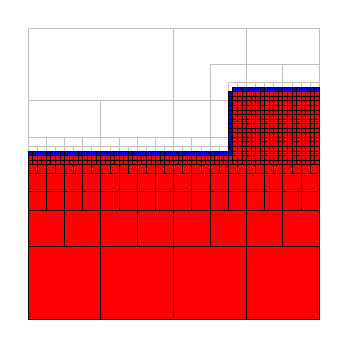
\begin{tikzpicture}[x={(\screenshotunitlength,0)},y={(0,\screenshotunitlength)}]
        \definecolor{fillcolor}{rgb}{1.000000,0.000000,0.000000}
\fill[fillcolor] (0.000000,0.000000) rectangle (0.250000,0.250000);
\definecolor{fillcolor}{rgb}{1.000000,0.000000,0.000000}
\fill[fillcolor] (0.250000,0.000000) rectangle (0.500000,0.250000);
\definecolor{fillcolor}{rgb}{1.000000,0.000000,0.000000}
\fill[fillcolor] (0.000000,0.250000) rectangle (0.125000,0.375000);
\definecolor{fillcolor}{rgb}{1.000000,0.000000,0.000000}
\fill[fillcolor] (0.125000,0.250000) rectangle (0.250000,0.375000);
\definecolor{fillcolor}{rgb}{1.000000,0.000000,0.000000}
\fill[fillcolor] (0.000000,0.375000) rectangle (0.062500,0.437500);
\definecolor{fillcolor}{rgb}{1.000000,0.000000,0.000000}
\fill[fillcolor] (0.062500,0.375000) rectangle (0.125000,0.437500);
\definecolor{fillcolor}{rgb}{1.000000,0.000000,0.000000}
\fill[fillcolor] (0.000000,0.437500) rectangle (0.062500,0.500000);
\definecolor{fillcolor}{rgb}{1.000000,0.000000,0.000000}
\fill[fillcolor] (0.062500,0.437500) rectangle (0.125000,0.500000);
\definecolor{fillcolor}{rgb}{1.000000,0.000000,0.000000}
\fill[fillcolor] (0.125000,0.375000) rectangle (0.187500,0.437500);
\definecolor{fillcolor}{rgb}{1.000000,0.000000,0.000000}
\fill[fillcolor] (0.187500,0.375000) rectangle (0.250000,0.437500);
\definecolor{fillcolor}{rgb}{1.000000,0.000000,0.000000}
\fill[fillcolor] (0.125000,0.437500) rectangle (0.187500,0.500000);
\definecolor{fillcolor}{rgb}{1.000000,0.000000,0.000000}
\fill[fillcolor] (0.187500,0.437500) rectangle (0.250000,0.500000);
\definecolor{fillcolor}{rgb}{1.000000,0.000000,0.000000}
\fill[fillcolor] (0.250000,0.250000) rectangle (0.375000,0.375000);
\definecolor{fillcolor}{rgb}{1.000000,0.000000,0.000000}
\fill[fillcolor] (0.375000,0.250000) rectangle (0.500000,0.375000);
\definecolor{fillcolor}{rgb}{1.000000,0.000000,0.000000}
\fill[fillcolor] (0.250000,0.375000) rectangle (0.312500,0.437500);
\definecolor{fillcolor}{rgb}{1.000000,0.000000,0.000000}
\fill[fillcolor] (0.312500,0.375000) rectangle (0.375000,0.437500);
\definecolor{fillcolor}{rgb}{1.000000,0.000000,0.000000}
\fill[fillcolor] (0.250000,0.437500) rectangle (0.312500,0.500000);
\definecolor{fillcolor}{rgb}{1.000000,0.000000,0.000000}
\fill[fillcolor] (0.312500,0.437500) rectangle (0.375000,0.500000);
\definecolor{fillcolor}{rgb}{1.000000,0.000000,0.000000}
\fill[fillcolor] (0.375000,0.375000) rectangle (0.437500,0.437500);
\definecolor{fillcolor}{rgb}{1.000000,0.000000,0.000000}
\fill[fillcolor] (0.437500,0.375000) rectangle (0.500000,0.437500);
\definecolor{fillcolor}{rgb}{1.000000,0.000000,0.000000}
\fill[fillcolor] (0.375000,0.437500) rectangle (0.437500,0.500000);
\definecolor{fillcolor}{rgb}{1.000000,0.000000,0.000000}
\fill[fillcolor] (0.437500,0.437500) rectangle (0.500000,0.500000);
\definecolor{fillcolor}{rgb}{1.000000,0.000000,0.000000}
\fill[fillcolor] (0.500000,0.000000) rectangle (0.750000,0.250000);
\definecolor{fillcolor}{rgb}{1.000000,0.000000,0.000000}
\fill[fillcolor] (0.750000,0.000000) rectangle (1.000000,0.250000);
\definecolor{fillcolor}{rgb}{1.000000,0.000000,0.000000}
\fill[fillcolor] (0.500000,0.250000) rectangle (0.625000,0.375000);
\definecolor{fillcolor}{rgb}{1.000000,0.000000,0.000000}
\fill[fillcolor] (0.625000,0.250000) rectangle (0.750000,0.375000);
\definecolor{fillcolor}{rgb}{1.000000,0.000000,0.000000}
\fill[fillcolor] (0.500000,0.375000) rectangle (0.562500,0.437500);
\definecolor{fillcolor}{rgb}{1.000000,0.000000,0.000000}
\fill[fillcolor] (0.562500,0.375000) rectangle (0.625000,0.437500);
\definecolor{fillcolor}{rgb}{1.000000,0.000000,0.000000}
\fill[fillcolor] (0.500000,0.437500) rectangle (0.562500,0.500000);
\definecolor{fillcolor}{rgb}{1.000000,0.000000,0.000000}
\fill[fillcolor] (0.562500,0.437500) rectangle (0.625000,0.500000);
\definecolor{fillcolor}{rgb}{1.000000,0.000000,0.000000}
\fill[fillcolor] (0.625000,0.375000) rectangle (0.687500,0.437500);
\definecolor{fillcolor}{rgb}{1.000000,0.000000,0.000000}
\fill[fillcolor] (0.687500,0.375000) rectangle (0.750000,0.437500);
\definecolor{fillcolor}{rgb}{1.000000,0.000000,0.000000}
\fill[fillcolor] (0.625000,0.437500) rectangle (0.687500,0.500000);
\definecolor{fillcolor}{rgb}{1.000000,0.000000,0.000000}
\fill[fillcolor] (0.687500,0.437500) rectangle (0.750000,0.500000);
\definecolor{fillcolor}{rgb}{1.000000,0.000000,0.000000}
\fill[fillcolor] (0.750000,0.250000) rectangle (0.875000,0.375000);
\definecolor{fillcolor}{rgb}{1.000000,0.000000,0.000000}
\fill[fillcolor] (0.875000,0.250000) rectangle (1.000000,0.375000);
\definecolor{fillcolor}{rgb}{1.000000,0.000000,0.000000}
\fill[fillcolor] (0.750000,0.375000) rectangle (0.812500,0.437500);
\definecolor{fillcolor}{rgb}{1.000000,0.000000,0.000000}
\fill[fillcolor] (0.812500,0.375000) rectangle (0.875000,0.437500);
\definecolor{fillcolor}{rgb}{1.000000,0.000000,0.000000}
\fill[fillcolor] (0.750000,0.437500) rectangle (0.812500,0.500000);
\definecolor{fillcolor}{rgb}{1.000000,0.000000,0.000000}
\fill[fillcolor] (0.812500,0.437500) rectangle (0.875000,0.500000);
\definecolor{fillcolor}{rgb}{1.000000,0.000000,0.000000}
\fill[fillcolor] (0.875000,0.375000) rectangle (0.937500,0.437500);
\definecolor{fillcolor}{rgb}{1.000000,0.000000,0.000000}
\fill[fillcolor] (0.937500,0.375000) rectangle (1.000000,0.437500);
\definecolor{fillcolor}{rgb}{1.000000,0.000000,0.000000}
\fill[fillcolor] (0.875000,0.437500) rectangle (0.937500,0.500000);
\definecolor{fillcolor}{rgb}{1.000000,0.000000,0.000000}
\fill[fillcolor] (0.937500,0.437500) rectangle (1.000000,0.500000);
\definecolor{fillcolor}{rgb}{1.000000,0.000000,0.000000}
\fill[fillcolor] (0.000000,0.500000) rectangle (0.031250,0.531250);
\definecolor{fillcolor}{rgb}{1.000000,0.000000,0.000000}
\fill[fillcolor] (0.031250,0.500000) rectangle (0.062500,0.531250);
\definecolor{fillcolor}{rgb}{1.000000,0.000000,0.000000}
\fill[fillcolor] (0.000000,0.531250) rectangle (0.015625,0.546875);
\definecolor{fillcolor}{rgb}{1.000000,0.000000,0.000000}
\fill[fillcolor] (0.015625,0.531250) rectangle (0.031250,0.546875);
\definecolor{fillcolor}{rgb}{1.000000,0.000000,0.000000}
\fill[fillcolor] (0.000000,0.546875) rectangle (0.015625,0.562500);
\definecolor{fillcolor}{rgb}{1.000000,0.000000,0.000000}
\fill[fillcolor] (0.015625,0.546875) rectangle (0.031250,0.562500);
\definecolor{fillcolor}{rgb}{1.000000,0.000000,0.000000}
\fill[fillcolor] (0.031250,0.531250) rectangle (0.046875,0.546875);
\definecolor{fillcolor}{rgb}{1.000000,0.000000,0.000000}
\fill[fillcolor] (0.046875,0.531250) rectangle (0.062500,0.546875);
\definecolor{fillcolor}{rgb}{1.000000,0.000000,0.000000}
\fill[fillcolor] (0.031250,0.546875) rectangle (0.046875,0.562500);
\definecolor{fillcolor}{rgb}{1.000000,0.000000,0.000000}
\fill[fillcolor] (0.046875,0.546875) rectangle (0.062500,0.562500);
\definecolor{fillcolor}{rgb}{1.000000,0.000000,0.000000}
\fill[fillcolor] (0.062500,0.500000) rectangle (0.093750,0.531250);
\definecolor{fillcolor}{rgb}{1.000000,0.000000,0.000000}
\fill[fillcolor] (0.093750,0.500000) rectangle (0.125000,0.531250);
\definecolor{fillcolor}{rgb}{1.000000,0.000000,0.000000}
\fill[fillcolor] (0.062500,0.531250) rectangle (0.078125,0.546875);
\definecolor{fillcolor}{rgb}{1.000000,0.000000,0.000000}
\fill[fillcolor] (0.078125,0.531250) rectangle (0.093750,0.546875);
\definecolor{fillcolor}{rgb}{1.000000,0.000000,0.000000}
\fill[fillcolor] (0.062500,0.546875) rectangle (0.078125,0.562500);
\definecolor{fillcolor}{rgb}{1.000000,0.000000,0.000000}
\fill[fillcolor] (0.078125,0.546875) rectangle (0.093750,0.562500);
\definecolor{fillcolor}{rgb}{1.000000,0.000000,0.000000}
\fill[fillcolor] (0.093750,0.531250) rectangle (0.109375,0.546875);
\definecolor{fillcolor}{rgb}{1.000000,0.000000,0.000000}
\fill[fillcolor] (0.109375,0.531250) rectangle (0.125000,0.546875);
\definecolor{fillcolor}{rgb}{1.000000,0.000000,0.000000}
\fill[fillcolor] (0.093750,0.546875) rectangle (0.109375,0.562500);
\definecolor{fillcolor}{rgb}{1.000000,0.000000,0.000000}
\fill[fillcolor] (0.109375,0.546875) rectangle (0.125000,0.562500);
\definecolor{fillcolor}{rgb}{0.000000,0.000000,1.000000}
\fill[fillcolor] (0.000000,0.562500) rectangle (0.015625,0.578125);
\definecolor{fillcolor}{rgb}{0.000000,0.000000,1.000000}
\fill[fillcolor] (0.015625,0.562500) rectangle (0.031250,0.578125);
\definecolor{fillcolor}{rgb}{0.000000,0.000000,1.000000}
\fill[fillcolor] (0.031250,0.562500) rectangle (0.046875,0.578125);
\definecolor{fillcolor}{rgb}{0.000000,0.000000,1.000000}
\fill[fillcolor] (0.046875,0.562500) rectangle (0.062500,0.578125);
\definecolor{fillcolor}{rgb}{0.000000,0.000000,1.000000}
\fill[fillcolor] (0.062500,0.562500) rectangle (0.078125,0.578125);
\definecolor{fillcolor}{rgb}{0.000000,0.000000,1.000000}
\fill[fillcolor] (0.078125,0.562500) rectangle (0.093750,0.578125);
\definecolor{fillcolor}{rgb}{0.000000,0.000000,1.000000}
\fill[fillcolor] (0.093750,0.562500) rectangle (0.109375,0.578125);
\definecolor{fillcolor}{rgb}{0.000000,0.000000,1.000000}
\fill[fillcolor] (0.109375,0.562500) rectangle (0.125000,0.578125);
\definecolor{fillcolor}{rgb}{1.000000,0.000000,0.000000}
\fill[fillcolor] (0.125000,0.500000) rectangle (0.156250,0.531250);
\definecolor{fillcolor}{rgb}{1.000000,0.000000,0.000000}
\fill[fillcolor] (0.156250,0.500000) rectangle (0.187500,0.531250);
\definecolor{fillcolor}{rgb}{1.000000,0.000000,0.000000}
\fill[fillcolor] (0.125000,0.531250) rectangle (0.140625,0.546875);
\definecolor{fillcolor}{rgb}{1.000000,0.000000,0.000000}
\fill[fillcolor] (0.140625,0.531250) rectangle (0.156250,0.546875);
\definecolor{fillcolor}{rgb}{1.000000,0.000000,0.000000}
\fill[fillcolor] (0.125000,0.546875) rectangle (0.140625,0.562500);
\definecolor{fillcolor}{rgb}{1.000000,0.000000,0.000000}
\fill[fillcolor] (0.140625,0.546875) rectangle (0.156250,0.562500);
\definecolor{fillcolor}{rgb}{1.000000,0.000000,0.000000}
\fill[fillcolor] (0.156250,0.531250) rectangle (0.171875,0.546875);
\definecolor{fillcolor}{rgb}{1.000000,0.000000,0.000000}
\fill[fillcolor] (0.171875,0.531250) rectangle (0.187500,0.546875);
\definecolor{fillcolor}{rgb}{1.000000,0.000000,0.000000}
\fill[fillcolor] (0.156250,0.546875) rectangle (0.171875,0.562500);
\definecolor{fillcolor}{rgb}{1.000000,0.000000,0.000000}
\fill[fillcolor] (0.171875,0.546875) rectangle (0.187500,0.562500);
\definecolor{fillcolor}{rgb}{1.000000,0.000000,0.000000}
\fill[fillcolor] (0.187500,0.500000) rectangle (0.218750,0.531250);
\definecolor{fillcolor}{rgb}{1.000000,0.000000,0.000000}
\fill[fillcolor] (0.218750,0.500000) rectangle (0.250000,0.531250);
\definecolor{fillcolor}{rgb}{1.000000,0.000000,0.000000}
\fill[fillcolor] (0.187500,0.531250) rectangle (0.203125,0.546875);
\definecolor{fillcolor}{rgb}{1.000000,0.000000,0.000000}
\fill[fillcolor] (0.203125,0.531250) rectangle (0.218750,0.546875);
\definecolor{fillcolor}{rgb}{1.000000,0.000000,0.000000}
\fill[fillcolor] (0.187500,0.546875) rectangle (0.203125,0.562500);
\definecolor{fillcolor}{rgb}{1.000000,0.000000,0.000000}
\fill[fillcolor] (0.203125,0.546875) rectangle (0.218750,0.562500);
\definecolor{fillcolor}{rgb}{1.000000,0.000000,0.000000}
\fill[fillcolor] (0.218750,0.531250) rectangle (0.234375,0.546875);
\definecolor{fillcolor}{rgb}{1.000000,0.000000,0.000000}
\fill[fillcolor] (0.234375,0.531250) rectangle (0.250000,0.546875);
\definecolor{fillcolor}{rgb}{1.000000,0.000000,0.000000}
\fill[fillcolor] (0.218750,0.546875) rectangle (0.234375,0.562500);
\definecolor{fillcolor}{rgb}{1.000000,0.000000,0.000000}
\fill[fillcolor] (0.234375,0.546875) rectangle (0.250000,0.562500);
\definecolor{fillcolor}{rgb}{0.000000,0.000000,1.000000}
\fill[fillcolor] (0.125000,0.562500) rectangle (0.140625,0.578125);
\definecolor{fillcolor}{rgb}{0.000000,0.000000,1.000000}
\fill[fillcolor] (0.140625,0.562500) rectangle (0.156250,0.578125);
\definecolor{fillcolor}{rgb}{0.000000,0.000000,1.000000}
\fill[fillcolor] (0.156250,0.562500) rectangle (0.171875,0.578125);
\definecolor{fillcolor}{rgb}{0.000000,0.000000,1.000000}
\fill[fillcolor] (0.171875,0.562500) rectangle (0.187500,0.578125);
\definecolor{fillcolor}{rgb}{0.000000,0.000000,1.000000}
\fill[fillcolor] (0.187500,0.562500) rectangle (0.203125,0.578125);
\definecolor{fillcolor}{rgb}{0.000000,0.000000,1.000000}
\fill[fillcolor] (0.203125,0.562500) rectangle (0.218750,0.578125);
\definecolor{fillcolor}{rgb}{0.000000,0.000000,1.000000}
\fill[fillcolor] (0.218750,0.562500) rectangle (0.234375,0.578125);
\definecolor{fillcolor}{rgb}{0.000000,0.000000,1.000000}
\fill[fillcolor] (0.234375,0.562500) rectangle (0.250000,0.578125);
\definecolor{fillcolor}{rgb}{1.000000,0.000000,0.000000}
\fill[fillcolor] (0.250000,0.500000) rectangle (0.281250,0.531250);
\definecolor{fillcolor}{rgb}{1.000000,0.000000,0.000000}
\fill[fillcolor] (0.281250,0.500000) rectangle (0.312500,0.531250);
\definecolor{fillcolor}{rgb}{1.000000,0.000000,0.000000}
\fill[fillcolor] (0.250000,0.531250) rectangle (0.265625,0.546875);
\definecolor{fillcolor}{rgb}{1.000000,0.000000,0.000000}
\fill[fillcolor] (0.265625,0.531250) rectangle (0.281250,0.546875);
\definecolor{fillcolor}{rgb}{1.000000,0.000000,0.000000}
\fill[fillcolor] (0.250000,0.546875) rectangle (0.265625,0.562500);
\definecolor{fillcolor}{rgb}{1.000000,0.000000,0.000000}
\fill[fillcolor] (0.265625,0.546875) rectangle (0.281250,0.562500);
\definecolor{fillcolor}{rgb}{1.000000,0.000000,0.000000}
\fill[fillcolor] (0.281250,0.531250) rectangle (0.296875,0.546875);
\definecolor{fillcolor}{rgb}{1.000000,0.000000,0.000000}
\fill[fillcolor] (0.296875,0.531250) rectangle (0.312500,0.546875);
\definecolor{fillcolor}{rgb}{1.000000,0.000000,0.000000}
\fill[fillcolor] (0.281250,0.546875) rectangle (0.296875,0.562500);
\definecolor{fillcolor}{rgb}{1.000000,0.000000,0.000000}
\fill[fillcolor] (0.296875,0.546875) rectangle (0.312500,0.562500);
\definecolor{fillcolor}{rgb}{1.000000,0.000000,0.000000}
\fill[fillcolor] (0.312500,0.500000) rectangle (0.343750,0.531250);
\definecolor{fillcolor}{rgb}{1.000000,0.000000,0.000000}
\fill[fillcolor] (0.343750,0.500000) rectangle (0.375000,0.531250);
\definecolor{fillcolor}{rgb}{1.000000,0.000000,0.000000}
\fill[fillcolor] (0.312500,0.531250) rectangle (0.328125,0.546875);
\definecolor{fillcolor}{rgb}{1.000000,0.000000,0.000000}
\fill[fillcolor] (0.328125,0.531250) rectangle (0.343750,0.546875);
\definecolor{fillcolor}{rgb}{1.000000,0.000000,0.000000}
\fill[fillcolor] (0.312500,0.546875) rectangle (0.328125,0.562500);
\definecolor{fillcolor}{rgb}{1.000000,0.000000,0.000000}
\fill[fillcolor] (0.328125,0.546875) rectangle (0.343750,0.562500);
\definecolor{fillcolor}{rgb}{1.000000,0.000000,0.000000}
\fill[fillcolor] (0.343750,0.531250) rectangle (0.359375,0.546875);
\definecolor{fillcolor}{rgb}{1.000000,0.000000,0.000000}
\fill[fillcolor] (0.359375,0.531250) rectangle (0.375000,0.546875);
\definecolor{fillcolor}{rgb}{1.000000,0.000000,0.000000}
\fill[fillcolor] (0.343750,0.546875) rectangle (0.359375,0.562500);
\definecolor{fillcolor}{rgb}{1.000000,0.000000,0.000000}
\fill[fillcolor] (0.359375,0.546875) rectangle (0.375000,0.562500);
\definecolor{fillcolor}{rgb}{0.000000,0.000000,1.000000}
\fill[fillcolor] (0.250000,0.562500) rectangle (0.265625,0.578125);
\definecolor{fillcolor}{rgb}{0.000000,0.000000,1.000000}
\fill[fillcolor] (0.265625,0.562500) rectangle (0.281250,0.578125);
\definecolor{fillcolor}{rgb}{0.000000,0.000000,1.000000}
\fill[fillcolor] (0.281250,0.562500) rectangle (0.296875,0.578125);
\definecolor{fillcolor}{rgb}{0.000000,0.000000,1.000000}
\fill[fillcolor] (0.296875,0.562500) rectangle (0.312500,0.578125);
\definecolor{fillcolor}{rgb}{0.000000,0.000000,1.000000}
\fill[fillcolor] (0.312500,0.562500) rectangle (0.328125,0.578125);
\definecolor{fillcolor}{rgb}{0.000000,0.000000,1.000000}
\fill[fillcolor] (0.328125,0.562500) rectangle (0.343750,0.578125);
\definecolor{fillcolor}{rgb}{0.000000,0.000000,1.000000}
\fill[fillcolor] (0.343750,0.562500) rectangle (0.359375,0.578125);
\definecolor{fillcolor}{rgb}{0.000000,0.000000,1.000000}
\fill[fillcolor] (0.359375,0.562500) rectangle (0.375000,0.578125);
\definecolor{fillcolor}{rgb}{1.000000,0.000000,0.000000}
\fill[fillcolor] (0.375000,0.500000) rectangle (0.406250,0.531250);
\definecolor{fillcolor}{rgb}{1.000000,0.000000,0.000000}
\fill[fillcolor] (0.406250,0.500000) rectangle (0.437500,0.531250);
\definecolor{fillcolor}{rgb}{1.000000,0.000000,0.000000}
\fill[fillcolor] (0.375000,0.531250) rectangle (0.390625,0.546875);
\definecolor{fillcolor}{rgb}{1.000000,0.000000,0.000000}
\fill[fillcolor] (0.390625,0.531250) rectangle (0.406250,0.546875);
\definecolor{fillcolor}{rgb}{1.000000,0.000000,0.000000}
\fill[fillcolor] (0.375000,0.546875) rectangle (0.390625,0.562500);
\definecolor{fillcolor}{rgb}{1.000000,0.000000,0.000000}
\fill[fillcolor] (0.390625,0.546875) rectangle (0.406250,0.562500);
\definecolor{fillcolor}{rgb}{1.000000,0.000000,0.000000}
\fill[fillcolor] (0.406250,0.531250) rectangle (0.421875,0.546875);
\definecolor{fillcolor}{rgb}{1.000000,0.000000,0.000000}
\fill[fillcolor] (0.421875,0.531250) rectangle (0.437500,0.546875);
\definecolor{fillcolor}{rgb}{1.000000,0.000000,0.000000}
\fill[fillcolor] (0.406250,0.546875) rectangle (0.421875,0.562500);
\definecolor{fillcolor}{rgb}{1.000000,0.000000,0.000000}
\fill[fillcolor] (0.421875,0.546875) rectangle (0.437500,0.562500);
\definecolor{fillcolor}{rgb}{1.000000,0.000000,0.000000}
\fill[fillcolor] (0.437500,0.500000) rectangle (0.468750,0.531250);
\definecolor{fillcolor}{rgb}{1.000000,0.000000,0.000000}
\fill[fillcolor] (0.468750,0.500000) rectangle (0.500000,0.531250);
\definecolor{fillcolor}{rgb}{1.000000,0.000000,0.000000}
\fill[fillcolor] (0.437500,0.531250) rectangle (0.453125,0.546875);
\definecolor{fillcolor}{rgb}{1.000000,0.000000,0.000000}
\fill[fillcolor] (0.453125,0.531250) rectangle (0.468750,0.546875);
\definecolor{fillcolor}{rgb}{1.000000,0.000000,0.000000}
\fill[fillcolor] (0.437500,0.546875) rectangle (0.453125,0.562500);
\definecolor{fillcolor}{rgb}{1.000000,0.000000,0.000000}
\fill[fillcolor] (0.453125,0.546875) rectangle (0.468750,0.562500);
\definecolor{fillcolor}{rgb}{1.000000,0.000000,0.000000}
\fill[fillcolor] (0.468750,0.531250) rectangle (0.484375,0.546875);
\definecolor{fillcolor}{rgb}{1.000000,0.000000,0.000000}
\fill[fillcolor] (0.484375,0.531250) rectangle (0.500000,0.546875);
\definecolor{fillcolor}{rgb}{1.000000,0.000000,0.000000}
\fill[fillcolor] (0.468750,0.546875) rectangle (0.484375,0.562500);
\definecolor{fillcolor}{rgb}{1.000000,0.000000,0.000000}
\fill[fillcolor] (0.484375,0.546875) rectangle (0.500000,0.562500);
\definecolor{fillcolor}{rgb}{0.000000,0.000000,1.000000}
\fill[fillcolor] (0.375000,0.562500) rectangle (0.390625,0.578125);
\definecolor{fillcolor}{rgb}{0.000000,0.000000,1.000000}
\fill[fillcolor] (0.390625,0.562500) rectangle (0.406250,0.578125);
\definecolor{fillcolor}{rgb}{0.000000,0.000000,1.000000}
\fill[fillcolor] (0.406250,0.562500) rectangle (0.421875,0.578125);
\definecolor{fillcolor}{rgb}{0.000000,0.000000,1.000000}
\fill[fillcolor] (0.421875,0.562500) rectangle (0.437500,0.578125);
\definecolor{fillcolor}{rgb}{0.000000,0.000000,1.000000}
\fill[fillcolor] (0.437500,0.562500) rectangle (0.453125,0.578125);
\definecolor{fillcolor}{rgb}{0.000000,0.000000,1.000000}
\fill[fillcolor] (0.453125,0.562500) rectangle (0.468750,0.578125);
\definecolor{fillcolor}{rgb}{0.000000,0.000000,1.000000}
\fill[fillcolor] (0.468750,0.562500) rectangle (0.484375,0.578125);
\definecolor{fillcolor}{rgb}{0.000000,0.000000,1.000000}
\fill[fillcolor] (0.484375,0.562500) rectangle (0.500000,0.578125);
\definecolor{fillcolor}{rgb}{1.000000,0.000000,0.000000}
\fill[fillcolor] (0.500000,0.500000) rectangle (0.531250,0.531250);
\definecolor{fillcolor}{rgb}{1.000000,0.000000,0.000000}
\fill[fillcolor] (0.531250,0.500000) rectangle (0.562500,0.531250);
\definecolor{fillcolor}{rgb}{1.000000,0.000000,0.000000}
\fill[fillcolor] (0.500000,0.531250) rectangle (0.515625,0.546875);
\definecolor{fillcolor}{rgb}{1.000000,0.000000,0.000000}
\fill[fillcolor] (0.515625,0.531250) rectangle (0.531250,0.546875);
\definecolor{fillcolor}{rgb}{1.000000,0.000000,0.000000}
\fill[fillcolor] (0.500000,0.546875) rectangle (0.515625,0.562500);
\definecolor{fillcolor}{rgb}{1.000000,0.000000,0.000000}
\fill[fillcolor] (0.515625,0.546875) rectangle (0.531250,0.562500);
\definecolor{fillcolor}{rgb}{1.000000,0.000000,0.000000}
\fill[fillcolor] (0.531250,0.531250) rectangle (0.546875,0.546875);
\definecolor{fillcolor}{rgb}{1.000000,0.000000,0.000000}
\fill[fillcolor] (0.546875,0.531250) rectangle (0.562500,0.546875);
\definecolor{fillcolor}{rgb}{1.000000,0.000000,0.000000}
\fill[fillcolor] (0.531250,0.546875) rectangle (0.546875,0.562500);
\definecolor{fillcolor}{rgb}{1.000000,0.000000,0.000000}
\fill[fillcolor] (0.546875,0.546875) rectangle (0.562500,0.562500);
\definecolor{fillcolor}{rgb}{1.000000,0.000000,0.000000}
\fill[fillcolor] (0.562500,0.500000) rectangle (0.593750,0.531250);
\definecolor{fillcolor}{rgb}{1.000000,0.000000,0.000000}
\fill[fillcolor] (0.593750,0.500000) rectangle (0.625000,0.531250);
\definecolor{fillcolor}{rgb}{1.000000,0.000000,0.000000}
\fill[fillcolor] (0.562500,0.531250) rectangle (0.578125,0.546875);
\definecolor{fillcolor}{rgb}{1.000000,0.000000,0.000000}
\fill[fillcolor] (0.578125,0.531250) rectangle (0.593750,0.546875);
\definecolor{fillcolor}{rgb}{1.000000,0.000000,0.000000}
\fill[fillcolor] (0.562500,0.546875) rectangle (0.578125,0.562500);
\definecolor{fillcolor}{rgb}{1.000000,0.000000,0.000000}
\fill[fillcolor] (0.578125,0.546875) rectangle (0.593750,0.562500);
\definecolor{fillcolor}{rgb}{1.000000,0.000000,0.000000}
\fill[fillcolor] (0.593750,0.531250) rectangle (0.609375,0.546875);
\definecolor{fillcolor}{rgb}{1.000000,0.000000,0.000000}
\fill[fillcolor] (0.609375,0.531250) rectangle (0.625000,0.546875);
\definecolor{fillcolor}{rgb}{1.000000,0.000000,0.000000}
\fill[fillcolor] (0.593750,0.546875) rectangle (0.609375,0.562500);
\definecolor{fillcolor}{rgb}{1.000000,0.000000,0.000000}
\fill[fillcolor] (0.609375,0.546875) rectangle (0.625000,0.562500);
\definecolor{fillcolor}{rgb}{0.000000,0.000000,1.000000}
\fill[fillcolor] (0.500000,0.562500) rectangle (0.515625,0.578125);
\definecolor{fillcolor}{rgb}{0.000000,0.000000,1.000000}
\fill[fillcolor] (0.515625,0.562500) rectangle (0.531250,0.578125);
\definecolor{fillcolor}{rgb}{0.000000,0.000000,1.000000}
\fill[fillcolor] (0.531250,0.562500) rectangle (0.546875,0.578125);
\definecolor{fillcolor}{rgb}{0.000000,0.000000,1.000000}
\fill[fillcolor] (0.546875,0.562500) rectangle (0.562500,0.578125);
\definecolor{fillcolor}{rgb}{0.000000,0.000000,1.000000}
\fill[fillcolor] (0.562500,0.562500) rectangle (0.578125,0.578125);
\definecolor{fillcolor}{rgb}{0.000000,0.000000,1.000000}
\fill[fillcolor] (0.578125,0.562500) rectangle (0.593750,0.578125);
\definecolor{fillcolor}{rgb}{0.000000,0.000000,1.000000}
\fill[fillcolor] (0.593750,0.562500) rectangle (0.609375,0.578125);
\definecolor{fillcolor}{rgb}{0.000000,0.000000,1.000000}
\fill[fillcolor] (0.609375,0.562500) rectangle (0.625000,0.578125);
\definecolor{fillcolor}{rgb}{1.000000,0.000000,0.000000}
\fill[fillcolor] (0.625000,0.500000) rectangle (0.656250,0.531250);
\definecolor{fillcolor}{rgb}{1.000000,0.000000,0.000000}
\fill[fillcolor] (0.656250,0.500000) rectangle (0.687500,0.531250);
\definecolor{fillcolor}{rgb}{1.000000,0.000000,0.000000}
\fill[fillcolor] (0.625000,0.531250) rectangle (0.640625,0.546875);
\definecolor{fillcolor}{rgb}{1.000000,0.000000,0.000000}
\fill[fillcolor] (0.640625,0.531250) rectangle (0.656250,0.546875);
\definecolor{fillcolor}{rgb}{1.000000,0.000000,0.000000}
\fill[fillcolor] (0.625000,0.546875) rectangle (0.640625,0.562500);
\definecolor{fillcolor}{rgb}{1.000000,0.000000,0.000000}
\fill[fillcolor] (0.640625,0.546875) rectangle (0.656250,0.562500);
\definecolor{fillcolor}{rgb}{1.000000,0.000000,0.000000}
\fill[fillcolor] (0.656250,0.531250) rectangle (0.671875,0.546875);
\definecolor{fillcolor}{rgb}{1.000000,0.000000,0.000000}
\fill[fillcolor] (0.671875,0.531250) rectangle (0.687500,0.546875);
\definecolor{fillcolor}{rgb}{1.000000,0.000000,0.000000}
\fill[fillcolor] (0.656250,0.546875) rectangle (0.671875,0.562500);
\definecolor{fillcolor}{rgb}{1.000000,0.000000,0.000000}
\fill[fillcolor] (0.671875,0.546875) rectangle (0.687500,0.562500);
\definecolor{fillcolor}{rgb}{1.000000,0.000000,0.000000}
\fill[fillcolor] (0.687500,0.500000) rectangle (0.718750,0.531250);
\definecolor{fillcolor}{rgb}{1.000000,0.000000,0.000000}
\fill[fillcolor] (0.718750,0.500000) rectangle (0.750000,0.531250);
\definecolor{fillcolor}{rgb}{1.000000,0.000000,0.000000}
\fill[fillcolor] (0.687500,0.531250) rectangle (0.703125,0.546875);
\definecolor{fillcolor}{rgb}{1.000000,0.000000,0.000000}
\fill[fillcolor] (0.703125,0.531250) rectangle (0.718750,0.546875);
\definecolor{fillcolor}{rgb}{1.000000,0.000000,0.000000}
\fill[fillcolor] (0.687500,0.546875) rectangle (0.703125,0.562500);
\definecolor{fillcolor}{rgb}{1.000000,0.000000,0.000000}
\fill[fillcolor] (0.703125,0.546875) rectangle (0.718750,0.562500);
\definecolor{fillcolor}{rgb}{1.000000,0.000000,0.000000}
\fill[fillcolor] (0.718750,0.531250) rectangle (0.734375,0.546875);
\definecolor{fillcolor}{rgb}{1.000000,0.000000,0.000000}
\fill[fillcolor] (0.734375,0.531250) rectangle (0.750000,0.546875);
\definecolor{fillcolor}{rgb}{1.000000,0.000000,0.000000}
\fill[fillcolor] (0.718750,0.546875) rectangle (0.734375,0.562500);
\definecolor{fillcolor}{rgb}{1.000000,0.000000,0.000000}
\fill[fillcolor] (0.734375,0.546875) rectangle (0.750000,0.562500);
\definecolor{fillcolor}{rgb}{0.000000,0.000000,1.000000}
\fill[fillcolor] (0.625000,0.562500) rectangle (0.640625,0.578125);
\definecolor{fillcolor}{rgb}{0.000000,0.000000,1.000000}
\fill[fillcolor] (0.640625,0.562500) rectangle (0.656250,0.578125);
\definecolor{fillcolor}{rgb}{0.000000,0.000000,1.000000}
\fill[fillcolor] (0.656250,0.562500) rectangle (0.671875,0.578125);
\definecolor{fillcolor}{rgb}{0.000000,0.000000,1.000000}
\fill[fillcolor] (0.671875,0.562500) rectangle (0.687500,0.578125);
\definecolor{fillcolor}{rgb}{0.000000,0.000000,1.000000}
\fill[fillcolor] (0.687500,0.562500) rectangle (0.703125,0.578125);
\definecolor{fillcolor}{rgb}{1.000000,0.000000,0.000000}
\fill[fillcolor] (0.703125,0.562500) rectangle (0.718750,0.578125);
\definecolor{fillcolor}{rgb}{0.000000,0.000000,1.000000}
\fill[fillcolor] (0.687500,0.578125) rectangle (0.703125,0.593750);
\definecolor{fillcolor}{rgb}{1.000000,0.000000,0.000000}
\fill[fillcolor] (0.703125,0.578125) rectangle (0.718750,0.593750);
\definecolor{fillcolor}{rgb}{1.000000,0.000000,0.000000}
\fill[fillcolor] (0.718750,0.562500) rectangle (0.734375,0.578125);
\definecolor{fillcolor}{rgb}{1.000000,0.000000,0.000000}
\fill[fillcolor] (0.734375,0.562500) rectangle (0.750000,0.578125);
\definecolor{fillcolor}{rgb}{1.000000,0.000000,0.000000}
\fill[fillcolor] (0.718750,0.578125) rectangle (0.734375,0.593750);
\definecolor{fillcolor}{rgb}{1.000000,0.000000,0.000000}
\fill[fillcolor] (0.734375,0.578125) rectangle (0.750000,0.593750);
\definecolor{fillcolor}{rgb}{0.000000,0.000000,1.000000}
\fill[fillcolor] (0.687500,0.593750) rectangle (0.703125,0.609375);
\definecolor{fillcolor}{rgb}{1.000000,0.000000,0.000000}
\fill[fillcolor] (0.703125,0.593750) rectangle (0.718750,0.609375);
\definecolor{fillcolor}{rgb}{0.000000,0.000000,1.000000}
\fill[fillcolor] (0.687500,0.609375) rectangle (0.703125,0.625000);
\definecolor{fillcolor}{rgb}{1.000000,0.000000,0.000000}
\fill[fillcolor] (0.703125,0.609375) rectangle (0.718750,0.625000);
\definecolor{fillcolor}{rgb}{1.000000,0.000000,0.000000}
\fill[fillcolor] (0.718750,0.593750) rectangle (0.734375,0.609375);
\definecolor{fillcolor}{rgb}{1.000000,0.000000,0.000000}
\fill[fillcolor] (0.734375,0.593750) rectangle (0.750000,0.609375);
\definecolor{fillcolor}{rgb}{1.000000,0.000000,0.000000}
\fill[fillcolor] (0.718750,0.609375) rectangle (0.734375,0.625000);
\definecolor{fillcolor}{rgb}{1.000000,0.000000,0.000000}
\fill[fillcolor] (0.734375,0.609375) rectangle (0.750000,0.625000);
\definecolor{fillcolor}{rgb}{0.000000,0.000000,1.000000}
\fill[fillcolor] (0.687500,0.625000) rectangle (0.703125,0.640625);
\definecolor{fillcolor}{rgb}{1.000000,0.000000,0.000000}
\fill[fillcolor] (0.703125,0.625000) rectangle (0.718750,0.640625);
\definecolor{fillcolor}{rgb}{0.000000,0.000000,1.000000}
\fill[fillcolor] (0.687500,0.640625) rectangle (0.703125,0.656250);
\definecolor{fillcolor}{rgb}{1.000000,0.000000,0.000000}
\fill[fillcolor] (0.703125,0.640625) rectangle (0.718750,0.656250);
\definecolor{fillcolor}{rgb}{1.000000,0.000000,0.000000}
\fill[fillcolor] (0.718750,0.625000) rectangle (0.734375,0.640625);
\definecolor{fillcolor}{rgb}{1.000000,0.000000,0.000000}
\fill[fillcolor] (0.734375,0.625000) rectangle (0.750000,0.640625);
\definecolor{fillcolor}{rgb}{1.000000,0.000000,0.000000}
\fill[fillcolor] (0.718750,0.640625) rectangle (0.734375,0.656250);
\definecolor{fillcolor}{rgb}{1.000000,0.000000,0.000000}
\fill[fillcolor] (0.734375,0.640625) rectangle (0.750000,0.656250);
\definecolor{fillcolor}{rgb}{0.000000,0.000000,1.000000}
\fill[fillcolor] (0.687500,0.656250) rectangle (0.703125,0.671875);
\definecolor{fillcolor}{rgb}{1.000000,0.000000,0.000000}
\fill[fillcolor] (0.703125,0.656250) rectangle (0.718750,0.671875);
\definecolor{fillcolor}{rgb}{0.000000,0.000000,1.000000}
\fill[fillcolor] (0.687500,0.671875) rectangle (0.703125,0.687500);
\definecolor{fillcolor}{rgb}{1.000000,0.000000,0.000000}
\fill[fillcolor] (0.703125,0.671875) rectangle (0.718750,0.687500);
\definecolor{fillcolor}{rgb}{1.000000,0.000000,0.000000}
\fill[fillcolor] (0.718750,0.656250) rectangle (0.734375,0.671875);
\definecolor{fillcolor}{rgb}{1.000000,0.000000,0.000000}
\fill[fillcolor] (0.734375,0.656250) rectangle (0.750000,0.671875);
\definecolor{fillcolor}{rgb}{1.000000,0.000000,0.000000}
\fill[fillcolor] (0.718750,0.671875) rectangle (0.734375,0.687500);
\definecolor{fillcolor}{rgb}{1.000000,0.000000,0.000000}
\fill[fillcolor] (0.734375,0.671875) rectangle (0.750000,0.687500);
\definecolor{fillcolor}{rgb}{0.000000,0.000000,1.000000}
\fill[fillcolor] (0.687500,0.687500) rectangle (0.703125,0.703125);
\definecolor{fillcolor}{rgb}{1.000000,0.000000,0.000000}
\fill[fillcolor] (0.703125,0.687500) rectangle (0.718750,0.703125);
\definecolor{fillcolor}{rgb}{0.000000,0.000000,1.000000}
\fill[fillcolor] (0.687500,0.703125) rectangle (0.703125,0.718750);
\definecolor{fillcolor}{rgb}{1.000000,0.000000,0.000000}
\fill[fillcolor] (0.703125,0.703125) rectangle (0.718750,0.718750);
\definecolor{fillcolor}{rgb}{1.000000,0.000000,0.000000}
\fill[fillcolor] (0.718750,0.687500) rectangle (0.734375,0.703125);
\definecolor{fillcolor}{rgb}{1.000000,0.000000,0.000000}
\fill[fillcolor] (0.734375,0.687500) rectangle (0.750000,0.703125);
\definecolor{fillcolor}{rgb}{1.000000,0.000000,0.000000}
\fill[fillcolor] (0.718750,0.703125) rectangle (0.734375,0.718750);
\definecolor{fillcolor}{rgb}{1.000000,0.000000,0.000000}
\fill[fillcolor] (0.734375,0.703125) rectangle (0.750000,0.718750);
\definecolor{fillcolor}{rgb}{0.000000,0.000000,1.000000}
\fill[fillcolor] (0.687500,0.718750) rectangle (0.703125,0.734375);
\definecolor{fillcolor}{rgb}{1.000000,0.000000,0.000000}
\fill[fillcolor] (0.703125,0.718750) rectangle (0.718750,0.734375);
\definecolor{fillcolor}{rgb}{0.000000,0.000000,1.000000}
\fill[fillcolor] (0.687500,0.734375) rectangle (0.703125,0.750000);
\definecolor{fillcolor}{rgb}{1.000000,0.000000,0.000000}
\fill[fillcolor] (0.703125,0.734375) rectangle (0.718750,0.750000);
\definecolor{fillcolor}{rgb}{1.000000,0.000000,0.000000}
\fill[fillcolor] (0.718750,0.718750) rectangle (0.734375,0.734375);
\definecolor{fillcolor}{rgb}{1.000000,0.000000,0.000000}
\fill[fillcolor] (0.734375,0.718750) rectangle (0.750000,0.734375);
\definecolor{fillcolor}{rgb}{1.000000,0.000000,0.000000}
\fill[fillcolor] (0.718750,0.734375) rectangle (0.734375,0.750000);
\definecolor{fillcolor}{rgb}{1.000000,0.000000,0.000000}
\fill[fillcolor] (0.734375,0.734375) rectangle (0.750000,0.750000);
\definecolor{fillcolor}{rgb}{1.000000,0.000000,0.000000}
\fill[fillcolor] (0.750000,0.500000) rectangle (0.781250,0.531250);
\definecolor{fillcolor}{rgb}{1.000000,0.000000,0.000000}
\fill[fillcolor] (0.781250,0.500000) rectangle (0.812500,0.531250);
\definecolor{fillcolor}{rgb}{1.000000,0.000000,0.000000}
\fill[fillcolor] (0.750000,0.531250) rectangle (0.765625,0.546875);
\definecolor{fillcolor}{rgb}{1.000000,0.000000,0.000000}
\fill[fillcolor] (0.765625,0.531250) rectangle (0.781250,0.546875);
\definecolor{fillcolor}{rgb}{1.000000,0.000000,0.000000}
\fill[fillcolor] (0.750000,0.546875) rectangle (0.765625,0.562500);
\definecolor{fillcolor}{rgb}{1.000000,0.000000,0.000000}
\fill[fillcolor] (0.765625,0.546875) rectangle (0.781250,0.562500);
\definecolor{fillcolor}{rgb}{1.000000,0.000000,0.000000}
\fill[fillcolor] (0.781250,0.531250) rectangle (0.796875,0.546875);
\definecolor{fillcolor}{rgb}{1.000000,0.000000,0.000000}
\fill[fillcolor] (0.796875,0.531250) rectangle (0.812500,0.546875);
\definecolor{fillcolor}{rgb}{1.000000,0.000000,0.000000}
\fill[fillcolor] (0.781250,0.546875) rectangle (0.796875,0.562500);
\definecolor{fillcolor}{rgb}{1.000000,0.000000,0.000000}
\fill[fillcolor] (0.796875,0.546875) rectangle (0.812500,0.562500);
\definecolor{fillcolor}{rgb}{1.000000,0.000000,0.000000}
\fill[fillcolor] (0.812500,0.500000) rectangle (0.843750,0.531250);
\definecolor{fillcolor}{rgb}{1.000000,0.000000,0.000000}
\fill[fillcolor] (0.843750,0.500000) rectangle (0.875000,0.531250);
\definecolor{fillcolor}{rgb}{1.000000,0.000000,0.000000}
\fill[fillcolor] (0.812500,0.531250) rectangle (0.828125,0.546875);
\definecolor{fillcolor}{rgb}{1.000000,0.000000,0.000000}
\fill[fillcolor] (0.828125,0.531250) rectangle (0.843750,0.546875);
\definecolor{fillcolor}{rgb}{1.000000,0.000000,0.000000}
\fill[fillcolor] (0.812500,0.546875) rectangle (0.828125,0.562500);
\definecolor{fillcolor}{rgb}{1.000000,0.000000,0.000000}
\fill[fillcolor] (0.828125,0.546875) rectangle (0.843750,0.562500);
\definecolor{fillcolor}{rgb}{1.000000,0.000000,0.000000}
\fill[fillcolor] (0.843750,0.531250) rectangle (0.859375,0.546875);
\definecolor{fillcolor}{rgb}{1.000000,0.000000,0.000000}
\fill[fillcolor] (0.859375,0.531250) rectangle (0.875000,0.546875);
\definecolor{fillcolor}{rgb}{1.000000,0.000000,0.000000}
\fill[fillcolor] (0.843750,0.546875) rectangle (0.859375,0.562500);
\definecolor{fillcolor}{rgb}{1.000000,0.000000,0.000000}
\fill[fillcolor] (0.859375,0.546875) rectangle (0.875000,0.562500);
\definecolor{fillcolor}{rgb}{1.000000,0.000000,0.000000}
\fill[fillcolor] (0.750000,0.562500) rectangle (0.765625,0.578125);
\definecolor{fillcolor}{rgb}{1.000000,0.000000,0.000000}
\fill[fillcolor] (0.765625,0.562500) rectangle (0.781250,0.578125);
\definecolor{fillcolor}{rgb}{1.000000,0.000000,0.000000}
\fill[fillcolor] (0.750000,0.578125) rectangle (0.765625,0.593750);
\definecolor{fillcolor}{rgb}{1.000000,0.000000,0.000000}
\fill[fillcolor] (0.765625,0.578125) rectangle (0.781250,0.593750);
\definecolor{fillcolor}{rgb}{1.000000,0.000000,0.000000}
\fill[fillcolor] (0.781250,0.562500) rectangle (0.796875,0.578125);
\definecolor{fillcolor}{rgb}{1.000000,0.000000,0.000000}
\fill[fillcolor] (0.796875,0.562500) rectangle (0.812500,0.578125);
\definecolor{fillcolor}{rgb}{1.000000,0.000000,0.000000}
\fill[fillcolor] (0.781250,0.578125) rectangle (0.796875,0.593750);
\definecolor{fillcolor}{rgb}{1.000000,0.000000,0.000000}
\fill[fillcolor] (0.796875,0.578125) rectangle (0.812500,0.593750);
\definecolor{fillcolor}{rgb}{1.000000,0.000000,0.000000}
\fill[fillcolor] (0.750000,0.593750) rectangle (0.765625,0.609375);
\definecolor{fillcolor}{rgb}{1.000000,0.000000,0.000000}
\fill[fillcolor] (0.765625,0.593750) rectangle (0.781250,0.609375);
\definecolor{fillcolor}{rgb}{1.000000,0.000000,0.000000}
\fill[fillcolor] (0.750000,0.609375) rectangle (0.765625,0.625000);
\definecolor{fillcolor}{rgb}{1.000000,0.000000,0.000000}
\fill[fillcolor] (0.765625,0.609375) rectangle (0.781250,0.625000);
\definecolor{fillcolor}{rgb}{1.000000,0.000000,0.000000}
\fill[fillcolor] (0.781250,0.593750) rectangle (0.796875,0.609375);
\definecolor{fillcolor}{rgb}{1.000000,0.000000,0.000000}
\fill[fillcolor] (0.796875,0.593750) rectangle (0.812500,0.609375);
\definecolor{fillcolor}{rgb}{1.000000,0.000000,0.000000}
\fill[fillcolor] (0.781250,0.609375) rectangle (0.796875,0.625000);
\definecolor{fillcolor}{rgb}{1.000000,0.000000,0.000000}
\fill[fillcolor] (0.796875,0.609375) rectangle (0.812500,0.625000);
\definecolor{fillcolor}{rgb}{1.000000,0.000000,0.000000}
\fill[fillcolor] (0.812500,0.562500) rectangle (0.828125,0.578125);
\definecolor{fillcolor}{rgb}{1.000000,0.000000,0.000000}
\fill[fillcolor] (0.828125,0.562500) rectangle (0.843750,0.578125);
\definecolor{fillcolor}{rgb}{1.000000,0.000000,0.000000}
\fill[fillcolor] (0.812500,0.578125) rectangle (0.828125,0.593750);
\definecolor{fillcolor}{rgb}{1.000000,0.000000,0.000000}
\fill[fillcolor] (0.828125,0.578125) rectangle (0.843750,0.593750);
\definecolor{fillcolor}{rgb}{1.000000,0.000000,0.000000}
\fill[fillcolor] (0.843750,0.562500) rectangle (0.859375,0.578125);
\definecolor{fillcolor}{rgb}{1.000000,0.000000,0.000000}
\fill[fillcolor] (0.859375,0.562500) rectangle (0.875000,0.578125);
\definecolor{fillcolor}{rgb}{1.000000,0.000000,0.000000}
\fill[fillcolor] (0.843750,0.578125) rectangle (0.859375,0.593750);
\definecolor{fillcolor}{rgb}{1.000000,0.000000,0.000000}
\fill[fillcolor] (0.859375,0.578125) rectangle (0.875000,0.593750);
\definecolor{fillcolor}{rgb}{1.000000,0.000000,0.000000}
\fill[fillcolor] (0.812500,0.593750) rectangle (0.828125,0.609375);
\definecolor{fillcolor}{rgb}{1.000000,0.000000,0.000000}
\fill[fillcolor] (0.828125,0.593750) rectangle (0.843750,0.609375);
\definecolor{fillcolor}{rgb}{1.000000,0.000000,0.000000}
\fill[fillcolor] (0.812500,0.609375) rectangle (0.828125,0.625000);
\definecolor{fillcolor}{rgb}{1.000000,0.000000,0.000000}
\fill[fillcolor] (0.828125,0.609375) rectangle (0.843750,0.625000);
\definecolor{fillcolor}{rgb}{1.000000,0.000000,0.000000}
\fill[fillcolor] (0.843750,0.593750) rectangle (0.859375,0.609375);
\definecolor{fillcolor}{rgb}{1.000000,0.000000,0.000000}
\fill[fillcolor] (0.859375,0.593750) rectangle (0.875000,0.609375);
\definecolor{fillcolor}{rgb}{1.000000,0.000000,0.000000}
\fill[fillcolor] (0.843750,0.609375) rectangle (0.859375,0.625000);
\definecolor{fillcolor}{rgb}{1.000000,0.000000,0.000000}
\fill[fillcolor] (0.859375,0.609375) rectangle (0.875000,0.625000);
\definecolor{fillcolor}{rgb}{1.000000,0.000000,0.000000}
\fill[fillcolor] (0.875000,0.500000) rectangle (0.906250,0.531250);
\definecolor{fillcolor}{rgb}{1.000000,0.000000,0.000000}
\fill[fillcolor] (0.906250,0.500000) rectangle (0.937500,0.531250);
\definecolor{fillcolor}{rgb}{1.000000,0.000000,0.000000}
\fill[fillcolor] (0.875000,0.531250) rectangle (0.890625,0.546875);
\definecolor{fillcolor}{rgb}{1.000000,0.000000,0.000000}
\fill[fillcolor] (0.890625,0.531250) rectangle (0.906250,0.546875);
\definecolor{fillcolor}{rgb}{1.000000,0.000000,0.000000}
\fill[fillcolor] (0.875000,0.546875) rectangle (0.890625,0.562500);
\definecolor{fillcolor}{rgb}{1.000000,0.000000,0.000000}
\fill[fillcolor] (0.890625,0.546875) rectangle (0.906250,0.562500);
\definecolor{fillcolor}{rgb}{1.000000,0.000000,0.000000}
\fill[fillcolor] (0.906250,0.531250) rectangle (0.921875,0.546875);
\definecolor{fillcolor}{rgb}{1.000000,0.000000,0.000000}
\fill[fillcolor] (0.921875,0.531250) rectangle (0.937500,0.546875);
\definecolor{fillcolor}{rgb}{1.000000,0.000000,0.000000}
\fill[fillcolor] (0.906250,0.546875) rectangle (0.921875,0.562500);
\definecolor{fillcolor}{rgb}{1.000000,0.000000,0.000000}
\fill[fillcolor] (0.921875,0.546875) rectangle (0.937500,0.562500);
\definecolor{fillcolor}{rgb}{1.000000,0.000000,0.000000}
\fill[fillcolor] (0.937500,0.500000) rectangle (0.968750,0.531250);
\definecolor{fillcolor}{rgb}{1.000000,0.000000,0.000000}
\fill[fillcolor] (0.968750,0.500000) rectangle (1.000000,0.531250);
\definecolor{fillcolor}{rgb}{1.000000,0.000000,0.000000}
\fill[fillcolor] (0.937500,0.531250) rectangle (0.953125,0.546875);
\definecolor{fillcolor}{rgb}{1.000000,0.000000,0.000000}
\fill[fillcolor] (0.953125,0.531250) rectangle (0.968750,0.546875);
\definecolor{fillcolor}{rgb}{1.000000,0.000000,0.000000}
\fill[fillcolor] (0.937500,0.546875) rectangle (0.953125,0.562500);
\definecolor{fillcolor}{rgb}{1.000000,0.000000,0.000000}
\fill[fillcolor] (0.953125,0.546875) rectangle (0.968750,0.562500);
\definecolor{fillcolor}{rgb}{1.000000,0.000000,0.000000}
\fill[fillcolor] (0.968750,0.531250) rectangle (0.984375,0.546875);
\definecolor{fillcolor}{rgb}{1.000000,0.000000,0.000000}
\fill[fillcolor] (0.984375,0.531250) rectangle (1.000000,0.546875);
\definecolor{fillcolor}{rgb}{1.000000,0.000000,0.000000}
\fill[fillcolor] (0.968750,0.546875) rectangle (0.984375,0.562500);
\definecolor{fillcolor}{rgb}{1.000000,0.000000,0.000000}
\fill[fillcolor] (0.984375,0.546875) rectangle (1.000000,0.562500);
\definecolor{fillcolor}{rgb}{1.000000,0.000000,0.000000}
\fill[fillcolor] (0.875000,0.562500) rectangle (0.890625,0.578125);
\definecolor{fillcolor}{rgb}{1.000000,0.000000,0.000000}
\fill[fillcolor] (0.890625,0.562500) rectangle (0.906250,0.578125);
\definecolor{fillcolor}{rgb}{1.000000,0.000000,0.000000}
\fill[fillcolor] (0.875000,0.578125) rectangle (0.890625,0.593750);
\definecolor{fillcolor}{rgb}{1.000000,0.000000,0.000000}
\fill[fillcolor] (0.890625,0.578125) rectangle (0.906250,0.593750);
\definecolor{fillcolor}{rgb}{1.000000,0.000000,0.000000}
\fill[fillcolor] (0.906250,0.562500) rectangle (0.921875,0.578125);
\definecolor{fillcolor}{rgb}{1.000000,0.000000,0.000000}
\fill[fillcolor] (0.921875,0.562500) rectangle (0.937500,0.578125);
\definecolor{fillcolor}{rgb}{1.000000,0.000000,0.000000}
\fill[fillcolor] (0.906250,0.578125) rectangle (0.921875,0.593750);
\definecolor{fillcolor}{rgb}{1.000000,0.000000,0.000000}
\fill[fillcolor] (0.921875,0.578125) rectangle (0.937500,0.593750);
\definecolor{fillcolor}{rgb}{1.000000,0.000000,0.000000}
\fill[fillcolor] (0.875000,0.593750) rectangle (0.890625,0.609375);
\definecolor{fillcolor}{rgb}{1.000000,0.000000,0.000000}
\fill[fillcolor] (0.890625,0.593750) rectangle (0.906250,0.609375);
\definecolor{fillcolor}{rgb}{1.000000,0.000000,0.000000}
\fill[fillcolor] (0.875000,0.609375) rectangle (0.890625,0.625000);
\definecolor{fillcolor}{rgb}{1.000000,0.000000,0.000000}
\fill[fillcolor] (0.890625,0.609375) rectangle (0.906250,0.625000);
\definecolor{fillcolor}{rgb}{1.000000,0.000000,0.000000}
\fill[fillcolor] (0.906250,0.593750) rectangle (0.921875,0.609375);
\definecolor{fillcolor}{rgb}{1.000000,0.000000,0.000000}
\fill[fillcolor] (0.921875,0.593750) rectangle (0.937500,0.609375);
\definecolor{fillcolor}{rgb}{1.000000,0.000000,0.000000}
\fill[fillcolor] (0.906250,0.609375) rectangle (0.921875,0.625000);
\definecolor{fillcolor}{rgb}{1.000000,0.000000,0.000000}
\fill[fillcolor] (0.921875,0.609375) rectangle (0.937500,0.625000);
\definecolor{fillcolor}{rgb}{1.000000,0.000000,0.000000}
\fill[fillcolor] (0.937500,0.562500) rectangle (0.953125,0.578125);
\definecolor{fillcolor}{rgb}{1.000000,0.000000,0.000000}
\fill[fillcolor] (0.953125,0.562500) rectangle (0.968750,0.578125);
\definecolor{fillcolor}{rgb}{1.000000,0.000000,0.000000}
\fill[fillcolor] (0.937500,0.578125) rectangle (0.953125,0.593750);
\definecolor{fillcolor}{rgb}{1.000000,0.000000,0.000000}
\fill[fillcolor] (0.953125,0.578125) rectangle (0.968750,0.593750);
\definecolor{fillcolor}{rgb}{1.000000,0.000000,0.000000}
\fill[fillcolor] (0.968750,0.562500) rectangle (0.984375,0.578125);
\definecolor{fillcolor}{rgb}{1.000000,0.000000,0.000000}
\fill[fillcolor] (0.984375,0.562500) rectangle (1.000000,0.578125);
\definecolor{fillcolor}{rgb}{1.000000,0.000000,0.000000}
\fill[fillcolor] (0.968750,0.578125) rectangle (0.984375,0.593750);
\definecolor{fillcolor}{rgb}{1.000000,0.000000,0.000000}
\fill[fillcolor] (0.984375,0.578125) rectangle (1.000000,0.593750);
\definecolor{fillcolor}{rgb}{1.000000,0.000000,0.000000}
\fill[fillcolor] (0.937500,0.593750) rectangle (0.953125,0.609375);
\definecolor{fillcolor}{rgb}{1.000000,0.000000,0.000000}
\fill[fillcolor] (0.953125,0.593750) rectangle (0.968750,0.609375);
\definecolor{fillcolor}{rgb}{1.000000,0.000000,0.000000}
\fill[fillcolor] (0.937500,0.609375) rectangle (0.953125,0.625000);
\definecolor{fillcolor}{rgb}{1.000000,0.000000,0.000000}
\fill[fillcolor] (0.953125,0.609375) rectangle (0.968750,0.625000);
\definecolor{fillcolor}{rgb}{1.000000,0.000000,0.000000}
\fill[fillcolor] (0.968750,0.593750) rectangle (0.984375,0.609375);
\definecolor{fillcolor}{rgb}{1.000000,0.000000,0.000000}
\fill[fillcolor] (0.984375,0.593750) rectangle (1.000000,0.609375);
\definecolor{fillcolor}{rgb}{1.000000,0.000000,0.000000}
\fill[fillcolor] (0.968750,0.609375) rectangle (0.984375,0.625000);
\definecolor{fillcolor}{rgb}{1.000000,0.000000,0.000000}
\fill[fillcolor] (0.984375,0.609375) rectangle (1.000000,0.625000);
\definecolor{fillcolor}{rgb}{1.000000,0.000000,0.000000}
\fill[fillcolor] (0.750000,0.625000) rectangle (0.765625,0.640625);
\definecolor{fillcolor}{rgb}{1.000000,0.000000,0.000000}
\fill[fillcolor] (0.765625,0.625000) rectangle (0.781250,0.640625);
\definecolor{fillcolor}{rgb}{1.000000,0.000000,0.000000}
\fill[fillcolor] (0.750000,0.640625) rectangle (0.765625,0.656250);
\definecolor{fillcolor}{rgb}{1.000000,0.000000,0.000000}
\fill[fillcolor] (0.765625,0.640625) rectangle (0.781250,0.656250);
\definecolor{fillcolor}{rgb}{1.000000,0.000000,0.000000}
\fill[fillcolor] (0.781250,0.625000) rectangle (0.796875,0.640625);
\definecolor{fillcolor}{rgb}{1.000000,0.000000,0.000000}
\fill[fillcolor] (0.796875,0.625000) rectangle (0.812500,0.640625);
\definecolor{fillcolor}{rgb}{1.000000,0.000000,0.000000}
\fill[fillcolor] (0.781250,0.640625) rectangle (0.796875,0.656250);
\definecolor{fillcolor}{rgb}{1.000000,0.000000,0.000000}
\fill[fillcolor] (0.796875,0.640625) rectangle (0.812500,0.656250);
\definecolor{fillcolor}{rgb}{1.000000,0.000000,0.000000}
\fill[fillcolor] (0.750000,0.656250) rectangle (0.765625,0.671875);
\definecolor{fillcolor}{rgb}{1.000000,0.000000,0.000000}
\fill[fillcolor] (0.765625,0.656250) rectangle (0.781250,0.671875);
\definecolor{fillcolor}{rgb}{1.000000,0.000000,0.000000}
\fill[fillcolor] (0.750000,0.671875) rectangle (0.765625,0.687500);
\definecolor{fillcolor}{rgb}{1.000000,0.000000,0.000000}
\fill[fillcolor] (0.765625,0.671875) rectangle (0.781250,0.687500);
\definecolor{fillcolor}{rgb}{1.000000,0.000000,0.000000}
\fill[fillcolor] (0.781250,0.656250) rectangle (0.796875,0.671875);
\definecolor{fillcolor}{rgb}{1.000000,0.000000,0.000000}
\fill[fillcolor] (0.796875,0.656250) rectangle (0.812500,0.671875);
\definecolor{fillcolor}{rgb}{1.000000,0.000000,0.000000}
\fill[fillcolor] (0.781250,0.671875) rectangle (0.796875,0.687500);
\definecolor{fillcolor}{rgb}{1.000000,0.000000,0.000000}
\fill[fillcolor] (0.796875,0.671875) rectangle (0.812500,0.687500);
\definecolor{fillcolor}{rgb}{1.000000,0.000000,0.000000}
\fill[fillcolor] (0.812500,0.625000) rectangle (0.828125,0.640625);
\definecolor{fillcolor}{rgb}{1.000000,0.000000,0.000000}
\fill[fillcolor] (0.828125,0.625000) rectangle (0.843750,0.640625);
\definecolor{fillcolor}{rgb}{1.000000,0.000000,0.000000}
\fill[fillcolor] (0.812500,0.640625) rectangle (0.828125,0.656250);
\definecolor{fillcolor}{rgb}{1.000000,0.000000,0.000000}
\fill[fillcolor] (0.828125,0.640625) rectangle (0.843750,0.656250);
\definecolor{fillcolor}{rgb}{1.000000,0.000000,0.000000}
\fill[fillcolor] (0.843750,0.625000) rectangle (0.859375,0.640625);
\definecolor{fillcolor}{rgb}{1.000000,0.000000,0.000000}
\fill[fillcolor] (0.859375,0.625000) rectangle (0.875000,0.640625);
\definecolor{fillcolor}{rgb}{1.000000,0.000000,0.000000}
\fill[fillcolor] (0.843750,0.640625) rectangle (0.859375,0.656250);
\definecolor{fillcolor}{rgb}{1.000000,0.000000,0.000000}
\fill[fillcolor] (0.859375,0.640625) rectangle (0.875000,0.656250);
\definecolor{fillcolor}{rgb}{1.000000,0.000000,0.000000}
\fill[fillcolor] (0.812500,0.656250) rectangle (0.828125,0.671875);
\definecolor{fillcolor}{rgb}{1.000000,0.000000,0.000000}
\fill[fillcolor] (0.828125,0.656250) rectangle (0.843750,0.671875);
\definecolor{fillcolor}{rgb}{1.000000,0.000000,0.000000}
\fill[fillcolor] (0.812500,0.671875) rectangle (0.828125,0.687500);
\definecolor{fillcolor}{rgb}{1.000000,0.000000,0.000000}
\fill[fillcolor] (0.828125,0.671875) rectangle (0.843750,0.687500);
\definecolor{fillcolor}{rgb}{1.000000,0.000000,0.000000}
\fill[fillcolor] (0.843750,0.656250) rectangle (0.859375,0.671875);
\definecolor{fillcolor}{rgb}{1.000000,0.000000,0.000000}
\fill[fillcolor] (0.859375,0.656250) rectangle (0.875000,0.671875);
\definecolor{fillcolor}{rgb}{1.000000,0.000000,0.000000}
\fill[fillcolor] (0.843750,0.671875) rectangle (0.859375,0.687500);
\definecolor{fillcolor}{rgb}{1.000000,0.000000,0.000000}
\fill[fillcolor] (0.859375,0.671875) rectangle (0.875000,0.687500);
\definecolor{fillcolor}{rgb}{1.000000,0.000000,0.000000}
\fill[fillcolor] (0.750000,0.687500) rectangle (0.765625,0.703125);
\definecolor{fillcolor}{rgb}{1.000000,0.000000,0.000000}
\fill[fillcolor] (0.765625,0.687500) rectangle (0.781250,0.703125);
\definecolor{fillcolor}{rgb}{1.000000,0.000000,0.000000}
\fill[fillcolor] (0.750000,0.703125) rectangle (0.765625,0.718750);
\definecolor{fillcolor}{rgb}{1.000000,0.000000,0.000000}
\fill[fillcolor] (0.765625,0.703125) rectangle (0.781250,0.718750);
\definecolor{fillcolor}{rgb}{1.000000,0.000000,0.000000}
\fill[fillcolor] (0.781250,0.687500) rectangle (0.796875,0.703125);
\definecolor{fillcolor}{rgb}{1.000000,0.000000,0.000000}
\fill[fillcolor] (0.796875,0.687500) rectangle (0.812500,0.703125);
\definecolor{fillcolor}{rgb}{1.000000,0.000000,0.000000}
\fill[fillcolor] (0.781250,0.703125) rectangle (0.796875,0.718750);
\definecolor{fillcolor}{rgb}{1.000000,0.000000,0.000000}
\fill[fillcolor] (0.796875,0.703125) rectangle (0.812500,0.718750);
\definecolor{fillcolor}{rgb}{1.000000,0.000000,0.000000}
\fill[fillcolor] (0.750000,0.718750) rectangle (0.765625,0.734375);
\definecolor{fillcolor}{rgb}{1.000000,0.000000,0.000000}
\fill[fillcolor] (0.765625,0.718750) rectangle (0.781250,0.734375);
\definecolor{fillcolor}{rgb}{1.000000,0.000000,0.000000}
\fill[fillcolor] (0.750000,0.734375) rectangle (0.765625,0.750000);
\definecolor{fillcolor}{rgb}{1.000000,0.000000,0.000000}
\fill[fillcolor] (0.765625,0.734375) rectangle (0.781250,0.750000);
\definecolor{fillcolor}{rgb}{1.000000,0.000000,0.000000}
\fill[fillcolor] (0.781250,0.718750) rectangle (0.796875,0.734375);
\definecolor{fillcolor}{rgb}{1.000000,0.000000,0.000000}
\fill[fillcolor] (0.796875,0.718750) rectangle (0.812500,0.734375);
\definecolor{fillcolor}{rgb}{1.000000,0.000000,0.000000}
\fill[fillcolor] (0.781250,0.734375) rectangle (0.796875,0.750000);
\definecolor{fillcolor}{rgb}{1.000000,0.000000,0.000000}
\fill[fillcolor] (0.796875,0.734375) rectangle (0.812500,0.750000);
\definecolor{fillcolor}{rgb}{1.000000,0.000000,0.000000}
\fill[fillcolor] (0.812500,0.687500) rectangle (0.828125,0.703125);
\definecolor{fillcolor}{rgb}{1.000000,0.000000,0.000000}
\fill[fillcolor] (0.828125,0.687500) rectangle (0.843750,0.703125);
\definecolor{fillcolor}{rgb}{1.000000,0.000000,0.000000}
\fill[fillcolor] (0.812500,0.703125) rectangle (0.828125,0.718750);
\definecolor{fillcolor}{rgb}{1.000000,0.000000,0.000000}
\fill[fillcolor] (0.828125,0.703125) rectangle (0.843750,0.718750);
\definecolor{fillcolor}{rgb}{1.000000,0.000000,0.000000}
\fill[fillcolor] (0.843750,0.687500) rectangle (0.859375,0.703125);
\definecolor{fillcolor}{rgb}{1.000000,0.000000,0.000000}
\fill[fillcolor] (0.859375,0.687500) rectangle (0.875000,0.703125);
\definecolor{fillcolor}{rgb}{1.000000,0.000000,0.000000}
\fill[fillcolor] (0.843750,0.703125) rectangle (0.859375,0.718750);
\definecolor{fillcolor}{rgb}{1.000000,0.000000,0.000000}
\fill[fillcolor] (0.859375,0.703125) rectangle (0.875000,0.718750);
\definecolor{fillcolor}{rgb}{1.000000,0.000000,0.000000}
\fill[fillcolor] (0.812500,0.718750) rectangle (0.828125,0.734375);
\definecolor{fillcolor}{rgb}{1.000000,0.000000,0.000000}
\fill[fillcolor] (0.828125,0.718750) rectangle (0.843750,0.734375);
\definecolor{fillcolor}{rgb}{1.000000,0.000000,0.000000}
\fill[fillcolor] (0.812500,0.734375) rectangle (0.828125,0.750000);
\definecolor{fillcolor}{rgb}{1.000000,0.000000,0.000000}
\fill[fillcolor] (0.828125,0.734375) rectangle (0.843750,0.750000);
\definecolor{fillcolor}{rgb}{1.000000,0.000000,0.000000}
\fill[fillcolor] (0.843750,0.718750) rectangle (0.859375,0.734375);
\definecolor{fillcolor}{rgb}{1.000000,0.000000,0.000000}
\fill[fillcolor] (0.859375,0.718750) rectangle (0.875000,0.734375);
\definecolor{fillcolor}{rgb}{1.000000,0.000000,0.000000}
\fill[fillcolor] (0.843750,0.734375) rectangle (0.859375,0.750000);
\definecolor{fillcolor}{rgb}{1.000000,0.000000,0.000000}
\fill[fillcolor] (0.859375,0.734375) rectangle (0.875000,0.750000);
\definecolor{fillcolor}{rgb}{1.000000,0.000000,0.000000}
\fill[fillcolor] (0.875000,0.625000) rectangle (0.890625,0.640625);
\definecolor{fillcolor}{rgb}{1.000000,0.000000,0.000000}
\fill[fillcolor] (0.890625,0.625000) rectangle (0.906250,0.640625);
\definecolor{fillcolor}{rgb}{1.000000,0.000000,0.000000}
\fill[fillcolor] (0.875000,0.640625) rectangle (0.890625,0.656250);
\definecolor{fillcolor}{rgb}{1.000000,0.000000,0.000000}
\fill[fillcolor] (0.890625,0.640625) rectangle (0.906250,0.656250);
\definecolor{fillcolor}{rgb}{1.000000,0.000000,0.000000}
\fill[fillcolor] (0.906250,0.625000) rectangle (0.921875,0.640625);
\definecolor{fillcolor}{rgb}{1.000000,0.000000,0.000000}
\fill[fillcolor] (0.921875,0.625000) rectangle (0.937500,0.640625);
\definecolor{fillcolor}{rgb}{1.000000,0.000000,0.000000}
\fill[fillcolor] (0.906250,0.640625) rectangle (0.921875,0.656250);
\definecolor{fillcolor}{rgb}{1.000000,0.000000,0.000000}
\fill[fillcolor] (0.921875,0.640625) rectangle (0.937500,0.656250);
\definecolor{fillcolor}{rgb}{1.000000,0.000000,0.000000}
\fill[fillcolor] (0.875000,0.656250) rectangle (0.890625,0.671875);
\definecolor{fillcolor}{rgb}{1.000000,0.000000,0.000000}
\fill[fillcolor] (0.890625,0.656250) rectangle (0.906250,0.671875);
\definecolor{fillcolor}{rgb}{1.000000,0.000000,0.000000}
\fill[fillcolor] (0.875000,0.671875) rectangle (0.890625,0.687500);
\definecolor{fillcolor}{rgb}{1.000000,0.000000,0.000000}
\fill[fillcolor] (0.890625,0.671875) rectangle (0.906250,0.687500);
\definecolor{fillcolor}{rgb}{1.000000,0.000000,0.000000}
\fill[fillcolor] (0.906250,0.656250) rectangle (0.921875,0.671875);
\definecolor{fillcolor}{rgb}{1.000000,0.000000,0.000000}
\fill[fillcolor] (0.921875,0.656250) rectangle (0.937500,0.671875);
\definecolor{fillcolor}{rgb}{1.000000,0.000000,0.000000}
\fill[fillcolor] (0.906250,0.671875) rectangle (0.921875,0.687500);
\definecolor{fillcolor}{rgb}{1.000000,0.000000,0.000000}
\fill[fillcolor] (0.921875,0.671875) rectangle (0.937500,0.687500);
\definecolor{fillcolor}{rgb}{1.000000,0.000000,0.000000}
\fill[fillcolor] (0.937500,0.625000) rectangle (0.953125,0.640625);
\definecolor{fillcolor}{rgb}{1.000000,0.000000,0.000000}
\fill[fillcolor] (0.953125,0.625000) rectangle (0.968750,0.640625);
\definecolor{fillcolor}{rgb}{1.000000,0.000000,0.000000}
\fill[fillcolor] (0.937500,0.640625) rectangle (0.953125,0.656250);
\definecolor{fillcolor}{rgb}{1.000000,0.000000,0.000000}
\fill[fillcolor] (0.953125,0.640625) rectangle (0.968750,0.656250);
\definecolor{fillcolor}{rgb}{1.000000,0.000000,0.000000}
\fill[fillcolor] (0.968750,0.625000) rectangle (0.984375,0.640625);
\definecolor{fillcolor}{rgb}{1.000000,0.000000,0.000000}
\fill[fillcolor] (0.984375,0.625000) rectangle (1.000000,0.640625);
\definecolor{fillcolor}{rgb}{1.000000,0.000000,0.000000}
\fill[fillcolor] (0.968750,0.640625) rectangle (0.984375,0.656250);
\definecolor{fillcolor}{rgb}{1.000000,0.000000,0.000000}
\fill[fillcolor] (0.984375,0.640625) rectangle (1.000000,0.656250);
\definecolor{fillcolor}{rgb}{1.000000,0.000000,0.000000}
\fill[fillcolor] (0.937500,0.656250) rectangle (0.953125,0.671875);
\definecolor{fillcolor}{rgb}{1.000000,0.000000,0.000000}
\fill[fillcolor] (0.953125,0.656250) rectangle (0.968750,0.671875);
\definecolor{fillcolor}{rgb}{1.000000,0.000000,0.000000}
\fill[fillcolor] (0.937500,0.671875) rectangle (0.953125,0.687500);
\definecolor{fillcolor}{rgb}{1.000000,0.000000,0.000000}
\fill[fillcolor] (0.953125,0.671875) rectangle (0.968750,0.687500);
\definecolor{fillcolor}{rgb}{1.000000,0.000000,0.000000}
\fill[fillcolor] (0.968750,0.656250) rectangle (0.984375,0.671875);
\definecolor{fillcolor}{rgb}{1.000000,0.000000,0.000000}
\fill[fillcolor] (0.984375,0.656250) rectangle (1.000000,0.671875);
\definecolor{fillcolor}{rgb}{1.000000,0.000000,0.000000}
\fill[fillcolor] (0.968750,0.671875) rectangle (0.984375,0.687500);
\definecolor{fillcolor}{rgb}{1.000000,0.000000,0.000000}
\fill[fillcolor] (0.984375,0.671875) rectangle (1.000000,0.687500);
\definecolor{fillcolor}{rgb}{1.000000,0.000000,0.000000}
\fill[fillcolor] (0.875000,0.687500) rectangle (0.890625,0.703125);
\definecolor{fillcolor}{rgb}{1.000000,0.000000,0.000000}
\fill[fillcolor] (0.890625,0.687500) rectangle (0.906250,0.703125);
\definecolor{fillcolor}{rgb}{1.000000,0.000000,0.000000}
\fill[fillcolor] (0.875000,0.703125) rectangle (0.890625,0.718750);
\definecolor{fillcolor}{rgb}{1.000000,0.000000,0.000000}
\fill[fillcolor] (0.890625,0.703125) rectangle (0.906250,0.718750);
\definecolor{fillcolor}{rgb}{1.000000,0.000000,0.000000}
\fill[fillcolor] (0.906250,0.687500) rectangle (0.921875,0.703125);
\definecolor{fillcolor}{rgb}{1.000000,0.000000,0.000000}
\fill[fillcolor] (0.921875,0.687500) rectangle (0.937500,0.703125);
\definecolor{fillcolor}{rgb}{1.000000,0.000000,0.000000}
\fill[fillcolor] (0.906250,0.703125) rectangle (0.921875,0.718750);
\definecolor{fillcolor}{rgb}{1.000000,0.000000,0.000000}
\fill[fillcolor] (0.921875,0.703125) rectangle (0.937500,0.718750);
\definecolor{fillcolor}{rgb}{1.000000,0.000000,0.000000}
\fill[fillcolor] (0.875000,0.718750) rectangle (0.890625,0.734375);
\definecolor{fillcolor}{rgb}{1.000000,0.000000,0.000000}
\fill[fillcolor] (0.890625,0.718750) rectangle (0.906250,0.734375);
\definecolor{fillcolor}{rgb}{1.000000,0.000000,0.000000}
\fill[fillcolor] (0.875000,0.734375) rectangle (0.890625,0.750000);
\definecolor{fillcolor}{rgb}{1.000000,0.000000,0.000000}
\fill[fillcolor] (0.890625,0.734375) rectangle (0.906250,0.750000);
\definecolor{fillcolor}{rgb}{1.000000,0.000000,0.000000}
\fill[fillcolor] (0.906250,0.718750) rectangle (0.921875,0.734375);
\definecolor{fillcolor}{rgb}{1.000000,0.000000,0.000000}
\fill[fillcolor] (0.921875,0.718750) rectangle (0.937500,0.734375);
\definecolor{fillcolor}{rgb}{1.000000,0.000000,0.000000}
\fill[fillcolor] (0.906250,0.734375) rectangle (0.921875,0.750000);
\definecolor{fillcolor}{rgb}{1.000000,0.000000,0.000000}
\fill[fillcolor] (0.921875,0.734375) rectangle (0.937500,0.750000);
\definecolor{fillcolor}{rgb}{1.000000,0.000000,0.000000}
\fill[fillcolor] (0.937500,0.687500) rectangle (0.953125,0.703125);
\definecolor{fillcolor}{rgb}{1.000000,0.000000,0.000000}
\fill[fillcolor] (0.953125,0.687500) rectangle (0.968750,0.703125);
\definecolor{fillcolor}{rgb}{1.000000,0.000000,0.000000}
\fill[fillcolor] (0.937500,0.703125) rectangle (0.953125,0.718750);
\definecolor{fillcolor}{rgb}{1.000000,0.000000,0.000000}
\fill[fillcolor] (0.953125,0.703125) rectangle (0.968750,0.718750);
\definecolor{fillcolor}{rgb}{1.000000,0.000000,0.000000}
\fill[fillcolor] (0.968750,0.687500) rectangle (0.984375,0.703125);
\definecolor{fillcolor}{rgb}{1.000000,0.000000,0.000000}
\fill[fillcolor] (0.984375,0.687500) rectangle (1.000000,0.703125);
\definecolor{fillcolor}{rgb}{1.000000,0.000000,0.000000}
\fill[fillcolor] (0.968750,0.703125) rectangle (0.984375,0.718750);
\definecolor{fillcolor}{rgb}{1.000000,0.000000,0.000000}
\fill[fillcolor] (0.984375,0.703125) rectangle (1.000000,0.718750);
\definecolor{fillcolor}{rgb}{1.000000,0.000000,0.000000}
\fill[fillcolor] (0.937500,0.718750) rectangle (0.953125,0.734375);
\definecolor{fillcolor}{rgb}{1.000000,0.000000,0.000000}
\fill[fillcolor] (0.953125,0.718750) rectangle (0.968750,0.734375);
\definecolor{fillcolor}{rgb}{1.000000,0.000000,0.000000}
\fill[fillcolor] (0.937500,0.734375) rectangle (0.953125,0.750000);
\definecolor{fillcolor}{rgb}{1.000000,0.000000,0.000000}
\fill[fillcolor] (0.953125,0.734375) rectangle (0.968750,0.750000);
\definecolor{fillcolor}{rgb}{1.000000,0.000000,0.000000}
\fill[fillcolor] (0.968750,0.718750) rectangle (0.984375,0.734375);
\definecolor{fillcolor}{rgb}{1.000000,0.000000,0.000000}
\fill[fillcolor] (0.984375,0.718750) rectangle (1.000000,0.734375);
\definecolor{fillcolor}{rgb}{1.000000,0.000000,0.000000}
\fill[fillcolor] (0.968750,0.734375) rectangle (0.984375,0.750000);
\definecolor{fillcolor}{rgb}{1.000000,0.000000,0.000000}
\fill[fillcolor] (0.984375,0.734375) rectangle (1.000000,0.750000);
\definecolor{fillcolor}{rgb}{0.000000,0.000000,1.000000}
\fill[fillcolor] (0.687500,0.750000) rectangle (0.703125,0.765625);
\definecolor{fillcolor}{rgb}{1.000000,0.000000,0.000000}
\fill[fillcolor] (0.703125,0.750000) rectangle (0.718750,0.765625);
\definecolor{fillcolor}{rgb}{0.000000,0.000000,1.000000}
\fill[fillcolor] (0.687500,0.765625) rectangle (0.703125,0.781250);
\definecolor{fillcolor}{rgb}{1.000000,0.000000,0.000000}
\fill[fillcolor] (0.703125,0.765625) rectangle (0.718750,0.781250);
\definecolor{fillcolor}{rgb}{1.000000,0.000000,0.000000}
\fill[fillcolor] (0.718750,0.750000) rectangle (0.734375,0.765625);
\definecolor{fillcolor}{rgb}{1.000000,0.000000,0.000000}
\fill[fillcolor] (0.734375,0.750000) rectangle (0.750000,0.765625);
\definecolor{fillcolor}{rgb}{1.000000,0.000000,0.000000}
\fill[fillcolor] (0.718750,0.765625) rectangle (0.734375,0.781250);
\definecolor{fillcolor}{rgb}{1.000000,0.000000,0.000000}
\fill[fillcolor] (0.734375,0.765625) rectangle (0.750000,0.781250);
\definecolor{fillcolor}{rgb}{0.000000,0.000000,1.000000}
\fill[fillcolor] (0.703125,0.781250) rectangle (0.718750,0.796875);
\definecolor{fillcolor}{rgb}{0.000000,0.000000,1.000000}
\fill[fillcolor] (0.718750,0.781250) rectangle (0.734375,0.796875);
\definecolor{fillcolor}{rgb}{0.000000,0.000000,1.000000}
\fill[fillcolor] (0.734375,0.781250) rectangle (0.750000,0.796875);
\definecolor{fillcolor}{rgb}{1.000000,0.000000,0.000000}
\fill[fillcolor] (0.750000,0.750000) rectangle (0.765625,0.765625);
\definecolor{fillcolor}{rgb}{1.000000,0.000000,0.000000}
\fill[fillcolor] (0.765625,0.750000) rectangle (0.781250,0.765625);
\definecolor{fillcolor}{rgb}{1.000000,0.000000,0.000000}
\fill[fillcolor] (0.750000,0.765625) rectangle (0.765625,0.781250);
\definecolor{fillcolor}{rgb}{1.000000,0.000000,0.000000}
\fill[fillcolor] (0.765625,0.765625) rectangle (0.781250,0.781250);
\definecolor{fillcolor}{rgb}{1.000000,0.000000,0.000000}
\fill[fillcolor] (0.781250,0.750000) rectangle (0.796875,0.765625);
\definecolor{fillcolor}{rgb}{1.000000,0.000000,0.000000}
\fill[fillcolor] (0.796875,0.750000) rectangle (0.812500,0.765625);
\definecolor{fillcolor}{rgb}{1.000000,0.000000,0.000000}
\fill[fillcolor] (0.781250,0.765625) rectangle (0.796875,0.781250);
\definecolor{fillcolor}{rgb}{1.000000,0.000000,0.000000}
\fill[fillcolor] (0.796875,0.765625) rectangle (0.812500,0.781250);
\definecolor{fillcolor}{rgb}{0.000000,0.000000,1.000000}
\fill[fillcolor] (0.750000,0.781250) rectangle (0.765625,0.796875);
\definecolor{fillcolor}{rgb}{0.000000,0.000000,1.000000}
\fill[fillcolor] (0.765625,0.781250) rectangle (0.781250,0.796875);
\definecolor{fillcolor}{rgb}{0.000000,0.000000,1.000000}
\fill[fillcolor] (0.781250,0.781250) rectangle (0.796875,0.796875);
\definecolor{fillcolor}{rgb}{0.000000,0.000000,1.000000}
\fill[fillcolor] (0.796875,0.781250) rectangle (0.812500,0.796875);
\definecolor{fillcolor}{rgb}{1.000000,0.000000,0.000000}
\fill[fillcolor] (0.812500,0.750000) rectangle (0.828125,0.765625);
\definecolor{fillcolor}{rgb}{1.000000,0.000000,0.000000}
\fill[fillcolor] (0.828125,0.750000) rectangle (0.843750,0.765625);
\definecolor{fillcolor}{rgb}{1.000000,0.000000,0.000000}
\fill[fillcolor] (0.812500,0.765625) rectangle (0.828125,0.781250);
\definecolor{fillcolor}{rgb}{1.000000,0.000000,0.000000}
\fill[fillcolor] (0.828125,0.765625) rectangle (0.843750,0.781250);
\definecolor{fillcolor}{rgb}{1.000000,0.000000,0.000000}
\fill[fillcolor] (0.843750,0.750000) rectangle (0.859375,0.765625);
\definecolor{fillcolor}{rgb}{1.000000,0.000000,0.000000}
\fill[fillcolor] (0.859375,0.750000) rectangle (0.875000,0.765625);
\definecolor{fillcolor}{rgb}{1.000000,0.000000,0.000000}
\fill[fillcolor] (0.843750,0.765625) rectangle (0.859375,0.781250);
\definecolor{fillcolor}{rgb}{1.000000,0.000000,0.000000}
\fill[fillcolor] (0.859375,0.765625) rectangle (0.875000,0.781250);
\definecolor{fillcolor}{rgb}{0.000000,0.000000,1.000000}
\fill[fillcolor] (0.812500,0.781250) rectangle (0.828125,0.796875);
\definecolor{fillcolor}{rgb}{0.000000,0.000000,1.000000}
\fill[fillcolor] (0.828125,0.781250) rectangle (0.843750,0.796875);
\definecolor{fillcolor}{rgb}{0.000000,0.000000,1.000000}
\fill[fillcolor] (0.843750,0.781250) rectangle (0.859375,0.796875);
\definecolor{fillcolor}{rgb}{0.000000,0.000000,1.000000}
\fill[fillcolor] (0.859375,0.781250) rectangle (0.875000,0.796875);
\definecolor{fillcolor}{rgb}{1.000000,0.000000,0.000000}
\fill[fillcolor] (0.875000,0.750000) rectangle (0.890625,0.765625);
\definecolor{fillcolor}{rgb}{1.000000,0.000000,0.000000}
\fill[fillcolor] (0.890625,0.750000) rectangle (0.906250,0.765625);
\definecolor{fillcolor}{rgb}{1.000000,0.000000,0.000000}
\fill[fillcolor] (0.875000,0.765625) rectangle (0.890625,0.781250);
\definecolor{fillcolor}{rgb}{1.000000,0.000000,0.000000}
\fill[fillcolor] (0.890625,0.765625) rectangle (0.906250,0.781250);
\definecolor{fillcolor}{rgb}{1.000000,0.000000,0.000000}
\fill[fillcolor] (0.906250,0.750000) rectangle (0.921875,0.765625);
\definecolor{fillcolor}{rgb}{1.000000,0.000000,0.000000}
\fill[fillcolor] (0.921875,0.750000) rectangle (0.937500,0.765625);
\definecolor{fillcolor}{rgb}{1.000000,0.000000,0.000000}
\fill[fillcolor] (0.906250,0.765625) rectangle (0.921875,0.781250);
\definecolor{fillcolor}{rgb}{1.000000,0.000000,0.000000}
\fill[fillcolor] (0.921875,0.765625) rectangle (0.937500,0.781250);
\definecolor{fillcolor}{rgb}{0.000000,0.000000,1.000000}
\fill[fillcolor] (0.875000,0.781250) rectangle (0.890625,0.796875);
\definecolor{fillcolor}{rgb}{0.000000,0.000000,1.000000}
\fill[fillcolor] (0.890625,0.781250) rectangle (0.906250,0.796875);
\definecolor{fillcolor}{rgb}{0.000000,0.000000,1.000000}
\fill[fillcolor] (0.906250,0.781250) rectangle (0.921875,0.796875);
\definecolor{fillcolor}{rgb}{0.000000,0.000000,1.000000}
\fill[fillcolor] (0.921875,0.781250) rectangle (0.937500,0.796875);
\definecolor{fillcolor}{rgb}{1.000000,0.000000,0.000000}
\fill[fillcolor] (0.937500,0.750000) rectangle (0.953125,0.765625);
\definecolor{fillcolor}{rgb}{1.000000,0.000000,0.000000}
\fill[fillcolor] (0.953125,0.750000) rectangle (0.968750,0.765625);
\definecolor{fillcolor}{rgb}{1.000000,0.000000,0.000000}
\fill[fillcolor] (0.937500,0.765625) rectangle (0.953125,0.781250);
\definecolor{fillcolor}{rgb}{1.000000,0.000000,0.000000}
\fill[fillcolor] (0.953125,0.765625) rectangle (0.968750,0.781250);
\definecolor{fillcolor}{rgb}{1.000000,0.000000,0.000000}
\fill[fillcolor] (0.968750,0.750000) rectangle (0.984375,0.765625);
\definecolor{fillcolor}{rgb}{1.000000,0.000000,0.000000}
\fill[fillcolor] (0.984375,0.750000) rectangle (1.000000,0.765625);
\definecolor{fillcolor}{rgb}{1.000000,0.000000,0.000000}
\fill[fillcolor] (0.968750,0.765625) rectangle (0.984375,0.781250);
\definecolor{fillcolor}{rgb}{1.000000,0.000000,0.000000}
\fill[fillcolor] (0.984375,0.765625) rectangle (1.000000,0.781250);
\definecolor{fillcolor}{rgb}{0.000000,0.000000,1.000000}
\fill[fillcolor] (0.937500,0.781250) rectangle (0.953125,0.796875);
\definecolor{fillcolor}{rgb}{0.000000,0.000000,1.000000}
\fill[fillcolor] (0.953125,0.781250) rectangle (0.968750,0.796875);
\definecolor{fillcolor}{rgb}{0.000000,0.000000,1.000000}
\fill[fillcolor] (0.968750,0.781250) rectangle (0.984375,0.796875);
\definecolor{fillcolor}{rgb}{0.000000,0.000000,1.000000}
\fill[fillcolor] (0.984375,0.781250) rectangle (1.000000,0.796875);
\definecolor{linecolor}{rgb}{0.750000,0.750000,0.750000}
\pgfsetlinewidth{1.000000*\initiallinewidth}
\draw[draw=linecolor,] (0.000000,0.500000) rectangle (0.500000,1.000000);
\draw[draw=linecolor,] (0.000000,0.500000) rectangle (0.250000,0.750000);
\draw[draw=linecolor,] (0.000000,0.562500) rectangle (0.062500,0.625000);
\draw[draw=linecolor,] (0.000000,0.562500) rectangle (0.031250,0.593750);
\draw[draw=linecolor,] (0.031250,0.562500) rectangle (0.062500,0.593750);
\draw[draw=linecolor,] (0.062500,0.562500) rectangle (0.125000,0.625000);
\draw[draw=linecolor,] (0.062500,0.562500) rectangle (0.093750,0.593750);
\draw[draw=linecolor,] (0.093750,0.562500) rectangle (0.125000,0.593750);
\draw[draw=linecolor,] (0.125000,0.562500) rectangle (0.187500,0.625000);
\draw[draw=linecolor,] (0.125000,0.562500) rectangle (0.156250,0.593750);
\draw[draw=linecolor,] (0.156250,0.562500) rectangle (0.187500,0.593750);
\draw[draw=linecolor,] (0.187500,0.562500) rectangle (0.250000,0.625000);
\draw[draw=linecolor,] (0.187500,0.562500) rectangle (0.218750,0.593750);
\draw[draw=linecolor,] (0.218750,0.562500) rectangle (0.250000,0.593750);
\draw[draw=linecolor,] (0.250000,0.500000) rectangle (0.500000,0.750000);
\draw[draw=linecolor,] (0.250000,0.562500) rectangle (0.312500,0.625000);
\draw[draw=linecolor,] (0.250000,0.562500) rectangle (0.281250,0.593750);
\draw[draw=linecolor,] (0.281250,0.562500) rectangle (0.312500,0.593750);
\draw[draw=linecolor,] (0.312500,0.562500) rectangle (0.375000,0.625000);
\draw[draw=linecolor,] (0.312500,0.562500) rectangle (0.343750,0.593750);
\draw[draw=linecolor,] (0.343750,0.562500) rectangle (0.375000,0.593750);
\draw[draw=linecolor,] (0.375000,0.562500) rectangle (0.437500,0.625000);
\draw[draw=linecolor,] (0.375000,0.562500) rectangle (0.406250,0.593750);
\draw[draw=linecolor,] (0.406250,0.562500) rectangle (0.437500,0.593750);
\draw[draw=linecolor,] (0.437500,0.562500) rectangle (0.500000,0.625000);
\draw[draw=linecolor,] (0.437500,0.562500) rectangle (0.468750,0.593750);
\draw[draw=linecolor,] (0.468750,0.562500) rectangle (0.500000,0.593750);
\draw[draw=linecolor,] (0.500000,0.500000) rectangle (0.750000,0.750000);
\draw[draw=linecolor,] (0.500000,0.562500) rectangle (0.562500,0.625000);
\draw[draw=linecolor,] (0.500000,0.562500) rectangle (0.531250,0.593750);
\draw[draw=linecolor,] (0.531250,0.562500) rectangle (0.562500,0.593750);
\draw[draw=linecolor,] (0.562500,0.562500) rectangle (0.625000,0.625000);
\draw[draw=linecolor,] (0.562500,0.562500) rectangle (0.593750,0.593750);
\draw[draw=linecolor,] (0.593750,0.562500) rectangle (0.625000,0.593750);
\draw[draw=linecolor,] (0.625000,0.562500) rectangle (0.687500,0.625000);
\draw[draw=linecolor,] (0.625000,0.562500) rectangle (0.656250,0.593750);
\draw[draw=linecolor,] (0.656250,0.562500) rectangle (0.687500,0.593750);
\draw[draw=linecolor,] (0.625000,0.625000) rectangle (0.750000,0.750000);
\draw[draw=linecolor,] (0.500000,0.750000) rectangle (0.750000,1.000000);
\draw[draw=linecolor,] (0.625000,0.750000) rectangle (0.750000,0.875000);
\draw[draw=linecolor,] (0.687500,0.781250) rectangle (0.718750,0.812500);
\draw[draw=linecolor,] (0.718750,0.781250) rectangle (0.750000,0.812500);
\draw[draw=linecolor,] (0.750000,0.750000) rectangle (1.000000,1.000000);
\draw[draw=linecolor,] (0.750000,0.750000) rectangle (0.875000,0.875000);
\draw[draw=linecolor,] (0.750000,0.781250) rectangle (0.781250,0.812500);
\draw[draw=linecolor,] (0.781250,0.781250) rectangle (0.812500,0.812500);
\draw[draw=linecolor,] (0.812500,0.781250) rectangle (0.843750,0.812500);
\draw[draw=linecolor,] (0.843750,0.781250) rectangle (0.875000,0.812500);
\draw[draw=linecolor,] (0.875000,0.750000) rectangle (1.000000,0.875000);
\draw[draw=linecolor,] (0.875000,0.781250) rectangle (0.906250,0.812500);
\draw[draw=linecolor,] (0.906250,0.781250) rectangle (0.937500,0.812500);
\draw[draw=linecolor,] (0.937500,0.781250) rectangle (0.968750,0.812500);
\draw[draw=linecolor,] (0.968750,0.781250) rectangle (1.000000,0.812500);
\pgfsetlinewidth{1.000000*\initiallinewidth}
\draw (0.000000,0.000000) rectangle (0.250000,0.250000);
\draw (0.250000,0.000000) rectangle (0.500000,0.250000);
\draw (0.000000,0.250000) rectangle (0.125000,0.375000);
\draw (0.125000,0.250000) rectangle (0.250000,0.375000);
\draw (0.000000,0.375000) rectangle (0.062500,0.437500);
\draw (0.062500,0.375000) rectangle (0.125000,0.437500);
\draw (0.000000,0.437500) rectangle (0.062500,0.500000);
\draw (0.062500,0.437500) rectangle (0.125000,0.500000);
\draw (0.125000,0.375000) rectangle (0.187500,0.437500);
\draw (0.187500,0.375000) rectangle (0.250000,0.437500);
\draw (0.125000,0.437500) rectangle (0.187500,0.500000);
\draw (0.187500,0.437500) rectangle (0.250000,0.500000);
\draw (0.250000,0.250000) rectangle (0.375000,0.375000);
\draw (0.375000,0.250000) rectangle (0.500000,0.375000);
\draw (0.250000,0.375000) rectangle (0.312500,0.437500);
\draw (0.312500,0.375000) rectangle (0.375000,0.437500);
\draw (0.250000,0.437500) rectangle (0.312500,0.500000);
\draw (0.312500,0.437500) rectangle (0.375000,0.500000);
\draw (0.375000,0.375000) rectangle (0.437500,0.437500);
\draw (0.437500,0.375000) rectangle (0.500000,0.437500);
\draw (0.375000,0.437500) rectangle (0.437500,0.500000);
\draw (0.437500,0.437500) rectangle (0.500000,0.500000);
\draw (0.500000,0.000000) rectangle (0.750000,0.250000);
\draw (0.750000,0.000000) rectangle (1.000000,0.250000);
\draw (0.500000,0.250000) rectangle (0.625000,0.375000);
\draw (0.625000,0.250000) rectangle (0.750000,0.375000);
\draw (0.500000,0.375000) rectangle (0.562500,0.437500);
\draw (0.562500,0.375000) rectangle (0.625000,0.437500);
\draw (0.500000,0.437500) rectangle (0.562500,0.500000);
\draw (0.562500,0.437500) rectangle (0.625000,0.500000);
\draw (0.625000,0.375000) rectangle (0.687500,0.437500);
\draw (0.687500,0.375000) rectangle (0.750000,0.437500);
\draw (0.625000,0.437500) rectangle (0.687500,0.500000);
\draw (0.687500,0.437500) rectangle (0.750000,0.500000);
\draw (0.750000,0.250000) rectangle (0.875000,0.375000);
\draw (0.875000,0.250000) rectangle (1.000000,0.375000);
\draw (0.750000,0.375000) rectangle (0.812500,0.437500);
\draw (0.812500,0.375000) rectangle (0.875000,0.437500);
\draw (0.750000,0.437500) rectangle (0.812500,0.500000);
\draw (0.812500,0.437500) rectangle (0.875000,0.500000);
\draw (0.875000,0.375000) rectangle (0.937500,0.437500);
\draw (0.937500,0.375000) rectangle (1.000000,0.437500);
\draw (0.875000,0.437500) rectangle (0.937500,0.500000);
\draw (0.937500,0.437500) rectangle (1.000000,0.500000);
\draw (0.000000,0.500000) rectangle (0.031250,0.531250);
\draw (0.031250,0.500000) rectangle (0.062500,0.531250);
\draw (0.000000,0.531250) rectangle (0.015625,0.546875);
\draw (0.015625,0.531250) rectangle (0.031250,0.546875);
\draw (0.000000,0.546875) rectangle (0.015625,0.562500);
\draw (0.015625,0.546875) rectangle (0.031250,0.562500);
\draw (0.031250,0.531250) rectangle (0.046875,0.546875);
\draw (0.046875,0.531250) rectangle (0.062500,0.546875);
\draw (0.031250,0.546875) rectangle (0.046875,0.562500);
\draw (0.046875,0.546875) rectangle (0.062500,0.562500);
\draw (0.062500,0.500000) rectangle (0.093750,0.531250);
\draw (0.093750,0.500000) rectangle (0.125000,0.531250);
\draw (0.062500,0.531250) rectangle (0.078125,0.546875);
\draw (0.078125,0.531250) rectangle (0.093750,0.546875);
\draw (0.062500,0.546875) rectangle (0.078125,0.562500);
\draw (0.078125,0.546875) rectangle (0.093750,0.562500);
\draw (0.093750,0.531250) rectangle (0.109375,0.546875);
\draw (0.109375,0.531250) rectangle (0.125000,0.546875);
\draw (0.093750,0.546875) rectangle (0.109375,0.562500);
\draw (0.109375,0.546875) rectangle (0.125000,0.562500);
\draw (0.000000,0.562500) rectangle (0.015625,0.578125);
\draw (0.015625,0.562500) rectangle (0.031250,0.578125);
\draw (0.031250,0.562500) rectangle (0.046875,0.578125);
\draw (0.046875,0.562500) rectangle (0.062500,0.578125);
\draw (0.062500,0.562500) rectangle (0.078125,0.578125);
\draw (0.078125,0.562500) rectangle (0.093750,0.578125);
\draw (0.093750,0.562500) rectangle (0.109375,0.578125);
\draw (0.109375,0.562500) rectangle (0.125000,0.578125);
\draw (0.125000,0.500000) rectangle (0.156250,0.531250);
\draw (0.156250,0.500000) rectangle (0.187500,0.531250);
\draw (0.125000,0.531250) rectangle (0.140625,0.546875);
\draw (0.140625,0.531250) rectangle (0.156250,0.546875);
\draw (0.125000,0.546875) rectangle (0.140625,0.562500);
\draw (0.140625,0.546875) rectangle (0.156250,0.562500);
\draw (0.156250,0.531250) rectangle (0.171875,0.546875);
\draw (0.171875,0.531250) rectangle (0.187500,0.546875);
\draw (0.156250,0.546875) rectangle (0.171875,0.562500);
\draw (0.171875,0.546875) rectangle (0.187500,0.562500);
\draw (0.187500,0.500000) rectangle (0.218750,0.531250);
\draw (0.218750,0.500000) rectangle (0.250000,0.531250);
\draw (0.187500,0.531250) rectangle (0.203125,0.546875);
\draw (0.203125,0.531250) rectangle (0.218750,0.546875);
\draw (0.187500,0.546875) rectangle (0.203125,0.562500);
\draw (0.203125,0.546875) rectangle (0.218750,0.562500);
\draw (0.218750,0.531250) rectangle (0.234375,0.546875);
\draw (0.234375,0.531250) rectangle (0.250000,0.546875);
\draw (0.218750,0.546875) rectangle (0.234375,0.562500);
\draw (0.234375,0.546875) rectangle (0.250000,0.562500);
\draw (0.125000,0.562500) rectangle (0.140625,0.578125);
\draw (0.140625,0.562500) rectangle (0.156250,0.578125);
\draw (0.156250,0.562500) rectangle (0.171875,0.578125);
\draw (0.171875,0.562500) rectangle (0.187500,0.578125);
\draw (0.187500,0.562500) rectangle (0.203125,0.578125);
\draw (0.203125,0.562500) rectangle (0.218750,0.578125);
\draw (0.218750,0.562500) rectangle (0.234375,0.578125);
\draw (0.234375,0.562500) rectangle (0.250000,0.578125);
\draw (0.250000,0.500000) rectangle (0.281250,0.531250);
\draw (0.281250,0.500000) rectangle (0.312500,0.531250);
\draw (0.250000,0.531250) rectangle (0.265625,0.546875);
\draw (0.265625,0.531250) rectangle (0.281250,0.546875);
\draw (0.250000,0.546875) rectangle (0.265625,0.562500);
\draw (0.265625,0.546875) rectangle (0.281250,0.562500);
\draw (0.281250,0.531250) rectangle (0.296875,0.546875);
\draw (0.296875,0.531250) rectangle (0.312500,0.546875);
\draw (0.281250,0.546875) rectangle (0.296875,0.562500);
\draw (0.296875,0.546875) rectangle (0.312500,0.562500);
\draw (0.312500,0.500000) rectangle (0.343750,0.531250);
\draw (0.343750,0.500000) rectangle (0.375000,0.531250);
\draw (0.312500,0.531250) rectangle (0.328125,0.546875);
\draw (0.328125,0.531250) rectangle (0.343750,0.546875);
\draw (0.312500,0.546875) rectangle (0.328125,0.562500);
\draw (0.328125,0.546875) rectangle (0.343750,0.562500);
\draw (0.343750,0.531250) rectangle (0.359375,0.546875);
\draw (0.359375,0.531250) rectangle (0.375000,0.546875);
\draw (0.343750,0.546875) rectangle (0.359375,0.562500);
\draw (0.359375,0.546875) rectangle (0.375000,0.562500);
\draw (0.250000,0.562500) rectangle (0.265625,0.578125);
\draw (0.265625,0.562500) rectangle (0.281250,0.578125);
\draw (0.281250,0.562500) rectangle (0.296875,0.578125);
\draw (0.296875,0.562500) rectangle (0.312500,0.578125);
\draw (0.312500,0.562500) rectangle (0.328125,0.578125);
\draw (0.328125,0.562500) rectangle (0.343750,0.578125);
\draw (0.343750,0.562500) rectangle (0.359375,0.578125);
\draw (0.359375,0.562500) rectangle (0.375000,0.578125);
\draw (0.375000,0.500000) rectangle (0.406250,0.531250);
\draw (0.406250,0.500000) rectangle (0.437500,0.531250);
\draw (0.375000,0.531250) rectangle (0.390625,0.546875);
\draw (0.390625,0.531250) rectangle (0.406250,0.546875);
\draw (0.375000,0.546875) rectangle (0.390625,0.562500);
\draw (0.390625,0.546875) rectangle (0.406250,0.562500);
\draw (0.406250,0.531250) rectangle (0.421875,0.546875);
\draw (0.421875,0.531250) rectangle (0.437500,0.546875);
\draw (0.406250,0.546875) rectangle (0.421875,0.562500);
\draw (0.421875,0.546875) rectangle (0.437500,0.562500);
\draw (0.437500,0.500000) rectangle (0.468750,0.531250);
\draw (0.468750,0.500000) rectangle (0.500000,0.531250);
\draw (0.437500,0.531250) rectangle (0.453125,0.546875);
\draw (0.453125,0.531250) rectangle (0.468750,0.546875);
\draw (0.437500,0.546875) rectangle (0.453125,0.562500);
\draw (0.453125,0.546875) rectangle (0.468750,0.562500);
\draw (0.468750,0.531250) rectangle (0.484375,0.546875);
\draw (0.484375,0.531250) rectangle (0.500000,0.546875);
\draw (0.468750,0.546875) rectangle (0.484375,0.562500);
\draw (0.484375,0.546875) rectangle (0.500000,0.562500);
\draw (0.375000,0.562500) rectangle (0.390625,0.578125);
\draw (0.390625,0.562500) rectangle (0.406250,0.578125);
\draw (0.406250,0.562500) rectangle (0.421875,0.578125);
\draw (0.421875,0.562500) rectangle (0.437500,0.578125);
\draw (0.437500,0.562500) rectangle (0.453125,0.578125);
\draw (0.453125,0.562500) rectangle (0.468750,0.578125);
\draw (0.468750,0.562500) rectangle (0.484375,0.578125);
\draw (0.484375,0.562500) rectangle (0.500000,0.578125);
\draw (0.500000,0.500000) rectangle (0.531250,0.531250);
\draw (0.531250,0.500000) rectangle (0.562500,0.531250);
\draw (0.500000,0.531250) rectangle (0.515625,0.546875);
\draw (0.515625,0.531250) rectangle (0.531250,0.546875);
\draw (0.500000,0.546875) rectangle (0.515625,0.562500);
\draw (0.515625,0.546875) rectangle (0.531250,0.562500);
\draw (0.531250,0.531250) rectangle (0.546875,0.546875);
\draw (0.546875,0.531250) rectangle (0.562500,0.546875);
\draw (0.531250,0.546875) rectangle (0.546875,0.562500);
\draw (0.546875,0.546875) rectangle (0.562500,0.562500);
\draw (0.562500,0.500000) rectangle (0.593750,0.531250);
\draw (0.593750,0.500000) rectangle (0.625000,0.531250);
\draw (0.562500,0.531250) rectangle (0.578125,0.546875);
\draw (0.578125,0.531250) rectangle (0.593750,0.546875);
\draw (0.562500,0.546875) rectangle (0.578125,0.562500);
\draw (0.578125,0.546875) rectangle (0.593750,0.562500);
\draw (0.593750,0.531250) rectangle (0.609375,0.546875);
\draw (0.609375,0.531250) rectangle (0.625000,0.546875);
\draw (0.593750,0.546875) rectangle (0.609375,0.562500);
\draw (0.609375,0.546875) rectangle (0.625000,0.562500);
\draw (0.500000,0.562500) rectangle (0.515625,0.578125);
\draw (0.515625,0.562500) rectangle (0.531250,0.578125);
\draw (0.531250,0.562500) rectangle (0.546875,0.578125);
\draw (0.546875,0.562500) rectangle (0.562500,0.578125);
\draw (0.562500,0.562500) rectangle (0.578125,0.578125);
\draw (0.578125,0.562500) rectangle (0.593750,0.578125);
\draw (0.593750,0.562500) rectangle (0.609375,0.578125);
\draw (0.609375,0.562500) rectangle (0.625000,0.578125);
\draw (0.625000,0.500000) rectangle (0.656250,0.531250);
\draw (0.656250,0.500000) rectangle (0.687500,0.531250);
\draw (0.625000,0.531250) rectangle (0.640625,0.546875);
\draw (0.640625,0.531250) rectangle (0.656250,0.546875);
\draw (0.625000,0.546875) rectangle (0.640625,0.562500);
\draw (0.640625,0.546875) rectangle (0.656250,0.562500);
\draw (0.656250,0.531250) rectangle (0.671875,0.546875);
\draw (0.671875,0.531250) rectangle (0.687500,0.546875);
\draw (0.656250,0.546875) rectangle (0.671875,0.562500);
\draw (0.671875,0.546875) rectangle (0.687500,0.562500);
\draw (0.687500,0.500000) rectangle (0.718750,0.531250);
\draw (0.718750,0.500000) rectangle (0.750000,0.531250);
\draw (0.687500,0.531250) rectangle (0.703125,0.546875);
\draw (0.703125,0.531250) rectangle (0.718750,0.546875);
\draw (0.687500,0.546875) rectangle (0.703125,0.562500);
\draw (0.703125,0.546875) rectangle (0.718750,0.562500);
\draw (0.718750,0.531250) rectangle (0.734375,0.546875);
\draw (0.734375,0.531250) rectangle (0.750000,0.546875);
\draw (0.718750,0.546875) rectangle (0.734375,0.562500);
\draw (0.734375,0.546875) rectangle (0.750000,0.562500);
\draw (0.625000,0.562500) rectangle (0.640625,0.578125);
\draw (0.640625,0.562500) rectangle (0.656250,0.578125);
\draw (0.656250,0.562500) rectangle (0.671875,0.578125);
\draw (0.671875,0.562500) rectangle (0.687500,0.578125);
\draw (0.687500,0.562500) rectangle (0.703125,0.578125);
\draw (0.703125,0.562500) rectangle (0.718750,0.578125);
\draw (0.687500,0.578125) rectangle (0.703125,0.593750);
\draw (0.703125,0.578125) rectangle (0.718750,0.593750);
\draw (0.718750,0.562500) rectangle (0.734375,0.578125);
\draw (0.734375,0.562500) rectangle (0.750000,0.578125);
\draw (0.718750,0.578125) rectangle (0.734375,0.593750);
\draw (0.734375,0.578125) rectangle (0.750000,0.593750);
\draw (0.687500,0.593750) rectangle (0.703125,0.609375);
\draw (0.703125,0.593750) rectangle (0.718750,0.609375);
\draw (0.687500,0.609375) rectangle (0.703125,0.625000);
\draw (0.703125,0.609375) rectangle (0.718750,0.625000);
\draw (0.718750,0.593750) rectangle (0.734375,0.609375);
\draw (0.734375,0.593750) rectangle (0.750000,0.609375);
\draw (0.718750,0.609375) rectangle (0.734375,0.625000);
\draw (0.734375,0.609375) rectangle (0.750000,0.625000);
\draw (0.687500,0.625000) rectangle (0.703125,0.640625);
\draw (0.703125,0.625000) rectangle (0.718750,0.640625);
\draw (0.687500,0.640625) rectangle (0.703125,0.656250);
\draw (0.703125,0.640625) rectangle (0.718750,0.656250);
\draw (0.718750,0.625000) rectangle (0.734375,0.640625);
\draw (0.734375,0.625000) rectangle (0.750000,0.640625);
\draw (0.718750,0.640625) rectangle (0.734375,0.656250);
\draw (0.734375,0.640625) rectangle (0.750000,0.656250);
\draw (0.687500,0.656250) rectangle (0.703125,0.671875);
\draw (0.703125,0.656250) rectangle (0.718750,0.671875);
\draw (0.687500,0.671875) rectangle (0.703125,0.687500);
\draw (0.703125,0.671875) rectangle (0.718750,0.687500);
\draw (0.718750,0.656250) rectangle (0.734375,0.671875);
\draw (0.734375,0.656250) rectangle (0.750000,0.671875);
\draw (0.718750,0.671875) rectangle (0.734375,0.687500);
\draw (0.734375,0.671875) rectangle (0.750000,0.687500);
\draw (0.687500,0.687500) rectangle (0.703125,0.703125);
\draw (0.703125,0.687500) rectangle (0.718750,0.703125);
\draw (0.687500,0.703125) rectangle (0.703125,0.718750);
\draw (0.703125,0.703125) rectangle (0.718750,0.718750);
\draw (0.718750,0.687500) rectangle (0.734375,0.703125);
\draw (0.734375,0.687500) rectangle (0.750000,0.703125);
\draw (0.718750,0.703125) rectangle (0.734375,0.718750);
\draw (0.734375,0.703125) rectangle (0.750000,0.718750);
\draw (0.687500,0.718750) rectangle (0.703125,0.734375);
\draw (0.703125,0.718750) rectangle (0.718750,0.734375);
\draw (0.687500,0.734375) rectangle (0.703125,0.750000);
\draw (0.703125,0.734375) rectangle (0.718750,0.750000);
\draw (0.718750,0.718750) rectangle (0.734375,0.734375);
\draw (0.734375,0.718750) rectangle (0.750000,0.734375);
\draw (0.718750,0.734375) rectangle (0.734375,0.750000);
\draw (0.734375,0.734375) rectangle (0.750000,0.750000);
\draw (0.750000,0.500000) rectangle (0.781250,0.531250);
\draw (0.781250,0.500000) rectangle (0.812500,0.531250);
\draw (0.750000,0.531250) rectangle (0.765625,0.546875);
\draw (0.765625,0.531250) rectangle (0.781250,0.546875);
\draw (0.750000,0.546875) rectangle (0.765625,0.562500);
\draw (0.765625,0.546875) rectangle (0.781250,0.562500);
\draw (0.781250,0.531250) rectangle (0.796875,0.546875);
\draw (0.796875,0.531250) rectangle (0.812500,0.546875);
\draw (0.781250,0.546875) rectangle (0.796875,0.562500);
\draw (0.796875,0.546875) rectangle (0.812500,0.562500);
\draw (0.812500,0.500000) rectangle (0.843750,0.531250);
\draw (0.843750,0.500000) rectangle (0.875000,0.531250);
\draw (0.812500,0.531250) rectangle (0.828125,0.546875);
\draw (0.828125,0.531250) rectangle (0.843750,0.546875);
\draw (0.812500,0.546875) rectangle (0.828125,0.562500);
\draw (0.828125,0.546875) rectangle (0.843750,0.562500);
\draw (0.843750,0.531250) rectangle (0.859375,0.546875);
\draw (0.859375,0.531250) rectangle (0.875000,0.546875);
\draw (0.843750,0.546875) rectangle (0.859375,0.562500);
\draw (0.859375,0.546875) rectangle (0.875000,0.562500);
\draw (0.750000,0.562500) rectangle (0.765625,0.578125);
\draw (0.765625,0.562500) rectangle (0.781250,0.578125);
\draw (0.750000,0.578125) rectangle (0.765625,0.593750);
\draw (0.765625,0.578125) rectangle (0.781250,0.593750);
\draw (0.781250,0.562500) rectangle (0.796875,0.578125);
\draw (0.796875,0.562500) rectangle (0.812500,0.578125);
\draw (0.781250,0.578125) rectangle (0.796875,0.593750);
\draw (0.796875,0.578125) rectangle (0.812500,0.593750);
\draw (0.750000,0.593750) rectangle (0.765625,0.609375);
\draw (0.765625,0.593750) rectangle (0.781250,0.609375);
\draw (0.750000,0.609375) rectangle (0.765625,0.625000);
\draw (0.765625,0.609375) rectangle (0.781250,0.625000);
\draw (0.781250,0.593750) rectangle (0.796875,0.609375);
\draw (0.796875,0.593750) rectangle (0.812500,0.609375);
\draw (0.781250,0.609375) rectangle (0.796875,0.625000);
\draw (0.796875,0.609375) rectangle (0.812500,0.625000);
\draw (0.812500,0.562500) rectangle (0.828125,0.578125);
\draw (0.828125,0.562500) rectangle (0.843750,0.578125);
\draw (0.812500,0.578125) rectangle (0.828125,0.593750);
\draw (0.828125,0.578125) rectangle (0.843750,0.593750);
\draw (0.843750,0.562500) rectangle (0.859375,0.578125);
\draw (0.859375,0.562500) rectangle (0.875000,0.578125);
\draw (0.843750,0.578125) rectangle (0.859375,0.593750);
\draw (0.859375,0.578125) rectangle (0.875000,0.593750);
\draw (0.812500,0.593750) rectangle (0.828125,0.609375);
\draw (0.828125,0.593750) rectangle (0.843750,0.609375);
\draw (0.812500,0.609375) rectangle (0.828125,0.625000);
\draw (0.828125,0.609375) rectangle (0.843750,0.625000);
\draw (0.843750,0.593750) rectangle (0.859375,0.609375);
\draw (0.859375,0.593750) rectangle (0.875000,0.609375);
\draw (0.843750,0.609375) rectangle (0.859375,0.625000);
\draw (0.859375,0.609375) rectangle (0.875000,0.625000);
\draw (0.875000,0.500000) rectangle (0.906250,0.531250);
\draw (0.906250,0.500000) rectangle (0.937500,0.531250);
\draw (0.875000,0.531250) rectangle (0.890625,0.546875);
\draw (0.890625,0.531250) rectangle (0.906250,0.546875);
\draw (0.875000,0.546875) rectangle (0.890625,0.562500);
\draw (0.890625,0.546875) rectangle (0.906250,0.562500);
\draw (0.906250,0.531250) rectangle (0.921875,0.546875);
\draw (0.921875,0.531250) rectangle (0.937500,0.546875);
\draw (0.906250,0.546875) rectangle (0.921875,0.562500);
\draw (0.921875,0.546875) rectangle (0.937500,0.562500);
\draw (0.937500,0.500000) rectangle (0.968750,0.531250);
\draw (0.968750,0.500000) rectangle (1.000000,0.531250);
\draw (0.937500,0.531250) rectangle (0.953125,0.546875);
\draw (0.953125,0.531250) rectangle (0.968750,0.546875);
\draw (0.937500,0.546875) rectangle (0.953125,0.562500);
\draw (0.953125,0.546875) rectangle (0.968750,0.562500);
\draw (0.968750,0.531250) rectangle (0.984375,0.546875);
\draw (0.984375,0.531250) rectangle (1.000000,0.546875);
\draw (0.968750,0.546875) rectangle (0.984375,0.562500);
\draw (0.984375,0.546875) rectangle (1.000000,0.562500);
\draw (0.875000,0.562500) rectangle (0.890625,0.578125);
\draw (0.890625,0.562500) rectangle (0.906250,0.578125);
\draw (0.875000,0.578125) rectangle (0.890625,0.593750);
\draw (0.890625,0.578125) rectangle (0.906250,0.593750);
\draw (0.906250,0.562500) rectangle (0.921875,0.578125);
\draw (0.921875,0.562500) rectangle (0.937500,0.578125);
\draw (0.906250,0.578125) rectangle (0.921875,0.593750);
\draw (0.921875,0.578125) rectangle (0.937500,0.593750);
\draw (0.875000,0.593750) rectangle (0.890625,0.609375);
\draw (0.890625,0.593750) rectangle (0.906250,0.609375);
\draw (0.875000,0.609375) rectangle (0.890625,0.625000);
\draw (0.890625,0.609375) rectangle (0.906250,0.625000);
\draw (0.906250,0.593750) rectangle (0.921875,0.609375);
\draw (0.921875,0.593750) rectangle (0.937500,0.609375);
\draw (0.906250,0.609375) rectangle (0.921875,0.625000);
\draw (0.921875,0.609375) rectangle (0.937500,0.625000);
\draw (0.937500,0.562500) rectangle (0.953125,0.578125);
\draw (0.953125,0.562500) rectangle (0.968750,0.578125);
\draw (0.937500,0.578125) rectangle (0.953125,0.593750);
\draw (0.953125,0.578125) rectangle (0.968750,0.593750);
\draw (0.968750,0.562500) rectangle (0.984375,0.578125);
\draw (0.984375,0.562500) rectangle (1.000000,0.578125);
\draw (0.968750,0.578125) rectangle (0.984375,0.593750);
\draw (0.984375,0.578125) rectangle (1.000000,0.593750);
\draw (0.937500,0.593750) rectangle (0.953125,0.609375);
\draw (0.953125,0.593750) rectangle (0.968750,0.609375);
\draw (0.937500,0.609375) rectangle (0.953125,0.625000);
\draw (0.953125,0.609375) rectangle (0.968750,0.625000);
\draw (0.968750,0.593750) rectangle (0.984375,0.609375);
\draw (0.984375,0.593750) rectangle (1.000000,0.609375);
\draw (0.968750,0.609375) rectangle (0.984375,0.625000);
\draw (0.984375,0.609375) rectangle (1.000000,0.625000);
\draw (0.750000,0.625000) rectangle (0.765625,0.640625);
\draw (0.765625,0.625000) rectangle (0.781250,0.640625);
\draw (0.750000,0.640625) rectangle (0.765625,0.656250);
\draw (0.765625,0.640625) rectangle (0.781250,0.656250);
\draw (0.781250,0.625000) rectangle (0.796875,0.640625);
\draw (0.796875,0.625000) rectangle (0.812500,0.640625);
\draw (0.781250,0.640625) rectangle (0.796875,0.656250);
\draw (0.796875,0.640625) rectangle (0.812500,0.656250);
\draw (0.750000,0.656250) rectangle (0.765625,0.671875);
\draw (0.765625,0.656250) rectangle (0.781250,0.671875);
\draw (0.750000,0.671875) rectangle (0.765625,0.687500);
\draw (0.765625,0.671875) rectangle (0.781250,0.687500);
\draw (0.781250,0.656250) rectangle (0.796875,0.671875);
\draw (0.796875,0.656250) rectangle (0.812500,0.671875);
\draw (0.781250,0.671875) rectangle (0.796875,0.687500);
\draw (0.796875,0.671875) rectangle (0.812500,0.687500);
\draw (0.812500,0.625000) rectangle (0.828125,0.640625);
\draw (0.828125,0.625000) rectangle (0.843750,0.640625);
\draw (0.812500,0.640625) rectangle (0.828125,0.656250);
\draw (0.828125,0.640625) rectangle (0.843750,0.656250);
\draw (0.843750,0.625000) rectangle (0.859375,0.640625);
\draw (0.859375,0.625000) rectangle (0.875000,0.640625);
\draw (0.843750,0.640625) rectangle (0.859375,0.656250);
\draw (0.859375,0.640625) rectangle (0.875000,0.656250);
\draw (0.812500,0.656250) rectangle (0.828125,0.671875);
\draw (0.828125,0.656250) rectangle (0.843750,0.671875);
\draw (0.812500,0.671875) rectangle (0.828125,0.687500);
\draw (0.828125,0.671875) rectangle (0.843750,0.687500);
\draw (0.843750,0.656250) rectangle (0.859375,0.671875);
\draw (0.859375,0.656250) rectangle (0.875000,0.671875);
\draw (0.843750,0.671875) rectangle (0.859375,0.687500);
\draw (0.859375,0.671875) rectangle (0.875000,0.687500);
\draw (0.750000,0.687500) rectangle (0.765625,0.703125);
\draw (0.765625,0.687500) rectangle (0.781250,0.703125);
\draw (0.750000,0.703125) rectangle (0.765625,0.718750);
\draw (0.765625,0.703125) rectangle (0.781250,0.718750);
\draw (0.781250,0.687500) rectangle (0.796875,0.703125);
\draw (0.796875,0.687500) rectangle (0.812500,0.703125);
\draw (0.781250,0.703125) rectangle (0.796875,0.718750);
\draw (0.796875,0.703125) rectangle (0.812500,0.718750);
\draw (0.750000,0.718750) rectangle (0.765625,0.734375);
\draw (0.765625,0.718750) rectangle (0.781250,0.734375);
\draw (0.750000,0.734375) rectangle (0.765625,0.750000);
\draw (0.765625,0.734375) rectangle (0.781250,0.750000);
\draw (0.781250,0.718750) rectangle (0.796875,0.734375);
\draw (0.796875,0.718750) rectangle (0.812500,0.734375);
\draw (0.781250,0.734375) rectangle (0.796875,0.750000);
\draw (0.796875,0.734375) rectangle (0.812500,0.750000);
\draw (0.812500,0.687500) rectangle (0.828125,0.703125);
\draw (0.828125,0.687500) rectangle (0.843750,0.703125);
\draw (0.812500,0.703125) rectangle (0.828125,0.718750);
\draw (0.828125,0.703125) rectangle (0.843750,0.718750);
\draw (0.843750,0.687500) rectangle (0.859375,0.703125);
\draw (0.859375,0.687500) rectangle (0.875000,0.703125);
\draw (0.843750,0.703125) rectangle (0.859375,0.718750);
\draw (0.859375,0.703125) rectangle (0.875000,0.718750);
\draw (0.812500,0.718750) rectangle (0.828125,0.734375);
\draw (0.828125,0.718750) rectangle (0.843750,0.734375);
\draw (0.812500,0.734375) rectangle (0.828125,0.750000);
\draw (0.828125,0.734375) rectangle (0.843750,0.750000);
\draw (0.843750,0.718750) rectangle (0.859375,0.734375);
\draw (0.859375,0.718750) rectangle (0.875000,0.734375);
\draw (0.843750,0.734375) rectangle (0.859375,0.750000);
\draw (0.859375,0.734375) rectangle (0.875000,0.750000);
\draw (0.875000,0.625000) rectangle (0.890625,0.640625);
\draw (0.890625,0.625000) rectangle (0.906250,0.640625);
\draw (0.875000,0.640625) rectangle (0.890625,0.656250);
\draw (0.890625,0.640625) rectangle (0.906250,0.656250);
\draw (0.906250,0.625000) rectangle (0.921875,0.640625);
\draw (0.921875,0.625000) rectangle (0.937500,0.640625);
\draw (0.906250,0.640625) rectangle (0.921875,0.656250);
\draw (0.921875,0.640625) rectangle (0.937500,0.656250);
\draw (0.875000,0.656250) rectangle (0.890625,0.671875);
\draw (0.890625,0.656250) rectangle (0.906250,0.671875);
\draw (0.875000,0.671875) rectangle (0.890625,0.687500);
\draw (0.890625,0.671875) rectangle (0.906250,0.687500);
\draw (0.906250,0.656250) rectangle (0.921875,0.671875);
\draw (0.921875,0.656250) rectangle (0.937500,0.671875);
\draw (0.906250,0.671875) rectangle (0.921875,0.687500);
\draw (0.921875,0.671875) rectangle (0.937500,0.687500);
\draw (0.937500,0.625000) rectangle (0.953125,0.640625);
\draw (0.953125,0.625000) rectangle (0.968750,0.640625);
\draw (0.937500,0.640625) rectangle (0.953125,0.656250);
\draw (0.953125,0.640625) rectangle (0.968750,0.656250);
\draw (0.968750,0.625000) rectangle (0.984375,0.640625);
\draw (0.984375,0.625000) rectangle (1.000000,0.640625);
\draw (0.968750,0.640625) rectangle (0.984375,0.656250);
\draw (0.984375,0.640625) rectangle (1.000000,0.656250);
\draw (0.937500,0.656250) rectangle (0.953125,0.671875);
\draw (0.953125,0.656250) rectangle (0.968750,0.671875);
\draw (0.937500,0.671875) rectangle (0.953125,0.687500);
\draw (0.953125,0.671875) rectangle (0.968750,0.687500);
\draw (0.968750,0.656250) rectangle (0.984375,0.671875);
\draw (0.984375,0.656250) rectangle (1.000000,0.671875);
\draw (0.968750,0.671875) rectangle (0.984375,0.687500);
\draw (0.984375,0.671875) rectangle (1.000000,0.687500);
\draw (0.875000,0.687500) rectangle (0.890625,0.703125);
\draw (0.890625,0.687500) rectangle (0.906250,0.703125);
\draw (0.875000,0.703125) rectangle (0.890625,0.718750);
\draw (0.890625,0.703125) rectangle (0.906250,0.718750);
\draw (0.906250,0.687500) rectangle (0.921875,0.703125);
\draw (0.921875,0.687500) rectangle (0.937500,0.703125);
\draw (0.906250,0.703125) rectangle (0.921875,0.718750);
\draw (0.921875,0.703125) rectangle (0.937500,0.718750);
\draw (0.875000,0.718750) rectangle (0.890625,0.734375);
\draw (0.890625,0.718750) rectangle (0.906250,0.734375);
\draw (0.875000,0.734375) rectangle (0.890625,0.750000);
\draw (0.890625,0.734375) rectangle (0.906250,0.750000);
\draw (0.906250,0.718750) rectangle (0.921875,0.734375);
\draw (0.921875,0.718750) rectangle (0.937500,0.734375);
\draw (0.906250,0.734375) rectangle (0.921875,0.750000);
\draw (0.921875,0.734375) rectangle (0.937500,0.750000);
\draw (0.937500,0.687500) rectangle (0.953125,0.703125);
\draw (0.953125,0.687500) rectangle (0.968750,0.703125);
\draw (0.937500,0.703125) rectangle (0.953125,0.718750);
\draw (0.953125,0.703125) rectangle (0.968750,0.718750);
\draw (0.968750,0.687500) rectangle (0.984375,0.703125);
\draw (0.984375,0.687500) rectangle (1.000000,0.703125);
\draw (0.968750,0.703125) rectangle (0.984375,0.718750);
\draw (0.984375,0.703125) rectangle (1.000000,0.718750);
\draw (0.937500,0.718750) rectangle (0.953125,0.734375);
\draw (0.953125,0.718750) rectangle (0.968750,0.734375);
\draw (0.937500,0.734375) rectangle (0.953125,0.750000);
\draw (0.953125,0.734375) rectangle (0.968750,0.750000);
\draw (0.968750,0.718750) rectangle (0.984375,0.734375);
\draw (0.984375,0.718750) rectangle (1.000000,0.734375);
\draw (0.968750,0.734375) rectangle (0.984375,0.750000);
\draw (0.984375,0.734375) rectangle (1.000000,0.750000);
\draw (0.687500,0.750000) rectangle (0.703125,0.765625);
\draw (0.703125,0.750000) rectangle (0.718750,0.765625);
\draw (0.687500,0.765625) rectangle (0.703125,0.781250);
\draw (0.703125,0.765625) rectangle (0.718750,0.781250);
\draw (0.718750,0.750000) rectangle (0.734375,0.765625);
\draw (0.734375,0.750000) rectangle (0.750000,0.765625);
\draw (0.718750,0.765625) rectangle (0.734375,0.781250);
\draw (0.734375,0.765625) rectangle (0.750000,0.781250);
\draw (0.703125,0.781250) rectangle (0.718750,0.796875);
\draw (0.718750,0.781250) rectangle (0.734375,0.796875);
\draw (0.734375,0.781250) rectangle (0.750000,0.796875);
\draw (0.750000,0.750000) rectangle (0.765625,0.765625);
\draw (0.765625,0.750000) rectangle (0.781250,0.765625);
\draw (0.750000,0.765625) rectangle (0.765625,0.781250);
\draw (0.765625,0.765625) rectangle (0.781250,0.781250);
\draw (0.781250,0.750000) rectangle (0.796875,0.765625);
\draw (0.796875,0.750000) rectangle (0.812500,0.765625);
\draw (0.781250,0.765625) rectangle (0.796875,0.781250);
\draw (0.796875,0.765625) rectangle (0.812500,0.781250);
\draw (0.750000,0.781250) rectangle (0.765625,0.796875);
\draw (0.765625,0.781250) rectangle (0.781250,0.796875);
\draw (0.781250,0.781250) rectangle (0.796875,0.796875);
\draw (0.796875,0.781250) rectangle (0.812500,0.796875);
\draw (0.812500,0.750000) rectangle (0.828125,0.765625);
\draw (0.828125,0.750000) rectangle (0.843750,0.765625);
\draw (0.812500,0.765625) rectangle (0.828125,0.781250);
\draw (0.828125,0.765625) rectangle (0.843750,0.781250);
\draw (0.843750,0.750000) rectangle (0.859375,0.765625);
\draw (0.859375,0.750000) rectangle (0.875000,0.765625);
\draw (0.843750,0.765625) rectangle (0.859375,0.781250);
\draw (0.859375,0.765625) rectangle (0.875000,0.781250);
\draw (0.812500,0.781250) rectangle (0.828125,0.796875);
\draw (0.828125,0.781250) rectangle (0.843750,0.796875);
\draw (0.843750,0.781250) rectangle (0.859375,0.796875);
\draw (0.859375,0.781250) rectangle (0.875000,0.796875);
\draw (0.875000,0.750000) rectangle (0.890625,0.765625);
\draw (0.890625,0.750000) rectangle (0.906250,0.765625);
\draw (0.875000,0.765625) rectangle (0.890625,0.781250);
\draw (0.890625,0.765625) rectangle (0.906250,0.781250);
\draw (0.906250,0.750000) rectangle (0.921875,0.765625);
\draw (0.921875,0.750000) rectangle (0.937500,0.765625);
\draw (0.906250,0.765625) rectangle (0.921875,0.781250);
\draw (0.921875,0.765625) rectangle (0.937500,0.781250);
\draw (0.875000,0.781250) rectangle (0.890625,0.796875);
\draw (0.890625,0.781250) rectangle (0.906250,0.796875);
\draw (0.906250,0.781250) rectangle (0.921875,0.796875);
\draw (0.921875,0.781250) rectangle (0.937500,0.796875);
\draw (0.937500,0.750000) rectangle (0.953125,0.765625);
\draw (0.953125,0.750000) rectangle (0.968750,0.765625);
\draw (0.937500,0.765625) rectangle (0.953125,0.781250);
\draw (0.953125,0.765625) rectangle (0.968750,0.781250);
\draw (0.968750,0.750000) rectangle (0.984375,0.765625);
\draw (0.984375,0.750000) rectangle (1.000000,0.765625);
\draw (0.968750,0.765625) rectangle (0.984375,0.781250);
\draw (0.984375,0.765625) rectangle (1.000000,0.781250);
\draw (0.937500,0.781250) rectangle (0.953125,0.796875);
\draw (0.953125,0.781250) rectangle (0.968750,0.796875);
\draw (0.968750,0.781250) rectangle (0.984375,0.796875);
\draw (0.984375,0.781250) rectangle (1.000000,0.796875);

        \end{tikzpicture}
    }
    \subcaptionbox{$t = 0.075 \text{ s}$}[\screenshotwidth]{
        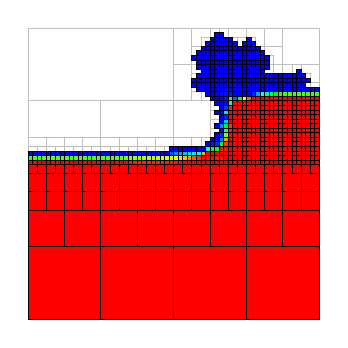
\begin{tikzpicture}[x={(\screenshotunitlength,0)},y={(0,\screenshotunitlength)}]
        \definecolor{fillcolor}{rgb}{1.000000,0.000000,0.000000}
\fill[fillcolor] (0.000000,0.000000) rectangle (0.250000,0.250000);
\definecolor{fillcolor}{rgb}{1.000000,0.000000,0.000000}
\fill[fillcolor] (0.250000,0.000000) rectangle (0.500000,0.250000);
\definecolor{fillcolor}{rgb}{1.000000,0.000000,0.000000}
\fill[fillcolor] (0.000000,0.250000) rectangle (0.125000,0.375000);
\definecolor{fillcolor}{rgb}{1.000000,0.000000,0.000000}
\fill[fillcolor] (0.125000,0.250000) rectangle (0.250000,0.375000);
\definecolor{fillcolor}{rgb}{1.000000,0.000000,0.000000}
\fill[fillcolor] (0.000000,0.375000) rectangle (0.062500,0.437500);
\definecolor{fillcolor}{rgb}{1.000000,0.000000,0.000000}
\fill[fillcolor] (0.062500,0.375000) rectangle (0.125000,0.437500);
\definecolor{fillcolor}{rgb}{1.000000,0.000000,0.000000}
\fill[fillcolor] (0.000000,0.437500) rectangle (0.062500,0.500000);
\definecolor{fillcolor}{rgb}{1.000000,0.000000,0.000000}
\fill[fillcolor] (0.062500,0.437500) rectangle (0.125000,0.500000);
\definecolor{fillcolor}{rgb}{1.000000,0.000000,0.000000}
\fill[fillcolor] (0.125000,0.375000) rectangle (0.187500,0.437500);
\definecolor{fillcolor}{rgb}{1.000000,0.000000,0.000000}
\fill[fillcolor] (0.187500,0.375000) rectangle (0.250000,0.437500);
\definecolor{fillcolor}{rgb}{1.000000,0.000000,0.000000}
\fill[fillcolor] (0.125000,0.437500) rectangle (0.187500,0.500000);
\definecolor{fillcolor}{rgb}{1.000000,0.000000,0.000000}
\fill[fillcolor] (0.187500,0.437500) rectangle (0.250000,0.500000);
\definecolor{fillcolor}{rgb}{1.000000,0.000000,0.000000}
\fill[fillcolor] (0.250000,0.250000) rectangle (0.375000,0.375000);
\definecolor{fillcolor}{rgb}{1.000000,0.000000,0.000000}
\fill[fillcolor] (0.375000,0.250000) rectangle (0.500000,0.375000);
\definecolor{fillcolor}{rgb}{1.000000,0.000000,0.000000}
\fill[fillcolor] (0.250000,0.375000) rectangle (0.312500,0.437500);
\definecolor{fillcolor}{rgb}{1.000000,0.000000,0.000000}
\fill[fillcolor] (0.312500,0.375000) rectangle (0.375000,0.437500);
\definecolor{fillcolor}{rgb}{1.000000,0.000000,0.000000}
\fill[fillcolor] (0.250000,0.437500) rectangle (0.312500,0.500000);
\definecolor{fillcolor}{rgb}{1.000000,0.000000,0.000000}
\fill[fillcolor] (0.312500,0.437500) rectangle (0.375000,0.500000);
\definecolor{fillcolor}{rgb}{1.000000,0.000000,0.000000}
\fill[fillcolor] (0.375000,0.375000) rectangle (0.437500,0.437500);
\definecolor{fillcolor}{rgb}{1.000000,0.000000,0.000000}
\fill[fillcolor] (0.437500,0.375000) rectangle (0.500000,0.437500);
\definecolor{fillcolor}{rgb}{1.000000,0.000000,0.000000}
\fill[fillcolor] (0.375000,0.437500) rectangle (0.437500,0.500000);
\definecolor{fillcolor}{rgb}{1.000000,0.000000,0.000000}
\fill[fillcolor] (0.437500,0.437500) rectangle (0.500000,0.500000);
\definecolor{fillcolor}{rgb}{1.000000,0.000000,0.000000}
\fill[fillcolor] (0.500000,0.000000) rectangle (0.750000,0.250000);
\definecolor{fillcolor}{rgb}{1.000000,0.000000,0.000000}
\fill[fillcolor] (0.750000,0.000000) rectangle (1.000000,0.250000);
\definecolor{fillcolor}{rgb}{1.000000,0.000000,0.000000}
\fill[fillcolor] (0.500000,0.250000) rectangle (0.625000,0.375000);
\definecolor{fillcolor}{rgb}{1.000000,0.000000,0.000000}
\fill[fillcolor] (0.625000,0.250000) rectangle (0.750000,0.375000);
\definecolor{fillcolor}{rgb}{1.000000,0.000000,0.000000}
\fill[fillcolor] (0.500000,0.375000) rectangle (0.562500,0.437500);
\definecolor{fillcolor}{rgb}{1.000000,0.000000,0.000000}
\fill[fillcolor] (0.562500,0.375000) rectangle (0.625000,0.437500);
\definecolor{fillcolor}{rgb}{1.000000,0.000000,0.000000}
\fill[fillcolor] (0.500000,0.437500) rectangle (0.562500,0.500000);
\definecolor{fillcolor}{rgb}{1.000000,0.000000,0.000000}
\fill[fillcolor] (0.562500,0.437500) rectangle (0.625000,0.500000);
\definecolor{fillcolor}{rgb}{1.000000,0.000000,0.000000}
\fill[fillcolor] (0.625000,0.375000) rectangle (0.687500,0.437500);
\definecolor{fillcolor}{rgb}{1.000000,0.000000,0.000000}
\fill[fillcolor] (0.687500,0.375000) rectangle (0.750000,0.437500);
\definecolor{fillcolor}{rgb}{1.000000,0.000000,0.000000}
\fill[fillcolor] (0.625000,0.437500) rectangle (0.687500,0.500000);
\definecolor{fillcolor}{rgb}{1.000000,0.000000,0.000000}
\fill[fillcolor] (0.687500,0.437500) rectangle (0.750000,0.500000);
\definecolor{fillcolor}{rgb}{1.000000,0.000000,0.000000}
\fill[fillcolor] (0.750000,0.250000) rectangle (0.875000,0.375000);
\definecolor{fillcolor}{rgb}{1.000000,0.000000,0.000000}
\fill[fillcolor] (0.875000,0.250000) rectangle (1.000000,0.375000);
\definecolor{fillcolor}{rgb}{1.000000,0.000000,0.000000}
\fill[fillcolor] (0.750000,0.375000) rectangle (0.812500,0.437500);
\definecolor{fillcolor}{rgb}{1.000000,0.000000,0.000000}
\fill[fillcolor] (0.812500,0.375000) rectangle (0.875000,0.437500);
\definecolor{fillcolor}{rgb}{1.000000,0.000000,0.000000}
\fill[fillcolor] (0.750000,0.437500) rectangle (0.812500,0.500000);
\definecolor{fillcolor}{rgb}{1.000000,0.000000,0.000000}
\fill[fillcolor] (0.812500,0.437500) rectangle (0.875000,0.500000);
\definecolor{fillcolor}{rgb}{1.000000,0.000000,0.000000}
\fill[fillcolor] (0.875000,0.375000) rectangle (0.937500,0.437500);
\definecolor{fillcolor}{rgb}{1.000000,0.000000,0.000000}
\fill[fillcolor] (0.937500,0.375000) rectangle (1.000000,0.437500);
\definecolor{fillcolor}{rgb}{1.000000,0.000000,0.000000}
\fill[fillcolor] (0.875000,0.437500) rectangle (0.937500,0.500000);
\definecolor{fillcolor}{rgb}{1.000000,0.000000,0.000000}
\fill[fillcolor] (0.937500,0.437500) rectangle (1.000000,0.500000);
\definecolor{fillcolor}{rgb}{1.000000,0.000000,0.000000}
\fill[fillcolor] (0.000000,0.500000) rectangle (0.031250,0.531250);
\definecolor{fillcolor}{rgb}{1.000000,0.000000,0.000000}
\fill[fillcolor] (0.031250,0.500000) rectangle (0.062500,0.531250);
\definecolor{fillcolor}{rgb}{1.000000,0.000000,0.000000}
\fill[fillcolor] (0.000000,0.531250) rectangle (0.015625,0.546875);
\definecolor{fillcolor}{rgb}{1.000000,0.000000,0.000000}
\fill[fillcolor] (0.015625,0.531250) rectangle (0.031250,0.546875);
\definecolor{fillcolor}{rgb}{0.232472,1.000000,0.000000}
\fill[fillcolor] (0.000000,0.546875) rectangle (0.015625,0.562500);
\definecolor{fillcolor}{rgb}{0.258710,1.000000,0.000000}
\fill[fillcolor] (0.015625,0.546875) rectangle (0.031250,0.562500);
\definecolor{fillcolor}{rgb}{1.000000,0.000000,0.000000}
\fill[fillcolor] (0.031250,0.531250) rectangle (0.046875,0.546875);
\definecolor{fillcolor}{rgb}{1.000000,0.000000,0.000000}
\fill[fillcolor] (0.046875,0.531250) rectangle (0.062500,0.546875);
\definecolor{fillcolor}{rgb}{0.301551,1.000000,0.000000}
\fill[fillcolor] (0.031250,0.546875) rectangle (0.046875,0.562500);
\definecolor{fillcolor}{rgb}{0.342818,1.000000,0.000000}
\fill[fillcolor] (0.046875,0.546875) rectangle (0.062500,0.562500);
\definecolor{fillcolor}{rgb}{1.000000,0.000000,0.000000}
\fill[fillcolor] (0.062500,0.500000) rectangle (0.093750,0.531250);
\definecolor{fillcolor}{rgb}{1.000000,0.000000,0.000000}
\fill[fillcolor] (0.093750,0.500000) rectangle (0.125000,0.531250);
\definecolor{fillcolor}{rgb}{1.000000,0.000000,0.000000}
\fill[fillcolor] (0.062500,0.531250) rectangle (0.078125,0.546875);
\definecolor{fillcolor}{rgb}{1.000000,0.000000,0.000000}
\fill[fillcolor] (0.078125,0.531250) rectangle (0.093750,0.546875);
\definecolor{fillcolor}{rgb}{0.375118,1.000000,0.000000}
\fill[fillcolor] (0.062500,0.546875) rectangle (0.078125,0.562500);
\definecolor{fillcolor}{rgb}{0.384590,1.000000,0.000000}
\fill[fillcolor] (0.078125,0.546875) rectangle (0.093750,0.562500);
\definecolor{fillcolor}{rgb}{1.000000,0.000000,0.000000}
\fill[fillcolor] (0.093750,0.531250) rectangle (0.109375,0.546875);
\definecolor{fillcolor}{rgb}{1.000000,0.000000,0.000000}
\fill[fillcolor] (0.109375,0.531250) rectangle (0.125000,0.546875);
\definecolor{fillcolor}{rgb}{0.376078,1.000000,0.000000}
\fill[fillcolor] (0.093750,0.546875) rectangle (0.109375,0.562500);
\definecolor{fillcolor}{rgb}{0.358511,1.000000,0.000000}
\fill[fillcolor] (0.109375,0.546875) rectangle (0.125000,0.562500);
\definecolor{fillcolor}{rgb}{0.000000,0.000000,1.000000}
\fill[fillcolor] (0.000000,0.562500) rectangle (0.015625,0.578125);
\definecolor{fillcolor}{rgb}{0.000000,0.000000,1.000000}
\fill[fillcolor] (0.015625,0.562500) rectangle (0.031250,0.578125);
\definecolor{fillcolor}{rgb}{0.000000,0.000000,1.000000}
\fill[fillcolor] (0.031250,0.562500) rectangle (0.046875,0.578125);
\definecolor{fillcolor}{rgb}{0.000000,0.000000,1.000000}
\fill[fillcolor] (0.046875,0.562500) rectangle (0.062500,0.578125);
\definecolor{fillcolor}{rgb}{0.000000,0.000000,1.000000}
\fill[fillcolor] (0.062500,0.562500) rectangle (0.078125,0.578125);
\definecolor{fillcolor}{rgb}{0.000000,0.000000,1.000000}
\fill[fillcolor] (0.078125,0.562500) rectangle (0.093750,0.578125);
\definecolor{fillcolor}{rgb}{0.000000,0.000000,1.000000}
\fill[fillcolor] (0.093750,0.562500) rectangle (0.109375,0.578125);
\definecolor{fillcolor}{rgb}{0.000000,0.000000,1.000000}
\fill[fillcolor] (0.109375,0.562500) rectangle (0.125000,0.578125);
\definecolor{fillcolor}{rgb}{1.000000,0.000000,0.000000}
\fill[fillcolor] (0.125000,0.500000) rectangle (0.156250,0.531250);
\definecolor{fillcolor}{rgb}{1.000000,0.000000,0.000000}
\fill[fillcolor] (0.156250,0.500000) rectangle (0.187500,0.531250);
\definecolor{fillcolor}{rgb}{1.000000,0.000000,0.000000}
\fill[fillcolor] (0.125000,0.531250) rectangle (0.140625,0.546875);
\definecolor{fillcolor}{rgb}{1.000000,0.000000,0.000000}
\fill[fillcolor] (0.140625,0.531250) rectangle (0.156250,0.546875);
\definecolor{fillcolor}{rgb}{0.340785,1.000000,0.000000}
\fill[fillcolor] (0.125000,0.546875) rectangle (0.140625,0.562500);
\definecolor{fillcolor}{rgb}{0.322802,1.000000,0.000000}
\fill[fillcolor] (0.140625,0.546875) rectangle (0.156250,0.562500);
\definecolor{fillcolor}{rgb}{1.000000,0.000000,0.000000}
\fill[fillcolor] (0.156250,0.531250) rectangle (0.171875,0.546875);
\definecolor{fillcolor}{rgb}{1.000000,0.000000,0.000000}
\fill[fillcolor] (0.171875,0.531250) rectangle (0.187500,0.546875);
\definecolor{fillcolor}{rgb}{0.310574,1.000000,0.000000}
\fill[fillcolor] (0.156250,0.546875) rectangle (0.171875,0.562500);
\definecolor{fillcolor}{rgb}{0.298696,1.000000,0.000000}
\fill[fillcolor] (0.171875,0.546875) rectangle (0.187500,0.562500);
\definecolor{fillcolor}{rgb}{1.000000,0.000000,0.000000}
\fill[fillcolor] (0.187500,0.500000) rectangle (0.218750,0.531250);
\definecolor{fillcolor}{rgb}{1.000000,0.000000,0.000000}
\fill[fillcolor] (0.218750,0.500000) rectangle (0.250000,0.531250);
\definecolor{fillcolor}{rgb}{1.000000,0.000000,0.000000}
\fill[fillcolor] (0.187500,0.531250) rectangle (0.203125,0.546875);
\definecolor{fillcolor}{rgb}{1.000000,0.000000,0.000000}
\fill[fillcolor] (0.203125,0.531250) rectangle (0.218750,0.546875);
\definecolor{fillcolor}{rgb}{0.295441,1.000000,0.000000}
\fill[fillcolor] (0.187500,0.546875) rectangle (0.203125,0.562500);
\definecolor{fillcolor}{rgb}{0.291023,1.000000,0.000000}
\fill[fillcolor] (0.203125,0.546875) rectangle (0.218750,0.562500);
\definecolor{fillcolor}{rgb}{1.000000,0.000000,0.000000}
\fill[fillcolor] (0.218750,0.531250) rectangle (0.234375,0.546875);
\definecolor{fillcolor}{rgb}{1.000000,0.000000,0.000000}
\fill[fillcolor] (0.234375,0.531250) rectangle (0.250000,0.546875);
\definecolor{fillcolor}{rgb}{0.297877,1.000000,0.000000}
\fill[fillcolor] (0.218750,0.546875) rectangle (0.234375,0.562500);
\definecolor{fillcolor}{rgb}{0.301689,1.000000,0.000000}
\fill[fillcolor] (0.234375,0.546875) rectangle (0.250000,0.562500);
\definecolor{fillcolor}{rgb}{0.000000,0.000000,1.000000}
\fill[fillcolor] (0.125000,0.562500) rectangle (0.140625,0.578125);
\definecolor{fillcolor}{rgb}{0.000000,0.000000,1.000000}
\fill[fillcolor] (0.140625,0.562500) rectangle (0.156250,0.578125);
\definecolor{fillcolor}{rgb}{0.000000,0.000000,1.000000}
\fill[fillcolor] (0.156250,0.562500) rectangle (0.171875,0.578125);
\definecolor{fillcolor}{rgb}{0.000000,0.000000,1.000000}
\fill[fillcolor] (0.171875,0.562500) rectangle (0.187500,0.578125);
\definecolor{fillcolor}{rgb}{0.000000,0.000000,1.000000}
\fill[fillcolor] (0.187500,0.562500) rectangle (0.203125,0.578125);
\definecolor{fillcolor}{rgb}{0.000000,0.000000,1.000000}
\fill[fillcolor] (0.203125,0.562500) rectangle (0.218750,0.578125);
\definecolor{fillcolor}{rgb}{0.000000,0.000000,1.000000}
\fill[fillcolor] (0.218750,0.562500) rectangle (0.234375,0.578125);
\definecolor{fillcolor}{rgb}{0.000000,0.000000,1.000000}
\fill[fillcolor] (0.234375,0.562500) rectangle (0.250000,0.578125);
\definecolor{fillcolor}{rgb}{1.000000,0.000000,0.000000}
\fill[fillcolor] (0.250000,0.500000) rectangle (0.281250,0.531250);
\definecolor{fillcolor}{rgb}{1.000000,0.000000,0.000000}
\fill[fillcolor] (0.281250,0.500000) rectangle (0.312500,0.531250);
\definecolor{fillcolor}{rgb}{1.000000,0.000000,0.000000}
\fill[fillcolor] (0.250000,0.531250) rectangle (0.265625,0.546875);
\definecolor{fillcolor}{rgb}{1.000000,0.000000,0.000000}
\fill[fillcolor] (0.265625,0.531250) rectangle (0.281250,0.546875);
\definecolor{fillcolor}{rgb}{0.319766,1.000000,0.000000}
\fill[fillcolor] (0.250000,0.546875) rectangle (0.265625,0.562500);
\definecolor{fillcolor}{rgb}{0.331907,1.000000,0.000000}
\fill[fillcolor] (0.265625,0.546875) rectangle (0.281250,0.562500);
\definecolor{fillcolor}{rgb}{1.000000,0.000000,0.000000}
\fill[fillcolor] (0.281250,0.531250) rectangle (0.296875,0.546875);
\definecolor{fillcolor}{rgb}{1.000000,0.000000,0.000000}
\fill[fillcolor] (0.296875,0.531250) rectangle (0.312500,0.546875);
\definecolor{fillcolor}{rgb}{0.360127,1.000000,0.000000}
\fill[fillcolor] (0.281250,0.546875) rectangle (0.296875,0.562500);
\definecolor{fillcolor}{rgb}{0.379504,1.000000,0.000000}
\fill[fillcolor] (0.296875,0.546875) rectangle (0.312500,0.562500);
\definecolor{fillcolor}{rgb}{1.000000,0.000000,0.000000}
\fill[fillcolor] (0.312500,0.500000) rectangle (0.343750,0.531250);
\definecolor{fillcolor}{rgb}{1.000000,0.000000,0.000000}
\fill[fillcolor] (0.343750,0.500000) rectangle (0.375000,0.531250);
\definecolor{fillcolor}{rgb}{1.000000,0.000000,0.000000}
\fill[fillcolor] (0.312500,0.531250) rectangle (0.328125,0.546875);
\definecolor{fillcolor}{rgb}{1.000000,0.000000,0.000000}
\fill[fillcolor] (0.328125,0.531250) rectangle (0.343750,0.546875);
\definecolor{fillcolor}{rgb}{0.415673,1.000000,0.000000}
\fill[fillcolor] (0.312500,0.546875) rectangle (0.328125,0.562500);
\definecolor{fillcolor}{rgb}{0.433818,1.000000,0.000000}
\fill[fillcolor] (0.328125,0.546875) rectangle (0.343750,0.562500);
\definecolor{fillcolor}{rgb}{1.000000,0.078773,0.000000}
\fill[fillcolor] (0.343750,0.531250) rectangle (0.359375,0.546875);
\definecolor{fillcolor}{rgb}{1.000000,0.116389,0.000000}
\fill[fillcolor] (0.359375,0.531250) rectangle (0.375000,0.546875);
\definecolor{fillcolor}{rgb}{0.534348,1.000000,0.000000}
\fill[fillcolor] (0.343750,0.546875) rectangle (0.359375,0.562500);
\definecolor{fillcolor}{rgb}{0.588951,1.000000,0.000000}
\fill[fillcolor] (0.359375,0.546875) rectangle (0.375000,0.562500);
\definecolor{fillcolor}{rgb}{0.000000,0.000000,1.000000}
\fill[fillcolor] (0.250000,0.562500) rectangle (0.265625,0.578125);
\definecolor{fillcolor}{rgb}{0.000000,0.000000,1.000000}
\fill[fillcolor] (0.265625,0.562500) rectangle (0.281250,0.578125);
\definecolor{fillcolor}{rgb}{0.000000,0.000000,1.000000}
\fill[fillcolor] (0.281250,0.562500) rectangle (0.296875,0.578125);
\definecolor{fillcolor}{rgb}{0.000000,0.000000,1.000000}
\fill[fillcolor] (0.296875,0.562500) rectangle (0.312500,0.578125);
\definecolor{fillcolor}{rgb}{0.000000,0.000000,1.000000}
\fill[fillcolor] (0.312500,0.562500) rectangle (0.328125,0.578125);
\definecolor{fillcolor}{rgb}{0.000000,0.000000,1.000000}
\fill[fillcolor] (0.328125,0.562500) rectangle (0.343750,0.578125);
\definecolor{fillcolor}{rgb}{0.000000,0.000000,1.000000}
\fill[fillcolor] (0.343750,0.562500) rectangle (0.359375,0.578125);
\definecolor{fillcolor}{rgb}{0.000000,0.000000,1.000000}
\fill[fillcolor] (0.359375,0.562500) rectangle (0.375000,0.578125);
\definecolor{fillcolor}{rgb}{1.000000,0.000000,0.000000}
\fill[fillcolor] (0.375000,0.500000) rectangle (0.406250,0.531250);
\definecolor{fillcolor}{rgb}{1.000000,0.000000,0.000000}
\fill[fillcolor] (0.406250,0.500000) rectangle (0.437500,0.531250);
\definecolor{fillcolor}{rgb}{1.000000,0.135293,0.000000}
\fill[fillcolor] (0.375000,0.531250) rectangle (0.390625,0.546875);
\definecolor{fillcolor}{rgb}{1.000000,0.144769,0.000000}
\fill[fillcolor] (0.390625,0.531250) rectangle (0.406250,0.546875);
\definecolor{fillcolor}{rgb}{0.649414,1.000000,0.000000}
\fill[fillcolor] (0.375000,0.546875) rectangle (0.390625,0.562500);
\definecolor{fillcolor}{rgb}{0.680766,1.000000,0.000000}
\fill[fillcolor] (0.390625,0.546875) rectangle (0.406250,0.562500);
\definecolor{fillcolor}{rgb}{1.000000,0.144922,0.000000}
\fill[fillcolor] (0.406250,0.531250) rectangle (0.421875,0.546875);
\definecolor{fillcolor}{rgb}{1.000000,0.145361,0.000000}
\fill[fillcolor] (0.421875,0.531250) rectangle (0.437500,0.546875);
\definecolor{fillcolor}{rgb}{0.721259,1.000000,0.000000}
\fill[fillcolor] (0.406250,0.546875) rectangle (0.421875,0.562500);
\definecolor{fillcolor}{rgb}{0.743410,1.000000,0.000000}
\fill[fillcolor] (0.421875,0.546875) rectangle (0.437500,0.562500);
\definecolor{fillcolor}{rgb}{1.000000,0.000000,0.000000}
\fill[fillcolor] (0.437500,0.500000) rectangle (0.468750,0.531250);
\definecolor{fillcolor}{rgb}{1.000000,0.000010,0.000000}
\fill[fillcolor] (0.468750,0.500000) rectangle (0.500000,0.531250);
\definecolor{fillcolor}{rgb}{1.000000,0.132713,0.000000}
\fill[fillcolor] (0.437500,0.531250) rectangle (0.453125,0.546875);
\definecolor{fillcolor}{rgb}{1.000000,0.129596,0.000000}
\fill[fillcolor] (0.453125,0.531250) rectangle (0.468750,0.546875);
\definecolor{fillcolor}{rgb}{0.783453,1.000000,0.000000}
\fill[fillcolor] (0.437500,0.546875) rectangle (0.453125,0.562500);
\definecolor{fillcolor}{rgb}{0.803101,1.000000,0.000000}
\fill[fillcolor] (0.453125,0.546875) rectangle (0.468750,0.562500);
\definecolor{fillcolor}{rgb}{1.000000,0.111901,0.000000}
\fill[fillcolor] (0.468750,0.531250) rectangle (0.484375,0.546875);
\definecolor{fillcolor}{rgb}{1.000000,0.106036,0.000000}
\fill[fillcolor] (0.484375,0.531250) rectangle (0.500000,0.546875);
\definecolor{fillcolor}{rgb}{0.846375,1.000000,0.000000}
\fill[fillcolor] (0.468750,0.546875) rectangle (0.484375,0.562500);
\definecolor{fillcolor}{rgb}{0.894922,1.000000,0.000000}
\fill[fillcolor] (0.484375,0.546875) rectangle (0.500000,0.562500);
\definecolor{fillcolor}{rgb}{0.000000,0.000000,1.000000}
\fill[fillcolor] (0.375000,0.562500) rectangle (0.390625,0.578125);
\definecolor{fillcolor}{rgb}{0.000000,0.000000,1.000000}
\fill[fillcolor] (0.390625,0.562500) rectangle (0.406250,0.578125);
\definecolor{fillcolor}{rgb}{0.000000,0.000000,1.000000}
\fill[fillcolor] (0.406250,0.562500) rectangle (0.421875,0.578125);
\definecolor{fillcolor}{rgb}{0.000000,0.000000,1.000000}
\fill[fillcolor] (0.421875,0.562500) rectangle (0.437500,0.578125);
\definecolor{fillcolor}{rgb}{0.000000,0.000000,1.000000}
\fill[fillcolor] (0.437500,0.562500) rectangle (0.453125,0.578125);
\definecolor{fillcolor}{rgb}{0.000000,0.000000,1.000000}
\fill[fillcolor] (0.453125,0.562500) rectangle (0.468750,0.578125);
\definecolor{fillcolor}{rgb}{0.000000,0.000000,1.000000}
\fill[fillcolor] (0.468750,0.562500) rectangle (0.484375,0.578125);
\definecolor{fillcolor}{rgb}{0.000000,0.332260,1.000000}
\fill[fillcolor] (0.484375,0.562500) rectangle (0.500000,0.578125);
\definecolor{fillcolor}{rgb}{0.000000,0.000000,1.000000}
\fill[fillcolor] (0.484375,0.578125) rectangle (0.500000,0.593750);
\definecolor{fillcolor}{rgb}{1.000000,0.000000,0.000000}
\fill[fillcolor] (0.500000,0.500000) rectangle (0.531250,0.531250);
\definecolor{fillcolor}{rgb}{1.000000,0.000000,0.000000}
\fill[fillcolor] (0.531250,0.500000) rectangle (0.562500,0.531250);
\definecolor{fillcolor}{rgb}{1.000000,0.079499,0.000000}
\fill[fillcolor] (0.500000,0.531250) rectangle (0.515625,0.546875);
\definecolor{fillcolor}{rgb}{1.000000,0.061863,0.000000}
\fill[fillcolor] (0.515625,0.531250) rectangle (0.531250,0.546875);
\definecolor{fillcolor}{rgb}{1.000000,0.973785,0.000000}
\fill[fillcolor] (0.500000,0.546875) rectangle (0.515625,0.562500);
\definecolor{fillcolor}{rgb}{1.000000,0.871544,0.000000}
\fill[fillcolor] (0.515625,0.546875) rectangle (0.531250,0.562500);
\definecolor{fillcolor}{rgb}{1.000000,0.012752,0.000000}
\fill[fillcolor] (0.531250,0.531250) rectangle (0.546875,0.546875);
\definecolor{fillcolor}{rgb}{1.000000,0.000001,0.000000}
\fill[fillcolor] (0.546875,0.531250) rectangle (0.562500,0.546875);
\definecolor{fillcolor}{rgb}{1.000000,0.723327,0.000000}
\fill[fillcolor] (0.531250,0.546875) rectangle (0.546875,0.562500);
\definecolor{fillcolor}{rgb}{1.000000,0.579974,0.000000}
\fill[fillcolor] (0.546875,0.546875) rectangle (0.562500,0.562500);
\definecolor{fillcolor}{rgb}{1.000000,0.000000,0.000000}
\fill[fillcolor] (0.562500,0.500000) rectangle (0.593750,0.531250);
\definecolor{fillcolor}{rgb}{1.000000,0.000003,0.000000}
\fill[fillcolor] (0.593750,0.500000) rectangle (0.625000,0.531250);
\definecolor{fillcolor}{rgb}{1.000000,0.000001,0.000000}
\fill[fillcolor] (0.562500,0.531250) rectangle (0.578125,0.546875);
\definecolor{fillcolor}{rgb}{1.000000,0.000001,0.000000}
\fill[fillcolor] (0.578125,0.531250) rectangle (0.593750,0.546875);
\definecolor{fillcolor}{rgb}{1.000000,0.359430,0.000000}
\fill[fillcolor] (0.562500,0.546875) rectangle (0.578125,0.562500);
\definecolor{fillcolor}{rgb}{1.000000,0.179349,0.000000}
\fill[fillcolor] (0.578125,0.546875) rectangle (0.593750,0.562500);
\definecolor{fillcolor}{rgb}{1.000000,0.000003,0.000000}
\fill[fillcolor] (0.593750,0.531250) rectangle (0.609375,0.546875);
\definecolor{fillcolor}{rgb}{1.000000,0.000004,0.000000}
\fill[fillcolor] (0.609375,0.531250) rectangle (0.625000,0.546875);
\definecolor{fillcolor}{rgb}{1.000000,0.011912,0.000000}
\fill[fillcolor] (0.593750,0.546875) rectangle (0.609375,0.562500);
\definecolor{fillcolor}{rgb}{1.000000,0.031478,0.000000}
\fill[fillcolor] (0.609375,0.546875) rectangle (0.625000,0.562500);
\definecolor{fillcolor}{rgb}{0.000000,0.573469,1.000000}
\fill[fillcolor] (0.500000,0.562500) rectangle (0.515625,0.578125);
\definecolor{fillcolor}{rgb}{0.000000,0.633007,1.000000}
\fill[fillcolor] (0.515625,0.562500) rectangle (0.531250,0.578125);
\definecolor{fillcolor}{rgb}{0.000000,0.000000,1.000000}
\fill[fillcolor] (0.500000,0.578125) rectangle (0.515625,0.593750);
\definecolor{fillcolor}{rgb}{0.000000,0.000000,1.000000}
\fill[fillcolor] (0.515625,0.578125) rectangle (0.531250,0.593750);
\definecolor{fillcolor}{rgb}{0.000000,0.765886,1.000000}
\fill[fillcolor] (0.531250,0.562500) rectangle (0.546875,0.578125);
\definecolor{fillcolor}{rgb}{0.000000,0.874574,1.000000}
\fill[fillcolor] (0.546875,0.562500) rectangle (0.562500,0.578125);
\definecolor{fillcolor}{rgb}{0.000000,0.000000,1.000000}
\fill[fillcolor] (0.531250,0.578125) rectangle (0.546875,0.593750);
\definecolor{fillcolor}{rgb}{0.000000,0.000000,1.000000}
\fill[fillcolor] (0.546875,0.578125) rectangle (0.562500,0.593750);
\definecolor{fillcolor}{rgb}{0.000000,0.947746,1.000000}
\fill[fillcolor] (0.562500,0.562500) rectangle (0.578125,0.578125);
\definecolor{fillcolor}{rgb}{0.000000,1.000000,0.960687}
\fill[fillcolor] (0.578125,0.562500) rectangle (0.593750,0.578125);
\definecolor{fillcolor}{rgb}{0.000000,0.000000,1.000000}
\fill[fillcolor] (0.562500,0.578125) rectangle (0.578125,0.593750);
\definecolor{fillcolor}{rgb}{0.000000,0.000000,1.000000}
\fill[fillcolor] (0.578125,0.578125) rectangle (0.593750,0.593750);
\definecolor{fillcolor}{rgb}{1.000000,0.652457,0.000000}
\fill[fillcolor] (0.593750,0.562500) rectangle (0.609375,0.578125);
\definecolor{fillcolor}{rgb}{1.000000,0.017247,0.000000}
\fill[fillcolor] (0.609375,0.562500) rectangle (0.625000,0.578125);
\definecolor{fillcolor}{rgb}{0.000000,0.000000,1.000000}
\fill[fillcolor] (0.593750,0.578125) rectangle (0.609375,0.593750);
\definecolor{fillcolor}{rgb}{0.000000,1.000000,0.843278}
\fill[fillcolor] (0.609375,0.578125) rectangle (0.625000,0.593750);
\definecolor{fillcolor}{rgb}{0.000000,0.000000,1.000000}
\fill[fillcolor] (0.609375,0.593750) rectangle (0.625000,0.609375);
\definecolor{fillcolor}{rgb}{1.000000,0.000006,0.000000}
\fill[fillcolor] (0.625000,0.500000) rectangle (0.656250,0.531250);
\definecolor{fillcolor}{rgb}{1.000000,0.000006,0.000000}
\fill[fillcolor] (0.656250,0.500000) rectangle (0.687500,0.531250);
\definecolor{fillcolor}{rgb}{1.000000,0.000005,0.000000}
\fill[fillcolor] (0.625000,0.531250) rectangle (0.640625,0.546875);
\definecolor{fillcolor}{rgb}{1.000000,0.000004,0.000000}
\fill[fillcolor] (0.640625,0.531250) rectangle (0.656250,0.546875);
\definecolor{fillcolor}{rgb}{1.000000,0.052962,0.000000}
\fill[fillcolor] (0.625000,0.546875) rectangle (0.640625,0.562500);
\definecolor{fillcolor}{rgb}{1.000000,0.093307,0.000000}
\fill[fillcolor] (0.640625,0.546875) rectangle (0.656250,0.562500);
\definecolor{fillcolor}{rgb}{1.000000,0.000004,0.000000}
\fill[fillcolor] (0.656250,0.531250) rectangle (0.671875,0.546875);
\definecolor{fillcolor}{rgb}{1.000000,0.000002,0.000000}
\fill[fillcolor] (0.671875,0.531250) rectangle (0.687500,0.546875);
\definecolor{fillcolor}{rgb}{1.000000,0.053869,0.000000}
\fill[fillcolor] (0.656250,0.546875) rectangle (0.671875,0.562500);
\definecolor{fillcolor}{rgb}{1.000000,0.000001,0.000000}
\fill[fillcolor] (0.671875,0.546875) rectangle (0.687500,0.562500);
\definecolor{fillcolor}{rgb}{1.000000,0.000000,0.000000}
\fill[fillcolor] (0.687500,0.500000) rectangle (0.718750,0.531250);
\definecolor{fillcolor}{rgb}{1.000000,0.000000,0.000000}
\fill[fillcolor] (0.718750,0.500000) rectangle (0.750000,0.531250);
\definecolor{fillcolor}{rgb}{1.000000,0.000000,0.000000}
\fill[fillcolor] (0.687500,0.531250) rectangle (0.703125,0.546875);
\definecolor{fillcolor}{rgb}{1.000000,0.000000,0.000000}
\fill[fillcolor] (0.703125,0.531250) rectangle (0.718750,0.546875);
\definecolor{fillcolor}{rgb}{1.000000,0.000000,0.000000}
\fill[fillcolor] (0.687500,0.546875) rectangle (0.703125,0.562500);
\definecolor{fillcolor}{rgb}{1.000000,0.000000,0.000000}
\fill[fillcolor] (0.703125,0.546875) rectangle (0.718750,0.562500);
\definecolor{fillcolor}{rgb}{1.000000,0.000000,0.000000}
\fill[fillcolor] (0.718750,0.531250) rectangle (0.734375,0.546875);
\definecolor{fillcolor}{rgb}{1.000000,0.000000,0.000000}
\fill[fillcolor] (0.734375,0.531250) rectangle (0.750000,0.546875);
\definecolor{fillcolor}{rgb}{1.000000,0.000000,0.000000}
\fill[fillcolor] (0.718750,0.546875) rectangle (0.734375,0.562500);
\definecolor{fillcolor}{rgb}{1.000000,0.000000,0.000000}
\fill[fillcolor] (0.734375,0.546875) rectangle (0.750000,0.562500);
\definecolor{fillcolor}{rgb}{1.000000,0.021315,0.000000}
\fill[fillcolor] (0.625000,0.562500) rectangle (0.640625,0.578125);
\definecolor{fillcolor}{rgb}{1.000000,0.017529,0.000000}
\fill[fillcolor] (0.640625,0.562500) rectangle (0.656250,0.578125);
\definecolor{fillcolor}{rgb}{0.037177,1.000000,0.000000}
\fill[fillcolor] (0.625000,0.578125) rectangle (0.640625,0.593750);
\definecolor{fillcolor}{rgb}{0.000000,1.000000,0.043357}
\fill[fillcolor] (0.640625,0.578125) rectangle (0.656250,0.593750);
\definecolor{fillcolor}{rgb}{1.000000,0.012263,0.000000}
\fill[fillcolor] (0.656250,0.562500) rectangle (0.671875,0.578125);
\definecolor{fillcolor}{rgb}{1.000000,0.001086,0.000000}
\fill[fillcolor] (0.671875,0.562500) rectangle (0.687500,0.578125);
\definecolor{fillcolor}{rgb}{1.000000,0.067294,0.000000}
\fill[fillcolor] (0.656250,0.578125) rectangle (0.671875,0.593750);
\definecolor{fillcolor}{rgb}{1.000000,0.078758,0.000000}
\fill[fillcolor] (0.671875,0.578125) rectangle (0.687500,0.593750);
\definecolor{fillcolor}{rgb}{0.000000,0.119585,1.000000}
\fill[fillcolor] (0.625000,0.593750) rectangle (0.640625,0.609375);
\definecolor{fillcolor}{rgb}{0.000000,0.163961,1.000000}
\fill[fillcolor] (0.640625,0.593750) rectangle (0.656250,0.609375);
\definecolor{fillcolor}{rgb}{0.000000,0.000000,1.000000}
\fill[fillcolor] (0.625000,0.609375) rectangle (0.640625,0.625000);
\definecolor{fillcolor}{rgb}{0.000000,0.000000,1.000000}
\fill[fillcolor] (0.640625,0.609375) rectangle (0.656250,0.625000);
\definecolor{fillcolor}{rgb}{0.029929,1.000000,0.000000}
\fill[fillcolor] (0.656250,0.593750) rectangle (0.671875,0.609375);
\definecolor{fillcolor}{rgb}{1.000000,0.245172,0.000000}
\fill[fillcolor] (0.671875,0.593750) rectangle (0.687500,0.609375);
\definecolor{fillcolor}{rgb}{0.000000,0.494994,1.000000}
\fill[fillcolor] (0.656250,0.609375) rectangle (0.671875,0.625000);
\definecolor{fillcolor}{rgb}{1.000000,0.598447,0.000000}
\fill[fillcolor] (0.671875,0.609375) rectangle (0.687500,0.625000);
\definecolor{fillcolor}{rgb}{1.000000,0.000000,0.000000}
\fill[fillcolor] (0.687500,0.562500) rectangle (0.703125,0.578125);
\definecolor{fillcolor}{rgb}{1.000000,0.000000,0.000000}
\fill[fillcolor] (0.703125,0.562500) rectangle (0.718750,0.578125);
\definecolor{fillcolor}{rgb}{1.000000,0.000002,0.000000}
\fill[fillcolor] (0.687500,0.578125) rectangle (0.703125,0.593750);
\definecolor{fillcolor}{rgb}{1.000000,0.000000,0.000000}
\fill[fillcolor] (0.703125,0.578125) rectangle (0.718750,0.593750);
\definecolor{fillcolor}{rgb}{1.000000,0.000000,0.000000}
\fill[fillcolor] (0.718750,0.562500) rectangle (0.734375,0.578125);
\definecolor{fillcolor}{rgb}{1.000000,0.000000,0.000000}
\fill[fillcolor] (0.734375,0.562500) rectangle (0.750000,0.578125);
\definecolor{fillcolor}{rgb}{1.000000,0.000000,0.000000}
\fill[fillcolor] (0.718750,0.578125) rectangle (0.734375,0.593750);
\definecolor{fillcolor}{rgb}{1.000000,0.000000,0.000000}
\fill[fillcolor] (0.734375,0.578125) rectangle (0.750000,0.593750);
\definecolor{fillcolor}{rgb}{1.000000,0.002518,0.000000}
\fill[fillcolor] (0.687500,0.593750) rectangle (0.703125,0.609375);
\definecolor{fillcolor}{rgb}{1.000000,0.000000,0.000000}
\fill[fillcolor] (0.703125,0.593750) rectangle (0.718750,0.609375);
\definecolor{fillcolor}{rgb}{1.000000,0.012145,0.000000}
\fill[fillcolor] (0.687500,0.609375) rectangle (0.703125,0.625000);
\definecolor{fillcolor}{rgb}{1.000000,0.000000,0.000000}
\fill[fillcolor] (0.703125,0.609375) rectangle (0.718750,0.625000);
\definecolor{fillcolor}{rgb}{1.000000,0.000000,0.000000}
\fill[fillcolor] (0.718750,0.593750) rectangle (0.734375,0.609375);
\definecolor{fillcolor}{rgb}{1.000000,0.000000,0.000000}
\fill[fillcolor] (0.734375,0.593750) rectangle (0.750000,0.609375);
\definecolor{fillcolor}{rgb}{1.000000,0.000000,0.000000}
\fill[fillcolor] (0.718750,0.609375) rectangle (0.734375,0.625000);
\definecolor{fillcolor}{rgb}{1.000000,0.000000,0.000000}
\fill[fillcolor] (0.734375,0.609375) rectangle (0.750000,0.625000);
\definecolor{fillcolor}{rgb}{0.000000,0.000000,1.000000}
\fill[fillcolor] (0.640625,0.625000) rectangle (0.656250,0.640625);
\definecolor{fillcolor}{rgb}{0.000000,0.185994,1.000000}
\fill[fillcolor] (0.656250,0.625000) rectangle (0.671875,0.640625);
\definecolor{fillcolor}{rgb}{0.497342,1.000000,0.000000}
\fill[fillcolor] (0.671875,0.625000) rectangle (0.687500,0.640625);
\definecolor{fillcolor}{rgb}{0.000000,0.000000,1.000000}
\fill[fillcolor] (0.656250,0.640625) rectangle (0.671875,0.656250);
\definecolor{fillcolor}{rgb}{0.000000,1.000000,0.689114}
\fill[fillcolor] (0.671875,0.640625) rectangle (0.687500,0.656250);
\definecolor{fillcolor}{rgb}{0.000000,0.000000,1.000000}
\fill[fillcolor] (0.640625,0.656250) rectangle (0.656250,0.671875);
\definecolor{fillcolor}{rgb}{0.000000,0.555131,1.000000}
\fill[fillcolor] (0.656250,0.656250) rectangle (0.671875,0.671875);
\definecolor{fillcolor}{rgb}{0.000000,1.000000,0.043009}
\fill[fillcolor] (0.671875,0.656250) rectangle (0.687500,0.671875);
\definecolor{fillcolor}{rgb}{0.000000,0.000000,1.000000}
\fill[fillcolor] (0.656250,0.671875) rectangle (0.671875,0.687500);
\definecolor{fillcolor}{rgb}{0.000000,0.804116,1.000000}
\fill[fillcolor] (0.671875,0.671875) rectangle (0.687500,0.687500);
\definecolor{fillcolor}{rgb}{1.000000,0.039646,0.000000}
\fill[fillcolor] (0.687500,0.625000) rectangle (0.703125,0.640625);
\definecolor{fillcolor}{rgb}{1.000000,0.000000,0.000000}
\fill[fillcolor] (0.703125,0.625000) rectangle (0.718750,0.640625);
\definecolor{fillcolor}{rgb}{1.000000,0.110842,0.000000}
\fill[fillcolor] (0.687500,0.640625) rectangle (0.703125,0.656250);
\definecolor{fillcolor}{rgb}{1.000000,0.000000,0.000000}
\fill[fillcolor] (0.703125,0.640625) rectangle (0.718750,0.656250);
\definecolor{fillcolor}{rgb}{1.000000,0.000000,0.000000}
\fill[fillcolor] (0.718750,0.625000) rectangle (0.734375,0.640625);
\definecolor{fillcolor}{rgb}{1.000000,0.000000,0.000000}
\fill[fillcolor] (0.734375,0.625000) rectangle (0.750000,0.640625);
\definecolor{fillcolor}{rgb}{1.000000,0.000000,0.000000}
\fill[fillcolor] (0.718750,0.640625) rectangle (0.734375,0.656250);
\definecolor{fillcolor}{rgb}{1.000000,0.000000,0.000000}
\fill[fillcolor] (0.734375,0.640625) rectangle (0.750000,0.656250);
\definecolor{fillcolor}{rgb}{1.000000,0.194536,0.000000}
\fill[fillcolor] (0.687500,0.656250) rectangle (0.703125,0.671875);
\definecolor{fillcolor}{rgb}{1.000000,0.000000,0.000000}
\fill[fillcolor] (0.703125,0.656250) rectangle (0.718750,0.671875);
\definecolor{fillcolor}{rgb}{1.000000,0.002209,0.000000}
\fill[fillcolor] (0.687500,0.671875) rectangle (0.703125,0.687500);
\definecolor{fillcolor}{rgb}{1.000000,0.000000,0.000000}
\fill[fillcolor] (0.703125,0.671875) rectangle (0.718750,0.687500);
\definecolor{fillcolor}{rgb}{1.000000,0.000000,0.000000}
\fill[fillcolor] (0.718750,0.656250) rectangle (0.734375,0.671875);
\definecolor{fillcolor}{rgb}{1.000000,0.000000,0.000000}
\fill[fillcolor] (0.734375,0.656250) rectangle (0.750000,0.671875);
\definecolor{fillcolor}{rgb}{1.000000,0.000000,0.000000}
\fill[fillcolor] (0.718750,0.671875) rectangle (0.734375,0.687500);
\definecolor{fillcolor}{rgb}{1.000000,0.000000,0.000000}
\fill[fillcolor] (0.734375,0.671875) rectangle (0.750000,0.687500);
\definecolor{fillcolor}{rgb}{0.000000,0.000000,1.000000}
\fill[fillcolor] (0.640625,0.703125) rectangle (0.656250,0.718750);
\definecolor{fillcolor}{rgb}{0.000000,0.000000,1.000000}
\fill[fillcolor] (0.656250,0.687500) rectangle (0.671875,0.703125);
\definecolor{fillcolor}{rgb}{0.000000,0.137407,1.000000}
\fill[fillcolor] (0.671875,0.687500) rectangle (0.687500,0.703125);
\definecolor{fillcolor}{rgb}{0.000000,0.012033,1.000000}
\fill[fillcolor] (0.656250,0.703125) rectangle (0.671875,0.718750);
\definecolor{fillcolor}{rgb}{0.000000,0.880267,1.000000}
\fill[fillcolor] (0.671875,0.703125) rectangle (0.687500,0.718750);
\definecolor{fillcolor}{rgb}{0.000000,0.000000,1.000000}
\fill[fillcolor] (0.640625,0.734375) rectangle (0.656250,0.750000);
\definecolor{fillcolor}{rgb}{0.000000,0.000000,1.000000}
\fill[fillcolor] (0.656250,0.718750) rectangle (0.671875,0.734375);
\definecolor{fillcolor}{rgb}{0.000000,0.201220,1.000000}
\fill[fillcolor] (0.671875,0.718750) rectangle (0.687500,0.734375);
\definecolor{fillcolor}{rgb}{0.000000,0.002949,1.000000}
\fill[fillcolor] (0.656250,0.734375) rectangle (0.671875,0.750000);
\definecolor{fillcolor}{rgb}{0.000000,0.002565,1.000000}
\fill[fillcolor] (0.671875,0.734375) rectangle (0.687500,0.750000);
\definecolor{fillcolor}{rgb}{1.000000,0.000000,0.000000}
\fill[fillcolor] (0.687500,0.687500) rectangle (0.703125,0.703125);
\definecolor{fillcolor}{rgb}{1.000000,0.000000,0.000000}
\fill[fillcolor] (0.703125,0.687500) rectangle (0.718750,0.703125);
\definecolor{fillcolor}{rgb}{1.000000,0.000000,0.000000}
\fill[fillcolor] (0.687500,0.703125) rectangle (0.703125,0.718750);
\definecolor{fillcolor}{rgb}{1.000000,0.000000,0.000000}
\fill[fillcolor] (0.703125,0.703125) rectangle (0.718750,0.718750);
\definecolor{fillcolor}{rgb}{1.000000,0.000000,0.000000}
\fill[fillcolor] (0.718750,0.687500) rectangle (0.734375,0.703125);
\definecolor{fillcolor}{rgb}{1.000000,0.000000,0.000000}
\fill[fillcolor] (0.734375,0.687500) rectangle (0.750000,0.703125);
\definecolor{fillcolor}{rgb}{1.000000,0.000000,0.000000}
\fill[fillcolor] (0.718750,0.703125) rectangle (0.734375,0.718750);
\definecolor{fillcolor}{rgb}{1.000000,0.000000,0.000000}
\fill[fillcolor] (0.734375,0.703125) rectangle (0.750000,0.718750);
\definecolor{fillcolor}{rgb}{1.000000,0.140076,0.000000}
\fill[fillcolor] (0.687500,0.718750) rectangle (0.703125,0.734375);
\definecolor{fillcolor}{rgb}{1.000000,0.000000,0.000000}
\fill[fillcolor] (0.703125,0.718750) rectangle (0.718750,0.734375);
\definecolor{fillcolor}{rgb}{0.000000,1.000000,0.742445}
\fill[fillcolor] (0.687500,0.734375) rectangle (0.703125,0.750000);
\definecolor{fillcolor}{rgb}{1.000000,0.000000,0.000000}
\fill[fillcolor] (0.703125,0.734375) rectangle (0.718750,0.750000);
\definecolor{fillcolor}{rgb}{1.000000,0.000000,0.000000}
\fill[fillcolor] (0.718750,0.718750) rectangle (0.734375,0.734375);
\definecolor{fillcolor}{rgb}{1.000000,0.000000,0.000000}
\fill[fillcolor] (0.734375,0.718750) rectangle (0.750000,0.734375);
\definecolor{fillcolor}{rgb}{1.000000,0.000000,0.000000}
\fill[fillcolor] (0.718750,0.734375) rectangle (0.734375,0.750000);
\definecolor{fillcolor}{rgb}{1.000000,0.000000,0.000000}
\fill[fillcolor] (0.734375,0.734375) rectangle (0.750000,0.750000);
\definecolor{fillcolor}{rgb}{1.000000,0.000000,0.000000}
\fill[fillcolor] (0.750000,0.500000) rectangle (0.781250,0.531250);
\definecolor{fillcolor}{rgb}{1.000000,0.000000,0.000000}
\fill[fillcolor] (0.781250,0.500000) rectangle (0.812500,0.531250);
\definecolor{fillcolor}{rgb}{1.000000,0.000000,0.000000}
\fill[fillcolor] (0.750000,0.531250) rectangle (0.765625,0.546875);
\definecolor{fillcolor}{rgb}{1.000000,0.000000,0.000000}
\fill[fillcolor] (0.765625,0.531250) rectangle (0.781250,0.546875);
\definecolor{fillcolor}{rgb}{1.000000,0.000000,0.000000}
\fill[fillcolor] (0.750000,0.546875) rectangle (0.765625,0.562500);
\definecolor{fillcolor}{rgb}{1.000000,0.000000,0.000000}
\fill[fillcolor] (0.765625,0.546875) rectangle (0.781250,0.562500);
\definecolor{fillcolor}{rgb}{1.000000,0.000000,0.000000}
\fill[fillcolor] (0.781250,0.531250) rectangle (0.796875,0.546875);
\definecolor{fillcolor}{rgb}{1.000000,0.000000,0.000000}
\fill[fillcolor] (0.796875,0.531250) rectangle (0.812500,0.546875);
\definecolor{fillcolor}{rgb}{1.000000,0.000000,0.000000}
\fill[fillcolor] (0.781250,0.546875) rectangle (0.796875,0.562500);
\definecolor{fillcolor}{rgb}{1.000000,0.000000,0.000000}
\fill[fillcolor] (0.796875,0.546875) rectangle (0.812500,0.562500);
\definecolor{fillcolor}{rgb}{1.000000,0.000000,0.000000}
\fill[fillcolor] (0.812500,0.500000) rectangle (0.843750,0.531250);
\definecolor{fillcolor}{rgb}{1.000000,0.000000,0.000000}
\fill[fillcolor] (0.843750,0.500000) rectangle (0.875000,0.531250);
\definecolor{fillcolor}{rgb}{1.000000,0.000000,0.000000}
\fill[fillcolor] (0.812500,0.531250) rectangle (0.828125,0.546875);
\definecolor{fillcolor}{rgb}{1.000000,0.000000,0.000000}
\fill[fillcolor] (0.828125,0.531250) rectangle (0.843750,0.546875);
\definecolor{fillcolor}{rgb}{1.000000,0.000000,0.000000}
\fill[fillcolor] (0.812500,0.546875) rectangle (0.828125,0.562500);
\definecolor{fillcolor}{rgb}{1.000000,0.000000,0.000000}
\fill[fillcolor] (0.828125,0.546875) rectangle (0.843750,0.562500);
\definecolor{fillcolor}{rgb}{1.000000,0.000000,0.000000}
\fill[fillcolor] (0.843750,0.531250) rectangle (0.859375,0.546875);
\definecolor{fillcolor}{rgb}{1.000000,0.000000,0.000000}
\fill[fillcolor] (0.859375,0.531250) rectangle (0.875000,0.546875);
\definecolor{fillcolor}{rgb}{1.000000,0.000000,0.000000}
\fill[fillcolor] (0.843750,0.546875) rectangle (0.859375,0.562500);
\definecolor{fillcolor}{rgb}{1.000000,0.000000,0.000000}
\fill[fillcolor] (0.859375,0.546875) rectangle (0.875000,0.562500);
\definecolor{fillcolor}{rgb}{1.000000,0.000000,0.000000}
\fill[fillcolor] (0.750000,0.562500) rectangle (0.765625,0.578125);
\definecolor{fillcolor}{rgb}{1.000000,0.000000,0.000000}
\fill[fillcolor] (0.765625,0.562500) rectangle (0.781250,0.578125);
\definecolor{fillcolor}{rgb}{1.000000,0.000000,0.000000}
\fill[fillcolor] (0.750000,0.578125) rectangle (0.765625,0.593750);
\definecolor{fillcolor}{rgb}{1.000000,0.000000,0.000000}
\fill[fillcolor] (0.765625,0.578125) rectangle (0.781250,0.593750);
\definecolor{fillcolor}{rgb}{1.000000,0.000000,0.000000}
\fill[fillcolor] (0.781250,0.562500) rectangle (0.796875,0.578125);
\definecolor{fillcolor}{rgb}{1.000000,0.000000,0.000000}
\fill[fillcolor] (0.796875,0.562500) rectangle (0.812500,0.578125);
\definecolor{fillcolor}{rgb}{1.000000,0.000000,0.000000}
\fill[fillcolor] (0.781250,0.578125) rectangle (0.796875,0.593750);
\definecolor{fillcolor}{rgb}{1.000000,0.000000,0.000000}
\fill[fillcolor] (0.796875,0.578125) rectangle (0.812500,0.593750);
\definecolor{fillcolor}{rgb}{1.000000,0.000000,0.000000}
\fill[fillcolor] (0.750000,0.593750) rectangle (0.765625,0.609375);
\definecolor{fillcolor}{rgb}{1.000000,0.000000,0.000000}
\fill[fillcolor] (0.765625,0.593750) rectangle (0.781250,0.609375);
\definecolor{fillcolor}{rgb}{1.000000,0.000000,0.000000}
\fill[fillcolor] (0.750000,0.609375) rectangle (0.765625,0.625000);
\definecolor{fillcolor}{rgb}{1.000000,0.000000,0.000000}
\fill[fillcolor] (0.765625,0.609375) rectangle (0.781250,0.625000);
\definecolor{fillcolor}{rgb}{1.000000,0.000000,0.000000}
\fill[fillcolor] (0.781250,0.593750) rectangle (0.796875,0.609375);
\definecolor{fillcolor}{rgb}{1.000000,0.000000,0.000000}
\fill[fillcolor] (0.796875,0.593750) rectangle (0.812500,0.609375);
\definecolor{fillcolor}{rgb}{1.000000,0.000000,0.000000}
\fill[fillcolor] (0.781250,0.609375) rectangle (0.796875,0.625000);
\definecolor{fillcolor}{rgb}{1.000000,0.000000,0.000000}
\fill[fillcolor] (0.796875,0.609375) rectangle (0.812500,0.625000);
\definecolor{fillcolor}{rgb}{1.000000,0.000000,0.000000}
\fill[fillcolor] (0.812500,0.562500) rectangle (0.828125,0.578125);
\definecolor{fillcolor}{rgb}{1.000000,0.000000,0.000000}
\fill[fillcolor] (0.828125,0.562500) rectangle (0.843750,0.578125);
\definecolor{fillcolor}{rgb}{1.000000,0.000000,0.000000}
\fill[fillcolor] (0.812500,0.578125) rectangle (0.828125,0.593750);
\definecolor{fillcolor}{rgb}{1.000000,0.000000,0.000000}
\fill[fillcolor] (0.828125,0.578125) rectangle (0.843750,0.593750);
\definecolor{fillcolor}{rgb}{1.000000,0.000000,0.000000}
\fill[fillcolor] (0.843750,0.562500) rectangle (0.859375,0.578125);
\definecolor{fillcolor}{rgb}{1.000000,0.000000,0.000000}
\fill[fillcolor] (0.859375,0.562500) rectangle (0.875000,0.578125);
\definecolor{fillcolor}{rgb}{1.000000,0.000000,0.000000}
\fill[fillcolor] (0.843750,0.578125) rectangle (0.859375,0.593750);
\definecolor{fillcolor}{rgb}{1.000000,0.000000,0.000000}
\fill[fillcolor] (0.859375,0.578125) rectangle (0.875000,0.593750);
\definecolor{fillcolor}{rgb}{1.000000,0.000000,0.000000}
\fill[fillcolor] (0.812500,0.593750) rectangle (0.828125,0.609375);
\definecolor{fillcolor}{rgb}{1.000000,0.000000,0.000000}
\fill[fillcolor] (0.828125,0.593750) rectangle (0.843750,0.609375);
\definecolor{fillcolor}{rgb}{1.000000,0.000000,0.000000}
\fill[fillcolor] (0.812500,0.609375) rectangle (0.828125,0.625000);
\definecolor{fillcolor}{rgb}{1.000000,0.000000,0.000000}
\fill[fillcolor] (0.828125,0.609375) rectangle (0.843750,0.625000);
\definecolor{fillcolor}{rgb}{1.000000,0.000000,0.000000}
\fill[fillcolor] (0.843750,0.593750) rectangle (0.859375,0.609375);
\definecolor{fillcolor}{rgb}{1.000000,0.000000,0.000000}
\fill[fillcolor] (0.859375,0.593750) rectangle (0.875000,0.609375);
\definecolor{fillcolor}{rgb}{1.000000,0.000000,0.000000}
\fill[fillcolor] (0.843750,0.609375) rectangle (0.859375,0.625000);
\definecolor{fillcolor}{rgb}{1.000000,0.000000,0.000000}
\fill[fillcolor] (0.859375,0.609375) rectangle (0.875000,0.625000);
\definecolor{fillcolor}{rgb}{1.000000,0.000000,0.000000}
\fill[fillcolor] (0.875000,0.500000) rectangle (0.906250,0.531250);
\definecolor{fillcolor}{rgb}{1.000000,0.000000,0.000000}
\fill[fillcolor] (0.906250,0.500000) rectangle (0.937500,0.531250);
\definecolor{fillcolor}{rgb}{1.000000,0.000000,0.000000}
\fill[fillcolor] (0.875000,0.531250) rectangle (0.890625,0.546875);
\definecolor{fillcolor}{rgb}{1.000000,0.000000,0.000000}
\fill[fillcolor] (0.890625,0.531250) rectangle (0.906250,0.546875);
\definecolor{fillcolor}{rgb}{1.000000,0.000000,0.000000}
\fill[fillcolor] (0.875000,0.546875) rectangle (0.890625,0.562500);
\definecolor{fillcolor}{rgb}{1.000000,0.000000,0.000000}
\fill[fillcolor] (0.890625,0.546875) rectangle (0.906250,0.562500);
\definecolor{fillcolor}{rgb}{1.000000,0.000000,0.000000}
\fill[fillcolor] (0.906250,0.531250) rectangle (0.921875,0.546875);
\definecolor{fillcolor}{rgb}{1.000000,0.000000,0.000000}
\fill[fillcolor] (0.921875,0.531250) rectangle (0.937500,0.546875);
\definecolor{fillcolor}{rgb}{1.000000,0.000000,0.000000}
\fill[fillcolor] (0.906250,0.546875) rectangle (0.921875,0.562500);
\definecolor{fillcolor}{rgb}{1.000000,0.000000,0.000000}
\fill[fillcolor] (0.921875,0.546875) rectangle (0.937500,0.562500);
\definecolor{fillcolor}{rgb}{1.000000,0.000000,0.000000}
\fill[fillcolor] (0.937500,0.500000) rectangle (0.968750,0.531250);
\definecolor{fillcolor}{rgb}{1.000000,0.000000,0.000000}
\fill[fillcolor] (0.968750,0.500000) rectangle (1.000000,0.531250);
\definecolor{fillcolor}{rgb}{1.000000,0.000000,0.000000}
\fill[fillcolor] (0.937500,0.531250) rectangle (0.953125,0.546875);
\definecolor{fillcolor}{rgb}{1.000000,0.000000,0.000000}
\fill[fillcolor] (0.953125,0.531250) rectangle (0.968750,0.546875);
\definecolor{fillcolor}{rgb}{1.000000,0.000000,0.000000}
\fill[fillcolor] (0.937500,0.546875) rectangle (0.953125,0.562500);
\definecolor{fillcolor}{rgb}{1.000000,0.000000,0.000000}
\fill[fillcolor] (0.953125,0.546875) rectangle (0.968750,0.562500);
\definecolor{fillcolor}{rgb}{1.000000,0.000000,0.000000}
\fill[fillcolor] (0.968750,0.531250) rectangle (0.984375,0.546875);
\definecolor{fillcolor}{rgb}{1.000000,0.000000,0.000000}
\fill[fillcolor] (0.984375,0.531250) rectangle (1.000000,0.546875);
\definecolor{fillcolor}{rgb}{1.000000,0.000000,0.000000}
\fill[fillcolor] (0.968750,0.546875) rectangle (0.984375,0.562500);
\definecolor{fillcolor}{rgb}{1.000000,0.000000,0.000000}
\fill[fillcolor] (0.984375,0.546875) rectangle (1.000000,0.562500);
\definecolor{fillcolor}{rgb}{1.000000,0.000000,0.000000}
\fill[fillcolor] (0.875000,0.562500) rectangle (0.890625,0.578125);
\definecolor{fillcolor}{rgb}{1.000000,0.000000,0.000000}
\fill[fillcolor] (0.890625,0.562500) rectangle (0.906250,0.578125);
\definecolor{fillcolor}{rgb}{1.000000,0.000000,0.000000}
\fill[fillcolor] (0.875000,0.578125) rectangle (0.890625,0.593750);
\definecolor{fillcolor}{rgb}{1.000000,0.000000,0.000000}
\fill[fillcolor] (0.890625,0.578125) rectangle (0.906250,0.593750);
\definecolor{fillcolor}{rgb}{1.000000,0.000000,0.000000}
\fill[fillcolor] (0.906250,0.562500) rectangle (0.921875,0.578125);
\definecolor{fillcolor}{rgb}{1.000000,0.000000,0.000000}
\fill[fillcolor] (0.921875,0.562500) rectangle (0.937500,0.578125);
\definecolor{fillcolor}{rgb}{1.000000,0.000000,0.000000}
\fill[fillcolor] (0.906250,0.578125) rectangle (0.921875,0.593750);
\definecolor{fillcolor}{rgb}{1.000000,0.000000,0.000000}
\fill[fillcolor] (0.921875,0.578125) rectangle (0.937500,0.593750);
\definecolor{fillcolor}{rgb}{1.000000,0.000000,0.000000}
\fill[fillcolor] (0.875000,0.593750) rectangle (0.890625,0.609375);
\definecolor{fillcolor}{rgb}{1.000000,0.000000,0.000000}
\fill[fillcolor] (0.890625,0.593750) rectangle (0.906250,0.609375);
\definecolor{fillcolor}{rgb}{1.000000,0.000000,0.000000}
\fill[fillcolor] (0.875000,0.609375) rectangle (0.890625,0.625000);
\definecolor{fillcolor}{rgb}{1.000000,0.000000,0.000000}
\fill[fillcolor] (0.890625,0.609375) rectangle (0.906250,0.625000);
\definecolor{fillcolor}{rgb}{1.000000,0.000000,0.000000}
\fill[fillcolor] (0.906250,0.593750) rectangle (0.921875,0.609375);
\definecolor{fillcolor}{rgb}{1.000000,0.000000,0.000000}
\fill[fillcolor] (0.921875,0.593750) rectangle (0.937500,0.609375);
\definecolor{fillcolor}{rgb}{1.000000,0.000000,0.000000}
\fill[fillcolor] (0.906250,0.609375) rectangle (0.921875,0.625000);
\definecolor{fillcolor}{rgb}{1.000000,0.000000,0.000000}
\fill[fillcolor] (0.921875,0.609375) rectangle (0.937500,0.625000);
\definecolor{fillcolor}{rgb}{1.000000,0.000000,0.000000}
\fill[fillcolor] (0.937500,0.562500) rectangle (0.953125,0.578125);
\definecolor{fillcolor}{rgb}{1.000000,0.000000,0.000000}
\fill[fillcolor] (0.953125,0.562500) rectangle (0.968750,0.578125);
\definecolor{fillcolor}{rgb}{1.000000,0.000000,0.000000}
\fill[fillcolor] (0.937500,0.578125) rectangle (0.953125,0.593750);
\definecolor{fillcolor}{rgb}{1.000000,0.000000,0.000000}
\fill[fillcolor] (0.953125,0.578125) rectangle (0.968750,0.593750);
\definecolor{fillcolor}{rgb}{1.000000,0.000000,0.000000}
\fill[fillcolor] (0.968750,0.562500) rectangle (0.984375,0.578125);
\definecolor{fillcolor}{rgb}{1.000000,0.000000,0.000000}
\fill[fillcolor] (0.984375,0.562500) rectangle (1.000000,0.578125);
\definecolor{fillcolor}{rgb}{1.000000,0.000000,0.000000}
\fill[fillcolor] (0.968750,0.578125) rectangle (0.984375,0.593750);
\definecolor{fillcolor}{rgb}{1.000000,0.000000,0.000000}
\fill[fillcolor] (0.984375,0.578125) rectangle (1.000000,0.593750);
\definecolor{fillcolor}{rgb}{1.000000,0.000000,0.000000}
\fill[fillcolor] (0.937500,0.593750) rectangle (0.953125,0.609375);
\definecolor{fillcolor}{rgb}{1.000000,0.000000,0.000000}
\fill[fillcolor] (0.953125,0.593750) rectangle (0.968750,0.609375);
\definecolor{fillcolor}{rgb}{1.000000,0.000000,0.000000}
\fill[fillcolor] (0.937500,0.609375) rectangle (0.953125,0.625000);
\definecolor{fillcolor}{rgb}{1.000000,0.000000,0.000000}
\fill[fillcolor] (0.953125,0.609375) rectangle (0.968750,0.625000);
\definecolor{fillcolor}{rgb}{1.000000,0.000000,0.000000}
\fill[fillcolor] (0.968750,0.593750) rectangle (0.984375,0.609375);
\definecolor{fillcolor}{rgb}{1.000000,0.000000,0.000000}
\fill[fillcolor] (0.984375,0.593750) rectangle (1.000000,0.609375);
\definecolor{fillcolor}{rgb}{1.000000,0.000000,0.000000}
\fill[fillcolor] (0.968750,0.609375) rectangle (0.984375,0.625000);
\definecolor{fillcolor}{rgb}{1.000000,0.000000,0.000000}
\fill[fillcolor] (0.984375,0.609375) rectangle (1.000000,0.625000);
\definecolor{fillcolor}{rgb}{1.000000,0.000000,0.000000}
\fill[fillcolor] (0.750000,0.625000) rectangle (0.765625,0.640625);
\definecolor{fillcolor}{rgb}{1.000000,0.000000,0.000000}
\fill[fillcolor] (0.765625,0.625000) rectangle (0.781250,0.640625);
\definecolor{fillcolor}{rgb}{1.000000,0.000000,0.000000}
\fill[fillcolor] (0.750000,0.640625) rectangle (0.765625,0.656250);
\definecolor{fillcolor}{rgb}{1.000000,0.000000,0.000000}
\fill[fillcolor] (0.765625,0.640625) rectangle (0.781250,0.656250);
\definecolor{fillcolor}{rgb}{1.000000,0.000000,0.000000}
\fill[fillcolor] (0.781250,0.625000) rectangle (0.796875,0.640625);
\definecolor{fillcolor}{rgb}{1.000000,0.000000,0.000000}
\fill[fillcolor] (0.796875,0.625000) rectangle (0.812500,0.640625);
\definecolor{fillcolor}{rgb}{1.000000,0.000000,0.000000}
\fill[fillcolor] (0.781250,0.640625) rectangle (0.796875,0.656250);
\definecolor{fillcolor}{rgb}{1.000000,0.000000,0.000000}
\fill[fillcolor] (0.796875,0.640625) rectangle (0.812500,0.656250);
\definecolor{fillcolor}{rgb}{1.000000,0.000000,0.000000}
\fill[fillcolor] (0.750000,0.656250) rectangle (0.765625,0.671875);
\definecolor{fillcolor}{rgb}{1.000000,0.000000,0.000000}
\fill[fillcolor] (0.765625,0.656250) rectangle (0.781250,0.671875);
\definecolor{fillcolor}{rgb}{1.000000,0.000000,0.000000}
\fill[fillcolor] (0.750000,0.671875) rectangle (0.765625,0.687500);
\definecolor{fillcolor}{rgb}{1.000000,0.000000,0.000000}
\fill[fillcolor] (0.765625,0.671875) rectangle (0.781250,0.687500);
\definecolor{fillcolor}{rgb}{1.000000,0.000000,0.000000}
\fill[fillcolor] (0.781250,0.656250) rectangle (0.796875,0.671875);
\definecolor{fillcolor}{rgb}{1.000000,0.000000,0.000000}
\fill[fillcolor] (0.796875,0.656250) rectangle (0.812500,0.671875);
\definecolor{fillcolor}{rgb}{1.000000,0.000000,0.000000}
\fill[fillcolor] (0.781250,0.671875) rectangle (0.796875,0.687500);
\definecolor{fillcolor}{rgb}{1.000000,0.000000,0.000000}
\fill[fillcolor] (0.796875,0.671875) rectangle (0.812500,0.687500);
\definecolor{fillcolor}{rgb}{1.000000,0.000000,0.000000}
\fill[fillcolor] (0.812500,0.625000) rectangle (0.828125,0.640625);
\definecolor{fillcolor}{rgb}{1.000000,0.000000,0.000000}
\fill[fillcolor] (0.828125,0.625000) rectangle (0.843750,0.640625);
\definecolor{fillcolor}{rgb}{1.000000,0.000000,0.000000}
\fill[fillcolor] (0.812500,0.640625) rectangle (0.828125,0.656250);
\definecolor{fillcolor}{rgb}{1.000000,0.000000,0.000000}
\fill[fillcolor] (0.828125,0.640625) rectangle (0.843750,0.656250);
\definecolor{fillcolor}{rgb}{1.000000,0.000000,0.000000}
\fill[fillcolor] (0.843750,0.625000) rectangle (0.859375,0.640625);
\definecolor{fillcolor}{rgb}{1.000000,0.000000,0.000000}
\fill[fillcolor] (0.859375,0.625000) rectangle (0.875000,0.640625);
\definecolor{fillcolor}{rgb}{1.000000,0.000000,0.000000}
\fill[fillcolor] (0.843750,0.640625) rectangle (0.859375,0.656250);
\definecolor{fillcolor}{rgb}{1.000000,0.000000,0.000000}
\fill[fillcolor] (0.859375,0.640625) rectangle (0.875000,0.656250);
\definecolor{fillcolor}{rgb}{1.000000,0.000000,0.000000}
\fill[fillcolor] (0.812500,0.656250) rectangle (0.828125,0.671875);
\definecolor{fillcolor}{rgb}{1.000000,0.000000,0.000000}
\fill[fillcolor] (0.828125,0.656250) rectangle (0.843750,0.671875);
\definecolor{fillcolor}{rgb}{1.000000,0.000000,0.000000}
\fill[fillcolor] (0.812500,0.671875) rectangle (0.828125,0.687500);
\definecolor{fillcolor}{rgb}{1.000000,0.000000,0.000000}
\fill[fillcolor] (0.828125,0.671875) rectangle (0.843750,0.687500);
\definecolor{fillcolor}{rgb}{1.000000,0.000000,0.000000}
\fill[fillcolor] (0.843750,0.656250) rectangle (0.859375,0.671875);
\definecolor{fillcolor}{rgb}{1.000000,0.000000,0.000000}
\fill[fillcolor] (0.859375,0.656250) rectangle (0.875000,0.671875);
\definecolor{fillcolor}{rgb}{1.000000,0.000000,0.000000}
\fill[fillcolor] (0.843750,0.671875) rectangle (0.859375,0.687500);
\definecolor{fillcolor}{rgb}{1.000000,0.000000,0.000000}
\fill[fillcolor] (0.859375,0.671875) rectangle (0.875000,0.687500);
\definecolor{fillcolor}{rgb}{1.000000,0.000000,0.000000}
\fill[fillcolor] (0.750000,0.687500) rectangle (0.765625,0.703125);
\definecolor{fillcolor}{rgb}{1.000000,0.000000,0.000000}
\fill[fillcolor] (0.765625,0.687500) rectangle (0.781250,0.703125);
\definecolor{fillcolor}{rgb}{1.000000,0.000000,0.000000}
\fill[fillcolor] (0.750000,0.703125) rectangle (0.765625,0.718750);
\definecolor{fillcolor}{rgb}{1.000000,0.000000,0.000000}
\fill[fillcolor] (0.765625,0.703125) rectangle (0.781250,0.718750);
\definecolor{fillcolor}{rgb}{1.000000,0.000000,0.000000}
\fill[fillcolor] (0.781250,0.687500) rectangle (0.796875,0.703125);
\definecolor{fillcolor}{rgb}{1.000000,0.000000,0.000000}
\fill[fillcolor] (0.796875,0.687500) rectangle (0.812500,0.703125);
\definecolor{fillcolor}{rgb}{1.000000,0.000000,0.000000}
\fill[fillcolor] (0.781250,0.703125) rectangle (0.796875,0.718750);
\definecolor{fillcolor}{rgb}{1.000000,0.000000,0.000000}
\fill[fillcolor] (0.796875,0.703125) rectangle (0.812500,0.718750);
\definecolor{fillcolor}{rgb}{1.000000,0.000000,0.000000}
\fill[fillcolor] (0.750000,0.718750) rectangle (0.765625,0.734375);
\definecolor{fillcolor}{rgb}{1.000000,0.000000,0.000000}
\fill[fillcolor] (0.765625,0.718750) rectangle (0.781250,0.734375);
\definecolor{fillcolor}{rgb}{1.000000,0.000000,0.000000}
\fill[fillcolor] (0.750000,0.734375) rectangle (0.765625,0.750000);
\definecolor{fillcolor}{rgb}{1.000000,0.000000,0.000000}
\fill[fillcolor] (0.765625,0.734375) rectangle (0.781250,0.750000);
\definecolor{fillcolor}{rgb}{1.000000,0.000000,0.000000}
\fill[fillcolor] (0.781250,0.718750) rectangle (0.796875,0.734375);
\definecolor{fillcolor}{rgb}{1.000000,0.000000,0.000000}
\fill[fillcolor] (0.796875,0.718750) rectangle (0.812500,0.734375);
\definecolor{fillcolor}{rgb}{1.000000,0.000000,0.000000}
\fill[fillcolor] (0.781250,0.734375) rectangle (0.796875,0.750000);
\definecolor{fillcolor}{rgb}{1.000000,0.000000,0.000000}
\fill[fillcolor] (0.796875,0.734375) rectangle (0.812500,0.750000);
\definecolor{fillcolor}{rgb}{1.000000,0.000000,0.000000}
\fill[fillcolor] (0.812500,0.687500) rectangle (0.828125,0.703125);
\definecolor{fillcolor}{rgb}{1.000000,0.000000,0.000000}
\fill[fillcolor] (0.828125,0.687500) rectangle (0.843750,0.703125);
\definecolor{fillcolor}{rgb}{1.000000,0.000000,0.000000}
\fill[fillcolor] (0.812500,0.703125) rectangle (0.828125,0.718750);
\definecolor{fillcolor}{rgb}{1.000000,0.000000,0.000000}
\fill[fillcolor] (0.828125,0.703125) rectangle (0.843750,0.718750);
\definecolor{fillcolor}{rgb}{1.000000,0.000000,0.000000}
\fill[fillcolor] (0.843750,0.687500) rectangle (0.859375,0.703125);
\definecolor{fillcolor}{rgb}{1.000000,0.000000,0.000000}
\fill[fillcolor] (0.859375,0.687500) rectangle (0.875000,0.703125);
\definecolor{fillcolor}{rgb}{1.000000,0.000000,0.000000}
\fill[fillcolor] (0.843750,0.703125) rectangle (0.859375,0.718750);
\definecolor{fillcolor}{rgb}{1.000000,0.000000,0.000000}
\fill[fillcolor] (0.859375,0.703125) rectangle (0.875000,0.718750);
\definecolor{fillcolor}{rgb}{1.000000,0.000000,0.000000}
\fill[fillcolor] (0.812500,0.718750) rectangle (0.828125,0.734375);
\definecolor{fillcolor}{rgb}{1.000000,0.000000,0.000000}
\fill[fillcolor] (0.828125,0.718750) rectangle (0.843750,0.734375);
\definecolor{fillcolor}{rgb}{1.000000,0.000000,0.000000}
\fill[fillcolor] (0.812500,0.734375) rectangle (0.828125,0.750000);
\definecolor{fillcolor}{rgb}{1.000000,0.000000,0.000000}
\fill[fillcolor] (0.828125,0.734375) rectangle (0.843750,0.750000);
\definecolor{fillcolor}{rgb}{1.000000,0.000000,0.000000}
\fill[fillcolor] (0.843750,0.718750) rectangle (0.859375,0.734375);
\definecolor{fillcolor}{rgb}{1.000000,0.000000,0.000000}
\fill[fillcolor] (0.859375,0.718750) rectangle (0.875000,0.734375);
\definecolor{fillcolor}{rgb}{1.000000,0.000000,0.000000}
\fill[fillcolor] (0.843750,0.734375) rectangle (0.859375,0.750000);
\definecolor{fillcolor}{rgb}{1.000000,0.000000,0.000000}
\fill[fillcolor] (0.859375,0.734375) rectangle (0.875000,0.750000);
\definecolor{fillcolor}{rgb}{1.000000,0.000000,0.000000}
\fill[fillcolor] (0.875000,0.625000) rectangle (0.890625,0.640625);
\definecolor{fillcolor}{rgb}{1.000000,0.000000,0.000000}
\fill[fillcolor] (0.890625,0.625000) rectangle (0.906250,0.640625);
\definecolor{fillcolor}{rgb}{1.000000,0.000000,0.000000}
\fill[fillcolor] (0.875000,0.640625) rectangle (0.890625,0.656250);
\definecolor{fillcolor}{rgb}{1.000000,0.000000,0.000000}
\fill[fillcolor] (0.890625,0.640625) rectangle (0.906250,0.656250);
\definecolor{fillcolor}{rgb}{1.000000,0.000000,0.000000}
\fill[fillcolor] (0.906250,0.625000) rectangle (0.921875,0.640625);
\definecolor{fillcolor}{rgb}{1.000000,0.000000,0.000000}
\fill[fillcolor] (0.921875,0.625000) rectangle (0.937500,0.640625);
\definecolor{fillcolor}{rgb}{1.000000,0.000000,0.000000}
\fill[fillcolor] (0.906250,0.640625) rectangle (0.921875,0.656250);
\definecolor{fillcolor}{rgb}{1.000000,0.000000,0.000000}
\fill[fillcolor] (0.921875,0.640625) rectangle (0.937500,0.656250);
\definecolor{fillcolor}{rgb}{1.000000,0.000000,0.000000}
\fill[fillcolor] (0.875000,0.656250) rectangle (0.890625,0.671875);
\definecolor{fillcolor}{rgb}{1.000000,0.000000,0.000000}
\fill[fillcolor] (0.890625,0.656250) rectangle (0.906250,0.671875);
\definecolor{fillcolor}{rgb}{1.000000,0.000000,0.000000}
\fill[fillcolor] (0.875000,0.671875) rectangle (0.890625,0.687500);
\definecolor{fillcolor}{rgb}{1.000000,0.000000,0.000000}
\fill[fillcolor] (0.890625,0.671875) rectangle (0.906250,0.687500);
\definecolor{fillcolor}{rgb}{1.000000,0.000000,0.000000}
\fill[fillcolor] (0.906250,0.656250) rectangle (0.921875,0.671875);
\definecolor{fillcolor}{rgb}{1.000000,0.000000,0.000000}
\fill[fillcolor] (0.921875,0.656250) rectangle (0.937500,0.671875);
\definecolor{fillcolor}{rgb}{1.000000,0.000000,0.000000}
\fill[fillcolor] (0.906250,0.671875) rectangle (0.921875,0.687500);
\definecolor{fillcolor}{rgb}{1.000000,0.000000,0.000000}
\fill[fillcolor] (0.921875,0.671875) rectangle (0.937500,0.687500);
\definecolor{fillcolor}{rgb}{1.000000,0.000000,0.000000}
\fill[fillcolor] (0.937500,0.625000) rectangle (0.953125,0.640625);
\definecolor{fillcolor}{rgb}{1.000000,0.000000,0.000000}
\fill[fillcolor] (0.953125,0.625000) rectangle (0.968750,0.640625);
\definecolor{fillcolor}{rgb}{1.000000,0.000000,0.000000}
\fill[fillcolor] (0.937500,0.640625) rectangle (0.953125,0.656250);
\definecolor{fillcolor}{rgb}{1.000000,0.000000,0.000000}
\fill[fillcolor] (0.953125,0.640625) rectangle (0.968750,0.656250);
\definecolor{fillcolor}{rgb}{1.000000,0.000000,0.000000}
\fill[fillcolor] (0.968750,0.625000) rectangle (0.984375,0.640625);
\definecolor{fillcolor}{rgb}{1.000000,0.000000,0.000000}
\fill[fillcolor] (0.984375,0.625000) rectangle (1.000000,0.640625);
\definecolor{fillcolor}{rgb}{1.000000,0.000000,0.000000}
\fill[fillcolor] (0.968750,0.640625) rectangle (0.984375,0.656250);
\definecolor{fillcolor}{rgb}{1.000000,0.000000,0.000000}
\fill[fillcolor] (0.984375,0.640625) rectangle (1.000000,0.656250);
\definecolor{fillcolor}{rgb}{1.000000,0.000000,0.000000}
\fill[fillcolor] (0.937500,0.656250) rectangle (0.953125,0.671875);
\definecolor{fillcolor}{rgb}{1.000000,0.000000,0.000000}
\fill[fillcolor] (0.953125,0.656250) rectangle (0.968750,0.671875);
\definecolor{fillcolor}{rgb}{1.000000,0.000000,0.000000}
\fill[fillcolor] (0.937500,0.671875) rectangle (0.953125,0.687500);
\definecolor{fillcolor}{rgb}{1.000000,0.000000,0.000000}
\fill[fillcolor] (0.953125,0.671875) rectangle (0.968750,0.687500);
\definecolor{fillcolor}{rgb}{1.000000,0.000000,0.000000}
\fill[fillcolor] (0.968750,0.656250) rectangle (0.984375,0.671875);
\definecolor{fillcolor}{rgb}{1.000000,0.000000,0.000000}
\fill[fillcolor] (0.984375,0.656250) rectangle (1.000000,0.671875);
\definecolor{fillcolor}{rgb}{1.000000,0.000000,0.000000}
\fill[fillcolor] (0.968750,0.671875) rectangle (0.984375,0.687500);
\definecolor{fillcolor}{rgb}{1.000000,0.000000,0.000000}
\fill[fillcolor] (0.984375,0.671875) rectangle (1.000000,0.687500);
\definecolor{fillcolor}{rgb}{1.000000,0.000000,0.000000}
\fill[fillcolor] (0.875000,0.687500) rectangle (0.890625,0.703125);
\definecolor{fillcolor}{rgb}{1.000000,0.000000,0.000000}
\fill[fillcolor] (0.890625,0.687500) rectangle (0.906250,0.703125);
\definecolor{fillcolor}{rgb}{1.000000,0.000000,0.000000}
\fill[fillcolor] (0.875000,0.703125) rectangle (0.890625,0.718750);
\definecolor{fillcolor}{rgb}{1.000000,0.000000,0.000000}
\fill[fillcolor] (0.890625,0.703125) rectangle (0.906250,0.718750);
\definecolor{fillcolor}{rgb}{1.000000,0.000000,0.000000}
\fill[fillcolor] (0.906250,0.687500) rectangle (0.921875,0.703125);
\definecolor{fillcolor}{rgb}{1.000000,0.000000,0.000000}
\fill[fillcolor] (0.921875,0.687500) rectangle (0.937500,0.703125);
\definecolor{fillcolor}{rgb}{1.000000,0.000000,0.000000}
\fill[fillcolor] (0.906250,0.703125) rectangle (0.921875,0.718750);
\definecolor{fillcolor}{rgb}{1.000000,0.000000,0.000000}
\fill[fillcolor] (0.921875,0.703125) rectangle (0.937500,0.718750);
\definecolor{fillcolor}{rgb}{1.000000,0.000000,0.000000}
\fill[fillcolor] (0.875000,0.718750) rectangle (0.890625,0.734375);
\definecolor{fillcolor}{rgb}{1.000000,0.000000,0.000000}
\fill[fillcolor] (0.890625,0.718750) rectangle (0.906250,0.734375);
\definecolor{fillcolor}{rgb}{1.000000,0.000000,0.000000}
\fill[fillcolor] (0.875000,0.734375) rectangle (0.890625,0.750000);
\definecolor{fillcolor}{rgb}{1.000000,0.000000,0.000000}
\fill[fillcolor] (0.890625,0.734375) rectangle (0.906250,0.750000);
\definecolor{fillcolor}{rgb}{1.000000,0.000000,0.000000}
\fill[fillcolor] (0.906250,0.718750) rectangle (0.921875,0.734375);
\definecolor{fillcolor}{rgb}{1.000000,0.000000,0.000000}
\fill[fillcolor] (0.921875,0.718750) rectangle (0.937500,0.734375);
\definecolor{fillcolor}{rgb}{1.000000,0.000000,0.000000}
\fill[fillcolor] (0.906250,0.734375) rectangle (0.921875,0.750000);
\definecolor{fillcolor}{rgb}{1.000000,0.000000,0.000000}
\fill[fillcolor] (0.921875,0.734375) rectangle (0.937500,0.750000);
\definecolor{fillcolor}{rgb}{1.000000,0.000000,0.000000}
\fill[fillcolor] (0.937500,0.687500) rectangle (0.953125,0.703125);
\definecolor{fillcolor}{rgb}{1.000000,0.000000,0.000000}
\fill[fillcolor] (0.953125,0.687500) rectangle (0.968750,0.703125);
\definecolor{fillcolor}{rgb}{1.000000,0.000000,0.000000}
\fill[fillcolor] (0.937500,0.703125) rectangle (0.953125,0.718750);
\definecolor{fillcolor}{rgb}{1.000000,0.000000,0.000000}
\fill[fillcolor] (0.953125,0.703125) rectangle (0.968750,0.718750);
\definecolor{fillcolor}{rgb}{1.000000,0.000000,0.000000}
\fill[fillcolor] (0.968750,0.687500) rectangle (0.984375,0.703125);
\definecolor{fillcolor}{rgb}{1.000000,0.000000,0.000000}
\fill[fillcolor] (0.984375,0.687500) rectangle (1.000000,0.703125);
\definecolor{fillcolor}{rgb}{1.000000,0.000000,0.000000}
\fill[fillcolor] (0.968750,0.703125) rectangle (0.984375,0.718750);
\definecolor{fillcolor}{rgb}{1.000000,0.000000,0.000000}
\fill[fillcolor] (0.984375,0.703125) rectangle (1.000000,0.718750);
\definecolor{fillcolor}{rgb}{1.000000,0.000000,0.000000}
\fill[fillcolor] (0.937500,0.718750) rectangle (0.953125,0.734375);
\definecolor{fillcolor}{rgb}{1.000000,0.000000,0.000000}
\fill[fillcolor] (0.953125,0.718750) rectangle (0.968750,0.734375);
\definecolor{fillcolor}{rgb}{1.000000,0.000000,0.000000}
\fill[fillcolor] (0.937500,0.734375) rectangle (0.953125,0.750000);
\definecolor{fillcolor}{rgb}{1.000000,0.000000,0.000000}
\fill[fillcolor] (0.953125,0.734375) rectangle (0.968750,0.750000);
\definecolor{fillcolor}{rgb}{1.000000,0.000000,0.000000}
\fill[fillcolor] (0.968750,0.718750) rectangle (0.984375,0.734375);
\definecolor{fillcolor}{rgb}{1.000000,0.000000,0.000000}
\fill[fillcolor] (0.984375,0.718750) rectangle (1.000000,0.734375);
\definecolor{fillcolor}{rgb}{1.000000,0.000000,0.000000}
\fill[fillcolor] (0.968750,0.734375) rectangle (0.984375,0.750000);
\definecolor{fillcolor}{rgb}{1.000000,0.000000,0.000000}
\fill[fillcolor] (0.984375,0.734375) rectangle (1.000000,0.750000);
\definecolor{fillcolor}{rgb}{0.000000,0.000000,1.000000}
\fill[fillcolor] (0.609375,0.765625) rectangle (0.625000,0.781250);
\definecolor{fillcolor}{rgb}{0.000000,0.000000,1.000000}
\fill[fillcolor] (0.578125,0.781250) rectangle (0.593750,0.796875);
\definecolor{fillcolor}{rgb}{0.000000,0.000000,1.000000}
\fill[fillcolor] (0.562500,0.796875) rectangle (0.578125,0.812500);
\definecolor{fillcolor}{rgb}{0.000000,0.000000,1.000000}
\fill[fillcolor] (0.578125,0.796875) rectangle (0.593750,0.812500);
\definecolor{fillcolor}{rgb}{0.000000,0.000000,1.000000}
\fill[fillcolor] (0.593750,0.781250) rectangle (0.609375,0.796875);
\definecolor{fillcolor}{rgb}{0.000000,0.000000,1.000000}
\fill[fillcolor] (0.609375,0.781250) rectangle (0.625000,0.796875);
\definecolor{fillcolor}{rgb}{0.000000,0.000000,1.000000}
\fill[fillcolor] (0.593750,0.796875) rectangle (0.609375,0.812500);
\definecolor{fillcolor}{rgb}{0.000000,0.000000,1.000000}
\fill[fillcolor] (0.609375,0.796875) rectangle (0.625000,0.812500);
\definecolor{fillcolor}{rgb}{0.000000,0.000000,1.000000}
\fill[fillcolor] (0.562500,0.812500) rectangle (0.578125,0.828125);
\definecolor{fillcolor}{rgb}{0.000000,0.000000,1.000000}
\fill[fillcolor] (0.578125,0.812500) rectangle (0.593750,0.828125);
\definecolor{fillcolor}{rgb}{0.000000,0.000000,1.000000}
\fill[fillcolor] (0.578125,0.828125) rectangle (0.593750,0.843750);
\definecolor{fillcolor}{rgb}{0.000000,0.000000,1.000000}
\fill[fillcolor] (0.593750,0.812500) rectangle (0.609375,0.828125);
\definecolor{fillcolor}{rgb}{0.000000,0.000000,1.000000}
\fill[fillcolor] (0.609375,0.812500) rectangle (0.625000,0.828125);
\definecolor{fillcolor}{rgb}{0.000000,0.000000,1.000000}
\fill[fillcolor] (0.593750,0.828125) rectangle (0.609375,0.843750);
\definecolor{fillcolor}{rgb}{0.000000,0.000000,1.000000}
\fill[fillcolor] (0.609375,0.828125) rectangle (0.625000,0.843750);
\definecolor{fillcolor}{rgb}{0.000000,0.000000,1.000000}
\fill[fillcolor] (0.578125,0.859375) rectangle (0.593750,0.875000);
\definecolor{fillcolor}{rgb}{0.000000,0.000000,1.000000}
\fill[fillcolor] (0.593750,0.843750) rectangle (0.609375,0.859375);
\definecolor{fillcolor}{rgb}{0.000000,0.000000,1.000000}
\fill[fillcolor] (0.609375,0.843750) rectangle (0.625000,0.859375);
\definecolor{fillcolor}{rgb}{0.000000,0.000000,1.000000}
\fill[fillcolor] (0.593750,0.859375) rectangle (0.609375,0.875000);
\definecolor{fillcolor}{rgb}{0.000000,0.000000,1.000000}
\fill[fillcolor] (0.609375,0.859375) rectangle (0.625000,0.875000);
\definecolor{fillcolor}{rgb}{0.000000,0.000000,1.000000}
\fill[fillcolor] (0.625000,0.750000) rectangle (0.640625,0.765625);
\definecolor{fillcolor}{rgb}{0.000000,0.003347,1.000000}
\fill[fillcolor] (0.640625,0.750000) rectangle (0.656250,0.765625);
\definecolor{fillcolor}{rgb}{0.000000,0.000000,1.000000}
\fill[fillcolor] (0.625000,0.765625) rectangle (0.640625,0.781250);
\definecolor{fillcolor}{rgb}{0.000000,0.013346,1.000000}
\fill[fillcolor] (0.640625,0.765625) rectangle (0.656250,0.781250);
\definecolor{fillcolor}{rgb}{0.000000,0.013572,1.000000}
\fill[fillcolor] (0.656250,0.750000) rectangle (0.671875,0.765625);
\definecolor{fillcolor}{rgb}{0.000000,0.079834,1.000000}
\fill[fillcolor] (0.671875,0.750000) rectangle (0.687500,0.765625);
\definecolor{fillcolor}{rgb}{0.000000,0.046999,1.000000}
\fill[fillcolor] (0.656250,0.765625) rectangle (0.671875,0.781250);
\definecolor{fillcolor}{rgb}{0.000000,0.061658,1.000000}
\fill[fillcolor] (0.671875,0.765625) rectangle (0.687500,0.781250);
\definecolor{fillcolor}{rgb}{0.000000,0.000001,1.000000}
\fill[fillcolor] (0.625000,0.781250) rectangle (0.640625,0.796875);
\definecolor{fillcolor}{rgb}{0.000000,0.000046,1.000000}
\fill[fillcolor] (0.640625,0.781250) rectangle (0.656250,0.796875);
\definecolor{fillcolor}{rgb}{0.000000,0.000000,1.000000}
\fill[fillcolor] (0.625000,0.796875) rectangle (0.640625,0.812500);
\definecolor{fillcolor}{rgb}{0.000000,0.000085,1.000000}
\fill[fillcolor] (0.640625,0.796875) rectangle (0.656250,0.812500);
\definecolor{fillcolor}{rgb}{0.000000,0.000057,1.000000}
\fill[fillcolor] (0.656250,0.781250) rectangle (0.671875,0.796875);
\definecolor{fillcolor}{rgb}{0.000000,0.021445,1.000000}
\fill[fillcolor] (0.671875,0.781250) rectangle (0.687500,0.796875);
\definecolor{fillcolor}{rgb}{0.000000,0.000066,1.000000}
\fill[fillcolor] (0.656250,0.796875) rectangle (0.671875,0.812500);
\definecolor{fillcolor}{rgb}{0.000000,0.000726,1.000000}
\fill[fillcolor] (0.671875,0.796875) rectangle (0.687500,0.812500);
\definecolor{fillcolor}{rgb}{0.000000,1.000000,0.347413}
\fill[fillcolor] (0.687500,0.750000) rectangle (0.703125,0.765625);
\definecolor{fillcolor}{rgb}{0.000000,0.370040,1.000000}
\fill[fillcolor] (0.703125,0.750000) rectangle (0.718750,0.765625);
\definecolor{fillcolor}{rgb}{0.000000,0.103526,1.000000}
\fill[fillcolor] (0.687500,0.765625) rectangle (0.703125,0.781250);
\definecolor{fillcolor}{rgb}{0.000000,0.000113,1.000000}
\fill[fillcolor] (0.703125,0.765625) rectangle (0.718750,0.781250);
\definecolor{fillcolor}{rgb}{0.007487,1.000000,0.000000}
\fill[fillcolor] (0.718750,0.750000) rectangle (0.734375,0.765625);
\definecolor{fillcolor}{rgb}{0.940318,1.000000,0.000000}
\fill[fillcolor] (0.734375,0.750000) rectangle (0.750000,0.765625);
\definecolor{fillcolor}{rgb}{0.000000,0.000624,1.000000}
\fill[fillcolor] (0.718750,0.765625) rectangle (0.734375,0.781250);
\definecolor{fillcolor}{rgb}{0.000000,0.000171,1.000000}
\fill[fillcolor] (0.734375,0.765625) rectangle (0.750000,0.781250);
\definecolor{fillcolor}{rgb}{0.000000,0.026882,1.000000}
\fill[fillcolor] (0.687500,0.781250) rectangle (0.703125,0.796875);
\definecolor{fillcolor}{rgb}{0.000000,0.006325,1.000000}
\fill[fillcolor] (0.703125,0.781250) rectangle (0.718750,0.796875);
\definecolor{fillcolor}{rgb}{0.000000,0.027540,1.000000}
\fill[fillcolor] (0.687500,0.796875) rectangle (0.703125,0.812500);
\definecolor{fillcolor}{rgb}{0.000000,0.007727,1.000000}
\fill[fillcolor] (0.703125,0.796875) rectangle (0.718750,0.812500);
\definecolor{fillcolor}{rgb}{0.000000,0.006413,1.000000}
\fill[fillcolor] (0.718750,0.781250) rectangle (0.734375,0.796875);
\definecolor{fillcolor}{rgb}{0.000000,0.000519,1.000000}
\fill[fillcolor] (0.734375,0.781250) rectangle (0.750000,0.796875);
\definecolor{fillcolor}{rgb}{0.000000,0.000852,1.000000}
\fill[fillcolor] (0.718750,0.796875) rectangle (0.734375,0.812500);
\definecolor{fillcolor}{rgb}{0.000000,0.000314,1.000000}
\fill[fillcolor] (0.734375,0.796875) rectangle (0.750000,0.812500);
\definecolor{fillcolor}{rgb}{0.000000,0.000000,1.000000}
\fill[fillcolor] (0.625000,0.812500) rectangle (0.640625,0.828125);
\definecolor{fillcolor}{rgb}{0.000000,0.000271,1.000000}
\fill[fillcolor] (0.640625,0.812500) rectangle (0.656250,0.828125);
\definecolor{fillcolor}{rgb}{0.000000,0.000000,1.000000}
\fill[fillcolor] (0.625000,0.828125) rectangle (0.640625,0.843750);
\definecolor{fillcolor}{rgb}{0.000000,0.000208,1.000000}
\fill[fillcolor] (0.640625,0.828125) rectangle (0.656250,0.843750);
\definecolor{fillcolor}{rgb}{0.000000,0.000197,1.000000}
\fill[fillcolor] (0.656250,0.812500) rectangle (0.671875,0.828125);
\definecolor{fillcolor}{rgb}{0.000000,0.000232,1.000000}
\fill[fillcolor] (0.671875,0.812500) rectangle (0.687500,0.828125);
\definecolor{fillcolor}{rgb}{0.000000,0.000450,1.000000}
\fill[fillcolor] (0.656250,0.828125) rectangle (0.671875,0.843750);
\definecolor{fillcolor}{rgb}{0.000000,0.000341,1.000000}
\fill[fillcolor] (0.671875,0.828125) rectangle (0.687500,0.843750);
\definecolor{fillcolor}{rgb}{0.000000,0.000000,1.000000}
\fill[fillcolor] (0.625000,0.843750) rectangle (0.640625,0.859375);
\definecolor{fillcolor}{rgb}{0.000000,0.000008,1.000000}
\fill[fillcolor] (0.640625,0.843750) rectangle (0.656250,0.859375);
\definecolor{fillcolor}{rgb}{0.000000,0.000000,1.000000}
\fill[fillcolor] (0.625000,0.859375) rectangle (0.640625,0.875000);
\definecolor{fillcolor}{rgb}{0.000000,0.000005,1.000000}
\fill[fillcolor] (0.640625,0.859375) rectangle (0.656250,0.875000);
\definecolor{fillcolor}{rgb}{0.000000,0.000411,1.000000}
\fill[fillcolor] (0.656250,0.843750) rectangle (0.671875,0.859375);
\definecolor{fillcolor}{rgb}{0.000000,0.000328,1.000000}
\fill[fillcolor] (0.671875,0.843750) rectangle (0.687500,0.859375);
\definecolor{fillcolor}{rgb}{0.000000,0.000243,1.000000}
\fill[fillcolor] (0.656250,0.859375) rectangle (0.671875,0.875000);
\definecolor{fillcolor}{rgb}{0.000000,0.000318,1.000000}
\fill[fillcolor] (0.671875,0.859375) rectangle (0.687500,0.875000);
\definecolor{fillcolor}{rgb}{0.000000,0.000854,1.000000}
\fill[fillcolor] (0.687500,0.812500) rectangle (0.703125,0.828125);
\definecolor{fillcolor}{rgb}{0.000000,0.000194,1.000000}
\fill[fillcolor] (0.703125,0.812500) rectangle (0.718750,0.828125);
\definecolor{fillcolor}{rgb}{0.000000,0.000269,1.000000}
\fill[fillcolor] (0.687500,0.828125) rectangle (0.703125,0.843750);
\definecolor{fillcolor}{rgb}{0.000000,0.000237,1.000000}
\fill[fillcolor] (0.703125,0.828125) rectangle (0.718750,0.843750);
\definecolor{fillcolor}{rgb}{0.000000,0.000227,1.000000}
\fill[fillcolor] (0.718750,0.812500) rectangle (0.734375,0.828125);
\definecolor{fillcolor}{rgb}{0.000000,0.000134,1.000000}
\fill[fillcolor] (0.734375,0.812500) rectangle (0.750000,0.828125);
\definecolor{fillcolor}{rgb}{0.000000,0.000313,1.000000}
\fill[fillcolor] (0.718750,0.828125) rectangle (0.734375,0.843750);
\definecolor{fillcolor}{rgb}{0.000000,0.000219,1.000000}
\fill[fillcolor] (0.734375,0.828125) rectangle (0.750000,0.843750);
\definecolor{fillcolor}{rgb}{0.000000,0.000275,1.000000}
\fill[fillcolor] (0.687500,0.843750) rectangle (0.703125,0.859375);
\definecolor{fillcolor}{rgb}{0.000000,0.000280,1.000000}
\fill[fillcolor] (0.703125,0.843750) rectangle (0.718750,0.859375);
\definecolor{fillcolor}{rgb}{0.000000,0.000275,1.000000}
\fill[fillcolor] (0.687500,0.859375) rectangle (0.703125,0.875000);
\definecolor{fillcolor}{rgb}{0.000000,0.000281,1.000000}
\fill[fillcolor] (0.703125,0.859375) rectangle (0.718750,0.875000);
\definecolor{fillcolor}{rgb}{0.000000,0.000141,1.000000}
\fill[fillcolor] (0.718750,0.843750) rectangle (0.734375,0.859375);
\definecolor{fillcolor}{rgb}{0.000000,0.000413,1.000000}
\fill[fillcolor] (0.734375,0.843750) rectangle (0.750000,0.859375);
\definecolor{fillcolor}{rgb}{0.000000,0.000247,1.000000}
\fill[fillcolor] (0.718750,0.859375) rectangle (0.734375,0.875000);
\definecolor{fillcolor}{rgb}{0.000000,0.000309,1.000000}
\fill[fillcolor] (0.734375,0.859375) rectangle (0.750000,0.875000);
\definecolor{fillcolor}{rgb}{0.000000,0.000000,1.000000}
\fill[fillcolor] (0.578125,0.875000) rectangle (0.593750,0.890625);
\definecolor{fillcolor}{rgb}{0.000000,0.000000,1.000000}
\fill[fillcolor] (0.562500,0.890625) rectangle (0.578125,0.906250);
\definecolor{fillcolor}{rgb}{0.000000,0.000000,1.000000}
\fill[fillcolor] (0.578125,0.890625) rectangle (0.593750,0.906250);
\definecolor{fillcolor}{rgb}{0.000000,0.000000,1.000000}
\fill[fillcolor] (0.593750,0.875000) rectangle (0.609375,0.890625);
\definecolor{fillcolor}{rgb}{0.000000,0.000000,1.000000}
\fill[fillcolor] (0.609375,0.875000) rectangle (0.625000,0.890625);
\definecolor{fillcolor}{rgb}{0.000000,0.000000,1.000000}
\fill[fillcolor] (0.593750,0.890625) rectangle (0.609375,0.906250);
\definecolor{fillcolor}{rgb}{0.000000,0.000000,1.000000}
\fill[fillcolor] (0.609375,0.890625) rectangle (0.625000,0.906250);
\definecolor{fillcolor}{rgb}{0.000000,0.000000,1.000000}
\fill[fillcolor] (0.578125,0.906250) rectangle (0.593750,0.921875);
\definecolor{fillcolor}{rgb}{0.000000,0.000000,1.000000}
\fill[fillcolor] (0.593750,0.906250) rectangle (0.609375,0.921875);
\definecolor{fillcolor}{rgb}{0.000000,0.000000,1.000000}
\fill[fillcolor] (0.609375,0.906250) rectangle (0.625000,0.921875);
\definecolor{fillcolor}{rgb}{0.000000,0.000000,1.000000}
\fill[fillcolor] (0.593750,0.921875) rectangle (0.609375,0.937500);
\definecolor{fillcolor}{rgb}{0.000000,0.000000,1.000000}
\fill[fillcolor] (0.609375,0.921875) rectangle (0.625000,0.937500);
\definecolor{fillcolor}{rgb}{0.000000,0.000000,1.000000}
\fill[fillcolor] (0.609375,0.937500) rectangle (0.625000,0.953125);
\definecolor{fillcolor}{rgb}{0.000000,0.000000,1.000000}
\fill[fillcolor] (0.625000,0.875000) rectangle (0.640625,0.890625);
\definecolor{fillcolor}{rgb}{0.000000,0.000145,1.000000}
\fill[fillcolor] (0.640625,0.875000) rectangle (0.656250,0.890625);
\definecolor{fillcolor}{rgb}{0.000000,0.000000,1.000000}
\fill[fillcolor] (0.625000,0.890625) rectangle (0.640625,0.906250);
\definecolor{fillcolor}{rgb}{0.000000,0.000000,1.000000}
\fill[fillcolor] (0.640625,0.890625) rectangle (0.656250,0.906250);
\definecolor{fillcolor}{rgb}{0.000000,0.000304,1.000000}
\fill[fillcolor] (0.656250,0.875000) rectangle (0.671875,0.890625);
\definecolor{fillcolor}{rgb}{0.000000,0.000237,1.000000}
\fill[fillcolor] (0.671875,0.875000) rectangle (0.687500,0.890625);
\definecolor{fillcolor}{rgb}{0.000000,0.000054,1.000000}
\fill[fillcolor] (0.656250,0.890625) rectangle (0.671875,0.906250);
\definecolor{fillcolor}{rgb}{0.000000,0.000066,1.000000}
\fill[fillcolor] (0.671875,0.890625) rectangle (0.687500,0.906250);
\definecolor{fillcolor}{rgb}{0.000000,0.000000,1.000000}
\fill[fillcolor] (0.625000,0.906250) rectangle (0.640625,0.921875);
\definecolor{fillcolor}{rgb}{0.000000,0.000000,1.000000}
\fill[fillcolor] (0.640625,0.906250) rectangle (0.656250,0.921875);
\definecolor{fillcolor}{rgb}{0.000000,0.000000,1.000000}
\fill[fillcolor] (0.625000,0.921875) rectangle (0.640625,0.937500);
\definecolor{fillcolor}{rgb}{0.000000,0.000000,1.000000}
\fill[fillcolor] (0.640625,0.921875) rectangle (0.656250,0.937500);
\definecolor{fillcolor}{rgb}{0.000000,0.000000,1.000000}
\fill[fillcolor] (0.656250,0.906250) rectangle (0.671875,0.921875);
\definecolor{fillcolor}{rgb}{0.000000,0.000003,1.000000}
\fill[fillcolor] (0.671875,0.906250) rectangle (0.687500,0.921875);
\definecolor{fillcolor}{rgb}{0.000000,0.000000,1.000000}
\fill[fillcolor] (0.656250,0.921875) rectangle (0.671875,0.937500);
\definecolor{fillcolor}{rgb}{0.000000,0.000000,1.000000}
\fill[fillcolor] (0.671875,0.921875) rectangle (0.687500,0.937500);
\definecolor{fillcolor}{rgb}{0.000000,0.000154,1.000000}
\fill[fillcolor] (0.687500,0.875000) rectangle (0.703125,0.890625);
\definecolor{fillcolor}{rgb}{0.000000,0.000136,1.000000}
\fill[fillcolor] (0.703125,0.875000) rectangle (0.718750,0.890625);
\definecolor{fillcolor}{rgb}{0.000000,0.000007,1.000000}
\fill[fillcolor] (0.687500,0.890625) rectangle (0.703125,0.906250);
\definecolor{fillcolor}{rgb}{0.000000,0.000013,1.000000}
\fill[fillcolor] (0.703125,0.890625) rectangle (0.718750,0.906250);
\definecolor{fillcolor}{rgb}{0.000000,0.000091,1.000000}
\fill[fillcolor] (0.718750,0.875000) rectangle (0.734375,0.890625);
\definecolor{fillcolor}{rgb}{0.000000,0.000045,1.000000}
\fill[fillcolor] (0.734375,0.875000) rectangle (0.750000,0.890625);
\definecolor{fillcolor}{rgb}{0.000000,0.000008,1.000000}
\fill[fillcolor] (0.718750,0.890625) rectangle (0.734375,0.906250);
\definecolor{fillcolor}{rgb}{0.000000,0.000000,1.000000}
\fill[fillcolor] (0.734375,0.890625) rectangle (0.750000,0.906250);
\definecolor{fillcolor}{rgb}{0.000000,0.000000,1.000000}
\fill[fillcolor] (0.687500,0.906250) rectangle (0.703125,0.921875);
\definecolor{fillcolor}{rgb}{0.000000,0.000000,1.000000}
\fill[fillcolor] (0.703125,0.906250) rectangle (0.718750,0.921875);
\definecolor{fillcolor}{rgb}{0.000000,0.000000,1.000000}
\fill[fillcolor] (0.687500,0.921875) rectangle (0.703125,0.937500);
\definecolor{fillcolor}{rgb}{0.000000,0.000000,1.000000}
\fill[fillcolor] (0.703125,0.921875) rectangle (0.718750,0.937500);
\definecolor{fillcolor}{rgb}{0.000000,0.000000,1.000000}
\fill[fillcolor] (0.718750,0.906250) rectangle (0.734375,0.921875);
\definecolor{fillcolor}{rgb}{0.000000,0.000000,1.000000}
\fill[fillcolor] (0.734375,0.906250) rectangle (0.750000,0.921875);
\definecolor{fillcolor}{rgb}{0.000000,0.000000,1.000000}
\fill[fillcolor] (0.718750,0.921875) rectangle (0.734375,0.937500);
\definecolor{fillcolor}{rgb}{0.000000,0.000000,1.000000}
\fill[fillcolor] (0.734375,0.921875) rectangle (0.750000,0.937500);
\definecolor{fillcolor}{rgb}{0.000000,0.000000,1.000000}
\fill[fillcolor] (0.625000,0.937500) rectangle (0.640625,0.953125);
\definecolor{fillcolor}{rgb}{0.000000,0.000000,1.000000}
\fill[fillcolor] (0.640625,0.937500) rectangle (0.656250,0.953125);
\definecolor{fillcolor}{rgb}{0.000000,0.000000,1.000000}
\fill[fillcolor] (0.625000,0.953125) rectangle (0.640625,0.968750);
\definecolor{fillcolor}{rgb}{0.000000,0.000000,1.000000}
\fill[fillcolor] (0.640625,0.953125) rectangle (0.656250,0.968750);
\definecolor{fillcolor}{rgb}{0.000000,0.000000,1.000000}
\fill[fillcolor] (0.656250,0.937500) rectangle (0.671875,0.953125);
\definecolor{fillcolor}{rgb}{0.000000,0.000000,1.000000}
\fill[fillcolor] (0.671875,0.937500) rectangle (0.687500,0.953125);
\definecolor{fillcolor}{rgb}{0.000000,0.000000,1.000000}
\fill[fillcolor] (0.656250,0.953125) rectangle (0.671875,0.968750);
\definecolor{fillcolor}{rgb}{0.000000,0.000000,1.000000}
\fill[fillcolor] (0.671875,0.953125) rectangle (0.687500,0.968750);
\definecolor{fillcolor}{rgb}{0.000000,0.000000,1.000000}
\fill[fillcolor] (0.640625,0.968750) rectangle (0.656250,0.984375);
\definecolor{fillcolor}{rgb}{0.000000,0.000000,1.000000}
\fill[fillcolor] (0.656250,0.968750) rectangle (0.671875,0.984375);
\definecolor{fillcolor}{rgb}{0.000000,0.000000,1.000000}
\fill[fillcolor] (0.687500,0.937500) rectangle (0.703125,0.953125);
\definecolor{fillcolor}{rgb}{0.000000,0.000000,1.000000}
\fill[fillcolor] (0.703125,0.937500) rectangle (0.718750,0.953125);
\definecolor{fillcolor}{rgb}{0.000000,0.000000,1.000000}
\fill[fillcolor] (0.687500,0.953125) rectangle (0.703125,0.968750);
\definecolor{fillcolor}{rgb}{0.000000,0.000000,1.000000}
\fill[fillcolor] (0.734375,0.937500) rectangle (0.750000,0.953125);
\definecolor{fillcolor}{rgb}{1.000000,0.393315,0.000000}
\fill[fillcolor] (0.750000,0.750000) rectangle (0.765625,0.765625);
\definecolor{fillcolor}{rgb}{1.000000,0.000000,0.000000}
\fill[fillcolor] (0.765625,0.750000) rectangle (0.781250,0.765625);
\definecolor{fillcolor}{rgb}{0.000000,0.000149,1.000000}
\fill[fillcolor] (0.750000,0.765625) rectangle (0.765625,0.781250);
\definecolor{fillcolor}{rgb}{0.000000,0.177858,1.000000}
\fill[fillcolor] (0.765625,0.765625) rectangle (0.781250,0.781250);
\definecolor{fillcolor}{rgb}{1.000000,0.000000,0.000000}
\fill[fillcolor] (0.781250,0.750000) rectangle (0.796875,0.765625);
\definecolor{fillcolor}{rgb}{1.000000,0.000000,0.000000}
\fill[fillcolor] (0.796875,0.750000) rectangle (0.812500,0.765625);
\definecolor{fillcolor}{rgb}{0.000000,0.631466,1.000000}
\fill[fillcolor] (0.781250,0.765625) rectangle (0.796875,0.781250);
\definecolor{fillcolor}{rgb}{0.000000,1.000000,0.947203}
\fill[fillcolor] (0.796875,0.765625) rectangle (0.812500,0.781250);
\definecolor{fillcolor}{rgb}{0.000000,0.000155,1.000000}
\fill[fillcolor] (0.750000,0.781250) rectangle (0.765625,0.796875);
\definecolor{fillcolor}{rgb}{0.000000,0.000192,1.000000}
\fill[fillcolor] (0.765625,0.781250) rectangle (0.781250,0.796875);
\definecolor{fillcolor}{rgb}{0.000000,0.000328,1.000000}
\fill[fillcolor] (0.750000,0.796875) rectangle (0.765625,0.812500);
\definecolor{fillcolor}{rgb}{0.000000,0.000241,1.000000}
\fill[fillcolor] (0.765625,0.796875) rectangle (0.781250,0.812500);
\definecolor{fillcolor}{rgb}{0.000000,0.000165,1.000000}
\fill[fillcolor] (0.781250,0.781250) rectangle (0.796875,0.796875);
\definecolor{fillcolor}{rgb}{0.000000,0.000166,1.000000}
\fill[fillcolor] (0.796875,0.781250) rectangle (0.812500,0.796875);
\definecolor{fillcolor}{rgb}{0.000000,0.000083,1.000000}
\fill[fillcolor] (0.781250,0.796875) rectangle (0.796875,0.812500);
\definecolor{fillcolor}{rgb}{0.000000,0.000161,1.000000}
\fill[fillcolor] (0.796875,0.796875) rectangle (0.812500,0.812500);
\definecolor{fillcolor}{rgb}{1.000000,0.000000,0.000000}
\fill[fillcolor] (0.812500,0.750000) rectangle (0.828125,0.765625);
\definecolor{fillcolor}{rgb}{1.000000,0.000000,0.000000}
\fill[fillcolor] (0.828125,0.750000) rectangle (0.843750,0.765625);
\definecolor{fillcolor}{rgb}{0.000000,1.000000,0.584333}
\fill[fillcolor] (0.812500,0.765625) rectangle (0.828125,0.781250);
\definecolor{fillcolor}{rgb}{0.000000,1.000000,0.299822}
\fill[fillcolor] (0.828125,0.765625) rectangle (0.843750,0.781250);
\definecolor{fillcolor}{rgb}{1.000000,0.000000,0.000000}
\fill[fillcolor] (0.843750,0.750000) rectangle (0.859375,0.765625);
\definecolor{fillcolor}{rgb}{1.000000,0.000000,0.000000}
\fill[fillcolor] (0.859375,0.750000) rectangle (0.875000,0.765625);
\definecolor{fillcolor}{rgb}{0.000000,1.000000,0.041371}
\fill[fillcolor] (0.843750,0.765625) rectangle (0.859375,0.781250);
\definecolor{fillcolor}{rgb}{0.137952,1.000000,0.000000}
\fill[fillcolor] (0.859375,0.765625) rectangle (0.875000,0.781250);
\definecolor{fillcolor}{rgb}{0.000000,0.000160,1.000000}
\fill[fillcolor] (0.812500,0.781250) rectangle (0.828125,0.796875);
\definecolor{fillcolor}{rgb}{0.000000,0.000123,1.000000}
\fill[fillcolor] (0.828125,0.781250) rectangle (0.843750,0.796875);
\definecolor{fillcolor}{rgb}{0.000000,0.000104,1.000000}
\fill[fillcolor] (0.812500,0.796875) rectangle (0.828125,0.812500);
\definecolor{fillcolor}{rgb}{0.000000,0.000010,1.000000}
\fill[fillcolor] (0.828125,0.796875) rectangle (0.843750,0.812500);
\definecolor{fillcolor}{rgb}{0.000000,0.000121,1.000000}
\fill[fillcolor] (0.843750,0.781250) rectangle (0.859375,0.796875);
\definecolor{fillcolor}{rgb}{0.000000,0.000117,1.000000}
\fill[fillcolor] (0.859375,0.781250) rectangle (0.875000,0.796875);
\definecolor{fillcolor}{rgb}{0.000000,0.000044,1.000000}
\fill[fillcolor] (0.843750,0.796875) rectangle (0.859375,0.812500);
\definecolor{fillcolor}{rgb}{0.000000,0.000059,1.000000}
\fill[fillcolor] (0.859375,0.796875) rectangle (0.875000,0.812500);
\definecolor{fillcolor}{rgb}{0.000000,0.000100,1.000000}
\fill[fillcolor] (0.750000,0.812500) rectangle (0.765625,0.828125);
\definecolor{fillcolor}{rgb}{0.000000,0.000127,1.000000}
\fill[fillcolor] (0.765625,0.812500) rectangle (0.781250,0.828125);
\definecolor{fillcolor}{rgb}{0.000000,0.000112,1.000000}
\fill[fillcolor] (0.750000,0.828125) rectangle (0.765625,0.843750);
\definecolor{fillcolor}{rgb}{0.000000,0.000097,1.000000}
\fill[fillcolor] (0.765625,0.828125) rectangle (0.781250,0.843750);
\definecolor{fillcolor}{rgb}{0.000000,0.000000,1.000000}
\fill[fillcolor] (0.781250,0.812500) rectangle (0.796875,0.828125);
\definecolor{fillcolor}{rgb}{0.000000,0.000000,1.000000}
\fill[fillcolor] (0.796875,0.812500) rectangle (0.812500,0.828125);
\definecolor{fillcolor}{rgb}{0.000000,0.000008,1.000000}
\fill[fillcolor] (0.781250,0.828125) rectangle (0.796875,0.843750);
\definecolor{fillcolor}{rgb}{0.000000,0.000000,1.000000}
\fill[fillcolor] (0.796875,0.828125) rectangle (0.812500,0.843750);
\definecolor{fillcolor}{rgb}{0.000000,0.000168,1.000000}
\fill[fillcolor] (0.750000,0.843750) rectangle (0.765625,0.859375);
\definecolor{fillcolor}{rgb}{0.000000,0.000000,1.000000}
\fill[fillcolor] (0.765625,0.843750) rectangle (0.781250,0.859375);
\definecolor{fillcolor}{rgb}{0.000000,0.000055,1.000000}
\fill[fillcolor] (0.750000,0.859375) rectangle (0.765625,0.875000);
\definecolor{fillcolor}{rgb}{0.000000,0.000000,1.000000}
\fill[fillcolor] (0.765625,0.859375) rectangle (0.781250,0.875000);
\definecolor{fillcolor}{rgb}{0.000000,0.000000,1.000000}
\fill[fillcolor] (0.781250,0.843750) rectangle (0.796875,0.859375);
\definecolor{fillcolor}{rgb}{0.000000,0.000000,1.000000}
\fill[fillcolor] (0.796875,0.843750) rectangle (0.812500,0.859375);
\definecolor{fillcolor}{rgb}{0.000000,0.000000,1.000000}
\fill[fillcolor] (0.781250,0.859375) rectangle (0.796875,0.875000);
\definecolor{fillcolor}{rgb}{0.000000,0.000000,1.000000}
\fill[fillcolor] (0.796875,0.859375) rectangle (0.812500,0.875000);
\definecolor{fillcolor}{rgb}{0.000000,0.000000,1.000000}
\fill[fillcolor] (0.812500,0.812500) rectangle (0.828125,0.828125);
\definecolor{fillcolor}{rgb}{0.000000,0.000000,1.000000}
\fill[fillcolor] (0.828125,0.812500) rectangle (0.843750,0.828125);
\definecolor{fillcolor}{rgb}{0.000000,0.000000,1.000000}
\fill[fillcolor] (0.812500,0.828125) rectangle (0.828125,0.843750);
\definecolor{fillcolor}{rgb}{0.000000,0.000000,1.000000}
\fill[fillcolor] (0.828125,0.828125) rectangle (0.843750,0.843750);
\definecolor{fillcolor}{rgb}{0.000000,0.000000,1.000000}
\fill[fillcolor] (0.843750,0.812500) rectangle (0.859375,0.828125);
\definecolor{fillcolor}{rgb}{0.000000,0.000001,1.000000}
\fill[fillcolor] (0.859375,0.812500) rectangle (0.875000,0.828125);
\definecolor{fillcolor}{rgb}{0.000000,0.000000,1.000000}
\fill[fillcolor] (0.843750,0.828125) rectangle (0.859375,0.843750);
\definecolor{fillcolor}{rgb}{0.000000,0.000000,1.000000}
\fill[fillcolor] (0.859375,0.828125) rectangle (0.875000,0.843750);
\definecolor{fillcolor}{rgb}{0.000000,0.000000,1.000000}
\fill[fillcolor] (0.812500,0.859375) rectangle (0.828125,0.875000);
\definecolor{fillcolor}{rgb}{1.000000,0.000000,0.000000}
\fill[fillcolor] (0.875000,0.750000) rectangle (0.890625,0.765625);
\definecolor{fillcolor}{rgb}{1.000000,0.000000,0.000000}
\fill[fillcolor] (0.890625,0.750000) rectangle (0.906250,0.765625);
\definecolor{fillcolor}{rgb}{0.250703,1.000000,0.000000}
\fill[fillcolor] (0.875000,0.765625) rectangle (0.890625,0.781250);
\definecolor{fillcolor}{rgb}{0.290834,1.000000,0.000000}
\fill[fillcolor] (0.890625,0.765625) rectangle (0.906250,0.781250);
\definecolor{fillcolor}{rgb}{1.000000,0.000000,0.000000}
\fill[fillcolor] (0.906250,0.750000) rectangle (0.921875,0.765625);
\definecolor{fillcolor}{rgb}{1.000000,0.000000,0.000000}
\fill[fillcolor] (0.921875,0.750000) rectangle (0.937500,0.765625);
\definecolor{fillcolor}{rgb}{0.304943,1.000000,0.000000}
\fill[fillcolor] (0.906250,0.765625) rectangle (0.921875,0.781250);
\definecolor{fillcolor}{rgb}{0.309414,1.000000,0.000000}
\fill[fillcolor] (0.921875,0.765625) rectangle (0.937500,0.781250);
\definecolor{fillcolor}{rgb}{0.000000,0.000018,1.000000}
\fill[fillcolor] (0.875000,0.781250) rectangle (0.890625,0.796875);
\definecolor{fillcolor}{rgb}{0.000000,0.000000,1.000000}
\fill[fillcolor] (0.890625,0.781250) rectangle (0.906250,0.796875);
\definecolor{fillcolor}{rgb}{0.000000,0.000011,1.000000}
\fill[fillcolor] (0.875000,0.796875) rectangle (0.890625,0.812500);
\definecolor{fillcolor}{rgb}{0.000000,0.000001,1.000000}
\fill[fillcolor] (0.890625,0.796875) rectangle (0.906250,0.812500);
\definecolor{fillcolor}{rgb}{0.000000,0.000000,1.000000}
\fill[fillcolor] (0.906250,0.781250) rectangle (0.921875,0.796875);
\definecolor{fillcolor}{rgb}{0.000000,0.000000,1.000000}
\fill[fillcolor] (0.921875,0.781250) rectangle (0.937500,0.796875);
\definecolor{fillcolor}{rgb}{0.000000,0.000000,1.000000}
\fill[fillcolor] (0.906250,0.796875) rectangle (0.921875,0.812500);
\definecolor{fillcolor}{rgb}{0.000000,0.000000,1.000000}
\fill[fillcolor] (0.921875,0.796875) rectangle (0.937500,0.812500);
\definecolor{fillcolor}{rgb}{1.000000,0.000000,0.000000}
\fill[fillcolor] (0.937500,0.750000) rectangle (0.953125,0.765625);
\definecolor{fillcolor}{rgb}{1.000000,0.000000,0.000000}
\fill[fillcolor] (0.953125,0.750000) rectangle (0.968750,0.765625);
\definecolor{fillcolor}{rgb}{0.305219,1.000000,0.000000}
\fill[fillcolor] (0.937500,0.765625) rectangle (0.953125,0.781250);
\definecolor{fillcolor}{rgb}{0.293853,1.000000,0.000000}
\fill[fillcolor] (0.953125,0.765625) rectangle (0.968750,0.781250);
\definecolor{fillcolor}{rgb}{1.000000,0.000000,0.000000}
\fill[fillcolor] (0.968750,0.750000) rectangle (0.984375,0.765625);
\definecolor{fillcolor}{rgb}{1.000000,0.000000,0.000000}
\fill[fillcolor] (0.984375,0.750000) rectangle (1.000000,0.765625);
\definecolor{fillcolor}{rgb}{0.275549,1.000000,0.000000}
\fill[fillcolor] (0.968750,0.765625) rectangle (0.984375,0.781250);
\definecolor{fillcolor}{rgb}{0.262407,1.000000,0.000000}
\fill[fillcolor] (0.984375,0.765625) rectangle (1.000000,0.781250);
\definecolor{fillcolor}{rgb}{0.000000,0.000000,1.000000}
\fill[fillcolor] (0.937500,0.781250) rectangle (0.953125,0.796875);
\definecolor{fillcolor}{rgb}{0.000000,0.000000,1.000000}
\fill[fillcolor] (0.953125,0.781250) rectangle (0.968750,0.796875);
\definecolor{fillcolor}{rgb}{0.000000,0.000000,1.000000}
\fill[fillcolor] (0.937500,0.796875) rectangle (0.953125,0.812500);
\definecolor{fillcolor}{rgb}{0.000000,0.000000,1.000000}
\fill[fillcolor] (0.968750,0.781250) rectangle (0.984375,0.796875);
\definecolor{fillcolor}{rgb}{0.000000,0.000000,1.000000}
\fill[fillcolor] (0.984375,0.781250) rectangle (1.000000,0.796875);
\definecolor{fillcolor}{rgb}{0.000000,0.000004,1.000000}
\fill[fillcolor] (0.875000,0.812500) rectangle (0.890625,0.828125);
\definecolor{fillcolor}{rgb}{0.000000,0.000000,1.000000}
\fill[fillcolor] (0.890625,0.812500) rectangle (0.906250,0.828125);
\definecolor{fillcolor}{rgb}{0.000000,0.000000,1.000000}
\fill[fillcolor] (0.875000,0.828125) rectangle (0.890625,0.843750);
\definecolor{fillcolor}{rgb}{0.000000,0.000000,1.000000}
\fill[fillcolor] (0.890625,0.828125) rectangle (0.906250,0.843750);
\definecolor{fillcolor}{rgb}{0.000000,0.000000,1.000000}
\fill[fillcolor] (0.906250,0.812500) rectangle (0.921875,0.828125);
\definecolor{fillcolor}{rgb}{0.000000,0.000000,1.000000}
\fill[fillcolor] (0.921875,0.812500) rectangle (0.937500,0.828125);
\definecolor{fillcolor}{rgb}{0.000000,0.000000,1.000000}
\fill[fillcolor] (0.906250,0.828125) rectangle (0.921875,0.843750);
\definecolor{fillcolor}{rgb}{0.000000,0.000000,1.000000}
\fill[fillcolor] (0.921875,0.828125) rectangle (0.937500,0.843750);
\definecolor{fillcolor}{rgb}{0.000000,0.000000,1.000000}
\fill[fillcolor] (0.921875,0.843750) rectangle (0.937500,0.859375);
\definecolor{fillcolor}{rgb}{0.000000,0.000000,1.000000}
\fill[fillcolor] (0.937500,0.812500) rectangle (0.953125,0.828125);
\definecolor{fillcolor}{rgb}{0.000000,0.000000,1.000000}
\fill[fillcolor] (0.953125,0.812500) rectangle (0.968750,0.828125);
\definecolor{fillcolor}{rgb}{0.000000,0.000000,1.000000}
\fill[fillcolor] (0.937500,0.828125) rectangle (0.953125,0.843750);
\definecolor{fillcolor}{rgb}{0.000000,0.000000,1.000000}
\fill[fillcolor] (0.750000,0.875000) rectangle (0.765625,0.890625);
\definecolor{fillcolor}{rgb}{0.000000,0.000000,1.000000}
\fill[fillcolor] (0.765625,0.875000) rectangle (0.781250,0.890625);
\definecolor{fillcolor}{rgb}{0.000000,0.000000,1.000000}
\fill[fillcolor] (0.750000,0.890625) rectangle (0.765625,0.906250);
\definecolor{fillcolor}{rgb}{0.000000,0.000000,1.000000}
\fill[fillcolor] (0.765625,0.890625) rectangle (0.781250,0.906250);
\definecolor{fillcolor}{rgb}{0.000000,0.000000,1.000000}
\fill[fillcolor] (0.781250,0.875000) rectangle (0.796875,0.890625);
\definecolor{fillcolor}{rgb}{0.000000,0.000000,1.000000}
\fill[fillcolor] (0.796875,0.875000) rectangle (0.812500,0.890625);
\definecolor{fillcolor}{rgb}{0.000000,0.000000,1.000000}
\fill[fillcolor] (0.781250,0.890625) rectangle (0.796875,0.906250);
\definecolor{fillcolor}{rgb}{0.000000,0.000000,1.000000}
\fill[fillcolor] (0.796875,0.890625) rectangle (0.812500,0.906250);
\definecolor{fillcolor}{rgb}{0.000000,0.000000,1.000000}
\fill[fillcolor] (0.750000,0.906250) rectangle (0.765625,0.921875);
\definecolor{fillcolor}{rgb}{0.000000,0.000000,1.000000}
\fill[fillcolor] (0.765625,0.906250) rectangle (0.781250,0.921875);
\definecolor{fillcolor}{rgb}{0.000000,0.000000,1.000000}
\fill[fillcolor] (0.750000,0.921875) rectangle (0.765625,0.937500);
\definecolor{fillcolor}{rgb}{0.000000,0.000000,1.000000}
\fill[fillcolor] (0.765625,0.921875) rectangle (0.781250,0.937500);
\definecolor{fillcolor}{rgb}{0.000000,0.000000,1.000000}
\fill[fillcolor] (0.781250,0.906250) rectangle (0.796875,0.921875);
\definecolor{fillcolor}{rgb}{0.000000,0.000000,1.000000}
\fill[fillcolor] (0.796875,0.906250) rectangle (0.812500,0.921875);
\definecolor{fillcolor}{rgb}{0.000000,0.000000,1.000000}
\fill[fillcolor] (0.781250,0.921875) rectangle (0.796875,0.937500);
\definecolor{fillcolor}{rgb}{0.000000,0.000000,1.000000}
\fill[fillcolor] (0.812500,0.875000) rectangle (0.828125,0.890625);
\definecolor{fillcolor}{rgb}{0.000000,0.000000,1.000000}
\fill[fillcolor] (0.812500,0.890625) rectangle (0.828125,0.906250);
\definecolor{fillcolor}{rgb}{0.000000,0.000000,1.000000}
\fill[fillcolor] (0.750000,0.937500) rectangle (0.765625,0.953125);
\definecolor{fillcolor}{rgb}{0.000000,0.000000,1.000000}
\fill[fillcolor] (0.765625,0.937500) rectangle (0.781250,0.953125);
\definecolor{fillcolor}{rgb}{0.000000,0.000000,1.000000}
\fill[fillcolor] (0.750000,0.953125) rectangle (0.765625,0.968750);
\definecolor{linecolor}{rgb}{0.750000,0.750000,0.750000}
\pgfsetlinewidth{1.000000*\initiallinewidth}
\draw[draw=linecolor,] (0.000000,0.500000) rectangle (0.500000,1.000000);
\draw[draw=linecolor,] (0.000000,0.500000) rectangle (0.250000,0.750000);
\draw[draw=linecolor,] (0.000000,0.562500) rectangle (0.062500,0.625000);
\draw[draw=linecolor,] (0.000000,0.562500) rectangle (0.031250,0.593750);
\draw[draw=linecolor,] (0.031250,0.562500) rectangle (0.062500,0.593750);
\draw[draw=linecolor,] (0.062500,0.562500) rectangle (0.125000,0.625000);
\draw[draw=linecolor,] (0.062500,0.562500) rectangle (0.093750,0.593750);
\draw[draw=linecolor,] (0.093750,0.562500) rectangle (0.125000,0.593750);
\draw[draw=linecolor,] (0.125000,0.562500) rectangle (0.187500,0.625000);
\draw[draw=linecolor,] (0.125000,0.562500) rectangle (0.156250,0.593750);
\draw[draw=linecolor,] (0.156250,0.562500) rectangle (0.187500,0.593750);
\draw[draw=linecolor,] (0.187500,0.562500) rectangle (0.250000,0.625000);
\draw[draw=linecolor,] (0.187500,0.562500) rectangle (0.218750,0.593750);
\draw[draw=linecolor,] (0.218750,0.562500) rectangle (0.250000,0.593750);
\draw[draw=linecolor,] (0.250000,0.500000) rectangle (0.500000,0.750000);
\draw[draw=linecolor,] (0.250000,0.562500) rectangle (0.312500,0.625000);
\draw[draw=linecolor,] (0.250000,0.562500) rectangle (0.281250,0.593750);
\draw[draw=linecolor,] (0.281250,0.562500) rectangle (0.312500,0.593750);
\draw[draw=linecolor,] (0.312500,0.562500) rectangle (0.375000,0.625000);
\draw[draw=linecolor,] (0.312500,0.562500) rectangle (0.343750,0.593750);
\draw[draw=linecolor,] (0.343750,0.562500) rectangle (0.375000,0.593750);
\draw[draw=linecolor,] (0.375000,0.562500) rectangle (0.437500,0.625000);
\draw[draw=linecolor,] (0.375000,0.562500) rectangle (0.406250,0.593750);
\draw[draw=linecolor,] (0.406250,0.562500) rectangle (0.437500,0.593750);
\draw[draw=linecolor,] (0.437500,0.562500) rectangle (0.500000,0.625000);
\draw[draw=linecolor,] (0.437500,0.562500) rectangle (0.468750,0.593750);
\draw[draw=linecolor,] (0.468750,0.562500) rectangle (0.500000,0.593750);
\draw[draw=linecolor,] (0.500000,0.500000) rectangle (0.750000,0.750000);
\draw[draw=linecolor,] (0.500000,0.562500) rectangle (0.562500,0.625000);
\draw[draw=linecolor,] (0.562500,0.562500) rectangle (0.625000,0.625000);
\draw[draw=linecolor,] (0.593750,0.593750) rectangle (0.625000,0.625000);
\draw[draw=linecolor,] (0.625000,0.625000) rectangle (0.656250,0.656250);
\draw[draw=linecolor,] (0.625000,0.656250) rectangle (0.656250,0.687500);
\draw[draw=linecolor,] (0.625000,0.687500) rectangle (0.656250,0.718750);
\draw[draw=linecolor,] (0.625000,0.718750) rectangle (0.656250,0.750000);
\draw[draw=linecolor,] (0.500000,0.750000) rectangle (0.625000,0.875000);
\draw[draw=linecolor,] (0.562500,0.750000) rectangle (0.625000,0.812500);
\draw[draw=linecolor,] (0.593750,0.750000) rectangle (0.625000,0.781250);
\draw[draw=linecolor,] (0.562500,0.781250) rectangle (0.593750,0.812500);
\draw[draw=linecolor,] (0.562500,0.812500) rectangle (0.593750,0.843750);
\draw[draw=linecolor,] (0.562500,0.843750) rectangle (0.593750,0.875000);
\draw[draw=linecolor,] (0.500000,0.875000) rectangle (0.625000,1.000000);
\draw[draw=linecolor,] (0.562500,0.875000) rectangle (0.593750,0.906250);
\draw[draw=linecolor,] (0.562500,0.906250) rectangle (0.593750,0.937500);
\draw[draw=linecolor,] (0.562500,0.937500) rectangle (0.625000,1.000000);
\draw[draw=linecolor,] (0.593750,0.937500) rectangle (0.625000,0.968750);
\draw[draw=linecolor,] (0.625000,0.968750) rectangle (0.656250,1.000000);
\draw[draw=linecolor,] (0.656250,0.968750) rectangle (0.687500,1.000000);
\draw[draw=linecolor,] (0.687500,0.937500) rectangle (0.750000,1.000000);
\draw[draw=linecolor,] (0.687500,0.937500) rectangle (0.718750,0.968750);
\draw[draw=linecolor,] (0.718750,0.937500) rectangle (0.750000,0.968750);
\draw[draw=linecolor,] (0.750000,0.750000) rectangle (1.000000,1.000000);
\draw[draw=linecolor,] (0.812500,0.812500) rectangle (0.875000,0.875000);
\draw[draw=linecolor,] (0.812500,0.843750) rectangle (0.843750,0.875000);
\draw[draw=linecolor,] (0.937500,0.781250) rectangle (0.968750,0.812500);
\draw[draw=linecolor,] (0.968750,0.781250) rectangle (1.000000,0.812500);
\draw[draw=linecolor,] (0.875000,0.812500) rectangle (0.937500,0.875000);
\draw[draw=linecolor,] (0.906250,0.843750) rectangle (0.937500,0.875000);
\draw[draw=linecolor,] (0.937500,0.812500) rectangle (1.000000,0.875000);
\draw[draw=linecolor,] (0.937500,0.812500) rectangle (0.968750,0.843750);
\draw[draw=linecolor,] (0.750000,0.875000) rectangle (0.875000,1.000000);
\draw[draw=linecolor,] (0.781250,0.906250) rectangle (0.812500,0.937500);
\draw[draw=linecolor,] (0.812500,0.875000) rectangle (0.875000,0.937500);
\draw[draw=linecolor,] (0.812500,0.875000) rectangle (0.843750,0.906250);
\draw[draw=linecolor,] (0.750000,0.937500) rectangle (0.812500,1.000000);
\draw[draw=linecolor,] (0.750000,0.937500) rectangle (0.781250,0.968750);
\pgfsetlinewidth{1.000000*\initiallinewidth}
\draw (0.000000,0.000000) rectangle (0.250000,0.250000);
\draw (0.250000,0.000000) rectangle (0.500000,0.250000);
\draw (0.000000,0.250000) rectangle (0.125000,0.375000);
\draw (0.125000,0.250000) rectangle (0.250000,0.375000);
\draw (0.000000,0.375000) rectangle (0.062500,0.437500);
\draw (0.062500,0.375000) rectangle (0.125000,0.437500);
\draw (0.000000,0.437500) rectangle (0.062500,0.500000);
\draw (0.062500,0.437500) rectangle (0.125000,0.500000);
\draw (0.125000,0.375000) rectangle (0.187500,0.437500);
\draw (0.187500,0.375000) rectangle (0.250000,0.437500);
\draw (0.125000,0.437500) rectangle (0.187500,0.500000);
\draw (0.187500,0.437500) rectangle (0.250000,0.500000);
\draw (0.250000,0.250000) rectangle (0.375000,0.375000);
\draw (0.375000,0.250000) rectangle (0.500000,0.375000);
\draw (0.250000,0.375000) rectangle (0.312500,0.437500);
\draw (0.312500,0.375000) rectangle (0.375000,0.437500);
\draw (0.250000,0.437500) rectangle (0.312500,0.500000);
\draw (0.312500,0.437500) rectangle (0.375000,0.500000);
\draw (0.375000,0.375000) rectangle (0.437500,0.437500);
\draw (0.437500,0.375000) rectangle (0.500000,0.437500);
\draw (0.375000,0.437500) rectangle (0.437500,0.500000);
\draw (0.437500,0.437500) rectangle (0.500000,0.500000);
\draw (0.500000,0.000000) rectangle (0.750000,0.250000);
\draw (0.750000,0.000000) rectangle (1.000000,0.250000);
\draw (0.500000,0.250000) rectangle (0.625000,0.375000);
\draw (0.625000,0.250000) rectangle (0.750000,0.375000);
\draw (0.500000,0.375000) rectangle (0.562500,0.437500);
\draw (0.562500,0.375000) rectangle (0.625000,0.437500);
\draw (0.500000,0.437500) rectangle (0.562500,0.500000);
\draw (0.562500,0.437500) rectangle (0.625000,0.500000);
\draw (0.625000,0.375000) rectangle (0.687500,0.437500);
\draw (0.687500,0.375000) rectangle (0.750000,0.437500);
\draw (0.625000,0.437500) rectangle (0.687500,0.500000);
\draw (0.687500,0.437500) rectangle (0.750000,0.500000);
\draw (0.750000,0.250000) rectangle (0.875000,0.375000);
\draw (0.875000,0.250000) rectangle (1.000000,0.375000);
\draw (0.750000,0.375000) rectangle (0.812500,0.437500);
\draw (0.812500,0.375000) rectangle (0.875000,0.437500);
\draw (0.750000,0.437500) rectangle (0.812500,0.500000);
\draw (0.812500,0.437500) rectangle (0.875000,0.500000);
\draw (0.875000,0.375000) rectangle (0.937500,0.437500);
\draw (0.937500,0.375000) rectangle (1.000000,0.437500);
\draw (0.875000,0.437500) rectangle (0.937500,0.500000);
\draw (0.937500,0.437500) rectangle (1.000000,0.500000);
\draw (0.000000,0.500000) rectangle (0.031250,0.531250);
\draw (0.031250,0.500000) rectangle (0.062500,0.531250);
\draw (0.000000,0.531250) rectangle (0.015625,0.546875);
\draw (0.015625,0.531250) rectangle (0.031250,0.546875);
\draw (0.000000,0.546875) rectangle (0.015625,0.562500);
\draw (0.015625,0.546875) rectangle (0.031250,0.562500);
\draw (0.031250,0.531250) rectangle (0.046875,0.546875);
\draw (0.046875,0.531250) rectangle (0.062500,0.546875);
\draw (0.031250,0.546875) rectangle (0.046875,0.562500);
\draw (0.046875,0.546875) rectangle (0.062500,0.562500);
\draw (0.062500,0.500000) rectangle (0.093750,0.531250);
\draw (0.093750,0.500000) rectangle (0.125000,0.531250);
\draw (0.062500,0.531250) rectangle (0.078125,0.546875);
\draw (0.078125,0.531250) rectangle (0.093750,0.546875);
\draw (0.062500,0.546875) rectangle (0.078125,0.562500);
\draw (0.078125,0.546875) rectangle (0.093750,0.562500);
\draw (0.093750,0.531250) rectangle (0.109375,0.546875);
\draw (0.109375,0.531250) rectangle (0.125000,0.546875);
\draw (0.093750,0.546875) rectangle (0.109375,0.562500);
\draw (0.109375,0.546875) rectangle (0.125000,0.562500);
\draw (0.000000,0.562500) rectangle (0.015625,0.578125);
\draw (0.015625,0.562500) rectangle (0.031250,0.578125);
\draw (0.031250,0.562500) rectangle (0.046875,0.578125);
\draw (0.046875,0.562500) rectangle (0.062500,0.578125);
\draw (0.062500,0.562500) rectangle (0.078125,0.578125);
\draw (0.078125,0.562500) rectangle (0.093750,0.578125);
\draw (0.093750,0.562500) rectangle (0.109375,0.578125);
\draw (0.109375,0.562500) rectangle (0.125000,0.578125);
\draw (0.125000,0.500000) rectangle (0.156250,0.531250);
\draw (0.156250,0.500000) rectangle (0.187500,0.531250);
\draw (0.125000,0.531250) rectangle (0.140625,0.546875);
\draw (0.140625,0.531250) rectangle (0.156250,0.546875);
\draw (0.125000,0.546875) rectangle (0.140625,0.562500);
\draw (0.140625,0.546875) rectangle (0.156250,0.562500);
\draw (0.156250,0.531250) rectangle (0.171875,0.546875);
\draw (0.171875,0.531250) rectangle (0.187500,0.546875);
\draw (0.156250,0.546875) rectangle (0.171875,0.562500);
\draw (0.171875,0.546875) rectangle (0.187500,0.562500);
\draw (0.187500,0.500000) rectangle (0.218750,0.531250);
\draw (0.218750,0.500000) rectangle (0.250000,0.531250);
\draw (0.187500,0.531250) rectangle (0.203125,0.546875);
\draw (0.203125,0.531250) rectangle (0.218750,0.546875);
\draw (0.187500,0.546875) rectangle (0.203125,0.562500);
\draw (0.203125,0.546875) rectangle (0.218750,0.562500);
\draw (0.218750,0.531250) rectangle (0.234375,0.546875);
\draw (0.234375,0.531250) rectangle (0.250000,0.546875);
\draw (0.218750,0.546875) rectangle (0.234375,0.562500);
\draw (0.234375,0.546875) rectangle (0.250000,0.562500);
\draw (0.125000,0.562500) rectangle (0.140625,0.578125);
\draw (0.140625,0.562500) rectangle (0.156250,0.578125);
\draw (0.156250,0.562500) rectangle (0.171875,0.578125);
\draw (0.171875,0.562500) rectangle (0.187500,0.578125);
\draw (0.187500,0.562500) rectangle (0.203125,0.578125);
\draw (0.203125,0.562500) rectangle (0.218750,0.578125);
\draw (0.218750,0.562500) rectangle (0.234375,0.578125);
\draw (0.234375,0.562500) rectangle (0.250000,0.578125);
\draw (0.250000,0.500000) rectangle (0.281250,0.531250);
\draw (0.281250,0.500000) rectangle (0.312500,0.531250);
\draw (0.250000,0.531250) rectangle (0.265625,0.546875);
\draw (0.265625,0.531250) rectangle (0.281250,0.546875);
\draw (0.250000,0.546875) rectangle (0.265625,0.562500);
\draw (0.265625,0.546875) rectangle (0.281250,0.562500);
\draw (0.281250,0.531250) rectangle (0.296875,0.546875);
\draw (0.296875,0.531250) rectangle (0.312500,0.546875);
\draw (0.281250,0.546875) rectangle (0.296875,0.562500);
\draw (0.296875,0.546875) rectangle (0.312500,0.562500);
\draw (0.312500,0.500000) rectangle (0.343750,0.531250);
\draw (0.343750,0.500000) rectangle (0.375000,0.531250);
\draw (0.312500,0.531250) rectangle (0.328125,0.546875);
\draw (0.328125,0.531250) rectangle (0.343750,0.546875);
\draw (0.312500,0.546875) rectangle (0.328125,0.562500);
\draw (0.328125,0.546875) rectangle (0.343750,0.562500);
\draw (0.343750,0.531250) rectangle (0.359375,0.546875);
\draw (0.359375,0.531250) rectangle (0.375000,0.546875);
\draw (0.343750,0.546875) rectangle (0.359375,0.562500);
\draw (0.359375,0.546875) rectangle (0.375000,0.562500);
\draw (0.250000,0.562500) rectangle (0.265625,0.578125);
\draw (0.265625,0.562500) rectangle (0.281250,0.578125);
\draw (0.281250,0.562500) rectangle (0.296875,0.578125);
\draw (0.296875,0.562500) rectangle (0.312500,0.578125);
\draw (0.312500,0.562500) rectangle (0.328125,0.578125);
\draw (0.328125,0.562500) rectangle (0.343750,0.578125);
\draw (0.343750,0.562500) rectangle (0.359375,0.578125);
\draw (0.359375,0.562500) rectangle (0.375000,0.578125);
\draw (0.375000,0.500000) rectangle (0.406250,0.531250);
\draw (0.406250,0.500000) rectangle (0.437500,0.531250);
\draw (0.375000,0.531250) rectangle (0.390625,0.546875);
\draw (0.390625,0.531250) rectangle (0.406250,0.546875);
\draw (0.375000,0.546875) rectangle (0.390625,0.562500);
\draw (0.390625,0.546875) rectangle (0.406250,0.562500);
\draw (0.406250,0.531250) rectangle (0.421875,0.546875);
\draw (0.421875,0.531250) rectangle (0.437500,0.546875);
\draw (0.406250,0.546875) rectangle (0.421875,0.562500);
\draw (0.421875,0.546875) rectangle (0.437500,0.562500);
\draw (0.437500,0.500000) rectangle (0.468750,0.531250);
\draw (0.468750,0.500000) rectangle (0.500000,0.531250);
\draw (0.437500,0.531250) rectangle (0.453125,0.546875);
\draw (0.453125,0.531250) rectangle (0.468750,0.546875);
\draw (0.437500,0.546875) rectangle (0.453125,0.562500);
\draw (0.453125,0.546875) rectangle (0.468750,0.562500);
\draw (0.468750,0.531250) rectangle (0.484375,0.546875);
\draw (0.484375,0.531250) rectangle (0.500000,0.546875);
\draw (0.468750,0.546875) rectangle (0.484375,0.562500);
\draw (0.484375,0.546875) rectangle (0.500000,0.562500);
\draw (0.375000,0.562500) rectangle (0.390625,0.578125);
\draw (0.390625,0.562500) rectangle (0.406250,0.578125);
\draw (0.406250,0.562500) rectangle (0.421875,0.578125);
\draw (0.421875,0.562500) rectangle (0.437500,0.578125);
\draw (0.437500,0.562500) rectangle (0.453125,0.578125);
\draw (0.453125,0.562500) rectangle (0.468750,0.578125);
\draw (0.468750,0.562500) rectangle (0.484375,0.578125);
\draw (0.484375,0.562500) rectangle (0.500000,0.578125);
\draw (0.484375,0.578125) rectangle (0.500000,0.593750);
\draw (0.500000,0.500000) rectangle (0.531250,0.531250);
\draw (0.531250,0.500000) rectangle (0.562500,0.531250);
\draw (0.500000,0.531250) rectangle (0.515625,0.546875);
\draw (0.515625,0.531250) rectangle (0.531250,0.546875);
\draw (0.500000,0.546875) rectangle (0.515625,0.562500);
\draw (0.515625,0.546875) rectangle (0.531250,0.562500);
\draw (0.531250,0.531250) rectangle (0.546875,0.546875);
\draw (0.546875,0.531250) rectangle (0.562500,0.546875);
\draw (0.531250,0.546875) rectangle (0.546875,0.562500);
\draw (0.546875,0.546875) rectangle (0.562500,0.562500);
\draw (0.562500,0.500000) rectangle (0.593750,0.531250);
\draw (0.593750,0.500000) rectangle (0.625000,0.531250);
\draw (0.562500,0.531250) rectangle (0.578125,0.546875);
\draw (0.578125,0.531250) rectangle (0.593750,0.546875);
\draw (0.562500,0.546875) rectangle (0.578125,0.562500);
\draw (0.578125,0.546875) rectangle (0.593750,0.562500);
\draw (0.593750,0.531250) rectangle (0.609375,0.546875);
\draw (0.609375,0.531250) rectangle (0.625000,0.546875);
\draw (0.593750,0.546875) rectangle (0.609375,0.562500);
\draw (0.609375,0.546875) rectangle (0.625000,0.562500);
\draw (0.500000,0.562500) rectangle (0.515625,0.578125);
\draw (0.515625,0.562500) rectangle (0.531250,0.578125);
\draw (0.500000,0.578125) rectangle (0.515625,0.593750);
\draw (0.515625,0.578125) rectangle (0.531250,0.593750);
\draw (0.531250,0.562500) rectangle (0.546875,0.578125);
\draw (0.546875,0.562500) rectangle (0.562500,0.578125);
\draw (0.531250,0.578125) rectangle (0.546875,0.593750);
\draw (0.546875,0.578125) rectangle (0.562500,0.593750);
\draw (0.562500,0.562500) rectangle (0.578125,0.578125);
\draw (0.578125,0.562500) rectangle (0.593750,0.578125);
\draw (0.562500,0.578125) rectangle (0.578125,0.593750);
\draw (0.578125,0.578125) rectangle (0.593750,0.593750);
\draw (0.593750,0.562500) rectangle (0.609375,0.578125);
\draw (0.609375,0.562500) rectangle (0.625000,0.578125);
\draw (0.593750,0.578125) rectangle (0.609375,0.593750);
\draw (0.609375,0.578125) rectangle (0.625000,0.593750);
\draw (0.609375,0.593750) rectangle (0.625000,0.609375);
\draw (0.625000,0.500000) rectangle (0.656250,0.531250);
\draw (0.656250,0.500000) rectangle (0.687500,0.531250);
\draw (0.625000,0.531250) rectangle (0.640625,0.546875);
\draw (0.640625,0.531250) rectangle (0.656250,0.546875);
\draw (0.625000,0.546875) rectangle (0.640625,0.562500);
\draw (0.640625,0.546875) rectangle (0.656250,0.562500);
\draw (0.656250,0.531250) rectangle (0.671875,0.546875);
\draw (0.671875,0.531250) rectangle (0.687500,0.546875);
\draw (0.656250,0.546875) rectangle (0.671875,0.562500);
\draw (0.671875,0.546875) rectangle (0.687500,0.562500);
\draw (0.687500,0.500000) rectangle (0.718750,0.531250);
\draw (0.718750,0.500000) rectangle (0.750000,0.531250);
\draw (0.687500,0.531250) rectangle (0.703125,0.546875);
\draw (0.703125,0.531250) rectangle (0.718750,0.546875);
\draw (0.687500,0.546875) rectangle (0.703125,0.562500);
\draw (0.703125,0.546875) rectangle (0.718750,0.562500);
\draw (0.718750,0.531250) rectangle (0.734375,0.546875);
\draw (0.734375,0.531250) rectangle (0.750000,0.546875);
\draw (0.718750,0.546875) rectangle (0.734375,0.562500);
\draw (0.734375,0.546875) rectangle (0.750000,0.562500);
\draw (0.625000,0.562500) rectangle (0.640625,0.578125);
\draw (0.640625,0.562500) rectangle (0.656250,0.578125);
\draw (0.625000,0.578125) rectangle (0.640625,0.593750);
\draw (0.640625,0.578125) rectangle (0.656250,0.593750);
\draw (0.656250,0.562500) rectangle (0.671875,0.578125);
\draw (0.671875,0.562500) rectangle (0.687500,0.578125);
\draw (0.656250,0.578125) rectangle (0.671875,0.593750);
\draw (0.671875,0.578125) rectangle (0.687500,0.593750);
\draw (0.625000,0.593750) rectangle (0.640625,0.609375);
\draw (0.640625,0.593750) rectangle (0.656250,0.609375);
\draw (0.625000,0.609375) rectangle (0.640625,0.625000);
\draw (0.640625,0.609375) rectangle (0.656250,0.625000);
\draw (0.656250,0.593750) rectangle (0.671875,0.609375);
\draw (0.671875,0.593750) rectangle (0.687500,0.609375);
\draw (0.656250,0.609375) rectangle (0.671875,0.625000);
\draw (0.671875,0.609375) rectangle (0.687500,0.625000);
\draw (0.687500,0.562500) rectangle (0.703125,0.578125);
\draw (0.703125,0.562500) rectangle (0.718750,0.578125);
\draw (0.687500,0.578125) rectangle (0.703125,0.593750);
\draw (0.703125,0.578125) rectangle (0.718750,0.593750);
\draw (0.718750,0.562500) rectangle (0.734375,0.578125);
\draw (0.734375,0.562500) rectangle (0.750000,0.578125);
\draw (0.718750,0.578125) rectangle (0.734375,0.593750);
\draw (0.734375,0.578125) rectangle (0.750000,0.593750);
\draw (0.687500,0.593750) rectangle (0.703125,0.609375);
\draw (0.703125,0.593750) rectangle (0.718750,0.609375);
\draw (0.687500,0.609375) rectangle (0.703125,0.625000);
\draw (0.703125,0.609375) rectangle (0.718750,0.625000);
\draw (0.718750,0.593750) rectangle (0.734375,0.609375);
\draw (0.734375,0.593750) rectangle (0.750000,0.609375);
\draw (0.718750,0.609375) rectangle (0.734375,0.625000);
\draw (0.734375,0.609375) rectangle (0.750000,0.625000);
\draw (0.640625,0.625000) rectangle (0.656250,0.640625);
\draw (0.656250,0.625000) rectangle (0.671875,0.640625);
\draw (0.671875,0.625000) rectangle (0.687500,0.640625);
\draw (0.656250,0.640625) rectangle (0.671875,0.656250);
\draw (0.671875,0.640625) rectangle (0.687500,0.656250);
\draw (0.640625,0.656250) rectangle (0.656250,0.671875);
\draw (0.656250,0.656250) rectangle (0.671875,0.671875);
\draw (0.671875,0.656250) rectangle (0.687500,0.671875);
\draw (0.656250,0.671875) rectangle (0.671875,0.687500);
\draw (0.671875,0.671875) rectangle (0.687500,0.687500);
\draw (0.687500,0.625000) rectangle (0.703125,0.640625);
\draw (0.703125,0.625000) rectangle (0.718750,0.640625);
\draw (0.687500,0.640625) rectangle (0.703125,0.656250);
\draw (0.703125,0.640625) rectangle (0.718750,0.656250);
\draw (0.718750,0.625000) rectangle (0.734375,0.640625);
\draw (0.734375,0.625000) rectangle (0.750000,0.640625);
\draw (0.718750,0.640625) rectangle (0.734375,0.656250);
\draw (0.734375,0.640625) rectangle (0.750000,0.656250);
\draw (0.687500,0.656250) rectangle (0.703125,0.671875);
\draw (0.703125,0.656250) rectangle (0.718750,0.671875);
\draw (0.687500,0.671875) rectangle (0.703125,0.687500);
\draw (0.703125,0.671875) rectangle (0.718750,0.687500);
\draw (0.718750,0.656250) rectangle (0.734375,0.671875);
\draw (0.734375,0.656250) rectangle (0.750000,0.671875);
\draw (0.718750,0.671875) rectangle (0.734375,0.687500);
\draw (0.734375,0.671875) rectangle (0.750000,0.687500);
\draw (0.640625,0.703125) rectangle (0.656250,0.718750);
\draw (0.656250,0.687500) rectangle (0.671875,0.703125);
\draw (0.671875,0.687500) rectangle (0.687500,0.703125);
\draw (0.656250,0.703125) rectangle (0.671875,0.718750);
\draw (0.671875,0.703125) rectangle (0.687500,0.718750);
\draw (0.640625,0.734375) rectangle (0.656250,0.750000);
\draw (0.656250,0.718750) rectangle (0.671875,0.734375);
\draw (0.671875,0.718750) rectangle (0.687500,0.734375);
\draw (0.656250,0.734375) rectangle (0.671875,0.750000);
\draw (0.671875,0.734375) rectangle (0.687500,0.750000);
\draw (0.687500,0.687500) rectangle (0.703125,0.703125);
\draw (0.703125,0.687500) rectangle (0.718750,0.703125);
\draw (0.687500,0.703125) rectangle (0.703125,0.718750);
\draw (0.703125,0.703125) rectangle (0.718750,0.718750);
\draw (0.718750,0.687500) rectangle (0.734375,0.703125);
\draw (0.734375,0.687500) rectangle (0.750000,0.703125);
\draw (0.718750,0.703125) rectangle (0.734375,0.718750);
\draw (0.734375,0.703125) rectangle (0.750000,0.718750);
\draw (0.687500,0.718750) rectangle (0.703125,0.734375);
\draw (0.703125,0.718750) rectangle (0.718750,0.734375);
\draw (0.687500,0.734375) rectangle (0.703125,0.750000);
\draw (0.703125,0.734375) rectangle (0.718750,0.750000);
\draw (0.718750,0.718750) rectangle (0.734375,0.734375);
\draw (0.734375,0.718750) rectangle (0.750000,0.734375);
\draw (0.718750,0.734375) rectangle (0.734375,0.750000);
\draw (0.734375,0.734375) rectangle (0.750000,0.750000);
\draw (0.750000,0.500000) rectangle (0.781250,0.531250);
\draw (0.781250,0.500000) rectangle (0.812500,0.531250);
\draw (0.750000,0.531250) rectangle (0.765625,0.546875);
\draw (0.765625,0.531250) rectangle (0.781250,0.546875);
\draw (0.750000,0.546875) rectangle (0.765625,0.562500);
\draw (0.765625,0.546875) rectangle (0.781250,0.562500);
\draw (0.781250,0.531250) rectangle (0.796875,0.546875);
\draw (0.796875,0.531250) rectangle (0.812500,0.546875);
\draw (0.781250,0.546875) rectangle (0.796875,0.562500);
\draw (0.796875,0.546875) rectangle (0.812500,0.562500);
\draw (0.812500,0.500000) rectangle (0.843750,0.531250);
\draw (0.843750,0.500000) rectangle (0.875000,0.531250);
\draw (0.812500,0.531250) rectangle (0.828125,0.546875);
\draw (0.828125,0.531250) rectangle (0.843750,0.546875);
\draw (0.812500,0.546875) rectangle (0.828125,0.562500);
\draw (0.828125,0.546875) rectangle (0.843750,0.562500);
\draw (0.843750,0.531250) rectangle (0.859375,0.546875);
\draw (0.859375,0.531250) rectangle (0.875000,0.546875);
\draw (0.843750,0.546875) rectangle (0.859375,0.562500);
\draw (0.859375,0.546875) rectangle (0.875000,0.562500);
\draw (0.750000,0.562500) rectangle (0.765625,0.578125);
\draw (0.765625,0.562500) rectangle (0.781250,0.578125);
\draw (0.750000,0.578125) rectangle (0.765625,0.593750);
\draw (0.765625,0.578125) rectangle (0.781250,0.593750);
\draw (0.781250,0.562500) rectangle (0.796875,0.578125);
\draw (0.796875,0.562500) rectangle (0.812500,0.578125);
\draw (0.781250,0.578125) rectangle (0.796875,0.593750);
\draw (0.796875,0.578125) rectangle (0.812500,0.593750);
\draw (0.750000,0.593750) rectangle (0.765625,0.609375);
\draw (0.765625,0.593750) rectangle (0.781250,0.609375);
\draw (0.750000,0.609375) rectangle (0.765625,0.625000);
\draw (0.765625,0.609375) rectangle (0.781250,0.625000);
\draw (0.781250,0.593750) rectangle (0.796875,0.609375);
\draw (0.796875,0.593750) rectangle (0.812500,0.609375);
\draw (0.781250,0.609375) rectangle (0.796875,0.625000);
\draw (0.796875,0.609375) rectangle (0.812500,0.625000);
\draw (0.812500,0.562500) rectangle (0.828125,0.578125);
\draw (0.828125,0.562500) rectangle (0.843750,0.578125);
\draw (0.812500,0.578125) rectangle (0.828125,0.593750);
\draw (0.828125,0.578125) rectangle (0.843750,0.593750);
\draw (0.843750,0.562500) rectangle (0.859375,0.578125);
\draw (0.859375,0.562500) rectangle (0.875000,0.578125);
\draw (0.843750,0.578125) rectangle (0.859375,0.593750);
\draw (0.859375,0.578125) rectangle (0.875000,0.593750);
\draw (0.812500,0.593750) rectangle (0.828125,0.609375);
\draw (0.828125,0.593750) rectangle (0.843750,0.609375);
\draw (0.812500,0.609375) rectangle (0.828125,0.625000);
\draw (0.828125,0.609375) rectangle (0.843750,0.625000);
\draw (0.843750,0.593750) rectangle (0.859375,0.609375);
\draw (0.859375,0.593750) rectangle (0.875000,0.609375);
\draw (0.843750,0.609375) rectangle (0.859375,0.625000);
\draw (0.859375,0.609375) rectangle (0.875000,0.625000);
\draw (0.875000,0.500000) rectangle (0.906250,0.531250);
\draw (0.906250,0.500000) rectangle (0.937500,0.531250);
\draw (0.875000,0.531250) rectangle (0.890625,0.546875);
\draw (0.890625,0.531250) rectangle (0.906250,0.546875);
\draw (0.875000,0.546875) rectangle (0.890625,0.562500);
\draw (0.890625,0.546875) rectangle (0.906250,0.562500);
\draw (0.906250,0.531250) rectangle (0.921875,0.546875);
\draw (0.921875,0.531250) rectangle (0.937500,0.546875);
\draw (0.906250,0.546875) rectangle (0.921875,0.562500);
\draw (0.921875,0.546875) rectangle (0.937500,0.562500);
\draw (0.937500,0.500000) rectangle (0.968750,0.531250);
\draw (0.968750,0.500000) rectangle (1.000000,0.531250);
\draw (0.937500,0.531250) rectangle (0.953125,0.546875);
\draw (0.953125,0.531250) rectangle (0.968750,0.546875);
\draw (0.937500,0.546875) rectangle (0.953125,0.562500);
\draw (0.953125,0.546875) rectangle (0.968750,0.562500);
\draw (0.968750,0.531250) rectangle (0.984375,0.546875);
\draw (0.984375,0.531250) rectangle (1.000000,0.546875);
\draw (0.968750,0.546875) rectangle (0.984375,0.562500);
\draw (0.984375,0.546875) rectangle (1.000000,0.562500);
\draw (0.875000,0.562500) rectangle (0.890625,0.578125);
\draw (0.890625,0.562500) rectangle (0.906250,0.578125);
\draw (0.875000,0.578125) rectangle (0.890625,0.593750);
\draw (0.890625,0.578125) rectangle (0.906250,0.593750);
\draw (0.906250,0.562500) rectangle (0.921875,0.578125);
\draw (0.921875,0.562500) rectangle (0.937500,0.578125);
\draw (0.906250,0.578125) rectangle (0.921875,0.593750);
\draw (0.921875,0.578125) rectangle (0.937500,0.593750);
\draw (0.875000,0.593750) rectangle (0.890625,0.609375);
\draw (0.890625,0.593750) rectangle (0.906250,0.609375);
\draw (0.875000,0.609375) rectangle (0.890625,0.625000);
\draw (0.890625,0.609375) rectangle (0.906250,0.625000);
\draw (0.906250,0.593750) rectangle (0.921875,0.609375);
\draw (0.921875,0.593750) rectangle (0.937500,0.609375);
\draw (0.906250,0.609375) rectangle (0.921875,0.625000);
\draw (0.921875,0.609375) rectangle (0.937500,0.625000);
\draw (0.937500,0.562500) rectangle (0.953125,0.578125);
\draw (0.953125,0.562500) rectangle (0.968750,0.578125);
\draw (0.937500,0.578125) rectangle (0.953125,0.593750);
\draw (0.953125,0.578125) rectangle (0.968750,0.593750);
\draw (0.968750,0.562500) rectangle (0.984375,0.578125);
\draw (0.984375,0.562500) rectangle (1.000000,0.578125);
\draw (0.968750,0.578125) rectangle (0.984375,0.593750);
\draw (0.984375,0.578125) rectangle (1.000000,0.593750);
\draw (0.937500,0.593750) rectangle (0.953125,0.609375);
\draw (0.953125,0.593750) rectangle (0.968750,0.609375);
\draw (0.937500,0.609375) rectangle (0.953125,0.625000);
\draw (0.953125,0.609375) rectangle (0.968750,0.625000);
\draw (0.968750,0.593750) rectangle (0.984375,0.609375);
\draw (0.984375,0.593750) rectangle (1.000000,0.609375);
\draw (0.968750,0.609375) rectangle (0.984375,0.625000);
\draw (0.984375,0.609375) rectangle (1.000000,0.625000);
\draw (0.750000,0.625000) rectangle (0.765625,0.640625);
\draw (0.765625,0.625000) rectangle (0.781250,0.640625);
\draw (0.750000,0.640625) rectangle (0.765625,0.656250);
\draw (0.765625,0.640625) rectangle (0.781250,0.656250);
\draw (0.781250,0.625000) rectangle (0.796875,0.640625);
\draw (0.796875,0.625000) rectangle (0.812500,0.640625);
\draw (0.781250,0.640625) rectangle (0.796875,0.656250);
\draw (0.796875,0.640625) rectangle (0.812500,0.656250);
\draw (0.750000,0.656250) rectangle (0.765625,0.671875);
\draw (0.765625,0.656250) rectangle (0.781250,0.671875);
\draw (0.750000,0.671875) rectangle (0.765625,0.687500);
\draw (0.765625,0.671875) rectangle (0.781250,0.687500);
\draw (0.781250,0.656250) rectangle (0.796875,0.671875);
\draw (0.796875,0.656250) rectangle (0.812500,0.671875);
\draw (0.781250,0.671875) rectangle (0.796875,0.687500);
\draw (0.796875,0.671875) rectangle (0.812500,0.687500);
\draw (0.812500,0.625000) rectangle (0.828125,0.640625);
\draw (0.828125,0.625000) rectangle (0.843750,0.640625);
\draw (0.812500,0.640625) rectangle (0.828125,0.656250);
\draw (0.828125,0.640625) rectangle (0.843750,0.656250);
\draw (0.843750,0.625000) rectangle (0.859375,0.640625);
\draw (0.859375,0.625000) rectangle (0.875000,0.640625);
\draw (0.843750,0.640625) rectangle (0.859375,0.656250);
\draw (0.859375,0.640625) rectangle (0.875000,0.656250);
\draw (0.812500,0.656250) rectangle (0.828125,0.671875);
\draw (0.828125,0.656250) rectangle (0.843750,0.671875);
\draw (0.812500,0.671875) rectangle (0.828125,0.687500);
\draw (0.828125,0.671875) rectangle (0.843750,0.687500);
\draw (0.843750,0.656250) rectangle (0.859375,0.671875);
\draw (0.859375,0.656250) rectangle (0.875000,0.671875);
\draw (0.843750,0.671875) rectangle (0.859375,0.687500);
\draw (0.859375,0.671875) rectangle (0.875000,0.687500);
\draw (0.750000,0.687500) rectangle (0.765625,0.703125);
\draw (0.765625,0.687500) rectangle (0.781250,0.703125);
\draw (0.750000,0.703125) rectangle (0.765625,0.718750);
\draw (0.765625,0.703125) rectangle (0.781250,0.718750);
\draw (0.781250,0.687500) rectangle (0.796875,0.703125);
\draw (0.796875,0.687500) rectangle (0.812500,0.703125);
\draw (0.781250,0.703125) rectangle (0.796875,0.718750);
\draw (0.796875,0.703125) rectangle (0.812500,0.718750);
\draw (0.750000,0.718750) rectangle (0.765625,0.734375);
\draw (0.765625,0.718750) rectangle (0.781250,0.734375);
\draw (0.750000,0.734375) rectangle (0.765625,0.750000);
\draw (0.765625,0.734375) rectangle (0.781250,0.750000);
\draw (0.781250,0.718750) rectangle (0.796875,0.734375);
\draw (0.796875,0.718750) rectangle (0.812500,0.734375);
\draw (0.781250,0.734375) rectangle (0.796875,0.750000);
\draw (0.796875,0.734375) rectangle (0.812500,0.750000);
\draw (0.812500,0.687500) rectangle (0.828125,0.703125);
\draw (0.828125,0.687500) rectangle (0.843750,0.703125);
\draw (0.812500,0.703125) rectangle (0.828125,0.718750);
\draw (0.828125,0.703125) rectangle (0.843750,0.718750);
\draw (0.843750,0.687500) rectangle (0.859375,0.703125);
\draw (0.859375,0.687500) rectangle (0.875000,0.703125);
\draw (0.843750,0.703125) rectangle (0.859375,0.718750);
\draw (0.859375,0.703125) rectangle (0.875000,0.718750);
\draw (0.812500,0.718750) rectangle (0.828125,0.734375);
\draw (0.828125,0.718750) rectangle (0.843750,0.734375);
\draw (0.812500,0.734375) rectangle (0.828125,0.750000);
\draw (0.828125,0.734375) rectangle (0.843750,0.750000);
\draw (0.843750,0.718750) rectangle (0.859375,0.734375);
\draw (0.859375,0.718750) rectangle (0.875000,0.734375);
\draw (0.843750,0.734375) rectangle (0.859375,0.750000);
\draw (0.859375,0.734375) rectangle (0.875000,0.750000);
\draw (0.875000,0.625000) rectangle (0.890625,0.640625);
\draw (0.890625,0.625000) rectangle (0.906250,0.640625);
\draw (0.875000,0.640625) rectangle (0.890625,0.656250);
\draw (0.890625,0.640625) rectangle (0.906250,0.656250);
\draw (0.906250,0.625000) rectangle (0.921875,0.640625);
\draw (0.921875,0.625000) rectangle (0.937500,0.640625);
\draw (0.906250,0.640625) rectangle (0.921875,0.656250);
\draw (0.921875,0.640625) rectangle (0.937500,0.656250);
\draw (0.875000,0.656250) rectangle (0.890625,0.671875);
\draw (0.890625,0.656250) rectangle (0.906250,0.671875);
\draw (0.875000,0.671875) rectangle (0.890625,0.687500);
\draw (0.890625,0.671875) rectangle (0.906250,0.687500);
\draw (0.906250,0.656250) rectangle (0.921875,0.671875);
\draw (0.921875,0.656250) rectangle (0.937500,0.671875);
\draw (0.906250,0.671875) rectangle (0.921875,0.687500);
\draw (0.921875,0.671875) rectangle (0.937500,0.687500);
\draw (0.937500,0.625000) rectangle (0.953125,0.640625);
\draw (0.953125,0.625000) rectangle (0.968750,0.640625);
\draw (0.937500,0.640625) rectangle (0.953125,0.656250);
\draw (0.953125,0.640625) rectangle (0.968750,0.656250);
\draw (0.968750,0.625000) rectangle (0.984375,0.640625);
\draw (0.984375,0.625000) rectangle (1.000000,0.640625);
\draw (0.968750,0.640625) rectangle (0.984375,0.656250);
\draw (0.984375,0.640625) rectangle (1.000000,0.656250);
\draw (0.937500,0.656250) rectangle (0.953125,0.671875);
\draw (0.953125,0.656250) rectangle (0.968750,0.671875);
\draw (0.937500,0.671875) rectangle (0.953125,0.687500);
\draw (0.953125,0.671875) rectangle (0.968750,0.687500);
\draw (0.968750,0.656250) rectangle (0.984375,0.671875);
\draw (0.984375,0.656250) rectangle (1.000000,0.671875);
\draw (0.968750,0.671875) rectangle (0.984375,0.687500);
\draw (0.984375,0.671875) rectangle (1.000000,0.687500);
\draw (0.875000,0.687500) rectangle (0.890625,0.703125);
\draw (0.890625,0.687500) rectangle (0.906250,0.703125);
\draw (0.875000,0.703125) rectangle (0.890625,0.718750);
\draw (0.890625,0.703125) rectangle (0.906250,0.718750);
\draw (0.906250,0.687500) rectangle (0.921875,0.703125);
\draw (0.921875,0.687500) rectangle (0.937500,0.703125);
\draw (0.906250,0.703125) rectangle (0.921875,0.718750);
\draw (0.921875,0.703125) rectangle (0.937500,0.718750);
\draw (0.875000,0.718750) rectangle (0.890625,0.734375);
\draw (0.890625,0.718750) rectangle (0.906250,0.734375);
\draw (0.875000,0.734375) rectangle (0.890625,0.750000);
\draw (0.890625,0.734375) rectangle (0.906250,0.750000);
\draw (0.906250,0.718750) rectangle (0.921875,0.734375);
\draw (0.921875,0.718750) rectangle (0.937500,0.734375);
\draw (0.906250,0.734375) rectangle (0.921875,0.750000);
\draw (0.921875,0.734375) rectangle (0.937500,0.750000);
\draw (0.937500,0.687500) rectangle (0.953125,0.703125);
\draw (0.953125,0.687500) rectangle (0.968750,0.703125);
\draw (0.937500,0.703125) rectangle (0.953125,0.718750);
\draw (0.953125,0.703125) rectangle (0.968750,0.718750);
\draw (0.968750,0.687500) rectangle (0.984375,0.703125);
\draw (0.984375,0.687500) rectangle (1.000000,0.703125);
\draw (0.968750,0.703125) rectangle (0.984375,0.718750);
\draw (0.984375,0.703125) rectangle (1.000000,0.718750);
\draw (0.937500,0.718750) rectangle (0.953125,0.734375);
\draw (0.953125,0.718750) rectangle (0.968750,0.734375);
\draw (0.937500,0.734375) rectangle (0.953125,0.750000);
\draw (0.953125,0.734375) rectangle (0.968750,0.750000);
\draw (0.968750,0.718750) rectangle (0.984375,0.734375);
\draw (0.984375,0.718750) rectangle (1.000000,0.734375);
\draw (0.968750,0.734375) rectangle (0.984375,0.750000);
\draw (0.984375,0.734375) rectangle (1.000000,0.750000);
\draw (0.609375,0.765625) rectangle (0.625000,0.781250);
\draw (0.578125,0.781250) rectangle (0.593750,0.796875);
\draw (0.562500,0.796875) rectangle (0.578125,0.812500);
\draw (0.578125,0.796875) rectangle (0.593750,0.812500);
\draw (0.593750,0.781250) rectangle (0.609375,0.796875);
\draw (0.609375,0.781250) rectangle (0.625000,0.796875);
\draw (0.593750,0.796875) rectangle (0.609375,0.812500);
\draw (0.609375,0.796875) rectangle (0.625000,0.812500);
\draw (0.562500,0.812500) rectangle (0.578125,0.828125);
\draw (0.578125,0.812500) rectangle (0.593750,0.828125);
\draw (0.578125,0.828125) rectangle (0.593750,0.843750);
\draw (0.593750,0.812500) rectangle (0.609375,0.828125);
\draw (0.609375,0.812500) rectangle (0.625000,0.828125);
\draw (0.593750,0.828125) rectangle (0.609375,0.843750);
\draw (0.609375,0.828125) rectangle (0.625000,0.843750);
\draw (0.578125,0.859375) rectangle (0.593750,0.875000);
\draw (0.593750,0.843750) rectangle (0.609375,0.859375);
\draw (0.609375,0.843750) rectangle (0.625000,0.859375);
\draw (0.593750,0.859375) rectangle (0.609375,0.875000);
\draw (0.609375,0.859375) rectangle (0.625000,0.875000);
\draw (0.625000,0.750000) rectangle (0.640625,0.765625);
\draw (0.640625,0.750000) rectangle (0.656250,0.765625);
\draw (0.625000,0.765625) rectangle (0.640625,0.781250);
\draw (0.640625,0.765625) rectangle (0.656250,0.781250);
\draw (0.656250,0.750000) rectangle (0.671875,0.765625);
\draw (0.671875,0.750000) rectangle (0.687500,0.765625);
\draw (0.656250,0.765625) rectangle (0.671875,0.781250);
\draw (0.671875,0.765625) rectangle (0.687500,0.781250);
\draw (0.625000,0.781250) rectangle (0.640625,0.796875);
\draw (0.640625,0.781250) rectangle (0.656250,0.796875);
\draw (0.625000,0.796875) rectangle (0.640625,0.812500);
\draw (0.640625,0.796875) rectangle (0.656250,0.812500);
\draw (0.656250,0.781250) rectangle (0.671875,0.796875);
\draw (0.671875,0.781250) rectangle (0.687500,0.796875);
\draw (0.656250,0.796875) rectangle (0.671875,0.812500);
\draw (0.671875,0.796875) rectangle (0.687500,0.812500);
\draw (0.687500,0.750000) rectangle (0.703125,0.765625);
\draw (0.703125,0.750000) rectangle (0.718750,0.765625);
\draw (0.687500,0.765625) rectangle (0.703125,0.781250);
\draw (0.703125,0.765625) rectangle (0.718750,0.781250);
\draw (0.718750,0.750000) rectangle (0.734375,0.765625);
\draw (0.734375,0.750000) rectangle (0.750000,0.765625);
\draw (0.718750,0.765625) rectangle (0.734375,0.781250);
\draw (0.734375,0.765625) rectangle (0.750000,0.781250);
\draw (0.687500,0.781250) rectangle (0.703125,0.796875);
\draw (0.703125,0.781250) rectangle (0.718750,0.796875);
\draw (0.687500,0.796875) rectangle (0.703125,0.812500);
\draw (0.703125,0.796875) rectangle (0.718750,0.812500);
\draw (0.718750,0.781250) rectangle (0.734375,0.796875);
\draw (0.734375,0.781250) rectangle (0.750000,0.796875);
\draw (0.718750,0.796875) rectangle (0.734375,0.812500);
\draw (0.734375,0.796875) rectangle (0.750000,0.812500);
\draw (0.625000,0.812500) rectangle (0.640625,0.828125);
\draw (0.640625,0.812500) rectangle (0.656250,0.828125);
\draw (0.625000,0.828125) rectangle (0.640625,0.843750);
\draw (0.640625,0.828125) rectangle (0.656250,0.843750);
\draw (0.656250,0.812500) rectangle (0.671875,0.828125);
\draw (0.671875,0.812500) rectangle (0.687500,0.828125);
\draw (0.656250,0.828125) rectangle (0.671875,0.843750);
\draw (0.671875,0.828125) rectangle (0.687500,0.843750);
\draw (0.625000,0.843750) rectangle (0.640625,0.859375);
\draw (0.640625,0.843750) rectangle (0.656250,0.859375);
\draw (0.625000,0.859375) rectangle (0.640625,0.875000);
\draw (0.640625,0.859375) rectangle (0.656250,0.875000);
\draw (0.656250,0.843750) rectangle (0.671875,0.859375);
\draw (0.671875,0.843750) rectangle (0.687500,0.859375);
\draw (0.656250,0.859375) rectangle (0.671875,0.875000);
\draw (0.671875,0.859375) rectangle (0.687500,0.875000);
\draw (0.687500,0.812500) rectangle (0.703125,0.828125);
\draw (0.703125,0.812500) rectangle (0.718750,0.828125);
\draw (0.687500,0.828125) rectangle (0.703125,0.843750);
\draw (0.703125,0.828125) rectangle (0.718750,0.843750);
\draw (0.718750,0.812500) rectangle (0.734375,0.828125);
\draw (0.734375,0.812500) rectangle (0.750000,0.828125);
\draw (0.718750,0.828125) rectangle (0.734375,0.843750);
\draw (0.734375,0.828125) rectangle (0.750000,0.843750);
\draw (0.687500,0.843750) rectangle (0.703125,0.859375);
\draw (0.703125,0.843750) rectangle (0.718750,0.859375);
\draw (0.687500,0.859375) rectangle (0.703125,0.875000);
\draw (0.703125,0.859375) rectangle (0.718750,0.875000);
\draw (0.718750,0.843750) rectangle (0.734375,0.859375);
\draw (0.734375,0.843750) rectangle (0.750000,0.859375);
\draw (0.718750,0.859375) rectangle (0.734375,0.875000);
\draw (0.734375,0.859375) rectangle (0.750000,0.875000);
\draw (0.578125,0.875000) rectangle (0.593750,0.890625);
\draw (0.562500,0.890625) rectangle (0.578125,0.906250);
\draw (0.578125,0.890625) rectangle (0.593750,0.906250);
\draw (0.593750,0.875000) rectangle (0.609375,0.890625);
\draw (0.609375,0.875000) rectangle (0.625000,0.890625);
\draw (0.593750,0.890625) rectangle (0.609375,0.906250);
\draw (0.609375,0.890625) rectangle (0.625000,0.906250);
\draw (0.578125,0.906250) rectangle (0.593750,0.921875);
\draw (0.593750,0.906250) rectangle (0.609375,0.921875);
\draw (0.609375,0.906250) rectangle (0.625000,0.921875);
\draw (0.593750,0.921875) rectangle (0.609375,0.937500);
\draw (0.609375,0.921875) rectangle (0.625000,0.937500);
\draw (0.609375,0.937500) rectangle (0.625000,0.953125);
\draw (0.625000,0.875000) rectangle (0.640625,0.890625);
\draw (0.640625,0.875000) rectangle (0.656250,0.890625);
\draw (0.625000,0.890625) rectangle (0.640625,0.906250);
\draw (0.640625,0.890625) rectangle (0.656250,0.906250);
\draw (0.656250,0.875000) rectangle (0.671875,0.890625);
\draw (0.671875,0.875000) rectangle (0.687500,0.890625);
\draw (0.656250,0.890625) rectangle (0.671875,0.906250);
\draw (0.671875,0.890625) rectangle (0.687500,0.906250);
\draw (0.625000,0.906250) rectangle (0.640625,0.921875);
\draw (0.640625,0.906250) rectangle (0.656250,0.921875);
\draw (0.625000,0.921875) rectangle (0.640625,0.937500);
\draw (0.640625,0.921875) rectangle (0.656250,0.937500);
\draw (0.656250,0.906250) rectangle (0.671875,0.921875);
\draw (0.671875,0.906250) rectangle (0.687500,0.921875);
\draw (0.656250,0.921875) rectangle (0.671875,0.937500);
\draw (0.671875,0.921875) rectangle (0.687500,0.937500);
\draw (0.687500,0.875000) rectangle (0.703125,0.890625);
\draw (0.703125,0.875000) rectangle (0.718750,0.890625);
\draw (0.687500,0.890625) rectangle (0.703125,0.906250);
\draw (0.703125,0.890625) rectangle (0.718750,0.906250);
\draw (0.718750,0.875000) rectangle (0.734375,0.890625);
\draw (0.734375,0.875000) rectangle (0.750000,0.890625);
\draw (0.718750,0.890625) rectangle (0.734375,0.906250);
\draw (0.734375,0.890625) rectangle (0.750000,0.906250);
\draw (0.687500,0.906250) rectangle (0.703125,0.921875);
\draw (0.703125,0.906250) rectangle (0.718750,0.921875);
\draw (0.687500,0.921875) rectangle (0.703125,0.937500);
\draw (0.703125,0.921875) rectangle (0.718750,0.937500);
\draw (0.718750,0.906250) rectangle (0.734375,0.921875);
\draw (0.734375,0.906250) rectangle (0.750000,0.921875);
\draw (0.718750,0.921875) rectangle (0.734375,0.937500);
\draw (0.734375,0.921875) rectangle (0.750000,0.937500);
\draw (0.625000,0.937500) rectangle (0.640625,0.953125);
\draw (0.640625,0.937500) rectangle (0.656250,0.953125);
\draw (0.625000,0.953125) rectangle (0.640625,0.968750);
\draw (0.640625,0.953125) rectangle (0.656250,0.968750);
\draw (0.656250,0.937500) rectangle (0.671875,0.953125);
\draw (0.671875,0.937500) rectangle (0.687500,0.953125);
\draw (0.656250,0.953125) rectangle (0.671875,0.968750);
\draw (0.671875,0.953125) rectangle (0.687500,0.968750);
\draw (0.640625,0.968750) rectangle (0.656250,0.984375);
\draw (0.656250,0.968750) rectangle (0.671875,0.984375);
\draw (0.687500,0.937500) rectangle (0.703125,0.953125);
\draw (0.703125,0.937500) rectangle (0.718750,0.953125);
\draw (0.687500,0.953125) rectangle (0.703125,0.968750);
\draw (0.734375,0.937500) rectangle (0.750000,0.953125);
\draw (0.750000,0.750000) rectangle (0.765625,0.765625);
\draw (0.765625,0.750000) rectangle (0.781250,0.765625);
\draw (0.750000,0.765625) rectangle (0.765625,0.781250);
\draw (0.765625,0.765625) rectangle (0.781250,0.781250);
\draw (0.781250,0.750000) rectangle (0.796875,0.765625);
\draw (0.796875,0.750000) rectangle (0.812500,0.765625);
\draw (0.781250,0.765625) rectangle (0.796875,0.781250);
\draw (0.796875,0.765625) rectangle (0.812500,0.781250);
\draw (0.750000,0.781250) rectangle (0.765625,0.796875);
\draw (0.765625,0.781250) rectangle (0.781250,0.796875);
\draw (0.750000,0.796875) rectangle (0.765625,0.812500);
\draw (0.765625,0.796875) rectangle (0.781250,0.812500);
\draw (0.781250,0.781250) rectangle (0.796875,0.796875);
\draw (0.796875,0.781250) rectangle (0.812500,0.796875);
\draw (0.781250,0.796875) rectangle (0.796875,0.812500);
\draw (0.796875,0.796875) rectangle (0.812500,0.812500);
\draw (0.812500,0.750000) rectangle (0.828125,0.765625);
\draw (0.828125,0.750000) rectangle (0.843750,0.765625);
\draw (0.812500,0.765625) rectangle (0.828125,0.781250);
\draw (0.828125,0.765625) rectangle (0.843750,0.781250);
\draw (0.843750,0.750000) rectangle (0.859375,0.765625);
\draw (0.859375,0.750000) rectangle (0.875000,0.765625);
\draw (0.843750,0.765625) rectangle (0.859375,0.781250);
\draw (0.859375,0.765625) rectangle (0.875000,0.781250);
\draw (0.812500,0.781250) rectangle (0.828125,0.796875);
\draw (0.828125,0.781250) rectangle (0.843750,0.796875);
\draw (0.812500,0.796875) rectangle (0.828125,0.812500);
\draw (0.828125,0.796875) rectangle (0.843750,0.812500);
\draw (0.843750,0.781250) rectangle (0.859375,0.796875);
\draw (0.859375,0.781250) rectangle (0.875000,0.796875);
\draw (0.843750,0.796875) rectangle (0.859375,0.812500);
\draw (0.859375,0.796875) rectangle (0.875000,0.812500);
\draw (0.750000,0.812500) rectangle (0.765625,0.828125);
\draw (0.765625,0.812500) rectangle (0.781250,0.828125);
\draw (0.750000,0.828125) rectangle (0.765625,0.843750);
\draw (0.765625,0.828125) rectangle (0.781250,0.843750);
\draw (0.781250,0.812500) rectangle (0.796875,0.828125);
\draw (0.796875,0.812500) rectangle (0.812500,0.828125);
\draw (0.781250,0.828125) rectangle (0.796875,0.843750);
\draw (0.796875,0.828125) rectangle (0.812500,0.843750);
\draw (0.750000,0.843750) rectangle (0.765625,0.859375);
\draw (0.765625,0.843750) rectangle (0.781250,0.859375);
\draw (0.750000,0.859375) rectangle (0.765625,0.875000);
\draw (0.765625,0.859375) rectangle (0.781250,0.875000);
\draw (0.781250,0.843750) rectangle (0.796875,0.859375);
\draw (0.796875,0.843750) rectangle (0.812500,0.859375);
\draw (0.781250,0.859375) rectangle (0.796875,0.875000);
\draw (0.796875,0.859375) rectangle (0.812500,0.875000);
\draw (0.812500,0.812500) rectangle (0.828125,0.828125);
\draw (0.828125,0.812500) rectangle (0.843750,0.828125);
\draw (0.812500,0.828125) rectangle (0.828125,0.843750);
\draw (0.828125,0.828125) rectangle (0.843750,0.843750);
\draw (0.843750,0.812500) rectangle (0.859375,0.828125);
\draw (0.859375,0.812500) rectangle (0.875000,0.828125);
\draw (0.843750,0.828125) rectangle (0.859375,0.843750);
\draw (0.859375,0.828125) rectangle (0.875000,0.843750);
\draw (0.812500,0.859375) rectangle (0.828125,0.875000);
\draw (0.875000,0.750000) rectangle (0.890625,0.765625);
\draw (0.890625,0.750000) rectangle (0.906250,0.765625);
\draw (0.875000,0.765625) rectangle (0.890625,0.781250);
\draw (0.890625,0.765625) rectangle (0.906250,0.781250);
\draw (0.906250,0.750000) rectangle (0.921875,0.765625);
\draw (0.921875,0.750000) rectangle (0.937500,0.765625);
\draw (0.906250,0.765625) rectangle (0.921875,0.781250);
\draw (0.921875,0.765625) rectangle (0.937500,0.781250);
\draw (0.875000,0.781250) rectangle (0.890625,0.796875);
\draw (0.890625,0.781250) rectangle (0.906250,0.796875);
\draw (0.875000,0.796875) rectangle (0.890625,0.812500);
\draw (0.890625,0.796875) rectangle (0.906250,0.812500);
\draw (0.906250,0.781250) rectangle (0.921875,0.796875);
\draw (0.921875,0.781250) rectangle (0.937500,0.796875);
\draw (0.906250,0.796875) rectangle (0.921875,0.812500);
\draw (0.921875,0.796875) rectangle (0.937500,0.812500);
\draw (0.937500,0.750000) rectangle (0.953125,0.765625);
\draw (0.953125,0.750000) rectangle (0.968750,0.765625);
\draw (0.937500,0.765625) rectangle (0.953125,0.781250);
\draw (0.953125,0.765625) rectangle (0.968750,0.781250);
\draw (0.968750,0.750000) rectangle (0.984375,0.765625);
\draw (0.984375,0.750000) rectangle (1.000000,0.765625);
\draw (0.968750,0.765625) rectangle (0.984375,0.781250);
\draw (0.984375,0.765625) rectangle (1.000000,0.781250);
\draw (0.937500,0.781250) rectangle (0.953125,0.796875);
\draw (0.953125,0.781250) rectangle (0.968750,0.796875);
\draw (0.937500,0.796875) rectangle (0.953125,0.812500);
\draw (0.968750,0.781250) rectangle (0.984375,0.796875);
\draw (0.984375,0.781250) rectangle (1.000000,0.796875);
\draw (0.875000,0.812500) rectangle (0.890625,0.828125);
\draw (0.890625,0.812500) rectangle (0.906250,0.828125);
\draw (0.875000,0.828125) rectangle (0.890625,0.843750);
\draw (0.890625,0.828125) rectangle (0.906250,0.843750);
\draw (0.906250,0.812500) rectangle (0.921875,0.828125);
\draw (0.921875,0.812500) rectangle (0.937500,0.828125);
\draw (0.906250,0.828125) rectangle (0.921875,0.843750);
\draw (0.921875,0.828125) rectangle (0.937500,0.843750);
\draw (0.921875,0.843750) rectangle (0.937500,0.859375);
\draw (0.937500,0.812500) rectangle (0.953125,0.828125);
\draw (0.953125,0.812500) rectangle (0.968750,0.828125);
\draw (0.937500,0.828125) rectangle (0.953125,0.843750);
\draw (0.750000,0.875000) rectangle (0.765625,0.890625);
\draw (0.765625,0.875000) rectangle (0.781250,0.890625);
\draw (0.750000,0.890625) rectangle (0.765625,0.906250);
\draw (0.765625,0.890625) rectangle (0.781250,0.906250);
\draw (0.781250,0.875000) rectangle (0.796875,0.890625);
\draw (0.796875,0.875000) rectangle (0.812500,0.890625);
\draw (0.781250,0.890625) rectangle (0.796875,0.906250);
\draw (0.796875,0.890625) rectangle (0.812500,0.906250);
\draw (0.750000,0.906250) rectangle (0.765625,0.921875);
\draw (0.765625,0.906250) rectangle (0.781250,0.921875);
\draw (0.750000,0.921875) rectangle (0.765625,0.937500);
\draw (0.765625,0.921875) rectangle (0.781250,0.937500);
\draw (0.781250,0.906250) rectangle (0.796875,0.921875);
\draw (0.796875,0.906250) rectangle (0.812500,0.921875);
\draw (0.781250,0.921875) rectangle (0.796875,0.937500);
\draw (0.812500,0.875000) rectangle (0.828125,0.890625);
\draw (0.812500,0.890625) rectangle (0.828125,0.906250);
\draw (0.750000,0.937500) rectangle (0.765625,0.953125);
\draw (0.765625,0.937500) rectangle (0.781250,0.953125);
\draw (0.750000,0.953125) rectangle (0.765625,0.968750);

        \end{tikzpicture}
    }
    \subcaptionbox{$t = 0.15 \text{ s}$}[\screenshotwidth]{
       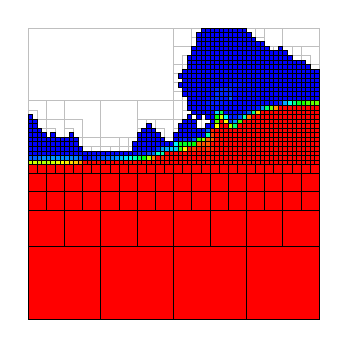
\begin{tikzpicture}[x={(\screenshotunitlength,0)},y={(0,\screenshotunitlength)}]
       \definecolor{fillcolor}{rgb}{1.000000,0.000000,0.000000}
\fill[fillcolor] (0.000000,0.000000) rectangle (0.250000,0.250000);
\definecolor{fillcolor}{rgb}{1.000000,0.000000,0.000000}
\fill[fillcolor] (0.250000,0.000000) rectangle (0.500000,0.250000);
\definecolor{fillcolor}{rgb}{1.000000,0.000000,0.000000}
\fill[fillcolor] (0.000000,0.250000) rectangle (0.125000,0.375000);
\definecolor{fillcolor}{rgb}{1.000000,0.000000,0.000000}
\fill[fillcolor] (0.125000,0.250000) rectangle (0.250000,0.375000);
\definecolor{fillcolor}{rgb}{1.000000,0.000000,0.000000}
\fill[fillcolor] (0.000000,0.375000) rectangle (0.062500,0.437500);
\definecolor{fillcolor}{rgb}{1.000000,0.000000,0.000000}
\fill[fillcolor] (0.062500,0.375000) rectangle (0.125000,0.437500);
\definecolor{fillcolor}{rgb}{1.000000,0.000000,0.000000}
\fill[fillcolor] (0.000000,0.437500) rectangle (0.062500,0.500000);
\definecolor{fillcolor}{rgb}{1.000000,0.000000,0.000000}
\fill[fillcolor] (0.062500,0.437500) rectangle (0.125000,0.500000);
\definecolor{fillcolor}{rgb}{1.000000,0.000000,0.000000}
\fill[fillcolor] (0.125000,0.375000) rectangle (0.187500,0.437500);
\definecolor{fillcolor}{rgb}{1.000000,0.000000,0.000000}
\fill[fillcolor] (0.187500,0.375000) rectangle (0.250000,0.437500);
\definecolor{fillcolor}{rgb}{1.000000,0.000000,0.000000}
\fill[fillcolor] (0.125000,0.437500) rectangle (0.187500,0.500000);
\definecolor{fillcolor}{rgb}{1.000000,0.000000,0.000000}
\fill[fillcolor] (0.187500,0.437500) rectangle (0.250000,0.500000);
\definecolor{fillcolor}{rgb}{1.000000,0.000000,0.000000}
\fill[fillcolor] (0.250000,0.250000) rectangle (0.375000,0.375000);
\definecolor{fillcolor}{rgb}{1.000000,0.000000,0.000000}
\fill[fillcolor] (0.375000,0.250000) rectangle (0.500000,0.375000);
\definecolor{fillcolor}{rgb}{1.000000,0.000000,0.000000}
\fill[fillcolor] (0.250000,0.375000) rectangle (0.312500,0.437500);
\definecolor{fillcolor}{rgb}{1.000000,0.000000,0.000000}
\fill[fillcolor] (0.312500,0.375000) rectangle (0.375000,0.437500);
\definecolor{fillcolor}{rgb}{1.000000,0.000000,0.000000}
\fill[fillcolor] (0.250000,0.437500) rectangle (0.312500,0.500000);
\definecolor{fillcolor}{rgb}{1.000000,0.000000,0.000000}
\fill[fillcolor] (0.312500,0.437500) rectangle (0.375000,0.500000);
\definecolor{fillcolor}{rgb}{1.000000,0.000000,0.000000}
\fill[fillcolor] (0.375000,0.375000) rectangle (0.437500,0.437500);
\definecolor{fillcolor}{rgb}{1.000000,0.000000,0.000000}
\fill[fillcolor] (0.437500,0.375000) rectangle (0.500000,0.437500);
\definecolor{fillcolor}{rgb}{1.000000,0.000001,0.000000}
\fill[fillcolor] (0.375000,0.437500) rectangle (0.437500,0.500000);
\definecolor{fillcolor}{rgb}{1.000000,0.000000,0.000000}
\fill[fillcolor] (0.437500,0.437500) rectangle (0.500000,0.500000);
\definecolor{fillcolor}{rgb}{1.000000,0.000000,0.000000}
\fill[fillcolor] (0.500000,0.000000) rectangle (0.750000,0.250000);
\definecolor{fillcolor}{rgb}{1.000000,0.000000,0.000000}
\fill[fillcolor] (0.750000,0.000000) rectangle (1.000000,0.250000);
\definecolor{fillcolor}{rgb}{1.000000,0.000000,0.000000}
\fill[fillcolor] (0.500000,0.250000) rectangle (0.625000,0.375000);
\definecolor{fillcolor}{rgb}{1.000000,0.000000,0.000000}
\fill[fillcolor] (0.625000,0.250000) rectangle (0.750000,0.375000);
\definecolor{fillcolor}{rgb}{1.000000,0.000000,0.000000}
\fill[fillcolor] (0.500000,0.375000) rectangle (0.562500,0.437500);
\definecolor{fillcolor}{rgb}{1.000000,0.000000,0.000000}
\fill[fillcolor] (0.562500,0.375000) rectangle (0.625000,0.437500);
\definecolor{fillcolor}{rgb}{1.000000,0.000000,0.000000}
\fill[fillcolor] (0.500000,0.437500) rectangle (0.562500,0.500000);
\definecolor{fillcolor}{rgb}{1.000000,0.000000,0.000000}
\fill[fillcolor] (0.562500,0.437500) rectangle (0.625000,0.500000);
\definecolor{fillcolor}{rgb}{1.000000,0.000000,0.000000}
\fill[fillcolor] (0.625000,0.375000) rectangle (0.687500,0.437500);
\definecolor{fillcolor}{rgb}{1.000000,0.000000,0.000000}
\fill[fillcolor] (0.687500,0.375000) rectangle (0.750000,0.437500);
\definecolor{fillcolor}{rgb}{1.000000,0.000000,0.000000}
\fill[fillcolor] (0.625000,0.437500) rectangle (0.687500,0.500000);
\definecolor{fillcolor}{rgb}{1.000000,0.000000,0.000000}
\fill[fillcolor] (0.687500,0.437500) rectangle (0.750000,0.500000);
\definecolor{fillcolor}{rgb}{1.000000,0.000000,0.000000}
\fill[fillcolor] (0.750000,0.250000) rectangle (0.875000,0.375000);
\definecolor{fillcolor}{rgb}{1.000000,0.000000,0.000000}
\fill[fillcolor] (0.875000,0.250000) rectangle (1.000000,0.375000);
\definecolor{fillcolor}{rgb}{1.000000,0.000000,0.000000}
\fill[fillcolor] (0.750000,0.375000) rectangle (0.812500,0.437500);
\definecolor{fillcolor}{rgb}{1.000000,0.000000,0.000000}
\fill[fillcolor] (0.812500,0.375000) rectangle (0.875000,0.437500);
\definecolor{fillcolor}{rgb}{1.000000,0.000000,0.000000}
\fill[fillcolor] (0.750000,0.437500) rectangle (0.812500,0.500000);
\definecolor{fillcolor}{rgb}{1.000000,0.000000,0.000000}
\fill[fillcolor] (0.812500,0.437500) rectangle (0.875000,0.500000);
\definecolor{fillcolor}{rgb}{1.000000,0.000000,0.000000}
\fill[fillcolor] (0.875000,0.375000) rectangle (0.937500,0.437500);
\definecolor{fillcolor}{rgb}{1.000000,0.000000,0.000000}
\fill[fillcolor] (0.937500,0.375000) rectangle (1.000000,0.437500);
\definecolor{fillcolor}{rgb}{1.000000,0.000000,0.000000}
\fill[fillcolor] (0.875000,0.437500) rectangle (0.937500,0.500000);
\definecolor{fillcolor}{rgb}{1.000000,0.000000,0.000000}
\fill[fillcolor] (0.937500,0.437500) rectangle (1.000000,0.500000);
\definecolor{fillcolor}{rgb}{1.000000,0.000000,0.000000}
\fill[fillcolor] (0.000000,0.500000) rectangle (0.031250,0.531250);
\definecolor{fillcolor}{rgb}{1.000000,0.000000,0.000000}
\fill[fillcolor] (0.031250,0.500000) rectangle (0.062500,0.531250);
\definecolor{fillcolor}{rgb}{0.786335,1.000000,0.000000}
\fill[fillcolor] (0.000000,0.531250) rectangle (0.015625,0.546875);
\definecolor{fillcolor}{rgb}{0.818499,1.000000,0.000000}
\fill[fillcolor] (0.015625,0.531250) rectangle (0.031250,0.546875);
\definecolor{fillcolor}{rgb}{0.000000,0.368755,1.000000}
\fill[fillcolor] (0.000000,0.546875) rectangle (0.015625,0.562500);
\definecolor{fillcolor}{rgb}{0.000000,0.370739,1.000000}
\fill[fillcolor] (0.015625,0.546875) rectangle (0.031250,0.562500);
\definecolor{fillcolor}{rgb}{0.761564,1.000000,0.000000}
\fill[fillcolor] (0.031250,0.531250) rectangle (0.046875,0.546875);
\definecolor{fillcolor}{rgb}{0.692127,1.000000,0.000000}
\fill[fillcolor] (0.046875,0.531250) rectangle (0.062500,0.546875);
\definecolor{fillcolor}{rgb}{0.000000,0.458753,1.000000}
\fill[fillcolor] (0.031250,0.546875) rectangle (0.046875,0.562500);
\definecolor{fillcolor}{rgb}{0.000000,0.554519,1.000000}
\fill[fillcolor] (0.046875,0.546875) rectangle (0.062500,0.562500);
\definecolor{fillcolor}{rgb}{1.000000,0.000000,0.000000}
\fill[fillcolor] (0.062500,0.500000) rectangle (0.093750,0.531250);
\definecolor{fillcolor}{rgb}{1.000000,0.000000,0.000000}
\fill[fillcolor] (0.093750,0.500000) rectangle (0.125000,0.531250);
\definecolor{fillcolor}{rgb}{0.725834,1.000000,0.000000}
\fill[fillcolor] (0.062500,0.531250) rectangle (0.078125,0.546875);
\definecolor{fillcolor}{rgb}{0.806310,1.000000,0.000000}
\fill[fillcolor] (0.078125,0.531250) rectangle (0.093750,0.546875);
\definecolor{fillcolor}{rgb}{0.000000,0.514022,1.000000}
\fill[fillcolor] (0.062500,0.546875) rectangle (0.078125,0.562500);
\definecolor{fillcolor}{rgb}{0.000000,0.602075,1.000000}
\fill[fillcolor] (0.078125,0.546875) rectangle (0.093750,0.562500);
\definecolor{fillcolor}{rgb}{0.910824,1.000000,0.000000}
\fill[fillcolor] (0.093750,0.531250) rectangle (0.109375,0.546875);
\definecolor{fillcolor}{rgb}{1.000000,0.978978,0.000000}
\fill[fillcolor] (0.109375,0.531250) rectangle (0.125000,0.546875);
\definecolor{fillcolor}{rgb}{0.000000,0.564182,1.000000}
\fill[fillcolor] (0.093750,0.546875) rectangle (0.109375,0.562500);
\definecolor{fillcolor}{rgb}{0.000000,0.561726,1.000000}
\fill[fillcolor] (0.109375,0.546875) rectangle (0.125000,0.562500);
\definecolor{fillcolor}{rgb}{0.000000,0.005371,1.000000}
\fill[fillcolor] (0.000000,0.562500) rectangle (0.015625,0.578125);
\definecolor{fillcolor}{rgb}{0.000000,0.002031,1.000000}
\fill[fillcolor] (0.015625,0.562500) rectangle (0.031250,0.578125);
\definecolor{fillcolor}{rgb}{0.000000,0.024537,1.000000}
\fill[fillcolor] (0.000000,0.578125) rectangle (0.015625,0.593750);
\definecolor{fillcolor}{rgb}{0.000000,0.027126,1.000000}
\fill[fillcolor] (0.015625,0.578125) rectangle (0.031250,0.593750);
\definecolor{fillcolor}{rgb}{0.000000,0.002063,1.000000}
\fill[fillcolor] (0.031250,0.562500) rectangle (0.046875,0.578125);
\definecolor{fillcolor}{rgb}{0.000000,0.002041,1.000000}
\fill[fillcolor] (0.046875,0.562500) rectangle (0.062500,0.578125);
\definecolor{fillcolor}{rgb}{0.000000,0.003104,1.000000}
\fill[fillcolor] (0.031250,0.578125) rectangle (0.046875,0.593750);
\definecolor{fillcolor}{rgb}{0.000000,0.003003,1.000000}
\fill[fillcolor] (0.046875,0.578125) rectangle (0.062500,0.593750);
\definecolor{fillcolor}{rgb}{0.000000,0.004862,1.000000}
\fill[fillcolor] (0.000000,0.593750) rectangle (0.015625,0.609375);
\definecolor{fillcolor}{rgb}{0.000000,0.005401,1.000000}
\fill[fillcolor] (0.015625,0.593750) rectangle (0.031250,0.609375);
\definecolor{fillcolor}{rgb}{0.000000,0.000208,1.000000}
\fill[fillcolor] (0.000000,0.609375) rectangle (0.015625,0.625000);
\definecolor{fillcolor}{rgb}{0.000000,0.000308,1.000000}
\fill[fillcolor] (0.015625,0.609375) rectangle (0.031250,0.625000);
\definecolor{fillcolor}{rgb}{0.000000,0.000680,1.000000}
\fill[fillcolor] (0.031250,0.593750) rectangle (0.046875,0.609375);
\definecolor{fillcolor}{rgb}{0.000000,0.000000,1.000000}
\fill[fillcolor] (0.046875,0.593750) rectangle (0.062500,0.609375);
\definecolor{fillcolor}{rgb}{0.000000,0.000002,1.000000}
\fill[fillcolor] (0.031250,0.609375) rectangle (0.046875,0.625000);
\definecolor{fillcolor}{rgb}{0.000000,0.000000,1.000000}
\fill[fillcolor] (0.046875,0.609375) rectangle (0.062500,0.625000);
\definecolor{fillcolor}{rgb}{0.000000,0.000077,1.000000}
\fill[fillcolor] (0.062500,0.562500) rectangle (0.078125,0.578125);
\definecolor{fillcolor}{rgb}{0.000000,0.001494,1.000000}
\fill[fillcolor] (0.078125,0.562500) rectangle (0.093750,0.578125);
\definecolor{fillcolor}{rgb}{0.000000,0.000408,1.000000}
\fill[fillcolor] (0.062500,0.578125) rectangle (0.078125,0.593750);
\definecolor{fillcolor}{rgb}{0.000000,0.003336,1.000000}
\fill[fillcolor] (0.078125,0.578125) rectangle (0.093750,0.593750);
\definecolor{fillcolor}{rgb}{0.000000,0.000871,1.000000}
\fill[fillcolor] (0.093750,0.562500) rectangle (0.109375,0.578125);
\definecolor{fillcolor}{rgb}{0.000000,0.003090,1.000000}
\fill[fillcolor] (0.109375,0.562500) rectangle (0.125000,0.578125);
\definecolor{fillcolor}{rgb}{0.000000,0.000457,1.000000}
\fill[fillcolor] (0.093750,0.578125) rectangle (0.109375,0.593750);
\definecolor{fillcolor}{rgb}{0.000000,0.007528,1.000000}
\fill[fillcolor] (0.109375,0.578125) rectangle (0.125000,0.593750);
\definecolor{fillcolor}{rgb}{0.000000,0.000000,1.000000}
\fill[fillcolor] (0.062500,0.593750) rectangle (0.078125,0.609375);
\definecolor{fillcolor}{rgb}{0.000000,0.000000,1.000000}
\fill[fillcolor] (0.078125,0.593750) rectangle (0.093750,0.609375);
\definecolor{fillcolor}{rgb}{0.000000,0.000000,1.000000}
\fill[fillcolor] (0.062500,0.609375) rectangle (0.078125,0.625000);
\definecolor{fillcolor}{rgb}{0.000000,0.000000,1.000000}
\fill[fillcolor] (0.078125,0.609375) rectangle (0.093750,0.625000);
\definecolor{fillcolor}{rgb}{0.000000,0.000000,1.000000}
\fill[fillcolor] (0.093750,0.593750) rectangle (0.109375,0.609375);
\definecolor{fillcolor}{rgb}{0.000000,0.000425,1.000000}
\fill[fillcolor] (0.109375,0.593750) rectangle (0.125000,0.609375);
\definecolor{fillcolor}{rgb}{0.000000,0.000000,1.000000}
\fill[fillcolor] (0.093750,0.609375) rectangle (0.109375,0.625000);
\definecolor{fillcolor}{rgb}{0.000000,0.000000,1.000000}
\fill[fillcolor] (0.109375,0.609375) rectangle (0.125000,0.625000);
\definecolor{fillcolor}{rgb}{1.000000,0.000000,0.000000}
\fill[fillcolor] (0.125000,0.500000) rectangle (0.156250,0.531250);
\definecolor{fillcolor}{rgb}{1.000000,0.000000,0.000000}
\fill[fillcolor] (0.156250,0.500000) rectangle (0.187500,0.531250);
\definecolor{fillcolor}{rgb}{1.000000,0.910101,0.000000}
\fill[fillcolor] (0.125000,0.531250) rectangle (0.140625,0.546875);
\definecolor{fillcolor}{rgb}{1.000000,0.841813,0.000000}
\fill[fillcolor] (0.140625,0.531250) rectangle (0.156250,0.546875);
\definecolor{fillcolor}{rgb}{0.000000,0.531929,1.000000}
\fill[fillcolor] (0.125000,0.546875) rectangle (0.140625,0.562500);
\definecolor{fillcolor}{rgb}{0.000000,0.510398,1.000000}
\fill[fillcolor] (0.140625,0.546875) rectangle (0.156250,0.562500);
\definecolor{fillcolor}{rgb}{1.000000,0.771755,0.000000}
\fill[fillcolor] (0.156250,0.531250) rectangle (0.171875,0.546875);
\definecolor{fillcolor}{rgb}{1.000000,0.597327,0.000000}
\fill[fillcolor] (0.171875,0.531250) rectangle (0.187500,0.546875);
\definecolor{fillcolor}{rgb}{0.000000,0.486987,1.000000}
\fill[fillcolor] (0.156250,0.546875) rectangle (0.171875,0.562500);
\definecolor{fillcolor}{rgb}{0.000000,0.391118,1.000000}
\fill[fillcolor] (0.171875,0.546875) rectangle (0.187500,0.562500);
\definecolor{fillcolor}{rgb}{1.000000,0.000000,0.000000}
\fill[fillcolor] (0.187500,0.500000) rectangle (0.218750,0.531250);
\definecolor{fillcolor}{rgb}{1.000000,0.000000,0.000000}
\fill[fillcolor] (0.218750,0.500000) rectangle (0.250000,0.531250);
\definecolor{fillcolor}{rgb}{1.000000,0.021904,0.000000}
\fill[fillcolor] (0.187500,0.531250) rectangle (0.203125,0.546875);
\definecolor{fillcolor}{rgb}{1.000000,0.035578,0.000000}
\fill[fillcolor] (0.203125,0.531250) rectangle (0.218750,0.546875);
\definecolor{fillcolor}{rgb}{0.000000,0.043664,1.000000}
\fill[fillcolor] (0.187500,0.546875) rectangle (0.203125,0.562500);
\definecolor{fillcolor}{rgb}{0.000000,0.139878,1.000000}
\fill[fillcolor] (0.203125,0.546875) rectangle (0.218750,0.562500);
\definecolor{fillcolor}{rgb}{1.000000,0.024245,0.000000}
\fill[fillcolor] (0.218750,0.531250) rectangle (0.234375,0.546875);
\definecolor{fillcolor}{rgb}{1.000000,0.032685,0.000000}
\fill[fillcolor] (0.234375,0.531250) rectangle (0.250000,0.546875);
\definecolor{fillcolor}{rgb}{0.000000,0.193813,1.000000}
\fill[fillcolor] (0.218750,0.546875) rectangle (0.234375,0.562500);
\definecolor{fillcolor}{rgb}{0.000000,0.249775,1.000000}
\fill[fillcolor] (0.234375,0.546875) rectangle (0.250000,0.562500);
\definecolor{fillcolor}{rgb}{0.000000,0.007806,1.000000}
\fill[fillcolor] (0.125000,0.562500) rectangle (0.140625,0.578125);
\definecolor{fillcolor}{rgb}{0.000000,0.008878,1.000000}
\fill[fillcolor] (0.140625,0.562500) rectangle (0.156250,0.578125);
\definecolor{fillcolor}{rgb}{0.000000,0.003012,1.000000}
\fill[fillcolor] (0.125000,0.578125) rectangle (0.140625,0.593750);
\definecolor{fillcolor}{rgb}{0.000000,0.001244,1.000000}
\fill[fillcolor] (0.140625,0.578125) rectangle (0.156250,0.593750);
\definecolor{fillcolor}{rgb}{0.000000,0.000000,1.000000}
\fill[fillcolor] (0.156250,0.562500) rectangle (0.171875,0.578125);
\definecolor{fillcolor}{rgb}{0.000000,0.000000,1.000000}
\fill[fillcolor] (0.171875,0.562500) rectangle (0.187500,0.578125);
\definecolor{fillcolor}{rgb}{0.000000,0.000258,1.000000}
\fill[fillcolor] (0.156250,0.578125) rectangle (0.171875,0.593750);
\definecolor{fillcolor}{rgb}{0.000000,0.000000,1.000000}
\fill[fillcolor] (0.171875,0.578125) rectangle (0.187500,0.593750);
\definecolor{fillcolor}{rgb}{0.000000,0.000000,1.000000}
\fill[fillcolor] (0.125000,0.593750) rectangle (0.140625,0.609375);
\definecolor{fillcolor}{rgb}{0.000000,0.000003,1.000000}
\fill[fillcolor] (0.140625,0.593750) rectangle (0.156250,0.609375);
\definecolor{fillcolor}{rgb}{0.000000,0.000000,1.000000}
\fill[fillcolor] (0.125000,0.609375) rectangle (0.140625,0.625000);
\definecolor{fillcolor}{rgb}{0.000000,0.000000,1.000000}
\fill[fillcolor] (0.140625,0.609375) rectangle (0.156250,0.625000);
\definecolor{fillcolor}{rgb}{0.000000,0.000000,1.000000}
\fill[fillcolor] (0.156250,0.593750) rectangle (0.171875,0.609375);
\definecolor{fillcolor}{rgb}{0.000000,0.000000,1.000000}
\fill[fillcolor] (0.156250,0.609375) rectangle (0.171875,0.625000);
\definecolor{fillcolor}{rgb}{0.000000,0.000000,1.000000}
\fill[fillcolor] (0.187500,0.562500) rectangle (0.203125,0.578125);
\definecolor{fillcolor}{rgb}{0.000000,0.000000,1.000000}
\fill[fillcolor] (0.203125,0.562500) rectangle (0.218750,0.578125);
\definecolor{fillcolor}{rgb}{0.000000,0.000000,1.000000}
\fill[fillcolor] (0.218750,0.562500) rectangle (0.234375,0.578125);
\definecolor{fillcolor}{rgb}{0.000000,0.000000,1.000000}
\fill[fillcolor] (0.234375,0.562500) rectangle (0.250000,0.578125);
\definecolor{fillcolor}{rgb}{0.000000,0.000000,1.000000}
\fill[fillcolor] (0.000000,0.625000) rectangle (0.015625,0.640625);
\definecolor{fillcolor}{rgb}{0.000000,0.000002,1.000000}
\fill[fillcolor] (0.015625,0.625000) rectangle (0.031250,0.640625);
\definecolor{fillcolor}{rgb}{0.000000,0.000000,1.000000}
\fill[fillcolor] (0.000000,0.640625) rectangle (0.015625,0.656250);
\definecolor{fillcolor}{rgb}{0.000000,0.000000,1.000000}
\fill[fillcolor] (0.015625,0.640625) rectangle (0.031250,0.656250);
\definecolor{fillcolor}{rgb}{0.000000,0.000000,1.000000}
\fill[fillcolor] (0.031250,0.625000) rectangle (0.046875,0.640625);
\definecolor{fillcolor}{rgb}{0.000000,0.000000,1.000000}
\fill[fillcolor] (0.046875,0.625000) rectangle (0.062500,0.640625);
\definecolor{fillcolor}{rgb}{0.000000,0.000000,1.000000}
\fill[fillcolor] (0.031250,0.640625) rectangle (0.046875,0.656250);
\definecolor{fillcolor}{rgb}{0.000000,0.000000,1.000000}
\fill[fillcolor] (0.000000,0.656250) rectangle (0.015625,0.671875);
\definecolor{fillcolor}{rgb}{0.000000,0.000000,1.000000}
\fill[fillcolor] (0.015625,0.656250) rectangle (0.031250,0.671875);
\definecolor{fillcolor}{rgb}{0.000000,0.000000,1.000000}
\fill[fillcolor] (0.000000,0.671875) rectangle (0.015625,0.687500);
\definecolor{fillcolor}{rgb}{0.000000,0.000000,1.000000}
\fill[fillcolor] (0.015625,0.671875) rectangle (0.031250,0.687500);
\definecolor{fillcolor}{rgb}{0.000000,0.000000,1.000000}
\fill[fillcolor] (0.078125,0.625000) rectangle (0.093750,0.640625);
\definecolor{fillcolor}{rgb}{0.000000,0.000000,1.000000}
\fill[fillcolor] (0.000000,0.687500) rectangle (0.015625,0.703125);
\definecolor{fillcolor}{rgb}{0.000000,0.000000,1.000000}
\fill[fillcolor] (0.140625,0.625000) rectangle (0.156250,0.640625);
\definecolor{fillcolor}{rgb}{1.000000,0.000000,0.000000}
\fill[fillcolor] (0.250000,0.500000) rectangle (0.281250,0.531250);
\definecolor{fillcolor}{rgb}{1.000000,0.000000,0.000000}
\fill[fillcolor] (0.281250,0.500000) rectangle (0.312500,0.531250);
\definecolor{fillcolor}{rgb}{1.000000,0.000000,0.000000}
\fill[fillcolor] (0.250000,0.531250) rectangle (0.265625,0.546875);
\definecolor{fillcolor}{rgb}{1.000000,0.000000,0.000000}
\fill[fillcolor] (0.265625,0.531250) rectangle (0.281250,0.546875);
\definecolor{fillcolor}{rgb}{0.000000,0.337607,1.000000}
\fill[fillcolor] (0.250000,0.546875) rectangle (0.265625,0.562500);
\definecolor{fillcolor}{rgb}{0.000000,0.386640,1.000000}
\fill[fillcolor] (0.265625,0.546875) rectangle (0.281250,0.562500);
\definecolor{fillcolor}{rgb}{1.000000,0.000000,0.000000}
\fill[fillcolor] (0.281250,0.531250) rectangle (0.296875,0.546875);
\definecolor{fillcolor}{rgb}{1.000000,0.000000,0.000000}
\fill[fillcolor] (0.296875,0.531250) rectangle (0.312500,0.546875);
\definecolor{fillcolor}{rgb}{0.000000,0.484567,1.000000}
\fill[fillcolor] (0.281250,0.546875) rectangle (0.296875,0.562500);
\definecolor{fillcolor}{rgb}{0.000000,0.567546,1.000000}
\fill[fillcolor] (0.296875,0.546875) rectangle (0.312500,0.562500);
\definecolor{fillcolor}{rgb}{1.000000,0.000000,0.000000}
\fill[fillcolor] (0.312500,0.500000) rectangle (0.343750,0.531250);
\definecolor{fillcolor}{rgb}{1.000000,0.000575,0.000000}
\fill[fillcolor] (0.343750,0.500000) rectangle (0.375000,0.531250);
\definecolor{fillcolor}{rgb}{1.000000,0.000000,0.000000}
\fill[fillcolor] (0.312500,0.531250) rectangle (0.328125,0.546875);
\definecolor{fillcolor}{rgb}{1.000000,0.002785,0.000000}
\fill[fillcolor] (0.328125,0.531250) rectangle (0.343750,0.546875);
\definecolor{fillcolor}{rgb}{0.000000,0.770237,1.000000}
\fill[fillcolor] (0.312500,0.546875) rectangle (0.328125,0.562500);
\definecolor{fillcolor}{rgb}{0.000000,0.895280,1.000000}
\fill[fillcolor] (0.328125,0.546875) rectangle (0.343750,0.562500);
\definecolor{fillcolor}{rgb}{1.000000,0.048923,0.000000}
\fill[fillcolor] (0.343750,0.531250) rectangle (0.359375,0.546875);
\definecolor{fillcolor}{rgb}{1.000000,0.033607,0.000000}
\fill[fillcolor] (0.359375,0.531250) rectangle (0.375000,0.546875);
\definecolor{fillcolor}{rgb}{0.000000,1.000000,0.908382}
\fill[fillcolor] (0.343750,0.546875) rectangle (0.359375,0.562500);
\definecolor{fillcolor}{rgb}{0.000000,1.000000,0.727053}
\fill[fillcolor] (0.359375,0.546875) rectangle (0.375000,0.562500);
\definecolor{fillcolor}{rgb}{0.000000,0.000000,1.000000}
\fill[fillcolor] (0.250000,0.562500) rectangle (0.265625,0.578125);
\definecolor{fillcolor}{rgb}{0.000000,0.000000,1.000000}
\fill[fillcolor] (0.265625,0.562500) rectangle (0.281250,0.578125);
\definecolor{fillcolor}{rgb}{0.000000,0.000000,1.000000}
\fill[fillcolor] (0.281250,0.562500) rectangle (0.296875,0.578125);
\definecolor{fillcolor}{rgb}{0.000000,0.000000,1.000000}
\fill[fillcolor] (0.296875,0.562500) rectangle (0.312500,0.578125);
\definecolor{fillcolor}{rgb}{0.000000,0.000000,1.000000}
\fill[fillcolor] (0.312500,0.562500) rectangle (0.328125,0.578125);
\definecolor{fillcolor}{rgb}{0.000000,0.000000,1.000000}
\fill[fillcolor] (0.328125,0.562500) rectangle (0.343750,0.578125);
\definecolor{fillcolor}{rgb}{0.000000,0.000000,1.000000}
\fill[fillcolor] (0.343750,0.562500) rectangle (0.359375,0.578125);
\definecolor{fillcolor}{rgb}{0.000000,0.016662,1.000000}
\fill[fillcolor] (0.359375,0.562500) rectangle (0.375000,0.578125);
\definecolor{fillcolor}{rgb}{0.000000,0.000000,1.000000}
\fill[fillcolor] (0.359375,0.578125) rectangle (0.375000,0.593750);
\definecolor{fillcolor}{rgb}{0.000000,0.000000,1.000000}
\fill[fillcolor] (0.359375,0.593750) rectangle (0.375000,0.609375);
\definecolor{fillcolor}{rgb}{1.000000,0.000000,0.000000}
\fill[fillcolor] (0.375000,0.500000) rectangle (0.406250,0.531250);
\definecolor{fillcolor}{rgb}{1.000000,0.000000,0.000000}
\fill[fillcolor] (0.406250,0.500000) rectangle (0.437500,0.531250);
\definecolor{fillcolor}{rgb}{1.000000,0.000000,0.000000}
\fill[fillcolor] (0.375000,0.531250) rectangle (0.390625,0.546875);
\definecolor{fillcolor}{rgb}{1.000000,0.000001,0.000000}
\fill[fillcolor] (0.390625,0.531250) rectangle (0.406250,0.546875);
\definecolor{fillcolor}{rgb}{0.000000,1.000000,0.345632}
\fill[fillcolor] (0.375000,0.546875) rectangle (0.390625,0.562500);
\definecolor{fillcolor}{rgb}{0.000000,1.000000,0.051956}
\fill[fillcolor] (0.390625,0.546875) rectangle (0.406250,0.562500);
\definecolor{fillcolor}{rgb}{1.000000,0.000003,0.000000}
\fill[fillcolor] (0.406250,0.531250) rectangle (0.421875,0.546875);
\definecolor{fillcolor}{rgb}{1.000000,0.000000,0.000000}
\fill[fillcolor] (0.421875,0.531250) rectangle (0.437500,0.546875);
\definecolor{fillcolor}{rgb}{0.660482,1.000000,0.000000}
\fill[fillcolor] (0.406250,0.546875) rectangle (0.421875,0.562500);
\definecolor{fillcolor}{rgb}{1.000000,0.496983,0.000000}
\fill[fillcolor] (0.421875,0.546875) rectangle (0.437500,0.562500);
\definecolor{fillcolor}{rgb}{1.000000,0.000000,0.000000}
\fill[fillcolor] (0.437500,0.500000) rectangle (0.468750,0.531250);
\definecolor{fillcolor}{rgb}{1.000000,0.000000,0.000000}
\fill[fillcolor] (0.468750,0.500000) rectangle (0.500000,0.531250);
\definecolor{fillcolor}{rgb}{1.000000,0.000000,0.000000}
\fill[fillcolor] (0.437500,0.531250) rectangle (0.453125,0.546875);
\definecolor{fillcolor}{rgb}{1.000000,0.000000,0.000000}
\fill[fillcolor] (0.453125,0.531250) rectangle (0.468750,0.546875);
\definecolor{fillcolor}{rgb}{1.000000,0.024911,0.000000}
\fill[fillcolor] (0.437500,0.546875) rectangle (0.453125,0.562500);
\definecolor{fillcolor}{rgb}{1.000000,0.147594,0.000000}
\fill[fillcolor] (0.453125,0.546875) rectangle (0.468750,0.562500);
\definecolor{fillcolor}{rgb}{1.000000,0.000000,0.000000}
\fill[fillcolor] (0.468750,0.531250) rectangle (0.484375,0.546875);
\definecolor{fillcolor}{rgb}{1.000000,0.000000,0.000000}
\fill[fillcolor] (0.484375,0.531250) rectangle (0.500000,0.546875);
\definecolor{fillcolor}{rgb}{1.000000,0.047600,0.000000}
\fill[fillcolor] (0.468750,0.546875) rectangle (0.484375,0.562500);
\definecolor{fillcolor}{rgb}{1.000000,0.012806,0.000000}
\fill[fillcolor] (0.484375,0.546875) rectangle (0.500000,0.562500);
\definecolor{fillcolor}{rgb}{0.000000,0.169194,1.000000}
\fill[fillcolor] (0.375000,0.562500) rectangle (0.390625,0.578125);
\definecolor{fillcolor}{rgb}{0.000000,0.103535,1.000000}
\fill[fillcolor] (0.390625,0.562500) rectangle (0.406250,0.578125);
\definecolor{fillcolor}{rgb}{0.000000,0.011151,1.000000}
\fill[fillcolor] (0.375000,0.578125) rectangle (0.390625,0.593750);
\definecolor{fillcolor}{rgb}{0.000000,0.018035,1.000000}
\fill[fillcolor] (0.390625,0.578125) rectangle (0.406250,0.593750);
\definecolor{fillcolor}{rgb}{0.000000,0.262753,1.000000}
\fill[fillcolor] (0.406250,0.562500) rectangle (0.421875,0.578125);
\definecolor{fillcolor}{rgb}{0.000000,0.411030,1.000000}
\fill[fillcolor] (0.421875,0.562500) rectangle (0.437500,0.578125);
\definecolor{fillcolor}{rgb}{0.000000,0.008394,1.000000}
\fill[fillcolor] (0.406250,0.578125) rectangle (0.421875,0.593750);
\definecolor{fillcolor}{rgb}{0.000000,0.000000,1.000000}
\fill[fillcolor] (0.421875,0.578125) rectangle (0.437500,0.593750);
\definecolor{fillcolor}{rgb}{0.000000,0.002909,1.000000}
\fill[fillcolor] (0.375000,0.593750) rectangle (0.390625,0.609375);
\definecolor{fillcolor}{rgb}{0.000000,0.011259,1.000000}
\fill[fillcolor] (0.390625,0.593750) rectangle (0.406250,0.609375);
\definecolor{fillcolor}{rgb}{0.000000,0.000000,1.000000}
\fill[fillcolor] (0.375000,0.609375) rectangle (0.390625,0.625000);
\definecolor{fillcolor}{rgb}{0.000000,0.001518,1.000000}
\fill[fillcolor] (0.390625,0.609375) rectangle (0.406250,0.625000);
\definecolor{fillcolor}{rgb}{0.000000,0.002919,1.000000}
\fill[fillcolor] (0.406250,0.593750) rectangle (0.421875,0.609375);
\definecolor{fillcolor}{rgb}{0.000000,0.000001,1.000000}
\fill[fillcolor] (0.421875,0.593750) rectangle (0.437500,0.609375);
\definecolor{fillcolor}{rgb}{0.000000,0.003964,1.000000}
\fill[fillcolor] (0.406250,0.609375) rectangle (0.421875,0.625000);
\definecolor{fillcolor}{rgb}{0.000000,0.001055,1.000000}
\fill[fillcolor] (0.421875,0.609375) rectangle (0.437500,0.625000);
\definecolor{fillcolor}{rgb}{0.000000,1.000000,0.794635}
\fill[fillcolor] (0.437500,0.562500) rectangle (0.453125,0.578125);
\definecolor{fillcolor}{rgb}{0.000000,1.000000,0.680694}
\fill[fillcolor] (0.453125,0.562500) rectangle (0.468750,0.578125);
\definecolor{fillcolor}{rgb}{0.000000,0.143906,1.000000}
\fill[fillcolor] (0.437500,0.578125) rectangle (0.453125,0.593750);
\definecolor{fillcolor}{rgb}{0.000000,0.590200,1.000000}
\fill[fillcolor] (0.453125,0.578125) rectangle (0.468750,0.593750);
\definecolor{fillcolor}{rgb}{1.000000,0.013697,0.000000}
\fill[fillcolor] (0.468750,0.562500) rectangle (0.484375,0.578125);
\definecolor{fillcolor}{rgb}{1.000000,0.005536,0.000000}
\fill[fillcolor] (0.484375,0.562500) rectangle (0.500000,0.578125);
\definecolor{fillcolor}{rgb}{0.000000,0.676194,1.000000}
\fill[fillcolor] (0.468750,0.578125) rectangle (0.484375,0.593750);
\definecolor{fillcolor}{rgb}{0.000000,0.793608,1.000000}
\fill[fillcolor] (0.484375,0.578125) rectangle (0.500000,0.593750);
\definecolor{fillcolor}{rgb}{0.000000,0.000000,1.000000}
\fill[fillcolor] (0.437500,0.593750) rectangle (0.453125,0.609375);
\definecolor{fillcolor}{rgb}{0.000000,0.000000,1.000000}
\fill[fillcolor] (0.453125,0.593750) rectangle (0.468750,0.609375);
\definecolor{fillcolor}{rgb}{0.000000,0.000138,1.000000}
\fill[fillcolor] (0.437500,0.609375) rectangle (0.453125,0.625000);
\definecolor{fillcolor}{rgb}{0.000000,0.000000,1.000000}
\fill[fillcolor] (0.453125,0.609375) rectangle (0.468750,0.625000);
\definecolor{fillcolor}{rgb}{0.000000,0.000000,1.000000}
\fill[fillcolor] (0.468750,0.593750) rectangle (0.484375,0.609375);
\definecolor{fillcolor}{rgb}{0.000000,0.000000,1.000000}
\fill[fillcolor] (0.484375,0.593750) rectangle (0.500000,0.609375);
\definecolor{fillcolor}{rgb}{0.000000,0.000000,1.000000}
\fill[fillcolor] (0.375000,0.625000) rectangle (0.390625,0.640625);
\definecolor{fillcolor}{rgb}{0.000000,0.001135,1.000000}
\fill[fillcolor] (0.390625,0.625000) rectangle (0.406250,0.640625);
\definecolor{fillcolor}{rgb}{0.000000,0.000000,1.000000}
\fill[fillcolor] (0.390625,0.640625) rectangle (0.406250,0.656250);
\definecolor{fillcolor}{rgb}{0.000000,0.004531,1.000000}
\fill[fillcolor] (0.406250,0.625000) rectangle (0.421875,0.640625);
\definecolor{fillcolor}{rgb}{0.000000,0.001084,1.000000}
\fill[fillcolor] (0.421875,0.625000) rectangle (0.437500,0.640625);
\definecolor{fillcolor}{rgb}{0.000000,0.000519,1.000000}
\fill[fillcolor] (0.406250,0.640625) rectangle (0.421875,0.656250);
\definecolor{fillcolor}{rgb}{0.000000,0.000000,1.000000}
\fill[fillcolor] (0.421875,0.640625) rectangle (0.437500,0.656250);
\definecolor{fillcolor}{rgb}{0.000000,0.000000,1.000000}
\fill[fillcolor] (0.406250,0.656250) rectangle (0.421875,0.671875);
\definecolor{fillcolor}{rgb}{0.000000,0.000000,1.000000}
\fill[fillcolor] (0.437500,0.625000) rectangle (0.453125,0.640625);
\definecolor{fillcolor}{rgb}{1.000000,0.000000,0.000000}
\fill[fillcolor] (0.500000,0.500000) rectangle (0.531250,0.531250);
\definecolor{fillcolor}{rgb}{1.000000,0.000000,0.000000}
\fill[fillcolor] (0.531250,0.500000) rectangle (0.562500,0.531250);
\definecolor{fillcolor}{rgb}{1.000000,0.000000,0.000000}
\fill[fillcolor] (0.500000,0.531250) rectangle (0.515625,0.546875);
\definecolor{fillcolor}{rgb}{1.000000,0.000000,0.000000}
\fill[fillcolor] (0.515625,0.531250) rectangle (0.531250,0.546875);
\definecolor{fillcolor}{rgb}{1.000000,0.006600,0.000000}
\fill[fillcolor] (0.500000,0.546875) rectangle (0.515625,0.562500);
\definecolor{fillcolor}{rgb}{1.000000,0.009622,0.000000}
\fill[fillcolor] (0.515625,0.546875) rectangle (0.531250,0.562500);
\definecolor{fillcolor}{rgb}{1.000000,0.000000,0.000000}
\fill[fillcolor] (0.531250,0.531250) rectangle (0.546875,0.546875);
\definecolor{fillcolor}{rgb}{1.000000,0.000000,0.000000}
\fill[fillcolor] (0.546875,0.531250) rectangle (0.562500,0.546875);
\definecolor{fillcolor}{rgb}{1.000000,0.000000,0.000000}
\fill[fillcolor] (0.531250,0.546875) rectangle (0.546875,0.562500);
\definecolor{fillcolor}{rgb}{1.000000,0.000094,0.000000}
\fill[fillcolor] (0.546875,0.546875) rectangle (0.562500,0.562500);
\definecolor{fillcolor}{rgb}{1.000000,0.000001,0.000000}
\fill[fillcolor] (0.562500,0.500000) rectangle (0.593750,0.531250);
\definecolor{fillcolor}{rgb}{1.000000,0.000011,0.000000}
\fill[fillcolor] (0.593750,0.500000) rectangle (0.625000,0.531250);
\definecolor{fillcolor}{rgb}{1.000000,0.000001,0.000000}
\fill[fillcolor] (0.562500,0.531250) rectangle (0.578125,0.546875);
\definecolor{fillcolor}{rgb}{1.000000,0.000002,0.000000}
\fill[fillcolor] (0.578125,0.531250) rectangle (0.593750,0.546875);
\definecolor{fillcolor}{rgb}{1.000000,0.000872,0.000000}
\fill[fillcolor] (0.562500,0.546875) rectangle (0.578125,0.562500);
\definecolor{fillcolor}{rgb}{1.000000,0.009835,0.000000}
\fill[fillcolor] (0.578125,0.546875) rectangle (0.593750,0.562500);
\definecolor{fillcolor}{rgb}{1.000000,0.000005,0.000000}
\fill[fillcolor] (0.593750,0.531250) rectangle (0.609375,0.546875);
\definecolor{fillcolor}{rgb}{1.000000,0.000037,0.000000}
\fill[fillcolor] (0.609375,0.531250) rectangle (0.625000,0.546875);
\definecolor{fillcolor}{rgb}{1.000000,0.039223,0.000000}
\fill[fillcolor] (0.593750,0.546875) rectangle (0.609375,0.562500);
\definecolor{fillcolor}{rgb}{1.000000,0.047371,0.000000}
\fill[fillcolor] (0.609375,0.546875) rectangle (0.625000,0.562500);
\definecolor{fillcolor}{rgb}{1.000000,0.005528,0.000000}
\fill[fillcolor] (0.500000,0.562500) rectangle (0.515625,0.578125);
\definecolor{fillcolor}{rgb}{1.000000,0.005339,0.000000}
\fill[fillcolor] (0.515625,0.562500) rectangle (0.531250,0.578125);
\definecolor{fillcolor}{rgb}{0.000000,0.789541,1.000000}
\fill[fillcolor] (0.500000,0.578125) rectangle (0.515625,0.593750);
\definecolor{fillcolor}{rgb}{0.202725,1.000000,0.000000}
\fill[fillcolor] (0.515625,0.578125) rectangle (0.531250,0.593750);
\definecolor{fillcolor}{rgb}{1.000000,0.005166,0.000000}
\fill[fillcolor] (0.531250,0.562500) rectangle (0.546875,0.578125);
\definecolor{fillcolor}{rgb}{1.000000,0.005666,0.000000}
\fill[fillcolor] (0.546875,0.562500) rectangle (0.562500,0.578125);
\definecolor{fillcolor}{rgb}{1.000000,0.934123,0.000000}
\fill[fillcolor] (0.531250,0.578125) rectangle (0.546875,0.593750);
\definecolor{fillcolor}{rgb}{1.000000,0.125610,0.000000}
\fill[fillcolor] (0.546875,0.578125) rectangle (0.562500,0.593750);
\definecolor{fillcolor}{rgb}{0.000000,0.949375,1.000000}
\fill[fillcolor] (0.500000,0.593750) rectangle (0.515625,0.609375);
\definecolor{fillcolor}{rgb}{0.000000,1.000000,0.113199}
\fill[fillcolor] (0.515625,0.593750) rectangle (0.531250,0.609375);
\definecolor{fillcolor}{rgb}{0.000000,0.000000,1.000000}
\fill[fillcolor] (0.500000,0.609375) rectangle (0.515625,0.625000);
\definecolor{fillcolor}{rgb}{0.000000,0.101725,1.000000}
\fill[fillcolor] (0.515625,0.609375) rectangle (0.531250,0.625000);
\definecolor{fillcolor}{rgb}{0.000000,1.000000,0.153070}
\fill[fillcolor] (0.531250,0.593750) rectangle (0.546875,0.609375);
\definecolor{fillcolor}{rgb}{0.000000,1.000000,0.192082}
\fill[fillcolor] (0.546875,0.593750) rectangle (0.562500,0.609375);
\definecolor{fillcolor}{rgb}{0.000000,0.176179,1.000000}
\fill[fillcolor] (0.531250,0.609375) rectangle (0.546875,0.625000);
\definecolor{fillcolor}{rgb}{0.000000,0.000000,1.000000}
\fill[fillcolor] (0.546875,0.609375) rectangle (0.562500,0.625000);
\definecolor{fillcolor}{rgb}{1.000000,0.006089,0.000000}
\fill[fillcolor] (0.562500,0.562500) rectangle (0.578125,0.578125);
\definecolor{fillcolor}{rgb}{1.000000,0.006261,0.000000}
\fill[fillcolor] (0.578125,0.562500) rectangle (0.593750,0.578125);
\definecolor{fillcolor}{rgb}{1.000000,0.246424,0.000000}
\fill[fillcolor] (0.562500,0.578125) rectangle (0.578125,0.593750);
\definecolor{fillcolor}{rgb}{1.000000,0.121365,0.000000}
\fill[fillcolor] (0.578125,0.578125) rectangle (0.593750,0.593750);
\definecolor{fillcolor}{rgb}{1.000000,0.005841,0.000000}
\fill[fillcolor] (0.593750,0.562500) rectangle (0.609375,0.578125);
\definecolor{fillcolor}{rgb}{1.000000,0.003479,0.000000}
\fill[fillcolor] (0.609375,0.562500) rectangle (0.625000,0.578125);
\definecolor{fillcolor}{rgb}{1.000000,0.138368,0.000000}
\fill[fillcolor] (0.593750,0.578125) rectangle (0.609375,0.593750);
\definecolor{fillcolor}{rgb}{1.000000,0.167037,0.000000}
\fill[fillcolor] (0.609375,0.578125) rectangle (0.625000,0.593750);
\definecolor{fillcolor}{rgb}{0.000000,1.000000,0.003793}
\fill[fillcolor] (0.562500,0.593750) rectangle (0.578125,0.609375);
\definecolor{fillcolor}{rgb}{1.000000,0.401744,0.000000}
\fill[fillcolor] (0.578125,0.593750) rectangle (0.593750,0.609375);
\definecolor{fillcolor}{rgb}{0.000000,0.339475,1.000000}
\fill[fillcolor] (0.562500,0.609375) rectangle (0.578125,0.625000);
\definecolor{fillcolor}{rgb}{0.164459,1.000000,0.000000}
\fill[fillcolor] (0.578125,0.609375) rectangle (0.593750,0.625000);
\definecolor{fillcolor}{rgb}{1.000000,0.322171,0.000000}
\fill[fillcolor] (0.593750,0.593750) rectangle (0.609375,0.609375);
\definecolor{fillcolor}{rgb}{1.000000,0.361026,0.000000}
\fill[fillcolor] (0.609375,0.593750) rectangle (0.625000,0.609375);
\definecolor{fillcolor}{rgb}{0.510669,1.000000,0.000000}
\fill[fillcolor] (0.593750,0.609375) rectangle (0.609375,0.625000);
\definecolor{fillcolor}{rgb}{1.000000,0.358670,0.000000}
\fill[fillcolor] (0.609375,0.609375) rectangle (0.625000,0.625000);
\definecolor{fillcolor}{rgb}{1.000000,0.000016,0.000000}
\fill[fillcolor] (0.625000,0.500000) rectangle (0.656250,0.531250);
\definecolor{fillcolor}{rgb}{1.000000,0.000000,0.000000}
\fill[fillcolor] (0.656250,0.500000) rectangle (0.687500,0.531250);
\definecolor{fillcolor}{rgb}{1.000000,0.000122,0.000000}
\fill[fillcolor] (0.625000,0.531250) rectangle (0.640625,0.546875);
\definecolor{fillcolor}{rgb}{1.000000,0.000298,0.000000}
\fill[fillcolor] (0.640625,0.531250) rectangle (0.656250,0.546875);
\definecolor{fillcolor}{rgb}{1.000000,0.040020,0.000000}
\fill[fillcolor] (0.625000,0.546875) rectangle (0.640625,0.562500);
\definecolor{fillcolor}{rgb}{1.000000,0.000467,0.000000}
\fill[fillcolor] (0.640625,0.546875) rectangle (0.656250,0.562500);
\definecolor{fillcolor}{rgb}{1.000000,0.000000,0.000000}
\fill[fillcolor] (0.656250,0.531250) rectangle (0.671875,0.546875);
\definecolor{fillcolor}{rgb}{1.000000,0.000000,0.000000}
\fill[fillcolor] (0.671875,0.531250) rectangle (0.687500,0.546875);
\definecolor{fillcolor}{rgb}{1.000000,0.000145,0.000000}
\fill[fillcolor] (0.656250,0.546875) rectangle (0.671875,0.562500);
\definecolor{fillcolor}{rgb}{1.000000,0.000000,0.000000}
\fill[fillcolor] (0.671875,0.546875) rectangle (0.687500,0.562500);
\definecolor{fillcolor}{rgb}{1.000000,0.000000,0.000000}
\fill[fillcolor] (0.687500,0.500000) rectangle (0.718750,0.531250);
\definecolor{fillcolor}{rgb}{1.000000,0.000000,0.000000}
\fill[fillcolor] (0.718750,0.500000) rectangle (0.750000,0.531250);
\definecolor{fillcolor}{rgb}{1.000000,0.000000,0.000000}
\fill[fillcolor] (0.687500,0.531250) rectangle (0.703125,0.546875);
\definecolor{fillcolor}{rgb}{1.000000,0.000000,0.000000}
\fill[fillcolor] (0.703125,0.531250) rectangle (0.718750,0.546875);
\definecolor{fillcolor}{rgb}{1.000000,0.000000,0.000000}
\fill[fillcolor] (0.687500,0.546875) rectangle (0.703125,0.562500);
\definecolor{fillcolor}{rgb}{1.000000,0.000000,0.000000}
\fill[fillcolor] (0.703125,0.546875) rectangle (0.718750,0.562500);
\definecolor{fillcolor}{rgb}{1.000000,0.000000,0.000000}
\fill[fillcolor] (0.718750,0.531250) rectangle (0.734375,0.546875);
\definecolor{fillcolor}{rgb}{1.000000,0.000000,0.000000}
\fill[fillcolor] (0.734375,0.531250) rectangle (0.750000,0.546875);
\definecolor{fillcolor}{rgb}{1.000000,0.000000,0.000000}
\fill[fillcolor] (0.718750,0.546875) rectangle (0.734375,0.562500);
\definecolor{fillcolor}{rgb}{1.000000,0.000000,0.000000}
\fill[fillcolor] (0.734375,0.546875) rectangle (0.750000,0.562500);
\definecolor{fillcolor}{rgb}{1.000000,0.003266,0.000000}
\fill[fillcolor] (0.625000,0.562500) rectangle (0.640625,0.578125);
\definecolor{fillcolor}{rgb}{1.000000,0.002478,0.000000}
\fill[fillcolor] (0.640625,0.562500) rectangle (0.656250,0.578125);
\definecolor{fillcolor}{rgb}{1.000000,0.129596,0.000000}
\fill[fillcolor] (0.625000,0.578125) rectangle (0.640625,0.593750);
\definecolor{fillcolor}{rgb}{1.000000,0.008158,0.000000}
\fill[fillcolor] (0.640625,0.578125) rectangle (0.656250,0.593750);
\definecolor{fillcolor}{rgb}{1.000000,0.001476,0.000000}
\fill[fillcolor] (0.656250,0.562500) rectangle (0.671875,0.578125);
\definecolor{fillcolor}{rgb}{1.000000,0.000051,0.000000}
\fill[fillcolor] (0.671875,0.562500) rectangle (0.687500,0.578125);
\definecolor{fillcolor}{rgb}{1.000000,0.004797,0.000000}
\fill[fillcolor] (0.656250,0.578125) rectangle (0.671875,0.593750);
\definecolor{fillcolor}{rgb}{1.000000,0.000208,0.000000}
\fill[fillcolor] (0.671875,0.578125) rectangle (0.687500,0.593750);
\definecolor{fillcolor}{rgb}{1.000000,0.052310,0.000000}
\fill[fillcolor] (0.625000,0.593750) rectangle (0.640625,0.609375);
\definecolor{fillcolor}{rgb}{1.000000,0.020221,0.000000}
\fill[fillcolor] (0.640625,0.593750) rectangle (0.656250,0.609375);
\definecolor{fillcolor}{rgb}{1.000000,0.356750,0.000000}
\fill[fillcolor] (0.625000,0.609375) rectangle (0.640625,0.625000);
\definecolor{fillcolor}{rgb}{1.000000,0.024478,0.000000}
\fill[fillcolor] (0.640625,0.609375) rectangle (0.656250,0.625000);
\definecolor{fillcolor}{rgb}{1.000000,0.020084,0.000000}
\fill[fillcolor] (0.656250,0.593750) rectangle (0.671875,0.609375);
\definecolor{fillcolor}{rgb}{1.000000,0.000488,0.000000}
\fill[fillcolor] (0.671875,0.593750) rectangle (0.687500,0.609375);
\definecolor{fillcolor}{rgb}{1.000000,0.026552,0.000000}
\fill[fillcolor] (0.656250,0.609375) rectangle (0.671875,0.625000);
\definecolor{fillcolor}{rgb}{1.000000,0.000907,0.000000}
\fill[fillcolor] (0.671875,0.609375) rectangle (0.687500,0.625000);
\definecolor{fillcolor}{rgb}{1.000000,0.000000,0.000000}
\fill[fillcolor] (0.687500,0.562500) rectangle (0.703125,0.578125);
\definecolor{fillcolor}{rgb}{1.000000,0.000000,0.000000}
\fill[fillcolor] (0.703125,0.562500) rectangle (0.718750,0.578125);
\definecolor{fillcolor}{rgb}{1.000000,0.000043,0.000000}
\fill[fillcolor] (0.687500,0.578125) rectangle (0.703125,0.593750);
\definecolor{fillcolor}{rgb}{1.000000,0.000000,0.000000}
\fill[fillcolor] (0.703125,0.578125) rectangle (0.718750,0.593750);
\definecolor{fillcolor}{rgb}{1.000000,0.000000,0.000000}
\fill[fillcolor] (0.718750,0.562500) rectangle (0.734375,0.578125);
\definecolor{fillcolor}{rgb}{1.000000,0.000000,0.000000}
\fill[fillcolor] (0.734375,0.562500) rectangle (0.750000,0.578125);
\definecolor{fillcolor}{rgb}{1.000000,0.000000,0.000000}
\fill[fillcolor] (0.718750,0.578125) rectangle (0.734375,0.593750);
\definecolor{fillcolor}{rgb}{1.000000,0.000000,0.000000}
\fill[fillcolor] (0.734375,0.578125) rectangle (0.750000,0.593750);
\definecolor{fillcolor}{rgb}{1.000000,0.000212,0.000000}
\fill[fillcolor] (0.687500,0.593750) rectangle (0.703125,0.609375);
\definecolor{fillcolor}{rgb}{1.000000,0.000000,0.000000}
\fill[fillcolor] (0.703125,0.593750) rectangle (0.718750,0.609375);
\definecolor{fillcolor}{rgb}{1.000000,0.000570,0.000000}
\fill[fillcolor] (0.687500,0.609375) rectangle (0.703125,0.625000);
\definecolor{fillcolor}{rgb}{1.000000,0.000000,0.000000}
\fill[fillcolor] (0.703125,0.609375) rectangle (0.718750,0.625000);
\definecolor{fillcolor}{rgb}{1.000000,0.000000,0.000000}
\fill[fillcolor] (0.718750,0.593750) rectangle (0.734375,0.609375);
\definecolor{fillcolor}{rgb}{1.000000,0.000000,0.000000}
\fill[fillcolor] (0.734375,0.593750) rectangle (0.750000,0.609375);
\definecolor{fillcolor}{rgb}{1.000000,0.000000,0.000000}
\fill[fillcolor] (0.718750,0.609375) rectangle (0.734375,0.625000);
\definecolor{fillcolor}{rgb}{1.000000,0.000000,0.000000}
\fill[fillcolor] (0.734375,0.609375) rectangle (0.750000,0.625000);
\definecolor{fillcolor}{rgb}{0.000000,0.000000,1.000000}
\fill[fillcolor] (0.500000,0.625000) rectangle (0.515625,0.640625);
\definecolor{fillcolor}{rgb}{0.000000,0.000053,1.000000}
\fill[fillcolor] (0.515625,0.625000) rectangle (0.531250,0.640625);
\definecolor{fillcolor}{rgb}{0.000000,0.000000,1.000000}
\fill[fillcolor] (0.515625,0.640625) rectangle (0.531250,0.656250);
\definecolor{fillcolor}{rgb}{0.000000,0.000187,1.000000}
\fill[fillcolor] (0.531250,0.625000) rectangle (0.546875,0.640625);
\definecolor{fillcolor}{rgb}{0.000000,0.000000,1.000000}
\fill[fillcolor] (0.546875,0.625000) rectangle (0.562500,0.640625);
\definecolor{fillcolor}{rgb}{0.000000,0.000074,1.000000}
\fill[fillcolor] (0.531250,0.640625) rectangle (0.546875,0.656250);
\definecolor{fillcolor}{rgb}{0.000000,0.000002,1.000000}
\fill[fillcolor] (0.546875,0.640625) rectangle (0.562500,0.656250);
\definecolor{fillcolor}{rgb}{0.000000,0.000000,1.000000}
\fill[fillcolor] (0.515625,0.656250) rectangle (0.531250,0.671875);
\definecolor{fillcolor}{rgb}{0.000000,0.000016,1.000000}
\fill[fillcolor] (0.531250,0.656250) rectangle (0.546875,0.671875);
\definecolor{fillcolor}{rgb}{0.000000,0.000001,1.000000}
\fill[fillcolor] (0.546875,0.656250) rectangle (0.562500,0.671875);
\definecolor{fillcolor}{rgb}{0.000000,0.000000,1.000000}
\fill[fillcolor] (0.531250,0.671875) rectangle (0.546875,0.687500);
\definecolor{fillcolor}{rgb}{0.000000,0.000000,1.000000}
\fill[fillcolor] (0.546875,0.671875) rectangle (0.562500,0.687500);
\definecolor{fillcolor}{rgb}{0.000000,0.000005,1.000000}
\fill[fillcolor] (0.562500,0.625000) rectangle (0.578125,0.640625);
\definecolor{fillcolor}{rgb}{0.000000,0.000000,1.000000}
\fill[fillcolor] (0.578125,0.625000) rectangle (0.593750,0.640625);
\definecolor{fillcolor}{rgb}{0.000000,0.000000,1.000000}
\fill[fillcolor] (0.562500,0.640625) rectangle (0.578125,0.656250);
\definecolor{fillcolor}{rgb}{0.000000,0.000000,1.000000}
\fill[fillcolor] (0.578125,0.640625) rectangle (0.593750,0.656250);
\definecolor{fillcolor}{rgb}{0.000000,0.006961,1.000000}
\fill[fillcolor] (0.593750,0.625000) rectangle (0.609375,0.640625);
\definecolor{fillcolor}{rgb}{0.000000,1.000000,0.653064}
\fill[fillcolor] (0.609375,0.625000) rectangle (0.625000,0.640625);
\definecolor{fillcolor}{rgb}{0.000000,0.000000,1.000000}
\fill[fillcolor] (0.593750,0.640625) rectangle (0.609375,0.656250);
\definecolor{fillcolor}{rgb}{0.000000,0.350967,1.000000}
\fill[fillcolor] (0.609375,0.640625) rectangle (0.625000,0.656250);
\definecolor{fillcolor}{rgb}{0.000000,0.000000,1.000000}
\fill[fillcolor] (0.562500,0.656250) rectangle (0.578125,0.671875);
\definecolor{fillcolor}{rgb}{0.000000,0.000000,1.000000}
\fill[fillcolor] (0.562500,0.671875) rectangle (0.578125,0.687500);
\definecolor{fillcolor}{rgb}{0.000000,0.000000,1.000000}
\fill[fillcolor] (0.609375,0.656250) rectangle (0.625000,0.671875);
\definecolor{fillcolor}{rgb}{0.000000,0.000000,1.000000}
\fill[fillcolor] (0.546875,0.687500) rectangle (0.562500,0.703125);
\definecolor{fillcolor}{rgb}{0.000000,0.000000,1.000000}
\fill[fillcolor] (0.546875,0.718750) rectangle (0.562500,0.734375);
\definecolor{fillcolor}{rgb}{0.000000,0.000000,1.000000}
\fill[fillcolor] (0.546875,0.734375) rectangle (0.562500,0.750000);
\definecolor{fillcolor}{rgb}{0.000000,0.000000,1.000000}
\fill[fillcolor] (0.578125,0.687500) rectangle (0.593750,0.703125);
\definecolor{fillcolor}{rgb}{0.000000,0.000000,1.000000}
\fill[fillcolor] (0.562500,0.703125) rectangle (0.578125,0.718750);
\definecolor{fillcolor}{rgb}{0.000000,0.000000,1.000000}
\fill[fillcolor] (0.578125,0.703125) rectangle (0.593750,0.718750);
\definecolor{fillcolor}{rgb}{0.000000,0.000000,1.000000}
\fill[fillcolor] (0.609375,0.687500) rectangle (0.625000,0.703125);
\definecolor{fillcolor}{rgb}{0.000000,0.000000,1.000000}
\fill[fillcolor] (0.593750,0.703125) rectangle (0.609375,0.718750);
\definecolor{fillcolor}{rgb}{0.000000,0.000000,1.000000}
\fill[fillcolor] (0.609375,0.703125) rectangle (0.625000,0.718750);
\definecolor{fillcolor}{rgb}{0.000000,0.002456,1.000000}
\fill[fillcolor] (0.562500,0.718750) rectangle (0.578125,0.734375);
\definecolor{fillcolor}{rgb}{0.000000,0.011668,1.000000}
\fill[fillcolor] (0.578125,0.718750) rectangle (0.593750,0.734375);
\definecolor{fillcolor}{rgb}{0.000000,0.000000,1.000000}
\fill[fillcolor] (0.562500,0.734375) rectangle (0.578125,0.750000);
\definecolor{fillcolor}{rgb}{0.000000,0.001335,1.000000}
\fill[fillcolor] (0.578125,0.734375) rectangle (0.593750,0.750000);
\definecolor{fillcolor}{rgb}{0.000000,0.019444,1.000000}
\fill[fillcolor] (0.593750,0.718750) rectangle (0.609375,0.734375);
\definecolor{fillcolor}{rgb}{0.000000,0.046296,1.000000}
\fill[fillcolor] (0.609375,0.718750) rectangle (0.625000,0.734375);
\definecolor{fillcolor}{rgb}{0.000000,0.024221,1.000000}
\fill[fillcolor] (0.593750,0.734375) rectangle (0.609375,0.750000);
\definecolor{fillcolor}{rgb}{0.000000,0.077501,1.000000}
\fill[fillcolor] (0.609375,0.734375) rectangle (0.625000,0.750000);
\definecolor{fillcolor}{rgb}{1.000000,0.226041,0.000000}
\fill[fillcolor] (0.625000,0.625000) rectangle (0.640625,0.640625);
\definecolor{fillcolor}{rgb}{1.000000,0.042683,0.000000}
\fill[fillcolor] (0.640625,0.625000) rectangle (0.656250,0.640625);
\definecolor{fillcolor}{rgb}{1.000000,0.117131,0.000000}
\fill[fillcolor] (0.625000,0.640625) rectangle (0.640625,0.656250);
\definecolor{fillcolor}{rgb}{1.000000,0.001117,0.000000}
\fill[fillcolor] (0.640625,0.640625) rectangle (0.656250,0.656250);
\definecolor{fillcolor}{rgb}{1.000000,0.042532,0.000000}
\fill[fillcolor] (0.656250,0.625000) rectangle (0.671875,0.640625);
\definecolor{fillcolor}{rgb}{1.000000,0.001354,0.000000}
\fill[fillcolor] (0.671875,0.625000) rectangle (0.687500,0.640625);
\definecolor{fillcolor}{rgb}{1.000000,0.001034,0.000000}
\fill[fillcolor] (0.656250,0.640625) rectangle (0.671875,0.656250);
\definecolor{fillcolor}{rgb}{1.000000,0.001854,0.000000}
\fill[fillcolor] (0.671875,0.640625) rectangle (0.687500,0.656250);
\definecolor{fillcolor}{rgb}{0.000000,0.000000,1.000000}
\fill[fillcolor] (0.625000,0.656250) rectangle (0.640625,0.671875);
\definecolor{fillcolor}{rgb}{0.977891,1.000000,0.000000}
\fill[fillcolor] (0.640625,0.656250) rectangle (0.656250,0.671875);
\definecolor{fillcolor}{rgb}{0.000000,0.000000,1.000000}
\fill[fillcolor] (0.625000,0.671875) rectangle (0.640625,0.687500);
\definecolor{fillcolor}{rgb}{0.364138,1.000000,0.000000}
\fill[fillcolor] (0.640625,0.671875) rectangle (0.656250,0.687500);
\definecolor{fillcolor}{rgb}{1.000000,0.000386,0.000000}
\fill[fillcolor] (0.656250,0.656250) rectangle (0.671875,0.671875);
\definecolor{fillcolor}{rgb}{1.000000,0.000335,0.000000}
\fill[fillcolor] (0.671875,0.656250) rectangle (0.687500,0.671875);
\definecolor{fillcolor}{rgb}{1.000000,0.047225,0.000000}
\fill[fillcolor] (0.656250,0.671875) rectangle (0.671875,0.687500);
\definecolor{fillcolor}{rgb}{1.000000,0.979517,0.000000}
\fill[fillcolor] (0.671875,0.671875) rectangle (0.687500,0.687500);
\definecolor{fillcolor}{rgb}{1.000000,0.000863,0.000000}
\fill[fillcolor] (0.687500,0.625000) rectangle (0.703125,0.640625);
\definecolor{fillcolor}{rgb}{1.000000,0.000000,0.000000}
\fill[fillcolor] (0.703125,0.625000) rectangle (0.718750,0.640625);
\definecolor{fillcolor}{rgb}{1.000000,0.000000,0.000000}
\fill[fillcolor] (0.687500,0.640625) rectangle (0.703125,0.656250);
\definecolor{fillcolor}{rgb}{1.000000,0.000000,0.000000}
\fill[fillcolor] (0.703125,0.640625) rectangle (0.718750,0.656250);
\definecolor{fillcolor}{rgb}{1.000000,0.000000,0.000000}
\fill[fillcolor] (0.718750,0.625000) rectangle (0.734375,0.640625);
\definecolor{fillcolor}{rgb}{1.000000,0.000000,0.000000}
\fill[fillcolor] (0.734375,0.625000) rectangle (0.750000,0.640625);
\definecolor{fillcolor}{rgb}{1.000000,0.000000,0.000000}
\fill[fillcolor] (0.718750,0.640625) rectangle (0.734375,0.656250);
\definecolor{fillcolor}{rgb}{1.000000,0.000000,0.000000}
\fill[fillcolor] (0.734375,0.640625) rectangle (0.750000,0.656250);
\definecolor{fillcolor}{rgb}{0.637756,1.000000,0.000000}
\fill[fillcolor] (0.687500,0.656250) rectangle (0.703125,0.671875);
\definecolor{fillcolor}{rgb}{0.000000,1.000000,0.431341}
\fill[fillcolor] (0.703125,0.656250) rectangle (0.718750,0.671875);
\definecolor{fillcolor}{rgb}{0.000000,0.246804,1.000000}
\fill[fillcolor] (0.687500,0.671875) rectangle (0.703125,0.687500);
\definecolor{fillcolor}{rgb}{0.000000,0.568998,1.000000}
\fill[fillcolor] (0.703125,0.671875) rectangle (0.718750,0.687500);
\definecolor{fillcolor}{rgb}{1.000000,0.000000,0.000000}
\fill[fillcolor] (0.718750,0.656250) rectangle (0.734375,0.671875);
\definecolor{fillcolor}{rgb}{1.000000,0.000000,0.000000}
\fill[fillcolor] (0.734375,0.656250) rectangle (0.750000,0.671875);
\definecolor{fillcolor}{rgb}{0.218743,1.000000,0.000000}
\fill[fillcolor] (0.718750,0.671875) rectangle (0.734375,0.687500);
\definecolor{fillcolor}{rgb}{1.000000,0.000000,0.000000}
\fill[fillcolor] (0.734375,0.671875) rectangle (0.750000,0.687500);
\definecolor{fillcolor}{rgb}{0.000000,0.000000,1.000000}
\fill[fillcolor] (0.625000,0.687500) rectangle (0.640625,0.703125);
\definecolor{fillcolor}{rgb}{0.000000,1.000000,0.016078}
\fill[fillcolor] (0.640625,0.687500) rectangle (0.656250,0.703125);
\definecolor{fillcolor}{rgb}{0.000000,0.000000,1.000000}
\fill[fillcolor] (0.625000,0.703125) rectangle (0.640625,0.718750);
\definecolor{fillcolor}{rgb}{0.000000,0.795491,1.000000}
\fill[fillcolor] (0.640625,0.703125) rectangle (0.656250,0.718750);
\definecolor{fillcolor}{rgb}{0.824200,1.000000,0.000000}
\fill[fillcolor] (0.656250,0.687500) rectangle (0.671875,0.703125);
\definecolor{fillcolor}{rgb}{0.000000,1.000000,0.959396}
\fill[fillcolor] (0.671875,0.687500) rectangle (0.687500,0.703125);
\definecolor{fillcolor}{rgb}{0.000000,1.000000,0.309976}
\fill[fillcolor] (0.656250,0.703125) rectangle (0.671875,0.718750);
\definecolor{fillcolor}{rgb}{0.000000,0.022101,1.000000}
\fill[fillcolor] (0.671875,0.703125) rectangle (0.687500,0.718750);
\definecolor{fillcolor}{rgb}{0.000000,0.079270,1.000000}
\fill[fillcolor] (0.625000,0.718750) rectangle (0.640625,0.734375);
\definecolor{fillcolor}{rgb}{0.000000,0.037716,1.000000}
\fill[fillcolor] (0.640625,0.718750) rectangle (0.656250,0.734375);
\definecolor{fillcolor}{rgb}{0.000000,0.105914,1.000000}
\fill[fillcolor] (0.625000,0.734375) rectangle (0.640625,0.750000);
\definecolor{fillcolor}{rgb}{0.000000,0.111996,1.000000}
\fill[fillcolor] (0.640625,0.734375) rectangle (0.656250,0.750000);
\definecolor{fillcolor}{rgb}{0.000000,0.020777,1.000000}
\fill[fillcolor] (0.656250,0.718750) rectangle (0.671875,0.734375);
\definecolor{fillcolor}{rgb}{0.000000,0.018757,1.000000}
\fill[fillcolor] (0.671875,0.718750) rectangle (0.687500,0.734375);
\definecolor{fillcolor}{rgb}{0.000000,0.093449,1.000000}
\fill[fillcolor] (0.656250,0.734375) rectangle (0.671875,0.750000);
\definecolor{fillcolor}{rgb}{0.000000,0.042337,1.000000}
\fill[fillcolor] (0.671875,0.734375) rectangle (0.687500,0.750000);
\definecolor{fillcolor}{rgb}{0.000000,0.108379,1.000000}
\fill[fillcolor] (0.687500,0.687500) rectangle (0.703125,0.703125);
\definecolor{fillcolor}{rgb}{0.000000,0.132896,1.000000}
\fill[fillcolor] (0.703125,0.687500) rectangle (0.718750,0.703125);
\definecolor{fillcolor}{rgb}{0.000000,0.021583,1.000000}
\fill[fillcolor] (0.687500,0.703125) rectangle (0.703125,0.718750);
\definecolor{fillcolor}{rgb}{0.000000,0.020622,1.000000}
\fill[fillcolor] (0.703125,0.703125) rectangle (0.718750,0.718750);
\definecolor{fillcolor}{rgb}{0.000000,0.307897,1.000000}
\fill[fillcolor] (0.718750,0.687500) rectangle (0.734375,0.703125);
\definecolor{fillcolor}{rgb}{0.000000,1.000000,0.724311}
\fill[fillcolor] (0.734375,0.687500) rectangle (0.750000,0.703125);
\definecolor{fillcolor}{rgb}{0.000000,0.036965,1.000000}
\fill[fillcolor] (0.718750,0.703125) rectangle (0.734375,0.718750);
\definecolor{fillcolor}{rgb}{0.000000,0.096970,1.000000}
\fill[fillcolor] (0.734375,0.703125) rectangle (0.750000,0.718750);
\definecolor{fillcolor}{rgb}{0.000000,0.011982,1.000000}
\fill[fillcolor] (0.687500,0.718750) rectangle (0.703125,0.734375);
\definecolor{fillcolor}{rgb}{0.000000,0.007771,1.000000}
\fill[fillcolor] (0.703125,0.718750) rectangle (0.718750,0.734375);
\definecolor{fillcolor}{rgb}{0.000000,0.014706,1.000000}
\fill[fillcolor] (0.687500,0.734375) rectangle (0.703125,0.750000);
\definecolor{fillcolor}{rgb}{0.000000,0.009921,1.000000}
\fill[fillcolor] (0.703125,0.734375) rectangle (0.718750,0.750000);
\definecolor{fillcolor}{rgb}{0.000000,0.007871,1.000000}
\fill[fillcolor] (0.718750,0.718750) rectangle (0.734375,0.734375);
\definecolor{fillcolor}{rgb}{0.000000,0.013307,1.000000}
\fill[fillcolor] (0.734375,0.718750) rectangle (0.750000,0.734375);
\definecolor{fillcolor}{rgb}{0.000000,0.003752,1.000000}
\fill[fillcolor] (0.718750,0.734375) rectangle (0.734375,0.750000);
\definecolor{fillcolor}{rgb}{0.000000,0.003575,1.000000}
\fill[fillcolor] (0.734375,0.734375) rectangle (0.750000,0.750000);
\definecolor{fillcolor}{rgb}{1.000000,0.000000,0.000000}
\fill[fillcolor] (0.750000,0.500000) rectangle (0.781250,0.531250);
\definecolor{fillcolor}{rgb}{1.000000,0.000000,0.000000}
\fill[fillcolor] (0.781250,0.500000) rectangle (0.812500,0.531250);
\definecolor{fillcolor}{rgb}{1.000000,0.000000,0.000000}
\fill[fillcolor] (0.750000,0.531250) rectangle (0.765625,0.546875);
\definecolor{fillcolor}{rgb}{1.000000,0.000000,0.000000}
\fill[fillcolor] (0.765625,0.531250) rectangle (0.781250,0.546875);
\definecolor{fillcolor}{rgb}{1.000000,0.000000,0.000000}
\fill[fillcolor] (0.750000,0.546875) rectangle (0.765625,0.562500);
\definecolor{fillcolor}{rgb}{1.000000,0.000000,0.000000}
\fill[fillcolor] (0.765625,0.546875) rectangle (0.781250,0.562500);
\definecolor{fillcolor}{rgb}{1.000000,0.000000,0.000000}
\fill[fillcolor] (0.781250,0.531250) rectangle (0.796875,0.546875);
\definecolor{fillcolor}{rgb}{1.000000,0.000000,0.000000}
\fill[fillcolor] (0.796875,0.531250) rectangle (0.812500,0.546875);
\definecolor{fillcolor}{rgb}{1.000000,0.000000,0.000000}
\fill[fillcolor] (0.781250,0.546875) rectangle (0.796875,0.562500);
\definecolor{fillcolor}{rgb}{1.000000,0.000000,0.000000}
\fill[fillcolor] (0.796875,0.546875) rectangle (0.812500,0.562500);
\definecolor{fillcolor}{rgb}{1.000000,0.000000,0.000000}
\fill[fillcolor] (0.812500,0.500000) rectangle (0.843750,0.531250);
\definecolor{fillcolor}{rgb}{1.000000,0.000000,0.000000}
\fill[fillcolor] (0.843750,0.500000) rectangle (0.875000,0.531250);
\definecolor{fillcolor}{rgb}{1.000000,0.000000,0.000000}
\fill[fillcolor] (0.812500,0.531250) rectangle (0.828125,0.546875);
\definecolor{fillcolor}{rgb}{1.000000,0.000000,0.000000}
\fill[fillcolor] (0.828125,0.531250) rectangle (0.843750,0.546875);
\definecolor{fillcolor}{rgb}{1.000000,0.000000,0.000000}
\fill[fillcolor] (0.812500,0.546875) rectangle (0.828125,0.562500);
\definecolor{fillcolor}{rgb}{1.000000,0.000000,0.000000}
\fill[fillcolor] (0.828125,0.546875) rectangle (0.843750,0.562500);
\definecolor{fillcolor}{rgb}{1.000000,0.000000,0.000000}
\fill[fillcolor] (0.843750,0.531250) rectangle (0.859375,0.546875);
\definecolor{fillcolor}{rgb}{1.000000,0.000000,0.000000}
\fill[fillcolor] (0.859375,0.531250) rectangle (0.875000,0.546875);
\definecolor{fillcolor}{rgb}{1.000000,0.000000,0.000000}
\fill[fillcolor] (0.843750,0.546875) rectangle (0.859375,0.562500);
\definecolor{fillcolor}{rgb}{1.000000,0.000000,0.000000}
\fill[fillcolor] (0.859375,0.546875) rectangle (0.875000,0.562500);
\definecolor{fillcolor}{rgb}{1.000000,0.000000,0.000000}
\fill[fillcolor] (0.750000,0.562500) rectangle (0.765625,0.578125);
\definecolor{fillcolor}{rgb}{1.000000,0.000000,0.000000}
\fill[fillcolor] (0.765625,0.562500) rectangle (0.781250,0.578125);
\definecolor{fillcolor}{rgb}{1.000000,0.000000,0.000000}
\fill[fillcolor] (0.750000,0.578125) rectangle (0.765625,0.593750);
\definecolor{fillcolor}{rgb}{1.000000,0.000000,0.000000}
\fill[fillcolor] (0.765625,0.578125) rectangle (0.781250,0.593750);
\definecolor{fillcolor}{rgb}{1.000000,0.000000,0.000000}
\fill[fillcolor] (0.781250,0.562500) rectangle (0.796875,0.578125);
\definecolor{fillcolor}{rgb}{1.000000,0.000000,0.000000}
\fill[fillcolor] (0.796875,0.562500) rectangle (0.812500,0.578125);
\definecolor{fillcolor}{rgb}{1.000000,0.000000,0.000000}
\fill[fillcolor] (0.781250,0.578125) rectangle (0.796875,0.593750);
\definecolor{fillcolor}{rgb}{1.000000,0.000000,0.000000}
\fill[fillcolor] (0.796875,0.578125) rectangle (0.812500,0.593750);
\definecolor{fillcolor}{rgb}{1.000000,0.000000,0.000000}
\fill[fillcolor] (0.750000,0.593750) rectangle (0.765625,0.609375);
\definecolor{fillcolor}{rgb}{1.000000,0.000000,0.000000}
\fill[fillcolor] (0.765625,0.593750) rectangle (0.781250,0.609375);
\definecolor{fillcolor}{rgb}{1.000000,0.000000,0.000000}
\fill[fillcolor] (0.750000,0.609375) rectangle (0.765625,0.625000);
\definecolor{fillcolor}{rgb}{1.000000,0.000000,0.000000}
\fill[fillcolor] (0.765625,0.609375) rectangle (0.781250,0.625000);
\definecolor{fillcolor}{rgb}{1.000000,0.000000,0.000000}
\fill[fillcolor] (0.781250,0.593750) rectangle (0.796875,0.609375);
\definecolor{fillcolor}{rgb}{1.000000,0.000000,0.000000}
\fill[fillcolor] (0.796875,0.593750) rectangle (0.812500,0.609375);
\definecolor{fillcolor}{rgb}{1.000000,0.000000,0.000000}
\fill[fillcolor] (0.781250,0.609375) rectangle (0.796875,0.625000);
\definecolor{fillcolor}{rgb}{1.000000,0.000000,0.000000}
\fill[fillcolor] (0.796875,0.609375) rectangle (0.812500,0.625000);
\definecolor{fillcolor}{rgb}{1.000000,0.000000,0.000000}
\fill[fillcolor] (0.812500,0.562500) rectangle (0.828125,0.578125);
\definecolor{fillcolor}{rgb}{1.000000,0.000000,0.000000}
\fill[fillcolor] (0.828125,0.562500) rectangle (0.843750,0.578125);
\definecolor{fillcolor}{rgb}{1.000000,0.000000,0.000000}
\fill[fillcolor] (0.812500,0.578125) rectangle (0.828125,0.593750);
\definecolor{fillcolor}{rgb}{1.000000,0.000000,0.000000}
\fill[fillcolor] (0.828125,0.578125) rectangle (0.843750,0.593750);
\definecolor{fillcolor}{rgb}{1.000000,0.000000,0.000000}
\fill[fillcolor] (0.843750,0.562500) rectangle (0.859375,0.578125);
\definecolor{fillcolor}{rgb}{1.000000,0.000000,0.000000}
\fill[fillcolor] (0.859375,0.562500) rectangle (0.875000,0.578125);
\definecolor{fillcolor}{rgb}{1.000000,0.000000,0.000000}
\fill[fillcolor] (0.843750,0.578125) rectangle (0.859375,0.593750);
\definecolor{fillcolor}{rgb}{1.000000,0.000000,0.000000}
\fill[fillcolor] (0.859375,0.578125) rectangle (0.875000,0.593750);
\definecolor{fillcolor}{rgb}{1.000000,0.000000,0.000000}
\fill[fillcolor] (0.812500,0.593750) rectangle (0.828125,0.609375);
\definecolor{fillcolor}{rgb}{1.000000,0.000000,0.000000}
\fill[fillcolor] (0.828125,0.593750) rectangle (0.843750,0.609375);
\definecolor{fillcolor}{rgb}{1.000000,0.000000,0.000000}
\fill[fillcolor] (0.812500,0.609375) rectangle (0.828125,0.625000);
\definecolor{fillcolor}{rgb}{1.000000,0.000000,0.000000}
\fill[fillcolor] (0.828125,0.609375) rectangle (0.843750,0.625000);
\definecolor{fillcolor}{rgb}{1.000000,0.000000,0.000000}
\fill[fillcolor] (0.843750,0.593750) rectangle (0.859375,0.609375);
\definecolor{fillcolor}{rgb}{1.000000,0.000000,0.000000}
\fill[fillcolor] (0.859375,0.593750) rectangle (0.875000,0.609375);
\definecolor{fillcolor}{rgb}{1.000000,0.000000,0.000000}
\fill[fillcolor] (0.843750,0.609375) rectangle (0.859375,0.625000);
\definecolor{fillcolor}{rgb}{1.000000,0.000000,0.000000}
\fill[fillcolor] (0.859375,0.609375) rectangle (0.875000,0.625000);
\definecolor{fillcolor}{rgb}{1.000000,0.000000,0.000000}
\fill[fillcolor] (0.875000,0.500000) rectangle (0.906250,0.531250);
\definecolor{fillcolor}{rgb}{1.000000,0.000000,0.000000}
\fill[fillcolor] (0.906250,0.500000) rectangle (0.937500,0.531250);
\definecolor{fillcolor}{rgb}{1.000000,0.000000,0.000000}
\fill[fillcolor] (0.875000,0.531250) rectangle (0.890625,0.546875);
\definecolor{fillcolor}{rgb}{1.000000,0.000000,0.000000}
\fill[fillcolor] (0.890625,0.531250) rectangle (0.906250,0.546875);
\definecolor{fillcolor}{rgb}{1.000000,0.000000,0.000000}
\fill[fillcolor] (0.875000,0.546875) rectangle (0.890625,0.562500);
\definecolor{fillcolor}{rgb}{1.000000,0.000000,0.000000}
\fill[fillcolor] (0.890625,0.546875) rectangle (0.906250,0.562500);
\definecolor{fillcolor}{rgb}{1.000000,0.000000,0.000000}
\fill[fillcolor] (0.906250,0.531250) rectangle (0.921875,0.546875);
\definecolor{fillcolor}{rgb}{1.000000,0.000000,0.000000}
\fill[fillcolor] (0.921875,0.531250) rectangle (0.937500,0.546875);
\definecolor{fillcolor}{rgb}{1.000000,0.000000,0.000000}
\fill[fillcolor] (0.906250,0.546875) rectangle (0.921875,0.562500);
\definecolor{fillcolor}{rgb}{1.000000,0.000000,0.000000}
\fill[fillcolor] (0.921875,0.546875) rectangle (0.937500,0.562500);
\definecolor{fillcolor}{rgb}{1.000000,0.000000,0.000000}
\fill[fillcolor] (0.937500,0.500000) rectangle (0.968750,0.531250);
\definecolor{fillcolor}{rgb}{1.000000,0.000000,0.000000}
\fill[fillcolor] (0.968750,0.500000) rectangle (1.000000,0.531250);
\definecolor{fillcolor}{rgb}{1.000000,0.000000,0.000000}
\fill[fillcolor] (0.937500,0.531250) rectangle (0.953125,0.546875);
\definecolor{fillcolor}{rgb}{1.000000,0.000000,0.000000}
\fill[fillcolor] (0.953125,0.531250) rectangle (0.968750,0.546875);
\definecolor{fillcolor}{rgb}{1.000000,0.000000,0.000000}
\fill[fillcolor] (0.937500,0.546875) rectangle (0.953125,0.562500);
\definecolor{fillcolor}{rgb}{1.000000,0.000000,0.000000}
\fill[fillcolor] (0.953125,0.546875) rectangle (0.968750,0.562500);
\definecolor{fillcolor}{rgb}{1.000000,0.000000,0.000000}
\fill[fillcolor] (0.968750,0.531250) rectangle (0.984375,0.546875);
\definecolor{fillcolor}{rgb}{1.000000,0.000000,0.000000}
\fill[fillcolor] (0.984375,0.531250) rectangle (1.000000,0.546875);
\definecolor{fillcolor}{rgb}{1.000000,0.000000,0.000000}
\fill[fillcolor] (0.968750,0.546875) rectangle (0.984375,0.562500);
\definecolor{fillcolor}{rgb}{1.000000,0.000000,0.000000}
\fill[fillcolor] (0.984375,0.546875) rectangle (1.000000,0.562500);
\definecolor{fillcolor}{rgb}{1.000000,0.000000,0.000000}
\fill[fillcolor] (0.875000,0.562500) rectangle (0.890625,0.578125);
\definecolor{fillcolor}{rgb}{1.000000,0.000000,0.000000}
\fill[fillcolor] (0.890625,0.562500) rectangle (0.906250,0.578125);
\definecolor{fillcolor}{rgb}{1.000000,0.000000,0.000000}
\fill[fillcolor] (0.875000,0.578125) rectangle (0.890625,0.593750);
\definecolor{fillcolor}{rgb}{1.000000,0.000000,0.000000}
\fill[fillcolor] (0.890625,0.578125) rectangle (0.906250,0.593750);
\definecolor{fillcolor}{rgb}{1.000000,0.000000,0.000000}
\fill[fillcolor] (0.906250,0.562500) rectangle (0.921875,0.578125);
\definecolor{fillcolor}{rgb}{1.000000,0.000000,0.000000}
\fill[fillcolor] (0.921875,0.562500) rectangle (0.937500,0.578125);
\definecolor{fillcolor}{rgb}{1.000000,0.000000,0.000000}
\fill[fillcolor] (0.906250,0.578125) rectangle (0.921875,0.593750);
\definecolor{fillcolor}{rgb}{1.000000,0.000000,0.000000}
\fill[fillcolor] (0.921875,0.578125) rectangle (0.937500,0.593750);
\definecolor{fillcolor}{rgb}{1.000000,0.000000,0.000000}
\fill[fillcolor] (0.875000,0.593750) rectangle (0.890625,0.609375);
\definecolor{fillcolor}{rgb}{1.000000,0.000000,0.000000}
\fill[fillcolor] (0.890625,0.593750) rectangle (0.906250,0.609375);
\definecolor{fillcolor}{rgb}{1.000000,0.000000,0.000000}
\fill[fillcolor] (0.875000,0.609375) rectangle (0.890625,0.625000);
\definecolor{fillcolor}{rgb}{1.000000,0.000000,0.000000}
\fill[fillcolor] (0.890625,0.609375) rectangle (0.906250,0.625000);
\definecolor{fillcolor}{rgb}{1.000000,0.000000,0.000000}
\fill[fillcolor] (0.906250,0.593750) rectangle (0.921875,0.609375);
\definecolor{fillcolor}{rgb}{1.000000,0.000000,0.000000}
\fill[fillcolor] (0.921875,0.593750) rectangle (0.937500,0.609375);
\definecolor{fillcolor}{rgb}{1.000000,0.000000,0.000000}
\fill[fillcolor] (0.906250,0.609375) rectangle (0.921875,0.625000);
\definecolor{fillcolor}{rgb}{1.000000,0.000000,0.000000}
\fill[fillcolor] (0.921875,0.609375) rectangle (0.937500,0.625000);
\definecolor{fillcolor}{rgb}{1.000000,0.000000,0.000000}
\fill[fillcolor] (0.937500,0.562500) rectangle (0.953125,0.578125);
\definecolor{fillcolor}{rgb}{1.000000,0.000000,0.000000}
\fill[fillcolor] (0.953125,0.562500) rectangle (0.968750,0.578125);
\definecolor{fillcolor}{rgb}{1.000000,0.000000,0.000000}
\fill[fillcolor] (0.937500,0.578125) rectangle (0.953125,0.593750);
\definecolor{fillcolor}{rgb}{1.000000,0.000000,0.000000}
\fill[fillcolor] (0.953125,0.578125) rectangle (0.968750,0.593750);
\definecolor{fillcolor}{rgb}{1.000000,0.000000,0.000000}
\fill[fillcolor] (0.968750,0.562500) rectangle (0.984375,0.578125);
\definecolor{fillcolor}{rgb}{1.000000,0.000000,0.000000}
\fill[fillcolor] (0.984375,0.562500) rectangle (1.000000,0.578125);
\definecolor{fillcolor}{rgb}{1.000000,0.000000,0.000000}
\fill[fillcolor] (0.968750,0.578125) rectangle (0.984375,0.593750);
\definecolor{fillcolor}{rgb}{1.000000,0.000000,0.000000}
\fill[fillcolor] (0.984375,0.578125) rectangle (1.000000,0.593750);
\definecolor{fillcolor}{rgb}{1.000000,0.000000,0.000000}
\fill[fillcolor] (0.937500,0.593750) rectangle (0.953125,0.609375);
\definecolor{fillcolor}{rgb}{1.000000,0.000000,0.000000}
\fill[fillcolor] (0.953125,0.593750) rectangle (0.968750,0.609375);
\definecolor{fillcolor}{rgb}{1.000000,0.000000,0.000000}
\fill[fillcolor] (0.937500,0.609375) rectangle (0.953125,0.625000);
\definecolor{fillcolor}{rgb}{1.000000,0.000000,0.000000}
\fill[fillcolor] (0.953125,0.609375) rectangle (0.968750,0.625000);
\definecolor{fillcolor}{rgb}{1.000000,0.000000,0.000000}
\fill[fillcolor] (0.968750,0.593750) rectangle (0.984375,0.609375);
\definecolor{fillcolor}{rgb}{1.000000,0.000000,0.000000}
\fill[fillcolor] (0.984375,0.593750) rectangle (1.000000,0.609375);
\definecolor{fillcolor}{rgb}{1.000000,0.000000,0.000000}
\fill[fillcolor] (0.968750,0.609375) rectangle (0.984375,0.625000);
\definecolor{fillcolor}{rgb}{1.000000,0.000000,0.000000}
\fill[fillcolor] (0.984375,0.609375) rectangle (1.000000,0.625000);
\definecolor{fillcolor}{rgb}{1.000000,0.000000,0.000000}
\fill[fillcolor] (0.750000,0.625000) rectangle (0.765625,0.640625);
\definecolor{fillcolor}{rgb}{1.000000,0.000000,0.000000}
\fill[fillcolor] (0.765625,0.625000) rectangle (0.781250,0.640625);
\definecolor{fillcolor}{rgb}{1.000000,0.000000,0.000000}
\fill[fillcolor] (0.750000,0.640625) rectangle (0.765625,0.656250);
\definecolor{fillcolor}{rgb}{1.000000,0.000000,0.000000}
\fill[fillcolor] (0.765625,0.640625) rectangle (0.781250,0.656250);
\definecolor{fillcolor}{rgb}{1.000000,0.000000,0.000000}
\fill[fillcolor] (0.781250,0.625000) rectangle (0.796875,0.640625);
\definecolor{fillcolor}{rgb}{1.000000,0.000000,0.000000}
\fill[fillcolor] (0.796875,0.625000) rectangle (0.812500,0.640625);
\definecolor{fillcolor}{rgb}{1.000000,0.000000,0.000000}
\fill[fillcolor] (0.781250,0.640625) rectangle (0.796875,0.656250);
\definecolor{fillcolor}{rgb}{1.000000,0.000000,0.000000}
\fill[fillcolor] (0.796875,0.640625) rectangle (0.812500,0.656250);
\definecolor{fillcolor}{rgb}{1.000000,0.000000,0.000000}
\fill[fillcolor] (0.750000,0.656250) rectangle (0.765625,0.671875);
\definecolor{fillcolor}{rgb}{1.000000,0.000000,0.000000}
\fill[fillcolor] (0.765625,0.656250) rectangle (0.781250,0.671875);
\definecolor{fillcolor}{rgb}{1.000000,0.000000,0.000000}
\fill[fillcolor] (0.750000,0.671875) rectangle (0.765625,0.687500);
\definecolor{fillcolor}{rgb}{1.000000,0.000000,0.000000}
\fill[fillcolor] (0.765625,0.671875) rectangle (0.781250,0.687500);
\definecolor{fillcolor}{rgb}{1.000000,0.000000,0.000000}
\fill[fillcolor] (0.781250,0.656250) rectangle (0.796875,0.671875);
\definecolor{fillcolor}{rgb}{1.000000,0.000000,0.000000}
\fill[fillcolor] (0.796875,0.656250) rectangle (0.812500,0.671875);
\definecolor{fillcolor}{rgb}{1.000000,0.000000,0.000000}
\fill[fillcolor] (0.781250,0.671875) rectangle (0.796875,0.687500);
\definecolor{fillcolor}{rgb}{1.000000,0.000000,0.000000}
\fill[fillcolor] (0.796875,0.671875) rectangle (0.812500,0.687500);
\definecolor{fillcolor}{rgb}{1.000000,0.000000,0.000000}
\fill[fillcolor] (0.812500,0.625000) rectangle (0.828125,0.640625);
\definecolor{fillcolor}{rgb}{1.000000,0.000000,0.000000}
\fill[fillcolor] (0.828125,0.625000) rectangle (0.843750,0.640625);
\definecolor{fillcolor}{rgb}{1.000000,0.000000,0.000000}
\fill[fillcolor] (0.812500,0.640625) rectangle (0.828125,0.656250);
\definecolor{fillcolor}{rgb}{1.000000,0.000000,0.000000}
\fill[fillcolor] (0.828125,0.640625) rectangle (0.843750,0.656250);
\definecolor{fillcolor}{rgb}{1.000000,0.000000,0.000000}
\fill[fillcolor] (0.843750,0.625000) rectangle (0.859375,0.640625);
\definecolor{fillcolor}{rgb}{1.000000,0.000000,0.000000}
\fill[fillcolor] (0.859375,0.625000) rectangle (0.875000,0.640625);
\definecolor{fillcolor}{rgb}{1.000000,0.000000,0.000000}
\fill[fillcolor] (0.843750,0.640625) rectangle (0.859375,0.656250);
\definecolor{fillcolor}{rgb}{1.000000,0.000000,0.000000}
\fill[fillcolor] (0.859375,0.640625) rectangle (0.875000,0.656250);
\definecolor{fillcolor}{rgb}{1.000000,0.000000,0.000000}
\fill[fillcolor] (0.812500,0.656250) rectangle (0.828125,0.671875);
\definecolor{fillcolor}{rgb}{1.000000,0.000000,0.000000}
\fill[fillcolor] (0.828125,0.656250) rectangle (0.843750,0.671875);
\definecolor{fillcolor}{rgb}{1.000000,0.000000,0.000000}
\fill[fillcolor] (0.812500,0.671875) rectangle (0.828125,0.687500);
\definecolor{fillcolor}{rgb}{1.000000,0.000000,0.000000}
\fill[fillcolor] (0.828125,0.671875) rectangle (0.843750,0.687500);
\definecolor{fillcolor}{rgb}{1.000000,0.000000,0.000000}
\fill[fillcolor] (0.843750,0.656250) rectangle (0.859375,0.671875);
\definecolor{fillcolor}{rgb}{1.000000,0.000000,0.000000}
\fill[fillcolor] (0.859375,0.656250) rectangle (0.875000,0.671875);
\definecolor{fillcolor}{rgb}{1.000000,0.000000,0.000000}
\fill[fillcolor] (0.843750,0.671875) rectangle (0.859375,0.687500);
\definecolor{fillcolor}{rgb}{1.000000,0.000000,0.000000}
\fill[fillcolor] (0.859375,0.671875) rectangle (0.875000,0.687500);
\definecolor{fillcolor}{rgb}{1.000000,0.485957,0.000000}
\fill[fillcolor] (0.750000,0.687500) rectangle (0.765625,0.703125);
\definecolor{fillcolor}{rgb}{1.000000,0.000000,0.000000}
\fill[fillcolor] (0.765625,0.687500) rectangle (0.781250,0.703125);
\definecolor{fillcolor}{rgb}{0.000000,0.317611,1.000000}
\fill[fillcolor] (0.750000,0.703125) rectangle (0.765625,0.718750);
\definecolor{fillcolor}{rgb}{0.000000,1.000000,0.569729}
\fill[fillcolor] (0.765625,0.703125) rectangle (0.781250,0.718750);
\definecolor{fillcolor}{rgb}{1.000000,0.000000,0.000000}
\fill[fillcolor] (0.781250,0.687500) rectangle (0.796875,0.703125);
\definecolor{fillcolor}{rgb}{1.000000,0.000000,0.000000}
\fill[fillcolor] (0.796875,0.687500) rectangle (0.812500,0.703125);
\definecolor{fillcolor}{rgb}{1.000000,0.814064,0.000000}
\fill[fillcolor] (0.781250,0.703125) rectangle (0.796875,0.718750);
\definecolor{fillcolor}{rgb}{1.000000,0.000000,0.000000}
\fill[fillcolor] (0.796875,0.703125) rectangle (0.812500,0.718750);
\definecolor{fillcolor}{rgb}{0.000000,0.018945,1.000000}
\fill[fillcolor] (0.750000,0.718750) rectangle (0.765625,0.734375);
\definecolor{fillcolor}{rgb}{0.000000,0.027305,1.000000}
\fill[fillcolor] (0.765625,0.718750) rectangle (0.781250,0.734375);
\definecolor{fillcolor}{rgb}{0.000000,0.003323,1.000000}
\fill[fillcolor] (0.750000,0.734375) rectangle (0.765625,0.750000);
\definecolor{fillcolor}{rgb}{0.000000,0.002836,1.000000}
\fill[fillcolor] (0.765625,0.734375) rectangle (0.781250,0.750000);
\definecolor{fillcolor}{rgb}{0.000000,0.092608,1.000000}
\fill[fillcolor] (0.781250,0.718750) rectangle (0.796875,0.734375);
\definecolor{fillcolor}{rgb}{0.000000,0.586194,1.000000}
\fill[fillcolor] (0.796875,0.718750) rectangle (0.812500,0.734375);
\definecolor{fillcolor}{rgb}{0.000000,0.002793,1.000000}
\fill[fillcolor] (0.781250,0.734375) rectangle (0.796875,0.750000);
\definecolor{fillcolor}{rgb}{0.000000,0.003017,1.000000}
\fill[fillcolor] (0.796875,0.734375) rectangle (0.812500,0.750000);
\definecolor{fillcolor}{rgb}{1.000000,0.000000,0.000000}
\fill[fillcolor] (0.812500,0.687500) rectangle (0.828125,0.703125);
\definecolor{fillcolor}{rgb}{1.000000,0.000000,0.000000}
\fill[fillcolor] (0.828125,0.687500) rectangle (0.843750,0.703125);
\definecolor{fillcolor}{rgb}{1.000000,0.000000,0.000000}
\fill[fillcolor] (0.812500,0.703125) rectangle (0.828125,0.718750);
\definecolor{fillcolor}{rgb}{1.000000,0.000000,0.000000}
\fill[fillcolor] (0.828125,0.703125) rectangle (0.843750,0.718750);
\definecolor{fillcolor}{rgb}{1.000000,0.000000,0.000000}
\fill[fillcolor] (0.843750,0.687500) rectangle (0.859375,0.703125);
\definecolor{fillcolor}{rgb}{1.000000,0.000000,0.000000}
\fill[fillcolor] (0.859375,0.687500) rectangle (0.875000,0.703125);
\definecolor{fillcolor}{rgb}{1.000000,0.000000,0.000000}
\fill[fillcolor] (0.843750,0.703125) rectangle (0.859375,0.718750);
\definecolor{fillcolor}{rgb}{1.000000,0.000000,0.000000}
\fill[fillcolor] (0.859375,0.703125) rectangle (0.875000,0.718750);
\definecolor{fillcolor}{rgb}{0.000000,1.000000,0.436143}
\fill[fillcolor] (0.812500,0.718750) rectangle (0.828125,0.734375);
\definecolor{fillcolor}{rgb}{0.435857,1.000000,0.000000}
\fill[fillcolor] (0.828125,0.718750) rectangle (0.843750,0.734375);
\definecolor{fillcolor}{rgb}{0.000000,0.003306,1.000000}
\fill[fillcolor] (0.812500,0.734375) rectangle (0.828125,0.750000);
\definecolor{fillcolor}{rgb}{0.000000,0.005423,1.000000}
\fill[fillcolor] (0.828125,0.734375) rectangle (0.843750,0.750000);
\definecolor{fillcolor}{rgb}{1.000000,0.581970,0.000000}
\fill[fillcolor] (0.843750,0.718750) rectangle (0.859375,0.734375);
\definecolor{fillcolor}{rgb}{1.000000,0.000000,0.000000}
\fill[fillcolor] (0.859375,0.718750) rectangle (0.875000,0.734375);
\definecolor{fillcolor}{rgb}{0.000000,0.010317,1.000000}
\fill[fillcolor] (0.843750,0.734375) rectangle (0.859375,0.750000);
\definecolor{fillcolor}{rgb}{0.000000,0.184407,1.000000}
\fill[fillcolor] (0.859375,0.734375) rectangle (0.875000,0.750000);
\definecolor{fillcolor}{rgb}{1.000000,0.000000,0.000000}
\fill[fillcolor] (0.875000,0.625000) rectangle (0.890625,0.640625);
\definecolor{fillcolor}{rgb}{1.000000,0.000000,0.000000}
\fill[fillcolor] (0.890625,0.625000) rectangle (0.906250,0.640625);
\definecolor{fillcolor}{rgb}{1.000000,0.000000,0.000000}
\fill[fillcolor] (0.875000,0.640625) rectangle (0.890625,0.656250);
\definecolor{fillcolor}{rgb}{1.000000,0.000000,0.000000}
\fill[fillcolor] (0.890625,0.640625) rectangle (0.906250,0.656250);
\definecolor{fillcolor}{rgb}{1.000000,0.000000,0.000000}
\fill[fillcolor] (0.906250,0.625000) rectangle (0.921875,0.640625);
\definecolor{fillcolor}{rgb}{1.000000,0.000000,0.000000}
\fill[fillcolor] (0.921875,0.625000) rectangle (0.937500,0.640625);
\definecolor{fillcolor}{rgb}{1.000000,0.000000,0.000000}
\fill[fillcolor] (0.906250,0.640625) rectangle (0.921875,0.656250);
\definecolor{fillcolor}{rgb}{1.000000,0.000000,0.000000}
\fill[fillcolor] (0.921875,0.640625) rectangle (0.937500,0.656250);
\definecolor{fillcolor}{rgb}{1.000000,0.000000,0.000000}
\fill[fillcolor] (0.875000,0.656250) rectangle (0.890625,0.671875);
\definecolor{fillcolor}{rgb}{1.000000,0.000000,0.000000}
\fill[fillcolor] (0.890625,0.656250) rectangle (0.906250,0.671875);
\definecolor{fillcolor}{rgb}{1.000000,0.000000,0.000000}
\fill[fillcolor] (0.875000,0.671875) rectangle (0.890625,0.687500);
\definecolor{fillcolor}{rgb}{1.000000,0.000000,0.000000}
\fill[fillcolor] (0.890625,0.671875) rectangle (0.906250,0.687500);
\definecolor{fillcolor}{rgb}{1.000000,0.000000,0.000000}
\fill[fillcolor] (0.906250,0.656250) rectangle (0.921875,0.671875);
\definecolor{fillcolor}{rgb}{1.000000,0.000000,0.000000}
\fill[fillcolor] (0.921875,0.656250) rectangle (0.937500,0.671875);
\definecolor{fillcolor}{rgb}{1.000000,0.000000,0.000000}
\fill[fillcolor] (0.906250,0.671875) rectangle (0.921875,0.687500);
\definecolor{fillcolor}{rgb}{1.000000,0.000000,0.000000}
\fill[fillcolor] (0.921875,0.671875) rectangle (0.937500,0.687500);
\definecolor{fillcolor}{rgb}{1.000000,0.000000,0.000000}
\fill[fillcolor] (0.937500,0.625000) rectangle (0.953125,0.640625);
\definecolor{fillcolor}{rgb}{1.000000,0.000000,0.000000}
\fill[fillcolor] (0.953125,0.625000) rectangle (0.968750,0.640625);
\definecolor{fillcolor}{rgb}{1.000000,0.000000,0.000000}
\fill[fillcolor] (0.937500,0.640625) rectangle (0.953125,0.656250);
\definecolor{fillcolor}{rgb}{1.000000,0.000000,0.000000}
\fill[fillcolor] (0.953125,0.640625) rectangle (0.968750,0.656250);
\definecolor{fillcolor}{rgb}{1.000000,0.000000,0.000000}
\fill[fillcolor] (0.968750,0.625000) rectangle (0.984375,0.640625);
\definecolor{fillcolor}{rgb}{1.000000,0.000000,0.000000}
\fill[fillcolor] (0.984375,0.625000) rectangle (1.000000,0.640625);
\definecolor{fillcolor}{rgb}{1.000000,0.000000,0.000000}
\fill[fillcolor] (0.968750,0.640625) rectangle (0.984375,0.656250);
\definecolor{fillcolor}{rgb}{1.000000,0.000000,0.000000}
\fill[fillcolor] (0.984375,0.640625) rectangle (1.000000,0.656250);
\definecolor{fillcolor}{rgb}{1.000000,0.000000,0.000000}
\fill[fillcolor] (0.937500,0.656250) rectangle (0.953125,0.671875);
\definecolor{fillcolor}{rgb}{1.000000,0.000000,0.000000}
\fill[fillcolor] (0.953125,0.656250) rectangle (0.968750,0.671875);
\definecolor{fillcolor}{rgb}{1.000000,0.000000,0.000000}
\fill[fillcolor] (0.937500,0.671875) rectangle (0.953125,0.687500);
\definecolor{fillcolor}{rgb}{1.000000,0.000000,0.000000}
\fill[fillcolor] (0.953125,0.671875) rectangle (0.968750,0.687500);
\definecolor{fillcolor}{rgb}{1.000000,0.000000,0.000000}
\fill[fillcolor] (0.968750,0.656250) rectangle (0.984375,0.671875);
\definecolor{fillcolor}{rgb}{1.000000,0.000000,0.000000}
\fill[fillcolor] (0.984375,0.656250) rectangle (1.000000,0.671875);
\definecolor{fillcolor}{rgb}{1.000000,0.000000,0.000000}
\fill[fillcolor] (0.968750,0.671875) rectangle (0.984375,0.687500);
\definecolor{fillcolor}{rgb}{1.000000,0.000000,0.000000}
\fill[fillcolor] (0.984375,0.671875) rectangle (1.000000,0.687500);
\definecolor{fillcolor}{rgb}{1.000000,0.000000,0.000000}
\fill[fillcolor] (0.875000,0.687500) rectangle (0.890625,0.703125);
\definecolor{fillcolor}{rgb}{1.000000,0.000000,0.000000}
\fill[fillcolor] (0.890625,0.687500) rectangle (0.906250,0.703125);
\definecolor{fillcolor}{rgb}{1.000000,0.000000,0.000000}
\fill[fillcolor] (0.875000,0.703125) rectangle (0.890625,0.718750);
\definecolor{fillcolor}{rgb}{1.000000,0.000000,0.000000}
\fill[fillcolor] (0.890625,0.703125) rectangle (0.906250,0.718750);
\definecolor{fillcolor}{rgb}{1.000000,0.000000,0.000000}
\fill[fillcolor] (0.906250,0.687500) rectangle (0.921875,0.703125);
\definecolor{fillcolor}{rgb}{1.000000,0.000000,0.000000}
\fill[fillcolor] (0.921875,0.687500) rectangle (0.937500,0.703125);
\definecolor{fillcolor}{rgb}{1.000000,0.000000,0.000000}
\fill[fillcolor] (0.906250,0.703125) rectangle (0.921875,0.718750);
\definecolor{fillcolor}{rgb}{1.000000,0.000000,0.000000}
\fill[fillcolor] (0.921875,0.703125) rectangle (0.937500,0.718750);
\definecolor{fillcolor}{rgb}{1.000000,0.000000,0.000000}
\fill[fillcolor] (0.875000,0.718750) rectangle (0.890625,0.734375);
\definecolor{fillcolor}{rgb}{1.000000,0.000000,0.000000}
\fill[fillcolor] (0.890625,0.718750) rectangle (0.906250,0.734375);
\definecolor{fillcolor}{rgb}{0.000000,0.656558,1.000000}
\fill[fillcolor] (0.875000,0.734375) rectangle (0.890625,0.750000);
\definecolor{fillcolor}{rgb}{0.000000,1.000000,0.916338}
\fill[fillcolor] (0.890625,0.734375) rectangle (0.906250,0.750000);
\definecolor{fillcolor}{rgb}{1.000000,0.000000,0.000000}
\fill[fillcolor] (0.906250,0.718750) rectangle (0.921875,0.734375);
\definecolor{fillcolor}{rgb}{1.000000,0.000000,0.000000}
\fill[fillcolor] (0.921875,0.718750) rectangle (0.937500,0.734375);
\definecolor{fillcolor}{rgb}{0.000000,1.000000,0.507236}
\fill[fillcolor] (0.906250,0.734375) rectangle (0.921875,0.750000);
\definecolor{fillcolor}{rgb}{0.000000,1.000000,0.154243}
\fill[fillcolor] (0.921875,0.734375) rectangle (0.937500,0.750000);
\definecolor{fillcolor}{rgb}{1.000000,0.000000,0.000000}
\fill[fillcolor] (0.937500,0.687500) rectangle (0.953125,0.703125);
\definecolor{fillcolor}{rgb}{1.000000,0.000000,0.000000}
\fill[fillcolor] (0.953125,0.687500) rectangle (0.968750,0.703125);
\definecolor{fillcolor}{rgb}{1.000000,0.000000,0.000000}
\fill[fillcolor] (0.937500,0.703125) rectangle (0.953125,0.718750);
\definecolor{fillcolor}{rgb}{1.000000,0.000000,0.000000}
\fill[fillcolor] (0.953125,0.703125) rectangle (0.968750,0.718750);
\definecolor{fillcolor}{rgb}{1.000000,0.000000,0.000000}
\fill[fillcolor] (0.968750,0.687500) rectangle (0.984375,0.703125);
\definecolor{fillcolor}{rgb}{1.000000,0.000000,0.000000}
\fill[fillcolor] (0.984375,0.687500) rectangle (1.000000,0.703125);
\definecolor{fillcolor}{rgb}{1.000000,0.000000,0.000000}
\fill[fillcolor] (0.968750,0.703125) rectangle (0.984375,0.718750);
\definecolor{fillcolor}{rgb}{1.000000,0.000000,0.000000}
\fill[fillcolor] (0.984375,0.703125) rectangle (1.000000,0.718750);
\definecolor{fillcolor}{rgb}{1.000000,0.000000,0.000000}
\fill[fillcolor] (0.937500,0.718750) rectangle (0.953125,0.734375);
\definecolor{fillcolor}{rgb}{1.000000,0.000000,0.000000}
\fill[fillcolor] (0.953125,0.718750) rectangle (0.968750,0.734375);
\definecolor{fillcolor}{rgb}{0.079083,1.000000,0.000000}
\fill[fillcolor] (0.937500,0.734375) rectangle (0.953125,0.750000);
\definecolor{fillcolor}{rgb}{0.290965,1.000000,0.000000}
\fill[fillcolor] (0.953125,0.734375) rectangle (0.968750,0.750000);
\definecolor{fillcolor}{rgb}{1.000000,0.000000,0.000000}
\fill[fillcolor] (0.968750,0.718750) rectangle (0.984375,0.734375);
\definecolor{fillcolor}{rgb}{1.000000,0.000000,0.000000}
\fill[fillcolor] (0.984375,0.718750) rectangle (1.000000,0.734375);
\definecolor{fillcolor}{rgb}{0.373225,1.000000,0.000000}
\fill[fillcolor] (0.968750,0.734375) rectangle (0.984375,0.750000);
\definecolor{fillcolor}{rgb}{0.390749,1.000000,0.000000}
\fill[fillcolor] (0.984375,0.734375) rectangle (1.000000,0.750000);
\definecolor{fillcolor}{rgb}{0.000000,0.000000,1.000000}
\fill[fillcolor] (0.546875,0.750000) rectangle (0.562500,0.765625);
\definecolor{fillcolor}{rgb}{0.000000,0.000000,1.000000}
\fill[fillcolor] (0.531250,0.765625) rectangle (0.546875,0.781250);
\definecolor{fillcolor}{rgb}{0.000000,0.000000,1.000000}
\fill[fillcolor] (0.546875,0.765625) rectangle (0.562500,0.781250);
\definecolor{fillcolor}{rgb}{0.000000,0.000000,1.000000}
\fill[fillcolor] (0.515625,0.796875) rectangle (0.531250,0.812500);
\definecolor{fillcolor}{rgb}{0.000000,0.000000,1.000000}
\fill[fillcolor] (0.531250,0.781250) rectangle (0.546875,0.796875);
\definecolor{fillcolor}{rgb}{0.000000,0.000000,1.000000}
\fill[fillcolor] (0.546875,0.781250) rectangle (0.562500,0.796875);
\definecolor{fillcolor}{rgb}{0.000000,0.000000,1.000000}
\fill[fillcolor] (0.531250,0.796875) rectangle (0.546875,0.812500);
\definecolor{fillcolor}{rgb}{0.000000,0.000000,1.000000}
\fill[fillcolor] (0.546875,0.796875) rectangle (0.562500,0.812500);
\definecolor{fillcolor}{rgb}{0.000000,0.000000,1.000000}
\fill[fillcolor] (0.562500,0.750000) rectangle (0.578125,0.765625);
\definecolor{fillcolor}{rgb}{0.000000,0.000000,1.000000}
\fill[fillcolor] (0.578125,0.750000) rectangle (0.593750,0.765625);
\definecolor{fillcolor}{rgb}{0.000000,0.000000,1.000000}
\fill[fillcolor] (0.562500,0.765625) rectangle (0.578125,0.781250);
\definecolor{fillcolor}{rgb}{0.000000,0.000000,1.000000}
\fill[fillcolor] (0.578125,0.765625) rectangle (0.593750,0.781250);
\definecolor{fillcolor}{rgb}{0.000000,0.000000,1.000000}
\fill[fillcolor] (0.593750,0.750000) rectangle (0.609375,0.765625);
\definecolor{fillcolor}{rgb}{0.000000,0.024906,1.000000}
\fill[fillcolor] (0.609375,0.750000) rectangle (0.625000,0.765625);
\definecolor{fillcolor}{rgb}{0.000000,0.000000,1.000000}
\fill[fillcolor] (0.593750,0.765625) rectangle (0.609375,0.781250);
\definecolor{fillcolor}{rgb}{0.000000,0.000000,1.000000}
\fill[fillcolor] (0.609375,0.765625) rectangle (0.625000,0.781250);
\definecolor{fillcolor}{rgb}{0.000000,0.000000,1.000000}
\fill[fillcolor] (0.562500,0.781250) rectangle (0.578125,0.796875);
\definecolor{fillcolor}{rgb}{0.000000,0.000000,1.000000}
\fill[fillcolor] (0.578125,0.781250) rectangle (0.593750,0.796875);
\definecolor{fillcolor}{rgb}{0.000000,0.000000,1.000000}
\fill[fillcolor] (0.562500,0.796875) rectangle (0.578125,0.812500);
\definecolor{fillcolor}{rgb}{0.000000,0.000000,1.000000}
\fill[fillcolor] (0.578125,0.796875) rectangle (0.593750,0.812500);
\definecolor{fillcolor}{rgb}{0.000000,0.000000,1.000000}
\fill[fillcolor] (0.593750,0.781250) rectangle (0.609375,0.796875);
\definecolor{fillcolor}{rgb}{0.000000,0.003668,1.000000}
\fill[fillcolor] (0.609375,0.781250) rectangle (0.625000,0.796875);
\definecolor{fillcolor}{rgb}{0.000000,0.000000,1.000000}
\fill[fillcolor] (0.593750,0.796875) rectangle (0.609375,0.812500);
\definecolor{fillcolor}{rgb}{0.000000,0.000000,1.000000}
\fill[fillcolor] (0.609375,0.796875) rectangle (0.625000,0.812500);
\definecolor{fillcolor}{rgb}{0.000000,0.000000,1.000000}
\fill[fillcolor] (0.515625,0.828125) rectangle (0.531250,0.843750);
\definecolor{fillcolor}{rgb}{0.000000,0.000000,1.000000}
\fill[fillcolor] (0.531250,0.812500) rectangle (0.546875,0.828125);
\definecolor{fillcolor}{rgb}{0.000000,0.000000,1.000000}
\fill[fillcolor] (0.546875,0.812500) rectangle (0.562500,0.828125);
\definecolor{fillcolor}{rgb}{0.000000,0.000000,1.000000}
\fill[fillcolor] (0.531250,0.828125) rectangle (0.546875,0.843750);
\definecolor{fillcolor}{rgb}{0.000000,0.000000,1.000000}
\fill[fillcolor] (0.546875,0.828125) rectangle (0.562500,0.843750);
\definecolor{fillcolor}{rgb}{0.000000,0.000000,1.000000}
\fill[fillcolor] (0.531250,0.843750) rectangle (0.546875,0.859375);
\definecolor{fillcolor}{rgb}{0.000000,0.000000,1.000000}
\fill[fillcolor] (0.546875,0.843750) rectangle (0.562500,0.859375);
\definecolor{fillcolor}{rgb}{0.000000,0.000000,1.000000}
\fill[fillcolor] (0.546875,0.859375) rectangle (0.562500,0.875000);
\definecolor{fillcolor}{rgb}{0.000000,0.000000,1.000000}
\fill[fillcolor] (0.562500,0.812500) rectangle (0.578125,0.828125);
\definecolor{fillcolor}{rgb}{0.000000,0.000000,1.000000}
\fill[fillcolor] (0.578125,0.812500) rectangle (0.593750,0.828125);
\definecolor{fillcolor}{rgb}{0.000000,0.000000,1.000000}
\fill[fillcolor] (0.562500,0.828125) rectangle (0.578125,0.843750);
\definecolor{fillcolor}{rgb}{0.000000,0.000000,1.000000}
\fill[fillcolor] (0.578125,0.828125) rectangle (0.593750,0.843750);
\definecolor{fillcolor}{rgb}{0.000000,0.000000,1.000000}
\fill[fillcolor] (0.593750,0.812500) rectangle (0.609375,0.828125);
\definecolor{fillcolor}{rgb}{0.000000,0.000000,1.000000}
\fill[fillcolor] (0.609375,0.812500) rectangle (0.625000,0.828125);
\definecolor{fillcolor}{rgb}{0.000000,0.000000,1.000000}
\fill[fillcolor] (0.593750,0.828125) rectangle (0.609375,0.843750);
\definecolor{fillcolor}{rgb}{0.000000,0.000000,1.000000}
\fill[fillcolor] (0.609375,0.828125) rectangle (0.625000,0.843750);
\definecolor{fillcolor}{rgb}{0.000000,0.000000,1.000000}
\fill[fillcolor] (0.562500,0.843750) rectangle (0.578125,0.859375);
\definecolor{fillcolor}{rgb}{0.000000,0.000000,1.000000}
\fill[fillcolor] (0.578125,0.843750) rectangle (0.593750,0.859375);
\definecolor{fillcolor}{rgb}{0.000000,0.000000,1.000000}
\fill[fillcolor] (0.562500,0.859375) rectangle (0.578125,0.875000);
\definecolor{fillcolor}{rgb}{0.000000,0.000000,1.000000}
\fill[fillcolor] (0.578125,0.859375) rectangle (0.593750,0.875000);
\definecolor{fillcolor}{rgb}{0.000000,0.000000,1.000000}
\fill[fillcolor] (0.593750,0.843750) rectangle (0.609375,0.859375);
\definecolor{fillcolor}{rgb}{0.000000,0.000000,1.000000}
\fill[fillcolor] (0.609375,0.843750) rectangle (0.625000,0.859375);
\definecolor{fillcolor}{rgb}{0.000000,0.000000,1.000000}
\fill[fillcolor] (0.593750,0.859375) rectangle (0.609375,0.875000);
\definecolor{fillcolor}{rgb}{0.000000,0.000000,1.000000}
\fill[fillcolor] (0.609375,0.859375) rectangle (0.625000,0.875000);
\definecolor{fillcolor}{rgb}{0.000000,0.103888,1.000000}
\fill[fillcolor] (0.625000,0.750000) rectangle (0.640625,0.765625);
\definecolor{fillcolor}{rgb}{0.000000,0.179732,1.000000}
\fill[fillcolor] (0.640625,0.750000) rectangle (0.656250,0.765625);
\definecolor{fillcolor}{rgb}{0.000000,0.006999,1.000000}
\fill[fillcolor] (0.625000,0.765625) rectangle (0.640625,0.781250);
\definecolor{fillcolor}{rgb}{0.000000,0.172347,1.000000}
\fill[fillcolor] (0.640625,0.765625) rectangle (0.656250,0.781250);
\definecolor{fillcolor}{rgb}{0.000000,0.093543,1.000000}
\fill[fillcolor] (0.656250,0.750000) rectangle (0.671875,0.765625);
\definecolor{fillcolor}{rgb}{0.000000,0.077463,1.000000}
\fill[fillcolor] (0.671875,0.750000) rectangle (0.687500,0.765625);
\definecolor{fillcolor}{rgb}{0.000000,0.144221,1.000000}
\fill[fillcolor] (0.656250,0.765625) rectangle (0.671875,0.781250);
\definecolor{fillcolor}{rgb}{0.000000,0.111800,1.000000}
\fill[fillcolor] (0.671875,0.765625) rectangle (0.687500,0.781250);
\definecolor{fillcolor}{rgb}{0.000000,0.039304,1.000000}
\fill[fillcolor] (0.625000,0.781250) rectangle (0.640625,0.796875);
\definecolor{fillcolor}{rgb}{0.000000,0.124971,1.000000}
\fill[fillcolor] (0.640625,0.781250) rectangle (0.656250,0.796875);
\definecolor{fillcolor}{rgb}{0.000000,0.024285,1.000000}
\fill[fillcolor] (0.625000,0.796875) rectangle (0.640625,0.812500);
\definecolor{fillcolor}{rgb}{0.000000,0.001041,1.000000}
\fill[fillcolor] (0.640625,0.796875) rectangle (0.656250,0.812500);
\definecolor{fillcolor}{rgb}{0.000000,0.143394,1.000000}
\fill[fillcolor] (0.656250,0.781250) rectangle (0.671875,0.796875);
\definecolor{fillcolor}{rgb}{0.000000,0.137081,1.000000}
\fill[fillcolor] (0.671875,0.781250) rectangle (0.687500,0.796875);
\definecolor{fillcolor}{rgb}{0.000000,0.018719,1.000000}
\fill[fillcolor] (0.656250,0.796875) rectangle (0.671875,0.812500);
\definecolor{fillcolor}{rgb}{0.000000,0.001530,1.000000}
\fill[fillcolor] (0.671875,0.796875) rectangle (0.687500,0.812500);
\definecolor{fillcolor}{rgb}{0.000000,0.336046,1.000000}
\fill[fillcolor] (0.687500,0.750000) rectangle (0.703125,0.765625);
\definecolor{fillcolor}{rgb}{0.000000,0.009952,1.000000}
\fill[fillcolor] (0.703125,0.750000) rectangle (0.718750,0.765625);
\definecolor{fillcolor}{rgb}{0.000000,0.175834,1.000000}
\fill[fillcolor] (0.687500,0.765625) rectangle (0.703125,0.781250);
\definecolor{fillcolor}{rgb}{0.000000,0.030290,1.000000}
\fill[fillcolor] (0.703125,0.765625) rectangle (0.718750,0.781250);
\definecolor{fillcolor}{rgb}{0.000000,0.004390,1.000000}
\fill[fillcolor] (0.718750,0.750000) rectangle (0.734375,0.765625);
\definecolor{fillcolor}{rgb}{0.000000,0.004101,1.000000}
\fill[fillcolor] (0.734375,0.750000) rectangle (0.750000,0.765625);
\definecolor{fillcolor}{rgb}{0.000000,0.004238,1.000000}
\fill[fillcolor] (0.718750,0.765625) rectangle (0.734375,0.781250);
\definecolor{fillcolor}{rgb}{0.000000,0.002744,1.000000}
\fill[fillcolor] (0.734375,0.765625) rectangle (0.750000,0.781250);
\definecolor{fillcolor}{rgb}{0.000000,0.137196,1.000000}
\fill[fillcolor] (0.687500,0.781250) rectangle (0.703125,0.796875);
\definecolor{fillcolor}{rgb}{0.000000,0.033636,1.000000}
\fill[fillcolor] (0.703125,0.781250) rectangle (0.718750,0.796875);
\definecolor{fillcolor}{rgb}{0.000000,0.080560,1.000000}
\fill[fillcolor] (0.687500,0.796875) rectangle (0.703125,0.812500);
\definecolor{fillcolor}{rgb}{0.000000,0.080205,1.000000}
\fill[fillcolor] (0.703125,0.796875) rectangle (0.718750,0.812500);
\definecolor{fillcolor}{rgb}{0.000000,0.010657,1.000000}
\fill[fillcolor] (0.718750,0.781250) rectangle (0.734375,0.796875);
\definecolor{fillcolor}{rgb}{0.000000,0.011524,1.000000}
\fill[fillcolor] (0.734375,0.781250) rectangle (0.750000,0.796875);
\definecolor{fillcolor}{rgb}{0.000000,0.048422,1.000000}
\fill[fillcolor] (0.718750,0.796875) rectangle (0.734375,0.812500);
\definecolor{fillcolor}{rgb}{0.000000,0.041026,1.000000}
\fill[fillcolor] (0.734375,0.796875) rectangle (0.750000,0.812500);
\definecolor{fillcolor}{rgb}{0.000000,0.000862,1.000000}
\fill[fillcolor] (0.625000,0.812500) rectangle (0.640625,0.828125);
\definecolor{fillcolor}{rgb}{0.000000,0.000000,1.000000}
\fill[fillcolor] (0.640625,0.812500) rectangle (0.656250,0.828125);
\definecolor{fillcolor}{rgb}{0.000000,0.000000,1.000000}
\fill[fillcolor] (0.625000,0.828125) rectangle (0.640625,0.843750);
\definecolor{fillcolor}{rgb}{0.000000,0.000000,1.000000}
\fill[fillcolor] (0.640625,0.828125) rectangle (0.656250,0.843750);
\definecolor{fillcolor}{rgb}{0.000000,0.000003,1.000000}
\fill[fillcolor] (0.656250,0.812500) rectangle (0.671875,0.828125);
\definecolor{fillcolor}{rgb}{0.000000,0.000002,1.000000}
\fill[fillcolor] (0.671875,0.812500) rectangle (0.687500,0.828125);
\definecolor{fillcolor}{rgb}{0.000000,0.000248,1.000000}
\fill[fillcolor] (0.656250,0.828125) rectangle (0.671875,0.843750);
\definecolor{fillcolor}{rgb}{0.000000,0.000430,1.000000}
\fill[fillcolor] (0.671875,0.828125) rectangle (0.687500,0.843750);
\definecolor{fillcolor}{rgb}{0.000000,0.000000,1.000000}
\fill[fillcolor] (0.625000,0.843750) rectangle (0.640625,0.859375);
\definecolor{fillcolor}{rgb}{0.000000,0.000000,1.000000}
\fill[fillcolor] (0.640625,0.843750) rectangle (0.656250,0.859375);
\definecolor{fillcolor}{rgb}{0.000000,0.000000,1.000000}
\fill[fillcolor] (0.625000,0.859375) rectangle (0.640625,0.875000);
\definecolor{fillcolor}{rgb}{0.000000,0.000000,1.000000}
\fill[fillcolor] (0.640625,0.859375) rectangle (0.656250,0.875000);
\definecolor{fillcolor}{rgb}{0.000000,0.000142,1.000000}
\fill[fillcolor] (0.656250,0.843750) rectangle (0.671875,0.859375);
\definecolor{fillcolor}{rgb}{0.000000,0.000485,1.000000}
\fill[fillcolor] (0.671875,0.843750) rectangle (0.687500,0.859375);
\definecolor{fillcolor}{rgb}{0.000000,0.000086,1.000000}
\fill[fillcolor] (0.656250,0.859375) rectangle (0.671875,0.875000);
\definecolor{fillcolor}{rgb}{0.000000,0.000730,1.000000}
\fill[fillcolor] (0.671875,0.859375) rectangle (0.687500,0.875000);
\definecolor{fillcolor}{rgb}{0.000000,0.006231,1.000000}
\fill[fillcolor] (0.687500,0.812500) rectangle (0.703125,0.828125);
\definecolor{fillcolor}{rgb}{0.000000,0.016835,1.000000}
\fill[fillcolor] (0.703125,0.812500) rectangle (0.718750,0.828125);
\definecolor{fillcolor}{rgb}{0.000000,0.001796,1.000000}
\fill[fillcolor] (0.687500,0.828125) rectangle (0.703125,0.843750);
\definecolor{fillcolor}{rgb}{0.000000,0.014617,1.000000}
\fill[fillcolor] (0.703125,0.828125) rectangle (0.718750,0.843750);
\definecolor{fillcolor}{rgb}{0.000000,0.028309,1.000000}
\fill[fillcolor] (0.718750,0.812500) rectangle (0.734375,0.828125);
\definecolor{fillcolor}{rgb}{0.000000,0.024078,1.000000}
\fill[fillcolor] (0.734375,0.812500) rectangle (0.750000,0.828125);
\definecolor{fillcolor}{rgb}{0.000000,0.015597,1.000000}
\fill[fillcolor] (0.718750,0.828125) rectangle (0.734375,0.843750);
\definecolor{fillcolor}{rgb}{0.000000,0.002351,1.000000}
\fill[fillcolor] (0.734375,0.828125) rectangle (0.750000,0.843750);
\definecolor{fillcolor}{rgb}{0.000000,0.001371,1.000000}
\fill[fillcolor] (0.687500,0.843750) rectangle (0.703125,0.859375);
\definecolor{fillcolor}{rgb}{0.000000,0.008042,1.000000}
\fill[fillcolor] (0.703125,0.843750) rectangle (0.718750,0.859375);
\definecolor{fillcolor}{rgb}{0.000000,0.003619,1.000000}
\fill[fillcolor] (0.687500,0.859375) rectangle (0.703125,0.875000);
\definecolor{fillcolor}{rgb}{0.000000,0.003765,1.000000}
\fill[fillcolor] (0.703125,0.859375) rectangle (0.718750,0.875000);
\definecolor{fillcolor}{rgb}{0.000000,0.002787,1.000000}
\fill[fillcolor] (0.718750,0.843750) rectangle (0.734375,0.859375);
\definecolor{fillcolor}{rgb}{0.000000,0.001396,1.000000}
\fill[fillcolor] (0.734375,0.843750) rectangle (0.750000,0.859375);
\definecolor{fillcolor}{rgb}{0.000000,0.002199,1.000000}
\fill[fillcolor] (0.718750,0.859375) rectangle (0.734375,0.875000);
\definecolor{fillcolor}{rgb}{0.000000,0.000990,1.000000}
\fill[fillcolor] (0.734375,0.859375) rectangle (0.750000,0.875000);
\definecolor{fillcolor}{rgb}{0.000000,0.000000,1.000000}
\fill[fillcolor] (0.546875,0.875000) rectangle (0.562500,0.890625);
\definecolor{fillcolor}{rgb}{0.000000,0.000000,1.000000}
\fill[fillcolor] (0.546875,0.890625) rectangle (0.562500,0.906250);
\definecolor{fillcolor}{rgb}{0.000000,0.000003,1.000000}
\fill[fillcolor] (0.562500,0.875000) rectangle (0.578125,0.890625);
\definecolor{fillcolor}{rgb}{0.000000,0.000007,1.000000}
\fill[fillcolor] (0.578125,0.875000) rectangle (0.593750,0.890625);
\definecolor{fillcolor}{rgb}{0.000000,0.000002,1.000000}
\fill[fillcolor] (0.562500,0.890625) rectangle (0.578125,0.906250);
\definecolor{fillcolor}{rgb}{0.000000,0.000007,1.000000}
\fill[fillcolor] (0.578125,0.890625) rectangle (0.593750,0.906250);
\definecolor{fillcolor}{rgb}{0.000000,0.000000,1.000000}
\fill[fillcolor] (0.593750,0.875000) rectangle (0.609375,0.890625);
\definecolor{fillcolor}{rgb}{0.000000,0.000000,1.000000}
\fill[fillcolor] (0.609375,0.875000) rectangle (0.625000,0.890625);
\definecolor{fillcolor}{rgb}{0.000000,0.000012,1.000000}
\fill[fillcolor] (0.593750,0.890625) rectangle (0.609375,0.906250);
\definecolor{fillcolor}{rgb}{0.000000,0.000011,1.000000}
\fill[fillcolor] (0.609375,0.890625) rectangle (0.625000,0.906250);
\definecolor{fillcolor}{rgb}{0.000000,0.000000,1.000000}
\fill[fillcolor] (0.562500,0.906250) rectangle (0.578125,0.921875);
\definecolor{fillcolor}{rgb}{0.000000,0.000004,1.000000}
\fill[fillcolor] (0.578125,0.906250) rectangle (0.593750,0.921875);
\definecolor{fillcolor}{rgb}{0.000000,0.000000,1.000000}
\fill[fillcolor] (0.562500,0.921875) rectangle (0.578125,0.937500);
\definecolor{fillcolor}{rgb}{0.000000,0.000001,1.000000}
\fill[fillcolor] (0.578125,0.921875) rectangle (0.593750,0.937500);
\definecolor{fillcolor}{rgb}{0.000000,0.000007,1.000000}
\fill[fillcolor] (0.593750,0.906250) rectangle (0.609375,0.921875);
\definecolor{fillcolor}{rgb}{0.000000,0.000005,1.000000}
\fill[fillcolor] (0.609375,0.906250) rectangle (0.625000,0.921875);
\definecolor{fillcolor}{rgb}{0.000000,0.000000,1.000000}
\fill[fillcolor] (0.593750,0.921875) rectangle (0.609375,0.937500);
\definecolor{fillcolor}{rgb}{0.000000,0.000000,1.000000}
\fill[fillcolor] (0.609375,0.921875) rectangle (0.625000,0.937500);
\definecolor{fillcolor}{rgb}{0.000000,0.000000,1.000000}
\fill[fillcolor] (0.578125,0.937500) rectangle (0.593750,0.953125);
\definecolor{fillcolor}{rgb}{0.000000,0.000000,1.000000}
\fill[fillcolor] (0.578125,0.953125) rectangle (0.593750,0.968750);
\definecolor{fillcolor}{rgb}{0.000000,0.000000,1.000000}
\fill[fillcolor] (0.593750,0.937500) rectangle (0.609375,0.953125);
\definecolor{fillcolor}{rgb}{0.000000,0.000000,1.000000}
\fill[fillcolor] (0.609375,0.937500) rectangle (0.625000,0.953125);
\definecolor{fillcolor}{rgb}{0.000000,0.000000,1.000000}
\fill[fillcolor] (0.593750,0.953125) rectangle (0.609375,0.968750);
\definecolor{fillcolor}{rgb}{0.000000,0.000000,1.000000}
\fill[fillcolor] (0.609375,0.953125) rectangle (0.625000,0.968750);
\definecolor{fillcolor}{rgb}{0.000000,0.000000,1.000000}
\fill[fillcolor] (0.578125,0.968750) rectangle (0.593750,0.984375);
\definecolor{fillcolor}{rgb}{0.000000,0.000000,1.000000}
\fill[fillcolor] (0.593750,0.968750) rectangle (0.609375,0.984375);
\definecolor{fillcolor}{rgb}{0.000000,0.000000,1.000000}
\fill[fillcolor] (0.609375,0.968750) rectangle (0.625000,0.984375);
\definecolor{fillcolor}{rgb}{0.000000,0.000000,1.000000}
\fill[fillcolor] (0.593750,0.984375) rectangle (0.609375,1.000000);
\definecolor{fillcolor}{rgb}{0.000000,0.000000,1.000000}
\fill[fillcolor] (0.609375,0.984375) rectangle (0.625000,1.000000);
\definecolor{fillcolor}{rgb}{0.000000,0.000063,1.000000}
\fill[fillcolor] (0.625000,0.875000) rectangle (0.640625,0.890625);
\definecolor{fillcolor}{rgb}{0.000000,0.000014,1.000000}
\fill[fillcolor] (0.640625,0.875000) rectangle (0.656250,0.890625);
\definecolor{fillcolor}{rgb}{0.000000,0.000058,1.000000}
\fill[fillcolor] (0.625000,0.890625) rectangle (0.640625,0.906250);
\definecolor{fillcolor}{rgb}{0.000000,0.000054,1.000000}
\fill[fillcolor] (0.640625,0.890625) rectangle (0.656250,0.906250);
\definecolor{fillcolor}{rgb}{0.000000,0.000070,1.000000}
\fill[fillcolor] (0.656250,0.875000) rectangle (0.671875,0.890625);
\definecolor{fillcolor}{rgb}{0.000000,0.000298,1.000000}
\fill[fillcolor] (0.671875,0.875000) rectangle (0.687500,0.890625);
\definecolor{fillcolor}{rgb}{0.000000,0.000064,1.000000}
\fill[fillcolor] (0.656250,0.890625) rectangle (0.671875,0.906250);
\definecolor{fillcolor}{rgb}{0.000000,0.000198,1.000000}
\fill[fillcolor] (0.671875,0.890625) rectangle (0.687500,0.906250);
\definecolor{fillcolor}{rgb}{0.000000,0.000046,1.000000}
\fill[fillcolor] (0.625000,0.906250) rectangle (0.640625,0.921875);
\definecolor{fillcolor}{rgb}{0.000000,0.000025,1.000000}
\fill[fillcolor] (0.640625,0.906250) rectangle (0.656250,0.921875);
\definecolor{fillcolor}{rgb}{0.000000,0.000020,1.000000}
\fill[fillcolor] (0.625000,0.921875) rectangle (0.640625,0.937500);
\definecolor{fillcolor}{rgb}{0.000000,0.000000,1.000000}
\fill[fillcolor] (0.640625,0.921875) rectangle (0.656250,0.937500);
\definecolor{fillcolor}{rgb}{0.000000,0.000035,1.000000}
\fill[fillcolor] (0.656250,0.906250) rectangle (0.671875,0.921875);
\definecolor{fillcolor}{rgb}{0.000000,0.000118,1.000000}
\fill[fillcolor] (0.671875,0.906250) rectangle (0.687500,0.921875);
\definecolor{fillcolor}{rgb}{0.000000,0.000000,1.000000}
\fill[fillcolor] (0.656250,0.921875) rectangle (0.671875,0.937500);
\definecolor{fillcolor}{rgb}{0.000000,0.000023,1.000000}
\fill[fillcolor] (0.671875,0.921875) rectangle (0.687500,0.937500);
\definecolor{fillcolor}{rgb}{0.000000,0.003781,1.000000}
\fill[fillcolor] (0.687500,0.875000) rectangle (0.703125,0.890625);
\definecolor{fillcolor}{rgb}{0.000000,0.002030,1.000000}
\fill[fillcolor] (0.703125,0.875000) rectangle (0.718750,0.890625);
\definecolor{fillcolor}{rgb}{0.000000,0.000180,1.000000}
\fill[fillcolor] (0.687500,0.890625) rectangle (0.703125,0.906250);
\definecolor{fillcolor}{rgb}{0.000000,0.000113,1.000000}
\fill[fillcolor] (0.703125,0.890625) rectangle (0.718750,0.906250);
\definecolor{fillcolor}{rgb}{0.000000,0.000734,1.000000}
\fill[fillcolor] (0.718750,0.875000) rectangle (0.734375,0.890625);
\definecolor{fillcolor}{rgb}{0.000000,0.000759,1.000000}
\fill[fillcolor] (0.734375,0.875000) rectangle (0.750000,0.890625);
\definecolor{fillcolor}{rgb}{0.000000,0.000089,1.000000}
\fill[fillcolor] (0.718750,0.890625) rectangle (0.734375,0.906250);
\definecolor{fillcolor}{rgb}{0.000000,0.000098,1.000000}
\fill[fillcolor] (0.734375,0.890625) rectangle (0.750000,0.906250);
\definecolor{fillcolor}{rgb}{0.000000,0.000033,1.000000}
\fill[fillcolor] (0.687500,0.906250) rectangle (0.703125,0.921875);
\definecolor{fillcolor}{rgb}{0.000000,0.000003,1.000000}
\fill[fillcolor] (0.703125,0.906250) rectangle (0.718750,0.921875);
\definecolor{fillcolor}{rgb}{0.000000,0.000000,1.000000}
\fill[fillcolor] (0.687500,0.921875) rectangle (0.703125,0.937500);
\definecolor{fillcolor}{rgb}{0.000000,0.000000,1.000000}
\fill[fillcolor] (0.703125,0.921875) rectangle (0.718750,0.937500);
\definecolor{fillcolor}{rgb}{0.000000,0.000000,1.000000}
\fill[fillcolor] (0.718750,0.906250) rectangle (0.734375,0.921875);
\definecolor{fillcolor}{rgb}{0.000000,0.000000,1.000000}
\fill[fillcolor] (0.734375,0.906250) rectangle (0.750000,0.921875);
\definecolor{fillcolor}{rgb}{0.000000,0.000000,1.000000}
\fill[fillcolor] (0.718750,0.921875) rectangle (0.734375,0.937500);
\definecolor{fillcolor}{rgb}{0.000000,0.000000,1.000000}
\fill[fillcolor] (0.734375,0.921875) rectangle (0.750000,0.937500);
\definecolor{fillcolor}{rgb}{0.000000,0.000000,1.000000}
\fill[fillcolor] (0.625000,0.937500) rectangle (0.640625,0.953125);
\definecolor{fillcolor}{rgb}{0.000000,0.000000,1.000000}
\fill[fillcolor] (0.640625,0.937500) rectangle (0.656250,0.953125);
\definecolor{fillcolor}{rgb}{0.000000,0.000000,1.000000}
\fill[fillcolor] (0.625000,0.953125) rectangle (0.640625,0.968750);
\definecolor{fillcolor}{rgb}{0.000000,0.000000,1.000000}
\fill[fillcolor] (0.640625,0.953125) rectangle (0.656250,0.968750);
\definecolor{fillcolor}{rgb}{0.000000,0.000000,1.000000}
\fill[fillcolor] (0.656250,0.937500) rectangle (0.671875,0.953125);
\definecolor{fillcolor}{rgb}{0.000000,0.000000,1.000000}
\fill[fillcolor] (0.671875,0.937500) rectangle (0.687500,0.953125);
\definecolor{fillcolor}{rgb}{0.000000,0.000000,1.000000}
\fill[fillcolor] (0.656250,0.953125) rectangle (0.671875,0.968750);
\definecolor{fillcolor}{rgb}{0.000000,0.000000,1.000000}
\fill[fillcolor] (0.671875,0.953125) rectangle (0.687500,0.968750);
\definecolor{fillcolor}{rgb}{0.000000,0.000000,1.000000}
\fill[fillcolor] (0.625000,0.968750) rectangle (0.640625,0.984375);
\definecolor{fillcolor}{rgb}{0.000000,0.000000,1.000000}
\fill[fillcolor] (0.640625,0.968750) rectangle (0.656250,0.984375);
\definecolor{fillcolor}{rgb}{0.000000,0.000000,1.000000}
\fill[fillcolor] (0.625000,0.984375) rectangle (0.640625,1.000000);
\definecolor{fillcolor}{rgb}{0.000000,0.000000,1.000000}
\fill[fillcolor] (0.640625,0.984375) rectangle (0.656250,1.000000);
\definecolor{fillcolor}{rgb}{0.000000,0.000000,1.000000}
\fill[fillcolor] (0.656250,0.968750) rectangle (0.671875,0.984375);
\definecolor{fillcolor}{rgb}{0.000000,0.000000,1.000000}
\fill[fillcolor] (0.671875,0.968750) rectangle (0.687500,0.984375);
\definecolor{fillcolor}{rgb}{0.000000,0.000000,1.000000}
\fill[fillcolor] (0.656250,0.984375) rectangle (0.671875,1.000000);
\definecolor{fillcolor}{rgb}{0.000000,0.000000,1.000000}
\fill[fillcolor] (0.671875,0.984375) rectangle (0.687500,1.000000);
\definecolor{fillcolor}{rgb}{0.000000,0.000000,1.000000}
\fill[fillcolor] (0.687500,0.937500) rectangle (0.703125,0.953125);
\definecolor{fillcolor}{rgb}{0.000000,0.000000,1.000000}
\fill[fillcolor] (0.703125,0.937500) rectangle (0.718750,0.953125);
\definecolor{fillcolor}{rgb}{0.000000,0.000000,1.000000}
\fill[fillcolor] (0.687500,0.953125) rectangle (0.703125,0.968750);
\definecolor{fillcolor}{rgb}{0.000000,0.000000,1.000000}
\fill[fillcolor] (0.703125,0.953125) rectangle (0.718750,0.968750);
\definecolor{fillcolor}{rgb}{0.000000,0.000000,1.000000}
\fill[fillcolor] (0.718750,0.937500) rectangle (0.734375,0.953125);
\definecolor{fillcolor}{rgb}{0.000000,0.000000,1.000000}
\fill[fillcolor] (0.734375,0.937500) rectangle (0.750000,0.953125);
\definecolor{fillcolor}{rgb}{0.000000,0.000000,1.000000}
\fill[fillcolor] (0.718750,0.953125) rectangle (0.734375,0.968750);
\definecolor{fillcolor}{rgb}{0.000000,0.000000,1.000000}
\fill[fillcolor] (0.734375,0.953125) rectangle (0.750000,0.968750);
\definecolor{fillcolor}{rgb}{0.000000,0.000000,1.000000}
\fill[fillcolor] (0.687500,0.968750) rectangle (0.703125,0.984375);
\definecolor{fillcolor}{rgb}{0.000000,0.000000,1.000000}
\fill[fillcolor] (0.703125,0.968750) rectangle (0.718750,0.984375);
\definecolor{fillcolor}{rgb}{0.000000,0.000000,1.000000}
\fill[fillcolor] (0.687500,0.984375) rectangle (0.703125,1.000000);
\definecolor{fillcolor}{rgb}{0.000000,0.000000,1.000000}
\fill[fillcolor] (0.703125,0.984375) rectangle (0.718750,1.000000);
\definecolor{fillcolor}{rgb}{0.000000,0.000000,1.000000}
\fill[fillcolor] (0.718750,0.968750) rectangle (0.734375,0.984375);
\definecolor{fillcolor}{rgb}{0.000000,0.000000,1.000000}
\fill[fillcolor] (0.734375,0.968750) rectangle (0.750000,0.984375);
\definecolor{fillcolor}{rgb}{0.000000,0.000000,1.000000}
\fill[fillcolor] (0.718750,0.984375) rectangle (0.734375,1.000000);
\definecolor{fillcolor}{rgb}{0.000000,0.000000,1.000000}
\fill[fillcolor] (0.734375,0.984375) rectangle (0.750000,1.000000);
\definecolor{fillcolor}{rgb}{0.000000,0.004541,1.000000}
\fill[fillcolor] (0.750000,0.750000) rectangle (0.765625,0.765625);
\definecolor{fillcolor}{rgb}{0.000000,0.002942,1.000000}
\fill[fillcolor] (0.765625,0.750000) rectangle (0.781250,0.765625);
\definecolor{fillcolor}{rgb}{0.000000,0.009341,1.000000}
\fill[fillcolor] (0.750000,0.765625) rectangle (0.765625,0.781250);
\definecolor{fillcolor}{rgb}{0.000000,0.005992,1.000000}
\fill[fillcolor] (0.765625,0.765625) rectangle (0.781250,0.781250);
\definecolor{fillcolor}{rgb}{0.000000,0.002113,1.000000}
\fill[fillcolor] (0.781250,0.750000) rectangle (0.796875,0.765625);
\definecolor{fillcolor}{rgb}{0.000000,0.001474,1.000000}
\fill[fillcolor] (0.796875,0.750000) rectangle (0.812500,0.765625);
\definecolor{fillcolor}{rgb}{0.000000,0.005506,1.000000}
\fill[fillcolor] (0.781250,0.765625) rectangle (0.796875,0.781250);
\definecolor{fillcolor}{rgb}{0.000000,0.005007,1.000000}
\fill[fillcolor] (0.796875,0.765625) rectangle (0.812500,0.781250);
\definecolor{fillcolor}{rgb}{0.000000,0.011792,1.000000}
\fill[fillcolor] (0.750000,0.781250) rectangle (0.765625,0.796875);
\definecolor{fillcolor}{rgb}{0.000000,0.006217,1.000000}
\fill[fillcolor] (0.765625,0.781250) rectangle (0.781250,0.796875);
\definecolor{fillcolor}{rgb}{0.000000,0.017725,1.000000}
\fill[fillcolor] (0.750000,0.796875) rectangle (0.765625,0.812500);
\definecolor{fillcolor}{rgb}{0.000000,0.001998,1.000000}
\fill[fillcolor] (0.765625,0.796875) rectangle (0.781250,0.812500);
\definecolor{fillcolor}{rgb}{0.000000,0.005419,1.000000}
\fill[fillcolor] (0.781250,0.781250) rectangle (0.796875,0.796875);
\definecolor{fillcolor}{rgb}{0.000000,0.006447,1.000000}
\fill[fillcolor] (0.796875,0.781250) rectangle (0.812500,0.796875);
\definecolor{fillcolor}{rgb}{0.000000,0.001605,1.000000}
\fill[fillcolor] (0.781250,0.796875) rectangle (0.796875,0.812500);
\definecolor{fillcolor}{rgb}{0.000000,0.001467,1.000000}
\fill[fillcolor] (0.796875,0.796875) rectangle (0.812500,0.812500);
\definecolor{fillcolor}{rgb}{0.000000,0.000808,1.000000}
\fill[fillcolor] (0.812500,0.750000) rectangle (0.828125,0.765625);
\definecolor{fillcolor}{rgb}{0.000000,0.000307,1.000000}
\fill[fillcolor] (0.828125,0.750000) rectangle (0.843750,0.765625);
\definecolor{fillcolor}{rgb}{0.000000,0.004079,1.000000}
\fill[fillcolor] (0.812500,0.765625) rectangle (0.828125,0.781250);
\definecolor{fillcolor}{rgb}{0.000000,0.002831,1.000000}
\fill[fillcolor] (0.828125,0.765625) rectangle (0.843750,0.781250);
\definecolor{fillcolor}{rgb}{0.000000,0.000121,1.000000}
\fill[fillcolor] (0.843750,0.750000) rectangle (0.859375,0.765625);
\definecolor{fillcolor}{rgb}{0.000000,0.000000,1.000000}
\fill[fillcolor] (0.859375,0.750000) rectangle (0.875000,0.765625);
\definecolor{fillcolor}{rgb}{0.000000,0.001880,1.000000}
\fill[fillcolor] (0.843750,0.765625) rectangle (0.859375,0.781250);
\definecolor{fillcolor}{rgb}{0.000000,0.001040,1.000000}
\fill[fillcolor] (0.859375,0.765625) rectangle (0.875000,0.781250);
\definecolor{fillcolor}{rgb}{0.000000,0.005163,1.000000}
\fill[fillcolor] (0.812500,0.781250) rectangle (0.828125,0.796875);
\definecolor{fillcolor}{rgb}{0.000000,0.003429,1.000000}
\fill[fillcolor] (0.828125,0.781250) rectangle (0.843750,0.796875);
\definecolor{fillcolor}{rgb}{0.000000,0.001175,1.000000}
\fill[fillcolor] (0.812500,0.796875) rectangle (0.828125,0.812500);
\definecolor{fillcolor}{rgb}{0.000000,0.000001,1.000000}
\fill[fillcolor] (0.828125,0.796875) rectangle (0.843750,0.812500);
\definecolor{fillcolor}{rgb}{0.000000,0.002588,1.000000}
\fill[fillcolor] (0.843750,0.781250) rectangle (0.859375,0.796875);
\definecolor{fillcolor}{rgb}{0.000000,0.002097,1.000000}
\fill[fillcolor] (0.859375,0.781250) rectangle (0.875000,0.796875);
\definecolor{fillcolor}{rgb}{0.000000,0.000001,1.000000}
\fill[fillcolor] (0.843750,0.796875) rectangle (0.859375,0.812500);
\definecolor{fillcolor}{rgb}{0.000000,0.000001,1.000000}
\fill[fillcolor] (0.859375,0.796875) rectangle (0.875000,0.812500);
\definecolor{fillcolor}{rgb}{0.000000,0.001070,1.000000}
\fill[fillcolor] (0.750000,0.812500) rectangle (0.765625,0.828125);
\definecolor{fillcolor}{rgb}{0.000000,0.001140,1.000000}
\fill[fillcolor] (0.765625,0.812500) rectangle (0.781250,0.828125);
\definecolor{fillcolor}{rgb}{0.000000,0.001152,1.000000}
\fill[fillcolor] (0.750000,0.828125) rectangle (0.765625,0.843750);
\definecolor{fillcolor}{rgb}{0.000000,0.001338,1.000000}
\fill[fillcolor] (0.765625,0.828125) rectangle (0.781250,0.843750);
\definecolor{fillcolor}{rgb}{0.000000,0.001411,1.000000}
\fill[fillcolor] (0.781250,0.812500) rectangle (0.796875,0.828125);
\definecolor{fillcolor}{rgb}{0.000000,0.001245,1.000000}
\fill[fillcolor] (0.796875,0.812500) rectangle (0.812500,0.828125);
\definecolor{fillcolor}{rgb}{0.000000,0.001343,1.000000}
\fill[fillcolor] (0.781250,0.828125) rectangle (0.796875,0.843750);
\definecolor{fillcolor}{rgb}{0.000000,0.001047,1.000000}
\fill[fillcolor] (0.796875,0.828125) rectangle (0.812500,0.843750);
\definecolor{fillcolor}{rgb}{0.000000,0.001340,1.000000}
\fill[fillcolor] (0.750000,0.843750) rectangle (0.765625,0.859375);
\definecolor{fillcolor}{rgb}{0.000000,0.001309,1.000000}
\fill[fillcolor] (0.765625,0.843750) rectangle (0.781250,0.859375);
\definecolor{fillcolor}{rgb}{0.000000,0.000907,1.000000}
\fill[fillcolor] (0.750000,0.859375) rectangle (0.765625,0.875000);
\definecolor{fillcolor}{rgb}{0.000000,0.000696,1.000000}
\fill[fillcolor] (0.765625,0.859375) rectangle (0.781250,0.875000);
\definecolor{fillcolor}{rgb}{0.000000,0.001087,1.000000}
\fill[fillcolor] (0.781250,0.843750) rectangle (0.796875,0.859375);
\definecolor{fillcolor}{rgb}{0.000000,0.000305,1.000000}
\fill[fillcolor] (0.796875,0.843750) rectangle (0.812500,0.859375);
\definecolor{fillcolor}{rgb}{0.000000,0.000399,1.000000}
\fill[fillcolor] (0.781250,0.859375) rectangle (0.796875,0.875000);
\definecolor{fillcolor}{rgb}{0.000000,0.000001,1.000000}
\fill[fillcolor] (0.796875,0.859375) rectangle (0.812500,0.875000);
\definecolor{fillcolor}{rgb}{0.000000,0.001004,1.000000}
\fill[fillcolor] (0.812500,0.812500) rectangle (0.828125,0.828125);
\definecolor{fillcolor}{rgb}{0.000000,0.000145,1.000000}
\fill[fillcolor] (0.828125,0.812500) rectangle (0.843750,0.828125);
\definecolor{fillcolor}{rgb}{0.000000,0.000709,1.000000}
\fill[fillcolor] (0.812500,0.828125) rectangle (0.828125,0.843750);
\definecolor{fillcolor}{rgb}{0.000000,0.000508,1.000000}
\fill[fillcolor] (0.828125,0.828125) rectangle (0.843750,0.843750);
\definecolor{fillcolor}{rgb}{0.000000,0.000004,1.000000}
\fill[fillcolor] (0.843750,0.812500) rectangle (0.859375,0.828125);
\definecolor{fillcolor}{rgb}{0.000000,0.000001,1.000000}
\fill[fillcolor] (0.859375,0.812500) rectangle (0.875000,0.828125);
\definecolor{fillcolor}{rgb}{0.000000,0.000175,1.000000}
\fill[fillcolor] (0.843750,0.828125) rectangle (0.859375,0.843750);
\definecolor{fillcolor}{rgb}{0.000000,0.000000,1.000000}
\fill[fillcolor] (0.859375,0.828125) rectangle (0.875000,0.843750);
\definecolor{fillcolor}{rgb}{0.000000,0.000000,1.000000}
\fill[fillcolor] (0.812500,0.843750) rectangle (0.828125,0.859375);
\definecolor{fillcolor}{rgb}{0.000000,0.000000,1.000000}
\fill[fillcolor] (0.828125,0.843750) rectangle (0.843750,0.859375);
\definecolor{fillcolor}{rgb}{0.000000,0.000000,1.000000}
\fill[fillcolor] (0.812500,0.859375) rectangle (0.828125,0.875000);
\definecolor{fillcolor}{rgb}{0.000000,0.000000,1.000000}
\fill[fillcolor] (0.828125,0.859375) rectangle (0.843750,0.875000);
\definecolor{fillcolor}{rgb}{0.000000,0.000000,1.000000}
\fill[fillcolor] (0.843750,0.843750) rectangle (0.859375,0.859375);
\definecolor{fillcolor}{rgb}{0.000000,0.000000,1.000000}
\fill[fillcolor] (0.859375,0.843750) rectangle (0.875000,0.859375);
\definecolor{fillcolor}{rgb}{0.000000,0.000000,1.000000}
\fill[fillcolor] (0.843750,0.859375) rectangle (0.859375,0.875000);
\definecolor{fillcolor}{rgb}{0.000000,0.000000,1.000000}
\fill[fillcolor] (0.859375,0.859375) rectangle (0.875000,0.875000);
\definecolor{fillcolor}{rgb}{0.000000,0.000000,1.000000}
\fill[fillcolor] (0.875000,0.750000) rectangle (0.890625,0.765625);
\definecolor{fillcolor}{rgb}{0.000000,0.000000,1.000000}
\fill[fillcolor] (0.890625,0.750000) rectangle (0.906250,0.765625);
\definecolor{fillcolor}{rgb}{0.000000,0.000894,1.000000}
\fill[fillcolor] (0.875000,0.765625) rectangle (0.890625,0.781250);
\definecolor{fillcolor}{rgb}{0.000000,0.000000,1.000000}
\fill[fillcolor] (0.890625,0.765625) rectangle (0.906250,0.781250);
\definecolor{fillcolor}{rgb}{0.000000,0.000000,1.000000}
\fill[fillcolor] (0.906250,0.750000) rectangle (0.921875,0.765625);
\definecolor{fillcolor}{rgb}{0.000000,0.000000,1.000000}
\fill[fillcolor] (0.921875,0.750000) rectangle (0.937500,0.765625);
\definecolor{fillcolor}{rgb}{0.000000,0.000000,1.000000}
\fill[fillcolor] (0.906250,0.765625) rectangle (0.921875,0.781250);
\definecolor{fillcolor}{rgb}{0.000000,0.000000,1.000000}
\fill[fillcolor] (0.921875,0.765625) rectangle (0.937500,0.781250);
\definecolor{fillcolor}{rgb}{0.000000,0.002093,1.000000}
\fill[fillcolor] (0.875000,0.781250) rectangle (0.890625,0.796875);
\definecolor{fillcolor}{rgb}{0.000000,0.000719,1.000000}
\fill[fillcolor] (0.890625,0.781250) rectangle (0.906250,0.796875);
\definecolor{fillcolor}{rgb}{0.000000,0.000203,1.000000}
\fill[fillcolor] (0.875000,0.796875) rectangle (0.890625,0.812500);
\definecolor{fillcolor}{rgb}{0.000000,0.000027,1.000000}
\fill[fillcolor] (0.890625,0.796875) rectangle (0.906250,0.812500);
\definecolor{fillcolor}{rgb}{0.000000,0.000000,1.000000}
\fill[fillcolor] (0.906250,0.781250) rectangle (0.921875,0.796875);
\definecolor{fillcolor}{rgb}{0.000000,0.000000,1.000000}
\fill[fillcolor] (0.921875,0.781250) rectangle (0.937500,0.796875);
\definecolor{fillcolor}{rgb}{0.000000,0.000000,1.000000}
\fill[fillcolor] (0.906250,0.796875) rectangle (0.921875,0.812500);
\definecolor{fillcolor}{rgb}{0.000000,0.000000,1.000000}
\fill[fillcolor] (0.921875,0.796875) rectangle (0.937500,0.812500);
\definecolor{fillcolor}{rgb}{0.000000,0.000000,1.000000}
\fill[fillcolor] (0.937500,0.750000) rectangle (0.953125,0.765625);
\definecolor{fillcolor}{rgb}{0.000000,0.000000,1.000000}
\fill[fillcolor] (0.953125,0.750000) rectangle (0.968750,0.765625);
\definecolor{fillcolor}{rgb}{0.000000,0.000000,1.000000}
\fill[fillcolor] (0.937500,0.765625) rectangle (0.953125,0.781250);
\definecolor{fillcolor}{rgb}{0.000000,0.000000,1.000000}
\fill[fillcolor] (0.953125,0.765625) rectangle (0.968750,0.781250);
\definecolor{fillcolor}{rgb}{0.000000,0.000000,1.000000}
\fill[fillcolor] (0.968750,0.750000) rectangle (0.984375,0.765625);
\definecolor{fillcolor}{rgb}{0.000000,0.000000,1.000000}
\fill[fillcolor] (0.984375,0.750000) rectangle (1.000000,0.765625);
\definecolor{fillcolor}{rgb}{0.000000,0.000000,1.000000}
\fill[fillcolor] (0.968750,0.765625) rectangle (0.984375,0.781250);
\definecolor{fillcolor}{rgb}{0.000000,0.000000,1.000000}
\fill[fillcolor] (0.984375,0.765625) rectangle (1.000000,0.781250);
\definecolor{fillcolor}{rgb}{0.000000,0.000000,1.000000}
\fill[fillcolor] (0.937500,0.781250) rectangle (0.953125,0.796875);
\definecolor{fillcolor}{rgb}{0.000000,0.000000,1.000000}
\fill[fillcolor] (0.953125,0.781250) rectangle (0.968750,0.796875);
\definecolor{fillcolor}{rgb}{0.000000,0.000000,1.000000}
\fill[fillcolor] (0.937500,0.796875) rectangle (0.953125,0.812500);
\definecolor{fillcolor}{rgb}{0.000000,0.000000,1.000000}
\fill[fillcolor] (0.953125,0.796875) rectangle (0.968750,0.812500);
\definecolor{fillcolor}{rgb}{0.000000,0.000000,1.000000}
\fill[fillcolor] (0.968750,0.781250) rectangle (0.984375,0.796875);
\definecolor{fillcolor}{rgb}{0.000000,0.000000,1.000000}
\fill[fillcolor] (0.984375,0.781250) rectangle (1.000000,0.796875);
\definecolor{fillcolor}{rgb}{0.000000,0.000000,1.000000}
\fill[fillcolor] (0.968750,0.796875) rectangle (0.984375,0.812500);
\definecolor{fillcolor}{rgb}{0.000000,0.000000,1.000000}
\fill[fillcolor] (0.984375,0.796875) rectangle (1.000000,0.812500);
\definecolor{fillcolor}{rgb}{0.000000,0.000001,1.000000}
\fill[fillcolor] (0.875000,0.812500) rectangle (0.890625,0.828125);
\definecolor{fillcolor}{rgb}{0.000000,0.000000,1.000000}
\fill[fillcolor] (0.890625,0.812500) rectangle (0.906250,0.828125);
\definecolor{fillcolor}{rgb}{0.000000,0.000000,1.000000}
\fill[fillcolor] (0.875000,0.828125) rectangle (0.890625,0.843750);
\definecolor{fillcolor}{rgb}{0.000000,0.000000,1.000000}
\fill[fillcolor] (0.890625,0.828125) rectangle (0.906250,0.843750);
\definecolor{fillcolor}{rgb}{0.000000,0.000000,1.000000}
\fill[fillcolor] (0.906250,0.812500) rectangle (0.921875,0.828125);
\definecolor{fillcolor}{rgb}{0.000000,0.000000,1.000000}
\fill[fillcolor] (0.921875,0.812500) rectangle (0.937500,0.828125);
\definecolor{fillcolor}{rgb}{0.000000,0.000000,1.000000}
\fill[fillcolor] (0.906250,0.828125) rectangle (0.921875,0.843750);
\definecolor{fillcolor}{rgb}{0.000000,0.000000,1.000000}
\fill[fillcolor] (0.921875,0.828125) rectangle (0.937500,0.843750);
\definecolor{fillcolor}{rgb}{0.000000,0.000000,1.000000}
\fill[fillcolor] (0.875000,0.843750) rectangle (0.890625,0.859375);
\definecolor{fillcolor}{rgb}{0.000000,0.000000,1.000000}
\fill[fillcolor] (0.890625,0.843750) rectangle (0.906250,0.859375);
\definecolor{fillcolor}{rgb}{0.000000,0.000000,1.000000}
\fill[fillcolor] (0.875000,0.859375) rectangle (0.890625,0.875000);
\definecolor{fillcolor}{rgb}{0.000000,0.000000,1.000000}
\fill[fillcolor] (0.890625,0.859375) rectangle (0.906250,0.875000);
\definecolor{fillcolor}{rgb}{0.000000,0.000000,1.000000}
\fill[fillcolor] (0.906250,0.843750) rectangle (0.921875,0.859375);
\definecolor{fillcolor}{rgb}{0.000000,0.000000,1.000000}
\fill[fillcolor] (0.921875,0.843750) rectangle (0.937500,0.859375);
\definecolor{fillcolor}{rgb}{0.000000,0.000000,1.000000}
\fill[fillcolor] (0.906250,0.859375) rectangle (0.921875,0.875000);
\definecolor{fillcolor}{rgb}{0.000000,0.000000,1.000000}
\fill[fillcolor] (0.921875,0.859375) rectangle (0.937500,0.875000);
\definecolor{fillcolor}{rgb}{0.000000,0.000000,1.000000}
\fill[fillcolor] (0.937500,0.812500) rectangle (0.953125,0.828125);
\definecolor{fillcolor}{rgb}{0.000000,0.000000,1.000000}
\fill[fillcolor] (0.953125,0.812500) rectangle (0.968750,0.828125);
\definecolor{fillcolor}{rgb}{0.000000,0.000000,1.000000}
\fill[fillcolor] (0.937500,0.828125) rectangle (0.953125,0.843750);
\definecolor{fillcolor}{rgb}{0.000000,0.000000,1.000000}
\fill[fillcolor] (0.953125,0.828125) rectangle (0.968750,0.843750);
\definecolor{fillcolor}{rgb}{0.000000,0.000000,1.000000}
\fill[fillcolor] (0.968750,0.812500) rectangle (0.984375,0.828125);
\definecolor{fillcolor}{rgb}{0.000000,0.000000,1.000000}
\fill[fillcolor] (0.984375,0.812500) rectangle (1.000000,0.828125);
\definecolor{fillcolor}{rgb}{0.000000,0.000000,1.000000}
\fill[fillcolor] (0.968750,0.828125) rectangle (0.984375,0.843750);
\definecolor{fillcolor}{rgb}{0.000000,0.000000,1.000000}
\fill[fillcolor] (0.984375,0.828125) rectangle (1.000000,0.843750);
\definecolor{fillcolor}{rgb}{0.000000,0.000000,1.000000}
\fill[fillcolor] (0.937500,0.843750) rectangle (0.953125,0.859375);
\definecolor{fillcolor}{rgb}{0.000000,0.000000,1.000000}
\fill[fillcolor] (0.953125,0.843750) rectangle (0.968750,0.859375);
\definecolor{fillcolor}{rgb}{0.000000,0.000000,1.000000}
\fill[fillcolor] (0.937500,0.859375) rectangle (0.953125,0.875000);
\definecolor{fillcolor}{rgb}{0.000000,0.000000,1.000000}
\fill[fillcolor] (0.953125,0.859375) rectangle (0.968750,0.875000);
\definecolor{fillcolor}{rgb}{0.000000,0.000000,1.000000}
\fill[fillcolor] (0.968750,0.843750) rectangle (0.984375,0.859375);
\definecolor{fillcolor}{rgb}{0.000000,0.000000,1.000000}
\fill[fillcolor] (0.984375,0.843750) rectangle (1.000000,0.859375);
\definecolor{fillcolor}{rgb}{0.000000,0.000649,1.000000}
\fill[fillcolor] (0.750000,0.875000) rectangle (0.765625,0.890625);
\definecolor{fillcolor}{rgb}{0.000000,0.000338,1.000000}
\fill[fillcolor] (0.765625,0.875000) rectangle (0.781250,0.890625);
\definecolor{fillcolor}{rgb}{0.000000,0.000031,1.000000}
\fill[fillcolor] (0.750000,0.890625) rectangle (0.765625,0.906250);
\definecolor{fillcolor}{rgb}{0.000000,0.000000,1.000000}
\fill[fillcolor] (0.765625,0.890625) rectangle (0.781250,0.906250);
\definecolor{fillcolor}{rgb}{0.000000,0.000000,1.000000}
\fill[fillcolor] (0.781250,0.875000) rectangle (0.796875,0.890625);
\definecolor{fillcolor}{rgb}{0.000000,0.000000,1.000000}
\fill[fillcolor] (0.796875,0.875000) rectangle (0.812500,0.890625);
\definecolor{fillcolor}{rgb}{0.000000,0.000000,1.000000}
\fill[fillcolor] (0.781250,0.890625) rectangle (0.796875,0.906250);
\definecolor{fillcolor}{rgb}{0.000000,0.000000,1.000000}
\fill[fillcolor] (0.796875,0.890625) rectangle (0.812500,0.906250);
\definecolor{fillcolor}{rgb}{0.000000,0.000000,1.000000}
\fill[fillcolor] (0.750000,0.906250) rectangle (0.765625,0.921875);
\definecolor{fillcolor}{rgb}{0.000000,0.000000,1.000000}
\fill[fillcolor] (0.765625,0.906250) rectangle (0.781250,0.921875);
\definecolor{fillcolor}{rgb}{0.000000,0.000000,1.000000}
\fill[fillcolor] (0.750000,0.921875) rectangle (0.765625,0.937500);
\definecolor{fillcolor}{rgb}{0.000000,0.000000,1.000000}
\fill[fillcolor] (0.765625,0.921875) rectangle (0.781250,0.937500);
\definecolor{fillcolor}{rgb}{0.000000,0.000000,1.000000}
\fill[fillcolor] (0.781250,0.906250) rectangle (0.796875,0.921875);
\definecolor{fillcolor}{rgb}{0.000000,0.000000,1.000000}
\fill[fillcolor] (0.796875,0.906250) rectangle (0.812500,0.921875);
\definecolor{fillcolor}{rgb}{0.000000,0.000000,1.000000}
\fill[fillcolor] (0.781250,0.921875) rectangle (0.796875,0.937500);
\definecolor{fillcolor}{rgb}{0.000000,0.000000,1.000000}
\fill[fillcolor] (0.796875,0.921875) rectangle (0.812500,0.937500);
\definecolor{fillcolor}{rgb}{0.000000,0.000000,1.000000}
\fill[fillcolor] (0.812500,0.875000) rectangle (0.828125,0.890625);
\definecolor{fillcolor}{rgb}{0.000000,0.000000,1.000000}
\fill[fillcolor] (0.828125,0.875000) rectangle (0.843750,0.890625);
\definecolor{fillcolor}{rgb}{0.000000,0.000000,1.000000}
\fill[fillcolor] (0.812500,0.890625) rectangle (0.828125,0.906250);
\definecolor{fillcolor}{rgb}{0.000000,0.000000,1.000000}
\fill[fillcolor] (0.828125,0.890625) rectangle (0.843750,0.906250);
\definecolor{fillcolor}{rgb}{0.000000,0.000000,1.000000}
\fill[fillcolor] (0.843750,0.875000) rectangle (0.859375,0.890625);
\definecolor{fillcolor}{rgb}{0.000000,0.000000,1.000000}
\fill[fillcolor] (0.859375,0.875000) rectangle (0.875000,0.890625);
\definecolor{fillcolor}{rgb}{0.000000,0.000000,1.000000}
\fill[fillcolor] (0.843750,0.890625) rectangle (0.859375,0.906250);
\definecolor{fillcolor}{rgb}{0.000000,0.000000,1.000000}
\fill[fillcolor] (0.859375,0.890625) rectangle (0.875000,0.906250);
\definecolor{fillcolor}{rgb}{0.000000,0.000000,1.000000}
\fill[fillcolor] (0.812500,0.906250) rectangle (0.828125,0.921875);
\definecolor{fillcolor}{rgb}{0.000000,0.000000,1.000000}
\fill[fillcolor] (0.828125,0.906250) rectangle (0.843750,0.921875);
\definecolor{fillcolor}{rgb}{0.000000,0.000000,1.000000}
\fill[fillcolor] (0.812500,0.921875) rectangle (0.828125,0.937500);
\definecolor{fillcolor}{rgb}{0.000000,0.000000,1.000000}
\fill[fillcolor] (0.843750,0.906250) rectangle (0.859375,0.921875);
\definecolor{fillcolor}{rgb}{0.000000,0.000000,1.000000}
\fill[fillcolor] (0.859375,0.906250) rectangle (0.875000,0.921875);
\definecolor{fillcolor}{rgb}{0.000000,0.000000,1.000000}
\fill[fillcolor] (0.859375,0.921875) rectangle (0.875000,0.937500);
\definecolor{fillcolor}{rgb}{0.000000,0.000000,1.000000}
\fill[fillcolor] (0.750000,0.937500) rectangle (0.765625,0.953125);
\definecolor{fillcolor}{rgb}{0.000000,0.000000,1.000000}
\fill[fillcolor] (0.765625,0.937500) rectangle (0.781250,0.953125);
\definecolor{fillcolor}{rgb}{0.000000,0.000000,1.000000}
\fill[fillcolor] (0.750000,0.953125) rectangle (0.765625,0.968750);
\definecolor{fillcolor}{rgb}{0.000000,0.000000,1.000000}
\fill[fillcolor] (0.765625,0.953125) rectangle (0.781250,0.968750);
\definecolor{fillcolor}{rgb}{0.000000,0.000000,1.000000}
\fill[fillcolor] (0.781250,0.937500) rectangle (0.796875,0.953125);
\definecolor{fillcolor}{rgb}{0.000000,0.000000,1.000000}
\fill[fillcolor] (0.796875,0.937500) rectangle (0.812500,0.953125);
\definecolor{fillcolor}{rgb}{0.000000,0.000000,1.000000}
\fill[fillcolor] (0.750000,0.968750) rectangle (0.765625,0.984375);
\definecolor{fillcolor}{rgb}{0.000000,0.000000,1.000000}
\fill[fillcolor] (0.875000,0.875000) rectangle (0.890625,0.890625);
\definecolor{fillcolor}{rgb}{0.000000,0.000000,1.000000}
\fill[fillcolor] (0.890625,0.875000) rectangle (0.906250,0.890625);
\definecolor{fillcolor}{rgb}{0.000000,0.000000,1.000000}
\fill[fillcolor] (0.875000,0.890625) rectangle (0.890625,0.906250);
\definecolor{fillcolor}{rgb}{0.000000,0.000000,1.000000}
\fill[fillcolor] (0.890625,0.890625) rectangle (0.906250,0.906250);
\definecolor{fillcolor}{rgb}{0.000000,0.000000,1.000000}
\fill[fillcolor] (0.906250,0.875000) rectangle (0.921875,0.890625);
\definecolor{fillcolor}{rgb}{0.000000,0.000000,1.000000}
\fill[fillcolor] (0.921875,0.875000) rectangle (0.937500,0.890625);
\definecolor{fillcolor}{rgb}{0.000000,0.000000,1.000000}
\fill[fillcolor] (0.875000,0.906250) rectangle (0.890625,0.921875);
\definecolor{fillcolor}{rgb}{0.000000,0.000000,1.000000}
\fill[fillcolor] (0.937500,0.875000) rectangle (0.953125,0.890625);
\definecolor{linecolor}{rgb}{0.750000,0.750000,0.750000}
\pgfsetlinewidth{1.000000*\initiallinewidth}
\draw[draw=linecolor,] (0.000000,0.500000) rectangle (0.500000,1.000000);
\draw[draw=linecolor,] (0.156250,0.593750) rectangle (0.187500,0.625000);
\draw[draw=linecolor,] (0.187500,0.562500) rectangle (0.250000,0.625000);
\draw[draw=linecolor,] (0.187500,0.562500) rectangle (0.218750,0.593750);
\draw[draw=linecolor,] (0.218750,0.562500) rectangle (0.250000,0.593750);
\draw[draw=linecolor,] (0.000000,0.625000) rectangle (0.125000,0.750000);
\draw[draw=linecolor,] (0.000000,0.625000) rectangle (0.062500,0.687500);
\draw[draw=linecolor,] (0.031250,0.625000) rectangle (0.062500,0.656250);
\draw[draw=linecolor,] (0.062500,0.625000) rectangle (0.125000,0.687500);
\draw[draw=linecolor,] (0.062500,0.625000) rectangle (0.093750,0.656250);
\draw[draw=linecolor,] (0.000000,0.687500) rectangle (0.062500,0.750000);
\draw[draw=linecolor,] (0.000000,0.687500) rectangle (0.031250,0.718750);
\draw[draw=linecolor,] (0.125000,0.625000) rectangle (0.250000,0.750000);
\draw[draw=linecolor,] (0.125000,0.625000) rectangle (0.187500,0.687500);
\draw[draw=linecolor,] (0.125000,0.625000) rectangle (0.156250,0.656250);
\draw[draw=linecolor,] (0.250000,0.500000) rectangle (0.500000,0.750000);
\draw[draw=linecolor,] (0.250000,0.562500) rectangle (0.312500,0.625000);
\draw[draw=linecolor,] (0.250000,0.562500) rectangle (0.281250,0.593750);
\draw[draw=linecolor,] (0.281250,0.562500) rectangle (0.312500,0.593750);
\draw[draw=linecolor,] (0.312500,0.562500) rectangle (0.375000,0.625000);
\draw[draw=linecolor,] (0.312500,0.562500) rectangle (0.343750,0.593750);
\draw[draw=linecolor,] (0.343750,0.562500) rectangle (0.375000,0.593750);
\draw[draw=linecolor,] (0.343750,0.593750) rectangle (0.375000,0.625000);
\draw[draw=linecolor,] (0.468750,0.593750) rectangle (0.500000,0.625000);
\draw[draw=linecolor,] (0.375000,0.625000) rectangle (0.500000,0.750000);
\draw[draw=linecolor,] (0.375000,0.625000) rectangle (0.437500,0.687500);
\draw[draw=linecolor,] (0.375000,0.625000) rectangle (0.406250,0.656250);
\draw[draw=linecolor,] (0.406250,0.656250) rectangle (0.437500,0.687500);
\draw[draw=linecolor,] (0.437500,0.625000) rectangle (0.500000,0.687500);
\draw[draw=linecolor,] (0.437500,0.625000) rectangle (0.468750,0.656250);
\draw[draw=linecolor,] (0.500000,0.625000) rectangle (0.531250,0.656250);
\draw[draw=linecolor,] (0.500000,0.656250) rectangle (0.531250,0.687500);
\draw[draw=linecolor,] (0.562500,0.656250) rectangle (0.593750,0.687500);
\draw[draw=linecolor,] (0.593750,0.656250) rectangle (0.625000,0.687500);
\draw[draw=linecolor,] (0.500000,0.687500) rectangle (0.562500,0.750000);
\draw[draw=linecolor,] (0.531250,0.687500) rectangle (0.562500,0.718750);
\draw[draw=linecolor,] (0.531250,0.718750) rectangle (0.562500,0.750000);
\draw[draw=linecolor,] (0.562500,0.687500) rectangle (0.593750,0.718750);
\draw[draw=linecolor,] (0.593750,0.687500) rectangle (0.625000,0.718750);
\draw[draw=linecolor,] (0.500000,0.750000) rectangle (0.562500,0.812500);
\draw[draw=linecolor,] (0.531250,0.750000) rectangle (0.562500,0.781250);
\draw[draw=linecolor,] (0.500000,0.781250) rectangle (0.531250,0.812500);
\draw[draw=linecolor,] (0.500000,0.812500) rectangle (0.562500,0.875000);
\draw[draw=linecolor,] (0.500000,0.812500) rectangle (0.531250,0.843750);
\draw[draw=linecolor,] (0.531250,0.843750) rectangle (0.562500,0.875000);
\draw[draw=linecolor,] (0.500000,0.875000) rectangle (0.625000,1.000000);
\draw[draw=linecolor,] (0.500000,0.875000) rectangle (0.562500,0.937500);
\draw[draw=linecolor,] (0.531250,0.875000) rectangle (0.562500,0.906250);
\draw[draw=linecolor,] (0.562500,0.937500) rectangle (0.593750,0.968750);
\draw[draw=linecolor,] (0.562500,0.968750) rectangle (0.593750,1.000000);
\draw[draw=linecolor,] (0.968750,0.843750) rectangle (1.000000,0.875000);
\draw[draw=linecolor,] (0.750000,0.875000) rectangle (0.875000,1.000000);
\draw[draw=linecolor,] (0.812500,0.906250) rectangle (0.843750,0.937500);
\draw[draw=linecolor,] (0.843750,0.906250) rectangle (0.875000,0.937500);
\draw[draw=linecolor,] (0.750000,0.937500) rectangle (0.812500,1.000000);
\draw[draw=linecolor,] (0.781250,0.937500) rectangle (0.812500,0.968750);
\draw[draw=linecolor,] (0.750000,0.968750) rectangle (0.781250,1.000000);
\draw[draw=linecolor,] (0.875000,0.875000) rectangle (1.000000,1.000000);
\draw[draw=linecolor,] (0.875000,0.875000) rectangle (0.937500,0.937500);
\draw[draw=linecolor,] (0.906250,0.875000) rectangle (0.937500,0.906250);
\draw[draw=linecolor,] (0.875000,0.906250) rectangle (0.906250,0.937500);
\draw[draw=linecolor,] (0.937500,0.875000) rectangle (1.000000,0.937500);
\draw[draw=linecolor,] (0.937500,0.875000) rectangle (0.968750,0.906250);
\pgfsetlinewidth{1.000000*\initiallinewidth}
\draw (0.000000,0.000000) rectangle (0.250000,0.250000);
\draw (0.250000,0.000000) rectangle (0.500000,0.250000);
\draw (0.000000,0.250000) rectangle (0.125000,0.375000);
\draw (0.125000,0.250000) rectangle (0.250000,0.375000);
\draw (0.000000,0.375000) rectangle (0.062500,0.437500);
\draw (0.062500,0.375000) rectangle (0.125000,0.437500);
\draw (0.000000,0.437500) rectangle (0.062500,0.500000);
\draw (0.062500,0.437500) rectangle (0.125000,0.500000);
\draw (0.125000,0.375000) rectangle (0.187500,0.437500);
\draw (0.187500,0.375000) rectangle (0.250000,0.437500);
\draw (0.125000,0.437500) rectangle (0.187500,0.500000);
\draw (0.187500,0.437500) rectangle (0.250000,0.500000);
\draw (0.250000,0.250000) rectangle (0.375000,0.375000);
\draw (0.375000,0.250000) rectangle (0.500000,0.375000);
\draw (0.250000,0.375000) rectangle (0.312500,0.437500);
\draw (0.312500,0.375000) rectangle (0.375000,0.437500);
\draw (0.250000,0.437500) rectangle (0.312500,0.500000);
\draw (0.312500,0.437500) rectangle (0.375000,0.500000);
\draw (0.375000,0.375000) rectangle (0.437500,0.437500);
\draw (0.437500,0.375000) rectangle (0.500000,0.437500);
\draw (0.375000,0.437500) rectangle (0.437500,0.500000);
\draw (0.437500,0.437500) rectangle (0.500000,0.500000);
\draw (0.500000,0.000000) rectangle (0.750000,0.250000);
\draw (0.750000,0.000000) rectangle (1.000000,0.250000);
\draw (0.500000,0.250000) rectangle (0.625000,0.375000);
\draw (0.625000,0.250000) rectangle (0.750000,0.375000);
\draw (0.500000,0.375000) rectangle (0.562500,0.437500);
\draw (0.562500,0.375000) rectangle (0.625000,0.437500);
\draw (0.500000,0.437500) rectangle (0.562500,0.500000);
\draw (0.562500,0.437500) rectangle (0.625000,0.500000);
\draw (0.625000,0.375000) rectangle (0.687500,0.437500);
\draw (0.687500,0.375000) rectangle (0.750000,0.437500);
\draw (0.625000,0.437500) rectangle (0.687500,0.500000);
\draw (0.687500,0.437500) rectangle (0.750000,0.500000);
\draw (0.750000,0.250000) rectangle (0.875000,0.375000);
\draw (0.875000,0.250000) rectangle (1.000000,0.375000);
\draw (0.750000,0.375000) rectangle (0.812500,0.437500);
\draw (0.812500,0.375000) rectangle (0.875000,0.437500);
\draw (0.750000,0.437500) rectangle (0.812500,0.500000);
\draw (0.812500,0.437500) rectangle (0.875000,0.500000);
\draw (0.875000,0.375000) rectangle (0.937500,0.437500);
\draw (0.937500,0.375000) rectangle (1.000000,0.437500);
\draw (0.875000,0.437500) rectangle (0.937500,0.500000);
\draw (0.937500,0.437500) rectangle (1.000000,0.500000);
\draw (0.000000,0.500000) rectangle (0.031250,0.531250);
\draw (0.031250,0.500000) rectangle (0.062500,0.531250);
\draw (0.000000,0.531250) rectangle (0.015625,0.546875);
\draw (0.015625,0.531250) rectangle (0.031250,0.546875);
\draw (0.000000,0.546875) rectangle (0.015625,0.562500);
\draw (0.015625,0.546875) rectangle (0.031250,0.562500);
\draw (0.031250,0.531250) rectangle (0.046875,0.546875);
\draw (0.046875,0.531250) rectangle (0.062500,0.546875);
\draw (0.031250,0.546875) rectangle (0.046875,0.562500);
\draw (0.046875,0.546875) rectangle (0.062500,0.562500);
\draw (0.062500,0.500000) rectangle (0.093750,0.531250);
\draw (0.093750,0.500000) rectangle (0.125000,0.531250);
\draw (0.062500,0.531250) rectangle (0.078125,0.546875);
\draw (0.078125,0.531250) rectangle (0.093750,0.546875);
\draw (0.062500,0.546875) rectangle (0.078125,0.562500);
\draw (0.078125,0.546875) rectangle (0.093750,0.562500);
\draw (0.093750,0.531250) rectangle (0.109375,0.546875);
\draw (0.109375,0.531250) rectangle (0.125000,0.546875);
\draw (0.093750,0.546875) rectangle (0.109375,0.562500);
\draw (0.109375,0.546875) rectangle (0.125000,0.562500);
\draw (0.000000,0.562500) rectangle (0.015625,0.578125);
\draw (0.015625,0.562500) rectangle (0.031250,0.578125);
\draw (0.000000,0.578125) rectangle (0.015625,0.593750);
\draw (0.015625,0.578125) rectangle (0.031250,0.593750);
\draw (0.031250,0.562500) rectangle (0.046875,0.578125);
\draw (0.046875,0.562500) rectangle (0.062500,0.578125);
\draw (0.031250,0.578125) rectangle (0.046875,0.593750);
\draw (0.046875,0.578125) rectangle (0.062500,0.593750);
\draw (0.000000,0.593750) rectangle (0.015625,0.609375);
\draw (0.015625,0.593750) rectangle (0.031250,0.609375);
\draw (0.000000,0.609375) rectangle (0.015625,0.625000);
\draw (0.015625,0.609375) rectangle (0.031250,0.625000);
\draw (0.031250,0.593750) rectangle (0.046875,0.609375);
\draw (0.046875,0.593750) rectangle (0.062500,0.609375);
\draw (0.031250,0.609375) rectangle (0.046875,0.625000);
\draw (0.046875,0.609375) rectangle (0.062500,0.625000);
\draw (0.062500,0.562500) rectangle (0.078125,0.578125);
\draw (0.078125,0.562500) rectangle (0.093750,0.578125);
\draw (0.062500,0.578125) rectangle (0.078125,0.593750);
\draw (0.078125,0.578125) rectangle (0.093750,0.593750);
\draw (0.093750,0.562500) rectangle (0.109375,0.578125);
\draw (0.109375,0.562500) rectangle (0.125000,0.578125);
\draw (0.093750,0.578125) rectangle (0.109375,0.593750);
\draw (0.109375,0.578125) rectangle (0.125000,0.593750);
\draw (0.062500,0.593750) rectangle (0.078125,0.609375);
\draw (0.078125,0.593750) rectangle (0.093750,0.609375);
\draw (0.062500,0.609375) rectangle (0.078125,0.625000);
\draw (0.078125,0.609375) rectangle (0.093750,0.625000);
\draw (0.093750,0.593750) rectangle (0.109375,0.609375);
\draw (0.109375,0.593750) rectangle (0.125000,0.609375);
\draw (0.093750,0.609375) rectangle (0.109375,0.625000);
\draw (0.109375,0.609375) rectangle (0.125000,0.625000);
\draw (0.125000,0.500000) rectangle (0.156250,0.531250);
\draw (0.156250,0.500000) rectangle (0.187500,0.531250);
\draw (0.125000,0.531250) rectangle (0.140625,0.546875);
\draw (0.140625,0.531250) rectangle (0.156250,0.546875);
\draw (0.125000,0.546875) rectangle (0.140625,0.562500);
\draw (0.140625,0.546875) rectangle (0.156250,0.562500);
\draw (0.156250,0.531250) rectangle (0.171875,0.546875);
\draw (0.171875,0.531250) rectangle (0.187500,0.546875);
\draw (0.156250,0.546875) rectangle (0.171875,0.562500);
\draw (0.171875,0.546875) rectangle (0.187500,0.562500);
\draw (0.187500,0.500000) rectangle (0.218750,0.531250);
\draw (0.218750,0.500000) rectangle (0.250000,0.531250);
\draw (0.187500,0.531250) rectangle (0.203125,0.546875);
\draw (0.203125,0.531250) rectangle (0.218750,0.546875);
\draw (0.187500,0.546875) rectangle (0.203125,0.562500);
\draw (0.203125,0.546875) rectangle (0.218750,0.562500);
\draw (0.218750,0.531250) rectangle (0.234375,0.546875);
\draw (0.234375,0.531250) rectangle (0.250000,0.546875);
\draw (0.218750,0.546875) rectangle (0.234375,0.562500);
\draw (0.234375,0.546875) rectangle (0.250000,0.562500);
\draw (0.125000,0.562500) rectangle (0.140625,0.578125);
\draw (0.140625,0.562500) rectangle (0.156250,0.578125);
\draw (0.125000,0.578125) rectangle (0.140625,0.593750);
\draw (0.140625,0.578125) rectangle (0.156250,0.593750);
\draw (0.156250,0.562500) rectangle (0.171875,0.578125);
\draw (0.171875,0.562500) rectangle (0.187500,0.578125);
\draw (0.156250,0.578125) rectangle (0.171875,0.593750);
\draw (0.171875,0.578125) rectangle (0.187500,0.593750);
\draw (0.125000,0.593750) rectangle (0.140625,0.609375);
\draw (0.140625,0.593750) rectangle (0.156250,0.609375);
\draw (0.125000,0.609375) rectangle (0.140625,0.625000);
\draw (0.140625,0.609375) rectangle (0.156250,0.625000);
\draw (0.156250,0.593750) rectangle (0.171875,0.609375);
\draw (0.156250,0.609375) rectangle (0.171875,0.625000);
\draw (0.187500,0.562500) rectangle (0.203125,0.578125);
\draw (0.203125,0.562500) rectangle (0.218750,0.578125);
\draw (0.218750,0.562500) rectangle (0.234375,0.578125);
\draw (0.234375,0.562500) rectangle (0.250000,0.578125);
\draw (0.000000,0.625000) rectangle (0.015625,0.640625);
\draw (0.015625,0.625000) rectangle (0.031250,0.640625);
\draw (0.000000,0.640625) rectangle (0.015625,0.656250);
\draw (0.015625,0.640625) rectangle (0.031250,0.656250);
\draw (0.031250,0.625000) rectangle (0.046875,0.640625);
\draw (0.046875,0.625000) rectangle (0.062500,0.640625);
\draw (0.031250,0.640625) rectangle (0.046875,0.656250);
\draw (0.000000,0.656250) rectangle (0.015625,0.671875);
\draw (0.015625,0.656250) rectangle (0.031250,0.671875);
\draw (0.000000,0.671875) rectangle (0.015625,0.687500);
\draw (0.015625,0.671875) rectangle (0.031250,0.687500);
\draw (0.078125,0.625000) rectangle (0.093750,0.640625);
\draw (0.000000,0.687500) rectangle (0.015625,0.703125);
\draw (0.140625,0.625000) rectangle (0.156250,0.640625);
\draw (0.250000,0.500000) rectangle (0.281250,0.531250);
\draw (0.281250,0.500000) rectangle (0.312500,0.531250);
\draw (0.250000,0.531250) rectangle (0.265625,0.546875);
\draw (0.265625,0.531250) rectangle (0.281250,0.546875);
\draw (0.250000,0.546875) rectangle (0.265625,0.562500);
\draw (0.265625,0.546875) rectangle (0.281250,0.562500);
\draw (0.281250,0.531250) rectangle (0.296875,0.546875);
\draw (0.296875,0.531250) rectangle (0.312500,0.546875);
\draw (0.281250,0.546875) rectangle (0.296875,0.562500);
\draw (0.296875,0.546875) rectangle (0.312500,0.562500);
\draw (0.312500,0.500000) rectangle (0.343750,0.531250);
\draw (0.343750,0.500000) rectangle (0.375000,0.531250);
\draw (0.312500,0.531250) rectangle (0.328125,0.546875);
\draw (0.328125,0.531250) rectangle (0.343750,0.546875);
\draw (0.312500,0.546875) rectangle (0.328125,0.562500);
\draw (0.328125,0.546875) rectangle (0.343750,0.562500);
\draw (0.343750,0.531250) rectangle (0.359375,0.546875);
\draw (0.359375,0.531250) rectangle (0.375000,0.546875);
\draw (0.343750,0.546875) rectangle (0.359375,0.562500);
\draw (0.359375,0.546875) rectangle (0.375000,0.562500);
\draw (0.250000,0.562500) rectangle (0.265625,0.578125);
\draw (0.265625,0.562500) rectangle (0.281250,0.578125);
\draw (0.281250,0.562500) rectangle (0.296875,0.578125);
\draw (0.296875,0.562500) rectangle (0.312500,0.578125);
\draw (0.312500,0.562500) rectangle (0.328125,0.578125);
\draw (0.328125,0.562500) rectangle (0.343750,0.578125);
\draw (0.343750,0.562500) rectangle (0.359375,0.578125);
\draw (0.359375,0.562500) rectangle (0.375000,0.578125);
\draw (0.359375,0.578125) rectangle (0.375000,0.593750);
\draw (0.359375,0.593750) rectangle (0.375000,0.609375);
\draw (0.375000,0.500000) rectangle (0.406250,0.531250);
\draw (0.406250,0.500000) rectangle (0.437500,0.531250);
\draw (0.375000,0.531250) rectangle (0.390625,0.546875);
\draw (0.390625,0.531250) rectangle (0.406250,0.546875);
\draw (0.375000,0.546875) rectangle (0.390625,0.562500);
\draw (0.390625,0.546875) rectangle (0.406250,0.562500);
\draw (0.406250,0.531250) rectangle (0.421875,0.546875);
\draw (0.421875,0.531250) rectangle (0.437500,0.546875);
\draw (0.406250,0.546875) rectangle (0.421875,0.562500);
\draw (0.421875,0.546875) rectangle (0.437500,0.562500);
\draw (0.437500,0.500000) rectangle (0.468750,0.531250);
\draw (0.468750,0.500000) rectangle (0.500000,0.531250);
\draw (0.437500,0.531250) rectangle (0.453125,0.546875);
\draw (0.453125,0.531250) rectangle (0.468750,0.546875);
\draw (0.437500,0.546875) rectangle (0.453125,0.562500);
\draw (0.453125,0.546875) rectangle (0.468750,0.562500);
\draw (0.468750,0.531250) rectangle (0.484375,0.546875);
\draw (0.484375,0.531250) rectangle (0.500000,0.546875);
\draw (0.468750,0.546875) rectangle (0.484375,0.562500);
\draw (0.484375,0.546875) rectangle (0.500000,0.562500);
\draw (0.375000,0.562500) rectangle (0.390625,0.578125);
\draw (0.390625,0.562500) rectangle (0.406250,0.578125);
\draw (0.375000,0.578125) rectangle (0.390625,0.593750);
\draw (0.390625,0.578125) rectangle (0.406250,0.593750);
\draw (0.406250,0.562500) rectangle (0.421875,0.578125);
\draw (0.421875,0.562500) rectangle (0.437500,0.578125);
\draw (0.406250,0.578125) rectangle (0.421875,0.593750);
\draw (0.421875,0.578125) rectangle (0.437500,0.593750);
\draw (0.375000,0.593750) rectangle (0.390625,0.609375);
\draw (0.390625,0.593750) rectangle (0.406250,0.609375);
\draw (0.375000,0.609375) rectangle (0.390625,0.625000);
\draw (0.390625,0.609375) rectangle (0.406250,0.625000);
\draw (0.406250,0.593750) rectangle (0.421875,0.609375);
\draw (0.421875,0.593750) rectangle (0.437500,0.609375);
\draw (0.406250,0.609375) rectangle (0.421875,0.625000);
\draw (0.421875,0.609375) rectangle (0.437500,0.625000);
\draw (0.437500,0.562500) rectangle (0.453125,0.578125);
\draw (0.453125,0.562500) rectangle (0.468750,0.578125);
\draw (0.437500,0.578125) rectangle (0.453125,0.593750);
\draw (0.453125,0.578125) rectangle (0.468750,0.593750);
\draw (0.468750,0.562500) rectangle (0.484375,0.578125);
\draw (0.484375,0.562500) rectangle (0.500000,0.578125);
\draw (0.468750,0.578125) rectangle (0.484375,0.593750);
\draw (0.484375,0.578125) rectangle (0.500000,0.593750);
\draw (0.437500,0.593750) rectangle (0.453125,0.609375);
\draw (0.453125,0.593750) rectangle (0.468750,0.609375);
\draw (0.437500,0.609375) rectangle (0.453125,0.625000);
\draw (0.453125,0.609375) rectangle (0.468750,0.625000);
\draw (0.468750,0.593750) rectangle (0.484375,0.609375);
\draw (0.484375,0.593750) rectangle (0.500000,0.609375);
\draw (0.375000,0.625000) rectangle (0.390625,0.640625);
\draw (0.390625,0.625000) rectangle (0.406250,0.640625);
\draw (0.390625,0.640625) rectangle (0.406250,0.656250);
\draw (0.406250,0.625000) rectangle (0.421875,0.640625);
\draw (0.421875,0.625000) rectangle (0.437500,0.640625);
\draw (0.406250,0.640625) rectangle (0.421875,0.656250);
\draw (0.421875,0.640625) rectangle (0.437500,0.656250);
\draw (0.406250,0.656250) rectangle (0.421875,0.671875);
\draw (0.437500,0.625000) rectangle (0.453125,0.640625);
\draw (0.500000,0.500000) rectangle (0.531250,0.531250);
\draw (0.531250,0.500000) rectangle (0.562500,0.531250);
\draw (0.500000,0.531250) rectangle (0.515625,0.546875);
\draw (0.515625,0.531250) rectangle (0.531250,0.546875);
\draw (0.500000,0.546875) rectangle (0.515625,0.562500);
\draw (0.515625,0.546875) rectangle (0.531250,0.562500);
\draw (0.531250,0.531250) rectangle (0.546875,0.546875);
\draw (0.546875,0.531250) rectangle (0.562500,0.546875);
\draw (0.531250,0.546875) rectangle (0.546875,0.562500);
\draw (0.546875,0.546875) rectangle (0.562500,0.562500);
\draw (0.562500,0.500000) rectangle (0.593750,0.531250);
\draw (0.593750,0.500000) rectangle (0.625000,0.531250);
\draw (0.562500,0.531250) rectangle (0.578125,0.546875);
\draw (0.578125,0.531250) rectangle (0.593750,0.546875);
\draw (0.562500,0.546875) rectangle (0.578125,0.562500);
\draw (0.578125,0.546875) rectangle (0.593750,0.562500);
\draw (0.593750,0.531250) rectangle (0.609375,0.546875);
\draw (0.609375,0.531250) rectangle (0.625000,0.546875);
\draw (0.593750,0.546875) rectangle (0.609375,0.562500);
\draw (0.609375,0.546875) rectangle (0.625000,0.562500);
\draw (0.500000,0.562500) rectangle (0.515625,0.578125);
\draw (0.515625,0.562500) rectangle (0.531250,0.578125);
\draw (0.500000,0.578125) rectangle (0.515625,0.593750);
\draw (0.515625,0.578125) rectangle (0.531250,0.593750);
\draw (0.531250,0.562500) rectangle (0.546875,0.578125);
\draw (0.546875,0.562500) rectangle (0.562500,0.578125);
\draw (0.531250,0.578125) rectangle (0.546875,0.593750);
\draw (0.546875,0.578125) rectangle (0.562500,0.593750);
\draw (0.500000,0.593750) rectangle (0.515625,0.609375);
\draw (0.515625,0.593750) rectangle (0.531250,0.609375);
\draw (0.500000,0.609375) rectangle (0.515625,0.625000);
\draw (0.515625,0.609375) rectangle (0.531250,0.625000);
\draw (0.531250,0.593750) rectangle (0.546875,0.609375);
\draw (0.546875,0.593750) rectangle (0.562500,0.609375);
\draw (0.531250,0.609375) rectangle (0.546875,0.625000);
\draw (0.546875,0.609375) rectangle (0.562500,0.625000);
\draw (0.562500,0.562500) rectangle (0.578125,0.578125);
\draw (0.578125,0.562500) rectangle (0.593750,0.578125);
\draw (0.562500,0.578125) rectangle (0.578125,0.593750);
\draw (0.578125,0.578125) rectangle (0.593750,0.593750);
\draw (0.593750,0.562500) rectangle (0.609375,0.578125);
\draw (0.609375,0.562500) rectangle (0.625000,0.578125);
\draw (0.593750,0.578125) rectangle (0.609375,0.593750);
\draw (0.609375,0.578125) rectangle (0.625000,0.593750);
\draw (0.562500,0.593750) rectangle (0.578125,0.609375);
\draw (0.578125,0.593750) rectangle (0.593750,0.609375);
\draw (0.562500,0.609375) rectangle (0.578125,0.625000);
\draw (0.578125,0.609375) rectangle (0.593750,0.625000);
\draw (0.593750,0.593750) rectangle (0.609375,0.609375);
\draw (0.609375,0.593750) rectangle (0.625000,0.609375);
\draw (0.593750,0.609375) rectangle (0.609375,0.625000);
\draw (0.609375,0.609375) rectangle (0.625000,0.625000);
\draw (0.625000,0.500000) rectangle (0.656250,0.531250);
\draw (0.656250,0.500000) rectangle (0.687500,0.531250);
\draw (0.625000,0.531250) rectangle (0.640625,0.546875);
\draw (0.640625,0.531250) rectangle (0.656250,0.546875);
\draw (0.625000,0.546875) rectangle (0.640625,0.562500);
\draw (0.640625,0.546875) rectangle (0.656250,0.562500);
\draw (0.656250,0.531250) rectangle (0.671875,0.546875);
\draw (0.671875,0.531250) rectangle (0.687500,0.546875);
\draw (0.656250,0.546875) rectangle (0.671875,0.562500);
\draw (0.671875,0.546875) rectangle (0.687500,0.562500);
\draw (0.687500,0.500000) rectangle (0.718750,0.531250);
\draw (0.718750,0.500000) rectangle (0.750000,0.531250);
\draw (0.687500,0.531250) rectangle (0.703125,0.546875);
\draw (0.703125,0.531250) rectangle (0.718750,0.546875);
\draw (0.687500,0.546875) rectangle (0.703125,0.562500);
\draw (0.703125,0.546875) rectangle (0.718750,0.562500);
\draw (0.718750,0.531250) rectangle (0.734375,0.546875);
\draw (0.734375,0.531250) rectangle (0.750000,0.546875);
\draw (0.718750,0.546875) rectangle (0.734375,0.562500);
\draw (0.734375,0.546875) rectangle (0.750000,0.562500);
\draw (0.625000,0.562500) rectangle (0.640625,0.578125);
\draw (0.640625,0.562500) rectangle (0.656250,0.578125);
\draw (0.625000,0.578125) rectangle (0.640625,0.593750);
\draw (0.640625,0.578125) rectangle (0.656250,0.593750);
\draw (0.656250,0.562500) rectangle (0.671875,0.578125);
\draw (0.671875,0.562500) rectangle (0.687500,0.578125);
\draw (0.656250,0.578125) rectangle (0.671875,0.593750);
\draw (0.671875,0.578125) rectangle (0.687500,0.593750);
\draw (0.625000,0.593750) rectangle (0.640625,0.609375);
\draw (0.640625,0.593750) rectangle (0.656250,0.609375);
\draw (0.625000,0.609375) rectangle (0.640625,0.625000);
\draw (0.640625,0.609375) rectangle (0.656250,0.625000);
\draw (0.656250,0.593750) rectangle (0.671875,0.609375);
\draw (0.671875,0.593750) rectangle (0.687500,0.609375);
\draw (0.656250,0.609375) rectangle (0.671875,0.625000);
\draw (0.671875,0.609375) rectangle (0.687500,0.625000);
\draw (0.687500,0.562500) rectangle (0.703125,0.578125);
\draw (0.703125,0.562500) rectangle (0.718750,0.578125);
\draw (0.687500,0.578125) rectangle (0.703125,0.593750);
\draw (0.703125,0.578125) rectangle (0.718750,0.593750);
\draw (0.718750,0.562500) rectangle (0.734375,0.578125);
\draw (0.734375,0.562500) rectangle (0.750000,0.578125);
\draw (0.718750,0.578125) rectangle (0.734375,0.593750);
\draw (0.734375,0.578125) rectangle (0.750000,0.593750);
\draw (0.687500,0.593750) rectangle (0.703125,0.609375);
\draw (0.703125,0.593750) rectangle (0.718750,0.609375);
\draw (0.687500,0.609375) rectangle (0.703125,0.625000);
\draw (0.703125,0.609375) rectangle (0.718750,0.625000);
\draw (0.718750,0.593750) rectangle (0.734375,0.609375);
\draw (0.734375,0.593750) rectangle (0.750000,0.609375);
\draw (0.718750,0.609375) rectangle (0.734375,0.625000);
\draw (0.734375,0.609375) rectangle (0.750000,0.625000);
\draw (0.500000,0.625000) rectangle (0.515625,0.640625);
\draw (0.515625,0.625000) rectangle (0.531250,0.640625);
\draw (0.515625,0.640625) rectangle (0.531250,0.656250);
\draw (0.531250,0.625000) rectangle (0.546875,0.640625);
\draw (0.546875,0.625000) rectangle (0.562500,0.640625);
\draw (0.531250,0.640625) rectangle (0.546875,0.656250);
\draw (0.546875,0.640625) rectangle (0.562500,0.656250);
\draw (0.515625,0.656250) rectangle (0.531250,0.671875);
\draw (0.531250,0.656250) rectangle (0.546875,0.671875);
\draw (0.546875,0.656250) rectangle (0.562500,0.671875);
\draw (0.531250,0.671875) rectangle (0.546875,0.687500);
\draw (0.546875,0.671875) rectangle (0.562500,0.687500);
\draw (0.562500,0.625000) rectangle (0.578125,0.640625);
\draw (0.578125,0.625000) rectangle (0.593750,0.640625);
\draw (0.562500,0.640625) rectangle (0.578125,0.656250);
\draw (0.578125,0.640625) rectangle (0.593750,0.656250);
\draw (0.593750,0.625000) rectangle (0.609375,0.640625);
\draw (0.609375,0.625000) rectangle (0.625000,0.640625);
\draw (0.593750,0.640625) rectangle (0.609375,0.656250);
\draw (0.609375,0.640625) rectangle (0.625000,0.656250);
\draw (0.562500,0.656250) rectangle (0.578125,0.671875);
\draw (0.562500,0.671875) rectangle (0.578125,0.687500);
\draw (0.609375,0.656250) rectangle (0.625000,0.671875);
\draw (0.546875,0.687500) rectangle (0.562500,0.703125);
\draw (0.546875,0.718750) rectangle (0.562500,0.734375);
\draw (0.546875,0.734375) rectangle (0.562500,0.750000);
\draw (0.578125,0.687500) rectangle (0.593750,0.703125);
\draw (0.562500,0.703125) rectangle (0.578125,0.718750);
\draw (0.578125,0.703125) rectangle (0.593750,0.718750);
\draw (0.609375,0.687500) rectangle (0.625000,0.703125);
\draw (0.593750,0.703125) rectangle (0.609375,0.718750);
\draw (0.609375,0.703125) rectangle (0.625000,0.718750);
\draw (0.562500,0.718750) rectangle (0.578125,0.734375);
\draw (0.578125,0.718750) rectangle (0.593750,0.734375);
\draw (0.562500,0.734375) rectangle (0.578125,0.750000);
\draw (0.578125,0.734375) rectangle (0.593750,0.750000);
\draw (0.593750,0.718750) rectangle (0.609375,0.734375);
\draw (0.609375,0.718750) rectangle (0.625000,0.734375);
\draw (0.593750,0.734375) rectangle (0.609375,0.750000);
\draw (0.609375,0.734375) rectangle (0.625000,0.750000);
\draw (0.625000,0.625000) rectangle (0.640625,0.640625);
\draw (0.640625,0.625000) rectangle (0.656250,0.640625);
\draw (0.625000,0.640625) rectangle (0.640625,0.656250);
\draw (0.640625,0.640625) rectangle (0.656250,0.656250);
\draw (0.656250,0.625000) rectangle (0.671875,0.640625);
\draw (0.671875,0.625000) rectangle (0.687500,0.640625);
\draw (0.656250,0.640625) rectangle (0.671875,0.656250);
\draw (0.671875,0.640625) rectangle (0.687500,0.656250);
\draw (0.625000,0.656250) rectangle (0.640625,0.671875);
\draw (0.640625,0.656250) rectangle (0.656250,0.671875);
\draw (0.625000,0.671875) rectangle (0.640625,0.687500);
\draw (0.640625,0.671875) rectangle (0.656250,0.687500);
\draw (0.656250,0.656250) rectangle (0.671875,0.671875);
\draw (0.671875,0.656250) rectangle (0.687500,0.671875);
\draw (0.656250,0.671875) rectangle (0.671875,0.687500);
\draw (0.671875,0.671875) rectangle (0.687500,0.687500);
\draw (0.687500,0.625000) rectangle (0.703125,0.640625);
\draw (0.703125,0.625000) rectangle (0.718750,0.640625);
\draw (0.687500,0.640625) rectangle (0.703125,0.656250);
\draw (0.703125,0.640625) rectangle (0.718750,0.656250);
\draw (0.718750,0.625000) rectangle (0.734375,0.640625);
\draw (0.734375,0.625000) rectangle (0.750000,0.640625);
\draw (0.718750,0.640625) rectangle (0.734375,0.656250);
\draw (0.734375,0.640625) rectangle (0.750000,0.656250);
\draw (0.687500,0.656250) rectangle (0.703125,0.671875);
\draw (0.703125,0.656250) rectangle (0.718750,0.671875);
\draw (0.687500,0.671875) rectangle (0.703125,0.687500);
\draw (0.703125,0.671875) rectangle (0.718750,0.687500);
\draw (0.718750,0.656250) rectangle (0.734375,0.671875);
\draw (0.734375,0.656250) rectangle (0.750000,0.671875);
\draw (0.718750,0.671875) rectangle (0.734375,0.687500);
\draw (0.734375,0.671875) rectangle (0.750000,0.687500);
\draw (0.625000,0.687500) rectangle (0.640625,0.703125);
\draw (0.640625,0.687500) rectangle (0.656250,0.703125);
\draw (0.625000,0.703125) rectangle (0.640625,0.718750);
\draw (0.640625,0.703125) rectangle (0.656250,0.718750);
\draw (0.656250,0.687500) rectangle (0.671875,0.703125);
\draw (0.671875,0.687500) rectangle (0.687500,0.703125);
\draw (0.656250,0.703125) rectangle (0.671875,0.718750);
\draw (0.671875,0.703125) rectangle (0.687500,0.718750);
\draw (0.625000,0.718750) rectangle (0.640625,0.734375);
\draw (0.640625,0.718750) rectangle (0.656250,0.734375);
\draw (0.625000,0.734375) rectangle (0.640625,0.750000);
\draw (0.640625,0.734375) rectangle (0.656250,0.750000);
\draw (0.656250,0.718750) rectangle (0.671875,0.734375);
\draw (0.671875,0.718750) rectangle (0.687500,0.734375);
\draw (0.656250,0.734375) rectangle (0.671875,0.750000);
\draw (0.671875,0.734375) rectangle (0.687500,0.750000);
\draw (0.687500,0.687500) rectangle (0.703125,0.703125);
\draw (0.703125,0.687500) rectangle (0.718750,0.703125);
\draw (0.687500,0.703125) rectangle (0.703125,0.718750);
\draw (0.703125,0.703125) rectangle (0.718750,0.718750);
\draw (0.718750,0.687500) rectangle (0.734375,0.703125);
\draw (0.734375,0.687500) rectangle (0.750000,0.703125);
\draw (0.718750,0.703125) rectangle (0.734375,0.718750);
\draw (0.734375,0.703125) rectangle (0.750000,0.718750);
\draw (0.687500,0.718750) rectangle (0.703125,0.734375);
\draw (0.703125,0.718750) rectangle (0.718750,0.734375);
\draw (0.687500,0.734375) rectangle (0.703125,0.750000);
\draw (0.703125,0.734375) rectangle (0.718750,0.750000);
\draw (0.718750,0.718750) rectangle (0.734375,0.734375);
\draw (0.734375,0.718750) rectangle (0.750000,0.734375);
\draw (0.718750,0.734375) rectangle (0.734375,0.750000);
\draw (0.734375,0.734375) rectangle (0.750000,0.750000);
\draw (0.750000,0.500000) rectangle (0.781250,0.531250);
\draw (0.781250,0.500000) rectangle (0.812500,0.531250);
\draw (0.750000,0.531250) rectangle (0.765625,0.546875);
\draw (0.765625,0.531250) rectangle (0.781250,0.546875);
\draw (0.750000,0.546875) rectangle (0.765625,0.562500);
\draw (0.765625,0.546875) rectangle (0.781250,0.562500);
\draw (0.781250,0.531250) rectangle (0.796875,0.546875);
\draw (0.796875,0.531250) rectangle (0.812500,0.546875);
\draw (0.781250,0.546875) rectangle (0.796875,0.562500);
\draw (0.796875,0.546875) rectangle (0.812500,0.562500);
\draw (0.812500,0.500000) rectangle (0.843750,0.531250);
\draw (0.843750,0.500000) rectangle (0.875000,0.531250);
\draw (0.812500,0.531250) rectangle (0.828125,0.546875);
\draw (0.828125,0.531250) rectangle (0.843750,0.546875);
\draw (0.812500,0.546875) rectangle (0.828125,0.562500);
\draw (0.828125,0.546875) rectangle (0.843750,0.562500);
\draw (0.843750,0.531250) rectangle (0.859375,0.546875);
\draw (0.859375,0.531250) rectangle (0.875000,0.546875);
\draw (0.843750,0.546875) rectangle (0.859375,0.562500);
\draw (0.859375,0.546875) rectangle (0.875000,0.562500);
\draw (0.750000,0.562500) rectangle (0.765625,0.578125);
\draw (0.765625,0.562500) rectangle (0.781250,0.578125);
\draw (0.750000,0.578125) rectangle (0.765625,0.593750);
\draw (0.765625,0.578125) rectangle (0.781250,0.593750);
\draw (0.781250,0.562500) rectangle (0.796875,0.578125);
\draw (0.796875,0.562500) rectangle (0.812500,0.578125);
\draw (0.781250,0.578125) rectangle (0.796875,0.593750);
\draw (0.796875,0.578125) rectangle (0.812500,0.593750);
\draw (0.750000,0.593750) rectangle (0.765625,0.609375);
\draw (0.765625,0.593750) rectangle (0.781250,0.609375);
\draw (0.750000,0.609375) rectangle (0.765625,0.625000);
\draw (0.765625,0.609375) rectangle (0.781250,0.625000);
\draw (0.781250,0.593750) rectangle (0.796875,0.609375);
\draw (0.796875,0.593750) rectangle (0.812500,0.609375);
\draw (0.781250,0.609375) rectangle (0.796875,0.625000);
\draw (0.796875,0.609375) rectangle (0.812500,0.625000);
\draw (0.812500,0.562500) rectangle (0.828125,0.578125);
\draw (0.828125,0.562500) rectangle (0.843750,0.578125);
\draw (0.812500,0.578125) rectangle (0.828125,0.593750);
\draw (0.828125,0.578125) rectangle (0.843750,0.593750);
\draw (0.843750,0.562500) rectangle (0.859375,0.578125);
\draw (0.859375,0.562500) rectangle (0.875000,0.578125);
\draw (0.843750,0.578125) rectangle (0.859375,0.593750);
\draw (0.859375,0.578125) rectangle (0.875000,0.593750);
\draw (0.812500,0.593750) rectangle (0.828125,0.609375);
\draw (0.828125,0.593750) rectangle (0.843750,0.609375);
\draw (0.812500,0.609375) rectangle (0.828125,0.625000);
\draw (0.828125,0.609375) rectangle (0.843750,0.625000);
\draw (0.843750,0.593750) rectangle (0.859375,0.609375);
\draw (0.859375,0.593750) rectangle (0.875000,0.609375);
\draw (0.843750,0.609375) rectangle (0.859375,0.625000);
\draw (0.859375,0.609375) rectangle (0.875000,0.625000);
\draw (0.875000,0.500000) rectangle (0.906250,0.531250);
\draw (0.906250,0.500000) rectangle (0.937500,0.531250);
\draw (0.875000,0.531250) rectangle (0.890625,0.546875);
\draw (0.890625,0.531250) rectangle (0.906250,0.546875);
\draw (0.875000,0.546875) rectangle (0.890625,0.562500);
\draw (0.890625,0.546875) rectangle (0.906250,0.562500);
\draw (0.906250,0.531250) rectangle (0.921875,0.546875);
\draw (0.921875,0.531250) rectangle (0.937500,0.546875);
\draw (0.906250,0.546875) rectangle (0.921875,0.562500);
\draw (0.921875,0.546875) rectangle (0.937500,0.562500);
\draw (0.937500,0.500000) rectangle (0.968750,0.531250);
\draw (0.968750,0.500000) rectangle (1.000000,0.531250);
\draw (0.937500,0.531250) rectangle (0.953125,0.546875);
\draw (0.953125,0.531250) rectangle (0.968750,0.546875);
\draw (0.937500,0.546875) rectangle (0.953125,0.562500);
\draw (0.953125,0.546875) rectangle (0.968750,0.562500);
\draw (0.968750,0.531250) rectangle (0.984375,0.546875);
\draw (0.984375,0.531250) rectangle (1.000000,0.546875);
\draw (0.968750,0.546875) rectangle (0.984375,0.562500);
\draw (0.984375,0.546875) rectangle (1.000000,0.562500);
\draw (0.875000,0.562500) rectangle (0.890625,0.578125);
\draw (0.890625,0.562500) rectangle (0.906250,0.578125);
\draw (0.875000,0.578125) rectangle (0.890625,0.593750);
\draw (0.890625,0.578125) rectangle (0.906250,0.593750);
\draw (0.906250,0.562500) rectangle (0.921875,0.578125);
\draw (0.921875,0.562500) rectangle (0.937500,0.578125);
\draw (0.906250,0.578125) rectangle (0.921875,0.593750);
\draw (0.921875,0.578125) rectangle (0.937500,0.593750);
\draw (0.875000,0.593750) rectangle (0.890625,0.609375);
\draw (0.890625,0.593750) rectangle (0.906250,0.609375);
\draw (0.875000,0.609375) rectangle (0.890625,0.625000);
\draw (0.890625,0.609375) rectangle (0.906250,0.625000);
\draw (0.906250,0.593750) rectangle (0.921875,0.609375);
\draw (0.921875,0.593750) rectangle (0.937500,0.609375);
\draw (0.906250,0.609375) rectangle (0.921875,0.625000);
\draw (0.921875,0.609375) rectangle (0.937500,0.625000);
\draw (0.937500,0.562500) rectangle (0.953125,0.578125);
\draw (0.953125,0.562500) rectangle (0.968750,0.578125);
\draw (0.937500,0.578125) rectangle (0.953125,0.593750);
\draw (0.953125,0.578125) rectangle (0.968750,0.593750);
\draw (0.968750,0.562500) rectangle (0.984375,0.578125);
\draw (0.984375,0.562500) rectangle (1.000000,0.578125);
\draw (0.968750,0.578125) rectangle (0.984375,0.593750);
\draw (0.984375,0.578125) rectangle (1.000000,0.593750);
\draw (0.937500,0.593750) rectangle (0.953125,0.609375);
\draw (0.953125,0.593750) rectangle (0.968750,0.609375);
\draw (0.937500,0.609375) rectangle (0.953125,0.625000);
\draw (0.953125,0.609375) rectangle (0.968750,0.625000);
\draw (0.968750,0.593750) rectangle (0.984375,0.609375);
\draw (0.984375,0.593750) rectangle (1.000000,0.609375);
\draw (0.968750,0.609375) rectangle (0.984375,0.625000);
\draw (0.984375,0.609375) rectangle (1.000000,0.625000);
\draw (0.750000,0.625000) rectangle (0.765625,0.640625);
\draw (0.765625,0.625000) rectangle (0.781250,0.640625);
\draw (0.750000,0.640625) rectangle (0.765625,0.656250);
\draw (0.765625,0.640625) rectangle (0.781250,0.656250);
\draw (0.781250,0.625000) rectangle (0.796875,0.640625);
\draw (0.796875,0.625000) rectangle (0.812500,0.640625);
\draw (0.781250,0.640625) rectangle (0.796875,0.656250);
\draw (0.796875,0.640625) rectangle (0.812500,0.656250);
\draw (0.750000,0.656250) rectangle (0.765625,0.671875);
\draw (0.765625,0.656250) rectangle (0.781250,0.671875);
\draw (0.750000,0.671875) rectangle (0.765625,0.687500);
\draw (0.765625,0.671875) rectangle (0.781250,0.687500);
\draw (0.781250,0.656250) rectangle (0.796875,0.671875);
\draw (0.796875,0.656250) rectangle (0.812500,0.671875);
\draw (0.781250,0.671875) rectangle (0.796875,0.687500);
\draw (0.796875,0.671875) rectangle (0.812500,0.687500);
\draw (0.812500,0.625000) rectangle (0.828125,0.640625);
\draw (0.828125,0.625000) rectangle (0.843750,0.640625);
\draw (0.812500,0.640625) rectangle (0.828125,0.656250);
\draw (0.828125,0.640625) rectangle (0.843750,0.656250);
\draw (0.843750,0.625000) rectangle (0.859375,0.640625);
\draw (0.859375,0.625000) rectangle (0.875000,0.640625);
\draw (0.843750,0.640625) rectangle (0.859375,0.656250);
\draw (0.859375,0.640625) rectangle (0.875000,0.656250);
\draw (0.812500,0.656250) rectangle (0.828125,0.671875);
\draw (0.828125,0.656250) rectangle (0.843750,0.671875);
\draw (0.812500,0.671875) rectangle (0.828125,0.687500);
\draw (0.828125,0.671875) rectangle (0.843750,0.687500);
\draw (0.843750,0.656250) rectangle (0.859375,0.671875);
\draw (0.859375,0.656250) rectangle (0.875000,0.671875);
\draw (0.843750,0.671875) rectangle (0.859375,0.687500);
\draw (0.859375,0.671875) rectangle (0.875000,0.687500);
\draw (0.750000,0.687500) rectangle (0.765625,0.703125);
\draw (0.765625,0.687500) rectangle (0.781250,0.703125);
\draw (0.750000,0.703125) rectangle (0.765625,0.718750);
\draw (0.765625,0.703125) rectangle (0.781250,0.718750);
\draw (0.781250,0.687500) rectangle (0.796875,0.703125);
\draw (0.796875,0.687500) rectangle (0.812500,0.703125);
\draw (0.781250,0.703125) rectangle (0.796875,0.718750);
\draw (0.796875,0.703125) rectangle (0.812500,0.718750);
\draw (0.750000,0.718750) rectangle (0.765625,0.734375);
\draw (0.765625,0.718750) rectangle (0.781250,0.734375);
\draw (0.750000,0.734375) rectangle (0.765625,0.750000);
\draw (0.765625,0.734375) rectangle (0.781250,0.750000);
\draw (0.781250,0.718750) rectangle (0.796875,0.734375);
\draw (0.796875,0.718750) rectangle (0.812500,0.734375);
\draw (0.781250,0.734375) rectangle (0.796875,0.750000);
\draw (0.796875,0.734375) rectangle (0.812500,0.750000);
\draw (0.812500,0.687500) rectangle (0.828125,0.703125);
\draw (0.828125,0.687500) rectangle (0.843750,0.703125);
\draw (0.812500,0.703125) rectangle (0.828125,0.718750);
\draw (0.828125,0.703125) rectangle (0.843750,0.718750);
\draw (0.843750,0.687500) rectangle (0.859375,0.703125);
\draw (0.859375,0.687500) rectangle (0.875000,0.703125);
\draw (0.843750,0.703125) rectangle (0.859375,0.718750);
\draw (0.859375,0.703125) rectangle (0.875000,0.718750);
\draw (0.812500,0.718750) rectangle (0.828125,0.734375);
\draw (0.828125,0.718750) rectangle (0.843750,0.734375);
\draw (0.812500,0.734375) rectangle (0.828125,0.750000);
\draw (0.828125,0.734375) rectangle (0.843750,0.750000);
\draw (0.843750,0.718750) rectangle (0.859375,0.734375);
\draw (0.859375,0.718750) rectangle (0.875000,0.734375);
\draw (0.843750,0.734375) rectangle (0.859375,0.750000);
\draw (0.859375,0.734375) rectangle (0.875000,0.750000);
\draw (0.875000,0.625000) rectangle (0.890625,0.640625);
\draw (0.890625,0.625000) rectangle (0.906250,0.640625);
\draw (0.875000,0.640625) rectangle (0.890625,0.656250);
\draw (0.890625,0.640625) rectangle (0.906250,0.656250);
\draw (0.906250,0.625000) rectangle (0.921875,0.640625);
\draw (0.921875,0.625000) rectangle (0.937500,0.640625);
\draw (0.906250,0.640625) rectangle (0.921875,0.656250);
\draw (0.921875,0.640625) rectangle (0.937500,0.656250);
\draw (0.875000,0.656250) rectangle (0.890625,0.671875);
\draw (0.890625,0.656250) rectangle (0.906250,0.671875);
\draw (0.875000,0.671875) rectangle (0.890625,0.687500);
\draw (0.890625,0.671875) rectangle (0.906250,0.687500);
\draw (0.906250,0.656250) rectangle (0.921875,0.671875);
\draw (0.921875,0.656250) rectangle (0.937500,0.671875);
\draw (0.906250,0.671875) rectangle (0.921875,0.687500);
\draw (0.921875,0.671875) rectangle (0.937500,0.687500);
\draw (0.937500,0.625000) rectangle (0.953125,0.640625);
\draw (0.953125,0.625000) rectangle (0.968750,0.640625);
\draw (0.937500,0.640625) rectangle (0.953125,0.656250);
\draw (0.953125,0.640625) rectangle (0.968750,0.656250);
\draw (0.968750,0.625000) rectangle (0.984375,0.640625);
\draw (0.984375,0.625000) rectangle (1.000000,0.640625);
\draw (0.968750,0.640625) rectangle (0.984375,0.656250);
\draw (0.984375,0.640625) rectangle (1.000000,0.656250);
\draw (0.937500,0.656250) rectangle (0.953125,0.671875);
\draw (0.953125,0.656250) rectangle (0.968750,0.671875);
\draw (0.937500,0.671875) rectangle (0.953125,0.687500);
\draw (0.953125,0.671875) rectangle (0.968750,0.687500);
\draw (0.968750,0.656250) rectangle (0.984375,0.671875);
\draw (0.984375,0.656250) rectangle (1.000000,0.671875);
\draw (0.968750,0.671875) rectangle (0.984375,0.687500);
\draw (0.984375,0.671875) rectangle (1.000000,0.687500);
\draw (0.875000,0.687500) rectangle (0.890625,0.703125);
\draw (0.890625,0.687500) rectangle (0.906250,0.703125);
\draw (0.875000,0.703125) rectangle (0.890625,0.718750);
\draw (0.890625,0.703125) rectangle (0.906250,0.718750);
\draw (0.906250,0.687500) rectangle (0.921875,0.703125);
\draw (0.921875,0.687500) rectangle (0.937500,0.703125);
\draw (0.906250,0.703125) rectangle (0.921875,0.718750);
\draw (0.921875,0.703125) rectangle (0.937500,0.718750);
\draw (0.875000,0.718750) rectangle (0.890625,0.734375);
\draw (0.890625,0.718750) rectangle (0.906250,0.734375);
\draw (0.875000,0.734375) rectangle (0.890625,0.750000);
\draw (0.890625,0.734375) rectangle (0.906250,0.750000);
\draw (0.906250,0.718750) rectangle (0.921875,0.734375);
\draw (0.921875,0.718750) rectangle (0.937500,0.734375);
\draw (0.906250,0.734375) rectangle (0.921875,0.750000);
\draw (0.921875,0.734375) rectangle (0.937500,0.750000);
\draw (0.937500,0.687500) rectangle (0.953125,0.703125);
\draw (0.953125,0.687500) rectangle (0.968750,0.703125);
\draw (0.937500,0.703125) rectangle (0.953125,0.718750);
\draw (0.953125,0.703125) rectangle (0.968750,0.718750);
\draw (0.968750,0.687500) rectangle (0.984375,0.703125);
\draw (0.984375,0.687500) rectangle (1.000000,0.703125);
\draw (0.968750,0.703125) rectangle (0.984375,0.718750);
\draw (0.984375,0.703125) rectangle (1.000000,0.718750);
\draw (0.937500,0.718750) rectangle (0.953125,0.734375);
\draw (0.953125,0.718750) rectangle (0.968750,0.734375);
\draw (0.937500,0.734375) rectangle (0.953125,0.750000);
\draw (0.953125,0.734375) rectangle (0.968750,0.750000);
\draw (0.968750,0.718750) rectangle (0.984375,0.734375);
\draw (0.984375,0.718750) rectangle (1.000000,0.734375);
\draw (0.968750,0.734375) rectangle (0.984375,0.750000);
\draw (0.984375,0.734375) rectangle (1.000000,0.750000);
\draw (0.546875,0.750000) rectangle (0.562500,0.765625);
\draw (0.531250,0.765625) rectangle (0.546875,0.781250);
\draw (0.546875,0.765625) rectangle (0.562500,0.781250);
\draw (0.515625,0.796875) rectangle (0.531250,0.812500);
\draw (0.531250,0.781250) rectangle (0.546875,0.796875);
\draw (0.546875,0.781250) rectangle (0.562500,0.796875);
\draw (0.531250,0.796875) rectangle (0.546875,0.812500);
\draw (0.546875,0.796875) rectangle (0.562500,0.812500);
\draw (0.562500,0.750000) rectangle (0.578125,0.765625);
\draw (0.578125,0.750000) rectangle (0.593750,0.765625);
\draw (0.562500,0.765625) rectangle (0.578125,0.781250);
\draw (0.578125,0.765625) rectangle (0.593750,0.781250);
\draw (0.593750,0.750000) rectangle (0.609375,0.765625);
\draw (0.609375,0.750000) rectangle (0.625000,0.765625);
\draw (0.593750,0.765625) rectangle (0.609375,0.781250);
\draw (0.609375,0.765625) rectangle (0.625000,0.781250);
\draw (0.562500,0.781250) rectangle (0.578125,0.796875);
\draw (0.578125,0.781250) rectangle (0.593750,0.796875);
\draw (0.562500,0.796875) rectangle (0.578125,0.812500);
\draw (0.578125,0.796875) rectangle (0.593750,0.812500);
\draw (0.593750,0.781250) rectangle (0.609375,0.796875);
\draw (0.609375,0.781250) rectangle (0.625000,0.796875);
\draw (0.593750,0.796875) rectangle (0.609375,0.812500);
\draw (0.609375,0.796875) rectangle (0.625000,0.812500);
\draw (0.515625,0.828125) rectangle (0.531250,0.843750);
\draw (0.531250,0.812500) rectangle (0.546875,0.828125);
\draw (0.546875,0.812500) rectangle (0.562500,0.828125);
\draw (0.531250,0.828125) rectangle (0.546875,0.843750);
\draw (0.546875,0.828125) rectangle (0.562500,0.843750);
\draw (0.531250,0.843750) rectangle (0.546875,0.859375);
\draw (0.546875,0.843750) rectangle (0.562500,0.859375);
\draw (0.546875,0.859375) rectangle (0.562500,0.875000);
\draw (0.562500,0.812500) rectangle (0.578125,0.828125);
\draw (0.578125,0.812500) rectangle (0.593750,0.828125);
\draw (0.562500,0.828125) rectangle (0.578125,0.843750);
\draw (0.578125,0.828125) rectangle (0.593750,0.843750);
\draw (0.593750,0.812500) rectangle (0.609375,0.828125);
\draw (0.609375,0.812500) rectangle (0.625000,0.828125);
\draw (0.593750,0.828125) rectangle (0.609375,0.843750);
\draw (0.609375,0.828125) rectangle (0.625000,0.843750);
\draw (0.562500,0.843750) rectangle (0.578125,0.859375);
\draw (0.578125,0.843750) rectangle (0.593750,0.859375);
\draw (0.562500,0.859375) rectangle (0.578125,0.875000);
\draw (0.578125,0.859375) rectangle (0.593750,0.875000);
\draw (0.593750,0.843750) rectangle (0.609375,0.859375);
\draw (0.609375,0.843750) rectangle (0.625000,0.859375);
\draw (0.593750,0.859375) rectangle (0.609375,0.875000);
\draw (0.609375,0.859375) rectangle (0.625000,0.875000);
\draw (0.625000,0.750000) rectangle (0.640625,0.765625);
\draw (0.640625,0.750000) rectangle (0.656250,0.765625);
\draw (0.625000,0.765625) rectangle (0.640625,0.781250);
\draw (0.640625,0.765625) rectangle (0.656250,0.781250);
\draw (0.656250,0.750000) rectangle (0.671875,0.765625);
\draw (0.671875,0.750000) rectangle (0.687500,0.765625);
\draw (0.656250,0.765625) rectangle (0.671875,0.781250);
\draw (0.671875,0.765625) rectangle (0.687500,0.781250);
\draw (0.625000,0.781250) rectangle (0.640625,0.796875);
\draw (0.640625,0.781250) rectangle (0.656250,0.796875);
\draw (0.625000,0.796875) rectangle (0.640625,0.812500);
\draw (0.640625,0.796875) rectangle (0.656250,0.812500);
\draw (0.656250,0.781250) rectangle (0.671875,0.796875);
\draw (0.671875,0.781250) rectangle (0.687500,0.796875);
\draw (0.656250,0.796875) rectangle (0.671875,0.812500);
\draw (0.671875,0.796875) rectangle (0.687500,0.812500);
\draw (0.687500,0.750000) rectangle (0.703125,0.765625);
\draw (0.703125,0.750000) rectangle (0.718750,0.765625);
\draw (0.687500,0.765625) rectangle (0.703125,0.781250);
\draw (0.703125,0.765625) rectangle (0.718750,0.781250);
\draw (0.718750,0.750000) rectangle (0.734375,0.765625);
\draw (0.734375,0.750000) rectangle (0.750000,0.765625);
\draw (0.718750,0.765625) rectangle (0.734375,0.781250);
\draw (0.734375,0.765625) rectangle (0.750000,0.781250);
\draw (0.687500,0.781250) rectangle (0.703125,0.796875);
\draw (0.703125,0.781250) rectangle (0.718750,0.796875);
\draw (0.687500,0.796875) rectangle (0.703125,0.812500);
\draw (0.703125,0.796875) rectangle (0.718750,0.812500);
\draw (0.718750,0.781250) rectangle (0.734375,0.796875);
\draw (0.734375,0.781250) rectangle (0.750000,0.796875);
\draw (0.718750,0.796875) rectangle (0.734375,0.812500);
\draw (0.734375,0.796875) rectangle (0.750000,0.812500);
\draw (0.625000,0.812500) rectangle (0.640625,0.828125);
\draw (0.640625,0.812500) rectangle (0.656250,0.828125);
\draw (0.625000,0.828125) rectangle (0.640625,0.843750);
\draw (0.640625,0.828125) rectangle (0.656250,0.843750);
\draw (0.656250,0.812500) rectangle (0.671875,0.828125);
\draw (0.671875,0.812500) rectangle (0.687500,0.828125);
\draw (0.656250,0.828125) rectangle (0.671875,0.843750);
\draw (0.671875,0.828125) rectangle (0.687500,0.843750);
\draw (0.625000,0.843750) rectangle (0.640625,0.859375);
\draw (0.640625,0.843750) rectangle (0.656250,0.859375);
\draw (0.625000,0.859375) rectangle (0.640625,0.875000);
\draw (0.640625,0.859375) rectangle (0.656250,0.875000);
\draw (0.656250,0.843750) rectangle (0.671875,0.859375);
\draw (0.671875,0.843750) rectangle (0.687500,0.859375);
\draw (0.656250,0.859375) rectangle (0.671875,0.875000);
\draw (0.671875,0.859375) rectangle (0.687500,0.875000);
\draw (0.687500,0.812500) rectangle (0.703125,0.828125);
\draw (0.703125,0.812500) rectangle (0.718750,0.828125);
\draw (0.687500,0.828125) rectangle (0.703125,0.843750);
\draw (0.703125,0.828125) rectangle (0.718750,0.843750);
\draw (0.718750,0.812500) rectangle (0.734375,0.828125);
\draw (0.734375,0.812500) rectangle (0.750000,0.828125);
\draw (0.718750,0.828125) rectangle (0.734375,0.843750);
\draw (0.734375,0.828125) rectangle (0.750000,0.843750);
\draw (0.687500,0.843750) rectangle (0.703125,0.859375);
\draw (0.703125,0.843750) rectangle (0.718750,0.859375);
\draw (0.687500,0.859375) rectangle (0.703125,0.875000);
\draw (0.703125,0.859375) rectangle (0.718750,0.875000);
\draw (0.718750,0.843750) rectangle (0.734375,0.859375);
\draw (0.734375,0.843750) rectangle (0.750000,0.859375);
\draw (0.718750,0.859375) rectangle (0.734375,0.875000);
\draw (0.734375,0.859375) rectangle (0.750000,0.875000);
\draw (0.546875,0.875000) rectangle (0.562500,0.890625);
\draw (0.546875,0.890625) rectangle (0.562500,0.906250);
\draw (0.562500,0.875000) rectangle (0.578125,0.890625);
\draw (0.578125,0.875000) rectangle (0.593750,0.890625);
\draw (0.562500,0.890625) rectangle (0.578125,0.906250);
\draw (0.578125,0.890625) rectangle (0.593750,0.906250);
\draw (0.593750,0.875000) rectangle (0.609375,0.890625);
\draw (0.609375,0.875000) rectangle (0.625000,0.890625);
\draw (0.593750,0.890625) rectangle (0.609375,0.906250);
\draw (0.609375,0.890625) rectangle (0.625000,0.906250);
\draw (0.562500,0.906250) rectangle (0.578125,0.921875);
\draw (0.578125,0.906250) rectangle (0.593750,0.921875);
\draw (0.562500,0.921875) rectangle (0.578125,0.937500);
\draw (0.578125,0.921875) rectangle (0.593750,0.937500);
\draw (0.593750,0.906250) rectangle (0.609375,0.921875);
\draw (0.609375,0.906250) rectangle (0.625000,0.921875);
\draw (0.593750,0.921875) rectangle (0.609375,0.937500);
\draw (0.609375,0.921875) rectangle (0.625000,0.937500);
\draw (0.578125,0.937500) rectangle (0.593750,0.953125);
\draw (0.578125,0.953125) rectangle (0.593750,0.968750);
\draw (0.593750,0.937500) rectangle (0.609375,0.953125);
\draw (0.609375,0.937500) rectangle (0.625000,0.953125);
\draw (0.593750,0.953125) rectangle (0.609375,0.968750);
\draw (0.609375,0.953125) rectangle (0.625000,0.968750);
\draw (0.578125,0.968750) rectangle (0.593750,0.984375);
\draw (0.593750,0.968750) rectangle (0.609375,0.984375);
\draw (0.609375,0.968750) rectangle (0.625000,0.984375);
\draw (0.593750,0.984375) rectangle (0.609375,1.000000);
\draw (0.609375,0.984375) rectangle (0.625000,1.000000);
\draw (0.625000,0.875000) rectangle (0.640625,0.890625);
\draw (0.640625,0.875000) rectangle (0.656250,0.890625);
\draw (0.625000,0.890625) rectangle (0.640625,0.906250);
\draw (0.640625,0.890625) rectangle (0.656250,0.906250);
\draw (0.656250,0.875000) rectangle (0.671875,0.890625);
\draw (0.671875,0.875000) rectangle (0.687500,0.890625);
\draw (0.656250,0.890625) rectangle (0.671875,0.906250);
\draw (0.671875,0.890625) rectangle (0.687500,0.906250);
\draw (0.625000,0.906250) rectangle (0.640625,0.921875);
\draw (0.640625,0.906250) rectangle (0.656250,0.921875);
\draw (0.625000,0.921875) rectangle (0.640625,0.937500);
\draw (0.640625,0.921875) rectangle (0.656250,0.937500);
\draw (0.656250,0.906250) rectangle (0.671875,0.921875);
\draw (0.671875,0.906250) rectangle (0.687500,0.921875);
\draw (0.656250,0.921875) rectangle (0.671875,0.937500);
\draw (0.671875,0.921875) rectangle (0.687500,0.937500);
\draw (0.687500,0.875000) rectangle (0.703125,0.890625);
\draw (0.703125,0.875000) rectangle (0.718750,0.890625);
\draw (0.687500,0.890625) rectangle (0.703125,0.906250);
\draw (0.703125,0.890625) rectangle (0.718750,0.906250);
\draw (0.718750,0.875000) rectangle (0.734375,0.890625);
\draw (0.734375,0.875000) rectangle (0.750000,0.890625);
\draw (0.718750,0.890625) rectangle (0.734375,0.906250);
\draw (0.734375,0.890625) rectangle (0.750000,0.906250);
\draw (0.687500,0.906250) rectangle (0.703125,0.921875);
\draw (0.703125,0.906250) rectangle (0.718750,0.921875);
\draw (0.687500,0.921875) rectangle (0.703125,0.937500);
\draw (0.703125,0.921875) rectangle (0.718750,0.937500);
\draw (0.718750,0.906250) rectangle (0.734375,0.921875);
\draw (0.734375,0.906250) rectangle (0.750000,0.921875);
\draw (0.718750,0.921875) rectangle (0.734375,0.937500);
\draw (0.734375,0.921875) rectangle (0.750000,0.937500);
\draw (0.625000,0.937500) rectangle (0.640625,0.953125);
\draw (0.640625,0.937500) rectangle (0.656250,0.953125);
\draw (0.625000,0.953125) rectangle (0.640625,0.968750);
\draw (0.640625,0.953125) rectangle (0.656250,0.968750);
\draw (0.656250,0.937500) rectangle (0.671875,0.953125);
\draw (0.671875,0.937500) rectangle (0.687500,0.953125);
\draw (0.656250,0.953125) rectangle (0.671875,0.968750);
\draw (0.671875,0.953125) rectangle (0.687500,0.968750);
\draw (0.625000,0.968750) rectangle (0.640625,0.984375);
\draw (0.640625,0.968750) rectangle (0.656250,0.984375);
\draw (0.625000,0.984375) rectangle (0.640625,1.000000);
\draw (0.640625,0.984375) rectangle (0.656250,1.000000);
\draw (0.656250,0.968750) rectangle (0.671875,0.984375);
\draw (0.671875,0.968750) rectangle (0.687500,0.984375);
\draw (0.656250,0.984375) rectangle (0.671875,1.000000);
\draw (0.671875,0.984375) rectangle (0.687500,1.000000);
\draw (0.687500,0.937500) rectangle (0.703125,0.953125);
\draw (0.703125,0.937500) rectangle (0.718750,0.953125);
\draw (0.687500,0.953125) rectangle (0.703125,0.968750);
\draw (0.703125,0.953125) rectangle (0.718750,0.968750);
\draw (0.718750,0.937500) rectangle (0.734375,0.953125);
\draw (0.734375,0.937500) rectangle (0.750000,0.953125);
\draw (0.718750,0.953125) rectangle (0.734375,0.968750);
\draw (0.734375,0.953125) rectangle (0.750000,0.968750);
\draw (0.687500,0.968750) rectangle (0.703125,0.984375);
\draw (0.703125,0.968750) rectangle (0.718750,0.984375);
\draw (0.687500,0.984375) rectangle (0.703125,1.000000);
\draw (0.703125,0.984375) rectangle (0.718750,1.000000);
\draw (0.718750,0.968750) rectangle (0.734375,0.984375);
\draw (0.734375,0.968750) rectangle (0.750000,0.984375);
\draw (0.718750,0.984375) rectangle (0.734375,1.000000);
\draw (0.734375,0.984375) rectangle (0.750000,1.000000);
\draw (0.750000,0.750000) rectangle (0.765625,0.765625);
\draw (0.765625,0.750000) rectangle (0.781250,0.765625);
\draw (0.750000,0.765625) rectangle (0.765625,0.781250);
\draw (0.765625,0.765625) rectangle (0.781250,0.781250);
\draw (0.781250,0.750000) rectangle (0.796875,0.765625);
\draw (0.796875,0.750000) rectangle (0.812500,0.765625);
\draw (0.781250,0.765625) rectangle (0.796875,0.781250);
\draw (0.796875,0.765625) rectangle (0.812500,0.781250);
\draw (0.750000,0.781250) rectangle (0.765625,0.796875);
\draw (0.765625,0.781250) rectangle (0.781250,0.796875);
\draw (0.750000,0.796875) rectangle (0.765625,0.812500);
\draw (0.765625,0.796875) rectangle (0.781250,0.812500);
\draw (0.781250,0.781250) rectangle (0.796875,0.796875);
\draw (0.796875,0.781250) rectangle (0.812500,0.796875);
\draw (0.781250,0.796875) rectangle (0.796875,0.812500);
\draw (0.796875,0.796875) rectangle (0.812500,0.812500);
\draw (0.812500,0.750000) rectangle (0.828125,0.765625);
\draw (0.828125,0.750000) rectangle (0.843750,0.765625);
\draw (0.812500,0.765625) rectangle (0.828125,0.781250);
\draw (0.828125,0.765625) rectangle (0.843750,0.781250);
\draw (0.843750,0.750000) rectangle (0.859375,0.765625);
\draw (0.859375,0.750000) rectangle (0.875000,0.765625);
\draw (0.843750,0.765625) rectangle (0.859375,0.781250);
\draw (0.859375,0.765625) rectangle (0.875000,0.781250);
\draw (0.812500,0.781250) rectangle (0.828125,0.796875);
\draw (0.828125,0.781250) rectangle (0.843750,0.796875);
\draw (0.812500,0.796875) rectangle (0.828125,0.812500);
\draw (0.828125,0.796875) rectangle (0.843750,0.812500);
\draw (0.843750,0.781250) rectangle (0.859375,0.796875);
\draw (0.859375,0.781250) rectangle (0.875000,0.796875);
\draw (0.843750,0.796875) rectangle (0.859375,0.812500);
\draw (0.859375,0.796875) rectangle (0.875000,0.812500);
\draw (0.750000,0.812500) rectangle (0.765625,0.828125);
\draw (0.765625,0.812500) rectangle (0.781250,0.828125);
\draw (0.750000,0.828125) rectangle (0.765625,0.843750);
\draw (0.765625,0.828125) rectangle (0.781250,0.843750);
\draw (0.781250,0.812500) rectangle (0.796875,0.828125);
\draw (0.796875,0.812500) rectangle (0.812500,0.828125);
\draw (0.781250,0.828125) rectangle (0.796875,0.843750);
\draw (0.796875,0.828125) rectangle (0.812500,0.843750);
\draw (0.750000,0.843750) rectangle (0.765625,0.859375);
\draw (0.765625,0.843750) rectangle (0.781250,0.859375);
\draw (0.750000,0.859375) rectangle (0.765625,0.875000);
\draw (0.765625,0.859375) rectangle (0.781250,0.875000);
\draw (0.781250,0.843750) rectangle (0.796875,0.859375);
\draw (0.796875,0.843750) rectangle (0.812500,0.859375);
\draw (0.781250,0.859375) rectangle (0.796875,0.875000);
\draw (0.796875,0.859375) rectangle (0.812500,0.875000);
\draw (0.812500,0.812500) rectangle (0.828125,0.828125);
\draw (0.828125,0.812500) rectangle (0.843750,0.828125);
\draw (0.812500,0.828125) rectangle (0.828125,0.843750);
\draw (0.828125,0.828125) rectangle (0.843750,0.843750);
\draw (0.843750,0.812500) rectangle (0.859375,0.828125);
\draw (0.859375,0.812500) rectangle (0.875000,0.828125);
\draw (0.843750,0.828125) rectangle (0.859375,0.843750);
\draw (0.859375,0.828125) rectangle (0.875000,0.843750);
\draw (0.812500,0.843750) rectangle (0.828125,0.859375);
\draw (0.828125,0.843750) rectangle (0.843750,0.859375);
\draw (0.812500,0.859375) rectangle (0.828125,0.875000);
\draw (0.828125,0.859375) rectangle (0.843750,0.875000);
\draw (0.843750,0.843750) rectangle (0.859375,0.859375);
\draw (0.859375,0.843750) rectangle (0.875000,0.859375);
\draw (0.843750,0.859375) rectangle (0.859375,0.875000);
\draw (0.859375,0.859375) rectangle (0.875000,0.875000);
\draw (0.875000,0.750000) rectangle (0.890625,0.765625);
\draw (0.890625,0.750000) rectangle (0.906250,0.765625);
\draw (0.875000,0.765625) rectangle (0.890625,0.781250);
\draw (0.890625,0.765625) rectangle (0.906250,0.781250);
\draw (0.906250,0.750000) rectangle (0.921875,0.765625);
\draw (0.921875,0.750000) rectangle (0.937500,0.765625);
\draw (0.906250,0.765625) rectangle (0.921875,0.781250);
\draw (0.921875,0.765625) rectangle (0.937500,0.781250);
\draw (0.875000,0.781250) rectangle (0.890625,0.796875);
\draw (0.890625,0.781250) rectangle (0.906250,0.796875);
\draw (0.875000,0.796875) rectangle (0.890625,0.812500);
\draw (0.890625,0.796875) rectangle (0.906250,0.812500);
\draw (0.906250,0.781250) rectangle (0.921875,0.796875);
\draw (0.921875,0.781250) rectangle (0.937500,0.796875);
\draw (0.906250,0.796875) rectangle (0.921875,0.812500);
\draw (0.921875,0.796875) rectangle (0.937500,0.812500);
\draw (0.937500,0.750000) rectangle (0.953125,0.765625);
\draw (0.953125,0.750000) rectangle (0.968750,0.765625);
\draw (0.937500,0.765625) rectangle (0.953125,0.781250);
\draw (0.953125,0.765625) rectangle (0.968750,0.781250);
\draw (0.968750,0.750000) rectangle (0.984375,0.765625);
\draw (0.984375,0.750000) rectangle (1.000000,0.765625);
\draw (0.968750,0.765625) rectangle (0.984375,0.781250);
\draw (0.984375,0.765625) rectangle (1.000000,0.781250);
\draw (0.937500,0.781250) rectangle (0.953125,0.796875);
\draw (0.953125,0.781250) rectangle (0.968750,0.796875);
\draw (0.937500,0.796875) rectangle (0.953125,0.812500);
\draw (0.953125,0.796875) rectangle (0.968750,0.812500);
\draw (0.968750,0.781250) rectangle (0.984375,0.796875);
\draw (0.984375,0.781250) rectangle (1.000000,0.796875);
\draw (0.968750,0.796875) rectangle (0.984375,0.812500);
\draw (0.984375,0.796875) rectangle (1.000000,0.812500);
\draw (0.875000,0.812500) rectangle (0.890625,0.828125);
\draw (0.890625,0.812500) rectangle (0.906250,0.828125);
\draw (0.875000,0.828125) rectangle (0.890625,0.843750);
\draw (0.890625,0.828125) rectangle (0.906250,0.843750);
\draw (0.906250,0.812500) rectangle (0.921875,0.828125);
\draw (0.921875,0.812500) rectangle (0.937500,0.828125);
\draw (0.906250,0.828125) rectangle (0.921875,0.843750);
\draw (0.921875,0.828125) rectangle (0.937500,0.843750);
\draw (0.875000,0.843750) rectangle (0.890625,0.859375);
\draw (0.890625,0.843750) rectangle (0.906250,0.859375);
\draw (0.875000,0.859375) rectangle (0.890625,0.875000);
\draw (0.890625,0.859375) rectangle (0.906250,0.875000);
\draw (0.906250,0.843750) rectangle (0.921875,0.859375);
\draw (0.921875,0.843750) rectangle (0.937500,0.859375);
\draw (0.906250,0.859375) rectangle (0.921875,0.875000);
\draw (0.921875,0.859375) rectangle (0.937500,0.875000);
\draw (0.937500,0.812500) rectangle (0.953125,0.828125);
\draw (0.953125,0.812500) rectangle (0.968750,0.828125);
\draw (0.937500,0.828125) rectangle (0.953125,0.843750);
\draw (0.953125,0.828125) rectangle (0.968750,0.843750);
\draw (0.968750,0.812500) rectangle (0.984375,0.828125);
\draw (0.984375,0.812500) rectangle (1.000000,0.828125);
\draw (0.968750,0.828125) rectangle (0.984375,0.843750);
\draw (0.984375,0.828125) rectangle (1.000000,0.843750);
\draw (0.937500,0.843750) rectangle (0.953125,0.859375);
\draw (0.953125,0.843750) rectangle (0.968750,0.859375);
\draw (0.937500,0.859375) rectangle (0.953125,0.875000);
\draw (0.953125,0.859375) rectangle (0.968750,0.875000);
\draw (0.968750,0.843750) rectangle (0.984375,0.859375);
\draw (0.984375,0.843750) rectangle (1.000000,0.859375);
\draw (0.750000,0.875000) rectangle (0.765625,0.890625);
\draw (0.765625,0.875000) rectangle (0.781250,0.890625);
\draw (0.750000,0.890625) rectangle (0.765625,0.906250);
\draw (0.765625,0.890625) rectangle (0.781250,0.906250);
\draw (0.781250,0.875000) rectangle (0.796875,0.890625);
\draw (0.796875,0.875000) rectangle (0.812500,0.890625);
\draw (0.781250,0.890625) rectangle (0.796875,0.906250);
\draw (0.796875,0.890625) rectangle (0.812500,0.906250);
\draw (0.750000,0.906250) rectangle (0.765625,0.921875);
\draw (0.765625,0.906250) rectangle (0.781250,0.921875);
\draw (0.750000,0.921875) rectangle (0.765625,0.937500);
\draw (0.765625,0.921875) rectangle (0.781250,0.937500);
\draw (0.781250,0.906250) rectangle (0.796875,0.921875);
\draw (0.796875,0.906250) rectangle (0.812500,0.921875);
\draw (0.781250,0.921875) rectangle (0.796875,0.937500);
\draw (0.796875,0.921875) rectangle (0.812500,0.937500);
\draw (0.812500,0.875000) rectangle (0.828125,0.890625);
\draw (0.828125,0.875000) rectangle (0.843750,0.890625);
\draw (0.812500,0.890625) rectangle (0.828125,0.906250);
\draw (0.828125,0.890625) rectangle (0.843750,0.906250);
\draw (0.843750,0.875000) rectangle (0.859375,0.890625);
\draw (0.859375,0.875000) rectangle (0.875000,0.890625);
\draw (0.843750,0.890625) rectangle (0.859375,0.906250);
\draw (0.859375,0.890625) rectangle (0.875000,0.906250);
\draw (0.812500,0.906250) rectangle (0.828125,0.921875);
\draw (0.828125,0.906250) rectangle (0.843750,0.921875);
\draw (0.812500,0.921875) rectangle (0.828125,0.937500);
\draw (0.843750,0.906250) rectangle (0.859375,0.921875);
\draw (0.859375,0.906250) rectangle (0.875000,0.921875);
\draw (0.859375,0.921875) rectangle (0.875000,0.937500);
\draw (0.750000,0.937500) rectangle (0.765625,0.953125);
\draw (0.765625,0.937500) rectangle (0.781250,0.953125);
\draw (0.750000,0.953125) rectangle (0.765625,0.968750);
\draw (0.765625,0.953125) rectangle (0.781250,0.968750);
\draw (0.781250,0.937500) rectangle (0.796875,0.953125);
\draw (0.796875,0.937500) rectangle (0.812500,0.953125);
\draw (0.750000,0.968750) rectangle (0.765625,0.984375);
\draw (0.875000,0.875000) rectangle (0.890625,0.890625);
\draw (0.890625,0.875000) rectangle (0.906250,0.890625);
\draw (0.875000,0.890625) rectangle (0.890625,0.906250);
\draw (0.890625,0.890625) rectangle (0.906250,0.906250);
\draw (0.906250,0.875000) rectangle (0.921875,0.890625);
\draw (0.921875,0.875000) rectangle (0.937500,0.890625);
\draw (0.875000,0.906250) rectangle (0.890625,0.921875);
\draw (0.937500,0.875000) rectangle (0.953125,0.890625);

       \end{tikzpicture}
    }
    \subcaptionbox{\label{fig:screenshots_alpha_O_E}$t = 0.3 \text{ s}$}[\screenshotwidth]{
        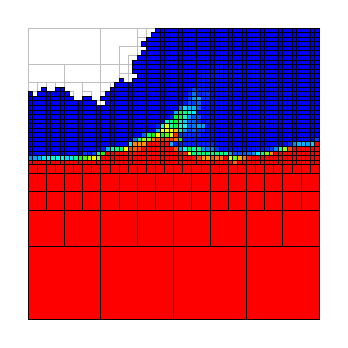
\begin{tikzpicture}[x={(\screenshotunitlength,0)},y={(0,\screenshotunitlength)}]
        \definecolor{fillcolor}{rgb}{1.000000,0.000000,0.000000}
\fill[fillcolor] (0.000000,0.000000) rectangle (0.250000,0.250000);
\definecolor{fillcolor}{rgb}{1.000000,0.000000,0.000000}
\fill[fillcolor] (0.250000,0.000000) rectangle (0.500000,0.250000);
\definecolor{fillcolor}{rgb}{1.000000,0.000000,0.000000}
\fill[fillcolor] (0.000000,0.250000) rectangle (0.125000,0.375000);
\definecolor{fillcolor}{rgb}{1.000000,0.000000,0.000000}
\fill[fillcolor] (0.125000,0.250000) rectangle (0.250000,0.375000);
\definecolor{fillcolor}{rgb}{1.000000,0.000000,0.000000}
\fill[fillcolor] (0.000000,0.375000) rectangle (0.062500,0.437500);
\definecolor{fillcolor}{rgb}{1.000000,0.000000,0.000000}
\fill[fillcolor] (0.062500,0.375000) rectangle (0.125000,0.437500);
\definecolor{fillcolor}{rgb}{1.000000,0.000001,0.000000}
\fill[fillcolor] (0.000000,0.437500) rectangle (0.062500,0.500000);
\definecolor{fillcolor}{rgb}{1.000000,0.000000,0.000000}
\fill[fillcolor] (0.062500,0.437500) rectangle (0.125000,0.500000);
\definecolor{fillcolor}{rgb}{1.000000,0.000000,0.000000}
\fill[fillcolor] (0.125000,0.375000) rectangle (0.187500,0.437500);
\definecolor{fillcolor}{rgb}{1.000000,0.000000,0.000000}
\fill[fillcolor] (0.187500,0.375000) rectangle (0.250000,0.437500);
\definecolor{fillcolor}{rgb}{1.000000,0.000000,0.000000}
\fill[fillcolor] (0.125000,0.437500) rectangle (0.187500,0.500000);
\definecolor{fillcolor}{rgb}{1.000000,0.000000,0.000000}
\fill[fillcolor] (0.187500,0.437500) rectangle (0.250000,0.500000);
\definecolor{fillcolor}{rgb}{1.000000,0.000000,0.000000}
\fill[fillcolor] (0.250000,0.250000) rectangle (0.375000,0.375000);
\definecolor{fillcolor}{rgb}{1.000000,0.000000,0.000000}
\fill[fillcolor] (0.375000,0.250000) rectangle (0.500000,0.375000);
\definecolor{fillcolor}{rgb}{1.000000,0.000000,0.000000}
\fill[fillcolor] (0.250000,0.375000) rectangle (0.312500,0.437500);
\definecolor{fillcolor}{rgb}{1.000000,0.000000,0.000000}
\fill[fillcolor] (0.312500,0.375000) rectangle (0.375000,0.437500);
\definecolor{fillcolor}{rgb}{1.000000,0.000000,0.000000}
\fill[fillcolor] (0.250000,0.437500) rectangle (0.312500,0.500000);
\definecolor{fillcolor}{rgb}{1.000000,0.000000,0.000000}
\fill[fillcolor] (0.312500,0.437500) rectangle (0.375000,0.500000);
\definecolor{fillcolor}{rgb}{1.000000,0.000000,0.000000}
\fill[fillcolor] (0.375000,0.375000) rectangle (0.437500,0.437500);
\definecolor{fillcolor}{rgb}{1.000000,0.000000,0.000000}
\fill[fillcolor] (0.437500,0.375000) rectangle (0.500000,0.437500);
\definecolor{fillcolor}{rgb}{1.000000,0.000000,0.000000}
\fill[fillcolor] (0.375000,0.437500) rectangle (0.437500,0.500000);
\definecolor{fillcolor}{rgb}{1.000000,0.000001,0.000000}
\fill[fillcolor] (0.437500,0.437500) rectangle (0.500000,0.500000);
\definecolor{fillcolor}{rgb}{1.000000,0.000000,0.000000}
\fill[fillcolor] (0.500000,0.000000) rectangle (0.750000,0.250000);
\definecolor{fillcolor}{rgb}{1.000000,0.000000,0.000000}
\fill[fillcolor] (0.750000,0.000000) rectangle (1.000000,0.250000);
\definecolor{fillcolor}{rgb}{1.000000,0.000000,0.000000}
\fill[fillcolor] (0.500000,0.250000) rectangle (0.625000,0.375000);
\definecolor{fillcolor}{rgb}{1.000000,0.000000,0.000000}
\fill[fillcolor] (0.625000,0.250000) rectangle (0.750000,0.375000);
\definecolor{fillcolor}{rgb}{1.000000,0.000000,0.000000}
\fill[fillcolor] (0.500000,0.375000) rectangle (0.562500,0.437500);
\definecolor{fillcolor}{rgb}{1.000000,0.000004,0.000000}
\fill[fillcolor] (0.562500,0.375000) rectangle (0.625000,0.437500);
\definecolor{fillcolor}{rgb}{1.000000,0.000084,0.000000}
\fill[fillcolor] (0.500000,0.437500) rectangle (0.562500,0.500000);
\definecolor{fillcolor}{rgb}{1.000000,0.000125,0.000000}
\fill[fillcolor] (0.562500,0.437500) rectangle (0.625000,0.500000);
\definecolor{fillcolor}{rgb}{1.000000,0.000000,0.000000}
\fill[fillcolor] (0.625000,0.375000) rectangle (0.687500,0.437500);
\definecolor{fillcolor}{rgb}{1.000000,0.000000,0.000000}
\fill[fillcolor] (0.687500,0.375000) rectangle (0.750000,0.437500);
\definecolor{fillcolor}{rgb}{1.000000,0.000050,0.000000}
\fill[fillcolor] (0.625000,0.437500) rectangle (0.687500,0.500000);
\definecolor{fillcolor}{rgb}{1.000000,0.000000,0.000000}
\fill[fillcolor] (0.687500,0.437500) rectangle (0.750000,0.500000);
\definecolor{fillcolor}{rgb}{1.000000,0.000000,0.000000}
\fill[fillcolor] (0.750000,0.250000) rectangle (0.875000,0.375000);
\definecolor{fillcolor}{rgb}{1.000000,0.000000,0.000000}
\fill[fillcolor] (0.875000,0.250000) rectangle (1.000000,0.375000);
\definecolor{fillcolor}{rgb}{1.000000,0.000000,0.000000}
\fill[fillcolor] (0.750000,0.375000) rectangle (0.812500,0.437500);
\definecolor{fillcolor}{rgb}{1.000000,0.000000,0.000000}
\fill[fillcolor] (0.812500,0.375000) rectangle (0.875000,0.437500);
\definecolor{fillcolor}{rgb}{1.000000,0.000000,0.000000}
\fill[fillcolor] (0.750000,0.437500) rectangle (0.812500,0.500000);
\definecolor{fillcolor}{rgb}{1.000000,0.000000,0.000000}
\fill[fillcolor] (0.812500,0.437500) rectangle (0.875000,0.500000);
\definecolor{fillcolor}{rgb}{1.000000,0.000000,0.000000}
\fill[fillcolor] (0.875000,0.375000) rectangle (0.937500,0.437500);
\definecolor{fillcolor}{rgb}{1.000000,0.000000,0.000000}
\fill[fillcolor] (0.937500,0.375000) rectangle (1.000000,0.437500);
\definecolor{fillcolor}{rgb}{1.000000,0.000000,0.000000}
\fill[fillcolor] (0.875000,0.437500) rectangle (0.937500,0.500000);
\definecolor{fillcolor}{rgb}{1.000000,0.000000,0.000000}
\fill[fillcolor] (0.937500,0.437500) rectangle (1.000000,0.500000);
\definecolor{fillcolor}{rgb}{1.000000,0.000001,0.000000}
\fill[fillcolor] (0.000000,0.500000) rectangle (0.031250,0.531250);
\definecolor{fillcolor}{rgb}{1.000000,0.000001,0.000000}
\fill[fillcolor] (0.031250,0.500000) rectangle (0.062500,0.531250);
\definecolor{fillcolor}{rgb}{1.000000,0.000001,0.000000}
\fill[fillcolor] (0.000000,0.531250) rectangle (0.015625,0.546875);
\definecolor{fillcolor}{rgb}{1.000000,0.000001,0.000000}
\fill[fillcolor] (0.015625,0.531250) rectangle (0.031250,0.546875);
\definecolor{fillcolor}{rgb}{0.000000,0.574597,1.000000}
\fill[fillcolor] (0.000000,0.546875) rectangle (0.015625,0.562500);
\definecolor{fillcolor}{rgb}{0.000000,0.650475,1.000000}
\fill[fillcolor] (0.015625,0.546875) rectangle (0.031250,0.562500);
\definecolor{fillcolor}{rgb}{1.000000,0.000001,0.000000}
\fill[fillcolor] (0.031250,0.531250) rectangle (0.046875,0.546875);
\definecolor{fillcolor}{rgb}{1.000000,0.000001,0.000000}
\fill[fillcolor] (0.046875,0.531250) rectangle (0.062500,0.546875);
\definecolor{fillcolor}{rgb}{0.000000,0.717449,1.000000}
\fill[fillcolor] (0.031250,0.546875) rectangle (0.046875,0.562500);
\definecolor{fillcolor}{rgb}{0.000000,0.911988,1.000000}
\fill[fillcolor] (0.046875,0.546875) rectangle (0.062500,0.562500);
\definecolor{fillcolor}{rgb}{1.000000,0.000000,0.000000}
\fill[fillcolor] (0.062500,0.500000) rectangle (0.093750,0.531250);
\definecolor{fillcolor}{rgb}{1.000000,0.000001,0.000000}
\fill[fillcolor] (0.093750,0.500000) rectangle (0.125000,0.531250);
\definecolor{fillcolor}{rgb}{1.000000,0.000000,0.000000}
\fill[fillcolor] (0.062500,0.531250) rectangle (0.078125,0.546875);
\definecolor{fillcolor}{rgb}{1.000000,0.000000,0.000000}
\fill[fillcolor] (0.078125,0.531250) rectangle (0.093750,0.546875);
\definecolor{fillcolor}{rgb}{0.000000,0.974249,1.000000}
\fill[fillcolor] (0.062500,0.546875) rectangle (0.078125,0.562500);
\definecolor{fillcolor}{rgb}{0.000000,1.000000,0.834794}
\fill[fillcolor] (0.078125,0.546875) rectangle (0.093750,0.562500);
\definecolor{fillcolor}{rgb}{1.000000,0.000001,0.000000}
\fill[fillcolor] (0.093750,0.531250) rectangle (0.109375,0.546875);
\definecolor{fillcolor}{rgb}{1.000000,0.000001,0.000000}
\fill[fillcolor] (0.109375,0.531250) rectangle (0.125000,0.546875);
\definecolor{fillcolor}{rgb}{0.000000,1.000000,0.945161}
\fill[fillcolor] (0.093750,0.546875) rectangle (0.109375,0.562500);
\definecolor{fillcolor}{rgb}{0.000000,1.000000,0.887090}
\fill[fillcolor] (0.109375,0.546875) rectangle (0.125000,0.562500);
\definecolor{fillcolor}{rgb}{0.000000,0.006739,1.000000}
\fill[fillcolor] (0.000000,0.562500) rectangle (0.015625,0.578125);
\definecolor{fillcolor}{rgb}{0.000000,0.006739,1.000000}
\fill[fillcolor] (0.015625,0.562500) rectangle (0.031250,0.578125);
\definecolor{fillcolor}{rgb}{0.000000,0.005811,1.000000}
\fill[fillcolor] (0.000000,0.578125) rectangle (0.015625,0.593750);
\definecolor{fillcolor}{rgb}{0.000000,0.007501,1.000000}
\fill[fillcolor] (0.015625,0.578125) rectangle (0.031250,0.593750);
\definecolor{fillcolor}{rgb}{0.000000,0.006754,1.000000}
\fill[fillcolor] (0.031250,0.562500) rectangle (0.046875,0.578125);
\definecolor{fillcolor}{rgb}{0.000000,0.003714,1.000000}
\fill[fillcolor] (0.046875,0.562500) rectangle (0.062500,0.578125);
\definecolor{fillcolor}{rgb}{0.000000,0.004099,1.000000}
\fill[fillcolor] (0.031250,0.578125) rectangle (0.046875,0.593750);
\definecolor{fillcolor}{rgb}{0.000000,0.003772,1.000000}
\fill[fillcolor] (0.046875,0.578125) rectangle (0.062500,0.593750);
\definecolor{fillcolor}{rgb}{0.000000,0.000022,1.000000}
\fill[fillcolor] (0.000000,0.593750) rectangle (0.015625,0.609375);
\definecolor{fillcolor}{rgb}{0.000000,0.000518,1.000000}
\fill[fillcolor] (0.015625,0.593750) rectangle (0.031250,0.609375);
\definecolor{fillcolor}{rgb}{0.000000,0.000005,1.000000}
\fill[fillcolor] (0.000000,0.609375) rectangle (0.015625,0.625000);
\definecolor{fillcolor}{rgb}{0.000000,0.000166,1.000000}
\fill[fillcolor] (0.015625,0.609375) rectangle (0.031250,0.625000);
\definecolor{fillcolor}{rgb}{0.000000,0.001396,1.000000}
\fill[fillcolor] (0.031250,0.593750) rectangle (0.046875,0.609375);
\definecolor{fillcolor}{rgb}{0.000000,0.003796,1.000000}
\fill[fillcolor] (0.046875,0.593750) rectangle (0.062500,0.609375);
\definecolor{fillcolor}{rgb}{0.000000,0.000318,1.000000}
\fill[fillcolor] (0.031250,0.609375) rectangle (0.046875,0.625000);
\definecolor{fillcolor}{rgb}{0.000000,0.002295,1.000000}
\fill[fillcolor] (0.046875,0.609375) rectangle (0.062500,0.625000);
\definecolor{fillcolor}{rgb}{0.000000,0.003324,1.000000}
\fill[fillcolor] (0.062500,0.562500) rectangle (0.078125,0.578125);
\definecolor{fillcolor}{rgb}{0.000000,0.003166,1.000000}
\fill[fillcolor] (0.078125,0.562500) rectangle (0.093750,0.578125);
\definecolor{fillcolor}{rgb}{0.000000,0.003957,1.000000}
\fill[fillcolor] (0.062500,0.578125) rectangle (0.078125,0.593750);
\definecolor{fillcolor}{rgb}{0.000000,0.002823,1.000000}
\fill[fillcolor] (0.078125,0.578125) rectangle (0.093750,0.593750);
\definecolor{fillcolor}{rgb}{0.000000,0.001787,1.000000}
\fill[fillcolor] (0.093750,0.562500) rectangle (0.109375,0.578125);
\definecolor{fillcolor}{rgb}{0.000000,0.001789,1.000000}
\fill[fillcolor] (0.109375,0.562500) rectangle (0.125000,0.578125);
\definecolor{fillcolor}{rgb}{0.000000,0.000949,1.000000}
\fill[fillcolor] (0.093750,0.578125) rectangle (0.109375,0.593750);
\definecolor{fillcolor}{rgb}{0.000000,0.001162,1.000000}
\fill[fillcolor] (0.109375,0.578125) rectangle (0.125000,0.593750);
\definecolor{fillcolor}{rgb}{0.000000,0.001735,1.000000}
\fill[fillcolor] (0.062500,0.593750) rectangle (0.078125,0.609375);
\definecolor{fillcolor}{rgb}{0.000000,0.000475,1.000000}
\fill[fillcolor] (0.078125,0.593750) rectangle (0.093750,0.609375);
\definecolor{fillcolor}{rgb}{0.000000,0.001359,1.000000}
\fill[fillcolor] (0.062500,0.609375) rectangle (0.078125,0.625000);
\definecolor{fillcolor}{rgb}{0.000000,0.000368,1.000000}
\fill[fillcolor] (0.078125,0.609375) rectangle (0.093750,0.625000);
\definecolor{fillcolor}{rgb}{0.000000,0.000526,1.000000}
\fill[fillcolor] (0.093750,0.593750) rectangle (0.109375,0.609375);
\definecolor{fillcolor}{rgb}{0.000000,0.000974,1.000000}
\fill[fillcolor] (0.109375,0.593750) rectangle (0.125000,0.609375);
\definecolor{fillcolor}{rgb}{0.000000,0.000140,1.000000}
\fill[fillcolor] (0.093750,0.609375) rectangle (0.109375,0.625000);
\definecolor{fillcolor}{rgb}{0.000000,0.000764,1.000000}
\fill[fillcolor] (0.109375,0.609375) rectangle (0.125000,0.625000);
\definecolor{fillcolor}{rgb}{1.000000,0.000002,0.000000}
\fill[fillcolor] (0.125000,0.500000) rectangle (0.156250,0.531250);
\definecolor{fillcolor}{rgb}{1.000000,0.000019,0.000000}
\fill[fillcolor] (0.156250,0.500000) rectangle (0.187500,0.531250);
\definecolor{fillcolor}{rgb}{1.000000,0.000002,0.000000}
\fill[fillcolor] (0.125000,0.531250) rectangle (0.140625,0.546875);
\definecolor{fillcolor}{rgb}{1.000000,0.000002,0.000000}
\fill[fillcolor] (0.140625,0.531250) rectangle (0.156250,0.546875);
\definecolor{fillcolor}{rgb}{0.000000,0.866275,1.000000}
\fill[fillcolor] (0.125000,0.546875) rectangle (0.140625,0.562500);
\definecolor{fillcolor}{rgb}{0.000000,0.919570,1.000000}
\fill[fillcolor] (0.140625,0.546875) rectangle (0.156250,0.562500);
\definecolor{fillcolor}{rgb}{1.000000,0.000017,0.000000}
\fill[fillcolor] (0.156250,0.531250) rectangle (0.171875,0.546875);
\definecolor{fillcolor}{rgb}{1.000000,0.000021,0.000000}
\fill[fillcolor] (0.171875,0.531250) rectangle (0.187500,0.546875);
\definecolor{fillcolor}{rgb}{0.000000,1.000000,0.591209}
\fill[fillcolor] (0.156250,0.546875) rectangle (0.171875,0.562500);
\definecolor{fillcolor}{rgb}{0.000000,1.000000,0.137217}
\fill[fillcolor] (0.171875,0.546875) rectangle (0.187500,0.562500);
\definecolor{fillcolor}{rgb}{1.000000,0.000085,0.000000}
\fill[fillcolor] (0.187500,0.500000) rectangle (0.218750,0.531250);
\definecolor{fillcolor}{rgb}{1.000000,0.000235,0.000000}
\fill[fillcolor] (0.218750,0.500000) rectangle (0.250000,0.531250);
\definecolor{fillcolor}{rgb}{1.000000,0.000088,0.000000}
\fill[fillcolor] (0.187500,0.531250) rectangle (0.203125,0.546875);
\definecolor{fillcolor}{rgb}{1.000000,0.000126,0.000000}
\fill[fillcolor] (0.203125,0.531250) rectangle (0.218750,0.546875);
\definecolor{fillcolor}{rgb}{0.241282,1.000000,0.000000}
\fill[fillcolor] (0.187500,0.546875) rectangle (0.203125,0.562500);
\definecolor{fillcolor}{rgb}{0.696173,1.000000,0.000000}
\fill[fillcolor] (0.203125,0.546875) rectangle (0.218750,0.562500);
\definecolor{fillcolor}{rgb}{1.000000,0.000249,0.000000}
\fill[fillcolor] (0.218750,0.531250) rectangle (0.234375,0.546875);
\definecolor{fillcolor}{rgb}{1.000000,0.000327,0.000000}
\fill[fillcolor] (0.234375,0.531250) rectangle (0.250000,0.546875);
\definecolor{fillcolor}{rgb}{1.000000,0.960469,0.000000}
\fill[fillcolor] (0.218750,0.546875) rectangle (0.234375,0.562500);
\definecolor{fillcolor}{rgb}{0.650724,1.000000,0.000000}
\fill[fillcolor] (0.234375,0.546875) rectangle (0.250000,0.562500);
\definecolor{fillcolor}{rgb}{0.000000,0.002288,1.000000}
\fill[fillcolor] (0.125000,0.562500) rectangle (0.140625,0.578125);
\definecolor{fillcolor}{rgb}{0.000000,0.003177,1.000000}
\fill[fillcolor] (0.140625,0.562500) rectangle (0.156250,0.578125);
\definecolor{fillcolor}{rgb}{0.000000,0.001188,1.000000}
\fill[fillcolor] (0.125000,0.578125) rectangle (0.140625,0.593750);
\definecolor{fillcolor}{rgb}{0.000000,0.001240,1.000000}
\fill[fillcolor] (0.140625,0.578125) rectangle (0.156250,0.593750);
\definecolor{fillcolor}{rgb}{0.000000,0.000794,1.000000}
\fill[fillcolor] (0.156250,0.562500) rectangle (0.171875,0.578125);
\definecolor{fillcolor}{rgb}{0.000000,0.006188,1.000000}
\fill[fillcolor] (0.171875,0.562500) rectangle (0.187500,0.578125);
\definecolor{fillcolor}{rgb}{0.000000,0.000689,1.000000}
\fill[fillcolor] (0.156250,0.578125) rectangle (0.171875,0.593750);
\definecolor{fillcolor}{rgb}{0.000000,0.000830,1.000000}
\fill[fillcolor] (0.171875,0.578125) rectangle (0.187500,0.593750);
\definecolor{fillcolor}{rgb}{0.000000,0.000536,1.000000}
\fill[fillcolor] (0.125000,0.593750) rectangle (0.140625,0.609375);
\definecolor{fillcolor}{rgb}{0.000000,0.000665,1.000000}
\fill[fillcolor] (0.140625,0.593750) rectangle (0.156250,0.609375);
\definecolor{fillcolor}{rgb}{0.000000,0.000541,1.000000}
\fill[fillcolor] (0.125000,0.609375) rectangle (0.140625,0.625000);
\definecolor{fillcolor}{rgb}{0.000000,0.000664,1.000000}
\fill[fillcolor] (0.140625,0.609375) rectangle (0.156250,0.625000);
\definecolor{fillcolor}{rgb}{0.000000,0.000598,1.000000}
\fill[fillcolor] (0.156250,0.593750) rectangle (0.171875,0.609375);
\definecolor{fillcolor}{rgb}{0.000000,0.000750,1.000000}
\fill[fillcolor] (0.171875,0.593750) rectangle (0.187500,0.609375);
\definecolor{fillcolor}{rgb}{0.000000,0.000643,1.000000}
\fill[fillcolor] (0.156250,0.609375) rectangle (0.171875,0.625000);
\definecolor{fillcolor}{rgb}{0.000000,0.000695,1.000000}
\fill[fillcolor] (0.171875,0.609375) rectangle (0.187500,0.625000);
\definecolor{fillcolor}{rgb}{0.000000,0.220664,1.000000}
\fill[fillcolor] (0.187500,0.562500) rectangle (0.203125,0.578125);
\definecolor{fillcolor}{rgb}{0.000000,0.128268,1.000000}
\fill[fillcolor] (0.203125,0.562500) rectangle (0.218750,0.578125);
\definecolor{fillcolor}{rgb}{0.000000,0.008253,1.000000}
\fill[fillcolor] (0.187500,0.578125) rectangle (0.203125,0.593750);
\definecolor{fillcolor}{rgb}{0.000000,0.005790,1.000000}
\fill[fillcolor] (0.203125,0.578125) rectangle (0.218750,0.593750);
\definecolor{fillcolor}{rgb}{0.000000,0.265438,1.000000}
\fill[fillcolor] (0.218750,0.562500) rectangle (0.234375,0.578125);
\definecolor{fillcolor}{rgb}{0.000000,1.000000,0.664160}
\fill[fillcolor] (0.234375,0.562500) rectangle (0.250000,0.578125);
\definecolor{fillcolor}{rgb}{0.000000,0.000144,1.000000}
\fill[fillcolor] (0.218750,0.578125) rectangle (0.234375,0.593750);
\definecolor{fillcolor}{rgb}{0.000000,0.024581,1.000000}
\fill[fillcolor] (0.234375,0.578125) rectangle (0.250000,0.593750);
\definecolor{fillcolor}{rgb}{0.000000,0.003050,1.000000}
\fill[fillcolor] (0.187500,0.593750) rectangle (0.203125,0.609375);
\definecolor{fillcolor}{rgb}{0.000000,0.003298,1.000000}
\fill[fillcolor] (0.203125,0.593750) rectangle (0.218750,0.609375);
\definecolor{fillcolor}{rgb}{0.000000,0.000861,1.000000}
\fill[fillcolor] (0.187500,0.609375) rectangle (0.203125,0.625000);
\definecolor{fillcolor}{rgb}{0.000000,0.001049,1.000000}
\fill[fillcolor] (0.203125,0.609375) rectangle (0.218750,0.625000);
\definecolor{fillcolor}{rgb}{0.000000,0.000952,1.000000}
\fill[fillcolor] (0.218750,0.593750) rectangle (0.234375,0.609375);
\definecolor{fillcolor}{rgb}{0.000000,0.000410,1.000000}
\fill[fillcolor] (0.234375,0.593750) rectangle (0.250000,0.609375);
\definecolor{fillcolor}{rgb}{0.000000,0.000878,1.000000}
\fill[fillcolor] (0.218750,0.609375) rectangle (0.234375,0.625000);
\definecolor{fillcolor}{rgb}{0.000000,0.000654,1.000000}
\fill[fillcolor] (0.234375,0.609375) rectangle (0.250000,0.625000);
\definecolor{fillcolor}{rgb}{0.000000,0.000000,1.000000}
\fill[fillcolor] (0.000000,0.625000) rectangle (0.015625,0.640625);
\definecolor{fillcolor}{rgb}{0.000000,0.000124,1.000000}
\fill[fillcolor] (0.015625,0.625000) rectangle (0.031250,0.640625);
\definecolor{fillcolor}{rgb}{0.000000,0.000000,1.000000}
\fill[fillcolor] (0.000000,0.640625) rectangle (0.015625,0.656250);
\definecolor{fillcolor}{rgb}{0.000000,0.000062,1.000000}
\fill[fillcolor] (0.015625,0.640625) rectangle (0.031250,0.656250);
\definecolor{fillcolor}{rgb}{0.000000,0.000228,1.000000}
\fill[fillcolor] (0.031250,0.625000) rectangle (0.046875,0.640625);
\definecolor{fillcolor}{rgb}{0.000000,0.000279,1.000000}
\fill[fillcolor] (0.046875,0.625000) rectangle (0.062500,0.640625);
\definecolor{fillcolor}{rgb}{0.000000,0.000094,1.000000}
\fill[fillcolor] (0.031250,0.640625) rectangle (0.046875,0.656250);
\definecolor{fillcolor}{rgb}{0.000000,0.000062,1.000000}
\fill[fillcolor] (0.046875,0.640625) rectangle (0.062500,0.656250);
\definecolor{fillcolor}{rgb}{0.000000,0.000000,1.000000}
\fill[fillcolor] (0.000000,0.656250) rectangle (0.015625,0.671875);
\definecolor{fillcolor}{rgb}{0.000000,0.000039,1.000000}
\fill[fillcolor] (0.015625,0.656250) rectangle (0.031250,0.671875);
\definecolor{fillcolor}{rgb}{0.000000,0.000000,1.000000}
\fill[fillcolor] (0.000000,0.671875) rectangle (0.015625,0.687500);
\definecolor{fillcolor}{rgb}{0.000000,0.000007,1.000000}
\fill[fillcolor] (0.015625,0.671875) rectangle (0.031250,0.687500);
\definecolor{fillcolor}{rgb}{0.000000,0.000044,1.000000}
\fill[fillcolor] (0.031250,0.656250) rectangle (0.046875,0.671875);
\definecolor{fillcolor}{rgb}{0.000000,0.000000,1.000000}
\fill[fillcolor] (0.046875,0.656250) rectangle (0.062500,0.671875);
\definecolor{fillcolor}{rgb}{0.000000,0.000010,1.000000}
\fill[fillcolor] (0.031250,0.671875) rectangle (0.046875,0.687500);
\definecolor{fillcolor}{rgb}{0.000000,0.000000,1.000000}
\fill[fillcolor] (0.046875,0.671875) rectangle (0.062500,0.687500);
\definecolor{fillcolor}{rgb}{0.000000,0.000494,1.000000}
\fill[fillcolor] (0.062500,0.625000) rectangle (0.078125,0.640625);
\definecolor{fillcolor}{rgb}{0.000000,0.000146,1.000000}
\fill[fillcolor] (0.078125,0.625000) rectangle (0.093750,0.640625);
\definecolor{fillcolor}{rgb}{0.000000,0.000112,1.000000}
\fill[fillcolor] (0.062500,0.640625) rectangle (0.078125,0.656250);
\definecolor{fillcolor}{rgb}{0.000000,0.000050,1.000000}
\fill[fillcolor] (0.078125,0.640625) rectangle (0.093750,0.656250);
\definecolor{fillcolor}{rgb}{0.000000,0.000066,1.000000}
\fill[fillcolor] (0.093750,0.625000) rectangle (0.109375,0.640625);
\definecolor{fillcolor}{rgb}{0.000000,0.000630,1.000000}
\fill[fillcolor] (0.109375,0.625000) rectangle (0.125000,0.640625);
\definecolor{fillcolor}{rgb}{0.000000,0.000052,1.000000}
\fill[fillcolor] (0.093750,0.640625) rectangle (0.109375,0.656250);
\definecolor{fillcolor}{rgb}{0.000000,0.000202,1.000000}
\fill[fillcolor] (0.109375,0.640625) rectangle (0.125000,0.656250);
\definecolor{fillcolor}{rgb}{0.000000,0.000084,1.000000}
\fill[fillcolor] (0.062500,0.656250) rectangle (0.078125,0.671875);
\definecolor{fillcolor}{rgb}{0.000000,0.000020,1.000000}
\fill[fillcolor] (0.078125,0.656250) rectangle (0.093750,0.671875);
\definecolor{fillcolor}{rgb}{0.000000,0.000006,1.000000}
\fill[fillcolor] (0.062500,0.671875) rectangle (0.078125,0.687500);
\definecolor{fillcolor}{rgb}{0.000000,0.000000,1.000000}
\fill[fillcolor] (0.078125,0.671875) rectangle (0.093750,0.687500);
\definecolor{fillcolor}{rgb}{0.000000,0.000031,1.000000}
\fill[fillcolor] (0.093750,0.656250) rectangle (0.109375,0.671875);
\definecolor{fillcolor}{rgb}{0.000000,0.000049,1.000000}
\fill[fillcolor] (0.109375,0.656250) rectangle (0.125000,0.671875);
\definecolor{fillcolor}{rgb}{0.000000,0.000013,1.000000}
\fill[fillcolor] (0.093750,0.671875) rectangle (0.109375,0.687500);
\definecolor{fillcolor}{rgb}{0.000000,0.000001,1.000000}
\fill[fillcolor] (0.109375,0.671875) rectangle (0.125000,0.687500);
\definecolor{fillcolor}{rgb}{0.000000,0.000000,1.000000}
\fill[fillcolor] (0.000000,0.687500) rectangle (0.015625,0.703125);
\definecolor{fillcolor}{rgb}{0.000000,0.000000,1.000000}
\fill[fillcolor] (0.015625,0.687500) rectangle (0.031250,0.703125);
\definecolor{fillcolor}{rgb}{0.000000,0.000000,1.000000}
\fill[fillcolor] (0.000000,0.703125) rectangle (0.015625,0.718750);
\definecolor{fillcolor}{rgb}{0.000000,0.000000,1.000000}
\fill[fillcolor] (0.015625,0.703125) rectangle (0.031250,0.718750);
\definecolor{fillcolor}{rgb}{0.000000,0.000000,1.000000}
\fill[fillcolor] (0.031250,0.687500) rectangle (0.046875,0.703125);
\definecolor{fillcolor}{rgb}{0.000000,0.000000,1.000000}
\fill[fillcolor] (0.046875,0.687500) rectangle (0.062500,0.703125);
\definecolor{fillcolor}{rgb}{0.000000,0.000000,1.000000}
\fill[fillcolor] (0.031250,0.703125) rectangle (0.046875,0.718750);
\definecolor{fillcolor}{rgb}{0.000000,0.000000,1.000000}
\fill[fillcolor] (0.046875,0.703125) rectangle (0.062500,0.718750);
\definecolor{fillcolor}{rgb}{0.000000,0.000000,1.000000}
\fill[fillcolor] (0.000000,0.718750) rectangle (0.015625,0.734375);
\definecolor{fillcolor}{rgb}{0.000000,0.000000,1.000000}
\fill[fillcolor] (0.015625,0.718750) rectangle (0.031250,0.734375);
\definecolor{fillcolor}{rgb}{0.000000,0.000000,1.000000}
\fill[fillcolor] (0.000000,0.734375) rectangle (0.015625,0.750000);
\definecolor{fillcolor}{rgb}{0.000000,0.000000,1.000000}
\fill[fillcolor] (0.015625,0.734375) rectangle (0.031250,0.750000);
\definecolor{fillcolor}{rgb}{0.000000,0.000000,1.000000}
\fill[fillcolor] (0.031250,0.718750) rectangle (0.046875,0.734375);
\definecolor{fillcolor}{rgb}{0.000000,0.000000,1.000000}
\fill[fillcolor] (0.046875,0.718750) rectangle (0.062500,0.734375);
\definecolor{fillcolor}{rgb}{0.000000,0.000000,1.000000}
\fill[fillcolor] (0.031250,0.734375) rectangle (0.046875,0.750000);
\definecolor{fillcolor}{rgb}{0.000000,0.000000,1.000000}
\fill[fillcolor] (0.046875,0.734375) rectangle (0.062500,0.750000);
\definecolor{fillcolor}{rgb}{0.000000,0.000000,1.000000}
\fill[fillcolor] (0.062500,0.687500) rectangle (0.078125,0.703125);
\definecolor{fillcolor}{rgb}{0.000000,0.000000,1.000000}
\fill[fillcolor] (0.078125,0.687500) rectangle (0.093750,0.703125);
\definecolor{fillcolor}{rgb}{0.000000,0.000000,1.000000}
\fill[fillcolor] (0.062500,0.703125) rectangle (0.078125,0.718750);
\definecolor{fillcolor}{rgb}{0.000000,0.000000,1.000000}
\fill[fillcolor] (0.078125,0.703125) rectangle (0.093750,0.718750);
\definecolor{fillcolor}{rgb}{0.000000,0.000000,1.000000}
\fill[fillcolor] (0.093750,0.687500) rectangle (0.109375,0.703125);
\definecolor{fillcolor}{rgb}{0.000000,0.000002,1.000000}
\fill[fillcolor] (0.109375,0.687500) rectangle (0.125000,0.703125);
\definecolor{fillcolor}{rgb}{0.000000,0.000000,1.000000}
\fill[fillcolor] (0.093750,0.703125) rectangle (0.109375,0.718750);
\definecolor{fillcolor}{rgb}{0.000000,0.000000,1.000000}
\fill[fillcolor] (0.109375,0.703125) rectangle (0.125000,0.718750);
\definecolor{fillcolor}{rgb}{0.000000,0.000000,1.000000}
\fill[fillcolor] (0.062500,0.718750) rectangle (0.078125,0.734375);
\definecolor{fillcolor}{rgb}{0.000000,0.000000,1.000000}
\fill[fillcolor] (0.078125,0.718750) rectangle (0.093750,0.734375);
\definecolor{fillcolor}{rgb}{0.000000,0.000000,1.000000}
\fill[fillcolor] (0.062500,0.734375) rectangle (0.078125,0.750000);
\definecolor{fillcolor}{rgb}{0.000000,0.000000,1.000000}
\fill[fillcolor] (0.078125,0.734375) rectangle (0.093750,0.750000);
\definecolor{fillcolor}{rgb}{0.000000,0.000000,1.000000}
\fill[fillcolor] (0.093750,0.718750) rectangle (0.109375,0.734375);
\definecolor{fillcolor}{rgb}{0.000000,0.000000,1.000000}
\fill[fillcolor] (0.109375,0.718750) rectangle (0.125000,0.734375);
\definecolor{fillcolor}{rgb}{0.000000,0.000000,1.000000}
\fill[fillcolor] (0.093750,0.734375) rectangle (0.109375,0.750000);
\definecolor{fillcolor}{rgb}{0.000000,0.000000,1.000000}
\fill[fillcolor] (0.109375,0.734375) rectangle (0.125000,0.750000);
\definecolor{fillcolor}{rgb}{0.000000,0.000425,1.000000}
\fill[fillcolor] (0.125000,0.625000) rectangle (0.140625,0.640625);
\definecolor{fillcolor}{rgb}{0.000000,0.000461,1.000000}
\fill[fillcolor] (0.140625,0.625000) rectangle (0.156250,0.640625);
\definecolor{fillcolor}{rgb}{0.000000,0.000108,1.000000}
\fill[fillcolor] (0.125000,0.640625) rectangle (0.140625,0.656250);
\definecolor{fillcolor}{rgb}{0.000000,0.000050,1.000000}
\fill[fillcolor] (0.140625,0.640625) rectangle (0.156250,0.656250);
\definecolor{fillcolor}{rgb}{0.000000,0.000219,1.000000}
\fill[fillcolor] (0.156250,0.625000) rectangle (0.171875,0.640625);
\definecolor{fillcolor}{rgb}{0.000000,0.000123,1.000000}
\fill[fillcolor] (0.171875,0.625000) rectangle (0.187500,0.640625);
\definecolor{fillcolor}{rgb}{0.000000,0.000038,1.000000}
\fill[fillcolor] (0.156250,0.640625) rectangle (0.171875,0.656250);
\definecolor{fillcolor}{rgb}{0.000000,0.000015,1.000000}
\fill[fillcolor] (0.171875,0.640625) rectangle (0.187500,0.656250);
\definecolor{fillcolor}{rgb}{0.000000,0.000032,1.000000}
\fill[fillcolor] (0.125000,0.656250) rectangle (0.140625,0.671875);
\definecolor{fillcolor}{rgb}{0.000000,0.000013,1.000000}
\fill[fillcolor] (0.140625,0.656250) rectangle (0.156250,0.671875);
\definecolor{fillcolor}{rgb}{0.000000,0.000001,1.000000}
\fill[fillcolor] (0.125000,0.671875) rectangle (0.140625,0.687500);
\definecolor{fillcolor}{rgb}{0.000000,0.000001,1.000000}
\fill[fillcolor] (0.140625,0.671875) rectangle (0.156250,0.687500);
\definecolor{fillcolor}{rgb}{0.000000,0.000013,1.000000}
\fill[fillcolor] (0.156250,0.656250) rectangle (0.171875,0.671875);
\definecolor{fillcolor}{rgb}{0.000000,0.000011,1.000000}
\fill[fillcolor] (0.171875,0.656250) rectangle (0.187500,0.671875);
\definecolor{fillcolor}{rgb}{0.000000,0.000005,1.000000}
\fill[fillcolor] (0.156250,0.671875) rectangle (0.171875,0.687500);
\definecolor{fillcolor}{rgb}{0.000000,0.000004,1.000000}
\fill[fillcolor] (0.171875,0.671875) rectangle (0.187500,0.687500);
\definecolor{fillcolor}{rgb}{0.000000,0.000124,1.000000}
\fill[fillcolor] (0.187500,0.625000) rectangle (0.203125,0.640625);
\definecolor{fillcolor}{rgb}{0.000000,0.000172,1.000000}
\fill[fillcolor] (0.203125,0.625000) rectangle (0.218750,0.640625);
\definecolor{fillcolor}{rgb}{0.000000,0.000016,1.000000}
\fill[fillcolor] (0.187500,0.640625) rectangle (0.203125,0.656250);
\definecolor{fillcolor}{rgb}{0.000000,0.000016,1.000000}
\fill[fillcolor] (0.203125,0.640625) rectangle (0.218750,0.656250);
\definecolor{fillcolor}{rgb}{0.000000,0.000254,1.000000}
\fill[fillcolor] (0.218750,0.625000) rectangle (0.234375,0.640625);
\definecolor{fillcolor}{rgb}{0.000000,0.000181,1.000000}
\fill[fillcolor] (0.234375,0.625000) rectangle (0.250000,0.640625);
\definecolor{fillcolor}{rgb}{0.000000,0.000031,1.000000}
\fill[fillcolor] (0.218750,0.640625) rectangle (0.234375,0.656250);
\definecolor{fillcolor}{rgb}{0.000000,0.000004,1.000000}
\fill[fillcolor] (0.234375,0.640625) rectangle (0.250000,0.656250);
\definecolor{fillcolor}{rgb}{0.000000,0.000010,1.000000}
\fill[fillcolor] (0.187500,0.656250) rectangle (0.203125,0.671875);
\definecolor{fillcolor}{rgb}{0.000000,0.000002,1.000000}
\fill[fillcolor] (0.203125,0.656250) rectangle (0.218750,0.671875);
\definecolor{fillcolor}{rgb}{0.000000,0.000002,1.000000}
\fill[fillcolor] (0.187500,0.671875) rectangle (0.203125,0.687500);
\definecolor{fillcolor}{rgb}{0.000000,0.000000,1.000000}
\fill[fillcolor] (0.203125,0.671875) rectangle (0.218750,0.687500);
\definecolor{fillcolor}{rgb}{0.000000,0.000002,1.000000}
\fill[fillcolor] (0.218750,0.656250) rectangle (0.234375,0.671875);
\definecolor{fillcolor}{rgb}{0.000000,0.000001,1.000000}
\fill[fillcolor] (0.234375,0.656250) rectangle (0.250000,0.671875);
\definecolor{fillcolor}{rgb}{0.000000,0.000000,1.000000}
\fill[fillcolor] (0.218750,0.671875) rectangle (0.234375,0.687500);
\definecolor{fillcolor}{rgb}{0.000000,0.000000,1.000000}
\fill[fillcolor] (0.234375,0.671875) rectangle (0.250000,0.687500);
\definecolor{fillcolor}{rgb}{0.000000,0.000002,1.000000}
\fill[fillcolor] (0.125000,0.687500) rectangle (0.140625,0.703125);
\definecolor{fillcolor}{rgb}{0.000000,0.000001,1.000000}
\fill[fillcolor] (0.140625,0.687500) rectangle (0.156250,0.703125);
\definecolor{fillcolor}{rgb}{0.000000,0.000000,1.000000}
\fill[fillcolor] (0.125000,0.703125) rectangle (0.140625,0.718750);
\definecolor{fillcolor}{rgb}{0.000000,0.000000,1.000000}
\fill[fillcolor] (0.140625,0.703125) rectangle (0.156250,0.718750);
\definecolor{fillcolor}{rgb}{0.000000,0.000002,1.000000}
\fill[fillcolor] (0.156250,0.687500) rectangle (0.171875,0.703125);
\definecolor{fillcolor}{rgb}{0.000000,0.000001,1.000000}
\fill[fillcolor] (0.171875,0.687500) rectangle (0.187500,0.703125);
\definecolor{fillcolor}{rgb}{0.000000,0.000000,1.000000}
\fill[fillcolor] (0.156250,0.703125) rectangle (0.171875,0.718750);
\definecolor{fillcolor}{rgb}{0.000000,0.000000,1.000000}
\fill[fillcolor] (0.171875,0.703125) rectangle (0.187500,0.718750);
\definecolor{fillcolor}{rgb}{0.000000,0.000000,1.000000}
\fill[fillcolor] (0.125000,0.718750) rectangle (0.140625,0.734375);
\definecolor{fillcolor}{rgb}{0.000000,0.000000,1.000000}
\fill[fillcolor] (0.140625,0.718750) rectangle (0.156250,0.734375);
\definecolor{fillcolor}{rgb}{0.000000,0.000000,1.000000}
\fill[fillcolor] (0.125000,0.734375) rectangle (0.140625,0.750000);
\definecolor{fillcolor}{rgb}{0.000000,0.000000,1.000000}
\fill[fillcolor] (0.140625,0.734375) rectangle (0.156250,0.750000);
\definecolor{fillcolor}{rgb}{0.000000,0.000000,1.000000}
\fill[fillcolor] (0.156250,0.718750) rectangle (0.171875,0.734375);
\definecolor{fillcolor}{rgb}{0.000000,0.000000,1.000000}
\fill[fillcolor] (0.171875,0.718750) rectangle (0.187500,0.734375);
\definecolor{fillcolor}{rgb}{0.000000,0.000000,1.000000}
\fill[fillcolor] (0.156250,0.734375) rectangle (0.171875,0.750000);
\definecolor{fillcolor}{rgb}{0.000000,0.000000,1.000000}
\fill[fillcolor] (0.171875,0.734375) rectangle (0.187500,0.750000);
\definecolor{fillcolor}{rgb}{0.000000,0.000000,1.000000}
\fill[fillcolor] (0.187500,0.687500) rectangle (0.203125,0.703125);
\definecolor{fillcolor}{rgb}{0.000000,0.000000,1.000000}
\fill[fillcolor] (0.203125,0.687500) rectangle (0.218750,0.703125);
\definecolor{fillcolor}{rgb}{0.000000,0.000000,1.000000}
\fill[fillcolor] (0.187500,0.703125) rectangle (0.203125,0.718750);
\definecolor{fillcolor}{rgb}{0.000000,0.000000,1.000000}
\fill[fillcolor] (0.203125,0.703125) rectangle (0.218750,0.718750);
\definecolor{fillcolor}{rgb}{0.000000,0.000000,1.000000}
\fill[fillcolor] (0.218750,0.687500) rectangle (0.234375,0.703125);
\definecolor{fillcolor}{rgb}{0.000000,0.000000,1.000000}
\fill[fillcolor] (0.234375,0.687500) rectangle (0.250000,0.703125);
\definecolor{fillcolor}{rgb}{0.000000,0.000000,1.000000}
\fill[fillcolor] (0.218750,0.703125) rectangle (0.234375,0.718750);
\definecolor{fillcolor}{rgb}{0.000000,0.000000,1.000000}
\fill[fillcolor] (0.234375,0.703125) rectangle (0.250000,0.718750);
\definecolor{fillcolor}{rgb}{0.000000,0.000000,1.000000}
\fill[fillcolor] (0.187500,0.718750) rectangle (0.203125,0.734375);
\definecolor{fillcolor}{rgb}{0.000000,0.000000,1.000000}
\fill[fillcolor] (0.203125,0.718750) rectangle (0.218750,0.734375);
\definecolor{fillcolor}{rgb}{0.000000,0.000000,1.000000}
\fill[fillcolor] (0.187500,0.734375) rectangle (0.203125,0.750000);
\definecolor{fillcolor}{rgb}{0.000000,0.000000,1.000000}
\fill[fillcolor] (0.203125,0.734375) rectangle (0.218750,0.750000);
\definecolor{fillcolor}{rgb}{0.000000,0.000000,1.000000}
\fill[fillcolor] (0.218750,0.718750) rectangle (0.234375,0.734375);
\definecolor{fillcolor}{rgb}{0.000000,0.000000,1.000000}
\fill[fillcolor] (0.234375,0.718750) rectangle (0.250000,0.734375);
\definecolor{fillcolor}{rgb}{0.000000,0.000000,1.000000}
\fill[fillcolor] (0.218750,0.734375) rectangle (0.234375,0.750000);
\definecolor{fillcolor}{rgb}{1.000000,0.000355,0.000000}
\fill[fillcolor] (0.250000,0.500000) rectangle (0.281250,0.531250);
\definecolor{fillcolor}{rgb}{1.000000,0.000574,0.000000}
\fill[fillcolor] (0.281250,0.500000) rectangle (0.312500,0.531250);
\definecolor{fillcolor}{rgb}{1.000000,0.000424,0.000000}
\fill[fillcolor] (0.250000,0.531250) rectangle (0.265625,0.546875);
\definecolor{fillcolor}{rgb}{1.000000,0.000543,0.000000}
\fill[fillcolor] (0.265625,0.531250) rectangle (0.281250,0.546875);
\definecolor{fillcolor}{rgb}{1.000000,0.000435,0.000000}
\fill[fillcolor] (0.250000,0.546875) rectangle (0.265625,0.562500);
\definecolor{fillcolor}{rgb}{1.000000,0.000453,0.000000}
\fill[fillcolor] (0.265625,0.546875) rectangle (0.281250,0.562500);
\definecolor{fillcolor}{rgb}{1.000000,0.000572,0.000000}
\fill[fillcolor] (0.281250,0.531250) rectangle (0.296875,0.546875);
\definecolor{fillcolor}{rgb}{1.000000,0.000282,0.000000}
\fill[fillcolor] (0.296875,0.531250) rectangle (0.312500,0.546875);
\definecolor{fillcolor}{rgb}{1.000000,0.000405,0.000000}
\fill[fillcolor] (0.281250,0.546875) rectangle (0.296875,0.562500);
\definecolor{fillcolor}{rgb}{1.000000,0.000215,0.000000}
\fill[fillcolor] (0.296875,0.546875) rectangle (0.312500,0.562500);
\definecolor{fillcolor}{rgb}{1.000000,0.000084,0.000000}
\fill[fillcolor] (0.312500,0.500000) rectangle (0.343750,0.531250);
\definecolor{fillcolor}{rgb}{1.000000,0.000154,0.000000}
\fill[fillcolor] (0.343750,0.500000) rectangle (0.375000,0.531250);
\definecolor{fillcolor}{rgb}{1.000000,0.000111,0.000000}
\fill[fillcolor] (0.312500,0.531250) rectangle (0.328125,0.546875);
\definecolor{fillcolor}{rgb}{1.000000,0.000143,0.000000}
\fill[fillcolor] (0.328125,0.531250) rectangle (0.343750,0.546875);
\definecolor{fillcolor}{rgb}{1.000000,0.000173,0.000000}
\fill[fillcolor] (0.312500,0.546875) rectangle (0.328125,0.562500);
\definecolor{fillcolor}{rgb}{1.000000,0.000218,0.000000}
\fill[fillcolor] (0.328125,0.546875) rectangle (0.343750,0.562500);
\definecolor{fillcolor}{rgb}{1.000000,0.000074,0.000000}
\fill[fillcolor] (0.343750,0.531250) rectangle (0.359375,0.546875);
\definecolor{fillcolor}{rgb}{1.000000,0.000010,0.000000}
\fill[fillcolor] (0.359375,0.531250) rectangle (0.375000,0.546875);
\definecolor{fillcolor}{rgb}{1.000000,0.000277,0.000000}
\fill[fillcolor] (0.343750,0.546875) rectangle (0.359375,0.562500);
\definecolor{fillcolor}{rgb}{1.000000,0.005790,0.000000}
\fill[fillcolor] (0.359375,0.546875) rectangle (0.375000,0.562500);
\definecolor{fillcolor}{rgb}{0.037753,1.000000,0.000000}
\fill[fillcolor] (0.250000,0.562500) rectangle (0.265625,0.578125);
\definecolor{fillcolor}{rgb}{1.000000,0.013336,0.000000}
\fill[fillcolor] (0.265625,0.562500) rectangle (0.281250,0.578125);
\definecolor{fillcolor}{rgb}{0.000000,0.136848,1.000000}
\fill[fillcolor] (0.250000,0.578125) rectangle (0.265625,0.593750);
\definecolor{fillcolor}{rgb}{0.000000,0.701760,1.000000}
\fill[fillcolor] (0.265625,0.578125) rectangle (0.281250,0.593750);
\definecolor{fillcolor}{rgb}{1.000000,0.019623,0.000000}
\fill[fillcolor] (0.281250,0.562500) rectangle (0.296875,0.578125);
\definecolor{fillcolor}{rgb}{1.000000,0.023931,0.000000}
\fill[fillcolor] (0.296875,0.562500) rectangle (0.312500,0.578125);
\definecolor{fillcolor}{rgb}{0.000000,1.000000,0.765726}
\fill[fillcolor] (0.281250,0.578125) rectangle (0.296875,0.593750);
\definecolor{fillcolor}{rgb}{0.000000,1.000000,0.495781}
\fill[fillcolor] (0.296875,0.578125) rectangle (0.312500,0.593750);
\definecolor{fillcolor}{rgb}{0.000000,0.008195,1.000000}
\fill[fillcolor] (0.250000,0.593750) rectangle (0.265625,0.609375);
\definecolor{fillcolor}{rgb}{0.000000,0.017585,1.000000}
\fill[fillcolor] (0.265625,0.593750) rectangle (0.281250,0.609375);
\definecolor{fillcolor}{rgb}{0.000000,0.000868,1.000000}
\fill[fillcolor] (0.250000,0.609375) rectangle (0.265625,0.625000);
\definecolor{fillcolor}{rgb}{0.000000,0.001369,1.000000}
\fill[fillcolor] (0.265625,0.609375) rectangle (0.281250,0.625000);
\definecolor{fillcolor}{rgb}{0.000000,0.000000,1.000000}
\fill[fillcolor] (0.281250,0.593750) rectangle (0.296875,0.609375);
\definecolor{fillcolor}{rgb}{0.000000,0.000001,1.000000}
\fill[fillcolor] (0.296875,0.593750) rectangle (0.312500,0.609375);
\definecolor{fillcolor}{rgb}{0.000000,0.001036,1.000000}
\fill[fillcolor] (0.281250,0.609375) rectangle (0.296875,0.625000);
\definecolor{fillcolor}{rgb}{0.000000,0.000070,1.000000}
\fill[fillcolor] (0.296875,0.609375) rectangle (0.312500,0.625000);
\definecolor{fillcolor}{rgb}{1.000000,0.030760,0.000000}
\fill[fillcolor] (0.312500,0.562500) rectangle (0.328125,0.578125);
\definecolor{fillcolor}{rgb}{1.000000,0.037062,0.000000}
\fill[fillcolor] (0.328125,0.562500) rectangle (0.343750,0.578125);
\definecolor{fillcolor}{rgb}{0.000000,1.000000,0.495022}
\fill[fillcolor] (0.312500,0.578125) rectangle (0.328125,0.593750);
\definecolor{fillcolor}{rgb}{0.997574,1.000000,0.000000}
\fill[fillcolor] (0.328125,0.578125) rectangle (0.343750,0.593750);
\definecolor{fillcolor}{rgb}{1.000000,0.046626,0.000000}
\fill[fillcolor] (0.343750,0.562500) rectangle (0.359375,0.578125);
\definecolor{fillcolor}{rgb}{1.000000,0.059173,0.000000}
\fill[fillcolor] (0.359375,0.562500) rectangle (0.375000,0.578125);
\definecolor{fillcolor}{rgb}{1.000000,0.271190,0.000000}
\fill[fillcolor] (0.343750,0.578125) rectangle (0.359375,0.593750);
\definecolor{fillcolor}{rgb}{1.000000,0.358429,0.000000}
\fill[fillcolor] (0.359375,0.578125) rectangle (0.375000,0.593750);
\definecolor{fillcolor}{rgb}{0.000000,0.002193,1.000000}
\fill[fillcolor] (0.312500,0.593750) rectangle (0.328125,0.609375);
\definecolor{fillcolor}{rgb}{0.000000,0.000358,1.000000}
\fill[fillcolor] (0.328125,0.593750) rectangle (0.343750,0.609375);
\definecolor{fillcolor}{rgb}{0.000000,0.000014,1.000000}
\fill[fillcolor] (0.312500,0.609375) rectangle (0.328125,0.625000);
\definecolor{fillcolor}{rgb}{0.000000,0.000024,1.000000}
\fill[fillcolor] (0.328125,0.609375) rectangle (0.343750,0.625000);
\definecolor{fillcolor}{rgb}{0.000000,0.916127,1.000000}
\fill[fillcolor] (0.343750,0.593750) rectangle (0.359375,0.609375);
\definecolor{fillcolor}{rgb}{1.000000,0.527418,0.000000}
\fill[fillcolor] (0.359375,0.593750) rectangle (0.375000,0.609375);
\definecolor{fillcolor}{rgb}{0.000000,0.000027,1.000000}
\fill[fillcolor] (0.343750,0.609375) rectangle (0.359375,0.625000);
\definecolor{fillcolor}{rgb}{0.000000,0.463921,1.000000}
\fill[fillcolor] (0.359375,0.609375) rectangle (0.375000,0.625000);
\definecolor{fillcolor}{rgb}{1.000000,0.000000,0.000000}
\fill[fillcolor] (0.375000,0.500000) rectangle (0.406250,0.531250);
\definecolor{fillcolor}{rgb}{1.000000,0.000044,0.000000}
\fill[fillcolor] (0.406250,0.500000) rectangle (0.437500,0.531250);
\definecolor{fillcolor}{rgb}{1.000000,0.000000,0.000000}
\fill[fillcolor] (0.375000,0.531250) rectangle (0.390625,0.546875);
\definecolor{fillcolor}{rgb}{1.000000,0.000001,0.000000}
\fill[fillcolor] (0.390625,0.531250) rectangle (0.406250,0.546875);
\definecolor{fillcolor}{rgb}{1.000000,0.008265,0.000000}
\fill[fillcolor] (0.375000,0.546875) rectangle (0.390625,0.562500);
\definecolor{fillcolor}{rgb}{1.000000,0.011221,0.000000}
\fill[fillcolor] (0.390625,0.546875) rectangle (0.406250,0.562500);
\definecolor{fillcolor}{rgb}{1.000000,0.000471,0.000000}
\fill[fillcolor] (0.406250,0.531250) rectangle (0.421875,0.546875);
\definecolor{fillcolor}{rgb}{1.000000,0.000620,0.000000}
\fill[fillcolor] (0.421875,0.531250) rectangle (0.437500,0.546875);
\definecolor{fillcolor}{rgb}{1.000000,0.012502,0.000000}
\fill[fillcolor] (0.406250,0.546875) rectangle (0.421875,0.562500);
\definecolor{fillcolor}{rgb}{1.000000,0.011708,0.000000}
\fill[fillcolor] (0.421875,0.546875) rectangle (0.437500,0.562500);
\definecolor{fillcolor}{rgb}{1.000000,0.000075,0.000000}
\fill[fillcolor] (0.437500,0.500000) rectangle (0.468750,0.531250);
\definecolor{fillcolor}{rgb}{1.000000,0.000052,0.000000}
\fill[fillcolor] (0.468750,0.500000) rectangle (0.500000,0.531250);
\definecolor{fillcolor}{rgb}{1.000000,0.000620,0.000000}
\fill[fillcolor] (0.437500,0.531250) rectangle (0.453125,0.546875);
\definecolor{fillcolor}{rgb}{1.000000,0.000784,0.000000}
\fill[fillcolor] (0.453125,0.531250) rectangle (0.468750,0.546875);
\definecolor{fillcolor}{rgb}{1.000000,0.002950,0.000000}
\fill[fillcolor] (0.437500,0.546875) rectangle (0.453125,0.562500);
\definecolor{fillcolor}{rgb}{1.000000,0.003127,0.000000}
\fill[fillcolor] (0.453125,0.546875) rectangle (0.468750,0.562500);
\definecolor{fillcolor}{rgb}{1.000000,0.000443,0.000000}
\fill[fillcolor] (0.468750,0.531250) rectangle (0.484375,0.546875);
\definecolor{fillcolor}{rgb}{1.000000,0.000427,0.000000}
\fill[fillcolor] (0.484375,0.531250) rectangle (0.500000,0.546875);
\definecolor{fillcolor}{rgb}{1.000000,0.003369,0.000000}
\fill[fillcolor] (0.468750,0.546875) rectangle (0.484375,0.562500);
\definecolor{fillcolor}{rgb}{1.000000,0.006129,0.000000}
\fill[fillcolor] (0.484375,0.546875) rectangle (0.500000,0.562500);
\definecolor{fillcolor}{rgb}{1.000000,0.013218,0.000000}
\fill[fillcolor] (0.375000,0.562500) rectangle (0.390625,0.578125);
\definecolor{fillcolor}{rgb}{1.000000,0.014266,0.000000}
\fill[fillcolor] (0.390625,0.562500) rectangle (0.406250,0.578125);
\definecolor{fillcolor}{rgb}{1.000000,0.307301,0.000000}
\fill[fillcolor] (0.375000,0.578125) rectangle (0.390625,0.593750);
\definecolor{fillcolor}{rgb}{1.000000,0.022245,0.000000}
\fill[fillcolor] (0.390625,0.578125) rectangle (0.406250,0.593750);
\definecolor{fillcolor}{rgb}{1.000000,0.007245,0.000000}
\fill[fillcolor] (0.406250,0.562500) rectangle (0.421875,0.578125);
\definecolor{fillcolor}{rgb}{1.000000,0.006907,0.000000}
\fill[fillcolor] (0.421875,0.562500) rectangle (0.437500,0.578125);
\definecolor{fillcolor}{rgb}{1.000000,0.023717,0.000000}
\fill[fillcolor] (0.406250,0.578125) rectangle (0.421875,0.593750);
\definecolor{fillcolor}{rgb}{1.000000,0.028740,0.000000}
\fill[fillcolor] (0.421875,0.578125) rectangle (0.437500,0.593750);
\definecolor{fillcolor}{rgb}{1.000000,0.598354,0.000000}
\fill[fillcolor] (0.375000,0.593750) rectangle (0.390625,0.609375);
\definecolor{fillcolor}{rgb}{1.000000,0.592373,0.000000}
\fill[fillcolor] (0.390625,0.593750) rectangle (0.406250,0.609375);
\definecolor{fillcolor}{rgb}{0.000000,1.000000,0.542932}
\fill[fillcolor] (0.375000,0.609375) rectangle (0.390625,0.625000);
\definecolor{fillcolor}{rgb}{0.638425,1.000000,0.000000}
\fill[fillcolor] (0.390625,0.609375) rectangle (0.406250,0.625000);
\definecolor{fillcolor}{rgb}{1.000000,0.020101,0.000000}
\fill[fillcolor] (0.406250,0.593750) rectangle (0.421875,0.609375);
\definecolor{fillcolor}{rgb}{1.000000,0.013449,0.000000}
\fill[fillcolor] (0.421875,0.593750) rectangle (0.437500,0.609375);
\definecolor{fillcolor}{rgb}{0.480062,1.000000,0.000000}
\fill[fillcolor] (0.406250,0.609375) rectangle (0.421875,0.625000);
\definecolor{fillcolor}{rgb}{1.000000,0.504592,0.000000}
\fill[fillcolor] (0.421875,0.609375) rectangle (0.437500,0.625000);
\definecolor{fillcolor}{rgb}{1.000000,0.007885,0.000000}
\fill[fillcolor] (0.437500,0.562500) rectangle (0.453125,0.578125);
\definecolor{fillcolor}{rgb}{1.000000,0.007159,0.000000}
\fill[fillcolor] (0.453125,0.562500) rectangle (0.468750,0.578125);
\definecolor{fillcolor}{rgb}{1.000000,0.031290,0.000000}
\fill[fillcolor] (0.437500,0.578125) rectangle (0.453125,0.593750);
\definecolor{fillcolor}{rgb}{1.000000,0.029145,0.000000}
\fill[fillcolor] (0.453125,0.578125) rectangle (0.468750,0.593750);
\definecolor{fillcolor}{rgb}{1.000000,0.007627,0.000000}
\fill[fillcolor] (0.468750,0.562500) rectangle (0.484375,0.578125);
\definecolor{fillcolor}{rgb}{1.000000,0.001429,0.000000}
\fill[fillcolor] (0.484375,0.562500) rectangle (0.500000,0.578125);
\definecolor{fillcolor}{rgb}{1.000000,0.016367,0.000000}
\fill[fillcolor] (0.468750,0.578125) rectangle (0.484375,0.593750);
\definecolor{fillcolor}{rgb}{1.000000,0.008769,0.000000}
\fill[fillcolor] (0.484375,0.578125) rectangle (0.500000,0.593750);
\definecolor{fillcolor}{rgb}{1.000000,0.012051,0.000000}
\fill[fillcolor] (0.437500,0.593750) rectangle (0.453125,0.609375);
\definecolor{fillcolor}{rgb}{1.000000,0.008865,0.000000}
\fill[fillcolor] (0.453125,0.593750) rectangle (0.468750,0.609375);
\definecolor{fillcolor}{rgb}{1.000000,0.303039,0.000000}
\fill[fillcolor] (0.437500,0.609375) rectangle (0.453125,0.625000);
\definecolor{fillcolor}{rgb}{1.000000,0.175786,0.000000}
\fill[fillcolor] (0.453125,0.609375) rectangle (0.468750,0.625000);
\definecolor{fillcolor}{rgb}{1.000000,0.010536,0.000000}
\fill[fillcolor] (0.468750,0.593750) rectangle (0.484375,0.609375);
\definecolor{fillcolor}{rgb}{0.000000,0.735436,1.000000}
\fill[fillcolor] (0.484375,0.593750) rectangle (0.500000,0.609375);
\definecolor{fillcolor}{rgb}{1.000000,0.217492,0.000000}
\fill[fillcolor] (0.468750,0.609375) rectangle (0.484375,0.625000);
\definecolor{fillcolor}{rgb}{1.000000,0.232421,0.000000}
\fill[fillcolor] (0.484375,0.609375) rectangle (0.500000,0.625000);
\definecolor{fillcolor}{rgb}{0.000000,0.000262,1.000000}
\fill[fillcolor] (0.250000,0.625000) rectangle (0.265625,0.640625);
\definecolor{fillcolor}{rgb}{0.000000,0.000188,1.000000}
\fill[fillcolor] (0.265625,0.625000) rectangle (0.281250,0.640625);
\definecolor{fillcolor}{rgb}{0.000000,0.000001,1.000000}
\fill[fillcolor] (0.250000,0.640625) rectangle (0.265625,0.656250);
\definecolor{fillcolor}{rgb}{0.000000,0.000004,1.000000}
\fill[fillcolor] (0.265625,0.640625) rectangle (0.281250,0.656250);
\definecolor{fillcolor}{rgb}{0.000000,0.000228,1.000000}
\fill[fillcolor] (0.281250,0.625000) rectangle (0.296875,0.640625);
\definecolor{fillcolor}{rgb}{0.000000,0.000185,1.000000}
\fill[fillcolor] (0.296875,0.625000) rectangle (0.312500,0.640625);
\definecolor{fillcolor}{rgb}{0.000000,0.000012,1.000000}
\fill[fillcolor] (0.281250,0.640625) rectangle (0.296875,0.656250);
\definecolor{fillcolor}{rgb}{0.000000,0.000044,1.000000}
\fill[fillcolor] (0.296875,0.640625) rectangle (0.312500,0.656250);
\definecolor{fillcolor}{rgb}{0.000000,0.000001,1.000000}
\fill[fillcolor] (0.250000,0.656250) rectangle (0.265625,0.671875);
\definecolor{fillcolor}{rgb}{0.000000,0.000002,1.000000}
\fill[fillcolor] (0.265625,0.656250) rectangle (0.281250,0.671875);
\definecolor{fillcolor}{rgb}{0.000000,0.000000,1.000000}
\fill[fillcolor] (0.250000,0.671875) rectangle (0.265625,0.687500);
\definecolor{fillcolor}{rgb}{0.000000,0.000001,1.000000}
\fill[fillcolor] (0.265625,0.671875) rectangle (0.281250,0.687500);
\definecolor{fillcolor}{rgb}{0.000000,0.000005,1.000000}
\fill[fillcolor] (0.281250,0.656250) rectangle (0.296875,0.671875);
\definecolor{fillcolor}{rgb}{0.000000,0.000027,1.000000}
\fill[fillcolor] (0.296875,0.656250) rectangle (0.312500,0.671875);
\definecolor{fillcolor}{rgb}{0.000000,0.000003,1.000000}
\fill[fillcolor] (0.281250,0.671875) rectangle (0.296875,0.687500);
\definecolor{fillcolor}{rgb}{0.000000,0.000023,1.000000}
\fill[fillcolor] (0.296875,0.671875) rectangle (0.312500,0.687500);
\definecolor{fillcolor}{rgb}{0.000000,0.000141,1.000000}
\fill[fillcolor] (0.312500,0.625000) rectangle (0.328125,0.640625);
\definecolor{fillcolor}{rgb}{0.000000,0.000026,1.000000}
\fill[fillcolor] (0.328125,0.625000) rectangle (0.343750,0.640625);
\definecolor{fillcolor}{rgb}{0.000000,0.000087,1.000000}
\fill[fillcolor] (0.312500,0.640625) rectangle (0.328125,0.656250);
\definecolor{fillcolor}{rgb}{0.000000,0.000043,1.000000}
\fill[fillcolor] (0.328125,0.640625) rectangle (0.343750,0.656250);
\definecolor{fillcolor}{rgb}{0.000000,0.000013,1.000000}
\fill[fillcolor] (0.343750,0.625000) rectangle (0.359375,0.640625);
\definecolor{fillcolor}{rgb}{0.000000,0.000013,1.000000}
\fill[fillcolor] (0.359375,0.625000) rectangle (0.375000,0.640625);
\definecolor{fillcolor}{rgb}{0.000000,0.000012,1.000000}
\fill[fillcolor] (0.343750,0.640625) rectangle (0.359375,0.656250);
\definecolor{fillcolor}{rgb}{0.000000,0.000012,1.000000}
\fill[fillcolor] (0.359375,0.640625) rectangle (0.375000,0.656250);
\definecolor{fillcolor}{rgb}{0.000000,0.000059,1.000000}
\fill[fillcolor] (0.312500,0.656250) rectangle (0.328125,0.671875);
\definecolor{fillcolor}{rgb}{0.000000,0.000017,1.000000}
\fill[fillcolor] (0.328125,0.656250) rectangle (0.343750,0.671875);
\definecolor{fillcolor}{rgb}{0.000000,0.000022,1.000000}
\fill[fillcolor] (0.312500,0.671875) rectangle (0.328125,0.687500);
\definecolor{fillcolor}{rgb}{0.000000,0.000007,1.000000}
\fill[fillcolor] (0.328125,0.671875) rectangle (0.343750,0.687500);
\definecolor{fillcolor}{rgb}{0.000000,0.000008,1.000000}
\fill[fillcolor] (0.343750,0.656250) rectangle (0.359375,0.671875);
\definecolor{fillcolor}{rgb}{0.000000,0.000010,1.000000}
\fill[fillcolor] (0.359375,0.656250) rectangle (0.375000,0.671875);
\definecolor{fillcolor}{rgb}{0.000000,0.000008,1.000000}
\fill[fillcolor] (0.343750,0.671875) rectangle (0.359375,0.687500);
\definecolor{fillcolor}{rgb}{0.000000,0.000012,1.000000}
\fill[fillcolor] (0.359375,0.671875) rectangle (0.375000,0.687500);
\definecolor{fillcolor}{rgb}{0.000000,0.000000,1.000000}
\fill[fillcolor] (0.250000,0.687500) rectangle (0.265625,0.703125);
\definecolor{fillcolor}{rgb}{0.000000,0.000001,1.000000}
\fill[fillcolor] (0.265625,0.687500) rectangle (0.281250,0.703125);
\definecolor{fillcolor}{rgb}{0.000000,0.000000,1.000000}
\fill[fillcolor] (0.250000,0.703125) rectangle (0.265625,0.718750);
\definecolor{fillcolor}{rgb}{0.000000,0.000001,1.000000}
\fill[fillcolor] (0.265625,0.703125) rectangle (0.281250,0.718750);
\definecolor{fillcolor}{rgb}{0.000000,0.000004,1.000000}
\fill[fillcolor] (0.281250,0.687500) rectangle (0.296875,0.703125);
\definecolor{fillcolor}{rgb}{0.000000,0.000015,1.000000}
\fill[fillcolor] (0.296875,0.687500) rectangle (0.312500,0.703125);
\definecolor{fillcolor}{rgb}{0.000000,0.000002,1.000000}
\fill[fillcolor] (0.281250,0.703125) rectangle (0.296875,0.718750);
\definecolor{fillcolor}{rgb}{0.000000,0.000001,1.000000}
\fill[fillcolor] (0.296875,0.703125) rectangle (0.312500,0.718750);
\definecolor{fillcolor}{rgb}{0.000000,0.000000,1.000000}
\fill[fillcolor] (0.250000,0.718750) rectangle (0.265625,0.734375);
\definecolor{fillcolor}{rgb}{0.000000,0.000000,1.000000}
\fill[fillcolor] (0.265625,0.718750) rectangle (0.281250,0.734375);
\definecolor{fillcolor}{rgb}{0.000000,0.000000,1.000000}
\fill[fillcolor] (0.265625,0.734375) rectangle (0.281250,0.750000);
\definecolor{fillcolor}{rgb}{0.000000,0.000000,1.000000}
\fill[fillcolor] (0.281250,0.718750) rectangle (0.296875,0.734375);
\definecolor{fillcolor}{rgb}{0.000000,0.000000,1.000000}
\fill[fillcolor] (0.296875,0.718750) rectangle (0.312500,0.734375);
\definecolor{fillcolor}{rgb}{0.000000,0.000000,1.000000}
\fill[fillcolor] (0.281250,0.734375) rectangle (0.296875,0.750000);
\definecolor{fillcolor}{rgb}{0.000000,0.000000,1.000000}
\fill[fillcolor] (0.296875,0.734375) rectangle (0.312500,0.750000);
\definecolor{fillcolor}{rgb}{0.000000,0.000008,1.000000}
\fill[fillcolor] (0.312500,0.687500) rectangle (0.328125,0.703125);
\definecolor{fillcolor}{rgb}{0.000000,0.000004,1.000000}
\fill[fillcolor] (0.328125,0.687500) rectangle (0.343750,0.703125);
\definecolor{fillcolor}{rgb}{0.000000,0.000001,1.000000}
\fill[fillcolor] (0.312500,0.703125) rectangle (0.328125,0.718750);
\definecolor{fillcolor}{rgb}{0.000000,0.000000,1.000000}
\fill[fillcolor] (0.328125,0.703125) rectangle (0.343750,0.718750);
\definecolor{fillcolor}{rgb}{0.000000,0.000006,1.000000}
\fill[fillcolor] (0.343750,0.687500) rectangle (0.359375,0.703125);
\definecolor{fillcolor}{rgb}{0.000000,0.000010,1.000000}
\fill[fillcolor] (0.359375,0.687500) rectangle (0.375000,0.703125);
\definecolor{fillcolor}{rgb}{0.000000,0.000001,1.000000}
\fill[fillcolor] (0.343750,0.703125) rectangle (0.359375,0.718750);
\definecolor{fillcolor}{rgb}{0.000000,0.000004,1.000000}
\fill[fillcolor] (0.359375,0.703125) rectangle (0.375000,0.718750);
\definecolor{fillcolor}{rgb}{0.000000,0.000000,1.000000}
\fill[fillcolor] (0.312500,0.718750) rectangle (0.328125,0.734375);
\definecolor{fillcolor}{rgb}{0.000000,0.000000,1.000000}
\fill[fillcolor] (0.328125,0.718750) rectangle (0.343750,0.734375);
\definecolor{fillcolor}{rgb}{0.000000,0.000000,1.000000}
\fill[fillcolor] (0.312500,0.734375) rectangle (0.328125,0.750000);
\definecolor{fillcolor}{rgb}{0.000000,0.000000,1.000000}
\fill[fillcolor] (0.328125,0.734375) rectangle (0.343750,0.750000);
\definecolor{fillcolor}{rgb}{0.000000,0.000001,1.000000}
\fill[fillcolor] (0.343750,0.718750) rectangle (0.359375,0.734375);
\definecolor{fillcolor}{rgb}{0.000000,0.000002,1.000000}
\fill[fillcolor] (0.359375,0.718750) rectangle (0.375000,0.734375);
\definecolor{fillcolor}{rgb}{0.000000,0.000000,1.000000}
\fill[fillcolor] (0.343750,0.734375) rectangle (0.359375,0.750000);
\definecolor{fillcolor}{rgb}{0.000000,0.000001,1.000000}
\fill[fillcolor] (0.359375,0.734375) rectangle (0.375000,0.750000);
\definecolor{fillcolor}{rgb}{0.000000,0.000951,1.000000}
\fill[fillcolor] (0.375000,0.625000) rectangle (0.390625,0.640625);
\definecolor{fillcolor}{rgb}{0.000000,0.396170,1.000000}
\fill[fillcolor] (0.390625,0.625000) rectangle (0.406250,0.640625);
\definecolor{fillcolor}{rgb}{0.000000,0.000318,1.000000}
\fill[fillcolor] (0.375000,0.640625) rectangle (0.390625,0.656250);
\definecolor{fillcolor}{rgb}{0.000000,0.017199,1.000000}
\fill[fillcolor] (0.390625,0.640625) rectangle (0.406250,0.656250);
\definecolor{fillcolor}{rgb}{0.000000,1.000000,0.392390}
\fill[fillcolor] (0.406250,0.625000) rectangle (0.421875,0.640625);
\definecolor{fillcolor}{rgb}{0.022305,1.000000,0.000000}
\fill[fillcolor] (0.421875,0.625000) rectangle (0.437500,0.640625);
\definecolor{fillcolor}{rgb}{0.000000,0.000535,1.000000}
\fill[fillcolor] (0.406250,0.640625) rectangle (0.421875,0.656250);
\definecolor{fillcolor}{rgb}{0.000000,0.000012,1.000000}
\fill[fillcolor] (0.421875,0.640625) rectangle (0.437500,0.656250);
\definecolor{fillcolor}{rgb}{0.000000,0.000038,1.000000}
\fill[fillcolor] (0.375000,0.656250) rectangle (0.390625,0.671875);
\definecolor{fillcolor}{rgb}{0.000000,0.000073,1.000000}
\fill[fillcolor] (0.390625,0.656250) rectangle (0.406250,0.671875);
\definecolor{fillcolor}{rgb}{0.000000,0.000032,1.000000}
\fill[fillcolor] (0.375000,0.671875) rectangle (0.390625,0.687500);
\definecolor{fillcolor}{rgb}{0.000000,0.000060,1.000000}
\fill[fillcolor] (0.390625,0.671875) rectangle (0.406250,0.687500);
\definecolor{fillcolor}{rgb}{0.000000,0.000082,1.000000}
\fill[fillcolor] (0.406250,0.656250) rectangle (0.421875,0.671875);
\definecolor{fillcolor}{rgb}{0.000000,0.000036,1.000000}
\fill[fillcolor] (0.421875,0.656250) rectangle (0.437500,0.671875);
\definecolor{fillcolor}{rgb}{0.000000,0.000091,1.000000}
\fill[fillcolor] (0.406250,0.671875) rectangle (0.421875,0.687500);
\definecolor{fillcolor}{rgb}{0.000000,0.000059,1.000000}
\fill[fillcolor] (0.421875,0.671875) rectangle (0.437500,0.687500);
\definecolor{fillcolor}{rgb}{1.000000,0.923707,0.000000}
\fill[fillcolor] (0.437500,0.625000) rectangle (0.453125,0.640625);
\definecolor{fillcolor}{rgb}{0.000000,1.000000,0.163773}
\fill[fillcolor] (0.453125,0.625000) rectangle (0.468750,0.640625);
\definecolor{fillcolor}{rgb}{0.000000,0.683340,1.000000}
\fill[fillcolor] (0.437500,0.640625) rectangle (0.453125,0.656250);
\definecolor{fillcolor}{rgb}{1.000000,0.994138,0.000000}
\fill[fillcolor] (0.453125,0.640625) rectangle (0.468750,0.656250);
\definecolor{fillcolor}{rgb}{0.322828,1.000000,0.000000}
\fill[fillcolor] (0.468750,0.625000) rectangle (0.484375,0.640625);
\definecolor{fillcolor}{rgb}{0.884577,1.000000,0.000000}
\fill[fillcolor] (0.484375,0.625000) rectangle (0.500000,0.640625);
\definecolor{fillcolor}{rgb}{1.000000,0.993576,0.000000}
\fill[fillcolor] (0.468750,0.640625) rectangle (0.484375,0.656250);
\definecolor{fillcolor}{rgb}{1.000000,0.991782,0.000000}
\fill[fillcolor] (0.484375,0.640625) rectangle (0.500000,0.656250);
\definecolor{fillcolor}{rgb}{0.000000,0.136913,1.000000}
\fill[fillcolor] (0.437500,0.656250) rectangle (0.453125,0.671875);
\definecolor{fillcolor}{rgb}{0.000000,1.000000,0.901596}
\fill[fillcolor] (0.453125,0.656250) rectangle (0.468750,0.671875);
\definecolor{fillcolor}{rgb}{0.000000,0.000026,1.000000}
\fill[fillcolor] (0.437500,0.671875) rectangle (0.453125,0.687500);
\definecolor{fillcolor}{rgb}{0.000000,0.000548,1.000000}
\fill[fillcolor] (0.453125,0.671875) rectangle (0.468750,0.687500);
\definecolor{fillcolor}{rgb}{0.916931,1.000000,0.000000}
\fill[fillcolor] (0.468750,0.656250) rectangle (0.484375,0.671875);
\definecolor{fillcolor}{rgb}{0.000000,1.000000,0.802644}
\fill[fillcolor] (0.484375,0.656250) rectangle (0.500000,0.671875);
\definecolor{fillcolor}{rgb}{0.000000,1.000000,0.808530}
\fill[fillcolor] (0.468750,0.671875) rectangle (0.484375,0.687500);
\definecolor{fillcolor}{rgb}{0.000000,1.000000,0.636382}
\fill[fillcolor] (0.484375,0.671875) rectangle (0.500000,0.687500);
\definecolor{fillcolor}{rgb}{0.000000,0.000021,1.000000}
\fill[fillcolor] (0.375000,0.687500) rectangle (0.390625,0.703125);
\definecolor{fillcolor}{rgb}{0.000000,0.000046,1.000000}
\fill[fillcolor] (0.390625,0.687500) rectangle (0.406250,0.703125);
\definecolor{fillcolor}{rgb}{0.000000,0.000010,1.000000}
\fill[fillcolor] (0.375000,0.703125) rectangle (0.390625,0.718750);
\definecolor{fillcolor}{rgb}{0.000000,0.000024,1.000000}
\fill[fillcolor] (0.390625,0.703125) rectangle (0.406250,0.718750);
\definecolor{fillcolor}{rgb}{0.000000,0.000083,1.000000}
\fill[fillcolor] (0.406250,0.687500) rectangle (0.421875,0.703125);
\definecolor{fillcolor}{rgb}{0.000000,0.000072,1.000000}
\fill[fillcolor] (0.421875,0.687500) rectangle (0.437500,0.703125);
\definecolor{fillcolor}{rgb}{0.000000,0.000064,1.000000}
\fill[fillcolor] (0.406250,0.703125) rectangle (0.421875,0.718750);
\definecolor{fillcolor}{rgb}{0.000000,0.000067,1.000000}
\fill[fillcolor] (0.421875,0.703125) rectangle (0.437500,0.718750);
\definecolor{fillcolor}{rgb}{0.000000,0.000007,1.000000}
\fill[fillcolor] (0.375000,0.718750) rectangle (0.390625,0.734375);
\definecolor{fillcolor}{rgb}{0.000000,0.000025,1.000000}
\fill[fillcolor] (0.390625,0.718750) rectangle (0.406250,0.734375);
\definecolor{fillcolor}{rgb}{0.000000,0.000003,1.000000}
\fill[fillcolor] (0.375000,0.734375) rectangle (0.390625,0.750000);
\definecolor{fillcolor}{rgb}{0.000000,0.000012,1.000000}
\fill[fillcolor] (0.390625,0.734375) rectangle (0.406250,0.750000);
\definecolor{fillcolor}{rgb}{0.000000,0.000028,1.000000}
\fill[fillcolor] (0.406250,0.718750) rectangle (0.421875,0.734375);
\definecolor{fillcolor}{rgb}{0.000000,0.000003,1.000000}
\fill[fillcolor] (0.421875,0.718750) rectangle (0.437500,0.734375);
\definecolor{fillcolor}{rgb}{0.000000,0.000018,1.000000}
\fill[fillcolor] (0.406250,0.734375) rectangle (0.421875,0.750000);
\definecolor{fillcolor}{rgb}{0.000000,0.000001,1.000000}
\fill[fillcolor] (0.421875,0.734375) rectangle (0.437500,0.750000);
\definecolor{fillcolor}{rgb}{0.000000,0.000065,1.000000}
\fill[fillcolor] (0.437500,0.687500) rectangle (0.453125,0.703125);
\definecolor{fillcolor}{rgb}{0.000000,0.000032,1.000000}
\fill[fillcolor] (0.453125,0.687500) rectangle (0.468750,0.703125);
\definecolor{fillcolor}{rgb}{0.000000,0.000012,1.000000}
\fill[fillcolor] (0.437500,0.703125) rectangle (0.453125,0.718750);
\definecolor{fillcolor}{rgb}{0.000000,0.000008,1.000000}
\fill[fillcolor] (0.453125,0.703125) rectangle (0.468750,0.718750);
\definecolor{fillcolor}{rgb}{0.000000,0.000014,1.000000}
\fill[fillcolor] (0.468750,0.687500) rectangle (0.484375,0.703125);
\definecolor{fillcolor}{rgb}{0.000000,0.138569,1.000000}
\fill[fillcolor] (0.484375,0.687500) rectangle (0.500000,0.703125);
\definecolor{fillcolor}{rgb}{0.000000,0.000010,1.000000}
\fill[fillcolor] (0.468750,0.703125) rectangle (0.484375,0.718750);
\definecolor{fillcolor}{rgb}{0.000000,0.000060,1.000000}
\fill[fillcolor] (0.484375,0.703125) rectangle (0.500000,0.718750);
\definecolor{fillcolor}{rgb}{0.000000,0.000015,1.000000}
\fill[fillcolor] (0.437500,0.718750) rectangle (0.453125,0.734375);
\definecolor{fillcolor}{rgb}{0.000000,0.000011,1.000000}
\fill[fillcolor] (0.453125,0.718750) rectangle (0.468750,0.734375);
\definecolor{fillcolor}{rgb}{0.000000,0.000007,1.000000}
\fill[fillcolor] (0.437500,0.734375) rectangle (0.453125,0.750000);
\definecolor{fillcolor}{rgb}{0.000000,0.000024,1.000000}
\fill[fillcolor] (0.453125,0.734375) rectangle (0.468750,0.750000);
\definecolor{fillcolor}{rgb}{0.000000,0.000010,1.000000}
\fill[fillcolor] (0.468750,0.718750) rectangle (0.484375,0.734375);
\definecolor{fillcolor}{rgb}{0.000000,0.000041,1.000000}
\fill[fillcolor] (0.484375,0.718750) rectangle (0.500000,0.734375);
\definecolor{fillcolor}{rgb}{0.000000,0.000016,1.000000}
\fill[fillcolor] (0.468750,0.734375) rectangle (0.484375,0.750000);
\definecolor{fillcolor}{rgb}{0.000000,0.000033,1.000000}
\fill[fillcolor] (0.484375,0.734375) rectangle (0.500000,0.750000);
\definecolor{fillcolor}{rgb}{0.000000,0.000000,1.000000}
\fill[fillcolor] (0.000000,0.750000) rectangle (0.015625,0.765625);
\definecolor{fillcolor}{rgb}{0.000000,0.000000,1.000000}
\fill[fillcolor] (0.015625,0.750000) rectangle (0.031250,0.765625);
\definecolor{fillcolor}{rgb}{0.000000,0.000000,1.000000}
\fill[fillcolor] (0.000000,0.765625) rectangle (0.015625,0.781250);
\definecolor{fillcolor}{rgb}{0.000000,0.000000,1.000000}
\fill[fillcolor] (0.031250,0.750000) rectangle (0.046875,0.765625);
\definecolor{fillcolor}{rgb}{0.000000,0.000000,1.000000}
\fill[fillcolor] (0.046875,0.750000) rectangle (0.062500,0.765625);
\definecolor{fillcolor}{rgb}{0.000000,0.000000,1.000000}
\fill[fillcolor] (0.031250,0.765625) rectangle (0.046875,0.781250);
\definecolor{fillcolor}{rgb}{0.000000,0.000000,1.000000}
\fill[fillcolor] (0.046875,0.765625) rectangle (0.062500,0.781250);
\definecolor{fillcolor}{rgb}{0.000000,0.000000,1.000000}
\fill[fillcolor] (0.046875,0.781250) rectangle (0.062500,0.796875);
\definecolor{fillcolor}{rgb}{0.000000,0.000000,1.000000}
\fill[fillcolor] (0.062500,0.750000) rectangle (0.078125,0.765625);
\definecolor{fillcolor}{rgb}{0.000000,0.000000,1.000000}
\fill[fillcolor] (0.078125,0.750000) rectangle (0.093750,0.765625);
\definecolor{fillcolor}{rgb}{0.000000,0.000000,1.000000}
\fill[fillcolor] (0.062500,0.765625) rectangle (0.078125,0.781250);
\definecolor{fillcolor}{rgb}{0.000000,0.000000,1.000000}
\fill[fillcolor] (0.078125,0.765625) rectangle (0.093750,0.781250);
\definecolor{fillcolor}{rgb}{0.000000,0.000000,1.000000}
\fill[fillcolor] (0.093750,0.750000) rectangle (0.109375,0.765625);
\definecolor{fillcolor}{rgb}{0.000000,0.000000,1.000000}
\fill[fillcolor] (0.109375,0.750000) rectangle (0.125000,0.765625);
\definecolor{fillcolor}{rgb}{0.000000,0.000000,1.000000}
\fill[fillcolor] (0.093750,0.765625) rectangle (0.109375,0.781250);
\definecolor{fillcolor}{rgb}{0.000000,0.000000,1.000000}
\fill[fillcolor] (0.109375,0.765625) rectangle (0.125000,0.781250);
\definecolor{fillcolor}{rgb}{0.000000,0.000000,1.000000}
\fill[fillcolor] (0.093750,0.781250) rectangle (0.109375,0.796875);
\definecolor{fillcolor}{rgb}{0.000000,0.000000,1.000000}
\fill[fillcolor] (0.109375,0.781250) rectangle (0.125000,0.796875);
\definecolor{fillcolor}{rgb}{0.000000,0.000000,1.000000}
\fill[fillcolor] (0.125000,0.750000) rectangle (0.140625,0.765625);
\definecolor{fillcolor}{rgb}{0.000000,0.000000,1.000000}
\fill[fillcolor] (0.140625,0.750000) rectangle (0.156250,0.765625);
\definecolor{fillcolor}{rgb}{0.000000,0.000000,1.000000}
\fill[fillcolor] (0.125000,0.765625) rectangle (0.140625,0.781250);
\definecolor{fillcolor}{rgb}{0.000000,0.000000,1.000000}
\fill[fillcolor] (0.187500,0.750000) rectangle (0.203125,0.765625);
\definecolor{fillcolor}{rgb}{0.000000,0.000000,1.000000}
\fill[fillcolor] (0.203125,0.750000) rectangle (0.218750,0.765625);
\definecolor{fillcolor}{rgb}{0.000000,0.000000,1.000000}
\fill[fillcolor] (0.250000,0.750000) rectangle (0.265625,0.765625);
\definecolor{fillcolor}{rgb}{0.000000,0.000000,1.000000}
\fill[fillcolor] (0.265625,0.750000) rectangle (0.281250,0.765625);
\definecolor{fillcolor}{rgb}{0.000000,0.000000,1.000000}
\fill[fillcolor] (0.265625,0.765625) rectangle (0.281250,0.781250);
\definecolor{fillcolor}{rgb}{0.000000,0.000000,1.000000}
\fill[fillcolor] (0.281250,0.750000) rectangle (0.296875,0.765625);
\definecolor{fillcolor}{rgb}{0.000000,0.000000,1.000000}
\fill[fillcolor] (0.296875,0.750000) rectangle (0.312500,0.765625);
\definecolor{fillcolor}{rgb}{0.000000,0.000000,1.000000}
\fill[fillcolor] (0.281250,0.765625) rectangle (0.296875,0.781250);
\definecolor{fillcolor}{rgb}{0.000000,0.000000,1.000000}
\fill[fillcolor] (0.296875,0.765625) rectangle (0.312500,0.781250);
\definecolor{fillcolor}{rgb}{0.000000,0.000000,1.000000}
\fill[fillcolor] (0.281250,0.781250) rectangle (0.296875,0.796875);
\definecolor{fillcolor}{rgb}{0.000000,0.000000,1.000000}
\fill[fillcolor] (0.296875,0.781250) rectangle (0.312500,0.796875);
\definecolor{fillcolor}{rgb}{0.000000,0.000000,1.000000}
\fill[fillcolor] (0.296875,0.796875) rectangle (0.312500,0.812500);
\definecolor{fillcolor}{rgb}{0.000000,0.000000,1.000000}
\fill[fillcolor] (0.312500,0.750000) rectangle (0.328125,0.765625);
\definecolor{fillcolor}{rgb}{0.000000,0.000000,1.000000}
\fill[fillcolor] (0.328125,0.750000) rectangle (0.343750,0.765625);
\definecolor{fillcolor}{rgb}{0.000000,0.000000,1.000000}
\fill[fillcolor] (0.312500,0.765625) rectangle (0.328125,0.781250);
\definecolor{fillcolor}{rgb}{0.000000,0.000000,1.000000}
\fill[fillcolor] (0.328125,0.765625) rectangle (0.343750,0.781250);
\definecolor{fillcolor}{rgb}{0.000000,0.000000,1.000000}
\fill[fillcolor] (0.343750,0.750000) rectangle (0.359375,0.765625);
\definecolor{fillcolor}{rgb}{0.000000,0.000000,1.000000}
\fill[fillcolor] (0.359375,0.750000) rectangle (0.375000,0.765625);
\definecolor{fillcolor}{rgb}{0.000000,0.000000,1.000000}
\fill[fillcolor] (0.343750,0.765625) rectangle (0.359375,0.781250);
\definecolor{fillcolor}{rgb}{0.000000,0.000000,1.000000}
\fill[fillcolor] (0.359375,0.765625) rectangle (0.375000,0.781250);
\definecolor{fillcolor}{rgb}{0.000000,0.000000,1.000000}
\fill[fillcolor] (0.312500,0.781250) rectangle (0.328125,0.796875);
\definecolor{fillcolor}{rgb}{0.000000,0.000000,1.000000}
\fill[fillcolor] (0.328125,0.781250) rectangle (0.343750,0.796875);
\definecolor{fillcolor}{rgb}{0.000000,0.000000,1.000000}
\fill[fillcolor] (0.312500,0.796875) rectangle (0.328125,0.812500);
\definecolor{fillcolor}{rgb}{0.000000,0.000000,1.000000}
\fill[fillcolor] (0.328125,0.796875) rectangle (0.343750,0.812500);
\definecolor{fillcolor}{rgb}{0.000000,0.000000,1.000000}
\fill[fillcolor] (0.343750,0.781250) rectangle (0.359375,0.796875);
\definecolor{fillcolor}{rgb}{0.000000,0.000000,1.000000}
\fill[fillcolor] (0.359375,0.781250) rectangle (0.375000,0.796875);
\definecolor{fillcolor}{rgb}{0.000000,0.000000,1.000000}
\fill[fillcolor] (0.343750,0.796875) rectangle (0.359375,0.812500);
\definecolor{fillcolor}{rgb}{0.000000,0.000000,1.000000}
\fill[fillcolor] (0.359375,0.796875) rectangle (0.375000,0.812500);
\definecolor{fillcolor}{rgb}{0.000000,0.000000,1.000000}
\fill[fillcolor] (0.312500,0.812500) rectangle (0.328125,0.828125);
\definecolor{fillcolor}{rgb}{0.000000,0.000000,1.000000}
\fill[fillcolor] (0.359375,0.812500) rectangle (0.375000,0.828125);
\definecolor{fillcolor}{rgb}{0.000000,0.000000,1.000000}
\fill[fillcolor] (0.359375,0.843750) rectangle (0.375000,0.859375);
\definecolor{fillcolor}{rgb}{0.000000,0.000000,1.000000}
\fill[fillcolor] (0.359375,0.859375) rectangle (0.375000,0.875000);
\definecolor{fillcolor}{rgb}{0.000000,0.000002,1.000000}
\fill[fillcolor] (0.375000,0.750000) rectangle (0.390625,0.765625);
\definecolor{fillcolor}{rgb}{0.000000,0.000008,1.000000}
\fill[fillcolor] (0.390625,0.750000) rectangle (0.406250,0.765625);
\definecolor{fillcolor}{rgb}{0.000000,0.000001,1.000000}
\fill[fillcolor] (0.375000,0.765625) rectangle (0.390625,0.781250);
\definecolor{fillcolor}{rgb}{0.000000,0.000001,1.000000}
\fill[fillcolor] (0.390625,0.765625) rectangle (0.406250,0.781250);
\definecolor{fillcolor}{rgb}{0.000000,0.000001,1.000000}
\fill[fillcolor] (0.406250,0.750000) rectangle (0.421875,0.765625);
\definecolor{fillcolor}{rgb}{0.000000,0.000000,1.000000}
\fill[fillcolor] (0.421875,0.750000) rectangle (0.437500,0.765625);
\definecolor{fillcolor}{rgb}{0.000000,0.000000,1.000000}
\fill[fillcolor] (0.406250,0.765625) rectangle (0.421875,0.781250);
\definecolor{fillcolor}{rgb}{0.000000,0.000000,1.000000}
\fill[fillcolor] (0.421875,0.765625) rectangle (0.437500,0.781250);
\definecolor{fillcolor}{rgb}{0.000000,0.000000,1.000000}
\fill[fillcolor] (0.375000,0.781250) rectangle (0.390625,0.796875);
\definecolor{fillcolor}{rgb}{0.000000,0.000000,1.000000}
\fill[fillcolor] (0.390625,0.781250) rectangle (0.406250,0.796875);
\definecolor{fillcolor}{rgb}{0.000000,0.000000,1.000000}
\fill[fillcolor] (0.375000,0.796875) rectangle (0.390625,0.812500);
\definecolor{fillcolor}{rgb}{0.000000,0.000000,1.000000}
\fill[fillcolor] (0.390625,0.796875) rectangle (0.406250,0.812500);
\definecolor{fillcolor}{rgb}{0.000000,0.000000,1.000000}
\fill[fillcolor] (0.406250,0.781250) rectangle (0.421875,0.796875);
\definecolor{fillcolor}{rgb}{0.000000,0.000000,1.000000}
\fill[fillcolor] (0.421875,0.781250) rectangle (0.437500,0.796875);
\definecolor{fillcolor}{rgb}{0.000000,0.000000,1.000000}
\fill[fillcolor] (0.406250,0.796875) rectangle (0.421875,0.812500);
\definecolor{fillcolor}{rgb}{0.000000,0.000000,1.000000}
\fill[fillcolor] (0.421875,0.796875) rectangle (0.437500,0.812500);
\definecolor{fillcolor}{rgb}{0.000000,0.000005,1.000000}
\fill[fillcolor] (0.437500,0.750000) rectangle (0.453125,0.765625);
\definecolor{fillcolor}{rgb}{0.000000,0.000024,1.000000}
\fill[fillcolor] (0.453125,0.750000) rectangle (0.468750,0.765625);
\definecolor{fillcolor}{rgb}{0.000000,0.000003,1.000000}
\fill[fillcolor] (0.437500,0.765625) rectangle (0.453125,0.781250);
\definecolor{fillcolor}{rgb}{0.000000,0.000018,1.000000}
\fill[fillcolor] (0.453125,0.765625) rectangle (0.468750,0.781250);
\definecolor{fillcolor}{rgb}{0.000000,0.000019,1.000000}
\fill[fillcolor] (0.468750,0.750000) rectangle (0.484375,0.765625);
\definecolor{fillcolor}{rgb}{0.000000,0.000030,1.000000}
\fill[fillcolor] (0.484375,0.750000) rectangle (0.500000,0.765625);
\definecolor{fillcolor}{rgb}{0.000000,0.000019,1.000000}
\fill[fillcolor] (0.468750,0.765625) rectangle (0.484375,0.781250);
\definecolor{fillcolor}{rgb}{0.000000,0.000027,1.000000}
\fill[fillcolor] (0.484375,0.765625) rectangle (0.500000,0.781250);
\definecolor{fillcolor}{rgb}{0.000000,0.000002,1.000000}
\fill[fillcolor] (0.437500,0.781250) rectangle (0.453125,0.796875);
\definecolor{fillcolor}{rgb}{0.000000,0.000015,1.000000}
\fill[fillcolor] (0.453125,0.781250) rectangle (0.468750,0.796875);
\definecolor{fillcolor}{rgb}{0.000000,0.000001,1.000000}
\fill[fillcolor] (0.437500,0.796875) rectangle (0.453125,0.812500);
\definecolor{fillcolor}{rgb}{0.000000,0.000003,1.000000}
\fill[fillcolor] (0.453125,0.796875) rectangle (0.468750,0.812500);
\definecolor{fillcolor}{rgb}{0.000000,0.000018,1.000000}
\fill[fillcolor] (0.468750,0.781250) rectangle (0.484375,0.796875);
\definecolor{fillcolor}{rgb}{0.000000,0.000025,1.000000}
\fill[fillcolor] (0.484375,0.781250) rectangle (0.500000,0.796875);
\definecolor{fillcolor}{rgb}{0.000000,0.000009,1.000000}
\fill[fillcolor] (0.468750,0.796875) rectangle (0.484375,0.812500);
\definecolor{fillcolor}{rgb}{0.000000,0.000024,1.000000}
\fill[fillcolor] (0.484375,0.796875) rectangle (0.500000,0.812500);
\definecolor{fillcolor}{rgb}{0.000000,0.000000,1.000000}
\fill[fillcolor] (0.375000,0.812500) rectangle (0.390625,0.828125);
\definecolor{fillcolor}{rgb}{0.000000,0.000000,1.000000}
\fill[fillcolor] (0.390625,0.812500) rectangle (0.406250,0.828125);
\definecolor{fillcolor}{rgb}{0.000000,0.000000,1.000000}
\fill[fillcolor] (0.375000,0.828125) rectangle (0.390625,0.843750);
\definecolor{fillcolor}{rgb}{0.000000,0.000000,1.000000}
\fill[fillcolor] (0.390625,0.828125) rectangle (0.406250,0.843750);
\definecolor{fillcolor}{rgb}{0.000000,0.000000,1.000000}
\fill[fillcolor] (0.406250,0.812500) rectangle (0.421875,0.828125);
\definecolor{fillcolor}{rgb}{0.000000,0.000000,1.000000}
\fill[fillcolor] (0.421875,0.812500) rectangle (0.437500,0.828125);
\definecolor{fillcolor}{rgb}{0.000000,0.000000,1.000000}
\fill[fillcolor] (0.406250,0.828125) rectangle (0.421875,0.843750);
\definecolor{fillcolor}{rgb}{0.000000,0.000000,1.000000}
\fill[fillcolor] (0.421875,0.828125) rectangle (0.437500,0.843750);
\definecolor{fillcolor}{rgb}{0.000000,0.000000,1.000000}
\fill[fillcolor] (0.375000,0.843750) rectangle (0.390625,0.859375);
\definecolor{fillcolor}{rgb}{0.000000,0.000000,1.000000}
\fill[fillcolor] (0.390625,0.843750) rectangle (0.406250,0.859375);
\definecolor{fillcolor}{rgb}{0.000000,0.000000,1.000000}
\fill[fillcolor] (0.375000,0.859375) rectangle (0.390625,0.875000);
\definecolor{fillcolor}{rgb}{0.000000,0.000000,1.000000}
\fill[fillcolor] (0.390625,0.859375) rectangle (0.406250,0.875000);
\definecolor{fillcolor}{rgb}{0.000000,0.000000,1.000000}
\fill[fillcolor] (0.406250,0.843750) rectangle (0.421875,0.859375);
\definecolor{fillcolor}{rgb}{0.000000,0.000000,1.000000}
\fill[fillcolor] (0.421875,0.843750) rectangle (0.437500,0.859375);
\definecolor{fillcolor}{rgb}{0.000000,0.000000,1.000000}
\fill[fillcolor] (0.406250,0.859375) rectangle (0.421875,0.875000);
\definecolor{fillcolor}{rgb}{0.000000,0.000000,1.000000}
\fill[fillcolor] (0.421875,0.859375) rectangle (0.437500,0.875000);
\definecolor{fillcolor}{rgb}{0.000000,0.000001,1.000000}
\fill[fillcolor] (0.437500,0.812500) rectangle (0.453125,0.828125);
\definecolor{fillcolor}{rgb}{0.000000,0.000000,1.000000}
\fill[fillcolor] (0.453125,0.812500) rectangle (0.468750,0.828125);
\definecolor{fillcolor}{rgb}{0.000000,0.000000,1.000000}
\fill[fillcolor] (0.437500,0.828125) rectangle (0.453125,0.843750);
\definecolor{fillcolor}{rgb}{0.000000,0.000000,1.000000}
\fill[fillcolor] (0.453125,0.828125) rectangle (0.468750,0.843750);
\definecolor{fillcolor}{rgb}{0.000000,0.000000,1.000000}
\fill[fillcolor] (0.468750,0.812500) rectangle (0.484375,0.828125);
\definecolor{fillcolor}{rgb}{0.000000,0.000014,1.000000}
\fill[fillcolor] (0.484375,0.812500) rectangle (0.500000,0.828125);
\definecolor{fillcolor}{rgb}{0.000000,0.000000,1.000000}
\fill[fillcolor] (0.468750,0.828125) rectangle (0.484375,0.843750);
\definecolor{fillcolor}{rgb}{0.000000,0.000000,1.000000}
\fill[fillcolor] (0.484375,0.828125) rectangle (0.500000,0.843750);
\definecolor{fillcolor}{rgb}{0.000000,0.000000,1.000000}
\fill[fillcolor] (0.437500,0.843750) rectangle (0.453125,0.859375);
\definecolor{fillcolor}{rgb}{0.000000,0.000000,1.000000}
\fill[fillcolor] (0.453125,0.843750) rectangle (0.468750,0.859375);
\definecolor{fillcolor}{rgb}{0.000000,0.000000,1.000000}
\fill[fillcolor] (0.437500,0.859375) rectangle (0.453125,0.875000);
\definecolor{fillcolor}{rgb}{0.000000,0.000000,1.000000}
\fill[fillcolor] (0.453125,0.859375) rectangle (0.468750,0.875000);
\definecolor{fillcolor}{rgb}{0.000000,0.000000,1.000000}
\fill[fillcolor] (0.468750,0.843750) rectangle (0.484375,0.859375);
\definecolor{fillcolor}{rgb}{0.000000,0.000001,1.000000}
\fill[fillcolor] (0.484375,0.843750) rectangle (0.500000,0.859375);
\definecolor{fillcolor}{rgb}{0.000000,0.000001,1.000000}
\fill[fillcolor] (0.468750,0.859375) rectangle (0.484375,0.875000);
\definecolor{fillcolor}{rgb}{0.000000,0.000006,1.000000}
\fill[fillcolor] (0.484375,0.859375) rectangle (0.500000,0.875000);
\definecolor{fillcolor}{rgb}{0.000000,0.000000,1.000000}
\fill[fillcolor] (0.359375,0.875000) rectangle (0.375000,0.890625);
\definecolor{fillcolor}{rgb}{0.000000,0.000000,1.000000}
\fill[fillcolor] (0.375000,0.875000) rectangle (0.390625,0.890625);
\definecolor{fillcolor}{rgb}{0.000000,0.000000,1.000000}
\fill[fillcolor] (0.390625,0.875000) rectangle (0.406250,0.890625);
\definecolor{fillcolor}{rgb}{0.000000,0.000000,1.000000}
\fill[fillcolor] (0.375000,0.890625) rectangle (0.390625,0.906250);
\definecolor{fillcolor}{rgb}{0.000000,0.000000,1.000000}
\fill[fillcolor] (0.390625,0.890625) rectangle (0.406250,0.906250);
\definecolor{fillcolor}{rgb}{0.000000,0.000000,1.000000}
\fill[fillcolor] (0.406250,0.875000) rectangle (0.421875,0.890625);
\definecolor{fillcolor}{rgb}{0.000000,0.000000,1.000000}
\fill[fillcolor] (0.421875,0.875000) rectangle (0.437500,0.890625);
\definecolor{fillcolor}{rgb}{0.000000,0.000000,1.000000}
\fill[fillcolor] (0.406250,0.890625) rectangle (0.421875,0.906250);
\definecolor{fillcolor}{rgb}{0.000000,0.000000,1.000000}
\fill[fillcolor] (0.421875,0.890625) rectangle (0.437500,0.906250);
\definecolor{fillcolor}{rgb}{0.000000,0.000000,1.000000}
\fill[fillcolor] (0.390625,0.906250) rectangle (0.406250,0.921875);
\definecolor{fillcolor}{rgb}{0.000000,0.000000,1.000000}
\fill[fillcolor] (0.406250,0.906250) rectangle (0.421875,0.921875);
\definecolor{fillcolor}{rgb}{0.000000,0.000000,1.000000}
\fill[fillcolor] (0.421875,0.906250) rectangle (0.437500,0.921875);
\definecolor{fillcolor}{rgb}{0.000000,0.000000,1.000000}
\fill[fillcolor] (0.406250,0.921875) rectangle (0.421875,0.937500);
\definecolor{fillcolor}{rgb}{0.000000,0.000000,1.000000}
\fill[fillcolor] (0.421875,0.921875) rectangle (0.437500,0.937500);
\definecolor{fillcolor}{rgb}{0.000000,0.000000,1.000000}
\fill[fillcolor] (0.437500,0.875000) rectangle (0.453125,0.890625);
\definecolor{fillcolor}{rgb}{0.000000,0.000000,1.000000}
\fill[fillcolor] (0.453125,0.875000) rectangle (0.468750,0.890625);
\definecolor{fillcolor}{rgb}{0.000000,0.000000,1.000000}
\fill[fillcolor] (0.437500,0.890625) rectangle (0.453125,0.906250);
\definecolor{fillcolor}{rgb}{0.000000,0.000000,1.000000}
\fill[fillcolor] (0.453125,0.890625) rectangle (0.468750,0.906250);
\definecolor{fillcolor}{rgb}{0.000000,0.000001,1.000000}
\fill[fillcolor] (0.468750,0.875000) rectangle (0.484375,0.890625);
\definecolor{fillcolor}{rgb}{0.000000,0.000005,1.000000}
\fill[fillcolor] (0.484375,0.875000) rectangle (0.500000,0.890625);
\definecolor{fillcolor}{rgb}{0.000000,0.000001,1.000000}
\fill[fillcolor] (0.468750,0.890625) rectangle (0.484375,0.906250);
\definecolor{fillcolor}{rgb}{0.000000,0.000004,1.000000}
\fill[fillcolor] (0.484375,0.890625) rectangle (0.500000,0.906250);
\definecolor{fillcolor}{rgb}{0.000000,0.000000,1.000000}
\fill[fillcolor] (0.437500,0.906250) rectangle (0.453125,0.921875);
\definecolor{fillcolor}{rgb}{0.000000,0.000000,1.000000}
\fill[fillcolor] (0.453125,0.906250) rectangle (0.468750,0.921875);
\definecolor{fillcolor}{rgb}{0.000000,0.000000,1.000000}
\fill[fillcolor] (0.437500,0.921875) rectangle (0.453125,0.937500);
\definecolor{fillcolor}{rgb}{0.000000,0.000000,1.000000}
\fill[fillcolor] (0.453125,0.921875) rectangle (0.468750,0.937500);
\definecolor{fillcolor}{rgb}{0.000000,0.000001,1.000000}
\fill[fillcolor] (0.468750,0.906250) rectangle (0.484375,0.921875);
\definecolor{fillcolor}{rgb}{0.000000,0.000004,1.000000}
\fill[fillcolor] (0.484375,0.906250) rectangle (0.500000,0.921875);
\definecolor{fillcolor}{rgb}{0.000000,0.000000,1.000000}
\fill[fillcolor] (0.468750,0.921875) rectangle (0.484375,0.937500);
\definecolor{fillcolor}{rgb}{0.000000,0.000003,1.000000}
\fill[fillcolor] (0.484375,0.921875) rectangle (0.500000,0.937500);
\definecolor{fillcolor}{rgb}{0.000000,0.000000,1.000000}
\fill[fillcolor] (0.390625,0.937500) rectangle (0.406250,0.953125);
\definecolor{fillcolor}{rgb}{0.000000,0.000000,1.000000}
\fill[fillcolor] (0.406250,0.937500) rectangle (0.421875,0.953125);
\definecolor{fillcolor}{rgb}{0.000000,0.000000,1.000000}
\fill[fillcolor] (0.421875,0.937500) rectangle (0.437500,0.953125);
\definecolor{fillcolor}{rgb}{0.000000,0.000000,1.000000}
\fill[fillcolor] (0.406250,0.953125) rectangle (0.421875,0.968750);
\definecolor{fillcolor}{rgb}{0.000000,0.000000,1.000000}
\fill[fillcolor] (0.421875,0.953125) rectangle (0.437500,0.968750);
\definecolor{fillcolor}{rgb}{0.000000,0.000000,1.000000}
\fill[fillcolor] (0.421875,0.968750) rectangle (0.437500,0.984375);
\definecolor{fillcolor}{rgb}{0.000000,0.000000,1.000000}
\fill[fillcolor] (0.437500,0.937500) rectangle (0.453125,0.953125);
\definecolor{fillcolor}{rgb}{0.000000,0.000000,1.000000}
\fill[fillcolor] (0.453125,0.937500) rectangle (0.468750,0.953125);
\definecolor{fillcolor}{rgb}{0.000000,0.000000,1.000000}
\fill[fillcolor] (0.437500,0.953125) rectangle (0.453125,0.968750);
\definecolor{fillcolor}{rgb}{0.000000,0.000000,1.000000}
\fill[fillcolor] (0.453125,0.953125) rectangle (0.468750,0.968750);
\definecolor{fillcolor}{rgb}{0.000000,0.000000,1.000000}
\fill[fillcolor] (0.468750,0.937500) rectangle (0.484375,0.953125);
\definecolor{fillcolor}{rgb}{0.000000,0.000000,1.000000}
\fill[fillcolor] (0.484375,0.937500) rectangle (0.500000,0.953125);
\definecolor{fillcolor}{rgb}{0.000000,0.000000,1.000000}
\fill[fillcolor] (0.468750,0.953125) rectangle (0.484375,0.968750);
\definecolor{fillcolor}{rgb}{0.000000,0.000000,1.000000}
\fill[fillcolor] (0.484375,0.953125) rectangle (0.500000,0.968750);
\definecolor{fillcolor}{rgb}{0.000000,0.000000,1.000000}
\fill[fillcolor] (0.437500,0.968750) rectangle (0.453125,0.984375);
\definecolor{fillcolor}{rgb}{0.000000,0.000000,1.000000}
\fill[fillcolor] (0.453125,0.968750) rectangle (0.468750,0.984375);
\definecolor{fillcolor}{rgb}{0.000000,0.000000,1.000000}
\fill[fillcolor] (0.437500,0.984375) rectangle (0.453125,1.000000);
\definecolor{fillcolor}{rgb}{0.000000,0.000000,1.000000}
\fill[fillcolor] (0.453125,0.984375) rectangle (0.468750,1.000000);
\definecolor{fillcolor}{rgb}{0.000000,0.000000,1.000000}
\fill[fillcolor] (0.468750,0.968750) rectangle (0.484375,0.984375);
\definecolor{fillcolor}{rgb}{0.000000,0.000000,1.000000}
\fill[fillcolor] (0.484375,0.968750) rectangle (0.500000,0.984375);
\definecolor{fillcolor}{rgb}{0.000000,0.000000,1.000000}
\fill[fillcolor] (0.468750,0.984375) rectangle (0.484375,1.000000);
\definecolor{fillcolor}{rgb}{0.000000,0.000000,1.000000}
\fill[fillcolor] (0.484375,0.984375) rectangle (0.500000,1.000000);
\definecolor{fillcolor}{rgb}{1.000000,0.000674,0.000000}
\fill[fillcolor] (0.500000,0.500000) rectangle (0.531250,0.531250);
\definecolor{fillcolor}{rgb}{1.000000,0.008988,0.000000}
\fill[fillcolor] (0.531250,0.500000) rectangle (0.562500,0.531250);
\definecolor{fillcolor}{rgb}{1.000000,0.002311,0.000000}
\fill[fillcolor] (0.500000,0.531250) rectangle (0.515625,0.546875);
\definecolor{fillcolor}{rgb}{1.000000,0.017562,0.000000}
\fill[fillcolor] (0.515625,0.531250) rectangle (0.531250,0.546875);
\definecolor{fillcolor}{rgb}{1.000000,0.008540,0.000000}
\fill[fillcolor] (0.500000,0.546875) rectangle (0.515625,0.562500);
\definecolor{fillcolor}{rgb}{1.000000,0.009913,0.000000}
\fill[fillcolor] (0.515625,0.546875) rectangle (0.531250,0.562500);
\definecolor{fillcolor}{rgb}{1.000000,0.020590,0.000000}
\fill[fillcolor] (0.531250,0.531250) rectangle (0.546875,0.546875);
\definecolor{fillcolor}{rgb}{1.000000,0.018929,0.000000}
\fill[fillcolor] (0.546875,0.531250) rectangle (0.562500,0.546875);
\definecolor{fillcolor}{rgb}{1.000000,0.011079,0.000000}
\fill[fillcolor] (0.531250,0.546875) rectangle (0.546875,0.562500);
\definecolor{fillcolor}{rgb}{1.000000,0.004288,0.000000}
\fill[fillcolor] (0.546875,0.546875) rectangle (0.562500,0.562500);
\definecolor{fillcolor}{rgb}{1.000000,0.000384,0.000000}
\fill[fillcolor] (0.562500,0.500000) rectangle (0.593750,0.531250);
\definecolor{fillcolor}{rgb}{1.000000,0.000007,0.000000}
\fill[fillcolor] (0.593750,0.500000) rectangle (0.625000,0.531250);
\definecolor{fillcolor}{rgb}{1.000000,0.000062,0.000000}
\fill[fillcolor] (0.562500,0.531250) rectangle (0.578125,0.546875);
\definecolor{fillcolor}{rgb}{1.000000,0.000054,0.000000}
\fill[fillcolor] (0.578125,0.531250) rectangle (0.593750,0.546875);
\definecolor{fillcolor}{rgb}{1.000000,0.098884,0.000000}
\fill[fillcolor] (0.562500,0.546875) rectangle (0.578125,0.562500);
\definecolor{fillcolor}{rgb}{1.000000,0.269083,0.000000}
\fill[fillcolor] (0.578125,0.546875) rectangle (0.593750,0.562500);
\definecolor{fillcolor}{rgb}{1.000000,0.000049,0.000000}
\fill[fillcolor] (0.593750,0.531250) rectangle (0.609375,0.546875);
\definecolor{fillcolor}{rgb}{1.000000,0.042086,0.000000}
\fill[fillcolor] (0.609375,0.531250) rectangle (0.625000,0.546875);
\definecolor{fillcolor}{rgb}{1.000000,0.599521,0.000000}
\fill[fillcolor] (0.593750,0.546875) rectangle (0.609375,0.562500);
\definecolor{fillcolor}{rgb}{1.000000,0.625751,0.000000}
\fill[fillcolor] (0.609375,0.546875) rectangle (0.625000,0.562500);
\definecolor{fillcolor}{rgb}{1.000000,0.000644,0.000000}
\fill[fillcolor] (0.500000,0.562500) rectangle (0.515625,0.578125);
\definecolor{fillcolor}{rgb}{1.000000,0.012230,0.000000}
\fill[fillcolor] (0.515625,0.562500) rectangle (0.531250,0.578125);
\definecolor{fillcolor}{rgb}{1.000000,0.336116,0.000000}
\fill[fillcolor] (0.500000,0.578125) rectangle (0.515625,0.593750);
\definecolor{fillcolor}{rgb}{0.000000,0.626143,1.000000}
\fill[fillcolor] (0.515625,0.578125) rectangle (0.531250,0.593750);
\definecolor{fillcolor}{rgb}{1.000000,0.123021,0.000000}
\fill[fillcolor] (0.531250,0.562500) rectangle (0.546875,0.578125);
\definecolor{fillcolor}{rgb}{1.000000,0.987735,0.000000}
\fill[fillcolor] (0.546875,0.562500) rectangle (0.562500,0.578125);
\definecolor{fillcolor}{rgb}{0.000000,0.976532,1.000000}
\fill[fillcolor] (0.531250,0.578125) rectangle (0.546875,0.593750);
\definecolor{fillcolor}{rgb}{0.000000,1.000000,0.278950}
\fill[fillcolor] (0.546875,0.578125) rectangle (0.562500,0.593750);
\definecolor{fillcolor}{rgb}{0.000000,0.128737,1.000000}
\fill[fillcolor] (0.500000,0.593750) rectangle (0.515625,0.609375);
\definecolor{fillcolor}{rgb}{0.000000,0.109459,1.000000}
\fill[fillcolor] (0.515625,0.593750) rectangle (0.531250,0.609375);
\definecolor{fillcolor}{rgb}{1.000000,0.434314,0.000000}
\fill[fillcolor] (0.500000,0.609375) rectangle (0.515625,0.625000);
\definecolor{fillcolor}{rgb}{0.011257,1.000000,0.000000}
\fill[fillcolor] (0.515625,0.609375) rectangle (0.531250,0.625000);
\definecolor{fillcolor}{rgb}{0.000000,0.109450,1.000000}
\fill[fillcolor] (0.531250,0.593750) rectangle (0.546875,0.609375);
\definecolor{fillcolor}{rgb}{0.000000,0.113498,1.000000}
\fill[fillcolor] (0.546875,0.593750) rectangle (0.562500,0.609375);
\definecolor{fillcolor}{rgb}{0.000000,0.080589,1.000000}
\fill[fillcolor] (0.531250,0.609375) rectangle (0.546875,0.625000);
\definecolor{fillcolor}{rgb}{0.000000,0.096164,1.000000}
\fill[fillcolor] (0.546875,0.609375) rectangle (0.562500,0.625000);
\definecolor{fillcolor}{rgb}{0.000000,1.000000,0.517578}
\fill[fillcolor] (0.562500,0.562500) rectangle (0.578125,0.578125);
\definecolor{fillcolor}{rgb}{0.000000,1.000000,0.505131}
\fill[fillcolor] (0.578125,0.562500) rectangle (0.593750,0.578125);
\definecolor{fillcolor}{rgb}{0.000000,1.000000,0.686605}
\fill[fillcolor] (0.562500,0.578125) rectangle (0.578125,0.593750);
\definecolor{fillcolor}{rgb}{0.000000,1.000000,0.514581}
\fill[fillcolor] (0.578125,0.578125) rectangle (0.593750,0.593750);
\definecolor{fillcolor}{rgb}{0.000000,1.000000,0.504607}
\fill[fillcolor] (0.593750,0.562500) rectangle (0.609375,0.578125);
\definecolor{fillcolor}{rgb}{0.000000,1.000000,0.444125}
\fill[fillcolor] (0.609375,0.562500) rectangle (0.625000,0.578125);
\definecolor{fillcolor}{rgb}{0.000000,0.588293,1.000000}
\fill[fillcolor] (0.593750,0.578125) rectangle (0.609375,0.593750);
\definecolor{fillcolor}{rgb}{0.000000,0.482208,1.000000}
\fill[fillcolor] (0.609375,0.578125) rectangle (0.625000,0.593750);
\definecolor{fillcolor}{rgb}{0.000000,0.114431,1.000000}
\fill[fillcolor] (0.562500,0.593750) rectangle (0.578125,0.609375);
\definecolor{fillcolor}{rgb}{0.000000,0.114383,1.000000}
\fill[fillcolor] (0.578125,0.593750) rectangle (0.593750,0.609375);
\definecolor{fillcolor}{rgb}{0.000000,0.096531,1.000000}
\fill[fillcolor] (0.562500,0.609375) rectangle (0.578125,0.625000);
\definecolor{fillcolor}{rgb}{0.000000,0.035271,1.000000}
\fill[fillcolor] (0.578125,0.609375) rectangle (0.593750,0.625000);
\definecolor{fillcolor}{rgb}{0.000000,0.121459,1.000000}
\fill[fillcolor] (0.593750,0.593750) rectangle (0.609375,0.609375);
\definecolor{fillcolor}{rgb}{0.000000,0.115853,1.000000}
\fill[fillcolor] (0.609375,0.593750) rectangle (0.625000,0.609375);
\definecolor{fillcolor}{rgb}{0.000000,0.034918,1.000000}
\fill[fillcolor] (0.593750,0.609375) rectangle (0.609375,0.625000);
\definecolor{fillcolor}{rgb}{0.000000,0.025109,1.000000}
\fill[fillcolor] (0.609375,0.609375) rectangle (0.625000,0.625000);
\definecolor{fillcolor}{rgb}{1.000000,0.000281,0.000000}
\fill[fillcolor] (0.625000,0.500000) rectangle (0.656250,0.531250);
\definecolor{fillcolor}{rgb}{1.000000,0.003828,0.000000}
\fill[fillcolor] (0.656250,0.500000) rectangle (0.687500,0.531250);
\definecolor{fillcolor}{rgb}{1.000000,0.000003,0.000000}
\fill[fillcolor] (0.625000,0.531250) rectangle (0.640625,0.546875);
\definecolor{fillcolor}{rgb}{1.000000,0.002979,0.000000}
\fill[fillcolor] (0.640625,0.531250) rectangle (0.656250,0.546875);
\definecolor{fillcolor}{rgb}{1.000000,0.321019,0.000000}
\fill[fillcolor] (0.625000,0.546875) rectangle (0.640625,0.562500);
\definecolor{fillcolor}{rgb}{1.000000,0.454498,0.000000}
\fill[fillcolor] (0.640625,0.546875) rectangle (0.656250,0.562500);
\definecolor{fillcolor}{rgb}{1.000000,0.041994,0.000000}
\fill[fillcolor] (0.656250,0.531250) rectangle (0.671875,0.546875);
\definecolor{fillcolor}{rgb}{1.000000,0.011275,0.000000}
\fill[fillcolor] (0.671875,0.531250) rectangle (0.687500,0.546875);
\definecolor{fillcolor}{rgb}{1.000000,0.440534,0.000000}
\fill[fillcolor] (0.656250,0.546875) rectangle (0.671875,0.562500);
\definecolor{fillcolor}{rgb}{1.000000,0.000000,0.000000}
\fill[fillcolor] (0.671875,0.546875) rectangle (0.687500,0.562500);
\definecolor{fillcolor}{rgb}{1.000000,0.003853,0.000000}
\fill[fillcolor] (0.687500,0.500000) rectangle (0.718750,0.531250);
\definecolor{fillcolor}{rgb}{1.000000,0.000000,0.000000}
\fill[fillcolor] (0.718750,0.500000) rectangle (0.750000,0.531250);
\definecolor{fillcolor}{rgb}{1.000000,0.028880,0.000000}
\fill[fillcolor] (0.687500,0.531250) rectangle (0.703125,0.546875);
\definecolor{fillcolor}{rgb}{1.000000,0.380100,0.000000}
\fill[fillcolor] (0.703125,0.531250) rectangle (0.718750,0.546875);
\definecolor{fillcolor}{rgb}{0.771736,1.000000,0.000000}
\fill[fillcolor] (0.687500,0.546875) rectangle (0.703125,0.562500);
\definecolor{fillcolor}{rgb}{0.412465,1.000000,0.000000}
\fill[fillcolor] (0.703125,0.546875) rectangle (0.718750,0.562500);
\definecolor{fillcolor}{rgb}{1.000000,0.000000,0.000000}
\fill[fillcolor] (0.718750,0.531250) rectangle (0.734375,0.546875);
\definecolor{fillcolor}{rgb}{1.000000,0.000000,0.000000}
\fill[fillcolor] (0.734375,0.531250) rectangle (0.750000,0.546875);
\definecolor{fillcolor}{rgb}{1.000000,0.695700,0.000000}
\fill[fillcolor] (0.718750,0.546875) rectangle (0.734375,0.562500);
\definecolor{fillcolor}{rgb}{1.000000,0.426157,0.000000}
\fill[fillcolor] (0.734375,0.546875) rectangle (0.750000,0.562500);
\definecolor{fillcolor}{rgb}{0.000000,1.000000,0.440397}
\fill[fillcolor] (0.625000,0.562500) rectangle (0.640625,0.578125);
\definecolor{fillcolor}{rgb}{0.000000,1.000000,0.507469}
\fill[fillcolor] (0.640625,0.562500) rectangle (0.656250,0.578125);
\definecolor{fillcolor}{rgb}{0.000000,0.508604,1.000000}
\fill[fillcolor] (0.625000,0.578125) rectangle (0.640625,0.593750);
\definecolor{fillcolor}{rgb}{0.000000,0.229485,1.000000}
\fill[fillcolor] (0.640625,0.578125) rectangle (0.656250,0.593750);
\definecolor{fillcolor}{rgb}{0.000000,1.000000,0.575351}
\fill[fillcolor] (0.656250,0.562500) rectangle (0.671875,0.578125);
\definecolor{fillcolor}{rgb}{0.000000,1.000000,0.579199}
\fill[fillcolor] (0.671875,0.562500) rectangle (0.687500,0.578125);
\definecolor{fillcolor}{rgb}{0.000000,0.072096,1.000000}
\fill[fillcolor] (0.656250,0.578125) rectangle (0.671875,0.593750);
\definecolor{fillcolor}{rgb}{0.000000,0.072849,1.000000}
\fill[fillcolor] (0.671875,0.578125) rectangle (0.687500,0.593750);
\definecolor{fillcolor}{rgb}{0.000000,0.176847,1.000000}
\fill[fillcolor] (0.625000,0.593750) rectangle (0.640625,0.609375);
\definecolor{fillcolor}{rgb}{0.000000,0.047939,1.000000}
\fill[fillcolor] (0.640625,0.593750) rectangle (0.656250,0.609375);
\definecolor{fillcolor}{rgb}{0.000000,0.024782,1.000000}
\fill[fillcolor] (0.625000,0.609375) rectangle (0.640625,0.625000);
\definecolor{fillcolor}{rgb}{0.000000,0.017486,1.000000}
\fill[fillcolor] (0.640625,0.609375) rectangle (0.656250,0.625000);
\definecolor{fillcolor}{rgb}{0.000000,0.027739,1.000000}
\fill[fillcolor] (0.656250,0.593750) rectangle (0.671875,0.609375);
\definecolor{fillcolor}{rgb}{0.000000,0.015845,1.000000}
\fill[fillcolor] (0.671875,0.593750) rectangle (0.687500,0.609375);
\definecolor{fillcolor}{rgb}{0.000000,0.010324,1.000000}
\fill[fillcolor] (0.656250,0.609375) rectangle (0.671875,0.625000);
\definecolor{fillcolor}{rgb}{0.000000,0.004305,1.000000}
\fill[fillcolor] (0.671875,0.609375) rectangle (0.687500,0.625000);
\definecolor{fillcolor}{rgb}{0.000000,0.623135,1.000000}
\fill[fillcolor] (0.687500,0.562500) rectangle (0.703125,0.578125);
\definecolor{fillcolor}{rgb}{0.000000,0.313804,1.000000}
\fill[fillcolor] (0.703125,0.562500) rectangle (0.718750,0.578125);
\definecolor{fillcolor}{rgb}{0.000000,0.087607,1.000000}
\fill[fillcolor] (0.687500,0.578125) rectangle (0.703125,0.593750);
\definecolor{fillcolor}{rgb}{0.000000,0.064269,1.000000}
\fill[fillcolor] (0.703125,0.578125) rectangle (0.718750,0.593750);
\definecolor{fillcolor}{rgb}{0.000000,0.312939,1.000000}
\fill[fillcolor] (0.718750,0.562500) rectangle (0.734375,0.578125);
\definecolor{fillcolor}{rgb}{0.000000,0.342983,1.000000}
\fill[fillcolor] (0.734375,0.562500) rectangle (0.750000,0.578125);
\definecolor{fillcolor}{rgb}{0.000000,0.057371,1.000000}
\fill[fillcolor] (0.718750,0.578125) rectangle (0.734375,0.593750);
\definecolor{fillcolor}{rgb}{0.000000,0.060587,1.000000}
\fill[fillcolor] (0.734375,0.578125) rectangle (0.750000,0.593750);
\definecolor{fillcolor}{rgb}{0.000000,0.013253,1.000000}
\fill[fillcolor] (0.687500,0.593750) rectangle (0.703125,0.609375);
\definecolor{fillcolor}{rgb}{0.000000,0.006877,1.000000}
\fill[fillcolor] (0.703125,0.593750) rectangle (0.718750,0.609375);
\definecolor{fillcolor}{rgb}{0.000000,0.002669,1.000000}
\fill[fillcolor] (0.687500,0.609375) rectangle (0.703125,0.625000);
\definecolor{fillcolor}{rgb}{0.000000,0.002009,1.000000}
\fill[fillcolor] (0.703125,0.609375) rectangle (0.718750,0.625000);
\definecolor{fillcolor}{rgb}{0.000000,0.006925,1.000000}
\fill[fillcolor] (0.718750,0.593750) rectangle (0.734375,0.609375);
\definecolor{fillcolor}{rgb}{0.000000,0.006605,1.000000}
\fill[fillcolor] (0.734375,0.593750) rectangle (0.750000,0.609375);
\definecolor{fillcolor}{rgb}{0.000000,0.001890,1.000000}
\fill[fillcolor] (0.718750,0.609375) rectangle (0.734375,0.625000);
\definecolor{fillcolor}{rgb}{0.000000,0.001543,1.000000}
\fill[fillcolor] (0.734375,0.609375) rectangle (0.750000,0.625000);
\definecolor{fillcolor}{rgb}{1.000000,0.159599,0.000000}
\fill[fillcolor] (0.500000,0.625000) rectangle (0.515625,0.640625);
\definecolor{fillcolor}{rgb}{0.000000,0.222689,1.000000}
\fill[fillcolor] (0.515625,0.625000) rectangle (0.531250,0.640625);
\definecolor{fillcolor}{rgb}{1.000000,0.728784,0.000000}
\fill[fillcolor] (0.500000,0.640625) rectangle (0.515625,0.656250);
\definecolor{fillcolor}{rgb}{0.000000,1.000000,0.577481}
\fill[fillcolor] (0.515625,0.640625) rectangle (0.531250,0.656250);
\definecolor{fillcolor}{rgb}{0.000000,0.185771,1.000000}
\fill[fillcolor] (0.531250,0.625000) rectangle (0.546875,0.640625);
\definecolor{fillcolor}{rgb}{0.000000,0.174611,1.000000}
\fill[fillcolor] (0.546875,0.625000) rectangle (0.562500,0.640625);
\definecolor{fillcolor}{rgb}{0.000000,0.580179,1.000000}
\fill[fillcolor] (0.531250,0.640625) rectangle (0.546875,0.656250);
\definecolor{fillcolor}{rgb}{0.000000,0.290911,1.000000}
\fill[fillcolor] (0.546875,0.640625) rectangle (0.562500,0.656250);
\definecolor{fillcolor}{rgb}{0.000000,1.000000,0.237595}
\fill[fillcolor] (0.500000,0.656250) rectangle (0.515625,0.671875);
\definecolor{fillcolor}{rgb}{0.000000,1.000000,0.916112}
\fill[fillcolor] (0.515625,0.656250) rectangle (0.531250,0.671875);
\definecolor{fillcolor}{rgb}{0.000000,1.000000,0.137443}
\fill[fillcolor] (0.500000,0.671875) rectangle (0.515625,0.687500);
\definecolor{fillcolor}{rgb}{0.000000,1.000000,0.652888}
\fill[fillcolor] (0.515625,0.671875) rectangle (0.531250,0.687500);
\definecolor{fillcolor}{rgb}{0.000000,1.000000,0.917786}
\fill[fillcolor] (0.531250,0.656250) rectangle (0.546875,0.671875);
\definecolor{fillcolor}{rgb}{0.000000,0.393599,1.000000}
\fill[fillcolor] (0.546875,0.656250) rectangle (0.562500,0.671875);
\definecolor{fillcolor}{rgb}{0.000000,0.799042,1.000000}
\fill[fillcolor] (0.531250,0.671875) rectangle (0.546875,0.687500);
\definecolor{fillcolor}{rgb}{0.000000,0.393753,1.000000}
\fill[fillcolor] (0.546875,0.671875) rectangle (0.562500,0.687500);
\definecolor{fillcolor}{rgb}{0.000000,0.158792,1.000000}
\fill[fillcolor] (0.562500,0.625000) rectangle (0.578125,0.640625);
\definecolor{fillcolor}{rgb}{0.000000,0.157247,1.000000}
\fill[fillcolor] (0.578125,0.625000) rectangle (0.593750,0.640625);
\definecolor{fillcolor}{rgb}{0.000000,0.384003,1.000000}
\fill[fillcolor] (0.562500,0.640625) rectangle (0.578125,0.656250);
\definecolor{fillcolor}{rgb}{0.000000,0.220301,1.000000}
\fill[fillcolor] (0.578125,0.640625) rectangle (0.593750,0.656250);
\definecolor{fillcolor}{rgb}{0.000000,0.052228,1.000000}
\fill[fillcolor] (0.593750,0.625000) rectangle (0.609375,0.640625);
\definecolor{fillcolor}{rgb}{0.000000,0.061858,1.000000}
\fill[fillcolor] (0.609375,0.625000) rectangle (0.625000,0.640625);
\definecolor{fillcolor}{rgb}{0.000000,0.183296,1.000000}
\fill[fillcolor] (0.593750,0.640625) rectangle (0.609375,0.656250);
\definecolor{fillcolor}{rgb}{0.000000,0.051526,1.000000}
\fill[fillcolor] (0.609375,0.640625) rectangle (0.625000,0.656250);
\definecolor{fillcolor}{rgb}{0.000000,0.474943,1.000000}
\fill[fillcolor] (0.562500,0.656250) rectangle (0.578125,0.671875);
\definecolor{fillcolor}{rgb}{0.000000,0.636817,1.000000}
\fill[fillcolor] (0.578125,0.656250) rectangle (0.593750,0.671875);
\definecolor{fillcolor}{rgb}{0.000000,0.395722,1.000000}
\fill[fillcolor] (0.562500,0.671875) rectangle (0.578125,0.687500);
\definecolor{fillcolor}{rgb}{0.000000,0.198694,1.000000}
\fill[fillcolor] (0.578125,0.671875) rectangle (0.593750,0.687500);
\definecolor{fillcolor}{rgb}{0.000000,0.640573,1.000000}
\fill[fillcolor] (0.593750,0.656250) rectangle (0.609375,0.671875);
\definecolor{fillcolor}{rgb}{0.000000,0.071130,1.000000}
\fill[fillcolor] (0.609375,0.656250) rectangle (0.625000,0.671875);
\definecolor{fillcolor}{rgb}{0.000000,0.063435,1.000000}
\fill[fillcolor] (0.593750,0.671875) rectangle (0.609375,0.687500);
\definecolor{fillcolor}{rgb}{0.000000,0.104295,1.000000}
\fill[fillcolor] (0.609375,0.671875) rectangle (0.625000,0.687500);
\definecolor{fillcolor}{rgb}{0.000000,1.000000,0.182722}
\fill[fillcolor] (0.500000,0.687500) rectangle (0.515625,0.703125);
\definecolor{fillcolor}{rgb}{0.000000,1.000000,0.182722}
\fill[fillcolor] (0.515625,0.687500) rectangle (0.531250,0.703125);
\definecolor{fillcolor}{rgb}{0.000000,0.694871,1.000000}
\fill[fillcolor] (0.500000,0.703125) rectangle (0.515625,0.718750);
\definecolor{fillcolor}{rgb}{0.000000,1.000000,0.182750}
\fill[fillcolor] (0.515625,0.703125) rectangle (0.531250,0.718750);
\definecolor{fillcolor}{rgb}{0.000000,1.000000,0.734954}
\fill[fillcolor] (0.531250,0.687500) rectangle (0.546875,0.703125);
\definecolor{fillcolor}{rgb}{0.000000,0.614773,1.000000}
\fill[fillcolor] (0.546875,0.687500) rectangle (0.562500,0.703125);
\definecolor{fillcolor}{rgb}{0.000000,1.000000,0.564054}
\fill[fillcolor] (0.531250,0.703125) rectangle (0.546875,0.718750);
\definecolor{fillcolor}{rgb}{0.000000,1.000000,0.844363}
\fill[fillcolor] (0.546875,0.703125) rectangle (0.562500,0.718750);
\definecolor{fillcolor}{rgb}{0.000000,0.000092,1.000000}
\fill[fillcolor] (0.500000,0.718750) rectangle (0.515625,0.734375);
\definecolor{fillcolor}{rgb}{0.000000,0.460996,1.000000}
\fill[fillcolor] (0.515625,0.718750) rectangle (0.531250,0.734375);
\definecolor{fillcolor}{rgb}{0.000000,0.000072,1.000000}
\fill[fillcolor] (0.500000,0.734375) rectangle (0.515625,0.750000);
\definecolor{fillcolor}{rgb}{0.000000,0.000157,1.000000}
\fill[fillcolor] (0.515625,0.734375) rectangle (0.531250,0.750000);
\definecolor{fillcolor}{rgb}{0.000000,0.887108,1.000000}
\fill[fillcolor] (0.531250,0.718750) rectangle (0.546875,0.734375);
\definecolor{fillcolor}{rgb}{0.000000,0.731850,1.000000}
\fill[fillcolor] (0.546875,0.718750) rectangle (0.562500,0.734375);
\definecolor{fillcolor}{rgb}{0.000000,0.101746,1.000000}
\fill[fillcolor] (0.531250,0.734375) rectangle (0.546875,0.750000);
\definecolor{fillcolor}{rgb}{0.000000,0.299937,1.000000}
\fill[fillcolor] (0.546875,0.734375) rectangle (0.562500,0.750000);
\definecolor{fillcolor}{rgb}{0.000000,0.345283,1.000000}
\fill[fillcolor] (0.562500,0.687500) rectangle (0.578125,0.703125);
\definecolor{fillcolor}{rgb}{0.000000,0.320025,1.000000}
\fill[fillcolor] (0.578125,0.687500) rectangle (0.593750,0.703125);
\definecolor{fillcolor}{rgb}{0.000000,0.918123,1.000000}
\fill[fillcolor] (0.562500,0.703125) rectangle (0.578125,0.718750);
\definecolor{fillcolor}{rgb}{0.000000,0.054801,1.000000}
\fill[fillcolor] (0.578125,0.703125) rectangle (0.593750,0.718750);
\definecolor{fillcolor}{rgb}{0.000000,0.065019,1.000000}
\fill[fillcolor] (0.593750,0.687500) rectangle (0.609375,0.703125);
\definecolor{fillcolor}{rgb}{0.000000,0.059540,1.000000}
\fill[fillcolor] (0.609375,0.687500) rectangle (0.625000,0.703125);
\definecolor{fillcolor}{rgb}{0.000000,0.049869,1.000000}
\fill[fillcolor] (0.593750,0.703125) rectangle (0.609375,0.718750);
\definecolor{fillcolor}{rgb}{0.000000,0.049103,1.000000}
\fill[fillcolor] (0.609375,0.703125) rectangle (0.625000,0.718750);
\definecolor{fillcolor}{rgb}{0.000000,0.733168,1.000000}
\fill[fillcolor] (0.562500,0.718750) rectangle (0.578125,0.734375);
\definecolor{fillcolor}{rgb}{0.000000,0.382119,1.000000}
\fill[fillcolor] (0.578125,0.718750) rectangle (0.593750,0.734375);
\definecolor{fillcolor}{rgb}{0.000000,0.240118,1.000000}
\fill[fillcolor] (0.562500,0.734375) rectangle (0.578125,0.750000);
\definecolor{fillcolor}{rgb}{0.000000,0.373035,1.000000}
\fill[fillcolor] (0.578125,0.734375) rectangle (0.593750,0.750000);
\definecolor{fillcolor}{rgb}{0.000000,0.048700,1.000000}
\fill[fillcolor] (0.593750,0.718750) rectangle (0.609375,0.734375);
\definecolor{fillcolor}{rgb}{0.000000,0.082822,1.000000}
\fill[fillcolor] (0.609375,0.718750) rectangle (0.625000,0.734375);
\definecolor{fillcolor}{rgb}{0.000000,0.061133,1.000000}
\fill[fillcolor] (0.593750,0.734375) rectangle (0.609375,0.750000);
\definecolor{fillcolor}{rgb}{0.000000,0.064938,1.000000}
\fill[fillcolor] (0.609375,0.734375) rectangle (0.625000,0.750000);
\definecolor{fillcolor}{rgb}{0.000000,0.055381,1.000000}
\fill[fillcolor] (0.625000,0.625000) rectangle (0.640625,0.640625);
\definecolor{fillcolor}{rgb}{0.000000,0.022717,1.000000}
\fill[fillcolor] (0.640625,0.625000) rectangle (0.656250,0.640625);
\definecolor{fillcolor}{rgb}{0.000000,0.048324,1.000000}
\fill[fillcolor] (0.625000,0.640625) rectangle (0.640625,0.656250);
\definecolor{fillcolor}{rgb}{0.000000,0.018601,1.000000}
\fill[fillcolor] (0.640625,0.640625) rectangle (0.656250,0.656250);
\definecolor{fillcolor}{rgb}{0.000000,0.008135,1.000000}
\fill[fillcolor] (0.656250,0.625000) rectangle (0.671875,0.640625);
\definecolor{fillcolor}{rgb}{0.000000,0.005390,1.000000}
\fill[fillcolor] (0.671875,0.625000) rectangle (0.687500,0.640625);
\definecolor{fillcolor}{rgb}{0.000000,0.008275,1.000000}
\fill[fillcolor] (0.656250,0.640625) rectangle (0.671875,0.656250);
\definecolor{fillcolor}{rgb}{0.000000,0.006468,1.000000}
\fill[fillcolor] (0.671875,0.640625) rectangle (0.687500,0.656250);
\definecolor{fillcolor}{rgb}{0.000000,0.048532,1.000000}
\fill[fillcolor] (0.625000,0.656250) rectangle (0.640625,0.671875);
\definecolor{fillcolor}{rgb}{0.000000,0.019040,1.000000}
\fill[fillcolor] (0.640625,0.656250) rectangle (0.656250,0.671875);
\definecolor{fillcolor}{rgb}{0.000000,0.054881,1.000000}
\fill[fillcolor] (0.625000,0.671875) rectangle (0.640625,0.687500);
\definecolor{fillcolor}{rgb}{0.000000,0.027768,1.000000}
\fill[fillcolor] (0.640625,0.671875) rectangle (0.656250,0.687500);
\definecolor{fillcolor}{rgb}{0.000000,0.011709,1.000000}
\fill[fillcolor] (0.656250,0.656250) rectangle (0.671875,0.671875);
\definecolor{fillcolor}{rgb}{0.000000,0.007968,1.000000}
\fill[fillcolor] (0.671875,0.656250) rectangle (0.687500,0.671875);
\definecolor{fillcolor}{rgb}{0.000000,0.023901,1.000000}
\fill[fillcolor] (0.656250,0.671875) rectangle (0.671875,0.687500);
\definecolor{fillcolor}{rgb}{0.000000,0.012116,1.000000}
\fill[fillcolor] (0.671875,0.671875) rectangle (0.687500,0.687500);
\definecolor{fillcolor}{rgb}{0.000000,0.005941,1.000000}
\fill[fillcolor] (0.687500,0.625000) rectangle (0.703125,0.640625);
\definecolor{fillcolor}{rgb}{0.000000,0.009735,1.000000}
\fill[fillcolor] (0.703125,0.625000) rectangle (0.718750,0.640625);
\definecolor{fillcolor}{rgb}{0.000000,0.007746,1.000000}
\fill[fillcolor] (0.687500,0.640625) rectangle (0.703125,0.656250);
\definecolor{fillcolor}{rgb}{0.000000,0.013114,1.000000}
\fill[fillcolor] (0.703125,0.640625) rectangle (0.718750,0.656250);
\definecolor{fillcolor}{rgb}{0.000000,0.009508,1.000000}
\fill[fillcolor] (0.718750,0.625000) rectangle (0.734375,0.640625);
\definecolor{fillcolor}{rgb}{0.000000,0.008949,1.000000}
\fill[fillcolor] (0.734375,0.625000) rectangle (0.750000,0.640625);
\definecolor{fillcolor}{rgb}{0.000000,0.013124,1.000000}
\fill[fillcolor] (0.718750,0.640625) rectangle (0.734375,0.656250);
\definecolor{fillcolor}{rgb}{0.000000,0.013579,1.000000}
\fill[fillcolor] (0.734375,0.640625) rectangle (0.750000,0.656250);
\definecolor{fillcolor}{rgb}{0.000000,0.007761,1.000000}
\fill[fillcolor] (0.687500,0.656250) rectangle (0.703125,0.671875);
\definecolor{fillcolor}{rgb}{0.000000,0.011540,1.000000}
\fill[fillcolor] (0.703125,0.656250) rectangle (0.718750,0.671875);
\definecolor{fillcolor}{rgb}{0.000000,0.009071,1.000000}
\fill[fillcolor] (0.687500,0.671875) rectangle (0.703125,0.687500);
\definecolor{fillcolor}{rgb}{0.000000,0.010635,1.000000}
\fill[fillcolor] (0.703125,0.671875) rectangle (0.718750,0.687500);
\definecolor{fillcolor}{rgb}{0.000000,0.012140,1.000000}
\fill[fillcolor] (0.718750,0.656250) rectangle (0.734375,0.671875);
\definecolor{fillcolor}{rgb}{0.000000,0.012628,1.000000}
\fill[fillcolor] (0.734375,0.656250) rectangle (0.750000,0.671875);
\definecolor{fillcolor}{rgb}{0.000000,0.010701,1.000000}
\fill[fillcolor] (0.718750,0.671875) rectangle (0.734375,0.687500);
\definecolor{fillcolor}{rgb}{0.000000,0.012337,1.000000}
\fill[fillcolor] (0.734375,0.671875) rectangle (0.750000,0.687500);
\definecolor{fillcolor}{rgb}{0.000000,0.037051,1.000000}
\fill[fillcolor] (0.625000,0.687500) rectangle (0.640625,0.703125);
\definecolor{fillcolor}{rgb}{0.000000,0.025778,1.000000}
\fill[fillcolor] (0.640625,0.687500) rectangle (0.656250,0.703125);
\definecolor{fillcolor}{rgb}{0.000000,0.030872,1.000000}
\fill[fillcolor] (0.625000,0.703125) rectangle (0.640625,0.718750);
\definecolor{fillcolor}{rgb}{0.000000,0.028179,1.000000}
\fill[fillcolor] (0.640625,0.703125) rectangle (0.656250,0.718750);
\definecolor{fillcolor}{rgb}{0.000000,0.022893,1.000000}
\fill[fillcolor] (0.656250,0.687500) rectangle (0.671875,0.703125);
\definecolor{fillcolor}{rgb}{0.000000,0.013000,1.000000}
\fill[fillcolor] (0.671875,0.687500) rectangle (0.687500,0.703125);
\definecolor{fillcolor}{rgb}{0.000000,0.022889,1.000000}
\fill[fillcolor] (0.656250,0.703125) rectangle (0.671875,0.718750);
\definecolor{fillcolor}{rgb}{0.000000,0.013578,1.000000}
\fill[fillcolor] (0.671875,0.703125) rectangle (0.687500,0.718750);
\definecolor{fillcolor}{rgb}{0.000000,0.051206,1.000000}
\fill[fillcolor] (0.625000,0.718750) rectangle (0.640625,0.734375);
\definecolor{fillcolor}{rgb}{0.000000,0.027674,1.000000}
\fill[fillcolor] (0.640625,0.718750) rectangle (0.656250,0.734375);
\definecolor{fillcolor}{rgb}{0.000000,0.047368,1.000000}
\fill[fillcolor] (0.625000,0.734375) rectangle (0.640625,0.750000);
\definecolor{fillcolor}{rgb}{0.000000,0.036572,1.000000}
\fill[fillcolor] (0.640625,0.734375) rectangle (0.656250,0.750000);
\definecolor{fillcolor}{rgb}{0.000000,0.023545,1.000000}
\fill[fillcolor] (0.656250,0.718750) rectangle (0.671875,0.734375);
\definecolor{fillcolor}{rgb}{0.000000,0.014858,1.000000}
\fill[fillcolor] (0.671875,0.718750) rectangle (0.687500,0.734375);
\definecolor{fillcolor}{rgb}{0.000000,0.036865,1.000000}
\fill[fillcolor] (0.656250,0.734375) rectangle (0.671875,0.750000);
\definecolor{fillcolor}{rgb}{0.000000,0.022065,1.000000}
\fill[fillcolor] (0.671875,0.734375) rectangle (0.687500,0.750000);
\definecolor{fillcolor}{rgb}{0.000000,0.011240,1.000000}
\fill[fillcolor] (0.687500,0.687500) rectangle (0.703125,0.703125);
\definecolor{fillcolor}{rgb}{0.000000,0.011049,1.000000}
\fill[fillcolor] (0.703125,0.687500) rectangle (0.718750,0.703125);
\definecolor{fillcolor}{rgb}{0.000000,0.011792,1.000000}
\fill[fillcolor] (0.687500,0.703125) rectangle (0.703125,0.718750);
\definecolor{fillcolor}{rgb}{0.000000,0.011308,1.000000}
\fill[fillcolor] (0.703125,0.703125) rectangle (0.718750,0.718750);
\definecolor{fillcolor}{rgb}{0.000000,0.011222,1.000000}
\fill[fillcolor] (0.718750,0.687500) rectangle (0.734375,0.703125);
\definecolor{fillcolor}{rgb}{0.000000,0.012504,1.000000}
\fill[fillcolor] (0.734375,0.687500) rectangle (0.750000,0.703125);
\definecolor{fillcolor}{rgb}{0.000000,0.011692,1.000000}
\fill[fillcolor] (0.718750,0.703125) rectangle (0.734375,0.718750);
\definecolor{fillcolor}{rgb}{0.000000,0.011739,1.000000}
\fill[fillcolor] (0.734375,0.703125) rectangle (0.750000,0.718750);
\definecolor{fillcolor}{rgb}{0.000000,0.012872,1.000000}
\fill[fillcolor] (0.687500,0.718750) rectangle (0.703125,0.734375);
\definecolor{fillcolor}{rgb}{0.000000,0.012162,1.000000}
\fill[fillcolor] (0.703125,0.718750) rectangle (0.718750,0.734375);
\definecolor{fillcolor}{rgb}{0.000000,0.015201,1.000000}
\fill[fillcolor] (0.687500,0.734375) rectangle (0.703125,0.750000);
\definecolor{fillcolor}{rgb}{0.000000,0.014204,1.000000}
\fill[fillcolor] (0.703125,0.734375) rectangle (0.718750,0.750000);
\definecolor{fillcolor}{rgb}{0.000000,0.012089,1.000000}
\fill[fillcolor] (0.718750,0.718750) rectangle (0.734375,0.734375);
\definecolor{fillcolor}{rgb}{0.000000,0.012007,1.000000}
\fill[fillcolor] (0.734375,0.718750) rectangle (0.750000,0.734375);
\definecolor{fillcolor}{rgb}{0.000000,0.013911,1.000000}
\fill[fillcolor] (0.718750,0.734375) rectangle (0.734375,0.750000);
\definecolor{fillcolor}{rgb}{0.000000,0.013131,1.000000}
\fill[fillcolor] (0.734375,0.734375) rectangle (0.750000,0.750000);
\definecolor{fillcolor}{rgb}{1.000000,0.000000,0.000000}
\fill[fillcolor] (0.750000,0.500000) rectangle (0.781250,0.531250);
\definecolor{fillcolor}{rgb}{1.000000,0.000000,0.000000}
\fill[fillcolor] (0.781250,0.500000) rectangle (0.812500,0.531250);
\definecolor{fillcolor}{rgb}{1.000000,0.000000,0.000000}
\fill[fillcolor] (0.750000,0.531250) rectangle (0.765625,0.546875);
\definecolor{fillcolor}{rgb}{1.000000,0.000000,0.000000}
\fill[fillcolor] (0.765625,0.531250) rectangle (0.781250,0.546875);
\definecolor{fillcolor}{rgb}{1.000000,0.110139,0.000000}
\fill[fillcolor] (0.750000,0.546875) rectangle (0.765625,0.562500);
\definecolor{fillcolor}{rgb}{1.000000,0.000000,0.000000}
\fill[fillcolor] (0.765625,0.546875) rectangle (0.781250,0.562500);
\definecolor{fillcolor}{rgb}{1.000000,0.000000,0.000000}
\fill[fillcolor] (0.781250,0.531250) rectangle (0.796875,0.546875);
\definecolor{fillcolor}{rgb}{1.000000,0.000000,0.000000}
\fill[fillcolor] (0.796875,0.531250) rectangle (0.812500,0.546875);
\definecolor{fillcolor}{rgb}{1.000000,0.000000,0.000000}
\fill[fillcolor] (0.781250,0.546875) rectangle (0.796875,0.562500);
\definecolor{fillcolor}{rgb}{1.000000,0.000000,0.000000}
\fill[fillcolor] (0.796875,0.546875) rectangle (0.812500,0.562500);
\definecolor{fillcolor}{rgb}{1.000000,0.000000,0.000000}
\fill[fillcolor] (0.812500,0.500000) rectangle (0.843750,0.531250);
\definecolor{fillcolor}{rgb}{1.000000,0.000000,0.000000}
\fill[fillcolor] (0.843750,0.500000) rectangle (0.875000,0.531250);
\definecolor{fillcolor}{rgb}{1.000000,0.000000,0.000000}
\fill[fillcolor] (0.812500,0.531250) rectangle (0.828125,0.546875);
\definecolor{fillcolor}{rgb}{1.000000,0.000000,0.000000}
\fill[fillcolor] (0.828125,0.531250) rectangle (0.843750,0.546875);
\definecolor{fillcolor}{rgb}{1.000000,0.000000,0.000000}
\fill[fillcolor] (0.812500,0.546875) rectangle (0.828125,0.562500);
\definecolor{fillcolor}{rgb}{1.000000,0.000000,0.000000}
\fill[fillcolor] (0.828125,0.546875) rectangle (0.843750,0.562500);
\definecolor{fillcolor}{rgb}{1.000000,0.000000,0.000000}
\fill[fillcolor] (0.843750,0.531250) rectangle (0.859375,0.546875);
\definecolor{fillcolor}{rgb}{1.000000,0.000000,0.000000}
\fill[fillcolor] (0.859375,0.531250) rectangle (0.875000,0.546875);
\definecolor{fillcolor}{rgb}{1.000000,0.000000,0.000000}
\fill[fillcolor] (0.843750,0.546875) rectangle (0.859375,0.562500);
\definecolor{fillcolor}{rgb}{1.000000,0.000000,0.000000}
\fill[fillcolor] (0.859375,0.546875) rectangle (0.875000,0.562500);
\definecolor{fillcolor}{rgb}{0.000000,0.421335,1.000000}
\fill[fillcolor] (0.750000,0.562500) rectangle (0.765625,0.578125);
\definecolor{fillcolor}{rgb}{0.000000,0.588245,1.000000}
\fill[fillcolor] (0.765625,0.562500) rectangle (0.781250,0.578125);
\definecolor{fillcolor}{rgb}{0.000000,0.064338,1.000000}
\fill[fillcolor] (0.750000,0.578125) rectangle (0.765625,0.593750);
\definecolor{fillcolor}{rgb}{0.000000,0.070093,1.000000}
\fill[fillcolor] (0.765625,0.578125) rectangle (0.781250,0.593750);
\definecolor{fillcolor}{rgb}{0.000000,0.955543,1.000000}
\fill[fillcolor] (0.781250,0.562500) rectangle (0.796875,0.578125);
\definecolor{fillcolor}{rgb}{0.000000,1.000000,0.465159}
\fill[fillcolor] (0.796875,0.562500) rectangle (0.812500,0.578125);
\definecolor{fillcolor}{rgb}{0.000000,0.080856,1.000000}
\fill[fillcolor] (0.781250,0.578125) rectangle (0.796875,0.593750);
\definecolor{fillcolor}{rgb}{0.000000,0.101355,1.000000}
\fill[fillcolor] (0.796875,0.578125) rectangle (0.812500,0.593750);
\definecolor{fillcolor}{rgb}{0.000000,0.006589,1.000000}
\fill[fillcolor] (0.750000,0.593750) rectangle (0.765625,0.609375);
\definecolor{fillcolor}{rgb}{0.000000,0.006644,1.000000}
\fill[fillcolor] (0.765625,0.593750) rectangle (0.781250,0.609375);
\definecolor{fillcolor}{rgb}{0.000000,0.001111,1.000000}
\fill[fillcolor] (0.750000,0.609375) rectangle (0.765625,0.625000);
\definecolor{fillcolor}{rgb}{0.000000,0.000749,1.000000}
\fill[fillcolor] (0.765625,0.609375) rectangle (0.781250,0.625000);
\definecolor{fillcolor}{rgb}{0.000000,0.007109,1.000000}
\fill[fillcolor] (0.781250,0.593750) rectangle (0.796875,0.609375);
\definecolor{fillcolor}{rgb}{0.000000,0.008191,1.000000}
\fill[fillcolor] (0.796875,0.593750) rectangle (0.812500,0.609375);
\definecolor{fillcolor}{rgb}{0.000000,0.000601,1.000000}
\fill[fillcolor] (0.781250,0.609375) rectangle (0.796875,0.625000);
\definecolor{fillcolor}{rgb}{0.000000,0.000445,1.000000}
\fill[fillcolor] (0.796875,0.609375) rectangle (0.812500,0.625000);
\definecolor{fillcolor}{rgb}{0.432085,1.000000,0.000000}
\fill[fillcolor] (0.812500,0.562500) rectangle (0.828125,0.578125);
\definecolor{fillcolor}{rgb}{1.000000,0.562726,0.000000}
\fill[fillcolor] (0.828125,0.562500) rectangle (0.843750,0.578125);
\definecolor{fillcolor}{rgb}{0.000000,0.144424,1.000000}
\fill[fillcolor] (0.812500,0.578125) rectangle (0.828125,0.593750);
\definecolor{fillcolor}{rgb}{0.000000,0.247122,1.000000}
\fill[fillcolor] (0.828125,0.578125) rectangle (0.843750,0.593750);
\definecolor{fillcolor}{rgb}{1.000000,0.000000,0.000000}
\fill[fillcolor] (0.843750,0.562500) rectangle (0.859375,0.578125);
\definecolor{fillcolor}{rgb}{1.000000,0.000000,0.000000}
\fill[fillcolor] (0.859375,0.562500) rectangle (0.875000,0.578125);
\definecolor{fillcolor}{rgb}{0.000000,0.545108,1.000000}
\fill[fillcolor] (0.843750,0.578125) rectangle (0.859375,0.593750);
\definecolor{fillcolor}{rgb}{0.000000,1.000000,0.672681}
\fill[fillcolor] (0.859375,0.578125) rectangle (0.875000,0.593750);
\definecolor{fillcolor}{rgb}{0.000000,0.010363,1.000000}
\fill[fillcolor] (0.812500,0.593750) rectangle (0.828125,0.609375);
\definecolor{fillcolor}{rgb}{0.000000,0.014071,1.000000}
\fill[fillcolor] (0.828125,0.593750) rectangle (0.843750,0.609375);
\definecolor{fillcolor}{rgb}{0.000000,0.000357,1.000000}
\fill[fillcolor] (0.812500,0.609375) rectangle (0.828125,0.625000);
\definecolor{fillcolor}{rgb}{0.000000,0.000298,1.000000}
\fill[fillcolor] (0.828125,0.609375) rectangle (0.843750,0.625000);
\definecolor{fillcolor}{rgb}{0.000000,0.019626,1.000000}
\fill[fillcolor] (0.843750,0.593750) rectangle (0.859375,0.609375);
\definecolor{fillcolor}{rgb}{0.000000,0.027843,1.000000}
\fill[fillcolor] (0.859375,0.593750) rectangle (0.875000,0.609375);
\definecolor{fillcolor}{rgb}{0.000000,0.000272,1.000000}
\fill[fillcolor] (0.843750,0.609375) rectangle (0.859375,0.625000);
\definecolor{fillcolor}{rgb}{0.000000,0.000277,1.000000}
\fill[fillcolor] (0.859375,0.609375) rectangle (0.875000,0.625000);
\definecolor{fillcolor}{rgb}{1.000000,0.000000,0.000000}
\fill[fillcolor] (0.875000,0.500000) rectangle (0.906250,0.531250);
\definecolor{fillcolor}{rgb}{1.000000,0.000000,0.000000}
\fill[fillcolor] (0.906250,0.500000) rectangle (0.937500,0.531250);
\definecolor{fillcolor}{rgb}{1.000000,0.000000,0.000000}
\fill[fillcolor] (0.875000,0.531250) rectangle (0.890625,0.546875);
\definecolor{fillcolor}{rgb}{1.000000,0.000000,0.000000}
\fill[fillcolor] (0.890625,0.531250) rectangle (0.906250,0.546875);
\definecolor{fillcolor}{rgb}{1.000000,0.000000,0.000000}
\fill[fillcolor] (0.875000,0.546875) rectangle (0.890625,0.562500);
\definecolor{fillcolor}{rgb}{1.000000,0.000000,0.000000}
\fill[fillcolor] (0.890625,0.546875) rectangle (0.906250,0.562500);
\definecolor{fillcolor}{rgb}{1.000000,0.000000,0.000000}
\fill[fillcolor] (0.906250,0.531250) rectangle (0.921875,0.546875);
\definecolor{fillcolor}{rgb}{1.000000,0.000000,0.000000}
\fill[fillcolor] (0.921875,0.531250) rectangle (0.937500,0.546875);
\definecolor{fillcolor}{rgb}{1.000000,0.000000,0.000000}
\fill[fillcolor] (0.906250,0.546875) rectangle (0.921875,0.562500);
\definecolor{fillcolor}{rgb}{1.000000,0.000000,0.000000}
\fill[fillcolor] (0.921875,0.546875) rectangle (0.937500,0.562500);
\definecolor{fillcolor}{rgb}{1.000000,0.000000,0.000000}
\fill[fillcolor] (0.937500,0.500000) rectangle (0.968750,0.531250);
\definecolor{fillcolor}{rgb}{1.000000,0.000000,0.000000}
\fill[fillcolor] (0.968750,0.500000) rectangle (1.000000,0.531250);
\definecolor{fillcolor}{rgb}{1.000000,0.000000,0.000000}
\fill[fillcolor] (0.937500,0.531250) rectangle (0.953125,0.546875);
\definecolor{fillcolor}{rgb}{1.000000,0.000000,0.000000}
\fill[fillcolor] (0.953125,0.531250) rectangle (0.968750,0.546875);
\definecolor{fillcolor}{rgb}{1.000000,0.000000,0.000000}
\fill[fillcolor] (0.937500,0.546875) rectangle (0.953125,0.562500);
\definecolor{fillcolor}{rgb}{1.000000,0.000000,0.000000}
\fill[fillcolor] (0.953125,0.546875) rectangle (0.968750,0.562500);
\definecolor{fillcolor}{rgb}{1.000000,0.000000,0.000000}
\fill[fillcolor] (0.968750,0.531250) rectangle (0.984375,0.546875);
\definecolor{fillcolor}{rgb}{1.000000,0.000000,0.000000}
\fill[fillcolor] (0.984375,0.531250) rectangle (1.000000,0.546875);
\definecolor{fillcolor}{rgb}{1.000000,0.000000,0.000000}
\fill[fillcolor] (0.968750,0.546875) rectangle (0.984375,0.562500);
\definecolor{fillcolor}{rgb}{1.000000,0.000000,0.000000}
\fill[fillcolor] (0.984375,0.546875) rectangle (1.000000,0.562500);
\definecolor{fillcolor}{rgb}{1.000000,0.000000,0.000000}
\fill[fillcolor] (0.875000,0.562500) rectangle (0.890625,0.578125);
\definecolor{fillcolor}{rgb}{1.000000,0.000000,0.000000}
\fill[fillcolor] (0.890625,0.562500) rectangle (0.906250,0.578125);
\definecolor{fillcolor}{rgb}{0.551937,1.000000,0.000000}
\fill[fillcolor] (0.875000,0.578125) rectangle (0.890625,0.593750);
\definecolor{fillcolor}{rgb}{1.000000,0.265034,0.000000}
\fill[fillcolor] (0.890625,0.578125) rectangle (0.906250,0.593750);
\definecolor{fillcolor}{rgb}{1.000000,0.000000,0.000000}
\fill[fillcolor] (0.906250,0.562500) rectangle (0.921875,0.578125);
\definecolor{fillcolor}{rgb}{1.000000,0.000000,0.000000}
\fill[fillcolor] (0.921875,0.562500) rectangle (0.937500,0.578125);
\definecolor{fillcolor}{rgb}{1.000000,0.000000,0.000000}
\fill[fillcolor] (0.906250,0.578125) rectangle (0.921875,0.593750);
\definecolor{fillcolor}{rgb}{1.000000,0.000000,0.000000}
\fill[fillcolor] (0.921875,0.578125) rectangle (0.937500,0.593750);
\definecolor{fillcolor}{rgb}{0.000000,0.053299,1.000000}
\fill[fillcolor] (0.875000,0.593750) rectangle (0.890625,0.609375);
\definecolor{fillcolor}{rgb}{0.000000,0.158288,1.000000}
\fill[fillcolor] (0.890625,0.593750) rectangle (0.906250,0.609375);
\definecolor{fillcolor}{rgb}{0.000000,0.000337,1.000000}
\fill[fillcolor] (0.875000,0.609375) rectangle (0.890625,0.625000);
\definecolor{fillcolor}{rgb}{0.000000,0.000422,1.000000}
\fill[fillcolor] (0.890625,0.609375) rectangle (0.906250,0.625000);
\definecolor{fillcolor}{rgb}{0.000000,0.533036,1.000000}
\fill[fillcolor] (0.906250,0.593750) rectangle (0.921875,0.609375);
\definecolor{fillcolor}{rgb}{0.000000,0.730859,1.000000}
\fill[fillcolor] (0.921875,0.593750) rectangle (0.937500,0.609375);
\definecolor{fillcolor}{rgb}{0.000000,0.000291,1.000000}
\fill[fillcolor] (0.906250,0.609375) rectangle (0.921875,0.625000);
\definecolor{fillcolor}{rgb}{0.000000,0.000198,1.000000}
\fill[fillcolor] (0.921875,0.609375) rectangle (0.937500,0.625000);
\definecolor{fillcolor}{rgb}{1.000000,0.000000,0.000000}
\fill[fillcolor] (0.937500,0.562500) rectangle (0.953125,0.578125);
\definecolor{fillcolor}{rgb}{1.000000,0.000000,0.000000}
\fill[fillcolor] (0.953125,0.562500) rectangle (0.968750,0.578125);
\definecolor{fillcolor}{rgb}{1.000000,0.000000,0.000000}
\fill[fillcolor] (0.937500,0.578125) rectangle (0.953125,0.593750);
\definecolor{fillcolor}{rgb}{1.000000,0.000000,0.000000}
\fill[fillcolor] (0.953125,0.578125) rectangle (0.968750,0.593750);
\definecolor{fillcolor}{rgb}{1.000000,0.000000,0.000000}
\fill[fillcolor] (0.968750,0.562500) rectangle (0.984375,0.578125);
\definecolor{fillcolor}{rgb}{1.000000,0.000000,0.000000}
\fill[fillcolor] (0.984375,0.562500) rectangle (1.000000,0.578125);
\definecolor{fillcolor}{rgb}{1.000000,0.000000,0.000000}
\fill[fillcolor] (0.968750,0.578125) rectangle (0.984375,0.593750);
\definecolor{fillcolor}{rgb}{1.000000,0.000000,0.000000}
\fill[fillcolor] (0.984375,0.578125) rectangle (1.000000,0.593750);
\definecolor{fillcolor}{rgb}{0.000000,0.709954,1.000000}
\fill[fillcolor] (0.937500,0.593750) rectangle (0.953125,0.609375);
\definecolor{fillcolor}{rgb}{0.000000,0.636966,1.000000}
\fill[fillcolor] (0.953125,0.593750) rectangle (0.968750,0.609375);
\definecolor{fillcolor}{rgb}{0.000000,0.000129,1.000000}
\fill[fillcolor] (0.937500,0.609375) rectangle (0.953125,0.625000);
\definecolor{fillcolor}{rgb}{0.000000,0.006149,1.000000}
\fill[fillcolor] (0.953125,0.609375) rectangle (0.968750,0.625000);
\definecolor{fillcolor}{rgb}{0.000000,0.833147,1.000000}
\fill[fillcolor] (0.968750,0.593750) rectangle (0.984375,0.609375);
\definecolor{fillcolor}{rgb}{1.000000,0.000000,0.000000}
\fill[fillcolor] (0.984375,0.593750) rectangle (1.000000,0.609375);
\definecolor{fillcolor}{rgb}{0.000000,0.016775,1.000000}
\fill[fillcolor] (0.968750,0.609375) rectangle (0.984375,0.625000);
\definecolor{fillcolor}{rgb}{0.000000,0.244913,1.000000}
\fill[fillcolor] (0.984375,0.609375) rectangle (1.000000,0.625000);
\definecolor{fillcolor}{rgb}{0.000000,0.007714,1.000000}
\fill[fillcolor] (0.750000,0.625000) rectangle (0.765625,0.640625);
\definecolor{fillcolor}{rgb}{0.000000,0.005695,1.000000}
\fill[fillcolor] (0.765625,0.625000) rectangle (0.781250,0.640625);
\definecolor{fillcolor}{rgb}{0.000000,0.014243,1.000000}
\fill[fillcolor] (0.750000,0.640625) rectangle (0.765625,0.656250);
\definecolor{fillcolor}{rgb}{0.000000,0.014915,1.000000}
\fill[fillcolor] (0.765625,0.640625) rectangle (0.781250,0.656250);
\definecolor{fillcolor}{rgb}{0.000000,0.002948,1.000000}
\fill[fillcolor] (0.781250,0.625000) rectangle (0.796875,0.640625);
\definecolor{fillcolor}{rgb}{0.000000,0.000937,1.000000}
\fill[fillcolor] (0.796875,0.625000) rectangle (0.812500,0.640625);
\definecolor{fillcolor}{rgb}{0.000000,0.014471,1.000000}
\fill[fillcolor] (0.781250,0.640625) rectangle (0.796875,0.656250);
\definecolor{fillcolor}{rgb}{0.000000,0.009707,1.000000}
\fill[fillcolor] (0.796875,0.640625) rectangle (0.812500,0.656250);
\definecolor{fillcolor}{rgb}{0.000000,0.013402,1.000000}
\fill[fillcolor] (0.750000,0.656250) rectangle (0.765625,0.671875);
\definecolor{fillcolor}{rgb}{0.000000,0.015787,1.000000}
\fill[fillcolor] (0.765625,0.656250) rectangle (0.781250,0.671875);
\definecolor{fillcolor}{rgb}{0.000000,0.012643,1.000000}
\fill[fillcolor] (0.750000,0.671875) rectangle (0.765625,0.687500);
\definecolor{fillcolor}{rgb}{0.000000,0.012873,1.000000}
\fill[fillcolor] (0.765625,0.671875) rectangle (0.781250,0.687500);
\definecolor{fillcolor}{rgb}{0.000000,0.021268,1.000000}
\fill[fillcolor] (0.781250,0.656250) rectangle (0.796875,0.671875);
\definecolor{fillcolor}{rgb}{0.000000,0.025025,1.000000}
\fill[fillcolor] (0.796875,0.656250) rectangle (0.812500,0.671875);
\definecolor{fillcolor}{rgb}{0.000000,0.018471,1.000000}
\fill[fillcolor] (0.781250,0.671875) rectangle (0.796875,0.687500);
\definecolor{fillcolor}{rgb}{0.000000,0.026645,1.000000}
\fill[fillcolor] (0.796875,0.671875) rectangle (0.812500,0.687500);
\definecolor{fillcolor}{rgb}{0.000000,0.000619,1.000000}
\fill[fillcolor] (0.812500,0.625000) rectangle (0.828125,0.640625);
\definecolor{fillcolor}{rgb}{0.000000,0.000372,1.000000}
\fill[fillcolor] (0.828125,0.625000) rectangle (0.843750,0.640625);
\definecolor{fillcolor}{rgb}{0.000000,0.003371,1.000000}
\fill[fillcolor] (0.812500,0.640625) rectangle (0.828125,0.656250);
\definecolor{fillcolor}{rgb}{0.000000,0.001721,1.000000}
\fill[fillcolor] (0.828125,0.640625) rectangle (0.843750,0.656250);
\definecolor{fillcolor}{rgb}{0.000000,0.000258,1.000000}
\fill[fillcolor] (0.843750,0.625000) rectangle (0.859375,0.640625);
\definecolor{fillcolor}{rgb}{0.000000,0.000235,1.000000}
\fill[fillcolor] (0.859375,0.625000) rectangle (0.875000,0.640625);
\definecolor{fillcolor}{rgb}{0.000000,0.000838,1.000000}
\fill[fillcolor] (0.843750,0.640625) rectangle (0.859375,0.656250);
\definecolor{fillcolor}{rgb}{0.000000,0.000544,1.000000}
\fill[fillcolor] (0.859375,0.640625) rectangle (0.875000,0.656250);
\definecolor{fillcolor}{rgb}{0.000000,0.022305,1.000000}
\fill[fillcolor] (0.812500,0.656250) rectangle (0.828125,0.671875);
\definecolor{fillcolor}{rgb}{0.000000,0.015382,1.000000}
\fill[fillcolor] (0.828125,0.656250) rectangle (0.843750,0.671875);
\definecolor{fillcolor}{rgb}{0.000000,0.028858,1.000000}
\fill[fillcolor] (0.812500,0.671875) rectangle (0.828125,0.687500);
\definecolor{fillcolor}{rgb}{0.000000,0.029180,1.000000}
\fill[fillcolor] (0.828125,0.671875) rectangle (0.843750,0.687500);
\definecolor{fillcolor}{rgb}{0.000000,0.010220,1.000000}
\fill[fillcolor] (0.843750,0.656250) rectangle (0.859375,0.671875);
\definecolor{fillcolor}{rgb}{0.000000,0.007197,1.000000}
\fill[fillcolor] (0.859375,0.656250) rectangle (0.875000,0.671875);
\definecolor{fillcolor}{rgb}{0.000000,0.028491,1.000000}
\fill[fillcolor] (0.843750,0.671875) rectangle (0.859375,0.687500);
\definecolor{fillcolor}{rgb}{0.000000,0.027211,1.000000}
\fill[fillcolor] (0.859375,0.671875) rectangle (0.875000,0.687500);
\definecolor{fillcolor}{rgb}{0.000000,0.013848,1.000000}
\fill[fillcolor] (0.750000,0.687500) rectangle (0.765625,0.703125);
\definecolor{fillcolor}{rgb}{0.000000,0.014264,1.000000}
\fill[fillcolor] (0.765625,0.687500) rectangle (0.781250,0.703125);
\definecolor{fillcolor}{rgb}{0.000000,0.012408,1.000000}
\fill[fillcolor] (0.750000,0.703125) rectangle (0.765625,0.718750);
\definecolor{fillcolor}{rgb}{0.000000,0.014342,1.000000}
\fill[fillcolor] (0.765625,0.703125) rectangle (0.781250,0.718750);
\definecolor{fillcolor}{rgb}{0.000000,0.014996,1.000000}
\fill[fillcolor] (0.781250,0.687500) rectangle (0.796875,0.703125);
\definecolor{fillcolor}{rgb}{0.000000,0.024537,1.000000}
\fill[fillcolor] (0.796875,0.687500) rectangle (0.812500,0.703125);
\definecolor{fillcolor}{rgb}{0.000000,0.014704,1.000000}
\fill[fillcolor] (0.781250,0.703125) rectangle (0.796875,0.718750);
\definecolor{fillcolor}{rgb}{0.000000,0.018454,1.000000}
\fill[fillcolor] (0.796875,0.703125) rectangle (0.812500,0.718750);
\definecolor{fillcolor}{rgb}{0.000000,0.011752,1.000000}
\fill[fillcolor] (0.750000,0.718750) rectangle (0.765625,0.734375);
\definecolor{fillcolor}{rgb}{0.000000,0.013644,1.000000}
\fill[fillcolor] (0.765625,0.718750) rectangle (0.781250,0.734375);
\definecolor{fillcolor}{rgb}{0.000000,0.012876,1.000000}
\fill[fillcolor] (0.750000,0.734375) rectangle (0.765625,0.750000);
\definecolor{fillcolor}{rgb}{0.000000,0.014282,1.000000}
\fill[fillcolor] (0.765625,0.734375) rectangle (0.781250,0.750000);
\definecolor{fillcolor}{rgb}{0.000000,0.014169,1.000000}
\fill[fillcolor] (0.781250,0.718750) rectangle (0.796875,0.734375);
\definecolor{fillcolor}{rgb}{0.000000,0.015609,1.000000}
\fill[fillcolor] (0.796875,0.718750) rectangle (0.812500,0.734375);
\definecolor{fillcolor}{rgb}{0.000000,0.015501,1.000000}
\fill[fillcolor] (0.781250,0.734375) rectangle (0.796875,0.750000);
\definecolor{fillcolor}{rgb}{0.000000,0.016802,1.000000}
\fill[fillcolor] (0.796875,0.734375) rectangle (0.812500,0.750000);
\definecolor{fillcolor}{rgb}{0.000000,0.028752,1.000000}
\fill[fillcolor] (0.812500,0.687500) rectangle (0.828125,0.703125);
\definecolor{fillcolor}{rgb}{0.000000,0.029435,1.000000}
\fill[fillcolor] (0.828125,0.687500) rectangle (0.843750,0.703125);
\definecolor{fillcolor}{rgb}{0.000000,0.026478,1.000000}
\fill[fillcolor] (0.812500,0.703125) rectangle (0.828125,0.718750);
\definecolor{fillcolor}{rgb}{0.000000,0.029480,1.000000}
\fill[fillcolor] (0.828125,0.703125) rectangle (0.843750,0.718750);
\definecolor{fillcolor}{rgb}{0.000000,0.028970,1.000000}
\fill[fillcolor] (0.843750,0.687500) rectangle (0.859375,0.703125);
\definecolor{fillcolor}{rgb}{0.000000,0.028197,1.000000}
\fill[fillcolor] (0.859375,0.687500) rectangle (0.875000,0.703125);
\definecolor{fillcolor}{rgb}{0.000000,0.029235,1.000000}
\fill[fillcolor] (0.843750,0.703125) rectangle (0.859375,0.718750);
\definecolor{fillcolor}{rgb}{0.000000,0.028760,1.000000}
\fill[fillcolor] (0.859375,0.703125) rectangle (0.875000,0.718750);
\definecolor{fillcolor}{rgb}{0.000000,0.019688,1.000000}
\fill[fillcolor] (0.812500,0.718750) rectangle (0.828125,0.734375);
\definecolor{fillcolor}{rgb}{0.000000,0.024183,1.000000}
\fill[fillcolor] (0.828125,0.718750) rectangle (0.843750,0.734375);
\definecolor{fillcolor}{rgb}{0.000000,0.019118,1.000000}
\fill[fillcolor] (0.812500,0.734375) rectangle (0.828125,0.750000);
\definecolor{fillcolor}{rgb}{0.000000,0.023115,1.000000}
\fill[fillcolor] (0.828125,0.734375) rectangle (0.843750,0.750000);
\definecolor{fillcolor}{rgb}{0.000000,0.028260,1.000000}
\fill[fillcolor] (0.843750,0.718750) rectangle (0.859375,0.734375);
\definecolor{fillcolor}{rgb}{0.000000,0.028810,1.000000}
\fill[fillcolor] (0.859375,0.718750) rectangle (0.875000,0.734375);
\definecolor{fillcolor}{rgb}{0.000000,0.025146,1.000000}
\fill[fillcolor] (0.843750,0.734375) rectangle (0.859375,0.750000);
\definecolor{fillcolor}{rgb}{0.000000,0.027127,1.000000}
\fill[fillcolor] (0.859375,0.734375) rectangle (0.875000,0.750000);
\definecolor{fillcolor}{rgb}{0.000000,0.000536,1.000000}
\fill[fillcolor] (0.875000,0.625000) rectangle (0.890625,0.640625);
\definecolor{fillcolor}{rgb}{0.000000,0.001456,1.000000}
\fill[fillcolor] (0.890625,0.625000) rectangle (0.906250,0.640625);
\definecolor{fillcolor}{rgb}{0.000000,0.001448,1.000000}
\fill[fillcolor] (0.875000,0.640625) rectangle (0.890625,0.656250);
\definecolor{fillcolor}{rgb}{0.000000,0.003583,1.000000}
\fill[fillcolor] (0.890625,0.640625) rectangle (0.906250,0.656250);
\definecolor{fillcolor}{rgb}{0.000000,0.000777,1.000000}
\fill[fillcolor] (0.906250,0.625000) rectangle (0.921875,0.640625);
\definecolor{fillcolor}{rgb}{0.000000,0.000559,1.000000}
\fill[fillcolor] (0.921875,0.625000) rectangle (0.937500,0.640625);
\definecolor{fillcolor}{rgb}{0.000000,0.001407,1.000000}
\fill[fillcolor] (0.906250,0.640625) rectangle (0.921875,0.656250);
\definecolor{fillcolor}{rgb}{0.000000,0.000348,1.000000}
\fill[fillcolor] (0.921875,0.640625) rectangle (0.937500,0.656250);
\definecolor{fillcolor}{rgb}{0.000000,0.011931,1.000000}
\fill[fillcolor] (0.875000,0.656250) rectangle (0.890625,0.671875);
\definecolor{fillcolor}{rgb}{0.000000,0.008883,1.000000}
\fill[fillcolor] (0.890625,0.656250) rectangle (0.906250,0.671875);
\definecolor{fillcolor}{rgb}{0.000000,0.023755,1.000000}
\fill[fillcolor] (0.875000,0.671875) rectangle (0.890625,0.687500);
\definecolor{fillcolor}{rgb}{0.000000,0.015838,1.000000}
\fill[fillcolor] (0.890625,0.671875) rectangle (0.906250,0.687500);
\definecolor{fillcolor}{rgb}{0.000000,0.005477,1.000000}
\fill[fillcolor] (0.906250,0.656250) rectangle (0.921875,0.671875);
\definecolor{fillcolor}{rgb}{0.000000,0.002650,1.000000}
\fill[fillcolor] (0.921875,0.656250) rectangle (0.937500,0.671875);
\definecolor{fillcolor}{rgb}{0.000000,0.009572,1.000000}
\fill[fillcolor] (0.906250,0.671875) rectangle (0.921875,0.687500);
\definecolor{fillcolor}{rgb}{0.000000,0.006418,1.000000}
\fill[fillcolor] (0.921875,0.671875) rectangle (0.937500,0.687500);
\definecolor{fillcolor}{rgb}{0.000000,0.000815,1.000000}
\fill[fillcolor] (0.937500,0.625000) rectangle (0.953125,0.640625);
\definecolor{fillcolor}{rgb}{0.000000,0.000894,1.000000}
\fill[fillcolor] (0.953125,0.625000) rectangle (0.968750,0.640625);
\definecolor{fillcolor}{rgb}{0.000000,0.000350,1.000000}
\fill[fillcolor] (0.937500,0.640625) rectangle (0.953125,0.656250);
\definecolor{fillcolor}{rgb}{0.000000,0.000498,1.000000}
\fill[fillcolor] (0.953125,0.640625) rectangle (0.968750,0.656250);
\definecolor{fillcolor}{rgb}{0.000000,0.000956,1.000000}
\fill[fillcolor] (0.968750,0.625000) rectangle (0.984375,0.640625);
\definecolor{fillcolor}{rgb}{0.000000,0.000905,1.000000}
\fill[fillcolor] (0.984375,0.625000) rectangle (1.000000,0.640625);
\definecolor{fillcolor}{rgb}{0.000000,0.001272,1.000000}
\fill[fillcolor] (0.968750,0.640625) rectangle (0.984375,0.656250);
\definecolor{fillcolor}{rgb}{0.000000,0.000893,1.000000}
\fill[fillcolor] (0.984375,0.640625) rectangle (1.000000,0.656250);
\definecolor{fillcolor}{rgb}{0.000000,0.000203,1.000000}
\fill[fillcolor] (0.937500,0.656250) rectangle (0.953125,0.671875);
\definecolor{fillcolor}{rgb}{0.000000,0.001380,1.000000}
\fill[fillcolor] (0.953125,0.656250) rectangle (0.968750,0.671875);
\definecolor{fillcolor}{rgb}{0.000000,0.004444,1.000000}
\fill[fillcolor] (0.937500,0.671875) rectangle (0.953125,0.687500);
\definecolor{fillcolor}{rgb}{0.000000,0.002764,1.000000}
\fill[fillcolor] (0.953125,0.671875) rectangle (0.968750,0.687500);
\definecolor{fillcolor}{rgb}{0.000000,0.001378,1.000000}
\fill[fillcolor] (0.968750,0.656250) rectangle (0.984375,0.671875);
\definecolor{fillcolor}{rgb}{0.000000,0.000882,1.000000}
\fill[fillcolor] (0.984375,0.656250) rectangle (1.000000,0.671875);
\definecolor{fillcolor}{rgb}{0.000000,0.001823,1.000000}
\fill[fillcolor] (0.968750,0.671875) rectangle (0.984375,0.687500);
\definecolor{fillcolor}{rgb}{0.000000,0.000897,1.000000}
\fill[fillcolor] (0.984375,0.671875) rectangle (1.000000,0.687500);
\definecolor{fillcolor}{rgb}{0.000000,0.026184,1.000000}
\fill[fillcolor] (0.875000,0.687500) rectangle (0.890625,0.703125);
\definecolor{fillcolor}{rgb}{0.000000,0.019817,1.000000}
\fill[fillcolor] (0.890625,0.687500) rectangle (0.906250,0.703125);
\definecolor{fillcolor}{rgb}{0.000000,0.027594,1.000000}
\fill[fillcolor] (0.875000,0.703125) rectangle (0.890625,0.718750);
\definecolor{fillcolor}{rgb}{0.000000,0.022339,1.000000}
\fill[fillcolor] (0.890625,0.703125) rectangle (0.906250,0.718750);
\definecolor{fillcolor}{rgb}{0.000000,0.012852,1.000000}
\fill[fillcolor] (0.906250,0.687500) rectangle (0.921875,0.703125);
\definecolor{fillcolor}{rgb}{0.000000,0.008169,1.000000}
\fill[fillcolor] (0.921875,0.687500) rectangle (0.937500,0.703125);
\definecolor{fillcolor}{rgb}{0.000000,0.015664,1.000000}
\fill[fillcolor] (0.906250,0.703125) rectangle (0.921875,0.718750);
\definecolor{fillcolor}{rgb}{0.000000,0.009427,1.000000}
\fill[fillcolor] (0.921875,0.703125) rectangle (0.937500,0.718750);
\definecolor{fillcolor}{rgb}{0.000000,0.027034,1.000000}
\fill[fillcolor] (0.875000,0.718750) rectangle (0.890625,0.734375);
\definecolor{fillcolor}{rgb}{0.000000,0.019468,1.000000}
\fill[fillcolor] (0.890625,0.718750) rectangle (0.906250,0.734375);
\definecolor{fillcolor}{rgb}{0.000000,0.025006,1.000000}
\fill[fillcolor] (0.875000,0.734375) rectangle (0.890625,0.750000);
\definecolor{fillcolor}{rgb}{0.000000,0.019520,1.000000}
\fill[fillcolor] (0.890625,0.734375) rectangle (0.906250,0.750000);
\definecolor{fillcolor}{rgb}{0.000000,0.014362,1.000000}
\fill[fillcolor] (0.906250,0.718750) rectangle (0.921875,0.734375);
\definecolor{fillcolor}{rgb}{0.000000,0.010163,1.000000}
\fill[fillcolor] (0.921875,0.718750) rectangle (0.937500,0.734375);
\definecolor{fillcolor}{rgb}{0.000000,0.014349,1.000000}
\fill[fillcolor] (0.906250,0.734375) rectangle (0.921875,0.750000);
\definecolor{fillcolor}{rgb}{0.000000,0.009721,1.000000}
\fill[fillcolor] (0.921875,0.734375) rectangle (0.937500,0.750000);
\definecolor{fillcolor}{rgb}{0.000000,0.005750,1.000000}
\fill[fillcolor] (0.937500,0.687500) rectangle (0.953125,0.703125);
\definecolor{fillcolor}{rgb}{0.000000,0.004312,1.000000}
\fill[fillcolor] (0.953125,0.687500) rectangle (0.968750,0.703125);
\definecolor{fillcolor}{rgb}{0.000000,0.006318,1.000000}
\fill[fillcolor] (0.937500,0.703125) rectangle (0.953125,0.718750);
\definecolor{fillcolor}{rgb}{0.000000,0.004355,1.000000}
\fill[fillcolor] (0.953125,0.703125) rectangle (0.968750,0.718750);
\definecolor{fillcolor}{rgb}{0.000000,0.002387,1.000000}
\fill[fillcolor] (0.968750,0.687500) rectangle (0.984375,0.703125);
\definecolor{fillcolor}{rgb}{0.000000,0.001079,1.000000}
\fill[fillcolor] (0.984375,0.687500) rectangle (1.000000,0.703125);
\definecolor{fillcolor}{rgb}{0.000000,0.002397,1.000000}
\fill[fillcolor] (0.968750,0.703125) rectangle (0.984375,0.718750);
\definecolor{fillcolor}{rgb}{0.000000,0.000798,1.000000}
\fill[fillcolor] (0.984375,0.703125) rectangle (1.000000,0.718750);
\definecolor{fillcolor}{rgb}{0.000000,0.006915,1.000000}
\fill[fillcolor] (0.937500,0.718750) rectangle (0.953125,0.734375);
\definecolor{fillcolor}{rgb}{0.000000,0.004372,1.000000}
\fill[fillcolor] (0.953125,0.718750) rectangle (0.968750,0.734375);
\definecolor{fillcolor}{rgb}{0.000000,0.006176,1.000000}
\fill[fillcolor] (0.937500,0.734375) rectangle (0.953125,0.750000);
\definecolor{fillcolor}{rgb}{0.000000,0.003584,1.000000}
\fill[fillcolor] (0.953125,0.734375) rectangle (0.968750,0.750000);
\definecolor{fillcolor}{rgb}{0.000000,0.002309,1.000000}
\fill[fillcolor] (0.968750,0.718750) rectangle (0.984375,0.734375);
\definecolor{fillcolor}{rgb}{0.000000,0.000726,1.000000}
\fill[fillcolor] (0.984375,0.718750) rectangle (1.000000,0.734375);
\definecolor{fillcolor}{rgb}{0.000000,0.001647,1.000000}
\fill[fillcolor] (0.968750,0.734375) rectangle (0.984375,0.750000);
\definecolor{fillcolor}{rgb}{0.000000,0.000397,1.000000}
\fill[fillcolor] (0.984375,0.734375) rectangle (1.000000,0.750000);
\definecolor{fillcolor}{rgb}{0.000000,0.000055,1.000000}
\fill[fillcolor] (0.500000,0.750000) rectangle (0.515625,0.765625);
\definecolor{fillcolor}{rgb}{0.000000,0.000138,1.000000}
\fill[fillcolor] (0.515625,0.750000) rectangle (0.531250,0.765625);
\definecolor{fillcolor}{rgb}{0.000000,0.000059,1.000000}
\fill[fillcolor] (0.500000,0.765625) rectangle (0.515625,0.781250);
\definecolor{fillcolor}{rgb}{0.000000,0.000120,1.000000}
\fill[fillcolor] (0.515625,0.765625) rectangle (0.531250,0.781250);
\definecolor{fillcolor}{rgb}{0.000000,0.070761,1.000000}
\fill[fillcolor] (0.531250,0.750000) rectangle (0.546875,0.765625);
\definecolor{fillcolor}{rgb}{0.000000,0.279680,1.000000}
\fill[fillcolor] (0.546875,0.750000) rectangle (0.562500,0.765625);
\definecolor{fillcolor}{rgb}{0.000000,0.023217,1.000000}
\fill[fillcolor] (0.531250,0.765625) rectangle (0.546875,0.781250);
\definecolor{fillcolor}{rgb}{0.000000,0.152711,1.000000}
\fill[fillcolor] (0.546875,0.765625) rectangle (0.562500,0.781250);
\definecolor{fillcolor}{rgb}{0.000000,0.000053,1.000000}
\fill[fillcolor] (0.500000,0.781250) rectangle (0.515625,0.796875);
\definecolor{fillcolor}{rgb}{0.000000,0.000105,1.000000}
\fill[fillcolor] (0.515625,0.781250) rectangle (0.531250,0.796875);
\definecolor{fillcolor}{rgb}{0.000000,0.000048,1.000000}
\fill[fillcolor] (0.500000,0.796875) rectangle (0.515625,0.812500);
\definecolor{fillcolor}{rgb}{0.000000,0.000097,1.000000}
\fill[fillcolor] (0.515625,0.796875) rectangle (0.531250,0.812500);
\definecolor{fillcolor}{rgb}{0.000000,0.011916,1.000000}
\fill[fillcolor] (0.531250,0.781250) rectangle (0.546875,0.796875);
\definecolor{fillcolor}{rgb}{0.000000,0.072116,1.000000}
\fill[fillcolor] (0.546875,0.781250) rectangle (0.562500,0.796875);
\definecolor{fillcolor}{rgb}{0.000000,0.000100,1.000000}
\fill[fillcolor] (0.531250,0.796875) rectangle (0.546875,0.812500);
\definecolor{fillcolor}{rgb}{0.000000,0.015293,1.000000}
\fill[fillcolor] (0.546875,0.796875) rectangle (0.562500,0.812500);
\definecolor{fillcolor}{rgb}{0.000000,0.614276,1.000000}
\fill[fillcolor] (0.562500,0.750000) rectangle (0.578125,0.765625);
\definecolor{fillcolor}{rgb}{0.000000,0.664233,1.000000}
\fill[fillcolor] (0.578125,0.750000) rectangle (0.593750,0.765625);
\definecolor{fillcolor}{rgb}{0.000000,0.465213,1.000000}
\fill[fillcolor] (0.562500,0.765625) rectangle (0.578125,0.781250);
\definecolor{fillcolor}{rgb}{0.000000,0.174066,1.000000}
\fill[fillcolor] (0.578125,0.765625) rectangle (0.593750,0.781250);
\definecolor{fillcolor}{rgb}{0.000000,0.188287,1.000000}
\fill[fillcolor] (0.593750,0.750000) rectangle (0.609375,0.765625);
\definecolor{fillcolor}{rgb}{0.000000,0.198738,1.000000}
\fill[fillcolor] (0.609375,0.750000) rectangle (0.625000,0.765625);
\definecolor{fillcolor}{rgb}{0.000000,0.191730,1.000000}
\fill[fillcolor] (0.593750,0.765625) rectangle (0.609375,0.781250);
\definecolor{fillcolor}{rgb}{0.000000,0.191325,1.000000}
\fill[fillcolor] (0.609375,0.765625) rectangle (0.625000,0.781250);
\definecolor{fillcolor}{rgb}{0.000000,0.252946,1.000000}
\fill[fillcolor] (0.562500,0.781250) rectangle (0.578125,0.796875);
\definecolor{fillcolor}{rgb}{0.000000,0.129157,1.000000}
\fill[fillcolor] (0.578125,0.781250) rectangle (0.593750,0.796875);
\definecolor{fillcolor}{rgb}{0.000000,0.000184,1.000000}
\fill[fillcolor] (0.562500,0.796875) rectangle (0.578125,0.812500);
\definecolor{fillcolor}{rgb}{0.000000,0.068092,1.000000}
\fill[fillcolor] (0.578125,0.796875) rectangle (0.593750,0.812500);
\definecolor{fillcolor}{rgb}{0.000000,0.103161,1.000000}
\fill[fillcolor] (0.593750,0.781250) rectangle (0.609375,0.796875);
\definecolor{fillcolor}{rgb}{0.000000,0.086903,1.000000}
\fill[fillcolor] (0.609375,0.781250) rectangle (0.625000,0.796875);
\definecolor{fillcolor}{rgb}{0.000000,0.080885,1.000000}
\fill[fillcolor] (0.593750,0.796875) rectangle (0.609375,0.812500);
\definecolor{fillcolor}{rgb}{0.000000,0.047604,1.000000}
\fill[fillcolor] (0.609375,0.796875) rectangle (0.625000,0.812500);
\definecolor{fillcolor}{rgb}{0.000000,0.000006,1.000000}
\fill[fillcolor] (0.500000,0.812500) rectangle (0.515625,0.828125);
\definecolor{fillcolor}{rgb}{0.000000,0.000060,1.000000}
\fill[fillcolor] (0.515625,0.812500) rectangle (0.531250,0.828125);
\definecolor{fillcolor}{rgb}{0.000000,0.000000,1.000000}
\fill[fillcolor] (0.500000,0.828125) rectangle (0.515625,0.843750);
\definecolor{fillcolor}{rgb}{0.000000,0.000004,1.000000}
\fill[fillcolor] (0.515625,0.828125) rectangle (0.531250,0.843750);
\definecolor{fillcolor}{rgb}{0.000000,0.000010,1.000000}
\fill[fillcolor] (0.531250,0.812500) rectangle (0.546875,0.828125);
\definecolor{fillcolor}{rgb}{0.000000,0.000012,1.000000}
\fill[fillcolor] (0.546875,0.812500) rectangle (0.562500,0.828125);
\definecolor{fillcolor}{rgb}{0.000000,0.000004,1.000000}
\fill[fillcolor] (0.531250,0.828125) rectangle (0.546875,0.843750);
\definecolor{fillcolor}{rgb}{0.000000,0.000009,1.000000}
\fill[fillcolor] (0.546875,0.828125) rectangle (0.562500,0.843750);
\definecolor{fillcolor}{rgb}{0.000000,0.000000,1.000000}
\fill[fillcolor] (0.500000,0.843750) rectangle (0.515625,0.859375);
\definecolor{fillcolor}{rgb}{0.000000,0.000001,1.000000}
\fill[fillcolor] (0.515625,0.843750) rectangle (0.531250,0.859375);
\definecolor{fillcolor}{rgb}{0.000000,0.000004,1.000000}
\fill[fillcolor] (0.500000,0.859375) rectangle (0.515625,0.875000);
\definecolor{fillcolor}{rgb}{0.000000,0.000001,1.000000}
\fill[fillcolor] (0.515625,0.859375) rectangle (0.531250,0.875000);
\definecolor{fillcolor}{rgb}{0.000000,0.000002,1.000000}
\fill[fillcolor] (0.531250,0.843750) rectangle (0.546875,0.859375);
\definecolor{fillcolor}{rgb}{0.000000,0.000007,1.000000}
\fill[fillcolor] (0.546875,0.843750) rectangle (0.562500,0.859375);
\definecolor{fillcolor}{rgb}{0.000000,0.000002,1.000000}
\fill[fillcolor] (0.531250,0.859375) rectangle (0.546875,0.875000);
\definecolor{fillcolor}{rgb}{0.000000,0.000006,1.000000}
\fill[fillcolor] (0.546875,0.859375) rectangle (0.562500,0.875000);
\definecolor{fillcolor}{rgb}{0.000000,0.000075,1.000000}
\fill[fillcolor] (0.562500,0.812500) rectangle (0.578125,0.828125);
\definecolor{fillcolor}{rgb}{0.000000,0.070973,1.000000}
\fill[fillcolor] (0.578125,0.812500) rectangle (0.593750,0.828125);
\definecolor{fillcolor}{rgb}{0.000000,0.000044,1.000000}
\fill[fillcolor] (0.562500,0.828125) rectangle (0.578125,0.843750);
\definecolor{fillcolor}{rgb}{0.000000,0.034669,1.000000}
\fill[fillcolor] (0.578125,0.828125) rectangle (0.593750,0.843750);
\definecolor{fillcolor}{rgb}{0.000000,0.082213,1.000000}
\fill[fillcolor] (0.593750,0.812500) rectangle (0.609375,0.828125);
\definecolor{fillcolor}{rgb}{0.000000,0.067589,1.000000}
\fill[fillcolor] (0.609375,0.812500) rectangle (0.625000,0.828125);
\definecolor{fillcolor}{rgb}{0.000000,0.065856,1.000000}
\fill[fillcolor] (0.593750,0.828125) rectangle (0.609375,0.843750);
\definecolor{fillcolor}{rgb}{0.000000,0.068553,1.000000}
\fill[fillcolor] (0.609375,0.828125) rectangle (0.625000,0.843750);
\definecolor{fillcolor}{rgb}{0.000000,0.000032,1.000000}
\fill[fillcolor] (0.562500,0.843750) rectangle (0.578125,0.859375);
\definecolor{fillcolor}{rgb}{0.000000,0.014151,1.000000}
\fill[fillcolor] (0.578125,0.843750) rectangle (0.593750,0.859375);
\definecolor{fillcolor}{rgb}{0.000000,0.000023,1.000000}
\fill[fillcolor] (0.562500,0.859375) rectangle (0.578125,0.875000);
\definecolor{fillcolor}{rgb}{0.000000,0.001593,1.000000}
\fill[fillcolor] (0.578125,0.859375) rectangle (0.593750,0.875000);
\definecolor{fillcolor}{rgb}{0.000000,0.028170,1.000000}
\fill[fillcolor] (0.593750,0.843750) rectangle (0.609375,0.859375);
\definecolor{fillcolor}{rgb}{0.000000,0.035827,1.000000}
\fill[fillcolor] (0.609375,0.843750) rectangle (0.625000,0.859375);
\definecolor{fillcolor}{rgb}{0.000000,0.001458,1.000000}
\fill[fillcolor] (0.593750,0.859375) rectangle (0.609375,0.875000);
\definecolor{fillcolor}{rgb}{0.000000,0.008259,1.000000}
\fill[fillcolor] (0.609375,0.859375) rectangle (0.625000,0.875000);
\definecolor{fillcolor}{rgb}{0.000000,0.048125,1.000000}
\fill[fillcolor] (0.625000,0.750000) rectangle (0.640625,0.765625);
\definecolor{fillcolor}{rgb}{0.000000,0.040962,1.000000}
\fill[fillcolor] (0.640625,0.750000) rectangle (0.656250,0.765625);
\definecolor{fillcolor}{rgb}{0.000000,0.049922,1.000000}
\fill[fillcolor] (0.625000,0.765625) rectangle (0.640625,0.781250);
\definecolor{fillcolor}{rgb}{0.000000,0.037234,1.000000}
\fill[fillcolor] (0.640625,0.765625) rectangle (0.656250,0.781250);
\definecolor{fillcolor}{rgb}{0.000000,0.037470,1.000000}
\fill[fillcolor] (0.656250,0.750000) rectangle (0.671875,0.765625);
\definecolor{fillcolor}{rgb}{0.000000,0.021976,1.000000}
\fill[fillcolor] (0.671875,0.750000) rectangle (0.687500,0.765625);
\definecolor{fillcolor}{rgb}{0.000000,0.031347,1.000000}
\fill[fillcolor] (0.656250,0.765625) rectangle (0.671875,0.781250);
\definecolor{fillcolor}{rgb}{0.000000,0.021969,1.000000}
\fill[fillcolor] (0.671875,0.765625) rectangle (0.687500,0.781250);
\definecolor{fillcolor}{rgb}{0.000000,0.046569,1.000000}
\fill[fillcolor] (0.625000,0.781250) rectangle (0.640625,0.796875);
\definecolor{fillcolor}{rgb}{0.000000,0.031565,1.000000}
\fill[fillcolor] (0.640625,0.781250) rectangle (0.656250,0.796875);
\definecolor{fillcolor}{rgb}{0.000000,0.041158,1.000000}
\fill[fillcolor] (0.625000,0.796875) rectangle (0.640625,0.812500);
\definecolor{fillcolor}{rgb}{0.000000,0.032638,1.000000}
\fill[fillcolor] (0.640625,0.796875) rectangle (0.656250,0.812500);
\definecolor{fillcolor}{rgb}{0.000000,0.031878,1.000000}
\fill[fillcolor] (0.656250,0.781250) rectangle (0.671875,0.796875);
\definecolor{fillcolor}{rgb}{0.000000,0.025996,1.000000}
\fill[fillcolor] (0.671875,0.781250) rectangle (0.687500,0.796875);
\definecolor{fillcolor}{rgb}{0.000000,0.031149,1.000000}
\fill[fillcolor] (0.656250,0.796875) rectangle (0.671875,0.812500);
\definecolor{fillcolor}{rgb}{0.000000,0.023904,1.000000}
\fill[fillcolor] (0.671875,0.796875) rectangle (0.687500,0.812500);
\definecolor{fillcolor}{rgb}{0.000000,0.029162,1.000000}
\fill[fillcolor] (0.687500,0.750000) rectangle (0.703125,0.765625);
\definecolor{fillcolor}{rgb}{0.000000,0.015485,1.000000}
\fill[fillcolor] (0.703125,0.750000) rectangle (0.718750,0.765625);
\definecolor{fillcolor}{rgb}{0.000000,0.029382,1.000000}
\fill[fillcolor] (0.687500,0.765625) rectangle (0.703125,0.781250);
\definecolor{fillcolor}{rgb}{0.000000,0.019465,1.000000}
\fill[fillcolor] (0.703125,0.765625) rectangle (0.718750,0.781250);
\definecolor{fillcolor}{rgb}{0.000000,0.014718,1.000000}
\fill[fillcolor] (0.718750,0.750000) rectangle (0.734375,0.765625);
\definecolor{fillcolor}{rgb}{0.000000,0.013542,1.000000}
\fill[fillcolor] (0.734375,0.750000) rectangle (0.750000,0.765625);
\definecolor{fillcolor}{rgb}{0.000000,0.016963,1.000000}
\fill[fillcolor] (0.718750,0.765625) rectangle (0.734375,0.781250);
\definecolor{fillcolor}{rgb}{0.000000,0.016820,1.000000}
\fill[fillcolor] (0.734375,0.765625) rectangle (0.750000,0.781250);
\definecolor{fillcolor}{rgb}{0.000000,0.023304,1.000000}
\fill[fillcolor] (0.687500,0.781250) rectangle (0.703125,0.796875);
\definecolor{fillcolor}{rgb}{0.000000,0.022858,1.000000}
\fill[fillcolor] (0.703125,0.781250) rectangle (0.718750,0.796875);
\definecolor{fillcolor}{rgb}{0.000000,0.021150,1.000000}
\fill[fillcolor] (0.687500,0.796875) rectangle (0.703125,0.812500);
\definecolor{fillcolor}{rgb}{0.000000,0.021917,1.000000}
\fill[fillcolor] (0.703125,0.796875) rectangle (0.718750,0.812500);
\definecolor{fillcolor}{rgb}{0.000000,0.022320,1.000000}
\fill[fillcolor] (0.718750,0.781250) rectangle (0.734375,0.796875);
\definecolor{fillcolor}{rgb}{0.000000,0.021089,1.000000}
\fill[fillcolor] (0.734375,0.781250) rectangle (0.750000,0.796875);
\definecolor{fillcolor}{rgb}{0.000000,0.022077,1.000000}
\fill[fillcolor] (0.718750,0.796875) rectangle (0.734375,0.812500);
\definecolor{fillcolor}{rgb}{0.000000,0.018017,1.000000}
\fill[fillcolor] (0.734375,0.796875) rectangle (0.750000,0.812500);
\definecolor{fillcolor}{rgb}{0.000000,0.056111,1.000000}
\fill[fillcolor] (0.625000,0.812500) rectangle (0.640625,0.828125);
\definecolor{fillcolor}{rgb}{0.000000,0.045692,1.000000}
\fill[fillcolor] (0.640625,0.812500) rectangle (0.656250,0.828125);
\definecolor{fillcolor}{rgb}{0.000000,0.072471,1.000000}
\fill[fillcolor] (0.625000,0.828125) rectangle (0.640625,0.843750);
\definecolor{fillcolor}{rgb}{0.000000,0.072505,1.000000}
\fill[fillcolor] (0.640625,0.828125) rectangle (0.656250,0.843750);
\definecolor{fillcolor}{rgb}{0.000000,0.038246,1.000000}
\fill[fillcolor] (0.656250,0.812500) rectangle (0.671875,0.828125);
\definecolor{fillcolor}{rgb}{0.000000,0.032238,1.000000}
\fill[fillcolor] (0.671875,0.812500) rectangle (0.687500,0.828125);
\definecolor{fillcolor}{rgb}{0.000000,0.062511,1.000000}
\fill[fillcolor] (0.656250,0.828125) rectangle (0.671875,0.843750);
\definecolor{fillcolor}{rgb}{0.000000,0.053589,1.000000}
\fill[fillcolor] (0.671875,0.828125) rectangle (0.687500,0.843750);
\definecolor{fillcolor}{rgb}{0.000000,0.043991,1.000000}
\fill[fillcolor] (0.625000,0.843750) rectangle (0.640625,0.859375);
\definecolor{fillcolor}{rgb}{0.000000,0.061477,1.000000}
\fill[fillcolor] (0.640625,0.843750) rectangle (0.656250,0.859375);
\definecolor{fillcolor}{rgb}{0.000000,0.018503,1.000000}
\fill[fillcolor] (0.625000,0.859375) rectangle (0.640625,0.875000);
\definecolor{fillcolor}{rgb}{0.000000,0.031360,1.000000}
\fill[fillcolor] (0.640625,0.859375) rectangle (0.656250,0.875000);
\definecolor{fillcolor}{rgb}{0.000000,0.065077,1.000000}
\fill[fillcolor] (0.656250,0.843750) rectangle (0.671875,0.859375);
\definecolor{fillcolor}{rgb}{0.000000,0.048620,1.000000}
\fill[fillcolor] (0.671875,0.843750) rectangle (0.687500,0.859375);
\definecolor{fillcolor}{rgb}{0.000000,0.047951,1.000000}
\fill[fillcolor] (0.656250,0.859375) rectangle (0.671875,0.875000);
\definecolor{fillcolor}{rgb}{0.000000,0.017794,1.000000}
\fill[fillcolor] (0.671875,0.859375) rectangle (0.687500,0.875000);
\definecolor{fillcolor}{rgb}{0.000000,0.027121,1.000000}
\fill[fillcolor] (0.687500,0.812500) rectangle (0.703125,0.828125);
\definecolor{fillcolor}{rgb}{0.000000,0.024328,1.000000}
\fill[fillcolor] (0.703125,0.812500) rectangle (0.718750,0.828125);
\definecolor{fillcolor}{rgb}{0.000000,0.046855,1.000000}
\fill[fillcolor] (0.687500,0.828125) rectangle (0.703125,0.843750);
\definecolor{fillcolor}{rgb}{0.000000,0.040147,1.000000}
\fill[fillcolor] (0.703125,0.828125) rectangle (0.718750,0.843750);
\definecolor{fillcolor}{rgb}{0.000000,0.022290,1.000000}
\fill[fillcolor] (0.718750,0.812500) rectangle (0.734375,0.828125);
\definecolor{fillcolor}{rgb}{0.000000,0.022113,1.000000}
\fill[fillcolor] (0.734375,0.812500) rectangle (0.750000,0.828125);
\definecolor{fillcolor}{rgb}{0.000000,0.037748,1.000000}
\fill[fillcolor] (0.718750,0.828125) rectangle (0.734375,0.843750);
\definecolor{fillcolor}{rgb}{0.000000,0.031323,1.000000}
\fill[fillcolor] (0.734375,0.828125) rectangle (0.750000,0.843750);
\definecolor{fillcolor}{rgb}{0.000000,0.047998,1.000000}
\fill[fillcolor] (0.687500,0.843750) rectangle (0.703125,0.859375);
\definecolor{fillcolor}{rgb}{0.000000,0.040678,1.000000}
\fill[fillcolor] (0.703125,0.843750) rectangle (0.718750,0.859375);
\definecolor{fillcolor}{rgb}{0.000000,0.037861,1.000000}
\fill[fillcolor] (0.687500,0.859375) rectangle (0.703125,0.875000);
\definecolor{fillcolor}{rgb}{0.000000,0.022000,1.000000}
\fill[fillcolor] (0.703125,0.859375) rectangle (0.718750,0.875000);
\definecolor{fillcolor}{rgb}{0.000000,0.039708,1.000000}
\fill[fillcolor] (0.718750,0.843750) rectangle (0.734375,0.859375);
\definecolor{fillcolor}{rgb}{0.000000,0.034838,1.000000}
\fill[fillcolor] (0.734375,0.843750) rectangle (0.750000,0.859375);
\definecolor{fillcolor}{rgb}{0.000000,0.021668,1.000000}
\fill[fillcolor] (0.718750,0.859375) rectangle (0.734375,0.875000);
\definecolor{fillcolor}{rgb}{0.000000,0.020203,1.000000}
\fill[fillcolor] (0.734375,0.859375) rectangle (0.750000,0.875000);
\definecolor{fillcolor}{rgb}{0.000000,0.000005,1.000000}
\fill[fillcolor] (0.500000,0.875000) rectangle (0.515625,0.890625);
\definecolor{fillcolor}{rgb}{0.000000,0.000001,1.000000}
\fill[fillcolor] (0.515625,0.875000) rectangle (0.531250,0.890625);
\definecolor{fillcolor}{rgb}{0.000000,0.000004,1.000000}
\fill[fillcolor] (0.500000,0.890625) rectangle (0.515625,0.906250);
\definecolor{fillcolor}{rgb}{0.000000,0.000002,1.000000}
\fill[fillcolor] (0.515625,0.890625) rectangle (0.531250,0.906250);
\definecolor{fillcolor}{rgb}{0.000000,0.000007,1.000000}
\fill[fillcolor] (0.531250,0.875000) rectangle (0.546875,0.890625);
\definecolor{fillcolor}{rgb}{0.000000,0.000006,1.000000}
\fill[fillcolor] (0.546875,0.875000) rectangle (0.562500,0.890625);
\definecolor{fillcolor}{rgb}{0.000000,0.000005,1.000000}
\fill[fillcolor] (0.531250,0.890625) rectangle (0.546875,0.906250);
\definecolor{fillcolor}{rgb}{0.000000,0.000005,1.000000}
\fill[fillcolor] (0.546875,0.890625) rectangle (0.562500,0.906250);
\definecolor{fillcolor}{rgb}{0.000000,0.000004,1.000000}
\fill[fillcolor] (0.500000,0.906250) rectangle (0.515625,0.921875);
\definecolor{fillcolor}{rgb}{0.000000,0.000002,1.000000}
\fill[fillcolor] (0.515625,0.906250) rectangle (0.531250,0.921875);
\definecolor{fillcolor}{rgb}{0.000000,0.000002,1.000000}
\fill[fillcolor] (0.500000,0.921875) rectangle (0.515625,0.937500);
\definecolor{fillcolor}{rgb}{0.000000,0.000002,1.000000}
\fill[fillcolor] (0.515625,0.921875) rectangle (0.531250,0.937500);
\definecolor{fillcolor}{rgb}{0.000000,0.000007,1.000000}
\fill[fillcolor] (0.531250,0.906250) rectangle (0.546875,0.921875);
\definecolor{fillcolor}{rgb}{0.000000,0.000006,1.000000}
\fill[fillcolor] (0.546875,0.906250) rectangle (0.562500,0.921875);
\definecolor{fillcolor}{rgb}{0.000000,0.000005,1.000000}
\fill[fillcolor] (0.531250,0.921875) rectangle (0.546875,0.937500);
\definecolor{fillcolor}{rgb}{0.000000,0.000006,1.000000}
\fill[fillcolor] (0.546875,0.921875) rectangle (0.562500,0.937500);
\definecolor{fillcolor}{rgb}{0.000000,0.000037,1.000000}
\fill[fillcolor] (0.562500,0.875000) rectangle (0.578125,0.890625);
\definecolor{fillcolor}{rgb}{0.000000,0.000056,1.000000}
\fill[fillcolor] (0.578125,0.875000) rectangle (0.593750,0.890625);
\definecolor{fillcolor}{rgb}{0.000000,0.000021,1.000000}
\fill[fillcolor] (0.562500,0.890625) rectangle (0.578125,0.906250);
\definecolor{fillcolor}{rgb}{0.000000,0.000033,1.000000}
\fill[fillcolor] (0.578125,0.890625) rectangle (0.593750,0.906250);
\definecolor{fillcolor}{rgb}{0.000000,0.000752,1.000000}
\fill[fillcolor] (0.593750,0.875000) rectangle (0.609375,0.890625);
\definecolor{fillcolor}{rgb}{0.000000,0.003823,1.000000}
\fill[fillcolor] (0.609375,0.875000) rectangle (0.625000,0.890625);
\definecolor{fillcolor}{rgb}{0.000000,0.000338,1.000000}
\fill[fillcolor] (0.593750,0.890625) rectangle (0.609375,0.906250);
\definecolor{fillcolor}{rgb}{0.000000,0.001295,1.000000}
\fill[fillcolor] (0.609375,0.890625) rectangle (0.625000,0.906250);
\definecolor{fillcolor}{rgb}{0.000000,0.000013,1.000000}
\fill[fillcolor] (0.562500,0.906250) rectangle (0.578125,0.921875);
\definecolor{fillcolor}{rgb}{0.000000,0.000021,1.000000}
\fill[fillcolor] (0.578125,0.906250) rectangle (0.593750,0.921875);
\definecolor{fillcolor}{rgb}{0.000000,0.000011,1.000000}
\fill[fillcolor] (0.562500,0.921875) rectangle (0.578125,0.937500);
\definecolor{fillcolor}{rgb}{0.000000,0.000014,1.000000}
\fill[fillcolor] (0.578125,0.921875) rectangle (0.593750,0.937500);
\definecolor{fillcolor}{rgb}{0.000000,0.000099,1.000000}
\fill[fillcolor] (0.593750,0.906250) rectangle (0.609375,0.921875);
\definecolor{fillcolor}{rgb}{0.000000,0.000461,1.000000}
\fill[fillcolor] (0.609375,0.906250) rectangle (0.625000,0.921875);
\definecolor{fillcolor}{rgb}{0.000000,0.000021,1.000000}
\fill[fillcolor] (0.593750,0.921875) rectangle (0.609375,0.937500);
\definecolor{fillcolor}{rgb}{0.000000,0.000048,1.000000}
\fill[fillcolor] (0.609375,0.921875) rectangle (0.625000,0.937500);
\definecolor{fillcolor}{rgb}{0.000000,0.000000,1.000000}
\fill[fillcolor] (0.500000,0.937500) rectangle (0.515625,0.953125);
\definecolor{fillcolor}{rgb}{0.000000,0.000002,1.000000}
\fill[fillcolor] (0.515625,0.937500) rectangle (0.531250,0.953125);
\definecolor{fillcolor}{rgb}{0.000000,0.000000,1.000000}
\fill[fillcolor] (0.500000,0.953125) rectangle (0.515625,0.968750);
\definecolor{fillcolor}{rgb}{0.000000,0.000000,1.000000}
\fill[fillcolor] (0.515625,0.953125) rectangle (0.531250,0.968750);
\definecolor{fillcolor}{rgb}{0.000000,0.000003,1.000000}
\fill[fillcolor] (0.531250,0.937500) rectangle (0.546875,0.953125);
\definecolor{fillcolor}{rgb}{0.000000,0.000004,1.000000}
\fill[fillcolor] (0.546875,0.937500) rectangle (0.562500,0.953125);
\definecolor{fillcolor}{rgb}{0.000000,0.000001,1.000000}
\fill[fillcolor] (0.531250,0.953125) rectangle (0.546875,0.968750);
\definecolor{fillcolor}{rgb}{0.000000,0.000002,1.000000}
\fill[fillcolor] (0.546875,0.953125) rectangle (0.562500,0.968750);
\definecolor{fillcolor}{rgb}{0.000000,0.000000,1.000000}
\fill[fillcolor] (0.500000,0.968750) rectangle (0.515625,0.984375);
\definecolor{fillcolor}{rgb}{0.000000,0.000000,1.000000}
\fill[fillcolor] (0.515625,0.968750) rectangle (0.531250,0.984375);
\definecolor{fillcolor}{rgb}{0.000000,0.000000,1.000000}
\fill[fillcolor] (0.500000,0.984375) rectangle (0.515625,1.000000);
\definecolor{fillcolor}{rgb}{0.000000,0.000000,1.000000}
\fill[fillcolor] (0.515625,0.984375) rectangle (0.531250,1.000000);
\definecolor{fillcolor}{rgb}{0.000000,0.000000,1.000000}
\fill[fillcolor] (0.531250,0.968750) rectangle (0.546875,0.984375);
\definecolor{fillcolor}{rgb}{0.000000,0.000000,1.000000}
\fill[fillcolor] (0.546875,0.968750) rectangle (0.562500,0.984375);
\definecolor{fillcolor}{rgb}{0.000000,0.000000,1.000000}
\fill[fillcolor] (0.531250,0.984375) rectangle (0.546875,1.000000);
\definecolor{fillcolor}{rgb}{0.000000,0.000000,1.000000}
\fill[fillcolor] (0.546875,0.984375) rectangle (0.562500,1.000000);
\definecolor{fillcolor}{rgb}{0.000000,0.000007,1.000000}
\fill[fillcolor] (0.562500,0.937500) rectangle (0.578125,0.953125);
\definecolor{fillcolor}{rgb}{0.000000,0.000009,1.000000}
\fill[fillcolor] (0.578125,0.937500) rectangle (0.593750,0.953125);
\definecolor{fillcolor}{rgb}{0.000000,0.000003,1.000000}
\fill[fillcolor] (0.562500,0.953125) rectangle (0.578125,0.968750);
\definecolor{fillcolor}{rgb}{0.000000,0.000004,1.000000}
\fill[fillcolor] (0.578125,0.953125) rectangle (0.593750,0.968750);
\definecolor{fillcolor}{rgb}{0.000000,0.000012,1.000000}
\fill[fillcolor] (0.593750,0.937500) rectangle (0.609375,0.953125);
\definecolor{fillcolor}{rgb}{0.000000,0.000015,1.000000}
\fill[fillcolor] (0.609375,0.937500) rectangle (0.625000,0.953125);
\definecolor{fillcolor}{rgb}{0.000000,0.000006,1.000000}
\fill[fillcolor] (0.593750,0.953125) rectangle (0.609375,0.968750);
\definecolor{fillcolor}{rgb}{0.000000,0.000007,1.000000}
\fill[fillcolor] (0.609375,0.953125) rectangle (0.625000,0.968750);
\definecolor{fillcolor}{rgb}{0.000000,0.000002,1.000000}
\fill[fillcolor] (0.562500,0.968750) rectangle (0.578125,0.984375);
\definecolor{fillcolor}{rgb}{0.000000,0.000001,1.000000}
\fill[fillcolor] (0.578125,0.968750) rectangle (0.593750,0.984375);
\definecolor{fillcolor}{rgb}{0.000000,0.000000,1.000000}
\fill[fillcolor] (0.562500,0.984375) rectangle (0.578125,1.000000);
\definecolor{fillcolor}{rgb}{0.000000,0.000000,1.000000}
\fill[fillcolor] (0.578125,0.984375) rectangle (0.593750,1.000000);
\definecolor{fillcolor}{rgb}{0.000000,0.000002,1.000000}
\fill[fillcolor] (0.593750,0.968750) rectangle (0.609375,0.984375);
\definecolor{fillcolor}{rgb}{0.000000,0.000001,1.000000}
\fill[fillcolor] (0.609375,0.968750) rectangle (0.625000,0.984375);
\definecolor{fillcolor}{rgb}{0.000000,0.000000,1.000000}
\fill[fillcolor] (0.593750,0.984375) rectangle (0.609375,1.000000);
\definecolor{fillcolor}{rgb}{0.000000,0.000001,1.000000}
\fill[fillcolor] (0.609375,0.984375) rectangle (0.625000,1.000000);
\definecolor{fillcolor}{rgb}{0.000000,0.008937,1.000000}
\fill[fillcolor] (0.625000,0.875000) rectangle (0.640625,0.890625);
\definecolor{fillcolor}{rgb}{0.000000,0.011797,1.000000}
\fill[fillcolor] (0.640625,0.875000) rectangle (0.656250,0.890625);
\definecolor{fillcolor}{rgb}{0.000000,0.004615,1.000000}
\fill[fillcolor] (0.625000,0.890625) rectangle (0.640625,0.906250);
\definecolor{fillcolor}{rgb}{0.000000,0.002383,1.000000}
\fill[fillcolor] (0.640625,0.890625) rectangle (0.656250,0.906250);
\definecolor{fillcolor}{rgb}{0.000000,0.011515,1.000000}
\fill[fillcolor] (0.656250,0.875000) rectangle (0.671875,0.890625);
\definecolor{fillcolor}{rgb}{0.000000,0.001098,1.000000}
\fill[fillcolor] (0.671875,0.875000) rectangle (0.687500,0.890625);
\definecolor{fillcolor}{rgb}{0.000000,0.000177,1.000000}
\fill[fillcolor] (0.656250,0.890625) rectangle (0.671875,0.906250);
\definecolor{fillcolor}{rgb}{0.000000,0.000269,1.000000}
\fill[fillcolor] (0.671875,0.890625) rectangle (0.687500,0.906250);
\definecolor{fillcolor}{rgb}{0.000000,0.001128,1.000000}
\fill[fillcolor] (0.625000,0.906250) rectangle (0.640625,0.921875);
\definecolor{fillcolor}{rgb}{0.000000,0.000079,1.000000}
\fill[fillcolor] (0.640625,0.906250) rectangle (0.656250,0.921875);
\definecolor{fillcolor}{rgb}{0.000000,0.000040,1.000000}
\fill[fillcolor] (0.625000,0.921875) rectangle (0.640625,0.937500);
\definecolor{fillcolor}{rgb}{0.000000,0.000062,1.000000}
\fill[fillcolor] (0.640625,0.921875) rectangle (0.656250,0.937500);
\definecolor{fillcolor}{rgb}{0.000000,0.000090,1.000000}
\fill[fillcolor] (0.656250,0.906250) rectangle (0.671875,0.921875);
\definecolor{fillcolor}{rgb}{0.000000,0.000173,1.000000}
\fill[fillcolor] (0.671875,0.906250) rectangle (0.687500,0.921875);
\definecolor{fillcolor}{rgb}{0.000000,0.000066,1.000000}
\fill[fillcolor] (0.656250,0.921875) rectangle (0.671875,0.937500);
\definecolor{fillcolor}{rgb}{0.000000,0.000132,1.000000}
\fill[fillcolor] (0.671875,0.921875) rectangle (0.687500,0.937500);
\definecolor{fillcolor}{rgb}{0.000000,0.005849,1.000000}
\fill[fillcolor] (0.687500,0.875000) rectangle (0.703125,0.890625);
\definecolor{fillcolor}{rgb}{0.000000,0.005430,1.000000}
\fill[fillcolor] (0.703125,0.875000) rectangle (0.718750,0.890625);
\definecolor{fillcolor}{rgb}{0.000000,0.000264,1.000000}
\fill[fillcolor] (0.687500,0.890625) rectangle (0.703125,0.906250);
\definecolor{fillcolor}{rgb}{0.000000,0.000570,1.000000}
\fill[fillcolor] (0.703125,0.890625) rectangle (0.718750,0.906250);
\definecolor{fillcolor}{rgb}{0.000000,0.005391,1.000000}
\fill[fillcolor] (0.718750,0.875000) rectangle (0.734375,0.890625);
\definecolor{fillcolor}{rgb}{0.000000,0.004780,1.000000}
\fill[fillcolor] (0.734375,0.875000) rectangle (0.750000,0.890625);
\definecolor{fillcolor}{rgb}{0.000000,0.000793,1.000000}
\fill[fillcolor] (0.718750,0.890625) rectangle (0.734375,0.906250);
\definecolor{fillcolor}{rgb}{0.000000,0.000758,1.000000}
\fill[fillcolor] (0.734375,0.890625) rectangle (0.750000,0.906250);
\definecolor{fillcolor}{rgb}{0.000000,0.000208,1.000000}
\fill[fillcolor] (0.687500,0.906250) rectangle (0.703125,0.921875);
\definecolor{fillcolor}{rgb}{0.000000,0.000231,1.000000}
\fill[fillcolor] (0.703125,0.906250) rectangle (0.718750,0.921875);
\definecolor{fillcolor}{rgb}{0.000000,0.000139,1.000000}
\fill[fillcolor] (0.687500,0.921875) rectangle (0.703125,0.937500);
\definecolor{fillcolor}{rgb}{0.000000,0.000151,1.000000}
\fill[fillcolor] (0.703125,0.921875) rectangle (0.718750,0.937500);
\definecolor{fillcolor}{rgb}{0.000000,0.000515,1.000000}
\fill[fillcolor] (0.718750,0.906250) rectangle (0.734375,0.921875);
\definecolor{fillcolor}{rgb}{0.000000,0.000503,1.000000}
\fill[fillcolor] (0.734375,0.906250) rectangle (0.750000,0.921875);
\definecolor{fillcolor}{rgb}{0.000000,0.000184,1.000000}
\fill[fillcolor] (0.718750,0.921875) rectangle (0.734375,0.937500);
\definecolor{fillcolor}{rgb}{0.000000,0.000166,1.000000}
\fill[fillcolor] (0.734375,0.921875) rectangle (0.750000,0.937500);
\definecolor{fillcolor}{rgb}{0.000000,0.000017,1.000000}
\fill[fillcolor] (0.625000,0.937500) rectangle (0.640625,0.953125);
\definecolor{fillcolor}{rgb}{0.000000,0.000047,1.000000}
\fill[fillcolor] (0.640625,0.937500) rectangle (0.656250,0.953125);
\definecolor{fillcolor}{rgb}{0.000000,0.000007,1.000000}
\fill[fillcolor] (0.625000,0.953125) rectangle (0.640625,0.968750);
\definecolor{fillcolor}{rgb}{0.000000,0.000007,1.000000}
\fill[fillcolor] (0.640625,0.953125) rectangle (0.656250,0.968750);
\definecolor{fillcolor}{rgb}{0.000000,0.000058,1.000000}
\fill[fillcolor] (0.656250,0.937500) rectangle (0.671875,0.953125);
\definecolor{fillcolor}{rgb}{0.000000,0.000066,1.000000}
\fill[fillcolor] (0.671875,0.937500) rectangle (0.687500,0.953125);
\definecolor{fillcolor}{rgb}{0.000000,0.000016,1.000000}
\fill[fillcolor] (0.656250,0.953125) rectangle (0.671875,0.968750);
\definecolor{fillcolor}{rgb}{0.000000,0.000028,1.000000}
\fill[fillcolor] (0.671875,0.953125) rectangle (0.687500,0.968750);
\definecolor{fillcolor}{rgb}{0.000000,0.000001,1.000000}
\fill[fillcolor] (0.625000,0.968750) rectangle (0.640625,0.984375);
\definecolor{fillcolor}{rgb}{0.000000,0.000002,1.000000}
\fill[fillcolor] (0.640625,0.968750) rectangle (0.656250,0.984375);
\definecolor{fillcolor}{rgb}{0.000000,0.000001,1.000000}
\fill[fillcolor] (0.625000,0.984375) rectangle (0.640625,1.000000);
\definecolor{fillcolor}{rgb}{0.000000,0.000001,1.000000}
\fill[fillcolor] (0.640625,0.984375) rectangle (0.656250,1.000000);
\definecolor{fillcolor}{rgb}{0.000000,0.000004,1.000000}
\fill[fillcolor] (0.656250,0.968750) rectangle (0.671875,0.984375);
\definecolor{fillcolor}{rgb}{0.000000,0.000007,1.000000}
\fill[fillcolor] (0.671875,0.968750) rectangle (0.687500,0.984375);
\definecolor{fillcolor}{rgb}{0.000000,0.000001,1.000000}
\fill[fillcolor] (0.656250,0.984375) rectangle (0.671875,1.000000);
\definecolor{fillcolor}{rgb}{0.000000,0.000003,1.000000}
\fill[fillcolor] (0.671875,0.984375) rectangle (0.687500,1.000000);
\definecolor{fillcolor}{rgb}{0.000000,0.000098,1.000000}
\fill[fillcolor] (0.687500,0.937500) rectangle (0.703125,0.953125);
\definecolor{fillcolor}{rgb}{0.000000,0.000097,1.000000}
\fill[fillcolor] (0.703125,0.937500) rectangle (0.718750,0.953125);
\definecolor{fillcolor}{rgb}{0.000000,0.000026,1.000000}
\fill[fillcolor] (0.687500,0.953125) rectangle (0.703125,0.968750);
\definecolor{fillcolor}{rgb}{0.000000,0.000021,1.000000}
\fill[fillcolor] (0.703125,0.953125) rectangle (0.718750,0.968750);
\definecolor{fillcolor}{rgb}{0.000000,0.000121,1.000000}
\fill[fillcolor] (0.718750,0.937500) rectangle (0.734375,0.953125);
\definecolor{fillcolor}{rgb}{0.000000,0.000100,1.000000}
\fill[fillcolor] (0.734375,0.937500) rectangle (0.750000,0.953125);
\definecolor{fillcolor}{rgb}{0.000000,0.000021,1.000000}
\fill[fillcolor] (0.718750,0.953125) rectangle (0.734375,0.968750);
\definecolor{fillcolor}{rgb}{0.000000,0.000020,1.000000}
\fill[fillcolor] (0.734375,0.953125) rectangle (0.750000,0.968750);
\definecolor{fillcolor}{rgb}{0.000000,0.000006,1.000000}
\fill[fillcolor] (0.687500,0.968750) rectangle (0.703125,0.984375);
\definecolor{fillcolor}{rgb}{0.000000,0.000009,1.000000}
\fill[fillcolor] (0.703125,0.968750) rectangle (0.718750,0.984375);
\definecolor{fillcolor}{rgb}{0.000000,0.000003,1.000000}
\fill[fillcolor] (0.687500,0.984375) rectangle (0.703125,1.000000);
\definecolor{fillcolor}{rgb}{0.000000,0.000005,1.000000}
\fill[fillcolor] (0.703125,0.984375) rectangle (0.718750,1.000000);
\definecolor{fillcolor}{rgb}{0.000000,0.000014,1.000000}
\fill[fillcolor] (0.718750,0.968750) rectangle (0.734375,0.984375);
\definecolor{fillcolor}{rgb}{0.000000,0.000014,1.000000}
\fill[fillcolor] (0.734375,0.968750) rectangle (0.750000,0.984375);
\definecolor{fillcolor}{rgb}{0.000000,0.000009,1.000000}
\fill[fillcolor] (0.718750,0.984375) rectangle (0.734375,1.000000);
\definecolor{fillcolor}{rgb}{0.000000,0.000011,1.000000}
\fill[fillcolor] (0.734375,0.984375) rectangle (0.750000,1.000000);
\definecolor{fillcolor}{rgb}{0.000000,0.013993,1.000000}
\fill[fillcolor] (0.750000,0.750000) rectangle (0.765625,0.765625);
\definecolor{fillcolor}{rgb}{0.000000,0.014341,1.000000}
\fill[fillcolor] (0.765625,0.750000) rectangle (0.781250,0.765625);
\definecolor{fillcolor}{rgb}{0.000000,0.012823,1.000000}
\fill[fillcolor] (0.750000,0.765625) rectangle (0.765625,0.781250);
\definecolor{fillcolor}{rgb}{0.000000,0.012666,1.000000}
\fill[fillcolor] (0.765625,0.765625) rectangle (0.781250,0.781250);
\definecolor{fillcolor}{rgb}{0.000000,0.016736,1.000000}
\fill[fillcolor] (0.781250,0.750000) rectangle (0.796875,0.765625);
\definecolor{fillcolor}{rgb}{0.000000,0.017780,1.000000}
\fill[fillcolor] (0.796875,0.750000) rectangle (0.812500,0.765625);
\definecolor{fillcolor}{rgb}{0.000000,0.013868,1.000000}
\fill[fillcolor] (0.781250,0.765625) rectangle (0.796875,0.781250);
\definecolor{fillcolor}{rgb}{0.000000,0.018106,1.000000}
\fill[fillcolor] (0.796875,0.765625) rectangle (0.812500,0.781250);
\definecolor{fillcolor}{rgb}{0.000000,0.015539,1.000000}
\fill[fillcolor] (0.750000,0.781250) rectangle (0.765625,0.796875);
\definecolor{fillcolor}{rgb}{0.000000,0.014492,1.000000}
\fill[fillcolor] (0.765625,0.781250) rectangle (0.781250,0.796875);
\definecolor{fillcolor}{rgb}{0.000000,0.015984,1.000000}
\fill[fillcolor] (0.750000,0.796875) rectangle (0.765625,0.812500);
\definecolor{fillcolor}{rgb}{0.000000,0.015987,1.000000}
\fill[fillcolor] (0.765625,0.796875) rectangle (0.781250,0.812500);
\definecolor{fillcolor}{rgb}{0.000000,0.014499,1.000000}
\fill[fillcolor] (0.781250,0.781250) rectangle (0.796875,0.796875);
\definecolor{fillcolor}{rgb}{0.000000,0.014625,1.000000}
\fill[fillcolor] (0.796875,0.781250) rectangle (0.812500,0.796875);
\definecolor{fillcolor}{rgb}{0.000000,0.017874,1.000000}
\fill[fillcolor] (0.781250,0.796875) rectangle (0.796875,0.812500);
\definecolor{fillcolor}{rgb}{0.000000,0.021106,1.000000}
\fill[fillcolor] (0.796875,0.796875) rectangle (0.812500,0.812500);
\definecolor{fillcolor}{rgb}{0.000000,0.019222,1.000000}
\fill[fillcolor] (0.812500,0.750000) rectangle (0.828125,0.765625);
\definecolor{fillcolor}{rgb}{0.000000,0.021619,1.000000}
\fill[fillcolor] (0.828125,0.750000) rectangle (0.843750,0.765625);
\definecolor{fillcolor}{rgb}{0.000000,0.019796,1.000000}
\fill[fillcolor] (0.812500,0.765625) rectangle (0.828125,0.781250);
\definecolor{fillcolor}{rgb}{0.000000,0.020868,1.000000}
\fill[fillcolor] (0.828125,0.765625) rectangle (0.843750,0.781250);
\definecolor{fillcolor}{rgb}{0.000000,0.023707,1.000000}
\fill[fillcolor] (0.843750,0.750000) rectangle (0.859375,0.765625);
\definecolor{fillcolor}{rgb}{0.000000,0.025493,1.000000}
\fill[fillcolor] (0.859375,0.750000) rectangle (0.875000,0.765625);
\definecolor{fillcolor}{rgb}{0.000000,0.023065,1.000000}
\fill[fillcolor] (0.843750,0.765625) rectangle (0.859375,0.781250);
\definecolor{fillcolor}{rgb}{0.000000,0.023741,1.000000}
\fill[fillcolor] (0.859375,0.765625) rectangle (0.875000,0.781250);
\definecolor{fillcolor}{rgb}{0.000000,0.016403,1.000000}
\fill[fillcolor] (0.812500,0.781250) rectangle (0.828125,0.796875);
\definecolor{fillcolor}{rgb}{0.000000,0.021479,1.000000}
\fill[fillcolor] (0.828125,0.781250) rectangle (0.843750,0.796875);
\definecolor{fillcolor}{rgb}{0.000000,0.024357,1.000000}
\fill[fillcolor] (0.812500,0.796875) rectangle (0.828125,0.812500);
\definecolor{fillcolor}{rgb}{0.000000,0.025491,1.000000}
\fill[fillcolor] (0.828125,0.796875) rectangle (0.843750,0.812500);
\definecolor{fillcolor}{rgb}{0.000000,0.024599,1.000000}
\fill[fillcolor] (0.843750,0.781250) rectangle (0.859375,0.796875);
\definecolor{fillcolor}{rgb}{0.000000,0.024346,1.000000}
\fill[fillcolor] (0.859375,0.781250) rectangle (0.875000,0.796875);
\definecolor{fillcolor}{rgb}{0.000000,0.025557,1.000000}
\fill[fillcolor] (0.843750,0.796875) rectangle (0.859375,0.812500);
\definecolor{fillcolor}{rgb}{0.000000,0.023824,1.000000}
\fill[fillcolor] (0.859375,0.796875) rectangle (0.875000,0.812500);
\definecolor{fillcolor}{rgb}{0.000000,0.024601,1.000000}
\fill[fillcolor] (0.750000,0.812500) rectangle (0.765625,0.828125);
\definecolor{fillcolor}{rgb}{0.000000,0.023856,1.000000}
\fill[fillcolor] (0.765625,0.812500) rectangle (0.781250,0.828125);
\definecolor{fillcolor}{rgb}{0.000000,0.036046,1.000000}
\fill[fillcolor] (0.750000,0.828125) rectangle (0.765625,0.843750);
\definecolor{fillcolor}{rgb}{0.000000,0.034373,1.000000}
\fill[fillcolor] (0.765625,0.828125) rectangle (0.781250,0.843750);
\definecolor{fillcolor}{rgb}{0.000000,0.025645,1.000000}
\fill[fillcolor] (0.781250,0.812500) rectangle (0.796875,0.828125);
\definecolor{fillcolor}{rgb}{0.000000,0.028560,1.000000}
\fill[fillcolor] (0.796875,0.812500) rectangle (0.812500,0.828125);
\definecolor{fillcolor}{rgb}{0.000000,0.034203,1.000000}
\fill[fillcolor] (0.781250,0.828125) rectangle (0.796875,0.843750);
\definecolor{fillcolor}{rgb}{0.000000,0.032849,1.000000}
\fill[fillcolor] (0.796875,0.828125) rectangle (0.812500,0.843750);
\definecolor{fillcolor}{rgb}{0.000000,0.034908,1.000000}
\fill[fillcolor] (0.750000,0.843750) rectangle (0.765625,0.859375);
\definecolor{fillcolor}{rgb}{0.000000,0.035240,1.000000}
\fill[fillcolor] (0.765625,0.843750) rectangle (0.781250,0.859375);
\definecolor{fillcolor}{rgb}{0.000000,0.022783,1.000000}
\fill[fillcolor] (0.750000,0.859375) rectangle (0.765625,0.875000);
\definecolor{fillcolor}{rgb}{0.000000,0.021631,1.000000}
\fill[fillcolor] (0.765625,0.859375) rectangle (0.781250,0.875000);
\definecolor{fillcolor}{rgb}{0.000000,0.033374,1.000000}
\fill[fillcolor] (0.781250,0.843750) rectangle (0.796875,0.859375);
\definecolor{fillcolor}{rgb}{0.000000,0.028159,1.000000}
\fill[fillcolor] (0.796875,0.843750) rectangle (0.812500,0.859375);
\definecolor{fillcolor}{rgb}{0.000000,0.019090,1.000000}
\fill[fillcolor] (0.781250,0.859375) rectangle (0.796875,0.875000);
\definecolor{fillcolor}{rgb}{0.000000,0.015388,1.000000}
\fill[fillcolor] (0.796875,0.859375) rectangle (0.812500,0.875000);
\definecolor{fillcolor}{rgb}{0.000000,0.029130,1.000000}
\fill[fillcolor] (0.812500,0.812500) rectangle (0.828125,0.828125);
\definecolor{fillcolor}{rgb}{0.000000,0.028415,1.000000}
\fill[fillcolor] (0.828125,0.812500) rectangle (0.843750,0.828125);
\definecolor{fillcolor}{rgb}{0.000000,0.030652,1.000000}
\fill[fillcolor] (0.812500,0.828125) rectangle (0.828125,0.843750);
\definecolor{fillcolor}{rgb}{0.000000,0.025716,1.000000}
\fill[fillcolor] (0.828125,0.828125) rectangle (0.843750,0.843750);
\definecolor{fillcolor}{rgb}{0.000000,0.025448,1.000000}
\fill[fillcolor] (0.843750,0.812500) rectangle (0.859375,0.828125);
\definecolor{fillcolor}{rgb}{0.000000,0.017733,1.000000}
\fill[fillcolor] (0.859375,0.812500) rectangle (0.875000,0.828125);
\definecolor{fillcolor}{rgb}{0.000000,0.017581,1.000000}
\fill[fillcolor] (0.843750,0.828125) rectangle (0.859375,0.843750);
\definecolor{fillcolor}{rgb}{0.000000,0.007903,1.000000}
\fill[fillcolor] (0.859375,0.828125) rectangle (0.875000,0.843750);
\definecolor{fillcolor}{rgb}{0.000000,0.023954,1.000000}
\fill[fillcolor] (0.812500,0.843750) rectangle (0.828125,0.859375);
\definecolor{fillcolor}{rgb}{0.000000,0.015138,1.000000}
\fill[fillcolor] (0.828125,0.843750) rectangle (0.843750,0.859375);
\definecolor{fillcolor}{rgb}{0.000000,0.012146,1.000000}
\fill[fillcolor] (0.812500,0.859375) rectangle (0.828125,0.875000);
\definecolor{fillcolor}{rgb}{0.000000,0.007655,1.000000}
\fill[fillcolor] (0.828125,0.859375) rectangle (0.843750,0.875000);
\definecolor{fillcolor}{rgb}{0.000000,0.002237,1.000000}
\fill[fillcolor] (0.843750,0.843750) rectangle (0.859375,0.859375);
\definecolor{fillcolor}{rgb}{0.000000,0.000716,1.000000}
\fill[fillcolor] (0.859375,0.843750) rectangle (0.875000,0.859375);
\definecolor{fillcolor}{rgb}{0.000000,0.000887,1.000000}
\fill[fillcolor] (0.843750,0.859375) rectangle (0.859375,0.875000);
\definecolor{fillcolor}{rgb}{0.000000,0.000106,1.000000}
\fill[fillcolor] (0.859375,0.859375) rectangle (0.875000,0.875000);
\definecolor{fillcolor}{rgb}{0.000000,0.027758,1.000000}
\fill[fillcolor] (0.875000,0.750000) rectangle (0.890625,0.765625);
\definecolor{fillcolor}{rgb}{0.000000,0.022503,1.000000}
\fill[fillcolor] (0.890625,0.750000) rectangle (0.906250,0.765625);
\definecolor{fillcolor}{rgb}{0.000000,0.025438,1.000000}
\fill[fillcolor] (0.875000,0.765625) rectangle (0.890625,0.781250);
\definecolor{fillcolor}{rgb}{0.000000,0.026499,1.000000}
\fill[fillcolor] (0.890625,0.765625) rectangle (0.906250,0.781250);
\definecolor{fillcolor}{rgb}{0.000000,0.016341,1.000000}
\fill[fillcolor] (0.906250,0.750000) rectangle (0.921875,0.765625);
\definecolor{fillcolor}{rgb}{0.000000,0.010583,1.000000}
\fill[fillcolor] (0.921875,0.750000) rectangle (0.937500,0.765625);
\definecolor{fillcolor}{rgb}{0.000000,0.020532,1.000000}
\fill[fillcolor] (0.906250,0.765625) rectangle (0.921875,0.781250);
\definecolor{fillcolor}{rgb}{0.000000,0.013598,1.000000}
\fill[fillcolor] (0.921875,0.765625) rectangle (0.937500,0.781250);
\definecolor{fillcolor}{rgb}{0.000000,0.026073,1.000000}
\fill[fillcolor] (0.875000,0.781250) rectangle (0.890625,0.796875);
\definecolor{fillcolor}{rgb}{0.000000,0.019013,1.000000}
\fill[fillcolor] (0.890625,0.781250) rectangle (0.906250,0.796875);
\definecolor{fillcolor}{rgb}{0.000000,0.019433,1.000000}
\fill[fillcolor] (0.875000,0.796875) rectangle (0.890625,0.812500);
\definecolor{fillcolor}{rgb}{0.000000,0.013571,1.000000}
\fill[fillcolor] (0.890625,0.796875) rectangle (0.906250,0.812500);
\definecolor{fillcolor}{rgb}{0.000000,0.013074,1.000000}
\fill[fillcolor] (0.906250,0.781250) rectangle (0.921875,0.796875);
\definecolor{fillcolor}{rgb}{0.000000,0.008348,1.000000}
\fill[fillcolor] (0.921875,0.781250) rectangle (0.937500,0.796875);
\definecolor{fillcolor}{rgb}{0.000000,0.008822,1.000000}
\fill[fillcolor] (0.906250,0.796875) rectangle (0.921875,0.812500);
\definecolor{fillcolor}{rgb}{0.000000,0.005023,1.000000}
\fill[fillcolor] (0.921875,0.796875) rectangle (0.937500,0.812500);
\definecolor{fillcolor}{rgb}{0.000000,0.006177,1.000000}
\fill[fillcolor] (0.937500,0.750000) rectangle (0.953125,0.765625);
\definecolor{fillcolor}{rgb}{0.000000,0.003535,1.000000}
\fill[fillcolor] (0.953125,0.750000) rectangle (0.968750,0.765625);
\definecolor{fillcolor}{rgb}{0.000000,0.007411,1.000000}
\fill[fillcolor] (0.937500,0.765625) rectangle (0.953125,0.781250);
\definecolor{fillcolor}{rgb}{0.000000,0.003957,1.000000}
\fill[fillcolor] (0.953125,0.765625) rectangle (0.968750,0.781250);
\definecolor{fillcolor}{rgb}{0.000000,0.001400,1.000000}
\fill[fillcolor] (0.968750,0.750000) rectangle (0.984375,0.765625);
\definecolor{fillcolor}{rgb}{0.000000,0.000365,1.000000}
\fill[fillcolor] (0.984375,0.750000) rectangle (1.000000,0.765625);
\definecolor{fillcolor}{rgb}{0.000000,0.001594,1.000000}
\fill[fillcolor] (0.968750,0.765625) rectangle (0.984375,0.781250);
\definecolor{fillcolor}{rgb}{0.000000,0.000419,1.000000}
\fill[fillcolor] (0.984375,0.765625) rectangle (1.000000,0.781250);
\definecolor{fillcolor}{rgb}{0.000000,0.004882,1.000000}
\fill[fillcolor] (0.937500,0.781250) rectangle (0.953125,0.796875);
\definecolor{fillcolor}{rgb}{0.000000,0.003152,1.000000}
\fill[fillcolor] (0.953125,0.781250) rectangle (0.968750,0.796875);
\definecolor{fillcolor}{rgb}{0.000000,0.003124,1.000000}
\fill[fillcolor] (0.937500,0.796875) rectangle (0.953125,0.812500);
\definecolor{fillcolor}{rgb}{0.000000,0.001808,1.000000}
\fill[fillcolor] (0.953125,0.796875) rectangle (0.968750,0.812500);
\definecolor{fillcolor}{rgb}{0.000000,0.001682,1.000000}
\fill[fillcolor] (0.968750,0.781250) rectangle (0.984375,0.796875);
\definecolor{fillcolor}{rgb}{0.000000,0.000496,1.000000}
\fill[fillcolor] (0.984375,0.781250) rectangle (1.000000,0.796875);
\definecolor{fillcolor}{rgb}{0.000000,0.000859,1.000000}
\fill[fillcolor] (0.968750,0.796875) rectangle (0.984375,0.812500);
\definecolor{fillcolor}{rgb}{0.000000,0.000324,1.000000}
\fill[fillcolor] (0.984375,0.796875) rectangle (1.000000,0.812500);
\definecolor{fillcolor}{rgb}{0.000000,0.011954,1.000000}
\fill[fillcolor] (0.875000,0.812500) rectangle (0.890625,0.828125);
\definecolor{fillcolor}{rgb}{0.000000,0.007117,1.000000}
\fill[fillcolor] (0.890625,0.812500) rectangle (0.906250,0.828125);
\definecolor{fillcolor}{rgb}{0.000000,0.004574,1.000000}
\fill[fillcolor] (0.875000,0.828125) rectangle (0.890625,0.843750);
\definecolor{fillcolor}{rgb}{0.000000,0.002641,1.000000}
\fill[fillcolor] (0.890625,0.828125) rectangle (0.906250,0.843750);
\definecolor{fillcolor}{rgb}{0.000000,0.004136,1.000000}
\fill[fillcolor] (0.906250,0.812500) rectangle (0.921875,0.828125);
\definecolor{fillcolor}{rgb}{0.000000,0.002180,1.000000}
\fill[fillcolor] (0.921875,0.812500) rectangle (0.937500,0.828125);
\definecolor{fillcolor}{rgb}{0.000000,0.001307,1.000000}
\fill[fillcolor] (0.906250,0.828125) rectangle (0.921875,0.843750);
\definecolor{fillcolor}{rgb}{0.000000,0.000632,1.000000}
\fill[fillcolor] (0.921875,0.828125) rectangle (0.937500,0.843750);
\definecolor{fillcolor}{rgb}{0.000000,0.000467,1.000000}
\fill[fillcolor] (0.875000,0.843750) rectangle (0.890625,0.859375);
\definecolor{fillcolor}{rgb}{0.000000,0.000315,1.000000}
\fill[fillcolor] (0.890625,0.843750) rectangle (0.906250,0.859375);
\definecolor{fillcolor}{rgb}{0.000000,0.000076,1.000000}
\fill[fillcolor] (0.875000,0.859375) rectangle (0.890625,0.875000);
\definecolor{fillcolor}{rgb}{0.000000,0.000066,1.000000}
\fill[fillcolor] (0.890625,0.859375) rectangle (0.906250,0.875000);
\definecolor{fillcolor}{rgb}{0.000000,0.000202,1.000000}
\fill[fillcolor] (0.906250,0.843750) rectangle (0.921875,0.859375);
\definecolor{fillcolor}{rgb}{0.000000,0.000135,1.000000}
\fill[fillcolor] (0.921875,0.843750) rectangle (0.937500,0.859375);
\definecolor{fillcolor}{rgb}{0.000000,0.000059,1.000000}
\fill[fillcolor] (0.906250,0.859375) rectangle (0.921875,0.875000);
\definecolor{fillcolor}{rgb}{0.000000,0.000060,1.000000}
\fill[fillcolor] (0.921875,0.859375) rectangle (0.937500,0.875000);
\definecolor{fillcolor}{rgb}{0.000000,0.001322,1.000000}
\fill[fillcolor] (0.937500,0.812500) rectangle (0.953125,0.828125);
\definecolor{fillcolor}{rgb}{0.000000,0.000789,1.000000}
\fill[fillcolor] (0.953125,0.812500) rectangle (0.968750,0.828125);
\definecolor{fillcolor}{rgb}{0.000000,0.000431,1.000000}
\fill[fillcolor] (0.937500,0.828125) rectangle (0.953125,0.843750);
\definecolor{fillcolor}{rgb}{0.000000,0.000244,1.000000}
\fill[fillcolor] (0.953125,0.828125) rectangle (0.968750,0.843750);
\definecolor{fillcolor}{rgb}{0.000000,0.000439,1.000000}
\fill[fillcolor] (0.968750,0.812500) rectangle (0.984375,0.828125);
\definecolor{fillcolor}{rgb}{0.000000,0.000198,1.000000}
\fill[fillcolor] (0.984375,0.812500) rectangle (1.000000,0.828125);
\definecolor{fillcolor}{rgb}{0.000000,0.000100,1.000000}
\fill[fillcolor] (0.968750,0.828125) rectangle (0.984375,0.843750);
\definecolor{fillcolor}{rgb}{0.000000,0.000064,1.000000}
\fill[fillcolor] (0.984375,0.828125) rectangle (1.000000,0.843750);
\definecolor{fillcolor}{rgb}{0.000000,0.000106,1.000000}
\fill[fillcolor] (0.937500,0.843750) rectangle (0.953125,0.859375);
\definecolor{fillcolor}{rgb}{0.000000,0.000084,1.000000}
\fill[fillcolor] (0.953125,0.843750) rectangle (0.968750,0.859375);
\definecolor{fillcolor}{rgb}{0.000000,0.000064,1.000000}
\fill[fillcolor] (0.937500,0.859375) rectangle (0.953125,0.875000);
\definecolor{fillcolor}{rgb}{0.000000,0.000063,1.000000}
\fill[fillcolor] (0.953125,0.859375) rectangle (0.968750,0.875000);
\definecolor{fillcolor}{rgb}{0.000000,0.000076,1.000000}
\fill[fillcolor] (0.968750,0.843750) rectangle (0.984375,0.859375);
\definecolor{fillcolor}{rgb}{0.000000,0.000058,1.000000}
\fill[fillcolor] (0.984375,0.843750) rectangle (1.000000,0.859375);
\definecolor{fillcolor}{rgb}{0.000000,0.000091,1.000000}
\fill[fillcolor] (0.968750,0.859375) rectangle (0.984375,0.875000);
\definecolor{fillcolor}{rgb}{0.000000,0.000058,1.000000}
\fill[fillcolor] (0.984375,0.859375) rectangle (1.000000,0.875000);
\definecolor{fillcolor}{rgb}{0.000000,0.013153,1.000000}
\fill[fillcolor] (0.750000,0.875000) rectangle (0.765625,0.890625);
\definecolor{fillcolor}{rgb}{0.000000,0.013741,1.000000}
\fill[fillcolor] (0.765625,0.875000) rectangle (0.781250,0.890625);
\definecolor{fillcolor}{rgb}{0.000000,0.000711,1.000000}
\fill[fillcolor] (0.750000,0.890625) rectangle (0.765625,0.906250);
\definecolor{fillcolor}{rgb}{0.000000,0.001031,1.000000}
\fill[fillcolor] (0.765625,0.890625) rectangle (0.781250,0.906250);
\definecolor{fillcolor}{rgb}{0.000000,0.011038,1.000000}
\fill[fillcolor] (0.781250,0.875000) rectangle (0.796875,0.890625);
\definecolor{fillcolor}{rgb}{0.000000,0.007406,1.000000}
\fill[fillcolor] (0.796875,0.875000) rectangle (0.812500,0.890625);
\definecolor{fillcolor}{rgb}{0.000000,0.001221,1.000000}
\fill[fillcolor] (0.781250,0.890625) rectangle (0.796875,0.906250);
\definecolor{fillcolor}{rgb}{0.000000,0.001178,1.000000}
\fill[fillcolor] (0.796875,0.890625) rectangle (0.812500,0.906250);
\definecolor{fillcolor}{rgb}{0.000000,0.000496,1.000000}
\fill[fillcolor] (0.750000,0.906250) rectangle (0.765625,0.921875);
\definecolor{fillcolor}{rgb}{0.000000,0.000663,1.000000}
\fill[fillcolor] (0.765625,0.906250) rectangle (0.781250,0.921875);
\definecolor{fillcolor}{rgb}{0.000000,0.000433,1.000000}
\fill[fillcolor] (0.750000,0.921875) rectangle (0.765625,0.937500);
\definecolor{fillcolor}{rgb}{0.000000,0.000393,1.000000}
\fill[fillcolor] (0.765625,0.921875) rectangle (0.781250,0.937500);
\definecolor{fillcolor}{rgb}{0.000000,0.000627,1.000000}
\fill[fillcolor] (0.781250,0.906250) rectangle (0.796875,0.921875);
\definecolor{fillcolor}{rgb}{0.000000,0.000542,1.000000}
\fill[fillcolor] (0.796875,0.906250) rectangle (0.812500,0.921875);
\definecolor{fillcolor}{rgb}{0.000000,0.000357,1.000000}
\fill[fillcolor] (0.781250,0.921875) rectangle (0.796875,0.937500);
\definecolor{fillcolor}{rgb}{0.000000,0.000296,1.000000}
\fill[fillcolor] (0.796875,0.921875) rectangle (0.812500,0.937500);
\definecolor{fillcolor}{rgb}{0.000000,0.005052,1.000000}
\fill[fillcolor] (0.812500,0.875000) rectangle (0.828125,0.890625);
\definecolor{fillcolor}{rgb}{0.000000,0.003595,1.000000}
\fill[fillcolor] (0.828125,0.875000) rectangle (0.843750,0.890625);
\definecolor{fillcolor}{rgb}{0.000000,0.001044,1.000000}
\fill[fillcolor] (0.812500,0.890625) rectangle (0.828125,0.906250);
\definecolor{fillcolor}{rgb}{0.000000,0.000879,1.000000}
\fill[fillcolor] (0.828125,0.890625) rectangle (0.843750,0.906250);
\definecolor{fillcolor}{rgb}{0.000000,0.002638,1.000000}
\fill[fillcolor] (0.843750,0.875000) rectangle (0.859375,0.890625);
\definecolor{fillcolor}{rgb}{0.000000,0.000637,1.000000}
\fill[fillcolor] (0.859375,0.875000) rectangle (0.875000,0.890625);
\definecolor{fillcolor}{rgb}{0.000000,0.000731,1.000000}
\fill[fillcolor] (0.843750,0.890625) rectangle (0.859375,0.906250);
\definecolor{fillcolor}{rgb}{0.000000,0.000777,1.000000}
\fill[fillcolor] (0.859375,0.890625) rectangle (0.875000,0.906250);
\definecolor{fillcolor}{rgb}{0.000000,0.000462,1.000000}
\fill[fillcolor] (0.812500,0.906250) rectangle (0.828125,0.921875);
\definecolor{fillcolor}{rgb}{0.000000,0.000395,1.000000}
\fill[fillcolor] (0.828125,0.906250) rectangle (0.843750,0.921875);
\definecolor{fillcolor}{rgb}{0.000000,0.000269,1.000000}
\fill[fillcolor] (0.812500,0.921875) rectangle (0.828125,0.937500);
\definecolor{fillcolor}{rgb}{0.000000,0.000179,1.000000}
\fill[fillcolor] (0.828125,0.921875) rectangle (0.843750,0.937500);
\definecolor{fillcolor}{rgb}{0.000000,0.000350,1.000000}
\fill[fillcolor] (0.843750,0.906250) rectangle (0.859375,0.921875);
\definecolor{fillcolor}{rgb}{0.000000,0.000244,1.000000}
\fill[fillcolor] (0.859375,0.906250) rectangle (0.875000,0.921875);
\definecolor{fillcolor}{rgb}{0.000000,0.000072,1.000000}
\fill[fillcolor] (0.843750,0.921875) rectangle (0.859375,0.937500);
\definecolor{fillcolor}{rgb}{0.000000,0.000037,1.000000}
\fill[fillcolor] (0.859375,0.921875) rectangle (0.875000,0.937500);
\definecolor{fillcolor}{rgb}{0.000000,0.000162,1.000000}
\fill[fillcolor] (0.750000,0.937500) rectangle (0.765625,0.953125);
\definecolor{fillcolor}{rgb}{0.000000,0.000144,1.000000}
\fill[fillcolor] (0.765625,0.937500) rectangle (0.781250,0.953125);
\definecolor{fillcolor}{rgb}{0.000000,0.000027,1.000000}
\fill[fillcolor] (0.750000,0.953125) rectangle (0.765625,0.968750);
\definecolor{fillcolor}{rgb}{0.000000,0.000028,1.000000}
\fill[fillcolor] (0.765625,0.953125) rectangle (0.781250,0.968750);
\definecolor{fillcolor}{rgb}{0.000000,0.000186,1.000000}
\fill[fillcolor] (0.781250,0.937500) rectangle (0.796875,0.953125);
\definecolor{fillcolor}{rgb}{0.000000,0.000144,1.000000}
\fill[fillcolor] (0.796875,0.937500) rectangle (0.812500,0.953125);
\definecolor{fillcolor}{rgb}{0.000000,0.000070,1.000000}
\fill[fillcolor] (0.781250,0.953125) rectangle (0.796875,0.968750);
\definecolor{fillcolor}{rgb}{0.000000,0.000060,1.000000}
\fill[fillcolor] (0.796875,0.953125) rectangle (0.812500,0.968750);
\definecolor{fillcolor}{rgb}{0.000000,0.000012,1.000000}
\fill[fillcolor] (0.750000,0.968750) rectangle (0.765625,0.984375);
\definecolor{fillcolor}{rgb}{0.000000,0.000036,1.000000}
\fill[fillcolor] (0.765625,0.968750) rectangle (0.781250,0.984375);
\definecolor{fillcolor}{rgb}{0.000000,0.000011,1.000000}
\fill[fillcolor] (0.750000,0.984375) rectangle (0.765625,1.000000);
\definecolor{fillcolor}{rgb}{0.000000,0.000010,1.000000}
\fill[fillcolor] (0.765625,0.984375) rectangle (0.781250,1.000000);
\definecolor{fillcolor}{rgb}{0.000000,0.000035,1.000000}
\fill[fillcolor] (0.781250,0.968750) rectangle (0.796875,0.984375);
\definecolor{fillcolor}{rgb}{0.000000,0.000026,1.000000}
\fill[fillcolor] (0.796875,0.968750) rectangle (0.812500,0.984375);
\definecolor{fillcolor}{rgb}{0.000000,0.000010,1.000000}
\fill[fillcolor] (0.781250,0.984375) rectangle (0.796875,1.000000);
\definecolor{fillcolor}{rgb}{0.000000,0.000007,1.000000}
\fill[fillcolor] (0.796875,0.984375) rectangle (0.812500,1.000000);
\definecolor{fillcolor}{rgb}{0.000000,0.000113,1.000000}
\fill[fillcolor] (0.812500,0.937500) rectangle (0.828125,0.953125);
\definecolor{fillcolor}{rgb}{0.000000,0.000077,1.000000}
\fill[fillcolor] (0.828125,0.937500) rectangle (0.843750,0.953125);
\definecolor{fillcolor}{rgb}{0.000000,0.000039,1.000000}
\fill[fillcolor] (0.812500,0.953125) rectangle (0.828125,0.968750);
\definecolor{fillcolor}{rgb}{0.000000,0.000018,1.000000}
\fill[fillcolor] (0.828125,0.953125) rectangle (0.843750,0.968750);
\definecolor{fillcolor}{rgb}{0.000000,0.000024,1.000000}
\fill[fillcolor] (0.843750,0.937500) rectangle (0.859375,0.953125);
\definecolor{fillcolor}{rgb}{0.000000,0.000013,1.000000}
\fill[fillcolor] (0.859375,0.937500) rectangle (0.875000,0.953125);
\definecolor{fillcolor}{rgb}{0.000000,0.000012,1.000000}
\fill[fillcolor] (0.843750,0.953125) rectangle (0.859375,0.968750);
\definecolor{fillcolor}{rgb}{0.000000,0.000006,1.000000}
\fill[fillcolor] (0.859375,0.953125) rectangle (0.875000,0.968750);
\definecolor{fillcolor}{rgb}{0.000000,0.000010,1.000000}
\fill[fillcolor] (0.812500,0.968750) rectangle (0.828125,0.984375);
\definecolor{fillcolor}{rgb}{0.000000,0.000007,1.000000}
\fill[fillcolor] (0.828125,0.968750) rectangle (0.843750,0.984375);
\definecolor{fillcolor}{rgb}{0.000000,0.000004,1.000000}
\fill[fillcolor] (0.812500,0.984375) rectangle (0.828125,1.000000);
\definecolor{fillcolor}{rgb}{0.000000,0.000001,1.000000}
\fill[fillcolor] (0.828125,0.984375) rectangle (0.843750,1.000000);
\definecolor{fillcolor}{rgb}{0.000000,0.000006,1.000000}
\fill[fillcolor] (0.843750,0.968750) rectangle (0.859375,0.984375);
\definecolor{fillcolor}{rgb}{0.000000,0.000004,1.000000}
\fill[fillcolor] (0.859375,0.968750) rectangle (0.875000,0.984375);
\definecolor{fillcolor}{rgb}{0.000000,0.000000,1.000000}
\fill[fillcolor] (0.843750,0.984375) rectangle (0.859375,1.000000);
\definecolor{fillcolor}{rgb}{0.000000,0.000000,1.000000}
\fill[fillcolor] (0.859375,0.984375) rectangle (0.875000,1.000000);
\definecolor{fillcolor}{rgb}{0.000000,0.000036,1.000000}
\fill[fillcolor] (0.875000,0.875000) rectangle (0.890625,0.890625);
\definecolor{fillcolor}{rgb}{0.000000,0.000037,1.000000}
\fill[fillcolor] (0.890625,0.875000) rectangle (0.906250,0.890625);
\definecolor{fillcolor}{rgb}{0.000000,0.000220,1.000000}
\fill[fillcolor] (0.875000,0.890625) rectangle (0.890625,0.906250);
\definecolor{fillcolor}{rgb}{0.000000,0.000059,1.000000}
\fill[fillcolor] (0.890625,0.890625) rectangle (0.906250,0.906250);
\definecolor{fillcolor}{rgb}{0.000000,0.000053,1.000000}
\fill[fillcolor] (0.906250,0.875000) rectangle (0.921875,0.890625);
\definecolor{fillcolor}{rgb}{0.000000,0.000061,1.000000}
\fill[fillcolor] (0.921875,0.875000) rectangle (0.937500,0.890625);
\definecolor{fillcolor}{rgb}{0.000000,0.000079,1.000000}
\fill[fillcolor] (0.906250,0.890625) rectangle (0.921875,0.906250);
\definecolor{fillcolor}{rgb}{0.000000,0.000064,1.000000}
\fill[fillcolor] (0.921875,0.890625) rectangle (0.937500,0.906250);
\definecolor{fillcolor}{rgb}{0.000000,0.000078,1.000000}
\fill[fillcolor] (0.875000,0.906250) rectangle (0.890625,0.921875);
\definecolor{fillcolor}{rgb}{0.000000,0.000041,1.000000}
\fill[fillcolor] (0.890625,0.906250) rectangle (0.906250,0.921875);
\definecolor{fillcolor}{rgb}{0.000000,0.000026,1.000000}
\fill[fillcolor] (0.875000,0.921875) rectangle (0.890625,0.937500);
\definecolor{fillcolor}{rgb}{0.000000,0.000015,1.000000}
\fill[fillcolor] (0.890625,0.921875) rectangle (0.906250,0.937500);
\definecolor{fillcolor}{rgb}{0.000000,0.000077,1.000000}
\fill[fillcolor] (0.906250,0.906250) rectangle (0.921875,0.921875);
\definecolor{fillcolor}{rgb}{0.000000,0.000019,1.000000}
\fill[fillcolor] (0.921875,0.906250) rectangle (0.937500,0.921875);
\definecolor{fillcolor}{rgb}{0.000000,0.000016,1.000000}
\fill[fillcolor] (0.906250,0.921875) rectangle (0.921875,0.937500);
\definecolor{fillcolor}{rgb}{0.000000,0.000017,1.000000}
\fill[fillcolor] (0.921875,0.921875) rectangle (0.937500,0.937500);
\definecolor{fillcolor}{rgb}{0.000000,0.000085,1.000000}
\fill[fillcolor] (0.937500,0.875000) rectangle (0.953125,0.890625);
\definecolor{fillcolor}{rgb}{0.000000,0.000063,1.000000}
\fill[fillcolor] (0.953125,0.875000) rectangle (0.968750,0.890625);
\definecolor{fillcolor}{rgb}{0.000000,0.000060,1.000000}
\fill[fillcolor] (0.937500,0.890625) rectangle (0.953125,0.906250);
\definecolor{fillcolor}{rgb}{0.000000,0.000021,1.000000}
\fill[fillcolor] (0.953125,0.890625) rectangle (0.968750,0.906250);
\definecolor{fillcolor}{rgb}{0.000000,0.000069,1.000000}
\fill[fillcolor] (0.968750,0.875000) rectangle (0.984375,0.890625);
\definecolor{fillcolor}{rgb}{0.000000,0.000047,1.000000}
\fill[fillcolor] (0.984375,0.875000) rectangle (1.000000,0.890625);
\definecolor{fillcolor}{rgb}{0.000000,0.000039,1.000000}
\fill[fillcolor] (0.968750,0.890625) rectangle (0.984375,0.906250);
\definecolor{fillcolor}{rgb}{0.000000,0.000025,1.000000}
\fill[fillcolor] (0.984375,0.890625) rectangle (1.000000,0.906250);
\definecolor{fillcolor}{rgb}{0.000000,0.000004,1.000000}
\fill[fillcolor] (0.937500,0.906250) rectangle (0.953125,0.921875);
\definecolor{fillcolor}{rgb}{0.000000,0.000016,1.000000}
\fill[fillcolor] (0.953125,0.906250) rectangle (0.968750,0.921875);
\definecolor{fillcolor}{rgb}{0.000000,0.000004,1.000000}
\fill[fillcolor] (0.937500,0.921875) rectangle (0.953125,0.937500);
\definecolor{fillcolor}{rgb}{0.000000,0.000006,1.000000}
\fill[fillcolor] (0.953125,0.921875) rectangle (0.968750,0.937500);
\definecolor{fillcolor}{rgb}{0.000000,0.000049,1.000000}
\fill[fillcolor] (0.968750,0.906250) rectangle (0.984375,0.921875);
\definecolor{fillcolor}{rgb}{0.000000,0.000044,1.000000}
\fill[fillcolor] (0.984375,0.906250) rectangle (1.000000,0.921875);
\definecolor{fillcolor}{rgb}{0.000000,0.000049,1.000000}
\fill[fillcolor] (0.968750,0.921875) rectangle (0.984375,0.937500);
\definecolor{fillcolor}{rgb}{0.000000,0.000001,1.000000}
\fill[fillcolor] (0.984375,0.921875) rectangle (1.000000,0.937500);
\definecolor{fillcolor}{rgb}{0.000000,0.000011,1.000000}
\fill[fillcolor] (0.875000,0.937500) rectangle (0.890625,0.953125);
\definecolor{fillcolor}{rgb}{0.000000,0.000015,1.000000}
\fill[fillcolor] (0.890625,0.937500) rectangle (0.906250,0.953125);
\definecolor{fillcolor}{rgb}{0.000000,0.000007,1.000000}
\fill[fillcolor] (0.875000,0.953125) rectangle (0.890625,0.968750);
\definecolor{fillcolor}{rgb}{0.000000,0.000006,1.000000}
\fill[fillcolor] (0.890625,0.953125) rectangle (0.906250,0.968750);
\definecolor{fillcolor}{rgb}{0.000000,0.000008,1.000000}
\fill[fillcolor] (0.906250,0.937500) rectangle (0.921875,0.953125);
\definecolor{fillcolor}{rgb}{0.000000,0.000009,1.000000}
\fill[fillcolor] (0.921875,0.937500) rectangle (0.937500,0.953125);
\definecolor{fillcolor}{rgb}{0.000000,0.000002,1.000000}
\fill[fillcolor] (0.906250,0.953125) rectangle (0.921875,0.968750);
\definecolor{fillcolor}{rgb}{0.000000,0.000005,1.000000}
\fill[fillcolor] (0.921875,0.953125) rectangle (0.937500,0.968750);
\definecolor{fillcolor}{rgb}{0.000000,0.000000,1.000000}
\fill[fillcolor] (0.875000,0.968750) rectangle (0.890625,0.984375);
\definecolor{fillcolor}{rgb}{0.000000,0.000000,1.000000}
\fill[fillcolor] (0.890625,0.968750) rectangle (0.906250,0.984375);
\definecolor{fillcolor}{rgb}{0.000000,0.000000,1.000000}
\fill[fillcolor] (0.875000,0.984375) rectangle (0.890625,1.000000);
\definecolor{fillcolor}{rgb}{0.000000,0.000000,1.000000}
\fill[fillcolor] (0.890625,0.984375) rectangle (0.906250,1.000000);
\definecolor{fillcolor}{rgb}{0.000000,0.000000,1.000000}
\fill[fillcolor] (0.906250,0.968750) rectangle (0.921875,0.984375);
\definecolor{fillcolor}{rgb}{0.000000,0.000000,1.000000}
\fill[fillcolor] (0.921875,0.968750) rectangle (0.937500,0.984375);
\definecolor{fillcolor}{rgb}{0.000000,0.000000,1.000000}
\fill[fillcolor] (0.906250,0.984375) rectangle (0.921875,1.000000);
\definecolor{fillcolor}{rgb}{0.000000,0.000000,1.000000}
\fill[fillcolor] (0.921875,0.984375) rectangle (0.937500,1.000000);
\definecolor{fillcolor}{rgb}{0.000000,0.000011,1.000000}
\fill[fillcolor] (0.937500,0.937500) rectangle (0.953125,0.953125);
\definecolor{fillcolor}{rgb}{0.000000,0.000008,1.000000}
\fill[fillcolor] (0.953125,0.937500) rectangle (0.968750,0.953125);
\definecolor{fillcolor}{rgb}{0.000000,0.000010,1.000000}
\fill[fillcolor] (0.937500,0.953125) rectangle (0.953125,0.968750);
\definecolor{fillcolor}{rgb}{0.000000,0.000000,1.000000}
\fill[fillcolor] (0.953125,0.953125) rectangle (0.968750,0.968750);
\definecolor{fillcolor}{rgb}{0.000000,0.000011,1.000000}
\fill[fillcolor] (0.968750,0.937500) rectangle (0.984375,0.953125);
\definecolor{fillcolor}{rgb}{0.000000,0.000000,1.000000}
\fill[fillcolor] (0.984375,0.937500) rectangle (1.000000,0.953125);
\definecolor{fillcolor}{rgb}{0.000000,0.000000,1.000000}
\fill[fillcolor] (0.968750,0.953125) rectangle (0.984375,0.968750);
\definecolor{fillcolor}{rgb}{0.000000,0.000000,1.000000}
\fill[fillcolor] (0.984375,0.953125) rectangle (1.000000,0.968750);
\definecolor{fillcolor}{rgb}{0.000000,0.000005,1.000000}
\fill[fillcolor] (0.937500,0.968750) rectangle (0.953125,0.984375);
\definecolor{fillcolor}{rgb}{0.000000,0.000000,1.000000}
\fill[fillcolor] (0.953125,0.968750) rectangle (0.968750,0.984375);
\definecolor{fillcolor}{rgb}{0.000000,0.000000,1.000000}
\fill[fillcolor] (0.937500,0.984375) rectangle (0.953125,1.000000);
\definecolor{fillcolor}{rgb}{0.000000,0.000000,1.000000}
\fill[fillcolor] (0.953125,0.984375) rectangle (0.968750,1.000000);
\definecolor{fillcolor}{rgb}{0.000000,0.000000,1.000000}
\fill[fillcolor] (0.968750,0.968750) rectangle (0.984375,0.984375);
\definecolor{fillcolor}{rgb}{0.000000,0.000000,1.000000}
\fill[fillcolor] (0.984375,0.968750) rectangle (1.000000,0.984375);
\definecolor{fillcolor}{rgb}{0.000000,0.000000,1.000000}
\fill[fillcolor] (0.968750,0.984375) rectangle (0.984375,1.000000);
\definecolor{fillcolor}{rgb}{0.000000,0.000000,1.000000}
\fill[fillcolor] (0.984375,0.984375) rectangle (1.000000,1.000000);
\definecolor{linecolor}{rgb}{0.750000,0.750000,0.750000}
\pgfsetlinewidth{1.000000*\initiallinewidth}
\draw[draw=linecolor,] (0.218750,0.718750) rectangle (0.250000,0.750000);
\draw[draw=linecolor,] (0.250000,0.718750) rectangle (0.281250,0.750000);
\draw[draw=linecolor,] (0.000000,0.750000) rectangle (0.250000,1.000000);
\draw[draw=linecolor,] (0.000000,0.750000) rectangle (0.125000,0.875000);
\draw[draw=linecolor,] (0.000000,0.750000) rectangle (0.062500,0.812500);
\draw[draw=linecolor,] (0.000000,0.750000) rectangle (0.031250,0.781250);
\draw[draw=linecolor,] (0.031250,0.781250) rectangle (0.062500,0.812500);
\draw[draw=linecolor,] (0.062500,0.750000) rectangle (0.125000,0.812500);
\draw[draw=linecolor,] (0.093750,0.781250) rectangle (0.125000,0.812500);
\draw[draw=linecolor,] (0.125000,0.750000) rectangle (0.250000,0.875000);
\draw[draw=linecolor,] (0.125000,0.750000) rectangle (0.187500,0.812500);
\draw[draw=linecolor,] (0.125000,0.750000) rectangle (0.156250,0.781250);
\draw[draw=linecolor,] (0.187500,0.750000) rectangle (0.250000,0.812500);
\draw[draw=linecolor,] (0.187500,0.750000) rectangle (0.218750,0.781250);
\draw[draw=linecolor,] (0.250000,0.750000) rectangle (0.375000,0.875000);
\draw[draw=linecolor,] (0.250000,0.750000) rectangle (0.312500,0.812500);
\draw[draw=linecolor,] (0.250000,0.750000) rectangle (0.281250,0.781250);
\draw[draw=linecolor,] (0.281250,0.781250) rectangle (0.312500,0.812500);
\draw[draw=linecolor,] (0.312500,0.812500) rectangle (0.375000,0.875000);
\draw[draw=linecolor,] (0.312500,0.812500) rectangle (0.343750,0.843750);
\draw[draw=linecolor,] (0.343750,0.812500) rectangle (0.375000,0.843750);
\draw[draw=linecolor,] (0.343750,0.843750) rectangle (0.375000,0.875000);
\draw[draw=linecolor,] (0.250000,0.875000) rectangle (0.375000,1.000000);
\draw[draw=linecolor,] (0.312500,0.875000) rectangle (0.375000,0.937500);
\draw[draw=linecolor,] (0.343750,0.875000) rectangle (0.375000,0.906250);
\draw[draw=linecolor,] (0.375000,0.906250) rectangle (0.406250,0.937500);
\draw[draw=linecolor,] (0.375000,0.937500) rectangle (0.437500,1.000000);
\draw[draw=linecolor,] (0.375000,0.937500) rectangle (0.406250,0.968750);
\draw[draw=linecolor,] (0.406250,0.968750) rectangle (0.437500,1.000000);
\pgfsetlinewidth{1.000000*\initiallinewidth}
\draw (0.000000,0.000000) rectangle (0.250000,0.250000);
\draw (0.250000,0.000000) rectangle (0.500000,0.250000);
\draw (0.000000,0.250000) rectangle (0.125000,0.375000);
\draw (0.125000,0.250000) rectangle (0.250000,0.375000);
\draw (0.000000,0.375000) rectangle (0.062500,0.437500);
\draw (0.062500,0.375000) rectangle (0.125000,0.437500);
\draw (0.000000,0.437500) rectangle (0.062500,0.500000);
\draw (0.062500,0.437500) rectangle (0.125000,0.500000);
\draw (0.125000,0.375000) rectangle (0.187500,0.437500);
\draw (0.187500,0.375000) rectangle (0.250000,0.437500);
\draw (0.125000,0.437500) rectangle (0.187500,0.500000);
\draw (0.187500,0.437500) rectangle (0.250000,0.500000);
\draw (0.250000,0.250000) rectangle (0.375000,0.375000);
\draw (0.375000,0.250000) rectangle (0.500000,0.375000);
\draw (0.250000,0.375000) rectangle (0.312500,0.437500);
\draw (0.312500,0.375000) rectangle (0.375000,0.437500);
\draw (0.250000,0.437500) rectangle (0.312500,0.500000);
\draw (0.312500,0.437500) rectangle (0.375000,0.500000);
\draw (0.375000,0.375000) rectangle (0.437500,0.437500);
\draw (0.437500,0.375000) rectangle (0.500000,0.437500);
\draw (0.375000,0.437500) rectangle (0.437500,0.500000);
\draw (0.437500,0.437500) rectangle (0.500000,0.500000);
\draw (0.500000,0.000000) rectangle (0.750000,0.250000);
\draw (0.750000,0.000000) rectangle (1.000000,0.250000);
\draw (0.500000,0.250000) rectangle (0.625000,0.375000);
\draw (0.625000,0.250000) rectangle (0.750000,0.375000);
\draw (0.500000,0.375000) rectangle (0.562500,0.437500);
\draw (0.562500,0.375000) rectangle (0.625000,0.437500);
\draw (0.500000,0.437500) rectangle (0.562500,0.500000);
\draw (0.562500,0.437500) rectangle (0.625000,0.500000);
\draw (0.625000,0.375000) rectangle (0.687500,0.437500);
\draw (0.687500,0.375000) rectangle (0.750000,0.437500);
\draw (0.625000,0.437500) rectangle (0.687500,0.500000);
\draw (0.687500,0.437500) rectangle (0.750000,0.500000);
\draw (0.750000,0.250000) rectangle (0.875000,0.375000);
\draw (0.875000,0.250000) rectangle (1.000000,0.375000);
\draw (0.750000,0.375000) rectangle (0.812500,0.437500);
\draw (0.812500,0.375000) rectangle (0.875000,0.437500);
\draw (0.750000,0.437500) rectangle (0.812500,0.500000);
\draw (0.812500,0.437500) rectangle (0.875000,0.500000);
\draw (0.875000,0.375000) rectangle (0.937500,0.437500);
\draw (0.937500,0.375000) rectangle (1.000000,0.437500);
\draw (0.875000,0.437500) rectangle (0.937500,0.500000);
\draw (0.937500,0.437500) rectangle (1.000000,0.500000);
\draw (0.000000,0.500000) rectangle (0.031250,0.531250);
\draw (0.031250,0.500000) rectangle (0.062500,0.531250);
\draw (0.000000,0.531250) rectangle (0.015625,0.546875);
\draw (0.015625,0.531250) rectangle (0.031250,0.546875);
\draw (0.000000,0.546875) rectangle (0.015625,0.562500);
\draw (0.015625,0.546875) rectangle (0.031250,0.562500);
\draw (0.031250,0.531250) rectangle (0.046875,0.546875);
\draw (0.046875,0.531250) rectangle (0.062500,0.546875);
\draw (0.031250,0.546875) rectangle (0.046875,0.562500);
\draw (0.046875,0.546875) rectangle (0.062500,0.562500);
\draw (0.062500,0.500000) rectangle (0.093750,0.531250);
\draw (0.093750,0.500000) rectangle (0.125000,0.531250);
\draw (0.062500,0.531250) rectangle (0.078125,0.546875);
\draw (0.078125,0.531250) rectangle (0.093750,0.546875);
\draw (0.062500,0.546875) rectangle (0.078125,0.562500);
\draw (0.078125,0.546875) rectangle (0.093750,0.562500);
\draw (0.093750,0.531250) rectangle (0.109375,0.546875);
\draw (0.109375,0.531250) rectangle (0.125000,0.546875);
\draw (0.093750,0.546875) rectangle (0.109375,0.562500);
\draw (0.109375,0.546875) rectangle (0.125000,0.562500);
\draw (0.000000,0.562500) rectangle (0.015625,0.578125);
\draw (0.015625,0.562500) rectangle (0.031250,0.578125);
\draw (0.000000,0.578125) rectangle (0.015625,0.593750);
\draw (0.015625,0.578125) rectangle (0.031250,0.593750);
\draw (0.031250,0.562500) rectangle (0.046875,0.578125);
\draw (0.046875,0.562500) rectangle (0.062500,0.578125);
\draw (0.031250,0.578125) rectangle (0.046875,0.593750);
\draw (0.046875,0.578125) rectangle (0.062500,0.593750);
\draw (0.000000,0.593750) rectangle (0.015625,0.609375);
\draw (0.015625,0.593750) rectangle (0.031250,0.609375);
\draw (0.000000,0.609375) rectangle (0.015625,0.625000);
\draw (0.015625,0.609375) rectangle (0.031250,0.625000);
\draw (0.031250,0.593750) rectangle (0.046875,0.609375);
\draw (0.046875,0.593750) rectangle (0.062500,0.609375);
\draw (0.031250,0.609375) rectangle (0.046875,0.625000);
\draw (0.046875,0.609375) rectangle (0.062500,0.625000);
\draw (0.062500,0.562500) rectangle (0.078125,0.578125);
\draw (0.078125,0.562500) rectangle (0.093750,0.578125);
\draw (0.062500,0.578125) rectangle (0.078125,0.593750);
\draw (0.078125,0.578125) rectangle (0.093750,0.593750);
\draw (0.093750,0.562500) rectangle (0.109375,0.578125);
\draw (0.109375,0.562500) rectangle (0.125000,0.578125);
\draw (0.093750,0.578125) rectangle (0.109375,0.593750);
\draw (0.109375,0.578125) rectangle (0.125000,0.593750);
\draw (0.062500,0.593750) rectangle (0.078125,0.609375);
\draw (0.078125,0.593750) rectangle (0.093750,0.609375);
\draw (0.062500,0.609375) rectangle (0.078125,0.625000);
\draw (0.078125,0.609375) rectangle (0.093750,0.625000);
\draw (0.093750,0.593750) rectangle (0.109375,0.609375);
\draw (0.109375,0.593750) rectangle (0.125000,0.609375);
\draw (0.093750,0.609375) rectangle (0.109375,0.625000);
\draw (0.109375,0.609375) rectangle (0.125000,0.625000);
\draw (0.125000,0.500000) rectangle (0.156250,0.531250);
\draw (0.156250,0.500000) rectangle (0.187500,0.531250);
\draw (0.125000,0.531250) rectangle (0.140625,0.546875);
\draw (0.140625,0.531250) rectangle (0.156250,0.546875);
\draw (0.125000,0.546875) rectangle (0.140625,0.562500);
\draw (0.140625,0.546875) rectangle (0.156250,0.562500);
\draw (0.156250,0.531250) rectangle (0.171875,0.546875);
\draw (0.171875,0.531250) rectangle (0.187500,0.546875);
\draw (0.156250,0.546875) rectangle (0.171875,0.562500);
\draw (0.171875,0.546875) rectangle (0.187500,0.562500);
\draw (0.187500,0.500000) rectangle (0.218750,0.531250);
\draw (0.218750,0.500000) rectangle (0.250000,0.531250);
\draw (0.187500,0.531250) rectangle (0.203125,0.546875);
\draw (0.203125,0.531250) rectangle (0.218750,0.546875);
\draw (0.187500,0.546875) rectangle (0.203125,0.562500);
\draw (0.203125,0.546875) rectangle (0.218750,0.562500);
\draw (0.218750,0.531250) rectangle (0.234375,0.546875);
\draw (0.234375,0.531250) rectangle (0.250000,0.546875);
\draw (0.218750,0.546875) rectangle (0.234375,0.562500);
\draw (0.234375,0.546875) rectangle (0.250000,0.562500);
\draw (0.125000,0.562500) rectangle (0.140625,0.578125);
\draw (0.140625,0.562500) rectangle (0.156250,0.578125);
\draw (0.125000,0.578125) rectangle (0.140625,0.593750);
\draw (0.140625,0.578125) rectangle (0.156250,0.593750);
\draw (0.156250,0.562500) rectangle (0.171875,0.578125);
\draw (0.171875,0.562500) rectangle (0.187500,0.578125);
\draw (0.156250,0.578125) rectangle (0.171875,0.593750);
\draw (0.171875,0.578125) rectangle (0.187500,0.593750);
\draw (0.125000,0.593750) rectangle (0.140625,0.609375);
\draw (0.140625,0.593750) rectangle (0.156250,0.609375);
\draw (0.125000,0.609375) rectangle (0.140625,0.625000);
\draw (0.140625,0.609375) rectangle (0.156250,0.625000);
\draw (0.156250,0.593750) rectangle (0.171875,0.609375);
\draw (0.171875,0.593750) rectangle (0.187500,0.609375);
\draw (0.156250,0.609375) rectangle (0.171875,0.625000);
\draw (0.171875,0.609375) rectangle (0.187500,0.625000);
\draw (0.187500,0.562500) rectangle (0.203125,0.578125);
\draw (0.203125,0.562500) rectangle (0.218750,0.578125);
\draw (0.187500,0.578125) rectangle (0.203125,0.593750);
\draw (0.203125,0.578125) rectangle (0.218750,0.593750);
\draw (0.218750,0.562500) rectangle (0.234375,0.578125);
\draw (0.234375,0.562500) rectangle (0.250000,0.578125);
\draw (0.218750,0.578125) rectangle (0.234375,0.593750);
\draw (0.234375,0.578125) rectangle (0.250000,0.593750);
\draw (0.187500,0.593750) rectangle (0.203125,0.609375);
\draw (0.203125,0.593750) rectangle (0.218750,0.609375);
\draw (0.187500,0.609375) rectangle (0.203125,0.625000);
\draw (0.203125,0.609375) rectangle (0.218750,0.625000);
\draw (0.218750,0.593750) rectangle (0.234375,0.609375);
\draw (0.234375,0.593750) rectangle (0.250000,0.609375);
\draw (0.218750,0.609375) rectangle (0.234375,0.625000);
\draw (0.234375,0.609375) rectangle (0.250000,0.625000);
\draw (0.000000,0.625000) rectangle (0.015625,0.640625);
\draw (0.015625,0.625000) rectangle (0.031250,0.640625);
\draw (0.000000,0.640625) rectangle (0.015625,0.656250);
\draw (0.015625,0.640625) rectangle (0.031250,0.656250);
\draw (0.031250,0.625000) rectangle (0.046875,0.640625);
\draw (0.046875,0.625000) rectangle (0.062500,0.640625);
\draw (0.031250,0.640625) rectangle (0.046875,0.656250);
\draw (0.046875,0.640625) rectangle (0.062500,0.656250);
\draw (0.000000,0.656250) rectangle (0.015625,0.671875);
\draw (0.015625,0.656250) rectangle (0.031250,0.671875);
\draw (0.000000,0.671875) rectangle (0.015625,0.687500);
\draw (0.015625,0.671875) rectangle (0.031250,0.687500);
\draw (0.031250,0.656250) rectangle (0.046875,0.671875);
\draw (0.046875,0.656250) rectangle (0.062500,0.671875);
\draw (0.031250,0.671875) rectangle (0.046875,0.687500);
\draw (0.046875,0.671875) rectangle (0.062500,0.687500);
\draw (0.062500,0.625000) rectangle (0.078125,0.640625);
\draw (0.078125,0.625000) rectangle (0.093750,0.640625);
\draw (0.062500,0.640625) rectangle (0.078125,0.656250);
\draw (0.078125,0.640625) rectangle (0.093750,0.656250);
\draw (0.093750,0.625000) rectangle (0.109375,0.640625);
\draw (0.109375,0.625000) rectangle (0.125000,0.640625);
\draw (0.093750,0.640625) rectangle (0.109375,0.656250);
\draw (0.109375,0.640625) rectangle (0.125000,0.656250);
\draw (0.062500,0.656250) rectangle (0.078125,0.671875);
\draw (0.078125,0.656250) rectangle (0.093750,0.671875);
\draw (0.062500,0.671875) rectangle (0.078125,0.687500);
\draw (0.078125,0.671875) rectangle (0.093750,0.687500);
\draw (0.093750,0.656250) rectangle (0.109375,0.671875);
\draw (0.109375,0.656250) rectangle (0.125000,0.671875);
\draw (0.093750,0.671875) rectangle (0.109375,0.687500);
\draw (0.109375,0.671875) rectangle (0.125000,0.687500);
\draw (0.000000,0.687500) rectangle (0.015625,0.703125);
\draw (0.015625,0.687500) rectangle (0.031250,0.703125);
\draw (0.000000,0.703125) rectangle (0.015625,0.718750);
\draw (0.015625,0.703125) rectangle (0.031250,0.718750);
\draw (0.031250,0.687500) rectangle (0.046875,0.703125);
\draw (0.046875,0.687500) rectangle (0.062500,0.703125);
\draw (0.031250,0.703125) rectangle (0.046875,0.718750);
\draw (0.046875,0.703125) rectangle (0.062500,0.718750);
\draw (0.000000,0.718750) rectangle (0.015625,0.734375);
\draw (0.015625,0.718750) rectangle (0.031250,0.734375);
\draw (0.000000,0.734375) rectangle (0.015625,0.750000);
\draw (0.015625,0.734375) rectangle (0.031250,0.750000);
\draw (0.031250,0.718750) rectangle (0.046875,0.734375);
\draw (0.046875,0.718750) rectangle (0.062500,0.734375);
\draw (0.031250,0.734375) rectangle (0.046875,0.750000);
\draw (0.046875,0.734375) rectangle (0.062500,0.750000);
\draw (0.062500,0.687500) rectangle (0.078125,0.703125);
\draw (0.078125,0.687500) rectangle (0.093750,0.703125);
\draw (0.062500,0.703125) rectangle (0.078125,0.718750);
\draw (0.078125,0.703125) rectangle (0.093750,0.718750);
\draw (0.093750,0.687500) rectangle (0.109375,0.703125);
\draw (0.109375,0.687500) rectangle (0.125000,0.703125);
\draw (0.093750,0.703125) rectangle (0.109375,0.718750);
\draw (0.109375,0.703125) rectangle (0.125000,0.718750);
\draw (0.062500,0.718750) rectangle (0.078125,0.734375);
\draw (0.078125,0.718750) rectangle (0.093750,0.734375);
\draw (0.062500,0.734375) rectangle (0.078125,0.750000);
\draw (0.078125,0.734375) rectangle (0.093750,0.750000);
\draw (0.093750,0.718750) rectangle (0.109375,0.734375);
\draw (0.109375,0.718750) rectangle (0.125000,0.734375);
\draw (0.093750,0.734375) rectangle (0.109375,0.750000);
\draw (0.109375,0.734375) rectangle (0.125000,0.750000);
\draw (0.125000,0.625000) rectangle (0.140625,0.640625);
\draw (0.140625,0.625000) rectangle (0.156250,0.640625);
\draw (0.125000,0.640625) rectangle (0.140625,0.656250);
\draw (0.140625,0.640625) rectangle (0.156250,0.656250);
\draw (0.156250,0.625000) rectangle (0.171875,0.640625);
\draw (0.171875,0.625000) rectangle (0.187500,0.640625);
\draw (0.156250,0.640625) rectangle (0.171875,0.656250);
\draw (0.171875,0.640625) rectangle (0.187500,0.656250);
\draw (0.125000,0.656250) rectangle (0.140625,0.671875);
\draw (0.140625,0.656250) rectangle (0.156250,0.671875);
\draw (0.125000,0.671875) rectangle (0.140625,0.687500);
\draw (0.140625,0.671875) rectangle (0.156250,0.687500);
\draw (0.156250,0.656250) rectangle (0.171875,0.671875);
\draw (0.171875,0.656250) rectangle (0.187500,0.671875);
\draw (0.156250,0.671875) rectangle (0.171875,0.687500);
\draw (0.171875,0.671875) rectangle (0.187500,0.687500);
\draw (0.187500,0.625000) rectangle (0.203125,0.640625);
\draw (0.203125,0.625000) rectangle (0.218750,0.640625);
\draw (0.187500,0.640625) rectangle (0.203125,0.656250);
\draw (0.203125,0.640625) rectangle (0.218750,0.656250);
\draw (0.218750,0.625000) rectangle (0.234375,0.640625);
\draw (0.234375,0.625000) rectangle (0.250000,0.640625);
\draw (0.218750,0.640625) rectangle (0.234375,0.656250);
\draw (0.234375,0.640625) rectangle (0.250000,0.656250);
\draw (0.187500,0.656250) rectangle (0.203125,0.671875);
\draw (0.203125,0.656250) rectangle (0.218750,0.671875);
\draw (0.187500,0.671875) rectangle (0.203125,0.687500);
\draw (0.203125,0.671875) rectangle (0.218750,0.687500);
\draw (0.218750,0.656250) rectangle (0.234375,0.671875);
\draw (0.234375,0.656250) rectangle (0.250000,0.671875);
\draw (0.218750,0.671875) rectangle (0.234375,0.687500);
\draw (0.234375,0.671875) rectangle (0.250000,0.687500);
\draw (0.125000,0.687500) rectangle (0.140625,0.703125);
\draw (0.140625,0.687500) rectangle (0.156250,0.703125);
\draw (0.125000,0.703125) rectangle (0.140625,0.718750);
\draw (0.140625,0.703125) rectangle (0.156250,0.718750);
\draw (0.156250,0.687500) rectangle (0.171875,0.703125);
\draw (0.171875,0.687500) rectangle (0.187500,0.703125);
\draw (0.156250,0.703125) rectangle (0.171875,0.718750);
\draw (0.171875,0.703125) rectangle (0.187500,0.718750);
\draw (0.125000,0.718750) rectangle (0.140625,0.734375);
\draw (0.140625,0.718750) rectangle (0.156250,0.734375);
\draw (0.125000,0.734375) rectangle (0.140625,0.750000);
\draw (0.140625,0.734375) rectangle (0.156250,0.750000);
\draw (0.156250,0.718750) rectangle (0.171875,0.734375);
\draw (0.171875,0.718750) rectangle (0.187500,0.734375);
\draw (0.156250,0.734375) rectangle (0.171875,0.750000);
\draw (0.171875,0.734375) rectangle (0.187500,0.750000);
\draw (0.187500,0.687500) rectangle (0.203125,0.703125);
\draw (0.203125,0.687500) rectangle (0.218750,0.703125);
\draw (0.187500,0.703125) rectangle (0.203125,0.718750);
\draw (0.203125,0.703125) rectangle (0.218750,0.718750);
\draw (0.218750,0.687500) rectangle (0.234375,0.703125);
\draw (0.234375,0.687500) rectangle (0.250000,0.703125);
\draw (0.218750,0.703125) rectangle (0.234375,0.718750);
\draw (0.234375,0.703125) rectangle (0.250000,0.718750);
\draw (0.187500,0.718750) rectangle (0.203125,0.734375);
\draw (0.203125,0.718750) rectangle (0.218750,0.734375);
\draw (0.187500,0.734375) rectangle (0.203125,0.750000);
\draw (0.203125,0.734375) rectangle (0.218750,0.750000);
\draw (0.218750,0.718750) rectangle (0.234375,0.734375);
\draw (0.234375,0.718750) rectangle (0.250000,0.734375);
\draw (0.218750,0.734375) rectangle (0.234375,0.750000);
\draw (0.250000,0.500000) rectangle (0.281250,0.531250);
\draw (0.281250,0.500000) rectangle (0.312500,0.531250);
\draw (0.250000,0.531250) rectangle (0.265625,0.546875);
\draw (0.265625,0.531250) rectangle (0.281250,0.546875);
\draw (0.250000,0.546875) rectangle (0.265625,0.562500);
\draw (0.265625,0.546875) rectangle (0.281250,0.562500);
\draw (0.281250,0.531250) rectangle (0.296875,0.546875);
\draw (0.296875,0.531250) rectangle (0.312500,0.546875);
\draw (0.281250,0.546875) rectangle (0.296875,0.562500);
\draw (0.296875,0.546875) rectangle (0.312500,0.562500);
\draw (0.312500,0.500000) rectangle (0.343750,0.531250);
\draw (0.343750,0.500000) rectangle (0.375000,0.531250);
\draw (0.312500,0.531250) rectangle (0.328125,0.546875);
\draw (0.328125,0.531250) rectangle (0.343750,0.546875);
\draw (0.312500,0.546875) rectangle (0.328125,0.562500);
\draw (0.328125,0.546875) rectangle (0.343750,0.562500);
\draw (0.343750,0.531250) rectangle (0.359375,0.546875);
\draw (0.359375,0.531250) rectangle (0.375000,0.546875);
\draw (0.343750,0.546875) rectangle (0.359375,0.562500);
\draw (0.359375,0.546875) rectangle (0.375000,0.562500);
\draw (0.250000,0.562500) rectangle (0.265625,0.578125);
\draw (0.265625,0.562500) rectangle (0.281250,0.578125);
\draw (0.250000,0.578125) rectangle (0.265625,0.593750);
\draw (0.265625,0.578125) rectangle (0.281250,0.593750);
\draw (0.281250,0.562500) rectangle (0.296875,0.578125);
\draw (0.296875,0.562500) rectangle (0.312500,0.578125);
\draw (0.281250,0.578125) rectangle (0.296875,0.593750);
\draw (0.296875,0.578125) rectangle (0.312500,0.593750);
\draw (0.250000,0.593750) rectangle (0.265625,0.609375);
\draw (0.265625,0.593750) rectangle (0.281250,0.609375);
\draw (0.250000,0.609375) rectangle (0.265625,0.625000);
\draw (0.265625,0.609375) rectangle (0.281250,0.625000);
\draw (0.281250,0.593750) rectangle (0.296875,0.609375);
\draw (0.296875,0.593750) rectangle (0.312500,0.609375);
\draw (0.281250,0.609375) rectangle (0.296875,0.625000);
\draw (0.296875,0.609375) rectangle (0.312500,0.625000);
\draw (0.312500,0.562500) rectangle (0.328125,0.578125);
\draw (0.328125,0.562500) rectangle (0.343750,0.578125);
\draw (0.312500,0.578125) rectangle (0.328125,0.593750);
\draw (0.328125,0.578125) rectangle (0.343750,0.593750);
\draw (0.343750,0.562500) rectangle (0.359375,0.578125);
\draw (0.359375,0.562500) rectangle (0.375000,0.578125);
\draw (0.343750,0.578125) rectangle (0.359375,0.593750);
\draw (0.359375,0.578125) rectangle (0.375000,0.593750);
\draw (0.312500,0.593750) rectangle (0.328125,0.609375);
\draw (0.328125,0.593750) rectangle (0.343750,0.609375);
\draw (0.312500,0.609375) rectangle (0.328125,0.625000);
\draw (0.328125,0.609375) rectangle (0.343750,0.625000);
\draw (0.343750,0.593750) rectangle (0.359375,0.609375);
\draw (0.359375,0.593750) rectangle (0.375000,0.609375);
\draw (0.343750,0.609375) rectangle (0.359375,0.625000);
\draw (0.359375,0.609375) rectangle (0.375000,0.625000);
\draw (0.375000,0.500000) rectangle (0.406250,0.531250);
\draw (0.406250,0.500000) rectangle (0.437500,0.531250);
\draw (0.375000,0.531250) rectangle (0.390625,0.546875);
\draw (0.390625,0.531250) rectangle (0.406250,0.546875);
\draw (0.375000,0.546875) rectangle (0.390625,0.562500);
\draw (0.390625,0.546875) rectangle (0.406250,0.562500);
\draw (0.406250,0.531250) rectangle (0.421875,0.546875);
\draw (0.421875,0.531250) rectangle (0.437500,0.546875);
\draw (0.406250,0.546875) rectangle (0.421875,0.562500);
\draw (0.421875,0.546875) rectangle (0.437500,0.562500);
\draw (0.437500,0.500000) rectangle (0.468750,0.531250);
\draw (0.468750,0.500000) rectangle (0.500000,0.531250);
\draw (0.437500,0.531250) rectangle (0.453125,0.546875);
\draw (0.453125,0.531250) rectangle (0.468750,0.546875);
\draw (0.437500,0.546875) rectangle (0.453125,0.562500);
\draw (0.453125,0.546875) rectangle (0.468750,0.562500);
\draw (0.468750,0.531250) rectangle (0.484375,0.546875);
\draw (0.484375,0.531250) rectangle (0.500000,0.546875);
\draw (0.468750,0.546875) rectangle (0.484375,0.562500);
\draw (0.484375,0.546875) rectangle (0.500000,0.562500);
\draw (0.375000,0.562500) rectangle (0.390625,0.578125);
\draw (0.390625,0.562500) rectangle (0.406250,0.578125);
\draw (0.375000,0.578125) rectangle (0.390625,0.593750);
\draw (0.390625,0.578125) rectangle (0.406250,0.593750);
\draw (0.406250,0.562500) rectangle (0.421875,0.578125);
\draw (0.421875,0.562500) rectangle (0.437500,0.578125);
\draw (0.406250,0.578125) rectangle (0.421875,0.593750);
\draw (0.421875,0.578125) rectangle (0.437500,0.593750);
\draw (0.375000,0.593750) rectangle (0.390625,0.609375);
\draw (0.390625,0.593750) rectangle (0.406250,0.609375);
\draw (0.375000,0.609375) rectangle (0.390625,0.625000);
\draw (0.390625,0.609375) rectangle (0.406250,0.625000);
\draw (0.406250,0.593750) rectangle (0.421875,0.609375);
\draw (0.421875,0.593750) rectangle (0.437500,0.609375);
\draw (0.406250,0.609375) rectangle (0.421875,0.625000);
\draw (0.421875,0.609375) rectangle (0.437500,0.625000);
\draw (0.437500,0.562500) rectangle (0.453125,0.578125);
\draw (0.453125,0.562500) rectangle (0.468750,0.578125);
\draw (0.437500,0.578125) rectangle (0.453125,0.593750);
\draw (0.453125,0.578125) rectangle (0.468750,0.593750);
\draw (0.468750,0.562500) rectangle (0.484375,0.578125);
\draw (0.484375,0.562500) rectangle (0.500000,0.578125);
\draw (0.468750,0.578125) rectangle (0.484375,0.593750);
\draw (0.484375,0.578125) rectangle (0.500000,0.593750);
\draw (0.437500,0.593750) rectangle (0.453125,0.609375);
\draw (0.453125,0.593750) rectangle (0.468750,0.609375);
\draw (0.437500,0.609375) rectangle (0.453125,0.625000);
\draw (0.453125,0.609375) rectangle (0.468750,0.625000);
\draw (0.468750,0.593750) rectangle (0.484375,0.609375);
\draw (0.484375,0.593750) rectangle (0.500000,0.609375);
\draw (0.468750,0.609375) rectangle (0.484375,0.625000);
\draw (0.484375,0.609375) rectangle (0.500000,0.625000);
\draw (0.250000,0.625000) rectangle (0.265625,0.640625);
\draw (0.265625,0.625000) rectangle (0.281250,0.640625);
\draw (0.250000,0.640625) rectangle (0.265625,0.656250);
\draw (0.265625,0.640625) rectangle (0.281250,0.656250);
\draw (0.281250,0.625000) rectangle (0.296875,0.640625);
\draw (0.296875,0.625000) rectangle (0.312500,0.640625);
\draw (0.281250,0.640625) rectangle (0.296875,0.656250);
\draw (0.296875,0.640625) rectangle (0.312500,0.656250);
\draw (0.250000,0.656250) rectangle (0.265625,0.671875);
\draw (0.265625,0.656250) rectangle (0.281250,0.671875);
\draw (0.250000,0.671875) rectangle (0.265625,0.687500);
\draw (0.265625,0.671875) rectangle (0.281250,0.687500);
\draw (0.281250,0.656250) rectangle (0.296875,0.671875);
\draw (0.296875,0.656250) rectangle (0.312500,0.671875);
\draw (0.281250,0.671875) rectangle (0.296875,0.687500);
\draw (0.296875,0.671875) rectangle (0.312500,0.687500);
\draw (0.312500,0.625000) rectangle (0.328125,0.640625);
\draw (0.328125,0.625000) rectangle (0.343750,0.640625);
\draw (0.312500,0.640625) rectangle (0.328125,0.656250);
\draw (0.328125,0.640625) rectangle (0.343750,0.656250);
\draw (0.343750,0.625000) rectangle (0.359375,0.640625);
\draw (0.359375,0.625000) rectangle (0.375000,0.640625);
\draw (0.343750,0.640625) rectangle (0.359375,0.656250);
\draw (0.359375,0.640625) rectangle (0.375000,0.656250);
\draw (0.312500,0.656250) rectangle (0.328125,0.671875);
\draw (0.328125,0.656250) rectangle (0.343750,0.671875);
\draw (0.312500,0.671875) rectangle (0.328125,0.687500);
\draw (0.328125,0.671875) rectangle (0.343750,0.687500);
\draw (0.343750,0.656250) rectangle (0.359375,0.671875);
\draw (0.359375,0.656250) rectangle (0.375000,0.671875);
\draw (0.343750,0.671875) rectangle (0.359375,0.687500);
\draw (0.359375,0.671875) rectangle (0.375000,0.687500);
\draw (0.250000,0.687500) rectangle (0.265625,0.703125);
\draw (0.265625,0.687500) rectangle (0.281250,0.703125);
\draw (0.250000,0.703125) rectangle (0.265625,0.718750);
\draw (0.265625,0.703125) rectangle (0.281250,0.718750);
\draw (0.281250,0.687500) rectangle (0.296875,0.703125);
\draw (0.296875,0.687500) rectangle (0.312500,0.703125);
\draw (0.281250,0.703125) rectangle (0.296875,0.718750);
\draw (0.296875,0.703125) rectangle (0.312500,0.718750);
\draw (0.250000,0.718750) rectangle (0.265625,0.734375);
\draw (0.265625,0.718750) rectangle (0.281250,0.734375);
\draw (0.265625,0.734375) rectangle (0.281250,0.750000);
\draw (0.281250,0.718750) rectangle (0.296875,0.734375);
\draw (0.296875,0.718750) rectangle (0.312500,0.734375);
\draw (0.281250,0.734375) rectangle (0.296875,0.750000);
\draw (0.296875,0.734375) rectangle (0.312500,0.750000);
\draw (0.312500,0.687500) rectangle (0.328125,0.703125);
\draw (0.328125,0.687500) rectangle (0.343750,0.703125);
\draw (0.312500,0.703125) rectangle (0.328125,0.718750);
\draw (0.328125,0.703125) rectangle (0.343750,0.718750);
\draw (0.343750,0.687500) rectangle (0.359375,0.703125);
\draw (0.359375,0.687500) rectangle (0.375000,0.703125);
\draw (0.343750,0.703125) rectangle (0.359375,0.718750);
\draw (0.359375,0.703125) rectangle (0.375000,0.718750);
\draw (0.312500,0.718750) rectangle (0.328125,0.734375);
\draw (0.328125,0.718750) rectangle (0.343750,0.734375);
\draw (0.312500,0.734375) rectangle (0.328125,0.750000);
\draw (0.328125,0.734375) rectangle (0.343750,0.750000);
\draw (0.343750,0.718750) rectangle (0.359375,0.734375);
\draw (0.359375,0.718750) rectangle (0.375000,0.734375);
\draw (0.343750,0.734375) rectangle (0.359375,0.750000);
\draw (0.359375,0.734375) rectangle (0.375000,0.750000);
\draw (0.375000,0.625000) rectangle (0.390625,0.640625);
\draw (0.390625,0.625000) rectangle (0.406250,0.640625);
\draw (0.375000,0.640625) rectangle (0.390625,0.656250);
\draw (0.390625,0.640625) rectangle (0.406250,0.656250);
\draw (0.406250,0.625000) rectangle (0.421875,0.640625);
\draw (0.421875,0.625000) rectangle (0.437500,0.640625);
\draw (0.406250,0.640625) rectangle (0.421875,0.656250);
\draw (0.421875,0.640625) rectangle (0.437500,0.656250);
\draw (0.375000,0.656250) rectangle (0.390625,0.671875);
\draw (0.390625,0.656250) rectangle (0.406250,0.671875);
\draw (0.375000,0.671875) rectangle (0.390625,0.687500);
\draw (0.390625,0.671875) rectangle (0.406250,0.687500);
\draw (0.406250,0.656250) rectangle (0.421875,0.671875);
\draw (0.421875,0.656250) rectangle (0.437500,0.671875);
\draw (0.406250,0.671875) rectangle (0.421875,0.687500);
\draw (0.421875,0.671875) rectangle (0.437500,0.687500);
\draw (0.437500,0.625000) rectangle (0.453125,0.640625);
\draw (0.453125,0.625000) rectangle (0.468750,0.640625);
\draw (0.437500,0.640625) rectangle (0.453125,0.656250);
\draw (0.453125,0.640625) rectangle (0.468750,0.656250);
\draw (0.468750,0.625000) rectangle (0.484375,0.640625);
\draw (0.484375,0.625000) rectangle (0.500000,0.640625);
\draw (0.468750,0.640625) rectangle (0.484375,0.656250);
\draw (0.484375,0.640625) rectangle (0.500000,0.656250);
\draw (0.437500,0.656250) rectangle (0.453125,0.671875);
\draw (0.453125,0.656250) rectangle (0.468750,0.671875);
\draw (0.437500,0.671875) rectangle (0.453125,0.687500);
\draw (0.453125,0.671875) rectangle (0.468750,0.687500);
\draw (0.468750,0.656250) rectangle (0.484375,0.671875);
\draw (0.484375,0.656250) rectangle (0.500000,0.671875);
\draw (0.468750,0.671875) rectangle (0.484375,0.687500);
\draw (0.484375,0.671875) rectangle (0.500000,0.687500);
\draw (0.375000,0.687500) rectangle (0.390625,0.703125);
\draw (0.390625,0.687500) rectangle (0.406250,0.703125);
\draw (0.375000,0.703125) rectangle (0.390625,0.718750);
\draw (0.390625,0.703125) rectangle (0.406250,0.718750);
\draw (0.406250,0.687500) rectangle (0.421875,0.703125);
\draw (0.421875,0.687500) rectangle (0.437500,0.703125);
\draw (0.406250,0.703125) rectangle (0.421875,0.718750);
\draw (0.421875,0.703125) rectangle (0.437500,0.718750);
\draw (0.375000,0.718750) rectangle (0.390625,0.734375);
\draw (0.390625,0.718750) rectangle (0.406250,0.734375);
\draw (0.375000,0.734375) rectangle (0.390625,0.750000);
\draw (0.390625,0.734375) rectangle (0.406250,0.750000);
\draw (0.406250,0.718750) rectangle (0.421875,0.734375);
\draw (0.421875,0.718750) rectangle (0.437500,0.734375);
\draw (0.406250,0.734375) rectangle (0.421875,0.750000);
\draw (0.421875,0.734375) rectangle (0.437500,0.750000);
\draw (0.437500,0.687500) rectangle (0.453125,0.703125);
\draw (0.453125,0.687500) rectangle (0.468750,0.703125);
\draw (0.437500,0.703125) rectangle (0.453125,0.718750);
\draw (0.453125,0.703125) rectangle (0.468750,0.718750);
\draw (0.468750,0.687500) rectangle (0.484375,0.703125);
\draw (0.484375,0.687500) rectangle (0.500000,0.703125);
\draw (0.468750,0.703125) rectangle (0.484375,0.718750);
\draw (0.484375,0.703125) rectangle (0.500000,0.718750);
\draw (0.437500,0.718750) rectangle (0.453125,0.734375);
\draw (0.453125,0.718750) rectangle (0.468750,0.734375);
\draw (0.437500,0.734375) rectangle (0.453125,0.750000);
\draw (0.453125,0.734375) rectangle (0.468750,0.750000);
\draw (0.468750,0.718750) rectangle (0.484375,0.734375);
\draw (0.484375,0.718750) rectangle (0.500000,0.734375);
\draw (0.468750,0.734375) rectangle (0.484375,0.750000);
\draw (0.484375,0.734375) rectangle (0.500000,0.750000);
\draw (0.000000,0.750000) rectangle (0.015625,0.765625);
\draw (0.015625,0.750000) rectangle (0.031250,0.765625);
\draw (0.000000,0.765625) rectangle (0.015625,0.781250);
\draw (0.031250,0.750000) rectangle (0.046875,0.765625);
\draw (0.046875,0.750000) rectangle (0.062500,0.765625);
\draw (0.031250,0.765625) rectangle (0.046875,0.781250);
\draw (0.046875,0.765625) rectangle (0.062500,0.781250);
\draw (0.046875,0.781250) rectangle (0.062500,0.796875);
\draw (0.062500,0.750000) rectangle (0.078125,0.765625);
\draw (0.078125,0.750000) rectangle (0.093750,0.765625);
\draw (0.062500,0.765625) rectangle (0.078125,0.781250);
\draw (0.078125,0.765625) rectangle (0.093750,0.781250);
\draw (0.093750,0.750000) rectangle (0.109375,0.765625);
\draw (0.109375,0.750000) rectangle (0.125000,0.765625);
\draw (0.093750,0.765625) rectangle (0.109375,0.781250);
\draw (0.109375,0.765625) rectangle (0.125000,0.781250);
\draw (0.093750,0.781250) rectangle (0.109375,0.796875);
\draw (0.109375,0.781250) rectangle (0.125000,0.796875);
\draw (0.125000,0.750000) rectangle (0.140625,0.765625);
\draw (0.140625,0.750000) rectangle (0.156250,0.765625);
\draw (0.125000,0.765625) rectangle (0.140625,0.781250);
\draw (0.187500,0.750000) rectangle (0.203125,0.765625);
\draw (0.203125,0.750000) rectangle (0.218750,0.765625);
\draw (0.250000,0.750000) rectangle (0.265625,0.765625);
\draw (0.265625,0.750000) rectangle (0.281250,0.765625);
\draw (0.265625,0.765625) rectangle (0.281250,0.781250);
\draw (0.281250,0.750000) rectangle (0.296875,0.765625);
\draw (0.296875,0.750000) rectangle (0.312500,0.765625);
\draw (0.281250,0.765625) rectangle (0.296875,0.781250);
\draw (0.296875,0.765625) rectangle (0.312500,0.781250);
\draw (0.281250,0.781250) rectangle (0.296875,0.796875);
\draw (0.296875,0.781250) rectangle (0.312500,0.796875);
\draw (0.296875,0.796875) rectangle (0.312500,0.812500);
\draw (0.312500,0.750000) rectangle (0.328125,0.765625);
\draw (0.328125,0.750000) rectangle (0.343750,0.765625);
\draw (0.312500,0.765625) rectangle (0.328125,0.781250);
\draw (0.328125,0.765625) rectangle (0.343750,0.781250);
\draw (0.343750,0.750000) rectangle (0.359375,0.765625);
\draw (0.359375,0.750000) rectangle (0.375000,0.765625);
\draw (0.343750,0.765625) rectangle (0.359375,0.781250);
\draw (0.359375,0.765625) rectangle (0.375000,0.781250);
\draw (0.312500,0.781250) rectangle (0.328125,0.796875);
\draw (0.328125,0.781250) rectangle (0.343750,0.796875);
\draw (0.312500,0.796875) rectangle (0.328125,0.812500);
\draw (0.328125,0.796875) rectangle (0.343750,0.812500);
\draw (0.343750,0.781250) rectangle (0.359375,0.796875);
\draw (0.359375,0.781250) rectangle (0.375000,0.796875);
\draw (0.343750,0.796875) rectangle (0.359375,0.812500);
\draw (0.359375,0.796875) rectangle (0.375000,0.812500);
\draw (0.312500,0.812500) rectangle (0.328125,0.828125);
\draw (0.359375,0.812500) rectangle (0.375000,0.828125);
\draw (0.359375,0.843750) rectangle (0.375000,0.859375);
\draw (0.359375,0.859375) rectangle (0.375000,0.875000);
\draw (0.375000,0.750000) rectangle (0.390625,0.765625);
\draw (0.390625,0.750000) rectangle (0.406250,0.765625);
\draw (0.375000,0.765625) rectangle (0.390625,0.781250);
\draw (0.390625,0.765625) rectangle (0.406250,0.781250);
\draw (0.406250,0.750000) rectangle (0.421875,0.765625);
\draw (0.421875,0.750000) rectangle (0.437500,0.765625);
\draw (0.406250,0.765625) rectangle (0.421875,0.781250);
\draw (0.421875,0.765625) rectangle (0.437500,0.781250);
\draw (0.375000,0.781250) rectangle (0.390625,0.796875);
\draw (0.390625,0.781250) rectangle (0.406250,0.796875);
\draw (0.375000,0.796875) rectangle (0.390625,0.812500);
\draw (0.390625,0.796875) rectangle (0.406250,0.812500);
\draw (0.406250,0.781250) rectangle (0.421875,0.796875);
\draw (0.421875,0.781250) rectangle (0.437500,0.796875);
\draw (0.406250,0.796875) rectangle (0.421875,0.812500);
\draw (0.421875,0.796875) rectangle (0.437500,0.812500);
\draw (0.437500,0.750000) rectangle (0.453125,0.765625);
\draw (0.453125,0.750000) rectangle (0.468750,0.765625);
\draw (0.437500,0.765625) rectangle (0.453125,0.781250);
\draw (0.453125,0.765625) rectangle (0.468750,0.781250);
\draw (0.468750,0.750000) rectangle (0.484375,0.765625);
\draw (0.484375,0.750000) rectangle (0.500000,0.765625);
\draw (0.468750,0.765625) rectangle (0.484375,0.781250);
\draw (0.484375,0.765625) rectangle (0.500000,0.781250);
\draw (0.437500,0.781250) rectangle (0.453125,0.796875);
\draw (0.453125,0.781250) rectangle (0.468750,0.796875);
\draw (0.437500,0.796875) rectangle (0.453125,0.812500);
\draw (0.453125,0.796875) rectangle (0.468750,0.812500);
\draw (0.468750,0.781250) rectangle (0.484375,0.796875);
\draw (0.484375,0.781250) rectangle (0.500000,0.796875);
\draw (0.468750,0.796875) rectangle (0.484375,0.812500);
\draw (0.484375,0.796875) rectangle (0.500000,0.812500);
\draw (0.375000,0.812500) rectangle (0.390625,0.828125);
\draw (0.390625,0.812500) rectangle (0.406250,0.828125);
\draw (0.375000,0.828125) rectangle (0.390625,0.843750);
\draw (0.390625,0.828125) rectangle (0.406250,0.843750);
\draw (0.406250,0.812500) rectangle (0.421875,0.828125);
\draw (0.421875,0.812500) rectangle (0.437500,0.828125);
\draw (0.406250,0.828125) rectangle (0.421875,0.843750);
\draw (0.421875,0.828125) rectangle (0.437500,0.843750);
\draw (0.375000,0.843750) rectangle (0.390625,0.859375);
\draw (0.390625,0.843750) rectangle (0.406250,0.859375);
\draw (0.375000,0.859375) rectangle (0.390625,0.875000);
\draw (0.390625,0.859375) rectangle (0.406250,0.875000);
\draw (0.406250,0.843750) rectangle (0.421875,0.859375);
\draw (0.421875,0.843750) rectangle (0.437500,0.859375);
\draw (0.406250,0.859375) rectangle (0.421875,0.875000);
\draw (0.421875,0.859375) rectangle (0.437500,0.875000);
\draw (0.437500,0.812500) rectangle (0.453125,0.828125);
\draw (0.453125,0.812500) rectangle (0.468750,0.828125);
\draw (0.437500,0.828125) rectangle (0.453125,0.843750);
\draw (0.453125,0.828125) rectangle (0.468750,0.843750);
\draw (0.468750,0.812500) rectangle (0.484375,0.828125);
\draw (0.484375,0.812500) rectangle (0.500000,0.828125);
\draw (0.468750,0.828125) rectangle (0.484375,0.843750);
\draw (0.484375,0.828125) rectangle (0.500000,0.843750);
\draw (0.437500,0.843750) rectangle (0.453125,0.859375);
\draw (0.453125,0.843750) rectangle (0.468750,0.859375);
\draw (0.437500,0.859375) rectangle (0.453125,0.875000);
\draw (0.453125,0.859375) rectangle (0.468750,0.875000);
\draw (0.468750,0.843750) rectangle (0.484375,0.859375);
\draw (0.484375,0.843750) rectangle (0.500000,0.859375);
\draw (0.468750,0.859375) rectangle (0.484375,0.875000);
\draw (0.484375,0.859375) rectangle (0.500000,0.875000);
\draw (0.359375,0.875000) rectangle (0.375000,0.890625);
\draw (0.375000,0.875000) rectangle (0.390625,0.890625);
\draw (0.390625,0.875000) rectangle (0.406250,0.890625);
\draw (0.375000,0.890625) rectangle (0.390625,0.906250);
\draw (0.390625,0.890625) rectangle (0.406250,0.906250);
\draw (0.406250,0.875000) rectangle (0.421875,0.890625);
\draw (0.421875,0.875000) rectangle (0.437500,0.890625);
\draw (0.406250,0.890625) rectangle (0.421875,0.906250);
\draw (0.421875,0.890625) rectangle (0.437500,0.906250);
\draw (0.390625,0.906250) rectangle (0.406250,0.921875);
\draw (0.406250,0.906250) rectangle (0.421875,0.921875);
\draw (0.421875,0.906250) rectangle (0.437500,0.921875);
\draw (0.406250,0.921875) rectangle (0.421875,0.937500);
\draw (0.421875,0.921875) rectangle (0.437500,0.937500);
\draw (0.437500,0.875000) rectangle (0.453125,0.890625);
\draw (0.453125,0.875000) rectangle (0.468750,0.890625);
\draw (0.437500,0.890625) rectangle (0.453125,0.906250);
\draw (0.453125,0.890625) rectangle (0.468750,0.906250);
\draw (0.468750,0.875000) rectangle (0.484375,0.890625);
\draw (0.484375,0.875000) rectangle (0.500000,0.890625);
\draw (0.468750,0.890625) rectangle (0.484375,0.906250);
\draw (0.484375,0.890625) rectangle (0.500000,0.906250);
\draw (0.437500,0.906250) rectangle (0.453125,0.921875);
\draw (0.453125,0.906250) rectangle (0.468750,0.921875);
\draw (0.437500,0.921875) rectangle (0.453125,0.937500);
\draw (0.453125,0.921875) rectangle (0.468750,0.937500);
\draw (0.468750,0.906250) rectangle (0.484375,0.921875);
\draw (0.484375,0.906250) rectangle (0.500000,0.921875);
\draw (0.468750,0.921875) rectangle (0.484375,0.937500);
\draw (0.484375,0.921875) rectangle (0.500000,0.937500);
\draw (0.390625,0.937500) rectangle (0.406250,0.953125);
\draw (0.406250,0.937500) rectangle (0.421875,0.953125);
\draw (0.421875,0.937500) rectangle (0.437500,0.953125);
\draw (0.406250,0.953125) rectangle (0.421875,0.968750);
\draw (0.421875,0.953125) rectangle (0.437500,0.968750);
\draw (0.421875,0.968750) rectangle (0.437500,0.984375);
\draw (0.437500,0.937500) rectangle (0.453125,0.953125);
\draw (0.453125,0.937500) rectangle (0.468750,0.953125);
\draw (0.437500,0.953125) rectangle (0.453125,0.968750);
\draw (0.453125,0.953125) rectangle (0.468750,0.968750);
\draw (0.468750,0.937500) rectangle (0.484375,0.953125);
\draw (0.484375,0.937500) rectangle (0.500000,0.953125);
\draw (0.468750,0.953125) rectangle (0.484375,0.968750);
\draw (0.484375,0.953125) rectangle (0.500000,0.968750);
\draw (0.437500,0.968750) rectangle (0.453125,0.984375);
\draw (0.453125,0.968750) rectangle (0.468750,0.984375);
\draw (0.437500,0.984375) rectangle (0.453125,1.000000);
\draw (0.453125,0.984375) rectangle (0.468750,1.000000);
\draw (0.468750,0.968750) rectangle (0.484375,0.984375);
\draw (0.484375,0.968750) rectangle (0.500000,0.984375);
\draw (0.468750,0.984375) rectangle (0.484375,1.000000);
\draw (0.484375,0.984375) rectangle (0.500000,1.000000);
\draw (0.500000,0.500000) rectangle (0.531250,0.531250);
\draw (0.531250,0.500000) rectangle (0.562500,0.531250);
\draw (0.500000,0.531250) rectangle (0.515625,0.546875);
\draw (0.515625,0.531250) rectangle (0.531250,0.546875);
\draw (0.500000,0.546875) rectangle (0.515625,0.562500);
\draw (0.515625,0.546875) rectangle (0.531250,0.562500);
\draw (0.531250,0.531250) rectangle (0.546875,0.546875);
\draw (0.546875,0.531250) rectangle (0.562500,0.546875);
\draw (0.531250,0.546875) rectangle (0.546875,0.562500);
\draw (0.546875,0.546875) rectangle (0.562500,0.562500);
\draw (0.562500,0.500000) rectangle (0.593750,0.531250);
\draw (0.593750,0.500000) rectangle (0.625000,0.531250);
\draw (0.562500,0.531250) rectangle (0.578125,0.546875);
\draw (0.578125,0.531250) rectangle (0.593750,0.546875);
\draw (0.562500,0.546875) rectangle (0.578125,0.562500);
\draw (0.578125,0.546875) rectangle (0.593750,0.562500);
\draw (0.593750,0.531250) rectangle (0.609375,0.546875);
\draw (0.609375,0.531250) rectangle (0.625000,0.546875);
\draw (0.593750,0.546875) rectangle (0.609375,0.562500);
\draw (0.609375,0.546875) rectangle (0.625000,0.562500);
\draw (0.500000,0.562500) rectangle (0.515625,0.578125);
\draw (0.515625,0.562500) rectangle (0.531250,0.578125);
\draw (0.500000,0.578125) rectangle (0.515625,0.593750);
\draw (0.515625,0.578125) rectangle (0.531250,0.593750);
\draw (0.531250,0.562500) rectangle (0.546875,0.578125);
\draw (0.546875,0.562500) rectangle (0.562500,0.578125);
\draw (0.531250,0.578125) rectangle (0.546875,0.593750);
\draw (0.546875,0.578125) rectangle (0.562500,0.593750);
\draw (0.500000,0.593750) rectangle (0.515625,0.609375);
\draw (0.515625,0.593750) rectangle (0.531250,0.609375);
\draw (0.500000,0.609375) rectangle (0.515625,0.625000);
\draw (0.515625,0.609375) rectangle (0.531250,0.625000);
\draw (0.531250,0.593750) rectangle (0.546875,0.609375);
\draw (0.546875,0.593750) rectangle (0.562500,0.609375);
\draw (0.531250,0.609375) rectangle (0.546875,0.625000);
\draw (0.546875,0.609375) rectangle (0.562500,0.625000);
\draw (0.562500,0.562500) rectangle (0.578125,0.578125);
\draw (0.578125,0.562500) rectangle (0.593750,0.578125);
\draw (0.562500,0.578125) rectangle (0.578125,0.593750);
\draw (0.578125,0.578125) rectangle (0.593750,0.593750);
\draw (0.593750,0.562500) rectangle (0.609375,0.578125);
\draw (0.609375,0.562500) rectangle (0.625000,0.578125);
\draw (0.593750,0.578125) rectangle (0.609375,0.593750);
\draw (0.609375,0.578125) rectangle (0.625000,0.593750);
\draw (0.562500,0.593750) rectangle (0.578125,0.609375);
\draw (0.578125,0.593750) rectangle (0.593750,0.609375);
\draw (0.562500,0.609375) rectangle (0.578125,0.625000);
\draw (0.578125,0.609375) rectangle (0.593750,0.625000);
\draw (0.593750,0.593750) rectangle (0.609375,0.609375);
\draw (0.609375,0.593750) rectangle (0.625000,0.609375);
\draw (0.593750,0.609375) rectangle (0.609375,0.625000);
\draw (0.609375,0.609375) rectangle (0.625000,0.625000);
\draw (0.625000,0.500000) rectangle (0.656250,0.531250);
\draw (0.656250,0.500000) rectangle (0.687500,0.531250);
\draw (0.625000,0.531250) rectangle (0.640625,0.546875);
\draw (0.640625,0.531250) rectangle (0.656250,0.546875);
\draw (0.625000,0.546875) rectangle (0.640625,0.562500);
\draw (0.640625,0.546875) rectangle (0.656250,0.562500);
\draw (0.656250,0.531250) rectangle (0.671875,0.546875);
\draw (0.671875,0.531250) rectangle (0.687500,0.546875);
\draw (0.656250,0.546875) rectangle (0.671875,0.562500);
\draw (0.671875,0.546875) rectangle (0.687500,0.562500);
\draw (0.687500,0.500000) rectangle (0.718750,0.531250);
\draw (0.718750,0.500000) rectangle (0.750000,0.531250);
\draw (0.687500,0.531250) rectangle (0.703125,0.546875);
\draw (0.703125,0.531250) rectangle (0.718750,0.546875);
\draw (0.687500,0.546875) rectangle (0.703125,0.562500);
\draw (0.703125,0.546875) rectangle (0.718750,0.562500);
\draw (0.718750,0.531250) rectangle (0.734375,0.546875);
\draw (0.734375,0.531250) rectangle (0.750000,0.546875);
\draw (0.718750,0.546875) rectangle (0.734375,0.562500);
\draw (0.734375,0.546875) rectangle (0.750000,0.562500);
\draw (0.625000,0.562500) rectangle (0.640625,0.578125);
\draw (0.640625,0.562500) rectangle (0.656250,0.578125);
\draw (0.625000,0.578125) rectangle (0.640625,0.593750);
\draw (0.640625,0.578125) rectangle (0.656250,0.593750);
\draw (0.656250,0.562500) rectangle (0.671875,0.578125);
\draw (0.671875,0.562500) rectangle (0.687500,0.578125);
\draw (0.656250,0.578125) rectangle (0.671875,0.593750);
\draw (0.671875,0.578125) rectangle (0.687500,0.593750);
\draw (0.625000,0.593750) rectangle (0.640625,0.609375);
\draw (0.640625,0.593750) rectangle (0.656250,0.609375);
\draw (0.625000,0.609375) rectangle (0.640625,0.625000);
\draw (0.640625,0.609375) rectangle (0.656250,0.625000);
\draw (0.656250,0.593750) rectangle (0.671875,0.609375);
\draw (0.671875,0.593750) rectangle (0.687500,0.609375);
\draw (0.656250,0.609375) rectangle (0.671875,0.625000);
\draw (0.671875,0.609375) rectangle (0.687500,0.625000);
\draw (0.687500,0.562500) rectangle (0.703125,0.578125);
\draw (0.703125,0.562500) rectangle (0.718750,0.578125);
\draw (0.687500,0.578125) rectangle (0.703125,0.593750);
\draw (0.703125,0.578125) rectangle (0.718750,0.593750);
\draw (0.718750,0.562500) rectangle (0.734375,0.578125);
\draw (0.734375,0.562500) rectangle (0.750000,0.578125);
\draw (0.718750,0.578125) rectangle (0.734375,0.593750);
\draw (0.734375,0.578125) rectangle (0.750000,0.593750);
\draw (0.687500,0.593750) rectangle (0.703125,0.609375);
\draw (0.703125,0.593750) rectangle (0.718750,0.609375);
\draw (0.687500,0.609375) rectangle (0.703125,0.625000);
\draw (0.703125,0.609375) rectangle (0.718750,0.625000);
\draw (0.718750,0.593750) rectangle (0.734375,0.609375);
\draw (0.734375,0.593750) rectangle (0.750000,0.609375);
\draw (0.718750,0.609375) rectangle (0.734375,0.625000);
\draw (0.734375,0.609375) rectangle (0.750000,0.625000);
\draw (0.500000,0.625000) rectangle (0.515625,0.640625);
\draw (0.515625,0.625000) rectangle (0.531250,0.640625);
\draw (0.500000,0.640625) rectangle (0.515625,0.656250);
\draw (0.515625,0.640625) rectangle (0.531250,0.656250);
\draw (0.531250,0.625000) rectangle (0.546875,0.640625);
\draw (0.546875,0.625000) rectangle (0.562500,0.640625);
\draw (0.531250,0.640625) rectangle (0.546875,0.656250);
\draw (0.546875,0.640625) rectangle (0.562500,0.656250);
\draw (0.500000,0.656250) rectangle (0.515625,0.671875);
\draw (0.515625,0.656250) rectangle (0.531250,0.671875);
\draw (0.500000,0.671875) rectangle (0.515625,0.687500);
\draw (0.515625,0.671875) rectangle (0.531250,0.687500);
\draw (0.531250,0.656250) rectangle (0.546875,0.671875);
\draw (0.546875,0.656250) rectangle (0.562500,0.671875);
\draw (0.531250,0.671875) rectangle (0.546875,0.687500);
\draw (0.546875,0.671875) rectangle (0.562500,0.687500);
\draw (0.562500,0.625000) rectangle (0.578125,0.640625);
\draw (0.578125,0.625000) rectangle (0.593750,0.640625);
\draw (0.562500,0.640625) rectangle (0.578125,0.656250);
\draw (0.578125,0.640625) rectangle (0.593750,0.656250);
\draw (0.593750,0.625000) rectangle (0.609375,0.640625);
\draw (0.609375,0.625000) rectangle (0.625000,0.640625);
\draw (0.593750,0.640625) rectangle (0.609375,0.656250);
\draw (0.609375,0.640625) rectangle (0.625000,0.656250);
\draw (0.562500,0.656250) rectangle (0.578125,0.671875);
\draw (0.578125,0.656250) rectangle (0.593750,0.671875);
\draw (0.562500,0.671875) rectangle (0.578125,0.687500);
\draw (0.578125,0.671875) rectangle (0.593750,0.687500);
\draw (0.593750,0.656250) rectangle (0.609375,0.671875);
\draw (0.609375,0.656250) rectangle (0.625000,0.671875);
\draw (0.593750,0.671875) rectangle (0.609375,0.687500);
\draw (0.609375,0.671875) rectangle (0.625000,0.687500);
\draw (0.500000,0.687500) rectangle (0.515625,0.703125);
\draw (0.515625,0.687500) rectangle (0.531250,0.703125);
\draw (0.500000,0.703125) rectangle (0.515625,0.718750);
\draw (0.515625,0.703125) rectangle (0.531250,0.718750);
\draw (0.531250,0.687500) rectangle (0.546875,0.703125);
\draw (0.546875,0.687500) rectangle (0.562500,0.703125);
\draw (0.531250,0.703125) rectangle (0.546875,0.718750);
\draw (0.546875,0.703125) rectangle (0.562500,0.718750);
\draw (0.500000,0.718750) rectangle (0.515625,0.734375);
\draw (0.515625,0.718750) rectangle (0.531250,0.734375);
\draw (0.500000,0.734375) rectangle (0.515625,0.750000);
\draw (0.515625,0.734375) rectangle (0.531250,0.750000);
\draw (0.531250,0.718750) rectangle (0.546875,0.734375);
\draw (0.546875,0.718750) rectangle (0.562500,0.734375);
\draw (0.531250,0.734375) rectangle (0.546875,0.750000);
\draw (0.546875,0.734375) rectangle (0.562500,0.750000);
\draw (0.562500,0.687500) rectangle (0.578125,0.703125);
\draw (0.578125,0.687500) rectangle (0.593750,0.703125);
\draw (0.562500,0.703125) rectangle (0.578125,0.718750);
\draw (0.578125,0.703125) rectangle (0.593750,0.718750);
\draw (0.593750,0.687500) rectangle (0.609375,0.703125);
\draw (0.609375,0.687500) rectangle (0.625000,0.703125);
\draw (0.593750,0.703125) rectangle (0.609375,0.718750);
\draw (0.609375,0.703125) rectangle (0.625000,0.718750);
\draw (0.562500,0.718750) rectangle (0.578125,0.734375);
\draw (0.578125,0.718750) rectangle (0.593750,0.734375);
\draw (0.562500,0.734375) rectangle (0.578125,0.750000);
\draw (0.578125,0.734375) rectangle (0.593750,0.750000);
\draw (0.593750,0.718750) rectangle (0.609375,0.734375);
\draw (0.609375,0.718750) rectangle (0.625000,0.734375);
\draw (0.593750,0.734375) rectangle (0.609375,0.750000);
\draw (0.609375,0.734375) rectangle (0.625000,0.750000);
\draw (0.625000,0.625000) rectangle (0.640625,0.640625);
\draw (0.640625,0.625000) rectangle (0.656250,0.640625);
\draw (0.625000,0.640625) rectangle (0.640625,0.656250);
\draw (0.640625,0.640625) rectangle (0.656250,0.656250);
\draw (0.656250,0.625000) rectangle (0.671875,0.640625);
\draw (0.671875,0.625000) rectangle (0.687500,0.640625);
\draw (0.656250,0.640625) rectangle (0.671875,0.656250);
\draw (0.671875,0.640625) rectangle (0.687500,0.656250);
\draw (0.625000,0.656250) rectangle (0.640625,0.671875);
\draw (0.640625,0.656250) rectangle (0.656250,0.671875);
\draw (0.625000,0.671875) rectangle (0.640625,0.687500);
\draw (0.640625,0.671875) rectangle (0.656250,0.687500);
\draw (0.656250,0.656250) rectangle (0.671875,0.671875);
\draw (0.671875,0.656250) rectangle (0.687500,0.671875);
\draw (0.656250,0.671875) rectangle (0.671875,0.687500);
\draw (0.671875,0.671875) rectangle (0.687500,0.687500);
\draw (0.687500,0.625000) rectangle (0.703125,0.640625);
\draw (0.703125,0.625000) rectangle (0.718750,0.640625);
\draw (0.687500,0.640625) rectangle (0.703125,0.656250);
\draw (0.703125,0.640625) rectangle (0.718750,0.656250);
\draw (0.718750,0.625000) rectangle (0.734375,0.640625);
\draw (0.734375,0.625000) rectangle (0.750000,0.640625);
\draw (0.718750,0.640625) rectangle (0.734375,0.656250);
\draw (0.734375,0.640625) rectangle (0.750000,0.656250);
\draw (0.687500,0.656250) rectangle (0.703125,0.671875);
\draw (0.703125,0.656250) rectangle (0.718750,0.671875);
\draw (0.687500,0.671875) rectangle (0.703125,0.687500);
\draw (0.703125,0.671875) rectangle (0.718750,0.687500);
\draw (0.718750,0.656250) rectangle (0.734375,0.671875);
\draw (0.734375,0.656250) rectangle (0.750000,0.671875);
\draw (0.718750,0.671875) rectangle (0.734375,0.687500);
\draw (0.734375,0.671875) rectangle (0.750000,0.687500);
\draw (0.625000,0.687500) rectangle (0.640625,0.703125);
\draw (0.640625,0.687500) rectangle (0.656250,0.703125);
\draw (0.625000,0.703125) rectangle (0.640625,0.718750);
\draw (0.640625,0.703125) rectangle (0.656250,0.718750);
\draw (0.656250,0.687500) rectangle (0.671875,0.703125);
\draw (0.671875,0.687500) rectangle (0.687500,0.703125);
\draw (0.656250,0.703125) rectangle (0.671875,0.718750);
\draw (0.671875,0.703125) rectangle (0.687500,0.718750);
\draw (0.625000,0.718750) rectangle (0.640625,0.734375);
\draw (0.640625,0.718750) rectangle (0.656250,0.734375);
\draw (0.625000,0.734375) rectangle (0.640625,0.750000);
\draw (0.640625,0.734375) rectangle (0.656250,0.750000);
\draw (0.656250,0.718750) rectangle (0.671875,0.734375);
\draw (0.671875,0.718750) rectangle (0.687500,0.734375);
\draw (0.656250,0.734375) rectangle (0.671875,0.750000);
\draw (0.671875,0.734375) rectangle (0.687500,0.750000);
\draw (0.687500,0.687500) rectangle (0.703125,0.703125);
\draw (0.703125,0.687500) rectangle (0.718750,0.703125);
\draw (0.687500,0.703125) rectangle (0.703125,0.718750);
\draw (0.703125,0.703125) rectangle (0.718750,0.718750);
\draw (0.718750,0.687500) rectangle (0.734375,0.703125);
\draw (0.734375,0.687500) rectangle (0.750000,0.703125);
\draw (0.718750,0.703125) rectangle (0.734375,0.718750);
\draw (0.734375,0.703125) rectangle (0.750000,0.718750);
\draw (0.687500,0.718750) rectangle (0.703125,0.734375);
\draw (0.703125,0.718750) rectangle (0.718750,0.734375);
\draw (0.687500,0.734375) rectangle (0.703125,0.750000);
\draw (0.703125,0.734375) rectangle (0.718750,0.750000);
\draw (0.718750,0.718750) rectangle (0.734375,0.734375);
\draw (0.734375,0.718750) rectangle (0.750000,0.734375);
\draw (0.718750,0.734375) rectangle (0.734375,0.750000);
\draw (0.734375,0.734375) rectangle (0.750000,0.750000);
\draw (0.750000,0.500000) rectangle (0.781250,0.531250);
\draw (0.781250,0.500000) rectangle (0.812500,0.531250);
\draw (0.750000,0.531250) rectangle (0.765625,0.546875);
\draw (0.765625,0.531250) rectangle (0.781250,0.546875);
\draw (0.750000,0.546875) rectangle (0.765625,0.562500);
\draw (0.765625,0.546875) rectangle (0.781250,0.562500);
\draw (0.781250,0.531250) rectangle (0.796875,0.546875);
\draw (0.796875,0.531250) rectangle (0.812500,0.546875);
\draw (0.781250,0.546875) rectangle (0.796875,0.562500);
\draw (0.796875,0.546875) rectangle (0.812500,0.562500);
\draw (0.812500,0.500000) rectangle (0.843750,0.531250);
\draw (0.843750,0.500000) rectangle (0.875000,0.531250);
\draw (0.812500,0.531250) rectangle (0.828125,0.546875);
\draw (0.828125,0.531250) rectangle (0.843750,0.546875);
\draw (0.812500,0.546875) rectangle (0.828125,0.562500);
\draw (0.828125,0.546875) rectangle (0.843750,0.562500);
\draw (0.843750,0.531250) rectangle (0.859375,0.546875);
\draw (0.859375,0.531250) rectangle (0.875000,0.546875);
\draw (0.843750,0.546875) rectangle (0.859375,0.562500);
\draw (0.859375,0.546875) rectangle (0.875000,0.562500);
\draw (0.750000,0.562500) rectangle (0.765625,0.578125);
\draw (0.765625,0.562500) rectangle (0.781250,0.578125);
\draw (0.750000,0.578125) rectangle (0.765625,0.593750);
\draw (0.765625,0.578125) rectangle (0.781250,0.593750);
\draw (0.781250,0.562500) rectangle (0.796875,0.578125);
\draw (0.796875,0.562500) rectangle (0.812500,0.578125);
\draw (0.781250,0.578125) rectangle (0.796875,0.593750);
\draw (0.796875,0.578125) rectangle (0.812500,0.593750);
\draw (0.750000,0.593750) rectangle (0.765625,0.609375);
\draw (0.765625,0.593750) rectangle (0.781250,0.609375);
\draw (0.750000,0.609375) rectangle (0.765625,0.625000);
\draw (0.765625,0.609375) rectangle (0.781250,0.625000);
\draw (0.781250,0.593750) rectangle (0.796875,0.609375);
\draw (0.796875,0.593750) rectangle (0.812500,0.609375);
\draw (0.781250,0.609375) rectangle (0.796875,0.625000);
\draw (0.796875,0.609375) rectangle (0.812500,0.625000);
\draw (0.812500,0.562500) rectangle (0.828125,0.578125);
\draw (0.828125,0.562500) rectangle (0.843750,0.578125);
\draw (0.812500,0.578125) rectangle (0.828125,0.593750);
\draw (0.828125,0.578125) rectangle (0.843750,0.593750);
\draw (0.843750,0.562500) rectangle (0.859375,0.578125);
\draw (0.859375,0.562500) rectangle (0.875000,0.578125);
\draw (0.843750,0.578125) rectangle (0.859375,0.593750);
\draw (0.859375,0.578125) rectangle (0.875000,0.593750);
\draw (0.812500,0.593750) rectangle (0.828125,0.609375);
\draw (0.828125,0.593750) rectangle (0.843750,0.609375);
\draw (0.812500,0.609375) rectangle (0.828125,0.625000);
\draw (0.828125,0.609375) rectangle (0.843750,0.625000);
\draw (0.843750,0.593750) rectangle (0.859375,0.609375);
\draw (0.859375,0.593750) rectangle (0.875000,0.609375);
\draw (0.843750,0.609375) rectangle (0.859375,0.625000);
\draw (0.859375,0.609375) rectangle (0.875000,0.625000);
\draw (0.875000,0.500000) rectangle (0.906250,0.531250);
\draw (0.906250,0.500000) rectangle (0.937500,0.531250);
\draw (0.875000,0.531250) rectangle (0.890625,0.546875);
\draw (0.890625,0.531250) rectangle (0.906250,0.546875);
\draw (0.875000,0.546875) rectangle (0.890625,0.562500);
\draw (0.890625,0.546875) rectangle (0.906250,0.562500);
\draw (0.906250,0.531250) rectangle (0.921875,0.546875);
\draw (0.921875,0.531250) rectangle (0.937500,0.546875);
\draw (0.906250,0.546875) rectangle (0.921875,0.562500);
\draw (0.921875,0.546875) rectangle (0.937500,0.562500);
\draw (0.937500,0.500000) rectangle (0.968750,0.531250);
\draw (0.968750,0.500000) rectangle (1.000000,0.531250);
\draw (0.937500,0.531250) rectangle (0.953125,0.546875);
\draw (0.953125,0.531250) rectangle (0.968750,0.546875);
\draw (0.937500,0.546875) rectangle (0.953125,0.562500);
\draw (0.953125,0.546875) rectangle (0.968750,0.562500);
\draw (0.968750,0.531250) rectangle (0.984375,0.546875);
\draw (0.984375,0.531250) rectangle (1.000000,0.546875);
\draw (0.968750,0.546875) rectangle (0.984375,0.562500);
\draw (0.984375,0.546875) rectangle (1.000000,0.562500);
\draw (0.875000,0.562500) rectangle (0.890625,0.578125);
\draw (0.890625,0.562500) rectangle (0.906250,0.578125);
\draw (0.875000,0.578125) rectangle (0.890625,0.593750);
\draw (0.890625,0.578125) rectangle (0.906250,0.593750);
\draw (0.906250,0.562500) rectangle (0.921875,0.578125);
\draw (0.921875,0.562500) rectangle (0.937500,0.578125);
\draw (0.906250,0.578125) rectangle (0.921875,0.593750);
\draw (0.921875,0.578125) rectangle (0.937500,0.593750);
\draw (0.875000,0.593750) rectangle (0.890625,0.609375);
\draw (0.890625,0.593750) rectangle (0.906250,0.609375);
\draw (0.875000,0.609375) rectangle (0.890625,0.625000);
\draw (0.890625,0.609375) rectangle (0.906250,0.625000);
\draw (0.906250,0.593750) rectangle (0.921875,0.609375);
\draw (0.921875,0.593750) rectangle (0.937500,0.609375);
\draw (0.906250,0.609375) rectangle (0.921875,0.625000);
\draw (0.921875,0.609375) rectangle (0.937500,0.625000);
\draw (0.937500,0.562500) rectangle (0.953125,0.578125);
\draw (0.953125,0.562500) rectangle (0.968750,0.578125);
\draw (0.937500,0.578125) rectangle (0.953125,0.593750);
\draw (0.953125,0.578125) rectangle (0.968750,0.593750);
\draw (0.968750,0.562500) rectangle (0.984375,0.578125);
\draw (0.984375,0.562500) rectangle (1.000000,0.578125);
\draw (0.968750,0.578125) rectangle (0.984375,0.593750);
\draw (0.984375,0.578125) rectangle (1.000000,0.593750);
\draw (0.937500,0.593750) rectangle (0.953125,0.609375);
\draw (0.953125,0.593750) rectangle (0.968750,0.609375);
\draw (0.937500,0.609375) rectangle (0.953125,0.625000);
\draw (0.953125,0.609375) rectangle (0.968750,0.625000);
\draw (0.968750,0.593750) rectangle (0.984375,0.609375);
\draw (0.984375,0.593750) rectangle (1.000000,0.609375);
\draw (0.968750,0.609375) rectangle (0.984375,0.625000);
\draw (0.984375,0.609375) rectangle (1.000000,0.625000);
\draw (0.750000,0.625000) rectangle (0.765625,0.640625);
\draw (0.765625,0.625000) rectangle (0.781250,0.640625);
\draw (0.750000,0.640625) rectangle (0.765625,0.656250);
\draw (0.765625,0.640625) rectangle (0.781250,0.656250);
\draw (0.781250,0.625000) rectangle (0.796875,0.640625);
\draw (0.796875,0.625000) rectangle (0.812500,0.640625);
\draw (0.781250,0.640625) rectangle (0.796875,0.656250);
\draw (0.796875,0.640625) rectangle (0.812500,0.656250);
\draw (0.750000,0.656250) rectangle (0.765625,0.671875);
\draw (0.765625,0.656250) rectangle (0.781250,0.671875);
\draw (0.750000,0.671875) rectangle (0.765625,0.687500);
\draw (0.765625,0.671875) rectangle (0.781250,0.687500);
\draw (0.781250,0.656250) rectangle (0.796875,0.671875);
\draw (0.796875,0.656250) rectangle (0.812500,0.671875);
\draw (0.781250,0.671875) rectangle (0.796875,0.687500);
\draw (0.796875,0.671875) rectangle (0.812500,0.687500);
\draw (0.812500,0.625000) rectangle (0.828125,0.640625);
\draw (0.828125,0.625000) rectangle (0.843750,0.640625);
\draw (0.812500,0.640625) rectangle (0.828125,0.656250);
\draw (0.828125,0.640625) rectangle (0.843750,0.656250);
\draw (0.843750,0.625000) rectangle (0.859375,0.640625);
\draw (0.859375,0.625000) rectangle (0.875000,0.640625);
\draw (0.843750,0.640625) rectangle (0.859375,0.656250);
\draw (0.859375,0.640625) rectangle (0.875000,0.656250);
\draw (0.812500,0.656250) rectangle (0.828125,0.671875);
\draw (0.828125,0.656250) rectangle (0.843750,0.671875);
\draw (0.812500,0.671875) rectangle (0.828125,0.687500);
\draw (0.828125,0.671875) rectangle (0.843750,0.687500);
\draw (0.843750,0.656250) rectangle (0.859375,0.671875);
\draw (0.859375,0.656250) rectangle (0.875000,0.671875);
\draw (0.843750,0.671875) rectangle (0.859375,0.687500);
\draw (0.859375,0.671875) rectangle (0.875000,0.687500);
\draw (0.750000,0.687500) rectangle (0.765625,0.703125);
\draw (0.765625,0.687500) rectangle (0.781250,0.703125);
\draw (0.750000,0.703125) rectangle (0.765625,0.718750);
\draw (0.765625,0.703125) rectangle (0.781250,0.718750);
\draw (0.781250,0.687500) rectangle (0.796875,0.703125);
\draw (0.796875,0.687500) rectangle (0.812500,0.703125);
\draw (0.781250,0.703125) rectangle (0.796875,0.718750);
\draw (0.796875,0.703125) rectangle (0.812500,0.718750);
\draw (0.750000,0.718750) rectangle (0.765625,0.734375);
\draw (0.765625,0.718750) rectangle (0.781250,0.734375);
\draw (0.750000,0.734375) rectangle (0.765625,0.750000);
\draw (0.765625,0.734375) rectangle (0.781250,0.750000);
\draw (0.781250,0.718750) rectangle (0.796875,0.734375);
\draw (0.796875,0.718750) rectangle (0.812500,0.734375);
\draw (0.781250,0.734375) rectangle (0.796875,0.750000);
\draw (0.796875,0.734375) rectangle (0.812500,0.750000);
\draw (0.812500,0.687500) rectangle (0.828125,0.703125);
\draw (0.828125,0.687500) rectangle (0.843750,0.703125);
\draw (0.812500,0.703125) rectangle (0.828125,0.718750);
\draw (0.828125,0.703125) rectangle (0.843750,0.718750);
\draw (0.843750,0.687500) rectangle (0.859375,0.703125);
\draw (0.859375,0.687500) rectangle (0.875000,0.703125);
\draw (0.843750,0.703125) rectangle (0.859375,0.718750);
\draw (0.859375,0.703125) rectangle (0.875000,0.718750);
\draw (0.812500,0.718750) rectangle (0.828125,0.734375);
\draw (0.828125,0.718750) rectangle (0.843750,0.734375);
\draw (0.812500,0.734375) rectangle (0.828125,0.750000);
\draw (0.828125,0.734375) rectangle (0.843750,0.750000);
\draw (0.843750,0.718750) rectangle (0.859375,0.734375);
\draw (0.859375,0.718750) rectangle (0.875000,0.734375);
\draw (0.843750,0.734375) rectangle (0.859375,0.750000);
\draw (0.859375,0.734375) rectangle (0.875000,0.750000);
\draw (0.875000,0.625000) rectangle (0.890625,0.640625);
\draw (0.890625,0.625000) rectangle (0.906250,0.640625);
\draw (0.875000,0.640625) rectangle (0.890625,0.656250);
\draw (0.890625,0.640625) rectangle (0.906250,0.656250);
\draw (0.906250,0.625000) rectangle (0.921875,0.640625);
\draw (0.921875,0.625000) rectangle (0.937500,0.640625);
\draw (0.906250,0.640625) rectangle (0.921875,0.656250);
\draw (0.921875,0.640625) rectangle (0.937500,0.656250);
\draw (0.875000,0.656250) rectangle (0.890625,0.671875);
\draw (0.890625,0.656250) rectangle (0.906250,0.671875);
\draw (0.875000,0.671875) rectangle (0.890625,0.687500);
\draw (0.890625,0.671875) rectangle (0.906250,0.687500);
\draw (0.906250,0.656250) rectangle (0.921875,0.671875);
\draw (0.921875,0.656250) rectangle (0.937500,0.671875);
\draw (0.906250,0.671875) rectangle (0.921875,0.687500);
\draw (0.921875,0.671875) rectangle (0.937500,0.687500);
\draw (0.937500,0.625000) rectangle (0.953125,0.640625);
\draw (0.953125,0.625000) rectangle (0.968750,0.640625);
\draw (0.937500,0.640625) rectangle (0.953125,0.656250);
\draw (0.953125,0.640625) rectangle (0.968750,0.656250);
\draw (0.968750,0.625000) rectangle (0.984375,0.640625);
\draw (0.984375,0.625000) rectangle (1.000000,0.640625);
\draw (0.968750,0.640625) rectangle (0.984375,0.656250);
\draw (0.984375,0.640625) rectangle (1.000000,0.656250);
\draw (0.937500,0.656250) rectangle (0.953125,0.671875);
\draw (0.953125,0.656250) rectangle (0.968750,0.671875);
\draw (0.937500,0.671875) rectangle (0.953125,0.687500);
\draw (0.953125,0.671875) rectangle (0.968750,0.687500);
\draw (0.968750,0.656250) rectangle (0.984375,0.671875);
\draw (0.984375,0.656250) rectangle (1.000000,0.671875);
\draw (0.968750,0.671875) rectangle (0.984375,0.687500);
\draw (0.984375,0.671875) rectangle (1.000000,0.687500);
\draw (0.875000,0.687500) rectangle (0.890625,0.703125);
\draw (0.890625,0.687500) rectangle (0.906250,0.703125);
\draw (0.875000,0.703125) rectangle (0.890625,0.718750);
\draw (0.890625,0.703125) rectangle (0.906250,0.718750);
\draw (0.906250,0.687500) rectangle (0.921875,0.703125);
\draw (0.921875,0.687500) rectangle (0.937500,0.703125);
\draw (0.906250,0.703125) rectangle (0.921875,0.718750);
\draw (0.921875,0.703125) rectangle (0.937500,0.718750);
\draw (0.875000,0.718750) rectangle (0.890625,0.734375);
\draw (0.890625,0.718750) rectangle (0.906250,0.734375);
\draw (0.875000,0.734375) rectangle (0.890625,0.750000);
\draw (0.890625,0.734375) rectangle (0.906250,0.750000);
\draw (0.906250,0.718750) rectangle (0.921875,0.734375);
\draw (0.921875,0.718750) rectangle (0.937500,0.734375);
\draw (0.906250,0.734375) rectangle (0.921875,0.750000);
\draw (0.921875,0.734375) rectangle (0.937500,0.750000);
\draw (0.937500,0.687500) rectangle (0.953125,0.703125);
\draw (0.953125,0.687500) rectangle (0.968750,0.703125);
\draw (0.937500,0.703125) rectangle (0.953125,0.718750);
\draw (0.953125,0.703125) rectangle (0.968750,0.718750);
\draw (0.968750,0.687500) rectangle (0.984375,0.703125);
\draw (0.984375,0.687500) rectangle (1.000000,0.703125);
\draw (0.968750,0.703125) rectangle (0.984375,0.718750);
\draw (0.984375,0.703125) rectangle (1.000000,0.718750);
\draw (0.937500,0.718750) rectangle (0.953125,0.734375);
\draw (0.953125,0.718750) rectangle (0.968750,0.734375);
\draw (0.937500,0.734375) rectangle (0.953125,0.750000);
\draw (0.953125,0.734375) rectangle (0.968750,0.750000);
\draw (0.968750,0.718750) rectangle (0.984375,0.734375);
\draw (0.984375,0.718750) rectangle (1.000000,0.734375);
\draw (0.968750,0.734375) rectangle (0.984375,0.750000);
\draw (0.984375,0.734375) rectangle (1.000000,0.750000);
\draw (0.500000,0.750000) rectangle (0.515625,0.765625);
\draw (0.515625,0.750000) rectangle (0.531250,0.765625);
\draw (0.500000,0.765625) rectangle (0.515625,0.781250);
\draw (0.515625,0.765625) rectangle (0.531250,0.781250);
\draw (0.531250,0.750000) rectangle (0.546875,0.765625);
\draw (0.546875,0.750000) rectangle (0.562500,0.765625);
\draw (0.531250,0.765625) rectangle (0.546875,0.781250);
\draw (0.546875,0.765625) rectangle (0.562500,0.781250);
\draw (0.500000,0.781250) rectangle (0.515625,0.796875);
\draw (0.515625,0.781250) rectangle (0.531250,0.796875);
\draw (0.500000,0.796875) rectangle (0.515625,0.812500);
\draw (0.515625,0.796875) rectangle (0.531250,0.812500);
\draw (0.531250,0.781250) rectangle (0.546875,0.796875);
\draw (0.546875,0.781250) rectangle (0.562500,0.796875);
\draw (0.531250,0.796875) rectangle (0.546875,0.812500);
\draw (0.546875,0.796875) rectangle (0.562500,0.812500);
\draw (0.562500,0.750000) rectangle (0.578125,0.765625);
\draw (0.578125,0.750000) rectangle (0.593750,0.765625);
\draw (0.562500,0.765625) rectangle (0.578125,0.781250);
\draw (0.578125,0.765625) rectangle (0.593750,0.781250);
\draw (0.593750,0.750000) rectangle (0.609375,0.765625);
\draw (0.609375,0.750000) rectangle (0.625000,0.765625);
\draw (0.593750,0.765625) rectangle (0.609375,0.781250);
\draw (0.609375,0.765625) rectangle (0.625000,0.781250);
\draw (0.562500,0.781250) rectangle (0.578125,0.796875);
\draw (0.578125,0.781250) rectangle (0.593750,0.796875);
\draw (0.562500,0.796875) rectangle (0.578125,0.812500);
\draw (0.578125,0.796875) rectangle (0.593750,0.812500);
\draw (0.593750,0.781250) rectangle (0.609375,0.796875);
\draw (0.609375,0.781250) rectangle (0.625000,0.796875);
\draw (0.593750,0.796875) rectangle (0.609375,0.812500);
\draw (0.609375,0.796875) rectangle (0.625000,0.812500);
\draw (0.500000,0.812500) rectangle (0.515625,0.828125);
\draw (0.515625,0.812500) rectangle (0.531250,0.828125);
\draw (0.500000,0.828125) rectangle (0.515625,0.843750);
\draw (0.515625,0.828125) rectangle (0.531250,0.843750);
\draw (0.531250,0.812500) rectangle (0.546875,0.828125);
\draw (0.546875,0.812500) rectangle (0.562500,0.828125);
\draw (0.531250,0.828125) rectangle (0.546875,0.843750);
\draw (0.546875,0.828125) rectangle (0.562500,0.843750);
\draw (0.500000,0.843750) rectangle (0.515625,0.859375);
\draw (0.515625,0.843750) rectangle (0.531250,0.859375);
\draw (0.500000,0.859375) rectangle (0.515625,0.875000);
\draw (0.515625,0.859375) rectangle (0.531250,0.875000);
\draw (0.531250,0.843750) rectangle (0.546875,0.859375);
\draw (0.546875,0.843750) rectangle (0.562500,0.859375);
\draw (0.531250,0.859375) rectangle (0.546875,0.875000);
\draw (0.546875,0.859375) rectangle (0.562500,0.875000);
\draw (0.562500,0.812500) rectangle (0.578125,0.828125);
\draw (0.578125,0.812500) rectangle (0.593750,0.828125);
\draw (0.562500,0.828125) rectangle (0.578125,0.843750);
\draw (0.578125,0.828125) rectangle (0.593750,0.843750);
\draw (0.593750,0.812500) rectangle (0.609375,0.828125);
\draw (0.609375,0.812500) rectangle (0.625000,0.828125);
\draw (0.593750,0.828125) rectangle (0.609375,0.843750);
\draw (0.609375,0.828125) rectangle (0.625000,0.843750);
\draw (0.562500,0.843750) rectangle (0.578125,0.859375);
\draw (0.578125,0.843750) rectangle (0.593750,0.859375);
\draw (0.562500,0.859375) rectangle (0.578125,0.875000);
\draw (0.578125,0.859375) rectangle (0.593750,0.875000);
\draw (0.593750,0.843750) rectangle (0.609375,0.859375);
\draw (0.609375,0.843750) rectangle (0.625000,0.859375);
\draw (0.593750,0.859375) rectangle (0.609375,0.875000);
\draw (0.609375,0.859375) rectangle (0.625000,0.875000);
\draw (0.625000,0.750000) rectangle (0.640625,0.765625);
\draw (0.640625,0.750000) rectangle (0.656250,0.765625);
\draw (0.625000,0.765625) rectangle (0.640625,0.781250);
\draw (0.640625,0.765625) rectangle (0.656250,0.781250);
\draw (0.656250,0.750000) rectangle (0.671875,0.765625);
\draw (0.671875,0.750000) rectangle (0.687500,0.765625);
\draw (0.656250,0.765625) rectangle (0.671875,0.781250);
\draw (0.671875,0.765625) rectangle (0.687500,0.781250);
\draw (0.625000,0.781250) rectangle (0.640625,0.796875);
\draw (0.640625,0.781250) rectangle (0.656250,0.796875);
\draw (0.625000,0.796875) rectangle (0.640625,0.812500);
\draw (0.640625,0.796875) rectangle (0.656250,0.812500);
\draw (0.656250,0.781250) rectangle (0.671875,0.796875);
\draw (0.671875,0.781250) rectangle (0.687500,0.796875);
\draw (0.656250,0.796875) rectangle (0.671875,0.812500);
\draw (0.671875,0.796875) rectangle (0.687500,0.812500);
\draw (0.687500,0.750000) rectangle (0.703125,0.765625);
\draw (0.703125,0.750000) rectangle (0.718750,0.765625);
\draw (0.687500,0.765625) rectangle (0.703125,0.781250);
\draw (0.703125,0.765625) rectangle (0.718750,0.781250);
\draw (0.718750,0.750000) rectangle (0.734375,0.765625);
\draw (0.734375,0.750000) rectangle (0.750000,0.765625);
\draw (0.718750,0.765625) rectangle (0.734375,0.781250);
\draw (0.734375,0.765625) rectangle (0.750000,0.781250);
\draw (0.687500,0.781250) rectangle (0.703125,0.796875);
\draw (0.703125,0.781250) rectangle (0.718750,0.796875);
\draw (0.687500,0.796875) rectangle (0.703125,0.812500);
\draw (0.703125,0.796875) rectangle (0.718750,0.812500);
\draw (0.718750,0.781250) rectangle (0.734375,0.796875);
\draw (0.734375,0.781250) rectangle (0.750000,0.796875);
\draw (0.718750,0.796875) rectangle (0.734375,0.812500);
\draw (0.734375,0.796875) rectangle (0.750000,0.812500);
\draw (0.625000,0.812500) rectangle (0.640625,0.828125);
\draw (0.640625,0.812500) rectangle (0.656250,0.828125);
\draw (0.625000,0.828125) rectangle (0.640625,0.843750);
\draw (0.640625,0.828125) rectangle (0.656250,0.843750);
\draw (0.656250,0.812500) rectangle (0.671875,0.828125);
\draw (0.671875,0.812500) rectangle (0.687500,0.828125);
\draw (0.656250,0.828125) rectangle (0.671875,0.843750);
\draw (0.671875,0.828125) rectangle (0.687500,0.843750);
\draw (0.625000,0.843750) rectangle (0.640625,0.859375);
\draw (0.640625,0.843750) rectangle (0.656250,0.859375);
\draw (0.625000,0.859375) rectangle (0.640625,0.875000);
\draw (0.640625,0.859375) rectangle (0.656250,0.875000);
\draw (0.656250,0.843750) rectangle (0.671875,0.859375);
\draw (0.671875,0.843750) rectangle (0.687500,0.859375);
\draw (0.656250,0.859375) rectangle (0.671875,0.875000);
\draw (0.671875,0.859375) rectangle (0.687500,0.875000);
\draw (0.687500,0.812500) rectangle (0.703125,0.828125);
\draw (0.703125,0.812500) rectangle (0.718750,0.828125);
\draw (0.687500,0.828125) rectangle (0.703125,0.843750);
\draw (0.703125,0.828125) rectangle (0.718750,0.843750);
\draw (0.718750,0.812500) rectangle (0.734375,0.828125);
\draw (0.734375,0.812500) rectangle (0.750000,0.828125);
\draw (0.718750,0.828125) rectangle (0.734375,0.843750);
\draw (0.734375,0.828125) rectangle (0.750000,0.843750);
\draw (0.687500,0.843750) rectangle (0.703125,0.859375);
\draw (0.703125,0.843750) rectangle (0.718750,0.859375);
\draw (0.687500,0.859375) rectangle (0.703125,0.875000);
\draw (0.703125,0.859375) rectangle (0.718750,0.875000);
\draw (0.718750,0.843750) rectangle (0.734375,0.859375);
\draw (0.734375,0.843750) rectangle (0.750000,0.859375);
\draw (0.718750,0.859375) rectangle (0.734375,0.875000);
\draw (0.734375,0.859375) rectangle (0.750000,0.875000);
\draw (0.500000,0.875000) rectangle (0.515625,0.890625);
\draw (0.515625,0.875000) rectangle (0.531250,0.890625);
\draw (0.500000,0.890625) rectangle (0.515625,0.906250);
\draw (0.515625,0.890625) rectangle (0.531250,0.906250);
\draw (0.531250,0.875000) rectangle (0.546875,0.890625);
\draw (0.546875,0.875000) rectangle (0.562500,0.890625);
\draw (0.531250,0.890625) rectangle (0.546875,0.906250);
\draw (0.546875,0.890625) rectangle (0.562500,0.906250);
\draw (0.500000,0.906250) rectangle (0.515625,0.921875);
\draw (0.515625,0.906250) rectangle (0.531250,0.921875);
\draw (0.500000,0.921875) rectangle (0.515625,0.937500);
\draw (0.515625,0.921875) rectangle (0.531250,0.937500);
\draw (0.531250,0.906250) rectangle (0.546875,0.921875);
\draw (0.546875,0.906250) rectangle (0.562500,0.921875);
\draw (0.531250,0.921875) rectangle (0.546875,0.937500);
\draw (0.546875,0.921875) rectangle (0.562500,0.937500);
\draw (0.562500,0.875000) rectangle (0.578125,0.890625);
\draw (0.578125,0.875000) rectangle (0.593750,0.890625);
\draw (0.562500,0.890625) rectangle (0.578125,0.906250);
\draw (0.578125,0.890625) rectangle (0.593750,0.906250);
\draw (0.593750,0.875000) rectangle (0.609375,0.890625);
\draw (0.609375,0.875000) rectangle (0.625000,0.890625);
\draw (0.593750,0.890625) rectangle (0.609375,0.906250);
\draw (0.609375,0.890625) rectangle (0.625000,0.906250);
\draw (0.562500,0.906250) rectangle (0.578125,0.921875);
\draw (0.578125,0.906250) rectangle (0.593750,0.921875);
\draw (0.562500,0.921875) rectangle (0.578125,0.937500);
\draw (0.578125,0.921875) rectangle (0.593750,0.937500);
\draw (0.593750,0.906250) rectangle (0.609375,0.921875);
\draw (0.609375,0.906250) rectangle (0.625000,0.921875);
\draw (0.593750,0.921875) rectangle (0.609375,0.937500);
\draw (0.609375,0.921875) rectangle (0.625000,0.937500);
\draw (0.500000,0.937500) rectangle (0.515625,0.953125);
\draw (0.515625,0.937500) rectangle (0.531250,0.953125);
\draw (0.500000,0.953125) rectangle (0.515625,0.968750);
\draw (0.515625,0.953125) rectangle (0.531250,0.968750);
\draw (0.531250,0.937500) rectangle (0.546875,0.953125);
\draw (0.546875,0.937500) rectangle (0.562500,0.953125);
\draw (0.531250,0.953125) rectangle (0.546875,0.968750);
\draw (0.546875,0.953125) rectangle (0.562500,0.968750);
\draw (0.500000,0.968750) rectangle (0.515625,0.984375);
\draw (0.515625,0.968750) rectangle (0.531250,0.984375);
\draw (0.500000,0.984375) rectangle (0.515625,1.000000);
\draw (0.515625,0.984375) rectangle (0.531250,1.000000);
\draw (0.531250,0.968750) rectangle (0.546875,0.984375);
\draw (0.546875,0.968750) rectangle (0.562500,0.984375);
\draw (0.531250,0.984375) rectangle (0.546875,1.000000);
\draw (0.546875,0.984375) rectangle (0.562500,1.000000);
\draw (0.562500,0.937500) rectangle (0.578125,0.953125);
\draw (0.578125,0.937500) rectangle (0.593750,0.953125);
\draw (0.562500,0.953125) rectangle (0.578125,0.968750);
\draw (0.578125,0.953125) rectangle (0.593750,0.968750);
\draw (0.593750,0.937500) rectangle (0.609375,0.953125);
\draw (0.609375,0.937500) rectangle (0.625000,0.953125);
\draw (0.593750,0.953125) rectangle (0.609375,0.968750);
\draw (0.609375,0.953125) rectangle (0.625000,0.968750);
\draw (0.562500,0.968750) rectangle (0.578125,0.984375);
\draw (0.578125,0.968750) rectangle (0.593750,0.984375);
\draw (0.562500,0.984375) rectangle (0.578125,1.000000);
\draw (0.578125,0.984375) rectangle (0.593750,1.000000);
\draw (0.593750,0.968750) rectangle (0.609375,0.984375);
\draw (0.609375,0.968750) rectangle (0.625000,0.984375);
\draw (0.593750,0.984375) rectangle (0.609375,1.000000);
\draw (0.609375,0.984375) rectangle (0.625000,1.000000);
\draw (0.625000,0.875000) rectangle (0.640625,0.890625);
\draw (0.640625,0.875000) rectangle (0.656250,0.890625);
\draw (0.625000,0.890625) rectangle (0.640625,0.906250);
\draw (0.640625,0.890625) rectangle (0.656250,0.906250);
\draw (0.656250,0.875000) rectangle (0.671875,0.890625);
\draw (0.671875,0.875000) rectangle (0.687500,0.890625);
\draw (0.656250,0.890625) rectangle (0.671875,0.906250);
\draw (0.671875,0.890625) rectangle (0.687500,0.906250);
\draw (0.625000,0.906250) rectangle (0.640625,0.921875);
\draw (0.640625,0.906250) rectangle (0.656250,0.921875);
\draw (0.625000,0.921875) rectangle (0.640625,0.937500);
\draw (0.640625,0.921875) rectangle (0.656250,0.937500);
\draw (0.656250,0.906250) rectangle (0.671875,0.921875);
\draw (0.671875,0.906250) rectangle (0.687500,0.921875);
\draw (0.656250,0.921875) rectangle (0.671875,0.937500);
\draw (0.671875,0.921875) rectangle (0.687500,0.937500);
\draw (0.687500,0.875000) rectangle (0.703125,0.890625);
\draw (0.703125,0.875000) rectangle (0.718750,0.890625);
\draw (0.687500,0.890625) rectangle (0.703125,0.906250);
\draw (0.703125,0.890625) rectangle (0.718750,0.906250);
\draw (0.718750,0.875000) rectangle (0.734375,0.890625);
\draw (0.734375,0.875000) rectangle (0.750000,0.890625);
\draw (0.718750,0.890625) rectangle (0.734375,0.906250);
\draw (0.734375,0.890625) rectangle (0.750000,0.906250);
\draw (0.687500,0.906250) rectangle (0.703125,0.921875);
\draw (0.703125,0.906250) rectangle (0.718750,0.921875);
\draw (0.687500,0.921875) rectangle (0.703125,0.937500);
\draw (0.703125,0.921875) rectangle (0.718750,0.937500);
\draw (0.718750,0.906250) rectangle (0.734375,0.921875);
\draw (0.734375,0.906250) rectangle (0.750000,0.921875);
\draw (0.718750,0.921875) rectangle (0.734375,0.937500);
\draw (0.734375,0.921875) rectangle (0.750000,0.937500);
\draw (0.625000,0.937500) rectangle (0.640625,0.953125);
\draw (0.640625,0.937500) rectangle (0.656250,0.953125);
\draw (0.625000,0.953125) rectangle (0.640625,0.968750);
\draw (0.640625,0.953125) rectangle (0.656250,0.968750);
\draw (0.656250,0.937500) rectangle (0.671875,0.953125);
\draw (0.671875,0.937500) rectangle (0.687500,0.953125);
\draw (0.656250,0.953125) rectangle (0.671875,0.968750);
\draw (0.671875,0.953125) rectangle (0.687500,0.968750);
\draw (0.625000,0.968750) rectangle (0.640625,0.984375);
\draw (0.640625,0.968750) rectangle (0.656250,0.984375);
\draw (0.625000,0.984375) rectangle (0.640625,1.000000);
\draw (0.640625,0.984375) rectangle (0.656250,1.000000);
\draw (0.656250,0.968750) rectangle (0.671875,0.984375);
\draw (0.671875,0.968750) rectangle (0.687500,0.984375);
\draw (0.656250,0.984375) rectangle (0.671875,1.000000);
\draw (0.671875,0.984375) rectangle (0.687500,1.000000);
\draw (0.687500,0.937500) rectangle (0.703125,0.953125);
\draw (0.703125,0.937500) rectangle (0.718750,0.953125);
\draw (0.687500,0.953125) rectangle (0.703125,0.968750);
\draw (0.703125,0.953125) rectangle (0.718750,0.968750);
\draw (0.718750,0.937500) rectangle (0.734375,0.953125);
\draw (0.734375,0.937500) rectangle (0.750000,0.953125);
\draw (0.718750,0.953125) rectangle (0.734375,0.968750);
\draw (0.734375,0.953125) rectangle (0.750000,0.968750);
\draw (0.687500,0.968750) rectangle (0.703125,0.984375);
\draw (0.703125,0.968750) rectangle (0.718750,0.984375);
\draw (0.687500,0.984375) rectangle (0.703125,1.000000);
\draw (0.703125,0.984375) rectangle (0.718750,1.000000);
\draw (0.718750,0.968750) rectangle (0.734375,0.984375);
\draw (0.734375,0.968750) rectangle (0.750000,0.984375);
\draw (0.718750,0.984375) rectangle (0.734375,1.000000);
\draw (0.734375,0.984375) rectangle (0.750000,1.000000);
\draw (0.750000,0.750000) rectangle (0.765625,0.765625);
\draw (0.765625,0.750000) rectangle (0.781250,0.765625);
\draw (0.750000,0.765625) rectangle (0.765625,0.781250);
\draw (0.765625,0.765625) rectangle (0.781250,0.781250);
\draw (0.781250,0.750000) rectangle (0.796875,0.765625);
\draw (0.796875,0.750000) rectangle (0.812500,0.765625);
\draw (0.781250,0.765625) rectangle (0.796875,0.781250);
\draw (0.796875,0.765625) rectangle (0.812500,0.781250);
\draw (0.750000,0.781250) rectangle (0.765625,0.796875);
\draw (0.765625,0.781250) rectangle (0.781250,0.796875);
\draw (0.750000,0.796875) rectangle (0.765625,0.812500);
\draw (0.765625,0.796875) rectangle (0.781250,0.812500);
\draw (0.781250,0.781250) rectangle (0.796875,0.796875);
\draw (0.796875,0.781250) rectangle (0.812500,0.796875);
\draw (0.781250,0.796875) rectangle (0.796875,0.812500);
\draw (0.796875,0.796875) rectangle (0.812500,0.812500);
\draw (0.812500,0.750000) rectangle (0.828125,0.765625);
\draw (0.828125,0.750000) rectangle (0.843750,0.765625);
\draw (0.812500,0.765625) rectangle (0.828125,0.781250);
\draw (0.828125,0.765625) rectangle (0.843750,0.781250);
\draw (0.843750,0.750000) rectangle (0.859375,0.765625);
\draw (0.859375,0.750000) rectangle (0.875000,0.765625);
\draw (0.843750,0.765625) rectangle (0.859375,0.781250);
\draw (0.859375,0.765625) rectangle (0.875000,0.781250);
\draw (0.812500,0.781250) rectangle (0.828125,0.796875);
\draw (0.828125,0.781250) rectangle (0.843750,0.796875);
\draw (0.812500,0.796875) rectangle (0.828125,0.812500);
\draw (0.828125,0.796875) rectangle (0.843750,0.812500);
\draw (0.843750,0.781250) rectangle (0.859375,0.796875);
\draw (0.859375,0.781250) rectangle (0.875000,0.796875);
\draw (0.843750,0.796875) rectangle (0.859375,0.812500);
\draw (0.859375,0.796875) rectangle (0.875000,0.812500);
\draw (0.750000,0.812500) rectangle (0.765625,0.828125);
\draw (0.765625,0.812500) rectangle (0.781250,0.828125);
\draw (0.750000,0.828125) rectangle (0.765625,0.843750);
\draw (0.765625,0.828125) rectangle (0.781250,0.843750);
\draw (0.781250,0.812500) rectangle (0.796875,0.828125);
\draw (0.796875,0.812500) rectangle (0.812500,0.828125);
\draw (0.781250,0.828125) rectangle (0.796875,0.843750);
\draw (0.796875,0.828125) rectangle (0.812500,0.843750);
\draw (0.750000,0.843750) rectangle (0.765625,0.859375);
\draw (0.765625,0.843750) rectangle (0.781250,0.859375);
\draw (0.750000,0.859375) rectangle (0.765625,0.875000);
\draw (0.765625,0.859375) rectangle (0.781250,0.875000);
\draw (0.781250,0.843750) rectangle (0.796875,0.859375);
\draw (0.796875,0.843750) rectangle (0.812500,0.859375);
\draw (0.781250,0.859375) rectangle (0.796875,0.875000);
\draw (0.796875,0.859375) rectangle (0.812500,0.875000);
\draw (0.812500,0.812500) rectangle (0.828125,0.828125);
\draw (0.828125,0.812500) rectangle (0.843750,0.828125);
\draw (0.812500,0.828125) rectangle (0.828125,0.843750);
\draw (0.828125,0.828125) rectangle (0.843750,0.843750);
\draw (0.843750,0.812500) rectangle (0.859375,0.828125);
\draw (0.859375,0.812500) rectangle (0.875000,0.828125);
\draw (0.843750,0.828125) rectangle (0.859375,0.843750);
\draw (0.859375,0.828125) rectangle (0.875000,0.843750);
\draw (0.812500,0.843750) rectangle (0.828125,0.859375);
\draw (0.828125,0.843750) rectangle (0.843750,0.859375);
\draw (0.812500,0.859375) rectangle (0.828125,0.875000);
\draw (0.828125,0.859375) rectangle (0.843750,0.875000);
\draw (0.843750,0.843750) rectangle (0.859375,0.859375);
\draw (0.859375,0.843750) rectangle (0.875000,0.859375);
\draw (0.843750,0.859375) rectangle (0.859375,0.875000);
\draw (0.859375,0.859375) rectangle (0.875000,0.875000);
\draw (0.875000,0.750000) rectangle (0.890625,0.765625);
\draw (0.890625,0.750000) rectangle (0.906250,0.765625);
\draw (0.875000,0.765625) rectangle (0.890625,0.781250);
\draw (0.890625,0.765625) rectangle (0.906250,0.781250);
\draw (0.906250,0.750000) rectangle (0.921875,0.765625);
\draw (0.921875,0.750000) rectangle (0.937500,0.765625);
\draw (0.906250,0.765625) rectangle (0.921875,0.781250);
\draw (0.921875,0.765625) rectangle (0.937500,0.781250);
\draw (0.875000,0.781250) rectangle (0.890625,0.796875);
\draw (0.890625,0.781250) rectangle (0.906250,0.796875);
\draw (0.875000,0.796875) rectangle (0.890625,0.812500);
\draw (0.890625,0.796875) rectangle (0.906250,0.812500);
\draw (0.906250,0.781250) rectangle (0.921875,0.796875);
\draw (0.921875,0.781250) rectangle (0.937500,0.796875);
\draw (0.906250,0.796875) rectangle (0.921875,0.812500);
\draw (0.921875,0.796875) rectangle (0.937500,0.812500);
\draw (0.937500,0.750000) rectangle (0.953125,0.765625);
\draw (0.953125,0.750000) rectangle (0.968750,0.765625);
\draw (0.937500,0.765625) rectangle (0.953125,0.781250);
\draw (0.953125,0.765625) rectangle (0.968750,0.781250);
\draw (0.968750,0.750000) rectangle (0.984375,0.765625);
\draw (0.984375,0.750000) rectangle (1.000000,0.765625);
\draw (0.968750,0.765625) rectangle (0.984375,0.781250);
\draw (0.984375,0.765625) rectangle (1.000000,0.781250);
\draw (0.937500,0.781250) rectangle (0.953125,0.796875);
\draw (0.953125,0.781250) rectangle (0.968750,0.796875);
\draw (0.937500,0.796875) rectangle (0.953125,0.812500);
\draw (0.953125,0.796875) rectangle (0.968750,0.812500);
\draw (0.968750,0.781250) rectangle (0.984375,0.796875);
\draw (0.984375,0.781250) rectangle (1.000000,0.796875);
\draw (0.968750,0.796875) rectangle (0.984375,0.812500);
\draw (0.984375,0.796875) rectangle (1.000000,0.812500);
\draw (0.875000,0.812500) rectangle (0.890625,0.828125);
\draw (0.890625,0.812500) rectangle (0.906250,0.828125);
\draw (0.875000,0.828125) rectangle (0.890625,0.843750);
\draw (0.890625,0.828125) rectangle (0.906250,0.843750);
\draw (0.906250,0.812500) rectangle (0.921875,0.828125);
\draw (0.921875,0.812500) rectangle (0.937500,0.828125);
\draw (0.906250,0.828125) rectangle (0.921875,0.843750);
\draw (0.921875,0.828125) rectangle (0.937500,0.843750);
\draw (0.875000,0.843750) rectangle (0.890625,0.859375);
\draw (0.890625,0.843750) rectangle (0.906250,0.859375);
\draw (0.875000,0.859375) rectangle (0.890625,0.875000);
\draw (0.890625,0.859375) rectangle (0.906250,0.875000);
\draw (0.906250,0.843750) rectangle (0.921875,0.859375);
\draw (0.921875,0.843750) rectangle (0.937500,0.859375);
\draw (0.906250,0.859375) rectangle (0.921875,0.875000);
\draw (0.921875,0.859375) rectangle (0.937500,0.875000);
\draw (0.937500,0.812500) rectangle (0.953125,0.828125);
\draw (0.953125,0.812500) rectangle (0.968750,0.828125);
\draw (0.937500,0.828125) rectangle (0.953125,0.843750);
\draw (0.953125,0.828125) rectangle (0.968750,0.843750);
\draw (0.968750,0.812500) rectangle (0.984375,0.828125);
\draw (0.984375,0.812500) rectangle (1.000000,0.828125);
\draw (0.968750,0.828125) rectangle (0.984375,0.843750);
\draw (0.984375,0.828125) rectangle (1.000000,0.843750);
\draw (0.937500,0.843750) rectangle (0.953125,0.859375);
\draw (0.953125,0.843750) rectangle (0.968750,0.859375);
\draw (0.937500,0.859375) rectangle (0.953125,0.875000);
\draw (0.953125,0.859375) rectangle (0.968750,0.875000);
\draw (0.968750,0.843750) rectangle (0.984375,0.859375);
\draw (0.984375,0.843750) rectangle (1.000000,0.859375);
\draw (0.968750,0.859375) rectangle (0.984375,0.875000);
\draw (0.984375,0.859375) rectangle (1.000000,0.875000);
\draw (0.750000,0.875000) rectangle (0.765625,0.890625);
\draw (0.765625,0.875000) rectangle (0.781250,0.890625);
\draw (0.750000,0.890625) rectangle (0.765625,0.906250);
\draw (0.765625,0.890625) rectangle (0.781250,0.906250);
\draw (0.781250,0.875000) rectangle (0.796875,0.890625);
\draw (0.796875,0.875000) rectangle (0.812500,0.890625);
\draw (0.781250,0.890625) rectangle (0.796875,0.906250);
\draw (0.796875,0.890625) rectangle (0.812500,0.906250);
\draw (0.750000,0.906250) rectangle (0.765625,0.921875);
\draw (0.765625,0.906250) rectangle (0.781250,0.921875);
\draw (0.750000,0.921875) rectangle (0.765625,0.937500);
\draw (0.765625,0.921875) rectangle (0.781250,0.937500);
\draw (0.781250,0.906250) rectangle (0.796875,0.921875);
\draw (0.796875,0.906250) rectangle (0.812500,0.921875);
\draw (0.781250,0.921875) rectangle (0.796875,0.937500);
\draw (0.796875,0.921875) rectangle (0.812500,0.937500);
\draw (0.812500,0.875000) rectangle (0.828125,0.890625);
\draw (0.828125,0.875000) rectangle (0.843750,0.890625);
\draw (0.812500,0.890625) rectangle (0.828125,0.906250);
\draw (0.828125,0.890625) rectangle (0.843750,0.906250);
\draw (0.843750,0.875000) rectangle (0.859375,0.890625);
\draw (0.859375,0.875000) rectangle (0.875000,0.890625);
\draw (0.843750,0.890625) rectangle (0.859375,0.906250);
\draw (0.859375,0.890625) rectangle (0.875000,0.906250);
\draw (0.812500,0.906250) rectangle (0.828125,0.921875);
\draw (0.828125,0.906250) rectangle (0.843750,0.921875);
\draw (0.812500,0.921875) rectangle (0.828125,0.937500);
\draw (0.828125,0.921875) rectangle (0.843750,0.937500);
\draw (0.843750,0.906250) rectangle (0.859375,0.921875);
\draw (0.859375,0.906250) rectangle (0.875000,0.921875);
\draw (0.843750,0.921875) rectangle (0.859375,0.937500);
\draw (0.859375,0.921875) rectangle (0.875000,0.937500);
\draw (0.750000,0.937500) rectangle (0.765625,0.953125);
\draw (0.765625,0.937500) rectangle (0.781250,0.953125);
\draw (0.750000,0.953125) rectangle (0.765625,0.968750);
\draw (0.765625,0.953125) rectangle (0.781250,0.968750);
\draw (0.781250,0.937500) rectangle (0.796875,0.953125);
\draw (0.796875,0.937500) rectangle (0.812500,0.953125);
\draw (0.781250,0.953125) rectangle (0.796875,0.968750);
\draw (0.796875,0.953125) rectangle (0.812500,0.968750);
\draw (0.750000,0.968750) rectangle (0.765625,0.984375);
\draw (0.765625,0.968750) rectangle (0.781250,0.984375);
\draw (0.750000,0.984375) rectangle (0.765625,1.000000);
\draw (0.765625,0.984375) rectangle (0.781250,1.000000);
\draw (0.781250,0.968750) rectangle (0.796875,0.984375);
\draw (0.796875,0.968750) rectangle (0.812500,0.984375);
\draw (0.781250,0.984375) rectangle (0.796875,1.000000);
\draw (0.796875,0.984375) rectangle (0.812500,1.000000);
\draw (0.812500,0.937500) rectangle (0.828125,0.953125);
\draw (0.828125,0.937500) rectangle (0.843750,0.953125);
\draw (0.812500,0.953125) rectangle (0.828125,0.968750);
\draw (0.828125,0.953125) rectangle (0.843750,0.968750);
\draw (0.843750,0.937500) rectangle (0.859375,0.953125);
\draw (0.859375,0.937500) rectangle (0.875000,0.953125);
\draw (0.843750,0.953125) rectangle (0.859375,0.968750);
\draw (0.859375,0.953125) rectangle (0.875000,0.968750);
\draw (0.812500,0.968750) rectangle (0.828125,0.984375);
\draw (0.828125,0.968750) rectangle (0.843750,0.984375);
\draw (0.812500,0.984375) rectangle (0.828125,1.000000);
\draw (0.828125,0.984375) rectangle (0.843750,1.000000);
\draw (0.843750,0.968750) rectangle (0.859375,0.984375);
\draw (0.859375,0.968750) rectangle (0.875000,0.984375);
\draw (0.843750,0.984375) rectangle (0.859375,1.000000);
\draw (0.859375,0.984375) rectangle (0.875000,1.000000);
\draw (0.875000,0.875000) rectangle (0.890625,0.890625);
\draw (0.890625,0.875000) rectangle (0.906250,0.890625);
\draw (0.875000,0.890625) rectangle (0.890625,0.906250);
\draw (0.890625,0.890625) rectangle (0.906250,0.906250);
\draw (0.906250,0.875000) rectangle (0.921875,0.890625);
\draw (0.921875,0.875000) rectangle (0.937500,0.890625);
\draw (0.906250,0.890625) rectangle (0.921875,0.906250);
\draw (0.921875,0.890625) rectangle (0.937500,0.906250);
\draw (0.875000,0.906250) rectangle (0.890625,0.921875);
\draw (0.890625,0.906250) rectangle (0.906250,0.921875);
\draw (0.875000,0.921875) rectangle (0.890625,0.937500);
\draw (0.890625,0.921875) rectangle (0.906250,0.937500);
\draw (0.906250,0.906250) rectangle (0.921875,0.921875);
\draw (0.921875,0.906250) rectangle (0.937500,0.921875);
\draw (0.906250,0.921875) rectangle (0.921875,0.937500);
\draw (0.921875,0.921875) rectangle (0.937500,0.937500);
\draw (0.937500,0.875000) rectangle (0.953125,0.890625);
\draw (0.953125,0.875000) rectangle (0.968750,0.890625);
\draw (0.937500,0.890625) rectangle (0.953125,0.906250);
\draw (0.953125,0.890625) rectangle (0.968750,0.906250);
\draw (0.968750,0.875000) rectangle (0.984375,0.890625);
\draw (0.984375,0.875000) rectangle (1.000000,0.890625);
\draw (0.968750,0.890625) rectangle (0.984375,0.906250);
\draw (0.984375,0.890625) rectangle (1.000000,0.906250);
\draw (0.937500,0.906250) rectangle (0.953125,0.921875);
\draw (0.953125,0.906250) rectangle (0.968750,0.921875);
\draw (0.937500,0.921875) rectangle (0.953125,0.937500);
\draw (0.953125,0.921875) rectangle (0.968750,0.937500);
\draw (0.968750,0.906250) rectangle (0.984375,0.921875);
\draw (0.984375,0.906250) rectangle (1.000000,0.921875);
\draw (0.968750,0.921875) rectangle (0.984375,0.937500);
\draw (0.984375,0.921875) rectangle (1.000000,0.937500);
\draw (0.875000,0.937500) rectangle (0.890625,0.953125);
\draw (0.890625,0.937500) rectangle (0.906250,0.953125);
\draw (0.875000,0.953125) rectangle (0.890625,0.968750);
\draw (0.890625,0.953125) rectangle (0.906250,0.968750);
\draw (0.906250,0.937500) rectangle (0.921875,0.953125);
\draw (0.921875,0.937500) rectangle (0.937500,0.953125);
\draw (0.906250,0.953125) rectangle (0.921875,0.968750);
\draw (0.921875,0.953125) rectangle (0.937500,0.968750);
\draw (0.875000,0.968750) rectangle (0.890625,0.984375);
\draw (0.890625,0.968750) rectangle (0.906250,0.984375);
\draw (0.875000,0.984375) rectangle (0.890625,1.000000);
\draw (0.890625,0.984375) rectangle (0.906250,1.000000);
\draw (0.906250,0.968750) rectangle (0.921875,0.984375);
\draw (0.921875,0.968750) rectangle (0.937500,0.984375);
\draw (0.906250,0.984375) rectangle (0.921875,1.000000);
\draw (0.921875,0.984375) rectangle (0.937500,1.000000);
\draw (0.937500,0.937500) rectangle (0.953125,0.953125);
\draw (0.953125,0.937500) rectangle (0.968750,0.953125);
\draw (0.937500,0.953125) rectangle (0.953125,0.968750);
\draw (0.953125,0.953125) rectangle (0.968750,0.968750);
\draw (0.968750,0.937500) rectangle (0.984375,0.953125);
\draw (0.984375,0.937500) rectangle (1.000000,0.953125);
\draw (0.968750,0.953125) rectangle (0.984375,0.968750);
\draw (0.984375,0.953125) rectangle (1.000000,0.968750);
\draw (0.937500,0.968750) rectangle (0.953125,0.984375);
\draw (0.953125,0.968750) rectangle (0.968750,0.984375);
\draw (0.937500,0.984375) rectangle (0.953125,1.000000);
\draw (0.953125,0.984375) rectangle (0.968750,1.000000);
\draw (0.968750,0.968750) rectangle (0.984375,0.984375);
\draw (0.984375,0.968750) rectangle (1.000000,0.984375);
\draw (0.968750,0.984375) rectangle (0.984375,1.000000);
\draw (0.984375,0.984375) rectangle (1.000000,1.000000);

        \end{tikzpicture}
    }
    \subcaptionbox{$t = 0.6 \text{ s}$}[\screenshotwidth]{
        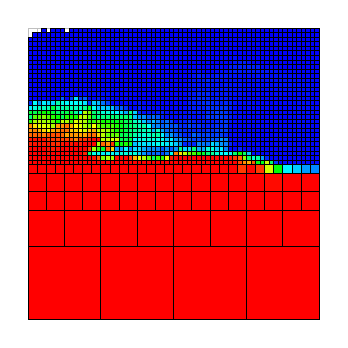
\begin{tikzpicture}[x={(\screenshotunitlength,0)},y={(0,\screenshotunitlength)}]
        \definecolor{fillcolor}{rgb}{1.000000,0.000000,0.000000}
\fill[fillcolor] (0.000000,0.000000) rectangle (0.250000,0.250000);
\definecolor{fillcolor}{rgb}{1.000000,0.000000,0.000000}
\fill[fillcolor] (0.250000,0.000000) rectangle (0.500000,0.250000);
\definecolor{fillcolor}{rgb}{1.000000,0.000000,0.000000}
\fill[fillcolor] (0.000000,0.250000) rectangle (0.125000,0.375000);
\definecolor{fillcolor}{rgb}{1.000000,0.000000,0.000000}
\fill[fillcolor] (0.125000,0.250000) rectangle (0.250000,0.375000);
\definecolor{fillcolor}{rgb}{1.000000,0.000000,0.000000}
\fill[fillcolor] (0.000000,0.375000) rectangle (0.062500,0.437500);
\definecolor{fillcolor}{rgb}{1.000000,0.000000,0.000000}
\fill[fillcolor] (0.062500,0.375000) rectangle (0.125000,0.437500);
\definecolor{fillcolor}{rgb}{1.000000,0.000000,0.000000}
\fill[fillcolor] (0.000000,0.437500) rectangle (0.062500,0.500000);
\definecolor{fillcolor}{rgb}{1.000000,0.000000,0.000000}
\fill[fillcolor] (0.062500,0.437500) rectangle (0.125000,0.500000);
\definecolor{fillcolor}{rgb}{1.000000,0.000000,0.000000}
\fill[fillcolor] (0.125000,0.375000) rectangle (0.187500,0.437500);
\definecolor{fillcolor}{rgb}{1.000000,0.000000,0.000000}
\fill[fillcolor] (0.187500,0.375000) rectangle (0.250000,0.437500);
\definecolor{fillcolor}{rgb}{1.000000,0.000000,0.000000}
\fill[fillcolor] (0.125000,0.437500) rectangle (0.187500,0.500000);
\definecolor{fillcolor}{rgb}{1.000000,0.000000,0.000000}
\fill[fillcolor] (0.187500,0.437500) rectangle (0.250000,0.500000);
\definecolor{fillcolor}{rgb}{1.000000,0.000000,0.000000}
\fill[fillcolor] (0.250000,0.250000) rectangle (0.375000,0.375000);
\definecolor{fillcolor}{rgb}{1.000000,0.000000,0.000000}
\fill[fillcolor] (0.375000,0.250000) rectangle (0.500000,0.375000);
\definecolor{fillcolor}{rgb}{1.000000,0.000000,0.000000}
\fill[fillcolor] (0.250000,0.375000) rectangle (0.312500,0.437500);
\definecolor{fillcolor}{rgb}{1.000000,0.000000,0.000000}
\fill[fillcolor] (0.312500,0.375000) rectangle (0.375000,0.437500);
\definecolor{fillcolor}{rgb}{1.000000,0.000000,0.000000}
\fill[fillcolor] (0.250000,0.437500) rectangle (0.312500,0.500000);
\definecolor{fillcolor}{rgb}{1.000000,0.000000,0.000000}
\fill[fillcolor] (0.312500,0.437500) rectangle (0.375000,0.500000);
\definecolor{fillcolor}{rgb}{1.000000,0.000000,0.000000}
\fill[fillcolor] (0.375000,0.375000) rectangle (0.437500,0.437500);
\definecolor{fillcolor}{rgb}{1.000000,0.000000,0.000000}
\fill[fillcolor] (0.437500,0.375000) rectangle (0.500000,0.437500);
\definecolor{fillcolor}{rgb}{1.000000,0.000000,0.000000}
\fill[fillcolor] (0.375000,0.437500) rectangle (0.437500,0.500000);
\definecolor{fillcolor}{rgb}{1.000000,0.000000,0.000000}
\fill[fillcolor] (0.437500,0.437500) rectangle (0.500000,0.500000);
\definecolor{fillcolor}{rgb}{1.000000,0.000000,0.000000}
\fill[fillcolor] (0.500000,0.000000) rectangle (0.750000,0.250000);
\definecolor{fillcolor}{rgb}{1.000000,0.000000,0.000000}
\fill[fillcolor] (0.750000,0.000000) rectangle (1.000000,0.250000);
\definecolor{fillcolor}{rgb}{1.000000,0.000000,0.000000}
\fill[fillcolor] (0.500000,0.250000) rectangle (0.625000,0.375000);
\definecolor{fillcolor}{rgb}{1.000000,0.000000,0.000000}
\fill[fillcolor] (0.625000,0.250000) rectangle (0.750000,0.375000);
\definecolor{fillcolor}{rgb}{1.000000,0.000000,0.000000}
\fill[fillcolor] (0.500000,0.375000) rectangle (0.562500,0.437500);
\definecolor{fillcolor}{rgb}{1.000000,0.000000,0.000000}
\fill[fillcolor] (0.562500,0.375000) rectangle (0.625000,0.437500);
\definecolor{fillcolor}{rgb}{1.000000,0.000000,0.000000}
\fill[fillcolor] (0.500000,0.437500) rectangle (0.562500,0.500000);
\definecolor{fillcolor}{rgb}{1.000000,0.000000,0.000000}
\fill[fillcolor] (0.562500,0.437500) rectangle (0.625000,0.500000);
\definecolor{fillcolor}{rgb}{1.000000,0.000000,0.000000}
\fill[fillcolor] (0.625000,0.375000) rectangle (0.687500,0.437500);
\definecolor{fillcolor}{rgb}{1.000000,0.000000,0.000000}
\fill[fillcolor] (0.687500,0.375000) rectangle (0.750000,0.437500);
\definecolor{fillcolor}{rgb}{1.000000,0.000000,0.000000}
\fill[fillcolor] (0.625000,0.437500) rectangle (0.687500,0.500000);
\definecolor{fillcolor}{rgb}{1.000000,0.000000,0.000000}
\fill[fillcolor] (0.687500,0.437500) rectangle (0.750000,0.500000);
\definecolor{fillcolor}{rgb}{1.000000,0.000000,0.000000}
\fill[fillcolor] (0.750000,0.250000) rectangle (0.875000,0.375000);
\definecolor{fillcolor}{rgb}{1.000000,0.000000,0.000000}
\fill[fillcolor] (0.875000,0.250000) rectangle (1.000000,0.375000);
\definecolor{fillcolor}{rgb}{1.000000,0.000000,0.000000}
\fill[fillcolor] (0.750000,0.375000) rectangle (0.812500,0.437500);
\definecolor{fillcolor}{rgb}{1.000000,0.000000,0.000000}
\fill[fillcolor] (0.812500,0.375000) rectangle (0.875000,0.437500);
\definecolor{fillcolor}{rgb}{1.000000,0.000073,0.000000}
\fill[fillcolor] (0.750000,0.437500) rectangle (0.812500,0.500000);
\definecolor{fillcolor}{rgb}{1.000000,0.040436,0.000000}
\fill[fillcolor] (0.812500,0.437500) rectangle (0.875000,0.500000);
\definecolor{fillcolor}{rgb}{1.000000,0.000000,0.000000}
\fill[fillcolor] (0.875000,0.375000) rectangle (0.937500,0.437500);
\definecolor{fillcolor}{rgb}{1.000000,0.000000,0.000000}
\fill[fillcolor] (0.937500,0.375000) rectangle (1.000000,0.437500);
\definecolor{fillcolor}{rgb}{1.000000,0.000000,0.000000}
\fill[fillcolor] (0.875000,0.437500) rectangle (0.937500,0.500000);
\definecolor{fillcolor}{rgb}{1.000000,0.000000,0.000000}
\fill[fillcolor] (0.937500,0.437500) rectangle (1.000000,0.500000);
\definecolor{fillcolor}{rgb}{1.000000,0.000000,0.000000}
\fill[fillcolor] (0.000000,0.500000) rectangle (0.031250,0.531250);
\definecolor{fillcolor}{rgb}{1.000000,0.000000,0.000000}
\fill[fillcolor] (0.031250,0.500000) rectangle (0.062500,0.531250);
\definecolor{fillcolor}{rgb}{1.000000,0.000000,0.000000}
\fill[fillcolor] (0.000000,0.531250) rectangle (0.015625,0.546875);
\definecolor{fillcolor}{rgb}{1.000000,0.000000,0.000000}
\fill[fillcolor] (0.015625,0.531250) rectangle (0.031250,0.546875);
\definecolor{fillcolor}{rgb}{1.000000,0.000007,0.000000}
\fill[fillcolor] (0.000000,0.546875) rectangle (0.015625,0.562500);
\definecolor{fillcolor}{rgb}{1.000000,0.000144,0.000000}
\fill[fillcolor] (0.015625,0.546875) rectangle (0.031250,0.562500);
\definecolor{fillcolor}{rgb}{1.000000,0.000000,0.000000}
\fill[fillcolor] (0.031250,0.531250) rectangle (0.046875,0.546875);
\definecolor{fillcolor}{rgb}{1.000000,0.000000,0.000000}
\fill[fillcolor] (0.046875,0.531250) rectangle (0.062500,0.546875);
\definecolor{fillcolor}{rgb}{1.000000,0.000000,0.000000}
\fill[fillcolor] (0.031250,0.546875) rectangle (0.046875,0.562500);
\definecolor{fillcolor}{rgb}{1.000000,0.000000,0.000000}
\fill[fillcolor] (0.046875,0.546875) rectangle (0.062500,0.562500);
\definecolor{fillcolor}{rgb}{1.000000,0.000000,0.000000}
\fill[fillcolor] (0.062500,0.500000) rectangle (0.093750,0.531250);
\definecolor{fillcolor}{rgb}{1.000000,0.000000,0.000000}
\fill[fillcolor] (0.093750,0.500000) rectangle (0.125000,0.531250);
\definecolor{fillcolor}{rgb}{1.000000,0.000000,0.000000}
\fill[fillcolor] (0.062500,0.531250) rectangle (0.078125,0.546875);
\definecolor{fillcolor}{rgb}{1.000000,0.000000,0.000000}
\fill[fillcolor] (0.078125,0.531250) rectangle (0.093750,0.546875);
\definecolor{fillcolor}{rgb}{1.000000,0.000011,0.000000}
\fill[fillcolor] (0.062500,0.546875) rectangle (0.078125,0.562500);
\definecolor{fillcolor}{rgb}{1.000000,0.000000,0.000000}
\fill[fillcolor] (0.078125,0.546875) rectangle (0.093750,0.562500);
\definecolor{fillcolor}{rgb}{1.000000,0.000001,0.000000}
\fill[fillcolor] (0.093750,0.531250) rectangle (0.109375,0.546875);
\definecolor{fillcolor}{rgb}{1.000000,0.000002,0.000000}
\fill[fillcolor] (0.109375,0.531250) rectangle (0.125000,0.546875);
\definecolor{fillcolor}{rgb}{1.000000,0.000000,0.000000}
\fill[fillcolor] (0.093750,0.546875) rectangle (0.109375,0.562500);
\definecolor{fillcolor}{rgb}{1.000000,0.000005,0.000000}
\fill[fillcolor] (0.109375,0.546875) rectangle (0.125000,0.562500);
\definecolor{fillcolor}{rgb}{1.000000,0.000001,0.000000}
\fill[fillcolor] (0.000000,0.562500) rectangle (0.015625,0.578125);
\definecolor{fillcolor}{rgb}{1.000000,0.000666,0.000000}
\fill[fillcolor] (0.015625,0.562500) rectangle (0.031250,0.578125);
\definecolor{fillcolor}{rgb}{1.000000,0.020890,0.000000}
\fill[fillcolor] (0.000000,0.578125) rectangle (0.015625,0.593750);
\definecolor{fillcolor}{rgb}{1.000000,0.000309,0.000000}
\fill[fillcolor] (0.015625,0.578125) rectangle (0.031250,0.593750);
\definecolor{fillcolor}{rgb}{1.000000,0.000428,0.000000}
\fill[fillcolor] (0.031250,0.562500) rectangle (0.046875,0.578125);
\definecolor{fillcolor}{rgb}{1.000000,0.007827,0.000000}
\fill[fillcolor] (0.046875,0.562500) rectangle (0.062500,0.578125);
\definecolor{fillcolor}{rgb}{1.000000,0.001033,0.000000}
\fill[fillcolor] (0.031250,0.578125) rectangle (0.046875,0.593750);
\definecolor{fillcolor}{rgb}{1.000000,0.007082,0.000000}
\fill[fillcolor] (0.046875,0.578125) rectangle (0.062500,0.593750);
\definecolor{fillcolor}{rgb}{1.000000,0.119507,0.000000}
\fill[fillcolor] (0.000000,0.593750) rectangle (0.015625,0.609375);
\definecolor{fillcolor}{rgb}{1.000000,0.064241,0.000000}
\fill[fillcolor] (0.015625,0.593750) rectangle (0.031250,0.609375);
\definecolor{fillcolor}{rgb}{1.000000,0.080304,0.000000}
\fill[fillcolor] (0.000000,0.609375) rectangle (0.015625,0.625000);
\definecolor{fillcolor}{rgb}{1.000000,0.055170,0.000000}
\fill[fillcolor] (0.015625,0.609375) rectangle (0.031250,0.625000);
\definecolor{fillcolor}{rgb}{1.000000,0.091067,0.000000}
\fill[fillcolor] (0.031250,0.593750) rectangle (0.046875,0.609375);
\definecolor{fillcolor}{rgb}{1.000000,0.092937,0.000000}
\fill[fillcolor] (0.046875,0.593750) rectangle (0.062500,0.609375);
\definecolor{fillcolor}{rgb}{1.000000,0.064608,0.000000}
\fill[fillcolor] (0.031250,0.609375) rectangle (0.046875,0.625000);
\definecolor{fillcolor}{rgb}{1.000000,0.066278,0.000000}
\fill[fillcolor] (0.046875,0.609375) rectangle (0.062500,0.625000);
\definecolor{fillcolor}{rgb}{1.000000,0.067867,0.000000}
\fill[fillcolor] (0.062500,0.562500) rectangle (0.078125,0.578125);
\definecolor{fillcolor}{rgb}{1.000000,0.009455,0.000000}
\fill[fillcolor] (0.078125,0.562500) rectangle (0.093750,0.578125);
\definecolor{fillcolor}{rgb}{1.000000,0.067831,0.000000}
\fill[fillcolor] (0.062500,0.578125) rectangle (0.078125,0.593750);
\definecolor{fillcolor}{rgb}{1.000000,0.109873,0.000000}
\fill[fillcolor] (0.078125,0.578125) rectangle (0.093750,0.593750);
\definecolor{fillcolor}{rgb}{1.000000,0.000026,0.000000}
\fill[fillcolor] (0.093750,0.562500) rectangle (0.109375,0.578125);
\definecolor{fillcolor}{rgb}{1.000000,0.000044,0.000000}
\fill[fillcolor] (0.109375,0.562500) rectangle (0.125000,0.578125);
\definecolor{fillcolor}{rgb}{1.000000,0.052145,0.000000}
\fill[fillcolor] (0.093750,0.578125) rectangle (0.109375,0.593750);
\definecolor{fillcolor}{rgb}{1.000000,0.000035,0.000000}
\fill[fillcolor] (0.109375,0.578125) rectangle (0.125000,0.593750);
\definecolor{fillcolor}{rgb}{1.000000,0.091052,0.000000}
\fill[fillcolor] (0.062500,0.593750) rectangle (0.078125,0.609375);
\definecolor{fillcolor}{rgb}{1.000000,0.163990,0.000000}
\fill[fillcolor] (0.078125,0.593750) rectangle (0.093750,0.609375);
\definecolor{fillcolor}{rgb}{1.000000,0.212254,0.000000}
\fill[fillcolor] (0.062500,0.609375) rectangle (0.078125,0.625000);
\definecolor{fillcolor}{rgb}{1.000000,0.215053,0.000000}
\fill[fillcolor] (0.078125,0.609375) rectangle (0.093750,0.625000);
\definecolor{fillcolor}{rgb}{1.000000,0.176248,0.000000}
\fill[fillcolor] (0.093750,0.593750) rectangle (0.109375,0.609375);
\definecolor{fillcolor}{rgb}{1.000000,0.078399,0.000000}
\fill[fillcolor] (0.109375,0.593750) rectangle (0.125000,0.609375);
\definecolor{fillcolor}{rgb}{1.000000,0.239888,0.000000}
\fill[fillcolor] (0.093750,0.609375) rectangle (0.109375,0.625000);
\definecolor{fillcolor}{rgb}{1.000000,0.254455,0.000000}
\fill[fillcolor] (0.109375,0.609375) rectangle (0.125000,0.625000);
\definecolor{fillcolor}{rgb}{1.000000,0.000001,0.000000}
\fill[fillcolor] (0.125000,0.500000) rectangle (0.156250,0.531250);
\definecolor{fillcolor}{rgb}{1.000000,0.000002,0.000000}
\fill[fillcolor] (0.156250,0.500000) rectangle (0.187500,0.531250);
\definecolor{fillcolor}{rgb}{1.000000,0.000003,0.000000}
\fill[fillcolor] (0.125000,0.531250) rectangle (0.140625,0.546875);
\definecolor{fillcolor}{rgb}{1.000000,0.000004,0.000000}
\fill[fillcolor] (0.140625,0.531250) rectangle (0.156250,0.546875);
\definecolor{fillcolor}{rgb}{1.000000,0.000002,0.000000}
\fill[fillcolor] (0.125000,0.546875) rectangle (0.140625,0.562500);
\definecolor{fillcolor}{rgb}{1.000000,0.000002,0.000000}
\fill[fillcolor] (0.140625,0.546875) rectangle (0.156250,0.562500);
\definecolor{fillcolor}{rgb}{1.000000,0.000003,0.000000}
\fill[fillcolor] (0.156250,0.531250) rectangle (0.171875,0.546875);
\definecolor{fillcolor}{rgb}{1.000000,0.000004,0.000000}
\fill[fillcolor] (0.171875,0.531250) rectangle (0.187500,0.546875);
\definecolor{fillcolor}{rgb}{1.000000,0.000007,0.000000}
\fill[fillcolor] (0.156250,0.546875) rectangle (0.171875,0.562500);
\definecolor{fillcolor}{rgb}{1.000000,0.000016,0.000000}
\fill[fillcolor] (0.171875,0.546875) rectangle (0.187500,0.562500);
\definecolor{fillcolor}{rgb}{1.000000,0.000002,0.000000}
\fill[fillcolor] (0.187500,0.500000) rectangle (0.218750,0.531250);
\definecolor{fillcolor}{rgb}{1.000000,0.000014,0.000000}
\fill[fillcolor] (0.218750,0.500000) rectangle (0.250000,0.531250);
\definecolor{fillcolor}{rgb}{1.000000,0.000005,0.000000}
\fill[fillcolor] (0.187500,0.531250) rectangle (0.203125,0.546875);
\definecolor{fillcolor}{rgb}{1.000000,0.000009,0.000000}
\fill[fillcolor] (0.203125,0.531250) rectangle (0.218750,0.546875);
\definecolor{fillcolor}{rgb}{1.000000,0.000026,0.000000}
\fill[fillcolor] (0.187500,0.546875) rectangle (0.203125,0.562500);
\definecolor{fillcolor}{rgb}{1.000000,0.001466,0.000000}
\fill[fillcolor] (0.203125,0.546875) rectangle (0.218750,0.562500);
\definecolor{fillcolor}{rgb}{1.000000,0.000016,0.000000}
\fill[fillcolor] (0.218750,0.531250) rectangle (0.234375,0.546875);
\definecolor{fillcolor}{rgb}{1.000000,0.000021,0.000000}
\fill[fillcolor] (0.234375,0.531250) rectangle (0.250000,0.546875);
\definecolor{fillcolor}{rgb}{1.000000,0.058014,0.000000}
\fill[fillcolor] (0.218750,0.546875) rectangle (0.234375,0.562500);
\definecolor{fillcolor}{rgb}{1.000000,0.333964,0.000000}
\fill[fillcolor] (0.234375,0.546875) rectangle (0.250000,0.562500);
\definecolor{fillcolor}{rgb}{1.000000,0.000027,0.000000}
\fill[fillcolor] (0.125000,0.562500) rectangle (0.140625,0.578125);
\definecolor{fillcolor}{rgb}{1.000000,0.000037,0.000000}
\fill[fillcolor] (0.140625,0.562500) rectangle (0.156250,0.578125);
\definecolor{fillcolor}{rgb}{1.000000,0.000035,0.000000}
\fill[fillcolor] (0.125000,0.578125) rectangle (0.140625,0.593750);
\definecolor{fillcolor}{rgb}{1.000000,0.000051,0.000000}
\fill[fillcolor] (0.140625,0.578125) rectangle (0.156250,0.593750);
\definecolor{fillcolor}{rgb}{1.000000,0.000062,0.000000}
\fill[fillcolor] (0.156250,0.562500) rectangle (0.171875,0.578125);
\definecolor{fillcolor}{rgb}{1.000000,0.000069,0.000000}
\fill[fillcolor] (0.171875,0.562500) rectangle (0.187500,0.578125);
\definecolor{fillcolor}{rgb}{1.000000,0.000068,0.000000}
\fill[fillcolor] (0.156250,0.578125) rectangle (0.171875,0.593750);
\definecolor{fillcolor}{rgb}{1.000000,0.000059,0.000000}
\fill[fillcolor] (0.171875,0.578125) rectangle (0.187500,0.593750);
\definecolor{fillcolor}{rgb}{1.000000,0.008308,0.000000}
\fill[fillcolor] (0.125000,0.593750) rectangle (0.140625,0.609375);
\definecolor{fillcolor}{rgb}{1.000000,0.084702,0.000000}
\fill[fillcolor] (0.140625,0.593750) rectangle (0.156250,0.609375);
\definecolor{fillcolor}{rgb}{1.000000,0.266768,0.000000}
\fill[fillcolor] (0.125000,0.609375) rectangle (0.140625,0.625000);
\definecolor{fillcolor}{rgb}{1.000000,0.343272,0.000000}
\fill[fillcolor] (0.140625,0.609375) rectangle (0.156250,0.625000);
\definecolor{fillcolor}{rgb}{1.000000,0.011519,0.000000}
\fill[fillcolor] (0.156250,0.593750) rectangle (0.171875,0.609375);
\definecolor{fillcolor}{rgb}{1.000000,0.118975,0.000000}
\fill[fillcolor] (0.171875,0.593750) rectangle (0.187500,0.609375);
\definecolor{fillcolor}{rgb}{1.000000,0.517526,0.000000}
\fill[fillcolor] (0.156250,0.609375) rectangle (0.171875,0.625000);
\definecolor{fillcolor}{rgb}{1.000000,0.212031,0.000000}
\fill[fillcolor] (0.171875,0.609375) rectangle (0.187500,0.625000);
\definecolor{fillcolor}{rgb}{1.000000,0.111955,0.000000}
\fill[fillcolor] (0.187500,0.562500) rectangle (0.203125,0.578125);
\definecolor{fillcolor}{rgb}{0.000000,1.000000,0.428020}
\fill[fillcolor] (0.203125,0.562500) rectangle (0.218750,0.578125);
\definecolor{fillcolor}{rgb}{1.000000,0.000039,0.000000}
\fill[fillcolor] (0.187500,0.578125) rectangle (0.203125,0.593750);
\definecolor{fillcolor}{rgb}{1.000000,0.241735,0.000000}
\fill[fillcolor] (0.203125,0.578125) rectangle (0.218750,0.593750);
\definecolor{fillcolor}{rgb}{0.000000,1.000000,0.912093}
\fill[fillcolor] (0.218750,0.562500) rectangle (0.234375,0.578125);
\definecolor{fillcolor}{rgb}{0.000000,1.000000,0.958535}
\fill[fillcolor] (0.234375,0.562500) rectangle (0.250000,0.578125);
\definecolor{fillcolor}{rgb}{0.642951,1.000000,0.000000}
\fill[fillcolor] (0.218750,0.578125) rectangle (0.234375,0.593750);
\definecolor{fillcolor}{rgb}{0.224444,1.000000,0.000000}
\fill[fillcolor] (0.234375,0.578125) rectangle (0.250000,0.593750);
\definecolor{fillcolor}{rgb}{1.000000,0.000059,0.000000}
\fill[fillcolor] (0.187500,0.593750) rectangle (0.203125,0.609375);
\definecolor{fillcolor}{rgb}{1.000000,0.000100,0.000000}
\fill[fillcolor] (0.203125,0.593750) rectangle (0.218750,0.609375);
\definecolor{fillcolor}{rgb}{1.000000,0.195481,0.000000}
\fill[fillcolor] (0.187500,0.609375) rectangle (0.203125,0.625000);
\definecolor{fillcolor}{rgb}{1.000000,0.109940,0.000000}
\fill[fillcolor] (0.203125,0.609375) rectangle (0.218750,0.625000);
\definecolor{fillcolor}{rgb}{1.000000,0.000213,0.000000}
\fill[fillcolor] (0.218750,0.593750) rectangle (0.234375,0.609375);
\definecolor{fillcolor}{rgb}{0.650371,1.000000,0.000000}
\fill[fillcolor] (0.234375,0.593750) rectangle (0.250000,0.609375);
\definecolor{fillcolor}{rgb}{1.000000,0.008040,0.000000}
\fill[fillcolor] (0.218750,0.609375) rectangle (0.234375,0.625000);
\definecolor{fillcolor}{rgb}{1.000000,0.056385,0.000000}
\fill[fillcolor] (0.234375,0.609375) rectangle (0.250000,0.625000);
\definecolor{fillcolor}{rgb}{1.000000,0.398861,0.000000}
\fill[fillcolor] (0.000000,0.625000) rectangle (0.015625,0.640625);
\definecolor{fillcolor}{rgb}{1.000000,0.391784,0.000000}
\fill[fillcolor] (0.015625,0.625000) rectangle (0.031250,0.640625);
\definecolor{fillcolor}{rgb}{1.000000,0.584384,0.000000}
\fill[fillcolor] (0.000000,0.640625) rectangle (0.015625,0.656250);
\definecolor{fillcolor}{rgb}{1.000000,0.511145,0.000000}
\fill[fillcolor] (0.015625,0.640625) rectangle (0.031250,0.656250);
\definecolor{fillcolor}{rgb}{1.000000,0.393369,0.000000}
\fill[fillcolor] (0.031250,0.625000) rectangle (0.046875,0.640625);
\definecolor{fillcolor}{rgb}{1.000000,0.483951,0.000000}
\fill[fillcolor] (0.046875,0.625000) rectangle (0.062500,0.640625);
\definecolor{fillcolor}{rgb}{1.000000,0.705247,0.000000}
\fill[fillcolor] (0.031250,0.640625) rectangle (0.046875,0.656250);
\definecolor{fillcolor}{rgb}{1.000000,0.838332,0.000000}
\fill[fillcolor] (0.046875,0.640625) rectangle (0.062500,0.656250);
\definecolor{fillcolor}{rgb}{1.000000,0.584384,0.000000}
\fill[fillcolor] (0.000000,0.656250) rectangle (0.015625,0.671875);
\definecolor{fillcolor}{rgb}{1.000000,0.881977,0.000000}
\fill[fillcolor] (0.015625,0.656250) rectangle (0.031250,0.671875);
\definecolor{fillcolor}{rgb}{0.157101,1.000000,0.000000}
\fill[fillcolor] (0.000000,0.671875) rectangle (0.015625,0.687500);
\definecolor{fillcolor}{rgb}{0.631110,1.000000,0.000000}
\fill[fillcolor] (0.015625,0.671875) rectangle (0.031250,0.687500);
\definecolor{fillcolor}{rgb}{0.889508,1.000000,0.000000}
\fill[fillcolor] (0.031250,0.656250) rectangle (0.046875,0.671875);
\definecolor{fillcolor}{rgb}{0.903118,1.000000,0.000000}
\fill[fillcolor] (0.046875,0.656250) rectangle (0.062500,0.671875);
\definecolor{fillcolor}{rgb}{0.747536,1.000000,0.000000}
\fill[fillcolor] (0.031250,0.671875) rectangle (0.046875,0.687500);
\definecolor{fillcolor}{rgb}{0.612008,1.000000,0.000000}
\fill[fillcolor] (0.046875,0.671875) rectangle (0.062500,0.687500);
\definecolor{fillcolor}{rgb}{1.000000,0.325116,0.000000}
\fill[fillcolor] (0.062500,0.625000) rectangle (0.078125,0.640625);
\definecolor{fillcolor}{rgb}{1.000000,0.315388,0.000000}
\fill[fillcolor] (0.078125,0.625000) rectangle (0.093750,0.640625);
\definecolor{fillcolor}{rgb}{0.932174,1.000000,0.000000}
\fill[fillcolor] (0.062500,0.640625) rectangle (0.078125,0.656250);
\definecolor{fillcolor}{rgb}{1.000000,0.653423,0.000000}
\fill[fillcolor] (0.078125,0.640625) rectangle (0.093750,0.656250);
\definecolor{fillcolor}{rgb}{1.000000,0.300229,0.000000}
\fill[fillcolor] (0.093750,0.625000) rectangle (0.109375,0.640625);
\definecolor{fillcolor}{rgb}{1.000000,0.399194,0.000000}
\fill[fillcolor] (0.109375,0.625000) rectangle (0.125000,0.640625);
\definecolor{fillcolor}{rgb}{1.000000,0.573067,0.000000}
\fill[fillcolor] (0.093750,0.640625) rectangle (0.109375,0.656250);
\definecolor{fillcolor}{rgb}{1.000000,0.416437,0.000000}
\fill[fillcolor] (0.109375,0.640625) rectangle (0.125000,0.656250);
\definecolor{fillcolor}{rgb}{0.818441,1.000000,0.000000}
\fill[fillcolor] (0.062500,0.656250) rectangle (0.078125,0.671875);
\definecolor{fillcolor}{rgb}{0.665951,1.000000,0.000000}
\fill[fillcolor] (0.078125,0.656250) rectangle (0.093750,0.671875);
\definecolor{fillcolor}{rgb}{0.614555,1.000000,0.000000}
\fill[fillcolor] (0.062500,0.671875) rectangle (0.078125,0.687500);
\definecolor{fillcolor}{rgb}{0.359415,1.000000,0.000000}
\fill[fillcolor] (0.078125,0.671875) rectangle (0.093750,0.687500);
\definecolor{fillcolor}{rgb}{1.000000,0.627512,0.000000}
\fill[fillcolor] (0.093750,0.656250) rectangle (0.109375,0.671875);
\definecolor{fillcolor}{rgb}{1.000000,0.542337,0.000000}
\fill[fillcolor] (0.109375,0.656250) rectangle (0.125000,0.671875);
\definecolor{fillcolor}{rgb}{0.026238,1.000000,0.000000}
\fill[fillcolor] (0.093750,0.671875) rectangle (0.109375,0.687500);
\definecolor{fillcolor}{rgb}{0.720776,1.000000,0.000000}
\fill[fillcolor] (0.109375,0.671875) rectangle (0.125000,0.687500);
\definecolor{fillcolor}{rgb}{0.000000,1.000000,0.470934}
\fill[fillcolor] (0.000000,0.687500) rectangle (0.015625,0.703125);
\definecolor{fillcolor}{rgb}{0.345971,1.000000,0.000000}
\fill[fillcolor] (0.015625,0.687500) rectangle (0.031250,0.703125);
\definecolor{fillcolor}{rgb}{0.000000,1.000000,0.229371}
\fill[fillcolor] (0.000000,0.703125) rectangle (0.015625,0.718750);
\definecolor{fillcolor}{rgb}{0.000000,1.000000,0.309545}
\fill[fillcolor] (0.015625,0.703125) rectangle (0.031250,0.718750);
\definecolor{fillcolor}{rgb}{0.347448,1.000000,0.000000}
\fill[fillcolor] (0.031250,0.687500) rectangle (0.046875,0.703125);
\definecolor{fillcolor}{rgb}{0.503987,1.000000,0.000000}
\fill[fillcolor] (0.046875,0.687500) rectangle (0.062500,0.703125);
\definecolor{fillcolor}{rgb}{0.000000,1.000000,0.170272}
\fill[fillcolor] (0.031250,0.703125) rectangle (0.046875,0.718750);
\definecolor{fillcolor}{rgb}{0.020434,1.000000,0.000000}
\fill[fillcolor] (0.046875,0.703125) rectangle (0.062500,0.718750);
\definecolor{fillcolor}{rgb}{0.000000,0.947072,1.000000}
\fill[fillcolor] (0.000000,0.718750) rectangle (0.015625,0.734375);
\definecolor{fillcolor}{rgb}{0.000000,1.000000,0.876430}
\fill[fillcolor] (0.015625,0.718750) rectangle (0.031250,0.734375);
\definecolor{fillcolor}{rgb}{0.000000,0.170760,1.000000}
\fill[fillcolor] (0.000000,0.734375) rectangle (0.015625,0.750000);
\definecolor{fillcolor}{rgb}{0.000000,1.000000,0.995106}
\fill[fillcolor] (0.015625,0.734375) rectangle (0.031250,0.750000);
\definecolor{fillcolor}{rgb}{0.000000,1.000000,0.752640}
\fill[fillcolor] (0.031250,0.718750) rectangle (0.046875,0.734375);
\definecolor{fillcolor}{rgb}{0.000000,1.000000,0.754248}
\fill[fillcolor] (0.046875,0.718750) rectangle (0.062500,0.734375);
\definecolor{fillcolor}{rgb}{0.000000,0.590287,1.000000}
\fill[fillcolor] (0.031250,0.734375) rectangle (0.046875,0.750000);
\definecolor{fillcolor}{rgb}{0.000000,0.945674,1.000000}
\fill[fillcolor] (0.046875,0.734375) rectangle (0.062500,0.750000);
\definecolor{fillcolor}{rgb}{0.308770,1.000000,0.000000}
\fill[fillcolor] (0.062500,0.687500) rectangle (0.078125,0.703125);
\definecolor{fillcolor}{rgb}{0.144730,1.000000,0.000000}
\fill[fillcolor] (0.078125,0.687500) rectangle (0.093750,0.703125);
\definecolor{fillcolor}{rgb}{0.000000,1.000000,0.044102}
\fill[fillcolor] (0.062500,0.703125) rectangle (0.078125,0.718750);
\definecolor{fillcolor}{rgb}{0.000000,1.000000,0.219563}
\fill[fillcolor] (0.078125,0.703125) rectangle (0.093750,0.718750);
\definecolor{fillcolor}{rgb}{0.024267,1.000000,0.000000}
\fill[fillcolor] (0.093750,0.687500) rectangle (0.109375,0.703125);
\definecolor{fillcolor}{rgb}{0.000000,1.000000,0.321240}
\fill[fillcolor] (0.109375,0.687500) rectangle (0.125000,0.703125);
\definecolor{fillcolor}{rgb}{0.000000,1.000000,0.378983}
\fill[fillcolor] (0.093750,0.703125) rectangle (0.109375,0.718750);
\definecolor{fillcolor}{rgb}{0.000000,1.000000,0.357788}
\fill[fillcolor] (0.109375,0.703125) rectangle (0.125000,0.718750);
\definecolor{fillcolor}{rgb}{0.000000,1.000000,0.702911}
\fill[fillcolor] (0.062500,0.718750) rectangle (0.078125,0.734375);
\definecolor{fillcolor}{rgb}{0.000000,1.000000,0.219750}
\fill[fillcolor] (0.078125,0.718750) rectangle (0.093750,0.734375);
\definecolor{fillcolor}{rgb}{0.000000,0.836598,1.000000}
\fill[fillcolor] (0.062500,0.734375) rectangle (0.078125,0.750000);
\definecolor{fillcolor}{rgb}{0.000000,0.851214,1.000000}
\fill[fillcolor] (0.078125,0.734375) rectangle (0.093750,0.750000);
\definecolor{fillcolor}{rgb}{0.000000,1.000000,0.594132}
\fill[fillcolor] (0.093750,0.718750) rectangle (0.109375,0.734375);
\definecolor{fillcolor}{rgb}{0.000000,1.000000,0.725927}
\fill[fillcolor] (0.109375,0.718750) rectangle (0.125000,0.734375);
\definecolor{fillcolor}{rgb}{0.000000,1.000000,0.658687}
\fill[fillcolor] (0.093750,0.734375) rectangle (0.109375,0.750000);
\definecolor{fillcolor}{rgb}{0.000000,1.000000,0.895338}
\fill[fillcolor] (0.109375,0.734375) rectangle (0.125000,0.750000);
\definecolor{fillcolor}{rgb}{1.000000,0.633581,0.000000}
\fill[fillcolor] (0.125000,0.625000) rectangle (0.140625,0.640625);
\definecolor{fillcolor}{rgb}{1.000000,0.578780,0.000000}
\fill[fillcolor] (0.140625,0.625000) rectangle (0.156250,0.640625);
\definecolor{fillcolor}{rgb}{1.000000,0.434318,0.000000}
\fill[fillcolor] (0.125000,0.640625) rectangle (0.140625,0.656250);
\definecolor{fillcolor}{rgb}{1.000000,0.778427,0.000000}
\fill[fillcolor] (0.140625,0.640625) rectangle (0.156250,0.656250);
\definecolor{fillcolor}{rgb}{1.000000,0.602034,0.000000}
\fill[fillcolor] (0.156250,0.625000) rectangle (0.171875,0.640625);
\definecolor{fillcolor}{rgb}{1.000000,0.645164,0.000000}
\fill[fillcolor] (0.171875,0.625000) rectangle (0.187500,0.640625);
\definecolor{fillcolor}{rgb}{1.000000,0.805960,0.000000}
\fill[fillcolor] (0.156250,0.640625) rectangle (0.171875,0.656250);
\definecolor{fillcolor}{rgb}{0.996590,1.000000,0.000000}
\fill[fillcolor] (0.171875,0.640625) rectangle (0.187500,0.656250);
\definecolor{fillcolor}{rgb}{1.000000,0.434059,0.000000}
\fill[fillcolor] (0.125000,0.656250) rectangle (0.140625,0.671875);
\definecolor{fillcolor}{rgb}{1.000000,0.684374,0.000000}
\fill[fillcolor] (0.140625,0.656250) rectangle (0.156250,0.671875);
\definecolor{fillcolor}{rgb}{0.645375,1.000000,0.000000}
\fill[fillcolor] (0.125000,0.671875) rectangle (0.140625,0.687500);
\definecolor{fillcolor}{rgb}{0.261266,1.000000,0.000000}
\fill[fillcolor] (0.140625,0.671875) rectangle (0.156250,0.687500);
\definecolor{fillcolor}{rgb}{1.000000,0.984679,0.000000}
\fill[fillcolor] (0.156250,0.656250) rectangle (0.171875,0.671875);
\definecolor{fillcolor}{rgb}{0.891254,1.000000,0.000000}
\fill[fillcolor] (0.171875,0.656250) rectangle (0.187500,0.671875);
\definecolor{fillcolor}{rgb}{0.871802,1.000000,0.000000}
\fill[fillcolor] (0.156250,0.671875) rectangle (0.171875,0.687500);
\definecolor{fillcolor}{rgb}{0.776761,1.000000,0.000000}
\fill[fillcolor] (0.171875,0.671875) rectangle (0.187500,0.687500);
\definecolor{fillcolor}{rgb}{1.000000,0.645298,0.000000}
\fill[fillcolor] (0.187500,0.625000) rectangle (0.203125,0.640625);
\definecolor{fillcolor}{rgb}{1.000000,0.461096,0.000000}
\fill[fillcolor] (0.203125,0.625000) rectangle (0.218750,0.640625);
\definecolor{fillcolor}{rgb}{0.838351,1.000000,0.000000}
\fill[fillcolor] (0.187500,0.640625) rectangle (0.203125,0.656250);
\definecolor{fillcolor}{rgb}{1.000000,0.824555,0.000000}
\fill[fillcolor] (0.203125,0.640625) rectangle (0.218750,0.656250);
\definecolor{fillcolor}{rgb}{1.000000,0.427141,0.000000}
\fill[fillcolor] (0.218750,0.625000) rectangle (0.234375,0.640625);
\definecolor{fillcolor}{rgb}{1.000000,0.796332,0.000000}
\fill[fillcolor] (0.234375,0.625000) rectangle (0.250000,0.640625);
\definecolor{fillcolor}{rgb}{1.000000,0.678270,0.000000}
\fill[fillcolor] (0.218750,0.640625) rectangle (0.234375,0.656250);
\definecolor{fillcolor}{rgb}{0.718886,1.000000,0.000000}
\fill[fillcolor] (0.234375,0.640625) rectangle (0.250000,0.656250);
\definecolor{fillcolor}{rgb}{0.667744,1.000000,0.000000}
\fill[fillcolor] (0.187500,0.656250) rectangle (0.203125,0.671875);
\definecolor{fillcolor}{rgb}{0.520542,1.000000,0.000000}
\fill[fillcolor] (0.203125,0.656250) rectangle (0.218750,0.671875);
\definecolor{fillcolor}{rgb}{0.675499,1.000000,0.000000}
\fill[fillcolor] (0.187500,0.671875) rectangle (0.203125,0.687500);
\definecolor{fillcolor}{rgb}{0.234246,1.000000,0.000000}
\fill[fillcolor] (0.203125,0.671875) rectangle (0.218750,0.687500);
\definecolor{fillcolor}{rgb}{0.996377,1.000000,0.000000}
\fill[fillcolor] (0.218750,0.656250) rectangle (0.234375,0.671875);
\definecolor{fillcolor}{rgb}{0.494587,1.000000,0.000000}
\fill[fillcolor] (0.234375,0.656250) rectangle (0.250000,0.671875);
\definecolor{fillcolor}{rgb}{0.217608,1.000000,0.000000}
\fill[fillcolor] (0.218750,0.671875) rectangle (0.234375,0.687500);
\definecolor{fillcolor}{rgb}{0.377950,1.000000,0.000000}
\fill[fillcolor] (0.234375,0.671875) rectangle (0.250000,0.687500);
\definecolor{fillcolor}{rgb}{0.108443,1.000000,0.000000}
\fill[fillcolor] (0.125000,0.687500) rectangle (0.140625,0.703125);
\definecolor{fillcolor}{rgb}{0.093114,1.000000,0.000000}
\fill[fillcolor] (0.140625,0.687500) rectangle (0.156250,0.703125);
\definecolor{fillcolor}{rgb}{0.000000,1.000000,0.293500}
\fill[fillcolor] (0.125000,0.703125) rectangle (0.140625,0.718750);
\definecolor{fillcolor}{rgb}{0.000000,1.000000,0.293787}
\fill[fillcolor] (0.140625,0.703125) rectangle (0.156250,0.718750);
\definecolor{fillcolor}{rgb}{0.071396,1.000000,0.000000}
\fill[fillcolor] (0.156250,0.687500) rectangle (0.171875,0.703125);
\definecolor{fillcolor}{rgb}{0.728512,1.000000,0.000000}
\fill[fillcolor] (0.171875,0.687500) rectangle (0.187500,0.703125);
\definecolor{fillcolor}{rgb}{0.000000,1.000000,0.594599}
\fill[fillcolor] (0.156250,0.703125) rectangle (0.171875,0.718750);
\definecolor{fillcolor}{rgb}{0.000000,1.000000,0.961375}
\fill[fillcolor] (0.171875,0.703125) rectangle (0.187500,0.718750);
\definecolor{fillcolor}{rgb}{0.000000,1.000000,0.567826}
\fill[fillcolor] (0.125000,0.718750) rectangle (0.140625,0.734375);
\definecolor{fillcolor}{rgb}{0.000000,1.000000,0.730900}
\fill[fillcolor] (0.140625,0.718750) rectangle (0.156250,0.734375);
\definecolor{fillcolor}{rgb}{0.000000,0.987545,1.000000}
\fill[fillcolor] (0.125000,0.734375) rectangle (0.140625,0.750000);
\definecolor{fillcolor}{rgb}{0.000000,1.000000,0.998570}
\fill[fillcolor] (0.140625,0.734375) rectangle (0.156250,0.750000);
\definecolor{fillcolor}{rgb}{0.000000,1.000000,0.767107}
\fill[fillcolor] (0.156250,0.718750) rectangle (0.171875,0.734375);
\definecolor{fillcolor}{rgb}{0.000000,1.000000,0.720379}
\fill[fillcolor] (0.171875,0.718750) rectangle (0.187500,0.734375);
\definecolor{fillcolor}{rgb}{0.000000,0.997525,1.000000}
\fill[fillcolor] (0.156250,0.734375) rectangle (0.171875,0.750000);
\definecolor{fillcolor}{rgb}{0.000000,1.000000,0.957658}
\fill[fillcolor] (0.171875,0.734375) rectangle (0.187500,0.750000);
\definecolor{fillcolor}{rgb}{0.729506,1.000000,0.000000}
\fill[fillcolor] (0.187500,0.687500) rectangle (0.203125,0.703125);
\definecolor{fillcolor}{rgb}{0.381940,1.000000,0.000000}
\fill[fillcolor] (0.203125,0.687500) rectangle (0.218750,0.703125);
\definecolor{fillcolor}{rgb}{0.714336,1.000000,0.000000}
\fill[fillcolor] (0.187500,0.703125) rectangle (0.203125,0.718750);
\definecolor{fillcolor}{rgb}{0.464377,1.000000,0.000000}
\fill[fillcolor] (0.203125,0.703125) rectangle (0.218750,0.718750);
\definecolor{fillcolor}{rgb}{0.000000,1.000000,0.276350}
\fill[fillcolor] (0.218750,0.687500) rectangle (0.234375,0.703125);
\definecolor{fillcolor}{rgb}{0.000000,1.000000,0.557136}
\fill[fillcolor] (0.234375,0.687500) rectangle (0.250000,0.703125);
\definecolor{fillcolor}{rgb}{0.000000,1.000000,0.463449}
\fill[fillcolor] (0.218750,0.703125) rectangle (0.234375,0.718750);
\definecolor{fillcolor}{rgb}{0.000000,1.000000,0.533297}
\fill[fillcolor] (0.234375,0.703125) rectangle (0.250000,0.718750);
\definecolor{fillcolor}{rgb}{0.000000,1.000000,0.552654}
\fill[fillcolor] (0.187500,0.718750) rectangle (0.203125,0.734375);
\definecolor{fillcolor}{rgb}{0.000000,1.000000,0.162148}
\fill[fillcolor] (0.203125,0.718750) rectangle (0.218750,0.734375);
\definecolor{fillcolor}{rgb}{0.000000,0.893187,1.000000}
\fill[fillcolor] (0.187500,0.734375) rectangle (0.203125,0.750000);
\definecolor{fillcolor}{rgb}{0.000000,0.215754,1.000000}
\fill[fillcolor] (0.203125,0.734375) rectangle (0.218750,0.750000);
\definecolor{fillcolor}{rgb}{0.000000,1.000000,0.921758}
\fill[fillcolor] (0.218750,0.718750) rectangle (0.234375,0.734375);
\definecolor{fillcolor}{rgb}{0.000000,0.750263,1.000000}
\fill[fillcolor] (0.234375,0.718750) rectangle (0.250000,0.734375);
\definecolor{fillcolor}{rgb}{0.000000,0.791839,1.000000}
\fill[fillcolor] (0.218750,0.734375) rectangle (0.234375,0.750000);
\definecolor{fillcolor}{rgb}{0.000000,0.709084,1.000000}
\fill[fillcolor] (0.234375,0.734375) rectangle (0.250000,0.750000);
\definecolor{fillcolor}{rgb}{1.000000,0.000016,0.000000}
\fill[fillcolor] (0.250000,0.500000) rectangle (0.281250,0.531250);
\definecolor{fillcolor}{rgb}{1.000000,0.000025,0.000000}
\fill[fillcolor] (0.281250,0.500000) rectangle (0.312500,0.531250);
\definecolor{fillcolor}{rgb}{1.000000,0.000022,0.000000}
\fill[fillcolor] (0.250000,0.531250) rectangle (0.265625,0.546875);
\definecolor{fillcolor}{rgb}{1.000000,0.000026,0.000000}
\fill[fillcolor] (0.265625,0.531250) rectangle (0.281250,0.546875);
\definecolor{fillcolor}{rgb}{0.489318,1.000000,0.000000}
\fill[fillcolor] (0.250000,0.546875) rectangle (0.265625,0.562500);
\definecolor{fillcolor}{rgb}{0.691210,1.000000,0.000000}
\fill[fillcolor] (0.265625,0.546875) rectangle (0.281250,0.562500);
\definecolor{fillcolor}{rgb}{1.000000,0.000022,0.000000}
\fill[fillcolor] (0.281250,0.531250) rectangle (0.296875,0.546875);
\definecolor{fillcolor}{rgb}{1.000000,0.000019,0.000000}
\fill[fillcolor] (0.296875,0.531250) rectangle (0.312500,0.546875);
\definecolor{fillcolor}{rgb}{0.590703,1.000000,0.000000}
\fill[fillcolor] (0.281250,0.546875) rectangle (0.296875,0.562500);
\definecolor{fillcolor}{rgb}{1.000000,0.041273,0.000000}
\fill[fillcolor] (0.296875,0.546875) rectangle (0.312500,0.562500);
\definecolor{fillcolor}{rgb}{1.000000,0.000014,0.000000}
\fill[fillcolor] (0.312500,0.500000) rectangle (0.343750,0.531250);
\definecolor{fillcolor}{rgb}{1.000000,0.000091,0.000000}
\fill[fillcolor] (0.343750,0.500000) rectangle (0.375000,0.531250);
\definecolor{fillcolor}{rgb}{1.000000,0.000019,0.000000}
\fill[fillcolor] (0.312500,0.531250) rectangle (0.328125,0.546875);
\definecolor{fillcolor}{rgb}{1.000000,0.000036,0.000000}
\fill[fillcolor] (0.328125,0.531250) rectangle (0.343750,0.546875);
\definecolor{fillcolor}{rgb}{1.000000,0.048315,0.000000}
\fill[fillcolor] (0.312500,0.546875) rectangle (0.328125,0.562500);
\definecolor{fillcolor}{rgb}{1.000000,0.011198,0.000000}
\fill[fillcolor] (0.328125,0.546875) rectangle (0.343750,0.562500);
\definecolor{fillcolor}{rgb}{1.000000,0.000082,0.000000}
\fill[fillcolor] (0.343750,0.531250) rectangle (0.359375,0.546875);
\definecolor{fillcolor}{rgb}{1.000000,0.000068,0.000000}
\fill[fillcolor] (0.359375,0.531250) rectangle (0.375000,0.546875);
\definecolor{fillcolor}{rgb}{1.000000,0.243123,0.000000}
\fill[fillcolor] (0.343750,0.546875) rectangle (0.359375,0.562500);
\definecolor{fillcolor}{rgb}{1.000000,0.686967,0.000000}
\fill[fillcolor] (0.359375,0.546875) rectangle (0.375000,0.562500);
\definecolor{fillcolor}{rgb}{0.000000,0.927289,1.000000}
\fill[fillcolor] (0.250000,0.562500) rectangle (0.265625,0.578125);
\definecolor{fillcolor}{rgb}{0.000000,1.000000,0.957488}
\fill[fillcolor] (0.265625,0.562500) rectangle (0.281250,0.578125);
\definecolor{fillcolor}{rgb}{0.000000,1.000000,0.159044}
\fill[fillcolor] (0.250000,0.578125) rectangle (0.265625,0.593750);
\definecolor{fillcolor}{rgb}{1.000000,0.382733,0.000000}
\fill[fillcolor] (0.265625,0.578125) rectangle (0.281250,0.593750);
\definecolor{fillcolor}{rgb}{0.000000,1.000000,0.969221}
\fill[fillcolor] (0.281250,0.562500) rectangle (0.296875,0.578125);
\definecolor{fillcolor}{rgb}{0.000000,0.901598,1.000000}
\fill[fillcolor] (0.296875,0.562500) rectangle (0.312500,0.578125);
\definecolor{fillcolor}{rgb}{1.000000,0.809272,0.000000}
\fill[fillcolor] (0.281250,0.578125) rectangle (0.296875,0.593750);
\definecolor{fillcolor}{rgb}{0.000000,0.606584,1.000000}
\fill[fillcolor] (0.296875,0.578125) rectangle (0.312500,0.593750);
\definecolor{fillcolor}{rgb}{1.000000,0.414244,0.000000}
\fill[fillcolor] (0.250000,0.593750) rectangle (0.265625,0.609375);
\definecolor{fillcolor}{rgb}{1.000000,0.561738,0.000000}
\fill[fillcolor] (0.265625,0.593750) rectangle (0.281250,0.609375);
\definecolor{fillcolor}{rgb}{0.722545,1.000000,0.000000}
\fill[fillcolor] (0.250000,0.609375) rectangle (0.265625,0.625000);
\definecolor{fillcolor}{rgb}{0.719788,1.000000,0.000000}
\fill[fillcolor] (0.265625,0.609375) rectangle (0.281250,0.625000);
\definecolor{fillcolor}{rgb}{1.000000,0.201986,0.000000}
\fill[fillcolor] (0.281250,0.593750) rectangle (0.296875,0.609375);
\definecolor{fillcolor}{rgb}{0.147278,1.000000,0.000000}
\fill[fillcolor] (0.296875,0.593750) rectangle (0.312500,0.609375);
\definecolor{fillcolor}{rgb}{0.878915,1.000000,0.000000}
\fill[fillcolor] (0.281250,0.609375) rectangle (0.296875,0.625000);
\definecolor{fillcolor}{rgb}{0.818835,1.000000,0.000000}
\fill[fillcolor] (0.296875,0.609375) rectangle (0.312500,0.625000);
\definecolor{fillcolor}{rgb}{0.000000,1.000000,0.850913}
\fill[fillcolor] (0.312500,0.562500) rectangle (0.328125,0.578125);
\definecolor{fillcolor}{rgb}{0.000000,1.000000,0.870957}
\fill[fillcolor] (0.328125,0.562500) rectangle (0.343750,0.578125);
\definecolor{fillcolor}{rgb}{0.000000,0.652545,1.000000}
\fill[fillcolor] (0.312500,0.578125) rectangle (0.328125,0.593750);
\definecolor{fillcolor}{rgb}{0.000000,0.974258,1.000000}
\fill[fillcolor] (0.328125,0.578125) rectangle (0.343750,0.593750);
\definecolor{fillcolor}{rgb}{0.000000,1.000000,0.892694}
\fill[fillcolor] (0.343750,0.562500) rectangle (0.359375,0.578125);
\definecolor{fillcolor}{rgb}{0.000000,1.000000,0.844913}
\fill[fillcolor] (0.359375,0.562500) rectangle (0.375000,0.578125);
\definecolor{fillcolor}{rgb}{0.000000,0.558159,1.000000}
\fill[fillcolor] (0.343750,0.578125) rectangle (0.359375,0.593750);
\definecolor{fillcolor}{rgb}{0.000000,0.852972,1.000000}
\fill[fillcolor] (0.359375,0.578125) rectangle (0.375000,0.593750);
\definecolor{fillcolor}{rgb}{0.000000,1.000000,0.073600}
\fill[fillcolor] (0.312500,0.593750) rectangle (0.328125,0.609375);
\definecolor{fillcolor}{rgb}{0.098728,1.000000,0.000000}
\fill[fillcolor] (0.328125,0.593750) rectangle (0.343750,0.609375);
\definecolor{fillcolor}{rgb}{0.000000,1.000000,0.299404}
\fill[fillcolor] (0.312500,0.609375) rectangle (0.328125,0.625000);
\definecolor{fillcolor}{rgb}{0.000000,1.000000,0.299159}
\fill[fillcolor] (0.328125,0.609375) rectangle (0.343750,0.625000);
\definecolor{fillcolor}{rgb}{0.000000,1.000000,0.138628}
\fill[fillcolor] (0.343750,0.593750) rectangle (0.359375,0.609375);
\definecolor{fillcolor}{rgb}{0.000000,0.749388,1.000000}
\fill[fillcolor] (0.359375,0.593750) rectangle (0.375000,0.609375);
\definecolor{fillcolor}{rgb}{0.000000,1.000000,0.245525}
\fill[fillcolor] (0.343750,0.609375) rectangle (0.359375,0.625000);
\definecolor{fillcolor}{rgb}{0.000000,0.980643,1.000000}
\fill[fillcolor] (0.359375,0.609375) rectangle (0.375000,0.625000);
\definecolor{fillcolor}{rgb}{1.000000,0.000159,0.000000}
\fill[fillcolor] (0.375000,0.500000) rectangle (0.406250,0.531250);
\definecolor{fillcolor}{rgb}{1.000000,0.000000,0.000000}
\fill[fillcolor] (0.406250,0.500000) rectangle (0.437500,0.531250);
\definecolor{fillcolor}{rgb}{1.000000,0.000061,0.000000}
\fill[fillcolor] (0.375000,0.531250) rectangle (0.390625,0.546875);
\definecolor{fillcolor}{rgb}{1.000000,0.000003,0.000000}
\fill[fillcolor] (0.390625,0.531250) rectangle (0.406250,0.546875);
\definecolor{fillcolor}{rgb}{0.898809,1.000000,0.000000}
\fill[fillcolor] (0.375000,0.546875) rectangle (0.390625,0.562500);
\definecolor{fillcolor}{rgb}{0.684598,1.000000,0.000000}
\fill[fillcolor] (0.390625,0.546875) rectangle (0.406250,0.562500);
\definecolor{fillcolor}{rgb}{1.000000,0.006573,0.000000}
\fill[fillcolor] (0.406250,0.531250) rectangle (0.421875,0.546875);
\definecolor{fillcolor}{rgb}{1.000000,0.000000,0.000000}
\fill[fillcolor] (0.421875,0.531250) rectangle (0.437500,0.546875);
\definecolor{fillcolor}{rgb}{0.376663,1.000000,0.000000}
\fill[fillcolor] (0.406250,0.546875) rectangle (0.421875,0.562500);
\definecolor{fillcolor}{rgb}{0.000000,1.000000,0.396858}
\fill[fillcolor] (0.421875,0.546875) rectangle (0.437500,0.562500);
\definecolor{fillcolor}{rgb}{1.000000,0.000005,0.000000}
\fill[fillcolor] (0.437500,0.500000) rectangle (0.468750,0.531250);
\definecolor{fillcolor}{rgb}{1.000000,0.007684,0.000000}
\fill[fillcolor] (0.468750,0.500000) rectangle (0.500000,0.531250);
\definecolor{fillcolor}{rgb}{1.000000,0.000000,0.000000}
\fill[fillcolor] (0.437500,0.531250) rectangle (0.453125,0.546875);
\definecolor{fillcolor}{rgb}{1.000000,0.000000,0.000000}
\fill[fillcolor] (0.453125,0.531250) rectangle (0.468750,0.546875);
\definecolor{fillcolor}{rgb}{0.202500,1.000000,0.000000}
\fill[fillcolor] (0.437500,0.546875) rectangle (0.453125,0.562500);
\definecolor{fillcolor}{rgb}{0.153133,1.000000,0.000000}
\fill[fillcolor] (0.453125,0.546875) rectangle (0.468750,0.562500);
\definecolor{fillcolor}{rgb}{1.000000,0.004909,0.000000}
\fill[fillcolor] (0.468750,0.531250) rectangle (0.484375,0.546875);
\definecolor{fillcolor}{rgb}{1.000000,0.006292,0.000000}
\fill[fillcolor] (0.484375,0.531250) rectangle (0.500000,0.546875);
\definecolor{fillcolor}{rgb}{0.886436,1.000000,0.000000}
\fill[fillcolor] (0.468750,0.546875) rectangle (0.484375,0.562500);
\definecolor{fillcolor}{rgb}{1.000000,0.090014,0.000000}
\fill[fillcolor] (0.484375,0.546875) rectangle (0.500000,0.562500);
\definecolor{fillcolor}{rgb}{0.000000,0.838501,1.000000}
\fill[fillcolor] (0.375000,0.562500) rectangle (0.390625,0.578125);
\definecolor{fillcolor}{rgb}{0.000000,0.582087,1.000000}
\fill[fillcolor] (0.390625,0.562500) rectangle (0.406250,0.578125);
\definecolor{fillcolor}{rgb}{0.000000,0.853519,1.000000}
\fill[fillcolor] (0.375000,0.578125) rectangle (0.390625,0.593750);
\definecolor{fillcolor}{rgb}{0.000000,0.683147,1.000000}
\fill[fillcolor] (0.390625,0.578125) rectangle (0.406250,0.593750);
\definecolor{fillcolor}{rgb}{0.000000,0.411271,1.000000}
\fill[fillcolor] (0.406250,0.562500) rectangle (0.421875,0.578125);
\definecolor{fillcolor}{rgb}{0.000000,0.411271,1.000000}
\fill[fillcolor] (0.421875,0.562500) rectangle (0.437500,0.578125);
\definecolor{fillcolor}{rgb}{0.000000,0.544453,1.000000}
\fill[fillcolor] (0.406250,0.578125) rectangle (0.421875,0.593750);
\definecolor{fillcolor}{rgb}{0.000000,0.556893,1.000000}
\fill[fillcolor] (0.421875,0.578125) rectangle (0.437500,0.593750);
\definecolor{fillcolor}{rgb}{0.000000,0.932026,1.000000}
\fill[fillcolor] (0.375000,0.593750) rectangle (0.390625,0.609375);
\definecolor{fillcolor}{rgb}{0.000000,0.895878,1.000000}
\fill[fillcolor] (0.390625,0.593750) rectangle (0.406250,0.609375);
\definecolor{fillcolor}{rgb}{0.000000,1.000000,0.985842}
\fill[fillcolor] (0.375000,0.609375) rectangle (0.390625,0.625000);
\definecolor{fillcolor}{rgb}{0.000000,1.000000,0.862001}
\fill[fillcolor] (0.390625,0.609375) rectangle (0.406250,0.625000);
\definecolor{fillcolor}{rgb}{0.000000,0.887550,1.000000}
\fill[fillcolor] (0.406250,0.593750) rectangle (0.421875,0.609375);
\definecolor{fillcolor}{rgb}{0.000000,0.954147,1.000000}
\fill[fillcolor] (0.421875,0.593750) rectangle (0.437500,0.609375);
\definecolor{fillcolor}{rgb}{0.000000,1.000000,0.861238}
\fill[fillcolor] (0.406250,0.609375) rectangle (0.421875,0.625000);
\definecolor{fillcolor}{rgb}{0.000000,1.000000,0.855669}
\fill[fillcolor] (0.421875,0.609375) rectangle (0.437500,0.625000);
\definecolor{fillcolor}{rgb}{0.000000,0.412980,1.000000}
\fill[fillcolor] (0.437500,0.562500) rectangle (0.453125,0.578125);
\definecolor{fillcolor}{rgb}{0.000000,0.285316,1.000000}
\fill[fillcolor] (0.453125,0.562500) rectangle (0.468750,0.578125);
\definecolor{fillcolor}{rgb}{0.000000,0.515351,1.000000}
\fill[fillcolor] (0.437500,0.578125) rectangle (0.453125,0.593750);
\definecolor{fillcolor}{rgb}{0.000000,0.317016,1.000000}
\fill[fillcolor] (0.453125,0.578125) rectangle (0.468750,0.593750);
\definecolor{fillcolor}{rgb}{0.000000,0.441778,1.000000}
\fill[fillcolor] (0.468750,0.562500) rectangle (0.484375,0.578125);
\definecolor{fillcolor}{rgb}{0.000000,1.000000,0.941969}
\fill[fillcolor] (0.484375,0.562500) rectangle (0.500000,0.578125);
\definecolor{fillcolor}{rgb}{0.000000,0.526626,1.000000}
\fill[fillcolor] (0.468750,0.578125) rectangle (0.484375,0.593750);
\definecolor{fillcolor}{rgb}{0.000000,0.358096,1.000000}
\fill[fillcolor] (0.484375,0.578125) rectangle (0.500000,0.593750);
\definecolor{fillcolor}{rgb}{0.000000,1.000000,0.935175}
\fill[fillcolor] (0.437500,0.593750) rectangle (0.453125,0.609375);
\definecolor{fillcolor}{rgb}{0.000000,1.000000,0.962165}
\fill[fillcolor] (0.453125,0.593750) rectangle (0.468750,0.609375);
\definecolor{fillcolor}{rgb}{0.000000,1.000000,0.919687}
\fill[fillcolor] (0.437500,0.609375) rectangle (0.453125,0.625000);
\definecolor{fillcolor}{rgb}{0.000000,1.000000,0.923442}
\fill[fillcolor] (0.453125,0.609375) rectangle (0.468750,0.625000);
\definecolor{fillcolor}{rgb}{0.000000,0.902743,1.000000}
\fill[fillcolor] (0.468750,0.593750) rectangle (0.484375,0.609375);
\definecolor{fillcolor}{rgb}{0.000000,0.938110,1.000000}
\fill[fillcolor] (0.484375,0.593750) rectangle (0.500000,0.609375);
\definecolor{fillcolor}{rgb}{0.000000,0.755801,1.000000}
\fill[fillcolor] (0.468750,0.609375) rectangle (0.484375,0.625000);
\definecolor{fillcolor}{rgb}{0.000000,0.940750,1.000000}
\fill[fillcolor] (0.484375,0.609375) rectangle (0.500000,0.625000);
\definecolor{fillcolor}{rgb}{0.718864,1.000000,0.000000}
\fill[fillcolor] (0.250000,0.625000) rectangle (0.265625,0.640625);
\definecolor{fillcolor}{rgb}{0.398326,1.000000,0.000000}
\fill[fillcolor] (0.265625,0.625000) rectangle (0.281250,0.640625);
\definecolor{fillcolor}{rgb}{0.728952,1.000000,0.000000}
\fill[fillcolor] (0.250000,0.640625) rectangle (0.265625,0.656250);
\definecolor{fillcolor}{rgb}{0.602878,1.000000,0.000000}
\fill[fillcolor] (0.265625,0.640625) rectangle (0.281250,0.656250);
\definecolor{fillcolor}{rgb}{0.397815,1.000000,0.000000}
\fill[fillcolor] (0.281250,0.625000) rectangle (0.296875,0.640625);
\definecolor{fillcolor}{rgb}{0.397216,1.000000,0.000000}
\fill[fillcolor] (0.296875,0.625000) rectangle (0.312500,0.640625);
\definecolor{fillcolor}{rgb}{0.395724,1.000000,0.000000}
\fill[fillcolor] (0.281250,0.640625) rectangle (0.296875,0.656250);
\definecolor{fillcolor}{rgb}{0.082711,1.000000,0.000000}
\fill[fillcolor] (0.296875,0.640625) rectangle (0.312500,0.656250);
\definecolor{fillcolor}{rgb}{0.265116,1.000000,0.000000}
\fill[fillcolor] (0.250000,0.656250) rectangle (0.265625,0.671875);
\definecolor{fillcolor}{rgb}{0.272763,1.000000,0.000000}
\fill[fillcolor] (0.265625,0.656250) rectangle (0.281250,0.671875);
\definecolor{fillcolor}{rgb}{0.047425,1.000000,0.000000}
\fill[fillcolor] (0.250000,0.671875) rectangle (0.265625,0.687500);
\definecolor{fillcolor}{rgb}{0.047040,1.000000,0.000000}
\fill[fillcolor] (0.265625,0.671875) rectangle (0.281250,0.687500);
\definecolor{fillcolor}{rgb}{0.277094,1.000000,0.000000}
\fill[fillcolor] (0.281250,0.656250) rectangle (0.296875,0.671875);
\definecolor{fillcolor}{rgb}{0.082429,1.000000,0.000000}
\fill[fillcolor] (0.296875,0.656250) rectangle (0.312500,0.671875);
\definecolor{fillcolor}{rgb}{0.000000,1.000000,0.079692}
\fill[fillcolor] (0.281250,0.671875) rectangle (0.296875,0.687500);
\definecolor{fillcolor}{rgb}{0.000000,1.000000,0.089014}
\fill[fillcolor] (0.296875,0.671875) rectangle (0.312500,0.687500);
\definecolor{fillcolor}{rgb}{0.000000,1.000000,0.318574}
\fill[fillcolor] (0.312500,0.625000) rectangle (0.328125,0.640625);
\definecolor{fillcolor}{rgb}{0.000000,1.000000,0.318609}
\fill[fillcolor] (0.328125,0.625000) rectangle (0.343750,0.640625);
\definecolor{fillcolor}{rgb}{0.000000,1.000000,0.077149}
\fill[fillcolor] (0.312500,0.640625) rectangle (0.328125,0.656250);
\definecolor{fillcolor}{rgb}{0.000000,1.000000,0.279360}
\fill[fillcolor] (0.328125,0.640625) rectangle (0.343750,0.656250);
\definecolor{fillcolor}{rgb}{0.000000,1.000000,0.417759}
\fill[fillcolor] (0.343750,0.625000) rectangle (0.359375,0.640625);
\definecolor{fillcolor}{rgb}{0.000000,1.000000,0.647673}
\fill[fillcolor] (0.359375,0.625000) rectangle (0.375000,0.640625);
\definecolor{fillcolor}{rgb}{0.000000,1.000000,0.482266}
\fill[fillcolor] (0.343750,0.640625) rectangle (0.359375,0.656250);
\definecolor{fillcolor}{rgb}{0.000000,1.000000,0.575899}
\fill[fillcolor] (0.359375,0.640625) rectangle (0.375000,0.656250);
\definecolor{fillcolor}{rgb}{0.000000,1.000000,0.111763}
\fill[fillcolor] (0.312500,0.656250) rectangle (0.328125,0.671875);
\definecolor{fillcolor}{rgb}{0.000000,1.000000,0.279392}
\fill[fillcolor] (0.328125,0.656250) rectangle (0.343750,0.671875);
\definecolor{fillcolor}{rgb}{0.000000,1.000000,0.150720}
\fill[fillcolor] (0.312500,0.671875) rectangle (0.328125,0.687500);
\definecolor{fillcolor}{rgb}{0.000000,1.000000,0.340787}
\fill[fillcolor] (0.328125,0.671875) rectangle (0.343750,0.687500);
\definecolor{fillcolor}{rgb}{0.000000,1.000000,0.426090}
\fill[fillcolor] (0.343750,0.656250) rectangle (0.359375,0.671875);
\definecolor{fillcolor}{rgb}{0.000000,1.000000,0.531786}
\fill[fillcolor] (0.359375,0.656250) rectangle (0.375000,0.671875);
\definecolor{fillcolor}{rgb}{0.000000,1.000000,0.368070}
\fill[fillcolor] (0.343750,0.671875) rectangle (0.359375,0.687500);
\definecolor{fillcolor}{rgb}{0.000000,1.000000,0.739808}
\fill[fillcolor] (0.359375,0.671875) rectangle (0.375000,0.687500);
\definecolor{fillcolor}{rgb}{0.000000,1.000000,0.503945}
\fill[fillcolor] (0.250000,0.687500) rectangle (0.265625,0.703125);
\definecolor{fillcolor}{rgb}{0.000000,1.000000,0.474639}
\fill[fillcolor] (0.265625,0.687500) rectangle (0.281250,0.703125);
\definecolor{fillcolor}{rgb}{0.000000,1.000000,0.833330}
\fill[fillcolor] (0.250000,0.703125) rectangle (0.265625,0.718750);
\definecolor{fillcolor}{rgb}{0.000000,1.000000,0.833448}
\fill[fillcolor] (0.265625,0.703125) rectangle (0.281250,0.718750);
\definecolor{fillcolor}{rgb}{0.000000,1.000000,0.436832}
\fill[fillcolor] (0.281250,0.687500) rectangle (0.296875,0.703125);
\definecolor{fillcolor}{rgb}{0.000000,1.000000,0.447577}
\fill[fillcolor] (0.296875,0.687500) rectangle (0.312500,0.703125);
\definecolor{fillcolor}{rgb}{0.000000,1.000000,0.925781}
\fill[fillcolor] (0.281250,0.703125) rectangle (0.296875,0.718750);
\definecolor{fillcolor}{rgb}{0.000000,1.000000,0.993624}
\fill[fillcolor] (0.296875,0.703125) rectangle (0.312500,0.718750);
\definecolor{fillcolor}{rgb}{0.000000,0.804711,1.000000}
\fill[fillcolor] (0.250000,0.718750) rectangle (0.265625,0.734375);
\definecolor{fillcolor}{rgb}{0.000000,0.758869,1.000000}
\fill[fillcolor] (0.265625,0.718750) rectangle (0.281250,0.734375);
\definecolor{fillcolor}{rgb}{0.000000,0.459717,1.000000}
\fill[fillcolor] (0.250000,0.734375) rectangle (0.265625,0.750000);
\definecolor{fillcolor}{rgb}{0.000000,0.262847,1.000000}
\fill[fillcolor] (0.265625,0.734375) rectangle (0.281250,0.750000);
\definecolor{fillcolor}{rgb}{0.000000,0.738904,1.000000}
\fill[fillcolor] (0.281250,0.718750) rectangle (0.296875,0.734375);
\definecolor{fillcolor}{rgb}{0.000000,0.380481,1.000000}
\fill[fillcolor] (0.296875,0.718750) rectangle (0.312500,0.734375);
\definecolor{fillcolor}{rgb}{0.000000,0.026228,1.000000}
\fill[fillcolor] (0.281250,0.734375) rectangle (0.296875,0.750000);
\definecolor{fillcolor}{rgb}{0.000000,0.020190,1.000000}
\fill[fillcolor] (0.296875,0.734375) rectangle (0.312500,0.750000);
\definecolor{fillcolor}{rgb}{0.000000,1.000000,0.455142}
\fill[fillcolor] (0.312500,0.687500) rectangle (0.328125,0.703125);
\definecolor{fillcolor}{rgb}{0.000000,1.000000,0.456869}
\fill[fillcolor] (0.328125,0.687500) rectangle (0.343750,0.703125);
\definecolor{fillcolor}{rgb}{0.000000,0.902405,1.000000}
\fill[fillcolor] (0.312500,0.703125) rectangle (0.328125,0.718750);
\definecolor{fillcolor}{rgb}{0.000000,0.652122,1.000000}
\fill[fillcolor] (0.328125,0.703125) rectangle (0.343750,0.718750);
\definecolor{fillcolor}{rgb}{0.000000,1.000000,0.475829}
\fill[fillcolor] (0.343750,0.687500) rectangle (0.359375,0.703125);
\definecolor{fillcolor}{rgb}{0.000000,0.766592,1.000000}
\fill[fillcolor] (0.359375,0.687500) rectangle (0.375000,0.703125);
\definecolor{fillcolor}{rgb}{0.000000,1.000000,0.514309}
\fill[fillcolor] (0.343750,0.703125) rectangle (0.359375,0.718750);
\definecolor{fillcolor}{rgb}{0.000000,0.810102,1.000000}
\fill[fillcolor] (0.359375,0.703125) rectangle (0.375000,0.718750);
\definecolor{fillcolor}{rgb}{0.000000,0.372160,1.000000}
\fill[fillcolor] (0.312500,0.718750) rectangle (0.328125,0.734375);
\definecolor{fillcolor}{rgb}{0.000000,0.195567,1.000000}
\fill[fillcolor] (0.328125,0.718750) rectangle (0.343750,0.734375);
\definecolor{fillcolor}{rgb}{0.000000,0.020109,1.000000}
\fill[fillcolor] (0.312500,0.734375) rectangle (0.328125,0.750000);
\definecolor{fillcolor}{rgb}{0.000000,0.018755,1.000000}
\fill[fillcolor] (0.328125,0.734375) rectangle (0.343750,0.750000);
\definecolor{fillcolor}{rgb}{0.000000,0.023201,1.000000}
\fill[fillcolor] (0.343750,0.718750) rectangle (0.359375,0.734375);
\definecolor{fillcolor}{rgb}{0.000000,0.030084,1.000000}
\fill[fillcolor] (0.359375,0.718750) rectangle (0.375000,0.734375);
\definecolor{fillcolor}{rgb}{0.000000,0.015856,1.000000}
\fill[fillcolor] (0.343750,0.734375) rectangle (0.359375,0.750000);
\definecolor{fillcolor}{rgb}{0.000000,0.037097,1.000000}
\fill[fillcolor] (0.359375,0.734375) rectangle (0.375000,0.750000);
\definecolor{fillcolor}{rgb}{0.000000,1.000000,0.814895}
\fill[fillcolor] (0.375000,0.625000) rectangle (0.390625,0.640625);
\definecolor{fillcolor}{rgb}{0.000000,1.000000,0.839600}
\fill[fillcolor] (0.390625,0.625000) rectangle (0.406250,0.640625);
\definecolor{fillcolor}{rgb}{0.000000,1.000000,0.662119}
\fill[fillcolor] (0.375000,0.640625) rectangle (0.390625,0.656250);
\definecolor{fillcolor}{rgb}{0.000000,1.000000,0.730066}
\fill[fillcolor] (0.390625,0.640625) rectangle (0.406250,0.656250);
\definecolor{fillcolor}{rgb}{0.000000,1.000000,0.786516}
\fill[fillcolor] (0.406250,0.625000) rectangle (0.421875,0.640625);
\definecolor{fillcolor}{rgb}{0.000000,1.000000,0.710438}
\fill[fillcolor] (0.421875,0.625000) rectangle (0.437500,0.640625);
\definecolor{fillcolor}{rgb}{0.000000,1.000000,0.717927}
\fill[fillcolor] (0.406250,0.640625) rectangle (0.421875,0.656250);
\definecolor{fillcolor}{rgb}{0.000000,0.729554,1.000000}
\fill[fillcolor] (0.421875,0.640625) rectangle (0.437500,0.656250);
\definecolor{fillcolor}{rgb}{0.000000,1.000000,0.769840}
\fill[fillcolor] (0.375000,0.656250) rectangle (0.390625,0.671875);
\definecolor{fillcolor}{rgb}{0.000000,1.000000,0.643004}
\fill[fillcolor] (0.390625,0.656250) rectangle (0.406250,0.671875);
\definecolor{fillcolor}{rgb}{0.000000,1.000000,0.861865}
\fill[fillcolor] (0.375000,0.671875) rectangle (0.390625,0.687500);
\definecolor{fillcolor}{rgb}{0.000000,0.772175,1.000000}
\fill[fillcolor] (0.390625,0.671875) rectangle (0.406250,0.687500);
\definecolor{fillcolor}{rgb}{0.000000,0.994920,1.000000}
\fill[fillcolor] (0.406250,0.656250) rectangle (0.421875,0.671875);
\definecolor{fillcolor}{rgb}{0.000000,0.551422,1.000000}
\fill[fillcolor] (0.421875,0.656250) rectangle (0.437500,0.671875);
\definecolor{fillcolor}{rgb}{0.000000,0.523020,1.000000}
\fill[fillcolor] (0.406250,0.671875) rectangle (0.421875,0.687500);
\definecolor{fillcolor}{rgb}{0.000000,0.736315,1.000000}
\fill[fillcolor] (0.421875,0.671875) rectangle (0.437500,0.687500);
\definecolor{fillcolor}{rgb}{0.000000,1.000000,0.623966}
\fill[fillcolor] (0.437500,0.625000) rectangle (0.453125,0.640625);
\definecolor{fillcolor}{rgb}{0.000000,0.941028,1.000000}
\fill[fillcolor] (0.453125,0.625000) rectangle (0.468750,0.640625);
\definecolor{fillcolor}{rgb}{0.000000,1.000000,0.731625}
\fill[fillcolor] (0.437500,0.640625) rectangle (0.453125,0.656250);
\definecolor{fillcolor}{rgb}{0.000000,0.632618,1.000000}
\fill[fillcolor] (0.453125,0.640625) rectangle (0.468750,0.656250);
\definecolor{fillcolor}{rgb}{0.000000,0.550192,1.000000}
\fill[fillcolor] (0.468750,0.625000) rectangle (0.484375,0.640625);
\definecolor{fillcolor}{rgb}{0.000000,0.594996,1.000000}
\fill[fillcolor] (0.484375,0.625000) rectangle (0.500000,0.640625);
\definecolor{fillcolor}{rgb}{0.000000,0.387102,1.000000}
\fill[fillcolor] (0.468750,0.640625) rectangle (0.484375,0.656250);
\definecolor{fillcolor}{rgb}{0.000000,0.373938,1.000000}
\fill[fillcolor] (0.484375,0.640625) rectangle (0.500000,0.656250);
\definecolor{fillcolor}{rgb}{0.000000,0.519866,1.000000}
\fill[fillcolor] (0.437500,0.656250) rectangle (0.453125,0.671875);
\definecolor{fillcolor}{rgb}{0.000000,0.370416,1.000000}
\fill[fillcolor] (0.453125,0.656250) rectangle (0.468750,0.671875);
\definecolor{fillcolor}{rgb}{0.000000,0.501246,1.000000}
\fill[fillcolor] (0.437500,0.671875) rectangle (0.453125,0.687500);
\definecolor{fillcolor}{rgb}{0.000000,0.330272,1.000000}
\fill[fillcolor] (0.453125,0.671875) rectangle (0.468750,0.687500);
\definecolor{fillcolor}{rgb}{0.000000,0.442535,1.000000}
\fill[fillcolor] (0.468750,0.656250) rectangle (0.484375,0.671875);
\definecolor{fillcolor}{rgb}{0.000000,0.315163,1.000000}
\fill[fillcolor] (0.484375,0.656250) rectangle (0.500000,0.671875);
\definecolor{fillcolor}{rgb}{0.000000,0.423220,1.000000}
\fill[fillcolor] (0.468750,0.671875) rectangle (0.484375,0.687500);
\definecolor{fillcolor}{rgb}{0.000000,0.253448,1.000000}
\fill[fillcolor] (0.484375,0.671875) rectangle (0.500000,0.687500);
\definecolor{fillcolor}{rgb}{0.000000,0.566613,1.000000}
\fill[fillcolor] (0.375000,0.687500) rectangle (0.390625,0.703125);
\definecolor{fillcolor}{rgb}{0.000000,0.555559,1.000000}
\fill[fillcolor] (0.390625,0.687500) rectangle (0.406250,0.703125);
\definecolor{fillcolor}{rgb}{0.000000,0.138620,1.000000}
\fill[fillcolor] (0.375000,0.703125) rectangle (0.390625,0.718750);
\definecolor{fillcolor}{rgb}{0.000000,0.058995,1.000000}
\fill[fillcolor] (0.390625,0.703125) rectangle (0.406250,0.718750);
\definecolor{fillcolor}{rgb}{0.000000,0.342491,1.000000}
\fill[fillcolor] (0.406250,0.687500) rectangle (0.421875,0.703125);
\definecolor{fillcolor}{rgb}{0.000000,0.429744,1.000000}
\fill[fillcolor] (0.421875,0.687500) rectangle (0.437500,0.703125);
\definecolor{fillcolor}{rgb}{0.000000,0.058286,1.000000}
\fill[fillcolor] (0.406250,0.703125) rectangle (0.421875,0.718750);
\definecolor{fillcolor}{rgb}{0.000000,0.054867,1.000000}
\fill[fillcolor] (0.421875,0.703125) rectangle (0.437500,0.718750);
\definecolor{fillcolor}{rgb}{0.000000,0.139582,1.000000}
\fill[fillcolor] (0.375000,0.718750) rectangle (0.390625,0.734375);
\definecolor{fillcolor}{rgb}{0.000000,0.051887,1.000000}
\fill[fillcolor] (0.390625,0.718750) rectangle (0.406250,0.734375);
\definecolor{fillcolor}{rgb}{0.000000,0.072968,1.000000}
\fill[fillcolor] (0.375000,0.734375) rectangle (0.390625,0.750000);
\definecolor{fillcolor}{rgb}{0.000000,0.032608,1.000000}
\fill[fillcolor] (0.390625,0.734375) rectangle (0.406250,0.750000);
\definecolor{fillcolor}{rgb}{0.000000,0.057999,1.000000}
\fill[fillcolor] (0.406250,0.718750) rectangle (0.421875,0.734375);
\definecolor{fillcolor}{rgb}{0.000000,0.032732,1.000000}
\fill[fillcolor] (0.421875,0.718750) rectangle (0.437500,0.734375);
\definecolor{fillcolor}{rgb}{0.000000,0.015766,1.000000}
\fill[fillcolor] (0.406250,0.734375) rectangle (0.421875,0.750000);
\definecolor{fillcolor}{rgb}{0.000000,0.009910,1.000000}
\fill[fillcolor] (0.421875,0.734375) rectangle (0.437500,0.750000);
\definecolor{fillcolor}{rgb}{0.000000,0.342342,1.000000}
\fill[fillcolor] (0.437500,0.687500) rectangle (0.453125,0.703125);
\definecolor{fillcolor}{rgb}{0.000000,0.126349,1.000000}
\fill[fillcolor] (0.453125,0.687500) rectangle (0.468750,0.703125);
\definecolor{fillcolor}{rgb}{0.000000,0.093112,1.000000}
\fill[fillcolor] (0.437500,0.703125) rectangle (0.453125,0.718750);
\definecolor{fillcolor}{rgb}{0.000000,0.123565,1.000000}
\fill[fillcolor] (0.453125,0.703125) rectangle (0.468750,0.718750);
\definecolor{fillcolor}{rgb}{0.000000,0.053504,1.000000}
\fill[fillcolor] (0.468750,0.687500) rectangle (0.484375,0.703125);
\definecolor{fillcolor}{rgb}{0.000000,0.053608,1.000000}
\fill[fillcolor] (0.484375,0.687500) rectangle (0.500000,0.703125);
\definecolor{fillcolor}{rgb}{0.000000,0.066516,1.000000}
\fill[fillcolor] (0.468750,0.703125) rectangle (0.484375,0.718750);
\definecolor{fillcolor}{rgb}{0.000000,0.066418,1.000000}
\fill[fillcolor] (0.484375,0.703125) rectangle (0.500000,0.718750);
\definecolor{fillcolor}{rgb}{0.000000,0.029874,1.000000}
\fill[fillcolor] (0.437500,0.718750) rectangle (0.453125,0.734375);
\definecolor{fillcolor}{rgb}{0.000000,0.025469,1.000000}
\fill[fillcolor] (0.453125,0.718750) rectangle (0.468750,0.734375);
\definecolor{fillcolor}{rgb}{0.000000,0.006429,1.000000}
\fill[fillcolor] (0.437500,0.734375) rectangle (0.453125,0.750000);
\definecolor{fillcolor}{rgb}{0.000000,0.007382,1.000000}
\fill[fillcolor] (0.453125,0.734375) rectangle (0.468750,0.750000);
\definecolor{fillcolor}{rgb}{0.000000,0.006992,1.000000}
\fill[fillcolor] (0.468750,0.718750) rectangle (0.484375,0.734375);
\definecolor{fillcolor}{rgb}{0.000000,0.010522,1.000000}
\fill[fillcolor] (0.484375,0.718750) rectangle (0.500000,0.734375);
\definecolor{fillcolor}{rgb}{0.000000,0.011299,1.000000}
\fill[fillcolor] (0.468750,0.734375) rectangle (0.484375,0.750000);
\definecolor{fillcolor}{rgb}{0.000000,0.013717,1.000000}
\fill[fillcolor] (0.484375,0.734375) rectangle (0.500000,0.750000);
\definecolor{fillcolor}{rgb}{0.000000,0.000000,1.000000}
\fill[fillcolor] (0.000000,0.750000) rectangle (0.015625,0.765625);
\definecolor{fillcolor}{rgb}{0.000000,0.000000,1.000000}
\fill[fillcolor] (0.015625,0.750000) rectangle (0.031250,0.765625);
\definecolor{fillcolor}{rgb}{0.000000,0.000000,1.000000}
\fill[fillcolor] (0.000000,0.765625) rectangle (0.015625,0.781250);
\definecolor{fillcolor}{rgb}{0.000000,0.000000,1.000000}
\fill[fillcolor] (0.015625,0.765625) rectangle (0.031250,0.781250);
\definecolor{fillcolor}{rgb}{0.000000,0.000017,1.000000}
\fill[fillcolor] (0.031250,0.750000) rectangle (0.046875,0.765625);
\definecolor{fillcolor}{rgb}{0.000000,0.000005,1.000000}
\fill[fillcolor] (0.046875,0.750000) rectangle (0.062500,0.765625);
\definecolor{fillcolor}{rgb}{0.000000,0.000000,1.000000}
\fill[fillcolor] (0.031250,0.765625) rectangle (0.046875,0.781250);
\definecolor{fillcolor}{rgb}{0.000000,0.000001,1.000000}
\fill[fillcolor] (0.046875,0.765625) rectangle (0.062500,0.781250);
\definecolor{fillcolor}{rgb}{0.000000,0.000000,1.000000}
\fill[fillcolor] (0.000000,0.781250) rectangle (0.015625,0.796875);
\definecolor{fillcolor}{rgb}{0.000000,0.000000,1.000000}
\fill[fillcolor] (0.015625,0.781250) rectangle (0.031250,0.796875);
\definecolor{fillcolor}{rgb}{0.000000,0.000000,1.000000}
\fill[fillcolor] (0.000000,0.796875) rectangle (0.015625,0.812500);
\definecolor{fillcolor}{rgb}{0.000000,0.000000,1.000000}
\fill[fillcolor] (0.015625,0.796875) rectangle (0.031250,0.812500);
\definecolor{fillcolor}{rgb}{0.000000,0.000001,1.000000}
\fill[fillcolor] (0.031250,0.781250) rectangle (0.046875,0.796875);
\definecolor{fillcolor}{rgb}{0.000000,0.000002,1.000000}
\fill[fillcolor] (0.046875,0.781250) rectangle (0.062500,0.796875);
\definecolor{fillcolor}{rgb}{0.000000,0.000001,1.000000}
\fill[fillcolor] (0.031250,0.796875) rectangle (0.046875,0.812500);
\definecolor{fillcolor}{rgb}{0.000000,0.000000,1.000000}
\fill[fillcolor] (0.046875,0.796875) rectangle (0.062500,0.812500);
\definecolor{fillcolor}{rgb}{0.000000,0.000029,1.000000}
\fill[fillcolor] (0.062500,0.750000) rectangle (0.078125,0.765625);
\definecolor{fillcolor}{rgb}{0.000000,0.000006,1.000000}
\fill[fillcolor] (0.078125,0.750000) rectangle (0.093750,0.765625);
\definecolor{fillcolor}{rgb}{0.000000,0.000001,1.000000}
\fill[fillcolor] (0.062500,0.765625) rectangle (0.078125,0.781250);
\definecolor{fillcolor}{rgb}{0.000000,0.000001,1.000000}
\fill[fillcolor] (0.078125,0.765625) rectangle (0.093750,0.781250);
\definecolor{fillcolor}{rgb}{0.000000,0.000008,1.000000}
\fill[fillcolor] (0.093750,0.750000) rectangle (0.109375,0.765625);
\definecolor{fillcolor}{rgb}{0.000000,0.367240,1.000000}
\fill[fillcolor] (0.109375,0.750000) rectangle (0.125000,0.765625);
\definecolor{fillcolor}{rgb}{0.000000,0.000002,1.000000}
\fill[fillcolor] (0.093750,0.765625) rectangle (0.109375,0.781250);
\definecolor{fillcolor}{rgb}{0.000000,0.000002,1.000000}
\fill[fillcolor] (0.109375,0.765625) rectangle (0.125000,0.781250);
\definecolor{fillcolor}{rgb}{0.000000,0.000001,1.000000}
\fill[fillcolor] (0.062500,0.781250) rectangle (0.078125,0.796875);
\definecolor{fillcolor}{rgb}{0.000000,0.000002,1.000000}
\fill[fillcolor] (0.078125,0.781250) rectangle (0.093750,0.796875);
\definecolor{fillcolor}{rgb}{0.000000,0.000001,1.000000}
\fill[fillcolor] (0.062500,0.796875) rectangle (0.078125,0.812500);
\definecolor{fillcolor}{rgb}{0.000000,0.000001,1.000000}
\fill[fillcolor] (0.078125,0.796875) rectangle (0.093750,0.812500);
\definecolor{fillcolor}{rgb}{0.000000,0.000001,1.000000}
\fill[fillcolor] (0.093750,0.781250) rectangle (0.109375,0.796875);
\definecolor{fillcolor}{rgb}{0.000000,0.000001,1.000000}
\fill[fillcolor] (0.109375,0.781250) rectangle (0.125000,0.796875);
\definecolor{fillcolor}{rgb}{0.000000,0.000001,1.000000}
\fill[fillcolor] (0.093750,0.796875) rectangle (0.109375,0.812500);
\definecolor{fillcolor}{rgb}{0.000000,0.000001,1.000000}
\fill[fillcolor] (0.109375,0.796875) rectangle (0.125000,0.812500);
\definecolor{fillcolor}{rgb}{0.000000,0.000000,1.000000}
\fill[fillcolor] (0.000000,0.812500) rectangle (0.015625,0.828125);
\definecolor{fillcolor}{rgb}{0.000000,0.000000,1.000000}
\fill[fillcolor] (0.015625,0.812500) rectangle (0.031250,0.828125);
\definecolor{fillcolor}{rgb}{0.000000,0.000000,1.000000}
\fill[fillcolor] (0.000000,0.828125) rectangle (0.015625,0.843750);
\definecolor{fillcolor}{rgb}{0.000000,0.000000,1.000000}
\fill[fillcolor] (0.015625,0.828125) rectangle (0.031250,0.843750);
\definecolor{fillcolor}{rgb}{0.000000,0.000001,1.000000}
\fill[fillcolor] (0.031250,0.812500) rectangle (0.046875,0.828125);
\definecolor{fillcolor}{rgb}{0.000000,0.000000,1.000000}
\fill[fillcolor] (0.046875,0.812500) rectangle (0.062500,0.828125);
\definecolor{fillcolor}{rgb}{0.000000,0.000000,1.000000}
\fill[fillcolor] (0.031250,0.828125) rectangle (0.046875,0.843750);
\definecolor{fillcolor}{rgb}{0.000000,0.000000,1.000000}
\fill[fillcolor] (0.046875,0.828125) rectangle (0.062500,0.843750);
\definecolor{fillcolor}{rgb}{0.000000,0.000000,1.000000}
\fill[fillcolor] (0.000000,0.843750) rectangle (0.015625,0.859375);
\definecolor{fillcolor}{rgb}{0.000000,0.000000,1.000000}
\fill[fillcolor] (0.015625,0.843750) rectangle (0.031250,0.859375);
\definecolor{fillcolor}{rgb}{0.000000,0.000000,1.000000}
\fill[fillcolor] (0.000000,0.859375) rectangle (0.015625,0.875000);
\definecolor{fillcolor}{rgb}{0.000000,0.000000,1.000000}
\fill[fillcolor] (0.015625,0.859375) rectangle (0.031250,0.875000);
\definecolor{fillcolor}{rgb}{0.000000,0.000000,1.000000}
\fill[fillcolor] (0.031250,0.843750) rectangle (0.046875,0.859375);
\definecolor{fillcolor}{rgb}{0.000000,0.000000,1.000000}
\fill[fillcolor] (0.046875,0.843750) rectangle (0.062500,0.859375);
\definecolor{fillcolor}{rgb}{0.000000,0.000000,1.000000}
\fill[fillcolor] (0.031250,0.859375) rectangle (0.046875,0.875000);
\definecolor{fillcolor}{rgb}{0.000000,0.000000,1.000000}
\fill[fillcolor] (0.046875,0.859375) rectangle (0.062500,0.875000);
\definecolor{fillcolor}{rgb}{0.000000,0.000001,1.000000}
\fill[fillcolor] (0.062500,0.812500) rectangle (0.078125,0.828125);
\definecolor{fillcolor}{rgb}{0.000000,0.000001,1.000000}
\fill[fillcolor] (0.078125,0.812500) rectangle (0.093750,0.828125);
\definecolor{fillcolor}{rgb}{0.000000,0.000000,1.000000}
\fill[fillcolor] (0.062500,0.828125) rectangle (0.078125,0.843750);
\definecolor{fillcolor}{rgb}{0.000000,0.000000,1.000000}
\fill[fillcolor] (0.078125,0.828125) rectangle (0.093750,0.843750);
\definecolor{fillcolor}{rgb}{0.000000,0.000000,1.000000}
\fill[fillcolor] (0.093750,0.812500) rectangle (0.109375,0.828125);
\definecolor{fillcolor}{rgb}{0.000000,0.000000,1.000000}
\fill[fillcolor] (0.109375,0.812500) rectangle (0.125000,0.828125);
\definecolor{fillcolor}{rgb}{0.000000,0.000000,1.000000}
\fill[fillcolor] (0.093750,0.828125) rectangle (0.109375,0.843750);
\definecolor{fillcolor}{rgb}{0.000000,0.000000,1.000000}
\fill[fillcolor] (0.109375,0.828125) rectangle (0.125000,0.843750);
\definecolor{fillcolor}{rgb}{0.000000,0.000000,1.000000}
\fill[fillcolor] (0.062500,0.843750) rectangle (0.078125,0.859375);
\definecolor{fillcolor}{rgb}{0.000000,0.000000,1.000000}
\fill[fillcolor] (0.078125,0.843750) rectangle (0.093750,0.859375);
\definecolor{fillcolor}{rgb}{0.000000,0.000000,1.000000}
\fill[fillcolor] (0.062500,0.859375) rectangle (0.078125,0.875000);
\definecolor{fillcolor}{rgb}{0.000000,0.000000,1.000000}
\fill[fillcolor] (0.078125,0.859375) rectangle (0.093750,0.875000);
\definecolor{fillcolor}{rgb}{0.000000,0.000000,1.000000}
\fill[fillcolor] (0.093750,0.843750) rectangle (0.109375,0.859375);
\definecolor{fillcolor}{rgb}{0.000000,0.000000,1.000000}
\fill[fillcolor] (0.109375,0.843750) rectangle (0.125000,0.859375);
\definecolor{fillcolor}{rgb}{0.000000,0.000000,1.000000}
\fill[fillcolor] (0.093750,0.859375) rectangle (0.109375,0.875000);
\definecolor{fillcolor}{rgb}{0.000000,0.000000,1.000000}
\fill[fillcolor] (0.109375,0.859375) rectangle (0.125000,0.875000);
\definecolor{fillcolor}{rgb}{0.000000,0.000006,1.000000}
\fill[fillcolor] (0.125000,0.750000) rectangle (0.140625,0.765625);
\definecolor{fillcolor}{rgb}{0.000000,0.256264,1.000000}
\fill[fillcolor] (0.140625,0.750000) rectangle (0.156250,0.765625);
\definecolor{fillcolor}{rgb}{0.000000,0.000042,1.000000}
\fill[fillcolor] (0.125000,0.765625) rectangle (0.140625,0.781250);
\definecolor{fillcolor}{rgb}{0.000000,0.000309,1.000000}
\fill[fillcolor] (0.140625,0.765625) rectangle (0.156250,0.781250);
\definecolor{fillcolor}{rgb}{0.000000,0.883342,1.000000}
\fill[fillcolor] (0.156250,0.750000) rectangle (0.171875,0.765625);
\definecolor{fillcolor}{rgb}{0.000000,0.250448,1.000000}
\fill[fillcolor] (0.171875,0.750000) rectangle (0.187500,0.765625);
\definecolor{fillcolor}{rgb}{0.000000,0.000077,1.000000}
\fill[fillcolor] (0.156250,0.765625) rectangle (0.171875,0.781250);
\definecolor{fillcolor}{rgb}{0.000000,0.000077,1.000000}
\fill[fillcolor] (0.171875,0.765625) rectangle (0.187500,0.781250);
\definecolor{fillcolor}{rgb}{0.000000,0.000020,1.000000}
\fill[fillcolor] (0.125000,0.781250) rectangle (0.140625,0.796875);
\definecolor{fillcolor}{rgb}{0.000000,0.000039,1.000000}
\fill[fillcolor] (0.140625,0.781250) rectangle (0.156250,0.796875);
\definecolor{fillcolor}{rgb}{0.000000,0.000001,1.000000}
\fill[fillcolor] (0.125000,0.796875) rectangle (0.140625,0.812500);
\definecolor{fillcolor}{rgb}{0.000000,0.000004,1.000000}
\fill[fillcolor] (0.140625,0.796875) rectangle (0.156250,0.812500);
\definecolor{fillcolor}{rgb}{0.000000,0.000081,1.000000}
\fill[fillcolor] (0.156250,0.781250) rectangle (0.171875,0.796875);
\definecolor{fillcolor}{rgb}{0.000000,0.000075,1.000000}
\fill[fillcolor] (0.171875,0.781250) rectangle (0.187500,0.796875);
\definecolor{fillcolor}{rgb}{0.000000,0.000033,1.000000}
\fill[fillcolor] (0.156250,0.796875) rectangle (0.171875,0.812500);
\definecolor{fillcolor}{rgb}{0.000000,0.000030,1.000000}
\fill[fillcolor] (0.171875,0.796875) rectangle (0.187500,0.812500);
\definecolor{fillcolor}{rgb}{0.000000,0.366595,1.000000}
\fill[fillcolor] (0.187500,0.750000) rectangle (0.203125,0.765625);
\definecolor{fillcolor}{rgb}{0.000000,0.032757,1.000000}
\fill[fillcolor] (0.203125,0.750000) rectangle (0.218750,0.765625);
\definecolor{fillcolor}{rgb}{0.000000,0.020940,1.000000}
\fill[fillcolor] (0.187500,0.765625) rectangle (0.203125,0.781250);
\definecolor{fillcolor}{rgb}{0.000000,0.011016,1.000000}
\fill[fillcolor] (0.203125,0.765625) rectangle (0.218750,0.781250);
\definecolor{fillcolor}{rgb}{0.000000,0.032729,1.000000}
\fill[fillcolor] (0.218750,0.750000) rectangle (0.234375,0.765625);
\definecolor{fillcolor}{rgb}{0.000000,0.087632,1.000000}
\fill[fillcolor] (0.234375,0.750000) rectangle (0.250000,0.765625);
\definecolor{fillcolor}{rgb}{0.000000,0.013679,1.000000}
\fill[fillcolor] (0.218750,0.765625) rectangle (0.234375,0.781250);
\definecolor{fillcolor}{rgb}{0.000000,0.038301,1.000000}
\fill[fillcolor] (0.234375,0.765625) rectangle (0.250000,0.781250);
\definecolor{fillcolor}{rgb}{0.000000,0.001844,1.000000}
\fill[fillcolor] (0.187500,0.781250) rectangle (0.203125,0.796875);
\definecolor{fillcolor}{rgb}{0.000000,0.000361,1.000000}
\fill[fillcolor] (0.203125,0.781250) rectangle (0.218750,0.796875);
\definecolor{fillcolor}{rgb}{0.000000,0.000033,1.000000}
\fill[fillcolor] (0.187500,0.796875) rectangle (0.203125,0.812500);
\definecolor{fillcolor}{rgb}{0.000000,0.000033,1.000000}
\fill[fillcolor] (0.203125,0.796875) rectangle (0.218750,0.812500);
\definecolor{fillcolor}{rgb}{0.000000,0.000931,1.000000}
\fill[fillcolor] (0.218750,0.781250) rectangle (0.234375,0.796875);
\definecolor{fillcolor}{rgb}{0.000000,0.002521,1.000000}
\fill[fillcolor] (0.234375,0.781250) rectangle (0.250000,0.796875);
\definecolor{fillcolor}{rgb}{0.000000,0.000050,1.000000}
\fill[fillcolor] (0.218750,0.796875) rectangle (0.234375,0.812500);
\definecolor{fillcolor}{rgb}{0.000000,0.001286,1.000000}
\fill[fillcolor] (0.234375,0.796875) rectangle (0.250000,0.812500);
\definecolor{fillcolor}{rgb}{0.000000,0.000000,1.000000}
\fill[fillcolor] (0.125000,0.812500) rectangle (0.140625,0.828125);
\definecolor{fillcolor}{rgb}{0.000000,0.000000,1.000000}
\fill[fillcolor] (0.140625,0.812500) rectangle (0.156250,0.828125);
\definecolor{fillcolor}{rgb}{0.000000,0.000000,1.000000}
\fill[fillcolor] (0.125000,0.828125) rectangle (0.140625,0.843750);
\definecolor{fillcolor}{rgb}{0.000000,0.000000,1.000000}
\fill[fillcolor] (0.140625,0.828125) rectangle (0.156250,0.843750);
\definecolor{fillcolor}{rgb}{0.000000,0.000008,1.000000}
\fill[fillcolor] (0.156250,0.812500) rectangle (0.171875,0.828125);
\definecolor{fillcolor}{rgb}{0.000000,0.000008,1.000000}
\fill[fillcolor] (0.171875,0.812500) rectangle (0.187500,0.828125);
\definecolor{fillcolor}{rgb}{0.000000,0.000000,1.000000}
\fill[fillcolor] (0.156250,0.828125) rectangle (0.171875,0.843750);
\definecolor{fillcolor}{rgb}{0.000000,0.000006,1.000000}
\fill[fillcolor] (0.171875,0.828125) rectangle (0.187500,0.843750);
\definecolor{fillcolor}{rgb}{0.000000,0.000000,1.000000}
\fill[fillcolor] (0.125000,0.843750) rectangle (0.140625,0.859375);
\definecolor{fillcolor}{rgb}{0.000000,0.000000,1.000000}
\fill[fillcolor] (0.140625,0.843750) rectangle (0.156250,0.859375);
\definecolor{fillcolor}{rgb}{0.000000,0.000000,1.000000}
\fill[fillcolor] (0.125000,0.859375) rectangle (0.140625,0.875000);
\definecolor{fillcolor}{rgb}{0.000000,0.000000,1.000000}
\fill[fillcolor] (0.140625,0.859375) rectangle (0.156250,0.875000);
\definecolor{fillcolor}{rgb}{0.000000,0.000000,1.000000}
\fill[fillcolor] (0.156250,0.843750) rectangle (0.171875,0.859375);
\definecolor{fillcolor}{rgb}{0.000000,0.000004,1.000000}
\fill[fillcolor] (0.171875,0.843750) rectangle (0.187500,0.859375);
\definecolor{fillcolor}{rgb}{0.000000,0.000000,1.000000}
\fill[fillcolor] (0.156250,0.859375) rectangle (0.171875,0.875000);
\definecolor{fillcolor}{rgb}{0.000000,0.000001,1.000000}
\fill[fillcolor] (0.171875,0.859375) rectangle (0.187500,0.875000);
\definecolor{fillcolor}{rgb}{0.000000,0.000003,1.000000}
\fill[fillcolor] (0.187500,0.812500) rectangle (0.203125,0.828125);
\definecolor{fillcolor}{rgb}{0.000000,0.000014,1.000000}
\fill[fillcolor] (0.203125,0.812500) rectangle (0.218750,0.828125);
\definecolor{fillcolor}{rgb}{0.000000,0.000004,1.000000}
\fill[fillcolor] (0.187500,0.828125) rectangle (0.203125,0.843750);
\definecolor{fillcolor}{rgb}{0.000000,0.000001,1.000000}
\fill[fillcolor] (0.203125,0.828125) rectangle (0.218750,0.843750);
\definecolor{fillcolor}{rgb}{0.000000,0.000024,1.000000}
\fill[fillcolor] (0.218750,0.812500) rectangle (0.234375,0.828125);
\definecolor{fillcolor}{rgb}{0.000000,0.000019,1.000000}
\fill[fillcolor] (0.234375,0.812500) rectangle (0.250000,0.828125);
\definecolor{fillcolor}{rgb}{0.000000,0.000002,1.000000}
\fill[fillcolor] (0.218750,0.828125) rectangle (0.234375,0.843750);
\definecolor{fillcolor}{rgb}{0.000000,0.000002,1.000000}
\fill[fillcolor] (0.234375,0.828125) rectangle (0.250000,0.843750);
\definecolor{fillcolor}{rgb}{0.000000,0.000002,1.000000}
\fill[fillcolor] (0.187500,0.843750) rectangle (0.203125,0.859375);
\definecolor{fillcolor}{rgb}{0.000000,0.000000,1.000000}
\fill[fillcolor] (0.203125,0.843750) rectangle (0.218750,0.859375);
\definecolor{fillcolor}{rgb}{0.000000,0.000000,1.000000}
\fill[fillcolor] (0.187500,0.859375) rectangle (0.203125,0.875000);
\definecolor{fillcolor}{rgb}{0.000000,0.000000,1.000000}
\fill[fillcolor] (0.203125,0.859375) rectangle (0.218750,0.875000);
\definecolor{fillcolor}{rgb}{0.000000,0.000001,1.000000}
\fill[fillcolor] (0.218750,0.843750) rectangle (0.234375,0.859375);
\definecolor{fillcolor}{rgb}{0.000000,0.000009,1.000000}
\fill[fillcolor] (0.234375,0.843750) rectangle (0.250000,0.859375);
\definecolor{fillcolor}{rgb}{0.000000,0.000001,1.000000}
\fill[fillcolor] (0.218750,0.859375) rectangle (0.234375,0.875000);
\definecolor{fillcolor}{rgb}{0.000000,0.000001,1.000000}
\fill[fillcolor] (0.234375,0.859375) rectangle (0.250000,0.875000);
\definecolor{fillcolor}{rgb}{0.000000,0.000000,1.000000}
\fill[fillcolor] (0.000000,0.875000) rectangle (0.015625,0.890625);
\definecolor{fillcolor}{rgb}{0.000000,0.000000,1.000000}
\fill[fillcolor] (0.015625,0.875000) rectangle (0.031250,0.890625);
\definecolor{fillcolor}{rgb}{0.000000,0.000000,1.000000}
\fill[fillcolor] (0.000000,0.890625) rectangle (0.015625,0.906250);
\definecolor{fillcolor}{rgb}{0.000000,0.000000,1.000000}
\fill[fillcolor] (0.015625,0.890625) rectangle (0.031250,0.906250);
\definecolor{fillcolor}{rgb}{0.000000,0.000000,1.000000}
\fill[fillcolor] (0.031250,0.875000) rectangle (0.046875,0.890625);
\definecolor{fillcolor}{rgb}{0.000000,0.000000,1.000000}
\fill[fillcolor] (0.046875,0.875000) rectangle (0.062500,0.890625);
\definecolor{fillcolor}{rgb}{0.000000,0.000000,1.000000}
\fill[fillcolor] (0.031250,0.890625) rectangle (0.046875,0.906250);
\definecolor{fillcolor}{rgb}{0.000000,0.000000,1.000000}
\fill[fillcolor] (0.046875,0.890625) rectangle (0.062500,0.906250);
\definecolor{fillcolor}{rgb}{0.000000,0.000000,1.000000}
\fill[fillcolor] (0.000000,0.906250) rectangle (0.015625,0.921875);
\definecolor{fillcolor}{rgb}{0.000000,0.000000,1.000000}
\fill[fillcolor] (0.015625,0.906250) rectangle (0.031250,0.921875);
\definecolor{fillcolor}{rgb}{0.000000,0.000000,1.000000}
\fill[fillcolor] (0.000000,0.921875) rectangle (0.015625,0.937500);
\definecolor{fillcolor}{rgb}{0.000000,0.000000,1.000000}
\fill[fillcolor] (0.015625,0.921875) rectangle (0.031250,0.937500);
\definecolor{fillcolor}{rgb}{0.000000,0.000000,1.000000}
\fill[fillcolor] (0.031250,0.906250) rectangle (0.046875,0.921875);
\definecolor{fillcolor}{rgb}{0.000000,0.000000,1.000000}
\fill[fillcolor] (0.046875,0.906250) rectangle (0.062500,0.921875);
\definecolor{fillcolor}{rgb}{0.000000,0.000000,1.000000}
\fill[fillcolor] (0.031250,0.921875) rectangle (0.046875,0.937500);
\definecolor{fillcolor}{rgb}{0.000000,0.000000,1.000000}
\fill[fillcolor] (0.046875,0.921875) rectangle (0.062500,0.937500);
\definecolor{fillcolor}{rgb}{0.000000,0.000000,1.000000}
\fill[fillcolor] (0.062500,0.875000) rectangle (0.078125,0.890625);
\definecolor{fillcolor}{rgb}{0.000000,0.000000,1.000000}
\fill[fillcolor] (0.078125,0.875000) rectangle (0.093750,0.890625);
\definecolor{fillcolor}{rgb}{0.000000,0.000000,1.000000}
\fill[fillcolor] (0.062500,0.890625) rectangle (0.078125,0.906250);
\definecolor{fillcolor}{rgb}{0.000000,0.000000,1.000000}
\fill[fillcolor] (0.078125,0.890625) rectangle (0.093750,0.906250);
\definecolor{fillcolor}{rgb}{0.000000,0.000000,1.000000}
\fill[fillcolor] (0.093750,0.875000) rectangle (0.109375,0.890625);
\definecolor{fillcolor}{rgb}{0.000000,0.000000,1.000000}
\fill[fillcolor] (0.109375,0.875000) rectangle (0.125000,0.890625);
\definecolor{fillcolor}{rgb}{0.000000,0.000000,1.000000}
\fill[fillcolor] (0.093750,0.890625) rectangle (0.109375,0.906250);
\definecolor{fillcolor}{rgb}{0.000000,0.000000,1.000000}
\fill[fillcolor] (0.109375,0.890625) rectangle (0.125000,0.906250);
\definecolor{fillcolor}{rgb}{0.000000,0.000000,1.000000}
\fill[fillcolor] (0.062500,0.906250) rectangle (0.078125,0.921875);
\definecolor{fillcolor}{rgb}{0.000000,0.000000,1.000000}
\fill[fillcolor] (0.078125,0.906250) rectangle (0.093750,0.921875);
\definecolor{fillcolor}{rgb}{0.000000,0.000000,1.000000}
\fill[fillcolor] (0.062500,0.921875) rectangle (0.078125,0.937500);
\definecolor{fillcolor}{rgb}{0.000000,0.000000,1.000000}
\fill[fillcolor] (0.078125,0.921875) rectangle (0.093750,0.937500);
\definecolor{fillcolor}{rgb}{0.000000,0.000000,1.000000}
\fill[fillcolor] (0.093750,0.906250) rectangle (0.109375,0.921875);
\definecolor{fillcolor}{rgb}{0.000000,0.000000,1.000000}
\fill[fillcolor] (0.109375,0.906250) rectangle (0.125000,0.921875);
\definecolor{fillcolor}{rgb}{0.000000,0.000000,1.000000}
\fill[fillcolor] (0.093750,0.921875) rectangle (0.109375,0.937500);
\definecolor{fillcolor}{rgb}{0.000000,0.000000,1.000000}
\fill[fillcolor] (0.109375,0.921875) rectangle (0.125000,0.937500);
\definecolor{fillcolor}{rgb}{0.000000,0.000000,1.000000}
\fill[fillcolor] (0.000000,0.937500) rectangle (0.015625,0.953125);
\definecolor{fillcolor}{rgb}{0.000000,0.000000,1.000000}
\fill[fillcolor] (0.015625,0.937500) rectangle (0.031250,0.953125);
\definecolor{fillcolor}{rgb}{0.000000,0.000000,1.000000}
\fill[fillcolor] (0.000000,0.953125) rectangle (0.015625,0.968750);
\definecolor{fillcolor}{rgb}{0.000000,0.000000,1.000000}
\fill[fillcolor] (0.015625,0.953125) rectangle (0.031250,0.968750);
\definecolor{fillcolor}{rgb}{0.000000,0.000000,1.000000}
\fill[fillcolor] (0.031250,0.937500) rectangle (0.046875,0.953125);
\definecolor{fillcolor}{rgb}{0.000000,0.000000,1.000000}
\fill[fillcolor] (0.046875,0.937500) rectangle (0.062500,0.953125);
\definecolor{fillcolor}{rgb}{0.000000,0.000000,1.000000}
\fill[fillcolor] (0.031250,0.953125) rectangle (0.046875,0.968750);
\definecolor{fillcolor}{rgb}{0.000000,0.000000,1.000000}
\fill[fillcolor] (0.046875,0.953125) rectangle (0.062500,0.968750);
\definecolor{fillcolor}{rgb}{0.000000,0.000000,1.000000}
\fill[fillcolor] (0.015625,0.968750) rectangle (0.031250,0.984375);
\definecolor{fillcolor}{rgb}{0.000000,0.000000,1.000000}
\fill[fillcolor] (0.031250,0.968750) rectangle (0.046875,0.984375);
\definecolor{fillcolor}{rgb}{0.000000,0.000000,1.000000}
\fill[fillcolor] (0.046875,0.968750) rectangle (0.062500,0.984375);
\definecolor{fillcolor}{rgb}{0.000000,0.000000,1.000000}
\fill[fillcolor] (0.046875,0.984375) rectangle (0.062500,1.000000);
\definecolor{fillcolor}{rgb}{0.000000,0.000000,1.000000}
\fill[fillcolor] (0.062500,0.937500) rectangle (0.078125,0.953125);
\definecolor{fillcolor}{rgb}{0.000000,0.000000,1.000000}
\fill[fillcolor] (0.078125,0.937500) rectangle (0.093750,0.953125);
\definecolor{fillcolor}{rgb}{0.000000,0.000000,1.000000}
\fill[fillcolor] (0.062500,0.953125) rectangle (0.078125,0.968750);
\definecolor{fillcolor}{rgb}{0.000000,0.000000,1.000000}
\fill[fillcolor] (0.078125,0.953125) rectangle (0.093750,0.968750);
\definecolor{fillcolor}{rgb}{0.000000,0.000000,1.000000}
\fill[fillcolor] (0.093750,0.937500) rectangle (0.109375,0.953125);
\definecolor{fillcolor}{rgb}{0.000000,0.000000,1.000000}
\fill[fillcolor] (0.109375,0.937500) rectangle (0.125000,0.953125);
\definecolor{fillcolor}{rgb}{0.000000,0.000000,1.000000}
\fill[fillcolor] (0.093750,0.953125) rectangle (0.109375,0.968750);
\definecolor{fillcolor}{rgb}{0.000000,0.000000,1.000000}
\fill[fillcolor] (0.109375,0.953125) rectangle (0.125000,0.968750);
\definecolor{fillcolor}{rgb}{0.000000,0.000000,1.000000}
\fill[fillcolor] (0.062500,0.968750) rectangle (0.078125,0.984375);
\definecolor{fillcolor}{rgb}{0.000000,0.000000,1.000000}
\fill[fillcolor] (0.078125,0.968750) rectangle (0.093750,0.984375);
\definecolor{fillcolor}{rgb}{0.000000,0.000000,1.000000}
\fill[fillcolor] (0.078125,0.984375) rectangle (0.093750,1.000000);
\definecolor{fillcolor}{rgb}{0.000000,0.000000,1.000000}
\fill[fillcolor] (0.093750,0.968750) rectangle (0.109375,0.984375);
\definecolor{fillcolor}{rgb}{0.000000,0.000000,1.000000}
\fill[fillcolor] (0.109375,0.968750) rectangle (0.125000,0.984375);
\definecolor{fillcolor}{rgb}{0.000000,0.000000,1.000000}
\fill[fillcolor] (0.093750,0.984375) rectangle (0.109375,1.000000);
\definecolor{fillcolor}{rgb}{0.000000,0.000000,1.000000}
\fill[fillcolor] (0.109375,0.984375) rectangle (0.125000,1.000000);
\definecolor{fillcolor}{rgb}{0.000000,0.000000,1.000000}
\fill[fillcolor] (0.125000,0.875000) rectangle (0.140625,0.890625);
\definecolor{fillcolor}{rgb}{0.000000,0.000000,1.000000}
\fill[fillcolor] (0.140625,0.875000) rectangle (0.156250,0.890625);
\definecolor{fillcolor}{rgb}{0.000000,0.000000,1.000000}
\fill[fillcolor] (0.125000,0.890625) rectangle (0.140625,0.906250);
\definecolor{fillcolor}{rgb}{0.000000,0.000000,1.000000}
\fill[fillcolor] (0.140625,0.890625) rectangle (0.156250,0.906250);
\definecolor{fillcolor}{rgb}{0.000000,0.000000,1.000000}
\fill[fillcolor] (0.156250,0.875000) rectangle (0.171875,0.890625);
\definecolor{fillcolor}{rgb}{0.000000,0.000000,1.000000}
\fill[fillcolor] (0.171875,0.875000) rectangle (0.187500,0.890625);
\definecolor{fillcolor}{rgb}{0.000000,0.000000,1.000000}
\fill[fillcolor] (0.156250,0.890625) rectangle (0.171875,0.906250);
\definecolor{fillcolor}{rgb}{0.000000,0.000000,1.000000}
\fill[fillcolor] (0.171875,0.890625) rectangle (0.187500,0.906250);
\definecolor{fillcolor}{rgb}{0.000000,0.000000,1.000000}
\fill[fillcolor] (0.125000,0.906250) rectangle (0.140625,0.921875);
\definecolor{fillcolor}{rgb}{0.000000,0.000000,1.000000}
\fill[fillcolor] (0.140625,0.906250) rectangle (0.156250,0.921875);
\definecolor{fillcolor}{rgb}{0.000000,0.000000,1.000000}
\fill[fillcolor] (0.125000,0.921875) rectangle (0.140625,0.937500);
\definecolor{fillcolor}{rgb}{0.000000,0.000000,1.000000}
\fill[fillcolor] (0.140625,0.921875) rectangle (0.156250,0.937500);
\definecolor{fillcolor}{rgb}{0.000000,0.000000,1.000000}
\fill[fillcolor] (0.156250,0.906250) rectangle (0.171875,0.921875);
\definecolor{fillcolor}{rgb}{0.000000,0.000000,1.000000}
\fill[fillcolor] (0.171875,0.906250) rectangle (0.187500,0.921875);
\definecolor{fillcolor}{rgb}{0.000000,0.000000,1.000000}
\fill[fillcolor] (0.156250,0.921875) rectangle (0.171875,0.937500);
\definecolor{fillcolor}{rgb}{0.000000,0.000000,1.000000}
\fill[fillcolor] (0.171875,0.921875) rectangle (0.187500,0.937500);
\definecolor{fillcolor}{rgb}{0.000000,0.000000,1.000000}
\fill[fillcolor] (0.187500,0.875000) rectangle (0.203125,0.890625);
\definecolor{fillcolor}{rgb}{0.000000,0.000000,1.000000}
\fill[fillcolor] (0.203125,0.875000) rectangle (0.218750,0.890625);
\definecolor{fillcolor}{rgb}{0.000000,0.000000,1.000000}
\fill[fillcolor] (0.187500,0.890625) rectangle (0.203125,0.906250);
\definecolor{fillcolor}{rgb}{0.000000,0.000000,1.000000}
\fill[fillcolor] (0.203125,0.890625) rectangle (0.218750,0.906250);
\definecolor{fillcolor}{rgb}{0.000000,0.000001,1.000000}
\fill[fillcolor] (0.218750,0.875000) rectangle (0.234375,0.890625);
\definecolor{fillcolor}{rgb}{0.000000,0.000001,1.000000}
\fill[fillcolor] (0.234375,0.875000) rectangle (0.250000,0.890625);
\definecolor{fillcolor}{rgb}{0.000000,0.000000,1.000000}
\fill[fillcolor] (0.218750,0.890625) rectangle (0.234375,0.906250);
\definecolor{fillcolor}{rgb}{0.000000,0.000000,1.000000}
\fill[fillcolor] (0.234375,0.890625) rectangle (0.250000,0.906250);
\definecolor{fillcolor}{rgb}{0.000000,0.000000,1.000000}
\fill[fillcolor] (0.187500,0.906250) rectangle (0.203125,0.921875);
\definecolor{fillcolor}{rgb}{0.000000,0.000001,1.000000}
\fill[fillcolor] (0.203125,0.906250) rectangle (0.218750,0.921875);
\definecolor{fillcolor}{rgb}{0.000000,0.000000,1.000000}
\fill[fillcolor] (0.187500,0.921875) rectangle (0.203125,0.937500);
\definecolor{fillcolor}{rgb}{0.000000,0.000000,1.000000}
\fill[fillcolor] (0.203125,0.921875) rectangle (0.218750,0.937500);
\definecolor{fillcolor}{rgb}{0.000000,0.000002,1.000000}
\fill[fillcolor] (0.218750,0.906250) rectangle (0.234375,0.921875);
\definecolor{fillcolor}{rgb}{0.000000,0.000001,1.000000}
\fill[fillcolor] (0.234375,0.906250) rectangle (0.250000,0.921875);
\definecolor{fillcolor}{rgb}{0.000000,0.000001,1.000000}
\fill[fillcolor] (0.218750,0.921875) rectangle (0.234375,0.937500);
\definecolor{fillcolor}{rgb}{0.000000,0.000001,1.000000}
\fill[fillcolor] (0.234375,0.921875) rectangle (0.250000,0.937500);
\definecolor{fillcolor}{rgb}{0.000000,0.000000,1.000000}
\fill[fillcolor] (0.125000,0.937500) rectangle (0.140625,0.953125);
\definecolor{fillcolor}{rgb}{0.000000,0.000000,1.000000}
\fill[fillcolor] (0.140625,0.937500) rectangle (0.156250,0.953125);
\definecolor{fillcolor}{rgb}{0.000000,0.000000,1.000000}
\fill[fillcolor] (0.125000,0.953125) rectangle (0.140625,0.968750);
\definecolor{fillcolor}{rgb}{0.000000,0.000000,1.000000}
\fill[fillcolor] (0.140625,0.953125) rectangle (0.156250,0.968750);
\definecolor{fillcolor}{rgb}{0.000000,0.000000,1.000000}
\fill[fillcolor] (0.156250,0.937500) rectangle (0.171875,0.953125);
\definecolor{fillcolor}{rgb}{0.000000,0.000000,1.000000}
\fill[fillcolor] (0.171875,0.937500) rectangle (0.187500,0.953125);
\definecolor{fillcolor}{rgb}{0.000000,0.000000,1.000000}
\fill[fillcolor] (0.156250,0.953125) rectangle (0.171875,0.968750);
\definecolor{fillcolor}{rgb}{0.000000,0.000000,1.000000}
\fill[fillcolor] (0.171875,0.953125) rectangle (0.187500,0.968750);
\definecolor{fillcolor}{rgb}{0.000000,0.000000,1.000000}
\fill[fillcolor] (0.125000,0.968750) rectangle (0.140625,0.984375);
\definecolor{fillcolor}{rgb}{0.000000,0.000000,1.000000}
\fill[fillcolor] (0.140625,0.968750) rectangle (0.156250,0.984375);
\definecolor{fillcolor}{rgb}{0.000000,0.000000,1.000000}
\fill[fillcolor] (0.140625,0.984375) rectangle (0.156250,1.000000);
\definecolor{fillcolor}{rgb}{0.000000,0.000000,1.000000}
\fill[fillcolor] (0.156250,0.968750) rectangle (0.171875,0.984375);
\definecolor{fillcolor}{rgb}{0.000000,0.000000,1.000000}
\fill[fillcolor] (0.171875,0.968750) rectangle (0.187500,0.984375);
\definecolor{fillcolor}{rgb}{0.000000,0.000000,1.000000}
\fill[fillcolor] (0.156250,0.984375) rectangle (0.171875,1.000000);
\definecolor{fillcolor}{rgb}{0.000000,0.000000,1.000000}
\fill[fillcolor] (0.171875,0.984375) rectangle (0.187500,1.000000);
\definecolor{fillcolor}{rgb}{0.000000,0.000000,1.000000}
\fill[fillcolor] (0.187500,0.937500) rectangle (0.203125,0.953125);
\definecolor{fillcolor}{rgb}{0.000000,0.000000,1.000000}
\fill[fillcolor] (0.203125,0.937500) rectangle (0.218750,0.953125);
\definecolor{fillcolor}{rgb}{0.000000,0.000000,1.000000}
\fill[fillcolor] (0.187500,0.953125) rectangle (0.203125,0.968750);
\definecolor{fillcolor}{rgb}{0.000000,0.000000,1.000000}
\fill[fillcolor] (0.203125,0.953125) rectangle (0.218750,0.968750);
\definecolor{fillcolor}{rgb}{0.000000,0.000000,1.000000}
\fill[fillcolor] (0.218750,0.937500) rectangle (0.234375,0.953125);
\definecolor{fillcolor}{rgb}{0.000000,0.000000,1.000000}
\fill[fillcolor] (0.234375,0.937500) rectangle (0.250000,0.953125);
\definecolor{fillcolor}{rgb}{0.000000,0.000000,1.000000}
\fill[fillcolor] (0.218750,0.953125) rectangle (0.234375,0.968750);
\definecolor{fillcolor}{rgb}{0.000000,0.000000,1.000000}
\fill[fillcolor] (0.234375,0.953125) rectangle (0.250000,0.968750);
\definecolor{fillcolor}{rgb}{0.000000,0.000000,1.000000}
\fill[fillcolor] (0.187500,0.968750) rectangle (0.203125,0.984375);
\definecolor{fillcolor}{rgb}{0.000000,0.000000,1.000000}
\fill[fillcolor] (0.203125,0.968750) rectangle (0.218750,0.984375);
\definecolor{fillcolor}{rgb}{0.000000,0.000000,1.000000}
\fill[fillcolor] (0.187500,0.984375) rectangle (0.203125,1.000000);
\definecolor{fillcolor}{rgb}{0.000000,0.000000,1.000000}
\fill[fillcolor] (0.203125,0.984375) rectangle (0.218750,1.000000);
\definecolor{fillcolor}{rgb}{0.000000,0.000000,1.000000}
\fill[fillcolor] (0.218750,0.968750) rectangle (0.234375,0.984375);
\definecolor{fillcolor}{rgb}{0.000000,0.000000,1.000000}
\fill[fillcolor] (0.234375,0.968750) rectangle (0.250000,0.984375);
\definecolor{fillcolor}{rgb}{0.000000,0.000000,1.000000}
\fill[fillcolor] (0.218750,0.984375) rectangle (0.234375,1.000000);
\definecolor{fillcolor}{rgb}{0.000000,0.000000,1.000000}
\fill[fillcolor] (0.234375,0.984375) rectangle (0.250000,1.000000);
\definecolor{fillcolor}{rgb}{0.000000,0.065290,1.000000}
\fill[fillcolor] (0.250000,0.750000) rectangle (0.265625,0.765625);
\definecolor{fillcolor}{rgb}{0.000000,0.039602,1.000000}
\fill[fillcolor] (0.265625,0.750000) rectangle (0.281250,0.765625);
\definecolor{fillcolor}{rgb}{0.000000,0.045309,1.000000}
\fill[fillcolor] (0.250000,0.765625) rectangle (0.265625,0.781250);
\definecolor{fillcolor}{rgb}{0.000000,0.042446,1.000000}
\fill[fillcolor] (0.265625,0.765625) rectangle (0.281250,0.781250);
\definecolor{fillcolor}{rgb}{0.000000,0.027741,1.000000}
\fill[fillcolor] (0.281250,0.750000) rectangle (0.296875,0.765625);
\definecolor{fillcolor}{rgb}{0.000000,0.012066,1.000000}
\fill[fillcolor] (0.296875,0.750000) rectangle (0.312500,0.765625);
\definecolor{fillcolor}{rgb}{0.000000,0.020958,1.000000}
\fill[fillcolor] (0.281250,0.765625) rectangle (0.296875,0.781250);
\definecolor{fillcolor}{rgb}{0.000000,0.003515,1.000000}
\fill[fillcolor] (0.296875,0.765625) rectangle (0.312500,0.781250);
\definecolor{fillcolor}{rgb}{0.000000,0.005299,1.000000}
\fill[fillcolor] (0.250000,0.781250) rectangle (0.265625,0.796875);
\definecolor{fillcolor}{rgb}{0.000000,0.007084,1.000000}
\fill[fillcolor] (0.265625,0.781250) rectangle (0.281250,0.796875);
\definecolor{fillcolor}{rgb}{0.000000,0.002375,1.000000}
\fill[fillcolor] (0.250000,0.796875) rectangle (0.265625,0.812500);
\definecolor{fillcolor}{rgb}{0.000000,0.002456,1.000000}
\fill[fillcolor] (0.265625,0.796875) rectangle (0.281250,0.812500);
\definecolor{fillcolor}{rgb}{0.000000,0.004499,1.000000}
\fill[fillcolor] (0.281250,0.781250) rectangle (0.296875,0.796875);
\definecolor{fillcolor}{rgb}{0.000000,0.000865,1.000000}
\fill[fillcolor] (0.296875,0.781250) rectangle (0.312500,0.796875);
\definecolor{fillcolor}{rgb}{0.000000,0.000910,1.000000}
\fill[fillcolor] (0.281250,0.796875) rectangle (0.296875,0.812500);
\definecolor{fillcolor}{rgb}{0.000000,0.000304,1.000000}
\fill[fillcolor] (0.296875,0.796875) rectangle (0.312500,0.812500);
\definecolor{fillcolor}{rgb}{0.000000,0.018327,1.000000}
\fill[fillcolor] (0.312500,0.750000) rectangle (0.328125,0.765625);
\definecolor{fillcolor}{rgb}{0.000000,0.018755,1.000000}
\fill[fillcolor] (0.328125,0.750000) rectangle (0.343750,0.765625);
\definecolor{fillcolor}{rgb}{0.000000,0.013460,1.000000}
\fill[fillcolor] (0.312500,0.765625) rectangle (0.328125,0.781250);
\definecolor{fillcolor}{rgb}{0.000000,0.012331,1.000000}
\fill[fillcolor] (0.328125,0.765625) rectangle (0.343750,0.781250);
\definecolor{fillcolor}{rgb}{0.000000,0.013953,1.000000}
\fill[fillcolor] (0.343750,0.750000) rectangle (0.359375,0.765625);
\definecolor{fillcolor}{rgb}{0.000000,0.005676,1.000000}
\fill[fillcolor] (0.359375,0.750000) rectangle (0.375000,0.765625);
\definecolor{fillcolor}{rgb}{0.000000,0.007037,1.000000}
\fill[fillcolor] (0.343750,0.765625) rectangle (0.359375,0.781250);
\definecolor{fillcolor}{rgb}{0.000000,0.004198,1.000000}
\fill[fillcolor] (0.359375,0.765625) rectangle (0.375000,0.781250);
\definecolor{fillcolor}{rgb}{0.000000,0.002087,1.000000}
\fill[fillcolor] (0.312500,0.781250) rectangle (0.328125,0.796875);
\definecolor{fillcolor}{rgb}{0.000000,0.002186,1.000000}
\fill[fillcolor] (0.328125,0.781250) rectangle (0.343750,0.796875);
\definecolor{fillcolor}{rgb}{0.000000,0.001666,1.000000}
\fill[fillcolor] (0.312500,0.796875) rectangle (0.328125,0.812500);
\definecolor{fillcolor}{rgb}{0.000000,0.002368,1.000000}
\fill[fillcolor] (0.328125,0.796875) rectangle (0.343750,0.812500);
\definecolor{fillcolor}{rgb}{0.000000,0.002226,1.000000}
\fill[fillcolor] (0.343750,0.781250) rectangle (0.359375,0.796875);
\definecolor{fillcolor}{rgb}{0.000000,0.002095,1.000000}
\fill[fillcolor] (0.359375,0.781250) rectangle (0.375000,0.796875);
\definecolor{fillcolor}{rgb}{0.000000,0.002224,1.000000}
\fill[fillcolor] (0.343750,0.796875) rectangle (0.359375,0.812500);
\definecolor{fillcolor}{rgb}{0.000000,0.002290,1.000000}
\fill[fillcolor] (0.359375,0.796875) rectangle (0.375000,0.812500);
\definecolor{fillcolor}{rgb}{0.000000,0.000034,1.000000}
\fill[fillcolor] (0.250000,0.812500) rectangle (0.265625,0.828125);
\definecolor{fillcolor}{rgb}{0.000000,0.000040,1.000000}
\fill[fillcolor] (0.265625,0.812500) rectangle (0.281250,0.828125);
\definecolor{fillcolor}{rgb}{0.000000,0.000003,1.000000}
\fill[fillcolor] (0.250000,0.828125) rectangle (0.265625,0.843750);
\definecolor{fillcolor}{rgb}{0.000000,0.000003,1.000000}
\fill[fillcolor] (0.265625,0.828125) rectangle (0.281250,0.843750);
\definecolor{fillcolor}{rgb}{0.000000,0.000077,1.000000}
\fill[fillcolor] (0.281250,0.812500) rectangle (0.296875,0.828125);
\definecolor{fillcolor}{rgb}{0.000000,0.000073,1.000000}
\fill[fillcolor] (0.296875,0.812500) rectangle (0.312500,0.828125);
\definecolor{fillcolor}{rgb}{0.000000,0.000035,1.000000}
\fill[fillcolor] (0.281250,0.828125) rectangle (0.296875,0.843750);
\definecolor{fillcolor}{rgb}{0.000000,0.000036,1.000000}
\fill[fillcolor] (0.296875,0.828125) rectangle (0.312500,0.843750);
\definecolor{fillcolor}{rgb}{0.000000,0.000017,1.000000}
\fill[fillcolor] (0.250000,0.843750) rectangle (0.265625,0.859375);
\definecolor{fillcolor}{rgb}{0.000000,0.000009,1.000000}
\fill[fillcolor] (0.265625,0.843750) rectangle (0.281250,0.859375);
\definecolor{fillcolor}{rgb}{0.000000,0.000001,1.000000}
\fill[fillcolor] (0.250000,0.859375) rectangle (0.265625,0.875000);
\definecolor{fillcolor}{rgb}{0.000000,0.000001,1.000000}
\fill[fillcolor] (0.265625,0.859375) rectangle (0.281250,0.875000);
\definecolor{fillcolor}{rgb}{0.000000,0.000018,1.000000}
\fill[fillcolor] (0.281250,0.843750) rectangle (0.296875,0.859375);
\definecolor{fillcolor}{rgb}{0.000000,0.000024,1.000000}
\fill[fillcolor] (0.296875,0.843750) rectangle (0.312500,0.859375);
\definecolor{fillcolor}{rgb}{0.000000,0.000017,1.000000}
\fill[fillcolor] (0.281250,0.859375) rectangle (0.296875,0.875000);
\definecolor{fillcolor}{rgb}{0.000000,0.000029,1.000000}
\fill[fillcolor] (0.296875,0.859375) rectangle (0.312500,0.875000);
\definecolor{fillcolor}{rgb}{0.000000,0.000804,1.000000}
\fill[fillcolor] (0.312500,0.812500) rectangle (0.328125,0.828125);
\definecolor{fillcolor}{rgb}{0.000000,0.000634,1.000000}
\fill[fillcolor] (0.328125,0.812500) rectangle (0.343750,0.828125);
\definecolor{fillcolor}{rgb}{0.000000,0.000292,1.000000}
\fill[fillcolor] (0.312500,0.828125) rectangle (0.328125,0.843750);
\definecolor{fillcolor}{rgb}{0.000000,0.000222,1.000000}
\fill[fillcolor] (0.328125,0.828125) rectangle (0.343750,0.843750);
\definecolor{fillcolor}{rgb}{0.000000,0.000227,1.000000}
\fill[fillcolor] (0.343750,0.812500) rectangle (0.359375,0.828125);
\definecolor{fillcolor}{rgb}{0.000000,0.000355,1.000000}
\fill[fillcolor] (0.359375,0.812500) rectangle (0.375000,0.828125);
\definecolor{fillcolor}{rgb}{0.000000,0.000075,1.000000}
\fill[fillcolor] (0.343750,0.828125) rectangle (0.359375,0.843750);
\definecolor{fillcolor}{rgb}{0.000000,0.000115,1.000000}
\fill[fillcolor] (0.359375,0.828125) rectangle (0.375000,0.843750);
\definecolor{fillcolor}{rgb}{0.000000,0.000113,1.000000}
\fill[fillcolor] (0.312500,0.843750) rectangle (0.328125,0.859375);
\definecolor{fillcolor}{rgb}{0.000000,0.000088,1.000000}
\fill[fillcolor] (0.328125,0.843750) rectangle (0.343750,0.859375);
\definecolor{fillcolor}{rgb}{0.000000,0.000053,1.000000}
\fill[fillcolor] (0.312500,0.859375) rectangle (0.328125,0.875000);
\definecolor{fillcolor}{rgb}{0.000000,0.000051,1.000000}
\fill[fillcolor] (0.328125,0.859375) rectangle (0.343750,0.875000);
\definecolor{fillcolor}{rgb}{0.000000,0.000048,1.000000}
\fill[fillcolor] (0.343750,0.843750) rectangle (0.359375,0.859375);
\definecolor{fillcolor}{rgb}{0.000000,0.000022,1.000000}
\fill[fillcolor] (0.359375,0.843750) rectangle (0.375000,0.859375);
\definecolor{fillcolor}{rgb}{0.000000,0.000036,1.000000}
\fill[fillcolor] (0.343750,0.859375) rectangle (0.359375,0.875000);
\definecolor{fillcolor}{rgb}{0.000000,0.000004,1.000000}
\fill[fillcolor] (0.359375,0.859375) rectangle (0.375000,0.875000);
\definecolor{fillcolor}{rgb}{0.000000,0.005033,1.000000}
\fill[fillcolor] (0.375000,0.750000) rectangle (0.390625,0.765625);
\definecolor{fillcolor}{rgb}{0.000000,0.005356,1.000000}
\fill[fillcolor] (0.390625,0.750000) rectangle (0.406250,0.765625);
\definecolor{fillcolor}{rgb}{0.000000,0.001459,1.000000}
\fill[fillcolor] (0.375000,0.765625) rectangle (0.390625,0.781250);
\definecolor{fillcolor}{rgb}{0.000000,0.001286,1.000000}
\fill[fillcolor] (0.390625,0.765625) rectangle (0.406250,0.781250);
\definecolor{fillcolor}{rgb}{0.000000,0.005770,1.000000}
\fill[fillcolor] (0.406250,0.750000) rectangle (0.421875,0.765625);
\definecolor{fillcolor}{rgb}{0.000000,0.006691,1.000000}
\fill[fillcolor] (0.421875,0.750000) rectangle (0.437500,0.765625);
\definecolor{fillcolor}{rgb}{0.000000,0.004090,1.000000}
\fill[fillcolor] (0.406250,0.765625) rectangle (0.421875,0.781250);
\definecolor{fillcolor}{rgb}{0.000000,0.007636,1.000000}
\fill[fillcolor] (0.421875,0.765625) rectangle (0.437500,0.781250);
\definecolor{fillcolor}{rgb}{0.000000,0.000259,1.000000}
\fill[fillcolor] (0.375000,0.781250) rectangle (0.390625,0.796875);
\definecolor{fillcolor}{rgb}{0.000000,0.004986,1.000000}
\fill[fillcolor] (0.390625,0.781250) rectangle (0.406250,0.796875);
\definecolor{fillcolor}{rgb}{0.000000,0.000178,1.000000}
\fill[fillcolor] (0.375000,0.796875) rectangle (0.390625,0.812500);
\definecolor{fillcolor}{rgb}{0.000000,0.000359,1.000000}
\fill[fillcolor] (0.390625,0.796875) rectangle (0.406250,0.812500);
\definecolor{fillcolor}{rgb}{0.000000,0.005553,1.000000}
\fill[fillcolor] (0.406250,0.781250) rectangle (0.421875,0.796875);
\definecolor{fillcolor}{rgb}{0.000000,0.003977,1.000000}
\fill[fillcolor] (0.421875,0.781250) rectangle (0.437500,0.796875);
\definecolor{fillcolor}{rgb}{0.000000,0.000228,1.000000}
\fill[fillcolor] (0.406250,0.796875) rectangle (0.421875,0.812500);
\definecolor{fillcolor}{rgb}{0.000000,0.000264,1.000000}
\fill[fillcolor] (0.421875,0.796875) rectangle (0.437500,0.812500);
\definecolor{fillcolor}{rgb}{0.000000,0.005729,1.000000}
\fill[fillcolor] (0.437500,0.750000) rectangle (0.453125,0.765625);
\definecolor{fillcolor}{rgb}{0.000000,0.005122,1.000000}
\fill[fillcolor] (0.453125,0.750000) rectangle (0.468750,0.765625);
\definecolor{fillcolor}{rgb}{0.000000,0.002971,1.000000}
\fill[fillcolor] (0.437500,0.765625) rectangle (0.453125,0.781250);
\definecolor{fillcolor}{rgb}{0.000000,0.004859,1.000000}
\fill[fillcolor] (0.453125,0.765625) rectangle (0.468750,0.781250);
\definecolor{fillcolor}{rgb}{0.000000,0.008420,1.000000}
\fill[fillcolor] (0.468750,0.750000) rectangle (0.484375,0.765625);
\definecolor{fillcolor}{rgb}{0.000000,0.012410,1.000000}
\fill[fillcolor] (0.484375,0.750000) rectangle (0.500000,0.765625);
\definecolor{fillcolor}{rgb}{0.000000,0.007728,1.000000}
\fill[fillcolor] (0.468750,0.765625) rectangle (0.484375,0.781250);
\definecolor{fillcolor}{rgb}{0.000000,0.007987,1.000000}
\fill[fillcolor] (0.484375,0.765625) rectangle (0.500000,0.781250);
\definecolor{fillcolor}{rgb}{0.000000,0.001435,1.000000}
\fill[fillcolor] (0.437500,0.781250) rectangle (0.453125,0.796875);
\definecolor{fillcolor}{rgb}{0.000000,0.005625,1.000000}
\fill[fillcolor] (0.453125,0.781250) rectangle (0.468750,0.796875);
\definecolor{fillcolor}{rgb}{0.000000,0.002963,1.000000}
\fill[fillcolor] (0.437500,0.796875) rectangle (0.453125,0.812500);
\definecolor{fillcolor}{rgb}{0.000000,0.006231,1.000000}
\fill[fillcolor] (0.453125,0.796875) rectangle (0.468750,0.812500);
\definecolor{fillcolor}{rgb}{0.000000,0.007616,1.000000}
\fill[fillcolor] (0.468750,0.781250) rectangle (0.484375,0.796875);
\definecolor{fillcolor}{rgb}{0.000000,0.008979,1.000000}
\fill[fillcolor] (0.484375,0.781250) rectangle (0.500000,0.796875);
\definecolor{fillcolor}{rgb}{0.000000,0.005932,1.000000}
\fill[fillcolor] (0.468750,0.796875) rectangle (0.484375,0.812500);
\definecolor{fillcolor}{rgb}{0.000000,0.005730,1.000000}
\fill[fillcolor] (0.484375,0.796875) rectangle (0.500000,0.812500);
\definecolor{fillcolor}{rgb}{0.000000,0.000087,1.000000}
\fill[fillcolor] (0.375000,0.812500) rectangle (0.390625,0.828125);
\definecolor{fillcolor}{rgb}{0.000000,0.000095,1.000000}
\fill[fillcolor] (0.390625,0.812500) rectangle (0.406250,0.828125);
\definecolor{fillcolor}{rgb}{0.000000,0.000051,1.000000}
\fill[fillcolor] (0.375000,0.828125) rectangle (0.390625,0.843750);
\definecolor{fillcolor}{rgb}{0.000000,0.000031,1.000000}
\fill[fillcolor] (0.390625,0.828125) rectangle (0.406250,0.843750);
\definecolor{fillcolor}{rgb}{0.000000,0.000096,1.000000}
\fill[fillcolor] (0.406250,0.812500) rectangle (0.421875,0.828125);
\definecolor{fillcolor}{rgb}{0.000000,0.000882,1.000000}
\fill[fillcolor] (0.421875,0.812500) rectangle (0.437500,0.828125);
\definecolor{fillcolor}{rgb}{0.000000,0.000048,1.000000}
\fill[fillcolor] (0.406250,0.828125) rectangle (0.421875,0.843750);
\definecolor{fillcolor}{rgb}{0.000000,0.000277,1.000000}
\fill[fillcolor] (0.421875,0.828125) rectangle (0.437500,0.843750);
\definecolor{fillcolor}{rgb}{0.000000,0.000008,1.000000}
\fill[fillcolor] (0.375000,0.843750) rectangle (0.390625,0.859375);
\definecolor{fillcolor}{rgb}{0.000000,0.000013,1.000000}
\fill[fillcolor] (0.390625,0.843750) rectangle (0.406250,0.859375);
\definecolor{fillcolor}{rgb}{0.000000,0.000003,1.000000}
\fill[fillcolor] (0.375000,0.859375) rectangle (0.390625,0.875000);
\definecolor{fillcolor}{rgb}{0.000000,0.000041,1.000000}
\fill[fillcolor] (0.390625,0.859375) rectangle (0.406250,0.875000);
\definecolor{fillcolor}{rgb}{0.000000,0.000045,1.000000}
\fill[fillcolor] (0.406250,0.843750) rectangle (0.421875,0.859375);
\definecolor{fillcolor}{rgb}{0.000000,0.000213,1.000000}
\fill[fillcolor] (0.421875,0.843750) rectangle (0.437500,0.859375);
\definecolor{fillcolor}{rgb}{0.000000,0.000073,1.000000}
\fill[fillcolor] (0.406250,0.859375) rectangle (0.421875,0.875000);
\definecolor{fillcolor}{rgb}{0.000000,0.000083,1.000000}
\fill[fillcolor] (0.421875,0.859375) rectangle (0.437500,0.875000);
\definecolor{fillcolor}{rgb}{0.000000,0.000712,1.000000}
\fill[fillcolor] (0.437500,0.812500) rectangle (0.453125,0.828125);
\definecolor{fillcolor}{rgb}{0.000000,0.000783,1.000000}
\fill[fillcolor] (0.453125,0.812500) rectangle (0.468750,0.828125);
\definecolor{fillcolor}{rgb}{0.000000,0.000275,1.000000}
\fill[fillcolor] (0.437500,0.828125) rectangle (0.453125,0.843750);
\definecolor{fillcolor}{rgb}{0.000000,0.000191,1.000000}
\fill[fillcolor] (0.453125,0.828125) rectangle (0.468750,0.843750);
\definecolor{fillcolor}{rgb}{0.000000,0.000438,1.000000}
\fill[fillcolor] (0.468750,0.812500) rectangle (0.484375,0.828125);
\definecolor{fillcolor}{rgb}{0.000000,0.002777,1.000000}
\fill[fillcolor] (0.484375,0.812500) rectangle (0.500000,0.828125);
\definecolor{fillcolor}{rgb}{0.000000,0.000122,1.000000}
\fill[fillcolor] (0.468750,0.828125) rectangle (0.484375,0.843750);
\definecolor{fillcolor}{rgb}{0.000000,0.000025,1.000000}
\fill[fillcolor] (0.484375,0.828125) rectangle (0.500000,0.843750);
\definecolor{fillcolor}{rgb}{0.000000,0.000211,1.000000}
\fill[fillcolor] (0.437500,0.843750) rectangle (0.453125,0.859375);
\definecolor{fillcolor}{rgb}{0.000000,0.000059,1.000000}
\fill[fillcolor] (0.453125,0.843750) rectangle (0.468750,0.859375);
\definecolor{fillcolor}{rgb}{0.000000,0.000003,1.000000}
\fill[fillcolor] (0.437500,0.859375) rectangle (0.453125,0.875000);
\definecolor{fillcolor}{rgb}{0.000000,0.000010,1.000000}
\fill[fillcolor] (0.453125,0.859375) rectangle (0.468750,0.875000);
\definecolor{fillcolor}{rgb}{0.000000,0.000024,1.000000}
\fill[fillcolor] (0.468750,0.843750) rectangle (0.484375,0.859375);
\definecolor{fillcolor}{rgb}{0.000000,0.000038,1.000000}
\fill[fillcolor] (0.484375,0.843750) rectangle (0.500000,0.859375);
\definecolor{fillcolor}{rgb}{0.000000,0.000055,1.000000}
\fill[fillcolor] (0.468750,0.859375) rectangle (0.484375,0.875000);
\definecolor{fillcolor}{rgb}{0.000000,0.000039,1.000000}
\fill[fillcolor] (0.484375,0.859375) rectangle (0.500000,0.875000);
\definecolor{fillcolor}{rgb}{0.000000,0.000006,1.000000}
\fill[fillcolor] (0.250000,0.875000) rectangle (0.265625,0.890625);
\definecolor{fillcolor}{rgb}{0.000000,0.000006,1.000000}
\fill[fillcolor] (0.265625,0.875000) rectangle (0.281250,0.890625);
\definecolor{fillcolor}{rgb}{0.000000,0.000004,1.000000}
\fill[fillcolor] (0.250000,0.890625) rectangle (0.265625,0.906250);
\definecolor{fillcolor}{rgb}{0.000000,0.000003,1.000000}
\fill[fillcolor] (0.265625,0.890625) rectangle (0.281250,0.906250);
\definecolor{fillcolor}{rgb}{0.000000,0.000006,1.000000}
\fill[fillcolor] (0.281250,0.875000) rectangle (0.296875,0.890625);
\definecolor{fillcolor}{rgb}{0.000000,0.000020,1.000000}
\fill[fillcolor] (0.296875,0.875000) rectangle (0.312500,0.890625);
\definecolor{fillcolor}{rgb}{0.000000,0.000001,1.000000}
\fill[fillcolor] (0.281250,0.890625) rectangle (0.296875,0.906250);
\definecolor{fillcolor}{rgb}{0.000000,0.000012,1.000000}
\fill[fillcolor] (0.296875,0.890625) rectangle (0.312500,0.906250);
\definecolor{fillcolor}{rgb}{0.000000,0.000001,1.000000}
\fill[fillcolor] (0.250000,0.906250) rectangle (0.265625,0.921875);
\definecolor{fillcolor}{rgb}{0.000000,0.000000,1.000000}
\fill[fillcolor] (0.265625,0.906250) rectangle (0.281250,0.921875);
\definecolor{fillcolor}{rgb}{0.000000,0.000000,1.000000}
\fill[fillcolor] (0.250000,0.921875) rectangle (0.265625,0.937500);
\definecolor{fillcolor}{rgb}{0.000000,0.000000,1.000000}
\fill[fillcolor] (0.265625,0.921875) rectangle (0.281250,0.937500);
\definecolor{fillcolor}{rgb}{0.000000,0.000000,1.000000}
\fill[fillcolor] (0.281250,0.906250) rectangle (0.296875,0.921875);
\definecolor{fillcolor}{rgb}{0.000000,0.000001,1.000000}
\fill[fillcolor] (0.296875,0.906250) rectangle (0.312500,0.921875);
\definecolor{fillcolor}{rgb}{0.000000,0.000000,1.000000}
\fill[fillcolor] (0.281250,0.921875) rectangle (0.296875,0.937500);
\definecolor{fillcolor}{rgb}{0.000000,0.000000,1.000000}
\fill[fillcolor] (0.296875,0.921875) rectangle (0.312500,0.937500);
\definecolor{fillcolor}{rgb}{0.000000,0.000022,1.000000}
\fill[fillcolor] (0.312500,0.875000) rectangle (0.328125,0.890625);
\definecolor{fillcolor}{rgb}{0.000000,0.000037,1.000000}
\fill[fillcolor] (0.328125,0.875000) rectangle (0.343750,0.890625);
\definecolor{fillcolor}{rgb}{0.000000,0.000012,1.000000}
\fill[fillcolor] (0.312500,0.890625) rectangle (0.328125,0.906250);
\definecolor{fillcolor}{rgb}{0.000000,0.000022,1.000000}
\fill[fillcolor] (0.328125,0.890625) rectangle (0.343750,0.906250);
\definecolor{fillcolor}{rgb}{0.000000,0.000030,1.000000}
\fill[fillcolor] (0.343750,0.875000) rectangle (0.359375,0.890625);
\definecolor{fillcolor}{rgb}{0.000000,0.000001,1.000000}
\fill[fillcolor] (0.359375,0.875000) rectangle (0.375000,0.890625);
\definecolor{fillcolor}{rgb}{0.000000,0.000018,1.000000}
\fill[fillcolor] (0.343750,0.890625) rectangle (0.359375,0.906250);
\definecolor{fillcolor}{rgb}{0.000000,0.000000,1.000000}
\fill[fillcolor] (0.359375,0.890625) rectangle (0.375000,0.906250);
\definecolor{fillcolor}{rgb}{0.000000,0.000007,1.000000}
\fill[fillcolor] (0.312500,0.906250) rectangle (0.328125,0.921875);
\definecolor{fillcolor}{rgb}{0.000000,0.000010,1.000000}
\fill[fillcolor] (0.328125,0.906250) rectangle (0.343750,0.921875);
\definecolor{fillcolor}{rgb}{0.000000,0.000003,1.000000}
\fill[fillcolor] (0.312500,0.921875) rectangle (0.328125,0.937500);
\definecolor{fillcolor}{rgb}{0.000000,0.000000,1.000000}
\fill[fillcolor] (0.328125,0.921875) rectangle (0.343750,0.937500);
\definecolor{fillcolor}{rgb}{0.000000,0.000000,1.000000}
\fill[fillcolor] (0.343750,0.906250) rectangle (0.359375,0.921875);
\definecolor{fillcolor}{rgb}{0.000000,0.000000,1.000000}
\fill[fillcolor] (0.359375,0.906250) rectangle (0.375000,0.921875);
\definecolor{fillcolor}{rgb}{0.000000,0.000000,1.000000}
\fill[fillcolor] (0.343750,0.921875) rectangle (0.359375,0.937500);
\definecolor{fillcolor}{rgb}{0.000000,0.000002,1.000000}
\fill[fillcolor] (0.359375,0.921875) rectangle (0.375000,0.937500);
\definecolor{fillcolor}{rgb}{0.000000,0.000000,1.000000}
\fill[fillcolor] (0.250000,0.937500) rectangle (0.265625,0.953125);
\definecolor{fillcolor}{rgb}{0.000000,0.000000,1.000000}
\fill[fillcolor] (0.265625,0.937500) rectangle (0.281250,0.953125);
\definecolor{fillcolor}{rgb}{0.000000,0.000000,1.000000}
\fill[fillcolor] (0.250000,0.953125) rectangle (0.265625,0.968750);
\definecolor{fillcolor}{rgb}{0.000000,0.000000,1.000000}
\fill[fillcolor] (0.265625,0.953125) rectangle (0.281250,0.968750);
\definecolor{fillcolor}{rgb}{0.000000,0.000000,1.000000}
\fill[fillcolor] (0.281250,0.937500) rectangle (0.296875,0.953125);
\definecolor{fillcolor}{rgb}{0.000000,0.000000,1.000000}
\fill[fillcolor] (0.296875,0.937500) rectangle (0.312500,0.953125);
\definecolor{fillcolor}{rgb}{0.000000,0.000000,1.000000}
\fill[fillcolor] (0.281250,0.953125) rectangle (0.296875,0.968750);
\definecolor{fillcolor}{rgb}{0.000000,0.000000,1.000000}
\fill[fillcolor] (0.296875,0.953125) rectangle (0.312500,0.968750);
\definecolor{fillcolor}{rgb}{0.000000,0.000000,1.000000}
\fill[fillcolor] (0.250000,0.968750) rectangle (0.265625,0.984375);
\definecolor{fillcolor}{rgb}{0.000000,0.000000,1.000000}
\fill[fillcolor] (0.265625,0.968750) rectangle (0.281250,0.984375);
\definecolor{fillcolor}{rgb}{0.000000,0.000000,1.000000}
\fill[fillcolor] (0.250000,0.984375) rectangle (0.265625,1.000000);
\definecolor{fillcolor}{rgb}{0.000000,0.000000,1.000000}
\fill[fillcolor] (0.265625,0.984375) rectangle (0.281250,1.000000);
\definecolor{fillcolor}{rgb}{0.000000,0.000000,1.000000}
\fill[fillcolor] (0.281250,0.968750) rectangle (0.296875,0.984375);
\definecolor{fillcolor}{rgb}{0.000000,0.000000,1.000000}
\fill[fillcolor] (0.296875,0.968750) rectangle (0.312500,0.984375);
\definecolor{fillcolor}{rgb}{0.000000,0.000000,1.000000}
\fill[fillcolor] (0.281250,0.984375) rectangle (0.296875,1.000000);
\definecolor{fillcolor}{rgb}{0.000000,0.000000,1.000000}
\fill[fillcolor] (0.296875,0.984375) rectangle (0.312500,1.000000);
\definecolor{fillcolor}{rgb}{0.000000,0.000000,1.000000}
\fill[fillcolor] (0.312500,0.937500) rectangle (0.328125,0.953125);
\definecolor{fillcolor}{rgb}{0.000000,0.000000,1.000000}
\fill[fillcolor] (0.328125,0.937500) rectangle (0.343750,0.953125);
\definecolor{fillcolor}{rgb}{0.000000,0.000000,1.000000}
\fill[fillcolor] (0.312500,0.953125) rectangle (0.328125,0.968750);
\definecolor{fillcolor}{rgb}{0.000000,0.000000,1.000000}
\fill[fillcolor] (0.328125,0.953125) rectangle (0.343750,0.968750);
\definecolor{fillcolor}{rgb}{0.000000,0.000000,1.000000}
\fill[fillcolor] (0.343750,0.937500) rectangle (0.359375,0.953125);
\definecolor{fillcolor}{rgb}{0.000000,0.000001,1.000000}
\fill[fillcolor] (0.359375,0.937500) rectangle (0.375000,0.953125);
\definecolor{fillcolor}{rgb}{0.000000,0.000001,1.000000}
\fill[fillcolor] (0.343750,0.953125) rectangle (0.359375,0.968750);
\definecolor{fillcolor}{rgb}{0.000000,0.000001,1.000000}
\fill[fillcolor] (0.359375,0.953125) rectangle (0.375000,0.968750);
\definecolor{fillcolor}{rgb}{0.000000,0.000000,1.000000}
\fill[fillcolor] (0.312500,0.968750) rectangle (0.328125,0.984375);
\definecolor{fillcolor}{rgb}{0.000000,0.000000,1.000000}
\fill[fillcolor] (0.328125,0.968750) rectangle (0.343750,0.984375);
\definecolor{fillcolor}{rgb}{0.000000,0.000000,1.000000}
\fill[fillcolor] (0.312500,0.984375) rectangle (0.328125,1.000000);
\definecolor{fillcolor}{rgb}{0.000000,0.000000,1.000000}
\fill[fillcolor] (0.328125,0.984375) rectangle (0.343750,1.000000);
\definecolor{fillcolor}{rgb}{0.000000,0.000000,1.000000}
\fill[fillcolor] (0.343750,0.968750) rectangle (0.359375,0.984375);
\definecolor{fillcolor}{rgb}{0.000000,0.000000,1.000000}
\fill[fillcolor] (0.359375,0.968750) rectangle (0.375000,0.984375);
\definecolor{fillcolor}{rgb}{0.000000,0.000000,1.000000}
\fill[fillcolor] (0.343750,0.984375) rectangle (0.359375,1.000000);
\definecolor{fillcolor}{rgb}{0.000000,0.000000,1.000000}
\fill[fillcolor] (0.359375,0.984375) rectangle (0.375000,1.000000);
\definecolor{fillcolor}{rgb}{0.000000,0.000023,1.000000}
\fill[fillcolor] (0.375000,0.875000) rectangle (0.390625,0.890625);
\definecolor{fillcolor}{rgb}{0.000000,0.000026,1.000000}
\fill[fillcolor] (0.390625,0.875000) rectangle (0.406250,0.890625);
\definecolor{fillcolor}{rgb}{0.000000,0.000000,1.000000}
\fill[fillcolor] (0.375000,0.890625) rectangle (0.390625,0.906250);
\definecolor{fillcolor}{rgb}{0.000000,0.000012,1.000000}
\fill[fillcolor] (0.390625,0.890625) rectangle (0.406250,0.906250);
\definecolor{fillcolor}{rgb}{0.000000,0.000047,1.000000}
\fill[fillcolor] (0.406250,0.875000) rectangle (0.421875,0.890625);
\definecolor{fillcolor}{rgb}{0.000000,0.000003,1.000000}
\fill[fillcolor] (0.421875,0.875000) rectangle (0.437500,0.890625);
\definecolor{fillcolor}{rgb}{0.000000,0.000019,1.000000}
\fill[fillcolor] (0.406250,0.890625) rectangle (0.421875,0.906250);
\definecolor{fillcolor}{rgb}{0.000000,0.000002,1.000000}
\fill[fillcolor] (0.421875,0.890625) rectangle (0.437500,0.906250);
\definecolor{fillcolor}{rgb}{0.000000,0.000002,1.000000}
\fill[fillcolor] (0.375000,0.906250) rectangle (0.390625,0.921875);
\definecolor{fillcolor}{rgb}{0.000000,0.000006,1.000000}
\fill[fillcolor] (0.390625,0.906250) rectangle (0.406250,0.921875);
\definecolor{fillcolor}{rgb}{0.000000,0.000003,1.000000}
\fill[fillcolor] (0.375000,0.921875) rectangle (0.390625,0.937500);
\definecolor{fillcolor}{rgb}{0.000000,0.000000,1.000000}
\fill[fillcolor] (0.390625,0.921875) rectangle (0.406250,0.937500);
\definecolor{fillcolor}{rgb}{0.000000,0.000008,1.000000}
\fill[fillcolor] (0.406250,0.906250) rectangle (0.421875,0.921875);
\definecolor{fillcolor}{rgb}{0.000000,0.000002,1.000000}
\fill[fillcolor] (0.421875,0.906250) rectangle (0.437500,0.921875);
\definecolor{fillcolor}{rgb}{0.000000,0.000000,1.000000}
\fill[fillcolor] (0.406250,0.921875) rectangle (0.421875,0.937500);
\definecolor{fillcolor}{rgb}{0.000000,0.000000,1.000000}
\fill[fillcolor] (0.421875,0.921875) rectangle (0.437500,0.937500);
\definecolor{fillcolor}{rgb}{0.000000,0.000002,1.000000}
\fill[fillcolor] (0.437500,0.875000) rectangle (0.453125,0.890625);
\definecolor{fillcolor}{rgb}{0.000000,0.000001,1.000000}
\fill[fillcolor] (0.453125,0.875000) rectangle (0.468750,0.890625);
\definecolor{fillcolor}{rgb}{0.000000,0.000001,1.000000}
\fill[fillcolor] (0.437500,0.890625) rectangle (0.453125,0.906250);
\definecolor{fillcolor}{rgb}{0.000000,0.000000,1.000000}
\fill[fillcolor] (0.453125,0.890625) rectangle (0.468750,0.906250);
\definecolor{fillcolor}{rgb}{0.000000,0.000017,1.000000}
\fill[fillcolor] (0.468750,0.875000) rectangle (0.484375,0.890625);
\definecolor{fillcolor}{rgb}{0.000000,0.000041,1.000000}
\fill[fillcolor] (0.484375,0.875000) rectangle (0.500000,0.890625);
\definecolor{fillcolor}{rgb}{0.000000,0.000001,1.000000}
\fill[fillcolor] (0.468750,0.890625) rectangle (0.484375,0.906250);
\definecolor{fillcolor}{rgb}{0.000000,0.000023,1.000000}
\fill[fillcolor] (0.484375,0.890625) rectangle (0.500000,0.906250);
\definecolor{fillcolor}{rgb}{0.000000,0.000001,1.000000}
\fill[fillcolor] (0.437500,0.906250) rectangle (0.453125,0.921875);
\definecolor{fillcolor}{rgb}{0.000000,0.000000,1.000000}
\fill[fillcolor] (0.453125,0.906250) rectangle (0.468750,0.921875);
\definecolor{fillcolor}{rgb}{0.000000,0.000000,1.000000}
\fill[fillcolor] (0.437500,0.921875) rectangle (0.453125,0.937500);
\definecolor{fillcolor}{rgb}{0.000000,0.000000,1.000000}
\fill[fillcolor] (0.453125,0.921875) rectangle (0.468750,0.937500);
\definecolor{fillcolor}{rgb}{0.000000,0.000000,1.000000}
\fill[fillcolor] (0.468750,0.906250) rectangle (0.484375,0.921875);
\definecolor{fillcolor}{rgb}{0.000000,0.000011,1.000000}
\fill[fillcolor] (0.484375,0.906250) rectangle (0.500000,0.921875);
\definecolor{fillcolor}{rgb}{0.000000,0.000000,1.000000}
\fill[fillcolor] (0.468750,0.921875) rectangle (0.484375,0.937500);
\definecolor{fillcolor}{rgb}{0.000000,0.000001,1.000000}
\fill[fillcolor] (0.484375,0.921875) rectangle (0.500000,0.937500);
\definecolor{fillcolor}{rgb}{0.000000,0.000003,1.000000}
\fill[fillcolor] (0.375000,0.937500) rectangle (0.390625,0.953125);
\definecolor{fillcolor}{rgb}{0.000000,0.000000,1.000000}
\fill[fillcolor] (0.390625,0.937500) rectangle (0.406250,0.953125);
\definecolor{fillcolor}{rgb}{0.000000,0.000000,1.000000}
\fill[fillcolor] (0.375000,0.953125) rectangle (0.390625,0.968750);
\definecolor{fillcolor}{rgb}{0.000000,0.000000,1.000000}
\fill[fillcolor] (0.390625,0.953125) rectangle (0.406250,0.968750);
\definecolor{fillcolor}{rgb}{0.000000,0.000000,1.000000}
\fill[fillcolor] (0.406250,0.937500) rectangle (0.421875,0.953125);
\definecolor{fillcolor}{rgb}{0.000000,0.000000,1.000000}
\fill[fillcolor] (0.421875,0.937500) rectangle (0.437500,0.953125);
\definecolor{fillcolor}{rgb}{0.000000,0.000000,1.000000}
\fill[fillcolor] (0.406250,0.953125) rectangle (0.421875,0.968750);
\definecolor{fillcolor}{rgb}{0.000000,0.000000,1.000000}
\fill[fillcolor] (0.421875,0.953125) rectangle (0.437500,0.968750);
\definecolor{fillcolor}{rgb}{0.000000,0.000000,1.000000}
\fill[fillcolor] (0.375000,0.968750) rectangle (0.390625,0.984375);
\definecolor{fillcolor}{rgb}{0.000000,0.000000,1.000000}
\fill[fillcolor] (0.390625,0.968750) rectangle (0.406250,0.984375);
\definecolor{fillcolor}{rgb}{0.000000,0.000000,1.000000}
\fill[fillcolor] (0.375000,0.984375) rectangle (0.390625,1.000000);
\definecolor{fillcolor}{rgb}{0.000000,0.000000,1.000000}
\fill[fillcolor] (0.390625,0.984375) rectangle (0.406250,1.000000);
\definecolor{fillcolor}{rgb}{0.000000,0.000000,1.000000}
\fill[fillcolor] (0.406250,0.968750) rectangle (0.421875,0.984375);
\definecolor{fillcolor}{rgb}{0.000000,0.000000,1.000000}
\fill[fillcolor] (0.421875,0.968750) rectangle (0.437500,0.984375);
\definecolor{fillcolor}{rgb}{0.000000,0.000000,1.000000}
\fill[fillcolor] (0.406250,0.984375) rectangle (0.421875,1.000000);
\definecolor{fillcolor}{rgb}{0.000000,0.000000,1.000000}
\fill[fillcolor] (0.421875,0.984375) rectangle (0.437500,1.000000);
\definecolor{fillcolor}{rgb}{0.000000,0.000000,1.000000}
\fill[fillcolor] (0.437500,0.937500) rectangle (0.453125,0.953125);
\definecolor{fillcolor}{rgb}{0.000000,0.000000,1.000000}
\fill[fillcolor] (0.453125,0.937500) rectangle (0.468750,0.953125);
\definecolor{fillcolor}{rgb}{0.000000,0.000000,1.000000}
\fill[fillcolor] (0.437500,0.953125) rectangle (0.453125,0.968750);
\definecolor{fillcolor}{rgb}{0.000000,0.000000,1.000000}
\fill[fillcolor] (0.453125,0.953125) rectangle (0.468750,0.968750);
\definecolor{fillcolor}{rgb}{0.000000,0.000000,1.000000}
\fill[fillcolor] (0.468750,0.937500) rectangle (0.484375,0.953125);
\definecolor{fillcolor}{rgb}{0.000000,0.000000,1.000000}
\fill[fillcolor] (0.484375,0.937500) rectangle (0.500000,0.953125);
\definecolor{fillcolor}{rgb}{0.000000,0.000000,1.000000}
\fill[fillcolor] (0.468750,0.953125) rectangle (0.484375,0.968750);
\definecolor{fillcolor}{rgb}{0.000000,0.000000,1.000000}
\fill[fillcolor] (0.484375,0.953125) rectangle (0.500000,0.968750);
\definecolor{fillcolor}{rgb}{0.000000,0.000000,1.000000}
\fill[fillcolor] (0.437500,0.968750) rectangle (0.453125,0.984375);
\definecolor{fillcolor}{rgb}{0.000000,0.000000,1.000000}
\fill[fillcolor] (0.453125,0.968750) rectangle (0.468750,0.984375);
\definecolor{fillcolor}{rgb}{0.000000,0.000000,1.000000}
\fill[fillcolor] (0.437500,0.984375) rectangle (0.453125,1.000000);
\definecolor{fillcolor}{rgb}{0.000000,0.000000,1.000000}
\fill[fillcolor] (0.453125,0.984375) rectangle (0.468750,1.000000);
\definecolor{fillcolor}{rgb}{0.000000,0.000000,1.000000}
\fill[fillcolor] (0.468750,0.968750) rectangle (0.484375,0.984375);
\definecolor{fillcolor}{rgb}{0.000000,0.000000,1.000000}
\fill[fillcolor] (0.484375,0.968750) rectangle (0.500000,0.984375);
\definecolor{fillcolor}{rgb}{0.000000,0.000000,1.000000}
\fill[fillcolor] (0.468750,0.984375) rectangle (0.484375,1.000000);
\definecolor{fillcolor}{rgb}{0.000000,0.000000,1.000000}
\fill[fillcolor] (0.484375,0.984375) rectangle (0.500000,1.000000);
\definecolor{fillcolor}{rgb}{1.000000,0.000887,0.000000}
\fill[fillcolor] (0.500000,0.500000) rectangle (0.531250,0.531250);
\definecolor{fillcolor}{rgb}{1.000000,0.003718,0.000000}
\fill[fillcolor] (0.531250,0.500000) rectangle (0.562500,0.531250);
\definecolor{fillcolor}{rgb}{1.000000,0.000672,0.000000}
\fill[fillcolor] (0.500000,0.531250) rectangle (0.515625,0.546875);
\definecolor{fillcolor}{rgb}{1.000000,0.000615,0.000000}
\fill[fillcolor] (0.515625,0.531250) rectangle (0.531250,0.546875);
\definecolor{fillcolor}{rgb}{1.000000,0.024566,0.000000}
\fill[fillcolor] (0.500000,0.546875) rectangle (0.515625,0.562500);
\definecolor{fillcolor}{rgb}{1.000000,0.004951,0.000000}
\fill[fillcolor] (0.515625,0.546875) rectangle (0.531250,0.562500);
\definecolor{fillcolor}{rgb}{1.000000,0.003395,0.000000}
\fill[fillcolor] (0.531250,0.531250) rectangle (0.546875,0.546875);
\definecolor{fillcolor}{rgb}{1.000000,0.004239,0.000000}
\fill[fillcolor] (0.546875,0.531250) rectangle (0.562500,0.546875);
\definecolor{fillcolor}{rgb}{1.000000,0.002405,0.000000}
\fill[fillcolor] (0.531250,0.546875) rectangle (0.546875,0.562500);
\definecolor{fillcolor}{rgb}{1.000000,0.003404,0.000000}
\fill[fillcolor] (0.546875,0.546875) rectangle (0.562500,0.562500);
\definecolor{fillcolor}{rgb}{1.000000,0.000797,0.000000}
\fill[fillcolor] (0.562500,0.500000) rectangle (0.593750,0.531250);
\definecolor{fillcolor}{rgb}{1.000000,0.000088,0.000000}
\fill[fillcolor] (0.593750,0.500000) rectangle (0.625000,0.531250);
\definecolor{fillcolor}{rgb}{1.000000,0.001042,0.000000}
\fill[fillcolor] (0.562500,0.531250) rectangle (0.578125,0.546875);
\definecolor{fillcolor}{rgb}{1.000000,0.000761,0.000000}
\fill[fillcolor] (0.578125,0.531250) rectangle (0.593750,0.546875);
\definecolor{fillcolor}{rgb}{1.000000,0.001056,0.000000}
\fill[fillcolor] (0.562500,0.546875) rectangle (0.578125,0.562500);
\definecolor{fillcolor}{rgb}{1.000000,0.000781,0.000000}
\fill[fillcolor] (0.578125,0.546875) rectangle (0.593750,0.562500);
\definecolor{fillcolor}{rgb}{1.000000,0.000088,0.000000}
\fill[fillcolor] (0.593750,0.531250) rectangle (0.609375,0.546875);
\definecolor{fillcolor}{rgb}{1.000000,0.011193,0.000000}
\fill[fillcolor] (0.609375,0.531250) rectangle (0.625000,0.546875);
\definecolor{fillcolor}{rgb}{1.000000,0.000211,0.000000}
\fill[fillcolor] (0.593750,0.546875) rectangle (0.609375,0.562500);
\definecolor{fillcolor}{rgb}{1.000000,0.006523,0.000000}
\fill[fillcolor] (0.609375,0.546875) rectangle (0.625000,0.562500);
\definecolor{fillcolor}{rgb}{1.000000,0.484247,0.000000}
\fill[fillcolor] (0.500000,0.562500) rectangle (0.515625,0.578125);
\definecolor{fillcolor}{rgb}{1.000000,0.884224,0.000000}
\fill[fillcolor] (0.515625,0.562500) rectangle (0.531250,0.578125);
\definecolor{fillcolor}{rgb}{0.000000,0.548803,1.000000}
\fill[fillcolor] (0.500000,0.578125) rectangle (0.515625,0.593750);
\definecolor{fillcolor}{rgb}{0.000000,1.000000,0.501102}
\fill[fillcolor] (0.515625,0.578125) rectangle (0.531250,0.593750);
\definecolor{fillcolor}{rgb}{0.757651,1.000000,0.000000}
\fill[fillcolor] (0.531250,0.562500) rectangle (0.546875,0.578125);
\definecolor{fillcolor}{rgb}{0.453071,1.000000,0.000000}
\fill[fillcolor] (0.546875,0.562500) rectangle (0.562500,0.578125);
\definecolor{fillcolor}{rgb}{0.000000,0.827297,1.000000}
\fill[fillcolor] (0.531250,0.578125) rectangle (0.546875,0.593750);
\definecolor{fillcolor}{rgb}{0.000000,0.858034,1.000000}
\fill[fillcolor] (0.546875,0.578125) rectangle (0.562500,0.593750);
\definecolor{fillcolor}{rgb}{0.000000,0.784679,1.000000}
\fill[fillcolor] (0.500000,0.593750) rectangle (0.515625,0.609375);
\definecolor{fillcolor}{rgb}{0.000000,0.573296,1.000000}
\fill[fillcolor] (0.515625,0.593750) rectangle (0.531250,0.609375);
\definecolor{fillcolor}{rgb}{0.000000,0.580029,1.000000}
\fill[fillcolor] (0.500000,0.609375) rectangle (0.515625,0.625000);
\definecolor{fillcolor}{rgb}{0.000000,0.577329,1.000000}
\fill[fillcolor] (0.515625,0.609375) rectangle (0.531250,0.625000);
\definecolor{fillcolor}{rgb}{0.000000,0.126866,1.000000}
\fill[fillcolor] (0.531250,0.593750) rectangle (0.546875,0.609375);
\definecolor{fillcolor}{rgb}{0.000000,0.152390,1.000000}
\fill[fillcolor] (0.546875,0.593750) rectangle (0.562500,0.609375);
\definecolor{fillcolor}{rgb}{0.000000,0.377547,1.000000}
\fill[fillcolor] (0.531250,0.609375) rectangle (0.546875,0.625000);
\definecolor{fillcolor}{rgb}{0.000000,0.325325,1.000000}
\fill[fillcolor] (0.546875,0.609375) rectangle (0.562500,0.625000);
\definecolor{fillcolor}{rgb}{0.251293,1.000000,0.000000}
\fill[fillcolor] (0.562500,0.562500) rectangle (0.578125,0.578125);
\definecolor{fillcolor}{rgb}{0.085047,1.000000,0.000000}
\fill[fillcolor] (0.578125,0.562500) rectangle (0.593750,0.578125);
\definecolor{fillcolor}{rgb}{0.000000,1.000000,0.474179}
\fill[fillcolor] (0.562500,0.578125) rectangle (0.578125,0.593750);
\definecolor{fillcolor}{rgb}{0.000000,0.681314,1.000000}
\fill[fillcolor] (0.578125,0.578125) rectangle (0.593750,0.593750);
\definecolor{fillcolor}{rgb}{0.000000,1.000000,0.180058}
\fill[fillcolor] (0.593750,0.562500) rectangle (0.609375,0.578125);
\definecolor{fillcolor}{rgb}{0.000000,1.000000,0.447793}
\fill[fillcolor] (0.609375,0.562500) rectangle (0.625000,0.578125);
\definecolor{fillcolor}{rgb}{0.000000,0.686011,1.000000}
\fill[fillcolor] (0.593750,0.578125) rectangle (0.609375,0.593750);
\definecolor{fillcolor}{rgb}{0.000000,1.000000,0.851554}
\fill[fillcolor] (0.609375,0.578125) rectangle (0.625000,0.593750);
\definecolor{fillcolor}{rgb}{0.000000,0.143307,1.000000}
\fill[fillcolor] (0.562500,0.593750) rectangle (0.578125,0.609375);
\definecolor{fillcolor}{rgb}{0.000000,0.507839,1.000000}
\fill[fillcolor] (0.578125,0.593750) rectangle (0.593750,0.609375);
\definecolor{fillcolor}{rgb}{0.000000,0.269936,1.000000}
\fill[fillcolor] (0.562500,0.609375) rectangle (0.578125,0.625000);
\definecolor{fillcolor}{rgb}{0.000000,0.273711,1.000000}
\fill[fillcolor] (0.578125,0.609375) rectangle (0.593750,0.625000);
\definecolor{fillcolor}{rgb}{0.000000,0.466980,1.000000}
\fill[fillcolor] (0.593750,0.593750) rectangle (0.609375,0.609375);
\definecolor{fillcolor}{rgb}{0.000000,0.429883,1.000000}
\fill[fillcolor] (0.609375,0.593750) rectangle (0.625000,0.609375);
\definecolor{fillcolor}{rgb}{0.000000,0.230810,1.000000}
\fill[fillcolor] (0.593750,0.609375) rectangle (0.609375,0.625000);
\definecolor{fillcolor}{rgb}{0.000000,0.273572,1.000000}
\fill[fillcolor] (0.609375,0.609375) rectangle (0.625000,0.625000);
\definecolor{fillcolor}{rgb}{1.000000,0.002167,0.000000}
\fill[fillcolor] (0.625000,0.500000) rectangle (0.656250,0.531250);
\definecolor{fillcolor}{rgb}{1.000000,0.002840,0.000000}
\fill[fillcolor] (0.656250,0.500000) rectangle (0.687500,0.531250);
\definecolor{fillcolor}{rgb}{1.000000,0.012017,0.000000}
\fill[fillcolor] (0.625000,0.531250) rectangle (0.640625,0.546875);
\definecolor{fillcolor}{rgb}{1.000000,0.006771,0.000000}
\fill[fillcolor] (0.640625,0.531250) rectangle (0.656250,0.546875);
\definecolor{fillcolor}{rgb}{1.000000,0.009548,0.000000}
\fill[fillcolor] (0.625000,0.546875) rectangle (0.640625,0.562500);
\definecolor{fillcolor}{rgb}{1.000000,0.006318,0.000000}
\fill[fillcolor] (0.640625,0.546875) rectangle (0.656250,0.562500);
\definecolor{fillcolor}{rgb}{1.000000,0.004964,0.000000}
\fill[fillcolor] (0.656250,0.531250) rectangle (0.671875,0.546875);
\definecolor{fillcolor}{rgb}{1.000000,0.004493,0.000000}
\fill[fillcolor] (0.671875,0.531250) rectangle (0.687500,0.546875);
\definecolor{fillcolor}{rgb}{1.000000,0.004888,0.000000}
\fill[fillcolor] (0.656250,0.546875) rectangle (0.671875,0.562500);
\definecolor{fillcolor}{rgb}{1.000000,0.004604,0.000000}
\fill[fillcolor] (0.671875,0.546875) rectangle (0.687500,0.562500);
\definecolor{fillcolor}{rgb}{1.000000,0.001163,0.000000}
\fill[fillcolor] (0.687500,0.500000) rectangle (0.718750,0.531250);
\definecolor{fillcolor}{rgb}{1.000000,0.226543,0.000000}
\fill[fillcolor] (0.718750,0.500000) rectangle (0.750000,0.531250);
\definecolor{fillcolor}{rgb}{1.000000,0.002610,0.000000}
\fill[fillcolor] (0.687500,0.531250) rectangle (0.703125,0.546875);
\definecolor{fillcolor}{rgb}{1.000000,0.001255,0.000000}
\fill[fillcolor] (0.703125,0.531250) rectangle (0.718750,0.546875);
\definecolor{fillcolor}{rgb}{1.000000,0.080989,0.000000}
\fill[fillcolor] (0.687500,0.546875) rectangle (0.703125,0.562500);
\definecolor{fillcolor}{rgb}{1.000000,0.199415,0.000000}
\fill[fillcolor] (0.703125,0.546875) rectangle (0.718750,0.562500);
\definecolor{fillcolor}{rgb}{1.000000,0.272675,0.000000}
\fill[fillcolor] (0.718750,0.531250) rectangle (0.734375,0.546875);
\definecolor{fillcolor}{rgb}{1.000000,0.548139,0.000000}
\fill[fillcolor] (0.734375,0.531250) rectangle (0.750000,0.546875);
\definecolor{fillcolor}{rgb}{1.000000,0.398402,0.000000}
\fill[fillcolor] (0.718750,0.546875) rectangle (0.734375,0.562500);
\definecolor{fillcolor}{rgb}{0.525497,1.000000,0.000000}
\fill[fillcolor] (0.734375,0.546875) rectangle (0.750000,0.562500);
\definecolor{fillcolor}{rgb}{0.000000,1.000000,0.606293}
\fill[fillcolor] (0.625000,0.562500) rectangle (0.640625,0.578125);
\definecolor{fillcolor}{rgb}{0.000000,1.000000,0.819433}
\fill[fillcolor] (0.640625,0.562500) rectangle (0.656250,0.578125);
\definecolor{fillcolor}{rgb}{0.000000,1.000000,0.865508}
\fill[fillcolor] (0.625000,0.578125) rectangle (0.640625,0.593750);
\definecolor{fillcolor}{rgb}{0.000000,0.786862,1.000000}
\fill[fillcolor] (0.640625,0.578125) rectangle (0.656250,0.593750);
\definecolor{fillcolor}{rgb}{0.000000,0.981060,1.000000}
\fill[fillcolor] (0.656250,0.562500) rectangle (0.671875,0.578125);
\definecolor{fillcolor}{rgb}{0.000000,0.996341,1.000000}
\fill[fillcolor] (0.671875,0.562500) rectangle (0.687500,0.578125);
\definecolor{fillcolor}{rgb}{0.000000,0.922987,1.000000}
\fill[fillcolor] (0.656250,0.578125) rectangle (0.671875,0.593750);
\definecolor{fillcolor}{rgb}{0.000000,0.504538,1.000000}
\fill[fillcolor] (0.671875,0.578125) rectangle (0.687500,0.593750);
\definecolor{fillcolor}{rgb}{0.000000,0.864700,1.000000}
\fill[fillcolor] (0.625000,0.593750) rectangle (0.640625,0.609375);
\definecolor{fillcolor}{rgb}{0.000000,0.704173,1.000000}
\fill[fillcolor] (0.640625,0.593750) rectangle (0.656250,0.609375);
\definecolor{fillcolor}{rgb}{0.000000,0.337382,1.000000}
\fill[fillcolor] (0.625000,0.609375) rectangle (0.640625,0.625000);
\definecolor{fillcolor}{rgb}{0.000000,0.349084,1.000000}
\fill[fillcolor] (0.640625,0.609375) rectangle (0.656250,0.625000);
\definecolor{fillcolor}{rgb}{0.000000,0.589589,1.000000}
\fill[fillcolor] (0.656250,0.593750) rectangle (0.671875,0.609375);
\definecolor{fillcolor}{rgb}{0.000000,0.502499,1.000000}
\fill[fillcolor] (0.671875,0.593750) rectangle (0.687500,0.609375);
\definecolor{fillcolor}{rgb}{0.000000,0.589049,1.000000}
\fill[fillcolor] (0.656250,0.609375) rectangle (0.671875,0.625000);
\definecolor{fillcolor}{rgb}{0.000000,0.474026,1.000000}
\fill[fillcolor] (0.671875,0.609375) rectangle (0.687500,0.625000);
\definecolor{fillcolor}{rgb}{0.000000,0.944402,1.000000}
\fill[fillcolor] (0.687500,0.562500) rectangle (0.703125,0.578125);
\definecolor{fillcolor}{rgb}{0.000000,1.000000,0.407169}
\fill[fillcolor] (0.703125,0.562500) rectangle (0.718750,0.578125);
\definecolor{fillcolor}{rgb}{0.000000,0.014431,1.000000}
\fill[fillcolor] (0.687500,0.578125) rectangle (0.703125,0.593750);
\definecolor{fillcolor}{rgb}{0.000000,0.014431,1.000000}
\fill[fillcolor] (0.703125,0.578125) rectangle (0.718750,0.593750);
\definecolor{fillcolor}{rgb}{0.017560,1.000000,0.000000}
\fill[fillcolor] (0.718750,0.562500) rectangle (0.734375,0.578125);
\definecolor{fillcolor}{rgb}{0.000000,1.000000,0.386927}
\fill[fillcolor] (0.734375,0.562500) rectangle (0.750000,0.578125);
\definecolor{fillcolor}{rgb}{0.000000,0.135790,1.000000}
\fill[fillcolor] (0.718750,0.578125) rectangle (0.734375,0.593750);
\definecolor{fillcolor}{rgb}{0.000000,0.019180,1.000000}
\fill[fillcolor] (0.734375,0.578125) rectangle (0.750000,0.593750);
\definecolor{fillcolor}{rgb}{0.000000,0.130124,1.000000}
\fill[fillcolor] (0.687500,0.593750) rectangle (0.703125,0.609375);
\definecolor{fillcolor}{rgb}{0.000000,0.016147,1.000000}
\fill[fillcolor] (0.703125,0.593750) rectangle (0.718750,0.609375);
\definecolor{fillcolor}{rgb}{0.000000,0.025297,1.000000}
\fill[fillcolor] (0.687500,0.609375) rectangle (0.703125,0.625000);
\definecolor{fillcolor}{rgb}{0.000000,0.016545,1.000000}
\fill[fillcolor] (0.703125,0.609375) rectangle (0.718750,0.625000);
\definecolor{fillcolor}{rgb}{0.000000,0.017386,1.000000}
\fill[fillcolor] (0.718750,0.593750) rectangle (0.734375,0.609375);
\definecolor{fillcolor}{rgb}{0.000000,0.017396,1.000000}
\fill[fillcolor] (0.734375,0.593750) rectangle (0.750000,0.609375);
\definecolor{fillcolor}{rgb}{0.000000,0.016938,1.000000}
\fill[fillcolor] (0.718750,0.609375) rectangle (0.734375,0.625000);
\definecolor{fillcolor}{rgb}{0.000000,0.016335,1.000000}
\fill[fillcolor] (0.734375,0.609375) rectangle (0.750000,0.625000);
\definecolor{fillcolor}{rgb}{0.000000,0.374699,1.000000}
\fill[fillcolor] (0.500000,0.625000) rectangle (0.515625,0.640625);
\definecolor{fillcolor}{rgb}{0.000000,0.265319,1.000000}
\fill[fillcolor] (0.515625,0.625000) rectangle (0.531250,0.640625);
\definecolor{fillcolor}{rgb}{0.000000,0.236272,1.000000}
\fill[fillcolor] (0.500000,0.640625) rectangle (0.515625,0.656250);
\definecolor{fillcolor}{rgb}{0.000000,0.191291,1.000000}
\fill[fillcolor] (0.515625,0.640625) rectangle (0.531250,0.656250);
\definecolor{fillcolor}{rgb}{0.000000,0.143067,1.000000}
\fill[fillcolor] (0.531250,0.625000) rectangle (0.546875,0.640625);
\definecolor{fillcolor}{rgb}{0.000000,0.156386,1.000000}
\fill[fillcolor] (0.546875,0.625000) rectangle (0.562500,0.640625);
\definecolor{fillcolor}{rgb}{0.000000,0.149284,1.000000}
\fill[fillcolor] (0.531250,0.640625) rectangle (0.546875,0.656250);
\definecolor{fillcolor}{rgb}{0.000000,0.146037,1.000000}
\fill[fillcolor] (0.546875,0.640625) rectangle (0.562500,0.656250);
\definecolor{fillcolor}{rgb}{0.000000,0.325037,1.000000}
\fill[fillcolor] (0.500000,0.656250) rectangle (0.515625,0.671875);
\definecolor{fillcolor}{rgb}{0.000000,0.181877,1.000000}
\fill[fillcolor] (0.515625,0.656250) rectangle (0.531250,0.671875);
\definecolor{fillcolor}{rgb}{0.000000,0.037688,1.000000}
\fill[fillcolor] (0.500000,0.671875) rectangle (0.515625,0.687500);
\definecolor{fillcolor}{rgb}{0.000000,0.132651,1.000000}
\fill[fillcolor] (0.515625,0.671875) rectangle (0.531250,0.687500);
\definecolor{fillcolor}{rgb}{0.000000,0.144449,1.000000}
\fill[fillcolor] (0.531250,0.656250) rectangle (0.546875,0.671875);
\definecolor{fillcolor}{rgb}{0.000000,0.280673,1.000000}
\fill[fillcolor] (0.546875,0.656250) rectangle (0.562500,0.671875);
\definecolor{fillcolor}{rgb}{0.000000,0.115471,1.000000}
\fill[fillcolor] (0.531250,0.671875) rectangle (0.546875,0.687500);
\definecolor{fillcolor}{rgb}{0.000000,0.191341,1.000000}
\fill[fillcolor] (0.546875,0.671875) rectangle (0.562500,0.687500);
\definecolor{fillcolor}{rgb}{0.000000,0.377694,1.000000}
\fill[fillcolor] (0.562500,0.625000) rectangle (0.578125,0.640625);
\definecolor{fillcolor}{rgb}{0.000000,0.278838,1.000000}
\fill[fillcolor] (0.578125,0.625000) rectangle (0.593750,0.640625);
\definecolor{fillcolor}{rgb}{0.000000,0.154753,1.000000}
\fill[fillcolor] (0.562500,0.640625) rectangle (0.578125,0.656250);
\definecolor{fillcolor}{rgb}{0.000000,0.150289,1.000000}
\fill[fillcolor] (0.578125,0.640625) rectangle (0.593750,0.656250);
\definecolor{fillcolor}{rgb}{0.000000,0.229734,1.000000}
\fill[fillcolor] (0.593750,0.625000) rectangle (0.609375,0.640625);
\definecolor{fillcolor}{rgb}{0.000000,0.245170,1.000000}
\fill[fillcolor] (0.609375,0.625000) rectangle (0.625000,0.640625);
\definecolor{fillcolor}{rgb}{0.000000,0.125136,1.000000}
\fill[fillcolor] (0.593750,0.640625) rectangle (0.609375,0.656250);
\definecolor{fillcolor}{rgb}{0.000000,0.181219,1.000000}
\fill[fillcolor] (0.609375,0.640625) rectangle (0.625000,0.656250);
\definecolor{fillcolor}{rgb}{0.000000,0.181753,1.000000}
\fill[fillcolor] (0.562500,0.656250) rectangle (0.578125,0.671875);
\definecolor{fillcolor}{rgb}{0.000000,0.194752,1.000000}
\fill[fillcolor] (0.578125,0.656250) rectangle (0.593750,0.671875);
\definecolor{fillcolor}{rgb}{0.000000,0.132979,1.000000}
\fill[fillcolor] (0.562500,0.671875) rectangle (0.578125,0.687500);
\definecolor{fillcolor}{rgb}{0.000000,0.074473,1.000000}
\fill[fillcolor] (0.578125,0.671875) rectangle (0.593750,0.687500);
\definecolor{fillcolor}{rgb}{0.000000,0.123738,1.000000}
\fill[fillcolor] (0.593750,0.656250) rectangle (0.609375,0.671875);
\definecolor{fillcolor}{rgb}{0.000000,0.116160,1.000000}
\fill[fillcolor] (0.609375,0.656250) rectangle (0.625000,0.671875);
\definecolor{fillcolor}{rgb}{0.000000,0.088855,1.000000}
\fill[fillcolor] (0.593750,0.671875) rectangle (0.609375,0.687500);
\definecolor{fillcolor}{rgb}{0.000000,0.089233,1.000000}
\fill[fillcolor] (0.609375,0.671875) rectangle (0.625000,0.687500);
\definecolor{fillcolor}{rgb}{0.000000,0.050822,1.000000}
\fill[fillcolor] (0.500000,0.687500) rectangle (0.515625,0.703125);
\definecolor{fillcolor}{rgb}{0.000000,0.064178,1.000000}
\fill[fillcolor] (0.515625,0.687500) rectangle (0.531250,0.703125);
\definecolor{fillcolor}{rgb}{0.000000,0.043815,1.000000}
\fill[fillcolor] (0.500000,0.703125) rectangle (0.515625,0.718750);
\definecolor{fillcolor}{rgb}{0.000000,0.043561,1.000000}
\fill[fillcolor] (0.515625,0.703125) rectangle (0.531250,0.718750);
\definecolor{fillcolor}{rgb}{0.000000,0.068185,1.000000}
\fill[fillcolor] (0.531250,0.687500) rectangle (0.546875,0.703125);
\definecolor{fillcolor}{rgb}{0.000000,0.100563,1.000000}
\fill[fillcolor] (0.546875,0.687500) rectangle (0.562500,0.703125);
\definecolor{fillcolor}{rgb}{0.000000,0.039839,1.000000}
\fill[fillcolor] (0.531250,0.703125) rectangle (0.546875,0.718750);
\definecolor{fillcolor}{rgb}{0.000000,0.092725,1.000000}
\fill[fillcolor] (0.546875,0.703125) rectangle (0.562500,0.718750);
\definecolor{fillcolor}{rgb}{0.000000,0.027089,1.000000}
\fill[fillcolor] (0.500000,0.718750) rectangle (0.515625,0.734375);
\definecolor{fillcolor}{rgb}{0.000000,0.027221,1.000000}
\fill[fillcolor] (0.515625,0.718750) rectangle (0.531250,0.734375);
\definecolor{fillcolor}{rgb}{0.000000,0.014328,1.000000}
\fill[fillcolor] (0.500000,0.734375) rectangle (0.515625,0.750000);
\definecolor{fillcolor}{rgb}{0.000000,0.014551,1.000000}
\fill[fillcolor] (0.515625,0.734375) rectangle (0.531250,0.750000);
\definecolor{fillcolor}{rgb}{0.000000,0.036075,1.000000}
\fill[fillcolor] (0.531250,0.718750) rectangle (0.546875,0.734375);
\definecolor{fillcolor}{rgb}{0.000000,0.092862,1.000000}
\fill[fillcolor] (0.546875,0.718750) rectangle (0.562500,0.734375);
\definecolor{fillcolor}{rgb}{0.000000,0.005192,1.000000}
\fill[fillcolor] (0.531250,0.734375) rectangle (0.546875,0.750000);
\definecolor{fillcolor}{rgb}{0.000000,0.092313,1.000000}
\fill[fillcolor] (0.546875,0.734375) rectangle (0.562500,0.750000);
\definecolor{fillcolor}{rgb}{0.000000,0.053571,1.000000}
\fill[fillcolor] (0.562500,0.687500) rectangle (0.578125,0.703125);
\definecolor{fillcolor}{rgb}{0.000000,0.076517,1.000000}
\fill[fillcolor] (0.578125,0.687500) rectangle (0.593750,0.703125);
\definecolor{fillcolor}{rgb}{0.000000,0.083218,1.000000}
\fill[fillcolor] (0.562500,0.703125) rectangle (0.578125,0.718750);
\definecolor{fillcolor}{rgb}{0.000000,0.094721,1.000000}
\fill[fillcolor] (0.578125,0.703125) rectangle (0.593750,0.718750);
\definecolor{fillcolor}{rgb}{0.000000,0.111120,1.000000}
\fill[fillcolor] (0.593750,0.687500) rectangle (0.609375,0.703125);
\definecolor{fillcolor}{rgb}{0.000000,0.214537,1.000000}
\fill[fillcolor] (0.609375,0.687500) rectangle (0.625000,0.703125);
\definecolor{fillcolor}{rgb}{0.000000,0.072172,1.000000}
\fill[fillcolor] (0.593750,0.703125) rectangle (0.609375,0.718750);
\definecolor{fillcolor}{rgb}{0.000000,0.150318,1.000000}
\fill[fillcolor] (0.609375,0.703125) rectangle (0.625000,0.718750);
\definecolor{fillcolor}{rgb}{0.000000,0.115125,1.000000}
\fill[fillcolor] (0.562500,0.718750) rectangle (0.578125,0.734375);
\definecolor{fillcolor}{rgb}{0.000000,0.117287,1.000000}
\fill[fillcolor] (0.578125,0.718750) rectangle (0.593750,0.734375);
\definecolor{fillcolor}{rgb}{0.000000,0.112926,1.000000}
\fill[fillcolor] (0.562500,0.734375) rectangle (0.578125,0.750000);
\definecolor{fillcolor}{rgb}{0.000000,0.113303,1.000000}
\fill[fillcolor] (0.578125,0.734375) rectangle (0.593750,0.750000);
\definecolor{fillcolor}{rgb}{0.000000,0.121804,1.000000}
\fill[fillcolor] (0.593750,0.718750) rectangle (0.609375,0.734375);
\definecolor{fillcolor}{rgb}{0.000000,0.174456,1.000000}
\fill[fillcolor] (0.609375,0.718750) rectangle (0.625000,0.734375);
\definecolor{fillcolor}{rgb}{0.000000,0.167737,1.000000}
\fill[fillcolor] (0.593750,0.734375) rectangle (0.609375,0.750000);
\definecolor{fillcolor}{rgb}{0.000000,0.174751,1.000000}
\fill[fillcolor] (0.609375,0.734375) rectangle (0.625000,0.750000);
\definecolor{fillcolor}{rgb}{0.000000,0.245648,1.000000}
\fill[fillcolor] (0.625000,0.625000) rectangle (0.640625,0.640625);
\definecolor{fillcolor}{rgb}{0.000000,0.245747,1.000000}
\fill[fillcolor] (0.640625,0.625000) rectangle (0.656250,0.640625);
\definecolor{fillcolor}{rgb}{0.000000,0.184710,1.000000}
\fill[fillcolor] (0.625000,0.640625) rectangle (0.640625,0.656250);
\definecolor{fillcolor}{rgb}{0.000000,0.240639,1.000000}
\fill[fillcolor] (0.640625,0.640625) rectangle (0.656250,0.656250);
\definecolor{fillcolor}{rgb}{0.000000,0.247650,1.000000}
\fill[fillcolor] (0.656250,0.625000) rectangle (0.671875,0.640625);
\definecolor{fillcolor}{rgb}{0.000000,0.162070,1.000000}
\fill[fillcolor] (0.671875,0.625000) rectangle (0.687500,0.640625);
\definecolor{fillcolor}{rgb}{0.000000,0.248065,1.000000}
\fill[fillcolor] (0.656250,0.640625) rectangle (0.671875,0.656250);
\definecolor{fillcolor}{rgb}{0.000000,0.229126,1.000000}
\fill[fillcolor] (0.671875,0.640625) rectangle (0.687500,0.656250);
\definecolor{fillcolor}{rgb}{0.000000,0.142602,1.000000}
\fill[fillcolor] (0.625000,0.656250) rectangle (0.640625,0.671875);
\definecolor{fillcolor}{rgb}{0.000000,0.178014,1.000000}
\fill[fillcolor] (0.640625,0.656250) rectangle (0.656250,0.671875);
\definecolor{fillcolor}{rgb}{0.000000,0.105174,1.000000}
\fill[fillcolor] (0.625000,0.671875) rectangle (0.640625,0.687500);
\definecolor{fillcolor}{rgb}{0.000000,0.140712,1.000000}
\fill[fillcolor] (0.640625,0.671875) rectangle (0.656250,0.687500);
\definecolor{fillcolor}{rgb}{0.000000,0.192738,1.000000}
\fill[fillcolor] (0.656250,0.656250) rectangle (0.671875,0.671875);
\definecolor{fillcolor}{rgb}{0.000000,0.217483,1.000000}
\fill[fillcolor] (0.671875,0.656250) rectangle (0.687500,0.671875);
\definecolor{fillcolor}{rgb}{0.000000,0.204733,1.000000}
\fill[fillcolor] (0.656250,0.671875) rectangle (0.671875,0.687500);
\definecolor{fillcolor}{rgb}{0.000000,0.217043,1.000000}
\fill[fillcolor] (0.671875,0.671875) rectangle (0.687500,0.687500);
\definecolor{fillcolor}{rgb}{0.000000,0.015662,1.000000}
\fill[fillcolor] (0.687500,0.625000) rectangle (0.703125,0.640625);
\definecolor{fillcolor}{rgb}{0.000000,0.016116,1.000000}
\fill[fillcolor] (0.703125,0.625000) rectangle (0.718750,0.640625);
\definecolor{fillcolor}{rgb}{0.000000,0.026466,1.000000}
\fill[fillcolor] (0.687500,0.640625) rectangle (0.703125,0.656250);
\definecolor{fillcolor}{rgb}{0.000000,0.015489,1.000000}
\fill[fillcolor] (0.703125,0.640625) rectangle (0.718750,0.656250);
\definecolor{fillcolor}{rgb}{0.000000,0.015401,1.000000}
\fill[fillcolor] (0.718750,0.625000) rectangle (0.734375,0.640625);
\definecolor{fillcolor}{rgb}{0.000000,0.014364,1.000000}
\fill[fillcolor] (0.734375,0.625000) rectangle (0.750000,0.640625);
\definecolor{fillcolor}{rgb}{0.000000,0.016098,1.000000}
\fill[fillcolor] (0.718750,0.640625) rectangle (0.734375,0.656250);
\definecolor{fillcolor}{rgb}{0.000000,0.015972,1.000000}
\fill[fillcolor] (0.734375,0.640625) rectangle (0.750000,0.656250);
\definecolor{fillcolor}{rgb}{0.000000,0.030312,1.000000}
\fill[fillcolor] (0.687500,0.656250) rectangle (0.703125,0.671875);
\definecolor{fillcolor}{rgb}{0.000000,0.015473,1.000000}
\fill[fillcolor] (0.703125,0.656250) rectangle (0.718750,0.671875);
\definecolor{fillcolor}{rgb}{0.000000,0.074641,1.000000}
\fill[fillcolor] (0.687500,0.671875) rectangle (0.703125,0.687500);
\definecolor{fillcolor}{rgb}{0.000000,0.035561,1.000000}
\fill[fillcolor] (0.703125,0.671875) rectangle (0.718750,0.687500);
\definecolor{fillcolor}{rgb}{0.000000,0.015719,1.000000}
\fill[fillcolor] (0.718750,0.656250) rectangle (0.734375,0.671875);
\definecolor{fillcolor}{rgb}{0.000000,0.016458,1.000000}
\fill[fillcolor] (0.734375,0.656250) rectangle (0.750000,0.671875);
\definecolor{fillcolor}{rgb}{0.000000,0.024282,1.000000}
\fill[fillcolor] (0.718750,0.671875) rectangle (0.734375,0.687500);
\definecolor{fillcolor}{rgb}{0.000000,0.018938,1.000000}
\fill[fillcolor] (0.734375,0.671875) rectangle (0.750000,0.687500);
\definecolor{fillcolor}{rgb}{0.000000,0.199196,1.000000}
\fill[fillcolor] (0.625000,0.687500) rectangle (0.640625,0.703125);
\definecolor{fillcolor}{rgb}{0.000000,0.231645,1.000000}
\fill[fillcolor] (0.640625,0.687500) rectangle (0.656250,0.703125);
\definecolor{fillcolor}{rgb}{0.000000,0.185702,1.000000}
\fill[fillcolor] (0.625000,0.703125) rectangle (0.640625,0.718750);
\definecolor{fillcolor}{rgb}{0.000000,0.239304,1.000000}
\fill[fillcolor] (0.640625,0.703125) rectangle (0.656250,0.718750);
\definecolor{fillcolor}{rgb}{0.000000,0.241334,1.000000}
\fill[fillcolor] (0.656250,0.687500) rectangle (0.671875,0.703125);
\definecolor{fillcolor}{rgb}{0.000000,0.217035,1.000000}
\fill[fillcolor] (0.671875,0.687500) rectangle (0.687500,0.703125);
\definecolor{fillcolor}{rgb}{0.000000,0.241793,1.000000}
\fill[fillcolor] (0.656250,0.703125) rectangle (0.671875,0.718750);
\definecolor{fillcolor}{rgb}{0.000000,0.185851,1.000000}
\fill[fillcolor] (0.671875,0.703125) rectangle (0.687500,0.718750);
\definecolor{fillcolor}{rgb}{0.000000,0.183322,1.000000}
\fill[fillcolor] (0.625000,0.718750) rectangle (0.640625,0.734375);
\definecolor{fillcolor}{rgb}{0.000000,0.173527,1.000000}
\fill[fillcolor] (0.640625,0.718750) rectangle (0.656250,0.734375);
\definecolor{fillcolor}{rgb}{0.000000,0.159383,1.000000}
\fill[fillcolor] (0.625000,0.734375) rectangle (0.640625,0.750000);
\definecolor{fillcolor}{rgb}{0.000000,0.140572,1.000000}
\fill[fillcolor] (0.640625,0.734375) rectangle (0.656250,0.750000);
\definecolor{fillcolor}{rgb}{0.000000,0.200654,1.000000}
\fill[fillcolor] (0.656250,0.718750) rectangle (0.671875,0.734375);
\definecolor{fillcolor}{rgb}{0.000000,0.192258,1.000000}
\fill[fillcolor] (0.671875,0.718750) rectangle (0.687500,0.734375);
\definecolor{fillcolor}{rgb}{0.000000,0.128758,1.000000}
\fill[fillcolor] (0.656250,0.734375) rectangle (0.671875,0.750000);
\definecolor{fillcolor}{rgb}{0.000000,0.141367,1.000000}
\fill[fillcolor] (0.671875,0.734375) rectangle (0.687500,0.750000);
\definecolor{fillcolor}{rgb}{0.000000,0.104657,1.000000}
\fill[fillcolor] (0.687500,0.687500) rectangle (0.703125,0.703125);
\definecolor{fillcolor}{rgb}{0.000000,0.050304,1.000000}
\fill[fillcolor] (0.703125,0.687500) rectangle (0.718750,0.703125);
\definecolor{fillcolor}{rgb}{0.000000,0.097918,1.000000}
\fill[fillcolor] (0.687500,0.703125) rectangle (0.703125,0.718750);
\definecolor{fillcolor}{rgb}{0.000000,0.059069,1.000000}
\fill[fillcolor] (0.703125,0.703125) rectangle (0.718750,0.718750);
\definecolor{fillcolor}{rgb}{0.000000,0.040411,1.000000}
\fill[fillcolor] (0.718750,0.687500) rectangle (0.734375,0.703125);
\definecolor{fillcolor}{rgb}{0.000000,0.027680,1.000000}
\fill[fillcolor] (0.734375,0.687500) rectangle (0.750000,0.703125);
\definecolor{fillcolor}{rgb}{0.000000,0.039669,1.000000}
\fill[fillcolor] (0.718750,0.703125) rectangle (0.734375,0.718750);
\definecolor{fillcolor}{rgb}{0.000000,0.022266,1.000000}
\fill[fillcolor] (0.734375,0.703125) rectangle (0.750000,0.718750);
\definecolor{fillcolor}{rgb}{0.000000,0.110024,1.000000}
\fill[fillcolor] (0.687500,0.718750) rectangle (0.703125,0.734375);
\definecolor{fillcolor}{rgb}{0.000000,0.042417,1.000000}
\fill[fillcolor] (0.703125,0.718750) rectangle (0.718750,0.734375);
\definecolor{fillcolor}{rgb}{0.000000,0.109697,1.000000}
\fill[fillcolor] (0.687500,0.734375) rectangle (0.703125,0.750000);
\definecolor{fillcolor}{rgb}{0.000000,0.058772,1.000000}
\fill[fillcolor] (0.703125,0.734375) rectangle (0.718750,0.750000);
\definecolor{fillcolor}{rgb}{0.000000,0.024818,1.000000}
\fill[fillcolor] (0.718750,0.718750) rectangle (0.734375,0.734375);
\definecolor{fillcolor}{rgb}{0.000000,0.027283,1.000000}
\fill[fillcolor] (0.734375,0.718750) rectangle (0.750000,0.734375);
\definecolor{fillcolor}{rgb}{0.000000,0.026384,1.000000}
\fill[fillcolor] (0.718750,0.734375) rectangle (0.734375,0.750000);
\definecolor{fillcolor}{rgb}{0.000000,0.039928,1.000000}
\fill[fillcolor] (0.734375,0.734375) rectangle (0.750000,0.750000);
\definecolor{fillcolor}{rgb}{1.000000,0.021375,0.000000}
\fill[fillcolor] (0.750000,0.500000) rectangle (0.781250,0.531250);
\definecolor{fillcolor}{rgb}{1.000000,0.228813,0.000000}
\fill[fillcolor] (0.781250,0.500000) rectangle (0.812500,0.531250);
\definecolor{fillcolor}{rgb}{1.000000,0.689421,0.000000}
\fill[fillcolor] (0.750000,0.531250) rectangle (0.765625,0.546875);
\definecolor{fillcolor}{rgb}{1.000000,0.337816,0.000000}
\fill[fillcolor] (0.765625,0.531250) rectangle (0.781250,0.546875);
\definecolor{fillcolor}{rgb}{0.000000,1.000000,0.412557}
\fill[fillcolor] (0.750000,0.546875) rectangle (0.765625,0.562500);
\definecolor{fillcolor}{rgb}{0.000000,1.000000,0.824368}
\fill[fillcolor] (0.765625,0.546875) rectangle (0.781250,0.562500);
\definecolor{fillcolor}{rgb}{0.000000,1.000000,0.088539}
\fill[fillcolor] (0.781250,0.531250) rectangle (0.796875,0.546875);
\definecolor{fillcolor}{rgb}{0.000000,1.000000,0.085155}
\fill[fillcolor] (0.796875,0.531250) rectangle (0.812500,0.546875);
\definecolor{fillcolor}{rgb}{0.000000,1.000000,0.636477}
\fill[fillcolor] (0.781250,0.546875) rectangle (0.796875,0.562500);
\definecolor{fillcolor}{rgb}{0.000000,0.627786,1.000000}
\fill[fillcolor] (0.796875,0.546875) rectangle (0.812500,0.562500);
\definecolor{fillcolor}{rgb}{0.818814,1.000000,0.000000}
\fill[fillcolor] (0.812500,0.500000) rectangle (0.843750,0.531250);
\definecolor{fillcolor}{rgb}{0.000000,1.000000,0.025587}
\fill[fillcolor] (0.843750,0.500000) rectangle (0.875000,0.531250);
\definecolor{fillcolor}{rgb}{0.815811,1.000000,0.000000}
\fill[fillcolor] (0.812500,0.531250) rectangle (0.828125,0.546875);
\definecolor{fillcolor}{rgb}{0.000000,1.000000,0.401933}
\fill[fillcolor] (0.828125,0.531250) rectangle (0.843750,0.546875);
\definecolor{fillcolor}{rgb}{0.000000,0.154290,1.000000}
\fill[fillcolor] (0.812500,0.546875) rectangle (0.828125,0.562500);
\definecolor{fillcolor}{rgb}{0.000000,0.015923,1.000000}
\fill[fillcolor] (0.828125,0.546875) rectangle (0.843750,0.562500);
\definecolor{fillcolor}{rgb}{0.000000,0.207229,1.000000}
\fill[fillcolor] (0.843750,0.531250) rectangle (0.859375,0.546875);
\definecolor{fillcolor}{rgb}{0.000000,0.023343,1.000000}
\fill[fillcolor] (0.859375,0.531250) rectangle (0.875000,0.546875);
\definecolor{fillcolor}{rgb}{0.000000,0.022555,1.000000}
\fill[fillcolor] (0.843750,0.546875) rectangle (0.859375,0.562500);
\definecolor{fillcolor}{rgb}{0.000000,0.019785,1.000000}
\fill[fillcolor] (0.859375,0.546875) rectangle (0.875000,0.562500);
\definecolor{fillcolor}{rgb}{0.000000,0.775366,1.000000}
\fill[fillcolor] (0.750000,0.562500) rectangle (0.765625,0.578125);
\definecolor{fillcolor}{rgb}{0.000000,0.019990,1.000000}
\fill[fillcolor] (0.765625,0.562500) rectangle (0.781250,0.578125);
\definecolor{fillcolor}{rgb}{0.000000,0.022333,1.000000}
\fill[fillcolor] (0.750000,0.578125) rectangle (0.765625,0.593750);
\definecolor{fillcolor}{rgb}{0.000000,0.022332,1.000000}
\fill[fillcolor] (0.765625,0.578125) rectangle (0.781250,0.593750);
\definecolor{fillcolor}{rgb}{0.000000,0.019884,1.000000}
\fill[fillcolor] (0.781250,0.562500) rectangle (0.796875,0.578125);
\definecolor{fillcolor}{rgb}{0.000000,0.019511,1.000000}
\fill[fillcolor] (0.796875,0.562500) rectangle (0.812500,0.578125);
\definecolor{fillcolor}{rgb}{0.000000,0.022650,1.000000}
\fill[fillcolor] (0.781250,0.578125) rectangle (0.796875,0.593750);
\definecolor{fillcolor}{rgb}{0.000000,0.021174,1.000000}
\fill[fillcolor] (0.796875,0.578125) rectangle (0.812500,0.593750);
\definecolor{fillcolor}{rgb}{0.000000,0.016665,1.000000}
\fill[fillcolor] (0.750000,0.593750) rectangle (0.765625,0.609375);
\definecolor{fillcolor}{rgb}{0.000000,0.014671,1.000000}
\fill[fillcolor] (0.765625,0.593750) rectangle (0.781250,0.609375);
\definecolor{fillcolor}{rgb}{0.000000,0.014133,1.000000}
\fill[fillcolor] (0.750000,0.609375) rectangle (0.765625,0.625000);
\definecolor{fillcolor}{rgb}{0.000000,0.013050,1.000000}
\fill[fillcolor] (0.765625,0.609375) rectangle (0.781250,0.625000);
\definecolor{fillcolor}{rgb}{0.000000,0.014837,1.000000}
\fill[fillcolor] (0.781250,0.593750) rectangle (0.796875,0.609375);
\definecolor{fillcolor}{rgb}{0.000000,0.014008,1.000000}
\fill[fillcolor] (0.796875,0.593750) rectangle (0.812500,0.609375);
\definecolor{fillcolor}{rgb}{0.000000,0.013068,1.000000}
\fill[fillcolor] (0.781250,0.609375) rectangle (0.796875,0.625000);
\definecolor{fillcolor}{rgb}{0.000000,0.013095,1.000000}
\fill[fillcolor] (0.796875,0.609375) rectangle (0.812500,0.625000);
\definecolor{fillcolor}{rgb}{0.000000,0.017915,1.000000}
\fill[fillcolor] (0.812500,0.562500) rectangle (0.828125,0.578125);
\definecolor{fillcolor}{rgb}{0.000000,0.022155,1.000000}
\fill[fillcolor] (0.828125,0.562500) rectangle (0.843750,0.578125);
\definecolor{fillcolor}{rgb}{0.000000,0.018086,1.000000}
\fill[fillcolor] (0.812500,0.578125) rectangle (0.828125,0.593750);
\definecolor{fillcolor}{rgb}{0.000000,0.018266,1.000000}
\fill[fillcolor] (0.828125,0.578125) rectangle (0.843750,0.593750);
\definecolor{fillcolor}{rgb}{0.000000,0.019728,1.000000}
\fill[fillcolor] (0.843750,0.562500) rectangle (0.859375,0.578125);
\definecolor{fillcolor}{rgb}{0.000000,0.019075,1.000000}
\fill[fillcolor] (0.859375,0.562500) rectangle (0.875000,0.578125);
\definecolor{fillcolor}{rgb}{0.000000,0.015668,1.000000}
\fill[fillcolor] (0.843750,0.578125) rectangle (0.859375,0.593750);
\definecolor{fillcolor}{rgb}{0.000000,0.016072,1.000000}
\fill[fillcolor] (0.859375,0.578125) rectangle (0.875000,0.593750);
\definecolor{fillcolor}{rgb}{0.000000,0.014041,1.000000}
\fill[fillcolor] (0.812500,0.593750) rectangle (0.828125,0.609375);
\definecolor{fillcolor}{rgb}{0.000000,0.014066,1.000000}
\fill[fillcolor] (0.828125,0.593750) rectangle (0.843750,0.609375);
\definecolor{fillcolor}{rgb}{0.000000,0.013246,1.000000}
\fill[fillcolor] (0.812500,0.609375) rectangle (0.828125,0.625000);
\definecolor{fillcolor}{rgb}{0.000000,0.013426,1.000000}
\fill[fillcolor] (0.828125,0.609375) rectangle (0.843750,0.625000);
\definecolor{fillcolor}{rgb}{0.000000,0.014354,1.000000}
\fill[fillcolor] (0.843750,0.593750) rectangle (0.859375,0.609375);
\definecolor{fillcolor}{rgb}{0.000000,0.014496,1.000000}
\fill[fillcolor] (0.859375,0.593750) rectangle (0.875000,0.609375);
\definecolor{fillcolor}{rgb}{0.000000,0.014062,1.000000}
\fill[fillcolor] (0.843750,0.609375) rectangle (0.859375,0.625000);
\definecolor{fillcolor}{rgb}{0.000000,0.014200,1.000000}
\fill[fillcolor] (0.859375,0.609375) rectangle (0.875000,0.625000);
\definecolor{fillcolor}{rgb}{0.000000,0.965705,1.000000}
\fill[fillcolor] (0.875000,0.500000) rectangle (0.906250,0.531250);
\definecolor{fillcolor}{rgb}{0.000000,0.807873,1.000000}
\fill[fillcolor] (0.906250,0.500000) rectangle (0.937500,0.531250);
\definecolor{fillcolor}{rgb}{0.000000,0.021752,1.000000}
\fill[fillcolor] (0.875000,0.531250) rectangle (0.890625,0.546875);
\definecolor{fillcolor}{rgb}{0.000000,0.025480,1.000000}
\fill[fillcolor] (0.890625,0.531250) rectangle (0.906250,0.546875);
\definecolor{fillcolor}{rgb}{0.000000,0.019410,1.000000}
\fill[fillcolor] (0.875000,0.546875) rectangle (0.890625,0.562500);
\definecolor{fillcolor}{rgb}{0.000000,0.020304,1.000000}
\fill[fillcolor] (0.890625,0.546875) rectangle (0.906250,0.562500);
\definecolor{fillcolor}{rgb}{0.000000,0.025880,1.000000}
\fill[fillcolor] (0.906250,0.531250) rectangle (0.921875,0.546875);
\definecolor{fillcolor}{rgb}{0.000000,0.025943,1.000000}
\fill[fillcolor] (0.921875,0.531250) rectangle (0.937500,0.546875);
\definecolor{fillcolor}{rgb}{0.000000,0.024724,1.000000}
\fill[fillcolor] (0.906250,0.546875) rectangle (0.921875,0.562500);
\definecolor{fillcolor}{rgb}{0.000000,0.024735,1.000000}
\fill[fillcolor] (0.921875,0.546875) rectangle (0.937500,0.562500);
\definecolor{fillcolor}{rgb}{0.000000,0.608896,1.000000}
\fill[fillcolor] (0.937500,0.500000) rectangle (0.968750,0.531250);
\definecolor{fillcolor}{rgb}{0.000000,0.540339,1.000000}
\fill[fillcolor] (0.968750,0.500000) rectangle (1.000000,0.531250);
\definecolor{fillcolor}{rgb}{0.000000,0.026251,1.000000}
\fill[fillcolor] (0.937500,0.531250) rectangle (0.953125,0.546875);
\definecolor{fillcolor}{rgb}{0.000000,0.026125,1.000000}
\fill[fillcolor] (0.953125,0.531250) rectangle (0.968750,0.546875);
\definecolor{fillcolor}{rgb}{0.000000,0.024801,1.000000}
\fill[fillcolor] (0.937500,0.546875) rectangle (0.953125,0.562500);
\definecolor{fillcolor}{rgb}{0.000000,0.023455,1.000000}
\fill[fillcolor] (0.953125,0.546875) rectangle (0.968750,0.562500);
\definecolor{fillcolor}{rgb}{0.000000,0.025869,1.000000}
\fill[fillcolor] (0.968750,0.531250) rectangle (0.984375,0.546875);
\definecolor{fillcolor}{rgb}{0.000000,0.025924,1.000000}
\fill[fillcolor] (0.984375,0.531250) rectangle (1.000000,0.546875);
\definecolor{fillcolor}{rgb}{0.000000,0.021933,1.000000}
\fill[fillcolor] (0.968750,0.546875) rectangle (0.984375,0.562500);
\definecolor{fillcolor}{rgb}{0.000000,0.027364,1.000000}
\fill[fillcolor] (0.984375,0.546875) rectangle (1.000000,0.562500);
\definecolor{fillcolor}{rgb}{0.000000,0.018622,1.000000}
\fill[fillcolor] (0.875000,0.562500) rectangle (0.890625,0.578125);
\definecolor{fillcolor}{rgb}{0.000000,0.019247,1.000000}
\fill[fillcolor] (0.890625,0.562500) rectangle (0.906250,0.578125);
\definecolor{fillcolor}{rgb}{0.000000,0.017949,1.000000}
\fill[fillcolor] (0.875000,0.578125) rectangle (0.890625,0.593750);
\definecolor{fillcolor}{rgb}{0.000000,0.019749,1.000000}
\fill[fillcolor] (0.890625,0.578125) rectangle (0.906250,0.593750);
\definecolor{fillcolor}{rgb}{0.000000,0.019168,1.000000}
\fill[fillcolor] (0.906250,0.562500) rectangle (0.921875,0.578125);
\definecolor{fillcolor}{rgb}{0.000000,0.019484,1.000000}
\fill[fillcolor] (0.921875,0.562500) rectangle (0.937500,0.578125);
\definecolor{fillcolor}{rgb}{0.000000,0.021155,1.000000}
\fill[fillcolor] (0.906250,0.578125) rectangle (0.921875,0.593750);
\definecolor{fillcolor}{rgb}{0.000000,0.019489,1.000000}
\fill[fillcolor] (0.921875,0.578125) rectangle (0.937500,0.593750);
\definecolor{fillcolor}{rgb}{0.000000,0.014698,1.000000}
\fill[fillcolor] (0.875000,0.593750) rectangle (0.890625,0.609375);
\definecolor{fillcolor}{rgb}{0.000000,0.016865,1.000000}
\fill[fillcolor] (0.890625,0.593750) rectangle (0.906250,0.609375);
\definecolor{fillcolor}{rgb}{0.000000,0.014217,1.000000}
\fill[fillcolor] (0.875000,0.609375) rectangle (0.890625,0.625000);
\definecolor{fillcolor}{rgb}{0.000000,0.017845,1.000000}
\fill[fillcolor] (0.890625,0.609375) rectangle (0.906250,0.625000);
\definecolor{fillcolor}{rgb}{0.000000,0.023605,1.000000}
\fill[fillcolor] (0.906250,0.593750) rectangle (0.921875,0.609375);
\definecolor{fillcolor}{rgb}{0.000000,0.023198,1.000000}
\fill[fillcolor] (0.921875,0.593750) rectangle (0.937500,0.609375);
\definecolor{fillcolor}{rgb}{0.000000,0.027240,1.000000}
\fill[fillcolor] (0.906250,0.609375) rectangle (0.921875,0.625000);
\definecolor{fillcolor}{rgb}{0.000000,0.023244,1.000000}
\fill[fillcolor] (0.921875,0.609375) rectangle (0.937500,0.625000);
\definecolor{fillcolor}{rgb}{0.000000,0.020980,1.000000}
\fill[fillcolor] (0.937500,0.562500) rectangle (0.953125,0.578125);
\definecolor{fillcolor}{rgb}{0.000000,0.018890,1.000000}
\fill[fillcolor] (0.953125,0.562500) rectangle (0.968750,0.578125);
\definecolor{fillcolor}{rgb}{0.000000,0.019495,1.000000}
\fill[fillcolor] (0.937500,0.578125) rectangle (0.953125,0.593750);
\definecolor{fillcolor}{rgb}{0.000000,0.020140,1.000000}
\fill[fillcolor] (0.953125,0.578125) rectangle (0.968750,0.593750);
\definecolor{fillcolor}{rgb}{0.000000,0.024757,1.000000}
\fill[fillcolor] (0.968750,0.562500) rectangle (0.984375,0.578125);
\definecolor{fillcolor}{rgb}{0.000000,0.027589,1.000000}
\fill[fillcolor] (0.984375,0.562500) rectangle (1.000000,0.578125);
\definecolor{fillcolor}{rgb}{0.000000,0.026059,1.000000}
\fill[fillcolor] (0.968750,0.578125) rectangle (0.984375,0.593750);
\definecolor{fillcolor}{rgb}{0.000000,0.025010,1.000000}
\fill[fillcolor] (0.984375,0.578125) rectangle (1.000000,0.593750);
\definecolor{fillcolor}{rgb}{0.000000,0.023071,1.000000}
\fill[fillcolor] (0.937500,0.593750) rectangle (0.953125,0.609375);
\definecolor{fillcolor}{rgb}{0.000000,0.022031,1.000000}
\fill[fillcolor] (0.953125,0.593750) rectangle (0.968750,0.609375);
\definecolor{fillcolor}{rgb}{0.000000,0.023767,1.000000}
\fill[fillcolor] (0.937500,0.609375) rectangle (0.953125,0.625000);
\definecolor{fillcolor}{rgb}{0.000000,0.022496,1.000000}
\fill[fillcolor] (0.953125,0.609375) rectangle (0.968750,0.625000);
\definecolor{fillcolor}{rgb}{0.000000,0.022935,1.000000}
\fill[fillcolor] (0.968750,0.593750) rectangle (0.984375,0.609375);
\definecolor{fillcolor}{rgb}{0.000000,0.018061,1.000000}
\fill[fillcolor] (0.984375,0.593750) rectangle (1.000000,0.609375);
\definecolor{fillcolor}{rgb}{0.000000,0.023638,1.000000}
\fill[fillcolor] (0.968750,0.609375) rectangle (0.984375,0.625000);
\definecolor{fillcolor}{rgb}{0.000000,0.018081,1.000000}
\fill[fillcolor] (0.984375,0.609375) rectangle (1.000000,0.625000);
\definecolor{fillcolor}{rgb}{0.000000,0.013122,1.000000}
\fill[fillcolor] (0.750000,0.625000) rectangle (0.765625,0.640625);
\definecolor{fillcolor}{rgb}{0.000000,0.012125,1.000000}
\fill[fillcolor] (0.765625,0.625000) rectangle (0.781250,0.640625);
\definecolor{fillcolor}{rgb}{0.000000,0.012877,1.000000}
\fill[fillcolor] (0.750000,0.640625) rectangle (0.765625,0.656250);
\definecolor{fillcolor}{rgb}{0.000000,0.012637,1.000000}
\fill[fillcolor] (0.765625,0.640625) rectangle (0.781250,0.656250);
\definecolor{fillcolor}{rgb}{0.000000,0.011902,1.000000}
\fill[fillcolor] (0.781250,0.625000) rectangle (0.796875,0.640625);
\definecolor{fillcolor}{rgb}{0.000000,0.011880,1.000000}
\fill[fillcolor] (0.796875,0.625000) rectangle (0.812500,0.640625);
\definecolor{fillcolor}{rgb}{0.000000,0.013701,1.000000}
\fill[fillcolor] (0.781250,0.640625) rectangle (0.796875,0.656250);
\definecolor{fillcolor}{rgb}{0.000000,0.011820,1.000000}
\fill[fillcolor] (0.796875,0.640625) rectangle (0.812500,0.656250);
\definecolor{fillcolor}{rgb}{0.000000,0.016635,1.000000}
\fill[fillcolor] (0.750000,0.656250) rectangle (0.765625,0.671875);
\definecolor{fillcolor}{rgb}{0.000000,0.017922,1.000000}
\fill[fillcolor] (0.765625,0.656250) rectangle (0.781250,0.671875);
\definecolor{fillcolor}{rgb}{0.000000,0.018505,1.000000}
\fill[fillcolor] (0.750000,0.671875) rectangle (0.765625,0.687500);
\definecolor{fillcolor}{rgb}{0.000000,0.018476,1.000000}
\fill[fillcolor] (0.765625,0.671875) rectangle (0.781250,0.687500);
\definecolor{fillcolor}{rgb}{0.000000,0.018804,1.000000}
\fill[fillcolor] (0.781250,0.656250) rectangle (0.796875,0.671875);
\definecolor{fillcolor}{rgb}{0.000000,0.019052,1.000000}
\fill[fillcolor] (0.796875,0.656250) rectangle (0.812500,0.671875);
\definecolor{fillcolor}{rgb}{0.000000,0.019383,1.000000}
\fill[fillcolor] (0.781250,0.671875) rectangle (0.796875,0.687500);
\definecolor{fillcolor}{rgb}{0.000000,0.019541,1.000000}
\fill[fillcolor] (0.796875,0.671875) rectangle (0.812500,0.687500);
\definecolor{fillcolor}{rgb}{0.000000,0.012334,1.000000}
\fill[fillcolor] (0.812500,0.625000) rectangle (0.828125,0.640625);
\definecolor{fillcolor}{rgb}{0.000000,0.012881,1.000000}
\fill[fillcolor] (0.828125,0.625000) rectangle (0.843750,0.640625);
\definecolor{fillcolor}{rgb}{0.000000,0.011680,1.000000}
\fill[fillcolor] (0.812500,0.640625) rectangle (0.828125,0.656250);
\definecolor{fillcolor}{rgb}{0.000000,0.012294,1.000000}
\fill[fillcolor] (0.828125,0.640625) rectangle (0.843750,0.656250);
\definecolor{fillcolor}{rgb}{0.000000,0.014024,1.000000}
\fill[fillcolor] (0.843750,0.625000) rectangle (0.859375,0.640625);
\definecolor{fillcolor}{rgb}{0.000000,0.016458,1.000000}
\fill[fillcolor] (0.859375,0.625000) rectangle (0.875000,0.640625);
\definecolor{fillcolor}{rgb}{0.000000,0.014412,1.000000}
\fill[fillcolor] (0.843750,0.640625) rectangle (0.859375,0.656250);
\definecolor{fillcolor}{rgb}{0.000000,0.018397,1.000000}
\fill[fillcolor] (0.859375,0.640625) rectangle (0.875000,0.656250);
\definecolor{fillcolor}{rgb}{0.000000,0.014560,1.000000}
\fill[fillcolor] (0.812500,0.656250) rectangle (0.828125,0.671875);
\definecolor{fillcolor}{rgb}{0.000000,0.012301,1.000000}
\fill[fillcolor] (0.828125,0.656250) rectangle (0.843750,0.671875);
\definecolor{fillcolor}{rgb}{0.000000,0.019287,1.000000}
\fill[fillcolor] (0.812500,0.671875) rectangle (0.828125,0.687500);
\definecolor{fillcolor}{rgb}{0.000000,0.016957,1.000000}
\fill[fillcolor] (0.828125,0.671875) rectangle (0.843750,0.687500);
\definecolor{fillcolor}{rgb}{0.000000,0.013236,1.000000}
\fill[fillcolor] (0.843750,0.656250) rectangle (0.859375,0.671875);
\definecolor{fillcolor}{rgb}{0.000000,0.015644,1.000000}
\fill[fillcolor] (0.859375,0.656250) rectangle (0.875000,0.671875);
\definecolor{fillcolor}{rgb}{0.000000,0.016193,1.000000}
\fill[fillcolor] (0.843750,0.671875) rectangle (0.859375,0.687500);
\definecolor{fillcolor}{rgb}{0.000000,0.016283,1.000000}
\fill[fillcolor] (0.859375,0.671875) rectangle (0.875000,0.687500);
\definecolor{fillcolor}{rgb}{0.000000,0.020528,1.000000}
\fill[fillcolor] (0.750000,0.687500) rectangle (0.765625,0.703125);
\definecolor{fillcolor}{rgb}{0.000000,0.020073,1.000000}
\fill[fillcolor] (0.765625,0.687500) rectangle (0.781250,0.703125);
\definecolor{fillcolor}{rgb}{0.000000,0.021578,1.000000}
\fill[fillcolor] (0.750000,0.703125) rectangle (0.765625,0.718750);
\definecolor{fillcolor}{rgb}{0.000000,0.021910,1.000000}
\fill[fillcolor] (0.765625,0.703125) rectangle (0.781250,0.718750);
\definecolor{fillcolor}{rgb}{0.000000,0.020090,1.000000}
\fill[fillcolor] (0.781250,0.687500) rectangle (0.796875,0.703125);
\definecolor{fillcolor}{rgb}{0.000000,0.020212,1.000000}
\fill[fillcolor] (0.796875,0.687500) rectangle (0.812500,0.703125);
\definecolor{fillcolor}{rgb}{0.000000,0.025929,1.000000}
\fill[fillcolor] (0.781250,0.703125) rectangle (0.796875,0.718750);
\definecolor{fillcolor}{rgb}{0.000000,0.022783,1.000000}
\fill[fillcolor] (0.796875,0.703125) rectangle (0.812500,0.718750);
\definecolor{fillcolor}{rgb}{0.000000,0.036588,1.000000}
\fill[fillcolor] (0.750000,0.718750) rectangle (0.765625,0.734375);
\definecolor{fillcolor}{rgb}{0.000000,0.037636,1.000000}
\fill[fillcolor] (0.765625,0.718750) rectangle (0.781250,0.734375);
\definecolor{fillcolor}{rgb}{0.000000,0.039575,1.000000}
\fill[fillcolor] (0.750000,0.734375) rectangle (0.765625,0.750000);
\definecolor{fillcolor}{rgb}{0.000000,0.038279,1.000000}
\fill[fillcolor] (0.765625,0.734375) rectangle (0.781250,0.750000);
\definecolor{fillcolor}{rgb}{0.000000,0.033439,1.000000}
\fill[fillcolor] (0.781250,0.718750) rectangle (0.796875,0.734375);
\definecolor{fillcolor}{rgb}{0.000000,0.019180,1.000000}
\fill[fillcolor] (0.796875,0.718750) rectangle (0.812500,0.734375);
\definecolor{fillcolor}{rgb}{0.000000,0.019481,1.000000}
\fill[fillcolor] (0.781250,0.734375) rectangle (0.796875,0.750000);
\definecolor{fillcolor}{rgb}{0.000000,0.018258,1.000000}
\fill[fillcolor] (0.796875,0.734375) rectangle (0.812500,0.750000);
\definecolor{fillcolor}{rgb}{0.000000,0.018269,1.000000}
\fill[fillcolor] (0.812500,0.687500) rectangle (0.828125,0.703125);
\definecolor{fillcolor}{rgb}{0.000000,0.016158,1.000000}
\fill[fillcolor] (0.828125,0.687500) rectangle (0.843750,0.703125);
\definecolor{fillcolor}{rgb}{0.000000,0.018627,1.000000}
\fill[fillcolor] (0.812500,0.703125) rectangle (0.828125,0.718750);
\definecolor{fillcolor}{rgb}{0.000000,0.016151,1.000000}
\fill[fillcolor] (0.828125,0.703125) rectangle (0.843750,0.718750);
\definecolor{fillcolor}{rgb}{0.000000,0.016353,1.000000}
\fill[fillcolor] (0.843750,0.687500) rectangle (0.859375,0.703125);
\definecolor{fillcolor}{rgb}{0.000000,0.016754,1.000000}
\fill[fillcolor] (0.859375,0.687500) rectangle (0.875000,0.703125);
\definecolor{fillcolor}{rgb}{0.000000,0.016636,1.000000}
\fill[fillcolor] (0.843750,0.703125) rectangle (0.859375,0.718750);
\definecolor{fillcolor}{rgb}{0.000000,0.017026,1.000000}
\fill[fillcolor] (0.859375,0.703125) rectangle (0.875000,0.718750);
\definecolor{fillcolor}{rgb}{0.000000,0.017940,1.000000}
\fill[fillcolor] (0.812500,0.718750) rectangle (0.828125,0.734375);
\definecolor{fillcolor}{rgb}{0.000000,0.018173,1.000000}
\fill[fillcolor] (0.828125,0.718750) rectangle (0.843750,0.734375);
\definecolor{fillcolor}{rgb}{0.000000,0.018262,1.000000}
\fill[fillcolor] (0.812500,0.734375) rectangle (0.828125,0.750000);
\definecolor{fillcolor}{rgb}{0.000000,0.018764,1.000000}
\fill[fillcolor] (0.828125,0.734375) rectangle (0.843750,0.750000);
\definecolor{fillcolor}{rgb}{0.000000,0.018050,1.000000}
\fill[fillcolor] (0.843750,0.718750) rectangle (0.859375,0.734375);
\definecolor{fillcolor}{rgb}{0.000000,0.017673,1.000000}
\fill[fillcolor] (0.859375,0.718750) rectangle (0.875000,0.734375);
\definecolor{fillcolor}{rgb}{0.000000,0.017893,1.000000}
\fill[fillcolor] (0.843750,0.734375) rectangle (0.859375,0.750000);
\definecolor{fillcolor}{rgb}{0.000000,0.017408,1.000000}
\fill[fillcolor] (0.859375,0.734375) rectangle (0.875000,0.750000);
\definecolor{fillcolor}{rgb}{0.000000,0.020614,1.000000}
\fill[fillcolor] (0.875000,0.625000) rectangle (0.890625,0.640625);
\definecolor{fillcolor}{rgb}{0.000000,0.031072,1.000000}
\fill[fillcolor] (0.890625,0.625000) rectangle (0.906250,0.640625);
\definecolor{fillcolor}{rgb}{0.000000,0.023263,1.000000}
\fill[fillcolor] (0.875000,0.640625) rectangle (0.890625,0.656250);
\definecolor{fillcolor}{rgb}{0.000000,0.029024,1.000000}
\fill[fillcolor] (0.890625,0.640625) rectangle (0.906250,0.656250);
\definecolor{fillcolor}{rgb}{0.000000,0.034757,1.000000}
\fill[fillcolor] (0.906250,0.625000) rectangle (0.921875,0.640625);
\definecolor{fillcolor}{rgb}{0.000000,0.029630,1.000000}
\fill[fillcolor] (0.921875,0.625000) rectangle (0.937500,0.640625);
\definecolor{fillcolor}{rgb}{0.000000,0.037218,1.000000}
\fill[fillcolor] (0.906250,0.640625) rectangle (0.921875,0.656250);
\definecolor{fillcolor}{rgb}{0.000000,0.039546,1.000000}
\fill[fillcolor] (0.921875,0.640625) rectangle (0.937500,0.656250);
\definecolor{fillcolor}{rgb}{0.000000,0.018470,1.000000}
\fill[fillcolor] (0.875000,0.656250) rectangle (0.890625,0.671875);
\definecolor{fillcolor}{rgb}{0.000000,0.024697,1.000000}
\fill[fillcolor] (0.890625,0.656250) rectangle (0.906250,0.671875);
\definecolor{fillcolor}{rgb}{0.000000,0.017368,1.000000}
\fill[fillcolor] (0.875000,0.671875) rectangle (0.890625,0.687500);
\definecolor{fillcolor}{rgb}{0.000000,0.024661,1.000000}
\fill[fillcolor] (0.890625,0.671875) rectangle (0.906250,0.687500);
\definecolor{fillcolor}{rgb}{0.000000,0.036695,1.000000}
\fill[fillcolor] (0.906250,0.656250) rectangle (0.921875,0.671875);
\definecolor{fillcolor}{rgb}{0.000000,0.040291,1.000000}
\fill[fillcolor] (0.921875,0.656250) rectangle (0.937500,0.671875);
\definecolor{fillcolor}{rgb}{0.000000,0.038641,1.000000}
\fill[fillcolor] (0.906250,0.671875) rectangle (0.921875,0.687500);
\definecolor{fillcolor}{rgb}{0.000000,0.042289,1.000000}
\fill[fillcolor] (0.921875,0.671875) rectangle (0.937500,0.687500);
\definecolor{fillcolor}{rgb}{0.000000,0.022989,1.000000}
\fill[fillcolor] (0.937500,0.625000) rectangle (0.953125,0.640625);
\definecolor{fillcolor}{rgb}{0.000000,0.023381,1.000000}
\fill[fillcolor] (0.953125,0.625000) rectangle (0.968750,0.640625);
\definecolor{fillcolor}{rgb}{0.000000,0.030813,1.000000}
\fill[fillcolor] (0.937500,0.640625) rectangle (0.953125,0.656250);
\definecolor{fillcolor}{rgb}{0.000000,0.028966,1.000000}
\fill[fillcolor] (0.953125,0.640625) rectangle (0.968750,0.656250);
\definecolor{fillcolor}{rgb}{0.000000,0.020526,1.000000}
\fill[fillcolor] (0.968750,0.625000) rectangle (0.984375,0.640625);
\definecolor{fillcolor}{rgb}{0.000000,0.017324,1.000000}
\fill[fillcolor] (0.984375,0.625000) rectangle (1.000000,0.640625);
\definecolor{fillcolor}{rgb}{0.000000,0.021518,1.000000}
\fill[fillcolor] (0.968750,0.640625) rectangle (0.984375,0.656250);
\definecolor{fillcolor}{rgb}{0.000000,0.017324,1.000000}
\fill[fillcolor] (0.984375,0.640625) rectangle (1.000000,0.656250);
\definecolor{fillcolor}{rgb}{0.000000,0.040254,1.000000}
\fill[fillcolor] (0.937500,0.656250) rectangle (0.953125,0.671875);
\definecolor{fillcolor}{rgb}{0.000000,0.027523,1.000000}
\fill[fillcolor] (0.953125,0.656250) rectangle (0.968750,0.671875);
\definecolor{fillcolor}{rgb}{0.000000,0.040311,1.000000}
\fill[fillcolor] (0.937500,0.671875) rectangle (0.953125,0.687500);
\definecolor{fillcolor}{rgb}{0.000000,0.027205,1.000000}
\fill[fillcolor] (0.953125,0.671875) rectangle (0.968750,0.687500);
\definecolor{fillcolor}{rgb}{0.000000,0.023503,1.000000}
\fill[fillcolor] (0.968750,0.656250) rectangle (0.984375,0.671875);
\definecolor{fillcolor}{rgb}{0.000000,0.017656,1.000000}
\fill[fillcolor] (0.984375,0.656250) rectangle (1.000000,0.671875);
\definecolor{fillcolor}{rgb}{0.000000,0.028781,1.000000}
\fill[fillcolor] (0.968750,0.671875) rectangle (0.984375,0.687500);
\definecolor{fillcolor}{rgb}{0.000000,0.021595,1.000000}
\fill[fillcolor] (0.984375,0.671875) rectangle (1.000000,0.687500);
\definecolor{fillcolor}{rgb}{0.000000,0.018193,1.000000}
\fill[fillcolor] (0.875000,0.687500) rectangle (0.890625,0.703125);
\definecolor{fillcolor}{rgb}{0.000000,0.027892,1.000000}
\fill[fillcolor] (0.890625,0.687500) rectangle (0.906250,0.703125);
\definecolor{fillcolor}{rgb}{0.000000,0.018759,1.000000}
\fill[fillcolor] (0.875000,0.703125) rectangle (0.890625,0.718750);
\definecolor{fillcolor}{rgb}{0.000000,0.022918,1.000000}
\fill[fillcolor] (0.890625,0.703125) rectangle (0.906250,0.718750);
\definecolor{fillcolor}{rgb}{0.000000,0.039201,1.000000}
\fill[fillcolor] (0.906250,0.687500) rectangle (0.921875,0.703125);
\definecolor{fillcolor}{rgb}{0.000000,0.042935,1.000000}
\fill[fillcolor] (0.921875,0.687500) rectangle (0.937500,0.703125);
\definecolor{fillcolor}{rgb}{0.000000,0.037051,1.000000}
\fill[fillcolor] (0.906250,0.703125) rectangle (0.921875,0.718750);
\definecolor{fillcolor}{rgb}{0.000000,0.043641,1.000000}
\fill[fillcolor] (0.921875,0.703125) rectangle (0.937500,0.718750);
\definecolor{fillcolor}{rgb}{0.000000,0.020080,1.000000}
\fill[fillcolor] (0.875000,0.718750) rectangle (0.890625,0.734375);
\definecolor{fillcolor}{rgb}{0.000000,0.026153,1.000000}
\fill[fillcolor] (0.890625,0.718750) rectangle (0.906250,0.734375);
\definecolor{fillcolor}{rgb}{0.000000,0.021767,1.000000}
\fill[fillcolor] (0.875000,0.734375) rectangle (0.890625,0.750000);
\definecolor{fillcolor}{rgb}{0.000000,0.027700,1.000000}
\fill[fillcolor] (0.890625,0.734375) rectangle (0.906250,0.750000);
\definecolor{fillcolor}{rgb}{0.000000,0.041131,1.000000}
\fill[fillcolor] (0.906250,0.718750) rectangle (0.921875,0.734375);
\definecolor{fillcolor}{rgb}{0.000000,0.044486,1.000000}
\fill[fillcolor] (0.921875,0.718750) rectangle (0.937500,0.734375);
\definecolor{fillcolor}{rgb}{0.000000,0.030098,1.000000}
\fill[fillcolor] (0.906250,0.734375) rectangle (0.921875,0.750000);
\definecolor{fillcolor}{rgb}{0.000000,0.041200,1.000000}
\fill[fillcolor] (0.921875,0.734375) rectangle (0.937500,0.750000);
\definecolor{fillcolor}{rgb}{0.000000,0.043760,1.000000}
\fill[fillcolor] (0.937500,0.687500) rectangle (0.953125,0.703125);
\definecolor{fillcolor}{rgb}{0.000000,0.038704,1.000000}
\fill[fillcolor] (0.953125,0.687500) rectangle (0.968750,0.703125);
\definecolor{fillcolor}{rgb}{0.000000,0.043956,1.000000}
\fill[fillcolor] (0.937500,0.703125) rectangle (0.953125,0.718750);
\definecolor{fillcolor}{rgb}{0.000000,0.042907,1.000000}
\fill[fillcolor] (0.953125,0.703125) rectangle (0.968750,0.718750);
\definecolor{fillcolor}{rgb}{0.000000,0.037438,1.000000}
\fill[fillcolor] (0.968750,0.687500) rectangle (0.984375,0.703125);
\definecolor{fillcolor}{rgb}{0.000000,0.020290,1.000000}
\fill[fillcolor] (0.984375,0.687500) rectangle (1.000000,0.703125);
\definecolor{fillcolor}{rgb}{0.000000,0.036504,1.000000}
\fill[fillcolor] (0.968750,0.703125) rectangle (0.984375,0.718750);
\definecolor{fillcolor}{rgb}{0.000000,0.015059,1.000000}
\fill[fillcolor] (0.984375,0.703125) rectangle (1.000000,0.718750);
\definecolor{fillcolor}{rgb}{0.000000,0.044145,1.000000}
\fill[fillcolor] (0.937500,0.718750) rectangle (0.953125,0.734375);
\definecolor{fillcolor}{rgb}{0.000000,0.042640,1.000000}
\fill[fillcolor] (0.953125,0.718750) rectangle (0.968750,0.734375);
\definecolor{fillcolor}{rgb}{0.000000,0.043176,1.000000}
\fill[fillcolor] (0.937500,0.734375) rectangle (0.953125,0.750000);
\definecolor{fillcolor}{rgb}{0.000000,0.041212,1.000000}
\fill[fillcolor] (0.953125,0.734375) rectangle (0.968750,0.750000);
\definecolor{fillcolor}{rgb}{0.000000,0.030562,1.000000}
\fill[fillcolor] (0.968750,0.718750) rectangle (0.984375,0.734375);
\definecolor{fillcolor}{rgb}{0.000000,0.018939,1.000000}
\fill[fillcolor] (0.984375,0.718750) rectangle (1.000000,0.734375);
\definecolor{fillcolor}{rgb}{0.000000,0.018687,1.000000}
\fill[fillcolor] (0.968750,0.734375) rectangle (0.984375,0.750000);
\definecolor{fillcolor}{rgb}{0.000000,0.012749,1.000000}
\fill[fillcolor] (0.984375,0.734375) rectangle (1.000000,0.750000);
\definecolor{fillcolor}{rgb}{0.000000,0.009910,1.000000}
\fill[fillcolor] (0.500000,0.750000) rectangle (0.515625,0.765625);
\definecolor{fillcolor}{rgb}{0.000000,0.014834,1.000000}
\fill[fillcolor] (0.515625,0.750000) rectangle (0.531250,0.765625);
\definecolor{fillcolor}{rgb}{0.000000,0.004122,1.000000}
\fill[fillcolor] (0.500000,0.765625) rectangle (0.515625,0.781250);
\definecolor{fillcolor}{rgb}{0.000000,0.000349,1.000000}
\fill[fillcolor] (0.515625,0.765625) rectangle (0.531250,0.781250);
\definecolor{fillcolor}{rgb}{0.000000,0.017578,1.000000}
\fill[fillcolor] (0.531250,0.750000) rectangle (0.546875,0.765625);
\definecolor{fillcolor}{rgb}{0.000000,0.092350,1.000000}
\fill[fillcolor] (0.546875,0.750000) rectangle (0.562500,0.765625);
\definecolor{fillcolor}{rgb}{0.000000,0.011701,1.000000}
\fill[fillcolor] (0.531250,0.765625) rectangle (0.546875,0.781250);
\definecolor{fillcolor}{rgb}{0.000000,0.069232,1.000000}
\fill[fillcolor] (0.546875,0.765625) rectangle (0.562500,0.781250);
\definecolor{fillcolor}{rgb}{0.000000,0.001636,1.000000}
\fill[fillcolor] (0.500000,0.781250) rectangle (0.515625,0.796875);
\definecolor{fillcolor}{rgb}{0.000000,0.000457,1.000000}
\fill[fillcolor] (0.515625,0.781250) rectangle (0.531250,0.796875);
\definecolor{fillcolor}{rgb}{0.000000,0.002160,1.000000}
\fill[fillcolor] (0.500000,0.796875) rectangle (0.515625,0.812500);
\definecolor{fillcolor}{rgb}{0.000000,0.001616,1.000000}
\fill[fillcolor] (0.515625,0.796875) rectangle (0.531250,0.812500);
\definecolor{fillcolor}{rgb}{0.000000,0.007792,1.000000}
\fill[fillcolor] (0.531250,0.781250) rectangle (0.546875,0.796875);
\definecolor{fillcolor}{rgb}{0.000000,0.054609,1.000000}
\fill[fillcolor] (0.546875,0.781250) rectangle (0.562500,0.796875);
\definecolor{fillcolor}{rgb}{0.000000,0.003199,1.000000}
\fill[fillcolor] (0.531250,0.796875) rectangle (0.546875,0.812500);
\definecolor{fillcolor}{rgb}{0.000000,0.054569,1.000000}
\fill[fillcolor] (0.546875,0.796875) rectangle (0.562500,0.812500);
\definecolor{fillcolor}{rgb}{0.000000,0.125809,1.000000}
\fill[fillcolor] (0.562500,0.750000) rectangle (0.578125,0.765625);
\definecolor{fillcolor}{rgb}{0.000000,0.152699,1.000000}
\fill[fillcolor] (0.578125,0.750000) rectangle (0.593750,0.765625);
\definecolor{fillcolor}{rgb}{0.000000,0.085909,1.000000}
\fill[fillcolor] (0.562500,0.765625) rectangle (0.578125,0.781250);
\definecolor{fillcolor}{rgb}{0.000000,0.142052,1.000000}
\fill[fillcolor] (0.578125,0.765625) rectangle (0.593750,0.781250);
\definecolor{fillcolor}{rgb}{0.000000,0.170039,1.000000}
\fill[fillcolor] (0.593750,0.750000) rectangle (0.609375,0.765625);
\definecolor{fillcolor}{rgb}{0.000000,0.146151,1.000000}
\fill[fillcolor] (0.609375,0.750000) rectangle (0.625000,0.765625);
\definecolor{fillcolor}{rgb}{0.000000,0.142146,1.000000}
\fill[fillcolor] (0.593750,0.765625) rectangle (0.609375,0.781250);
\definecolor{fillcolor}{rgb}{0.000000,0.137605,1.000000}
\fill[fillcolor] (0.609375,0.765625) rectangle (0.625000,0.781250);
\definecolor{fillcolor}{rgb}{0.000000,0.067523,1.000000}
\fill[fillcolor] (0.562500,0.781250) rectangle (0.578125,0.796875);
\definecolor{fillcolor}{rgb}{0.000000,0.090384,1.000000}
\fill[fillcolor] (0.578125,0.781250) rectangle (0.593750,0.796875);
\definecolor{fillcolor}{rgb}{0.000000,0.067957,1.000000}
\fill[fillcolor] (0.562500,0.796875) rectangle (0.578125,0.812500);
\definecolor{fillcolor}{rgb}{0.000000,0.066179,1.000000}
\fill[fillcolor] (0.578125,0.796875) rectangle (0.593750,0.812500);
\definecolor{fillcolor}{rgb}{0.000000,0.086982,1.000000}
\fill[fillcolor] (0.593750,0.781250) rectangle (0.609375,0.796875);
\definecolor{fillcolor}{rgb}{0.000000,0.087133,1.000000}
\fill[fillcolor] (0.609375,0.781250) rectangle (0.625000,0.796875);
\definecolor{fillcolor}{rgb}{0.000000,0.080070,1.000000}
\fill[fillcolor] (0.593750,0.796875) rectangle (0.609375,0.812500);
\definecolor{fillcolor}{rgb}{0.000000,0.089876,1.000000}
\fill[fillcolor] (0.609375,0.796875) rectangle (0.625000,0.812500);
\definecolor{fillcolor}{rgb}{0.000000,0.002681,1.000000}
\fill[fillcolor] (0.500000,0.812500) rectangle (0.515625,0.828125);
\definecolor{fillcolor}{rgb}{0.000000,0.001320,1.000000}
\fill[fillcolor] (0.515625,0.812500) rectangle (0.531250,0.828125);
\definecolor{fillcolor}{rgb}{0.000000,0.001057,1.000000}
\fill[fillcolor] (0.500000,0.828125) rectangle (0.515625,0.843750);
\definecolor{fillcolor}{rgb}{0.000000,0.000049,1.000000}
\fill[fillcolor] (0.515625,0.828125) rectangle (0.531250,0.843750);
\definecolor{fillcolor}{rgb}{0.000000,0.000067,1.000000}
\fill[fillcolor] (0.531250,0.812500) rectangle (0.546875,0.828125);
\definecolor{fillcolor}{rgb}{0.000000,0.041336,1.000000}
\fill[fillcolor] (0.546875,0.812500) rectangle (0.562500,0.828125);
\definecolor{fillcolor}{rgb}{0.000000,0.000037,1.000000}
\fill[fillcolor] (0.531250,0.828125) rectangle (0.546875,0.843750);
\definecolor{fillcolor}{rgb}{0.000000,0.022474,1.000000}
\fill[fillcolor] (0.546875,0.828125) rectangle (0.562500,0.843750);
\definecolor{fillcolor}{rgb}{0.000000,0.000033,1.000000}
\fill[fillcolor] (0.500000,0.843750) rectangle (0.515625,0.859375);
\definecolor{fillcolor}{rgb}{0.000000,0.000030,1.000000}
\fill[fillcolor] (0.515625,0.843750) rectangle (0.531250,0.859375);
\definecolor{fillcolor}{rgb}{0.000000,0.000035,1.000000}
\fill[fillcolor] (0.500000,0.859375) rectangle (0.515625,0.875000);
\definecolor{fillcolor}{rgb}{0.000000,0.000031,1.000000}
\fill[fillcolor] (0.515625,0.859375) rectangle (0.531250,0.875000);
\definecolor{fillcolor}{rgb}{0.000000,0.000030,1.000000}
\fill[fillcolor] (0.531250,0.843750) rectangle (0.546875,0.859375);
\definecolor{fillcolor}{rgb}{0.000000,0.022535,1.000000}
\fill[fillcolor] (0.546875,0.843750) rectangle (0.562500,0.859375);
\definecolor{fillcolor}{rgb}{0.000000,0.000032,1.000000}
\fill[fillcolor] (0.531250,0.859375) rectangle (0.546875,0.875000);
\definecolor{fillcolor}{rgb}{0.000000,0.002492,1.000000}
\fill[fillcolor] (0.546875,0.859375) rectangle (0.562500,0.875000);
\definecolor{fillcolor}{rgb}{0.000000,0.070845,1.000000}
\fill[fillcolor] (0.562500,0.812500) rectangle (0.578125,0.828125);
\definecolor{fillcolor}{rgb}{0.000000,0.074745,1.000000}
\fill[fillcolor] (0.578125,0.812500) rectangle (0.593750,0.828125);
\definecolor{fillcolor}{rgb}{0.000000,0.067537,1.000000}
\fill[fillcolor] (0.562500,0.828125) rectangle (0.578125,0.843750);
\definecolor{fillcolor}{rgb}{0.000000,0.118792,1.000000}
\fill[fillcolor] (0.578125,0.828125) rectangle (0.593750,0.843750);
\definecolor{fillcolor}{rgb}{0.000000,0.094646,1.000000}
\fill[fillcolor] (0.593750,0.812500) rectangle (0.609375,0.828125);
\definecolor{fillcolor}{rgb}{0.000000,0.141084,1.000000}
\fill[fillcolor] (0.609375,0.812500) rectangle (0.625000,0.828125);
\definecolor{fillcolor}{rgb}{0.000000,0.093867,1.000000}
\fill[fillcolor] (0.593750,0.828125) rectangle (0.609375,0.843750);
\definecolor{fillcolor}{rgb}{0.000000,0.059657,1.000000}
\fill[fillcolor] (0.609375,0.828125) rectangle (0.625000,0.843750);
\definecolor{fillcolor}{rgb}{0.000000,0.031611,1.000000}
\fill[fillcolor] (0.562500,0.843750) rectangle (0.578125,0.859375);
\definecolor{fillcolor}{rgb}{0.000000,0.050930,1.000000}
\fill[fillcolor] (0.578125,0.843750) rectangle (0.593750,0.859375);
\definecolor{fillcolor}{rgb}{0.000000,0.012682,1.000000}
\fill[fillcolor] (0.562500,0.859375) rectangle (0.578125,0.875000);
\definecolor{fillcolor}{rgb}{0.000000,0.020835,1.000000}
\fill[fillcolor] (0.578125,0.859375) rectangle (0.593750,0.875000);
\definecolor{fillcolor}{rgb}{0.000000,0.002682,1.000000}
\fill[fillcolor] (0.593750,0.843750) rectangle (0.609375,0.859375);
\definecolor{fillcolor}{rgb}{0.000000,0.000521,1.000000}
\fill[fillcolor] (0.609375,0.843750) rectangle (0.625000,0.859375);
\definecolor{fillcolor}{rgb}{0.000000,0.002676,1.000000}
\fill[fillcolor] (0.593750,0.859375) rectangle (0.609375,0.875000);
\definecolor{fillcolor}{rgb}{0.000000,0.002590,1.000000}
\fill[fillcolor] (0.609375,0.859375) rectangle (0.625000,0.875000);
\definecolor{fillcolor}{rgb}{0.000000,0.090783,1.000000}
\fill[fillcolor] (0.625000,0.750000) rectangle (0.640625,0.765625);
\definecolor{fillcolor}{rgb}{0.000000,0.115222,1.000000}
\fill[fillcolor] (0.640625,0.750000) rectangle (0.656250,0.765625);
\definecolor{fillcolor}{rgb}{0.000000,0.090680,1.000000}
\fill[fillcolor] (0.625000,0.765625) rectangle (0.640625,0.781250);
\definecolor{fillcolor}{rgb}{0.000000,0.090170,1.000000}
\fill[fillcolor] (0.640625,0.765625) rectangle (0.656250,0.781250);
\definecolor{fillcolor}{rgb}{0.000000,0.101003,1.000000}
\fill[fillcolor] (0.656250,0.750000) rectangle (0.671875,0.765625);
\definecolor{fillcolor}{rgb}{0.000000,0.103325,1.000000}
\fill[fillcolor] (0.671875,0.750000) rectangle (0.687500,0.765625);
\definecolor{fillcolor}{rgb}{0.000000,0.088894,1.000000}
\fill[fillcolor] (0.656250,0.765625) rectangle (0.671875,0.781250);
\definecolor{fillcolor}{rgb}{0.000000,0.080115,1.000000}
\fill[fillcolor] (0.671875,0.765625) rectangle (0.687500,0.781250);
\definecolor{fillcolor}{rgb}{0.000000,0.080923,1.000000}
\fill[fillcolor] (0.625000,0.781250) rectangle (0.640625,0.796875);
\definecolor{fillcolor}{rgb}{0.000000,0.080838,1.000000}
\fill[fillcolor] (0.640625,0.781250) rectangle (0.656250,0.796875);
\definecolor{fillcolor}{rgb}{0.000000,0.074246,1.000000}
\fill[fillcolor] (0.625000,0.796875) rectangle (0.640625,0.812500);
\definecolor{fillcolor}{rgb}{0.000000,0.076025,1.000000}
\fill[fillcolor] (0.640625,0.796875) rectangle (0.656250,0.812500);
\definecolor{fillcolor}{rgb}{0.000000,0.085230,1.000000}
\fill[fillcolor] (0.656250,0.781250) rectangle (0.671875,0.796875);
\definecolor{fillcolor}{rgb}{0.000000,0.083768,1.000000}
\fill[fillcolor] (0.671875,0.781250) rectangle (0.687500,0.796875);
\definecolor{fillcolor}{rgb}{0.000000,0.066525,1.000000}
\fill[fillcolor] (0.656250,0.796875) rectangle (0.671875,0.812500);
\definecolor{fillcolor}{rgb}{0.000000,0.081230,1.000000}
\fill[fillcolor] (0.671875,0.796875) rectangle (0.687500,0.812500);
\definecolor{fillcolor}{rgb}{0.000000,0.057607,1.000000}
\fill[fillcolor] (0.687500,0.750000) rectangle (0.703125,0.765625);
\definecolor{fillcolor}{rgb}{0.000000,0.047282,1.000000}
\fill[fillcolor] (0.703125,0.750000) rectangle (0.718750,0.765625);
\definecolor{fillcolor}{rgb}{0.000000,0.057177,1.000000}
\fill[fillcolor] (0.687500,0.765625) rectangle (0.703125,0.781250);
\definecolor{fillcolor}{rgb}{0.000000,0.050314,1.000000}
\fill[fillcolor] (0.703125,0.765625) rectangle (0.718750,0.781250);
\definecolor{fillcolor}{rgb}{0.000000,0.047381,1.000000}
\fill[fillcolor] (0.718750,0.750000) rectangle (0.734375,0.765625);
\definecolor{fillcolor}{rgb}{0.000000,0.033150,1.000000}
\fill[fillcolor] (0.734375,0.750000) rectangle (0.750000,0.765625);
\definecolor{fillcolor}{rgb}{0.000000,0.047443,1.000000}
\fill[fillcolor] (0.718750,0.765625) rectangle (0.734375,0.781250);
\definecolor{fillcolor}{rgb}{0.000000,0.043091,1.000000}
\fill[fillcolor] (0.734375,0.765625) rectangle (0.750000,0.781250);
\definecolor{fillcolor}{rgb}{0.000000,0.080941,1.000000}
\fill[fillcolor] (0.687500,0.781250) rectangle (0.703125,0.796875);
\definecolor{fillcolor}{rgb}{0.000000,0.054254,1.000000}
\fill[fillcolor] (0.703125,0.781250) rectangle (0.718750,0.796875);
\definecolor{fillcolor}{rgb}{0.000000,0.063188,1.000000}
\fill[fillcolor] (0.687500,0.796875) rectangle (0.703125,0.812500);
\definecolor{fillcolor}{rgb}{0.000000,0.057775,1.000000}
\fill[fillcolor] (0.703125,0.796875) rectangle (0.718750,0.812500);
\definecolor{fillcolor}{rgb}{0.000000,0.055374,1.000000}
\fill[fillcolor] (0.718750,0.781250) rectangle (0.734375,0.796875);
\definecolor{fillcolor}{rgb}{0.000000,0.043726,1.000000}
\fill[fillcolor] (0.734375,0.781250) rectangle (0.750000,0.796875);
\definecolor{fillcolor}{rgb}{0.000000,0.055251,1.000000}
\fill[fillcolor] (0.718750,0.796875) rectangle (0.734375,0.812500);
\definecolor{fillcolor}{rgb}{0.000000,0.039275,1.000000}
\fill[fillcolor] (0.734375,0.796875) rectangle (0.750000,0.812500);
\definecolor{fillcolor}{rgb}{0.000000,0.101175,1.000000}
\fill[fillcolor] (0.625000,0.812500) rectangle (0.640625,0.828125);
\definecolor{fillcolor}{rgb}{0.000000,0.084716,1.000000}
\fill[fillcolor] (0.640625,0.812500) rectangle (0.656250,0.828125);
\definecolor{fillcolor}{rgb}{0.000000,0.062934,1.000000}
\fill[fillcolor] (0.625000,0.828125) rectangle (0.640625,0.843750);
\definecolor{fillcolor}{rgb}{0.000000,0.100490,1.000000}
\fill[fillcolor] (0.640625,0.828125) rectangle (0.656250,0.843750);
\definecolor{fillcolor}{rgb}{0.000000,0.063278,1.000000}
\fill[fillcolor] (0.656250,0.812500) rectangle (0.671875,0.828125);
\definecolor{fillcolor}{rgb}{0.000000,0.057718,1.000000}
\fill[fillcolor] (0.671875,0.812500) rectangle (0.687500,0.828125);
\definecolor{fillcolor}{rgb}{0.000000,0.101373,1.000000}
\fill[fillcolor] (0.656250,0.828125) rectangle (0.671875,0.843750);
\definecolor{fillcolor}{rgb}{0.000000,0.091656,1.000000}
\fill[fillcolor] (0.671875,0.828125) rectangle (0.687500,0.843750);
\definecolor{fillcolor}{rgb}{0.000000,0.001457,1.000000}
\fill[fillcolor] (0.625000,0.843750) rectangle (0.640625,0.859375);
\definecolor{fillcolor}{rgb}{0.000000,0.019085,1.000000}
\fill[fillcolor] (0.640625,0.843750) rectangle (0.656250,0.859375);
\definecolor{fillcolor}{rgb}{0.000000,0.022071,1.000000}
\fill[fillcolor] (0.625000,0.859375) rectangle (0.640625,0.875000);
\definecolor{fillcolor}{rgb}{0.000000,0.037427,1.000000}
\fill[fillcolor] (0.640625,0.859375) rectangle (0.656250,0.875000);
\definecolor{fillcolor}{rgb}{0.000000,0.057803,1.000000}
\fill[fillcolor] (0.656250,0.843750) rectangle (0.671875,0.859375);
\definecolor{fillcolor}{rgb}{0.000000,0.055674,1.000000}
\fill[fillcolor] (0.671875,0.843750) rectangle (0.687500,0.859375);
\definecolor{fillcolor}{rgb}{0.000000,0.046521,1.000000}
\fill[fillcolor] (0.656250,0.859375) rectangle (0.671875,0.875000);
\definecolor{fillcolor}{rgb}{0.000000,0.007935,1.000000}
\fill[fillcolor] (0.671875,0.859375) rectangle (0.687500,0.875000);
\definecolor{fillcolor}{rgb}{0.000000,0.057571,1.000000}
\fill[fillcolor] (0.687500,0.812500) rectangle (0.703125,0.828125);
\definecolor{fillcolor}{rgb}{0.000000,0.057705,1.000000}
\fill[fillcolor] (0.703125,0.812500) rectangle (0.718750,0.828125);
\definecolor{fillcolor}{rgb}{0.000000,0.077703,1.000000}
\fill[fillcolor] (0.687500,0.828125) rectangle (0.703125,0.843750);
\definecolor{fillcolor}{rgb}{0.000000,0.069904,1.000000}
\fill[fillcolor] (0.703125,0.828125) rectangle (0.718750,0.843750);
\definecolor{fillcolor}{rgb}{0.000000,0.053821,1.000000}
\fill[fillcolor] (0.718750,0.812500) rectangle (0.734375,0.828125);
\definecolor{fillcolor}{rgb}{0.000000,0.039828,1.000000}
\fill[fillcolor] (0.734375,0.812500) rectangle (0.750000,0.828125);
\definecolor{fillcolor}{rgb}{0.000000,0.064654,1.000000}
\fill[fillcolor] (0.718750,0.828125) rectangle (0.734375,0.843750);
\definecolor{fillcolor}{rgb}{0.000000,0.042020,1.000000}
\fill[fillcolor] (0.734375,0.828125) rectangle (0.750000,0.843750);
\definecolor{fillcolor}{rgb}{0.000000,0.100233,1.000000}
\fill[fillcolor] (0.687500,0.843750) rectangle (0.703125,0.859375);
\definecolor{fillcolor}{rgb}{0.000000,0.109626,1.000000}
\fill[fillcolor] (0.703125,0.843750) rectangle (0.718750,0.859375);
\definecolor{fillcolor}{rgb}{0.000000,0.099873,1.000000}
\fill[fillcolor] (0.687500,0.859375) rectangle (0.703125,0.875000);
\definecolor{fillcolor}{rgb}{0.000000,0.117196,1.000000}
\fill[fillcolor] (0.703125,0.859375) rectangle (0.718750,0.875000);
\definecolor{fillcolor}{rgb}{0.000000,0.105286,1.000000}
\fill[fillcolor] (0.718750,0.843750) rectangle (0.734375,0.859375);
\definecolor{fillcolor}{rgb}{0.000000,0.078728,1.000000}
\fill[fillcolor] (0.734375,0.843750) rectangle (0.750000,0.859375);
\definecolor{fillcolor}{rgb}{0.000000,0.127089,1.000000}
\fill[fillcolor] (0.718750,0.859375) rectangle (0.734375,0.875000);
\definecolor{fillcolor}{rgb}{0.000000,0.128503,1.000000}
\fill[fillcolor] (0.734375,0.859375) rectangle (0.750000,0.875000);
\definecolor{fillcolor}{rgb}{0.000000,0.000028,1.000000}
\fill[fillcolor] (0.500000,0.875000) rectangle (0.515625,0.890625);
\definecolor{fillcolor}{rgb}{0.000000,0.000032,1.000000}
\fill[fillcolor] (0.515625,0.875000) rectangle (0.531250,0.890625);
\definecolor{fillcolor}{rgb}{0.000000,0.000014,1.000000}
\fill[fillcolor] (0.500000,0.890625) rectangle (0.515625,0.906250);
\definecolor{fillcolor}{rgb}{0.000000,0.000078,1.000000}
\fill[fillcolor] (0.515625,0.890625) rectangle (0.531250,0.906250);
\definecolor{fillcolor}{rgb}{0.000000,0.000127,1.000000}
\fill[fillcolor] (0.531250,0.875000) rectangle (0.546875,0.890625);
\definecolor{fillcolor}{rgb}{0.000000,0.000044,1.000000}
\fill[fillcolor] (0.546875,0.875000) rectangle (0.562500,0.890625);
\definecolor{fillcolor}{rgb}{0.000000,0.000086,1.000000}
\fill[fillcolor] (0.531250,0.890625) rectangle (0.546875,0.906250);
\definecolor{fillcolor}{rgb}{0.000000,0.000044,1.000000}
\fill[fillcolor] (0.546875,0.890625) rectangle (0.562500,0.906250);
\definecolor{fillcolor}{rgb}{0.000000,0.000011,1.000000}
\fill[fillcolor] (0.500000,0.906250) rectangle (0.515625,0.921875);
\definecolor{fillcolor}{rgb}{0.000000,0.000061,1.000000}
\fill[fillcolor] (0.515625,0.906250) rectangle (0.531250,0.921875);
\definecolor{fillcolor}{rgb}{0.000000,0.000001,1.000000}
\fill[fillcolor] (0.500000,0.921875) rectangle (0.515625,0.937500);
\definecolor{fillcolor}{rgb}{0.000000,0.000001,1.000000}
\fill[fillcolor] (0.515625,0.921875) rectangle (0.531250,0.937500);
\definecolor{fillcolor}{rgb}{0.000000,0.000054,1.000000}
\fill[fillcolor] (0.531250,0.906250) rectangle (0.546875,0.921875);
\definecolor{fillcolor}{rgb}{0.000000,0.000027,1.000000}
\fill[fillcolor] (0.546875,0.906250) rectangle (0.562500,0.921875);
\definecolor{fillcolor}{rgb}{0.000000,0.000001,1.000000}
\fill[fillcolor] (0.531250,0.921875) rectangle (0.546875,0.937500);
\definecolor{fillcolor}{rgb}{0.000000,0.000001,1.000000}
\fill[fillcolor] (0.546875,0.921875) rectangle (0.562500,0.937500);
\definecolor{fillcolor}{rgb}{0.000000,0.000026,1.000000}
\fill[fillcolor] (0.562500,0.875000) rectangle (0.578125,0.890625);
\definecolor{fillcolor}{rgb}{0.000000,0.000442,1.000000}
\fill[fillcolor] (0.578125,0.875000) rectangle (0.593750,0.890625);
\definecolor{fillcolor}{rgb}{0.000000,0.001448,1.000000}
\fill[fillcolor] (0.562500,0.890625) rectangle (0.578125,0.906250);
\definecolor{fillcolor}{rgb}{0.000000,0.003155,1.000000}
\fill[fillcolor] (0.578125,0.890625) rectangle (0.593750,0.906250);
\definecolor{fillcolor}{rgb}{0.000000,0.000361,1.000000}
\fill[fillcolor] (0.593750,0.875000) rectangle (0.609375,0.890625);
\definecolor{fillcolor}{rgb}{0.000000,0.000636,1.000000}
\fill[fillcolor] (0.609375,0.875000) rectangle (0.625000,0.890625);
\definecolor{fillcolor}{rgb}{0.000000,0.000594,1.000000}
\fill[fillcolor] (0.593750,0.890625) rectangle (0.609375,0.906250);
\definecolor{fillcolor}{rgb}{0.000000,0.000113,1.000000}
\fill[fillcolor] (0.609375,0.890625) rectangle (0.625000,0.906250);
\definecolor{fillcolor}{rgb}{0.000000,0.000011,1.000000}
\fill[fillcolor] (0.562500,0.906250) rectangle (0.578125,0.921875);
\definecolor{fillcolor}{rgb}{0.000000,0.000368,1.000000}
\fill[fillcolor] (0.578125,0.906250) rectangle (0.593750,0.921875);
\definecolor{fillcolor}{rgb}{0.000000,0.000002,1.000000}
\fill[fillcolor] (0.562500,0.921875) rectangle (0.578125,0.937500);
\definecolor{fillcolor}{rgb}{0.000000,0.000002,1.000000}
\fill[fillcolor] (0.578125,0.921875) rectangle (0.593750,0.937500);
\definecolor{fillcolor}{rgb}{0.000000,0.000243,1.000000}
\fill[fillcolor] (0.593750,0.906250) rectangle (0.609375,0.921875);
\definecolor{fillcolor}{rgb}{0.000000,0.000492,1.000000}
\fill[fillcolor] (0.609375,0.906250) rectangle (0.625000,0.921875);
\definecolor{fillcolor}{rgb}{0.000000,0.000003,1.000000}
\fill[fillcolor] (0.593750,0.921875) rectangle (0.609375,0.937500);
\definecolor{fillcolor}{rgb}{0.000000,0.000012,1.000000}
\fill[fillcolor] (0.609375,0.921875) rectangle (0.625000,0.937500);
\definecolor{fillcolor}{rgb}{0.000000,0.000000,1.000000}
\fill[fillcolor] (0.500000,0.937500) rectangle (0.515625,0.953125);
\definecolor{fillcolor}{rgb}{0.000000,0.000000,1.000000}
\fill[fillcolor] (0.515625,0.937500) rectangle (0.531250,0.953125);
\definecolor{fillcolor}{rgb}{0.000000,0.000000,1.000000}
\fill[fillcolor] (0.500000,0.953125) rectangle (0.515625,0.968750);
\definecolor{fillcolor}{rgb}{0.000000,0.000000,1.000000}
\fill[fillcolor] (0.515625,0.953125) rectangle (0.531250,0.968750);
\definecolor{fillcolor}{rgb}{0.000000,0.000000,1.000000}
\fill[fillcolor] (0.531250,0.937500) rectangle (0.546875,0.953125);
\definecolor{fillcolor}{rgb}{0.000000,0.000002,1.000000}
\fill[fillcolor] (0.546875,0.937500) rectangle (0.562500,0.953125);
\definecolor{fillcolor}{rgb}{0.000000,0.000000,1.000000}
\fill[fillcolor] (0.531250,0.953125) rectangle (0.546875,0.968750);
\definecolor{fillcolor}{rgb}{0.000000,0.000000,1.000000}
\fill[fillcolor] (0.546875,0.953125) rectangle (0.562500,0.968750);
\definecolor{fillcolor}{rgb}{0.000000,0.000000,1.000000}
\fill[fillcolor] (0.500000,0.968750) rectangle (0.515625,0.984375);
\definecolor{fillcolor}{rgb}{0.000000,0.000000,1.000000}
\fill[fillcolor] (0.515625,0.968750) rectangle (0.531250,0.984375);
\definecolor{fillcolor}{rgb}{0.000000,0.000000,1.000000}
\fill[fillcolor] (0.500000,0.984375) rectangle (0.515625,1.000000);
\definecolor{fillcolor}{rgb}{0.000000,0.000000,1.000000}
\fill[fillcolor] (0.515625,0.984375) rectangle (0.531250,1.000000);
\definecolor{fillcolor}{rgb}{0.000000,0.000001,1.000000}
\fill[fillcolor] (0.531250,0.968750) rectangle (0.546875,0.984375);
\definecolor{fillcolor}{rgb}{0.000000,0.000010,1.000000}
\fill[fillcolor] (0.546875,0.968750) rectangle (0.562500,0.984375);
\definecolor{fillcolor}{rgb}{0.000000,0.000005,1.000000}
\fill[fillcolor] (0.531250,0.984375) rectangle (0.546875,1.000000);
\definecolor{fillcolor}{rgb}{0.000000,0.000020,1.000000}
\fill[fillcolor] (0.546875,0.984375) rectangle (0.562500,1.000000);
\definecolor{fillcolor}{rgb}{0.000000,0.000002,1.000000}
\fill[fillcolor] (0.562500,0.937500) rectangle (0.578125,0.953125);
\definecolor{fillcolor}{rgb}{0.000000,0.000004,1.000000}
\fill[fillcolor] (0.578125,0.937500) rectangle (0.593750,0.953125);
\definecolor{fillcolor}{rgb}{0.000000,0.000000,1.000000}
\fill[fillcolor] (0.562500,0.953125) rectangle (0.578125,0.968750);
\definecolor{fillcolor}{rgb}{0.000000,0.000003,1.000000}
\fill[fillcolor] (0.578125,0.953125) rectangle (0.593750,0.968750);
\definecolor{fillcolor}{rgb}{0.000000,0.000004,1.000000}
\fill[fillcolor] (0.593750,0.937500) rectangle (0.609375,0.953125);
\definecolor{fillcolor}{rgb}{0.000000,0.000011,1.000000}
\fill[fillcolor] (0.609375,0.937500) rectangle (0.625000,0.953125);
\definecolor{fillcolor}{rgb}{0.000000,0.000001,1.000000}
\fill[fillcolor] (0.593750,0.953125) rectangle (0.609375,0.968750);
\definecolor{fillcolor}{rgb}{0.000000,0.000008,1.000000}
\fill[fillcolor] (0.609375,0.953125) rectangle (0.625000,0.968750);
\definecolor{fillcolor}{rgb}{0.000000,0.000000,1.000000}
\fill[fillcolor] (0.562500,0.968750) rectangle (0.578125,0.984375);
\definecolor{fillcolor}{rgb}{0.000000,0.000010,1.000000}
\fill[fillcolor] (0.578125,0.968750) rectangle (0.593750,0.984375);
\definecolor{fillcolor}{rgb}{0.000000,0.000017,1.000000}
\fill[fillcolor] (0.562500,0.984375) rectangle (0.578125,1.000000);
\definecolor{fillcolor}{rgb}{0.000000,0.000030,1.000000}
\fill[fillcolor] (0.578125,0.984375) rectangle (0.593750,1.000000);
\definecolor{fillcolor}{rgb}{0.000000,0.000005,1.000000}
\fill[fillcolor] (0.593750,0.968750) rectangle (0.609375,0.984375);
\definecolor{fillcolor}{rgb}{0.000000,0.000258,1.000000}
\fill[fillcolor] (0.609375,0.968750) rectangle (0.625000,0.984375);
\definecolor{fillcolor}{rgb}{0.000000,0.000036,1.000000}
\fill[fillcolor] (0.593750,0.984375) rectangle (0.609375,1.000000);
\definecolor{fillcolor}{rgb}{0.000000,0.000109,1.000000}
\fill[fillcolor] (0.609375,0.984375) rectangle (0.625000,1.000000);
\definecolor{fillcolor}{rgb}{0.000000,0.001980,1.000000}
\fill[fillcolor] (0.625000,0.875000) rectangle (0.640625,0.890625);
\definecolor{fillcolor}{rgb}{0.000000,0.002214,1.000000}
\fill[fillcolor] (0.640625,0.875000) rectangle (0.656250,0.890625);
\definecolor{fillcolor}{rgb}{0.000000,0.001411,1.000000}
\fill[fillcolor] (0.625000,0.890625) rectangle (0.640625,0.906250);
\definecolor{fillcolor}{rgb}{0.000000,0.001723,1.000000}
\fill[fillcolor] (0.640625,0.890625) rectangle (0.656250,0.906250);
\definecolor{fillcolor}{rgb}{0.000000,0.028583,1.000000}
\fill[fillcolor] (0.656250,0.875000) rectangle (0.671875,0.890625);
\definecolor{fillcolor}{rgb}{0.000000,0.016282,1.000000}
\fill[fillcolor] (0.671875,0.875000) rectangle (0.687500,0.890625);
\definecolor{fillcolor}{rgb}{0.000000,0.025621,1.000000}
\fill[fillcolor] (0.656250,0.890625) rectangle (0.671875,0.906250);
\definecolor{fillcolor}{rgb}{0.000000,0.020714,1.000000}
\fill[fillcolor] (0.671875,0.890625) rectangle (0.687500,0.906250);
\definecolor{fillcolor}{rgb}{0.000000,0.002099,1.000000}
\fill[fillcolor] (0.625000,0.906250) rectangle (0.640625,0.921875);
\definecolor{fillcolor}{rgb}{0.000000,0.001746,1.000000}
\fill[fillcolor] (0.640625,0.906250) rectangle (0.656250,0.921875);
\definecolor{fillcolor}{rgb}{0.000000,0.000017,1.000000}
\fill[fillcolor] (0.625000,0.921875) rectangle (0.640625,0.937500);
\definecolor{fillcolor}{rgb}{0.000000,0.000017,1.000000}
\fill[fillcolor] (0.640625,0.921875) rectangle (0.656250,0.937500);
\definecolor{fillcolor}{rgb}{0.000000,0.003764,1.000000}
\fill[fillcolor] (0.656250,0.906250) rectangle (0.671875,0.921875);
\definecolor{fillcolor}{rgb}{0.000000,0.007877,1.000000}
\fill[fillcolor] (0.671875,0.906250) rectangle (0.687500,0.921875);
\definecolor{fillcolor}{rgb}{0.000000,0.000336,1.000000}
\fill[fillcolor] (0.656250,0.921875) rectangle (0.671875,0.937500);
\definecolor{fillcolor}{rgb}{0.000000,0.007456,1.000000}
\fill[fillcolor] (0.671875,0.921875) rectangle (0.687500,0.937500);
\definecolor{fillcolor}{rgb}{0.000000,0.021141,1.000000}
\fill[fillcolor] (0.687500,0.875000) rectangle (0.703125,0.890625);
\definecolor{fillcolor}{rgb}{0.000000,0.074762,1.000000}
\fill[fillcolor] (0.703125,0.875000) rectangle (0.718750,0.890625);
\definecolor{fillcolor}{rgb}{0.000000,0.012783,1.000000}
\fill[fillcolor] (0.687500,0.890625) rectangle (0.703125,0.906250);
\definecolor{fillcolor}{rgb}{0.000000,0.045296,1.000000}
\fill[fillcolor] (0.703125,0.890625) rectangle (0.718750,0.906250);
\definecolor{fillcolor}{rgb}{0.000000,0.090170,1.000000}
\fill[fillcolor] (0.718750,0.875000) rectangle (0.734375,0.890625);
\definecolor{fillcolor}{rgb}{0.000000,0.111815,1.000000}
\fill[fillcolor] (0.734375,0.875000) rectangle (0.750000,0.890625);
\definecolor{fillcolor}{rgb}{0.000000,0.001268,1.000000}
\fill[fillcolor] (0.718750,0.890625) rectangle (0.734375,0.906250);
\definecolor{fillcolor}{rgb}{0.000000,0.000586,1.000000}
\fill[fillcolor] (0.734375,0.890625) rectangle (0.750000,0.906250);
\definecolor{fillcolor}{rgb}{0.000000,0.006178,1.000000}
\fill[fillcolor] (0.687500,0.906250) rectangle (0.703125,0.921875);
\definecolor{fillcolor}{rgb}{0.000000,0.007909,1.000000}
\fill[fillcolor] (0.703125,0.906250) rectangle (0.718750,0.921875);
\definecolor{fillcolor}{rgb}{0.000000,0.004486,1.000000}
\fill[fillcolor] (0.687500,0.921875) rectangle (0.703125,0.937500);
\definecolor{fillcolor}{rgb}{0.000000,0.000533,1.000000}
\fill[fillcolor] (0.703125,0.921875) rectangle (0.718750,0.937500);
\definecolor{fillcolor}{rgb}{0.000000,0.004078,1.000000}
\fill[fillcolor] (0.718750,0.906250) rectangle (0.734375,0.921875);
\definecolor{fillcolor}{rgb}{0.000000,0.001312,1.000000}
\fill[fillcolor] (0.734375,0.906250) rectangle (0.750000,0.921875);
\definecolor{fillcolor}{rgb}{0.000000,0.000139,1.000000}
\fill[fillcolor] (0.718750,0.921875) rectangle (0.734375,0.937500);
\definecolor{fillcolor}{rgb}{0.000000,0.000018,1.000000}
\fill[fillcolor] (0.734375,0.921875) rectangle (0.750000,0.937500);
\definecolor{fillcolor}{rgb}{0.000000,0.000017,1.000000}
\fill[fillcolor] (0.625000,0.937500) rectangle (0.640625,0.953125);
\definecolor{fillcolor}{rgb}{0.000000,0.000018,1.000000}
\fill[fillcolor] (0.640625,0.937500) rectangle (0.656250,0.953125);
\definecolor{fillcolor}{rgb}{0.000000,0.000144,1.000000}
\fill[fillcolor] (0.625000,0.953125) rectangle (0.640625,0.968750);
\definecolor{fillcolor}{rgb}{0.000000,0.000167,1.000000}
\fill[fillcolor] (0.640625,0.953125) rectangle (0.656250,0.968750);
\definecolor{fillcolor}{rgb}{0.000000,0.000505,1.000000}
\fill[fillcolor] (0.656250,0.937500) rectangle (0.671875,0.953125);
\definecolor{fillcolor}{rgb}{0.000000,0.001084,1.000000}
\fill[fillcolor] (0.671875,0.937500) rectangle (0.687500,0.953125);
\definecolor{fillcolor}{rgb}{0.000000,0.000244,1.000000}
\fill[fillcolor] (0.656250,0.953125) rectangle (0.671875,0.968750);
\definecolor{fillcolor}{rgb}{0.000000,0.000026,1.000000}
\fill[fillcolor] (0.671875,0.953125) rectangle (0.687500,0.968750);
\definecolor{fillcolor}{rgb}{0.000000,0.000286,1.000000}
\fill[fillcolor] (0.625000,0.968750) rectangle (0.640625,0.984375);
\definecolor{fillcolor}{rgb}{0.000000,0.000319,1.000000}
\fill[fillcolor] (0.640625,0.968750) rectangle (0.656250,0.984375);
\definecolor{fillcolor}{rgb}{0.000000,0.000109,1.000000}
\fill[fillcolor] (0.625000,0.984375) rectangle (0.640625,1.000000);
\definecolor{fillcolor}{rgb}{0.000000,0.000117,1.000000}
\fill[fillcolor] (0.640625,0.984375) rectangle (0.656250,1.000000);
\definecolor{fillcolor}{rgb}{0.000000,0.000286,1.000000}
\fill[fillcolor] (0.656250,0.968750) rectangle (0.671875,0.984375);
\definecolor{fillcolor}{rgb}{0.000000,0.000051,1.000000}
\fill[fillcolor] (0.671875,0.968750) rectangle (0.687500,0.984375);
\definecolor{fillcolor}{rgb}{0.000000,0.000059,1.000000}
\fill[fillcolor] (0.656250,0.984375) rectangle (0.671875,1.000000);
\definecolor{fillcolor}{rgb}{0.000000,0.000047,1.000000}
\fill[fillcolor] (0.671875,0.984375) rectangle (0.687500,1.000000);
\definecolor{fillcolor}{rgb}{0.000000,0.001553,1.000000}
\fill[fillcolor] (0.687500,0.937500) rectangle (0.703125,0.953125);
\definecolor{fillcolor}{rgb}{0.000000,0.000479,1.000000}
\fill[fillcolor] (0.703125,0.937500) rectangle (0.718750,0.953125);
\definecolor{fillcolor}{rgb}{0.000000,0.000016,1.000000}
\fill[fillcolor] (0.687500,0.953125) rectangle (0.703125,0.968750);
\definecolor{fillcolor}{rgb}{0.000000,0.000015,1.000000}
\fill[fillcolor] (0.703125,0.953125) rectangle (0.718750,0.968750);
\definecolor{fillcolor}{rgb}{0.000000,0.000017,1.000000}
\fill[fillcolor] (0.718750,0.937500) rectangle (0.734375,0.953125);
\definecolor{fillcolor}{rgb}{0.000000,0.000018,1.000000}
\fill[fillcolor] (0.734375,0.937500) rectangle (0.750000,0.953125);
\definecolor{fillcolor}{rgb}{0.000000,0.000018,1.000000}
\fill[fillcolor] (0.718750,0.953125) rectangle (0.734375,0.968750);
\definecolor{fillcolor}{rgb}{0.000000,0.000018,1.000000}
\fill[fillcolor] (0.734375,0.953125) rectangle (0.750000,0.968750);
\definecolor{fillcolor}{rgb}{0.000000,0.000059,1.000000}
\fill[fillcolor] (0.687500,0.968750) rectangle (0.703125,0.984375);
\definecolor{fillcolor}{rgb}{0.000000,0.000011,1.000000}
\fill[fillcolor] (0.703125,0.968750) rectangle (0.718750,0.984375);
\definecolor{fillcolor}{rgb}{0.000000,0.000012,1.000000}
\fill[fillcolor] (0.687500,0.984375) rectangle (0.703125,1.000000);
\definecolor{fillcolor}{rgb}{0.000000,0.000003,1.000000}
\fill[fillcolor] (0.703125,0.984375) rectangle (0.718750,1.000000);
\definecolor{fillcolor}{rgb}{0.000000,0.000017,1.000000}
\fill[fillcolor] (0.718750,0.968750) rectangle (0.734375,0.984375);
\definecolor{fillcolor}{rgb}{0.000000,0.000017,1.000000}
\fill[fillcolor] (0.734375,0.968750) rectangle (0.750000,0.984375);
\definecolor{fillcolor}{rgb}{0.000000,0.000017,1.000000}
\fill[fillcolor] (0.718750,0.984375) rectangle (0.734375,1.000000);
\definecolor{fillcolor}{rgb}{0.000000,0.000017,1.000000}
\fill[fillcolor] (0.734375,0.984375) rectangle (0.750000,1.000000);
\definecolor{fillcolor}{rgb}{0.000000,0.028378,1.000000}
\fill[fillcolor] (0.750000,0.750000) rectangle (0.765625,0.765625);
\definecolor{fillcolor}{rgb}{0.000000,0.022516,1.000000}
\fill[fillcolor] (0.765625,0.750000) rectangle (0.781250,0.765625);
\definecolor{fillcolor}{rgb}{0.000000,0.028208,1.000000}
\fill[fillcolor] (0.750000,0.765625) rectangle (0.765625,0.781250);
\definecolor{fillcolor}{rgb}{0.000000,0.024328,1.000000}
\fill[fillcolor] (0.765625,0.765625) rectangle (0.781250,0.781250);
\definecolor{fillcolor}{rgb}{0.000000,0.019492,1.000000}
\fill[fillcolor] (0.781250,0.750000) rectangle (0.796875,0.765625);
\definecolor{fillcolor}{rgb}{0.000000,0.018897,1.000000}
\fill[fillcolor] (0.796875,0.750000) rectangle (0.812500,0.765625);
\definecolor{fillcolor}{rgb}{0.000000,0.021932,1.000000}
\fill[fillcolor] (0.781250,0.765625) rectangle (0.796875,0.781250);
\definecolor{fillcolor}{rgb}{0.000000,0.021071,1.000000}
\fill[fillcolor] (0.796875,0.765625) rectangle (0.812500,0.781250);
\definecolor{fillcolor}{rgb}{0.000000,0.029012,1.000000}
\fill[fillcolor] (0.750000,0.781250) rectangle (0.765625,0.796875);
\definecolor{fillcolor}{rgb}{0.000000,0.026877,1.000000}
\fill[fillcolor] (0.765625,0.781250) rectangle (0.781250,0.796875);
\definecolor{fillcolor}{rgb}{0.000000,0.031520,1.000000}
\fill[fillcolor] (0.750000,0.796875) rectangle (0.765625,0.812500);
\definecolor{fillcolor}{rgb}{0.000000,0.030865,1.000000}
\fill[fillcolor] (0.765625,0.796875) rectangle (0.781250,0.812500);
\definecolor{fillcolor}{rgb}{0.000000,0.030520,1.000000}
\fill[fillcolor] (0.781250,0.781250) rectangle (0.796875,0.796875);
\definecolor{fillcolor}{rgb}{0.000000,0.029819,1.000000}
\fill[fillcolor] (0.796875,0.781250) rectangle (0.812500,0.796875);
\definecolor{fillcolor}{rgb}{0.000000,0.036237,1.000000}
\fill[fillcolor] (0.781250,0.796875) rectangle (0.796875,0.812500);
\definecolor{fillcolor}{rgb}{0.000000,0.041918,1.000000}
\fill[fillcolor] (0.796875,0.796875) rectangle (0.812500,0.812500);
\definecolor{fillcolor}{rgb}{0.000000,0.018837,1.000000}
\fill[fillcolor] (0.812500,0.750000) rectangle (0.828125,0.765625);
\definecolor{fillcolor}{rgb}{0.000000,0.018859,1.000000}
\fill[fillcolor] (0.828125,0.750000) rectangle (0.843750,0.765625);
\definecolor{fillcolor}{rgb}{0.000000,0.020732,1.000000}
\fill[fillcolor] (0.812500,0.765625) rectangle (0.828125,0.781250);
\definecolor{fillcolor}{rgb}{0.000000,0.026280,1.000000}
\fill[fillcolor] (0.828125,0.765625) rectangle (0.843750,0.781250);
\definecolor{fillcolor}{rgb}{0.000000,0.019657,1.000000}
\fill[fillcolor] (0.843750,0.750000) rectangle (0.859375,0.765625);
\definecolor{fillcolor}{rgb}{0.000000,0.017548,1.000000}
\fill[fillcolor] (0.859375,0.750000) rectangle (0.875000,0.765625);
\definecolor{fillcolor}{rgb}{0.000000,0.032589,1.000000}
\fill[fillcolor] (0.843750,0.765625) rectangle (0.859375,0.781250);
\definecolor{fillcolor}{rgb}{0.000000,0.031079,1.000000}
\fill[fillcolor] (0.859375,0.765625) rectangle (0.875000,0.781250);
\definecolor{fillcolor}{rgb}{0.000000,0.028371,1.000000}
\fill[fillcolor] (0.812500,0.781250) rectangle (0.828125,0.796875);
\definecolor{fillcolor}{rgb}{0.000000,0.035564,1.000000}
\fill[fillcolor] (0.828125,0.781250) rectangle (0.843750,0.796875);
\definecolor{fillcolor}{rgb}{0.000000,0.042928,1.000000}
\fill[fillcolor] (0.812500,0.796875) rectangle (0.828125,0.812500);
\definecolor{fillcolor}{rgb}{0.000000,0.044079,1.000000}
\fill[fillcolor] (0.828125,0.796875) rectangle (0.843750,0.812500);
\definecolor{fillcolor}{rgb}{0.000000,0.036999,1.000000}
\fill[fillcolor] (0.843750,0.781250) rectangle (0.859375,0.796875);
\definecolor{fillcolor}{rgb}{0.000000,0.046769,1.000000}
\fill[fillcolor] (0.859375,0.781250) rectangle (0.875000,0.796875);
\definecolor{fillcolor}{rgb}{0.000000,0.045739,1.000000}
\fill[fillcolor] (0.843750,0.796875) rectangle (0.859375,0.812500);
\definecolor{fillcolor}{rgb}{0.000000,0.052806,1.000000}
\fill[fillcolor] (0.859375,0.796875) rectangle (0.875000,0.812500);
\definecolor{fillcolor}{rgb}{0.000000,0.043326,1.000000}
\fill[fillcolor] (0.750000,0.812500) rectangle (0.765625,0.828125);
\definecolor{fillcolor}{rgb}{0.000000,0.044475,1.000000}
\fill[fillcolor] (0.765625,0.812500) rectangle (0.781250,0.828125);
\definecolor{fillcolor}{rgb}{0.000000,0.050026,1.000000}
\fill[fillcolor] (0.750000,0.828125) rectangle (0.765625,0.843750);
\definecolor{fillcolor}{rgb}{0.000000,0.054748,1.000000}
\fill[fillcolor] (0.765625,0.828125) rectangle (0.781250,0.843750);
\definecolor{fillcolor}{rgb}{0.000000,0.049817,1.000000}
\fill[fillcolor] (0.781250,0.812500) rectangle (0.796875,0.828125);
\definecolor{fillcolor}{rgb}{0.000000,0.048661,1.000000}
\fill[fillcolor] (0.796875,0.812500) rectangle (0.812500,0.828125);
\definecolor{fillcolor}{rgb}{0.000000,0.061086,1.000000}
\fill[fillcolor] (0.781250,0.828125) rectangle (0.796875,0.843750);
\definecolor{fillcolor}{rgb}{0.000000,0.057529,1.000000}
\fill[fillcolor] (0.796875,0.828125) rectangle (0.812500,0.843750);
\definecolor{fillcolor}{rgb}{0.000000,0.084979,1.000000}
\fill[fillcolor] (0.750000,0.843750) rectangle (0.765625,0.859375);
\definecolor{fillcolor}{rgb}{0.000000,0.085049,1.000000}
\fill[fillcolor] (0.765625,0.843750) rectangle (0.781250,0.859375);
\definecolor{fillcolor}{rgb}{0.000000,0.128503,1.000000}
\fill[fillcolor] (0.750000,0.859375) rectangle (0.765625,0.875000);
\definecolor{fillcolor}{rgb}{0.000000,0.128442,1.000000}
\fill[fillcolor] (0.765625,0.859375) rectangle (0.781250,0.875000);
\definecolor{fillcolor}{rgb}{0.000000,0.087727,1.000000}
\fill[fillcolor] (0.781250,0.843750) rectangle (0.796875,0.859375);
\definecolor{fillcolor}{rgb}{0.000000,0.085548,1.000000}
\fill[fillcolor] (0.796875,0.843750) rectangle (0.812500,0.859375);
\definecolor{fillcolor}{rgb}{0.000000,0.124729,1.000000}
\fill[fillcolor] (0.781250,0.859375) rectangle (0.796875,0.875000);
\definecolor{fillcolor}{rgb}{0.000000,0.030575,1.000000}
\fill[fillcolor] (0.796875,0.859375) rectangle (0.812500,0.875000);
\definecolor{fillcolor}{rgb}{0.000000,0.048875,1.000000}
\fill[fillcolor] (0.812500,0.812500) rectangle (0.828125,0.828125);
\definecolor{fillcolor}{rgb}{0.000000,0.049581,1.000000}
\fill[fillcolor] (0.828125,0.812500) rectangle (0.843750,0.828125);
\definecolor{fillcolor}{rgb}{0.000000,0.063113,1.000000}
\fill[fillcolor] (0.812500,0.828125) rectangle (0.828125,0.843750);
\definecolor{fillcolor}{rgb}{0.000000,0.059267,1.000000}
\fill[fillcolor] (0.828125,0.828125) rectangle (0.843750,0.843750);
\definecolor{fillcolor}{rgb}{0.000000,0.051420,1.000000}
\fill[fillcolor] (0.843750,0.812500) rectangle (0.859375,0.828125);
\definecolor{fillcolor}{rgb}{0.000000,0.063152,1.000000}
\fill[fillcolor] (0.859375,0.812500) rectangle (0.875000,0.828125);
\definecolor{fillcolor}{rgb}{0.000000,0.061189,1.000000}
\fill[fillcolor] (0.843750,0.828125) rectangle (0.859375,0.843750);
\definecolor{fillcolor}{rgb}{0.000000,0.060073,1.000000}
\fill[fillcolor] (0.859375,0.828125) rectangle (0.875000,0.843750);
\definecolor{fillcolor}{rgb}{0.000000,0.086885,1.000000}
\fill[fillcolor] (0.812500,0.843750) rectangle (0.828125,0.859375);
\definecolor{fillcolor}{rgb}{0.000000,0.071562,1.000000}
\fill[fillcolor] (0.828125,0.843750) rectangle (0.843750,0.859375);
\definecolor{fillcolor}{rgb}{0.000000,0.033044,1.000000}
\fill[fillcolor] (0.812500,0.859375) rectangle (0.828125,0.875000);
\definecolor{fillcolor}{rgb}{0.000000,0.033096,1.000000}
\fill[fillcolor] (0.828125,0.859375) rectangle (0.843750,0.875000);
\definecolor{fillcolor}{rgb}{0.000000,0.063401,1.000000}
\fill[fillcolor] (0.843750,0.843750) rectangle (0.859375,0.859375);
\definecolor{fillcolor}{rgb}{0.000000,0.041921,1.000000}
\fill[fillcolor] (0.859375,0.843750) rectangle (0.875000,0.859375);
\definecolor{fillcolor}{rgb}{0.000000,0.033086,1.000000}
\fill[fillcolor] (0.843750,0.859375) rectangle (0.859375,0.875000);
\definecolor{fillcolor}{rgb}{0.000000,0.004188,1.000000}
\fill[fillcolor] (0.859375,0.859375) rectangle (0.875000,0.875000);
\definecolor{fillcolor}{rgb}{0.000000,0.018908,1.000000}
\fill[fillcolor] (0.875000,0.750000) rectangle (0.890625,0.765625);
\definecolor{fillcolor}{rgb}{0.000000,0.020650,1.000000}
\fill[fillcolor] (0.890625,0.750000) rectangle (0.906250,0.765625);
\definecolor{fillcolor}{rgb}{0.000000,0.018923,1.000000}
\fill[fillcolor] (0.875000,0.765625) rectangle (0.890625,0.781250);
\definecolor{fillcolor}{rgb}{0.000000,0.022248,1.000000}
\fill[fillcolor] (0.890625,0.765625) rectangle (0.906250,0.781250);
\definecolor{fillcolor}{rgb}{0.000000,0.028615,1.000000}
\fill[fillcolor] (0.906250,0.750000) rectangle (0.921875,0.765625);
\definecolor{fillcolor}{rgb}{0.000000,0.034259,1.000000}
\fill[fillcolor] (0.921875,0.750000) rectangle (0.937500,0.765625);
\definecolor{fillcolor}{rgb}{0.000000,0.030958,1.000000}
\fill[fillcolor] (0.906250,0.765625) rectangle (0.921875,0.781250);
\definecolor{fillcolor}{rgb}{0.000000,0.034677,1.000000}
\fill[fillcolor] (0.921875,0.765625) rectangle (0.937500,0.781250);
\definecolor{fillcolor}{rgb}{0.000000,0.046877,1.000000}
\fill[fillcolor] (0.875000,0.781250) rectangle (0.890625,0.796875);
\definecolor{fillcolor}{rgb}{0.000000,0.052944,1.000000}
\fill[fillcolor] (0.890625,0.781250) rectangle (0.906250,0.796875);
\definecolor{fillcolor}{rgb}{0.000000,0.057538,1.000000}
\fill[fillcolor] (0.875000,0.796875) rectangle (0.890625,0.812500);
\definecolor{fillcolor}{rgb}{0.000000,0.059741,1.000000}
\fill[fillcolor] (0.890625,0.796875) rectangle (0.906250,0.812500);
\definecolor{fillcolor}{rgb}{0.000000,0.055817,1.000000}
\fill[fillcolor] (0.906250,0.781250) rectangle (0.921875,0.796875);
\definecolor{fillcolor}{rgb}{0.000000,0.053868,1.000000}
\fill[fillcolor] (0.921875,0.781250) rectangle (0.937500,0.796875);
\definecolor{fillcolor}{rgb}{0.000000,0.059463,1.000000}
\fill[fillcolor] (0.906250,0.796875) rectangle (0.921875,0.812500);
\definecolor{fillcolor}{rgb}{0.000000,0.051507,1.000000}
\fill[fillcolor] (0.921875,0.796875) rectangle (0.937500,0.812500);
\definecolor{fillcolor}{rgb}{0.000000,0.039624,1.000000}
\fill[fillcolor] (0.937500,0.750000) rectangle (0.953125,0.765625);
\definecolor{fillcolor}{rgb}{0.000000,0.040201,1.000000}
\fill[fillcolor] (0.953125,0.750000) rectangle (0.968750,0.765625);
\definecolor{fillcolor}{rgb}{0.000000,0.037390,1.000000}
\fill[fillcolor] (0.937500,0.765625) rectangle (0.953125,0.781250);
\definecolor{fillcolor}{rgb}{0.000000,0.041326,1.000000}
\fill[fillcolor] (0.953125,0.765625) rectangle (0.968750,0.781250);
\definecolor{fillcolor}{rgb}{0.000000,0.010001,1.000000}
\fill[fillcolor] (0.968750,0.750000) rectangle (0.984375,0.765625);
\definecolor{fillcolor}{rgb}{0.000000,0.010708,1.000000}
\fill[fillcolor] (0.984375,0.750000) rectangle (1.000000,0.765625);
\definecolor{fillcolor}{rgb}{0.000000,0.020005,1.000000}
\fill[fillcolor] (0.968750,0.765625) rectangle (0.984375,0.781250);
\definecolor{fillcolor}{rgb}{0.000000,0.003581,1.000000}
\fill[fillcolor] (0.984375,0.765625) rectangle (1.000000,0.781250);
\definecolor{fillcolor}{rgb}{0.000000,0.048413,1.000000}
\fill[fillcolor] (0.937500,0.781250) rectangle (0.953125,0.796875);
\definecolor{fillcolor}{rgb}{0.000000,0.048137,1.000000}
\fill[fillcolor] (0.953125,0.781250) rectangle (0.968750,0.796875);
\definecolor{fillcolor}{rgb}{0.000000,0.044733,1.000000}
\fill[fillcolor] (0.937500,0.796875) rectangle (0.953125,0.812500);
\definecolor{fillcolor}{rgb}{0.000000,0.041053,1.000000}
\fill[fillcolor] (0.953125,0.796875) rectangle (0.968750,0.812500);
\definecolor{fillcolor}{rgb}{0.000000,0.040674,1.000000}
\fill[fillcolor] (0.968750,0.781250) rectangle (0.984375,0.796875);
\definecolor{fillcolor}{rgb}{0.000000,0.003581,1.000000}
\fill[fillcolor] (0.984375,0.781250) rectangle (1.000000,0.796875);
\definecolor{fillcolor}{rgb}{0.000000,0.038445,1.000000}
\fill[fillcolor] (0.968750,0.796875) rectangle (0.984375,0.812500);
\definecolor{fillcolor}{rgb}{0.000000,0.012112,1.000000}
\fill[fillcolor] (0.984375,0.796875) rectangle (1.000000,0.812500);
\definecolor{fillcolor}{rgb}{0.000000,0.063544,1.000000}
\fill[fillcolor] (0.875000,0.812500) rectangle (0.890625,0.828125);
\definecolor{fillcolor}{rgb}{0.000000,0.062603,1.000000}
\fill[fillcolor] (0.890625,0.812500) rectangle (0.906250,0.828125);
\definecolor{fillcolor}{rgb}{0.000000,0.059333,1.000000}
\fill[fillcolor] (0.875000,0.828125) rectangle (0.890625,0.843750);
\definecolor{fillcolor}{rgb}{0.000000,0.056511,1.000000}
\fill[fillcolor] (0.890625,0.828125) rectangle (0.906250,0.843750);
\definecolor{fillcolor}{rgb}{0.000000,0.058977,1.000000}
\fill[fillcolor] (0.906250,0.812500) rectangle (0.921875,0.828125);
\definecolor{fillcolor}{rgb}{0.000000,0.046178,1.000000}
\fill[fillcolor] (0.921875,0.812500) rectangle (0.937500,0.828125);
\definecolor{fillcolor}{rgb}{0.000000,0.047360,1.000000}
\fill[fillcolor] (0.906250,0.828125) rectangle (0.921875,0.843750);
\definecolor{fillcolor}{rgb}{0.000000,0.025928,1.000000}
\fill[fillcolor] (0.921875,0.828125) rectangle (0.937500,0.843750);
\definecolor{fillcolor}{rgb}{0.000000,0.033404,1.000000}
\fill[fillcolor] (0.875000,0.843750) rectangle (0.890625,0.859375);
\definecolor{fillcolor}{rgb}{0.000000,0.030363,1.000000}
\fill[fillcolor] (0.890625,0.843750) rectangle (0.906250,0.859375);
\definecolor{fillcolor}{rgb}{0.000000,0.004443,1.000000}
\fill[fillcolor] (0.875000,0.859375) rectangle (0.890625,0.875000);
\definecolor{fillcolor}{rgb}{0.000000,0.004834,1.000000}
\fill[fillcolor] (0.890625,0.859375) rectangle (0.906250,0.875000);
\definecolor{fillcolor}{rgb}{0.000000,0.024719,1.000000}
\fill[fillcolor] (0.906250,0.843750) rectangle (0.921875,0.859375);
\definecolor{fillcolor}{rgb}{0.000000,0.008141,1.000000}
\fill[fillcolor] (0.921875,0.843750) rectangle (0.937500,0.859375);
\definecolor{fillcolor}{rgb}{0.000000,0.003773,1.000000}
\fill[fillcolor] (0.906250,0.859375) rectangle (0.921875,0.875000);
\definecolor{fillcolor}{rgb}{0.000000,0.003781,1.000000}
\fill[fillcolor] (0.921875,0.859375) rectangle (0.937500,0.875000);
\definecolor{fillcolor}{rgb}{0.000000,0.037856,1.000000}
\fill[fillcolor] (0.937500,0.812500) rectangle (0.953125,0.828125);
\definecolor{fillcolor}{rgb}{0.000000,0.031228,1.000000}
\fill[fillcolor] (0.953125,0.812500) rectangle (0.968750,0.828125);
\definecolor{fillcolor}{rgb}{0.000000,0.019441,1.000000}
\fill[fillcolor] (0.937500,0.828125) rectangle (0.953125,0.843750);
\definecolor{fillcolor}{rgb}{0.000000,0.019407,1.000000}
\fill[fillcolor] (0.953125,0.828125) rectangle (0.968750,0.843750);
\definecolor{fillcolor}{rgb}{0.000000,0.031256,1.000000}
\fill[fillcolor] (0.968750,0.812500) rectangle (0.984375,0.828125);
\definecolor{fillcolor}{rgb}{0.000000,0.015524,1.000000}
\fill[fillcolor] (0.984375,0.812500) rectangle (1.000000,0.828125);
\definecolor{fillcolor}{rgb}{0.000000,0.007147,1.000000}
\fill[fillcolor] (0.968750,0.828125) rectangle (0.984375,0.843750);
\definecolor{fillcolor}{rgb}{0.000000,0.003118,1.000000}
\fill[fillcolor] (0.984375,0.828125) rectangle (1.000000,0.843750);
\definecolor{fillcolor}{rgb}{0.000000,0.011618,1.000000}
\fill[fillcolor] (0.937500,0.843750) rectangle (0.953125,0.859375);
\definecolor{fillcolor}{rgb}{0.000000,0.013927,1.000000}
\fill[fillcolor] (0.953125,0.843750) rectangle (0.968750,0.859375);
\definecolor{fillcolor}{rgb}{0.000000,0.005785,1.000000}
\fill[fillcolor] (0.937500,0.859375) rectangle (0.953125,0.875000);
\definecolor{fillcolor}{rgb}{0.000000,0.006028,1.000000}
\fill[fillcolor] (0.953125,0.859375) rectangle (0.968750,0.875000);
\definecolor{fillcolor}{rgb}{0.000000,0.008162,1.000000}
\fill[fillcolor] (0.968750,0.843750) rectangle (0.984375,0.859375);
\definecolor{fillcolor}{rgb}{0.000000,0.003143,1.000000}
\fill[fillcolor] (0.984375,0.843750) rectangle (1.000000,0.859375);
\definecolor{fillcolor}{rgb}{0.000000,0.007341,1.000000}
\fill[fillcolor] (0.968750,0.859375) rectangle (0.984375,0.875000);
\definecolor{fillcolor}{rgb}{0.000000,0.003840,1.000000}
\fill[fillcolor] (0.984375,0.859375) rectangle (1.000000,0.875000);
\definecolor{fillcolor}{rgb}{0.000000,0.057431,1.000000}
\fill[fillcolor] (0.750000,0.875000) rectangle (0.765625,0.890625);
\definecolor{fillcolor}{rgb}{0.000000,0.007040,1.000000}
\fill[fillcolor] (0.765625,0.875000) rectangle (0.781250,0.890625);
\definecolor{fillcolor}{rgb}{0.000000,0.000205,1.000000}
\fill[fillcolor] (0.750000,0.890625) rectangle (0.765625,0.906250);
\definecolor{fillcolor}{rgb}{0.000000,0.000129,1.000000}
\fill[fillcolor] (0.765625,0.890625) rectangle (0.781250,0.906250);
\definecolor{fillcolor}{rgb}{0.000000,0.009018,1.000000}
\fill[fillcolor] (0.781250,0.875000) rectangle (0.796875,0.890625);
\definecolor{fillcolor}{rgb}{0.000000,0.004231,1.000000}
\fill[fillcolor] (0.796875,0.875000) rectangle (0.812500,0.890625);
\definecolor{fillcolor}{rgb}{0.000000,0.000123,1.000000}
\fill[fillcolor] (0.781250,0.890625) rectangle (0.796875,0.906250);
\definecolor{fillcolor}{rgb}{0.000000,0.000058,1.000000}
\fill[fillcolor] (0.796875,0.890625) rectangle (0.812500,0.906250);
\definecolor{fillcolor}{rgb}{0.000000,0.000209,1.000000}
\fill[fillcolor] (0.750000,0.906250) rectangle (0.765625,0.921875);
\definecolor{fillcolor}{rgb}{0.000000,0.000072,1.000000}
\fill[fillcolor] (0.765625,0.906250) rectangle (0.781250,0.921875);
\definecolor{fillcolor}{rgb}{0.000000,0.000028,1.000000}
\fill[fillcolor] (0.750000,0.921875) rectangle (0.765625,0.937500);
\definecolor{fillcolor}{rgb}{0.000000,0.000033,1.000000}
\fill[fillcolor] (0.765625,0.921875) rectangle (0.781250,0.937500);
\definecolor{fillcolor}{rgb}{0.000000,0.000060,1.000000}
\fill[fillcolor] (0.781250,0.906250) rectangle (0.796875,0.921875);
\definecolor{fillcolor}{rgb}{0.000000,0.000045,1.000000}
\fill[fillcolor] (0.796875,0.906250) rectangle (0.812500,0.921875);
\definecolor{fillcolor}{rgb}{0.000000,0.000037,1.000000}
\fill[fillcolor] (0.781250,0.921875) rectangle (0.796875,0.937500);
\definecolor{fillcolor}{rgb}{0.000000,0.000083,1.000000}
\fill[fillcolor] (0.796875,0.921875) rectangle (0.812500,0.937500);
\definecolor{fillcolor}{rgb}{0.000000,0.008088,1.000000}
\fill[fillcolor] (0.812500,0.875000) rectangle (0.828125,0.890625);
\definecolor{fillcolor}{rgb}{0.000000,0.003246,1.000000}
\fill[fillcolor] (0.828125,0.875000) rectangle (0.843750,0.890625);
\definecolor{fillcolor}{rgb}{0.000000,0.000558,1.000000}
\fill[fillcolor] (0.812500,0.890625) rectangle (0.828125,0.906250);
\definecolor{fillcolor}{rgb}{0.000000,0.000065,1.000000}
\fill[fillcolor] (0.828125,0.890625) rectangle (0.843750,0.906250);
\definecolor{fillcolor}{rgb}{0.000000,0.000862,1.000000}
\fill[fillcolor] (0.843750,0.875000) rectangle (0.859375,0.890625);
\definecolor{fillcolor}{rgb}{0.000000,0.000412,1.000000}
\fill[fillcolor] (0.859375,0.875000) rectangle (0.875000,0.890625);
\definecolor{fillcolor}{rgb}{0.000000,0.000065,1.000000}
\fill[fillcolor] (0.843750,0.890625) rectangle (0.859375,0.906250);
\definecolor{fillcolor}{rgb}{0.000000,0.000063,1.000000}
\fill[fillcolor] (0.859375,0.890625) rectangle (0.875000,0.906250);
\definecolor{fillcolor}{rgb}{0.000000,0.000186,1.000000}
\fill[fillcolor] (0.812500,0.906250) rectangle (0.828125,0.921875);
\definecolor{fillcolor}{rgb}{0.000000,0.000192,1.000000}
\fill[fillcolor] (0.828125,0.906250) rectangle (0.843750,0.921875);
\definecolor{fillcolor}{rgb}{0.000000,0.000546,1.000000}
\fill[fillcolor] (0.812500,0.921875) rectangle (0.828125,0.937500);
\definecolor{fillcolor}{rgb}{0.000000,0.000546,1.000000}
\fill[fillcolor] (0.828125,0.921875) rectangle (0.843750,0.937500);
\definecolor{fillcolor}{rgb}{0.000000,0.000156,1.000000}
\fill[fillcolor] (0.843750,0.906250) rectangle (0.859375,0.921875);
\definecolor{fillcolor}{rgb}{0.000000,0.000073,1.000000}
\fill[fillcolor] (0.859375,0.906250) rectangle (0.875000,0.921875);
\definecolor{fillcolor}{rgb}{0.000000,0.000598,1.000000}
\fill[fillcolor] (0.843750,0.921875) rectangle (0.859375,0.937500);
\definecolor{fillcolor}{rgb}{0.000000,0.000927,1.000000}
\fill[fillcolor] (0.859375,0.921875) rectangle (0.875000,0.937500);
\definecolor{fillcolor}{rgb}{0.000000,0.000024,1.000000}
\fill[fillcolor] (0.750000,0.937500) rectangle (0.765625,0.953125);
\definecolor{fillcolor}{rgb}{0.000000,0.000032,1.000000}
\fill[fillcolor] (0.765625,0.937500) rectangle (0.781250,0.953125);
\definecolor{fillcolor}{rgb}{0.000000,0.000014,1.000000}
\fill[fillcolor] (0.750000,0.953125) rectangle (0.765625,0.968750);
\definecolor{fillcolor}{rgb}{0.000000,0.000023,1.000000}
\fill[fillcolor] (0.765625,0.953125) rectangle (0.781250,0.968750);
\definecolor{fillcolor}{rgb}{0.000000,0.000038,1.000000}
\fill[fillcolor] (0.781250,0.937500) rectangle (0.796875,0.953125);
\definecolor{fillcolor}{rgb}{0.000000,0.000086,1.000000}
\fill[fillcolor] (0.796875,0.937500) rectangle (0.812500,0.953125);
\definecolor{fillcolor}{rgb}{0.000000,0.000103,1.000000}
\fill[fillcolor] (0.781250,0.953125) rectangle (0.796875,0.968750);
\definecolor{fillcolor}{rgb}{0.000000,0.000137,1.000000}
\fill[fillcolor] (0.796875,0.953125) rectangle (0.812500,0.968750);
\definecolor{fillcolor}{rgb}{0.000000,0.000021,1.000000}
\fill[fillcolor] (0.750000,0.968750) rectangle (0.765625,0.984375);
\definecolor{fillcolor}{rgb}{0.000000,0.000082,1.000000}
\fill[fillcolor] (0.765625,0.968750) rectangle (0.781250,0.984375);
\definecolor{fillcolor}{rgb}{0.000000,0.000073,1.000000}
\fill[fillcolor] (0.750000,0.984375) rectangle (0.765625,1.000000);
\definecolor{fillcolor}{rgb}{0.000000,0.000140,1.000000}
\fill[fillcolor] (0.765625,0.984375) rectangle (0.781250,1.000000);
\definecolor{fillcolor}{rgb}{0.000000,0.000128,1.000000}
\fill[fillcolor] (0.781250,0.968750) rectangle (0.796875,0.984375);
\definecolor{fillcolor}{rgb}{0.000000,0.000137,1.000000}
\fill[fillcolor] (0.796875,0.968750) rectangle (0.812500,0.984375);
\definecolor{fillcolor}{rgb}{0.000000,0.000130,1.000000}
\fill[fillcolor] (0.781250,0.984375) rectangle (0.796875,1.000000);
\definecolor{fillcolor}{rgb}{0.000000,0.000124,1.000000}
\fill[fillcolor] (0.796875,0.984375) rectangle (0.812500,1.000000);
\definecolor{fillcolor}{rgb}{0.000000,0.000343,1.000000}
\fill[fillcolor] (0.812500,0.937500) rectangle (0.828125,0.953125);
\definecolor{fillcolor}{rgb}{0.000000,0.000185,1.000000}
\fill[fillcolor] (0.828125,0.937500) rectangle (0.843750,0.953125);
\definecolor{fillcolor}{rgb}{0.000000,0.000129,1.000000}
\fill[fillcolor] (0.812500,0.953125) rectangle (0.828125,0.968750);
\definecolor{fillcolor}{rgb}{0.000000,0.000109,1.000000}
\fill[fillcolor] (0.828125,0.953125) rectangle (0.843750,0.968750);
\definecolor{fillcolor}{rgb}{0.000000,0.000358,1.000000}
\fill[fillcolor] (0.843750,0.937500) rectangle (0.859375,0.953125);
\definecolor{fillcolor}{rgb}{0.000000,0.000378,1.000000}
\fill[fillcolor] (0.859375,0.937500) rectangle (0.875000,0.953125);
\definecolor{fillcolor}{rgb}{0.000000,0.000090,1.000000}
\fill[fillcolor] (0.843750,0.953125) rectangle (0.859375,0.968750);
\definecolor{fillcolor}{rgb}{0.000000,0.000207,1.000000}
\fill[fillcolor] (0.859375,0.953125) rectangle (0.875000,0.968750);
\definecolor{fillcolor}{rgb}{0.000000,0.000138,1.000000}
\fill[fillcolor] (0.812500,0.968750) rectangle (0.828125,0.984375);
\definecolor{fillcolor}{rgb}{0.000000,0.000132,1.000000}
\fill[fillcolor] (0.828125,0.968750) rectangle (0.843750,0.984375);
\definecolor{fillcolor}{rgb}{0.000000,0.000124,1.000000}
\fill[fillcolor] (0.812500,0.984375) rectangle (0.828125,1.000000);
\definecolor{fillcolor}{rgb}{0.000000,0.000124,1.000000}
\fill[fillcolor] (0.828125,0.984375) rectangle (0.843750,1.000000);
\definecolor{fillcolor}{rgb}{0.000000,0.000384,1.000000}
\fill[fillcolor] (0.843750,0.968750) rectangle (0.859375,0.984375);
\definecolor{fillcolor}{rgb}{0.000000,0.001246,1.000000}
\fill[fillcolor] (0.859375,0.968750) rectangle (0.875000,0.984375);
\definecolor{fillcolor}{rgb}{0.000000,0.000124,1.000000}
\fill[fillcolor] (0.843750,0.984375) rectangle (0.859375,1.000000);
\definecolor{fillcolor}{rgb}{0.000000,0.000171,1.000000}
\fill[fillcolor] (0.859375,0.984375) rectangle (0.875000,1.000000);
\definecolor{fillcolor}{rgb}{0.000000,0.000543,1.000000}
\fill[fillcolor] (0.875000,0.875000) rectangle (0.890625,0.890625);
\definecolor{fillcolor}{rgb}{0.000000,0.001238,1.000000}
\fill[fillcolor] (0.890625,0.875000) rectangle (0.906250,0.890625);
\definecolor{fillcolor}{rgb}{0.000000,0.000511,1.000000}
\fill[fillcolor] (0.875000,0.890625) rectangle (0.890625,0.906250);
\definecolor{fillcolor}{rgb}{0.000000,0.001041,1.000000}
\fill[fillcolor] (0.890625,0.890625) rectangle (0.906250,0.906250);
\definecolor{fillcolor}{rgb}{0.000000,0.000941,1.000000}
\fill[fillcolor] (0.906250,0.875000) rectangle (0.921875,0.890625);
\definecolor{fillcolor}{rgb}{0.000000,0.002486,1.000000}
\fill[fillcolor] (0.921875,0.875000) rectangle (0.937500,0.890625);
\definecolor{fillcolor}{rgb}{0.000000,0.000928,1.000000}
\fill[fillcolor] (0.906250,0.890625) rectangle (0.921875,0.906250);
\definecolor{fillcolor}{rgb}{0.000000,0.001759,1.000000}
\fill[fillcolor] (0.921875,0.890625) rectangle (0.937500,0.906250);
\definecolor{fillcolor}{rgb}{0.000000,0.000514,1.000000}
\fill[fillcolor] (0.875000,0.906250) rectangle (0.890625,0.921875);
\definecolor{fillcolor}{rgb}{0.000000,0.000781,1.000000}
\fill[fillcolor] (0.890625,0.906250) rectangle (0.906250,0.921875);
\definecolor{fillcolor}{rgb}{0.000000,0.001157,1.000000}
\fill[fillcolor] (0.875000,0.921875) rectangle (0.890625,0.937500);
\definecolor{fillcolor}{rgb}{0.000000,0.001101,1.000000}
\fill[fillcolor] (0.890625,0.921875) rectangle (0.906250,0.937500);
\definecolor{fillcolor}{rgb}{0.000000,0.001239,1.000000}
\fill[fillcolor] (0.906250,0.906250) rectangle (0.921875,0.921875);
\definecolor{fillcolor}{rgb}{0.000000,0.001881,1.000000}
\fill[fillcolor] (0.921875,0.906250) rectangle (0.937500,0.921875);
\definecolor{fillcolor}{rgb}{0.000000,0.001299,1.000000}
\fill[fillcolor] (0.906250,0.921875) rectangle (0.921875,0.937500);
\definecolor{fillcolor}{rgb}{0.000000,0.001952,1.000000}
\fill[fillcolor] (0.921875,0.921875) rectangle (0.937500,0.937500);
\definecolor{fillcolor}{rgb}{0.000000,0.004188,1.000000}
\fill[fillcolor] (0.937500,0.875000) rectangle (0.953125,0.890625);
\definecolor{fillcolor}{rgb}{0.000000,0.004130,1.000000}
\fill[fillcolor] (0.953125,0.875000) rectangle (0.968750,0.890625);
\definecolor{fillcolor}{rgb}{0.000000,0.004236,1.000000}
\fill[fillcolor] (0.937500,0.890625) rectangle (0.953125,0.906250);
\definecolor{fillcolor}{rgb}{0.000000,0.002018,1.000000}
\fill[fillcolor] (0.953125,0.890625) rectangle (0.968750,0.906250);
\definecolor{fillcolor}{rgb}{0.000000,0.004479,1.000000}
\fill[fillcolor] (0.968750,0.875000) rectangle (0.984375,0.890625);
\definecolor{fillcolor}{rgb}{0.000000,0.002640,1.000000}
\fill[fillcolor] (0.984375,0.875000) rectangle (1.000000,0.890625);
\definecolor{fillcolor}{rgb}{0.000000,0.003587,1.000000}
\fill[fillcolor] (0.968750,0.890625) rectangle (0.984375,0.906250);
\definecolor{fillcolor}{rgb}{0.000000,0.002774,1.000000}
\fill[fillcolor] (0.984375,0.890625) rectangle (1.000000,0.906250);
\definecolor{fillcolor}{rgb}{0.000000,0.002386,1.000000}
\fill[fillcolor] (0.937500,0.906250) rectangle (0.953125,0.921875);
\definecolor{fillcolor}{rgb}{0.000000,0.002214,1.000000}
\fill[fillcolor] (0.953125,0.906250) rectangle (0.968750,0.921875);
\definecolor{fillcolor}{rgb}{0.000000,0.002163,1.000000}
\fill[fillcolor] (0.937500,0.921875) rectangle (0.953125,0.937500);
\definecolor{fillcolor}{rgb}{0.000000,0.002143,1.000000}
\fill[fillcolor] (0.953125,0.921875) rectangle (0.968750,0.937500);
\definecolor{fillcolor}{rgb}{0.000000,0.002427,1.000000}
\fill[fillcolor] (0.968750,0.906250) rectangle (0.984375,0.921875);
\definecolor{fillcolor}{rgb}{0.000000,0.002527,1.000000}
\fill[fillcolor] (0.984375,0.906250) rectangle (1.000000,0.921875);
\definecolor{fillcolor}{rgb}{0.000000,0.002238,1.000000}
\fill[fillcolor] (0.968750,0.921875) rectangle (0.984375,0.937500);
\definecolor{fillcolor}{rgb}{0.000000,0.002724,1.000000}
\fill[fillcolor] (0.984375,0.921875) rectangle (1.000000,0.937500);
\definecolor{fillcolor}{rgb}{0.000000,0.000671,1.000000}
\fill[fillcolor] (0.875000,0.937500) rectangle (0.890625,0.953125);
\definecolor{fillcolor}{rgb}{0.000000,0.000518,1.000000}
\fill[fillcolor] (0.890625,0.937500) rectangle (0.906250,0.953125);
\definecolor{fillcolor}{rgb}{0.000000,0.000029,1.000000}
\fill[fillcolor] (0.875000,0.953125) rectangle (0.890625,0.968750);
\definecolor{fillcolor}{rgb}{0.000000,0.001082,1.000000}
\fill[fillcolor] (0.890625,0.953125) rectangle (0.906250,0.968750);
\definecolor{fillcolor}{rgb}{0.000000,0.000880,1.000000}
\fill[fillcolor] (0.906250,0.937500) rectangle (0.921875,0.953125);
\definecolor{fillcolor}{rgb}{0.000000,0.001732,1.000000}
\fill[fillcolor] (0.921875,0.937500) rectangle (0.937500,0.953125);
\definecolor{fillcolor}{rgb}{0.000000,0.001781,1.000000}
\fill[fillcolor] (0.906250,0.953125) rectangle (0.921875,0.968750);
\definecolor{fillcolor}{rgb}{0.000000,0.001834,1.000000}
\fill[fillcolor] (0.921875,0.953125) rectangle (0.937500,0.968750);
\definecolor{fillcolor}{rgb}{0.000000,0.001165,1.000000}
\fill[fillcolor] (0.875000,0.968750) rectangle (0.890625,0.984375);
\definecolor{fillcolor}{rgb}{0.000000,0.001516,1.000000}
\fill[fillcolor] (0.890625,0.968750) rectangle (0.906250,0.984375);
\definecolor{fillcolor}{rgb}{0.000000,0.000944,1.000000}
\fill[fillcolor] (0.875000,0.984375) rectangle (0.890625,1.000000);
\definecolor{fillcolor}{rgb}{0.000000,0.000950,1.000000}
\fill[fillcolor] (0.890625,0.984375) rectangle (0.906250,1.000000);
\definecolor{fillcolor}{rgb}{0.000000,0.001594,1.000000}
\fill[fillcolor] (0.906250,0.968750) rectangle (0.921875,0.984375);
\definecolor{fillcolor}{rgb}{0.000000,0.001600,1.000000}
\fill[fillcolor] (0.921875,0.968750) rectangle (0.937500,0.984375);
\definecolor{fillcolor}{rgb}{0.000000,0.000896,1.000000}
\fill[fillcolor] (0.906250,0.984375) rectangle (0.921875,1.000000);
\definecolor{fillcolor}{rgb}{0.000000,0.000842,1.000000}
\fill[fillcolor] (0.921875,0.984375) rectangle (0.937500,1.000000);
\definecolor{fillcolor}{rgb}{0.000000,0.001747,1.000000}
\fill[fillcolor] (0.937500,0.937500) rectangle (0.953125,0.953125);
\definecolor{fillcolor}{rgb}{0.000000,0.002053,1.000000}
\fill[fillcolor] (0.953125,0.937500) rectangle (0.968750,0.953125);
\definecolor{fillcolor}{rgb}{0.000000,0.001873,1.000000}
\fill[fillcolor] (0.937500,0.953125) rectangle (0.953125,0.968750);
\definecolor{fillcolor}{rgb}{0.000000,0.002118,1.000000}
\fill[fillcolor] (0.953125,0.953125) rectangle (0.968750,0.968750);
\definecolor{fillcolor}{rgb}{0.000000,0.002293,1.000000}
\fill[fillcolor] (0.968750,0.937500) rectangle (0.984375,0.953125);
\definecolor{fillcolor}{rgb}{0.000000,0.002868,1.000000}
\fill[fillcolor] (0.984375,0.937500) rectangle (1.000000,0.953125);
\definecolor{fillcolor}{rgb}{0.000000,0.002197,1.000000}
\fill[fillcolor] (0.968750,0.953125) rectangle (0.984375,0.968750);
\definecolor{fillcolor}{rgb}{0.000000,0.002868,1.000000}
\fill[fillcolor] (0.984375,0.953125) rectangle (1.000000,0.968750);
\definecolor{fillcolor}{rgb}{0.000000,0.001515,1.000000}
\fill[fillcolor] (0.937500,0.968750) rectangle (0.953125,0.984375);
\definecolor{fillcolor}{rgb}{0.000000,0.001223,1.000000}
\fill[fillcolor] (0.953125,0.968750) rectangle (0.968750,0.984375);
\definecolor{fillcolor}{rgb}{0.000000,0.000644,1.000000}
\fill[fillcolor] (0.937500,0.984375) rectangle (0.953125,1.000000);
\definecolor{fillcolor}{rgb}{0.000000,0.001238,1.000000}
\fill[fillcolor] (0.953125,0.984375) rectangle (0.968750,1.000000);
\definecolor{fillcolor}{rgb}{0.000000,0.002564,1.000000}
\fill[fillcolor] (0.968750,0.968750) rectangle (0.984375,0.984375);
\definecolor{fillcolor}{rgb}{0.000000,0.002715,1.000000}
\fill[fillcolor] (0.984375,0.968750) rectangle (1.000000,0.984375);
\definecolor{fillcolor}{rgb}{0.000000,0.001848,1.000000}
\fill[fillcolor] (0.968750,0.984375) rectangle (0.984375,1.000000);
\definecolor{fillcolor}{rgb}{0.000000,0.001632,1.000000}
\fill[fillcolor] (0.984375,0.984375) rectangle (1.000000,1.000000);
\definecolor{linecolor}{rgb}{0.750000,0.750000,0.750000}
\pgfsetlinewidth{1.000000*\initiallinewidth}
\draw[draw=linecolor,] (0.000000,0.968750) rectangle (0.031250,1.000000);
\draw[draw=linecolor,] (0.031250,0.968750) rectangle (0.062500,1.000000);
\draw[draw=linecolor,] (0.062500,0.968750) rectangle (0.093750,1.000000);
\draw[draw=linecolor,] (0.125000,0.968750) rectangle (0.156250,1.000000);
\pgfsetlinewidth{1.000000*\initiallinewidth}
\draw (0.000000,0.000000) rectangle (0.250000,0.250000);
\draw (0.250000,0.000000) rectangle (0.500000,0.250000);
\draw (0.000000,0.250000) rectangle (0.125000,0.375000);
\draw (0.125000,0.250000) rectangle (0.250000,0.375000);
\draw (0.000000,0.375000) rectangle (0.062500,0.437500);
\draw (0.062500,0.375000) rectangle (0.125000,0.437500);
\draw (0.000000,0.437500) rectangle (0.062500,0.500000);
\draw (0.062500,0.437500) rectangle (0.125000,0.500000);
\draw (0.125000,0.375000) rectangle (0.187500,0.437500);
\draw (0.187500,0.375000) rectangle (0.250000,0.437500);
\draw (0.125000,0.437500) rectangle (0.187500,0.500000);
\draw (0.187500,0.437500) rectangle (0.250000,0.500000);
\draw (0.250000,0.250000) rectangle (0.375000,0.375000);
\draw (0.375000,0.250000) rectangle (0.500000,0.375000);
\draw (0.250000,0.375000) rectangle (0.312500,0.437500);
\draw (0.312500,0.375000) rectangle (0.375000,0.437500);
\draw (0.250000,0.437500) rectangle (0.312500,0.500000);
\draw (0.312500,0.437500) rectangle (0.375000,0.500000);
\draw (0.375000,0.375000) rectangle (0.437500,0.437500);
\draw (0.437500,0.375000) rectangle (0.500000,0.437500);
\draw (0.375000,0.437500) rectangle (0.437500,0.500000);
\draw (0.437500,0.437500) rectangle (0.500000,0.500000);
\draw (0.500000,0.000000) rectangle (0.750000,0.250000);
\draw (0.750000,0.000000) rectangle (1.000000,0.250000);
\draw (0.500000,0.250000) rectangle (0.625000,0.375000);
\draw (0.625000,0.250000) rectangle (0.750000,0.375000);
\draw (0.500000,0.375000) rectangle (0.562500,0.437500);
\draw (0.562500,0.375000) rectangle (0.625000,0.437500);
\draw (0.500000,0.437500) rectangle (0.562500,0.500000);
\draw (0.562500,0.437500) rectangle (0.625000,0.500000);
\draw (0.625000,0.375000) rectangle (0.687500,0.437500);
\draw (0.687500,0.375000) rectangle (0.750000,0.437500);
\draw (0.625000,0.437500) rectangle (0.687500,0.500000);
\draw (0.687500,0.437500) rectangle (0.750000,0.500000);
\draw (0.750000,0.250000) rectangle (0.875000,0.375000);
\draw (0.875000,0.250000) rectangle (1.000000,0.375000);
\draw (0.750000,0.375000) rectangle (0.812500,0.437500);
\draw (0.812500,0.375000) rectangle (0.875000,0.437500);
\draw (0.750000,0.437500) rectangle (0.812500,0.500000);
\draw (0.812500,0.437500) rectangle (0.875000,0.500000);
\draw (0.875000,0.375000) rectangle (0.937500,0.437500);
\draw (0.937500,0.375000) rectangle (1.000000,0.437500);
\draw (0.875000,0.437500) rectangle (0.937500,0.500000);
\draw (0.937500,0.437500) rectangle (1.000000,0.500000);
\draw (0.000000,0.500000) rectangle (0.031250,0.531250);
\draw (0.031250,0.500000) rectangle (0.062500,0.531250);
\draw (0.000000,0.531250) rectangle (0.015625,0.546875);
\draw (0.015625,0.531250) rectangle (0.031250,0.546875);
\draw (0.000000,0.546875) rectangle (0.015625,0.562500);
\draw (0.015625,0.546875) rectangle (0.031250,0.562500);
\draw (0.031250,0.531250) rectangle (0.046875,0.546875);
\draw (0.046875,0.531250) rectangle (0.062500,0.546875);
\draw (0.031250,0.546875) rectangle (0.046875,0.562500);
\draw (0.046875,0.546875) rectangle (0.062500,0.562500);
\draw (0.062500,0.500000) rectangle (0.093750,0.531250);
\draw (0.093750,0.500000) rectangle (0.125000,0.531250);
\draw (0.062500,0.531250) rectangle (0.078125,0.546875);
\draw (0.078125,0.531250) rectangle (0.093750,0.546875);
\draw (0.062500,0.546875) rectangle (0.078125,0.562500);
\draw (0.078125,0.546875) rectangle (0.093750,0.562500);
\draw (0.093750,0.531250) rectangle (0.109375,0.546875);
\draw (0.109375,0.531250) rectangle (0.125000,0.546875);
\draw (0.093750,0.546875) rectangle (0.109375,0.562500);
\draw (0.109375,0.546875) rectangle (0.125000,0.562500);
\draw (0.000000,0.562500) rectangle (0.015625,0.578125);
\draw (0.015625,0.562500) rectangle (0.031250,0.578125);
\draw (0.000000,0.578125) rectangle (0.015625,0.593750);
\draw (0.015625,0.578125) rectangle (0.031250,0.593750);
\draw (0.031250,0.562500) rectangle (0.046875,0.578125);
\draw (0.046875,0.562500) rectangle (0.062500,0.578125);
\draw (0.031250,0.578125) rectangle (0.046875,0.593750);
\draw (0.046875,0.578125) rectangle (0.062500,0.593750);
\draw (0.000000,0.593750) rectangle (0.015625,0.609375);
\draw (0.015625,0.593750) rectangle (0.031250,0.609375);
\draw (0.000000,0.609375) rectangle (0.015625,0.625000);
\draw (0.015625,0.609375) rectangle (0.031250,0.625000);
\draw (0.031250,0.593750) rectangle (0.046875,0.609375);
\draw (0.046875,0.593750) rectangle (0.062500,0.609375);
\draw (0.031250,0.609375) rectangle (0.046875,0.625000);
\draw (0.046875,0.609375) rectangle (0.062500,0.625000);
\draw (0.062500,0.562500) rectangle (0.078125,0.578125);
\draw (0.078125,0.562500) rectangle (0.093750,0.578125);
\draw (0.062500,0.578125) rectangle (0.078125,0.593750);
\draw (0.078125,0.578125) rectangle (0.093750,0.593750);
\draw (0.093750,0.562500) rectangle (0.109375,0.578125);
\draw (0.109375,0.562500) rectangle (0.125000,0.578125);
\draw (0.093750,0.578125) rectangle (0.109375,0.593750);
\draw (0.109375,0.578125) rectangle (0.125000,0.593750);
\draw (0.062500,0.593750) rectangle (0.078125,0.609375);
\draw (0.078125,0.593750) rectangle (0.093750,0.609375);
\draw (0.062500,0.609375) rectangle (0.078125,0.625000);
\draw (0.078125,0.609375) rectangle (0.093750,0.625000);
\draw (0.093750,0.593750) rectangle (0.109375,0.609375);
\draw (0.109375,0.593750) rectangle (0.125000,0.609375);
\draw (0.093750,0.609375) rectangle (0.109375,0.625000);
\draw (0.109375,0.609375) rectangle (0.125000,0.625000);
\draw (0.125000,0.500000) rectangle (0.156250,0.531250);
\draw (0.156250,0.500000) rectangle (0.187500,0.531250);
\draw (0.125000,0.531250) rectangle (0.140625,0.546875);
\draw (0.140625,0.531250) rectangle (0.156250,0.546875);
\draw (0.125000,0.546875) rectangle (0.140625,0.562500);
\draw (0.140625,0.546875) rectangle (0.156250,0.562500);
\draw (0.156250,0.531250) rectangle (0.171875,0.546875);
\draw (0.171875,0.531250) rectangle (0.187500,0.546875);
\draw (0.156250,0.546875) rectangle (0.171875,0.562500);
\draw (0.171875,0.546875) rectangle (0.187500,0.562500);
\draw (0.187500,0.500000) rectangle (0.218750,0.531250);
\draw (0.218750,0.500000) rectangle (0.250000,0.531250);
\draw (0.187500,0.531250) rectangle (0.203125,0.546875);
\draw (0.203125,0.531250) rectangle (0.218750,0.546875);
\draw (0.187500,0.546875) rectangle (0.203125,0.562500);
\draw (0.203125,0.546875) rectangle (0.218750,0.562500);
\draw (0.218750,0.531250) rectangle (0.234375,0.546875);
\draw (0.234375,0.531250) rectangle (0.250000,0.546875);
\draw (0.218750,0.546875) rectangle (0.234375,0.562500);
\draw (0.234375,0.546875) rectangle (0.250000,0.562500);
\draw (0.125000,0.562500) rectangle (0.140625,0.578125);
\draw (0.140625,0.562500) rectangle (0.156250,0.578125);
\draw (0.125000,0.578125) rectangle (0.140625,0.593750);
\draw (0.140625,0.578125) rectangle (0.156250,0.593750);
\draw (0.156250,0.562500) rectangle (0.171875,0.578125);
\draw (0.171875,0.562500) rectangle (0.187500,0.578125);
\draw (0.156250,0.578125) rectangle (0.171875,0.593750);
\draw (0.171875,0.578125) rectangle (0.187500,0.593750);
\draw (0.125000,0.593750) rectangle (0.140625,0.609375);
\draw (0.140625,0.593750) rectangle (0.156250,0.609375);
\draw (0.125000,0.609375) rectangle (0.140625,0.625000);
\draw (0.140625,0.609375) rectangle (0.156250,0.625000);
\draw (0.156250,0.593750) rectangle (0.171875,0.609375);
\draw (0.171875,0.593750) rectangle (0.187500,0.609375);
\draw (0.156250,0.609375) rectangle (0.171875,0.625000);
\draw (0.171875,0.609375) rectangle (0.187500,0.625000);
\draw (0.187500,0.562500) rectangle (0.203125,0.578125);
\draw (0.203125,0.562500) rectangle (0.218750,0.578125);
\draw (0.187500,0.578125) rectangle (0.203125,0.593750);
\draw (0.203125,0.578125) rectangle (0.218750,0.593750);
\draw (0.218750,0.562500) rectangle (0.234375,0.578125);
\draw (0.234375,0.562500) rectangle (0.250000,0.578125);
\draw (0.218750,0.578125) rectangle (0.234375,0.593750);
\draw (0.234375,0.578125) rectangle (0.250000,0.593750);
\draw (0.187500,0.593750) rectangle (0.203125,0.609375);
\draw (0.203125,0.593750) rectangle (0.218750,0.609375);
\draw (0.187500,0.609375) rectangle (0.203125,0.625000);
\draw (0.203125,0.609375) rectangle (0.218750,0.625000);
\draw (0.218750,0.593750) rectangle (0.234375,0.609375);
\draw (0.234375,0.593750) rectangle (0.250000,0.609375);
\draw (0.218750,0.609375) rectangle (0.234375,0.625000);
\draw (0.234375,0.609375) rectangle (0.250000,0.625000);
\draw (0.000000,0.625000) rectangle (0.015625,0.640625);
\draw (0.015625,0.625000) rectangle (0.031250,0.640625);
\draw (0.000000,0.640625) rectangle (0.015625,0.656250);
\draw (0.015625,0.640625) rectangle (0.031250,0.656250);
\draw (0.031250,0.625000) rectangle (0.046875,0.640625);
\draw (0.046875,0.625000) rectangle (0.062500,0.640625);
\draw (0.031250,0.640625) rectangle (0.046875,0.656250);
\draw (0.046875,0.640625) rectangle (0.062500,0.656250);
\draw (0.000000,0.656250) rectangle (0.015625,0.671875);
\draw (0.015625,0.656250) rectangle (0.031250,0.671875);
\draw (0.000000,0.671875) rectangle (0.015625,0.687500);
\draw (0.015625,0.671875) rectangle (0.031250,0.687500);
\draw (0.031250,0.656250) rectangle (0.046875,0.671875);
\draw (0.046875,0.656250) rectangle (0.062500,0.671875);
\draw (0.031250,0.671875) rectangle (0.046875,0.687500);
\draw (0.046875,0.671875) rectangle (0.062500,0.687500);
\draw (0.062500,0.625000) rectangle (0.078125,0.640625);
\draw (0.078125,0.625000) rectangle (0.093750,0.640625);
\draw (0.062500,0.640625) rectangle (0.078125,0.656250);
\draw (0.078125,0.640625) rectangle (0.093750,0.656250);
\draw (0.093750,0.625000) rectangle (0.109375,0.640625);
\draw (0.109375,0.625000) rectangle (0.125000,0.640625);
\draw (0.093750,0.640625) rectangle (0.109375,0.656250);
\draw (0.109375,0.640625) rectangle (0.125000,0.656250);
\draw (0.062500,0.656250) rectangle (0.078125,0.671875);
\draw (0.078125,0.656250) rectangle (0.093750,0.671875);
\draw (0.062500,0.671875) rectangle (0.078125,0.687500);
\draw (0.078125,0.671875) rectangle (0.093750,0.687500);
\draw (0.093750,0.656250) rectangle (0.109375,0.671875);
\draw (0.109375,0.656250) rectangle (0.125000,0.671875);
\draw (0.093750,0.671875) rectangle (0.109375,0.687500);
\draw (0.109375,0.671875) rectangle (0.125000,0.687500);
\draw (0.000000,0.687500) rectangle (0.015625,0.703125);
\draw (0.015625,0.687500) rectangle (0.031250,0.703125);
\draw (0.000000,0.703125) rectangle (0.015625,0.718750);
\draw (0.015625,0.703125) rectangle (0.031250,0.718750);
\draw (0.031250,0.687500) rectangle (0.046875,0.703125);
\draw (0.046875,0.687500) rectangle (0.062500,0.703125);
\draw (0.031250,0.703125) rectangle (0.046875,0.718750);
\draw (0.046875,0.703125) rectangle (0.062500,0.718750);
\draw (0.000000,0.718750) rectangle (0.015625,0.734375);
\draw (0.015625,0.718750) rectangle (0.031250,0.734375);
\draw (0.000000,0.734375) rectangle (0.015625,0.750000);
\draw (0.015625,0.734375) rectangle (0.031250,0.750000);
\draw (0.031250,0.718750) rectangle (0.046875,0.734375);
\draw (0.046875,0.718750) rectangle (0.062500,0.734375);
\draw (0.031250,0.734375) rectangle (0.046875,0.750000);
\draw (0.046875,0.734375) rectangle (0.062500,0.750000);
\draw (0.062500,0.687500) rectangle (0.078125,0.703125);
\draw (0.078125,0.687500) rectangle (0.093750,0.703125);
\draw (0.062500,0.703125) rectangle (0.078125,0.718750);
\draw (0.078125,0.703125) rectangle (0.093750,0.718750);
\draw (0.093750,0.687500) rectangle (0.109375,0.703125);
\draw (0.109375,0.687500) rectangle (0.125000,0.703125);
\draw (0.093750,0.703125) rectangle (0.109375,0.718750);
\draw (0.109375,0.703125) rectangle (0.125000,0.718750);
\draw (0.062500,0.718750) rectangle (0.078125,0.734375);
\draw (0.078125,0.718750) rectangle (0.093750,0.734375);
\draw (0.062500,0.734375) rectangle (0.078125,0.750000);
\draw (0.078125,0.734375) rectangle (0.093750,0.750000);
\draw (0.093750,0.718750) rectangle (0.109375,0.734375);
\draw (0.109375,0.718750) rectangle (0.125000,0.734375);
\draw (0.093750,0.734375) rectangle (0.109375,0.750000);
\draw (0.109375,0.734375) rectangle (0.125000,0.750000);
\draw (0.125000,0.625000) rectangle (0.140625,0.640625);
\draw (0.140625,0.625000) rectangle (0.156250,0.640625);
\draw (0.125000,0.640625) rectangle (0.140625,0.656250);
\draw (0.140625,0.640625) rectangle (0.156250,0.656250);
\draw (0.156250,0.625000) rectangle (0.171875,0.640625);
\draw (0.171875,0.625000) rectangle (0.187500,0.640625);
\draw (0.156250,0.640625) rectangle (0.171875,0.656250);
\draw (0.171875,0.640625) rectangle (0.187500,0.656250);
\draw (0.125000,0.656250) rectangle (0.140625,0.671875);
\draw (0.140625,0.656250) rectangle (0.156250,0.671875);
\draw (0.125000,0.671875) rectangle (0.140625,0.687500);
\draw (0.140625,0.671875) rectangle (0.156250,0.687500);
\draw (0.156250,0.656250) rectangle (0.171875,0.671875);
\draw (0.171875,0.656250) rectangle (0.187500,0.671875);
\draw (0.156250,0.671875) rectangle (0.171875,0.687500);
\draw (0.171875,0.671875) rectangle (0.187500,0.687500);
\draw (0.187500,0.625000) rectangle (0.203125,0.640625);
\draw (0.203125,0.625000) rectangle (0.218750,0.640625);
\draw (0.187500,0.640625) rectangle (0.203125,0.656250);
\draw (0.203125,0.640625) rectangle (0.218750,0.656250);
\draw (0.218750,0.625000) rectangle (0.234375,0.640625);
\draw (0.234375,0.625000) rectangle (0.250000,0.640625);
\draw (0.218750,0.640625) rectangle (0.234375,0.656250);
\draw (0.234375,0.640625) rectangle (0.250000,0.656250);
\draw (0.187500,0.656250) rectangle (0.203125,0.671875);
\draw (0.203125,0.656250) rectangle (0.218750,0.671875);
\draw (0.187500,0.671875) rectangle (0.203125,0.687500);
\draw (0.203125,0.671875) rectangle (0.218750,0.687500);
\draw (0.218750,0.656250) rectangle (0.234375,0.671875);
\draw (0.234375,0.656250) rectangle (0.250000,0.671875);
\draw (0.218750,0.671875) rectangle (0.234375,0.687500);
\draw (0.234375,0.671875) rectangle (0.250000,0.687500);
\draw (0.125000,0.687500) rectangle (0.140625,0.703125);
\draw (0.140625,0.687500) rectangle (0.156250,0.703125);
\draw (0.125000,0.703125) rectangle (0.140625,0.718750);
\draw (0.140625,0.703125) rectangle (0.156250,0.718750);
\draw (0.156250,0.687500) rectangle (0.171875,0.703125);
\draw (0.171875,0.687500) rectangle (0.187500,0.703125);
\draw (0.156250,0.703125) rectangle (0.171875,0.718750);
\draw (0.171875,0.703125) rectangle (0.187500,0.718750);
\draw (0.125000,0.718750) rectangle (0.140625,0.734375);
\draw (0.140625,0.718750) rectangle (0.156250,0.734375);
\draw (0.125000,0.734375) rectangle (0.140625,0.750000);
\draw (0.140625,0.734375) rectangle (0.156250,0.750000);
\draw (0.156250,0.718750) rectangle (0.171875,0.734375);
\draw (0.171875,0.718750) rectangle (0.187500,0.734375);
\draw (0.156250,0.734375) rectangle (0.171875,0.750000);
\draw (0.171875,0.734375) rectangle (0.187500,0.750000);
\draw (0.187500,0.687500) rectangle (0.203125,0.703125);
\draw (0.203125,0.687500) rectangle (0.218750,0.703125);
\draw (0.187500,0.703125) rectangle (0.203125,0.718750);
\draw (0.203125,0.703125) rectangle (0.218750,0.718750);
\draw (0.218750,0.687500) rectangle (0.234375,0.703125);
\draw (0.234375,0.687500) rectangle (0.250000,0.703125);
\draw (0.218750,0.703125) rectangle (0.234375,0.718750);
\draw (0.234375,0.703125) rectangle (0.250000,0.718750);
\draw (0.187500,0.718750) rectangle (0.203125,0.734375);
\draw (0.203125,0.718750) rectangle (0.218750,0.734375);
\draw (0.187500,0.734375) rectangle (0.203125,0.750000);
\draw (0.203125,0.734375) rectangle (0.218750,0.750000);
\draw (0.218750,0.718750) rectangle (0.234375,0.734375);
\draw (0.234375,0.718750) rectangle (0.250000,0.734375);
\draw (0.218750,0.734375) rectangle (0.234375,0.750000);
\draw (0.234375,0.734375) rectangle (0.250000,0.750000);
\draw (0.250000,0.500000) rectangle (0.281250,0.531250);
\draw (0.281250,0.500000) rectangle (0.312500,0.531250);
\draw (0.250000,0.531250) rectangle (0.265625,0.546875);
\draw (0.265625,0.531250) rectangle (0.281250,0.546875);
\draw (0.250000,0.546875) rectangle (0.265625,0.562500);
\draw (0.265625,0.546875) rectangle (0.281250,0.562500);
\draw (0.281250,0.531250) rectangle (0.296875,0.546875);
\draw (0.296875,0.531250) rectangle (0.312500,0.546875);
\draw (0.281250,0.546875) rectangle (0.296875,0.562500);
\draw (0.296875,0.546875) rectangle (0.312500,0.562500);
\draw (0.312500,0.500000) rectangle (0.343750,0.531250);
\draw (0.343750,0.500000) rectangle (0.375000,0.531250);
\draw (0.312500,0.531250) rectangle (0.328125,0.546875);
\draw (0.328125,0.531250) rectangle (0.343750,0.546875);
\draw (0.312500,0.546875) rectangle (0.328125,0.562500);
\draw (0.328125,0.546875) rectangle (0.343750,0.562500);
\draw (0.343750,0.531250) rectangle (0.359375,0.546875);
\draw (0.359375,0.531250) rectangle (0.375000,0.546875);
\draw (0.343750,0.546875) rectangle (0.359375,0.562500);
\draw (0.359375,0.546875) rectangle (0.375000,0.562500);
\draw (0.250000,0.562500) rectangle (0.265625,0.578125);
\draw (0.265625,0.562500) rectangle (0.281250,0.578125);
\draw (0.250000,0.578125) rectangle (0.265625,0.593750);
\draw (0.265625,0.578125) rectangle (0.281250,0.593750);
\draw (0.281250,0.562500) rectangle (0.296875,0.578125);
\draw (0.296875,0.562500) rectangle (0.312500,0.578125);
\draw (0.281250,0.578125) rectangle (0.296875,0.593750);
\draw (0.296875,0.578125) rectangle (0.312500,0.593750);
\draw (0.250000,0.593750) rectangle (0.265625,0.609375);
\draw (0.265625,0.593750) rectangle (0.281250,0.609375);
\draw (0.250000,0.609375) rectangle (0.265625,0.625000);
\draw (0.265625,0.609375) rectangle (0.281250,0.625000);
\draw (0.281250,0.593750) rectangle (0.296875,0.609375);
\draw (0.296875,0.593750) rectangle (0.312500,0.609375);
\draw (0.281250,0.609375) rectangle (0.296875,0.625000);
\draw (0.296875,0.609375) rectangle (0.312500,0.625000);
\draw (0.312500,0.562500) rectangle (0.328125,0.578125);
\draw (0.328125,0.562500) rectangle (0.343750,0.578125);
\draw (0.312500,0.578125) rectangle (0.328125,0.593750);
\draw (0.328125,0.578125) rectangle (0.343750,0.593750);
\draw (0.343750,0.562500) rectangle (0.359375,0.578125);
\draw (0.359375,0.562500) rectangle (0.375000,0.578125);
\draw (0.343750,0.578125) rectangle (0.359375,0.593750);
\draw (0.359375,0.578125) rectangle (0.375000,0.593750);
\draw (0.312500,0.593750) rectangle (0.328125,0.609375);
\draw (0.328125,0.593750) rectangle (0.343750,0.609375);
\draw (0.312500,0.609375) rectangle (0.328125,0.625000);
\draw (0.328125,0.609375) rectangle (0.343750,0.625000);
\draw (0.343750,0.593750) rectangle (0.359375,0.609375);
\draw (0.359375,0.593750) rectangle (0.375000,0.609375);
\draw (0.343750,0.609375) rectangle (0.359375,0.625000);
\draw (0.359375,0.609375) rectangle (0.375000,0.625000);
\draw (0.375000,0.500000) rectangle (0.406250,0.531250);
\draw (0.406250,0.500000) rectangle (0.437500,0.531250);
\draw (0.375000,0.531250) rectangle (0.390625,0.546875);
\draw (0.390625,0.531250) rectangle (0.406250,0.546875);
\draw (0.375000,0.546875) rectangle (0.390625,0.562500);
\draw (0.390625,0.546875) rectangle (0.406250,0.562500);
\draw (0.406250,0.531250) rectangle (0.421875,0.546875);
\draw (0.421875,0.531250) rectangle (0.437500,0.546875);
\draw (0.406250,0.546875) rectangle (0.421875,0.562500);
\draw (0.421875,0.546875) rectangle (0.437500,0.562500);
\draw (0.437500,0.500000) rectangle (0.468750,0.531250);
\draw (0.468750,0.500000) rectangle (0.500000,0.531250);
\draw (0.437500,0.531250) rectangle (0.453125,0.546875);
\draw (0.453125,0.531250) rectangle (0.468750,0.546875);
\draw (0.437500,0.546875) rectangle (0.453125,0.562500);
\draw (0.453125,0.546875) rectangle (0.468750,0.562500);
\draw (0.468750,0.531250) rectangle (0.484375,0.546875);
\draw (0.484375,0.531250) rectangle (0.500000,0.546875);
\draw (0.468750,0.546875) rectangle (0.484375,0.562500);
\draw (0.484375,0.546875) rectangle (0.500000,0.562500);
\draw (0.375000,0.562500) rectangle (0.390625,0.578125);
\draw (0.390625,0.562500) rectangle (0.406250,0.578125);
\draw (0.375000,0.578125) rectangle (0.390625,0.593750);
\draw (0.390625,0.578125) rectangle (0.406250,0.593750);
\draw (0.406250,0.562500) rectangle (0.421875,0.578125);
\draw (0.421875,0.562500) rectangle (0.437500,0.578125);
\draw (0.406250,0.578125) rectangle (0.421875,0.593750);
\draw (0.421875,0.578125) rectangle (0.437500,0.593750);
\draw (0.375000,0.593750) rectangle (0.390625,0.609375);
\draw (0.390625,0.593750) rectangle (0.406250,0.609375);
\draw (0.375000,0.609375) rectangle (0.390625,0.625000);
\draw (0.390625,0.609375) rectangle (0.406250,0.625000);
\draw (0.406250,0.593750) rectangle (0.421875,0.609375);
\draw (0.421875,0.593750) rectangle (0.437500,0.609375);
\draw (0.406250,0.609375) rectangle (0.421875,0.625000);
\draw (0.421875,0.609375) rectangle (0.437500,0.625000);
\draw (0.437500,0.562500) rectangle (0.453125,0.578125);
\draw (0.453125,0.562500) rectangle (0.468750,0.578125);
\draw (0.437500,0.578125) rectangle (0.453125,0.593750);
\draw (0.453125,0.578125) rectangle (0.468750,0.593750);
\draw (0.468750,0.562500) rectangle (0.484375,0.578125);
\draw (0.484375,0.562500) rectangle (0.500000,0.578125);
\draw (0.468750,0.578125) rectangle (0.484375,0.593750);
\draw (0.484375,0.578125) rectangle (0.500000,0.593750);
\draw (0.437500,0.593750) rectangle (0.453125,0.609375);
\draw (0.453125,0.593750) rectangle (0.468750,0.609375);
\draw (0.437500,0.609375) rectangle (0.453125,0.625000);
\draw (0.453125,0.609375) rectangle (0.468750,0.625000);
\draw (0.468750,0.593750) rectangle (0.484375,0.609375);
\draw (0.484375,0.593750) rectangle (0.500000,0.609375);
\draw (0.468750,0.609375) rectangle (0.484375,0.625000);
\draw (0.484375,0.609375) rectangle (0.500000,0.625000);
\draw (0.250000,0.625000) rectangle (0.265625,0.640625);
\draw (0.265625,0.625000) rectangle (0.281250,0.640625);
\draw (0.250000,0.640625) rectangle (0.265625,0.656250);
\draw (0.265625,0.640625) rectangle (0.281250,0.656250);
\draw (0.281250,0.625000) rectangle (0.296875,0.640625);
\draw (0.296875,0.625000) rectangle (0.312500,0.640625);
\draw (0.281250,0.640625) rectangle (0.296875,0.656250);
\draw (0.296875,0.640625) rectangle (0.312500,0.656250);
\draw (0.250000,0.656250) rectangle (0.265625,0.671875);
\draw (0.265625,0.656250) rectangle (0.281250,0.671875);
\draw (0.250000,0.671875) rectangle (0.265625,0.687500);
\draw (0.265625,0.671875) rectangle (0.281250,0.687500);
\draw (0.281250,0.656250) rectangle (0.296875,0.671875);
\draw (0.296875,0.656250) rectangle (0.312500,0.671875);
\draw (0.281250,0.671875) rectangle (0.296875,0.687500);
\draw (0.296875,0.671875) rectangle (0.312500,0.687500);
\draw (0.312500,0.625000) rectangle (0.328125,0.640625);
\draw (0.328125,0.625000) rectangle (0.343750,0.640625);
\draw (0.312500,0.640625) rectangle (0.328125,0.656250);
\draw (0.328125,0.640625) rectangle (0.343750,0.656250);
\draw (0.343750,0.625000) rectangle (0.359375,0.640625);
\draw (0.359375,0.625000) rectangle (0.375000,0.640625);
\draw (0.343750,0.640625) rectangle (0.359375,0.656250);
\draw (0.359375,0.640625) rectangle (0.375000,0.656250);
\draw (0.312500,0.656250) rectangle (0.328125,0.671875);
\draw (0.328125,0.656250) rectangle (0.343750,0.671875);
\draw (0.312500,0.671875) rectangle (0.328125,0.687500);
\draw (0.328125,0.671875) rectangle (0.343750,0.687500);
\draw (0.343750,0.656250) rectangle (0.359375,0.671875);
\draw (0.359375,0.656250) rectangle (0.375000,0.671875);
\draw (0.343750,0.671875) rectangle (0.359375,0.687500);
\draw (0.359375,0.671875) rectangle (0.375000,0.687500);
\draw (0.250000,0.687500) rectangle (0.265625,0.703125);
\draw (0.265625,0.687500) rectangle (0.281250,0.703125);
\draw (0.250000,0.703125) rectangle (0.265625,0.718750);
\draw (0.265625,0.703125) rectangle (0.281250,0.718750);
\draw (0.281250,0.687500) rectangle (0.296875,0.703125);
\draw (0.296875,0.687500) rectangle (0.312500,0.703125);
\draw (0.281250,0.703125) rectangle (0.296875,0.718750);
\draw (0.296875,0.703125) rectangle (0.312500,0.718750);
\draw (0.250000,0.718750) rectangle (0.265625,0.734375);
\draw (0.265625,0.718750) rectangle (0.281250,0.734375);
\draw (0.250000,0.734375) rectangle (0.265625,0.750000);
\draw (0.265625,0.734375) rectangle (0.281250,0.750000);
\draw (0.281250,0.718750) rectangle (0.296875,0.734375);
\draw (0.296875,0.718750) rectangle (0.312500,0.734375);
\draw (0.281250,0.734375) rectangle (0.296875,0.750000);
\draw (0.296875,0.734375) rectangle (0.312500,0.750000);
\draw (0.312500,0.687500) rectangle (0.328125,0.703125);
\draw (0.328125,0.687500) rectangle (0.343750,0.703125);
\draw (0.312500,0.703125) rectangle (0.328125,0.718750);
\draw (0.328125,0.703125) rectangle (0.343750,0.718750);
\draw (0.343750,0.687500) rectangle (0.359375,0.703125);
\draw (0.359375,0.687500) rectangle (0.375000,0.703125);
\draw (0.343750,0.703125) rectangle (0.359375,0.718750);
\draw (0.359375,0.703125) rectangle (0.375000,0.718750);
\draw (0.312500,0.718750) rectangle (0.328125,0.734375);
\draw (0.328125,0.718750) rectangle (0.343750,0.734375);
\draw (0.312500,0.734375) rectangle (0.328125,0.750000);
\draw (0.328125,0.734375) rectangle (0.343750,0.750000);
\draw (0.343750,0.718750) rectangle (0.359375,0.734375);
\draw (0.359375,0.718750) rectangle (0.375000,0.734375);
\draw (0.343750,0.734375) rectangle (0.359375,0.750000);
\draw (0.359375,0.734375) rectangle (0.375000,0.750000);
\draw (0.375000,0.625000) rectangle (0.390625,0.640625);
\draw (0.390625,0.625000) rectangle (0.406250,0.640625);
\draw (0.375000,0.640625) rectangle (0.390625,0.656250);
\draw (0.390625,0.640625) rectangle (0.406250,0.656250);
\draw (0.406250,0.625000) rectangle (0.421875,0.640625);
\draw (0.421875,0.625000) rectangle (0.437500,0.640625);
\draw (0.406250,0.640625) rectangle (0.421875,0.656250);
\draw (0.421875,0.640625) rectangle (0.437500,0.656250);
\draw (0.375000,0.656250) rectangle (0.390625,0.671875);
\draw (0.390625,0.656250) rectangle (0.406250,0.671875);
\draw (0.375000,0.671875) rectangle (0.390625,0.687500);
\draw (0.390625,0.671875) rectangle (0.406250,0.687500);
\draw (0.406250,0.656250) rectangle (0.421875,0.671875);
\draw (0.421875,0.656250) rectangle (0.437500,0.671875);
\draw (0.406250,0.671875) rectangle (0.421875,0.687500);
\draw (0.421875,0.671875) rectangle (0.437500,0.687500);
\draw (0.437500,0.625000) rectangle (0.453125,0.640625);
\draw (0.453125,0.625000) rectangle (0.468750,0.640625);
\draw (0.437500,0.640625) rectangle (0.453125,0.656250);
\draw (0.453125,0.640625) rectangle (0.468750,0.656250);
\draw (0.468750,0.625000) rectangle (0.484375,0.640625);
\draw (0.484375,0.625000) rectangle (0.500000,0.640625);
\draw (0.468750,0.640625) rectangle (0.484375,0.656250);
\draw (0.484375,0.640625) rectangle (0.500000,0.656250);
\draw (0.437500,0.656250) rectangle (0.453125,0.671875);
\draw (0.453125,0.656250) rectangle (0.468750,0.671875);
\draw (0.437500,0.671875) rectangle (0.453125,0.687500);
\draw (0.453125,0.671875) rectangle (0.468750,0.687500);
\draw (0.468750,0.656250) rectangle (0.484375,0.671875);
\draw (0.484375,0.656250) rectangle (0.500000,0.671875);
\draw (0.468750,0.671875) rectangle (0.484375,0.687500);
\draw (0.484375,0.671875) rectangle (0.500000,0.687500);
\draw (0.375000,0.687500) rectangle (0.390625,0.703125);
\draw (0.390625,0.687500) rectangle (0.406250,0.703125);
\draw (0.375000,0.703125) rectangle (0.390625,0.718750);
\draw (0.390625,0.703125) rectangle (0.406250,0.718750);
\draw (0.406250,0.687500) rectangle (0.421875,0.703125);
\draw (0.421875,0.687500) rectangle (0.437500,0.703125);
\draw (0.406250,0.703125) rectangle (0.421875,0.718750);
\draw (0.421875,0.703125) rectangle (0.437500,0.718750);
\draw (0.375000,0.718750) rectangle (0.390625,0.734375);
\draw (0.390625,0.718750) rectangle (0.406250,0.734375);
\draw (0.375000,0.734375) rectangle (0.390625,0.750000);
\draw (0.390625,0.734375) rectangle (0.406250,0.750000);
\draw (0.406250,0.718750) rectangle (0.421875,0.734375);
\draw (0.421875,0.718750) rectangle (0.437500,0.734375);
\draw (0.406250,0.734375) rectangle (0.421875,0.750000);
\draw (0.421875,0.734375) rectangle (0.437500,0.750000);
\draw (0.437500,0.687500) rectangle (0.453125,0.703125);
\draw (0.453125,0.687500) rectangle (0.468750,0.703125);
\draw (0.437500,0.703125) rectangle (0.453125,0.718750);
\draw (0.453125,0.703125) rectangle (0.468750,0.718750);
\draw (0.468750,0.687500) rectangle (0.484375,0.703125);
\draw (0.484375,0.687500) rectangle (0.500000,0.703125);
\draw (0.468750,0.703125) rectangle (0.484375,0.718750);
\draw (0.484375,0.703125) rectangle (0.500000,0.718750);
\draw (0.437500,0.718750) rectangle (0.453125,0.734375);
\draw (0.453125,0.718750) rectangle (0.468750,0.734375);
\draw (0.437500,0.734375) rectangle (0.453125,0.750000);
\draw (0.453125,0.734375) rectangle (0.468750,0.750000);
\draw (0.468750,0.718750) rectangle (0.484375,0.734375);
\draw (0.484375,0.718750) rectangle (0.500000,0.734375);
\draw (0.468750,0.734375) rectangle (0.484375,0.750000);
\draw (0.484375,0.734375) rectangle (0.500000,0.750000);
\draw (0.000000,0.750000) rectangle (0.015625,0.765625);
\draw (0.015625,0.750000) rectangle (0.031250,0.765625);
\draw (0.000000,0.765625) rectangle (0.015625,0.781250);
\draw (0.015625,0.765625) rectangle (0.031250,0.781250);
\draw (0.031250,0.750000) rectangle (0.046875,0.765625);
\draw (0.046875,0.750000) rectangle (0.062500,0.765625);
\draw (0.031250,0.765625) rectangle (0.046875,0.781250);
\draw (0.046875,0.765625) rectangle (0.062500,0.781250);
\draw (0.000000,0.781250) rectangle (0.015625,0.796875);
\draw (0.015625,0.781250) rectangle (0.031250,0.796875);
\draw (0.000000,0.796875) rectangle (0.015625,0.812500);
\draw (0.015625,0.796875) rectangle (0.031250,0.812500);
\draw (0.031250,0.781250) rectangle (0.046875,0.796875);
\draw (0.046875,0.781250) rectangle (0.062500,0.796875);
\draw (0.031250,0.796875) rectangle (0.046875,0.812500);
\draw (0.046875,0.796875) rectangle (0.062500,0.812500);
\draw (0.062500,0.750000) rectangle (0.078125,0.765625);
\draw (0.078125,0.750000) rectangle (0.093750,0.765625);
\draw (0.062500,0.765625) rectangle (0.078125,0.781250);
\draw (0.078125,0.765625) rectangle (0.093750,0.781250);
\draw (0.093750,0.750000) rectangle (0.109375,0.765625);
\draw (0.109375,0.750000) rectangle (0.125000,0.765625);
\draw (0.093750,0.765625) rectangle (0.109375,0.781250);
\draw (0.109375,0.765625) rectangle (0.125000,0.781250);
\draw (0.062500,0.781250) rectangle (0.078125,0.796875);
\draw (0.078125,0.781250) rectangle (0.093750,0.796875);
\draw (0.062500,0.796875) rectangle (0.078125,0.812500);
\draw (0.078125,0.796875) rectangle (0.093750,0.812500);
\draw (0.093750,0.781250) rectangle (0.109375,0.796875);
\draw (0.109375,0.781250) rectangle (0.125000,0.796875);
\draw (0.093750,0.796875) rectangle (0.109375,0.812500);
\draw (0.109375,0.796875) rectangle (0.125000,0.812500);
\draw (0.000000,0.812500) rectangle (0.015625,0.828125);
\draw (0.015625,0.812500) rectangle (0.031250,0.828125);
\draw (0.000000,0.828125) rectangle (0.015625,0.843750);
\draw (0.015625,0.828125) rectangle (0.031250,0.843750);
\draw (0.031250,0.812500) rectangle (0.046875,0.828125);
\draw (0.046875,0.812500) rectangle (0.062500,0.828125);
\draw (0.031250,0.828125) rectangle (0.046875,0.843750);
\draw (0.046875,0.828125) rectangle (0.062500,0.843750);
\draw (0.000000,0.843750) rectangle (0.015625,0.859375);
\draw (0.015625,0.843750) rectangle (0.031250,0.859375);
\draw (0.000000,0.859375) rectangle (0.015625,0.875000);
\draw (0.015625,0.859375) rectangle (0.031250,0.875000);
\draw (0.031250,0.843750) rectangle (0.046875,0.859375);
\draw (0.046875,0.843750) rectangle (0.062500,0.859375);
\draw (0.031250,0.859375) rectangle (0.046875,0.875000);
\draw (0.046875,0.859375) rectangle (0.062500,0.875000);
\draw (0.062500,0.812500) rectangle (0.078125,0.828125);
\draw (0.078125,0.812500) rectangle (0.093750,0.828125);
\draw (0.062500,0.828125) rectangle (0.078125,0.843750);
\draw (0.078125,0.828125) rectangle (0.093750,0.843750);
\draw (0.093750,0.812500) rectangle (0.109375,0.828125);
\draw (0.109375,0.812500) rectangle (0.125000,0.828125);
\draw (0.093750,0.828125) rectangle (0.109375,0.843750);
\draw (0.109375,0.828125) rectangle (0.125000,0.843750);
\draw (0.062500,0.843750) rectangle (0.078125,0.859375);
\draw (0.078125,0.843750) rectangle (0.093750,0.859375);
\draw (0.062500,0.859375) rectangle (0.078125,0.875000);
\draw (0.078125,0.859375) rectangle (0.093750,0.875000);
\draw (0.093750,0.843750) rectangle (0.109375,0.859375);
\draw (0.109375,0.843750) rectangle (0.125000,0.859375);
\draw (0.093750,0.859375) rectangle (0.109375,0.875000);
\draw (0.109375,0.859375) rectangle (0.125000,0.875000);
\draw (0.125000,0.750000) rectangle (0.140625,0.765625);
\draw (0.140625,0.750000) rectangle (0.156250,0.765625);
\draw (0.125000,0.765625) rectangle (0.140625,0.781250);
\draw (0.140625,0.765625) rectangle (0.156250,0.781250);
\draw (0.156250,0.750000) rectangle (0.171875,0.765625);
\draw (0.171875,0.750000) rectangle (0.187500,0.765625);
\draw (0.156250,0.765625) rectangle (0.171875,0.781250);
\draw (0.171875,0.765625) rectangle (0.187500,0.781250);
\draw (0.125000,0.781250) rectangle (0.140625,0.796875);
\draw (0.140625,0.781250) rectangle (0.156250,0.796875);
\draw (0.125000,0.796875) rectangle (0.140625,0.812500);
\draw (0.140625,0.796875) rectangle (0.156250,0.812500);
\draw (0.156250,0.781250) rectangle (0.171875,0.796875);
\draw (0.171875,0.781250) rectangle (0.187500,0.796875);
\draw (0.156250,0.796875) rectangle (0.171875,0.812500);
\draw (0.171875,0.796875) rectangle (0.187500,0.812500);
\draw (0.187500,0.750000) rectangle (0.203125,0.765625);
\draw (0.203125,0.750000) rectangle (0.218750,0.765625);
\draw (0.187500,0.765625) rectangle (0.203125,0.781250);
\draw (0.203125,0.765625) rectangle (0.218750,0.781250);
\draw (0.218750,0.750000) rectangle (0.234375,0.765625);
\draw (0.234375,0.750000) rectangle (0.250000,0.765625);
\draw (0.218750,0.765625) rectangle (0.234375,0.781250);
\draw (0.234375,0.765625) rectangle (0.250000,0.781250);
\draw (0.187500,0.781250) rectangle (0.203125,0.796875);
\draw (0.203125,0.781250) rectangle (0.218750,0.796875);
\draw (0.187500,0.796875) rectangle (0.203125,0.812500);
\draw (0.203125,0.796875) rectangle (0.218750,0.812500);
\draw (0.218750,0.781250) rectangle (0.234375,0.796875);
\draw (0.234375,0.781250) rectangle (0.250000,0.796875);
\draw (0.218750,0.796875) rectangle (0.234375,0.812500);
\draw (0.234375,0.796875) rectangle (0.250000,0.812500);
\draw (0.125000,0.812500) rectangle (0.140625,0.828125);
\draw (0.140625,0.812500) rectangle (0.156250,0.828125);
\draw (0.125000,0.828125) rectangle (0.140625,0.843750);
\draw (0.140625,0.828125) rectangle (0.156250,0.843750);
\draw (0.156250,0.812500) rectangle (0.171875,0.828125);
\draw (0.171875,0.812500) rectangle (0.187500,0.828125);
\draw (0.156250,0.828125) rectangle (0.171875,0.843750);
\draw (0.171875,0.828125) rectangle (0.187500,0.843750);
\draw (0.125000,0.843750) rectangle (0.140625,0.859375);
\draw (0.140625,0.843750) rectangle (0.156250,0.859375);
\draw (0.125000,0.859375) rectangle (0.140625,0.875000);
\draw (0.140625,0.859375) rectangle (0.156250,0.875000);
\draw (0.156250,0.843750) rectangle (0.171875,0.859375);
\draw (0.171875,0.843750) rectangle (0.187500,0.859375);
\draw (0.156250,0.859375) rectangle (0.171875,0.875000);
\draw (0.171875,0.859375) rectangle (0.187500,0.875000);
\draw (0.187500,0.812500) rectangle (0.203125,0.828125);
\draw (0.203125,0.812500) rectangle (0.218750,0.828125);
\draw (0.187500,0.828125) rectangle (0.203125,0.843750);
\draw (0.203125,0.828125) rectangle (0.218750,0.843750);
\draw (0.218750,0.812500) rectangle (0.234375,0.828125);
\draw (0.234375,0.812500) rectangle (0.250000,0.828125);
\draw (0.218750,0.828125) rectangle (0.234375,0.843750);
\draw (0.234375,0.828125) rectangle (0.250000,0.843750);
\draw (0.187500,0.843750) rectangle (0.203125,0.859375);
\draw (0.203125,0.843750) rectangle (0.218750,0.859375);
\draw (0.187500,0.859375) rectangle (0.203125,0.875000);
\draw (0.203125,0.859375) rectangle (0.218750,0.875000);
\draw (0.218750,0.843750) rectangle (0.234375,0.859375);
\draw (0.234375,0.843750) rectangle (0.250000,0.859375);
\draw (0.218750,0.859375) rectangle (0.234375,0.875000);
\draw (0.234375,0.859375) rectangle (0.250000,0.875000);
\draw (0.000000,0.875000) rectangle (0.015625,0.890625);
\draw (0.015625,0.875000) rectangle (0.031250,0.890625);
\draw (0.000000,0.890625) rectangle (0.015625,0.906250);
\draw (0.015625,0.890625) rectangle (0.031250,0.906250);
\draw (0.031250,0.875000) rectangle (0.046875,0.890625);
\draw (0.046875,0.875000) rectangle (0.062500,0.890625);
\draw (0.031250,0.890625) rectangle (0.046875,0.906250);
\draw (0.046875,0.890625) rectangle (0.062500,0.906250);
\draw (0.000000,0.906250) rectangle (0.015625,0.921875);
\draw (0.015625,0.906250) rectangle (0.031250,0.921875);
\draw (0.000000,0.921875) rectangle (0.015625,0.937500);
\draw (0.015625,0.921875) rectangle (0.031250,0.937500);
\draw (0.031250,0.906250) rectangle (0.046875,0.921875);
\draw (0.046875,0.906250) rectangle (0.062500,0.921875);
\draw (0.031250,0.921875) rectangle (0.046875,0.937500);
\draw (0.046875,0.921875) rectangle (0.062500,0.937500);
\draw (0.062500,0.875000) rectangle (0.078125,0.890625);
\draw (0.078125,0.875000) rectangle (0.093750,0.890625);
\draw (0.062500,0.890625) rectangle (0.078125,0.906250);
\draw (0.078125,0.890625) rectangle (0.093750,0.906250);
\draw (0.093750,0.875000) rectangle (0.109375,0.890625);
\draw (0.109375,0.875000) rectangle (0.125000,0.890625);
\draw (0.093750,0.890625) rectangle (0.109375,0.906250);
\draw (0.109375,0.890625) rectangle (0.125000,0.906250);
\draw (0.062500,0.906250) rectangle (0.078125,0.921875);
\draw (0.078125,0.906250) rectangle (0.093750,0.921875);
\draw (0.062500,0.921875) rectangle (0.078125,0.937500);
\draw (0.078125,0.921875) rectangle (0.093750,0.937500);
\draw (0.093750,0.906250) rectangle (0.109375,0.921875);
\draw (0.109375,0.906250) rectangle (0.125000,0.921875);
\draw (0.093750,0.921875) rectangle (0.109375,0.937500);
\draw (0.109375,0.921875) rectangle (0.125000,0.937500);
\draw (0.000000,0.937500) rectangle (0.015625,0.953125);
\draw (0.015625,0.937500) rectangle (0.031250,0.953125);
\draw (0.000000,0.953125) rectangle (0.015625,0.968750);
\draw (0.015625,0.953125) rectangle (0.031250,0.968750);
\draw (0.031250,0.937500) rectangle (0.046875,0.953125);
\draw (0.046875,0.937500) rectangle (0.062500,0.953125);
\draw (0.031250,0.953125) rectangle (0.046875,0.968750);
\draw (0.046875,0.953125) rectangle (0.062500,0.968750);
\draw (0.015625,0.968750) rectangle (0.031250,0.984375);
\draw (0.031250,0.968750) rectangle (0.046875,0.984375);
\draw (0.046875,0.968750) rectangle (0.062500,0.984375);
\draw (0.046875,0.984375) rectangle (0.062500,1.000000);
\draw (0.062500,0.937500) rectangle (0.078125,0.953125);
\draw (0.078125,0.937500) rectangle (0.093750,0.953125);
\draw (0.062500,0.953125) rectangle (0.078125,0.968750);
\draw (0.078125,0.953125) rectangle (0.093750,0.968750);
\draw (0.093750,0.937500) rectangle (0.109375,0.953125);
\draw (0.109375,0.937500) rectangle (0.125000,0.953125);
\draw (0.093750,0.953125) rectangle (0.109375,0.968750);
\draw (0.109375,0.953125) rectangle (0.125000,0.968750);
\draw (0.062500,0.968750) rectangle (0.078125,0.984375);
\draw (0.078125,0.968750) rectangle (0.093750,0.984375);
\draw (0.078125,0.984375) rectangle (0.093750,1.000000);
\draw (0.093750,0.968750) rectangle (0.109375,0.984375);
\draw (0.109375,0.968750) rectangle (0.125000,0.984375);
\draw (0.093750,0.984375) rectangle (0.109375,1.000000);
\draw (0.109375,0.984375) rectangle (0.125000,1.000000);
\draw (0.125000,0.875000) rectangle (0.140625,0.890625);
\draw (0.140625,0.875000) rectangle (0.156250,0.890625);
\draw (0.125000,0.890625) rectangle (0.140625,0.906250);
\draw (0.140625,0.890625) rectangle (0.156250,0.906250);
\draw (0.156250,0.875000) rectangle (0.171875,0.890625);
\draw (0.171875,0.875000) rectangle (0.187500,0.890625);
\draw (0.156250,0.890625) rectangle (0.171875,0.906250);
\draw (0.171875,0.890625) rectangle (0.187500,0.906250);
\draw (0.125000,0.906250) rectangle (0.140625,0.921875);
\draw (0.140625,0.906250) rectangle (0.156250,0.921875);
\draw (0.125000,0.921875) rectangle (0.140625,0.937500);
\draw (0.140625,0.921875) rectangle (0.156250,0.937500);
\draw (0.156250,0.906250) rectangle (0.171875,0.921875);
\draw (0.171875,0.906250) rectangle (0.187500,0.921875);
\draw (0.156250,0.921875) rectangle (0.171875,0.937500);
\draw (0.171875,0.921875) rectangle (0.187500,0.937500);
\draw (0.187500,0.875000) rectangle (0.203125,0.890625);
\draw (0.203125,0.875000) rectangle (0.218750,0.890625);
\draw (0.187500,0.890625) rectangle (0.203125,0.906250);
\draw (0.203125,0.890625) rectangle (0.218750,0.906250);
\draw (0.218750,0.875000) rectangle (0.234375,0.890625);
\draw (0.234375,0.875000) rectangle (0.250000,0.890625);
\draw (0.218750,0.890625) rectangle (0.234375,0.906250);
\draw (0.234375,0.890625) rectangle (0.250000,0.906250);
\draw (0.187500,0.906250) rectangle (0.203125,0.921875);
\draw (0.203125,0.906250) rectangle (0.218750,0.921875);
\draw (0.187500,0.921875) rectangle (0.203125,0.937500);
\draw (0.203125,0.921875) rectangle (0.218750,0.937500);
\draw (0.218750,0.906250) rectangle (0.234375,0.921875);
\draw (0.234375,0.906250) rectangle (0.250000,0.921875);
\draw (0.218750,0.921875) rectangle (0.234375,0.937500);
\draw (0.234375,0.921875) rectangle (0.250000,0.937500);
\draw (0.125000,0.937500) rectangle (0.140625,0.953125);
\draw (0.140625,0.937500) rectangle (0.156250,0.953125);
\draw (0.125000,0.953125) rectangle (0.140625,0.968750);
\draw (0.140625,0.953125) rectangle (0.156250,0.968750);
\draw (0.156250,0.937500) rectangle (0.171875,0.953125);
\draw (0.171875,0.937500) rectangle (0.187500,0.953125);
\draw (0.156250,0.953125) rectangle (0.171875,0.968750);
\draw (0.171875,0.953125) rectangle (0.187500,0.968750);
\draw (0.125000,0.968750) rectangle (0.140625,0.984375);
\draw (0.140625,0.968750) rectangle (0.156250,0.984375);
\draw (0.140625,0.984375) rectangle (0.156250,1.000000);
\draw (0.156250,0.968750) rectangle (0.171875,0.984375);
\draw (0.171875,0.968750) rectangle (0.187500,0.984375);
\draw (0.156250,0.984375) rectangle (0.171875,1.000000);
\draw (0.171875,0.984375) rectangle (0.187500,1.000000);
\draw (0.187500,0.937500) rectangle (0.203125,0.953125);
\draw (0.203125,0.937500) rectangle (0.218750,0.953125);
\draw (0.187500,0.953125) rectangle (0.203125,0.968750);
\draw (0.203125,0.953125) rectangle (0.218750,0.968750);
\draw (0.218750,0.937500) rectangle (0.234375,0.953125);
\draw (0.234375,0.937500) rectangle (0.250000,0.953125);
\draw (0.218750,0.953125) rectangle (0.234375,0.968750);
\draw (0.234375,0.953125) rectangle (0.250000,0.968750);
\draw (0.187500,0.968750) rectangle (0.203125,0.984375);
\draw (0.203125,0.968750) rectangle (0.218750,0.984375);
\draw (0.187500,0.984375) rectangle (0.203125,1.000000);
\draw (0.203125,0.984375) rectangle (0.218750,1.000000);
\draw (0.218750,0.968750) rectangle (0.234375,0.984375);
\draw (0.234375,0.968750) rectangle (0.250000,0.984375);
\draw (0.218750,0.984375) rectangle (0.234375,1.000000);
\draw (0.234375,0.984375) rectangle (0.250000,1.000000);
\draw (0.250000,0.750000) rectangle (0.265625,0.765625);
\draw (0.265625,0.750000) rectangle (0.281250,0.765625);
\draw (0.250000,0.765625) rectangle (0.265625,0.781250);
\draw (0.265625,0.765625) rectangle (0.281250,0.781250);
\draw (0.281250,0.750000) rectangle (0.296875,0.765625);
\draw (0.296875,0.750000) rectangle (0.312500,0.765625);
\draw (0.281250,0.765625) rectangle (0.296875,0.781250);
\draw (0.296875,0.765625) rectangle (0.312500,0.781250);
\draw (0.250000,0.781250) rectangle (0.265625,0.796875);
\draw (0.265625,0.781250) rectangle (0.281250,0.796875);
\draw (0.250000,0.796875) rectangle (0.265625,0.812500);
\draw (0.265625,0.796875) rectangle (0.281250,0.812500);
\draw (0.281250,0.781250) rectangle (0.296875,0.796875);
\draw (0.296875,0.781250) rectangle (0.312500,0.796875);
\draw (0.281250,0.796875) rectangle (0.296875,0.812500);
\draw (0.296875,0.796875) rectangle (0.312500,0.812500);
\draw (0.312500,0.750000) rectangle (0.328125,0.765625);
\draw (0.328125,0.750000) rectangle (0.343750,0.765625);
\draw (0.312500,0.765625) rectangle (0.328125,0.781250);
\draw (0.328125,0.765625) rectangle (0.343750,0.781250);
\draw (0.343750,0.750000) rectangle (0.359375,0.765625);
\draw (0.359375,0.750000) rectangle (0.375000,0.765625);
\draw (0.343750,0.765625) rectangle (0.359375,0.781250);
\draw (0.359375,0.765625) rectangle (0.375000,0.781250);
\draw (0.312500,0.781250) rectangle (0.328125,0.796875);
\draw (0.328125,0.781250) rectangle (0.343750,0.796875);
\draw (0.312500,0.796875) rectangle (0.328125,0.812500);
\draw (0.328125,0.796875) rectangle (0.343750,0.812500);
\draw (0.343750,0.781250) rectangle (0.359375,0.796875);
\draw (0.359375,0.781250) rectangle (0.375000,0.796875);
\draw (0.343750,0.796875) rectangle (0.359375,0.812500);
\draw (0.359375,0.796875) rectangle (0.375000,0.812500);
\draw (0.250000,0.812500) rectangle (0.265625,0.828125);
\draw (0.265625,0.812500) rectangle (0.281250,0.828125);
\draw (0.250000,0.828125) rectangle (0.265625,0.843750);
\draw (0.265625,0.828125) rectangle (0.281250,0.843750);
\draw (0.281250,0.812500) rectangle (0.296875,0.828125);
\draw (0.296875,0.812500) rectangle (0.312500,0.828125);
\draw (0.281250,0.828125) rectangle (0.296875,0.843750);
\draw (0.296875,0.828125) rectangle (0.312500,0.843750);
\draw (0.250000,0.843750) rectangle (0.265625,0.859375);
\draw (0.265625,0.843750) rectangle (0.281250,0.859375);
\draw (0.250000,0.859375) rectangle (0.265625,0.875000);
\draw (0.265625,0.859375) rectangle (0.281250,0.875000);
\draw (0.281250,0.843750) rectangle (0.296875,0.859375);
\draw (0.296875,0.843750) rectangle (0.312500,0.859375);
\draw (0.281250,0.859375) rectangle (0.296875,0.875000);
\draw (0.296875,0.859375) rectangle (0.312500,0.875000);
\draw (0.312500,0.812500) rectangle (0.328125,0.828125);
\draw (0.328125,0.812500) rectangle (0.343750,0.828125);
\draw (0.312500,0.828125) rectangle (0.328125,0.843750);
\draw (0.328125,0.828125) rectangle (0.343750,0.843750);
\draw (0.343750,0.812500) rectangle (0.359375,0.828125);
\draw (0.359375,0.812500) rectangle (0.375000,0.828125);
\draw (0.343750,0.828125) rectangle (0.359375,0.843750);
\draw (0.359375,0.828125) rectangle (0.375000,0.843750);
\draw (0.312500,0.843750) rectangle (0.328125,0.859375);
\draw (0.328125,0.843750) rectangle (0.343750,0.859375);
\draw (0.312500,0.859375) rectangle (0.328125,0.875000);
\draw (0.328125,0.859375) rectangle (0.343750,0.875000);
\draw (0.343750,0.843750) rectangle (0.359375,0.859375);
\draw (0.359375,0.843750) rectangle (0.375000,0.859375);
\draw (0.343750,0.859375) rectangle (0.359375,0.875000);
\draw (0.359375,0.859375) rectangle (0.375000,0.875000);
\draw (0.375000,0.750000) rectangle (0.390625,0.765625);
\draw (0.390625,0.750000) rectangle (0.406250,0.765625);
\draw (0.375000,0.765625) rectangle (0.390625,0.781250);
\draw (0.390625,0.765625) rectangle (0.406250,0.781250);
\draw (0.406250,0.750000) rectangle (0.421875,0.765625);
\draw (0.421875,0.750000) rectangle (0.437500,0.765625);
\draw (0.406250,0.765625) rectangle (0.421875,0.781250);
\draw (0.421875,0.765625) rectangle (0.437500,0.781250);
\draw (0.375000,0.781250) rectangle (0.390625,0.796875);
\draw (0.390625,0.781250) rectangle (0.406250,0.796875);
\draw (0.375000,0.796875) rectangle (0.390625,0.812500);
\draw (0.390625,0.796875) rectangle (0.406250,0.812500);
\draw (0.406250,0.781250) rectangle (0.421875,0.796875);
\draw (0.421875,0.781250) rectangle (0.437500,0.796875);
\draw (0.406250,0.796875) rectangle (0.421875,0.812500);
\draw (0.421875,0.796875) rectangle (0.437500,0.812500);
\draw (0.437500,0.750000) rectangle (0.453125,0.765625);
\draw (0.453125,0.750000) rectangle (0.468750,0.765625);
\draw (0.437500,0.765625) rectangle (0.453125,0.781250);
\draw (0.453125,0.765625) rectangle (0.468750,0.781250);
\draw (0.468750,0.750000) rectangle (0.484375,0.765625);
\draw (0.484375,0.750000) rectangle (0.500000,0.765625);
\draw (0.468750,0.765625) rectangle (0.484375,0.781250);
\draw (0.484375,0.765625) rectangle (0.500000,0.781250);
\draw (0.437500,0.781250) rectangle (0.453125,0.796875);
\draw (0.453125,0.781250) rectangle (0.468750,0.796875);
\draw (0.437500,0.796875) rectangle (0.453125,0.812500);
\draw (0.453125,0.796875) rectangle (0.468750,0.812500);
\draw (0.468750,0.781250) rectangle (0.484375,0.796875);
\draw (0.484375,0.781250) rectangle (0.500000,0.796875);
\draw (0.468750,0.796875) rectangle (0.484375,0.812500);
\draw (0.484375,0.796875) rectangle (0.500000,0.812500);
\draw (0.375000,0.812500) rectangle (0.390625,0.828125);
\draw (0.390625,0.812500) rectangle (0.406250,0.828125);
\draw (0.375000,0.828125) rectangle (0.390625,0.843750);
\draw (0.390625,0.828125) rectangle (0.406250,0.843750);
\draw (0.406250,0.812500) rectangle (0.421875,0.828125);
\draw (0.421875,0.812500) rectangle (0.437500,0.828125);
\draw (0.406250,0.828125) rectangle (0.421875,0.843750);
\draw (0.421875,0.828125) rectangle (0.437500,0.843750);
\draw (0.375000,0.843750) rectangle (0.390625,0.859375);
\draw (0.390625,0.843750) rectangle (0.406250,0.859375);
\draw (0.375000,0.859375) rectangle (0.390625,0.875000);
\draw (0.390625,0.859375) rectangle (0.406250,0.875000);
\draw (0.406250,0.843750) rectangle (0.421875,0.859375);
\draw (0.421875,0.843750) rectangle (0.437500,0.859375);
\draw (0.406250,0.859375) rectangle (0.421875,0.875000);
\draw (0.421875,0.859375) rectangle (0.437500,0.875000);
\draw (0.437500,0.812500) rectangle (0.453125,0.828125);
\draw (0.453125,0.812500) rectangle (0.468750,0.828125);
\draw (0.437500,0.828125) rectangle (0.453125,0.843750);
\draw (0.453125,0.828125) rectangle (0.468750,0.843750);
\draw (0.468750,0.812500) rectangle (0.484375,0.828125);
\draw (0.484375,0.812500) rectangle (0.500000,0.828125);
\draw (0.468750,0.828125) rectangle (0.484375,0.843750);
\draw (0.484375,0.828125) rectangle (0.500000,0.843750);
\draw (0.437500,0.843750) rectangle (0.453125,0.859375);
\draw (0.453125,0.843750) rectangle (0.468750,0.859375);
\draw (0.437500,0.859375) rectangle (0.453125,0.875000);
\draw (0.453125,0.859375) rectangle (0.468750,0.875000);
\draw (0.468750,0.843750) rectangle (0.484375,0.859375);
\draw (0.484375,0.843750) rectangle (0.500000,0.859375);
\draw (0.468750,0.859375) rectangle (0.484375,0.875000);
\draw (0.484375,0.859375) rectangle (0.500000,0.875000);
\draw (0.250000,0.875000) rectangle (0.265625,0.890625);
\draw (0.265625,0.875000) rectangle (0.281250,0.890625);
\draw (0.250000,0.890625) rectangle (0.265625,0.906250);
\draw (0.265625,0.890625) rectangle (0.281250,0.906250);
\draw (0.281250,0.875000) rectangle (0.296875,0.890625);
\draw (0.296875,0.875000) rectangle (0.312500,0.890625);
\draw (0.281250,0.890625) rectangle (0.296875,0.906250);
\draw (0.296875,0.890625) rectangle (0.312500,0.906250);
\draw (0.250000,0.906250) rectangle (0.265625,0.921875);
\draw (0.265625,0.906250) rectangle (0.281250,0.921875);
\draw (0.250000,0.921875) rectangle (0.265625,0.937500);
\draw (0.265625,0.921875) rectangle (0.281250,0.937500);
\draw (0.281250,0.906250) rectangle (0.296875,0.921875);
\draw (0.296875,0.906250) rectangle (0.312500,0.921875);
\draw (0.281250,0.921875) rectangle (0.296875,0.937500);
\draw (0.296875,0.921875) rectangle (0.312500,0.937500);
\draw (0.312500,0.875000) rectangle (0.328125,0.890625);
\draw (0.328125,0.875000) rectangle (0.343750,0.890625);
\draw (0.312500,0.890625) rectangle (0.328125,0.906250);
\draw (0.328125,0.890625) rectangle (0.343750,0.906250);
\draw (0.343750,0.875000) rectangle (0.359375,0.890625);
\draw (0.359375,0.875000) rectangle (0.375000,0.890625);
\draw (0.343750,0.890625) rectangle (0.359375,0.906250);
\draw (0.359375,0.890625) rectangle (0.375000,0.906250);
\draw (0.312500,0.906250) rectangle (0.328125,0.921875);
\draw (0.328125,0.906250) rectangle (0.343750,0.921875);
\draw (0.312500,0.921875) rectangle (0.328125,0.937500);
\draw (0.328125,0.921875) rectangle (0.343750,0.937500);
\draw (0.343750,0.906250) rectangle (0.359375,0.921875);
\draw (0.359375,0.906250) rectangle (0.375000,0.921875);
\draw (0.343750,0.921875) rectangle (0.359375,0.937500);
\draw (0.359375,0.921875) rectangle (0.375000,0.937500);
\draw (0.250000,0.937500) rectangle (0.265625,0.953125);
\draw (0.265625,0.937500) rectangle (0.281250,0.953125);
\draw (0.250000,0.953125) rectangle (0.265625,0.968750);
\draw (0.265625,0.953125) rectangle (0.281250,0.968750);
\draw (0.281250,0.937500) rectangle (0.296875,0.953125);
\draw (0.296875,0.937500) rectangle (0.312500,0.953125);
\draw (0.281250,0.953125) rectangle (0.296875,0.968750);
\draw (0.296875,0.953125) rectangle (0.312500,0.968750);
\draw (0.250000,0.968750) rectangle (0.265625,0.984375);
\draw (0.265625,0.968750) rectangle (0.281250,0.984375);
\draw (0.250000,0.984375) rectangle (0.265625,1.000000);
\draw (0.265625,0.984375) rectangle (0.281250,1.000000);
\draw (0.281250,0.968750) rectangle (0.296875,0.984375);
\draw (0.296875,0.968750) rectangle (0.312500,0.984375);
\draw (0.281250,0.984375) rectangle (0.296875,1.000000);
\draw (0.296875,0.984375) rectangle (0.312500,1.000000);
\draw (0.312500,0.937500) rectangle (0.328125,0.953125);
\draw (0.328125,0.937500) rectangle (0.343750,0.953125);
\draw (0.312500,0.953125) rectangle (0.328125,0.968750);
\draw (0.328125,0.953125) rectangle (0.343750,0.968750);
\draw (0.343750,0.937500) rectangle (0.359375,0.953125);
\draw (0.359375,0.937500) rectangle (0.375000,0.953125);
\draw (0.343750,0.953125) rectangle (0.359375,0.968750);
\draw (0.359375,0.953125) rectangle (0.375000,0.968750);
\draw (0.312500,0.968750) rectangle (0.328125,0.984375);
\draw (0.328125,0.968750) rectangle (0.343750,0.984375);
\draw (0.312500,0.984375) rectangle (0.328125,1.000000);
\draw (0.328125,0.984375) rectangle (0.343750,1.000000);
\draw (0.343750,0.968750) rectangle (0.359375,0.984375);
\draw (0.359375,0.968750) rectangle (0.375000,0.984375);
\draw (0.343750,0.984375) rectangle (0.359375,1.000000);
\draw (0.359375,0.984375) rectangle (0.375000,1.000000);
\draw (0.375000,0.875000) rectangle (0.390625,0.890625);
\draw (0.390625,0.875000) rectangle (0.406250,0.890625);
\draw (0.375000,0.890625) rectangle (0.390625,0.906250);
\draw (0.390625,0.890625) rectangle (0.406250,0.906250);
\draw (0.406250,0.875000) rectangle (0.421875,0.890625);
\draw (0.421875,0.875000) rectangle (0.437500,0.890625);
\draw (0.406250,0.890625) rectangle (0.421875,0.906250);
\draw (0.421875,0.890625) rectangle (0.437500,0.906250);
\draw (0.375000,0.906250) rectangle (0.390625,0.921875);
\draw (0.390625,0.906250) rectangle (0.406250,0.921875);
\draw (0.375000,0.921875) rectangle (0.390625,0.937500);
\draw (0.390625,0.921875) rectangle (0.406250,0.937500);
\draw (0.406250,0.906250) rectangle (0.421875,0.921875);
\draw (0.421875,0.906250) rectangle (0.437500,0.921875);
\draw (0.406250,0.921875) rectangle (0.421875,0.937500);
\draw (0.421875,0.921875) rectangle (0.437500,0.937500);
\draw (0.437500,0.875000) rectangle (0.453125,0.890625);
\draw (0.453125,0.875000) rectangle (0.468750,0.890625);
\draw (0.437500,0.890625) rectangle (0.453125,0.906250);
\draw (0.453125,0.890625) rectangle (0.468750,0.906250);
\draw (0.468750,0.875000) rectangle (0.484375,0.890625);
\draw (0.484375,0.875000) rectangle (0.500000,0.890625);
\draw (0.468750,0.890625) rectangle (0.484375,0.906250);
\draw (0.484375,0.890625) rectangle (0.500000,0.906250);
\draw (0.437500,0.906250) rectangle (0.453125,0.921875);
\draw (0.453125,0.906250) rectangle (0.468750,0.921875);
\draw (0.437500,0.921875) rectangle (0.453125,0.937500);
\draw (0.453125,0.921875) rectangle (0.468750,0.937500);
\draw (0.468750,0.906250) rectangle (0.484375,0.921875);
\draw (0.484375,0.906250) rectangle (0.500000,0.921875);
\draw (0.468750,0.921875) rectangle (0.484375,0.937500);
\draw (0.484375,0.921875) rectangle (0.500000,0.937500);
\draw (0.375000,0.937500) rectangle (0.390625,0.953125);
\draw (0.390625,0.937500) rectangle (0.406250,0.953125);
\draw (0.375000,0.953125) rectangle (0.390625,0.968750);
\draw (0.390625,0.953125) rectangle (0.406250,0.968750);
\draw (0.406250,0.937500) rectangle (0.421875,0.953125);
\draw (0.421875,0.937500) rectangle (0.437500,0.953125);
\draw (0.406250,0.953125) rectangle (0.421875,0.968750);
\draw (0.421875,0.953125) rectangle (0.437500,0.968750);
\draw (0.375000,0.968750) rectangle (0.390625,0.984375);
\draw (0.390625,0.968750) rectangle (0.406250,0.984375);
\draw (0.375000,0.984375) rectangle (0.390625,1.000000);
\draw (0.390625,0.984375) rectangle (0.406250,1.000000);
\draw (0.406250,0.968750) rectangle (0.421875,0.984375);
\draw (0.421875,0.968750) rectangle (0.437500,0.984375);
\draw (0.406250,0.984375) rectangle (0.421875,1.000000);
\draw (0.421875,0.984375) rectangle (0.437500,1.000000);
\draw (0.437500,0.937500) rectangle (0.453125,0.953125);
\draw (0.453125,0.937500) rectangle (0.468750,0.953125);
\draw (0.437500,0.953125) rectangle (0.453125,0.968750);
\draw (0.453125,0.953125) rectangle (0.468750,0.968750);
\draw (0.468750,0.937500) rectangle (0.484375,0.953125);
\draw (0.484375,0.937500) rectangle (0.500000,0.953125);
\draw (0.468750,0.953125) rectangle (0.484375,0.968750);
\draw (0.484375,0.953125) rectangle (0.500000,0.968750);
\draw (0.437500,0.968750) rectangle (0.453125,0.984375);
\draw (0.453125,0.968750) rectangle (0.468750,0.984375);
\draw (0.437500,0.984375) rectangle (0.453125,1.000000);
\draw (0.453125,0.984375) rectangle (0.468750,1.000000);
\draw (0.468750,0.968750) rectangle (0.484375,0.984375);
\draw (0.484375,0.968750) rectangle (0.500000,0.984375);
\draw (0.468750,0.984375) rectangle (0.484375,1.000000);
\draw (0.484375,0.984375) rectangle (0.500000,1.000000);
\draw (0.500000,0.500000) rectangle (0.531250,0.531250);
\draw (0.531250,0.500000) rectangle (0.562500,0.531250);
\draw (0.500000,0.531250) rectangle (0.515625,0.546875);
\draw (0.515625,0.531250) rectangle (0.531250,0.546875);
\draw (0.500000,0.546875) rectangle (0.515625,0.562500);
\draw (0.515625,0.546875) rectangle (0.531250,0.562500);
\draw (0.531250,0.531250) rectangle (0.546875,0.546875);
\draw (0.546875,0.531250) rectangle (0.562500,0.546875);
\draw (0.531250,0.546875) rectangle (0.546875,0.562500);
\draw (0.546875,0.546875) rectangle (0.562500,0.562500);
\draw (0.562500,0.500000) rectangle (0.593750,0.531250);
\draw (0.593750,0.500000) rectangle (0.625000,0.531250);
\draw (0.562500,0.531250) rectangle (0.578125,0.546875);
\draw (0.578125,0.531250) rectangle (0.593750,0.546875);
\draw (0.562500,0.546875) rectangle (0.578125,0.562500);
\draw (0.578125,0.546875) rectangle (0.593750,0.562500);
\draw (0.593750,0.531250) rectangle (0.609375,0.546875);
\draw (0.609375,0.531250) rectangle (0.625000,0.546875);
\draw (0.593750,0.546875) rectangle (0.609375,0.562500);
\draw (0.609375,0.546875) rectangle (0.625000,0.562500);
\draw (0.500000,0.562500) rectangle (0.515625,0.578125);
\draw (0.515625,0.562500) rectangle (0.531250,0.578125);
\draw (0.500000,0.578125) rectangle (0.515625,0.593750);
\draw (0.515625,0.578125) rectangle (0.531250,0.593750);
\draw (0.531250,0.562500) rectangle (0.546875,0.578125);
\draw (0.546875,0.562500) rectangle (0.562500,0.578125);
\draw (0.531250,0.578125) rectangle (0.546875,0.593750);
\draw (0.546875,0.578125) rectangle (0.562500,0.593750);
\draw (0.500000,0.593750) rectangle (0.515625,0.609375);
\draw (0.515625,0.593750) rectangle (0.531250,0.609375);
\draw (0.500000,0.609375) rectangle (0.515625,0.625000);
\draw (0.515625,0.609375) rectangle (0.531250,0.625000);
\draw (0.531250,0.593750) rectangle (0.546875,0.609375);
\draw (0.546875,0.593750) rectangle (0.562500,0.609375);
\draw (0.531250,0.609375) rectangle (0.546875,0.625000);
\draw (0.546875,0.609375) rectangle (0.562500,0.625000);
\draw (0.562500,0.562500) rectangle (0.578125,0.578125);
\draw (0.578125,0.562500) rectangle (0.593750,0.578125);
\draw (0.562500,0.578125) rectangle (0.578125,0.593750);
\draw (0.578125,0.578125) rectangle (0.593750,0.593750);
\draw (0.593750,0.562500) rectangle (0.609375,0.578125);
\draw (0.609375,0.562500) rectangle (0.625000,0.578125);
\draw (0.593750,0.578125) rectangle (0.609375,0.593750);
\draw (0.609375,0.578125) rectangle (0.625000,0.593750);
\draw (0.562500,0.593750) rectangle (0.578125,0.609375);
\draw (0.578125,0.593750) rectangle (0.593750,0.609375);
\draw (0.562500,0.609375) rectangle (0.578125,0.625000);
\draw (0.578125,0.609375) rectangle (0.593750,0.625000);
\draw (0.593750,0.593750) rectangle (0.609375,0.609375);
\draw (0.609375,0.593750) rectangle (0.625000,0.609375);
\draw (0.593750,0.609375) rectangle (0.609375,0.625000);
\draw (0.609375,0.609375) rectangle (0.625000,0.625000);
\draw (0.625000,0.500000) rectangle (0.656250,0.531250);
\draw (0.656250,0.500000) rectangle (0.687500,0.531250);
\draw (0.625000,0.531250) rectangle (0.640625,0.546875);
\draw (0.640625,0.531250) rectangle (0.656250,0.546875);
\draw (0.625000,0.546875) rectangle (0.640625,0.562500);
\draw (0.640625,0.546875) rectangle (0.656250,0.562500);
\draw (0.656250,0.531250) rectangle (0.671875,0.546875);
\draw (0.671875,0.531250) rectangle (0.687500,0.546875);
\draw (0.656250,0.546875) rectangle (0.671875,0.562500);
\draw (0.671875,0.546875) rectangle (0.687500,0.562500);
\draw (0.687500,0.500000) rectangle (0.718750,0.531250);
\draw (0.718750,0.500000) rectangle (0.750000,0.531250);
\draw (0.687500,0.531250) rectangle (0.703125,0.546875);
\draw (0.703125,0.531250) rectangle (0.718750,0.546875);
\draw (0.687500,0.546875) rectangle (0.703125,0.562500);
\draw (0.703125,0.546875) rectangle (0.718750,0.562500);
\draw (0.718750,0.531250) rectangle (0.734375,0.546875);
\draw (0.734375,0.531250) rectangle (0.750000,0.546875);
\draw (0.718750,0.546875) rectangle (0.734375,0.562500);
\draw (0.734375,0.546875) rectangle (0.750000,0.562500);
\draw (0.625000,0.562500) rectangle (0.640625,0.578125);
\draw (0.640625,0.562500) rectangle (0.656250,0.578125);
\draw (0.625000,0.578125) rectangle (0.640625,0.593750);
\draw (0.640625,0.578125) rectangle (0.656250,0.593750);
\draw (0.656250,0.562500) rectangle (0.671875,0.578125);
\draw (0.671875,0.562500) rectangle (0.687500,0.578125);
\draw (0.656250,0.578125) rectangle (0.671875,0.593750);
\draw (0.671875,0.578125) rectangle (0.687500,0.593750);
\draw (0.625000,0.593750) rectangle (0.640625,0.609375);
\draw (0.640625,0.593750) rectangle (0.656250,0.609375);
\draw (0.625000,0.609375) rectangle (0.640625,0.625000);
\draw (0.640625,0.609375) rectangle (0.656250,0.625000);
\draw (0.656250,0.593750) rectangle (0.671875,0.609375);
\draw (0.671875,0.593750) rectangle (0.687500,0.609375);
\draw (0.656250,0.609375) rectangle (0.671875,0.625000);
\draw (0.671875,0.609375) rectangle (0.687500,0.625000);
\draw (0.687500,0.562500) rectangle (0.703125,0.578125);
\draw (0.703125,0.562500) rectangle (0.718750,0.578125);
\draw (0.687500,0.578125) rectangle (0.703125,0.593750);
\draw (0.703125,0.578125) rectangle (0.718750,0.593750);
\draw (0.718750,0.562500) rectangle (0.734375,0.578125);
\draw (0.734375,0.562500) rectangle (0.750000,0.578125);
\draw (0.718750,0.578125) rectangle (0.734375,0.593750);
\draw (0.734375,0.578125) rectangle (0.750000,0.593750);
\draw (0.687500,0.593750) rectangle (0.703125,0.609375);
\draw (0.703125,0.593750) rectangle (0.718750,0.609375);
\draw (0.687500,0.609375) rectangle (0.703125,0.625000);
\draw (0.703125,0.609375) rectangle (0.718750,0.625000);
\draw (0.718750,0.593750) rectangle (0.734375,0.609375);
\draw (0.734375,0.593750) rectangle (0.750000,0.609375);
\draw (0.718750,0.609375) rectangle (0.734375,0.625000);
\draw (0.734375,0.609375) rectangle (0.750000,0.625000);
\draw (0.500000,0.625000) rectangle (0.515625,0.640625);
\draw (0.515625,0.625000) rectangle (0.531250,0.640625);
\draw (0.500000,0.640625) rectangle (0.515625,0.656250);
\draw (0.515625,0.640625) rectangle (0.531250,0.656250);
\draw (0.531250,0.625000) rectangle (0.546875,0.640625);
\draw (0.546875,0.625000) rectangle (0.562500,0.640625);
\draw (0.531250,0.640625) rectangle (0.546875,0.656250);
\draw (0.546875,0.640625) rectangle (0.562500,0.656250);
\draw (0.500000,0.656250) rectangle (0.515625,0.671875);
\draw (0.515625,0.656250) rectangle (0.531250,0.671875);
\draw (0.500000,0.671875) rectangle (0.515625,0.687500);
\draw (0.515625,0.671875) rectangle (0.531250,0.687500);
\draw (0.531250,0.656250) rectangle (0.546875,0.671875);
\draw (0.546875,0.656250) rectangle (0.562500,0.671875);
\draw (0.531250,0.671875) rectangle (0.546875,0.687500);
\draw (0.546875,0.671875) rectangle (0.562500,0.687500);
\draw (0.562500,0.625000) rectangle (0.578125,0.640625);
\draw (0.578125,0.625000) rectangle (0.593750,0.640625);
\draw (0.562500,0.640625) rectangle (0.578125,0.656250);
\draw (0.578125,0.640625) rectangle (0.593750,0.656250);
\draw (0.593750,0.625000) rectangle (0.609375,0.640625);
\draw (0.609375,0.625000) rectangle (0.625000,0.640625);
\draw (0.593750,0.640625) rectangle (0.609375,0.656250);
\draw (0.609375,0.640625) rectangle (0.625000,0.656250);
\draw (0.562500,0.656250) rectangle (0.578125,0.671875);
\draw (0.578125,0.656250) rectangle (0.593750,0.671875);
\draw (0.562500,0.671875) rectangle (0.578125,0.687500);
\draw (0.578125,0.671875) rectangle (0.593750,0.687500);
\draw (0.593750,0.656250) rectangle (0.609375,0.671875);
\draw (0.609375,0.656250) rectangle (0.625000,0.671875);
\draw (0.593750,0.671875) rectangle (0.609375,0.687500);
\draw (0.609375,0.671875) rectangle (0.625000,0.687500);
\draw (0.500000,0.687500) rectangle (0.515625,0.703125);
\draw (0.515625,0.687500) rectangle (0.531250,0.703125);
\draw (0.500000,0.703125) rectangle (0.515625,0.718750);
\draw (0.515625,0.703125) rectangle (0.531250,0.718750);
\draw (0.531250,0.687500) rectangle (0.546875,0.703125);
\draw (0.546875,0.687500) rectangle (0.562500,0.703125);
\draw (0.531250,0.703125) rectangle (0.546875,0.718750);
\draw (0.546875,0.703125) rectangle (0.562500,0.718750);
\draw (0.500000,0.718750) rectangle (0.515625,0.734375);
\draw (0.515625,0.718750) rectangle (0.531250,0.734375);
\draw (0.500000,0.734375) rectangle (0.515625,0.750000);
\draw (0.515625,0.734375) rectangle (0.531250,0.750000);
\draw (0.531250,0.718750) rectangle (0.546875,0.734375);
\draw (0.546875,0.718750) rectangle (0.562500,0.734375);
\draw (0.531250,0.734375) rectangle (0.546875,0.750000);
\draw (0.546875,0.734375) rectangle (0.562500,0.750000);
\draw (0.562500,0.687500) rectangle (0.578125,0.703125);
\draw (0.578125,0.687500) rectangle (0.593750,0.703125);
\draw (0.562500,0.703125) rectangle (0.578125,0.718750);
\draw (0.578125,0.703125) rectangle (0.593750,0.718750);
\draw (0.593750,0.687500) rectangle (0.609375,0.703125);
\draw (0.609375,0.687500) rectangle (0.625000,0.703125);
\draw (0.593750,0.703125) rectangle (0.609375,0.718750);
\draw (0.609375,0.703125) rectangle (0.625000,0.718750);
\draw (0.562500,0.718750) rectangle (0.578125,0.734375);
\draw (0.578125,0.718750) rectangle (0.593750,0.734375);
\draw (0.562500,0.734375) rectangle (0.578125,0.750000);
\draw (0.578125,0.734375) rectangle (0.593750,0.750000);
\draw (0.593750,0.718750) rectangle (0.609375,0.734375);
\draw (0.609375,0.718750) rectangle (0.625000,0.734375);
\draw (0.593750,0.734375) rectangle (0.609375,0.750000);
\draw (0.609375,0.734375) rectangle (0.625000,0.750000);
\draw (0.625000,0.625000) rectangle (0.640625,0.640625);
\draw (0.640625,0.625000) rectangle (0.656250,0.640625);
\draw (0.625000,0.640625) rectangle (0.640625,0.656250);
\draw (0.640625,0.640625) rectangle (0.656250,0.656250);
\draw (0.656250,0.625000) rectangle (0.671875,0.640625);
\draw (0.671875,0.625000) rectangle (0.687500,0.640625);
\draw (0.656250,0.640625) rectangle (0.671875,0.656250);
\draw (0.671875,0.640625) rectangle (0.687500,0.656250);
\draw (0.625000,0.656250) rectangle (0.640625,0.671875);
\draw (0.640625,0.656250) rectangle (0.656250,0.671875);
\draw (0.625000,0.671875) rectangle (0.640625,0.687500);
\draw (0.640625,0.671875) rectangle (0.656250,0.687500);
\draw (0.656250,0.656250) rectangle (0.671875,0.671875);
\draw (0.671875,0.656250) rectangle (0.687500,0.671875);
\draw (0.656250,0.671875) rectangle (0.671875,0.687500);
\draw (0.671875,0.671875) rectangle (0.687500,0.687500);
\draw (0.687500,0.625000) rectangle (0.703125,0.640625);
\draw (0.703125,0.625000) rectangle (0.718750,0.640625);
\draw (0.687500,0.640625) rectangle (0.703125,0.656250);
\draw (0.703125,0.640625) rectangle (0.718750,0.656250);
\draw (0.718750,0.625000) rectangle (0.734375,0.640625);
\draw (0.734375,0.625000) rectangle (0.750000,0.640625);
\draw (0.718750,0.640625) rectangle (0.734375,0.656250);
\draw (0.734375,0.640625) rectangle (0.750000,0.656250);
\draw (0.687500,0.656250) rectangle (0.703125,0.671875);
\draw (0.703125,0.656250) rectangle (0.718750,0.671875);
\draw (0.687500,0.671875) rectangle (0.703125,0.687500);
\draw (0.703125,0.671875) rectangle (0.718750,0.687500);
\draw (0.718750,0.656250) rectangle (0.734375,0.671875);
\draw (0.734375,0.656250) rectangle (0.750000,0.671875);
\draw (0.718750,0.671875) rectangle (0.734375,0.687500);
\draw (0.734375,0.671875) rectangle (0.750000,0.687500);
\draw (0.625000,0.687500) rectangle (0.640625,0.703125);
\draw (0.640625,0.687500) rectangle (0.656250,0.703125);
\draw (0.625000,0.703125) rectangle (0.640625,0.718750);
\draw (0.640625,0.703125) rectangle (0.656250,0.718750);
\draw (0.656250,0.687500) rectangle (0.671875,0.703125);
\draw (0.671875,0.687500) rectangle (0.687500,0.703125);
\draw (0.656250,0.703125) rectangle (0.671875,0.718750);
\draw (0.671875,0.703125) rectangle (0.687500,0.718750);
\draw (0.625000,0.718750) rectangle (0.640625,0.734375);
\draw (0.640625,0.718750) rectangle (0.656250,0.734375);
\draw (0.625000,0.734375) rectangle (0.640625,0.750000);
\draw (0.640625,0.734375) rectangle (0.656250,0.750000);
\draw (0.656250,0.718750) rectangle (0.671875,0.734375);
\draw (0.671875,0.718750) rectangle (0.687500,0.734375);
\draw (0.656250,0.734375) rectangle (0.671875,0.750000);
\draw (0.671875,0.734375) rectangle (0.687500,0.750000);
\draw (0.687500,0.687500) rectangle (0.703125,0.703125);
\draw (0.703125,0.687500) rectangle (0.718750,0.703125);
\draw (0.687500,0.703125) rectangle (0.703125,0.718750);
\draw (0.703125,0.703125) rectangle (0.718750,0.718750);
\draw (0.718750,0.687500) rectangle (0.734375,0.703125);
\draw (0.734375,0.687500) rectangle (0.750000,0.703125);
\draw (0.718750,0.703125) rectangle (0.734375,0.718750);
\draw (0.734375,0.703125) rectangle (0.750000,0.718750);
\draw (0.687500,0.718750) rectangle (0.703125,0.734375);
\draw (0.703125,0.718750) rectangle (0.718750,0.734375);
\draw (0.687500,0.734375) rectangle (0.703125,0.750000);
\draw (0.703125,0.734375) rectangle (0.718750,0.750000);
\draw (0.718750,0.718750) rectangle (0.734375,0.734375);
\draw (0.734375,0.718750) rectangle (0.750000,0.734375);
\draw (0.718750,0.734375) rectangle (0.734375,0.750000);
\draw (0.734375,0.734375) rectangle (0.750000,0.750000);
\draw (0.750000,0.500000) rectangle (0.781250,0.531250);
\draw (0.781250,0.500000) rectangle (0.812500,0.531250);
\draw (0.750000,0.531250) rectangle (0.765625,0.546875);
\draw (0.765625,0.531250) rectangle (0.781250,0.546875);
\draw (0.750000,0.546875) rectangle (0.765625,0.562500);
\draw (0.765625,0.546875) rectangle (0.781250,0.562500);
\draw (0.781250,0.531250) rectangle (0.796875,0.546875);
\draw (0.796875,0.531250) rectangle (0.812500,0.546875);
\draw (0.781250,0.546875) rectangle (0.796875,0.562500);
\draw (0.796875,0.546875) rectangle (0.812500,0.562500);
\draw (0.812500,0.500000) rectangle (0.843750,0.531250);
\draw (0.843750,0.500000) rectangle (0.875000,0.531250);
\draw (0.812500,0.531250) rectangle (0.828125,0.546875);
\draw (0.828125,0.531250) rectangle (0.843750,0.546875);
\draw (0.812500,0.546875) rectangle (0.828125,0.562500);
\draw (0.828125,0.546875) rectangle (0.843750,0.562500);
\draw (0.843750,0.531250) rectangle (0.859375,0.546875);
\draw (0.859375,0.531250) rectangle (0.875000,0.546875);
\draw (0.843750,0.546875) rectangle (0.859375,0.562500);
\draw (0.859375,0.546875) rectangle (0.875000,0.562500);
\draw (0.750000,0.562500) rectangle (0.765625,0.578125);
\draw (0.765625,0.562500) rectangle (0.781250,0.578125);
\draw (0.750000,0.578125) rectangle (0.765625,0.593750);
\draw (0.765625,0.578125) rectangle (0.781250,0.593750);
\draw (0.781250,0.562500) rectangle (0.796875,0.578125);
\draw (0.796875,0.562500) rectangle (0.812500,0.578125);
\draw (0.781250,0.578125) rectangle (0.796875,0.593750);
\draw (0.796875,0.578125) rectangle (0.812500,0.593750);
\draw (0.750000,0.593750) rectangle (0.765625,0.609375);
\draw (0.765625,0.593750) rectangle (0.781250,0.609375);
\draw (0.750000,0.609375) rectangle (0.765625,0.625000);
\draw (0.765625,0.609375) rectangle (0.781250,0.625000);
\draw (0.781250,0.593750) rectangle (0.796875,0.609375);
\draw (0.796875,0.593750) rectangle (0.812500,0.609375);
\draw (0.781250,0.609375) rectangle (0.796875,0.625000);
\draw (0.796875,0.609375) rectangle (0.812500,0.625000);
\draw (0.812500,0.562500) rectangle (0.828125,0.578125);
\draw (0.828125,0.562500) rectangle (0.843750,0.578125);
\draw (0.812500,0.578125) rectangle (0.828125,0.593750);
\draw (0.828125,0.578125) rectangle (0.843750,0.593750);
\draw (0.843750,0.562500) rectangle (0.859375,0.578125);
\draw (0.859375,0.562500) rectangle (0.875000,0.578125);
\draw (0.843750,0.578125) rectangle (0.859375,0.593750);
\draw (0.859375,0.578125) rectangle (0.875000,0.593750);
\draw (0.812500,0.593750) rectangle (0.828125,0.609375);
\draw (0.828125,0.593750) rectangle (0.843750,0.609375);
\draw (0.812500,0.609375) rectangle (0.828125,0.625000);
\draw (0.828125,0.609375) rectangle (0.843750,0.625000);
\draw (0.843750,0.593750) rectangle (0.859375,0.609375);
\draw (0.859375,0.593750) rectangle (0.875000,0.609375);
\draw (0.843750,0.609375) rectangle (0.859375,0.625000);
\draw (0.859375,0.609375) rectangle (0.875000,0.625000);
\draw (0.875000,0.500000) rectangle (0.906250,0.531250);
\draw (0.906250,0.500000) rectangle (0.937500,0.531250);
\draw (0.875000,0.531250) rectangle (0.890625,0.546875);
\draw (0.890625,0.531250) rectangle (0.906250,0.546875);
\draw (0.875000,0.546875) rectangle (0.890625,0.562500);
\draw (0.890625,0.546875) rectangle (0.906250,0.562500);
\draw (0.906250,0.531250) rectangle (0.921875,0.546875);
\draw (0.921875,0.531250) rectangle (0.937500,0.546875);
\draw (0.906250,0.546875) rectangle (0.921875,0.562500);
\draw (0.921875,0.546875) rectangle (0.937500,0.562500);
\draw (0.937500,0.500000) rectangle (0.968750,0.531250);
\draw (0.968750,0.500000) rectangle (1.000000,0.531250);
\draw (0.937500,0.531250) rectangle (0.953125,0.546875);
\draw (0.953125,0.531250) rectangle (0.968750,0.546875);
\draw (0.937500,0.546875) rectangle (0.953125,0.562500);
\draw (0.953125,0.546875) rectangle (0.968750,0.562500);
\draw (0.968750,0.531250) rectangle (0.984375,0.546875);
\draw (0.984375,0.531250) rectangle (1.000000,0.546875);
\draw (0.968750,0.546875) rectangle (0.984375,0.562500);
\draw (0.984375,0.546875) rectangle (1.000000,0.562500);
\draw (0.875000,0.562500) rectangle (0.890625,0.578125);
\draw (0.890625,0.562500) rectangle (0.906250,0.578125);
\draw (0.875000,0.578125) rectangle (0.890625,0.593750);
\draw (0.890625,0.578125) rectangle (0.906250,0.593750);
\draw (0.906250,0.562500) rectangle (0.921875,0.578125);
\draw (0.921875,0.562500) rectangle (0.937500,0.578125);
\draw (0.906250,0.578125) rectangle (0.921875,0.593750);
\draw (0.921875,0.578125) rectangle (0.937500,0.593750);
\draw (0.875000,0.593750) rectangle (0.890625,0.609375);
\draw (0.890625,0.593750) rectangle (0.906250,0.609375);
\draw (0.875000,0.609375) rectangle (0.890625,0.625000);
\draw (0.890625,0.609375) rectangle (0.906250,0.625000);
\draw (0.906250,0.593750) rectangle (0.921875,0.609375);
\draw (0.921875,0.593750) rectangle (0.937500,0.609375);
\draw (0.906250,0.609375) rectangle (0.921875,0.625000);
\draw (0.921875,0.609375) rectangle (0.937500,0.625000);
\draw (0.937500,0.562500) rectangle (0.953125,0.578125);
\draw (0.953125,0.562500) rectangle (0.968750,0.578125);
\draw (0.937500,0.578125) rectangle (0.953125,0.593750);
\draw (0.953125,0.578125) rectangle (0.968750,0.593750);
\draw (0.968750,0.562500) rectangle (0.984375,0.578125);
\draw (0.984375,0.562500) rectangle (1.000000,0.578125);
\draw (0.968750,0.578125) rectangle (0.984375,0.593750);
\draw (0.984375,0.578125) rectangle (1.000000,0.593750);
\draw (0.937500,0.593750) rectangle (0.953125,0.609375);
\draw (0.953125,0.593750) rectangle (0.968750,0.609375);
\draw (0.937500,0.609375) rectangle (0.953125,0.625000);
\draw (0.953125,0.609375) rectangle (0.968750,0.625000);
\draw (0.968750,0.593750) rectangle (0.984375,0.609375);
\draw (0.984375,0.593750) rectangle (1.000000,0.609375);
\draw (0.968750,0.609375) rectangle (0.984375,0.625000);
\draw (0.984375,0.609375) rectangle (1.000000,0.625000);
\draw (0.750000,0.625000) rectangle (0.765625,0.640625);
\draw (0.765625,0.625000) rectangle (0.781250,0.640625);
\draw (0.750000,0.640625) rectangle (0.765625,0.656250);
\draw (0.765625,0.640625) rectangle (0.781250,0.656250);
\draw (0.781250,0.625000) rectangle (0.796875,0.640625);
\draw (0.796875,0.625000) rectangle (0.812500,0.640625);
\draw (0.781250,0.640625) rectangle (0.796875,0.656250);
\draw (0.796875,0.640625) rectangle (0.812500,0.656250);
\draw (0.750000,0.656250) rectangle (0.765625,0.671875);
\draw (0.765625,0.656250) rectangle (0.781250,0.671875);
\draw (0.750000,0.671875) rectangle (0.765625,0.687500);
\draw (0.765625,0.671875) rectangle (0.781250,0.687500);
\draw (0.781250,0.656250) rectangle (0.796875,0.671875);
\draw (0.796875,0.656250) rectangle (0.812500,0.671875);
\draw (0.781250,0.671875) rectangle (0.796875,0.687500);
\draw (0.796875,0.671875) rectangle (0.812500,0.687500);
\draw (0.812500,0.625000) rectangle (0.828125,0.640625);
\draw (0.828125,0.625000) rectangle (0.843750,0.640625);
\draw (0.812500,0.640625) rectangle (0.828125,0.656250);
\draw (0.828125,0.640625) rectangle (0.843750,0.656250);
\draw (0.843750,0.625000) rectangle (0.859375,0.640625);
\draw (0.859375,0.625000) rectangle (0.875000,0.640625);
\draw (0.843750,0.640625) rectangle (0.859375,0.656250);
\draw (0.859375,0.640625) rectangle (0.875000,0.656250);
\draw (0.812500,0.656250) rectangle (0.828125,0.671875);
\draw (0.828125,0.656250) rectangle (0.843750,0.671875);
\draw (0.812500,0.671875) rectangle (0.828125,0.687500);
\draw (0.828125,0.671875) rectangle (0.843750,0.687500);
\draw (0.843750,0.656250) rectangle (0.859375,0.671875);
\draw (0.859375,0.656250) rectangle (0.875000,0.671875);
\draw (0.843750,0.671875) rectangle (0.859375,0.687500);
\draw (0.859375,0.671875) rectangle (0.875000,0.687500);
\draw (0.750000,0.687500) rectangle (0.765625,0.703125);
\draw (0.765625,0.687500) rectangle (0.781250,0.703125);
\draw (0.750000,0.703125) rectangle (0.765625,0.718750);
\draw (0.765625,0.703125) rectangle (0.781250,0.718750);
\draw (0.781250,0.687500) rectangle (0.796875,0.703125);
\draw (0.796875,0.687500) rectangle (0.812500,0.703125);
\draw (0.781250,0.703125) rectangle (0.796875,0.718750);
\draw (0.796875,0.703125) rectangle (0.812500,0.718750);
\draw (0.750000,0.718750) rectangle (0.765625,0.734375);
\draw (0.765625,0.718750) rectangle (0.781250,0.734375);
\draw (0.750000,0.734375) rectangle (0.765625,0.750000);
\draw (0.765625,0.734375) rectangle (0.781250,0.750000);
\draw (0.781250,0.718750) rectangle (0.796875,0.734375);
\draw (0.796875,0.718750) rectangle (0.812500,0.734375);
\draw (0.781250,0.734375) rectangle (0.796875,0.750000);
\draw (0.796875,0.734375) rectangle (0.812500,0.750000);
\draw (0.812500,0.687500) rectangle (0.828125,0.703125);
\draw (0.828125,0.687500) rectangle (0.843750,0.703125);
\draw (0.812500,0.703125) rectangle (0.828125,0.718750);
\draw (0.828125,0.703125) rectangle (0.843750,0.718750);
\draw (0.843750,0.687500) rectangle (0.859375,0.703125);
\draw (0.859375,0.687500) rectangle (0.875000,0.703125);
\draw (0.843750,0.703125) rectangle (0.859375,0.718750);
\draw (0.859375,0.703125) rectangle (0.875000,0.718750);
\draw (0.812500,0.718750) rectangle (0.828125,0.734375);
\draw (0.828125,0.718750) rectangle (0.843750,0.734375);
\draw (0.812500,0.734375) rectangle (0.828125,0.750000);
\draw (0.828125,0.734375) rectangle (0.843750,0.750000);
\draw (0.843750,0.718750) rectangle (0.859375,0.734375);
\draw (0.859375,0.718750) rectangle (0.875000,0.734375);
\draw (0.843750,0.734375) rectangle (0.859375,0.750000);
\draw (0.859375,0.734375) rectangle (0.875000,0.750000);
\draw (0.875000,0.625000) rectangle (0.890625,0.640625);
\draw (0.890625,0.625000) rectangle (0.906250,0.640625);
\draw (0.875000,0.640625) rectangle (0.890625,0.656250);
\draw (0.890625,0.640625) rectangle (0.906250,0.656250);
\draw (0.906250,0.625000) rectangle (0.921875,0.640625);
\draw (0.921875,0.625000) rectangle (0.937500,0.640625);
\draw (0.906250,0.640625) rectangle (0.921875,0.656250);
\draw (0.921875,0.640625) rectangle (0.937500,0.656250);
\draw (0.875000,0.656250) rectangle (0.890625,0.671875);
\draw (0.890625,0.656250) rectangle (0.906250,0.671875);
\draw (0.875000,0.671875) rectangle (0.890625,0.687500);
\draw (0.890625,0.671875) rectangle (0.906250,0.687500);
\draw (0.906250,0.656250) rectangle (0.921875,0.671875);
\draw (0.921875,0.656250) rectangle (0.937500,0.671875);
\draw (0.906250,0.671875) rectangle (0.921875,0.687500);
\draw (0.921875,0.671875) rectangle (0.937500,0.687500);
\draw (0.937500,0.625000) rectangle (0.953125,0.640625);
\draw (0.953125,0.625000) rectangle (0.968750,0.640625);
\draw (0.937500,0.640625) rectangle (0.953125,0.656250);
\draw (0.953125,0.640625) rectangle (0.968750,0.656250);
\draw (0.968750,0.625000) rectangle (0.984375,0.640625);
\draw (0.984375,0.625000) rectangle (1.000000,0.640625);
\draw (0.968750,0.640625) rectangle (0.984375,0.656250);
\draw (0.984375,0.640625) rectangle (1.000000,0.656250);
\draw (0.937500,0.656250) rectangle (0.953125,0.671875);
\draw (0.953125,0.656250) rectangle (0.968750,0.671875);
\draw (0.937500,0.671875) rectangle (0.953125,0.687500);
\draw (0.953125,0.671875) rectangle (0.968750,0.687500);
\draw (0.968750,0.656250) rectangle (0.984375,0.671875);
\draw (0.984375,0.656250) rectangle (1.000000,0.671875);
\draw (0.968750,0.671875) rectangle (0.984375,0.687500);
\draw (0.984375,0.671875) rectangle (1.000000,0.687500);
\draw (0.875000,0.687500) rectangle (0.890625,0.703125);
\draw (0.890625,0.687500) rectangle (0.906250,0.703125);
\draw (0.875000,0.703125) rectangle (0.890625,0.718750);
\draw (0.890625,0.703125) rectangle (0.906250,0.718750);
\draw (0.906250,0.687500) rectangle (0.921875,0.703125);
\draw (0.921875,0.687500) rectangle (0.937500,0.703125);
\draw (0.906250,0.703125) rectangle (0.921875,0.718750);
\draw (0.921875,0.703125) rectangle (0.937500,0.718750);
\draw (0.875000,0.718750) rectangle (0.890625,0.734375);
\draw (0.890625,0.718750) rectangle (0.906250,0.734375);
\draw (0.875000,0.734375) rectangle (0.890625,0.750000);
\draw (0.890625,0.734375) rectangle (0.906250,0.750000);
\draw (0.906250,0.718750) rectangle (0.921875,0.734375);
\draw (0.921875,0.718750) rectangle (0.937500,0.734375);
\draw (0.906250,0.734375) rectangle (0.921875,0.750000);
\draw (0.921875,0.734375) rectangle (0.937500,0.750000);
\draw (0.937500,0.687500) rectangle (0.953125,0.703125);
\draw (0.953125,0.687500) rectangle (0.968750,0.703125);
\draw (0.937500,0.703125) rectangle (0.953125,0.718750);
\draw (0.953125,0.703125) rectangle (0.968750,0.718750);
\draw (0.968750,0.687500) rectangle (0.984375,0.703125);
\draw (0.984375,0.687500) rectangle (1.000000,0.703125);
\draw (0.968750,0.703125) rectangle (0.984375,0.718750);
\draw (0.984375,0.703125) rectangle (1.000000,0.718750);
\draw (0.937500,0.718750) rectangle (0.953125,0.734375);
\draw (0.953125,0.718750) rectangle (0.968750,0.734375);
\draw (0.937500,0.734375) rectangle (0.953125,0.750000);
\draw (0.953125,0.734375) rectangle (0.968750,0.750000);
\draw (0.968750,0.718750) rectangle (0.984375,0.734375);
\draw (0.984375,0.718750) rectangle (1.000000,0.734375);
\draw (0.968750,0.734375) rectangle (0.984375,0.750000);
\draw (0.984375,0.734375) rectangle (1.000000,0.750000);
\draw (0.500000,0.750000) rectangle (0.515625,0.765625);
\draw (0.515625,0.750000) rectangle (0.531250,0.765625);
\draw (0.500000,0.765625) rectangle (0.515625,0.781250);
\draw (0.515625,0.765625) rectangle (0.531250,0.781250);
\draw (0.531250,0.750000) rectangle (0.546875,0.765625);
\draw (0.546875,0.750000) rectangle (0.562500,0.765625);
\draw (0.531250,0.765625) rectangle (0.546875,0.781250);
\draw (0.546875,0.765625) rectangle (0.562500,0.781250);
\draw (0.500000,0.781250) rectangle (0.515625,0.796875);
\draw (0.515625,0.781250) rectangle (0.531250,0.796875);
\draw (0.500000,0.796875) rectangle (0.515625,0.812500);
\draw (0.515625,0.796875) rectangle (0.531250,0.812500);
\draw (0.531250,0.781250) rectangle (0.546875,0.796875);
\draw (0.546875,0.781250) rectangle (0.562500,0.796875);
\draw (0.531250,0.796875) rectangle (0.546875,0.812500);
\draw (0.546875,0.796875) rectangle (0.562500,0.812500);
\draw (0.562500,0.750000) rectangle (0.578125,0.765625);
\draw (0.578125,0.750000) rectangle (0.593750,0.765625);
\draw (0.562500,0.765625) rectangle (0.578125,0.781250);
\draw (0.578125,0.765625) rectangle (0.593750,0.781250);
\draw (0.593750,0.750000) rectangle (0.609375,0.765625);
\draw (0.609375,0.750000) rectangle (0.625000,0.765625);
\draw (0.593750,0.765625) rectangle (0.609375,0.781250);
\draw (0.609375,0.765625) rectangle (0.625000,0.781250);
\draw (0.562500,0.781250) rectangle (0.578125,0.796875);
\draw (0.578125,0.781250) rectangle (0.593750,0.796875);
\draw (0.562500,0.796875) rectangle (0.578125,0.812500);
\draw (0.578125,0.796875) rectangle (0.593750,0.812500);
\draw (0.593750,0.781250) rectangle (0.609375,0.796875);
\draw (0.609375,0.781250) rectangle (0.625000,0.796875);
\draw (0.593750,0.796875) rectangle (0.609375,0.812500);
\draw (0.609375,0.796875) rectangle (0.625000,0.812500);
\draw (0.500000,0.812500) rectangle (0.515625,0.828125);
\draw (0.515625,0.812500) rectangle (0.531250,0.828125);
\draw (0.500000,0.828125) rectangle (0.515625,0.843750);
\draw (0.515625,0.828125) rectangle (0.531250,0.843750);
\draw (0.531250,0.812500) rectangle (0.546875,0.828125);
\draw (0.546875,0.812500) rectangle (0.562500,0.828125);
\draw (0.531250,0.828125) rectangle (0.546875,0.843750);
\draw (0.546875,0.828125) rectangle (0.562500,0.843750);
\draw (0.500000,0.843750) rectangle (0.515625,0.859375);
\draw (0.515625,0.843750) rectangle (0.531250,0.859375);
\draw (0.500000,0.859375) rectangle (0.515625,0.875000);
\draw (0.515625,0.859375) rectangle (0.531250,0.875000);
\draw (0.531250,0.843750) rectangle (0.546875,0.859375);
\draw (0.546875,0.843750) rectangle (0.562500,0.859375);
\draw (0.531250,0.859375) rectangle (0.546875,0.875000);
\draw (0.546875,0.859375) rectangle (0.562500,0.875000);
\draw (0.562500,0.812500) rectangle (0.578125,0.828125);
\draw (0.578125,0.812500) rectangle (0.593750,0.828125);
\draw (0.562500,0.828125) rectangle (0.578125,0.843750);
\draw (0.578125,0.828125) rectangle (0.593750,0.843750);
\draw (0.593750,0.812500) rectangle (0.609375,0.828125);
\draw (0.609375,0.812500) rectangle (0.625000,0.828125);
\draw (0.593750,0.828125) rectangle (0.609375,0.843750);
\draw (0.609375,0.828125) rectangle (0.625000,0.843750);
\draw (0.562500,0.843750) rectangle (0.578125,0.859375);
\draw (0.578125,0.843750) rectangle (0.593750,0.859375);
\draw (0.562500,0.859375) rectangle (0.578125,0.875000);
\draw (0.578125,0.859375) rectangle (0.593750,0.875000);
\draw (0.593750,0.843750) rectangle (0.609375,0.859375);
\draw (0.609375,0.843750) rectangle (0.625000,0.859375);
\draw (0.593750,0.859375) rectangle (0.609375,0.875000);
\draw (0.609375,0.859375) rectangle (0.625000,0.875000);
\draw (0.625000,0.750000) rectangle (0.640625,0.765625);
\draw (0.640625,0.750000) rectangle (0.656250,0.765625);
\draw (0.625000,0.765625) rectangle (0.640625,0.781250);
\draw (0.640625,0.765625) rectangle (0.656250,0.781250);
\draw (0.656250,0.750000) rectangle (0.671875,0.765625);
\draw (0.671875,0.750000) rectangle (0.687500,0.765625);
\draw (0.656250,0.765625) rectangle (0.671875,0.781250);
\draw (0.671875,0.765625) rectangle (0.687500,0.781250);
\draw (0.625000,0.781250) rectangle (0.640625,0.796875);
\draw (0.640625,0.781250) rectangle (0.656250,0.796875);
\draw (0.625000,0.796875) rectangle (0.640625,0.812500);
\draw (0.640625,0.796875) rectangle (0.656250,0.812500);
\draw (0.656250,0.781250) rectangle (0.671875,0.796875);
\draw (0.671875,0.781250) rectangle (0.687500,0.796875);
\draw (0.656250,0.796875) rectangle (0.671875,0.812500);
\draw (0.671875,0.796875) rectangle (0.687500,0.812500);
\draw (0.687500,0.750000) rectangle (0.703125,0.765625);
\draw (0.703125,0.750000) rectangle (0.718750,0.765625);
\draw (0.687500,0.765625) rectangle (0.703125,0.781250);
\draw (0.703125,0.765625) rectangle (0.718750,0.781250);
\draw (0.718750,0.750000) rectangle (0.734375,0.765625);
\draw (0.734375,0.750000) rectangle (0.750000,0.765625);
\draw (0.718750,0.765625) rectangle (0.734375,0.781250);
\draw (0.734375,0.765625) rectangle (0.750000,0.781250);
\draw (0.687500,0.781250) rectangle (0.703125,0.796875);
\draw (0.703125,0.781250) rectangle (0.718750,0.796875);
\draw (0.687500,0.796875) rectangle (0.703125,0.812500);
\draw (0.703125,0.796875) rectangle (0.718750,0.812500);
\draw (0.718750,0.781250) rectangle (0.734375,0.796875);
\draw (0.734375,0.781250) rectangle (0.750000,0.796875);
\draw (0.718750,0.796875) rectangle (0.734375,0.812500);
\draw (0.734375,0.796875) rectangle (0.750000,0.812500);
\draw (0.625000,0.812500) rectangle (0.640625,0.828125);
\draw (0.640625,0.812500) rectangle (0.656250,0.828125);
\draw (0.625000,0.828125) rectangle (0.640625,0.843750);
\draw (0.640625,0.828125) rectangle (0.656250,0.843750);
\draw (0.656250,0.812500) rectangle (0.671875,0.828125);
\draw (0.671875,0.812500) rectangle (0.687500,0.828125);
\draw (0.656250,0.828125) rectangle (0.671875,0.843750);
\draw (0.671875,0.828125) rectangle (0.687500,0.843750);
\draw (0.625000,0.843750) rectangle (0.640625,0.859375);
\draw (0.640625,0.843750) rectangle (0.656250,0.859375);
\draw (0.625000,0.859375) rectangle (0.640625,0.875000);
\draw (0.640625,0.859375) rectangle (0.656250,0.875000);
\draw (0.656250,0.843750) rectangle (0.671875,0.859375);
\draw (0.671875,0.843750) rectangle (0.687500,0.859375);
\draw (0.656250,0.859375) rectangle (0.671875,0.875000);
\draw (0.671875,0.859375) rectangle (0.687500,0.875000);
\draw (0.687500,0.812500) rectangle (0.703125,0.828125);
\draw (0.703125,0.812500) rectangle (0.718750,0.828125);
\draw (0.687500,0.828125) rectangle (0.703125,0.843750);
\draw (0.703125,0.828125) rectangle (0.718750,0.843750);
\draw (0.718750,0.812500) rectangle (0.734375,0.828125);
\draw (0.734375,0.812500) rectangle (0.750000,0.828125);
\draw (0.718750,0.828125) rectangle (0.734375,0.843750);
\draw (0.734375,0.828125) rectangle (0.750000,0.843750);
\draw (0.687500,0.843750) rectangle (0.703125,0.859375);
\draw (0.703125,0.843750) rectangle (0.718750,0.859375);
\draw (0.687500,0.859375) rectangle (0.703125,0.875000);
\draw (0.703125,0.859375) rectangle (0.718750,0.875000);
\draw (0.718750,0.843750) rectangle (0.734375,0.859375);
\draw (0.734375,0.843750) rectangle (0.750000,0.859375);
\draw (0.718750,0.859375) rectangle (0.734375,0.875000);
\draw (0.734375,0.859375) rectangle (0.750000,0.875000);
\draw (0.500000,0.875000) rectangle (0.515625,0.890625);
\draw (0.515625,0.875000) rectangle (0.531250,0.890625);
\draw (0.500000,0.890625) rectangle (0.515625,0.906250);
\draw (0.515625,0.890625) rectangle (0.531250,0.906250);
\draw (0.531250,0.875000) rectangle (0.546875,0.890625);
\draw (0.546875,0.875000) rectangle (0.562500,0.890625);
\draw (0.531250,0.890625) rectangle (0.546875,0.906250);
\draw (0.546875,0.890625) rectangle (0.562500,0.906250);
\draw (0.500000,0.906250) rectangle (0.515625,0.921875);
\draw (0.515625,0.906250) rectangle (0.531250,0.921875);
\draw (0.500000,0.921875) rectangle (0.515625,0.937500);
\draw (0.515625,0.921875) rectangle (0.531250,0.937500);
\draw (0.531250,0.906250) rectangle (0.546875,0.921875);
\draw (0.546875,0.906250) rectangle (0.562500,0.921875);
\draw (0.531250,0.921875) rectangle (0.546875,0.937500);
\draw (0.546875,0.921875) rectangle (0.562500,0.937500);
\draw (0.562500,0.875000) rectangle (0.578125,0.890625);
\draw (0.578125,0.875000) rectangle (0.593750,0.890625);
\draw (0.562500,0.890625) rectangle (0.578125,0.906250);
\draw (0.578125,0.890625) rectangle (0.593750,0.906250);
\draw (0.593750,0.875000) rectangle (0.609375,0.890625);
\draw (0.609375,0.875000) rectangle (0.625000,0.890625);
\draw (0.593750,0.890625) rectangle (0.609375,0.906250);
\draw (0.609375,0.890625) rectangle (0.625000,0.906250);
\draw (0.562500,0.906250) rectangle (0.578125,0.921875);
\draw (0.578125,0.906250) rectangle (0.593750,0.921875);
\draw (0.562500,0.921875) rectangle (0.578125,0.937500);
\draw (0.578125,0.921875) rectangle (0.593750,0.937500);
\draw (0.593750,0.906250) rectangle (0.609375,0.921875);
\draw (0.609375,0.906250) rectangle (0.625000,0.921875);
\draw (0.593750,0.921875) rectangle (0.609375,0.937500);
\draw (0.609375,0.921875) rectangle (0.625000,0.937500);
\draw (0.500000,0.937500) rectangle (0.515625,0.953125);
\draw (0.515625,0.937500) rectangle (0.531250,0.953125);
\draw (0.500000,0.953125) rectangle (0.515625,0.968750);
\draw (0.515625,0.953125) rectangle (0.531250,0.968750);
\draw (0.531250,0.937500) rectangle (0.546875,0.953125);
\draw (0.546875,0.937500) rectangle (0.562500,0.953125);
\draw (0.531250,0.953125) rectangle (0.546875,0.968750);
\draw (0.546875,0.953125) rectangle (0.562500,0.968750);
\draw (0.500000,0.968750) rectangle (0.515625,0.984375);
\draw (0.515625,0.968750) rectangle (0.531250,0.984375);
\draw (0.500000,0.984375) rectangle (0.515625,1.000000);
\draw (0.515625,0.984375) rectangle (0.531250,1.000000);
\draw (0.531250,0.968750) rectangle (0.546875,0.984375);
\draw (0.546875,0.968750) rectangle (0.562500,0.984375);
\draw (0.531250,0.984375) rectangle (0.546875,1.000000);
\draw (0.546875,0.984375) rectangle (0.562500,1.000000);
\draw (0.562500,0.937500) rectangle (0.578125,0.953125);
\draw (0.578125,0.937500) rectangle (0.593750,0.953125);
\draw (0.562500,0.953125) rectangle (0.578125,0.968750);
\draw (0.578125,0.953125) rectangle (0.593750,0.968750);
\draw (0.593750,0.937500) rectangle (0.609375,0.953125);
\draw (0.609375,0.937500) rectangle (0.625000,0.953125);
\draw (0.593750,0.953125) rectangle (0.609375,0.968750);
\draw (0.609375,0.953125) rectangle (0.625000,0.968750);
\draw (0.562500,0.968750) rectangle (0.578125,0.984375);
\draw (0.578125,0.968750) rectangle (0.593750,0.984375);
\draw (0.562500,0.984375) rectangle (0.578125,1.000000);
\draw (0.578125,0.984375) rectangle (0.593750,1.000000);
\draw (0.593750,0.968750) rectangle (0.609375,0.984375);
\draw (0.609375,0.968750) rectangle (0.625000,0.984375);
\draw (0.593750,0.984375) rectangle (0.609375,1.000000);
\draw (0.609375,0.984375) rectangle (0.625000,1.000000);
\draw (0.625000,0.875000) rectangle (0.640625,0.890625);
\draw (0.640625,0.875000) rectangle (0.656250,0.890625);
\draw (0.625000,0.890625) rectangle (0.640625,0.906250);
\draw (0.640625,0.890625) rectangle (0.656250,0.906250);
\draw (0.656250,0.875000) rectangle (0.671875,0.890625);
\draw (0.671875,0.875000) rectangle (0.687500,0.890625);
\draw (0.656250,0.890625) rectangle (0.671875,0.906250);
\draw (0.671875,0.890625) rectangle (0.687500,0.906250);
\draw (0.625000,0.906250) rectangle (0.640625,0.921875);
\draw (0.640625,0.906250) rectangle (0.656250,0.921875);
\draw (0.625000,0.921875) rectangle (0.640625,0.937500);
\draw (0.640625,0.921875) rectangle (0.656250,0.937500);
\draw (0.656250,0.906250) rectangle (0.671875,0.921875);
\draw (0.671875,0.906250) rectangle (0.687500,0.921875);
\draw (0.656250,0.921875) rectangle (0.671875,0.937500);
\draw (0.671875,0.921875) rectangle (0.687500,0.937500);
\draw (0.687500,0.875000) rectangle (0.703125,0.890625);
\draw (0.703125,0.875000) rectangle (0.718750,0.890625);
\draw (0.687500,0.890625) rectangle (0.703125,0.906250);
\draw (0.703125,0.890625) rectangle (0.718750,0.906250);
\draw (0.718750,0.875000) rectangle (0.734375,0.890625);
\draw (0.734375,0.875000) rectangle (0.750000,0.890625);
\draw (0.718750,0.890625) rectangle (0.734375,0.906250);
\draw (0.734375,0.890625) rectangle (0.750000,0.906250);
\draw (0.687500,0.906250) rectangle (0.703125,0.921875);
\draw (0.703125,0.906250) rectangle (0.718750,0.921875);
\draw (0.687500,0.921875) rectangle (0.703125,0.937500);
\draw (0.703125,0.921875) rectangle (0.718750,0.937500);
\draw (0.718750,0.906250) rectangle (0.734375,0.921875);
\draw (0.734375,0.906250) rectangle (0.750000,0.921875);
\draw (0.718750,0.921875) rectangle (0.734375,0.937500);
\draw (0.734375,0.921875) rectangle (0.750000,0.937500);
\draw (0.625000,0.937500) rectangle (0.640625,0.953125);
\draw (0.640625,0.937500) rectangle (0.656250,0.953125);
\draw (0.625000,0.953125) rectangle (0.640625,0.968750);
\draw (0.640625,0.953125) rectangle (0.656250,0.968750);
\draw (0.656250,0.937500) rectangle (0.671875,0.953125);
\draw (0.671875,0.937500) rectangle (0.687500,0.953125);
\draw (0.656250,0.953125) rectangle (0.671875,0.968750);
\draw (0.671875,0.953125) rectangle (0.687500,0.968750);
\draw (0.625000,0.968750) rectangle (0.640625,0.984375);
\draw (0.640625,0.968750) rectangle (0.656250,0.984375);
\draw (0.625000,0.984375) rectangle (0.640625,1.000000);
\draw (0.640625,0.984375) rectangle (0.656250,1.000000);
\draw (0.656250,0.968750) rectangle (0.671875,0.984375);
\draw (0.671875,0.968750) rectangle (0.687500,0.984375);
\draw (0.656250,0.984375) rectangle (0.671875,1.000000);
\draw (0.671875,0.984375) rectangle (0.687500,1.000000);
\draw (0.687500,0.937500) rectangle (0.703125,0.953125);
\draw (0.703125,0.937500) rectangle (0.718750,0.953125);
\draw (0.687500,0.953125) rectangle (0.703125,0.968750);
\draw (0.703125,0.953125) rectangle (0.718750,0.968750);
\draw (0.718750,0.937500) rectangle (0.734375,0.953125);
\draw (0.734375,0.937500) rectangle (0.750000,0.953125);
\draw (0.718750,0.953125) rectangle (0.734375,0.968750);
\draw (0.734375,0.953125) rectangle (0.750000,0.968750);
\draw (0.687500,0.968750) rectangle (0.703125,0.984375);
\draw (0.703125,0.968750) rectangle (0.718750,0.984375);
\draw (0.687500,0.984375) rectangle (0.703125,1.000000);
\draw (0.703125,0.984375) rectangle (0.718750,1.000000);
\draw (0.718750,0.968750) rectangle (0.734375,0.984375);
\draw (0.734375,0.968750) rectangle (0.750000,0.984375);
\draw (0.718750,0.984375) rectangle (0.734375,1.000000);
\draw (0.734375,0.984375) rectangle (0.750000,1.000000);
\draw (0.750000,0.750000) rectangle (0.765625,0.765625);
\draw (0.765625,0.750000) rectangle (0.781250,0.765625);
\draw (0.750000,0.765625) rectangle (0.765625,0.781250);
\draw (0.765625,0.765625) rectangle (0.781250,0.781250);
\draw (0.781250,0.750000) rectangle (0.796875,0.765625);
\draw (0.796875,0.750000) rectangle (0.812500,0.765625);
\draw (0.781250,0.765625) rectangle (0.796875,0.781250);
\draw (0.796875,0.765625) rectangle (0.812500,0.781250);
\draw (0.750000,0.781250) rectangle (0.765625,0.796875);
\draw (0.765625,0.781250) rectangle (0.781250,0.796875);
\draw (0.750000,0.796875) rectangle (0.765625,0.812500);
\draw (0.765625,0.796875) rectangle (0.781250,0.812500);
\draw (0.781250,0.781250) rectangle (0.796875,0.796875);
\draw (0.796875,0.781250) rectangle (0.812500,0.796875);
\draw (0.781250,0.796875) rectangle (0.796875,0.812500);
\draw (0.796875,0.796875) rectangle (0.812500,0.812500);
\draw (0.812500,0.750000) rectangle (0.828125,0.765625);
\draw (0.828125,0.750000) rectangle (0.843750,0.765625);
\draw (0.812500,0.765625) rectangle (0.828125,0.781250);
\draw (0.828125,0.765625) rectangle (0.843750,0.781250);
\draw (0.843750,0.750000) rectangle (0.859375,0.765625);
\draw (0.859375,0.750000) rectangle (0.875000,0.765625);
\draw (0.843750,0.765625) rectangle (0.859375,0.781250);
\draw (0.859375,0.765625) rectangle (0.875000,0.781250);
\draw (0.812500,0.781250) rectangle (0.828125,0.796875);
\draw (0.828125,0.781250) rectangle (0.843750,0.796875);
\draw (0.812500,0.796875) rectangle (0.828125,0.812500);
\draw (0.828125,0.796875) rectangle (0.843750,0.812500);
\draw (0.843750,0.781250) rectangle (0.859375,0.796875);
\draw (0.859375,0.781250) rectangle (0.875000,0.796875);
\draw (0.843750,0.796875) rectangle (0.859375,0.812500);
\draw (0.859375,0.796875) rectangle (0.875000,0.812500);
\draw (0.750000,0.812500) rectangle (0.765625,0.828125);
\draw (0.765625,0.812500) rectangle (0.781250,0.828125);
\draw (0.750000,0.828125) rectangle (0.765625,0.843750);
\draw (0.765625,0.828125) rectangle (0.781250,0.843750);
\draw (0.781250,0.812500) rectangle (0.796875,0.828125);
\draw (0.796875,0.812500) rectangle (0.812500,0.828125);
\draw (0.781250,0.828125) rectangle (0.796875,0.843750);
\draw (0.796875,0.828125) rectangle (0.812500,0.843750);
\draw (0.750000,0.843750) rectangle (0.765625,0.859375);
\draw (0.765625,0.843750) rectangle (0.781250,0.859375);
\draw (0.750000,0.859375) rectangle (0.765625,0.875000);
\draw (0.765625,0.859375) rectangle (0.781250,0.875000);
\draw (0.781250,0.843750) rectangle (0.796875,0.859375);
\draw (0.796875,0.843750) rectangle (0.812500,0.859375);
\draw (0.781250,0.859375) rectangle (0.796875,0.875000);
\draw (0.796875,0.859375) rectangle (0.812500,0.875000);
\draw (0.812500,0.812500) rectangle (0.828125,0.828125);
\draw (0.828125,0.812500) rectangle (0.843750,0.828125);
\draw (0.812500,0.828125) rectangle (0.828125,0.843750);
\draw (0.828125,0.828125) rectangle (0.843750,0.843750);
\draw (0.843750,0.812500) rectangle (0.859375,0.828125);
\draw (0.859375,0.812500) rectangle (0.875000,0.828125);
\draw (0.843750,0.828125) rectangle (0.859375,0.843750);
\draw (0.859375,0.828125) rectangle (0.875000,0.843750);
\draw (0.812500,0.843750) rectangle (0.828125,0.859375);
\draw (0.828125,0.843750) rectangle (0.843750,0.859375);
\draw (0.812500,0.859375) rectangle (0.828125,0.875000);
\draw (0.828125,0.859375) rectangle (0.843750,0.875000);
\draw (0.843750,0.843750) rectangle (0.859375,0.859375);
\draw (0.859375,0.843750) rectangle (0.875000,0.859375);
\draw (0.843750,0.859375) rectangle (0.859375,0.875000);
\draw (0.859375,0.859375) rectangle (0.875000,0.875000);
\draw (0.875000,0.750000) rectangle (0.890625,0.765625);
\draw (0.890625,0.750000) rectangle (0.906250,0.765625);
\draw (0.875000,0.765625) rectangle (0.890625,0.781250);
\draw (0.890625,0.765625) rectangle (0.906250,0.781250);
\draw (0.906250,0.750000) rectangle (0.921875,0.765625);
\draw (0.921875,0.750000) rectangle (0.937500,0.765625);
\draw (0.906250,0.765625) rectangle (0.921875,0.781250);
\draw (0.921875,0.765625) rectangle (0.937500,0.781250);
\draw (0.875000,0.781250) rectangle (0.890625,0.796875);
\draw (0.890625,0.781250) rectangle (0.906250,0.796875);
\draw (0.875000,0.796875) rectangle (0.890625,0.812500);
\draw (0.890625,0.796875) rectangle (0.906250,0.812500);
\draw (0.906250,0.781250) rectangle (0.921875,0.796875);
\draw (0.921875,0.781250) rectangle (0.937500,0.796875);
\draw (0.906250,0.796875) rectangle (0.921875,0.812500);
\draw (0.921875,0.796875) rectangle (0.937500,0.812500);
\draw (0.937500,0.750000) rectangle (0.953125,0.765625);
\draw (0.953125,0.750000) rectangle (0.968750,0.765625);
\draw (0.937500,0.765625) rectangle (0.953125,0.781250);
\draw (0.953125,0.765625) rectangle (0.968750,0.781250);
\draw (0.968750,0.750000) rectangle (0.984375,0.765625);
\draw (0.984375,0.750000) rectangle (1.000000,0.765625);
\draw (0.968750,0.765625) rectangle (0.984375,0.781250);
\draw (0.984375,0.765625) rectangle (1.000000,0.781250);
\draw (0.937500,0.781250) rectangle (0.953125,0.796875);
\draw (0.953125,0.781250) rectangle (0.968750,0.796875);
\draw (0.937500,0.796875) rectangle (0.953125,0.812500);
\draw (0.953125,0.796875) rectangle (0.968750,0.812500);
\draw (0.968750,0.781250) rectangle (0.984375,0.796875);
\draw (0.984375,0.781250) rectangle (1.000000,0.796875);
\draw (0.968750,0.796875) rectangle (0.984375,0.812500);
\draw (0.984375,0.796875) rectangle (1.000000,0.812500);
\draw (0.875000,0.812500) rectangle (0.890625,0.828125);
\draw (0.890625,0.812500) rectangle (0.906250,0.828125);
\draw (0.875000,0.828125) rectangle (0.890625,0.843750);
\draw (0.890625,0.828125) rectangle (0.906250,0.843750);
\draw (0.906250,0.812500) rectangle (0.921875,0.828125);
\draw (0.921875,0.812500) rectangle (0.937500,0.828125);
\draw (0.906250,0.828125) rectangle (0.921875,0.843750);
\draw (0.921875,0.828125) rectangle (0.937500,0.843750);
\draw (0.875000,0.843750) rectangle (0.890625,0.859375);
\draw (0.890625,0.843750) rectangle (0.906250,0.859375);
\draw (0.875000,0.859375) rectangle (0.890625,0.875000);
\draw (0.890625,0.859375) rectangle (0.906250,0.875000);
\draw (0.906250,0.843750) rectangle (0.921875,0.859375);
\draw (0.921875,0.843750) rectangle (0.937500,0.859375);
\draw (0.906250,0.859375) rectangle (0.921875,0.875000);
\draw (0.921875,0.859375) rectangle (0.937500,0.875000);
\draw (0.937500,0.812500) rectangle (0.953125,0.828125);
\draw (0.953125,0.812500) rectangle (0.968750,0.828125);
\draw (0.937500,0.828125) rectangle (0.953125,0.843750);
\draw (0.953125,0.828125) rectangle (0.968750,0.843750);
\draw (0.968750,0.812500) rectangle (0.984375,0.828125);
\draw (0.984375,0.812500) rectangle (1.000000,0.828125);
\draw (0.968750,0.828125) rectangle (0.984375,0.843750);
\draw (0.984375,0.828125) rectangle (1.000000,0.843750);
\draw (0.937500,0.843750) rectangle (0.953125,0.859375);
\draw (0.953125,0.843750) rectangle (0.968750,0.859375);
\draw (0.937500,0.859375) rectangle (0.953125,0.875000);
\draw (0.953125,0.859375) rectangle (0.968750,0.875000);
\draw (0.968750,0.843750) rectangle (0.984375,0.859375);
\draw (0.984375,0.843750) rectangle (1.000000,0.859375);
\draw (0.968750,0.859375) rectangle (0.984375,0.875000);
\draw (0.984375,0.859375) rectangle (1.000000,0.875000);
\draw (0.750000,0.875000) rectangle (0.765625,0.890625);
\draw (0.765625,0.875000) rectangle (0.781250,0.890625);
\draw (0.750000,0.890625) rectangle (0.765625,0.906250);
\draw (0.765625,0.890625) rectangle (0.781250,0.906250);
\draw (0.781250,0.875000) rectangle (0.796875,0.890625);
\draw (0.796875,0.875000) rectangle (0.812500,0.890625);
\draw (0.781250,0.890625) rectangle (0.796875,0.906250);
\draw (0.796875,0.890625) rectangle (0.812500,0.906250);
\draw (0.750000,0.906250) rectangle (0.765625,0.921875);
\draw (0.765625,0.906250) rectangle (0.781250,0.921875);
\draw (0.750000,0.921875) rectangle (0.765625,0.937500);
\draw (0.765625,0.921875) rectangle (0.781250,0.937500);
\draw (0.781250,0.906250) rectangle (0.796875,0.921875);
\draw (0.796875,0.906250) rectangle (0.812500,0.921875);
\draw (0.781250,0.921875) rectangle (0.796875,0.937500);
\draw (0.796875,0.921875) rectangle (0.812500,0.937500);
\draw (0.812500,0.875000) rectangle (0.828125,0.890625);
\draw (0.828125,0.875000) rectangle (0.843750,0.890625);
\draw (0.812500,0.890625) rectangle (0.828125,0.906250);
\draw (0.828125,0.890625) rectangle (0.843750,0.906250);
\draw (0.843750,0.875000) rectangle (0.859375,0.890625);
\draw (0.859375,0.875000) rectangle (0.875000,0.890625);
\draw (0.843750,0.890625) rectangle (0.859375,0.906250);
\draw (0.859375,0.890625) rectangle (0.875000,0.906250);
\draw (0.812500,0.906250) rectangle (0.828125,0.921875);
\draw (0.828125,0.906250) rectangle (0.843750,0.921875);
\draw (0.812500,0.921875) rectangle (0.828125,0.937500);
\draw (0.828125,0.921875) rectangle (0.843750,0.937500);
\draw (0.843750,0.906250) rectangle (0.859375,0.921875);
\draw (0.859375,0.906250) rectangle (0.875000,0.921875);
\draw (0.843750,0.921875) rectangle (0.859375,0.937500);
\draw (0.859375,0.921875) rectangle (0.875000,0.937500);
\draw (0.750000,0.937500) rectangle (0.765625,0.953125);
\draw (0.765625,0.937500) rectangle (0.781250,0.953125);
\draw (0.750000,0.953125) rectangle (0.765625,0.968750);
\draw (0.765625,0.953125) rectangle (0.781250,0.968750);
\draw (0.781250,0.937500) rectangle (0.796875,0.953125);
\draw (0.796875,0.937500) rectangle (0.812500,0.953125);
\draw (0.781250,0.953125) rectangle (0.796875,0.968750);
\draw (0.796875,0.953125) rectangle (0.812500,0.968750);
\draw (0.750000,0.968750) rectangle (0.765625,0.984375);
\draw (0.765625,0.968750) rectangle (0.781250,0.984375);
\draw (0.750000,0.984375) rectangle (0.765625,1.000000);
\draw (0.765625,0.984375) rectangle (0.781250,1.000000);
\draw (0.781250,0.968750) rectangle (0.796875,0.984375);
\draw (0.796875,0.968750) rectangle (0.812500,0.984375);
\draw (0.781250,0.984375) rectangle (0.796875,1.000000);
\draw (0.796875,0.984375) rectangle (0.812500,1.000000);
\draw (0.812500,0.937500) rectangle (0.828125,0.953125);
\draw (0.828125,0.937500) rectangle (0.843750,0.953125);
\draw (0.812500,0.953125) rectangle (0.828125,0.968750);
\draw (0.828125,0.953125) rectangle (0.843750,0.968750);
\draw (0.843750,0.937500) rectangle (0.859375,0.953125);
\draw (0.859375,0.937500) rectangle (0.875000,0.953125);
\draw (0.843750,0.953125) rectangle (0.859375,0.968750);
\draw (0.859375,0.953125) rectangle (0.875000,0.968750);
\draw (0.812500,0.968750) rectangle (0.828125,0.984375);
\draw (0.828125,0.968750) rectangle (0.843750,0.984375);
\draw (0.812500,0.984375) rectangle (0.828125,1.000000);
\draw (0.828125,0.984375) rectangle (0.843750,1.000000);
\draw (0.843750,0.968750) rectangle (0.859375,0.984375);
\draw (0.859375,0.968750) rectangle (0.875000,0.984375);
\draw (0.843750,0.984375) rectangle (0.859375,1.000000);
\draw (0.859375,0.984375) rectangle (0.875000,1.000000);
\draw (0.875000,0.875000) rectangle (0.890625,0.890625);
\draw (0.890625,0.875000) rectangle (0.906250,0.890625);
\draw (0.875000,0.890625) rectangle (0.890625,0.906250);
\draw (0.890625,0.890625) rectangle (0.906250,0.906250);
\draw (0.906250,0.875000) rectangle (0.921875,0.890625);
\draw (0.921875,0.875000) rectangle (0.937500,0.890625);
\draw (0.906250,0.890625) rectangle (0.921875,0.906250);
\draw (0.921875,0.890625) rectangle (0.937500,0.906250);
\draw (0.875000,0.906250) rectangle (0.890625,0.921875);
\draw (0.890625,0.906250) rectangle (0.906250,0.921875);
\draw (0.875000,0.921875) rectangle (0.890625,0.937500);
\draw (0.890625,0.921875) rectangle (0.906250,0.937500);
\draw (0.906250,0.906250) rectangle (0.921875,0.921875);
\draw (0.921875,0.906250) rectangle (0.937500,0.921875);
\draw (0.906250,0.921875) rectangle (0.921875,0.937500);
\draw (0.921875,0.921875) rectangle (0.937500,0.937500);
\draw (0.937500,0.875000) rectangle (0.953125,0.890625);
\draw (0.953125,0.875000) rectangle (0.968750,0.890625);
\draw (0.937500,0.890625) rectangle (0.953125,0.906250);
\draw (0.953125,0.890625) rectangle (0.968750,0.906250);
\draw (0.968750,0.875000) rectangle (0.984375,0.890625);
\draw (0.984375,0.875000) rectangle (1.000000,0.890625);
\draw (0.968750,0.890625) rectangle (0.984375,0.906250);
\draw (0.984375,0.890625) rectangle (1.000000,0.906250);
\draw (0.937500,0.906250) rectangle (0.953125,0.921875);
\draw (0.953125,0.906250) rectangle (0.968750,0.921875);
\draw (0.937500,0.921875) rectangle (0.953125,0.937500);
\draw (0.953125,0.921875) rectangle (0.968750,0.937500);
\draw (0.968750,0.906250) rectangle (0.984375,0.921875);
\draw (0.984375,0.906250) rectangle (1.000000,0.921875);
\draw (0.968750,0.921875) rectangle (0.984375,0.937500);
\draw (0.984375,0.921875) rectangle (1.000000,0.937500);
\draw (0.875000,0.937500) rectangle (0.890625,0.953125);
\draw (0.890625,0.937500) rectangle (0.906250,0.953125);
\draw (0.875000,0.953125) rectangle (0.890625,0.968750);
\draw (0.890625,0.953125) rectangle (0.906250,0.968750);
\draw (0.906250,0.937500) rectangle (0.921875,0.953125);
\draw (0.921875,0.937500) rectangle (0.937500,0.953125);
\draw (0.906250,0.953125) rectangle (0.921875,0.968750);
\draw (0.921875,0.953125) rectangle (0.937500,0.968750);
\draw (0.875000,0.968750) rectangle (0.890625,0.984375);
\draw (0.890625,0.968750) rectangle (0.906250,0.984375);
\draw (0.875000,0.984375) rectangle (0.890625,1.000000);
\draw (0.890625,0.984375) rectangle (0.906250,1.000000);
\draw (0.906250,0.968750) rectangle (0.921875,0.984375);
\draw (0.921875,0.968750) rectangle (0.937500,0.984375);
\draw (0.906250,0.984375) rectangle (0.921875,1.000000);
\draw (0.921875,0.984375) rectangle (0.937500,1.000000);
\draw (0.937500,0.937500) rectangle (0.953125,0.953125);
\draw (0.953125,0.937500) rectangle (0.968750,0.953125);
\draw (0.937500,0.953125) rectangle (0.953125,0.968750);
\draw (0.953125,0.953125) rectangle (0.968750,0.968750);
\draw (0.968750,0.937500) rectangle (0.984375,0.953125);
\draw (0.984375,0.937500) rectangle (1.000000,0.953125);
\draw (0.968750,0.953125) rectangle (0.984375,0.968750);
\draw (0.984375,0.953125) rectangle (1.000000,0.968750);
\draw (0.937500,0.968750) rectangle (0.953125,0.984375);
\draw (0.953125,0.968750) rectangle (0.968750,0.984375);
\draw (0.937500,0.984375) rectangle (0.953125,1.000000);
\draw (0.953125,0.984375) rectangle (0.968750,1.000000);
\draw (0.968750,0.968750) rectangle (0.984375,0.984375);
\draw (0.984375,0.968750) rectangle (1.000000,0.984375);
\draw (0.968750,0.984375) rectangle (0.984375,1.000000);
\draw (0.984375,0.984375) rectangle (1.000000,1.000000);

        \end{tikzpicture}
    }
    \subcaptionbox{$t = 0.9 \text{ s}$}[\screenshotwidth]{
        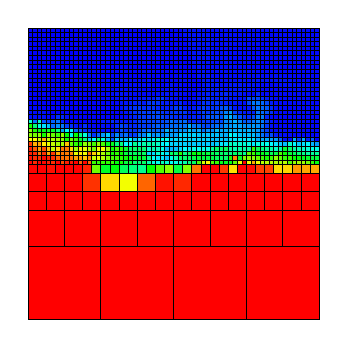
\begin{tikzpicture}[x={(\screenshotunitlength,0)},y={(0,\screenshotunitlength)}]
        \definecolor{fillcolor}{rgb}{1.000000,0.000000,0.000000}
\fill[fillcolor] (0.000000,0.000000) rectangle (0.250000,0.250000);
\definecolor{fillcolor}{rgb}{1.000000,0.000000,0.000000}
\fill[fillcolor] (0.250000,0.000000) rectangle (0.500000,0.250000);
\definecolor{fillcolor}{rgb}{1.000000,0.000000,0.000000}
\fill[fillcolor] (0.000000,0.250000) rectangle (0.125000,0.375000);
\definecolor{fillcolor}{rgb}{1.000000,0.000000,0.000000}
\fill[fillcolor] (0.125000,0.250000) rectangle (0.250000,0.375000);
\definecolor{fillcolor}{rgb}{1.000000,0.000000,0.000000}
\fill[fillcolor] (0.000000,0.375000) rectangle (0.062500,0.437500);
\definecolor{fillcolor}{rgb}{1.000000,0.000000,0.000000}
\fill[fillcolor] (0.062500,0.375000) rectangle (0.125000,0.437500);
\definecolor{fillcolor}{rgb}{1.000000,0.000000,0.000000}
\fill[fillcolor] (0.000000,0.437500) rectangle (0.062500,0.500000);
\definecolor{fillcolor}{rgb}{1.000000,0.000000,0.000000}
\fill[fillcolor] (0.062500,0.437500) rectangle (0.125000,0.500000);
\definecolor{fillcolor}{rgb}{1.000000,0.000000,0.000000}
\fill[fillcolor] (0.125000,0.375000) rectangle (0.187500,0.437500);
\definecolor{fillcolor}{rgb}{1.000000,0.000000,0.000000}
\fill[fillcolor] (0.187500,0.375000) rectangle (0.250000,0.437500);
\definecolor{fillcolor}{rgb}{1.000000,0.000000,0.000000}
\fill[fillcolor] (0.125000,0.437500) rectangle (0.187500,0.500000);
\definecolor{fillcolor}{rgb}{1.000000,0.196733,0.000000}
\fill[fillcolor] (0.187500,0.437500) rectangle (0.250000,0.500000);
\definecolor{fillcolor}{rgb}{1.000000,0.000000,0.000000}
\fill[fillcolor] (0.250000,0.250000) rectangle (0.375000,0.375000);
\definecolor{fillcolor}{rgb}{1.000000,0.000000,0.000000}
\fill[fillcolor] (0.375000,0.250000) rectangle (0.500000,0.375000);
\definecolor{fillcolor}{rgb}{1.000000,0.000000,0.000000}
\fill[fillcolor] (0.250000,0.375000) rectangle (0.312500,0.437500);
\definecolor{fillcolor}{rgb}{1.000000,0.000000,0.000000}
\fill[fillcolor] (0.312500,0.375000) rectangle (0.375000,0.437500);
\definecolor{fillcolor}{rgb}{1.000000,0.851050,0.000000}
\fill[fillcolor] (0.250000,0.437500) rectangle (0.312500,0.500000);
\definecolor{fillcolor}{rgb}{0.953907,1.000000,0.000000}
\fill[fillcolor] (0.312500,0.437500) rectangle (0.375000,0.500000);
\definecolor{fillcolor}{rgb}{1.000000,0.000000,0.000000}
\fill[fillcolor] (0.375000,0.375000) rectangle (0.437500,0.437500);
\definecolor{fillcolor}{rgb}{1.000000,0.000000,0.000000}
\fill[fillcolor] (0.437500,0.375000) rectangle (0.500000,0.437500);
\definecolor{fillcolor}{rgb}{1.000000,0.395035,0.000000}
\fill[fillcolor] (0.375000,0.437500) rectangle (0.437500,0.500000);
\definecolor{fillcolor}{rgb}{1.000000,0.070066,0.000000}
\fill[fillcolor] (0.437500,0.437500) rectangle (0.500000,0.500000);
\definecolor{fillcolor}{rgb}{1.000000,0.000000,0.000000}
\fill[fillcolor] (0.500000,0.000000) rectangle (0.750000,0.250000);
\definecolor{fillcolor}{rgb}{1.000000,0.000000,0.000000}
\fill[fillcolor] (0.750000,0.000000) rectangle (1.000000,0.250000);
\definecolor{fillcolor}{rgb}{1.000000,0.000000,0.000000}
\fill[fillcolor] (0.500000,0.250000) rectangle (0.625000,0.375000);
\definecolor{fillcolor}{rgb}{1.000000,0.000000,0.000000}
\fill[fillcolor] (0.625000,0.250000) rectangle (0.750000,0.375000);
\definecolor{fillcolor}{rgb}{1.000000,0.000000,0.000000}
\fill[fillcolor] (0.500000,0.375000) rectangle (0.562500,0.437500);
\definecolor{fillcolor}{rgb}{1.000000,0.000000,0.000000}
\fill[fillcolor] (0.562500,0.375000) rectangle (0.625000,0.437500);
\definecolor{fillcolor}{rgb}{1.000000,0.157171,0.000000}
\fill[fillcolor] (0.500000,0.437500) rectangle (0.562500,0.500000);
\definecolor{fillcolor}{rgb}{1.000000,0.000000,0.000000}
\fill[fillcolor] (0.562500,0.437500) rectangle (0.625000,0.500000);
\definecolor{fillcolor}{rgb}{1.000000,0.000000,0.000000}
\fill[fillcolor] (0.625000,0.375000) rectangle (0.687500,0.437500);
\definecolor{fillcolor}{rgb}{1.000000,0.000000,0.000000}
\fill[fillcolor] (0.687500,0.375000) rectangle (0.750000,0.437500);
\definecolor{fillcolor}{rgb}{1.000000,0.000000,0.000000}
\fill[fillcolor] (0.625000,0.437500) rectangle (0.687500,0.500000);
\definecolor{fillcolor}{rgb}{1.000000,0.000000,0.000000}
\fill[fillcolor] (0.687500,0.437500) rectangle (0.750000,0.500000);
\definecolor{fillcolor}{rgb}{1.000000,0.000000,0.000000}
\fill[fillcolor] (0.750000,0.250000) rectangle (0.875000,0.375000);
\definecolor{fillcolor}{rgb}{1.000000,0.000008,0.000000}
\fill[fillcolor] (0.875000,0.250000) rectangle (1.000000,0.375000);
\definecolor{fillcolor}{rgb}{1.000000,0.000000,0.000000}
\fill[fillcolor] (0.750000,0.375000) rectangle (0.812500,0.437500);
\definecolor{fillcolor}{rgb}{1.000000,0.000000,0.000000}
\fill[fillcolor] (0.812500,0.375000) rectangle (0.875000,0.437500);
\definecolor{fillcolor}{rgb}{1.000000,0.000103,0.000000}
\fill[fillcolor] (0.750000,0.437500) rectangle (0.812500,0.500000);
\definecolor{fillcolor}{rgb}{1.000000,0.000000,0.000000}
\fill[fillcolor] (0.812500,0.437500) rectangle (0.875000,0.500000);
\definecolor{fillcolor}{rgb}{1.000000,0.000000,0.000000}
\fill[fillcolor] (0.875000,0.375000) rectangle (0.937500,0.437500);
\definecolor{fillcolor}{rgb}{1.000000,0.003841,0.000000}
\fill[fillcolor] (0.937500,0.375000) rectangle (1.000000,0.437500);
\definecolor{fillcolor}{rgb}{1.000000,0.000000,0.000000}
\fill[fillcolor] (0.875000,0.437500) rectangle (0.937500,0.500000);
\definecolor{fillcolor}{rgb}{1.000000,0.000525,0.000000}
\fill[fillcolor] (0.937500,0.437500) rectangle (1.000000,0.500000);
\definecolor{fillcolor}{rgb}{1.000000,0.011073,0.000000}
\fill[fillcolor] (0.000000,0.500000) rectangle (0.031250,0.531250);
\definecolor{fillcolor}{rgb}{1.000000,0.000000,0.000000}
\fill[fillcolor] (0.031250,0.500000) rectangle (0.062500,0.531250);
\definecolor{fillcolor}{rgb}{1.000000,0.000770,0.000000}
\fill[fillcolor] (0.000000,0.531250) rectangle (0.015625,0.546875);
\definecolor{fillcolor}{rgb}{1.000000,0.152447,0.000000}
\fill[fillcolor] (0.015625,0.531250) rectangle (0.031250,0.546875);
\definecolor{fillcolor}{rgb}{1.000000,0.056864,0.000000}
\fill[fillcolor] (0.000000,0.546875) rectangle (0.015625,0.562500);
\definecolor{fillcolor}{rgb}{1.000000,0.161363,0.000000}
\fill[fillcolor] (0.015625,0.546875) rectangle (0.031250,0.562500);
\definecolor{fillcolor}{rgb}{1.000000,0.000000,0.000000}
\fill[fillcolor] (0.031250,0.531250) rectangle (0.046875,0.546875);
\definecolor{fillcolor}{rgb}{1.000000,0.022724,0.000000}
\fill[fillcolor] (0.046875,0.531250) rectangle (0.062500,0.546875);
\definecolor{fillcolor}{rgb}{1.000000,0.183468,0.000000}
\fill[fillcolor] (0.031250,0.546875) rectangle (0.046875,0.562500);
\definecolor{fillcolor}{rgb}{1.000000,0.027267,0.000000}
\fill[fillcolor] (0.046875,0.546875) rectangle (0.062500,0.562500);
\definecolor{fillcolor}{rgb}{1.000000,0.049882,0.000000}
\fill[fillcolor] (0.062500,0.500000) rectangle (0.093750,0.531250);
\definecolor{fillcolor}{rgb}{1.000000,0.000001,0.000000}
\fill[fillcolor] (0.093750,0.500000) rectangle (0.125000,0.531250);
\definecolor{fillcolor}{rgb}{1.000000,0.123045,0.000000}
\fill[fillcolor] (0.062500,0.531250) rectangle (0.078125,0.546875);
\definecolor{fillcolor}{rgb}{1.000000,0.171901,0.000000}
\fill[fillcolor] (0.078125,0.531250) rectangle (0.093750,0.546875);
\definecolor{fillcolor}{rgb}{1.000000,0.124502,0.000000}
\fill[fillcolor] (0.062500,0.546875) rectangle (0.078125,0.562500);
\definecolor{fillcolor}{rgb}{1.000000,0.174142,0.000000}
\fill[fillcolor] (0.078125,0.546875) rectangle (0.093750,0.562500);
\definecolor{fillcolor}{rgb}{1.000000,0.008903,0.000000}
\fill[fillcolor] (0.093750,0.531250) rectangle (0.109375,0.546875);
\definecolor{fillcolor}{rgb}{1.000000,0.292579,0.000000}
\fill[fillcolor] (0.109375,0.531250) rectangle (0.125000,0.546875);
\definecolor{fillcolor}{rgb}{1.000000,0.382139,0.000000}
\fill[fillcolor] (0.093750,0.546875) rectangle (0.109375,0.562500);
\definecolor{fillcolor}{rgb}{1.000000,0.432515,0.000000}
\fill[fillcolor] (0.109375,0.546875) rectangle (0.125000,0.562500);
\definecolor{fillcolor}{rgb}{1.000000,0.120523,0.000000}
\fill[fillcolor] (0.000000,0.562500) rectangle (0.015625,0.578125);
\definecolor{fillcolor}{rgb}{1.000000,0.151094,0.000000}
\fill[fillcolor] (0.015625,0.562500) rectangle (0.031250,0.578125);
\definecolor{fillcolor}{rgb}{1.000000,0.120523,0.000000}
\fill[fillcolor] (0.000000,0.578125) rectangle (0.015625,0.593750);
\definecolor{fillcolor}{rgb}{1.000000,0.350221,0.000000}
\fill[fillcolor] (0.015625,0.578125) rectangle (0.031250,0.593750);
\definecolor{fillcolor}{rgb}{1.000000,0.446505,0.000000}
\fill[fillcolor] (0.031250,0.562500) rectangle (0.046875,0.578125);
\definecolor{fillcolor}{rgb}{1.000000,0.199262,0.000000}
\fill[fillcolor] (0.046875,0.562500) rectangle (0.062500,0.578125);
\definecolor{fillcolor}{rgb}{1.000000,0.619441,0.000000}
\fill[fillcolor] (0.031250,0.578125) rectangle (0.046875,0.593750);
\definecolor{fillcolor}{rgb}{1.000000,0.318383,0.000000}
\fill[fillcolor] (0.046875,0.578125) rectangle (0.062500,0.593750);
\definecolor{fillcolor}{rgb}{1.000000,0.227871,0.000000}
\fill[fillcolor] (0.000000,0.593750) rectangle (0.015625,0.609375);
\definecolor{fillcolor}{rgb}{1.000000,0.681415,0.000000}
\fill[fillcolor] (0.015625,0.593750) rectangle (0.031250,0.609375);
\definecolor{fillcolor}{rgb}{1.000000,0.992004,0.000000}
\fill[fillcolor] (0.000000,0.609375) rectangle (0.015625,0.625000);
\definecolor{fillcolor}{rgb}{1.000000,0.992950,0.000000}
\fill[fillcolor] (0.015625,0.609375) rectangle (0.031250,0.625000);
\definecolor{fillcolor}{rgb}{1.000000,0.641944,0.000000}
\fill[fillcolor] (0.031250,0.593750) rectangle (0.046875,0.609375);
\definecolor{fillcolor}{rgb}{1.000000,0.935124,0.000000}
\fill[fillcolor] (0.046875,0.593750) rectangle (0.062500,0.609375);
\definecolor{fillcolor}{rgb}{0.767951,1.000000,0.000000}
\fill[fillcolor] (0.031250,0.609375) rectangle (0.046875,0.625000);
\definecolor{fillcolor}{rgb}{1.000000,0.706645,0.000000}
\fill[fillcolor] (0.046875,0.609375) rectangle (0.062500,0.625000);
\definecolor{fillcolor}{rgb}{1.000000,0.661323,0.000000}
\fill[fillcolor] (0.062500,0.562500) rectangle (0.078125,0.578125);
\definecolor{fillcolor}{rgb}{1.000000,0.236224,0.000000}
\fill[fillcolor] (0.078125,0.562500) rectangle (0.093750,0.578125);
\definecolor{fillcolor}{rgb}{1.000000,0.749667,0.000000}
\fill[fillcolor] (0.062500,0.578125) rectangle (0.078125,0.593750);
\definecolor{fillcolor}{rgb}{0.767339,1.000000,0.000000}
\fill[fillcolor] (0.078125,0.578125) rectangle (0.093750,0.593750);
\definecolor{fillcolor}{rgb}{1.000000,0.660775,0.000000}
\fill[fillcolor] (0.093750,0.562500) rectangle (0.109375,0.578125);
\definecolor{fillcolor}{rgb}{1.000000,0.468327,0.000000}
\fill[fillcolor] (0.109375,0.562500) rectangle (0.125000,0.578125);
\definecolor{fillcolor}{rgb}{1.000000,0.877230,0.000000}
\fill[fillcolor] (0.093750,0.578125) rectangle (0.109375,0.593750);
\definecolor{fillcolor}{rgb}{1.000000,0.468327,0.000000}
\fill[fillcolor] (0.109375,0.578125) rectangle (0.125000,0.593750);
\definecolor{fillcolor}{rgb}{0.914018,1.000000,0.000000}
\fill[fillcolor] (0.062500,0.593750) rectangle (0.078125,0.609375);
\definecolor{fillcolor}{rgb}{0.766625,1.000000,0.000000}
\fill[fillcolor] (0.078125,0.593750) rectangle (0.093750,0.609375);
\definecolor{fillcolor}{rgb}{0.741805,1.000000,0.000000}
\fill[fillcolor] (0.062500,0.609375) rectangle (0.078125,0.625000);
\definecolor{fillcolor}{rgb}{0.676959,1.000000,0.000000}
\fill[fillcolor] (0.078125,0.609375) rectangle (0.093750,0.625000);
\definecolor{fillcolor}{rgb}{0.635266,1.000000,0.000000}
\fill[fillcolor] (0.093750,0.593750) rectangle (0.109375,0.609375);
\definecolor{fillcolor}{rgb}{0.637817,1.000000,0.000000}
\fill[fillcolor] (0.109375,0.593750) rectangle (0.125000,0.609375);
\definecolor{fillcolor}{rgb}{0.607514,1.000000,0.000000}
\fill[fillcolor] (0.093750,0.609375) rectangle (0.109375,0.625000);
\definecolor{fillcolor}{rgb}{0.554403,1.000000,0.000000}
\fill[fillcolor] (0.109375,0.609375) rectangle (0.125000,0.625000);
\definecolor{fillcolor}{rgb}{1.000000,0.000006,0.000000}
\fill[fillcolor] (0.125000,0.500000) rectangle (0.156250,0.531250);
\definecolor{fillcolor}{rgb}{1.000000,0.004516,0.000000}
\fill[fillcolor] (0.156250,0.500000) rectangle (0.187500,0.531250);
\definecolor{fillcolor}{rgb}{1.000000,0.119293,0.000000}
\fill[fillcolor] (0.125000,0.531250) rectangle (0.140625,0.546875);
\definecolor{fillcolor}{rgb}{1.000000,0.084836,0.000000}
\fill[fillcolor] (0.140625,0.531250) rectangle (0.156250,0.546875);
\definecolor{fillcolor}{rgb}{1.000000,0.454213,0.000000}
\fill[fillcolor] (0.125000,0.546875) rectangle (0.140625,0.562500);
\definecolor{fillcolor}{rgb}{1.000000,0.456520,0.000000}
\fill[fillcolor] (0.140625,0.546875) rectangle (0.156250,0.562500);
\definecolor{fillcolor}{rgb}{1.000000,0.000014,0.000000}
\fill[fillcolor] (0.156250,0.531250) rectangle (0.171875,0.546875);
\definecolor{fillcolor}{rgb}{1.000000,0.381970,0.000000}
\fill[fillcolor] (0.171875,0.531250) rectangle (0.187500,0.546875);
\definecolor{fillcolor}{rgb}{1.000000,0.632186,0.000000}
\fill[fillcolor] (0.156250,0.546875) rectangle (0.171875,0.562500);
\definecolor{fillcolor}{rgb}{1.000000,0.626918,0.000000}
\fill[fillcolor] (0.171875,0.546875) rectangle (0.187500,0.562500);
\definecolor{fillcolor}{rgb}{1.000000,0.132858,0.000000}
\fill[fillcolor] (0.187500,0.500000) rectangle (0.218750,0.531250);
\definecolor{fillcolor}{rgb}{0.432632,1.000000,0.000000}
\fill[fillcolor] (0.218750,0.500000) rectangle (0.250000,0.531250);
\definecolor{fillcolor}{rgb}{1.000000,0.011997,0.000000}
\fill[fillcolor] (0.187500,0.531250) rectangle (0.203125,0.546875);
\definecolor{fillcolor}{rgb}{1.000000,0.399787,0.000000}
\fill[fillcolor] (0.203125,0.531250) rectangle (0.218750,0.546875);
\definecolor{fillcolor}{rgb}{1.000000,0.790617,0.000000}
\fill[fillcolor] (0.187500,0.546875) rectangle (0.203125,0.562500);
\definecolor{fillcolor}{rgb}{1.000000,0.559718,0.000000}
\fill[fillcolor] (0.203125,0.546875) rectangle (0.218750,0.562500);
\definecolor{fillcolor}{rgb}{0.217947,1.000000,0.000000}
\fill[fillcolor] (0.218750,0.531250) rectangle (0.234375,0.546875);
\definecolor{fillcolor}{rgb}{0.183813,1.000000,0.000000}
\fill[fillcolor] (0.234375,0.531250) rectangle (0.250000,0.546875);
\definecolor{fillcolor}{rgb}{0.771442,1.000000,0.000000}
\fill[fillcolor] (0.218750,0.546875) rectangle (0.234375,0.562500);
\definecolor{fillcolor}{rgb}{0.906717,1.000000,0.000000}
\fill[fillcolor] (0.234375,0.546875) rectangle (0.250000,0.562500);
\definecolor{fillcolor}{rgb}{1.000000,0.486761,0.000000}
\fill[fillcolor] (0.125000,0.562500) rectangle (0.140625,0.578125);
\definecolor{fillcolor}{rgb}{1.000000,0.512725,0.000000}
\fill[fillcolor] (0.140625,0.562500) rectangle (0.156250,0.578125);
\definecolor{fillcolor}{rgb}{1.000000,0.471641,0.000000}
\fill[fillcolor] (0.125000,0.578125) rectangle (0.140625,0.593750);
\definecolor{fillcolor}{rgb}{1.000000,0.831115,0.000000}
\fill[fillcolor] (0.140625,0.578125) rectangle (0.156250,0.593750);
\definecolor{fillcolor}{rgb}{0.898605,1.000000,0.000000}
\fill[fillcolor] (0.156250,0.562500) rectangle (0.171875,0.578125);
\definecolor{fillcolor}{rgb}{1.000000,0.939971,0.000000}
\fill[fillcolor] (0.171875,0.562500) rectangle (0.187500,0.578125);
\definecolor{fillcolor}{rgb}{0.602581,1.000000,0.000000}
\fill[fillcolor] (0.156250,0.578125) rectangle (0.171875,0.593750);
\definecolor{fillcolor}{rgb}{1.000000,0.917234,0.000000}
\fill[fillcolor] (0.171875,0.578125) rectangle (0.187500,0.593750);
\definecolor{fillcolor}{rgb}{1.000000,0.762008,0.000000}
\fill[fillcolor] (0.125000,0.593750) rectangle (0.140625,0.609375);
\definecolor{fillcolor}{rgb}{0.358361,1.000000,0.000000}
\fill[fillcolor] (0.140625,0.593750) rectangle (0.156250,0.609375);
\definecolor{fillcolor}{rgb}{0.077447,1.000000,0.000000}
\fill[fillcolor] (0.125000,0.609375) rectangle (0.140625,0.625000);
\definecolor{fillcolor}{rgb}{0.414863,1.000000,0.000000}
\fill[fillcolor] (0.140625,0.609375) rectangle (0.156250,0.625000);
\definecolor{fillcolor}{rgb}{0.162391,1.000000,0.000000}
\fill[fillcolor] (0.156250,0.593750) rectangle (0.171875,0.609375);
\definecolor{fillcolor}{rgb}{0.088489,1.000000,0.000000}
\fill[fillcolor] (0.171875,0.593750) rectangle (0.187500,0.609375);
\definecolor{fillcolor}{rgb}{0.208428,1.000000,0.000000}
\fill[fillcolor] (0.156250,0.609375) rectangle (0.171875,0.625000);
\definecolor{fillcolor}{rgb}{0.000000,1.000000,0.164549}
\fill[fillcolor] (0.171875,0.609375) rectangle (0.187500,0.625000);
\definecolor{fillcolor}{rgb}{0.935169,1.000000,0.000000}
\fill[fillcolor] (0.187500,0.562500) rectangle (0.203125,0.578125);
\definecolor{fillcolor}{rgb}{1.000000,0.425716,0.000000}
\fill[fillcolor] (0.203125,0.562500) rectangle (0.218750,0.578125);
\definecolor{fillcolor}{rgb}{0.899203,1.000000,0.000000}
\fill[fillcolor] (0.187500,0.578125) rectangle (0.203125,0.593750);
\definecolor{fillcolor}{rgb}{0.720815,1.000000,0.000000}
\fill[fillcolor] (0.203125,0.578125) rectangle (0.218750,0.593750);
\definecolor{fillcolor}{rgb}{1.000000,0.796641,0.000000}
\fill[fillcolor] (0.218750,0.562500) rectangle (0.234375,0.578125);
\definecolor{fillcolor}{rgb}{0.918800,1.000000,0.000000}
\fill[fillcolor] (0.234375,0.562500) rectangle (0.250000,0.578125);
\definecolor{fillcolor}{rgb}{0.473702,1.000000,0.000000}
\fill[fillcolor] (0.218750,0.578125) rectangle (0.234375,0.593750);
\definecolor{fillcolor}{rgb}{0.963750,1.000000,0.000000}
\fill[fillcolor] (0.234375,0.578125) rectangle (0.250000,0.593750);
\definecolor{fillcolor}{rgb}{0.572955,1.000000,0.000000}
\fill[fillcolor] (0.187500,0.593750) rectangle (0.203125,0.609375);
\definecolor{fillcolor}{rgb}{0.512687,1.000000,0.000000}
\fill[fillcolor] (0.203125,0.593750) rectangle (0.218750,0.609375);
\definecolor{fillcolor}{rgb}{0.000000,1.000000,0.484354}
\fill[fillcolor] (0.187500,0.609375) rectangle (0.203125,0.625000);
\definecolor{fillcolor}{rgb}{0.000000,0.805464,1.000000}
\fill[fillcolor] (0.203125,0.609375) rectangle (0.218750,0.625000);
\definecolor{fillcolor}{rgb}{0.253028,1.000000,0.000000}
\fill[fillcolor] (0.218750,0.593750) rectangle (0.234375,0.609375);
\definecolor{fillcolor}{rgb}{0.586369,1.000000,0.000000}
\fill[fillcolor] (0.234375,0.593750) rectangle (0.250000,0.609375);
\definecolor{fillcolor}{rgb}{0.000000,1.000000,0.954848}
\fill[fillcolor] (0.218750,0.609375) rectangle (0.234375,0.625000);
\definecolor{fillcolor}{rgb}{0.000000,1.000000,0.463702}
\fill[fillcolor] (0.234375,0.609375) rectangle (0.250000,0.625000);
\definecolor{fillcolor}{rgb}{0.530249,1.000000,0.000000}
\fill[fillcolor] (0.000000,0.625000) rectangle (0.015625,0.640625);
\definecolor{fillcolor}{rgb}{0.446968,1.000000,0.000000}
\fill[fillcolor] (0.015625,0.625000) rectangle (0.031250,0.640625);
\definecolor{fillcolor}{rgb}{0.530249,1.000000,0.000000}
\fill[fillcolor] (0.000000,0.640625) rectangle (0.015625,0.656250);
\definecolor{fillcolor}{rgb}{0.126608,1.000000,0.000000}
\fill[fillcolor] (0.015625,0.640625) rectangle (0.031250,0.656250);
\definecolor{fillcolor}{rgb}{0.591008,1.000000,0.000000}
\fill[fillcolor] (0.031250,0.625000) rectangle (0.046875,0.640625);
\definecolor{fillcolor}{rgb}{0.050856,1.000000,0.000000}
\fill[fillcolor] (0.046875,0.625000) rectangle (0.062500,0.640625);
\definecolor{fillcolor}{rgb}{0.000000,1.000000,0.102609}
\fill[fillcolor] (0.031250,0.640625) rectangle (0.046875,0.656250);
\definecolor{fillcolor}{rgb}{0.000000,1.000000,0.099926}
\fill[fillcolor] (0.046875,0.640625) rectangle (0.062500,0.656250);
\definecolor{fillcolor}{rgb}{0.075070,1.000000,0.000000}
\fill[fillcolor] (0.000000,0.656250) rectangle (0.015625,0.671875);
\definecolor{fillcolor}{rgb}{0.000000,1.000000,0.446891}
\fill[fillcolor] (0.015625,0.656250) rectangle (0.031250,0.671875);
\definecolor{fillcolor}{rgb}{0.000000,1.000000,0.828975}
\fill[fillcolor] (0.000000,0.671875) rectangle (0.015625,0.687500);
\definecolor{fillcolor}{rgb}{0.000000,0.437729,1.000000}
\fill[fillcolor] (0.015625,0.671875) rectangle (0.031250,0.687500);
\definecolor{fillcolor}{rgb}{0.000000,1.000000,0.934710}
\fill[fillcolor] (0.031250,0.656250) rectangle (0.046875,0.671875);
\definecolor{fillcolor}{rgb}{0.000000,0.891922,1.000000}
\fill[fillcolor] (0.046875,0.656250) rectangle (0.062500,0.671875);
\definecolor{fillcolor}{rgb}{0.000000,1.000000,0.748191}
\fill[fillcolor] (0.031250,0.671875) rectangle (0.046875,0.687500);
\definecolor{fillcolor}{rgb}{0.000000,0.337301,1.000000}
\fill[fillcolor] (0.046875,0.671875) rectangle (0.062500,0.687500);
\definecolor{fillcolor}{rgb}{0.590015,1.000000,0.000000}
\fill[fillcolor] (0.062500,0.625000) rectangle (0.078125,0.640625);
\definecolor{fillcolor}{rgb}{0.397102,1.000000,0.000000}
\fill[fillcolor] (0.078125,0.625000) rectangle (0.093750,0.640625);
\definecolor{fillcolor}{rgb}{0.000000,1.000000,0.173953}
\fill[fillcolor] (0.062500,0.640625) rectangle (0.078125,0.656250);
\definecolor{fillcolor}{rgb}{0.000000,1.000000,0.147111}
\fill[fillcolor] (0.078125,0.640625) rectangle (0.093750,0.656250);
\definecolor{fillcolor}{rgb}{0.227311,1.000000,0.000000}
\fill[fillcolor] (0.093750,0.625000) rectangle (0.109375,0.640625);
\definecolor{fillcolor}{rgb}{0.563011,1.000000,0.000000}
\fill[fillcolor] (0.109375,0.625000) rectangle (0.125000,0.640625);
\definecolor{fillcolor}{rgb}{0.000000,1.000000,0.468562}
\fill[fillcolor] (0.093750,0.640625) rectangle (0.109375,0.656250);
\definecolor{fillcolor}{rgb}{0.000000,0.628951,1.000000}
\fill[fillcolor] (0.109375,0.640625) rectangle (0.125000,0.656250);
\definecolor{fillcolor}{rgb}{0.000000,0.774035,1.000000}
\fill[fillcolor] (0.062500,0.656250) rectangle (0.078125,0.671875);
\definecolor{fillcolor}{rgb}{0.000000,0.416897,1.000000}
\fill[fillcolor] (0.078125,0.656250) rectangle (0.093750,0.671875);
\definecolor{fillcolor}{rgb}{0.000000,0.255446,1.000000}
\fill[fillcolor] (0.062500,0.671875) rectangle (0.078125,0.687500);
\definecolor{fillcolor}{rgb}{0.000000,0.381075,1.000000}
\fill[fillcolor] (0.078125,0.671875) rectangle (0.093750,0.687500);
\definecolor{fillcolor}{rgb}{0.000000,0.565192,1.000000}
\fill[fillcolor] (0.093750,0.656250) rectangle (0.109375,0.671875);
\definecolor{fillcolor}{rgb}{0.000000,0.470554,1.000000}
\fill[fillcolor] (0.109375,0.656250) rectangle (0.125000,0.671875);
\definecolor{fillcolor}{rgb}{0.000000,0.457611,1.000000}
\fill[fillcolor] (0.093750,0.671875) rectangle (0.109375,0.687500);
\definecolor{fillcolor}{rgb}{0.000000,0.140957,1.000000}
\fill[fillcolor] (0.109375,0.671875) rectangle (0.125000,0.687500);
\definecolor{fillcolor}{rgb}{0.000000,0.047063,1.000000}
\fill[fillcolor] (0.000000,0.687500) rectangle (0.015625,0.703125);
\definecolor{fillcolor}{rgb}{0.000000,0.050443,1.000000}
\fill[fillcolor] (0.015625,0.687500) rectangle (0.031250,0.703125);
\definecolor{fillcolor}{rgb}{0.000000,0.047010,1.000000}
\fill[fillcolor] (0.000000,0.703125) rectangle (0.015625,0.718750);
\definecolor{fillcolor}{rgb}{0.000000,0.035214,1.000000}
\fill[fillcolor] (0.015625,0.703125) rectangle (0.031250,0.718750);
\definecolor{fillcolor}{rgb}{0.000000,0.064789,1.000000}
\fill[fillcolor] (0.031250,0.687500) rectangle (0.046875,0.703125);
\definecolor{fillcolor}{rgb}{0.000000,0.055610,1.000000}
\fill[fillcolor] (0.046875,0.687500) rectangle (0.062500,0.703125);
\definecolor{fillcolor}{rgb}{0.000000,0.063479,1.000000}
\fill[fillcolor] (0.031250,0.703125) rectangle (0.046875,0.718750);
\definecolor{fillcolor}{rgb}{0.000000,0.053962,1.000000}
\fill[fillcolor] (0.046875,0.703125) rectangle (0.062500,0.718750);
\definecolor{fillcolor}{rgb}{0.000000,0.013257,1.000000}
\fill[fillcolor] (0.000000,0.718750) rectangle (0.015625,0.734375);
\definecolor{fillcolor}{rgb}{0.000000,0.035121,1.000000}
\fill[fillcolor] (0.015625,0.718750) rectangle (0.031250,0.734375);
\definecolor{fillcolor}{rgb}{0.000000,0.003178,1.000000}
\fill[fillcolor] (0.000000,0.734375) rectangle (0.015625,0.750000);
\definecolor{fillcolor}{rgb}{0.000000,0.003183,1.000000}
\fill[fillcolor] (0.015625,0.734375) rectangle (0.031250,0.750000);
\definecolor{fillcolor}{rgb}{0.000000,0.022623,1.000000}
\fill[fillcolor] (0.031250,0.718750) rectangle (0.046875,0.734375);
\definecolor{fillcolor}{rgb}{0.000000,0.003369,1.000000}
\fill[fillcolor] (0.046875,0.718750) rectangle (0.062500,0.734375);
\definecolor{fillcolor}{rgb}{0.000000,0.007127,1.000000}
\fill[fillcolor] (0.031250,0.734375) rectangle (0.046875,0.750000);
\definecolor{fillcolor}{rgb}{0.000000,0.003429,1.000000}
\fill[fillcolor] (0.046875,0.734375) rectangle (0.062500,0.750000);
\definecolor{fillcolor}{rgb}{0.000000,0.031405,1.000000}
\fill[fillcolor] (0.062500,0.687500) rectangle (0.078125,0.703125);
\definecolor{fillcolor}{rgb}{0.000000,0.018090,1.000000}
\fill[fillcolor] (0.078125,0.687500) rectangle (0.093750,0.703125);
\definecolor{fillcolor}{rgb}{0.000000,0.011652,1.000000}
\fill[fillcolor] (0.062500,0.703125) rectangle (0.078125,0.718750);
\definecolor{fillcolor}{rgb}{0.000000,0.006627,1.000000}
\fill[fillcolor] (0.078125,0.703125) rectangle (0.093750,0.718750);
\definecolor{fillcolor}{rgb}{0.000000,0.190375,1.000000}
\fill[fillcolor] (0.093750,0.687500) rectangle (0.109375,0.703125);
\definecolor{fillcolor}{rgb}{0.000000,0.153540,1.000000}
\fill[fillcolor] (0.109375,0.687500) rectangle (0.125000,0.703125);
\definecolor{fillcolor}{rgb}{0.000000,0.006741,1.000000}
\fill[fillcolor] (0.093750,0.703125) rectangle (0.109375,0.718750);
\definecolor{fillcolor}{rgb}{0.000000,0.007146,1.000000}
\fill[fillcolor] (0.109375,0.703125) rectangle (0.125000,0.718750);
\definecolor{fillcolor}{rgb}{0.000000,0.000553,1.000000}
\fill[fillcolor] (0.062500,0.718750) rectangle (0.078125,0.734375);
\definecolor{fillcolor}{rgb}{0.000000,0.000534,1.000000}
\fill[fillcolor] (0.078125,0.718750) rectangle (0.093750,0.734375);
\definecolor{fillcolor}{rgb}{0.000000,0.000973,1.000000}
\fill[fillcolor] (0.062500,0.734375) rectangle (0.078125,0.750000);
\definecolor{fillcolor}{rgb}{0.000000,0.000777,1.000000}
\fill[fillcolor] (0.078125,0.734375) rectangle (0.093750,0.750000);
\definecolor{fillcolor}{rgb}{0.000000,0.005527,1.000000}
\fill[fillcolor] (0.093750,0.718750) rectangle (0.109375,0.734375);
\definecolor{fillcolor}{rgb}{0.000000,0.054696,1.000000}
\fill[fillcolor] (0.109375,0.718750) rectangle (0.125000,0.734375);
\definecolor{fillcolor}{rgb}{0.000000,0.000420,1.000000}
\fill[fillcolor] (0.093750,0.734375) rectangle (0.109375,0.750000);
\definecolor{fillcolor}{rgb}{0.000000,0.027041,1.000000}
\fill[fillcolor] (0.109375,0.734375) rectangle (0.125000,0.750000);
\definecolor{fillcolor}{rgb}{0.000000,1.000000,0.008312}
\fill[fillcolor] (0.125000,0.625000) rectangle (0.140625,0.640625);
\definecolor{fillcolor}{rgb}{0.000000,1.000000,0.916221}
\fill[fillcolor] (0.140625,0.625000) rectangle (0.156250,0.640625);
\definecolor{fillcolor}{rgb}{0.000000,0.970075,1.000000}
\fill[fillcolor] (0.125000,0.640625) rectangle (0.140625,0.656250);
\definecolor{fillcolor}{rgb}{0.000000,0.924392,1.000000}
\fill[fillcolor] (0.140625,0.640625) rectangle (0.156250,0.656250);
\definecolor{fillcolor}{rgb}{0.000000,1.000000,0.001798}
\fill[fillcolor] (0.156250,0.625000) rectangle (0.171875,0.640625);
\definecolor{fillcolor}{rgb}{0.000000,1.000000,0.499532}
\fill[fillcolor] (0.171875,0.625000) rectangle (0.187500,0.640625);
\definecolor{fillcolor}{rgb}{0.000000,0.388742,1.000000}
\fill[fillcolor] (0.156250,0.640625) rectangle (0.171875,0.656250);
\definecolor{fillcolor}{rgb}{0.000000,0.329867,1.000000}
\fill[fillcolor] (0.171875,0.640625) rectangle (0.187500,0.656250);
\definecolor{fillcolor}{rgb}{0.000000,0.245219,1.000000}
\fill[fillcolor] (0.125000,0.656250) rectangle (0.140625,0.671875);
\definecolor{fillcolor}{rgb}{0.000000,0.181450,1.000000}
\fill[fillcolor] (0.140625,0.656250) rectangle (0.156250,0.671875);
\definecolor{fillcolor}{rgb}{0.000000,0.006101,1.000000}
\fill[fillcolor] (0.125000,0.671875) rectangle (0.140625,0.687500);
\definecolor{fillcolor}{rgb}{0.000000,0.003144,1.000000}
\fill[fillcolor] (0.140625,0.671875) rectangle (0.156250,0.687500);
\definecolor{fillcolor}{rgb}{0.000000,0.082793,1.000000}
\fill[fillcolor] (0.156250,0.656250) rectangle (0.171875,0.671875);
\definecolor{fillcolor}{rgb}{0.000000,0.026125,1.000000}
\fill[fillcolor] (0.171875,0.656250) rectangle (0.187500,0.671875);
\definecolor{fillcolor}{rgb}{0.000000,0.002823,1.000000}
\fill[fillcolor] (0.156250,0.671875) rectangle (0.171875,0.687500);
\definecolor{fillcolor}{rgb}{0.000000,0.002309,1.000000}
\fill[fillcolor] (0.171875,0.671875) rectangle (0.187500,0.687500);
\definecolor{fillcolor}{rgb}{0.000000,1.000000,0.841652}
\fill[fillcolor] (0.187500,0.625000) rectangle (0.203125,0.640625);
\definecolor{fillcolor}{rgb}{0.000000,0.522492,1.000000}
\fill[fillcolor] (0.203125,0.625000) rectangle (0.218750,0.640625);
\definecolor{fillcolor}{rgb}{0.000000,0.194520,1.000000}
\fill[fillcolor] (0.187500,0.640625) rectangle (0.203125,0.656250);
\definecolor{fillcolor}{rgb}{0.000000,0.117632,1.000000}
\fill[fillcolor] (0.203125,0.640625) rectangle (0.218750,0.656250);
\definecolor{fillcolor}{rgb}{0.000000,0.198809,1.000000}
\fill[fillcolor] (0.218750,0.625000) rectangle (0.234375,0.640625);
\definecolor{fillcolor}{rgb}{0.000000,0.382545,1.000000}
\fill[fillcolor] (0.234375,0.625000) rectangle (0.250000,0.640625);
\definecolor{fillcolor}{rgb}{0.000000,0.088691,1.000000}
\fill[fillcolor] (0.218750,0.640625) rectangle (0.234375,0.656250);
\definecolor{fillcolor}{rgb}{0.000000,0.040568,1.000000}
\fill[fillcolor] (0.234375,0.640625) rectangle (0.250000,0.656250);
\definecolor{fillcolor}{rgb}{0.000000,0.190086,1.000000}
\fill[fillcolor] (0.187500,0.656250) rectangle (0.203125,0.671875);
\definecolor{fillcolor}{rgb}{0.000000,0.047573,1.000000}
\fill[fillcolor] (0.203125,0.656250) rectangle (0.218750,0.671875);
\definecolor{fillcolor}{rgb}{0.000000,0.001243,1.000000}
\fill[fillcolor] (0.187500,0.671875) rectangle (0.203125,0.687500);
\definecolor{fillcolor}{rgb}{0.000000,0.000703,1.000000}
\fill[fillcolor] (0.203125,0.671875) rectangle (0.218750,0.687500);
\definecolor{fillcolor}{rgb}{0.000000,0.025611,1.000000}
\fill[fillcolor] (0.218750,0.656250) rectangle (0.234375,0.671875);
\definecolor{fillcolor}{rgb}{0.000000,0.013138,1.000000}
\fill[fillcolor] (0.234375,0.656250) rectangle (0.250000,0.671875);
\definecolor{fillcolor}{rgb}{0.000000,0.008550,1.000000}
\fill[fillcolor] (0.218750,0.671875) rectangle (0.234375,0.687500);
\definecolor{fillcolor}{rgb}{0.000000,0.012916,1.000000}
\fill[fillcolor] (0.234375,0.671875) rectangle (0.250000,0.687500);
\definecolor{fillcolor}{rgb}{0.000000,0.063452,1.000000}
\fill[fillcolor] (0.125000,0.687500) rectangle (0.140625,0.703125);
\definecolor{fillcolor}{rgb}{0.000000,0.007070,1.000000}
\fill[fillcolor] (0.140625,0.687500) rectangle (0.156250,0.703125);
\definecolor{fillcolor}{rgb}{0.000000,0.029808,1.000000}
\fill[fillcolor] (0.125000,0.703125) rectangle (0.140625,0.718750);
\definecolor{fillcolor}{rgb}{0.000000,0.014790,1.000000}
\fill[fillcolor] (0.140625,0.703125) rectangle (0.156250,0.718750);
\definecolor{fillcolor}{rgb}{0.000000,0.005951,1.000000}
\fill[fillcolor] (0.156250,0.687500) rectangle (0.171875,0.703125);
\definecolor{fillcolor}{rgb}{0.000000,0.003472,1.000000}
\fill[fillcolor] (0.171875,0.687500) rectangle (0.187500,0.703125);
\definecolor{fillcolor}{rgb}{0.000000,0.005644,1.000000}
\fill[fillcolor] (0.156250,0.703125) rectangle (0.171875,0.718750);
\definecolor{fillcolor}{rgb}{0.000000,0.000562,1.000000}
\fill[fillcolor] (0.171875,0.703125) rectangle (0.187500,0.718750);
\definecolor{fillcolor}{rgb}{0.000000,0.032062,1.000000}
\fill[fillcolor] (0.125000,0.718750) rectangle (0.140625,0.734375);
\definecolor{fillcolor}{rgb}{0.000000,0.000268,1.000000}
\fill[fillcolor] (0.140625,0.718750) rectangle (0.156250,0.734375);
\definecolor{fillcolor}{rgb}{0.000000,0.001548,1.000000}
\fill[fillcolor] (0.125000,0.734375) rectangle (0.140625,0.750000);
\definecolor{fillcolor}{rgb}{0.000000,0.000255,1.000000}
\fill[fillcolor] (0.140625,0.734375) rectangle (0.156250,0.750000);
\definecolor{fillcolor}{rgb}{0.000000,0.000312,1.000000}
\fill[fillcolor] (0.156250,0.718750) rectangle (0.171875,0.734375);
\definecolor{fillcolor}{rgb}{0.000000,0.000595,1.000000}
\fill[fillcolor] (0.171875,0.718750) rectangle (0.187500,0.734375);
\definecolor{fillcolor}{rgb}{0.000000,0.000317,1.000000}
\fill[fillcolor] (0.156250,0.734375) rectangle (0.171875,0.750000);
\definecolor{fillcolor}{rgb}{0.000000,0.000719,1.000000}
\fill[fillcolor] (0.171875,0.734375) rectangle (0.187500,0.750000);
\definecolor{fillcolor}{rgb}{0.000000,0.003086,1.000000}
\fill[fillcolor] (0.187500,0.687500) rectangle (0.203125,0.703125);
\definecolor{fillcolor}{rgb}{0.000000,0.001289,1.000000}
\fill[fillcolor] (0.203125,0.687500) rectangle (0.218750,0.703125);
\definecolor{fillcolor}{rgb}{0.000000,0.000562,1.000000}
\fill[fillcolor] (0.187500,0.703125) rectangle (0.203125,0.718750);
\definecolor{fillcolor}{rgb}{0.000000,0.000498,1.000000}
\fill[fillcolor] (0.203125,0.703125) rectangle (0.218750,0.718750);
\definecolor{fillcolor}{rgb}{0.000000,0.006256,1.000000}
\fill[fillcolor] (0.218750,0.687500) rectangle (0.234375,0.703125);
\definecolor{fillcolor}{rgb}{0.000000,0.004424,1.000000}
\fill[fillcolor] (0.234375,0.687500) rectangle (0.250000,0.703125);
\definecolor{fillcolor}{rgb}{0.000000,0.003407,1.000000}
\fill[fillcolor] (0.218750,0.703125) rectangle (0.234375,0.718750);
\definecolor{fillcolor}{rgb}{0.000000,0.005919,1.000000}
\fill[fillcolor] (0.234375,0.703125) rectangle (0.250000,0.718750);
\definecolor{fillcolor}{rgb}{0.000000,0.000528,1.000000}
\fill[fillcolor] (0.187500,0.718750) rectangle (0.203125,0.734375);
\definecolor{fillcolor}{rgb}{0.000000,0.001645,1.000000}
\fill[fillcolor] (0.203125,0.718750) rectangle (0.218750,0.734375);
\definecolor{fillcolor}{rgb}{0.000000,0.000970,1.000000}
\fill[fillcolor] (0.187500,0.734375) rectangle (0.203125,0.750000);
\definecolor{fillcolor}{rgb}{0.000000,0.002584,1.000000}
\fill[fillcolor] (0.203125,0.734375) rectangle (0.218750,0.750000);
\definecolor{fillcolor}{rgb}{0.000000,0.003976,1.000000}
\fill[fillcolor] (0.218750,0.718750) rectangle (0.234375,0.734375);
\definecolor{fillcolor}{rgb}{0.000000,0.007154,1.000000}
\fill[fillcolor] (0.234375,0.718750) rectangle (0.250000,0.734375);
\definecolor{fillcolor}{rgb}{0.000000,0.007758,1.000000}
\fill[fillcolor] (0.218750,0.734375) rectangle (0.234375,0.750000);
\definecolor{fillcolor}{rgb}{0.000000,0.013944,1.000000}
\fill[fillcolor] (0.234375,0.734375) rectangle (0.250000,0.750000);
\definecolor{fillcolor}{rgb}{0.000000,1.000000,0.148745}
\fill[fillcolor] (0.250000,0.500000) rectangle (0.281250,0.531250);
\definecolor{fillcolor}{rgb}{0.000000,1.000000,0.024494}
\fill[fillcolor] (0.281250,0.500000) rectangle (0.312500,0.531250);
\definecolor{fillcolor}{rgb}{0.194595,1.000000,0.000000}
\fill[fillcolor] (0.250000,0.531250) rectangle (0.265625,0.546875);
\definecolor{fillcolor}{rgb}{0.147603,1.000000,0.000000}
\fill[fillcolor] (0.265625,0.531250) rectangle (0.281250,0.546875);
\definecolor{fillcolor}{rgb}{0.714394,1.000000,0.000000}
\fill[fillcolor] (0.250000,0.546875) rectangle (0.265625,0.562500);
\definecolor{fillcolor}{rgb}{0.498867,1.000000,0.000000}
\fill[fillcolor] (0.265625,0.546875) rectangle (0.281250,0.562500);
\definecolor{fillcolor}{rgb}{0.221851,1.000000,0.000000}
\fill[fillcolor] (0.281250,0.531250) rectangle (0.296875,0.546875);
\definecolor{fillcolor}{rgb}{0.000000,1.000000,0.028315}
\fill[fillcolor] (0.296875,0.531250) rectangle (0.312500,0.546875);
\definecolor{fillcolor}{rgb}{0.277998,1.000000,0.000000}
\fill[fillcolor] (0.281250,0.546875) rectangle (0.296875,0.562500);
\definecolor{fillcolor}{rgb}{0.231821,1.000000,0.000000}
\fill[fillcolor] (0.296875,0.546875) rectangle (0.312500,0.562500);
\definecolor{fillcolor}{rgb}{0.000000,1.000000,0.353800}
\fill[fillcolor] (0.312500,0.500000) rectangle (0.343750,0.531250);
\definecolor{fillcolor}{rgb}{0.000000,1.000000,0.473777}
\fill[fillcolor] (0.343750,0.500000) rectangle (0.375000,0.531250);
\definecolor{fillcolor}{rgb}{0.055404,1.000000,0.000000}
\fill[fillcolor] (0.312500,0.531250) rectangle (0.328125,0.546875);
\definecolor{fillcolor}{rgb}{0.000000,1.000000,0.232839}
\fill[fillcolor] (0.328125,0.531250) rectangle (0.343750,0.546875);
\definecolor{fillcolor}{rgb}{0.145589,1.000000,0.000000}
\fill[fillcolor] (0.312500,0.546875) rectangle (0.328125,0.562500);
\definecolor{fillcolor}{rgb}{0.036423,1.000000,0.000000}
\fill[fillcolor] (0.328125,0.546875) rectangle (0.343750,0.562500);
\definecolor{fillcolor}{rgb}{0.000000,1.000000,0.171666}
\fill[fillcolor] (0.343750,0.531250) rectangle (0.359375,0.546875);
\definecolor{fillcolor}{rgb}{0.000000,1.000000,0.447240}
\fill[fillcolor] (0.359375,0.531250) rectangle (0.375000,0.546875);
\definecolor{fillcolor}{rgb}{0.000000,1.000000,0.086994}
\fill[fillcolor] (0.343750,0.546875) rectangle (0.359375,0.562500);
\definecolor{fillcolor}{rgb}{0.000000,1.000000,0.127007}
\fill[fillcolor] (0.359375,0.546875) rectangle (0.375000,0.562500);
\definecolor{fillcolor}{rgb}{0.657353,1.000000,0.000000}
\fill[fillcolor] (0.250000,0.562500) rectangle (0.265625,0.578125);
\definecolor{fillcolor}{rgb}{0.422402,1.000000,0.000000}
\fill[fillcolor] (0.265625,0.562500) rectangle (0.281250,0.578125);
\definecolor{fillcolor}{rgb}{0.978606,1.000000,0.000000}
\fill[fillcolor] (0.250000,0.578125) rectangle (0.265625,0.593750);
\definecolor{fillcolor}{rgb}{0.621847,1.000000,0.000000}
\fill[fillcolor] (0.265625,0.578125) rectangle (0.281250,0.593750);
\definecolor{fillcolor}{rgb}{0.082622,1.000000,0.000000}
\fill[fillcolor] (0.281250,0.562500) rectangle (0.296875,0.578125);
\definecolor{fillcolor}{rgb}{0.172739,1.000000,0.000000}
\fill[fillcolor] (0.296875,0.562500) rectangle (0.312500,0.578125);
\definecolor{fillcolor}{rgb}{0.062025,1.000000,0.000000}
\fill[fillcolor] (0.281250,0.578125) rectangle (0.296875,0.593750);
\definecolor{fillcolor}{rgb}{0.237036,1.000000,0.000000}
\fill[fillcolor] (0.296875,0.578125) rectangle (0.312500,0.593750);
\definecolor{fillcolor}{rgb}{0.257073,1.000000,0.000000}
\fill[fillcolor] (0.250000,0.593750) rectangle (0.265625,0.609375);
\definecolor{fillcolor}{rgb}{0.000000,1.000000,0.111394}
\fill[fillcolor] (0.265625,0.593750) rectangle (0.281250,0.609375);
\definecolor{fillcolor}{rgb}{0.000000,1.000000,0.827275}
\fill[fillcolor] (0.250000,0.609375) rectangle (0.265625,0.625000);
\definecolor{fillcolor}{rgb}{0.000000,0.702496,1.000000}
\fill[fillcolor] (0.265625,0.609375) rectangle (0.281250,0.625000);
\definecolor{fillcolor}{rgb}{0.000000,1.000000,0.111665}
\fill[fillcolor] (0.281250,0.593750) rectangle (0.296875,0.609375);
\definecolor{fillcolor}{rgb}{0.000000,1.000000,0.494015}
\fill[fillcolor] (0.296875,0.593750) rectangle (0.312500,0.609375);
\definecolor{fillcolor}{rgb}{0.000000,0.332685,1.000000}
\fill[fillcolor] (0.281250,0.609375) rectangle (0.296875,0.625000);
\definecolor{fillcolor}{rgb}{0.000000,0.769948,1.000000}
\fill[fillcolor] (0.296875,0.609375) rectangle (0.312500,0.625000);
\definecolor{fillcolor}{rgb}{0.030032,1.000000,0.000000}
\fill[fillcolor] (0.312500,0.562500) rectangle (0.328125,0.578125);
\definecolor{fillcolor}{rgb}{0.000000,1.000000,0.236261}
\fill[fillcolor] (0.328125,0.562500) rectangle (0.343750,0.578125);
\definecolor{fillcolor}{rgb}{0.157160,1.000000,0.000000}
\fill[fillcolor] (0.312500,0.578125) rectangle (0.328125,0.593750);
\definecolor{fillcolor}{rgb}{0.000000,1.000000,0.174301}
\fill[fillcolor] (0.328125,0.578125) rectangle (0.343750,0.593750);
\definecolor{fillcolor}{rgb}{0.000000,1.000000,0.409516}
\fill[fillcolor] (0.343750,0.562500) rectangle (0.359375,0.578125);
\definecolor{fillcolor}{rgb}{0.000000,1.000000,0.341876}
\fill[fillcolor] (0.359375,0.562500) rectangle (0.375000,0.578125);
\definecolor{fillcolor}{rgb}{0.000000,1.000000,0.424098}
\fill[fillcolor] (0.343750,0.578125) rectangle (0.359375,0.593750);
\definecolor{fillcolor}{rgb}{0.000000,1.000000,0.435115}
\fill[fillcolor] (0.359375,0.578125) rectangle (0.375000,0.593750);
\definecolor{fillcolor}{rgb}{0.000000,1.000000,0.493846}
\fill[fillcolor] (0.312500,0.593750) rectangle (0.328125,0.609375);
\definecolor{fillcolor}{rgb}{0.000000,1.000000,0.991362}
\fill[fillcolor] (0.328125,0.593750) rectangle (0.343750,0.609375);
\definecolor{fillcolor}{rgb}{0.000000,0.729076,1.000000}
\fill[fillcolor] (0.312500,0.609375) rectangle (0.328125,0.625000);
\definecolor{fillcolor}{rgb}{0.000000,0.730428,1.000000}
\fill[fillcolor] (0.328125,0.609375) rectangle (0.343750,0.625000);
\definecolor{fillcolor}{rgb}{0.000000,1.000000,0.988018}
\fill[fillcolor] (0.343750,0.593750) rectangle (0.359375,0.609375);
\definecolor{fillcolor}{rgb}{0.000000,1.000000,0.555507}
\fill[fillcolor] (0.359375,0.593750) rectangle (0.375000,0.609375);
\definecolor{fillcolor}{rgb}{0.000000,1.000000,0.985488}
\fill[fillcolor] (0.343750,0.609375) rectangle (0.359375,0.625000);
\definecolor{fillcolor}{rgb}{0.000000,0.714372,1.000000}
\fill[fillcolor] (0.359375,0.609375) rectangle (0.375000,0.625000);
\definecolor{fillcolor}{rgb}{0.000000,1.000000,0.555259}
\fill[fillcolor] (0.375000,0.500000) rectangle (0.406250,0.531250);
\definecolor{fillcolor}{rgb}{0.000000,1.000000,0.005872}
\fill[fillcolor] (0.406250,0.500000) rectangle (0.437500,0.531250);
\definecolor{fillcolor}{rgb}{0.000000,1.000000,0.447611}
\fill[fillcolor] (0.375000,0.531250) rectangle (0.390625,0.546875);
\definecolor{fillcolor}{rgb}{0.000000,1.000000,0.388577}
\fill[fillcolor] (0.390625,0.531250) rectangle (0.406250,0.546875);
\definecolor{fillcolor}{rgb}{0.000000,1.000000,0.178515}
\fill[fillcolor] (0.375000,0.546875) rectangle (0.390625,0.562500);
\definecolor{fillcolor}{rgb}{0.000000,1.000000,0.222628}
\fill[fillcolor] (0.390625,0.546875) rectangle (0.406250,0.562500);
\definecolor{fillcolor}{rgb}{0.000000,1.000000,0.687907}
\fill[fillcolor] (0.406250,0.531250) rectangle (0.421875,0.546875);
\definecolor{fillcolor}{rgb}{0.000000,1.000000,0.863697}
\fill[fillcolor] (0.421875,0.531250) rectangle (0.437500,0.546875);
\definecolor{fillcolor}{rgb}{0.000000,1.000000,0.556555}
\fill[fillcolor] (0.406250,0.546875) rectangle (0.421875,0.562500);
\definecolor{fillcolor}{rgb}{0.000000,1.000000,0.970934}
\fill[fillcolor] (0.421875,0.546875) rectangle (0.437500,0.562500);
\definecolor{fillcolor}{rgb}{0.316583,1.000000,0.000000}
\fill[fillcolor] (0.437500,0.500000) rectangle (0.468750,0.531250);
\definecolor{fillcolor}{rgb}{0.544626,1.000000,0.000000}
\fill[fillcolor] (0.468750,0.500000) rectangle (0.500000,0.531250);
\definecolor{fillcolor}{rgb}{0.000000,1.000000,0.931280}
\fill[fillcolor] (0.437500,0.531250) rectangle (0.453125,0.546875);
\definecolor{fillcolor}{rgb}{0.000000,1.000000,0.687457}
\fill[fillcolor] (0.453125,0.531250) rectangle (0.468750,0.546875);
\definecolor{fillcolor}{rgb}{0.000000,0.900299,1.000000}
\fill[fillcolor] (0.437500,0.546875) rectangle (0.453125,0.562500);
\definecolor{fillcolor}{rgb}{0.000000,0.900043,1.000000}
\fill[fillcolor] (0.453125,0.546875) rectangle (0.468750,0.562500);
\definecolor{fillcolor}{rgb}{0.000000,1.000000,0.817142}
\fill[fillcolor] (0.468750,0.531250) rectangle (0.484375,0.546875);
\definecolor{fillcolor}{rgb}{0.000000,1.000000,0.965674}
\fill[fillcolor] (0.484375,0.531250) rectangle (0.500000,0.546875);
\definecolor{fillcolor}{rgb}{0.000000,0.742468,1.000000}
\fill[fillcolor] (0.468750,0.546875) rectangle (0.484375,0.562500);
\definecolor{fillcolor}{rgb}{0.000000,1.000000,0.897828}
\fill[fillcolor] (0.484375,0.546875) rectangle (0.500000,0.562500);
\definecolor{fillcolor}{rgb}{0.000000,1.000000,0.366308}
\fill[fillcolor] (0.375000,0.562500) rectangle (0.390625,0.578125);
\definecolor{fillcolor}{rgb}{0.000000,1.000000,0.365553}
\fill[fillcolor] (0.390625,0.562500) rectangle (0.406250,0.578125);
\definecolor{fillcolor}{rgb}{0.000000,1.000000,0.428063}
\fill[fillcolor] (0.375000,0.578125) rectangle (0.390625,0.593750);
\definecolor{fillcolor}{rgb}{0.000000,1.000000,0.456345}
\fill[fillcolor] (0.390625,0.578125) rectangle (0.406250,0.593750);
\definecolor{fillcolor}{rgb}{0.000000,0.850478,1.000000}
\fill[fillcolor] (0.406250,0.562500) rectangle (0.421875,0.578125);
\definecolor{fillcolor}{rgb}{0.000000,0.846543,1.000000}
\fill[fillcolor] (0.421875,0.562500) rectangle (0.437500,0.578125);
\definecolor{fillcolor}{rgb}{0.000000,1.000000,0.830269}
\fill[fillcolor] (0.406250,0.578125) rectangle (0.421875,0.593750);
\definecolor{fillcolor}{rgb}{0.000000,1.000000,0.688071}
\fill[fillcolor] (0.421875,0.578125) rectangle (0.437500,0.593750);
\definecolor{fillcolor}{rgb}{0.000000,1.000000,0.903431}
\fill[fillcolor] (0.375000,0.593750) rectangle (0.390625,0.609375);
\definecolor{fillcolor}{rgb}{0.000000,1.000000,0.666921}
\fill[fillcolor] (0.390625,0.593750) rectangle (0.406250,0.609375);
\definecolor{fillcolor}{rgb}{0.000000,0.877219,1.000000}
\fill[fillcolor] (0.375000,0.609375) rectangle (0.390625,0.625000);
\definecolor{fillcolor}{rgb}{0.000000,1.000000,0.868181}
\fill[fillcolor] (0.390625,0.609375) rectangle (0.406250,0.625000);
\definecolor{fillcolor}{rgb}{0.000000,1.000000,0.687875}
\fill[fillcolor] (0.406250,0.593750) rectangle (0.421875,0.609375);
\definecolor{fillcolor}{rgb}{0.000000,1.000000,0.687997}
\fill[fillcolor] (0.421875,0.593750) rectangle (0.437500,0.609375);
\definecolor{fillcolor}{rgb}{0.000000,0.845519,1.000000}
\fill[fillcolor] (0.406250,0.609375) rectangle (0.421875,0.625000);
\definecolor{fillcolor}{rgb}{0.000000,0.983791,1.000000}
\fill[fillcolor] (0.421875,0.609375) rectangle (0.437500,0.625000);
\definecolor{fillcolor}{rgb}{0.000000,1.000000,0.808130}
\fill[fillcolor] (0.437500,0.562500) rectangle (0.453125,0.578125);
\definecolor{fillcolor}{rgb}{0.000000,1.000000,0.926244}
\fill[fillcolor] (0.453125,0.562500) rectangle (0.468750,0.578125);
\definecolor{fillcolor}{rgb}{0.000000,1.000000,0.749849}
\fill[fillcolor] (0.437500,0.578125) rectangle (0.453125,0.593750);
\definecolor{fillcolor}{rgb}{0.000000,1.000000,0.892067}
\fill[fillcolor] (0.453125,0.578125) rectangle (0.468750,0.593750);
\definecolor{fillcolor}{rgb}{0.000000,0.885929,1.000000}
\fill[fillcolor] (0.468750,0.562500) rectangle (0.484375,0.578125);
\definecolor{fillcolor}{rgb}{0.000000,1.000000,0.369506}
\fill[fillcolor] (0.484375,0.562500) rectangle (0.500000,0.578125);
\definecolor{fillcolor}{rgb}{0.000000,0.716978,1.000000}
\fill[fillcolor] (0.468750,0.578125) rectangle (0.484375,0.593750);
\definecolor{fillcolor}{rgb}{0.000000,0.715474,1.000000}
\fill[fillcolor] (0.484375,0.578125) rectangle (0.500000,0.593750);
\definecolor{fillcolor}{rgb}{0.000000,1.000000,0.771529}
\fill[fillcolor] (0.437500,0.593750) rectangle (0.453125,0.609375);
\definecolor{fillcolor}{rgb}{0.000000,0.959048,1.000000}
\fill[fillcolor] (0.453125,0.593750) rectangle (0.468750,0.609375);
\definecolor{fillcolor}{rgb}{0.000000,1.000000,0.809654}
\fill[fillcolor] (0.437500,0.609375) rectangle (0.453125,0.625000);
\definecolor{fillcolor}{rgb}{0.000000,1.000000,0.947018}
\fill[fillcolor] (0.453125,0.609375) rectangle (0.468750,0.625000);
\definecolor{fillcolor}{rgb}{0.000000,0.978509,1.000000}
\fill[fillcolor] (0.468750,0.593750) rectangle (0.484375,0.609375);
\definecolor{fillcolor}{rgb}{0.000000,0.833759,1.000000}
\fill[fillcolor] (0.484375,0.593750) rectangle (0.500000,0.609375);
\definecolor{fillcolor}{rgb}{0.000000,1.000000,0.947296}
\fill[fillcolor] (0.468750,0.609375) rectangle (0.484375,0.625000);
\definecolor{fillcolor}{rgb}{0.000000,0.823524,1.000000}
\fill[fillcolor] (0.484375,0.609375) rectangle (0.500000,0.625000);
\definecolor{fillcolor}{rgb}{0.000000,0.597830,1.000000}
\fill[fillcolor] (0.250000,0.625000) rectangle (0.265625,0.640625);
\definecolor{fillcolor}{rgb}{0.000000,0.777599,1.000000}
\fill[fillcolor] (0.265625,0.625000) rectangle (0.281250,0.640625);
\definecolor{fillcolor}{rgb}{0.000000,0.040540,1.000000}
\fill[fillcolor] (0.250000,0.640625) rectangle (0.265625,0.656250);
\definecolor{fillcolor}{rgb}{0.000000,0.041286,1.000000}
\fill[fillcolor] (0.265625,0.640625) rectangle (0.281250,0.656250);
\definecolor{fillcolor}{rgb}{0.000000,0.283821,1.000000}
\fill[fillcolor] (0.281250,0.625000) rectangle (0.296875,0.640625);
\definecolor{fillcolor}{rgb}{0.000000,0.508512,1.000000}
\fill[fillcolor] (0.296875,0.625000) rectangle (0.312500,0.640625);
\definecolor{fillcolor}{rgb}{0.000000,0.041347,1.000000}
\fill[fillcolor] (0.281250,0.640625) rectangle (0.296875,0.656250);
\definecolor{fillcolor}{rgb}{0.000000,0.150207,1.000000}
\fill[fillcolor] (0.296875,0.640625) rectangle (0.312500,0.656250);
\definecolor{fillcolor}{rgb}{0.000000,0.058527,1.000000}
\fill[fillcolor] (0.250000,0.656250) rectangle (0.265625,0.671875);
\definecolor{fillcolor}{rgb}{0.000000,0.052787,1.000000}
\fill[fillcolor] (0.265625,0.656250) rectangle (0.281250,0.671875);
\definecolor{fillcolor}{rgb}{0.000000,0.090652,1.000000}
\fill[fillcolor] (0.250000,0.671875) rectangle (0.265625,0.687500);
\definecolor{fillcolor}{rgb}{0.000000,0.087512,1.000000}
\fill[fillcolor] (0.265625,0.671875) rectangle (0.281250,0.687500);
\definecolor{fillcolor}{rgb}{0.000000,0.045029,1.000000}
\fill[fillcolor] (0.281250,0.656250) rectangle (0.296875,0.671875);
\definecolor{fillcolor}{rgb}{0.000000,0.178261,1.000000}
\fill[fillcolor] (0.296875,0.656250) rectangle (0.312500,0.671875);
\definecolor{fillcolor}{rgb}{0.000000,0.174225,1.000000}
\fill[fillcolor] (0.281250,0.671875) rectangle (0.296875,0.687500);
\definecolor{fillcolor}{rgb}{0.000000,0.115466,1.000000}
\fill[fillcolor] (0.296875,0.671875) rectangle (0.312500,0.687500);
\definecolor{fillcolor}{rgb}{0.000000,0.368592,1.000000}
\fill[fillcolor] (0.312500,0.625000) rectangle (0.328125,0.640625);
\definecolor{fillcolor}{rgb}{0.000000,0.421993,1.000000}
\fill[fillcolor] (0.328125,0.625000) rectangle (0.343750,0.640625);
\definecolor{fillcolor}{rgb}{0.000000,0.309120,1.000000}
\fill[fillcolor] (0.312500,0.640625) rectangle (0.328125,0.656250);
\definecolor{fillcolor}{rgb}{0.000000,0.201626,1.000000}
\fill[fillcolor] (0.328125,0.640625) rectangle (0.343750,0.656250);
\definecolor{fillcolor}{rgb}{0.000000,0.210415,1.000000}
\fill[fillcolor] (0.343750,0.625000) rectangle (0.359375,0.640625);
\definecolor{fillcolor}{rgb}{0.000000,0.231338,1.000000}
\fill[fillcolor] (0.359375,0.625000) rectangle (0.375000,0.640625);
\definecolor{fillcolor}{rgb}{0.000000,0.209981,1.000000}
\fill[fillcolor] (0.343750,0.640625) rectangle (0.359375,0.656250);
\definecolor{fillcolor}{rgb}{0.000000,0.176160,1.000000}
\fill[fillcolor] (0.359375,0.640625) rectangle (0.375000,0.656250);
\definecolor{fillcolor}{rgb}{0.000000,0.277350,1.000000}
\fill[fillcolor] (0.312500,0.656250) rectangle (0.328125,0.671875);
\definecolor{fillcolor}{rgb}{0.000000,0.212392,1.000000}
\fill[fillcolor] (0.328125,0.656250) rectangle (0.343750,0.671875);
\definecolor{fillcolor}{rgb}{0.000000,0.088992,1.000000}
\fill[fillcolor] (0.312500,0.671875) rectangle (0.328125,0.687500);
\definecolor{fillcolor}{rgb}{0.000000,0.091776,1.000000}
\fill[fillcolor] (0.328125,0.671875) rectangle (0.343750,0.687500);
\definecolor{fillcolor}{rgb}{0.000000,0.149769,1.000000}
\fill[fillcolor] (0.343750,0.656250) rectangle (0.359375,0.671875);
\definecolor{fillcolor}{rgb}{0.000000,0.151354,1.000000}
\fill[fillcolor] (0.359375,0.656250) rectangle (0.375000,0.671875);
\definecolor{fillcolor}{rgb}{0.000000,0.096159,1.000000}
\fill[fillcolor] (0.343750,0.671875) rectangle (0.359375,0.687500);
\definecolor{fillcolor}{rgb}{0.000000,0.147261,1.000000}
\fill[fillcolor] (0.359375,0.671875) rectangle (0.375000,0.687500);
\definecolor{fillcolor}{rgb}{0.000000,0.011511,1.000000}
\fill[fillcolor] (0.250000,0.687500) rectangle (0.265625,0.703125);
\definecolor{fillcolor}{rgb}{0.000000,0.020298,1.000000}
\fill[fillcolor] (0.265625,0.687500) rectangle (0.281250,0.703125);
\definecolor{fillcolor}{rgb}{0.000000,0.005849,1.000000}
\fill[fillcolor] (0.250000,0.703125) rectangle (0.265625,0.718750);
\definecolor{fillcolor}{rgb}{0.000000,0.004099,1.000000}
\fill[fillcolor] (0.265625,0.703125) rectangle (0.281250,0.718750);
\definecolor{fillcolor}{rgb}{0.000000,0.004647,1.000000}
\fill[fillcolor] (0.281250,0.687500) rectangle (0.296875,0.703125);
\definecolor{fillcolor}{rgb}{0.000000,0.005761,1.000000}
\fill[fillcolor] (0.296875,0.687500) rectangle (0.312500,0.703125);
\definecolor{fillcolor}{rgb}{0.000000,0.003397,1.000000}
\fill[fillcolor] (0.281250,0.703125) rectangle (0.296875,0.718750);
\definecolor{fillcolor}{rgb}{0.000000,0.001991,1.000000}
\fill[fillcolor] (0.296875,0.703125) rectangle (0.312500,0.718750);
\definecolor{fillcolor}{rgb}{0.000000,0.013150,1.000000}
\fill[fillcolor] (0.250000,0.718750) rectangle (0.265625,0.734375);
\definecolor{fillcolor}{rgb}{0.000000,0.007551,1.000000}
\fill[fillcolor] (0.265625,0.718750) rectangle (0.281250,0.734375);
\definecolor{fillcolor}{rgb}{0.000000,0.013309,1.000000}
\fill[fillcolor] (0.250000,0.734375) rectangle (0.265625,0.750000);
\definecolor{fillcolor}{rgb}{0.000000,0.013295,1.000000}
\fill[fillcolor] (0.265625,0.734375) rectangle (0.281250,0.750000);
\definecolor{fillcolor}{rgb}{0.000000,0.008573,1.000000}
\fill[fillcolor] (0.281250,0.718750) rectangle (0.296875,0.734375);
\definecolor{fillcolor}{rgb}{0.000000,0.006625,1.000000}
\fill[fillcolor] (0.296875,0.718750) rectangle (0.312500,0.734375);
\definecolor{fillcolor}{rgb}{0.000000,0.013727,1.000000}
\fill[fillcolor] (0.281250,0.734375) rectangle (0.296875,0.750000);
\definecolor{fillcolor}{rgb}{0.000000,0.014796,1.000000}
\fill[fillcolor] (0.296875,0.734375) rectangle (0.312500,0.750000);
\definecolor{fillcolor}{rgb}{0.000000,0.044067,1.000000}
\fill[fillcolor] (0.312500,0.687500) rectangle (0.328125,0.703125);
\definecolor{fillcolor}{rgb}{0.000000,0.048514,1.000000}
\fill[fillcolor] (0.328125,0.687500) rectangle (0.343750,0.703125);
\definecolor{fillcolor}{rgb}{0.000000,0.044338,1.000000}
\fill[fillcolor] (0.312500,0.703125) rectangle (0.328125,0.718750);
\definecolor{fillcolor}{rgb}{0.000000,0.069526,1.000000}
\fill[fillcolor] (0.328125,0.703125) rectangle (0.343750,0.718750);
\definecolor{fillcolor}{rgb}{0.000000,0.090826,1.000000}
\fill[fillcolor] (0.343750,0.687500) rectangle (0.359375,0.703125);
\definecolor{fillcolor}{rgb}{0.000000,0.143242,1.000000}
\fill[fillcolor] (0.359375,0.687500) rectangle (0.375000,0.703125);
\definecolor{fillcolor}{rgb}{0.000000,0.133870,1.000000}
\fill[fillcolor] (0.343750,0.703125) rectangle (0.359375,0.718750);
\definecolor{fillcolor}{rgb}{0.000000,0.188818,1.000000}
\fill[fillcolor] (0.359375,0.703125) rectangle (0.375000,0.718750);
\definecolor{fillcolor}{rgb}{0.000000,0.073683,1.000000}
\fill[fillcolor] (0.312500,0.718750) rectangle (0.328125,0.734375);
\definecolor{fillcolor}{rgb}{0.000000,0.127651,1.000000}
\fill[fillcolor] (0.328125,0.718750) rectangle (0.343750,0.734375);
\definecolor{fillcolor}{rgb}{0.000000,0.079703,1.000000}
\fill[fillcolor] (0.312500,0.734375) rectangle (0.328125,0.750000);
\definecolor{fillcolor}{rgb}{0.000000,0.074414,1.000000}
\fill[fillcolor] (0.328125,0.734375) rectangle (0.343750,0.750000);
\definecolor{fillcolor}{rgb}{0.000000,0.160158,1.000000}
\fill[fillcolor] (0.343750,0.718750) rectangle (0.359375,0.734375);
\definecolor{fillcolor}{rgb}{0.000000,0.192201,1.000000}
\fill[fillcolor] (0.359375,0.718750) rectangle (0.375000,0.734375);
\definecolor{fillcolor}{rgb}{0.000000,0.090555,1.000000}
\fill[fillcolor] (0.343750,0.734375) rectangle (0.359375,0.750000);
\definecolor{fillcolor}{rgb}{0.000000,0.124772,1.000000}
\fill[fillcolor] (0.359375,0.734375) rectangle (0.375000,0.750000);
\definecolor{fillcolor}{rgb}{0.000000,0.526586,1.000000}
\fill[fillcolor] (0.375000,0.625000) rectangle (0.390625,0.640625);
\definecolor{fillcolor}{rgb}{0.000000,0.527471,1.000000}
\fill[fillcolor] (0.390625,0.625000) rectangle (0.406250,0.640625);
\definecolor{fillcolor}{rgb}{0.000000,0.245394,1.000000}
\fill[fillcolor] (0.375000,0.640625) rectangle (0.390625,0.656250);
\definecolor{fillcolor}{rgb}{0.000000,0.417353,1.000000}
\fill[fillcolor] (0.390625,0.640625) rectangle (0.406250,0.656250);
\definecolor{fillcolor}{rgb}{0.000000,0.785144,1.000000}
\fill[fillcolor] (0.406250,0.625000) rectangle (0.421875,0.640625);
\definecolor{fillcolor}{rgb}{0.000000,0.538401,1.000000}
\fill[fillcolor] (0.421875,0.625000) rectangle (0.437500,0.640625);
\definecolor{fillcolor}{rgb}{0.000000,0.422807,1.000000}
\fill[fillcolor] (0.406250,0.640625) rectangle (0.421875,0.656250);
\definecolor{fillcolor}{rgb}{0.000000,0.367558,1.000000}
\fill[fillcolor] (0.421875,0.640625) rectangle (0.437500,0.656250);
\definecolor{fillcolor}{rgb}{0.000000,0.236011,1.000000}
\fill[fillcolor] (0.375000,0.656250) rectangle (0.390625,0.671875);
\definecolor{fillcolor}{rgb}{0.000000,0.236544,1.000000}
\fill[fillcolor] (0.390625,0.656250) rectangle (0.406250,0.671875);
\definecolor{fillcolor}{rgb}{0.000000,0.214466,1.000000}
\fill[fillcolor] (0.375000,0.671875) rectangle (0.390625,0.687500);
\definecolor{fillcolor}{rgb}{0.000000,0.245099,1.000000}
\fill[fillcolor] (0.390625,0.671875) rectangle (0.406250,0.687500);
\definecolor{fillcolor}{rgb}{0.000000,0.236762,1.000000}
\fill[fillcolor] (0.406250,0.656250) rectangle (0.421875,0.671875);
\definecolor{fillcolor}{rgb}{0.000000,0.326973,1.000000}
\fill[fillcolor] (0.421875,0.656250) rectangle (0.437500,0.671875);
\definecolor{fillcolor}{rgb}{0.000000,0.241974,1.000000}
\fill[fillcolor] (0.406250,0.671875) rectangle (0.421875,0.687500);
\definecolor{fillcolor}{rgb}{0.000000,0.241990,1.000000}
\fill[fillcolor] (0.421875,0.671875) rectangle (0.437500,0.687500);
\definecolor{fillcolor}{rgb}{0.000000,0.600388,1.000000}
\fill[fillcolor] (0.437500,0.625000) rectangle (0.453125,0.640625);
\definecolor{fillcolor}{rgb}{0.000000,0.526825,1.000000}
\fill[fillcolor] (0.453125,0.625000) rectangle (0.468750,0.640625);
\definecolor{fillcolor}{rgb}{0.000000,0.367998,1.000000}
\fill[fillcolor] (0.437500,0.640625) rectangle (0.453125,0.656250);
\definecolor{fillcolor}{rgb}{0.000000,0.422434,1.000000}
\fill[fillcolor] (0.453125,0.640625) rectangle (0.468750,0.656250);
\definecolor{fillcolor}{rgb}{0.000000,0.624041,1.000000}
\fill[fillcolor] (0.468750,0.625000) rectangle (0.484375,0.640625);
\definecolor{fillcolor}{rgb}{0.000000,0.624881,1.000000}
\fill[fillcolor] (0.484375,0.625000) rectangle (0.500000,0.640625);
\definecolor{fillcolor}{rgb}{0.000000,0.677688,1.000000}
\fill[fillcolor] (0.468750,0.640625) rectangle (0.484375,0.656250);
\definecolor{fillcolor}{rgb}{0.000000,0.584432,1.000000}
\fill[fillcolor] (0.484375,0.640625) rectangle (0.500000,0.656250);
\definecolor{fillcolor}{rgb}{0.000000,0.368199,1.000000}
\fill[fillcolor] (0.437500,0.656250) rectangle (0.453125,0.671875);
\definecolor{fillcolor}{rgb}{0.000000,0.331339,1.000000}
\fill[fillcolor] (0.453125,0.656250) rectangle (0.468750,0.671875);
\definecolor{fillcolor}{rgb}{0.000000,0.266084,1.000000}
\fill[fillcolor] (0.437500,0.671875) rectangle (0.453125,0.687500);
\definecolor{fillcolor}{rgb}{0.000000,0.275700,1.000000}
\fill[fillcolor] (0.453125,0.671875) rectangle (0.468750,0.687500);
\definecolor{fillcolor}{rgb}{0.000000,0.335304,1.000000}
\fill[fillcolor] (0.468750,0.656250) rectangle (0.484375,0.671875);
\definecolor{fillcolor}{rgb}{0.000000,0.423646,1.000000}
\fill[fillcolor] (0.484375,0.656250) rectangle (0.500000,0.671875);
\definecolor{fillcolor}{rgb}{0.000000,0.312666,1.000000}
\fill[fillcolor] (0.468750,0.671875) rectangle (0.484375,0.687500);
\definecolor{fillcolor}{rgb}{0.000000,0.432764,1.000000}
\fill[fillcolor] (0.484375,0.671875) rectangle (0.500000,0.687500);
\definecolor{fillcolor}{rgb}{0.000000,0.215730,1.000000}
\fill[fillcolor] (0.375000,0.687500) rectangle (0.390625,0.703125);
\definecolor{fillcolor}{rgb}{0.000000,0.222191,1.000000}
\fill[fillcolor] (0.390625,0.687500) rectangle (0.406250,0.703125);
\definecolor{fillcolor}{rgb}{0.000000,0.216677,1.000000}
\fill[fillcolor] (0.375000,0.703125) rectangle (0.390625,0.718750);
\definecolor{fillcolor}{rgb}{0.000000,0.231897,1.000000}
\fill[fillcolor] (0.390625,0.703125) rectangle (0.406250,0.718750);
\definecolor{fillcolor}{rgb}{0.000000,0.238820,1.000000}
\fill[fillcolor] (0.406250,0.687500) rectangle (0.421875,0.703125);
\definecolor{fillcolor}{rgb}{0.000000,0.268532,1.000000}
\fill[fillcolor] (0.421875,0.687500) rectangle (0.437500,0.703125);
\definecolor{fillcolor}{rgb}{0.000000,0.224905,1.000000}
\fill[fillcolor] (0.406250,0.703125) rectangle (0.421875,0.718750);
\definecolor{fillcolor}{rgb}{0.000000,0.274258,1.000000}
\fill[fillcolor] (0.421875,0.703125) rectangle (0.437500,0.718750);
\definecolor{fillcolor}{rgb}{0.000000,0.233268,1.000000}
\fill[fillcolor] (0.375000,0.718750) rectangle (0.390625,0.734375);
\definecolor{fillcolor}{rgb}{0.000000,0.181933,1.000000}
\fill[fillcolor] (0.390625,0.718750) rectangle (0.406250,0.734375);
\definecolor{fillcolor}{rgb}{0.000000,0.130570,1.000000}
\fill[fillcolor] (0.375000,0.734375) rectangle (0.390625,0.750000);
\definecolor{fillcolor}{rgb}{0.000000,0.102408,1.000000}
\fill[fillcolor] (0.390625,0.734375) rectangle (0.406250,0.750000);
\definecolor{fillcolor}{rgb}{0.000000,0.189485,1.000000}
\fill[fillcolor] (0.406250,0.718750) rectangle (0.421875,0.734375);
\definecolor{fillcolor}{rgb}{0.000000,0.199642,1.000000}
\fill[fillcolor] (0.421875,0.718750) rectangle (0.437500,0.734375);
\definecolor{fillcolor}{rgb}{0.000000,0.191989,1.000000}
\fill[fillcolor] (0.406250,0.734375) rectangle (0.421875,0.750000);
\definecolor{fillcolor}{rgb}{0.000000,0.216696,1.000000}
\fill[fillcolor] (0.421875,0.734375) rectangle (0.437500,0.750000);
\definecolor{fillcolor}{rgb}{0.000000,0.298084,1.000000}
\fill[fillcolor] (0.437500,0.687500) rectangle (0.453125,0.703125);
\definecolor{fillcolor}{rgb}{0.000000,0.258777,1.000000}
\fill[fillcolor] (0.453125,0.687500) rectangle (0.468750,0.703125);
\definecolor{fillcolor}{rgb}{0.000000,0.263447,1.000000}
\fill[fillcolor] (0.437500,0.703125) rectangle (0.453125,0.718750);
\definecolor{fillcolor}{rgb}{0.000000,0.204071,1.000000}
\fill[fillcolor] (0.453125,0.703125) rectangle (0.468750,0.718750);
\definecolor{fillcolor}{rgb}{0.000000,0.203259,1.000000}
\fill[fillcolor] (0.468750,0.687500) rectangle (0.484375,0.703125);
\definecolor{fillcolor}{rgb}{0.000000,0.215330,1.000000}
\fill[fillcolor] (0.484375,0.687500) rectangle (0.500000,0.703125);
\definecolor{fillcolor}{rgb}{0.000000,0.176568,1.000000}
\fill[fillcolor] (0.468750,0.703125) rectangle (0.484375,0.718750);
\definecolor{fillcolor}{rgb}{0.000000,0.220847,1.000000}
\fill[fillcolor] (0.484375,0.703125) rectangle (0.500000,0.718750);
\definecolor{fillcolor}{rgb}{0.000000,0.148553,1.000000}
\fill[fillcolor] (0.437500,0.718750) rectangle (0.453125,0.734375);
\definecolor{fillcolor}{rgb}{0.000000,0.104539,1.000000}
\fill[fillcolor] (0.453125,0.718750) rectangle (0.468750,0.734375);
\definecolor{fillcolor}{rgb}{0.000000,0.192695,1.000000}
\fill[fillcolor] (0.437500,0.734375) rectangle (0.453125,0.750000);
\definecolor{fillcolor}{rgb}{0.000000,0.108499,1.000000}
\fill[fillcolor] (0.453125,0.734375) rectangle (0.468750,0.750000);
\definecolor{fillcolor}{rgb}{0.000000,0.101018,1.000000}
\fill[fillcolor] (0.468750,0.718750) rectangle (0.484375,0.734375);
\definecolor{fillcolor}{rgb}{0.000000,0.142329,1.000000}
\fill[fillcolor] (0.484375,0.718750) rectangle (0.500000,0.734375);
\definecolor{fillcolor}{rgb}{0.000000,0.100892,1.000000}
\fill[fillcolor] (0.468750,0.734375) rectangle (0.484375,0.750000);
\definecolor{fillcolor}{rgb}{0.000000,0.105440,1.000000}
\fill[fillcolor] (0.484375,0.734375) rectangle (0.500000,0.750000);
\definecolor{fillcolor}{rgb}{0.000000,0.003054,1.000000}
\fill[fillcolor] (0.000000,0.750000) rectangle (0.015625,0.765625);
\definecolor{fillcolor}{rgb}{0.000000,0.003146,1.000000}
\fill[fillcolor] (0.015625,0.750000) rectangle (0.031250,0.765625);
\definecolor{fillcolor}{rgb}{0.000000,0.000828,1.000000}
\fill[fillcolor] (0.000000,0.765625) rectangle (0.015625,0.781250);
\definecolor{fillcolor}{rgb}{0.000000,0.001027,1.000000}
\fill[fillcolor] (0.015625,0.765625) rectangle (0.031250,0.781250);
\definecolor{fillcolor}{rgb}{0.000000,0.002421,1.000000}
\fill[fillcolor] (0.031250,0.750000) rectangle (0.046875,0.765625);
\definecolor{fillcolor}{rgb}{0.000000,0.003481,1.000000}
\fill[fillcolor] (0.046875,0.750000) rectangle (0.062500,0.765625);
\definecolor{fillcolor}{rgb}{0.000000,0.000991,1.000000}
\fill[fillcolor] (0.031250,0.765625) rectangle (0.046875,0.781250);
\definecolor{fillcolor}{rgb}{0.000000,0.002913,1.000000}
\fill[fillcolor] (0.046875,0.765625) rectangle (0.062500,0.781250);
\definecolor{fillcolor}{rgb}{0.000000,0.000718,1.000000}
\fill[fillcolor] (0.000000,0.781250) rectangle (0.015625,0.796875);
\definecolor{fillcolor}{rgb}{0.000000,0.001016,1.000000}
\fill[fillcolor] (0.015625,0.781250) rectangle (0.031250,0.796875);
\definecolor{fillcolor}{rgb}{0.000000,0.000716,1.000000}
\fill[fillcolor] (0.000000,0.796875) rectangle (0.015625,0.812500);
\definecolor{fillcolor}{rgb}{0.000000,0.000379,1.000000}
\fill[fillcolor] (0.015625,0.796875) rectangle (0.031250,0.812500);
\definecolor{fillcolor}{rgb}{0.000000,0.000463,1.000000}
\fill[fillcolor] (0.031250,0.781250) rectangle (0.046875,0.796875);
\definecolor{fillcolor}{rgb}{0.000000,0.000112,1.000000}
\fill[fillcolor] (0.046875,0.781250) rectangle (0.062500,0.796875);
\definecolor{fillcolor}{rgb}{0.000000,0.000830,1.000000}
\fill[fillcolor] (0.031250,0.796875) rectangle (0.046875,0.812500);
\definecolor{fillcolor}{rgb}{0.000000,0.000130,1.000000}
\fill[fillcolor] (0.046875,0.796875) rectangle (0.062500,0.812500);
\definecolor{fillcolor}{rgb}{0.000000,0.004739,1.000000}
\fill[fillcolor] (0.062500,0.750000) rectangle (0.078125,0.765625);
\definecolor{fillcolor}{rgb}{0.000000,0.001136,1.000000}
\fill[fillcolor] (0.078125,0.750000) rectangle (0.093750,0.765625);
\definecolor{fillcolor}{rgb}{0.000000,0.003711,1.000000}
\fill[fillcolor] (0.062500,0.765625) rectangle (0.078125,0.781250);
\definecolor{fillcolor}{rgb}{0.000000,0.001135,1.000000}
\fill[fillcolor] (0.078125,0.765625) rectangle (0.093750,0.781250);
\definecolor{fillcolor}{rgb}{0.000000,0.000780,1.000000}
\fill[fillcolor] (0.093750,0.750000) rectangle (0.109375,0.765625);
\definecolor{fillcolor}{rgb}{0.000000,0.000097,1.000000}
\fill[fillcolor] (0.109375,0.750000) rectangle (0.125000,0.765625);
\definecolor{fillcolor}{rgb}{0.000000,0.000077,1.000000}
\fill[fillcolor] (0.093750,0.765625) rectangle (0.109375,0.781250);
\definecolor{fillcolor}{rgb}{0.000000,0.000059,1.000000}
\fill[fillcolor] (0.109375,0.765625) rectangle (0.125000,0.781250);
\definecolor{fillcolor}{rgb}{0.000000,0.000310,1.000000}
\fill[fillcolor] (0.062500,0.781250) rectangle (0.078125,0.796875);
\definecolor{fillcolor}{rgb}{0.000000,0.000123,1.000000}
\fill[fillcolor] (0.078125,0.781250) rectangle (0.093750,0.796875);
\definecolor{fillcolor}{rgb}{0.000000,0.000114,1.000000}
\fill[fillcolor] (0.062500,0.796875) rectangle (0.078125,0.812500);
\definecolor{fillcolor}{rgb}{0.000000,0.000062,1.000000}
\fill[fillcolor] (0.078125,0.796875) rectangle (0.093750,0.812500);
\definecolor{fillcolor}{rgb}{0.000000,0.000083,1.000000}
\fill[fillcolor] (0.093750,0.781250) rectangle (0.109375,0.796875);
\definecolor{fillcolor}{rgb}{0.000000,0.000078,1.000000}
\fill[fillcolor] (0.109375,0.781250) rectangle (0.125000,0.796875);
\definecolor{fillcolor}{rgb}{0.000000,0.000063,1.000000}
\fill[fillcolor] (0.093750,0.796875) rectangle (0.109375,0.812500);
\definecolor{fillcolor}{rgb}{0.000000,0.000078,1.000000}
\fill[fillcolor] (0.109375,0.796875) rectangle (0.125000,0.812500);
\definecolor{fillcolor}{rgb}{0.000000,0.000586,1.000000}
\fill[fillcolor] (0.000000,0.812500) rectangle (0.015625,0.828125);
\definecolor{fillcolor}{rgb}{0.000000,0.000276,1.000000}
\fill[fillcolor] (0.015625,0.812500) rectangle (0.031250,0.828125);
\definecolor{fillcolor}{rgb}{0.000000,0.000164,1.000000}
\fill[fillcolor] (0.000000,0.828125) rectangle (0.015625,0.843750);
\definecolor{fillcolor}{rgb}{0.000000,0.000061,1.000000}
\fill[fillcolor] (0.015625,0.828125) rectangle (0.031250,0.843750);
\definecolor{fillcolor}{rgb}{0.000000,0.000190,1.000000}
\fill[fillcolor] (0.031250,0.812500) rectangle (0.046875,0.828125);
\definecolor{fillcolor}{rgb}{0.000000,0.000087,1.000000}
\fill[fillcolor] (0.046875,0.812500) rectangle (0.062500,0.828125);
\definecolor{fillcolor}{rgb}{0.000000,0.000038,1.000000}
\fill[fillcolor] (0.031250,0.828125) rectangle (0.046875,0.843750);
\definecolor{fillcolor}{rgb}{0.000000,0.000044,1.000000}
\fill[fillcolor] (0.046875,0.828125) rectangle (0.062500,0.843750);
\definecolor{fillcolor}{rgb}{0.000000,0.000019,1.000000}
\fill[fillcolor] (0.000000,0.843750) rectangle (0.015625,0.859375);
\definecolor{fillcolor}{rgb}{0.000000,0.000021,1.000000}
\fill[fillcolor] (0.015625,0.843750) rectangle (0.031250,0.859375);
\definecolor{fillcolor}{rgb}{0.000000,0.000019,1.000000}
\fill[fillcolor] (0.000000,0.859375) rectangle (0.015625,0.875000);
\definecolor{fillcolor}{rgb}{0.000000,0.000021,1.000000}
\fill[fillcolor] (0.015625,0.859375) rectangle (0.031250,0.875000);
\definecolor{fillcolor}{rgb}{0.000000,0.000029,1.000000}
\fill[fillcolor] (0.031250,0.843750) rectangle (0.046875,0.859375);
\definecolor{fillcolor}{rgb}{0.000000,0.000046,1.000000}
\fill[fillcolor] (0.046875,0.843750) rectangle (0.062500,0.859375);
\definecolor{fillcolor}{rgb}{0.000000,0.000047,1.000000}
\fill[fillcolor] (0.031250,0.859375) rectangle (0.046875,0.875000);
\definecolor{fillcolor}{rgb}{0.000000,0.000074,1.000000}
\fill[fillcolor] (0.046875,0.859375) rectangle (0.062500,0.875000);
\definecolor{fillcolor}{rgb}{0.000000,0.000065,1.000000}
\fill[fillcolor] (0.062500,0.812500) rectangle (0.078125,0.828125);
\definecolor{fillcolor}{rgb}{0.000000,0.000059,1.000000}
\fill[fillcolor] (0.078125,0.812500) rectangle (0.093750,0.828125);
\definecolor{fillcolor}{rgb}{0.000000,0.000051,1.000000}
\fill[fillcolor] (0.062500,0.828125) rectangle (0.078125,0.843750);
\definecolor{fillcolor}{rgb}{0.000000,0.000056,1.000000}
\fill[fillcolor] (0.078125,0.828125) rectangle (0.093750,0.843750);
\definecolor{fillcolor}{rgb}{0.000000,0.000063,1.000000}
\fill[fillcolor] (0.093750,0.812500) rectangle (0.109375,0.828125);
\definecolor{fillcolor}{rgb}{0.000000,0.000100,1.000000}
\fill[fillcolor] (0.109375,0.812500) rectangle (0.125000,0.828125);
\definecolor{fillcolor}{rgb}{0.000000,0.000071,1.000000}
\fill[fillcolor] (0.093750,0.828125) rectangle (0.109375,0.843750);
\definecolor{fillcolor}{rgb}{0.000000,0.000178,1.000000}
\fill[fillcolor] (0.109375,0.828125) rectangle (0.125000,0.843750);
\definecolor{fillcolor}{rgb}{0.000000,0.000093,1.000000}
\fill[fillcolor] (0.062500,0.843750) rectangle (0.078125,0.859375);
\definecolor{fillcolor}{rgb}{0.000000,0.000113,1.000000}
\fill[fillcolor] (0.078125,0.843750) rectangle (0.093750,0.859375);
\definecolor{fillcolor}{rgb}{0.000000,0.000111,1.000000}
\fill[fillcolor] (0.062500,0.859375) rectangle (0.078125,0.875000);
\definecolor{fillcolor}{rgb}{0.000000,0.000112,1.000000}
\fill[fillcolor] (0.078125,0.859375) rectangle (0.093750,0.875000);
\definecolor{fillcolor}{rgb}{0.000000,0.000116,1.000000}
\fill[fillcolor] (0.093750,0.843750) rectangle (0.109375,0.859375);
\definecolor{fillcolor}{rgb}{0.000000,0.000153,1.000000}
\fill[fillcolor] (0.109375,0.843750) rectangle (0.125000,0.859375);
\definecolor{fillcolor}{rgb}{0.000000,0.000110,1.000000}
\fill[fillcolor] (0.093750,0.859375) rectangle (0.109375,0.875000);
\definecolor{fillcolor}{rgb}{0.000000,0.000143,1.000000}
\fill[fillcolor] (0.109375,0.859375) rectangle (0.125000,0.875000);
\definecolor{fillcolor}{rgb}{0.000000,0.000333,1.000000}
\fill[fillcolor] (0.125000,0.750000) rectangle (0.140625,0.765625);
\definecolor{fillcolor}{rgb}{0.000000,0.000167,1.000000}
\fill[fillcolor] (0.140625,0.750000) rectangle (0.156250,0.765625);
\definecolor{fillcolor}{rgb}{0.000000,0.000152,1.000000}
\fill[fillcolor] (0.125000,0.765625) rectangle (0.140625,0.781250);
\definecolor{fillcolor}{rgb}{0.000000,0.000126,1.000000}
\fill[fillcolor] (0.140625,0.765625) rectangle (0.156250,0.781250);
\definecolor{fillcolor}{rgb}{0.000000,0.000384,1.000000}
\fill[fillcolor] (0.156250,0.750000) rectangle (0.171875,0.765625);
\definecolor{fillcolor}{rgb}{0.000000,0.000527,1.000000}
\fill[fillcolor] (0.171875,0.750000) rectangle (0.187500,0.765625);
\definecolor{fillcolor}{rgb}{0.000000,0.000449,1.000000}
\fill[fillcolor] (0.156250,0.765625) rectangle (0.171875,0.781250);
\definecolor{fillcolor}{rgb}{0.000000,0.000805,1.000000}
\fill[fillcolor] (0.171875,0.765625) rectangle (0.187500,0.781250);
\definecolor{fillcolor}{rgb}{0.000000,0.000095,1.000000}
\fill[fillcolor] (0.125000,0.781250) rectangle (0.140625,0.796875);
\definecolor{fillcolor}{rgb}{0.000000,0.000163,1.000000}
\fill[fillcolor] (0.140625,0.781250) rectangle (0.156250,0.796875);
\definecolor{fillcolor}{rgb}{0.000000,0.000103,1.000000}
\fill[fillcolor] (0.125000,0.796875) rectangle (0.140625,0.812500);
\definecolor{fillcolor}{rgb}{0.000000,0.000145,1.000000}
\fill[fillcolor] (0.140625,0.796875) rectangle (0.156250,0.812500);
\definecolor{fillcolor}{rgb}{0.000000,0.000352,1.000000}
\fill[fillcolor] (0.156250,0.781250) rectangle (0.171875,0.796875);
\definecolor{fillcolor}{rgb}{0.000000,0.000808,1.000000}
\fill[fillcolor] (0.171875,0.781250) rectangle (0.187500,0.796875);
\definecolor{fillcolor}{rgb}{0.000000,0.000355,1.000000}
\fill[fillcolor] (0.156250,0.796875) rectangle (0.171875,0.812500);
\definecolor{fillcolor}{rgb}{0.000000,0.001203,1.000000}
\fill[fillcolor] (0.171875,0.796875) rectangle (0.187500,0.812500);
\definecolor{fillcolor}{rgb}{0.000000,0.001262,1.000000}
\fill[fillcolor] (0.187500,0.750000) rectangle (0.203125,0.765625);
\definecolor{fillcolor}{rgb}{0.000000,0.002586,1.000000}
\fill[fillcolor] (0.203125,0.750000) rectangle (0.218750,0.765625);
\definecolor{fillcolor}{rgb}{0.000000,0.001053,1.000000}
\fill[fillcolor] (0.187500,0.765625) rectangle (0.203125,0.781250);
\definecolor{fillcolor}{rgb}{0.000000,0.002625,1.000000}
\fill[fillcolor] (0.203125,0.765625) rectangle (0.218750,0.781250);
\definecolor{fillcolor}{rgb}{0.000000,0.008718,1.000000}
\fill[fillcolor] (0.218750,0.750000) rectangle (0.234375,0.765625);
\definecolor{fillcolor}{rgb}{0.000000,0.014361,1.000000}
\fill[fillcolor] (0.234375,0.750000) rectangle (0.250000,0.765625);
\definecolor{fillcolor}{rgb}{0.000000,0.005698,1.000000}
\fill[fillcolor] (0.218750,0.765625) rectangle (0.234375,0.781250);
\definecolor{fillcolor}{rgb}{0.000000,0.008519,1.000000}
\fill[fillcolor] (0.234375,0.765625) rectangle (0.250000,0.781250);
\definecolor{fillcolor}{rgb}{0.000000,0.001705,1.000000}
\fill[fillcolor] (0.187500,0.781250) rectangle (0.203125,0.796875);
\definecolor{fillcolor}{rgb}{0.000000,0.003366,1.000000}
\fill[fillcolor] (0.203125,0.781250) rectangle (0.218750,0.796875);
\definecolor{fillcolor}{rgb}{0.000000,0.001709,1.000000}
\fill[fillcolor] (0.187500,0.796875) rectangle (0.203125,0.812500);
\definecolor{fillcolor}{rgb}{0.000000,0.003373,1.000000}
\fill[fillcolor] (0.203125,0.796875) rectangle (0.218750,0.812500);
\definecolor{fillcolor}{rgb}{0.000000,0.005058,1.000000}
\fill[fillcolor] (0.218750,0.781250) rectangle (0.234375,0.796875);
\definecolor{fillcolor}{rgb}{0.000000,0.006470,1.000000}
\fill[fillcolor] (0.234375,0.781250) rectangle (0.250000,0.796875);
\definecolor{fillcolor}{rgb}{0.000000,0.004009,1.000000}
\fill[fillcolor] (0.218750,0.796875) rectangle (0.234375,0.812500);
\definecolor{fillcolor}{rgb}{0.000000,0.004172,1.000000}
\fill[fillcolor] (0.234375,0.796875) rectangle (0.250000,0.812500);
\definecolor{fillcolor}{rgb}{0.000000,0.000148,1.000000}
\fill[fillcolor] (0.125000,0.812500) rectangle (0.140625,0.828125);
\definecolor{fillcolor}{rgb}{0.000000,0.000179,1.000000}
\fill[fillcolor] (0.140625,0.812500) rectangle (0.156250,0.828125);
\definecolor{fillcolor}{rgb}{0.000000,0.000217,1.000000}
\fill[fillcolor] (0.125000,0.828125) rectangle (0.140625,0.843750);
\definecolor{fillcolor}{rgb}{0.000000,0.000289,1.000000}
\fill[fillcolor] (0.140625,0.828125) rectangle (0.156250,0.843750);
\definecolor{fillcolor}{rgb}{0.000000,0.000579,1.000000}
\fill[fillcolor] (0.156250,0.812500) rectangle (0.171875,0.828125);
\definecolor{fillcolor}{rgb}{0.000000,0.001270,1.000000}
\fill[fillcolor] (0.171875,0.812500) rectangle (0.187500,0.828125);
\definecolor{fillcolor}{rgb}{0.000000,0.000854,1.000000}
\fill[fillcolor] (0.156250,0.828125) rectangle (0.171875,0.843750);
\definecolor{fillcolor}{rgb}{0.000000,0.000498,1.000000}
\fill[fillcolor] (0.171875,0.828125) rectangle (0.187500,0.843750);
\definecolor{fillcolor}{rgb}{0.000000,0.000185,1.000000}
\fill[fillcolor] (0.125000,0.843750) rectangle (0.140625,0.859375);
\definecolor{fillcolor}{rgb}{0.000000,0.000353,1.000000}
\fill[fillcolor] (0.140625,0.843750) rectangle (0.156250,0.859375);
\definecolor{fillcolor}{rgb}{0.000000,0.000192,1.000000}
\fill[fillcolor] (0.125000,0.859375) rectangle (0.140625,0.875000);
\definecolor{fillcolor}{rgb}{0.000000,0.000260,1.000000}
\fill[fillcolor] (0.140625,0.859375) rectangle (0.156250,0.875000);
\definecolor{fillcolor}{rgb}{0.000000,0.000864,1.000000}
\fill[fillcolor] (0.156250,0.843750) rectangle (0.171875,0.859375);
\definecolor{fillcolor}{rgb}{0.000000,0.001219,1.000000}
\fill[fillcolor] (0.171875,0.843750) rectangle (0.187500,0.859375);
\definecolor{fillcolor}{rgb}{0.000000,0.000694,1.000000}
\fill[fillcolor] (0.156250,0.859375) rectangle (0.171875,0.875000);
\definecolor{fillcolor}{rgb}{0.000000,0.001325,1.000000}
\fill[fillcolor] (0.171875,0.859375) rectangle (0.187500,0.875000);
\definecolor{fillcolor}{rgb}{0.000000,0.002115,1.000000}
\fill[fillcolor] (0.187500,0.812500) rectangle (0.203125,0.828125);
\definecolor{fillcolor}{rgb}{0.000000,0.003048,1.000000}
\fill[fillcolor] (0.203125,0.812500) rectangle (0.218750,0.828125);
\definecolor{fillcolor}{rgb}{0.000000,0.001472,1.000000}
\fill[fillcolor] (0.187500,0.828125) rectangle (0.203125,0.843750);
\definecolor{fillcolor}{rgb}{0.000000,0.002950,1.000000}
\fill[fillcolor] (0.203125,0.828125) rectangle (0.218750,0.843750);
\definecolor{fillcolor}{rgb}{0.000000,0.003144,1.000000}
\fill[fillcolor] (0.218750,0.812500) rectangle (0.234375,0.828125);
\definecolor{fillcolor}{rgb}{0.000000,0.003722,1.000000}
\fill[fillcolor] (0.234375,0.812500) rectangle (0.250000,0.828125);
\definecolor{fillcolor}{rgb}{0.000000,0.003290,1.000000}
\fill[fillcolor] (0.218750,0.828125) rectangle (0.234375,0.843750);
\definecolor{fillcolor}{rgb}{0.000000,0.003302,1.000000}
\fill[fillcolor] (0.234375,0.828125) rectangle (0.250000,0.843750);
\definecolor{fillcolor}{rgb}{0.000000,0.001716,1.000000}
\fill[fillcolor] (0.187500,0.843750) rectangle (0.203125,0.859375);
\definecolor{fillcolor}{rgb}{0.000000,0.003293,1.000000}
\fill[fillcolor] (0.203125,0.843750) rectangle (0.218750,0.859375);
\definecolor{fillcolor}{rgb}{0.000000,0.001541,1.000000}
\fill[fillcolor] (0.187500,0.859375) rectangle (0.203125,0.875000);
\definecolor{fillcolor}{rgb}{0.000000,0.002141,1.000000}
\fill[fillcolor] (0.203125,0.859375) rectangle (0.218750,0.875000);
\definecolor{fillcolor}{rgb}{0.000000,0.004067,1.000000}
\fill[fillcolor] (0.218750,0.843750) rectangle (0.234375,0.859375);
\definecolor{fillcolor}{rgb}{0.000000,0.004095,1.000000}
\fill[fillcolor] (0.234375,0.843750) rectangle (0.250000,0.859375);
\definecolor{fillcolor}{rgb}{0.000000,0.002254,1.000000}
\fill[fillcolor] (0.218750,0.859375) rectangle (0.234375,0.875000);
\definecolor{fillcolor}{rgb}{0.000000,0.003425,1.000000}
\fill[fillcolor] (0.234375,0.859375) rectangle (0.250000,0.875000);
\definecolor{fillcolor}{rgb}{0.000000,0.000019,1.000000}
\fill[fillcolor] (0.000000,0.875000) rectangle (0.015625,0.890625);
\definecolor{fillcolor}{rgb}{0.000000,0.000034,1.000000}
\fill[fillcolor] (0.015625,0.875000) rectangle (0.031250,0.890625);
\definecolor{fillcolor}{rgb}{0.000000,0.000013,1.000000}
\fill[fillcolor] (0.000000,0.890625) rectangle (0.015625,0.906250);
\definecolor{fillcolor}{rgb}{0.000000,0.000040,1.000000}
\fill[fillcolor] (0.015625,0.890625) rectangle (0.031250,0.906250);
\definecolor{fillcolor}{rgb}{0.000000,0.000046,1.000000}
\fill[fillcolor] (0.031250,0.875000) rectangle (0.046875,0.890625);
\definecolor{fillcolor}{rgb}{0.000000,0.000048,1.000000}
\fill[fillcolor] (0.046875,0.875000) rectangle (0.062500,0.890625);
\definecolor{fillcolor}{rgb}{0.000000,0.000048,1.000000}
\fill[fillcolor] (0.031250,0.890625) rectangle (0.046875,0.906250);
\definecolor{fillcolor}{rgb}{0.000000,0.000068,1.000000}
\fill[fillcolor] (0.046875,0.890625) rectangle (0.062500,0.906250);
\definecolor{fillcolor}{rgb}{0.000000,0.000015,1.000000}
\fill[fillcolor] (0.000000,0.906250) rectangle (0.015625,0.921875);
\definecolor{fillcolor}{rgb}{0.000000,0.000026,1.000000}
\fill[fillcolor] (0.015625,0.906250) rectangle (0.031250,0.921875);
\definecolor{fillcolor}{rgb}{0.000000,0.000012,1.000000}
\fill[fillcolor] (0.000000,0.921875) rectangle (0.015625,0.937500);
\definecolor{fillcolor}{rgb}{0.000000,0.000016,1.000000}
\fill[fillcolor] (0.015625,0.921875) rectangle (0.031250,0.937500);
\definecolor{fillcolor}{rgb}{0.000000,0.000040,1.000000}
\fill[fillcolor] (0.031250,0.906250) rectangle (0.046875,0.921875);
\definecolor{fillcolor}{rgb}{0.000000,0.000068,1.000000}
\fill[fillcolor] (0.046875,0.906250) rectangle (0.062500,0.921875);
\definecolor{fillcolor}{rgb}{0.000000,0.000018,1.000000}
\fill[fillcolor] (0.031250,0.921875) rectangle (0.046875,0.937500);
\definecolor{fillcolor}{rgb}{0.000000,0.000037,1.000000}
\fill[fillcolor] (0.046875,0.921875) rectangle (0.062500,0.937500);
\definecolor{fillcolor}{rgb}{0.000000,0.000110,1.000000}
\fill[fillcolor] (0.062500,0.875000) rectangle (0.078125,0.890625);
\definecolor{fillcolor}{rgb}{0.000000,0.000115,1.000000}
\fill[fillcolor] (0.078125,0.875000) rectangle (0.093750,0.890625);
\definecolor{fillcolor}{rgb}{0.000000,0.000130,1.000000}
\fill[fillcolor] (0.062500,0.890625) rectangle (0.078125,0.906250);
\definecolor{fillcolor}{rgb}{0.000000,0.000154,1.000000}
\fill[fillcolor] (0.078125,0.890625) rectangle (0.093750,0.906250);
\definecolor{fillcolor}{rgb}{0.000000,0.000095,1.000000}
\fill[fillcolor] (0.093750,0.875000) rectangle (0.109375,0.890625);
\definecolor{fillcolor}{rgb}{0.000000,0.000126,1.000000}
\fill[fillcolor] (0.109375,0.875000) rectangle (0.125000,0.890625);
\definecolor{fillcolor}{rgb}{0.000000,0.000144,1.000000}
\fill[fillcolor] (0.093750,0.890625) rectangle (0.109375,0.906250);
\definecolor{fillcolor}{rgb}{0.000000,0.000170,1.000000}
\fill[fillcolor] (0.109375,0.890625) rectangle (0.125000,0.906250);
\definecolor{fillcolor}{rgb}{0.000000,0.000131,1.000000}
\fill[fillcolor] (0.062500,0.906250) rectangle (0.078125,0.921875);
\definecolor{fillcolor}{rgb}{0.000000,0.000159,1.000000}
\fill[fillcolor] (0.078125,0.906250) rectangle (0.093750,0.921875);
\definecolor{fillcolor}{rgb}{0.000000,0.000121,1.000000}
\fill[fillcolor] (0.062500,0.921875) rectangle (0.078125,0.937500);
\definecolor{fillcolor}{rgb}{0.000000,0.000143,1.000000}
\fill[fillcolor] (0.078125,0.921875) rectangle (0.093750,0.937500);
\definecolor{fillcolor}{rgb}{0.000000,0.000173,1.000000}
\fill[fillcolor] (0.093750,0.906250) rectangle (0.109375,0.921875);
\definecolor{fillcolor}{rgb}{0.000000,0.000179,1.000000}
\fill[fillcolor] (0.109375,0.906250) rectangle (0.125000,0.921875);
\definecolor{fillcolor}{rgb}{0.000000,0.000173,1.000000}
\fill[fillcolor] (0.093750,0.921875) rectangle (0.109375,0.937500);
\definecolor{fillcolor}{rgb}{0.000000,0.000186,1.000000}
\fill[fillcolor] (0.109375,0.921875) rectangle (0.125000,0.937500);
\definecolor{fillcolor}{rgb}{0.000000,0.000004,1.000000}
\fill[fillcolor] (0.000000,0.937500) rectangle (0.015625,0.953125);
\definecolor{fillcolor}{rgb}{0.000000,0.000015,1.000000}
\fill[fillcolor] (0.015625,0.937500) rectangle (0.031250,0.953125);
\definecolor{fillcolor}{rgb}{0.000000,0.000002,1.000000}
\fill[fillcolor] (0.000000,0.953125) rectangle (0.015625,0.968750);
\definecolor{fillcolor}{rgb}{0.000000,0.000051,1.000000}
\fill[fillcolor] (0.015625,0.953125) rectangle (0.031250,0.968750);
\definecolor{fillcolor}{rgb}{0.000000,0.000014,1.000000}
\fill[fillcolor] (0.031250,0.937500) rectangle (0.046875,0.953125);
\definecolor{fillcolor}{rgb}{0.000000,0.000010,1.000000}
\fill[fillcolor] (0.046875,0.937500) rectangle (0.062500,0.953125);
\definecolor{fillcolor}{rgb}{0.000000,0.000062,1.000000}
\fill[fillcolor] (0.031250,0.953125) rectangle (0.046875,0.968750);
\definecolor{fillcolor}{rgb}{0.000000,0.000093,1.000000}
\fill[fillcolor] (0.046875,0.953125) rectangle (0.062500,0.968750);
\definecolor{fillcolor}{rgb}{0.000000,0.000004,1.000000}
\fill[fillcolor] (0.000000,0.968750) rectangle (0.015625,0.984375);
\definecolor{fillcolor}{rgb}{0.000000,0.000079,1.000000}
\fill[fillcolor] (0.015625,0.968750) rectangle (0.031250,0.984375);
\definecolor{fillcolor}{rgb}{0.000000,0.000002,1.000000}
\fill[fillcolor] (0.000000,0.984375) rectangle (0.015625,1.000000);
\definecolor{fillcolor}{rgb}{0.000000,0.000047,1.000000}
\fill[fillcolor] (0.015625,0.984375) rectangle (0.031250,1.000000);
\definecolor{fillcolor}{rgb}{0.000000,0.000134,1.000000}
\fill[fillcolor] (0.031250,0.968750) rectangle (0.046875,0.984375);
\definecolor{fillcolor}{rgb}{0.000000,0.000130,1.000000}
\fill[fillcolor] (0.046875,0.968750) rectangle (0.062500,0.984375);
\definecolor{fillcolor}{rgb}{0.000000,0.000135,1.000000}
\fill[fillcolor] (0.031250,0.984375) rectangle (0.046875,1.000000);
\definecolor{fillcolor}{rgb}{0.000000,0.000106,1.000000}
\fill[fillcolor] (0.046875,0.984375) rectangle (0.062500,1.000000);
\definecolor{fillcolor}{rgb}{0.000000,0.000107,1.000000}
\fill[fillcolor] (0.062500,0.937500) rectangle (0.078125,0.953125);
\definecolor{fillcolor}{rgb}{0.000000,0.000124,1.000000}
\fill[fillcolor] (0.078125,0.937500) rectangle (0.093750,0.953125);
\definecolor{fillcolor}{rgb}{0.000000,0.000153,1.000000}
\fill[fillcolor] (0.062500,0.953125) rectangle (0.078125,0.968750);
\definecolor{fillcolor}{rgb}{0.000000,0.000144,1.000000}
\fill[fillcolor] (0.078125,0.953125) rectangle (0.093750,0.968750);
\definecolor{fillcolor}{rgb}{0.000000,0.000173,1.000000}
\fill[fillcolor] (0.093750,0.937500) rectangle (0.109375,0.953125);
\definecolor{fillcolor}{rgb}{0.000000,0.000170,1.000000}
\fill[fillcolor] (0.109375,0.937500) rectangle (0.125000,0.953125);
\definecolor{fillcolor}{rgb}{0.000000,0.000155,1.000000}
\fill[fillcolor] (0.093750,0.953125) rectangle (0.109375,0.968750);
\definecolor{fillcolor}{rgb}{0.000000,0.000156,1.000000}
\fill[fillcolor] (0.109375,0.953125) rectangle (0.125000,0.968750);
\definecolor{fillcolor}{rgb}{0.000000,0.000174,1.000000}
\fill[fillcolor] (0.062500,0.968750) rectangle (0.078125,0.984375);
\definecolor{fillcolor}{rgb}{0.000000,0.000143,1.000000}
\fill[fillcolor] (0.078125,0.968750) rectangle (0.093750,0.984375);
\definecolor{fillcolor}{rgb}{0.000000,0.000141,1.000000}
\fill[fillcolor] (0.062500,0.984375) rectangle (0.078125,1.000000);
\definecolor{fillcolor}{rgb}{0.000000,0.000115,1.000000}
\fill[fillcolor] (0.078125,0.984375) rectangle (0.093750,1.000000);
\definecolor{fillcolor}{rgb}{0.000000,0.000206,1.000000}
\fill[fillcolor] (0.093750,0.968750) rectangle (0.109375,0.984375);
\definecolor{fillcolor}{rgb}{0.000000,0.000220,1.000000}
\fill[fillcolor] (0.109375,0.968750) rectangle (0.125000,0.984375);
\definecolor{fillcolor}{rgb}{0.000000,0.000180,1.000000}
\fill[fillcolor] (0.093750,0.984375) rectangle (0.109375,1.000000);
\definecolor{fillcolor}{rgb}{0.000000,0.000184,1.000000}
\fill[fillcolor] (0.109375,0.984375) rectangle (0.125000,1.000000);
\definecolor{fillcolor}{rgb}{0.000000,0.000187,1.000000}
\fill[fillcolor] (0.125000,0.875000) rectangle (0.140625,0.890625);
\definecolor{fillcolor}{rgb}{0.000000,0.000307,1.000000}
\fill[fillcolor] (0.140625,0.875000) rectangle (0.156250,0.890625);
\definecolor{fillcolor}{rgb}{0.000000,0.000204,1.000000}
\fill[fillcolor] (0.125000,0.890625) rectangle (0.140625,0.906250);
\definecolor{fillcolor}{rgb}{0.000000,0.000262,1.000000}
\fill[fillcolor] (0.140625,0.890625) rectangle (0.156250,0.906250);
\definecolor{fillcolor}{rgb}{0.000000,0.000470,1.000000}
\fill[fillcolor] (0.156250,0.875000) rectangle (0.171875,0.890625);
\definecolor{fillcolor}{rgb}{0.000000,0.001163,1.000000}
\fill[fillcolor] (0.171875,0.875000) rectangle (0.187500,0.890625);
\definecolor{fillcolor}{rgb}{0.000000,0.000285,1.000000}
\fill[fillcolor] (0.156250,0.890625) rectangle (0.171875,0.906250);
\definecolor{fillcolor}{rgb}{0.000000,0.000802,1.000000}
\fill[fillcolor] (0.171875,0.890625) rectangle (0.187500,0.906250);
\definecolor{fillcolor}{rgb}{0.000000,0.000208,1.000000}
\fill[fillcolor] (0.125000,0.906250) rectangle (0.140625,0.921875);
\definecolor{fillcolor}{rgb}{0.000000,0.000224,1.000000}
\fill[fillcolor] (0.140625,0.906250) rectangle (0.156250,0.921875);
\definecolor{fillcolor}{rgb}{0.000000,0.000217,1.000000}
\fill[fillcolor] (0.125000,0.921875) rectangle (0.140625,0.937500);
\definecolor{fillcolor}{rgb}{0.000000,0.000204,1.000000}
\fill[fillcolor] (0.140625,0.921875) rectangle (0.156250,0.937500);
\definecolor{fillcolor}{rgb}{0.000000,0.000290,1.000000}
\fill[fillcolor] (0.156250,0.906250) rectangle (0.171875,0.921875);
\definecolor{fillcolor}{rgb}{0.000000,0.000288,1.000000}
\fill[fillcolor] (0.171875,0.906250) rectangle (0.187500,0.921875);
\definecolor{fillcolor}{rgb}{0.000000,0.000271,1.000000}
\fill[fillcolor] (0.156250,0.921875) rectangle (0.171875,0.937500);
\definecolor{fillcolor}{rgb}{0.000000,0.000267,1.000000}
\fill[fillcolor] (0.171875,0.921875) rectangle (0.187500,0.937500);
\definecolor{fillcolor}{rgb}{0.000000,0.001323,1.000000}
\fill[fillcolor] (0.187500,0.875000) rectangle (0.203125,0.890625);
\definecolor{fillcolor}{rgb}{0.000000,0.002111,1.000000}
\fill[fillcolor] (0.203125,0.875000) rectangle (0.218750,0.890625);
\definecolor{fillcolor}{rgb}{0.000000,0.000914,1.000000}
\fill[fillcolor] (0.187500,0.890625) rectangle (0.203125,0.906250);
\definecolor{fillcolor}{rgb}{0.000000,0.001436,1.000000}
\fill[fillcolor] (0.203125,0.890625) rectangle (0.218750,0.906250);
\definecolor{fillcolor}{rgb}{0.000000,0.002527,1.000000}
\fill[fillcolor] (0.218750,0.875000) rectangle (0.234375,0.890625);
\definecolor{fillcolor}{rgb}{0.000000,0.002616,1.000000}
\fill[fillcolor] (0.234375,0.875000) rectangle (0.250000,0.890625);
\definecolor{fillcolor}{rgb}{0.000000,0.002126,1.000000}
\fill[fillcolor] (0.218750,0.890625) rectangle (0.234375,0.906250);
\definecolor{fillcolor}{rgb}{0.000000,0.002016,1.000000}
\fill[fillcolor] (0.234375,0.890625) rectangle (0.250000,0.906250);
\definecolor{fillcolor}{rgb}{0.000000,0.000773,1.000000}
\fill[fillcolor] (0.187500,0.906250) rectangle (0.203125,0.921875);
\definecolor{fillcolor}{rgb}{0.000000,0.001107,1.000000}
\fill[fillcolor] (0.203125,0.906250) rectangle (0.218750,0.921875);
\definecolor{fillcolor}{rgb}{0.000000,0.000548,1.000000}
\fill[fillcolor] (0.187500,0.921875) rectangle (0.203125,0.937500);
\definecolor{fillcolor}{rgb}{0.000000,0.000464,1.000000}
\fill[fillcolor] (0.203125,0.921875) rectangle (0.218750,0.937500);
\definecolor{fillcolor}{rgb}{0.000000,0.001284,1.000000}
\fill[fillcolor] (0.218750,0.906250) rectangle (0.234375,0.921875);
\definecolor{fillcolor}{rgb}{0.000000,0.001640,1.000000}
\fill[fillcolor] (0.234375,0.906250) rectangle (0.250000,0.921875);
\definecolor{fillcolor}{rgb}{0.000000,0.000502,1.000000}
\fill[fillcolor] (0.218750,0.921875) rectangle (0.234375,0.937500);
\definecolor{fillcolor}{rgb}{0.000000,0.001147,1.000000}
\fill[fillcolor] (0.234375,0.921875) rectangle (0.250000,0.937500);
\definecolor{fillcolor}{rgb}{0.000000,0.000170,1.000000}
\fill[fillcolor] (0.125000,0.937500) rectangle (0.140625,0.953125);
\definecolor{fillcolor}{rgb}{0.000000,0.000195,1.000000}
\fill[fillcolor] (0.140625,0.937500) rectangle (0.156250,0.953125);
\definecolor{fillcolor}{rgb}{0.000000,0.000169,1.000000}
\fill[fillcolor] (0.125000,0.953125) rectangle (0.140625,0.968750);
\definecolor{fillcolor}{rgb}{0.000000,0.000213,1.000000}
\fill[fillcolor] (0.140625,0.953125) rectangle (0.156250,0.968750);
\definecolor{fillcolor}{rgb}{0.000000,0.000272,1.000000}
\fill[fillcolor] (0.156250,0.937500) rectangle (0.171875,0.953125);
\definecolor{fillcolor}{rgb}{0.000000,0.000479,1.000000}
\fill[fillcolor] (0.171875,0.937500) rectangle (0.187500,0.953125);
\definecolor{fillcolor}{rgb}{0.000000,0.000434,1.000000}
\fill[fillcolor] (0.156250,0.953125) rectangle (0.171875,0.968750);
\definecolor{fillcolor}{rgb}{0.000000,0.001038,1.000000}
\fill[fillcolor] (0.171875,0.953125) rectangle (0.187500,0.968750);
\definecolor{fillcolor}{rgb}{0.000000,0.000690,1.000000}
\fill[fillcolor] (0.125000,0.968750) rectangle (0.140625,0.984375);
\definecolor{fillcolor}{rgb}{0.000000,0.001063,1.000000}
\fill[fillcolor] (0.140625,0.968750) rectangle (0.156250,0.984375);
\definecolor{fillcolor}{rgb}{0.000000,0.000094,1.000000}
\fill[fillcolor] (0.125000,0.984375) rectangle (0.140625,1.000000);
\definecolor{fillcolor}{rgb}{0.000000,0.001082,1.000000}
\fill[fillcolor] (0.140625,0.984375) rectangle (0.156250,1.000000);
\definecolor{fillcolor}{rgb}{0.000000,0.001063,1.000000}
\fill[fillcolor] (0.156250,0.968750) rectangle (0.171875,0.984375);
\definecolor{fillcolor}{rgb}{0.000000,0.001034,1.000000}
\fill[fillcolor] (0.171875,0.968750) rectangle (0.187500,0.984375);
\definecolor{fillcolor}{rgb}{0.000000,0.001159,1.000000}
\fill[fillcolor] (0.156250,0.984375) rectangle (0.171875,1.000000);
\definecolor{fillcolor}{rgb}{0.000000,0.001159,1.000000}
\fill[fillcolor] (0.171875,0.984375) rectangle (0.187500,1.000000);
\definecolor{fillcolor}{rgb}{0.000000,0.001038,1.000000}
\fill[fillcolor] (0.187500,0.937500) rectangle (0.203125,0.953125);
\definecolor{fillcolor}{rgb}{0.000000,0.001039,1.000000}
\fill[fillcolor] (0.203125,0.937500) rectangle (0.218750,0.953125);
\definecolor{fillcolor}{rgb}{0.000000,0.001038,1.000000}
\fill[fillcolor] (0.187500,0.953125) rectangle (0.203125,0.968750);
\definecolor{fillcolor}{rgb}{0.000000,0.001037,1.000000}
\fill[fillcolor] (0.203125,0.953125) rectangle (0.218750,0.968750);
\definecolor{fillcolor}{rgb}{0.000000,0.000475,1.000000}
\fill[fillcolor] (0.218750,0.937500) rectangle (0.234375,0.953125);
\definecolor{fillcolor}{rgb}{0.000000,0.000438,1.000000}
\fill[fillcolor] (0.234375,0.937500) rectangle (0.250000,0.953125);
\definecolor{fillcolor}{rgb}{0.000000,0.001057,1.000000}
\fill[fillcolor] (0.218750,0.953125) rectangle (0.234375,0.968750);
\definecolor{fillcolor}{rgb}{0.000000,0.001074,1.000000}
\fill[fillcolor] (0.234375,0.953125) rectangle (0.250000,0.968750);
\definecolor{fillcolor}{rgb}{0.000000,0.001033,1.000000}
\fill[fillcolor] (0.187500,0.968750) rectangle (0.203125,0.984375);
\definecolor{fillcolor}{rgb}{0.000000,0.000997,1.000000}
\fill[fillcolor] (0.203125,0.968750) rectangle (0.218750,0.984375);
\definecolor{fillcolor}{rgb}{0.000000,0.001161,1.000000}
\fill[fillcolor] (0.187500,0.984375) rectangle (0.203125,1.000000);
\definecolor{fillcolor}{rgb}{0.000000,0.001154,1.000000}
\fill[fillcolor] (0.203125,0.984375) rectangle (0.218750,1.000000);
\definecolor{fillcolor}{rgb}{0.000000,0.000997,1.000000}
\fill[fillcolor] (0.218750,0.968750) rectangle (0.234375,0.984375);
\definecolor{fillcolor}{rgb}{0.000000,0.000982,1.000000}
\fill[fillcolor] (0.234375,0.968750) rectangle (0.250000,0.984375);
\definecolor{fillcolor}{rgb}{0.000000,0.001111,1.000000}
\fill[fillcolor] (0.218750,0.984375) rectangle (0.234375,1.000000);
\definecolor{fillcolor}{rgb}{0.000000,0.001265,1.000000}
\fill[fillcolor] (0.234375,0.984375) rectangle (0.250000,1.000000);
\definecolor{fillcolor}{rgb}{0.000000,0.019255,1.000000}
\fill[fillcolor] (0.250000,0.750000) rectangle (0.265625,0.765625);
\definecolor{fillcolor}{rgb}{0.000000,0.027181,1.000000}
\fill[fillcolor] (0.265625,0.750000) rectangle (0.281250,0.765625);
\definecolor{fillcolor}{rgb}{0.000000,0.012226,1.000000}
\fill[fillcolor] (0.250000,0.765625) rectangle (0.265625,0.781250);
\definecolor{fillcolor}{rgb}{0.000000,0.015991,1.000000}
\fill[fillcolor] (0.265625,0.765625) rectangle (0.281250,0.781250);
\definecolor{fillcolor}{rgb}{0.000000,0.036209,1.000000}
\fill[fillcolor] (0.281250,0.750000) rectangle (0.296875,0.765625);
\definecolor{fillcolor}{rgb}{0.000000,0.047335,1.000000}
\fill[fillcolor] (0.296875,0.750000) rectangle (0.312500,0.765625);
\definecolor{fillcolor}{rgb}{0.000000,0.041314,1.000000}
\fill[fillcolor] (0.281250,0.765625) rectangle (0.296875,0.781250);
\definecolor{fillcolor}{rgb}{0.000000,0.069465,1.000000}
\fill[fillcolor] (0.296875,0.765625) rectangle (0.312500,0.781250);
\definecolor{fillcolor}{rgb}{0.000000,0.006492,1.000000}
\fill[fillcolor] (0.250000,0.781250) rectangle (0.265625,0.796875);
\definecolor{fillcolor}{rgb}{0.000000,0.009512,1.000000}
\fill[fillcolor] (0.265625,0.781250) rectangle (0.281250,0.796875);
\definecolor{fillcolor}{rgb}{0.000000,0.004674,1.000000}
\fill[fillcolor] (0.250000,0.796875) rectangle (0.265625,0.812500);
\definecolor{fillcolor}{rgb}{0.000000,0.004877,1.000000}
\fill[fillcolor] (0.265625,0.796875) rectangle (0.281250,0.812500);
\definecolor{fillcolor}{rgb}{0.000000,0.012170,1.000000}
\fill[fillcolor] (0.281250,0.781250) rectangle (0.296875,0.796875);
\definecolor{fillcolor}{rgb}{0.000000,0.036036,1.000000}
\fill[fillcolor] (0.296875,0.781250) rectangle (0.312500,0.796875);
\definecolor{fillcolor}{rgb}{0.000000,0.004594,1.000000}
\fill[fillcolor] (0.281250,0.796875) rectangle (0.296875,0.812500);
\definecolor{fillcolor}{rgb}{0.000000,0.025154,1.000000}
\fill[fillcolor] (0.296875,0.796875) rectangle (0.312500,0.812500);
\definecolor{fillcolor}{rgb}{0.000000,0.080048,1.000000}
\fill[fillcolor] (0.312500,0.750000) rectangle (0.328125,0.765625);
\definecolor{fillcolor}{rgb}{0.000000,0.046039,1.000000}
\fill[fillcolor] (0.328125,0.750000) rectangle (0.343750,0.765625);
\definecolor{fillcolor}{rgb}{0.000000,0.073926,1.000000}
\fill[fillcolor] (0.312500,0.765625) rectangle (0.328125,0.781250);
\definecolor{fillcolor}{rgb}{0.000000,0.038158,1.000000}
\fill[fillcolor] (0.328125,0.765625) rectangle (0.343750,0.781250);
\definecolor{fillcolor}{rgb}{0.000000,0.049365,1.000000}
\fill[fillcolor] (0.343750,0.750000) rectangle (0.359375,0.765625);
\definecolor{fillcolor}{rgb}{0.000000,0.051081,1.000000}
\fill[fillcolor] (0.359375,0.750000) rectangle (0.375000,0.765625);
\definecolor{fillcolor}{rgb}{0.000000,0.038142,1.000000}
\fill[fillcolor] (0.343750,0.765625) rectangle (0.359375,0.781250);
\definecolor{fillcolor}{rgb}{0.000000,0.036802,1.000000}
\fill[fillcolor] (0.359375,0.765625) rectangle (0.375000,0.781250);
\definecolor{fillcolor}{rgb}{0.000000,0.042449,1.000000}
\fill[fillcolor] (0.312500,0.781250) rectangle (0.328125,0.796875);
\definecolor{fillcolor}{rgb}{0.000000,0.040619,1.000000}
\fill[fillcolor] (0.328125,0.781250) rectangle (0.343750,0.796875);
\definecolor{fillcolor}{rgb}{0.000000,0.036096,1.000000}
\fill[fillcolor] (0.312500,0.796875) rectangle (0.328125,0.812500);
\definecolor{fillcolor}{rgb}{0.000000,0.034002,1.000000}
\fill[fillcolor] (0.328125,0.796875) rectangle (0.343750,0.812500);
\definecolor{fillcolor}{rgb}{0.000000,0.038940,1.000000}
\fill[fillcolor] (0.343750,0.781250) rectangle (0.359375,0.796875);
\definecolor{fillcolor}{rgb}{0.000000,0.041381,1.000000}
\fill[fillcolor] (0.359375,0.781250) rectangle (0.375000,0.796875);
\definecolor{fillcolor}{rgb}{0.000000,0.036414,1.000000}
\fill[fillcolor] (0.343750,0.796875) rectangle (0.359375,0.812500);
\definecolor{fillcolor}{rgb}{0.000000,0.039591,1.000000}
\fill[fillcolor] (0.359375,0.796875) rectangle (0.375000,0.812500);
\definecolor{fillcolor}{rgb}{0.000000,0.004359,1.000000}
\fill[fillcolor] (0.250000,0.812500) rectangle (0.265625,0.828125);
\definecolor{fillcolor}{rgb}{0.000000,0.014510,1.000000}
\fill[fillcolor] (0.265625,0.812500) rectangle (0.281250,0.828125);
\definecolor{fillcolor}{rgb}{0.000000,0.003655,1.000000}
\fill[fillcolor] (0.250000,0.828125) rectangle (0.265625,0.843750);
\definecolor{fillcolor}{rgb}{0.000000,0.008628,1.000000}
\fill[fillcolor] (0.265625,0.828125) rectangle (0.281250,0.843750);
\definecolor{fillcolor}{rgb}{0.000000,0.021330,1.000000}
\fill[fillcolor] (0.281250,0.812500) rectangle (0.296875,0.828125);
\definecolor{fillcolor}{rgb}{0.000000,0.023866,1.000000}
\fill[fillcolor] (0.296875,0.812500) rectangle (0.312500,0.828125);
\definecolor{fillcolor}{rgb}{0.000000,0.010733,1.000000}
\fill[fillcolor] (0.281250,0.828125) rectangle (0.296875,0.843750);
\definecolor{fillcolor}{rgb}{0.000000,0.010495,1.000000}
\fill[fillcolor] (0.296875,0.828125) rectangle (0.312500,0.843750);
\definecolor{fillcolor}{rgb}{0.000000,0.004996,1.000000}
\fill[fillcolor] (0.250000,0.843750) rectangle (0.265625,0.859375);
\definecolor{fillcolor}{rgb}{0.000000,0.004425,1.000000}
\fill[fillcolor] (0.265625,0.843750) rectangle (0.281250,0.859375);
\definecolor{fillcolor}{rgb}{0.000000,0.006300,1.000000}
\fill[fillcolor] (0.250000,0.859375) rectangle (0.265625,0.875000);
\definecolor{fillcolor}{rgb}{0.000000,0.007651,1.000000}
\fill[fillcolor] (0.265625,0.859375) rectangle (0.281250,0.875000);
\definecolor{fillcolor}{rgb}{0.000000,0.010500,1.000000}
\fill[fillcolor] (0.281250,0.843750) rectangle (0.296875,0.859375);
\definecolor{fillcolor}{rgb}{0.000000,0.012608,1.000000}
\fill[fillcolor] (0.296875,0.843750) rectangle (0.312500,0.859375);
\definecolor{fillcolor}{rgb}{0.000000,0.009250,1.000000}
\fill[fillcolor] (0.281250,0.859375) rectangle (0.296875,0.875000);
\definecolor{fillcolor}{rgb}{0.000000,0.010843,1.000000}
\fill[fillcolor] (0.296875,0.859375) rectangle (0.312500,0.875000);
\definecolor{fillcolor}{rgb}{0.000000,0.027028,1.000000}
\fill[fillcolor] (0.312500,0.812500) rectangle (0.328125,0.828125);
\definecolor{fillcolor}{rgb}{0.000000,0.026125,1.000000}
\fill[fillcolor] (0.328125,0.812500) rectangle (0.343750,0.828125);
\definecolor{fillcolor}{rgb}{0.000000,0.011727,1.000000}
\fill[fillcolor] (0.312500,0.828125) rectangle (0.328125,0.843750);
\definecolor{fillcolor}{rgb}{0.000000,0.008323,1.000000}
\fill[fillcolor] (0.328125,0.828125) rectangle (0.343750,0.843750);
\definecolor{fillcolor}{rgb}{0.000000,0.027673,1.000000}
\fill[fillcolor] (0.343750,0.812500) rectangle (0.359375,0.828125);
\definecolor{fillcolor}{rgb}{0.000000,0.026990,1.000000}
\fill[fillcolor] (0.359375,0.812500) rectangle (0.375000,0.828125);
\definecolor{fillcolor}{rgb}{0.000000,0.008306,1.000000}
\fill[fillcolor] (0.343750,0.828125) rectangle (0.359375,0.843750);
\definecolor{fillcolor}{rgb}{0.000000,0.009249,1.000000}
\fill[fillcolor] (0.359375,0.828125) rectangle (0.375000,0.843750);
\definecolor{fillcolor}{rgb}{0.000000,0.013536,1.000000}
\fill[fillcolor] (0.312500,0.843750) rectangle (0.328125,0.859375);
\definecolor{fillcolor}{rgb}{0.000000,0.010862,1.000000}
\fill[fillcolor] (0.328125,0.843750) rectangle (0.343750,0.859375);
\definecolor{fillcolor}{rgb}{0.000000,0.009059,1.000000}
\fill[fillcolor] (0.312500,0.859375) rectangle (0.328125,0.875000);
\definecolor{fillcolor}{rgb}{0.000000,0.007134,1.000000}
\fill[fillcolor] (0.328125,0.859375) rectangle (0.343750,0.875000);
\definecolor{fillcolor}{rgb}{0.000000,0.007544,1.000000}
\fill[fillcolor] (0.343750,0.843750) rectangle (0.359375,0.859375);
\definecolor{fillcolor}{rgb}{0.000000,0.009400,1.000000}
\fill[fillcolor] (0.359375,0.843750) rectangle (0.375000,0.859375);
\definecolor{fillcolor}{rgb}{0.000000,0.005573,1.000000}
\fill[fillcolor] (0.343750,0.859375) rectangle (0.359375,0.875000);
\definecolor{fillcolor}{rgb}{0.000000,0.004046,1.000000}
\fill[fillcolor] (0.359375,0.859375) rectangle (0.375000,0.875000);
\definecolor{fillcolor}{rgb}{0.000000,0.087969,1.000000}
\fill[fillcolor] (0.375000,0.750000) rectangle (0.390625,0.765625);
\definecolor{fillcolor}{rgb}{0.000000,0.100502,1.000000}
\fill[fillcolor] (0.390625,0.750000) rectangle (0.406250,0.765625);
\definecolor{fillcolor}{rgb}{0.000000,0.032282,1.000000}
\fill[fillcolor] (0.375000,0.765625) rectangle (0.390625,0.781250);
\definecolor{fillcolor}{rgb}{0.000000,0.027526,1.000000}
\fill[fillcolor] (0.390625,0.765625) rectangle (0.406250,0.781250);
\definecolor{fillcolor}{rgb}{0.000000,0.101157,1.000000}
\fill[fillcolor] (0.406250,0.750000) rectangle (0.421875,0.765625);
\definecolor{fillcolor}{rgb}{0.000000,0.111288,1.000000}
\fill[fillcolor] (0.421875,0.750000) rectangle (0.437500,0.765625);
\definecolor{fillcolor}{rgb}{0.000000,0.032432,1.000000}
\fill[fillcolor] (0.406250,0.765625) rectangle (0.421875,0.781250);
\definecolor{fillcolor}{rgb}{0.000000,0.032476,1.000000}
\fill[fillcolor] (0.421875,0.765625) rectangle (0.437500,0.781250);
\definecolor{fillcolor}{rgb}{0.000000,0.041505,1.000000}
\fill[fillcolor] (0.375000,0.781250) rectangle (0.390625,0.796875);
\definecolor{fillcolor}{rgb}{0.000000,0.019447,1.000000}
\fill[fillcolor] (0.390625,0.781250) rectangle (0.406250,0.796875);
\definecolor{fillcolor}{rgb}{0.000000,0.043364,1.000000}
\fill[fillcolor] (0.375000,0.796875) rectangle (0.390625,0.812500);
\definecolor{fillcolor}{rgb}{0.000000,0.043570,1.000000}
\fill[fillcolor] (0.390625,0.796875) rectangle (0.406250,0.812500);
\definecolor{fillcolor}{rgb}{0.000000,0.019416,1.000000}
\fill[fillcolor] (0.406250,0.781250) rectangle (0.421875,0.796875);
\definecolor{fillcolor}{rgb}{0.000000,0.010398,1.000000}
\fill[fillcolor] (0.421875,0.781250) rectangle (0.437500,0.796875);
\definecolor{fillcolor}{rgb}{0.000000,0.045729,1.000000}
\fill[fillcolor] (0.406250,0.796875) rectangle (0.421875,0.812500);
\definecolor{fillcolor}{rgb}{0.000000,0.007506,1.000000}
\fill[fillcolor] (0.421875,0.796875) rectangle (0.437500,0.812500);
\definecolor{fillcolor}{rgb}{0.000000,0.173427,1.000000}
\fill[fillcolor] (0.437500,0.750000) rectangle (0.453125,0.765625);
\definecolor{fillcolor}{rgb}{0.000000,0.222398,1.000000}
\fill[fillcolor] (0.453125,0.750000) rectangle (0.468750,0.765625);
\definecolor{fillcolor}{rgb}{0.000000,0.044758,1.000000}
\fill[fillcolor] (0.437500,0.765625) rectangle (0.453125,0.781250);
\definecolor{fillcolor}{rgb}{0.000000,0.072974,1.000000}
\fill[fillcolor] (0.453125,0.765625) rectangle (0.468750,0.781250);
\definecolor{fillcolor}{rgb}{0.000000,0.083342,1.000000}
\fill[fillcolor] (0.468750,0.750000) rectangle (0.484375,0.765625);
\definecolor{fillcolor}{rgb}{0.000000,0.083214,1.000000}
\fill[fillcolor] (0.484375,0.750000) rectangle (0.500000,0.765625);
\definecolor{fillcolor}{rgb}{0.000000,0.078948,1.000000}
\fill[fillcolor] (0.468750,0.765625) rectangle (0.484375,0.781250);
\definecolor{fillcolor}{rgb}{0.000000,0.056694,1.000000}
\fill[fillcolor] (0.484375,0.765625) rectangle (0.500000,0.781250);
\definecolor{fillcolor}{rgb}{0.000000,0.011830,1.000000}
\fill[fillcolor] (0.437500,0.781250) rectangle (0.453125,0.796875);
\definecolor{fillcolor}{rgb}{0.000000,0.031502,1.000000}
\fill[fillcolor] (0.453125,0.781250) rectangle (0.468750,0.796875);
\definecolor{fillcolor}{rgb}{0.000000,0.006440,1.000000}
\fill[fillcolor] (0.437500,0.796875) rectangle (0.453125,0.812500);
\definecolor{fillcolor}{rgb}{0.000000,0.010656,1.000000}
\fill[fillcolor] (0.453125,0.796875) rectangle (0.468750,0.812500);
\definecolor{fillcolor}{rgb}{0.000000,0.043221,1.000000}
\fill[fillcolor] (0.468750,0.781250) rectangle (0.484375,0.796875);
\definecolor{fillcolor}{rgb}{0.000000,0.060721,1.000000}
\fill[fillcolor] (0.484375,0.781250) rectangle (0.500000,0.796875);
\definecolor{fillcolor}{rgb}{0.000000,0.036455,1.000000}
\fill[fillcolor] (0.468750,0.796875) rectangle (0.484375,0.812500);
\definecolor{fillcolor}{rgb}{0.000000,0.074438,1.000000}
\fill[fillcolor] (0.484375,0.796875) rectangle (0.500000,0.812500);
\definecolor{fillcolor}{rgb}{0.000000,0.021887,1.000000}
\fill[fillcolor] (0.375000,0.812500) rectangle (0.390625,0.828125);
\definecolor{fillcolor}{rgb}{0.000000,0.025341,1.000000}
\fill[fillcolor] (0.390625,0.812500) rectangle (0.406250,0.828125);
\definecolor{fillcolor}{rgb}{0.000000,0.008691,1.000000}
\fill[fillcolor] (0.375000,0.828125) rectangle (0.390625,0.843750);
\definecolor{fillcolor}{rgb}{0.000000,0.012267,1.000000}
\fill[fillcolor] (0.390625,0.828125) rectangle (0.406250,0.843750);
\definecolor{fillcolor}{rgb}{0.000000,0.053551,1.000000}
\fill[fillcolor] (0.406250,0.812500) rectangle (0.421875,0.828125);
\definecolor{fillcolor}{rgb}{0.000000,0.008334,1.000000}
\fill[fillcolor] (0.421875,0.812500) rectangle (0.437500,0.828125);
\definecolor{fillcolor}{rgb}{0.000000,0.017550,1.000000}
\fill[fillcolor] (0.406250,0.828125) rectangle (0.421875,0.843750);
\definecolor{fillcolor}{rgb}{0.000000,0.007932,1.000000}
\fill[fillcolor] (0.421875,0.828125) rectangle (0.437500,0.843750);
\definecolor{fillcolor}{rgb}{0.000000,0.008676,1.000000}
\fill[fillcolor] (0.375000,0.843750) rectangle (0.390625,0.859375);
\definecolor{fillcolor}{rgb}{0.000000,0.012616,1.000000}
\fill[fillcolor] (0.390625,0.843750) rectangle (0.406250,0.859375);
\definecolor{fillcolor}{rgb}{0.000000,0.002895,1.000000}
\fill[fillcolor] (0.375000,0.859375) rectangle (0.390625,0.875000);
\definecolor{fillcolor}{rgb}{0.000000,0.002837,1.000000}
\fill[fillcolor] (0.390625,0.859375) rectangle (0.406250,0.875000);
\definecolor{fillcolor}{rgb}{0.000000,0.020022,1.000000}
\fill[fillcolor] (0.406250,0.843750) rectangle (0.421875,0.859375);
\definecolor{fillcolor}{rgb}{0.000000,0.006198,1.000000}
\fill[fillcolor] (0.421875,0.843750) rectangle (0.437500,0.859375);
\definecolor{fillcolor}{rgb}{0.000000,0.002970,1.000000}
\fill[fillcolor] (0.406250,0.859375) rectangle (0.421875,0.875000);
\definecolor{fillcolor}{rgb}{0.000000,0.002943,1.000000}
\fill[fillcolor] (0.421875,0.859375) rectangle (0.437500,0.875000);
\definecolor{fillcolor}{rgb}{0.000000,0.004540,1.000000}
\fill[fillcolor] (0.437500,0.812500) rectangle (0.453125,0.828125);
\definecolor{fillcolor}{rgb}{0.000000,0.007115,1.000000}
\fill[fillcolor] (0.453125,0.812500) rectangle (0.468750,0.828125);
\definecolor{fillcolor}{rgb}{0.000000,0.003912,1.000000}
\fill[fillcolor] (0.437500,0.828125) rectangle (0.453125,0.843750);
\definecolor{fillcolor}{rgb}{0.000000,0.004854,1.000000}
\fill[fillcolor] (0.453125,0.828125) rectangle (0.468750,0.843750);
\definecolor{fillcolor}{rgb}{0.000000,0.009704,1.000000}
\fill[fillcolor] (0.468750,0.812500) rectangle (0.484375,0.828125);
\definecolor{fillcolor}{rgb}{0.000000,0.018925,1.000000}
\fill[fillcolor] (0.484375,0.812500) rectangle (0.500000,0.828125);
\definecolor{fillcolor}{rgb}{0.000000,0.007360,1.000000}
\fill[fillcolor] (0.468750,0.828125) rectangle (0.484375,0.843750);
\definecolor{fillcolor}{rgb}{0.000000,0.010070,1.000000}
\fill[fillcolor] (0.484375,0.828125) rectangle (0.500000,0.843750);
\definecolor{fillcolor}{rgb}{0.000000,0.002809,1.000000}
\fill[fillcolor] (0.437500,0.843750) rectangle (0.453125,0.859375);
\definecolor{fillcolor}{rgb}{0.000000,0.003212,1.000000}
\fill[fillcolor] (0.453125,0.843750) rectangle (0.468750,0.859375);
\definecolor{fillcolor}{rgb}{0.000000,0.002779,1.000000}
\fill[fillcolor] (0.437500,0.859375) rectangle (0.453125,0.875000);
\definecolor{fillcolor}{rgb}{0.000000,0.003129,1.000000}
\fill[fillcolor] (0.453125,0.859375) rectangle (0.468750,0.875000);
\definecolor{fillcolor}{rgb}{0.000000,0.004618,1.000000}
\fill[fillcolor] (0.468750,0.843750) rectangle (0.484375,0.859375);
\definecolor{fillcolor}{rgb}{0.000000,0.004909,1.000000}
\fill[fillcolor] (0.484375,0.843750) rectangle (0.500000,0.859375);
\definecolor{fillcolor}{rgb}{0.000000,0.003846,1.000000}
\fill[fillcolor] (0.468750,0.859375) rectangle (0.484375,0.875000);
\definecolor{fillcolor}{rgb}{0.000000,0.004631,1.000000}
\fill[fillcolor] (0.484375,0.859375) rectangle (0.500000,0.875000);
\definecolor{fillcolor}{rgb}{0.000000,0.003266,1.000000}
\fill[fillcolor] (0.250000,0.875000) rectangle (0.265625,0.890625);
\definecolor{fillcolor}{rgb}{0.000000,0.003313,1.000000}
\fill[fillcolor] (0.265625,0.875000) rectangle (0.281250,0.890625);
\definecolor{fillcolor}{rgb}{0.000000,0.003191,1.000000}
\fill[fillcolor] (0.250000,0.890625) rectangle (0.265625,0.906250);
\definecolor{fillcolor}{rgb}{0.000000,0.004670,1.000000}
\fill[fillcolor] (0.265625,0.890625) rectangle (0.281250,0.906250);
\definecolor{fillcolor}{rgb}{0.000000,0.007564,1.000000}
\fill[fillcolor] (0.281250,0.875000) rectangle (0.296875,0.890625);
\definecolor{fillcolor}{rgb}{0.000000,0.010083,1.000000}
\fill[fillcolor] (0.296875,0.875000) rectangle (0.312500,0.890625);
\definecolor{fillcolor}{rgb}{0.000000,0.007597,1.000000}
\fill[fillcolor] (0.281250,0.890625) rectangle (0.296875,0.906250);
\definecolor{fillcolor}{rgb}{0.000000,0.007818,1.000000}
\fill[fillcolor] (0.296875,0.890625) rectangle (0.312500,0.906250);
\definecolor{fillcolor}{rgb}{0.000000,0.001947,1.000000}
\fill[fillcolor] (0.250000,0.906250) rectangle (0.265625,0.921875);
\definecolor{fillcolor}{rgb}{0.000000,0.002149,1.000000}
\fill[fillcolor] (0.265625,0.906250) rectangle (0.281250,0.921875);
\definecolor{fillcolor}{rgb}{0.000000,0.001523,1.000000}
\fill[fillcolor] (0.250000,0.921875) rectangle (0.265625,0.937500);
\definecolor{fillcolor}{rgb}{0.000000,0.001658,1.000000}
\fill[fillcolor] (0.265625,0.921875) rectangle (0.281250,0.937500);
\definecolor{fillcolor}{rgb}{0.000000,0.003026,1.000000}
\fill[fillcolor] (0.281250,0.906250) rectangle (0.296875,0.921875);
\definecolor{fillcolor}{rgb}{0.000000,0.003653,1.000000}
\fill[fillcolor] (0.296875,0.906250) rectangle (0.312500,0.921875);
\definecolor{fillcolor}{rgb}{0.000000,0.001672,1.000000}
\fill[fillcolor] (0.281250,0.921875) rectangle (0.296875,0.937500);
\definecolor{fillcolor}{rgb}{0.000000,0.002260,1.000000}
\fill[fillcolor] (0.296875,0.921875) rectangle (0.312500,0.937500);
\definecolor{fillcolor}{rgb}{0.000000,0.009331,1.000000}
\fill[fillcolor] (0.312500,0.875000) rectangle (0.328125,0.890625);
\definecolor{fillcolor}{rgb}{0.000000,0.009433,1.000000}
\fill[fillcolor] (0.328125,0.875000) rectangle (0.343750,0.890625);
\definecolor{fillcolor}{rgb}{0.000000,0.008139,1.000000}
\fill[fillcolor] (0.312500,0.890625) rectangle (0.328125,0.906250);
\definecolor{fillcolor}{rgb}{0.000000,0.006343,1.000000}
\fill[fillcolor] (0.328125,0.890625) rectangle (0.343750,0.906250);
\definecolor{fillcolor}{rgb}{0.000000,0.008288,1.000000}
\fill[fillcolor] (0.343750,0.875000) rectangle (0.359375,0.890625);
\definecolor{fillcolor}{rgb}{0.000000,0.005494,1.000000}
\fill[fillcolor] (0.359375,0.875000) rectangle (0.375000,0.890625);
\definecolor{fillcolor}{rgb}{0.000000,0.003179,1.000000}
\fill[fillcolor] (0.343750,0.890625) rectangle (0.359375,0.906250);
\definecolor{fillcolor}{rgb}{0.000000,0.002862,1.000000}
\fill[fillcolor] (0.359375,0.890625) rectangle (0.375000,0.906250);
\definecolor{fillcolor}{rgb}{0.000000,0.005364,1.000000}
\fill[fillcolor] (0.312500,0.906250) rectangle (0.328125,0.921875);
\definecolor{fillcolor}{rgb}{0.000000,0.003864,1.000000}
\fill[fillcolor] (0.328125,0.906250) rectangle (0.343750,0.921875);
\definecolor{fillcolor}{rgb}{0.000000,0.003055,1.000000}
\fill[fillcolor] (0.312500,0.921875) rectangle (0.328125,0.937500);
\definecolor{fillcolor}{rgb}{0.000000,0.001890,1.000000}
\fill[fillcolor] (0.328125,0.921875) rectangle (0.343750,0.937500);
\definecolor{fillcolor}{rgb}{0.000000,0.002811,1.000000}
\fill[fillcolor] (0.343750,0.906250) rectangle (0.359375,0.921875);
\definecolor{fillcolor}{rgb}{0.000000,0.002708,1.000000}
\fill[fillcolor] (0.359375,0.906250) rectangle (0.375000,0.921875);
\definecolor{fillcolor}{rgb}{0.000000,0.002316,1.000000}
\fill[fillcolor] (0.343750,0.921875) rectangle (0.359375,0.937500);
\definecolor{fillcolor}{rgb}{0.000000,0.002195,1.000000}
\fill[fillcolor] (0.359375,0.921875) rectangle (0.375000,0.937500);
\definecolor{fillcolor}{rgb}{0.000000,0.001208,1.000000}
\fill[fillcolor] (0.250000,0.937500) rectangle (0.265625,0.953125);
\definecolor{fillcolor}{rgb}{0.000000,0.001439,1.000000}
\fill[fillcolor] (0.265625,0.937500) rectangle (0.281250,0.953125);
\definecolor{fillcolor}{rgb}{0.000000,0.001201,1.000000}
\fill[fillcolor] (0.250000,0.953125) rectangle (0.265625,0.968750);
\definecolor{fillcolor}{rgb}{0.000000,0.001152,1.000000}
\fill[fillcolor] (0.265625,0.953125) rectangle (0.281250,0.968750);
\definecolor{fillcolor}{rgb}{0.000000,0.001363,1.000000}
\fill[fillcolor] (0.281250,0.937500) rectangle (0.296875,0.953125);
\definecolor{fillcolor}{rgb}{0.000000,0.001355,1.000000}
\fill[fillcolor] (0.296875,0.937500) rectangle (0.312500,0.953125);
\definecolor{fillcolor}{rgb}{0.000000,0.000796,1.000000}
\fill[fillcolor] (0.281250,0.953125) rectangle (0.296875,0.968750);
\definecolor{fillcolor}{rgb}{0.000000,0.000761,1.000000}
\fill[fillcolor] (0.296875,0.953125) rectangle (0.312500,0.968750);
\definecolor{fillcolor}{rgb}{0.000000,0.001018,1.000000}
\fill[fillcolor] (0.250000,0.968750) rectangle (0.265625,0.984375);
\definecolor{fillcolor}{rgb}{0.000000,0.000948,1.000000}
\fill[fillcolor] (0.265625,0.968750) rectangle (0.281250,0.984375);
\definecolor{fillcolor}{rgb}{0.000000,0.001975,1.000000}
\fill[fillcolor] (0.250000,0.984375) rectangle (0.265625,1.000000);
\definecolor{fillcolor}{rgb}{0.000000,0.001975,1.000000}
\fill[fillcolor] (0.265625,0.984375) rectangle (0.281250,1.000000);
\definecolor{fillcolor}{rgb}{0.000000,0.000857,1.000000}
\fill[fillcolor] (0.281250,0.968750) rectangle (0.296875,0.984375);
\definecolor{fillcolor}{rgb}{0.000000,0.000865,1.000000}
\fill[fillcolor] (0.296875,0.968750) rectangle (0.312500,0.984375);
\definecolor{fillcolor}{rgb}{0.000000,0.001976,1.000000}
\fill[fillcolor] (0.281250,0.984375) rectangle (0.296875,1.000000);
\definecolor{fillcolor}{rgb}{0.000000,0.002205,1.000000}
\fill[fillcolor] (0.296875,0.984375) rectangle (0.312500,1.000000);
\definecolor{fillcolor}{rgb}{0.000000,0.001389,1.000000}
\fill[fillcolor] (0.312500,0.937500) rectangle (0.328125,0.953125);
\definecolor{fillcolor}{rgb}{0.000000,0.001430,1.000000}
\fill[fillcolor] (0.328125,0.937500) rectangle (0.343750,0.953125);
\definecolor{fillcolor}{rgb}{0.000000,0.000754,1.000000}
\fill[fillcolor] (0.312500,0.953125) rectangle (0.328125,0.968750);
\definecolor{fillcolor}{rgb}{0.000000,0.000754,1.000000}
\fill[fillcolor] (0.328125,0.953125) rectangle (0.343750,0.968750);
\definecolor{fillcolor}{rgb}{0.000000,0.002519,1.000000}
\fill[fillcolor] (0.343750,0.937500) rectangle (0.359375,0.953125);
\definecolor{fillcolor}{rgb}{0.000000,0.002635,1.000000}
\fill[fillcolor] (0.359375,0.937500) rectangle (0.375000,0.953125);
\definecolor{fillcolor}{rgb}{0.000000,0.002126,1.000000}
\fill[fillcolor] (0.343750,0.953125) rectangle (0.359375,0.968750);
\definecolor{fillcolor}{rgb}{0.000000,0.002815,1.000000}
\fill[fillcolor] (0.359375,0.953125) rectangle (0.375000,0.968750);
\definecolor{fillcolor}{rgb}{0.000000,0.000763,1.000000}
\fill[fillcolor] (0.312500,0.968750) rectangle (0.328125,0.984375);
\definecolor{fillcolor}{rgb}{0.000000,0.000794,1.000000}
\fill[fillcolor] (0.328125,0.968750) rectangle (0.343750,0.984375);
\definecolor{fillcolor}{rgb}{0.000000,0.002189,1.000000}
\fill[fillcolor] (0.312500,0.984375) rectangle (0.328125,1.000000);
\definecolor{fillcolor}{rgb}{0.000000,0.002580,1.000000}
\fill[fillcolor] (0.328125,0.984375) rectangle (0.343750,1.000000);
\definecolor{fillcolor}{rgb}{0.000000,0.002531,1.000000}
\fill[fillcolor] (0.343750,0.968750) rectangle (0.359375,0.984375);
\definecolor{fillcolor}{rgb}{0.000000,0.002988,1.000000}
\fill[fillcolor] (0.359375,0.968750) rectangle (0.375000,0.984375);
\definecolor{fillcolor}{rgb}{0.000000,0.002585,1.000000}
\fill[fillcolor] (0.343750,0.984375) rectangle (0.359375,1.000000);
\definecolor{fillcolor}{rgb}{0.000000,0.003023,1.000000}
\fill[fillcolor] (0.359375,0.984375) rectangle (0.375000,1.000000);
\definecolor{fillcolor}{rgb}{0.000000,0.006192,1.000000}
\fill[fillcolor] (0.375000,0.875000) rectangle (0.390625,0.890625);
\definecolor{fillcolor}{rgb}{0.000000,0.002501,1.000000}
\fill[fillcolor] (0.390625,0.875000) rectangle (0.406250,0.890625);
\definecolor{fillcolor}{rgb}{0.000000,0.002907,1.000000}
\fill[fillcolor] (0.375000,0.890625) rectangle (0.390625,0.906250);
\definecolor{fillcolor}{rgb}{0.000000,0.002185,1.000000}
\fill[fillcolor] (0.390625,0.890625) rectangle (0.406250,0.906250);
\definecolor{fillcolor}{rgb}{0.000000,0.002559,1.000000}
\fill[fillcolor] (0.406250,0.875000) rectangle (0.421875,0.890625);
\definecolor{fillcolor}{rgb}{0.000000,0.001501,1.000000}
\fill[fillcolor] (0.421875,0.875000) rectangle (0.437500,0.890625);
\definecolor{fillcolor}{rgb}{0.000000,0.002114,1.000000}
\fill[fillcolor] (0.406250,0.890625) rectangle (0.421875,0.906250);
\definecolor{fillcolor}{rgb}{0.000000,0.001986,1.000000}
\fill[fillcolor] (0.421875,0.890625) rectangle (0.437500,0.906250);
\definecolor{fillcolor}{rgb}{0.000000,0.002709,1.000000}
\fill[fillcolor] (0.375000,0.906250) rectangle (0.390625,0.921875);
\definecolor{fillcolor}{rgb}{0.000000,0.002576,1.000000}
\fill[fillcolor] (0.390625,0.906250) rectangle (0.406250,0.921875);
\definecolor{fillcolor}{rgb}{0.000000,0.002370,1.000000}
\fill[fillcolor] (0.375000,0.921875) rectangle (0.390625,0.937500);
\definecolor{fillcolor}{rgb}{0.000000,0.002372,1.000000}
\fill[fillcolor] (0.390625,0.921875) rectangle (0.406250,0.937500);
\definecolor{fillcolor}{rgb}{0.000000,0.001967,1.000000}
\fill[fillcolor] (0.406250,0.906250) rectangle (0.421875,0.921875);
\definecolor{fillcolor}{rgb}{0.000000,0.001984,1.000000}
\fill[fillcolor] (0.421875,0.906250) rectangle (0.437500,0.921875);
\definecolor{fillcolor}{rgb}{0.000000,0.002286,1.000000}
\fill[fillcolor] (0.406250,0.921875) rectangle (0.421875,0.937500);
\definecolor{fillcolor}{rgb}{0.000000,0.002222,1.000000}
\fill[fillcolor] (0.421875,0.921875) rectangle (0.437500,0.937500);
\definecolor{fillcolor}{rgb}{0.000000,0.002008,1.000000}
\fill[fillcolor] (0.437500,0.875000) rectangle (0.453125,0.890625);
\definecolor{fillcolor}{rgb}{0.000000,0.001834,1.000000}
\fill[fillcolor] (0.453125,0.875000) rectangle (0.468750,0.890625);
\definecolor{fillcolor}{rgb}{0.000000,0.002367,1.000000}
\fill[fillcolor] (0.437500,0.890625) rectangle (0.453125,0.906250);
\definecolor{fillcolor}{rgb}{0.000000,0.002164,1.000000}
\fill[fillcolor] (0.453125,0.890625) rectangle (0.468750,0.906250);
\definecolor{fillcolor}{rgb}{0.000000,0.001525,1.000000}
\fill[fillcolor] (0.468750,0.875000) rectangle (0.484375,0.890625);
\definecolor{fillcolor}{rgb}{0.000000,0.001366,1.000000}
\fill[fillcolor] (0.484375,0.875000) rectangle (0.500000,0.890625);
\definecolor{fillcolor}{rgb}{0.000000,0.001967,1.000000}
\fill[fillcolor] (0.468750,0.890625) rectangle (0.484375,0.906250);
\definecolor{fillcolor}{rgb}{0.000000,0.001943,1.000000}
\fill[fillcolor] (0.484375,0.890625) rectangle (0.500000,0.906250);
\definecolor{fillcolor}{rgb}{0.000000,0.002414,1.000000}
\fill[fillcolor] (0.437500,0.906250) rectangle (0.453125,0.921875);
\definecolor{fillcolor}{rgb}{0.000000,0.002158,1.000000}
\fill[fillcolor] (0.453125,0.906250) rectangle (0.468750,0.921875);
\definecolor{fillcolor}{rgb}{0.000000,0.002583,1.000000}
\fill[fillcolor] (0.437500,0.921875) rectangle (0.453125,0.937500);
\definecolor{fillcolor}{rgb}{0.000000,0.002407,1.000000}
\fill[fillcolor] (0.453125,0.921875) rectangle (0.468750,0.937500);
\definecolor{fillcolor}{rgb}{0.000000,0.001984,1.000000}
\fill[fillcolor] (0.468750,0.906250) rectangle (0.484375,0.921875);
\definecolor{fillcolor}{rgb}{0.000000,0.001961,1.000000}
\fill[fillcolor] (0.484375,0.906250) rectangle (0.500000,0.921875);
\definecolor{fillcolor}{rgb}{0.000000,0.002434,1.000000}
\fill[fillcolor] (0.468750,0.921875) rectangle (0.484375,0.937500);
\definecolor{fillcolor}{rgb}{0.000000,0.002358,1.000000}
\fill[fillcolor] (0.484375,0.921875) rectangle (0.500000,0.937500);
\definecolor{fillcolor}{rgb}{0.000000,0.002778,1.000000}
\fill[fillcolor] (0.375000,0.937500) rectangle (0.390625,0.953125);
\definecolor{fillcolor}{rgb}{0.000000,0.002904,1.000000}
\fill[fillcolor] (0.390625,0.937500) rectangle (0.406250,0.953125);
\definecolor{fillcolor}{rgb}{0.000000,0.002915,1.000000}
\fill[fillcolor] (0.375000,0.953125) rectangle (0.390625,0.968750);
\definecolor{fillcolor}{rgb}{0.000000,0.002952,1.000000}
\fill[fillcolor] (0.390625,0.953125) rectangle (0.406250,0.968750);
\definecolor{fillcolor}{rgb}{0.000000,0.002722,1.000000}
\fill[fillcolor] (0.406250,0.937500) rectangle (0.421875,0.953125);
\definecolor{fillcolor}{rgb}{0.000000,0.002580,1.000000}
\fill[fillcolor] (0.421875,0.937500) rectangle (0.437500,0.953125);
\definecolor{fillcolor}{rgb}{0.000000,0.002845,1.000000}
\fill[fillcolor] (0.406250,0.953125) rectangle (0.421875,0.968750);
\definecolor{fillcolor}{rgb}{0.000000,0.002730,1.000000}
\fill[fillcolor] (0.421875,0.953125) rectangle (0.437500,0.968750);
\definecolor{fillcolor}{rgb}{0.000000,0.002988,1.000000}
\fill[fillcolor] (0.375000,0.968750) rectangle (0.390625,0.984375);
\definecolor{fillcolor}{rgb}{0.000000,0.003020,1.000000}
\fill[fillcolor] (0.390625,0.968750) rectangle (0.406250,0.984375);
\definecolor{fillcolor}{rgb}{0.000000,0.003026,1.000000}
\fill[fillcolor] (0.375000,0.984375) rectangle (0.390625,1.000000);
\definecolor{fillcolor}{rgb}{0.000000,0.003157,1.000000}
\fill[fillcolor] (0.390625,0.984375) rectangle (0.406250,1.000000);
\definecolor{fillcolor}{rgb}{0.000000,0.002906,1.000000}
\fill[fillcolor] (0.406250,0.968750) rectangle (0.421875,0.984375);
\definecolor{fillcolor}{rgb}{0.000000,0.002892,1.000000}
\fill[fillcolor] (0.421875,0.968750) rectangle (0.437500,0.984375);
\definecolor{fillcolor}{rgb}{0.000000,0.003157,1.000000}
\fill[fillcolor] (0.406250,0.984375) rectangle (0.421875,1.000000);
\definecolor{fillcolor}{rgb}{0.000000,0.003139,1.000000}
\fill[fillcolor] (0.421875,0.984375) rectangle (0.437500,1.000000);
\definecolor{fillcolor}{rgb}{0.000000,0.002621,1.000000}
\fill[fillcolor] (0.437500,0.937500) rectangle (0.453125,0.953125);
\definecolor{fillcolor}{rgb}{0.000000,0.002626,1.000000}
\fill[fillcolor] (0.453125,0.937500) rectangle (0.468750,0.953125);
\definecolor{fillcolor}{rgb}{0.000000,0.003161,1.000000}
\fill[fillcolor] (0.437500,0.953125) rectangle (0.453125,0.968750);
\definecolor{fillcolor}{rgb}{0.000000,0.004903,1.000000}
\fill[fillcolor] (0.453125,0.953125) rectangle (0.468750,0.968750);
\definecolor{fillcolor}{rgb}{0.000000,0.003898,1.000000}
\fill[fillcolor] (0.468750,0.937500) rectangle (0.484375,0.953125);
\definecolor{fillcolor}{rgb}{0.000000,0.003482,1.000000}
\fill[fillcolor] (0.484375,0.937500) rectangle (0.500000,0.953125);
\definecolor{fillcolor}{rgb}{0.000000,0.004844,1.000000}
\fill[fillcolor] (0.468750,0.953125) rectangle (0.484375,0.968750);
\definecolor{fillcolor}{rgb}{0.000000,0.004604,1.000000}
\fill[fillcolor] (0.484375,0.953125) rectangle (0.500000,0.968750);
\definecolor{fillcolor}{rgb}{0.000000,0.004436,1.000000}
\fill[fillcolor] (0.437500,0.968750) rectangle (0.453125,0.984375);
\definecolor{fillcolor}{rgb}{0.000000,0.005782,1.000000}
\fill[fillcolor] (0.453125,0.968750) rectangle (0.468750,0.984375);
\definecolor{fillcolor}{rgb}{0.000000,0.003131,1.000000}
\fill[fillcolor] (0.437500,0.984375) rectangle (0.453125,1.000000);
\definecolor{fillcolor}{rgb}{0.000000,0.003351,1.000000}
\fill[fillcolor] (0.453125,0.984375) rectangle (0.468750,1.000000);
\definecolor{fillcolor}{rgb}{0.000000,0.005782,1.000000}
\fill[fillcolor] (0.468750,0.968750) rectangle (0.484375,0.984375);
\definecolor{fillcolor}{rgb}{0.000000,0.005740,1.000000}
\fill[fillcolor] (0.484375,0.968750) rectangle (0.500000,0.984375);
\definecolor{fillcolor}{rgb}{0.000000,0.006823,1.000000}
\fill[fillcolor] (0.468750,0.984375) rectangle (0.484375,1.000000);
\definecolor{fillcolor}{rgb}{0.000000,0.007082,1.000000}
\fill[fillcolor] (0.484375,0.984375) rectangle (0.500000,1.000000);
\definecolor{fillcolor}{rgb}{0.000000,1.000000,0.255351}
\fill[fillcolor] (0.500000,0.500000) rectangle (0.531250,0.531250);
\definecolor{fillcolor}{rgb}{0.517339,1.000000,0.000000}
\fill[fillcolor] (0.531250,0.500000) rectangle (0.562500,0.531250);
\definecolor{fillcolor}{rgb}{0.000000,1.000000,0.894241}
\fill[fillcolor] (0.500000,0.531250) rectangle (0.515625,0.546875);
\definecolor{fillcolor}{rgb}{0.000000,1.000000,0.817601}
\fill[fillcolor] (0.515625,0.531250) rectangle (0.531250,0.546875);
\definecolor{fillcolor}{rgb}{0.000000,1.000000,0.705032}
\fill[fillcolor] (0.500000,0.546875) rectangle (0.515625,0.562500);
\definecolor{fillcolor}{rgb}{0.000000,1.000000,0.399135}
\fill[fillcolor] (0.515625,0.546875) rectangle (0.531250,0.562500);
\definecolor{fillcolor}{rgb}{0.000000,1.000000,0.668372}
\fill[fillcolor] (0.531250,0.531250) rectangle (0.546875,0.546875);
\definecolor{fillcolor}{rgb}{0.000000,1.000000,0.479986}
\fill[fillcolor] (0.546875,0.531250) rectangle (0.562500,0.546875);
\definecolor{fillcolor}{rgb}{0.000000,1.000000,0.390412}
\fill[fillcolor] (0.531250,0.546875) rectangle (0.546875,0.562500);
\definecolor{fillcolor}{rgb}{0.000000,1.000000,0.384734}
\fill[fillcolor] (0.546875,0.546875) rectangle (0.562500,0.562500);
\definecolor{fillcolor}{rgb}{1.000000,0.451528,0.000000}
\fill[fillcolor] (0.562500,0.500000) rectangle (0.593750,0.531250);
\definecolor{fillcolor}{rgb}{1.000000,0.000088,0.000000}
\fill[fillcolor] (0.593750,0.500000) rectangle (0.625000,0.531250);
\definecolor{fillcolor}{rgb}{0.000000,1.000000,0.376719}
\fill[fillcolor] (0.562500,0.531250) rectangle (0.578125,0.546875);
\definecolor{fillcolor}{rgb}{0.295742,1.000000,0.000000}
\fill[fillcolor] (0.578125,0.531250) rectangle (0.593750,0.546875);
\definecolor{fillcolor}{rgb}{0.000000,1.000000,0.265387}
\fill[fillcolor] (0.562500,0.546875) rectangle (0.578125,0.562500);
\definecolor{fillcolor}{rgb}{0.000000,1.000000,0.216836}
\fill[fillcolor] (0.578125,0.546875) rectangle (0.593750,0.562500);
\definecolor{fillcolor}{rgb}{0.831175,1.000000,0.000000}
\fill[fillcolor] (0.593750,0.531250) rectangle (0.609375,0.546875);
\definecolor{fillcolor}{rgb}{1.000000,0.976321,0.000000}
\fill[fillcolor] (0.609375,0.531250) rectangle (0.625000,0.546875);
\definecolor{fillcolor}{rgb}{0.000000,1.000000,0.223803}
\fill[fillcolor] (0.593750,0.546875) rectangle (0.609375,0.562500);
\definecolor{fillcolor}{rgb}{0.000000,1.000000,0.230373}
\fill[fillcolor] (0.609375,0.546875) rectangle (0.625000,0.562500);
\definecolor{fillcolor}{rgb}{0.000000,1.000000,0.428992}
\fill[fillcolor] (0.500000,0.562500) rectangle (0.515625,0.578125);
\definecolor{fillcolor}{rgb}{0.131614,1.000000,0.000000}
\fill[fillcolor] (0.515625,0.562500) rectangle (0.531250,0.578125);
\definecolor{fillcolor}{rgb}{0.000000,0.743388,1.000000}
\fill[fillcolor] (0.500000,0.578125) rectangle (0.515625,0.593750);
\definecolor{fillcolor}{rgb}{0.000000,0.842006,1.000000}
\fill[fillcolor] (0.515625,0.578125) rectangle (0.531250,0.593750);
\definecolor{fillcolor}{rgb}{0.000000,1.000000,0.512336}
\fill[fillcolor] (0.531250,0.562500) rectangle (0.546875,0.578125);
\definecolor{fillcolor}{rgb}{0.000000,1.000000,0.377356}
\fill[fillcolor] (0.546875,0.562500) rectangle (0.562500,0.578125);
\definecolor{fillcolor}{rgb}{0.000000,0.988401,1.000000}
\fill[fillcolor] (0.531250,0.578125) rectangle (0.546875,0.593750);
\definecolor{fillcolor}{rgb}{0.000000,0.909589,1.000000}
\fill[fillcolor] (0.546875,0.578125) rectangle (0.562500,0.593750);
\definecolor{fillcolor}{rgb}{0.000000,0.824984,1.000000}
\fill[fillcolor] (0.500000,0.593750) rectangle (0.515625,0.609375);
\definecolor{fillcolor}{rgb}{0.000000,0.823890,1.000000}
\fill[fillcolor] (0.515625,0.593750) rectangle (0.531250,0.609375);
\definecolor{fillcolor}{rgb}{0.000000,0.864776,1.000000}
\fill[fillcolor] (0.500000,0.609375) rectangle (0.515625,0.625000);
\definecolor{fillcolor}{rgb}{0.000000,0.863820,1.000000}
\fill[fillcolor] (0.515625,0.609375) rectangle (0.531250,0.625000);
\definecolor{fillcolor}{rgb}{0.000000,0.815468,1.000000}
\fill[fillcolor] (0.531250,0.593750) rectangle (0.546875,0.609375);
\definecolor{fillcolor}{rgb}{0.000000,0.783870,1.000000}
\fill[fillcolor] (0.546875,0.593750) rectangle (0.562500,0.609375);
\definecolor{fillcolor}{rgb}{0.000000,0.852559,1.000000}
\fill[fillcolor] (0.531250,0.609375) rectangle (0.546875,0.625000);
\definecolor{fillcolor}{rgb}{0.000000,0.852169,1.000000}
\fill[fillcolor] (0.546875,0.609375) rectangle (0.562500,0.625000);
\definecolor{fillcolor}{rgb}{0.000000,1.000000,0.036918}
\fill[fillcolor] (0.562500,0.562500) rectangle (0.578125,0.578125);
\definecolor{fillcolor}{rgb}{0.000000,1.000000,0.080427}
\fill[fillcolor] (0.578125,0.562500) rectangle (0.593750,0.578125);
\definecolor{fillcolor}{rgb}{0.000000,1.000000,0.902541}
\fill[fillcolor] (0.562500,0.578125) rectangle (0.578125,0.593750);
\definecolor{fillcolor}{rgb}{0.000000,1.000000,0.974446}
\fill[fillcolor] (0.578125,0.578125) rectangle (0.593750,0.593750);
\definecolor{fillcolor}{rgb}{0.000000,1.000000,0.239240}
\fill[fillcolor] (0.593750,0.562500) rectangle (0.609375,0.578125);
\definecolor{fillcolor}{rgb}{0.000000,1.000000,0.239250}
\fill[fillcolor] (0.609375,0.562500) rectangle (0.625000,0.578125);
\definecolor{fillcolor}{rgb}{0.000000,1.000000,0.904115}
\fill[fillcolor] (0.593750,0.578125) rectangle (0.609375,0.593750);
\definecolor{fillcolor}{rgb}{0.000000,1.000000,0.911479}
\fill[fillcolor] (0.609375,0.578125) rectangle (0.625000,0.593750);
\definecolor{fillcolor}{rgb}{0.000000,0.784232,1.000000}
\fill[fillcolor] (0.562500,0.593750) rectangle (0.578125,0.609375);
\definecolor{fillcolor}{rgb}{0.000000,0.784410,1.000000}
\fill[fillcolor] (0.578125,0.593750) rectangle (0.593750,0.609375);
\definecolor{fillcolor}{rgb}{0.000000,0.837075,1.000000}
\fill[fillcolor] (0.562500,0.609375) rectangle (0.578125,0.625000);
\definecolor{fillcolor}{rgb}{0.000000,0.836038,1.000000}
\fill[fillcolor] (0.578125,0.609375) rectangle (0.593750,0.625000);
\definecolor{fillcolor}{rgb}{0.000000,0.787067,1.000000}
\fill[fillcolor] (0.593750,0.593750) rectangle (0.609375,0.609375);
\definecolor{fillcolor}{rgb}{0.000000,0.799888,1.000000}
\fill[fillcolor] (0.609375,0.593750) rectangle (0.625000,0.609375);
\definecolor{fillcolor}{rgb}{0.000000,0.835967,1.000000}
\fill[fillcolor] (0.593750,0.609375) rectangle (0.609375,0.625000);
\definecolor{fillcolor}{rgb}{0.000000,0.817926,1.000000}
\fill[fillcolor] (0.609375,0.609375) rectangle (0.625000,0.625000);
\definecolor{fillcolor}{rgb}{1.000000,0.000323,0.000000}
\fill[fillcolor] (0.625000,0.500000) rectangle (0.656250,0.531250);
\definecolor{fillcolor}{rgb}{1.000000,0.221193,0.000000}
\fill[fillcolor] (0.656250,0.500000) rectangle (0.687500,0.531250);
\definecolor{fillcolor}{rgb}{0.303981,1.000000,0.000000}
\fill[fillcolor] (0.625000,0.531250) rectangle (0.640625,0.546875);
\definecolor{fillcolor}{rgb}{0.203782,1.000000,0.000000}
\fill[fillcolor] (0.640625,0.531250) rectangle (0.656250,0.546875);
\definecolor{fillcolor}{rgb}{0.000000,1.000000,0.264329}
\fill[fillcolor] (0.625000,0.546875) rectangle (0.640625,0.562500);
\definecolor{fillcolor}{rgb}{0.000000,1.000000,0.336915}
\fill[fillcolor] (0.640625,0.546875) rectangle (0.656250,0.562500);
\definecolor{fillcolor}{rgb}{0.000000,1.000000,0.115730}
\fill[fillcolor] (0.656250,0.531250) rectangle (0.671875,0.546875);
\definecolor{fillcolor}{rgb}{0.000000,1.000000,0.122042}
\fill[fillcolor] (0.671875,0.531250) rectangle (0.687500,0.546875);
\definecolor{fillcolor}{rgb}{0.000000,1.000000,0.375113}
\fill[fillcolor] (0.656250,0.546875) rectangle (0.671875,0.562500);
\definecolor{fillcolor}{rgb}{0.000000,1.000000,0.400350}
\fill[fillcolor] (0.671875,0.546875) rectangle (0.687500,0.562500);
\definecolor{fillcolor}{rgb}{1.000000,0.882604,0.000000}
\fill[fillcolor] (0.687500,0.500000) rectangle (0.718750,0.531250);
\definecolor{fillcolor}{rgb}{1.000000,0.006136,0.000000}
\fill[fillcolor] (0.718750,0.500000) rectangle (0.750000,0.531250);
\definecolor{fillcolor}{rgb}{0.000000,1.000000,0.076268}
\fill[fillcolor] (0.687500,0.531250) rectangle (0.703125,0.546875);
\definecolor{fillcolor}{rgb}{0.372032,1.000000,0.000000}
\fill[fillcolor] (0.703125,0.531250) rectangle (0.718750,0.546875);
\definecolor{fillcolor}{rgb}{0.089752,1.000000,0.000000}
\fill[fillcolor] (0.687500,0.546875) rectangle (0.703125,0.562500);
\definecolor{fillcolor}{rgb}{1.000000,0.508077,0.000000}
\fill[fillcolor] (0.703125,0.546875) rectangle (0.718750,0.562500);
\definecolor{fillcolor}{rgb}{0.911395,1.000000,0.000000}
\fill[fillcolor] (0.718750,0.531250) rectangle (0.734375,0.546875);
\definecolor{fillcolor}{rgb}{1.000000,0.000777,0.000000}
\fill[fillcolor] (0.734375,0.531250) rectangle (0.750000,0.546875);
\definecolor{fillcolor}{rgb}{0.000000,1.000000,0.163944}
\fill[fillcolor] (0.718750,0.546875) rectangle (0.734375,0.562500);
\definecolor{fillcolor}{rgb}{0.468414,1.000000,0.000000}
\fill[fillcolor] (0.734375,0.546875) rectangle (0.750000,0.562500);
\definecolor{fillcolor}{rgb}{0.000000,1.000000,0.310586}
\fill[fillcolor] (0.625000,0.562500) rectangle (0.640625,0.578125);
\definecolor{fillcolor}{rgb}{0.000000,1.000000,0.388057}
\fill[fillcolor] (0.640625,0.562500) rectangle (0.656250,0.578125);
\definecolor{fillcolor}{rgb}{0.000000,1.000000,0.615124}
\fill[fillcolor] (0.625000,0.578125) rectangle (0.640625,0.593750);
\definecolor{fillcolor}{rgb}{0.000000,1.000000,0.397074}
\fill[fillcolor] (0.640625,0.578125) rectangle (0.656250,0.593750);
\definecolor{fillcolor}{rgb}{0.000000,1.000000,0.388100}
\fill[fillcolor] (0.656250,0.562500) rectangle (0.671875,0.578125);
\definecolor{fillcolor}{rgb}{0.000000,1.000000,0.422945}
\fill[fillcolor] (0.671875,0.562500) rectangle (0.687500,0.578125);
\definecolor{fillcolor}{rgb}{0.000000,1.000000,0.429988}
\fill[fillcolor] (0.656250,0.578125) rectangle (0.671875,0.593750);
\definecolor{fillcolor}{rgb}{0.000000,1.000000,0.356657}
\fill[fillcolor] (0.671875,0.578125) rectangle (0.687500,0.593750);
\definecolor{fillcolor}{rgb}{0.000000,0.768678,1.000000}
\fill[fillcolor] (0.625000,0.593750) rectangle (0.640625,0.609375);
\definecolor{fillcolor}{rgb}{0.000000,0.796490,1.000000}
\fill[fillcolor] (0.640625,0.593750) rectangle (0.656250,0.609375);
\definecolor{fillcolor}{rgb}{0.000000,0.748361,1.000000}
\fill[fillcolor] (0.625000,0.609375) rectangle (0.640625,0.625000);
\definecolor{fillcolor}{rgb}{0.000000,0.742378,1.000000}
\fill[fillcolor] (0.640625,0.609375) rectangle (0.656250,0.625000);
\definecolor{fillcolor}{rgb}{0.000000,0.921944,1.000000}
\fill[fillcolor] (0.656250,0.593750) rectangle (0.671875,0.609375);
\definecolor{fillcolor}{rgb}{0.000000,0.912808,1.000000}
\fill[fillcolor] (0.671875,0.593750) rectangle (0.687500,0.609375);
\definecolor{fillcolor}{rgb}{0.000000,0.782830,1.000000}
\fill[fillcolor] (0.656250,0.609375) rectangle (0.671875,0.625000);
\definecolor{fillcolor}{rgb}{0.000000,0.761766,1.000000}
\fill[fillcolor] (0.671875,0.609375) rectangle (0.687500,0.625000);
\definecolor{fillcolor}{rgb}{0.000000,1.000000,0.521016}
\fill[fillcolor] (0.687500,0.562500) rectangle (0.703125,0.578125);
\definecolor{fillcolor}{rgb}{0.000000,1.000000,0.391984}
\fill[fillcolor] (0.703125,0.562500) rectangle (0.718750,0.578125);
\definecolor{fillcolor}{rgb}{0.000000,1.000000,0.632110}
\fill[fillcolor] (0.687500,0.578125) rectangle (0.703125,0.593750);
\definecolor{fillcolor}{rgb}{0.000000,1.000000,0.703586}
\fill[fillcolor] (0.703125,0.578125) rectangle (0.718750,0.593750);
\definecolor{fillcolor}{rgb}{0.000000,1.000000,0.407943}
\fill[fillcolor] (0.718750,0.562500) rectangle (0.734375,0.578125);
\definecolor{fillcolor}{rgb}{0.000000,1.000000,0.578554}
\fill[fillcolor] (0.734375,0.562500) rectangle (0.750000,0.578125);
\definecolor{fillcolor}{rgb}{0.000000,1.000000,0.661186}
\fill[fillcolor] (0.718750,0.578125) rectangle (0.734375,0.593750);
\definecolor{fillcolor}{rgb}{0.000000,1.000000,0.663622}
\fill[fillcolor] (0.734375,0.578125) rectangle (0.750000,0.593750);
\definecolor{fillcolor}{rgb}{0.000000,1.000000,0.728441}
\fill[fillcolor] (0.687500,0.593750) rectangle (0.703125,0.609375);
\definecolor{fillcolor}{rgb}{0.000000,1.000000,0.796675}
\fill[fillcolor] (0.703125,0.593750) rectangle (0.718750,0.609375);
\definecolor{fillcolor}{rgb}{0.000000,0.895253,1.000000}
\fill[fillcolor] (0.687500,0.609375) rectangle (0.703125,0.625000);
\definecolor{fillcolor}{rgb}{0.000000,0.910275,1.000000}
\fill[fillcolor] (0.703125,0.609375) rectangle (0.718750,0.625000);
\definecolor{fillcolor}{rgb}{0.000000,1.000000,0.831915}
\fill[fillcolor] (0.718750,0.593750) rectangle (0.734375,0.609375);
\definecolor{fillcolor}{rgb}{0.000000,1.000000,0.837413}
\fill[fillcolor] (0.734375,0.593750) rectangle (0.750000,0.609375);
\definecolor{fillcolor}{rgb}{0.000000,0.932159,1.000000}
\fill[fillcolor] (0.718750,0.609375) rectangle (0.734375,0.625000);
\definecolor{fillcolor}{rgb}{0.000000,0.923033,1.000000}
\fill[fillcolor] (0.734375,0.609375) rectangle (0.750000,0.625000);
\definecolor{fillcolor}{rgb}{0.000000,0.625429,1.000000}
\fill[fillcolor] (0.500000,0.625000) rectangle (0.515625,0.640625);
\definecolor{fillcolor}{rgb}{0.000000,0.849066,1.000000}
\fill[fillcolor] (0.515625,0.625000) rectangle (0.531250,0.640625);
\definecolor{fillcolor}{rgb}{0.000000,0.509650,1.000000}
\fill[fillcolor] (0.500000,0.640625) rectangle (0.515625,0.656250);
\definecolor{fillcolor}{rgb}{0.000000,0.572955,1.000000}
\fill[fillcolor] (0.515625,0.640625) rectangle (0.531250,0.656250);
\definecolor{fillcolor}{rgb}{0.000000,0.797117,1.000000}
\fill[fillcolor] (0.531250,0.625000) rectangle (0.546875,0.640625);
\definecolor{fillcolor}{rgb}{0.000000,0.825564,1.000000}
\fill[fillcolor] (0.546875,0.625000) rectangle (0.562500,0.640625);
\definecolor{fillcolor}{rgb}{0.000000,0.573341,1.000000}
\fill[fillcolor] (0.531250,0.640625) rectangle (0.546875,0.656250);
\definecolor{fillcolor}{rgb}{0.000000,0.745260,1.000000}
\fill[fillcolor] (0.546875,0.640625) rectangle (0.562500,0.656250);
\definecolor{fillcolor}{rgb}{0.000000,0.423685,1.000000}
\fill[fillcolor] (0.500000,0.656250) rectangle (0.515625,0.671875);
\definecolor{fillcolor}{rgb}{0.000000,0.457966,1.000000}
\fill[fillcolor] (0.515625,0.656250) rectangle (0.531250,0.671875);
\definecolor{fillcolor}{rgb}{0.000000,0.360811,1.000000}
\fill[fillcolor] (0.500000,0.671875) rectangle (0.515625,0.687500);
\definecolor{fillcolor}{rgb}{0.000000,0.412658,1.000000}
\fill[fillcolor] (0.515625,0.671875) rectangle (0.531250,0.687500);
\definecolor{fillcolor}{rgb}{0.000000,0.468126,1.000000}
\fill[fillcolor] (0.531250,0.656250) rectangle (0.546875,0.671875);
\definecolor{fillcolor}{rgb}{0.000000,0.683251,1.000000}
\fill[fillcolor] (0.546875,0.656250) rectangle (0.562500,0.671875);
\definecolor{fillcolor}{rgb}{0.000000,0.412844,1.000000}
\fill[fillcolor] (0.531250,0.671875) rectangle (0.546875,0.687500);
\definecolor{fillcolor}{rgb}{0.000000,0.185842,1.000000}
\fill[fillcolor] (0.546875,0.671875) rectangle (0.562500,0.687500);
\definecolor{fillcolor}{rgb}{0.000000,0.816305,1.000000}
\fill[fillcolor] (0.562500,0.625000) rectangle (0.578125,0.640625);
\definecolor{fillcolor}{rgb}{0.000000,0.755491,1.000000}
\fill[fillcolor] (0.578125,0.625000) rectangle (0.593750,0.640625);
\definecolor{fillcolor}{rgb}{0.000000,0.617361,1.000000}
\fill[fillcolor] (0.562500,0.640625) rectangle (0.578125,0.656250);
\definecolor{fillcolor}{rgb}{0.000000,0.653620,1.000000}
\fill[fillcolor] (0.578125,0.640625) rectangle (0.593750,0.656250);
\definecolor{fillcolor}{rgb}{0.000000,0.761568,1.000000}
\fill[fillcolor] (0.593750,0.625000) rectangle (0.609375,0.640625);
\definecolor{fillcolor}{rgb}{0.000000,0.778438,1.000000}
\fill[fillcolor] (0.609375,0.625000) rectangle (0.625000,0.640625);
\definecolor{fillcolor}{rgb}{0.000000,0.447613,1.000000}
\fill[fillcolor] (0.593750,0.640625) rectangle (0.609375,0.656250);
\definecolor{fillcolor}{rgb}{0.000000,0.556812,1.000000}
\fill[fillcolor] (0.609375,0.640625) rectangle (0.625000,0.656250);
\definecolor{fillcolor}{rgb}{0.000000,0.451473,1.000000}
\fill[fillcolor] (0.562500,0.656250) rectangle (0.578125,0.671875);
\definecolor{fillcolor}{rgb}{0.000000,0.434179,1.000000}
\fill[fillcolor] (0.578125,0.656250) rectangle (0.593750,0.671875);
\definecolor{fillcolor}{rgb}{0.000000,0.155917,1.000000}
\fill[fillcolor] (0.562500,0.671875) rectangle (0.578125,0.687500);
\definecolor{fillcolor}{rgb}{0.000000,0.129863,1.000000}
\fill[fillcolor] (0.578125,0.671875) rectangle (0.593750,0.687500);
\definecolor{fillcolor}{rgb}{0.000000,0.284769,1.000000}
\fill[fillcolor] (0.593750,0.656250) rectangle (0.609375,0.671875);
\definecolor{fillcolor}{rgb}{0.000000,0.274050,1.000000}
\fill[fillcolor] (0.609375,0.656250) rectangle (0.625000,0.671875);
\definecolor{fillcolor}{rgb}{0.000000,0.196126,1.000000}
\fill[fillcolor] (0.593750,0.671875) rectangle (0.609375,0.687500);
\definecolor{fillcolor}{rgb}{0.000000,0.203421,1.000000}
\fill[fillcolor] (0.609375,0.671875) rectangle (0.625000,0.687500);
\definecolor{fillcolor}{rgb}{0.000000,0.177263,1.000000}
\fill[fillcolor] (0.500000,0.687500) rectangle (0.515625,0.703125);
\definecolor{fillcolor}{rgb}{0.000000,0.153280,1.000000}
\fill[fillcolor] (0.515625,0.687500) rectangle (0.531250,0.703125);
\definecolor{fillcolor}{rgb}{0.000000,0.203010,1.000000}
\fill[fillcolor] (0.500000,0.703125) rectangle (0.515625,0.718750);
\definecolor{fillcolor}{rgb}{0.000000,0.202834,1.000000}
\fill[fillcolor] (0.515625,0.703125) rectangle (0.531250,0.718750);
\definecolor{fillcolor}{rgb}{0.000000,0.153219,1.000000}
\fill[fillcolor] (0.531250,0.687500) rectangle (0.546875,0.703125);
\definecolor{fillcolor}{rgb}{0.000000,0.111075,1.000000}
\fill[fillcolor] (0.546875,0.687500) rectangle (0.562500,0.703125);
\definecolor{fillcolor}{rgb}{0.000000,0.198265,1.000000}
\fill[fillcolor] (0.531250,0.703125) rectangle (0.546875,0.718750);
\definecolor{fillcolor}{rgb}{0.000000,0.077934,1.000000}
\fill[fillcolor] (0.546875,0.703125) rectangle (0.562500,0.718750);
\definecolor{fillcolor}{rgb}{0.000000,0.225446,1.000000}
\fill[fillcolor] (0.500000,0.718750) rectangle (0.515625,0.734375);
\definecolor{fillcolor}{rgb}{0.000000,0.221890,1.000000}
\fill[fillcolor] (0.515625,0.718750) rectangle (0.531250,0.734375);
\definecolor{fillcolor}{rgb}{0.000000,0.085712,1.000000}
\fill[fillcolor] (0.500000,0.734375) rectangle (0.515625,0.750000);
\definecolor{fillcolor}{rgb}{0.000000,0.133332,1.000000}
\fill[fillcolor] (0.515625,0.734375) rectangle (0.531250,0.750000);
\definecolor{fillcolor}{rgb}{0.000000,0.117067,1.000000}
\fill[fillcolor] (0.531250,0.718750) rectangle (0.546875,0.734375);
\definecolor{fillcolor}{rgb}{0.000000,0.077768,1.000000}
\fill[fillcolor] (0.546875,0.718750) rectangle (0.562500,0.734375);
\definecolor{fillcolor}{rgb}{0.000000,0.038939,1.000000}
\fill[fillcolor] (0.531250,0.734375) rectangle (0.546875,0.750000);
\definecolor{fillcolor}{rgb}{0.000000,0.027126,1.000000}
\fill[fillcolor] (0.546875,0.734375) rectangle (0.562500,0.750000);
\definecolor{fillcolor}{rgb}{0.000000,0.134234,1.000000}
\fill[fillcolor] (0.562500,0.687500) rectangle (0.578125,0.703125);
\definecolor{fillcolor}{rgb}{0.000000,0.129744,1.000000}
\fill[fillcolor] (0.578125,0.687500) rectangle (0.593750,0.703125);
\definecolor{fillcolor}{rgb}{0.000000,0.085196,1.000000}
\fill[fillcolor] (0.562500,0.703125) rectangle (0.578125,0.718750);
\definecolor{fillcolor}{rgb}{0.000000,0.128640,1.000000}
\fill[fillcolor] (0.578125,0.703125) rectangle (0.593750,0.718750);
\definecolor{fillcolor}{rgb}{0.000000,0.225866,1.000000}
\fill[fillcolor] (0.593750,0.687500) rectangle (0.609375,0.703125);
\definecolor{fillcolor}{rgb}{0.000000,0.323993,1.000000}
\fill[fillcolor] (0.609375,0.687500) rectangle (0.625000,0.703125);
\definecolor{fillcolor}{rgb}{0.000000,0.254738,1.000000}
\fill[fillcolor] (0.593750,0.703125) rectangle (0.609375,0.718750);
\definecolor{fillcolor}{rgb}{0.000000,0.205869,1.000000}
\fill[fillcolor] (0.609375,0.703125) rectangle (0.625000,0.718750);
\definecolor{fillcolor}{rgb}{0.000000,0.104762,1.000000}
\fill[fillcolor] (0.562500,0.718750) rectangle (0.578125,0.734375);
\definecolor{fillcolor}{rgb}{0.000000,0.150630,1.000000}
\fill[fillcolor] (0.578125,0.718750) rectangle (0.593750,0.734375);
\definecolor{fillcolor}{rgb}{0.000000,0.045783,1.000000}
\fill[fillcolor] (0.562500,0.734375) rectangle (0.578125,0.750000);
\definecolor{fillcolor}{rgb}{0.000000,0.068083,1.000000}
\fill[fillcolor] (0.578125,0.734375) rectangle (0.593750,0.750000);
\definecolor{fillcolor}{rgb}{0.000000,0.246111,1.000000}
\fill[fillcolor] (0.593750,0.718750) rectangle (0.609375,0.734375);
\definecolor{fillcolor}{rgb}{0.000000,0.197236,1.000000}
\fill[fillcolor] (0.609375,0.718750) rectangle (0.625000,0.734375);
\definecolor{fillcolor}{rgb}{0.000000,0.191880,1.000000}
\fill[fillcolor] (0.593750,0.734375) rectangle (0.609375,0.750000);
\definecolor{fillcolor}{rgb}{0.000000,0.179702,1.000000}
\fill[fillcolor] (0.609375,0.734375) rectangle (0.625000,0.750000);
\definecolor{fillcolor}{rgb}{0.000000,0.744397,1.000000}
\fill[fillcolor] (0.625000,0.625000) rectangle (0.640625,0.640625);
\definecolor{fillcolor}{rgb}{0.000000,0.744247,1.000000}
\fill[fillcolor] (0.640625,0.625000) rectangle (0.656250,0.640625);
\definecolor{fillcolor}{rgb}{0.000000,0.557319,1.000000}
\fill[fillcolor] (0.625000,0.640625) rectangle (0.640625,0.656250);
\definecolor{fillcolor}{rgb}{0.000000,0.723807,1.000000}
\fill[fillcolor] (0.640625,0.640625) rectangle (0.656250,0.656250);
\definecolor{fillcolor}{rgb}{0.000000,0.714541,1.000000}
\fill[fillcolor] (0.656250,0.625000) rectangle (0.671875,0.640625);
\definecolor{fillcolor}{rgb}{0.000000,0.669959,1.000000}
\fill[fillcolor] (0.671875,0.625000) rectangle (0.687500,0.640625);
\definecolor{fillcolor}{rgb}{0.000000,0.640826,1.000000}
\fill[fillcolor] (0.656250,0.640625) rectangle (0.671875,0.656250);
\definecolor{fillcolor}{rgb}{0.000000,0.669912,1.000000}
\fill[fillcolor] (0.671875,0.640625) rectangle (0.687500,0.656250);
\definecolor{fillcolor}{rgb}{0.000000,0.391377,1.000000}
\fill[fillcolor] (0.625000,0.656250) rectangle (0.640625,0.671875);
\definecolor{fillcolor}{rgb}{0.000000,0.429562,1.000000}
\fill[fillcolor] (0.640625,0.656250) rectangle (0.656250,0.671875);
\definecolor{fillcolor}{rgb}{0.000000,0.266510,1.000000}
\fill[fillcolor] (0.625000,0.671875) rectangle (0.640625,0.687500);
\definecolor{fillcolor}{rgb}{0.000000,0.299847,1.000000}
\fill[fillcolor] (0.640625,0.671875) rectangle (0.656250,0.687500);
\definecolor{fillcolor}{rgb}{0.000000,0.429118,1.000000}
\fill[fillcolor] (0.656250,0.656250) rectangle (0.671875,0.671875);
\definecolor{fillcolor}{rgb}{0.000000,0.576529,1.000000}
\fill[fillcolor] (0.671875,0.656250) rectangle (0.687500,0.671875);
\definecolor{fillcolor}{rgb}{0.000000,0.299879,1.000000}
\fill[fillcolor] (0.656250,0.671875) rectangle (0.671875,0.687500);
\definecolor{fillcolor}{rgb}{0.000000,0.542963,1.000000}
\fill[fillcolor] (0.671875,0.671875) rectangle (0.687500,0.687500);
\definecolor{fillcolor}{rgb}{0.000000,1.000000,0.950104}
\fill[fillcolor] (0.687500,0.625000) rectangle (0.703125,0.640625);
\definecolor{fillcolor}{rgb}{0.000000,0.900775,1.000000}
\fill[fillcolor] (0.703125,0.625000) rectangle (0.718750,0.640625);
\definecolor{fillcolor}{rgb}{0.000000,0.728066,1.000000}
\fill[fillcolor] (0.687500,0.640625) rectangle (0.703125,0.656250);
\definecolor{fillcolor}{rgb}{0.000000,0.686311,1.000000}
\fill[fillcolor] (0.703125,0.640625) rectangle (0.718750,0.656250);
\definecolor{fillcolor}{rgb}{0.000000,0.780561,1.000000}
\fill[fillcolor] (0.718750,0.625000) rectangle (0.734375,0.640625);
\definecolor{fillcolor}{rgb}{0.000000,0.759485,1.000000}
\fill[fillcolor] (0.734375,0.625000) rectangle (0.750000,0.640625);
\definecolor{fillcolor}{rgb}{0.000000,0.700805,1.000000}
\fill[fillcolor] (0.718750,0.640625) rectangle (0.734375,0.656250);
\definecolor{fillcolor}{rgb}{0.000000,0.683971,1.000000}
\fill[fillcolor] (0.734375,0.640625) rectangle (0.750000,0.656250);
\definecolor{fillcolor}{rgb}{0.000000,0.580531,1.000000}
\fill[fillcolor] (0.687500,0.656250) rectangle (0.703125,0.671875);
\definecolor{fillcolor}{rgb}{0.000000,0.658081,1.000000}
\fill[fillcolor] (0.703125,0.656250) rectangle (0.718750,0.671875);
\definecolor{fillcolor}{rgb}{0.000000,0.583619,1.000000}
\fill[fillcolor] (0.687500,0.671875) rectangle (0.703125,0.687500);
\definecolor{fillcolor}{rgb}{0.000000,0.703789,1.000000}
\fill[fillcolor] (0.703125,0.671875) rectangle (0.718750,0.687500);
\definecolor{fillcolor}{rgb}{0.000000,0.636210,1.000000}
\fill[fillcolor] (0.718750,0.656250) rectangle (0.734375,0.671875);
\definecolor{fillcolor}{rgb}{0.000000,0.574349,1.000000}
\fill[fillcolor] (0.734375,0.656250) rectangle (0.750000,0.671875);
\definecolor{fillcolor}{rgb}{0.000000,0.531496,1.000000}
\fill[fillcolor] (0.718750,0.671875) rectangle (0.734375,0.687500);
\definecolor{fillcolor}{rgb}{0.000000,0.353806,1.000000}
\fill[fillcolor] (0.734375,0.671875) rectangle (0.750000,0.687500);
\definecolor{fillcolor}{rgb}{0.000000,0.323957,1.000000}
\fill[fillcolor] (0.625000,0.687500) rectangle (0.640625,0.703125);
\definecolor{fillcolor}{rgb}{0.000000,0.352834,1.000000}
\fill[fillcolor] (0.640625,0.687500) rectangle (0.656250,0.703125);
\definecolor{fillcolor}{rgb}{0.000000,0.280043,1.000000}
\fill[fillcolor] (0.625000,0.703125) rectangle (0.640625,0.718750);
\definecolor{fillcolor}{rgb}{0.000000,0.297846,1.000000}
\fill[fillcolor] (0.640625,0.703125) rectangle (0.656250,0.718750);
\definecolor{fillcolor}{rgb}{0.000000,0.316568,1.000000}
\fill[fillcolor] (0.656250,0.687500) rectangle (0.671875,0.703125);
\definecolor{fillcolor}{rgb}{0.000000,0.591315,1.000000}
\fill[fillcolor] (0.671875,0.687500) rectangle (0.687500,0.703125);
\definecolor{fillcolor}{rgb}{0.000000,0.357419,1.000000}
\fill[fillcolor] (0.656250,0.703125) rectangle (0.671875,0.718750);
\definecolor{fillcolor}{rgb}{0.000000,0.495707,1.000000}
\fill[fillcolor] (0.671875,0.703125) rectangle (0.687500,0.718750);
\definecolor{fillcolor}{rgb}{0.000000,0.195531,1.000000}
\fill[fillcolor] (0.625000,0.718750) rectangle (0.640625,0.734375);
\definecolor{fillcolor}{rgb}{0.000000,0.211091,1.000000}
\fill[fillcolor] (0.640625,0.718750) rectangle (0.656250,0.734375);
\definecolor{fillcolor}{rgb}{0.000000,0.183852,1.000000}
\fill[fillcolor] (0.625000,0.734375) rectangle (0.640625,0.750000);
\definecolor{fillcolor}{rgb}{0.000000,0.208755,1.000000}
\fill[fillcolor] (0.640625,0.734375) rectangle (0.656250,0.750000);
\definecolor{fillcolor}{rgb}{0.000000,0.315193,1.000000}
\fill[fillcolor] (0.656250,0.718750) rectangle (0.671875,0.734375);
\definecolor{fillcolor}{rgb}{0.000000,0.353660,1.000000}
\fill[fillcolor] (0.671875,0.718750) rectangle (0.687500,0.734375);
\definecolor{fillcolor}{rgb}{0.000000,0.162642,1.000000}
\fill[fillcolor] (0.656250,0.734375) rectangle (0.671875,0.750000);
\definecolor{fillcolor}{rgb}{0.000000,0.130668,1.000000}
\fill[fillcolor] (0.671875,0.734375) rectangle (0.687500,0.750000);
\definecolor{fillcolor}{rgb}{0.000000,0.693062,1.000000}
\fill[fillcolor] (0.687500,0.687500) rectangle (0.703125,0.703125);
\definecolor{fillcolor}{rgb}{0.000000,0.477352,1.000000}
\fill[fillcolor] (0.703125,0.687500) rectangle (0.718750,0.703125);
\definecolor{fillcolor}{rgb}{0.000000,0.597755,1.000000}
\fill[fillcolor] (0.687500,0.703125) rectangle (0.703125,0.718750);
\definecolor{fillcolor}{rgb}{0.000000,0.266252,1.000000}
\fill[fillcolor] (0.703125,0.703125) rectangle (0.718750,0.718750);
\definecolor{fillcolor}{rgb}{0.000000,0.335111,1.000000}
\fill[fillcolor] (0.718750,0.687500) rectangle (0.734375,0.703125);
\definecolor{fillcolor}{rgb}{0.000000,0.203560,1.000000}
\fill[fillcolor] (0.734375,0.687500) rectangle (0.750000,0.703125);
\definecolor{fillcolor}{rgb}{0.000000,0.143446,1.000000}
\fill[fillcolor] (0.718750,0.703125) rectangle (0.734375,0.718750);
\definecolor{fillcolor}{rgb}{0.000000,0.094941,1.000000}
\fill[fillcolor] (0.734375,0.703125) rectangle (0.750000,0.718750);
\definecolor{fillcolor}{rgb}{0.000000,0.237301,1.000000}
\fill[fillcolor] (0.687500,0.718750) rectangle (0.703125,0.734375);
\definecolor{fillcolor}{rgb}{0.000000,0.090515,1.000000}
\fill[fillcolor] (0.703125,0.718750) rectangle (0.718750,0.734375);
\definecolor{fillcolor}{rgb}{0.000000,0.094131,1.000000}
\fill[fillcolor] (0.687500,0.734375) rectangle (0.703125,0.750000);
\definecolor{fillcolor}{rgb}{0.000000,0.089325,1.000000}
\fill[fillcolor] (0.703125,0.734375) rectangle (0.718750,0.750000);
\definecolor{fillcolor}{rgb}{0.000000,0.074579,1.000000}
\fill[fillcolor] (0.718750,0.718750) rectangle (0.734375,0.734375);
\definecolor{fillcolor}{rgb}{0.000000,0.055025,1.000000}
\fill[fillcolor] (0.734375,0.718750) rectangle (0.750000,0.734375);
\definecolor{fillcolor}{rgb}{0.000000,0.060483,1.000000}
\fill[fillcolor] (0.718750,0.734375) rectangle (0.734375,0.750000);
\definecolor{fillcolor}{rgb}{0.000000,0.049417,1.000000}
\fill[fillcolor] (0.734375,0.734375) rectangle (0.750000,0.750000);
\definecolor{fillcolor}{rgb}{1.000000,0.033801,0.000000}
\fill[fillcolor] (0.750000,0.500000) rectangle (0.781250,0.531250);
\definecolor{fillcolor}{rgb}{1.000000,0.245085,0.000000}
\fill[fillcolor] (0.781250,0.500000) rectangle (0.812500,0.531250);
\definecolor{fillcolor}{rgb}{0.917862,1.000000,0.000000}
\fill[fillcolor] (0.750000,0.531250) rectangle (0.765625,0.546875);
\definecolor{fillcolor}{rgb}{1.000000,0.649646,0.000000}
\fill[fillcolor] (0.765625,0.531250) rectangle (0.781250,0.546875);
\definecolor{fillcolor}{rgb}{0.528577,1.000000,0.000000}
\fill[fillcolor] (0.750000,0.546875) rectangle (0.765625,0.562500);
\definecolor{fillcolor}{rgb}{0.541208,1.000000,0.000000}
\fill[fillcolor] (0.765625,0.546875) rectangle (0.781250,0.562500);
\definecolor{fillcolor}{rgb}{0.922726,1.000000,0.000000}
\fill[fillcolor] (0.781250,0.531250) rectangle (0.796875,0.546875);
\definecolor{fillcolor}{rgb}{0.718915,1.000000,0.000000}
\fill[fillcolor] (0.796875,0.531250) rectangle (0.812500,0.546875);
\definecolor{fillcolor}{rgb}{0.364604,1.000000,0.000000}
\fill[fillcolor] (0.781250,0.546875) rectangle (0.796875,0.562500);
\definecolor{fillcolor}{rgb}{0.227818,1.000000,0.000000}
\fill[fillcolor] (0.796875,0.546875) rectangle (0.812500,0.562500);
\definecolor{fillcolor}{rgb}{1.000000,0.262596,0.000000}
\fill[fillcolor] (0.812500,0.500000) rectangle (0.843750,0.531250);
\definecolor{fillcolor}{rgb}{1.000000,0.857365,0.000000}
\fill[fillcolor] (0.843750,0.500000) rectangle (0.875000,0.531250);
\definecolor{fillcolor}{rgb}{0.719007,1.000000,0.000000}
\fill[fillcolor] (0.812500,0.531250) rectangle (0.828125,0.546875);
\definecolor{fillcolor}{rgb}{0.704127,1.000000,0.000000}
\fill[fillcolor] (0.828125,0.531250) rectangle (0.843750,0.546875);
\definecolor{fillcolor}{rgb}{0.061934,1.000000,0.000000}
\fill[fillcolor] (0.812500,0.546875) rectangle (0.828125,0.562500);
\definecolor{fillcolor}{rgb}{0.213803,1.000000,0.000000}
\fill[fillcolor] (0.828125,0.546875) rectangle (0.843750,0.562500);
\definecolor{fillcolor}{rgb}{0.675240,1.000000,0.000000}
\fill[fillcolor] (0.843750,0.531250) rectangle (0.859375,0.546875);
\definecolor{fillcolor}{rgb}{0.640051,1.000000,0.000000}
\fill[fillcolor] (0.859375,0.531250) rectangle (0.875000,0.546875);
\definecolor{fillcolor}{rgb}{0.549941,1.000000,0.000000}
\fill[fillcolor] (0.843750,0.546875) rectangle (0.859375,0.562500);
\definecolor{fillcolor}{rgb}{0.353196,1.000000,0.000000}
\fill[fillcolor] (0.859375,0.546875) rectangle (0.875000,0.562500);
\definecolor{fillcolor}{rgb}{0.334924,1.000000,0.000000}
\fill[fillcolor] (0.750000,0.562500) rectangle (0.765625,0.578125);
\definecolor{fillcolor}{rgb}{0.206317,1.000000,0.000000}
\fill[fillcolor] (0.765625,0.562500) rectangle (0.781250,0.578125);
\definecolor{fillcolor}{rgb}{0.000000,1.000000,0.671947}
\fill[fillcolor] (0.750000,0.578125) rectangle (0.765625,0.593750);
\definecolor{fillcolor}{rgb}{0.206116,1.000000,0.000000}
\fill[fillcolor] (0.765625,0.578125) rectangle (0.781250,0.593750);
\definecolor{fillcolor}{rgb}{0.000000,1.000000,0.107544}
\fill[fillcolor] (0.781250,0.562500) rectangle (0.796875,0.578125);
\definecolor{fillcolor}{rgb}{0.000000,1.000000,0.107883}
\fill[fillcolor] (0.796875,0.562500) rectangle (0.812500,0.578125);
\definecolor{fillcolor}{rgb}{0.000000,1.000000,0.338367}
\fill[fillcolor] (0.781250,0.578125) rectangle (0.796875,0.593750);
\definecolor{fillcolor}{rgb}{0.000000,1.000000,0.502770}
\fill[fillcolor] (0.796875,0.578125) rectangle (0.812500,0.593750);
\definecolor{fillcolor}{rgb}{0.000000,1.000000,0.911149}
\fill[fillcolor] (0.750000,0.593750) rectangle (0.765625,0.609375);
\definecolor{fillcolor}{rgb}{0.000000,0.918884,1.000000}
\fill[fillcolor] (0.765625,0.593750) rectangle (0.781250,0.609375);
\definecolor{fillcolor}{rgb}{0.000000,0.915785,1.000000}
\fill[fillcolor] (0.750000,0.609375) rectangle (0.765625,0.625000);
\definecolor{fillcolor}{rgb}{0.000000,0.868842,1.000000}
\fill[fillcolor] (0.765625,0.609375) rectangle (0.781250,0.625000);
\definecolor{fillcolor}{rgb}{0.000000,1.000000,0.884461}
\fill[fillcolor] (0.781250,0.593750) rectangle (0.796875,0.609375);
\definecolor{fillcolor}{rgb}{0.000000,1.000000,0.884812}
\fill[fillcolor] (0.796875,0.593750) rectangle (0.812500,0.609375);
\definecolor{fillcolor}{rgb}{0.000000,0.669636,1.000000}
\fill[fillcolor] (0.781250,0.609375) rectangle (0.796875,0.625000);
\definecolor{fillcolor}{rgb}{0.000000,0.665426,1.000000}
\fill[fillcolor] (0.796875,0.609375) rectangle (0.812500,0.625000);
\definecolor{fillcolor}{rgb}{0.000000,1.000000,0.212716}
\fill[fillcolor] (0.812500,0.562500) rectangle (0.828125,0.578125);
\definecolor{fillcolor}{rgb}{0.000000,1.000000,0.352557}
\fill[fillcolor] (0.828125,0.562500) rectangle (0.843750,0.578125);
\definecolor{fillcolor}{rgb}{0.000000,1.000000,0.588241}
\fill[fillcolor] (0.812500,0.578125) rectangle (0.828125,0.593750);
\definecolor{fillcolor}{rgb}{0.000000,1.000000,0.656003}
\fill[fillcolor] (0.828125,0.578125) rectangle (0.843750,0.593750);
\definecolor{fillcolor}{rgb}{0.000000,1.000000,0.275686}
\fill[fillcolor] (0.843750,0.562500) rectangle (0.859375,0.578125);
\definecolor{fillcolor}{rgb}{0.286457,1.000000,0.000000}
\fill[fillcolor] (0.859375,0.562500) rectangle (0.875000,0.578125);
\definecolor{fillcolor}{rgb}{0.000000,1.000000,0.778657}
\fill[fillcolor] (0.843750,0.578125) rectangle (0.859375,0.593750);
\definecolor{fillcolor}{rgb}{0.000000,1.000000,0.650210}
\fill[fillcolor] (0.859375,0.578125) rectangle (0.875000,0.593750);
\definecolor{fillcolor}{rgb}{0.000000,1.000000,0.947531}
\fill[fillcolor] (0.812500,0.593750) rectangle (0.828125,0.609375);
\definecolor{fillcolor}{rgb}{0.000000,0.999209,1.000000}
\fill[fillcolor] (0.828125,0.593750) rectangle (0.843750,0.609375);
\definecolor{fillcolor}{rgb}{0.000000,0.664822,1.000000}
\fill[fillcolor] (0.812500,0.609375) rectangle (0.828125,0.625000);
\definecolor{fillcolor}{rgb}{0.000000,0.619153,1.000000}
\fill[fillcolor] (0.828125,0.609375) rectangle (0.843750,0.625000);
\definecolor{fillcolor}{rgb}{0.000000,0.910887,1.000000}
\fill[fillcolor] (0.843750,0.593750) rectangle (0.859375,0.609375);
\definecolor{fillcolor}{rgb}{0.000000,0.798770,1.000000}
\fill[fillcolor] (0.859375,0.593750) rectangle (0.875000,0.609375);
\definecolor{fillcolor}{rgb}{0.000000,0.584845,1.000000}
\fill[fillcolor] (0.843750,0.609375) rectangle (0.859375,0.625000);
\definecolor{fillcolor}{rgb}{0.000000,0.370257,1.000000}
\fill[fillcolor] (0.859375,0.609375) rectangle (0.875000,0.625000);
\definecolor{fillcolor}{rgb}{1.000000,0.835165,0.000000}
\fill[fillcolor] (0.875000,0.500000) rectangle (0.906250,0.531250);
\definecolor{fillcolor}{rgb}{1.000000,0.596677,0.000000}
\fill[fillcolor] (0.906250,0.500000) rectangle (0.937500,0.531250);
\definecolor{fillcolor}{rgb}{0.729337,1.000000,0.000000}
\fill[fillcolor] (0.875000,0.531250) rectangle (0.890625,0.546875);
\definecolor{fillcolor}{rgb}{0.326713,1.000000,0.000000}
\fill[fillcolor] (0.890625,0.531250) rectangle (0.906250,0.546875);
\definecolor{fillcolor}{rgb}{0.174979,1.000000,0.000000}
\fill[fillcolor] (0.875000,0.546875) rectangle (0.890625,0.562500);
\definecolor{fillcolor}{rgb}{0.181924,1.000000,0.000000}
\fill[fillcolor] (0.890625,0.546875) rectangle (0.906250,0.562500);
\definecolor{fillcolor}{rgb}{0.592571,1.000000,0.000000}
\fill[fillcolor] (0.906250,0.531250) rectangle (0.921875,0.546875);
\definecolor{fillcolor}{rgb}{0.630642,1.000000,0.000000}
\fill[fillcolor] (0.921875,0.531250) rectangle (0.937500,0.546875);
\definecolor{fillcolor}{rgb}{0.002520,1.000000,0.000000}
\fill[fillcolor] (0.906250,0.546875) rectangle (0.921875,0.562500);
\definecolor{fillcolor}{rgb}{0.000000,1.000000,0.038800}
\fill[fillcolor] (0.921875,0.546875) rectangle (0.937500,0.562500);
\definecolor{fillcolor}{rgb}{1.000000,0.658013,0.000000}
\fill[fillcolor] (0.937500,0.500000) rectangle (0.968750,0.531250);
\definecolor{fillcolor}{rgb}{1.000000,0.665896,0.000000}
\fill[fillcolor] (0.968750,0.500000) rectangle (1.000000,0.531250);
\definecolor{fillcolor}{rgb}{0.615818,1.000000,0.000000}
\fill[fillcolor] (0.937500,0.531250) rectangle (0.953125,0.546875);
\definecolor{fillcolor}{rgb}{0.456976,1.000000,0.000000}
\fill[fillcolor] (0.953125,0.531250) rectangle (0.968750,0.546875);
\definecolor{fillcolor}{rgb}{0.000000,1.000000,0.108550}
\fill[fillcolor] (0.937500,0.546875) rectangle (0.953125,0.562500);
\definecolor{fillcolor}{rgb}{0.000000,1.000000,0.161499}
\fill[fillcolor] (0.953125,0.546875) rectangle (0.968750,0.562500);
\definecolor{fillcolor}{rgb}{0.187734,1.000000,0.000000}
\fill[fillcolor] (0.968750,0.531250) rectangle (0.984375,0.546875);
\definecolor{fillcolor}{rgb}{0.000000,1.000000,0.050960}
\fill[fillcolor] (0.984375,0.531250) rectangle (1.000000,0.546875);
\definecolor{fillcolor}{rgb}{0.000000,1.000000,0.238171}
\fill[fillcolor] (0.968750,0.546875) rectangle (0.984375,0.562500);
\definecolor{fillcolor}{rgb}{0.000000,1.000000,0.238788}
\fill[fillcolor] (0.984375,0.546875) rectangle (1.000000,0.562500);
\definecolor{fillcolor}{rgb}{0.036894,1.000000,0.000000}
\fill[fillcolor] (0.875000,0.562500) rectangle (0.890625,0.578125);
\definecolor{fillcolor}{rgb}{0.000000,1.000000,0.212856}
\fill[fillcolor] (0.890625,0.562500) rectangle (0.906250,0.578125);
\definecolor{fillcolor}{rgb}{0.000000,1.000000,0.195446}
\fill[fillcolor] (0.875000,0.578125) rectangle (0.890625,0.593750);
\definecolor{fillcolor}{rgb}{0.000000,1.000000,0.431684}
\fill[fillcolor] (0.890625,0.578125) rectangle (0.906250,0.593750);
\definecolor{fillcolor}{rgb}{0.000000,1.000000,0.333104}
\fill[fillcolor] (0.906250,0.562500) rectangle (0.921875,0.578125);
\definecolor{fillcolor}{rgb}{0.000000,1.000000,0.441323}
\fill[fillcolor] (0.921875,0.562500) rectangle (0.937500,0.578125);
\definecolor{fillcolor}{rgb}{0.000000,1.000000,0.650170}
\fill[fillcolor] (0.906250,0.578125) rectangle (0.921875,0.593750);
\definecolor{fillcolor}{rgb}{0.000000,1.000000,0.726651}
\fill[fillcolor] (0.921875,0.578125) rectangle (0.937500,0.593750);
\definecolor{fillcolor}{rgb}{0.000000,0.735084,1.000000}
\fill[fillcolor] (0.875000,0.593750) rectangle (0.890625,0.609375);
\definecolor{fillcolor}{rgb}{0.000000,1.000000,0.798208}
\fill[fillcolor] (0.890625,0.593750) rectangle (0.906250,0.609375);
\definecolor{fillcolor}{rgb}{0.000000,0.075360,1.000000}
\fill[fillcolor] (0.875000,0.609375) rectangle (0.890625,0.625000);
\definecolor{fillcolor}{rgb}{0.000000,0.060526,1.000000}
\fill[fillcolor] (0.890625,0.609375) rectangle (0.906250,0.625000);
\definecolor{fillcolor}{rgb}{0.000000,0.979970,1.000000}
\fill[fillcolor] (0.906250,0.593750) rectangle (0.921875,0.609375);
\definecolor{fillcolor}{rgb}{0.000000,0.804767,1.000000}
\fill[fillcolor] (0.921875,0.593750) rectangle (0.937500,0.609375);
\definecolor{fillcolor}{rgb}{0.000000,0.650405,1.000000}
\fill[fillcolor] (0.906250,0.609375) rectangle (0.921875,0.625000);
\definecolor{fillcolor}{rgb}{0.000000,0.250473,1.000000}
\fill[fillcolor] (0.921875,0.609375) rectangle (0.937500,0.625000);
\definecolor{fillcolor}{rgb}{0.000000,1.000000,0.529919}
\fill[fillcolor] (0.937500,0.562500) rectangle (0.953125,0.578125);
\definecolor{fillcolor}{rgb}{0.000000,1.000000,0.622201}
\fill[fillcolor] (0.953125,0.562500) rectangle (0.968750,0.578125);
\definecolor{fillcolor}{rgb}{0.000000,1.000000,0.802103}
\fill[fillcolor] (0.937500,0.578125) rectangle (0.953125,0.593750);
\definecolor{fillcolor}{rgb}{0.000000,1.000000,0.844973}
\fill[fillcolor] (0.953125,0.578125) rectangle (0.968750,0.593750);
\definecolor{fillcolor}{rgb}{0.000000,1.000000,0.605455}
\fill[fillcolor] (0.968750,0.562500) rectangle (0.984375,0.578125);
\definecolor{fillcolor}{rgb}{0.000000,1.000000,0.586655}
\fill[fillcolor] (0.984375,0.562500) rectangle (1.000000,0.578125);
\definecolor{fillcolor}{rgb}{0.000000,1.000000,0.892811}
\fill[fillcolor] (0.968750,0.578125) rectangle (0.984375,0.593750);
\definecolor{fillcolor}{rgb}{0.000000,1.000000,0.893707}
\fill[fillcolor] (0.984375,0.578125) rectangle (1.000000,0.593750);
\definecolor{fillcolor}{rgb}{0.000000,0.880304,1.000000}
\fill[fillcolor] (0.937500,0.593750) rectangle (0.953125,0.609375);
\definecolor{fillcolor}{rgb}{0.000000,0.960271,1.000000}
\fill[fillcolor] (0.953125,0.593750) rectangle (0.968750,0.609375);
\definecolor{fillcolor}{rgb}{0.000000,0.649671,1.000000}
\fill[fillcolor] (0.937500,0.609375) rectangle (0.953125,0.625000);
\definecolor{fillcolor}{rgb}{0.000000,0.137078,1.000000}
\fill[fillcolor] (0.953125,0.609375) rectangle (0.968750,0.625000);
\definecolor{fillcolor}{rgb}{0.000000,0.707399,1.000000}
\fill[fillcolor] (0.968750,0.593750) rectangle (0.984375,0.609375);
\definecolor{fillcolor}{rgb}{0.000000,0.603904,1.000000}
\fill[fillcolor] (0.984375,0.593750) rectangle (1.000000,0.609375);
\definecolor{fillcolor}{rgb}{0.000000,0.358723,1.000000}
\fill[fillcolor] (0.968750,0.609375) rectangle (0.984375,0.625000);
\definecolor{fillcolor}{rgb}{0.000000,0.021298,1.000000}
\fill[fillcolor] (0.984375,0.609375) rectangle (1.000000,0.625000);
\definecolor{fillcolor}{rgb}{0.000000,0.749205,1.000000}
\fill[fillcolor] (0.750000,0.625000) rectangle (0.765625,0.640625);
\definecolor{fillcolor}{rgb}{0.000000,0.738549,1.000000}
\fill[fillcolor] (0.765625,0.625000) rectangle (0.781250,0.640625);
\definecolor{fillcolor}{rgb}{0.000000,0.698568,1.000000}
\fill[fillcolor] (0.750000,0.640625) rectangle (0.765625,0.656250);
\definecolor{fillcolor}{rgb}{0.000000,0.646044,1.000000}
\fill[fillcolor] (0.765625,0.640625) rectangle (0.781250,0.656250);
\definecolor{fillcolor}{rgb}{0.000000,0.619922,1.000000}
\fill[fillcolor] (0.781250,0.625000) rectangle (0.796875,0.640625);
\definecolor{fillcolor}{rgb}{0.000000,0.447573,1.000000}
\fill[fillcolor] (0.796875,0.625000) rectangle (0.812500,0.640625);
\definecolor{fillcolor}{rgb}{0.000000,0.585682,1.000000}
\fill[fillcolor] (0.781250,0.640625) rectangle (0.796875,0.656250);
\definecolor{fillcolor}{rgb}{0.000000,0.381044,1.000000}
\fill[fillcolor] (0.796875,0.640625) rectangle (0.812500,0.656250);
\definecolor{fillcolor}{rgb}{0.000000,0.565036,1.000000}
\fill[fillcolor] (0.750000,0.656250) rectangle (0.765625,0.671875);
\definecolor{fillcolor}{rgb}{0.000000,0.603410,1.000000}
\fill[fillcolor] (0.765625,0.656250) rectangle (0.781250,0.671875);
\definecolor{fillcolor}{rgb}{0.000000,0.356280,1.000000}
\fill[fillcolor] (0.750000,0.671875) rectangle (0.765625,0.687500);
\definecolor{fillcolor}{rgb}{0.000000,0.460701,1.000000}
\fill[fillcolor] (0.765625,0.671875) rectangle (0.781250,0.687500);
\definecolor{fillcolor}{rgb}{0.000000,0.560951,1.000000}
\fill[fillcolor] (0.781250,0.656250) rectangle (0.796875,0.671875);
\definecolor{fillcolor}{rgb}{0.000000,0.447826,1.000000}
\fill[fillcolor] (0.796875,0.656250) rectangle (0.812500,0.671875);
\definecolor{fillcolor}{rgb}{0.000000,0.542048,1.000000}
\fill[fillcolor] (0.781250,0.671875) rectangle (0.796875,0.687500);
\definecolor{fillcolor}{rgb}{0.000000,0.466052,1.000000}
\fill[fillcolor] (0.796875,0.671875) rectangle (0.812500,0.687500);
\definecolor{fillcolor}{rgb}{0.000000,0.305245,1.000000}
\fill[fillcolor] (0.812500,0.625000) rectangle (0.828125,0.640625);
\definecolor{fillcolor}{rgb}{0.000000,0.287407,1.000000}
\fill[fillcolor] (0.828125,0.625000) rectangle (0.843750,0.640625);
\definecolor{fillcolor}{rgb}{0.000000,0.247591,1.000000}
\fill[fillcolor] (0.812500,0.640625) rectangle (0.828125,0.656250);
\definecolor{fillcolor}{rgb}{0.000000,0.045293,1.000000}
\fill[fillcolor] (0.828125,0.640625) rectangle (0.843750,0.656250);
\definecolor{fillcolor}{rgb}{0.000000,0.099545,1.000000}
\fill[fillcolor] (0.843750,0.625000) rectangle (0.859375,0.640625);
\definecolor{fillcolor}{rgb}{0.000000,0.049587,1.000000}
\fill[fillcolor] (0.859375,0.625000) rectangle (0.875000,0.640625);
\definecolor{fillcolor}{rgb}{0.000000,0.041637,1.000000}
\fill[fillcolor] (0.843750,0.640625) rectangle (0.859375,0.656250);
\definecolor{fillcolor}{rgb}{0.000000,0.032003,1.000000}
\fill[fillcolor] (0.859375,0.640625) rectangle (0.875000,0.656250);
\definecolor{fillcolor}{rgb}{0.000000,0.225071,1.000000}
\fill[fillcolor] (0.812500,0.656250) rectangle (0.828125,0.671875);
\definecolor{fillcolor}{rgb}{0.000000,0.067281,1.000000}
\fill[fillcolor] (0.828125,0.656250) rectangle (0.843750,0.671875);
\definecolor{fillcolor}{rgb}{0.000000,0.275964,1.000000}
\fill[fillcolor] (0.812500,0.671875) rectangle (0.828125,0.687500);
\definecolor{fillcolor}{rgb}{0.000000,0.091059,1.000000}
\fill[fillcolor] (0.828125,0.671875) rectangle (0.843750,0.687500);
\definecolor{fillcolor}{rgb}{0.000000,0.028421,1.000000}
\fill[fillcolor] (0.843750,0.656250) rectangle (0.859375,0.671875);
\definecolor{fillcolor}{rgb}{0.000000,0.028963,1.000000}
\fill[fillcolor] (0.859375,0.656250) rectangle (0.875000,0.671875);
\definecolor{fillcolor}{rgb}{0.000000,0.028421,1.000000}
\fill[fillcolor] (0.843750,0.671875) rectangle (0.859375,0.687500);
\definecolor{fillcolor}{rgb}{0.000000,0.026579,1.000000}
\fill[fillcolor] (0.859375,0.671875) rectangle (0.875000,0.687500);
\definecolor{fillcolor}{rgb}{0.000000,0.171496,1.000000}
\fill[fillcolor] (0.750000,0.687500) rectangle (0.765625,0.703125);
\definecolor{fillcolor}{rgb}{0.000000,0.291954,1.000000}
\fill[fillcolor] (0.765625,0.687500) rectangle (0.781250,0.703125);
\definecolor{fillcolor}{rgb}{0.000000,0.094644,1.000000}
\fill[fillcolor] (0.750000,0.703125) rectangle (0.765625,0.718750);
\definecolor{fillcolor}{rgb}{0.000000,0.122393,1.000000}
\fill[fillcolor] (0.765625,0.703125) rectangle (0.781250,0.718750);
\definecolor{fillcolor}{rgb}{0.000000,0.491142,1.000000}
\fill[fillcolor] (0.781250,0.687500) rectangle (0.796875,0.703125);
\definecolor{fillcolor}{rgb}{0.000000,0.478019,1.000000}
\fill[fillcolor] (0.796875,0.687500) rectangle (0.812500,0.703125);
\definecolor{fillcolor}{rgb}{0.000000,0.458053,1.000000}
\fill[fillcolor] (0.781250,0.703125) rectangle (0.796875,0.718750);
\definecolor{fillcolor}{rgb}{0.000000,0.406768,1.000000}
\fill[fillcolor] (0.796875,0.703125) rectangle (0.812500,0.718750);
\definecolor{fillcolor}{rgb}{0.000000,0.094340,1.000000}
\fill[fillcolor] (0.750000,0.718750) rectangle (0.765625,0.734375);
\definecolor{fillcolor}{rgb}{0.000000,0.339179,1.000000}
\fill[fillcolor] (0.765625,0.718750) rectangle (0.781250,0.734375);
\definecolor{fillcolor}{rgb}{0.000000,0.264003,1.000000}
\fill[fillcolor] (0.750000,0.734375) rectangle (0.765625,0.750000);
\definecolor{fillcolor}{rgb}{0.000000,0.468262,1.000000}
\fill[fillcolor] (0.765625,0.734375) rectangle (0.781250,0.750000);
\definecolor{fillcolor}{rgb}{0.000000,0.461628,1.000000}
\fill[fillcolor] (0.781250,0.718750) rectangle (0.796875,0.734375);
\definecolor{fillcolor}{rgb}{0.000000,0.406603,1.000000}
\fill[fillcolor] (0.796875,0.718750) rectangle (0.812500,0.734375);
\definecolor{fillcolor}{rgb}{0.000000,0.468201,1.000000}
\fill[fillcolor] (0.781250,0.734375) rectangle (0.796875,0.750000);
\definecolor{fillcolor}{rgb}{0.000000,0.406532,1.000000}
\fill[fillcolor] (0.796875,0.734375) rectangle (0.812500,0.750000);
\definecolor{fillcolor}{rgb}{0.000000,0.143959,1.000000}
\fill[fillcolor] (0.812500,0.687500) rectangle (0.828125,0.703125);
\definecolor{fillcolor}{rgb}{0.000000,0.042759,1.000000}
\fill[fillcolor] (0.828125,0.687500) rectangle (0.843750,0.703125);
\definecolor{fillcolor}{rgb}{0.000000,0.323741,1.000000}
\fill[fillcolor] (0.812500,0.703125) rectangle (0.828125,0.718750);
\definecolor{fillcolor}{rgb}{0.000000,0.185891,1.000000}
\fill[fillcolor] (0.828125,0.703125) rectangle (0.843750,0.718750);
\definecolor{fillcolor}{rgb}{0.000000,0.026869,1.000000}
\fill[fillcolor] (0.843750,0.687500) rectangle (0.859375,0.703125);
\definecolor{fillcolor}{rgb}{0.000000,0.026295,1.000000}
\fill[fillcolor] (0.859375,0.687500) rectangle (0.875000,0.703125);
\definecolor{fillcolor}{rgb}{0.000000,0.038143,1.000000}
\fill[fillcolor] (0.843750,0.703125) rectangle (0.859375,0.718750);
\definecolor{fillcolor}{rgb}{0.000000,0.039821,1.000000}
\fill[fillcolor] (0.859375,0.703125) rectangle (0.875000,0.718750);
\definecolor{fillcolor}{rgb}{0.000000,0.346645,1.000000}
\fill[fillcolor] (0.812500,0.718750) rectangle (0.828125,0.734375);
\definecolor{fillcolor}{rgb}{0.000000,0.178010,1.000000}
\fill[fillcolor] (0.828125,0.718750) rectangle (0.843750,0.734375);
\definecolor{fillcolor}{rgb}{0.000000,0.286573,1.000000}
\fill[fillcolor] (0.812500,0.734375) rectangle (0.828125,0.750000);
\definecolor{fillcolor}{rgb}{0.000000,0.108485,1.000000}
\fill[fillcolor] (0.828125,0.734375) rectangle (0.843750,0.750000);
\definecolor{fillcolor}{rgb}{0.000000,0.067965,1.000000}
\fill[fillcolor] (0.843750,0.718750) rectangle (0.859375,0.734375);
\definecolor{fillcolor}{rgb}{0.000000,0.040956,1.000000}
\fill[fillcolor] (0.859375,0.718750) rectangle (0.875000,0.734375);
\definecolor{fillcolor}{rgb}{0.000000,0.054272,1.000000}
\fill[fillcolor] (0.843750,0.734375) rectangle (0.859375,0.750000);
\definecolor{fillcolor}{rgb}{0.000000,0.031267,1.000000}
\fill[fillcolor] (0.859375,0.734375) rectangle (0.875000,0.750000);
\definecolor{fillcolor}{rgb}{0.000000,0.044883,1.000000}
\fill[fillcolor] (0.875000,0.625000) rectangle (0.890625,0.640625);
\definecolor{fillcolor}{rgb}{0.000000,0.030147,1.000000}
\fill[fillcolor] (0.890625,0.625000) rectangle (0.906250,0.640625);
\definecolor{fillcolor}{rgb}{0.000000,0.029607,1.000000}
\fill[fillcolor] (0.875000,0.640625) rectangle (0.890625,0.656250);
\definecolor{fillcolor}{rgb}{0.000000,0.026745,1.000000}
\fill[fillcolor] (0.890625,0.640625) rectangle (0.906250,0.656250);
\definecolor{fillcolor}{rgb}{0.000000,0.027075,1.000000}
\fill[fillcolor] (0.906250,0.625000) rectangle (0.921875,0.640625);
\definecolor{fillcolor}{rgb}{0.000000,0.027324,1.000000}
\fill[fillcolor] (0.921875,0.625000) rectangle (0.937500,0.640625);
\definecolor{fillcolor}{rgb}{0.000000,0.023759,1.000000}
\fill[fillcolor] (0.906250,0.640625) rectangle (0.921875,0.656250);
\definecolor{fillcolor}{rgb}{0.000000,0.023755,1.000000}
\fill[fillcolor] (0.921875,0.640625) rectangle (0.937500,0.656250);
\definecolor{fillcolor}{rgb}{0.000000,0.026481,1.000000}
\fill[fillcolor] (0.875000,0.656250) rectangle (0.890625,0.671875);
\definecolor{fillcolor}{rgb}{0.000000,0.024334,1.000000}
\fill[fillcolor] (0.890625,0.656250) rectangle (0.906250,0.671875);
\definecolor{fillcolor}{rgb}{0.000000,0.023287,1.000000}
\fill[fillcolor] (0.875000,0.671875) rectangle (0.890625,0.687500);
\definecolor{fillcolor}{rgb}{0.000000,0.022503,1.000000}
\fill[fillcolor] (0.890625,0.671875) rectangle (0.906250,0.687500);
\definecolor{fillcolor}{rgb}{0.000000,0.023110,1.000000}
\fill[fillcolor] (0.906250,0.656250) rectangle (0.921875,0.671875);
\definecolor{fillcolor}{rgb}{0.000000,0.021903,1.000000}
\fill[fillcolor] (0.921875,0.656250) rectangle (0.937500,0.671875);
\definecolor{fillcolor}{rgb}{0.000000,0.022267,1.000000}
\fill[fillcolor] (0.906250,0.671875) rectangle (0.921875,0.687500);
\definecolor{fillcolor}{rgb}{0.000000,0.022953,1.000000}
\fill[fillcolor] (0.921875,0.671875) rectangle (0.937500,0.687500);
\definecolor{fillcolor}{rgb}{0.000000,0.024312,1.000000}
\fill[fillcolor] (0.937500,0.625000) rectangle (0.953125,0.640625);
\definecolor{fillcolor}{rgb}{0.000000,0.024304,1.000000}
\fill[fillcolor] (0.953125,0.625000) rectangle (0.968750,0.640625);
\definecolor{fillcolor}{rgb}{0.000000,0.024075,1.000000}
\fill[fillcolor] (0.937500,0.640625) rectangle (0.953125,0.656250);
\definecolor{fillcolor}{rgb}{0.000000,0.022439,1.000000}
\fill[fillcolor] (0.953125,0.640625) rectangle (0.968750,0.656250);
\definecolor{fillcolor}{rgb}{0.000000,0.021153,1.000000}
\fill[fillcolor] (0.968750,0.625000) rectangle (0.984375,0.640625);
\definecolor{fillcolor}{rgb}{0.000000,0.021151,1.000000}
\fill[fillcolor] (0.984375,0.625000) rectangle (1.000000,0.640625);
\definecolor{fillcolor}{rgb}{0.000000,0.021129,1.000000}
\fill[fillcolor] (0.968750,0.640625) rectangle (0.984375,0.656250);
\definecolor{fillcolor}{rgb}{0.000000,0.021081,1.000000}
\fill[fillcolor] (0.984375,0.640625) rectangle (1.000000,0.656250);
\definecolor{fillcolor}{rgb}{0.000000,0.022322,1.000000}
\fill[fillcolor] (0.937500,0.656250) rectangle (0.953125,0.671875);
\definecolor{fillcolor}{rgb}{0.000000,0.021907,1.000000}
\fill[fillcolor] (0.953125,0.656250) rectangle (0.968750,0.671875);
\definecolor{fillcolor}{rgb}{0.000000,0.020995,1.000000}
\fill[fillcolor] (0.937500,0.671875) rectangle (0.953125,0.687500);
\definecolor{fillcolor}{rgb}{0.000000,0.025481,1.000000}
\fill[fillcolor] (0.953125,0.671875) rectangle (0.968750,0.687500);
\definecolor{fillcolor}{rgb}{0.000000,0.021115,1.000000}
\fill[fillcolor] (0.968750,0.656250) rectangle (0.984375,0.671875);
\definecolor{fillcolor}{rgb}{0.000000,0.021081,1.000000}
\fill[fillcolor] (0.984375,0.656250) rectangle (1.000000,0.671875);
\definecolor{fillcolor}{rgb}{0.000000,0.022933,1.000000}
\fill[fillcolor] (0.968750,0.671875) rectangle (0.984375,0.687500);
\definecolor{fillcolor}{rgb}{0.000000,0.021069,1.000000}
\fill[fillcolor] (0.984375,0.671875) rectangle (1.000000,0.687500);
\definecolor{fillcolor}{rgb}{0.000000,0.022987,1.000000}
\fill[fillcolor] (0.875000,0.687500) rectangle (0.890625,0.703125);
\definecolor{fillcolor}{rgb}{0.000000,0.024092,1.000000}
\fill[fillcolor] (0.890625,0.687500) rectangle (0.906250,0.703125);
\definecolor{fillcolor}{rgb}{0.000000,0.023580,1.000000}
\fill[fillcolor] (0.875000,0.703125) rectangle (0.890625,0.718750);
\definecolor{fillcolor}{rgb}{0.000000,0.025665,1.000000}
\fill[fillcolor] (0.890625,0.703125) rectangle (0.906250,0.718750);
\definecolor{fillcolor}{rgb}{0.000000,0.026156,1.000000}
\fill[fillcolor] (0.906250,0.687500) rectangle (0.921875,0.703125);
\definecolor{fillcolor}{rgb}{0.000000,0.031080,1.000000}
\fill[fillcolor] (0.921875,0.687500) rectangle (0.937500,0.703125);
\definecolor{fillcolor}{rgb}{0.000000,0.025888,1.000000}
\fill[fillcolor] (0.906250,0.703125) rectangle (0.921875,0.718750);
\definecolor{fillcolor}{rgb}{0.000000,0.031394,1.000000}
\fill[fillcolor] (0.921875,0.703125) rectangle (0.937500,0.718750);
\definecolor{fillcolor}{rgb}{0.000000,0.026002,1.000000}
\fill[fillcolor] (0.875000,0.718750) rectangle (0.890625,0.734375);
\definecolor{fillcolor}{rgb}{0.000000,0.025838,1.000000}
\fill[fillcolor] (0.890625,0.718750) rectangle (0.906250,0.734375);
\definecolor{fillcolor}{rgb}{0.000000,0.024823,1.000000}
\fill[fillcolor] (0.875000,0.734375) rectangle (0.890625,0.750000);
\definecolor{fillcolor}{rgb}{0.000000,0.029883,1.000000}
\fill[fillcolor] (0.890625,0.734375) rectangle (0.906250,0.750000);
\definecolor{fillcolor}{rgb}{0.000000,0.028559,1.000000}
\fill[fillcolor] (0.906250,0.718750) rectangle (0.921875,0.734375);
\definecolor{fillcolor}{rgb}{0.000000,0.032622,1.000000}
\fill[fillcolor] (0.921875,0.718750) rectangle (0.937500,0.734375);
\definecolor{fillcolor}{rgb}{0.000000,0.035886,1.000000}
\fill[fillcolor] (0.906250,0.734375) rectangle (0.921875,0.750000);
\definecolor{fillcolor}{rgb}{0.000000,0.039515,1.000000}
\fill[fillcolor] (0.921875,0.734375) rectangle (0.937500,0.750000);
\definecolor{fillcolor}{rgb}{0.000000,0.027195,1.000000}
\fill[fillcolor] (0.937500,0.687500) rectangle (0.953125,0.703125);
\definecolor{fillcolor}{rgb}{0.000000,0.025874,1.000000}
\fill[fillcolor] (0.953125,0.687500) rectangle (0.968750,0.703125);
\definecolor{fillcolor}{rgb}{0.000000,0.034094,1.000000}
\fill[fillcolor] (0.937500,0.703125) rectangle (0.953125,0.718750);
\definecolor{fillcolor}{rgb}{0.000000,0.034344,1.000000}
\fill[fillcolor] (0.953125,0.703125) rectangle (0.968750,0.718750);
\definecolor{fillcolor}{rgb}{0.000000,0.023864,1.000000}
\fill[fillcolor] (0.968750,0.687500) rectangle (0.984375,0.703125);
\definecolor{fillcolor}{rgb}{0.000000,0.020749,1.000000}
\fill[fillcolor] (0.984375,0.687500) rectangle (1.000000,0.703125);
\definecolor{fillcolor}{rgb}{0.000000,0.032085,1.000000}
\fill[fillcolor] (0.968750,0.703125) rectangle (0.984375,0.718750);
\definecolor{fillcolor}{rgb}{0.000000,0.020738,1.000000}
\fill[fillcolor] (0.984375,0.703125) rectangle (1.000000,0.718750);
\definecolor{fillcolor}{rgb}{0.000000,0.035104,1.000000}
\fill[fillcolor] (0.937500,0.718750) rectangle (0.953125,0.734375);
\definecolor{fillcolor}{rgb}{0.000000,0.034458,1.000000}
\fill[fillcolor] (0.953125,0.718750) rectangle (0.968750,0.734375);
\definecolor{fillcolor}{rgb}{0.000000,0.038466,1.000000}
\fill[fillcolor] (0.937500,0.734375) rectangle (0.953125,0.750000);
\definecolor{fillcolor}{rgb}{0.000000,0.033372,1.000000}
\fill[fillcolor] (0.953125,0.734375) rectangle (0.968750,0.750000);
\definecolor{fillcolor}{rgb}{0.000000,0.033237,1.000000}
\fill[fillcolor] (0.968750,0.718750) rectangle (0.984375,0.734375);
\definecolor{fillcolor}{rgb}{0.000000,0.031154,1.000000}
\fill[fillcolor] (0.984375,0.718750) rectangle (1.000000,0.734375);
\definecolor{fillcolor}{rgb}{0.000000,0.029798,1.000000}
\fill[fillcolor] (0.968750,0.734375) rectangle (0.984375,0.750000);
\definecolor{fillcolor}{rgb}{0.000000,0.021530,1.000000}
\fill[fillcolor] (0.984375,0.734375) rectangle (1.000000,0.750000);
\definecolor{fillcolor}{rgb}{0.000000,0.047580,1.000000}
\fill[fillcolor] (0.500000,0.750000) rectangle (0.515625,0.765625);
\definecolor{fillcolor}{rgb}{0.000000,0.033354,1.000000}
\fill[fillcolor] (0.515625,0.750000) rectangle (0.531250,0.765625);
\definecolor{fillcolor}{rgb}{0.000000,0.053083,1.000000}
\fill[fillcolor] (0.500000,0.765625) rectangle (0.515625,0.781250);
\definecolor{fillcolor}{rgb}{0.000000,0.047830,1.000000}
\fill[fillcolor] (0.515625,0.765625) rectangle (0.531250,0.781250);
\definecolor{fillcolor}{rgb}{0.000000,0.026796,1.000000}
\fill[fillcolor] (0.531250,0.750000) rectangle (0.546875,0.765625);
\definecolor{fillcolor}{rgb}{0.000000,0.022443,1.000000}
\fill[fillcolor] (0.546875,0.750000) rectangle (0.562500,0.765625);
\definecolor{fillcolor}{rgb}{0.000000,0.029275,1.000000}
\fill[fillcolor] (0.531250,0.765625) rectangle (0.546875,0.781250);
\definecolor{fillcolor}{rgb}{0.000000,0.009448,1.000000}
\fill[fillcolor] (0.546875,0.765625) rectangle (0.562500,0.781250);
\definecolor{fillcolor}{rgb}{0.000000,0.028765,1.000000}
\fill[fillcolor] (0.500000,0.781250) rectangle (0.515625,0.796875);
\definecolor{fillcolor}{rgb}{0.000000,0.028731,1.000000}
\fill[fillcolor] (0.515625,0.781250) rectangle (0.531250,0.796875);
\definecolor{fillcolor}{rgb}{0.000000,0.019316,1.000000}
\fill[fillcolor] (0.500000,0.796875) rectangle (0.515625,0.812500);
\definecolor{fillcolor}{rgb}{0.000000,0.041357,1.000000}
\fill[fillcolor] (0.515625,0.796875) rectangle (0.531250,0.812500);
\definecolor{fillcolor}{rgb}{0.000000,0.024495,1.000000}
\fill[fillcolor] (0.531250,0.781250) rectangle (0.546875,0.796875);
\definecolor{fillcolor}{rgb}{0.000000,0.009257,1.000000}
\fill[fillcolor] (0.546875,0.781250) rectangle (0.562500,0.796875);
\definecolor{fillcolor}{rgb}{0.000000,0.007742,1.000000}
\fill[fillcolor] (0.531250,0.796875) rectangle (0.546875,0.812500);
\definecolor{fillcolor}{rgb}{0.000000,0.016816,1.000000}
\fill[fillcolor] (0.546875,0.796875) rectangle (0.562500,0.812500);
\definecolor{fillcolor}{rgb}{0.000000,0.046391,1.000000}
\fill[fillcolor] (0.562500,0.750000) rectangle (0.578125,0.765625);
\definecolor{fillcolor}{rgb}{0.000000,0.084733,1.000000}
\fill[fillcolor] (0.578125,0.750000) rectangle (0.593750,0.765625);
\definecolor{fillcolor}{rgb}{0.000000,0.010098,1.000000}
\fill[fillcolor] (0.562500,0.765625) rectangle (0.578125,0.781250);
\definecolor{fillcolor}{rgb}{0.000000,0.053038,1.000000}
\fill[fillcolor] (0.578125,0.765625) rectangle (0.593750,0.781250);
\definecolor{fillcolor}{rgb}{0.000000,0.160937,1.000000}
\fill[fillcolor] (0.593750,0.750000) rectangle (0.609375,0.765625);
\definecolor{fillcolor}{rgb}{0.000000,0.166006,1.000000}
\fill[fillcolor] (0.609375,0.750000) rectangle (0.625000,0.765625);
\definecolor{fillcolor}{rgb}{0.000000,0.090313,1.000000}
\fill[fillcolor] (0.593750,0.765625) rectangle (0.609375,0.781250);
\definecolor{fillcolor}{rgb}{0.000000,0.105309,1.000000}
\fill[fillcolor] (0.609375,0.765625) rectangle (0.625000,0.781250);
\definecolor{fillcolor}{rgb}{0.000000,0.005087,1.000000}
\fill[fillcolor] (0.562500,0.781250) rectangle (0.578125,0.796875);
\definecolor{fillcolor}{rgb}{0.000000,0.013027,1.000000}
\fill[fillcolor] (0.578125,0.781250) rectangle (0.593750,0.796875);
\definecolor{fillcolor}{rgb}{0.000000,0.003395,1.000000}
\fill[fillcolor] (0.562500,0.796875) rectangle (0.578125,0.812500);
\definecolor{fillcolor}{rgb}{0.000000,0.001697,1.000000}
\fill[fillcolor] (0.578125,0.796875) rectangle (0.593750,0.812500);
\definecolor{fillcolor}{rgb}{0.000000,0.083374,1.000000}
\fill[fillcolor] (0.593750,0.781250) rectangle (0.609375,0.796875);
\definecolor{fillcolor}{rgb}{0.000000,0.088189,1.000000}
\fill[fillcolor] (0.609375,0.781250) rectangle (0.625000,0.796875);
\definecolor{fillcolor}{rgb}{0.000000,0.075902,1.000000}
\fill[fillcolor] (0.593750,0.796875) rectangle (0.609375,0.812500);
\definecolor{fillcolor}{rgb}{0.000000,0.086730,1.000000}
\fill[fillcolor] (0.609375,0.796875) rectangle (0.625000,0.812500);
\definecolor{fillcolor}{rgb}{0.000000,0.018991,1.000000}
\fill[fillcolor] (0.500000,0.812500) rectangle (0.515625,0.828125);
\definecolor{fillcolor}{rgb}{0.000000,0.035940,1.000000}
\fill[fillcolor] (0.515625,0.812500) rectangle (0.531250,0.828125);
\definecolor{fillcolor}{rgb}{0.000000,0.018557,1.000000}
\fill[fillcolor] (0.500000,0.828125) rectangle (0.515625,0.843750);
\definecolor{fillcolor}{rgb}{0.000000,0.042754,1.000000}
\fill[fillcolor] (0.515625,0.828125) rectangle (0.531250,0.843750);
\definecolor{fillcolor}{rgb}{0.000000,0.040080,1.000000}
\fill[fillcolor] (0.531250,0.812500) rectangle (0.546875,0.828125);
\definecolor{fillcolor}{rgb}{0.000000,0.019390,1.000000}
\fill[fillcolor] (0.546875,0.812500) rectangle (0.562500,0.828125);
\definecolor{fillcolor}{rgb}{0.000000,0.023918,1.000000}
\fill[fillcolor] (0.531250,0.828125) rectangle (0.546875,0.843750);
\definecolor{fillcolor}{rgb}{0.000000,0.011660,1.000000}
\fill[fillcolor] (0.546875,0.828125) rectangle (0.562500,0.843750);
\definecolor{fillcolor}{rgb}{0.000000,0.005928,1.000000}
\fill[fillcolor] (0.500000,0.843750) rectangle (0.515625,0.859375);
\definecolor{fillcolor}{rgb}{0.000000,0.003902,1.000000}
\fill[fillcolor] (0.515625,0.843750) rectangle (0.531250,0.859375);
\definecolor{fillcolor}{rgb}{0.000000,0.007305,1.000000}
\fill[fillcolor] (0.500000,0.859375) rectangle (0.515625,0.875000);
\definecolor{fillcolor}{rgb}{0.000000,0.018087,1.000000}
\fill[fillcolor] (0.515625,0.859375) rectangle (0.531250,0.875000);
\definecolor{fillcolor}{rgb}{0.000000,0.002278,1.000000}
\fill[fillcolor] (0.531250,0.843750) rectangle (0.546875,0.859375);
\definecolor{fillcolor}{rgb}{0.000000,0.001228,1.000000}
\fill[fillcolor] (0.546875,0.843750) rectangle (0.562500,0.859375);
\definecolor{fillcolor}{rgb}{0.000000,0.003683,1.000000}
\fill[fillcolor] (0.531250,0.859375) rectangle (0.546875,0.875000);
\definecolor{fillcolor}{rgb}{0.000000,0.004724,1.000000}
\fill[fillcolor] (0.546875,0.859375) rectangle (0.562500,0.875000);
\definecolor{fillcolor}{rgb}{0.000000,0.004476,1.000000}
\fill[fillcolor] (0.562500,0.812500) rectangle (0.578125,0.828125);
\definecolor{fillcolor}{rgb}{0.000000,0.003402,1.000000}
\fill[fillcolor] (0.578125,0.812500) rectangle (0.593750,0.828125);
\definecolor{fillcolor}{rgb}{0.000000,0.005026,1.000000}
\fill[fillcolor] (0.562500,0.828125) rectangle (0.578125,0.843750);
\definecolor{fillcolor}{rgb}{0.000000,0.065417,1.000000}
\fill[fillcolor] (0.578125,0.828125) rectangle (0.593750,0.843750);
\definecolor{fillcolor}{rgb}{0.000000,0.079421,1.000000}
\fill[fillcolor] (0.593750,0.812500) rectangle (0.609375,0.828125);
\definecolor{fillcolor}{rgb}{0.000000,0.085388,1.000000}
\fill[fillcolor] (0.609375,0.812500) rectangle (0.625000,0.828125);
\definecolor{fillcolor}{rgb}{0.000000,0.080253,1.000000}
\fill[fillcolor] (0.593750,0.828125) rectangle (0.609375,0.843750);
\definecolor{fillcolor}{rgb}{0.000000,0.073170,1.000000}
\fill[fillcolor] (0.609375,0.828125) rectangle (0.625000,0.843750);
\definecolor{fillcolor}{rgb}{0.000000,0.001228,1.000000}
\fill[fillcolor] (0.562500,0.843750) rectangle (0.578125,0.859375);
\definecolor{fillcolor}{rgb}{0.000000,0.040126,1.000000}
\fill[fillcolor] (0.578125,0.843750) rectangle (0.593750,0.859375);
\definecolor{fillcolor}{rgb}{0.000000,0.040337,1.000000}
\fill[fillcolor] (0.562500,0.859375) rectangle (0.578125,0.875000);
\definecolor{fillcolor}{rgb}{0.000000,0.064846,1.000000}
\fill[fillcolor] (0.578125,0.859375) rectangle (0.593750,0.875000);
\definecolor{fillcolor}{rgb}{0.000000,0.066883,1.000000}
\fill[fillcolor] (0.593750,0.843750) rectangle (0.609375,0.859375);
\definecolor{fillcolor}{rgb}{0.000000,0.039217,1.000000}
\fill[fillcolor] (0.609375,0.843750) rectangle (0.625000,0.859375);
\definecolor{fillcolor}{rgb}{0.000000,0.061918,1.000000}
\fill[fillcolor] (0.593750,0.859375) rectangle (0.609375,0.875000);
\definecolor{fillcolor}{rgb}{0.000000,0.040684,1.000000}
\fill[fillcolor] (0.609375,0.859375) rectangle (0.625000,0.875000);
\definecolor{fillcolor}{rgb}{0.000000,0.134020,1.000000}
\fill[fillcolor] (0.625000,0.750000) rectangle (0.640625,0.765625);
\definecolor{fillcolor}{rgb}{0.000000,0.116713,1.000000}
\fill[fillcolor] (0.640625,0.750000) rectangle (0.656250,0.765625);
\definecolor{fillcolor}{rgb}{0.000000,0.127658,1.000000}
\fill[fillcolor] (0.625000,0.765625) rectangle (0.640625,0.781250);
\definecolor{fillcolor}{rgb}{0.000000,0.115591,1.000000}
\fill[fillcolor] (0.640625,0.765625) rectangle (0.656250,0.781250);
\definecolor{fillcolor}{rgb}{0.000000,0.162529,1.000000}
\fill[fillcolor] (0.656250,0.750000) rectangle (0.671875,0.765625);
\definecolor{fillcolor}{rgb}{0.000000,0.119585,1.000000}
\fill[fillcolor] (0.671875,0.750000) rectangle (0.687500,0.765625);
\definecolor{fillcolor}{rgb}{0.000000,0.125540,1.000000}
\fill[fillcolor] (0.656250,0.765625) rectangle (0.671875,0.781250);
\definecolor{fillcolor}{rgb}{0.000000,0.144875,1.000000}
\fill[fillcolor] (0.671875,0.765625) rectangle (0.687500,0.781250);
\definecolor{fillcolor}{rgb}{0.000000,0.089084,1.000000}
\fill[fillcolor] (0.625000,0.781250) rectangle (0.640625,0.796875);
\definecolor{fillcolor}{rgb}{0.000000,0.089462,1.000000}
\fill[fillcolor] (0.640625,0.781250) rectangle (0.656250,0.796875);
\definecolor{fillcolor}{rgb}{0.000000,0.088717,1.000000}
\fill[fillcolor] (0.625000,0.796875) rectangle (0.640625,0.812500);
\definecolor{fillcolor}{rgb}{0.000000,0.089728,1.000000}
\fill[fillcolor] (0.640625,0.796875) rectangle (0.656250,0.812500);
\definecolor{fillcolor}{rgb}{0.000000,0.068293,1.000000}
\fill[fillcolor] (0.656250,0.781250) rectangle (0.671875,0.796875);
\definecolor{fillcolor}{rgb}{0.000000,0.052588,1.000000}
\fill[fillcolor] (0.671875,0.781250) rectangle (0.687500,0.796875);
\definecolor{fillcolor}{rgb}{0.000000,0.059854,1.000000}
\fill[fillcolor] (0.656250,0.796875) rectangle (0.671875,0.812500);
\definecolor{fillcolor}{rgb}{0.000000,0.051521,1.000000}
\fill[fillcolor] (0.671875,0.796875) rectangle (0.687500,0.812500);
\definecolor{fillcolor}{rgb}{0.000000,0.093948,1.000000}
\fill[fillcolor] (0.687500,0.750000) rectangle (0.703125,0.765625);
\definecolor{fillcolor}{rgb}{0.000000,0.087348,1.000000}
\fill[fillcolor] (0.703125,0.750000) rectangle (0.718750,0.765625);
\definecolor{fillcolor}{rgb}{0.000000,0.098960,1.000000}
\fill[fillcolor] (0.687500,0.765625) rectangle (0.703125,0.781250);
\definecolor{fillcolor}{rgb}{0.000000,0.086913,1.000000}
\fill[fillcolor] (0.703125,0.765625) rectangle (0.718750,0.781250);
\definecolor{fillcolor}{rgb}{0.000000,0.066571,1.000000}
\fill[fillcolor] (0.718750,0.750000) rectangle (0.734375,0.765625);
\definecolor{fillcolor}{rgb}{0.000000,0.067589,1.000000}
\fill[fillcolor] (0.734375,0.750000) rectangle (0.750000,0.765625);
\definecolor{fillcolor}{rgb}{0.000000,0.086952,1.000000}
\fill[fillcolor] (0.718750,0.765625) rectangle (0.734375,0.781250);
\definecolor{fillcolor}{rgb}{0.000000,0.043501,1.000000}
\fill[fillcolor] (0.734375,0.765625) rectangle (0.750000,0.781250);
\definecolor{fillcolor}{rgb}{0.000000,0.098330,1.000000}
\fill[fillcolor] (0.687500,0.781250) rectangle (0.703125,0.796875);
\definecolor{fillcolor}{rgb}{0.000000,0.086496,1.000000}
\fill[fillcolor] (0.703125,0.781250) rectangle (0.718750,0.796875);
\definecolor{fillcolor}{rgb}{0.000000,0.084309,1.000000}
\fill[fillcolor] (0.687500,0.796875) rectangle (0.703125,0.812500);
\definecolor{fillcolor}{rgb}{0.000000,0.088763,1.000000}
\fill[fillcolor] (0.703125,0.796875) rectangle (0.718750,0.812500);
\definecolor{fillcolor}{rgb}{0.000000,0.086971,1.000000}
\fill[fillcolor] (0.718750,0.781250) rectangle (0.734375,0.796875);
\definecolor{fillcolor}{rgb}{0.000000,0.088103,1.000000}
\fill[fillcolor] (0.734375,0.781250) rectangle (0.750000,0.796875);
\definecolor{fillcolor}{rgb}{0.000000,0.087686,1.000000}
\fill[fillcolor] (0.718750,0.796875) rectangle (0.734375,0.812500);
\definecolor{fillcolor}{rgb}{0.000000,0.066490,1.000000}
\fill[fillcolor] (0.734375,0.796875) rectangle (0.750000,0.812500);
\definecolor{fillcolor}{rgb}{0.000000,0.088331,1.000000}
\fill[fillcolor] (0.625000,0.812500) rectangle (0.640625,0.828125);
\definecolor{fillcolor}{rgb}{0.000000,0.043637,1.000000}
\fill[fillcolor] (0.640625,0.812500) rectangle (0.656250,0.828125);
\definecolor{fillcolor}{rgb}{0.000000,0.048100,1.000000}
\fill[fillcolor] (0.625000,0.828125) rectangle (0.640625,0.843750);
\definecolor{fillcolor}{rgb}{0.000000,0.034759,1.000000}
\fill[fillcolor] (0.640625,0.828125) rectangle (0.656250,0.843750);
\definecolor{fillcolor}{rgb}{0.000000,0.033403,1.000000}
\fill[fillcolor] (0.656250,0.812500) rectangle (0.671875,0.828125);
\definecolor{fillcolor}{rgb}{0.000000,0.046424,1.000000}
\fill[fillcolor] (0.671875,0.812500) rectangle (0.687500,0.828125);
\definecolor{fillcolor}{rgb}{0.000000,0.034417,1.000000}
\fill[fillcolor] (0.656250,0.828125) rectangle (0.671875,0.843750);
\definecolor{fillcolor}{rgb}{0.000000,0.047514,1.000000}
\fill[fillcolor] (0.671875,0.828125) rectangle (0.687500,0.843750);
\definecolor{fillcolor}{rgb}{0.000000,0.037081,1.000000}
\fill[fillcolor] (0.625000,0.843750) rectangle (0.640625,0.859375);
\definecolor{fillcolor}{rgb}{0.000000,0.043197,1.000000}
\fill[fillcolor] (0.640625,0.843750) rectangle (0.656250,0.859375);
\definecolor{fillcolor}{rgb}{0.000000,0.054756,1.000000}
\fill[fillcolor] (0.625000,0.859375) rectangle (0.640625,0.875000);
\definecolor{fillcolor}{rgb}{0.000000,0.052377,1.000000}
\fill[fillcolor] (0.640625,0.859375) rectangle (0.656250,0.875000);
\definecolor{fillcolor}{rgb}{0.000000,0.043099,1.000000}
\fill[fillcolor] (0.656250,0.843750) rectangle (0.671875,0.859375);
\definecolor{fillcolor}{rgb}{0.000000,0.047349,1.000000}
\fill[fillcolor] (0.671875,0.843750) rectangle (0.687500,0.859375);
\definecolor{fillcolor}{rgb}{0.000000,0.051856,1.000000}
\fill[fillcolor] (0.656250,0.859375) rectangle (0.671875,0.875000);
\definecolor{fillcolor}{rgb}{0.000000,0.052868,1.000000}
\fill[fillcolor] (0.671875,0.859375) rectangle (0.687500,0.875000);
\definecolor{fillcolor}{rgb}{0.000000,0.049696,1.000000}
\fill[fillcolor] (0.687500,0.812500) rectangle (0.703125,0.828125);
\definecolor{fillcolor}{rgb}{0.000000,0.045856,1.000000}
\fill[fillcolor] (0.703125,0.812500) rectangle (0.718750,0.828125);
\definecolor{fillcolor}{rgb}{0.000000,0.051261,1.000000}
\fill[fillcolor] (0.687500,0.828125) rectangle (0.703125,0.843750);
\definecolor{fillcolor}{rgb}{0.000000,0.042583,1.000000}
\fill[fillcolor] (0.703125,0.828125) rectangle (0.718750,0.843750);
\definecolor{fillcolor}{rgb}{0.000000,0.060209,1.000000}
\fill[fillcolor] (0.718750,0.812500) rectangle (0.734375,0.828125);
\definecolor{fillcolor}{rgb}{0.000000,0.062383,1.000000}
\fill[fillcolor] (0.734375,0.812500) rectangle (0.750000,0.828125);
\definecolor{fillcolor}{rgb}{0.000000,0.040618,1.000000}
\fill[fillcolor] (0.718750,0.828125) rectangle (0.734375,0.843750);
\definecolor{fillcolor}{rgb}{0.000000,0.049204,1.000000}
\fill[fillcolor] (0.734375,0.828125) rectangle (0.750000,0.843750);
\definecolor{fillcolor}{rgb}{0.000000,0.043467,1.000000}
\fill[fillcolor] (0.687500,0.843750) rectangle (0.703125,0.859375);
\definecolor{fillcolor}{rgb}{0.000000,0.049920,1.000000}
\fill[fillcolor] (0.703125,0.843750) rectangle (0.718750,0.859375);
\definecolor{fillcolor}{rgb}{0.000000,0.052871,1.000000}
\fill[fillcolor] (0.687500,0.859375) rectangle (0.703125,0.875000);
\definecolor{fillcolor}{rgb}{0.000000,0.043591,1.000000}
\fill[fillcolor] (0.703125,0.859375) rectangle (0.718750,0.875000);
\definecolor{fillcolor}{rgb}{0.000000,0.040947,1.000000}
\fill[fillcolor] (0.718750,0.843750) rectangle (0.734375,0.859375);
\definecolor{fillcolor}{rgb}{0.000000,0.036156,1.000000}
\fill[fillcolor] (0.734375,0.843750) rectangle (0.750000,0.859375);
\definecolor{fillcolor}{rgb}{0.000000,0.031514,1.000000}
\fill[fillcolor] (0.718750,0.859375) rectangle (0.734375,0.875000);
\definecolor{fillcolor}{rgb}{0.000000,0.027617,1.000000}
\fill[fillcolor] (0.734375,0.859375) rectangle (0.750000,0.875000);
\definecolor{fillcolor}{rgb}{0.000000,0.001366,1.000000}
\fill[fillcolor] (0.500000,0.875000) rectangle (0.515625,0.890625);
\definecolor{fillcolor}{rgb}{0.000000,0.001273,1.000000}
\fill[fillcolor] (0.515625,0.875000) rectangle (0.531250,0.890625);
\definecolor{fillcolor}{rgb}{0.000000,0.001477,1.000000}
\fill[fillcolor] (0.500000,0.890625) rectangle (0.515625,0.906250);
\definecolor{fillcolor}{rgb}{0.000000,0.001287,1.000000}
\fill[fillcolor] (0.515625,0.890625) rectangle (0.531250,0.906250);
\definecolor{fillcolor}{rgb}{0.000000,0.001268,1.000000}
\fill[fillcolor] (0.531250,0.875000) rectangle (0.546875,0.890625);
\definecolor{fillcolor}{rgb}{0.000000,0.001318,1.000000}
\fill[fillcolor] (0.546875,0.875000) rectangle (0.562500,0.890625);
\definecolor{fillcolor}{rgb}{0.000000,0.001280,1.000000}
\fill[fillcolor] (0.531250,0.890625) rectangle (0.546875,0.906250);
\definecolor{fillcolor}{rgb}{0.000000,0.001248,1.000000}
\fill[fillcolor] (0.546875,0.890625) rectangle (0.562500,0.906250);
\definecolor{fillcolor}{rgb}{0.000000,0.002024,1.000000}
\fill[fillcolor] (0.500000,0.906250) rectangle (0.515625,0.921875);
\definecolor{fillcolor}{rgb}{0.000000,0.001889,1.000000}
\fill[fillcolor] (0.515625,0.906250) rectangle (0.531250,0.921875);
\definecolor{fillcolor}{rgb}{0.000000,0.002724,1.000000}
\fill[fillcolor] (0.500000,0.921875) rectangle (0.515625,0.937500);
\definecolor{fillcolor}{rgb}{0.000000,0.002088,1.000000}
\fill[fillcolor] (0.515625,0.921875) rectangle (0.531250,0.937500);
\definecolor{fillcolor}{rgb}{0.000000,0.001804,1.000000}
\fill[fillcolor] (0.531250,0.906250) rectangle (0.546875,0.921875);
\definecolor{fillcolor}{rgb}{0.000000,0.011548,1.000000}
\fill[fillcolor] (0.546875,0.906250) rectangle (0.562500,0.921875);
\definecolor{fillcolor}{rgb}{0.000000,0.002088,1.000000}
\fill[fillcolor] (0.531250,0.921875) rectangle (0.546875,0.937500);
\definecolor{fillcolor}{rgb}{0.000000,0.054238,1.000000}
\fill[fillcolor] (0.546875,0.921875) rectangle (0.562500,0.937500);
\definecolor{fillcolor}{rgb}{0.000000,0.056133,1.000000}
\fill[fillcolor] (0.562500,0.875000) rectangle (0.578125,0.890625);
\definecolor{fillcolor}{rgb}{0.000000,0.060419,1.000000}
\fill[fillcolor] (0.578125,0.875000) rectangle (0.593750,0.890625);
\definecolor{fillcolor}{rgb}{0.000000,0.062082,1.000000}
\fill[fillcolor] (0.562500,0.890625) rectangle (0.578125,0.906250);
\definecolor{fillcolor}{rgb}{0.000000,0.068820,1.000000}
\fill[fillcolor] (0.578125,0.890625) rectangle (0.593750,0.906250);
\definecolor{fillcolor}{rgb}{0.000000,0.059657,1.000000}
\fill[fillcolor] (0.593750,0.875000) rectangle (0.609375,0.890625);
\definecolor{fillcolor}{rgb}{0.000000,0.060912,1.000000}
\fill[fillcolor] (0.609375,0.875000) rectangle (0.625000,0.890625);
\definecolor{fillcolor}{rgb}{0.000000,0.068348,1.000000}
\fill[fillcolor] (0.593750,0.890625) rectangle (0.609375,0.906250);
\definecolor{fillcolor}{rgb}{0.000000,0.066198,1.000000}
\fill[fillcolor] (0.609375,0.890625) rectangle (0.625000,0.906250);
\definecolor{fillcolor}{rgb}{0.000000,0.071906,1.000000}
\fill[fillcolor] (0.562500,0.906250) rectangle (0.578125,0.921875);
\definecolor{fillcolor}{rgb}{0.000000,0.071837,1.000000}
\fill[fillcolor] (0.578125,0.906250) rectangle (0.593750,0.921875);
\definecolor{fillcolor}{rgb}{0.000000,0.072573,1.000000}
\fill[fillcolor] (0.562500,0.921875) rectangle (0.578125,0.937500);
\definecolor{fillcolor}{rgb}{0.000000,0.072675,1.000000}
\fill[fillcolor] (0.578125,0.921875) rectangle (0.593750,0.937500);
\definecolor{fillcolor}{rgb}{0.000000,0.071033,1.000000}
\fill[fillcolor] (0.593750,0.906250) rectangle (0.609375,0.921875);
\definecolor{fillcolor}{rgb}{0.000000,0.068919,1.000000}
\fill[fillcolor] (0.609375,0.906250) rectangle (0.625000,0.921875);
\definecolor{fillcolor}{rgb}{0.000000,0.072685,1.000000}
\fill[fillcolor] (0.593750,0.921875) rectangle (0.609375,0.937500);
\definecolor{fillcolor}{rgb}{0.000000,0.072688,1.000000}
\fill[fillcolor] (0.609375,0.921875) rectangle (0.625000,0.937500);
\definecolor{fillcolor}{rgb}{0.000000,0.002921,1.000000}
\fill[fillcolor] (0.500000,0.937500) rectangle (0.515625,0.953125);
\definecolor{fillcolor}{rgb}{0.000000,0.002918,1.000000}
\fill[fillcolor] (0.515625,0.937500) rectangle (0.531250,0.953125);
\definecolor{fillcolor}{rgb}{0.000000,0.004461,1.000000}
\fill[fillcolor] (0.500000,0.953125) rectangle (0.515625,0.968750);
\definecolor{fillcolor}{rgb}{0.000000,0.005117,1.000000}
\fill[fillcolor] (0.515625,0.953125) rectangle (0.531250,0.968750);
\definecolor{fillcolor}{rgb}{0.000000,0.002445,1.000000}
\fill[fillcolor] (0.531250,0.937500) rectangle (0.546875,0.953125);
\definecolor{fillcolor}{rgb}{0.000000,0.064470,1.000000}
\fill[fillcolor] (0.546875,0.937500) rectangle (0.562500,0.953125);
\definecolor{fillcolor}{rgb}{0.000000,0.004817,1.000000}
\fill[fillcolor] (0.531250,0.953125) rectangle (0.546875,0.968750);
\definecolor{fillcolor}{rgb}{0.000000,0.055208,1.000000}
\fill[fillcolor] (0.546875,0.953125) rectangle (0.562500,0.968750);
\definecolor{fillcolor}{rgb}{0.000000,0.005565,1.000000}
\fill[fillcolor] (0.500000,0.968750) rectangle (0.515625,0.984375);
\definecolor{fillcolor}{rgb}{0.000000,0.006740,1.000000}
\fill[fillcolor] (0.515625,0.968750) rectangle (0.531250,0.984375);
\definecolor{fillcolor}{rgb}{0.000000,0.006490,1.000000}
\fill[fillcolor] (0.500000,0.984375) rectangle (0.515625,1.000000);
\definecolor{fillcolor}{rgb}{0.000000,0.006485,1.000000}
\fill[fillcolor] (0.515625,0.984375) rectangle (0.531250,1.000000);
\definecolor{fillcolor}{rgb}{0.000000,0.053197,1.000000}
\fill[fillcolor] (0.531250,0.968750) rectangle (0.546875,0.984375);
\definecolor{fillcolor}{rgb}{0.000000,0.069285,1.000000}
\fill[fillcolor] (0.546875,0.968750) rectangle (0.562500,0.984375);
\definecolor{fillcolor}{rgb}{0.000000,0.056255,1.000000}
\fill[fillcolor] (0.531250,0.984375) rectangle (0.546875,1.000000);
\definecolor{fillcolor}{rgb}{0.000000,0.064978,1.000000}
\fill[fillcolor] (0.546875,0.984375) rectangle (0.562500,1.000000);
\definecolor{fillcolor}{rgb}{0.000000,0.072321,1.000000}
\fill[fillcolor] (0.562500,0.937500) rectangle (0.578125,0.953125);
\definecolor{fillcolor}{rgb}{0.000000,0.072320,1.000000}
\fill[fillcolor] (0.578125,0.937500) rectangle (0.593750,0.953125);
\definecolor{fillcolor}{rgb}{0.000000,0.071345,1.000000}
\fill[fillcolor] (0.562500,0.953125) rectangle (0.578125,0.968750);
\definecolor{fillcolor}{rgb}{0.000000,0.070983,1.000000}
\fill[fillcolor] (0.578125,0.953125) rectangle (0.593750,0.968750);
\definecolor{fillcolor}{rgb}{0.000000,0.072354,1.000000}
\fill[fillcolor] (0.593750,0.937500) rectangle (0.609375,0.953125);
\definecolor{fillcolor}{rgb}{0.000000,0.072357,1.000000}
\fill[fillcolor] (0.609375,0.937500) rectangle (0.625000,0.953125);
\definecolor{fillcolor}{rgb}{0.000000,0.071191,1.000000}
\fill[fillcolor] (0.593750,0.953125) rectangle (0.609375,0.968750);
\definecolor{fillcolor}{rgb}{0.000000,0.070061,1.000000}
\fill[fillcolor] (0.609375,0.953125) rectangle (0.625000,0.968750);
\definecolor{fillcolor}{rgb}{0.000000,0.069912,1.000000}
\fill[fillcolor] (0.562500,0.968750) rectangle (0.578125,0.984375);
\definecolor{fillcolor}{rgb}{0.000000,0.067553,1.000000}
\fill[fillcolor] (0.578125,0.968750) rectangle (0.593750,0.984375);
\definecolor{fillcolor}{rgb}{0.000000,0.064979,1.000000}
\fill[fillcolor] (0.562500,0.984375) rectangle (0.578125,1.000000);
\definecolor{fillcolor}{rgb}{0.000000,0.064060,1.000000}
\fill[fillcolor] (0.578125,0.984375) rectangle (0.593750,1.000000);
\definecolor{fillcolor}{rgb}{0.000000,0.067818,1.000000}
\fill[fillcolor] (0.593750,0.968750) rectangle (0.609375,0.984375);
\definecolor{fillcolor}{rgb}{0.000000,0.056127,1.000000}
\fill[fillcolor] (0.609375,0.968750) rectangle (0.625000,0.984375);
\definecolor{fillcolor}{rgb}{0.000000,0.055028,1.000000}
\fill[fillcolor] (0.593750,0.984375) rectangle (0.609375,1.000000);
\definecolor{fillcolor}{rgb}{0.000000,0.038676,1.000000}
\fill[fillcolor] (0.609375,0.984375) rectangle (0.625000,1.000000);
\definecolor{fillcolor}{rgb}{0.000000,0.056340,1.000000}
\fill[fillcolor] (0.625000,0.875000) rectangle (0.640625,0.890625);
\definecolor{fillcolor}{rgb}{0.000000,0.049478,1.000000}
\fill[fillcolor] (0.640625,0.875000) rectangle (0.656250,0.890625);
\definecolor{fillcolor}{rgb}{0.000000,0.057924,1.000000}
\fill[fillcolor] (0.625000,0.890625) rectangle (0.640625,0.906250);
\definecolor{fillcolor}{rgb}{0.000000,0.045885,1.000000}
\fill[fillcolor] (0.640625,0.890625) rectangle (0.656250,0.906250);
\definecolor{fillcolor}{rgb}{0.000000,0.051694,1.000000}
\fill[fillcolor] (0.656250,0.875000) rectangle (0.671875,0.890625);
\definecolor{fillcolor}{rgb}{0.000000,0.052868,1.000000}
\fill[fillcolor] (0.671875,0.875000) rectangle (0.687500,0.890625);
\definecolor{fillcolor}{rgb}{0.000000,0.049182,1.000000}
\fill[fillcolor] (0.656250,0.890625) rectangle (0.671875,0.906250);
\definecolor{fillcolor}{rgb}{0.000000,0.052862,1.000000}
\fill[fillcolor] (0.671875,0.890625) rectangle (0.687500,0.906250);
\definecolor{fillcolor}{rgb}{0.000000,0.053078,1.000000}
\fill[fillcolor] (0.625000,0.906250) rectangle (0.640625,0.921875);
\definecolor{fillcolor}{rgb}{0.000000,0.044166,1.000000}
\fill[fillcolor] (0.640625,0.906250) rectangle (0.656250,0.921875);
\definecolor{fillcolor}{rgb}{0.000000,0.055516,1.000000}
\fill[fillcolor] (0.625000,0.921875) rectangle (0.640625,0.937500);
\definecolor{fillcolor}{rgb}{0.000000,0.038857,1.000000}
\fill[fillcolor] (0.640625,0.921875) rectangle (0.656250,0.937500);
\definecolor{fillcolor}{rgb}{0.000000,0.047653,1.000000}
\fill[fillcolor] (0.656250,0.906250) rectangle (0.671875,0.921875);
\definecolor{fillcolor}{rgb}{0.000000,0.049072,1.000000}
\fill[fillcolor] (0.671875,0.906250) rectangle (0.687500,0.921875);
\definecolor{fillcolor}{rgb}{0.000000,0.038810,1.000000}
\fill[fillcolor] (0.656250,0.921875) rectangle (0.671875,0.937500);
\definecolor{fillcolor}{rgb}{0.000000,0.038256,1.000000}
\fill[fillcolor] (0.671875,0.921875) rectangle (0.687500,0.937500);
\definecolor{fillcolor}{rgb}{0.000000,0.047445,1.000000}
\fill[fillcolor] (0.687500,0.875000) rectangle (0.703125,0.890625);
\definecolor{fillcolor}{rgb}{0.000000,0.031191,1.000000}
\fill[fillcolor] (0.703125,0.875000) rectangle (0.718750,0.890625);
\definecolor{fillcolor}{rgb}{0.000000,0.042865,1.000000}
\fill[fillcolor] (0.687500,0.890625) rectangle (0.703125,0.906250);
\definecolor{fillcolor}{rgb}{0.000000,0.032992,1.000000}
\fill[fillcolor] (0.703125,0.890625) rectangle (0.718750,0.906250);
\definecolor{fillcolor}{rgb}{0.000000,0.027454,1.000000}
\fill[fillcolor] (0.718750,0.875000) rectangle (0.734375,0.890625);
\definecolor{fillcolor}{rgb}{0.000000,0.024674,1.000000}
\fill[fillcolor] (0.734375,0.875000) rectangle (0.750000,0.890625);
\definecolor{fillcolor}{rgb}{0.000000,0.031231,1.000000}
\fill[fillcolor] (0.718750,0.890625) rectangle (0.734375,0.906250);
\definecolor{fillcolor}{rgb}{0.000000,0.029054,1.000000}
\fill[fillcolor] (0.734375,0.890625) rectangle (0.750000,0.906250);
\definecolor{fillcolor}{rgb}{0.000000,0.035399,1.000000}
\fill[fillcolor] (0.687500,0.906250) rectangle (0.703125,0.921875);
\definecolor{fillcolor}{rgb}{0.000000,0.033415,1.000000}
\fill[fillcolor] (0.703125,0.906250) rectangle (0.718750,0.921875);
\definecolor{fillcolor}{rgb}{0.000000,0.037002,1.000000}
\fill[fillcolor] (0.687500,0.921875) rectangle (0.703125,0.937500);
\definecolor{fillcolor}{rgb}{0.000000,0.035380,1.000000}
\fill[fillcolor] (0.703125,0.921875) rectangle (0.718750,0.937500);
\definecolor{fillcolor}{rgb}{0.000000,0.031728,1.000000}
\fill[fillcolor] (0.718750,0.906250) rectangle (0.734375,0.921875);
\definecolor{fillcolor}{rgb}{0.000000,0.030747,1.000000}
\fill[fillcolor] (0.734375,0.906250) rectangle (0.750000,0.921875);
\definecolor{fillcolor}{rgb}{0.000000,0.032894,1.000000}
\fill[fillcolor] (0.718750,0.921875) rectangle (0.734375,0.937500);
\definecolor{fillcolor}{rgb}{0.000000,0.031642,1.000000}
\fill[fillcolor] (0.734375,0.921875) rectangle (0.750000,0.937500);
\definecolor{fillcolor}{rgb}{0.000000,0.063275,1.000000}
\fill[fillcolor] (0.625000,0.937500) rectangle (0.640625,0.953125);
\definecolor{fillcolor}{rgb}{0.000000,0.038899,1.000000}
\fill[fillcolor] (0.640625,0.937500) rectangle (0.656250,0.953125);
\definecolor{fillcolor}{rgb}{0.000000,0.062549,1.000000}
\fill[fillcolor] (0.625000,0.953125) rectangle (0.640625,0.968750);
\definecolor{fillcolor}{rgb}{0.000000,0.038247,1.000000}
\fill[fillcolor] (0.640625,0.953125) rectangle (0.656250,0.968750);
\definecolor{fillcolor}{rgb}{0.000000,0.039317,1.000000}
\fill[fillcolor] (0.656250,0.937500) rectangle (0.671875,0.953125);
\definecolor{fillcolor}{rgb}{0.000000,0.039929,1.000000}
\fill[fillcolor] (0.671875,0.937500) rectangle (0.687500,0.953125);
\definecolor{fillcolor}{rgb}{0.000000,0.038247,1.000000}
\fill[fillcolor] (0.656250,0.953125) rectangle (0.671875,0.968750);
\definecolor{fillcolor}{rgb}{0.000000,0.038685,1.000000}
\fill[fillcolor] (0.671875,0.953125) rectangle (0.687500,0.968750);
\definecolor{fillcolor}{rgb}{0.000000,0.039474,1.000000}
\fill[fillcolor] (0.625000,0.968750) rectangle (0.640625,0.984375);
\definecolor{fillcolor}{rgb}{0.000000,0.039574,1.000000}
\fill[fillcolor] (0.640625,0.968750) rectangle (0.656250,0.984375);
\definecolor{fillcolor}{rgb}{0.000000,0.038682,1.000000}
\fill[fillcolor] (0.625000,0.984375) rectangle (0.640625,1.000000);
\definecolor{fillcolor}{rgb}{0.000000,0.038689,1.000000}
\fill[fillcolor] (0.640625,0.984375) rectangle (0.656250,1.000000);
\definecolor{fillcolor}{rgb}{0.000000,0.039588,1.000000}
\fill[fillcolor] (0.656250,0.968750) rectangle (0.671875,0.984375);
\definecolor{fillcolor}{rgb}{0.000000,0.044683,1.000000}
\fill[fillcolor] (0.671875,0.968750) rectangle (0.687500,0.984375);
\definecolor{fillcolor}{rgb}{0.000000,0.038672,1.000000}
\fill[fillcolor] (0.656250,0.984375) rectangle (0.671875,1.000000);
\definecolor{fillcolor}{rgb}{0.000000,0.039712,1.000000}
\fill[fillcolor] (0.671875,0.984375) rectangle (0.687500,1.000000);
\definecolor{fillcolor}{rgb}{0.000000,0.040876,1.000000}
\fill[fillcolor] (0.687500,0.937500) rectangle (0.703125,0.953125);
\definecolor{fillcolor}{rgb}{0.000000,0.038322,1.000000}
\fill[fillcolor] (0.703125,0.937500) rectangle (0.718750,0.953125);
\definecolor{fillcolor}{rgb}{0.000000,0.044142,1.000000}
\fill[fillcolor] (0.687500,0.953125) rectangle (0.703125,0.968750);
\definecolor{fillcolor}{rgb}{0.000000,0.042887,1.000000}
\fill[fillcolor] (0.703125,0.953125) rectangle (0.718750,0.968750);
\definecolor{fillcolor}{rgb}{0.000000,0.035198,1.000000}
\fill[fillcolor] (0.718750,0.937500) rectangle (0.734375,0.953125);
\definecolor{fillcolor}{rgb}{0.000000,0.033838,1.000000}
\fill[fillcolor] (0.734375,0.937500) rectangle (0.750000,0.953125);
\definecolor{fillcolor}{rgb}{0.000000,0.037025,1.000000}
\fill[fillcolor] (0.718750,0.953125) rectangle (0.734375,0.968750);
\definecolor{fillcolor}{rgb}{0.000000,0.035426,1.000000}
\fill[fillcolor] (0.734375,0.953125) rectangle (0.750000,0.968750);
\definecolor{fillcolor}{rgb}{0.000000,0.045999,1.000000}
\fill[fillcolor] (0.687500,0.968750) rectangle (0.703125,0.984375);
\definecolor{fillcolor}{rgb}{0.000000,0.044998,1.000000}
\fill[fillcolor] (0.703125,0.968750) rectangle (0.718750,0.984375);
\definecolor{fillcolor}{rgb}{0.000000,0.047188,1.000000}
\fill[fillcolor] (0.687500,0.984375) rectangle (0.703125,1.000000);
\definecolor{fillcolor}{rgb}{0.000000,0.047188,1.000000}
\fill[fillcolor] (0.703125,0.984375) rectangle (0.718750,1.000000);
\definecolor{fillcolor}{rgb}{0.000000,0.039076,1.000000}
\fill[fillcolor] (0.718750,0.968750) rectangle (0.734375,0.984375);
\definecolor{fillcolor}{rgb}{0.000000,0.037518,1.000000}
\fill[fillcolor] (0.734375,0.968750) rectangle (0.750000,0.984375);
\definecolor{fillcolor}{rgb}{0.000000,0.047188,1.000000}
\fill[fillcolor] (0.718750,0.984375) rectangle (0.734375,1.000000);
\definecolor{fillcolor}{rgb}{0.000000,0.043783,1.000000}
\fill[fillcolor] (0.734375,0.984375) rectangle (0.750000,1.000000);
\definecolor{fillcolor}{rgb}{0.000000,0.267470,1.000000}
\fill[fillcolor] (0.750000,0.750000) rectangle (0.765625,0.765625);
\definecolor{fillcolor}{rgb}{0.000000,0.258832,1.000000}
\fill[fillcolor] (0.765625,0.750000) rectangle (0.781250,0.765625);
\definecolor{fillcolor}{rgb}{0.000000,0.026104,1.000000}
\fill[fillcolor] (0.750000,0.765625) rectangle (0.765625,0.781250);
\definecolor{fillcolor}{rgb}{0.000000,0.022171,1.000000}
\fill[fillcolor] (0.765625,0.765625) rectangle (0.781250,0.781250);
\definecolor{fillcolor}{rgb}{0.000000,0.259026,1.000000}
\fill[fillcolor] (0.781250,0.750000) rectangle (0.796875,0.765625);
\definecolor{fillcolor}{rgb}{0.000000,0.179980,1.000000}
\fill[fillcolor] (0.796875,0.750000) rectangle (0.812500,0.765625);
\definecolor{fillcolor}{rgb}{0.000000,0.152985,1.000000}
\fill[fillcolor] (0.781250,0.765625) rectangle (0.796875,0.781250);
\definecolor{fillcolor}{rgb}{0.000000,0.030845,1.000000}
\fill[fillcolor] (0.796875,0.765625) rectangle (0.812500,0.781250);
\definecolor{fillcolor}{rgb}{0.000000,0.062421,1.000000}
\fill[fillcolor] (0.750000,0.781250) rectangle (0.765625,0.796875);
\definecolor{fillcolor}{rgb}{0.000000,0.067834,1.000000}
\fill[fillcolor] (0.765625,0.781250) rectangle (0.781250,0.796875);
\definecolor{fillcolor}{rgb}{0.000000,0.062141,1.000000}
\fill[fillcolor] (0.750000,0.796875) rectangle (0.765625,0.812500);
\definecolor{fillcolor}{rgb}{0.000000,0.077355,1.000000}
\fill[fillcolor] (0.765625,0.796875) rectangle (0.781250,0.812500);
\definecolor{fillcolor}{rgb}{0.000000,0.022693,1.000000}
\fill[fillcolor] (0.781250,0.781250) rectangle (0.796875,0.796875);
\definecolor{fillcolor}{rgb}{0.000000,0.022088,1.000000}
\fill[fillcolor] (0.796875,0.781250) rectangle (0.812500,0.796875);
\definecolor{fillcolor}{rgb}{0.000000,0.052141,1.000000}
\fill[fillcolor] (0.781250,0.796875) rectangle (0.796875,0.812500);
\definecolor{fillcolor}{rgb}{0.000000,0.030198,1.000000}
\fill[fillcolor] (0.796875,0.796875) rectangle (0.812500,0.812500);
\definecolor{fillcolor}{rgb}{0.000000,0.111572,1.000000}
\fill[fillcolor] (0.812500,0.750000) rectangle (0.828125,0.765625);
\definecolor{fillcolor}{rgb}{0.000000,0.073282,1.000000}
\fill[fillcolor] (0.828125,0.750000) rectangle (0.843750,0.765625);
\definecolor{fillcolor}{rgb}{0.000000,0.027981,1.000000}
\fill[fillcolor] (0.812500,0.765625) rectangle (0.828125,0.781250);
\definecolor{fillcolor}{rgb}{0.000000,0.026910,1.000000}
\fill[fillcolor] (0.828125,0.765625) rectangle (0.843750,0.781250);
\definecolor{fillcolor}{rgb}{0.000000,0.042534,1.000000}
\fill[fillcolor] (0.843750,0.750000) rectangle (0.859375,0.765625);
\definecolor{fillcolor}{rgb}{0.000000,0.025677,1.000000}
\fill[fillcolor] (0.859375,0.750000) rectangle (0.875000,0.765625);
\definecolor{fillcolor}{rgb}{0.000000,0.027660,1.000000}
\fill[fillcolor] (0.843750,0.765625) rectangle (0.859375,0.781250);
\definecolor{fillcolor}{rgb}{0.000000,0.025181,1.000000}
\fill[fillcolor] (0.859375,0.765625) rectangle (0.875000,0.781250);
\definecolor{fillcolor}{rgb}{0.000000,0.023741,1.000000}
\fill[fillcolor] (0.812500,0.781250) rectangle (0.828125,0.796875);
\definecolor{fillcolor}{rgb}{0.000000,0.024413,1.000000}
\fill[fillcolor] (0.828125,0.781250) rectangle (0.843750,0.796875);
\definecolor{fillcolor}{rgb}{0.000000,0.027546,1.000000}
\fill[fillcolor] (0.812500,0.796875) rectangle (0.828125,0.812500);
\definecolor{fillcolor}{rgb}{0.000000,0.026812,1.000000}
\fill[fillcolor] (0.828125,0.796875) rectangle (0.843750,0.812500);
\definecolor{fillcolor}{rgb}{0.000000,0.024652,1.000000}
\fill[fillcolor] (0.843750,0.781250) rectangle (0.859375,0.796875);
\definecolor{fillcolor}{rgb}{0.000000,0.029162,1.000000}
\fill[fillcolor] (0.859375,0.781250) rectangle (0.875000,0.796875);
\definecolor{fillcolor}{rgb}{0.000000,0.026474,1.000000}
\fill[fillcolor] (0.843750,0.796875) rectangle (0.859375,0.812500);
\definecolor{fillcolor}{rgb}{0.000000,0.046820,1.000000}
\fill[fillcolor] (0.859375,0.796875) rectangle (0.875000,0.812500);
\definecolor{fillcolor}{rgb}{0.000000,0.035926,1.000000}
\fill[fillcolor] (0.750000,0.812500) rectangle (0.765625,0.828125);
\definecolor{fillcolor}{rgb}{0.000000,0.066993,1.000000}
\fill[fillcolor] (0.765625,0.812500) rectangle (0.781250,0.828125);
\definecolor{fillcolor}{rgb}{0.000000,0.034742,1.000000}
\fill[fillcolor] (0.750000,0.828125) rectangle (0.765625,0.843750);
\definecolor{fillcolor}{rgb}{0.000000,0.049408,1.000000}
\fill[fillcolor] (0.765625,0.828125) rectangle (0.781250,0.843750);
\definecolor{fillcolor}{rgb}{0.000000,0.083936,1.000000}
\fill[fillcolor] (0.781250,0.812500) rectangle (0.796875,0.828125);
\definecolor{fillcolor}{rgb}{0.000000,0.074780,1.000000}
\fill[fillcolor] (0.796875,0.812500) rectangle (0.812500,0.828125);
\definecolor{fillcolor}{rgb}{0.000000,0.047093,1.000000}
\fill[fillcolor] (0.781250,0.828125) rectangle (0.796875,0.843750);
\definecolor{fillcolor}{rgb}{0.000000,0.043878,1.000000}
\fill[fillcolor] (0.796875,0.828125) rectangle (0.812500,0.843750);
\definecolor{fillcolor}{rgb}{0.000000,0.030896,1.000000}
\fill[fillcolor] (0.750000,0.843750) rectangle (0.765625,0.859375);
\definecolor{fillcolor}{rgb}{0.000000,0.034659,1.000000}
\fill[fillcolor] (0.765625,0.843750) rectangle (0.781250,0.859375);
\definecolor{fillcolor}{rgb}{0.000000,0.024783,1.000000}
\fill[fillcolor] (0.750000,0.859375) rectangle (0.765625,0.875000);
\definecolor{fillcolor}{rgb}{0.000000,0.023656,1.000000}
\fill[fillcolor] (0.765625,0.859375) rectangle (0.781250,0.875000);
\definecolor{fillcolor}{rgb}{0.000000,0.029495,1.000000}
\fill[fillcolor] (0.781250,0.843750) rectangle (0.796875,0.859375);
\definecolor{fillcolor}{rgb}{0.000000,0.026227,1.000000}
\fill[fillcolor] (0.796875,0.843750) rectangle (0.812500,0.859375);
\definecolor{fillcolor}{rgb}{0.000000,0.022703,1.000000}
\fill[fillcolor] (0.781250,0.859375) rectangle (0.796875,0.875000);
\definecolor{fillcolor}{rgb}{0.000000,0.021237,1.000000}
\fill[fillcolor] (0.796875,0.859375) rectangle (0.812500,0.875000);
\definecolor{fillcolor}{rgb}{0.000000,0.066213,1.000000}
\fill[fillcolor] (0.812500,0.812500) rectangle (0.828125,0.828125);
\definecolor{fillcolor}{rgb}{0.000000,0.060581,1.000000}
\fill[fillcolor] (0.828125,0.812500) rectangle (0.843750,0.828125);
\definecolor{fillcolor}{rgb}{0.000000,0.038983,1.000000}
\fill[fillcolor] (0.812500,0.828125) rectangle (0.828125,0.843750);
\definecolor{fillcolor}{rgb}{0.000000,0.045764,1.000000}
\fill[fillcolor] (0.828125,0.828125) rectangle (0.843750,0.843750);
\definecolor{fillcolor}{rgb}{0.000000,0.075619,1.000000}
\fill[fillcolor] (0.843750,0.812500) rectangle (0.859375,0.828125);
\definecolor{fillcolor}{rgb}{0.000000,0.076609,1.000000}
\fill[fillcolor] (0.859375,0.812500) rectangle (0.875000,0.828125);
\definecolor{fillcolor}{rgb}{0.000000,0.053223,1.000000}
\fill[fillcolor] (0.843750,0.828125) rectangle (0.859375,0.843750);
\definecolor{fillcolor}{rgb}{0.000000,0.052198,1.000000}
\fill[fillcolor] (0.859375,0.828125) rectangle (0.875000,0.843750);
\definecolor{fillcolor}{rgb}{0.000000,0.025098,1.000000}
\fill[fillcolor] (0.812500,0.843750) rectangle (0.828125,0.859375);
\definecolor{fillcolor}{rgb}{0.000000,0.025494,1.000000}
\fill[fillcolor] (0.828125,0.843750) rectangle (0.843750,0.859375);
\definecolor{fillcolor}{rgb}{0.000000,0.020722,1.000000}
\fill[fillcolor] (0.812500,0.859375) rectangle (0.828125,0.875000);
\definecolor{fillcolor}{rgb}{0.000000,0.019414,1.000000}
\fill[fillcolor] (0.828125,0.859375) rectangle (0.843750,0.875000);
\definecolor{fillcolor}{rgb}{0.000000,0.030195,1.000000}
\fill[fillcolor] (0.843750,0.843750) rectangle (0.859375,0.859375);
\definecolor{fillcolor}{rgb}{0.000000,0.021418,1.000000}
\fill[fillcolor] (0.859375,0.843750) rectangle (0.875000,0.859375);
\definecolor{fillcolor}{rgb}{0.000000,0.019942,1.000000}
\fill[fillcolor] (0.843750,0.859375) rectangle (0.859375,0.875000);
\definecolor{fillcolor}{rgb}{0.000000,0.018842,1.000000}
\fill[fillcolor] (0.859375,0.859375) rectangle (0.875000,0.875000);
\definecolor{fillcolor}{rgb}{0.000000,0.034116,1.000000}
\fill[fillcolor] (0.875000,0.750000) rectangle (0.890625,0.765625);
\definecolor{fillcolor}{rgb}{0.000000,0.033414,1.000000}
\fill[fillcolor] (0.890625,0.750000) rectangle (0.906250,0.765625);
\definecolor{fillcolor}{rgb}{0.000000,0.025515,1.000000}
\fill[fillcolor] (0.875000,0.765625) rectangle (0.890625,0.781250);
\definecolor{fillcolor}{rgb}{0.000000,0.027342,1.000000}
\fill[fillcolor] (0.890625,0.765625) rectangle (0.906250,0.781250);
\definecolor{fillcolor}{rgb}{0.000000,0.038254,1.000000}
\fill[fillcolor] (0.906250,0.750000) rectangle (0.921875,0.765625);
\definecolor{fillcolor}{rgb}{0.000000,0.041230,1.000000}
\fill[fillcolor] (0.921875,0.750000) rectangle (0.937500,0.765625);
\definecolor{fillcolor}{rgb}{0.000000,0.033371,1.000000}
\fill[fillcolor] (0.906250,0.765625) rectangle (0.921875,0.781250);
\definecolor{fillcolor}{rgb}{0.000000,0.041985,1.000000}
\fill[fillcolor] (0.921875,0.765625) rectangle (0.937500,0.781250);
\definecolor{fillcolor}{rgb}{0.000000,0.029192,1.000000}
\fill[fillcolor] (0.875000,0.781250) rectangle (0.890625,0.796875);
\definecolor{fillcolor}{rgb}{0.000000,0.036311,1.000000}
\fill[fillcolor] (0.890625,0.781250) rectangle (0.906250,0.796875);
\definecolor{fillcolor}{rgb}{0.000000,0.056528,1.000000}
\fill[fillcolor] (0.875000,0.796875) rectangle (0.890625,0.812500);
\definecolor{fillcolor}{rgb}{0.000000,0.057309,1.000000}
\fill[fillcolor] (0.890625,0.796875) rectangle (0.906250,0.812500);
\definecolor{fillcolor}{rgb}{0.000000,0.044480,1.000000}
\fill[fillcolor] (0.906250,0.781250) rectangle (0.921875,0.796875);
\definecolor{fillcolor}{rgb}{0.000000,0.048942,1.000000}
\fill[fillcolor] (0.921875,0.781250) rectangle (0.937500,0.796875);
\definecolor{fillcolor}{rgb}{0.000000,0.055300,1.000000}
\fill[fillcolor] (0.906250,0.796875) rectangle (0.921875,0.812500);
\definecolor{fillcolor}{rgb}{0.000000,0.052874,1.000000}
\fill[fillcolor] (0.921875,0.796875) rectangle (0.937500,0.812500);
\definecolor{fillcolor}{rgb}{0.000000,0.037890,1.000000}
\fill[fillcolor] (0.937500,0.750000) rectangle (0.953125,0.765625);
\definecolor{fillcolor}{rgb}{0.000000,0.030673,1.000000}
\fill[fillcolor] (0.953125,0.750000) rectangle (0.968750,0.765625);
\definecolor{fillcolor}{rgb}{0.000000,0.042484,1.000000}
\fill[fillcolor] (0.937500,0.765625) rectangle (0.953125,0.781250);
\definecolor{fillcolor}{rgb}{0.000000,0.037406,1.000000}
\fill[fillcolor] (0.953125,0.765625) rectangle (0.968750,0.781250);
\definecolor{fillcolor}{rgb}{0.000000,0.023705,1.000000}
\fill[fillcolor] (0.968750,0.750000) rectangle (0.984375,0.765625);
\definecolor{fillcolor}{rgb}{0.000000,0.022692,1.000000}
\fill[fillcolor] (0.984375,0.750000) rectangle (1.000000,0.765625);
\definecolor{fillcolor}{rgb}{0.000000,0.025733,1.000000}
\fill[fillcolor] (0.968750,0.765625) rectangle (0.984375,0.781250);
\definecolor{fillcolor}{rgb}{0.000000,0.022896,1.000000}
\fill[fillcolor] (0.984375,0.765625) rectangle (1.000000,0.781250);
\definecolor{fillcolor}{rgb}{0.000000,0.042800,1.000000}
\fill[fillcolor] (0.937500,0.781250) rectangle (0.953125,0.796875);
\definecolor{fillcolor}{rgb}{0.000000,0.042760,1.000000}
\fill[fillcolor] (0.953125,0.781250) rectangle (0.968750,0.796875);
\definecolor{fillcolor}{rgb}{0.000000,0.039678,1.000000}
\fill[fillcolor] (0.937500,0.796875) rectangle (0.953125,0.812500);
\definecolor{fillcolor}{rgb}{0.000000,0.028346,1.000000}
\fill[fillcolor] (0.953125,0.796875) rectangle (0.968750,0.812500);
\definecolor{fillcolor}{rgb}{0.000000,0.027908,1.000000}
\fill[fillcolor] (0.968750,0.781250) rectangle (0.984375,0.796875);
\definecolor{fillcolor}{rgb}{0.000000,0.022602,1.000000}
\fill[fillcolor] (0.984375,0.781250) rectangle (1.000000,0.796875);
\definecolor{fillcolor}{rgb}{0.000000,0.028136,1.000000}
\fill[fillcolor] (0.968750,0.796875) rectangle (0.984375,0.812500);
\definecolor{fillcolor}{rgb}{0.000000,0.024546,1.000000}
\fill[fillcolor] (0.984375,0.796875) rectangle (1.000000,0.812500);
\definecolor{fillcolor}{rgb}{0.000000,0.076609,1.000000}
\fill[fillcolor] (0.875000,0.812500) rectangle (0.890625,0.828125);
\definecolor{fillcolor}{rgb}{0.000000,0.058107,1.000000}
\fill[fillcolor] (0.890625,0.812500) rectangle (0.906250,0.828125);
\definecolor{fillcolor}{rgb}{0.000000,0.037454,1.000000}
\fill[fillcolor] (0.875000,0.828125) rectangle (0.890625,0.843750);
\definecolor{fillcolor}{rgb}{0.000000,0.037390,1.000000}
\fill[fillcolor] (0.890625,0.828125) rectangle (0.906250,0.843750);
\definecolor{fillcolor}{rgb}{0.000000,0.044621,1.000000}
\fill[fillcolor] (0.906250,0.812500) rectangle (0.921875,0.828125);
\definecolor{fillcolor}{rgb}{0.000000,0.029263,1.000000}
\fill[fillcolor] (0.921875,0.812500) rectangle (0.937500,0.828125);
\definecolor{fillcolor}{rgb}{0.000000,0.028841,1.000000}
\fill[fillcolor] (0.906250,0.828125) rectangle (0.921875,0.843750);
\definecolor{fillcolor}{rgb}{0.000000,0.023471,1.000000}
\fill[fillcolor] (0.921875,0.828125) rectangle (0.937500,0.843750);
\definecolor{fillcolor}{rgb}{0.000000,0.022268,1.000000}
\fill[fillcolor] (0.875000,0.843750) rectangle (0.890625,0.859375);
\definecolor{fillcolor}{rgb}{0.000000,0.020573,1.000000}
\fill[fillcolor] (0.890625,0.843750) rectangle (0.906250,0.859375);
\definecolor{fillcolor}{rgb}{0.000000,0.019556,1.000000}
\fill[fillcolor] (0.875000,0.859375) rectangle (0.890625,0.875000);
\definecolor{fillcolor}{rgb}{0.000000,0.018028,1.000000}
\fill[fillcolor] (0.890625,0.859375) rectangle (0.906250,0.875000);
\definecolor{fillcolor}{rgb}{0.000000,0.020528,1.000000}
\fill[fillcolor] (0.906250,0.843750) rectangle (0.921875,0.859375);
\definecolor{fillcolor}{rgb}{0.000000,0.020410,1.000000}
\fill[fillcolor] (0.921875,0.843750) rectangle (0.937500,0.859375);
\definecolor{fillcolor}{rgb}{0.000000,0.020861,1.000000}
\fill[fillcolor] (0.906250,0.859375) rectangle (0.921875,0.875000);
\definecolor{fillcolor}{rgb}{0.000000,0.020803,1.000000}
\fill[fillcolor] (0.921875,0.859375) rectangle (0.937500,0.875000);
\definecolor{fillcolor}{rgb}{0.000000,0.030066,1.000000}
\fill[fillcolor] (0.937500,0.812500) rectangle (0.953125,0.828125);
\definecolor{fillcolor}{rgb}{0.000000,0.028483,1.000000}
\fill[fillcolor] (0.953125,0.812500) rectangle (0.968750,0.828125);
\definecolor{fillcolor}{rgb}{0.000000,0.024536,1.000000}
\fill[fillcolor] (0.937500,0.828125) rectangle (0.953125,0.843750);
\definecolor{fillcolor}{rgb}{0.000000,0.023107,1.000000}
\fill[fillcolor] (0.953125,0.828125) rectangle (0.968750,0.843750);
\definecolor{fillcolor}{rgb}{0.000000,0.024302,1.000000}
\fill[fillcolor] (0.968750,0.812500) rectangle (0.984375,0.828125);
\definecolor{fillcolor}{rgb}{0.000000,0.022390,1.000000}
\fill[fillcolor] (0.984375,0.812500) rectangle (1.000000,0.828125);
\definecolor{fillcolor}{rgb}{0.000000,0.024294,1.000000}
\fill[fillcolor] (0.968750,0.828125) rectangle (0.984375,0.843750);
\definecolor{fillcolor}{rgb}{0.000000,0.022448,1.000000}
\fill[fillcolor] (0.984375,0.828125) rectangle (1.000000,0.843750);
\definecolor{fillcolor}{rgb}{0.000000,0.022043,1.000000}
\fill[fillcolor] (0.937500,0.843750) rectangle (0.953125,0.859375);
\definecolor{fillcolor}{rgb}{0.000000,0.020252,1.000000}
\fill[fillcolor] (0.953125,0.843750) rectangle (0.968750,0.859375);
\definecolor{fillcolor}{rgb}{0.000000,0.021065,1.000000}
\fill[fillcolor] (0.937500,0.859375) rectangle (0.953125,0.875000);
\definecolor{fillcolor}{rgb}{0.000000,0.021086,1.000000}
\fill[fillcolor] (0.953125,0.859375) rectangle (0.968750,0.875000);
\definecolor{fillcolor}{rgb}{0.000000,0.022451,1.000000}
\fill[fillcolor] (0.968750,0.843750) rectangle (0.984375,0.859375);
\definecolor{fillcolor}{rgb}{0.000000,0.022483,1.000000}
\fill[fillcolor] (0.984375,0.843750) rectangle (1.000000,0.859375);
\definecolor{fillcolor}{rgb}{0.000000,0.022451,1.000000}
\fill[fillcolor] (0.968750,0.859375) rectangle (0.984375,0.875000);
\definecolor{fillcolor}{rgb}{0.000000,0.022442,1.000000}
\fill[fillcolor] (0.984375,0.859375) rectangle (1.000000,0.875000);
\definecolor{fillcolor}{rgb}{0.000000,0.023075,1.000000}
\fill[fillcolor] (0.750000,0.875000) rectangle (0.765625,0.890625);
\definecolor{fillcolor}{rgb}{0.000000,0.021909,1.000000}
\fill[fillcolor] (0.765625,0.875000) rectangle (0.781250,0.890625);
\definecolor{fillcolor}{rgb}{0.000000,0.027719,1.000000}
\fill[fillcolor] (0.750000,0.890625) rectangle (0.765625,0.906250);
\definecolor{fillcolor}{rgb}{0.000000,0.026539,1.000000}
\fill[fillcolor] (0.765625,0.890625) rectangle (0.781250,0.906250);
\definecolor{fillcolor}{rgb}{0.000000,0.020487,1.000000}
\fill[fillcolor] (0.781250,0.875000) rectangle (0.796875,0.890625);
\definecolor{fillcolor}{rgb}{0.000000,0.019456,1.000000}
\fill[fillcolor] (0.796875,0.875000) rectangle (0.812500,0.890625);
\definecolor{fillcolor}{rgb}{0.000000,0.024725,1.000000}
\fill[fillcolor] (0.781250,0.890625) rectangle (0.796875,0.906250);
\definecolor{fillcolor}{rgb}{0.000000,0.022481,1.000000}
\fill[fillcolor] (0.796875,0.890625) rectangle (0.812500,0.906250);
\definecolor{fillcolor}{rgb}{0.000000,0.029297,1.000000}
\fill[fillcolor] (0.750000,0.906250) rectangle (0.765625,0.921875);
\definecolor{fillcolor}{rgb}{0.000000,0.028651,1.000000}
\fill[fillcolor] (0.765625,0.906250) rectangle (0.781250,0.921875);
\definecolor{fillcolor}{rgb}{0.000000,0.030310,1.000000}
\fill[fillcolor] (0.750000,0.921875) rectangle (0.765625,0.937500);
\definecolor{fillcolor}{rgb}{0.000000,0.029657,1.000000}
\fill[fillcolor] (0.765625,0.921875) rectangle (0.781250,0.937500);
\definecolor{fillcolor}{rgb}{0.000000,0.028004,1.000000}
\fill[fillcolor] (0.781250,0.906250) rectangle (0.796875,0.921875);
\definecolor{fillcolor}{rgb}{0.000000,0.027467,1.000000}
\fill[fillcolor] (0.796875,0.906250) rectangle (0.812500,0.921875);
\definecolor{fillcolor}{rgb}{0.000000,0.029074,1.000000}
\fill[fillcolor] (0.781250,0.921875) rectangle (0.796875,0.937500);
\definecolor{fillcolor}{rgb}{0.000000,0.028629,1.000000}
\fill[fillcolor] (0.796875,0.921875) rectangle (0.812500,0.937500);
\definecolor{fillcolor}{rgb}{0.000000,0.018823,1.000000}
\fill[fillcolor] (0.812500,0.875000) rectangle (0.828125,0.890625);
\definecolor{fillcolor}{rgb}{0.000000,0.017643,1.000000}
\fill[fillcolor] (0.828125,0.875000) rectangle (0.843750,0.890625);
\definecolor{fillcolor}{rgb}{0.000000,0.020536,1.000000}
\fill[fillcolor] (0.812500,0.890625) rectangle (0.828125,0.906250);
\definecolor{fillcolor}{rgb}{0.000000,0.018422,1.000000}
\fill[fillcolor] (0.828125,0.890625) rectangle (0.843750,0.906250);
\definecolor{fillcolor}{rgb}{0.000000,0.016983,1.000000}
\fill[fillcolor] (0.843750,0.875000) rectangle (0.859375,0.890625);
\definecolor{fillcolor}{rgb}{0.000000,0.019460,1.000000}
\fill[fillcolor] (0.859375,0.875000) rectangle (0.875000,0.890625);
\definecolor{fillcolor}{rgb}{0.000000,0.021874,1.000000}
\fill[fillcolor] (0.843750,0.890625) rectangle (0.859375,0.906250);
\definecolor{fillcolor}{rgb}{0.000000,0.021978,1.000000}
\fill[fillcolor] (0.859375,0.890625) rectangle (0.875000,0.906250);
\definecolor{fillcolor}{rgb}{0.000000,0.026389,1.000000}
\fill[fillcolor] (0.812500,0.906250) rectangle (0.828125,0.921875);
\definecolor{fillcolor}{rgb}{0.000000,0.023331,1.000000}
\fill[fillcolor] (0.828125,0.906250) rectangle (0.843750,0.921875);
\definecolor{fillcolor}{rgb}{0.000000,0.028058,1.000000}
\fill[fillcolor] (0.812500,0.921875) rectangle (0.828125,0.937500);
\definecolor{fillcolor}{rgb}{0.000000,0.028065,1.000000}
\fill[fillcolor] (0.828125,0.921875) rectangle (0.843750,0.937500);
\definecolor{fillcolor}{rgb}{0.000000,0.021982,1.000000}
\fill[fillcolor] (0.843750,0.906250) rectangle (0.859375,0.921875);
\definecolor{fillcolor}{rgb}{0.000000,0.021995,1.000000}
\fill[fillcolor] (0.859375,0.906250) rectangle (0.875000,0.921875);
\definecolor{fillcolor}{rgb}{0.000000,0.027185,1.000000}
\fill[fillcolor] (0.843750,0.921875) rectangle (0.859375,0.937500);
\definecolor{fillcolor}{rgb}{0.000000,0.025379,1.000000}
\fill[fillcolor] (0.859375,0.921875) rectangle (0.875000,0.937500);
\definecolor{fillcolor}{rgb}{0.000000,0.031849,1.000000}
\fill[fillcolor] (0.750000,0.937500) rectangle (0.765625,0.953125);
\definecolor{fillcolor}{rgb}{0.000000,0.030527,1.000000}
\fill[fillcolor] (0.765625,0.937500) rectangle (0.781250,0.953125);
\definecolor{fillcolor}{rgb}{0.000000,0.033546,1.000000}
\fill[fillcolor] (0.750000,0.953125) rectangle (0.765625,0.968750);
\definecolor{fillcolor}{rgb}{0.000000,0.031745,1.000000}
\fill[fillcolor] (0.765625,0.953125) rectangle (0.781250,0.968750);
\definecolor{fillcolor}{rgb}{0.000000,0.029996,1.000000}
\fill[fillcolor] (0.781250,0.937500) rectangle (0.796875,0.953125);
\definecolor{fillcolor}{rgb}{0.000000,0.029916,1.000000}
\fill[fillcolor] (0.796875,0.937500) rectangle (0.812500,0.953125);
\definecolor{fillcolor}{rgb}{0.000000,0.031734,1.000000}
\fill[fillcolor] (0.781250,0.953125) rectangle (0.796875,0.968750);
\definecolor{fillcolor}{rgb}{0.000000,0.031234,1.000000}
\fill[fillcolor] (0.796875,0.953125) rectangle (0.812500,0.968750);
\definecolor{fillcolor}{rgb}{0.000000,0.037513,1.000000}
\fill[fillcolor] (0.750000,0.968750) rectangle (0.765625,0.984375);
\definecolor{fillcolor}{rgb}{0.000000,0.035526,1.000000}
\fill[fillcolor] (0.765625,0.968750) rectangle (0.781250,0.984375);
\definecolor{fillcolor}{rgb}{0.000000,0.040899,1.000000}
\fill[fillcolor] (0.750000,0.984375) rectangle (0.765625,1.000000);
\definecolor{fillcolor}{rgb}{0.000000,0.040899,1.000000}
\fill[fillcolor] (0.765625,0.984375) rectangle (0.781250,1.000000);
\definecolor{fillcolor}{rgb}{0.000000,0.035375,1.000000}
\fill[fillcolor] (0.781250,0.968750) rectangle (0.796875,0.984375);
\definecolor{fillcolor}{rgb}{0.000000,0.034590,1.000000}
\fill[fillcolor] (0.796875,0.968750) rectangle (0.812500,0.984375);
\definecolor{fillcolor}{rgb}{0.000000,0.039427,1.000000}
\fill[fillcolor] (0.781250,0.984375) rectangle (0.796875,1.000000);
\definecolor{fillcolor}{rgb}{0.000000,0.038177,1.000000}
\fill[fillcolor] (0.796875,0.984375) rectangle (0.812500,1.000000);
\definecolor{fillcolor}{rgb}{0.000000,0.029646,1.000000}
\fill[fillcolor] (0.812500,0.937500) rectangle (0.828125,0.953125);
\definecolor{fillcolor}{rgb}{0.000000,0.029861,1.000000}
\fill[fillcolor] (0.828125,0.937500) rectangle (0.843750,0.953125);
\definecolor{fillcolor}{rgb}{0.000000,0.030951,1.000000}
\fill[fillcolor] (0.812500,0.953125) rectangle (0.828125,0.968750);
\definecolor{fillcolor}{rgb}{0.000000,0.030578,1.000000}
\fill[fillcolor] (0.828125,0.953125) rectangle (0.843750,0.968750);
\definecolor{fillcolor}{rgb}{0.000000,0.029864,1.000000}
\fill[fillcolor] (0.843750,0.937500) rectangle (0.859375,0.953125);
\definecolor{fillcolor}{rgb}{0.000000,0.028778,1.000000}
\fill[fillcolor] (0.859375,0.937500) rectangle (0.875000,0.953125);
\definecolor{fillcolor}{rgb}{0.000000,0.030975,1.000000}
\fill[fillcolor] (0.843750,0.953125) rectangle (0.859375,0.968750);
\definecolor{fillcolor}{rgb}{0.000000,0.030976,1.000000}
\fill[fillcolor] (0.859375,0.953125) rectangle (0.875000,0.968750);
\definecolor{fillcolor}{rgb}{0.000000,0.034064,1.000000}
\fill[fillcolor] (0.812500,0.968750) rectangle (0.828125,0.984375);
\definecolor{fillcolor}{rgb}{0.000000,0.033897,1.000000}
\fill[fillcolor] (0.828125,0.968750) rectangle (0.843750,0.984375);
\definecolor{fillcolor}{rgb}{0.000000,0.038177,1.000000}
\fill[fillcolor] (0.812500,0.984375) rectangle (0.828125,1.000000);
\definecolor{fillcolor}{rgb}{0.000000,0.038177,1.000000}
\fill[fillcolor] (0.828125,0.984375) rectangle (0.843750,1.000000);
\definecolor{fillcolor}{rgb}{0.000000,0.031620,1.000000}
\fill[fillcolor] (0.843750,0.968750) rectangle (0.859375,0.984375);
\definecolor{fillcolor}{rgb}{0.000000,0.031378,1.000000}
\fill[fillcolor] (0.859375,0.968750) rectangle (0.875000,0.984375);
\definecolor{fillcolor}{rgb}{0.000000,0.037212,1.000000}
\fill[fillcolor] (0.843750,0.984375) rectangle (0.859375,1.000000);
\definecolor{fillcolor}{rgb}{0.000000,0.036940,1.000000}
\fill[fillcolor] (0.859375,0.984375) rectangle (0.875000,1.000000);
\definecolor{fillcolor}{rgb}{0.000000,0.019831,1.000000}
\fill[fillcolor] (0.875000,0.875000) rectangle (0.890625,0.890625);
\definecolor{fillcolor}{rgb}{0.000000,0.018896,1.000000}
\fill[fillcolor] (0.890625,0.875000) rectangle (0.906250,0.890625);
\definecolor{fillcolor}{rgb}{0.000000,0.020243,1.000000}
\fill[fillcolor] (0.875000,0.890625) rectangle (0.890625,0.906250);
\definecolor{fillcolor}{rgb}{0.000000,0.020010,1.000000}
\fill[fillcolor] (0.890625,0.890625) rectangle (0.906250,0.906250);
\definecolor{fillcolor}{rgb}{0.000000,0.020810,1.000000}
\fill[fillcolor] (0.906250,0.875000) rectangle (0.921875,0.890625);
\definecolor{fillcolor}{rgb}{0.000000,0.020808,1.000000}
\fill[fillcolor] (0.921875,0.875000) rectangle (0.937500,0.890625);
\definecolor{fillcolor}{rgb}{0.000000,0.021846,1.000000}
\fill[fillcolor] (0.906250,0.890625) rectangle (0.921875,0.906250);
\definecolor{fillcolor}{rgb}{0.000000,0.022054,1.000000}
\fill[fillcolor] (0.921875,0.890625) rectangle (0.937500,0.906250);
\definecolor{fillcolor}{rgb}{0.000000,0.021128,1.000000}
\fill[fillcolor] (0.875000,0.906250) rectangle (0.890625,0.921875);
\definecolor{fillcolor}{rgb}{0.000000,0.021225,1.000000}
\fill[fillcolor] (0.890625,0.906250) rectangle (0.906250,0.921875);
\definecolor{fillcolor}{rgb}{0.000000,0.022167,1.000000}
\fill[fillcolor] (0.875000,0.921875) rectangle (0.890625,0.937500);
\definecolor{fillcolor}{rgb}{0.000000,0.022683,1.000000}
\fill[fillcolor] (0.890625,0.921875) rectangle (0.906250,0.937500);
\definecolor{fillcolor}{rgb}{0.000000,0.023085,1.000000}
\fill[fillcolor] (0.906250,0.906250) rectangle (0.921875,0.921875);
\definecolor{fillcolor}{rgb}{0.000000,0.022321,1.000000}
\fill[fillcolor] (0.921875,0.906250) rectangle (0.937500,0.921875);
\definecolor{fillcolor}{rgb}{0.000000,0.023106,1.000000}
\fill[fillcolor] (0.906250,0.921875) rectangle (0.921875,0.937500);
\definecolor{fillcolor}{rgb}{0.000000,0.023078,1.000000}
\fill[fillcolor] (0.921875,0.921875) rectangle (0.937500,0.937500);
\definecolor{fillcolor}{rgb}{0.000000,0.021042,1.000000}
\fill[fillcolor] (0.937500,0.875000) rectangle (0.953125,0.890625);
\definecolor{fillcolor}{rgb}{0.000000,0.021709,1.000000}
\fill[fillcolor] (0.953125,0.875000) rectangle (0.968750,0.890625);
\definecolor{fillcolor}{rgb}{0.000000,0.022078,1.000000}
\fill[fillcolor] (0.937500,0.890625) rectangle (0.953125,0.906250);
\definecolor{fillcolor}{rgb}{0.000000,0.021723,1.000000}
\fill[fillcolor] (0.953125,0.890625) rectangle (0.968750,0.906250);
\definecolor{fillcolor}{rgb}{0.000000,0.022340,1.000000}
\fill[fillcolor] (0.968750,0.875000) rectangle (0.984375,0.890625);
\definecolor{fillcolor}{rgb}{0.000000,0.022277,1.000000}
\fill[fillcolor] (0.984375,0.875000) rectangle (1.000000,0.890625);
\definecolor{fillcolor}{rgb}{0.000000,0.022823,1.000000}
\fill[fillcolor] (0.968750,0.890625) rectangle (0.984375,0.906250);
\definecolor{fillcolor}{rgb}{0.000000,0.024176,1.000000}
\fill[fillcolor] (0.984375,0.890625) rectangle (1.000000,0.906250);
\definecolor{fillcolor}{rgb}{0.000000,0.022476,1.000000}
\fill[fillcolor] (0.937500,0.906250) rectangle (0.953125,0.921875);
\definecolor{fillcolor}{rgb}{0.000000,0.022368,1.000000}
\fill[fillcolor] (0.953125,0.906250) rectangle (0.968750,0.921875);
\definecolor{fillcolor}{rgb}{0.000000,0.023898,1.000000}
\fill[fillcolor] (0.937500,0.921875) rectangle (0.953125,0.937500);
\definecolor{fillcolor}{rgb}{0.000000,0.023988,1.000000}
\fill[fillcolor] (0.953125,0.921875) rectangle (0.968750,0.937500);
\definecolor{fillcolor}{rgb}{0.000000,0.022832,1.000000}
\fill[fillcolor] (0.968750,0.906250) rectangle (0.984375,0.921875);
\definecolor{fillcolor}{rgb}{0.000000,0.028085,1.000000}
\fill[fillcolor] (0.984375,0.906250) rectangle (1.000000,0.921875);
\definecolor{fillcolor}{rgb}{0.000000,0.024246,1.000000}
\fill[fillcolor] (0.968750,0.921875) rectangle (0.984375,0.937500);
\definecolor{fillcolor}{rgb}{0.000000,0.030674,1.000000}
\fill[fillcolor] (0.984375,0.921875) rectangle (1.000000,0.937500);
\definecolor{fillcolor}{rgb}{0.000000,0.027922,1.000000}
\fill[fillcolor] (0.875000,0.937500) rectangle (0.890625,0.953125);
\definecolor{fillcolor}{rgb}{0.000000,0.025403,1.000000}
\fill[fillcolor] (0.890625,0.937500) rectangle (0.906250,0.953125);
\definecolor{fillcolor}{rgb}{0.000000,0.029845,1.000000}
\fill[fillcolor] (0.875000,0.953125) rectangle (0.890625,0.968750);
\definecolor{fillcolor}{rgb}{0.000000,0.030293,1.000000}
\fill[fillcolor] (0.890625,0.953125) rectangle (0.906250,0.968750);
\definecolor{fillcolor}{rgb}{0.000000,0.028390,1.000000}
\fill[fillcolor] (0.906250,0.937500) rectangle (0.921875,0.953125);
\definecolor{fillcolor}{rgb}{0.000000,0.024052,1.000000}
\fill[fillcolor] (0.921875,0.937500) rectangle (0.937500,0.953125);
\definecolor{fillcolor}{rgb}{0.000000,0.030528,1.000000}
\fill[fillcolor] (0.906250,0.953125) rectangle (0.921875,0.968750);
\definecolor{fillcolor}{rgb}{0.000000,0.027568,1.000000}
\fill[fillcolor] (0.921875,0.953125) rectangle (0.937500,0.968750);
\definecolor{fillcolor}{rgb}{0.000000,0.030048,1.000000}
\fill[fillcolor] (0.875000,0.968750) rectangle (0.890625,0.984375);
\definecolor{fillcolor}{rgb}{0.000000,0.029867,1.000000}
\fill[fillcolor] (0.890625,0.968750) rectangle (0.906250,0.984375);
\definecolor{fillcolor}{rgb}{0.000000,0.037381,1.000000}
\fill[fillcolor] (0.875000,0.984375) rectangle (0.890625,1.000000);
\definecolor{fillcolor}{rgb}{0.000000,0.037253,1.000000}
\fill[fillcolor] (0.890625,0.984375) rectangle (0.906250,1.000000);
\definecolor{fillcolor}{rgb}{0.000000,0.029220,1.000000}
\fill[fillcolor] (0.906250,0.968750) rectangle (0.921875,0.984375);
\definecolor{fillcolor}{rgb}{0.000000,0.028992,1.000000}
\fill[fillcolor] (0.921875,0.968750) rectangle (0.937500,0.984375);
\definecolor{fillcolor}{rgb}{0.000000,0.036803,1.000000}
\fill[fillcolor] (0.906250,0.984375) rectangle (0.921875,1.000000);
\definecolor{fillcolor}{rgb}{0.000000,0.037714,1.000000}
\fill[fillcolor] (0.921875,0.984375) rectangle (0.937500,1.000000);
\definecolor{fillcolor}{rgb}{0.000000,0.024165,1.000000}
\fill[fillcolor] (0.937500,0.937500) rectangle (0.953125,0.953125);
\definecolor{fillcolor}{rgb}{0.000000,0.024725,1.000000}
\fill[fillcolor] (0.953125,0.937500) rectangle (0.968750,0.953125);
\definecolor{fillcolor}{rgb}{0.000000,0.027660,1.000000}
\fill[fillcolor] (0.937500,0.953125) rectangle (0.953125,0.968750);
\definecolor{fillcolor}{rgb}{0.000000,0.025412,1.000000}
\fill[fillcolor] (0.953125,0.953125) rectangle (0.968750,0.968750);
\definecolor{fillcolor}{rgb}{0.000000,0.025231,1.000000}
\fill[fillcolor] (0.968750,0.937500) rectangle (0.984375,0.953125);
\definecolor{fillcolor}{rgb}{0.000000,0.030674,1.000000}
\fill[fillcolor] (0.984375,0.937500) rectangle (1.000000,0.953125);
\definecolor{fillcolor}{rgb}{0.000000,0.027459,1.000000}
\fill[fillcolor] (0.968750,0.953125) rectangle (0.984375,0.968750);
\definecolor{fillcolor}{rgb}{0.000000,0.030674,1.000000}
\fill[fillcolor] (0.984375,0.953125) rectangle (1.000000,0.968750);
\definecolor{fillcolor}{rgb}{0.000000,0.029378,1.000000}
\fill[fillcolor] (0.937500,0.968750) rectangle (0.953125,0.984375);
\definecolor{fillcolor}{rgb}{0.000000,0.030052,1.000000}
\fill[fillcolor] (0.953125,0.968750) rectangle (0.968750,0.984375);
\definecolor{fillcolor}{rgb}{0.000000,0.038173,1.000000}
\fill[fillcolor] (0.937500,0.984375) rectangle (0.953125,1.000000);
\definecolor{fillcolor}{rgb}{0.000000,0.033691,1.000000}
\fill[fillcolor] (0.953125,0.984375) rectangle (0.968750,1.000000);
\definecolor{fillcolor}{rgb}{0.000000,0.028904,1.000000}
\fill[fillcolor] (0.968750,0.968750) rectangle (0.984375,0.984375);
\definecolor{fillcolor}{rgb}{0.000000,0.030674,1.000000}
\fill[fillcolor] (0.984375,0.968750) rectangle (1.000000,0.984375);
\definecolor{fillcolor}{rgb}{0.000000,0.031464,1.000000}
\fill[fillcolor] (0.968750,0.984375) rectangle (0.984375,1.000000);
\definecolor{fillcolor}{rgb}{0.000000,0.033350,1.000000}
\fill[fillcolor] (0.984375,0.984375) rectangle (1.000000,1.000000);
\definecolor{linecolor}{rgb}{0.750000,0.750000,0.750000}
\pgfsetlinewidth{1.000000*\initiallinewidth}
\pgfsetlinewidth{1.000000*\initiallinewidth}
\draw (0.000000,0.000000) rectangle (0.250000,0.250000);
\draw (0.250000,0.000000) rectangle (0.500000,0.250000);
\draw (0.000000,0.250000) rectangle (0.125000,0.375000);
\draw (0.125000,0.250000) rectangle (0.250000,0.375000);
\draw (0.000000,0.375000) rectangle (0.062500,0.437500);
\draw (0.062500,0.375000) rectangle (0.125000,0.437500);
\draw (0.000000,0.437500) rectangle (0.062500,0.500000);
\draw (0.062500,0.437500) rectangle (0.125000,0.500000);
\draw (0.125000,0.375000) rectangle (0.187500,0.437500);
\draw (0.187500,0.375000) rectangle (0.250000,0.437500);
\draw (0.125000,0.437500) rectangle (0.187500,0.500000);
\draw (0.187500,0.437500) rectangle (0.250000,0.500000);
\draw (0.250000,0.250000) rectangle (0.375000,0.375000);
\draw (0.375000,0.250000) rectangle (0.500000,0.375000);
\draw (0.250000,0.375000) rectangle (0.312500,0.437500);
\draw (0.312500,0.375000) rectangle (0.375000,0.437500);
\draw (0.250000,0.437500) rectangle (0.312500,0.500000);
\draw (0.312500,0.437500) rectangle (0.375000,0.500000);
\draw (0.375000,0.375000) rectangle (0.437500,0.437500);
\draw (0.437500,0.375000) rectangle (0.500000,0.437500);
\draw (0.375000,0.437500) rectangle (0.437500,0.500000);
\draw (0.437500,0.437500) rectangle (0.500000,0.500000);
\draw (0.500000,0.000000) rectangle (0.750000,0.250000);
\draw (0.750000,0.000000) rectangle (1.000000,0.250000);
\draw (0.500000,0.250000) rectangle (0.625000,0.375000);
\draw (0.625000,0.250000) rectangle (0.750000,0.375000);
\draw (0.500000,0.375000) rectangle (0.562500,0.437500);
\draw (0.562500,0.375000) rectangle (0.625000,0.437500);
\draw (0.500000,0.437500) rectangle (0.562500,0.500000);
\draw (0.562500,0.437500) rectangle (0.625000,0.500000);
\draw (0.625000,0.375000) rectangle (0.687500,0.437500);
\draw (0.687500,0.375000) rectangle (0.750000,0.437500);
\draw (0.625000,0.437500) rectangle (0.687500,0.500000);
\draw (0.687500,0.437500) rectangle (0.750000,0.500000);
\draw (0.750000,0.250000) rectangle (0.875000,0.375000);
\draw (0.875000,0.250000) rectangle (1.000000,0.375000);
\draw (0.750000,0.375000) rectangle (0.812500,0.437500);
\draw (0.812500,0.375000) rectangle (0.875000,0.437500);
\draw (0.750000,0.437500) rectangle (0.812500,0.500000);
\draw (0.812500,0.437500) rectangle (0.875000,0.500000);
\draw (0.875000,0.375000) rectangle (0.937500,0.437500);
\draw (0.937500,0.375000) rectangle (1.000000,0.437500);
\draw (0.875000,0.437500) rectangle (0.937500,0.500000);
\draw (0.937500,0.437500) rectangle (1.000000,0.500000);
\draw (0.000000,0.500000) rectangle (0.031250,0.531250);
\draw (0.031250,0.500000) rectangle (0.062500,0.531250);
\draw (0.000000,0.531250) rectangle (0.015625,0.546875);
\draw (0.015625,0.531250) rectangle (0.031250,0.546875);
\draw (0.000000,0.546875) rectangle (0.015625,0.562500);
\draw (0.015625,0.546875) rectangle (0.031250,0.562500);
\draw (0.031250,0.531250) rectangle (0.046875,0.546875);
\draw (0.046875,0.531250) rectangle (0.062500,0.546875);
\draw (0.031250,0.546875) rectangle (0.046875,0.562500);
\draw (0.046875,0.546875) rectangle (0.062500,0.562500);
\draw (0.062500,0.500000) rectangle (0.093750,0.531250);
\draw (0.093750,0.500000) rectangle (0.125000,0.531250);
\draw (0.062500,0.531250) rectangle (0.078125,0.546875);
\draw (0.078125,0.531250) rectangle (0.093750,0.546875);
\draw (0.062500,0.546875) rectangle (0.078125,0.562500);
\draw (0.078125,0.546875) rectangle (0.093750,0.562500);
\draw (0.093750,0.531250) rectangle (0.109375,0.546875);
\draw (0.109375,0.531250) rectangle (0.125000,0.546875);
\draw (0.093750,0.546875) rectangle (0.109375,0.562500);
\draw (0.109375,0.546875) rectangle (0.125000,0.562500);
\draw (0.000000,0.562500) rectangle (0.015625,0.578125);
\draw (0.015625,0.562500) rectangle (0.031250,0.578125);
\draw (0.000000,0.578125) rectangle (0.015625,0.593750);
\draw (0.015625,0.578125) rectangle (0.031250,0.593750);
\draw (0.031250,0.562500) rectangle (0.046875,0.578125);
\draw (0.046875,0.562500) rectangle (0.062500,0.578125);
\draw (0.031250,0.578125) rectangle (0.046875,0.593750);
\draw (0.046875,0.578125) rectangle (0.062500,0.593750);
\draw (0.000000,0.593750) rectangle (0.015625,0.609375);
\draw (0.015625,0.593750) rectangle (0.031250,0.609375);
\draw (0.000000,0.609375) rectangle (0.015625,0.625000);
\draw (0.015625,0.609375) rectangle (0.031250,0.625000);
\draw (0.031250,0.593750) rectangle (0.046875,0.609375);
\draw (0.046875,0.593750) rectangle (0.062500,0.609375);
\draw (0.031250,0.609375) rectangle (0.046875,0.625000);
\draw (0.046875,0.609375) rectangle (0.062500,0.625000);
\draw (0.062500,0.562500) rectangle (0.078125,0.578125);
\draw (0.078125,0.562500) rectangle (0.093750,0.578125);
\draw (0.062500,0.578125) rectangle (0.078125,0.593750);
\draw (0.078125,0.578125) rectangle (0.093750,0.593750);
\draw (0.093750,0.562500) rectangle (0.109375,0.578125);
\draw (0.109375,0.562500) rectangle (0.125000,0.578125);
\draw (0.093750,0.578125) rectangle (0.109375,0.593750);
\draw (0.109375,0.578125) rectangle (0.125000,0.593750);
\draw (0.062500,0.593750) rectangle (0.078125,0.609375);
\draw (0.078125,0.593750) rectangle (0.093750,0.609375);
\draw (0.062500,0.609375) rectangle (0.078125,0.625000);
\draw (0.078125,0.609375) rectangle (0.093750,0.625000);
\draw (0.093750,0.593750) rectangle (0.109375,0.609375);
\draw (0.109375,0.593750) rectangle (0.125000,0.609375);
\draw (0.093750,0.609375) rectangle (0.109375,0.625000);
\draw (0.109375,0.609375) rectangle (0.125000,0.625000);
\draw (0.125000,0.500000) rectangle (0.156250,0.531250);
\draw (0.156250,0.500000) rectangle (0.187500,0.531250);
\draw (0.125000,0.531250) rectangle (0.140625,0.546875);
\draw (0.140625,0.531250) rectangle (0.156250,0.546875);
\draw (0.125000,0.546875) rectangle (0.140625,0.562500);
\draw (0.140625,0.546875) rectangle (0.156250,0.562500);
\draw (0.156250,0.531250) rectangle (0.171875,0.546875);
\draw (0.171875,0.531250) rectangle (0.187500,0.546875);
\draw (0.156250,0.546875) rectangle (0.171875,0.562500);
\draw (0.171875,0.546875) rectangle (0.187500,0.562500);
\draw (0.187500,0.500000) rectangle (0.218750,0.531250);
\draw (0.218750,0.500000) rectangle (0.250000,0.531250);
\draw (0.187500,0.531250) rectangle (0.203125,0.546875);
\draw (0.203125,0.531250) rectangle (0.218750,0.546875);
\draw (0.187500,0.546875) rectangle (0.203125,0.562500);
\draw (0.203125,0.546875) rectangle (0.218750,0.562500);
\draw (0.218750,0.531250) rectangle (0.234375,0.546875);
\draw (0.234375,0.531250) rectangle (0.250000,0.546875);
\draw (0.218750,0.546875) rectangle (0.234375,0.562500);
\draw (0.234375,0.546875) rectangle (0.250000,0.562500);
\draw (0.125000,0.562500) rectangle (0.140625,0.578125);
\draw (0.140625,0.562500) rectangle (0.156250,0.578125);
\draw (0.125000,0.578125) rectangle (0.140625,0.593750);
\draw (0.140625,0.578125) rectangle (0.156250,0.593750);
\draw (0.156250,0.562500) rectangle (0.171875,0.578125);
\draw (0.171875,0.562500) rectangle (0.187500,0.578125);
\draw (0.156250,0.578125) rectangle (0.171875,0.593750);
\draw (0.171875,0.578125) rectangle (0.187500,0.593750);
\draw (0.125000,0.593750) rectangle (0.140625,0.609375);
\draw (0.140625,0.593750) rectangle (0.156250,0.609375);
\draw (0.125000,0.609375) rectangle (0.140625,0.625000);
\draw (0.140625,0.609375) rectangle (0.156250,0.625000);
\draw (0.156250,0.593750) rectangle (0.171875,0.609375);
\draw (0.171875,0.593750) rectangle (0.187500,0.609375);
\draw (0.156250,0.609375) rectangle (0.171875,0.625000);
\draw (0.171875,0.609375) rectangle (0.187500,0.625000);
\draw (0.187500,0.562500) rectangle (0.203125,0.578125);
\draw (0.203125,0.562500) rectangle (0.218750,0.578125);
\draw (0.187500,0.578125) rectangle (0.203125,0.593750);
\draw (0.203125,0.578125) rectangle (0.218750,0.593750);
\draw (0.218750,0.562500) rectangle (0.234375,0.578125);
\draw (0.234375,0.562500) rectangle (0.250000,0.578125);
\draw (0.218750,0.578125) rectangle (0.234375,0.593750);
\draw (0.234375,0.578125) rectangle (0.250000,0.593750);
\draw (0.187500,0.593750) rectangle (0.203125,0.609375);
\draw (0.203125,0.593750) rectangle (0.218750,0.609375);
\draw (0.187500,0.609375) rectangle (0.203125,0.625000);
\draw (0.203125,0.609375) rectangle (0.218750,0.625000);
\draw (0.218750,0.593750) rectangle (0.234375,0.609375);
\draw (0.234375,0.593750) rectangle (0.250000,0.609375);
\draw (0.218750,0.609375) rectangle (0.234375,0.625000);
\draw (0.234375,0.609375) rectangle (0.250000,0.625000);
\draw (0.000000,0.625000) rectangle (0.015625,0.640625);
\draw (0.015625,0.625000) rectangle (0.031250,0.640625);
\draw (0.000000,0.640625) rectangle (0.015625,0.656250);
\draw (0.015625,0.640625) rectangle (0.031250,0.656250);
\draw (0.031250,0.625000) rectangle (0.046875,0.640625);
\draw (0.046875,0.625000) rectangle (0.062500,0.640625);
\draw (0.031250,0.640625) rectangle (0.046875,0.656250);
\draw (0.046875,0.640625) rectangle (0.062500,0.656250);
\draw (0.000000,0.656250) rectangle (0.015625,0.671875);
\draw (0.015625,0.656250) rectangle (0.031250,0.671875);
\draw (0.000000,0.671875) rectangle (0.015625,0.687500);
\draw (0.015625,0.671875) rectangle (0.031250,0.687500);
\draw (0.031250,0.656250) rectangle (0.046875,0.671875);
\draw (0.046875,0.656250) rectangle (0.062500,0.671875);
\draw (0.031250,0.671875) rectangle (0.046875,0.687500);
\draw (0.046875,0.671875) rectangle (0.062500,0.687500);
\draw (0.062500,0.625000) rectangle (0.078125,0.640625);
\draw (0.078125,0.625000) rectangle (0.093750,0.640625);
\draw (0.062500,0.640625) rectangle (0.078125,0.656250);
\draw (0.078125,0.640625) rectangle (0.093750,0.656250);
\draw (0.093750,0.625000) rectangle (0.109375,0.640625);
\draw (0.109375,0.625000) rectangle (0.125000,0.640625);
\draw (0.093750,0.640625) rectangle (0.109375,0.656250);
\draw (0.109375,0.640625) rectangle (0.125000,0.656250);
\draw (0.062500,0.656250) rectangle (0.078125,0.671875);
\draw (0.078125,0.656250) rectangle (0.093750,0.671875);
\draw (0.062500,0.671875) rectangle (0.078125,0.687500);
\draw (0.078125,0.671875) rectangle (0.093750,0.687500);
\draw (0.093750,0.656250) rectangle (0.109375,0.671875);
\draw (0.109375,0.656250) rectangle (0.125000,0.671875);
\draw (0.093750,0.671875) rectangle (0.109375,0.687500);
\draw (0.109375,0.671875) rectangle (0.125000,0.687500);
\draw (0.000000,0.687500) rectangle (0.015625,0.703125);
\draw (0.015625,0.687500) rectangle (0.031250,0.703125);
\draw (0.000000,0.703125) rectangle (0.015625,0.718750);
\draw (0.015625,0.703125) rectangle (0.031250,0.718750);
\draw (0.031250,0.687500) rectangle (0.046875,0.703125);
\draw (0.046875,0.687500) rectangle (0.062500,0.703125);
\draw (0.031250,0.703125) rectangle (0.046875,0.718750);
\draw (0.046875,0.703125) rectangle (0.062500,0.718750);
\draw (0.000000,0.718750) rectangle (0.015625,0.734375);
\draw (0.015625,0.718750) rectangle (0.031250,0.734375);
\draw (0.000000,0.734375) rectangle (0.015625,0.750000);
\draw (0.015625,0.734375) rectangle (0.031250,0.750000);
\draw (0.031250,0.718750) rectangle (0.046875,0.734375);
\draw (0.046875,0.718750) rectangle (0.062500,0.734375);
\draw (0.031250,0.734375) rectangle (0.046875,0.750000);
\draw (0.046875,0.734375) rectangle (0.062500,0.750000);
\draw (0.062500,0.687500) rectangle (0.078125,0.703125);
\draw (0.078125,0.687500) rectangle (0.093750,0.703125);
\draw (0.062500,0.703125) rectangle (0.078125,0.718750);
\draw (0.078125,0.703125) rectangle (0.093750,0.718750);
\draw (0.093750,0.687500) rectangle (0.109375,0.703125);
\draw (0.109375,0.687500) rectangle (0.125000,0.703125);
\draw (0.093750,0.703125) rectangle (0.109375,0.718750);
\draw (0.109375,0.703125) rectangle (0.125000,0.718750);
\draw (0.062500,0.718750) rectangle (0.078125,0.734375);
\draw (0.078125,0.718750) rectangle (0.093750,0.734375);
\draw (0.062500,0.734375) rectangle (0.078125,0.750000);
\draw (0.078125,0.734375) rectangle (0.093750,0.750000);
\draw (0.093750,0.718750) rectangle (0.109375,0.734375);
\draw (0.109375,0.718750) rectangle (0.125000,0.734375);
\draw (0.093750,0.734375) rectangle (0.109375,0.750000);
\draw (0.109375,0.734375) rectangle (0.125000,0.750000);
\draw (0.125000,0.625000) rectangle (0.140625,0.640625);
\draw (0.140625,0.625000) rectangle (0.156250,0.640625);
\draw (0.125000,0.640625) rectangle (0.140625,0.656250);
\draw (0.140625,0.640625) rectangle (0.156250,0.656250);
\draw (0.156250,0.625000) rectangle (0.171875,0.640625);
\draw (0.171875,0.625000) rectangle (0.187500,0.640625);
\draw (0.156250,0.640625) rectangle (0.171875,0.656250);
\draw (0.171875,0.640625) rectangle (0.187500,0.656250);
\draw (0.125000,0.656250) rectangle (0.140625,0.671875);
\draw (0.140625,0.656250) rectangle (0.156250,0.671875);
\draw (0.125000,0.671875) rectangle (0.140625,0.687500);
\draw (0.140625,0.671875) rectangle (0.156250,0.687500);
\draw (0.156250,0.656250) rectangle (0.171875,0.671875);
\draw (0.171875,0.656250) rectangle (0.187500,0.671875);
\draw (0.156250,0.671875) rectangle (0.171875,0.687500);
\draw (0.171875,0.671875) rectangle (0.187500,0.687500);
\draw (0.187500,0.625000) rectangle (0.203125,0.640625);
\draw (0.203125,0.625000) rectangle (0.218750,0.640625);
\draw (0.187500,0.640625) rectangle (0.203125,0.656250);
\draw (0.203125,0.640625) rectangle (0.218750,0.656250);
\draw (0.218750,0.625000) rectangle (0.234375,0.640625);
\draw (0.234375,0.625000) rectangle (0.250000,0.640625);
\draw (0.218750,0.640625) rectangle (0.234375,0.656250);
\draw (0.234375,0.640625) rectangle (0.250000,0.656250);
\draw (0.187500,0.656250) rectangle (0.203125,0.671875);
\draw (0.203125,0.656250) rectangle (0.218750,0.671875);
\draw (0.187500,0.671875) rectangle (0.203125,0.687500);
\draw (0.203125,0.671875) rectangle (0.218750,0.687500);
\draw (0.218750,0.656250) rectangle (0.234375,0.671875);
\draw (0.234375,0.656250) rectangle (0.250000,0.671875);
\draw (0.218750,0.671875) rectangle (0.234375,0.687500);
\draw (0.234375,0.671875) rectangle (0.250000,0.687500);
\draw (0.125000,0.687500) rectangle (0.140625,0.703125);
\draw (0.140625,0.687500) rectangle (0.156250,0.703125);
\draw (0.125000,0.703125) rectangle (0.140625,0.718750);
\draw (0.140625,0.703125) rectangle (0.156250,0.718750);
\draw (0.156250,0.687500) rectangle (0.171875,0.703125);
\draw (0.171875,0.687500) rectangle (0.187500,0.703125);
\draw (0.156250,0.703125) rectangle (0.171875,0.718750);
\draw (0.171875,0.703125) rectangle (0.187500,0.718750);
\draw (0.125000,0.718750) rectangle (0.140625,0.734375);
\draw (0.140625,0.718750) rectangle (0.156250,0.734375);
\draw (0.125000,0.734375) rectangle (0.140625,0.750000);
\draw (0.140625,0.734375) rectangle (0.156250,0.750000);
\draw (0.156250,0.718750) rectangle (0.171875,0.734375);
\draw (0.171875,0.718750) rectangle (0.187500,0.734375);
\draw (0.156250,0.734375) rectangle (0.171875,0.750000);
\draw (0.171875,0.734375) rectangle (0.187500,0.750000);
\draw (0.187500,0.687500) rectangle (0.203125,0.703125);
\draw (0.203125,0.687500) rectangle (0.218750,0.703125);
\draw (0.187500,0.703125) rectangle (0.203125,0.718750);
\draw (0.203125,0.703125) rectangle (0.218750,0.718750);
\draw (0.218750,0.687500) rectangle (0.234375,0.703125);
\draw (0.234375,0.687500) rectangle (0.250000,0.703125);
\draw (0.218750,0.703125) rectangle (0.234375,0.718750);
\draw (0.234375,0.703125) rectangle (0.250000,0.718750);
\draw (0.187500,0.718750) rectangle (0.203125,0.734375);
\draw (0.203125,0.718750) rectangle (0.218750,0.734375);
\draw (0.187500,0.734375) rectangle (0.203125,0.750000);
\draw (0.203125,0.734375) rectangle (0.218750,0.750000);
\draw (0.218750,0.718750) rectangle (0.234375,0.734375);
\draw (0.234375,0.718750) rectangle (0.250000,0.734375);
\draw (0.218750,0.734375) rectangle (0.234375,0.750000);
\draw (0.234375,0.734375) rectangle (0.250000,0.750000);
\draw (0.250000,0.500000) rectangle (0.281250,0.531250);
\draw (0.281250,0.500000) rectangle (0.312500,0.531250);
\draw (0.250000,0.531250) rectangle (0.265625,0.546875);
\draw (0.265625,0.531250) rectangle (0.281250,0.546875);
\draw (0.250000,0.546875) rectangle (0.265625,0.562500);
\draw (0.265625,0.546875) rectangle (0.281250,0.562500);
\draw (0.281250,0.531250) rectangle (0.296875,0.546875);
\draw (0.296875,0.531250) rectangle (0.312500,0.546875);
\draw (0.281250,0.546875) rectangle (0.296875,0.562500);
\draw (0.296875,0.546875) rectangle (0.312500,0.562500);
\draw (0.312500,0.500000) rectangle (0.343750,0.531250);
\draw (0.343750,0.500000) rectangle (0.375000,0.531250);
\draw (0.312500,0.531250) rectangle (0.328125,0.546875);
\draw (0.328125,0.531250) rectangle (0.343750,0.546875);
\draw (0.312500,0.546875) rectangle (0.328125,0.562500);
\draw (0.328125,0.546875) rectangle (0.343750,0.562500);
\draw (0.343750,0.531250) rectangle (0.359375,0.546875);
\draw (0.359375,0.531250) rectangle (0.375000,0.546875);
\draw (0.343750,0.546875) rectangle (0.359375,0.562500);
\draw (0.359375,0.546875) rectangle (0.375000,0.562500);
\draw (0.250000,0.562500) rectangle (0.265625,0.578125);
\draw (0.265625,0.562500) rectangle (0.281250,0.578125);
\draw (0.250000,0.578125) rectangle (0.265625,0.593750);
\draw (0.265625,0.578125) rectangle (0.281250,0.593750);
\draw (0.281250,0.562500) rectangle (0.296875,0.578125);
\draw (0.296875,0.562500) rectangle (0.312500,0.578125);
\draw (0.281250,0.578125) rectangle (0.296875,0.593750);
\draw (0.296875,0.578125) rectangle (0.312500,0.593750);
\draw (0.250000,0.593750) rectangle (0.265625,0.609375);
\draw (0.265625,0.593750) rectangle (0.281250,0.609375);
\draw (0.250000,0.609375) rectangle (0.265625,0.625000);
\draw (0.265625,0.609375) rectangle (0.281250,0.625000);
\draw (0.281250,0.593750) rectangle (0.296875,0.609375);
\draw (0.296875,0.593750) rectangle (0.312500,0.609375);
\draw (0.281250,0.609375) rectangle (0.296875,0.625000);
\draw (0.296875,0.609375) rectangle (0.312500,0.625000);
\draw (0.312500,0.562500) rectangle (0.328125,0.578125);
\draw (0.328125,0.562500) rectangle (0.343750,0.578125);
\draw (0.312500,0.578125) rectangle (0.328125,0.593750);
\draw (0.328125,0.578125) rectangle (0.343750,0.593750);
\draw (0.343750,0.562500) rectangle (0.359375,0.578125);
\draw (0.359375,0.562500) rectangle (0.375000,0.578125);
\draw (0.343750,0.578125) rectangle (0.359375,0.593750);
\draw (0.359375,0.578125) rectangle (0.375000,0.593750);
\draw (0.312500,0.593750) rectangle (0.328125,0.609375);
\draw (0.328125,0.593750) rectangle (0.343750,0.609375);
\draw (0.312500,0.609375) rectangle (0.328125,0.625000);
\draw (0.328125,0.609375) rectangle (0.343750,0.625000);
\draw (0.343750,0.593750) rectangle (0.359375,0.609375);
\draw (0.359375,0.593750) rectangle (0.375000,0.609375);
\draw (0.343750,0.609375) rectangle (0.359375,0.625000);
\draw (0.359375,0.609375) rectangle (0.375000,0.625000);
\draw (0.375000,0.500000) rectangle (0.406250,0.531250);
\draw (0.406250,0.500000) rectangle (0.437500,0.531250);
\draw (0.375000,0.531250) rectangle (0.390625,0.546875);
\draw (0.390625,0.531250) rectangle (0.406250,0.546875);
\draw (0.375000,0.546875) rectangle (0.390625,0.562500);
\draw (0.390625,0.546875) rectangle (0.406250,0.562500);
\draw (0.406250,0.531250) rectangle (0.421875,0.546875);
\draw (0.421875,0.531250) rectangle (0.437500,0.546875);
\draw (0.406250,0.546875) rectangle (0.421875,0.562500);
\draw (0.421875,0.546875) rectangle (0.437500,0.562500);
\draw (0.437500,0.500000) rectangle (0.468750,0.531250);
\draw (0.468750,0.500000) rectangle (0.500000,0.531250);
\draw (0.437500,0.531250) rectangle (0.453125,0.546875);
\draw (0.453125,0.531250) rectangle (0.468750,0.546875);
\draw (0.437500,0.546875) rectangle (0.453125,0.562500);
\draw (0.453125,0.546875) rectangle (0.468750,0.562500);
\draw (0.468750,0.531250) rectangle (0.484375,0.546875);
\draw (0.484375,0.531250) rectangle (0.500000,0.546875);
\draw (0.468750,0.546875) rectangle (0.484375,0.562500);
\draw (0.484375,0.546875) rectangle (0.500000,0.562500);
\draw (0.375000,0.562500) rectangle (0.390625,0.578125);
\draw (0.390625,0.562500) rectangle (0.406250,0.578125);
\draw (0.375000,0.578125) rectangle (0.390625,0.593750);
\draw (0.390625,0.578125) rectangle (0.406250,0.593750);
\draw (0.406250,0.562500) rectangle (0.421875,0.578125);
\draw (0.421875,0.562500) rectangle (0.437500,0.578125);
\draw (0.406250,0.578125) rectangle (0.421875,0.593750);
\draw (0.421875,0.578125) rectangle (0.437500,0.593750);
\draw (0.375000,0.593750) rectangle (0.390625,0.609375);
\draw (0.390625,0.593750) rectangle (0.406250,0.609375);
\draw (0.375000,0.609375) rectangle (0.390625,0.625000);
\draw (0.390625,0.609375) rectangle (0.406250,0.625000);
\draw (0.406250,0.593750) rectangle (0.421875,0.609375);
\draw (0.421875,0.593750) rectangle (0.437500,0.609375);
\draw (0.406250,0.609375) rectangle (0.421875,0.625000);
\draw (0.421875,0.609375) rectangle (0.437500,0.625000);
\draw (0.437500,0.562500) rectangle (0.453125,0.578125);
\draw (0.453125,0.562500) rectangle (0.468750,0.578125);
\draw (0.437500,0.578125) rectangle (0.453125,0.593750);
\draw (0.453125,0.578125) rectangle (0.468750,0.593750);
\draw (0.468750,0.562500) rectangle (0.484375,0.578125);
\draw (0.484375,0.562500) rectangle (0.500000,0.578125);
\draw (0.468750,0.578125) rectangle (0.484375,0.593750);
\draw (0.484375,0.578125) rectangle (0.500000,0.593750);
\draw (0.437500,0.593750) rectangle (0.453125,0.609375);
\draw (0.453125,0.593750) rectangle (0.468750,0.609375);
\draw (0.437500,0.609375) rectangle (0.453125,0.625000);
\draw (0.453125,0.609375) rectangle (0.468750,0.625000);
\draw (0.468750,0.593750) rectangle (0.484375,0.609375);
\draw (0.484375,0.593750) rectangle (0.500000,0.609375);
\draw (0.468750,0.609375) rectangle (0.484375,0.625000);
\draw (0.484375,0.609375) rectangle (0.500000,0.625000);
\draw (0.250000,0.625000) rectangle (0.265625,0.640625);
\draw (0.265625,0.625000) rectangle (0.281250,0.640625);
\draw (0.250000,0.640625) rectangle (0.265625,0.656250);
\draw (0.265625,0.640625) rectangle (0.281250,0.656250);
\draw (0.281250,0.625000) rectangle (0.296875,0.640625);
\draw (0.296875,0.625000) rectangle (0.312500,0.640625);
\draw (0.281250,0.640625) rectangle (0.296875,0.656250);
\draw (0.296875,0.640625) rectangle (0.312500,0.656250);
\draw (0.250000,0.656250) rectangle (0.265625,0.671875);
\draw (0.265625,0.656250) rectangle (0.281250,0.671875);
\draw (0.250000,0.671875) rectangle (0.265625,0.687500);
\draw (0.265625,0.671875) rectangle (0.281250,0.687500);
\draw (0.281250,0.656250) rectangle (0.296875,0.671875);
\draw (0.296875,0.656250) rectangle (0.312500,0.671875);
\draw (0.281250,0.671875) rectangle (0.296875,0.687500);
\draw (0.296875,0.671875) rectangle (0.312500,0.687500);
\draw (0.312500,0.625000) rectangle (0.328125,0.640625);
\draw (0.328125,0.625000) rectangle (0.343750,0.640625);
\draw (0.312500,0.640625) rectangle (0.328125,0.656250);
\draw (0.328125,0.640625) rectangle (0.343750,0.656250);
\draw (0.343750,0.625000) rectangle (0.359375,0.640625);
\draw (0.359375,0.625000) rectangle (0.375000,0.640625);
\draw (0.343750,0.640625) rectangle (0.359375,0.656250);
\draw (0.359375,0.640625) rectangle (0.375000,0.656250);
\draw (0.312500,0.656250) rectangle (0.328125,0.671875);
\draw (0.328125,0.656250) rectangle (0.343750,0.671875);
\draw (0.312500,0.671875) rectangle (0.328125,0.687500);
\draw (0.328125,0.671875) rectangle (0.343750,0.687500);
\draw (0.343750,0.656250) rectangle (0.359375,0.671875);
\draw (0.359375,0.656250) rectangle (0.375000,0.671875);
\draw (0.343750,0.671875) rectangle (0.359375,0.687500);
\draw (0.359375,0.671875) rectangle (0.375000,0.687500);
\draw (0.250000,0.687500) rectangle (0.265625,0.703125);
\draw (0.265625,0.687500) rectangle (0.281250,0.703125);
\draw (0.250000,0.703125) rectangle (0.265625,0.718750);
\draw (0.265625,0.703125) rectangle (0.281250,0.718750);
\draw (0.281250,0.687500) rectangle (0.296875,0.703125);
\draw (0.296875,0.687500) rectangle (0.312500,0.703125);
\draw (0.281250,0.703125) rectangle (0.296875,0.718750);
\draw (0.296875,0.703125) rectangle (0.312500,0.718750);
\draw (0.250000,0.718750) rectangle (0.265625,0.734375);
\draw (0.265625,0.718750) rectangle (0.281250,0.734375);
\draw (0.250000,0.734375) rectangle (0.265625,0.750000);
\draw (0.265625,0.734375) rectangle (0.281250,0.750000);
\draw (0.281250,0.718750) rectangle (0.296875,0.734375);
\draw (0.296875,0.718750) rectangle (0.312500,0.734375);
\draw (0.281250,0.734375) rectangle (0.296875,0.750000);
\draw (0.296875,0.734375) rectangle (0.312500,0.750000);
\draw (0.312500,0.687500) rectangle (0.328125,0.703125);
\draw (0.328125,0.687500) rectangle (0.343750,0.703125);
\draw (0.312500,0.703125) rectangle (0.328125,0.718750);
\draw (0.328125,0.703125) rectangle (0.343750,0.718750);
\draw (0.343750,0.687500) rectangle (0.359375,0.703125);
\draw (0.359375,0.687500) rectangle (0.375000,0.703125);
\draw (0.343750,0.703125) rectangle (0.359375,0.718750);
\draw (0.359375,0.703125) rectangle (0.375000,0.718750);
\draw (0.312500,0.718750) rectangle (0.328125,0.734375);
\draw (0.328125,0.718750) rectangle (0.343750,0.734375);
\draw (0.312500,0.734375) rectangle (0.328125,0.750000);
\draw (0.328125,0.734375) rectangle (0.343750,0.750000);
\draw (0.343750,0.718750) rectangle (0.359375,0.734375);
\draw (0.359375,0.718750) rectangle (0.375000,0.734375);
\draw (0.343750,0.734375) rectangle (0.359375,0.750000);
\draw (0.359375,0.734375) rectangle (0.375000,0.750000);
\draw (0.375000,0.625000) rectangle (0.390625,0.640625);
\draw (0.390625,0.625000) rectangle (0.406250,0.640625);
\draw (0.375000,0.640625) rectangle (0.390625,0.656250);
\draw (0.390625,0.640625) rectangle (0.406250,0.656250);
\draw (0.406250,0.625000) rectangle (0.421875,0.640625);
\draw (0.421875,0.625000) rectangle (0.437500,0.640625);
\draw (0.406250,0.640625) rectangle (0.421875,0.656250);
\draw (0.421875,0.640625) rectangle (0.437500,0.656250);
\draw (0.375000,0.656250) rectangle (0.390625,0.671875);
\draw (0.390625,0.656250) rectangle (0.406250,0.671875);
\draw (0.375000,0.671875) rectangle (0.390625,0.687500);
\draw (0.390625,0.671875) rectangle (0.406250,0.687500);
\draw (0.406250,0.656250) rectangle (0.421875,0.671875);
\draw (0.421875,0.656250) rectangle (0.437500,0.671875);
\draw (0.406250,0.671875) rectangle (0.421875,0.687500);
\draw (0.421875,0.671875) rectangle (0.437500,0.687500);
\draw (0.437500,0.625000) rectangle (0.453125,0.640625);
\draw (0.453125,0.625000) rectangle (0.468750,0.640625);
\draw (0.437500,0.640625) rectangle (0.453125,0.656250);
\draw (0.453125,0.640625) rectangle (0.468750,0.656250);
\draw (0.468750,0.625000) rectangle (0.484375,0.640625);
\draw (0.484375,0.625000) rectangle (0.500000,0.640625);
\draw (0.468750,0.640625) rectangle (0.484375,0.656250);
\draw (0.484375,0.640625) rectangle (0.500000,0.656250);
\draw (0.437500,0.656250) rectangle (0.453125,0.671875);
\draw (0.453125,0.656250) rectangle (0.468750,0.671875);
\draw (0.437500,0.671875) rectangle (0.453125,0.687500);
\draw (0.453125,0.671875) rectangle (0.468750,0.687500);
\draw (0.468750,0.656250) rectangle (0.484375,0.671875);
\draw (0.484375,0.656250) rectangle (0.500000,0.671875);
\draw (0.468750,0.671875) rectangle (0.484375,0.687500);
\draw (0.484375,0.671875) rectangle (0.500000,0.687500);
\draw (0.375000,0.687500) rectangle (0.390625,0.703125);
\draw (0.390625,0.687500) rectangle (0.406250,0.703125);
\draw (0.375000,0.703125) rectangle (0.390625,0.718750);
\draw (0.390625,0.703125) rectangle (0.406250,0.718750);
\draw (0.406250,0.687500) rectangle (0.421875,0.703125);
\draw (0.421875,0.687500) rectangle (0.437500,0.703125);
\draw (0.406250,0.703125) rectangle (0.421875,0.718750);
\draw (0.421875,0.703125) rectangle (0.437500,0.718750);
\draw (0.375000,0.718750) rectangle (0.390625,0.734375);
\draw (0.390625,0.718750) rectangle (0.406250,0.734375);
\draw (0.375000,0.734375) rectangle (0.390625,0.750000);
\draw (0.390625,0.734375) rectangle (0.406250,0.750000);
\draw (0.406250,0.718750) rectangle (0.421875,0.734375);
\draw (0.421875,0.718750) rectangle (0.437500,0.734375);
\draw (0.406250,0.734375) rectangle (0.421875,0.750000);
\draw (0.421875,0.734375) rectangle (0.437500,0.750000);
\draw (0.437500,0.687500) rectangle (0.453125,0.703125);
\draw (0.453125,0.687500) rectangle (0.468750,0.703125);
\draw (0.437500,0.703125) rectangle (0.453125,0.718750);
\draw (0.453125,0.703125) rectangle (0.468750,0.718750);
\draw (0.468750,0.687500) rectangle (0.484375,0.703125);
\draw (0.484375,0.687500) rectangle (0.500000,0.703125);
\draw (0.468750,0.703125) rectangle (0.484375,0.718750);
\draw (0.484375,0.703125) rectangle (0.500000,0.718750);
\draw (0.437500,0.718750) rectangle (0.453125,0.734375);
\draw (0.453125,0.718750) rectangle (0.468750,0.734375);
\draw (0.437500,0.734375) rectangle (0.453125,0.750000);
\draw (0.453125,0.734375) rectangle (0.468750,0.750000);
\draw (0.468750,0.718750) rectangle (0.484375,0.734375);
\draw (0.484375,0.718750) rectangle (0.500000,0.734375);
\draw (0.468750,0.734375) rectangle (0.484375,0.750000);
\draw (0.484375,0.734375) rectangle (0.500000,0.750000);
\draw (0.000000,0.750000) rectangle (0.015625,0.765625);
\draw (0.015625,0.750000) rectangle (0.031250,0.765625);
\draw (0.000000,0.765625) rectangle (0.015625,0.781250);
\draw (0.015625,0.765625) rectangle (0.031250,0.781250);
\draw (0.031250,0.750000) rectangle (0.046875,0.765625);
\draw (0.046875,0.750000) rectangle (0.062500,0.765625);
\draw (0.031250,0.765625) rectangle (0.046875,0.781250);
\draw (0.046875,0.765625) rectangle (0.062500,0.781250);
\draw (0.000000,0.781250) rectangle (0.015625,0.796875);
\draw (0.015625,0.781250) rectangle (0.031250,0.796875);
\draw (0.000000,0.796875) rectangle (0.015625,0.812500);
\draw (0.015625,0.796875) rectangle (0.031250,0.812500);
\draw (0.031250,0.781250) rectangle (0.046875,0.796875);
\draw (0.046875,0.781250) rectangle (0.062500,0.796875);
\draw (0.031250,0.796875) rectangle (0.046875,0.812500);
\draw (0.046875,0.796875) rectangle (0.062500,0.812500);
\draw (0.062500,0.750000) rectangle (0.078125,0.765625);
\draw (0.078125,0.750000) rectangle (0.093750,0.765625);
\draw (0.062500,0.765625) rectangle (0.078125,0.781250);
\draw (0.078125,0.765625) rectangle (0.093750,0.781250);
\draw (0.093750,0.750000) rectangle (0.109375,0.765625);
\draw (0.109375,0.750000) rectangle (0.125000,0.765625);
\draw (0.093750,0.765625) rectangle (0.109375,0.781250);
\draw (0.109375,0.765625) rectangle (0.125000,0.781250);
\draw (0.062500,0.781250) rectangle (0.078125,0.796875);
\draw (0.078125,0.781250) rectangle (0.093750,0.796875);
\draw (0.062500,0.796875) rectangle (0.078125,0.812500);
\draw (0.078125,0.796875) rectangle (0.093750,0.812500);
\draw (0.093750,0.781250) rectangle (0.109375,0.796875);
\draw (0.109375,0.781250) rectangle (0.125000,0.796875);
\draw (0.093750,0.796875) rectangle (0.109375,0.812500);
\draw (0.109375,0.796875) rectangle (0.125000,0.812500);
\draw (0.000000,0.812500) rectangle (0.015625,0.828125);
\draw (0.015625,0.812500) rectangle (0.031250,0.828125);
\draw (0.000000,0.828125) rectangle (0.015625,0.843750);
\draw (0.015625,0.828125) rectangle (0.031250,0.843750);
\draw (0.031250,0.812500) rectangle (0.046875,0.828125);
\draw (0.046875,0.812500) rectangle (0.062500,0.828125);
\draw (0.031250,0.828125) rectangle (0.046875,0.843750);
\draw (0.046875,0.828125) rectangle (0.062500,0.843750);
\draw (0.000000,0.843750) rectangle (0.015625,0.859375);
\draw (0.015625,0.843750) rectangle (0.031250,0.859375);
\draw (0.000000,0.859375) rectangle (0.015625,0.875000);
\draw (0.015625,0.859375) rectangle (0.031250,0.875000);
\draw (0.031250,0.843750) rectangle (0.046875,0.859375);
\draw (0.046875,0.843750) rectangle (0.062500,0.859375);
\draw (0.031250,0.859375) rectangle (0.046875,0.875000);
\draw (0.046875,0.859375) rectangle (0.062500,0.875000);
\draw (0.062500,0.812500) rectangle (0.078125,0.828125);
\draw (0.078125,0.812500) rectangle (0.093750,0.828125);
\draw (0.062500,0.828125) rectangle (0.078125,0.843750);
\draw (0.078125,0.828125) rectangle (0.093750,0.843750);
\draw (0.093750,0.812500) rectangle (0.109375,0.828125);
\draw (0.109375,0.812500) rectangle (0.125000,0.828125);
\draw (0.093750,0.828125) rectangle (0.109375,0.843750);
\draw (0.109375,0.828125) rectangle (0.125000,0.843750);
\draw (0.062500,0.843750) rectangle (0.078125,0.859375);
\draw (0.078125,0.843750) rectangle (0.093750,0.859375);
\draw (0.062500,0.859375) rectangle (0.078125,0.875000);
\draw (0.078125,0.859375) rectangle (0.093750,0.875000);
\draw (0.093750,0.843750) rectangle (0.109375,0.859375);
\draw (0.109375,0.843750) rectangle (0.125000,0.859375);
\draw (0.093750,0.859375) rectangle (0.109375,0.875000);
\draw (0.109375,0.859375) rectangle (0.125000,0.875000);
\draw (0.125000,0.750000) rectangle (0.140625,0.765625);
\draw (0.140625,0.750000) rectangle (0.156250,0.765625);
\draw (0.125000,0.765625) rectangle (0.140625,0.781250);
\draw (0.140625,0.765625) rectangle (0.156250,0.781250);
\draw (0.156250,0.750000) rectangle (0.171875,0.765625);
\draw (0.171875,0.750000) rectangle (0.187500,0.765625);
\draw (0.156250,0.765625) rectangle (0.171875,0.781250);
\draw (0.171875,0.765625) rectangle (0.187500,0.781250);
\draw (0.125000,0.781250) rectangle (0.140625,0.796875);
\draw (0.140625,0.781250) rectangle (0.156250,0.796875);
\draw (0.125000,0.796875) rectangle (0.140625,0.812500);
\draw (0.140625,0.796875) rectangle (0.156250,0.812500);
\draw (0.156250,0.781250) rectangle (0.171875,0.796875);
\draw (0.171875,0.781250) rectangle (0.187500,0.796875);
\draw (0.156250,0.796875) rectangle (0.171875,0.812500);
\draw (0.171875,0.796875) rectangle (0.187500,0.812500);
\draw (0.187500,0.750000) rectangle (0.203125,0.765625);
\draw (0.203125,0.750000) rectangle (0.218750,0.765625);
\draw (0.187500,0.765625) rectangle (0.203125,0.781250);
\draw (0.203125,0.765625) rectangle (0.218750,0.781250);
\draw (0.218750,0.750000) rectangle (0.234375,0.765625);
\draw (0.234375,0.750000) rectangle (0.250000,0.765625);
\draw (0.218750,0.765625) rectangle (0.234375,0.781250);
\draw (0.234375,0.765625) rectangle (0.250000,0.781250);
\draw (0.187500,0.781250) rectangle (0.203125,0.796875);
\draw (0.203125,0.781250) rectangle (0.218750,0.796875);
\draw (0.187500,0.796875) rectangle (0.203125,0.812500);
\draw (0.203125,0.796875) rectangle (0.218750,0.812500);
\draw (0.218750,0.781250) rectangle (0.234375,0.796875);
\draw (0.234375,0.781250) rectangle (0.250000,0.796875);
\draw (0.218750,0.796875) rectangle (0.234375,0.812500);
\draw (0.234375,0.796875) rectangle (0.250000,0.812500);
\draw (0.125000,0.812500) rectangle (0.140625,0.828125);
\draw (0.140625,0.812500) rectangle (0.156250,0.828125);
\draw (0.125000,0.828125) rectangle (0.140625,0.843750);
\draw (0.140625,0.828125) rectangle (0.156250,0.843750);
\draw (0.156250,0.812500) rectangle (0.171875,0.828125);
\draw (0.171875,0.812500) rectangle (0.187500,0.828125);
\draw (0.156250,0.828125) rectangle (0.171875,0.843750);
\draw (0.171875,0.828125) rectangle (0.187500,0.843750);
\draw (0.125000,0.843750) rectangle (0.140625,0.859375);
\draw (0.140625,0.843750) rectangle (0.156250,0.859375);
\draw (0.125000,0.859375) rectangle (0.140625,0.875000);
\draw (0.140625,0.859375) rectangle (0.156250,0.875000);
\draw (0.156250,0.843750) rectangle (0.171875,0.859375);
\draw (0.171875,0.843750) rectangle (0.187500,0.859375);
\draw (0.156250,0.859375) rectangle (0.171875,0.875000);
\draw (0.171875,0.859375) rectangle (0.187500,0.875000);
\draw (0.187500,0.812500) rectangle (0.203125,0.828125);
\draw (0.203125,0.812500) rectangle (0.218750,0.828125);
\draw (0.187500,0.828125) rectangle (0.203125,0.843750);
\draw (0.203125,0.828125) rectangle (0.218750,0.843750);
\draw (0.218750,0.812500) rectangle (0.234375,0.828125);
\draw (0.234375,0.812500) rectangle (0.250000,0.828125);
\draw (0.218750,0.828125) rectangle (0.234375,0.843750);
\draw (0.234375,0.828125) rectangle (0.250000,0.843750);
\draw (0.187500,0.843750) rectangle (0.203125,0.859375);
\draw (0.203125,0.843750) rectangle (0.218750,0.859375);
\draw (0.187500,0.859375) rectangle (0.203125,0.875000);
\draw (0.203125,0.859375) rectangle (0.218750,0.875000);
\draw (0.218750,0.843750) rectangle (0.234375,0.859375);
\draw (0.234375,0.843750) rectangle (0.250000,0.859375);
\draw (0.218750,0.859375) rectangle (0.234375,0.875000);
\draw (0.234375,0.859375) rectangle (0.250000,0.875000);
\draw (0.000000,0.875000) rectangle (0.015625,0.890625);
\draw (0.015625,0.875000) rectangle (0.031250,0.890625);
\draw (0.000000,0.890625) rectangle (0.015625,0.906250);
\draw (0.015625,0.890625) rectangle (0.031250,0.906250);
\draw (0.031250,0.875000) rectangle (0.046875,0.890625);
\draw (0.046875,0.875000) rectangle (0.062500,0.890625);
\draw (0.031250,0.890625) rectangle (0.046875,0.906250);
\draw (0.046875,0.890625) rectangle (0.062500,0.906250);
\draw (0.000000,0.906250) rectangle (0.015625,0.921875);
\draw (0.015625,0.906250) rectangle (0.031250,0.921875);
\draw (0.000000,0.921875) rectangle (0.015625,0.937500);
\draw (0.015625,0.921875) rectangle (0.031250,0.937500);
\draw (0.031250,0.906250) rectangle (0.046875,0.921875);
\draw (0.046875,0.906250) rectangle (0.062500,0.921875);
\draw (0.031250,0.921875) rectangle (0.046875,0.937500);
\draw (0.046875,0.921875) rectangle (0.062500,0.937500);
\draw (0.062500,0.875000) rectangle (0.078125,0.890625);
\draw (0.078125,0.875000) rectangle (0.093750,0.890625);
\draw (0.062500,0.890625) rectangle (0.078125,0.906250);
\draw (0.078125,0.890625) rectangle (0.093750,0.906250);
\draw (0.093750,0.875000) rectangle (0.109375,0.890625);
\draw (0.109375,0.875000) rectangle (0.125000,0.890625);
\draw (0.093750,0.890625) rectangle (0.109375,0.906250);
\draw (0.109375,0.890625) rectangle (0.125000,0.906250);
\draw (0.062500,0.906250) rectangle (0.078125,0.921875);
\draw (0.078125,0.906250) rectangle (0.093750,0.921875);
\draw (0.062500,0.921875) rectangle (0.078125,0.937500);
\draw (0.078125,0.921875) rectangle (0.093750,0.937500);
\draw (0.093750,0.906250) rectangle (0.109375,0.921875);
\draw (0.109375,0.906250) rectangle (0.125000,0.921875);
\draw (0.093750,0.921875) rectangle (0.109375,0.937500);
\draw (0.109375,0.921875) rectangle (0.125000,0.937500);
\draw (0.000000,0.937500) rectangle (0.015625,0.953125);
\draw (0.015625,0.937500) rectangle (0.031250,0.953125);
\draw (0.000000,0.953125) rectangle (0.015625,0.968750);
\draw (0.015625,0.953125) rectangle (0.031250,0.968750);
\draw (0.031250,0.937500) rectangle (0.046875,0.953125);
\draw (0.046875,0.937500) rectangle (0.062500,0.953125);
\draw (0.031250,0.953125) rectangle (0.046875,0.968750);
\draw (0.046875,0.953125) rectangle (0.062500,0.968750);
\draw (0.000000,0.968750) rectangle (0.015625,0.984375);
\draw (0.015625,0.968750) rectangle (0.031250,0.984375);
\draw (0.000000,0.984375) rectangle (0.015625,1.000000);
\draw (0.015625,0.984375) rectangle (0.031250,1.000000);
\draw (0.031250,0.968750) rectangle (0.046875,0.984375);
\draw (0.046875,0.968750) rectangle (0.062500,0.984375);
\draw (0.031250,0.984375) rectangle (0.046875,1.000000);
\draw (0.046875,0.984375) rectangle (0.062500,1.000000);
\draw (0.062500,0.937500) rectangle (0.078125,0.953125);
\draw (0.078125,0.937500) rectangle (0.093750,0.953125);
\draw (0.062500,0.953125) rectangle (0.078125,0.968750);
\draw (0.078125,0.953125) rectangle (0.093750,0.968750);
\draw (0.093750,0.937500) rectangle (0.109375,0.953125);
\draw (0.109375,0.937500) rectangle (0.125000,0.953125);
\draw (0.093750,0.953125) rectangle (0.109375,0.968750);
\draw (0.109375,0.953125) rectangle (0.125000,0.968750);
\draw (0.062500,0.968750) rectangle (0.078125,0.984375);
\draw (0.078125,0.968750) rectangle (0.093750,0.984375);
\draw (0.062500,0.984375) rectangle (0.078125,1.000000);
\draw (0.078125,0.984375) rectangle (0.093750,1.000000);
\draw (0.093750,0.968750) rectangle (0.109375,0.984375);
\draw (0.109375,0.968750) rectangle (0.125000,0.984375);
\draw (0.093750,0.984375) rectangle (0.109375,1.000000);
\draw (0.109375,0.984375) rectangle (0.125000,1.000000);
\draw (0.125000,0.875000) rectangle (0.140625,0.890625);
\draw (0.140625,0.875000) rectangle (0.156250,0.890625);
\draw (0.125000,0.890625) rectangle (0.140625,0.906250);
\draw (0.140625,0.890625) rectangle (0.156250,0.906250);
\draw (0.156250,0.875000) rectangle (0.171875,0.890625);
\draw (0.171875,0.875000) rectangle (0.187500,0.890625);
\draw (0.156250,0.890625) rectangle (0.171875,0.906250);
\draw (0.171875,0.890625) rectangle (0.187500,0.906250);
\draw (0.125000,0.906250) rectangle (0.140625,0.921875);
\draw (0.140625,0.906250) rectangle (0.156250,0.921875);
\draw (0.125000,0.921875) rectangle (0.140625,0.937500);
\draw (0.140625,0.921875) rectangle (0.156250,0.937500);
\draw (0.156250,0.906250) rectangle (0.171875,0.921875);
\draw (0.171875,0.906250) rectangle (0.187500,0.921875);
\draw (0.156250,0.921875) rectangle (0.171875,0.937500);
\draw (0.171875,0.921875) rectangle (0.187500,0.937500);
\draw (0.187500,0.875000) rectangle (0.203125,0.890625);
\draw (0.203125,0.875000) rectangle (0.218750,0.890625);
\draw (0.187500,0.890625) rectangle (0.203125,0.906250);
\draw (0.203125,0.890625) rectangle (0.218750,0.906250);
\draw (0.218750,0.875000) rectangle (0.234375,0.890625);
\draw (0.234375,0.875000) rectangle (0.250000,0.890625);
\draw (0.218750,0.890625) rectangle (0.234375,0.906250);
\draw (0.234375,0.890625) rectangle (0.250000,0.906250);
\draw (0.187500,0.906250) rectangle (0.203125,0.921875);
\draw (0.203125,0.906250) rectangle (0.218750,0.921875);
\draw (0.187500,0.921875) rectangle (0.203125,0.937500);
\draw (0.203125,0.921875) rectangle (0.218750,0.937500);
\draw (0.218750,0.906250) rectangle (0.234375,0.921875);
\draw (0.234375,0.906250) rectangle (0.250000,0.921875);
\draw (0.218750,0.921875) rectangle (0.234375,0.937500);
\draw (0.234375,0.921875) rectangle (0.250000,0.937500);
\draw (0.125000,0.937500) rectangle (0.140625,0.953125);
\draw (0.140625,0.937500) rectangle (0.156250,0.953125);
\draw (0.125000,0.953125) rectangle (0.140625,0.968750);
\draw (0.140625,0.953125) rectangle (0.156250,0.968750);
\draw (0.156250,0.937500) rectangle (0.171875,0.953125);
\draw (0.171875,0.937500) rectangle (0.187500,0.953125);
\draw (0.156250,0.953125) rectangle (0.171875,0.968750);
\draw (0.171875,0.953125) rectangle (0.187500,0.968750);
\draw (0.125000,0.968750) rectangle (0.140625,0.984375);
\draw (0.140625,0.968750) rectangle (0.156250,0.984375);
\draw (0.125000,0.984375) rectangle (0.140625,1.000000);
\draw (0.140625,0.984375) rectangle (0.156250,1.000000);
\draw (0.156250,0.968750) rectangle (0.171875,0.984375);
\draw (0.171875,0.968750) rectangle (0.187500,0.984375);
\draw (0.156250,0.984375) rectangle (0.171875,1.000000);
\draw (0.171875,0.984375) rectangle (0.187500,1.000000);
\draw (0.187500,0.937500) rectangle (0.203125,0.953125);
\draw (0.203125,0.937500) rectangle (0.218750,0.953125);
\draw (0.187500,0.953125) rectangle (0.203125,0.968750);
\draw (0.203125,0.953125) rectangle (0.218750,0.968750);
\draw (0.218750,0.937500) rectangle (0.234375,0.953125);
\draw (0.234375,0.937500) rectangle (0.250000,0.953125);
\draw (0.218750,0.953125) rectangle (0.234375,0.968750);
\draw (0.234375,0.953125) rectangle (0.250000,0.968750);
\draw (0.187500,0.968750) rectangle (0.203125,0.984375);
\draw (0.203125,0.968750) rectangle (0.218750,0.984375);
\draw (0.187500,0.984375) rectangle (0.203125,1.000000);
\draw (0.203125,0.984375) rectangle (0.218750,1.000000);
\draw (0.218750,0.968750) rectangle (0.234375,0.984375);
\draw (0.234375,0.968750) rectangle (0.250000,0.984375);
\draw (0.218750,0.984375) rectangle (0.234375,1.000000);
\draw (0.234375,0.984375) rectangle (0.250000,1.000000);
\draw (0.250000,0.750000) rectangle (0.265625,0.765625);
\draw (0.265625,0.750000) rectangle (0.281250,0.765625);
\draw (0.250000,0.765625) rectangle (0.265625,0.781250);
\draw (0.265625,0.765625) rectangle (0.281250,0.781250);
\draw (0.281250,0.750000) rectangle (0.296875,0.765625);
\draw (0.296875,0.750000) rectangle (0.312500,0.765625);
\draw (0.281250,0.765625) rectangle (0.296875,0.781250);
\draw (0.296875,0.765625) rectangle (0.312500,0.781250);
\draw (0.250000,0.781250) rectangle (0.265625,0.796875);
\draw (0.265625,0.781250) rectangle (0.281250,0.796875);
\draw (0.250000,0.796875) rectangle (0.265625,0.812500);
\draw (0.265625,0.796875) rectangle (0.281250,0.812500);
\draw (0.281250,0.781250) rectangle (0.296875,0.796875);
\draw (0.296875,0.781250) rectangle (0.312500,0.796875);
\draw (0.281250,0.796875) rectangle (0.296875,0.812500);
\draw (0.296875,0.796875) rectangle (0.312500,0.812500);
\draw (0.312500,0.750000) rectangle (0.328125,0.765625);
\draw (0.328125,0.750000) rectangle (0.343750,0.765625);
\draw (0.312500,0.765625) rectangle (0.328125,0.781250);
\draw (0.328125,0.765625) rectangle (0.343750,0.781250);
\draw (0.343750,0.750000) rectangle (0.359375,0.765625);
\draw (0.359375,0.750000) rectangle (0.375000,0.765625);
\draw (0.343750,0.765625) rectangle (0.359375,0.781250);
\draw (0.359375,0.765625) rectangle (0.375000,0.781250);
\draw (0.312500,0.781250) rectangle (0.328125,0.796875);
\draw (0.328125,0.781250) rectangle (0.343750,0.796875);
\draw (0.312500,0.796875) rectangle (0.328125,0.812500);
\draw (0.328125,0.796875) rectangle (0.343750,0.812500);
\draw (0.343750,0.781250) rectangle (0.359375,0.796875);
\draw (0.359375,0.781250) rectangle (0.375000,0.796875);
\draw (0.343750,0.796875) rectangle (0.359375,0.812500);
\draw (0.359375,0.796875) rectangle (0.375000,0.812500);
\draw (0.250000,0.812500) rectangle (0.265625,0.828125);
\draw (0.265625,0.812500) rectangle (0.281250,0.828125);
\draw (0.250000,0.828125) rectangle (0.265625,0.843750);
\draw (0.265625,0.828125) rectangle (0.281250,0.843750);
\draw (0.281250,0.812500) rectangle (0.296875,0.828125);
\draw (0.296875,0.812500) rectangle (0.312500,0.828125);
\draw (0.281250,0.828125) rectangle (0.296875,0.843750);
\draw (0.296875,0.828125) rectangle (0.312500,0.843750);
\draw (0.250000,0.843750) rectangle (0.265625,0.859375);
\draw (0.265625,0.843750) rectangle (0.281250,0.859375);
\draw (0.250000,0.859375) rectangle (0.265625,0.875000);
\draw (0.265625,0.859375) rectangle (0.281250,0.875000);
\draw (0.281250,0.843750) rectangle (0.296875,0.859375);
\draw (0.296875,0.843750) rectangle (0.312500,0.859375);
\draw (0.281250,0.859375) rectangle (0.296875,0.875000);
\draw (0.296875,0.859375) rectangle (0.312500,0.875000);
\draw (0.312500,0.812500) rectangle (0.328125,0.828125);
\draw (0.328125,0.812500) rectangle (0.343750,0.828125);
\draw (0.312500,0.828125) rectangle (0.328125,0.843750);
\draw (0.328125,0.828125) rectangle (0.343750,0.843750);
\draw (0.343750,0.812500) rectangle (0.359375,0.828125);
\draw (0.359375,0.812500) rectangle (0.375000,0.828125);
\draw (0.343750,0.828125) rectangle (0.359375,0.843750);
\draw (0.359375,0.828125) rectangle (0.375000,0.843750);
\draw (0.312500,0.843750) rectangle (0.328125,0.859375);
\draw (0.328125,0.843750) rectangle (0.343750,0.859375);
\draw (0.312500,0.859375) rectangle (0.328125,0.875000);
\draw (0.328125,0.859375) rectangle (0.343750,0.875000);
\draw (0.343750,0.843750) rectangle (0.359375,0.859375);
\draw (0.359375,0.843750) rectangle (0.375000,0.859375);
\draw (0.343750,0.859375) rectangle (0.359375,0.875000);
\draw (0.359375,0.859375) rectangle (0.375000,0.875000);
\draw (0.375000,0.750000) rectangle (0.390625,0.765625);
\draw (0.390625,0.750000) rectangle (0.406250,0.765625);
\draw (0.375000,0.765625) rectangle (0.390625,0.781250);
\draw (0.390625,0.765625) rectangle (0.406250,0.781250);
\draw (0.406250,0.750000) rectangle (0.421875,0.765625);
\draw (0.421875,0.750000) rectangle (0.437500,0.765625);
\draw (0.406250,0.765625) rectangle (0.421875,0.781250);
\draw (0.421875,0.765625) rectangle (0.437500,0.781250);
\draw (0.375000,0.781250) rectangle (0.390625,0.796875);
\draw (0.390625,0.781250) rectangle (0.406250,0.796875);
\draw (0.375000,0.796875) rectangle (0.390625,0.812500);
\draw (0.390625,0.796875) rectangle (0.406250,0.812500);
\draw (0.406250,0.781250) rectangle (0.421875,0.796875);
\draw (0.421875,0.781250) rectangle (0.437500,0.796875);
\draw (0.406250,0.796875) rectangle (0.421875,0.812500);
\draw (0.421875,0.796875) rectangle (0.437500,0.812500);
\draw (0.437500,0.750000) rectangle (0.453125,0.765625);
\draw (0.453125,0.750000) rectangle (0.468750,0.765625);
\draw (0.437500,0.765625) rectangle (0.453125,0.781250);
\draw (0.453125,0.765625) rectangle (0.468750,0.781250);
\draw (0.468750,0.750000) rectangle (0.484375,0.765625);
\draw (0.484375,0.750000) rectangle (0.500000,0.765625);
\draw (0.468750,0.765625) rectangle (0.484375,0.781250);
\draw (0.484375,0.765625) rectangle (0.500000,0.781250);
\draw (0.437500,0.781250) rectangle (0.453125,0.796875);
\draw (0.453125,0.781250) rectangle (0.468750,0.796875);
\draw (0.437500,0.796875) rectangle (0.453125,0.812500);
\draw (0.453125,0.796875) rectangle (0.468750,0.812500);
\draw (0.468750,0.781250) rectangle (0.484375,0.796875);
\draw (0.484375,0.781250) rectangle (0.500000,0.796875);
\draw (0.468750,0.796875) rectangle (0.484375,0.812500);
\draw (0.484375,0.796875) rectangle (0.500000,0.812500);
\draw (0.375000,0.812500) rectangle (0.390625,0.828125);
\draw (0.390625,0.812500) rectangle (0.406250,0.828125);
\draw (0.375000,0.828125) rectangle (0.390625,0.843750);
\draw (0.390625,0.828125) rectangle (0.406250,0.843750);
\draw (0.406250,0.812500) rectangle (0.421875,0.828125);
\draw (0.421875,0.812500) rectangle (0.437500,0.828125);
\draw (0.406250,0.828125) rectangle (0.421875,0.843750);
\draw (0.421875,0.828125) rectangle (0.437500,0.843750);
\draw (0.375000,0.843750) rectangle (0.390625,0.859375);
\draw (0.390625,0.843750) rectangle (0.406250,0.859375);
\draw (0.375000,0.859375) rectangle (0.390625,0.875000);
\draw (0.390625,0.859375) rectangle (0.406250,0.875000);
\draw (0.406250,0.843750) rectangle (0.421875,0.859375);
\draw (0.421875,0.843750) rectangle (0.437500,0.859375);
\draw (0.406250,0.859375) rectangle (0.421875,0.875000);
\draw (0.421875,0.859375) rectangle (0.437500,0.875000);
\draw (0.437500,0.812500) rectangle (0.453125,0.828125);
\draw (0.453125,0.812500) rectangle (0.468750,0.828125);
\draw (0.437500,0.828125) rectangle (0.453125,0.843750);
\draw (0.453125,0.828125) rectangle (0.468750,0.843750);
\draw (0.468750,0.812500) rectangle (0.484375,0.828125);
\draw (0.484375,0.812500) rectangle (0.500000,0.828125);
\draw (0.468750,0.828125) rectangle (0.484375,0.843750);
\draw (0.484375,0.828125) rectangle (0.500000,0.843750);
\draw (0.437500,0.843750) rectangle (0.453125,0.859375);
\draw (0.453125,0.843750) rectangle (0.468750,0.859375);
\draw (0.437500,0.859375) rectangle (0.453125,0.875000);
\draw (0.453125,0.859375) rectangle (0.468750,0.875000);
\draw (0.468750,0.843750) rectangle (0.484375,0.859375);
\draw (0.484375,0.843750) rectangle (0.500000,0.859375);
\draw (0.468750,0.859375) rectangle (0.484375,0.875000);
\draw (0.484375,0.859375) rectangle (0.500000,0.875000);
\draw (0.250000,0.875000) rectangle (0.265625,0.890625);
\draw (0.265625,0.875000) rectangle (0.281250,0.890625);
\draw (0.250000,0.890625) rectangle (0.265625,0.906250);
\draw (0.265625,0.890625) rectangle (0.281250,0.906250);
\draw (0.281250,0.875000) rectangle (0.296875,0.890625);
\draw (0.296875,0.875000) rectangle (0.312500,0.890625);
\draw (0.281250,0.890625) rectangle (0.296875,0.906250);
\draw (0.296875,0.890625) rectangle (0.312500,0.906250);
\draw (0.250000,0.906250) rectangle (0.265625,0.921875);
\draw (0.265625,0.906250) rectangle (0.281250,0.921875);
\draw (0.250000,0.921875) rectangle (0.265625,0.937500);
\draw (0.265625,0.921875) rectangle (0.281250,0.937500);
\draw (0.281250,0.906250) rectangle (0.296875,0.921875);
\draw (0.296875,0.906250) rectangle (0.312500,0.921875);
\draw (0.281250,0.921875) rectangle (0.296875,0.937500);
\draw (0.296875,0.921875) rectangle (0.312500,0.937500);
\draw (0.312500,0.875000) rectangle (0.328125,0.890625);
\draw (0.328125,0.875000) rectangle (0.343750,0.890625);
\draw (0.312500,0.890625) rectangle (0.328125,0.906250);
\draw (0.328125,0.890625) rectangle (0.343750,0.906250);
\draw (0.343750,0.875000) rectangle (0.359375,0.890625);
\draw (0.359375,0.875000) rectangle (0.375000,0.890625);
\draw (0.343750,0.890625) rectangle (0.359375,0.906250);
\draw (0.359375,0.890625) rectangle (0.375000,0.906250);
\draw (0.312500,0.906250) rectangle (0.328125,0.921875);
\draw (0.328125,0.906250) rectangle (0.343750,0.921875);
\draw (0.312500,0.921875) rectangle (0.328125,0.937500);
\draw (0.328125,0.921875) rectangle (0.343750,0.937500);
\draw (0.343750,0.906250) rectangle (0.359375,0.921875);
\draw (0.359375,0.906250) rectangle (0.375000,0.921875);
\draw (0.343750,0.921875) rectangle (0.359375,0.937500);
\draw (0.359375,0.921875) rectangle (0.375000,0.937500);
\draw (0.250000,0.937500) rectangle (0.265625,0.953125);
\draw (0.265625,0.937500) rectangle (0.281250,0.953125);
\draw (0.250000,0.953125) rectangle (0.265625,0.968750);
\draw (0.265625,0.953125) rectangle (0.281250,0.968750);
\draw (0.281250,0.937500) rectangle (0.296875,0.953125);
\draw (0.296875,0.937500) rectangle (0.312500,0.953125);
\draw (0.281250,0.953125) rectangle (0.296875,0.968750);
\draw (0.296875,0.953125) rectangle (0.312500,0.968750);
\draw (0.250000,0.968750) rectangle (0.265625,0.984375);
\draw (0.265625,0.968750) rectangle (0.281250,0.984375);
\draw (0.250000,0.984375) rectangle (0.265625,1.000000);
\draw (0.265625,0.984375) rectangle (0.281250,1.000000);
\draw (0.281250,0.968750) rectangle (0.296875,0.984375);
\draw (0.296875,0.968750) rectangle (0.312500,0.984375);
\draw (0.281250,0.984375) rectangle (0.296875,1.000000);
\draw (0.296875,0.984375) rectangle (0.312500,1.000000);
\draw (0.312500,0.937500) rectangle (0.328125,0.953125);
\draw (0.328125,0.937500) rectangle (0.343750,0.953125);
\draw (0.312500,0.953125) rectangle (0.328125,0.968750);
\draw (0.328125,0.953125) rectangle (0.343750,0.968750);
\draw (0.343750,0.937500) rectangle (0.359375,0.953125);
\draw (0.359375,0.937500) rectangle (0.375000,0.953125);
\draw (0.343750,0.953125) rectangle (0.359375,0.968750);
\draw (0.359375,0.953125) rectangle (0.375000,0.968750);
\draw (0.312500,0.968750) rectangle (0.328125,0.984375);
\draw (0.328125,0.968750) rectangle (0.343750,0.984375);
\draw (0.312500,0.984375) rectangle (0.328125,1.000000);
\draw (0.328125,0.984375) rectangle (0.343750,1.000000);
\draw (0.343750,0.968750) rectangle (0.359375,0.984375);
\draw (0.359375,0.968750) rectangle (0.375000,0.984375);
\draw (0.343750,0.984375) rectangle (0.359375,1.000000);
\draw (0.359375,0.984375) rectangle (0.375000,1.000000);
\draw (0.375000,0.875000) rectangle (0.390625,0.890625);
\draw (0.390625,0.875000) rectangle (0.406250,0.890625);
\draw (0.375000,0.890625) rectangle (0.390625,0.906250);
\draw (0.390625,0.890625) rectangle (0.406250,0.906250);
\draw (0.406250,0.875000) rectangle (0.421875,0.890625);
\draw (0.421875,0.875000) rectangle (0.437500,0.890625);
\draw (0.406250,0.890625) rectangle (0.421875,0.906250);
\draw (0.421875,0.890625) rectangle (0.437500,0.906250);
\draw (0.375000,0.906250) rectangle (0.390625,0.921875);
\draw (0.390625,0.906250) rectangle (0.406250,0.921875);
\draw (0.375000,0.921875) rectangle (0.390625,0.937500);
\draw (0.390625,0.921875) rectangle (0.406250,0.937500);
\draw (0.406250,0.906250) rectangle (0.421875,0.921875);
\draw (0.421875,0.906250) rectangle (0.437500,0.921875);
\draw (0.406250,0.921875) rectangle (0.421875,0.937500);
\draw (0.421875,0.921875) rectangle (0.437500,0.937500);
\draw (0.437500,0.875000) rectangle (0.453125,0.890625);
\draw (0.453125,0.875000) rectangle (0.468750,0.890625);
\draw (0.437500,0.890625) rectangle (0.453125,0.906250);
\draw (0.453125,0.890625) rectangle (0.468750,0.906250);
\draw (0.468750,0.875000) rectangle (0.484375,0.890625);
\draw (0.484375,0.875000) rectangle (0.500000,0.890625);
\draw (0.468750,0.890625) rectangle (0.484375,0.906250);
\draw (0.484375,0.890625) rectangle (0.500000,0.906250);
\draw (0.437500,0.906250) rectangle (0.453125,0.921875);
\draw (0.453125,0.906250) rectangle (0.468750,0.921875);
\draw (0.437500,0.921875) rectangle (0.453125,0.937500);
\draw (0.453125,0.921875) rectangle (0.468750,0.937500);
\draw (0.468750,0.906250) rectangle (0.484375,0.921875);
\draw (0.484375,0.906250) rectangle (0.500000,0.921875);
\draw (0.468750,0.921875) rectangle (0.484375,0.937500);
\draw (0.484375,0.921875) rectangle (0.500000,0.937500);
\draw (0.375000,0.937500) rectangle (0.390625,0.953125);
\draw (0.390625,0.937500) rectangle (0.406250,0.953125);
\draw (0.375000,0.953125) rectangle (0.390625,0.968750);
\draw (0.390625,0.953125) rectangle (0.406250,0.968750);
\draw (0.406250,0.937500) rectangle (0.421875,0.953125);
\draw (0.421875,0.937500) rectangle (0.437500,0.953125);
\draw (0.406250,0.953125) rectangle (0.421875,0.968750);
\draw (0.421875,0.953125) rectangle (0.437500,0.968750);
\draw (0.375000,0.968750) rectangle (0.390625,0.984375);
\draw (0.390625,0.968750) rectangle (0.406250,0.984375);
\draw (0.375000,0.984375) rectangle (0.390625,1.000000);
\draw (0.390625,0.984375) rectangle (0.406250,1.000000);
\draw (0.406250,0.968750) rectangle (0.421875,0.984375);
\draw (0.421875,0.968750) rectangle (0.437500,0.984375);
\draw (0.406250,0.984375) rectangle (0.421875,1.000000);
\draw (0.421875,0.984375) rectangle (0.437500,1.000000);
\draw (0.437500,0.937500) rectangle (0.453125,0.953125);
\draw (0.453125,0.937500) rectangle (0.468750,0.953125);
\draw (0.437500,0.953125) rectangle (0.453125,0.968750);
\draw (0.453125,0.953125) rectangle (0.468750,0.968750);
\draw (0.468750,0.937500) rectangle (0.484375,0.953125);
\draw (0.484375,0.937500) rectangle (0.500000,0.953125);
\draw (0.468750,0.953125) rectangle (0.484375,0.968750);
\draw (0.484375,0.953125) rectangle (0.500000,0.968750);
\draw (0.437500,0.968750) rectangle (0.453125,0.984375);
\draw (0.453125,0.968750) rectangle (0.468750,0.984375);
\draw (0.437500,0.984375) rectangle (0.453125,1.000000);
\draw (0.453125,0.984375) rectangle (0.468750,1.000000);
\draw (0.468750,0.968750) rectangle (0.484375,0.984375);
\draw (0.484375,0.968750) rectangle (0.500000,0.984375);
\draw (0.468750,0.984375) rectangle (0.484375,1.000000);
\draw (0.484375,0.984375) rectangle (0.500000,1.000000);
\draw (0.500000,0.500000) rectangle (0.531250,0.531250);
\draw (0.531250,0.500000) rectangle (0.562500,0.531250);
\draw (0.500000,0.531250) rectangle (0.515625,0.546875);
\draw (0.515625,0.531250) rectangle (0.531250,0.546875);
\draw (0.500000,0.546875) rectangle (0.515625,0.562500);
\draw (0.515625,0.546875) rectangle (0.531250,0.562500);
\draw (0.531250,0.531250) rectangle (0.546875,0.546875);
\draw (0.546875,0.531250) rectangle (0.562500,0.546875);
\draw (0.531250,0.546875) rectangle (0.546875,0.562500);
\draw (0.546875,0.546875) rectangle (0.562500,0.562500);
\draw (0.562500,0.500000) rectangle (0.593750,0.531250);
\draw (0.593750,0.500000) rectangle (0.625000,0.531250);
\draw (0.562500,0.531250) rectangle (0.578125,0.546875);
\draw (0.578125,0.531250) rectangle (0.593750,0.546875);
\draw (0.562500,0.546875) rectangle (0.578125,0.562500);
\draw (0.578125,0.546875) rectangle (0.593750,0.562500);
\draw (0.593750,0.531250) rectangle (0.609375,0.546875);
\draw (0.609375,0.531250) rectangle (0.625000,0.546875);
\draw (0.593750,0.546875) rectangle (0.609375,0.562500);
\draw (0.609375,0.546875) rectangle (0.625000,0.562500);
\draw (0.500000,0.562500) rectangle (0.515625,0.578125);
\draw (0.515625,0.562500) rectangle (0.531250,0.578125);
\draw (0.500000,0.578125) rectangle (0.515625,0.593750);
\draw (0.515625,0.578125) rectangle (0.531250,0.593750);
\draw (0.531250,0.562500) rectangle (0.546875,0.578125);
\draw (0.546875,0.562500) rectangle (0.562500,0.578125);
\draw (0.531250,0.578125) rectangle (0.546875,0.593750);
\draw (0.546875,0.578125) rectangle (0.562500,0.593750);
\draw (0.500000,0.593750) rectangle (0.515625,0.609375);
\draw (0.515625,0.593750) rectangle (0.531250,0.609375);
\draw (0.500000,0.609375) rectangle (0.515625,0.625000);
\draw (0.515625,0.609375) rectangle (0.531250,0.625000);
\draw (0.531250,0.593750) rectangle (0.546875,0.609375);
\draw (0.546875,0.593750) rectangle (0.562500,0.609375);
\draw (0.531250,0.609375) rectangle (0.546875,0.625000);
\draw (0.546875,0.609375) rectangle (0.562500,0.625000);
\draw (0.562500,0.562500) rectangle (0.578125,0.578125);
\draw (0.578125,0.562500) rectangle (0.593750,0.578125);
\draw (0.562500,0.578125) rectangle (0.578125,0.593750);
\draw (0.578125,0.578125) rectangle (0.593750,0.593750);
\draw (0.593750,0.562500) rectangle (0.609375,0.578125);
\draw (0.609375,0.562500) rectangle (0.625000,0.578125);
\draw (0.593750,0.578125) rectangle (0.609375,0.593750);
\draw (0.609375,0.578125) rectangle (0.625000,0.593750);
\draw (0.562500,0.593750) rectangle (0.578125,0.609375);
\draw (0.578125,0.593750) rectangle (0.593750,0.609375);
\draw (0.562500,0.609375) rectangle (0.578125,0.625000);
\draw (0.578125,0.609375) rectangle (0.593750,0.625000);
\draw (0.593750,0.593750) rectangle (0.609375,0.609375);
\draw (0.609375,0.593750) rectangle (0.625000,0.609375);
\draw (0.593750,0.609375) rectangle (0.609375,0.625000);
\draw (0.609375,0.609375) rectangle (0.625000,0.625000);
\draw (0.625000,0.500000) rectangle (0.656250,0.531250);
\draw (0.656250,0.500000) rectangle (0.687500,0.531250);
\draw (0.625000,0.531250) rectangle (0.640625,0.546875);
\draw (0.640625,0.531250) rectangle (0.656250,0.546875);
\draw (0.625000,0.546875) rectangle (0.640625,0.562500);
\draw (0.640625,0.546875) rectangle (0.656250,0.562500);
\draw (0.656250,0.531250) rectangle (0.671875,0.546875);
\draw (0.671875,0.531250) rectangle (0.687500,0.546875);
\draw (0.656250,0.546875) rectangle (0.671875,0.562500);
\draw (0.671875,0.546875) rectangle (0.687500,0.562500);
\draw (0.687500,0.500000) rectangle (0.718750,0.531250);
\draw (0.718750,0.500000) rectangle (0.750000,0.531250);
\draw (0.687500,0.531250) rectangle (0.703125,0.546875);
\draw (0.703125,0.531250) rectangle (0.718750,0.546875);
\draw (0.687500,0.546875) rectangle (0.703125,0.562500);
\draw (0.703125,0.546875) rectangle (0.718750,0.562500);
\draw (0.718750,0.531250) rectangle (0.734375,0.546875);
\draw (0.734375,0.531250) rectangle (0.750000,0.546875);
\draw (0.718750,0.546875) rectangle (0.734375,0.562500);
\draw (0.734375,0.546875) rectangle (0.750000,0.562500);
\draw (0.625000,0.562500) rectangle (0.640625,0.578125);
\draw (0.640625,0.562500) rectangle (0.656250,0.578125);
\draw (0.625000,0.578125) rectangle (0.640625,0.593750);
\draw (0.640625,0.578125) rectangle (0.656250,0.593750);
\draw (0.656250,0.562500) rectangle (0.671875,0.578125);
\draw (0.671875,0.562500) rectangle (0.687500,0.578125);
\draw (0.656250,0.578125) rectangle (0.671875,0.593750);
\draw (0.671875,0.578125) rectangle (0.687500,0.593750);
\draw (0.625000,0.593750) rectangle (0.640625,0.609375);
\draw (0.640625,0.593750) rectangle (0.656250,0.609375);
\draw (0.625000,0.609375) rectangle (0.640625,0.625000);
\draw (0.640625,0.609375) rectangle (0.656250,0.625000);
\draw (0.656250,0.593750) rectangle (0.671875,0.609375);
\draw (0.671875,0.593750) rectangle (0.687500,0.609375);
\draw (0.656250,0.609375) rectangle (0.671875,0.625000);
\draw (0.671875,0.609375) rectangle (0.687500,0.625000);
\draw (0.687500,0.562500) rectangle (0.703125,0.578125);
\draw (0.703125,0.562500) rectangle (0.718750,0.578125);
\draw (0.687500,0.578125) rectangle (0.703125,0.593750);
\draw (0.703125,0.578125) rectangle (0.718750,0.593750);
\draw (0.718750,0.562500) rectangle (0.734375,0.578125);
\draw (0.734375,0.562500) rectangle (0.750000,0.578125);
\draw (0.718750,0.578125) rectangle (0.734375,0.593750);
\draw (0.734375,0.578125) rectangle (0.750000,0.593750);
\draw (0.687500,0.593750) rectangle (0.703125,0.609375);
\draw (0.703125,0.593750) rectangle (0.718750,0.609375);
\draw (0.687500,0.609375) rectangle (0.703125,0.625000);
\draw (0.703125,0.609375) rectangle (0.718750,0.625000);
\draw (0.718750,0.593750) rectangle (0.734375,0.609375);
\draw (0.734375,0.593750) rectangle (0.750000,0.609375);
\draw (0.718750,0.609375) rectangle (0.734375,0.625000);
\draw (0.734375,0.609375) rectangle (0.750000,0.625000);
\draw (0.500000,0.625000) rectangle (0.515625,0.640625);
\draw (0.515625,0.625000) rectangle (0.531250,0.640625);
\draw (0.500000,0.640625) rectangle (0.515625,0.656250);
\draw (0.515625,0.640625) rectangle (0.531250,0.656250);
\draw (0.531250,0.625000) rectangle (0.546875,0.640625);
\draw (0.546875,0.625000) rectangle (0.562500,0.640625);
\draw (0.531250,0.640625) rectangle (0.546875,0.656250);
\draw (0.546875,0.640625) rectangle (0.562500,0.656250);
\draw (0.500000,0.656250) rectangle (0.515625,0.671875);
\draw (0.515625,0.656250) rectangle (0.531250,0.671875);
\draw (0.500000,0.671875) rectangle (0.515625,0.687500);
\draw (0.515625,0.671875) rectangle (0.531250,0.687500);
\draw (0.531250,0.656250) rectangle (0.546875,0.671875);
\draw (0.546875,0.656250) rectangle (0.562500,0.671875);
\draw (0.531250,0.671875) rectangle (0.546875,0.687500);
\draw (0.546875,0.671875) rectangle (0.562500,0.687500);
\draw (0.562500,0.625000) rectangle (0.578125,0.640625);
\draw (0.578125,0.625000) rectangle (0.593750,0.640625);
\draw (0.562500,0.640625) rectangle (0.578125,0.656250);
\draw (0.578125,0.640625) rectangle (0.593750,0.656250);
\draw (0.593750,0.625000) rectangle (0.609375,0.640625);
\draw (0.609375,0.625000) rectangle (0.625000,0.640625);
\draw (0.593750,0.640625) rectangle (0.609375,0.656250);
\draw (0.609375,0.640625) rectangle (0.625000,0.656250);
\draw (0.562500,0.656250) rectangle (0.578125,0.671875);
\draw (0.578125,0.656250) rectangle (0.593750,0.671875);
\draw (0.562500,0.671875) rectangle (0.578125,0.687500);
\draw (0.578125,0.671875) rectangle (0.593750,0.687500);
\draw (0.593750,0.656250) rectangle (0.609375,0.671875);
\draw (0.609375,0.656250) rectangle (0.625000,0.671875);
\draw (0.593750,0.671875) rectangle (0.609375,0.687500);
\draw (0.609375,0.671875) rectangle (0.625000,0.687500);
\draw (0.500000,0.687500) rectangle (0.515625,0.703125);
\draw (0.515625,0.687500) rectangle (0.531250,0.703125);
\draw (0.500000,0.703125) rectangle (0.515625,0.718750);
\draw (0.515625,0.703125) rectangle (0.531250,0.718750);
\draw (0.531250,0.687500) rectangle (0.546875,0.703125);
\draw (0.546875,0.687500) rectangle (0.562500,0.703125);
\draw (0.531250,0.703125) rectangle (0.546875,0.718750);
\draw (0.546875,0.703125) rectangle (0.562500,0.718750);
\draw (0.500000,0.718750) rectangle (0.515625,0.734375);
\draw (0.515625,0.718750) rectangle (0.531250,0.734375);
\draw (0.500000,0.734375) rectangle (0.515625,0.750000);
\draw (0.515625,0.734375) rectangle (0.531250,0.750000);
\draw (0.531250,0.718750) rectangle (0.546875,0.734375);
\draw (0.546875,0.718750) rectangle (0.562500,0.734375);
\draw (0.531250,0.734375) rectangle (0.546875,0.750000);
\draw (0.546875,0.734375) rectangle (0.562500,0.750000);
\draw (0.562500,0.687500) rectangle (0.578125,0.703125);
\draw (0.578125,0.687500) rectangle (0.593750,0.703125);
\draw (0.562500,0.703125) rectangle (0.578125,0.718750);
\draw (0.578125,0.703125) rectangle (0.593750,0.718750);
\draw (0.593750,0.687500) rectangle (0.609375,0.703125);
\draw (0.609375,0.687500) rectangle (0.625000,0.703125);
\draw (0.593750,0.703125) rectangle (0.609375,0.718750);
\draw (0.609375,0.703125) rectangle (0.625000,0.718750);
\draw (0.562500,0.718750) rectangle (0.578125,0.734375);
\draw (0.578125,0.718750) rectangle (0.593750,0.734375);
\draw (0.562500,0.734375) rectangle (0.578125,0.750000);
\draw (0.578125,0.734375) rectangle (0.593750,0.750000);
\draw (0.593750,0.718750) rectangle (0.609375,0.734375);
\draw (0.609375,0.718750) rectangle (0.625000,0.734375);
\draw (0.593750,0.734375) rectangle (0.609375,0.750000);
\draw (0.609375,0.734375) rectangle (0.625000,0.750000);
\draw (0.625000,0.625000) rectangle (0.640625,0.640625);
\draw (0.640625,0.625000) rectangle (0.656250,0.640625);
\draw (0.625000,0.640625) rectangle (0.640625,0.656250);
\draw (0.640625,0.640625) rectangle (0.656250,0.656250);
\draw (0.656250,0.625000) rectangle (0.671875,0.640625);
\draw (0.671875,0.625000) rectangle (0.687500,0.640625);
\draw (0.656250,0.640625) rectangle (0.671875,0.656250);
\draw (0.671875,0.640625) rectangle (0.687500,0.656250);
\draw (0.625000,0.656250) rectangle (0.640625,0.671875);
\draw (0.640625,0.656250) rectangle (0.656250,0.671875);
\draw (0.625000,0.671875) rectangle (0.640625,0.687500);
\draw (0.640625,0.671875) rectangle (0.656250,0.687500);
\draw (0.656250,0.656250) rectangle (0.671875,0.671875);
\draw (0.671875,0.656250) rectangle (0.687500,0.671875);
\draw (0.656250,0.671875) rectangle (0.671875,0.687500);
\draw (0.671875,0.671875) rectangle (0.687500,0.687500);
\draw (0.687500,0.625000) rectangle (0.703125,0.640625);
\draw (0.703125,0.625000) rectangle (0.718750,0.640625);
\draw (0.687500,0.640625) rectangle (0.703125,0.656250);
\draw (0.703125,0.640625) rectangle (0.718750,0.656250);
\draw (0.718750,0.625000) rectangle (0.734375,0.640625);
\draw (0.734375,0.625000) rectangle (0.750000,0.640625);
\draw (0.718750,0.640625) rectangle (0.734375,0.656250);
\draw (0.734375,0.640625) rectangle (0.750000,0.656250);
\draw (0.687500,0.656250) rectangle (0.703125,0.671875);
\draw (0.703125,0.656250) rectangle (0.718750,0.671875);
\draw (0.687500,0.671875) rectangle (0.703125,0.687500);
\draw (0.703125,0.671875) rectangle (0.718750,0.687500);
\draw (0.718750,0.656250) rectangle (0.734375,0.671875);
\draw (0.734375,0.656250) rectangle (0.750000,0.671875);
\draw (0.718750,0.671875) rectangle (0.734375,0.687500);
\draw (0.734375,0.671875) rectangle (0.750000,0.687500);
\draw (0.625000,0.687500) rectangle (0.640625,0.703125);
\draw (0.640625,0.687500) rectangle (0.656250,0.703125);
\draw (0.625000,0.703125) rectangle (0.640625,0.718750);
\draw (0.640625,0.703125) rectangle (0.656250,0.718750);
\draw (0.656250,0.687500) rectangle (0.671875,0.703125);
\draw (0.671875,0.687500) rectangle (0.687500,0.703125);
\draw (0.656250,0.703125) rectangle (0.671875,0.718750);
\draw (0.671875,0.703125) rectangle (0.687500,0.718750);
\draw (0.625000,0.718750) rectangle (0.640625,0.734375);
\draw (0.640625,0.718750) rectangle (0.656250,0.734375);
\draw (0.625000,0.734375) rectangle (0.640625,0.750000);
\draw (0.640625,0.734375) rectangle (0.656250,0.750000);
\draw (0.656250,0.718750) rectangle (0.671875,0.734375);
\draw (0.671875,0.718750) rectangle (0.687500,0.734375);
\draw (0.656250,0.734375) rectangle (0.671875,0.750000);
\draw (0.671875,0.734375) rectangle (0.687500,0.750000);
\draw (0.687500,0.687500) rectangle (0.703125,0.703125);
\draw (0.703125,0.687500) rectangle (0.718750,0.703125);
\draw (0.687500,0.703125) rectangle (0.703125,0.718750);
\draw (0.703125,0.703125) rectangle (0.718750,0.718750);
\draw (0.718750,0.687500) rectangle (0.734375,0.703125);
\draw (0.734375,0.687500) rectangle (0.750000,0.703125);
\draw (0.718750,0.703125) rectangle (0.734375,0.718750);
\draw (0.734375,0.703125) rectangle (0.750000,0.718750);
\draw (0.687500,0.718750) rectangle (0.703125,0.734375);
\draw (0.703125,0.718750) rectangle (0.718750,0.734375);
\draw (0.687500,0.734375) rectangle (0.703125,0.750000);
\draw (0.703125,0.734375) rectangle (0.718750,0.750000);
\draw (0.718750,0.718750) rectangle (0.734375,0.734375);
\draw (0.734375,0.718750) rectangle (0.750000,0.734375);
\draw (0.718750,0.734375) rectangle (0.734375,0.750000);
\draw (0.734375,0.734375) rectangle (0.750000,0.750000);
\draw (0.750000,0.500000) rectangle (0.781250,0.531250);
\draw (0.781250,0.500000) rectangle (0.812500,0.531250);
\draw (0.750000,0.531250) rectangle (0.765625,0.546875);
\draw (0.765625,0.531250) rectangle (0.781250,0.546875);
\draw (0.750000,0.546875) rectangle (0.765625,0.562500);
\draw (0.765625,0.546875) rectangle (0.781250,0.562500);
\draw (0.781250,0.531250) rectangle (0.796875,0.546875);
\draw (0.796875,0.531250) rectangle (0.812500,0.546875);
\draw (0.781250,0.546875) rectangle (0.796875,0.562500);
\draw (0.796875,0.546875) rectangle (0.812500,0.562500);
\draw (0.812500,0.500000) rectangle (0.843750,0.531250);
\draw (0.843750,0.500000) rectangle (0.875000,0.531250);
\draw (0.812500,0.531250) rectangle (0.828125,0.546875);
\draw (0.828125,0.531250) rectangle (0.843750,0.546875);
\draw (0.812500,0.546875) rectangle (0.828125,0.562500);
\draw (0.828125,0.546875) rectangle (0.843750,0.562500);
\draw (0.843750,0.531250) rectangle (0.859375,0.546875);
\draw (0.859375,0.531250) rectangle (0.875000,0.546875);
\draw (0.843750,0.546875) rectangle (0.859375,0.562500);
\draw (0.859375,0.546875) rectangle (0.875000,0.562500);
\draw (0.750000,0.562500) rectangle (0.765625,0.578125);
\draw (0.765625,0.562500) rectangle (0.781250,0.578125);
\draw (0.750000,0.578125) rectangle (0.765625,0.593750);
\draw (0.765625,0.578125) rectangle (0.781250,0.593750);
\draw (0.781250,0.562500) rectangle (0.796875,0.578125);
\draw (0.796875,0.562500) rectangle (0.812500,0.578125);
\draw (0.781250,0.578125) rectangle (0.796875,0.593750);
\draw (0.796875,0.578125) rectangle (0.812500,0.593750);
\draw (0.750000,0.593750) rectangle (0.765625,0.609375);
\draw (0.765625,0.593750) rectangle (0.781250,0.609375);
\draw (0.750000,0.609375) rectangle (0.765625,0.625000);
\draw (0.765625,0.609375) rectangle (0.781250,0.625000);
\draw (0.781250,0.593750) rectangle (0.796875,0.609375);
\draw (0.796875,0.593750) rectangle (0.812500,0.609375);
\draw (0.781250,0.609375) rectangle (0.796875,0.625000);
\draw (0.796875,0.609375) rectangle (0.812500,0.625000);
\draw (0.812500,0.562500) rectangle (0.828125,0.578125);
\draw (0.828125,0.562500) rectangle (0.843750,0.578125);
\draw (0.812500,0.578125) rectangle (0.828125,0.593750);
\draw (0.828125,0.578125) rectangle (0.843750,0.593750);
\draw (0.843750,0.562500) rectangle (0.859375,0.578125);
\draw (0.859375,0.562500) rectangle (0.875000,0.578125);
\draw (0.843750,0.578125) rectangle (0.859375,0.593750);
\draw (0.859375,0.578125) rectangle (0.875000,0.593750);
\draw (0.812500,0.593750) rectangle (0.828125,0.609375);
\draw (0.828125,0.593750) rectangle (0.843750,0.609375);
\draw (0.812500,0.609375) rectangle (0.828125,0.625000);
\draw (0.828125,0.609375) rectangle (0.843750,0.625000);
\draw (0.843750,0.593750) rectangle (0.859375,0.609375);
\draw (0.859375,0.593750) rectangle (0.875000,0.609375);
\draw (0.843750,0.609375) rectangle (0.859375,0.625000);
\draw (0.859375,0.609375) rectangle (0.875000,0.625000);
\draw (0.875000,0.500000) rectangle (0.906250,0.531250);
\draw (0.906250,0.500000) rectangle (0.937500,0.531250);
\draw (0.875000,0.531250) rectangle (0.890625,0.546875);
\draw (0.890625,0.531250) rectangle (0.906250,0.546875);
\draw (0.875000,0.546875) rectangle (0.890625,0.562500);
\draw (0.890625,0.546875) rectangle (0.906250,0.562500);
\draw (0.906250,0.531250) rectangle (0.921875,0.546875);
\draw (0.921875,0.531250) rectangle (0.937500,0.546875);
\draw (0.906250,0.546875) rectangle (0.921875,0.562500);
\draw (0.921875,0.546875) rectangle (0.937500,0.562500);
\draw (0.937500,0.500000) rectangle (0.968750,0.531250);
\draw (0.968750,0.500000) rectangle (1.000000,0.531250);
\draw (0.937500,0.531250) rectangle (0.953125,0.546875);
\draw (0.953125,0.531250) rectangle (0.968750,0.546875);
\draw (0.937500,0.546875) rectangle (0.953125,0.562500);
\draw (0.953125,0.546875) rectangle (0.968750,0.562500);
\draw (0.968750,0.531250) rectangle (0.984375,0.546875);
\draw (0.984375,0.531250) rectangle (1.000000,0.546875);
\draw (0.968750,0.546875) rectangle (0.984375,0.562500);
\draw (0.984375,0.546875) rectangle (1.000000,0.562500);
\draw (0.875000,0.562500) rectangle (0.890625,0.578125);
\draw (0.890625,0.562500) rectangle (0.906250,0.578125);
\draw (0.875000,0.578125) rectangle (0.890625,0.593750);
\draw (0.890625,0.578125) rectangle (0.906250,0.593750);
\draw (0.906250,0.562500) rectangle (0.921875,0.578125);
\draw (0.921875,0.562500) rectangle (0.937500,0.578125);
\draw (0.906250,0.578125) rectangle (0.921875,0.593750);
\draw (0.921875,0.578125) rectangle (0.937500,0.593750);
\draw (0.875000,0.593750) rectangle (0.890625,0.609375);
\draw (0.890625,0.593750) rectangle (0.906250,0.609375);
\draw (0.875000,0.609375) rectangle (0.890625,0.625000);
\draw (0.890625,0.609375) rectangle (0.906250,0.625000);
\draw (0.906250,0.593750) rectangle (0.921875,0.609375);
\draw (0.921875,0.593750) rectangle (0.937500,0.609375);
\draw (0.906250,0.609375) rectangle (0.921875,0.625000);
\draw (0.921875,0.609375) rectangle (0.937500,0.625000);
\draw (0.937500,0.562500) rectangle (0.953125,0.578125);
\draw (0.953125,0.562500) rectangle (0.968750,0.578125);
\draw (0.937500,0.578125) rectangle (0.953125,0.593750);
\draw (0.953125,0.578125) rectangle (0.968750,0.593750);
\draw (0.968750,0.562500) rectangle (0.984375,0.578125);
\draw (0.984375,0.562500) rectangle (1.000000,0.578125);
\draw (0.968750,0.578125) rectangle (0.984375,0.593750);
\draw (0.984375,0.578125) rectangle (1.000000,0.593750);
\draw (0.937500,0.593750) rectangle (0.953125,0.609375);
\draw (0.953125,0.593750) rectangle (0.968750,0.609375);
\draw (0.937500,0.609375) rectangle (0.953125,0.625000);
\draw (0.953125,0.609375) rectangle (0.968750,0.625000);
\draw (0.968750,0.593750) rectangle (0.984375,0.609375);
\draw (0.984375,0.593750) rectangle (1.000000,0.609375);
\draw (0.968750,0.609375) rectangle (0.984375,0.625000);
\draw (0.984375,0.609375) rectangle (1.000000,0.625000);
\draw (0.750000,0.625000) rectangle (0.765625,0.640625);
\draw (0.765625,0.625000) rectangle (0.781250,0.640625);
\draw (0.750000,0.640625) rectangle (0.765625,0.656250);
\draw (0.765625,0.640625) rectangle (0.781250,0.656250);
\draw (0.781250,0.625000) rectangle (0.796875,0.640625);
\draw (0.796875,0.625000) rectangle (0.812500,0.640625);
\draw (0.781250,0.640625) rectangle (0.796875,0.656250);
\draw (0.796875,0.640625) rectangle (0.812500,0.656250);
\draw (0.750000,0.656250) rectangle (0.765625,0.671875);
\draw (0.765625,0.656250) rectangle (0.781250,0.671875);
\draw (0.750000,0.671875) rectangle (0.765625,0.687500);
\draw (0.765625,0.671875) rectangle (0.781250,0.687500);
\draw (0.781250,0.656250) rectangle (0.796875,0.671875);
\draw (0.796875,0.656250) rectangle (0.812500,0.671875);
\draw (0.781250,0.671875) rectangle (0.796875,0.687500);
\draw (0.796875,0.671875) rectangle (0.812500,0.687500);
\draw (0.812500,0.625000) rectangle (0.828125,0.640625);
\draw (0.828125,0.625000) rectangle (0.843750,0.640625);
\draw (0.812500,0.640625) rectangle (0.828125,0.656250);
\draw (0.828125,0.640625) rectangle (0.843750,0.656250);
\draw (0.843750,0.625000) rectangle (0.859375,0.640625);
\draw (0.859375,0.625000) rectangle (0.875000,0.640625);
\draw (0.843750,0.640625) rectangle (0.859375,0.656250);
\draw (0.859375,0.640625) rectangle (0.875000,0.656250);
\draw (0.812500,0.656250) rectangle (0.828125,0.671875);
\draw (0.828125,0.656250) rectangle (0.843750,0.671875);
\draw (0.812500,0.671875) rectangle (0.828125,0.687500);
\draw (0.828125,0.671875) rectangle (0.843750,0.687500);
\draw (0.843750,0.656250) rectangle (0.859375,0.671875);
\draw (0.859375,0.656250) rectangle (0.875000,0.671875);
\draw (0.843750,0.671875) rectangle (0.859375,0.687500);
\draw (0.859375,0.671875) rectangle (0.875000,0.687500);
\draw (0.750000,0.687500) rectangle (0.765625,0.703125);
\draw (0.765625,0.687500) rectangle (0.781250,0.703125);
\draw (0.750000,0.703125) rectangle (0.765625,0.718750);
\draw (0.765625,0.703125) rectangle (0.781250,0.718750);
\draw (0.781250,0.687500) rectangle (0.796875,0.703125);
\draw (0.796875,0.687500) rectangle (0.812500,0.703125);
\draw (0.781250,0.703125) rectangle (0.796875,0.718750);
\draw (0.796875,0.703125) rectangle (0.812500,0.718750);
\draw (0.750000,0.718750) rectangle (0.765625,0.734375);
\draw (0.765625,0.718750) rectangle (0.781250,0.734375);
\draw (0.750000,0.734375) rectangle (0.765625,0.750000);
\draw (0.765625,0.734375) rectangle (0.781250,0.750000);
\draw (0.781250,0.718750) rectangle (0.796875,0.734375);
\draw (0.796875,0.718750) rectangle (0.812500,0.734375);
\draw (0.781250,0.734375) rectangle (0.796875,0.750000);
\draw (0.796875,0.734375) rectangle (0.812500,0.750000);
\draw (0.812500,0.687500) rectangle (0.828125,0.703125);
\draw (0.828125,0.687500) rectangle (0.843750,0.703125);
\draw (0.812500,0.703125) rectangle (0.828125,0.718750);
\draw (0.828125,0.703125) rectangle (0.843750,0.718750);
\draw (0.843750,0.687500) rectangle (0.859375,0.703125);
\draw (0.859375,0.687500) rectangle (0.875000,0.703125);
\draw (0.843750,0.703125) rectangle (0.859375,0.718750);
\draw (0.859375,0.703125) rectangle (0.875000,0.718750);
\draw (0.812500,0.718750) rectangle (0.828125,0.734375);
\draw (0.828125,0.718750) rectangle (0.843750,0.734375);
\draw (0.812500,0.734375) rectangle (0.828125,0.750000);
\draw (0.828125,0.734375) rectangle (0.843750,0.750000);
\draw (0.843750,0.718750) rectangle (0.859375,0.734375);
\draw (0.859375,0.718750) rectangle (0.875000,0.734375);
\draw (0.843750,0.734375) rectangle (0.859375,0.750000);
\draw (0.859375,0.734375) rectangle (0.875000,0.750000);
\draw (0.875000,0.625000) rectangle (0.890625,0.640625);
\draw (0.890625,0.625000) rectangle (0.906250,0.640625);
\draw (0.875000,0.640625) rectangle (0.890625,0.656250);
\draw (0.890625,0.640625) rectangle (0.906250,0.656250);
\draw (0.906250,0.625000) rectangle (0.921875,0.640625);
\draw (0.921875,0.625000) rectangle (0.937500,0.640625);
\draw (0.906250,0.640625) rectangle (0.921875,0.656250);
\draw (0.921875,0.640625) rectangle (0.937500,0.656250);
\draw (0.875000,0.656250) rectangle (0.890625,0.671875);
\draw (0.890625,0.656250) rectangle (0.906250,0.671875);
\draw (0.875000,0.671875) rectangle (0.890625,0.687500);
\draw (0.890625,0.671875) rectangle (0.906250,0.687500);
\draw (0.906250,0.656250) rectangle (0.921875,0.671875);
\draw (0.921875,0.656250) rectangle (0.937500,0.671875);
\draw (0.906250,0.671875) rectangle (0.921875,0.687500);
\draw (0.921875,0.671875) rectangle (0.937500,0.687500);
\draw (0.937500,0.625000) rectangle (0.953125,0.640625);
\draw (0.953125,0.625000) rectangle (0.968750,0.640625);
\draw (0.937500,0.640625) rectangle (0.953125,0.656250);
\draw (0.953125,0.640625) rectangle (0.968750,0.656250);
\draw (0.968750,0.625000) rectangle (0.984375,0.640625);
\draw (0.984375,0.625000) rectangle (1.000000,0.640625);
\draw (0.968750,0.640625) rectangle (0.984375,0.656250);
\draw (0.984375,0.640625) rectangle (1.000000,0.656250);
\draw (0.937500,0.656250) rectangle (0.953125,0.671875);
\draw (0.953125,0.656250) rectangle (0.968750,0.671875);
\draw (0.937500,0.671875) rectangle (0.953125,0.687500);
\draw (0.953125,0.671875) rectangle (0.968750,0.687500);
\draw (0.968750,0.656250) rectangle (0.984375,0.671875);
\draw (0.984375,0.656250) rectangle (1.000000,0.671875);
\draw (0.968750,0.671875) rectangle (0.984375,0.687500);
\draw (0.984375,0.671875) rectangle (1.000000,0.687500);
\draw (0.875000,0.687500) rectangle (0.890625,0.703125);
\draw (0.890625,0.687500) rectangle (0.906250,0.703125);
\draw (0.875000,0.703125) rectangle (0.890625,0.718750);
\draw (0.890625,0.703125) rectangle (0.906250,0.718750);
\draw (0.906250,0.687500) rectangle (0.921875,0.703125);
\draw (0.921875,0.687500) rectangle (0.937500,0.703125);
\draw (0.906250,0.703125) rectangle (0.921875,0.718750);
\draw (0.921875,0.703125) rectangle (0.937500,0.718750);
\draw (0.875000,0.718750) rectangle (0.890625,0.734375);
\draw (0.890625,0.718750) rectangle (0.906250,0.734375);
\draw (0.875000,0.734375) rectangle (0.890625,0.750000);
\draw (0.890625,0.734375) rectangle (0.906250,0.750000);
\draw (0.906250,0.718750) rectangle (0.921875,0.734375);
\draw (0.921875,0.718750) rectangle (0.937500,0.734375);
\draw (0.906250,0.734375) rectangle (0.921875,0.750000);
\draw (0.921875,0.734375) rectangle (0.937500,0.750000);
\draw (0.937500,0.687500) rectangle (0.953125,0.703125);
\draw (0.953125,0.687500) rectangle (0.968750,0.703125);
\draw (0.937500,0.703125) rectangle (0.953125,0.718750);
\draw (0.953125,0.703125) rectangle (0.968750,0.718750);
\draw (0.968750,0.687500) rectangle (0.984375,0.703125);
\draw (0.984375,0.687500) rectangle (1.000000,0.703125);
\draw (0.968750,0.703125) rectangle (0.984375,0.718750);
\draw (0.984375,0.703125) rectangle (1.000000,0.718750);
\draw (0.937500,0.718750) rectangle (0.953125,0.734375);
\draw (0.953125,0.718750) rectangle (0.968750,0.734375);
\draw (0.937500,0.734375) rectangle (0.953125,0.750000);
\draw (0.953125,0.734375) rectangle (0.968750,0.750000);
\draw (0.968750,0.718750) rectangle (0.984375,0.734375);
\draw (0.984375,0.718750) rectangle (1.000000,0.734375);
\draw (0.968750,0.734375) rectangle (0.984375,0.750000);
\draw (0.984375,0.734375) rectangle (1.000000,0.750000);
\draw (0.500000,0.750000) rectangle (0.515625,0.765625);
\draw (0.515625,0.750000) rectangle (0.531250,0.765625);
\draw (0.500000,0.765625) rectangle (0.515625,0.781250);
\draw (0.515625,0.765625) rectangle (0.531250,0.781250);
\draw (0.531250,0.750000) rectangle (0.546875,0.765625);
\draw (0.546875,0.750000) rectangle (0.562500,0.765625);
\draw (0.531250,0.765625) rectangle (0.546875,0.781250);
\draw (0.546875,0.765625) rectangle (0.562500,0.781250);
\draw (0.500000,0.781250) rectangle (0.515625,0.796875);
\draw (0.515625,0.781250) rectangle (0.531250,0.796875);
\draw (0.500000,0.796875) rectangle (0.515625,0.812500);
\draw (0.515625,0.796875) rectangle (0.531250,0.812500);
\draw (0.531250,0.781250) rectangle (0.546875,0.796875);
\draw (0.546875,0.781250) rectangle (0.562500,0.796875);
\draw (0.531250,0.796875) rectangle (0.546875,0.812500);
\draw (0.546875,0.796875) rectangle (0.562500,0.812500);
\draw (0.562500,0.750000) rectangle (0.578125,0.765625);
\draw (0.578125,0.750000) rectangle (0.593750,0.765625);
\draw (0.562500,0.765625) rectangle (0.578125,0.781250);
\draw (0.578125,0.765625) rectangle (0.593750,0.781250);
\draw (0.593750,0.750000) rectangle (0.609375,0.765625);
\draw (0.609375,0.750000) rectangle (0.625000,0.765625);
\draw (0.593750,0.765625) rectangle (0.609375,0.781250);
\draw (0.609375,0.765625) rectangle (0.625000,0.781250);
\draw (0.562500,0.781250) rectangle (0.578125,0.796875);
\draw (0.578125,0.781250) rectangle (0.593750,0.796875);
\draw (0.562500,0.796875) rectangle (0.578125,0.812500);
\draw (0.578125,0.796875) rectangle (0.593750,0.812500);
\draw (0.593750,0.781250) rectangle (0.609375,0.796875);
\draw (0.609375,0.781250) rectangle (0.625000,0.796875);
\draw (0.593750,0.796875) rectangle (0.609375,0.812500);
\draw (0.609375,0.796875) rectangle (0.625000,0.812500);
\draw (0.500000,0.812500) rectangle (0.515625,0.828125);
\draw (0.515625,0.812500) rectangle (0.531250,0.828125);
\draw (0.500000,0.828125) rectangle (0.515625,0.843750);
\draw (0.515625,0.828125) rectangle (0.531250,0.843750);
\draw (0.531250,0.812500) rectangle (0.546875,0.828125);
\draw (0.546875,0.812500) rectangle (0.562500,0.828125);
\draw (0.531250,0.828125) rectangle (0.546875,0.843750);
\draw (0.546875,0.828125) rectangle (0.562500,0.843750);
\draw (0.500000,0.843750) rectangle (0.515625,0.859375);
\draw (0.515625,0.843750) rectangle (0.531250,0.859375);
\draw (0.500000,0.859375) rectangle (0.515625,0.875000);
\draw (0.515625,0.859375) rectangle (0.531250,0.875000);
\draw (0.531250,0.843750) rectangle (0.546875,0.859375);
\draw (0.546875,0.843750) rectangle (0.562500,0.859375);
\draw (0.531250,0.859375) rectangle (0.546875,0.875000);
\draw (0.546875,0.859375) rectangle (0.562500,0.875000);
\draw (0.562500,0.812500) rectangle (0.578125,0.828125);
\draw (0.578125,0.812500) rectangle (0.593750,0.828125);
\draw (0.562500,0.828125) rectangle (0.578125,0.843750);
\draw (0.578125,0.828125) rectangle (0.593750,0.843750);
\draw (0.593750,0.812500) rectangle (0.609375,0.828125);
\draw (0.609375,0.812500) rectangle (0.625000,0.828125);
\draw (0.593750,0.828125) rectangle (0.609375,0.843750);
\draw (0.609375,0.828125) rectangle (0.625000,0.843750);
\draw (0.562500,0.843750) rectangle (0.578125,0.859375);
\draw (0.578125,0.843750) rectangle (0.593750,0.859375);
\draw (0.562500,0.859375) rectangle (0.578125,0.875000);
\draw (0.578125,0.859375) rectangle (0.593750,0.875000);
\draw (0.593750,0.843750) rectangle (0.609375,0.859375);
\draw (0.609375,0.843750) rectangle (0.625000,0.859375);
\draw (0.593750,0.859375) rectangle (0.609375,0.875000);
\draw (0.609375,0.859375) rectangle (0.625000,0.875000);
\draw (0.625000,0.750000) rectangle (0.640625,0.765625);
\draw (0.640625,0.750000) rectangle (0.656250,0.765625);
\draw (0.625000,0.765625) rectangle (0.640625,0.781250);
\draw (0.640625,0.765625) rectangle (0.656250,0.781250);
\draw (0.656250,0.750000) rectangle (0.671875,0.765625);
\draw (0.671875,0.750000) rectangle (0.687500,0.765625);
\draw (0.656250,0.765625) rectangle (0.671875,0.781250);
\draw (0.671875,0.765625) rectangle (0.687500,0.781250);
\draw (0.625000,0.781250) rectangle (0.640625,0.796875);
\draw (0.640625,0.781250) rectangle (0.656250,0.796875);
\draw (0.625000,0.796875) rectangle (0.640625,0.812500);
\draw (0.640625,0.796875) rectangle (0.656250,0.812500);
\draw (0.656250,0.781250) rectangle (0.671875,0.796875);
\draw (0.671875,0.781250) rectangle (0.687500,0.796875);
\draw (0.656250,0.796875) rectangle (0.671875,0.812500);
\draw (0.671875,0.796875) rectangle (0.687500,0.812500);
\draw (0.687500,0.750000) rectangle (0.703125,0.765625);
\draw (0.703125,0.750000) rectangle (0.718750,0.765625);
\draw (0.687500,0.765625) rectangle (0.703125,0.781250);
\draw (0.703125,0.765625) rectangle (0.718750,0.781250);
\draw (0.718750,0.750000) rectangle (0.734375,0.765625);
\draw (0.734375,0.750000) rectangle (0.750000,0.765625);
\draw (0.718750,0.765625) rectangle (0.734375,0.781250);
\draw (0.734375,0.765625) rectangle (0.750000,0.781250);
\draw (0.687500,0.781250) rectangle (0.703125,0.796875);
\draw (0.703125,0.781250) rectangle (0.718750,0.796875);
\draw (0.687500,0.796875) rectangle (0.703125,0.812500);
\draw (0.703125,0.796875) rectangle (0.718750,0.812500);
\draw (0.718750,0.781250) rectangle (0.734375,0.796875);
\draw (0.734375,0.781250) rectangle (0.750000,0.796875);
\draw (0.718750,0.796875) rectangle (0.734375,0.812500);
\draw (0.734375,0.796875) rectangle (0.750000,0.812500);
\draw (0.625000,0.812500) rectangle (0.640625,0.828125);
\draw (0.640625,0.812500) rectangle (0.656250,0.828125);
\draw (0.625000,0.828125) rectangle (0.640625,0.843750);
\draw (0.640625,0.828125) rectangle (0.656250,0.843750);
\draw (0.656250,0.812500) rectangle (0.671875,0.828125);
\draw (0.671875,0.812500) rectangle (0.687500,0.828125);
\draw (0.656250,0.828125) rectangle (0.671875,0.843750);
\draw (0.671875,0.828125) rectangle (0.687500,0.843750);
\draw (0.625000,0.843750) rectangle (0.640625,0.859375);
\draw (0.640625,0.843750) rectangle (0.656250,0.859375);
\draw (0.625000,0.859375) rectangle (0.640625,0.875000);
\draw (0.640625,0.859375) rectangle (0.656250,0.875000);
\draw (0.656250,0.843750) rectangle (0.671875,0.859375);
\draw (0.671875,0.843750) rectangle (0.687500,0.859375);
\draw (0.656250,0.859375) rectangle (0.671875,0.875000);
\draw (0.671875,0.859375) rectangle (0.687500,0.875000);
\draw (0.687500,0.812500) rectangle (0.703125,0.828125);
\draw (0.703125,0.812500) rectangle (0.718750,0.828125);
\draw (0.687500,0.828125) rectangle (0.703125,0.843750);
\draw (0.703125,0.828125) rectangle (0.718750,0.843750);
\draw (0.718750,0.812500) rectangle (0.734375,0.828125);
\draw (0.734375,0.812500) rectangle (0.750000,0.828125);
\draw (0.718750,0.828125) rectangle (0.734375,0.843750);
\draw (0.734375,0.828125) rectangle (0.750000,0.843750);
\draw (0.687500,0.843750) rectangle (0.703125,0.859375);
\draw (0.703125,0.843750) rectangle (0.718750,0.859375);
\draw (0.687500,0.859375) rectangle (0.703125,0.875000);
\draw (0.703125,0.859375) rectangle (0.718750,0.875000);
\draw (0.718750,0.843750) rectangle (0.734375,0.859375);
\draw (0.734375,0.843750) rectangle (0.750000,0.859375);
\draw (0.718750,0.859375) rectangle (0.734375,0.875000);
\draw (0.734375,0.859375) rectangle (0.750000,0.875000);
\draw (0.500000,0.875000) rectangle (0.515625,0.890625);
\draw (0.515625,0.875000) rectangle (0.531250,0.890625);
\draw (0.500000,0.890625) rectangle (0.515625,0.906250);
\draw (0.515625,0.890625) rectangle (0.531250,0.906250);
\draw (0.531250,0.875000) rectangle (0.546875,0.890625);
\draw (0.546875,0.875000) rectangle (0.562500,0.890625);
\draw (0.531250,0.890625) rectangle (0.546875,0.906250);
\draw (0.546875,0.890625) rectangle (0.562500,0.906250);
\draw (0.500000,0.906250) rectangle (0.515625,0.921875);
\draw (0.515625,0.906250) rectangle (0.531250,0.921875);
\draw (0.500000,0.921875) rectangle (0.515625,0.937500);
\draw (0.515625,0.921875) rectangle (0.531250,0.937500);
\draw (0.531250,0.906250) rectangle (0.546875,0.921875);
\draw (0.546875,0.906250) rectangle (0.562500,0.921875);
\draw (0.531250,0.921875) rectangle (0.546875,0.937500);
\draw (0.546875,0.921875) rectangle (0.562500,0.937500);
\draw (0.562500,0.875000) rectangle (0.578125,0.890625);
\draw (0.578125,0.875000) rectangle (0.593750,0.890625);
\draw (0.562500,0.890625) rectangle (0.578125,0.906250);
\draw (0.578125,0.890625) rectangle (0.593750,0.906250);
\draw (0.593750,0.875000) rectangle (0.609375,0.890625);
\draw (0.609375,0.875000) rectangle (0.625000,0.890625);
\draw (0.593750,0.890625) rectangle (0.609375,0.906250);
\draw (0.609375,0.890625) rectangle (0.625000,0.906250);
\draw (0.562500,0.906250) rectangle (0.578125,0.921875);
\draw (0.578125,0.906250) rectangle (0.593750,0.921875);
\draw (0.562500,0.921875) rectangle (0.578125,0.937500);
\draw (0.578125,0.921875) rectangle (0.593750,0.937500);
\draw (0.593750,0.906250) rectangle (0.609375,0.921875);
\draw (0.609375,0.906250) rectangle (0.625000,0.921875);
\draw (0.593750,0.921875) rectangle (0.609375,0.937500);
\draw (0.609375,0.921875) rectangle (0.625000,0.937500);
\draw (0.500000,0.937500) rectangle (0.515625,0.953125);
\draw (0.515625,0.937500) rectangle (0.531250,0.953125);
\draw (0.500000,0.953125) rectangle (0.515625,0.968750);
\draw (0.515625,0.953125) rectangle (0.531250,0.968750);
\draw (0.531250,0.937500) rectangle (0.546875,0.953125);
\draw (0.546875,0.937500) rectangle (0.562500,0.953125);
\draw (0.531250,0.953125) rectangle (0.546875,0.968750);
\draw (0.546875,0.953125) rectangle (0.562500,0.968750);
\draw (0.500000,0.968750) rectangle (0.515625,0.984375);
\draw (0.515625,0.968750) rectangle (0.531250,0.984375);
\draw (0.500000,0.984375) rectangle (0.515625,1.000000);
\draw (0.515625,0.984375) rectangle (0.531250,1.000000);
\draw (0.531250,0.968750) rectangle (0.546875,0.984375);
\draw (0.546875,0.968750) rectangle (0.562500,0.984375);
\draw (0.531250,0.984375) rectangle (0.546875,1.000000);
\draw (0.546875,0.984375) rectangle (0.562500,1.000000);
\draw (0.562500,0.937500) rectangle (0.578125,0.953125);
\draw (0.578125,0.937500) rectangle (0.593750,0.953125);
\draw (0.562500,0.953125) rectangle (0.578125,0.968750);
\draw (0.578125,0.953125) rectangle (0.593750,0.968750);
\draw (0.593750,0.937500) rectangle (0.609375,0.953125);
\draw (0.609375,0.937500) rectangle (0.625000,0.953125);
\draw (0.593750,0.953125) rectangle (0.609375,0.968750);
\draw (0.609375,0.953125) rectangle (0.625000,0.968750);
\draw (0.562500,0.968750) rectangle (0.578125,0.984375);
\draw (0.578125,0.968750) rectangle (0.593750,0.984375);
\draw (0.562500,0.984375) rectangle (0.578125,1.000000);
\draw (0.578125,0.984375) rectangle (0.593750,1.000000);
\draw (0.593750,0.968750) rectangle (0.609375,0.984375);
\draw (0.609375,0.968750) rectangle (0.625000,0.984375);
\draw (0.593750,0.984375) rectangle (0.609375,1.000000);
\draw (0.609375,0.984375) rectangle (0.625000,1.000000);
\draw (0.625000,0.875000) rectangle (0.640625,0.890625);
\draw (0.640625,0.875000) rectangle (0.656250,0.890625);
\draw (0.625000,0.890625) rectangle (0.640625,0.906250);
\draw (0.640625,0.890625) rectangle (0.656250,0.906250);
\draw (0.656250,0.875000) rectangle (0.671875,0.890625);
\draw (0.671875,0.875000) rectangle (0.687500,0.890625);
\draw (0.656250,0.890625) rectangle (0.671875,0.906250);
\draw (0.671875,0.890625) rectangle (0.687500,0.906250);
\draw (0.625000,0.906250) rectangle (0.640625,0.921875);
\draw (0.640625,0.906250) rectangle (0.656250,0.921875);
\draw (0.625000,0.921875) rectangle (0.640625,0.937500);
\draw (0.640625,0.921875) rectangle (0.656250,0.937500);
\draw (0.656250,0.906250) rectangle (0.671875,0.921875);
\draw (0.671875,0.906250) rectangle (0.687500,0.921875);
\draw (0.656250,0.921875) rectangle (0.671875,0.937500);
\draw (0.671875,0.921875) rectangle (0.687500,0.937500);
\draw (0.687500,0.875000) rectangle (0.703125,0.890625);
\draw (0.703125,0.875000) rectangle (0.718750,0.890625);
\draw (0.687500,0.890625) rectangle (0.703125,0.906250);
\draw (0.703125,0.890625) rectangle (0.718750,0.906250);
\draw (0.718750,0.875000) rectangle (0.734375,0.890625);
\draw (0.734375,0.875000) rectangle (0.750000,0.890625);
\draw (0.718750,0.890625) rectangle (0.734375,0.906250);
\draw (0.734375,0.890625) rectangle (0.750000,0.906250);
\draw (0.687500,0.906250) rectangle (0.703125,0.921875);
\draw (0.703125,0.906250) rectangle (0.718750,0.921875);
\draw (0.687500,0.921875) rectangle (0.703125,0.937500);
\draw (0.703125,0.921875) rectangle (0.718750,0.937500);
\draw (0.718750,0.906250) rectangle (0.734375,0.921875);
\draw (0.734375,0.906250) rectangle (0.750000,0.921875);
\draw (0.718750,0.921875) rectangle (0.734375,0.937500);
\draw (0.734375,0.921875) rectangle (0.750000,0.937500);
\draw (0.625000,0.937500) rectangle (0.640625,0.953125);
\draw (0.640625,0.937500) rectangle (0.656250,0.953125);
\draw (0.625000,0.953125) rectangle (0.640625,0.968750);
\draw (0.640625,0.953125) rectangle (0.656250,0.968750);
\draw (0.656250,0.937500) rectangle (0.671875,0.953125);
\draw (0.671875,0.937500) rectangle (0.687500,0.953125);
\draw (0.656250,0.953125) rectangle (0.671875,0.968750);
\draw (0.671875,0.953125) rectangle (0.687500,0.968750);
\draw (0.625000,0.968750) rectangle (0.640625,0.984375);
\draw (0.640625,0.968750) rectangle (0.656250,0.984375);
\draw (0.625000,0.984375) rectangle (0.640625,1.000000);
\draw (0.640625,0.984375) rectangle (0.656250,1.000000);
\draw (0.656250,0.968750) rectangle (0.671875,0.984375);
\draw (0.671875,0.968750) rectangle (0.687500,0.984375);
\draw (0.656250,0.984375) rectangle (0.671875,1.000000);
\draw (0.671875,0.984375) rectangle (0.687500,1.000000);
\draw (0.687500,0.937500) rectangle (0.703125,0.953125);
\draw (0.703125,0.937500) rectangle (0.718750,0.953125);
\draw (0.687500,0.953125) rectangle (0.703125,0.968750);
\draw (0.703125,0.953125) rectangle (0.718750,0.968750);
\draw (0.718750,0.937500) rectangle (0.734375,0.953125);
\draw (0.734375,0.937500) rectangle (0.750000,0.953125);
\draw (0.718750,0.953125) rectangle (0.734375,0.968750);
\draw (0.734375,0.953125) rectangle (0.750000,0.968750);
\draw (0.687500,0.968750) rectangle (0.703125,0.984375);
\draw (0.703125,0.968750) rectangle (0.718750,0.984375);
\draw (0.687500,0.984375) rectangle (0.703125,1.000000);
\draw (0.703125,0.984375) rectangle (0.718750,1.000000);
\draw (0.718750,0.968750) rectangle (0.734375,0.984375);
\draw (0.734375,0.968750) rectangle (0.750000,0.984375);
\draw (0.718750,0.984375) rectangle (0.734375,1.000000);
\draw (0.734375,0.984375) rectangle (0.750000,1.000000);
\draw (0.750000,0.750000) rectangle (0.765625,0.765625);
\draw (0.765625,0.750000) rectangle (0.781250,0.765625);
\draw (0.750000,0.765625) rectangle (0.765625,0.781250);
\draw (0.765625,0.765625) rectangle (0.781250,0.781250);
\draw (0.781250,0.750000) rectangle (0.796875,0.765625);
\draw (0.796875,0.750000) rectangle (0.812500,0.765625);
\draw (0.781250,0.765625) rectangle (0.796875,0.781250);
\draw (0.796875,0.765625) rectangle (0.812500,0.781250);
\draw (0.750000,0.781250) rectangle (0.765625,0.796875);
\draw (0.765625,0.781250) rectangle (0.781250,0.796875);
\draw (0.750000,0.796875) rectangle (0.765625,0.812500);
\draw (0.765625,0.796875) rectangle (0.781250,0.812500);
\draw (0.781250,0.781250) rectangle (0.796875,0.796875);
\draw (0.796875,0.781250) rectangle (0.812500,0.796875);
\draw (0.781250,0.796875) rectangle (0.796875,0.812500);
\draw (0.796875,0.796875) rectangle (0.812500,0.812500);
\draw (0.812500,0.750000) rectangle (0.828125,0.765625);
\draw (0.828125,0.750000) rectangle (0.843750,0.765625);
\draw (0.812500,0.765625) rectangle (0.828125,0.781250);
\draw (0.828125,0.765625) rectangle (0.843750,0.781250);
\draw (0.843750,0.750000) rectangle (0.859375,0.765625);
\draw (0.859375,0.750000) rectangle (0.875000,0.765625);
\draw (0.843750,0.765625) rectangle (0.859375,0.781250);
\draw (0.859375,0.765625) rectangle (0.875000,0.781250);
\draw (0.812500,0.781250) rectangle (0.828125,0.796875);
\draw (0.828125,0.781250) rectangle (0.843750,0.796875);
\draw (0.812500,0.796875) rectangle (0.828125,0.812500);
\draw (0.828125,0.796875) rectangle (0.843750,0.812500);
\draw (0.843750,0.781250) rectangle (0.859375,0.796875);
\draw (0.859375,0.781250) rectangle (0.875000,0.796875);
\draw (0.843750,0.796875) rectangle (0.859375,0.812500);
\draw (0.859375,0.796875) rectangle (0.875000,0.812500);
\draw (0.750000,0.812500) rectangle (0.765625,0.828125);
\draw (0.765625,0.812500) rectangle (0.781250,0.828125);
\draw (0.750000,0.828125) rectangle (0.765625,0.843750);
\draw (0.765625,0.828125) rectangle (0.781250,0.843750);
\draw (0.781250,0.812500) rectangle (0.796875,0.828125);
\draw (0.796875,0.812500) rectangle (0.812500,0.828125);
\draw (0.781250,0.828125) rectangle (0.796875,0.843750);
\draw (0.796875,0.828125) rectangle (0.812500,0.843750);
\draw (0.750000,0.843750) rectangle (0.765625,0.859375);
\draw (0.765625,0.843750) rectangle (0.781250,0.859375);
\draw (0.750000,0.859375) rectangle (0.765625,0.875000);
\draw (0.765625,0.859375) rectangle (0.781250,0.875000);
\draw (0.781250,0.843750) rectangle (0.796875,0.859375);
\draw (0.796875,0.843750) rectangle (0.812500,0.859375);
\draw (0.781250,0.859375) rectangle (0.796875,0.875000);
\draw (0.796875,0.859375) rectangle (0.812500,0.875000);
\draw (0.812500,0.812500) rectangle (0.828125,0.828125);
\draw (0.828125,0.812500) rectangle (0.843750,0.828125);
\draw (0.812500,0.828125) rectangle (0.828125,0.843750);
\draw (0.828125,0.828125) rectangle (0.843750,0.843750);
\draw (0.843750,0.812500) rectangle (0.859375,0.828125);
\draw (0.859375,0.812500) rectangle (0.875000,0.828125);
\draw (0.843750,0.828125) rectangle (0.859375,0.843750);
\draw (0.859375,0.828125) rectangle (0.875000,0.843750);
\draw (0.812500,0.843750) rectangle (0.828125,0.859375);
\draw (0.828125,0.843750) rectangle (0.843750,0.859375);
\draw (0.812500,0.859375) rectangle (0.828125,0.875000);
\draw (0.828125,0.859375) rectangle (0.843750,0.875000);
\draw (0.843750,0.843750) rectangle (0.859375,0.859375);
\draw (0.859375,0.843750) rectangle (0.875000,0.859375);
\draw (0.843750,0.859375) rectangle (0.859375,0.875000);
\draw (0.859375,0.859375) rectangle (0.875000,0.875000);
\draw (0.875000,0.750000) rectangle (0.890625,0.765625);
\draw (0.890625,0.750000) rectangle (0.906250,0.765625);
\draw (0.875000,0.765625) rectangle (0.890625,0.781250);
\draw (0.890625,0.765625) rectangle (0.906250,0.781250);
\draw (0.906250,0.750000) rectangle (0.921875,0.765625);
\draw (0.921875,0.750000) rectangle (0.937500,0.765625);
\draw (0.906250,0.765625) rectangle (0.921875,0.781250);
\draw (0.921875,0.765625) rectangle (0.937500,0.781250);
\draw (0.875000,0.781250) rectangle (0.890625,0.796875);
\draw (0.890625,0.781250) rectangle (0.906250,0.796875);
\draw (0.875000,0.796875) rectangle (0.890625,0.812500);
\draw (0.890625,0.796875) rectangle (0.906250,0.812500);
\draw (0.906250,0.781250) rectangle (0.921875,0.796875);
\draw (0.921875,0.781250) rectangle (0.937500,0.796875);
\draw (0.906250,0.796875) rectangle (0.921875,0.812500);
\draw (0.921875,0.796875) rectangle (0.937500,0.812500);
\draw (0.937500,0.750000) rectangle (0.953125,0.765625);
\draw (0.953125,0.750000) rectangle (0.968750,0.765625);
\draw (0.937500,0.765625) rectangle (0.953125,0.781250);
\draw (0.953125,0.765625) rectangle (0.968750,0.781250);
\draw (0.968750,0.750000) rectangle (0.984375,0.765625);
\draw (0.984375,0.750000) rectangle (1.000000,0.765625);
\draw (0.968750,0.765625) rectangle (0.984375,0.781250);
\draw (0.984375,0.765625) rectangle (1.000000,0.781250);
\draw (0.937500,0.781250) rectangle (0.953125,0.796875);
\draw (0.953125,0.781250) rectangle (0.968750,0.796875);
\draw (0.937500,0.796875) rectangle (0.953125,0.812500);
\draw (0.953125,0.796875) rectangle (0.968750,0.812500);
\draw (0.968750,0.781250) rectangle (0.984375,0.796875);
\draw (0.984375,0.781250) rectangle (1.000000,0.796875);
\draw (0.968750,0.796875) rectangle (0.984375,0.812500);
\draw (0.984375,0.796875) rectangle (1.000000,0.812500);
\draw (0.875000,0.812500) rectangle (0.890625,0.828125);
\draw (0.890625,0.812500) rectangle (0.906250,0.828125);
\draw (0.875000,0.828125) rectangle (0.890625,0.843750);
\draw (0.890625,0.828125) rectangle (0.906250,0.843750);
\draw (0.906250,0.812500) rectangle (0.921875,0.828125);
\draw (0.921875,0.812500) rectangle (0.937500,0.828125);
\draw (0.906250,0.828125) rectangle (0.921875,0.843750);
\draw (0.921875,0.828125) rectangle (0.937500,0.843750);
\draw (0.875000,0.843750) rectangle (0.890625,0.859375);
\draw (0.890625,0.843750) rectangle (0.906250,0.859375);
\draw (0.875000,0.859375) rectangle (0.890625,0.875000);
\draw (0.890625,0.859375) rectangle (0.906250,0.875000);
\draw (0.906250,0.843750) rectangle (0.921875,0.859375);
\draw (0.921875,0.843750) rectangle (0.937500,0.859375);
\draw (0.906250,0.859375) rectangle (0.921875,0.875000);
\draw (0.921875,0.859375) rectangle (0.937500,0.875000);
\draw (0.937500,0.812500) rectangle (0.953125,0.828125);
\draw (0.953125,0.812500) rectangle (0.968750,0.828125);
\draw (0.937500,0.828125) rectangle (0.953125,0.843750);
\draw (0.953125,0.828125) rectangle (0.968750,0.843750);
\draw (0.968750,0.812500) rectangle (0.984375,0.828125);
\draw (0.984375,0.812500) rectangle (1.000000,0.828125);
\draw (0.968750,0.828125) rectangle (0.984375,0.843750);
\draw (0.984375,0.828125) rectangle (1.000000,0.843750);
\draw (0.937500,0.843750) rectangle (0.953125,0.859375);
\draw (0.953125,0.843750) rectangle (0.968750,0.859375);
\draw (0.937500,0.859375) rectangle (0.953125,0.875000);
\draw (0.953125,0.859375) rectangle (0.968750,0.875000);
\draw (0.968750,0.843750) rectangle (0.984375,0.859375);
\draw (0.984375,0.843750) rectangle (1.000000,0.859375);
\draw (0.968750,0.859375) rectangle (0.984375,0.875000);
\draw (0.984375,0.859375) rectangle (1.000000,0.875000);
\draw (0.750000,0.875000) rectangle (0.765625,0.890625);
\draw (0.765625,0.875000) rectangle (0.781250,0.890625);
\draw (0.750000,0.890625) rectangle (0.765625,0.906250);
\draw (0.765625,0.890625) rectangle (0.781250,0.906250);
\draw (0.781250,0.875000) rectangle (0.796875,0.890625);
\draw (0.796875,0.875000) rectangle (0.812500,0.890625);
\draw (0.781250,0.890625) rectangle (0.796875,0.906250);
\draw (0.796875,0.890625) rectangle (0.812500,0.906250);
\draw (0.750000,0.906250) rectangle (0.765625,0.921875);
\draw (0.765625,0.906250) rectangle (0.781250,0.921875);
\draw (0.750000,0.921875) rectangle (0.765625,0.937500);
\draw (0.765625,0.921875) rectangle (0.781250,0.937500);
\draw (0.781250,0.906250) rectangle (0.796875,0.921875);
\draw (0.796875,0.906250) rectangle (0.812500,0.921875);
\draw (0.781250,0.921875) rectangle (0.796875,0.937500);
\draw (0.796875,0.921875) rectangle (0.812500,0.937500);
\draw (0.812500,0.875000) rectangle (0.828125,0.890625);
\draw (0.828125,0.875000) rectangle (0.843750,0.890625);
\draw (0.812500,0.890625) rectangle (0.828125,0.906250);
\draw (0.828125,0.890625) rectangle (0.843750,0.906250);
\draw (0.843750,0.875000) rectangle (0.859375,0.890625);
\draw (0.859375,0.875000) rectangle (0.875000,0.890625);
\draw (0.843750,0.890625) rectangle (0.859375,0.906250);
\draw (0.859375,0.890625) rectangle (0.875000,0.906250);
\draw (0.812500,0.906250) rectangle (0.828125,0.921875);
\draw (0.828125,0.906250) rectangle (0.843750,0.921875);
\draw (0.812500,0.921875) rectangle (0.828125,0.937500);
\draw (0.828125,0.921875) rectangle (0.843750,0.937500);
\draw (0.843750,0.906250) rectangle (0.859375,0.921875);
\draw (0.859375,0.906250) rectangle (0.875000,0.921875);
\draw (0.843750,0.921875) rectangle (0.859375,0.937500);
\draw (0.859375,0.921875) rectangle (0.875000,0.937500);
\draw (0.750000,0.937500) rectangle (0.765625,0.953125);
\draw (0.765625,0.937500) rectangle (0.781250,0.953125);
\draw (0.750000,0.953125) rectangle (0.765625,0.968750);
\draw (0.765625,0.953125) rectangle (0.781250,0.968750);
\draw (0.781250,0.937500) rectangle (0.796875,0.953125);
\draw (0.796875,0.937500) rectangle (0.812500,0.953125);
\draw (0.781250,0.953125) rectangle (0.796875,0.968750);
\draw (0.796875,0.953125) rectangle (0.812500,0.968750);
\draw (0.750000,0.968750) rectangle (0.765625,0.984375);
\draw (0.765625,0.968750) rectangle (0.781250,0.984375);
\draw (0.750000,0.984375) rectangle (0.765625,1.000000);
\draw (0.765625,0.984375) rectangle (0.781250,1.000000);
\draw (0.781250,0.968750) rectangle (0.796875,0.984375);
\draw (0.796875,0.968750) rectangle (0.812500,0.984375);
\draw (0.781250,0.984375) rectangle (0.796875,1.000000);
\draw (0.796875,0.984375) rectangle (0.812500,1.000000);
\draw (0.812500,0.937500) rectangle (0.828125,0.953125);
\draw (0.828125,0.937500) rectangle (0.843750,0.953125);
\draw (0.812500,0.953125) rectangle (0.828125,0.968750);
\draw (0.828125,0.953125) rectangle (0.843750,0.968750);
\draw (0.843750,0.937500) rectangle (0.859375,0.953125);
\draw (0.859375,0.937500) rectangle (0.875000,0.953125);
\draw (0.843750,0.953125) rectangle (0.859375,0.968750);
\draw (0.859375,0.953125) rectangle (0.875000,0.968750);
\draw (0.812500,0.968750) rectangle (0.828125,0.984375);
\draw (0.828125,0.968750) rectangle (0.843750,0.984375);
\draw (0.812500,0.984375) rectangle (0.828125,1.000000);
\draw (0.828125,0.984375) rectangle (0.843750,1.000000);
\draw (0.843750,0.968750) rectangle (0.859375,0.984375);
\draw (0.859375,0.968750) rectangle (0.875000,0.984375);
\draw (0.843750,0.984375) rectangle (0.859375,1.000000);
\draw (0.859375,0.984375) rectangle (0.875000,1.000000);
\draw (0.875000,0.875000) rectangle (0.890625,0.890625);
\draw (0.890625,0.875000) rectangle (0.906250,0.890625);
\draw (0.875000,0.890625) rectangle (0.890625,0.906250);
\draw (0.890625,0.890625) rectangle (0.906250,0.906250);
\draw (0.906250,0.875000) rectangle (0.921875,0.890625);
\draw (0.921875,0.875000) rectangle (0.937500,0.890625);
\draw (0.906250,0.890625) rectangle (0.921875,0.906250);
\draw (0.921875,0.890625) rectangle (0.937500,0.906250);
\draw (0.875000,0.906250) rectangle (0.890625,0.921875);
\draw (0.890625,0.906250) rectangle (0.906250,0.921875);
\draw (0.875000,0.921875) rectangle (0.890625,0.937500);
\draw (0.890625,0.921875) rectangle (0.906250,0.937500);
\draw (0.906250,0.906250) rectangle (0.921875,0.921875);
\draw (0.921875,0.906250) rectangle (0.937500,0.921875);
\draw (0.906250,0.921875) rectangle (0.921875,0.937500);
\draw (0.921875,0.921875) rectangle (0.937500,0.937500);
\draw (0.937500,0.875000) rectangle (0.953125,0.890625);
\draw (0.953125,0.875000) rectangle (0.968750,0.890625);
\draw (0.937500,0.890625) rectangle (0.953125,0.906250);
\draw (0.953125,0.890625) rectangle (0.968750,0.906250);
\draw (0.968750,0.875000) rectangle (0.984375,0.890625);
\draw (0.984375,0.875000) rectangle (1.000000,0.890625);
\draw (0.968750,0.890625) rectangle (0.984375,0.906250);
\draw (0.984375,0.890625) rectangle (1.000000,0.906250);
\draw (0.937500,0.906250) rectangle (0.953125,0.921875);
\draw (0.953125,0.906250) rectangle (0.968750,0.921875);
\draw (0.937500,0.921875) rectangle (0.953125,0.937500);
\draw (0.953125,0.921875) rectangle (0.968750,0.937500);
\draw (0.968750,0.906250) rectangle (0.984375,0.921875);
\draw (0.984375,0.906250) rectangle (1.000000,0.921875);
\draw (0.968750,0.921875) rectangle (0.984375,0.937500);
\draw (0.984375,0.921875) rectangle (1.000000,0.937500);
\draw (0.875000,0.937500) rectangle (0.890625,0.953125);
\draw (0.890625,0.937500) rectangle (0.906250,0.953125);
\draw (0.875000,0.953125) rectangle (0.890625,0.968750);
\draw (0.890625,0.953125) rectangle (0.906250,0.968750);
\draw (0.906250,0.937500) rectangle (0.921875,0.953125);
\draw (0.921875,0.937500) rectangle (0.937500,0.953125);
\draw (0.906250,0.953125) rectangle (0.921875,0.968750);
\draw (0.921875,0.953125) rectangle (0.937500,0.968750);
\draw (0.875000,0.968750) rectangle (0.890625,0.984375);
\draw (0.890625,0.968750) rectangle (0.906250,0.984375);
\draw (0.875000,0.984375) rectangle (0.890625,1.000000);
\draw (0.890625,0.984375) rectangle (0.906250,1.000000);
\draw (0.906250,0.968750) rectangle (0.921875,0.984375);
\draw (0.921875,0.968750) rectangle (0.937500,0.984375);
\draw (0.906250,0.984375) rectangle (0.921875,1.000000);
\draw (0.921875,0.984375) rectangle (0.937500,1.000000);
\draw (0.937500,0.937500) rectangle (0.953125,0.953125);
\draw (0.953125,0.937500) rectangle (0.968750,0.953125);
\draw (0.937500,0.953125) rectangle (0.953125,0.968750);
\draw (0.953125,0.953125) rectangle (0.968750,0.968750);
\draw (0.968750,0.937500) rectangle (0.984375,0.953125);
\draw (0.984375,0.937500) rectangle (1.000000,0.953125);
\draw (0.968750,0.953125) rectangle (0.984375,0.968750);
\draw (0.984375,0.953125) rectangle (1.000000,0.968750);
\draw (0.937500,0.968750) rectangle (0.953125,0.984375);
\draw (0.953125,0.968750) rectangle (0.968750,0.984375);
\draw (0.937500,0.984375) rectangle (0.953125,1.000000);
\draw (0.953125,0.984375) rectangle (0.968750,1.000000);
\draw (0.968750,0.968750) rectangle (0.984375,0.984375);
\draw (0.984375,0.968750) rectangle (1.000000,0.984375);
\draw (0.968750,0.984375) rectangle (0.984375,1.000000);
\draw (0.984375,0.984375) rectangle (1.000000,1.000000);

        \end{tikzpicture}
    }
    \subcaptionbox{$t = 1.25 \text{ s}$}[\screenshotwidth]{
        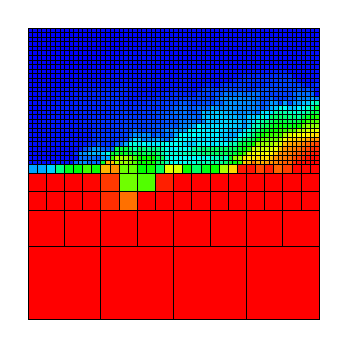
\begin{tikzpicture}[x={(\screenshotunitlength,0)},y={(0,\screenshotunitlength)}]
        \definecolor{fillcolor}{rgb}{1.000000,0.000000,0.000000}
\fill[fillcolor] (0.000000,0.000000) rectangle (0.250000,0.250000);
\definecolor{fillcolor}{rgb}{1.000000,0.000000,0.000000}
\fill[fillcolor] (0.250000,0.000000) rectangle (0.500000,0.250000);
\definecolor{fillcolor}{rgb}{1.000000,0.000000,0.000000}
\fill[fillcolor] (0.000000,0.250000) rectangle (0.125000,0.375000);
\definecolor{fillcolor}{rgb}{1.000000,0.000000,0.000000}
\fill[fillcolor] (0.125000,0.250000) rectangle (0.250000,0.375000);
\definecolor{fillcolor}{rgb}{1.000000,0.000000,0.000000}
\fill[fillcolor] (0.000000,0.375000) rectangle (0.062500,0.437500);
\definecolor{fillcolor}{rgb}{1.000000,0.000000,0.000000}
\fill[fillcolor] (0.062500,0.375000) rectangle (0.125000,0.437500);
\definecolor{fillcolor}{rgb}{1.000000,0.000000,0.000000}
\fill[fillcolor] (0.000000,0.437500) rectangle (0.062500,0.500000);
\definecolor{fillcolor}{rgb}{1.000000,0.000000,0.000000}
\fill[fillcolor] (0.062500,0.437500) rectangle (0.125000,0.500000);
\definecolor{fillcolor}{rgb}{1.000000,0.000053,0.000000}
\fill[fillcolor] (0.125000,0.375000) rectangle (0.187500,0.437500);
\definecolor{fillcolor}{rgb}{1.000000,0.005585,0.000000}
\fill[fillcolor] (0.187500,0.375000) rectangle (0.250000,0.437500);
\definecolor{fillcolor}{rgb}{1.000000,0.000845,0.000000}
\fill[fillcolor] (0.125000,0.437500) rectangle (0.187500,0.500000);
\definecolor{fillcolor}{rgb}{1.000000,0.018238,0.000000}
\fill[fillcolor] (0.187500,0.437500) rectangle (0.250000,0.500000);
\definecolor{fillcolor}{rgb}{1.000000,0.000000,0.000000}
\fill[fillcolor] (0.250000,0.250000) rectangle (0.375000,0.375000);
\definecolor{fillcolor}{rgb}{1.000000,0.000000,0.000000}
\fill[fillcolor] (0.375000,0.250000) rectangle (0.500000,0.375000);
\definecolor{fillcolor}{rgb}{1.000000,0.180585,0.000000}
\fill[fillcolor] (0.250000,0.375000) rectangle (0.312500,0.437500);
\definecolor{fillcolor}{rgb}{1.000000,0.439202,0.000000}
\fill[fillcolor] (0.312500,0.375000) rectangle (0.375000,0.437500);
\definecolor{fillcolor}{rgb}{1.000000,0.225379,0.000000}
\fill[fillcolor] (0.250000,0.437500) rectangle (0.312500,0.500000);
\definecolor{fillcolor}{rgb}{0.433602,1.000000,0.000000}
\fill[fillcolor] (0.312500,0.437500) rectangle (0.375000,0.500000);
\definecolor{fillcolor}{rgb}{1.000000,0.000000,0.000000}
\fill[fillcolor] (0.375000,0.375000) rectangle (0.437500,0.437500);
\definecolor{fillcolor}{rgb}{1.000000,0.000000,0.000000}
\fill[fillcolor] (0.437500,0.375000) rectangle (0.500000,0.437500);
\definecolor{fillcolor}{rgb}{0.317053,1.000000,0.000000}
\fill[fillcolor] (0.375000,0.437500) rectangle (0.437500,0.500000);
\definecolor{fillcolor}{rgb}{1.000000,0.121570,0.000000}
\fill[fillcolor] (0.437500,0.437500) rectangle (0.500000,0.500000);
\definecolor{fillcolor}{rgb}{1.000000,0.000000,0.000000}
\fill[fillcolor] (0.500000,0.000000) rectangle (0.750000,0.250000);
\definecolor{fillcolor}{rgb}{1.000000,0.000000,0.000000}
\fill[fillcolor] (0.750000,0.000000) rectangle (1.000000,0.250000);
\definecolor{fillcolor}{rgb}{1.000000,0.000002,0.000000}
\fill[fillcolor] (0.500000,0.250000) rectangle (0.625000,0.375000);
\definecolor{fillcolor}{rgb}{1.000000,0.000000,0.000000}
\fill[fillcolor] (0.625000,0.250000) rectangle (0.750000,0.375000);
\definecolor{fillcolor}{rgb}{1.000000,0.000002,0.000000}
\fill[fillcolor] (0.500000,0.375000) rectangle (0.562500,0.437500);
\definecolor{fillcolor}{rgb}{1.000000,0.000000,0.000000}
\fill[fillcolor] (0.562500,0.375000) rectangle (0.625000,0.437500);
\definecolor{fillcolor}{rgb}{1.000000,0.000655,0.000000}
\fill[fillcolor] (0.500000,0.437500) rectangle (0.562500,0.500000);
\definecolor{fillcolor}{rgb}{1.000000,0.000000,0.000000}
\fill[fillcolor] (0.562500,0.437500) rectangle (0.625000,0.500000);
\definecolor{fillcolor}{rgb}{1.000000,0.000000,0.000000}
\fill[fillcolor] (0.625000,0.375000) rectangle (0.687500,0.437500);
\definecolor{fillcolor}{rgb}{1.000000,0.000000,0.000000}
\fill[fillcolor] (0.687500,0.375000) rectangle (0.750000,0.437500);
\definecolor{fillcolor}{rgb}{1.000000,0.000000,0.000000}
\fill[fillcolor] (0.625000,0.437500) rectangle (0.687500,0.500000);
\definecolor{fillcolor}{rgb}{1.000000,0.000000,0.000000}
\fill[fillcolor] (0.687500,0.437500) rectangle (0.750000,0.500000);
\definecolor{fillcolor}{rgb}{1.000000,0.000000,0.000000}
\fill[fillcolor] (0.750000,0.250000) rectangle (0.875000,0.375000);
\definecolor{fillcolor}{rgb}{1.000000,0.000000,0.000000}
\fill[fillcolor] (0.875000,0.250000) rectangle (1.000000,0.375000);
\definecolor{fillcolor}{rgb}{1.000000,0.000000,0.000000}
\fill[fillcolor] (0.750000,0.375000) rectangle (0.812500,0.437500);
\definecolor{fillcolor}{rgb}{1.000000,0.000000,0.000000}
\fill[fillcolor] (0.812500,0.375000) rectangle (0.875000,0.437500);
\definecolor{fillcolor}{rgb}{1.000000,0.000000,0.000000}
\fill[fillcolor] (0.750000,0.437500) rectangle (0.812500,0.500000);
\definecolor{fillcolor}{rgb}{1.000000,0.000000,0.000000}
\fill[fillcolor] (0.812500,0.437500) rectangle (0.875000,0.500000);
\definecolor{fillcolor}{rgb}{1.000000,0.000000,0.000000}
\fill[fillcolor] (0.875000,0.375000) rectangle (0.937500,0.437500);
\definecolor{fillcolor}{rgb}{1.000000,0.001008,0.000000}
\fill[fillcolor] (0.937500,0.375000) rectangle (1.000000,0.437500);
\definecolor{fillcolor}{rgb}{1.000000,0.000000,0.000000}
\fill[fillcolor] (0.875000,0.437500) rectangle (0.937500,0.500000);
\definecolor{fillcolor}{rgb}{1.000000,0.000660,0.000000}
\fill[fillcolor] (0.937500,0.437500) rectangle (1.000000,0.500000);
\definecolor{fillcolor}{rgb}{0.000000,0.639657,1.000000}
\fill[fillcolor] (0.000000,0.500000) rectangle (0.031250,0.531250);
\definecolor{fillcolor}{rgb}{0.000000,0.661664,1.000000}
\fill[fillcolor] (0.031250,0.500000) rectangle (0.062500,0.531250);
\definecolor{fillcolor}{rgb}{0.000000,0.040272,1.000000}
\fill[fillcolor] (0.000000,0.531250) rectangle (0.015625,0.546875);
\definecolor{fillcolor}{rgb}{0.000000,0.037497,1.000000}
\fill[fillcolor] (0.015625,0.531250) rectangle (0.031250,0.546875);
\definecolor{fillcolor}{rgb}{0.000000,0.040296,1.000000}
\fill[fillcolor] (0.000000,0.546875) rectangle (0.015625,0.562500);
\definecolor{fillcolor}{rgb}{0.000000,0.042680,1.000000}
\fill[fillcolor] (0.015625,0.546875) rectangle (0.031250,0.562500);
\definecolor{fillcolor}{rgb}{0.000000,0.034894,1.000000}
\fill[fillcolor] (0.031250,0.531250) rectangle (0.046875,0.546875);
\definecolor{fillcolor}{rgb}{0.000000,0.039876,1.000000}
\fill[fillcolor] (0.046875,0.531250) rectangle (0.062500,0.546875);
\definecolor{fillcolor}{rgb}{0.000000,0.035561,1.000000}
\fill[fillcolor] (0.031250,0.546875) rectangle (0.046875,0.562500);
\definecolor{fillcolor}{rgb}{0.000000,0.040829,1.000000}
\fill[fillcolor] (0.046875,0.546875) rectangle (0.062500,0.562500);
\definecolor{fillcolor}{rgb}{0.000000,0.815790,1.000000}
\fill[fillcolor] (0.062500,0.500000) rectangle (0.093750,0.531250);
\definecolor{fillcolor}{rgb}{0.000000,1.000000,0.505576}
\fill[fillcolor] (0.093750,0.500000) rectangle (0.125000,0.531250);
\definecolor{fillcolor}{rgb}{0.000000,0.032366,1.000000}
\fill[fillcolor] (0.062500,0.531250) rectangle (0.078125,0.546875);
\definecolor{fillcolor}{rgb}{0.000000,0.038547,1.000000}
\fill[fillcolor] (0.078125,0.531250) rectangle (0.093750,0.546875);
\definecolor{fillcolor}{rgb}{0.000000,0.038376,1.000000}
\fill[fillcolor] (0.062500,0.546875) rectangle (0.078125,0.562500);
\definecolor{fillcolor}{rgb}{0.000000,0.040010,1.000000}
\fill[fillcolor] (0.078125,0.546875) rectangle (0.093750,0.562500);
\definecolor{fillcolor}{rgb}{0.000000,0.034836,1.000000}
\fill[fillcolor] (0.093750,0.531250) rectangle (0.109375,0.546875);
\definecolor{fillcolor}{rgb}{0.000000,0.067976,1.000000}
\fill[fillcolor] (0.109375,0.531250) rectangle (0.125000,0.546875);
\definecolor{fillcolor}{rgb}{0.000000,0.040967,1.000000}
\fill[fillcolor] (0.093750,0.546875) rectangle (0.109375,0.562500);
\definecolor{fillcolor}{rgb}{0.000000,0.039363,1.000000}
\fill[fillcolor] (0.109375,0.546875) rectangle (0.125000,0.562500);
\definecolor{fillcolor}{rgb}{0.000000,0.042222,1.000000}
\fill[fillcolor] (0.000000,0.562500) rectangle (0.015625,0.578125);
\definecolor{fillcolor}{rgb}{0.000000,0.047625,1.000000}
\fill[fillcolor] (0.015625,0.562500) rectangle (0.031250,0.578125);
\definecolor{fillcolor}{rgb}{0.000000,0.039997,1.000000}
\fill[fillcolor] (0.000000,0.578125) rectangle (0.015625,0.593750);
\definecolor{fillcolor}{rgb}{0.000000,0.047615,1.000000}
\fill[fillcolor] (0.015625,0.578125) rectangle (0.031250,0.593750);
\definecolor{fillcolor}{rgb}{0.000000,0.040083,1.000000}
\fill[fillcolor] (0.031250,0.562500) rectangle (0.046875,0.578125);
\definecolor{fillcolor}{rgb}{0.000000,0.040815,1.000000}
\fill[fillcolor] (0.046875,0.562500) rectangle (0.062500,0.578125);
\definecolor{fillcolor}{rgb}{0.000000,0.049596,1.000000}
\fill[fillcolor] (0.031250,0.578125) rectangle (0.046875,0.593750);
\definecolor{fillcolor}{rgb}{0.000000,0.051278,1.000000}
\fill[fillcolor] (0.046875,0.578125) rectangle (0.062500,0.593750);
\definecolor{fillcolor}{rgb}{0.000000,0.049482,1.000000}
\fill[fillcolor] (0.000000,0.593750) rectangle (0.015625,0.609375);
\definecolor{fillcolor}{rgb}{0.000000,0.052654,1.000000}
\fill[fillcolor] (0.015625,0.593750) rectangle (0.031250,0.609375);
\definecolor{fillcolor}{rgb}{0.000000,0.042586,1.000000}
\fill[fillcolor] (0.000000,0.609375) rectangle (0.015625,0.625000);
\definecolor{fillcolor}{rgb}{0.000000,0.051442,1.000000}
\fill[fillcolor] (0.015625,0.609375) rectangle (0.031250,0.625000);
\definecolor{fillcolor}{rgb}{0.000000,0.052753,1.000000}
\fill[fillcolor] (0.031250,0.593750) rectangle (0.046875,0.609375);
\definecolor{fillcolor}{rgb}{0.000000,0.052946,1.000000}
\fill[fillcolor] (0.046875,0.593750) rectangle (0.062500,0.609375);
\definecolor{fillcolor}{rgb}{0.000000,0.045116,1.000000}
\fill[fillcolor] (0.031250,0.609375) rectangle (0.046875,0.625000);
\definecolor{fillcolor}{rgb}{0.000000,0.052053,1.000000}
\fill[fillcolor] (0.046875,0.609375) rectangle (0.062500,0.625000);
\definecolor{fillcolor}{rgb}{0.000000,0.044394,1.000000}
\fill[fillcolor] (0.062500,0.562500) rectangle (0.078125,0.578125);
\definecolor{fillcolor}{rgb}{0.000000,0.044400,1.000000}
\fill[fillcolor] (0.078125,0.562500) rectangle (0.093750,0.578125);
\definecolor{fillcolor}{rgb}{0.000000,0.051248,1.000000}
\fill[fillcolor] (0.062500,0.578125) rectangle (0.078125,0.593750);
\definecolor{fillcolor}{rgb}{0.000000,0.050322,1.000000}
\fill[fillcolor] (0.078125,0.578125) rectangle (0.093750,0.593750);
\definecolor{fillcolor}{rgb}{0.000000,0.044401,1.000000}
\fill[fillcolor] (0.093750,0.562500) rectangle (0.109375,0.578125);
\definecolor{fillcolor}{rgb}{0.000000,0.042245,1.000000}
\fill[fillcolor] (0.109375,0.562500) rectangle (0.125000,0.578125);
\definecolor{fillcolor}{rgb}{0.000000,0.043042,1.000000}
\fill[fillcolor] (0.093750,0.578125) rectangle (0.109375,0.593750);
\definecolor{fillcolor}{rgb}{0.000000,0.042266,1.000000}
\fill[fillcolor] (0.109375,0.578125) rectangle (0.125000,0.593750);
\definecolor{fillcolor}{rgb}{0.000000,0.057615,1.000000}
\fill[fillcolor] (0.062500,0.593750) rectangle (0.078125,0.609375);
\definecolor{fillcolor}{rgb}{0.000000,0.056043,1.000000}
\fill[fillcolor] (0.078125,0.593750) rectangle (0.093750,0.609375);
\definecolor{fillcolor}{rgb}{0.000000,0.065879,1.000000}
\fill[fillcolor] (0.062500,0.609375) rectangle (0.078125,0.625000);
\definecolor{fillcolor}{rgb}{0.000000,0.065182,1.000000}
\fill[fillcolor] (0.078125,0.609375) rectangle (0.093750,0.625000);
\definecolor{fillcolor}{rgb}{0.000000,0.059571,1.000000}
\fill[fillcolor] (0.093750,0.593750) rectangle (0.109375,0.609375);
\definecolor{fillcolor}{rgb}{0.000000,0.041330,1.000000}
\fill[fillcolor] (0.109375,0.593750) rectangle (0.125000,0.609375);
\definecolor{fillcolor}{rgb}{0.000000,0.070100,1.000000}
\fill[fillcolor] (0.093750,0.609375) rectangle (0.109375,0.625000);
\definecolor{fillcolor}{rgb}{0.000000,0.069363,1.000000}
\fill[fillcolor] (0.109375,0.609375) rectangle (0.125000,0.625000);
\definecolor{fillcolor}{rgb}{0.000000,1.000000,0.096811}
\fill[fillcolor] (0.125000,0.500000) rectangle (0.156250,0.531250);
\definecolor{fillcolor}{rgb}{0.000000,1.000000,0.023911}
\fill[fillcolor] (0.156250,0.500000) rectangle (0.187500,0.531250);
\definecolor{fillcolor}{rgb}{0.000000,0.075738,1.000000}
\fill[fillcolor] (0.125000,0.531250) rectangle (0.140625,0.546875);
\definecolor{fillcolor}{rgb}{0.000000,0.075307,1.000000}
\fill[fillcolor] (0.140625,0.531250) rectangle (0.156250,0.546875);
\definecolor{fillcolor}{rgb}{0.000000,0.035634,1.000000}
\fill[fillcolor] (0.125000,0.546875) rectangle (0.140625,0.562500);
\definecolor{fillcolor}{rgb}{0.000000,0.035401,1.000000}
\fill[fillcolor] (0.140625,0.546875) rectangle (0.156250,0.562500);
\definecolor{fillcolor}{rgb}{0.000000,0.388306,1.000000}
\fill[fillcolor] (0.156250,0.531250) rectangle (0.171875,0.546875);
\definecolor{fillcolor}{rgb}{0.000000,0.546650,1.000000}
\fill[fillcolor] (0.171875,0.531250) rectangle (0.187500,0.546875);
\definecolor{fillcolor}{rgb}{0.000000,0.035396,1.000000}
\fill[fillcolor] (0.156250,0.546875) rectangle (0.171875,0.562500);
\definecolor{fillcolor}{rgb}{0.000000,0.416837,1.000000}
\fill[fillcolor] (0.171875,0.546875) rectangle (0.187500,0.562500);
\definecolor{fillcolor}{rgb}{0.241665,1.000000,0.000000}
\fill[fillcolor] (0.187500,0.500000) rectangle (0.218750,0.531250);
\definecolor{fillcolor}{rgb}{0.043463,1.000000,0.000000}
\fill[fillcolor] (0.218750,0.500000) rectangle (0.250000,0.531250);
\definecolor{fillcolor}{rgb}{0.000000,0.533465,1.000000}
\fill[fillcolor] (0.187500,0.531250) rectangle (0.203125,0.546875);
\definecolor{fillcolor}{rgb}{0.000000,0.391098,1.000000}
\fill[fillcolor] (0.203125,0.531250) rectangle (0.218750,0.546875);
\definecolor{fillcolor}{rgb}{0.000000,0.406530,1.000000}
\fill[fillcolor] (0.187500,0.546875) rectangle (0.203125,0.562500);
\definecolor{fillcolor}{rgb}{0.000000,0.429554,1.000000}
\fill[fillcolor] (0.203125,0.546875) rectangle (0.218750,0.562500);
\definecolor{fillcolor}{rgb}{0.000000,0.430916,1.000000}
\fill[fillcolor] (0.218750,0.531250) rectangle (0.234375,0.546875);
\definecolor{fillcolor}{rgb}{0.000000,0.393624,1.000000}
\fill[fillcolor] (0.234375,0.531250) rectangle (0.250000,0.546875);
\definecolor{fillcolor}{rgb}{0.000000,0.422652,1.000000}
\fill[fillcolor] (0.218750,0.546875) rectangle (0.234375,0.562500);
\definecolor{fillcolor}{rgb}{0.000000,0.335505,1.000000}
\fill[fillcolor] (0.234375,0.546875) rectangle (0.250000,0.562500);
\definecolor{fillcolor}{rgb}{0.000000,0.038464,1.000000}
\fill[fillcolor] (0.125000,0.562500) rectangle (0.140625,0.578125);
\definecolor{fillcolor}{rgb}{0.000000,0.037325,1.000000}
\fill[fillcolor] (0.140625,0.562500) rectangle (0.156250,0.578125);
\definecolor{fillcolor}{rgb}{0.000000,0.042968,1.000000}
\fill[fillcolor] (0.125000,0.578125) rectangle (0.140625,0.593750);
\definecolor{fillcolor}{rgb}{0.000000,0.040754,1.000000}
\fill[fillcolor] (0.140625,0.578125) rectangle (0.156250,0.593750);
\definecolor{fillcolor}{rgb}{0.000000,0.170418,1.000000}
\fill[fillcolor] (0.156250,0.562500) rectangle (0.171875,0.578125);
\definecolor{fillcolor}{rgb}{0.000000,0.550965,1.000000}
\fill[fillcolor] (0.171875,0.562500) rectangle (0.187500,0.578125);
\definecolor{fillcolor}{rgb}{0.000000,0.051524,1.000000}
\fill[fillcolor] (0.156250,0.578125) rectangle (0.171875,0.593750);
\definecolor{fillcolor}{rgb}{0.000000,0.116898,1.000000}
\fill[fillcolor] (0.171875,0.578125) rectangle (0.187500,0.593750);
\definecolor{fillcolor}{rgb}{0.000000,0.074423,1.000000}
\fill[fillcolor] (0.125000,0.593750) rectangle (0.140625,0.609375);
\definecolor{fillcolor}{rgb}{0.000000,0.078096,1.000000}
\fill[fillcolor] (0.140625,0.593750) rectangle (0.156250,0.609375);
\definecolor{fillcolor}{rgb}{0.000000,0.070435,1.000000}
\fill[fillcolor] (0.125000,0.609375) rectangle (0.140625,0.625000);
\definecolor{fillcolor}{rgb}{0.000000,0.057636,1.000000}
\fill[fillcolor] (0.140625,0.609375) rectangle (0.156250,0.625000);
\definecolor{fillcolor}{rgb}{0.000000,0.063326,1.000000}
\fill[fillcolor] (0.156250,0.593750) rectangle (0.171875,0.609375);
\definecolor{fillcolor}{rgb}{0.000000,0.070463,1.000000}
\fill[fillcolor] (0.171875,0.593750) rectangle (0.187500,0.609375);
\definecolor{fillcolor}{rgb}{0.000000,0.053940,1.000000}
\fill[fillcolor] (0.156250,0.609375) rectangle (0.171875,0.625000);
\definecolor{fillcolor}{rgb}{0.000000,0.058514,1.000000}
\fill[fillcolor] (0.171875,0.609375) rectangle (0.187500,0.625000);
\definecolor{fillcolor}{rgb}{0.000000,0.556146,1.000000}
\fill[fillcolor] (0.187500,0.562500) rectangle (0.203125,0.578125);
\definecolor{fillcolor}{rgb}{0.000000,0.711822,1.000000}
\fill[fillcolor] (0.203125,0.562500) rectangle (0.218750,0.578125);
\definecolor{fillcolor}{rgb}{0.000000,0.293769,1.000000}
\fill[fillcolor] (0.187500,0.578125) rectangle (0.203125,0.593750);
\definecolor{fillcolor}{rgb}{0.000000,0.405230,1.000000}
\fill[fillcolor] (0.203125,0.578125) rectangle (0.218750,0.593750);
\definecolor{fillcolor}{rgb}{0.000000,0.701364,1.000000}
\fill[fillcolor] (0.218750,0.562500) rectangle (0.234375,0.578125);
\definecolor{fillcolor}{rgb}{0.000000,0.669141,1.000000}
\fill[fillcolor] (0.234375,0.562500) rectangle (0.250000,0.578125);
\definecolor{fillcolor}{rgb}{0.000000,0.598725,1.000000}
\fill[fillcolor] (0.218750,0.578125) rectangle (0.234375,0.593750);
\definecolor{fillcolor}{rgb}{0.000000,0.578550,1.000000}
\fill[fillcolor] (0.234375,0.578125) rectangle (0.250000,0.593750);
\definecolor{fillcolor}{rgb}{0.000000,0.093890,1.000000}
\fill[fillcolor] (0.187500,0.593750) rectangle (0.203125,0.609375);
\definecolor{fillcolor}{rgb}{0.000000,0.175489,1.000000}
\fill[fillcolor] (0.203125,0.593750) rectangle (0.218750,0.609375);
\definecolor{fillcolor}{rgb}{0.000000,0.090175,1.000000}
\fill[fillcolor] (0.187500,0.609375) rectangle (0.203125,0.625000);
\definecolor{fillcolor}{rgb}{0.000000,0.090829,1.000000}
\fill[fillcolor] (0.203125,0.609375) rectangle (0.218750,0.625000);
\definecolor{fillcolor}{rgb}{0.000000,0.161187,1.000000}
\fill[fillcolor] (0.218750,0.593750) rectangle (0.234375,0.609375);
\definecolor{fillcolor}{rgb}{0.000000,0.325370,1.000000}
\fill[fillcolor] (0.234375,0.593750) rectangle (0.250000,0.609375);
\definecolor{fillcolor}{rgb}{0.000000,0.188308,1.000000}
\fill[fillcolor] (0.218750,0.609375) rectangle (0.234375,0.625000);
\definecolor{fillcolor}{rgb}{0.000000,0.204089,1.000000}
\fill[fillcolor] (0.234375,0.609375) rectangle (0.250000,0.625000);
\definecolor{fillcolor}{rgb}{0.000000,0.053783,1.000000}
\fill[fillcolor] (0.000000,0.625000) rectangle (0.015625,0.640625);
\definecolor{fillcolor}{rgb}{0.000000,0.051442,1.000000}
\fill[fillcolor] (0.015625,0.625000) rectangle (0.031250,0.640625);
\definecolor{fillcolor}{rgb}{0.000000,0.054804,1.000000}
\fill[fillcolor] (0.000000,0.640625) rectangle (0.015625,0.656250);
\definecolor{fillcolor}{rgb}{0.000000,0.057576,1.000000}
\fill[fillcolor] (0.015625,0.640625) rectangle (0.031250,0.656250);
\definecolor{fillcolor}{rgb}{0.000000,0.052008,1.000000}
\fill[fillcolor] (0.031250,0.625000) rectangle (0.046875,0.640625);
\definecolor{fillcolor}{rgb}{0.000000,0.057716,1.000000}
\fill[fillcolor] (0.046875,0.625000) rectangle (0.062500,0.640625);
\definecolor{fillcolor}{rgb}{0.000000,0.059997,1.000000}
\fill[fillcolor] (0.031250,0.640625) rectangle (0.046875,0.656250);
\definecolor{fillcolor}{rgb}{0.000000,0.057727,1.000000}
\fill[fillcolor] (0.046875,0.640625) rectangle (0.062500,0.656250);
\definecolor{fillcolor}{rgb}{0.000000,0.030958,1.000000}
\fill[fillcolor] (0.000000,0.656250) rectangle (0.015625,0.671875);
\definecolor{fillcolor}{rgb}{0.000000,0.043065,1.000000}
\fill[fillcolor] (0.015625,0.656250) rectangle (0.031250,0.671875);
\definecolor{fillcolor}{rgb}{0.000000,0.037338,1.000000}
\fill[fillcolor] (0.000000,0.671875) rectangle (0.015625,0.687500);
\definecolor{fillcolor}{rgb}{0.000000,0.043445,1.000000}
\fill[fillcolor] (0.015625,0.671875) rectangle (0.031250,0.687500);
\definecolor{fillcolor}{rgb}{0.000000,0.071704,1.000000}
\fill[fillcolor] (0.031250,0.656250) rectangle (0.046875,0.671875);
\definecolor{fillcolor}{rgb}{0.000000,0.072738,1.000000}
\fill[fillcolor] (0.046875,0.656250) rectangle (0.062500,0.671875);
\definecolor{fillcolor}{rgb}{0.000000,0.047025,1.000000}
\fill[fillcolor] (0.031250,0.671875) rectangle (0.046875,0.687500);
\definecolor{fillcolor}{rgb}{0.000000,0.075903,1.000000}
\fill[fillcolor] (0.046875,0.671875) rectangle (0.062500,0.687500);
\definecolor{fillcolor}{rgb}{0.000000,0.066823,1.000000}
\fill[fillcolor] (0.062500,0.625000) rectangle (0.078125,0.640625);
\definecolor{fillcolor}{rgb}{0.000000,0.074164,1.000000}
\fill[fillcolor] (0.078125,0.625000) rectangle (0.093750,0.640625);
\definecolor{fillcolor}{rgb}{0.000000,0.077313,1.000000}
\fill[fillcolor] (0.062500,0.640625) rectangle (0.078125,0.656250);
\definecolor{fillcolor}{rgb}{0.000000,0.081266,1.000000}
\fill[fillcolor] (0.078125,0.640625) rectangle (0.093750,0.656250);
\definecolor{fillcolor}{rgb}{0.000000,0.074138,1.000000}
\fill[fillcolor] (0.093750,0.625000) rectangle (0.109375,0.640625);
\definecolor{fillcolor}{rgb}{0.000000,0.068721,1.000000}
\fill[fillcolor] (0.109375,0.625000) rectangle (0.125000,0.640625);
\definecolor{fillcolor}{rgb}{0.000000,0.078758,1.000000}
\fill[fillcolor] (0.093750,0.640625) rectangle (0.109375,0.656250);
\definecolor{fillcolor}{rgb}{0.000000,0.072729,1.000000}
\fill[fillcolor] (0.109375,0.640625) rectangle (0.125000,0.656250);
\definecolor{fillcolor}{rgb}{0.000000,0.082340,1.000000}
\fill[fillcolor] (0.062500,0.656250) rectangle (0.078125,0.671875);
\definecolor{fillcolor}{rgb}{0.000000,0.087384,1.000000}
\fill[fillcolor] (0.078125,0.656250) rectangle (0.093750,0.671875);
\definecolor{fillcolor}{rgb}{0.000000,0.091193,1.000000}
\fill[fillcolor] (0.062500,0.671875) rectangle (0.078125,0.687500);
\definecolor{fillcolor}{rgb}{0.000000,0.094310,1.000000}
\fill[fillcolor] (0.078125,0.671875) rectangle (0.093750,0.687500);
\definecolor{fillcolor}{rgb}{0.000000,0.075017,1.000000}
\fill[fillcolor] (0.093750,0.656250) rectangle (0.109375,0.671875);
\definecolor{fillcolor}{rgb}{0.000000,0.076444,1.000000}
\fill[fillcolor] (0.109375,0.656250) rectangle (0.125000,0.671875);
\definecolor{fillcolor}{rgb}{0.000000,0.086427,1.000000}
\fill[fillcolor] (0.093750,0.671875) rectangle (0.109375,0.687500);
\definecolor{fillcolor}{rgb}{0.000000,0.086901,1.000000}
\fill[fillcolor] (0.109375,0.671875) rectangle (0.125000,0.687500);
\definecolor{fillcolor}{rgb}{0.000000,0.037338,1.000000}
\fill[fillcolor] (0.000000,0.687500) rectangle (0.015625,0.703125);
\definecolor{fillcolor}{rgb}{0.000000,0.038768,1.000000}
\fill[fillcolor] (0.015625,0.687500) rectangle (0.031250,0.703125);
\definecolor{fillcolor}{rgb}{0.000000,0.039996,1.000000}
\fill[fillcolor] (0.000000,0.703125) rectangle (0.015625,0.718750);
\definecolor{fillcolor}{rgb}{0.000000,0.041782,1.000000}
\fill[fillcolor] (0.015625,0.703125) rectangle (0.031250,0.718750);
\definecolor{fillcolor}{rgb}{0.000000,0.046791,1.000000}
\fill[fillcolor] (0.031250,0.687500) rectangle (0.046875,0.703125);
\definecolor{fillcolor}{rgb}{0.000000,0.060885,1.000000}
\fill[fillcolor] (0.046875,0.687500) rectangle (0.062500,0.703125);
\definecolor{fillcolor}{rgb}{0.000000,0.052694,1.000000}
\fill[fillcolor] (0.031250,0.703125) rectangle (0.046875,0.718750);
\definecolor{fillcolor}{rgb}{0.000000,0.060857,1.000000}
\fill[fillcolor] (0.046875,0.703125) rectangle (0.062500,0.718750);
\definecolor{fillcolor}{rgb}{0.000000,0.039620,1.000000}
\fill[fillcolor] (0.000000,0.718750) rectangle (0.015625,0.734375);
\definecolor{fillcolor}{rgb}{0.000000,0.036656,1.000000}
\fill[fillcolor] (0.015625,0.718750) rectangle (0.031250,0.734375);
\definecolor{fillcolor}{rgb}{0.000000,0.039687,1.000000}
\fill[fillcolor] (0.000000,0.734375) rectangle (0.015625,0.750000);
\definecolor{fillcolor}{rgb}{0.000000,0.049788,1.000000}
\fill[fillcolor] (0.015625,0.734375) rectangle (0.031250,0.750000);
\definecolor{fillcolor}{rgb}{0.000000,0.052688,1.000000}
\fill[fillcolor] (0.031250,0.718750) rectangle (0.046875,0.734375);
\definecolor{fillcolor}{rgb}{0.000000,0.067025,1.000000}
\fill[fillcolor] (0.046875,0.718750) rectangle (0.062500,0.734375);
\definecolor{fillcolor}{rgb}{0.000000,0.054596,1.000000}
\fill[fillcolor] (0.031250,0.734375) rectangle (0.046875,0.750000);
\definecolor{fillcolor}{rgb}{0.000000,0.060357,1.000000}
\fill[fillcolor] (0.046875,0.734375) rectangle (0.062500,0.750000);
\definecolor{fillcolor}{rgb}{0.000000,0.090180,1.000000}
\fill[fillcolor] (0.062500,0.687500) rectangle (0.078125,0.703125);
\definecolor{fillcolor}{rgb}{0.000000,0.098473,1.000000}
\fill[fillcolor] (0.078125,0.687500) rectangle (0.093750,0.703125);
\definecolor{fillcolor}{rgb}{0.000000,0.087971,1.000000}
\fill[fillcolor] (0.062500,0.703125) rectangle (0.078125,0.718750);
\definecolor{fillcolor}{rgb}{0.000000,0.091580,1.000000}
\fill[fillcolor] (0.078125,0.703125) rectangle (0.093750,0.718750);
\definecolor{fillcolor}{rgb}{0.000000,0.098492,1.000000}
\fill[fillcolor] (0.093750,0.687500) rectangle (0.109375,0.703125);
\definecolor{fillcolor}{rgb}{0.000000,0.082287,1.000000}
\fill[fillcolor] (0.109375,0.687500) rectangle (0.125000,0.703125);
\definecolor{fillcolor}{rgb}{0.000000,0.104384,1.000000}
\fill[fillcolor] (0.093750,0.703125) rectangle (0.109375,0.718750);
\definecolor{fillcolor}{rgb}{0.000000,0.111055,1.000000}
\fill[fillcolor] (0.109375,0.703125) rectangle (0.125000,0.718750);
\definecolor{fillcolor}{rgb}{0.000000,0.083996,1.000000}
\fill[fillcolor] (0.062500,0.718750) rectangle (0.078125,0.734375);
\definecolor{fillcolor}{rgb}{0.000000,0.083996,1.000000}
\fill[fillcolor] (0.078125,0.718750) rectangle (0.093750,0.734375);
\definecolor{fillcolor}{rgb}{0.000000,0.069604,1.000000}
\fill[fillcolor] (0.062500,0.734375) rectangle (0.078125,0.750000);
\definecolor{fillcolor}{rgb}{0.000000,0.087767,1.000000}
\fill[fillcolor] (0.078125,0.734375) rectangle (0.093750,0.750000);
\definecolor{fillcolor}{rgb}{0.000000,0.092967,1.000000}
\fill[fillcolor] (0.093750,0.718750) rectangle (0.109375,0.734375);
\definecolor{fillcolor}{rgb}{0.000000,0.106281,1.000000}
\fill[fillcolor] (0.109375,0.718750) rectangle (0.125000,0.734375);
\definecolor{fillcolor}{rgb}{0.000000,0.094652,1.000000}
\fill[fillcolor] (0.093750,0.734375) rectangle (0.109375,0.750000);
\definecolor{fillcolor}{rgb}{0.000000,0.096474,1.000000}
\fill[fillcolor] (0.109375,0.734375) rectangle (0.125000,0.750000);
\definecolor{fillcolor}{rgb}{0.000000,0.066835,1.000000}
\fill[fillcolor] (0.125000,0.625000) rectangle (0.140625,0.640625);
\definecolor{fillcolor}{rgb}{0.000000,0.062916,1.000000}
\fill[fillcolor] (0.140625,0.625000) rectangle (0.156250,0.640625);
\definecolor{fillcolor}{rgb}{0.000000,0.076862,1.000000}
\fill[fillcolor] (0.125000,0.640625) rectangle (0.140625,0.656250);
\definecolor{fillcolor}{rgb}{0.000000,0.074581,1.000000}
\fill[fillcolor] (0.140625,0.640625) rectangle (0.156250,0.656250);
\definecolor{fillcolor}{rgb}{0.000000,0.062877,1.000000}
\fill[fillcolor] (0.156250,0.625000) rectangle (0.171875,0.640625);
\definecolor{fillcolor}{rgb}{0.000000,0.056448,1.000000}
\fill[fillcolor] (0.171875,0.625000) rectangle (0.187500,0.640625);
\definecolor{fillcolor}{rgb}{0.000000,0.072396,1.000000}
\fill[fillcolor] (0.156250,0.640625) rectangle (0.171875,0.656250);
\definecolor{fillcolor}{rgb}{0.000000,0.087518,1.000000}
\fill[fillcolor] (0.171875,0.640625) rectangle (0.187500,0.656250);
\definecolor{fillcolor}{rgb}{0.000000,0.083304,1.000000}
\fill[fillcolor] (0.125000,0.656250) rectangle (0.140625,0.671875);
\definecolor{fillcolor}{rgb}{0.000000,0.077666,1.000000}
\fill[fillcolor] (0.140625,0.656250) rectangle (0.156250,0.671875);
\definecolor{fillcolor}{rgb}{0.000000,0.087306,1.000000}
\fill[fillcolor] (0.125000,0.671875) rectangle (0.140625,0.687500);
\definecolor{fillcolor}{rgb}{0.000000,0.094026,1.000000}
\fill[fillcolor] (0.140625,0.671875) rectangle (0.156250,0.687500);
\definecolor{fillcolor}{rgb}{0.000000,0.090943,1.000000}
\fill[fillcolor] (0.156250,0.656250) rectangle (0.171875,0.671875);
\definecolor{fillcolor}{rgb}{0.000000,0.090230,1.000000}
\fill[fillcolor] (0.171875,0.656250) rectangle (0.187500,0.671875);
\definecolor{fillcolor}{rgb}{0.000000,0.094016,1.000000}
\fill[fillcolor] (0.156250,0.671875) rectangle (0.171875,0.687500);
\definecolor{fillcolor}{rgb}{0.000000,0.104872,1.000000}
\fill[fillcolor] (0.171875,0.671875) rectangle (0.187500,0.687500);
\definecolor{fillcolor}{rgb}{0.000000,0.070243,1.000000}
\fill[fillcolor] (0.187500,0.625000) rectangle (0.203125,0.640625);
\definecolor{fillcolor}{rgb}{0.000000,0.070310,1.000000}
\fill[fillcolor] (0.203125,0.625000) rectangle (0.218750,0.640625);
\definecolor{fillcolor}{rgb}{0.000000,0.115196,1.000000}
\fill[fillcolor] (0.187500,0.640625) rectangle (0.203125,0.656250);
\definecolor{fillcolor}{rgb}{0.000000,0.081305,1.000000}
\fill[fillcolor] (0.203125,0.640625) rectangle (0.218750,0.656250);
\definecolor{fillcolor}{rgb}{0.000000,0.187421,1.000000}
\fill[fillcolor] (0.218750,0.625000) rectangle (0.234375,0.640625);
\definecolor{fillcolor}{rgb}{0.000000,0.207856,1.000000}
\fill[fillcolor] (0.234375,0.625000) rectangle (0.250000,0.640625);
\definecolor{fillcolor}{rgb}{0.000000,0.167890,1.000000}
\fill[fillcolor] (0.218750,0.640625) rectangle (0.234375,0.656250);
\definecolor{fillcolor}{rgb}{0.000000,0.174828,1.000000}
\fill[fillcolor] (0.234375,0.640625) rectangle (0.250000,0.656250);
\definecolor{fillcolor}{rgb}{0.000000,0.127905,1.000000}
\fill[fillcolor] (0.187500,0.656250) rectangle (0.203125,0.671875);
\definecolor{fillcolor}{rgb}{0.000000,0.101046,1.000000}
\fill[fillcolor] (0.203125,0.656250) rectangle (0.218750,0.671875);
\definecolor{fillcolor}{rgb}{0.000000,0.127913,1.000000}
\fill[fillcolor] (0.187500,0.671875) rectangle (0.203125,0.687500);
\definecolor{fillcolor}{rgb}{0.000000,0.131785,1.000000}
\fill[fillcolor] (0.203125,0.671875) rectangle (0.218750,0.687500);
\definecolor{fillcolor}{rgb}{0.000000,0.149005,1.000000}
\fill[fillcolor] (0.218750,0.656250) rectangle (0.234375,0.671875);
\definecolor{fillcolor}{rgb}{0.000000,0.172581,1.000000}
\fill[fillcolor] (0.234375,0.656250) rectangle (0.250000,0.671875);
\definecolor{fillcolor}{rgb}{0.000000,0.164873,1.000000}
\fill[fillcolor] (0.218750,0.671875) rectangle (0.234375,0.687500);
\definecolor{fillcolor}{rgb}{0.000000,0.170668,1.000000}
\fill[fillcolor] (0.234375,0.671875) rectangle (0.250000,0.687500);
\definecolor{fillcolor}{rgb}{0.000000,0.071857,1.000000}
\fill[fillcolor] (0.125000,0.687500) rectangle (0.140625,0.703125);
\definecolor{fillcolor}{rgb}{0.000000,0.093974,1.000000}
\fill[fillcolor] (0.140625,0.687500) rectangle (0.156250,0.703125);
\definecolor{fillcolor}{rgb}{0.000000,0.111609,1.000000}
\fill[fillcolor] (0.125000,0.703125) rectangle (0.140625,0.718750);
\definecolor{fillcolor}{rgb}{0.000000,0.093533,1.000000}
\fill[fillcolor] (0.140625,0.703125) rectangle (0.156250,0.718750);
\definecolor{fillcolor}{rgb}{0.000000,0.084056,1.000000}
\fill[fillcolor] (0.156250,0.687500) rectangle (0.171875,0.703125);
\definecolor{fillcolor}{rgb}{0.000000,0.118930,1.000000}
\fill[fillcolor] (0.171875,0.687500) rectangle (0.187500,0.703125);
\definecolor{fillcolor}{rgb}{0.000000,0.130266,1.000000}
\fill[fillcolor] (0.156250,0.703125) rectangle (0.171875,0.718750);
\definecolor{fillcolor}{rgb}{0.000000,0.134332,1.000000}
\fill[fillcolor] (0.171875,0.703125) rectangle (0.187500,0.718750);
\definecolor{fillcolor}{rgb}{0.000000,0.114667,1.000000}
\fill[fillcolor] (0.125000,0.718750) rectangle (0.140625,0.734375);
\definecolor{fillcolor}{rgb}{0.000000,0.114713,1.000000}
\fill[fillcolor] (0.140625,0.718750) rectangle (0.156250,0.734375);
\definecolor{fillcolor}{rgb}{0.000000,0.114465,1.000000}
\fill[fillcolor] (0.125000,0.734375) rectangle (0.140625,0.750000);
\definecolor{fillcolor}{rgb}{0.000000,0.113897,1.000000}
\fill[fillcolor] (0.140625,0.734375) rectangle (0.156250,0.750000);
\definecolor{fillcolor}{rgb}{0.000000,0.129888,1.000000}
\fill[fillcolor] (0.156250,0.718750) rectangle (0.171875,0.734375);
\definecolor{fillcolor}{rgb}{0.000000,0.138170,1.000000}
\fill[fillcolor] (0.171875,0.718750) rectangle (0.187500,0.734375);
\definecolor{fillcolor}{rgb}{0.000000,0.123421,1.000000}
\fill[fillcolor] (0.156250,0.734375) rectangle (0.171875,0.750000);
\definecolor{fillcolor}{rgb}{0.000000,0.138426,1.000000}
\fill[fillcolor] (0.171875,0.734375) rectangle (0.187500,0.750000);
\definecolor{fillcolor}{rgb}{0.000000,0.129120,1.000000}
\fill[fillcolor] (0.187500,0.687500) rectangle (0.203125,0.703125);
\definecolor{fillcolor}{rgb}{0.000000,0.149776,1.000000}
\fill[fillcolor] (0.203125,0.687500) rectangle (0.218750,0.703125);
\definecolor{fillcolor}{rgb}{0.000000,0.142214,1.000000}
\fill[fillcolor] (0.187500,0.703125) rectangle (0.203125,0.718750);
\definecolor{fillcolor}{rgb}{0.000000,0.148586,1.000000}
\fill[fillcolor] (0.203125,0.703125) rectangle (0.218750,0.718750);
\definecolor{fillcolor}{rgb}{0.000000,0.155549,1.000000}
\fill[fillcolor] (0.218750,0.687500) rectangle (0.234375,0.703125);
\definecolor{fillcolor}{rgb}{0.000000,0.159539,1.000000}
\fill[fillcolor] (0.234375,0.687500) rectangle (0.250000,0.703125);
\definecolor{fillcolor}{rgb}{0.000000,0.144364,1.000000}
\fill[fillcolor] (0.218750,0.703125) rectangle (0.234375,0.718750);
\definecolor{fillcolor}{rgb}{0.000000,0.153876,1.000000}
\fill[fillcolor] (0.234375,0.703125) rectangle (0.250000,0.718750);
\definecolor{fillcolor}{rgb}{0.000000,0.143505,1.000000}
\fill[fillcolor] (0.187500,0.718750) rectangle (0.203125,0.734375);
\definecolor{fillcolor}{rgb}{0.000000,0.145877,1.000000}
\fill[fillcolor] (0.203125,0.718750) rectangle (0.218750,0.734375);
\definecolor{fillcolor}{rgb}{0.000000,0.138508,1.000000}
\fill[fillcolor] (0.187500,0.734375) rectangle (0.203125,0.750000);
\definecolor{fillcolor}{rgb}{0.000000,0.144920,1.000000}
\fill[fillcolor] (0.203125,0.734375) rectangle (0.218750,0.750000);
\definecolor{fillcolor}{rgb}{0.000000,0.138001,1.000000}
\fill[fillcolor] (0.218750,0.718750) rectangle (0.234375,0.734375);
\definecolor{fillcolor}{rgb}{0.000000,0.149610,1.000000}
\fill[fillcolor] (0.234375,0.718750) rectangle (0.250000,0.734375);
\definecolor{fillcolor}{rgb}{0.000000,0.150723,1.000000}
\fill[fillcolor] (0.218750,0.734375) rectangle (0.234375,0.750000);
\definecolor{fillcolor}{rgb}{0.000000,0.145488,1.000000}
\fill[fillcolor] (0.234375,0.734375) rectangle (0.250000,0.750000);
\definecolor{fillcolor}{rgb}{1.000000,0.704830,0.000000}
\fill[fillcolor] (0.250000,0.500000) rectangle (0.281250,0.531250);
\definecolor{fillcolor}{rgb}{1.000000,0.566358,0.000000}
\fill[fillcolor] (0.281250,0.500000) rectangle (0.312500,0.531250);
\definecolor{fillcolor}{rgb}{0.000000,1.000000,0.180859}
\fill[fillcolor] (0.250000,0.531250) rectangle (0.265625,0.546875);
\definecolor{fillcolor}{rgb}{1.000000,0.721085,0.000000}
\fill[fillcolor] (0.265625,0.531250) rectangle (0.281250,0.546875);
\definecolor{fillcolor}{rgb}{0.000000,0.618787,1.000000}
\fill[fillcolor] (0.250000,0.546875) rectangle (0.265625,0.562500);
\definecolor{fillcolor}{rgb}{0.000000,0.657157,1.000000}
\fill[fillcolor] (0.265625,0.546875) rectangle (0.281250,0.562500);
\definecolor{fillcolor}{rgb}{1.000000,0.757907,0.000000}
\fill[fillcolor] (0.281250,0.531250) rectangle (0.296875,0.546875);
\definecolor{fillcolor}{rgb}{0.662781,1.000000,0.000000}
\fill[fillcolor] (0.296875,0.531250) rectangle (0.312500,0.546875);
\definecolor{fillcolor}{rgb}{0.168030,1.000000,0.000000}
\fill[fillcolor] (0.281250,0.546875) rectangle (0.296875,0.562500);
\definecolor{fillcolor}{rgb}{0.613771,1.000000,0.000000}
\fill[fillcolor] (0.296875,0.546875) rectangle (0.312500,0.562500);
\definecolor{fillcolor}{rgb}{0.422684,1.000000,0.000000}
\fill[fillcolor] (0.312500,0.500000) rectangle (0.343750,0.531250);
\definecolor{fillcolor}{rgb}{0.378863,1.000000,0.000000}
\fill[fillcolor] (0.343750,0.500000) rectangle (0.375000,0.531250);
\definecolor{fillcolor}{rgb}{0.571540,1.000000,0.000000}
\fill[fillcolor] (0.312500,0.531250) rectangle (0.328125,0.546875);
\definecolor{fillcolor}{rgb}{0.607413,1.000000,0.000000}
\fill[fillcolor] (0.328125,0.531250) rectangle (0.343750,0.546875);
\definecolor{fillcolor}{rgb}{0.606891,1.000000,0.000000}
\fill[fillcolor] (0.312500,0.546875) rectangle (0.328125,0.562500);
\definecolor{fillcolor}{rgb}{0.621744,1.000000,0.000000}
\fill[fillcolor] (0.328125,0.546875) rectangle (0.343750,0.562500);
\definecolor{fillcolor}{rgb}{0.483257,1.000000,0.000000}
\fill[fillcolor] (0.343750,0.531250) rectangle (0.359375,0.546875);
\definecolor{fillcolor}{rgb}{0.323252,1.000000,0.000000}
\fill[fillcolor] (0.359375,0.531250) rectangle (0.375000,0.546875);
\definecolor{fillcolor}{rgb}{0.479341,1.000000,0.000000}
\fill[fillcolor] (0.343750,0.546875) rectangle (0.359375,0.562500);
\definecolor{fillcolor}{rgb}{0.291702,1.000000,0.000000}
\fill[fillcolor] (0.359375,0.546875) rectangle (0.375000,0.562500);
\definecolor{fillcolor}{rgb}{0.000000,0.811807,1.000000}
\fill[fillcolor] (0.250000,0.562500) rectangle (0.265625,0.578125);
\definecolor{fillcolor}{rgb}{0.000000,1.000000,0.889328}
\fill[fillcolor] (0.265625,0.562500) rectangle (0.281250,0.578125);
\definecolor{fillcolor}{rgb}{0.000000,0.388532,1.000000}
\fill[fillcolor] (0.250000,0.578125) rectangle (0.265625,0.593750);
\definecolor{fillcolor}{rgb}{0.000000,0.331117,1.000000}
\fill[fillcolor] (0.265625,0.578125) rectangle (0.281250,0.593750);
\definecolor{fillcolor}{rgb}{0.000000,1.000000,0.201542}
\fill[fillcolor] (0.281250,0.562500) rectangle (0.296875,0.578125);
\definecolor{fillcolor}{rgb}{0.000000,1.000000,0.263368}
\fill[fillcolor] (0.296875,0.562500) rectangle (0.312500,0.578125);
\definecolor{fillcolor}{rgb}{0.000000,0.408552,1.000000}
\fill[fillcolor] (0.281250,0.578125) rectangle (0.296875,0.593750);
\definecolor{fillcolor}{rgb}{0.000000,1.000000,0.267200}
\fill[fillcolor] (0.296875,0.578125) rectangle (0.312500,0.593750);
\definecolor{fillcolor}{rgb}{0.000000,0.189846,1.000000}
\fill[fillcolor] (0.250000,0.593750) rectangle (0.265625,0.609375);
\definecolor{fillcolor}{rgb}{0.000000,0.189213,1.000000}
\fill[fillcolor] (0.265625,0.593750) rectangle (0.281250,0.609375);
\definecolor{fillcolor}{rgb}{0.000000,0.199491,1.000000}
\fill[fillcolor] (0.250000,0.609375) rectangle (0.265625,0.625000);
\definecolor{fillcolor}{rgb}{0.000000,0.199591,1.000000}
\fill[fillcolor] (0.265625,0.609375) rectangle (0.281250,0.625000);
\definecolor{fillcolor}{rgb}{0.000000,0.173213,1.000000}
\fill[fillcolor] (0.281250,0.593750) rectangle (0.296875,0.609375);
\definecolor{fillcolor}{rgb}{0.000000,0.348829,1.000000}
\fill[fillcolor] (0.296875,0.593750) rectangle (0.312500,0.609375);
\definecolor{fillcolor}{rgb}{0.000000,0.193697,1.000000}
\fill[fillcolor] (0.281250,0.609375) rectangle (0.296875,0.625000);
\definecolor{fillcolor}{rgb}{0.000000,0.186512,1.000000}
\fill[fillcolor] (0.296875,0.609375) rectangle (0.312500,0.625000);
\definecolor{fillcolor}{rgb}{0.000000,1.000000,0.092737}
\fill[fillcolor] (0.312500,0.562500) rectangle (0.328125,0.578125);
\definecolor{fillcolor}{rgb}{0.000000,1.000000,0.193077}
\fill[fillcolor] (0.328125,0.562500) rectangle (0.343750,0.578125);
\definecolor{fillcolor}{rgb}{0.000000,1.000000,0.268460}
\fill[fillcolor] (0.312500,0.578125) rectangle (0.328125,0.593750);
\definecolor{fillcolor}{rgb}{0.000000,1.000000,0.261775}
\fill[fillcolor] (0.328125,0.578125) rectangle (0.343750,0.593750);
\definecolor{fillcolor}{rgb}{0.000000,1.000000,0.262939}
\fill[fillcolor] (0.343750,0.562500) rectangle (0.359375,0.578125);
\definecolor{fillcolor}{rgb}{0.000000,1.000000,0.356626}
\fill[fillcolor] (0.359375,0.562500) rectangle (0.375000,0.578125);
\definecolor{fillcolor}{rgb}{0.000000,1.000000,0.440965}
\fill[fillcolor] (0.343750,0.578125) rectangle (0.359375,0.593750);
\definecolor{fillcolor}{rgb}{0.000000,1.000000,0.722902}
\fill[fillcolor] (0.359375,0.578125) rectangle (0.375000,0.593750);
\definecolor{fillcolor}{rgb}{0.000000,0.430716,1.000000}
\fill[fillcolor] (0.312500,0.593750) rectangle (0.328125,0.609375);
\definecolor{fillcolor}{rgb}{0.000000,0.651683,1.000000}
\fill[fillcolor] (0.328125,0.593750) rectangle (0.343750,0.609375);
\definecolor{fillcolor}{rgb}{0.000000,0.227905,1.000000}
\fill[fillcolor] (0.312500,0.609375) rectangle (0.328125,0.625000);
\definecolor{fillcolor}{rgb}{0.000000,0.248361,1.000000}
\fill[fillcolor] (0.328125,0.609375) rectangle (0.343750,0.625000);
\definecolor{fillcolor}{rgb}{0.000000,1.000000,0.923149}
\fill[fillcolor] (0.343750,0.593750) rectangle (0.359375,0.609375);
\definecolor{fillcolor}{rgb}{0.000000,1.000000,0.838281}
\fill[fillcolor] (0.359375,0.593750) rectangle (0.375000,0.609375);
\definecolor{fillcolor}{rgb}{0.000000,0.532948,1.000000}
\fill[fillcolor] (0.343750,0.609375) rectangle (0.359375,0.625000);
\definecolor{fillcolor}{rgb}{0.000000,0.843533,1.000000}
\fill[fillcolor] (0.359375,0.609375) rectangle (0.375000,0.625000);
\definecolor{fillcolor}{rgb}{0.000121,1.000000,0.000000}
\fill[fillcolor] (0.375000,0.500000) rectangle (0.406250,0.531250);
\definecolor{fillcolor}{rgb}{0.057233,1.000000,0.000000}
\fill[fillcolor] (0.406250,0.500000) rectangle (0.437500,0.531250);
\definecolor{fillcolor}{rgb}{0.000000,1.000000,0.003659}
\fill[fillcolor] (0.375000,0.531250) rectangle (0.390625,0.546875);
\definecolor{fillcolor}{rgb}{0.000000,1.000000,0.003107}
\fill[fillcolor] (0.390625,0.531250) rectangle (0.406250,0.546875);
\definecolor{fillcolor}{rgb}{0.001236,1.000000,0.000000}
\fill[fillcolor] (0.375000,0.546875) rectangle (0.390625,0.562500);
\definecolor{fillcolor}{rgb}{0.009022,1.000000,0.000000}
\fill[fillcolor] (0.390625,0.546875) rectangle (0.406250,0.562500);
\definecolor{fillcolor}{rgb}{0.031338,1.000000,0.000000}
\fill[fillcolor] (0.406250,0.531250) rectangle (0.421875,0.546875);
\definecolor{fillcolor}{rgb}{0.040727,1.000000,0.000000}
\fill[fillcolor] (0.421875,0.531250) rectangle (0.437500,0.546875);
\definecolor{fillcolor}{rgb}{0.031328,1.000000,0.000000}
\fill[fillcolor] (0.406250,0.546875) rectangle (0.421875,0.562500);
\definecolor{fillcolor}{rgb}{0.039375,1.000000,0.000000}
\fill[fillcolor] (0.421875,0.546875) rectangle (0.437500,0.562500);
\definecolor{fillcolor}{rgb}{0.000000,1.000000,0.336036}
\fill[fillcolor] (0.437500,0.500000) rectangle (0.468750,0.531250);
\definecolor{fillcolor}{rgb}{0.889811,1.000000,0.000000}
\fill[fillcolor] (0.468750,0.500000) rectangle (0.500000,0.531250);
\definecolor{fillcolor}{rgb}{0.000000,1.000000,0.341337}
\fill[fillcolor] (0.437500,0.531250) rectangle (0.453125,0.546875);
\definecolor{fillcolor}{rgb}{0.000000,1.000000,0.400510}
\fill[fillcolor] (0.453125,0.531250) rectangle (0.468750,0.546875);
\definecolor{fillcolor}{rgb}{0.000000,1.000000,0.258674}
\fill[fillcolor] (0.437500,0.546875) rectangle (0.453125,0.562500);
\definecolor{fillcolor}{rgb}{0.000000,1.000000,0.340752}
\fill[fillcolor] (0.453125,0.546875) rectangle (0.468750,0.562500);
\definecolor{fillcolor}{rgb}{0.000000,1.000000,0.690051}
\fill[fillcolor] (0.468750,0.531250) rectangle (0.484375,0.546875);
\definecolor{fillcolor}{rgb}{0.000000,1.000000,0.962290}
\fill[fillcolor] (0.484375,0.531250) rectangle (0.500000,0.546875);
\definecolor{fillcolor}{rgb}{0.000000,1.000000,0.813393}
\fill[fillcolor] (0.468750,0.546875) rectangle (0.484375,0.562500);
\definecolor{fillcolor}{rgb}{0.000000,1.000000,0.968965}
\fill[fillcolor] (0.484375,0.546875) rectangle (0.500000,0.562500);
\definecolor{fillcolor}{rgb}{0.000000,1.000000,0.243493}
\fill[fillcolor] (0.375000,0.562500) rectangle (0.390625,0.578125);
\definecolor{fillcolor}{rgb}{0.000000,1.000000,0.349901}
\fill[fillcolor] (0.390625,0.562500) rectangle (0.406250,0.578125);
\definecolor{fillcolor}{rgb}{0.000000,1.000000,0.409963}
\fill[fillcolor] (0.375000,0.578125) rectangle (0.390625,0.593750);
\definecolor{fillcolor}{rgb}{0.000000,1.000000,0.489180}
\fill[fillcolor] (0.390625,0.578125) rectangle (0.406250,0.593750);
\definecolor{fillcolor}{rgb}{0.000000,1.000000,0.373660}
\fill[fillcolor] (0.406250,0.562500) rectangle (0.421875,0.578125);
\definecolor{fillcolor}{rgb}{0.000000,1.000000,0.280240}
\fill[fillcolor] (0.421875,0.562500) rectangle (0.437500,0.578125);
\definecolor{fillcolor}{rgb}{0.000000,1.000000,0.563188}
\fill[fillcolor] (0.406250,0.578125) rectangle (0.421875,0.593750);
\definecolor{fillcolor}{rgb}{0.000000,1.000000,0.567065}
\fill[fillcolor] (0.421875,0.578125) rectangle (0.437500,0.593750);
\definecolor{fillcolor}{rgb}{0.000000,0.934827,1.000000}
\fill[fillcolor] (0.375000,0.593750) rectangle (0.390625,0.609375);
\definecolor{fillcolor}{rgb}{0.000000,1.000000,0.990695}
\fill[fillcolor] (0.390625,0.593750) rectangle (0.406250,0.609375);
\definecolor{fillcolor}{rgb}{0.000000,0.800754,1.000000}
\fill[fillcolor] (0.375000,0.609375) rectangle (0.390625,0.625000);
\definecolor{fillcolor}{rgb}{0.000000,0.542652,1.000000}
\fill[fillcolor] (0.390625,0.609375) rectangle (0.406250,0.625000);
\definecolor{fillcolor}{rgb}{0.000000,0.933184,1.000000}
\fill[fillcolor] (0.406250,0.593750) rectangle (0.421875,0.609375);
\definecolor{fillcolor}{rgb}{0.000000,0.929122,1.000000}
\fill[fillcolor] (0.421875,0.593750) rectangle (0.437500,0.609375);
\definecolor{fillcolor}{rgb}{0.000000,0.542618,1.000000}
\fill[fillcolor] (0.406250,0.609375) rectangle (0.421875,0.625000);
\definecolor{fillcolor}{rgb}{0.000000,0.658440,1.000000}
\fill[fillcolor] (0.421875,0.609375) rectangle (0.437500,0.625000);
\definecolor{fillcolor}{rgb}{0.000000,1.000000,0.434251}
\fill[fillcolor] (0.437500,0.562500) rectangle (0.453125,0.578125);
\definecolor{fillcolor}{rgb}{0.000000,1.000000,0.659775}
\fill[fillcolor] (0.453125,0.562500) rectangle (0.468750,0.578125);
\definecolor{fillcolor}{rgb}{0.000000,1.000000,0.526494}
\fill[fillcolor] (0.437500,0.578125) rectangle (0.453125,0.593750);
\definecolor{fillcolor}{rgb}{0.000000,1.000000,0.692967}
\fill[fillcolor] (0.453125,0.578125) rectangle (0.468750,0.593750);
\definecolor{fillcolor}{rgb}{0.000000,1.000000,0.858307}
\fill[fillcolor] (0.468750,0.562500) rectangle (0.484375,0.578125);
\definecolor{fillcolor}{rgb}{0.000000,1.000000,0.846302}
\fill[fillcolor] (0.484375,0.562500) rectangle (0.500000,0.578125);
\definecolor{fillcolor}{rgb}{0.000000,1.000000,0.923303}
\fill[fillcolor] (0.468750,0.578125) rectangle (0.484375,0.593750);
\definecolor{fillcolor}{rgb}{0.000000,0.938446,1.000000}
\fill[fillcolor] (0.484375,0.578125) rectangle (0.500000,0.593750);
\definecolor{fillcolor}{rgb}{0.000000,0.920154,1.000000}
\fill[fillcolor] (0.437500,0.593750) rectangle (0.453125,0.609375);
\definecolor{fillcolor}{rgb}{0.000000,1.000000,0.910179}
\fill[fillcolor] (0.453125,0.593750) rectangle (0.468750,0.609375);
\definecolor{fillcolor}{rgb}{0.000000,0.656158,1.000000}
\fill[fillcolor] (0.437500,0.609375) rectangle (0.453125,0.625000);
\definecolor{fillcolor}{rgb}{0.000000,0.536700,1.000000}
\fill[fillcolor] (0.453125,0.609375) rectangle (0.468750,0.625000);
\definecolor{fillcolor}{rgb}{0.000000,1.000000,0.969085}
\fill[fillcolor] (0.468750,0.593750) rectangle (0.484375,0.609375);
\definecolor{fillcolor}{rgb}{0.000000,1.000000,0.983382}
\fill[fillcolor] (0.484375,0.593750) rectangle (0.500000,0.609375);
\definecolor{fillcolor}{rgb}{0.000000,0.431463,1.000000}
\fill[fillcolor] (0.468750,0.609375) rectangle (0.484375,0.625000);
\definecolor{fillcolor}{rgb}{0.000000,0.606680,1.000000}
\fill[fillcolor] (0.484375,0.609375) rectangle (0.500000,0.625000);
\definecolor{fillcolor}{rgb}{0.000000,0.205278,1.000000}
\fill[fillcolor] (0.250000,0.625000) rectangle (0.265625,0.640625);
\definecolor{fillcolor}{rgb}{0.000000,0.213917,1.000000}
\fill[fillcolor] (0.265625,0.625000) rectangle (0.281250,0.640625);
\definecolor{fillcolor}{rgb}{0.000000,0.174817,1.000000}
\fill[fillcolor] (0.250000,0.640625) rectangle (0.265625,0.656250);
\definecolor{fillcolor}{rgb}{0.000000,0.163908,1.000000}
\fill[fillcolor] (0.265625,0.640625) rectangle (0.281250,0.656250);
\definecolor{fillcolor}{rgb}{0.000000,0.217188,1.000000}
\fill[fillcolor] (0.281250,0.625000) rectangle (0.296875,0.640625);
\definecolor{fillcolor}{rgb}{0.000000,0.218521,1.000000}
\fill[fillcolor] (0.296875,0.625000) rectangle (0.312500,0.640625);
\definecolor{fillcolor}{rgb}{0.000000,0.197913,1.000000}
\fill[fillcolor] (0.281250,0.640625) rectangle (0.296875,0.656250);
\definecolor{fillcolor}{rgb}{0.000000,0.208460,1.000000}
\fill[fillcolor] (0.296875,0.640625) rectangle (0.312500,0.656250);
\definecolor{fillcolor}{rgb}{0.000000,0.173159,1.000000}
\fill[fillcolor] (0.250000,0.656250) rectangle (0.265625,0.671875);
\definecolor{fillcolor}{rgb}{0.000000,0.171891,1.000000}
\fill[fillcolor] (0.265625,0.656250) rectangle (0.281250,0.671875);
\definecolor{fillcolor}{rgb}{0.000000,0.182874,1.000000}
\fill[fillcolor] (0.250000,0.671875) rectangle (0.265625,0.687500);
\definecolor{fillcolor}{rgb}{0.000000,0.182880,1.000000}
\fill[fillcolor] (0.265625,0.671875) rectangle (0.281250,0.687500);
\definecolor{fillcolor}{rgb}{0.000000,0.197859,1.000000}
\fill[fillcolor] (0.281250,0.656250) rectangle (0.296875,0.671875);
\definecolor{fillcolor}{rgb}{0.000000,0.208362,1.000000}
\fill[fillcolor] (0.296875,0.656250) rectangle (0.312500,0.671875);
\definecolor{fillcolor}{rgb}{0.000000,0.205475,1.000000}
\fill[fillcolor] (0.281250,0.671875) rectangle (0.296875,0.687500);
\definecolor{fillcolor}{rgb}{0.000000,0.205530,1.000000}
\fill[fillcolor] (0.296875,0.671875) rectangle (0.312500,0.687500);
\definecolor{fillcolor}{rgb}{0.000000,0.236268,1.000000}
\fill[fillcolor] (0.312500,0.625000) rectangle (0.328125,0.640625);
\definecolor{fillcolor}{rgb}{0.000000,0.237878,1.000000}
\fill[fillcolor] (0.328125,0.625000) rectangle (0.343750,0.640625);
\definecolor{fillcolor}{rgb}{0.000000,0.220809,1.000000}
\fill[fillcolor] (0.312500,0.640625) rectangle (0.328125,0.656250);
\definecolor{fillcolor}{rgb}{0.000000,0.237817,1.000000}
\fill[fillcolor] (0.328125,0.640625) rectangle (0.343750,0.656250);
\definecolor{fillcolor}{rgb}{0.000000,0.397914,1.000000}
\fill[fillcolor] (0.343750,0.625000) rectangle (0.359375,0.640625);
\definecolor{fillcolor}{rgb}{0.000000,0.546277,1.000000}
\fill[fillcolor] (0.359375,0.625000) rectangle (0.375000,0.640625);
\definecolor{fillcolor}{rgb}{0.000000,0.261316,1.000000}
\fill[fillcolor] (0.343750,0.640625) rectangle (0.359375,0.656250);
\definecolor{fillcolor}{rgb}{0.000000,0.410604,1.000000}
\fill[fillcolor] (0.359375,0.640625) rectangle (0.375000,0.656250);
\definecolor{fillcolor}{rgb}{0.000000,0.216628,1.000000}
\fill[fillcolor] (0.312500,0.656250) rectangle (0.328125,0.671875);
\definecolor{fillcolor}{rgb}{0.000000,0.237631,1.000000}
\fill[fillcolor] (0.328125,0.656250) rectangle (0.343750,0.671875);
\definecolor{fillcolor}{rgb}{0.000000,0.194945,1.000000}
\fill[fillcolor] (0.312500,0.671875) rectangle (0.328125,0.687500);
\definecolor{fillcolor}{rgb}{0.000000,0.219203,1.000000}
\fill[fillcolor] (0.328125,0.671875) rectangle (0.343750,0.687500);
\definecolor{fillcolor}{rgb}{0.000000,0.247405,1.000000}
\fill[fillcolor] (0.343750,0.656250) rectangle (0.359375,0.671875);
\definecolor{fillcolor}{rgb}{0.000000,0.241713,1.000000}
\fill[fillcolor] (0.359375,0.656250) rectangle (0.375000,0.671875);
\definecolor{fillcolor}{rgb}{0.000000,0.235116,1.000000}
\fill[fillcolor] (0.343750,0.671875) rectangle (0.359375,0.687500);
\definecolor{fillcolor}{rgb}{0.000000,0.242879,1.000000}
\fill[fillcolor] (0.359375,0.671875) rectangle (0.375000,0.687500);
\definecolor{fillcolor}{rgb}{0.000000,0.165859,1.000000}
\fill[fillcolor] (0.250000,0.687500) rectangle (0.265625,0.703125);
\definecolor{fillcolor}{rgb}{0.000000,0.156918,1.000000}
\fill[fillcolor] (0.265625,0.687500) rectangle (0.281250,0.703125);
\definecolor{fillcolor}{rgb}{0.000000,0.150411,1.000000}
\fill[fillcolor] (0.250000,0.703125) rectangle (0.265625,0.718750);
\definecolor{fillcolor}{rgb}{0.000000,0.159350,1.000000}
\fill[fillcolor] (0.265625,0.703125) rectangle (0.281250,0.718750);
\definecolor{fillcolor}{rgb}{0.000000,0.200858,1.000000}
\fill[fillcolor] (0.281250,0.687500) rectangle (0.296875,0.703125);
\definecolor{fillcolor}{rgb}{0.000000,0.205138,1.000000}
\fill[fillcolor] (0.296875,0.687500) rectangle (0.312500,0.703125);
\definecolor{fillcolor}{rgb}{0.000000,0.195396,1.000000}
\fill[fillcolor] (0.281250,0.703125) rectangle (0.296875,0.718750);
\definecolor{fillcolor}{rgb}{0.000000,0.195487,1.000000}
\fill[fillcolor] (0.296875,0.703125) rectangle (0.312500,0.718750);
\definecolor{fillcolor}{rgb}{0.000000,0.154918,1.000000}
\fill[fillcolor] (0.250000,0.718750) rectangle (0.265625,0.734375);
\definecolor{fillcolor}{rgb}{0.000000,0.131086,1.000000}
\fill[fillcolor] (0.265625,0.718750) rectangle (0.281250,0.734375);
\definecolor{fillcolor}{rgb}{0.000000,0.164173,1.000000}
\fill[fillcolor] (0.250000,0.734375) rectangle (0.265625,0.750000);
\definecolor{fillcolor}{rgb}{0.000000,0.164171,1.000000}
\fill[fillcolor] (0.265625,0.734375) rectangle (0.281250,0.750000);
\definecolor{fillcolor}{rgb}{0.000000,0.164124,1.000000}
\fill[fillcolor] (0.281250,0.718750) rectangle (0.296875,0.734375);
\definecolor{fillcolor}{rgb}{0.000000,0.189555,1.000000}
\fill[fillcolor] (0.296875,0.718750) rectangle (0.312500,0.734375);
\definecolor{fillcolor}{rgb}{0.000000,0.180116,1.000000}
\fill[fillcolor] (0.281250,0.734375) rectangle (0.296875,0.750000);
\definecolor{fillcolor}{rgb}{0.000000,0.186838,1.000000}
\fill[fillcolor] (0.296875,0.734375) rectangle (0.312500,0.750000);
\definecolor{fillcolor}{rgb}{0.000000,0.207270,1.000000}
\fill[fillcolor] (0.312500,0.687500) rectangle (0.328125,0.703125);
\definecolor{fillcolor}{rgb}{0.000000,0.212512,1.000000}
\fill[fillcolor] (0.328125,0.687500) rectangle (0.343750,0.703125);
\definecolor{fillcolor}{rgb}{0.000000,0.203722,1.000000}
\fill[fillcolor] (0.312500,0.703125) rectangle (0.328125,0.718750);
\definecolor{fillcolor}{rgb}{0.000000,0.219484,1.000000}
\fill[fillcolor] (0.328125,0.703125) rectangle (0.343750,0.718750);
\definecolor{fillcolor}{rgb}{0.000000,0.214421,1.000000}
\fill[fillcolor] (0.343750,0.687500) rectangle (0.359375,0.703125);
\definecolor{fillcolor}{rgb}{0.000000,0.216237,1.000000}
\fill[fillcolor] (0.359375,0.687500) rectangle (0.375000,0.703125);
\definecolor{fillcolor}{rgb}{0.000000,0.183015,1.000000}
\fill[fillcolor] (0.343750,0.703125) rectangle (0.359375,0.718750);
\definecolor{fillcolor}{rgb}{0.000000,0.202545,1.000000}
\fill[fillcolor] (0.359375,0.703125) rectangle (0.375000,0.718750);
\definecolor{fillcolor}{rgb}{0.000000,0.163003,1.000000}
\fill[fillcolor] (0.312500,0.718750) rectangle (0.328125,0.734375);
\definecolor{fillcolor}{rgb}{0.000000,0.155833,1.000000}
\fill[fillcolor] (0.328125,0.718750) rectangle (0.343750,0.734375);
\definecolor{fillcolor}{rgb}{0.000000,0.132581,1.000000}
\fill[fillcolor] (0.312500,0.734375) rectangle (0.328125,0.750000);
\definecolor{fillcolor}{rgb}{0.000000,0.132570,1.000000}
\fill[fillcolor] (0.328125,0.734375) rectangle (0.343750,0.750000);
\definecolor{fillcolor}{rgb}{0.000000,0.151962,1.000000}
\fill[fillcolor] (0.343750,0.718750) rectangle (0.359375,0.734375);
\definecolor{fillcolor}{rgb}{0.000000,0.173866,1.000000}
\fill[fillcolor] (0.359375,0.718750) rectangle (0.375000,0.734375);
\definecolor{fillcolor}{rgb}{0.000000,0.125303,1.000000}
\fill[fillcolor] (0.343750,0.734375) rectangle (0.359375,0.750000);
\definecolor{fillcolor}{rgb}{0.000000,0.152302,1.000000}
\fill[fillcolor] (0.359375,0.734375) rectangle (0.375000,0.750000);
\definecolor{fillcolor}{rgb}{0.000000,0.544349,1.000000}
\fill[fillcolor] (0.375000,0.625000) rectangle (0.390625,0.640625);
\definecolor{fillcolor}{rgb}{0.000000,0.545957,1.000000}
\fill[fillcolor] (0.390625,0.625000) rectangle (0.406250,0.640625);
\definecolor{fillcolor}{rgb}{0.000000,0.284552,1.000000}
\fill[fillcolor] (0.375000,0.640625) rectangle (0.390625,0.656250);
\definecolor{fillcolor}{rgb}{0.000000,0.263169,1.000000}
\fill[fillcolor] (0.390625,0.640625) rectangle (0.406250,0.656250);
\definecolor{fillcolor}{rgb}{0.000000,0.521655,1.000000}
\fill[fillcolor] (0.406250,0.625000) rectangle (0.421875,0.640625);
\definecolor{fillcolor}{rgb}{0.000000,0.288939,1.000000}
\fill[fillcolor] (0.421875,0.625000) rectangle (0.437500,0.640625);
\definecolor{fillcolor}{rgb}{0.000000,0.282107,1.000000}
\fill[fillcolor] (0.406250,0.640625) rectangle (0.421875,0.656250);
\definecolor{fillcolor}{rgb}{0.000000,0.304307,1.000000}
\fill[fillcolor] (0.421875,0.640625) rectangle (0.437500,0.656250);
\definecolor{fillcolor}{rgb}{0.000000,0.233663,1.000000}
\fill[fillcolor] (0.375000,0.656250) rectangle (0.390625,0.671875);
\definecolor{fillcolor}{rgb}{0.000000,0.233662,1.000000}
\fill[fillcolor] (0.390625,0.656250) rectangle (0.406250,0.671875);
\definecolor{fillcolor}{rgb}{0.000000,0.233565,1.000000}
\fill[fillcolor] (0.375000,0.671875) rectangle (0.390625,0.687500);
\definecolor{fillcolor}{rgb}{0.000000,0.230775,1.000000}
\fill[fillcolor] (0.390625,0.671875) rectangle (0.406250,0.687500);
\definecolor{fillcolor}{rgb}{0.000000,0.249042,1.000000}
\fill[fillcolor] (0.406250,0.656250) rectangle (0.421875,0.671875);
\definecolor{fillcolor}{rgb}{0.000000,0.309870,1.000000}
\fill[fillcolor] (0.421875,0.656250) rectangle (0.437500,0.671875);
\definecolor{fillcolor}{rgb}{0.000000,0.238058,1.000000}
\fill[fillcolor] (0.406250,0.671875) rectangle (0.421875,0.687500);
\definecolor{fillcolor}{rgb}{0.000000,0.234574,1.000000}
\fill[fillcolor] (0.421875,0.671875) rectangle (0.437500,0.687500);
\definecolor{fillcolor}{rgb}{0.000000,0.420756,1.000000}
\fill[fillcolor] (0.437500,0.625000) rectangle (0.453125,0.640625);
\definecolor{fillcolor}{rgb}{0.000000,0.326237,1.000000}
\fill[fillcolor] (0.453125,0.625000) rectangle (0.468750,0.640625);
\definecolor{fillcolor}{rgb}{0.000000,0.285398,1.000000}
\fill[fillcolor] (0.437500,0.640625) rectangle (0.453125,0.656250);
\definecolor{fillcolor}{rgb}{0.000000,0.381834,1.000000}
\fill[fillcolor] (0.453125,0.640625) rectangle (0.468750,0.656250);
\definecolor{fillcolor}{rgb}{0.000000,0.431973,1.000000}
\fill[fillcolor] (0.468750,0.625000) rectangle (0.484375,0.640625);
\definecolor{fillcolor}{rgb}{0.000000,0.400188,1.000000}
\fill[fillcolor] (0.484375,0.625000) rectangle (0.500000,0.640625);
\definecolor{fillcolor}{rgb}{0.000000,0.504529,1.000000}
\fill[fillcolor] (0.468750,0.640625) rectangle (0.484375,0.656250);
\definecolor{fillcolor}{rgb}{0.000000,0.504480,1.000000}
\fill[fillcolor] (0.484375,0.640625) rectangle (0.500000,0.656250);
\definecolor{fillcolor}{rgb}{0.000000,0.309939,1.000000}
\fill[fillcolor] (0.437500,0.656250) rectangle (0.453125,0.671875);
\definecolor{fillcolor}{rgb}{0.000000,0.323474,1.000000}
\fill[fillcolor] (0.453125,0.656250) rectangle (0.468750,0.671875);
\definecolor{fillcolor}{rgb}{0.000000,0.233386,1.000000}
\fill[fillcolor] (0.437500,0.671875) rectangle (0.453125,0.687500);
\definecolor{fillcolor}{rgb}{0.000000,0.274633,1.000000}
\fill[fillcolor] (0.453125,0.671875) rectangle (0.468750,0.687500);
\definecolor{fillcolor}{rgb}{0.000000,0.316799,1.000000}
\fill[fillcolor] (0.468750,0.656250) rectangle (0.484375,0.671875);
\definecolor{fillcolor}{rgb}{0.000000,0.381963,1.000000}
\fill[fillcolor] (0.484375,0.656250) rectangle (0.500000,0.671875);
\definecolor{fillcolor}{rgb}{0.000000,0.316666,1.000000}
\fill[fillcolor] (0.468750,0.671875) rectangle (0.484375,0.687500);
\definecolor{fillcolor}{rgb}{0.000000,0.290738,1.000000}
\fill[fillcolor] (0.484375,0.671875) rectangle (0.500000,0.687500);
\definecolor{fillcolor}{rgb}{0.000000,0.223260,1.000000}
\fill[fillcolor] (0.375000,0.687500) rectangle (0.390625,0.703125);
\definecolor{fillcolor}{rgb}{0.000000,0.220418,1.000000}
\fill[fillcolor] (0.390625,0.687500) rectangle (0.406250,0.703125);
\definecolor{fillcolor}{rgb}{0.000000,0.201523,1.000000}
\fill[fillcolor] (0.375000,0.703125) rectangle (0.390625,0.718750);
\definecolor{fillcolor}{rgb}{0.000000,0.216829,1.000000}
\fill[fillcolor] (0.390625,0.703125) rectangle (0.406250,0.718750);
\definecolor{fillcolor}{rgb}{0.000000,0.227828,1.000000}
\fill[fillcolor] (0.406250,0.687500) rectangle (0.421875,0.703125);
\definecolor{fillcolor}{rgb}{0.000000,0.245270,1.000000}
\fill[fillcolor] (0.421875,0.687500) rectangle (0.437500,0.703125);
\definecolor{fillcolor}{rgb}{0.000000,0.221123,1.000000}
\fill[fillcolor] (0.406250,0.703125) rectangle (0.421875,0.718750);
\definecolor{fillcolor}{rgb}{0.000000,0.265440,1.000000}
\fill[fillcolor] (0.421875,0.703125) rectangle (0.437500,0.718750);
\definecolor{fillcolor}{rgb}{0.000000,0.201106,1.000000}
\fill[fillcolor] (0.375000,0.718750) rectangle (0.390625,0.734375);
\definecolor{fillcolor}{rgb}{0.000000,0.201186,1.000000}
\fill[fillcolor] (0.390625,0.718750) rectangle (0.406250,0.734375);
\definecolor{fillcolor}{rgb}{0.000000,0.157759,1.000000}
\fill[fillcolor] (0.375000,0.734375) rectangle (0.390625,0.750000);
\definecolor{fillcolor}{rgb}{0.000000,0.142777,1.000000}
\fill[fillcolor] (0.390625,0.734375) rectangle (0.406250,0.750000);
\definecolor{fillcolor}{rgb}{0.000000,0.188376,1.000000}
\fill[fillcolor] (0.406250,0.718750) rectangle (0.421875,0.734375);
\definecolor{fillcolor}{rgb}{0.000000,0.184262,1.000000}
\fill[fillcolor] (0.421875,0.718750) rectangle (0.437500,0.734375);
\definecolor{fillcolor}{rgb}{0.000000,0.187395,1.000000}
\fill[fillcolor] (0.406250,0.734375) rectangle (0.421875,0.750000);
\definecolor{fillcolor}{rgb}{0.000000,0.199959,1.000000}
\fill[fillcolor] (0.421875,0.734375) rectangle (0.437500,0.750000);
\definecolor{fillcolor}{rgb}{0.000000,0.259040,1.000000}
\fill[fillcolor] (0.437500,0.687500) rectangle (0.453125,0.703125);
\definecolor{fillcolor}{rgb}{0.000000,0.323264,1.000000}
\fill[fillcolor] (0.453125,0.687500) rectangle (0.468750,0.703125);
\definecolor{fillcolor}{rgb}{0.000000,0.289125,1.000000}
\fill[fillcolor] (0.437500,0.703125) rectangle (0.453125,0.718750);
\definecolor{fillcolor}{rgb}{0.000000,0.313159,1.000000}
\fill[fillcolor] (0.453125,0.703125) rectangle (0.468750,0.718750);
\definecolor{fillcolor}{rgb}{0.000000,0.357875,1.000000}
\fill[fillcolor] (0.468750,0.687500) rectangle (0.484375,0.703125);
\definecolor{fillcolor}{rgb}{0.000000,0.373708,1.000000}
\fill[fillcolor] (0.484375,0.687500) rectangle (0.500000,0.703125);
\definecolor{fillcolor}{rgb}{0.000000,0.318476,1.000000}
\fill[fillcolor] (0.468750,0.703125) rectangle (0.484375,0.718750);
\definecolor{fillcolor}{rgb}{0.000000,0.376276,1.000000}
\fill[fillcolor] (0.484375,0.703125) rectangle (0.500000,0.718750);
\definecolor{fillcolor}{rgb}{0.000000,0.182841,1.000000}
\fill[fillcolor] (0.437500,0.718750) rectangle (0.453125,0.734375);
\definecolor{fillcolor}{rgb}{0.000000,0.206680,1.000000}
\fill[fillcolor] (0.453125,0.718750) rectangle (0.468750,0.734375);
\definecolor{fillcolor}{rgb}{0.000000,0.211493,1.000000}
\fill[fillcolor] (0.437500,0.734375) rectangle (0.453125,0.750000);
\definecolor{fillcolor}{rgb}{0.000000,0.212389,1.000000}
\fill[fillcolor] (0.453125,0.734375) rectangle (0.468750,0.750000);
\definecolor{fillcolor}{rgb}{0.000000,0.244646,1.000000}
\fill[fillcolor] (0.468750,0.718750) rectangle (0.484375,0.734375);
\definecolor{fillcolor}{rgb}{0.000000,0.292952,1.000000}
\fill[fillcolor] (0.484375,0.718750) rectangle (0.500000,0.734375);
\definecolor{fillcolor}{rgb}{0.000000,0.236642,1.000000}
\fill[fillcolor] (0.468750,0.734375) rectangle (0.484375,0.750000);
\definecolor{fillcolor}{rgb}{0.000000,0.262721,1.000000}
\fill[fillcolor] (0.484375,0.734375) rectangle (0.500000,0.750000);
\definecolor{fillcolor}{rgb}{0.000000,0.039587,1.000000}
\fill[fillcolor] (0.000000,0.750000) rectangle (0.015625,0.765625);
\definecolor{fillcolor}{rgb}{0.000000,0.026930,1.000000}
\fill[fillcolor] (0.015625,0.750000) rectangle (0.031250,0.765625);
\definecolor{fillcolor}{rgb}{0.000000,0.026706,1.000000}
\fill[fillcolor] (0.000000,0.765625) rectangle (0.015625,0.781250);
\definecolor{fillcolor}{rgb}{0.000000,0.027469,1.000000}
\fill[fillcolor] (0.015625,0.765625) rectangle (0.031250,0.781250);
\definecolor{fillcolor}{rgb}{0.000000,0.059574,1.000000}
\fill[fillcolor] (0.031250,0.750000) rectangle (0.046875,0.765625);
\definecolor{fillcolor}{rgb}{0.000000,0.059685,1.000000}
\fill[fillcolor] (0.046875,0.750000) rectangle (0.062500,0.765625);
\definecolor{fillcolor}{rgb}{0.000000,0.060070,1.000000}
\fill[fillcolor] (0.031250,0.765625) rectangle (0.046875,0.781250);
\definecolor{fillcolor}{rgb}{0.000000,0.060486,1.000000}
\fill[fillcolor] (0.046875,0.765625) rectangle (0.062500,0.781250);
\definecolor{fillcolor}{rgb}{0.000000,0.012587,1.000000}
\fill[fillcolor] (0.000000,0.781250) rectangle (0.015625,0.796875);
\definecolor{fillcolor}{rgb}{0.000000,0.031612,1.000000}
\fill[fillcolor] (0.015625,0.781250) rectangle (0.031250,0.796875);
\definecolor{fillcolor}{rgb}{0.000000,0.019405,1.000000}
\fill[fillcolor] (0.000000,0.796875) rectangle (0.015625,0.812500);
\definecolor{fillcolor}{rgb}{0.000000,0.020512,1.000000}
\fill[fillcolor] (0.015625,0.796875) rectangle (0.031250,0.812500);
\definecolor{fillcolor}{rgb}{0.000000,0.053716,1.000000}
\fill[fillcolor] (0.031250,0.781250) rectangle (0.046875,0.796875);
\definecolor{fillcolor}{rgb}{0.000000,0.038244,1.000000}
\fill[fillcolor] (0.046875,0.781250) rectangle (0.062500,0.796875);
\definecolor{fillcolor}{rgb}{0.000000,0.025548,1.000000}
\fill[fillcolor] (0.031250,0.796875) rectangle (0.046875,0.812500);
\definecolor{fillcolor}{rgb}{0.000000,0.038228,1.000000}
\fill[fillcolor] (0.046875,0.796875) rectangle (0.062500,0.812500);
\definecolor{fillcolor}{rgb}{0.000000,0.039732,1.000000}
\fill[fillcolor] (0.062500,0.750000) rectangle (0.078125,0.765625);
\definecolor{fillcolor}{rgb}{0.000000,0.040516,1.000000}
\fill[fillcolor] (0.078125,0.750000) rectangle (0.093750,0.765625);
\definecolor{fillcolor}{rgb}{0.000000,0.045125,1.000000}
\fill[fillcolor] (0.062500,0.765625) rectangle (0.078125,0.781250);
\definecolor{fillcolor}{rgb}{0.000000,0.045229,1.000000}
\fill[fillcolor] (0.078125,0.765625) rectangle (0.093750,0.781250);
\definecolor{fillcolor}{rgb}{0.000000,0.086037,1.000000}
\fill[fillcolor] (0.093750,0.750000) rectangle (0.109375,0.765625);
\definecolor{fillcolor}{rgb}{0.000000,0.086049,1.000000}
\fill[fillcolor] (0.109375,0.750000) rectangle (0.125000,0.765625);
\definecolor{fillcolor}{rgb}{0.000000,0.049582,1.000000}
\fill[fillcolor] (0.093750,0.765625) rectangle (0.109375,0.781250);
\definecolor{fillcolor}{rgb}{0.000000,0.066903,1.000000}
\fill[fillcolor] (0.109375,0.765625) rectangle (0.125000,0.781250);
\definecolor{fillcolor}{rgb}{0.000000,0.037485,1.000000}
\fill[fillcolor] (0.062500,0.781250) rectangle (0.078125,0.796875);
\definecolor{fillcolor}{rgb}{0.000000,0.040503,1.000000}
\fill[fillcolor] (0.078125,0.781250) rectangle (0.093750,0.796875);
\definecolor{fillcolor}{rgb}{0.000000,0.025329,1.000000}
\fill[fillcolor] (0.062500,0.796875) rectangle (0.078125,0.812500);
\definecolor{fillcolor}{rgb}{0.000000,0.038338,1.000000}
\fill[fillcolor] (0.078125,0.796875) rectangle (0.093750,0.812500);
\definecolor{fillcolor}{rgb}{0.000000,0.030754,1.000000}
\fill[fillcolor] (0.093750,0.781250) rectangle (0.109375,0.796875);
\definecolor{fillcolor}{rgb}{0.000000,0.048712,1.000000}
\fill[fillcolor] (0.109375,0.781250) rectangle (0.125000,0.796875);
\definecolor{fillcolor}{rgb}{0.000000,0.015683,1.000000}
\fill[fillcolor] (0.093750,0.796875) rectangle (0.109375,0.812500);
\definecolor{fillcolor}{rgb}{0.000000,0.019894,1.000000}
\fill[fillcolor] (0.109375,0.796875) rectangle (0.125000,0.812500);
\definecolor{fillcolor}{rgb}{0.000000,0.012595,1.000000}
\fill[fillcolor] (0.000000,0.812500) rectangle (0.015625,0.828125);
\definecolor{fillcolor}{rgb}{0.000000,0.009506,1.000000}
\fill[fillcolor] (0.015625,0.812500) rectangle (0.031250,0.828125);
\definecolor{fillcolor}{rgb}{0.000000,0.010730,1.000000}
\fill[fillcolor] (0.000000,0.828125) rectangle (0.015625,0.843750);
\definecolor{fillcolor}{rgb}{0.000000,0.009783,1.000000}
\fill[fillcolor] (0.015625,0.828125) rectangle (0.031250,0.843750);
\definecolor{fillcolor}{rgb}{0.000000,0.024280,1.000000}
\fill[fillcolor] (0.031250,0.812500) rectangle (0.046875,0.828125);
\definecolor{fillcolor}{rgb}{0.000000,0.007604,1.000000}
\fill[fillcolor] (0.046875,0.812500) rectangle (0.062500,0.828125);
\definecolor{fillcolor}{rgb}{0.000000,0.016290,1.000000}
\fill[fillcolor] (0.031250,0.828125) rectangle (0.046875,0.843750);
\definecolor{fillcolor}{rgb}{0.000000,0.008946,1.000000}
\fill[fillcolor] (0.046875,0.828125) rectangle (0.062500,0.843750);
\definecolor{fillcolor}{rgb}{0.000000,0.011451,1.000000}
\fill[fillcolor] (0.000000,0.843750) rectangle (0.015625,0.859375);
\definecolor{fillcolor}{rgb}{0.000000,0.010951,1.000000}
\fill[fillcolor] (0.015625,0.843750) rectangle (0.031250,0.859375);
\definecolor{fillcolor}{rgb}{0.000000,0.010711,1.000000}
\fill[fillcolor] (0.000000,0.859375) rectangle (0.015625,0.875000);
\definecolor{fillcolor}{rgb}{0.000000,0.009713,1.000000}
\fill[fillcolor] (0.015625,0.859375) rectangle (0.031250,0.875000);
\definecolor{fillcolor}{rgb}{0.000000,0.014211,1.000000}
\fill[fillcolor] (0.031250,0.843750) rectangle (0.046875,0.859375);
\definecolor{fillcolor}{rgb}{0.000000,0.004655,1.000000}
\fill[fillcolor] (0.046875,0.843750) rectangle (0.062500,0.859375);
\definecolor{fillcolor}{rgb}{0.000000,0.004780,1.000000}
\fill[fillcolor] (0.031250,0.859375) rectangle (0.046875,0.875000);
\definecolor{fillcolor}{rgb}{0.000000,0.004424,1.000000}
\fill[fillcolor] (0.046875,0.859375) rectangle (0.062500,0.875000);
\definecolor{fillcolor}{rgb}{0.000000,0.015190,1.000000}
\fill[fillcolor] (0.062500,0.812500) rectangle (0.078125,0.828125);
\definecolor{fillcolor}{rgb}{0.000000,0.006854,1.000000}
\fill[fillcolor] (0.078125,0.812500) rectangle (0.093750,0.828125);
\definecolor{fillcolor}{rgb}{0.000000,0.006239,1.000000}
\fill[fillcolor] (0.062500,0.828125) rectangle (0.078125,0.843750);
\definecolor{fillcolor}{rgb}{0.000000,0.004409,1.000000}
\fill[fillcolor] (0.078125,0.828125) rectangle (0.093750,0.843750);
\definecolor{fillcolor}{rgb}{0.000000,0.009912,1.000000}
\fill[fillcolor] (0.093750,0.812500) rectangle (0.109375,0.828125);
\definecolor{fillcolor}{rgb}{0.000000,0.010924,1.000000}
\fill[fillcolor] (0.109375,0.812500) rectangle (0.125000,0.828125);
\definecolor{fillcolor}{rgb}{0.000000,0.011873,1.000000}
\fill[fillcolor] (0.093750,0.828125) rectangle (0.109375,0.843750);
\definecolor{fillcolor}{rgb}{0.000000,0.013774,1.000000}
\fill[fillcolor] (0.109375,0.828125) rectangle (0.125000,0.843750);
\definecolor{fillcolor}{rgb}{0.000000,0.005005,1.000000}
\fill[fillcolor] (0.062500,0.843750) rectangle (0.078125,0.859375);
\definecolor{fillcolor}{rgb}{0.000000,0.004417,1.000000}
\fill[fillcolor] (0.078125,0.843750) rectangle (0.093750,0.859375);
\definecolor{fillcolor}{rgb}{0.000000,0.004700,1.000000}
\fill[fillcolor] (0.062500,0.859375) rectangle (0.078125,0.875000);
\definecolor{fillcolor}{rgb}{0.000000,0.004071,1.000000}
\fill[fillcolor] (0.078125,0.859375) rectangle (0.093750,0.875000);
\definecolor{fillcolor}{rgb}{0.000000,0.012238,1.000000}
\fill[fillcolor] (0.093750,0.843750) rectangle (0.109375,0.859375);
\definecolor{fillcolor}{rgb}{0.000000,0.014521,1.000000}
\fill[fillcolor] (0.109375,0.843750) rectangle (0.125000,0.859375);
\definecolor{fillcolor}{rgb}{0.000000,0.009417,1.000000}
\fill[fillcolor] (0.093750,0.859375) rectangle (0.109375,0.875000);
\definecolor{fillcolor}{rgb}{0.000000,0.006472,1.000000}
\fill[fillcolor] (0.109375,0.859375) rectangle (0.125000,0.875000);
\definecolor{fillcolor}{rgb}{0.000000,0.105872,1.000000}
\fill[fillcolor] (0.125000,0.750000) rectangle (0.140625,0.765625);
\definecolor{fillcolor}{rgb}{0.000000,0.098551,1.000000}
\fill[fillcolor] (0.140625,0.750000) rectangle (0.156250,0.765625);
\definecolor{fillcolor}{rgb}{0.000000,0.066954,1.000000}
\fill[fillcolor] (0.125000,0.765625) rectangle (0.140625,0.781250);
\definecolor{fillcolor}{rgb}{0.000000,0.078235,1.000000}
\fill[fillcolor] (0.140625,0.765625) rectangle (0.156250,0.781250);
\definecolor{fillcolor}{rgb}{0.000000,0.106701,1.000000}
\fill[fillcolor] (0.156250,0.750000) rectangle (0.171875,0.765625);
\definecolor{fillcolor}{rgb}{0.000000,0.137519,1.000000}
\fill[fillcolor] (0.171875,0.750000) rectangle (0.187500,0.765625);
\definecolor{fillcolor}{rgb}{0.000000,0.092979,1.000000}
\fill[fillcolor] (0.156250,0.765625) rectangle (0.171875,0.781250);
\definecolor{fillcolor}{rgb}{0.000000,0.092991,1.000000}
\fill[fillcolor] (0.171875,0.765625) rectangle (0.187500,0.781250);
\definecolor{fillcolor}{rgb}{0.000000,0.055759,1.000000}
\fill[fillcolor] (0.125000,0.781250) rectangle (0.140625,0.796875);
\definecolor{fillcolor}{rgb}{0.000000,0.070848,1.000000}
\fill[fillcolor] (0.140625,0.781250) rectangle (0.156250,0.796875);
\definecolor{fillcolor}{rgb}{0.000000,0.031389,1.000000}
\fill[fillcolor] (0.125000,0.796875) rectangle (0.140625,0.812500);
\definecolor{fillcolor}{rgb}{0.000000,0.040159,1.000000}
\fill[fillcolor] (0.140625,0.796875) rectangle (0.156250,0.812500);
\definecolor{fillcolor}{rgb}{0.000000,0.070871,1.000000}
\fill[fillcolor] (0.156250,0.781250) rectangle (0.171875,0.796875);
\definecolor{fillcolor}{rgb}{0.000000,0.076909,1.000000}
\fill[fillcolor] (0.171875,0.781250) rectangle (0.187500,0.796875);
\definecolor{fillcolor}{rgb}{0.000000,0.039129,1.000000}
\fill[fillcolor] (0.156250,0.796875) rectangle (0.171875,0.812500);
\definecolor{fillcolor}{rgb}{0.000000,0.041906,1.000000}
\fill[fillcolor] (0.171875,0.796875) rectangle (0.187500,0.812500);
\definecolor{fillcolor}{rgb}{0.000000,0.135149,1.000000}
\fill[fillcolor] (0.187500,0.750000) rectangle (0.203125,0.765625);
\definecolor{fillcolor}{rgb}{0.000000,0.135123,1.000000}
\fill[fillcolor] (0.203125,0.750000) rectangle (0.218750,0.765625);
\definecolor{fillcolor}{rgb}{0.000000,0.122164,1.000000}
\fill[fillcolor] (0.187500,0.765625) rectangle (0.203125,0.781250);
\definecolor{fillcolor}{rgb}{0.000000,0.120570,1.000000}
\fill[fillcolor] (0.203125,0.765625) rectangle (0.218750,0.781250);
\definecolor{fillcolor}{rgb}{0.000000,0.157811,1.000000}
\fill[fillcolor] (0.218750,0.750000) rectangle (0.234375,0.765625);
\definecolor{fillcolor}{rgb}{0.000000,0.157817,1.000000}
\fill[fillcolor] (0.234375,0.750000) rectangle (0.250000,0.765625);
\definecolor{fillcolor}{rgb}{0.000000,0.136604,1.000000}
\fill[fillcolor] (0.218750,0.765625) rectangle (0.234375,0.781250);
\definecolor{fillcolor}{rgb}{0.000000,0.153888,1.000000}
\fill[fillcolor] (0.234375,0.765625) rectangle (0.250000,0.781250);
\definecolor{fillcolor}{rgb}{0.000000,0.092255,1.000000}
\fill[fillcolor] (0.187500,0.781250) rectangle (0.203125,0.796875);
\definecolor{fillcolor}{rgb}{0.000000,0.088829,1.000000}
\fill[fillcolor] (0.203125,0.781250) rectangle (0.218750,0.796875);
\definecolor{fillcolor}{rgb}{0.000000,0.054124,1.000000}
\fill[fillcolor] (0.187500,0.796875) rectangle (0.203125,0.812500);
\definecolor{fillcolor}{rgb}{0.000000,0.075291,1.000000}
\fill[fillcolor] (0.203125,0.796875) rectangle (0.218750,0.812500);
\definecolor{fillcolor}{rgb}{0.000000,0.118034,1.000000}
\fill[fillcolor] (0.218750,0.781250) rectangle (0.234375,0.796875);
\definecolor{fillcolor}{rgb}{0.000000,0.125992,1.000000}
\fill[fillcolor] (0.234375,0.781250) rectangle (0.250000,0.796875);
\definecolor{fillcolor}{rgb}{0.000000,0.075355,1.000000}
\fill[fillcolor] (0.218750,0.796875) rectangle (0.234375,0.812500);
\definecolor{fillcolor}{rgb}{0.000000,0.078798,1.000000}
\fill[fillcolor] (0.234375,0.796875) rectangle (0.250000,0.812500);
\definecolor{fillcolor}{rgb}{0.000000,0.011164,1.000000}
\fill[fillcolor] (0.125000,0.812500) rectangle (0.140625,0.828125);
\definecolor{fillcolor}{rgb}{0.000000,0.016622,1.000000}
\fill[fillcolor] (0.140625,0.812500) rectangle (0.156250,0.828125);
\definecolor{fillcolor}{rgb}{0.000000,0.015590,1.000000}
\fill[fillcolor] (0.125000,0.828125) rectangle (0.140625,0.843750);
\definecolor{fillcolor}{rgb}{0.000000,0.015677,1.000000}
\fill[fillcolor] (0.140625,0.828125) rectangle (0.156250,0.843750);
\definecolor{fillcolor}{rgb}{0.000000,0.022759,1.000000}
\fill[fillcolor] (0.156250,0.812500) rectangle (0.171875,0.828125);
\definecolor{fillcolor}{rgb}{0.000000,0.033768,1.000000}
\fill[fillcolor] (0.171875,0.812500) rectangle (0.187500,0.828125);
\definecolor{fillcolor}{rgb}{0.000000,0.026489,1.000000}
\fill[fillcolor] (0.156250,0.828125) rectangle (0.171875,0.843750);
\definecolor{fillcolor}{rgb}{0.000000,0.038804,1.000000}
\fill[fillcolor] (0.171875,0.828125) rectangle (0.187500,0.843750);
\definecolor{fillcolor}{rgb}{0.000000,0.011493,1.000000}
\fill[fillcolor] (0.125000,0.843750) rectangle (0.140625,0.859375);
\definecolor{fillcolor}{rgb}{0.000000,0.009230,1.000000}
\fill[fillcolor] (0.140625,0.843750) rectangle (0.156250,0.859375);
\definecolor{fillcolor}{rgb}{0.000000,0.002855,1.000000}
\fill[fillcolor] (0.125000,0.859375) rectangle (0.140625,0.875000);
\definecolor{fillcolor}{rgb}{0.000000,0.003050,1.000000}
\fill[fillcolor] (0.140625,0.859375) rectangle (0.156250,0.875000);
\definecolor{fillcolor}{rgb}{0.000000,0.009369,1.000000}
\fill[fillcolor] (0.156250,0.843750) rectangle (0.171875,0.859375);
\definecolor{fillcolor}{rgb}{0.000000,0.020955,1.000000}
\fill[fillcolor] (0.171875,0.843750) rectangle (0.187500,0.859375);
\definecolor{fillcolor}{rgb}{0.000000,0.003151,1.000000}
\fill[fillcolor] (0.156250,0.859375) rectangle (0.171875,0.875000);
\definecolor{fillcolor}{rgb}{0.000000,0.003990,1.000000}
\fill[fillcolor] (0.171875,0.859375) rectangle (0.187500,0.875000);
\definecolor{fillcolor}{rgb}{0.000000,0.039486,1.000000}
\fill[fillcolor] (0.187500,0.812500) rectangle (0.203125,0.828125);
\definecolor{fillcolor}{rgb}{0.000000,0.046392,1.000000}
\fill[fillcolor] (0.203125,0.812500) rectangle (0.218750,0.828125);
\definecolor{fillcolor}{rgb}{0.000000,0.028762,1.000000}
\fill[fillcolor] (0.187500,0.828125) rectangle (0.203125,0.843750);
\definecolor{fillcolor}{rgb}{0.000000,0.029025,1.000000}
\fill[fillcolor] (0.203125,0.828125) rectangle (0.218750,0.843750);
\definecolor{fillcolor}{rgb}{0.000000,0.044819,1.000000}
\fill[fillcolor] (0.218750,0.812500) rectangle (0.234375,0.828125);
\definecolor{fillcolor}{rgb}{0.000000,0.050931,1.000000}
\fill[fillcolor] (0.234375,0.812500) rectangle (0.250000,0.828125);
\definecolor{fillcolor}{rgb}{0.000000,0.029042,1.000000}
\fill[fillcolor] (0.218750,0.828125) rectangle (0.234375,0.843750);
\definecolor{fillcolor}{rgb}{0.000000,0.030438,1.000000}
\fill[fillcolor] (0.234375,0.828125) rectangle (0.250000,0.843750);
\definecolor{fillcolor}{rgb}{0.000000,0.015390,1.000000}
\fill[fillcolor] (0.187500,0.843750) rectangle (0.203125,0.859375);
\definecolor{fillcolor}{rgb}{0.000000,0.029110,1.000000}
\fill[fillcolor] (0.203125,0.843750) rectangle (0.218750,0.859375);
\definecolor{fillcolor}{rgb}{0.000000,0.006456,1.000000}
\fill[fillcolor] (0.187500,0.859375) rectangle (0.203125,0.875000);
\definecolor{fillcolor}{rgb}{0.000000,0.011589,1.000000}
\fill[fillcolor] (0.203125,0.859375) rectangle (0.218750,0.875000);
\definecolor{fillcolor}{rgb}{0.000000,0.033198,1.000000}
\fill[fillcolor] (0.218750,0.843750) rectangle (0.234375,0.859375);
\definecolor{fillcolor}{rgb}{0.000000,0.031947,1.000000}
\fill[fillcolor] (0.234375,0.843750) rectangle (0.250000,0.859375);
\definecolor{fillcolor}{rgb}{0.000000,0.023355,1.000000}
\fill[fillcolor] (0.218750,0.859375) rectangle (0.234375,0.875000);
\definecolor{fillcolor}{rgb}{0.000000,0.038143,1.000000}
\fill[fillcolor] (0.234375,0.859375) rectangle (0.250000,0.875000);
\definecolor{fillcolor}{rgb}{0.000000,0.005758,1.000000}
\fill[fillcolor] (0.000000,0.875000) rectangle (0.015625,0.890625);
\definecolor{fillcolor}{rgb}{0.000000,0.009713,1.000000}
\fill[fillcolor] (0.015625,0.875000) rectangle (0.031250,0.890625);
\definecolor{fillcolor}{rgb}{0.000000,0.002801,1.000000}
\fill[fillcolor] (0.000000,0.890625) rectangle (0.015625,0.906250);
\definecolor{fillcolor}{rgb}{0.000000,0.007856,1.000000}
\fill[fillcolor] (0.015625,0.890625) rectangle (0.031250,0.906250);
\definecolor{fillcolor}{rgb}{0.000000,0.007260,1.000000}
\fill[fillcolor] (0.031250,0.875000) rectangle (0.046875,0.890625);
\definecolor{fillcolor}{rgb}{0.000000,0.005343,1.000000}
\fill[fillcolor] (0.046875,0.875000) rectangle (0.062500,0.890625);
\definecolor{fillcolor}{rgb}{0.000000,0.002814,1.000000}
\fill[fillcolor] (0.031250,0.890625) rectangle (0.046875,0.906250);
\definecolor{fillcolor}{rgb}{0.000000,0.002748,1.000000}
\fill[fillcolor] (0.046875,0.890625) rectangle (0.062500,0.906250);
\definecolor{fillcolor}{rgb}{0.000000,0.002914,1.000000}
\fill[fillcolor] (0.000000,0.906250) rectangle (0.015625,0.921875);
\definecolor{fillcolor}{rgb}{0.000000,0.003178,1.000000}
\fill[fillcolor] (0.015625,0.906250) rectangle (0.031250,0.921875);
\definecolor{fillcolor}{rgb}{0.000000,0.002784,1.000000}
\fill[fillcolor] (0.000000,0.921875) rectangle (0.015625,0.937500);
\definecolor{fillcolor}{rgb}{0.000000,0.002646,1.000000}
\fill[fillcolor] (0.015625,0.921875) rectangle (0.031250,0.937500);
\definecolor{fillcolor}{rgb}{0.000000,0.002737,1.000000}
\fill[fillcolor] (0.031250,0.906250) rectangle (0.046875,0.921875);
\definecolor{fillcolor}{rgb}{0.000000,0.002646,1.000000}
\fill[fillcolor] (0.046875,0.906250) rectangle (0.062500,0.921875);
\definecolor{fillcolor}{rgb}{0.000000,0.002260,1.000000}
\fill[fillcolor] (0.031250,0.921875) rectangle (0.046875,0.937500);
\definecolor{fillcolor}{rgb}{0.000000,0.002663,1.000000}
\fill[fillcolor] (0.046875,0.921875) rectangle (0.062500,0.937500);
\definecolor{fillcolor}{rgb}{0.000000,0.003322,1.000000}
\fill[fillcolor] (0.062500,0.875000) rectangle (0.078125,0.890625);
\definecolor{fillcolor}{rgb}{0.000000,0.003439,1.000000}
\fill[fillcolor] (0.078125,0.875000) rectangle (0.093750,0.890625);
\definecolor{fillcolor}{rgb}{0.000000,0.002754,1.000000}
\fill[fillcolor] (0.062500,0.890625) rectangle (0.078125,0.906250);
\definecolor{fillcolor}{rgb}{0.000000,0.003110,1.000000}
\fill[fillcolor] (0.078125,0.890625) rectangle (0.093750,0.906250);
\definecolor{fillcolor}{rgb}{0.000000,0.003431,1.000000}
\fill[fillcolor] (0.093750,0.875000) rectangle (0.109375,0.890625);
\definecolor{fillcolor}{rgb}{0.000000,0.003539,1.000000}
\fill[fillcolor] (0.109375,0.875000) rectangle (0.125000,0.890625);
\definecolor{fillcolor}{rgb}{0.000000,0.003208,1.000000}
\fill[fillcolor] (0.093750,0.890625) rectangle (0.109375,0.906250);
\definecolor{fillcolor}{rgb}{0.000000,0.003141,1.000000}
\fill[fillcolor] (0.109375,0.890625) rectangle (0.125000,0.906250);
\definecolor{fillcolor}{rgb}{0.000000,0.002854,1.000000}
\fill[fillcolor] (0.062500,0.906250) rectangle (0.078125,0.921875);
\definecolor{fillcolor}{rgb}{0.000000,0.002867,1.000000}
\fill[fillcolor] (0.078125,0.906250) rectangle (0.093750,0.921875);
\definecolor{fillcolor}{rgb}{0.000000,0.002924,1.000000}
\fill[fillcolor] (0.062500,0.921875) rectangle (0.078125,0.937500);
\definecolor{fillcolor}{rgb}{0.000000,0.002867,1.000000}
\fill[fillcolor] (0.078125,0.921875) rectangle (0.093750,0.937500);
\definecolor{fillcolor}{rgb}{0.000000,0.003093,1.000000}
\fill[fillcolor] (0.093750,0.906250) rectangle (0.109375,0.921875);
\definecolor{fillcolor}{rgb}{0.000000,0.002809,1.000000}
\fill[fillcolor] (0.109375,0.906250) rectangle (0.125000,0.921875);
\definecolor{fillcolor}{rgb}{0.000000,0.003146,1.000000}
\fill[fillcolor] (0.093750,0.921875) rectangle (0.109375,0.937500);
\definecolor{fillcolor}{rgb}{0.000000,0.002925,1.000000}
\fill[fillcolor] (0.109375,0.921875) rectangle (0.125000,0.937500);
\definecolor{fillcolor}{rgb}{0.000000,0.002800,1.000000}
\fill[fillcolor] (0.000000,0.937500) rectangle (0.015625,0.953125);
\definecolor{fillcolor}{rgb}{0.000000,0.002766,1.000000}
\fill[fillcolor] (0.015625,0.937500) rectangle (0.031250,0.953125);
\definecolor{fillcolor}{rgb}{0.000000,0.002760,1.000000}
\fill[fillcolor] (0.000000,0.953125) rectangle (0.015625,0.968750);
\definecolor{fillcolor}{rgb}{0.000000,0.002675,1.000000}
\fill[fillcolor] (0.015625,0.953125) rectangle (0.031250,0.968750);
\definecolor{fillcolor}{rgb}{0.000000,0.002591,1.000000}
\fill[fillcolor] (0.031250,0.937500) rectangle (0.046875,0.953125);
\definecolor{fillcolor}{rgb}{0.000000,0.002601,1.000000}
\fill[fillcolor] (0.046875,0.937500) rectangle (0.062500,0.953125);
\definecolor{fillcolor}{rgb}{0.000000,0.002451,1.000000}
\fill[fillcolor] (0.031250,0.953125) rectangle (0.046875,0.968750);
\definecolor{fillcolor}{rgb}{0.000000,0.002480,1.000000}
\fill[fillcolor] (0.046875,0.953125) rectangle (0.062500,0.968750);
\definecolor{fillcolor}{rgb}{0.000000,0.001961,1.000000}
\fill[fillcolor] (0.000000,0.968750) rectangle (0.015625,0.984375);
\definecolor{fillcolor}{rgb}{0.000000,0.001983,1.000000}
\fill[fillcolor] (0.015625,0.968750) rectangle (0.031250,0.984375);
\definecolor{fillcolor}{rgb}{0.000000,0.001994,1.000000}
\fill[fillcolor] (0.000000,0.984375) rectangle (0.015625,1.000000);
\definecolor{fillcolor}{rgb}{0.000000,0.002114,1.000000}
\fill[fillcolor] (0.015625,0.984375) rectangle (0.031250,1.000000);
\definecolor{fillcolor}{rgb}{0.000000,0.002132,1.000000}
\fill[fillcolor] (0.031250,0.968750) rectangle (0.046875,0.984375);
\definecolor{fillcolor}{rgb}{0.000000,0.002163,1.000000}
\fill[fillcolor] (0.046875,0.968750) rectangle (0.062500,0.984375);
\definecolor{fillcolor}{rgb}{0.000000,0.002142,1.000000}
\fill[fillcolor] (0.031250,0.984375) rectangle (0.046875,1.000000);
\definecolor{fillcolor}{rgb}{0.000000,0.002148,1.000000}
\fill[fillcolor] (0.046875,0.984375) rectangle (0.062500,1.000000);
\definecolor{fillcolor}{rgb}{0.000000,0.002522,1.000000}
\fill[fillcolor] (0.062500,0.937500) rectangle (0.078125,0.953125);
\definecolor{fillcolor}{rgb}{0.000000,0.002569,1.000000}
\fill[fillcolor] (0.078125,0.937500) rectangle (0.093750,0.953125);
\definecolor{fillcolor}{rgb}{0.000000,0.002339,1.000000}
\fill[fillcolor] (0.062500,0.953125) rectangle (0.078125,0.968750);
\definecolor{fillcolor}{rgb}{0.000000,0.002883,1.000000}
\fill[fillcolor] (0.078125,0.953125) rectangle (0.093750,0.968750);
\definecolor{fillcolor}{rgb}{0.000000,0.002720,1.000000}
\fill[fillcolor] (0.093750,0.937500) rectangle (0.109375,0.953125);
\definecolor{fillcolor}{rgb}{0.000000,0.002858,1.000000}
\fill[fillcolor] (0.109375,0.937500) rectangle (0.125000,0.953125);
\definecolor{fillcolor}{rgb}{0.000000,0.002843,1.000000}
\fill[fillcolor] (0.093750,0.953125) rectangle (0.109375,0.968750);
\definecolor{fillcolor}{rgb}{0.000000,0.002843,1.000000}
\fill[fillcolor] (0.109375,0.953125) rectangle (0.125000,0.968750);
\definecolor{fillcolor}{rgb}{0.000000,0.002174,1.000000}
\fill[fillcolor] (0.062500,0.968750) rectangle (0.078125,0.984375);
\definecolor{fillcolor}{rgb}{0.000000,0.003584,1.000000}
\fill[fillcolor] (0.078125,0.968750) rectangle (0.093750,0.984375);
\definecolor{fillcolor}{rgb}{0.000000,0.002144,1.000000}
\fill[fillcolor] (0.062500,0.984375) rectangle (0.078125,1.000000);
\definecolor{fillcolor}{rgb}{0.000000,0.003277,1.000000}
\fill[fillcolor] (0.078125,0.984375) rectangle (0.093750,1.000000);
\definecolor{fillcolor}{rgb}{0.000000,0.003102,1.000000}
\fill[fillcolor] (0.093750,0.968750) rectangle (0.109375,0.984375);
\definecolor{fillcolor}{rgb}{0.000000,0.003056,1.000000}
\fill[fillcolor] (0.109375,0.968750) rectangle (0.125000,0.984375);
\definecolor{fillcolor}{rgb}{0.000000,0.003881,1.000000}
\fill[fillcolor] (0.093750,0.984375) rectangle (0.109375,1.000000);
\definecolor{fillcolor}{rgb}{0.000000,0.003105,1.000000}
\fill[fillcolor] (0.109375,0.984375) rectangle (0.125000,1.000000);
\definecolor{fillcolor}{rgb}{0.000000,0.002863,1.000000}
\fill[fillcolor] (0.125000,0.875000) rectangle (0.140625,0.890625);
\definecolor{fillcolor}{rgb}{0.000000,0.003317,1.000000}
\fill[fillcolor] (0.140625,0.875000) rectangle (0.156250,0.890625);
\definecolor{fillcolor}{rgb}{0.000000,0.002809,1.000000}
\fill[fillcolor] (0.125000,0.890625) rectangle (0.140625,0.906250);
\definecolor{fillcolor}{rgb}{0.000000,0.003138,1.000000}
\fill[fillcolor] (0.140625,0.890625) rectangle (0.156250,0.906250);
\definecolor{fillcolor}{rgb}{0.000000,0.003291,1.000000}
\fill[fillcolor] (0.156250,0.875000) rectangle (0.171875,0.890625);
\definecolor{fillcolor}{rgb}{0.000000,0.005455,1.000000}
\fill[fillcolor] (0.171875,0.875000) rectangle (0.187500,0.890625);
\definecolor{fillcolor}{rgb}{0.000000,0.003140,1.000000}
\fill[fillcolor] (0.156250,0.890625) rectangle (0.171875,0.906250);
\definecolor{fillcolor}{rgb}{0.000000,0.003741,1.000000}
\fill[fillcolor] (0.171875,0.890625) rectangle (0.187500,0.906250);
\definecolor{fillcolor}{rgb}{0.000000,0.002850,1.000000}
\fill[fillcolor] (0.125000,0.906250) rectangle (0.140625,0.921875);
\definecolor{fillcolor}{rgb}{0.000000,0.002856,1.000000}
\fill[fillcolor] (0.140625,0.906250) rectangle (0.156250,0.921875);
\definecolor{fillcolor}{rgb}{0.000000,0.003746,1.000000}
\fill[fillcolor] (0.125000,0.921875) rectangle (0.140625,0.937500);
\definecolor{fillcolor}{rgb}{0.000000,0.003897,1.000000}
\fill[fillcolor] (0.140625,0.921875) rectangle (0.156250,0.937500);
\definecolor{fillcolor}{rgb}{0.000000,0.002892,1.000000}
\fill[fillcolor] (0.156250,0.906250) rectangle (0.171875,0.921875);
\definecolor{fillcolor}{rgb}{0.000000,0.004285,1.000000}
\fill[fillcolor] (0.171875,0.906250) rectangle (0.187500,0.921875);
\definecolor{fillcolor}{rgb}{0.000000,0.003877,1.000000}
\fill[fillcolor] (0.156250,0.921875) rectangle (0.171875,0.937500);
\definecolor{fillcolor}{rgb}{0.000000,0.004277,1.000000}
\fill[fillcolor] (0.171875,0.921875) rectangle (0.187500,0.937500);
\definecolor{fillcolor}{rgb}{0.000000,0.004291,1.000000}
\fill[fillcolor] (0.187500,0.875000) rectangle (0.203125,0.890625);
\definecolor{fillcolor}{rgb}{0.000000,0.011769,1.000000}
\fill[fillcolor] (0.203125,0.875000) rectangle (0.218750,0.890625);
\definecolor{fillcolor}{rgb}{0.000000,0.004288,1.000000}
\fill[fillcolor] (0.187500,0.890625) rectangle (0.203125,0.906250);
\definecolor{fillcolor}{rgb}{0.000000,0.004600,1.000000}
\fill[fillcolor] (0.203125,0.890625) rectangle (0.218750,0.906250);
\definecolor{fillcolor}{rgb}{0.000000,0.023960,1.000000}
\fill[fillcolor] (0.218750,0.875000) rectangle (0.234375,0.890625);
\definecolor{fillcolor}{rgb}{0.000000,0.030152,1.000000}
\fill[fillcolor] (0.234375,0.875000) rectangle (0.250000,0.890625);
\definecolor{fillcolor}{rgb}{0.000000,0.004607,1.000000}
\fill[fillcolor] (0.218750,0.890625) rectangle (0.234375,0.906250);
\definecolor{fillcolor}{rgb}{0.000000,0.008647,1.000000}
\fill[fillcolor] (0.234375,0.890625) rectangle (0.250000,0.906250);
\definecolor{fillcolor}{rgb}{0.000000,0.004407,1.000000}
\fill[fillcolor] (0.187500,0.906250) rectangle (0.203125,0.921875);
\definecolor{fillcolor}{rgb}{0.000000,0.006334,1.000000}
\fill[fillcolor] (0.203125,0.906250) rectangle (0.218750,0.921875);
\definecolor{fillcolor}{rgb}{0.000000,0.004091,1.000000}
\fill[fillcolor] (0.187500,0.921875) rectangle (0.203125,0.937500);
\definecolor{fillcolor}{rgb}{0.000000,0.004304,1.000000}
\fill[fillcolor] (0.203125,0.921875) rectangle (0.218750,0.937500);
\definecolor{fillcolor}{rgb}{0.000000,0.005468,1.000000}
\fill[fillcolor] (0.218750,0.906250) rectangle (0.234375,0.921875);
\definecolor{fillcolor}{rgb}{0.000000,0.008925,1.000000}
\fill[fillcolor] (0.234375,0.906250) rectangle (0.250000,0.921875);
\definecolor{fillcolor}{rgb}{0.000000,0.004299,1.000000}
\fill[fillcolor] (0.218750,0.921875) rectangle (0.234375,0.937500);
\definecolor{fillcolor}{rgb}{0.000000,0.004053,1.000000}
\fill[fillcolor] (0.234375,0.921875) rectangle (0.250000,0.937500);
\definecolor{fillcolor}{rgb}{0.000000,0.003693,1.000000}
\fill[fillcolor] (0.125000,0.937500) rectangle (0.140625,0.953125);
\definecolor{fillcolor}{rgb}{0.000000,0.003730,1.000000}
\fill[fillcolor] (0.140625,0.937500) rectangle (0.156250,0.953125);
\definecolor{fillcolor}{rgb}{0.000000,0.003986,1.000000}
\fill[fillcolor] (0.125000,0.953125) rectangle (0.140625,0.968750);
\definecolor{fillcolor}{rgb}{0.000000,0.003994,1.000000}
\fill[fillcolor] (0.140625,0.953125) rectangle (0.156250,0.968750);
\definecolor{fillcolor}{rgb}{0.000000,0.003901,1.000000}
\fill[fillcolor] (0.156250,0.937500) rectangle (0.171875,0.953125);
\definecolor{fillcolor}{rgb}{0.000000,0.004234,1.000000}
\fill[fillcolor] (0.171875,0.937500) rectangle (0.187500,0.953125);
\definecolor{fillcolor}{rgb}{0.000000,0.003988,1.000000}
\fill[fillcolor] (0.156250,0.953125) rectangle (0.171875,0.968750);
\definecolor{fillcolor}{rgb}{0.000000,0.004065,1.000000}
\fill[fillcolor] (0.171875,0.953125) rectangle (0.187500,0.968750);
\definecolor{fillcolor}{rgb}{0.000000,0.005641,1.000000}
\fill[fillcolor] (0.125000,0.968750) rectangle (0.140625,0.984375);
\definecolor{fillcolor}{rgb}{0.000000,0.004937,1.000000}
\fill[fillcolor] (0.140625,0.968750) rectangle (0.156250,0.984375);
\definecolor{fillcolor}{rgb}{0.000000,0.003107,1.000000}
\fill[fillcolor] (0.125000,0.984375) rectangle (0.140625,1.000000);
\definecolor{fillcolor}{rgb}{0.000000,0.005312,1.000000}
\fill[fillcolor] (0.140625,0.984375) rectangle (0.156250,1.000000);
\definecolor{fillcolor}{rgb}{0.000000,0.005814,1.000000}
\fill[fillcolor] (0.156250,0.968750) rectangle (0.171875,0.984375);
\definecolor{fillcolor}{rgb}{0.000000,0.004310,1.000000}
\fill[fillcolor] (0.171875,0.968750) rectangle (0.187500,0.984375);
\definecolor{fillcolor}{rgb}{0.000000,0.008066,1.000000}
\fill[fillcolor] (0.156250,0.984375) rectangle (0.171875,1.000000);
\definecolor{fillcolor}{rgb}{0.000000,0.007980,1.000000}
\fill[fillcolor] (0.171875,0.984375) rectangle (0.187500,1.000000);
\definecolor{fillcolor}{rgb}{0.000000,0.004146,1.000000}
\fill[fillcolor] (0.187500,0.937500) rectangle (0.203125,0.953125);
\definecolor{fillcolor}{rgb}{0.000000,0.004817,1.000000}
\fill[fillcolor] (0.203125,0.937500) rectangle (0.218750,0.953125);
\definecolor{fillcolor}{rgb}{0.000000,0.003638,1.000000}
\fill[fillcolor] (0.187500,0.953125) rectangle (0.203125,0.968750);
\definecolor{fillcolor}{rgb}{0.000000,0.007675,1.000000}
\fill[fillcolor] (0.203125,0.953125) rectangle (0.218750,0.968750);
\definecolor{fillcolor}{rgb}{0.000000,0.005073,1.000000}
\fill[fillcolor] (0.218750,0.937500) rectangle (0.234375,0.953125);
\definecolor{fillcolor}{rgb}{0.000000,0.004942,1.000000}
\fill[fillcolor] (0.234375,0.937500) rectangle (0.250000,0.953125);
\definecolor{fillcolor}{rgb}{0.000000,0.006917,1.000000}
\fill[fillcolor] (0.218750,0.953125) rectangle (0.234375,0.968750);
\definecolor{fillcolor}{rgb}{0.000000,0.010802,1.000000}
\fill[fillcolor] (0.234375,0.953125) rectangle (0.250000,0.968750);
\definecolor{fillcolor}{rgb}{0.000000,0.012042,1.000000}
\fill[fillcolor] (0.187500,0.968750) rectangle (0.203125,0.984375);
\definecolor{fillcolor}{rgb}{0.000000,0.012368,1.000000}
\fill[fillcolor] (0.203125,0.968750) rectangle (0.218750,0.984375);
\definecolor{fillcolor}{rgb}{0.000000,0.008924,1.000000}
\fill[fillcolor] (0.187500,0.984375) rectangle (0.203125,1.000000);
\definecolor{fillcolor}{rgb}{0.000000,0.010107,1.000000}
\fill[fillcolor] (0.203125,0.984375) rectangle (0.218750,1.000000);
\definecolor{fillcolor}{rgb}{0.000000,0.012032,1.000000}
\fill[fillcolor] (0.218750,0.968750) rectangle (0.234375,0.984375);
\definecolor{fillcolor}{rgb}{0.000000,0.014542,1.000000}
\fill[fillcolor] (0.234375,0.968750) rectangle (0.250000,0.984375);
\definecolor{fillcolor}{rgb}{0.000000,0.010080,1.000000}
\fill[fillcolor] (0.218750,0.984375) rectangle (0.234375,1.000000);
\definecolor{fillcolor}{rgb}{0.000000,0.015331,1.000000}
\fill[fillcolor] (0.234375,0.984375) rectangle (0.250000,1.000000);
\definecolor{fillcolor}{rgb}{0.000000,0.164746,1.000000}
\fill[fillcolor] (0.250000,0.750000) rectangle (0.265625,0.765625);
\definecolor{fillcolor}{rgb}{0.000000,0.190352,1.000000}
\fill[fillcolor] (0.265625,0.750000) rectangle (0.281250,0.765625);
\definecolor{fillcolor}{rgb}{0.000000,0.153910,1.000000}
\fill[fillcolor] (0.250000,0.765625) rectangle (0.265625,0.781250);
\definecolor{fillcolor}{rgb}{0.000000,0.156664,1.000000}
\fill[fillcolor] (0.265625,0.765625) rectangle (0.281250,0.781250);
\definecolor{fillcolor}{rgb}{0.000000,0.190509,1.000000}
\fill[fillcolor] (0.281250,0.750000) rectangle (0.296875,0.765625);
\definecolor{fillcolor}{rgb}{0.000000,0.195957,1.000000}
\fill[fillcolor] (0.296875,0.750000) rectangle (0.312500,0.765625);
\definecolor{fillcolor}{rgb}{0.000000,0.174197,1.000000}
\fill[fillcolor] (0.281250,0.765625) rectangle (0.296875,0.781250);
\definecolor{fillcolor}{rgb}{0.000000,0.172700,1.000000}
\fill[fillcolor] (0.296875,0.765625) rectangle (0.312500,0.781250);
\definecolor{fillcolor}{rgb}{0.000000,0.125110,1.000000}
\fill[fillcolor] (0.250000,0.781250) rectangle (0.265625,0.796875);
\definecolor{fillcolor}{rgb}{0.000000,0.135175,1.000000}
\fill[fillcolor] (0.265625,0.781250) rectangle (0.281250,0.796875);
\definecolor{fillcolor}{rgb}{0.000000,0.078582,1.000000}
\fill[fillcolor] (0.250000,0.796875) rectangle (0.265625,0.812500);
\definecolor{fillcolor}{rgb}{0.000000,0.084086,1.000000}
\fill[fillcolor] (0.265625,0.796875) rectangle (0.281250,0.812500);
\definecolor{fillcolor}{rgb}{0.000000,0.139396,1.000000}
\fill[fillcolor] (0.281250,0.781250) rectangle (0.296875,0.796875);
\definecolor{fillcolor}{rgb}{0.000000,0.137310,1.000000}
\fill[fillcolor] (0.296875,0.781250) rectangle (0.312500,0.796875);
\definecolor{fillcolor}{rgb}{0.000000,0.085808,1.000000}
\fill[fillcolor] (0.281250,0.796875) rectangle (0.296875,0.812500);
\definecolor{fillcolor}{rgb}{0.000000,0.087550,1.000000}
\fill[fillcolor] (0.296875,0.796875) rectangle (0.312500,0.812500);
\definecolor{fillcolor}{rgb}{0.000000,0.180562,1.000000}
\fill[fillcolor] (0.312500,0.750000) rectangle (0.328125,0.765625);
\definecolor{fillcolor}{rgb}{0.000000,0.141629,1.000000}
\fill[fillcolor] (0.328125,0.750000) rectangle (0.343750,0.765625);
\definecolor{fillcolor}{rgb}{0.000000,0.142665,1.000000}
\fill[fillcolor] (0.312500,0.765625) rectangle (0.328125,0.781250);
\definecolor{fillcolor}{rgb}{0.000000,0.115089,1.000000}
\fill[fillcolor] (0.328125,0.765625) rectangle (0.343750,0.781250);
\definecolor{fillcolor}{rgb}{0.000000,0.091498,1.000000}
\fill[fillcolor] (0.343750,0.750000) rectangle (0.359375,0.765625);
\definecolor{fillcolor}{rgb}{0.000000,0.091489,1.000000}
\fill[fillcolor] (0.359375,0.750000) rectangle (0.375000,0.765625);
\definecolor{fillcolor}{rgb}{0.000000,0.084914,1.000000}
\fill[fillcolor] (0.343750,0.765625) rectangle (0.359375,0.781250);
\definecolor{fillcolor}{rgb}{0.000000,0.081601,1.000000}
\fill[fillcolor] (0.359375,0.765625) rectangle (0.375000,0.781250);
\definecolor{fillcolor}{rgb}{0.000000,0.159815,1.000000}
\fill[fillcolor] (0.312500,0.781250) rectangle (0.328125,0.796875);
\definecolor{fillcolor}{rgb}{0.000000,0.140299,1.000000}
\fill[fillcolor] (0.328125,0.781250) rectangle (0.343750,0.796875);
\definecolor{fillcolor}{rgb}{0.000000,0.125333,1.000000}
\fill[fillcolor] (0.312500,0.796875) rectangle (0.328125,0.812500);
\definecolor{fillcolor}{rgb}{0.000000,0.107485,1.000000}
\fill[fillcolor] (0.328125,0.796875) rectangle (0.343750,0.812500);
\definecolor{fillcolor}{rgb}{0.000000,0.094127,1.000000}
\fill[fillcolor] (0.343750,0.781250) rectangle (0.359375,0.796875);
\definecolor{fillcolor}{rgb}{0.000000,0.086829,1.000000}
\fill[fillcolor] (0.359375,0.781250) rectangle (0.375000,0.796875);
\definecolor{fillcolor}{rgb}{0.000000,0.096724,1.000000}
\fill[fillcolor] (0.343750,0.796875) rectangle (0.359375,0.812500);
\definecolor{fillcolor}{rgb}{0.000000,0.067271,1.000000}
\fill[fillcolor] (0.359375,0.796875) rectangle (0.375000,0.812500);
\definecolor{fillcolor}{rgb}{0.000000,0.057233,1.000000}
\fill[fillcolor] (0.250000,0.812500) rectangle (0.265625,0.828125);
\definecolor{fillcolor}{rgb}{0.000000,0.070477,1.000000}
\fill[fillcolor] (0.265625,0.812500) rectangle (0.281250,0.828125);
\definecolor{fillcolor}{rgb}{0.000000,0.029573,1.000000}
\fill[fillcolor] (0.250000,0.828125) rectangle (0.265625,0.843750);
\definecolor{fillcolor}{rgb}{0.000000,0.055423,1.000000}
\fill[fillcolor] (0.265625,0.828125) rectangle (0.281250,0.843750);
\definecolor{fillcolor}{rgb}{0.000000,0.073247,1.000000}
\fill[fillcolor] (0.281250,0.812500) rectangle (0.296875,0.828125);
\definecolor{fillcolor}{rgb}{0.000000,0.062078,1.000000}
\fill[fillcolor] (0.296875,0.812500) rectangle (0.312500,0.828125);
\definecolor{fillcolor}{rgb}{0.000000,0.058385,1.000000}
\fill[fillcolor] (0.281250,0.828125) rectangle (0.296875,0.843750);
\definecolor{fillcolor}{rgb}{0.000000,0.065637,1.000000}
\fill[fillcolor] (0.296875,0.828125) rectangle (0.312500,0.843750);
\definecolor{fillcolor}{rgb}{0.000000,0.028063,1.000000}
\fill[fillcolor] (0.250000,0.843750) rectangle (0.265625,0.859375);
\definecolor{fillcolor}{rgb}{0.000000,0.026236,1.000000}
\fill[fillcolor] (0.265625,0.843750) rectangle (0.281250,0.859375);
\definecolor{fillcolor}{rgb}{0.000000,0.029339,1.000000}
\fill[fillcolor] (0.250000,0.859375) rectangle (0.265625,0.875000);
\definecolor{fillcolor}{rgb}{0.000000,0.023107,1.000000}
\fill[fillcolor] (0.265625,0.859375) rectangle (0.281250,0.875000);
\definecolor{fillcolor}{rgb}{0.000000,0.044291,1.000000}
\fill[fillcolor] (0.281250,0.843750) rectangle (0.296875,0.859375);
\definecolor{fillcolor}{rgb}{0.000000,0.069874,1.000000}
\fill[fillcolor] (0.296875,0.843750) rectangle (0.312500,0.859375);
\definecolor{fillcolor}{rgb}{0.000000,0.024171,1.000000}
\fill[fillcolor] (0.281250,0.859375) rectangle (0.296875,0.875000);
\definecolor{fillcolor}{rgb}{0.000000,0.056722,1.000000}
\fill[fillcolor] (0.296875,0.859375) rectangle (0.312500,0.875000);
\definecolor{fillcolor}{rgb}{0.000000,0.065675,1.000000}
\fill[fillcolor] (0.312500,0.812500) rectangle (0.328125,0.828125);
\definecolor{fillcolor}{rgb}{0.000000,0.074166,1.000000}
\fill[fillcolor] (0.328125,0.812500) rectangle (0.343750,0.828125);
\definecolor{fillcolor}{rgb}{0.000000,0.053781,1.000000}
\fill[fillcolor] (0.312500,0.828125) rectangle (0.328125,0.843750);
\definecolor{fillcolor}{rgb}{0.000000,0.057498,1.000000}
\fill[fillcolor] (0.328125,0.828125) rectangle (0.343750,0.843750);
\definecolor{fillcolor}{rgb}{0.000000,0.074140,1.000000}
\fill[fillcolor] (0.343750,0.812500) rectangle (0.359375,0.828125);
\definecolor{fillcolor}{rgb}{0.000000,0.061065,1.000000}
\fill[fillcolor] (0.359375,0.812500) rectangle (0.375000,0.828125);
\definecolor{fillcolor}{rgb}{0.000000,0.058512,1.000000}
\fill[fillcolor] (0.343750,0.828125) rectangle (0.359375,0.843750);
\definecolor{fillcolor}{rgb}{0.000000,0.059540,1.000000}
\fill[fillcolor] (0.359375,0.828125) rectangle (0.375000,0.843750);
\definecolor{fillcolor}{rgb}{0.000000,0.053372,1.000000}
\fill[fillcolor] (0.312500,0.843750) rectangle (0.328125,0.859375);
\definecolor{fillcolor}{rgb}{0.000000,0.059233,1.000000}
\fill[fillcolor] (0.328125,0.843750) rectangle (0.343750,0.859375);
\definecolor{fillcolor}{rgb}{0.000000,0.055740,1.000000}
\fill[fillcolor] (0.312500,0.859375) rectangle (0.328125,0.875000);
\definecolor{fillcolor}{rgb}{0.000000,0.060412,1.000000}
\fill[fillcolor] (0.328125,0.859375) rectangle (0.343750,0.875000);
\definecolor{fillcolor}{rgb}{0.000000,0.060297,1.000000}
\fill[fillcolor] (0.343750,0.843750) rectangle (0.359375,0.859375);
\definecolor{fillcolor}{rgb}{0.000000,0.060260,1.000000}
\fill[fillcolor] (0.359375,0.843750) rectangle (0.375000,0.859375);
\definecolor{fillcolor}{rgb}{0.000000,0.061034,1.000000}
\fill[fillcolor] (0.343750,0.859375) rectangle (0.359375,0.875000);
\definecolor{fillcolor}{rgb}{0.000000,0.055910,1.000000}
\fill[fillcolor] (0.359375,0.859375) rectangle (0.375000,0.875000);
\definecolor{fillcolor}{rgb}{0.000000,0.127840,1.000000}
\fill[fillcolor] (0.375000,0.750000) rectangle (0.390625,0.765625);
\definecolor{fillcolor}{rgb}{0.000000,0.142739,1.000000}
\fill[fillcolor] (0.390625,0.750000) rectangle (0.406250,0.765625);
\definecolor{fillcolor}{rgb}{0.000000,0.075028,1.000000}
\fill[fillcolor] (0.375000,0.765625) rectangle (0.390625,0.781250);
\definecolor{fillcolor}{rgb}{0.000000,0.073777,1.000000}
\fill[fillcolor] (0.390625,0.765625) rectangle (0.406250,0.781250);
\definecolor{fillcolor}{rgb}{0.000000,0.130559,1.000000}
\fill[fillcolor] (0.406250,0.750000) rectangle (0.421875,0.765625);
\definecolor{fillcolor}{rgb}{0.000000,0.138218,1.000000}
\fill[fillcolor] (0.421875,0.750000) rectangle (0.437500,0.765625);
\definecolor{fillcolor}{rgb}{0.000000,0.089598,1.000000}
\fill[fillcolor] (0.406250,0.765625) rectangle (0.421875,0.781250);
\definecolor{fillcolor}{rgb}{0.000000,0.092014,1.000000}
\fill[fillcolor] (0.421875,0.765625) rectangle (0.437500,0.781250);
\definecolor{fillcolor}{rgb}{0.000000,0.076130,1.000000}
\fill[fillcolor] (0.375000,0.781250) rectangle (0.390625,0.796875);
\definecolor{fillcolor}{rgb}{0.000000,0.064463,1.000000}
\fill[fillcolor] (0.390625,0.781250) rectangle (0.406250,0.796875);
\definecolor{fillcolor}{rgb}{0.000000,0.078445,1.000000}
\fill[fillcolor] (0.375000,0.796875) rectangle (0.390625,0.812500);
\definecolor{fillcolor}{rgb}{0.000000,0.070043,1.000000}
\fill[fillcolor] (0.390625,0.796875) rectangle (0.406250,0.812500);
\definecolor{fillcolor}{rgb}{0.000000,0.064386,1.000000}
\fill[fillcolor] (0.406250,0.781250) rectangle (0.421875,0.796875);
\definecolor{fillcolor}{rgb}{0.000000,0.055395,1.000000}
\fill[fillcolor] (0.421875,0.781250) rectangle (0.437500,0.796875);
\definecolor{fillcolor}{rgb}{0.000000,0.065392,1.000000}
\fill[fillcolor] (0.406250,0.796875) rectangle (0.421875,0.812500);
\definecolor{fillcolor}{rgb}{0.000000,0.055066,1.000000}
\fill[fillcolor] (0.421875,0.796875) rectangle (0.437500,0.812500);
\definecolor{fillcolor}{rgb}{0.000000,0.167963,1.000000}
\fill[fillcolor] (0.437500,0.750000) rectangle (0.453125,0.765625);
\definecolor{fillcolor}{rgb}{0.000000,0.151262,1.000000}
\fill[fillcolor] (0.453125,0.750000) rectangle (0.468750,0.765625);
\definecolor{fillcolor}{rgb}{0.000000,0.104281,1.000000}
\fill[fillcolor] (0.437500,0.765625) rectangle (0.453125,0.781250);
\definecolor{fillcolor}{rgb}{0.000000,0.145940,1.000000}
\fill[fillcolor] (0.453125,0.765625) rectangle (0.468750,0.781250);
\definecolor{fillcolor}{rgb}{0.000000,0.189747,1.000000}
\fill[fillcolor] (0.468750,0.750000) rectangle (0.484375,0.765625);
\definecolor{fillcolor}{rgb}{0.000000,0.189748,1.000000}
\fill[fillcolor] (0.484375,0.750000) rectangle (0.500000,0.765625);
\definecolor{fillcolor}{rgb}{0.000000,0.168010,1.000000}
\fill[fillcolor] (0.468750,0.765625) rectangle (0.484375,0.781250);
\definecolor{fillcolor}{rgb}{0.000000,0.140664,1.000000}
\fill[fillcolor] (0.484375,0.765625) rectangle (0.500000,0.781250);
\definecolor{fillcolor}{rgb}{0.000000,0.055453,1.000000}
\fill[fillcolor] (0.437500,0.781250) rectangle (0.453125,0.796875);
\definecolor{fillcolor}{rgb}{0.000000,0.058567,1.000000}
\fill[fillcolor] (0.453125,0.781250) rectangle (0.468750,0.796875);
\definecolor{fillcolor}{rgb}{0.000000,0.051685,1.000000}
\fill[fillcolor] (0.437500,0.796875) rectangle (0.453125,0.812500);
\definecolor{fillcolor}{rgb}{0.000000,0.046653,1.000000}
\fill[fillcolor] (0.453125,0.796875) rectangle (0.468750,0.812500);
\definecolor{fillcolor}{rgb}{0.000000,0.065068,1.000000}
\fill[fillcolor] (0.468750,0.781250) rectangle (0.484375,0.796875);
\definecolor{fillcolor}{rgb}{0.000000,0.086217,1.000000}
\fill[fillcolor] (0.484375,0.781250) rectangle (0.500000,0.796875);
\definecolor{fillcolor}{rgb}{0.000000,0.065014,1.000000}
\fill[fillcolor] (0.468750,0.796875) rectangle (0.484375,0.812500);
\definecolor{fillcolor}{rgb}{0.000000,0.081480,1.000000}
\fill[fillcolor] (0.484375,0.796875) rectangle (0.500000,0.812500);
\definecolor{fillcolor}{rgb}{0.000000,0.062554,1.000000}
\fill[fillcolor] (0.375000,0.812500) rectangle (0.390625,0.828125);
\definecolor{fillcolor}{rgb}{0.000000,0.071578,1.000000}
\fill[fillcolor] (0.390625,0.812500) rectangle (0.406250,0.828125);
\definecolor{fillcolor}{rgb}{0.000000,0.058717,1.000000}
\fill[fillcolor] (0.375000,0.828125) rectangle (0.390625,0.843750);
\definecolor{fillcolor}{rgb}{0.000000,0.058391,1.000000}
\fill[fillcolor] (0.390625,0.828125) rectangle (0.406250,0.843750);
\definecolor{fillcolor}{rgb}{0.000000,0.074880,1.000000}
\fill[fillcolor] (0.406250,0.812500) rectangle (0.421875,0.828125);
\definecolor{fillcolor}{rgb}{0.000000,0.055565,1.000000}
\fill[fillcolor] (0.421875,0.812500) rectangle (0.437500,0.828125);
\definecolor{fillcolor}{rgb}{0.000000,0.058419,1.000000}
\fill[fillcolor] (0.406250,0.828125) rectangle (0.421875,0.843750);
\definecolor{fillcolor}{rgb}{0.000000,0.053874,1.000000}
\fill[fillcolor] (0.421875,0.828125) rectangle (0.437500,0.843750);
\definecolor{fillcolor}{rgb}{0.000000,0.057221,1.000000}
\fill[fillcolor] (0.375000,0.843750) rectangle (0.390625,0.859375);
\definecolor{fillcolor}{rgb}{0.000000,0.057835,1.000000}
\fill[fillcolor] (0.390625,0.843750) rectangle (0.406250,0.859375);
\definecolor{fillcolor}{rgb}{0.000000,0.052913,1.000000}
\fill[fillcolor] (0.375000,0.859375) rectangle (0.390625,0.875000);
\definecolor{fillcolor}{rgb}{0.000000,0.054418,1.000000}
\fill[fillcolor] (0.390625,0.859375) rectangle (0.406250,0.875000);
\definecolor{fillcolor}{rgb}{0.000000,0.057850,1.000000}
\fill[fillcolor] (0.406250,0.843750) rectangle (0.421875,0.859375);
\definecolor{fillcolor}{rgb}{0.000000,0.038480,1.000000}
\fill[fillcolor] (0.421875,0.843750) rectangle (0.437500,0.859375);
\definecolor{fillcolor}{rgb}{0.000000,0.055338,1.000000}
\fill[fillcolor] (0.406250,0.859375) rectangle (0.421875,0.875000);
\definecolor{fillcolor}{rgb}{0.000000,0.056149,1.000000}
\fill[fillcolor] (0.421875,0.859375) rectangle (0.437500,0.875000);
\definecolor{fillcolor}{rgb}{0.000000,0.056028,1.000000}
\fill[fillcolor] (0.437500,0.812500) rectangle (0.453125,0.828125);
\definecolor{fillcolor}{rgb}{0.000000,0.039483,1.000000}
\fill[fillcolor] (0.453125,0.812500) rectangle (0.468750,0.828125);
\definecolor{fillcolor}{rgb}{0.000000,0.041236,1.000000}
\fill[fillcolor] (0.437500,0.828125) rectangle (0.453125,0.843750);
\definecolor{fillcolor}{rgb}{0.000000,0.041830,1.000000}
\fill[fillcolor] (0.453125,0.828125) rectangle (0.468750,0.843750);
\definecolor{fillcolor}{rgb}{0.000000,0.036093,1.000000}
\fill[fillcolor] (0.468750,0.812500) rectangle (0.484375,0.828125);
\definecolor{fillcolor}{rgb}{0.000000,0.038882,1.000000}
\fill[fillcolor] (0.484375,0.812500) rectangle (0.500000,0.828125);
\definecolor{fillcolor}{rgb}{0.000000,0.033911,1.000000}
\fill[fillcolor] (0.468750,0.828125) rectangle (0.484375,0.843750);
\definecolor{fillcolor}{rgb}{0.000000,0.034087,1.000000}
\fill[fillcolor] (0.484375,0.828125) rectangle (0.500000,0.843750);
\definecolor{fillcolor}{rgb}{0.000000,0.039461,1.000000}
\fill[fillcolor] (0.437500,0.843750) rectangle (0.453125,0.859375);
\definecolor{fillcolor}{rgb}{0.000000,0.038352,1.000000}
\fill[fillcolor] (0.453125,0.843750) rectangle (0.468750,0.859375);
\definecolor{fillcolor}{rgb}{0.000000,0.042371,1.000000}
\fill[fillcolor] (0.437500,0.859375) rectangle (0.453125,0.875000);
\definecolor{fillcolor}{rgb}{0.000000,0.038510,1.000000}
\fill[fillcolor] (0.453125,0.859375) rectangle (0.468750,0.875000);
\definecolor{fillcolor}{rgb}{0.000000,0.034150,1.000000}
\fill[fillcolor] (0.468750,0.843750) rectangle (0.484375,0.859375);
\definecolor{fillcolor}{rgb}{0.000000,0.035112,1.000000}
\fill[fillcolor] (0.484375,0.843750) rectangle (0.500000,0.859375);
\definecolor{fillcolor}{rgb}{0.000000,0.034289,1.000000}
\fill[fillcolor] (0.468750,0.859375) rectangle (0.484375,0.875000);
\definecolor{fillcolor}{rgb}{0.000000,0.035112,1.000000}
\fill[fillcolor] (0.484375,0.859375) rectangle (0.500000,0.875000);
\definecolor{fillcolor}{rgb}{0.000000,0.028152,1.000000}
\fill[fillcolor] (0.250000,0.875000) rectangle (0.265625,0.890625);
\definecolor{fillcolor}{rgb}{0.000000,0.011470,1.000000}
\fill[fillcolor] (0.265625,0.875000) rectangle (0.281250,0.890625);
\definecolor{fillcolor}{rgb}{0.000000,0.010702,1.000000}
\fill[fillcolor] (0.250000,0.890625) rectangle (0.265625,0.906250);
\definecolor{fillcolor}{rgb}{0.000000,0.008995,1.000000}
\fill[fillcolor] (0.265625,0.890625) rectangle (0.281250,0.906250);
\definecolor{fillcolor}{rgb}{0.000000,0.012730,1.000000}
\fill[fillcolor] (0.281250,0.875000) rectangle (0.296875,0.890625);
\definecolor{fillcolor}{rgb}{0.000000,0.014931,1.000000}
\fill[fillcolor] (0.296875,0.875000) rectangle (0.312500,0.890625);
\definecolor{fillcolor}{rgb}{0.000000,0.022588,1.000000}
\fill[fillcolor] (0.281250,0.890625) rectangle (0.296875,0.906250);
\definecolor{fillcolor}{rgb}{0.000000,0.021624,1.000000}
\fill[fillcolor] (0.296875,0.890625) rectangle (0.312500,0.906250);
\definecolor{fillcolor}{rgb}{0.000000,0.010459,1.000000}
\fill[fillcolor] (0.250000,0.906250) rectangle (0.265625,0.921875);
\definecolor{fillcolor}{rgb}{0.000000,0.006660,1.000000}
\fill[fillcolor] (0.265625,0.906250) rectangle (0.281250,0.921875);
\definecolor{fillcolor}{rgb}{0.000000,0.004239,1.000000}
\fill[fillcolor] (0.250000,0.921875) rectangle (0.265625,0.937500);
\definecolor{fillcolor}{rgb}{0.000000,0.004163,1.000000}
\fill[fillcolor] (0.265625,0.921875) rectangle (0.281250,0.937500);
\definecolor{fillcolor}{rgb}{0.000000,0.018108,1.000000}
\fill[fillcolor] (0.281250,0.906250) rectangle (0.296875,0.921875);
\definecolor{fillcolor}{rgb}{0.000000,0.019045,1.000000}
\fill[fillcolor] (0.296875,0.906250) rectangle (0.312500,0.921875);
\definecolor{fillcolor}{rgb}{0.000000,0.006840,1.000000}
\fill[fillcolor] (0.281250,0.921875) rectangle (0.296875,0.937500);
\definecolor{fillcolor}{rgb}{0.000000,0.016730,1.000000}
\fill[fillcolor] (0.296875,0.921875) rectangle (0.312500,0.937500);
\definecolor{fillcolor}{rgb}{0.000000,0.055612,1.000000}
\fill[fillcolor] (0.312500,0.875000) rectangle (0.328125,0.890625);
\definecolor{fillcolor}{rgb}{0.000000,0.060409,1.000000}
\fill[fillcolor] (0.328125,0.875000) rectangle (0.343750,0.890625);
\definecolor{fillcolor}{rgb}{0.000000,0.051970,1.000000}
\fill[fillcolor] (0.312500,0.890625) rectangle (0.328125,0.906250);
\definecolor{fillcolor}{rgb}{0.000000,0.060038,1.000000}
\fill[fillcolor] (0.328125,0.890625) rectangle (0.343750,0.906250);
\definecolor{fillcolor}{rgb}{0.000000,0.060986,1.000000}
\fill[fillcolor] (0.343750,0.875000) rectangle (0.359375,0.890625);
\definecolor{fillcolor}{rgb}{0.000000,0.060318,1.000000}
\fill[fillcolor] (0.359375,0.875000) rectangle (0.375000,0.890625);
\definecolor{fillcolor}{rgb}{0.000000,0.060987,1.000000}
\fill[fillcolor] (0.343750,0.890625) rectangle (0.359375,0.906250);
\definecolor{fillcolor}{rgb}{0.000000,0.063230,1.000000}
\fill[fillcolor] (0.359375,0.890625) rectangle (0.375000,0.906250);
\definecolor{fillcolor}{rgb}{0.000000,0.027177,1.000000}
\fill[fillcolor] (0.312500,0.906250) rectangle (0.328125,0.921875);
\definecolor{fillcolor}{rgb}{0.000000,0.041573,1.000000}
\fill[fillcolor] (0.328125,0.906250) rectangle (0.343750,0.921875);
\definecolor{fillcolor}{rgb}{0.000000,0.026432,1.000000}
\fill[fillcolor] (0.312500,0.921875) rectangle (0.328125,0.937500);
\definecolor{fillcolor}{rgb}{0.000000,0.026450,1.000000}
\fill[fillcolor] (0.328125,0.921875) rectangle (0.343750,0.937500);
\definecolor{fillcolor}{rgb}{0.000000,0.050209,1.000000}
\fill[fillcolor] (0.343750,0.906250) rectangle (0.359375,0.921875);
\definecolor{fillcolor}{rgb}{0.000000,0.046069,1.000000}
\fill[fillcolor] (0.359375,0.906250) rectangle (0.375000,0.921875);
\definecolor{fillcolor}{rgb}{0.000000,0.046418,1.000000}
\fill[fillcolor] (0.343750,0.921875) rectangle (0.359375,0.937500);
\definecolor{fillcolor}{rgb}{0.000000,0.047767,1.000000}
\fill[fillcolor] (0.359375,0.921875) rectangle (0.375000,0.937500);
\definecolor{fillcolor}{rgb}{0.000000,0.004869,1.000000}
\fill[fillcolor] (0.250000,0.937500) rectangle (0.265625,0.953125);
\definecolor{fillcolor}{rgb}{0.000000,0.004817,1.000000}
\fill[fillcolor] (0.265625,0.937500) rectangle (0.281250,0.953125);
\definecolor{fillcolor}{rgb}{0.000000,0.009919,1.000000}
\fill[fillcolor] (0.250000,0.953125) rectangle (0.265625,0.968750);
\definecolor{fillcolor}{rgb}{0.000000,0.007622,1.000000}
\fill[fillcolor] (0.265625,0.953125) rectangle (0.281250,0.968750);
\definecolor{fillcolor}{rgb}{0.000000,0.004935,1.000000}
\fill[fillcolor] (0.281250,0.937500) rectangle (0.296875,0.953125);
\definecolor{fillcolor}{rgb}{0.000000,0.005005,1.000000}
\fill[fillcolor] (0.296875,0.937500) rectangle (0.312500,0.953125);
\definecolor{fillcolor}{rgb}{0.000000,0.006504,1.000000}
\fill[fillcolor] (0.281250,0.953125) rectangle (0.296875,0.968750);
\definecolor{fillcolor}{rgb}{0.000000,0.006317,1.000000}
\fill[fillcolor] (0.296875,0.953125) rectangle (0.312500,0.968750);
\definecolor{fillcolor}{rgb}{0.000000,0.012176,1.000000}
\fill[fillcolor] (0.250000,0.968750) rectangle (0.265625,0.984375);
\definecolor{fillcolor}{rgb}{0.000000,0.009157,1.000000}
\fill[fillcolor] (0.265625,0.968750) rectangle (0.281250,0.984375);
\definecolor{fillcolor}{rgb}{0.000000,0.021049,1.000000}
\fill[fillcolor] (0.250000,0.984375) rectangle (0.265625,1.000000);
\definecolor{fillcolor}{rgb}{0.000000,0.014760,1.000000}
\fill[fillcolor] (0.265625,0.984375) rectangle (0.281250,1.000000);
\definecolor{fillcolor}{rgb}{0.000000,0.007699,1.000000}
\fill[fillcolor] (0.281250,0.968750) rectangle (0.296875,0.984375);
\definecolor{fillcolor}{rgb}{0.000000,0.007333,1.000000}
\fill[fillcolor] (0.296875,0.968750) rectangle (0.312500,0.984375);
\definecolor{fillcolor}{rgb}{0.000000,0.005154,1.000000}
\fill[fillcolor] (0.281250,0.984375) rectangle (0.296875,1.000000);
\definecolor{fillcolor}{rgb}{0.000000,0.015717,1.000000}
\fill[fillcolor] (0.296875,0.984375) rectangle (0.312500,1.000000);
\definecolor{fillcolor}{rgb}{0.000000,0.004981,1.000000}
\fill[fillcolor] (0.312500,0.937500) rectangle (0.328125,0.953125);
\definecolor{fillcolor}{rgb}{0.000000,0.005296,1.000000}
\fill[fillcolor] (0.328125,0.937500) rectangle (0.343750,0.953125);
\definecolor{fillcolor}{rgb}{0.000000,0.015144,1.000000}
\fill[fillcolor] (0.312500,0.953125) rectangle (0.328125,0.968750);
\definecolor{fillcolor}{rgb}{0.000000,0.009988,1.000000}
\fill[fillcolor] (0.328125,0.953125) rectangle (0.343750,0.968750);
\definecolor{fillcolor}{rgb}{0.000000,0.012584,1.000000}
\fill[fillcolor] (0.343750,0.937500) rectangle (0.359375,0.953125);
\definecolor{fillcolor}{rgb}{0.000000,0.017233,1.000000}
\fill[fillcolor] (0.359375,0.937500) rectangle (0.375000,0.953125);
\definecolor{fillcolor}{rgb}{0.000000,0.013900,1.000000}
\fill[fillcolor] (0.343750,0.953125) rectangle (0.359375,0.968750);
\definecolor{fillcolor}{rgb}{0.000000,0.017847,1.000000}
\fill[fillcolor] (0.359375,0.953125) rectangle (0.375000,0.968750);
\definecolor{fillcolor}{rgb}{0.000000,0.016675,1.000000}
\fill[fillcolor] (0.312500,0.968750) rectangle (0.328125,0.984375);
\definecolor{fillcolor}{rgb}{0.000000,0.015881,1.000000}
\fill[fillcolor] (0.328125,0.968750) rectangle (0.343750,0.984375);
\definecolor{fillcolor}{rgb}{0.000000,0.023771,1.000000}
\fill[fillcolor] (0.312500,0.984375) rectangle (0.328125,1.000000);
\definecolor{fillcolor}{rgb}{0.000000,0.026766,1.000000}
\fill[fillcolor] (0.328125,0.984375) rectangle (0.343750,1.000000);
\definecolor{fillcolor}{rgb}{0.000000,0.017521,1.000000}
\fill[fillcolor] (0.343750,0.968750) rectangle (0.359375,0.984375);
\definecolor{fillcolor}{rgb}{0.000000,0.020121,1.000000}
\fill[fillcolor] (0.359375,0.968750) rectangle (0.375000,0.984375);
\definecolor{fillcolor}{rgb}{0.000000,0.026728,1.000000}
\fill[fillcolor] (0.343750,0.984375) rectangle (0.359375,1.000000);
\definecolor{fillcolor}{rgb}{0.000000,0.026228,1.000000}
\fill[fillcolor] (0.359375,0.984375) rectangle (0.375000,1.000000);
\definecolor{fillcolor}{rgb}{0.000000,0.056322,1.000000}
\fill[fillcolor] (0.375000,0.875000) rectangle (0.390625,0.890625);
\definecolor{fillcolor}{rgb}{0.000000,0.060685,1.000000}
\fill[fillcolor] (0.390625,0.875000) rectangle (0.406250,0.890625);
\definecolor{fillcolor}{rgb}{0.000000,0.064838,1.000000}
\fill[fillcolor] (0.375000,0.890625) rectangle (0.390625,0.906250);
\definecolor{fillcolor}{rgb}{0.000000,0.066448,1.000000}
\fill[fillcolor] (0.390625,0.890625) rectangle (0.406250,0.906250);
\definecolor{fillcolor}{rgb}{0.000000,0.059928,1.000000}
\fill[fillcolor] (0.406250,0.875000) rectangle (0.421875,0.890625);
\definecolor{fillcolor}{rgb}{0.000000,0.068187,1.000000}
\fill[fillcolor] (0.421875,0.875000) rectangle (0.437500,0.890625);
\definecolor{fillcolor}{rgb}{0.000000,0.061915,1.000000}
\fill[fillcolor] (0.406250,0.890625) rectangle (0.421875,0.906250);
\definecolor{fillcolor}{rgb}{0.000000,0.062543,1.000000}
\fill[fillcolor] (0.421875,0.890625) rectangle (0.437500,0.906250);
\definecolor{fillcolor}{rgb}{0.000000,0.055559,1.000000}
\fill[fillcolor] (0.375000,0.906250) rectangle (0.390625,0.921875);
\definecolor{fillcolor}{rgb}{0.000000,0.057278,1.000000}
\fill[fillcolor] (0.390625,0.906250) rectangle (0.406250,0.921875);
\definecolor{fillcolor}{rgb}{0.000000,0.055470,1.000000}
\fill[fillcolor] (0.375000,0.921875) rectangle (0.390625,0.937500);
\definecolor{fillcolor}{rgb}{0.000000,0.060664,1.000000}
\fill[fillcolor] (0.390625,0.921875) rectangle (0.406250,0.937500);
\definecolor{fillcolor}{rgb}{0.000000,0.061049,1.000000}
\fill[fillcolor] (0.406250,0.906250) rectangle (0.421875,0.921875);
\definecolor{fillcolor}{rgb}{0.000000,0.057915,1.000000}
\fill[fillcolor] (0.421875,0.906250) rectangle (0.437500,0.921875);
\definecolor{fillcolor}{rgb}{0.000000,0.051593,1.000000}
\fill[fillcolor] (0.406250,0.921875) rectangle (0.421875,0.937500);
\definecolor{fillcolor}{rgb}{0.000000,0.051600,1.000000}
\fill[fillcolor] (0.421875,0.921875) rectangle (0.437500,0.937500);
\definecolor{fillcolor}{rgb}{0.000000,0.047210,1.000000}
\fill[fillcolor] (0.437500,0.875000) rectangle (0.453125,0.890625);
\definecolor{fillcolor}{rgb}{0.000000,0.041957,1.000000}
\fill[fillcolor] (0.453125,0.875000) rectangle (0.468750,0.890625);
\definecolor{fillcolor}{rgb}{0.000000,0.048437,1.000000}
\fill[fillcolor] (0.437500,0.890625) rectangle (0.453125,0.906250);
\definecolor{fillcolor}{rgb}{0.000000,0.043356,1.000000}
\fill[fillcolor] (0.453125,0.890625) rectangle (0.468750,0.906250);
\definecolor{fillcolor}{rgb}{0.000000,0.033340,1.000000}
\fill[fillcolor] (0.468750,0.875000) rectangle (0.484375,0.890625);
\definecolor{fillcolor}{rgb}{0.000000,0.033998,1.000000}
\fill[fillcolor] (0.484375,0.875000) rectangle (0.500000,0.890625);
\definecolor{fillcolor}{rgb}{0.000000,0.036658,1.000000}
\fill[fillcolor] (0.468750,0.890625) rectangle (0.484375,0.906250);
\definecolor{fillcolor}{rgb}{0.000000,0.032087,1.000000}
\fill[fillcolor] (0.484375,0.890625) rectangle (0.500000,0.906250);
\definecolor{fillcolor}{rgb}{0.000000,0.054231,1.000000}
\fill[fillcolor] (0.437500,0.906250) rectangle (0.453125,0.921875);
\definecolor{fillcolor}{rgb}{0.000000,0.045958,1.000000}
\fill[fillcolor] (0.453125,0.906250) rectangle (0.468750,0.921875);
\definecolor{fillcolor}{rgb}{0.000000,0.047797,1.000000}
\fill[fillcolor] (0.437500,0.921875) rectangle (0.453125,0.937500);
\definecolor{fillcolor}{rgb}{0.000000,0.052127,1.000000}
\fill[fillcolor] (0.453125,0.921875) rectangle (0.468750,0.937500);
\definecolor{fillcolor}{rgb}{0.000000,0.036738,1.000000}
\fill[fillcolor] (0.468750,0.906250) rectangle (0.484375,0.921875);
\definecolor{fillcolor}{rgb}{0.000000,0.029643,1.000000}
\fill[fillcolor] (0.484375,0.906250) rectangle (0.500000,0.921875);
\definecolor{fillcolor}{rgb}{0.000000,0.046030,1.000000}
\fill[fillcolor] (0.468750,0.921875) rectangle (0.484375,0.937500);
\definecolor{fillcolor}{rgb}{0.000000,0.038299,1.000000}
\fill[fillcolor] (0.484375,0.921875) rectangle (0.500000,0.937500);
\definecolor{fillcolor}{rgb}{0.000000,0.044922,1.000000}
\fill[fillcolor] (0.375000,0.937500) rectangle (0.390625,0.953125);
\definecolor{fillcolor}{rgb}{0.000000,0.042422,1.000000}
\fill[fillcolor] (0.390625,0.937500) rectangle (0.406250,0.953125);
\definecolor{fillcolor}{rgb}{0.000000,0.019608,1.000000}
\fill[fillcolor] (0.375000,0.953125) rectangle (0.390625,0.968750);
\definecolor{fillcolor}{rgb}{0.000000,0.043031,1.000000}
\fill[fillcolor] (0.390625,0.953125) rectangle (0.406250,0.968750);
\definecolor{fillcolor}{rgb}{0.000000,0.041915,1.000000}
\fill[fillcolor] (0.406250,0.937500) rectangle (0.421875,0.953125);
\definecolor{fillcolor}{rgb}{0.000000,0.052555,1.000000}
\fill[fillcolor] (0.421875,0.937500) rectangle (0.437500,0.953125);
\definecolor{fillcolor}{rgb}{0.000000,0.036544,1.000000}
\fill[fillcolor] (0.406250,0.953125) rectangle (0.421875,0.968750);
\definecolor{fillcolor}{rgb}{0.000000,0.043795,1.000000}
\fill[fillcolor] (0.421875,0.953125) rectangle (0.437500,0.968750);
\definecolor{fillcolor}{rgb}{0.000000,0.019779,1.000000}
\fill[fillcolor] (0.375000,0.968750) rectangle (0.390625,0.984375);
\definecolor{fillcolor}{rgb}{0.000000,0.031124,1.000000}
\fill[fillcolor] (0.390625,0.968750) rectangle (0.406250,0.984375);
\definecolor{fillcolor}{rgb}{0.000000,0.025437,1.000000}
\fill[fillcolor] (0.375000,0.984375) rectangle (0.390625,1.000000);
\definecolor{fillcolor}{rgb}{0.000000,0.026587,1.000000}
\fill[fillcolor] (0.390625,0.984375) rectangle (0.406250,1.000000);
\definecolor{fillcolor}{rgb}{0.000000,0.033281,1.000000}
\fill[fillcolor] (0.406250,0.968750) rectangle (0.421875,0.984375);
\definecolor{fillcolor}{rgb}{0.000000,0.034929,1.000000}
\fill[fillcolor] (0.421875,0.968750) rectangle (0.437500,0.984375);
\definecolor{fillcolor}{rgb}{0.000000,0.029676,1.000000}
\fill[fillcolor] (0.406250,0.984375) rectangle (0.421875,1.000000);
\definecolor{fillcolor}{rgb}{0.000000,0.029686,1.000000}
\fill[fillcolor] (0.421875,0.984375) rectangle (0.437500,1.000000);
\definecolor{fillcolor}{rgb}{0.000000,0.037587,1.000000}
\fill[fillcolor] (0.437500,0.937500) rectangle (0.453125,0.953125);
\definecolor{fillcolor}{rgb}{0.000000,0.046348,1.000000}
\fill[fillcolor] (0.453125,0.937500) rectangle (0.468750,0.953125);
\definecolor{fillcolor}{rgb}{0.000000,0.037595,1.000000}
\fill[fillcolor] (0.437500,0.953125) rectangle (0.453125,0.968750);
\definecolor{fillcolor}{rgb}{0.000000,0.038708,1.000000}
\fill[fillcolor] (0.453125,0.953125) rectangle (0.468750,0.968750);
\definecolor{fillcolor}{rgb}{0.000000,0.037390,1.000000}
\fill[fillcolor] (0.468750,0.937500) rectangle (0.484375,0.953125);
\definecolor{fillcolor}{rgb}{0.000000,0.028880,1.000000}
\fill[fillcolor] (0.484375,0.937500) rectangle (0.500000,0.953125);
\definecolor{fillcolor}{rgb}{0.000000,0.035360,1.000000}
\fill[fillcolor] (0.468750,0.953125) rectangle (0.484375,0.968750);
\definecolor{fillcolor}{rgb}{0.000000,0.030771,1.000000}
\fill[fillcolor] (0.484375,0.953125) rectangle (0.500000,0.968750);
\definecolor{fillcolor}{rgb}{0.000000,0.038424,1.000000}
\fill[fillcolor] (0.437500,0.968750) rectangle (0.453125,0.984375);
\definecolor{fillcolor}{rgb}{0.000000,0.043657,1.000000}
\fill[fillcolor] (0.453125,0.968750) rectangle (0.468750,0.984375);
\definecolor{fillcolor}{rgb}{0.000000,0.029451,1.000000}
\fill[fillcolor] (0.437500,0.984375) rectangle (0.453125,1.000000);
\definecolor{fillcolor}{rgb}{0.000000,0.031246,1.000000}
\fill[fillcolor] (0.453125,0.984375) rectangle (0.468750,1.000000);
\definecolor{fillcolor}{rgb}{0.000000,0.044132,1.000000}
\fill[fillcolor] (0.468750,0.968750) rectangle (0.484375,0.984375);
\definecolor{fillcolor}{rgb}{0.000000,0.039217,1.000000}
\fill[fillcolor] (0.484375,0.968750) rectangle (0.500000,0.984375);
\definecolor{fillcolor}{rgb}{0.000000,0.047362,1.000000}
\fill[fillcolor] (0.468750,0.984375) rectangle (0.484375,1.000000);
\definecolor{fillcolor}{rgb}{0.000000,0.060323,1.000000}
\fill[fillcolor] (0.484375,0.984375) rectangle (0.500000,1.000000);
\definecolor{fillcolor}{rgb}{0.834569,1.000000,0.000000}
\fill[fillcolor] (0.500000,0.500000) rectangle (0.531250,0.531250);
\definecolor{fillcolor}{rgb}{0.025605,1.000000,0.000000}
\fill[fillcolor] (0.531250,0.500000) rectangle (0.562500,0.531250);
\definecolor{fillcolor}{rgb}{0.000000,1.000000,0.977115}
\fill[fillcolor] (0.500000,0.531250) rectangle (0.515625,0.546875);
\definecolor{fillcolor}{rgb}{0.000000,1.000000,0.992397}
\fill[fillcolor] (0.515625,0.531250) rectangle (0.531250,0.546875);
\definecolor{fillcolor}{rgb}{0.000000,1.000000,0.982093}
\fill[fillcolor] (0.500000,0.546875) rectangle (0.515625,0.562500);
\definecolor{fillcolor}{rgb}{0.000000,1.000000,0.992397}
\fill[fillcolor] (0.515625,0.546875) rectangle (0.531250,0.562500);
\definecolor{fillcolor}{rgb}{0.000000,1.000000,0.953714}
\fill[fillcolor] (0.531250,0.531250) rectangle (0.546875,0.546875);
\definecolor{fillcolor}{rgb}{0.000000,1.000000,0.868355}
\fill[fillcolor] (0.546875,0.531250) rectangle (0.562500,0.546875);
\definecolor{fillcolor}{rgb}{0.000000,1.000000,0.973010}
\fill[fillcolor] (0.531250,0.546875) rectangle (0.546875,0.562500);
\definecolor{fillcolor}{rgb}{0.000000,1.000000,0.964345}
\fill[fillcolor] (0.546875,0.546875) rectangle (0.562500,0.562500);
\definecolor{fillcolor}{rgb}{0.000000,1.000000,0.384630}
\fill[fillcolor] (0.562500,0.500000) rectangle (0.593750,0.531250);
\definecolor{fillcolor}{rgb}{0.000000,1.000000,0.085729}
\fill[fillcolor] (0.593750,0.500000) rectangle (0.625000,0.531250);
\definecolor{fillcolor}{rgb}{0.000000,1.000000,0.899242}
\fill[fillcolor] (0.562500,0.531250) rectangle (0.578125,0.546875);
\definecolor{fillcolor}{rgb}{0.000000,1.000000,0.658294}
\fill[fillcolor] (0.578125,0.531250) rectangle (0.593750,0.546875);
\definecolor{fillcolor}{rgb}{0.000000,1.000000,0.992112}
\fill[fillcolor] (0.562500,0.546875) rectangle (0.578125,0.562500);
\definecolor{fillcolor}{rgb}{0.000000,1.000000,0.963432}
\fill[fillcolor] (0.578125,0.546875) rectangle (0.593750,0.562500);
\definecolor{fillcolor}{rgb}{0.000000,1.000000,0.762366}
\fill[fillcolor] (0.593750,0.531250) rectangle (0.609375,0.546875);
\definecolor{fillcolor}{rgb}{0.000000,1.000000,0.645478}
\fill[fillcolor] (0.609375,0.531250) rectangle (0.625000,0.546875);
\definecolor{fillcolor}{rgb}{0.000000,1.000000,0.917141}
\fill[fillcolor] (0.593750,0.546875) rectangle (0.609375,0.562500);
\definecolor{fillcolor}{rgb}{0.000000,1.000000,0.917179}
\fill[fillcolor] (0.609375,0.546875) rectangle (0.625000,0.562500);
\definecolor{fillcolor}{rgb}{0.000000,1.000000,0.803145}
\fill[fillcolor] (0.500000,0.562500) rectangle (0.515625,0.578125);
\definecolor{fillcolor}{rgb}{0.000000,1.000000,0.783297}
\fill[fillcolor] (0.515625,0.562500) rectangle (0.531250,0.578125);
\definecolor{fillcolor}{rgb}{0.000000,0.986956,1.000000}
\fill[fillcolor] (0.500000,0.578125) rectangle (0.515625,0.593750);
\definecolor{fillcolor}{rgb}{0.000000,1.000000,0.901691}
\fill[fillcolor] (0.515625,0.578125) rectangle (0.531250,0.593750);
\definecolor{fillcolor}{rgb}{0.000000,1.000000,0.712347}
\fill[fillcolor] (0.531250,0.562500) rectangle (0.546875,0.578125);
\definecolor{fillcolor}{rgb}{0.000000,1.000000,0.667339}
\fill[fillcolor] (0.546875,0.562500) rectangle (0.562500,0.578125);
\definecolor{fillcolor}{rgb}{0.000000,1.000000,0.947708}
\fill[fillcolor] (0.531250,0.578125) rectangle (0.546875,0.593750);
\definecolor{fillcolor}{rgb}{0.000000,1.000000,0.917489}
\fill[fillcolor] (0.546875,0.578125) rectangle (0.562500,0.593750);
\definecolor{fillcolor}{rgb}{0.000000,1.000000,0.967116}
\fill[fillcolor] (0.500000,0.593750) rectangle (0.515625,0.609375);
\definecolor{fillcolor}{rgb}{0.000000,1.000000,0.941885}
\fill[fillcolor] (0.515625,0.593750) rectangle (0.531250,0.609375);
\definecolor{fillcolor}{rgb}{0.000000,0.953653,1.000000}
\fill[fillcolor] (0.500000,0.609375) rectangle (0.515625,0.625000);
\definecolor{fillcolor}{rgb}{0.000000,1.000000,0.980136}
\fill[fillcolor] (0.515625,0.609375) rectangle (0.531250,0.625000);
\definecolor{fillcolor}{rgb}{0.000000,0.854123,1.000000}
\fill[fillcolor] (0.531250,0.593750) rectangle (0.546875,0.609375);
\definecolor{fillcolor}{rgb}{0.000000,0.789974,1.000000}
\fill[fillcolor] (0.546875,0.593750) rectangle (0.562500,0.609375);
\definecolor{fillcolor}{rgb}{0.000000,0.955950,1.000000}
\fill[fillcolor] (0.531250,0.609375) rectangle (0.546875,0.625000);
\definecolor{fillcolor}{rgb}{0.000000,0.919679,1.000000}
\fill[fillcolor] (0.546875,0.609375) rectangle (0.562500,0.625000);
\definecolor{fillcolor}{rgb}{0.000000,1.000000,0.660438}
\fill[fillcolor] (0.562500,0.562500) rectangle (0.578125,0.578125);
\definecolor{fillcolor}{rgb}{0.000000,1.000000,0.598034}
\fill[fillcolor] (0.578125,0.562500) rectangle (0.593750,0.578125);
\definecolor{fillcolor}{rgb}{0.000000,1.000000,0.627627}
\fill[fillcolor] (0.562500,0.578125) rectangle (0.578125,0.593750);
\definecolor{fillcolor}{rgb}{0.000000,1.000000,0.593056}
\fill[fillcolor] (0.578125,0.578125) rectangle (0.593750,0.593750);
\definecolor{fillcolor}{rgb}{0.000000,1.000000,0.458914}
\fill[fillcolor] (0.593750,0.562500) rectangle (0.609375,0.578125);
\definecolor{fillcolor}{rgb}{0.000000,1.000000,0.435357}
\fill[fillcolor] (0.609375,0.562500) rectangle (0.625000,0.578125);
\definecolor{fillcolor}{rgb}{0.000000,1.000000,0.450313}
\fill[fillcolor] (0.593750,0.578125) rectangle (0.609375,0.593750);
\definecolor{fillcolor}{rgb}{0.000000,1.000000,0.433877}
\fill[fillcolor] (0.609375,0.578125) rectangle (0.625000,0.593750);
\definecolor{fillcolor}{rgb}{0.000000,0.810387,1.000000}
\fill[fillcolor] (0.562500,0.593750) rectangle (0.578125,0.609375);
\definecolor{fillcolor}{rgb}{0.000000,1.000000,0.956994}
\fill[fillcolor] (0.578125,0.593750) rectangle (0.593750,0.609375);
\definecolor{fillcolor}{rgb}{0.000000,0.884227,1.000000}
\fill[fillcolor] (0.562500,0.609375) rectangle (0.578125,0.625000);
\definecolor{fillcolor}{rgb}{0.000000,0.877124,1.000000}
\fill[fillcolor] (0.578125,0.609375) rectangle (0.593750,0.625000);
\definecolor{fillcolor}{rgb}{0.000000,1.000000,0.977195}
\fill[fillcolor] (0.593750,0.593750) rectangle (0.609375,0.609375);
\definecolor{fillcolor}{rgb}{0.000000,0.961162,1.000000}
\fill[fillcolor] (0.609375,0.593750) rectangle (0.625000,0.609375);
\definecolor{fillcolor}{rgb}{0.000000,0.888711,1.000000}
\fill[fillcolor] (0.593750,0.609375) rectangle (0.609375,0.625000);
\definecolor{fillcolor}{rgb}{0.000000,0.880849,1.000000}
\fill[fillcolor] (0.609375,0.609375) rectangle (0.625000,0.625000);
\definecolor{fillcolor}{rgb}{0.016287,1.000000,0.000000}
\fill[fillcolor] (0.625000,0.500000) rectangle (0.656250,0.531250);
\definecolor{fillcolor}{rgb}{0.659285,1.000000,0.000000}
\fill[fillcolor] (0.656250,0.500000) rectangle (0.687500,0.531250);
\definecolor{fillcolor}{rgb}{0.000000,1.000000,0.636840}
\fill[fillcolor] (0.625000,0.531250) rectangle (0.640625,0.546875);
\definecolor{fillcolor}{rgb}{0.000000,1.000000,0.583055}
\fill[fillcolor] (0.640625,0.531250) rectangle (0.656250,0.546875);
\definecolor{fillcolor}{rgb}{0.000000,1.000000,0.827947}
\fill[fillcolor] (0.625000,0.546875) rectangle (0.640625,0.562500);
\definecolor{fillcolor}{rgb}{0.000000,1.000000,0.721848}
\fill[fillcolor] (0.640625,0.546875) rectangle (0.656250,0.562500);
\definecolor{fillcolor}{rgb}{0.000000,1.000000,0.621410}
\fill[fillcolor] (0.656250,0.531250) rectangle (0.671875,0.546875);
\definecolor{fillcolor}{rgb}{0.000000,1.000000,0.382816}
\fill[fillcolor] (0.671875,0.531250) rectangle (0.687500,0.546875);
\definecolor{fillcolor}{rgb}{0.000000,1.000000,0.543707}
\fill[fillcolor] (0.656250,0.546875) rectangle (0.671875,0.562500);
\definecolor{fillcolor}{rgb}{0.000000,1.000000,0.829072}
\fill[fillcolor] (0.671875,0.546875) rectangle (0.687500,0.562500);
\definecolor{fillcolor}{rgb}{1.000000,0.843167,0.000000}
\fill[fillcolor] (0.687500,0.500000) rectangle (0.718750,0.531250);
\definecolor{fillcolor}{rgb}{1.000000,0.095996,0.000000}
\fill[fillcolor] (0.718750,0.500000) rectangle (0.750000,0.531250);
\definecolor{fillcolor}{rgb}{0.000000,1.000000,0.124955}
\fill[fillcolor] (0.687500,0.531250) rectangle (0.703125,0.546875);
\definecolor{fillcolor}{rgb}{0.000000,1.000000,0.034266}
\fill[fillcolor] (0.703125,0.531250) rectangle (0.718750,0.546875);
\definecolor{fillcolor}{rgb}{0.000000,1.000000,0.121688}
\fill[fillcolor] (0.687500,0.546875) rectangle (0.703125,0.562500);
\definecolor{fillcolor}{rgb}{0.521178,1.000000,0.000000}
\fill[fillcolor] (0.703125,0.546875) rectangle (0.718750,0.562500);
\definecolor{fillcolor}{rgb}{0.194587,1.000000,0.000000}
\fill[fillcolor] (0.718750,0.531250) rectangle (0.734375,0.546875);
\definecolor{fillcolor}{rgb}{1.000000,0.788537,0.000000}
\fill[fillcolor] (0.734375,0.531250) rectangle (0.750000,0.546875);
\definecolor{fillcolor}{rgb}{0.566215,1.000000,0.000000}
\fill[fillcolor] (0.718750,0.546875) rectangle (0.734375,0.562500);
\definecolor{fillcolor}{rgb}{1.000000,0.894425,0.000000}
\fill[fillcolor] (0.734375,0.546875) rectangle (0.750000,0.562500);
\definecolor{fillcolor}{rgb}{0.000000,1.000000,0.434709}
\fill[fillcolor] (0.625000,0.562500) rectangle (0.640625,0.578125);
\definecolor{fillcolor}{rgb}{0.000000,1.000000,0.383564}
\fill[fillcolor] (0.640625,0.562500) rectangle (0.656250,0.578125);
\definecolor{fillcolor}{rgb}{0.000000,1.000000,0.414516}
\fill[fillcolor] (0.625000,0.578125) rectangle (0.640625,0.593750);
\definecolor{fillcolor}{rgb}{0.000000,1.000000,0.384180}
\fill[fillcolor] (0.640625,0.578125) rectangle (0.656250,0.593750);
\definecolor{fillcolor}{rgb}{0.000000,1.000000,0.383341}
\fill[fillcolor] (0.656250,0.562500) rectangle (0.671875,0.578125);
\definecolor{fillcolor}{rgb}{0.000000,1.000000,0.325798}
\fill[fillcolor] (0.671875,0.562500) rectangle (0.687500,0.578125);
\definecolor{fillcolor}{rgb}{0.000000,1.000000,0.406986}
\fill[fillcolor] (0.656250,0.578125) rectangle (0.671875,0.593750);
\definecolor{fillcolor}{rgb}{0.000000,1.000000,0.394921}
\fill[fillcolor] (0.671875,0.578125) rectangle (0.687500,0.593750);
\definecolor{fillcolor}{rgb}{0.000000,0.893115,1.000000}
\fill[fillcolor] (0.625000,0.593750) rectangle (0.640625,0.609375);
\definecolor{fillcolor}{rgb}{0.000000,0.934217,1.000000}
\fill[fillcolor] (0.640625,0.593750) rectangle (0.656250,0.609375);
\definecolor{fillcolor}{rgb}{0.000000,0.884204,1.000000}
\fill[fillcolor] (0.625000,0.609375) rectangle (0.640625,0.625000);
\definecolor{fillcolor}{rgb}{0.000000,0.895745,1.000000}
\fill[fillcolor] (0.640625,0.609375) rectangle (0.656250,0.625000);
\definecolor{fillcolor}{rgb}{0.000000,1.000000,0.921488}
\fill[fillcolor] (0.656250,0.593750) rectangle (0.671875,0.609375);
\definecolor{fillcolor}{rgb}{0.000000,0.984991,1.000000}
\fill[fillcolor] (0.671875,0.593750) rectangle (0.687500,0.609375);
\definecolor{fillcolor}{rgb}{0.000000,0.864547,1.000000}
\fill[fillcolor] (0.656250,0.609375) rectangle (0.671875,0.625000);
\definecolor{fillcolor}{rgb}{0.000000,0.764301,1.000000}
\fill[fillcolor] (0.671875,0.609375) rectangle (0.687500,0.625000);
\definecolor{fillcolor}{rgb}{0.000000,1.000000,0.298525}
\fill[fillcolor] (0.687500,0.562500) rectangle (0.703125,0.578125);
\definecolor{fillcolor}{rgb}{0.000000,1.000000,0.239626}
\fill[fillcolor] (0.703125,0.562500) rectangle (0.718750,0.578125);
\definecolor{fillcolor}{rgb}{0.000000,1.000000,0.363738}
\fill[fillcolor] (0.687500,0.578125) rectangle (0.703125,0.593750);
\definecolor{fillcolor}{rgb}{0.000000,1.000000,0.356598}
\fill[fillcolor] (0.703125,0.578125) rectangle (0.718750,0.593750);
\definecolor{fillcolor}{rgb}{0.035050,1.000000,0.000000}
\fill[fillcolor] (0.718750,0.562500) rectangle (0.734375,0.578125);
\definecolor{fillcolor}{rgb}{0.288711,1.000000,0.000000}
\fill[fillcolor] (0.734375,0.562500) rectangle (0.750000,0.578125);
\definecolor{fillcolor}{rgb}{0.000000,1.000000,0.159425}
\fill[fillcolor] (0.718750,0.578125) rectangle (0.734375,0.593750);
\definecolor{fillcolor}{rgb}{0.000000,1.000000,0.022421}
\fill[fillcolor] (0.734375,0.578125) rectangle (0.750000,0.593750);
\definecolor{fillcolor}{rgb}{0.000000,1.000000,0.641915}
\fill[fillcolor] (0.687500,0.593750) rectangle (0.703125,0.609375);
\definecolor{fillcolor}{rgb}{0.000000,1.000000,0.706671}
\fill[fillcolor] (0.703125,0.593750) rectangle (0.718750,0.609375);
\definecolor{fillcolor}{rgb}{0.000000,0.713176,1.000000}
\fill[fillcolor] (0.687500,0.609375) rectangle (0.703125,0.625000);
\definecolor{fillcolor}{rgb}{0.000000,0.887514,1.000000}
\fill[fillcolor] (0.703125,0.609375) rectangle (0.718750,0.625000);
\definecolor{fillcolor}{rgb}{0.000000,1.000000,0.287459}
\fill[fillcolor] (0.718750,0.593750) rectangle (0.734375,0.609375);
\definecolor{fillcolor}{rgb}{0.000000,1.000000,0.251629}
\fill[fillcolor] (0.734375,0.593750) rectangle (0.750000,0.609375);
\definecolor{fillcolor}{rgb}{0.000000,1.000000,0.728096}
\fill[fillcolor] (0.718750,0.609375) rectangle (0.734375,0.625000);
\definecolor{fillcolor}{rgb}{0.000000,1.000000,0.537156}
\fill[fillcolor] (0.734375,0.609375) rectangle (0.750000,0.625000);
\definecolor{fillcolor}{rgb}{0.000000,0.652201,1.000000}
\fill[fillcolor] (0.500000,0.625000) rectangle (0.515625,0.640625);
\definecolor{fillcolor}{rgb}{0.000000,1.000000,0.948651}
\fill[fillcolor] (0.515625,0.625000) rectangle (0.531250,0.640625);
\definecolor{fillcolor}{rgb}{0.000000,0.627652,1.000000}
\fill[fillcolor] (0.500000,0.640625) rectangle (0.515625,0.656250);
\definecolor{fillcolor}{rgb}{0.000000,0.562817,1.000000}
\fill[fillcolor] (0.515625,0.640625) rectangle (0.531250,0.656250);
\definecolor{fillcolor}{rgb}{0.000000,0.959999,1.000000}
\fill[fillcolor] (0.531250,0.625000) rectangle (0.546875,0.640625);
\definecolor{fillcolor}{rgb}{0.000000,0.935219,1.000000}
\fill[fillcolor] (0.546875,0.625000) rectangle (0.562500,0.640625);
\definecolor{fillcolor}{rgb}{0.000000,0.613294,1.000000}
\fill[fillcolor] (0.531250,0.640625) rectangle (0.546875,0.656250);
\definecolor{fillcolor}{rgb}{0.000000,1.000000,0.923522}
\fill[fillcolor] (0.546875,0.640625) rectangle (0.562500,0.656250);
\definecolor{fillcolor}{rgb}{0.000000,0.322844,1.000000}
\fill[fillcolor] (0.500000,0.656250) rectangle (0.515625,0.671875);
\definecolor{fillcolor}{rgb}{0.000000,0.502963,1.000000}
\fill[fillcolor] (0.515625,0.656250) rectangle (0.531250,0.671875);
\definecolor{fillcolor}{rgb}{0.000000,0.300743,1.000000}
\fill[fillcolor] (0.500000,0.671875) rectangle (0.515625,0.687500);
\definecolor{fillcolor}{rgb}{0.000000,0.459072,1.000000}
\fill[fillcolor] (0.515625,0.671875) rectangle (0.531250,0.687500);
\definecolor{fillcolor}{rgb}{0.000000,0.528694,1.000000}
\fill[fillcolor] (0.531250,0.656250) rectangle (0.546875,0.671875);
\definecolor{fillcolor}{rgb}{0.000000,0.570105,1.000000}
\fill[fillcolor] (0.546875,0.656250) rectangle (0.562500,0.671875);
\definecolor{fillcolor}{rgb}{0.000000,0.459272,1.000000}
\fill[fillcolor] (0.531250,0.671875) rectangle (0.546875,0.687500);
\definecolor{fillcolor}{rgb}{0.000000,0.487730,1.000000}
\fill[fillcolor] (0.546875,0.671875) rectangle (0.562500,0.687500);
\definecolor{fillcolor}{rgb}{0.000000,1.000000,0.974736}
\fill[fillcolor] (0.562500,0.625000) rectangle (0.578125,0.640625);
\definecolor{fillcolor}{rgb}{0.000000,0.953287,1.000000}
\fill[fillcolor] (0.578125,0.625000) rectangle (0.593750,0.640625);
\definecolor{fillcolor}{rgb}{0.000000,0.927685,1.000000}
\fill[fillcolor] (0.562500,0.640625) rectangle (0.578125,0.656250);
\definecolor{fillcolor}{rgb}{0.000000,0.980824,1.000000}
\fill[fillcolor] (0.578125,0.640625) rectangle (0.593750,0.656250);
\definecolor{fillcolor}{rgb}{0.000000,0.921216,1.000000}
\fill[fillcolor] (0.593750,0.625000) rectangle (0.609375,0.640625);
\definecolor{fillcolor}{rgb}{0.000000,0.904407,1.000000}
\fill[fillcolor] (0.609375,0.625000) rectangle (0.625000,0.640625);
\definecolor{fillcolor}{rgb}{0.000000,0.958760,1.000000}
\fill[fillcolor] (0.593750,0.640625) rectangle (0.609375,0.656250);
\definecolor{fillcolor}{rgb}{0.000000,0.906296,1.000000}
\fill[fillcolor] (0.609375,0.640625) rectangle (0.625000,0.656250);
\definecolor{fillcolor}{rgb}{0.000000,0.669734,1.000000}
\fill[fillcolor] (0.562500,0.656250) rectangle (0.578125,0.671875);
\definecolor{fillcolor}{rgb}{0.000000,1.000000,0.996045}
\fill[fillcolor] (0.578125,0.656250) rectangle (0.593750,0.671875);
\definecolor{fillcolor}{rgb}{0.000000,0.440693,1.000000}
\fill[fillcolor] (0.562500,0.671875) rectangle (0.578125,0.687500);
\definecolor{fillcolor}{rgb}{0.000000,0.376728,1.000000}
\fill[fillcolor] (0.578125,0.671875) rectangle (0.593750,0.687500);
\definecolor{fillcolor}{rgb}{0.000000,0.871306,1.000000}
\fill[fillcolor] (0.593750,0.656250) rectangle (0.609375,0.671875);
\definecolor{fillcolor}{rgb}{0.000000,0.771504,1.000000}
\fill[fillcolor] (0.609375,0.656250) rectangle (0.625000,0.671875);
\definecolor{fillcolor}{rgb}{0.000000,0.540490,1.000000}
\fill[fillcolor] (0.593750,0.671875) rectangle (0.609375,0.687500);
\definecolor{fillcolor}{rgb}{0.000000,0.767761,1.000000}
\fill[fillcolor] (0.609375,0.671875) rectangle (0.625000,0.687500);
\definecolor{fillcolor}{rgb}{0.000000,0.356547,1.000000}
\fill[fillcolor] (0.500000,0.687500) rectangle (0.515625,0.703125);
\definecolor{fillcolor}{rgb}{0.000000,0.442775,1.000000}
\fill[fillcolor] (0.515625,0.687500) rectangle (0.531250,0.703125);
\definecolor{fillcolor}{rgb}{0.000000,0.440196,1.000000}
\fill[fillcolor] (0.500000,0.703125) rectangle (0.515625,0.718750);
\definecolor{fillcolor}{rgb}{0.000000,0.413992,1.000000}
\fill[fillcolor] (0.515625,0.703125) rectangle (0.531250,0.718750);
\definecolor{fillcolor}{rgb}{0.000000,0.429587,1.000000}
\fill[fillcolor] (0.531250,0.687500) rectangle (0.546875,0.703125);
\definecolor{fillcolor}{rgb}{0.000000,0.424100,1.000000}
\fill[fillcolor] (0.546875,0.687500) rectangle (0.562500,0.703125);
\definecolor{fillcolor}{rgb}{0.000000,0.450422,1.000000}
\fill[fillcolor] (0.531250,0.703125) rectangle (0.546875,0.718750);
\definecolor{fillcolor}{rgb}{0.000000,0.353893,1.000000}
\fill[fillcolor] (0.546875,0.703125) rectangle (0.562500,0.718750);
\definecolor{fillcolor}{rgb}{0.000000,0.374905,1.000000}
\fill[fillcolor] (0.500000,0.718750) rectangle (0.515625,0.734375);
\definecolor{fillcolor}{rgb}{0.000000,0.383440,1.000000}
\fill[fillcolor] (0.515625,0.718750) rectangle (0.531250,0.734375);
\definecolor{fillcolor}{rgb}{0.000000,0.254597,1.000000}
\fill[fillcolor] (0.500000,0.734375) rectangle (0.515625,0.750000);
\definecolor{fillcolor}{rgb}{0.000000,0.348665,1.000000}
\fill[fillcolor] (0.515625,0.734375) rectangle (0.531250,0.750000);
\definecolor{fillcolor}{rgb}{0.000000,0.422565,1.000000}
\fill[fillcolor] (0.531250,0.718750) rectangle (0.546875,0.734375);
\definecolor{fillcolor}{rgb}{0.000000,0.341272,1.000000}
\fill[fillcolor] (0.546875,0.718750) rectangle (0.562500,0.734375);
\definecolor{fillcolor}{rgb}{0.000000,0.336677,1.000000}
\fill[fillcolor] (0.531250,0.734375) rectangle (0.546875,0.750000);
\definecolor{fillcolor}{rgb}{0.000000,0.298432,1.000000}
\fill[fillcolor] (0.546875,0.734375) rectangle (0.562500,0.750000);
\definecolor{fillcolor}{rgb}{0.000000,0.436335,1.000000}
\fill[fillcolor] (0.562500,0.687500) rectangle (0.578125,0.703125);
\definecolor{fillcolor}{rgb}{0.000000,0.347205,1.000000}
\fill[fillcolor] (0.578125,0.687500) rectangle (0.593750,0.703125);
\definecolor{fillcolor}{rgb}{0.000000,0.305845,1.000000}
\fill[fillcolor] (0.562500,0.703125) rectangle (0.578125,0.718750);
\definecolor{fillcolor}{rgb}{0.000000,0.393618,1.000000}
\fill[fillcolor] (0.578125,0.703125) rectangle (0.593750,0.718750);
\definecolor{fillcolor}{rgb}{0.000000,0.740966,1.000000}
\fill[fillcolor] (0.593750,0.687500) rectangle (0.609375,0.703125);
\definecolor{fillcolor}{rgb}{0.000000,0.761963,1.000000}
\fill[fillcolor] (0.609375,0.687500) rectangle (0.625000,0.703125);
\definecolor{fillcolor}{rgb}{0.000000,0.740890,1.000000}
\fill[fillcolor] (0.593750,0.703125) rectangle (0.609375,0.718750);
\definecolor{fillcolor}{rgb}{0.000000,0.654779,1.000000}
\fill[fillcolor] (0.609375,0.703125) rectangle (0.625000,0.718750);
\definecolor{fillcolor}{rgb}{0.000000,0.361854,1.000000}
\fill[fillcolor] (0.562500,0.718750) rectangle (0.578125,0.734375);
\definecolor{fillcolor}{rgb}{0.000000,0.405681,1.000000}
\fill[fillcolor] (0.578125,0.718750) rectangle (0.593750,0.734375);
\definecolor{fillcolor}{rgb}{0.000000,0.222118,1.000000}
\fill[fillcolor] (0.562500,0.734375) rectangle (0.578125,0.750000);
\definecolor{fillcolor}{rgb}{0.000000,0.242202,1.000000}
\fill[fillcolor] (0.578125,0.734375) rectangle (0.593750,0.750000);
\definecolor{fillcolor}{rgb}{0.000000,0.411035,1.000000}
\fill[fillcolor] (0.593750,0.718750) rectangle (0.609375,0.734375);
\definecolor{fillcolor}{rgb}{0.000000,0.395771,1.000000}
\fill[fillcolor] (0.609375,0.718750) rectangle (0.625000,0.734375);
\definecolor{fillcolor}{rgb}{0.000000,0.302064,1.000000}
\fill[fillcolor] (0.593750,0.734375) rectangle (0.609375,0.750000);
\definecolor{fillcolor}{rgb}{0.000000,0.302018,1.000000}
\fill[fillcolor] (0.609375,0.734375) rectangle (0.625000,0.750000);
\definecolor{fillcolor}{rgb}{0.000000,0.909440,1.000000}
\fill[fillcolor] (0.625000,0.625000) rectangle (0.640625,0.640625);
\definecolor{fillcolor}{rgb}{0.000000,0.911386,1.000000}
\fill[fillcolor] (0.640625,0.625000) rectangle (0.656250,0.640625);
\definecolor{fillcolor}{rgb}{0.000000,0.906816,1.000000}
\fill[fillcolor] (0.625000,0.640625) rectangle (0.640625,0.656250);
\definecolor{fillcolor}{rgb}{0.000000,0.907186,1.000000}
\fill[fillcolor] (0.640625,0.640625) rectangle (0.656250,0.656250);
\definecolor{fillcolor}{rgb}{0.000000,0.787936,1.000000}
\fill[fillcolor] (0.656250,0.625000) rectangle (0.671875,0.640625);
\definecolor{fillcolor}{rgb}{0.000000,0.779298,1.000000}
\fill[fillcolor] (0.671875,0.625000) rectangle (0.687500,0.640625);
\definecolor{fillcolor}{rgb}{0.000000,0.842326,1.000000}
\fill[fillcolor] (0.656250,0.640625) rectangle (0.671875,0.656250);
\definecolor{fillcolor}{rgb}{0.000000,0.817579,1.000000}
\fill[fillcolor] (0.671875,0.640625) rectangle (0.687500,0.656250);
\definecolor{fillcolor}{rgb}{0.000000,0.886807,1.000000}
\fill[fillcolor] (0.625000,0.656250) rectangle (0.640625,0.671875);
\definecolor{fillcolor}{rgb}{0.000000,0.864314,1.000000}
\fill[fillcolor] (0.640625,0.656250) rectangle (0.656250,0.671875);
\definecolor{fillcolor}{rgb}{0.000000,0.735231,1.000000}
\fill[fillcolor] (0.625000,0.671875) rectangle (0.640625,0.687500);
\definecolor{fillcolor}{rgb}{0.000000,0.705838,1.000000}
\fill[fillcolor] (0.640625,0.671875) rectangle (0.656250,0.687500);
\definecolor{fillcolor}{rgb}{0.000000,0.866229,1.000000}
\fill[fillcolor] (0.656250,0.656250) rectangle (0.671875,0.671875);
\definecolor{fillcolor}{rgb}{0.000000,0.818956,1.000000}
\fill[fillcolor] (0.671875,0.656250) rectangle (0.687500,0.671875);
\definecolor{fillcolor}{rgb}{0.000000,0.798287,1.000000}
\fill[fillcolor] (0.656250,0.671875) rectangle (0.671875,0.687500);
\definecolor{fillcolor}{rgb}{0.000000,0.835228,1.000000}
\fill[fillcolor] (0.671875,0.671875) rectangle (0.687500,0.687500);
\definecolor{fillcolor}{rgb}{0.000000,0.654954,1.000000}
\fill[fillcolor] (0.687500,0.625000) rectangle (0.703125,0.640625);
\definecolor{fillcolor}{rgb}{0.000000,0.629603,1.000000}
\fill[fillcolor] (0.703125,0.625000) rectangle (0.718750,0.640625);
\definecolor{fillcolor}{rgb}{0.000000,0.695568,1.000000}
\fill[fillcolor] (0.687500,0.640625) rectangle (0.703125,0.656250);
\definecolor{fillcolor}{rgb}{0.000000,0.726346,1.000000}
\fill[fillcolor] (0.703125,0.640625) rectangle (0.718750,0.656250);
\definecolor{fillcolor}{rgb}{0.000000,0.960006,1.000000}
\fill[fillcolor] (0.718750,0.625000) rectangle (0.734375,0.640625);
\definecolor{fillcolor}{rgb}{0.000000,1.000000,0.886807}
\fill[fillcolor] (0.734375,0.625000) rectangle (0.750000,0.640625);
\definecolor{fillcolor}{rgb}{0.000000,0.622671,1.000000}
\fill[fillcolor] (0.718750,0.640625) rectangle (0.734375,0.656250);
\definecolor{fillcolor}{rgb}{0.000000,0.880132,1.000000}
\fill[fillcolor] (0.734375,0.640625) rectangle (0.750000,0.656250);
\definecolor{fillcolor}{rgb}{0.000000,0.818775,1.000000}
\fill[fillcolor] (0.687500,0.656250) rectangle (0.703125,0.671875);
\definecolor{fillcolor}{rgb}{0.000000,0.782109,1.000000}
\fill[fillcolor] (0.703125,0.656250) rectangle (0.718750,0.671875);
\definecolor{fillcolor}{rgb}{0.000000,0.818619,1.000000}
\fill[fillcolor] (0.687500,0.671875) rectangle (0.703125,0.687500);
\definecolor{fillcolor}{rgb}{0.000000,0.756172,1.000000}
\fill[fillcolor] (0.703125,0.671875) rectangle (0.718750,0.687500);
\definecolor{fillcolor}{rgb}{0.000000,0.743811,1.000000}
\fill[fillcolor] (0.718750,0.656250) rectangle (0.734375,0.671875);
\definecolor{fillcolor}{rgb}{0.000000,0.568787,1.000000}
\fill[fillcolor] (0.734375,0.656250) rectangle (0.750000,0.671875);
\definecolor{fillcolor}{rgb}{0.000000,0.755418,1.000000}
\fill[fillcolor] (0.718750,0.671875) rectangle (0.734375,0.687500);
\definecolor{fillcolor}{rgb}{0.000000,0.578738,1.000000}
\fill[fillcolor] (0.734375,0.671875) rectangle (0.750000,0.687500);
\definecolor{fillcolor}{rgb}{0.000000,0.760223,1.000000}
\fill[fillcolor] (0.625000,0.687500) rectangle (0.640625,0.703125);
\definecolor{fillcolor}{rgb}{0.000000,0.781302,1.000000}
\fill[fillcolor] (0.640625,0.687500) rectangle (0.656250,0.703125);
\definecolor{fillcolor}{rgb}{0.000000,0.732161,1.000000}
\fill[fillcolor] (0.625000,0.703125) rectangle (0.640625,0.718750);
\definecolor{fillcolor}{rgb}{0.000000,0.778544,1.000000}
\fill[fillcolor] (0.640625,0.703125) rectangle (0.656250,0.718750);
\definecolor{fillcolor}{rgb}{0.000000,0.798230,1.000000}
\fill[fillcolor] (0.656250,0.687500) rectangle (0.671875,0.703125);
\definecolor{fillcolor}{rgb}{0.000000,0.763566,1.000000}
\fill[fillcolor] (0.671875,0.687500) rectangle (0.687500,0.703125);
\definecolor{fillcolor}{rgb}{0.000000,0.774448,1.000000}
\fill[fillcolor] (0.656250,0.703125) rectangle (0.671875,0.718750);
\definecolor{fillcolor}{rgb}{0.000000,0.697879,1.000000}
\fill[fillcolor] (0.671875,0.703125) rectangle (0.687500,0.718750);
\definecolor{fillcolor}{rgb}{0.000000,0.674849,1.000000}
\fill[fillcolor] (0.625000,0.718750) rectangle (0.640625,0.734375);
\definecolor{fillcolor}{rgb}{0.000000,0.546700,1.000000}
\fill[fillcolor] (0.640625,0.718750) rectangle (0.656250,0.734375);
\definecolor{fillcolor}{rgb}{0.000000,0.290764,1.000000}
\fill[fillcolor] (0.625000,0.734375) rectangle (0.640625,0.750000);
\definecolor{fillcolor}{rgb}{0.000000,0.410035,1.000000}
\fill[fillcolor] (0.640625,0.734375) rectangle (0.656250,0.750000);
\definecolor{fillcolor}{rgb}{0.000000,0.541412,1.000000}
\fill[fillcolor] (0.656250,0.718750) rectangle (0.671875,0.734375);
\definecolor{fillcolor}{rgb}{0.000000,0.566666,1.000000}
\fill[fillcolor] (0.671875,0.718750) rectangle (0.687500,0.734375);
\definecolor{fillcolor}{rgb}{0.000000,0.381487,1.000000}
\fill[fillcolor] (0.656250,0.734375) rectangle (0.671875,0.750000);
\definecolor{fillcolor}{rgb}{0.000000,0.526546,1.000000}
\fill[fillcolor] (0.671875,0.734375) rectangle (0.687500,0.750000);
\definecolor{fillcolor}{rgb}{0.000000,0.697561,1.000000}
\fill[fillcolor] (0.687500,0.687500) rectangle (0.703125,0.703125);
\definecolor{fillcolor}{rgb}{0.000000,0.712212,1.000000}
\fill[fillcolor] (0.703125,0.687500) rectangle (0.718750,0.703125);
\definecolor{fillcolor}{rgb}{0.000000,0.680734,1.000000}
\fill[fillcolor] (0.687500,0.703125) rectangle (0.703125,0.718750);
\definecolor{fillcolor}{rgb}{0.000000,0.575897,1.000000}
\fill[fillcolor] (0.703125,0.703125) rectangle (0.718750,0.718750);
\definecolor{fillcolor}{rgb}{0.000000,0.608389,1.000000}
\fill[fillcolor] (0.718750,0.687500) rectangle (0.734375,0.703125);
\definecolor{fillcolor}{rgb}{0.000000,0.625962,1.000000}
\fill[fillcolor] (0.734375,0.687500) rectangle (0.750000,0.703125);
\definecolor{fillcolor}{rgb}{0.000000,0.532013,1.000000}
\fill[fillcolor] (0.718750,0.703125) rectangle (0.734375,0.718750);
\definecolor{fillcolor}{rgb}{0.000000,0.538006,1.000000}
\fill[fillcolor] (0.734375,0.703125) rectangle (0.750000,0.718750);
\definecolor{fillcolor}{rgb}{0.000000,0.589459,1.000000}
\fill[fillcolor] (0.687500,0.718750) rectangle (0.703125,0.734375);
\definecolor{fillcolor}{rgb}{0.000000,0.559859,1.000000}
\fill[fillcolor] (0.703125,0.718750) rectangle (0.718750,0.734375);
\definecolor{fillcolor}{rgb}{0.000000,0.577946,1.000000}
\fill[fillcolor] (0.687500,0.734375) rectangle (0.703125,0.750000);
\definecolor{fillcolor}{rgb}{0.000000,0.548403,1.000000}
\fill[fillcolor] (0.703125,0.734375) rectangle (0.718750,0.750000);
\definecolor{fillcolor}{rgb}{0.000000,0.532427,1.000000}
\fill[fillcolor] (0.718750,0.718750) rectangle (0.734375,0.734375);
\definecolor{fillcolor}{rgb}{0.000000,0.532960,1.000000}
\fill[fillcolor] (0.734375,0.718750) rectangle (0.750000,0.734375);
\definecolor{fillcolor}{rgb}{0.000000,0.532427,1.000000}
\fill[fillcolor] (0.718750,0.734375) rectangle (0.734375,0.750000);
\definecolor{fillcolor}{rgb}{0.000000,0.529985,1.000000}
\fill[fillcolor] (0.734375,0.734375) rectangle (0.750000,0.750000);
\definecolor{fillcolor}{rgb}{1.000000,0.075026,0.000000}
\fill[fillcolor] (0.750000,0.500000) rectangle (0.781250,0.531250);
\definecolor{fillcolor}{rgb}{1.000000,0.275394,0.000000}
\fill[fillcolor] (0.781250,0.500000) rectangle (0.812500,0.531250);
\definecolor{fillcolor}{rgb}{1.000000,0.700723,0.000000}
\fill[fillcolor] (0.750000,0.531250) rectangle (0.765625,0.546875);
\definecolor{fillcolor}{rgb}{1.000000,0.459593,0.000000}
\fill[fillcolor] (0.765625,0.531250) rectangle (0.781250,0.546875);
\definecolor{fillcolor}{rgb}{1.000000,0.921041,0.000000}
\fill[fillcolor] (0.750000,0.546875) rectangle (0.765625,0.562500);
\definecolor{fillcolor}{rgb}{1.000000,0.921091,0.000000}
\fill[fillcolor] (0.765625,0.546875) rectangle (0.781250,0.562500);
\definecolor{fillcolor}{rgb}{1.000000,0.666227,0.000000}
\fill[fillcolor] (0.781250,0.531250) rectangle (0.796875,0.546875);
\definecolor{fillcolor}{rgb}{1.000000,0.674058,0.000000}
\fill[fillcolor] (0.796875,0.531250) rectangle (0.812500,0.546875);
\definecolor{fillcolor}{rgb}{1.000000,0.850891,0.000000}
\fill[fillcolor] (0.781250,0.546875) rectangle (0.796875,0.562500);
\definecolor{fillcolor}{rgb}{1.000000,0.860233,0.000000}
\fill[fillcolor] (0.796875,0.546875) rectangle (0.812500,0.562500);
\definecolor{fillcolor}{rgb}{1.000000,0.126384,0.000000}
\fill[fillcolor] (0.812500,0.500000) rectangle (0.843750,0.531250);
\definecolor{fillcolor}{rgb}{1.000000,0.388453,0.000000}
\fill[fillcolor] (0.843750,0.500000) rectangle (0.875000,0.531250);
\definecolor{fillcolor}{rgb}{1.000000,0.618604,0.000000}
\fill[fillcolor] (0.812500,0.531250) rectangle (0.828125,0.546875);
\definecolor{fillcolor}{rgb}{1.000000,0.577185,0.000000}
\fill[fillcolor] (0.828125,0.531250) rectangle (0.843750,0.546875);
\definecolor{fillcolor}{rgb}{1.000000,0.868030,0.000000}
\fill[fillcolor] (0.812500,0.546875) rectangle (0.828125,0.562500);
\definecolor{fillcolor}{rgb}{1.000000,0.725382,0.000000}
\fill[fillcolor] (0.828125,0.546875) rectangle (0.843750,0.562500);
\definecolor{fillcolor}{rgb}{1.000000,0.510598,0.000000}
\fill[fillcolor] (0.843750,0.531250) rectangle (0.859375,0.546875);
\definecolor{fillcolor}{rgb}{1.000000,0.459928,0.000000}
\fill[fillcolor] (0.859375,0.531250) rectangle (0.875000,0.546875);
\definecolor{fillcolor}{rgb}{1.000000,0.572247,0.000000}
\fill[fillcolor] (0.843750,0.546875) rectangle (0.859375,0.562500);
\definecolor{fillcolor}{rgb}{1.000000,0.506174,0.000000}
\fill[fillcolor] (0.859375,0.546875) rectangle (0.875000,0.562500);
\definecolor{fillcolor}{rgb}{0.881711,1.000000,0.000000}
\fill[fillcolor] (0.750000,0.562500) rectangle (0.765625,0.578125);
\definecolor{fillcolor}{rgb}{0.924901,1.000000,0.000000}
\fill[fillcolor] (0.765625,0.562500) rectangle (0.781250,0.578125);
\definecolor{fillcolor}{rgb}{0.197436,1.000000,0.000000}
\fill[fillcolor] (0.750000,0.578125) rectangle (0.765625,0.593750);
\definecolor{fillcolor}{rgb}{0.846923,1.000000,0.000000}
\fill[fillcolor] (0.765625,0.578125) rectangle (0.781250,0.593750);
\definecolor{fillcolor}{rgb}{0.956583,1.000000,0.000000}
\fill[fillcolor] (0.781250,0.562500) rectangle (0.796875,0.578125);
\definecolor{fillcolor}{rgb}{0.956560,1.000000,0.000000}
\fill[fillcolor] (0.796875,0.562500) rectangle (0.812500,0.578125);
\definecolor{fillcolor}{rgb}{0.768832,1.000000,0.000000}
\fill[fillcolor] (0.781250,0.578125) rectangle (0.796875,0.593750);
\definecolor{fillcolor}{rgb}{0.787345,1.000000,0.000000}
\fill[fillcolor] (0.796875,0.578125) rectangle (0.812500,0.593750);
\definecolor{fillcolor}{rgb}{0.000000,1.000000,0.154628}
\fill[fillcolor] (0.750000,0.593750) rectangle (0.765625,0.609375);
\definecolor{fillcolor}{rgb}{0.029010,1.000000,0.000000}
\fill[fillcolor] (0.765625,0.593750) rectangle (0.781250,0.609375);
\definecolor{fillcolor}{rgb}{0.000000,1.000000,0.411141}
\fill[fillcolor] (0.750000,0.609375) rectangle (0.765625,0.625000);
\definecolor{fillcolor}{rgb}{0.000000,1.000000,0.274614}
\fill[fillcolor] (0.765625,0.609375) rectangle (0.781250,0.625000);
\definecolor{fillcolor}{rgb}{0.570223,1.000000,0.000000}
\fill[fillcolor] (0.781250,0.593750) rectangle (0.796875,0.609375);
\definecolor{fillcolor}{rgb}{0.570295,1.000000,0.000000}
\fill[fillcolor] (0.796875,0.593750) rectangle (0.812500,0.609375);
\definecolor{fillcolor}{rgb}{0.025478,1.000000,0.000000}
\fill[fillcolor] (0.781250,0.609375) rectangle (0.796875,0.625000);
\definecolor{fillcolor}{rgb}{0.355928,1.000000,0.000000}
\fill[fillcolor] (0.796875,0.609375) rectangle (0.812500,0.625000);
\definecolor{fillcolor}{rgb}{0.992375,1.000000,0.000000}
\fill[fillcolor] (0.812500,0.562500) rectangle (0.828125,0.578125);
\definecolor{fillcolor}{rgb}{1.000000,0.972720,0.000000}
\fill[fillcolor] (0.828125,0.562500) rectangle (0.843750,0.578125);
\definecolor{fillcolor}{rgb}{0.792577,1.000000,0.000000}
\fill[fillcolor] (0.812500,0.578125) rectangle (0.828125,0.593750);
\definecolor{fillcolor}{rgb}{0.852755,1.000000,0.000000}
\fill[fillcolor] (0.828125,0.578125) rectangle (0.843750,0.593750);
\definecolor{fillcolor}{rgb}{1.000000,0.789062,0.000000}
\fill[fillcolor] (0.843750,0.562500) rectangle (0.859375,0.578125);
\definecolor{fillcolor}{rgb}{1.000000,0.564659,0.000000}
\fill[fillcolor] (0.859375,0.562500) rectangle (0.875000,0.578125);
\definecolor{fillcolor}{rgb}{0.922082,1.000000,0.000000}
\fill[fillcolor] (0.843750,0.578125) rectangle (0.859375,0.593750);
\definecolor{fillcolor}{rgb}{1.000000,0.755052,0.000000}
\fill[fillcolor] (0.859375,0.578125) rectangle (0.875000,0.593750);
\definecolor{fillcolor}{rgb}{0.588895,1.000000,0.000000}
\fill[fillcolor] (0.812500,0.593750) rectangle (0.828125,0.609375);
\definecolor{fillcolor}{rgb}{0.598789,1.000000,0.000000}
\fill[fillcolor] (0.828125,0.593750) rectangle (0.843750,0.609375);
\definecolor{fillcolor}{rgb}{0.365933,1.000000,0.000000}
\fill[fillcolor] (0.812500,0.609375) rectangle (0.828125,0.625000);
\definecolor{fillcolor}{rgb}{0.394461,1.000000,0.000000}
\fill[fillcolor] (0.828125,0.609375) rectangle (0.843750,0.625000);
\definecolor{fillcolor}{rgb}{0.741272,1.000000,0.000000}
\fill[fillcolor] (0.843750,0.593750) rectangle (0.859375,0.609375);
\definecolor{fillcolor}{rgb}{0.862148,1.000000,0.000000}
\fill[fillcolor] (0.859375,0.593750) rectangle (0.875000,0.609375);
\definecolor{fillcolor}{rgb}{0.410590,1.000000,0.000000}
\fill[fillcolor] (0.843750,0.609375) rectangle (0.859375,0.625000);
\definecolor{fillcolor}{rgb}{0.675555,1.000000,0.000000}
\fill[fillcolor] (0.859375,0.609375) rectangle (0.875000,0.625000);
\definecolor{fillcolor}{rgb}{1.000000,0.243075,0.000000}
\fill[fillcolor] (0.875000,0.500000) rectangle (0.906250,0.531250);
\definecolor{fillcolor}{rgb}{1.000000,0.019940,0.000000}
\fill[fillcolor] (0.906250,0.500000) rectangle (0.937500,0.531250);
\definecolor{fillcolor}{rgb}{1.000000,0.351758,0.000000}
\fill[fillcolor] (0.875000,0.531250) rectangle (0.890625,0.546875);
\definecolor{fillcolor}{rgb}{1.000000,0.388846,0.000000}
\fill[fillcolor] (0.890625,0.531250) rectangle (0.906250,0.546875);
\definecolor{fillcolor}{rgb}{1.000000,0.468995,0.000000}
\fill[fillcolor] (0.875000,0.546875) rectangle (0.890625,0.562500);
\definecolor{fillcolor}{rgb}{1.000000,0.418400,0.000000}
\fill[fillcolor] (0.890625,0.546875) rectangle (0.906250,0.562500);
\definecolor{fillcolor}{rgb}{1.000000,0.171436,0.000000}
\fill[fillcolor] (0.906250,0.531250) rectangle (0.921875,0.546875);
\definecolor{fillcolor}{rgb}{1.000000,0.063657,0.000000}
\fill[fillcolor] (0.921875,0.531250) rectangle (0.937500,0.546875);
\definecolor{fillcolor}{rgb}{1.000000,0.309011,0.000000}
\fill[fillcolor] (0.906250,0.546875) rectangle (0.921875,0.562500);
\definecolor{fillcolor}{rgb}{1.000000,0.234677,0.000000}
\fill[fillcolor] (0.921875,0.546875) rectangle (0.937500,0.562500);
\definecolor{fillcolor}{rgb}{1.000000,0.018118,0.000000}
\fill[fillcolor] (0.937500,0.500000) rectangle (0.968750,0.531250);
\definecolor{fillcolor}{rgb}{1.000000,0.003384,0.000000}
\fill[fillcolor] (0.968750,0.500000) rectangle (1.000000,0.531250);
\definecolor{fillcolor}{rgb}{1.000000,0.056418,0.000000}
\fill[fillcolor] (0.937500,0.531250) rectangle (0.953125,0.546875);
\definecolor{fillcolor}{rgb}{1.000000,0.025790,0.000000}
\fill[fillcolor] (0.953125,0.531250) rectangle (0.968750,0.546875);
\definecolor{fillcolor}{rgb}{1.000000,0.165352,0.000000}
\fill[fillcolor] (0.937500,0.546875) rectangle (0.953125,0.562500);
\definecolor{fillcolor}{rgb}{1.000000,0.068519,0.000000}
\fill[fillcolor] (0.953125,0.546875) rectangle (0.968750,0.562500);
\definecolor{fillcolor}{rgb}{1.000000,0.016816,0.000000}
\fill[fillcolor] (0.968750,0.531250) rectangle (0.984375,0.546875);
\definecolor{fillcolor}{rgb}{1.000000,0.010547,0.000000}
\fill[fillcolor] (0.984375,0.531250) rectangle (1.000000,0.546875);
\definecolor{fillcolor}{rgb}{1.000000,0.027114,0.000000}
\fill[fillcolor] (0.968750,0.546875) rectangle (0.984375,0.562500);
\definecolor{fillcolor}{rgb}{1.000000,0.025711,0.000000}
\fill[fillcolor] (0.984375,0.546875) rectangle (1.000000,0.562500);
\definecolor{fillcolor}{rgb}{1.000000,0.521789,0.000000}
\fill[fillcolor] (0.875000,0.562500) rectangle (0.890625,0.578125);
\definecolor{fillcolor}{rgb}{1.000000,0.490376,0.000000}
\fill[fillcolor] (0.890625,0.562500) rectangle (0.906250,0.578125);
\definecolor{fillcolor}{rgb}{1.000000,0.581194,0.000000}
\fill[fillcolor] (0.875000,0.578125) rectangle (0.890625,0.593750);
\definecolor{fillcolor}{rgb}{1.000000,0.536968,0.000000}
\fill[fillcolor] (0.890625,0.578125) rectangle (0.906250,0.593750);
\definecolor{fillcolor}{rgb}{1.000000,0.404536,0.000000}
\fill[fillcolor] (0.906250,0.562500) rectangle (0.921875,0.578125);
\definecolor{fillcolor}{rgb}{1.000000,0.344369,0.000000}
\fill[fillcolor] (0.921875,0.562500) rectangle (0.937500,0.578125);
\definecolor{fillcolor}{rgb}{1.000000,0.506760,0.000000}
\fill[fillcolor] (0.906250,0.578125) rectangle (0.921875,0.593750);
\definecolor{fillcolor}{rgb}{1.000000,0.428211,0.000000}
\fill[fillcolor] (0.921875,0.578125) rectangle (0.937500,0.593750);
\definecolor{fillcolor}{rgb}{1.000000,0.721271,0.000000}
\fill[fillcolor] (0.875000,0.593750) rectangle (0.890625,0.609375);
\definecolor{fillcolor}{rgb}{1.000000,0.668029,0.000000}
\fill[fillcolor] (0.890625,0.593750) rectangle (0.906250,0.609375);
\definecolor{fillcolor}{rgb}{0.944127,1.000000,0.000000}
\fill[fillcolor] (0.875000,0.609375) rectangle (0.890625,0.625000);
\definecolor{fillcolor}{rgb}{1.000000,0.839182,0.000000}
\fill[fillcolor] (0.890625,0.609375) rectangle (0.906250,0.625000);
\definecolor{fillcolor}{rgb}{1.000000,0.617684,0.000000}
\fill[fillcolor] (0.906250,0.593750) rectangle (0.921875,0.609375);
\definecolor{fillcolor}{rgb}{1.000000,0.589626,0.000000}
\fill[fillcolor] (0.921875,0.593750) rectangle (0.937500,0.609375);
\definecolor{fillcolor}{rgb}{1.000000,0.839415,0.000000}
\fill[fillcolor] (0.906250,0.609375) rectangle (0.921875,0.625000);
\definecolor{fillcolor}{rgb}{1.000000,0.785449,0.000000}
\fill[fillcolor] (0.921875,0.609375) rectangle (0.937500,0.625000);
\definecolor{fillcolor}{rgb}{1.000000,0.259734,0.000000}
\fill[fillcolor] (0.937500,0.562500) rectangle (0.953125,0.578125);
\definecolor{fillcolor}{rgb}{1.000000,0.184902,0.000000}
\fill[fillcolor] (0.953125,0.562500) rectangle (0.968750,0.578125);
\definecolor{fillcolor}{rgb}{1.000000,0.367982,0.000000}
\fill[fillcolor] (0.937500,0.578125) rectangle (0.953125,0.593750);
\definecolor{fillcolor}{rgb}{1.000000,0.270161,0.000000}
\fill[fillcolor] (0.953125,0.578125) rectangle (0.968750,0.593750);
\definecolor{fillcolor}{rgb}{1.000000,0.123032,0.000000}
\fill[fillcolor] (0.968750,0.562500) rectangle (0.984375,0.578125);
\definecolor{fillcolor}{rgb}{1.000000,0.070027,0.000000}
\fill[fillcolor] (0.984375,0.562500) rectangle (1.000000,0.578125);
\definecolor{fillcolor}{rgb}{1.000000,0.172178,0.000000}
\fill[fillcolor] (0.968750,0.578125) rectangle (0.984375,0.593750);
\definecolor{fillcolor}{rgb}{1.000000,0.172206,0.000000}
\fill[fillcolor] (0.984375,0.578125) rectangle (1.000000,0.593750);
\definecolor{fillcolor}{rgb}{1.000000,0.493901,0.000000}
\fill[fillcolor] (0.937500,0.593750) rectangle (0.953125,0.609375);
\definecolor{fillcolor}{rgb}{1.000000,0.412304,0.000000}
\fill[fillcolor] (0.953125,0.593750) rectangle (0.968750,0.609375);
\definecolor{fillcolor}{rgb}{1.000000,0.754680,0.000000}
\fill[fillcolor] (0.937500,0.609375) rectangle (0.953125,0.625000);
\definecolor{fillcolor}{rgb}{1.000000,0.643266,0.000000}
\fill[fillcolor] (0.953125,0.609375) rectangle (0.968750,0.625000);
\definecolor{fillcolor}{rgb}{1.000000,0.343673,0.000000}
\fill[fillcolor] (0.968750,0.593750) rectangle (0.984375,0.609375);
\definecolor{fillcolor}{rgb}{1.000000,0.255568,0.000000}
\fill[fillcolor] (0.984375,0.593750) rectangle (1.000000,0.609375);
\definecolor{fillcolor}{rgb}{1.000000,0.572717,0.000000}
\fill[fillcolor] (0.968750,0.609375) rectangle (0.984375,0.625000);
\definecolor{fillcolor}{rgb}{1.000000,0.572441,0.000000}
\fill[fillcolor] (0.984375,0.609375) rectangle (1.000000,0.625000);
\definecolor{fillcolor}{rgb}{0.000000,1.000000,0.693840}
\fill[fillcolor] (0.750000,0.625000) rectangle (0.765625,0.640625);
\definecolor{fillcolor}{rgb}{0.000000,1.000000,0.476751}
\fill[fillcolor] (0.765625,0.625000) rectangle (0.781250,0.640625);
\definecolor{fillcolor}{rgb}{0.000000,1.000000,0.854490}
\fill[fillcolor] (0.750000,0.640625) rectangle (0.765625,0.656250);
\definecolor{fillcolor}{rgb}{0.000000,1.000000,0.696373}
\fill[fillcolor] (0.765625,0.640625) rectangle (0.781250,0.656250);
\definecolor{fillcolor}{rgb}{0.000000,1.000000,0.200430}
\fill[fillcolor] (0.781250,0.625000) rectangle (0.796875,0.640625);
\definecolor{fillcolor}{rgb}{0.038489,1.000000,0.000000}
\fill[fillcolor] (0.796875,0.625000) rectangle (0.812500,0.640625);
\definecolor{fillcolor}{rgb}{0.000000,1.000000,0.426683}
\fill[fillcolor] (0.781250,0.640625) rectangle (0.796875,0.656250);
\definecolor{fillcolor}{rgb}{0.000000,1.000000,0.225986}
\fill[fillcolor] (0.796875,0.640625) rectangle (0.812500,0.656250);
\definecolor{fillcolor}{rgb}{0.000000,0.790305,1.000000}
\fill[fillcolor] (0.750000,0.656250) rectangle (0.765625,0.671875);
\definecolor{fillcolor}{rgb}{0.000000,1.000000,0.718627}
\fill[fillcolor] (0.765625,0.656250) rectangle (0.781250,0.671875);
\definecolor{fillcolor}{rgb}{0.000000,0.759224,1.000000}
\fill[fillcolor] (0.750000,0.671875) rectangle (0.765625,0.687500);
\definecolor{fillcolor}{rgb}{0.000000,0.871828,1.000000}
\fill[fillcolor] (0.765625,0.671875) rectangle (0.781250,0.687500);
\definecolor{fillcolor}{rgb}{0.000000,1.000000,0.740068}
\fill[fillcolor] (0.781250,0.656250) rectangle (0.796875,0.671875);
\definecolor{fillcolor}{rgb}{0.000000,1.000000,0.427785}
\fill[fillcolor] (0.796875,0.656250) rectangle (0.812500,0.671875);
\definecolor{fillcolor}{rgb}{0.000000,1.000000,0.740120}
\fill[fillcolor] (0.781250,0.671875) rectangle (0.796875,0.687500);
\definecolor{fillcolor}{rgb}{0.000000,1.000000,0.647188}
\fill[fillcolor] (0.796875,0.671875) rectangle (0.812500,0.687500);
\definecolor{fillcolor}{rgb}{0.160198,1.000000,0.000000}
\fill[fillcolor] (0.812500,0.625000) rectangle (0.828125,0.640625);
\definecolor{fillcolor}{rgb}{0.195635,1.000000,0.000000}
\fill[fillcolor] (0.828125,0.625000) rectangle (0.843750,0.640625);
\definecolor{fillcolor}{rgb}{0.000000,1.000000,0.070189}
\fill[fillcolor] (0.812500,0.640625) rectangle (0.828125,0.656250);
\definecolor{fillcolor}{rgb}{0.001598,1.000000,0.000000}
\fill[fillcolor] (0.828125,0.640625) rectangle (0.843750,0.656250);
\definecolor{fillcolor}{rgb}{0.246100,1.000000,0.000000}
\fill[fillcolor] (0.843750,0.625000) rectangle (0.859375,0.640625);
\definecolor{fillcolor}{rgb}{0.275034,1.000000,0.000000}
\fill[fillcolor] (0.859375,0.625000) rectangle (0.875000,0.640625);
\definecolor{fillcolor}{rgb}{0.038174,1.000000,0.000000}
\fill[fillcolor] (0.843750,0.640625) rectangle (0.859375,0.656250);
\definecolor{fillcolor}{rgb}{0.161663,1.000000,0.000000}
\fill[fillcolor] (0.859375,0.640625) rectangle (0.875000,0.656250);
\definecolor{fillcolor}{rgb}{0.000000,1.000000,0.332862}
\fill[fillcolor] (0.812500,0.656250) rectangle (0.828125,0.671875);
\definecolor{fillcolor}{rgb}{0.000000,1.000000,0.160528}
\fill[fillcolor] (0.828125,0.656250) rectangle (0.843750,0.671875);
\definecolor{fillcolor}{rgb}{0.000000,1.000000,0.497308}
\fill[fillcolor] (0.812500,0.671875) rectangle (0.828125,0.687500);
\definecolor{fillcolor}{rgb}{0.000000,1.000000,0.411457}
\fill[fillcolor] (0.828125,0.671875) rectangle (0.843750,0.687500);
\definecolor{fillcolor}{rgb}{0.000000,1.000000,0.105218}
\fill[fillcolor] (0.843750,0.656250) rectangle (0.859375,0.671875);
\definecolor{fillcolor}{rgb}{0.000000,1.000000,0.068766}
\fill[fillcolor] (0.859375,0.656250) rectangle (0.875000,0.671875);
\definecolor{fillcolor}{rgb}{0.000000,1.000000,0.236559}
\fill[fillcolor] (0.843750,0.671875) rectangle (0.859375,0.687500);
\definecolor{fillcolor}{rgb}{0.000000,1.000000,0.245938}
\fill[fillcolor] (0.859375,0.671875) rectangle (0.875000,0.687500);
\definecolor{fillcolor}{rgb}{0.000000,0.762822,1.000000}
\fill[fillcolor] (0.750000,0.687500) rectangle (0.765625,0.703125);
\definecolor{fillcolor}{rgb}{0.000000,0.794335,1.000000}
\fill[fillcolor] (0.765625,0.687500) rectangle (0.781250,0.703125);
\definecolor{fillcolor}{rgb}{0.000000,0.569795,1.000000}
\fill[fillcolor] (0.750000,0.703125) rectangle (0.765625,0.718750);
\definecolor{fillcolor}{rgb}{0.000000,0.540724,1.000000}
\fill[fillcolor] (0.765625,0.703125) rectangle (0.781250,0.718750);
\definecolor{fillcolor}{rgb}{0.000000,0.814819,1.000000}
\fill[fillcolor] (0.781250,0.687500) rectangle (0.796875,0.703125);
\definecolor{fillcolor}{rgb}{0.000000,1.000000,0.787273}
\fill[fillcolor] (0.796875,0.687500) rectangle (0.812500,0.703125);
\definecolor{fillcolor}{rgb}{0.000000,0.448799,1.000000}
\fill[fillcolor] (0.781250,0.703125) rectangle (0.796875,0.718750);
\definecolor{fillcolor}{rgb}{0.000000,0.863911,1.000000}
\fill[fillcolor] (0.796875,0.703125) rectangle (0.812500,0.718750);
\definecolor{fillcolor}{rgb}{0.000000,0.514196,1.000000}
\fill[fillcolor] (0.750000,0.718750) rectangle (0.765625,0.734375);
\definecolor{fillcolor}{rgb}{0.000000,0.540661,1.000000}
\fill[fillcolor] (0.765625,0.718750) rectangle (0.781250,0.734375);
\definecolor{fillcolor}{rgb}{0.000000,0.514195,1.000000}
\fill[fillcolor] (0.750000,0.734375) rectangle (0.765625,0.750000);
\definecolor{fillcolor}{rgb}{0.000000,0.519184,1.000000}
\fill[fillcolor] (0.765625,0.734375) rectangle (0.781250,0.750000);
\definecolor{fillcolor}{rgb}{0.000000,0.477149,1.000000}
\fill[fillcolor] (0.781250,0.718750) rectangle (0.796875,0.734375);
\definecolor{fillcolor}{rgb}{0.000000,0.325966,1.000000}
\fill[fillcolor] (0.796875,0.718750) rectangle (0.812500,0.734375);
\definecolor{fillcolor}{rgb}{0.000000,0.446922,1.000000}
\fill[fillcolor] (0.781250,0.734375) rectangle (0.796875,0.750000);
\definecolor{fillcolor}{rgb}{0.000000,0.296377,1.000000}
\fill[fillcolor] (0.796875,0.734375) rectangle (0.812500,0.750000);
\definecolor{fillcolor}{rgb}{0.000000,0.898178,1.000000}
\fill[fillcolor] (0.812500,0.687500) rectangle (0.828125,0.703125);
\definecolor{fillcolor}{rgb}{0.000000,1.000000,0.415395}
\fill[fillcolor] (0.828125,0.687500) rectangle (0.843750,0.703125);
\definecolor{fillcolor}{rgb}{0.000000,0.883746,1.000000}
\fill[fillcolor] (0.812500,0.703125) rectangle (0.828125,0.718750);
\definecolor{fillcolor}{rgb}{0.000000,0.916876,1.000000}
\fill[fillcolor] (0.828125,0.703125) rectangle (0.843750,0.718750);
\definecolor{fillcolor}{rgb}{0.000000,1.000000,0.413871}
\fill[fillcolor] (0.843750,0.687500) rectangle (0.859375,0.703125);
\definecolor{fillcolor}{rgb}{0.000000,1.000000,0.411510}
\fill[fillcolor] (0.859375,0.687500) rectangle (0.875000,0.703125);
\definecolor{fillcolor}{rgb}{0.000000,1.000000,0.641128}
\fill[fillcolor] (0.843750,0.703125) rectangle (0.859375,0.718750);
\definecolor{fillcolor}{rgb}{0.000000,1.000000,0.646081}
\fill[fillcolor] (0.859375,0.703125) rectangle (0.875000,0.718750);
\definecolor{fillcolor}{rgb}{0.000000,0.435248,1.000000}
\fill[fillcolor] (0.812500,0.718750) rectangle (0.828125,0.734375);
\definecolor{fillcolor}{rgb}{0.000000,0.702420,1.000000}
\fill[fillcolor] (0.828125,0.718750) rectangle (0.843750,0.734375);
\definecolor{fillcolor}{rgb}{0.000000,0.355010,1.000000}
\fill[fillcolor] (0.812500,0.734375) rectangle (0.828125,0.750000);
\definecolor{fillcolor}{rgb}{0.000000,0.616836,1.000000}
\fill[fillcolor] (0.828125,0.734375) rectangle (0.843750,0.750000);
\definecolor{fillcolor}{rgb}{0.000000,0.778131,1.000000}
\fill[fillcolor] (0.843750,0.718750) rectangle (0.859375,0.734375);
\definecolor{fillcolor}{rgb}{0.000000,1.000000,0.877911}
\fill[fillcolor] (0.859375,0.718750) rectangle (0.875000,0.734375);
\definecolor{fillcolor}{rgb}{0.000000,0.559764,1.000000}
\fill[fillcolor] (0.843750,0.734375) rectangle (0.859375,0.750000);
\definecolor{fillcolor}{rgb}{0.000000,0.286236,1.000000}
\fill[fillcolor] (0.859375,0.734375) rectangle (0.875000,0.750000);
\definecolor{fillcolor}{rgb}{0.674662,1.000000,0.000000}
\fill[fillcolor] (0.875000,0.625000) rectangle (0.890625,0.640625);
\definecolor{fillcolor}{rgb}{0.855111,1.000000,0.000000}
\fill[fillcolor] (0.890625,0.625000) rectangle (0.906250,0.640625);
\definecolor{fillcolor}{rgb}{0.219939,1.000000,0.000000}
\fill[fillcolor] (0.875000,0.640625) rectangle (0.890625,0.656250);
\definecolor{fillcolor}{rgb}{0.325979,1.000000,0.000000}
\fill[fillcolor] (0.890625,0.640625) rectangle (0.906250,0.656250);
\definecolor{fillcolor}{rgb}{0.943142,1.000000,0.000000}
\fill[fillcolor] (0.906250,0.625000) rectangle (0.921875,0.640625);
\definecolor{fillcolor}{rgb}{0.942966,1.000000,0.000000}
\fill[fillcolor] (0.921875,0.625000) rectangle (0.937500,0.640625);
\definecolor{fillcolor}{rgb}{0.364590,1.000000,0.000000}
\fill[fillcolor] (0.906250,0.640625) rectangle (0.921875,0.656250);
\definecolor{fillcolor}{rgb}{0.703985,1.000000,0.000000}
\fill[fillcolor] (0.921875,0.640625) rectangle (0.937500,0.656250);
\definecolor{fillcolor}{rgb}{0.000000,1.000000,0.080442}
\fill[fillcolor] (0.875000,0.656250) rectangle (0.890625,0.671875);
\definecolor{fillcolor}{rgb}{0.000000,1.000000,0.092750}
\fill[fillcolor] (0.890625,0.656250) rectangle (0.906250,0.671875);
\definecolor{fillcolor}{rgb}{0.000000,1.000000,0.253859}
\fill[fillcolor] (0.875000,0.671875) rectangle (0.890625,0.687500);
\definecolor{fillcolor}{rgb}{0.000000,1.000000,0.301068}
\fill[fillcolor] (0.890625,0.671875) rectangle (0.906250,0.687500);
\definecolor{fillcolor}{rgb}{0.000000,1.000000,0.041632}
\fill[fillcolor] (0.906250,0.656250) rectangle (0.921875,0.671875);
\definecolor{fillcolor}{rgb}{0.007672,1.000000,0.000000}
\fill[fillcolor] (0.921875,0.656250) rectangle (0.937500,0.671875);
\definecolor{fillcolor}{rgb}{0.000000,1.000000,0.359974}
\fill[fillcolor] (0.906250,0.671875) rectangle (0.921875,0.687500);
\definecolor{fillcolor}{rgb}{0.000000,1.000000,0.207987}
\fill[fillcolor] (0.921875,0.671875) rectangle (0.937500,0.687500);
\definecolor{fillcolor}{rgb}{1.000000,0.988133,0.000000}
\fill[fillcolor] (0.937500,0.625000) rectangle (0.953125,0.640625);
\definecolor{fillcolor}{rgb}{1.000000,0.940350,0.000000}
\fill[fillcolor] (0.953125,0.625000) rectangle (0.968750,0.640625);
\definecolor{fillcolor}{rgb}{0.706038,1.000000,0.000000}
\fill[fillcolor] (0.937500,0.640625) rectangle (0.953125,0.656250);
\definecolor{fillcolor}{rgb}{0.796891,1.000000,0.000000}
\fill[fillcolor] (0.953125,0.640625) rectangle (0.968750,0.656250);
\definecolor{fillcolor}{rgb}{1.000000,0.884344,0.000000}
\fill[fillcolor] (0.968750,0.625000) rectangle (0.984375,0.640625);
\definecolor{fillcolor}{rgb}{1.000000,0.834374,0.000000}
\fill[fillcolor] (0.984375,0.625000) rectangle (1.000000,0.640625);
\definecolor{fillcolor}{rgb}{0.881466,1.000000,0.000000}
\fill[fillcolor] (0.968750,0.640625) rectangle (0.984375,0.656250);
\definecolor{fillcolor}{rgb}{0.881598,1.000000,0.000000}
\fill[fillcolor] (0.984375,0.640625) rectangle (1.000000,0.656250);
\definecolor{fillcolor}{rgb}{0.418426,1.000000,0.000000}
\fill[fillcolor] (0.937500,0.656250) rectangle (0.953125,0.671875);
\definecolor{fillcolor}{rgb}{0.548447,1.000000,0.000000}
\fill[fillcolor] (0.953125,0.656250) rectangle (0.968750,0.671875);
\definecolor{fillcolor}{rgb}{0.000000,1.000000,0.027377}
\fill[fillcolor] (0.937500,0.671875) rectangle (0.953125,0.687500);
\definecolor{fillcolor}{rgb}{0.192822,1.000000,0.000000}
\fill[fillcolor] (0.953125,0.671875) rectangle (0.968750,0.687500);
\definecolor{fillcolor}{rgb}{0.555982,1.000000,0.000000}
\fill[fillcolor] (0.968750,0.656250) rectangle (0.984375,0.671875);
\definecolor{fillcolor}{rgb}{0.563600,1.000000,0.000000}
\fill[fillcolor] (0.984375,0.656250) rectangle (1.000000,0.671875);
\definecolor{fillcolor}{rgb}{0.324604,1.000000,0.000000}
\fill[fillcolor] (0.968750,0.671875) rectangle (0.984375,0.687500);
\definecolor{fillcolor}{rgb}{0.324387,1.000000,0.000000}
\fill[fillcolor] (0.984375,0.671875) rectangle (1.000000,0.687500);
\definecolor{fillcolor}{rgb}{0.000000,1.000000,0.458941}
\fill[fillcolor] (0.875000,0.687500) rectangle (0.890625,0.703125);
\definecolor{fillcolor}{rgb}{0.000000,1.000000,0.495148}
\fill[fillcolor] (0.890625,0.687500) rectangle (0.906250,0.703125);
\definecolor{fillcolor}{rgb}{0.000000,1.000000,0.654201}
\fill[fillcolor] (0.875000,0.703125) rectangle (0.890625,0.718750);
\definecolor{fillcolor}{rgb}{0.000000,1.000000,0.732683}
\fill[fillcolor] (0.890625,0.703125) rectangle (0.906250,0.718750);
\definecolor{fillcolor}{rgb}{0.000000,1.000000,0.506698}
\fill[fillcolor] (0.906250,0.687500) rectangle (0.921875,0.703125);
\definecolor{fillcolor}{rgb}{0.000000,1.000000,0.616478}
\fill[fillcolor] (0.921875,0.687500) rectangle (0.937500,0.703125);
\definecolor{fillcolor}{rgb}{0.000000,1.000000,0.870109}
\fill[fillcolor] (0.906250,0.703125) rectangle (0.921875,0.718750);
\definecolor{fillcolor}{rgb}{0.000000,1.000000,0.747889}
\fill[fillcolor] (0.921875,0.703125) rectangle (0.937500,0.718750);
\definecolor{fillcolor}{rgb}{0.000000,1.000000,0.966023}
\fill[fillcolor] (0.875000,0.718750) rectangle (0.890625,0.734375);
\definecolor{fillcolor}{rgb}{0.000000,0.785666,1.000000}
\fill[fillcolor] (0.890625,0.718750) rectangle (0.906250,0.734375);
\definecolor{fillcolor}{rgb}{0.000000,0.616921,1.000000}
\fill[fillcolor] (0.875000,0.734375) rectangle (0.890625,0.750000);
\definecolor{fillcolor}{rgb}{0.000000,0.315157,1.000000}
\fill[fillcolor] (0.890625,0.734375) rectangle (0.906250,0.750000);
\definecolor{fillcolor}{rgb}{0.000000,0.789693,1.000000}
\fill[fillcolor] (0.906250,0.718750) rectangle (0.921875,0.734375);
\definecolor{fillcolor}{rgb}{0.000000,0.955552,1.000000}
\fill[fillcolor] (0.921875,0.718750) rectangle (0.937500,0.734375);
\definecolor{fillcolor}{rgb}{0.000000,0.594271,1.000000}
\fill[fillcolor] (0.906250,0.734375) rectangle (0.921875,0.750000);
\definecolor{fillcolor}{rgb}{0.000000,0.594466,1.000000}
\fill[fillcolor] (0.921875,0.734375) rectangle (0.937500,0.750000);
\definecolor{fillcolor}{rgb}{0.000000,1.000000,0.315246}
\fill[fillcolor] (0.937500,0.687500) rectangle (0.953125,0.703125);
\definecolor{fillcolor}{rgb}{0.000000,1.000000,0.140244}
\fill[fillcolor] (0.953125,0.687500) rectangle (0.968750,0.703125);
\definecolor{fillcolor}{rgb}{0.000000,1.000000,0.748107}
\fill[fillcolor] (0.937500,0.703125) rectangle (0.953125,0.718750);
\definecolor{fillcolor}{rgb}{0.000000,1.000000,0.555534}
\fill[fillcolor] (0.953125,0.703125) rectangle (0.968750,0.718750);
\definecolor{fillcolor}{rgb}{0.000000,1.000000,0.045513}
\fill[fillcolor] (0.968750,0.687500) rectangle (0.984375,0.703125);
\definecolor{fillcolor}{rgb}{0.126654,1.000000,0.000000}
\fill[fillcolor] (0.984375,0.687500) rectangle (1.000000,0.703125);
\definecolor{fillcolor}{rgb}{0.000000,1.000000,0.306854}
\fill[fillcolor] (0.968750,0.703125) rectangle (0.984375,0.718750);
\definecolor{fillcolor}{rgb}{0.000000,1.000000,0.306702}
\fill[fillcolor] (0.984375,0.703125) rectangle (1.000000,0.718750);
\definecolor{fillcolor}{rgb}{0.000000,0.955988,1.000000}
\fill[fillcolor] (0.937500,0.718750) rectangle (0.953125,0.734375);
\definecolor{fillcolor}{rgb}{0.000000,1.000000,0.760887}
\fill[fillcolor] (0.953125,0.718750) rectangle (0.968750,0.734375);
\definecolor{fillcolor}{rgb}{0.000000,0.772500,1.000000}
\fill[fillcolor] (0.937500,0.734375) rectangle (0.953125,0.750000);
\definecolor{fillcolor}{rgb}{0.000000,0.772770,1.000000}
\fill[fillcolor] (0.953125,0.734375) rectangle (0.968750,0.750000);
\definecolor{fillcolor}{rgb}{0.000000,1.000000,0.739859}
\fill[fillcolor] (0.968750,0.718750) rectangle (0.984375,0.734375);
\definecolor{fillcolor}{rgb}{0.000000,1.000000,0.227813}
\fill[fillcolor] (0.984375,0.718750) rectangle (1.000000,0.734375);
\definecolor{fillcolor}{rgb}{0.000000,1.000000,0.819130}
\fill[fillcolor] (0.968750,0.734375) rectangle (0.984375,0.750000);
\definecolor{fillcolor}{rgb}{0.000000,1.000000,0.716778}
\fill[fillcolor] (0.984375,0.734375) rectangle (1.000000,0.750000);
\definecolor{fillcolor}{rgb}{0.000000,0.193250,1.000000}
\fill[fillcolor] (0.500000,0.750000) rectangle (0.515625,0.765625);
\definecolor{fillcolor}{rgb}{0.000000,0.195818,1.000000}
\fill[fillcolor] (0.515625,0.750000) rectangle (0.531250,0.765625);
\definecolor{fillcolor}{rgb}{0.000000,0.173600,1.000000}
\fill[fillcolor] (0.500000,0.765625) rectangle (0.515625,0.781250);
\definecolor{fillcolor}{rgb}{0.000000,0.140421,1.000000}
\fill[fillcolor] (0.515625,0.765625) rectangle (0.531250,0.781250);
\definecolor{fillcolor}{rgb}{0.000000,0.236690,1.000000}
\fill[fillcolor] (0.531250,0.750000) rectangle (0.546875,0.765625);
\definecolor{fillcolor}{rgb}{0.000000,0.246441,1.000000}
\fill[fillcolor] (0.546875,0.750000) rectangle (0.562500,0.765625);
\definecolor{fillcolor}{rgb}{0.000000,0.137245,1.000000}
\fill[fillcolor] (0.531250,0.765625) rectangle (0.546875,0.781250);
\definecolor{fillcolor}{rgb}{0.000000,0.146500,1.000000}
\fill[fillcolor] (0.546875,0.765625) rectangle (0.562500,0.781250);
\definecolor{fillcolor}{rgb}{0.000000,0.103126,1.000000}
\fill[fillcolor] (0.500000,0.781250) rectangle (0.515625,0.796875);
\definecolor{fillcolor}{rgb}{0.000000,0.103073,1.000000}
\fill[fillcolor] (0.515625,0.781250) rectangle (0.531250,0.796875);
\definecolor{fillcolor}{rgb}{0.000000,0.063901,1.000000}
\fill[fillcolor] (0.500000,0.796875) rectangle (0.515625,0.812500);
\definecolor{fillcolor}{rgb}{0.000000,0.089948,1.000000}
\fill[fillcolor] (0.515625,0.796875) rectangle (0.531250,0.812500);
\definecolor{fillcolor}{rgb}{0.000000,0.106363,1.000000}
\fill[fillcolor] (0.531250,0.781250) rectangle (0.546875,0.796875);
\definecolor{fillcolor}{rgb}{0.000000,0.085170,1.000000}
\fill[fillcolor] (0.546875,0.781250) rectangle (0.562500,0.796875);
\definecolor{fillcolor}{rgb}{0.000000,0.076761,1.000000}
\fill[fillcolor] (0.531250,0.796875) rectangle (0.546875,0.812500);
\definecolor{fillcolor}{rgb}{0.000000,0.085169,1.000000}
\fill[fillcolor] (0.546875,0.796875) rectangle (0.562500,0.812500);
\definecolor{fillcolor}{rgb}{0.000000,0.241901,1.000000}
\fill[fillcolor] (0.562500,0.750000) rectangle (0.578125,0.765625);
\definecolor{fillcolor}{rgb}{0.000000,0.241978,1.000000}
\fill[fillcolor] (0.578125,0.750000) rectangle (0.593750,0.765625);
\definecolor{fillcolor}{rgb}{0.000000,0.119519,1.000000}
\fill[fillcolor] (0.562500,0.765625) rectangle (0.578125,0.781250);
\definecolor{fillcolor}{rgb}{0.000000,0.224782,1.000000}
\fill[fillcolor] (0.578125,0.765625) rectangle (0.593750,0.781250);
\definecolor{fillcolor}{rgb}{0.000000,0.293825,1.000000}
\fill[fillcolor] (0.593750,0.750000) rectangle (0.609375,0.765625);
\definecolor{fillcolor}{rgb}{0.000000,0.252473,1.000000}
\fill[fillcolor] (0.609375,0.750000) rectangle (0.625000,0.765625);
\definecolor{fillcolor}{rgb}{0.000000,0.243883,1.000000}
\fill[fillcolor] (0.593750,0.765625) rectangle (0.609375,0.781250);
\definecolor{fillcolor}{rgb}{0.000000,0.244830,1.000000}
\fill[fillcolor] (0.609375,0.765625) rectangle (0.625000,0.781250);
\definecolor{fillcolor}{rgb}{0.000000,0.049681,1.000000}
\fill[fillcolor] (0.562500,0.781250) rectangle (0.578125,0.796875);
\definecolor{fillcolor}{rgb}{0.000000,0.083627,1.000000}
\fill[fillcolor] (0.578125,0.781250) rectangle (0.593750,0.796875);
\definecolor{fillcolor}{rgb}{0.000000,0.043413,1.000000}
\fill[fillcolor] (0.562500,0.796875) rectangle (0.578125,0.812500);
\definecolor{fillcolor}{rgb}{0.000000,0.035658,1.000000}
\fill[fillcolor] (0.578125,0.796875) rectangle (0.593750,0.812500);
\definecolor{fillcolor}{rgb}{0.000000,0.242130,1.000000}
\fill[fillcolor] (0.593750,0.781250) rectangle (0.609375,0.796875);
\definecolor{fillcolor}{rgb}{0.000000,0.242138,1.000000}
\fill[fillcolor] (0.609375,0.781250) rectangle (0.625000,0.796875);
\definecolor{fillcolor}{rgb}{0.000000,0.097715,1.000000}
\fill[fillcolor] (0.593750,0.796875) rectangle (0.609375,0.812500);
\definecolor{fillcolor}{rgb}{0.000000,0.125114,1.000000}
\fill[fillcolor] (0.609375,0.796875) rectangle (0.625000,0.812500);
\definecolor{fillcolor}{rgb}{0.000000,0.049340,1.000000}
\fill[fillcolor] (0.500000,0.812500) rectangle (0.515625,0.828125);
\definecolor{fillcolor}{rgb}{0.000000,0.078057,1.000000}
\fill[fillcolor] (0.515625,0.812500) rectangle (0.531250,0.828125);
\definecolor{fillcolor}{rgb}{0.000000,0.033829,1.000000}
\fill[fillcolor] (0.500000,0.828125) rectangle (0.515625,0.843750);
\definecolor{fillcolor}{rgb}{0.000000,0.057773,1.000000}
\fill[fillcolor] (0.515625,0.828125) rectangle (0.531250,0.843750);
\definecolor{fillcolor}{rgb}{0.000000,0.084838,1.000000}
\fill[fillcolor] (0.531250,0.812500) rectangle (0.546875,0.828125);
\definecolor{fillcolor}{rgb}{0.000000,0.056892,1.000000}
\fill[fillcolor] (0.546875,0.812500) rectangle (0.562500,0.828125);
\definecolor{fillcolor}{rgb}{0.000000,0.085631,1.000000}
\fill[fillcolor] (0.531250,0.828125) rectangle (0.546875,0.843750);
\definecolor{fillcolor}{rgb}{0.000000,0.056785,1.000000}
\fill[fillcolor] (0.546875,0.828125) rectangle (0.562500,0.843750);
\definecolor{fillcolor}{rgb}{0.000000,0.035529,1.000000}
\fill[fillcolor] (0.500000,0.843750) rectangle (0.515625,0.859375);
\definecolor{fillcolor}{rgb}{0.000000,0.057771,1.000000}
\fill[fillcolor] (0.515625,0.843750) rectangle (0.531250,0.859375);
\definecolor{fillcolor}{rgb}{0.000000,0.033338,1.000000}
\fill[fillcolor] (0.500000,0.859375) rectangle (0.515625,0.875000);
\definecolor{fillcolor}{rgb}{0.000000,0.037251,1.000000}
\fill[fillcolor] (0.515625,0.859375) rectangle (0.531250,0.875000);
\definecolor{fillcolor}{rgb}{0.000000,0.073010,1.000000}
\fill[fillcolor] (0.531250,0.843750) rectangle (0.546875,0.859375);
\definecolor{fillcolor}{rgb}{0.000000,0.056109,1.000000}
\fill[fillcolor] (0.546875,0.843750) rectangle (0.562500,0.859375);
\definecolor{fillcolor}{rgb}{0.000000,0.064446,1.000000}
\fill[fillcolor] (0.531250,0.859375) rectangle (0.546875,0.875000);
\definecolor{fillcolor}{rgb}{0.000000,0.055098,1.000000}
\fill[fillcolor] (0.546875,0.859375) rectangle (0.562500,0.875000);
\definecolor{fillcolor}{rgb}{0.000000,0.043382,1.000000}
\fill[fillcolor] (0.562500,0.812500) rectangle (0.578125,0.828125);
\definecolor{fillcolor}{rgb}{0.000000,0.047842,1.000000}
\fill[fillcolor] (0.578125,0.812500) rectangle (0.593750,0.828125);
\definecolor{fillcolor}{rgb}{0.000000,0.057239,1.000000}
\fill[fillcolor] (0.562500,0.828125) rectangle (0.578125,0.843750);
\definecolor{fillcolor}{rgb}{0.000000,0.051192,1.000000}
\fill[fillcolor] (0.578125,0.828125) rectangle (0.593750,0.843750);
\definecolor{fillcolor}{rgb}{0.000000,0.038682,1.000000}
\fill[fillcolor] (0.593750,0.812500) rectangle (0.609375,0.828125);
\definecolor{fillcolor}{rgb}{0.000000,0.048435,1.000000}
\fill[fillcolor] (0.609375,0.812500) rectangle (0.625000,0.828125);
\definecolor{fillcolor}{rgb}{0.000000,0.044339,1.000000}
\fill[fillcolor] (0.593750,0.828125) rectangle (0.609375,0.843750);
\definecolor{fillcolor}{rgb}{0.000000,0.044301,1.000000}
\fill[fillcolor] (0.609375,0.828125) rectangle (0.625000,0.843750);
\definecolor{fillcolor}{rgb}{0.000000,0.059261,1.000000}
\fill[fillcolor] (0.562500,0.843750) rectangle (0.578125,0.859375);
\definecolor{fillcolor}{rgb}{0.000000,0.049121,1.000000}
\fill[fillcolor] (0.578125,0.843750) rectangle (0.593750,0.859375);
\definecolor{fillcolor}{rgb}{0.000000,0.060120,1.000000}
\fill[fillcolor] (0.562500,0.859375) rectangle (0.578125,0.875000);
\definecolor{fillcolor}{rgb}{0.000000,0.040980,1.000000}
\fill[fillcolor] (0.578125,0.859375) rectangle (0.593750,0.875000);
\definecolor{fillcolor}{rgb}{0.000000,0.044886,1.000000}
\fill[fillcolor] (0.593750,0.843750) rectangle (0.609375,0.859375);
\definecolor{fillcolor}{rgb}{0.000000,0.040568,1.000000}
\fill[fillcolor] (0.609375,0.843750) rectangle (0.625000,0.859375);
\definecolor{fillcolor}{rgb}{0.000000,0.036071,1.000000}
\fill[fillcolor] (0.593750,0.859375) rectangle (0.609375,0.875000);
\definecolor{fillcolor}{rgb}{0.000000,0.036320,1.000000}
\fill[fillcolor] (0.609375,0.859375) rectangle (0.625000,0.875000);
\definecolor{fillcolor}{rgb}{0.000000,0.220781,1.000000}
\fill[fillcolor] (0.625000,0.750000) rectangle (0.640625,0.765625);
\definecolor{fillcolor}{rgb}{0.000000,0.345229,1.000000}
\fill[fillcolor] (0.640625,0.750000) rectangle (0.656250,0.765625);
\definecolor{fillcolor}{rgb}{0.000000,0.241440,1.000000}
\fill[fillcolor] (0.625000,0.765625) rectangle (0.640625,0.781250);
\definecolor{fillcolor}{rgb}{0.000000,0.315836,1.000000}
\fill[fillcolor] (0.640625,0.765625) rectangle (0.656250,0.781250);
\definecolor{fillcolor}{rgb}{0.000000,0.525820,1.000000}
\fill[fillcolor] (0.656250,0.750000) rectangle (0.671875,0.765625);
\definecolor{fillcolor}{rgb}{0.000000,0.525966,1.000000}
\fill[fillcolor] (0.671875,0.750000) rectangle (0.687500,0.765625);
\definecolor{fillcolor}{rgb}{0.000000,0.337099,1.000000}
\fill[fillcolor] (0.656250,0.765625) rectangle (0.671875,0.781250);
\definecolor{fillcolor}{rgb}{0.000000,0.450510,1.000000}
\fill[fillcolor] (0.671875,0.765625) rectangle (0.687500,0.781250);
\definecolor{fillcolor}{rgb}{0.000000,0.235205,1.000000}
\fill[fillcolor] (0.625000,0.781250) rectangle (0.640625,0.796875);
\definecolor{fillcolor}{rgb}{0.000000,0.213764,1.000000}
\fill[fillcolor] (0.640625,0.781250) rectangle (0.656250,0.796875);
\definecolor{fillcolor}{rgb}{0.000000,0.138339,1.000000}
\fill[fillcolor] (0.625000,0.796875) rectangle (0.640625,0.812500);
\definecolor{fillcolor}{rgb}{0.000000,0.046393,1.000000}
\fill[fillcolor] (0.640625,0.796875) rectangle (0.656250,0.812500);
\definecolor{fillcolor}{rgb}{0.000000,0.230952,1.000000}
\fill[fillcolor] (0.656250,0.781250) rectangle (0.671875,0.796875);
\definecolor{fillcolor}{rgb}{0.000000,0.268484,1.000000}
\fill[fillcolor] (0.671875,0.781250) rectangle (0.687500,0.796875);
\definecolor{fillcolor}{rgb}{0.000000,0.172814,1.000000}
\fill[fillcolor] (0.656250,0.796875) rectangle (0.671875,0.812500);
\definecolor{fillcolor}{rgb}{0.000000,0.191745,1.000000}
\fill[fillcolor] (0.671875,0.796875) rectangle (0.687500,0.812500);
\definecolor{fillcolor}{rgb}{0.000000,0.548294,1.000000}
\fill[fillcolor] (0.687500,0.750000) rectangle (0.703125,0.765625);
\definecolor{fillcolor}{rgb}{0.000000,0.548402,1.000000}
\fill[fillcolor] (0.703125,0.750000) rectangle (0.718750,0.765625);
\definecolor{fillcolor}{rgb}{0.000000,0.400108,1.000000}
\fill[fillcolor] (0.687500,0.765625) rectangle (0.703125,0.781250);
\definecolor{fillcolor}{rgb}{0.000000,0.429044,1.000000}
\fill[fillcolor] (0.703125,0.765625) rectangle (0.718750,0.781250);
\definecolor{fillcolor}{rgb}{0.000000,0.539267,1.000000}
\fill[fillcolor] (0.718750,0.750000) rectangle (0.734375,0.765625);
\definecolor{fillcolor}{rgb}{0.000000,0.531114,1.000000}
\fill[fillcolor] (0.734375,0.750000) rectangle (0.750000,0.765625);
\definecolor{fillcolor}{rgb}{0.000000,0.457460,1.000000}
\fill[fillcolor] (0.718750,0.765625) rectangle (0.734375,0.781250);
\definecolor{fillcolor}{rgb}{0.000000,0.405521,1.000000}
\fill[fillcolor] (0.734375,0.765625) rectangle (0.750000,0.781250);
\definecolor{fillcolor}{rgb}{0.000000,0.267528,1.000000}
\fill[fillcolor] (0.687500,0.781250) rectangle (0.703125,0.796875);
\definecolor{fillcolor}{rgb}{0.000000,0.265160,1.000000}
\fill[fillcolor] (0.703125,0.781250) rectangle (0.718750,0.796875);
\definecolor{fillcolor}{rgb}{0.000000,0.205172,1.000000}
\fill[fillcolor] (0.687500,0.796875) rectangle (0.703125,0.812500);
\definecolor{fillcolor}{rgb}{0.000000,0.207790,1.000000}
\fill[fillcolor] (0.703125,0.796875) rectangle (0.718750,0.812500);
\definecolor{fillcolor}{rgb}{0.000000,0.231671,1.000000}
\fill[fillcolor] (0.718750,0.781250) rectangle (0.734375,0.796875);
\definecolor{fillcolor}{rgb}{0.000000,0.303760,1.000000}
\fill[fillcolor] (0.734375,0.781250) rectangle (0.750000,0.796875);
\definecolor{fillcolor}{rgb}{0.000000,0.231671,1.000000}
\fill[fillcolor] (0.718750,0.796875) rectangle (0.734375,0.812500);
\definecolor{fillcolor}{rgb}{0.000000,0.235947,1.000000}
\fill[fillcolor] (0.734375,0.796875) rectangle (0.750000,0.812500);
\definecolor{fillcolor}{rgb}{0.000000,0.034728,1.000000}
\fill[fillcolor] (0.625000,0.812500) rectangle (0.640625,0.828125);
\definecolor{fillcolor}{rgb}{0.000000,0.044293,1.000000}
\fill[fillcolor] (0.640625,0.812500) rectangle (0.656250,0.828125);
\definecolor{fillcolor}{rgb}{0.000000,0.043455,1.000000}
\fill[fillcolor] (0.625000,0.828125) rectangle (0.640625,0.843750);
\definecolor{fillcolor}{rgb}{0.000000,0.044674,1.000000}
\fill[fillcolor] (0.640625,0.828125) rectangle (0.656250,0.843750);
\definecolor{fillcolor}{rgb}{0.000000,0.036508,1.000000}
\fill[fillcolor] (0.656250,0.812500) rectangle (0.671875,0.828125);
\definecolor{fillcolor}{rgb}{0.000000,0.039126,1.000000}
\fill[fillcolor] (0.671875,0.812500) rectangle (0.687500,0.828125);
\definecolor{fillcolor}{rgb}{0.000000,0.042906,1.000000}
\fill[fillcolor] (0.656250,0.828125) rectangle (0.671875,0.843750);
\definecolor{fillcolor}{rgb}{0.000000,0.043699,1.000000}
\fill[fillcolor] (0.671875,0.828125) rectangle (0.687500,0.843750);
\definecolor{fillcolor}{rgb}{0.000000,0.044364,1.000000}
\fill[fillcolor] (0.625000,0.843750) rectangle (0.640625,0.859375);
\definecolor{fillcolor}{rgb}{0.000000,0.046221,1.000000}
\fill[fillcolor] (0.640625,0.843750) rectangle (0.656250,0.859375);
\definecolor{fillcolor}{rgb}{0.000000,0.036617,1.000000}
\fill[fillcolor] (0.625000,0.859375) rectangle (0.640625,0.875000);
\definecolor{fillcolor}{rgb}{0.000000,0.031404,1.000000}
\fill[fillcolor] (0.640625,0.859375) rectangle (0.656250,0.875000);
\definecolor{fillcolor}{rgb}{0.000000,0.045054,1.000000}
\fill[fillcolor] (0.656250,0.843750) rectangle (0.671875,0.859375);
\definecolor{fillcolor}{rgb}{0.000000,0.043871,1.000000}
\fill[fillcolor] (0.671875,0.843750) rectangle (0.687500,0.859375);
\definecolor{fillcolor}{rgb}{0.000000,0.033004,1.000000}
\fill[fillcolor] (0.656250,0.859375) rectangle (0.671875,0.875000);
\definecolor{fillcolor}{rgb}{0.000000,0.031642,1.000000}
\fill[fillcolor] (0.671875,0.859375) rectangle (0.687500,0.875000);
\definecolor{fillcolor}{rgb}{0.000000,0.034568,1.000000}
\fill[fillcolor] (0.687500,0.812500) rectangle (0.703125,0.828125);
\definecolor{fillcolor}{rgb}{0.000000,0.132148,1.000000}
\fill[fillcolor] (0.703125,0.812500) rectangle (0.718750,0.828125);
\definecolor{fillcolor}{rgb}{0.000000,0.037351,1.000000}
\fill[fillcolor] (0.687500,0.828125) rectangle (0.703125,0.843750);
\definecolor{fillcolor}{rgb}{0.000000,0.066341,1.000000}
\fill[fillcolor] (0.703125,0.828125) rectangle (0.718750,0.843750);
\definecolor{fillcolor}{rgb}{0.000000,0.165438,1.000000}
\fill[fillcolor] (0.718750,0.812500) rectangle (0.734375,0.828125);
\definecolor{fillcolor}{rgb}{0.000000,0.209103,1.000000}
\fill[fillcolor] (0.734375,0.812500) rectangle (0.750000,0.828125);
\definecolor{fillcolor}{rgb}{0.000000,0.091909,1.000000}
\fill[fillcolor] (0.718750,0.828125) rectangle (0.734375,0.843750);
\definecolor{fillcolor}{rgb}{0.000000,0.151312,1.000000}
\fill[fillcolor] (0.734375,0.828125) rectangle (0.750000,0.843750);
\definecolor{fillcolor}{rgb}{0.000000,0.038146,1.000000}
\fill[fillcolor] (0.687500,0.843750) rectangle (0.703125,0.859375);
\definecolor{fillcolor}{rgb}{0.000000,0.040594,1.000000}
\fill[fillcolor] (0.703125,0.843750) rectangle (0.718750,0.859375);
\definecolor{fillcolor}{rgb}{0.000000,0.037407,1.000000}
\fill[fillcolor] (0.687500,0.859375) rectangle (0.703125,0.875000);
\definecolor{fillcolor}{rgb}{0.000000,0.038025,1.000000}
\fill[fillcolor] (0.703125,0.859375) rectangle (0.718750,0.875000);
\definecolor{fillcolor}{rgb}{0.000000,0.045864,1.000000}
\fill[fillcolor] (0.718750,0.843750) rectangle (0.734375,0.859375);
\definecolor{fillcolor}{rgb}{0.000000,0.051277,1.000000}
\fill[fillcolor] (0.734375,0.843750) rectangle (0.750000,0.859375);
\definecolor{fillcolor}{rgb}{0.000000,0.037406,1.000000}
\fill[fillcolor] (0.718750,0.859375) rectangle (0.734375,0.875000);
\definecolor{fillcolor}{rgb}{0.000000,0.037050,1.000000}
\fill[fillcolor] (0.734375,0.859375) rectangle (0.750000,0.875000);
\definecolor{fillcolor}{rgb}{0.000000,0.033225,1.000000}
\fill[fillcolor] (0.500000,0.875000) rectangle (0.515625,0.890625);
\definecolor{fillcolor}{rgb}{0.000000,0.039172,1.000000}
\fill[fillcolor] (0.515625,0.875000) rectangle (0.531250,0.890625);
\definecolor{fillcolor}{rgb}{0.000000,0.029682,1.000000}
\fill[fillcolor] (0.500000,0.890625) rectangle (0.515625,0.906250);
\definecolor{fillcolor}{rgb}{0.000000,0.028723,1.000000}
\fill[fillcolor] (0.515625,0.890625) rectangle (0.531250,0.906250);
\definecolor{fillcolor}{rgb}{0.000000,0.044599,1.000000}
\fill[fillcolor] (0.531250,0.875000) rectangle (0.546875,0.890625);
\definecolor{fillcolor}{rgb}{0.000000,0.031035,1.000000}
\fill[fillcolor] (0.546875,0.875000) rectangle (0.562500,0.890625);
\definecolor{fillcolor}{rgb}{0.000000,0.029738,1.000000}
\fill[fillcolor] (0.531250,0.890625) rectangle (0.546875,0.906250);
\definecolor{fillcolor}{rgb}{0.000000,0.030388,1.000000}
\fill[fillcolor] (0.546875,0.890625) rectangle (0.562500,0.906250);
\definecolor{fillcolor}{rgb}{0.000000,0.028938,1.000000}
\fill[fillcolor] (0.500000,0.906250) rectangle (0.515625,0.921875);
\definecolor{fillcolor}{rgb}{0.000000,0.032738,1.000000}
\fill[fillcolor] (0.515625,0.906250) rectangle (0.531250,0.921875);
\definecolor{fillcolor}{rgb}{0.000000,0.034452,1.000000}
\fill[fillcolor] (0.500000,0.921875) rectangle (0.515625,0.937500);
\definecolor{fillcolor}{rgb}{0.000000,0.033426,1.000000}
\fill[fillcolor] (0.515625,0.921875) rectangle (0.531250,0.937500);
\definecolor{fillcolor}{rgb}{0.000000,0.029785,1.000000}
\fill[fillcolor] (0.531250,0.906250) rectangle (0.546875,0.921875);
\definecolor{fillcolor}{rgb}{0.000000,0.035579,1.000000}
\fill[fillcolor] (0.546875,0.906250) rectangle (0.562500,0.921875);
\definecolor{fillcolor}{rgb}{0.000000,0.033682,1.000000}
\fill[fillcolor] (0.531250,0.921875) rectangle (0.546875,0.937500);
\definecolor{fillcolor}{rgb}{0.000000,0.038541,1.000000}
\fill[fillcolor] (0.546875,0.921875) rectangle (0.562500,0.937500);
\definecolor{fillcolor}{rgb}{0.000000,0.052862,1.000000}
\fill[fillcolor] (0.562500,0.875000) rectangle (0.578125,0.890625);
\definecolor{fillcolor}{rgb}{0.000000,0.035489,1.000000}
\fill[fillcolor] (0.578125,0.875000) rectangle (0.593750,0.890625);
\definecolor{fillcolor}{rgb}{0.000000,0.031057,1.000000}
\fill[fillcolor] (0.562500,0.890625) rectangle (0.578125,0.906250);
\definecolor{fillcolor}{rgb}{0.000000,0.034606,1.000000}
\fill[fillcolor] (0.578125,0.890625) rectangle (0.593750,0.906250);
\definecolor{fillcolor}{rgb}{0.000000,0.034191,1.000000}
\fill[fillcolor] (0.593750,0.875000) rectangle (0.609375,0.890625);
\definecolor{fillcolor}{rgb}{0.000000,0.035030,1.000000}
\fill[fillcolor] (0.609375,0.875000) rectangle (0.625000,0.890625);
\definecolor{fillcolor}{rgb}{0.000000,0.033033,1.000000}
\fill[fillcolor] (0.593750,0.890625) rectangle (0.609375,0.906250);
\definecolor{fillcolor}{rgb}{0.000000,0.031277,1.000000}
\fill[fillcolor] (0.609375,0.890625) rectangle (0.625000,0.906250);
\definecolor{fillcolor}{rgb}{0.000000,0.030670,1.000000}
\fill[fillcolor] (0.562500,0.906250) rectangle (0.578125,0.921875);
\definecolor{fillcolor}{rgb}{0.000000,0.032783,1.000000}
\fill[fillcolor] (0.578125,0.906250) rectangle (0.593750,0.921875);
\definecolor{fillcolor}{rgb}{0.000000,0.040582,1.000000}
\fill[fillcolor] (0.562500,0.921875) rectangle (0.578125,0.937500);
\definecolor{fillcolor}{rgb}{0.000000,0.032482,1.000000}
\fill[fillcolor] (0.578125,0.921875) rectangle (0.593750,0.937500);
\definecolor{fillcolor}{rgb}{0.000000,0.033862,1.000000}
\fill[fillcolor] (0.593750,0.906250) rectangle (0.609375,0.921875);
\definecolor{fillcolor}{rgb}{0.000000,0.031271,1.000000}
\fill[fillcolor] (0.609375,0.906250) rectangle (0.625000,0.921875);
\definecolor{fillcolor}{rgb}{0.000000,0.029226,1.000000}
\fill[fillcolor] (0.593750,0.921875) rectangle (0.609375,0.937500);
\definecolor{fillcolor}{rgb}{0.000000,0.025946,1.000000}
\fill[fillcolor] (0.609375,0.921875) rectangle (0.625000,0.937500);
\definecolor{fillcolor}{rgb}{0.000000,0.031161,1.000000}
\fill[fillcolor] (0.500000,0.937500) rectangle (0.515625,0.953125);
\definecolor{fillcolor}{rgb}{0.000000,0.037327,1.000000}
\fill[fillcolor] (0.515625,0.937500) rectangle (0.531250,0.953125);
\definecolor{fillcolor}{rgb}{0.000000,0.034901,1.000000}
\fill[fillcolor] (0.500000,0.953125) rectangle (0.515625,0.968750);
\definecolor{fillcolor}{rgb}{0.000000,0.042207,1.000000}
\fill[fillcolor] (0.515625,0.953125) rectangle (0.531250,0.968750);
\definecolor{fillcolor}{rgb}{0.000000,0.032319,1.000000}
\fill[fillcolor] (0.531250,0.937500) rectangle (0.546875,0.953125);
\definecolor{fillcolor}{rgb}{0.000000,0.033211,1.000000}
\fill[fillcolor] (0.546875,0.937500) rectangle (0.562500,0.953125);
\definecolor{fillcolor}{rgb}{0.000000,0.042089,1.000000}
\fill[fillcolor] (0.531250,0.953125) rectangle (0.546875,0.968750);
\definecolor{fillcolor}{rgb}{0.000000,0.039591,1.000000}
\fill[fillcolor] (0.546875,0.953125) rectangle (0.562500,0.968750);
\definecolor{fillcolor}{rgb}{0.000000,0.035761,1.000000}
\fill[fillcolor] (0.500000,0.968750) rectangle (0.515625,0.984375);
\definecolor{fillcolor}{rgb}{0.000000,0.042415,1.000000}
\fill[fillcolor] (0.515625,0.968750) rectangle (0.531250,0.984375);
\definecolor{fillcolor}{rgb}{0.000000,0.040119,1.000000}
\fill[fillcolor] (0.500000,0.984375) rectangle (0.515625,1.000000);
\definecolor{fillcolor}{rgb}{0.000000,0.025274,1.000000}
\fill[fillcolor] (0.515625,0.984375) rectangle (0.531250,1.000000);
\definecolor{fillcolor}{rgb}{0.000000,0.044869,1.000000}
\fill[fillcolor] (0.531250,0.968750) rectangle (0.546875,0.984375);
\definecolor{fillcolor}{rgb}{0.000000,0.045910,1.000000}
\fill[fillcolor] (0.546875,0.968750) rectangle (0.562500,0.984375);
\definecolor{fillcolor}{rgb}{0.000000,0.039045,1.000000}
\fill[fillcolor] (0.531250,0.984375) rectangle (0.546875,1.000000);
\definecolor{fillcolor}{rgb}{0.000000,0.037615,1.000000}
\fill[fillcolor] (0.546875,0.984375) rectangle (0.562500,1.000000);
\definecolor{fillcolor}{rgb}{0.000000,0.032727,1.000000}
\fill[fillcolor] (0.562500,0.937500) rectangle (0.578125,0.953125);
\definecolor{fillcolor}{rgb}{0.000000,0.030171,1.000000}
\fill[fillcolor] (0.578125,0.937500) rectangle (0.593750,0.953125);
\definecolor{fillcolor}{rgb}{0.000000,0.042184,1.000000}
\fill[fillcolor] (0.562500,0.953125) rectangle (0.578125,0.968750);
\definecolor{fillcolor}{rgb}{0.000000,0.030659,1.000000}
\fill[fillcolor] (0.578125,0.953125) rectangle (0.593750,0.968750);
\definecolor{fillcolor}{rgb}{0.000000,0.029924,1.000000}
\fill[fillcolor] (0.593750,0.937500) rectangle (0.609375,0.953125);
\definecolor{fillcolor}{rgb}{0.000000,0.025825,1.000000}
\fill[fillcolor] (0.609375,0.937500) rectangle (0.625000,0.953125);
\definecolor{fillcolor}{rgb}{0.000000,0.030572,1.000000}
\fill[fillcolor] (0.593750,0.953125) rectangle (0.609375,0.968750);
\definecolor{fillcolor}{rgb}{0.000000,0.025457,1.000000}
\fill[fillcolor] (0.609375,0.953125) rectangle (0.625000,0.968750);
\definecolor{fillcolor}{rgb}{0.000000,0.045000,1.000000}
\fill[fillcolor] (0.562500,0.968750) rectangle (0.578125,0.984375);
\definecolor{fillcolor}{rgb}{0.000000,0.030683,1.000000}
\fill[fillcolor] (0.578125,0.968750) rectangle (0.593750,0.984375);
\definecolor{fillcolor}{rgb}{0.000000,0.034949,1.000000}
\fill[fillcolor] (0.562500,0.984375) rectangle (0.578125,1.000000);
\definecolor{fillcolor}{rgb}{0.000000,0.033255,1.000000}
\fill[fillcolor] (0.578125,0.984375) rectangle (0.593750,1.000000);
\definecolor{fillcolor}{rgb}{0.000000,0.029967,1.000000}
\fill[fillcolor] (0.593750,0.968750) rectangle (0.609375,0.984375);
\definecolor{fillcolor}{rgb}{0.000000,0.025642,1.000000}
\fill[fillcolor] (0.609375,0.968750) rectangle (0.625000,0.984375);
\definecolor{fillcolor}{rgb}{0.000000,0.034237,1.000000}
\fill[fillcolor] (0.593750,0.984375) rectangle (0.609375,1.000000);
\definecolor{fillcolor}{rgb}{0.000000,0.026089,1.000000}
\fill[fillcolor] (0.609375,0.984375) rectangle (0.625000,1.000000);
\definecolor{fillcolor}{rgb}{0.000000,0.038527,1.000000}
\fill[fillcolor] (0.625000,0.875000) rectangle (0.640625,0.890625);
\definecolor{fillcolor}{rgb}{0.000000,0.029410,1.000000}
\fill[fillcolor] (0.640625,0.875000) rectangle (0.656250,0.890625);
\definecolor{fillcolor}{rgb}{0.000000,0.032139,1.000000}
\fill[fillcolor] (0.625000,0.890625) rectangle (0.640625,0.906250);
\definecolor{fillcolor}{rgb}{0.000000,0.029406,1.000000}
\fill[fillcolor] (0.640625,0.890625) rectangle (0.656250,0.906250);
\definecolor{fillcolor}{rgb}{0.000000,0.030669,1.000000}
\fill[fillcolor] (0.656250,0.875000) rectangle (0.671875,0.890625);
\definecolor{fillcolor}{rgb}{0.000000,0.030362,1.000000}
\fill[fillcolor] (0.671875,0.875000) rectangle (0.687500,0.890625);
\definecolor{fillcolor}{rgb}{0.000000,0.030240,1.000000}
\fill[fillcolor] (0.656250,0.890625) rectangle (0.671875,0.906250);
\definecolor{fillcolor}{rgb}{0.000000,0.029480,1.000000}
\fill[fillcolor] (0.671875,0.890625) rectangle (0.687500,0.906250);
\definecolor{fillcolor}{rgb}{0.000000,0.025891,1.000000}
\fill[fillcolor] (0.625000,0.906250) rectangle (0.640625,0.921875);
\definecolor{fillcolor}{rgb}{0.000000,0.025489,1.000000}
\fill[fillcolor] (0.640625,0.906250) rectangle (0.656250,0.921875);
\definecolor{fillcolor}{rgb}{0.000000,0.026005,1.000000}
\fill[fillcolor] (0.625000,0.921875) rectangle (0.640625,0.937500);
\definecolor{fillcolor}{rgb}{0.000000,0.025385,1.000000}
\fill[fillcolor] (0.640625,0.921875) rectangle (0.656250,0.937500);
\definecolor{fillcolor}{rgb}{0.000000,0.025504,1.000000}
\fill[fillcolor] (0.656250,0.906250) rectangle (0.671875,0.921875);
\definecolor{fillcolor}{rgb}{0.000000,0.025416,1.000000}
\fill[fillcolor] (0.671875,0.906250) rectangle (0.687500,0.921875);
\definecolor{fillcolor}{rgb}{0.000000,0.025674,1.000000}
\fill[fillcolor] (0.656250,0.921875) rectangle (0.671875,0.937500);
\definecolor{fillcolor}{rgb}{0.000000,0.025279,1.000000}
\fill[fillcolor] (0.671875,0.921875) rectangle (0.687500,0.937500);
\definecolor{fillcolor}{rgb}{0.000000,0.032297,1.000000}
\fill[fillcolor] (0.687500,0.875000) rectangle (0.703125,0.890625);
\definecolor{fillcolor}{rgb}{0.000000,0.030553,1.000000}
\fill[fillcolor] (0.703125,0.875000) rectangle (0.718750,0.890625);
\definecolor{fillcolor}{rgb}{0.000000,0.026538,1.000000}
\fill[fillcolor] (0.687500,0.890625) rectangle (0.703125,0.906250);
\definecolor{fillcolor}{rgb}{0.000000,0.026231,1.000000}
\fill[fillcolor] (0.703125,0.890625) rectangle (0.718750,0.906250);
\definecolor{fillcolor}{rgb}{0.000000,0.031415,1.000000}
\fill[fillcolor] (0.718750,0.875000) rectangle (0.734375,0.890625);
\definecolor{fillcolor}{rgb}{0.000000,0.031636,1.000000}
\fill[fillcolor] (0.734375,0.875000) rectangle (0.750000,0.890625);
\definecolor{fillcolor}{rgb}{0.000000,0.026672,1.000000}
\fill[fillcolor] (0.718750,0.890625) rectangle (0.734375,0.906250);
\definecolor{fillcolor}{rgb}{0.000000,0.028752,1.000000}
\fill[fillcolor] (0.734375,0.890625) rectangle (0.750000,0.906250);
\definecolor{fillcolor}{rgb}{0.000000,0.025472,1.000000}
\fill[fillcolor] (0.687500,0.906250) rectangle (0.703125,0.921875);
\definecolor{fillcolor}{rgb}{0.000000,0.026489,1.000000}
\fill[fillcolor] (0.703125,0.906250) rectangle (0.718750,0.921875);
\definecolor{fillcolor}{rgb}{0.000000,0.025389,1.000000}
\fill[fillcolor] (0.687500,0.921875) rectangle (0.703125,0.937500);
\definecolor{fillcolor}{rgb}{0.000000,0.029090,1.000000}
\fill[fillcolor] (0.703125,0.921875) rectangle (0.718750,0.937500);
\definecolor{fillcolor}{rgb}{0.000000,0.029508,1.000000}
\fill[fillcolor] (0.718750,0.906250) rectangle (0.734375,0.921875);
\definecolor{fillcolor}{rgb}{0.000000,0.030947,1.000000}
\fill[fillcolor] (0.734375,0.906250) rectangle (0.750000,0.921875);
\definecolor{fillcolor}{rgb}{0.000000,0.039258,1.000000}
\fill[fillcolor] (0.718750,0.921875) rectangle (0.734375,0.937500);
\definecolor{fillcolor}{rgb}{0.000000,0.045930,1.000000}
\fill[fillcolor] (0.734375,0.921875) rectangle (0.750000,0.937500);
\definecolor{fillcolor}{rgb}{0.000000,0.025190,1.000000}
\fill[fillcolor] (0.625000,0.937500) rectangle (0.640625,0.953125);
\definecolor{fillcolor}{rgb}{0.000000,0.025083,1.000000}
\fill[fillcolor] (0.640625,0.937500) rectangle (0.656250,0.953125);
\definecolor{fillcolor}{rgb}{0.000000,0.025358,1.000000}
\fill[fillcolor] (0.625000,0.953125) rectangle (0.640625,0.968750);
\definecolor{fillcolor}{rgb}{0.000000,0.025141,1.000000}
\fill[fillcolor] (0.640625,0.953125) rectangle (0.656250,0.968750);
\definecolor{fillcolor}{rgb}{0.000000,0.025070,1.000000}
\fill[fillcolor] (0.656250,0.937500) rectangle (0.671875,0.953125);
\definecolor{fillcolor}{rgb}{0.000000,0.025587,1.000000}
\fill[fillcolor] (0.671875,0.937500) rectangle (0.687500,0.953125);
\definecolor{fillcolor}{rgb}{0.000000,0.027397,1.000000}
\fill[fillcolor] (0.656250,0.953125) rectangle (0.671875,0.968750);
\definecolor{fillcolor}{rgb}{0.000000,0.032300,1.000000}
\fill[fillcolor] (0.671875,0.953125) rectangle (0.687500,0.968750);
\definecolor{fillcolor}{rgb}{0.000000,0.025571,1.000000}
\fill[fillcolor] (0.625000,0.968750) rectangle (0.640625,0.984375);
\definecolor{fillcolor}{rgb}{0.000000,0.025525,1.000000}
\fill[fillcolor] (0.640625,0.968750) rectangle (0.656250,0.984375);
\definecolor{fillcolor}{rgb}{0.000000,0.025908,1.000000}
\fill[fillcolor] (0.625000,0.984375) rectangle (0.640625,1.000000);
\definecolor{fillcolor}{rgb}{0.000000,0.025908,1.000000}
\fill[fillcolor] (0.640625,0.984375) rectangle (0.656250,1.000000);
\definecolor{fillcolor}{rgb}{0.000000,0.027905,1.000000}
\fill[fillcolor] (0.656250,0.968750) rectangle (0.671875,0.984375);
\definecolor{fillcolor}{rgb}{0.000000,0.029648,1.000000}
\fill[fillcolor] (0.671875,0.968750) rectangle (0.687500,0.984375);
\definecolor{fillcolor}{rgb}{0.000000,0.026137,1.000000}
\fill[fillcolor] (0.656250,0.984375) rectangle (0.671875,1.000000);
\definecolor{fillcolor}{rgb}{0.000000,0.027346,1.000000}
\fill[fillcolor] (0.671875,0.984375) rectangle (0.687500,1.000000);
\definecolor{fillcolor}{rgb}{0.000000,0.035776,1.000000}
\fill[fillcolor] (0.687500,0.937500) rectangle (0.703125,0.953125);
\definecolor{fillcolor}{rgb}{0.000000,0.040897,1.000000}
\fill[fillcolor] (0.703125,0.937500) rectangle (0.718750,0.953125);
\definecolor{fillcolor}{rgb}{0.000000,0.032660,1.000000}
\fill[fillcolor] (0.687500,0.953125) rectangle (0.703125,0.968750);
\definecolor{fillcolor}{rgb}{0.000000,0.033768,1.000000}
\fill[fillcolor] (0.703125,0.953125) rectangle (0.718750,0.968750);
\definecolor{fillcolor}{rgb}{0.000000,0.042129,1.000000}
\fill[fillcolor] (0.718750,0.937500) rectangle (0.734375,0.953125);
\definecolor{fillcolor}{rgb}{0.000000,0.050643,1.000000}
\fill[fillcolor] (0.734375,0.937500) rectangle (0.750000,0.953125);
\definecolor{fillcolor}{rgb}{0.000000,0.041315,1.000000}
\fill[fillcolor] (0.718750,0.953125) rectangle (0.734375,0.968750);
\definecolor{fillcolor}{rgb}{0.000000,0.051897,1.000000}
\fill[fillcolor] (0.734375,0.953125) rectangle (0.750000,0.968750);
\definecolor{fillcolor}{rgb}{0.000000,0.029986,1.000000}
\fill[fillcolor] (0.687500,0.968750) rectangle (0.703125,0.984375);
\definecolor{fillcolor}{rgb}{0.000000,0.033889,1.000000}
\fill[fillcolor] (0.703125,0.968750) rectangle (0.718750,0.984375);
\definecolor{fillcolor}{rgb}{0.000000,0.027832,1.000000}
\fill[fillcolor] (0.687500,0.984375) rectangle (0.703125,1.000000);
\definecolor{fillcolor}{rgb}{0.000000,0.027832,1.000000}
\fill[fillcolor] (0.703125,0.984375) rectangle (0.718750,1.000000);
\definecolor{fillcolor}{rgb}{0.000000,0.045407,1.000000}
\fill[fillcolor] (0.718750,0.968750) rectangle (0.734375,0.984375);
\definecolor{fillcolor}{rgb}{0.000000,0.047467,1.000000}
\fill[fillcolor] (0.734375,0.968750) rectangle (0.750000,0.984375);
\definecolor{fillcolor}{rgb}{0.000000,0.031558,1.000000}
\fill[fillcolor] (0.718750,0.984375) rectangle (0.734375,1.000000);
\definecolor{fillcolor}{rgb}{0.000000,0.040726,1.000000}
\fill[fillcolor] (0.734375,0.984375) rectangle (0.750000,1.000000);
\definecolor{fillcolor}{rgb}{0.000000,0.504324,1.000000}
\fill[fillcolor] (0.750000,0.750000) rectangle (0.765625,0.765625);
\definecolor{fillcolor}{rgb}{0.000000,0.483205,1.000000}
\fill[fillcolor] (0.765625,0.750000) rectangle (0.781250,0.765625);
\definecolor{fillcolor}{rgb}{0.000000,0.427524,1.000000}
\fill[fillcolor] (0.750000,0.765625) rectangle (0.765625,0.781250);
\definecolor{fillcolor}{rgb}{0.000000,0.463412,1.000000}
\fill[fillcolor] (0.765625,0.765625) rectangle (0.781250,0.781250);
\definecolor{fillcolor}{rgb}{0.000000,0.414929,1.000000}
\fill[fillcolor] (0.781250,0.750000) rectangle (0.796875,0.765625);
\definecolor{fillcolor}{rgb}{0.000000,0.297029,1.000000}
\fill[fillcolor] (0.796875,0.750000) rectangle (0.812500,0.765625);
\definecolor{fillcolor}{rgb}{0.000000,0.414901,1.000000}
\fill[fillcolor] (0.781250,0.765625) rectangle (0.796875,0.781250);
\definecolor{fillcolor}{rgb}{0.000000,0.301943,1.000000}
\fill[fillcolor] (0.796875,0.765625) rectangle (0.812500,0.781250);
\definecolor{fillcolor}{rgb}{0.000000,0.174519,1.000000}
\fill[fillcolor] (0.750000,0.781250) rectangle (0.765625,0.796875);
\definecolor{fillcolor}{rgb}{0.000000,0.220542,1.000000}
\fill[fillcolor] (0.765625,0.781250) rectangle (0.781250,0.796875);
\definecolor{fillcolor}{rgb}{0.000000,0.192049,1.000000}
\fill[fillcolor] (0.750000,0.796875) rectangle (0.765625,0.812500);
\definecolor{fillcolor}{rgb}{0.000000,0.168728,1.000000}
\fill[fillcolor] (0.765625,0.796875) rectangle (0.781250,0.812500);
\definecolor{fillcolor}{rgb}{0.000000,0.273342,1.000000}
\fill[fillcolor] (0.781250,0.781250) rectangle (0.796875,0.796875);
\definecolor{fillcolor}{rgb}{0.000000,0.294211,1.000000}
\fill[fillcolor] (0.796875,0.781250) rectangle (0.812500,0.796875);
\definecolor{fillcolor}{rgb}{0.000000,0.168695,1.000000}
\fill[fillcolor] (0.781250,0.796875) rectangle (0.796875,0.812500);
\definecolor{fillcolor}{rgb}{0.000000,0.195523,1.000000}
\fill[fillcolor] (0.796875,0.796875) rectangle (0.812500,0.812500);
\definecolor{fillcolor}{rgb}{0.000000,0.297350,1.000000}
\fill[fillcolor] (0.812500,0.750000) rectangle (0.828125,0.765625);
\definecolor{fillcolor}{rgb}{0.000000,0.395777,1.000000}
\fill[fillcolor] (0.828125,0.750000) rectangle (0.843750,0.765625);
\definecolor{fillcolor}{rgb}{0.000000,0.300614,1.000000}
\fill[fillcolor] (0.812500,0.765625) rectangle (0.828125,0.781250);
\definecolor{fillcolor}{rgb}{0.000000,0.243176,1.000000}
\fill[fillcolor] (0.828125,0.765625) rectangle (0.843750,0.781250);
\definecolor{fillcolor}{rgb}{0.000000,0.243413,1.000000}
\fill[fillcolor] (0.843750,0.750000) rectangle (0.859375,0.765625);
\definecolor{fillcolor}{rgb}{0.000000,0.251726,1.000000}
\fill[fillcolor] (0.859375,0.750000) rectangle (0.875000,0.765625);
\definecolor{fillcolor}{rgb}{0.000000,0.242872,1.000000}
\fill[fillcolor] (0.843750,0.765625) rectangle (0.859375,0.781250);
\definecolor{fillcolor}{rgb}{0.000000,0.245549,1.000000}
\fill[fillcolor] (0.859375,0.765625) rectangle (0.875000,0.781250);
\definecolor{fillcolor}{rgb}{0.000000,0.298839,1.000000}
\fill[fillcolor] (0.812500,0.781250) rectangle (0.828125,0.796875);
\definecolor{fillcolor}{rgb}{0.000000,0.274181,1.000000}
\fill[fillcolor] (0.828125,0.781250) rectangle (0.843750,0.796875);
\definecolor{fillcolor}{rgb}{0.000000,0.228294,1.000000}
\fill[fillcolor] (0.812500,0.796875) rectangle (0.828125,0.812500);
\definecolor{fillcolor}{rgb}{0.000000,0.245332,1.000000}
\fill[fillcolor] (0.828125,0.796875) rectangle (0.843750,0.812500);
\definecolor{fillcolor}{rgb}{0.000000,0.261260,1.000000}
\fill[fillcolor] (0.843750,0.781250) rectangle (0.859375,0.796875);
\definecolor{fillcolor}{rgb}{0.000000,0.257634,1.000000}
\fill[fillcolor] (0.859375,0.781250) rectangle (0.875000,0.796875);
\definecolor{fillcolor}{rgb}{0.000000,0.252353,1.000000}
\fill[fillcolor] (0.843750,0.796875) rectangle (0.859375,0.812500);
\definecolor{fillcolor}{rgb}{0.000000,0.262838,1.000000}
\fill[fillcolor] (0.859375,0.796875) rectangle (0.875000,0.812500);
\definecolor{fillcolor}{rgb}{0.000000,0.190229,1.000000}
\fill[fillcolor] (0.750000,0.812500) rectangle (0.765625,0.828125);
\definecolor{fillcolor}{rgb}{0.000000,0.184097,1.000000}
\fill[fillcolor] (0.765625,0.812500) rectangle (0.781250,0.828125);
\definecolor{fillcolor}{rgb}{0.000000,0.128012,1.000000}
\fill[fillcolor] (0.750000,0.828125) rectangle (0.765625,0.843750);
\definecolor{fillcolor}{rgb}{0.000000,0.142219,1.000000}
\fill[fillcolor] (0.765625,0.828125) rectangle (0.781250,0.843750);
\definecolor{fillcolor}{rgb}{0.000000,0.176038,1.000000}
\fill[fillcolor] (0.781250,0.812500) rectangle (0.796875,0.828125);
\definecolor{fillcolor}{rgb}{0.000000,0.178763,1.000000}
\fill[fillcolor] (0.796875,0.812500) rectangle (0.812500,0.828125);
\definecolor{fillcolor}{rgb}{0.000000,0.150181,1.000000}
\fill[fillcolor] (0.781250,0.828125) rectangle (0.796875,0.843750);
\definecolor{fillcolor}{rgb}{0.000000,0.148970,1.000000}
\fill[fillcolor] (0.796875,0.828125) rectangle (0.812500,0.843750);
\definecolor{fillcolor}{rgb}{0.000000,0.047565,1.000000}
\fill[fillcolor] (0.750000,0.843750) rectangle (0.765625,0.859375);
\definecolor{fillcolor}{rgb}{0.000000,0.065904,1.000000}
\fill[fillcolor] (0.765625,0.843750) rectangle (0.781250,0.859375);
\definecolor{fillcolor}{rgb}{0.000000,0.037050,1.000000}
\fill[fillcolor] (0.750000,0.859375) rectangle (0.765625,0.875000);
\definecolor{fillcolor}{rgb}{0.000000,0.043253,1.000000}
\fill[fillcolor] (0.765625,0.859375) rectangle (0.781250,0.875000);
\definecolor{fillcolor}{rgb}{0.000000,0.078313,1.000000}
\fill[fillcolor] (0.781250,0.843750) rectangle (0.796875,0.859375);
\definecolor{fillcolor}{rgb}{0.000000,0.078321,1.000000}
\fill[fillcolor] (0.796875,0.843750) rectangle (0.812500,0.859375);
\definecolor{fillcolor}{rgb}{0.000000,0.044771,1.000000}
\fill[fillcolor] (0.781250,0.859375) rectangle (0.796875,0.875000);
\definecolor{fillcolor}{rgb}{0.000000,0.037610,1.000000}
\fill[fillcolor] (0.796875,0.859375) rectangle (0.812500,0.875000);
\definecolor{fillcolor}{rgb}{0.000000,0.189455,1.000000}
\fill[fillcolor] (0.812500,0.812500) rectangle (0.828125,0.828125);
\definecolor{fillcolor}{rgb}{0.000000,0.200612,1.000000}
\fill[fillcolor] (0.828125,0.812500) rectangle (0.843750,0.828125);
\definecolor{fillcolor}{rgb}{0.000000,0.158073,1.000000}
\fill[fillcolor] (0.812500,0.828125) rectangle (0.828125,0.843750);
\definecolor{fillcolor}{rgb}{0.000000,0.169061,1.000000}
\fill[fillcolor] (0.828125,0.828125) rectangle (0.843750,0.843750);
\definecolor{fillcolor}{rgb}{0.000000,0.210536,1.000000}
\fill[fillcolor] (0.843750,0.812500) rectangle (0.859375,0.828125);
\definecolor{fillcolor}{rgb}{0.000000,0.245063,1.000000}
\fill[fillcolor] (0.859375,0.812500) rectangle (0.875000,0.828125);
\definecolor{fillcolor}{rgb}{0.000000,0.186116,1.000000}
\fill[fillcolor] (0.843750,0.828125) rectangle (0.859375,0.843750);
\definecolor{fillcolor}{rgb}{0.000000,0.185913,1.000000}
\fill[fillcolor] (0.859375,0.828125) rectangle (0.875000,0.843750);
\definecolor{fillcolor}{rgb}{0.000000,0.084588,1.000000}
\fill[fillcolor] (0.812500,0.843750) rectangle (0.828125,0.859375);
\definecolor{fillcolor}{rgb}{0.000000,0.098252,1.000000}
\fill[fillcolor] (0.828125,0.843750) rectangle (0.843750,0.859375);
\definecolor{fillcolor}{rgb}{0.000000,0.042837,1.000000}
\fill[fillcolor] (0.812500,0.859375) rectangle (0.828125,0.875000);
\definecolor{fillcolor}{rgb}{0.000000,0.042560,1.000000}
\fill[fillcolor] (0.828125,0.859375) rectangle (0.843750,0.875000);
\definecolor{fillcolor}{rgb}{0.000000,0.111889,1.000000}
\fill[fillcolor] (0.843750,0.843750) rectangle (0.859375,0.859375);
\definecolor{fillcolor}{rgb}{0.000000,0.116757,1.000000}
\fill[fillcolor] (0.859375,0.843750) rectangle (0.875000,0.859375);
\definecolor{fillcolor}{rgb}{0.000000,0.044605,1.000000}
\fill[fillcolor] (0.843750,0.859375) rectangle (0.859375,0.875000);
\definecolor{fillcolor}{rgb}{0.000000,0.054204,1.000000}
\fill[fillcolor] (0.859375,0.859375) rectangle (0.875000,0.875000);
\definecolor{fillcolor}{rgb}{0.000000,0.251735,1.000000}
\fill[fillcolor] (0.875000,0.750000) rectangle (0.890625,0.765625);
\definecolor{fillcolor}{rgb}{0.000000,0.353290,1.000000}
\fill[fillcolor] (0.890625,0.750000) rectangle (0.906250,0.765625);
\definecolor{fillcolor}{rgb}{0.000000,0.248239,1.000000}
\fill[fillcolor] (0.875000,0.765625) rectangle (0.890625,0.781250);
\definecolor{fillcolor}{rgb}{0.000000,0.248246,1.000000}
\fill[fillcolor] (0.890625,0.765625) rectangle (0.906250,0.781250);
\definecolor{fillcolor}{rgb}{0.000000,0.353497,1.000000}
\fill[fillcolor] (0.906250,0.750000) rectangle (0.921875,0.765625);
\definecolor{fillcolor}{rgb}{0.000000,0.523947,1.000000}
\fill[fillcolor] (0.921875,0.750000) rectangle (0.937500,0.765625);
\definecolor{fillcolor}{rgb}{0.000000,0.394299,1.000000}
\fill[fillcolor] (0.906250,0.765625) rectangle (0.921875,0.781250);
\definecolor{fillcolor}{rgb}{0.000000,0.431943,1.000000}
\fill[fillcolor] (0.921875,0.765625) rectangle (0.937500,0.781250);
\definecolor{fillcolor}{rgb}{0.000000,0.256968,1.000000}
\fill[fillcolor] (0.875000,0.781250) rectangle (0.890625,0.796875);
\definecolor{fillcolor}{rgb}{0.000000,0.267925,1.000000}
\fill[fillcolor] (0.890625,0.781250) rectangle (0.906250,0.796875);
\definecolor{fillcolor}{rgb}{0.000000,0.261205,1.000000}
\fill[fillcolor] (0.875000,0.796875) rectangle (0.890625,0.812500);
\definecolor{fillcolor}{rgb}{0.000000,0.261354,1.000000}
\fill[fillcolor] (0.890625,0.796875) rectangle (0.906250,0.812500);
\definecolor{fillcolor}{rgb}{0.000000,0.266247,1.000000}
\fill[fillcolor] (0.906250,0.781250) rectangle (0.921875,0.796875);
\definecolor{fillcolor}{rgb}{0.000000,0.331803,1.000000}
\fill[fillcolor] (0.921875,0.781250) rectangle (0.937500,0.796875);
\definecolor{fillcolor}{rgb}{0.000000,0.250864,1.000000}
\fill[fillcolor] (0.906250,0.796875) rectangle (0.921875,0.812500);
\definecolor{fillcolor}{rgb}{0.000000,0.243211,1.000000}
\fill[fillcolor] (0.921875,0.796875) rectangle (0.937500,0.812500);
\definecolor{fillcolor}{rgb}{0.000000,0.495098,1.000000}
\fill[fillcolor] (0.937500,0.750000) rectangle (0.953125,0.765625);
\definecolor{fillcolor}{rgb}{0.000000,0.517213,1.000000}
\fill[fillcolor] (0.953125,0.750000) rectangle (0.968750,0.765625);
\definecolor{fillcolor}{rgb}{0.000000,0.415223,1.000000}
\fill[fillcolor] (0.937500,0.765625) rectangle (0.953125,0.781250);
\definecolor{fillcolor}{rgb}{0.000000,0.415232,1.000000}
\fill[fillcolor] (0.953125,0.765625) rectangle (0.968750,0.781250);
\definecolor{fillcolor}{rgb}{0.000000,0.586368,1.000000}
\fill[fillcolor] (0.968750,0.750000) rectangle (0.984375,0.765625);
\definecolor{fillcolor}{rgb}{0.000000,0.459945,1.000000}
\fill[fillcolor] (0.984375,0.750000) rectangle (1.000000,0.765625);
\definecolor{fillcolor}{rgb}{0.000000,0.388037,1.000000}
\fill[fillcolor] (0.968750,0.765625) rectangle (0.984375,0.781250);
\definecolor{fillcolor}{rgb}{0.000000,0.027098,1.000000}
\fill[fillcolor] (0.984375,0.765625) rectangle (1.000000,0.781250);
\definecolor{fillcolor}{rgb}{0.000000,0.279166,1.000000}
\fill[fillcolor] (0.937500,0.781250) rectangle (0.953125,0.796875);
\definecolor{fillcolor}{rgb}{0.000000,0.309966,1.000000}
\fill[fillcolor] (0.953125,0.781250) rectangle (0.968750,0.796875);
\definecolor{fillcolor}{rgb}{0.000000,0.158045,1.000000}
\fill[fillcolor] (0.937500,0.796875) rectangle (0.953125,0.812500);
\definecolor{fillcolor}{rgb}{0.000000,0.082674,1.000000}
\fill[fillcolor] (0.953125,0.796875) rectangle (0.968750,0.812500);
\definecolor{fillcolor}{rgb}{0.000000,0.233778,1.000000}
\fill[fillcolor] (0.968750,0.781250) rectangle (0.984375,0.796875);
\definecolor{fillcolor}{rgb}{0.000000,0.077503,1.000000}
\fill[fillcolor] (0.984375,0.781250) rectangle (1.000000,0.796875);
\definecolor{fillcolor}{rgb}{0.000000,0.142153,1.000000}
\fill[fillcolor] (0.968750,0.796875) rectangle (0.984375,0.812500);
\definecolor{fillcolor}{rgb}{0.000000,0.188648,1.000000}
\fill[fillcolor] (0.984375,0.796875) rectangle (1.000000,0.812500);
\definecolor{fillcolor}{rgb}{0.000000,0.244382,1.000000}
\fill[fillcolor] (0.875000,0.812500) rectangle (0.890625,0.828125);
\definecolor{fillcolor}{rgb}{0.000000,0.234777,1.000000}
\fill[fillcolor] (0.890625,0.812500) rectangle (0.906250,0.828125);
\definecolor{fillcolor}{rgb}{0.000000,0.186830,1.000000}
\fill[fillcolor] (0.875000,0.828125) rectangle (0.890625,0.843750);
\definecolor{fillcolor}{rgb}{0.000000,0.186847,1.000000}
\fill[fillcolor] (0.890625,0.828125) rectangle (0.906250,0.843750);
\definecolor{fillcolor}{rgb}{0.000000,0.226475,1.000000}
\fill[fillcolor] (0.906250,0.812500) rectangle (0.921875,0.828125);
\definecolor{fillcolor}{rgb}{0.000000,0.036548,1.000000}
\fill[fillcolor] (0.921875,0.812500) rectangle (0.937500,0.828125);
\definecolor{fillcolor}{rgb}{0.000000,0.031859,1.000000}
\fill[fillcolor] (0.906250,0.828125) rectangle (0.921875,0.843750);
\definecolor{fillcolor}{rgb}{0.000000,0.029549,1.000000}
\fill[fillcolor] (0.921875,0.828125) rectangle (0.937500,0.843750);
\definecolor{fillcolor}{rgb}{0.000000,0.121441,1.000000}
\fill[fillcolor] (0.875000,0.843750) rectangle (0.890625,0.859375);
\definecolor{fillcolor}{rgb}{0.000000,0.029998,1.000000}
\fill[fillcolor] (0.890625,0.843750) rectangle (0.906250,0.859375);
\definecolor{fillcolor}{rgb}{0.000000,0.030082,1.000000}
\fill[fillcolor] (0.875000,0.859375) rectangle (0.890625,0.875000);
\definecolor{fillcolor}{rgb}{0.000000,0.029638,1.000000}
\fill[fillcolor] (0.890625,0.859375) rectangle (0.906250,0.875000);
\definecolor{fillcolor}{rgb}{0.000000,0.029029,1.000000}
\fill[fillcolor] (0.906250,0.843750) rectangle (0.921875,0.859375);
\definecolor{fillcolor}{rgb}{0.000000,0.029358,1.000000}
\fill[fillcolor] (0.921875,0.843750) rectangle (0.937500,0.859375);
\definecolor{fillcolor}{rgb}{0.000000,0.031800,1.000000}
\fill[fillcolor] (0.906250,0.859375) rectangle (0.921875,0.875000);
\definecolor{fillcolor}{rgb}{0.000000,0.031800,1.000000}
\fill[fillcolor] (0.921875,0.859375) rectangle (0.937500,0.875000);
\definecolor{fillcolor}{rgb}{0.000000,0.035317,1.000000}
\fill[fillcolor] (0.937500,0.812500) rectangle (0.953125,0.828125);
\definecolor{fillcolor}{rgb}{0.000000,0.034660,1.000000}
\fill[fillcolor] (0.953125,0.812500) rectangle (0.968750,0.828125);
\definecolor{fillcolor}{rgb}{0.000000,0.029553,1.000000}
\fill[fillcolor] (0.937500,0.828125) rectangle (0.953125,0.843750);
\definecolor{fillcolor}{rgb}{0.000000,0.029556,1.000000}
\fill[fillcolor] (0.953125,0.828125) rectangle (0.968750,0.843750);
\definecolor{fillcolor}{rgb}{0.000000,0.034666,1.000000}
\fill[fillcolor] (0.968750,0.812500) rectangle (0.984375,0.828125);
\definecolor{fillcolor}{rgb}{0.000000,0.063484,1.000000}
\fill[fillcolor] (0.984375,0.812500) rectangle (1.000000,0.828125);
\definecolor{fillcolor}{rgb}{0.000000,0.051614,1.000000}
\fill[fillcolor] (0.968750,0.828125) rectangle (0.984375,0.843750);
\definecolor{fillcolor}{rgb}{0.000000,0.058529,1.000000}
\fill[fillcolor] (0.984375,0.828125) rectangle (1.000000,0.843750);
\definecolor{fillcolor}{rgb}{0.000000,0.029434,1.000000}
\fill[fillcolor] (0.937500,0.843750) rectangle (0.953125,0.859375);
\definecolor{fillcolor}{rgb}{0.000000,0.029470,1.000000}
\fill[fillcolor] (0.953125,0.843750) rectangle (0.968750,0.859375);
\definecolor{fillcolor}{rgb}{0.000000,0.047306,1.000000}
\fill[fillcolor] (0.937500,0.859375) rectangle (0.953125,0.875000);
\definecolor{fillcolor}{rgb}{0.000000,0.043249,1.000000}
\fill[fillcolor] (0.953125,0.859375) rectangle (0.968750,0.875000);
\definecolor{fillcolor}{rgb}{0.000000,0.053886,1.000000}
\fill[fillcolor] (0.968750,0.843750) rectangle (0.984375,0.859375);
\definecolor{fillcolor}{rgb}{0.000000,0.059283,1.000000}
\fill[fillcolor] (0.984375,0.843750) rectangle (1.000000,0.859375);
\definecolor{fillcolor}{rgb}{0.000000,0.047683,1.000000}
\fill[fillcolor] (0.968750,0.859375) rectangle (0.984375,0.875000);
\definecolor{fillcolor}{rgb}{0.000000,0.050626,1.000000}
\fill[fillcolor] (0.984375,0.859375) rectangle (1.000000,0.875000);
\definecolor{fillcolor}{rgb}{0.000000,0.033886,1.000000}
\fill[fillcolor] (0.750000,0.875000) rectangle (0.765625,0.890625);
\definecolor{fillcolor}{rgb}{0.000000,0.033587,1.000000}
\fill[fillcolor] (0.765625,0.875000) rectangle (0.781250,0.890625);
\definecolor{fillcolor}{rgb}{0.000000,0.031707,1.000000}
\fill[fillcolor] (0.750000,0.890625) rectangle (0.765625,0.906250);
\definecolor{fillcolor}{rgb}{0.000000,0.031066,1.000000}
\fill[fillcolor] (0.765625,0.890625) rectangle (0.781250,0.906250);
\definecolor{fillcolor}{rgb}{0.000000,0.032846,1.000000}
\fill[fillcolor] (0.781250,0.875000) rectangle (0.796875,0.890625);
\definecolor{fillcolor}{rgb}{0.000000,0.033251,1.000000}
\fill[fillcolor] (0.796875,0.875000) rectangle (0.812500,0.890625);
\definecolor{fillcolor}{rgb}{0.000000,0.032888,1.000000}
\fill[fillcolor] (0.781250,0.890625) rectangle (0.796875,0.906250);
\definecolor{fillcolor}{rgb}{0.000000,0.034757,1.000000}
\fill[fillcolor] (0.796875,0.890625) rectangle (0.812500,0.906250);
\definecolor{fillcolor}{rgb}{0.000000,0.029876,1.000000}
\fill[fillcolor] (0.750000,0.906250) rectangle (0.765625,0.921875);
\definecolor{fillcolor}{rgb}{0.000000,0.037025,1.000000}
\fill[fillcolor] (0.765625,0.906250) rectangle (0.781250,0.921875);
\definecolor{fillcolor}{rgb}{0.000000,0.044914,1.000000}
\fill[fillcolor] (0.750000,0.921875) rectangle (0.765625,0.937500);
\definecolor{fillcolor}{rgb}{0.000000,0.052561,1.000000}
\fill[fillcolor] (0.765625,0.921875) rectangle (0.781250,0.937500);
\definecolor{fillcolor}{rgb}{0.000000,0.034121,1.000000}
\fill[fillcolor] (0.781250,0.906250) rectangle (0.796875,0.921875);
\definecolor{fillcolor}{rgb}{0.000000,0.045341,1.000000}
\fill[fillcolor] (0.796875,0.906250) rectangle (0.812500,0.921875);
\definecolor{fillcolor}{rgb}{0.000000,0.050258,1.000000}
\fill[fillcolor] (0.781250,0.921875) rectangle (0.796875,0.937500);
\definecolor{fillcolor}{rgb}{0.000000,0.048668,1.000000}
\fill[fillcolor] (0.796875,0.921875) rectangle (0.812500,0.937500);
\definecolor{fillcolor}{rgb}{0.000000,0.035372,1.000000}
\fill[fillcolor] (0.812500,0.875000) rectangle (0.828125,0.890625);
\definecolor{fillcolor}{rgb}{0.000000,0.031850,1.000000}
\fill[fillcolor] (0.828125,0.875000) rectangle (0.843750,0.890625);
\definecolor{fillcolor}{rgb}{0.000000,0.034485,1.000000}
\fill[fillcolor] (0.812500,0.890625) rectangle (0.828125,0.906250);
\definecolor{fillcolor}{rgb}{0.000000,0.031825,1.000000}
\fill[fillcolor] (0.828125,0.890625) rectangle (0.843750,0.906250);
\definecolor{fillcolor}{rgb}{0.000000,0.031109,1.000000}
\fill[fillcolor] (0.843750,0.875000) rectangle (0.859375,0.890625);
\definecolor{fillcolor}{rgb}{0.000000,0.032232,1.000000}
\fill[fillcolor] (0.859375,0.875000) rectangle (0.875000,0.890625);
\definecolor{fillcolor}{rgb}{0.000000,0.031774,1.000000}
\fill[fillcolor] (0.843750,0.890625) rectangle (0.859375,0.906250);
\definecolor{fillcolor}{rgb}{0.000000,0.036157,1.000000}
\fill[fillcolor] (0.859375,0.890625) rectangle (0.875000,0.906250);
\definecolor{fillcolor}{rgb}{0.000000,0.038747,1.000000}
\fill[fillcolor] (0.812500,0.906250) rectangle (0.828125,0.921875);
\definecolor{fillcolor}{rgb}{0.000000,0.034235,1.000000}
\fill[fillcolor] (0.828125,0.906250) rectangle (0.843750,0.921875);
\definecolor{fillcolor}{rgb}{0.000000,0.041286,1.000000}
\fill[fillcolor] (0.812500,0.921875) rectangle (0.828125,0.937500);
\definecolor{fillcolor}{rgb}{0.000000,0.041278,1.000000}
\fill[fillcolor] (0.828125,0.921875) rectangle (0.843750,0.937500);
\definecolor{fillcolor}{rgb}{0.000000,0.033895,1.000000}
\fill[fillcolor] (0.843750,0.906250) rectangle (0.859375,0.921875);
\definecolor{fillcolor}{rgb}{0.000000,0.035215,1.000000}
\fill[fillcolor] (0.859375,0.906250) rectangle (0.875000,0.921875);
\definecolor{fillcolor}{rgb}{0.000000,0.034642,1.000000}
\fill[fillcolor] (0.843750,0.921875) rectangle (0.859375,0.937500);
\definecolor{fillcolor}{rgb}{0.000000,0.034023,1.000000}
\fill[fillcolor] (0.859375,0.921875) rectangle (0.875000,0.937500);
\definecolor{fillcolor}{rgb}{0.000000,0.054928,1.000000}
\fill[fillcolor] (0.750000,0.937500) rectangle (0.765625,0.953125);
\definecolor{fillcolor}{rgb}{0.000000,0.053799,1.000000}
\fill[fillcolor] (0.765625,0.937500) rectangle (0.781250,0.953125);
\definecolor{fillcolor}{rgb}{0.000000,0.056053,1.000000}
\fill[fillcolor] (0.750000,0.953125) rectangle (0.765625,0.968750);
\definecolor{fillcolor}{rgb}{0.000000,0.059220,1.000000}
\fill[fillcolor] (0.765625,0.953125) rectangle (0.781250,0.968750);
\definecolor{fillcolor}{rgb}{0.000000,0.054189,1.000000}
\fill[fillcolor] (0.781250,0.937500) rectangle (0.796875,0.953125);
\definecolor{fillcolor}{rgb}{0.000000,0.056298,1.000000}
\fill[fillcolor] (0.796875,0.937500) rectangle (0.812500,0.953125);
\definecolor{fillcolor}{rgb}{0.000000,0.059028,1.000000}
\fill[fillcolor] (0.781250,0.953125) rectangle (0.796875,0.968750);
\definecolor{fillcolor}{rgb}{0.000000,0.058581,1.000000}
\fill[fillcolor] (0.796875,0.953125) rectangle (0.812500,0.968750);
\definecolor{fillcolor}{rgb}{0.000000,0.047477,1.000000}
\fill[fillcolor] (0.750000,0.968750) rectangle (0.765625,0.984375);
\definecolor{fillcolor}{rgb}{0.000000,0.050292,1.000000}
\fill[fillcolor] (0.765625,0.968750) rectangle (0.781250,0.984375);
\definecolor{fillcolor}{rgb}{0.000000,0.037185,1.000000}
\fill[fillcolor] (0.750000,0.984375) rectangle (0.765625,1.000000);
\definecolor{fillcolor}{rgb}{0.000000,0.037175,1.000000}
\fill[fillcolor] (0.765625,0.984375) rectangle (0.781250,1.000000);
\definecolor{fillcolor}{rgb}{0.000000,0.041550,1.000000}
\fill[fillcolor] (0.781250,0.968750) rectangle (0.796875,0.984375);
\definecolor{fillcolor}{rgb}{0.000000,0.035677,1.000000}
\fill[fillcolor] (0.796875,0.968750) rectangle (0.812500,0.984375);
\definecolor{fillcolor}{rgb}{0.000000,0.037132,1.000000}
\fill[fillcolor] (0.781250,0.984375) rectangle (0.796875,1.000000);
\definecolor{fillcolor}{rgb}{0.000000,0.034595,1.000000}
\fill[fillcolor] (0.796875,0.984375) rectangle (0.812500,1.000000);
\definecolor{fillcolor}{rgb}{0.000000,0.049445,1.000000}
\fill[fillcolor] (0.812500,0.937500) rectangle (0.828125,0.953125);
\definecolor{fillcolor}{rgb}{0.000000,0.049929,1.000000}
\fill[fillcolor] (0.828125,0.937500) rectangle (0.843750,0.953125);
\definecolor{fillcolor}{rgb}{0.000000,0.044794,1.000000}
\fill[fillcolor] (0.812500,0.953125) rectangle (0.828125,0.968750);
\definecolor{fillcolor}{rgb}{0.000000,0.046330,1.000000}
\fill[fillcolor] (0.828125,0.953125) rectangle (0.843750,0.968750);
\definecolor{fillcolor}{rgb}{0.000000,0.040232,1.000000}
\fill[fillcolor] (0.843750,0.937500) rectangle (0.859375,0.953125);
\definecolor{fillcolor}{rgb}{0.000000,0.037453,1.000000}
\fill[fillcolor] (0.859375,0.937500) rectangle (0.875000,0.953125);
\definecolor{fillcolor}{rgb}{0.000000,0.044817,1.000000}
\fill[fillcolor] (0.843750,0.953125) rectangle (0.859375,0.968750);
\definecolor{fillcolor}{rgb}{0.000000,0.041475,1.000000}
\fill[fillcolor] (0.859375,0.953125) rectangle (0.875000,0.968750);
\definecolor{fillcolor}{rgb}{0.000000,0.035859,1.000000}
\fill[fillcolor] (0.812500,0.968750) rectangle (0.828125,0.984375);
\definecolor{fillcolor}{rgb}{0.000000,0.035892,1.000000}
\fill[fillcolor] (0.828125,0.968750) rectangle (0.843750,0.984375);
\definecolor{fillcolor}{rgb}{0.000000,0.034595,1.000000}
\fill[fillcolor] (0.812500,0.984375) rectangle (0.828125,1.000000);
\definecolor{fillcolor}{rgb}{0.000000,0.031831,1.000000}
\fill[fillcolor] (0.828125,0.984375) rectangle (0.843750,1.000000);
\definecolor{fillcolor}{rgb}{0.000000,0.036553,1.000000}
\fill[fillcolor] (0.843750,0.968750) rectangle (0.859375,0.984375);
\definecolor{fillcolor}{rgb}{0.000000,0.034072,1.000000}
\fill[fillcolor] (0.859375,0.968750) rectangle (0.875000,0.984375);
\definecolor{fillcolor}{rgb}{0.000000,0.031784,1.000000}
\fill[fillcolor] (0.843750,0.984375) rectangle (0.859375,1.000000);
\definecolor{fillcolor}{rgb}{0.000000,0.031752,1.000000}
\fill[fillcolor] (0.859375,0.984375) rectangle (0.875000,1.000000);
\definecolor{fillcolor}{rgb}{0.000000,0.033914,1.000000}
\fill[fillcolor] (0.875000,0.875000) rectangle (0.890625,0.890625);
\definecolor{fillcolor}{rgb}{0.000000,0.033556,1.000000}
\fill[fillcolor] (0.890625,0.875000) rectangle (0.906250,0.890625);
\definecolor{fillcolor}{rgb}{0.000000,0.035780,1.000000}
\fill[fillcolor] (0.875000,0.890625) rectangle (0.890625,0.906250);
\definecolor{fillcolor}{rgb}{0.000000,0.034735,1.000000}
\fill[fillcolor] (0.890625,0.890625) rectangle (0.906250,0.906250);
\definecolor{fillcolor}{rgb}{0.000000,0.035267,1.000000}
\fill[fillcolor] (0.906250,0.875000) rectangle (0.921875,0.890625);
\definecolor{fillcolor}{rgb}{0.000000,0.034260,1.000000}
\fill[fillcolor] (0.921875,0.875000) rectangle (0.937500,0.890625);
\definecolor{fillcolor}{rgb}{0.000000,0.035124,1.000000}
\fill[fillcolor] (0.906250,0.890625) rectangle (0.921875,0.906250);
\definecolor{fillcolor}{rgb}{0.000000,0.041346,1.000000}
\fill[fillcolor] (0.921875,0.890625) rectangle (0.937500,0.906250);
\definecolor{fillcolor}{rgb}{0.000000,0.035786,1.000000}
\fill[fillcolor] (0.875000,0.906250) rectangle (0.890625,0.921875);
\definecolor{fillcolor}{rgb}{0.000000,0.038055,1.000000}
\fill[fillcolor] (0.890625,0.906250) rectangle (0.906250,0.921875);
\definecolor{fillcolor}{rgb}{0.000000,0.035211,1.000000}
\fill[fillcolor] (0.875000,0.921875) rectangle (0.890625,0.937500);
\definecolor{fillcolor}{rgb}{0.000000,0.039349,1.000000}
\fill[fillcolor] (0.890625,0.921875) rectangle (0.906250,0.937500);
\definecolor{fillcolor}{rgb}{0.000000,0.038661,1.000000}
\fill[fillcolor] (0.906250,0.906250) rectangle (0.921875,0.921875);
\definecolor{fillcolor}{rgb}{0.000000,0.043145,1.000000}
\fill[fillcolor] (0.921875,0.906250) rectangle (0.937500,0.921875);
\definecolor{fillcolor}{rgb}{0.000000,0.039108,1.000000}
\fill[fillcolor] (0.906250,0.921875) rectangle (0.921875,0.937500);
\definecolor{fillcolor}{rgb}{0.000000,0.039524,1.000000}
\fill[fillcolor] (0.921875,0.921875) rectangle (0.937500,0.937500);
\definecolor{fillcolor}{rgb}{0.000000,0.041742,1.000000}
\fill[fillcolor] (0.937500,0.875000) rectangle (0.953125,0.890625);
\definecolor{fillcolor}{rgb}{0.000000,0.042263,1.000000}
\fill[fillcolor] (0.953125,0.875000) rectangle (0.968750,0.890625);
\definecolor{fillcolor}{rgb}{0.000000,0.043524,1.000000}
\fill[fillcolor] (0.937500,0.890625) rectangle (0.953125,0.906250);
\definecolor{fillcolor}{rgb}{0.000000,0.047249,1.000000}
\fill[fillcolor] (0.953125,0.890625) rectangle (0.968750,0.906250);
\definecolor{fillcolor}{rgb}{0.000000,0.048383,1.000000}
\fill[fillcolor] (0.968750,0.875000) rectangle (0.984375,0.890625);
\definecolor{fillcolor}{rgb}{0.000000,0.054229,1.000000}
\fill[fillcolor] (0.984375,0.875000) rectangle (1.000000,0.890625);
\definecolor{fillcolor}{rgb}{0.000000,0.050919,1.000000}
\fill[fillcolor] (0.968750,0.890625) rectangle (0.984375,0.906250);
\definecolor{fillcolor}{rgb}{0.000000,0.046708,1.000000}
\fill[fillcolor] (0.984375,0.890625) rectangle (1.000000,0.906250);
\definecolor{fillcolor}{rgb}{0.000000,0.047411,1.000000}
\fill[fillcolor] (0.937500,0.906250) rectangle (0.953125,0.921875);
\definecolor{fillcolor}{rgb}{0.000000,0.054364,1.000000}
\fill[fillcolor] (0.953125,0.906250) rectangle (0.968750,0.921875);
\definecolor{fillcolor}{rgb}{0.000000,0.037427,1.000000}
\fill[fillcolor] (0.937500,0.921875) rectangle (0.953125,0.937500);
\definecolor{fillcolor}{rgb}{0.000000,0.049581,1.000000}
\fill[fillcolor] (0.953125,0.921875) rectangle (0.968750,0.937500);
\definecolor{fillcolor}{rgb}{0.000000,0.055564,1.000000}
\fill[fillcolor] (0.968750,0.906250) rectangle (0.984375,0.921875);
\definecolor{fillcolor}{rgb}{0.000000,0.049786,1.000000}
\fill[fillcolor] (0.984375,0.906250) rectangle (1.000000,0.921875);
\definecolor{fillcolor}{rgb}{0.000000,0.052532,1.000000}
\fill[fillcolor] (0.968750,0.921875) rectangle (0.984375,0.937500);
\definecolor{fillcolor}{rgb}{0.000000,0.039335,1.000000}
\fill[fillcolor] (0.984375,0.921875) rectangle (1.000000,0.937500);
\definecolor{fillcolor}{rgb}{0.000000,0.048297,1.000000}
\fill[fillcolor] (0.875000,0.937500) rectangle (0.890625,0.953125);
\definecolor{fillcolor}{rgb}{0.000000,0.039349,1.000000}
\fill[fillcolor] (0.890625,0.937500) rectangle (0.906250,0.953125);
\definecolor{fillcolor}{rgb}{0.000000,0.047296,1.000000}
\fill[fillcolor] (0.875000,0.953125) rectangle (0.890625,0.968750);
\definecolor{fillcolor}{rgb}{0.000000,0.041835,1.000000}
\fill[fillcolor] (0.890625,0.953125) rectangle (0.906250,0.968750);
\definecolor{fillcolor}{rgb}{0.000000,0.040371,1.000000}
\fill[fillcolor] (0.906250,0.937500) rectangle (0.921875,0.953125);
\definecolor{fillcolor}{rgb}{0.000000,0.040721,1.000000}
\fill[fillcolor] (0.921875,0.937500) rectangle (0.937500,0.953125);
\definecolor{fillcolor}{rgb}{0.000000,0.042061,1.000000}
\fill[fillcolor] (0.906250,0.953125) rectangle (0.921875,0.968750);
\definecolor{fillcolor}{rgb}{0.000000,0.039999,1.000000}
\fill[fillcolor] (0.921875,0.953125) rectangle (0.937500,0.968750);
\definecolor{fillcolor}{rgb}{0.000000,0.035149,1.000000}
\fill[fillcolor] (0.875000,0.968750) rectangle (0.890625,0.984375);
\definecolor{fillcolor}{rgb}{0.000000,0.036716,1.000000}
\fill[fillcolor] (0.890625,0.968750) rectangle (0.906250,0.984375);
\definecolor{fillcolor}{rgb}{0.000000,0.030996,1.000000}
\fill[fillcolor] (0.875000,0.984375) rectangle (0.890625,1.000000);
\definecolor{fillcolor}{rgb}{0.000000,0.030990,1.000000}
\fill[fillcolor] (0.890625,0.984375) rectangle (0.906250,1.000000);
\definecolor{fillcolor}{rgb}{0.000000,0.036158,1.000000}
\fill[fillcolor] (0.906250,0.968750) rectangle (0.921875,0.984375);
\definecolor{fillcolor}{rgb}{0.000000,0.036392,1.000000}
\fill[fillcolor] (0.921875,0.968750) rectangle (0.937500,0.984375);
\definecolor{fillcolor}{rgb}{0.000000,0.030891,1.000000}
\fill[fillcolor] (0.906250,0.984375) rectangle (0.921875,1.000000);
\definecolor{fillcolor}{rgb}{0.000000,0.029884,1.000000}
\fill[fillcolor] (0.921875,0.984375) rectangle (0.937500,1.000000);
\definecolor{fillcolor}{rgb}{0.000000,0.039201,1.000000}
\fill[fillcolor] (0.937500,0.937500) rectangle (0.953125,0.953125);
\definecolor{fillcolor}{rgb}{0.000000,0.035714,1.000000}
\fill[fillcolor] (0.953125,0.937500) rectangle (0.968750,0.953125);
\definecolor{fillcolor}{rgb}{0.000000,0.039999,1.000000}
\fill[fillcolor] (0.937500,0.953125) rectangle (0.953125,0.968750);
\definecolor{fillcolor}{rgb}{0.000000,0.036182,1.000000}
\fill[fillcolor] (0.953125,0.953125) rectangle (0.968750,0.968750);
\definecolor{fillcolor}{rgb}{0.000000,0.038113,1.000000}
\fill[fillcolor] (0.968750,0.937500) rectangle (0.984375,0.953125);
\definecolor{fillcolor}{rgb}{0.000000,0.029368,1.000000}
\fill[fillcolor] (0.984375,0.937500) rectangle (1.000000,0.953125);
\definecolor{fillcolor}{rgb}{0.000000,0.034608,1.000000}
\fill[fillcolor] (0.968750,0.953125) rectangle (0.984375,0.968750);
\definecolor{fillcolor}{rgb}{0.000000,0.029368,1.000000}
\fill[fillcolor] (0.984375,0.953125) rectangle (1.000000,0.968750);
\definecolor{fillcolor}{rgb}{0.000000,0.034920,1.000000}
\fill[fillcolor] (0.937500,0.968750) rectangle (0.953125,0.984375);
\definecolor{fillcolor}{rgb}{0.000000,0.033724,1.000000}
\fill[fillcolor] (0.953125,0.968750) rectangle (0.968750,0.984375);
\definecolor{fillcolor}{rgb}{0.000000,0.028827,1.000000}
\fill[fillcolor] (0.937500,0.984375) rectangle (0.953125,1.000000);
\definecolor{fillcolor}{rgb}{0.000000,0.028441,1.000000}
\fill[fillcolor] (0.953125,0.984375) rectangle (0.968750,1.000000);
\definecolor{fillcolor}{rgb}{0.000000,0.033009,1.000000}
\fill[fillcolor] (0.968750,0.968750) rectangle (0.984375,0.984375);
\definecolor{fillcolor}{rgb}{0.000000,0.029985,1.000000}
\fill[fillcolor] (0.984375,0.968750) rectangle (1.000000,0.984375);
\definecolor{fillcolor}{rgb}{0.000000,0.029009,1.000000}
\fill[fillcolor] (0.968750,0.984375) rectangle (0.984375,1.000000);
\definecolor{fillcolor}{rgb}{0.000000,0.029666,1.000000}
\fill[fillcolor] (0.984375,0.984375) rectangle (1.000000,1.000000);
\definecolor{linecolor}{rgb}{0.750000,0.750000,0.750000}
\pgfsetlinewidth{1.000000*\initiallinewidth}
\pgfsetlinewidth{1.000000*\initiallinewidth}
\draw (0.000000,0.000000) rectangle (0.250000,0.250000);
\draw (0.250000,0.000000) rectangle (0.500000,0.250000);
\draw (0.000000,0.250000) rectangle (0.125000,0.375000);
\draw (0.125000,0.250000) rectangle (0.250000,0.375000);
\draw (0.000000,0.375000) rectangle (0.062500,0.437500);
\draw (0.062500,0.375000) rectangle (0.125000,0.437500);
\draw (0.000000,0.437500) rectangle (0.062500,0.500000);
\draw (0.062500,0.437500) rectangle (0.125000,0.500000);
\draw (0.125000,0.375000) rectangle (0.187500,0.437500);
\draw (0.187500,0.375000) rectangle (0.250000,0.437500);
\draw (0.125000,0.437500) rectangle (0.187500,0.500000);
\draw (0.187500,0.437500) rectangle (0.250000,0.500000);
\draw (0.250000,0.250000) rectangle (0.375000,0.375000);
\draw (0.375000,0.250000) rectangle (0.500000,0.375000);
\draw (0.250000,0.375000) rectangle (0.312500,0.437500);
\draw (0.312500,0.375000) rectangle (0.375000,0.437500);
\draw (0.250000,0.437500) rectangle (0.312500,0.500000);
\draw (0.312500,0.437500) rectangle (0.375000,0.500000);
\draw (0.375000,0.375000) rectangle (0.437500,0.437500);
\draw (0.437500,0.375000) rectangle (0.500000,0.437500);
\draw (0.375000,0.437500) rectangle (0.437500,0.500000);
\draw (0.437500,0.437500) rectangle (0.500000,0.500000);
\draw (0.500000,0.000000) rectangle (0.750000,0.250000);
\draw (0.750000,0.000000) rectangle (1.000000,0.250000);
\draw (0.500000,0.250000) rectangle (0.625000,0.375000);
\draw (0.625000,0.250000) rectangle (0.750000,0.375000);
\draw (0.500000,0.375000) rectangle (0.562500,0.437500);
\draw (0.562500,0.375000) rectangle (0.625000,0.437500);
\draw (0.500000,0.437500) rectangle (0.562500,0.500000);
\draw (0.562500,0.437500) rectangle (0.625000,0.500000);
\draw (0.625000,0.375000) rectangle (0.687500,0.437500);
\draw (0.687500,0.375000) rectangle (0.750000,0.437500);
\draw (0.625000,0.437500) rectangle (0.687500,0.500000);
\draw (0.687500,0.437500) rectangle (0.750000,0.500000);
\draw (0.750000,0.250000) rectangle (0.875000,0.375000);
\draw (0.875000,0.250000) rectangle (1.000000,0.375000);
\draw (0.750000,0.375000) rectangle (0.812500,0.437500);
\draw (0.812500,0.375000) rectangle (0.875000,0.437500);
\draw (0.750000,0.437500) rectangle (0.812500,0.500000);
\draw (0.812500,0.437500) rectangle (0.875000,0.500000);
\draw (0.875000,0.375000) rectangle (0.937500,0.437500);
\draw (0.937500,0.375000) rectangle (1.000000,0.437500);
\draw (0.875000,0.437500) rectangle (0.937500,0.500000);
\draw (0.937500,0.437500) rectangle (1.000000,0.500000);
\draw (0.000000,0.500000) rectangle (0.031250,0.531250);
\draw (0.031250,0.500000) rectangle (0.062500,0.531250);
\draw (0.000000,0.531250) rectangle (0.015625,0.546875);
\draw (0.015625,0.531250) rectangle (0.031250,0.546875);
\draw (0.000000,0.546875) rectangle (0.015625,0.562500);
\draw (0.015625,0.546875) rectangle (0.031250,0.562500);
\draw (0.031250,0.531250) rectangle (0.046875,0.546875);
\draw (0.046875,0.531250) rectangle (0.062500,0.546875);
\draw (0.031250,0.546875) rectangle (0.046875,0.562500);
\draw (0.046875,0.546875) rectangle (0.062500,0.562500);
\draw (0.062500,0.500000) rectangle (0.093750,0.531250);
\draw (0.093750,0.500000) rectangle (0.125000,0.531250);
\draw (0.062500,0.531250) rectangle (0.078125,0.546875);
\draw (0.078125,0.531250) rectangle (0.093750,0.546875);
\draw (0.062500,0.546875) rectangle (0.078125,0.562500);
\draw (0.078125,0.546875) rectangle (0.093750,0.562500);
\draw (0.093750,0.531250) rectangle (0.109375,0.546875);
\draw (0.109375,0.531250) rectangle (0.125000,0.546875);
\draw (0.093750,0.546875) rectangle (0.109375,0.562500);
\draw (0.109375,0.546875) rectangle (0.125000,0.562500);
\draw (0.000000,0.562500) rectangle (0.015625,0.578125);
\draw (0.015625,0.562500) rectangle (0.031250,0.578125);
\draw (0.000000,0.578125) rectangle (0.015625,0.593750);
\draw (0.015625,0.578125) rectangle (0.031250,0.593750);
\draw (0.031250,0.562500) rectangle (0.046875,0.578125);
\draw (0.046875,0.562500) rectangle (0.062500,0.578125);
\draw (0.031250,0.578125) rectangle (0.046875,0.593750);
\draw (0.046875,0.578125) rectangle (0.062500,0.593750);
\draw (0.000000,0.593750) rectangle (0.015625,0.609375);
\draw (0.015625,0.593750) rectangle (0.031250,0.609375);
\draw (0.000000,0.609375) rectangle (0.015625,0.625000);
\draw (0.015625,0.609375) rectangle (0.031250,0.625000);
\draw (0.031250,0.593750) rectangle (0.046875,0.609375);
\draw (0.046875,0.593750) rectangle (0.062500,0.609375);
\draw (0.031250,0.609375) rectangle (0.046875,0.625000);
\draw (0.046875,0.609375) rectangle (0.062500,0.625000);
\draw (0.062500,0.562500) rectangle (0.078125,0.578125);
\draw (0.078125,0.562500) rectangle (0.093750,0.578125);
\draw (0.062500,0.578125) rectangle (0.078125,0.593750);
\draw (0.078125,0.578125) rectangle (0.093750,0.593750);
\draw (0.093750,0.562500) rectangle (0.109375,0.578125);
\draw (0.109375,0.562500) rectangle (0.125000,0.578125);
\draw (0.093750,0.578125) rectangle (0.109375,0.593750);
\draw (0.109375,0.578125) rectangle (0.125000,0.593750);
\draw (0.062500,0.593750) rectangle (0.078125,0.609375);
\draw (0.078125,0.593750) rectangle (0.093750,0.609375);
\draw (0.062500,0.609375) rectangle (0.078125,0.625000);
\draw (0.078125,0.609375) rectangle (0.093750,0.625000);
\draw (0.093750,0.593750) rectangle (0.109375,0.609375);
\draw (0.109375,0.593750) rectangle (0.125000,0.609375);
\draw (0.093750,0.609375) rectangle (0.109375,0.625000);
\draw (0.109375,0.609375) rectangle (0.125000,0.625000);
\draw (0.125000,0.500000) rectangle (0.156250,0.531250);
\draw (0.156250,0.500000) rectangle (0.187500,0.531250);
\draw (0.125000,0.531250) rectangle (0.140625,0.546875);
\draw (0.140625,0.531250) rectangle (0.156250,0.546875);
\draw (0.125000,0.546875) rectangle (0.140625,0.562500);
\draw (0.140625,0.546875) rectangle (0.156250,0.562500);
\draw (0.156250,0.531250) rectangle (0.171875,0.546875);
\draw (0.171875,0.531250) rectangle (0.187500,0.546875);
\draw (0.156250,0.546875) rectangle (0.171875,0.562500);
\draw (0.171875,0.546875) rectangle (0.187500,0.562500);
\draw (0.187500,0.500000) rectangle (0.218750,0.531250);
\draw (0.218750,0.500000) rectangle (0.250000,0.531250);
\draw (0.187500,0.531250) rectangle (0.203125,0.546875);
\draw (0.203125,0.531250) rectangle (0.218750,0.546875);
\draw (0.187500,0.546875) rectangle (0.203125,0.562500);
\draw (0.203125,0.546875) rectangle (0.218750,0.562500);
\draw (0.218750,0.531250) rectangle (0.234375,0.546875);
\draw (0.234375,0.531250) rectangle (0.250000,0.546875);
\draw (0.218750,0.546875) rectangle (0.234375,0.562500);
\draw (0.234375,0.546875) rectangle (0.250000,0.562500);
\draw (0.125000,0.562500) rectangle (0.140625,0.578125);
\draw (0.140625,0.562500) rectangle (0.156250,0.578125);
\draw (0.125000,0.578125) rectangle (0.140625,0.593750);
\draw (0.140625,0.578125) rectangle (0.156250,0.593750);
\draw (0.156250,0.562500) rectangle (0.171875,0.578125);
\draw (0.171875,0.562500) rectangle (0.187500,0.578125);
\draw (0.156250,0.578125) rectangle (0.171875,0.593750);
\draw (0.171875,0.578125) rectangle (0.187500,0.593750);
\draw (0.125000,0.593750) rectangle (0.140625,0.609375);
\draw (0.140625,0.593750) rectangle (0.156250,0.609375);
\draw (0.125000,0.609375) rectangle (0.140625,0.625000);
\draw (0.140625,0.609375) rectangle (0.156250,0.625000);
\draw (0.156250,0.593750) rectangle (0.171875,0.609375);
\draw (0.171875,0.593750) rectangle (0.187500,0.609375);
\draw (0.156250,0.609375) rectangle (0.171875,0.625000);
\draw (0.171875,0.609375) rectangle (0.187500,0.625000);
\draw (0.187500,0.562500) rectangle (0.203125,0.578125);
\draw (0.203125,0.562500) rectangle (0.218750,0.578125);
\draw (0.187500,0.578125) rectangle (0.203125,0.593750);
\draw (0.203125,0.578125) rectangle (0.218750,0.593750);
\draw (0.218750,0.562500) rectangle (0.234375,0.578125);
\draw (0.234375,0.562500) rectangle (0.250000,0.578125);
\draw (0.218750,0.578125) rectangle (0.234375,0.593750);
\draw (0.234375,0.578125) rectangle (0.250000,0.593750);
\draw (0.187500,0.593750) rectangle (0.203125,0.609375);
\draw (0.203125,0.593750) rectangle (0.218750,0.609375);
\draw (0.187500,0.609375) rectangle (0.203125,0.625000);
\draw (0.203125,0.609375) rectangle (0.218750,0.625000);
\draw (0.218750,0.593750) rectangle (0.234375,0.609375);
\draw (0.234375,0.593750) rectangle (0.250000,0.609375);
\draw (0.218750,0.609375) rectangle (0.234375,0.625000);
\draw (0.234375,0.609375) rectangle (0.250000,0.625000);
\draw (0.000000,0.625000) rectangle (0.015625,0.640625);
\draw (0.015625,0.625000) rectangle (0.031250,0.640625);
\draw (0.000000,0.640625) rectangle (0.015625,0.656250);
\draw (0.015625,0.640625) rectangle (0.031250,0.656250);
\draw (0.031250,0.625000) rectangle (0.046875,0.640625);
\draw (0.046875,0.625000) rectangle (0.062500,0.640625);
\draw (0.031250,0.640625) rectangle (0.046875,0.656250);
\draw (0.046875,0.640625) rectangle (0.062500,0.656250);
\draw (0.000000,0.656250) rectangle (0.015625,0.671875);
\draw (0.015625,0.656250) rectangle (0.031250,0.671875);
\draw (0.000000,0.671875) rectangle (0.015625,0.687500);
\draw (0.015625,0.671875) rectangle (0.031250,0.687500);
\draw (0.031250,0.656250) rectangle (0.046875,0.671875);
\draw (0.046875,0.656250) rectangle (0.062500,0.671875);
\draw (0.031250,0.671875) rectangle (0.046875,0.687500);
\draw (0.046875,0.671875) rectangle (0.062500,0.687500);
\draw (0.062500,0.625000) rectangle (0.078125,0.640625);
\draw (0.078125,0.625000) rectangle (0.093750,0.640625);
\draw (0.062500,0.640625) rectangle (0.078125,0.656250);
\draw (0.078125,0.640625) rectangle (0.093750,0.656250);
\draw (0.093750,0.625000) rectangle (0.109375,0.640625);
\draw (0.109375,0.625000) rectangle (0.125000,0.640625);
\draw (0.093750,0.640625) rectangle (0.109375,0.656250);
\draw (0.109375,0.640625) rectangle (0.125000,0.656250);
\draw (0.062500,0.656250) rectangle (0.078125,0.671875);
\draw (0.078125,0.656250) rectangle (0.093750,0.671875);
\draw (0.062500,0.671875) rectangle (0.078125,0.687500);
\draw (0.078125,0.671875) rectangle (0.093750,0.687500);
\draw (0.093750,0.656250) rectangle (0.109375,0.671875);
\draw (0.109375,0.656250) rectangle (0.125000,0.671875);
\draw (0.093750,0.671875) rectangle (0.109375,0.687500);
\draw (0.109375,0.671875) rectangle (0.125000,0.687500);
\draw (0.000000,0.687500) rectangle (0.015625,0.703125);
\draw (0.015625,0.687500) rectangle (0.031250,0.703125);
\draw (0.000000,0.703125) rectangle (0.015625,0.718750);
\draw (0.015625,0.703125) rectangle (0.031250,0.718750);
\draw (0.031250,0.687500) rectangle (0.046875,0.703125);
\draw (0.046875,0.687500) rectangle (0.062500,0.703125);
\draw (0.031250,0.703125) rectangle (0.046875,0.718750);
\draw (0.046875,0.703125) rectangle (0.062500,0.718750);
\draw (0.000000,0.718750) rectangle (0.015625,0.734375);
\draw (0.015625,0.718750) rectangle (0.031250,0.734375);
\draw (0.000000,0.734375) rectangle (0.015625,0.750000);
\draw (0.015625,0.734375) rectangle (0.031250,0.750000);
\draw (0.031250,0.718750) rectangle (0.046875,0.734375);
\draw (0.046875,0.718750) rectangle (0.062500,0.734375);
\draw (0.031250,0.734375) rectangle (0.046875,0.750000);
\draw (0.046875,0.734375) rectangle (0.062500,0.750000);
\draw (0.062500,0.687500) rectangle (0.078125,0.703125);
\draw (0.078125,0.687500) rectangle (0.093750,0.703125);
\draw (0.062500,0.703125) rectangle (0.078125,0.718750);
\draw (0.078125,0.703125) rectangle (0.093750,0.718750);
\draw (0.093750,0.687500) rectangle (0.109375,0.703125);
\draw (0.109375,0.687500) rectangle (0.125000,0.703125);
\draw (0.093750,0.703125) rectangle (0.109375,0.718750);
\draw (0.109375,0.703125) rectangle (0.125000,0.718750);
\draw (0.062500,0.718750) rectangle (0.078125,0.734375);
\draw (0.078125,0.718750) rectangle (0.093750,0.734375);
\draw (0.062500,0.734375) rectangle (0.078125,0.750000);
\draw (0.078125,0.734375) rectangle (0.093750,0.750000);
\draw (0.093750,0.718750) rectangle (0.109375,0.734375);
\draw (0.109375,0.718750) rectangle (0.125000,0.734375);
\draw (0.093750,0.734375) rectangle (0.109375,0.750000);
\draw (0.109375,0.734375) rectangle (0.125000,0.750000);
\draw (0.125000,0.625000) rectangle (0.140625,0.640625);
\draw (0.140625,0.625000) rectangle (0.156250,0.640625);
\draw (0.125000,0.640625) rectangle (0.140625,0.656250);
\draw (0.140625,0.640625) rectangle (0.156250,0.656250);
\draw (0.156250,0.625000) rectangle (0.171875,0.640625);
\draw (0.171875,0.625000) rectangle (0.187500,0.640625);
\draw (0.156250,0.640625) rectangle (0.171875,0.656250);
\draw (0.171875,0.640625) rectangle (0.187500,0.656250);
\draw (0.125000,0.656250) rectangle (0.140625,0.671875);
\draw (0.140625,0.656250) rectangle (0.156250,0.671875);
\draw (0.125000,0.671875) rectangle (0.140625,0.687500);
\draw (0.140625,0.671875) rectangle (0.156250,0.687500);
\draw (0.156250,0.656250) rectangle (0.171875,0.671875);
\draw (0.171875,0.656250) rectangle (0.187500,0.671875);
\draw (0.156250,0.671875) rectangle (0.171875,0.687500);
\draw (0.171875,0.671875) rectangle (0.187500,0.687500);
\draw (0.187500,0.625000) rectangle (0.203125,0.640625);
\draw (0.203125,0.625000) rectangle (0.218750,0.640625);
\draw (0.187500,0.640625) rectangle (0.203125,0.656250);
\draw (0.203125,0.640625) rectangle (0.218750,0.656250);
\draw (0.218750,0.625000) rectangle (0.234375,0.640625);
\draw (0.234375,0.625000) rectangle (0.250000,0.640625);
\draw (0.218750,0.640625) rectangle (0.234375,0.656250);
\draw (0.234375,0.640625) rectangle (0.250000,0.656250);
\draw (0.187500,0.656250) rectangle (0.203125,0.671875);
\draw (0.203125,0.656250) rectangle (0.218750,0.671875);
\draw (0.187500,0.671875) rectangle (0.203125,0.687500);
\draw (0.203125,0.671875) rectangle (0.218750,0.687500);
\draw (0.218750,0.656250) rectangle (0.234375,0.671875);
\draw (0.234375,0.656250) rectangle (0.250000,0.671875);
\draw (0.218750,0.671875) rectangle (0.234375,0.687500);
\draw (0.234375,0.671875) rectangle (0.250000,0.687500);
\draw (0.125000,0.687500) rectangle (0.140625,0.703125);
\draw (0.140625,0.687500) rectangle (0.156250,0.703125);
\draw (0.125000,0.703125) rectangle (0.140625,0.718750);
\draw (0.140625,0.703125) rectangle (0.156250,0.718750);
\draw (0.156250,0.687500) rectangle (0.171875,0.703125);
\draw (0.171875,0.687500) rectangle (0.187500,0.703125);
\draw (0.156250,0.703125) rectangle (0.171875,0.718750);
\draw (0.171875,0.703125) rectangle (0.187500,0.718750);
\draw (0.125000,0.718750) rectangle (0.140625,0.734375);
\draw (0.140625,0.718750) rectangle (0.156250,0.734375);
\draw (0.125000,0.734375) rectangle (0.140625,0.750000);
\draw (0.140625,0.734375) rectangle (0.156250,0.750000);
\draw (0.156250,0.718750) rectangle (0.171875,0.734375);
\draw (0.171875,0.718750) rectangle (0.187500,0.734375);
\draw (0.156250,0.734375) rectangle (0.171875,0.750000);
\draw (0.171875,0.734375) rectangle (0.187500,0.750000);
\draw (0.187500,0.687500) rectangle (0.203125,0.703125);
\draw (0.203125,0.687500) rectangle (0.218750,0.703125);
\draw (0.187500,0.703125) rectangle (0.203125,0.718750);
\draw (0.203125,0.703125) rectangle (0.218750,0.718750);
\draw (0.218750,0.687500) rectangle (0.234375,0.703125);
\draw (0.234375,0.687500) rectangle (0.250000,0.703125);
\draw (0.218750,0.703125) rectangle (0.234375,0.718750);
\draw (0.234375,0.703125) rectangle (0.250000,0.718750);
\draw (0.187500,0.718750) rectangle (0.203125,0.734375);
\draw (0.203125,0.718750) rectangle (0.218750,0.734375);
\draw (0.187500,0.734375) rectangle (0.203125,0.750000);
\draw (0.203125,0.734375) rectangle (0.218750,0.750000);
\draw (0.218750,0.718750) rectangle (0.234375,0.734375);
\draw (0.234375,0.718750) rectangle (0.250000,0.734375);
\draw (0.218750,0.734375) rectangle (0.234375,0.750000);
\draw (0.234375,0.734375) rectangle (0.250000,0.750000);
\draw (0.250000,0.500000) rectangle (0.281250,0.531250);
\draw (0.281250,0.500000) rectangle (0.312500,0.531250);
\draw (0.250000,0.531250) rectangle (0.265625,0.546875);
\draw (0.265625,0.531250) rectangle (0.281250,0.546875);
\draw (0.250000,0.546875) rectangle (0.265625,0.562500);
\draw (0.265625,0.546875) rectangle (0.281250,0.562500);
\draw (0.281250,0.531250) rectangle (0.296875,0.546875);
\draw (0.296875,0.531250) rectangle (0.312500,0.546875);
\draw (0.281250,0.546875) rectangle (0.296875,0.562500);
\draw (0.296875,0.546875) rectangle (0.312500,0.562500);
\draw (0.312500,0.500000) rectangle (0.343750,0.531250);
\draw (0.343750,0.500000) rectangle (0.375000,0.531250);
\draw (0.312500,0.531250) rectangle (0.328125,0.546875);
\draw (0.328125,0.531250) rectangle (0.343750,0.546875);
\draw (0.312500,0.546875) rectangle (0.328125,0.562500);
\draw (0.328125,0.546875) rectangle (0.343750,0.562500);
\draw (0.343750,0.531250) rectangle (0.359375,0.546875);
\draw (0.359375,0.531250) rectangle (0.375000,0.546875);
\draw (0.343750,0.546875) rectangle (0.359375,0.562500);
\draw (0.359375,0.546875) rectangle (0.375000,0.562500);
\draw (0.250000,0.562500) rectangle (0.265625,0.578125);
\draw (0.265625,0.562500) rectangle (0.281250,0.578125);
\draw (0.250000,0.578125) rectangle (0.265625,0.593750);
\draw (0.265625,0.578125) rectangle (0.281250,0.593750);
\draw (0.281250,0.562500) rectangle (0.296875,0.578125);
\draw (0.296875,0.562500) rectangle (0.312500,0.578125);
\draw (0.281250,0.578125) rectangle (0.296875,0.593750);
\draw (0.296875,0.578125) rectangle (0.312500,0.593750);
\draw (0.250000,0.593750) rectangle (0.265625,0.609375);
\draw (0.265625,0.593750) rectangle (0.281250,0.609375);
\draw (0.250000,0.609375) rectangle (0.265625,0.625000);
\draw (0.265625,0.609375) rectangle (0.281250,0.625000);
\draw (0.281250,0.593750) rectangle (0.296875,0.609375);
\draw (0.296875,0.593750) rectangle (0.312500,0.609375);
\draw (0.281250,0.609375) rectangle (0.296875,0.625000);
\draw (0.296875,0.609375) rectangle (0.312500,0.625000);
\draw (0.312500,0.562500) rectangle (0.328125,0.578125);
\draw (0.328125,0.562500) rectangle (0.343750,0.578125);
\draw (0.312500,0.578125) rectangle (0.328125,0.593750);
\draw (0.328125,0.578125) rectangle (0.343750,0.593750);
\draw (0.343750,0.562500) rectangle (0.359375,0.578125);
\draw (0.359375,0.562500) rectangle (0.375000,0.578125);
\draw (0.343750,0.578125) rectangle (0.359375,0.593750);
\draw (0.359375,0.578125) rectangle (0.375000,0.593750);
\draw (0.312500,0.593750) rectangle (0.328125,0.609375);
\draw (0.328125,0.593750) rectangle (0.343750,0.609375);
\draw (0.312500,0.609375) rectangle (0.328125,0.625000);
\draw (0.328125,0.609375) rectangle (0.343750,0.625000);
\draw (0.343750,0.593750) rectangle (0.359375,0.609375);
\draw (0.359375,0.593750) rectangle (0.375000,0.609375);
\draw (0.343750,0.609375) rectangle (0.359375,0.625000);
\draw (0.359375,0.609375) rectangle (0.375000,0.625000);
\draw (0.375000,0.500000) rectangle (0.406250,0.531250);
\draw (0.406250,0.500000) rectangle (0.437500,0.531250);
\draw (0.375000,0.531250) rectangle (0.390625,0.546875);
\draw (0.390625,0.531250) rectangle (0.406250,0.546875);
\draw (0.375000,0.546875) rectangle (0.390625,0.562500);
\draw (0.390625,0.546875) rectangle (0.406250,0.562500);
\draw (0.406250,0.531250) rectangle (0.421875,0.546875);
\draw (0.421875,0.531250) rectangle (0.437500,0.546875);
\draw (0.406250,0.546875) rectangle (0.421875,0.562500);
\draw (0.421875,0.546875) rectangle (0.437500,0.562500);
\draw (0.437500,0.500000) rectangle (0.468750,0.531250);
\draw (0.468750,0.500000) rectangle (0.500000,0.531250);
\draw (0.437500,0.531250) rectangle (0.453125,0.546875);
\draw (0.453125,0.531250) rectangle (0.468750,0.546875);
\draw (0.437500,0.546875) rectangle (0.453125,0.562500);
\draw (0.453125,0.546875) rectangle (0.468750,0.562500);
\draw (0.468750,0.531250) rectangle (0.484375,0.546875);
\draw (0.484375,0.531250) rectangle (0.500000,0.546875);
\draw (0.468750,0.546875) rectangle (0.484375,0.562500);
\draw (0.484375,0.546875) rectangle (0.500000,0.562500);
\draw (0.375000,0.562500) rectangle (0.390625,0.578125);
\draw (0.390625,0.562500) rectangle (0.406250,0.578125);
\draw (0.375000,0.578125) rectangle (0.390625,0.593750);
\draw (0.390625,0.578125) rectangle (0.406250,0.593750);
\draw (0.406250,0.562500) rectangle (0.421875,0.578125);
\draw (0.421875,0.562500) rectangle (0.437500,0.578125);
\draw (0.406250,0.578125) rectangle (0.421875,0.593750);
\draw (0.421875,0.578125) rectangle (0.437500,0.593750);
\draw (0.375000,0.593750) rectangle (0.390625,0.609375);
\draw (0.390625,0.593750) rectangle (0.406250,0.609375);
\draw (0.375000,0.609375) rectangle (0.390625,0.625000);
\draw (0.390625,0.609375) rectangle (0.406250,0.625000);
\draw (0.406250,0.593750) rectangle (0.421875,0.609375);
\draw (0.421875,0.593750) rectangle (0.437500,0.609375);
\draw (0.406250,0.609375) rectangle (0.421875,0.625000);
\draw (0.421875,0.609375) rectangle (0.437500,0.625000);
\draw (0.437500,0.562500) rectangle (0.453125,0.578125);
\draw (0.453125,0.562500) rectangle (0.468750,0.578125);
\draw (0.437500,0.578125) rectangle (0.453125,0.593750);
\draw (0.453125,0.578125) rectangle (0.468750,0.593750);
\draw (0.468750,0.562500) rectangle (0.484375,0.578125);
\draw (0.484375,0.562500) rectangle (0.500000,0.578125);
\draw (0.468750,0.578125) rectangle (0.484375,0.593750);
\draw (0.484375,0.578125) rectangle (0.500000,0.593750);
\draw (0.437500,0.593750) rectangle (0.453125,0.609375);
\draw (0.453125,0.593750) rectangle (0.468750,0.609375);
\draw (0.437500,0.609375) rectangle (0.453125,0.625000);
\draw (0.453125,0.609375) rectangle (0.468750,0.625000);
\draw (0.468750,0.593750) rectangle (0.484375,0.609375);
\draw (0.484375,0.593750) rectangle (0.500000,0.609375);
\draw (0.468750,0.609375) rectangle (0.484375,0.625000);
\draw (0.484375,0.609375) rectangle (0.500000,0.625000);
\draw (0.250000,0.625000) rectangle (0.265625,0.640625);
\draw (0.265625,0.625000) rectangle (0.281250,0.640625);
\draw (0.250000,0.640625) rectangle (0.265625,0.656250);
\draw (0.265625,0.640625) rectangle (0.281250,0.656250);
\draw (0.281250,0.625000) rectangle (0.296875,0.640625);
\draw (0.296875,0.625000) rectangle (0.312500,0.640625);
\draw (0.281250,0.640625) rectangle (0.296875,0.656250);
\draw (0.296875,0.640625) rectangle (0.312500,0.656250);
\draw (0.250000,0.656250) rectangle (0.265625,0.671875);
\draw (0.265625,0.656250) rectangle (0.281250,0.671875);
\draw (0.250000,0.671875) rectangle (0.265625,0.687500);
\draw (0.265625,0.671875) rectangle (0.281250,0.687500);
\draw (0.281250,0.656250) rectangle (0.296875,0.671875);
\draw (0.296875,0.656250) rectangle (0.312500,0.671875);
\draw (0.281250,0.671875) rectangle (0.296875,0.687500);
\draw (0.296875,0.671875) rectangle (0.312500,0.687500);
\draw (0.312500,0.625000) rectangle (0.328125,0.640625);
\draw (0.328125,0.625000) rectangle (0.343750,0.640625);
\draw (0.312500,0.640625) rectangle (0.328125,0.656250);
\draw (0.328125,0.640625) rectangle (0.343750,0.656250);
\draw (0.343750,0.625000) rectangle (0.359375,0.640625);
\draw (0.359375,0.625000) rectangle (0.375000,0.640625);
\draw (0.343750,0.640625) rectangle (0.359375,0.656250);
\draw (0.359375,0.640625) rectangle (0.375000,0.656250);
\draw (0.312500,0.656250) rectangle (0.328125,0.671875);
\draw (0.328125,0.656250) rectangle (0.343750,0.671875);
\draw (0.312500,0.671875) rectangle (0.328125,0.687500);
\draw (0.328125,0.671875) rectangle (0.343750,0.687500);
\draw (0.343750,0.656250) rectangle (0.359375,0.671875);
\draw (0.359375,0.656250) rectangle (0.375000,0.671875);
\draw (0.343750,0.671875) rectangle (0.359375,0.687500);
\draw (0.359375,0.671875) rectangle (0.375000,0.687500);
\draw (0.250000,0.687500) rectangle (0.265625,0.703125);
\draw (0.265625,0.687500) rectangle (0.281250,0.703125);
\draw (0.250000,0.703125) rectangle (0.265625,0.718750);
\draw (0.265625,0.703125) rectangle (0.281250,0.718750);
\draw (0.281250,0.687500) rectangle (0.296875,0.703125);
\draw (0.296875,0.687500) rectangle (0.312500,0.703125);
\draw (0.281250,0.703125) rectangle (0.296875,0.718750);
\draw (0.296875,0.703125) rectangle (0.312500,0.718750);
\draw (0.250000,0.718750) rectangle (0.265625,0.734375);
\draw (0.265625,0.718750) rectangle (0.281250,0.734375);
\draw (0.250000,0.734375) rectangle (0.265625,0.750000);
\draw (0.265625,0.734375) rectangle (0.281250,0.750000);
\draw (0.281250,0.718750) rectangle (0.296875,0.734375);
\draw (0.296875,0.718750) rectangle (0.312500,0.734375);
\draw (0.281250,0.734375) rectangle (0.296875,0.750000);
\draw (0.296875,0.734375) rectangle (0.312500,0.750000);
\draw (0.312500,0.687500) rectangle (0.328125,0.703125);
\draw (0.328125,0.687500) rectangle (0.343750,0.703125);
\draw (0.312500,0.703125) rectangle (0.328125,0.718750);
\draw (0.328125,0.703125) rectangle (0.343750,0.718750);
\draw (0.343750,0.687500) rectangle (0.359375,0.703125);
\draw (0.359375,0.687500) rectangle (0.375000,0.703125);
\draw (0.343750,0.703125) rectangle (0.359375,0.718750);
\draw (0.359375,0.703125) rectangle (0.375000,0.718750);
\draw (0.312500,0.718750) rectangle (0.328125,0.734375);
\draw (0.328125,0.718750) rectangle (0.343750,0.734375);
\draw (0.312500,0.734375) rectangle (0.328125,0.750000);
\draw (0.328125,0.734375) rectangle (0.343750,0.750000);
\draw (0.343750,0.718750) rectangle (0.359375,0.734375);
\draw (0.359375,0.718750) rectangle (0.375000,0.734375);
\draw (0.343750,0.734375) rectangle (0.359375,0.750000);
\draw (0.359375,0.734375) rectangle (0.375000,0.750000);
\draw (0.375000,0.625000) rectangle (0.390625,0.640625);
\draw (0.390625,0.625000) rectangle (0.406250,0.640625);
\draw (0.375000,0.640625) rectangle (0.390625,0.656250);
\draw (0.390625,0.640625) rectangle (0.406250,0.656250);
\draw (0.406250,0.625000) rectangle (0.421875,0.640625);
\draw (0.421875,0.625000) rectangle (0.437500,0.640625);
\draw (0.406250,0.640625) rectangle (0.421875,0.656250);
\draw (0.421875,0.640625) rectangle (0.437500,0.656250);
\draw (0.375000,0.656250) rectangle (0.390625,0.671875);
\draw (0.390625,0.656250) rectangle (0.406250,0.671875);
\draw (0.375000,0.671875) rectangle (0.390625,0.687500);
\draw (0.390625,0.671875) rectangle (0.406250,0.687500);
\draw (0.406250,0.656250) rectangle (0.421875,0.671875);
\draw (0.421875,0.656250) rectangle (0.437500,0.671875);
\draw (0.406250,0.671875) rectangle (0.421875,0.687500);
\draw (0.421875,0.671875) rectangle (0.437500,0.687500);
\draw (0.437500,0.625000) rectangle (0.453125,0.640625);
\draw (0.453125,0.625000) rectangle (0.468750,0.640625);
\draw (0.437500,0.640625) rectangle (0.453125,0.656250);
\draw (0.453125,0.640625) rectangle (0.468750,0.656250);
\draw (0.468750,0.625000) rectangle (0.484375,0.640625);
\draw (0.484375,0.625000) rectangle (0.500000,0.640625);
\draw (0.468750,0.640625) rectangle (0.484375,0.656250);
\draw (0.484375,0.640625) rectangle (0.500000,0.656250);
\draw (0.437500,0.656250) rectangle (0.453125,0.671875);
\draw (0.453125,0.656250) rectangle (0.468750,0.671875);
\draw (0.437500,0.671875) rectangle (0.453125,0.687500);
\draw (0.453125,0.671875) rectangle (0.468750,0.687500);
\draw (0.468750,0.656250) rectangle (0.484375,0.671875);
\draw (0.484375,0.656250) rectangle (0.500000,0.671875);
\draw (0.468750,0.671875) rectangle (0.484375,0.687500);
\draw (0.484375,0.671875) rectangle (0.500000,0.687500);
\draw (0.375000,0.687500) rectangle (0.390625,0.703125);
\draw (0.390625,0.687500) rectangle (0.406250,0.703125);
\draw (0.375000,0.703125) rectangle (0.390625,0.718750);
\draw (0.390625,0.703125) rectangle (0.406250,0.718750);
\draw (0.406250,0.687500) rectangle (0.421875,0.703125);
\draw (0.421875,0.687500) rectangle (0.437500,0.703125);
\draw (0.406250,0.703125) rectangle (0.421875,0.718750);
\draw (0.421875,0.703125) rectangle (0.437500,0.718750);
\draw (0.375000,0.718750) rectangle (0.390625,0.734375);
\draw (0.390625,0.718750) rectangle (0.406250,0.734375);
\draw (0.375000,0.734375) rectangle (0.390625,0.750000);
\draw (0.390625,0.734375) rectangle (0.406250,0.750000);
\draw (0.406250,0.718750) rectangle (0.421875,0.734375);
\draw (0.421875,0.718750) rectangle (0.437500,0.734375);
\draw (0.406250,0.734375) rectangle (0.421875,0.750000);
\draw (0.421875,0.734375) rectangle (0.437500,0.750000);
\draw (0.437500,0.687500) rectangle (0.453125,0.703125);
\draw (0.453125,0.687500) rectangle (0.468750,0.703125);
\draw (0.437500,0.703125) rectangle (0.453125,0.718750);
\draw (0.453125,0.703125) rectangle (0.468750,0.718750);
\draw (0.468750,0.687500) rectangle (0.484375,0.703125);
\draw (0.484375,0.687500) rectangle (0.500000,0.703125);
\draw (0.468750,0.703125) rectangle (0.484375,0.718750);
\draw (0.484375,0.703125) rectangle (0.500000,0.718750);
\draw (0.437500,0.718750) rectangle (0.453125,0.734375);
\draw (0.453125,0.718750) rectangle (0.468750,0.734375);
\draw (0.437500,0.734375) rectangle (0.453125,0.750000);
\draw (0.453125,0.734375) rectangle (0.468750,0.750000);
\draw (0.468750,0.718750) rectangle (0.484375,0.734375);
\draw (0.484375,0.718750) rectangle (0.500000,0.734375);
\draw (0.468750,0.734375) rectangle (0.484375,0.750000);
\draw (0.484375,0.734375) rectangle (0.500000,0.750000);
\draw (0.000000,0.750000) rectangle (0.015625,0.765625);
\draw (0.015625,0.750000) rectangle (0.031250,0.765625);
\draw (0.000000,0.765625) rectangle (0.015625,0.781250);
\draw (0.015625,0.765625) rectangle (0.031250,0.781250);
\draw (0.031250,0.750000) rectangle (0.046875,0.765625);
\draw (0.046875,0.750000) rectangle (0.062500,0.765625);
\draw (0.031250,0.765625) rectangle (0.046875,0.781250);
\draw (0.046875,0.765625) rectangle (0.062500,0.781250);
\draw (0.000000,0.781250) rectangle (0.015625,0.796875);
\draw (0.015625,0.781250) rectangle (0.031250,0.796875);
\draw (0.000000,0.796875) rectangle (0.015625,0.812500);
\draw (0.015625,0.796875) rectangle (0.031250,0.812500);
\draw (0.031250,0.781250) rectangle (0.046875,0.796875);
\draw (0.046875,0.781250) rectangle (0.062500,0.796875);
\draw (0.031250,0.796875) rectangle (0.046875,0.812500);
\draw (0.046875,0.796875) rectangle (0.062500,0.812500);
\draw (0.062500,0.750000) rectangle (0.078125,0.765625);
\draw (0.078125,0.750000) rectangle (0.093750,0.765625);
\draw (0.062500,0.765625) rectangle (0.078125,0.781250);
\draw (0.078125,0.765625) rectangle (0.093750,0.781250);
\draw (0.093750,0.750000) rectangle (0.109375,0.765625);
\draw (0.109375,0.750000) rectangle (0.125000,0.765625);
\draw (0.093750,0.765625) rectangle (0.109375,0.781250);
\draw (0.109375,0.765625) rectangle (0.125000,0.781250);
\draw (0.062500,0.781250) rectangle (0.078125,0.796875);
\draw (0.078125,0.781250) rectangle (0.093750,0.796875);
\draw (0.062500,0.796875) rectangle (0.078125,0.812500);
\draw (0.078125,0.796875) rectangle (0.093750,0.812500);
\draw (0.093750,0.781250) rectangle (0.109375,0.796875);
\draw (0.109375,0.781250) rectangle (0.125000,0.796875);
\draw (0.093750,0.796875) rectangle (0.109375,0.812500);
\draw (0.109375,0.796875) rectangle (0.125000,0.812500);
\draw (0.000000,0.812500) rectangle (0.015625,0.828125);
\draw (0.015625,0.812500) rectangle (0.031250,0.828125);
\draw (0.000000,0.828125) rectangle (0.015625,0.843750);
\draw (0.015625,0.828125) rectangle (0.031250,0.843750);
\draw (0.031250,0.812500) rectangle (0.046875,0.828125);
\draw (0.046875,0.812500) rectangle (0.062500,0.828125);
\draw (0.031250,0.828125) rectangle (0.046875,0.843750);
\draw (0.046875,0.828125) rectangle (0.062500,0.843750);
\draw (0.000000,0.843750) rectangle (0.015625,0.859375);
\draw (0.015625,0.843750) rectangle (0.031250,0.859375);
\draw (0.000000,0.859375) rectangle (0.015625,0.875000);
\draw (0.015625,0.859375) rectangle (0.031250,0.875000);
\draw (0.031250,0.843750) rectangle (0.046875,0.859375);
\draw (0.046875,0.843750) rectangle (0.062500,0.859375);
\draw (0.031250,0.859375) rectangle (0.046875,0.875000);
\draw (0.046875,0.859375) rectangle (0.062500,0.875000);
\draw (0.062500,0.812500) rectangle (0.078125,0.828125);
\draw (0.078125,0.812500) rectangle (0.093750,0.828125);
\draw (0.062500,0.828125) rectangle (0.078125,0.843750);
\draw (0.078125,0.828125) rectangle (0.093750,0.843750);
\draw (0.093750,0.812500) rectangle (0.109375,0.828125);
\draw (0.109375,0.812500) rectangle (0.125000,0.828125);
\draw (0.093750,0.828125) rectangle (0.109375,0.843750);
\draw (0.109375,0.828125) rectangle (0.125000,0.843750);
\draw (0.062500,0.843750) rectangle (0.078125,0.859375);
\draw (0.078125,0.843750) rectangle (0.093750,0.859375);
\draw (0.062500,0.859375) rectangle (0.078125,0.875000);
\draw (0.078125,0.859375) rectangle (0.093750,0.875000);
\draw (0.093750,0.843750) rectangle (0.109375,0.859375);
\draw (0.109375,0.843750) rectangle (0.125000,0.859375);
\draw (0.093750,0.859375) rectangle (0.109375,0.875000);
\draw (0.109375,0.859375) rectangle (0.125000,0.875000);
\draw (0.125000,0.750000) rectangle (0.140625,0.765625);
\draw (0.140625,0.750000) rectangle (0.156250,0.765625);
\draw (0.125000,0.765625) rectangle (0.140625,0.781250);
\draw (0.140625,0.765625) rectangle (0.156250,0.781250);
\draw (0.156250,0.750000) rectangle (0.171875,0.765625);
\draw (0.171875,0.750000) rectangle (0.187500,0.765625);
\draw (0.156250,0.765625) rectangle (0.171875,0.781250);
\draw (0.171875,0.765625) rectangle (0.187500,0.781250);
\draw (0.125000,0.781250) rectangle (0.140625,0.796875);
\draw (0.140625,0.781250) rectangle (0.156250,0.796875);
\draw (0.125000,0.796875) rectangle (0.140625,0.812500);
\draw (0.140625,0.796875) rectangle (0.156250,0.812500);
\draw (0.156250,0.781250) rectangle (0.171875,0.796875);
\draw (0.171875,0.781250) rectangle (0.187500,0.796875);
\draw (0.156250,0.796875) rectangle (0.171875,0.812500);
\draw (0.171875,0.796875) rectangle (0.187500,0.812500);
\draw (0.187500,0.750000) rectangle (0.203125,0.765625);
\draw (0.203125,0.750000) rectangle (0.218750,0.765625);
\draw (0.187500,0.765625) rectangle (0.203125,0.781250);
\draw (0.203125,0.765625) rectangle (0.218750,0.781250);
\draw (0.218750,0.750000) rectangle (0.234375,0.765625);
\draw (0.234375,0.750000) rectangle (0.250000,0.765625);
\draw (0.218750,0.765625) rectangle (0.234375,0.781250);
\draw (0.234375,0.765625) rectangle (0.250000,0.781250);
\draw (0.187500,0.781250) rectangle (0.203125,0.796875);
\draw (0.203125,0.781250) rectangle (0.218750,0.796875);
\draw (0.187500,0.796875) rectangle (0.203125,0.812500);
\draw (0.203125,0.796875) rectangle (0.218750,0.812500);
\draw (0.218750,0.781250) rectangle (0.234375,0.796875);
\draw (0.234375,0.781250) rectangle (0.250000,0.796875);
\draw (0.218750,0.796875) rectangle (0.234375,0.812500);
\draw (0.234375,0.796875) rectangle (0.250000,0.812500);
\draw (0.125000,0.812500) rectangle (0.140625,0.828125);
\draw (0.140625,0.812500) rectangle (0.156250,0.828125);
\draw (0.125000,0.828125) rectangle (0.140625,0.843750);
\draw (0.140625,0.828125) rectangle (0.156250,0.843750);
\draw (0.156250,0.812500) rectangle (0.171875,0.828125);
\draw (0.171875,0.812500) rectangle (0.187500,0.828125);
\draw (0.156250,0.828125) rectangle (0.171875,0.843750);
\draw (0.171875,0.828125) rectangle (0.187500,0.843750);
\draw (0.125000,0.843750) rectangle (0.140625,0.859375);
\draw (0.140625,0.843750) rectangle (0.156250,0.859375);
\draw (0.125000,0.859375) rectangle (0.140625,0.875000);
\draw (0.140625,0.859375) rectangle (0.156250,0.875000);
\draw (0.156250,0.843750) rectangle (0.171875,0.859375);
\draw (0.171875,0.843750) rectangle (0.187500,0.859375);
\draw (0.156250,0.859375) rectangle (0.171875,0.875000);
\draw (0.171875,0.859375) rectangle (0.187500,0.875000);
\draw (0.187500,0.812500) rectangle (0.203125,0.828125);
\draw (0.203125,0.812500) rectangle (0.218750,0.828125);
\draw (0.187500,0.828125) rectangle (0.203125,0.843750);
\draw (0.203125,0.828125) rectangle (0.218750,0.843750);
\draw (0.218750,0.812500) rectangle (0.234375,0.828125);
\draw (0.234375,0.812500) rectangle (0.250000,0.828125);
\draw (0.218750,0.828125) rectangle (0.234375,0.843750);
\draw (0.234375,0.828125) rectangle (0.250000,0.843750);
\draw (0.187500,0.843750) rectangle (0.203125,0.859375);
\draw (0.203125,0.843750) rectangle (0.218750,0.859375);
\draw (0.187500,0.859375) rectangle (0.203125,0.875000);
\draw (0.203125,0.859375) rectangle (0.218750,0.875000);
\draw (0.218750,0.843750) rectangle (0.234375,0.859375);
\draw (0.234375,0.843750) rectangle (0.250000,0.859375);
\draw (0.218750,0.859375) rectangle (0.234375,0.875000);
\draw (0.234375,0.859375) rectangle (0.250000,0.875000);
\draw (0.000000,0.875000) rectangle (0.015625,0.890625);
\draw (0.015625,0.875000) rectangle (0.031250,0.890625);
\draw (0.000000,0.890625) rectangle (0.015625,0.906250);
\draw (0.015625,0.890625) rectangle (0.031250,0.906250);
\draw (0.031250,0.875000) rectangle (0.046875,0.890625);
\draw (0.046875,0.875000) rectangle (0.062500,0.890625);
\draw (0.031250,0.890625) rectangle (0.046875,0.906250);
\draw (0.046875,0.890625) rectangle (0.062500,0.906250);
\draw (0.000000,0.906250) rectangle (0.015625,0.921875);
\draw (0.015625,0.906250) rectangle (0.031250,0.921875);
\draw (0.000000,0.921875) rectangle (0.015625,0.937500);
\draw (0.015625,0.921875) rectangle (0.031250,0.937500);
\draw (0.031250,0.906250) rectangle (0.046875,0.921875);
\draw (0.046875,0.906250) rectangle (0.062500,0.921875);
\draw (0.031250,0.921875) rectangle (0.046875,0.937500);
\draw (0.046875,0.921875) rectangle (0.062500,0.937500);
\draw (0.062500,0.875000) rectangle (0.078125,0.890625);
\draw (0.078125,0.875000) rectangle (0.093750,0.890625);
\draw (0.062500,0.890625) rectangle (0.078125,0.906250);
\draw (0.078125,0.890625) rectangle (0.093750,0.906250);
\draw (0.093750,0.875000) rectangle (0.109375,0.890625);
\draw (0.109375,0.875000) rectangle (0.125000,0.890625);
\draw (0.093750,0.890625) rectangle (0.109375,0.906250);
\draw (0.109375,0.890625) rectangle (0.125000,0.906250);
\draw (0.062500,0.906250) rectangle (0.078125,0.921875);
\draw (0.078125,0.906250) rectangle (0.093750,0.921875);
\draw (0.062500,0.921875) rectangle (0.078125,0.937500);
\draw (0.078125,0.921875) rectangle (0.093750,0.937500);
\draw (0.093750,0.906250) rectangle (0.109375,0.921875);
\draw (0.109375,0.906250) rectangle (0.125000,0.921875);
\draw (0.093750,0.921875) rectangle (0.109375,0.937500);
\draw (0.109375,0.921875) rectangle (0.125000,0.937500);
\draw (0.000000,0.937500) rectangle (0.015625,0.953125);
\draw (0.015625,0.937500) rectangle (0.031250,0.953125);
\draw (0.000000,0.953125) rectangle (0.015625,0.968750);
\draw (0.015625,0.953125) rectangle (0.031250,0.968750);
\draw (0.031250,0.937500) rectangle (0.046875,0.953125);
\draw (0.046875,0.937500) rectangle (0.062500,0.953125);
\draw (0.031250,0.953125) rectangle (0.046875,0.968750);
\draw (0.046875,0.953125) rectangle (0.062500,0.968750);
\draw (0.000000,0.968750) rectangle (0.015625,0.984375);
\draw (0.015625,0.968750) rectangle (0.031250,0.984375);
\draw (0.000000,0.984375) rectangle (0.015625,1.000000);
\draw (0.015625,0.984375) rectangle (0.031250,1.000000);
\draw (0.031250,0.968750) rectangle (0.046875,0.984375);
\draw (0.046875,0.968750) rectangle (0.062500,0.984375);
\draw (0.031250,0.984375) rectangle (0.046875,1.000000);
\draw (0.046875,0.984375) rectangle (0.062500,1.000000);
\draw (0.062500,0.937500) rectangle (0.078125,0.953125);
\draw (0.078125,0.937500) rectangle (0.093750,0.953125);
\draw (0.062500,0.953125) rectangle (0.078125,0.968750);
\draw (0.078125,0.953125) rectangle (0.093750,0.968750);
\draw (0.093750,0.937500) rectangle (0.109375,0.953125);
\draw (0.109375,0.937500) rectangle (0.125000,0.953125);
\draw (0.093750,0.953125) rectangle (0.109375,0.968750);
\draw (0.109375,0.953125) rectangle (0.125000,0.968750);
\draw (0.062500,0.968750) rectangle (0.078125,0.984375);
\draw (0.078125,0.968750) rectangle (0.093750,0.984375);
\draw (0.062500,0.984375) rectangle (0.078125,1.000000);
\draw (0.078125,0.984375) rectangle (0.093750,1.000000);
\draw (0.093750,0.968750) rectangle (0.109375,0.984375);
\draw (0.109375,0.968750) rectangle (0.125000,0.984375);
\draw (0.093750,0.984375) rectangle (0.109375,1.000000);
\draw (0.109375,0.984375) rectangle (0.125000,1.000000);
\draw (0.125000,0.875000) rectangle (0.140625,0.890625);
\draw (0.140625,0.875000) rectangle (0.156250,0.890625);
\draw (0.125000,0.890625) rectangle (0.140625,0.906250);
\draw (0.140625,0.890625) rectangle (0.156250,0.906250);
\draw (0.156250,0.875000) rectangle (0.171875,0.890625);
\draw (0.171875,0.875000) rectangle (0.187500,0.890625);
\draw (0.156250,0.890625) rectangle (0.171875,0.906250);
\draw (0.171875,0.890625) rectangle (0.187500,0.906250);
\draw (0.125000,0.906250) rectangle (0.140625,0.921875);
\draw (0.140625,0.906250) rectangle (0.156250,0.921875);
\draw (0.125000,0.921875) rectangle (0.140625,0.937500);
\draw (0.140625,0.921875) rectangle (0.156250,0.937500);
\draw (0.156250,0.906250) rectangle (0.171875,0.921875);
\draw (0.171875,0.906250) rectangle (0.187500,0.921875);
\draw (0.156250,0.921875) rectangle (0.171875,0.937500);
\draw (0.171875,0.921875) rectangle (0.187500,0.937500);
\draw (0.187500,0.875000) rectangle (0.203125,0.890625);
\draw (0.203125,0.875000) rectangle (0.218750,0.890625);
\draw (0.187500,0.890625) rectangle (0.203125,0.906250);
\draw (0.203125,0.890625) rectangle (0.218750,0.906250);
\draw (0.218750,0.875000) rectangle (0.234375,0.890625);
\draw (0.234375,0.875000) rectangle (0.250000,0.890625);
\draw (0.218750,0.890625) rectangle (0.234375,0.906250);
\draw (0.234375,0.890625) rectangle (0.250000,0.906250);
\draw (0.187500,0.906250) rectangle (0.203125,0.921875);
\draw (0.203125,0.906250) rectangle (0.218750,0.921875);
\draw (0.187500,0.921875) rectangle (0.203125,0.937500);
\draw (0.203125,0.921875) rectangle (0.218750,0.937500);
\draw (0.218750,0.906250) rectangle (0.234375,0.921875);
\draw (0.234375,0.906250) rectangle (0.250000,0.921875);
\draw (0.218750,0.921875) rectangle (0.234375,0.937500);
\draw (0.234375,0.921875) rectangle (0.250000,0.937500);
\draw (0.125000,0.937500) rectangle (0.140625,0.953125);
\draw (0.140625,0.937500) rectangle (0.156250,0.953125);
\draw (0.125000,0.953125) rectangle (0.140625,0.968750);
\draw (0.140625,0.953125) rectangle (0.156250,0.968750);
\draw (0.156250,0.937500) rectangle (0.171875,0.953125);
\draw (0.171875,0.937500) rectangle (0.187500,0.953125);
\draw (0.156250,0.953125) rectangle (0.171875,0.968750);
\draw (0.171875,0.953125) rectangle (0.187500,0.968750);
\draw (0.125000,0.968750) rectangle (0.140625,0.984375);
\draw (0.140625,0.968750) rectangle (0.156250,0.984375);
\draw (0.125000,0.984375) rectangle (0.140625,1.000000);
\draw (0.140625,0.984375) rectangle (0.156250,1.000000);
\draw (0.156250,0.968750) rectangle (0.171875,0.984375);
\draw (0.171875,0.968750) rectangle (0.187500,0.984375);
\draw (0.156250,0.984375) rectangle (0.171875,1.000000);
\draw (0.171875,0.984375) rectangle (0.187500,1.000000);
\draw (0.187500,0.937500) rectangle (0.203125,0.953125);
\draw (0.203125,0.937500) rectangle (0.218750,0.953125);
\draw (0.187500,0.953125) rectangle (0.203125,0.968750);
\draw (0.203125,0.953125) rectangle (0.218750,0.968750);
\draw (0.218750,0.937500) rectangle (0.234375,0.953125);
\draw (0.234375,0.937500) rectangle (0.250000,0.953125);
\draw (0.218750,0.953125) rectangle (0.234375,0.968750);
\draw (0.234375,0.953125) rectangle (0.250000,0.968750);
\draw (0.187500,0.968750) rectangle (0.203125,0.984375);
\draw (0.203125,0.968750) rectangle (0.218750,0.984375);
\draw (0.187500,0.984375) rectangle (0.203125,1.000000);
\draw (0.203125,0.984375) rectangle (0.218750,1.000000);
\draw (0.218750,0.968750) rectangle (0.234375,0.984375);
\draw (0.234375,0.968750) rectangle (0.250000,0.984375);
\draw (0.218750,0.984375) rectangle (0.234375,1.000000);
\draw (0.234375,0.984375) rectangle (0.250000,1.000000);
\draw (0.250000,0.750000) rectangle (0.265625,0.765625);
\draw (0.265625,0.750000) rectangle (0.281250,0.765625);
\draw (0.250000,0.765625) rectangle (0.265625,0.781250);
\draw (0.265625,0.765625) rectangle (0.281250,0.781250);
\draw (0.281250,0.750000) rectangle (0.296875,0.765625);
\draw (0.296875,0.750000) rectangle (0.312500,0.765625);
\draw (0.281250,0.765625) rectangle (0.296875,0.781250);
\draw (0.296875,0.765625) rectangle (0.312500,0.781250);
\draw (0.250000,0.781250) rectangle (0.265625,0.796875);
\draw (0.265625,0.781250) rectangle (0.281250,0.796875);
\draw (0.250000,0.796875) rectangle (0.265625,0.812500);
\draw (0.265625,0.796875) rectangle (0.281250,0.812500);
\draw (0.281250,0.781250) rectangle (0.296875,0.796875);
\draw (0.296875,0.781250) rectangle (0.312500,0.796875);
\draw (0.281250,0.796875) rectangle (0.296875,0.812500);
\draw (0.296875,0.796875) rectangle (0.312500,0.812500);
\draw (0.312500,0.750000) rectangle (0.328125,0.765625);
\draw (0.328125,0.750000) rectangle (0.343750,0.765625);
\draw (0.312500,0.765625) rectangle (0.328125,0.781250);
\draw (0.328125,0.765625) rectangle (0.343750,0.781250);
\draw (0.343750,0.750000) rectangle (0.359375,0.765625);
\draw (0.359375,0.750000) rectangle (0.375000,0.765625);
\draw (0.343750,0.765625) rectangle (0.359375,0.781250);
\draw (0.359375,0.765625) rectangle (0.375000,0.781250);
\draw (0.312500,0.781250) rectangle (0.328125,0.796875);
\draw (0.328125,0.781250) rectangle (0.343750,0.796875);
\draw (0.312500,0.796875) rectangle (0.328125,0.812500);
\draw (0.328125,0.796875) rectangle (0.343750,0.812500);
\draw (0.343750,0.781250) rectangle (0.359375,0.796875);
\draw (0.359375,0.781250) rectangle (0.375000,0.796875);
\draw (0.343750,0.796875) rectangle (0.359375,0.812500);
\draw (0.359375,0.796875) rectangle (0.375000,0.812500);
\draw (0.250000,0.812500) rectangle (0.265625,0.828125);
\draw (0.265625,0.812500) rectangle (0.281250,0.828125);
\draw (0.250000,0.828125) rectangle (0.265625,0.843750);
\draw (0.265625,0.828125) rectangle (0.281250,0.843750);
\draw (0.281250,0.812500) rectangle (0.296875,0.828125);
\draw (0.296875,0.812500) rectangle (0.312500,0.828125);
\draw (0.281250,0.828125) rectangle (0.296875,0.843750);
\draw (0.296875,0.828125) rectangle (0.312500,0.843750);
\draw (0.250000,0.843750) rectangle (0.265625,0.859375);
\draw (0.265625,0.843750) rectangle (0.281250,0.859375);
\draw (0.250000,0.859375) rectangle (0.265625,0.875000);
\draw (0.265625,0.859375) rectangle (0.281250,0.875000);
\draw (0.281250,0.843750) rectangle (0.296875,0.859375);
\draw (0.296875,0.843750) rectangle (0.312500,0.859375);
\draw (0.281250,0.859375) rectangle (0.296875,0.875000);
\draw (0.296875,0.859375) rectangle (0.312500,0.875000);
\draw (0.312500,0.812500) rectangle (0.328125,0.828125);
\draw (0.328125,0.812500) rectangle (0.343750,0.828125);
\draw (0.312500,0.828125) rectangle (0.328125,0.843750);
\draw (0.328125,0.828125) rectangle (0.343750,0.843750);
\draw (0.343750,0.812500) rectangle (0.359375,0.828125);
\draw (0.359375,0.812500) rectangle (0.375000,0.828125);
\draw (0.343750,0.828125) rectangle (0.359375,0.843750);
\draw (0.359375,0.828125) rectangle (0.375000,0.843750);
\draw (0.312500,0.843750) rectangle (0.328125,0.859375);
\draw (0.328125,0.843750) rectangle (0.343750,0.859375);
\draw (0.312500,0.859375) rectangle (0.328125,0.875000);
\draw (0.328125,0.859375) rectangle (0.343750,0.875000);
\draw (0.343750,0.843750) rectangle (0.359375,0.859375);
\draw (0.359375,0.843750) rectangle (0.375000,0.859375);
\draw (0.343750,0.859375) rectangle (0.359375,0.875000);
\draw (0.359375,0.859375) rectangle (0.375000,0.875000);
\draw (0.375000,0.750000) rectangle (0.390625,0.765625);
\draw (0.390625,0.750000) rectangle (0.406250,0.765625);
\draw (0.375000,0.765625) rectangle (0.390625,0.781250);
\draw (0.390625,0.765625) rectangle (0.406250,0.781250);
\draw (0.406250,0.750000) rectangle (0.421875,0.765625);
\draw (0.421875,0.750000) rectangle (0.437500,0.765625);
\draw (0.406250,0.765625) rectangle (0.421875,0.781250);
\draw (0.421875,0.765625) rectangle (0.437500,0.781250);
\draw (0.375000,0.781250) rectangle (0.390625,0.796875);
\draw (0.390625,0.781250) rectangle (0.406250,0.796875);
\draw (0.375000,0.796875) rectangle (0.390625,0.812500);
\draw (0.390625,0.796875) rectangle (0.406250,0.812500);
\draw (0.406250,0.781250) rectangle (0.421875,0.796875);
\draw (0.421875,0.781250) rectangle (0.437500,0.796875);
\draw (0.406250,0.796875) rectangle (0.421875,0.812500);
\draw (0.421875,0.796875) rectangle (0.437500,0.812500);
\draw (0.437500,0.750000) rectangle (0.453125,0.765625);
\draw (0.453125,0.750000) rectangle (0.468750,0.765625);
\draw (0.437500,0.765625) rectangle (0.453125,0.781250);
\draw (0.453125,0.765625) rectangle (0.468750,0.781250);
\draw (0.468750,0.750000) rectangle (0.484375,0.765625);
\draw (0.484375,0.750000) rectangle (0.500000,0.765625);
\draw (0.468750,0.765625) rectangle (0.484375,0.781250);
\draw (0.484375,0.765625) rectangle (0.500000,0.781250);
\draw (0.437500,0.781250) rectangle (0.453125,0.796875);
\draw (0.453125,0.781250) rectangle (0.468750,0.796875);
\draw (0.437500,0.796875) rectangle (0.453125,0.812500);
\draw (0.453125,0.796875) rectangle (0.468750,0.812500);
\draw (0.468750,0.781250) rectangle (0.484375,0.796875);
\draw (0.484375,0.781250) rectangle (0.500000,0.796875);
\draw (0.468750,0.796875) rectangle (0.484375,0.812500);
\draw (0.484375,0.796875) rectangle (0.500000,0.812500);
\draw (0.375000,0.812500) rectangle (0.390625,0.828125);
\draw (0.390625,0.812500) rectangle (0.406250,0.828125);
\draw (0.375000,0.828125) rectangle (0.390625,0.843750);
\draw (0.390625,0.828125) rectangle (0.406250,0.843750);
\draw (0.406250,0.812500) rectangle (0.421875,0.828125);
\draw (0.421875,0.812500) rectangle (0.437500,0.828125);
\draw (0.406250,0.828125) rectangle (0.421875,0.843750);
\draw (0.421875,0.828125) rectangle (0.437500,0.843750);
\draw (0.375000,0.843750) rectangle (0.390625,0.859375);
\draw (0.390625,0.843750) rectangle (0.406250,0.859375);
\draw (0.375000,0.859375) rectangle (0.390625,0.875000);
\draw (0.390625,0.859375) rectangle (0.406250,0.875000);
\draw (0.406250,0.843750) rectangle (0.421875,0.859375);
\draw (0.421875,0.843750) rectangle (0.437500,0.859375);
\draw (0.406250,0.859375) rectangle (0.421875,0.875000);
\draw (0.421875,0.859375) rectangle (0.437500,0.875000);
\draw (0.437500,0.812500) rectangle (0.453125,0.828125);
\draw (0.453125,0.812500) rectangle (0.468750,0.828125);
\draw (0.437500,0.828125) rectangle (0.453125,0.843750);
\draw (0.453125,0.828125) rectangle (0.468750,0.843750);
\draw (0.468750,0.812500) rectangle (0.484375,0.828125);
\draw (0.484375,0.812500) rectangle (0.500000,0.828125);
\draw (0.468750,0.828125) rectangle (0.484375,0.843750);
\draw (0.484375,0.828125) rectangle (0.500000,0.843750);
\draw (0.437500,0.843750) rectangle (0.453125,0.859375);
\draw (0.453125,0.843750) rectangle (0.468750,0.859375);
\draw (0.437500,0.859375) rectangle (0.453125,0.875000);
\draw (0.453125,0.859375) rectangle (0.468750,0.875000);
\draw (0.468750,0.843750) rectangle (0.484375,0.859375);
\draw (0.484375,0.843750) rectangle (0.500000,0.859375);
\draw (0.468750,0.859375) rectangle (0.484375,0.875000);
\draw (0.484375,0.859375) rectangle (0.500000,0.875000);
\draw (0.250000,0.875000) rectangle (0.265625,0.890625);
\draw (0.265625,0.875000) rectangle (0.281250,0.890625);
\draw (0.250000,0.890625) rectangle (0.265625,0.906250);
\draw (0.265625,0.890625) rectangle (0.281250,0.906250);
\draw (0.281250,0.875000) rectangle (0.296875,0.890625);
\draw (0.296875,0.875000) rectangle (0.312500,0.890625);
\draw (0.281250,0.890625) rectangle (0.296875,0.906250);
\draw (0.296875,0.890625) rectangle (0.312500,0.906250);
\draw (0.250000,0.906250) rectangle (0.265625,0.921875);
\draw (0.265625,0.906250) rectangle (0.281250,0.921875);
\draw (0.250000,0.921875) rectangle (0.265625,0.937500);
\draw (0.265625,0.921875) rectangle (0.281250,0.937500);
\draw (0.281250,0.906250) rectangle (0.296875,0.921875);
\draw (0.296875,0.906250) rectangle (0.312500,0.921875);
\draw (0.281250,0.921875) rectangle (0.296875,0.937500);
\draw (0.296875,0.921875) rectangle (0.312500,0.937500);
\draw (0.312500,0.875000) rectangle (0.328125,0.890625);
\draw (0.328125,0.875000) rectangle (0.343750,0.890625);
\draw (0.312500,0.890625) rectangle (0.328125,0.906250);
\draw (0.328125,0.890625) rectangle (0.343750,0.906250);
\draw (0.343750,0.875000) rectangle (0.359375,0.890625);
\draw (0.359375,0.875000) rectangle (0.375000,0.890625);
\draw (0.343750,0.890625) rectangle (0.359375,0.906250);
\draw (0.359375,0.890625) rectangle (0.375000,0.906250);
\draw (0.312500,0.906250) rectangle (0.328125,0.921875);
\draw (0.328125,0.906250) rectangle (0.343750,0.921875);
\draw (0.312500,0.921875) rectangle (0.328125,0.937500);
\draw (0.328125,0.921875) rectangle (0.343750,0.937500);
\draw (0.343750,0.906250) rectangle (0.359375,0.921875);
\draw (0.359375,0.906250) rectangle (0.375000,0.921875);
\draw (0.343750,0.921875) rectangle (0.359375,0.937500);
\draw (0.359375,0.921875) rectangle (0.375000,0.937500);
\draw (0.250000,0.937500) rectangle (0.265625,0.953125);
\draw (0.265625,0.937500) rectangle (0.281250,0.953125);
\draw (0.250000,0.953125) rectangle (0.265625,0.968750);
\draw (0.265625,0.953125) rectangle (0.281250,0.968750);
\draw (0.281250,0.937500) rectangle (0.296875,0.953125);
\draw (0.296875,0.937500) rectangle (0.312500,0.953125);
\draw (0.281250,0.953125) rectangle (0.296875,0.968750);
\draw (0.296875,0.953125) rectangle (0.312500,0.968750);
\draw (0.250000,0.968750) rectangle (0.265625,0.984375);
\draw (0.265625,0.968750) rectangle (0.281250,0.984375);
\draw (0.250000,0.984375) rectangle (0.265625,1.000000);
\draw (0.265625,0.984375) rectangle (0.281250,1.000000);
\draw (0.281250,0.968750) rectangle (0.296875,0.984375);
\draw (0.296875,0.968750) rectangle (0.312500,0.984375);
\draw (0.281250,0.984375) rectangle (0.296875,1.000000);
\draw (0.296875,0.984375) rectangle (0.312500,1.000000);
\draw (0.312500,0.937500) rectangle (0.328125,0.953125);
\draw (0.328125,0.937500) rectangle (0.343750,0.953125);
\draw (0.312500,0.953125) rectangle (0.328125,0.968750);
\draw (0.328125,0.953125) rectangle (0.343750,0.968750);
\draw (0.343750,0.937500) rectangle (0.359375,0.953125);
\draw (0.359375,0.937500) rectangle (0.375000,0.953125);
\draw (0.343750,0.953125) rectangle (0.359375,0.968750);
\draw (0.359375,0.953125) rectangle (0.375000,0.968750);
\draw (0.312500,0.968750) rectangle (0.328125,0.984375);
\draw (0.328125,0.968750) rectangle (0.343750,0.984375);
\draw (0.312500,0.984375) rectangle (0.328125,1.000000);
\draw (0.328125,0.984375) rectangle (0.343750,1.000000);
\draw (0.343750,0.968750) rectangle (0.359375,0.984375);
\draw (0.359375,0.968750) rectangle (0.375000,0.984375);
\draw (0.343750,0.984375) rectangle (0.359375,1.000000);
\draw (0.359375,0.984375) rectangle (0.375000,1.000000);
\draw (0.375000,0.875000) rectangle (0.390625,0.890625);
\draw (0.390625,0.875000) rectangle (0.406250,0.890625);
\draw (0.375000,0.890625) rectangle (0.390625,0.906250);
\draw (0.390625,0.890625) rectangle (0.406250,0.906250);
\draw (0.406250,0.875000) rectangle (0.421875,0.890625);
\draw (0.421875,0.875000) rectangle (0.437500,0.890625);
\draw (0.406250,0.890625) rectangle (0.421875,0.906250);
\draw (0.421875,0.890625) rectangle (0.437500,0.906250);
\draw (0.375000,0.906250) rectangle (0.390625,0.921875);
\draw (0.390625,0.906250) rectangle (0.406250,0.921875);
\draw (0.375000,0.921875) rectangle (0.390625,0.937500);
\draw (0.390625,0.921875) rectangle (0.406250,0.937500);
\draw (0.406250,0.906250) rectangle (0.421875,0.921875);
\draw (0.421875,0.906250) rectangle (0.437500,0.921875);
\draw (0.406250,0.921875) rectangle (0.421875,0.937500);
\draw (0.421875,0.921875) rectangle (0.437500,0.937500);
\draw (0.437500,0.875000) rectangle (0.453125,0.890625);
\draw (0.453125,0.875000) rectangle (0.468750,0.890625);
\draw (0.437500,0.890625) rectangle (0.453125,0.906250);
\draw (0.453125,0.890625) rectangle (0.468750,0.906250);
\draw (0.468750,0.875000) rectangle (0.484375,0.890625);
\draw (0.484375,0.875000) rectangle (0.500000,0.890625);
\draw (0.468750,0.890625) rectangle (0.484375,0.906250);
\draw (0.484375,0.890625) rectangle (0.500000,0.906250);
\draw (0.437500,0.906250) rectangle (0.453125,0.921875);
\draw (0.453125,0.906250) rectangle (0.468750,0.921875);
\draw (0.437500,0.921875) rectangle (0.453125,0.937500);
\draw (0.453125,0.921875) rectangle (0.468750,0.937500);
\draw (0.468750,0.906250) rectangle (0.484375,0.921875);
\draw (0.484375,0.906250) rectangle (0.500000,0.921875);
\draw (0.468750,0.921875) rectangle (0.484375,0.937500);
\draw (0.484375,0.921875) rectangle (0.500000,0.937500);
\draw (0.375000,0.937500) rectangle (0.390625,0.953125);
\draw (0.390625,0.937500) rectangle (0.406250,0.953125);
\draw (0.375000,0.953125) rectangle (0.390625,0.968750);
\draw (0.390625,0.953125) rectangle (0.406250,0.968750);
\draw (0.406250,0.937500) rectangle (0.421875,0.953125);
\draw (0.421875,0.937500) rectangle (0.437500,0.953125);
\draw (0.406250,0.953125) rectangle (0.421875,0.968750);
\draw (0.421875,0.953125) rectangle (0.437500,0.968750);
\draw (0.375000,0.968750) rectangle (0.390625,0.984375);
\draw (0.390625,0.968750) rectangle (0.406250,0.984375);
\draw (0.375000,0.984375) rectangle (0.390625,1.000000);
\draw (0.390625,0.984375) rectangle (0.406250,1.000000);
\draw (0.406250,0.968750) rectangle (0.421875,0.984375);
\draw (0.421875,0.968750) rectangle (0.437500,0.984375);
\draw (0.406250,0.984375) rectangle (0.421875,1.000000);
\draw (0.421875,0.984375) rectangle (0.437500,1.000000);
\draw (0.437500,0.937500) rectangle (0.453125,0.953125);
\draw (0.453125,0.937500) rectangle (0.468750,0.953125);
\draw (0.437500,0.953125) rectangle (0.453125,0.968750);
\draw (0.453125,0.953125) rectangle (0.468750,0.968750);
\draw (0.468750,0.937500) rectangle (0.484375,0.953125);
\draw (0.484375,0.937500) rectangle (0.500000,0.953125);
\draw (0.468750,0.953125) rectangle (0.484375,0.968750);
\draw (0.484375,0.953125) rectangle (0.500000,0.968750);
\draw (0.437500,0.968750) rectangle (0.453125,0.984375);
\draw (0.453125,0.968750) rectangle (0.468750,0.984375);
\draw (0.437500,0.984375) rectangle (0.453125,1.000000);
\draw (0.453125,0.984375) rectangle (0.468750,1.000000);
\draw (0.468750,0.968750) rectangle (0.484375,0.984375);
\draw (0.484375,0.968750) rectangle (0.500000,0.984375);
\draw (0.468750,0.984375) rectangle (0.484375,1.000000);
\draw (0.484375,0.984375) rectangle (0.500000,1.000000);
\draw (0.500000,0.500000) rectangle (0.531250,0.531250);
\draw (0.531250,0.500000) rectangle (0.562500,0.531250);
\draw (0.500000,0.531250) rectangle (0.515625,0.546875);
\draw (0.515625,0.531250) rectangle (0.531250,0.546875);
\draw (0.500000,0.546875) rectangle (0.515625,0.562500);
\draw (0.515625,0.546875) rectangle (0.531250,0.562500);
\draw (0.531250,0.531250) rectangle (0.546875,0.546875);
\draw (0.546875,0.531250) rectangle (0.562500,0.546875);
\draw (0.531250,0.546875) rectangle (0.546875,0.562500);
\draw (0.546875,0.546875) rectangle (0.562500,0.562500);
\draw (0.562500,0.500000) rectangle (0.593750,0.531250);
\draw (0.593750,0.500000) rectangle (0.625000,0.531250);
\draw (0.562500,0.531250) rectangle (0.578125,0.546875);
\draw (0.578125,0.531250) rectangle (0.593750,0.546875);
\draw (0.562500,0.546875) rectangle (0.578125,0.562500);
\draw (0.578125,0.546875) rectangle (0.593750,0.562500);
\draw (0.593750,0.531250) rectangle (0.609375,0.546875);
\draw (0.609375,0.531250) rectangle (0.625000,0.546875);
\draw (0.593750,0.546875) rectangle (0.609375,0.562500);
\draw (0.609375,0.546875) rectangle (0.625000,0.562500);
\draw (0.500000,0.562500) rectangle (0.515625,0.578125);
\draw (0.515625,0.562500) rectangle (0.531250,0.578125);
\draw (0.500000,0.578125) rectangle (0.515625,0.593750);
\draw (0.515625,0.578125) rectangle (0.531250,0.593750);
\draw (0.531250,0.562500) rectangle (0.546875,0.578125);
\draw (0.546875,0.562500) rectangle (0.562500,0.578125);
\draw (0.531250,0.578125) rectangle (0.546875,0.593750);
\draw (0.546875,0.578125) rectangle (0.562500,0.593750);
\draw (0.500000,0.593750) rectangle (0.515625,0.609375);
\draw (0.515625,0.593750) rectangle (0.531250,0.609375);
\draw (0.500000,0.609375) rectangle (0.515625,0.625000);
\draw (0.515625,0.609375) rectangle (0.531250,0.625000);
\draw (0.531250,0.593750) rectangle (0.546875,0.609375);
\draw (0.546875,0.593750) rectangle (0.562500,0.609375);
\draw (0.531250,0.609375) rectangle (0.546875,0.625000);
\draw (0.546875,0.609375) rectangle (0.562500,0.625000);
\draw (0.562500,0.562500) rectangle (0.578125,0.578125);
\draw (0.578125,0.562500) rectangle (0.593750,0.578125);
\draw (0.562500,0.578125) rectangle (0.578125,0.593750);
\draw (0.578125,0.578125) rectangle (0.593750,0.593750);
\draw (0.593750,0.562500) rectangle (0.609375,0.578125);
\draw (0.609375,0.562500) rectangle (0.625000,0.578125);
\draw (0.593750,0.578125) rectangle (0.609375,0.593750);
\draw (0.609375,0.578125) rectangle (0.625000,0.593750);
\draw (0.562500,0.593750) rectangle (0.578125,0.609375);
\draw (0.578125,0.593750) rectangle (0.593750,0.609375);
\draw (0.562500,0.609375) rectangle (0.578125,0.625000);
\draw (0.578125,0.609375) rectangle (0.593750,0.625000);
\draw (0.593750,0.593750) rectangle (0.609375,0.609375);
\draw (0.609375,0.593750) rectangle (0.625000,0.609375);
\draw (0.593750,0.609375) rectangle (0.609375,0.625000);
\draw (0.609375,0.609375) rectangle (0.625000,0.625000);
\draw (0.625000,0.500000) rectangle (0.656250,0.531250);
\draw (0.656250,0.500000) rectangle (0.687500,0.531250);
\draw (0.625000,0.531250) rectangle (0.640625,0.546875);
\draw (0.640625,0.531250) rectangle (0.656250,0.546875);
\draw (0.625000,0.546875) rectangle (0.640625,0.562500);
\draw (0.640625,0.546875) rectangle (0.656250,0.562500);
\draw (0.656250,0.531250) rectangle (0.671875,0.546875);
\draw (0.671875,0.531250) rectangle (0.687500,0.546875);
\draw (0.656250,0.546875) rectangle (0.671875,0.562500);
\draw (0.671875,0.546875) rectangle (0.687500,0.562500);
\draw (0.687500,0.500000) rectangle (0.718750,0.531250);
\draw (0.718750,0.500000) rectangle (0.750000,0.531250);
\draw (0.687500,0.531250) rectangle (0.703125,0.546875);
\draw (0.703125,0.531250) rectangle (0.718750,0.546875);
\draw (0.687500,0.546875) rectangle (0.703125,0.562500);
\draw (0.703125,0.546875) rectangle (0.718750,0.562500);
\draw (0.718750,0.531250) rectangle (0.734375,0.546875);
\draw (0.734375,0.531250) rectangle (0.750000,0.546875);
\draw (0.718750,0.546875) rectangle (0.734375,0.562500);
\draw (0.734375,0.546875) rectangle (0.750000,0.562500);
\draw (0.625000,0.562500) rectangle (0.640625,0.578125);
\draw (0.640625,0.562500) rectangle (0.656250,0.578125);
\draw (0.625000,0.578125) rectangle (0.640625,0.593750);
\draw (0.640625,0.578125) rectangle (0.656250,0.593750);
\draw (0.656250,0.562500) rectangle (0.671875,0.578125);
\draw (0.671875,0.562500) rectangle (0.687500,0.578125);
\draw (0.656250,0.578125) rectangle (0.671875,0.593750);
\draw (0.671875,0.578125) rectangle (0.687500,0.593750);
\draw (0.625000,0.593750) rectangle (0.640625,0.609375);
\draw (0.640625,0.593750) rectangle (0.656250,0.609375);
\draw (0.625000,0.609375) rectangle (0.640625,0.625000);
\draw (0.640625,0.609375) rectangle (0.656250,0.625000);
\draw (0.656250,0.593750) rectangle (0.671875,0.609375);
\draw (0.671875,0.593750) rectangle (0.687500,0.609375);
\draw (0.656250,0.609375) rectangle (0.671875,0.625000);
\draw (0.671875,0.609375) rectangle (0.687500,0.625000);
\draw (0.687500,0.562500) rectangle (0.703125,0.578125);
\draw (0.703125,0.562500) rectangle (0.718750,0.578125);
\draw (0.687500,0.578125) rectangle (0.703125,0.593750);
\draw (0.703125,0.578125) rectangle (0.718750,0.593750);
\draw (0.718750,0.562500) rectangle (0.734375,0.578125);
\draw (0.734375,0.562500) rectangle (0.750000,0.578125);
\draw (0.718750,0.578125) rectangle (0.734375,0.593750);
\draw (0.734375,0.578125) rectangle (0.750000,0.593750);
\draw (0.687500,0.593750) rectangle (0.703125,0.609375);
\draw (0.703125,0.593750) rectangle (0.718750,0.609375);
\draw (0.687500,0.609375) rectangle (0.703125,0.625000);
\draw (0.703125,0.609375) rectangle (0.718750,0.625000);
\draw (0.718750,0.593750) rectangle (0.734375,0.609375);
\draw (0.734375,0.593750) rectangle (0.750000,0.609375);
\draw (0.718750,0.609375) rectangle (0.734375,0.625000);
\draw (0.734375,0.609375) rectangle (0.750000,0.625000);
\draw (0.500000,0.625000) rectangle (0.515625,0.640625);
\draw (0.515625,0.625000) rectangle (0.531250,0.640625);
\draw (0.500000,0.640625) rectangle (0.515625,0.656250);
\draw (0.515625,0.640625) rectangle (0.531250,0.656250);
\draw (0.531250,0.625000) rectangle (0.546875,0.640625);
\draw (0.546875,0.625000) rectangle (0.562500,0.640625);
\draw (0.531250,0.640625) rectangle (0.546875,0.656250);
\draw (0.546875,0.640625) rectangle (0.562500,0.656250);
\draw (0.500000,0.656250) rectangle (0.515625,0.671875);
\draw (0.515625,0.656250) rectangle (0.531250,0.671875);
\draw (0.500000,0.671875) rectangle (0.515625,0.687500);
\draw (0.515625,0.671875) rectangle (0.531250,0.687500);
\draw (0.531250,0.656250) rectangle (0.546875,0.671875);
\draw (0.546875,0.656250) rectangle (0.562500,0.671875);
\draw (0.531250,0.671875) rectangle (0.546875,0.687500);
\draw (0.546875,0.671875) rectangle (0.562500,0.687500);
\draw (0.562500,0.625000) rectangle (0.578125,0.640625);
\draw (0.578125,0.625000) rectangle (0.593750,0.640625);
\draw (0.562500,0.640625) rectangle (0.578125,0.656250);
\draw (0.578125,0.640625) rectangle (0.593750,0.656250);
\draw (0.593750,0.625000) rectangle (0.609375,0.640625);
\draw (0.609375,0.625000) rectangle (0.625000,0.640625);
\draw (0.593750,0.640625) rectangle (0.609375,0.656250);
\draw (0.609375,0.640625) rectangle (0.625000,0.656250);
\draw (0.562500,0.656250) rectangle (0.578125,0.671875);
\draw (0.578125,0.656250) rectangle (0.593750,0.671875);
\draw (0.562500,0.671875) rectangle (0.578125,0.687500);
\draw (0.578125,0.671875) rectangle (0.593750,0.687500);
\draw (0.593750,0.656250) rectangle (0.609375,0.671875);
\draw (0.609375,0.656250) rectangle (0.625000,0.671875);
\draw (0.593750,0.671875) rectangle (0.609375,0.687500);
\draw (0.609375,0.671875) rectangle (0.625000,0.687500);
\draw (0.500000,0.687500) rectangle (0.515625,0.703125);
\draw (0.515625,0.687500) rectangle (0.531250,0.703125);
\draw (0.500000,0.703125) rectangle (0.515625,0.718750);
\draw (0.515625,0.703125) rectangle (0.531250,0.718750);
\draw (0.531250,0.687500) rectangle (0.546875,0.703125);
\draw (0.546875,0.687500) rectangle (0.562500,0.703125);
\draw (0.531250,0.703125) rectangle (0.546875,0.718750);
\draw (0.546875,0.703125) rectangle (0.562500,0.718750);
\draw (0.500000,0.718750) rectangle (0.515625,0.734375);
\draw (0.515625,0.718750) rectangle (0.531250,0.734375);
\draw (0.500000,0.734375) rectangle (0.515625,0.750000);
\draw (0.515625,0.734375) rectangle (0.531250,0.750000);
\draw (0.531250,0.718750) rectangle (0.546875,0.734375);
\draw (0.546875,0.718750) rectangle (0.562500,0.734375);
\draw (0.531250,0.734375) rectangle (0.546875,0.750000);
\draw (0.546875,0.734375) rectangle (0.562500,0.750000);
\draw (0.562500,0.687500) rectangle (0.578125,0.703125);
\draw (0.578125,0.687500) rectangle (0.593750,0.703125);
\draw (0.562500,0.703125) rectangle (0.578125,0.718750);
\draw (0.578125,0.703125) rectangle (0.593750,0.718750);
\draw (0.593750,0.687500) rectangle (0.609375,0.703125);
\draw (0.609375,0.687500) rectangle (0.625000,0.703125);
\draw (0.593750,0.703125) rectangle (0.609375,0.718750);
\draw (0.609375,0.703125) rectangle (0.625000,0.718750);
\draw (0.562500,0.718750) rectangle (0.578125,0.734375);
\draw (0.578125,0.718750) rectangle (0.593750,0.734375);
\draw (0.562500,0.734375) rectangle (0.578125,0.750000);
\draw (0.578125,0.734375) rectangle (0.593750,0.750000);
\draw (0.593750,0.718750) rectangle (0.609375,0.734375);
\draw (0.609375,0.718750) rectangle (0.625000,0.734375);
\draw (0.593750,0.734375) rectangle (0.609375,0.750000);
\draw (0.609375,0.734375) rectangle (0.625000,0.750000);
\draw (0.625000,0.625000) rectangle (0.640625,0.640625);
\draw (0.640625,0.625000) rectangle (0.656250,0.640625);
\draw (0.625000,0.640625) rectangle (0.640625,0.656250);
\draw (0.640625,0.640625) rectangle (0.656250,0.656250);
\draw (0.656250,0.625000) rectangle (0.671875,0.640625);
\draw (0.671875,0.625000) rectangle (0.687500,0.640625);
\draw (0.656250,0.640625) rectangle (0.671875,0.656250);
\draw (0.671875,0.640625) rectangle (0.687500,0.656250);
\draw (0.625000,0.656250) rectangle (0.640625,0.671875);
\draw (0.640625,0.656250) rectangle (0.656250,0.671875);
\draw (0.625000,0.671875) rectangle (0.640625,0.687500);
\draw (0.640625,0.671875) rectangle (0.656250,0.687500);
\draw (0.656250,0.656250) rectangle (0.671875,0.671875);
\draw (0.671875,0.656250) rectangle (0.687500,0.671875);
\draw (0.656250,0.671875) rectangle (0.671875,0.687500);
\draw (0.671875,0.671875) rectangle (0.687500,0.687500);
\draw (0.687500,0.625000) rectangle (0.703125,0.640625);
\draw (0.703125,0.625000) rectangle (0.718750,0.640625);
\draw (0.687500,0.640625) rectangle (0.703125,0.656250);
\draw (0.703125,0.640625) rectangle (0.718750,0.656250);
\draw (0.718750,0.625000) rectangle (0.734375,0.640625);
\draw (0.734375,0.625000) rectangle (0.750000,0.640625);
\draw (0.718750,0.640625) rectangle (0.734375,0.656250);
\draw (0.734375,0.640625) rectangle (0.750000,0.656250);
\draw (0.687500,0.656250) rectangle (0.703125,0.671875);
\draw (0.703125,0.656250) rectangle (0.718750,0.671875);
\draw (0.687500,0.671875) rectangle (0.703125,0.687500);
\draw (0.703125,0.671875) rectangle (0.718750,0.687500);
\draw (0.718750,0.656250) rectangle (0.734375,0.671875);
\draw (0.734375,0.656250) rectangle (0.750000,0.671875);
\draw (0.718750,0.671875) rectangle (0.734375,0.687500);
\draw (0.734375,0.671875) rectangle (0.750000,0.687500);
\draw (0.625000,0.687500) rectangle (0.640625,0.703125);
\draw (0.640625,0.687500) rectangle (0.656250,0.703125);
\draw (0.625000,0.703125) rectangle (0.640625,0.718750);
\draw (0.640625,0.703125) rectangle (0.656250,0.718750);
\draw (0.656250,0.687500) rectangle (0.671875,0.703125);
\draw (0.671875,0.687500) rectangle (0.687500,0.703125);
\draw (0.656250,0.703125) rectangle (0.671875,0.718750);
\draw (0.671875,0.703125) rectangle (0.687500,0.718750);
\draw (0.625000,0.718750) rectangle (0.640625,0.734375);
\draw (0.640625,0.718750) rectangle (0.656250,0.734375);
\draw (0.625000,0.734375) rectangle (0.640625,0.750000);
\draw (0.640625,0.734375) rectangle (0.656250,0.750000);
\draw (0.656250,0.718750) rectangle (0.671875,0.734375);
\draw (0.671875,0.718750) rectangle (0.687500,0.734375);
\draw (0.656250,0.734375) rectangle (0.671875,0.750000);
\draw (0.671875,0.734375) rectangle (0.687500,0.750000);
\draw (0.687500,0.687500) rectangle (0.703125,0.703125);
\draw (0.703125,0.687500) rectangle (0.718750,0.703125);
\draw (0.687500,0.703125) rectangle (0.703125,0.718750);
\draw (0.703125,0.703125) rectangle (0.718750,0.718750);
\draw (0.718750,0.687500) rectangle (0.734375,0.703125);
\draw (0.734375,0.687500) rectangle (0.750000,0.703125);
\draw (0.718750,0.703125) rectangle (0.734375,0.718750);
\draw (0.734375,0.703125) rectangle (0.750000,0.718750);
\draw (0.687500,0.718750) rectangle (0.703125,0.734375);
\draw (0.703125,0.718750) rectangle (0.718750,0.734375);
\draw (0.687500,0.734375) rectangle (0.703125,0.750000);
\draw (0.703125,0.734375) rectangle (0.718750,0.750000);
\draw (0.718750,0.718750) rectangle (0.734375,0.734375);
\draw (0.734375,0.718750) rectangle (0.750000,0.734375);
\draw (0.718750,0.734375) rectangle (0.734375,0.750000);
\draw (0.734375,0.734375) rectangle (0.750000,0.750000);
\draw (0.750000,0.500000) rectangle (0.781250,0.531250);
\draw (0.781250,0.500000) rectangle (0.812500,0.531250);
\draw (0.750000,0.531250) rectangle (0.765625,0.546875);
\draw (0.765625,0.531250) rectangle (0.781250,0.546875);
\draw (0.750000,0.546875) rectangle (0.765625,0.562500);
\draw (0.765625,0.546875) rectangle (0.781250,0.562500);
\draw (0.781250,0.531250) rectangle (0.796875,0.546875);
\draw (0.796875,0.531250) rectangle (0.812500,0.546875);
\draw (0.781250,0.546875) rectangle (0.796875,0.562500);
\draw (0.796875,0.546875) rectangle (0.812500,0.562500);
\draw (0.812500,0.500000) rectangle (0.843750,0.531250);
\draw (0.843750,0.500000) rectangle (0.875000,0.531250);
\draw (0.812500,0.531250) rectangle (0.828125,0.546875);
\draw (0.828125,0.531250) rectangle (0.843750,0.546875);
\draw (0.812500,0.546875) rectangle (0.828125,0.562500);
\draw (0.828125,0.546875) rectangle (0.843750,0.562500);
\draw (0.843750,0.531250) rectangle (0.859375,0.546875);
\draw (0.859375,0.531250) rectangle (0.875000,0.546875);
\draw (0.843750,0.546875) rectangle (0.859375,0.562500);
\draw (0.859375,0.546875) rectangle (0.875000,0.562500);
\draw (0.750000,0.562500) rectangle (0.765625,0.578125);
\draw (0.765625,0.562500) rectangle (0.781250,0.578125);
\draw (0.750000,0.578125) rectangle (0.765625,0.593750);
\draw (0.765625,0.578125) rectangle (0.781250,0.593750);
\draw (0.781250,0.562500) rectangle (0.796875,0.578125);
\draw (0.796875,0.562500) rectangle (0.812500,0.578125);
\draw (0.781250,0.578125) rectangle (0.796875,0.593750);
\draw (0.796875,0.578125) rectangle (0.812500,0.593750);
\draw (0.750000,0.593750) rectangle (0.765625,0.609375);
\draw (0.765625,0.593750) rectangle (0.781250,0.609375);
\draw (0.750000,0.609375) rectangle (0.765625,0.625000);
\draw (0.765625,0.609375) rectangle (0.781250,0.625000);
\draw (0.781250,0.593750) rectangle (0.796875,0.609375);
\draw (0.796875,0.593750) rectangle (0.812500,0.609375);
\draw (0.781250,0.609375) rectangle (0.796875,0.625000);
\draw (0.796875,0.609375) rectangle (0.812500,0.625000);
\draw (0.812500,0.562500) rectangle (0.828125,0.578125);
\draw (0.828125,0.562500) rectangle (0.843750,0.578125);
\draw (0.812500,0.578125) rectangle (0.828125,0.593750);
\draw (0.828125,0.578125) rectangle (0.843750,0.593750);
\draw (0.843750,0.562500) rectangle (0.859375,0.578125);
\draw (0.859375,0.562500) rectangle (0.875000,0.578125);
\draw (0.843750,0.578125) rectangle (0.859375,0.593750);
\draw (0.859375,0.578125) rectangle (0.875000,0.593750);
\draw (0.812500,0.593750) rectangle (0.828125,0.609375);
\draw (0.828125,0.593750) rectangle (0.843750,0.609375);
\draw (0.812500,0.609375) rectangle (0.828125,0.625000);
\draw (0.828125,0.609375) rectangle (0.843750,0.625000);
\draw (0.843750,0.593750) rectangle (0.859375,0.609375);
\draw (0.859375,0.593750) rectangle (0.875000,0.609375);
\draw (0.843750,0.609375) rectangle (0.859375,0.625000);
\draw (0.859375,0.609375) rectangle (0.875000,0.625000);
\draw (0.875000,0.500000) rectangle (0.906250,0.531250);
\draw (0.906250,0.500000) rectangle (0.937500,0.531250);
\draw (0.875000,0.531250) rectangle (0.890625,0.546875);
\draw (0.890625,0.531250) rectangle (0.906250,0.546875);
\draw (0.875000,0.546875) rectangle (0.890625,0.562500);
\draw (0.890625,0.546875) rectangle (0.906250,0.562500);
\draw (0.906250,0.531250) rectangle (0.921875,0.546875);
\draw (0.921875,0.531250) rectangle (0.937500,0.546875);
\draw (0.906250,0.546875) rectangle (0.921875,0.562500);
\draw (0.921875,0.546875) rectangle (0.937500,0.562500);
\draw (0.937500,0.500000) rectangle (0.968750,0.531250);
\draw (0.968750,0.500000) rectangle (1.000000,0.531250);
\draw (0.937500,0.531250) rectangle (0.953125,0.546875);
\draw (0.953125,0.531250) rectangle (0.968750,0.546875);
\draw (0.937500,0.546875) rectangle (0.953125,0.562500);
\draw (0.953125,0.546875) rectangle (0.968750,0.562500);
\draw (0.968750,0.531250) rectangle (0.984375,0.546875);
\draw (0.984375,0.531250) rectangle (1.000000,0.546875);
\draw (0.968750,0.546875) rectangle (0.984375,0.562500);
\draw (0.984375,0.546875) rectangle (1.000000,0.562500);
\draw (0.875000,0.562500) rectangle (0.890625,0.578125);
\draw (0.890625,0.562500) rectangle (0.906250,0.578125);
\draw (0.875000,0.578125) rectangle (0.890625,0.593750);
\draw (0.890625,0.578125) rectangle (0.906250,0.593750);
\draw (0.906250,0.562500) rectangle (0.921875,0.578125);
\draw (0.921875,0.562500) rectangle (0.937500,0.578125);
\draw (0.906250,0.578125) rectangle (0.921875,0.593750);
\draw (0.921875,0.578125) rectangle (0.937500,0.593750);
\draw (0.875000,0.593750) rectangle (0.890625,0.609375);
\draw (0.890625,0.593750) rectangle (0.906250,0.609375);
\draw (0.875000,0.609375) rectangle (0.890625,0.625000);
\draw (0.890625,0.609375) rectangle (0.906250,0.625000);
\draw (0.906250,0.593750) rectangle (0.921875,0.609375);
\draw (0.921875,0.593750) rectangle (0.937500,0.609375);
\draw (0.906250,0.609375) rectangle (0.921875,0.625000);
\draw (0.921875,0.609375) rectangle (0.937500,0.625000);
\draw (0.937500,0.562500) rectangle (0.953125,0.578125);
\draw (0.953125,0.562500) rectangle (0.968750,0.578125);
\draw (0.937500,0.578125) rectangle (0.953125,0.593750);
\draw (0.953125,0.578125) rectangle (0.968750,0.593750);
\draw (0.968750,0.562500) rectangle (0.984375,0.578125);
\draw (0.984375,0.562500) rectangle (1.000000,0.578125);
\draw (0.968750,0.578125) rectangle (0.984375,0.593750);
\draw (0.984375,0.578125) rectangle (1.000000,0.593750);
\draw (0.937500,0.593750) rectangle (0.953125,0.609375);
\draw (0.953125,0.593750) rectangle (0.968750,0.609375);
\draw (0.937500,0.609375) rectangle (0.953125,0.625000);
\draw (0.953125,0.609375) rectangle (0.968750,0.625000);
\draw (0.968750,0.593750) rectangle (0.984375,0.609375);
\draw (0.984375,0.593750) rectangle (1.000000,0.609375);
\draw (0.968750,0.609375) rectangle (0.984375,0.625000);
\draw (0.984375,0.609375) rectangle (1.000000,0.625000);
\draw (0.750000,0.625000) rectangle (0.765625,0.640625);
\draw (0.765625,0.625000) rectangle (0.781250,0.640625);
\draw (0.750000,0.640625) rectangle (0.765625,0.656250);
\draw (0.765625,0.640625) rectangle (0.781250,0.656250);
\draw (0.781250,0.625000) rectangle (0.796875,0.640625);
\draw (0.796875,0.625000) rectangle (0.812500,0.640625);
\draw (0.781250,0.640625) rectangle (0.796875,0.656250);
\draw (0.796875,0.640625) rectangle (0.812500,0.656250);
\draw (0.750000,0.656250) rectangle (0.765625,0.671875);
\draw (0.765625,0.656250) rectangle (0.781250,0.671875);
\draw (0.750000,0.671875) rectangle (0.765625,0.687500);
\draw (0.765625,0.671875) rectangle (0.781250,0.687500);
\draw (0.781250,0.656250) rectangle (0.796875,0.671875);
\draw (0.796875,0.656250) rectangle (0.812500,0.671875);
\draw (0.781250,0.671875) rectangle (0.796875,0.687500);
\draw (0.796875,0.671875) rectangle (0.812500,0.687500);
\draw (0.812500,0.625000) rectangle (0.828125,0.640625);
\draw (0.828125,0.625000) rectangle (0.843750,0.640625);
\draw (0.812500,0.640625) rectangle (0.828125,0.656250);
\draw (0.828125,0.640625) rectangle (0.843750,0.656250);
\draw (0.843750,0.625000) rectangle (0.859375,0.640625);
\draw (0.859375,0.625000) rectangle (0.875000,0.640625);
\draw (0.843750,0.640625) rectangle (0.859375,0.656250);
\draw (0.859375,0.640625) rectangle (0.875000,0.656250);
\draw (0.812500,0.656250) rectangle (0.828125,0.671875);
\draw (0.828125,0.656250) rectangle (0.843750,0.671875);
\draw (0.812500,0.671875) rectangle (0.828125,0.687500);
\draw (0.828125,0.671875) rectangle (0.843750,0.687500);
\draw (0.843750,0.656250) rectangle (0.859375,0.671875);
\draw (0.859375,0.656250) rectangle (0.875000,0.671875);
\draw (0.843750,0.671875) rectangle (0.859375,0.687500);
\draw (0.859375,0.671875) rectangle (0.875000,0.687500);
\draw (0.750000,0.687500) rectangle (0.765625,0.703125);
\draw (0.765625,0.687500) rectangle (0.781250,0.703125);
\draw (0.750000,0.703125) rectangle (0.765625,0.718750);
\draw (0.765625,0.703125) rectangle (0.781250,0.718750);
\draw (0.781250,0.687500) rectangle (0.796875,0.703125);
\draw (0.796875,0.687500) rectangle (0.812500,0.703125);
\draw (0.781250,0.703125) rectangle (0.796875,0.718750);
\draw (0.796875,0.703125) rectangle (0.812500,0.718750);
\draw (0.750000,0.718750) rectangle (0.765625,0.734375);
\draw (0.765625,0.718750) rectangle (0.781250,0.734375);
\draw (0.750000,0.734375) rectangle (0.765625,0.750000);
\draw (0.765625,0.734375) rectangle (0.781250,0.750000);
\draw (0.781250,0.718750) rectangle (0.796875,0.734375);
\draw (0.796875,0.718750) rectangle (0.812500,0.734375);
\draw (0.781250,0.734375) rectangle (0.796875,0.750000);
\draw (0.796875,0.734375) rectangle (0.812500,0.750000);
\draw (0.812500,0.687500) rectangle (0.828125,0.703125);
\draw (0.828125,0.687500) rectangle (0.843750,0.703125);
\draw (0.812500,0.703125) rectangle (0.828125,0.718750);
\draw (0.828125,0.703125) rectangle (0.843750,0.718750);
\draw (0.843750,0.687500) rectangle (0.859375,0.703125);
\draw (0.859375,0.687500) rectangle (0.875000,0.703125);
\draw (0.843750,0.703125) rectangle (0.859375,0.718750);
\draw (0.859375,0.703125) rectangle (0.875000,0.718750);
\draw (0.812500,0.718750) rectangle (0.828125,0.734375);
\draw (0.828125,0.718750) rectangle (0.843750,0.734375);
\draw (0.812500,0.734375) rectangle (0.828125,0.750000);
\draw (0.828125,0.734375) rectangle (0.843750,0.750000);
\draw (0.843750,0.718750) rectangle (0.859375,0.734375);
\draw (0.859375,0.718750) rectangle (0.875000,0.734375);
\draw (0.843750,0.734375) rectangle (0.859375,0.750000);
\draw (0.859375,0.734375) rectangle (0.875000,0.750000);
\draw (0.875000,0.625000) rectangle (0.890625,0.640625);
\draw (0.890625,0.625000) rectangle (0.906250,0.640625);
\draw (0.875000,0.640625) rectangle (0.890625,0.656250);
\draw (0.890625,0.640625) rectangle (0.906250,0.656250);
\draw (0.906250,0.625000) rectangle (0.921875,0.640625);
\draw (0.921875,0.625000) rectangle (0.937500,0.640625);
\draw (0.906250,0.640625) rectangle (0.921875,0.656250);
\draw (0.921875,0.640625) rectangle (0.937500,0.656250);
\draw (0.875000,0.656250) rectangle (0.890625,0.671875);
\draw (0.890625,0.656250) rectangle (0.906250,0.671875);
\draw (0.875000,0.671875) rectangle (0.890625,0.687500);
\draw (0.890625,0.671875) rectangle (0.906250,0.687500);
\draw (0.906250,0.656250) rectangle (0.921875,0.671875);
\draw (0.921875,0.656250) rectangle (0.937500,0.671875);
\draw (0.906250,0.671875) rectangle (0.921875,0.687500);
\draw (0.921875,0.671875) rectangle (0.937500,0.687500);
\draw (0.937500,0.625000) rectangle (0.953125,0.640625);
\draw (0.953125,0.625000) rectangle (0.968750,0.640625);
\draw (0.937500,0.640625) rectangle (0.953125,0.656250);
\draw (0.953125,0.640625) rectangle (0.968750,0.656250);
\draw (0.968750,0.625000) rectangle (0.984375,0.640625);
\draw (0.984375,0.625000) rectangle (1.000000,0.640625);
\draw (0.968750,0.640625) rectangle (0.984375,0.656250);
\draw (0.984375,0.640625) rectangle (1.000000,0.656250);
\draw (0.937500,0.656250) rectangle (0.953125,0.671875);
\draw (0.953125,0.656250) rectangle (0.968750,0.671875);
\draw (0.937500,0.671875) rectangle (0.953125,0.687500);
\draw (0.953125,0.671875) rectangle (0.968750,0.687500);
\draw (0.968750,0.656250) rectangle (0.984375,0.671875);
\draw (0.984375,0.656250) rectangle (1.000000,0.671875);
\draw (0.968750,0.671875) rectangle (0.984375,0.687500);
\draw (0.984375,0.671875) rectangle (1.000000,0.687500);
\draw (0.875000,0.687500) rectangle (0.890625,0.703125);
\draw (0.890625,0.687500) rectangle (0.906250,0.703125);
\draw (0.875000,0.703125) rectangle (0.890625,0.718750);
\draw (0.890625,0.703125) rectangle (0.906250,0.718750);
\draw (0.906250,0.687500) rectangle (0.921875,0.703125);
\draw (0.921875,0.687500) rectangle (0.937500,0.703125);
\draw (0.906250,0.703125) rectangle (0.921875,0.718750);
\draw (0.921875,0.703125) rectangle (0.937500,0.718750);
\draw (0.875000,0.718750) rectangle (0.890625,0.734375);
\draw (0.890625,0.718750) rectangle (0.906250,0.734375);
\draw (0.875000,0.734375) rectangle (0.890625,0.750000);
\draw (0.890625,0.734375) rectangle (0.906250,0.750000);
\draw (0.906250,0.718750) rectangle (0.921875,0.734375);
\draw (0.921875,0.718750) rectangle (0.937500,0.734375);
\draw (0.906250,0.734375) rectangle (0.921875,0.750000);
\draw (0.921875,0.734375) rectangle (0.937500,0.750000);
\draw (0.937500,0.687500) rectangle (0.953125,0.703125);
\draw (0.953125,0.687500) rectangle (0.968750,0.703125);
\draw (0.937500,0.703125) rectangle (0.953125,0.718750);
\draw (0.953125,0.703125) rectangle (0.968750,0.718750);
\draw (0.968750,0.687500) rectangle (0.984375,0.703125);
\draw (0.984375,0.687500) rectangle (1.000000,0.703125);
\draw (0.968750,0.703125) rectangle (0.984375,0.718750);
\draw (0.984375,0.703125) rectangle (1.000000,0.718750);
\draw (0.937500,0.718750) rectangle (0.953125,0.734375);
\draw (0.953125,0.718750) rectangle (0.968750,0.734375);
\draw (0.937500,0.734375) rectangle (0.953125,0.750000);
\draw (0.953125,0.734375) rectangle (0.968750,0.750000);
\draw (0.968750,0.718750) rectangle (0.984375,0.734375);
\draw (0.984375,0.718750) rectangle (1.000000,0.734375);
\draw (0.968750,0.734375) rectangle (0.984375,0.750000);
\draw (0.984375,0.734375) rectangle (1.000000,0.750000);
\draw (0.500000,0.750000) rectangle (0.515625,0.765625);
\draw (0.515625,0.750000) rectangle (0.531250,0.765625);
\draw (0.500000,0.765625) rectangle (0.515625,0.781250);
\draw (0.515625,0.765625) rectangle (0.531250,0.781250);
\draw (0.531250,0.750000) rectangle (0.546875,0.765625);
\draw (0.546875,0.750000) rectangle (0.562500,0.765625);
\draw (0.531250,0.765625) rectangle (0.546875,0.781250);
\draw (0.546875,0.765625) rectangle (0.562500,0.781250);
\draw (0.500000,0.781250) rectangle (0.515625,0.796875);
\draw (0.515625,0.781250) rectangle (0.531250,0.796875);
\draw (0.500000,0.796875) rectangle (0.515625,0.812500);
\draw (0.515625,0.796875) rectangle (0.531250,0.812500);
\draw (0.531250,0.781250) rectangle (0.546875,0.796875);
\draw (0.546875,0.781250) rectangle (0.562500,0.796875);
\draw (0.531250,0.796875) rectangle (0.546875,0.812500);
\draw (0.546875,0.796875) rectangle (0.562500,0.812500);
\draw (0.562500,0.750000) rectangle (0.578125,0.765625);
\draw (0.578125,0.750000) rectangle (0.593750,0.765625);
\draw (0.562500,0.765625) rectangle (0.578125,0.781250);
\draw (0.578125,0.765625) rectangle (0.593750,0.781250);
\draw (0.593750,0.750000) rectangle (0.609375,0.765625);
\draw (0.609375,0.750000) rectangle (0.625000,0.765625);
\draw (0.593750,0.765625) rectangle (0.609375,0.781250);
\draw (0.609375,0.765625) rectangle (0.625000,0.781250);
\draw (0.562500,0.781250) rectangle (0.578125,0.796875);
\draw (0.578125,0.781250) rectangle (0.593750,0.796875);
\draw (0.562500,0.796875) rectangle (0.578125,0.812500);
\draw (0.578125,0.796875) rectangle (0.593750,0.812500);
\draw (0.593750,0.781250) rectangle (0.609375,0.796875);
\draw (0.609375,0.781250) rectangle (0.625000,0.796875);
\draw (0.593750,0.796875) rectangle (0.609375,0.812500);
\draw (0.609375,0.796875) rectangle (0.625000,0.812500);
\draw (0.500000,0.812500) rectangle (0.515625,0.828125);
\draw (0.515625,0.812500) rectangle (0.531250,0.828125);
\draw (0.500000,0.828125) rectangle (0.515625,0.843750);
\draw (0.515625,0.828125) rectangle (0.531250,0.843750);
\draw (0.531250,0.812500) rectangle (0.546875,0.828125);
\draw (0.546875,0.812500) rectangle (0.562500,0.828125);
\draw (0.531250,0.828125) rectangle (0.546875,0.843750);
\draw (0.546875,0.828125) rectangle (0.562500,0.843750);
\draw (0.500000,0.843750) rectangle (0.515625,0.859375);
\draw (0.515625,0.843750) rectangle (0.531250,0.859375);
\draw (0.500000,0.859375) rectangle (0.515625,0.875000);
\draw (0.515625,0.859375) rectangle (0.531250,0.875000);
\draw (0.531250,0.843750) rectangle (0.546875,0.859375);
\draw (0.546875,0.843750) rectangle (0.562500,0.859375);
\draw (0.531250,0.859375) rectangle (0.546875,0.875000);
\draw (0.546875,0.859375) rectangle (0.562500,0.875000);
\draw (0.562500,0.812500) rectangle (0.578125,0.828125);
\draw (0.578125,0.812500) rectangle (0.593750,0.828125);
\draw (0.562500,0.828125) rectangle (0.578125,0.843750);
\draw (0.578125,0.828125) rectangle (0.593750,0.843750);
\draw (0.593750,0.812500) rectangle (0.609375,0.828125);
\draw (0.609375,0.812500) rectangle (0.625000,0.828125);
\draw (0.593750,0.828125) rectangle (0.609375,0.843750);
\draw (0.609375,0.828125) rectangle (0.625000,0.843750);
\draw (0.562500,0.843750) rectangle (0.578125,0.859375);
\draw (0.578125,0.843750) rectangle (0.593750,0.859375);
\draw (0.562500,0.859375) rectangle (0.578125,0.875000);
\draw (0.578125,0.859375) rectangle (0.593750,0.875000);
\draw (0.593750,0.843750) rectangle (0.609375,0.859375);
\draw (0.609375,0.843750) rectangle (0.625000,0.859375);
\draw (0.593750,0.859375) rectangle (0.609375,0.875000);
\draw (0.609375,0.859375) rectangle (0.625000,0.875000);
\draw (0.625000,0.750000) rectangle (0.640625,0.765625);
\draw (0.640625,0.750000) rectangle (0.656250,0.765625);
\draw (0.625000,0.765625) rectangle (0.640625,0.781250);
\draw (0.640625,0.765625) rectangle (0.656250,0.781250);
\draw (0.656250,0.750000) rectangle (0.671875,0.765625);
\draw (0.671875,0.750000) rectangle (0.687500,0.765625);
\draw (0.656250,0.765625) rectangle (0.671875,0.781250);
\draw (0.671875,0.765625) rectangle (0.687500,0.781250);
\draw (0.625000,0.781250) rectangle (0.640625,0.796875);
\draw (0.640625,0.781250) rectangle (0.656250,0.796875);
\draw (0.625000,0.796875) rectangle (0.640625,0.812500);
\draw (0.640625,0.796875) rectangle (0.656250,0.812500);
\draw (0.656250,0.781250) rectangle (0.671875,0.796875);
\draw (0.671875,0.781250) rectangle (0.687500,0.796875);
\draw (0.656250,0.796875) rectangle (0.671875,0.812500);
\draw (0.671875,0.796875) rectangle (0.687500,0.812500);
\draw (0.687500,0.750000) rectangle (0.703125,0.765625);
\draw (0.703125,0.750000) rectangle (0.718750,0.765625);
\draw (0.687500,0.765625) rectangle (0.703125,0.781250);
\draw (0.703125,0.765625) rectangle (0.718750,0.781250);
\draw (0.718750,0.750000) rectangle (0.734375,0.765625);
\draw (0.734375,0.750000) rectangle (0.750000,0.765625);
\draw (0.718750,0.765625) rectangle (0.734375,0.781250);
\draw (0.734375,0.765625) rectangle (0.750000,0.781250);
\draw (0.687500,0.781250) rectangle (0.703125,0.796875);
\draw (0.703125,0.781250) rectangle (0.718750,0.796875);
\draw (0.687500,0.796875) rectangle (0.703125,0.812500);
\draw (0.703125,0.796875) rectangle (0.718750,0.812500);
\draw (0.718750,0.781250) rectangle (0.734375,0.796875);
\draw (0.734375,0.781250) rectangle (0.750000,0.796875);
\draw (0.718750,0.796875) rectangle (0.734375,0.812500);
\draw (0.734375,0.796875) rectangle (0.750000,0.812500);
\draw (0.625000,0.812500) rectangle (0.640625,0.828125);
\draw (0.640625,0.812500) rectangle (0.656250,0.828125);
\draw (0.625000,0.828125) rectangle (0.640625,0.843750);
\draw (0.640625,0.828125) rectangle (0.656250,0.843750);
\draw (0.656250,0.812500) rectangle (0.671875,0.828125);
\draw (0.671875,0.812500) rectangle (0.687500,0.828125);
\draw (0.656250,0.828125) rectangle (0.671875,0.843750);
\draw (0.671875,0.828125) rectangle (0.687500,0.843750);
\draw (0.625000,0.843750) rectangle (0.640625,0.859375);
\draw (0.640625,0.843750) rectangle (0.656250,0.859375);
\draw (0.625000,0.859375) rectangle (0.640625,0.875000);
\draw (0.640625,0.859375) rectangle (0.656250,0.875000);
\draw (0.656250,0.843750) rectangle (0.671875,0.859375);
\draw (0.671875,0.843750) rectangle (0.687500,0.859375);
\draw (0.656250,0.859375) rectangle (0.671875,0.875000);
\draw (0.671875,0.859375) rectangle (0.687500,0.875000);
\draw (0.687500,0.812500) rectangle (0.703125,0.828125);
\draw (0.703125,0.812500) rectangle (0.718750,0.828125);
\draw (0.687500,0.828125) rectangle (0.703125,0.843750);
\draw (0.703125,0.828125) rectangle (0.718750,0.843750);
\draw (0.718750,0.812500) rectangle (0.734375,0.828125);
\draw (0.734375,0.812500) rectangle (0.750000,0.828125);
\draw (0.718750,0.828125) rectangle (0.734375,0.843750);
\draw (0.734375,0.828125) rectangle (0.750000,0.843750);
\draw (0.687500,0.843750) rectangle (0.703125,0.859375);
\draw (0.703125,0.843750) rectangle (0.718750,0.859375);
\draw (0.687500,0.859375) rectangle (0.703125,0.875000);
\draw (0.703125,0.859375) rectangle (0.718750,0.875000);
\draw (0.718750,0.843750) rectangle (0.734375,0.859375);
\draw (0.734375,0.843750) rectangle (0.750000,0.859375);
\draw (0.718750,0.859375) rectangle (0.734375,0.875000);
\draw (0.734375,0.859375) rectangle (0.750000,0.875000);
\draw (0.500000,0.875000) rectangle (0.515625,0.890625);
\draw (0.515625,0.875000) rectangle (0.531250,0.890625);
\draw (0.500000,0.890625) rectangle (0.515625,0.906250);
\draw (0.515625,0.890625) rectangle (0.531250,0.906250);
\draw (0.531250,0.875000) rectangle (0.546875,0.890625);
\draw (0.546875,0.875000) rectangle (0.562500,0.890625);
\draw (0.531250,0.890625) rectangle (0.546875,0.906250);
\draw (0.546875,0.890625) rectangle (0.562500,0.906250);
\draw (0.500000,0.906250) rectangle (0.515625,0.921875);
\draw (0.515625,0.906250) rectangle (0.531250,0.921875);
\draw (0.500000,0.921875) rectangle (0.515625,0.937500);
\draw (0.515625,0.921875) rectangle (0.531250,0.937500);
\draw (0.531250,0.906250) rectangle (0.546875,0.921875);
\draw (0.546875,0.906250) rectangle (0.562500,0.921875);
\draw (0.531250,0.921875) rectangle (0.546875,0.937500);
\draw (0.546875,0.921875) rectangle (0.562500,0.937500);
\draw (0.562500,0.875000) rectangle (0.578125,0.890625);
\draw (0.578125,0.875000) rectangle (0.593750,0.890625);
\draw (0.562500,0.890625) rectangle (0.578125,0.906250);
\draw (0.578125,0.890625) rectangle (0.593750,0.906250);
\draw (0.593750,0.875000) rectangle (0.609375,0.890625);
\draw (0.609375,0.875000) rectangle (0.625000,0.890625);
\draw (0.593750,0.890625) rectangle (0.609375,0.906250);
\draw (0.609375,0.890625) rectangle (0.625000,0.906250);
\draw (0.562500,0.906250) rectangle (0.578125,0.921875);
\draw (0.578125,0.906250) rectangle (0.593750,0.921875);
\draw (0.562500,0.921875) rectangle (0.578125,0.937500);
\draw (0.578125,0.921875) rectangle (0.593750,0.937500);
\draw (0.593750,0.906250) rectangle (0.609375,0.921875);
\draw (0.609375,0.906250) rectangle (0.625000,0.921875);
\draw (0.593750,0.921875) rectangle (0.609375,0.937500);
\draw (0.609375,0.921875) rectangle (0.625000,0.937500);
\draw (0.500000,0.937500) rectangle (0.515625,0.953125);
\draw (0.515625,0.937500) rectangle (0.531250,0.953125);
\draw (0.500000,0.953125) rectangle (0.515625,0.968750);
\draw (0.515625,0.953125) rectangle (0.531250,0.968750);
\draw (0.531250,0.937500) rectangle (0.546875,0.953125);
\draw (0.546875,0.937500) rectangle (0.562500,0.953125);
\draw (0.531250,0.953125) rectangle (0.546875,0.968750);
\draw (0.546875,0.953125) rectangle (0.562500,0.968750);
\draw (0.500000,0.968750) rectangle (0.515625,0.984375);
\draw (0.515625,0.968750) rectangle (0.531250,0.984375);
\draw (0.500000,0.984375) rectangle (0.515625,1.000000);
\draw (0.515625,0.984375) rectangle (0.531250,1.000000);
\draw (0.531250,0.968750) rectangle (0.546875,0.984375);
\draw (0.546875,0.968750) rectangle (0.562500,0.984375);
\draw (0.531250,0.984375) rectangle (0.546875,1.000000);
\draw (0.546875,0.984375) rectangle (0.562500,1.000000);
\draw (0.562500,0.937500) rectangle (0.578125,0.953125);
\draw (0.578125,0.937500) rectangle (0.593750,0.953125);
\draw (0.562500,0.953125) rectangle (0.578125,0.968750);
\draw (0.578125,0.953125) rectangle (0.593750,0.968750);
\draw (0.593750,0.937500) rectangle (0.609375,0.953125);
\draw (0.609375,0.937500) rectangle (0.625000,0.953125);
\draw (0.593750,0.953125) rectangle (0.609375,0.968750);
\draw (0.609375,0.953125) rectangle (0.625000,0.968750);
\draw (0.562500,0.968750) rectangle (0.578125,0.984375);
\draw (0.578125,0.968750) rectangle (0.593750,0.984375);
\draw (0.562500,0.984375) rectangle (0.578125,1.000000);
\draw (0.578125,0.984375) rectangle (0.593750,1.000000);
\draw (0.593750,0.968750) rectangle (0.609375,0.984375);
\draw (0.609375,0.968750) rectangle (0.625000,0.984375);
\draw (0.593750,0.984375) rectangle (0.609375,1.000000);
\draw (0.609375,0.984375) rectangle (0.625000,1.000000);
\draw (0.625000,0.875000) rectangle (0.640625,0.890625);
\draw (0.640625,0.875000) rectangle (0.656250,0.890625);
\draw (0.625000,0.890625) rectangle (0.640625,0.906250);
\draw (0.640625,0.890625) rectangle (0.656250,0.906250);
\draw (0.656250,0.875000) rectangle (0.671875,0.890625);
\draw (0.671875,0.875000) rectangle (0.687500,0.890625);
\draw (0.656250,0.890625) rectangle (0.671875,0.906250);
\draw (0.671875,0.890625) rectangle (0.687500,0.906250);
\draw (0.625000,0.906250) rectangle (0.640625,0.921875);
\draw (0.640625,0.906250) rectangle (0.656250,0.921875);
\draw (0.625000,0.921875) rectangle (0.640625,0.937500);
\draw (0.640625,0.921875) rectangle (0.656250,0.937500);
\draw (0.656250,0.906250) rectangle (0.671875,0.921875);
\draw (0.671875,0.906250) rectangle (0.687500,0.921875);
\draw (0.656250,0.921875) rectangle (0.671875,0.937500);
\draw (0.671875,0.921875) rectangle (0.687500,0.937500);
\draw (0.687500,0.875000) rectangle (0.703125,0.890625);
\draw (0.703125,0.875000) rectangle (0.718750,0.890625);
\draw (0.687500,0.890625) rectangle (0.703125,0.906250);
\draw (0.703125,0.890625) rectangle (0.718750,0.906250);
\draw (0.718750,0.875000) rectangle (0.734375,0.890625);
\draw (0.734375,0.875000) rectangle (0.750000,0.890625);
\draw (0.718750,0.890625) rectangle (0.734375,0.906250);
\draw (0.734375,0.890625) rectangle (0.750000,0.906250);
\draw (0.687500,0.906250) rectangle (0.703125,0.921875);
\draw (0.703125,0.906250) rectangle (0.718750,0.921875);
\draw (0.687500,0.921875) rectangle (0.703125,0.937500);
\draw (0.703125,0.921875) rectangle (0.718750,0.937500);
\draw (0.718750,0.906250) rectangle (0.734375,0.921875);
\draw (0.734375,0.906250) rectangle (0.750000,0.921875);
\draw (0.718750,0.921875) rectangle (0.734375,0.937500);
\draw (0.734375,0.921875) rectangle (0.750000,0.937500);
\draw (0.625000,0.937500) rectangle (0.640625,0.953125);
\draw (0.640625,0.937500) rectangle (0.656250,0.953125);
\draw (0.625000,0.953125) rectangle (0.640625,0.968750);
\draw (0.640625,0.953125) rectangle (0.656250,0.968750);
\draw (0.656250,0.937500) rectangle (0.671875,0.953125);
\draw (0.671875,0.937500) rectangle (0.687500,0.953125);
\draw (0.656250,0.953125) rectangle (0.671875,0.968750);
\draw (0.671875,0.953125) rectangle (0.687500,0.968750);
\draw (0.625000,0.968750) rectangle (0.640625,0.984375);
\draw (0.640625,0.968750) rectangle (0.656250,0.984375);
\draw (0.625000,0.984375) rectangle (0.640625,1.000000);
\draw (0.640625,0.984375) rectangle (0.656250,1.000000);
\draw (0.656250,0.968750) rectangle (0.671875,0.984375);
\draw (0.671875,0.968750) rectangle (0.687500,0.984375);
\draw (0.656250,0.984375) rectangle (0.671875,1.000000);
\draw (0.671875,0.984375) rectangle (0.687500,1.000000);
\draw (0.687500,0.937500) rectangle (0.703125,0.953125);
\draw (0.703125,0.937500) rectangle (0.718750,0.953125);
\draw (0.687500,0.953125) rectangle (0.703125,0.968750);
\draw (0.703125,0.953125) rectangle (0.718750,0.968750);
\draw (0.718750,0.937500) rectangle (0.734375,0.953125);
\draw (0.734375,0.937500) rectangle (0.750000,0.953125);
\draw (0.718750,0.953125) rectangle (0.734375,0.968750);
\draw (0.734375,0.953125) rectangle (0.750000,0.968750);
\draw (0.687500,0.968750) rectangle (0.703125,0.984375);
\draw (0.703125,0.968750) rectangle (0.718750,0.984375);
\draw (0.687500,0.984375) rectangle (0.703125,1.000000);
\draw (0.703125,0.984375) rectangle (0.718750,1.000000);
\draw (0.718750,0.968750) rectangle (0.734375,0.984375);
\draw (0.734375,0.968750) rectangle (0.750000,0.984375);
\draw (0.718750,0.984375) rectangle (0.734375,1.000000);
\draw (0.734375,0.984375) rectangle (0.750000,1.000000);
\draw (0.750000,0.750000) rectangle (0.765625,0.765625);
\draw (0.765625,0.750000) rectangle (0.781250,0.765625);
\draw (0.750000,0.765625) rectangle (0.765625,0.781250);
\draw (0.765625,0.765625) rectangle (0.781250,0.781250);
\draw (0.781250,0.750000) rectangle (0.796875,0.765625);
\draw (0.796875,0.750000) rectangle (0.812500,0.765625);
\draw (0.781250,0.765625) rectangle (0.796875,0.781250);
\draw (0.796875,0.765625) rectangle (0.812500,0.781250);
\draw (0.750000,0.781250) rectangle (0.765625,0.796875);
\draw (0.765625,0.781250) rectangle (0.781250,0.796875);
\draw (0.750000,0.796875) rectangle (0.765625,0.812500);
\draw (0.765625,0.796875) rectangle (0.781250,0.812500);
\draw (0.781250,0.781250) rectangle (0.796875,0.796875);
\draw (0.796875,0.781250) rectangle (0.812500,0.796875);
\draw (0.781250,0.796875) rectangle (0.796875,0.812500);
\draw (0.796875,0.796875) rectangle (0.812500,0.812500);
\draw (0.812500,0.750000) rectangle (0.828125,0.765625);
\draw (0.828125,0.750000) rectangle (0.843750,0.765625);
\draw (0.812500,0.765625) rectangle (0.828125,0.781250);
\draw (0.828125,0.765625) rectangle (0.843750,0.781250);
\draw (0.843750,0.750000) rectangle (0.859375,0.765625);
\draw (0.859375,0.750000) rectangle (0.875000,0.765625);
\draw (0.843750,0.765625) rectangle (0.859375,0.781250);
\draw (0.859375,0.765625) rectangle (0.875000,0.781250);
\draw (0.812500,0.781250) rectangle (0.828125,0.796875);
\draw (0.828125,0.781250) rectangle (0.843750,0.796875);
\draw (0.812500,0.796875) rectangle (0.828125,0.812500);
\draw (0.828125,0.796875) rectangle (0.843750,0.812500);
\draw (0.843750,0.781250) rectangle (0.859375,0.796875);
\draw (0.859375,0.781250) rectangle (0.875000,0.796875);
\draw (0.843750,0.796875) rectangle (0.859375,0.812500);
\draw (0.859375,0.796875) rectangle (0.875000,0.812500);
\draw (0.750000,0.812500) rectangle (0.765625,0.828125);
\draw (0.765625,0.812500) rectangle (0.781250,0.828125);
\draw (0.750000,0.828125) rectangle (0.765625,0.843750);
\draw (0.765625,0.828125) rectangle (0.781250,0.843750);
\draw (0.781250,0.812500) rectangle (0.796875,0.828125);
\draw (0.796875,0.812500) rectangle (0.812500,0.828125);
\draw (0.781250,0.828125) rectangle (0.796875,0.843750);
\draw (0.796875,0.828125) rectangle (0.812500,0.843750);
\draw (0.750000,0.843750) rectangle (0.765625,0.859375);
\draw (0.765625,0.843750) rectangle (0.781250,0.859375);
\draw (0.750000,0.859375) rectangle (0.765625,0.875000);
\draw (0.765625,0.859375) rectangle (0.781250,0.875000);
\draw (0.781250,0.843750) rectangle (0.796875,0.859375);
\draw (0.796875,0.843750) rectangle (0.812500,0.859375);
\draw (0.781250,0.859375) rectangle (0.796875,0.875000);
\draw (0.796875,0.859375) rectangle (0.812500,0.875000);
\draw (0.812500,0.812500) rectangle (0.828125,0.828125);
\draw (0.828125,0.812500) rectangle (0.843750,0.828125);
\draw (0.812500,0.828125) rectangle (0.828125,0.843750);
\draw (0.828125,0.828125) rectangle (0.843750,0.843750);
\draw (0.843750,0.812500) rectangle (0.859375,0.828125);
\draw (0.859375,0.812500) rectangle (0.875000,0.828125);
\draw (0.843750,0.828125) rectangle (0.859375,0.843750);
\draw (0.859375,0.828125) rectangle (0.875000,0.843750);
\draw (0.812500,0.843750) rectangle (0.828125,0.859375);
\draw (0.828125,0.843750) rectangle (0.843750,0.859375);
\draw (0.812500,0.859375) rectangle (0.828125,0.875000);
\draw (0.828125,0.859375) rectangle (0.843750,0.875000);
\draw (0.843750,0.843750) rectangle (0.859375,0.859375);
\draw (0.859375,0.843750) rectangle (0.875000,0.859375);
\draw (0.843750,0.859375) rectangle (0.859375,0.875000);
\draw (0.859375,0.859375) rectangle (0.875000,0.875000);
\draw (0.875000,0.750000) rectangle (0.890625,0.765625);
\draw (0.890625,0.750000) rectangle (0.906250,0.765625);
\draw (0.875000,0.765625) rectangle (0.890625,0.781250);
\draw (0.890625,0.765625) rectangle (0.906250,0.781250);
\draw (0.906250,0.750000) rectangle (0.921875,0.765625);
\draw (0.921875,0.750000) rectangle (0.937500,0.765625);
\draw (0.906250,0.765625) rectangle (0.921875,0.781250);
\draw (0.921875,0.765625) rectangle (0.937500,0.781250);
\draw (0.875000,0.781250) rectangle (0.890625,0.796875);
\draw (0.890625,0.781250) rectangle (0.906250,0.796875);
\draw (0.875000,0.796875) rectangle (0.890625,0.812500);
\draw (0.890625,0.796875) rectangle (0.906250,0.812500);
\draw (0.906250,0.781250) rectangle (0.921875,0.796875);
\draw (0.921875,0.781250) rectangle (0.937500,0.796875);
\draw (0.906250,0.796875) rectangle (0.921875,0.812500);
\draw (0.921875,0.796875) rectangle (0.937500,0.812500);
\draw (0.937500,0.750000) rectangle (0.953125,0.765625);
\draw (0.953125,0.750000) rectangle (0.968750,0.765625);
\draw (0.937500,0.765625) rectangle (0.953125,0.781250);
\draw (0.953125,0.765625) rectangle (0.968750,0.781250);
\draw (0.968750,0.750000) rectangle (0.984375,0.765625);
\draw (0.984375,0.750000) rectangle (1.000000,0.765625);
\draw (0.968750,0.765625) rectangle (0.984375,0.781250);
\draw (0.984375,0.765625) rectangle (1.000000,0.781250);
\draw (0.937500,0.781250) rectangle (0.953125,0.796875);
\draw (0.953125,0.781250) rectangle (0.968750,0.796875);
\draw (0.937500,0.796875) rectangle (0.953125,0.812500);
\draw (0.953125,0.796875) rectangle (0.968750,0.812500);
\draw (0.968750,0.781250) rectangle (0.984375,0.796875);
\draw (0.984375,0.781250) rectangle (1.000000,0.796875);
\draw (0.968750,0.796875) rectangle (0.984375,0.812500);
\draw (0.984375,0.796875) rectangle (1.000000,0.812500);
\draw (0.875000,0.812500) rectangle (0.890625,0.828125);
\draw (0.890625,0.812500) rectangle (0.906250,0.828125);
\draw (0.875000,0.828125) rectangle (0.890625,0.843750);
\draw (0.890625,0.828125) rectangle (0.906250,0.843750);
\draw (0.906250,0.812500) rectangle (0.921875,0.828125);
\draw (0.921875,0.812500) rectangle (0.937500,0.828125);
\draw (0.906250,0.828125) rectangle (0.921875,0.843750);
\draw (0.921875,0.828125) rectangle (0.937500,0.843750);
\draw (0.875000,0.843750) rectangle (0.890625,0.859375);
\draw (0.890625,0.843750) rectangle (0.906250,0.859375);
\draw (0.875000,0.859375) rectangle (0.890625,0.875000);
\draw (0.890625,0.859375) rectangle (0.906250,0.875000);
\draw (0.906250,0.843750) rectangle (0.921875,0.859375);
\draw (0.921875,0.843750) rectangle (0.937500,0.859375);
\draw (0.906250,0.859375) rectangle (0.921875,0.875000);
\draw (0.921875,0.859375) rectangle (0.937500,0.875000);
\draw (0.937500,0.812500) rectangle (0.953125,0.828125);
\draw (0.953125,0.812500) rectangle (0.968750,0.828125);
\draw (0.937500,0.828125) rectangle (0.953125,0.843750);
\draw (0.953125,0.828125) rectangle (0.968750,0.843750);
\draw (0.968750,0.812500) rectangle (0.984375,0.828125);
\draw (0.984375,0.812500) rectangle (1.000000,0.828125);
\draw (0.968750,0.828125) rectangle (0.984375,0.843750);
\draw (0.984375,0.828125) rectangle (1.000000,0.843750);
\draw (0.937500,0.843750) rectangle (0.953125,0.859375);
\draw (0.953125,0.843750) rectangle (0.968750,0.859375);
\draw (0.937500,0.859375) rectangle (0.953125,0.875000);
\draw (0.953125,0.859375) rectangle (0.968750,0.875000);
\draw (0.968750,0.843750) rectangle (0.984375,0.859375);
\draw (0.984375,0.843750) rectangle (1.000000,0.859375);
\draw (0.968750,0.859375) rectangle (0.984375,0.875000);
\draw (0.984375,0.859375) rectangle (1.000000,0.875000);
\draw (0.750000,0.875000) rectangle (0.765625,0.890625);
\draw (0.765625,0.875000) rectangle (0.781250,0.890625);
\draw (0.750000,0.890625) rectangle (0.765625,0.906250);
\draw (0.765625,0.890625) rectangle (0.781250,0.906250);
\draw (0.781250,0.875000) rectangle (0.796875,0.890625);
\draw (0.796875,0.875000) rectangle (0.812500,0.890625);
\draw (0.781250,0.890625) rectangle (0.796875,0.906250);
\draw (0.796875,0.890625) rectangle (0.812500,0.906250);
\draw (0.750000,0.906250) rectangle (0.765625,0.921875);
\draw (0.765625,0.906250) rectangle (0.781250,0.921875);
\draw (0.750000,0.921875) rectangle (0.765625,0.937500);
\draw (0.765625,0.921875) rectangle (0.781250,0.937500);
\draw (0.781250,0.906250) rectangle (0.796875,0.921875);
\draw (0.796875,0.906250) rectangle (0.812500,0.921875);
\draw (0.781250,0.921875) rectangle (0.796875,0.937500);
\draw (0.796875,0.921875) rectangle (0.812500,0.937500);
\draw (0.812500,0.875000) rectangle (0.828125,0.890625);
\draw (0.828125,0.875000) rectangle (0.843750,0.890625);
\draw (0.812500,0.890625) rectangle (0.828125,0.906250);
\draw (0.828125,0.890625) rectangle (0.843750,0.906250);
\draw (0.843750,0.875000) rectangle (0.859375,0.890625);
\draw (0.859375,0.875000) rectangle (0.875000,0.890625);
\draw (0.843750,0.890625) rectangle (0.859375,0.906250);
\draw (0.859375,0.890625) rectangle (0.875000,0.906250);
\draw (0.812500,0.906250) rectangle (0.828125,0.921875);
\draw (0.828125,0.906250) rectangle (0.843750,0.921875);
\draw (0.812500,0.921875) rectangle (0.828125,0.937500);
\draw (0.828125,0.921875) rectangle (0.843750,0.937500);
\draw (0.843750,0.906250) rectangle (0.859375,0.921875);
\draw (0.859375,0.906250) rectangle (0.875000,0.921875);
\draw (0.843750,0.921875) rectangle (0.859375,0.937500);
\draw (0.859375,0.921875) rectangle (0.875000,0.937500);
\draw (0.750000,0.937500) rectangle (0.765625,0.953125);
\draw (0.765625,0.937500) rectangle (0.781250,0.953125);
\draw (0.750000,0.953125) rectangle (0.765625,0.968750);
\draw (0.765625,0.953125) rectangle (0.781250,0.968750);
\draw (0.781250,0.937500) rectangle (0.796875,0.953125);
\draw (0.796875,0.937500) rectangle (0.812500,0.953125);
\draw (0.781250,0.953125) rectangle (0.796875,0.968750);
\draw (0.796875,0.953125) rectangle (0.812500,0.968750);
\draw (0.750000,0.968750) rectangle (0.765625,0.984375);
\draw (0.765625,0.968750) rectangle (0.781250,0.984375);
\draw (0.750000,0.984375) rectangle (0.765625,1.000000);
\draw (0.765625,0.984375) rectangle (0.781250,1.000000);
\draw (0.781250,0.968750) rectangle (0.796875,0.984375);
\draw (0.796875,0.968750) rectangle (0.812500,0.984375);
\draw (0.781250,0.984375) rectangle (0.796875,1.000000);
\draw (0.796875,0.984375) rectangle (0.812500,1.000000);
\draw (0.812500,0.937500) rectangle (0.828125,0.953125);
\draw (0.828125,0.937500) rectangle (0.843750,0.953125);
\draw (0.812500,0.953125) rectangle (0.828125,0.968750);
\draw (0.828125,0.953125) rectangle (0.843750,0.968750);
\draw (0.843750,0.937500) rectangle (0.859375,0.953125);
\draw (0.859375,0.937500) rectangle (0.875000,0.953125);
\draw (0.843750,0.953125) rectangle (0.859375,0.968750);
\draw (0.859375,0.953125) rectangle (0.875000,0.968750);
\draw (0.812500,0.968750) rectangle (0.828125,0.984375);
\draw (0.828125,0.968750) rectangle (0.843750,0.984375);
\draw (0.812500,0.984375) rectangle (0.828125,1.000000);
\draw (0.828125,0.984375) rectangle (0.843750,1.000000);
\draw (0.843750,0.968750) rectangle (0.859375,0.984375);
\draw (0.859375,0.968750) rectangle (0.875000,0.984375);
\draw (0.843750,0.984375) rectangle (0.859375,1.000000);
\draw (0.859375,0.984375) rectangle (0.875000,1.000000);
\draw (0.875000,0.875000) rectangle (0.890625,0.890625);
\draw (0.890625,0.875000) rectangle (0.906250,0.890625);
\draw (0.875000,0.890625) rectangle (0.890625,0.906250);
\draw (0.890625,0.890625) rectangle (0.906250,0.906250);
\draw (0.906250,0.875000) rectangle (0.921875,0.890625);
\draw (0.921875,0.875000) rectangle (0.937500,0.890625);
\draw (0.906250,0.890625) rectangle (0.921875,0.906250);
\draw (0.921875,0.890625) rectangle (0.937500,0.906250);
\draw (0.875000,0.906250) rectangle (0.890625,0.921875);
\draw (0.890625,0.906250) rectangle (0.906250,0.921875);
\draw (0.875000,0.921875) rectangle (0.890625,0.937500);
\draw (0.890625,0.921875) rectangle (0.906250,0.937500);
\draw (0.906250,0.906250) rectangle (0.921875,0.921875);
\draw (0.921875,0.906250) rectangle (0.937500,0.921875);
\draw (0.906250,0.921875) rectangle (0.921875,0.937500);
\draw (0.921875,0.921875) rectangle (0.937500,0.937500);
\draw (0.937500,0.875000) rectangle (0.953125,0.890625);
\draw (0.953125,0.875000) rectangle (0.968750,0.890625);
\draw (0.937500,0.890625) rectangle (0.953125,0.906250);
\draw (0.953125,0.890625) rectangle (0.968750,0.906250);
\draw (0.968750,0.875000) rectangle (0.984375,0.890625);
\draw (0.984375,0.875000) rectangle (1.000000,0.890625);
\draw (0.968750,0.890625) rectangle (0.984375,0.906250);
\draw (0.984375,0.890625) rectangle (1.000000,0.906250);
\draw (0.937500,0.906250) rectangle (0.953125,0.921875);
\draw (0.953125,0.906250) rectangle (0.968750,0.921875);
\draw (0.937500,0.921875) rectangle (0.953125,0.937500);
\draw (0.953125,0.921875) rectangle (0.968750,0.937500);
\draw (0.968750,0.906250) rectangle (0.984375,0.921875);
\draw (0.984375,0.906250) rectangle (1.000000,0.921875);
\draw (0.968750,0.921875) rectangle (0.984375,0.937500);
\draw (0.984375,0.921875) rectangle (1.000000,0.937500);
\draw (0.875000,0.937500) rectangle (0.890625,0.953125);
\draw (0.890625,0.937500) rectangle (0.906250,0.953125);
\draw (0.875000,0.953125) rectangle (0.890625,0.968750);
\draw (0.890625,0.953125) rectangle (0.906250,0.968750);
\draw (0.906250,0.937500) rectangle (0.921875,0.953125);
\draw (0.921875,0.937500) rectangle (0.937500,0.953125);
\draw (0.906250,0.953125) rectangle (0.921875,0.968750);
\draw (0.921875,0.953125) rectangle (0.937500,0.968750);
\draw (0.875000,0.968750) rectangle (0.890625,0.984375);
\draw (0.890625,0.968750) rectangle (0.906250,0.984375);
\draw (0.875000,0.984375) rectangle (0.890625,1.000000);
\draw (0.890625,0.984375) rectangle (0.906250,1.000000);
\draw (0.906250,0.968750) rectangle (0.921875,0.984375);
\draw (0.921875,0.968750) rectangle (0.937500,0.984375);
\draw (0.906250,0.984375) rectangle (0.921875,1.000000);
\draw (0.921875,0.984375) rectangle (0.937500,1.000000);
\draw (0.937500,0.937500) rectangle (0.953125,0.953125);
\draw (0.953125,0.937500) rectangle (0.968750,0.953125);
\draw (0.937500,0.953125) rectangle (0.953125,0.968750);
\draw (0.953125,0.953125) rectangle (0.968750,0.968750);
\draw (0.968750,0.937500) rectangle (0.984375,0.953125);
\draw (0.984375,0.937500) rectangle (1.000000,0.953125);
\draw (0.968750,0.953125) rectangle (0.984375,0.968750);
\draw (0.984375,0.953125) rectangle (1.000000,0.968750);
\draw (0.937500,0.968750) rectangle (0.953125,0.984375);
\draw (0.953125,0.968750) rectangle (0.968750,0.984375);
\draw (0.937500,0.984375) rectangle (0.953125,1.000000);
\draw (0.953125,0.984375) rectangle (0.968750,1.000000);
\draw (0.968750,0.968750) rectangle (0.984375,0.984375);
\draw (0.984375,0.968750) rectangle (1.000000,0.984375);
\draw (0.968750,0.984375) rectangle (0.984375,1.000000);
\draw (0.984375,0.984375) rectangle (1.000000,1.000000);

        \end{tikzpicture}
    }
    \subcaptionbox{\label{fig:screenshots_alpha_l_TS}$t = 1.75 \text{ s}$}[\screenshotwidth]{
        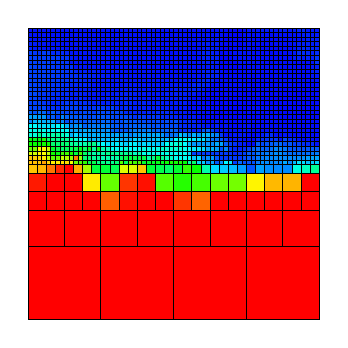
\begin{tikzpicture}[x={(\screenshotunitlength,0)},y={(0,\screenshotunitlength)}]
        \definecolor{fillcolor}{rgb}{1.000000,0.000000,0.000000}
\fill[fillcolor] (0.000000,0.000000) rectangle (0.250000,0.250000);
\definecolor{fillcolor}{rgb}{1.000000,0.000000,0.000000}
\fill[fillcolor] (0.250000,0.000000) rectangle (0.500000,0.250000);
\definecolor{fillcolor}{rgb}{1.000000,0.000000,0.000000}
\fill[fillcolor] (0.000000,0.250000) rectangle (0.125000,0.375000);
\definecolor{fillcolor}{rgb}{1.000000,0.000026,0.000000}
\fill[fillcolor] (0.125000,0.250000) rectangle (0.250000,0.375000);
\definecolor{fillcolor}{rgb}{1.000000,0.000000,0.000000}
\fill[fillcolor] (0.000000,0.375000) rectangle (0.062500,0.437500);
\definecolor{fillcolor}{rgb}{1.000000,0.000009,0.000000}
\fill[fillcolor] (0.062500,0.375000) rectangle (0.125000,0.437500);
\definecolor{fillcolor}{rgb}{1.000000,0.099695,0.000000}
\fill[fillcolor] (0.000000,0.437500) rectangle (0.062500,0.500000);
\definecolor{fillcolor}{rgb}{1.000000,0.000004,0.000000}
\fill[fillcolor] (0.062500,0.437500) rectangle (0.125000,0.500000);
\definecolor{fillcolor}{rgb}{1.000000,0.001789,0.000000}
\fill[fillcolor] (0.125000,0.375000) rectangle (0.187500,0.437500);
\definecolor{fillcolor}{rgb}{1.000000,0.004119,0.000000}
\fill[fillcolor] (0.187500,0.375000) rectangle (0.250000,0.437500);
\definecolor{fillcolor}{rgb}{1.000000,0.001071,0.000000}
\fill[fillcolor] (0.125000,0.437500) rectangle (0.187500,0.500000);
\definecolor{fillcolor}{rgb}{1.000000,0.919639,0.000000}
\fill[fillcolor] (0.187500,0.437500) rectangle (0.250000,0.500000);
\definecolor{fillcolor}{rgb}{1.000000,0.000021,0.000000}
\fill[fillcolor] (0.250000,0.250000) rectangle (0.375000,0.375000);
\definecolor{fillcolor}{rgb}{1.000000,0.000001,0.000000}
\fill[fillcolor] (0.375000,0.250000) rectangle (0.500000,0.375000);
\definecolor{fillcolor}{rgb}{1.000000,0.372629,0.000000}
\fill[fillcolor] (0.250000,0.375000) rectangle (0.312500,0.437500);
\definecolor{fillcolor}{rgb}{1.000000,0.062248,0.000000}
\fill[fillcolor] (0.312500,0.375000) rectangle (0.375000,0.437500);
\definecolor{fillcolor}{rgb}{0.397171,1.000000,0.000000}
\fill[fillcolor] (0.250000,0.437500) rectangle (0.312500,0.500000);
\definecolor{fillcolor}{rgb}{1.000000,0.207507,0.000000}
\fill[fillcolor] (0.312500,0.437500) rectangle (0.375000,0.500000);
\definecolor{fillcolor}{rgb}{1.000000,0.000000,0.000000}
\fill[fillcolor] (0.375000,0.375000) rectangle (0.437500,0.437500);
\definecolor{fillcolor}{rgb}{1.000000,0.000001,0.000000}
\fill[fillcolor] (0.437500,0.375000) rectangle (0.500000,0.437500);
\definecolor{fillcolor}{rgb}{1.000000,0.062226,0.000000}
\fill[fillcolor] (0.375000,0.437500) rectangle (0.437500,0.500000);
\definecolor{fillcolor}{rgb}{0.331646,1.000000,0.000000}
\fill[fillcolor] (0.437500,0.437500) rectangle (0.500000,0.500000);
\definecolor{fillcolor}{rgb}{1.000000,0.000000,0.000000}
\fill[fillcolor] (0.500000,0.000000) rectangle (0.750000,0.250000);
\definecolor{fillcolor}{rgb}{1.000000,0.000000,0.000000}
\fill[fillcolor] (0.750000,0.000000) rectangle (1.000000,0.250000);
\definecolor{fillcolor}{rgb}{1.000000,0.000001,0.000000}
\fill[fillcolor] (0.500000,0.250000) rectangle (0.625000,0.375000);
\definecolor{fillcolor}{rgb}{1.000000,0.000000,0.000000}
\fill[fillcolor] (0.625000,0.250000) rectangle (0.750000,0.375000);
\definecolor{fillcolor}{rgb}{1.000000,0.213317,0.000000}
\fill[fillcolor] (0.500000,0.375000) rectangle (0.562500,0.437500);
\definecolor{fillcolor}{rgb}{1.000000,0.393808,0.000000}
\fill[fillcolor] (0.562500,0.375000) rectangle (0.625000,0.437500);
\definecolor{fillcolor}{rgb}{0.146696,1.000000,0.000000}
\fill[fillcolor] (0.500000,0.437500) rectangle (0.562500,0.500000);
\definecolor{fillcolor}{rgb}{0.269952,1.000000,0.000000}
\fill[fillcolor] (0.562500,0.437500) rectangle (0.625000,0.500000);
\definecolor{fillcolor}{rgb}{1.000000,0.000000,0.000000}
\fill[fillcolor] (0.625000,0.375000) rectangle (0.687500,0.437500);
\definecolor{fillcolor}{rgb}{1.000000,0.000000,0.000000}
\fill[fillcolor] (0.687500,0.375000) rectangle (0.750000,0.437500);
\definecolor{fillcolor}{rgb}{0.419932,1.000000,0.000000}
\fill[fillcolor] (0.625000,0.437500) rectangle (0.687500,0.500000);
\definecolor{fillcolor}{rgb}{0.456513,1.000000,0.000000}
\fill[fillcolor] (0.687500,0.437500) rectangle (0.750000,0.500000);
\definecolor{fillcolor}{rgb}{1.000000,0.000000,0.000000}
\fill[fillcolor] (0.750000,0.250000) rectangle (0.875000,0.375000);
\definecolor{fillcolor}{rgb}{1.000000,0.000152,0.000000}
\fill[fillcolor] (0.875000,0.250000) rectangle (1.000000,0.375000);
\definecolor{fillcolor}{rgb}{1.000000,0.000000,0.000000}
\fill[fillcolor] (0.750000,0.375000) rectangle (0.812500,0.437500);
\definecolor{fillcolor}{rgb}{1.000000,0.000000,0.000000}
\fill[fillcolor] (0.812500,0.375000) rectangle (0.875000,0.437500);
\definecolor{fillcolor}{rgb}{1.000000,0.958939,0.000000}
\fill[fillcolor] (0.750000,0.437500) rectangle (0.812500,0.500000);
\definecolor{fillcolor}{rgb}{1.000000,0.727450,0.000000}
\fill[fillcolor] (0.812500,0.437500) rectangle (0.875000,0.500000);
\definecolor{fillcolor}{rgb}{1.000000,0.000067,0.000000}
\fill[fillcolor] (0.875000,0.375000) rectangle (0.937500,0.437500);
\definecolor{fillcolor}{rgb}{1.000000,0.000235,0.000000}
\fill[fillcolor] (0.937500,0.375000) rectangle (1.000000,0.437500);
\definecolor{fillcolor}{rgb}{1.000000,0.705648,0.000000}
\fill[fillcolor] (0.875000,0.437500) rectangle (0.937500,0.500000);
\definecolor{fillcolor}{rgb}{1.000000,0.000000,0.000000}
\fill[fillcolor] (0.937500,0.437500) rectangle (1.000000,0.500000);
\definecolor{fillcolor}{rgb}{1.000000,0.771290,0.000000}
\fill[fillcolor] (0.000000,0.500000) rectangle (0.031250,0.531250);
\definecolor{fillcolor}{rgb}{1.000000,0.716967,0.000000}
\fill[fillcolor] (0.031250,0.500000) rectangle (0.062500,0.531250);
\definecolor{fillcolor}{rgb}{1.000000,0.752855,0.000000}
\fill[fillcolor] (0.000000,0.531250) rectangle (0.015625,0.546875);
\definecolor{fillcolor}{rgb}{1.000000,0.756200,0.000000}
\fill[fillcolor] (0.015625,0.531250) rectangle (0.031250,0.546875);
\definecolor{fillcolor}{rgb}{1.000000,0.768820,0.000000}
\fill[fillcolor] (0.000000,0.546875) rectangle (0.015625,0.562500);
\definecolor{fillcolor}{rgb}{1.000000,0.806914,0.000000}
\fill[fillcolor] (0.015625,0.546875) rectangle (0.031250,0.562500);
\definecolor{fillcolor}{rgb}{1.000000,0.777118,0.000000}
\fill[fillcolor] (0.031250,0.531250) rectangle (0.046875,0.546875);
\definecolor{fillcolor}{rgb}{1.000000,0.633944,0.000000}
\fill[fillcolor] (0.046875,0.531250) rectangle (0.062500,0.546875);
\definecolor{fillcolor}{rgb}{1.000000,0.848366,0.000000}
\fill[fillcolor] (0.031250,0.546875) rectangle (0.046875,0.562500);
\definecolor{fillcolor}{rgb}{1.000000,0.921060,0.000000}
\fill[fillcolor] (0.046875,0.546875) rectangle (0.062500,0.562500);
\definecolor{fillcolor}{rgb}{1.000000,0.453767,0.000000}
\fill[fillcolor] (0.062500,0.500000) rectangle (0.093750,0.531250);
\definecolor{fillcolor}{rgb}{1.000000,0.160000,0.000000}
\fill[fillcolor] (0.093750,0.500000) rectangle (0.125000,0.531250);
\definecolor{fillcolor}{rgb}{1.000000,0.840782,0.000000}
\fill[fillcolor] (0.062500,0.531250) rectangle (0.078125,0.546875);
\definecolor{fillcolor}{rgb}{1.000000,0.936795,0.000000}
\fill[fillcolor] (0.078125,0.531250) rectangle (0.093750,0.546875);
\definecolor{fillcolor}{rgb}{0.746885,1.000000,0.000000}
\fill[fillcolor] (0.062500,0.546875) rectangle (0.078125,0.562500);
\definecolor{fillcolor}{rgb}{0.354571,1.000000,0.000000}
\fill[fillcolor] (0.078125,0.546875) rectangle (0.093750,0.562500);
\definecolor{fillcolor}{rgb}{1.000000,0.935679,0.000000}
\fill[fillcolor] (0.093750,0.531250) rectangle (0.109375,0.546875);
\definecolor{fillcolor}{rgb}{1.000000,0.875764,0.000000}
\fill[fillcolor] (0.109375,0.531250) rectangle (0.125000,0.546875);
\definecolor{fillcolor}{rgb}{0.355603,1.000000,0.000000}
\fill[fillcolor] (0.093750,0.546875) rectangle (0.109375,0.562500);
\definecolor{fillcolor}{rgb}{0.779135,1.000000,0.000000}
\fill[fillcolor] (0.109375,0.546875) rectangle (0.125000,0.562500);
\definecolor{fillcolor}{rgb}{0.824243,1.000000,0.000000}
\fill[fillcolor] (0.000000,0.562500) rectangle (0.015625,0.578125);
\definecolor{fillcolor}{rgb}{0.823849,1.000000,0.000000}
\fill[fillcolor] (0.015625,0.562500) rectangle (0.031250,0.578125);
\definecolor{fillcolor}{rgb}{0.381072,1.000000,0.000000}
\fill[fillcolor] (0.000000,0.578125) rectangle (0.015625,0.593750);
\definecolor{fillcolor}{rgb}{0.468014,1.000000,0.000000}
\fill[fillcolor] (0.015625,0.578125) rectangle (0.031250,0.593750);
\definecolor{fillcolor}{rgb}{1.000000,0.991770,0.000000}
\fill[fillcolor] (0.031250,0.562500) rectangle (0.046875,0.578125);
\definecolor{fillcolor}{rgb}{0.989446,1.000000,0.000000}
\fill[fillcolor] (0.046875,0.562500) rectangle (0.062500,0.578125);
\definecolor{fillcolor}{rgb}{0.980943,1.000000,0.000000}
\fill[fillcolor] (0.031250,0.578125) rectangle (0.046875,0.593750);
\definecolor{fillcolor}{rgb}{1.000000,0.983003,0.000000}
\fill[fillcolor] (0.046875,0.578125) rectangle (0.062500,0.593750);
\definecolor{fillcolor}{rgb}{0.028513,1.000000,0.000000}
\fill[fillcolor] (0.000000,0.593750) rectangle (0.015625,0.609375);
\definecolor{fillcolor}{rgb}{0.017148,1.000000,0.000000}
\fill[fillcolor] (0.015625,0.593750) rectangle (0.031250,0.609375);
\definecolor{fillcolor}{rgb}{0.028513,1.000000,0.000000}
\fill[fillcolor] (0.000000,0.609375) rectangle (0.015625,0.625000);
\definecolor{fillcolor}{rgb}{0.000000,1.000000,0.097025}
\fill[fillcolor] (0.015625,0.609375) rectangle (0.031250,0.625000);
\definecolor{fillcolor}{rgb}{0.015251,1.000000,0.000000}
\fill[fillcolor] (0.031250,0.593750) rectangle (0.046875,0.609375);
\definecolor{fillcolor}{rgb}{0.045422,1.000000,0.000000}
\fill[fillcolor] (0.046875,0.593750) rectangle (0.062500,0.609375);
\definecolor{fillcolor}{rgb}{0.000000,1.000000,0.096979}
\fill[fillcolor] (0.031250,0.609375) rectangle (0.046875,0.625000);
\definecolor{fillcolor}{rgb}{0.080123,1.000000,0.000000}
\fill[fillcolor] (0.046875,0.609375) rectangle (0.062500,0.625000);
\definecolor{fillcolor}{rgb}{0.748733,1.000000,0.000000}
\fill[fillcolor] (0.062500,0.562500) rectangle (0.078125,0.578125);
\definecolor{fillcolor}{rgb}{0.049356,1.000000,0.000000}
\fill[fillcolor] (0.078125,0.562500) rectangle (0.093750,0.578125);
\definecolor{fillcolor}{rgb}{0.781382,1.000000,0.000000}
\fill[fillcolor] (0.062500,0.578125) rectangle (0.078125,0.593750);
\definecolor{fillcolor}{rgb}{0.000000,1.000000,0.159344}
\fill[fillcolor] (0.078125,0.578125) rectangle (0.093750,0.593750);
\definecolor{fillcolor}{rgb}{0.000000,1.000000,0.072145}
\fill[fillcolor] (0.093750,0.562500) rectangle (0.109375,0.578125);
\definecolor{fillcolor}{rgb}{0.244540,1.000000,0.000000}
\fill[fillcolor] (0.109375,0.562500) rectangle (0.125000,0.578125);
\definecolor{fillcolor}{rgb}{0.000000,1.000000,0.269546}
\fill[fillcolor] (0.093750,0.578125) rectangle (0.109375,0.593750);
\definecolor{fillcolor}{rgb}{0.000000,1.000000,0.429709}
\fill[fillcolor] (0.109375,0.578125) rectangle (0.125000,0.593750);
\definecolor{fillcolor}{rgb}{0.045506,1.000000,0.000000}
\fill[fillcolor] (0.062500,0.593750) rectangle (0.078125,0.609375);
\definecolor{fillcolor}{rgb}{0.000000,1.000000,0.423733}
\fill[fillcolor] (0.078125,0.593750) rectangle (0.093750,0.609375);
\definecolor{fillcolor}{rgb}{0.000000,1.000000,0.409849}
\fill[fillcolor] (0.062500,0.609375) rectangle (0.078125,0.625000);
\definecolor{fillcolor}{rgb}{0.000000,1.000000,0.525163}
\fill[fillcolor] (0.078125,0.609375) rectangle (0.093750,0.625000);
\definecolor{fillcolor}{rgb}{0.000000,1.000000,0.437916}
\fill[fillcolor] (0.093750,0.593750) rectangle (0.109375,0.609375);
\definecolor{fillcolor}{rgb}{0.000000,1.000000,0.432218}
\fill[fillcolor] (0.109375,0.593750) rectangle (0.125000,0.609375);
\definecolor{fillcolor}{rgb}{0.000000,1.000000,0.557741}
\fill[fillcolor] (0.093750,0.609375) rectangle (0.109375,0.625000);
\definecolor{fillcolor}{rgb}{0.000000,1.000000,0.573526}
\fill[fillcolor] (0.109375,0.609375) rectangle (0.125000,0.625000);
\definecolor{fillcolor}{rgb}{1.000000,0.000812,0.000000}
\fill[fillcolor] (0.125000,0.500000) rectangle (0.156250,0.531250);
\definecolor{fillcolor}{rgb}{1.000000,0.680018,0.000000}
\fill[fillcolor] (0.156250,0.500000) rectangle (0.187500,0.531250);
\definecolor{fillcolor}{rgb}{1.000000,0.860274,0.000000}
\fill[fillcolor] (0.125000,0.531250) rectangle (0.140625,0.546875);
\definecolor{fillcolor}{rgb}{0.955054,1.000000,0.000000}
\fill[fillcolor] (0.140625,0.531250) rectangle (0.156250,0.546875);
\definecolor{fillcolor}{rgb}{0.672406,1.000000,0.000000}
\fill[fillcolor] (0.125000,0.546875) rectangle (0.140625,0.562500);
\definecolor{fillcolor}{rgb}{0.555187,1.000000,0.000000}
\fill[fillcolor] (0.140625,0.546875) rectangle (0.156250,0.562500);
\definecolor{fillcolor}{rgb}{0.400292,1.000000,0.000000}
\fill[fillcolor] (0.156250,0.531250) rectangle (0.171875,0.546875);
\definecolor{fillcolor}{rgb}{0.300805,1.000000,0.000000}
\fill[fillcolor] (0.171875,0.531250) rectangle (0.187500,0.546875);
\definecolor{fillcolor}{rgb}{1.000000,0.467752,0.000000}
\fill[fillcolor] (0.156250,0.546875) rectangle (0.171875,0.562500);
\definecolor{fillcolor}{rgb}{0.567416,1.000000,0.000000}
\fill[fillcolor] (0.171875,0.546875) rectangle (0.187500,0.562500);
\definecolor{fillcolor}{rgb}{0.638645,1.000000,0.000000}
\fill[fillcolor] (0.187500,0.500000) rectangle (0.218750,0.531250);
\definecolor{fillcolor}{rgb}{0.000000,1.000000,0.233162}
\fill[fillcolor] (0.218750,0.500000) rectangle (0.250000,0.531250);
\definecolor{fillcolor}{rgb}{0.175956,1.000000,0.000000}
\fill[fillcolor] (0.187500,0.531250) rectangle (0.203125,0.546875);
\definecolor{fillcolor}{rgb}{0.000000,1.000000,0.298749}
\fill[fillcolor] (0.203125,0.531250) rectangle (0.218750,0.546875);
\definecolor{fillcolor}{rgb}{0.000000,1.000000,0.432526}
\fill[fillcolor] (0.187500,0.546875) rectangle (0.203125,0.562500);
\definecolor{fillcolor}{rgb}{0.000000,1.000000,0.442859}
\fill[fillcolor] (0.203125,0.546875) rectangle (0.218750,0.562500);
\definecolor{fillcolor}{rgb}{0.000000,1.000000,0.299117}
\fill[fillcolor] (0.218750,0.531250) rectangle (0.234375,0.546875);
\definecolor{fillcolor}{rgb}{0.000000,1.000000,0.507708}
\fill[fillcolor] (0.234375,0.531250) rectangle (0.250000,0.546875);
\definecolor{fillcolor}{rgb}{0.000000,1.000000,0.592427}
\fill[fillcolor] (0.218750,0.546875) rectangle (0.234375,0.562500);
\definecolor{fillcolor}{rgb}{0.000000,1.000000,0.569625}
\fill[fillcolor] (0.234375,0.546875) rectangle (0.250000,0.562500);
\definecolor{fillcolor}{rgb}{0.244060,1.000000,0.000000}
\fill[fillcolor] (0.125000,0.562500) rectangle (0.140625,0.578125);
\definecolor{fillcolor}{rgb}{0.078441,1.000000,0.000000}
\fill[fillcolor] (0.140625,0.562500) rectangle (0.156250,0.578125);
\definecolor{fillcolor}{rgb}{0.000000,1.000000,0.345414}
\fill[fillcolor] (0.125000,0.578125) rectangle (0.140625,0.593750);
\definecolor{fillcolor}{rgb}{0.000000,1.000000,0.341319}
\fill[fillcolor] (0.140625,0.578125) rectangle (0.156250,0.593750);
\definecolor{fillcolor}{rgb}{0.000000,1.000000,0.255867}
\fill[fillcolor] (0.156250,0.562500) rectangle (0.171875,0.578125);
\definecolor{fillcolor}{rgb}{0.239294,1.000000,0.000000}
\fill[fillcolor] (0.171875,0.562500) rectangle (0.187500,0.578125);
\definecolor{fillcolor}{rgb}{0.000000,1.000000,0.261737}
\fill[fillcolor] (0.156250,0.578125) rectangle (0.171875,0.593750);
\definecolor{fillcolor}{rgb}{0.000000,1.000000,0.114310}
\fill[fillcolor] (0.171875,0.578125) rectangle (0.187500,0.593750);
\definecolor{fillcolor}{rgb}{0.000000,1.000000,0.441339}
\fill[fillcolor] (0.125000,0.593750) rectangle (0.140625,0.609375);
\definecolor{fillcolor}{rgb}{0.000000,1.000000,0.601318}
\fill[fillcolor] (0.140625,0.593750) rectangle (0.156250,0.609375);
\definecolor{fillcolor}{rgb}{0.000000,1.000000,0.576806}
\fill[fillcolor] (0.125000,0.609375) rectangle (0.140625,0.625000);
\definecolor{fillcolor}{rgb}{0.000000,1.000000,0.698023}
\fill[fillcolor] (0.140625,0.609375) rectangle (0.156250,0.625000);
\definecolor{fillcolor}{rgb}{0.000000,1.000000,0.608272}
\fill[fillcolor] (0.156250,0.593750) rectangle (0.171875,0.609375);
\definecolor{fillcolor}{rgb}{0.000000,1.000000,0.761218}
\fill[fillcolor] (0.171875,0.593750) rectangle (0.187500,0.609375);
\definecolor{fillcolor}{rgb}{0.000000,1.000000,0.856168}
\fill[fillcolor] (0.156250,0.609375) rectangle (0.171875,0.625000);
\definecolor{fillcolor}{rgb}{0.000000,0.985193,1.000000}
\fill[fillcolor] (0.171875,0.609375) rectangle (0.187500,0.625000);
\definecolor{fillcolor}{rgb}{0.000000,1.000000,0.375769}
\fill[fillcolor] (0.187500,0.562500) rectangle (0.203125,0.578125);
\definecolor{fillcolor}{rgb}{0.000000,1.000000,0.550890}
\fill[fillcolor] (0.203125,0.562500) rectangle (0.218750,0.578125);
\definecolor{fillcolor}{rgb}{0.000000,1.000000,0.396852}
\fill[fillcolor] (0.187500,0.578125) rectangle (0.203125,0.593750);
\definecolor{fillcolor}{rgb}{0.000000,1.000000,0.133622}
\fill[fillcolor] (0.203125,0.578125) rectangle (0.218750,0.593750);
\definecolor{fillcolor}{rgb}{0.000000,1.000000,0.643233}
\fill[fillcolor] (0.218750,0.562500) rectangle (0.234375,0.578125);
\definecolor{fillcolor}{rgb}{0.000000,1.000000,0.632655}
\fill[fillcolor] (0.234375,0.562500) rectangle (0.250000,0.578125);
\definecolor{fillcolor}{rgb}{0.000000,1.000000,0.640436}
\fill[fillcolor] (0.218750,0.578125) rectangle (0.234375,0.593750);
\definecolor{fillcolor}{rgb}{0.000000,1.000000,0.134647}
\fill[fillcolor] (0.234375,0.578125) rectangle (0.250000,0.593750);
\definecolor{fillcolor}{rgb}{0.000000,1.000000,0.665898}
\fill[fillcolor] (0.187500,0.593750) rectangle (0.203125,0.609375);
\definecolor{fillcolor}{rgb}{0.000000,1.000000,0.560506}
\fill[fillcolor] (0.203125,0.593750) rectangle (0.218750,0.609375);
\definecolor{fillcolor}{rgb}{0.000000,0.985411,1.000000}
\fill[fillcolor] (0.187500,0.609375) rectangle (0.203125,0.625000);
\definecolor{fillcolor}{rgb}{0.000000,0.665178,1.000000}
\fill[fillcolor] (0.203125,0.609375) rectangle (0.218750,0.625000);
\definecolor{fillcolor}{rgb}{0.000000,1.000000,0.535658}
\fill[fillcolor] (0.218750,0.593750) rectangle (0.234375,0.609375);
\definecolor{fillcolor}{rgb}{0.000000,1.000000,0.832501}
\fill[fillcolor] (0.234375,0.593750) rectangle (0.250000,0.609375);
\definecolor{fillcolor}{rgb}{0.000000,0.718016,1.000000}
\fill[fillcolor] (0.218750,0.609375) rectangle (0.234375,0.625000);
\definecolor{fillcolor}{rgb}{0.000000,0.719646,1.000000}
\fill[fillcolor] (0.234375,0.609375) rectangle (0.250000,0.625000);
\definecolor{fillcolor}{rgb}{0.000000,1.000000,0.851020}
\fill[fillcolor] (0.000000,0.625000) rectangle (0.015625,0.640625);
\definecolor{fillcolor}{rgb}{0.000000,1.000000,0.858717}
\fill[fillcolor] (0.015625,0.625000) rectangle (0.031250,0.640625);
\definecolor{fillcolor}{rgb}{0.000000,1.000000,0.940155}
\fill[fillcolor] (0.000000,0.640625) rectangle (0.015625,0.656250);
\definecolor{fillcolor}{rgb}{0.000000,1.000000,0.940292}
\fill[fillcolor] (0.015625,0.640625) rectangle (0.031250,0.656250);
\definecolor{fillcolor}{rgb}{0.000000,1.000000,0.560249}
\fill[fillcolor] (0.031250,0.625000) rectangle (0.046875,0.640625);
\definecolor{fillcolor}{rgb}{0.000000,1.000000,0.840867}
\fill[fillcolor] (0.046875,0.625000) rectangle (0.062500,0.640625);
\definecolor{fillcolor}{rgb}{0.000000,1.000000,0.882223}
\fill[fillcolor] (0.031250,0.640625) rectangle (0.046875,0.656250);
\definecolor{fillcolor}{rgb}{0.000000,1.000000,0.926935}
\fill[fillcolor] (0.046875,0.640625) rectangle (0.062500,0.656250);
\definecolor{fillcolor}{rgb}{0.000000,0.999801,1.000000}
\fill[fillcolor] (0.000000,0.656250) rectangle (0.015625,0.671875);
\definecolor{fillcolor}{rgb}{0.000000,0.999394,1.000000}
\fill[fillcolor] (0.015625,0.656250) rectangle (0.031250,0.671875);
\definecolor{fillcolor}{rgb}{0.000000,0.506139,1.000000}
\fill[fillcolor] (0.000000,0.671875) rectangle (0.015625,0.687500);
\definecolor{fillcolor}{rgb}{0.000000,0.693788,1.000000}
\fill[fillcolor] (0.015625,0.671875) rectangle (0.031250,0.687500);
\definecolor{fillcolor}{rgb}{0.000000,0.877600,1.000000}
\fill[fillcolor] (0.031250,0.656250) rectangle (0.046875,0.671875);
\definecolor{fillcolor}{rgb}{0.000000,0.871535,1.000000}
\fill[fillcolor] (0.046875,0.656250) rectangle (0.062500,0.671875);
\definecolor{fillcolor}{rgb}{0.000000,0.768168,1.000000}
\fill[fillcolor] (0.031250,0.671875) rectangle (0.046875,0.687500);
\definecolor{fillcolor}{rgb}{0.000000,0.679769,1.000000}
\fill[fillcolor] (0.046875,0.671875) rectangle (0.062500,0.687500);
\definecolor{fillcolor}{rgb}{0.000000,1.000000,0.698650}
\fill[fillcolor] (0.062500,0.625000) rectangle (0.078125,0.640625);
\definecolor{fillcolor}{rgb}{0.000000,1.000000,0.685243}
\fill[fillcolor] (0.078125,0.625000) rectangle (0.093750,0.640625);
\definecolor{fillcolor}{rgb}{0.000000,0.933311,1.000000}
\fill[fillcolor] (0.062500,0.640625) rectangle (0.078125,0.656250);
\definecolor{fillcolor}{rgb}{0.000000,1.000000,0.966141}
\fill[fillcolor] (0.078125,0.640625) rectangle (0.093750,0.656250);
\definecolor{fillcolor}{rgb}{0.000000,1.000000,0.630223}
\fill[fillcolor] (0.093750,0.625000) rectangle (0.109375,0.640625);
\definecolor{fillcolor}{rgb}{0.000000,1.000000,0.756723}
\fill[fillcolor] (0.109375,0.625000) rectangle (0.125000,0.640625);
\definecolor{fillcolor}{rgb}{0.000000,1.000000,0.979721}
\fill[fillcolor] (0.093750,0.640625) rectangle (0.109375,0.656250);
\definecolor{fillcolor}{rgb}{0.000000,0.996015,1.000000}
\fill[fillcolor] (0.109375,0.640625) rectangle (0.125000,0.656250);
\definecolor{fillcolor}{rgb}{0.000000,0.873371,1.000000}
\fill[fillcolor] (0.062500,0.656250) rectangle (0.078125,0.671875);
\definecolor{fillcolor}{rgb}{0.000000,0.878834,1.000000}
\fill[fillcolor] (0.078125,0.656250) rectangle (0.093750,0.671875);
\definecolor{fillcolor}{rgb}{0.000000,0.663495,1.000000}
\fill[fillcolor] (0.062500,0.671875) rectangle (0.078125,0.687500);
\definecolor{fillcolor}{rgb}{0.000000,0.663336,1.000000}
\fill[fillcolor] (0.078125,0.671875) rectangle (0.093750,0.687500);
\definecolor{fillcolor}{rgb}{0.000000,0.984834,1.000000}
\fill[fillcolor] (0.093750,0.656250) rectangle (0.109375,0.671875);
\definecolor{fillcolor}{rgb}{0.000000,0.923975,1.000000}
\fill[fillcolor] (0.109375,0.656250) rectangle (0.125000,0.671875);
\definecolor{fillcolor}{rgb}{0.000000,0.399931,1.000000}
\fill[fillcolor] (0.093750,0.671875) rectangle (0.109375,0.687500);
\definecolor{fillcolor}{rgb}{0.000000,0.517815,1.000000}
\fill[fillcolor] (0.109375,0.671875) rectangle (0.125000,0.687500);
\definecolor{fillcolor}{rgb}{0.000000,0.621851,1.000000}
\fill[fillcolor] (0.000000,0.687500) rectangle (0.015625,0.703125);
\definecolor{fillcolor}{rgb}{0.000000,0.633177,1.000000}
\fill[fillcolor] (0.015625,0.687500) rectangle (0.031250,0.703125);
\definecolor{fillcolor}{rgb}{0.000000,0.371086,1.000000}
\fill[fillcolor] (0.000000,0.703125) rectangle (0.015625,0.718750);
\definecolor{fillcolor}{rgb}{0.000000,0.321934,1.000000}
\fill[fillcolor] (0.015625,0.703125) rectangle (0.031250,0.718750);
\definecolor{fillcolor}{rgb}{0.000000,0.610079,1.000000}
\fill[fillcolor] (0.031250,0.687500) rectangle (0.046875,0.703125);
\definecolor{fillcolor}{rgb}{0.000000,0.579639,1.000000}
\fill[fillcolor] (0.046875,0.687500) rectangle (0.062500,0.703125);
\definecolor{fillcolor}{rgb}{0.000000,0.433915,1.000000}
\fill[fillcolor] (0.031250,0.703125) rectangle (0.046875,0.718750);
\definecolor{fillcolor}{rgb}{0.000000,0.391500,1.000000}
\fill[fillcolor] (0.046875,0.703125) rectangle (0.062500,0.718750);
\definecolor{fillcolor}{rgb}{0.000000,0.268017,1.000000}
\fill[fillcolor] (0.000000,0.718750) rectangle (0.015625,0.734375);
\definecolor{fillcolor}{rgb}{0.000000,0.268610,1.000000}
\fill[fillcolor] (0.015625,0.718750) rectangle (0.031250,0.734375);
\definecolor{fillcolor}{rgb}{0.000000,0.247228,1.000000}
\fill[fillcolor] (0.000000,0.734375) rectangle (0.015625,0.750000);
\definecolor{fillcolor}{rgb}{0.000000,0.250353,1.000000}
\fill[fillcolor] (0.015625,0.734375) rectangle (0.031250,0.750000);
\definecolor{fillcolor}{rgb}{0.000000,0.255450,1.000000}
\fill[fillcolor] (0.031250,0.718750) rectangle (0.046875,0.734375);
\definecolor{fillcolor}{rgb}{0.000000,0.283386,1.000000}
\fill[fillcolor] (0.046875,0.718750) rectangle (0.062500,0.734375);
\definecolor{fillcolor}{rgb}{0.000000,0.253352,1.000000}
\fill[fillcolor] (0.031250,0.734375) rectangle (0.046875,0.750000);
\definecolor{fillcolor}{rgb}{0.000000,0.209402,1.000000}
\fill[fillcolor] (0.046875,0.734375) rectangle (0.062500,0.750000);
\definecolor{fillcolor}{rgb}{0.000000,0.340362,1.000000}
\fill[fillcolor] (0.062500,0.687500) rectangle (0.078125,0.703125);
\definecolor{fillcolor}{rgb}{0.000000,0.357565,1.000000}
\fill[fillcolor] (0.078125,0.687500) rectangle (0.093750,0.703125);
\definecolor{fillcolor}{rgb}{0.000000,0.257762,1.000000}
\fill[fillcolor] (0.062500,0.703125) rectangle (0.078125,0.718750);
\definecolor{fillcolor}{rgb}{0.000000,0.360507,1.000000}
\fill[fillcolor] (0.078125,0.703125) rectangle (0.093750,0.718750);
\definecolor{fillcolor}{rgb}{0.000000,0.261865,1.000000}
\fill[fillcolor] (0.093750,0.687500) rectangle (0.109375,0.703125);
\definecolor{fillcolor}{rgb}{0.000000,0.517874,1.000000}
\fill[fillcolor] (0.109375,0.687500) rectangle (0.125000,0.703125);
\definecolor{fillcolor}{rgb}{0.000000,0.301551,1.000000}
\fill[fillcolor] (0.093750,0.703125) rectangle (0.109375,0.718750);
\definecolor{fillcolor}{rgb}{0.000000,0.295430,1.000000}
\fill[fillcolor] (0.109375,0.703125) rectangle (0.125000,0.718750);
\definecolor{fillcolor}{rgb}{0.000000,0.177674,1.000000}
\fill[fillcolor] (0.062500,0.718750) rectangle (0.078125,0.734375);
\definecolor{fillcolor}{rgb}{0.000000,0.197593,1.000000}
\fill[fillcolor] (0.078125,0.718750) rectangle (0.093750,0.734375);
\definecolor{fillcolor}{rgb}{0.000000,0.177962,1.000000}
\fill[fillcolor] (0.062500,0.734375) rectangle (0.078125,0.750000);
\definecolor{fillcolor}{rgb}{0.000000,0.157010,1.000000}
\fill[fillcolor] (0.078125,0.734375) rectangle (0.093750,0.750000);
\definecolor{fillcolor}{rgb}{0.000000,0.165039,1.000000}
\fill[fillcolor] (0.093750,0.718750) rectangle (0.109375,0.734375);
\definecolor{fillcolor}{rgb}{0.000000,0.242637,1.000000}
\fill[fillcolor] (0.109375,0.718750) rectangle (0.125000,0.734375);
\definecolor{fillcolor}{rgb}{0.000000,0.151919,1.000000}
\fill[fillcolor] (0.093750,0.734375) rectangle (0.109375,0.750000);
\definecolor{fillcolor}{rgb}{0.000000,0.182872,1.000000}
\fill[fillcolor] (0.109375,0.734375) rectangle (0.125000,0.750000);
\definecolor{fillcolor}{rgb}{0.000000,1.000000,0.852002}
\fill[fillcolor] (0.125000,0.625000) rectangle (0.140625,0.640625);
\definecolor{fillcolor}{rgb}{0.000000,0.710465,1.000000}
\fill[fillcolor] (0.140625,0.625000) rectangle (0.156250,0.640625);
\definecolor{fillcolor}{rgb}{0.000000,0.985774,1.000000}
\fill[fillcolor] (0.125000,0.640625) rectangle (0.140625,0.656250);
\definecolor{fillcolor}{rgb}{0.000000,0.659145,1.000000}
\fill[fillcolor] (0.140625,0.640625) rectangle (0.156250,0.656250);
\definecolor{fillcolor}{rgb}{0.000000,0.855745,1.000000}
\fill[fillcolor] (0.156250,0.625000) rectangle (0.171875,0.640625);
\definecolor{fillcolor}{rgb}{0.000000,0.720432,1.000000}
\fill[fillcolor] (0.171875,0.625000) rectangle (0.187500,0.640625);
\definecolor{fillcolor}{rgb}{0.000000,0.659384,1.000000}
\fill[fillcolor] (0.156250,0.640625) rectangle (0.171875,0.656250);
\definecolor{fillcolor}{rgb}{0.000000,0.600386,1.000000}
\fill[fillcolor] (0.171875,0.640625) rectangle (0.187500,0.656250);
\definecolor{fillcolor}{rgb}{0.000000,0.724044,1.000000}
\fill[fillcolor] (0.125000,0.656250) rectangle (0.140625,0.671875);
\definecolor{fillcolor}{rgb}{0.000000,0.512758,1.000000}
\fill[fillcolor] (0.140625,0.656250) rectangle (0.156250,0.671875);
\definecolor{fillcolor}{rgb}{0.000000,0.302744,1.000000}
\fill[fillcolor] (0.125000,0.671875) rectangle (0.140625,0.687500);
\definecolor{fillcolor}{rgb}{0.000000,0.393537,1.000000}
\fill[fillcolor] (0.140625,0.671875) rectangle (0.156250,0.687500);
\definecolor{fillcolor}{rgb}{0.000000,0.578156,1.000000}
\fill[fillcolor] (0.156250,0.656250) rectangle (0.171875,0.671875);
\definecolor{fillcolor}{rgb}{0.000000,0.600393,1.000000}
\fill[fillcolor] (0.171875,0.656250) rectangle (0.187500,0.671875);
\definecolor{fillcolor}{rgb}{0.000000,0.427887,1.000000}
\fill[fillcolor] (0.156250,0.671875) rectangle (0.171875,0.687500);
\definecolor{fillcolor}{rgb}{0.000000,0.333715,1.000000}
\fill[fillcolor] (0.171875,0.671875) rectangle (0.187500,0.687500);
\definecolor{fillcolor}{rgb}{0.000000,0.716796,1.000000}
\fill[fillcolor] (0.187500,0.625000) rectangle (0.203125,0.640625);
\definecolor{fillcolor}{rgb}{0.000000,0.684457,1.000000}
\fill[fillcolor] (0.203125,0.625000) rectangle (0.218750,0.640625);
\definecolor{fillcolor}{rgb}{0.000000,0.656714,1.000000}
\fill[fillcolor] (0.187500,0.640625) rectangle (0.203125,0.656250);
\definecolor{fillcolor}{rgb}{0.000000,0.641551,1.000000}
\fill[fillcolor] (0.203125,0.640625) rectangle (0.218750,0.656250);
\definecolor{fillcolor}{rgb}{0.000000,0.675665,1.000000}
\fill[fillcolor] (0.218750,0.625000) rectangle (0.234375,0.640625);
\definecolor{fillcolor}{rgb}{0.000000,0.675734,1.000000}
\fill[fillcolor] (0.234375,0.625000) rectangle (0.250000,0.640625);
\definecolor{fillcolor}{rgb}{0.000000,0.588624,1.000000}
\fill[fillcolor] (0.218750,0.640625) rectangle (0.234375,0.656250);
\definecolor{fillcolor}{rgb}{0.000000,0.544915,1.000000}
\fill[fillcolor] (0.234375,0.640625) rectangle (0.250000,0.656250);
\definecolor{fillcolor}{rgb}{0.000000,0.397420,1.000000}
\fill[fillcolor] (0.187500,0.656250) rectangle (0.203125,0.671875);
\definecolor{fillcolor}{rgb}{0.000000,0.465865,1.000000}
\fill[fillcolor] (0.203125,0.656250) rectangle (0.218750,0.671875);
\definecolor{fillcolor}{rgb}{0.000000,0.338724,1.000000}
\fill[fillcolor] (0.187500,0.671875) rectangle (0.203125,0.687500);
\definecolor{fillcolor}{rgb}{0.000000,0.367426,1.000000}
\fill[fillcolor] (0.203125,0.671875) rectangle (0.218750,0.687500);
\definecolor{fillcolor}{rgb}{0.000000,0.473656,1.000000}
\fill[fillcolor] (0.218750,0.656250) rectangle (0.234375,0.671875);
\definecolor{fillcolor}{rgb}{0.000000,0.473890,1.000000}
\fill[fillcolor] (0.234375,0.656250) rectangle (0.250000,0.671875);
\definecolor{fillcolor}{rgb}{0.000000,0.373310,1.000000}
\fill[fillcolor] (0.218750,0.671875) rectangle (0.234375,0.687500);
\definecolor{fillcolor}{rgb}{0.000000,0.333163,1.000000}
\fill[fillcolor] (0.234375,0.671875) rectangle (0.250000,0.687500);
\definecolor{fillcolor}{rgb}{0.000000,0.405839,1.000000}
\fill[fillcolor] (0.125000,0.687500) rectangle (0.140625,0.703125);
\definecolor{fillcolor}{rgb}{0.000000,0.351396,1.000000}
\fill[fillcolor] (0.140625,0.687500) rectangle (0.156250,0.703125);
\definecolor{fillcolor}{rgb}{0.000000,0.274635,1.000000}
\fill[fillcolor] (0.125000,0.703125) rectangle (0.140625,0.718750);
\definecolor{fillcolor}{rgb}{0.000000,0.293280,1.000000}
\fill[fillcolor] (0.140625,0.703125) rectangle (0.156250,0.718750);
\definecolor{fillcolor}{rgb}{0.000000,0.351234,1.000000}
\fill[fillcolor] (0.156250,0.687500) rectangle (0.171875,0.703125);
\definecolor{fillcolor}{rgb}{0.000000,0.336103,1.000000}
\fill[fillcolor] (0.171875,0.687500) rectangle (0.187500,0.703125);
\definecolor{fillcolor}{rgb}{0.000000,0.257157,1.000000}
\fill[fillcolor] (0.156250,0.703125) rectangle (0.171875,0.718750);
\definecolor{fillcolor}{rgb}{0.000000,0.251387,1.000000}
\fill[fillcolor] (0.171875,0.703125) rectangle (0.187500,0.718750);
\definecolor{fillcolor}{rgb}{0.000000,0.246500,1.000000}
\fill[fillcolor] (0.125000,0.718750) rectangle (0.140625,0.734375);
\definecolor{fillcolor}{rgb}{0.000000,0.247519,1.000000}
\fill[fillcolor] (0.140625,0.718750) rectangle (0.156250,0.734375);
\definecolor{fillcolor}{rgb}{0.000000,0.222049,1.000000}
\fill[fillcolor] (0.125000,0.734375) rectangle (0.140625,0.750000);
\definecolor{fillcolor}{rgb}{0.000000,0.216852,1.000000}
\fill[fillcolor] (0.140625,0.734375) rectangle (0.156250,0.750000);
\definecolor{fillcolor}{rgb}{0.000000,0.257094,1.000000}
\fill[fillcolor] (0.156250,0.718750) rectangle (0.171875,0.734375);
\definecolor{fillcolor}{rgb}{0.000000,0.196816,1.000000}
\fill[fillcolor] (0.171875,0.718750) rectangle (0.187500,0.734375);
\definecolor{fillcolor}{rgb}{0.000000,0.211138,1.000000}
\fill[fillcolor] (0.156250,0.734375) rectangle (0.171875,0.750000);
\definecolor{fillcolor}{rgb}{0.000000,0.176458,1.000000}
\fill[fillcolor] (0.171875,0.734375) rectangle (0.187500,0.750000);
\definecolor{fillcolor}{rgb}{0.000000,0.333796,1.000000}
\fill[fillcolor] (0.187500,0.687500) rectangle (0.203125,0.703125);
\definecolor{fillcolor}{rgb}{0.000000,0.287672,1.000000}
\fill[fillcolor] (0.203125,0.687500) rectangle (0.218750,0.703125);
\definecolor{fillcolor}{rgb}{0.000000,0.275206,1.000000}
\fill[fillcolor] (0.187500,0.703125) rectangle (0.203125,0.718750);
\definecolor{fillcolor}{rgb}{0.000000,0.287512,1.000000}
\fill[fillcolor] (0.203125,0.703125) rectangle (0.218750,0.718750);
\definecolor{fillcolor}{rgb}{0.000000,0.320577,1.000000}
\fill[fillcolor] (0.218750,0.687500) rectangle (0.234375,0.703125);
\definecolor{fillcolor}{rgb}{0.000000,0.326854,1.000000}
\fill[fillcolor] (0.234375,0.687500) rectangle (0.250000,0.703125);
\definecolor{fillcolor}{rgb}{0.000000,0.233060,1.000000}
\fill[fillcolor] (0.218750,0.703125) rectangle (0.234375,0.718750);
\definecolor{fillcolor}{rgb}{0.000000,0.295297,1.000000}
\fill[fillcolor] (0.234375,0.703125) rectangle (0.250000,0.718750);
\definecolor{fillcolor}{rgb}{0.000000,0.233778,1.000000}
\fill[fillcolor] (0.187500,0.718750) rectangle (0.203125,0.734375);
\definecolor{fillcolor}{rgb}{0.000000,0.201061,1.000000}
\fill[fillcolor] (0.203125,0.718750) rectangle (0.218750,0.734375);
\definecolor{fillcolor}{rgb}{0.000000,0.181928,1.000000}
\fill[fillcolor] (0.187500,0.734375) rectangle (0.203125,0.750000);
\definecolor{fillcolor}{rgb}{0.000000,0.159645,1.000000}
\fill[fillcolor] (0.203125,0.734375) rectangle (0.218750,0.750000);
\definecolor{fillcolor}{rgb}{0.000000,0.208646,1.000000}
\fill[fillcolor] (0.218750,0.718750) rectangle (0.234375,0.734375);
\definecolor{fillcolor}{rgb}{0.000000,0.231528,1.000000}
\fill[fillcolor] (0.234375,0.718750) rectangle (0.250000,0.734375);
\definecolor{fillcolor}{rgb}{0.000000,0.126956,1.000000}
\fill[fillcolor] (0.218750,0.734375) rectangle (0.234375,0.750000);
\definecolor{fillcolor}{rgb}{0.000000,0.128746,1.000000}
\fill[fillcolor] (0.234375,0.734375) rectangle (0.250000,0.750000);
\definecolor{fillcolor}{rgb}{0.000000,1.000000,0.214817}
\fill[fillcolor] (0.250000,0.500000) rectangle (0.281250,0.531250);
\definecolor{fillcolor}{rgb}{0.000000,1.000000,0.327882}
\fill[fillcolor] (0.281250,0.500000) rectangle (0.312500,0.531250);
\definecolor{fillcolor}{rgb}{0.000000,1.000000,0.520777}
\fill[fillcolor] (0.250000,0.531250) rectangle (0.265625,0.546875);
\definecolor{fillcolor}{rgb}{0.000000,1.000000,0.554692}
\fill[fillcolor] (0.265625,0.531250) rectangle (0.281250,0.546875);
\definecolor{fillcolor}{rgb}{0.000000,1.000000,0.707616}
\fill[fillcolor] (0.250000,0.546875) rectangle (0.265625,0.562500);
\definecolor{fillcolor}{rgb}{0.000000,1.000000,0.648192}
\fill[fillcolor] (0.265625,0.546875) rectangle (0.281250,0.562500);
\definecolor{fillcolor}{rgb}{0.000000,1.000000,0.538641}
\fill[fillcolor] (0.281250,0.531250) rectangle (0.296875,0.546875);
\definecolor{fillcolor}{rgb}{0.000000,1.000000,0.439540}
\fill[fillcolor] (0.296875,0.531250) rectangle (0.312500,0.546875);
\definecolor{fillcolor}{rgb}{0.000000,1.000000,0.705235}
\fill[fillcolor] (0.281250,0.546875) rectangle (0.296875,0.562500);
\definecolor{fillcolor}{rgb}{0.000000,1.000000,0.632862}
\fill[fillcolor] (0.296875,0.546875) rectangle (0.312500,0.562500);
\definecolor{fillcolor}{rgb}{0.870069,1.000000,0.000000}
\fill[fillcolor] (0.312500,0.500000) rectangle (0.343750,0.531250);
\definecolor{fillcolor}{rgb}{0.862783,1.000000,0.000000}
\fill[fillcolor] (0.343750,0.500000) rectangle (0.375000,0.531250);
\definecolor{fillcolor}{rgb}{0.317719,1.000000,0.000000}
\fill[fillcolor] (0.312500,0.531250) rectangle (0.328125,0.546875);
\definecolor{fillcolor}{rgb}{0.000000,1.000000,0.321183}
\fill[fillcolor] (0.328125,0.531250) rectangle (0.343750,0.546875);
\definecolor{fillcolor}{rgb}{0.000000,1.000000,0.380207}
\fill[fillcolor] (0.312500,0.546875) rectangle (0.328125,0.562500);
\definecolor{fillcolor}{rgb}{0.000000,1.000000,0.264919}
\fill[fillcolor] (0.328125,0.546875) rectangle (0.343750,0.562500);
\definecolor{fillcolor}{rgb}{0.335134,1.000000,0.000000}
\fill[fillcolor] (0.343750,0.531250) rectangle (0.359375,0.546875);
\definecolor{fillcolor}{rgb}{0.247039,1.000000,0.000000}
\fill[fillcolor] (0.359375,0.531250) rectangle (0.375000,0.546875);
\definecolor{fillcolor}{rgb}{0.000000,1.000000,0.251168}
\fill[fillcolor] (0.343750,0.546875) rectangle (0.359375,0.562500);
\definecolor{fillcolor}{rgb}{0.000000,1.000000,0.275683}
\fill[fillcolor] (0.359375,0.546875) rectangle (0.375000,0.562500);
\definecolor{fillcolor}{rgb}{0.000000,1.000000,0.670382}
\fill[fillcolor] (0.250000,0.562500) rectangle (0.265625,0.578125);
\definecolor{fillcolor}{rgb}{0.000000,1.000000,0.541628}
\fill[fillcolor] (0.265625,0.562500) rectangle (0.281250,0.578125);
\definecolor{fillcolor}{rgb}{0.000000,1.000000,0.718751}
\fill[fillcolor] (0.250000,0.578125) rectangle (0.265625,0.593750);
\definecolor{fillcolor}{rgb}{0.000000,1.000000,0.724412}
\fill[fillcolor] (0.265625,0.578125) rectangle (0.281250,0.593750);
\definecolor{fillcolor}{rgb}{0.000000,1.000000,0.544779}
\fill[fillcolor] (0.281250,0.562500) rectangle (0.296875,0.578125);
\definecolor{fillcolor}{rgb}{0.000000,1.000000,0.581195}
\fill[fillcolor] (0.296875,0.562500) rectangle (0.312500,0.578125);
\definecolor{fillcolor}{rgb}{0.000000,1.000000,0.961777}
\fill[fillcolor] (0.281250,0.578125) rectangle (0.296875,0.593750);
\definecolor{fillcolor}{rgb}{0.000000,1.000000,0.972251}
\fill[fillcolor] (0.296875,0.578125) rectangle (0.312500,0.593750);
\definecolor{fillcolor}{rgb}{0.000000,1.000000,0.995833}
\fill[fillcolor] (0.250000,0.593750) rectangle (0.265625,0.609375);
\definecolor{fillcolor}{rgb}{0.000000,0.887783,1.000000}
\fill[fillcolor] (0.265625,0.593750) rectangle (0.281250,0.609375);
\definecolor{fillcolor}{rgb}{0.000000,0.719605,1.000000}
\fill[fillcolor] (0.250000,0.609375) rectangle (0.265625,0.625000);
\definecolor{fillcolor}{rgb}{0.000000,0.719459,1.000000}
\fill[fillcolor] (0.265625,0.609375) rectangle (0.281250,0.625000);
\definecolor{fillcolor}{rgb}{0.000000,0.897059,1.000000}
\fill[fillcolor] (0.281250,0.593750) rectangle (0.296875,0.609375);
\definecolor{fillcolor}{rgb}{0.000000,0.920529,1.000000}
\fill[fillcolor] (0.296875,0.593750) rectangle (0.312500,0.609375);
\definecolor{fillcolor}{rgb}{0.000000,0.766420,1.000000}
\fill[fillcolor] (0.281250,0.609375) rectangle (0.296875,0.625000);
\definecolor{fillcolor}{rgb}{0.000000,0.784876,1.000000}
\fill[fillcolor] (0.296875,0.609375) rectangle (0.312500,0.625000);
\definecolor{fillcolor}{rgb}{0.000000,1.000000,0.550896}
\fill[fillcolor] (0.312500,0.562500) rectangle (0.328125,0.578125);
\definecolor{fillcolor}{rgb}{0.000000,1.000000,0.587471}
\fill[fillcolor] (0.328125,0.562500) rectangle (0.343750,0.578125);
\definecolor{fillcolor}{rgb}{0.000000,1.000000,0.971763}
\fill[fillcolor] (0.312500,0.578125) rectangle (0.328125,0.593750);
\definecolor{fillcolor}{rgb}{0.000000,1.000000,0.885688}
\fill[fillcolor] (0.328125,0.578125) rectangle (0.343750,0.593750);
\definecolor{fillcolor}{rgb}{0.000000,1.000000,0.604422}
\fill[fillcolor] (0.343750,0.562500) rectangle (0.359375,0.578125);
\definecolor{fillcolor}{rgb}{0.000000,1.000000,0.759949}
\fill[fillcolor] (0.359375,0.562500) rectangle (0.375000,0.578125);
\definecolor{fillcolor}{rgb}{0.000000,0.994186,1.000000}
\fill[fillcolor] (0.343750,0.578125) rectangle (0.359375,0.593750);
\definecolor{fillcolor}{rgb}{0.000000,1.000000,0.977863}
\fill[fillcolor] (0.359375,0.578125) rectangle (0.375000,0.593750);
\definecolor{fillcolor}{rgb}{0.000000,0.891982,1.000000}
\fill[fillcolor] (0.312500,0.593750) rectangle (0.328125,0.609375);
\definecolor{fillcolor}{rgb}{0.000000,0.800969,1.000000}
\fill[fillcolor] (0.328125,0.593750) rectangle (0.343750,0.609375);
\definecolor{fillcolor}{rgb}{0.000000,0.678126,1.000000}
\fill[fillcolor] (0.312500,0.609375) rectangle (0.328125,0.625000);
\definecolor{fillcolor}{rgb}{0.000000,0.678149,1.000000}
\fill[fillcolor] (0.328125,0.609375) rectangle (0.343750,0.625000);
\definecolor{fillcolor}{rgb}{0.000000,0.968553,1.000000}
\fill[fillcolor] (0.343750,0.593750) rectangle (0.359375,0.609375);
\definecolor{fillcolor}{rgb}{0.000000,0.944568,1.000000}
\fill[fillcolor] (0.359375,0.593750) rectangle (0.375000,0.609375);
\definecolor{fillcolor}{rgb}{0.000000,0.713189,1.000000}
\fill[fillcolor] (0.343750,0.609375) rectangle (0.359375,0.625000);
\definecolor{fillcolor}{rgb}{0.000000,0.839033,1.000000}
\fill[fillcolor] (0.359375,0.609375) rectangle (0.375000,0.625000);
\definecolor{fillcolor}{rgb}{1.000000,0.771401,0.000000}
\fill[fillcolor] (0.375000,0.500000) rectangle (0.406250,0.531250);
\definecolor{fillcolor}{rgb}{0.000000,1.000000,0.216892}
\fill[fillcolor] (0.406250,0.500000) rectangle (0.437500,0.531250);
\definecolor{fillcolor}{rgb}{0.305602,1.000000,0.000000}
\fill[fillcolor] (0.375000,0.531250) rectangle (0.390625,0.546875);
\definecolor{fillcolor}{rgb}{0.000000,1.000000,0.176610}
\fill[fillcolor] (0.390625,0.531250) rectangle (0.406250,0.546875);
\definecolor{fillcolor}{rgb}{0.000000,1.000000,0.304967}
\fill[fillcolor] (0.375000,0.546875) rectangle (0.390625,0.562500);
\definecolor{fillcolor}{rgb}{0.000000,1.000000,0.270313}
\fill[fillcolor] (0.390625,0.546875) rectangle (0.406250,0.562500);
\definecolor{fillcolor}{rgb}{0.000000,1.000000,0.145611}
\fill[fillcolor] (0.406250,0.531250) rectangle (0.421875,0.546875);
\definecolor{fillcolor}{rgb}{0.000000,1.000000,0.140795}
\fill[fillcolor] (0.421875,0.531250) rectangle (0.437500,0.546875);
\definecolor{fillcolor}{rgb}{0.000000,1.000000,0.650808}
\fill[fillcolor] (0.406250,0.546875) rectangle (0.421875,0.562500);
\definecolor{fillcolor}{rgb}{0.000000,1.000000,0.522677}
\fill[fillcolor] (0.421875,0.546875) rectangle (0.437500,0.562500);
\definecolor{fillcolor}{rgb}{0.000000,1.000000,0.307335}
\fill[fillcolor] (0.437500,0.500000) rectangle (0.468750,0.531250);
\definecolor{fillcolor}{rgb}{0.000000,1.000000,0.399611}
\fill[fillcolor] (0.468750,0.500000) rectangle (0.500000,0.531250);
\definecolor{fillcolor}{rgb}{0.000000,1.000000,0.085975}
\fill[fillcolor] (0.437500,0.531250) rectangle (0.453125,0.546875);
\definecolor{fillcolor}{rgb}{0.000000,1.000000,0.104546}
\fill[fillcolor] (0.453125,0.531250) rectangle (0.468750,0.546875);
\definecolor{fillcolor}{rgb}{0.000000,1.000000,0.212948}
\fill[fillcolor] (0.437500,0.546875) rectangle (0.453125,0.562500);
\definecolor{fillcolor}{rgb}{0.000000,1.000000,0.563633}
\fill[fillcolor] (0.453125,0.546875) rectangle (0.468750,0.562500);
\definecolor{fillcolor}{rgb}{0.035436,1.000000,0.000000}
\fill[fillcolor] (0.468750,0.531250) rectangle (0.484375,0.546875);
\definecolor{fillcolor}{rgb}{0.090435,1.000000,0.000000}
\fill[fillcolor] (0.484375,0.531250) rectangle (0.500000,0.546875);
\definecolor{fillcolor}{rgb}{0.000000,1.000000,0.716797}
\fill[fillcolor] (0.468750,0.546875) rectangle (0.484375,0.562500);
\definecolor{fillcolor}{rgb}{0.000000,1.000000,0.765427}
\fill[fillcolor] (0.484375,0.546875) rectangle (0.500000,0.562500);
\definecolor{fillcolor}{rgb}{0.000000,1.000000,0.686479}
\fill[fillcolor] (0.375000,0.562500) rectangle (0.390625,0.578125);
\definecolor{fillcolor}{rgb}{0.000000,1.000000,0.901382}
\fill[fillcolor] (0.390625,0.562500) rectangle (0.406250,0.578125);
\definecolor{fillcolor}{rgb}{0.000000,1.000000,0.977891}
\fill[fillcolor] (0.375000,0.578125) rectangle (0.390625,0.593750);
\definecolor{fillcolor}{rgb}{0.000000,1.000000,0.885653}
\fill[fillcolor] (0.390625,0.578125) rectangle (0.406250,0.593750);
\definecolor{fillcolor}{rgb}{0.000000,1.000000,0.901444}
\fill[fillcolor] (0.406250,0.562500) rectangle (0.421875,0.578125);
\definecolor{fillcolor}{rgb}{0.000000,1.000000,0.898615}
\fill[fillcolor] (0.421875,0.562500) rectangle (0.437500,0.578125);
\definecolor{fillcolor}{rgb}{0.000000,1.000000,0.916196}
\fill[fillcolor] (0.406250,0.578125) rectangle (0.421875,0.593750);
\definecolor{fillcolor}{rgb}{0.000000,1.000000,0.987160}
\fill[fillcolor] (0.421875,0.578125) rectangle (0.437500,0.593750);
\definecolor{fillcolor}{rgb}{0.000000,0.805438,1.000000}
\fill[fillcolor] (0.375000,0.593750) rectangle (0.390625,0.609375);
\definecolor{fillcolor}{rgb}{0.000000,0.855915,1.000000}
\fill[fillcolor] (0.390625,0.593750) rectangle (0.406250,0.609375);
\definecolor{fillcolor}{rgb}{0.000000,0.805780,1.000000}
\fill[fillcolor] (0.375000,0.609375) rectangle (0.390625,0.625000);
\definecolor{fillcolor}{rgb}{0.000000,0.702907,1.000000}
\fill[fillcolor] (0.390625,0.609375) rectangle (0.406250,0.625000);
\definecolor{fillcolor}{rgb}{0.000000,0.840515,1.000000}
\fill[fillcolor] (0.406250,0.593750) rectangle (0.421875,0.609375);
\definecolor{fillcolor}{rgb}{0.000000,0.810363,1.000000}
\fill[fillcolor] (0.421875,0.593750) rectangle (0.437500,0.609375);
\definecolor{fillcolor}{rgb}{0.000000,0.702823,1.000000}
\fill[fillcolor] (0.406250,0.609375) rectangle (0.421875,0.625000);
\definecolor{fillcolor}{rgb}{0.000000,0.761101,1.000000}
\fill[fillcolor] (0.421875,0.609375) rectangle (0.437500,0.625000);
\definecolor{fillcolor}{rgb}{0.000000,1.000000,0.897792}
\fill[fillcolor] (0.437500,0.562500) rectangle (0.453125,0.578125);
\definecolor{fillcolor}{rgb}{0.000000,1.000000,0.902241}
\fill[fillcolor] (0.453125,0.562500) rectangle (0.468750,0.578125);
\definecolor{fillcolor}{rgb}{0.000000,1.000000,0.891633}
\fill[fillcolor] (0.437500,0.578125) rectangle (0.453125,0.593750);
\definecolor{fillcolor}{rgb}{0.000000,1.000000,0.805349}
\fill[fillcolor] (0.453125,0.578125) rectangle (0.468750,0.593750);
\definecolor{fillcolor}{rgb}{0.000000,1.000000,0.894924}
\fill[fillcolor] (0.468750,0.562500) rectangle (0.484375,0.578125);
\definecolor{fillcolor}{rgb}{0.000000,1.000000,0.935679}
\fill[fillcolor] (0.484375,0.562500) rectangle (0.500000,0.578125);
\definecolor{fillcolor}{rgb}{0.000000,1.000000,0.846691}
\fill[fillcolor] (0.468750,0.578125) rectangle (0.484375,0.593750);
\definecolor{fillcolor}{rgb}{0.000000,1.000000,0.825257}
\fill[fillcolor] (0.484375,0.578125) rectangle (0.500000,0.593750);
\definecolor{fillcolor}{rgb}{0.000000,0.769630,1.000000}
\fill[fillcolor] (0.437500,0.593750) rectangle (0.453125,0.609375);
\definecolor{fillcolor}{rgb}{0.000000,0.801462,1.000000}
\fill[fillcolor] (0.453125,0.593750) rectangle (0.468750,0.609375);
\definecolor{fillcolor}{rgb}{0.000000,0.761042,1.000000}
\fill[fillcolor] (0.437500,0.609375) rectangle (0.453125,0.625000);
\definecolor{fillcolor}{rgb}{0.000000,0.669139,1.000000}
\fill[fillcolor] (0.453125,0.609375) rectangle (0.468750,0.625000);
\definecolor{fillcolor}{rgb}{0.000000,1.000000,0.971303}
\fill[fillcolor] (0.468750,0.593750) rectangle (0.484375,0.609375);
\definecolor{fillcolor}{rgb}{0.000000,1.000000,0.871101}
\fill[fillcolor] (0.484375,0.593750) rectangle (0.500000,0.609375);
\definecolor{fillcolor}{rgb}{0.000000,0.718528,1.000000}
\fill[fillcolor] (0.468750,0.609375) rectangle (0.484375,0.625000);
\definecolor{fillcolor}{rgb}{0.000000,0.710651,1.000000}
\fill[fillcolor] (0.484375,0.609375) rectangle (0.500000,0.625000);
\definecolor{fillcolor}{rgb}{0.000000,0.670286,1.000000}
\fill[fillcolor] (0.250000,0.625000) rectangle (0.265625,0.640625);
\definecolor{fillcolor}{rgb}{0.000000,0.641231,1.000000}
\fill[fillcolor] (0.265625,0.625000) rectangle (0.281250,0.640625);
\definecolor{fillcolor}{rgb}{0.000000,0.544808,1.000000}
\fill[fillcolor] (0.250000,0.640625) rectangle (0.265625,0.656250);
\definecolor{fillcolor}{rgb}{0.000000,0.572705,1.000000}
\fill[fillcolor] (0.265625,0.640625) rectangle (0.281250,0.656250);
\definecolor{fillcolor}{rgb}{0.000000,0.643906,1.000000}
\fill[fillcolor] (0.281250,0.625000) rectangle (0.296875,0.640625);
\definecolor{fillcolor}{rgb}{0.000000,0.645271,1.000000}
\fill[fillcolor] (0.296875,0.625000) rectangle (0.312500,0.640625);
\definecolor{fillcolor}{rgb}{0.000000,0.382165,1.000000}
\fill[fillcolor] (0.281250,0.640625) rectangle (0.296875,0.656250);
\definecolor{fillcolor}{rgb}{0.000000,0.349080,1.000000}
\fill[fillcolor] (0.296875,0.640625) rectangle (0.312500,0.656250);
\definecolor{fillcolor}{rgb}{0.000000,0.496841,1.000000}
\fill[fillcolor] (0.250000,0.656250) rectangle (0.265625,0.671875);
\definecolor{fillcolor}{rgb}{0.000000,0.490671,1.000000}
\fill[fillcolor] (0.265625,0.656250) rectangle (0.281250,0.671875);
\definecolor{fillcolor}{rgb}{0.000000,0.406789,1.000000}
\fill[fillcolor] (0.250000,0.671875) rectangle (0.265625,0.687500);
\definecolor{fillcolor}{rgb}{0.000000,0.406794,1.000000}
\fill[fillcolor] (0.265625,0.671875) rectangle (0.281250,0.687500);
\definecolor{fillcolor}{rgb}{0.000000,0.377595,1.000000}
\fill[fillcolor] (0.281250,0.656250) rectangle (0.296875,0.671875);
\definecolor{fillcolor}{rgb}{0.000000,0.349097,1.000000}
\fill[fillcolor] (0.296875,0.656250) rectangle (0.312500,0.671875);
\definecolor{fillcolor}{rgb}{0.000000,0.304893,1.000000}
\fill[fillcolor] (0.281250,0.671875) rectangle (0.296875,0.687500);
\definecolor{fillcolor}{rgb}{0.000000,0.305127,1.000000}
\fill[fillcolor] (0.296875,0.671875) rectangle (0.312500,0.687500);
\definecolor{fillcolor}{rgb}{0.000000,0.599965,1.000000}
\fill[fillcolor] (0.312500,0.625000) rectangle (0.328125,0.640625);
\definecolor{fillcolor}{rgb}{0.000000,0.621319,1.000000}
\fill[fillcolor] (0.328125,0.625000) rectangle (0.343750,0.640625);
\definecolor{fillcolor}{rgb}{0.000000,0.346346,1.000000}
\fill[fillcolor] (0.312500,0.640625) rectangle (0.328125,0.656250);
\definecolor{fillcolor}{rgb}{0.000000,0.339882,1.000000}
\fill[fillcolor] (0.328125,0.640625) rectangle (0.343750,0.656250);
\definecolor{fillcolor}{rgb}{0.000000,0.515196,1.000000}
\fill[fillcolor] (0.343750,0.625000) rectangle (0.359375,0.640625);
\definecolor{fillcolor}{rgb}{0.000000,0.593475,1.000000}
\fill[fillcolor] (0.359375,0.625000) rectangle (0.375000,0.640625);
\definecolor{fillcolor}{rgb}{0.000000,0.423952,1.000000}
\fill[fillcolor] (0.343750,0.640625) rectangle (0.359375,0.656250);
\definecolor{fillcolor}{rgb}{0.000000,0.482339,1.000000}
\fill[fillcolor] (0.359375,0.640625) rectangle (0.375000,0.656250);
\definecolor{fillcolor}{rgb}{0.000000,0.333980,1.000000}
\fill[fillcolor] (0.312500,0.656250) rectangle (0.328125,0.671875);
\definecolor{fillcolor}{rgb}{0.000000,0.335755,1.000000}
\fill[fillcolor] (0.328125,0.656250) rectangle (0.343750,0.671875);
\definecolor{fillcolor}{rgb}{0.000000,0.305042,1.000000}
\fill[fillcolor] (0.312500,0.671875) rectangle (0.328125,0.687500);
\definecolor{fillcolor}{rgb}{0.000000,0.375183,1.000000}
\fill[fillcolor] (0.328125,0.671875) rectangle (0.343750,0.687500);
\definecolor{fillcolor}{rgb}{0.000000,0.383405,1.000000}
\fill[fillcolor] (0.343750,0.656250) rectangle (0.359375,0.671875);
\definecolor{fillcolor}{rgb}{0.000000,0.383861,1.000000}
\fill[fillcolor] (0.359375,0.656250) rectangle (0.375000,0.671875);
\definecolor{fillcolor}{rgb}{0.000000,0.321014,1.000000}
\fill[fillcolor] (0.343750,0.671875) rectangle (0.359375,0.687500);
\definecolor{fillcolor}{rgb}{0.000000,0.337111,1.000000}
\fill[fillcolor] (0.359375,0.671875) rectangle (0.375000,0.687500);
\definecolor{fillcolor}{rgb}{0.000000,0.344852,1.000000}
\fill[fillcolor] (0.250000,0.687500) rectangle (0.265625,0.703125);
\definecolor{fillcolor}{rgb}{0.000000,0.330363,1.000000}
\fill[fillcolor] (0.265625,0.687500) rectangle (0.281250,0.703125);
\definecolor{fillcolor}{rgb}{0.000000,0.285925,1.000000}
\fill[fillcolor] (0.250000,0.703125) rectangle (0.265625,0.718750);
\definecolor{fillcolor}{rgb}{0.000000,0.274345,1.000000}
\fill[fillcolor] (0.265625,0.703125) rectangle (0.281250,0.718750);
\definecolor{fillcolor}{rgb}{0.000000,0.298797,1.000000}
\fill[fillcolor] (0.281250,0.687500) rectangle (0.296875,0.703125);
\definecolor{fillcolor}{rgb}{0.000000,0.276238,1.000000}
\fill[fillcolor] (0.296875,0.687500) rectangle (0.312500,0.703125);
\definecolor{fillcolor}{rgb}{0.000000,0.275575,1.000000}
\fill[fillcolor] (0.281250,0.703125) rectangle (0.296875,0.718750);
\definecolor{fillcolor}{rgb}{0.000000,0.276208,1.000000}
\fill[fillcolor] (0.296875,0.703125) rectangle (0.312500,0.718750);
\definecolor{fillcolor}{rgb}{0.000000,0.238730,1.000000}
\fill[fillcolor] (0.250000,0.718750) rectangle (0.265625,0.734375);
\definecolor{fillcolor}{rgb}{0.000000,0.192544,1.000000}
\fill[fillcolor] (0.265625,0.718750) rectangle (0.281250,0.734375);
\definecolor{fillcolor}{rgb}{0.000000,0.124284,1.000000}
\fill[fillcolor] (0.250000,0.734375) rectangle (0.265625,0.750000);
\definecolor{fillcolor}{rgb}{0.000000,0.130609,1.000000}
\fill[fillcolor] (0.265625,0.734375) rectangle (0.281250,0.750000);
\definecolor{fillcolor}{rgb}{0.000000,0.252394,1.000000}
\fill[fillcolor] (0.281250,0.718750) rectangle (0.296875,0.734375);
\definecolor{fillcolor}{rgb}{0.000000,0.158361,1.000000}
\fill[fillcolor] (0.296875,0.718750) rectangle (0.312500,0.734375);
\definecolor{fillcolor}{rgb}{0.000000,0.127096,1.000000}
\fill[fillcolor] (0.281250,0.734375) rectangle (0.296875,0.750000);
\definecolor{fillcolor}{rgb}{0.000000,0.131528,1.000000}
\fill[fillcolor] (0.296875,0.734375) rectangle (0.312500,0.750000);
\definecolor{fillcolor}{rgb}{0.000000,0.273936,1.000000}
\fill[fillcolor] (0.312500,0.687500) rectangle (0.328125,0.703125);
\definecolor{fillcolor}{rgb}{0.000000,0.297082,1.000000}
\fill[fillcolor] (0.328125,0.687500) rectangle (0.343750,0.703125);
\definecolor{fillcolor}{rgb}{0.000000,0.263016,1.000000}
\fill[fillcolor] (0.312500,0.703125) rectangle (0.328125,0.718750);
\definecolor{fillcolor}{rgb}{0.000000,0.158166,1.000000}
\fill[fillcolor] (0.328125,0.703125) rectangle (0.343750,0.718750);
\definecolor{fillcolor}{rgb}{0.000000,0.247367,1.000000}
\fill[fillcolor] (0.343750,0.687500) rectangle (0.359375,0.703125);
\definecolor{fillcolor}{rgb}{0.000000,0.196926,1.000000}
\fill[fillcolor] (0.359375,0.687500) rectangle (0.375000,0.703125);
\definecolor{fillcolor}{rgb}{0.000000,0.143264,1.000000}
\fill[fillcolor] (0.343750,0.703125) rectangle (0.359375,0.718750);
\definecolor{fillcolor}{rgb}{0.000000,0.142920,1.000000}
\fill[fillcolor] (0.359375,0.703125) rectangle (0.375000,0.718750);
\definecolor{fillcolor}{rgb}{0.000000,0.131884,1.000000}
\fill[fillcolor] (0.312500,0.718750) rectangle (0.328125,0.734375);
\definecolor{fillcolor}{rgb}{0.000000,0.171075,1.000000}
\fill[fillcolor] (0.328125,0.718750) rectangle (0.343750,0.734375);
\definecolor{fillcolor}{rgb}{0.000000,0.133324,1.000000}
\fill[fillcolor] (0.312500,0.734375) rectangle (0.328125,0.750000);
\definecolor{fillcolor}{rgb}{0.000000,0.153232,1.000000}
\fill[fillcolor] (0.328125,0.734375) rectangle (0.343750,0.750000);
\definecolor{fillcolor}{rgb}{0.000000,0.131234,1.000000}
\fill[fillcolor] (0.343750,0.718750) rectangle (0.359375,0.734375);
\definecolor{fillcolor}{rgb}{0.000000,0.124277,1.000000}
\fill[fillcolor] (0.359375,0.718750) rectangle (0.375000,0.734375);
\definecolor{fillcolor}{rgb}{0.000000,0.146337,1.000000}
\fill[fillcolor] (0.343750,0.734375) rectangle (0.359375,0.750000);
\definecolor{fillcolor}{rgb}{0.000000,0.118905,1.000000}
\fill[fillcolor] (0.359375,0.734375) rectangle (0.375000,0.750000);
\definecolor{fillcolor}{rgb}{0.000000,0.627580,1.000000}
\fill[fillcolor] (0.375000,0.625000) rectangle (0.390625,0.640625);
\definecolor{fillcolor}{rgb}{0.000000,0.648577,1.000000}
\fill[fillcolor] (0.390625,0.625000) rectangle (0.406250,0.640625);
\definecolor{fillcolor}{rgb}{0.000000,0.482286,1.000000}
\fill[fillcolor] (0.375000,0.640625) rectangle (0.390625,0.656250);
\definecolor{fillcolor}{rgb}{0.000000,0.482354,1.000000}
\fill[fillcolor] (0.390625,0.640625) rectangle (0.406250,0.656250);
\definecolor{fillcolor}{rgb}{0.000000,0.648598,1.000000}
\fill[fillcolor] (0.406250,0.625000) rectangle (0.421875,0.640625);
\definecolor{fillcolor}{rgb}{0.000000,0.652810,1.000000}
\fill[fillcolor] (0.421875,0.625000) rectangle (0.437500,0.640625);
\definecolor{fillcolor}{rgb}{0.000000,0.489349,1.000000}
\fill[fillcolor] (0.406250,0.640625) rectangle (0.421875,0.656250);
\definecolor{fillcolor}{rgb}{0.000000,0.373646,1.000000}
\fill[fillcolor] (0.421875,0.640625) rectangle (0.437500,0.656250);
\definecolor{fillcolor}{rgb}{0.000000,0.385289,1.000000}
\fill[fillcolor] (0.375000,0.656250) rectangle (0.390625,0.671875);
\definecolor{fillcolor}{rgb}{0.000000,0.385213,1.000000}
\fill[fillcolor] (0.390625,0.656250) rectangle (0.406250,0.671875);
\definecolor{fillcolor}{rgb}{0.000000,0.306759,1.000000}
\fill[fillcolor] (0.375000,0.671875) rectangle (0.390625,0.687500);
\definecolor{fillcolor}{rgb}{0.000000,0.295731,1.000000}
\fill[fillcolor] (0.390625,0.671875) rectangle (0.406250,0.687500);
\definecolor{fillcolor}{rgb}{0.000000,0.355326,1.000000}
\fill[fillcolor] (0.406250,0.656250) rectangle (0.421875,0.671875);
\definecolor{fillcolor}{rgb}{0.000000,0.308791,1.000000}
\fill[fillcolor] (0.421875,0.656250) rectangle (0.437500,0.671875);
\definecolor{fillcolor}{rgb}{0.000000,0.265513,1.000000}
\fill[fillcolor] (0.406250,0.671875) rectangle (0.421875,0.687500);
\definecolor{fillcolor}{rgb}{0.000000,0.271373,1.000000}
\fill[fillcolor] (0.421875,0.671875) rectangle (0.437500,0.687500);
\definecolor{fillcolor}{rgb}{0.000000,0.653371,1.000000}
\fill[fillcolor] (0.437500,0.625000) rectangle (0.453125,0.640625);
\definecolor{fillcolor}{rgb}{0.000000,0.584377,1.000000}
\fill[fillcolor] (0.453125,0.625000) rectangle (0.468750,0.640625);
\definecolor{fillcolor}{rgb}{0.000000,0.376610,1.000000}
\fill[fillcolor] (0.437500,0.640625) rectangle (0.453125,0.656250);
\definecolor{fillcolor}{rgb}{0.000000,0.376653,1.000000}
\fill[fillcolor] (0.453125,0.640625) rectangle (0.468750,0.656250);
\definecolor{fillcolor}{rgb}{0.000000,0.432274,1.000000}
\fill[fillcolor] (0.468750,0.625000) rectangle (0.484375,0.640625);
\definecolor{fillcolor}{rgb}{0.000000,0.432200,1.000000}
\fill[fillcolor] (0.484375,0.625000) rectangle (0.500000,0.640625);
\definecolor{fillcolor}{rgb}{0.000000,0.374897,1.000000}
\fill[fillcolor] (0.468750,0.640625) rectangle (0.484375,0.656250);
\definecolor{fillcolor}{rgb}{0.000000,0.401314,1.000000}
\fill[fillcolor] (0.484375,0.640625) rectangle (0.500000,0.656250);
\definecolor{fillcolor}{rgb}{0.000000,0.324068,1.000000}
\fill[fillcolor] (0.437500,0.656250) rectangle (0.453125,0.671875);
\definecolor{fillcolor}{rgb}{0.000000,0.305067,1.000000}
\fill[fillcolor] (0.453125,0.656250) rectangle (0.468750,0.671875);
\definecolor{fillcolor}{rgb}{0.000000,0.295911,1.000000}
\fill[fillcolor] (0.437500,0.671875) rectangle (0.453125,0.687500);
\definecolor{fillcolor}{rgb}{0.000000,0.254230,1.000000}
\fill[fillcolor] (0.453125,0.671875) rectangle (0.468750,0.687500);
\definecolor{fillcolor}{rgb}{0.000000,0.296978,1.000000}
\fill[fillcolor] (0.468750,0.656250) rectangle (0.484375,0.671875);
\definecolor{fillcolor}{rgb}{0.000000,0.299298,1.000000}
\fill[fillcolor] (0.484375,0.656250) rectangle (0.500000,0.671875);
\definecolor{fillcolor}{rgb}{0.000000,0.298038,1.000000}
\fill[fillcolor] (0.468750,0.671875) rectangle (0.484375,0.687500);
\definecolor{fillcolor}{rgb}{0.000000,0.263108,1.000000}
\fill[fillcolor] (0.484375,0.671875) rectangle (0.500000,0.687500);
\definecolor{fillcolor}{rgb}{0.000000,0.252484,1.000000}
\fill[fillcolor] (0.375000,0.687500) rectangle (0.390625,0.703125);
\definecolor{fillcolor}{rgb}{0.000000,0.222583,1.000000}
\fill[fillcolor] (0.390625,0.687500) rectangle (0.406250,0.703125);
\definecolor{fillcolor}{rgb}{0.000000,0.122859,1.000000}
\fill[fillcolor] (0.375000,0.703125) rectangle (0.390625,0.718750);
\definecolor{fillcolor}{rgb}{0.000000,0.123601,1.000000}
\fill[fillcolor] (0.390625,0.703125) rectangle (0.406250,0.718750);
\definecolor{fillcolor}{rgb}{0.000000,0.187861,1.000000}
\fill[fillcolor] (0.406250,0.687500) rectangle (0.421875,0.703125);
\definecolor{fillcolor}{rgb}{0.000000,0.228661,1.000000}
\fill[fillcolor] (0.421875,0.687500) rectangle (0.437500,0.703125);
\definecolor{fillcolor}{rgb}{0.000000,0.142882,1.000000}
\fill[fillcolor] (0.406250,0.703125) rectangle (0.421875,0.718750);
\definecolor{fillcolor}{rgb}{0.000000,0.139592,1.000000}
\fill[fillcolor] (0.421875,0.703125) rectangle (0.437500,0.718750);
\definecolor{fillcolor}{rgb}{0.000000,0.123661,1.000000}
\fill[fillcolor] (0.375000,0.718750) rectangle (0.390625,0.734375);
\definecolor{fillcolor}{rgb}{0.000000,0.123640,1.000000}
\fill[fillcolor] (0.390625,0.718750) rectangle (0.406250,0.734375);
\definecolor{fillcolor}{rgb}{0.000000,0.108454,1.000000}
\fill[fillcolor] (0.375000,0.734375) rectangle (0.390625,0.750000);
\definecolor{fillcolor}{rgb}{0.000000,0.132673,1.000000}
\fill[fillcolor] (0.390625,0.734375) rectangle (0.406250,0.750000);
\definecolor{fillcolor}{rgb}{0.000000,0.107724,1.000000}
\fill[fillcolor] (0.406250,0.718750) rectangle (0.421875,0.734375);
\definecolor{fillcolor}{rgb}{0.000000,0.106453,1.000000}
\fill[fillcolor] (0.421875,0.718750) rectangle (0.437500,0.734375);
\definecolor{fillcolor}{rgb}{0.000000,0.101785,1.000000}
\fill[fillcolor] (0.406250,0.734375) rectangle (0.421875,0.750000);
\definecolor{fillcolor}{rgb}{0.000000,0.092946,1.000000}
\fill[fillcolor] (0.421875,0.734375) rectangle (0.437500,0.750000);
\definecolor{fillcolor}{rgb}{0.000000,0.209592,1.000000}
\fill[fillcolor] (0.437500,0.687500) rectangle (0.453125,0.703125);
\definecolor{fillcolor}{rgb}{0.000000,0.170544,1.000000}
\fill[fillcolor] (0.453125,0.687500) rectangle (0.468750,0.703125);
\definecolor{fillcolor}{rgb}{0.000000,0.165189,1.000000}
\fill[fillcolor] (0.437500,0.703125) rectangle (0.453125,0.718750);
\definecolor{fillcolor}{rgb}{0.000000,0.166656,1.000000}
\fill[fillcolor] (0.453125,0.703125) rectangle (0.468750,0.718750);
\definecolor{fillcolor}{rgb}{0.000000,0.162304,1.000000}
\fill[fillcolor] (0.468750,0.687500) rectangle (0.484375,0.703125);
\definecolor{fillcolor}{rgb}{0.000000,0.148605,1.000000}
\fill[fillcolor] (0.484375,0.687500) rectangle (0.500000,0.703125);
\definecolor{fillcolor}{rgb}{0.000000,0.166670,1.000000}
\fill[fillcolor] (0.468750,0.703125) rectangle (0.484375,0.718750);
\definecolor{fillcolor}{rgb}{0.000000,0.162532,1.000000}
\fill[fillcolor] (0.484375,0.703125) rectangle (0.500000,0.718750);
\definecolor{fillcolor}{rgb}{0.000000,0.108647,1.000000}
\fill[fillcolor] (0.437500,0.718750) rectangle (0.453125,0.734375);
\definecolor{fillcolor}{rgb}{0.000000,0.096270,1.000000}
\fill[fillcolor] (0.453125,0.718750) rectangle (0.468750,0.734375);
\definecolor{fillcolor}{rgb}{0.000000,0.108357,1.000000}
\fill[fillcolor] (0.437500,0.734375) rectangle (0.453125,0.750000);
\definecolor{fillcolor}{rgb}{0.000000,0.105772,1.000000}
\fill[fillcolor] (0.453125,0.734375) rectangle (0.468750,0.750000);
\definecolor{fillcolor}{rgb}{0.000000,0.101983,1.000000}
\fill[fillcolor] (0.468750,0.718750) rectangle (0.484375,0.734375);
\definecolor{fillcolor}{rgb}{0.000000,0.103894,1.000000}
\fill[fillcolor] (0.484375,0.718750) rectangle (0.500000,0.734375);
\definecolor{fillcolor}{rgb}{0.000000,0.103631,1.000000}
\fill[fillcolor] (0.468750,0.734375) rectangle (0.484375,0.750000);
\definecolor{fillcolor}{rgb}{0.000000,0.100274,1.000000}
\fill[fillcolor] (0.484375,0.734375) rectangle (0.500000,0.750000);
\definecolor{fillcolor}{rgb}{0.000000,0.247228,1.000000}
\fill[fillcolor] (0.000000,0.750000) rectangle (0.015625,0.765625);
\definecolor{fillcolor}{rgb}{0.000000,0.259797,1.000000}
\fill[fillcolor] (0.015625,0.750000) rectangle (0.031250,0.765625);
\definecolor{fillcolor}{rgb}{0.000000,0.278791,1.000000}
\fill[fillcolor] (0.000000,0.765625) rectangle (0.015625,0.781250);
\definecolor{fillcolor}{rgb}{0.000000,0.282200,1.000000}
\fill[fillcolor] (0.015625,0.765625) rectangle (0.031250,0.781250);
\definecolor{fillcolor}{rgb}{0.000000,0.208478,1.000000}
\fill[fillcolor] (0.031250,0.750000) rectangle (0.046875,0.765625);
\definecolor{fillcolor}{rgb}{0.000000,0.209256,1.000000}
\fill[fillcolor] (0.046875,0.750000) rectangle (0.062500,0.765625);
\definecolor{fillcolor}{rgb}{0.000000,0.226575,1.000000}
\fill[fillcolor] (0.031250,0.765625) rectangle (0.046875,0.781250);
\definecolor{fillcolor}{rgb}{0.000000,0.208987,1.000000}
\fill[fillcolor] (0.046875,0.765625) rectangle (0.062500,0.781250);
\definecolor{fillcolor}{rgb}{0.000000,0.282200,1.000000}
\fill[fillcolor] (0.000000,0.781250) rectangle (0.015625,0.796875);
\definecolor{fillcolor}{rgb}{0.000000,0.254145,1.000000}
\fill[fillcolor] (0.015625,0.781250) rectangle (0.031250,0.796875);
\definecolor{fillcolor}{rgb}{0.000000,0.257670,1.000000}
\fill[fillcolor] (0.000000,0.796875) rectangle (0.015625,0.812500);
\definecolor{fillcolor}{rgb}{0.000000,0.253826,1.000000}
\fill[fillcolor] (0.015625,0.796875) rectangle (0.031250,0.812500);
\definecolor{fillcolor}{rgb}{0.000000,0.226621,1.000000}
\fill[fillcolor] (0.031250,0.781250) rectangle (0.046875,0.796875);
\definecolor{fillcolor}{rgb}{0.000000,0.219517,1.000000}
\fill[fillcolor] (0.046875,0.781250) rectangle (0.062500,0.796875);
\definecolor{fillcolor}{rgb}{0.000000,0.241225,1.000000}
\fill[fillcolor] (0.031250,0.796875) rectangle (0.046875,0.812500);
\definecolor{fillcolor}{rgb}{0.000000,0.219576,1.000000}
\fill[fillcolor] (0.046875,0.796875) rectangle (0.062500,0.812500);
\definecolor{fillcolor}{rgb}{0.000000,0.192968,1.000000}
\fill[fillcolor] (0.062500,0.750000) rectangle (0.078125,0.765625);
\definecolor{fillcolor}{rgb}{0.000000,0.167486,1.000000}
\fill[fillcolor] (0.078125,0.750000) rectangle (0.093750,0.765625);
\definecolor{fillcolor}{rgb}{0.000000,0.199738,1.000000}
\fill[fillcolor] (0.062500,0.765625) rectangle (0.078125,0.781250);
\definecolor{fillcolor}{rgb}{0.000000,0.186365,1.000000}
\fill[fillcolor] (0.078125,0.765625) rectangle (0.093750,0.781250);
\definecolor{fillcolor}{rgb}{0.000000,0.161515,1.000000}
\fill[fillcolor] (0.093750,0.750000) rectangle (0.109375,0.765625);
\definecolor{fillcolor}{rgb}{0.000000,0.147214,1.000000}
\fill[fillcolor] (0.109375,0.750000) rectangle (0.125000,0.765625);
\definecolor{fillcolor}{rgb}{0.000000,0.167915,1.000000}
\fill[fillcolor] (0.093750,0.765625) rectangle (0.109375,0.781250);
\definecolor{fillcolor}{rgb}{0.000000,0.167917,1.000000}
\fill[fillcolor] (0.109375,0.765625) rectangle (0.125000,0.781250);
\definecolor{fillcolor}{rgb}{0.000000,0.203037,1.000000}
\fill[fillcolor] (0.062500,0.781250) rectangle (0.078125,0.796875);
\definecolor{fillcolor}{rgb}{0.000000,0.198458,1.000000}
\fill[fillcolor] (0.078125,0.781250) rectangle (0.093750,0.796875);
\definecolor{fillcolor}{rgb}{0.000000,0.217451,1.000000}
\fill[fillcolor] (0.062500,0.796875) rectangle (0.078125,0.812500);
\definecolor{fillcolor}{rgb}{0.000000,0.212068,1.000000}
\fill[fillcolor] (0.078125,0.796875) rectangle (0.093750,0.812500);
\definecolor{fillcolor}{rgb}{0.000000,0.196392,1.000000}
\fill[fillcolor] (0.093750,0.781250) rectangle (0.109375,0.796875);
\definecolor{fillcolor}{rgb}{0.000000,0.171717,1.000000}
\fill[fillcolor] (0.109375,0.781250) rectangle (0.125000,0.796875);
\definecolor{fillcolor}{rgb}{0.000000,0.205588,1.000000}
\fill[fillcolor] (0.093750,0.796875) rectangle (0.109375,0.812500);
\definecolor{fillcolor}{rgb}{0.000000,0.205592,1.000000}
\fill[fillcolor] (0.109375,0.796875) rectangle (0.125000,0.812500);
\definecolor{fillcolor}{rgb}{0.000000,0.257888,1.000000}
\fill[fillcolor] (0.000000,0.812500) rectangle (0.015625,0.828125);
\definecolor{fillcolor}{rgb}{0.000000,0.252213,1.000000}
\fill[fillcolor] (0.015625,0.812500) rectangle (0.031250,0.828125);
\definecolor{fillcolor}{rgb}{0.000000,0.257888,1.000000}
\fill[fillcolor] (0.000000,0.828125) rectangle (0.015625,0.843750);
\definecolor{fillcolor}{rgb}{0.000000,0.254417,1.000000}
\fill[fillcolor] (0.015625,0.828125) rectangle (0.031250,0.843750);
\definecolor{fillcolor}{rgb}{0.000000,0.245482,1.000000}
\fill[fillcolor] (0.031250,0.812500) rectangle (0.046875,0.828125);
\definecolor{fillcolor}{rgb}{0.000000,0.246431,1.000000}
\fill[fillcolor] (0.046875,0.812500) rectangle (0.062500,0.828125);
\definecolor{fillcolor}{rgb}{0.000000,0.248884,1.000000}
\fill[fillcolor] (0.031250,0.828125) rectangle (0.046875,0.843750);
\definecolor{fillcolor}{rgb}{0.000000,0.247191,1.000000}
\fill[fillcolor] (0.046875,0.828125) rectangle (0.062500,0.843750);
\definecolor{fillcolor}{rgb}{0.000000,0.265090,1.000000}
\fill[fillcolor] (0.000000,0.843750) rectangle (0.015625,0.859375);
\definecolor{fillcolor}{rgb}{0.000000,0.255056,1.000000}
\fill[fillcolor] (0.015625,0.843750) rectangle (0.031250,0.859375);
\definecolor{fillcolor}{rgb}{0.000000,0.267074,1.000000}
\fill[fillcolor] (0.000000,0.859375) rectangle (0.015625,0.875000);
\definecolor{fillcolor}{rgb}{0.000000,0.253517,1.000000}
\fill[fillcolor] (0.015625,0.859375) rectangle (0.031250,0.875000);
\definecolor{fillcolor}{rgb}{0.000000,0.249670,1.000000}
\fill[fillcolor] (0.031250,0.843750) rectangle (0.046875,0.859375);
\definecolor{fillcolor}{rgb}{0.000000,0.244927,1.000000}
\fill[fillcolor] (0.046875,0.843750) rectangle (0.062500,0.859375);
\definecolor{fillcolor}{rgb}{0.000000,0.246542,1.000000}
\fill[fillcolor] (0.031250,0.859375) rectangle (0.046875,0.875000);
\definecolor{fillcolor}{rgb}{0.000000,0.249994,1.000000}
\fill[fillcolor] (0.046875,0.859375) rectangle (0.062500,0.875000);
\definecolor{fillcolor}{rgb}{0.000000,0.224007,1.000000}
\fill[fillcolor] (0.062500,0.812500) rectangle (0.078125,0.828125);
\definecolor{fillcolor}{rgb}{0.000000,0.223992,1.000000}
\fill[fillcolor] (0.078125,0.812500) rectangle (0.093750,0.828125);
\definecolor{fillcolor}{rgb}{0.000000,0.244374,1.000000}
\fill[fillcolor] (0.062500,0.828125) rectangle (0.078125,0.843750);
\definecolor{fillcolor}{rgb}{0.000000,0.236323,1.000000}
\fill[fillcolor] (0.078125,0.828125) rectangle (0.093750,0.843750);
\definecolor{fillcolor}{rgb}{0.000000,0.218157,1.000000}
\fill[fillcolor] (0.093750,0.812500) rectangle (0.109375,0.828125);
\definecolor{fillcolor}{rgb}{0.000000,0.212845,1.000000}
\fill[fillcolor] (0.109375,0.812500) rectangle (0.125000,0.828125);
\definecolor{fillcolor}{rgb}{0.000000,0.227927,1.000000}
\fill[fillcolor] (0.093750,0.828125) rectangle (0.109375,0.843750);
\definecolor{fillcolor}{rgb}{0.000000,0.212959,1.000000}
\fill[fillcolor] (0.109375,0.828125) rectangle (0.125000,0.843750);
\definecolor{fillcolor}{rgb}{0.000000,0.243587,1.000000}
\fill[fillcolor] (0.062500,0.843750) rectangle (0.078125,0.859375);
\definecolor{fillcolor}{rgb}{0.000000,0.240932,1.000000}
\fill[fillcolor] (0.078125,0.843750) rectangle (0.093750,0.859375);
\definecolor{fillcolor}{rgb}{0.000000,0.247991,1.000000}
\fill[fillcolor] (0.062500,0.859375) rectangle (0.078125,0.875000);
\definecolor{fillcolor}{rgb}{0.000000,0.221877,1.000000}
\fill[fillcolor] (0.078125,0.859375) rectangle (0.093750,0.875000);
\definecolor{fillcolor}{rgb}{0.000000,0.231968,1.000000}
\fill[fillcolor] (0.093750,0.843750) rectangle (0.109375,0.859375);
\definecolor{fillcolor}{rgb}{0.000000,0.224581,1.000000}
\fill[fillcolor] (0.109375,0.843750) rectangle (0.125000,0.859375);
\definecolor{fillcolor}{rgb}{0.000000,0.216741,1.000000}
\fill[fillcolor] (0.093750,0.859375) rectangle (0.109375,0.875000);
\definecolor{fillcolor}{rgb}{0.000000,0.215939,1.000000}
\fill[fillcolor] (0.109375,0.859375) rectangle (0.125000,0.875000);
\definecolor{fillcolor}{rgb}{0.000000,0.169059,1.000000}
\fill[fillcolor] (0.125000,0.750000) rectangle (0.140625,0.765625);
\definecolor{fillcolor}{rgb}{0.000000,0.112552,1.000000}
\fill[fillcolor] (0.140625,0.750000) rectangle (0.156250,0.765625);
\definecolor{fillcolor}{rgb}{0.000000,0.169596,1.000000}
\fill[fillcolor] (0.125000,0.765625) rectangle (0.140625,0.781250);
\definecolor{fillcolor}{rgb}{0.000000,0.128659,1.000000}
\fill[fillcolor] (0.140625,0.765625) rectangle (0.156250,0.781250);
\definecolor{fillcolor}{rgb}{0.000000,0.101990,1.000000}
\fill[fillcolor] (0.156250,0.750000) rectangle (0.171875,0.765625);
\definecolor{fillcolor}{rgb}{0.000000,0.167278,1.000000}
\fill[fillcolor] (0.171875,0.750000) rectangle (0.187500,0.765625);
\definecolor{fillcolor}{rgb}{0.000000,0.121422,1.000000}
\fill[fillcolor] (0.156250,0.765625) rectangle (0.171875,0.781250);
\definecolor{fillcolor}{rgb}{0.000000,0.132703,1.000000}
\fill[fillcolor] (0.171875,0.765625) rectangle (0.187500,0.781250);
\definecolor{fillcolor}{rgb}{0.000000,0.170734,1.000000}
\fill[fillcolor] (0.125000,0.781250) rectangle (0.140625,0.796875);
\definecolor{fillcolor}{rgb}{0.000000,0.113245,1.000000}
\fill[fillcolor] (0.140625,0.781250) rectangle (0.156250,0.796875);
\definecolor{fillcolor}{rgb}{0.000000,0.181100,1.000000}
\fill[fillcolor] (0.125000,0.796875) rectangle (0.140625,0.812500);
\definecolor{fillcolor}{rgb}{0.000000,0.152395,1.000000}
\fill[fillcolor] (0.140625,0.796875) rectangle (0.156250,0.812500);
\definecolor{fillcolor}{rgb}{0.000000,0.121400,1.000000}
\fill[fillcolor] (0.156250,0.781250) rectangle (0.171875,0.796875);
\definecolor{fillcolor}{rgb}{0.000000,0.111978,1.000000}
\fill[fillcolor] (0.171875,0.781250) rectangle (0.187500,0.796875);
\definecolor{fillcolor}{rgb}{0.000000,0.143787,1.000000}
\fill[fillcolor] (0.156250,0.796875) rectangle (0.171875,0.812500);
\definecolor{fillcolor}{rgb}{0.000000,0.134927,1.000000}
\fill[fillcolor] (0.171875,0.796875) rectangle (0.187500,0.812500);
\definecolor{fillcolor}{rgb}{0.000000,0.107382,1.000000}
\fill[fillcolor] (0.187500,0.750000) rectangle (0.203125,0.765625);
\definecolor{fillcolor}{rgb}{0.000000,0.094757,1.000000}
\fill[fillcolor] (0.203125,0.750000) rectangle (0.218750,0.765625);
\definecolor{fillcolor}{rgb}{0.000000,0.112615,1.000000}
\fill[fillcolor] (0.187500,0.765625) rectangle (0.203125,0.781250);
\definecolor{fillcolor}{rgb}{0.000000,0.096332,1.000000}
\fill[fillcolor] (0.203125,0.765625) rectangle (0.218750,0.781250);
\definecolor{fillcolor}{rgb}{0.000000,0.087478,1.000000}
\fill[fillcolor] (0.218750,0.750000) rectangle (0.234375,0.765625);
\definecolor{fillcolor}{rgb}{0.000000,0.085420,1.000000}
\fill[fillcolor] (0.234375,0.750000) rectangle (0.250000,0.765625);
\definecolor{fillcolor}{rgb}{0.000000,0.087464,1.000000}
\fill[fillcolor] (0.218750,0.765625) rectangle (0.234375,0.781250);
\definecolor{fillcolor}{rgb}{0.000000,0.087121,1.000000}
\fill[fillcolor] (0.234375,0.765625) rectangle (0.250000,0.781250);
\definecolor{fillcolor}{rgb}{0.000000,0.112540,1.000000}
\fill[fillcolor] (0.187500,0.781250) rectangle (0.203125,0.796875);
\definecolor{fillcolor}{rgb}{0.000000,0.098628,1.000000}
\fill[fillcolor] (0.203125,0.781250) rectangle (0.218750,0.796875);
\definecolor{fillcolor}{rgb}{0.000000,0.143303,1.000000}
\fill[fillcolor] (0.187500,0.796875) rectangle (0.203125,0.812500);
\definecolor{fillcolor}{rgb}{0.000000,0.135631,1.000000}
\fill[fillcolor] (0.203125,0.796875) rectangle (0.218750,0.812500);
\definecolor{fillcolor}{rgb}{0.000000,0.086748,1.000000}
\fill[fillcolor] (0.218750,0.781250) rectangle (0.234375,0.796875);
\definecolor{fillcolor}{rgb}{0.000000,0.083515,1.000000}
\fill[fillcolor] (0.234375,0.781250) rectangle (0.250000,0.796875);
\definecolor{fillcolor}{rgb}{0.000000,0.082691,1.000000}
\fill[fillcolor] (0.218750,0.796875) rectangle (0.234375,0.812500);
\definecolor{fillcolor}{rgb}{0.000000,0.083196,1.000000}
\fill[fillcolor] (0.234375,0.796875) rectangle (0.250000,0.812500);
\definecolor{fillcolor}{rgb}{0.000000,0.207329,1.000000}
\fill[fillcolor] (0.125000,0.812500) rectangle (0.140625,0.828125);
\definecolor{fillcolor}{rgb}{0.000000,0.187060,1.000000}
\fill[fillcolor] (0.140625,0.812500) rectangle (0.156250,0.828125);
\definecolor{fillcolor}{rgb}{0.000000,0.190258,1.000000}
\fill[fillcolor] (0.125000,0.828125) rectangle (0.140625,0.843750);
\definecolor{fillcolor}{rgb}{0.000000,0.187294,1.000000}
\fill[fillcolor] (0.140625,0.828125) rectangle (0.156250,0.843750);
\definecolor{fillcolor}{rgb}{0.000000,0.167952,1.000000}
\fill[fillcolor] (0.156250,0.812500) rectangle (0.171875,0.828125);
\definecolor{fillcolor}{rgb}{0.000000,0.162014,1.000000}
\fill[fillcolor] (0.171875,0.812500) rectangle (0.187500,0.828125);
\definecolor{fillcolor}{rgb}{0.000000,0.184810,1.000000}
\fill[fillcolor] (0.156250,0.828125) rectangle (0.171875,0.843750);
\definecolor{fillcolor}{rgb}{0.000000,0.166079,1.000000}
\fill[fillcolor] (0.171875,0.828125) rectangle (0.187500,0.843750);
\definecolor{fillcolor}{rgb}{0.000000,0.202321,1.000000}
\fill[fillcolor] (0.125000,0.843750) rectangle (0.140625,0.859375);
\definecolor{fillcolor}{rgb}{0.000000,0.202274,1.000000}
\fill[fillcolor] (0.140625,0.843750) rectangle (0.156250,0.859375);
\definecolor{fillcolor}{rgb}{0.000000,0.211710,1.000000}
\fill[fillcolor] (0.125000,0.859375) rectangle (0.140625,0.875000);
\definecolor{fillcolor}{rgb}{0.000000,0.208686,1.000000}
\fill[fillcolor] (0.140625,0.859375) rectangle (0.156250,0.875000);
\definecolor{fillcolor}{rgb}{0.000000,0.152840,1.000000}
\fill[fillcolor] (0.156250,0.843750) rectangle (0.171875,0.859375);
\definecolor{fillcolor}{rgb}{0.000000,0.116298,1.000000}
\fill[fillcolor] (0.171875,0.843750) rectangle (0.187500,0.859375);
\definecolor{fillcolor}{rgb}{0.000000,0.082283,1.000000}
\fill[fillcolor] (0.156250,0.859375) rectangle (0.171875,0.875000);
\definecolor{fillcolor}{rgb}{0.000000,0.082090,1.000000}
\fill[fillcolor] (0.171875,0.859375) rectangle (0.187500,0.875000);
\definecolor{fillcolor}{rgb}{0.000000,0.133683,1.000000}
\fill[fillcolor] (0.187500,0.812500) rectangle (0.203125,0.828125);
\definecolor{fillcolor}{rgb}{0.000000,0.135166,1.000000}
\fill[fillcolor] (0.203125,0.812500) rectangle (0.218750,0.828125);
\definecolor{fillcolor}{rgb}{0.000000,0.166065,1.000000}
\fill[fillcolor] (0.187500,0.828125) rectangle (0.203125,0.843750);
\definecolor{fillcolor}{rgb}{0.000000,0.160174,1.000000}
\fill[fillcolor] (0.203125,0.828125) rectangle (0.218750,0.843750);
\definecolor{fillcolor}{rgb}{0.000000,0.100148,1.000000}
\fill[fillcolor] (0.218750,0.812500) rectangle (0.234375,0.828125);
\definecolor{fillcolor}{rgb}{0.000000,0.083338,1.000000}
\fill[fillcolor] (0.234375,0.812500) rectangle (0.250000,0.828125);
\definecolor{fillcolor}{rgb}{0.000000,0.128094,1.000000}
\fill[fillcolor] (0.218750,0.828125) rectangle (0.234375,0.843750);
\definecolor{fillcolor}{rgb}{0.000000,0.112759,1.000000}
\fill[fillcolor] (0.234375,0.828125) rectangle (0.250000,0.843750);
\definecolor{fillcolor}{rgb}{0.000000,0.125440,1.000000}
\fill[fillcolor] (0.187500,0.843750) rectangle (0.203125,0.859375);
\definecolor{fillcolor}{rgb}{0.000000,0.090778,1.000000}
\fill[fillcolor] (0.203125,0.843750) rectangle (0.218750,0.859375);
\definecolor{fillcolor}{rgb}{0.000000,0.084519,1.000000}
\fill[fillcolor] (0.187500,0.859375) rectangle (0.203125,0.875000);
\definecolor{fillcolor}{rgb}{0.000000,0.080606,1.000000}
\fill[fillcolor] (0.203125,0.859375) rectangle (0.218750,0.875000);
\definecolor{fillcolor}{rgb}{0.000000,0.115948,1.000000}
\fill[fillcolor] (0.218750,0.843750) rectangle (0.234375,0.859375);
\definecolor{fillcolor}{rgb}{0.000000,0.100117,1.000000}
\fill[fillcolor] (0.234375,0.843750) rectangle (0.250000,0.859375);
\definecolor{fillcolor}{rgb}{0.000000,0.089327,1.000000}
\fill[fillcolor] (0.218750,0.859375) rectangle (0.234375,0.875000);
\definecolor{fillcolor}{rgb}{0.000000,0.085310,1.000000}
\fill[fillcolor] (0.234375,0.859375) rectangle (0.250000,0.875000);
\definecolor{fillcolor}{rgb}{0.000000,0.244227,1.000000}
\fill[fillcolor] (0.000000,0.875000) rectangle (0.015625,0.890625);
\definecolor{fillcolor}{rgb}{0.000000,0.253498,1.000000}
\fill[fillcolor] (0.015625,0.875000) rectangle (0.031250,0.890625);
\definecolor{fillcolor}{rgb}{0.000000,0.240549,1.000000}
\fill[fillcolor] (0.000000,0.890625) rectangle (0.015625,0.906250);
\definecolor{fillcolor}{rgb}{0.000000,0.248760,1.000000}
\fill[fillcolor] (0.015625,0.890625) rectangle (0.031250,0.906250);
\definecolor{fillcolor}{rgb}{0.000000,0.237515,1.000000}
\fill[fillcolor] (0.031250,0.875000) rectangle (0.046875,0.890625);
\definecolor{fillcolor}{rgb}{0.000000,0.241633,1.000000}
\fill[fillcolor] (0.046875,0.875000) rectangle (0.062500,0.890625);
\definecolor{fillcolor}{rgb}{0.000000,0.237655,1.000000}
\fill[fillcolor] (0.031250,0.890625) rectangle (0.046875,0.906250);
\definecolor{fillcolor}{rgb}{0.000000,0.238478,1.000000}
\fill[fillcolor] (0.046875,0.890625) rectangle (0.062500,0.906250);
\definecolor{fillcolor}{rgb}{0.000000,0.240123,1.000000}
\fill[fillcolor] (0.000000,0.906250) rectangle (0.015625,0.921875);
\definecolor{fillcolor}{rgb}{0.000000,0.210546,1.000000}
\fill[fillcolor] (0.015625,0.906250) rectangle (0.031250,0.921875);
\definecolor{fillcolor}{rgb}{0.000000,0.134746,1.000000}
\fill[fillcolor] (0.000000,0.921875) rectangle (0.015625,0.937500);
\definecolor{fillcolor}{rgb}{0.000000,0.088314,1.000000}
\fill[fillcolor] (0.015625,0.921875) rectangle (0.031250,0.937500);
\definecolor{fillcolor}{rgb}{0.000000,0.188876,1.000000}
\fill[fillcolor] (0.031250,0.906250) rectangle (0.046875,0.921875);
\definecolor{fillcolor}{rgb}{0.000000,0.239401,1.000000}
\fill[fillcolor] (0.046875,0.906250) rectangle (0.062500,0.921875);
\definecolor{fillcolor}{rgb}{0.000000,0.109587,1.000000}
\fill[fillcolor] (0.031250,0.921875) rectangle (0.046875,0.937500);
\definecolor{fillcolor}{rgb}{0.000000,0.084354,1.000000}
\fill[fillcolor] (0.046875,0.921875) rectangle (0.062500,0.937500);
\definecolor{fillcolor}{rgb}{0.000000,0.246565,1.000000}
\fill[fillcolor] (0.062500,0.875000) rectangle (0.078125,0.890625);
\definecolor{fillcolor}{rgb}{0.000000,0.237048,1.000000}
\fill[fillcolor] (0.078125,0.875000) rectangle (0.093750,0.890625);
\definecolor{fillcolor}{rgb}{0.000000,0.238607,1.000000}
\fill[fillcolor] (0.062500,0.890625) rectangle (0.078125,0.906250);
\definecolor{fillcolor}{rgb}{0.000000,0.237245,1.000000}
\fill[fillcolor] (0.078125,0.890625) rectangle (0.093750,0.906250);
\definecolor{fillcolor}{rgb}{0.000000,0.223612,1.000000}
\fill[fillcolor] (0.093750,0.875000) rectangle (0.109375,0.890625);
\definecolor{fillcolor}{rgb}{0.000000,0.219677,1.000000}
\fill[fillcolor] (0.109375,0.875000) rectangle (0.125000,0.890625);
\definecolor{fillcolor}{rgb}{0.000000,0.232610,1.000000}
\fill[fillcolor] (0.093750,0.890625) rectangle (0.109375,0.906250);
\definecolor{fillcolor}{rgb}{0.000000,0.197833,1.000000}
\fill[fillcolor] (0.109375,0.890625) rectangle (0.125000,0.906250);
\definecolor{fillcolor}{rgb}{0.000000,0.231664,1.000000}
\fill[fillcolor] (0.062500,0.906250) rectangle (0.078125,0.921875);
\definecolor{fillcolor}{rgb}{0.000000,0.170549,1.000000}
\fill[fillcolor] (0.078125,0.906250) rectangle (0.093750,0.921875);
\definecolor{fillcolor}{rgb}{0.000000,0.063606,1.000000}
\fill[fillcolor] (0.062500,0.921875) rectangle (0.078125,0.937500);
\definecolor{fillcolor}{rgb}{0.000000,0.088629,1.000000}
\fill[fillcolor] (0.078125,0.921875) rectangle (0.093750,0.937500);
\definecolor{fillcolor}{rgb}{0.000000,0.163633,1.000000}
\fill[fillcolor] (0.093750,0.906250) rectangle (0.109375,0.921875);
\definecolor{fillcolor}{rgb}{0.000000,0.164700,1.000000}
\fill[fillcolor] (0.109375,0.906250) rectangle (0.125000,0.921875);
\definecolor{fillcolor}{rgb}{0.000000,0.071712,1.000000}
\fill[fillcolor] (0.093750,0.921875) rectangle (0.109375,0.937500);
\definecolor{fillcolor}{rgb}{0.000000,0.105852,1.000000}
\fill[fillcolor] (0.109375,0.921875) rectangle (0.125000,0.937500);
\definecolor{fillcolor}{rgb}{0.000000,0.114399,1.000000}
\fill[fillcolor] (0.000000,0.937500) rectangle (0.015625,0.953125);
\definecolor{fillcolor}{rgb}{0.000000,0.104237,1.000000}
\fill[fillcolor] (0.015625,0.937500) rectangle (0.031250,0.953125);
\definecolor{fillcolor}{rgb}{0.000000,0.086171,1.000000}
\fill[fillcolor] (0.000000,0.953125) rectangle (0.015625,0.968750);
\definecolor{fillcolor}{rgb}{0.000000,0.068114,1.000000}
\fill[fillcolor] (0.015625,0.953125) rectangle (0.031250,0.968750);
\definecolor{fillcolor}{rgb}{0.000000,0.081870,1.000000}
\fill[fillcolor] (0.031250,0.937500) rectangle (0.046875,0.953125);
\definecolor{fillcolor}{rgb}{0.000000,0.082208,1.000000}
\fill[fillcolor] (0.046875,0.937500) rectangle (0.062500,0.953125);
\definecolor{fillcolor}{rgb}{0.000000,0.068251,1.000000}
\fill[fillcolor] (0.031250,0.953125) rectangle (0.046875,0.968750);
\definecolor{fillcolor}{rgb}{0.000000,0.079858,1.000000}
\fill[fillcolor] (0.046875,0.953125) rectangle (0.062500,0.968750);
\definecolor{fillcolor}{rgb}{0.000000,0.069540,1.000000}
\fill[fillcolor] (0.000000,0.968750) rectangle (0.015625,0.984375);
\definecolor{fillcolor}{rgb}{0.000000,0.068369,1.000000}
\fill[fillcolor] (0.015625,0.968750) rectangle (0.031250,0.984375);
\definecolor{fillcolor}{rgb}{0.000000,0.054640,1.000000}
\fill[fillcolor] (0.000000,0.984375) rectangle (0.015625,1.000000);
\definecolor{fillcolor}{rgb}{0.000000,0.057799,1.000000}
\fill[fillcolor] (0.015625,0.984375) rectangle (0.031250,1.000000);
\definecolor{fillcolor}{rgb}{0.000000,0.068353,1.000000}
\fill[fillcolor] (0.031250,0.968750) rectangle (0.046875,0.984375);
\definecolor{fillcolor}{rgb}{0.000000,0.065062,1.000000}
\fill[fillcolor] (0.046875,0.968750) rectangle (0.062500,0.984375);
\definecolor{fillcolor}{rgb}{0.000000,0.064123,1.000000}
\fill[fillcolor] (0.031250,0.984375) rectangle (0.046875,1.000000);
\definecolor{fillcolor}{rgb}{0.000000,0.059859,1.000000}
\fill[fillcolor] (0.046875,0.984375) rectangle (0.062500,1.000000);
\definecolor{fillcolor}{rgb}{0.000000,0.070582,1.000000}
\fill[fillcolor] (0.062500,0.937500) rectangle (0.078125,0.953125);
\definecolor{fillcolor}{rgb}{0.000000,0.069298,1.000000}
\fill[fillcolor] (0.078125,0.937500) rectangle (0.093750,0.953125);
\definecolor{fillcolor}{rgb}{0.000000,0.077587,1.000000}
\fill[fillcolor] (0.062500,0.953125) rectangle (0.078125,0.968750);
\definecolor{fillcolor}{rgb}{0.000000,0.068388,1.000000}
\fill[fillcolor] (0.078125,0.953125) rectangle (0.093750,0.968750);
\definecolor{fillcolor}{rgb}{0.000000,0.070163,1.000000}
\fill[fillcolor] (0.093750,0.937500) rectangle (0.109375,0.953125);
\definecolor{fillcolor}{rgb}{0.000000,0.068363,1.000000}
\fill[fillcolor] (0.109375,0.937500) rectangle (0.125000,0.953125);
\definecolor{fillcolor}{rgb}{0.000000,0.068699,1.000000}
\fill[fillcolor] (0.093750,0.953125) rectangle (0.109375,0.968750);
\definecolor{fillcolor}{rgb}{0.000000,0.068807,1.000000}
\fill[fillcolor] (0.109375,0.953125) rectangle (0.125000,0.968750);
\definecolor{fillcolor}{rgb}{0.000000,0.066475,1.000000}
\fill[fillcolor] (0.062500,0.968750) rectangle (0.078125,0.984375);
\definecolor{fillcolor}{rgb}{0.000000,0.061174,1.000000}
\fill[fillcolor] (0.078125,0.968750) rectangle (0.093750,0.984375);
\definecolor{fillcolor}{rgb}{0.000000,0.059346,1.000000}
\fill[fillcolor] (0.062500,0.984375) rectangle (0.078125,1.000000);
\definecolor{fillcolor}{rgb}{0.000000,0.059346,1.000000}
\fill[fillcolor] (0.078125,0.984375) rectangle (0.093750,1.000000);
\definecolor{fillcolor}{rgb}{0.000000,0.062233,1.000000}
\fill[fillcolor] (0.093750,0.968750) rectangle (0.109375,0.984375);
\definecolor{fillcolor}{rgb}{0.000000,0.066026,1.000000}
\fill[fillcolor] (0.109375,0.968750) rectangle (0.125000,0.984375);
\definecolor{fillcolor}{rgb}{0.000000,0.058176,1.000000}
\fill[fillcolor] (0.093750,0.984375) rectangle (0.109375,1.000000);
\definecolor{fillcolor}{rgb}{0.000000,0.060898,1.000000}
\fill[fillcolor] (0.109375,0.984375) rectangle (0.125000,1.000000);
\definecolor{fillcolor}{rgb}{0.000000,0.216705,1.000000}
\fill[fillcolor] (0.125000,0.875000) rectangle (0.140625,0.890625);
\definecolor{fillcolor}{rgb}{0.000000,0.089215,1.000000}
\fill[fillcolor] (0.140625,0.875000) rectangle (0.156250,0.890625);
\definecolor{fillcolor}{rgb}{0.000000,0.204449,1.000000}
\fill[fillcolor] (0.125000,0.890625) rectangle (0.140625,0.906250);
\definecolor{fillcolor}{rgb}{0.000000,0.116780,1.000000}
\fill[fillcolor] (0.140625,0.890625) rectangle (0.156250,0.906250);
\definecolor{fillcolor}{rgb}{0.000000,0.080877,1.000000}
\fill[fillcolor] (0.156250,0.875000) rectangle (0.171875,0.890625);
\definecolor{fillcolor}{rgb}{0.000000,0.081074,1.000000}
\fill[fillcolor] (0.171875,0.875000) rectangle (0.187500,0.890625);
\definecolor{fillcolor}{rgb}{0.000000,0.082395,1.000000}
\fill[fillcolor] (0.156250,0.890625) rectangle (0.171875,0.906250);
\definecolor{fillcolor}{rgb}{0.000000,0.081697,1.000000}
\fill[fillcolor] (0.171875,0.890625) rectangle (0.187500,0.906250);
\definecolor{fillcolor}{rgb}{0.000000,0.139959,1.000000}
\fill[fillcolor] (0.125000,0.906250) rectangle (0.140625,0.921875);
\definecolor{fillcolor}{rgb}{0.000000,0.085621,1.000000}
\fill[fillcolor] (0.140625,0.906250) rectangle (0.156250,0.921875);
\definecolor{fillcolor}{rgb}{0.000000,0.067171,1.000000}
\fill[fillcolor] (0.125000,0.921875) rectangle (0.140625,0.937500);
\definecolor{fillcolor}{rgb}{0.000000,0.069269,1.000000}
\fill[fillcolor] (0.140625,0.921875) rectangle (0.156250,0.937500);
\definecolor{fillcolor}{rgb}{0.000000,0.074145,1.000000}
\fill[fillcolor] (0.156250,0.906250) rectangle (0.171875,0.921875);
\definecolor{fillcolor}{rgb}{0.000000,0.078049,1.000000}
\fill[fillcolor] (0.171875,0.906250) rectangle (0.187500,0.921875);
\definecolor{fillcolor}{rgb}{0.000000,0.069629,1.000000}
\fill[fillcolor] (0.156250,0.921875) rectangle (0.171875,0.937500);
\definecolor{fillcolor}{rgb}{0.000000,0.070049,1.000000}
\fill[fillcolor] (0.171875,0.921875) rectangle (0.187500,0.937500);
\definecolor{fillcolor}{rgb}{0.000000,0.081577,1.000000}
\fill[fillcolor] (0.187500,0.875000) rectangle (0.203125,0.890625);
\definecolor{fillcolor}{rgb}{0.000000,0.081272,1.000000}
\fill[fillcolor] (0.203125,0.875000) rectangle (0.218750,0.890625);
\definecolor{fillcolor}{rgb}{0.000000,0.080955,1.000000}
\fill[fillcolor] (0.187500,0.890625) rectangle (0.203125,0.906250);
\definecolor{fillcolor}{rgb}{0.000000,0.080014,1.000000}
\fill[fillcolor] (0.203125,0.890625) rectangle (0.218750,0.906250);
\definecolor{fillcolor}{rgb}{0.000000,0.078999,1.000000}
\fill[fillcolor] (0.218750,0.875000) rectangle (0.234375,0.890625);
\definecolor{fillcolor}{rgb}{0.000000,0.079000,1.000000}
\fill[fillcolor] (0.234375,0.875000) rectangle (0.250000,0.890625);
\definecolor{fillcolor}{rgb}{0.000000,0.079874,1.000000}
\fill[fillcolor] (0.218750,0.890625) rectangle (0.234375,0.906250);
\definecolor{fillcolor}{rgb}{0.000000,0.077772,1.000000}
\fill[fillcolor] (0.234375,0.890625) rectangle (0.250000,0.906250);
\definecolor{fillcolor}{rgb}{0.000000,0.078042,1.000000}
\fill[fillcolor] (0.187500,0.906250) rectangle (0.203125,0.921875);
\definecolor{fillcolor}{rgb}{0.000000,0.078720,1.000000}
\fill[fillcolor] (0.203125,0.906250) rectangle (0.218750,0.921875);
\definecolor{fillcolor}{rgb}{0.000000,0.070750,1.000000}
\fill[fillcolor] (0.187500,0.921875) rectangle (0.203125,0.937500);
\definecolor{fillcolor}{rgb}{0.000000,0.071726,1.000000}
\fill[fillcolor] (0.203125,0.921875) rectangle (0.218750,0.937500);
\definecolor{fillcolor}{rgb}{0.000000,0.079223,1.000000}
\fill[fillcolor] (0.218750,0.906250) rectangle (0.234375,0.921875);
\definecolor{fillcolor}{rgb}{0.000000,0.078118,1.000000}
\fill[fillcolor] (0.234375,0.906250) rectangle (0.250000,0.921875);
\definecolor{fillcolor}{rgb}{0.000000,0.072507,1.000000}
\fill[fillcolor] (0.218750,0.921875) rectangle (0.234375,0.937500);
\definecolor{fillcolor}{rgb}{0.000000,0.069989,1.000000}
\fill[fillcolor] (0.234375,0.921875) rectangle (0.250000,0.937500);
\definecolor{fillcolor}{rgb}{0.000000,0.063355,1.000000}
\fill[fillcolor] (0.125000,0.937500) rectangle (0.140625,0.953125);
\definecolor{fillcolor}{rgb}{0.000000,0.063905,1.000000}
\fill[fillcolor] (0.140625,0.937500) rectangle (0.156250,0.953125);
\definecolor{fillcolor}{rgb}{0.000000,0.065730,1.000000}
\fill[fillcolor] (0.125000,0.953125) rectangle (0.140625,0.968750);
\definecolor{fillcolor}{rgb}{0.000000,0.062732,1.000000}
\fill[fillcolor] (0.140625,0.953125) rectangle (0.156250,0.968750);
\definecolor{fillcolor}{rgb}{0.000000,0.064453,1.000000}
\fill[fillcolor] (0.156250,0.937500) rectangle (0.171875,0.953125);
\definecolor{fillcolor}{rgb}{0.000000,0.066043,1.000000}
\fill[fillcolor] (0.171875,0.937500) rectangle (0.187500,0.953125);
\definecolor{fillcolor}{rgb}{0.000000,0.063036,1.000000}
\fill[fillcolor] (0.156250,0.953125) rectangle (0.171875,0.968750);
\definecolor{fillcolor}{rgb}{0.000000,0.064111,1.000000}
\fill[fillcolor] (0.171875,0.953125) rectangle (0.187500,0.968750);
\definecolor{fillcolor}{rgb}{0.000000,0.061644,1.000000}
\fill[fillcolor] (0.125000,0.968750) rectangle (0.140625,0.984375);
\definecolor{fillcolor}{rgb}{0.000000,0.063102,1.000000}
\fill[fillcolor] (0.140625,0.968750) rectangle (0.156250,0.984375);
\definecolor{fillcolor}{rgb}{0.000000,0.060318,1.000000}
\fill[fillcolor] (0.125000,0.984375) rectangle (0.140625,1.000000);
\definecolor{fillcolor}{rgb}{0.000000,0.061595,1.000000}
\fill[fillcolor] (0.140625,0.984375) rectangle (0.156250,1.000000);
\definecolor{fillcolor}{rgb}{0.000000,0.062980,1.000000}
\fill[fillcolor] (0.156250,0.968750) rectangle (0.171875,0.984375);
\definecolor{fillcolor}{rgb}{0.000000,0.063321,1.000000}
\fill[fillcolor] (0.171875,0.968750) rectangle (0.187500,0.984375);
\definecolor{fillcolor}{rgb}{0.000000,0.061448,1.000000}
\fill[fillcolor] (0.156250,0.984375) rectangle (0.171875,1.000000);
\definecolor{fillcolor}{rgb}{0.000000,0.061890,1.000000}
\fill[fillcolor] (0.171875,0.984375) rectangle (0.187500,1.000000);
\definecolor{fillcolor}{rgb}{0.000000,0.066419,1.000000}
\fill[fillcolor] (0.187500,0.937500) rectangle (0.203125,0.953125);
\definecolor{fillcolor}{rgb}{0.000000,0.065454,1.000000}
\fill[fillcolor] (0.203125,0.937500) rectangle (0.218750,0.953125);
\definecolor{fillcolor}{rgb}{0.000000,0.064278,1.000000}
\fill[fillcolor] (0.187500,0.953125) rectangle (0.203125,0.968750);
\definecolor{fillcolor}{rgb}{0.000000,0.062794,1.000000}
\fill[fillcolor] (0.203125,0.953125) rectangle (0.218750,0.968750);
\definecolor{fillcolor}{rgb}{0.000000,0.060723,1.000000}
\fill[fillcolor] (0.218750,0.937500) rectangle (0.234375,0.953125);
\definecolor{fillcolor}{rgb}{0.000000,0.060802,1.000000}
\fill[fillcolor] (0.234375,0.937500) rectangle (0.250000,0.953125);
\definecolor{fillcolor}{rgb}{0.000000,0.062574,1.000000}
\fill[fillcolor] (0.218750,0.953125) rectangle (0.234375,0.968750);
\definecolor{fillcolor}{rgb}{0.000000,0.060114,1.000000}
\fill[fillcolor] (0.234375,0.953125) rectangle (0.250000,0.968750);
\definecolor{fillcolor}{rgb}{0.000000,0.063325,1.000000}
\fill[fillcolor] (0.187500,0.968750) rectangle (0.203125,0.984375);
\definecolor{fillcolor}{rgb}{0.000000,0.060577,1.000000}
\fill[fillcolor] (0.203125,0.968750) rectangle (0.218750,0.984375);
\definecolor{fillcolor}{rgb}{0.000000,0.061891,1.000000}
\fill[fillcolor] (0.187500,0.984375) rectangle (0.203125,1.000000);
\definecolor{fillcolor}{rgb}{0.000000,0.058730,1.000000}
\fill[fillcolor] (0.203125,0.984375) rectangle (0.218750,1.000000);
\definecolor{fillcolor}{rgb}{0.000000,0.059147,1.000000}
\fill[fillcolor] (0.218750,0.968750) rectangle (0.234375,0.984375);
\definecolor{fillcolor}{rgb}{0.000000,0.058922,1.000000}
\fill[fillcolor] (0.234375,0.968750) rectangle (0.250000,0.984375);
\definecolor{fillcolor}{rgb}{0.000000,0.058686,1.000000}
\fill[fillcolor] (0.218750,0.984375) rectangle (0.234375,1.000000);
\definecolor{fillcolor}{rgb}{0.000000,0.058687,1.000000}
\fill[fillcolor] (0.234375,0.984375) rectangle (0.250000,1.000000);
\definecolor{fillcolor}{rgb}{0.000000,0.084750,1.000000}
\fill[fillcolor] (0.250000,0.750000) rectangle (0.265625,0.765625);
\definecolor{fillcolor}{rgb}{0.000000,0.121307,1.000000}
\fill[fillcolor] (0.265625,0.750000) rectangle (0.281250,0.765625);
\definecolor{fillcolor}{rgb}{0.000000,0.082828,1.000000}
\fill[fillcolor] (0.250000,0.765625) rectangle (0.265625,0.781250);
\definecolor{fillcolor}{rgb}{0.000000,0.094218,1.000000}
\fill[fillcolor] (0.265625,0.765625) rectangle (0.281250,0.781250);
\definecolor{fillcolor}{rgb}{0.000000,0.120580,1.000000}
\fill[fillcolor] (0.281250,0.750000) rectangle (0.296875,0.765625);
\definecolor{fillcolor}{rgb}{0.000000,0.127910,1.000000}
\fill[fillcolor] (0.296875,0.750000) rectangle (0.312500,0.765625);
\definecolor{fillcolor}{rgb}{0.000000,0.100458,1.000000}
\fill[fillcolor] (0.281250,0.765625) rectangle (0.296875,0.781250);
\definecolor{fillcolor}{rgb}{0.000000,0.114945,1.000000}
\fill[fillcolor] (0.296875,0.765625) rectangle (0.312500,0.781250);
\definecolor{fillcolor}{rgb}{0.000000,0.081596,1.000000}
\fill[fillcolor] (0.250000,0.781250) rectangle (0.265625,0.796875);
\definecolor{fillcolor}{rgb}{0.000000,0.080979,1.000000}
\fill[fillcolor] (0.265625,0.781250) rectangle (0.281250,0.796875);
\definecolor{fillcolor}{rgb}{0.000000,0.082720,1.000000}
\fill[fillcolor] (0.250000,0.796875) rectangle (0.265625,0.812500);
\definecolor{fillcolor}{rgb}{0.000000,0.082601,1.000000}
\fill[fillcolor] (0.265625,0.796875) rectangle (0.281250,0.812500);
\definecolor{fillcolor}{rgb}{0.000000,0.095514,1.000000}
\fill[fillcolor] (0.281250,0.781250) rectangle (0.296875,0.796875);
\definecolor{fillcolor}{rgb}{0.000000,0.079385,1.000000}
\fill[fillcolor] (0.296875,0.781250) rectangle (0.312500,0.796875);
\definecolor{fillcolor}{rgb}{0.000000,0.082495,1.000000}
\fill[fillcolor] (0.281250,0.796875) rectangle (0.296875,0.812500);
\definecolor{fillcolor}{rgb}{0.000000,0.080323,1.000000}
\fill[fillcolor] (0.296875,0.796875) rectangle (0.312500,0.812500);
\definecolor{fillcolor}{rgb}{0.000000,0.133643,1.000000}
\fill[fillcolor] (0.312500,0.750000) rectangle (0.328125,0.765625);
\definecolor{fillcolor}{rgb}{0.000000,0.133735,1.000000}
\fill[fillcolor] (0.328125,0.750000) rectangle (0.343750,0.765625);
\definecolor{fillcolor}{rgb}{0.000000,0.126765,1.000000}
\fill[fillcolor] (0.312500,0.765625) rectangle (0.328125,0.781250);
\definecolor{fillcolor}{rgb}{0.000000,0.119007,1.000000}
\fill[fillcolor] (0.328125,0.765625) rectangle (0.343750,0.781250);
\definecolor{fillcolor}{rgb}{0.000000,0.133767,1.000000}
\fill[fillcolor] (0.343750,0.750000) rectangle (0.359375,0.765625);
\definecolor{fillcolor}{rgb}{0.000000,0.120021,1.000000}
\fill[fillcolor] (0.359375,0.750000) rectangle (0.375000,0.765625);
\definecolor{fillcolor}{rgb}{0.000000,0.128465,1.000000}
\fill[fillcolor] (0.343750,0.765625) rectangle (0.359375,0.781250);
\definecolor{fillcolor}{rgb}{0.000000,0.113585,1.000000}
\fill[fillcolor] (0.359375,0.765625) rectangle (0.375000,0.781250);
\definecolor{fillcolor}{rgb}{0.000000,0.080416,1.000000}
\fill[fillcolor] (0.312500,0.781250) rectangle (0.328125,0.796875);
\definecolor{fillcolor}{rgb}{0.000000,0.109206,1.000000}
\fill[fillcolor] (0.328125,0.781250) rectangle (0.343750,0.796875);
\definecolor{fillcolor}{rgb}{0.000000,0.077515,1.000000}
\fill[fillcolor] (0.312500,0.796875) rectangle (0.328125,0.812500);
\definecolor{fillcolor}{rgb}{0.000000,0.085464,1.000000}
\fill[fillcolor] (0.328125,0.796875) rectangle (0.343750,0.812500);
\definecolor{fillcolor}{rgb}{0.000000,0.106730,1.000000}
\fill[fillcolor] (0.343750,0.781250) rectangle (0.359375,0.796875);
\definecolor{fillcolor}{rgb}{0.000000,0.107159,1.000000}
\fill[fillcolor] (0.359375,0.781250) rectangle (0.375000,0.796875);
\definecolor{fillcolor}{rgb}{0.000000,0.080524,1.000000}
\fill[fillcolor] (0.343750,0.796875) rectangle (0.359375,0.812500);
\definecolor{fillcolor}{rgb}{0.000000,0.086738,1.000000}
\fill[fillcolor] (0.359375,0.796875) rectangle (0.375000,0.812500);
\definecolor{fillcolor}{rgb}{0.000000,0.083105,1.000000}
\fill[fillcolor] (0.250000,0.812500) rectangle (0.265625,0.828125);
\definecolor{fillcolor}{rgb}{0.000000,0.082970,1.000000}
\fill[fillcolor] (0.265625,0.812500) rectangle (0.281250,0.828125);
\definecolor{fillcolor}{rgb}{0.000000,0.111759,1.000000}
\fill[fillcolor] (0.250000,0.828125) rectangle (0.265625,0.843750);
\definecolor{fillcolor}{rgb}{0.000000,0.097561,1.000000}
\fill[fillcolor] (0.265625,0.828125) rectangle (0.281250,0.843750);
\definecolor{fillcolor}{rgb}{0.000000,0.082857,1.000000}
\fill[fillcolor] (0.281250,0.812500) rectangle (0.296875,0.828125);
\definecolor{fillcolor}{rgb}{0.000000,0.082797,1.000000}
\fill[fillcolor] (0.296875,0.812500) rectangle (0.312500,0.828125);
\definecolor{fillcolor}{rgb}{0.000000,0.082348,1.000000}
\fill[fillcolor] (0.281250,0.828125) rectangle (0.296875,0.843750);
\definecolor{fillcolor}{rgb}{0.000000,0.082247,1.000000}
\fill[fillcolor] (0.296875,0.828125) rectangle (0.312500,0.843750);
\definecolor{fillcolor}{rgb}{0.000000,0.087342,1.000000}
\fill[fillcolor] (0.250000,0.843750) rectangle (0.265625,0.859375);
\definecolor{fillcolor}{rgb}{0.000000,0.081669,1.000000}
\fill[fillcolor] (0.265625,0.843750) rectangle (0.281250,0.859375);
\definecolor{fillcolor}{rgb}{0.000000,0.082222,1.000000}
\fill[fillcolor] (0.250000,0.859375) rectangle (0.265625,0.875000);
\definecolor{fillcolor}{rgb}{0.000000,0.082213,1.000000}
\fill[fillcolor] (0.265625,0.859375) rectangle (0.281250,0.875000);
\definecolor{fillcolor}{rgb}{0.000000,0.081669,1.000000}
\fill[fillcolor] (0.281250,0.843750) rectangle (0.296875,0.859375);
\definecolor{fillcolor}{rgb}{0.000000,0.081183,1.000000}
\fill[fillcolor] (0.296875,0.843750) rectangle (0.312500,0.859375);
\definecolor{fillcolor}{rgb}{0.000000,0.079600,1.000000}
\fill[fillcolor] (0.281250,0.859375) rectangle (0.296875,0.875000);
\definecolor{fillcolor}{rgb}{0.000000,0.079455,1.000000}
\fill[fillcolor] (0.296875,0.859375) rectangle (0.312500,0.875000);
\definecolor{fillcolor}{rgb}{0.000000,0.079923,1.000000}
\fill[fillcolor] (0.312500,0.812500) rectangle (0.328125,0.828125);
\definecolor{fillcolor}{rgb}{0.000000,0.076062,1.000000}
\fill[fillcolor] (0.328125,0.812500) rectangle (0.343750,0.828125);
\definecolor{fillcolor}{rgb}{0.000000,0.081931,1.000000}
\fill[fillcolor] (0.312500,0.828125) rectangle (0.328125,0.843750);
\definecolor{fillcolor}{rgb}{0.000000,0.079955,1.000000}
\fill[fillcolor] (0.328125,0.828125) rectangle (0.343750,0.843750);
\definecolor{fillcolor}{rgb}{0.000000,0.076876,1.000000}
\fill[fillcolor] (0.343750,0.812500) rectangle (0.359375,0.828125);
\definecolor{fillcolor}{rgb}{0.000000,0.076305,1.000000}
\fill[fillcolor] (0.359375,0.812500) rectangle (0.375000,0.828125);
\definecolor{fillcolor}{rgb}{0.000000,0.073459,1.000000}
\fill[fillcolor] (0.343750,0.828125) rectangle (0.359375,0.843750);
\definecolor{fillcolor}{rgb}{0.000000,0.073282,1.000000}
\fill[fillcolor] (0.359375,0.828125) rectangle (0.375000,0.843750);
\definecolor{fillcolor}{rgb}{0.000000,0.080303,1.000000}
\fill[fillcolor] (0.312500,0.843750) rectangle (0.328125,0.859375);
\definecolor{fillcolor}{rgb}{0.000000,0.079480,1.000000}
\fill[fillcolor] (0.328125,0.843750) rectangle (0.343750,0.859375);
\definecolor{fillcolor}{rgb}{0.000000,0.077581,1.000000}
\fill[fillcolor] (0.312500,0.859375) rectangle (0.328125,0.875000);
\definecolor{fillcolor}{rgb}{0.000000,0.077663,1.000000}
\fill[fillcolor] (0.328125,0.859375) rectangle (0.343750,0.875000);
\definecolor{fillcolor}{rgb}{0.000000,0.072055,1.000000}
\fill[fillcolor] (0.343750,0.843750) rectangle (0.359375,0.859375);
\definecolor{fillcolor}{rgb}{0.000000,0.071964,1.000000}
\fill[fillcolor] (0.359375,0.843750) rectangle (0.375000,0.859375);
\definecolor{fillcolor}{rgb}{0.000000,0.073508,1.000000}
\fill[fillcolor] (0.343750,0.859375) rectangle (0.359375,0.875000);
\definecolor{fillcolor}{rgb}{0.000000,0.070086,1.000000}
\fill[fillcolor] (0.359375,0.859375) rectangle (0.375000,0.875000);
\definecolor{fillcolor}{rgb}{0.000000,0.103246,1.000000}
\fill[fillcolor] (0.375000,0.750000) rectangle (0.390625,0.765625);
\definecolor{fillcolor}{rgb}{0.000000,0.086261,1.000000}
\fill[fillcolor] (0.390625,0.750000) rectangle (0.406250,0.765625);
\definecolor{fillcolor}{rgb}{0.000000,0.094439,1.000000}
\fill[fillcolor] (0.375000,0.765625) rectangle (0.390625,0.781250);
\definecolor{fillcolor}{rgb}{0.000000,0.090743,1.000000}
\fill[fillcolor] (0.390625,0.765625) rectangle (0.406250,0.781250);
\definecolor{fillcolor}{rgb}{0.000000,0.086236,1.000000}
\fill[fillcolor] (0.406250,0.750000) rectangle (0.421875,0.765625);
\definecolor{fillcolor}{rgb}{0.000000,0.086201,1.000000}
\fill[fillcolor] (0.421875,0.750000) rectangle (0.437500,0.765625);
\definecolor{fillcolor}{rgb}{0.000000,0.085916,1.000000}
\fill[fillcolor] (0.406250,0.765625) rectangle (0.421875,0.781250);
\definecolor{fillcolor}{rgb}{0.000000,0.077773,1.000000}
\fill[fillcolor] (0.421875,0.765625) rectangle (0.437500,0.781250);
\definecolor{fillcolor}{rgb}{0.000000,0.091823,1.000000}
\fill[fillcolor] (0.375000,0.781250) rectangle (0.390625,0.796875);
\definecolor{fillcolor}{rgb}{0.000000,0.085695,1.000000}
\fill[fillcolor] (0.390625,0.781250) rectangle (0.406250,0.796875);
\definecolor{fillcolor}{rgb}{0.000000,0.081980,1.000000}
\fill[fillcolor] (0.375000,0.796875) rectangle (0.390625,0.812500);
\definecolor{fillcolor}{rgb}{0.000000,0.080354,1.000000}
\fill[fillcolor] (0.390625,0.796875) rectangle (0.406250,0.812500);
\definecolor{fillcolor}{rgb}{0.000000,0.078870,1.000000}
\fill[fillcolor] (0.406250,0.781250) rectangle (0.421875,0.796875);
\definecolor{fillcolor}{rgb}{0.000000,0.077888,1.000000}
\fill[fillcolor] (0.421875,0.781250) rectangle (0.437500,0.796875);
\definecolor{fillcolor}{rgb}{0.000000,0.079304,1.000000}
\fill[fillcolor] (0.406250,0.796875) rectangle (0.421875,0.812500);
\definecolor{fillcolor}{rgb}{0.000000,0.077082,1.000000}
\fill[fillcolor] (0.421875,0.796875) rectangle (0.437500,0.812500);
\definecolor{fillcolor}{rgb}{0.000000,0.084671,1.000000}
\fill[fillcolor] (0.437500,0.750000) rectangle (0.453125,0.765625);
\definecolor{fillcolor}{rgb}{0.000000,0.117265,1.000000}
\fill[fillcolor] (0.453125,0.750000) rectangle (0.468750,0.765625);
\definecolor{fillcolor}{rgb}{0.000000,0.073157,1.000000}
\fill[fillcolor] (0.437500,0.765625) rectangle (0.453125,0.781250);
\definecolor{fillcolor}{rgb}{0.000000,0.092678,1.000000}
\fill[fillcolor] (0.453125,0.765625) rectangle (0.468750,0.781250);
\definecolor{fillcolor}{rgb}{0.000000,0.107565,1.000000}
\fill[fillcolor] (0.468750,0.750000) rectangle (0.484375,0.765625);
\definecolor{fillcolor}{rgb}{0.000000,0.102656,1.000000}
\fill[fillcolor] (0.484375,0.750000) rectangle (0.500000,0.765625);
\definecolor{fillcolor}{rgb}{0.000000,0.114855,1.000000}
\fill[fillcolor] (0.468750,0.765625) rectangle (0.484375,0.781250);
\definecolor{fillcolor}{rgb}{0.000000,0.105502,1.000000}
\fill[fillcolor] (0.484375,0.765625) rectangle (0.500000,0.781250);
\definecolor{fillcolor}{rgb}{0.000000,0.074636,1.000000}
\fill[fillcolor] (0.437500,0.781250) rectangle (0.453125,0.796875);
\definecolor{fillcolor}{rgb}{0.000000,0.070006,1.000000}
\fill[fillcolor] (0.453125,0.781250) rectangle (0.468750,0.796875);
\definecolor{fillcolor}{rgb}{0.000000,0.073910,1.000000}
\fill[fillcolor] (0.437500,0.796875) rectangle (0.453125,0.812500);
\definecolor{fillcolor}{rgb}{0.000000,0.067668,1.000000}
\fill[fillcolor] (0.453125,0.796875) rectangle (0.468750,0.812500);
\definecolor{fillcolor}{rgb}{0.000000,0.082250,1.000000}
\fill[fillcolor] (0.468750,0.781250) rectangle (0.484375,0.796875);
\definecolor{fillcolor}{rgb}{0.000000,0.081057,1.000000}
\fill[fillcolor] (0.484375,0.781250) rectangle (0.500000,0.796875);
\definecolor{fillcolor}{rgb}{0.000000,0.070702,1.000000}
\fill[fillcolor] (0.468750,0.796875) rectangle (0.484375,0.812500);
\definecolor{fillcolor}{rgb}{0.000000,0.099776,1.000000}
\fill[fillcolor] (0.484375,0.796875) rectangle (0.500000,0.812500);
\definecolor{fillcolor}{rgb}{0.000000,0.075588,1.000000}
\fill[fillcolor] (0.375000,0.812500) rectangle (0.390625,0.828125);
\definecolor{fillcolor}{rgb}{0.000000,0.075104,1.000000}
\fill[fillcolor] (0.390625,0.812500) rectangle (0.406250,0.828125);
\definecolor{fillcolor}{rgb}{0.000000,0.073105,1.000000}
\fill[fillcolor] (0.375000,0.828125) rectangle (0.390625,0.843750);
\definecolor{fillcolor}{rgb}{0.000000,0.072687,1.000000}
\fill[fillcolor] (0.390625,0.828125) rectangle (0.406250,0.843750);
\definecolor{fillcolor}{rgb}{0.000000,0.074702,1.000000}
\fill[fillcolor] (0.406250,0.812500) rectangle (0.421875,0.828125);
\definecolor{fillcolor}{rgb}{0.000000,0.073035,1.000000}
\fill[fillcolor] (0.421875,0.812500) rectangle (0.437500,0.828125);
\definecolor{fillcolor}{rgb}{0.000000,0.072576,1.000000}
\fill[fillcolor] (0.406250,0.828125) rectangle (0.421875,0.843750);
\definecolor{fillcolor}{rgb}{0.000000,0.068011,1.000000}
\fill[fillcolor] (0.421875,0.828125) rectangle (0.437500,0.843750);
\definecolor{fillcolor}{rgb}{0.000000,0.071644,1.000000}
\fill[fillcolor] (0.375000,0.843750) rectangle (0.390625,0.859375);
\definecolor{fillcolor}{rgb}{0.000000,0.071261,1.000000}
\fill[fillcolor] (0.390625,0.843750) rectangle (0.406250,0.859375);
\definecolor{fillcolor}{rgb}{0.000000,0.070093,1.000000}
\fill[fillcolor] (0.375000,0.859375) rectangle (0.390625,0.875000);
\definecolor{fillcolor}{rgb}{0.000000,0.069924,1.000000}
\fill[fillcolor] (0.390625,0.859375) rectangle (0.406250,0.875000);
\definecolor{fillcolor}{rgb}{0.000000,0.069274,1.000000}
\fill[fillcolor] (0.406250,0.843750) rectangle (0.421875,0.859375);
\definecolor{fillcolor}{rgb}{0.000000,0.061843,1.000000}
\fill[fillcolor] (0.421875,0.843750) rectangle (0.437500,0.859375);
\definecolor{fillcolor}{rgb}{0.000000,0.064465,1.000000}
\fill[fillcolor] (0.406250,0.859375) rectangle (0.421875,0.875000);
\definecolor{fillcolor}{rgb}{0.000000,0.060538,1.000000}
\fill[fillcolor] (0.421875,0.859375) rectangle (0.437500,0.875000);
\definecolor{fillcolor}{rgb}{0.000000,0.065886,1.000000}
\fill[fillcolor] (0.437500,0.812500) rectangle (0.453125,0.828125);
\definecolor{fillcolor}{rgb}{0.000000,0.065763,1.000000}
\fill[fillcolor] (0.453125,0.812500) rectangle (0.468750,0.828125);
\definecolor{fillcolor}{rgb}{0.000000,0.063639,1.000000}
\fill[fillcolor] (0.437500,0.828125) rectangle (0.453125,0.843750);
\definecolor{fillcolor}{rgb}{0.000000,0.063735,1.000000}
\fill[fillcolor] (0.453125,0.828125) rectangle (0.468750,0.843750);
\definecolor{fillcolor}{rgb}{0.000000,0.064908,1.000000}
\fill[fillcolor] (0.468750,0.812500) rectangle (0.484375,0.828125);
\definecolor{fillcolor}{rgb}{0.000000,0.073773,1.000000}
\fill[fillcolor] (0.484375,0.812500) rectangle (0.500000,0.828125);
\definecolor{fillcolor}{rgb}{0.000000,0.063561,1.000000}
\fill[fillcolor] (0.468750,0.828125) rectangle (0.484375,0.843750);
\definecolor{fillcolor}{rgb}{0.000000,0.060919,1.000000}
\fill[fillcolor] (0.484375,0.828125) rectangle (0.500000,0.843750);
\definecolor{fillcolor}{rgb}{0.000000,0.061857,1.000000}
\fill[fillcolor] (0.437500,0.843750) rectangle (0.453125,0.859375);
\definecolor{fillcolor}{rgb}{0.000000,0.061071,1.000000}
\fill[fillcolor] (0.453125,0.843750) rectangle (0.468750,0.859375);
\definecolor{fillcolor}{rgb}{0.000000,0.060169,1.000000}
\fill[fillcolor] (0.437500,0.859375) rectangle (0.453125,0.875000);
\definecolor{fillcolor}{rgb}{0.000000,0.059541,1.000000}
\fill[fillcolor] (0.453125,0.859375) rectangle (0.468750,0.875000);
\definecolor{fillcolor}{rgb}{0.000000,0.061069,1.000000}
\fill[fillcolor] (0.468750,0.843750) rectangle (0.484375,0.859375);
\definecolor{fillcolor}{rgb}{0.000000,0.058518,1.000000}
\fill[fillcolor] (0.484375,0.843750) rectangle (0.500000,0.859375);
\definecolor{fillcolor}{rgb}{0.000000,0.058320,1.000000}
\fill[fillcolor] (0.468750,0.859375) rectangle (0.484375,0.875000);
\definecolor{fillcolor}{rgb}{0.000000,0.056741,1.000000}
\fill[fillcolor] (0.484375,0.859375) rectangle (0.500000,0.875000);
\definecolor{fillcolor}{rgb}{0.000000,0.079708,1.000000}
\fill[fillcolor] (0.250000,0.875000) rectangle (0.265625,0.890625);
\definecolor{fillcolor}{rgb}{0.000000,0.078515,1.000000}
\fill[fillcolor] (0.265625,0.875000) rectangle (0.281250,0.890625);
\definecolor{fillcolor}{rgb}{0.000000,0.078064,1.000000}
\fill[fillcolor] (0.250000,0.890625) rectangle (0.265625,0.906250);
\definecolor{fillcolor}{rgb}{0.000000,0.076984,1.000000}
\fill[fillcolor] (0.265625,0.890625) rectangle (0.281250,0.906250);
\definecolor{fillcolor}{rgb}{0.000000,0.078478,1.000000}
\fill[fillcolor] (0.281250,0.875000) rectangle (0.296875,0.890625);
\definecolor{fillcolor}{rgb}{0.000000,0.078418,1.000000}
\fill[fillcolor] (0.296875,0.875000) rectangle (0.312500,0.890625);
\definecolor{fillcolor}{rgb}{0.000000,0.075896,1.000000}
\fill[fillcolor] (0.281250,0.890625) rectangle (0.296875,0.906250);
\definecolor{fillcolor}{rgb}{0.000000,0.075373,1.000000}
\fill[fillcolor] (0.296875,0.890625) rectangle (0.312500,0.906250);
\definecolor{fillcolor}{rgb}{0.000000,0.077770,1.000000}
\fill[fillcolor] (0.250000,0.906250) rectangle (0.265625,0.921875);
\definecolor{fillcolor}{rgb}{0.000000,0.070635,1.000000}
\fill[fillcolor] (0.265625,0.906250) rectangle (0.281250,0.921875);
\definecolor{fillcolor}{rgb}{0.000000,0.062639,1.000000}
\fill[fillcolor] (0.250000,0.921875) rectangle (0.265625,0.937500);
\definecolor{fillcolor}{rgb}{0.000000,0.062547,1.000000}
\fill[fillcolor] (0.265625,0.921875) rectangle (0.281250,0.937500);
\definecolor{fillcolor}{rgb}{0.000000,0.070745,1.000000}
\fill[fillcolor] (0.281250,0.906250) rectangle (0.296875,0.921875);
\definecolor{fillcolor}{rgb}{0.000000,0.067046,1.000000}
\fill[fillcolor] (0.296875,0.906250) rectangle (0.312500,0.921875);
\definecolor{fillcolor}{rgb}{0.000000,0.062280,1.000000}
\fill[fillcolor] (0.281250,0.921875) rectangle (0.296875,0.937500);
\definecolor{fillcolor}{rgb}{0.000000,0.061893,1.000000}
\fill[fillcolor] (0.296875,0.921875) rectangle (0.312500,0.937500);
\definecolor{fillcolor}{rgb}{0.000000,0.076347,1.000000}
\fill[fillcolor] (0.312500,0.875000) rectangle (0.328125,0.890625);
\definecolor{fillcolor}{rgb}{0.000000,0.076211,1.000000}
\fill[fillcolor] (0.328125,0.875000) rectangle (0.343750,0.890625);
\definecolor{fillcolor}{rgb}{0.000000,0.072385,1.000000}
\fill[fillcolor] (0.312500,0.890625) rectangle (0.328125,0.906250);
\definecolor{fillcolor}{rgb}{0.000000,0.072106,1.000000}
\fill[fillcolor] (0.328125,0.890625) rectangle (0.343750,0.906250);
\definecolor{fillcolor}{rgb}{0.000000,0.076076,1.000000}
\fill[fillcolor] (0.343750,0.875000) rectangle (0.359375,0.890625);
\definecolor{fillcolor}{rgb}{0.000000,0.068925,1.000000}
\fill[fillcolor] (0.359375,0.875000) rectangle (0.375000,0.890625);
\definecolor{fillcolor}{rgb}{0.000000,0.069869,1.000000}
\fill[fillcolor] (0.343750,0.890625) rectangle (0.359375,0.906250);
\definecolor{fillcolor}{rgb}{0.000000,0.065862,1.000000}
\fill[fillcolor] (0.359375,0.890625) rectangle (0.375000,0.906250);
\definecolor{fillcolor}{rgb}{0.000000,0.066294,1.000000}
\fill[fillcolor] (0.312500,0.906250) rectangle (0.328125,0.921875);
\definecolor{fillcolor}{rgb}{0.000000,0.065895,1.000000}
\fill[fillcolor] (0.328125,0.906250) rectangle (0.343750,0.921875);
\definecolor{fillcolor}{rgb}{0.000000,0.062107,1.000000}
\fill[fillcolor] (0.312500,0.921875) rectangle (0.328125,0.937500);
\definecolor{fillcolor}{rgb}{0.000000,0.061658,1.000000}
\fill[fillcolor] (0.328125,0.921875) rectangle (0.343750,0.937500);
\definecolor{fillcolor}{rgb}{0.000000,0.064635,1.000000}
\fill[fillcolor] (0.343750,0.906250) rectangle (0.359375,0.921875);
\definecolor{fillcolor}{rgb}{0.000000,0.064712,1.000000}
\fill[fillcolor] (0.359375,0.906250) rectangle (0.375000,0.921875);
\definecolor{fillcolor}{rgb}{0.000000,0.062129,1.000000}
\fill[fillcolor] (0.343750,0.921875) rectangle (0.359375,0.937500);
\definecolor{fillcolor}{rgb}{0.000000,0.061211,1.000000}
\fill[fillcolor] (0.359375,0.921875) rectangle (0.375000,0.937500);
\definecolor{fillcolor}{rgb}{0.000000,0.060229,1.000000}
\fill[fillcolor] (0.250000,0.937500) rectangle (0.265625,0.953125);
\definecolor{fillcolor}{rgb}{0.000000,0.060251,1.000000}
\fill[fillcolor] (0.265625,0.937500) rectangle (0.281250,0.953125);
\definecolor{fillcolor}{rgb}{0.000000,0.059208,1.000000}
\fill[fillcolor] (0.250000,0.953125) rectangle (0.265625,0.968750);
\definecolor{fillcolor}{rgb}{0.000000,0.059247,1.000000}
\fill[fillcolor] (0.265625,0.953125) rectangle (0.281250,0.968750);
\definecolor{fillcolor}{rgb}{0.000000,0.060247,1.000000}
\fill[fillcolor] (0.281250,0.937500) rectangle (0.296875,0.953125);
\definecolor{fillcolor}{rgb}{0.000000,0.060158,1.000000}
\fill[fillcolor] (0.296875,0.937500) rectangle (0.312500,0.953125);
\definecolor{fillcolor}{rgb}{0.000000,0.059338,1.000000}
\fill[fillcolor] (0.281250,0.953125) rectangle (0.296875,0.968750);
\definecolor{fillcolor}{rgb}{0.000000,0.059258,1.000000}
\fill[fillcolor] (0.296875,0.953125) rectangle (0.312500,0.968750);
\definecolor{fillcolor}{rgb}{0.000000,0.058937,1.000000}
\fill[fillcolor] (0.250000,0.968750) rectangle (0.265625,0.984375);
\definecolor{fillcolor}{rgb}{0.000000,0.058480,1.000000}
\fill[fillcolor] (0.265625,0.968750) rectangle (0.281250,0.984375);
\definecolor{fillcolor}{rgb}{0.000000,0.058687,1.000000}
\fill[fillcolor] (0.250000,0.984375) rectangle (0.265625,1.000000);
\definecolor{fillcolor}{rgb}{0.000000,0.057870,1.000000}
\fill[fillcolor] (0.265625,0.984375) rectangle (0.281250,1.000000);
\definecolor{fillcolor}{rgb}{0.000000,0.058205,1.000000}
\fill[fillcolor] (0.281250,0.968750) rectangle (0.296875,0.984375);
\definecolor{fillcolor}{rgb}{0.000000,0.058138,1.000000}
\fill[fillcolor] (0.296875,0.968750) rectangle (0.312500,0.984375);
\definecolor{fillcolor}{rgb}{0.000000,0.057433,1.000000}
\fill[fillcolor] (0.281250,0.984375) rectangle (0.296875,1.000000);
\definecolor{fillcolor}{rgb}{0.000000,0.057439,1.000000}
\fill[fillcolor] (0.296875,0.984375) rectangle (0.312500,1.000000);
\definecolor{fillcolor}{rgb}{0.000000,0.060178,1.000000}
\fill[fillcolor] (0.312500,0.937500) rectangle (0.328125,0.953125);
\definecolor{fillcolor}{rgb}{0.000000,0.060130,1.000000}
\fill[fillcolor] (0.328125,0.937500) rectangle (0.343750,0.953125);
\definecolor{fillcolor}{rgb}{0.000000,0.059131,1.000000}
\fill[fillcolor] (0.312500,0.953125) rectangle (0.328125,0.968750);
\definecolor{fillcolor}{rgb}{0.000000,0.059295,1.000000}
\fill[fillcolor] (0.328125,0.953125) rectangle (0.343750,0.968750);
\definecolor{fillcolor}{rgb}{0.000000,0.060338,1.000000}
\fill[fillcolor] (0.343750,0.937500) rectangle (0.359375,0.953125);
\definecolor{fillcolor}{rgb}{0.000000,0.060322,1.000000}
\fill[fillcolor] (0.359375,0.937500) rectangle (0.375000,0.953125);
\definecolor{fillcolor}{rgb}{0.000000,0.058733,1.000000}
\fill[fillcolor] (0.343750,0.953125) rectangle (0.359375,0.968750);
\definecolor{fillcolor}{rgb}{0.000000,0.059199,1.000000}
\fill[fillcolor] (0.359375,0.953125) rectangle (0.375000,0.968750);
\definecolor{fillcolor}{rgb}{0.000000,0.058137,1.000000}
\fill[fillcolor] (0.312500,0.968750) rectangle (0.328125,0.984375);
\definecolor{fillcolor}{rgb}{0.000000,0.058329,1.000000}
\fill[fillcolor] (0.328125,0.968750) rectangle (0.343750,0.984375);
\definecolor{fillcolor}{rgb}{0.000000,0.057510,1.000000}
\fill[fillcolor] (0.312500,0.984375) rectangle (0.328125,1.000000);
\definecolor{fillcolor}{rgb}{0.000000,0.057510,1.000000}
\fill[fillcolor] (0.328125,0.984375) rectangle (0.343750,1.000000);
\definecolor{fillcolor}{rgb}{0.000000,0.057758,1.000000}
\fill[fillcolor] (0.343750,0.968750) rectangle (0.359375,0.984375);
\definecolor{fillcolor}{rgb}{0.000000,0.057542,1.000000}
\fill[fillcolor] (0.359375,0.968750) rectangle (0.375000,0.984375);
\definecolor{fillcolor}{rgb}{0.000000,0.057512,1.000000}
\fill[fillcolor] (0.343750,0.984375) rectangle (0.359375,1.000000);
\definecolor{fillcolor}{rgb}{0.000000,0.057347,1.000000}
\fill[fillcolor] (0.359375,0.984375) rectangle (0.375000,1.000000);
\definecolor{fillcolor}{rgb}{0.000000,0.069145,1.000000}
\fill[fillcolor] (0.375000,0.875000) rectangle (0.390625,0.890625);
\definecolor{fillcolor}{rgb}{0.000000,0.069149,1.000000}
\fill[fillcolor] (0.390625,0.875000) rectangle (0.406250,0.890625);
\definecolor{fillcolor}{rgb}{0.000000,0.066057,1.000000}
\fill[fillcolor] (0.375000,0.890625) rectangle (0.390625,0.906250);
\definecolor{fillcolor}{rgb}{0.000000,0.066271,1.000000}
\fill[fillcolor] (0.390625,0.890625) rectangle (0.406250,0.906250);
\definecolor{fillcolor}{rgb}{0.000000,0.067490,1.000000}
\fill[fillcolor] (0.406250,0.875000) rectangle (0.421875,0.890625);
\definecolor{fillcolor}{rgb}{0.000000,0.061219,1.000000}
\fill[fillcolor] (0.421875,0.875000) rectangle (0.437500,0.890625);
\definecolor{fillcolor}{rgb}{0.000000,0.065387,1.000000}
\fill[fillcolor] (0.406250,0.890625) rectangle (0.421875,0.906250);
\definecolor{fillcolor}{rgb}{0.000000,0.065494,1.000000}
\fill[fillcolor] (0.421875,0.890625) rectangle (0.437500,0.906250);
\definecolor{fillcolor}{rgb}{0.000000,0.064145,1.000000}
\fill[fillcolor] (0.375000,0.906250) rectangle (0.390625,0.921875);
\definecolor{fillcolor}{rgb}{0.000000,0.062613,1.000000}
\fill[fillcolor] (0.390625,0.906250) rectangle (0.406250,0.921875);
\definecolor{fillcolor}{rgb}{0.000000,0.061211,1.000000}
\fill[fillcolor] (0.375000,0.921875) rectangle (0.390625,0.937500);
\definecolor{fillcolor}{rgb}{0.000000,0.060555,1.000000}
\fill[fillcolor] (0.390625,0.921875) rectangle (0.406250,0.937500);
\definecolor{fillcolor}{rgb}{0.000000,0.062598,1.000000}
\fill[fillcolor] (0.406250,0.906250) rectangle (0.421875,0.921875);
\definecolor{fillcolor}{rgb}{0.000000,0.063050,1.000000}
\fill[fillcolor] (0.421875,0.906250) rectangle (0.437500,0.921875);
\definecolor{fillcolor}{rgb}{0.000000,0.060425,1.000000}
\fill[fillcolor] (0.406250,0.921875) rectangle (0.421875,0.937500);
\definecolor{fillcolor}{rgb}{0.000000,0.060423,1.000000}
\fill[fillcolor] (0.421875,0.921875) rectangle (0.437500,0.937500);
\definecolor{fillcolor}{rgb}{0.000000,0.059574,1.000000}
\fill[fillcolor] (0.437500,0.875000) rectangle (0.453125,0.890625);
\definecolor{fillcolor}{rgb}{0.000000,0.059045,1.000000}
\fill[fillcolor] (0.453125,0.875000) rectangle (0.468750,0.890625);
\definecolor{fillcolor}{rgb}{0.000000,0.061265,1.000000}
\fill[fillcolor] (0.437500,0.890625) rectangle (0.453125,0.906250);
\definecolor{fillcolor}{rgb}{0.000000,0.057417,1.000000}
\fill[fillcolor] (0.453125,0.890625) rectangle (0.468750,0.906250);
\definecolor{fillcolor}{rgb}{0.000000,0.056857,1.000000}
\fill[fillcolor] (0.468750,0.875000) rectangle (0.484375,0.890625);
\definecolor{fillcolor}{rgb}{0.000000,0.056365,1.000000}
\fill[fillcolor] (0.484375,0.875000) rectangle (0.500000,0.890625);
\definecolor{fillcolor}{rgb}{0.000000,0.054947,1.000000}
\fill[fillcolor] (0.468750,0.890625) rectangle (0.484375,0.906250);
\definecolor{fillcolor}{rgb}{0.000000,0.055055,1.000000}
\fill[fillcolor] (0.484375,0.890625) rectangle (0.500000,0.906250);
\definecolor{fillcolor}{rgb}{0.000000,0.062894,1.000000}
\fill[fillcolor] (0.437500,0.906250) rectangle (0.453125,0.921875);
\definecolor{fillcolor}{rgb}{0.000000,0.057721,1.000000}
\fill[fillcolor] (0.453125,0.906250) rectangle (0.468750,0.921875);
\definecolor{fillcolor}{rgb}{0.000000,0.060418,1.000000}
\fill[fillcolor] (0.437500,0.921875) rectangle (0.453125,0.937500);
\definecolor{fillcolor}{rgb}{0.000000,0.060231,1.000000}
\fill[fillcolor] (0.453125,0.921875) rectangle (0.468750,0.937500);
\definecolor{fillcolor}{rgb}{0.000000,0.054550,1.000000}
\fill[fillcolor] (0.468750,0.906250) rectangle (0.484375,0.921875);
\definecolor{fillcolor}{rgb}{0.000000,0.053955,1.000000}
\fill[fillcolor] (0.484375,0.906250) rectangle (0.500000,0.921875);
\definecolor{fillcolor}{rgb}{0.000000,0.055049,1.000000}
\fill[fillcolor] (0.468750,0.921875) rectangle (0.484375,0.937500);
\definecolor{fillcolor}{rgb}{0.000000,0.053384,1.000000}
\fill[fillcolor] (0.484375,0.921875) rectangle (0.500000,0.937500);
\definecolor{fillcolor}{rgb}{0.000000,0.060333,1.000000}
\fill[fillcolor] (0.375000,0.937500) rectangle (0.390625,0.953125);
\definecolor{fillcolor}{rgb}{0.000000,0.060241,1.000000}
\fill[fillcolor] (0.390625,0.937500) rectangle (0.406250,0.953125);
\definecolor{fillcolor}{rgb}{0.000000,0.058312,1.000000}
\fill[fillcolor] (0.375000,0.953125) rectangle (0.390625,0.968750);
\definecolor{fillcolor}{rgb}{0.000000,0.058308,1.000000}
\fill[fillcolor] (0.390625,0.953125) rectangle (0.406250,0.968750);
\definecolor{fillcolor}{rgb}{0.000000,0.059115,1.000000}
\fill[fillcolor] (0.406250,0.937500) rectangle (0.421875,0.953125);
\definecolor{fillcolor}{rgb}{0.000000,0.059288,1.000000}
\fill[fillcolor] (0.421875,0.937500) rectangle (0.437500,0.953125);
\definecolor{fillcolor}{rgb}{0.000000,0.057266,1.000000}
\fill[fillcolor] (0.406250,0.953125) rectangle (0.421875,0.968750);
\definecolor{fillcolor}{rgb}{0.000000,0.057405,1.000000}
\fill[fillcolor] (0.421875,0.953125) rectangle (0.437500,0.968750);
\definecolor{fillcolor}{rgb}{0.000000,0.057598,1.000000}
\fill[fillcolor] (0.375000,0.968750) rectangle (0.390625,0.984375);
\definecolor{fillcolor}{rgb}{0.000000,0.057647,1.000000}
\fill[fillcolor] (0.390625,0.968750) rectangle (0.406250,0.984375);
\definecolor{fillcolor}{rgb}{0.000000,0.057358,1.000000}
\fill[fillcolor] (0.375000,0.984375) rectangle (0.390625,1.000000);
\definecolor{fillcolor}{rgb}{0.000000,0.057268,1.000000}
\fill[fillcolor] (0.390625,0.984375) rectangle (0.406250,1.000000);
\definecolor{fillcolor}{rgb}{0.000000,0.057633,1.000000}
\fill[fillcolor] (0.406250,0.968750) rectangle (0.421875,0.984375);
\definecolor{fillcolor}{rgb}{0.000000,0.053092,1.000000}
\fill[fillcolor] (0.421875,0.968750) rectangle (0.437500,0.984375);
\definecolor{fillcolor}{rgb}{0.000000,0.057267,1.000000}
\fill[fillcolor] (0.406250,0.984375) rectangle (0.421875,1.000000);
\definecolor{fillcolor}{rgb}{0.000000,0.056926,1.000000}
\fill[fillcolor] (0.421875,0.984375) rectangle (0.437500,1.000000);
\definecolor{fillcolor}{rgb}{0.000000,0.059105,1.000000}
\fill[fillcolor] (0.437500,0.937500) rectangle (0.453125,0.953125);
\definecolor{fillcolor}{rgb}{0.000000,0.054278,1.000000}
\fill[fillcolor] (0.453125,0.937500) rectangle (0.468750,0.953125);
\definecolor{fillcolor}{rgb}{0.000000,0.055508,1.000000}
\fill[fillcolor] (0.437500,0.953125) rectangle (0.453125,0.968750);
\definecolor{fillcolor}{rgb}{0.000000,0.050717,1.000000}
\fill[fillcolor] (0.453125,0.953125) rectangle (0.468750,0.968750);
\definecolor{fillcolor}{rgb}{0.000000,0.052354,1.000000}
\fill[fillcolor] (0.468750,0.937500) rectangle (0.484375,0.953125);
\definecolor{fillcolor}{rgb}{0.000000,0.051494,1.000000}
\fill[fillcolor] (0.484375,0.937500) rectangle (0.500000,0.953125);
\definecolor{fillcolor}{rgb}{0.000000,0.050470,1.000000}
\fill[fillcolor] (0.468750,0.953125) rectangle (0.484375,0.968750);
\definecolor{fillcolor}{rgb}{0.000000,0.050347,1.000000}
\fill[fillcolor] (0.484375,0.953125) rectangle (0.500000,0.968750);
\definecolor{fillcolor}{rgb}{0.000000,0.050135,1.000000}
\fill[fillcolor] (0.437500,0.968750) rectangle (0.453125,0.984375);
\definecolor{fillcolor}{rgb}{0.000000,0.049934,1.000000}
\fill[fillcolor] (0.453125,0.968750) rectangle (0.468750,0.984375);
\definecolor{fillcolor}{rgb}{0.000000,0.056782,1.000000}
\fill[fillcolor] (0.437500,0.984375) rectangle (0.453125,1.000000);
\definecolor{fillcolor}{rgb}{0.000000,0.056728,1.000000}
\fill[fillcolor] (0.453125,0.984375) rectangle (0.468750,1.000000);
\definecolor{fillcolor}{rgb}{0.000000,0.049876,1.000000}
\fill[fillcolor] (0.468750,0.968750) rectangle (0.484375,0.984375);
\definecolor{fillcolor}{rgb}{0.000000,0.049870,1.000000}
\fill[fillcolor] (0.484375,0.968750) rectangle (0.500000,0.984375);
\definecolor{fillcolor}{rgb}{0.000000,0.053250,1.000000}
\fill[fillcolor] (0.468750,0.984375) rectangle (0.484375,1.000000);
\definecolor{fillcolor}{rgb}{0.000000,0.048865,1.000000}
\fill[fillcolor] (0.484375,0.984375) rectangle (0.500000,1.000000);
\definecolor{fillcolor}{rgb}{0.000000,1.000000,0.178852}
\fill[fillcolor] (0.500000,0.500000) rectangle (0.531250,0.531250);
\definecolor{fillcolor}{rgb}{0.191446,1.000000,0.000000}
\fill[fillcolor] (0.531250,0.500000) rectangle (0.562500,0.531250);
\definecolor{fillcolor}{rgb}{0.050289,1.000000,0.000000}
\fill[fillcolor] (0.500000,0.531250) rectangle (0.515625,0.546875);
\definecolor{fillcolor}{rgb}{0.108474,1.000000,0.000000}
\fill[fillcolor] (0.515625,0.531250) rectangle (0.531250,0.546875);
\definecolor{fillcolor}{rgb}{0.000000,1.000000,0.940493}
\fill[fillcolor] (0.500000,0.546875) rectangle (0.515625,0.562500);
\definecolor{fillcolor}{rgb}{0.000000,1.000000,0.944134}
\fill[fillcolor] (0.515625,0.546875) rectangle (0.531250,0.562500);
\definecolor{fillcolor}{rgb}{0.000000,1.000000,0.022851}
\fill[fillcolor] (0.531250,0.531250) rectangle (0.546875,0.546875);
\definecolor{fillcolor}{rgb}{0.000000,1.000000,0.674064}
\fill[fillcolor] (0.546875,0.531250) rectangle (0.562500,0.546875);
\definecolor{fillcolor}{rgb}{0.000000,1.000000,0.951912}
\fill[fillcolor] (0.531250,0.546875) rectangle (0.546875,0.562500);
\definecolor{fillcolor}{rgb}{0.000000,1.000000,0.970056}
\fill[fillcolor] (0.546875,0.546875) rectangle (0.562500,0.562500);
\definecolor{fillcolor}{rgb}{0.017724,1.000000,0.000000}
\fill[fillcolor] (0.562500,0.500000) rectangle (0.593750,0.531250);
\definecolor{fillcolor}{rgb}{0.000000,1.000000,0.662253}
\fill[fillcolor] (0.593750,0.500000) rectangle (0.625000,0.531250);
\definecolor{fillcolor}{rgb}{0.000000,1.000000,0.406673}
\fill[fillcolor] (0.562500,0.531250) rectangle (0.578125,0.546875);
\definecolor{fillcolor}{rgb}{0.000000,0.829091,1.000000}
\fill[fillcolor] (0.578125,0.531250) rectangle (0.593750,0.546875);
\definecolor{fillcolor}{rgb}{0.000000,0.789501,1.000000}
\fill[fillcolor] (0.562500,0.546875) rectangle (0.578125,0.562500);
\definecolor{fillcolor}{rgb}{0.000000,0.846632,1.000000}
\fill[fillcolor] (0.578125,0.546875) rectangle (0.593750,0.562500);
\definecolor{fillcolor}{rgb}{0.000000,0.795344,1.000000}
\fill[fillcolor] (0.593750,0.531250) rectangle (0.609375,0.546875);
\definecolor{fillcolor}{rgb}{0.000000,0.568259,1.000000}
\fill[fillcolor] (0.609375,0.531250) rectangle (0.625000,0.546875);
\definecolor{fillcolor}{rgb}{0.000000,0.464613,1.000000}
\fill[fillcolor] (0.593750,0.546875) rectangle (0.609375,0.562500);
\definecolor{fillcolor}{rgb}{0.000000,0.544358,1.000000}
\fill[fillcolor] (0.609375,0.546875) rectangle (0.625000,0.562500);
\definecolor{fillcolor}{rgb}{0.000000,1.000000,0.935691}
\fill[fillcolor] (0.500000,0.562500) rectangle (0.515625,0.578125);
\definecolor{fillcolor}{rgb}{0.000000,1.000000,0.940710}
\fill[fillcolor] (0.515625,0.562500) rectangle (0.531250,0.578125);
\definecolor{fillcolor}{rgb}{0.000000,1.000000,0.843786}
\fill[fillcolor] (0.500000,0.578125) rectangle (0.515625,0.593750);
\definecolor{fillcolor}{rgb}{0.000000,1.000000,0.843356}
\fill[fillcolor] (0.515625,0.578125) rectangle (0.531250,0.593750);
\definecolor{fillcolor}{rgb}{0.000000,1.000000,0.940711}
\fill[fillcolor] (0.531250,0.562500) rectangle (0.546875,0.578125);
\definecolor{fillcolor}{rgb}{0.000000,0.830400,1.000000}
\fill[fillcolor] (0.546875,0.562500) rectangle (0.562500,0.578125);
\definecolor{fillcolor}{rgb}{0.000000,1.000000,0.936158}
\fill[fillcolor] (0.531250,0.578125) rectangle (0.546875,0.593750);
\definecolor{fillcolor}{rgb}{0.000000,0.995736,1.000000}
\fill[fillcolor] (0.546875,0.578125) rectangle (0.562500,0.593750);
\definecolor{fillcolor}{rgb}{0.000000,1.000000,0.850214}
\fill[fillcolor] (0.500000,0.593750) rectangle (0.515625,0.609375);
\definecolor{fillcolor}{rgb}{0.000000,1.000000,0.793932}
\fill[fillcolor] (0.515625,0.593750) rectangle (0.531250,0.609375);
\definecolor{fillcolor}{rgb}{0.000000,0.994053,1.000000}
\fill[fillcolor] (0.500000,0.609375) rectangle (0.515625,0.625000);
\definecolor{fillcolor}{rgb}{0.000000,1.000000,0.915716}
\fill[fillcolor] (0.515625,0.609375) rectangle (0.531250,0.625000);
\definecolor{fillcolor}{rgb}{0.000000,0.999295,1.000000}
\fill[fillcolor] (0.531250,0.593750) rectangle (0.546875,0.609375);
\definecolor{fillcolor}{rgb}{0.000000,0.746951,1.000000}
\fill[fillcolor] (0.546875,0.593750) rectangle (0.562500,0.609375);
\definecolor{fillcolor}{rgb}{0.000000,1.000000,0.955481}
\fill[fillcolor] (0.531250,0.609375) rectangle (0.546875,0.625000);
\definecolor{fillcolor}{rgb}{0.000000,1.000000,0.987040}
\fill[fillcolor] (0.546875,0.609375) rectangle (0.562500,0.625000);
\definecolor{fillcolor}{rgb}{0.000000,0.243707,1.000000}
\fill[fillcolor] (0.562500,0.562500) rectangle (0.578125,0.578125);
\definecolor{fillcolor}{rgb}{0.000000,0.243374,1.000000}
\fill[fillcolor] (0.578125,0.562500) rectangle (0.593750,0.578125);
\definecolor{fillcolor}{rgb}{0.000000,0.925392,1.000000}
\fill[fillcolor] (0.562500,0.578125) rectangle (0.578125,0.593750);
\definecolor{fillcolor}{rgb}{0.000000,0.912556,1.000000}
\fill[fillcolor] (0.578125,0.578125) rectangle (0.593750,0.593750);
\definecolor{fillcolor}{rgb}{0.000000,0.239196,1.000000}
\fill[fillcolor] (0.593750,0.562500) rectangle (0.609375,0.578125);
\definecolor{fillcolor}{rgb}{0.000000,0.237708,1.000000}
\fill[fillcolor] (0.609375,0.562500) rectangle (0.625000,0.578125);
\definecolor{fillcolor}{rgb}{0.000000,0.855397,1.000000}
\fill[fillcolor] (0.593750,0.578125) rectangle (0.609375,0.593750);
\definecolor{fillcolor}{rgb}{0.000000,0.661307,1.000000}
\fill[fillcolor] (0.609375,0.578125) rectangle (0.625000,0.593750);
\definecolor{fillcolor}{rgb}{0.000000,0.593951,1.000000}
\fill[fillcolor] (0.562500,0.593750) rectangle (0.578125,0.609375);
\definecolor{fillcolor}{rgb}{0.000000,0.593727,1.000000}
\fill[fillcolor] (0.578125,0.593750) rectangle (0.593750,0.609375);
\definecolor{fillcolor}{rgb}{0.000000,0.909315,1.000000}
\fill[fillcolor] (0.562500,0.609375) rectangle (0.578125,0.625000);
\definecolor{fillcolor}{rgb}{0.000000,0.859097,1.000000}
\fill[fillcolor] (0.578125,0.609375) rectangle (0.593750,0.625000);
\definecolor{fillcolor}{rgb}{0.000000,0.595575,1.000000}
\fill[fillcolor] (0.593750,0.593750) rectangle (0.609375,0.609375);
\definecolor{fillcolor}{rgb}{0.000000,0.597878,1.000000}
\fill[fillcolor] (0.609375,0.593750) rectangle (0.625000,0.609375);
\definecolor{fillcolor}{rgb}{0.000000,0.899677,1.000000}
\fill[fillcolor] (0.593750,0.609375) rectangle (0.609375,0.625000);
\definecolor{fillcolor}{rgb}{0.000000,0.635308,1.000000}
\fill[fillcolor] (0.609375,0.609375) rectangle (0.625000,0.625000);
\definecolor{fillcolor}{rgb}{0.000000,0.854703,1.000000}
\fill[fillcolor] (0.625000,0.500000) rectangle (0.656250,0.531250);
\definecolor{fillcolor}{rgb}{0.000000,0.804931,1.000000}
\fill[fillcolor] (0.656250,0.500000) rectangle (0.687500,0.531250);
\definecolor{fillcolor}{rgb}{0.000000,0.660205,1.000000}
\fill[fillcolor] (0.625000,0.531250) rectangle (0.640625,0.546875);
\definecolor{fillcolor}{rgb}{0.000000,0.346743,1.000000}
\fill[fillcolor] (0.640625,0.531250) rectangle (0.656250,0.546875);
\definecolor{fillcolor}{rgb}{0.000000,0.597642,1.000000}
\fill[fillcolor] (0.625000,0.546875) rectangle (0.640625,0.562500);
\definecolor{fillcolor}{rgb}{0.000000,0.345682,1.000000}
\fill[fillcolor] (0.640625,0.546875) rectangle (0.656250,0.562500);
\definecolor{fillcolor}{rgb}{0.000000,0.554745,1.000000}
\fill[fillcolor] (0.656250,0.531250) rectangle (0.671875,0.546875);
\definecolor{fillcolor}{rgb}{0.000000,0.983741,1.000000}
\fill[fillcolor] (0.671875,0.531250) rectangle (0.687500,0.546875);
\definecolor{fillcolor}{rgb}{0.000000,0.231753,1.000000}
\fill[fillcolor] (0.656250,0.546875) rectangle (0.671875,0.562500);
\definecolor{fillcolor}{rgb}{0.000000,0.232697,1.000000}
\fill[fillcolor] (0.671875,0.546875) rectangle (0.687500,0.562500);
\definecolor{fillcolor}{rgb}{0.000000,0.734428,1.000000}
\fill[fillcolor] (0.687500,0.500000) rectangle (0.718750,0.531250);
\definecolor{fillcolor}{rgb}{0.000000,0.606895,1.000000}
\fill[fillcolor] (0.718750,0.500000) rectangle (0.750000,0.531250);
\definecolor{fillcolor}{rgb}{0.000000,0.910827,1.000000}
\fill[fillcolor] (0.687500,0.531250) rectangle (0.703125,0.546875);
\definecolor{fillcolor}{rgb}{0.000000,0.239141,1.000000}
\fill[fillcolor] (0.703125,0.531250) rectangle (0.718750,0.546875);
\definecolor{fillcolor}{rgb}{0.000000,0.234525,1.000000}
\fill[fillcolor] (0.687500,0.546875) rectangle (0.703125,0.562500);
\definecolor{fillcolor}{rgb}{0.000000,0.225113,1.000000}
\fill[fillcolor] (0.703125,0.546875) rectangle (0.718750,0.562500);
\definecolor{fillcolor}{rgb}{0.000000,0.396413,1.000000}
\fill[fillcolor] (0.718750,0.531250) rectangle (0.734375,0.546875);
\definecolor{fillcolor}{rgb}{0.000000,0.298845,1.000000}
\fill[fillcolor] (0.734375,0.531250) rectangle (0.750000,0.546875);
\definecolor{fillcolor}{rgb}{0.000000,0.224043,1.000000}
\fill[fillcolor] (0.718750,0.546875) rectangle (0.734375,0.562500);
\definecolor{fillcolor}{rgb}{0.000000,0.293898,1.000000}
\fill[fillcolor] (0.734375,0.546875) rectangle (0.750000,0.562500);
\definecolor{fillcolor}{rgb}{0.000000,0.236165,1.000000}
\fill[fillcolor] (0.625000,0.562500) rectangle (0.640625,0.578125);
\definecolor{fillcolor}{rgb}{0.000000,0.232953,1.000000}
\fill[fillcolor] (0.640625,0.562500) rectangle (0.656250,0.578125);
\definecolor{fillcolor}{rgb}{0.000000,0.701088,1.000000}
\fill[fillcolor] (0.625000,0.578125) rectangle (0.640625,0.593750);
\definecolor{fillcolor}{rgb}{0.000000,0.630892,1.000000}
\fill[fillcolor] (0.640625,0.578125) rectangle (0.656250,0.593750);
\definecolor{fillcolor}{rgb}{0.000000,0.231076,1.000000}
\fill[fillcolor] (0.656250,0.562500) rectangle (0.671875,0.578125);
\definecolor{fillcolor}{rgb}{0.000000,0.228813,1.000000}
\fill[fillcolor] (0.671875,0.562500) rectangle (0.687500,0.578125);
\definecolor{fillcolor}{rgb}{0.000000,0.315575,1.000000}
\fill[fillcolor] (0.656250,0.578125) rectangle (0.671875,0.593750);
\definecolor{fillcolor}{rgb}{0.000000,0.508402,1.000000}
\fill[fillcolor] (0.671875,0.578125) rectangle (0.687500,0.593750);
\definecolor{fillcolor}{rgb}{0.000000,0.549061,1.000000}
\fill[fillcolor] (0.625000,0.593750) rectangle (0.640625,0.609375);
\definecolor{fillcolor}{rgb}{0.000000,0.660483,1.000000}
\fill[fillcolor] (0.640625,0.593750) rectangle (0.656250,0.609375);
\definecolor{fillcolor}{rgb}{0.000000,0.461109,1.000000}
\fill[fillcolor] (0.625000,0.609375) rectangle (0.640625,0.625000);
\definecolor{fillcolor}{rgb}{0.000000,0.446219,1.000000}
\fill[fillcolor] (0.640625,0.609375) rectangle (0.656250,0.625000);
\definecolor{fillcolor}{rgb}{0.000000,0.630925,1.000000}
\fill[fillcolor] (0.656250,0.593750) rectangle (0.671875,0.609375);
\definecolor{fillcolor}{rgb}{0.000000,0.345120,1.000000}
\fill[fillcolor] (0.671875,0.593750) rectangle (0.687500,0.609375);
\definecolor{fillcolor}{rgb}{0.000000,0.342935,1.000000}
\fill[fillcolor] (0.656250,0.609375) rectangle (0.671875,0.625000);
\definecolor{fillcolor}{rgb}{0.000000,0.240665,1.000000}
\fill[fillcolor] (0.671875,0.609375) rectangle (0.687500,0.625000);
\definecolor{fillcolor}{rgb}{0.000000,0.205655,1.000000}
\fill[fillcolor] (0.687500,0.562500) rectangle (0.703125,0.578125);
\definecolor{fillcolor}{rgb}{0.000000,0.153471,1.000000}
\fill[fillcolor] (0.703125,0.562500) rectangle (0.718750,0.578125);
\definecolor{fillcolor}{rgb}{0.000000,0.214514,1.000000}
\fill[fillcolor] (0.687500,0.578125) rectangle (0.703125,0.593750);
\definecolor{fillcolor}{rgb}{0.000000,0.141581,1.000000}
\fill[fillcolor] (0.703125,0.578125) rectangle (0.718750,0.593750);
\definecolor{fillcolor}{rgb}{0.000000,0.188877,1.000000}
\fill[fillcolor] (0.718750,0.562500) rectangle (0.734375,0.578125);
\definecolor{fillcolor}{rgb}{0.000000,0.240067,1.000000}
\fill[fillcolor] (0.734375,0.562500) rectangle (0.750000,0.578125);
\definecolor{fillcolor}{rgb}{0.000000,0.132715,1.000000}
\fill[fillcolor] (0.718750,0.578125) rectangle (0.734375,0.593750);
\definecolor{fillcolor}{rgb}{0.000000,0.182899,1.000000}
\fill[fillcolor] (0.734375,0.578125) rectangle (0.750000,0.593750);
\definecolor{fillcolor}{rgb}{0.000000,0.236453,1.000000}
\fill[fillcolor] (0.687500,0.593750) rectangle (0.703125,0.609375);
\definecolor{fillcolor}{rgb}{0.000000,0.187664,1.000000}
\fill[fillcolor] (0.703125,0.593750) rectangle (0.718750,0.609375);
\definecolor{fillcolor}{rgb}{0.000000,0.084763,1.000000}
\fill[fillcolor] (0.687500,0.609375) rectangle (0.703125,0.625000);
\definecolor{fillcolor}{rgb}{0.000000,0.093163,1.000000}
\fill[fillcolor] (0.703125,0.609375) rectangle (0.718750,0.625000);
\definecolor{fillcolor}{rgb}{0.000000,0.115175,1.000000}
\fill[fillcolor] (0.718750,0.593750) rectangle (0.734375,0.609375);
\definecolor{fillcolor}{rgb}{0.000000,0.100779,1.000000}
\fill[fillcolor] (0.734375,0.593750) rectangle (0.750000,0.609375);
\definecolor{fillcolor}{rgb}{0.000000,0.097251,1.000000}
\fill[fillcolor] (0.718750,0.609375) rectangle (0.734375,0.625000);
\definecolor{fillcolor}{rgb}{0.000000,0.050740,1.000000}
\fill[fillcolor] (0.734375,0.609375) rectangle (0.750000,0.625000);
\definecolor{fillcolor}{rgb}{0.000000,0.466111,1.000000}
\fill[fillcolor] (0.500000,0.625000) rectangle (0.515625,0.640625);
\definecolor{fillcolor}{rgb}{0.000000,0.762149,1.000000}
\fill[fillcolor] (0.515625,0.625000) rectangle (0.531250,0.640625);
\definecolor{fillcolor}{rgb}{0.000000,0.376276,1.000000}
\fill[fillcolor] (0.500000,0.640625) rectangle (0.515625,0.656250);
\definecolor{fillcolor}{rgb}{0.000000,0.174968,1.000000}
\fill[fillcolor] (0.515625,0.640625) rectangle (0.531250,0.656250);
\definecolor{fillcolor}{rgb}{0.000000,0.655860,1.000000}
\fill[fillcolor] (0.531250,0.625000) rectangle (0.546875,0.640625);
\definecolor{fillcolor}{rgb}{0.000000,0.549049,1.000000}
\fill[fillcolor] (0.546875,0.625000) rectangle (0.562500,0.640625);
\definecolor{fillcolor}{rgb}{0.000000,0.174968,1.000000}
\fill[fillcolor] (0.531250,0.640625) rectangle (0.546875,0.656250);
\definecolor{fillcolor}{rgb}{0.000000,0.183916,1.000000}
\fill[fillcolor] (0.546875,0.640625) rectangle (0.562500,0.656250);
\definecolor{fillcolor}{rgb}{0.000000,0.299191,1.000000}
\fill[fillcolor] (0.500000,0.656250) rectangle (0.515625,0.671875);
\definecolor{fillcolor}{rgb}{0.000000,0.183291,1.000000}
\fill[fillcolor] (0.515625,0.656250) rectangle (0.531250,0.671875);
\definecolor{fillcolor}{rgb}{0.000000,0.314055,1.000000}
\fill[fillcolor] (0.500000,0.671875) rectangle (0.515625,0.687500);
\definecolor{fillcolor}{rgb}{0.000000,0.177253,1.000000}
\fill[fillcolor] (0.515625,0.671875) rectangle (0.531250,0.687500);
\definecolor{fillcolor}{rgb}{0.000000,0.157260,1.000000}
\fill[fillcolor] (0.531250,0.656250) rectangle (0.546875,0.671875);
\definecolor{fillcolor}{rgb}{0.000000,0.157647,1.000000}
\fill[fillcolor] (0.546875,0.656250) rectangle (0.562500,0.671875);
\definecolor{fillcolor}{rgb}{0.000000,0.154827,1.000000}
\fill[fillcolor] (0.531250,0.671875) rectangle (0.546875,0.687500);
\definecolor{fillcolor}{rgb}{0.000000,0.154757,1.000000}
\fill[fillcolor] (0.546875,0.671875) rectangle (0.562500,0.687500);
\definecolor{fillcolor}{rgb}{0.000000,0.684108,1.000000}
\fill[fillcolor] (0.562500,0.625000) rectangle (0.578125,0.640625);
\definecolor{fillcolor}{rgb}{0.000000,0.581116,1.000000}
\fill[fillcolor] (0.578125,0.625000) rectangle (0.593750,0.640625);
\definecolor{fillcolor}{rgb}{0.000000,0.138067,1.000000}
\fill[fillcolor] (0.562500,0.640625) rectangle (0.578125,0.656250);
\definecolor{fillcolor}{rgb}{0.000000,0.137307,1.000000}
\fill[fillcolor] (0.578125,0.640625) rectangle (0.593750,0.656250);
\definecolor{fillcolor}{rgb}{0.000000,0.714304,1.000000}
\fill[fillcolor] (0.593750,0.625000) rectangle (0.609375,0.640625);
\definecolor{fillcolor}{rgb}{0.000000,0.696371,1.000000}
\fill[fillcolor] (0.609375,0.625000) rectangle (0.625000,0.640625);
\definecolor{fillcolor}{rgb}{0.000000,0.333484,1.000000}
\fill[fillcolor] (0.593750,0.640625) rectangle (0.609375,0.656250);
\definecolor{fillcolor}{rgb}{0.000000,0.379795,1.000000}
\fill[fillcolor] (0.609375,0.640625) rectangle (0.625000,0.656250);
\definecolor{fillcolor}{rgb}{0.000000,0.137549,1.000000}
\fill[fillcolor] (0.562500,0.656250) rectangle (0.578125,0.671875);
\definecolor{fillcolor}{rgb}{0.000000,0.137548,1.000000}
\fill[fillcolor] (0.578125,0.656250) rectangle (0.593750,0.671875);
\definecolor{fillcolor}{rgb}{0.000000,0.141267,1.000000}
\fill[fillcolor] (0.562500,0.671875) rectangle (0.578125,0.687500);
\definecolor{fillcolor}{rgb}{0.000000,0.062839,1.000000}
\fill[fillcolor] (0.578125,0.671875) rectangle (0.593750,0.687500);
\definecolor{fillcolor}{rgb}{0.000000,0.102366,1.000000}
\fill[fillcolor] (0.593750,0.656250) rectangle (0.609375,0.671875);
\definecolor{fillcolor}{rgb}{0.000000,0.080834,1.000000}
\fill[fillcolor] (0.609375,0.656250) rectangle (0.625000,0.671875);
\definecolor{fillcolor}{rgb}{0.000000,0.034516,1.000000}
\fill[fillcolor] (0.593750,0.671875) rectangle (0.609375,0.687500);
\definecolor{fillcolor}{rgb}{0.000000,0.032162,1.000000}
\fill[fillcolor] (0.609375,0.671875) rectangle (0.625000,0.687500);
\definecolor{fillcolor}{rgb}{0.000000,0.140653,1.000000}
\fill[fillcolor] (0.500000,0.687500) rectangle (0.515625,0.703125);
\definecolor{fillcolor}{rgb}{0.000000,0.091856,1.000000}
\fill[fillcolor] (0.515625,0.687500) rectangle (0.531250,0.703125);
\definecolor{fillcolor}{rgb}{0.000000,0.081615,1.000000}
\fill[fillcolor] (0.500000,0.703125) rectangle (0.515625,0.718750);
\definecolor{fillcolor}{rgb}{0.000000,0.092067,1.000000}
\fill[fillcolor] (0.515625,0.703125) rectangle (0.531250,0.718750);
\definecolor{fillcolor}{rgb}{0.000000,0.091777,1.000000}
\fill[fillcolor] (0.531250,0.687500) rectangle (0.546875,0.703125);
\definecolor{fillcolor}{rgb}{0.000000,0.092820,1.000000}
\fill[fillcolor] (0.546875,0.687500) rectangle (0.562500,0.703125);
\definecolor{fillcolor}{rgb}{0.000000,0.088884,1.000000}
\fill[fillcolor] (0.531250,0.703125) rectangle (0.546875,0.718750);
\definecolor{fillcolor}{rgb}{0.000000,0.057136,1.000000}
\fill[fillcolor] (0.546875,0.703125) rectangle (0.562500,0.718750);
\definecolor{fillcolor}{rgb}{0.000000,0.090524,1.000000}
\fill[fillcolor] (0.500000,0.718750) rectangle (0.515625,0.734375);
\definecolor{fillcolor}{rgb}{0.000000,0.091535,1.000000}
\fill[fillcolor] (0.515625,0.718750) rectangle (0.531250,0.734375);
\definecolor{fillcolor}{rgb}{0.000000,0.103809,1.000000}
\fill[fillcolor] (0.500000,0.734375) rectangle (0.515625,0.750000);
\definecolor{fillcolor}{rgb}{0.000000,0.095513,1.000000}
\fill[fillcolor] (0.515625,0.734375) rectangle (0.531250,0.750000);
\definecolor{fillcolor}{rgb}{0.000000,0.085018,1.000000}
\fill[fillcolor] (0.531250,0.718750) rectangle (0.546875,0.734375);
\definecolor{fillcolor}{rgb}{0.000000,0.053669,1.000000}
\fill[fillcolor] (0.546875,0.718750) rectangle (0.562500,0.734375);
\definecolor{fillcolor}{rgb}{0.000000,0.107349,1.000000}
\fill[fillcolor] (0.531250,0.734375) rectangle (0.546875,0.750000);
\definecolor{fillcolor}{rgb}{0.000000,0.046494,1.000000}
\fill[fillcolor] (0.546875,0.734375) rectangle (0.562500,0.750000);
\definecolor{fillcolor}{rgb}{0.000000,0.096914,1.000000}
\fill[fillcolor] (0.562500,0.687500) rectangle (0.578125,0.703125);
\definecolor{fillcolor}{rgb}{0.000000,0.056664,1.000000}
\fill[fillcolor] (0.578125,0.687500) rectangle (0.593750,0.703125);
\definecolor{fillcolor}{rgb}{0.000000,0.057700,1.000000}
\fill[fillcolor] (0.562500,0.703125) rectangle (0.578125,0.718750);
\definecolor{fillcolor}{rgb}{0.000000,0.054618,1.000000}
\fill[fillcolor] (0.578125,0.703125) rectangle (0.593750,0.718750);
\definecolor{fillcolor}{rgb}{0.000000,0.038818,1.000000}
\fill[fillcolor] (0.593750,0.687500) rectangle (0.609375,0.703125);
\definecolor{fillcolor}{rgb}{0.000000,0.032630,1.000000}
\fill[fillcolor] (0.609375,0.687500) rectangle (0.625000,0.703125);
\definecolor{fillcolor}{rgb}{0.000000,0.051888,1.000000}
\fill[fillcolor] (0.593750,0.703125) rectangle (0.609375,0.718750);
\definecolor{fillcolor}{rgb}{0.000000,0.039833,1.000000}
\fill[fillcolor] (0.609375,0.703125) rectangle (0.625000,0.718750);
\definecolor{fillcolor}{rgb}{0.000000,0.050910,1.000000}
\fill[fillcolor] (0.562500,0.718750) rectangle (0.578125,0.734375);
\definecolor{fillcolor}{rgb}{0.000000,0.044471,1.000000}
\fill[fillcolor] (0.578125,0.718750) rectangle (0.593750,0.734375);
\definecolor{fillcolor}{rgb}{0.000000,0.048133,1.000000}
\fill[fillcolor] (0.562500,0.734375) rectangle (0.578125,0.750000);
\definecolor{fillcolor}{rgb}{0.000000,0.048161,1.000000}
\fill[fillcolor] (0.578125,0.734375) rectangle (0.593750,0.750000);
\definecolor{fillcolor}{rgb}{0.000000,0.043695,1.000000}
\fill[fillcolor] (0.593750,0.718750) rectangle (0.609375,0.734375);
\definecolor{fillcolor}{rgb}{0.000000,0.032274,1.000000}
\fill[fillcolor] (0.609375,0.718750) rectangle (0.625000,0.734375);
\definecolor{fillcolor}{rgb}{0.000000,0.041415,1.000000}
\fill[fillcolor] (0.593750,0.734375) rectangle (0.609375,0.750000);
\definecolor{fillcolor}{rgb}{0.000000,0.024215,1.000000}
\fill[fillcolor] (0.609375,0.734375) rectangle (0.625000,0.750000);
\definecolor{fillcolor}{rgb}{0.000000,0.561527,1.000000}
\fill[fillcolor] (0.625000,0.625000) rectangle (0.640625,0.640625);
\definecolor{fillcolor}{rgb}{0.000000,0.497022,1.000000}
\fill[fillcolor] (0.640625,0.625000) rectangle (0.656250,0.640625);
\definecolor{fillcolor}{rgb}{0.000000,0.248752,1.000000}
\fill[fillcolor] (0.625000,0.640625) rectangle (0.640625,0.656250);
\definecolor{fillcolor}{rgb}{0.000000,0.115387,1.000000}
\fill[fillcolor] (0.640625,0.640625) rectangle (0.656250,0.656250);
\definecolor{fillcolor}{rgb}{0.000000,0.213445,1.000000}
\fill[fillcolor] (0.656250,0.625000) rectangle (0.671875,0.640625);
\definecolor{fillcolor}{rgb}{0.000000,0.065221,1.000000}
\fill[fillcolor] (0.671875,0.625000) rectangle (0.687500,0.640625);
\definecolor{fillcolor}{rgb}{0.000000,0.070742,1.000000}
\fill[fillcolor] (0.656250,0.640625) rectangle (0.671875,0.656250);
\definecolor{fillcolor}{rgb}{0.000000,0.079948,1.000000}
\fill[fillcolor] (0.671875,0.640625) rectangle (0.687500,0.656250);
\definecolor{fillcolor}{rgb}{0.000000,0.071854,1.000000}
\fill[fillcolor] (0.625000,0.656250) rectangle (0.640625,0.671875);
\definecolor{fillcolor}{rgb}{0.000000,0.116128,1.000000}
\fill[fillcolor] (0.640625,0.656250) rectangle (0.656250,0.671875);
\definecolor{fillcolor}{rgb}{0.000000,0.040550,1.000000}
\fill[fillcolor] (0.625000,0.671875) rectangle (0.640625,0.687500);
\definecolor{fillcolor}{rgb}{0.000000,0.081564,1.000000}
\fill[fillcolor] (0.640625,0.671875) rectangle (0.656250,0.687500);
\definecolor{fillcolor}{rgb}{0.000000,0.054550,1.000000}
\fill[fillcolor] (0.656250,0.656250) rectangle (0.671875,0.671875);
\definecolor{fillcolor}{rgb}{0.000000,0.065685,1.000000}
\fill[fillcolor] (0.671875,0.656250) rectangle (0.687500,0.671875);
\definecolor{fillcolor}{rgb}{0.000000,0.022990,1.000000}
\fill[fillcolor] (0.656250,0.671875) rectangle (0.671875,0.687500);
\definecolor{fillcolor}{rgb}{0.000000,0.062141,1.000000}
\fill[fillcolor] (0.671875,0.671875) rectangle (0.687500,0.687500);
\definecolor{fillcolor}{rgb}{0.000000,0.050717,1.000000}
\fill[fillcolor] (0.687500,0.625000) rectangle (0.703125,0.640625);
\definecolor{fillcolor}{rgb}{0.000000,0.092334,1.000000}
\fill[fillcolor] (0.703125,0.625000) rectangle (0.718750,0.640625);
\definecolor{fillcolor}{rgb}{0.000000,0.050513,1.000000}
\fill[fillcolor] (0.687500,0.640625) rectangle (0.703125,0.656250);
\definecolor{fillcolor}{rgb}{0.000000,0.044399,1.000000}
\fill[fillcolor] (0.703125,0.640625) rectangle (0.718750,0.656250);
\definecolor{fillcolor}{rgb}{0.000000,0.084534,1.000000}
\fill[fillcolor] (0.718750,0.625000) rectangle (0.734375,0.640625);
\definecolor{fillcolor}{rgb}{0.000000,0.093925,1.000000}
\fill[fillcolor] (0.734375,0.625000) rectangle (0.750000,0.640625);
\definecolor{fillcolor}{rgb}{0.000000,0.044366,1.000000}
\fill[fillcolor] (0.718750,0.640625) rectangle (0.734375,0.656250);
\definecolor{fillcolor}{rgb}{0.000000,0.081527,1.000000}
\fill[fillcolor] (0.734375,0.640625) rectangle (0.750000,0.656250);
\definecolor{fillcolor}{rgb}{0.000000,0.036142,1.000000}
\fill[fillcolor] (0.687500,0.656250) rectangle (0.703125,0.671875);
\definecolor{fillcolor}{rgb}{0.000000,0.034152,1.000000}
\fill[fillcolor] (0.703125,0.656250) rectangle (0.718750,0.671875);
\definecolor{fillcolor}{rgb}{0.000000,0.033383,1.000000}
\fill[fillcolor] (0.687500,0.671875) rectangle (0.703125,0.687500);
\definecolor{fillcolor}{rgb}{0.000000,0.031496,1.000000}
\fill[fillcolor] (0.703125,0.671875) rectangle (0.718750,0.687500);
\definecolor{fillcolor}{rgb}{0.000000,0.037385,1.000000}
\fill[fillcolor] (0.718750,0.656250) rectangle (0.734375,0.671875);
\definecolor{fillcolor}{rgb}{0.000000,0.063181,1.000000}
\fill[fillcolor] (0.734375,0.656250) rectangle (0.750000,0.671875);
\definecolor{fillcolor}{rgb}{0.000000,0.043130,1.000000}
\fill[fillcolor] (0.718750,0.671875) rectangle (0.734375,0.687500);
\definecolor{fillcolor}{rgb}{0.000000,0.043256,1.000000}
\fill[fillcolor] (0.734375,0.671875) rectangle (0.750000,0.687500);
\definecolor{fillcolor}{rgb}{0.000000,0.031686,1.000000}
\fill[fillcolor] (0.625000,0.687500) rectangle (0.640625,0.703125);
\definecolor{fillcolor}{rgb}{0.000000,0.022095,1.000000}
\fill[fillcolor] (0.640625,0.687500) rectangle (0.656250,0.703125);
\definecolor{fillcolor}{rgb}{0.000000,0.072510,1.000000}
\fill[fillcolor] (0.625000,0.703125) rectangle (0.640625,0.718750);
\definecolor{fillcolor}{rgb}{0.000000,0.024475,1.000000}
\fill[fillcolor] (0.640625,0.703125) rectangle (0.656250,0.718750);
\definecolor{fillcolor}{rgb}{0.000000,0.021314,1.000000}
\fill[fillcolor] (0.656250,0.687500) rectangle (0.671875,0.703125);
\definecolor{fillcolor}{rgb}{0.000000,0.021334,1.000000}
\fill[fillcolor] (0.671875,0.687500) rectangle (0.687500,0.703125);
\definecolor{fillcolor}{rgb}{0.000000,0.021147,1.000000}
\fill[fillcolor] (0.656250,0.703125) rectangle (0.671875,0.718750);
\definecolor{fillcolor}{rgb}{0.000000,0.020742,1.000000}
\fill[fillcolor] (0.671875,0.703125) rectangle (0.687500,0.718750);
\definecolor{fillcolor}{rgb}{0.000000,0.029468,1.000000}
\fill[fillcolor] (0.625000,0.718750) rectangle (0.640625,0.734375);
\definecolor{fillcolor}{rgb}{0.000000,0.025786,1.000000}
\fill[fillcolor] (0.640625,0.718750) rectangle (0.656250,0.734375);
\definecolor{fillcolor}{rgb}{0.000000,0.023568,1.000000}
\fill[fillcolor] (0.625000,0.734375) rectangle (0.640625,0.750000);
\definecolor{fillcolor}{rgb}{0.000000,0.025925,1.000000}
\fill[fillcolor] (0.640625,0.734375) rectangle (0.656250,0.750000);
\definecolor{fillcolor}{rgb}{0.000000,0.026759,1.000000}
\fill[fillcolor] (0.656250,0.718750) rectangle (0.671875,0.734375);
\definecolor{fillcolor}{rgb}{0.000000,0.024016,1.000000}
\fill[fillcolor] (0.671875,0.718750) rectangle (0.687500,0.734375);
\definecolor{fillcolor}{rgb}{0.000000,0.027058,1.000000}
\fill[fillcolor] (0.656250,0.734375) rectangle (0.671875,0.750000);
\definecolor{fillcolor}{rgb}{0.000000,0.023883,1.000000}
\fill[fillcolor] (0.671875,0.734375) rectangle (0.687500,0.750000);
\definecolor{fillcolor}{rgb}{0.000000,0.023400,1.000000}
\fill[fillcolor] (0.687500,0.687500) rectangle (0.703125,0.703125);
\definecolor{fillcolor}{rgb}{0.000000,0.024972,1.000000}
\fill[fillcolor] (0.703125,0.687500) rectangle (0.718750,0.703125);
\definecolor{fillcolor}{rgb}{0.000000,0.018989,1.000000}
\fill[fillcolor] (0.687500,0.703125) rectangle (0.703125,0.718750);
\definecolor{fillcolor}{rgb}{0.000000,0.018762,1.000000}
\fill[fillcolor] (0.703125,0.703125) rectangle (0.718750,0.718750);
\definecolor{fillcolor}{rgb}{0.000000,0.030987,1.000000}
\fill[fillcolor] (0.718750,0.687500) rectangle (0.734375,0.703125);
\definecolor{fillcolor}{rgb}{0.000000,0.029423,1.000000}
\fill[fillcolor] (0.734375,0.687500) rectangle (0.750000,0.703125);
\definecolor{fillcolor}{rgb}{0.000000,0.016928,1.000000}
\fill[fillcolor] (0.718750,0.703125) rectangle (0.734375,0.718750);
\definecolor{fillcolor}{rgb}{0.000000,0.024558,1.000000}
\fill[fillcolor] (0.734375,0.703125) rectangle (0.750000,0.718750);
\definecolor{fillcolor}{rgb}{0.000000,0.019664,1.000000}
\fill[fillcolor] (0.687500,0.718750) rectangle (0.703125,0.734375);
\definecolor{fillcolor}{rgb}{0.000000,0.019654,1.000000}
\fill[fillcolor] (0.703125,0.718750) rectangle (0.718750,0.734375);
\definecolor{fillcolor}{rgb}{0.000000,0.023700,1.000000}
\fill[fillcolor] (0.687500,0.734375) rectangle (0.703125,0.750000);
\definecolor{fillcolor}{rgb}{0.000000,0.025788,1.000000}
\fill[fillcolor] (0.703125,0.734375) rectangle (0.718750,0.750000);
\definecolor{fillcolor}{rgb}{0.000000,0.019193,1.000000}
\fill[fillcolor] (0.718750,0.718750) rectangle (0.734375,0.734375);
\definecolor{fillcolor}{rgb}{0.000000,0.020016,1.000000}
\fill[fillcolor] (0.734375,0.718750) rectangle (0.750000,0.734375);
\definecolor{fillcolor}{rgb}{0.000000,0.025809,1.000000}
\fill[fillcolor] (0.718750,0.734375) rectangle (0.734375,0.750000);
\definecolor{fillcolor}{rgb}{0.000000,0.025026,1.000000}
\fill[fillcolor] (0.734375,0.734375) rectangle (0.750000,0.750000);
\definecolor{fillcolor}{rgb}{0.000000,0.333270,1.000000}
\fill[fillcolor] (0.750000,0.500000) rectangle (0.781250,0.531250);
\definecolor{fillcolor}{rgb}{0.000000,0.622760,1.000000}
\fill[fillcolor] (0.781250,0.500000) rectangle (0.812500,0.531250);
\definecolor{fillcolor}{rgb}{0.000000,0.317782,1.000000}
\fill[fillcolor] (0.750000,0.531250) rectangle (0.765625,0.546875);
\definecolor{fillcolor}{rgb}{0.000000,0.320272,1.000000}
\fill[fillcolor] (0.765625,0.531250) rectangle (0.781250,0.546875);
\definecolor{fillcolor}{rgb}{0.000000,0.354719,1.000000}
\fill[fillcolor] (0.750000,0.546875) rectangle (0.765625,0.562500);
\definecolor{fillcolor}{rgb}{0.000000,0.355097,1.000000}
\fill[fillcolor] (0.765625,0.546875) rectangle (0.781250,0.562500);
\definecolor{fillcolor}{rgb}{0.000000,0.480494,1.000000}
\fill[fillcolor] (0.781250,0.531250) rectangle (0.796875,0.546875);
\definecolor{fillcolor}{rgb}{0.000000,0.555370,1.000000}
\fill[fillcolor] (0.796875,0.531250) rectangle (0.812500,0.546875);
\definecolor{fillcolor}{rgb}{0.000000,0.469764,1.000000}
\fill[fillcolor] (0.781250,0.546875) rectangle (0.796875,0.562500);
\definecolor{fillcolor}{rgb}{0.000000,0.491775,1.000000}
\fill[fillcolor] (0.796875,0.546875) rectangle (0.812500,0.562500);
\definecolor{fillcolor}{rgb}{0.000000,0.551634,1.000000}
\fill[fillcolor] (0.812500,0.500000) rectangle (0.843750,0.531250);
\definecolor{fillcolor}{rgb}{0.000000,0.542572,1.000000}
\fill[fillcolor] (0.843750,0.500000) rectangle (0.875000,0.531250);
\definecolor{fillcolor}{rgb}{0.000000,0.547644,1.000000}
\fill[fillcolor] (0.812500,0.531250) rectangle (0.828125,0.546875);
\definecolor{fillcolor}{rgb}{0.000000,0.538185,1.000000}
\fill[fillcolor] (0.828125,0.531250) rectangle (0.843750,0.546875);
\definecolor{fillcolor}{rgb}{0.000000,0.517658,1.000000}
\fill[fillcolor] (0.812500,0.546875) rectangle (0.828125,0.562500);
\definecolor{fillcolor}{rgb}{0.000000,0.533578,1.000000}
\fill[fillcolor] (0.828125,0.546875) rectangle (0.843750,0.562500);
\definecolor{fillcolor}{rgb}{0.000000,0.541141,1.000000}
\fill[fillcolor] (0.843750,0.531250) rectangle (0.859375,0.546875);
\definecolor{fillcolor}{rgb}{0.000000,0.543309,1.000000}
\fill[fillcolor] (0.859375,0.531250) rectangle (0.875000,0.546875);
\definecolor{fillcolor}{rgb}{0.000000,0.550413,1.000000}
\fill[fillcolor] (0.843750,0.546875) rectangle (0.859375,0.562500);
\definecolor{fillcolor}{rgb}{0.000000,0.541955,1.000000}
\fill[fillcolor] (0.859375,0.546875) rectangle (0.875000,0.562500);
\definecolor{fillcolor}{rgb}{0.000000,0.354640,1.000000}
\fill[fillcolor] (0.750000,0.562500) rectangle (0.765625,0.578125);
\definecolor{fillcolor}{rgb}{0.000000,0.324614,1.000000}
\fill[fillcolor] (0.765625,0.562500) rectangle (0.781250,0.578125);
\definecolor{fillcolor}{rgb}{0.000000,0.234619,1.000000}
\fill[fillcolor] (0.750000,0.578125) rectangle (0.765625,0.593750);
\definecolor{fillcolor}{rgb}{0.000000,0.371561,1.000000}
\fill[fillcolor] (0.765625,0.578125) rectangle (0.781250,0.593750);
\definecolor{fillcolor}{rgb}{0.000000,0.443985,1.000000}
\fill[fillcolor] (0.781250,0.562500) rectangle (0.796875,0.578125);
\definecolor{fillcolor}{rgb}{0.000000,0.444683,1.000000}
\fill[fillcolor] (0.796875,0.562500) rectangle (0.812500,0.578125);
\definecolor{fillcolor}{rgb}{0.000000,0.443795,1.000000}
\fill[fillcolor] (0.781250,0.578125) rectangle (0.796875,0.593750);
\definecolor{fillcolor}{rgb}{0.000000,0.392817,1.000000}
\fill[fillcolor] (0.796875,0.578125) rectangle (0.812500,0.593750);
\definecolor{fillcolor}{rgb}{0.000000,0.030342,1.000000}
\fill[fillcolor] (0.750000,0.593750) rectangle (0.765625,0.609375);
\definecolor{fillcolor}{rgb}{0.000000,0.046192,1.000000}
\fill[fillcolor] (0.765625,0.593750) rectangle (0.781250,0.609375);
\definecolor{fillcolor}{rgb}{0.000000,0.048422,1.000000}
\fill[fillcolor] (0.750000,0.609375) rectangle (0.765625,0.625000);
\definecolor{fillcolor}{rgb}{0.000000,0.034831,1.000000}
\fill[fillcolor] (0.765625,0.609375) rectangle (0.781250,0.625000);
\definecolor{fillcolor}{rgb}{0.000000,0.354768,1.000000}
\fill[fillcolor] (0.781250,0.593750) rectangle (0.796875,0.609375);
\definecolor{fillcolor}{rgb}{0.000000,0.282861,1.000000}
\fill[fillcolor] (0.796875,0.593750) rectangle (0.812500,0.609375);
\definecolor{fillcolor}{rgb}{0.000000,0.145563,1.000000}
\fill[fillcolor] (0.781250,0.609375) rectangle (0.796875,0.625000);
\definecolor{fillcolor}{rgb}{0.000000,0.180219,1.000000}
\fill[fillcolor] (0.796875,0.609375) rectangle (0.812500,0.625000);
\definecolor{fillcolor}{rgb}{0.000000,0.469999,1.000000}
\fill[fillcolor] (0.812500,0.562500) rectangle (0.828125,0.578125);
\definecolor{fillcolor}{rgb}{0.000000,0.498077,1.000000}
\fill[fillcolor] (0.828125,0.562500) rectangle (0.843750,0.578125);
\definecolor{fillcolor}{rgb}{0.000000,0.380271,1.000000}
\fill[fillcolor] (0.812500,0.578125) rectangle (0.828125,0.593750);
\definecolor{fillcolor}{rgb}{0.000000,0.440629,1.000000}
\fill[fillcolor] (0.828125,0.578125) rectangle (0.843750,0.593750);
\definecolor{fillcolor}{rgb}{0.000000,0.547290,1.000000}
\fill[fillcolor] (0.843750,0.562500) rectangle (0.859375,0.578125);
\definecolor{fillcolor}{rgb}{0.000000,0.555723,1.000000}
\fill[fillcolor] (0.859375,0.562500) rectangle (0.875000,0.578125);
\definecolor{fillcolor}{rgb}{0.000000,0.527603,1.000000}
\fill[fillcolor] (0.843750,0.578125) rectangle (0.859375,0.593750);
\definecolor{fillcolor}{rgb}{0.000000,0.508449,1.000000}
\fill[fillcolor] (0.859375,0.578125) rectangle (0.875000,0.593750);
\definecolor{fillcolor}{rgb}{0.000000,0.319639,1.000000}
\fill[fillcolor] (0.812500,0.593750) rectangle (0.828125,0.609375);
\definecolor{fillcolor}{rgb}{0.000000,0.365595,1.000000}
\fill[fillcolor] (0.828125,0.593750) rectangle (0.843750,0.609375);
\definecolor{fillcolor}{rgb}{0.000000,0.210620,1.000000}
\fill[fillcolor] (0.812500,0.609375) rectangle (0.828125,0.625000);
\definecolor{fillcolor}{rgb}{0.000000,0.215067,1.000000}
\fill[fillcolor] (0.828125,0.609375) rectangle (0.843750,0.625000);
\definecolor{fillcolor}{rgb}{0.000000,0.389811,1.000000}
\fill[fillcolor] (0.843750,0.593750) rectangle (0.859375,0.609375);
\definecolor{fillcolor}{rgb}{0.000000,0.406437,1.000000}
\fill[fillcolor] (0.859375,0.593750) rectangle (0.875000,0.609375);
\definecolor{fillcolor}{rgb}{0.000000,0.229032,1.000000}
\fill[fillcolor] (0.843750,0.609375) rectangle (0.859375,0.625000);
\definecolor{fillcolor}{rgb}{0.000000,0.073587,1.000000}
\fill[fillcolor] (0.859375,0.609375) rectangle (0.875000,0.625000);
\definecolor{fillcolor}{rgb}{0.000000,0.542606,1.000000}
\fill[fillcolor] (0.875000,0.500000) rectangle (0.906250,0.531250);
\definecolor{fillcolor}{rgb}{0.000000,1.000000,0.886054}
\fill[fillcolor] (0.906250,0.500000) rectangle (0.937500,0.531250);
\definecolor{fillcolor}{rgb}{0.000000,0.664328,1.000000}
\fill[fillcolor] (0.875000,0.531250) rectangle (0.890625,0.546875);
\definecolor{fillcolor}{rgb}{0.000000,0.532162,1.000000}
\fill[fillcolor] (0.890625,0.531250) rectangle (0.906250,0.546875);
\definecolor{fillcolor}{rgb}{0.000000,0.538246,1.000000}
\fill[fillcolor] (0.875000,0.546875) rectangle (0.890625,0.562500);
\definecolor{fillcolor}{rgb}{0.000000,0.536386,1.000000}
\fill[fillcolor] (0.890625,0.546875) rectangle (0.906250,0.562500);
\definecolor{fillcolor}{rgb}{0.000000,0.731810,1.000000}
\fill[fillcolor] (0.906250,0.531250) rectangle (0.921875,0.546875);
\definecolor{fillcolor}{rgb}{0.000000,0.897600,1.000000}
\fill[fillcolor] (0.921875,0.531250) rectangle (0.937500,0.546875);
\definecolor{fillcolor}{rgb}{0.000000,0.527222,1.000000}
\fill[fillcolor] (0.906250,0.546875) rectangle (0.921875,0.562500);
\definecolor{fillcolor}{rgb}{0.000000,0.550979,1.000000}
\fill[fillcolor] (0.921875,0.546875) rectangle (0.937500,0.562500);
\definecolor{fillcolor}{rgb}{0.000000,1.000000,0.757332}
\fill[fillcolor] (0.937500,0.500000) rectangle (0.968750,0.531250);
\definecolor{fillcolor}{rgb}{0.000000,1.000000,0.585490}
\fill[fillcolor] (0.968750,0.500000) rectangle (1.000000,0.531250);
\definecolor{fillcolor}{rgb}{0.000000,0.871034,1.000000}
\fill[fillcolor] (0.937500,0.531250) rectangle (0.953125,0.546875);
\definecolor{fillcolor}{rgb}{0.000000,0.751966,1.000000}
\fill[fillcolor] (0.953125,0.531250) rectangle (0.968750,0.546875);
\definecolor{fillcolor}{rgb}{0.000000,0.575417,1.000000}
\fill[fillcolor] (0.937500,0.546875) rectangle (0.953125,0.562500);
\definecolor{fillcolor}{rgb}{0.000000,0.618089,1.000000}
\fill[fillcolor] (0.953125,0.546875) rectangle (0.968750,0.562500);
\definecolor{fillcolor}{rgb}{0.000000,0.809591,1.000000}
\fill[fillcolor] (0.968750,0.531250) rectangle (0.984375,0.546875);
\definecolor{fillcolor}{rgb}{0.000000,0.850429,1.000000}
\fill[fillcolor] (0.984375,0.531250) rectangle (1.000000,0.546875);
\definecolor{fillcolor}{rgb}{0.000000,0.645310,1.000000}
\fill[fillcolor] (0.968750,0.546875) rectangle (0.984375,0.562500);
\definecolor{fillcolor}{rgb}{0.000000,0.645532,1.000000}
\fill[fillcolor] (0.984375,0.546875) rectangle (1.000000,0.562500);
\definecolor{fillcolor}{rgb}{0.000000,0.468129,1.000000}
\fill[fillcolor] (0.875000,0.562500) rectangle (0.890625,0.578125);
\definecolor{fillcolor}{rgb}{0.000000,0.420377,1.000000}
\fill[fillcolor] (0.890625,0.562500) rectangle (0.906250,0.578125);
\definecolor{fillcolor}{rgb}{0.000000,0.468031,1.000000}
\fill[fillcolor] (0.875000,0.578125) rectangle (0.890625,0.593750);
\definecolor{fillcolor}{rgb}{0.000000,0.354066,1.000000}
\fill[fillcolor] (0.890625,0.578125) rectangle (0.906250,0.593750);
\definecolor{fillcolor}{rgb}{0.000000,0.414945,1.000000}
\fill[fillcolor] (0.906250,0.562500) rectangle (0.921875,0.578125);
\definecolor{fillcolor}{rgb}{0.000000,0.413620,1.000000}
\fill[fillcolor] (0.921875,0.562500) rectangle (0.937500,0.578125);
\definecolor{fillcolor}{rgb}{0.000000,0.339360,1.000000}
\fill[fillcolor] (0.906250,0.578125) rectangle (0.921875,0.593750);
\definecolor{fillcolor}{rgb}{0.000000,0.330594,1.000000}
\fill[fillcolor] (0.921875,0.578125) rectangle (0.937500,0.593750);
\definecolor{fillcolor}{rgb}{0.000000,0.309361,1.000000}
\fill[fillcolor] (0.875000,0.593750) rectangle (0.890625,0.609375);
\definecolor{fillcolor}{rgb}{0.000000,0.337880,1.000000}
\fill[fillcolor] (0.890625,0.593750) rectangle (0.906250,0.609375);
\definecolor{fillcolor}{rgb}{0.000000,0.284549,1.000000}
\fill[fillcolor] (0.875000,0.609375) rectangle (0.890625,0.625000);
\definecolor{fillcolor}{rgb}{0.000000,0.171897,1.000000}
\fill[fillcolor] (0.890625,0.609375) rectangle (0.906250,0.625000);
\definecolor{fillcolor}{rgb}{0.000000,0.245029,1.000000}
\fill[fillcolor] (0.906250,0.593750) rectangle (0.921875,0.609375);
\definecolor{fillcolor}{rgb}{0.000000,0.240565,1.000000}
\fill[fillcolor] (0.921875,0.593750) rectangle (0.937500,0.609375);
\definecolor{fillcolor}{rgb}{0.000000,0.171933,1.000000}
\fill[fillcolor] (0.906250,0.609375) rectangle (0.921875,0.625000);
\definecolor{fillcolor}{rgb}{0.000000,0.069272,1.000000}
\fill[fillcolor] (0.921875,0.609375) rectangle (0.937500,0.625000);
\definecolor{fillcolor}{rgb}{0.000000,0.422501,1.000000}
\fill[fillcolor] (0.937500,0.562500) rectangle (0.953125,0.578125);
\definecolor{fillcolor}{rgb}{0.000000,0.428551,1.000000}
\fill[fillcolor] (0.953125,0.562500) rectangle (0.968750,0.578125);
\definecolor{fillcolor}{rgb}{0.000000,0.326120,1.000000}
\fill[fillcolor] (0.937500,0.578125) rectangle (0.953125,0.593750);
\definecolor{fillcolor}{rgb}{0.000000,0.342433,1.000000}
\fill[fillcolor] (0.953125,0.578125) rectangle (0.968750,0.593750);
\definecolor{fillcolor}{rgb}{0.000000,0.453739,1.000000}
\fill[fillcolor] (0.968750,0.562500) rectangle (0.984375,0.578125);
\definecolor{fillcolor}{rgb}{0.000000,0.473379,1.000000}
\fill[fillcolor] (0.984375,0.562500) rectangle (1.000000,0.578125);
\definecolor{fillcolor}{rgb}{0.000000,0.363038,1.000000}
\fill[fillcolor] (0.968750,0.578125) rectangle (0.984375,0.593750);
\definecolor{fillcolor}{rgb}{0.000000,0.359916,1.000000}
\fill[fillcolor] (0.984375,0.578125) rectangle (1.000000,0.593750);
\definecolor{fillcolor}{rgb}{0.000000,0.183895,1.000000}
\fill[fillcolor] (0.937500,0.593750) rectangle (0.953125,0.609375);
\definecolor{fillcolor}{rgb}{0.000000,0.161047,1.000000}
\fill[fillcolor] (0.953125,0.593750) rectangle (0.968750,0.609375);
\definecolor{fillcolor}{rgb}{0.000000,0.050848,1.000000}
\fill[fillcolor] (0.937500,0.609375) rectangle (0.953125,0.625000);
\definecolor{fillcolor}{rgb}{0.000000,0.062086,1.000000}
\fill[fillcolor] (0.953125,0.609375) rectangle (0.968750,0.625000);
\definecolor{fillcolor}{rgb}{0.000000,0.161021,1.000000}
\fill[fillcolor] (0.968750,0.593750) rectangle (0.984375,0.609375);
\definecolor{fillcolor}{rgb}{0.000000,0.071500,1.000000}
\fill[fillcolor] (0.984375,0.593750) rectangle (1.000000,0.609375);
\definecolor{fillcolor}{rgb}{0.000000,0.062888,1.000000}
\fill[fillcolor] (0.968750,0.609375) rectangle (0.984375,0.625000);
\definecolor{fillcolor}{rgb}{0.000000,0.053847,1.000000}
\fill[fillcolor] (0.984375,0.609375) rectangle (1.000000,0.625000);
\definecolor{fillcolor}{rgb}{0.000000,0.046502,1.000000}
\fill[fillcolor] (0.750000,0.625000) rectangle (0.765625,0.640625);
\definecolor{fillcolor}{rgb}{0.000000,0.021730,1.000000}
\fill[fillcolor] (0.765625,0.625000) rectangle (0.781250,0.640625);
\definecolor{fillcolor}{rgb}{0.000000,0.055029,1.000000}
\fill[fillcolor] (0.750000,0.640625) rectangle (0.765625,0.656250);
\definecolor{fillcolor}{rgb}{0.000000,0.022672,1.000000}
\fill[fillcolor] (0.765625,0.640625) rectangle (0.781250,0.656250);
\definecolor{fillcolor}{rgb}{0.000000,0.050804,1.000000}
\fill[fillcolor] (0.781250,0.625000) rectangle (0.796875,0.640625);
\definecolor{fillcolor}{rgb}{0.000000,0.108818,1.000000}
\fill[fillcolor] (0.796875,0.625000) rectangle (0.812500,0.640625);
\definecolor{fillcolor}{rgb}{0.000000,0.027223,1.000000}
\fill[fillcolor] (0.781250,0.640625) rectangle (0.796875,0.656250);
\definecolor{fillcolor}{rgb}{0.000000,0.052330,1.000000}
\fill[fillcolor] (0.796875,0.640625) rectangle (0.812500,0.656250);
\definecolor{fillcolor}{rgb}{0.000000,0.064709,1.000000}
\fill[fillcolor] (0.750000,0.656250) rectangle (0.765625,0.671875);
\definecolor{fillcolor}{rgb}{0.000000,0.024030,1.000000}
\fill[fillcolor] (0.765625,0.656250) rectangle (0.781250,0.671875);
\definecolor{fillcolor}{rgb}{0.000000,0.029873,1.000000}
\fill[fillcolor] (0.750000,0.671875) rectangle (0.765625,0.687500);
\definecolor{fillcolor}{rgb}{0.000000,0.028410,1.000000}
\fill[fillcolor] (0.765625,0.671875) rectangle (0.781250,0.687500);
\definecolor{fillcolor}{rgb}{0.000000,0.031540,1.000000}
\fill[fillcolor] (0.781250,0.656250) rectangle (0.796875,0.671875);
\definecolor{fillcolor}{rgb}{0.000000,0.034745,1.000000}
\fill[fillcolor] (0.796875,0.656250) rectangle (0.812500,0.671875);
\definecolor{fillcolor}{rgb}{0.000000,0.032933,1.000000}
\fill[fillcolor] (0.781250,0.671875) rectangle (0.796875,0.687500);
\definecolor{fillcolor}{rgb}{0.000000,0.034766,1.000000}
\fill[fillcolor] (0.796875,0.671875) rectangle (0.812500,0.687500);
\definecolor{fillcolor}{rgb}{0.000000,0.171013,1.000000}
\fill[fillcolor] (0.812500,0.625000) rectangle (0.828125,0.640625);
\definecolor{fillcolor}{rgb}{0.000000,0.171384,1.000000}
\fill[fillcolor] (0.828125,0.625000) rectangle (0.843750,0.640625);
\definecolor{fillcolor}{rgb}{0.000000,0.059429,1.000000}
\fill[fillcolor] (0.812500,0.640625) rectangle (0.828125,0.656250);
\definecolor{fillcolor}{rgb}{0.000000,0.062400,1.000000}
\fill[fillcolor] (0.828125,0.640625) rectangle (0.843750,0.656250);
\definecolor{fillcolor}{rgb}{0.000000,0.057264,1.000000}
\fill[fillcolor] (0.843750,0.625000) rectangle (0.859375,0.640625);
\definecolor{fillcolor}{rgb}{0.000000,0.033715,1.000000}
\fill[fillcolor] (0.859375,0.625000) rectangle (0.875000,0.640625);
\definecolor{fillcolor}{rgb}{0.000000,0.038035,1.000000}
\fill[fillcolor] (0.843750,0.640625) rectangle (0.859375,0.656250);
\definecolor{fillcolor}{rgb}{0.000000,0.055347,1.000000}
\fill[fillcolor] (0.859375,0.640625) rectangle (0.875000,0.656250);
\definecolor{fillcolor}{rgb}{0.000000,0.054169,1.000000}
\fill[fillcolor] (0.812500,0.656250) rectangle (0.828125,0.671875);
\definecolor{fillcolor}{rgb}{0.000000,0.059819,1.000000}
\fill[fillcolor] (0.828125,0.656250) rectangle (0.843750,0.671875);
\definecolor{fillcolor}{rgb}{0.000000,0.048868,1.000000}
\fill[fillcolor] (0.812500,0.671875) rectangle (0.828125,0.687500);
\definecolor{fillcolor}{rgb}{0.000000,0.052416,1.000000}
\fill[fillcolor] (0.828125,0.671875) rectangle (0.843750,0.687500);
\definecolor{fillcolor}{rgb}{0.000000,0.048304,1.000000}
\fill[fillcolor] (0.843750,0.656250) rectangle (0.859375,0.671875);
\definecolor{fillcolor}{rgb}{0.000000,0.041906,1.000000}
\fill[fillcolor] (0.859375,0.656250) rectangle (0.875000,0.671875);
\definecolor{fillcolor}{rgb}{0.000000,0.049006,1.000000}
\fill[fillcolor] (0.843750,0.671875) rectangle (0.859375,0.687500);
\definecolor{fillcolor}{rgb}{0.000000,0.043333,1.000000}
\fill[fillcolor] (0.859375,0.671875) rectangle (0.875000,0.687500);
\definecolor{fillcolor}{rgb}{0.000000,0.027388,1.000000}
\fill[fillcolor] (0.750000,0.687500) rectangle (0.765625,0.703125);
\definecolor{fillcolor}{rgb}{0.000000,0.023276,1.000000}
\fill[fillcolor] (0.765625,0.687500) rectangle (0.781250,0.703125);
\definecolor{fillcolor}{rgb}{0.000000,0.045947,1.000000}
\fill[fillcolor] (0.750000,0.703125) rectangle (0.765625,0.718750);
\definecolor{fillcolor}{rgb}{0.000000,0.052318,1.000000}
\fill[fillcolor] (0.765625,0.703125) rectangle (0.781250,0.718750);
\definecolor{fillcolor}{rgb}{0.000000,0.032929,1.000000}
\fill[fillcolor] (0.781250,0.687500) rectangle (0.796875,0.703125);
\definecolor{fillcolor}{rgb}{0.000000,0.053145,1.000000}
\fill[fillcolor] (0.796875,0.687500) rectangle (0.812500,0.703125);
\definecolor{fillcolor}{rgb}{0.000000,0.052624,1.000000}
\fill[fillcolor] (0.781250,0.703125) rectangle (0.796875,0.718750);
\definecolor{fillcolor}{rgb}{0.000000,0.054566,1.000000}
\fill[fillcolor] (0.796875,0.703125) rectangle (0.812500,0.718750);
\definecolor{fillcolor}{rgb}{0.000000,0.024314,1.000000}
\fill[fillcolor] (0.750000,0.718750) rectangle (0.765625,0.734375);
\definecolor{fillcolor}{rgb}{0.000000,0.049270,1.000000}
\fill[fillcolor] (0.765625,0.718750) rectangle (0.781250,0.734375);
\definecolor{fillcolor}{rgb}{0.000000,0.026222,1.000000}
\fill[fillcolor] (0.750000,0.734375) rectangle (0.765625,0.750000);
\definecolor{fillcolor}{rgb}{0.000000,0.025545,1.000000}
\fill[fillcolor] (0.765625,0.734375) rectangle (0.781250,0.750000);
\definecolor{fillcolor}{rgb}{0.000000,0.051594,1.000000}
\fill[fillcolor] (0.781250,0.718750) rectangle (0.796875,0.734375);
\definecolor{fillcolor}{rgb}{0.000000,0.051544,1.000000}
\fill[fillcolor] (0.796875,0.718750) rectangle (0.812500,0.734375);
\definecolor{fillcolor}{rgb}{0.000000,0.032527,1.000000}
\fill[fillcolor] (0.781250,0.734375) rectangle (0.796875,0.750000);
\definecolor{fillcolor}{rgb}{0.000000,0.026684,1.000000}
\fill[fillcolor] (0.796875,0.734375) rectangle (0.812500,0.750000);
\definecolor{fillcolor}{rgb}{0.000000,0.055413,1.000000}
\fill[fillcolor] (0.812500,0.687500) rectangle (0.828125,0.703125);
\definecolor{fillcolor}{rgb}{0.000000,0.048054,1.000000}
\fill[fillcolor] (0.828125,0.687500) rectangle (0.843750,0.703125);
\definecolor{fillcolor}{rgb}{0.000000,0.053485,1.000000}
\fill[fillcolor] (0.812500,0.703125) rectangle (0.828125,0.718750);
\definecolor{fillcolor}{rgb}{0.000000,0.048040,1.000000}
\fill[fillcolor] (0.828125,0.703125) rectangle (0.843750,0.718750);
\definecolor{fillcolor}{rgb}{0.000000,0.044337,1.000000}
\fill[fillcolor] (0.843750,0.687500) rectangle (0.859375,0.703125);
\definecolor{fillcolor}{rgb}{0.000000,0.035299,1.000000}
\fill[fillcolor] (0.859375,0.687500) rectangle (0.875000,0.703125);
\definecolor{fillcolor}{rgb}{0.000000,0.045028,1.000000}
\fill[fillcolor] (0.843750,0.703125) rectangle (0.859375,0.718750);
\definecolor{fillcolor}{rgb}{0.000000,0.029058,1.000000}
\fill[fillcolor] (0.859375,0.703125) rectangle (0.875000,0.718750);
\definecolor{fillcolor}{rgb}{0.000000,0.049697,1.000000}
\fill[fillcolor] (0.812500,0.718750) rectangle (0.828125,0.734375);
\definecolor{fillcolor}{rgb}{0.000000,0.043957,1.000000}
\fill[fillcolor] (0.828125,0.718750) rectangle (0.843750,0.734375);
\definecolor{fillcolor}{rgb}{0.000000,0.025040,1.000000}
\fill[fillcolor] (0.812500,0.734375) rectangle (0.828125,0.750000);
\definecolor{fillcolor}{rgb}{0.000000,0.034455,1.000000}
\fill[fillcolor] (0.828125,0.734375) rectangle (0.843750,0.750000);
\definecolor{fillcolor}{rgb}{0.000000,0.034105,1.000000}
\fill[fillcolor] (0.843750,0.718750) rectangle (0.859375,0.734375);
\definecolor{fillcolor}{rgb}{0.000000,0.028914,1.000000}
\fill[fillcolor] (0.859375,0.718750) rectangle (0.875000,0.734375);
\definecolor{fillcolor}{rgb}{0.000000,0.028723,1.000000}
\fill[fillcolor] (0.843750,0.734375) rectangle (0.859375,0.750000);
\definecolor{fillcolor}{rgb}{0.000000,0.028233,1.000000}
\fill[fillcolor] (0.859375,0.734375) rectangle (0.875000,0.750000);
\definecolor{fillcolor}{rgb}{0.000000,0.083802,1.000000}
\fill[fillcolor] (0.875000,0.625000) rectangle (0.890625,0.640625);
\definecolor{fillcolor}{rgb}{0.000000,0.060910,1.000000}
\fill[fillcolor] (0.890625,0.625000) rectangle (0.906250,0.640625);
\definecolor{fillcolor}{rgb}{0.000000,0.068947,1.000000}
\fill[fillcolor] (0.875000,0.640625) rectangle (0.890625,0.656250);
\definecolor{fillcolor}{rgb}{0.000000,0.047466,1.000000}
\fill[fillcolor] (0.890625,0.640625) rectangle (0.906250,0.656250);
\definecolor{fillcolor}{rgb}{0.000000,0.041808,1.000000}
\fill[fillcolor] (0.906250,0.625000) rectangle (0.921875,0.640625);
\definecolor{fillcolor}{rgb}{0.000000,0.041797,1.000000}
\fill[fillcolor] (0.921875,0.625000) rectangle (0.937500,0.640625);
\definecolor{fillcolor}{rgb}{0.000000,0.037660,1.000000}
\fill[fillcolor] (0.906250,0.640625) rectangle (0.921875,0.656250);
\definecolor{fillcolor}{rgb}{0.000000,0.036552,1.000000}
\fill[fillcolor] (0.921875,0.640625) rectangle (0.937500,0.656250);
\definecolor{fillcolor}{rgb}{0.000000,0.040696,1.000000}
\fill[fillcolor] (0.875000,0.656250) rectangle (0.890625,0.671875);
\definecolor{fillcolor}{rgb}{0.000000,0.038975,1.000000}
\fill[fillcolor] (0.890625,0.656250) rectangle (0.906250,0.671875);
\definecolor{fillcolor}{rgb}{0.000000,0.041099,1.000000}
\fill[fillcolor] (0.875000,0.671875) rectangle (0.890625,0.687500);
\definecolor{fillcolor}{rgb}{0.000000,0.040381,1.000000}
\fill[fillcolor] (0.890625,0.671875) rectangle (0.906250,0.687500);
\definecolor{fillcolor}{rgb}{0.000000,0.036003,1.000000}
\fill[fillcolor] (0.906250,0.656250) rectangle (0.921875,0.671875);
\definecolor{fillcolor}{rgb}{0.000000,0.031663,1.000000}
\fill[fillcolor] (0.921875,0.656250) rectangle (0.937500,0.671875);
\definecolor{fillcolor}{rgb}{0.000000,0.034441,1.000000}
\fill[fillcolor] (0.906250,0.671875) rectangle (0.921875,0.687500);
\definecolor{fillcolor}{rgb}{0.000000,0.025119,1.000000}
\fill[fillcolor] (0.921875,0.671875) rectangle (0.937500,0.687500);
\definecolor{fillcolor}{rgb}{0.000000,0.052167,1.000000}
\fill[fillcolor] (0.937500,0.625000) rectangle (0.953125,0.640625);
\definecolor{fillcolor}{rgb}{0.000000,0.052053,1.000000}
\fill[fillcolor] (0.953125,0.625000) rectangle (0.968750,0.640625);
\definecolor{fillcolor}{rgb}{0.000000,0.036788,1.000000}
\fill[fillcolor] (0.937500,0.640625) rectangle (0.953125,0.656250);
\definecolor{fillcolor}{rgb}{0.000000,0.044713,1.000000}
\fill[fillcolor] (0.953125,0.640625) rectangle (0.968750,0.656250);
\definecolor{fillcolor}{rgb}{0.000000,0.047940,1.000000}
\fill[fillcolor] (0.968750,0.625000) rectangle (0.984375,0.640625);
\definecolor{fillcolor}{rgb}{0.000000,0.045652,1.000000}
\fill[fillcolor] (0.984375,0.625000) rectangle (1.000000,0.640625);
\definecolor{fillcolor}{rgb}{0.000000,0.048361,1.000000}
\fill[fillcolor] (0.968750,0.640625) rectangle (0.984375,0.656250);
\definecolor{fillcolor}{rgb}{0.000000,0.043784,1.000000}
\fill[fillcolor] (0.984375,0.640625) rectangle (1.000000,0.656250);
\definecolor{fillcolor}{rgb}{0.000000,0.031670,1.000000}
\fill[fillcolor] (0.937500,0.656250) rectangle (0.953125,0.671875);
\definecolor{fillcolor}{rgb}{0.000000,0.035154,1.000000}
\fill[fillcolor] (0.953125,0.656250) rectangle (0.968750,0.671875);
\definecolor{fillcolor}{rgb}{0.000000,0.023823,1.000000}
\fill[fillcolor] (0.937500,0.671875) rectangle (0.953125,0.687500);
\definecolor{fillcolor}{rgb}{0.000000,0.034093,1.000000}
\fill[fillcolor] (0.953125,0.671875) rectangle (0.968750,0.687500);
\definecolor{fillcolor}{rgb}{0.000000,0.045036,1.000000}
\fill[fillcolor] (0.968750,0.656250) rectangle (0.984375,0.671875);
\definecolor{fillcolor}{rgb}{0.000000,0.045036,1.000000}
\fill[fillcolor] (0.984375,0.656250) rectangle (1.000000,0.671875);
\definecolor{fillcolor}{rgb}{0.000000,0.037912,1.000000}
\fill[fillcolor] (0.968750,0.671875) rectangle (0.984375,0.687500);
\definecolor{fillcolor}{rgb}{0.000000,0.044677,1.000000}
\fill[fillcolor] (0.984375,0.671875) rectangle (1.000000,0.687500);
\definecolor{fillcolor}{rgb}{0.000000,0.036462,1.000000}
\fill[fillcolor] (0.875000,0.687500) rectangle (0.890625,0.703125);
\definecolor{fillcolor}{rgb}{0.000000,0.026277,1.000000}
\fill[fillcolor] (0.890625,0.687500) rectangle (0.906250,0.703125);
\definecolor{fillcolor}{rgb}{0.000000,0.027346,1.000000}
\fill[fillcolor] (0.875000,0.703125) rectangle (0.890625,0.718750);
\definecolor{fillcolor}{rgb}{0.000000,0.026404,1.000000}
\fill[fillcolor] (0.890625,0.703125) rectangle (0.906250,0.718750);
\definecolor{fillcolor}{rgb}{0.000000,0.031275,1.000000}
\fill[fillcolor] (0.906250,0.687500) rectangle (0.921875,0.703125);
\definecolor{fillcolor}{rgb}{0.000000,0.025510,1.000000}
\fill[fillcolor] (0.921875,0.687500) rectangle (0.937500,0.703125);
\definecolor{fillcolor}{rgb}{0.000000,0.029005,1.000000}
\fill[fillcolor] (0.906250,0.703125) rectangle (0.921875,0.718750);
\definecolor{fillcolor}{rgb}{0.000000,0.026272,1.000000}
\fill[fillcolor] (0.921875,0.703125) rectangle (0.937500,0.718750);
\definecolor{fillcolor}{rgb}{0.000000,0.027037,1.000000}
\fill[fillcolor] (0.875000,0.718750) rectangle (0.890625,0.734375);
\definecolor{fillcolor}{rgb}{0.000000,0.026431,1.000000}
\fill[fillcolor] (0.890625,0.718750) rectangle (0.906250,0.734375);
\definecolor{fillcolor}{rgb}{0.000000,0.027037,1.000000}
\fill[fillcolor] (0.875000,0.734375) rectangle (0.890625,0.750000);
\definecolor{fillcolor}{rgb}{0.000000,0.026683,1.000000}
\fill[fillcolor] (0.890625,0.734375) rectangle (0.906250,0.750000);
\definecolor{fillcolor}{rgb}{0.000000,0.027026,1.000000}
\fill[fillcolor] (0.906250,0.718750) rectangle (0.921875,0.734375);
\definecolor{fillcolor}{rgb}{0.000000,0.026378,1.000000}
\fill[fillcolor] (0.921875,0.718750) rectangle (0.937500,0.734375);
\definecolor{fillcolor}{rgb}{0.000000,0.027027,1.000000}
\fill[fillcolor] (0.906250,0.734375) rectangle (0.921875,0.750000);
\definecolor{fillcolor}{rgb}{0.000000,0.026423,1.000000}
\fill[fillcolor] (0.921875,0.734375) rectangle (0.937500,0.750000);
\definecolor{fillcolor}{rgb}{0.000000,0.023536,1.000000}
\fill[fillcolor] (0.937500,0.687500) rectangle (0.953125,0.703125);
\definecolor{fillcolor}{rgb}{0.000000,0.023607,1.000000}
\fill[fillcolor] (0.953125,0.687500) rectangle (0.968750,0.703125);
\definecolor{fillcolor}{rgb}{0.000000,0.020301,1.000000}
\fill[fillcolor] (0.937500,0.703125) rectangle (0.953125,0.718750);
\definecolor{fillcolor}{rgb}{0.000000,0.023599,1.000000}
\fill[fillcolor] (0.953125,0.703125) rectangle (0.968750,0.718750);
\definecolor{fillcolor}{rgb}{0.000000,0.032960,1.000000}
\fill[fillcolor] (0.968750,0.687500) rectangle (0.984375,0.703125);
\definecolor{fillcolor}{rgb}{0.000000,0.044429,1.000000}
\fill[fillcolor] (0.984375,0.687500) rectangle (1.000000,0.703125);
\definecolor{fillcolor}{rgb}{0.000000,0.034037,1.000000}
\fill[fillcolor] (0.968750,0.703125) rectangle (0.984375,0.718750);
\definecolor{fillcolor}{rgb}{0.000000,0.044949,1.000000}
\fill[fillcolor] (0.984375,0.703125) rectangle (1.000000,0.718750);
\definecolor{fillcolor}{rgb}{0.000000,0.025030,1.000000}
\fill[fillcolor] (0.937500,0.718750) rectangle (0.953125,0.734375);
\definecolor{fillcolor}{rgb}{0.000000,0.020586,1.000000}
\fill[fillcolor] (0.953125,0.718750) rectangle (0.968750,0.734375);
\definecolor{fillcolor}{rgb}{0.000000,0.022615,1.000000}
\fill[fillcolor] (0.937500,0.734375) rectangle (0.953125,0.750000);
\definecolor{fillcolor}{rgb}{0.000000,0.019232,1.000000}
\fill[fillcolor] (0.953125,0.734375) rectangle (0.968750,0.750000);
\definecolor{fillcolor}{rgb}{0.000000,0.028421,1.000000}
\fill[fillcolor] (0.968750,0.718750) rectangle (0.984375,0.734375);
\definecolor{fillcolor}{rgb}{0.000000,0.044951,1.000000}
\fill[fillcolor] (0.984375,0.718750) rectangle (1.000000,0.734375);
\definecolor{fillcolor}{rgb}{0.000000,0.031681,1.000000}
\fill[fillcolor] (0.968750,0.734375) rectangle (0.984375,0.750000);
\definecolor{fillcolor}{rgb}{0.000000,0.044975,1.000000}
\fill[fillcolor] (0.984375,0.734375) rectangle (1.000000,0.750000);
\definecolor{fillcolor}{rgb}{0.000000,0.105767,1.000000}
\fill[fillcolor] (0.500000,0.750000) rectangle (0.515625,0.765625);
\definecolor{fillcolor}{rgb}{0.000000,0.116678,1.000000}
\fill[fillcolor] (0.515625,0.750000) rectangle (0.531250,0.765625);
\definecolor{fillcolor}{rgb}{0.000000,0.108500,1.000000}
\fill[fillcolor] (0.500000,0.765625) rectangle (0.515625,0.781250);
\definecolor{fillcolor}{rgb}{0.000000,0.113026,1.000000}
\fill[fillcolor] (0.515625,0.765625) rectangle (0.531250,0.781250);
\definecolor{fillcolor}{rgb}{0.000000,0.116672,1.000000}
\fill[fillcolor] (0.531250,0.750000) rectangle (0.546875,0.765625);
\definecolor{fillcolor}{rgb}{0.000000,0.098961,1.000000}
\fill[fillcolor] (0.546875,0.750000) rectangle (0.562500,0.765625);
\definecolor{fillcolor}{rgb}{0.000000,0.116140,1.000000}
\fill[fillcolor] (0.531250,0.765625) rectangle (0.546875,0.781250);
\definecolor{fillcolor}{rgb}{0.000000,0.085577,1.000000}
\fill[fillcolor] (0.546875,0.765625) rectangle (0.562500,0.781250);
\definecolor{fillcolor}{rgb}{0.000000,0.119058,1.000000}
\fill[fillcolor] (0.500000,0.781250) rectangle (0.515625,0.796875);
\definecolor{fillcolor}{rgb}{0.000000,0.115166,1.000000}
\fill[fillcolor] (0.515625,0.781250) rectangle (0.531250,0.796875);
\definecolor{fillcolor}{rgb}{0.000000,0.086367,1.000000}
\fill[fillcolor] (0.500000,0.796875) rectangle (0.515625,0.812500);
\definecolor{fillcolor}{rgb}{0.000000,0.086451,1.000000}
\fill[fillcolor] (0.515625,0.796875) rectangle (0.531250,0.812500);
\definecolor{fillcolor}{rgb}{0.000000,0.108208,1.000000}
\fill[fillcolor] (0.531250,0.781250) rectangle (0.546875,0.796875);
\definecolor{fillcolor}{rgb}{0.000000,0.128901,1.000000}
\fill[fillcolor] (0.546875,0.781250) rectangle (0.562500,0.796875);
\definecolor{fillcolor}{rgb}{0.000000,0.086528,1.000000}
\fill[fillcolor] (0.531250,0.796875) rectangle (0.546875,0.812500);
\definecolor{fillcolor}{rgb}{0.000000,0.085817,1.000000}
\fill[fillcolor] (0.546875,0.796875) rectangle (0.562500,0.812500);
\definecolor{fillcolor}{rgb}{0.000000,0.051728,1.000000}
\fill[fillcolor] (0.562500,0.750000) rectangle (0.578125,0.765625);
\definecolor{fillcolor}{rgb}{0.000000,0.054623,1.000000}
\fill[fillcolor] (0.578125,0.750000) rectangle (0.593750,0.765625);
\definecolor{fillcolor}{rgb}{0.000000,0.104895,1.000000}
\fill[fillcolor] (0.562500,0.765625) rectangle (0.578125,0.781250);
\definecolor{fillcolor}{rgb}{0.000000,0.056522,1.000000}
\fill[fillcolor] (0.578125,0.765625) rectangle (0.593750,0.781250);
\definecolor{fillcolor}{rgb}{0.000000,0.035782,1.000000}
\fill[fillcolor] (0.593750,0.750000) rectangle (0.609375,0.765625);
\definecolor{fillcolor}{rgb}{0.000000,0.019579,1.000000}
\fill[fillcolor] (0.609375,0.750000) rectangle (0.625000,0.765625);
\definecolor{fillcolor}{rgb}{0.000000,0.070439,1.000000}
\fill[fillcolor] (0.593750,0.765625) rectangle (0.609375,0.781250);
\definecolor{fillcolor}{rgb}{0.000000,0.026084,1.000000}
\fill[fillcolor] (0.609375,0.765625) rectangle (0.625000,0.781250);
\definecolor{fillcolor}{rgb}{0.000000,0.140968,1.000000}
\fill[fillcolor] (0.562500,0.781250) rectangle (0.578125,0.796875);
\definecolor{fillcolor}{rgb}{0.000000,0.128086,1.000000}
\fill[fillcolor] (0.578125,0.781250) rectangle (0.593750,0.796875);
\definecolor{fillcolor}{rgb}{0.000000,0.145209,1.000000}
\fill[fillcolor] (0.562500,0.796875) rectangle (0.578125,0.812500);
\definecolor{fillcolor}{rgb}{0.000000,0.144394,1.000000}
\fill[fillcolor] (0.578125,0.796875) rectangle (0.593750,0.812500);
\definecolor{fillcolor}{rgb}{0.000000,0.095450,1.000000}
\fill[fillcolor] (0.593750,0.781250) rectangle (0.609375,0.796875);
\definecolor{fillcolor}{rgb}{0.000000,0.036752,1.000000}
\fill[fillcolor] (0.609375,0.781250) rectangle (0.625000,0.796875);
\definecolor{fillcolor}{rgb}{0.000000,0.143657,1.000000}
\fill[fillcolor] (0.593750,0.796875) rectangle (0.609375,0.812500);
\definecolor{fillcolor}{rgb}{0.000000,0.113171,1.000000}
\fill[fillcolor] (0.609375,0.796875) rectangle (0.625000,0.812500);
\definecolor{fillcolor}{rgb}{0.000000,0.065522,1.000000}
\fill[fillcolor] (0.500000,0.812500) rectangle (0.515625,0.828125);
\definecolor{fillcolor}{rgb}{0.000000,0.076360,1.000000}
\fill[fillcolor] (0.515625,0.812500) rectangle (0.531250,0.828125);
\definecolor{fillcolor}{rgb}{0.000000,0.059666,1.000000}
\fill[fillcolor] (0.500000,0.828125) rectangle (0.515625,0.843750);
\definecolor{fillcolor}{rgb}{0.000000,0.060184,1.000000}
\fill[fillcolor] (0.515625,0.828125) rectangle (0.531250,0.843750);
\definecolor{fillcolor}{rgb}{0.000000,0.073290,1.000000}
\fill[fillcolor] (0.531250,0.812500) rectangle (0.546875,0.828125);
\definecolor{fillcolor}{rgb}{0.000000,0.073323,1.000000}
\fill[fillcolor] (0.546875,0.812500) rectangle (0.562500,0.828125);
\definecolor{fillcolor}{rgb}{0.000000,0.060095,1.000000}
\fill[fillcolor] (0.531250,0.828125) rectangle (0.546875,0.843750);
\definecolor{fillcolor}{rgb}{0.000000,0.071654,1.000000}
\fill[fillcolor] (0.546875,0.828125) rectangle (0.562500,0.843750);
\definecolor{fillcolor}{rgb}{0.000000,0.058519,1.000000}
\fill[fillcolor] (0.500000,0.843750) rectangle (0.515625,0.859375);
\definecolor{fillcolor}{rgb}{0.000000,0.058145,1.000000}
\fill[fillcolor] (0.515625,0.843750) rectangle (0.531250,0.859375);
\definecolor{fillcolor}{rgb}{0.000000,0.056580,1.000000}
\fill[fillcolor] (0.500000,0.859375) rectangle (0.515625,0.875000);
\definecolor{fillcolor}{rgb}{0.000000,0.056567,1.000000}
\fill[fillcolor] (0.515625,0.859375) rectangle (0.531250,0.875000);
\definecolor{fillcolor}{rgb}{0.000000,0.058308,1.000000}
\fill[fillcolor] (0.531250,0.843750) rectangle (0.546875,0.859375);
\definecolor{fillcolor}{rgb}{0.000000,0.059164,1.000000}
\fill[fillcolor] (0.546875,0.843750) rectangle (0.562500,0.859375);
\definecolor{fillcolor}{rgb}{0.000000,0.057869,1.000000}
\fill[fillcolor] (0.531250,0.859375) rectangle (0.546875,0.875000);
\definecolor{fillcolor}{rgb}{0.000000,0.059899,1.000000}
\fill[fillcolor] (0.546875,0.859375) rectangle (0.562500,0.875000);
\definecolor{fillcolor}{rgb}{0.000000,0.073425,1.000000}
\fill[fillcolor] (0.562500,0.812500) rectangle (0.578125,0.828125);
\definecolor{fillcolor}{rgb}{0.000000,0.117756,1.000000}
\fill[fillcolor] (0.578125,0.812500) rectangle (0.593750,0.828125);
\definecolor{fillcolor}{rgb}{0.000000,0.070802,1.000000}
\fill[fillcolor] (0.562500,0.828125) rectangle (0.578125,0.843750);
\definecolor{fillcolor}{rgb}{0.000000,0.070818,1.000000}
\fill[fillcolor] (0.578125,0.828125) rectangle (0.593750,0.843750);
\definecolor{fillcolor}{rgb}{0.000000,0.141077,1.000000}
\fill[fillcolor] (0.593750,0.812500) rectangle (0.609375,0.828125);
\definecolor{fillcolor}{rgb}{0.000000,0.139368,1.000000}
\fill[fillcolor] (0.609375,0.812500) rectangle (0.625000,0.828125);
\definecolor{fillcolor}{rgb}{0.000000,0.096065,1.000000}
\fill[fillcolor] (0.593750,0.828125) rectangle (0.609375,0.843750);
\definecolor{fillcolor}{rgb}{0.000000,0.126056,1.000000}
\fill[fillcolor] (0.609375,0.828125) rectangle (0.625000,0.843750);
\definecolor{fillcolor}{rgb}{0.000000,0.060164,1.000000}
\fill[fillcolor] (0.562500,0.843750) rectangle (0.578125,0.859375);
\definecolor{fillcolor}{rgb}{0.000000,0.061585,1.000000}
\fill[fillcolor] (0.578125,0.843750) rectangle (0.593750,0.859375);
\definecolor{fillcolor}{rgb}{0.000000,0.060876,1.000000}
\fill[fillcolor] (0.562500,0.859375) rectangle (0.578125,0.875000);
\definecolor{fillcolor}{rgb}{0.000000,0.063000,1.000000}
\fill[fillcolor] (0.578125,0.859375) rectangle (0.593750,0.875000);
\definecolor{fillcolor}{rgb}{0.000000,0.114491,1.000000}
\fill[fillcolor] (0.593750,0.843750) rectangle (0.609375,0.859375);
\definecolor{fillcolor}{rgb}{0.000000,0.115927,1.000000}
\fill[fillcolor] (0.609375,0.843750) rectangle (0.625000,0.859375);
\definecolor{fillcolor}{rgb}{0.000000,0.086179,1.000000}
\fill[fillcolor] (0.593750,0.859375) rectangle (0.609375,0.875000);
\definecolor{fillcolor}{rgb}{0.000000,0.086220,1.000000}
\fill[fillcolor] (0.609375,0.859375) rectangle (0.625000,0.875000);
\definecolor{fillcolor}{rgb}{0.000000,0.022928,1.000000}
\fill[fillcolor] (0.625000,0.750000) rectangle (0.640625,0.765625);
\definecolor{fillcolor}{rgb}{0.000000,0.026937,1.000000}
\fill[fillcolor] (0.640625,0.750000) rectangle (0.656250,0.765625);
\definecolor{fillcolor}{rgb}{0.000000,0.025274,1.000000}
\fill[fillcolor] (0.625000,0.765625) rectangle (0.640625,0.781250);
\definecolor{fillcolor}{rgb}{0.000000,0.027422,1.000000}
\fill[fillcolor] (0.640625,0.765625) rectangle (0.656250,0.781250);
\definecolor{fillcolor}{rgb}{0.000000,0.027063,1.000000}
\fill[fillcolor] (0.656250,0.750000) rectangle (0.671875,0.765625);
\definecolor{fillcolor}{rgb}{0.000000,0.024992,1.000000}
\fill[fillcolor] (0.671875,0.750000) rectangle (0.687500,0.765625);
\definecolor{fillcolor}{rgb}{0.000000,0.029884,1.000000}
\fill[fillcolor] (0.656250,0.765625) rectangle (0.671875,0.781250);
\definecolor{fillcolor}{rgb}{0.000000,0.028117,1.000000}
\fill[fillcolor] (0.671875,0.765625) rectangle (0.687500,0.781250);
\definecolor{fillcolor}{rgb}{0.000000,0.038544,1.000000}
\fill[fillcolor] (0.625000,0.781250) rectangle (0.640625,0.796875);
\definecolor{fillcolor}{rgb}{0.000000,0.035475,1.000000}
\fill[fillcolor] (0.640625,0.781250) rectangle (0.656250,0.796875);
\definecolor{fillcolor}{rgb}{0.000000,0.038905,1.000000}
\fill[fillcolor] (0.625000,0.796875) rectangle (0.640625,0.812500);
\definecolor{fillcolor}{rgb}{0.000000,0.038905,1.000000}
\fill[fillcolor] (0.640625,0.796875) rectangle (0.656250,0.812500);
\definecolor{fillcolor}{rgb}{0.000000,0.035471,1.000000}
\fill[fillcolor] (0.656250,0.781250) rectangle (0.671875,0.796875);
\definecolor{fillcolor}{rgb}{0.000000,0.034223,1.000000}
\fill[fillcolor] (0.671875,0.781250) rectangle (0.687500,0.796875);
\definecolor{fillcolor}{rgb}{0.000000,0.041679,1.000000}
\fill[fillcolor] (0.656250,0.796875) rectangle (0.671875,0.812500);
\definecolor{fillcolor}{rgb}{0.000000,0.039354,1.000000}
\fill[fillcolor] (0.671875,0.796875) rectangle (0.687500,0.812500);
\definecolor{fillcolor}{rgb}{0.000000,0.027085,1.000000}
\fill[fillcolor] (0.687500,0.750000) rectangle (0.703125,0.765625);
\definecolor{fillcolor}{rgb}{0.000000,0.024066,1.000000}
\fill[fillcolor] (0.703125,0.750000) rectangle (0.718750,0.765625);
\definecolor{fillcolor}{rgb}{0.000000,0.035948,1.000000}
\fill[fillcolor] (0.687500,0.765625) rectangle (0.703125,0.781250);
\definecolor{fillcolor}{rgb}{0.000000,0.029607,1.000000}
\fill[fillcolor] (0.703125,0.765625) rectangle (0.718750,0.781250);
\definecolor{fillcolor}{rgb}{0.000000,0.030174,1.000000}
\fill[fillcolor] (0.718750,0.750000) rectangle (0.734375,0.765625);
\definecolor{fillcolor}{rgb}{0.000000,0.030161,1.000000}
\fill[fillcolor] (0.734375,0.750000) rectangle (0.750000,0.765625);
\definecolor{fillcolor}{rgb}{0.000000,0.030850,1.000000}
\fill[fillcolor] (0.718750,0.765625) rectangle (0.734375,0.781250);
\definecolor{fillcolor}{rgb}{0.000000,0.012239,1.000000}
\fill[fillcolor] (0.734375,0.765625) rectangle (0.750000,0.781250);
\definecolor{fillcolor}{rgb}{0.000000,0.036549,1.000000}
\fill[fillcolor] (0.687500,0.781250) rectangle (0.703125,0.796875);
\definecolor{fillcolor}{rgb}{0.000000,0.032879,1.000000}
\fill[fillcolor] (0.703125,0.781250) rectangle (0.718750,0.796875);
\definecolor{fillcolor}{rgb}{0.000000,0.042315,1.000000}
\fill[fillcolor] (0.687500,0.796875) rectangle (0.703125,0.812500);
\definecolor{fillcolor}{rgb}{0.000000,0.047161,1.000000}
\fill[fillcolor] (0.703125,0.796875) rectangle (0.718750,0.812500);
\definecolor{fillcolor}{rgb}{0.000000,0.036513,1.000000}
\fill[fillcolor] (0.718750,0.781250) rectangle (0.734375,0.796875);
\definecolor{fillcolor}{rgb}{0.000000,0.032098,1.000000}
\fill[fillcolor] (0.734375,0.781250) rectangle (0.750000,0.796875);
\definecolor{fillcolor}{rgb}{0.000000,0.046959,1.000000}
\fill[fillcolor] (0.718750,0.796875) rectangle (0.734375,0.812500);
\definecolor{fillcolor}{rgb}{0.000000,0.045130,1.000000}
\fill[fillcolor] (0.734375,0.796875) rectangle (0.750000,0.812500);
\definecolor{fillcolor}{rgb}{0.000000,0.125392,1.000000}
\fill[fillcolor] (0.625000,0.812500) rectangle (0.640625,0.828125);
\definecolor{fillcolor}{rgb}{0.000000,0.042254,1.000000}
\fill[fillcolor] (0.640625,0.812500) rectangle (0.656250,0.828125);
\definecolor{fillcolor}{rgb}{0.000000,0.129554,1.000000}
\fill[fillcolor] (0.625000,0.828125) rectangle (0.640625,0.843750);
\definecolor{fillcolor}{rgb}{0.000000,0.129523,1.000000}
\fill[fillcolor] (0.640625,0.828125) rectangle (0.656250,0.843750);
\definecolor{fillcolor}{rgb}{0.000000,0.042136,1.000000}
\fill[fillcolor] (0.656250,0.812500) rectangle (0.671875,0.828125);
\definecolor{fillcolor}{rgb}{0.000000,0.043250,1.000000}
\fill[fillcolor] (0.671875,0.812500) rectangle (0.687500,0.828125);
\definecolor{fillcolor}{rgb}{0.000000,0.041988,1.000000}
\fill[fillcolor] (0.656250,0.828125) rectangle (0.671875,0.843750);
\definecolor{fillcolor}{rgb}{0.000000,0.034109,1.000000}
\fill[fillcolor] (0.671875,0.828125) rectangle (0.687500,0.843750);
\definecolor{fillcolor}{rgb}{0.000000,0.129231,1.000000}
\fill[fillcolor] (0.625000,0.843750) rectangle (0.640625,0.859375);
\definecolor{fillcolor}{rgb}{0.000000,0.125924,1.000000}
\fill[fillcolor] (0.640625,0.843750) rectangle (0.656250,0.859375);
\definecolor{fillcolor}{rgb}{0.000000,0.108945,1.000000}
\fill[fillcolor] (0.625000,0.859375) rectangle (0.640625,0.875000);
\definecolor{fillcolor}{rgb}{0.000000,0.088158,1.000000}
\fill[fillcolor] (0.640625,0.859375) rectangle (0.656250,0.875000);
\definecolor{fillcolor}{rgb}{0.000000,0.054797,1.000000}
\fill[fillcolor] (0.656250,0.843750) rectangle (0.671875,0.859375);
\definecolor{fillcolor}{rgb}{0.000000,0.025332,1.000000}
\fill[fillcolor] (0.671875,0.843750) rectangle (0.687500,0.859375);
\definecolor{fillcolor}{rgb}{0.000000,0.015629,1.000000}
\fill[fillcolor] (0.656250,0.859375) rectangle (0.671875,0.875000);
\definecolor{fillcolor}{rgb}{0.000000,0.014920,1.000000}
\fill[fillcolor] (0.671875,0.859375) rectangle (0.687500,0.875000);
\definecolor{fillcolor}{rgb}{0.000000,0.046905,1.000000}
\fill[fillcolor] (0.687500,0.812500) rectangle (0.703125,0.828125);
\definecolor{fillcolor}{rgb}{0.000000,0.046861,1.000000}
\fill[fillcolor] (0.703125,0.812500) rectangle (0.718750,0.828125);
\definecolor{fillcolor}{rgb}{0.000000,0.038390,1.000000}
\fill[fillcolor] (0.687500,0.828125) rectangle (0.703125,0.843750);
\definecolor{fillcolor}{rgb}{0.000000,0.039975,1.000000}
\fill[fillcolor] (0.703125,0.828125) rectangle (0.718750,0.843750);
\definecolor{fillcolor}{rgb}{0.000000,0.046859,1.000000}
\fill[fillcolor] (0.718750,0.812500) rectangle (0.734375,0.828125);
\definecolor{fillcolor}{rgb}{0.000000,0.041819,1.000000}
\fill[fillcolor] (0.734375,0.812500) rectangle (0.750000,0.828125);
\definecolor{fillcolor}{rgb}{0.000000,0.043915,1.000000}
\fill[fillcolor] (0.718750,0.828125) rectangle (0.734375,0.843750);
\definecolor{fillcolor}{rgb}{0.000000,0.038835,1.000000}
\fill[fillcolor] (0.734375,0.828125) rectangle (0.750000,0.843750);
\definecolor{fillcolor}{rgb}{0.000000,0.031594,1.000000}
\fill[fillcolor] (0.687500,0.843750) rectangle (0.703125,0.859375);
\definecolor{fillcolor}{rgb}{0.000000,0.034355,1.000000}
\fill[fillcolor] (0.703125,0.843750) rectangle (0.718750,0.859375);
\definecolor{fillcolor}{rgb}{0.000000,0.020934,1.000000}
\fill[fillcolor] (0.687500,0.859375) rectangle (0.703125,0.875000);
\definecolor{fillcolor}{rgb}{0.000000,0.020950,1.000000}
\fill[fillcolor] (0.703125,0.859375) rectangle (0.718750,0.875000);
\definecolor{fillcolor}{rgb}{0.000000,0.040521,1.000000}
\fill[fillcolor] (0.718750,0.843750) rectangle (0.734375,0.859375);
\definecolor{fillcolor}{rgb}{0.000000,0.039619,1.000000}
\fill[fillcolor] (0.734375,0.843750) rectangle (0.750000,0.859375);
\definecolor{fillcolor}{rgb}{0.000000,0.033635,1.000000}
\fill[fillcolor] (0.718750,0.859375) rectangle (0.734375,0.875000);
\definecolor{fillcolor}{rgb}{0.000000,0.042503,1.000000}
\fill[fillcolor] (0.734375,0.859375) rectangle (0.750000,0.875000);
\definecolor{fillcolor}{rgb}{0.000000,0.055199,1.000000}
\fill[fillcolor] (0.500000,0.875000) rectangle (0.515625,0.890625);
\definecolor{fillcolor}{rgb}{0.000000,0.056168,1.000000}
\fill[fillcolor] (0.515625,0.875000) rectangle (0.531250,0.890625);
\definecolor{fillcolor}{rgb}{0.000000,0.055177,1.000000}
\fill[fillcolor] (0.500000,0.890625) rectangle (0.515625,0.906250);
\definecolor{fillcolor}{rgb}{0.000000,0.055196,1.000000}
\fill[fillcolor] (0.515625,0.890625) rectangle (0.531250,0.906250);
\definecolor{fillcolor}{rgb}{0.000000,0.062000,1.000000}
\fill[fillcolor] (0.531250,0.875000) rectangle (0.546875,0.890625);
\definecolor{fillcolor}{rgb}{0.000000,0.065358,1.000000}
\fill[fillcolor] (0.546875,0.875000) rectangle (0.562500,0.890625);
\definecolor{fillcolor}{rgb}{0.000000,0.062710,1.000000}
\fill[fillcolor] (0.531250,0.890625) rectangle (0.546875,0.906250);
\definecolor{fillcolor}{rgb}{0.000000,0.064248,1.000000}
\fill[fillcolor] (0.546875,0.890625) rectangle (0.562500,0.906250);
\definecolor{fillcolor}{rgb}{0.000000,0.054159,1.000000}
\fill[fillcolor] (0.500000,0.906250) rectangle (0.515625,0.921875);
\definecolor{fillcolor}{rgb}{0.000000,0.054064,1.000000}
\fill[fillcolor] (0.515625,0.906250) rectangle (0.531250,0.921875);
\definecolor{fillcolor}{rgb}{0.000000,0.052810,1.000000}
\fill[fillcolor] (0.500000,0.921875) rectangle (0.515625,0.937500);
\definecolor{fillcolor}{rgb}{0.000000,0.052812,1.000000}
\fill[fillcolor] (0.515625,0.921875) rectangle (0.531250,0.937500);
\definecolor{fillcolor}{rgb}{0.000000,0.055803,1.000000}
\fill[fillcolor] (0.531250,0.906250) rectangle (0.546875,0.921875);
\definecolor{fillcolor}{rgb}{0.000000,0.057725,1.000000}
\fill[fillcolor] (0.546875,0.906250) rectangle (0.562500,0.921875);
\definecolor{fillcolor}{rgb}{0.000000,0.057220,1.000000}
\fill[fillcolor] (0.531250,0.921875) rectangle (0.546875,0.937500);
\definecolor{fillcolor}{rgb}{0.000000,0.058913,1.000000}
\fill[fillcolor] (0.546875,0.921875) rectangle (0.562500,0.937500);
\definecolor{fillcolor}{rgb}{0.000000,0.065358,1.000000}
\fill[fillcolor] (0.562500,0.875000) rectangle (0.578125,0.890625);
\definecolor{fillcolor}{rgb}{0.000000,0.065358,1.000000}
\fill[fillcolor] (0.578125,0.875000) rectangle (0.593750,0.890625);
\definecolor{fillcolor}{rgb}{0.000000,0.063695,1.000000}
\fill[fillcolor] (0.562500,0.890625) rectangle (0.578125,0.906250);
\definecolor{fillcolor}{rgb}{0.000000,0.063682,1.000000}
\fill[fillcolor] (0.578125,0.890625) rectangle (0.593750,0.906250);
\definecolor{fillcolor}{rgb}{0.000000,0.110095,1.000000}
\fill[fillcolor] (0.593750,0.875000) rectangle (0.609375,0.890625);
\definecolor{fillcolor}{rgb}{0.000000,0.115378,1.000000}
\fill[fillcolor] (0.609375,0.875000) rectangle (0.625000,0.890625);
\definecolor{fillcolor}{rgb}{0.000000,0.121081,1.000000}
\fill[fillcolor] (0.593750,0.890625) rectangle (0.609375,0.906250);
\definecolor{fillcolor}{rgb}{0.000000,0.124576,1.000000}
\fill[fillcolor] (0.609375,0.890625) rectangle (0.625000,0.906250);
\definecolor{fillcolor}{rgb}{0.000000,0.057878,1.000000}
\fill[fillcolor] (0.562500,0.906250) rectangle (0.578125,0.921875);
\definecolor{fillcolor}{rgb}{0.000000,0.074708,1.000000}
\fill[fillcolor] (0.578125,0.906250) rectangle (0.593750,0.921875);
\definecolor{fillcolor}{rgb}{0.000000,0.058545,1.000000}
\fill[fillcolor] (0.562500,0.921875) rectangle (0.578125,0.937500);
\definecolor{fillcolor}{rgb}{0.000000,0.061673,1.000000}
\fill[fillcolor] (0.578125,0.921875) rectangle (0.593750,0.937500);
\definecolor{fillcolor}{rgb}{0.000000,0.124000,1.000000}
\fill[fillcolor] (0.593750,0.906250) rectangle (0.609375,0.921875);
\definecolor{fillcolor}{rgb}{0.000000,0.122661,1.000000}
\fill[fillcolor] (0.609375,0.906250) rectangle (0.625000,0.921875);
\definecolor{fillcolor}{rgb}{0.000000,0.094103,1.000000}
\fill[fillcolor] (0.593750,0.921875) rectangle (0.609375,0.937500);
\definecolor{fillcolor}{rgb}{0.000000,0.109744,1.000000}
\fill[fillcolor] (0.609375,0.921875) rectangle (0.625000,0.937500);
\definecolor{fillcolor}{rgb}{0.000000,0.051497,1.000000}
\fill[fillcolor] (0.500000,0.937500) rectangle (0.515625,0.953125);
\definecolor{fillcolor}{rgb}{0.000000,0.053230,1.000000}
\fill[fillcolor] (0.515625,0.937500) rectangle (0.531250,0.953125);
\definecolor{fillcolor}{rgb}{0.000000,0.051203,1.000000}
\fill[fillcolor] (0.500000,0.953125) rectangle (0.515625,0.968750);
\definecolor{fillcolor}{rgb}{0.000000,0.051666,1.000000}
\fill[fillcolor] (0.515625,0.953125) rectangle (0.531250,0.968750);
\definecolor{fillcolor}{rgb}{0.000000,0.058697,1.000000}
\fill[fillcolor] (0.531250,0.937500) rectangle (0.546875,0.953125);
\definecolor{fillcolor}{rgb}{0.000000,0.058697,1.000000}
\fill[fillcolor] (0.546875,0.937500) rectangle (0.562500,0.953125);
\definecolor{fillcolor}{rgb}{0.000000,0.052091,1.000000}
\fill[fillcolor] (0.531250,0.953125) rectangle (0.546875,0.968750);
\definecolor{fillcolor}{rgb}{0.000000,0.052794,1.000000}
\fill[fillcolor] (0.546875,0.953125) rectangle (0.562500,0.968750);
\definecolor{fillcolor}{rgb}{0.000000,0.050084,1.000000}
\fill[fillcolor] (0.500000,0.968750) rectangle (0.515625,0.984375);
\definecolor{fillcolor}{rgb}{0.000000,0.050089,1.000000}
\fill[fillcolor] (0.515625,0.968750) rectangle (0.531250,0.984375);
\definecolor{fillcolor}{rgb}{0.000000,0.048855,1.000000}
\fill[fillcolor] (0.500000,0.984375) rectangle (0.515625,1.000000);
\definecolor{fillcolor}{rgb}{0.000000,0.048873,1.000000}
\fill[fillcolor] (0.515625,0.984375) rectangle (0.531250,1.000000);
\definecolor{fillcolor}{rgb}{0.000000,0.049853,1.000000}
\fill[fillcolor] (0.531250,0.968750) rectangle (0.546875,0.984375);
\definecolor{fillcolor}{rgb}{0.000000,0.049575,1.000000}
\fill[fillcolor] (0.546875,0.968750) rectangle (0.562500,0.984375);
\definecolor{fillcolor}{rgb}{0.000000,0.048868,1.000000}
\fill[fillcolor] (0.531250,0.984375) rectangle (0.546875,1.000000);
\definecolor{fillcolor}{rgb}{0.000000,0.048859,1.000000}
\fill[fillcolor] (0.546875,0.984375) rectangle (0.562500,1.000000);
\definecolor{fillcolor}{rgb}{0.000000,0.058697,1.000000}
\fill[fillcolor] (0.562500,0.937500) rectangle (0.578125,0.953125);
\definecolor{fillcolor}{rgb}{0.000000,0.074326,1.000000}
\fill[fillcolor] (0.578125,0.937500) rectangle (0.593750,0.953125);
\definecolor{fillcolor}{rgb}{0.000000,0.058040,1.000000}
\fill[fillcolor] (0.562500,0.953125) rectangle (0.578125,0.968750);
\definecolor{fillcolor}{rgb}{0.000000,0.056043,1.000000}
\fill[fillcolor] (0.578125,0.953125) rectangle (0.593750,0.968750);
\definecolor{fillcolor}{rgb}{0.000000,0.100934,1.000000}
\fill[fillcolor] (0.593750,0.937500) rectangle (0.609375,0.953125);
\definecolor{fillcolor}{rgb}{0.000000,0.096963,1.000000}
\fill[fillcolor] (0.609375,0.937500) rectangle (0.625000,0.953125);
\definecolor{fillcolor}{rgb}{0.000000,0.056912,1.000000}
\fill[fillcolor] (0.593750,0.953125) rectangle (0.609375,0.968750);
\definecolor{fillcolor}{rgb}{0.000000,0.061812,1.000000}
\fill[fillcolor] (0.609375,0.953125) rectangle (0.625000,0.968750);
\definecolor{fillcolor}{rgb}{0.000000,0.056160,1.000000}
\fill[fillcolor] (0.562500,0.968750) rectangle (0.578125,0.984375);
\definecolor{fillcolor}{rgb}{0.000000,0.054844,1.000000}
\fill[fillcolor] (0.578125,0.968750) rectangle (0.593750,0.984375);
\definecolor{fillcolor}{rgb}{0.000000,0.051431,1.000000}
\fill[fillcolor] (0.562500,0.984375) rectangle (0.578125,1.000000);
\definecolor{fillcolor}{rgb}{0.000000,0.051433,1.000000}
\fill[fillcolor] (0.578125,0.984375) rectangle (0.593750,1.000000);
\definecolor{fillcolor}{rgb}{0.000000,0.064537,1.000000}
\fill[fillcolor] (0.593750,0.968750) rectangle (0.609375,0.984375);
\definecolor{fillcolor}{rgb}{0.000000,0.065292,1.000000}
\fill[fillcolor] (0.609375,0.968750) rectangle (0.625000,0.984375);
\definecolor{fillcolor}{rgb}{0.000000,0.053007,1.000000}
\fill[fillcolor] (0.593750,0.984375) rectangle (0.609375,1.000000);
\definecolor{fillcolor}{rgb}{0.000000,0.053024,1.000000}
\fill[fillcolor] (0.609375,0.984375) rectangle (0.625000,1.000000);
\definecolor{fillcolor}{rgb}{0.000000,0.121744,1.000000}
\fill[fillcolor] (0.625000,0.875000) rectangle (0.640625,0.890625);
\definecolor{fillcolor}{rgb}{0.000000,0.119677,1.000000}
\fill[fillcolor] (0.640625,0.875000) rectangle (0.656250,0.890625);
\definecolor{fillcolor}{rgb}{0.000000,0.123817,1.000000}
\fill[fillcolor] (0.625000,0.890625) rectangle (0.640625,0.906250);
\definecolor{fillcolor}{rgb}{0.000000,0.118774,1.000000}
\fill[fillcolor] (0.640625,0.890625) rectangle (0.656250,0.906250);
\definecolor{fillcolor}{rgb}{0.000000,0.034776,1.000000}
\fill[fillcolor] (0.656250,0.875000) rectangle (0.671875,0.890625);
\definecolor{fillcolor}{rgb}{0.000000,0.012434,1.000000}
\fill[fillcolor] (0.671875,0.875000) rectangle (0.687500,0.890625);
\definecolor{fillcolor}{rgb}{0.000000,0.013247,1.000000}
\fill[fillcolor] (0.656250,0.890625) rectangle (0.671875,0.906250);
\definecolor{fillcolor}{rgb}{0.000000,0.011743,1.000000}
\fill[fillcolor] (0.671875,0.890625) rectangle (0.687500,0.906250);
\definecolor{fillcolor}{rgb}{0.000000,0.117563,1.000000}
\fill[fillcolor] (0.625000,0.906250) rectangle (0.640625,0.921875);
\definecolor{fillcolor}{rgb}{0.000000,0.102753,1.000000}
\fill[fillcolor] (0.640625,0.906250) rectangle (0.656250,0.921875);
\definecolor{fillcolor}{rgb}{0.000000,0.108578,1.000000}
\fill[fillcolor] (0.625000,0.921875) rectangle (0.640625,0.937500);
\definecolor{fillcolor}{rgb}{0.000000,0.106278,1.000000}
\fill[fillcolor] (0.640625,0.921875) rectangle (0.656250,0.937500);
\definecolor{fillcolor}{rgb}{0.000000,0.025558,1.000000}
\fill[fillcolor] (0.656250,0.906250) rectangle (0.671875,0.921875);
\definecolor{fillcolor}{rgb}{0.000000,0.028681,1.000000}
\fill[fillcolor] (0.671875,0.906250) rectangle (0.687500,0.921875);
\definecolor{fillcolor}{rgb}{0.000000,0.032610,1.000000}
\fill[fillcolor] (0.656250,0.921875) rectangle (0.671875,0.937500);
\definecolor{fillcolor}{rgb}{0.000000,0.016133,1.000000}
\fill[fillcolor] (0.671875,0.921875) rectangle (0.687500,0.937500);
\definecolor{fillcolor}{rgb}{0.000000,0.020957,1.000000}
\fill[fillcolor] (0.687500,0.875000) rectangle (0.703125,0.890625);
\definecolor{fillcolor}{rgb}{0.000000,0.020967,1.000000}
\fill[fillcolor] (0.703125,0.875000) rectangle (0.718750,0.890625);
\definecolor{fillcolor}{rgb}{0.000000,0.027241,1.000000}
\fill[fillcolor] (0.687500,0.890625) rectangle (0.703125,0.906250);
\definecolor{fillcolor}{rgb}{0.000000,0.059180,1.000000}
\fill[fillcolor] (0.703125,0.890625) rectangle (0.718750,0.906250);
\definecolor{fillcolor}{rgb}{0.000000,0.061950,1.000000}
\fill[fillcolor] (0.718750,0.875000) rectangle (0.734375,0.890625);
\definecolor{fillcolor}{rgb}{0.000000,0.073321,1.000000}
\fill[fillcolor] (0.734375,0.875000) rectangle (0.750000,0.890625);
\definecolor{fillcolor}{rgb}{0.000000,0.071503,1.000000}
\fill[fillcolor] (0.718750,0.890625) rectangle (0.734375,0.906250);
\definecolor{fillcolor}{rgb}{0.000000,0.071319,1.000000}
\fill[fillcolor] (0.734375,0.890625) rectangle (0.750000,0.906250);
\definecolor{fillcolor}{rgb}{0.000000,0.025620,1.000000}
\fill[fillcolor] (0.687500,0.906250) rectangle (0.703125,0.921875);
\definecolor{fillcolor}{rgb}{0.000000,0.062973,1.000000}
\fill[fillcolor] (0.703125,0.906250) rectangle (0.718750,0.921875);
\definecolor{fillcolor}{rgb}{0.000000,0.016823,1.000000}
\fill[fillcolor] (0.687500,0.921875) rectangle (0.703125,0.937500);
\definecolor{fillcolor}{rgb}{0.000000,0.038921,1.000000}
\fill[fillcolor] (0.703125,0.921875) rectangle (0.718750,0.937500);
\definecolor{fillcolor}{rgb}{0.000000,0.067626,1.000000}
\fill[fillcolor] (0.718750,0.906250) rectangle (0.734375,0.921875);
\definecolor{fillcolor}{rgb}{0.000000,0.070137,1.000000}
\fill[fillcolor] (0.734375,0.906250) rectangle (0.750000,0.921875);
\definecolor{fillcolor}{rgb}{0.000000,0.046169,1.000000}
\fill[fillcolor] (0.718750,0.921875) rectangle (0.734375,0.937500);
\definecolor{fillcolor}{rgb}{0.000000,0.067340,1.000000}
\fill[fillcolor] (0.734375,0.921875) rectangle (0.750000,0.937500);
\definecolor{fillcolor}{rgb}{0.000000,0.101255,1.000000}
\fill[fillcolor] (0.625000,0.937500) rectangle (0.640625,0.953125);
\definecolor{fillcolor}{rgb}{0.000000,0.101821,1.000000}
\fill[fillcolor] (0.640625,0.937500) rectangle (0.656250,0.953125);
\definecolor{fillcolor}{rgb}{0.000000,0.066924,1.000000}
\fill[fillcolor] (0.625000,0.953125) rectangle (0.640625,0.968750);
\definecolor{fillcolor}{rgb}{0.000000,0.075801,1.000000}
\fill[fillcolor] (0.640625,0.953125) rectangle (0.656250,0.968750);
\definecolor{fillcolor}{rgb}{0.000000,0.046544,1.000000}
\fill[fillcolor] (0.656250,0.937500) rectangle (0.671875,0.953125);
\definecolor{fillcolor}{rgb}{0.000000,0.018187,1.000000}
\fill[fillcolor] (0.671875,0.937500) rectangle (0.687500,0.953125);
\definecolor{fillcolor}{rgb}{0.000000,0.054134,1.000000}
\fill[fillcolor] (0.656250,0.953125) rectangle (0.671875,0.968750);
\definecolor{fillcolor}{rgb}{0.000000,0.013587,1.000000}
\fill[fillcolor] (0.671875,0.953125) rectangle (0.687500,0.968750);
\definecolor{fillcolor}{rgb}{0.000000,0.062593,1.000000}
\fill[fillcolor] (0.625000,0.968750) rectangle (0.640625,0.984375);
\definecolor{fillcolor}{rgb}{0.000000,0.070718,1.000000}
\fill[fillcolor] (0.640625,0.968750) rectangle (0.656250,0.984375);
\definecolor{fillcolor}{rgb}{0.000000,0.053031,1.000000}
\fill[fillcolor] (0.625000,0.984375) rectangle (0.640625,1.000000);
\definecolor{fillcolor}{rgb}{0.000000,0.058084,1.000000}
\fill[fillcolor] (0.640625,0.984375) rectangle (0.656250,1.000000);
\definecolor{fillcolor}{rgb}{0.000000,0.063187,1.000000}
\fill[fillcolor] (0.656250,0.968750) rectangle (0.671875,0.984375);
\definecolor{fillcolor}{rgb}{0.000000,0.025332,1.000000}
\fill[fillcolor] (0.671875,0.968750) rectangle (0.687500,0.984375);
\definecolor{fillcolor}{rgb}{0.000000,0.058577,1.000000}
\fill[fillcolor] (0.656250,0.984375) rectangle (0.671875,1.000000);
\definecolor{fillcolor}{rgb}{0.000000,0.042139,1.000000}
\fill[fillcolor] (0.671875,0.984375) rectangle (0.687500,1.000000);
\definecolor{fillcolor}{rgb}{0.000000,0.016866,1.000000}
\fill[fillcolor] (0.687500,0.937500) rectangle (0.703125,0.953125);
\definecolor{fillcolor}{rgb}{0.000000,0.039429,1.000000}
\fill[fillcolor] (0.703125,0.937500) rectangle (0.718750,0.953125);
\definecolor{fillcolor}{rgb}{0.000000,0.011010,1.000000}
\fill[fillcolor] (0.687500,0.953125) rectangle (0.703125,0.968750);
\definecolor{fillcolor}{rgb}{0.000000,0.010445,1.000000}
\fill[fillcolor] (0.703125,0.953125) rectangle (0.718750,0.968750);
\definecolor{fillcolor}{rgb}{0.000000,0.009728,1.000000}
\fill[fillcolor] (0.718750,0.937500) rectangle (0.734375,0.953125);
\definecolor{fillcolor}{rgb}{0.000000,0.054007,1.000000}
\fill[fillcolor] (0.734375,0.937500) rectangle (0.750000,0.953125);
\definecolor{fillcolor}{rgb}{0.000000,0.009727,1.000000}
\fill[fillcolor] (0.718750,0.953125) rectangle (0.734375,0.968750);
\definecolor{fillcolor}{rgb}{0.000000,0.038460,1.000000}
\fill[fillcolor] (0.734375,0.953125) rectangle (0.750000,0.968750);
\definecolor{fillcolor}{rgb}{0.000000,0.012157,1.000000}
\fill[fillcolor] (0.687500,0.968750) rectangle (0.703125,0.984375);
\definecolor{fillcolor}{rgb}{0.000000,0.009603,1.000000}
\fill[fillcolor] (0.703125,0.968750) rectangle (0.718750,0.984375);
\definecolor{fillcolor}{rgb}{0.000000,0.009652,1.000000}
\fill[fillcolor] (0.687500,0.984375) rectangle (0.703125,1.000000);
\definecolor{fillcolor}{rgb}{0.000000,0.009654,1.000000}
\fill[fillcolor] (0.703125,0.984375) rectangle (0.718750,1.000000);
\definecolor{fillcolor}{rgb}{0.000000,0.009620,1.000000}
\fill[fillcolor] (0.718750,0.968750) rectangle (0.734375,0.984375);
\definecolor{fillcolor}{rgb}{0.000000,0.052401,1.000000}
\fill[fillcolor] (0.734375,0.968750) rectangle (0.750000,0.984375);
\definecolor{fillcolor}{rgb}{0.000000,0.009654,1.000000}
\fill[fillcolor] (0.718750,0.984375) rectangle (0.734375,1.000000);
\definecolor{fillcolor}{rgb}{0.000000,0.019296,1.000000}
\fill[fillcolor] (0.734375,0.984375) rectangle (0.750000,1.000000);
\definecolor{fillcolor}{rgb}{0.000000,0.031421,1.000000}
\fill[fillcolor] (0.750000,0.750000) rectangle (0.765625,0.765625);
\definecolor{fillcolor}{rgb}{0.000000,0.031155,1.000000}
\fill[fillcolor] (0.765625,0.750000) rectangle (0.781250,0.765625);
\definecolor{fillcolor}{rgb}{0.000000,0.033180,1.000000}
\fill[fillcolor] (0.750000,0.765625) rectangle (0.765625,0.781250);
\definecolor{fillcolor}{rgb}{0.000000,0.035829,1.000000}
\fill[fillcolor] (0.765625,0.765625) rectangle (0.781250,0.781250);
\definecolor{fillcolor}{rgb}{0.000000,0.029815,1.000000}
\fill[fillcolor] (0.781250,0.750000) rectangle (0.796875,0.765625);
\definecolor{fillcolor}{rgb}{0.000000,0.026426,1.000000}
\fill[fillcolor] (0.796875,0.750000) rectangle (0.812500,0.765625);
\definecolor{fillcolor}{rgb}{0.000000,0.037329,1.000000}
\fill[fillcolor] (0.781250,0.765625) rectangle (0.796875,0.781250);
\definecolor{fillcolor}{rgb}{0.000000,0.042178,1.000000}
\fill[fillcolor] (0.796875,0.765625) rectangle (0.812500,0.781250);
\definecolor{fillcolor}{rgb}{0.000000,0.030784,1.000000}
\fill[fillcolor] (0.750000,0.781250) rectangle (0.765625,0.796875);
\definecolor{fillcolor}{rgb}{0.000000,0.013856,1.000000}
\fill[fillcolor] (0.765625,0.781250) rectangle (0.781250,0.796875);
\definecolor{fillcolor}{rgb}{0.000000,0.030522,1.000000}
\fill[fillcolor] (0.750000,0.796875) rectangle (0.765625,0.812500);
\definecolor{fillcolor}{rgb}{0.000000,0.014849,1.000000}
\fill[fillcolor] (0.765625,0.796875) rectangle (0.781250,0.812500);
\definecolor{fillcolor}{rgb}{0.000000,0.023427,1.000000}
\fill[fillcolor] (0.781250,0.781250) rectangle (0.796875,0.796875);
\definecolor{fillcolor}{rgb}{0.000000,0.034099,1.000000}
\fill[fillcolor] (0.796875,0.781250) rectangle (0.812500,0.796875);
\definecolor{fillcolor}{rgb}{0.000000,0.031024,1.000000}
\fill[fillcolor] (0.781250,0.796875) rectangle (0.796875,0.812500);
\definecolor{fillcolor}{rgb}{0.000000,0.033976,1.000000}
\fill[fillcolor] (0.796875,0.796875) rectangle (0.812500,0.812500);
\definecolor{fillcolor}{rgb}{0.000000,0.025785,1.000000}
\fill[fillcolor] (0.812500,0.750000) rectangle (0.828125,0.765625);
\definecolor{fillcolor}{rgb}{0.000000,0.026249,1.000000}
\fill[fillcolor] (0.828125,0.750000) rectangle (0.843750,0.765625);
\definecolor{fillcolor}{rgb}{0.000000,0.039488,1.000000}
\fill[fillcolor] (0.812500,0.765625) rectangle (0.828125,0.781250);
\definecolor{fillcolor}{rgb}{0.000000,0.038923,1.000000}
\fill[fillcolor] (0.828125,0.765625) rectangle (0.843750,0.781250);
\definecolor{fillcolor}{rgb}{0.000000,0.022024,1.000000}
\fill[fillcolor] (0.843750,0.750000) rectangle (0.859375,0.765625);
\definecolor{fillcolor}{rgb}{0.000000,0.021494,1.000000}
\fill[fillcolor] (0.859375,0.750000) rectangle (0.875000,0.765625);
\definecolor{fillcolor}{rgb}{0.000000,0.031088,1.000000}
\fill[fillcolor] (0.843750,0.765625) rectangle (0.859375,0.781250);
\definecolor{fillcolor}{rgb}{0.000000,0.020354,1.000000}
\fill[fillcolor] (0.859375,0.765625) rectangle (0.875000,0.781250);
\definecolor{fillcolor}{rgb}{0.000000,0.042600,1.000000}
\fill[fillcolor] (0.812500,0.781250) rectangle (0.828125,0.796875);
\definecolor{fillcolor}{rgb}{0.000000,0.041455,1.000000}
\fill[fillcolor] (0.828125,0.781250) rectangle (0.843750,0.796875);
\definecolor{fillcolor}{rgb}{0.000000,0.034920,1.000000}
\fill[fillcolor] (0.812500,0.796875) rectangle (0.828125,0.812500);
\definecolor{fillcolor}{rgb}{0.000000,0.034045,1.000000}
\fill[fillcolor] (0.828125,0.796875) rectangle (0.843750,0.812500);
\definecolor{fillcolor}{rgb}{0.000000,0.048703,1.000000}
\fill[fillcolor] (0.843750,0.781250) rectangle (0.859375,0.796875);
\definecolor{fillcolor}{rgb}{0.000000,0.043480,1.000000}
\fill[fillcolor] (0.859375,0.781250) rectangle (0.875000,0.796875);
\definecolor{fillcolor}{rgb}{0.000000,0.035781,1.000000}
\fill[fillcolor] (0.843750,0.796875) rectangle (0.859375,0.812500);
\definecolor{fillcolor}{rgb}{0.000000,0.050948,1.000000}
\fill[fillcolor] (0.859375,0.796875) rectangle (0.875000,0.812500);
\definecolor{fillcolor}{rgb}{0.000000,0.031732,1.000000}
\fill[fillcolor] (0.750000,0.812500) rectangle (0.765625,0.828125);
\definecolor{fillcolor}{rgb}{0.000000,0.020683,1.000000}
\fill[fillcolor] (0.765625,0.812500) rectangle (0.781250,0.828125);
\definecolor{fillcolor}{rgb}{0.000000,0.040255,1.000000}
\fill[fillcolor] (0.750000,0.828125) rectangle (0.765625,0.843750);
\definecolor{fillcolor}{rgb}{0.000000,0.033312,1.000000}
\fill[fillcolor] (0.765625,0.828125) rectangle (0.781250,0.843750);
\definecolor{fillcolor}{rgb}{0.000000,0.031081,1.000000}
\fill[fillcolor] (0.781250,0.812500) rectangle (0.796875,0.828125);
\definecolor{fillcolor}{rgb}{0.000000,0.034648,1.000000}
\fill[fillcolor] (0.796875,0.812500) rectangle (0.812500,0.828125);
\definecolor{fillcolor}{rgb}{0.000000,0.036720,1.000000}
\fill[fillcolor] (0.781250,0.828125) rectangle (0.796875,0.843750);
\definecolor{fillcolor}{rgb}{0.000000,0.040032,1.000000}
\fill[fillcolor] (0.796875,0.828125) rectangle (0.812500,0.843750);
\definecolor{fillcolor}{rgb}{0.000000,0.042237,1.000000}
\fill[fillcolor] (0.750000,0.843750) rectangle (0.765625,0.859375);
\definecolor{fillcolor}{rgb}{0.000000,0.038149,1.000000}
\fill[fillcolor] (0.765625,0.843750) rectangle (0.781250,0.859375);
\definecolor{fillcolor}{rgb}{0.000000,0.046295,1.000000}
\fill[fillcolor] (0.750000,0.859375) rectangle (0.765625,0.875000);
\definecolor{fillcolor}{rgb}{0.000000,0.062145,1.000000}
\fill[fillcolor] (0.765625,0.859375) rectangle (0.781250,0.875000);
\definecolor{fillcolor}{rgb}{0.000000,0.043476,1.000000}
\fill[fillcolor] (0.781250,0.843750) rectangle (0.796875,0.859375);
\definecolor{fillcolor}{rgb}{0.000000,0.047203,1.000000}
\fill[fillcolor] (0.796875,0.843750) rectangle (0.812500,0.859375);
\definecolor{fillcolor}{rgb}{0.000000,0.062542,1.000000}
\fill[fillcolor] (0.781250,0.859375) rectangle (0.796875,0.875000);
\definecolor{fillcolor}{rgb}{0.000000,0.062542,1.000000}
\fill[fillcolor] (0.796875,0.859375) rectangle (0.812500,0.875000);
\definecolor{fillcolor}{rgb}{0.000000,0.034996,1.000000}
\fill[fillcolor] (0.812500,0.812500) rectangle (0.828125,0.828125);
\definecolor{fillcolor}{rgb}{0.000000,0.035677,1.000000}
\fill[fillcolor] (0.828125,0.812500) rectangle (0.843750,0.828125);
\definecolor{fillcolor}{rgb}{0.000000,0.042541,1.000000}
\fill[fillcolor] (0.812500,0.828125) rectangle (0.828125,0.843750);
\definecolor{fillcolor}{rgb}{0.000000,0.042116,1.000000}
\fill[fillcolor] (0.828125,0.828125) rectangle (0.843750,0.843750);
\definecolor{fillcolor}{rgb}{0.000000,0.036251,1.000000}
\fill[fillcolor] (0.843750,0.812500) rectangle (0.859375,0.828125);
\definecolor{fillcolor}{rgb}{0.000000,0.051094,1.000000}
\fill[fillcolor] (0.859375,0.812500) rectangle (0.875000,0.828125);
\definecolor{fillcolor}{rgb}{0.000000,0.041835,1.000000}
\fill[fillcolor] (0.843750,0.828125) rectangle (0.859375,0.843750);
\definecolor{fillcolor}{rgb}{0.000000,0.045059,1.000000}
\fill[fillcolor] (0.859375,0.828125) rectangle (0.875000,0.843750);
\definecolor{fillcolor}{rgb}{0.000000,0.050788,1.000000}
\fill[fillcolor] (0.812500,0.843750) rectangle (0.828125,0.859375);
\definecolor{fillcolor}{rgb}{0.000000,0.050636,1.000000}
\fill[fillcolor] (0.828125,0.843750) rectangle (0.843750,0.859375);
\definecolor{fillcolor}{rgb}{0.000000,0.062040,1.000000}
\fill[fillcolor] (0.812500,0.859375) rectangle (0.828125,0.875000);
\definecolor{fillcolor}{rgb}{0.000000,0.059440,1.000000}
\fill[fillcolor] (0.828125,0.859375) rectangle (0.843750,0.875000);
\definecolor{fillcolor}{rgb}{0.000000,0.048385,1.000000}
\fill[fillcolor] (0.843750,0.843750) rectangle (0.859375,0.859375);
\definecolor{fillcolor}{rgb}{0.000000,0.051958,1.000000}
\fill[fillcolor] (0.859375,0.843750) rectangle (0.875000,0.859375);
\definecolor{fillcolor}{rgb}{0.000000,0.053178,1.000000}
\fill[fillcolor] (0.843750,0.859375) rectangle (0.859375,0.875000);
\definecolor{fillcolor}{rgb}{0.000000,0.052527,1.000000}
\fill[fillcolor] (0.859375,0.859375) rectangle (0.875000,0.875000);
\definecolor{fillcolor}{rgb}{0.000000,0.026745,1.000000}
\fill[fillcolor] (0.875000,0.750000) rectangle (0.890625,0.765625);
\definecolor{fillcolor}{rgb}{0.000000,0.026616,1.000000}
\fill[fillcolor] (0.890625,0.750000) rectangle (0.906250,0.765625);
\definecolor{fillcolor}{rgb}{0.000000,0.021998,1.000000}
\fill[fillcolor] (0.875000,0.765625) rectangle (0.890625,0.781250);
\definecolor{fillcolor}{rgb}{0.000000,0.022473,1.000000}
\fill[fillcolor] (0.890625,0.765625) rectangle (0.906250,0.781250);
\definecolor{fillcolor}{rgb}{0.000000,0.025824,1.000000}
\fill[fillcolor] (0.906250,0.750000) rectangle (0.921875,0.765625);
\definecolor{fillcolor}{rgb}{0.000000,0.023404,1.000000}
\fill[fillcolor] (0.921875,0.750000) rectangle (0.937500,0.765625);
\definecolor{fillcolor}{rgb}{0.000000,0.023523,1.000000}
\fill[fillcolor] (0.906250,0.765625) rectangle (0.921875,0.781250);
\definecolor{fillcolor}{rgb}{0.000000,0.020616,1.000000}
\fill[fillcolor] (0.921875,0.765625) rectangle (0.937500,0.781250);
\definecolor{fillcolor}{rgb}{0.000000,0.020576,1.000000}
\fill[fillcolor] (0.875000,0.781250) rectangle (0.890625,0.796875);
\definecolor{fillcolor}{rgb}{0.000000,0.033395,1.000000}
\fill[fillcolor] (0.890625,0.781250) rectangle (0.906250,0.796875);
\definecolor{fillcolor}{rgb}{0.000000,0.044485,1.000000}
\fill[fillcolor] (0.875000,0.796875) rectangle (0.890625,0.812500);
\definecolor{fillcolor}{rgb}{0.000000,0.050580,1.000000}
\fill[fillcolor] (0.890625,0.796875) rectangle (0.906250,0.812500);
\definecolor{fillcolor}{rgb}{0.000000,0.026366,1.000000}
\fill[fillcolor] (0.906250,0.781250) rectangle (0.921875,0.796875);
\definecolor{fillcolor}{rgb}{0.000000,0.023458,1.000000}
\fill[fillcolor] (0.921875,0.781250) rectangle (0.937500,0.796875);
\definecolor{fillcolor}{rgb}{0.000000,0.045303,1.000000}
\fill[fillcolor] (0.906250,0.796875) rectangle (0.921875,0.812500);
\definecolor{fillcolor}{rgb}{0.000000,0.035551,1.000000}
\fill[fillcolor] (0.921875,0.796875) rectangle (0.937500,0.812500);
\definecolor{fillcolor}{rgb}{0.000000,0.025331,1.000000}
\fill[fillcolor] (0.937500,0.750000) rectangle (0.953125,0.765625);
\definecolor{fillcolor}{rgb}{0.000000,0.027907,1.000000}
\fill[fillcolor] (0.953125,0.750000) rectangle (0.968750,0.765625);
\definecolor{fillcolor}{rgb}{0.000000,0.022778,1.000000}
\fill[fillcolor] (0.937500,0.765625) rectangle (0.953125,0.781250);
\definecolor{fillcolor}{rgb}{0.000000,0.022913,1.000000}
\fill[fillcolor] (0.953125,0.765625) rectangle (0.968750,0.781250);
\definecolor{fillcolor}{rgb}{0.000000,0.036324,1.000000}
\fill[fillcolor] (0.968750,0.750000) rectangle (0.984375,0.765625);
\definecolor{fillcolor}{rgb}{0.000000,0.045043,1.000000}
\fill[fillcolor] (0.984375,0.750000) rectangle (1.000000,0.765625);
\definecolor{fillcolor}{rgb}{0.000000,0.036754,1.000000}
\fill[fillcolor] (0.968750,0.765625) rectangle (0.984375,0.781250);
\definecolor{fillcolor}{rgb}{0.000000,0.044111,1.000000}
\fill[fillcolor] (0.984375,0.765625) rectangle (1.000000,0.781250);
\definecolor{fillcolor}{rgb}{0.000000,0.023201,1.000000}
\fill[fillcolor] (0.937500,0.781250) rectangle (0.953125,0.796875);
\definecolor{fillcolor}{rgb}{0.000000,0.023107,1.000000}
\fill[fillcolor] (0.953125,0.781250) rectangle (0.968750,0.796875);
\definecolor{fillcolor}{rgb}{0.000000,0.041516,1.000000}
\fill[fillcolor] (0.937500,0.796875) rectangle (0.953125,0.812500);
\definecolor{fillcolor}{rgb}{0.000000,0.026872,1.000000}
\fill[fillcolor] (0.953125,0.796875) rectangle (0.968750,0.812500);
\definecolor{fillcolor}{rgb}{0.000000,0.027879,1.000000}
\fill[fillcolor] (0.968750,0.781250) rectangle (0.984375,0.796875);
\definecolor{fillcolor}{rgb}{0.000000,0.044397,1.000000}
\fill[fillcolor] (0.984375,0.781250) rectangle (1.000000,0.796875);
\definecolor{fillcolor}{rgb}{0.000000,0.036140,1.000000}
\fill[fillcolor] (0.968750,0.796875) rectangle (0.984375,0.812500);
\definecolor{fillcolor}{rgb}{0.000000,0.046687,1.000000}
\fill[fillcolor] (0.984375,0.796875) rectangle (1.000000,0.812500);
\definecolor{fillcolor}{rgb}{0.000000,0.051094,1.000000}
\fill[fillcolor] (0.875000,0.812500) rectangle (0.890625,0.828125);
\definecolor{fillcolor}{rgb}{0.000000,0.051094,1.000000}
\fill[fillcolor] (0.890625,0.812500) rectangle (0.906250,0.828125);
\definecolor{fillcolor}{rgb}{0.000000,0.050455,1.000000}
\fill[fillcolor] (0.875000,0.828125) rectangle (0.890625,0.843750);
\definecolor{fillcolor}{rgb}{0.000000,0.050959,1.000000}
\fill[fillcolor] (0.890625,0.828125) rectangle (0.906250,0.843750);
\definecolor{fillcolor}{rgb}{0.000000,0.050663,1.000000}
\fill[fillcolor] (0.906250,0.812500) rectangle (0.921875,0.828125);
\definecolor{fillcolor}{rgb}{0.000000,0.045157,1.000000}
\fill[fillcolor] (0.921875,0.812500) rectangle (0.937500,0.828125);
\definecolor{fillcolor}{rgb}{0.000000,0.045355,1.000000}
\fill[fillcolor] (0.906250,0.828125) rectangle (0.921875,0.843750);
\definecolor{fillcolor}{rgb}{0.000000,0.041188,1.000000}
\fill[fillcolor] (0.921875,0.828125) rectangle (0.937500,0.843750);
\definecolor{fillcolor}{rgb}{0.000000,0.051816,1.000000}
\fill[fillcolor] (0.875000,0.843750) rectangle (0.890625,0.859375);
\definecolor{fillcolor}{rgb}{0.000000,0.051306,1.000000}
\fill[fillcolor] (0.890625,0.843750) rectangle (0.906250,0.859375);
\definecolor{fillcolor}{rgb}{0.000000,0.052095,1.000000}
\fill[fillcolor] (0.875000,0.859375) rectangle (0.890625,0.875000);
\definecolor{fillcolor}{rgb}{0.000000,0.052163,1.000000}
\fill[fillcolor] (0.890625,0.859375) rectangle (0.906250,0.875000);
\definecolor{fillcolor}{rgb}{0.000000,0.040743,1.000000}
\fill[fillcolor] (0.906250,0.843750) rectangle (0.921875,0.859375);
\definecolor{fillcolor}{rgb}{0.000000,0.039068,1.000000}
\fill[fillcolor] (0.921875,0.843750) rectangle (0.937500,0.859375);
\definecolor{fillcolor}{rgb}{0.000000,0.049567,1.000000}
\fill[fillcolor] (0.906250,0.859375) rectangle (0.921875,0.875000);
\definecolor{fillcolor}{rgb}{0.000000,0.043019,1.000000}
\fill[fillcolor] (0.921875,0.859375) rectangle (0.937500,0.875000);
\definecolor{fillcolor}{rgb}{0.000000,0.044237,1.000000}
\fill[fillcolor] (0.937500,0.812500) rectangle (0.953125,0.828125);
\definecolor{fillcolor}{rgb}{0.000000,0.039644,1.000000}
\fill[fillcolor] (0.953125,0.812500) rectangle (0.968750,0.828125);
\definecolor{fillcolor}{rgb}{0.000000,0.043443,1.000000}
\fill[fillcolor] (0.937500,0.828125) rectangle (0.953125,0.843750);
\definecolor{fillcolor}{rgb}{0.000000,0.041775,1.000000}
\fill[fillcolor] (0.953125,0.828125) rectangle (0.968750,0.843750);
\definecolor{fillcolor}{rgb}{0.000000,0.044693,1.000000}
\fill[fillcolor] (0.968750,0.812500) rectangle (0.984375,0.828125);
\definecolor{fillcolor}{rgb}{0.000000,0.063974,1.000000}
\fill[fillcolor] (0.984375,0.812500) rectangle (1.000000,0.828125);
\definecolor{fillcolor}{rgb}{0.000000,0.079137,1.000000}
\fill[fillcolor] (0.968750,0.828125) rectangle (0.984375,0.843750);
\definecolor{fillcolor}{rgb}{0.000000,0.090631,1.000000}
\fill[fillcolor] (0.984375,0.828125) rectangle (1.000000,0.843750);
\definecolor{fillcolor}{rgb}{0.000000,0.040442,1.000000}
\fill[fillcolor] (0.937500,0.843750) rectangle (0.953125,0.859375);
\definecolor{fillcolor}{rgb}{0.000000,0.039784,1.000000}
\fill[fillcolor] (0.953125,0.843750) rectangle (0.968750,0.859375);
\definecolor{fillcolor}{rgb}{0.000000,0.042362,1.000000}
\fill[fillcolor] (0.937500,0.859375) rectangle (0.953125,0.875000);
\definecolor{fillcolor}{rgb}{0.000000,0.045077,1.000000}
\fill[fillcolor] (0.953125,0.859375) rectangle (0.968750,0.875000);
\definecolor{fillcolor}{rgb}{0.000000,0.099902,1.000000}
\fill[fillcolor] (0.968750,0.843750) rectangle (0.984375,0.859375);
\definecolor{fillcolor}{rgb}{0.000000,0.128258,1.000000}
\fill[fillcolor] (0.984375,0.843750) rectangle (1.000000,0.859375);
\definecolor{fillcolor}{rgb}{0.000000,0.084065,1.000000}
\fill[fillcolor] (0.968750,0.859375) rectangle (0.984375,0.875000);
\definecolor{fillcolor}{rgb}{0.000000,0.123010,1.000000}
\fill[fillcolor] (0.984375,0.859375) rectangle (1.000000,0.875000);
\definecolor{fillcolor}{rgb}{0.000000,0.070189,1.000000}
\fill[fillcolor] (0.750000,0.875000) rectangle (0.765625,0.890625);
\definecolor{fillcolor}{rgb}{0.000000,0.065805,1.000000}
\fill[fillcolor] (0.765625,0.875000) rectangle (0.781250,0.890625);
\definecolor{fillcolor}{rgb}{0.000000,0.062985,1.000000}
\fill[fillcolor] (0.750000,0.890625) rectangle (0.765625,0.906250);
\definecolor{fillcolor}{rgb}{0.000000,0.051784,1.000000}
\fill[fillcolor] (0.765625,0.890625) rectangle (0.781250,0.906250);
\definecolor{fillcolor}{rgb}{0.000000,0.062348,1.000000}
\fill[fillcolor] (0.781250,0.875000) rectangle (0.796875,0.890625);
\definecolor{fillcolor}{rgb}{0.000000,0.058862,1.000000}
\fill[fillcolor] (0.796875,0.875000) rectangle (0.812500,0.890625);
\definecolor{fillcolor}{rgb}{0.000000,0.045229,1.000000}
\fill[fillcolor] (0.781250,0.890625) rectangle (0.796875,0.906250);
\definecolor{fillcolor}{rgb}{0.000000,0.041735,1.000000}
\fill[fillcolor] (0.796875,0.890625) rectangle (0.812500,0.906250);
\definecolor{fillcolor}{rgb}{0.000000,0.066144,1.000000}
\fill[fillcolor] (0.750000,0.906250) rectangle (0.765625,0.921875);
\definecolor{fillcolor}{rgb}{0.000000,0.053238,1.000000}
\fill[fillcolor] (0.765625,0.906250) rectangle (0.781250,0.921875);
\definecolor{fillcolor}{rgb}{0.000000,0.060902,1.000000}
\fill[fillcolor] (0.750000,0.921875) rectangle (0.765625,0.937500);
\definecolor{fillcolor}{rgb}{0.000000,0.049077,1.000000}
\fill[fillcolor] (0.765625,0.921875) rectangle (0.781250,0.937500);
\definecolor{fillcolor}{rgb}{0.000000,0.045391,1.000000}
\fill[fillcolor] (0.781250,0.906250) rectangle (0.796875,0.921875);
\definecolor{fillcolor}{rgb}{0.000000,0.041568,1.000000}
\fill[fillcolor] (0.796875,0.906250) rectangle (0.812500,0.921875);
\definecolor{fillcolor}{rgb}{0.000000,0.041495,1.000000}
\fill[fillcolor] (0.781250,0.921875) rectangle (0.796875,0.937500);
\definecolor{fillcolor}{rgb}{0.000000,0.041566,1.000000}
\fill[fillcolor] (0.796875,0.921875) rectangle (0.812500,0.937500);
\definecolor{fillcolor}{rgb}{0.000000,0.053427,1.000000}
\fill[fillcolor] (0.812500,0.875000) rectangle (0.828125,0.890625);
\definecolor{fillcolor}{rgb}{0.000000,0.056620,1.000000}
\fill[fillcolor] (0.828125,0.875000) rectangle (0.843750,0.890625);
\definecolor{fillcolor}{rgb}{0.000000,0.041620,1.000000}
\fill[fillcolor] (0.812500,0.890625) rectangle (0.828125,0.906250);
\definecolor{fillcolor}{rgb}{0.000000,0.043099,1.000000}
\fill[fillcolor] (0.828125,0.890625) rectangle (0.843750,0.906250);
\definecolor{fillcolor}{rgb}{0.000000,0.053681,1.000000}
\fill[fillcolor] (0.843750,0.875000) rectangle (0.859375,0.890625);
\definecolor{fillcolor}{rgb}{0.000000,0.046772,1.000000}
\fill[fillcolor] (0.859375,0.875000) rectangle (0.875000,0.890625);
\definecolor{fillcolor}{rgb}{0.000000,0.047159,1.000000}
\fill[fillcolor] (0.843750,0.890625) rectangle (0.859375,0.906250);
\definecolor{fillcolor}{rgb}{0.000000,0.047396,1.000000}
\fill[fillcolor] (0.859375,0.890625) rectangle (0.875000,0.906250);
\definecolor{fillcolor}{rgb}{0.000000,0.041962,1.000000}
\fill[fillcolor] (0.812500,0.906250) rectangle (0.828125,0.921875);
\definecolor{fillcolor}{rgb}{0.000000,0.041648,1.000000}
\fill[fillcolor] (0.828125,0.906250) rectangle (0.843750,0.921875);
\definecolor{fillcolor}{rgb}{0.000000,0.042625,1.000000}
\fill[fillcolor] (0.812500,0.921875) rectangle (0.828125,0.937500);
\definecolor{fillcolor}{rgb}{0.000000,0.042393,1.000000}
\fill[fillcolor] (0.828125,0.921875) rectangle (0.843750,0.937500);
\definecolor{fillcolor}{rgb}{0.000000,0.042542,1.000000}
\fill[fillcolor] (0.843750,0.906250) rectangle (0.859375,0.921875);
\definecolor{fillcolor}{rgb}{0.000000,0.040543,1.000000}
\fill[fillcolor] (0.859375,0.906250) rectangle (0.875000,0.921875);
\definecolor{fillcolor}{rgb}{0.000000,0.042635,1.000000}
\fill[fillcolor] (0.843750,0.921875) rectangle (0.859375,0.937500);
\definecolor{fillcolor}{rgb}{0.000000,0.041014,1.000000}
\fill[fillcolor] (0.859375,0.921875) rectangle (0.875000,0.937500);
\definecolor{fillcolor}{rgb}{0.000000,0.062866,1.000000}
\fill[fillcolor] (0.750000,0.937500) rectangle (0.765625,0.953125);
\definecolor{fillcolor}{rgb}{0.000000,0.051473,1.000000}
\fill[fillcolor] (0.765625,0.937500) rectangle (0.781250,0.953125);
\definecolor{fillcolor}{rgb}{0.000000,0.051966,1.000000}
\fill[fillcolor] (0.750000,0.953125) rectangle (0.765625,0.968750);
\definecolor{fillcolor}{rgb}{0.000000,0.044134,1.000000}
\fill[fillcolor] (0.765625,0.953125) rectangle (0.781250,0.968750);
\definecolor{fillcolor}{rgb}{0.000000,0.040976,1.000000}
\fill[fillcolor] (0.781250,0.937500) rectangle (0.796875,0.953125);
\definecolor{fillcolor}{rgb}{0.000000,0.040988,1.000000}
\fill[fillcolor] (0.796875,0.937500) rectangle (0.812500,0.953125);
\definecolor{fillcolor}{rgb}{0.000000,0.042534,1.000000}
\fill[fillcolor] (0.781250,0.953125) rectangle (0.796875,0.968750);
\definecolor{fillcolor}{rgb}{0.000000,0.045733,1.000000}
\fill[fillcolor] (0.796875,0.953125) rectangle (0.812500,0.968750);
\definecolor{fillcolor}{rgb}{0.000000,0.058188,1.000000}
\fill[fillcolor] (0.750000,0.968750) rectangle (0.765625,0.984375);
\definecolor{fillcolor}{rgb}{0.000000,0.046900,1.000000}
\fill[fillcolor] (0.765625,0.968750) rectangle (0.781250,0.984375);
\definecolor{fillcolor}{rgb}{0.000000,0.072886,1.000000}
\fill[fillcolor] (0.750000,0.984375) rectangle (0.765625,1.000000);
\definecolor{fillcolor}{rgb}{0.000000,0.063188,1.000000}
\fill[fillcolor] (0.765625,0.984375) rectangle (0.781250,1.000000);
\definecolor{fillcolor}{rgb}{0.000000,0.059873,1.000000}
\fill[fillcolor] (0.781250,0.968750) rectangle (0.796875,0.984375);
\definecolor{fillcolor}{rgb}{0.000000,0.065176,1.000000}
\fill[fillcolor] (0.796875,0.968750) rectangle (0.812500,0.984375);
\definecolor{fillcolor}{rgb}{0.000000,0.084624,1.000000}
\fill[fillcolor] (0.781250,0.984375) rectangle (0.796875,1.000000);
\definecolor{fillcolor}{rgb}{0.000000,0.097973,1.000000}
\fill[fillcolor] (0.796875,0.984375) rectangle (0.812500,1.000000);
\definecolor{fillcolor}{rgb}{0.000000,0.041568,1.000000}
\fill[fillcolor] (0.812500,0.937500) rectangle (0.828125,0.953125);
\definecolor{fillcolor}{rgb}{0.000000,0.041483,1.000000}
\fill[fillcolor] (0.828125,0.937500) rectangle (0.843750,0.953125);
\definecolor{fillcolor}{rgb}{0.000000,0.042766,1.000000}
\fill[fillcolor] (0.812500,0.953125) rectangle (0.828125,0.968750);
\definecolor{fillcolor}{rgb}{0.000000,0.042254,1.000000}
\fill[fillcolor] (0.828125,0.953125) rectangle (0.843750,0.968750);
\definecolor{fillcolor}{rgb}{0.000000,0.042197,1.000000}
\fill[fillcolor] (0.843750,0.937500) rectangle (0.859375,0.953125);
\definecolor{fillcolor}{rgb}{0.000000,0.041017,1.000000}
\fill[fillcolor] (0.859375,0.937500) rectangle (0.875000,0.953125);
\definecolor{fillcolor}{rgb}{0.000000,0.045144,1.000000}
\fill[fillcolor] (0.843750,0.953125) rectangle (0.859375,0.968750);
\definecolor{fillcolor}{rgb}{0.000000,0.045680,1.000000}
\fill[fillcolor] (0.859375,0.953125) rectangle (0.875000,0.968750);
\definecolor{fillcolor}{rgb}{0.000000,0.051327,1.000000}
\fill[fillcolor] (0.812500,0.968750) rectangle (0.828125,0.984375);
\definecolor{fillcolor}{rgb}{0.000000,0.051321,1.000000}
\fill[fillcolor] (0.828125,0.968750) rectangle (0.843750,0.984375);
\definecolor{fillcolor}{rgb}{0.000000,0.096378,1.000000}
\fill[fillcolor] (0.812500,0.984375) rectangle (0.828125,1.000000);
\definecolor{fillcolor}{rgb}{0.000000,0.094882,1.000000}
\fill[fillcolor] (0.828125,0.984375) rectangle (0.843750,1.000000);
\definecolor{fillcolor}{rgb}{0.000000,0.050030,1.000000}
\fill[fillcolor] (0.843750,0.968750) rectangle (0.859375,0.984375);
\definecolor{fillcolor}{rgb}{0.000000,0.054415,1.000000}
\fill[fillcolor] (0.859375,0.968750) rectangle (0.875000,0.984375);
\definecolor{fillcolor}{rgb}{0.000000,0.082402,1.000000}
\fill[fillcolor] (0.843750,0.984375) rectangle (0.859375,1.000000);
\definecolor{fillcolor}{rgb}{0.000000,0.089053,1.000000}
\fill[fillcolor] (0.859375,0.984375) rectangle (0.875000,1.000000);
\definecolor{fillcolor}{rgb}{0.000000,0.049072,1.000000}
\fill[fillcolor] (0.875000,0.875000) rectangle (0.890625,0.890625);
\definecolor{fillcolor}{rgb}{0.000000,0.050166,1.000000}
\fill[fillcolor] (0.890625,0.875000) rectangle (0.906250,0.890625);
\definecolor{fillcolor}{rgb}{0.000000,0.048765,1.000000}
\fill[fillcolor] (0.875000,0.890625) rectangle (0.890625,0.906250);
\definecolor{fillcolor}{rgb}{0.000000,0.053213,1.000000}
\fill[fillcolor] (0.890625,0.890625) rectangle (0.906250,0.906250);
\definecolor{fillcolor}{rgb}{0.000000,0.046741,1.000000}
\fill[fillcolor] (0.906250,0.875000) rectangle (0.921875,0.890625);
\definecolor{fillcolor}{rgb}{0.000000,0.043024,1.000000}
\fill[fillcolor] (0.921875,0.875000) rectangle (0.937500,0.890625);
\definecolor{fillcolor}{rgb}{0.000000,0.101049,1.000000}
\fill[fillcolor] (0.906250,0.890625) rectangle (0.921875,0.906250);
\definecolor{fillcolor}{rgb}{0.000000,0.134727,1.000000}
\fill[fillcolor] (0.921875,0.890625) rectangle (0.937500,0.906250);
\definecolor{fillcolor}{rgb}{0.000000,0.041411,1.000000}
\fill[fillcolor] (0.875000,0.906250) rectangle (0.890625,0.921875);
\definecolor{fillcolor}{rgb}{0.000000,0.049853,1.000000}
\fill[fillcolor] (0.890625,0.906250) rectangle (0.906250,0.921875);
\definecolor{fillcolor}{rgb}{0.000000,0.041866,1.000000}
\fill[fillcolor] (0.875000,0.921875) rectangle (0.890625,0.937500);
\definecolor{fillcolor}{rgb}{0.000000,0.052899,1.000000}
\fill[fillcolor] (0.890625,0.921875) rectangle (0.906250,0.937500);
\definecolor{fillcolor}{rgb}{0.000000,0.088469,1.000000}
\fill[fillcolor] (0.906250,0.906250) rectangle (0.921875,0.921875);
\definecolor{fillcolor}{rgb}{0.000000,0.167298,1.000000}
\fill[fillcolor] (0.921875,0.906250) rectangle (0.937500,0.921875);
\definecolor{fillcolor}{rgb}{0.000000,0.078820,1.000000}
\fill[fillcolor] (0.906250,0.921875) rectangle (0.921875,0.937500);
\definecolor{fillcolor}{rgb}{0.000000,0.115505,1.000000}
\fill[fillcolor] (0.921875,0.921875) rectangle (0.937500,0.937500);
\definecolor{fillcolor}{rgb}{0.000000,0.042542,1.000000}
\fill[fillcolor] (0.937500,0.875000) rectangle (0.953125,0.890625);
\definecolor{fillcolor}{rgb}{0.000000,0.043503,1.000000}
\fill[fillcolor] (0.953125,0.875000) rectangle (0.968750,0.890625);
\definecolor{fillcolor}{rgb}{0.000000,0.098445,1.000000}
\fill[fillcolor] (0.937500,0.890625) rectangle (0.953125,0.906250);
\definecolor{fillcolor}{rgb}{0.000000,0.137124,1.000000}
\fill[fillcolor] (0.953125,0.890625) rectangle (0.968750,0.906250);
\definecolor{fillcolor}{rgb}{0.000000,0.074488,1.000000}
\fill[fillcolor] (0.968750,0.875000) rectangle (0.984375,0.890625);
\definecolor{fillcolor}{rgb}{0.000000,0.201125,1.000000}
\fill[fillcolor] (0.984375,0.875000) rectangle (1.000000,0.890625);
\definecolor{fillcolor}{rgb}{0.000000,0.113486,1.000000}
\fill[fillcolor] (0.968750,0.890625) rectangle (0.984375,0.906250);
\definecolor{fillcolor}{rgb}{0.000000,0.201125,1.000000}
\fill[fillcolor] (0.984375,0.890625) rectangle (1.000000,0.906250);
\definecolor{fillcolor}{rgb}{0.000000,0.168909,1.000000}
\fill[fillcolor] (0.937500,0.906250) rectangle (0.953125,0.921875);
\definecolor{fillcolor}{rgb}{0.000000,0.148390,1.000000}
\fill[fillcolor] (0.953125,0.906250) rectangle (0.968750,0.921875);
\definecolor{fillcolor}{rgb}{0.000000,0.169044,1.000000}
\fill[fillcolor] (0.937500,0.921875) rectangle (0.953125,0.937500);
\definecolor{fillcolor}{rgb}{0.000000,0.141029,1.000000}
\fill[fillcolor] (0.953125,0.921875) rectangle (0.968750,0.937500);
\definecolor{fillcolor}{rgb}{0.000000,0.122974,1.000000}
\fill[fillcolor] (0.968750,0.906250) rectangle (0.984375,0.921875);
\definecolor{fillcolor}{rgb}{0.000000,0.172997,1.000000}
\fill[fillcolor] (0.984375,0.906250) rectangle (1.000000,0.921875);
\definecolor{fillcolor}{rgb}{0.000000,0.154537,1.000000}
\fill[fillcolor] (0.968750,0.921875) rectangle (0.984375,0.937500);
\definecolor{fillcolor}{rgb}{0.000000,0.146461,1.000000}
\fill[fillcolor] (0.984375,0.921875) rectangle (1.000000,0.937500);
\definecolor{fillcolor}{rgb}{0.000000,0.044426,1.000000}
\fill[fillcolor] (0.875000,0.937500) rectangle (0.890625,0.953125);
\definecolor{fillcolor}{rgb}{0.000000,0.051882,1.000000}
\fill[fillcolor] (0.890625,0.937500) rectangle (0.906250,0.953125);
\definecolor{fillcolor}{rgb}{0.000000,0.044341,1.000000}
\fill[fillcolor] (0.875000,0.953125) rectangle (0.890625,0.968750);
\definecolor{fillcolor}{rgb}{0.000000,0.053844,1.000000}
\fill[fillcolor] (0.890625,0.953125) rectangle (0.906250,0.968750);
\definecolor{fillcolor}{rgb}{0.000000,0.074288,1.000000}
\fill[fillcolor] (0.906250,0.937500) rectangle (0.921875,0.953125);
\definecolor{fillcolor}{rgb}{0.000000,0.108798,1.000000}
\fill[fillcolor] (0.921875,0.937500) rectangle (0.937500,0.953125);
\definecolor{fillcolor}{rgb}{0.000000,0.058069,1.000000}
\fill[fillcolor] (0.906250,0.953125) rectangle (0.921875,0.968750);
\definecolor{fillcolor}{rgb}{0.000000,0.050629,1.000000}
\fill[fillcolor] (0.921875,0.953125) rectangle (0.937500,0.968750);
\definecolor{fillcolor}{rgb}{0.000000,0.054417,1.000000}
\fill[fillcolor] (0.875000,0.968750) rectangle (0.890625,0.984375);
\definecolor{fillcolor}{rgb}{0.000000,0.057618,1.000000}
\fill[fillcolor] (0.890625,0.968750) rectangle (0.906250,0.984375);
\definecolor{fillcolor}{rgb}{0.000000,0.097395,1.000000}
\fill[fillcolor] (0.875000,0.984375) rectangle (0.890625,1.000000);
\definecolor{fillcolor}{rgb}{0.000000,0.079141,1.000000}
\fill[fillcolor] (0.890625,0.984375) rectangle (0.906250,1.000000);
\definecolor{fillcolor}{rgb}{0.000000,0.064024,1.000000}
\fill[fillcolor] (0.906250,0.968750) rectangle (0.921875,0.984375);
\definecolor{fillcolor}{rgb}{0.000000,0.070044,1.000000}
\fill[fillcolor] (0.921875,0.968750) rectangle (0.937500,0.984375);
\definecolor{fillcolor}{rgb}{0.000000,0.086642,1.000000}
\fill[fillcolor] (0.906250,0.984375) rectangle (0.921875,1.000000);
\definecolor{fillcolor}{rgb}{0.000000,0.137069,1.000000}
\fill[fillcolor] (0.921875,0.984375) rectangle (0.937500,1.000000);
\definecolor{fillcolor}{rgb}{0.000000,0.121321,1.000000}
\fill[fillcolor] (0.937500,0.937500) rectangle (0.953125,0.953125);
\definecolor{fillcolor}{rgb}{0.000000,0.116581,1.000000}
\fill[fillcolor] (0.953125,0.937500) rectangle (0.968750,0.953125);
\definecolor{fillcolor}{rgb}{0.000000,0.085342,1.000000}
\fill[fillcolor] (0.937500,0.953125) rectangle (0.953125,0.968750);
\definecolor{fillcolor}{rgb}{0.000000,0.121858,1.000000}
\fill[fillcolor] (0.953125,0.953125) rectangle (0.968750,0.968750);
\definecolor{fillcolor}{rgb}{0.000000,0.114820,1.000000}
\fill[fillcolor] (0.968750,0.937500) rectangle (0.984375,0.953125);
\definecolor{fillcolor}{rgb}{0.000000,0.123640,1.000000}
\fill[fillcolor] (0.984375,0.937500) rectangle (1.000000,0.953125);
\definecolor{fillcolor}{rgb}{0.000000,0.113570,1.000000}
\fill[fillcolor] (0.968750,0.953125) rectangle (0.984375,0.968750);
\definecolor{fillcolor}{rgb}{0.000000,0.123640,1.000000}
\fill[fillcolor] (0.984375,0.953125) rectangle (1.000000,0.968750);
\definecolor{fillcolor}{rgb}{0.000000,0.109029,1.000000}
\fill[fillcolor] (0.937500,0.968750) rectangle (0.953125,0.984375);
\definecolor{fillcolor}{rgb}{0.000000,0.121237,1.000000}
\fill[fillcolor] (0.953125,0.968750) rectangle (0.968750,0.984375);
\definecolor{fillcolor}{rgb}{0.000000,0.146040,1.000000}
\fill[fillcolor] (0.937500,0.984375) rectangle (0.953125,1.000000);
\definecolor{fillcolor}{rgb}{0.000000,0.096411,1.000000}
\fill[fillcolor] (0.953125,0.984375) rectangle (0.968750,1.000000);
\definecolor{fillcolor}{rgb}{0.000000,0.090955,1.000000}
\fill[fillcolor] (0.968750,0.968750) rectangle (0.984375,0.984375);
\definecolor{fillcolor}{rgb}{0.000000,0.093275,1.000000}
\fill[fillcolor] (0.984375,0.968750) rectangle (1.000000,0.984375);
\definecolor{fillcolor}{rgb}{0.000000,0.087487,1.000000}
\fill[fillcolor] (0.968750,0.984375) rectangle (0.984375,1.000000);
\definecolor{fillcolor}{rgb}{0.000000,0.087487,1.000000}
\fill[fillcolor] (0.984375,0.984375) rectangle (1.000000,1.000000);
\definecolor{linecolor}{rgb}{0.750000,0.750000,0.750000}
\pgfsetlinewidth{1.000000*\initiallinewidth}
\pgfsetlinewidth{1.000000*\initiallinewidth}
\draw (0.000000,0.000000) rectangle (0.250000,0.250000);
\draw (0.250000,0.000000) rectangle (0.500000,0.250000);
\draw (0.000000,0.250000) rectangle (0.125000,0.375000);
\draw (0.125000,0.250000) rectangle (0.250000,0.375000);
\draw (0.000000,0.375000) rectangle (0.062500,0.437500);
\draw (0.062500,0.375000) rectangle (0.125000,0.437500);
\draw (0.000000,0.437500) rectangle (0.062500,0.500000);
\draw (0.062500,0.437500) rectangle (0.125000,0.500000);
\draw (0.125000,0.375000) rectangle (0.187500,0.437500);
\draw (0.187500,0.375000) rectangle (0.250000,0.437500);
\draw (0.125000,0.437500) rectangle (0.187500,0.500000);
\draw (0.187500,0.437500) rectangle (0.250000,0.500000);
\draw (0.250000,0.250000) rectangle (0.375000,0.375000);
\draw (0.375000,0.250000) rectangle (0.500000,0.375000);
\draw (0.250000,0.375000) rectangle (0.312500,0.437500);
\draw (0.312500,0.375000) rectangle (0.375000,0.437500);
\draw (0.250000,0.437500) rectangle (0.312500,0.500000);
\draw (0.312500,0.437500) rectangle (0.375000,0.500000);
\draw (0.375000,0.375000) rectangle (0.437500,0.437500);
\draw (0.437500,0.375000) rectangle (0.500000,0.437500);
\draw (0.375000,0.437500) rectangle (0.437500,0.500000);
\draw (0.437500,0.437500) rectangle (0.500000,0.500000);
\draw (0.500000,0.000000) rectangle (0.750000,0.250000);
\draw (0.750000,0.000000) rectangle (1.000000,0.250000);
\draw (0.500000,0.250000) rectangle (0.625000,0.375000);
\draw (0.625000,0.250000) rectangle (0.750000,0.375000);
\draw (0.500000,0.375000) rectangle (0.562500,0.437500);
\draw (0.562500,0.375000) rectangle (0.625000,0.437500);
\draw (0.500000,0.437500) rectangle (0.562500,0.500000);
\draw (0.562500,0.437500) rectangle (0.625000,0.500000);
\draw (0.625000,0.375000) rectangle (0.687500,0.437500);
\draw (0.687500,0.375000) rectangle (0.750000,0.437500);
\draw (0.625000,0.437500) rectangle (0.687500,0.500000);
\draw (0.687500,0.437500) rectangle (0.750000,0.500000);
\draw (0.750000,0.250000) rectangle (0.875000,0.375000);
\draw (0.875000,0.250000) rectangle (1.000000,0.375000);
\draw (0.750000,0.375000) rectangle (0.812500,0.437500);
\draw (0.812500,0.375000) rectangle (0.875000,0.437500);
\draw (0.750000,0.437500) rectangle (0.812500,0.500000);
\draw (0.812500,0.437500) rectangle (0.875000,0.500000);
\draw (0.875000,0.375000) rectangle (0.937500,0.437500);
\draw (0.937500,0.375000) rectangle (1.000000,0.437500);
\draw (0.875000,0.437500) rectangle (0.937500,0.500000);
\draw (0.937500,0.437500) rectangle (1.000000,0.500000);
\draw (0.000000,0.500000) rectangle (0.031250,0.531250);
\draw (0.031250,0.500000) rectangle (0.062500,0.531250);
\draw (0.000000,0.531250) rectangle (0.015625,0.546875);
\draw (0.015625,0.531250) rectangle (0.031250,0.546875);
\draw (0.000000,0.546875) rectangle (0.015625,0.562500);
\draw (0.015625,0.546875) rectangle (0.031250,0.562500);
\draw (0.031250,0.531250) rectangle (0.046875,0.546875);
\draw (0.046875,0.531250) rectangle (0.062500,0.546875);
\draw (0.031250,0.546875) rectangle (0.046875,0.562500);
\draw (0.046875,0.546875) rectangle (0.062500,0.562500);
\draw (0.062500,0.500000) rectangle (0.093750,0.531250);
\draw (0.093750,0.500000) rectangle (0.125000,0.531250);
\draw (0.062500,0.531250) rectangle (0.078125,0.546875);
\draw (0.078125,0.531250) rectangle (0.093750,0.546875);
\draw (0.062500,0.546875) rectangle (0.078125,0.562500);
\draw (0.078125,0.546875) rectangle (0.093750,0.562500);
\draw (0.093750,0.531250) rectangle (0.109375,0.546875);
\draw (0.109375,0.531250) rectangle (0.125000,0.546875);
\draw (0.093750,0.546875) rectangle (0.109375,0.562500);
\draw (0.109375,0.546875) rectangle (0.125000,0.562500);
\draw (0.000000,0.562500) rectangle (0.015625,0.578125);
\draw (0.015625,0.562500) rectangle (0.031250,0.578125);
\draw (0.000000,0.578125) rectangle (0.015625,0.593750);
\draw (0.015625,0.578125) rectangle (0.031250,0.593750);
\draw (0.031250,0.562500) rectangle (0.046875,0.578125);
\draw (0.046875,0.562500) rectangle (0.062500,0.578125);
\draw (0.031250,0.578125) rectangle (0.046875,0.593750);
\draw (0.046875,0.578125) rectangle (0.062500,0.593750);
\draw (0.000000,0.593750) rectangle (0.015625,0.609375);
\draw (0.015625,0.593750) rectangle (0.031250,0.609375);
\draw (0.000000,0.609375) rectangle (0.015625,0.625000);
\draw (0.015625,0.609375) rectangle (0.031250,0.625000);
\draw (0.031250,0.593750) rectangle (0.046875,0.609375);
\draw (0.046875,0.593750) rectangle (0.062500,0.609375);
\draw (0.031250,0.609375) rectangle (0.046875,0.625000);
\draw (0.046875,0.609375) rectangle (0.062500,0.625000);
\draw (0.062500,0.562500) rectangle (0.078125,0.578125);
\draw (0.078125,0.562500) rectangle (0.093750,0.578125);
\draw (0.062500,0.578125) rectangle (0.078125,0.593750);
\draw (0.078125,0.578125) rectangle (0.093750,0.593750);
\draw (0.093750,0.562500) rectangle (0.109375,0.578125);
\draw (0.109375,0.562500) rectangle (0.125000,0.578125);
\draw (0.093750,0.578125) rectangle (0.109375,0.593750);
\draw (0.109375,0.578125) rectangle (0.125000,0.593750);
\draw (0.062500,0.593750) rectangle (0.078125,0.609375);
\draw (0.078125,0.593750) rectangle (0.093750,0.609375);
\draw (0.062500,0.609375) rectangle (0.078125,0.625000);
\draw (0.078125,0.609375) rectangle (0.093750,0.625000);
\draw (0.093750,0.593750) rectangle (0.109375,0.609375);
\draw (0.109375,0.593750) rectangle (0.125000,0.609375);
\draw (0.093750,0.609375) rectangle (0.109375,0.625000);
\draw (0.109375,0.609375) rectangle (0.125000,0.625000);
\draw (0.125000,0.500000) rectangle (0.156250,0.531250);
\draw (0.156250,0.500000) rectangle (0.187500,0.531250);
\draw (0.125000,0.531250) rectangle (0.140625,0.546875);
\draw (0.140625,0.531250) rectangle (0.156250,0.546875);
\draw (0.125000,0.546875) rectangle (0.140625,0.562500);
\draw (0.140625,0.546875) rectangle (0.156250,0.562500);
\draw (0.156250,0.531250) rectangle (0.171875,0.546875);
\draw (0.171875,0.531250) rectangle (0.187500,0.546875);
\draw (0.156250,0.546875) rectangle (0.171875,0.562500);
\draw (0.171875,0.546875) rectangle (0.187500,0.562500);
\draw (0.187500,0.500000) rectangle (0.218750,0.531250);
\draw (0.218750,0.500000) rectangle (0.250000,0.531250);
\draw (0.187500,0.531250) rectangle (0.203125,0.546875);
\draw (0.203125,0.531250) rectangle (0.218750,0.546875);
\draw (0.187500,0.546875) rectangle (0.203125,0.562500);
\draw (0.203125,0.546875) rectangle (0.218750,0.562500);
\draw (0.218750,0.531250) rectangle (0.234375,0.546875);
\draw (0.234375,0.531250) rectangle (0.250000,0.546875);
\draw (0.218750,0.546875) rectangle (0.234375,0.562500);
\draw (0.234375,0.546875) rectangle (0.250000,0.562500);
\draw (0.125000,0.562500) rectangle (0.140625,0.578125);
\draw (0.140625,0.562500) rectangle (0.156250,0.578125);
\draw (0.125000,0.578125) rectangle (0.140625,0.593750);
\draw (0.140625,0.578125) rectangle (0.156250,0.593750);
\draw (0.156250,0.562500) rectangle (0.171875,0.578125);
\draw (0.171875,0.562500) rectangle (0.187500,0.578125);
\draw (0.156250,0.578125) rectangle (0.171875,0.593750);
\draw (0.171875,0.578125) rectangle (0.187500,0.593750);
\draw (0.125000,0.593750) rectangle (0.140625,0.609375);
\draw (0.140625,0.593750) rectangle (0.156250,0.609375);
\draw (0.125000,0.609375) rectangle (0.140625,0.625000);
\draw (0.140625,0.609375) rectangle (0.156250,0.625000);
\draw (0.156250,0.593750) rectangle (0.171875,0.609375);
\draw (0.171875,0.593750) rectangle (0.187500,0.609375);
\draw (0.156250,0.609375) rectangle (0.171875,0.625000);
\draw (0.171875,0.609375) rectangle (0.187500,0.625000);
\draw (0.187500,0.562500) rectangle (0.203125,0.578125);
\draw (0.203125,0.562500) rectangle (0.218750,0.578125);
\draw (0.187500,0.578125) rectangle (0.203125,0.593750);
\draw (0.203125,0.578125) rectangle (0.218750,0.593750);
\draw (0.218750,0.562500) rectangle (0.234375,0.578125);
\draw (0.234375,0.562500) rectangle (0.250000,0.578125);
\draw (0.218750,0.578125) rectangle (0.234375,0.593750);
\draw (0.234375,0.578125) rectangle (0.250000,0.593750);
\draw (0.187500,0.593750) rectangle (0.203125,0.609375);
\draw (0.203125,0.593750) rectangle (0.218750,0.609375);
\draw (0.187500,0.609375) rectangle (0.203125,0.625000);
\draw (0.203125,0.609375) rectangle (0.218750,0.625000);
\draw (0.218750,0.593750) rectangle (0.234375,0.609375);
\draw (0.234375,0.593750) rectangle (0.250000,0.609375);
\draw (0.218750,0.609375) rectangle (0.234375,0.625000);
\draw (0.234375,0.609375) rectangle (0.250000,0.625000);
\draw (0.000000,0.625000) rectangle (0.015625,0.640625);
\draw (0.015625,0.625000) rectangle (0.031250,0.640625);
\draw (0.000000,0.640625) rectangle (0.015625,0.656250);
\draw (0.015625,0.640625) rectangle (0.031250,0.656250);
\draw (0.031250,0.625000) rectangle (0.046875,0.640625);
\draw (0.046875,0.625000) rectangle (0.062500,0.640625);
\draw (0.031250,0.640625) rectangle (0.046875,0.656250);
\draw (0.046875,0.640625) rectangle (0.062500,0.656250);
\draw (0.000000,0.656250) rectangle (0.015625,0.671875);
\draw (0.015625,0.656250) rectangle (0.031250,0.671875);
\draw (0.000000,0.671875) rectangle (0.015625,0.687500);
\draw (0.015625,0.671875) rectangle (0.031250,0.687500);
\draw (0.031250,0.656250) rectangle (0.046875,0.671875);
\draw (0.046875,0.656250) rectangle (0.062500,0.671875);
\draw (0.031250,0.671875) rectangle (0.046875,0.687500);
\draw (0.046875,0.671875) rectangle (0.062500,0.687500);
\draw (0.062500,0.625000) rectangle (0.078125,0.640625);
\draw (0.078125,0.625000) rectangle (0.093750,0.640625);
\draw (0.062500,0.640625) rectangle (0.078125,0.656250);
\draw (0.078125,0.640625) rectangle (0.093750,0.656250);
\draw (0.093750,0.625000) rectangle (0.109375,0.640625);
\draw (0.109375,0.625000) rectangle (0.125000,0.640625);
\draw (0.093750,0.640625) rectangle (0.109375,0.656250);
\draw (0.109375,0.640625) rectangle (0.125000,0.656250);
\draw (0.062500,0.656250) rectangle (0.078125,0.671875);
\draw (0.078125,0.656250) rectangle (0.093750,0.671875);
\draw (0.062500,0.671875) rectangle (0.078125,0.687500);
\draw (0.078125,0.671875) rectangle (0.093750,0.687500);
\draw (0.093750,0.656250) rectangle (0.109375,0.671875);
\draw (0.109375,0.656250) rectangle (0.125000,0.671875);
\draw (0.093750,0.671875) rectangle (0.109375,0.687500);
\draw (0.109375,0.671875) rectangle (0.125000,0.687500);
\draw (0.000000,0.687500) rectangle (0.015625,0.703125);
\draw (0.015625,0.687500) rectangle (0.031250,0.703125);
\draw (0.000000,0.703125) rectangle (0.015625,0.718750);
\draw (0.015625,0.703125) rectangle (0.031250,0.718750);
\draw (0.031250,0.687500) rectangle (0.046875,0.703125);
\draw (0.046875,0.687500) rectangle (0.062500,0.703125);
\draw (0.031250,0.703125) rectangle (0.046875,0.718750);
\draw (0.046875,0.703125) rectangle (0.062500,0.718750);
\draw (0.000000,0.718750) rectangle (0.015625,0.734375);
\draw (0.015625,0.718750) rectangle (0.031250,0.734375);
\draw (0.000000,0.734375) rectangle (0.015625,0.750000);
\draw (0.015625,0.734375) rectangle (0.031250,0.750000);
\draw (0.031250,0.718750) rectangle (0.046875,0.734375);
\draw (0.046875,0.718750) rectangle (0.062500,0.734375);
\draw (0.031250,0.734375) rectangle (0.046875,0.750000);
\draw (0.046875,0.734375) rectangle (0.062500,0.750000);
\draw (0.062500,0.687500) rectangle (0.078125,0.703125);
\draw (0.078125,0.687500) rectangle (0.093750,0.703125);
\draw (0.062500,0.703125) rectangle (0.078125,0.718750);
\draw (0.078125,0.703125) rectangle (0.093750,0.718750);
\draw (0.093750,0.687500) rectangle (0.109375,0.703125);
\draw (0.109375,0.687500) rectangle (0.125000,0.703125);
\draw (0.093750,0.703125) rectangle (0.109375,0.718750);
\draw (0.109375,0.703125) rectangle (0.125000,0.718750);
\draw (0.062500,0.718750) rectangle (0.078125,0.734375);
\draw (0.078125,0.718750) rectangle (0.093750,0.734375);
\draw (0.062500,0.734375) rectangle (0.078125,0.750000);
\draw (0.078125,0.734375) rectangle (0.093750,0.750000);
\draw (0.093750,0.718750) rectangle (0.109375,0.734375);
\draw (0.109375,0.718750) rectangle (0.125000,0.734375);
\draw (0.093750,0.734375) rectangle (0.109375,0.750000);
\draw (0.109375,0.734375) rectangle (0.125000,0.750000);
\draw (0.125000,0.625000) rectangle (0.140625,0.640625);
\draw (0.140625,0.625000) rectangle (0.156250,0.640625);
\draw (0.125000,0.640625) rectangle (0.140625,0.656250);
\draw (0.140625,0.640625) rectangle (0.156250,0.656250);
\draw (0.156250,0.625000) rectangle (0.171875,0.640625);
\draw (0.171875,0.625000) rectangle (0.187500,0.640625);
\draw (0.156250,0.640625) rectangle (0.171875,0.656250);
\draw (0.171875,0.640625) rectangle (0.187500,0.656250);
\draw (0.125000,0.656250) rectangle (0.140625,0.671875);
\draw (0.140625,0.656250) rectangle (0.156250,0.671875);
\draw (0.125000,0.671875) rectangle (0.140625,0.687500);
\draw (0.140625,0.671875) rectangle (0.156250,0.687500);
\draw (0.156250,0.656250) rectangle (0.171875,0.671875);
\draw (0.171875,0.656250) rectangle (0.187500,0.671875);
\draw (0.156250,0.671875) rectangle (0.171875,0.687500);
\draw (0.171875,0.671875) rectangle (0.187500,0.687500);
\draw (0.187500,0.625000) rectangle (0.203125,0.640625);
\draw (0.203125,0.625000) rectangle (0.218750,0.640625);
\draw (0.187500,0.640625) rectangle (0.203125,0.656250);
\draw (0.203125,0.640625) rectangle (0.218750,0.656250);
\draw (0.218750,0.625000) rectangle (0.234375,0.640625);
\draw (0.234375,0.625000) rectangle (0.250000,0.640625);
\draw (0.218750,0.640625) rectangle (0.234375,0.656250);
\draw (0.234375,0.640625) rectangle (0.250000,0.656250);
\draw (0.187500,0.656250) rectangle (0.203125,0.671875);
\draw (0.203125,0.656250) rectangle (0.218750,0.671875);
\draw (0.187500,0.671875) rectangle (0.203125,0.687500);
\draw (0.203125,0.671875) rectangle (0.218750,0.687500);
\draw (0.218750,0.656250) rectangle (0.234375,0.671875);
\draw (0.234375,0.656250) rectangle (0.250000,0.671875);
\draw (0.218750,0.671875) rectangle (0.234375,0.687500);
\draw (0.234375,0.671875) rectangle (0.250000,0.687500);
\draw (0.125000,0.687500) rectangle (0.140625,0.703125);
\draw (0.140625,0.687500) rectangle (0.156250,0.703125);
\draw (0.125000,0.703125) rectangle (0.140625,0.718750);
\draw (0.140625,0.703125) rectangle (0.156250,0.718750);
\draw (0.156250,0.687500) rectangle (0.171875,0.703125);
\draw (0.171875,0.687500) rectangle (0.187500,0.703125);
\draw (0.156250,0.703125) rectangle (0.171875,0.718750);
\draw (0.171875,0.703125) rectangle (0.187500,0.718750);
\draw (0.125000,0.718750) rectangle (0.140625,0.734375);
\draw (0.140625,0.718750) rectangle (0.156250,0.734375);
\draw (0.125000,0.734375) rectangle (0.140625,0.750000);
\draw (0.140625,0.734375) rectangle (0.156250,0.750000);
\draw (0.156250,0.718750) rectangle (0.171875,0.734375);
\draw (0.171875,0.718750) rectangle (0.187500,0.734375);
\draw (0.156250,0.734375) rectangle (0.171875,0.750000);
\draw (0.171875,0.734375) rectangle (0.187500,0.750000);
\draw (0.187500,0.687500) rectangle (0.203125,0.703125);
\draw (0.203125,0.687500) rectangle (0.218750,0.703125);
\draw (0.187500,0.703125) rectangle (0.203125,0.718750);
\draw (0.203125,0.703125) rectangle (0.218750,0.718750);
\draw (0.218750,0.687500) rectangle (0.234375,0.703125);
\draw (0.234375,0.687500) rectangle (0.250000,0.703125);
\draw (0.218750,0.703125) rectangle (0.234375,0.718750);
\draw (0.234375,0.703125) rectangle (0.250000,0.718750);
\draw (0.187500,0.718750) rectangle (0.203125,0.734375);
\draw (0.203125,0.718750) rectangle (0.218750,0.734375);
\draw (0.187500,0.734375) rectangle (0.203125,0.750000);
\draw (0.203125,0.734375) rectangle (0.218750,0.750000);
\draw (0.218750,0.718750) rectangle (0.234375,0.734375);
\draw (0.234375,0.718750) rectangle (0.250000,0.734375);
\draw (0.218750,0.734375) rectangle (0.234375,0.750000);
\draw (0.234375,0.734375) rectangle (0.250000,0.750000);
\draw (0.250000,0.500000) rectangle (0.281250,0.531250);
\draw (0.281250,0.500000) rectangle (0.312500,0.531250);
\draw (0.250000,0.531250) rectangle (0.265625,0.546875);
\draw (0.265625,0.531250) rectangle (0.281250,0.546875);
\draw (0.250000,0.546875) rectangle (0.265625,0.562500);
\draw (0.265625,0.546875) rectangle (0.281250,0.562500);
\draw (0.281250,0.531250) rectangle (0.296875,0.546875);
\draw (0.296875,0.531250) rectangle (0.312500,0.546875);
\draw (0.281250,0.546875) rectangle (0.296875,0.562500);
\draw (0.296875,0.546875) rectangle (0.312500,0.562500);
\draw (0.312500,0.500000) rectangle (0.343750,0.531250);
\draw (0.343750,0.500000) rectangle (0.375000,0.531250);
\draw (0.312500,0.531250) rectangle (0.328125,0.546875);
\draw (0.328125,0.531250) rectangle (0.343750,0.546875);
\draw (0.312500,0.546875) rectangle (0.328125,0.562500);
\draw (0.328125,0.546875) rectangle (0.343750,0.562500);
\draw (0.343750,0.531250) rectangle (0.359375,0.546875);
\draw (0.359375,0.531250) rectangle (0.375000,0.546875);
\draw (0.343750,0.546875) rectangle (0.359375,0.562500);
\draw (0.359375,0.546875) rectangle (0.375000,0.562500);
\draw (0.250000,0.562500) rectangle (0.265625,0.578125);
\draw (0.265625,0.562500) rectangle (0.281250,0.578125);
\draw (0.250000,0.578125) rectangle (0.265625,0.593750);
\draw (0.265625,0.578125) rectangle (0.281250,0.593750);
\draw (0.281250,0.562500) rectangle (0.296875,0.578125);
\draw (0.296875,0.562500) rectangle (0.312500,0.578125);
\draw (0.281250,0.578125) rectangle (0.296875,0.593750);
\draw (0.296875,0.578125) rectangle (0.312500,0.593750);
\draw (0.250000,0.593750) rectangle (0.265625,0.609375);
\draw (0.265625,0.593750) rectangle (0.281250,0.609375);
\draw (0.250000,0.609375) rectangle (0.265625,0.625000);
\draw (0.265625,0.609375) rectangle (0.281250,0.625000);
\draw (0.281250,0.593750) rectangle (0.296875,0.609375);
\draw (0.296875,0.593750) rectangle (0.312500,0.609375);
\draw (0.281250,0.609375) rectangle (0.296875,0.625000);
\draw (0.296875,0.609375) rectangle (0.312500,0.625000);
\draw (0.312500,0.562500) rectangle (0.328125,0.578125);
\draw (0.328125,0.562500) rectangle (0.343750,0.578125);
\draw (0.312500,0.578125) rectangle (0.328125,0.593750);
\draw (0.328125,0.578125) rectangle (0.343750,0.593750);
\draw (0.343750,0.562500) rectangle (0.359375,0.578125);
\draw (0.359375,0.562500) rectangle (0.375000,0.578125);
\draw (0.343750,0.578125) rectangle (0.359375,0.593750);
\draw (0.359375,0.578125) rectangle (0.375000,0.593750);
\draw (0.312500,0.593750) rectangle (0.328125,0.609375);
\draw (0.328125,0.593750) rectangle (0.343750,0.609375);
\draw (0.312500,0.609375) rectangle (0.328125,0.625000);
\draw (0.328125,0.609375) rectangle (0.343750,0.625000);
\draw (0.343750,0.593750) rectangle (0.359375,0.609375);
\draw (0.359375,0.593750) rectangle (0.375000,0.609375);
\draw (0.343750,0.609375) rectangle (0.359375,0.625000);
\draw (0.359375,0.609375) rectangle (0.375000,0.625000);
\draw (0.375000,0.500000) rectangle (0.406250,0.531250);
\draw (0.406250,0.500000) rectangle (0.437500,0.531250);
\draw (0.375000,0.531250) rectangle (0.390625,0.546875);
\draw (0.390625,0.531250) rectangle (0.406250,0.546875);
\draw (0.375000,0.546875) rectangle (0.390625,0.562500);
\draw (0.390625,0.546875) rectangle (0.406250,0.562500);
\draw (0.406250,0.531250) rectangle (0.421875,0.546875);
\draw (0.421875,0.531250) rectangle (0.437500,0.546875);
\draw (0.406250,0.546875) rectangle (0.421875,0.562500);
\draw (0.421875,0.546875) rectangle (0.437500,0.562500);
\draw (0.437500,0.500000) rectangle (0.468750,0.531250);
\draw (0.468750,0.500000) rectangle (0.500000,0.531250);
\draw (0.437500,0.531250) rectangle (0.453125,0.546875);
\draw (0.453125,0.531250) rectangle (0.468750,0.546875);
\draw (0.437500,0.546875) rectangle (0.453125,0.562500);
\draw (0.453125,0.546875) rectangle (0.468750,0.562500);
\draw (0.468750,0.531250) rectangle (0.484375,0.546875);
\draw (0.484375,0.531250) rectangle (0.500000,0.546875);
\draw (0.468750,0.546875) rectangle (0.484375,0.562500);
\draw (0.484375,0.546875) rectangle (0.500000,0.562500);
\draw (0.375000,0.562500) rectangle (0.390625,0.578125);
\draw (0.390625,0.562500) rectangle (0.406250,0.578125);
\draw (0.375000,0.578125) rectangle (0.390625,0.593750);
\draw (0.390625,0.578125) rectangle (0.406250,0.593750);
\draw (0.406250,0.562500) rectangle (0.421875,0.578125);
\draw (0.421875,0.562500) rectangle (0.437500,0.578125);
\draw (0.406250,0.578125) rectangle (0.421875,0.593750);
\draw (0.421875,0.578125) rectangle (0.437500,0.593750);
\draw (0.375000,0.593750) rectangle (0.390625,0.609375);
\draw (0.390625,0.593750) rectangle (0.406250,0.609375);
\draw (0.375000,0.609375) rectangle (0.390625,0.625000);
\draw (0.390625,0.609375) rectangle (0.406250,0.625000);
\draw (0.406250,0.593750) rectangle (0.421875,0.609375);
\draw (0.421875,0.593750) rectangle (0.437500,0.609375);
\draw (0.406250,0.609375) rectangle (0.421875,0.625000);
\draw (0.421875,0.609375) rectangle (0.437500,0.625000);
\draw (0.437500,0.562500) rectangle (0.453125,0.578125);
\draw (0.453125,0.562500) rectangle (0.468750,0.578125);
\draw (0.437500,0.578125) rectangle (0.453125,0.593750);
\draw (0.453125,0.578125) rectangle (0.468750,0.593750);
\draw (0.468750,0.562500) rectangle (0.484375,0.578125);
\draw (0.484375,0.562500) rectangle (0.500000,0.578125);
\draw (0.468750,0.578125) rectangle (0.484375,0.593750);
\draw (0.484375,0.578125) rectangle (0.500000,0.593750);
\draw (0.437500,0.593750) rectangle (0.453125,0.609375);
\draw (0.453125,0.593750) rectangle (0.468750,0.609375);
\draw (0.437500,0.609375) rectangle (0.453125,0.625000);
\draw (0.453125,0.609375) rectangle (0.468750,0.625000);
\draw (0.468750,0.593750) rectangle (0.484375,0.609375);
\draw (0.484375,0.593750) rectangle (0.500000,0.609375);
\draw (0.468750,0.609375) rectangle (0.484375,0.625000);
\draw (0.484375,0.609375) rectangle (0.500000,0.625000);
\draw (0.250000,0.625000) rectangle (0.265625,0.640625);
\draw (0.265625,0.625000) rectangle (0.281250,0.640625);
\draw (0.250000,0.640625) rectangle (0.265625,0.656250);
\draw (0.265625,0.640625) rectangle (0.281250,0.656250);
\draw (0.281250,0.625000) rectangle (0.296875,0.640625);
\draw (0.296875,0.625000) rectangle (0.312500,0.640625);
\draw (0.281250,0.640625) rectangle (0.296875,0.656250);
\draw (0.296875,0.640625) rectangle (0.312500,0.656250);
\draw (0.250000,0.656250) rectangle (0.265625,0.671875);
\draw (0.265625,0.656250) rectangle (0.281250,0.671875);
\draw (0.250000,0.671875) rectangle (0.265625,0.687500);
\draw (0.265625,0.671875) rectangle (0.281250,0.687500);
\draw (0.281250,0.656250) rectangle (0.296875,0.671875);
\draw (0.296875,0.656250) rectangle (0.312500,0.671875);
\draw (0.281250,0.671875) rectangle (0.296875,0.687500);
\draw (0.296875,0.671875) rectangle (0.312500,0.687500);
\draw (0.312500,0.625000) rectangle (0.328125,0.640625);
\draw (0.328125,0.625000) rectangle (0.343750,0.640625);
\draw (0.312500,0.640625) rectangle (0.328125,0.656250);
\draw (0.328125,0.640625) rectangle (0.343750,0.656250);
\draw (0.343750,0.625000) rectangle (0.359375,0.640625);
\draw (0.359375,0.625000) rectangle (0.375000,0.640625);
\draw (0.343750,0.640625) rectangle (0.359375,0.656250);
\draw (0.359375,0.640625) rectangle (0.375000,0.656250);
\draw (0.312500,0.656250) rectangle (0.328125,0.671875);
\draw (0.328125,0.656250) rectangle (0.343750,0.671875);
\draw (0.312500,0.671875) rectangle (0.328125,0.687500);
\draw (0.328125,0.671875) rectangle (0.343750,0.687500);
\draw (0.343750,0.656250) rectangle (0.359375,0.671875);
\draw (0.359375,0.656250) rectangle (0.375000,0.671875);
\draw (0.343750,0.671875) rectangle (0.359375,0.687500);
\draw (0.359375,0.671875) rectangle (0.375000,0.687500);
\draw (0.250000,0.687500) rectangle (0.265625,0.703125);
\draw (0.265625,0.687500) rectangle (0.281250,0.703125);
\draw (0.250000,0.703125) rectangle (0.265625,0.718750);
\draw (0.265625,0.703125) rectangle (0.281250,0.718750);
\draw (0.281250,0.687500) rectangle (0.296875,0.703125);
\draw (0.296875,0.687500) rectangle (0.312500,0.703125);
\draw (0.281250,0.703125) rectangle (0.296875,0.718750);
\draw (0.296875,0.703125) rectangle (0.312500,0.718750);
\draw (0.250000,0.718750) rectangle (0.265625,0.734375);
\draw (0.265625,0.718750) rectangle (0.281250,0.734375);
\draw (0.250000,0.734375) rectangle (0.265625,0.750000);
\draw (0.265625,0.734375) rectangle (0.281250,0.750000);
\draw (0.281250,0.718750) rectangle (0.296875,0.734375);
\draw (0.296875,0.718750) rectangle (0.312500,0.734375);
\draw (0.281250,0.734375) rectangle (0.296875,0.750000);
\draw (0.296875,0.734375) rectangle (0.312500,0.750000);
\draw (0.312500,0.687500) rectangle (0.328125,0.703125);
\draw (0.328125,0.687500) rectangle (0.343750,0.703125);
\draw (0.312500,0.703125) rectangle (0.328125,0.718750);
\draw (0.328125,0.703125) rectangle (0.343750,0.718750);
\draw (0.343750,0.687500) rectangle (0.359375,0.703125);
\draw (0.359375,0.687500) rectangle (0.375000,0.703125);
\draw (0.343750,0.703125) rectangle (0.359375,0.718750);
\draw (0.359375,0.703125) rectangle (0.375000,0.718750);
\draw (0.312500,0.718750) rectangle (0.328125,0.734375);
\draw (0.328125,0.718750) rectangle (0.343750,0.734375);
\draw (0.312500,0.734375) rectangle (0.328125,0.750000);
\draw (0.328125,0.734375) rectangle (0.343750,0.750000);
\draw (0.343750,0.718750) rectangle (0.359375,0.734375);
\draw (0.359375,0.718750) rectangle (0.375000,0.734375);
\draw (0.343750,0.734375) rectangle (0.359375,0.750000);
\draw (0.359375,0.734375) rectangle (0.375000,0.750000);
\draw (0.375000,0.625000) rectangle (0.390625,0.640625);
\draw (0.390625,0.625000) rectangle (0.406250,0.640625);
\draw (0.375000,0.640625) rectangle (0.390625,0.656250);
\draw (0.390625,0.640625) rectangle (0.406250,0.656250);
\draw (0.406250,0.625000) rectangle (0.421875,0.640625);
\draw (0.421875,0.625000) rectangle (0.437500,0.640625);
\draw (0.406250,0.640625) rectangle (0.421875,0.656250);
\draw (0.421875,0.640625) rectangle (0.437500,0.656250);
\draw (0.375000,0.656250) rectangle (0.390625,0.671875);
\draw (0.390625,0.656250) rectangle (0.406250,0.671875);
\draw (0.375000,0.671875) rectangle (0.390625,0.687500);
\draw (0.390625,0.671875) rectangle (0.406250,0.687500);
\draw (0.406250,0.656250) rectangle (0.421875,0.671875);
\draw (0.421875,0.656250) rectangle (0.437500,0.671875);
\draw (0.406250,0.671875) rectangle (0.421875,0.687500);
\draw (0.421875,0.671875) rectangle (0.437500,0.687500);
\draw (0.437500,0.625000) rectangle (0.453125,0.640625);
\draw (0.453125,0.625000) rectangle (0.468750,0.640625);
\draw (0.437500,0.640625) rectangle (0.453125,0.656250);
\draw (0.453125,0.640625) rectangle (0.468750,0.656250);
\draw (0.468750,0.625000) rectangle (0.484375,0.640625);
\draw (0.484375,0.625000) rectangle (0.500000,0.640625);
\draw (0.468750,0.640625) rectangle (0.484375,0.656250);
\draw (0.484375,0.640625) rectangle (0.500000,0.656250);
\draw (0.437500,0.656250) rectangle (0.453125,0.671875);
\draw (0.453125,0.656250) rectangle (0.468750,0.671875);
\draw (0.437500,0.671875) rectangle (0.453125,0.687500);
\draw (0.453125,0.671875) rectangle (0.468750,0.687500);
\draw (0.468750,0.656250) rectangle (0.484375,0.671875);
\draw (0.484375,0.656250) rectangle (0.500000,0.671875);
\draw (0.468750,0.671875) rectangle (0.484375,0.687500);
\draw (0.484375,0.671875) rectangle (0.500000,0.687500);
\draw (0.375000,0.687500) rectangle (0.390625,0.703125);
\draw (0.390625,0.687500) rectangle (0.406250,0.703125);
\draw (0.375000,0.703125) rectangle (0.390625,0.718750);
\draw (0.390625,0.703125) rectangle (0.406250,0.718750);
\draw (0.406250,0.687500) rectangle (0.421875,0.703125);
\draw (0.421875,0.687500) rectangle (0.437500,0.703125);
\draw (0.406250,0.703125) rectangle (0.421875,0.718750);
\draw (0.421875,0.703125) rectangle (0.437500,0.718750);
\draw (0.375000,0.718750) rectangle (0.390625,0.734375);
\draw (0.390625,0.718750) rectangle (0.406250,0.734375);
\draw (0.375000,0.734375) rectangle (0.390625,0.750000);
\draw (0.390625,0.734375) rectangle (0.406250,0.750000);
\draw (0.406250,0.718750) rectangle (0.421875,0.734375);
\draw (0.421875,0.718750) rectangle (0.437500,0.734375);
\draw (0.406250,0.734375) rectangle (0.421875,0.750000);
\draw (0.421875,0.734375) rectangle (0.437500,0.750000);
\draw (0.437500,0.687500) rectangle (0.453125,0.703125);
\draw (0.453125,0.687500) rectangle (0.468750,0.703125);
\draw (0.437500,0.703125) rectangle (0.453125,0.718750);
\draw (0.453125,0.703125) rectangle (0.468750,0.718750);
\draw (0.468750,0.687500) rectangle (0.484375,0.703125);
\draw (0.484375,0.687500) rectangle (0.500000,0.703125);
\draw (0.468750,0.703125) rectangle (0.484375,0.718750);
\draw (0.484375,0.703125) rectangle (0.500000,0.718750);
\draw (0.437500,0.718750) rectangle (0.453125,0.734375);
\draw (0.453125,0.718750) rectangle (0.468750,0.734375);
\draw (0.437500,0.734375) rectangle (0.453125,0.750000);
\draw (0.453125,0.734375) rectangle (0.468750,0.750000);
\draw (0.468750,0.718750) rectangle (0.484375,0.734375);
\draw (0.484375,0.718750) rectangle (0.500000,0.734375);
\draw (0.468750,0.734375) rectangle (0.484375,0.750000);
\draw (0.484375,0.734375) rectangle (0.500000,0.750000);
\draw (0.000000,0.750000) rectangle (0.015625,0.765625);
\draw (0.015625,0.750000) rectangle (0.031250,0.765625);
\draw (0.000000,0.765625) rectangle (0.015625,0.781250);
\draw (0.015625,0.765625) rectangle (0.031250,0.781250);
\draw (0.031250,0.750000) rectangle (0.046875,0.765625);
\draw (0.046875,0.750000) rectangle (0.062500,0.765625);
\draw (0.031250,0.765625) rectangle (0.046875,0.781250);
\draw (0.046875,0.765625) rectangle (0.062500,0.781250);
\draw (0.000000,0.781250) rectangle (0.015625,0.796875);
\draw (0.015625,0.781250) rectangle (0.031250,0.796875);
\draw (0.000000,0.796875) rectangle (0.015625,0.812500);
\draw (0.015625,0.796875) rectangle (0.031250,0.812500);
\draw (0.031250,0.781250) rectangle (0.046875,0.796875);
\draw (0.046875,0.781250) rectangle (0.062500,0.796875);
\draw (0.031250,0.796875) rectangle (0.046875,0.812500);
\draw (0.046875,0.796875) rectangle (0.062500,0.812500);
\draw (0.062500,0.750000) rectangle (0.078125,0.765625);
\draw (0.078125,0.750000) rectangle (0.093750,0.765625);
\draw (0.062500,0.765625) rectangle (0.078125,0.781250);
\draw (0.078125,0.765625) rectangle (0.093750,0.781250);
\draw (0.093750,0.750000) rectangle (0.109375,0.765625);
\draw (0.109375,0.750000) rectangle (0.125000,0.765625);
\draw (0.093750,0.765625) rectangle (0.109375,0.781250);
\draw (0.109375,0.765625) rectangle (0.125000,0.781250);
\draw (0.062500,0.781250) rectangle (0.078125,0.796875);
\draw (0.078125,0.781250) rectangle (0.093750,0.796875);
\draw (0.062500,0.796875) rectangle (0.078125,0.812500);
\draw (0.078125,0.796875) rectangle (0.093750,0.812500);
\draw (0.093750,0.781250) rectangle (0.109375,0.796875);
\draw (0.109375,0.781250) rectangle (0.125000,0.796875);
\draw (0.093750,0.796875) rectangle (0.109375,0.812500);
\draw (0.109375,0.796875) rectangle (0.125000,0.812500);
\draw (0.000000,0.812500) rectangle (0.015625,0.828125);
\draw (0.015625,0.812500) rectangle (0.031250,0.828125);
\draw (0.000000,0.828125) rectangle (0.015625,0.843750);
\draw (0.015625,0.828125) rectangle (0.031250,0.843750);
\draw (0.031250,0.812500) rectangle (0.046875,0.828125);
\draw (0.046875,0.812500) rectangle (0.062500,0.828125);
\draw (0.031250,0.828125) rectangle (0.046875,0.843750);
\draw (0.046875,0.828125) rectangle (0.062500,0.843750);
\draw (0.000000,0.843750) rectangle (0.015625,0.859375);
\draw (0.015625,0.843750) rectangle (0.031250,0.859375);
\draw (0.000000,0.859375) rectangle (0.015625,0.875000);
\draw (0.015625,0.859375) rectangle (0.031250,0.875000);
\draw (0.031250,0.843750) rectangle (0.046875,0.859375);
\draw (0.046875,0.843750) rectangle (0.062500,0.859375);
\draw (0.031250,0.859375) rectangle (0.046875,0.875000);
\draw (0.046875,0.859375) rectangle (0.062500,0.875000);
\draw (0.062500,0.812500) rectangle (0.078125,0.828125);
\draw (0.078125,0.812500) rectangle (0.093750,0.828125);
\draw (0.062500,0.828125) rectangle (0.078125,0.843750);
\draw (0.078125,0.828125) rectangle (0.093750,0.843750);
\draw (0.093750,0.812500) rectangle (0.109375,0.828125);
\draw (0.109375,0.812500) rectangle (0.125000,0.828125);
\draw (0.093750,0.828125) rectangle (0.109375,0.843750);
\draw (0.109375,0.828125) rectangle (0.125000,0.843750);
\draw (0.062500,0.843750) rectangle (0.078125,0.859375);
\draw (0.078125,0.843750) rectangle (0.093750,0.859375);
\draw (0.062500,0.859375) rectangle (0.078125,0.875000);
\draw (0.078125,0.859375) rectangle (0.093750,0.875000);
\draw (0.093750,0.843750) rectangle (0.109375,0.859375);
\draw (0.109375,0.843750) rectangle (0.125000,0.859375);
\draw (0.093750,0.859375) rectangle (0.109375,0.875000);
\draw (0.109375,0.859375) rectangle (0.125000,0.875000);
\draw (0.125000,0.750000) rectangle (0.140625,0.765625);
\draw (0.140625,0.750000) rectangle (0.156250,0.765625);
\draw (0.125000,0.765625) rectangle (0.140625,0.781250);
\draw (0.140625,0.765625) rectangle (0.156250,0.781250);
\draw (0.156250,0.750000) rectangle (0.171875,0.765625);
\draw (0.171875,0.750000) rectangle (0.187500,0.765625);
\draw (0.156250,0.765625) rectangle (0.171875,0.781250);
\draw (0.171875,0.765625) rectangle (0.187500,0.781250);
\draw (0.125000,0.781250) rectangle (0.140625,0.796875);
\draw (0.140625,0.781250) rectangle (0.156250,0.796875);
\draw (0.125000,0.796875) rectangle (0.140625,0.812500);
\draw (0.140625,0.796875) rectangle (0.156250,0.812500);
\draw (0.156250,0.781250) rectangle (0.171875,0.796875);
\draw (0.171875,0.781250) rectangle (0.187500,0.796875);
\draw (0.156250,0.796875) rectangle (0.171875,0.812500);
\draw (0.171875,0.796875) rectangle (0.187500,0.812500);
\draw (0.187500,0.750000) rectangle (0.203125,0.765625);
\draw (0.203125,0.750000) rectangle (0.218750,0.765625);
\draw (0.187500,0.765625) rectangle (0.203125,0.781250);
\draw (0.203125,0.765625) rectangle (0.218750,0.781250);
\draw (0.218750,0.750000) rectangle (0.234375,0.765625);
\draw (0.234375,0.750000) rectangle (0.250000,0.765625);
\draw (0.218750,0.765625) rectangle (0.234375,0.781250);
\draw (0.234375,0.765625) rectangle (0.250000,0.781250);
\draw (0.187500,0.781250) rectangle (0.203125,0.796875);
\draw (0.203125,0.781250) rectangle (0.218750,0.796875);
\draw (0.187500,0.796875) rectangle (0.203125,0.812500);
\draw (0.203125,0.796875) rectangle (0.218750,0.812500);
\draw (0.218750,0.781250) rectangle (0.234375,0.796875);
\draw (0.234375,0.781250) rectangle (0.250000,0.796875);
\draw (0.218750,0.796875) rectangle (0.234375,0.812500);
\draw (0.234375,0.796875) rectangle (0.250000,0.812500);
\draw (0.125000,0.812500) rectangle (0.140625,0.828125);
\draw (0.140625,0.812500) rectangle (0.156250,0.828125);
\draw (0.125000,0.828125) rectangle (0.140625,0.843750);
\draw (0.140625,0.828125) rectangle (0.156250,0.843750);
\draw (0.156250,0.812500) rectangle (0.171875,0.828125);
\draw (0.171875,0.812500) rectangle (0.187500,0.828125);
\draw (0.156250,0.828125) rectangle (0.171875,0.843750);
\draw (0.171875,0.828125) rectangle (0.187500,0.843750);
\draw (0.125000,0.843750) rectangle (0.140625,0.859375);
\draw (0.140625,0.843750) rectangle (0.156250,0.859375);
\draw (0.125000,0.859375) rectangle (0.140625,0.875000);
\draw (0.140625,0.859375) rectangle (0.156250,0.875000);
\draw (0.156250,0.843750) rectangle (0.171875,0.859375);
\draw (0.171875,0.843750) rectangle (0.187500,0.859375);
\draw (0.156250,0.859375) rectangle (0.171875,0.875000);
\draw (0.171875,0.859375) rectangle (0.187500,0.875000);
\draw (0.187500,0.812500) rectangle (0.203125,0.828125);
\draw (0.203125,0.812500) rectangle (0.218750,0.828125);
\draw (0.187500,0.828125) rectangle (0.203125,0.843750);
\draw (0.203125,0.828125) rectangle (0.218750,0.843750);
\draw (0.218750,0.812500) rectangle (0.234375,0.828125);
\draw (0.234375,0.812500) rectangle (0.250000,0.828125);
\draw (0.218750,0.828125) rectangle (0.234375,0.843750);
\draw (0.234375,0.828125) rectangle (0.250000,0.843750);
\draw (0.187500,0.843750) rectangle (0.203125,0.859375);
\draw (0.203125,0.843750) rectangle (0.218750,0.859375);
\draw (0.187500,0.859375) rectangle (0.203125,0.875000);
\draw (0.203125,0.859375) rectangle (0.218750,0.875000);
\draw (0.218750,0.843750) rectangle (0.234375,0.859375);
\draw (0.234375,0.843750) rectangle (0.250000,0.859375);
\draw (0.218750,0.859375) rectangle (0.234375,0.875000);
\draw (0.234375,0.859375) rectangle (0.250000,0.875000);
\draw (0.000000,0.875000) rectangle (0.015625,0.890625);
\draw (0.015625,0.875000) rectangle (0.031250,0.890625);
\draw (0.000000,0.890625) rectangle (0.015625,0.906250);
\draw (0.015625,0.890625) rectangle (0.031250,0.906250);
\draw (0.031250,0.875000) rectangle (0.046875,0.890625);
\draw (0.046875,0.875000) rectangle (0.062500,0.890625);
\draw (0.031250,0.890625) rectangle (0.046875,0.906250);
\draw (0.046875,0.890625) rectangle (0.062500,0.906250);
\draw (0.000000,0.906250) rectangle (0.015625,0.921875);
\draw (0.015625,0.906250) rectangle (0.031250,0.921875);
\draw (0.000000,0.921875) rectangle (0.015625,0.937500);
\draw (0.015625,0.921875) rectangle (0.031250,0.937500);
\draw (0.031250,0.906250) rectangle (0.046875,0.921875);
\draw (0.046875,0.906250) rectangle (0.062500,0.921875);
\draw (0.031250,0.921875) rectangle (0.046875,0.937500);
\draw (0.046875,0.921875) rectangle (0.062500,0.937500);
\draw (0.062500,0.875000) rectangle (0.078125,0.890625);
\draw (0.078125,0.875000) rectangle (0.093750,0.890625);
\draw (0.062500,0.890625) rectangle (0.078125,0.906250);
\draw (0.078125,0.890625) rectangle (0.093750,0.906250);
\draw (0.093750,0.875000) rectangle (0.109375,0.890625);
\draw (0.109375,0.875000) rectangle (0.125000,0.890625);
\draw (0.093750,0.890625) rectangle (0.109375,0.906250);
\draw (0.109375,0.890625) rectangle (0.125000,0.906250);
\draw (0.062500,0.906250) rectangle (0.078125,0.921875);
\draw (0.078125,0.906250) rectangle (0.093750,0.921875);
\draw (0.062500,0.921875) rectangle (0.078125,0.937500);
\draw (0.078125,0.921875) rectangle (0.093750,0.937500);
\draw (0.093750,0.906250) rectangle (0.109375,0.921875);
\draw (0.109375,0.906250) rectangle (0.125000,0.921875);
\draw (0.093750,0.921875) rectangle (0.109375,0.937500);
\draw (0.109375,0.921875) rectangle (0.125000,0.937500);
\draw (0.000000,0.937500) rectangle (0.015625,0.953125);
\draw (0.015625,0.937500) rectangle (0.031250,0.953125);
\draw (0.000000,0.953125) rectangle (0.015625,0.968750);
\draw (0.015625,0.953125) rectangle (0.031250,0.968750);
\draw (0.031250,0.937500) rectangle (0.046875,0.953125);
\draw (0.046875,0.937500) rectangle (0.062500,0.953125);
\draw (0.031250,0.953125) rectangle (0.046875,0.968750);
\draw (0.046875,0.953125) rectangle (0.062500,0.968750);
\draw (0.000000,0.968750) rectangle (0.015625,0.984375);
\draw (0.015625,0.968750) rectangle (0.031250,0.984375);
\draw (0.000000,0.984375) rectangle (0.015625,1.000000);
\draw (0.015625,0.984375) rectangle (0.031250,1.000000);
\draw (0.031250,0.968750) rectangle (0.046875,0.984375);
\draw (0.046875,0.968750) rectangle (0.062500,0.984375);
\draw (0.031250,0.984375) rectangle (0.046875,1.000000);
\draw (0.046875,0.984375) rectangle (0.062500,1.000000);
\draw (0.062500,0.937500) rectangle (0.078125,0.953125);
\draw (0.078125,0.937500) rectangle (0.093750,0.953125);
\draw (0.062500,0.953125) rectangle (0.078125,0.968750);
\draw (0.078125,0.953125) rectangle (0.093750,0.968750);
\draw (0.093750,0.937500) rectangle (0.109375,0.953125);
\draw (0.109375,0.937500) rectangle (0.125000,0.953125);
\draw (0.093750,0.953125) rectangle (0.109375,0.968750);
\draw (0.109375,0.953125) rectangle (0.125000,0.968750);
\draw (0.062500,0.968750) rectangle (0.078125,0.984375);
\draw (0.078125,0.968750) rectangle (0.093750,0.984375);
\draw (0.062500,0.984375) rectangle (0.078125,1.000000);
\draw (0.078125,0.984375) rectangle (0.093750,1.000000);
\draw (0.093750,0.968750) rectangle (0.109375,0.984375);
\draw (0.109375,0.968750) rectangle (0.125000,0.984375);
\draw (0.093750,0.984375) rectangle (0.109375,1.000000);
\draw (0.109375,0.984375) rectangle (0.125000,1.000000);
\draw (0.125000,0.875000) rectangle (0.140625,0.890625);
\draw (0.140625,0.875000) rectangle (0.156250,0.890625);
\draw (0.125000,0.890625) rectangle (0.140625,0.906250);
\draw (0.140625,0.890625) rectangle (0.156250,0.906250);
\draw (0.156250,0.875000) rectangle (0.171875,0.890625);
\draw (0.171875,0.875000) rectangle (0.187500,0.890625);
\draw (0.156250,0.890625) rectangle (0.171875,0.906250);
\draw (0.171875,0.890625) rectangle (0.187500,0.906250);
\draw (0.125000,0.906250) rectangle (0.140625,0.921875);
\draw (0.140625,0.906250) rectangle (0.156250,0.921875);
\draw (0.125000,0.921875) rectangle (0.140625,0.937500);
\draw (0.140625,0.921875) rectangle (0.156250,0.937500);
\draw (0.156250,0.906250) rectangle (0.171875,0.921875);
\draw (0.171875,0.906250) rectangle (0.187500,0.921875);
\draw (0.156250,0.921875) rectangle (0.171875,0.937500);
\draw (0.171875,0.921875) rectangle (0.187500,0.937500);
\draw (0.187500,0.875000) rectangle (0.203125,0.890625);
\draw (0.203125,0.875000) rectangle (0.218750,0.890625);
\draw (0.187500,0.890625) rectangle (0.203125,0.906250);
\draw (0.203125,0.890625) rectangle (0.218750,0.906250);
\draw (0.218750,0.875000) rectangle (0.234375,0.890625);
\draw (0.234375,0.875000) rectangle (0.250000,0.890625);
\draw (0.218750,0.890625) rectangle (0.234375,0.906250);
\draw (0.234375,0.890625) rectangle (0.250000,0.906250);
\draw (0.187500,0.906250) rectangle (0.203125,0.921875);
\draw (0.203125,0.906250) rectangle (0.218750,0.921875);
\draw (0.187500,0.921875) rectangle (0.203125,0.937500);
\draw (0.203125,0.921875) rectangle (0.218750,0.937500);
\draw (0.218750,0.906250) rectangle (0.234375,0.921875);
\draw (0.234375,0.906250) rectangle (0.250000,0.921875);
\draw (0.218750,0.921875) rectangle (0.234375,0.937500);
\draw (0.234375,0.921875) rectangle (0.250000,0.937500);
\draw (0.125000,0.937500) rectangle (0.140625,0.953125);
\draw (0.140625,0.937500) rectangle (0.156250,0.953125);
\draw (0.125000,0.953125) rectangle (0.140625,0.968750);
\draw (0.140625,0.953125) rectangle (0.156250,0.968750);
\draw (0.156250,0.937500) rectangle (0.171875,0.953125);
\draw (0.171875,0.937500) rectangle (0.187500,0.953125);
\draw (0.156250,0.953125) rectangle (0.171875,0.968750);
\draw (0.171875,0.953125) rectangle (0.187500,0.968750);
\draw (0.125000,0.968750) rectangle (0.140625,0.984375);
\draw (0.140625,0.968750) rectangle (0.156250,0.984375);
\draw (0.125000,0.984375) rectangle (0.140625,1.000000);
\draw (0.140625,0.984375) rectangle (0.156250,1.000000);
\draw (0.156250,0.968750) rectangle (0.171875,0.984375);
\draw (0.171875,0.968750) rectangle (0.187500,0.984375);
\draw (0.156250,0.984375) rectangle (0.171875,1.000000);
\draw (0.171875,0.984375) rectangle (0.187500,1.000000);
\draw (0.187500,0.937500) rectangle (0.203125,0.953125);
\draw (0.203125,0.937500) rectangle (0.218750,0.953125);
\draw (0.187500,0.953125) rectangle (0.203125,0.968750);
\draw (0.203125,0.953125) rectangle (0.218750,0.968750);
\draw (0.218750,0.937500) rectangle (0.234375,0.953125);
\draw (0.234375,0.937500) rectangle (0.250000,0.953125);
\draw (0.218750,0.953125) rectangle (0.234375,0.968750);
\draw (0.234375,0.953125) rectangle (0.250000,0.968750);
\draw (0.187500,0.968750) rectangle (0.203125,0.984375);
\draw (0.203125,0.968750) rectangle (0.218750,0.984375);
\draw (0.187500,0.984375) rectangle (0.203125,1.000000);
\draw (0.203125,0.984375) rectangle (0.218750,1.000000);
\draw (0.218750,0.968750) rectangle (0.234375,0.984375);
\draw (0.234375,0.968750) rectangle (0.250000,0.984375);
\draw (0.218750,0.984375) rectangle (0.234375,1.000000);
\draw (0.234375,0.984375) rectangle (0.250000,1.000000);
\draw (0.250000,0.750000) rectangle (0.265625,0.765625);
\draw (0.265625,0.750000) rectangle (0.281250,0.765625);
\draw (0.250000,0.765625) rectangle (0.265625,0.781250);
\draw (0.265625,0.765625) rectangle (0.281250,0.781250);
\draw (0.281250,0.750000) rectangle (0.296875,0.765625);
\draw (0.296875,0.750000) rectangle (0.312500,0.765625);
\draw (0.281250,0.765625) rectangle (0.296875,0.781250);
\draw (0.296875,0.765625) rectangle (0.312500,0.781250);
\draw (0.250000,0.781250) rectangle (0.265625,0.796875);
\draw (0.265625,0.781250) rectangle (0.281250,0.796875);
\draw (0.250000,0.796875) rectangle (0.265625,0.812500);
\draw (0.265625,0.796875) rectangle (0.281250,0.812500);
\draw (0.281250,0.781250) rectangle (0.296875,0.796875);
\draw (0.296875,0.781250) rectangle (0.312500,0.796875);
\draw (0.281250,0.796875) rectangle (0.296875,0.812500);
\draw (0.296875,0.796875) rectangle (0.312500,0.812500);
\draw (0.312500,0.750000) rectangle (0.328125,0.765625);
\draw (0.328125,0.750000) rectangle (0.343750,0.765625);
\draw (0.312500,0.765625) rectangle (0.328125,0.781250);
\draw (0.328125,0.765625) rectangle (0.343750,0.781250);
\draw (0.343750,0.750000) rectangle (0.359375,0.765625);
\draw (0.359375,0.750000) rectangle (0.375000,0.765625);
\draw (0.343750,0.765625) rectangle (0.359375,0.781250);
\draw (0.359375,0.765625) rectangle (0.375000,0.781250);
\draw (0.312500,0.781250) rectangle (0.328125,0.796875);
\draw (0.328125,0.781250) rectangle (0.343750,0.796875);
\draw (0.312500,0.796875) rectangle (0.328125,0.812500);
\draw (0.328125,0.796875) rectangle (0.343750,0.812500);
\draw (0.343750,0.781250) rectangle (0.359375,0.796875);
\draw (0.359375,0.781250) rectangle (0.375000,0.796875);
\draw (0.343750,0.796875) rectangle (0.359375,0.812500);
\draw (0.359375,0.796875) rectangle (0.375000,0.812500);
\draw (0.250000,0.812500) rectangle (0.265625,0.828125);
\draw (0.265625,0.812500) rectangle (0.281250,0.828125);
\draw (0.250000,0.828125) rectangle (0.265625,0.843750);
\draw (0.265625,0.828125) rectangle (0.281250,0.843750);
\draw (0.281250,0.812500) rectangle (0.296875,0.828125);
\draw (0.296875,0.812500) rectangle (0.312500,0.828125);
\draw (0.281250,0.828125) rectangle (0.296875,0.843750);
\draw (0.296875,0.828125) rectangle (0.312500,0.843750);
\draw (0.250000,0.843750) rectangle (0.265625,0.859375);
\draw (0.265625,0.843750) rectangle (0.281250,0.859375);
\draw (0.250000,0.859375) rectangle (0.265625,0.875000);
\draw (0.265625,0.859375) rectangle (0.281250,0.875000);
\draw (0.281250,0.843750) rectangle (0.296875,0.859375);
\draw (0.296875,0.843750) rectangle (0.312500,0.859375);
\draw (0.281250,0.859375) rectangle (0.296875,0.875000);
\draw (0.296875,0.859375) rectangle (0.312500,0.875000);
\draw (0.312500,0.812500) rectangle (0.328125,0.828125);
\draw (0.328125,0.812500) rectangle (0.343750,0.828125);
\draw (0.312500,0.828125) rectangle (0.328125,0.843750);
\draw (0.328125,0.828125) rectangle (0.343750,0.843750);
\draw (0.343750,0.812500) rectangle (0.359375,0.828125);
\draw (0.359375,0.812500) rectangle (0.375000,0.828125);
\draw (0.343750,0.828125) rectangle (0.359375,0.843750);
\draw (0.359375,0.828125) rectangle (0.375000,0.843750);
\draw (0.312500,0.843750) rectangle (0.328125,0.859375);
\draw (0.328125,0.843750) rectangle (0.343750,0.859375);
\draw (0.312500,0.859375) rectangle (0.328125,0.875000);
\draw (0.328125,0.859375) rectangle (0.343750,0.875000);
\draw (0.343750,0.843750) rectangle (0.359375,0.859375);
\draw (0.359375,0.843750) rectangle (0.375000,0.859375);
\draw (0.343750,0.859375) rectangle (0.359375,0.875000);
\draw (0.359375,0.859375) rectangle (0.375000,0.875000);
\draw (0.375000,0.750000) rectangle (0.390625,0.765625);
\draw (0.390625,0.750000) rectangle (0.406250,0.765625);
\draw (0.375000,0.765625) rectangle (0.390625,0.781250);
\draw (0.390625,0.765625) rectangle (0.406250,0.781250);
\draw (0.406250,0.750000) rectangle (0.421875,0.765625);
\draw (0.421875,0.750000) rectangle (0.437500,0.765625);
\draw (0.406250,0.765625) rectangle (0.421875,0.781250);
\draw (0.421875,0.765625) rectangle (0.437500,0.781250);
\draw (0.375000,0.781250) rectangle (0.390625,0.796875);
\draw (0.390625,0.781250) rectangle (0.406250,0.796875);
\draw (0.375000,0.796875) rectangle (0.390625,0.812500);
\draw (0.390625,0.796875) rectangle (0.406250,0.812500);
\draw (0.406250,0.781250) rectangle (0.421875,0.796875);
\draw (0.421875,0.781250) rectangle (0.437500,0.796875);
\draw (0.406250,0.796875) rectangle (0.421875,0.812500);
\draw (0.421875,0.796875) rectangle (0.437500,0.812500);
\draw (0.437500,0.750000) rectangle (0.453125,0.765625);
\draw (0.453125,0.750000) rectangle (0.468750,0.765625);
\draw (0.437500,0.765625) rectangle (0.453125,0.781250);
\draw (0.453125,0.765625) rectangle (0.468750,0.781250);
\draw (0.468750,0.750000) rectangle (0.484375,0.765625);
\draw (0.484375,0.750000) rectangle (0.500000,0.765625);
\draw (0.468750,0.765625) rectangle (0.484375,0.781250);
\draw (0.484375,0.765625) rectangle (0.500000,0.781250);
\draw (0.437500,0.781250) rectangle (0.453125,0.796875);
\draw (0.453125,0.781250) rectangle (0.468750,0.796875);
\draw (0.437500,0.796875) rectangle (0.453125,0.812500);
\draw (0.453125,0.796875) rectangle (0.468750,0.812500);
\draw (0.468750,0.781250) rectangle (0.484375,0.796875);
\draw (0.484375,0.781250) rectangle (0.500000,0.796875);
\draw (0.468750,0.796875) rectangle (0.484375,0.812500);
\draw (0.484375,0.796875) rectangle (0.500000,0.812500);
\draw (0.375000,0.812500) rectangle (0.390625,0.828125);
\draw (0.390625,0.812500) rectangle (0.406250,0.828125);
\draw (0.375000,0.828125) rectangle (0.390625,0.843750);
\draw (0.390625,0.828125) rectangle (0.406250,0.843750);
\draw (0.406250,0.812500) rectangle (0.421875,0.828125);
\draw (0.421875,0.812500) rectangle (0.437500,0.828125);
\draw (0.406250,0.828125) rectangle (0.421875,0.843750);
\draw (0.421875,0.828125) rectangle (0.437500,0.843750);
\draw (0.375000,0.843750) rectangle (0.390625,0.859375);
\draw (0.390625,0.843750) rectangle (0.406250,0.859375);
\draw (0.375000,0.859375) rectangle (0.390625,0.875000);
\draw (0.390625,0.859375) rectangle (0.406250,0.875000);
\draw (0.406250,0.843750) rectangle (0.421875,0.859375);
\draw (0.421875,0.843750) rectangle (0.437500,0.859375);
\draw (0.406250,0.859375) rectangle (0.421875,0.875000);
\draw (0.421875,0.859375) rectangle (0.437500,0.875000);
\draw (0.437500,0.812500) rectangle (0.453125,0.828125);
\draw (0.453125,0.812500) rectangle (0.468750,0.828125);
\draw (0.437500,0.828125) rectangle (0.453125,0.843750);
\draw (0.453125,0.828125) rectangle (0.468750,0.843750);
\draw (0.468750,0.812500) rectangle (0.484375,0.828125);
\draw (0.484375,0.812500) rectangle (0.500000,0.828125);
\draw (0.468750,0.828125) rectangle (0.484375,0.843750);
\draw (0.484375,0.828125) rectangle (0.500000,0.843750);
\draw (0.437500,0.843750) rectangle (0.453125,0.859375);
\draw (0.453125,0.843750) rectangle (0.468750,0.859375);
\draw (0.437500,0.859375) rectangle (0.453125,0.875000);
\draw (0.453125,0.859375) rectangle (0.468750,0.875000);
\draw (0.468750,0.843750) rectangle (0.484375,0.859375);
\draw (0.484375,0.843750) rectangle (0.500000,0.859375);
\draw (0.468750,0.859375) rectangle (0.484375,0.875000);
\draw (0.484375,0.859375) rectangle (0.500000,0.875000);
\draw (0.250000,0.875000) rectangle (0.265625,0.890625);
\draw (0.265625,0.875000) rectangle (0.281250,0.890625);
\draw (0.250000,0.890625) rectangle (0.265625,0.906250);
\draw (0.265625,0.890625) rectangle (0.281250,0.906250);
\draw (0.281250,0.875000) rectangle (0.296875,0.890625);
\draw (0.296875,0.875000) rectangle (0.312500,0.890625);
\draw (0.281250,0.890625) rectangle (0.296875,0.906250);
\draw (0.296875,0.890625) rectangle (0.312500,0.906250);
\draw (0.250000,0.906250) rectangle (0.265625,0.921875);
\draw (0.265625,0.906250) rectangle (0.281250,0.921875);
\draw (0.250000,0.921875) rectangle (0.265625,0.937500);
\draw (0.265625,0.921875) rectangle (0.281250,0.937500);
\draw (0.281250,0.906250) rectangle (0.296875,0.921875);
\draw (0.296875,0.906250) rectangle (0.312500,0.921875);
\draw (0.281250,0.921875) rectangle (0.296875,0.937500);
\draw (0.296875,0.921875) rectangle (0.312500,0.937500);
\draw (0.312500,0.875000) rectangle (0.328125,0.890625);
\draw (0.328125,0.875000) rectangle (0.343750,0.890625);
\draw (0.312500,0.890625) rectangle (0.328125,0.906250);
\draw (0.328125,0.890625) rectangle (0.343750,0.906250);
\draw (0.343750,0.875000) rectangle (0.359375,0.890625);
\draw (0.359375,0.875000) rectangle (0.375000,0.890625);
\draw (0.343750,0.890625) rectangle (0.359375,0.906250);
\draw (0.359375,0.890625) rectangle (0.375000,0.906250);
\draw (0.312500,0.906250) rectangle (0.328125,0.921875);
\draw (0.328125,0.906250) rectangle (0.343750,0.921875);
\draw (0.312500,0.921875) rectangle (0.328125,0.937500);
\draw (0.328125,0.921875) rectangle (0.343750,0.937500);
\draw (0.343750,0.906250) rectangle (0.359375,0.921875);
\draw (0.359375,0.906250) rectangle (0.375000,0.921875);
\draw (0.343750,0.921875) rectangle (0.359375,0.937500);
\draw (0.359375,0.921875) rectangle (0.375000,0.937500);
\draw (0.250000,0.937500) rectangle (0.265625,0.953125);
\draw (0.265625,0.937500) rectangle (0.281250,0.953125);
\draw (0.250000,0.953125) rectangle (0.265625,0.968750);
\draw (0.265625,0.953125) rectangle (0.281250,0.968750);
\draw (0.281250,0.937500) rectangle (0.296875,0.953125);
\draw (0.296875,0.937500) rectangle (0.312500,0.953125);
\draw (0.281250,0.953125) rectangle (0.296875,0.968750);
\draw (0.296875,0.953125) rectangle (0.312500,0.968750);
\draw (0.250000,0.968750) rectangle (0.265625,0.984375);
\draw (0.265625,0.968750) rectangle (0.281250,0.984375);
\draw (0.250000,0.984375) rectangle (0.265625,1.000000);
\draw (0.265625,0.984375) rectangle (0.281250,1.000000);
\draw (0.281250,0.968750) rectangle (0.296875,0.984375);
\draw (0.296875,0.968750) rectangle (0.312500,0.984375);
\draw (0.281250,0.984375) rectangle (0.296875,1.000000);
\draw (0.296875,0.984375) rectangle (0.312500,1.000000);
\draw (0.312500,0.937500) rectangle (0.328125,0.953125);
\draw (0.328125,0.937500) rectangle (0.343750,0.953125);
\draw (0.312500,0.953125) rectangle (0.328125,0.968750);
\draw (0.328125,0.953125) rectangle (0.343750,0.968750);
\draw (0.343750,0.937500) rectangle (0.359375,0.953125);
\draw (0.359375,0.937500) rectangle (0.375000,0.953125);
\draw (0.343750,0.953125) rectangle (0.359375,0.968750);
\draw (0.359375,0.953125) rectangle (0.375000,0.968750);
\draw (0.312500,0.968750) rectangle (0.328125,0.984375);
\draw (0.328125,0.968750) rectangle (0.343750,0.984375);
\draw (0.312500,0.984375) rectangle (0.328125,1.000000);
\draw (0.328125,0.984375) rectangle (0.343750,1.000000);
\draw (0.343750,0.968750) rectangle (0.359375,0.984375);
\draw (0.359375,0.968750) rectangle (0.375000,0.984375);
\draw (0.343750,0.984375) rectangle (0.359375,1.000000);
\draw (0.359375,0.984375) rectangle (0.375000,1.000000);
\draw (0.375000,0.875000) rectangle (0.390625,0.890625);
\draw (0.390625,0.875000) rectangle (0.406250,0.890625);
\draw (0.375000,0.890625) rectangle (0.390625,0.906250);
\draw (0.390625,0.890625) rectangle (0.406250,0.906250);
\draw (0.406250,0.875000) rectangle (0.421875,0.890625);
\draw (0.421875,0.875000) rectangle (0.437500,0.890625);
\draw (0.406250,0.890625) rectangle (0.421875,0.906250);
\draw (0.421875,0.890625) rectangle (0.437500,0.906250);
\draw (0.375000,0.906250) rectangle (0.390625,0.921875);
\draw (0.390625,0.906250) rectangle (0.406250,0.921875);
\draw (0.375000,0.921875) rectangle (0.390625,0.937500);
\draw (0.390625,0.921875) rectangle (0.406250,0.937500);
\draw (0.406250,0.906250) rectangle (0.421875,0.921875);
\draw (0.421875,0.906250) rectangle (0.437500,0.921875);
\draw (0.406250,0.921875) rectangle (0.421875,0.937500);
\draw (0.421875,0.921875) rectangle (0.437500,0.937500);
\draw (0.437500,0.875000) rectangle (0.453125,0.890625);
\draw (0.453125,0.875000) rectangle (0.468750,0.890625);
\draw (0.437500,0.890625) rectangle (0.453125,0.906250);
\draw (0.453125,0.890625) rectangle (0.468750,0.906250);
\draw (0.468750,0.875000) rectangle (0.484375,0.890625);
\draw (0.484375,0.875000) rectangle (0.500000,0.890625);
\draw (0.468750,0.890625) rectangle (0.484375,0.906250);
\draw (0.484375,0.890625) rectangle (0.500000,0.906250);
\draw (0.437500,0.906250) rectangle (0.453125,0.921875);
\draw (0.453125,0.906250) rectangle (0.468750,0.921875);
\draw (0.437500,0.921875) rectangle (0.453125,0.937500);
\draw (0.453125,0.921875) rectangle (0.468750,0.937500);
\draw (0.468750,0.906250) rectangle (0.484375,0.921875);
\draw (0.484375,0.906250) rectangle (0.500000,0.921875);
\draw (0.468750,0.921875) rectangle (0.484375,0.937500);
\draw (0.484375,0.921875) rectangle (0.500000,0.937500);
\draw (0.375000,0.937500) rectangle (0.390625,0.953125);
\draw (0.390625,0.937500) rectangle (0.406250,0.953125);
\draw (0.375000,0.953125) rectangle (0.390625,0.968750);
\draw (0.390625,0.953125) rectangle (0.406250,0.968750);
\draw (0.406250,0.937500) rectangle (0.421875,0.953125);
\draw (0.421875,0.937500) rectangle (0.437500,0.953125);
\draw (0.406250,0.953125) rectangle (0.421875,0.968750);
\draw (0.421875,0.953125) rectangle (0.437500,0.968750);
\draw (0.375000,0.968750) rectangle (0.390625,0.984375);
\draw (0.390625,0.968750) rectangle (0.406250,0.984375);
\draw (0.375000,0.984375) rectangle (0.390625,1.000000);
\draw (0.390625,0.984375) rectangle (0.406250,1.000000);
\draw (0.406250,0.968750) rectangle (0.421875,0.984375);
\draw (0.421875,0.968750) rectangle (0.437500,0.984375);
\draw (0.406250,0.984375) rectangle (0.421875,1.000000);
\draw (0.421875,0.984375) rectangle (0.437500,1.000000);
\draw (0.437500,0.937500) rectangle (0.453125,0.953125);
\draw (0.453125,0.937500) rectangle (0.468750,0.953125);
\draw (0.437500,0.953125) rectangle (0.453125,0.968750);
\draw (0.453125,0.953125) rectangle (0.468750,0.968750);
\draw (0.468750,0.937500) rectangle (0.484375,0.953125);
\draw (0.484375,0.937500) rectangle (0.500000,0.953125);
\draw (0.468750,0.953125) rectangle (0.484375,0.968750);
\draw (0.484375,0.953125) rectangle (0.500000,0.968750);
\draw (0.437500,0.968750) rectangle (0.453125,0.984375);
\draw (0.453125,0.968750) rectangle (0.468750,0.984375);
\draw (0.437500,0.984375) rectangle (0.453125,1.000000);
\draw (0.453125,0.984375) rectangle (0.468750,1.000000);
\draw (0.468750,0.968750) rectangle (0.484375,0.984375);
\draw (0.484375,0.968750) rectangle (0.500000,0.984375);
\draw (0.468750,0.984375) rectangle (0.484375,1.000000);
\draw (0.484375,0.984375) rectangle (0.500000,1.000000);
\draw (0.500000,0.500000) rectangle (0.531250,0.531250);
\draw (0.531250,0.500000) rectangle (0.562500,0.531250);
\draw (0.500000,0.531250) rectangle (0.515625,0.546875);
\draw (0.515625,0.531250) rectangle (0.531250,0.546875);
\draw (0.500000,0.546875) rectangle (0.515625,0.562500);
\draw (0.515625,0.546875) rectangle (0.531250,0.562500);
\draw (0.531250,0.531250) rectangle (0.546875,0.546875);
\draw (0.546875,0.531250) rectangle (0.562500,0.546875);
\draw (0.531250,0.546875) rectangle (0.546875,0.562500);
\draw (0.546875,0.546875) rectangle (0.562500,0.562500);
\draw (0.562500,0.500000) rectangle (0.593750,0.531250);
\draw (0.593750,0.500000) rectangle (0.625000,0.531250);
\draw (0.562500,0.531250) rectangle (0.578125,0.546875);
\draw (0.578125,0.531250) rectangle (0.593750,0.546875);
\draw (0.562500,0.546875) rectangle (0.578125,0.562500);
\draw (0.578125,0.546875) rectangle (0.593750,0.562500);
\draw (0.593750,0.531250) rectangle (0.609375,0.546875);
\draw (0.609375,0.531250) rectangle (0.625000,0.546875);
\draw (0.593750,0.546875) rectangle (0.609375,0.562500);
\draw (0.609375,0.546875) rectangle (0.625000,0.562500);
\draw (0.500000,0.562500) rectangle (0.515625,0.578125);
\draw (0.515625,0.562500) rectangle (0.531250,0.578125);
\draw (0.500000,0.578125) rectangle (0.515625,0.593750);
\draw (0.515625,0.578125) rectangle (0.531250,0.593750);
\draw (0.531250,0.562500) rectangle (0.546875,0.578125);
\draw (0.546875,0.562500) rectangle (0.562500,0.578125);
\draw (0.531250,0.578125) rectangle (0.546875,0.593750);
\draw (0.546875,0.578125) rectangle (0.562500,0.593750);
\draw (0.500000,0.593750) rectangle (0.515625,0.609375);
\draw (0.515625,0.593750) rectangle (0.531250,0.609375);
\draw (0.500000,0.609375) rectangle (0.515625,0.625000);
\draw (0.515625,0.609375) rectangle (0.531250,0.625000);
\draw (0.531250,0.593750) rectangle (0.546875,0.609375);
\draw (0.546875,0.593750) rectangle (0.562500,0.609375);
\draw (0.531250,0.609375) rectangle (0.546875,0.625000);
\draw (0.546875,0.609375) rectangle (0.562500,0.625000);
\draw (0.562500,0.562500) rectangle (0.578125,0.578125);
\draw (0.578125,0.562500) rectangle (0.593750,0.578125);
\draw (0.562500,0.578125) rectangle (0.578125,0.593750);
\draw (0.578125,0.578125) rectangle (0.593750,0.593750);
\draw (0.593750,0.562500) rectangle (0.609375,0.578125);
\draw (0.609375,0.562500) rectangle (0.625000,0.578125);
\draw (0.593750,0.578125) rectangle (0.609375,0.593750);
\draw (0.609375,0.578125) rectangle (0.625000,0.593750);
\draw (0.562500,0.593750) rectangle (0.578125,0.609375);
\draw (0.578125,0.593750) rectangle (0.593750,0.609375);
\draw (0.562500,0.609375) rectangle (0.578125,0.625000);
\draw (0.578125,0.609375) rectangle (0.593750,0.625000);
\draw (0.593750,0.593750) rectangle (0.609375,0.609375);
\draw (0.609375,0.593750) rectangle (0.625000,0.609375);
\draw (0.593750,0.609375) rectangle (0.609375,0.625000);
\draw (0.609375,0.609375) rectangle (0.625000,0.625000);
\draw (0.625000,0.500000) rectangle (0.656250,0.531250);
\draw (0.656250,0.500000) rectangle (0.687500,0.531250);
\draw (0.625000,0.531250) rectangle (0.640625,0.546875);
\draw (0.640625,0.531250) rectangle (0.656250,0.546875);
\draw (0.625000,0.546875) rectangle (0.640625,0.562500);
\draw (0.640625,0.546875) rectangle (0.656250,0.562500);
\draw (0.656250,0.531250) rectangle (0.671875,0.546875);
\draw (0.671875,0.531250) rectangle (0.687500,0.546875);
\draw (0.656250,0.546875) rectangle (0.671875,0.562500);
\draw (0.671875,0.546875) rectangle (0.687500,0.562500);
\draw (0.687500,0.500000) rectangle (0.718750,0.531250);
\draw (0.718750,0.500000) rectangle (0.750000,0.531250);
\draw (0.687500,0.531250) rectangle (0.703125,0.546875);
\draw (0.703125,0.531250) rectangle (0.718750,0.546875);
\draw (0.687500,0.546875) rectangle (0.703125,0.562500);
\draw (0.703125,0.546875) rectangle (0.718750,0.562500);
\draw (0.718750,0.531250) rectangle (0.734375,0.546875);
\draw (0.734375,0.531250) rectangle (0.750000,0.546875);
\draw (0.718750,0.546875) rectangle (0.734375,0.562500);
\draw (0.734375,0.546875) rectangle (0.750000,0.562500);
\draw (0.625000,0.562500) rectangle (0.640625,0.578125);
\draw (0.640625,0.562500) rectangle (0.656250,0.578125);
\draw (0.625000,0.578125) rectangle (0.640625,0.593750);
\draw (0.640625,0.578125) rectangle (0.656250,0.593750);
\draw (0.656250,0.562500) rectangle (0.671875,0.578125);
\draw (0.671875,0.562500) rectangle (0.687500,0.578125);
\draw (0.656250,0.578125) rectangle (0.671875,0.593750);
\draw (0.671875,0.578125) rectangle (0.687500,0.593750);
\draw (0.625000,0.593750) rectangle (0.640625,0.609375);
\draw (0.640625,0.593750) rectangle (0.656250,0.609375);
\draw (0.625000,0.609375) rectangle (0.640625,0.625000);
\draw (0.640625,0.609375) rectangle (0.656250,0.625000);
\draw (0.656250,0.593750) rectangle (0.671875,0.609375);
\draw (0.671875,0.593750) rectangle (0.687500,0.609375);
\draw (0.656250,0.609375) rectangle (0.671875,0.625000);
\draw (0.671875,0.609375) rectangle (0.687500,0.625000);
\draw (0.687500,0.562500) rectangle (0.703125,0.578125);
\draw (0.703125,0.562500) rectangle (0.718750,0.578125);
\draw (0.687500,0.578125) rectangle (0.703125,0.593750);
\draw (0.703125,0.578125) rectangle (0.718750,0.593750);
\draw (0.718750,0.562500) rectangle (0.734375,0.578125);
\draw (0.734375,0.562500) rectangle (0.750000,0.578125);
\draw (0.718750,0.578125) rectangle (0.734375,0.593750);
\draw (0.734375,0.578125) rectangle (0.750000,0.593750);
\draw (0.687500,0.593750) rectangle (0.703125,0.609375);
\draw (0.703125,0.593750) rectangle (0.718750,0.609375);
\draw (0.687500,0.609375) rectangle (0.703125,0.625000);
\draw (0.703125,0.609375) rectangle (0.718750,0.625000);
\draw (0.718750,0.593750) rectangle (0.734375,0.609375);
\draw (0.734375,0.593750) rectangle (0.750000,0.609375);
\draw (0.718750,0.609375) rectangle (0.734375,0.625000);
\draw (0.734375,0.609375) rectangle (0.750000,0.625000);
\draw (0.500000,0.625000) rectangle (0.515625,0.640625);
\draw (0.515625,0.625000) rectangle (0.531250,0.640625);
\draw (0.500000,0.640625) rectangle (0.515625,0.656250);
\draw (0.515625,0.640625) rectangle (0.531250,0.656250);
\draw (0.531250,0.625000) rectangle (0.546875,0.640625);
\draw (0.546875,0.625000) rectangle (0.562500,0.640625);
\draw (0.531250,0.640625) rectangle (0.546875,0.656250);
\draw (0.546875,0.640625) rectangle (0.562500,0.656250);
\draw (0.500000,0.656250) rectangle (0.515625,0.671875);
\draw (0.515625,0.656250) rectangle (0.531250,0.671875);
\draw (0.500000,0.671875) rectangle (0.515625,0.687500);
\draw (0.515625,0.671875) rectangle (0.531250,0.687500);
\draw (0.531250,0.656250) rectangle (0.546875,0.671875);
\draw (0.546875,0.656250) rectangle (0.562500,0.671875);
\draw (0.531250,0.671875) rectangle (0.546875,0.687500);
\draw (0.546875,0.671875) rectangle (0.562500,0.687500);
\draw (0.562500,0.625000) rectangle (0.578125,0.640625);
\draw (0.578125,0.625000) rectangle (0.593750,0.640625);
\draw (0.562500,0.640625) rectangle (0.578125,0.656250);
\draw (0.578125,0.640625) rectangle (0.593750,0.656250);
\draw (0.593750,0.625000) rectangle (0.609375,0.640625);
\draw (0.609375,0.625000) rectangle (0.625000,0.640625);
\draw (0.593750,0.640625) rectangle (0.609375,0.656250);
\draw (0.609375,0.640625) rectangle (0.625000,0.656250);
\draw (0.562500,0.656250) rectangle (0.578125,0.671875);
\draw (0.578125,0.656250) rectangle (0.593750,0.671875);
\draw (0.562500,0.671875) rectangle (0.578125,0.687500);
\draw (0.578125,0.671875) rectangle (0.593750,0.687500);
\draw (0.593750,0.656250) rectangle (0.609375,0.671875);
\draw (0.609375,0.656250) rectangle (0.625000,0.671875);
\draw (0.593750,0.671875) rectangle (0.609375,0.687500);
\draw (0.609375,0.671875) rectangle (0.625000,0.687500);
\draw (0.500000,0.687500) rectangle (0.515625,0.703125);
\draw (0.515625,0.687500) rectangle (0.531250,0.703125);
\draw (0.500000,0.703125) rectangle (0.515625,0.718750);
\draw (0.515625,0.703125) rectangle (0.531250,0.718750);
\draw (0.531250,0.687500) rectangle (0.546875,0.703125);
\draw (0.546875,0.687500) rectangle (0.562500,0.703125);
\draw (0.531250,0.703125) rectangle (0.546875,0.718750);
\draw (0.546875,0.703125) rectangle (0.562500,0.718750);
\draw (0.500000,0.718750) rectangle (0.515625,0.734375);
\draw (0.515625,0.718750) rectangle (0.531250,0.734375);
\draw (0.500000,0.734375) rectangle (0.515625,0.750000);
\draw (0.515625,0.734375) rectangle (0.531250,0.750000);
\draw (0.531250,0.718750) rectangle (0.546875,0.734375);
\draw (0.546875,0.718750) rectangle (0.562500,0.734375);
\draw (0.531250,0.734375) rectangle (0.546875,0.750000);
\draw (0.546875,0.734375) rectangle (0.562500,0.750000);
\draw (0.562500,0.687500) rectangle (0.578125,0.703125);
\draw (0.578125,0.687500) rectangle (0.593750,0.703125);
\draw (0.562500,0.703125) rectangle (0.578125,0.718750);
\draw (0.578125,0.703125) rectangle (0.593750,0.718750);
\draw (0.593750,0.687500) rectangle (0.609375,0.703125);
\draw (0.609375,0.687500) rectangle (0.625000,0.703125);
\draw (0.593750,0.703125) rectangle (0.609375,0.718750);
\draw (0.609375,0.703125) rectangle (0.625000,0.718750);
\draw (0.562500,0.718750) rectangle (0.578125,0.734375);
\draw (0.578125,0.718750) rectangle (0.593750,0.734375);
\draw (0.562500,0.734375) rectangle (0.578125,0.750000);
\draw (0.578125,0.734375) rectangle (0.593750,0.750000);
\draw (0.593750,0.718750) rectangle (0.609375,0.734375);
\draw (0.609375,0.718750) rectangle (0.625000,0.734375);
\draw (0.593750,0.734375) rectangle (0.609375,0.750000);
\draw (0.609375,0.734375) rectangle (0.625000,0.750000);
\draw (0.625000,0.625000) rectangle (0.640625,0.640625);
\draw (0.640625,0.625000) rectangle (0.656250,0.640625);
\draw (0.625000,0.640625) rectangle (0.640625,0.656250);
\draw (0.640625,0.640625) rectangle (0.656250,0.656250);
\draw (0.656250,0.625000) rectangle (0.671875,0.640625);
\draw (0.671875,0.625000) rectangle (0.687500,0.640625);
\draw (0.656250,0.640625) rectangle (0.671875,0.656250);
\draw (0.671875,0.640625) rectangle (0.687500,0.656250);
\draw (0.625000,0.656250) rectangle (0.640625,0.671875);
\draw (0.640625,0.656250) rectangle (0.656250,0.671875);
\draw (0.625000,0.671875) rectangle (0.640625,0.687500);
\draw (0.640625,0.671875) rectangle (0.656250,0.687500);
\draw (0.656250,0.656250) rectangle (0.671875,0.671875);
\draw (0.671875,0.656250) rectangle (0.687500,0.671875);
\draw (0.656250,0.671875) rectangle (0.671875,0.687500);
\draw (0.671875,0.671875) rectangle (0.687500,0.687500);
\draw (0.687500,0.625000) rectangle (0.703125,0.640625);
\draw (0.703125,0.625000) rectangle (0.718750,0.640625);
\draw (0.687500,0.640625) rectangle (0.703125,0.656250);
\draw (0.703125,0.640625) rectangle (0.718750,0.656250);
\draw (0.718750,0.625000) rectangle (0.734375,0.640625);
\draw (0.734375,0.625000) rectangle (0.750000,0.640625);
\draw (0.718750,0.640625) rectangle (0.734375,0.656250);
\draw (0.734375,0.640625) rectangle (0.750000,0.656250);
\draw (0.687500,0.656250) rectangle (0.703125,0.671875);
\draw (0.703125,0.656250) rectangle (0.718750,0.671875);
\draw (0.687500,0.671875) rectangle (0.703125,0.687500);
\draw (0.703125,0.671875) rectangle (0.718750,0.687500);
\draw (0.718750,0.656250) rectangle (0.734375,0.671875);
\draw (0.734375,0.656250) rectangle (0.750000,0.671875);
\draw (0.718750,0.671875) rectangle (0.734375,0.687500);
\draw (0.734375,0.671875) rectangle (0.750000,0.687500);
\draw (0.625000,0.687500) rectangle (0.640625,0.703125);
\draw (0.640625,0.687500) rectangle (0.656250,0.703125);
\draw (0.625000,0.703125) rectangle (0.640625,0.718750);
\draw (0.640625,0.703125) rectangle (0.656250,0.718750);
\draw (0.656250,0.687500) rectangle (0.671875,0.703125);
\draw (0.671875,0.687500) rectangle (0.687500,0.703125);
\draw (0.656250,0.703125) rectangle (0.671875,0.718750);
\draw (0.671875,0.703125) rectangle (0.687500,0.718750);
\draw (0.625000,0.718750) rectangle (0.640625,0.734375);
\draw (0.640625,0.718750) rectangle (0.656250,0.734375);
\draw (0.625000,0.734375) rectangle (0.640625,0.750000);
\draw (0.640625,0.734375) rectangle (0.656250,0.750000);
\draw (0.656250,0.718750) rectangle (0.671875,0.734375);
\draw (0.671875,0.718750) rectangle (0.687500,0.734375);
\draw (0.656250,0.734375) rectangle (0.671875,0.750000);
\draw (0.671875,0.734375) rectangle (0.687500,0.750000);
\draw (0.687500,0.687500) rectangle (0.703125,0.703125);
\draw (0.703125,0.687500) rectangle (0.718750,0.703125);
\draw (0.687500,0.703125) rectangle (0.703125,0.718750);
\draw (0.703125,0.703125) rectangle (0.718750,0.718750);
\draw (0.718750,0.687500) rectangle (0.734375,0.703125);
\draw (0.734375,0.687500) rectangle (0.750000,0.703125);
\draw (0.718750,0.703125) rectangle (0.734375,0.718750);
\draw (0.734375,0.703125) rectangle (0.750000,0.718750);
\draw (0.687500,0.718750) rectangle (0.703125,0.734375);
\draw (0.703125,0.718750) rectangle (0.718750,0.734375);
\draw (0.687500,0.734375) rectangle (0.703125,0.750000);
\draw (0.703125,0.734375) rectangle (0.718750,0.750000);
\draw (0.718750,0.718750) rectangle (0.734375,0.734375);
\draw (0.734375,0.718750) rectangle (0.750000,0.734375);
\draw (0.718750,0.734375) rectangle (0.734375,0.750000);
\draw (0.734375,0.734375) rectangle (0.750000,0.750000);
\draw (0.750000,0.500000) rectangle (0.781250,0.531250);
\draw (0.781250,0.500000) rectangle (0.812500,0.531250);
\draw (0.750000,0.531250) rectangle (0.765625,0.546875);
\draw (0.765625,0.531250) rectangle (0.781250,0.546875);
\draw (0.750000,0.546875) rectangle (0.765625,0.562500);
\draw (0.765625,0.546875) rectangle (0.781250,0.562500);
\draw (0.781250,0.531250) rectangle (0.796875,0.546875);
\draw (0.796875,0.531250) rectangle (0.812500,0.546875);
\draw (0.781250,0.546875) rectangle (0.796875,0.562500);
\draw (0.796875,0.546875) rectangle (0.812500,0.562500);
\draw (0.812500,0.500000) rectangle (0.843750,0.531250);
\draw (0.843750,0.500000) rectangle (0.875000,0.531250);
\draw (0.812500,0.531250) rectangle (0.828125,0.546875);
\draw (0.828125,0.531250) rectangle (0.843750,0.546875);
\draw (0.812500,0.546875) rectangle (0.828125,0.562500);
\draw (0.828125,0.546875) rectangle (0.843750,0.562500);
\draw (0.843750,0.531250) rectangle (0.859375,0.546875);
\draw (0.859375,0.531250) rectangle (0.875000,0.546875);
\draw (0.843750,0.546875) rectangle (0.859375,0.562500);
\draw (0.859375,0.546875) rectangle (0.875000,0.562500);
\draw (0.750000,0.562500) rectangle (0.765625,0.578125);
\draw (0.765625,0.562500) rectangle (0.781250,0.578125);
\draw (0.750000,0.578125) rectangle (0.765625,0.593750);
\draw (0.765625,0.578125) rectangle (0.781250,0.593750);
\draw (0.781250,0.562500) rectangle (0.796875,0.578125);
\draw (0.796875,0.562500) rectangle (0.812500,0.578125);
\draw (0.781250,0.578125) rectangle (0.796875,0.593750);
\draw (0.796875,0.578125) rectangle (0.812500,0.593750);
\draw (0.750000,0.593750) rectangle (0.765625,0.609375);
\draw (0.765625,0.593750) rectangle (0.781250,0.609375);
\draw (0.750000,0.609375) rectangle (0.765625,0.625000);
\draw (0.765625,0.609375) rectangle (0.781250,0.625000);
\draw (0.781250,0.593750) rectangle (0.796875,0.609375);
\draw (0.796875,0.593750) rectangle (0.812500,0.609375);
\draw (0.781250,0.609375) rectangle (0.796875,0.625000);
\draw (0.796875,0.609375) rectangle (0.812500,0.625000);
\draw (0.812500,0.562500) rectangle (0.828125,0.578125);
\draw (0.828125,0.562500) rectangle (0.843750,0.578125);
\draw (0.812500,0.578125) rectangle (0.828125,0.593750);
\draw (0.828125,0.578125) rectangle (0.843750,0.593750);
\draw (0.843750,0.562500) rectangle (0.859375,0.578125);
\draw (0.859375,0.562500) rectangle (0.875000,0.578125);
\draw (0.843750,0.578125) rectangle (0.859375,0.593750);
\draw (0.859375,0.578125) rectangle (0.875000,0.593750);
\draw (0.812500,0.593750) rectangle (0.828125,0.609375);
\draw (0.828125,0.593750) rectangle (0.843750,0.609375);
\draw (0.812500,0.609375) rectangle (0.828125,0.625000);
\draw (0.828125,0.609375) rectangle (0.843750,0.625000);
\draw (0.843750,0.593750) rectangle (0.859375,0.609375);
\draw (0.859375,0.593750) rectangle (0.875000,0.609375);
\draw (0.843750,0.609375) rectangle (0.859375,0.625000);
\draw (0.859375,0.609375) rectangle (0.875000,0.625000);
\draw (0.875000,0.500000) rectangle (0.906250,0.531250);
\draw (0.906250,0.500000) rectangle (0.937500,0.531250);
\draw (0.875000,0.531250) rectangle (0.890625,0.546875);
\draw (0.890625,0.531250) rectangle (0.906250,0.546875);
\draw (0.875000,0.546875) rectangle (0.890625,0.562500);
\draw (0.890625,0.546875) rectangle (0.906250,0.562500);
\draw (0.906250,0.531250) rectangle (0.921875,0.546875);
\draw (0.921875,0.531250) rectangle (0.937500,0.546875);
\draw (0.906250,0.546875) rectangle (0.921875,0.562500);
\draw (0.921875,0.546875) rectangle (0.937500,0.562500);
\draw (0.937500,0.500000) rectangle (0.968750,0.531250);
\draw (0.968750,0.500000) rectangle (1.000000,0.531250);
\draw (0.937500,0.531250) rectangle (0.953125,0.546875);
\draw (0.953125,0.531250) rectangle (0.968750,0.546875);
\draw (0.937500,0.546875) rectangle (0.953125,0.562500);
\draw (0.953125,0.546875) rectangle (0.968750,0.562500);
\draw (0.968750,0.531250) rectangle (0.984375,0.546875);
\draw (0.984375,0.531250) rectangle (1.000000,0.546875);
\draw (0.968750,0.546875) rectangle (0.984375,0.562500);
\draw (0.984375,0.546875) rectangle (1.000000,0.562500);
\draw (0.875000,0.562500) rectangle (0.890625,0.578125);
\draw (0.890625,0.562500) rectangle (0.906250,0.578125);
\draw (0.875000,0.578125) rectangle (0.890625,0.593750);
\draw (0.890625,0.578125) rectangle (0.906250,0.593750);
\draw (0.906250,0.562500) rectangle (0.921875,0.578125);
\draw (0.921875,0.562500) rectangle (0.937500,0.578125);
\draw (0.906250,0.578125) rectangle (0.921875,0.593750);
\draw (0.921875,0.578125) rectangle (0.937500,0.593750);
\draw (0.875000,0.593750) rectangle (0.890625,0.609375);
\draw (0.890625,0.593750) rectangle (0.906250,0.609375);
\draw (0.875000,0.609375) rectangle (0.890625,0.625000);
\draw (0.890625,0.609375) rectangle (0.906250,0.625000);
\draw (0.906250,0.593750) rectangle (0.921875,0.609375);
\draw (0.921875,0.593750) rectangle (0.937500,0.609375);
\draw (0.906250,0.609375) rectangle (0.921875,0.625000);
\draw (0.921875,0.609375) rectangle (0.937500,0.625000);
\draw (0.937500,0.562500) rectangle (0.953125,0.578125);
\draw (0.953125,0.562500) rectangle (0.968750,0.578125);
\draw (0.937500,0.578125) rectangle (0.953125,0.593750);
\draw (0.953125,0.578125) rectangle (0.968750,0.593750);
\draw (0.968750,0.562500) rectangle (0.984375,0.578125);
\draw (0.984375,0.562500) rectangle (1.000000,0.578125);
\draw (0.968750,0.578125) rectangle (0.984375,0.593750);
\draw (0.984375,0.578125) rectangle (1.000000,0.593750);
\draw (0.937500,0.593750) rectangle (0.953125,0.609375);
\draw (0.953125,0.593750) rectangle (0.968750,0.609375);
\draw (0.937500,0.609375) rectangle (0.953125,0.625000);
\draw (0.953125,0.609375) rectangle (0.968750,0.625000);
\draw (0.968750,0.593750) rectangle (0.984375,0.609375);
\draw (0.984375,0.593750) rectangle (1.000000,0.609375);
\draw (0.968750,0.609375) rectangle (0.984375,0.625000);
\draw (0.984375,0.609375) rectangle (1.000000,0.625000);
\draw (0.750000,0.625000) rectangle (0.765625,0.640625);
\draw (0.765625,0.625000) rectangle (0.781250,0.640625);
\draw (0.750000,0.640625) rectangle (0.765625,0.656250);
\draw (0.765625,0.640625) rectangle (0.781250,0.656250);
\draw (0.781250,0.625000) rectangle (0.796875,0.640625);
\draw (0.796875,0.625000) rectangle (0.812500,0.640625);
\draw (0.781250,0.640625) rectangle (0.796875,0.656250);
\draw (0.796875,0.640625) rectangle (0.812500,0.656250);
\draw (0.750000,0.656250) rectangle (0.765625,0.671875);
\draw (0.765625,0.656250) rectangle (0.781250,0.671875);
\draw (0.750000,0.671875) rectangle (0.765625,0.687500);
\draw (0.765625,0.671875) rectangle (0.781250,0.687500);
\draw (0.781250,0.656250) rectangle (0.796875,0.671875);
\draw (0.796875,0.656250) rectangle (0.812500,0.671875);
\draw (0.781250,0.671875) rectangle (0.796875,0.687500);
\draw (0.796875,0.671875) rectangle (0.812500,0.687500);
\draw (0.812500,0.625000) rectangle (0.828125,0.640625);
\draw (0.828125,0.625000) rectangle (0.843750,0.640625);
\draw (0.812500,0.640625) rectangle (0.828125,0.656250);
\draw (0.828125,0.640625) rectangle (0.843750,0.656250);
\draw (0.843750,0.625000) rectangle (0.859375,0.640625);
\draw (0.859375,0.625000) rectangle (0.875000,0.640625);
\draw (0.843750,0.640625) rectangle (0.859375,0.656250);
\draw (0.859375,0.640625) rectangle (0.875000,0.656250);
\draw (0.812500,0.656250) rectangle (0.828125,0.671875);
\draw (0.828125,0.656250) rectangle (0.843750,0.671875);
\draw (0.812500,0.671875) rectangle (0.828125,0.687500);
\draw (0.828125,0.671875) rectangle (0.843750,0.687500);
\draw (0.843750,0.656250) rectangle (0.859375,0.671875);
\draw (0.859375,0.656250) rectangle (0.875000,0.671875);
\draw (0.843750,0.671875) rectangle (0.859375,0.687500);
\draw (0.859375,0.671875) rectangle (0.875000,0.687500);
\draw (0.750000,0.687500) rectangle (0.765625,0.703125);
\draw (0.765625,0.687500) rectangle (0.781250,0.703125);
\draw (0.750000,0.703125) rectangle (0.765625,0.718750);
\draw (0.765625,0.703125) rectangle (0.781250,0.718750);
\draw (0.781250,0.687500) rectangle (0.796875,0.703125);
\draw (0.796875,0.687500) rectangle (0.812500,0.703125);
\draw (0.781250,0.703125) rectangle (0.796875,0.718750);
\draw (0.796875,0.703125) rectangle (0.812500,0.718750);
\draw (0.750000,0.718750) rectangle (0.765625,0.734375);
\draw (0.765625,0.718750) rectangle (0.781250,0.734375);
\draw (0.750000,0.734375) rectangle (0.765625,0.750000);
\draw (0.765625,0.734375) rectangle (0.781250,0.750000);
\draw (0.781250,0.718750) rectangle (0.796875,0.734375);
\draw (0.796875,0.718750) rectangle (0.812500,0.734375);
\draw (0.781250,0.734375) rectangle (0.796875,0.750000);
\draw (0.796875,0.734375) rectangle (0.812500,0.750000);
\draw (0.812500,0.687500) rectangle (0.828125,0.703125);
\draw (0.828125,0.687500) rectangle (0.843750,0.703125);
\draw (0.812500,0.703125) rectangle (0.828125,0.718750);
\draw (0.828125,0.703125) rectangle (0.843750,0.718750);
\draw (0.843750,0.687500) rectangle (0.859375,0.703125);
\draw (0.859375,0.687500) rectangle (0.875000,0.703125);
\draw (0.843750,0.703125) rectangle (0.859375,0.718750);
\draw (0.859375,0.703125) rectangle (0.875000,0.718750);
\draw (0.812500,0.718750) rectangle (0.828125,0.734375);
\draw (0.828125,0.718750) rectangle (0.843750,0.734375);
\draw (0.812500,0.734375) rectangle (0.828125,0.750000);
\draw (0.828125,0.734375) rectangle (0.843750,0.750000);
\draw (0.843750,0.718750) rectangle (0.859375,0.734375);
\draw (0.859375,0.718750) rectangle (0.875000,0.734375);
\draw (0.843750,0.734375) rectangle (0.859375,0.750000);
\draw (0.859375,0.734375) rectangle (0.875000,0.750000);
\draw (0.875000,0.625000) rectangle (0.890625,0.640625);
\draw (0.890625,0.625000) rectangle (0.906250,0.640625);
\draw (0.875000,0.640625) rectangle (0.890625,0.656250);
\draw (0.890625,0.640625) rectangle (0.906250,0.656250);
\draw (0.906250,0.625000) rectangle (0.921875,0.640625);
\draw (0.921875,0.625000) rectangle (0.937500,0.640625);
\draw (0.906250,0.640625) rectangle (0.921875,0.656250);
\draw (0.921875,0.640625) rectangle (0.937500,0.656250);
\draw (0.875000,0.656250) rectangle (0.890625,0.671875);
\draw (0.890625,0.656250) rectangle (0.906250,0.671875);
\draw (0.875000,0.671875) rectangle (0.890625,0.687500);
\draw (0.890625,0.671875) rectangle (0.906250,0.687500);
\draw (0.906250,0.656250) rectangle (0.921875,0.671875);
\draw (0.921875,0.656250) rectangle (0.937500,0.671875);
\draw (0.906250,0.671875) rectangle (0.921875,0.687500);
\draw (0.921875,0.671875) rectangle (0.937500,0.687500);
\draw (0.937500,0.625000) rectangle (0.953125,0.640625);
\draw (0.953125,0.625000) rectangle (0.968750,0.640625);
\draw (0.937500,0.640625) rectangle (0.953125,0.656250);
\draw (0.953125,0.640625) rectangle (0.968750,0.656250);
\draw (0.968750,0.625000) rectangle (0.984375,0.640625);
\draw (0.984375,0.625000) rectangle (1.000000,0.640625);
\draw (0.968750,0.640625) rectangle (0.984375,0.656250);
\draw (0.984375,0.640625) rectangle (1.000000,0.656250);
\draw (0.937500,0.656250) rectangle (0.953125,0.671875);
\draw (0.953125,0.656250) rectangle (0.968750,0.671875);
\draw (0.937500,0.671875) rectangle (0.953125,0.687500);
\draw (0.953125,0.671875) rectangle (0.968750,0.687500);
\draw (0.968750,0.656250) rectangle (0.984375,0.671875);
\draw (0.984375,0.656250) rectangle (1.000000,0.671875);
\draw (0.968750,0.671875) rectangle (0.984375,0.687500);
\draw (0.984375,0.671875) rectangle (1.000000,0.687500);
\draw (0.875000,0.687500) rectangle (0.890625,0.703125);
\draw (0.890625,0.687500) rectangle (0.906250,0.703125);
\draw (0.875000,0.703125) rectangle (0.890625,0.718750);
\draw (0.890625,0.703125) rectangle (0.906250,0.718750);
\draw (0.906250,0.687500) rectangle (0.921875,0.703125);
\draw (0.921875,0.687500) rectangle (0.937500,0.703125);
\draw (0.906250,0.703125) rectangle (0.921875,0.718750);
\draw (0.921875,0.703125) rectangle (0.937500,0.718750);
\draw (0.875000,0.718750) rectangle (0.890625,0.734375);
\draw (0.890625,0.718750) rectangle (0.906250,0.734375);
\draw (0.875000,0.734375) rectangle (0.890625,0.750000);
\draw (0.890625,0.734375) rectangle (0.906250,0.750000);
\draw (0.906250,0.718750) rectangle (0.921875,0.734375);
\draw (0.921875,0.718750) rectangle (0.937500,0.734375);
\draw (0.906250,0.734375) rectangle (0.921875,0.750000);
\draw (0.921875,0.734375) rectangle (0.937500,0.750000);
\draw (0.937500,0.687500) rectangle (0.953125,0.703125);
\draw (0.953125,0.687500) rectangle (0.968750,0.703125);
\draw (0.937500,0.703125) rectangle (0.953125,0.718750);
\draw (0.953125,0.703125) rectangle (0.968750,0.718750);
\draw (0.968750,0.687500) rectangle (0.984375,0.703125);
\draw (0.984375,0.687500) rectangle (1.000000,0.703125);
\draw (0.968750,0.703125) rectangle (0.984375,0.718750);
\draw (0.984375,0.703125) rectangle (1.000000,0.718750);
\draw (0.937500,0.718750) rectangle (0.953125,0.734375);
\draw (0.953125,0.718750) rectangle (0.968750,0.734375);
\draw (0.937500,0.734375) rectangle (0.953125,0.750000);
\draw (0.953125,0.734375) rectangle (0.968750,0.750000);
\draw (0.968750,0.718750) rectangle (0.984375,0.734375);
\draw (0.984375,0.718750) rectangle (1.000000,0.734375);
\draw (0.968750,0.734375) rectangle (0.984375,0.750000);
\draw (0.984375,0.734375) rectangle (1.000000,0.750000);
\draw (0.500000,0.750000) rectangle (0.515625,0.765625);
\draw (0.515625,0.750000) rectangle (0.531250,0.765625);
\draw (0.500000,0.765625) rectangle (0.515625,0.781250);
\draw (0.515625,0.765625) rectangle (0.531250,0.781250);
\draw (0.531250,0.750000) rectangle (0.546875,0.765625);
\draw (0.546875,0.750000) rectangle (0.562500,0.765625);
\draw (0.531250,0.765625) rectangle (0.546875,0.781250);
\draw (0.546875,0.765625) rectangle (0.562500,0.781250);
\draw (0.500000,0.781250) rectangle (0.515625,0.796875);
\draw (0.515625,0.781250) rectangle (0.531250,0.796875);
\draw (0.500000,0.796875) rectangle (0.515625,0.812500);
\draw (0.515625,0.796875) rectangle (0.531250,0.812500);
\draw (0.531250,0.781250) rectangle (0.546875,0.796875);
\draw (0.546875,0.781250) rectangle (0.562500,0.796875);
\draw (0.531250,0.796875) rectangle (0.546875,0.812500);
\draw (0.546875,0.796875) rectangle (0.562500,0.812500);
\draw (0.562500,0.750000) rectangle (0.578125,0.765625);
\draw (0.578125,0.750000) rectangle (0.593750,0.765625);
\draw (0.562500,0.765625) rectangle (0.578125,0.781250);
\draw (0.578125,0.765625) rectangle (0.593750,0.781250);
\draw (0.593750,0.750000) rectangle (0.609375,0.765625);
\draw (0.609375,0.750000) rectangle (0.625000,0.765625);
\draw (0.593750,0.765625) rectangle (0.609375,0.781250);
\draw (0.609375,0.765625) rectangle (0.625000,0.781250);
\draw (0.562500,0.781250) rectangle (0.578125,0.796875);
\draw (0.578125,0.781250) rectangle (0.593750,0.796875);
\draw (0.562500,0.796875) rectangle (0.578125,0.812500);
\draw (0.578125,0.796875) rectangle (0.593750,0.812500);
\draw (0.593750,0.781250) rectangle (0.609375,0.796875);
\draw (0.609375,0.781250) rectangle (0.625000,0.796875);
\draw (0.593750,0.796875) rectangle (0.609375,0.812500);
\draw (0.609375,0.796875) rectangle (0.625000,0.812500);
\draw (0.500000,0.812500) rectangle (0.515625,0.828125);
\draw (0.515625,0.812500) rectangle (0.531250,0.828125);
\draw (0.500000,0.828125) rectangle (0.515625,0.843750);
\draw (0.515625,0.828125) rectangle (0.531250,0.843750);
\draw (0.531250,0.812500) rectangle (0.546875,0.828125);
\draw (0.546875,0.812500) rectangle (0.562500,0.828125);
\draw (0.531250,0.828125) rectangle (0.546875,0.843750);
\draw (0.546875,0.828125) rectangle (0.562500,0.843750);
\draw (0.500000,0.843750) rectangle (0.515625,0.859375);
\draw (0.515625,0.843750) rectangle (0.531250,0.859375);
\draw (0.500000,0.859375) rectangle (0.515625,0.875000);
\draw (0.515625,0.859375) rectangle (0.531250,0.875000);
\draw (0.531250,0.843750) rectangle (0.546875,0.859375);
\draw (0.546875,0.843750) rectangle (0.562500,0.859375);
\draw (0.531250,0.859375) rectangle (0.546875,0.875000);
\draw (0.546875,0.859375) rectangle (0.562500,0.875000);
\draw (0.562500,0.812500) rectangle (0.578125,0.828125);
\draw (0.578125,0.812500) rectangle (0.593750,0.828125);
\draw (0.562500,0.828125) rectangle (0.578125,0.843750);
\draw (0.578125,0.828125) rectangle (0.593750,0.843750);
\draw (0.593750,0.812500) rectangle (0.609375,0.828125);
\draw (0.609375,0.812500) rectangle (0.625000,0.828125);
\draw (0.593750,0.828125) rectangle (0.609375,0.843750);
\draw (0.609375,0.828125) rectangle (0.625000,0.843750);
\draw (0.562500,0.843750) rectangle (0.578125,0.859375);
\draw (0.578125,0.843750) rectangle (0.593750,0.859375);
\draw (0.562500,0.859375) rectangle (0.578125,0.875000);
\draw (0.578125,0.859375) rectangle (0.593750,0.875000);
\draw (0.593750,0.843750) rectangle (0.609375,0.859375);
\draw (0.609375,0.843750) rectangle (0.625000,0.859375);
\draw (0.593750,0.859375) rectangle (0.609375,0.875000);
\draw (0.609375,0.859375) rectangle (0.625000,0.875000);
\draw (0.625000,0.750000) rectangle (0.640625,0.765625);
\draw (0.640625,0.750000) rectangle (0.656250,0.765625);
\draw (0.625000,0.765625) rectangle (0.640625,0.781250);
\draw (0.640625,0.765625) rectangle (0.656250,0.781250);
\draw (0.656250,0.750000) rectangle (0.671875,0.765625);
\draw (0.671875,0.750000) rectangle (0.687500,0.765625);
\draw (0.656250,0.765625) rectangle (0.671875,0.781250);
\draw (0.671875,0.765625) rectangle (0.687500,0.781250);
\draw (0.625000,0.781250) rectangle (0.640625,0.796875);
\draw (0.640625,0.781250) rectangle (0.656250,0.796875);
\draw (0.625000,0.796875) rectangle (0.640625,0.812500);
\draw (0.640625,0.796875) rectangle (0.656250,0.812500);
\draw (0.656250,0.781250) rectangle (0.671875,0.796875);
\draw (0.671875,0.781250) rectangle (0.687500,0.796875);
\draw (0.656250,0.796875) rectangle (0.671875,0.812500);
\draw (0.671875,0.796875) rectangle (0.687500,0.812500);
\draw (0.687500,0.750000) rectangle (0.703125,0.765625);
\draw (0.703125,0.750000) rectangle (0.718750,0.765625);
\draw (0.687500,0.765625) rectangle (0.703125,0.781250);
\draw (0.703125,0.765625) rectangle (0.718750,0.781250);
\draw (0.718750,0.750000) rectangle (0.734375,0.765625);
\draw (0.734375,0.750000) rectangle (0.750000,0.765625);
\draw (0.718750,0.765625) rectangle (0.734375,0.781250);
\draw (0.734375,0.765625) rectangle (0.750000,0.781250);
\draw (0.687500,0.781250) rectangle (0.703125,0.796875);
\draw (0.703125,0.781250) rectangle (0.718750,0.796875);
\draw (0.687500,0.796875) rectangle (0.703125,0.812500);
\draw (0.703125,0.796875) rectangle (0.718750,0.812500);
\draw (0.718750,0.781250) rectangle (0.734375,0.796875);
\draw (0.734375,0.781250) rectangle (0.750000,0.796875);
\draw (0.718750,0.796875) rectangle (0.734375,0.812500);
\draw (0.734375,0.796875) rectangle (0.750000,0.812500);
\draw (0.625000,0.812500) rectangle (0.640625,0.828125);
\draw (0.640625,0.812500) rectangle (0.656250,0.828125);
\draw (0.625000,0.828125) rectangle (0.640625,0.843750);
\draw (0.640625,0.828125) rectangle (0.656250,0.843750);
\draw (0.656250,0.812500) rectangle (0.671875,0.828125);
\draw (0.671875,0.812500) rectangle (0.687500,0.828125);
\draw (0.656250,0.828125) rectangle (0.671875,0.843750);
\draw (0.671875,0.828125) rectangle (0.687500,0.843750);
\draw (0.625000,0.843750) rectangle (0.640625,0.859375);
\draw (0.640625,0.843750) rectangle (0.656250,0.859375);
\draw (0.625000,0.859375) rectangle (0.640625,0.875000);
\draw (0.640625,0.859375) rectangle (0.656250,0.875000);
\draw (0.656250,0.843750) rectangle (0.671875,0.859375);
\draw (0.671875,0.843750) rectangle (0.687500,0.859375);
\draw (0.656250,0.859375) rectangle (0.671875,0.875000);
\draw (0.671875,0.859375) rectangle (0.687500,0.875000);
\draw (0.687500,0.812500) rectangle (0.703125,0.828125);
\draw (0.703125,0.812500) rectangle (0.718750,0.828125);
\draw (0.687500,0.828125) rectangle (0.703125,0.843750);
\draw (0.703125,0.828125) rectangle (0.718750,0.843750);
\draw (0.718750,0.812500) rectangle (0.734375,0.828125);
\draw (0.734375,0.812500) rectangle (0.750000,0.828125);
\draw (0.718750,0.828125) rectangle (0.734375,0.843750);
\draw (0.734375,0.828125) rectangle (0.750000,0.843750);
\draw (0.687500,0.843750) rectangle (0.703125,0.859375);
\draw (0.703125,0.843750) rectangle (0.718750,0.859375);
\draw (0.687500,0.859375) rectangle (0.703125,0.875000);
\draw (0.703125,0.859375) rectangle (0.718750,0.875000);
\draw (0.718750,0.843750) rectangle (0.734375,0.859375);
\draw (0.734375,0.843750) rectangle (0.750000,0.859375);
\draw (0.718750,0.859375) rectangle (0.734375,0.875000);
\draw (0.734375,0.859375) rectangle (0.750000,0.875000);
\draw (0.500000,0.875000) rectangle (0.515625,0.890625);
\draw (0.515625,0.875000) rectangle (0.531250,0.890625);
\draw (0.500000,0.890625) rectangle (0.515625,0.906250);
\draw (0.515625,0.890625) rectangle (0.531250,0.906250);
\draw (0.531250,0.875000) rectangle (0.546875,0.890625);
\draw (0.546875,0.875000) rectangle (0.562500,0.890625);
\draw (0.531250,0.890625) rectangle (0.546875,0.906250);
\draw (0.546875,0.890625) rectangle (0.562500,0.906250);
\draw (0.500000,0.906250) rectangle (0.515625,0.921875);
\draw (0.515625,0.906250) rectangle (0.531250,0.921875);
\draw (0.500000,0.921875) rectangle (0.515625,0.937500);
\draw (0.515625,0.921875) rectangle (0.531250,0.937500);
\draw (0.531250,0.906250) rectangle (0.546875,0.921875);
\draw (0.546875,0.906250) rectangle (0.562500,0.921875);
\draw (0.531250,0.921875) rectangle (0.546875,0.937500);
\draw (0.546875,0.921875) rectangle (0.562500,0.937500);
\draw (0.562500,0.875000) rectangle (0.578125,0.890625);
\draw (0.578125,0.875000) rectangle (0.593750,0.890625);
\draw (0.562500,0.890625) rectangle (0.578125,0.906250);
\draw (0.578125,0.890625) rectangle (0.593750,0.906250);
\draw (0.593750,0.875000) rectangle (0.609375,0.890625);
\draw (0.609375,0.875000) rectangle (0.625000,0.890625);
\draw (0.593750,0.890625) rectangle (0.609375,0.906250);
\draw (0.609375,0.890625) rectangle (0.625000,0.906250);
\draw (0.562500,0.906250) rectangle (0.578125,0.921875);
\draw (0.578125,0.906250) rectangle (0.593750,0.921875);
\draw (0.562500,0.921875) rectangle (0.578125,0.937500);
\draw (0.578125,0.921875) rectangle (0.593750,0.937500);
\draw (0.593750,0.906250) rectangle (0.609375,0.921875);
\draw (0.609375,0.906250) rectangle (0.625000,0.921875);
\draw (0.593750,0.921875) rectangle (0.609375,0.937500);
\draw (0.609375,0.921875) rectangle (0.625000,0.937500);
\draw (0.500000,0.937500) rectangle (0.515625,0.953125);
\draw (0.515625,0.937500) rectangle (0.531250,0.953125);
\draw (0.500000,0.953125) rectangle (0.515625,0.968750);
\draw (0.515625,0.953125) rectangle (0.531250,0.968750);
\draw (0.531250,0.937500) rectangle (0.546875,0.953125);
\draw (0.546875,0.937500) rectangle (0.562500,0.953125);
\draw (0.531250,0.953125) rectangle (0.546875,0.968750);
\draw (0.546875,0.953125) rectangle (0.562500,0.968750);
\draw (0.500000,0.968750) rectangle (0.515625,0.984375);
\draw (0.515625,0.968750) rectangle (0.531250,0.984375);
\draw (0.500000,0.984375) rectangle (0.515625,1.000000);
\draw (0.515625,0.984375) rectangle (0.531250,1.000000);
\draw (0.531250,0.968750) rectangle (0.546875,0.984375);
\draw (0.546875,0.968750) rectangle (0.562500,0.984375);
\draw (0.531250,0.984375) rectangle (0.546875,1.000000);
\draw (0.546875,0.984375) rectangle (0.562500,1.000000);
\draw (0.562500,0.937500) rectangle (0.578125,0.953125);
\draw (0.578125,0.937500) rectangle (0.593750,0.953125);
\draw (0.562500,0.953125) rectangle (0.578125,0.968750);
\draw (0.578125,0.953125) rectangle (0.593750,0.968750);
\draw (0.593750,0.937500) rectangle (0.609375,0.953125);
\draw (0.609375,0.937500) rectangle (0.625000,0.953125);
\draw (0.593750,0.953125) rectangle (0.609375,0.968750);
\draw (0.609375,0.953125) rectangle (0.625000,0.968750);
\draw (0.562500,0.968750) rectangle (0.578125,0.984375);
\draw (0.578125,0.968750) rectangle (0.593750,0.984375);
\draw (0.562500,0.984375) rectangle (0.578125,1.000000);
\draw (0.578125,0.984375) rectangle (0.593750,1.000000);
\draw (0.593750,0.968750) rectangle (0.609375,0.984375);
\draw (0.609375,0.968750) rectangle (0.625000,0.984375);
\draw (0.593750,0.984375) rectangle (0.609375,1.000000);
\draw (0.609375,0.984375) rectangle (0.625000,1.000000);
\draw (0.625000,0.875000) rectangle (0.640625,0.890625);
\draw (0.640625,0.875000) rectangle (0.656250,0.890625);
\draw (0.625000,0.890625) rectangle (0.640625,0.906250);
\draw (0.640625,0.890625) rectangle (0.656250,0.906250);
\draw (0.656250,0.875000) rectangle (0.671875,0.890625);
\draw (0.671875,0.875000) rectangle (0.687500,0.890625);
\draw (0.656250,0.890625) rectangle (0.671875,0.906250);
\draw (0.671875,0.890625) rectangle (0.687500,0.906250);
\draw (0.625000,0.906250) rectangle (0.640625,0.921875);
\draw (0.640625,0.906250) rectangle (0.656250,0.921875);
\draw (0.625000,0.921875) rectangle (0.640625,0.937500);
\draw (0.640625,0.921875) rectangle (0.656250,0.937500);
\draw (0.656250,0.906250) rectangle (0.671875,0.921875);
\draw (0.671875,0.906250) rectangle (0.687500,0.921875);
\draw (0.656250,0.921875) rectangle (0.671875,0.937500);
\draw (0.671875,0.921875) rectangle (0.687500,0.937500);
\draw (0.687500,0.875000) rectangle (0.703125,0.890625);
\draw (0.703125,0.875000) rectangle (0.718750,0.890625);
\draw (0.687500,0.890625) rectangle (0.703125,0.906250);
\draw (0.703125,0.890625) rectangle (0.718750,0.906250);
\draw (0.718750,0.875000) rectangle (0.734375,0.890625);
\draw (0.734375,0.875000) rectangle (0.750000,0.890625);
\draw (0.718750,0.890625) rectangle (0.734375,0.906250);
\draw (0.734375,0.890625) rectangle (0.750000,0.906250);
\draw (0.687500,0.906250) rectangle (0.703125,0.921875);
\draw (0.703125,0.906250) rectangle (0.718750,0.921875);
\draw (0.687500,0.921875) rectangle (0.703125,0.937500);
\draw (0.703125,0.921875) rectangle (0.718750,0.937500);
\draw (0.718750,0.906250) rectangle (0.734375,0.921875);
\draw (0.734375,0.906250) rectangle (0.750000,0.921875);
\draw (0.718750,0.921875) rectangle (0.734375,0.937500);
\draw (0.734375,0.921875) rectangle (0.750000,0.937500);
\draw (0.625000,0.937500) rectangle (0.640625,0.953125);
\draw (0.640625,0.937500) rectangle (0.656250,0.953125);
\draw (0.625000,0.953125) rectangle (0.640625,0.968750);
\draw (0.640625,0.953125) rectangle (0.656250,0.968750);
\draw (0.656250,0.937500) rectangle (0.671875,0.953125);
\draw (0.671875,0.937500) rectangle (0.687500,0.953125);
\draw (0.656250,0.953125) rectangle (0.671875,0.968750);
\draw (0.671875,0.953125) rectangle (0.687500,0.968750);
\draw (0.625000,0.968750) rectangle (0.640625,0.984375);
\draw (0.640625,0.968750) rectangle (0.656250,0.984375);
\draw (0.625000,0.984375) rectangle (0.640625,1.000000);
\draw (0.640625,0.984375) rectangle (0.656250,1.000000);
\draw (0.656250,0.968750) rectangle (0.671875,0.984375);
\draw (0.671875,0.968750) rectangle (0.687500,0.984375);
\draw (0.656250,0.984375) rectangle (0.671875,1.000000);
\draw (0.671875,0.984375) rectangle (0.687500,1.000000);
\draw (0.687500,0.937500) rectangle (0.703125,0.953125);
\draw (0.703125,0.937500) rectangle (0.718750,0.953125);
\draw (0.687500,0.953125) rectangle (0.703125,0.968750);
\draw (0.703125,0.953125) rectangle (0.718750,0.968750);
\draw (0.718750,0.937500) rectangle (0.734375,0.953125);
\draw (0.734375,0.937500) rectangle (0.750000,0.953125);
\draw (0.718750,0.953125) rectangle (0.734375,0.968750);
\draw (0.734375,0.953125) rectangle (0.750000,0.968750);
\draw (0.687500,0.968750) rectangle (0.703125,0.984375);
\draw (0.703125,0.968750) rectangle (0.718750,0.984375);
\draw (0.687500,0.984375) rectangle (0.703125,1.000000);
\draw (0.703125,0.984375) rectangle (0.718750,1.000000);
\draw (0.718750,0.968750) rectangle (0.734375,0.984375);
\draw (0.734375,0.968750) rectangle (0.750000,0.984375);
\draw (0.718750,0.984375) rectangle (0.734375,1.000000);
\draw (0.734375,0.984375) rectangle (0.750000,1.000000);
\draw (0.750000,0.750000) rectangle (0.765625,0.765625);
\draw (0.765625,0.750000) rectangle (0.781250,0.765625);
\draw (0.750000,0.765625) rectangle (0.765625,0.781250);
\draw (0.765625,0.765625) rectangle (0.781250,0.781250);
\draw (0.781250,0.750000) rectangle (0.796875,0.765625);
\draw (0.796875,0.750000) rectangle (0.812500,0.765625);
\draw (0.781250,0.765625) rectangle (0.796875,0.781250);
\draw (0.796875,0.765625) rectangle (0.812500,0.781250);
\draw (0.750000,0.781250) rectangle (0.765625,0.796875);
\draw (0.765625,0.781250) rectangle (0.781250,0.796875);
\draw (0.750000,0.796875) rectangle (0.765625,0.812500);
\draw (0.765625,0.796875) rectangle (0.781250,0.812500);
\draw (0.781250,0.781250) rectangle (0.796875,0.796875);
\draw (0.796875,0.781250) rectangle (0.812500,0.796875);
\draw (0.781250,0.796875) rectangle (0.796875,0.812500);
\draw (0.796875,0.796875) rectangle (0.812500,0.812500);
\draw (0.812500,0.750000) rectangle (0.828125,0.765625);
\draw (0.828125,0.750000) rectangle (0.843750,0.765625);
\draw (0.812500,0.765625) rectangle (0.828125,0.781250);
\draw (0.828125,0.765625) rectangle (0.843750,0.781250);
\draw (0.843750,0.750000) rectangle (0.859375,0.765625);
\draw (0.859375,0.750000) rectangle (0.875000,0.765625);
\draw (0.843750,0.765625) rectangle (0.859375,0.781250);
\draw (0.859375,0.765625) rectangle (0.875000,0.781250);
\draw (0.812500,0.781250) rectangle (0.828125,0.796875);
\draw (0.828125,0.781250) rectangle (0.843750,0.796875);
\draw (0.812500,0.796875) rectangle (0.828125,0.812500);
\draw (0.828125,0.796875) rectangle (0.843750,0.812500);
\draw (0.843750,0.781250) rectangle (0.859375,0.796875);
\draw (0.859375,0.781250) rectangle (0.875000,0.796875);
\draw (0.843750,0.796875) rectangle (0.859375,0.812500);
\draw (0.859375,0.796875) rectangle (0.875000,0.812500);
\draw (0.750000,0.812500) rectangle (0.765625,0.828125);
\draw (0.765625,0.812500) rectangle (0.781250,0.828125);
\draw (0.750000,0.828125) rectangle (0.765625,0.843750);
\draw (0.765625,0.828125) rectangle (0.781250,0.843750);
\draw (0.781250,0.812500) rectangle (0.796875,0.828125);
\draw (0.796875,0.812500) rectangle (0.812500,0.828125);
\draw (0.781250,0.828125) rectangle (0.796875,0.843750);
\draw (0.796875,0.828125) rectangle (0.812500,0.843750);
\draw (0.750000,0.843750) rectangle (0.765625,0.859375);
\draw (0.765625,0.843750) rectangle (0.781250,0.859375);
\draw (0.750000,0.859375) rectangle (0.765625,0.875000);
\draw (0.765625,0.859375) rectangle (0.781250,0.875000);
\draw (0.781250,0.843750) rectangle (0.796875,0.859375);
\draw (0.796875,0.843750) rectangle (0.812500,0.859375);
\draw (0.781250,0.859375) rectangle (0.796875,0.875000);
\draw (0.796875,0.859375) rectangle (0.812500,0.875000);
\draw (0.812500,0.812500) rectangle (0.828125,0.828125);
\draw (0.828125,0.812500) rectangle (0.843750,0.828125);
\draw (0.812500,0.828125) rectangle (0.828125,0.843750);
\draw (0.828125,0.828125) rectangle (0.843750,0.843750);
\draw (0.843750,0.812500) rectangle (0.859375,0.828125);
\draw (0.859375,0.812500) rectangle (0.875000,0.828125);
\draw (0.843750,0.828125) rectangle (0.859375,0.843750);
\draw (0.859375,0.828125) rectangle (0.875000,0.843750);
\draw (0.812500,0.843750) rectangle (0.828125,0.859375);
\draw (0.828125,0.843750) rectangle (0.843750,0.859375);
\draw (0.812500,0.859375) rectangle (0.828125,0.875000);
\draw (0.828125,0.859375) rectangle (0.843750,0.875000);
\draw (0.843750,0.843750) rectangle (0.859375,0.859375);
\draw (0.859375,0.843750) rectangle (0.875000,0.859375);
\draw (0.843750,0.859375) rectangle (0.859375,0.875000);
\draw (0.859375,0.859375) rectangle (0.875000,0.875000);
\draw (0.875000,0.750000) rectangle (0.890625,0.765625);
\draw (0.890625,0.750000) rectangle (0.906250,0.765625);
\draw (0.875000,0.765625) rectangle (0.890625,0.781250);
\draw (0.890625,0.765625) rectangle (0.906250,0.781250);
\draw (0.906250,0.750000) rectangle (0.921875,0.765625);
\draw (0.921875,0.750000) rectangle (0.937500,0.765625);
\draw (0.906250,0.765625) rectangle (0.921875,0.781250);
\draw (0.921875,0.765625) rectangle (0.937500,0.781250);
\draw (0.875000,0.781250) rectangle (0.890625,0.796875);
\draw (0.890625,0.781250) rectangle (0.906250,0.796875);
\draw (0.875000,0.796875) rectangle (0.890625,0.812500);
\draw (0.890625,0.796875) rectangle (0.906250,0.812500);
\draw (0.906250,0.781250) rectangle (0.921875,0.796875);
\draw (0.921875,0.781250) rectangle (0.937500,0.796875);
\draw (0.906250,0.796875) rectangle (0.921875,0.812500);
\draw (0.921875,0.796875) rectangle (0.937500,0.812500);
\draw (0.937500,0.750000) rectangle (0.953125,0.765625);
\draw (0.953125,0.750000) rectangle (0.968750,0.765625);
\draw (0.937500,0.765625) rectangle (0.953125,0.781250);
\draw (0.953125,0.765625) rectangle (0.968750,0.781250);
\draw (0.968750,0.750000) rectangle (0.984375,0.765625);
\draw (0.984375,0.750000) rectangle (1.000000,0.765625);
\draw (0.968750,0.765625) rectangle (0.984375,0.781250);
\draw (0.984375,0.765625) rectangle (1.000000,0.781250);
\draw (0.937500,0.781250) rectangle (0.953125,0.796875);
\draw (0.953125,0.781250) rectangle (0.968750,0.796875);
\draw (0.937500,0.796875) rectangle (0.953125,0.812500);
\draw (0.953125,0.796875) rectangle (0.968750,0.812500);
\draw (0.968750,0.781250) rectangle (0.984375,0.796875);
\draw (0.984375,0.781250) rectangle (1.000000,0.796875);
\draw (0.968750,0.796875) rectangle (0.984375,0.812500);
\draw (0.984375,0.796875) rectangle (1.000000,0.812500);
\draw (0.875000,0.812500) rectangle (0.890625,0.828125);
\draw (0.890625,0.812500) rectangle (0.906250,0.828125);
\draw (0.875000,0.828125) rectangle (0.890625,0.843750);
\draw (0.890625,0.828125) rectangle (0.906250,0.843750);
\draw (0.906250,0.812500) rectangle (0.921875,0.828125);
\draw (0.921875,0.812500) rectangle (0.937500,0.828125);
\draw (0.906250,0.828125) rectangle (0.921875,0.843750);
\draw (0.921875,0.828125) rectangle (0.937500,0.843750);
\draw (0.875000,0.843750) rectangle (0.890625,0.859375);
\draw (0.890625,0.843750) rectangle (0.906250,0.859375);
\draw (0.875000,0.859375) rectangle (0.890625,0.875000);
\draw (0.890625,0.859375) rectangle (0.906250,0.875000);
\draw (0.906250,0.843750) rectangle (0.921875,0.859375);
\draw (0.921875,0.843750) rectangle (0.937500,0.859375);
\draw (0.906250,0.859375) rectangle (0.921875,0.875000);
\draw (0.921875,0.859375) rectangle (0.937500,0.875000);
\draw (0.937500,0.812500) rectangle (0.953125,0.828125);
\draw (0.953125,0.812500) rectangle (0.968750,0.828125);
\draw (0.937500,0.828125) rectangle (0.953125,0.843750);
\draw (0.953125,0.828125) rectangle (0.968750,0.843750);
\draw (0.968750,0.812500) rectangle (0.984375,0.828125);
\draw (0.984375,0.812500) rectangle (1.000000,0.828125);
\draw (0.968750,0.828125) rectangle (0.984375,0.843750);
\draw (0.984375,0.828125) rectangle (1.000000,0.843750);
\draw (0.937500,0.843750) rectangle (0.953125,0.859375);
\draw (0.953125,0.843750) rectangle (0.968750,0.859375);
\draw (0.937500,0.859375) rectangle (0.953125,0.875000);
\draw (0.953125,0.859375) rectangle (0.968750,0.875000);
\draw (0.968750,0.843750) rectangle (0.984375,0.859375);
\draw (0.984375,0.843750) rectangle (1.000000,0.859375);
\draw (0.968750,0.859375) rectangle (0.984375,0.875000);
\draw (0.984375,0.859375) rectangle (1.000000,0.875000);
\draw (0.750000,0.875000) rectangle (0.765625,0.890625);
\draw (0.765625,0.875000) rectangle (0.781250,0.890625);
\draw (0.750000,0.890625) rectangle (0.765625,0.906250);
\draw (0.765625,0.890625) rectangle (0.781250,0.906250);
\draw (0.781250,0.875000) rectangle (0.796875,0.890625);
\draw (0.796875,0.875000) rectangle (0.812500,0.890625);
\draw (0.781250,0.890625) rectangle (0.796875,0.906250);
\draw (0.796875,0.890625) rectangle (0.812500,0.906250);
\draw (0.750000,0.906250) rectangle (0.765625,0.921875);
\draw (0.765625,0.906250) rectangle (0.781250,0.921875);
\draw (0.750000,0.921875) rectangle (0.765625,0.937500);
\draw (0.765625,0.921875) rectangle (0.781250,0.937500);
\draw (0.781250,0.906250) rectangle (0.796875,0.921875);
\draw (0.796875,0.906250) rectangle (0.812500,0.921875);
\draw (0.781250,0.921875) rectangle (0.796875,0.937500);
\draw (0.796875,0.921875) rectangle (0.812500,0.937500);
\draw (0.812500,0.875000) rectangle (0.828125,0.890625);
\draw (0.828125,0.875000) rectangle (0.843750,0.890625);
\draw (0.812500,0.890625) rectangle (0.828125,0.906250);
\draw (0.828125,0.890625) rectangle (0.843750,0.906250);
\draw (0.843750,0.875000) rectangle (0.859375,0.890625);
\draw (0.859375,0.875000) rectangle (0.875000,0.890625);
\draw (0.843750,0.890625) rectangle (0.859375,0.906250);
\draw (0.859375,0.890625) rectangle (0.875000,0.906250);
\draw (0.812500,0.906250) rectangle (0.828125,0.921875);
\draw (0.828125,0.906250) rectangle (0.843750,0.921875);
\draw (0.812500,0.921875) rectangle (0.828125,0.937500);
\draw (0.828125,0.921875) rectangle (0.843750,0.937500);
\draw (0.843750,0.906250) rectangle (0.859375,0.921875);
\draw (0.859375,0.906250) rectangle (0.875000,0.921875);
\draw (0.843750,0.921875) rectangle (0.859375,0.937500);
\draw (0.859375,0.921875) rectangle (0.875000,0.937500);
\draw (0.750000,0.937500) rectangle (0.765625,0.953125);
\draw (0.765625,0.937500) rectangle (0.781250,0.953125);
\draw (0.750000,0.953125) rectangle (0.765625,0.968750);
\draw (0.765625,0.953125) rectangle (0.781250,0.968750);
\draw (0.781250,0.937500) rectangle (0.796875,0.953125);
\draw (0.796875,0.937500) rectangle (0.812500,0.953125);
\draw (0.781250,0.953125) rectangle (0.796875,0.968750);
\draw (0.796875,0.953125) rectangle (0.812500,0.968750);
\draw (0.750000,0.968750) rectangle (0.765625,0.984375);
\draw (0.765625,0.968750) rectangle (0.781250,0.984375);
\draw (0.750000,0.984375) rectangle (0.765625,1.000000);
\draw (0.765625,0.984375) rectangle (0.781250,1.000000);
\draw (0.781250,0.968750) rectangle (0.796875,0.984375);
\draw (0.796875,0.968750) rectangle (0.812500,0.984375);
\draw (0.781250,0.984375) rectangle (0.796875,1.000000);
\draw (0.796875,0.984375) rectangle (0.812500,1.000000);
\draw (0.812500,0.937500) rectangle (0.828125,0.953125);
\draw (0.828125,0.937500) rectangle (0.843750,0.953125);
\draw (0.812500,0.953125) rectangle (0.828125,0.968750);
\draw (0.828125,0.953125) rectangle (0.843750,0.968750);
\draw (0.843750,0.937500) rectangle (0.859375,0.953125);
\draw (0.859375,0.937500) rectangle (0.875000,0.953125);
\draw (0.843750,0.953125) rectangle (0.859375,0.968750);
\draw (0.859375,0.953125) rectangle (0.875000,0.968750);
\draw (0.812500,0.968750) rectangle (0.828125,0.984375);
\draw (0.828125,0.968750) rectangle (0.843750,0.984375);
\draw (0.812500,0.984375) rectangle (0.828125,1.000000);
\draw (0.828125,0.984375) rectangle (0.843750,1.000000);
\draw (0.843750,0.968750) rectangle (0.859375,0.984375);
\draw (0.859375,0.968750) rectangle (0.875000,0.984375);
\draw (0.843750,0.984375) rectangle (0.859375,1.000000);
\draw (0.859375,0.984375) rectangle (0.875000,1.000000);
\draw (0.875000,0.875000) rectangle (0.890625,0.890625);
\draw (0.890625,0.875000) rectangle (0.906250,0.890625);
\draw (0.875000,0.890625) rectangle (0.890625,0.906250);
\draw (0.890625,0.890625) rectangle (0.906250,0.906250);
\draw (0.906250,0.875000) rectangle (0.921875,0.890625);
\draw (0.921875,0.875000) rectangle (0.937500,0.890625);
\draw (0.906250,0.890625) rectangle (0.921875,0.906250);
\draw (0.921875,0.890625) rectangle (0.937500,0.906250);
\draw (0.875000,0.906250) rectangle (0.890625,0.921875);
\draw (0.890625,0.906250) rectangle (0.906250,0.921875);
\draw (0.875000,0.921875) rectangle (0.890625,0.937500);
\draw (0.890625,0.921875) rectangle (0.906250,0.937500);
\draw (0.906250,0.906250) rectangle (0.921875,0.921875);
\draw (0.921875,0.906250) rectangle (0.937500,0.921875);
\draw (0.906250,0.921875) rectangle (0.921875,0.937500);
\draw (0.921875,0.921875) rectangle (0.937500,0.937500);
\draw (0.937500,0.875000) rectangle (0.953125,0.890625);
\draw (0.953125,0.875000) rectangle (0.968750,0.890625);
\draw (0.937500,0.890625) rectangle (0.953125,0.906250);
\draw (0.953125,0.890625) rectangle (0.968750,0.906250);
\draw (0.968750,0.875000) rectangle (0.984375,0.890625);
\draw (0.984375,0.875000) rectangle (1.000000,0.890625);
\draw (0.968750,0.890625) rectangle (0.984375,0.906250);
\draw (0.984375,0.890625) rectangle (1.000000,0.906250);
\draw (0.937500,0.906250) rectangle (0.953125,0.921875);
\draw (0.953125,0.906250) rectangle (0.968750,0.921875);
\draw (0.937500,0.921875) rectangle (0.953125,0.937500);
\draw (0.953125,0.921875) rectangle (0.968750,0.937500);
\draw (0.968750,0.906250) rectangle (0.984375,0.921875);
\draw (0.984375,0.906250) rectangle (1.000000,0.921875);
\draw (0.968750,0.921875) rectangle (0.984375,0.937500);
\draw (0.984375,0.921875) rectangle (1.000000,0.937500);
\draw (0.875000,0.937500) rectangle (0.890625,0.953125);
\draw (0.890625,0.937500) rectangle (0.906250,0.953125);
\draw (0.875000,0.953125) rectangle (0.890625,0.968750);
\draw (0.890625,0.953125) rectangle (0.906250,0.968750);
\draw (0.906250,0.937500) rectangle (0.921875,0.953125);
\draw (0.921875,0.937500) rectangle (0.937500,0.953125);
\draw (0.906250,0.953125) rectangle (0.921875,0.968750);
\draw (0.921875,0.953125) rectangle (0.937500,0.968750);
\draw (0.875000,0.968750) rectangle (0.890625,0.984375);
\draw (0.890625,0.968750) rectangle (0.906250,0.984375);
\draw (0.875000,0.984375) rectangle (0.890625,1.000000);
\draw (0.890625,0.984375) rectangle (0.906250,1.000000);
\draw (0.906250,0.968750) rectangle (0.921875,0.984375);
\draw (0.921875,0.968750) rectangle (0.937500,0.984375);
\draw (0.906250,0.984375) rectangle (0.921875,1.000000);
\draw (0.921875,0.984375) rectangle (0.937500,1.000000);
\draw (0.937500,0.937500) rectangle (0.953125,0.953125);
\draw (0.953125,0.937500) rectangle (0.968750,0.953125);
\draw (0.937500,0.953125) rectangle (0.953125,0.968750);
\draw (0.953125,0.953125) rectangle (0.968750,0.968750);
\draw (0.968750,0.937500) rectangle (0.984375,0.953125);
\draw (0.984375,0.937500) rectangle (1.000000,0.953125);
\draw (0.968750,0.953125) rectangle (0.984375,0.968750);
\draw (0.984375,0.953125) rectangle (1.000000,0.968750);
\draw (0.937500,0.968750) rectangle (0.953125,0.984375);
\draw (0.953125,0.968750) rectangle (0.968750,0.984375);
\draw (0.937500,0.984375) rectangle (0.953125,1.000000);
\draw (0.953125,0.984375) rectangle (0.968750,1.000000);
\draw (0.968750,0.968750) rectangle (0.984375,0.984375);
\draw (0.984375,0.968750) rectangle (1.000000,0.984375);
\draw (0.968750,0.984375) rectangle (0.984375,1.000000);
\draw (0.984375,0.984375) rectangle (1.000000,1.000000);

        \end{tikzpicture}
    }
    \caption{Phase fraction, $\alpha$. Red indicates only water, while blue indicates only air. The colors in between indicates a mix between water and air. White indicates cells that have not been brought into the simulation yet.}
    \label{fig:screenshots_alpha}
\end{figure}

\begin{figure}
    \centering
    \subcaptionbox{$t = 0 \text{ s}$}[\screenshotwidth]{
        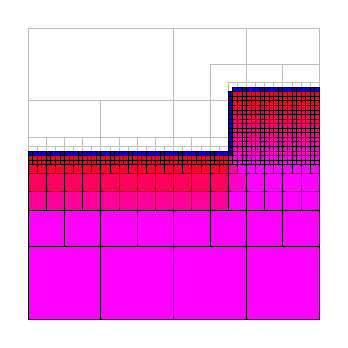
\begin{tikzpicture}[x={(\screenshotunitlength,0)},y={(0,\screenshotunitlength)}]
        \definecolor{fillcolor}{rgb}{1.000000,0.000000,1.000000}
\fill[fillcolor] (0.000000,0.000000) rectangle (0.250000,0.250000);
\definecolor{fillcolor}{rgb}{1.000000,0.000000,1.000000}
\fill[fillcolor] (0.250000,0.000000) rectangle (0.500000,0.250000);
\definecolor{fillcolor}{rgb}{1.000000,0.000000,0.982000}
\fill[fillcolor] (0.000000,0.250000) rectangle (0.125000,0.375000);
\definecolor{fillcolor}{rgb}{1.000000,0.000000,0.982000}
\fill[fillcolor] (0.125000,0.250000) rectangle (0.250000,0.375000);
\definecolor{fillcolor}{rgb}{1.000000,0.000000,0.613750}
\fill[fillcolor] (0.000000,0.375000) rectangle (0.062500,0.437500);
\definecolor{fillcolor}{rgb}{1.000000,0.000000,0.613750}
\fill[fillcolor] (0.062500,0.375000) rectangle (0.125000,0.437500);
\definecolor{fillcolor}{rgb}{1.000000,0.000000,0.368250}
\fill[fillcolor] (0.000000,0.437500) rectangle (0.062500,0.500000);
\definecolor{fillcolor}{rgb}{1.000000,0.000000,0.368250}
\fill[fillcolor] (0.062500,0.437500) rectangle (0.125000,0.500000);
\definecolor{fillcolor}{rgb}{1.000000,0.000000,0.613750}
\fill[fillcolor] (0.125000,0.375000) rectangle (0.187500,0.437500);
\definecolor{fillcolor}{rgb}{1.000000,0.000000,0.613750}
\fill[fillcolor] (0.187500,0.375000) rectangle (0.250000,0.437500);
\definecolor{fillcolor}{rgb}{1.000000,0.000000,0.368250}
\fill[fillcolor] (0.125000,0.437500) rectangle (0.187500,0.500000);
\definecolor{fillcolor}{rgb}{1.000000,0.000000,0.368250}
\fill[fillcolor] (0.187500,0.437500) rectangle (0.250000,0.500000);
\definecolor{fillcolor}{rgb}{1.000000,0.000000,0.982000}
\fill[fillcolor] (0.250000,0.250000) rectangle (0.375000,0.375000);
\definecolor{fillcolor}{rgb}{1.000000,0.000000,0.982000}
\fill[fillcolor] (0.375000,0.250000) rectangle (0.500000,0.375000);
\definecolor{fillcolor}{rgb}{1.000000,0.000000,0.613750}
\fill[fillcolor] (0.250000,0.375000) rectangle (0.312500,0.437500);
\definecolor{fillcolor}{rgb}{1.000000,0.000000,0.613750}
\fill[fillcolor] (0.312500,0.375000) rectangle (0.375000,0.437500);
\definecolor{fillcolor}{rgb}{1.000000,0.000000,0.368250}
\fill[fillcolor] (0.250000,0.437500) rectangle (0.312500,0.500000);
\definecolor{fillcolor}{rgb}{1.000000,0.000000,0.368250}
\fill[fillcolor] (0.312500,0.437500) rectangle (0.375000,0.500000);
\definecolor{fillcolor}{rgb}{1.000000,0.000000,0.613750}
\fill[fillcolor] (0.375000,0.375000) rectangle (0.437500,0.437500);
\definecolor{fillcolor}{rgb}{1.000000,0.000000,0.613750}
\fill[fillcolor] (0.437500,0.375000) rectangle (0.500000,0.437500);
\definecolor{fillcolor}{rgb}{1.000000,0.000000,0.368250}
\fill[fillcolor] (0.375000,0.437500) rectangle (0.437500,0.500000);
\definecolor{fillcolor}{rgb}{1.000000,0.000000,0.368250}
\fill[fillcolor] (0.437500,0.437500) rectangle (0.500000,0.500000);
\definecolor{fillcolor}{rgb}{1.000000,0.000000,1.000000}
\fill[fillcolor] (0.500000,0.000000) rectangle (0.750000,0.250000);
\definecolor{fillcolor}{rgb}{1.000000,0.000000,1.000000}
\fill[fillcolor] (0.750000,0.000000) rectangle (1.000000,0.250000);
\definecolor{fillcolor}{rgb}{1.000000,0.000000,0.982000}
\fill[fillcolor] (0.500000,0.250000) rectangle (0.625000,0.375000);
\definecolor{fillcolor}{rgb}{1.000000,0.000000,1.000000}
\fill[fillcolor] (0.625000,0.250000) rectangle (0.750000,0.375000);
\definecolor{fillcolor}{rgb}{1.000000,0.000000,0.613750}
\fill[fillcolor] (0.500000,0.375000) rectangle (0.562500,0.437500);
\definecolor{fillcolor}{rgb}{1.000000,0.000000,0.613750}
\fill[fillcolor] (0.562500,0.375000) rectangle (0.625000,0.437500);
\definecolor{fillcolor}{rgb}{1.000000,0.000000,0.368250}
\fill[fillcolor] (0.500000,0.437500) rectangle (0.562500,0.500000);
\definecolor{fillcolor}{rgb}{1.000000,0.000000,0.368250}
\fill[fillcolor] (0.562500,0.437500) rectangle (0.625000,0.500000);
\definecolor{fillcolor}{rgb}{1.000000,0.000000,0.613750}
\fill[fillcolor] (0.625000,0.375000) rectangle (0.687500,0.437500);
\definecolor{fillcolor}{rgb}{1.000000,0.000000,1.000000}
\fill[fillcolor] (0.687500,0.375000) rectangle (0.750000,0.437500);
\definecolor{fillcolor}{rgb}{1.000000,0.000000,0.368250}
\fill[fillcolor] (0.625000,0.437500) rectangle (0.687500,0.500000);
\definecolor{fillcolor}{rgb}{1.000000,0.000000,0.797875}
\fill[fillcolor] (0.687500,0.437500) rectangle (0.750000,0.500000);
\definecolor{fillcolor}{rgb}{1.000000,0.000000,1.000000}
\fill[fillcolor] (0.750000,0.250000) rectangle (0.875000,0.375000);
\definecolor{fillcolor}{rgb}{1.000000,0.000000,1.000000}
\fill[fillcolor] (0.875000,0.250000) rectangle (1.000000,0.375000);
\definecolor{fillcolor}{rgb}{1.000000,0.000000,1.000000}
\fill[fillcolor] (0.750000,0.375000) rectangle (0.812500,0.437500);
\definecolor{fillcolor}{rgb}{1.000000,0.000000,1.000000}
\fill[fillcolor] (0.812500,0.375000) rectangle (0.875000,0.437500);
\definecolor{fillcolor}{rgb}{1.000000,0.000000,1.000000}
\fill[fillcolor] (0.750000,0.437500) rectangle (0.812500,0.500000);
\definecolor{fillcolor}{rgb}{1.000000,0.000000,1.000000}
\fill[fillcolor] (0.812500,0.437500) rectangle (0.875000,0.500000);
\definecolor{fillcolor}{rgb}{1.000000,0.000000,1.000000}
\fill[fillcolor] (0.875000,0.375000) rectangle (0.937500,0.437500);
\definecolor{fillcolor}{rgb}{1.000000,0.000000,1.000000}
\fill[fillcolor] (0.937500,0.375000) rectangle (1.000000,0.437500);
\definecolor{fillcolor}{rgb}{1.000000,0.000000,1.000000}
\fill[fillcolor] (0.875000,0.437500) rectangle (0.937500,0.500000);
\definecolor{fillcolor}{rgb}{1.000000,0.000000,1.000000}
\fill[fillcolor] (0.937500,0.437500) rectangle (1.000000,0.500000);
\definecolor{fillcolor}{rgb}{1.000000,0.000000,0.184125}
\fill[fillcolor] (0.000000,0.500000) rectangle (0.031250,0.531250);
\definecolor{fillcolor}{rgb}{1.000000,0.000000,0.184125}
\fill[fillcolor] (0.031250,0.500000) rectangle (0.062500,0.531250);
\definecolor{fillcolor}{rgb}{1.000000,0.000000,0.092063}
\fill[fillcolor] (0.000000,0.531250) rectangle (0.015625,0.546875);
\definecolor{fillcolor}{rgb}{1.000000,0.000000,0.092063}
\fill[fillcolor] (0.015625,0.531250) rectangle (0.031250,0.546875);
\definecolor{fillcolor}{rgb}{1.000000,0.000000,0.030687}
\fill[fillcolor] (0.000000,0.546875) rectangle (0.015625,0.562500);
\definecolor{fillcolor}{rgb}{1.000000,0.000000,0.030687}
\fill[fillcolor] (0.015625,0.546875) rectangle (0.031250,0.562500);
\definecolor{fillcolor}{rgb}{1.000000,0.000000,0.092063}
\fill[fillcolor] (0.031250,0.531250) rectangle (0.046875,0.546875);
\definecolor{fillcolor}{rgb}{1.000000,0.000000,0.092063}
\fill[fillcolor] (0.046875,0.531250) rectangle (0.062500,0.546875);
\definecolor{fillcolor}{rgb}{1.000000,0.000000,0.030687}
\fill[fillcolor] (0.031250,0.546875) rectangle (0.046875,0.562500);
\definecolor{fillcolor}{rgb}{1.000000,0.000000,0.030687}
\fill[fillcolor] (0.046875,0.546875) rectangle (0.062500,0.562500);
\definecolor{fillcolor}{rgb}{1.000000,0.000000,0.184125}
\fill[fillcolor] (0.062500,0.500000) rectangle (0.093750,0.531250);
\definecolor{fillcolor}{rgb}{1.000000,0.000000,0.184125}
\fill[fillcolor] (0.093750,0.500000) rectangle (0.125000,0.531250);
\definecolor{fillcolor}{rgb}{1.000000,0.000000,0.092063}
\fill[fillcolor] (0.062500,0.531250) rectangle (0.078125,0.546875);
\definecolor{fillcolor}{rgb}{1.000000,0.000000,0.092063}
\fill[fillcolor] (0.078125,0.531250) rectangle (0.093750,0.546875);
\definecolor{fillcolor}{rgb}{1.000000,0.000000,0.030687}
\fill[fillcolor] (0.062500,0.546875) rectangle (0.078125,0.562500);
\definecolor{fillcolor}{rgb}{1.000000,0.000000,0.030687}
\fill[fillcolor] (0.078125,0.546875) rectangle (0.093750,0.562500);
\definecolor{fillcolor}{rgb}{1.000000,0.000000,0.092063}
\fill[fillcolor] (0.093750,0.531250) rectangle (0.109375,0.546875);
\definecolor{fillcolor}{rgb}{1.000000,0.000000,0.092063}
\fill[fillcolor] (0.109375,0.531250) rectangle (0.125000,0.546875);
\definecolor{fillcolor}{rgb}{1.000000,0.000000,0.030687}
\fill[fillcolor] (0.093750,0.546875) rectangle (0.109375,0.562500);
\definecolor{fillcolor}{rgb}{1.000000,0.000000,0.030687}
\fill[fillcolor] (0.109375,0.546875) rectangle (0.125000,0.562500);
\definecolor{fillcolor}{rgb}{0.000000,0.000000,1.000000}
\fill[fillcolor] (0.000000,0.562500) rectangle (0.015625,0.578125);
\definecolor{fillcolor}{rgb}{0.000000,0.000000,1.000000}
\fill[fillcolor] (0.015625,0.562500) rectangle (0.031250,0.578125);
\definecolor{fillcolor}{rgb}{0.000000,0.000000,1.000000}
\fill[fillcolor] (0.031250,0.562500) rectangle (0.046875,0.578125);
\definecolor{fillcolor}{rgb}{0.000000,0.000000,1.000000}
\fill[fillcolor] (0.046875,0.562500) rectangle (0.062500,0.578125);
\definecolor{fillcolor}{rgb}{0.000000,0.000000,1.000000}
\fill[fillcolor] (0.062500,0.562500) rectangle (0.078125,0.578125);
\definecolor{fillcolor}{rgb}{0.000000,0.000000,1.000000}
\fill[fillcolor] (0.078125,0.562500) rectangle (0.093750,0.578125);
\definecolor{fillcolor}{rgb}{0.000000,0.000000,1.000000}
\fill[fillcolor] (0.093750,0.562500) rectangle (0.109375,0.578125);
\definecolor{fillcolor}{rgb}{0.000000,0.000000,1.000000}
\fill[fillcolor] (0.109375,0.562500) rectangle (0.125000,0.578125);
\definecolor{fillcolor}{rgb}{1.000000,0.000000,0.184125}
\fill[fillcolor] (0.125000,0.500000) rectangle (0.156250,0.531250);
\definecolor{fillcolor}{rgb}{1.000000,0.000000,0.184125}
\fill[fillcolor] (0.156250,0.500000) rectangle (0.187500,0.531250);
\definecolor{fillcolor}{rgb}{1.000000,0.000000,0.092063}
\fill[fillcolor] (0.125000,0.531250) rectangle (0.140625,0.546875);
\definecolor{fillcolor}{rgb}{1.000000,0.000000,0.092063}
\fill[fillcolor] (0.140625,0.531250) rectangle (0.156250,0.546875);
\definecolor{fillcolor}{rgb}{1.000000,0.000000,0.030687}
\fill[fillcolor] (0.125000,0.546875) rectangle (0.140625,0.562500);
\definecolor{fillcolor}{rgb}{1.000000,0.000000,0.030687}
\fill[fillcolor] (0.140625,0.546875) rectangle (0.156250,0.562500);
\definecolor{fillcolor}{rgb}{1.000000,0.000000,0.092063}
\fill[fillcolor] (0.156250,0.531250) rectangle (0.171875,0.546875);
\definecolor{fillcolor}{rgb}{1.000000,0.000000,0.092063}
\fill[fillcolor] (0.171875,0.531250) rectangle (0.187500,0.546875);
\definecolor{fillcolor}{rgb}{1.000000,0.000000,0.030687}
\fill[fillcolor] (0.156250,0.546875) rectangle (0.171875,0.562500);
\definecolor{fillcolor}{rgb}{1.000000,0.000000,0.030687}
\fill[fillcolor] (0.171875,0.546875) rectangle (0.187500,0.562500);
\definecolor{fillcolor}{rgb}{1.000000,0.000000,0.184125}
\fill[fillcolor] (0.187500,0.500000) rectangle (0.218750,0.531250);
\definecolor{fillcolor}{rgb}{1.000000,0.000000,0.184125}
\fill[fillcolor] (0.218750,0.500000) rectangle (0.250000,0.531250);
\definecolor{fillcolor}{rgb}{1.000000,0.000000,0.092063}
\fill[fillcolor] (0.187500,0.531250) rectangle (0.203125,0.546875);
\definecolor{fillcolor}{rgb}{1.000000,0.000000,0.092063}
\fill[fillcolor] (0.203125,0.531250) rectangle (0.218750,0.546875);
\definecolor{fillcolor}{rgb}{1.000000,0.000000,0.030687}
\fill[fillcolor] (0.187500,0.546875) rectangle (0.203125,0.562500);
\definecolor{fillcolor}{rgb}{1.000000,0.000000,0.030687}
\fill[fillcolor] (0.203125,0.546875) rectangle (0.218750,0.562500);
\definecolor{fillcolor}{rgb}{1.000000,0.000000,0.092063}
\fill[fillcolor] (0.218750,0.531250) rectangle (0.234375,0.546875);
\definecolor{fillcolor}{rgb}{1.000000,0.000000,0.092063}
\fill[fillcolor] (0.234375,0.531250) rectangle (0.250000,0.546875);
\definecolor{fillcolor}{rgb}{1.000000,0.000000,0.030687}
\fill[fillcolor] (0.218750,0.546875) rectangle (0.234375,0.562500);
\definecolor{fillcolor}{rgb}{1.000000,0.000000,0.030687}
\fill[fillcolor] (0.234375,0.546875) rectangle (0.250000,0.562500);
\definecolor{fillcolor}{rgb}{0.000000,0.000000,1.000000}
\fill[fillcolor] (0.125000,0.562500) rectangle (0.140625,0.578125);
\definecolor{fillcolor}{rgb}{0.000000,0.000000,1.000000}
\fill[fillcolor] (0.140625,0.562500) rectangle (0.156250,0.578125);
\definecolor{fillcolor}{rgb}{0.000000,0.000000,1.000000}
\fill[fillcolor] (0.156250,0.562500) rectangle (0.171875,0.578125);
\definecolor{fillcolor}{rgb}{0.000000,0.000000,1.000000}
\fill[fillcolor] (0.171875,0.562500) rectangle (0.187500,0.578125);
\definecolor{fillcolor}{rgb}{0.000000,0.000000,1.000000}
\fill[fillcolor] (0.187500,0.562500) rectangle (0.203125,0.578125);
\definecolor{fillcolor}{rgb}{0.000000,0.000000,1.000000}
\fill[fillcolor] (0.203125,0.562500) rectangle (0.218750,0.578125);
\definecolor{fillcolor}{rgb}{0.000000,0.000000,1.000000}
\fill[fillcolor] (0.218750,0.562500) rectangle (0.234375,0.578125);
\definecolor{fillcolor}{rgb}{0.000000,0.000000,1.000000}
\fill[fillcolor] (0.234375,0.562500) rectangle (0.250000,0.578125);
\definecolor{fillcolor}{rgb}{1.000000,0.000000,0.184125}
\fill[fillcolor] (0.250000,0.500000) rectangle (0.281250,0.531250);
\definecolor{fillcolor}{rgb}{1.000000,0.000000,0.184125}
\fill[fillcolor] (0.281250,0.500000) rectangle (0.312500,0.531250);
\definecolor{fillcolor}{rgb}{1.000000,0.000000,0.092063}
\fill[fillcolor] (0.250000,0.531250) rectangle (0.265625,0.546875);
\definecolor{fillcolor}{rgb}{1.000000,0.000000,0.092063}
\fill[fillcolor] (0.265625,0.531250) rectangle (0.281250,0.546875);
\definecolor{fillcolor}{rgb}{1.000000,0.000000,0.030687}
\fill[fillcolor] (0.250000,0.546875) rectangle (0.265625,0.562500);
\definecolor{fillcolor}{rgb}{1.000000,0.000000,0.030687}
\fill[fillcolor] (0.265625,0.546875) rectangle (0.281250,0.562500);
\definecolor{fillcolor}{rgb}{1.000000,0.000000,0.092063}
\fill[fillcolor] (0.281250,0.531250) rectangle (0.296875,0.546875);
\definecolor{fillcolor}{rgb}{1.000000,0.000000,0.092063}
\fill[fillcolor] (0.296875,0.531250) rectangle (0.312500,0.546875);
\definecolor{fillcolor}{rgb}{1.000000,0.000000,0.030687}
\fill[fillcolor] (0.281250,0.546875) rectangle (0.296875,0.562500);
\definecolor{fillcolor}{rgb}{1.000000,0.000000,0.030687}
\fill[fillcolor] (0.296875,0.546875) rectangle (0.312500,0.562500);
\definecolor{fillcolor}{rgb}{1.000000,0.000000,0.184125}
\fill[fillcolor] (0.312500,0.500000) rectangle (0.343750,0.531250);
\definecolor{fillcolor}{rgb}{1.000000,0.000000,0.184125}
\fill[fillcolor] (0.343750,0.500000) rectangle (0.375000,0.531250);
\definecolor{fillcolor}{rgb}{1.000000,0.000000,0.092063}
\fill[fillcolor] (0.312500,0.531250) rectangle (0.328125,0.546875);
\definecolor{fillcolor}{rgb}{1.000000,0.000000,0.092063}
\fill[fillcolor] (0.328125,0.531250) rectangle (0.343750,0.546875);
\definecolor{fillcolor}{rgb}{1.000000,0.000000,0.030687}
\fill[fillcolor] (0.312500,0.546875) rectangle (0.328125,0.562500);
\definecolor{fillcolor}{rgb}{1.000000,0.000000,0.030687}
\fill[fillcolor] (0.328125,0.546875) rectangle (0.343750,0.562500);
\definecolor{fillcolor}{rgb}{1.000000,0.000000,0.092063}
\fill[fillcolor] (0.343750,0.531250) rectangle (0.359375,0.546875);
\definecolor{fillcolor}{rgb}{1.000000,0.000000,0.092063}
\fill[fillcolor] (0.359375,0.531250) rectangle (0.375000,0.546875);
\definecolor{fillcolor}{rgb}{1.000000,0.000000,0.030687}
\fill[fillcolor] (0.343750,0.546875) rectangle (0.359375,0.562500);
\definecolor{fillcolor}{rgb}{1.000000,0.000000,0.030687}
\fill[fillcolor] (0.359375,0.546875) rectangle (0.375000,0.562500);
\definecolor{fillcolor}{rgb}{0.000000,0.000000,1.000000}
\fill[fillcolor] (0.250000,0.562500) rectangle (0.265625,0.578125);
\definecolor{fillcolor}{rgb}{0.000000,0.000000,1.000000}
\fill[fillcolor] (0.265625,0.562500) rectangle (0.281250,0.578125);
\definecolor{fillcolor}{rgb}{0.000000,0.000000,1.000000}
\fill[fillcolor] (0.281250,0.562500) rectangle (0.296875,0.578125);
\definecolor{fillcolor}{rgb}{0.000000,0.000000,1.000000}
\fill[fillcolor] (0.296875,0.562500) rectangle (0.312500,0.578125);
\definecolor{fillcolor}{rgb}{0.000000,0.000000,1.000000}
\fill[fillcolor] (0.312500,0.562500) rectangle (0.328125,0.578125);
\definecolor{fillcolor}{rgb}{0.000000,0.000000,1.000000}
\fill[fillcolor] (0.328125,0.562500) rectangle (0.343750,0.578125);
\definecolor{fillcolor}{rgb}{0.000000,0.000000,1.000000}
\fill[fillcolor] (0.343750,0.562500) rectangle (0.359375,0.578125);
\definecolor{fillcolor}{rgb}{0.000000,0.000000,1.000000}
\fill[fillcolor] (0.359375,0.562500) rectangle (0.375000,0.578125);
\definecolor{fillcolor}{rgb}{1.000000,0.000000,0.184125}
\fill[fillcolor] (0.375000,0.500000) rectangle (0.406250,0.531250);
\definecolor{fillcolor}{rgb}{1.000000,0.000000,0.184125}
\fill[fillcolor] (0.406250,0.500000) rectangle (0.437500,0.531250);
\definecolor{fillcolor}{rgb}{1.000000,0.000000,0.092063}
\fill[fillcolor] (0.375000,0.531250) rectangle (0.390625,0.546875);
\definecolor{fillcolor}{rgb}{1.000000,0.000000,0.092063}
\fill[fillcolor] (0.390625,0.531250) rectangle (0.406250,0.546875);
\definecolor{fillcolor}{rgb}{1.000000,0.000000,0.030687}
\fill[fillcolor] (0.375000,0.546875) rectangle (0.390625,0.562500);
\definecolor{fillcolor}{rgb}{1.000000,0.000000,0.030687}
\fill[fillcolor] (0.390625,0.546875) rectangle (0.406250,0.562500);
\definecolor{fillcolor}{rgb}{1.000000,0.000000,0.092063}
\fill[fillcolor] (0.406250,0.531250) rectangle (0.421875,0.546875);
\definecolor{fillcolor}{rgb}{1.000000,0.000000,0.092063}
\fill[fillcolor] (0.421875,0.531250) rectangle (0.437500,0.546875);
\definecolor{fillcolor}{rgb}{1.000000,0.000000,0.030687}
\fill[fillcolor] (0.406250,0.546875) rectangle (0.421875,0.562500);
\definecolor{fillcolor}{rgb}{1.000000,0.000000,0.030687}
\fill[fillcolor] (0.421875,0.546875) rectangle (0.437500,0.562500);
\definecolor{fillcolor}{rgb}{1.000000,0.000000,0.184125}
\fill[fillcolor] (0.437500,0.500000) rectangle (0.468750,0.531250);
\definecolor{fillcolor}{rgb}{1.000000,0.000000,0.184125}
\fill[fillcolor] (0.468750,0.500000) rectangle (0.500000,0.531250);
\definecolor{fillcolor}{rgb}{1.000000,0.000000,0.092063}
\fill[fillcolor] (0.437500,0.531250) rectangle (0.453125,0.546875);
\definecolor{fillcolor}{rgb}{1.000000,0.000000,0.092063}
\fill[fillcolor] (0.453125,0.531250) rectangle (0.468750,0.546875);
\definecolor{fillcolor}{rgb}{1.000000,0.000000,0.030687}
\fill[fillcolor] (0.437500,0.546875) rectangle (0.453125,0.562500);
\definecolor{fillcolor}{rgb}{1.000000,0.000000,0.030687}
\fill[fillcolor] (0.453125,0.546875) rectangle (0.468750,0.562500);
\definecolor{fillcolor}{rgb}{1.000000,0.000000,0.092063}
\fill[fillcolor] (0.468750,0.531250) rectangle (0.484375,0.546875);
\definecolor{fillcolor}{rgb}{1.000000,0.000000,0.092063}
\fill[fillcolor] (0.484375,0.531250) rectangle (0.500000,0.546875);
\definecolor{fillcolor}{rgb}{1.000000,0.000000,0.030687}
\fill[fillcolor] (0.468750,0.546875) rectangle (0.484375,0.562500);
\definecolor{fillcolor}{rgb}{1.000000,0.000000,0.030687}
\fill[fillcolor] (0.484375,0.546875) rectangle (0.500000,0.562500);
\definecolor{fillcolor}{rgb}{0.000000,0.000000,1.000000}
\fill[fillcolor] (0.375000,0.562500) rectangle (0.390625,0.578125);
\definecolor{fillcolor}{rgb}{0.000000,0.000000,1.000000}
\fill[fillcolor] (0.390625,0.562500) rectangle (0.406250,0.578125);
\definecolor{fillcolor}{rgb}{0.000000,0.000000,1.000000}
\fill[fillcolor] (0.406250,0.562500) rectangle (0.421875,0.578125);
\definecolor{fillcolor}{rgb}{0.000000,0.000000,1.000000}
\fill[fillcolor] (0.421875,0.562500) rectangle (0.437500,0.578125);
\definecolor{fillcolor}{rgb}{0.000000,0.000000,1.000000}
\fill[fillcolor] (0.437500,0.562500) rectangle (0.453125,0.578125);
\definecolor{fillcolor}{rgb}{0.000000,0.000000,1.000000}
\fill[fillcolor] (0.453125,0.562500) rectangle (0.468750,0.578125);
\definecolor{fillcolor}{rgb}{0.000000,0.000000,1.000000}
\fill[fillcolor] (0.468750,0.562500) rectangle (0.484375,0.578125);
\definecolor{fillcolor}{rgb}{0.000000,0.000000,1.000000}
\fill[fillcolor] (0.484375,0.562500) rectangle (0.500000,0.578125);
\definecolor{fillcolor}{rgb}{1.000000,0.000000,0.184125}
\fill[fillcolor] (0.500000,0.500000) rectangle (0.531250,0.531250);
\definecolor{fillcolor}{rgb}{1.000000,0.000000,0.184125}
\fill[fillcolor] (0.531250,0.500000) rectangle (0.562500,0.531250);
\definecolor{fillcolor}{rgb}{1.000000,0.000000,0.092063}
\fill[fillcolor] (0.500000,0.531250) rectangle (0.515625,0.546875);
\definecolor{fillcolor}{rgb}{1.000000,0.000000,0.092063}
\fill[fillcolor] (0.515625,0.531250) rectangle (0.531250,0.546875);
\definecolor{fillcolor}{rgb}{1.000000,0.000000,0.030687}
\fill[fillcolor] (0.500000,0.546875) rectangle (0.515625,0.562500);
\definecolor{fillcolor}{rgb}{1.000000,0.000000,0.030687}
\fill[fillcolor] (0.515625,0.546875) rectangle (0.531250,0.562500);
\definecolor{fillcolor}{rgb}{1.000000,0.000000,0.092063}
\fill[fillcolor] (0.531250,0.531250) rectangle (0.546875,0.546875);
\definecolor{fillcolor}{rgb}{1.000000,0.000000,0.092063}
\fill[fillcolor] (0.546875,0.531250) rectangle (0.562500,0.546875);
\definecolor{fillcolor}{rgb}{1.000000,0.000000,0.030687}
\fill[fillcolor] (0.531250,0.546875) rectangle (0.546875,0.562500);
\definecolor{fillcolor}{rgb}{1.000000,0.000000,0.030687}
\fill[fillcolor] (0.546875,0.546875) rectangle (0.562500,0.562500);
\definecolor{fillcolor}{rgb}{1.000000,0.000000,0.184125}
\fill[fillcolor] (0.562500,0.500000) rectangle (0.593750,0.531250);
\definecolor{fillcolor}{rgb}{1.000000,0.000000,0.184125}
\fill[fillcolor] (0.593750,0.500000) rectangle (0.625000,0.531250);
\definecolor{fillcolor}{rgb}{1.000000,0.000000,0.092063}
\fill[fillcolor] (0.562500,0.531250) rectangle (0.578125,0.546875);
\definecolor{fillcolor}{rgb}{1.000000,0.000000,0.092063}
\fill[fillcolor] (0.578125,0.531250) rectangle (0.593750,0.546875);
\definecolor{fillcolor}{rgb}{1.000000,0.000000,0.030687}
\fill[fillcolor] (0.562500,0.546875) rectangle (0.578125,0.562500);
\definecolor{fillcolor}{rgb}{1.000000,0.000000,0.030687}
\fill[fillcolor] (0.578125,0.546875) rectangle (0.593750,0.562500);
\definecolor{fillcolor}{rgb}{1.000000,0.000000,0.092063}
\fill[fillcolor] (0.593750,0.531250) rectangle (0.609375,0.546875);
\definecolor{fillcolor}{rgb}{1.000000,0.000000,0.092063}
\fill[fillcolor] (0.609375,0.531250) rectangle (0.625000,0.546875);
\definecolor{fillcolor}{rgb}{1.000000,0.000000,0.030687}
\fill[fillcolor] (0.593750,0.546875) rectangle (0.609375,0.562500);
\definecolor{fillcolor}{rgb}{1.000000,0.000000,0.030687}
\fill[fillcolor] (0.609375,0.546875) rectangle (0.625000,0.562500);
\definecolor{fillcolor}{rgb}{0.000000,0.000000,1.000000}
\fill[fillcolor] (0.500000,0.562500) rectangle (0.515625,0.578125);
\definecolor{fillcolor}{rgb}{0.000000,0.000000,1.000000}
\fill[fillcolor] (0.515625,0.562500) rectangle (0.531250,0.578125);
\definecolor{fillcolor}{rgb}{0.000000,0.000000,1.000000}
\fill[fillcolor] (0.531250,0.562500) rectangle (0.546875,0.578125);
\definecolor{fillcolor}{rgb}{0.000000,0.000000,1.000000}
\fill[fillcolor] (0.546875,0.562500) rectangle (0.562500,0.578125);
\definecolor{fillcolor}{rgb}{0.000000,0.000000,1.000000}
\fill[fillcolor] (0.562500,0.562500) rectangle (0.578125,0.578125);
\definecolor{fillcolor}{rgb}{0.000000,0.000000,1.000000}
\fill[fillcolor] (0.578125,0.562500) rectangle (0.593750,0.578125);
\definecolor{fillcolor}{rgb}{0.000000,0.000000,1.000000}
\fill[fillcolor] (0.593750,0.562500) rectangle (0.609375,0.578125);
\definecolor{fillcolor}{rgb}{0.000000,0.000000,1.000000}
\fill[fillcolor] (0.609375,0.562500) rectangle (0.625000,0.578125);
\definecolor{fillcolor}{rgb}{1.000000,0.000000,0.184125}
\fill[fillcolor] (0.625000,0.500000) rectangle (0.656250,0.531250);
\definecolor{fillcolor}{rgb}{1.000000,0.000000,0.184125}
\fill[fillcolor] (0.656250,0.500000) rectangle (0.687500,0.531250);
\definecolor{fillcolor}{rgb}{1.000000,0.000000,0.092063}
\fill[fillcolor] (0.625000,0.531250) rectangle (0.640625,0.546875);
\definecolor{fillcolor}{rgb}{1.000000,0.000000,0.092063}
\fill[fillcolor] (0.640625,0.531250) rectangle (0.656250,0.546875);
\definecolor{fillcolor}{rgb}{1.000000,0.000000,0.030687}
\fill[fillcolor] (0.625000,0.546875) rectangle (0.640625,0.562500);
\definecolor{fillcolor}{rgb}{1.000000,0.000000,0.030687}
\fill[fillcolor] (0.640625,0.546875) rectangle (0.656250,0.562500);
\definecolor{fillcolor}{rgb}{1.000000,0.000000,0.092063}
\fill[fillcolor] (0.656250,0.531250) rectangle (0.671875,0.546875);
\definecolor{fillcolor}{rgb}{1.000000,0.000000,0.092063}
\fill[fillcolor] (0.671875,0.531250) rectangle (0.687500,0.546875);
\definecolor{fillcolor}{rgb}{1.000000,0.000000,0.030687}
\fill[fillcolor] (0.656250,0.546875) rectangle (0.671875,0.562500);
\definecolor{fillcolor}{rgb}{1.000000,0.000000,0.030687}
\fill[fillcolor] (0.671875,0.546875) rectangle (0.687500,0.562500);
\definecolor{fillcolor}{rgb}{1.000000,0.000000,0.613750}
\fill[fillcolor] (0.687500,0.500000) rectangle (0.718750,0.531250);
\definecolor{fillcolor}{rgb}{1.000000,0.000000,1.000000}
\fill[fillcolor] (0.718750,0.500000) rectangle (0.750000,0.531250);
\definecolor{fillcolor}{rgb}{1.000000,0.000000,0.521688}
\fill[fillcolor] (0.687500,0.531250) rectangle (0.703125,0.546875);
\definecolor{fillcolor}{rgb}{1.000000,0.000000,0.951312}
\fill[fillcolor] (0.703125,0.531250) rectangle (0.718750,0.546875);
\definecolor{fillcolor}{rgb}{1.000000,0.000000,0.460312}
\fill[fillcolor] (0.687500,0.546875) rectangle (0.703125,0.562500);
\definecolor{fillcolor}{rgb}{1.000000,0.000000,0.889938}
\fill[fillcolor] (0.703125,0.546875) rectangle (0.718750,0.562500);
\definecolor{fillcolor}{rgb}{1.000000,0.000000,0.951312}
\fill[fillcolor] (0.718750,0.531250) rectangle (0.734375,0.546875);
\definecolor{fillcolor}{rgb}{1.000000,0.000000,0.951312}
\fill[fillcolor] (0.734375,0.531250) rectangle (0.750000,0.546875);
\definecolor{fillcolor}{rgb}{1.000000,0.000000,0.889938}
\fill[fillcolor] (0.718750,0.546875) rectangle (0.734375,0.562500);
\definecolor{fillcolor}{rgb}{1.000000,0.000000,0.889938}
\fill[fillcolor] (0.734375,0.546875) rectangle (0.750000,0.562500);
\definecolor{fillcolor}{rgb}{0.000000,0.000000,1.000000}
\fill[fillcolor] (0.625000,0.562500) rectangle (0.640625,0.578125);
\definecolor{fillcolor}{rgb}{0.000000,0.000000,1.000000}
\fill[fillcolor] (0.640625,0.562500) rectangle (0.656250,0.578125);
\definecolor{fillcolor}{rgb}{0.000000,0.000000,1.000000}
\fill[fillcolor] (0.656250,0.562500) rectangle (0.671875,0.578125);
\definecolor{fillcolor}{rgb}{0.000000,0.000000,1.000000}
\fill[fillcolor] (0.671875,0.562500) rectangle (0.687500,0.578125);
\definecolor{fillcolor}{rgb}{0.000000,0.000000,1.000000}
\fill[fillcolor] (0.687500,0.562500) rectangle (0.703125,0.578125);
\definecolor{fillcolor}{rgb}{1.000000,0.000000,0.828562}
\fill[fillcolor] (0.703125,0.562500) rectangle (0.718750,0.578125);
\definecolor{fillcolor}{rgb}{0.000000,0.000000,1.000000}
\fill[fillcolor] (0.687500,0.578125) rectangle (0.703125,0.593750);
\definecolor{fillcolor}{rgb}{1.000000,0.000000,0.767187}
\fill[fillcolor] (0.703125,0.578125) rectangle (0.718750,0.593750);
\definecolor{fillcolor}{rgb}{1.000000,0.000000,0.828562}
\fill[fillcolor] (0.718750,0.562500) rectangle (0.734375,0.578125);
\definecolor{fillcolor}{rgb}{1.000000,0.000000,0.828562}
\fill[fillcolor] (0.734375,0.562500) rectangle (0.750000,0.578125);
\definecolor{fillcolor}{rgb}{1.000000,0.000000,0.767187}
\fill[fillcolor] (0.718750,0.578125) rectangle (0.734375,0.593750);
\definecolor{fillcolor}{rgb}{1.000000,0.000000,0.767187}
\fill[fillcolor] (0.734375,0.578125) rectangle (0.750000,0.593750);
\definecolor{fillcolor}{rgb}{0.000000,0.000000,1.000000}
\fill[fillcolor] (0.687500,0.593750) rectangle (0.703125,0.609375);
\definecolor{fillcolor}{rgb}{1.000000,0.000000,0.705813}
\fill[fillcolor] (0.703125,0.593750) rectangle (0.718750,0.609375);
\definecolor{fillcolor}{rgb}{0.000000,0.000000,1.000000}
\fill[fillcolor] (0.687500,0.609375) rectangle (0.703125,0.625000);
\definecolor{fillcolor}{rgb}{1.000000,0.000000,0.644437}
\fill[fillcolor] (0.703125,0.609375) rectangle (0.718750,0.625000);
\definecolor{fillcolor}{rgb}{1.000000,0.000000,0.705813}
\fill[fillcolor] (0.718750,0.593750) rectangle (0.734375,0.609375);
\definecolor{fillcolor}{rgb}{1.000000,0.000000,0.705813}
\fill[fillcolor] (0.734375,0.593750) rectangle (0.750000,0.609375);
\definecolor{fillcolor}{rgb}{1.000000,0.000000,0.644437}
\fill[fillcolor] (0.718750,0.609375) rectangle (0.734375,0.625000);
\definecolor{fillcolor}{rgb}{1.000000,0.000000,0.644437}
\fill[fillcolor] (0.734375,0.609375) rectangle (0.750000,0.625000);
\definecolor{fillcolor}{rgb}{0.000000,0.000000,1.000000}
\fill[fillcolor] (0.687500,0.625000) rectangle (0.703125,0.640625);
\definecolor{fillcolor}{rgb}{1.000000,0.000000,0.583063}
\fill[fillcolor] (0.703125,0.625000) rectangle (0.718750,0.640625);
\definecolor{fillcolor}{rgb}{0.000000,0.000000,1.000000}
\fill[fillcolor] (0.687500,0.640625) rectangle (0.703125,0.656250);
\definecolor{fillcolor}{rgb}{1.000000,0.000000,0.521688}
\fill[fillcolor] (0.703125,0.640625) rectangle (0.718750,0.656250);
\definecolor{fillcolor}{rgb}{1.000000,0.000000,0.583063}
\fill[fillcolor] (0.718750,0.625000) rectangle (0.734375,0.640625);
\definecolor{fillcolor}{rgb}{1.000000,0.000000,0.583063}
\fill[fillcolor] (0.734375,0.625000) rectangle (0.750000,0.640625);
\definecolor{fillcolor}{rgb}{1.000000,0.000000,0.521688}
\fill[fillcolor] (0.718750,0.640625) rectangle (0.734375,0.656250);
\definecolor{fillcolor}{rgb}{1.000000,0.000000,0.521688}
\fill[fillcolor] (0.734375,0.640625) rectangle (0.750000,0.656250);
\definecolor{fillcolor}{rgb}{0.000000,0.000000,1.000000}
\fill[fillcolor] (0.687500,0.656250) rectangle (0.703125,0.671875);
\definecolor{fillcolor}{rgb}{1.000000,0.000000,0.460312}
\fill[fillcolor] (0.703125,0.656250) rectangle (0.718750,0.671875);
\definecolor{fillcolor}{rgb}{0.000000,0.000000,1.000000}
\fill[fillcolor] (0.687500,0.671875) rectangle (0.703125,0.687500);
\definecolor{fillcolor}{rgb}{1.000000,0.000000,0.398937}
\fill[fillcolor] (0.703125,0.671875) rectangle (0.718750,0.687500);
\definecolor{fillcolor}{rgb}{1.000000,0.000000,0.460312}
\fill[fillcolor] (0.718750,0.656250) rectangle (0.734375,0.671875);
\definecolor{fillcolor}{rgb}{1.000000,0.000000,0.460312}
\fill[fillcolor] (0.734375,0.656250) rectangle (0.750000,0.671875);
\definecolor{fillcolor}{rgb}{1.000000,0.000000,0.398937}
\fill[fillcolor] (0.718750,0.671875) rectangle (0.734375,0.687500);
\definecolor{fillcolor}{rgb}{1.000000,0.000000,0.398937}
\fill[fillcolor] (0.734375,0.671875) rectangle (0.750000,0.687500);
\definecolor{fillcolor}{rgb}{0.000000,0.000000,1.000000}
\fill[fillcolor] (0.687500,0.687500) rectangle (0.703125,0.703125);
\definecolor{fillcolor}{rgb}{1.000000,0.000000,0.337563}
\fill[fillcolor] (0.703125,0.687500) rectangle (0.718750,0.703125);
\definecolor{fillcolor}{rgb}{0.000000,0.000000,1.000000}
\fill[fillcolor] (0.687500,0.703125) rectangle (0.703125,0.718750);
\definecolor{fillcolor}{rgb}{1.000000,0.000000,0.276188}
\fill[fillcolor] (0.703125,0.703125) rectangle (0.718750,0.718750);
\definecolor{fillcolor}{rgb}{1.000000,0.000000,0.337563}
\fill[fillcolor] (0.718750,0.687500) rectangle (0.734375,0.703125);
\definecolor{fillcolor}{rgb}{1.000000,0.000000,0.337563}
\fill[fillcolor] (0.734375,0.687500) rectangle (0.750000,0.703125);
\definecolor{fillcolor}{rgb}{1.000000,0.000000,0.276188}
\fill[fillcolor] (0.718750,0.703125) rectangle (0.734375,0.718750);
\definecolor{fillcolor}{rgb}{1.000000,0.000000,0.276188}
\fill[fillcolor] (0.734375,0.703125) rectangle (0.750000,0.718750);
\definecolor{fillcolor}{rgb}{0.000000,0.000000,1.000000}
\fill[fillcolor] (0.687500,0.718750) rectangle (0.703125,0.734375);
\definecolor{fillcolor}{rgb}{1.000000,0.000000,0.214813}
\fill[fillcolor] (0.703125,0.718750) rectangle (0.718750,0.734375);
\definecolor{fillcolor}{rgb}{0.000000,0.000000,1.000000}
\fill[fillcolor] (0.687500,0.734375) rectangle (0.703125,0.750000);
\definecolor{fillcolor}{rgb}{1.000000,0.000000,0.153437}
\fill[fillcolor] (0.703125,0.734375) rectangle (0.718750,0.750000);
\definecolor{fillcolor}{rgb}{1.000000,0.000000,0.214813}
\fill[fillcolor] (0.718750,0.718750) rectangle (0.734375,0.734375);
\definecolor{fillcolor}{rgb}{1.000000,0.000000,0.214813}
\fill[fillcolor] (0.734375,0.718750) rectangle (0.750000,0.734375);
\definecolor{fillcolor}{rgb}{1.000000,0.000000,0.153437}
\fill[fillcolor] (0.718750,0.734375) rectangle (0.734375,0.750000);
\definecolor{fillcolor}{rgb}{1.000000,0.000000,0.153437}
\fill[fillcolor] (0.734375,0.734375) rectangle (0.750000,0.750000);
\definecolor{fillcolor}{rgb}{1.000000,0.000000,1.000000}
\fill[fillcolor] (0.750000,0.500000) rectangle (0.781250,0.531250);
\definecolor{fillcolor}{rgb}{1.000000,0.000000,1.000000}
\fill[fillcolor] (0.781250,0.500000) rectangle (0.812500,0.531250);
\definecolor{fillcolor}{rgb}{1.000000,0.000000,0.951312}
\fill[fillcolor] (0.750000,0.531250) rectangle (0.765625,0.546875);
\definecolor{fillcolor}{rgb}{1.000000,0.000000,0.951312}
\fill[fillcolor] (0.765625,0.531250) rectangle (0.781250,0.546875);
\definecolor{fillcolor}{rgb}{1.000000,0.000000,0.889938}
\fill[fillcolor] (0.750000,0.546875) rectangle (0.765625,0.562500);
\definecolor{fillcolor}{rgb}{1.000000,0.000000,0.889938}
\fill[fillcolor] (0.765625,0.546875) rectangle (0.781250,0.562500);
\definecolor{fillcolor}{rgb}{1.000000,0.000000,0.951312}
\fill[fillcolor] (0.781250,0.531250) rectangle (0.796875,0.546875);
\definecolor{fillcolor}{rgb}{1.000000,0.000000,0.951312}
\fill[fillcolor] (0.796875,0.531250) rectangle (0.812500,0.546875);
\definecolor{fillcolor}{rgb}{1.000000,0.000000,0.889938}
\fill[fillcolor] (0.781250,0.546875) rectangle (0.796875,0.562500);
\definecolor{fillcolor}{rgb}{1.000000,0.000000,0.889938}
\fill[fillcolor] (0.796875,0.546875) rectangle (0.812500,0.562500);
\definecolor{fillcolor}{rgb}{1.000000,0.000000,1.000000}
\fill[fillcolor] (0.812500,0.500000) rectangle (0.843750,0.531250);
\definecolor{fillcolor}{rgb}{1.000000,0.000000,1.000000}
\fill[fillcolor] (0.843750,0.500000) rectangle (0.875000,0.531250);
\definecolor{fillcolor}{rgb}{1.000000,0.000000,0.951312}
\fill[fillcolor] (0.812500,0.531250) rectangle (0.828125,0.546875);
\definecolor{fillcolor}{rgb}{1.000000,0.000000,0.951312}
\fill[fillcolor] (0.828125,0.531250) rectangle (0.843750,0.546875);
\definecolor{fillcolor}{rgb}{1.000000,0.000000,0.889938}
\fill[fillcolor] (0.812500,0.546875) rectangle (0.828125,0.562500);
\definecolor{fillcolor}{rgb}{1.000000,0.000000,0.889938}
\fill[fillcolor] (0.828125,0.546875) rectangle (0.843750,0.562500);
\definecolor{fillcolor}{rgb}{1.000000,0.000000,0.951312}
\fill[fillcolor] (0.843750,0.531250) rectangle (0.859375,0.546875);
\definecolor{fillcolor}{rgb}{1.000000,0.000000,0.951312}
\fill[fillcolor] (0.859375,0.531250) rectangle (0.875000,0.546875);
\definecolor{fillcolor}{rgb}{1.000000,0.000000,0.889938}
\fill[fillcolor] (0.843750,0.546875) rectangle (0.859375,0.562500);
\definecolor{fillcolor}{rgb}{1.000000,0.000000,0.889938}
\fill[fillcolor] (0.859375,0.546875) rectangle (0.875000,0.562500);
\definecolor{fillcolor}{rgb}{1.000000,0.000000,0.828562}
\fill[fillcolor] (0.750000,0.562500) rectangle (0.765625,0.578125);
\definecolor{fillcolor}{rgb}{1.000000,0.000000,0.828562}
\fill[fillcolor] (0.765625,0.562500) rectangle (0.781250,0.578125);
\definecolor{fillcolor}{rgb}{1.000000,0.000000,0.767187}
\fill[fillcolor] (0.750000,0.578125) rectangle (0.765625,0.593750);
\definecolor{fillcolor}{rgb}{1.000000,0.000000,0.767187}
\fill[fillcolor] (0.765625,0.578125) rectangle (0.781250,0.593750);
\definecolor{fillcolor}{rgb}{1.000000,0.000000,0.828562}
\fill[fillcolor] (0.781250,0.562500) rectangle (0.796875,0.578125);
\definecolor{fillcolor}{rgb}{1.000000,0.000000,0.828562}
\fill[fillcolor] (0.796875,0.562500) rectangle (0.812500,0.578125);
\definecolor{fillcolor}{rgb}{1.000000,0.000000,0.767187}
\fill[fillcolor] (0.781250,0.578125) rectangle (0.796875,0.593750);
\definecolor{fillcolor}{rgb}{1.000000,0.000000,0.767187}
\fill[fillcolor] (0.796875,0.578125) rectangle (0.812500,0.593750);
\definecolor{fillcolor}{rgb}{1.000000,0.000000,0.705813}
\fill[fillcolor] (0.750000,0.593750) rectangle (0.765625,0.609375);
\definecolor{fillcolor}{rgb}{1.000000,0.000000,0.705813}
\fill[fillcolor] (0.765625,0.593750) rectangle (0.781250,0.609375);
\definecolor{fillcolor}{rgb}{1.000000,0.000000,0.644437}
\fill[fillcolor] (0.750000,0.609375) rectangle (0.765625,0.625000);
\definecolor{fillcolor}{rgb}{1.000000,0.000000,0.644437}
\fill[fillcolor] (0.765625,0.609375) rectangle (0.781250,0.625000);
\definecolor{fillcolor}{rgb}{1.000000,0.000000,0.705813}
\fill[fillcolor] (0.781250,0.593750) rectangle (0.796875,0.609375);
\definecolor{fillcolor}{rgb}{1.000000,0.000000,0.705813}
\fill[fillcolor] (0.796875,0.593750) rectangle (0.812500,0.609375);
\definecolor{fillcolor}{rgb}{1.000000,0.000000,0.644437}
\fill[fillcolor] (0.781250,0.609375) rectangle (0.796875,0.625000);
\definecolor{fillcolor}{rgb}{1.000000,0.000000,0.644437}
\fill[fillcolor] (0.796875,0.609375) rectangle (0.812500,0.625000);
\definecolor{fillcolor}{rgb}{1.000000,0.000000,0.828562}
\fill[fillcolor] (0.812500,0.562500) rectangle (0.828125,0.578125);
\definecolor{fillcolor}{rgb}{1.000000,0.000000,0.828562}
\fill[fillcolor] (0.828125,0.562500) rectangle (0.843750,0.578125);
\definecolor{fillcolor}{rgb}{1.000000,0.000000,0.767187}
\fill[fillcolor] (0.812500,0.578125) rectangle (0.828125,0.593750);
\definecolor{fillcolor}{rgb}{1.000000,0.000000,0.767187}
\fill[fillcolor] (0.828125,0.578125) rectangle (0.843750,0.593750);
\definecolor{fillcolor}{rgb}{1.000000,0.000000,0.828562}
\fill[fillcolor] (0.843750,0.562500) rectangle (0.859375,0.578125);
\definecolor{fillcolor}{rgb}{1.000000,0.000000,0.828562}
\fill[fillcolor] (0.859375,0.562500) rectangle (0.875000,0.578125);
\definecolor{fillcolor}{rgb}{1.000000,0.000000,0.767187}
\fill[fillcolor] (0.843750,0.578125) rectangle (0.859375,0.593750);
\definecolor{fillcolor}{rgb}{1.000000,0.000000,0.767187}
\fill[fillcolor] (0.859375,0.578125) rectangle (0.875000,0.593750);
\definecolor{fillcolor}{rgb}{1.000000,0.000000,0.705813}
\fill[fillcolor] (0.812500,0.593750) rectangle (0.828125,0.609375);
\definecolor{fillcolor}{rgb}{1.000000,0.000000,0.705813}
\fill[fillcolor] (0.828125,0.593750) rectangle (0.843750,0.609375);
\definecolor{fillcolor}{rgb}{1.000000,0.000000,0.644437}
\fill[fillcolor] (0.812500,0.609375) rectangle (0.828125,0.625000);
\definecolor{fillcolor}{rgb}{1.000000,0.000000,0.644437}
\fill[fillcolor] (0.828125,0.609375) rectangle (0.843750,0.625000);
\definecolor{fillcolor}{rgb}{1.000000,0.000000,0.705813}
\fill[fillcolor] (0.843750,0.593750) rectangle (0.859375,0.609375);
\definecolor{fillcolor}{rgb}{1.000000,0.000000,0.705813}
\fill[fillcolor] (0.859375,0.593750) rectangle (0.875000,0.609375);
\definecolor{fillcolor}{rgb}{1.000000,0.000000,0.644437}
\fill[fillcolor] (0.843750,0.609375) rectangle (0.859375,0.625000);
\definecolor{fillcolor}{rgb}{1.000000,0.000000,0.644437}
\fill[fillcolor] (0.859375,0.609375) rectangle (0.875000,0.625000);
\definecolor{fillcolor}{rgb}{1.000000,0.000000,1.000000}
\fill[fillcolor] (0.875000,0.500000) rectangle (0.906250,0.531250);
\definecolor{fillcolor}{rgb}{1.000000,0.000000,1.000000}
\fill[fillcolor] (0.906250,0.500000) rectangle (0.937500,0.531250);
\definecolor{fillcolor}{rgb}{1.000000,0.000000,0.951312}
\fill[fillcolor] (0.875000,0.531250) rectangle (0.890625,0.546875);
\definecolor{fillcolor}{rgb}{1.000000,0.000000,0.951312}
\fill[fillcolor] (0.890625,0.531250) rectangle (0.906250,0.546875);
\definecolor{fillcolor}{rgb}{1.000000,0.000000,0.889938}
\fill[fillcolor] (0.875000,0.546875) rectangle (0.890625,0.562500);
\definecolor{fillcolor}{rgb}{1.000000,0.000000,0.889938}
\fill[fillcolor] (0.890625,0.546875) rectangle (0.906250,0.562500);
\definecolor{fillcolor}{rgb}{1.000000,0.000000,0.951312}
\fill[fillcolor] (0.906250,0.531250) rectangle (0.921875,0.546875);
\definecolor{fillcolor}{rgb}{1.000000,0.000000,0.951312}
\fill[fillcolor] (0.921875,0.531250) rectangle (0.937500,0.546875);
\definecolor{fillcolor}{rgb}{1.000000,0.000000,0.889938}
\fill[fillcolor] (0.906250,0.546875) rectangle (0.921875,0.562500);
\definecolor{fillcolor}{rgb}{1.000000,0.000000,0.889938}
\fill[fillcolor] (0.921875,0.546875) rectangle (0.937500,0.562500);
\definecolor{fillcolor}{rgb}{1.000000,0.000000,1.000000}
\fill[fillcolor] (0.937500,0.500000) rectangle (0.968750,0.531250);
\definecolor{fillcolor}{rgb}{1.000000,0.000000,1.000000}
\fill[fillcolor] (0.968750,0.500000) rectangle (1.000000,0.531250);
\definecolor{fillcolor}{rgb}{1.000000,0.000000,0.951312}
\fill[fillcolor] (0.937500,0.531250) rectangle (0.953125,0.546875);
\definecolor{fillcolor}{rgb}{1.000000,0.000000,0.951312}
\fill[fillcolor] (0.953125,0.531250) rectangle (0.968750,0.546875);
\definecolor{fillcolor}{rgb}{1.000000,0.000000,0.889938}
\fill[fillcolor] (0.937500,0.546875) rectangle (0.953125,0.562500);
\definecolor{fillcolor}{rgb}{1.000000,0.000000,0.889938}
\fill[fillcolor] (0.953125,0.546875) rectangle (0.968750,0.562500);
\definecolor{fillcolor}{rgb}{1.000000,0.000000,0.951312}
\fill[fillcolor] (0.968750,0.531250) rectangle (0.984375,0.546875);
\definecolor{fillcolor}{rgb}{1.000000,0.000000,0.951312}
\fill[fillcolor] (0.984375,0.531250) rectangle (1.000000,0.546875);
\definecolor{fillcolor}{rgb}{1.000000,0.000000,0.889938}
\fill[fillcolor] (0.968750,0.546875) rectangle (0.984375,0.562500);
\definecolor{fillcolor}{rgb}{1.000000,0.000000,0.889938}
\fill[fillcolor] (0.984375,0.546875) rectangle (1.000000,0.562500);
\definecolor{fillcolor}{rgb}{1.000000,0.000000,0.828562}
\fill[fillcolor] (0.875000,0.562500) rectangle (0.890625,0.578125);
\definecolor{fillcolor}{rgb}{1.000000,0.000000,0.828562}
\fill[fillcolor] (0.890625,0.562500) rectangle (0.906250,0.578125);
\definecolor{fillcolor}{rgb}{1.000000,0.000000,0.767187}
\fill[fillcolor] (0.875000,0.578125) rectangle (0.890625,0.593750);
\definecolor{fillcolor}{rgb}{1.000000,0.000000,0.767187}
\fill[fillcolor] (0.890625,0.578125) rectangle (0.906250,0.593750);
\definecolor{fillcolor}{rgb}{1.000000,0.000000,0.828562}
\fill[fillcolor] (0.906250,0.562500) rectangle (0.921875,0.578125);
\definecolor{fillcolor}{rgb}{1.000000,0.000000,0.828562}
\fill[fillcolor] (0.921875,0.562500) rectangle (0.937500,0.578125);
\definecolor{fillcolor}{rgb}{1.000000,0.000000,0.767187}
\fill[fillcolor] (0.906250,0.578125) rectangle (0.921875,0.593750);
\definecolor{fillcolor}{rgb}{1.000000,0.000000,0.767187}
\fill[fillcolor] (0.921875,0.578125) rectangle (0.937500,0.593750);
\definecolor{fillcolor}{rgb}{1.000000,0.000000,0.705813}
\fill[fillcolor] (0.875000,0.593750) rectangle (0.890625,0.609375);
\definecolor{fillcolor}{rgb}{1.000000,0.000000,0.705813}
\fill[fillcolor] (0.890625,0.593750) rectangle (0.906250,0.609375);
\definecolor{fillcolor}{rgb}{1.000000,0.000000,0.644437}
\fill[fillcolor] (0.875000,0.609375) rectangle (0.890625,0.625000);
\definecolor{fillcolor}{rgb}{1.000000,0.000000,0.644437}
\fill[fillcolor] (0.890625,0.609375) rectangle (0.906250,0.625000);
\definecolor{fillcolor}{rgb}{1.000000,0.000000,0.705813}
\fill[fillcolor] (0.906250,0.593750) rectangle (0.921875,0.609375);
\definecolor{fillcolor}{rgb}{1.000000,0.000000,0.705813}
\fill[fillcolor] (0.921875,0.593750) rectangle (0.937500,0.609375);
\definecolor{fillcolor}{rgb}{1.000000,0.000000,0.644437}
\fill[fillcolor] (0.906250,0.609375) rectangle (0.921875,0.625000);
\definecolor{fillcolor}{rgb}{1.000000,0.000000,0.644437}
\fill[fillcolor] (0.921875,0.609375) rectangle (0.937500,0.625000);
\definecolor{fillcolor}{rgb}{1.000000,0.000000,0.828562}
\fill[fillcolor] (0.937500,0.562500) rectangle (0.953125,0.578125);
\definecolor{fillcolor}{rgb}{1.000000,0.000000,0.828562}
\fill[fillcolor] (0.953125,0.562500) rectangle (0.968750,0.578125);
\definecolor{fillcolor}{rgb}{1.000000,0.000000,0.767187}
\fill[fillcolor] (0.937500,0.578125) rectangle (0.953125,0.593750);
\definecolor{fillcolor}{rgb}{1.000000,0.000000,0.767187}
\fill[fillcolor] (0.953125,0.578125) rectangle (0.968750,0.593750);
\definecolor{fillcolor}{rgb}{1.000000,0.000000,0.828562}
\fill[fillcolor] (0.968750,0.562500) rectangle (0.984375,0.578125);
\definecolor{fillcolor}{rgb}{1.000000,0.000000,0.828562}
\fill[fillcolor] (0.984375,0.562500) rectangle (1.000000,0.578125);
\definecolor{fillcolor}{rgb}{1.000000,0.000000,0.767187}
\fill[fillcolor] (0.968750,0.578125) rectangle (0.984375,0.593750);
\definecolor{fillcolor}{rgb}{1.000000,0.000000,0.767187}
\fill[fillcolor] (0.984375,0.578125) rectangle (1.000000,0.593750);
\definecolor{fillcolor}{rgb}{1.000000,0.000000,0.705813}
\fill[fillcolor] (0.937500,0.593750) rectangle (0.953125,0.609375);
\definecolor{fillcolor}{rgb}{1.000000,0.000000,0.705813}
\fill[fillcolor] (0.953125,0.593750) rectangle (0.968750,0.609375);
\definecolor{fillcolor}{rgb}{1.000000,0.000000,0.644437}
\fill[fillcolor] (0.937500,0.609375) rectangle (0.953125,0.625000);
\definecolor{fillcolor}{rgb}{1.000000,0.000000,0.644437}
\fill[fillcolor] (0.953125,0.609375) rectangle (0.968750,0.625000);
\definecolor{fillcolor}{rgb}{1.000000,0.000000,0.705813}
\fill[fillcolor] (0.968750,0.593750) rectangle (0.984375,0.609375);
\definecolor{fillcolor}{rgb}{1.000000,0.000000,0.705813}
\fill[fillcolor] (0.984375,0.593750) rectangle (1.000000,0.609375);
\definecolor{fillcolor}{rgb}{1.000000,0.000000,0.644437}
\fill[fillcolor] (0.968750,0.609375) rectangle (0.984375,0.625000);
\definecolor{fillcolor}{rgb}{1.000000,0.000000,0.644437}
\fill[fillcolor] (0.984375,0.609375) rectangle (1.000000,0.625000);
\definecolor{fillcolor}{rgb}{1.000000,0.000000,0.583063}
\fill[fillcolor] (0.750000,0.625000) rectangle (0.765625,0.640625);
\definecolor{fillcolor}{rgb}{1.000000,0.000000,0.583063}
\fill[fillcolor] (0.765625,0.625000) rectangle (0.781250,0.640625);
\definecolor{fillcolor}{rgb}{1.000000,0.000000,0.521688}
\fill[fillcolor] (0.750000,0.640625) rectangle (0.765625,0.656250);
\definecolor{fillcolor}{rgb}{1.000000,0.000000,0.521688}
\fill[fillcolor] (0.765625,0.640625) rectangle (0.781250,0.656250);
\definecolor{fillcolor}{rgb}{1.000000,0.000000,0.583063}
\fill[fillcolor] (0.781250,0.625000) rectangle (0.796875,0.640625);
\definecolor{fillcolor}{rgb}{1.000000,0.000000,0.583063}
\fill[fillcolor] (0.796875,0.625000) rectangle (0.812500,0.640625);
\definecolor{fillcolor}{rgb}{1.000000,0.000000,0.521688}
\fill[fillcolor] (0.781250,0.640625) rectangle (0.796875,0.656250);
\definecolor{fillcolor}{rgb}{1.000000,0.000000,0.521688}
\fill[fillcolor] (0.796875,0.640625) rectangle (0.812500,0.656250);
\definecolor{fillcolor}{rgb}{1.000000,0.000000,0.460312}
\fill[fillcolor] (0.750000,0.656250) rectangle (0.765625,0.671875);
\definecolor{fillcolor}{rgb}{1.000000,0.000000,0.460312}
\fill[fillcolor] (0.765625,0.656250) rectangle (0.781250,0.671875);
\definecolor{fillcolor}{rgb}{1.000000,0.000000,0.398937}
\fill[fillcolor] (0.750000,0.671875) rectangle (0.765625,0.687500);
\definecolor{fillcolor}{rgb}{1.000000,0.000000,0.398937}
\fill[fillcolor] (0.765625,0.671875) rectangle (0.781250,0.687500);
\definecolor{fillcolor}{rgb}{1.000000,0.000000,0.460312}
\fill[fillcolor] (0.781250,0.656250) rectangle (0.796875,0.671875);
\definecolor{fillcolor}{rgb}{1.000000,0.000000,0.460312}
\fill[fillcolor] (0.796875,0.656250) rectangle (0.812500,0.671875);
\definecolor{fillcolor}{rgb}{1.000000,0.000000,0.398937}
\fill[fillcolor] (0.781250,0.671875) rectangle (0.796875,0.687500);
\definecolor{fillcolor}{rgb}{1.000000,0.000000,0.398937}
\fill[fillcolor] (0.796875,0.671875) rectangle (0.812500,0.687500);
\definecolor{fillcolor}{rgb}{1.000000,0.000000,0.583063}
\fill[fillcolor] (0.812500,0.625000) rectangle (0.828125,0.640625);
\definecolor{fillcolor}{rgb}{1.000000,0.000000,0.583063}
\fill[fillcolor] (0.828125,0.625000) rectangle (0.843750,0.640625);
\definecolor{fillcolor}{rgb}{1.000000,0.000000,0.521688}
\fill[fillcolor] (0.812500,0.640625) rectangle (0.828125,0.656250);
\definecolor{fillcolor}{rgb}{1.000000,0.000000,0.521688}
\fill[fillcolor] (0.828125,0.640625) rectangle (0.843750,0.656250);
\definecolor{fillcolor}{rgb}{1.000000,0.000000,0.583063}
\fill[fillcolor] (0.843750,0.625000) rectangle (0.859375,0.640625);
\definecolor{fillcolor}{rgb}{1.000000,0.000000,0.583063}
\fill[fillcolor] (0.859375,0.625000) rectangle (0.875000,0.640625);
\definecolor{fillcolor}{rgb}{1.000000,0.000000,0.521688}
\fill[fillcolor] (0.843750,0.640625) rectangle (0.859375,0.656250);
\definecolor{fillcolor}{rgb}{1.000000,0.000000,0.521688}
\fill[fillcolor] (0.859375,0.640625) rectangle (0.875000,0.656250);
\definecolor{fillcolor}{rgb}{1.000000,0.000000,0.460312}
\fill[fillcolor] (0.812500,0.656250) rectangle (0.828125,0.671875);
\definecolor{fillcolor}{rgb}{1.000000,0.000000,0.460312}
\fill[fillcolor] (0.828125,0.656250) rectangle (0.843750,0.671875);
\definecolor{fillcolor}{rgb}{1.000000,0.000000,0.398937}
\fill[fillcolor] (0.812500,0.671875) rectangle (0.828125,0.687500);
\definecolor{fillcolor}{rgb}{1.000000,0.000000,0.398937}
\fill[fillcolor] (0.828125,0.671875) rectangle (0.843750,0.687500);
\definecolor{fillcolor}{rgb}{1.000000,0.000000,0.460312}
\fill[fillcolor] (0.843750,0.656250) rectangle (0.859375,0.671875);
\definecolor{fillcolor}{rgb}{1.000000,0.000000,0.460312}
\fill[fillcolor] (0.859375,0.656250) rectangle (0.875000,0.671875);
\definecolor{fillcolor}{rgb}{1.000000,0.000000,0.398937}
\fill[fillcolor] (0.843750,0.671875) rectangle (0.859375,0.687500);
\definecolor{fillcolor}{rgb}{1.000000,0.000000,0.398937}
\fill[fillcolor] (0.859375,0.671875) rectangle (0.875000,0.687500);
\definecolor{fillcolor}{rgb}{1.000000,0.000000,0.337563}
\fill[fillcolor] (0.750000,0.687500) rectangle (0.765625,0.703125);
\definecolor{fillcolor}{rgb}{1.000000,0.000000,0.337563}
\fill[fillcolor] (0.765625,0.687500) rectangle (0.781250,0.703125);
\definecolor{fillcolor}{rgb}{1.000000,0.000000,0.276188}
\fill[fillcolor] (0.750000,0.703125) rectangle (0.765625,0.718750);
\definecolor{fillcolor}{rgb}{1.000000,0.000000,0.276188}
\fill[fillcolor] (0.765625,0.703125) rectangle (0.781250,0.718750);
\definecolor{fillcolor}{rgb}{1.000000,0.000000,0.337563}
\fill[fillcolor] (0.781250,0.687500) rectangle (0.796875,0.703125);
\definecolor{fillcolor}{rgb}{1.000000,0.000000,0.337563}
\fill[fillcolor] (0.796875,0.687500) rectangle (0.812500,0.703125);
\definecolor{fillcolor}{rgb}{1.000000,0.000000,0.276188}
\fill[fillcolor] (0.781250,0.703125) rectangle (0.796875,0.718750);
\definecolor{fillcolor}{rgb}{1.000000,0.000000,0.276188}
\fill[fillcolor] (0.796875,0.703125) rectangle (0.812500,0.718750);
\definecolor{fillcolor}{rgb}{1.000000,0.000000,0.214813}
\fill[fillcolor] (0.750000,0.718750) rectangle (0.765625,0.734375);
\definecolor{fillcolor}{rgb}{1.000000,0.000000,0.214813}
\fill[fillcolor] (0.765625,0.718750) rectangle (0.781250,0.734375);
\definecolor{fillcolor}{rgb}{1.000000,0.000000,0.153437}
\fill[fillcolor] (0.750000,0.734375) rectangle (0.765625,0.750000);
\definecolor{fillcolor}{rgb}{1.000000,0.000000,0.153437}
\fill[fillcolor] (0.765625,0.734375) rectangle (0.781250,0.750000);
\definecolor{fillcolor}{rgb}{1.000000,0.000000,0.214813}
\fill[fillcolor] (0.781250,0.718750) rectangle (0.796875,0.734375);
\definecolor{fillcolor}{rgb}{1.000000,0.000000,0.214813}
\fill[fillcolor] (0.796875,0.718750) rectangle (0.812500,0.734375);
\definecolor{fillcolor}{rgb}{1.000000,0.000000,0.153437}
\fill[fillcolor] (0.781250,0.734375) rectangle (0.796875,0.750000);
\definecolor{fillcolor}{rgb}{1.000000,0.000000,0.153437}
\fill[fillcolor] (0.796875,0.734375) rectangle (0.812500,0.750000);
\definecolor{fillcolor}{rgb}{1.000000,0.000000,0.337563}
\fill[fillcolor] (0.812500,0.687500) rectangle (0.828125,0.703125);
\definecolor{fillcolor}{rgb}{1.000000,0.000000,0.337563}
\fill[fillcolor] (0.828125,0.687500) rectangle (0.843750,0.703125);
\definecolor{fillcolor}{rgb}{1.000000,0.000000,0.276188}
\fill[fillcolor] (0.812500,0.703125) rectangle (0.828125,0.718750);
\definecolor{fillcolor}{rgb}{1.000000,0.000000,0.276188}
\fill[fillcolor] (0.828125,0.703125) rectangle (0.843750,0.718750);
\definecolor{fillcolor}{rgb}{1.000000,0.000000,0.337563}
\fill[fillcolor] (0.843750,0.687500) rectangle (0.859375,0.703125);
\definecolor{fillcolor}{rgb}{1.000000,0.000000,0.337563}
\fill[fillcolor] (0.859375,0.687500) rectangle (0.875000,0.703125);
\definecolor{fillcolor}{rgb}{1.000000,0.000000,0.276188}
\fill[fillcolor] (0.843750,0.703125) rectangle (0.859375,0.718750);
\definecolor{fillcolor}{rgb}{1.000000,0.000000,0.276188}
\fill[fillcolor] (0.859375,0.703125) rectangle (0.875000,0.718750);
\definecolor{fillcolor}{rgb}{1.000000,0.000000,0.214813}
\fill[fillcolor] (0.812500,0.718750) rectangle (0.828125,0.734375);
\definecolor{fillcolor}{rgb}{1.000000,0.000000,0.214813}
\fill[fillcolor] (0.828125,0.718750) rectangle (0.843750,0.734375);
\definecolor{fillcolor}{rgb}{1.000000,0.000000,0.153437}
\fill[fillcolor] (0.812500,0.734375) rectangle (0.828125,0.750000);
\definecolor{fillcolor}{rgb}{1.000000,0.000000,0.153437}
\fill[fillcolor] (0.828125,0.734375) rectangle (0.843750,0.750000);
\definecolor{fillcolor}{rgb}{1.000000,0.000000,0.214813}
\fill[fillcolor] (0.843750,0.718750) rectangle (0.859375,0.734375);
\definecolor{fillcolor}{rgb}{1.000000,0.000000,0.214813}
\fill[fillcolor] (0.859375,0.718750) rectangle (0.875000,0.734375);
\definecolor{fillcolor}{rgb}{1.000000,0.000000,0.153437}
\fill[fillcolor] (0.843750,0.734375) rectangle (0.859375,0.750000);
\definecolor{fillcolor}{rgb}{1.000000,0.000000,0.153437}
\fill[fillcolor] (0.859375,0.734375) rectangle (0.875000,0.750000);
\definecolor{fillcolor}{rgb}{1.000000,0.000000,0.583063}
\fill[fillcolor] (0.875000,0.625000) rectangle (0.890625,0.640625);
\definecolor{fillcolor}{rgb}{1.000000,0.000000,0.583063}
\fill[fillcolor] (0.890625,0.625000) rectangle (0.906250,0.640625);
\definecolor{fillcolor}{rgb}{1.000000,0.000000,0.521688}
\fill[fillcolor] (0.875000,0.640625) rectangle (0.890625,0.656250);
\definecolor{fillcolor}{rgb}{1.000000,0.000000,0.521688}
\fill[fillcolor] (0.890625,0.640625) rectangle (0.906250,0.656250);
\definecolor{fillcolor}{rgb}{1.000000,0.000000,0.583063}
\fill[fillcolor] (0.906250,0.625000) rectangle (0.921875,0.640625);
\definecolor{fillcolor}{rgb}{1.000000,0.000000,0.583063}
\fill[fillcolor] (0.921875,0.625000) rectangle (0.937500,0.640625);
\definecolor{fillcolor}{rgb}{1.000000,0.000000,0.521688}
\fill[fillcolor] (0.906250,0.640625) rectangle (0.921875,0.656250);
\definecolor{fillcolor}{rgb}{1.000000,0.000000,0.521688}
\fill[fillcolor] (0.921875,0.640625) rectangle (0.937500,0.656250);
\definecolor{fillcolor}{rgb}{1.000000,0.000000,0.460312}
\fill[fillcolor] (0.875000,0.656250) rectangle (0.890625,0.671875);
\definecolor{fillcolor}{rgb}{1.000000,0.000000,0.460312}
\fill[fillcolor] (0.890625,0.656250) rectangle (0.906250,0.671875);
\definecolor{fillcolor}{rgb}{1.000000,0.000000,0.398937}
\fill[fillcolor] (0.875000,0.671875) rectangle (0.890625,0.687500);
\definecolor{fillcolor}{rgb}{1.000000,0.000000,0.398937}
\fill[fillcolor] (0.890625,0.671875) rectangle (0.906250,0.687500);
\definecolor{fillcolor}{rgb}{1.000000,0.000000,0.460312}
\fill[fillcolor] (0.906250,0.656250) rectangle (0.921875,0.671875);
\definecolor{fillcolor}{rgb}{1.000000,0.000000,0.460312}
\fill[fillcolor] (0.921875,0.656250) rectangle (0.937500,0.671875);
\definecolor{fillcolor}{rgb}{1.000000,0.000000,0.398937}
\fill[fillcolor] (0.906250,0.671875) rectangle (0.921875,0.687500);
\definecolor{fillcolor}{rgb}{1.000000,0.000000,0.398937}
\fill[fillcolor] (0.921875,0.671875) rectangle (0.937500,0.687500);
\definecolor{fillcolor}{rgb}{1.000000,0.000000,0.583063}
\fill[fillcolor] (0.937500,0.625000) rectangle (0.953125,0.640625);
\definecolor{fillcolor}{rgb}{1.000000,0.000000,0.583063}
\fill[fillcolor] (0.953125,0.625000) rectangle (0.968750,0.640625);
\definecolor{fillcolor}{rgb}{1.000000,0.000000,0.521688}
\fill[fillcolor] (0.937500,0.640625) rectangle (0.953125,0.656250);
\definecolor{fillcolor}{rgb}{1.000000,0.000000,0.521688}
\fill[fillcolor] (0.953125,0.640625) rectangle (0.968750,0.656250);
\definecolor{fillcolor}{rgb}{1.000000,0.000000,0.583063}
\fill[fillcolor] (0.968750,0.625000) rectangle (0.984375,0.640625);
\definecolor{fillcolor}{rgb}{1.000000,0.000000,0.583063}
\fill[fillcolor] (0.984375,0.625000) rectangle (1.000000,0.640625);
\definecolor{fillcolor}{rgb}{1.000000,0.000000,0.521688}
\fill[fillcolor] (0.968750,0.640625) rectangle (0.984375,0.656250);
\definecolor{fillcolor}{rgb}{1.000000,0.000000,0.521688}
\fill[fillcolor] (0.984375,0.640625) rectangle (1.000000,0.656250);
\definecolor{fillcolor}{rgb}{1.000000,0.000000,0.460312}
\fill[fillcolor] (0.937500,0.656250) rectangle (0.953125,0.671875);
\definecolor{fillcolor}{rgb}{1.000000,0.000000,0.460312}
\fill[fillcolor] (0.953125,0.656250) rectangle (0.968750,0.671875);
\definecolor{fillcolor}{rgb}{1.000000,0.000000,0.398937}
\fill[fillcolor] (0.937500,0.671875) rectangle (0.953125,0.687500);
\definecolor{fillcolor}{rgb}{1.000000,0.000000,0.398937}
\fill[fillcolor] (0.953125,0.671875) rectangle (0.968750,0.687500);
\definecolor{fillcolor}{rgb}{1.000000,0.000000,0.460312}
\fill[fillcolor] (0.968750,0.656250) rectangle (0.984375,0.671875);
\definecolor{fillcolor}{rgb}{1.000000,0.000000,0.460312}
\fill[fillcolor] (0.984375,0.656250) rectangle (1.000000,0.671875);
\definecolor{fillcolor}{rgb}{1.000000,0.000000,0.398937}
\fill[fillcolor] (0.968750,0.671875) rectangle (0.984375,0.687500);
\definecolor{fillcolor}{rgb}{1.000000,0.000000,0.398937}
\fill[fillcolor] (0.984375,0.671875) rectangle (1.000000,0.687500);
\definecolor{fillcolor}{rgb}{1.000000,0.000000,0.337563}
\fill[fillcolor] (0.875000,0.687500) rectangle (0.890625,0.703125);
\definecolor{fillcolor}{rgb}{1.000000,0.000000,0.337563}
\fill[fillcolor] (0.890625,0.687500) rectangle (0.906250,0.703125);
\definecolor{fillcolor}{rgb}{1.000000,0.000000,0.276188}
\fill[fillcolor] (0.875000,0.703125) rectangle (0.890625,0.718750);
\definecolor{fillcolor}{rgb}{1.000000,0.000000,0.276188}
\fill[fillcolor] (0.890625,0.703125) rectangle (0.906250,0.718750);
\definecolor{fillcolor}{rgb}{1.000000,0.000000,0.337563}
\fill[fillcolor] (0.906250,0.687500) rectangle (0.921875,0.703125);
\definecolor{fillcolor}{rgb}{1.000000,0.000000,0.337563}
\fill[fillcolor] (0.921875,0.687500) rectangle (0.937500,0.703125);
\definecolor{fillcolor}{rgb}{1.000000,0.000000,0.276188}
\fill[fillcolor] (0.906250,0.703125) rectangle (0.921875,0.718750);
\definecolor{fillcolor}{rgb}{1.000000,0.000000,0.276188}
\fill[fillcolor] (0.921875,0.703125) rectangle (0.937500,0.718750);
\definecolor{fillcolor}{rgb}{1.000000,0.000000,0.214813}
\fill[fillcolor] (0.875000,0.718750) rectangle (0.890625,0.734375);
\definecolor{fillcolor}{rgb}{1.000000,0.000000,0.214813}
\fill[fillcolor] (0.890625,0.718750) rectangle (0.906250,0.734375);
\definecolor{fillcolor}{rgb}{1.000000,0.000000,0.153437}
\fill[fillcolor] (0.875000,0.734375) rectangle (0.890625,0.750000);
\definecolor{fillcolor}{rgb}{1.000000,0.000000,0.153437}
\fill[fillcolor] (0.890625,0.734375) rectangle (0.906250,0.750000);
\definecolor{fillcolor}{rgb}{1.000000,0.000000,0.214813}
\fill[fillcolor] (0.906250,0.718750) rectangle (0.921875,0.734375);
\definecolor{fillcolor}{rgb}{1.000000,0.000000,0.214813}
\fill[fillcolor] (0.921875,0.718750) rectangle (0.937500,0.734375);
\definecolor{fillcolor}{rgb}{1.000000,0.000000,0.153437}
\fill[fillcolor] (0.906250,0.734375) rectangle (0.921875,0.750000);
\definecolor{fillcolor}{rgb}{1.000000,0.000000,0.153437}
\fill[fillcolor] (0.921875,0.734375) rectangle (0.937500,0.750000);
\definecolor{fillcolor}{rgb}{1.000000,0.000000,0.337563}
\fill[fillcolor] (0.937500,0.687500) rectangle (0.953125,0.703125);
\definecolor{fillcolor}{rgb}{1.000000,0.000000,0.337563}
\fill[fillcolor] (0.953125,0.687500) rectangle (0.968750,0.703125);
\definecolor{fillcolor}{rgb}{1.000000,0.000000,0.276188}
\fill[fillcolor] (0.937500,0.703125) rectangle (0.953125,0.718750);
\definecolor{fillcolor}{rgb}{1.000000,0.000000,0.276188}
\fill[fillcolor] (0.953125,0.703125) rectangle (0.968750,0.718750);
\definecolor{fillcolor}{rgb}{1.000000,0.000000,0.337563}
\fill[fillcolor] (0.968750,0.687500) rectangle (0.984375,0.703125);
\definecolor{fillcolor}{rgb}{1.000000,0.000000,0.337563}
\fill[fillcolor] (0.984375,0.687500) rectangle (1.000000,0.703125);
\definecolor{fillcolor}{rgb}{1.000000,0.000000,0.276188}
\fill[fillcolor] (0.968750,0.703125) rectangle (0.984375,0.718750);
\definecolor{fillcolor}{rgb}{1.000000,0.000000,0.276188}
\fill[fillcolor] (0.984375,0.703125) rectangle (1.000000,0.718750);
\definecolor{fillcolor}{rgb}{1.000000,0.000000,0.214813}
\fill[fillcolor] (0.937500,0.718750) rectangle (0.953125,0.734375);
\definecolor{fillcolor}{rgb}{1.000000,0.000000,0.214813}
\fill[fillcolor] (0.953125,0.718750) rectangle (0.968750,0.734375);
\definecolor{fillcolor}{rgb}{1.000000,0.000000,0.153437}
\fill[fillcolor] (0.937500,0.734375) rectangle (0.953125,0.750000);
\definecolor{fillcolor}{rgb}{1.000000,0.000000,0.153437}
\fill[fillcolor] (0.953125,0.734375) rectangle (0.968750,0.750000);
\definecolor{fillcolor}{rgb}{1.000000,0.000000,0.214813}
\fill[fillcolor] (0.968750,0.718750) rectangle (0.984375,0.734375);
\definecolor{fillcolor}{rgb}{1.000000,0.000000,0.214813}
\fill[fillcolor] (0.984375,0.718750) rectangle (1.000000,0.734375);
\definecolor{fillcolor}{rgb}{1.000000,0.000000,0.153437}
\fill[fillcolor] (0.968750,0.734375) rectangle (0.984375,0.750000);
\definecolor{fillcolor}{rgb}{1.000000,0.000000,0.153437}
\fill[fillcolor] (0.984375,0.734375) rectangle (1.000000,0.750000);
\definecolor{fillcolor}{rgb}{0.000000,0.000000,1.000000}
\fill[fillcolor] (0.687500,0.750000) rectangle (0.703125,0.765625);
\definecolor{fillcolor}{rgb}{1.000000,0.000000,0.092063}
\fill[fillcolor] (0.703125,0.750000) rectangle (0.718750,0.765625);
\definecolor{fillcolor}{rgb}{0.000000,0.000000,1.000000}
\fill[fillcolor] (0.687500,0.765625) rectangle (0.703125,0.781250);
\definecolor{fillcolor}{rgb}{1.000000,0.000000,0.030687}
\fill[fillcolor] (0.703125,0.765625) rectangle (0.718750,0.781250);
\definecolor{fillcolor}{rgb}{1.000000,0.000000,0.092063}
\fill[fillcolor] (0.718750,0.750000) rectangle (0.734375,0.765625);
\definecolor{fillcolor}{rgb}{1.000000,0.000000,0.092063}
\fill[fillcolor] (0.734375,0.750000) rectangle (0.750000,0.765625);
\definecolor{fillcolor}{rgb}{1.000000,0.000000,0.030687}
\fill[fillcolor] (0.718750,0.765625) rectangle (0.734375,0.781250);
\definecolor{fillcolor}{rgb}{1.000000,0.000000,0.030687}
\fill[fillcolor] (0.734375,0.765625) rectangle (0.750000,0.781250);
\definecolor{fillcolor}{rgb}{0.000000,0.000000,1.000000}
\fill[fillcolor] (0.703125,0.781250) rectangle (0.718750,0.796875);
\definecolor{fillcolor}{rgb}{0.000000,0.000000,1.000000}
\fill[fillcolor] (0.718750,0.781250) rectangle (0.734375,0.796875);
\definecolor{fillcolor}{rgb}{0.000000,0.000000,1.000000}
\fill[fillcolor] (0.734375,0.781250) rectangle (0.750000,0.796875);
\definecolor{fillcolor}{rgb}{1.000000,0.000000,0.092063}
\fill[fillcolor] (0.750000,0.750000) rectangle (0.765625,0.765625);
\definecolor{fillcolor}{rgb}{1.000000,0.000000,0.092063}
\fill[fillcolor] (0.765625,0.750000) rectangle (0.781250,0.765625);
\definecolor{fillcolor}{rgb}{1.000000,0.000000,0.030687}
\fill[fillcolor] (0.750000,0.765625) rectangle (0.765625,0.781250);
\definecolor{fillcolor}{rgb}{1.000000,0.000000,0.030687}
\fill[fillcolor] (0.765625,0.765625) rectangle (0.781250,0.781250);
\definecolor{fillcolor}{rgb}{1.000000,0.000000,0.092063}
\fill[fillcolor] (0.781250,0.750000) rectangle (0.796875,0.765625);
\definecolor{fillcolor}{rgb}{1.000000,0.000000,0.092063}
\fill[fillcolor] (0.796875,0.750000) rectangle (0.812500,0.765625);
\definecolor{fillcolor}{rgb}{1.000000,0.000000,0.030687}
\fill[fillcolor] (0.781250,0.765625) rectangle (0.796875,0.781250);
\definecolor{fillcolor}{rgb}{1.000000,0.000000,0.030687}
\fill[fillcolor] (0.796875,0.765625) rectangle (0.812500,0.781250);
\definecolor{fillcolor}{rgb}{0.000000,0.000000,1.000000}
\fill[fillcolor] (0.750000,0.781250) rectangle (0.765625,0.796875);
\definecolor{fillcolor}{rgb}{0.000000,0.000000,1.000000}
\fill[fillcolor] (0.765625,0.781250) rectangle (0.781250,0.796875);
\definecolor{fillcolor}{rgb}{0.000000,0.000000,1.000000}
\fill[fillcolor] (0.781250,0.781250) rectangle (0.796875,0.796875);
\definecolor{fillcolor}{rgb}{0.000000,0.000000,1.000000}
\fill[fillcolor] (0.796875,0.781250) rectangle (0.812500,0.796875);
\definecolor{fillcolor}{rgb}{1.000000,0.000000,0.092063}
\fill[fillcolor] (0.812500,0.750000) rectangle (0.828125,0.765625);
\definecolor{fillcolor}{rgb}{1.000000,0.000000,0.092063}
\fill[fillcolor] (0.828125,0.750000) rectangle (0.843750,0.765625);
\definecolor{fillcolor}{rgb}{1.000000,0.000000,0.030687}
\fill[fillcolor] (0.812500,0.765625) rectangle (0.828125,0.781250);
\definecolor{fillcolor}{rgb}{1.000000,0.000000,0.030687}
\fill[fillcolor] (0.828125,0.765625) rectangle (0.843750,0.781250);
\definecolor{fillcolor}{rgb}{1.000000,0.000000,0.092063}
\fill[fillcolor] (0.843750,0.750000) rectangle (0.859375,0.765625);
\definecolor{fillcolor}{rgb}{1.000000,0.000000,0.092063}
\fill[fillcolor] (0.859375,0.750000) rectangle (0.875000,0.765625);
\definecolor{fillcolor}{rgb}{1.000000,0.000000,0.030687}
\fill[fillcolor] (0.843750,0.765625) rectangle (0.859375,0.781250);
\definecolor{fillcolor}{rgb}{1.000000,0.000000,0.030687}
\fill[fillcolor] (0.859375,0.765625) rectangle (0.875000,0.781250);
\definecolor{fillcolor}{rgb}{0.000000,0.000000,1.000000}
\fill[fillcolor] (0.812500,0.781250) rectangle (0.828125,0.796875);
\definecolor{fillcolor}{rgb}{0.000000,0.000000,1.000000}
\fill[fillcolor] (0.828125,0.781250) rectangle (0.843750,0.796875);
\definecolor{fillcolor}{rgb}{0.000000,0.000000,1.000000}
\fill[fillcolor] (0.843750,0.781250) rectangle (0.859375,0.796875);
\definecolor{fillcolor}{rgb}{0.000000,0.000000,1.000000}
\fill[fillcolor] (0.859375,0.781250) rectangle (0.875000,0.796875);
\definecolor{fillcolor}{rgb}{1.000000,0.000000,0.092063}
\fill[fillcolor] (0.875000,0.750000) rectangle (0.890625,0.765625);
\definecolor{fillcolor}{rgb}{1.000000,0.000000,0.092063}
\fill[fillcolor] (0.890625,0.750000) rectangle (0.906250,0.765625);
\definecolor{fillcolor}{rgb}{1.000000,0.000000,0.030687}
\fill[fillcolor] (0.875000,0.765625) rectangle (0.890625,0.781250);
\definecolor{fillcolor}{rgb}{1.000000,0.000000,0.030687}
\fill[fillcolor] (0.890625,0.765625) rectangle (0.906250,0.781250);
\definecolor{fillcolor}{rgb}{1.000000,0.000000,0.092063}
\fill[fillcolor] (0.906250,0.750000) rectangle (0.921875,0.765625);
\definecolor{fillcolor}{rgb}{1.000000,0.000000,0.092063}
\fill[fillcolor] (0.921875,0.750000) rectangle (0.937500,0.765625);
\definecolor{fillcolor}{rgb}{1.000000,0.000000,0.030687}
\fill[fillcolor] (0.906250,0.765625) rectangle (0.921875,0.781250);
\definecolor{fillcolor}{rgb}{1.000000,0.000000,0.030687}
\fill[fillcolor] (0.921875,0.765625) rectangle (0.937500,0.781250);
\definecolor{fillcolor}{rgb}{0.000000,0.000000,1.000000}
\fill[fillcolor] (0.875000,0.781250) rectangle (0.890625,0.796875);
\definecolor{fillcolor}{rgb}{0.000000,0.000000,1.000000}
\fill[fillcolor] (0.890625,0.781250) rectangle (0.906250,0.796875);
\definecolor{fillcolor}{rgb}{0.000000,0.000000,1.000000}
\fill[fillcolor] (0.906250,0.781250) rectangle (0.921875,0.796875);
\definecolor{fillcolor}{rgb}{0.000000,0.000000,1.000000}
\fill[fillcolor] (0.921875,0.781250) rectangle (0.937500,0.796875);
\definecolor{fillcolor}{rgb}{1.000000,0.000000,0.092063}
\fill[fillcolor] (0.937500,0.750000) rectangle (0.953125,0.765625);
\definecolor{fillcolor}{rgb}{1.000000,0.000000,0.092063}
\fill[fillcolor] (0.953125,0.750000) rectangle (0.968750,0.765625);
\definecolor{fillcolor}{rgb}{1.000000,0.000000,0.030687}
\fill[fillcolor] (0.937500,0.765625) rectangle (0.953125,0.781250);
\definecolor{fillcolor}{rgb}{1.000000,0.000000,0.030687}
\fill[fillcolor] (0.953125,0.765625) rectangle (0.968750,0.781250);
\definecolor{fillcolor}{rgb}{1.000000,0.000000,0.092063}
\fill[fillcolor] (0.968750,0.750000) rectangle (0.984375,0.765625);
\definecolor{fillcolor}{rgb}{1.000000,0.000000,0.092063}
\fill[fillcolor] (0.984375,0.750000) rectangle (1.000000,0.765625);
\definecolor{fillcolor}{rgb}{1.000000,0.000000,0.030687}
\fill[fillcolor] (0.968750,0.765625) rectangle (0.984375,0.781250);
\definecolor{fillcolor}{rgb}{1.000000,0.000000,0.030687}
\fill[fillcolor] (0.984375,0.765625) rectangle (1.000000,0.781250);
\definecolor{fillcolor}{rgb}{0.000000,0.000000,1.000000}
\fill[fillcolor] (0.937500,0.781250) rectangle (0.953125,0.796875);
\definecolor{fillcolor}{rgb}{0.000000,0.000000,1.000000}
\fill[fillcolor] (0.953125,0.781250) rectangle (0.968750,0.796875);
\definecolor{fillcolor}{rgb}{0.000000,0.000000,1.000000}
\fill[fillcolor] (0.968750,0.781250) rectangle (0.984375,0.796875);
\definecolor{fillcolor}{rgb}{0.000000,0.000000,1.000000}
\fill[fillcolor] (0.984375,0.781250) rectangle (1.000000,0.796875);
\definecolor{linecolor}{rgb}{0.750000,0.750000,0.750000}
\pgfsetlinewidth{1.000000*\initiallinewidth}
\draw[draw=linecolor,] (0.000000,0.500000) rectangle (0.500000,1.000000);
\draw[draw=linecolor,] (0.000000,0.500000) rectangle (0.250000,0.750000);
\draw[draw=linecolor,] (0.000000,0.562500) rectangle (0.062500,0.625000);
\draw[draw=linecolor,] (0.000000,0.562500) rectangle (0.031250,0.593750);
\draw[draw=linecolor,] (0.031250,0.562500) rectangle (0.062500,0.593750);
\draw[draw=linecolor,] (0.062500,0.562500) rectangle (0.125000,0.625000);
\draw[draw=linecolor,] (0.062500,0.562500) rectangle (0.093750,0.593750);
\draw[draw=linecolor,] (0.093750,0.562500) rectangle (0.125000,0.593750);
\draw[draw=linecolor,] (0.125000,0.562500) rectangle (0.187500,0.625000);
\draw[draw=linecolor,] (0.125000,0.562500) rectangle (0.156250,0.593750);
\draw[draw=linecolor,] (0.156250,0.562500) rectangle (0.187500,0.593750);
\draw[draw=linecolor,] (0.187500,0.562500) rectangle (0.250000,0.625000);
\draw[draw=linecolor,] (0.187500,0.562500) rectangle (0.218750,0.593750);
\draw[draw=linecolor,] (0.218750,0.562500) rectangle (0.250000,0.593750);
\draw[draw=linecolor,] (0.250000,0.500000) rectangle (0.500000,0.750000);
\draw[draw=linecolor,] (0.250000,0.562500) rectangle (0.312500,0.625000);
\draw[draw=linecolor,] (0.250000,0.562500) rectangle (0.281250,0.593750);
\draw[draw=linecolor,] (0.281250,0.562500) rectangle (0.312500,0.593750);
\draw[draw=linecolor,] (0.312500,0.562500) rectangle (0.375000,0.625000);
\draw[draw=linecolor,] (0.312500,0.562500) rectangle (0.343750,0.593750);
\draw[draw=linecolor,] (0.343750,0.562500) rectangle (0.375000,0.593750);
\draw[draw=linecolor,] (0.375000,0.562500) rectangle (0.437500,0.625000);
\draw[draw=linecolor,] (0.375000,0.562500) rectangle (0.406250,0.593750);
\draw[draw=linecolor,] (0.406250,0.562500) rectangle (0.437500,0.593750);
\draw[draw=linecolor,] (0.437500,0.562500) rectangle (0.500000,0.625000);
\draw[draw=linecolor,] (0.437500,0.562500) rectangle (0.468750,0.593750);
\draw[draw=linecolor,] (0.468750,0.562500) rectangle (0.500000,0.593750);
\draw[draw=linecolor,] (0.500000,0.500000) rectangle (0.750000,0.750000);
\draw[draw=linecolor,] (0.500000,0.562500) rectangle (0.562500,0.625000);
\draw[draw=linecolor,] (0.500000,0.562500) rectangle (0.531250,0.593750);
\draw[draw=linecolor,] (0.531250,0.562500) rectangle (0.562500,0.593750);
\draw[draw=linecolor,] (0.562500,0.562500) rectangle (0.625000,0.625000);
\draw[draw=linecolor,] (0.562500,0.562500) rectangle (0.593750,0.593750);
\draw[draw=linecolor,] (0.593750,0.562500) rectangle (0.625000,0.593750);
\draw[draw=linecolor,] (0.625000,0.562500) rectangle (0.687500,0.625000);
\draw[draw=linecolor,] (0.625000,0.562500) rectangle (0.656250,0.593750);
\draw[draw=linecolor,] (0.656250,0.562500) rectangle (0.687500,0.593750);
\draw[draw=linecolor,] (0.625000,0.625000) rectangle (0.750000,0.750000);
\draw[draw=linecolor,] (0.500000,0.750000) rectangle (0.750000,1.000000);
\draw[draw=linecolor,] (0.625000,0.750000) rectangle (0.750000,0.875000);
\draw[draw=linecolor,] (0.687500,0.781250) rectangle (0.718750,0.812500);
\draw[draw=linecolor,] (0.718750,0.781250) rectangle (0.750000,0.812500);
\draw[draw=linecolor,] (0.750000,0.750000) rectangle (1.000000,1.000000);
\draw[draw=linecolor,] (0.750000,0.750000) rectangle (0.875000,0.875000);
\draw[draw=linecolor,] (0.750000,0.781250) rectangle (0.781250,0.812500);
\draw[draw=linecolor,] (0.781250,0.781250) rectangle (0.812500,0.812500);
\draw[draw=linecolor,] (0.812500,0.781250) rectangle (0.843750,0.812500);
\draw[draw=linecolor,] (0.843750,0.781250) rectangle (0.875000,0.812500);
\draw[draw=linecolor,] (0.875000,0.750000) rectangle (1.000000,0.875000);
\draw[draw=linecolor,] (0.875000,0.781250) rectangle (0.906250,0.812500);
\draw[draw=linecolor,] (0.906250,0.781250) rectangle (0.937500,0.812500);
\draw[draw=linecolor,] (0.937500,0.781250) rectangle (0.968750,0.812500);
\draw[draw=linecolor,] (0.968750,0.781250) rectangle (1.000000,0.812500);
\pgfsetlinewidth{1.000000*\initiallinewidth}
\draw (0.000000,0.000000) rectangle (0.250000,0.250000);
\draw (0.250000,0.000000) rectangle (0.500000,0.250000);
\draw (0.000000,0.250000) rectangle (0.125000,0.375000);
\draw (0.125000,0.250000) rectangle (0.250000,0.375000);
\draw (0.000000,0.375000) rectangle (0.062500,0.437500);
\draw (0.062500,0.375000) rectangle (0.125000,0.437500);
\draw (0.000000,0.437500) rectangle (0.062500,0.500000);
\draw (0.062500,0.437500) rectangle (0.125000,0.500000);
\draw (0.125000,0.375000) rectangle (0.187500,0.437500);
\draw (0.187500,0.375000) rectangle (0.250000,0.437500);
\draw (0.125000,0.437500) rectangle (0.187500,0.500000);
\draw (0.187500,0.437500) rectangle (0.250000,0.500000);
\draw (0.250000,0.250000) rectangle (0.375000,0.375000);
\draw (0.375000,0.250000) rectangle (0.500000,0.375000);
\draw (0.250000,0.375000) rectangle (0.312500,0.437500);
\draw (0.312500,0.375000) rectangle (0.375000,0.437500);
\draw (0.250000,0.437500) rectangle (0.312500,0.500000);
\draw (0.312500,0.437500) rectangle (0.375000,0.500000);
\draw (0.375000,0.375000) rectangle (0.437500,0.437500);
\draw (0.437500,0.375000) rectangle (0.500000,0.437500);
\draw (0.375000,0.437500) rectangle (0.437500,0.500000);
\draw (0.437500,0.437500) rectangle (0.500000,0.500000);
\draw (0.500000,0.000000) rectangle (0.750000,0.250000);
\draw (0.750000,0.000000) rectangle (1.000000,0.250000);
\draw (0.500000,0.250000) rectangle (0.625000,0.375000);
\draw (0.625000,0.250000) rectangle (0.750000,0.375000);
\draw (0.500000,0.375000) rectangle (0.562500,0.437500);
\draw (0.562500,0.375000) rectangle (0.625000,0.437500);
\draw (0.500000,0.437500) rectangle (0.562500,0.500000);
\draw (0.562500,0.437500) rectangle (0.625000,0.500000);
\draw (0.625000,0.375000) rectangle (0.687500,0.437500);
\draw (0.687500,0.375000) rectangle (0.750000,0.437500);
\draw (0.625000,0.437500) rectangle (0.687500,0.500000);
\draw (0.687500,0.437500) rectangle (0.750000,0.500000);
\draw (0.750000,0.250000) rectangle (0.875000,0.375000);
\draw (0.875000,0.250000) rectangle (1.000000,0.375000);
\draw (0.750000,0.375000) rectangle (0.812500,0.437500);
\draw (0.812500,0.375000) rectangle (0.875000,0.437500);
\draw (0.750000,0.437500) rectangle (0.812500,0.500000);
\draw (0.812500,0.437500) rectangle (0.875000,0.500000);
\draw (0.875000,0.375000) rectangle (0.937500,0.437500);
\draw (0.937500,0.375000) rectangle (1.000000,0.437500);
\draw (0.875000,0.437500) rectangle (0.937500,0.500000);
\draw (0.937500,0.437500) rectangle (1.000000,0.500000);
\draw (0.000000,0.500000) rectangle (0.031250,0.531250);
\draw (0.031250,0.500000) rectangle (0.062500,0.531250);
\draw (0.000000,0.531250) rectangle (0.015625,0.546875);
\draw (0.015625,0.531250) rectangle (0.031250,0.546875);
\draw (0.000000,0.546875) rectangle (0.015625,0.562500);
\draw (0.015625,0.546875) rectangle (0.031250,0.562500);
\draw (0.031250,0.531250) rectangle (0.046875,0.546875);
\draw (0.046875,0.531250) rectangle (0.062500,0.546875);
\draw (0.031250,0.546875) rectangle (0.046875,0.562500);
\draw (0.046875,0.546875) rectangle (0.062500,0.562500);
\draw (0.062500,0.500000) rectangle (0.093750,0.531250);
\draw (0.093750,0.500000) rectangle (0.125000,0.531250);
\draw (0.062500,0.531250) rectangle (0.078125,0.546875);
\draw (0.078125,0.531250) rectangle (0.093750,0.546875);
\draw (0.062500,0.546875) rectangle (0.078125,0.562500);
\draw (0.078125,0.546875) rectangle (0.093750,0.562500);
\draw (0.093750,0.531250) rectangle (0.109375,0.546875);
\draw (0.109375,0.531250) rectangle (0.125000,0.546875);
\draw (0.093750,0.546875) rectangle (0.109375,0.562500);
\draw (0.109375,0.546875) rectangle (0.125000,0.562500);
\draw (0.000000,0.562500) rectangle (0.015625,0.578125);
\draw (0.015625,0.562500) rectangle (0.031250,0.578125);
\draw (0.031250,0.562500) rectangle (0.046875,0.578125);
\draw (0.046875,0.562500) rectangle (0.062500,0.578125);
\draw (0.062500,0.562500) rectangle (0.078125,0.578125);
\draw (0.078125,0.562500) rectangle (0.093750,0.578125);
\draw (0.093750,0.562500) rectangle (0.109375,0.578125);
\draw (0.109375,0.562500) rectangle (0.125000,0.578125);
\draw (0.125000,0.500000) rectangle (0.156250,0.531250);
\draw (0.156250,0.500000) rectangle (0.187500,0.531250);
\draw (0.125000,0.531250) rectangle (0.140625,0.546875);
\draw (0.140625,0.531250) rectangle (0.156250,0.546875);
\draw (0.125000,0.546875) rectangle (0.140625,0.562500);
\draw (0.140625,0.546875) rectangle (0.156250,0.562500);
\draw (0.156250,0.531250) rectangle (0.171875,0.546875);
\draw (0.171875,0.531250) rectangle (0.187500,0.546875);
\draw (0.156250,0.546875) rectangle (0.171875,0.562500);
\draw (0.171875,0.546875) rectangle (0.187500,0.562500);
\draw (0.187500,0.500000) rectangle (0.218750,0.531250);
\draw (0.218750,0.500000) rectangle (0.250000,0.531250);
\draw (0.187500,0.531250) rectangle (0.203125,0.546875);
\draw (0.203125,0.531250) rectangle (0.218750,0.546875);
\draw (0.187500,0.546875) rectangle (0.203125,0.562500);
\draw (0.203125,0.546875) rectangle (0.218750,0.562500);
\draw (0.218750,0.531250) rectangle (0.234375,0.546875);
\draw (0.234375,0.531250) rectangle (0.250000,0.546875);
\draw (0.218750,0.546875) rectangle (0.234375,0.562500);
\draw (0.234375,0.546875) rectangle (0.250000,0.562500);
\draw (0.125000,0.562500) rectangle (0.140625,0.578125);
\draw (0.140625,0.562500) rectangle (0.156250,0.578125);
\draw (0.156250,0.562500) rectangle (0.171875,0.578125);
\draw (0.171875,0.562500) rectangle (0.187500,0.578125);
\draw (0.187500,0.562500) rectangle (0.203125,0.578125);
\draw (0.203125,0.562500) rectangle (0.218750,0.578125);
\draw (0.218750,0.562500) rectangle (0.234375,0.578125);
\draw (0.234375,0.562500) rectangle (0.250000,0.578125);
\draw (0.250000,0.500000) rectangle (0.281250,0.531250);
\draw (0.281250,0.500000) rectangle (0.312500,0.531250);
\draw (0.250000,0.531250) rectangle (0.265625,0.546875);
\draw (0.265625,0.531250) rectangle (0.281250,0.546875);
\draw (0.250000,0.546875) rectangle (0.265625,0.562500);
\draw (0.265625,0.546875) rectangle (0.281250,0.562500);
\draw (0.281250,0.531250) rectangle (0.296875,0.546875);
\draw (0.296875,0.531250) rectangle (0.312500,0.546875);
\draw (0.281250,0.546875) rectangle (0.296875,0.562500);
\draw (0.296875,0.546875) rectangle (0.312500,0.562500);
\draw (0.312500,0.500000) rectangle (0.343750,0.531250);
\draw (0.343750,0.500000) rectangle (0.375000,0.531250);
\draw (0.312500,0.531250) rectangle (0.328125,0.546875);
\draw (0.328125,0.531250) rectangle (0.343750,0.546875);
\draw (0.312500,0.546875) rectangle (0.328125,0.562500);
\draw (0.328125,0.546875) rectangle (0.343750,0.562500);
\draw (0.343750,0.531250) rectangle (0.359375,0.546875);
\draw (0.359375,0.531250) rectangle (0.375000,0.546875);
\draw (0.343750,0.546875) rectangle (0.359375,0.562500);
\draw (0.359375,0.546875) rectangle (0.375000,0.562500);
\draw (0.250000,0.562500) rectangle (0.265625,0.578125);
\draw (0.265625,0.562500) rectangle (0.281250,0.578125);
\draw (0.281250,0.562500) rectangle (0.296875,0.578125);
\draw (0.296875,0.562500) rectangle (0.312500,0.578125);
\draw (0.312500,0.562500) rectangle (0.328125,0.578125);
\draw (0.328125,0.562500) rectangle (0.343750,0.578125);
\draw (0.343750,0.562500) rectangle (0.359375,0.578125);
\draw (0.359375,0.562500) rectangle (0.375000,0.578125);
\draw (0.375000,0.500000) rectangle (0.406250,0.531250);
\draw (0.406250,0.500000) rectangle (0.437500,0.531250);
\draw (0.375000,0.531250) rectangle (0.390625,0.546875);
\draw (0.390625,0.531250) rectangle (0.406250,0.546875);
\draw (0.375000,0.546875) rectangle (0.390625,0.562500);
\draw (0.390625,0.546875) rectangle (0.406250,0.562500);
\draw (0.406250,0.531250) rectangle (0.421875,0.546875);
\draw (0.421875,0.531250) rectangle (0.437500,0.546875);
\draw (0.406250,0.546875) rectangle (0.421875,0.562500);
\draw (0.421875,0.546875) rectangle (0.437500,0.562500);
\draw (0.437500,0.500000) rectangle (0.468750,0.531250);
\draw (0.468750,0.500000) rectangle (0.500000,0.531250);
\draw (0.437500,0.531250) rectangle (0.453125,0.546875);
\draw (0.453125,0.531250) rectangle (0.468750,0.546875);
\draw (0.437500,0.546875) rectangle (0.453125,0.562500);
\draw (0.453125,0.546875) rectangle (0.468750,0.562500);
\draw (0.468750,0.531250) rectangle (0.484375,0.546875);
\draw (0.484375,0.531250) rectangle (0.500000,0.546875);
\draw (0.468750,0.546875) rectangle (0.484375,0.562500);
\draw (0.484375,0.546875) rectangle (0.500000,0.562500);
\draw (0.375000,0.562500) rectangle (0.390625,0.578125);
\draw (0.390625,0.562500) rectangle (0.406250,0.578125);
\draw (0.406250,0.562500) rectangle (0.421875,0.578125);
\draw (0.421875,0.562500) rectangle (0.437500,0.578125);
\draw (0.437500,0.562500) rectangle (0.453125,0.578125);
\draw (0.453125,0.562500) rectangle (0.468750,0.578125);
\draw (0.468750,0.562500) rectangle (0.484375,0.578125);
\draw (0.484375,0.562500) rectangle (0.500000,0.578125);
\draw (0.500000,0.500000) rectangle (0.531250,0.531250);
\draw (0.531250,0.500000) rectangle (0.562500,0.531250);
\draw (0.500000,0.531250) rectangle (0.515625,0.546875);
\draw (0.515625,0.531250) rectangle (0.531250,0.546875);
\draw (0.500000,0.546875) rectangle (0.515625,0.562500);
\draw (0.515625,0.546875) rectangle (0.531250,0.562500);
\draw (0.531250,0.531250) rectangle (0.546875,0.546875);
\draw (0.546875,0.531250) rectangle (0.562500,0.546875);
\draw (0.531250,0.546875) rectangle (0.546875,0.562500);
\draw (0.546875,0.546875) rectangle (0.562500,0.562500);
\draw (0.562500,0.500000) rectangle (0.593750,0.531250);
\draw (0.593750,0.500000) rectangle (0.625000,0.531250);
\draw (0.562500,0.531250) rectangle (0.578125,0.546875);
\draw (0.578125,0.531250) rectangle (0.593750,0.546875);
\draw (0.562500,0.546875) rectangle (0.578125,0.562500);
\draw (0.578125,0.546875) rectangle (0.593750,0.562500);
\draw (0.593750,0.531250) rectangle (0.609375,0.546875);
\draw (0.609375,0.531250) rectangle (0.625000,0.546875);
\draw (0.593750,0.546875) rectangle (0.609375,0.562500);
\draw (0.609375,0.546875) rectangle (0.625000,0.562500);
\draw (0.500000,0.562500) rectangle (0.515625,0.578125);
\draw (0.515625,0.562500) rectangle (0.531250,0.578125);
\draw (0.531250,0.562500) rectangle (0.546875,0.578125);
\draw (0.546875,0.562500) rectangle (0.562500,0.578125);
\draw (0.562500,0.562500) rectangle (0.578125,0.578125);
\draw (0.578125,0.562500) rectangle (0.593750,0.578125);
\draw (0.593750,0.562500) rectangle (0.609375,0.578125);
\draw (0.609375,0.562500) rectangle (0.625000,0.578125);
\draw (0.625000,0.500000) rectangle (0.656250,0.531250);
\draw (0.656250,0.500000) rectangle (0.687500,0.531250);
\draw (0.625000,0.531250) rectangle (0.640625,0.546875);
\draw (0.640625,0.531250) rectangle (0.656250,0.546875);
\draw (0.625000,0.546875) rectangle (0.640625,0.562500);
\draw (0.640625,0.546875) rectangle (0.656250,0.562500);
\draw (0.656250,0.531250) rectangle (0.671875,0.546875);
\draw (0.671875,0.531250) rectangle (0.687500,0.546875);
\draw (0.656250,0.546875) rectangle (0.671875,0.562500);
\draw (0.671875,0.546875) rectangle (0.687500,0.562500);
\draw (0.687500,0.500000) rectangle (0.718750,0.531250);
\draw (0.718750,0.500000) rectangle (0.750000,0.531250);
\draw (0.687500,0.531250) rectangle (0.703125,0.546875);
\draw (0.703125,0.531250) rectangle (0.718750,0.546875);
\draw (0.687500,0.546875) rectangle (0.703125,0.562500);
\draw (0.703125,0.546875) rectangle (0.718750,0.562500);
\draw (0.718750,0.531250) rectangle (0.734375,0.546875);
\draw (0.734375,0.531250) rectangle (0.750000,0.546875);
\draw (0.718750,0.546875) rectangle (0.734375,0.562500);
\draw (0.734375,0.546875) rectangle (0.750000,0.562500);
\draw (0.625000,0.562500) rectangle (0.640625,0.578125);
\draw (0.640625,0.562500) rectangle (0.656250,0.578125);
\draw (0.656250,0.562500) rectangle (0.671875,0.578125);
\draw (0.671875,0.562500) rectangle (0.687500,0.578125);
\draw (0.687500,0.562500) rectangle (0.703125,0.578125);
\draw (0.703125,0.562500) rectangle (0.718750,0.578125);
\draw (0.687500,0.578125) rectangle (0.703125,0.593750);
\draw (0.703125,0.578125) rectangle (0.718750,0.593750);
\draw (0.718750,0.562500) rectangle (0.734375,0.578125);
\draw (0.734375,0.562500) rectangle (0.750000,0.578125);
\draw (0.718750,0.578125) rectangle (0.734375,0.593750);
\draw (0.734375,0.578125) rectangle (0.750000,0.593750);
\draw (0.687500,0.593750) rectangle (0.703125,0.609375);
\draw (0.703125,0.593750) rectangle (0.718750,0.609375);
\draw (0.687500,0.609375) rectangle (0.703125,0.625000);
\draw (0.703125,0.609375) rectangle (0.718750,0.625000);
\draw (0.718750,0.593750) rectangle (0.734375,0.609375);
\draw (0.734375,0.593750) rectangle (0.750000,0.609375);
\draw (0.718750,0.609375) rectangle (0.734375,0.625000);
\draw (0.734375,0.609375) rectangle (0.750000,0.625000);
\draw (0.687500,0.625000) rectangle (0.703125,0.640625);
\draw (0.703125,0.625000) rectangle (0.718750,0.640625);
\draw (0.687500,0.640625) rectangle (0.703125,0.656250);
\draw (0.703125,0.640625) rectangle (0.718750,0.656250);
\draw (0.718750,0.625000) rectangle (0.734375,0.640625);
\draw (0.734375,0.625000) rectangle (0.750000,0.640625);
\draw (0.718750,0.640625) rectangle (0.734375,0.656250);
\draw (0.734375,0.640625) rectangle (0.750000,0.656250);
\draw (0.687500,0.656250) rectangle (0.703125,0.671875);
\draw (0.703125,0.656250) rectangle (0.718750,0.671875);
\draw (0.687500,0.671875) rectangle (0.703125,0.687500);
\draw (0.703125,0.671875) rectangle (0.718750,0.687500);
\draw (0.718750,0.656250) rectangle (0.734375,0.671875);
\draw (0.734375,0.656250) rectangle (0.750000,0.671875);
\draw (0.718750,0.671875) rectangle (0.734375,0.687500);
\draw (0.734375,0.671875) rectangle (0.750000,0.687500);
\draw (0.687500,0.687500) rectangle (0.703125,0.703125);
\draw (0.703125,0.687500) rectangle (0.718750,0.703125);
\draw (0.687500,0.703125) rectangle (0.703125,0.718750);
\draw (0.703125,0.703125) rectangle (0.718750,0.718750);
\draw (0.718750,0.687500) rectangle (0.734375,0.703125);
\draw (0.734375,0.687500) rectangle (0.750000,0.703125);
\draw (0.718750,0.703125) rectangle (0.734375,0.718750);
\draw (0.734375,0.703125) rectangle (0.750000,0.718750);
\draw (0.687500,0.718750) rectangle (0.703125,0.734375);
\draw (0.703125,0.718750) rectangle (0.718750,0.734375);
\draw (0.687500,0.734375) rectangle (0.703125,0.750000);
\draw (0.703125,0.734375) rectangle (0.718750,0.750000);
\draw (0.718750,0.718750) rectangle (0.734375,0.734375);
\draw (0.734375,0.718750) rectangle (0.750000,0.734375);
\draw (0.718750,0.734375) rectangle (0.734375,0.750000);
\draw (0.734375,0.734375) rectangle (0.750000,0.750000);
\draw (0.750000,0.500000) rectangle (0.781250,0.531250);
\draw (0.781250,0.500000) rectangle (0.812500,0.531250);
\draw (0.750000,0.531250) rectangle (0.765625,0.546875);
\draw (0.765625,0.531250) rectangle (0.781250,0.546875);
\draw (0.750000,0.546875) rectangle (0.765625,0.562500);
\draw (0.765625,0.546875) rectangle (0.781250,0.562500);
\draw (0.781250,0.531250) rectangle (0.796875,0.546875);
\draw (0.796875,0.531250) rectangle (0.812500,0.546875);
\draw (0.781250,0.546875) rectangle (0.796875,0.562500);
\draw (0.796875,0.546875) rectangle (0.812500,0.562500);
\draw (0.812500,0.500000) rectangle (0.843750,0.531250);
\draw (0.843750,0.500000) rectangle (0.875000,0.531250);
\draw (0.812500,0.531250) rectangle (0.828125,0.546875);
\draw (0.828125,0.531250) rectangle (0.843750,0.546875);
\draw (0.812500,0.546875) rectangle (0.828125,0.562500);
\draw (0.828125,0.546875) rectangle (0.843750,0.562500);
\draw (0.843750,0.531250) rectangle (0.859375,0.546875);
\draw (0.859375,0.531250) rectangle (0.875000,0.546875);
\draw (0.843750,0.546875) rectangle (0.859375,0.562500);
\draw (0.859375,0.546875) rectangle (0.875000,0.562500);
\draw (0.750000,0.562500) rectangle (0.765625,0.578125);
\draw (0.765625,0.562500) rectangle (0.781250,0.578125);
\draw (0.750000,0.578125) rectangle (0.765625,0.593750);
\draw (0.765625,0.578125) rectangle (0.781250,0.593750);
\draw (0.781250,0.562500) rectangle (0.796875,0.578125);
\draw (0.796875,0.562500) rectangle (0.812500,0.578125);
\draw (0.781250,0.578125) rectangle (0.796875,0.593750);
\draw (0.796875,0.578125) rectangle (0.812500,0.593750);
\draw (0.750000,0.593750) rectangle (0.765625,0.609375);
\draw (0.765625,0.593750) rectangle (0.781250,0.609375);
\draw (0.750000,0.609375) rectangle (0.765625,0.625000);
\draw (0.765625,0.609375) rectangle (0.781250,0.625000);
\draw (0.781250,0.593750) rectangle (0.796875,0.609375);
\draw (0.796875,0.593750) rectangle (0.812500,0.609375);
\draw (0.781250,0.609375) rectangle (0.796875,0.625000);
\draw (0.796875,0.609375) rectangle (0.812500,0.625000);
\draw (0.812500,0.562500) rectangle (0.828125,0.578125);
\draw (0.828125,0.562500) rectangle (0.843750,0.578125);
\draw (0.812500,0.578125) rectangle (0.828125,0.593750);
\draw (0.828125,0.578125) rectangle (0.843750,0.593750);
\draw (0.843750,0.562500) rectangle (0.859375,0.578125);
\draw (0.859375,0.562500) rectangle (0.875000,0.578125);
\draw (0.843750,0.578125) rectangle (0.859375,0.593750);
\draw (0.859375,0.578125) rectangle (0.875000,0.593750);
\draw (0.812500,0.593750) rectangle (0.828125,0.609375);
\draw (0.828125,0.593750) rectangle (0.843750,0.609375);
\draw (0.812500,0.609375) rectangle (0.828125,0.625000);
\draw (0.828125,0.609375) rectangle (0.843750,0.625000);
\draw (0.843750,0.593750) rectangle (0.859375,0.609375);
\draw (0.859375,0.593750) rectangle (0.875000,0.609375);
\draw (0.843750,0.609375) rectangle (0.859375,0.625000);
\draw (0.859375,0.609375) rectangle (0.875000,0.625000);
\draw (0.875000,0.500000) rectangle (0.906250,0.531250);
\draw (0.906250,0.500000) rectangle (0.937500,0.531250);
\draw (0.875000,0.531250) rectangle (0.890625,0.546875);
\draw (0.890625,0.531250) rectangle (0.906250,0.546875);
\draw (0.875000,0.546875) rectangle (0.890625,0.562500);
\draw (0.890625,0.546875) rectangle (0.906250,0.562500);
\draw (0.906250,0.531250) rectangle (0.921875,0.546875);
\draw (0.921875,0.531250) rectangle (0.937500,0.546875);
\draw (0.906250,0.546875) rectangle (0.921875,0.562500);
\draw (0.921875,0.546875) rectangle (0.937500,0.562500);
\draw (0.937500,0.500000) rectangle (0.968750,0.531250);
\draw (0.968750,0.500000) rectangle (1.000000,0.531250);
\draw (0.937500,0.531250) rectangle (0.953125,0.546875);
\draw (0.953125,0.531250) rectangle (0.968750,0.546875);
\draw (0.937500,0.546875) rectangle (0.953125,0.562500);
\draw (0.953125,0.546875) rectangle (0.968750,0.562500);
\draw (0.968750,0.531250) rectangle (0.984375,0.546875);
\draw (0.984375,0.531250) rectangle (1.000000,0.546875);
\draw (0.968750,0.546875) rectangle (0.984375,0.562500);
\draw (0.984375,0.546875) rectangle (1.000000,0.562500);
\draw (0.875000,0.562500) rectangle (0.890625,0.578125);
\draw (0.890625,0.562500) rectangle (0.906250,0.578125);
\draw (0.875000,0.578125) rectangle (0.890625,0.593750);
\draw (0.890625,0.578125) rectangle (0.906250,0.593750);
\draw (0.906250,0.562500) rectangle (0.921875,0.578125);
\draw (0.921875,0.562500) rectangle (0.937500,0.578125);
\draw (0.906250,0.578125) rectangle (0.921875,0.593750);
\draw (0.921875,0.578125) rectangle (0.937500,0.593750);
\draw (0.875000,0.593750) rectangle (0.890625,0.609375);
\draw (0.890625,0.593750) rectangle (0.906250,0.609375);
\draw (0.875000,0.609375) rectangle (0.890625,0.625000);
\draw (0.890625,0.609375) rectangle (0.906250,0.625000);
\draw (0.906250,0.593750) rectangle (0.921875,0.609375);
\draw (0.921875,0.593750) rectangle (0.937500,0.609375);
\draw (0.906250,0.609375) rectangle (0.921875,0.625000);
\draw (0.921875,0.609375) rectangle (0.937500,0.625000);
\draw (0.937500,0.562500) rectangle (0.953125,0.578125);
\draw (0.953125,0.562500) rectangle (0.968750,0.578125);
\draw (0.937500,0.578125) rectangle (0.953125,0.593750);
\draw (0.953125,0.578125) rectangle (0.968750,0.593750);
\draw (0.968750,0.562500) rectangle (0.984375,0.578125);
\draw (0.984375,0.562500) rectangle (1.000000,0.578125);
\draw (0.968750,0.578125) rectangle (0.984375,0.593750);
\draw (0.984375,0.578125) rectangle (1.000000,0.593750);
\draw (0.937500,0.593750) rectangle (0.953125,0.609375);
\draw (0.953125,0.593750) rectangle (0.968750,0.609375);
\draw (0.937500,0.609375) rectangle (0.953125,0.625000);
\draw (0.953125,0.609375) rectangle (0.968750,0.625000);
\draw (0.968750,0.593750) rectangle (0.984375,0.609375);
\draw (0.984375,0.593750) rectangle (1.000000,0.609375);
\draw (0.968750,0.609375) rectangle (0.984375,0.625000);
\draw (0.984375,0.609375) rectangle (1.000000,0.625000);
\draw (0.750000,0.625000) rectangle (0.765625,0.640625);
\draw (0.765625,0.625000) rectangle (0.781250,0.640625);
\draw (0.750000,0.640625) rectangle (0.765625,0.656250);
\draw (0.765625,0.640625) rectangle (0.781250,0.656250);
\draw (0.781250,0.625000) rectangle (0.796875,0.640625);
\draw (0.796875,0.625000) rectangle (0.812500,0.640625);
\draw (0.781250,0.640625) rectangle (0.796875,0.656250);
\draw (0.796875,0.640625) rectangle (0.812500,0.656250);
\draw (0.750000,0.656250) rectangle (0.765625,0.671875);
\draw (0.765625,0.656250) rectangle (0.781250,0.671875);
\draw (0.750000,0.671875) rectangle (0.765625,0.687500);
\draw (0.765625,0.671875) rectangle (0.781250,0.687500);
\draw (0.781250,0.656250) rectangle (0.796875,0.671875);
\draw (0.796875,0.656250) rectangle (0.812500,0.671875);
\draw (0.781250,0.671875) rectangle (0.796875,0.687500);
\draw (0.796875,0.671875) rectangle (0.812500,0.687500);
\draw (0.812500,0.625000) rectangle (0.828125,0.640625);
\draw (0.828125,0.625000) rectangle (0.843750,0.640625);
\draw (0.812500,0.640625) rectangle (0.828125,0.656250);
\draw (0.828125,0.640625) rectangle (0.843750,0.656250);
\draw (0.843750,0.625000) rectangle (0.859375,0.640625);
\draw (0.859375,0.625000) rectangle (0.875000,0.640625);
\draw (0.843750,0.640625) rectangle (0.859375,0.656250);
\draw (0.859375,0.640625) rectangle (0.875000,0.656250);
\draw (0.812500,0.656250) rectangle (0.828125,0.671875);
\draw (0.828125,0.656250) rectangle (0.843750,0.671875);
\draw (0.812500,0.671875) rectangle (0.828125,0.687500);
\draw (0.828125,0.671875) rectangle (0.843750,0.687500);
\draw (0.843750,0.656250) rectangle (0.859375,0.671875);
\draw (0.859375,0.656250) rectangle (0.875000,0.671875);
\draw (0.843750,0.671875) rectangle (0.859375,0.687500);
\draw (0.859375,0.671875) rectangle (0.875000,0.687500);
\draw (0.750000,0.687500) rectangle (0.765625,0.703125);
\draw (0.765625,0.687500) rectangle (0.781250,0.703125);
\draw (0.750000,0.703125) rectangle (0.765625,0.718750);
\draw (0.765625,0.703125) rectangle (0.781250,0.718750);
\draw (0.781250,0.687500) rectangle (0.796875,0.703125);
\draw (0.796875,0.687500) rectangle (0.812500,0.703125);
\draw (0.781250,0.703125) rectangle (0.796875,0.718750);
\draw (0.796875,0.703125) rectangle (0.812500,0.718750);
\draw (0.750000,0.718750) rectangle (0.765625,0.734375);
\draw (0.765625,0.718750) rectangle (0.781250,0.734375);
\draw (0.750000,0.734375) rectangle (0.765625,0.750000);
\draw (0.765625,0.734375) rectangle (0.781250,0.750000);
\draw (0.781250,0.718750) rectangle (0.796875,0.734375);
\draw (0.796875,0.718750) rectangle (0.812500,0.734375);
\draw (0.781250,0.734375) rectangle (0.796875,0.750000);
\draw (0.796875,0.734375) rectangle (0.812500,0.750000);
\draw (0.812500,0.687500) rectangle (0.828125,0.703125);
\draw (0.828125,0.687500) rectangle (0.843750,0.703125);
\draw (0.812500,0.703125) rectangle (0.828125,0.718750);
\draw (0.828125,0.703125) rectangle (0.843750,0.718750);
\draw (0.843750,0.687500) rectangle (0.859375,0.703125);
\draw (0.859375,0.687500) rectangle (0.875000,0.703125);
\draw (0.843750,0.703125) rectangle (0.859375,0.718750);
\draw (0.859375,0.703125) rectangle (0.875000,0.718750);
\draw (0.812500,0.718750) rectangle (0.828125,0.734375);
\draw (0.828125,0.718750) rectangle (0.843750,0.734375);
\draw (0.812500,0.734375) rectangle (0.828125,0.750000);
\draw (0.828125,0.734375) rectangle (0.843750,0.750000);
\draw (0.843750,0.718750) rectangle (0.859375,0.734375);
\draw (0.859375,0.718750) rectangle (0.875000,0.734375);
\draw (0.843750,0.734375) rectangle (0.859375,0.750000);
\draw (0.859375,0.734375) rectangle (0.875000,0.750000);
\draw (0.875000,0.625000) rectangle (0.890625,0.640625);
\draw (0.890625,0.625000) rectangle (0.906250,0.640625);
\draw (0.875000,0.640625) rectangle (0.890625,0.656250);
\draw (0.890625,0.640625) rectangle (0.906250,0.656250);
\draw (0.906250,0.625000) rectangle (0.921875,0.640625);
\draw (0.921875,0.625000) rectangle (0.937500,0.640625);
\draw (0.906250,0.640625) rectangle (0.921875,0.656250);
\draw (0.921875,0.640625) rectangle (0.937500,0.656250);
\draw (0.875000,0.656250) rectangle (0.890625,0.671875);
\draw (0.890625,0.656250) rectangle (0.906250,0.671875);
\draw (0.875000,0.671875) rectangle (0.890625,0.687500);
\draw (0.890625,0.671875) rectangle (0.906250,0.687500);
\draw (0.906250,0.656250) rectangle (0.921875,0.671875);
\draw (0.921875,0.656250) rectangle (0.937500,0.671875);
\draw (0.906250,0.671875) rectangle (0.921875,0.687500);
\draw (0.921875,0.671875) rectangle (0.937500,0.687500);
\draw (0.937500,0.625000) rectangle (0.953125,0.640625);
\draw (0.953125,0.625000) rectangle (0.968750,0.640625);
\draw (0.937500,0.640625) rectangle (0.953125,0.656250);
\draw (0.953125,0.640625) rectangle (0.968750,0.656250);
\draw (0.968750,0.625000) rectangle (0.984375,0.640625);
\draw (0.984375,0.625000) rectangle (1.000000,0.640625);
\draw (0.968750,0.640625) rectangle (0.984375,0.656250);
\draw (0.984375,0.640625) rectangle (1.000000,0.656250);
\draw (0.937500,0.656250) rectangle (0.953125,0.671875);
\draw (0.953125,0.656250) rectangle (0.968750,0.671875);
\draw (0.937500,0.671875) rectangle (0.953125,0.687500);
\draw (0.953125,0.671875) rectangle (0.968750,0.687500);
\draw (0.968750,0.656250) rectangle (0.984375,0.671875);
\draw (0.984375,0.656250) rectangle (1.000000,0.671875);
\draw (0.968750,0.671875) rectangle (0.984375,0.687500);
\draw (0.984375,0.671875) rectangle (1.000000,0.687500);
\draw (0.875000,0.687500) rectangle (0.890625,0.703125);
\draw (0.890625,0.687500) rectangle (0.906250,0.703125);
\draw (0.875000,0.703125) rectangle (0.890625,0.718750);
\draw (0.890625,0.703125) rectangle (0.906250,0.718750);
\draw (0.906250,0.687500) rectangle (0.921875,0.703125);
\draw (0.921875,0.687500) rectangle (0.937500,0.703125);
\draw (0.906250,0.703125) rectangle (0.921875,0.718750);
\draw (0.921875,0.703125) rectangle (0.937500,0.718750);
\draw (0.875000,0.718750) rectangle (0.890625,0.734375);
\draw (0.890625,0.718750) rectangle (0.906250,0.734375);
\draw (0.875000,0.734375) rectangle (0.890625,0.750000);
\draw (0.890625,0.734375) rectangle (0.906250,0.750000);
\draw (0.906250,0.718750) rectangle (0.921875,0.734375);
\draw (0.921875,0.718750) rectangle (0.937500,0.734375);
\draw (0.906250,0.734375) rectangle (0.921875,0.750000);
\draw (0.921875,0.734375) rectangle (0.937500,0.750000);
\draw (0.937500,0.687500) rectangle (0.953125,0.703125);
\draw (0.953125,0.687500) rectangle (0.968750,0.703125);
\draw (0.937500,0.703125) rectangle (0.953125,0.718750);
\draw (0.953125,0.703125) rectangle (0.968750,0.718750);
\draw (0.968750,0.687500) rectangle (0.984375,0.703125);
\draw (0.984375,0.687500) rectangle (1.000000,0.703125);
\draw (0.968750,0.703125) rectangle (0.984375,0.718750);
\draw (0.984375,0.703125) rectangle (1.000000,0.718750);
\draw (0.937500,0.718750) rectangle (0.953125,0.734375);
\draw (0.953125,0.718750) rectangle (0.968750,0.734375);
\draw (0.937500,0.734375) rectangle (0.953125,0.750000);
\draw (0.953125,0.734375) rectangle (0.968750,0.750000);
\draw (0.968750,0.718750) rectangle (0.984375,0.734375);
\draw (0.984375,0.718750) rectangle (1.000000,0.734375);
\draw (0.968750,0.734375) rectangle (0.984375,0.750000);
\draw (0.984375,0.734375) rectangle (1.000000,0.750000);
\draw (0.687500,0.750000) rectangle (0.703125,0.765625);
\draw (0.703125,0.750000) rectangle (0.718750,0.765625);
\draw (0.687500,0.765625) rectangle (0.703125,0.781250);
\draw (0.703125,0.765625) rectangle (0.718750,0.781250);
\draw (0.718750,0.750000) rectangle (0.734375,0.765625);
\draw (0.734375,0.750000) rectangle (0.750000,0.765625);
\draw (0.718750,0.765625) rectangle (0.734375,0.781250);
\draw (0.734375,0.765625) rectangle (0.750000,0.781250);
\draw (0.703125,0.781250) rectangle (0.718750,0.796875);
\draw (0.718750,0.781250) rectangle (0.734375,0.796875);
\draw (0.734375,0.781250) rectangle (0.750000,0.796875);
\draw (0.750000,0.750000) rectangle (0.765625,0.765625);
\draw (0.765625,0.750000) rectangle (0.781250,0.765625);
\draw (0.750000,0.765625) rectangle (0.765625,0.781250);
\draw (0.765625,0.765625) rectangle (0.781250,0.781250);
\draw (0.781250,0.750000) rectangle (0.796875,0.765625);
\draw (0.796875,0.750000) rectangle (0.812500,0.765625);
\draw (0.781250,0.765625) rectangle (0.796875,0.781250);
\draw (0.796875,0.765625) rectangle (0.812500,0.781250);
\draw (0.750000,0.781250) rectangle (0.765625,0.796875);
\draw (0.765625,0.781250) rectangle (0.781250,0.796875);
\draw (0.781250,0.781250) rectangle (0.796875,0.796875);
\draw (0.796875,0.781250) rectangle (0.812500,0.796875);
\draw (0.812500,0.750000) rectangle (0.828125,0.765625);
\draw (0.828125,0.750000) rectangle (0.843750,0.765625);
\draw (0.812500,0.765625) rectangle (0.828125,0.781250);
\draw (0.828125,0.765625) rectangle (0.843750,0.781250);
\draw (0.843750,0.750000) rectangle (0.859375,0.765625);
\draw (0.859375,0.750000) rectangle (0.875000,0.765625);
\draw (0.843750,0.765625) rectangle (0.859375,0.781250);
\draw (0.859375,0.765625) rectangle (0.875000,0.781250);
\draw (0.812500,0.781250) rectangle (0.828125,0.796875);
\draw (0.828125,0.781250) rectangle (0.843750,0.796875);
\draw (0.843750,0.781250) rectangle (0.859375,0.796875);
\draw (0.859375,0.781250) rectangle (0.875000,0.796875);
\draw (0.875000,0.750000) rectangle (0.890625,0.765625);
\draw (0.890625,0.750000) rectangle (0.906250,0.765625);
\draw (0.875000,0.765625) rectangle (0.890625,0.781250);
\draw (0.890625,0.765625) rectangle (0.906250,0.781250);
\draw (0.906250,0.750000) rectangle (0.921875,0.765625);
\draw (0.921875,0.750000) rectangle (0.937500,0.765625);
\draw (0.906250,0.765625) rectangle (0.921875,0.781250);
\draw (0.921875,0.765625) rectangle (0.937500,0.781250);
\draw (0.875000,0.781250) rectangle (0.890625,0.796875);
\draw (0.890625,0.781250) rectangle (0.906250,0.796875);
\draw (0.906250,0.781250) rectangle (0.921875,0.796875);
\draw (0.921875,0.781250) rectangle (0.937500,0.796875);
\draw (0.937500,0.750000) rectangle (0.953125,0.765625);
\draw (0.953125,0.750000) rectangle (0.968750,0.765625);
\draw (0.937500,0.765625) rectangle (0.953125,0.781250);
\draw (0.953125,0.765625) rectangle (0.968750,0.781250);
\draw (0.968750,0.750000) rectangle (0.984375,0.765625);
\draw (0.984375,0.750000) rectangle (1.000000,0.765625);
\draw (0.968750,0.765625) rectangle (0.984375,0.781250);
\draw (0.984375,0.765625) rectangle (1.000000,0.781250);
\draw (0.937500,0.781250) rectangle (0.953125,0.796875);
\draw (0.953125,0.781250) rectangle (0.968750,0.796875);
\draw (0.968750,0.781250) rectangle (0.984375,0.796875);
\draw (0.984375,0.781250) rectangle (1.000000,0.796875);

        \end{tikzpicture}
    }
    \subcaptionbox{$t = 0.075 \text{ s}$}[\screenshotwidth]{
        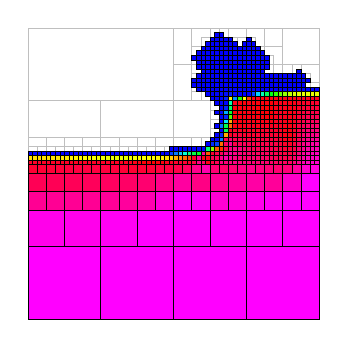
\begin{tikzpicture}[x={(\screenshotunitlength,0)},y={(0,\screenshotunitlength)}]
        \definecolor{fillcolor}{rgb}{1.000000,0.000000,1.000000}
\fill[fillcolor] (0.000000,0.000000) rectangle (0.250000,0.250000);
\definecolor{fillcolor}{rgb}{1.000000,0.000000,1.000000}
\fill[fillcolor] (0.250000,0.000000) rectangle (0.500000,0.250000);
\definecolor{fillcolor}{rgb}{1.000000,0.000000,0.919114}
\fill[fillcolor] (0.000000,0.250000) rectangle (0.125000,0.375000);
\definecolor{fillcolor}{rgb}{1.000000,0.000000,0.922929}
\fill[fillcolor] (0.125000,0.250000) rectangle (0.250000,0.375000);
\definecolor{fillcolor}{rgb}{1.000000,0.000000,0.578346}
\fill[fillcolor] (0.000000,0.375000) rectangle (0.062500,0.437500);
\definecolor{fillcolor}{rgb}{1.000000,0.000000,0.578469}
\fill[fillcolor] (0.062500,0.375000) rectangle (0.125000,0.437500);
\definecolor{fillcolor}{rgb}{1.000000,0.000000,0.332651}
\fill[fillcolor] (0.000000,0.437500) rectangle (0.062500,0.500000);
\definecolor{fillcolor}{rgb}{1.000000,0.000000,0.334281}
\fill[fillcolor] (0.062500,0.437500) rectangle (0.125000,0.500000);
\definecolor{fillcolor}{rgb}{1.000000,0.000000,0.579381}
\fill[fillcolor] (0.125000,0.375000) rectangle (0.187500,0.437500);
\definecolor{fillcolor}{rgb}{1.000000,0.000000,0.582068}
\fill[fillcolor] (0.187500,0.375000) rectangle (0.250000,0.437500);
\definecolor{fillcolor}{rgb}{1.000000,0.000000,0.340229}
\fill[fillcolor] (0.125000,0.437500) rectangle (0.187500,0.500000);
\definecolor{fillcolor}{rgb}{1.000000,0.000000,0.353625}
\fill[fillcolor] (0.187500,0.437500) rectangle (0.250000,0.500000);
\definecolor{fillcolor}{rgb}{1.000000,0.000000,0.962166}
\fill[fillcolor] (0.250000,0.250000) rectangle (0.375000,0.375000);
\definecolor{fillcolor}{rgb}{1.000000,0.000000,1.000000}
\fill[fillcolor] (0.375000,0.250000) rectangle (0.500000,0.375000);
\definecolor{fillcolor}{rgb}{1.000000,0.000000,0.593497}
\fill[fillcolor] (0.250000,0.375000) rectangle (0.312500,0.437500);
\definecolor{fillcolor}{rgb}{1.000000,0.000000,0.615520}
\fill[fillcolor] (0.312500,0.375000) rectangle (0.375000,0.437500);
\definecolor{fillcolor}{rgb}{1.000000,0.000000,0.374518}
\fill[fillcolor] (0.250000,0.437500) rectangle (0.312500,0.500000);
\definecolor{fillcolor}{rgb}{1.000000,0.000000,0.397861}
\fill[fillcolor] (0.312500,0.437500) rectangle (0.375000,0.500000);
\definecolor{fillcolor}{rgb}{1.000000,0.000000,0.693754}
\fill[fillcolor] (0.375000,0.375000) rectangle (0.437500,0.437500);
\definecolor{fillcolor}{rgb}{1.000000,0.000000,0.849616}
\fill[fillcolor] (0.437500,0.375000) rectangle (0.500000,0.437500);
\definecolor{fillcolor}{rgb}{1.000000,0.000000,0.437187}
\fill[fillcolor] (0.375000,0.437500) rectangle (0.437500,0.500000);
\definecolor{fillcolor}{rgb}{1.000000,0.000000,0.537931}
\fill[fillcolor] (0.437500,0.437500) rectangle (0.500000,0.500000);
\definecolor{fillcolor}{rgb}{1.000000,0.000000,1.000000}
\fill[fillcolor] (0.500000,0.000000) rectangle (0.750000,0.250000);
\definecolor{fillcolor}{rgb}{1.000000,0.000000,1.000000}
\fill[fillcolor] (0.750000,0.000000) rectangle (1.000000,0.250000);
\definecolor{fillcolor}{rgb}{1.000000,0.000000,1.000000}
\fill[fillcolor] (0.500000,0.250000) rectangle (0.625000,0.375000);
\definecolor{fillcolor}{rgb}{1.000000,0.000000,1.000000}
\fill[fillcolor] (0.625000,0.250000) rectangle (0.750000,0.375000);
\definecolor{fillcolor}{rgb}{1.000000,0.000000,1.000000}
\fill[fillcolor] (0.500000,0.375000) rectangle (0.562500,0.437500);
\definecolor{fillcolor}{rgb}{1.000000,0.000000,0.975394}
\fill[fillcolor] (0.562500,0.375000) rectangle (0.625000,0.437500);
\definecolor{fillcolor}{rgb}{1.000000,0.000000,0.625752}
\fill[fillcolor] (0.500000,0.437500) rectangle (0.562500,0.500000);
\definecolor{fillcolor}{rgb}{1.000000,0.000000,0.517685}
\fill[fillcolor] (0.562500,0.437500) rectangle (0.625000,0.500000);
\definecolor{fillcolor}{rgb}{1.000000,0.000000,0.825619}
\fill[fillcolor] (0.625000,0.375000) rectangle (0.687500,0.437500);
\definecolor{fillcolor}{rgb}{1.000000,0.000000,0.866104}
\fill[fillcolor] (0.687500,0.375000) rectangle (0.750000,0.437500);
\definecolor{fillcolor}{rgb}{1.000000,0.000000,0.563475}
\fill[fillcolor] (0.625000,0.437500) rectangle (0.687500,0.500000);
\definecolor{fillcolor}{rgb}{1.000000,0.000000,0.620985}
\fill[fillcolor] (0.687500,0.437500) rectangle (0.750000,0.500000);
\definecolor{fillcolor}{rgb}{1.000000,0.000000,1.000000}
\fill[fillcolor] (0.750000,0.250000) rectangle (0.875000,0.375000);
\definecolor{fillcolor}{rgb}{1.000000,0.000000,1.000000}
\fill[fillcolor] (0.875000,0.250000) rectangle (1.000000,0.375000);
\definecolor{fillcolor}{rgb}{1.000000,0.000000,0.924502}
\fill[fillcolor] (0.750000,0.375000) rectangle (0.812500,0.437500);
\definecolor{fillcolor}{rgb}{1.000000,0.000000,0.963909}
\fill[fillcolor] (0.812500,0.375000) rectangle (0.875000,0.437500);
\definecolor{fillcolor}{rgb}{1.000000,0.000000,0.644046}
\fill[fillcolor] (0.750000,0.437500) rectangle (0.812500,0.500000);
\definecolor{fillcolor}{rgb}{1.000000,0.000000,0.599706}
\fill[fillcolor] (0.812500,0.437500) rectangle (0.875000,0.500000);
\definecolor{fillcolor}{rgb}{1.000000,0.000000,1.000000}
\fill[fillcolor] (0.875000,0.375000) rectangle (0.937500,0.437500);
\definecolor{fillcolor}{rgb}{1.000000,0.000000,1.000000}
\fill[fillcolor] (0.937500,0.375000) rectangle (1.000000,0.437500);
\definecolor{fillcolor}{rgb}{1.000000,0.000000,0.793764}
\fill[fillcolor] (0.875000,0.437500) rectangle (0.937500,0.500000);
\definecolor{fillcolor}{rgb}{1.000000,0.000000,1.000000}
\fill[fillcolor] (0.937500,0.437500) rectangle (1.000000,0.500000);
\definecolor{fillcolor}{rgb}{1.000000,0.000000,0.201697}
\fill[fillcolor] (0.000000,0.500000) rectangle (0.031250,0.531250);
\definecolor{fillcolor}{rgb}{1.000000,0.000000,0.205973}
\fill[fillcolor] (0.031250,0.500000) rectangle (0.062500,0.531250);
\definecolor{fillcolor}{rgb}{1.000000,0.000000,0.155738}
\fill[fillcolor] (0.000000,0.531250) rectangle (0.015625,0.546875);
\definecolor{fillcolor}{rgb}{1.000000,0.000000,0.153691}
\fill[fillcolor] (0.015625,0.531250) rectangle (0.031250,0.546875);
\definecolor{fillcolor}{rgb}{1.000000,0.874248,0.000000}
\fill[fillcolor] (0.000000,0.546875) rectangle (0.015625,0.562500);
\definecolor{fillcolor}{rgb}{1.000000,0.872116,0.000000}
\fill[fillcolor] (0.015625,0.546875) rectangle (0.031250,0.562500);
\definecolor{fillcolor}{rgb}{1.000000,0.000000,0.151008}
\fill[fillcolor] (0.031250,0.531250) rectangle (0.046875,0.546875);
\definecolor{fillcolor}{rgb}{1.000000,0.000000,0.148061}
\fill[fillcolor] (0.046875,0.531250) rectangle (0.062500,0.546875);
\definecolor{fillcolor}{rgb}{1.000000,0.870110,0.000000}
\fill[fillcolor] (0.031250,0.546875) rectangle (0.046875,0.562500);
\definecolor{fillcolor}{rgb}{1.000000,0.874362,0.000000}
\fill[fillcolor] (0.046875,0.546875) rectangle (0.062500,0.562500);
\definecolor{fillcolor}{rgb}{1.000000,0.000000,0.215126}
\fill[fillcolor] (0.062500,0.500000) rectangle (0.093750,0.531250);
\definecolor{fillcolor}{rgb}{1.000000,0.000000,0.227433}
\fill[fillcolor] (0.093750,0.500000) rectangle (0.125000,0.531250);
\definecolor{fillcolor}{rgb}{1.000000,0.000000,0.147099}
\fill[fillcolor] (0.062500,0.531250) rectangle (0.078125,0.546875);
\definecolor{fillcolor}{rgb}{1.000000,0.000000,0.145378}
\fill[fillcolor] (0.078125,0.531250) rectangle (0.093750,0.546875);
\definecolor{fillcolor}{rgb}{1.000000,0.881970,0.000000}
\fill[fillcolor] (0.062500,0.546875) rectangle (0.078125,0.562500);
\definecolor{fillcolor}{rgb}{1.000000,0.893110,0.000000}
\fill[fillcolor] (0.078125,0.546875) rectangle (0.093750,0.562500);
\definecolor{fillcolor}{rgb}{1.000000,0.000000,0.144784}
\fill[fillcolor] (0.093750,0.531250) rectangle (0.109375,0.546875);
\definecolor{fillcolor}{rgb}{1.000000,0.000000,0.142074}
\fill[fillcolor] (0.109375,0.531250) rectangle (0.125000,0.546875);
\definecolor{fillcolor}{rgb}{1.000000,0.904191,0.000000}
\fill[fillcolor] (0.093750,0.546875) rectangle (0.109375,0.562500);
\definecolor{fillcolor}{rgb}{1.000000,0.918428,0.000000}
\fill[fillcolor] (0.109375,0.546875) rectangle (0.125000,0.562500);
\definecolor{fillcolor}{rgb}{0.000000,0.000000,1.000000}
\fill[fillcolor] (0.000000,0.562500) rectangle (0.015625,0.578125);
\definecolor{fillcolor}{rgb}{0.000000,0.000000,1.000000}
\fill[fillcolor] (0.015625,0.562500) rectangle (0.031250,0.578125);
\definecolor{fillcolor}{rgb}{0.000000,0.000000,1.000000}
\fill[fillcolor] (0.031250,0.562500) rectangle (0.046875,0.578125);
\definecolor{fillcolor}{rgb}{0.000000,0.000000,1.000000}
\fill[fillcolor] (0.046875,0.562500) rectangle (0.062500,0.578125);
\definecolor{fillcolor}{rgb}{0.000000,0.000000,1.000000}
\fill[fillcolor] (0.062500,0.562500) rectangle (0.078125,0.578125);
\definecolor{fillcolor}{rgb}{0.000000,0.000000,1.000000}
\fill[fillcolor] (0.078125,0.562500) rectangle (0.093750,0.578125);
\definecolor{fillcolor}{rgb}{0.000000,0.000000,1.000000}
\fill[fillcolor] (0.093750,0.562500) rectangle (0.109375,0.578125);
\definecolor{fillcolor}{rgb}{0.000000,0.000000,1.000000}
\fill[fillcolor] (0.109375,0.562500) rectangle (0.125000,0.578125);
\definecolor{fillcolor}{rgb}{1.000000,0.000000,0.240541}
\fill[fillcolor] (0.125000,0.500000) rectangle (0.156250,0.531250);
\definecolor{fillcolor}{rgb}{1.000000,0.000000,0.250095}
\fill[fillcolor] (0.156250,0.500000) rectangle (0.187500,0.531250);
\definecolor{fillcolor}{rgb}{1.000000,0.000000,0.140890}
\fill[fillcolor] (0.125000,0.531250) rectangle (0.140625,0.546875);
\definecolor{fillcolor}{rgb}{1.000000,0.000000,0.138640}
\fill[fillcolor] (0.140625,0.531250) rectangle (0.156250,0.546875);
\definecolor{fillcolor}{rgb}{1.000000,0.930610,0.000000}
\fill[fillcolor] (0.125000,0.546875) rectangle (0.140625,0.562500);
\definecolor{fillcolor}{rgb}{1.000000,0.948011,0.000000}
\fill[fillcolor] (0.140625,0.546875) rectangle (0.156250,0.562500);
\definecolor{fillcolor}{rgb}{1.000000,0.000000,0.138883}
\fill[fillcolor] (0.156250,0.531250) rectangle (0.171875,0.546875);
\definecolor{fillcolor}{rgb}{1.000000,0.000000,0.139761}
\fill[fillcolor] (0.171875,0.531250) rectangle (0.187500,0.546875);
\definecolor{fillcolor}{rgb}{1.000000,0.961555,0.000000}
\fill[fillcolor] (0.156250,0.546875) rectangle (0.171875,0.562500);
\definecolor{fillcolor}{rgb}{1.000000,0.982608,0.000000}
\fill[fillcolor] (0.171875,0.546875) rectangle (0.187500,0.562500);
\definecolor{fillcolor}{rgb}{1.000000,0.000000,0.254957}
\fill[fillcolor] (0.187500,0.500000) rectangle (0.218750,0.531250);
\definecolor{fillcolor}{rgb}{1.000000,0.000000,0.251306}
\fill[fillcolor] (0.218750,0.500000) rectangle (0.250000,0.531250);
\definecolor{fillcolor}{rgb}{1.000000,0.000000,0.142933}
\fill[fillcolor] (0.187500,0.531250) rectangle (0.203125,0.546875);
\definecolor{fillcolor}{rgb}{1.000000,0.000000,0.146770}
\fill[fillcolor] (0.203125,0.531250) rectangle (0.218750,0.546875);
\definecolor{fillcolor}{rgb}{1.000000,0.996905,0.000000}
\fill[fillcolor] (0.187500,0.546875) rectangle (0.203125,0.562500);
\definecolor{fillcolor}{rgb}{0.980006,1.000000,0.000000}
\fill[fillcolor] (0.203125,0.546875) rectangle (0.218750,0.562500);
\definecolor{fillcolor}{rgb}{1.000000,0.000000,0.150389}
\fill[fillcolor] (0.218750,0.531250) rectangle (0.234375,0.546875);
\definecolor{fillcolor}{rgb}{1.000000,0.000000,0.153568}
\fill[fillcolor] (0.234375,0.531250) rectangle (0.250000,0.546875);
\definecolor{fillcolor}{rgb}{0.966908,1.000000,0.000000}
\fill[fillcolor] (0.218750,0.546875) rectangle (0.234375,0.562500);
\definecolor{fillcolor}{rgb}{0.945913,1.000000,0.000000}
\fill[fillcolor] (0.234375,0.546875) rectangle (0.250000,0.562500);
\definecolor{fillcolor}{rgb}{0.000000,0.000000,1.000000}
\fill[fillcolor] (0.125000,0.562500) rectangle (0.140625,0.578125);
\definecolor{fillcolor}{rgb}{0.000000,0.000000,1.000000}
\fill[fillcolor] (0.140625,0.562500) rectangle (0.156250,0.578125);
\definecolor{fillcolor}{rgb}{0.000000,0.000000,1.000000}
\fill[fillcolor] (0.156250,0.562500) rectangle (0.171875,0.578125);
\definecolor{fillcolor}{rgb}{0.000000,0.000000,1.000000}
\fill[fillcolor] (0.171875,0.562500) rectangle (0.187500,0.578125);
\definecolor{fillcolor}{rgb}{0.000000,0.000000,1.000000}
\fill[fillcolor] (0.187500,0.562500) rectangle (0.203125,0.578125);
\definecolor{fillcolor}{rgb}{0.000000,0.000000,1.000000}
\fill[fillcolor] (0.203125,0.562500) rectangle (0.218750,0.578125);
\definecolor{fillcolor}{rgb}{0.000000,0.000000,1.000000}
\fill[fillcolor] (0.218750,0.562500) rectangle (0.234375,0.578125);
\definecolor{fillcolor}{rgb}{0.000000,0.000000,1.000000}
\fill[fillcolor] (0.234375,0.562500) rectangle (0.250000,0.578125);
\definecolor{fillcolor}{rgb}{1.000000,0.000000,0.244258}
\fill[fillcolor] (0.250000,0.500000) rectangle (0.281250,0.531250);
\definecolor{fillcolor}{rgb}{1.000000,0.000000,0.229542}
\fill[fillcolor] (0.281250,0.500000) rectangle (0.312500,0.531250);
\definecolor{fillcolor}{rgb}{1.000000,0.000000,0.153941}
\fill[fillcolor] (0.250000,0.531250) rectangle (0.265625,0.546875);
\definecolor{fillcolor}{rgb}{1.000000,0.000000,0.151923}
\fill[fillcolor] (0.265625,0.531250) rectangle (0.281250,0.546875);
\definecolor{fillcolor}{rgb}{0.938102,1.000000,0.000000}
\fill[fillcolor] (0.250000,0.546875) rectangle (0.265625,0.562500);
\definecolor{fillcolor}{rgb}{0.922991,1.000000,0.000000}
\fill[fillcolor] (0.265625,0.546875) rectangle (0.281250,0.562500);
\definecolor{fillcolor}{rgb}{1.000000,0.000000,0.144607}
\fill[fillcolor] (0.281250,0.531250) rectangle (0.296875,0.546875);
\definecolor{fillcolor}{rgb}{1.000000,0.000000,0.134908}
\fill[fillcolor] (0.296875,0.531250) rectangle (0.312500,0.546875);
\definecolor{fillcolor}{rgb}{0.920555,1.000000,0.000000}
\fill[fillcolor] (0.281250,0.546875) rectangle (0.296875,0.562500);
\definecolor{fillcolor}{rgb}{0.912304,1.000000,0.000000}
\fill[fillcolor] (0.296875,0.546875) rectangle (0.312500,0.562500);
\definecolor{fillcolor}{rgb}{1.000000,0.000000,0.211847}
\fill[fillcolor] (0.312500,0.500000) rectangle (0.343750,0.531250);
\definecolor{fillcolor}{rgb}{1.000000,0.000000,0.196656}
\fill[fillcolor] (0.343750,0.500000) rectangle (0.375000,0.531250);
\definecolor{fillcolor}{rgb}{1.000000,0.000000,0.121908}
\fill[fillcolor] (0.312500,0.531250) rectangle (0.328125,0.546875);
\definecolor{fillcolor}{rgb}{1.000000,0.000000,0.127275}
\fill[fillcolor] (0.328125,0.531250) rectangle (0.343750,0.546875);
\definecolor{fillcolor}{rgb}{0.912089,1.000000,0.000000}
\fill[fillcolor] (0.312500,0.546875) rectangle (0.328125,0.562500);
\definecolor{fillcolor}{rgb}{0.895200,1.000000,0.000000}
\fill[fillcolor] (0.328125,0.546875) rectangle (0.343750,0.562500);
\definecolor{fillcolor}{rgb}{1.000000,0.000000,0.115130}
\fill[fillcolor] (0.343750,0.531250) rectangle (0.359375,0.546875);
\definecolor{fillcolor}{rgb}{1.000000,0.000000,0.084856}
\fill[fillcolor] (0.359375,0.531250) rectangle (0.375000,0.546875);
\definecolor{fillcolor}{rgb}{0.936397,1.000000,0.000000}
\fill[fillcolor] (0.343750,0.546875) rectangle (0.359375,0.562500);
\definecolor{fillcolor}{rgb}{0.956593,1.000000,0.000000}
\fill[fillcolor] (0.359375,0.546875) rectangle (0.375000,0.562500);
\definecolor{fillcolor}{rgb}{0.000000,0.000000,1.000000}
\fill[fillcolor] (0.250000,0.562500) rectangle (0.265625,0.578125);
\definecolor{fillcolor}{rgb}{0.000000,0.000000,1.000000}
\fill[fillcolor] (0.265625,0.562500) rectangle (0.281250,0.578125);
\definecolor{fillcolor}{rgb}{0.000000,0.000000,1.000000}
\fill[fillcolor] (0.281250,0.562500) rectangle (0.296875,0.578125);
\definecolor{fillcolor}{rgb}{0.000000,0.000000,1.000000}
\fill[fillcolor] (0.296875,0.562500) rectangle (0.312500,0.578125);
\definecolor{fillcolor}{rgb}{0.000000,0.000000,1.000000}
\fill[fillcolor] (0.312500,0.562500) rectangle (0.328125,0.578125);
\definecolor{fillcolor}{rgb}{0.000000,0.000000,1.000000}
\fill[fillcolor] (0.328125,0.562500) rectangle (0.343750,0.578125);
\definecolor{fillcolor}{rgb}{0.000000,0.000000,1.000000}
\fill[fillcolor] (0.343750,0.562500) rectangle (0.359375,0.578125);
\definecolor{fillcolor}{rgb}{0.000000,0.000000,1.000000}
\fill[fillcolor] (0.359375,0.562500) rectangle (0.375000,0.578125);
\definecolor{fillcolor}{rgb}{1.000000,0.000000,0.202979}
\fill[fillcolor] (0.375000,0.500000) rectangle (0.406250,0.531250);
\definecolor{fillcolor}{rgb}{1.000000,0.000000,0.215926}
\fill[fillcolor] (0.406250,0.500000) rectangle (0.437500,0.531250);
\definecolor{fillcolor}{rgb}{1.000000,0.000000,0.057525}
\fill[fillcolor] (0.375000,0.531250) rectangle (0.390625,0.546875);
\definecolor{fillcolor}{rgb}{1.000000,0.000000,0.033077}
\fill[fillcolor] (0.390625,0.531250) rectangle (0.406250,0.546875);
\definecolor{fillcolor}{rgb}{0.977615,1.000000,0.000000}
\fill[fillcolor] (0.375000,0.546875) rectangle (0.390625,0.562500);
\definecolor{fillcolor}{rgb}{0.988275,1.000000,0.000000}
\fill[fillcolor] (0.390625,0.546875) rectangle (0.406250,0.562500);
\definecolor{fillcolor}{rgb}{1.000000,0.000000,0.023905}
\fill[fillcolor] (0.406250,0.531250) rectangle (0.421875,0.546875);
\definecolor{fillcolor}{rgb}{1.000000,0.000000,0.018910}
\fill[fillcolor] (0.421875,0.531250) rectangle (0.437500,0.546875);
\definecolor{fillcolor}{rgb}{0.999068,1.000000,0.000000}
\fill[fillcolor] (0.406250,0.546875) rectangle (0.421875,0.562500);
\definecolor{fillcolor}{rgb}{1.000000,0.991749,0.000000}
\fill[fillcolor] (0.421875,0.546875) rectangle (0.437500,0.562500);
\definecolor{fillcolor}{rgb}{1.000000,0.000000,0.246073}
\fill[fillcolor] (0.437500,0.500000) rectangle (0.468750,0.531250);
\definecolor{fillcolor}{rgb}{1.000000,0.000000,0.259021}
\fill[fillcolor] (0.468750,0.500000) rectangle (0.500000,0.531250);
\definecolor{fillcolor}{rgb}{1.000000,0.000000,0.038986}
\fill[fillcolor] (0.437500,0.531250) rectangle (0.453125,0.546875);
\definecolor{fillcolor}{rgb}{1.000000,0.000000,0.059252}
\fill[fillcolor] (0.453125,0.531250) rectangle (0.468750,0.546875);
\definecolor{fillcolor}{rgb}{1.000000,0.960841,0.000000}
\fill[fillcolor] (0.437500,0.546875) rectangle (0.453125,0.562500);
\definecolor{fillcolor}{rgb}{1.000000,0.943932,0.000000}
\fill[fillcolor] (0.453125,0.546875) rectangle (0.468750,0.562500);
\definecolor{fillcolor}{rgb}{1.000000,0.000000,0.097880}
\fill[fillcolor] (0.468750,0.531250) rectangle (0.484375,0.546875);
\definecolor{fillcolor}{rgb}{1.000000,0.000000,0.132719}
\fill[fillcolor] (0.484375,0.531250) rectangle (0.500000,0.546875);
\definecolor{fillcolor}{rgb}{1.000000,0.887629,0.000000}
\fill[fillcolor] (0.468750,0.546875) rectangle (0.484375,0.562500);
\definecolor{fillcolor}{rgb}{1.000000,0.820523,0.000000}
\fill[fillcolor] (0.484375,0.546875) rectangle (0.500000,0.562500);
\definecolor{fillcolor}{rgb}{0.000000,0.000000,1.000000}
\fill[fillcolor] (0.375000,0.562500) rectangle (0.390625,0.578125);
\definecolor{fillcolor}{rgb}{0.000000,0.000000,1.000000}
\fill[fillcolor] (0.390625,0.562500) rectangle (0.406250,0.578125);
\definecolor{fillcolor}{rgb}{0.000000,0.000000,1.000000}
\fill[fillcolor] (0.406250,0.562500) rectangle (0.421875,0.578125);
\definecolor{fillcolor}{rgb}{0.000000,0.000000,1.000000}
\fill[fillcolor] (0.421875,0.562500) rectangle (0.437500,0.578125);
\definecolor{fillcolor}{rgb}{0.000000,0.000000,1.000000}
\fill[fillcolor] (0.437500,0.562500) rectangle (0.453125,0.578125);
\definecolor{fillcolor}{rgb}{0.000000,0.000000,1.000000}
\fill[fillcolor] (0.453125,0.562500) rectangle (0.468750,0.578125);
\definecolor{fillcolor}{rgb}{0.000000,0.000000,1.000000}
\fill[fillcolor] (0.468750,0.562500) rectangle (0.484375,0.578125);
\definecolor{fillcolor}{rgb}{0.000000,0.266310,1.000000}
\fill[fillcolor] (0.484375,0.562500) rectangle (0.500000,0.578125);
\definecolor{fillcolor}{rgb}{0.000000,0.000000,1.000000}
\fill[fillcolor] (0.484375,0.578125) rectangle (0.500000,0.593750);
\definecolor{fillcolor}{rgb}{1.000000,0.000000,0.287007}
\fill[fillcolor] (0.500000,0.500000) rectangle (0.531250,0.531250);
\definecolor{fillcolor}{rgb}{1.000000,0.000000,0.385869}
\fill[fillcolor] (0.531250,0.500000) rectangle (0.562500,0.531250);
\definecolor{fillcolor}{rgb}{1.000000,0.000000,0.174788}
\fill[fillcolor] (0.500000,0.531250) rectangle (0.515625,0.546875);
\definecolor{fillcolor}{rgb}{1.000000,0.000000,0.199177}
\fill[fillcolor] (0.515625,0.531250) rectangle (0.531250,0.546875);
\definecolor{fillcolor}{rgb}{1.000000,0.659208,0.000000}
\fill[fillcolor] (0.500000,0.546875) rectangle (0.515625,0.562500);
\definecolor{fillcolor}{rgb}{1.000000,0.552010,0.000000}
\fill[fillcolor] (0.515625,0.546875) rectangle (0.531250,0.562500);
\definecolor{fillcolor}{rgb}{1.000000,0.000000,0.195549}
\fill[fillcolor] (0.531250,0.531250) rectangle (0.546875,0.546875);
\definecolor{fillcolor}{rgb}{1.000000,0.000000,0.152582}
\fill[fillcolor] (0.546875,0.531250) rectangle (0.562500,0.546875);
\definecolor{fillcolor}{rgb}{1.000000,0.407104,0.000000}
\fill[fillcolor] (0.531250,0.546875) rectangle (0.546875,0.562500);
\definecolor{fillcolor}{rgb}{1.000000,0.275733,0.000000}
\fill[fillcolor] (0.546875,0.546875) rectangle (0.562500,0.562500);
\definecolor{fillcolor}{rgb}{1.000000,0.000000,0.547193}
\fill[fillcolor] (0.562500,0.500000) rectangle (0.593750,0.531250);
\definecolor{fillcolor}{rgb}{1.000000,0.000000,0.679660}
\fill[fillcolor] (0.593750,0.500000) rectangle (0.625000,0.531250);
\definecolor{fillcolor}{rgb}{1.000000,0.000000,0.278459}
\fill[fillcolor] (0.562500,0.531250) rectangle (0.578125,0.546875);
\definecolor{fillcolor}{rgb}{1.000000,0.000000,0.536086}
\fill[fillcolor] (0.578125,0.531250) rectangle (0.593750,0.546875);
\definecolor{fillcolor}{rgb}{1.000000,0.000000,0.149397}
\fill[fillcolor] (0.562500,0.546875) rectangle (0.578125,0.562500);
\definecolor{fillcolor}{rgb}{1.000000,0.000000,0.563280}
\fill[fillcolor] (0.578125,0.546875) rectangle (0.593750,0.562500);
\definecolor{fillcolor}{rgb}{1.000000,0.000000,0.400028}
\fill[fillcolor] (0.593750,0.531250) rectangle (0.609375,0.546875);
\definecolor{fillcolor}{rgb}{1.000000,0.000000,0.080507}
\fill[fillcolor] (0.609375,0.531250) rectangle (0.625000,0.546875);
\definecolor{fillcolor}{rgb}{1.000000,0.000000,0.068973}
\fill[fillcolor] (0.593750,0.546875) rectangle (0.609375,0.562500);
\definecolor{fillcolor}{rgb}{1.000000,0.000000,0.088149}
\fill[fillcolor] (0.609375,0.546875) rectangle (0.625000,0.562500);
\definecolor{fillcolor}{rgb}{0.000000,0.482198,1.000000}
\fill[fillcolor] (0.500000,0.562500) rectangle (0.515625,0.578125);
\definecolor{fillcolor}{rgb}{0.000000,0.774293,1.000000}
\fill[fillcolor] (0.515625,0.562500) rectangle (0.531250,0.578125);
\definecolor{fillcolor}{rgb}{0.000000,0.000000,1.000000}
\fill[fillcolor] (0.500000,0.578125) rectangle (0.515625,0.593750);
\definecolor{fillcolor}{rgb}{0.000000,0.000000,1.000000}
\fill[fillcolor] (0.515625,0.578125) rectangle (0.531250,0.593750);
\definecolor{fillcolor}{rgb}{0.000000,1.000000,0.832234}
\fill[fillcolor] (0.531250,0.562500) rectangle (0.546875,0.578125);
\definecolor{fillcolor}{rgb}{0.000000,1.000000,0.483125}
\fill[fillcolor] (0.546875,0.562500) rectangle (0.562500,0.578125);
\definecolor{fillcolor}{rgb}{0.000000,0.000000,1.000000}
\fill[fillcolor] (0.531250,0.578125) rectangle (0.546875,0.593750);
\definecolor{fillcolor}{rgb}{0.000000,0.000000,1.000000}
\fill[fillcolor] (0.546875,0.578125) rectangle (0.562500,0.593750);
\definecolor{fillcolor}{rgb}{0.000000,1.000000,0.266770}
\fill[fillcolor] (0.562500,0.562500) rectangle (0.578125,0.578125);
\definecolor{fillcolor}{rgb}{0.000000,1.000000,0.129699}
\fill[fillcolor] (0.578125,0.562500) rectangle (0.593750,0.578125);
\definecolor{fillcolor}{rgb}{0.000000,0.000000,1.000000}
\fill[fillcolor] (0.562500,0.578125) rectangle (0.578125,0.593750);
\definecolor{fillcolor}{rgb}{0.000000,0.000000,1.000000}
\fill[fillcolor] (0.578125,0.578125) rectangle (0.593750,0.593750);
\definecolor{fillcolor}{rgb}{1.000000,0.000000,0.599955}
\fill[fillcolor] (0.593750,0.562500) rectangle (0.609375,0.578125);
\definecolor{fillcolor}{rgb}{1.000000,0.324763,0.000000}
\fill[fillcolor] (0.609375,0.562500) rectangle (0.625000,0.578125);
\definecolor{fillcolor}{rgb}{0.000000,0.000000,1.000000}
\fill[fillcolor] (0.593750,0.578125) rectangle (0.609375,0.593750);
\definecolor{fillcolor}{rgb}{0.000000,1.000000,0.470724}
\fill[fillcolor] (0.609375,0.578125) rectangle (0.625000,0.593750);
\definecolor{fillcolor}{rgb}{0.000000,0.000000,1.000000}
\fill[fillcolor] (0.609375,0.593750) rectangle (0.625000,0.609375);
\definecolor{fillcolor}{rgb}{1.000000,0.000000,0.447683}
\fill[fillcolor] (0.625000,0.500000) rectangle (0.656250,0.531250);
\definecolor{fillcolor}{rgb}{1.000000,0.000000,0.421273}
\fill[fillcolor] (0.656250,0.500000) rectangle (0.687500,0.531250);
\definecolor{fillcolor}{rgb}{1.000000,0.000000,0.268630}
\fill[fillcolor] (0.625000,0.531250) rectangle (0.640625,0.546875);
\definecolor{fillcolor}{rgb}{1.000000,0.000000,0.331958}
\fill[fillcolor] (0.640625,0.531250) rectangle (0.656250,0.546875);
\definecolor{fillcolor}{rgb}{1.000000,0.000000,0.333222}
\fill[fillcolor] (0.625000,0.546875) rectangle (0.640625,0.562500);
\definecolor{fillcolor}{rgb}{1.000000,0.000000,0.327756}
\fill[fillcolor] (0.640625,0.546875) rectangle (0.656250,0.562500);
\definecolor{fillcolor}{rgb}{1.000000,0.000000,0.502857}
\fill[fillcolor] (0.656250,0.531250) rectangle (0.671875,0.546875);
\definecolor{fillcolor}{rgb}{1.000000,0.000000,0.467795}
\fill[fillcolor] (0.671875,0.531250) rectangle (0.687500,0.546875);
\definecolor{fillcolor}{rgb}{1.000000,0.000000,0.546992}
\fill[fillcolor] (0.656250,0.546875) rectangle (0.671875,0.562500);
\definecolor{fillcolor}{rgb}{1.000000,0.000000,0.659551}
\fill[fillcolor] (0.671875,0.546875) rectangle (0.687500,0.562500);
\definecolor{fillcolor}{rgb}{1.000000,0.000000,0.461612}
\fill[fillcolor] (0.687500,0.500000) rectangle (0.718750,0.531250);
\definecolor{fillcolor}{rgb}{1.000000,0.000000,0.519021}
\fill[fillcolor] (0.718750,0.500000) rectangle (0.750000,0.531250);
\definecolor{fillcolor}{rgb}{1.000000,0.000000,0.494448}
\fill[fillcolor] (0.687500,0.531250) rectangle (0.703125,0.546875);
\definecolor{fillcolor}{rgb}{1.000000,0.000000,0.523616}
\fill[fillcolor] (0.703125,0.531250) rectangle (0.718750,0.546875);
\definecolor{fillcolor}{rgb}{1.000000,0.000000,0.559534}
\fill[fillcolor] (0.687500,0.546875) rectangle (0.703125,0.562500);
\definecolor{fillcolor}{rgb}{1.000000,0.000000,0.498981}
\fill[fillcolor] (0.703125,0.546875) rectangle (0.718750,0.562500);
\definecolor{fillcolor}{rgb}{1.000000,0.000000,0.485301}
\fill[fillcolor] (0.718750,0.531250) rectangle (0.734375,0.546875);
\definecolor{fillcolor}{rgb}{1.000000,0.000000,0.475512}
\fill[fillcolor] (0.734375,0.531250) rectangle (0.750000,0.546875);
\definecolor{fillcolor}{rgb}{1.000000,0.000000,0.459347}
\fill[fillcolor] (0.718750,0.546875) rectangle (0.734375,0.562500);
\definecolor{fillcolor}{rgb}{1.000000,0.000000,0.423907}
\fill[fillcolor] (0.734375,0.546875) rectangle (0.750000,0.562500);
\definecolor{fillcolor}{rgb}{1.000000,0.000000,0.178662}
\fill[fillcolor] (0.625000,0.562500) rectangle (0.640625,0.578125);
\definecolor{fillcolor}{rgb}{1.000000,0.000000,0.310098}
\fill[fillcolor] (0.640625,0.562500) rectangle (0.656250,0.578125);
\definecolor{fillcolor}{rgb}{0.518612,1.000000,0.000000}
\fill[fillcolor] (0.625000,0.578125) rectangle (0.640625,0.593750);
\definecolor{fillcolor}{rgb}{1.000000,0.351476,0.000000}
\fill[fillcolor] (0.640625,0.578125) rectangle (0.656250,0.593750);
\definecolor{fillcolor}{rgb}{1.000000,0.000000,0.354811}
\fill[fillcolor] (0.656250,0.562500) rectangle (0.671875,0.578125);
\definecolor{fillcolor}{rgb}{1.000000,0.000000,0.532135}
\fill[fillcolor] (0.671875,0.562500) rectangle (0.687500,0.578125);
\definecolor{fillcolor}{rgb}{1.000000,0.186346,0.000000}
\fill[fillcolor] (0.656250,0.578125) rectangle (0.671875,0.593750);
\definecolor{fillcolor}{rgb}{1.000000,0.000000,0.280119}
\fill[fillcolor] (0.671875,0.578125) rectangle (0.687500,0.593750);
\definecolor{fillcolor}{rgb}{0.000000,0.161279,1.000000}
\fill[fillcolor] (0.625000,0.593750) rectangle (0.640625,0.609375);
\definecolor{fillcolor}{rgb}{0.000000,0.264691,1.000000}
\fill[fillcolor] (0.640625,0.593750) rectangle (0.656250,0.609375);
\definecolor{fillcolor}{rgb}{0.000000,0.000000,1.000000}
\fill[fillcolor] (0.625000,0.609375) rectangle (0.640625,0.625000);
\definecolor{fillcolor}{rgb}{0.000000,0.000000,1.000000}
\fill[fillcolor] (0.640625,0.609375) rectangle (0.656250,0.625000);
\definecolor{fillcolor}{rgb}{1.000000,0.423638,0.000000}
\fill[fillcolor] (0.656250,0.593750) rectangle (0.671875,0.609375);
\definecolor{fillcolor}{rgb}{1.000000,0.000000,0.366240}
\fill[fillcolor] (0.671875,0.593750) rectangle (0.687500,0.609375);
\definecolor{fillcolor}{rgb}{0.000000,0.488702,1.000000}
\fill[fillcolor] (0.656250,0.609375) rectangle (0.671875,0.625000);
\definecolor{fillcolor}{rgb}{1.000000,0.000000,0.308289}
\fill[fillcolor] (0.671875,0.609375) rectangle (0.687500,0.625000);
\definecolor{fillcolor}{rgb}{1.000000,0.000000,0.630542}
\fill[fillcolor] (0.687500,0.562500) rectangle (0.703125,0.578125);
\definecolor{fillcolor}{rgb}{1.000000,0.000000,0.517906}
\fill[fillcolor] (0.703125,0.562500) rectangle (0.718750,0.578125);
\definecolor{fillcolor}{rgb}{1.000000,0.000000,0.484550}
\fill[fillcolor] (0.687500,0.578125) rectangle (0.703125,0.593750);
\definecolor{fillcolor}{rgb}{1.000000,0.000000,0.500112}
\fill[fillcolor] (0.703125,0.578125) rectangle (0.718750,0.593750);
\definecolor{fillcolor}{rgb}{1.000000,0.000000,0.485787}
\fill[fillcolor] (0.718750,0.562500) rectangle (0.734375,0.578125);
\definecolor{fillcolor}{rgb}{1.000000,0.000000,0.469751}
\fill[fillcolor] (0.734375,0.562500) rectangle (0.750000,0.578125);
\definecolor{fillcolor}{rgb}{1.000000,0.000000,0.488150}
\fill[fillcolor] (0.718750,0.578125) rectangle (0.734375,0.593750);
\definecolor{fillcolor}{rgb}{1.000000,0.000000,0.440080}
\fill[fillcolor] (0.734375,0.578125) rectangle (0.750000,0.593750);
\definecolor{fillcolor}{rgb}{1.000000,0.000000,0.595061}
\fill[fillcolor] (0.687500,0.593750) rectangle (0.703125,0.609375);
\definecolor{fillcolor}{rgb}{1.000000,0.000000,0.270647}
\fill[fillcolor] (0.703125,0.593750) rectangle (0.718750,0.609375);
\definecolor{fillcolor}{rgb}{1.000000,0.000000,0.428682}
\fill[fillcolor] (0.687500,0.609375) rectangle (0.703125,0.625000);
\definecolor{fillcolor}{rgb}{1.000000,0.000000,0.287670}
\fill[fillcolor] (0.703125,0.609375) rectangle (0.718750,0.625000);
\definecolor{fillcolor}{rgb}{1.000000,0.000000,0.341528}
\fill[fillcolor] (0.718750,0.593750) rectangle (0.734375,0.609375);
\definecolor{fillcolor}{rgb}{1.000000,0.000000,0.368865}
\fill[fillcolor] (0.734375,0.593750) rectangle (0.750000,0.609375);
\definecolor{fillcolor}{rgb}{1.000000,0.000000,0.305591}
\fill[fillcolor] (0.718750,0.609375) rectangle (0.734375,0.625000);
\definecolor{fillcolor}{rgb}{1.000000,0.000000,0.270686}
\fill[fillcolor] (0.734375,0.609375) rectangle (0.750000,0.625000);
\definecolor{fillcolor}{rgb}{0.000000,0.000000,1.000000}
\fill[fillcolor] (0.640625,0.625000) rectangle (0.656250,0.640625);
\definecolor{fillcolor}{rgb}{0.000000,0.181261,1.000000}
\fill[fillcolor] (0.656250,0.625000) rectangle (0.671875,0.640625);
\definecolor{fillcolor}{rgb}{1.000000,0.675177,0.000000}
\fill[fillcolor] (0.671875,0.625000) rectangle (0.687500,0.640625);
\definecolor{fillcolor}{rgb}{0.000000,0.000000,1.000000}
\fill[fillcolor] (0.656250,0.640625) rectangle (0.671875,0.656250);
\definecolor{fillcolor}{rgb}{0.000000,1.000000,0.337263}
\fill[fillcolor] (0.671875,0.640625) rectangle (0.687500,0.656250);
\definecolor{fillcolor}{rgb}{0.000000,0.000000,1.000000}
\fill[fillcolor] (0.640625,0.656250) rectangle (0.656250,0.671875);
\definecolor{fillcolor}{rgb}{0.000000,0.471405,1.000000}
\fill[fillcolor] (0.656250,0.656250) rectangle (0.671875,0.671875);
\definecolor{fillcolor}{rgb}{0.000000,1.000000,0.286219}
\fill[fillcolor] (0.671875,0.656250) rectangle (0.687500,0.671875);
\definecolor{fillcolor}{rgb}{0.000000,0.000000,1.000000}
\fill[fillcolor] (0.656250,0.671875) rectangle (0.671875,0.687500);
\definecolor{fillcolor}{rgb}{0.000000,0.908742,1.000000}
\fill[fillcolor] (0.671875,0.671875) rectangle (0.687500,0.687500);
\definecolor{fillcolor}{rgb}{1.000000,0.000000,0.142625}
\fill[fillcolor] (0.687500,0.625000) rectangle (0.703125,0.640625);
\definecolor{fillcolor}{rgb}{1.000000,0.000000,0.226432}
\fill[fillcolor] (0.703125,0.625000) rectangle (0.718750,0.640625);
\definecolor{fillcolor}{rgb}{1.000000,0.000000,0.116464}
\fill[fillcolor] (0.687500,0.640625) rectangle (0.703125,0.656250);
\definecolor{fillcolor}{rgb}{1.000000,0.000000,0.155719}
\fill[fillcolor] (0.703125,0.640625) rectangle (0.718750,0.656250);
\definecolor{fillcolor}{rgb}{1.000000,0.000000,0.228646}
\fill[fillcolor] (0.718750,0.625000) rectangle (0.734375,0.640625);
\definecolor{fillcolor}{rgb}{1.000000,0.000000,0.183438}
\fill[fillcolor] (0.734375,0.625000) rectangle (0.750000,0.640625);
\definecolor{fillcolor}{rgb}{1.000000,0.000000,0.139370}
\fill[fillcolor] (0.718750,0.640625) rectangle (0.734375,0.656250);
\definecolor{fillcolor}{rgb}{1.000000,0.000000,0.118474}
\fill[fillcolor] (0.734375,0.640625) rectangle (0.750000,0.656250);
\definecolor{fillcolor}{rgb}{1.000000,0.421106,0.000000}
\fill[fillcolor] (0.687500,0.656250) rectangle (0.703125,0.671875);
\definecolor{fillcolor}{rgb}{1.000000,0.000000,0.067538}
\fill[fillcolor] (0.703125,0.656250) rectangle (0.718750,0.671875);
\definecolor{fillcolor}{rgb}{1.000000,0.696364,0.000000}
\fill[fillcolor] (0.687500,0.671875) rectangle (0.703125,0.687500);
\definecolor{fillcolor}{rgb}{1.000000,0.000000,0.030902}
\fill[fillcolor] (0.703125,0.671875) rectangle (0.718750,0.687500);
\definecolor{fillcolor}{rgb}{1.000000,0.000000,0.073358}
\fill[fillcolor] (0.718750,0.656250) rectangle (0.734375,0.671875);
\definecolor{fillcolor}{rgb}{1.000000,0.000000,0.087011}
\fill[fillcolor] (0.734375,0.656250) rectangle (0.750000,0.671875);
\definecolor{fillcolor}{rgb}{1.000000,0.000000,0.056387}
\fill[fillcolor] (0.718750,0.671875) rectangle (0.734375,0.687500);
\definecolor{fillcolor}{rgb}{1.000000,0.000000,0.072714}
\fill[fillcolor] (0.734375,0.671875) rectangle (0.750000,0.687500);
\definecolor{fillcolor}{rgb}{0.000000,0.000000,1.000000}
\fill[fillcolor] (0.640625,0.703125) rectangle (0.656250,0.718750);
\definecolor{fillcolor}{rgb}{0.000000,0.000000,1.000000}
\fill[fillcolor] (0.656250,0.687500) rectangle (0.671875,0.703125);
\definecolor{fillcolor}{rgb}{0.000000,0.150351,1.000000}
\fill[fillcolor] (0.671875,0.687500) rectangle (0.687500,0.703125);
\definecolor{fillcolor}{rgb}{0.000000,0.012129,1.000000}
\fill[fillcolor] (0.656250,0.703125) rectangle (0.671875,0.718750);
\definecolor{fillcolor}{rgb}{0.000000,0.664904,1.000000}
\fill[fillcolor] (0.671875,0.703125) rectangle (0.687500,0.718750);
\definecolor{fillcolor}{rgb}{0.000000,0.000000,1.000000}
\fill[fillcolor] (0.640625,0.734375) rectangle (0.656250,0.750000);
\definecolor{fillcolor}{rgb}{0.000000,0.000000,1.000000}
\fill[fillcolor] (0.656250,0.718750) rectangle (0.671875,0.734375);
\definecolor{fillcolor}{rgb}{0.000000,0.150071,1.000000}
\fill[fillcolor] (0.671875,0.718750) rectangle (0.687500,0.734375);
\definecolor{fillcolor}{rgb}{0.000000,0.002903,1.000000}
\fill[fillcolor] (0.656250,0.734375) rectangle (0.671875,0.750000);
\definecolor{fillcolor}{rgb}{0.000000,0.003316,1.000000}
\fill[fillcolor] (0.671875,0.734375) rectangle (0.687500,0.750000);
\definecolor{fillcolor}{rgb}{0.322592,1.000000,0.000000}
\fill[fillcolor] (0.687500,0.687500) rectangle (0.703125,0.703125);
\definecolor{fillcolor}{rgb}{1.000000,0.000000,0.026038}
\fill[fillcolor] (0.703125,0.687500) rectangle (0.718750,0.703125);
\definecolor{fillcolor}{rgb}{0.000000,1.000000,0.193643}
\fill[fillcolor] (0.687500,0.703125) rectangle (0.703125,0.718750);
\definecolor{fillcolor}{rgb}{1.000000,0.000000,0.026359}
\fill[fillcolor] (0.703125,0.703125) rectangle (0.718750,0.718750);
\definecolor{fillcolor}{rgb}{1.000000,0.000000,0.053378}
\fill[fillcolor] (0.718750,0.687500) rectangle (0.734375,0.703125);
\definecolor{fillcolor}{rgb}{1.000000,0.000000,0.065465}
\fill[fillcolor] (0.734375,0.687500) rectangle (0.750000,0.703125);
\definecolor{fillcolor}{rgb}{1.000000,0.000000,0.051079}
\fill[fillcolor] (0.718750,0.703125) rectangle (0.734375,0.718750);
\definecolor{fillcolor}{rgb}{1.000000,0.000000,0.065917}
\fill[fillcolor] (0.734375,0.703125) rectangle (0.750000,0.718750);
\definecolor{fillcolor}{rgb}{0.000000,1.000000,0.389100}
\fill[fillcolor] (0.687500,0.718750) rectangle (0.703125,0.734375);
\definecolor{fillcolor}{rgb}{1.000000,0.000000,0.036169}
\fill[fillcolor] (0.703125,0.718750) rectangle (0.718750,0.734375);
\definecolor{fillcolor}{rgb}{0.000000,1.000000,0.669101}
\fill[fillcolor] (0.687500,0.734375) rectangle (0.703125,0.750000);
\definecolor{fillcolor}{rgb}{1.000000,0.000000,0.104712}
\fill[fillcolor] (0.703125,0.734375) rectangle (0.718750,0.750000);
\definecolor{fillcolor}{rgb}{1.000000,0.000000,0.046484}
\fill[fillcolor] (0.718750,0.718750) rectangle (0.734375,0.734375);
\definecolor{fillcolor}{rgb}{1.000000,0.000000,0.061826}
\fill[fillcolor] (0.734375,0.718750) rectangle (0.750000,0.734375);
\definecolor{fillcolor}{rgb}{1.000000,0.000000,0.054958}
\fill[fillcolor] (0.718750,0.734375) rectangle (0.734375,0.750000);
\definecolor{fillcolor}{rgb}{1.000000,0.000000,0.045722}
\fill[fillcolor] (0.734375,0.734375) rectangle (0.750000,0.750000);
\definecolor{fillcolor}{rgb}{1.000000,0.000000,0.546923}
\fill[fillcolor] (0.750000,0.500000) rectangle (0.781250,0.531250);
\definecolor{fillcolor}{rgb}{1.000000,0.000000,0.496242}
\fill[fillcolor] (0.781250,0.500000) rectangle (0.812500,0.531250);
\definecolor{fillcolor}{rgb}{1.000000,0.000000,0.471084}
\fill[fillcolor] (0.750000,0.531250) rectangle (0.765625,0.546875);
\definecolor{fillcolor}{rgb}{1.000000,0.000000,0.461835}
\fill[fillcolor] (0.765625,0.531250) rectangle (0.781250,0.546875);
\definecolor{fillcolor}{rgb}{1.000000,0.000000,0.425345}
\fill[fillcolor] (0.750000,0.546875) rectangle (0.765625,0.562500);
\definecolor{fillcolor}{rgb}{1.000000,0.000000,0.422108}
\fill[fillcolor] (0.765625,0.546875) rectangle (0.781250,0.562500);
\definecolor{fillcolor}{rgb}{1.000000,0.000000,0.450853}
\fill[fillcolor] (0.781250,0.531250) rectangle (0.796875,0.546875);
\definecolor{fillcolor}{rgb}{1.000000,0.000000,0.446452}
\fill[fillcolor] (0.796875,0.531250) rectangle (0.812500,0.546875);
\definecolor{fillcolor}{rgb}{1.000000,0.000000,0.420025}
\fill[fillcolor] (0.781250,0.546875) rectangle (0.796875,0.562500);
\definecolor{fillcolor}{rgb}{1.000000,0.000000,0.419807}
\fill[fillcolor] (0.796875,0.546875) rectangle (0.812500,0.562500);
\definecolor{fillcolor}{rgb}{1.000000,0.000000,0.471945}
\fill[fillcolor] (0.812500,0.500000) rectangle (0.843750,0.531250);
\definecolor{fillcolor}{rgb}{1.000000,0.000000,0.441985}
\fill[fillcolor] (0.843750,0.500000) rectangle (0.875000,0.531250);
\definecolor{fillcolor}{rgb}{1.000000,0.000000,0.426069}
\fill[fillcolor] (0.812500,0.531250) rectangle (0.828125,0.546875);
\definecolor{fillcolor}{rgb}{1.000000,0.000000,0.402355}
\fill[fillcolor] (0.828125,0.531250) rectangle (0.843750,0.546875);
\definecolor{fillcolor}{rgb}{1.000000,0.000000,0.395279}
\fill[fillcolor] (0.812500,0.546875) rectangle (0.828125,0.562500);
\definecolor{fillcolor}{rgb}{1.000000,0.000000,0.364561}
\fill[fillcolor] (0.828125,0.546875) rectangle (0.843750,0.562500);
\definecolor{fillcolor}{rgb}{1.000000,0.000000,0.380674}
\fill[fillcolor] (0.843750,0.531250) rectangle (0.859375,0.546875);
\definecolor{fillcolor}{rgb}{1.000000,0.000000,0.365139}
\fill[fillcolor] (0.859375,0.531250) rectangle (0.875000,0.546875);
\definecolor{fillcolor}{rgb}{1.000000,0.000000,0.344304}
\fill[fillcolor] (0.843750,0.546875) rectangle (0.859375,0.562500);
\definecolor{fillcolor}{rgb}{1.000000,0.000000,0.322486}
\fill[fillcolor] (0.859375,0.546875) rectangle (0.875000,0.562500);
\definecolor{fillcolor}{rgb}{1.000000,0.000000,0.426574}
\fill[fillcolor] (0.750000,0.562500) rectangle (0.765625,0.578125);
\definecolor{fillcolor}{rgb}{1.000000,0.000000,0.384412}
\fill[fillcolor] (0.765625,0.562500) rectangle (0.781250,0.578125);
\definecolor{fillcolor}{rgb}{1.000000,0.000000,0.372908}
\fill[fillcolor] (0.750000,0.578125) rectangle (0.765625,0.593750);
\definecolor{fillcolor}{rgb}{1.000000,0.000000,0.329118}
\fill[fillcolor] (0.765625,0.578125) rectangle (0.781250,0.593750);
\definecolor{fillcolor}{rgb}{1.000000,0.000000,0.378197}
\fill[fillcolor] (0.781250,0.562500) rectangle (0.796875,0.578125);
\definecolor{fillcolor}{rgb}{1.000000,0.000000,0.386989}
\fill[fillcolor] (0.796875,0.562500) rectangle (0.812500,0.578125);
\definecolor{fillcolor}{rgb}{1.000000,0.000000,0.334936}
\fill[fillcolor] (0.781250,0.578125) rectangle (0.796875,0.593750);
\definecolor{fillcolor}{rgb}{1.000000,0.000000,0.355163}
\fill[fillcolor] (0.796875,0.578125) rectangle (0.812500,0.593750);
\definecolor{fillcolor}{rgb}{1.000000,0.000000,0.318985}
\fill[fillcolor] (0.750000,0.593750) rectangle (0.765625,0.609375);
\definecolor{fillcolor}{rgb}{1.000000,0.000000,0.291992}
\fill[fillcolor] (0.765625,0.593750) rectangle (0.781250,0.609375);
\definecolor{fillcolor}{rgb}{1.000000,0.000000,0.237661}
\fill[fillcolor] (0.750000,0.609375) rectangle (0.765625,0.625000);
\definecolor{fillcolor}{rgb}{1.000000,0.000000,0.236194}
\fill[fillcolor] (0.765625,0.609375) rectangle (0.781250,0.625000);
\definecolor{fillcolor}{rgb}{1.000000,0.000000,0.294961}
\fill[fillcolor] (0.781250,0.593750) rectangle (0.796875,0.609375);
\definecolor{fillcolor}{rgb}{1.000000,0.000000,0.307175}
\fill[fillcolor] (0.796875,0.593750) rectangle (0.812500,0.609375);
\definecolor{fillcolor}{rgb}{1.000000,0.000000,0.247004}
\fill[fillcolor] (0.781250,0.609375) rectangle (0.796875,0.625000);
\definecolor{fillcolor}{rgb}{1.000000,0.000000,0.258262}
\fill[fillcolor] (0.796875,0.609375) rectangle (0.812500,0.625000);
\definecolor{fillcolor}{rgb}{1.000000,0.000000,0.366862}
\fill[fillcolor] (0.812500,0.562500) rectangle (0.828125,0.578125);
\definecolor{fillcolor}{rgb}{1.000000,0.000000,0.337656}
\fill[fillcolor] (0.828125,0.562500) rectangle (0.843750,0.578125);
\definecolor{fillcolor}{rgb}{1.000000,0.000000,0.337921}
\fill[fillcolor] (0.812500,0.578125) rectangle (0.828125,0.593750);
\definecolor{fillcolor}{rgb}{1.000000,0.000000,0.312929}
\fill[fillcolor] (0.828125,0.578125) rectangle (0.843750,0.593750);
\definecolor{fillcolor}{rgb}{1.000000,0.000000,0.320668}
\fill[fillcolor] (0.843750,0.562500) rectangle (0.859375,0.578125);
\definecolor{fillcolor}{rgb}{1.000000,0.000000,0.291409}
\fill[fillcolor] (0.859375,0.562500) rectangle (0.875000,0.578125);
\definecolor{fillcolor}{rgb}{1.000000,0.000000,0.300204}
\fill[fillcolor] (0.843750,0.578125) rectangle (0.859375,0.593750);
\definecolor{fillcolor}{rgb}{1.000000,0.000000,0.262461}
\fill[fillcolor] (0.859375,0.578125) rectangle (0.875000,0.593750);
\definecolor{fillcolor}{rgb}{1.000000,0.000000,0.294170}
\fill[fillcolor] (0.812500,0.593750) rectangle (0.828125,0.609375);
\definecolor{fillcolor}{rgb}{1.000000,0.000000,0.280209}
\fill[fillcolor] (0.828125,0.593750) rectangle (0.843750,0.609375);
\definecolor{fillcolor}{rgb}{1.000000,0.000000,0.247246}
\fill[fillcolor] (0.812500,0.609375) rectangle (0.828125,0.625000);
\definecolor{fillcolor}{rgb}{1.000000,0.000000,0.239857}
\fill[fillcolor] (0.828125,0.609375) rectangle (0.843750,0.625000);
\definecolor{fillcolor}{rgb}{1.000000,0.000000,0.271978}
\fill[fillcolor] (0.843750,0.593750) rectangle (0.859375,0.609375);
\definecolor{fillcolor}{rgb}{1.000000,0.000000,0.226099}
\fill[fillcolor] (0.859375,0.593750) rectangle (0.875000,0.609375);
\definecolor{fillcolor}{rgb}{1.000000,0.000000,0.234832}
\fill[fillcolor] (0.843750,0.609375) rectangle (0.859375,0.625000);
\definecolor{fillcolor}{rgb}{1.000000,0.000000,0.184818}
\fill[fillcolor] (0.859375,0.609375) rectangle (0.875000,0.625000);
\definecolor{fillcolor}{rgb}{1.000000,0.000000,0.470727}
\fill[fillcolor] (0.875000,0.500000) rectangle (0.906250,0.531250);
\definecolor{fillcolor}{rgb}{1.000000,0.000000,0.622802}
\fill[fillcolor] (0.906250,0.500000) rectangle (0.937500,0.531250);
\definecolor{fillcolor}{rgb}{1.000000,0.000000,0.359228}
\fill[fillcolor] (0.875000,0.531250) rectangle (0.890625,0.546875);
\definecolor{fillcolor}{rgb}{1.000000,0.000000,0.380825}
\fill[fillcolor] (0.890625,0.531250) rectangle (0.906250,0.546875);
\definecolor{fillcolor}{rgb}{1.000000,0.000000,0.300795}
\fill[fillcolor] (0.875000,0.546875) rectangle (0.890625,0.562500);
\definecolor{fillcolor}{rgb}{1.000000,0.000000,0.314893}
\fill[fillcolor] (0.890625,0.546875) rectangle (0.906250,0.562500);
\definecolor{fillcolor}{rgb}{1.000000,0.000000,0.468700}
\fill[fillcolor] (0.906250,0.531250) rectangle (0.921875,0.546875);
\definecolor{fillcolor}{rgb}{1.000000,0.000000,0.569203}
\fill[fillcolor] (0.921875,0.531250) rectangle (0.937500,0.546875);
\definecolor{fillcolor}{rgb}{1.000000,0.000000,0.395519}
\fill[fillcolor] (0.906250,0.546875) rectangle (0.921875,0.562500);
\definecolor{fillcolor}{rgb}{1.000000,0.000000,0.516426}
\fill[fillcolor] (0.921875,0.546875) rectangle (0.937500,0.562500);
\definecolor{fillcolor}{rgb}{1.000000,0.000000,0.802362}
\fill[fillcolor] (0.937500,0.500000) rectangle (0.968750,0.531250);
\definecolor{fillcolor}{rgb}{1.000000,0.000000,0.873241}
\fill[fillcolor] (0.968750,0.500000) rectangle (1.000000,0.531250);
\definecolor{fillcolor}{rgb}{1.000000,0.000000,0.687751}
\fill[fillcolor] (0.937500,0.531250) rectangle (0.953125,0.546875);
\definecolor{fillcolor}{rgb}{1.000000,0.000000,0.755680}
\fill[fillcolor] (0.953125,0.531250) rectangle (0.968750,0.546875);
\definecolor{fillcolor}{rgb}{1.000000,0.000000,0.637344}
\fill[fillcolor] (0.937500,0.546875) rectangle (0.953125,0.562500);
\definecolor{fillcolor}{rgb}{1.000000,0.000000,0.717432}
\fill[fillcolor] (0.953125,0.546875) rectangle (0.968750,0.562500);
\definecolor{fillcolor}{rgb}{1.000000,0.000000,0.801357}
\fill[fillcolor] (0.968750,0.531250) rectangle (0.984375,0.546875);
\definecolor{fillcolor}{rgb}{1.000000,0.000000,0.817273}
\fill[fillcolor] (0.984375,0.531250) rectangle (1.000000,0.546875);
\definecolor{fillcolor}{rgb}{1.000000,0.000000,0.761402}
\fill[fillcolor] (0.968750,0.546875) rectangle (0.984375,0.562500);
\definecolor{fillcolor}{rgb}{1.000000,0.000000,0.778700}
\fill[fillcolor] (0.984375,0.546875) rectangle (1.000000,0.562500);
\definecolor{fillcolor}{rgb}{1.000000,0.000000,0.253743}
\fill[fillcolor] (0.875000,0.562500) rectangle (0.890625,0.578125);
\definecolor{fillcolor}{rgb}{1.000000,0.000000,0.257662}
\fill[fillcolor] (0.890625,0.562500) rectangle (0.906250,0.578125);
\definecolor{fillcolor}{rgb}{1.000000,0.000000,0.209987}
\fill[fillcolor] (0.875000,0.578125) rectangle (0.890625,0.593750);
\definecolor{fillcolor}{rgb}{1.000000,0.000000,0.205774}
\fill[fillcolor] (0.890625,0.578125) rectangle (0.906250,0.593750);
\definecolor{fillcolor}{rgb}{1.000000,0.000000,0.337634}
\fill[fillcolor] (0.906250,0.562500) rectangle (0.921875,0.578125);
\definecolor{fillcolor}{rgb}{1.000000,0.000000,0.470265}
\fill[fillcolor] (0.921875,0.562500) rectangle (0.937500,0.578125);
\definecolor{fillcolor}{rgb}{1.000000,0.000000,0.287425}
\fill[fillcolor] (0.906250,0.578125) rectangle (0.921875,0.593750);
\definecolor{fillcolor}{rgb}{1.000000,0.000000,0.428338}
\fill[fillcolor] (0.921875,0.578125) rectangle (0.937500,0.593750);
\definecolor{fillcolor}{rgb}{1.000000,0.000000,0.162751}
\fill[fillcolor] (0.875000,0.593750) rectangle (0.890625,0.609375);
\definecolor{fillcolor}{rgb}{1.000000,0.000000,0.154174}
\fill[fillcolor] (0.890625,0.593750) rectangle (0.906250,0.609375);
\definecolor{fillcolor}{rgb}{1.000000,0.000000,0.116580}
\fill[fillcolor] (0.875000,0.609375) rectangle (0.890625,0.625000);
\definecolor{fillcolor}{rgb}{1.000000,0.000000,0.107330}
\fill[fillcolor] (0.890625,0.609375) rectangle (0.906250,0.625000);
\definecolor{fillcolor}{rgb}{1.000000,0.000000,0.238389}
\fill[fillcolor] (0.906250,0.593750) rectangle (0.921875,0.609375);
\definecolor{fillcolor}{rgb}{1.000000,0.000000,0.384025}
\fill[fillcolor] (0.921875,0.593750) rectangle (0.937500,0.609375);
\definecolor{fillcolor}{rgb}{1.000000,0.000000,0.193515}
\fill[fillcolor] (0.906250,0.609375) rectangle (0.921875,0.625000);
\definecolor{fillcolor}{rgb}{1.000000,0.000000,0.339065}
\fill[fillcolor] (0.921875,0.609375) rectangle (0.937500,0.625000);
\definecolor{fillcolor}{rgb}{1.000000,0.000000,0.598840}
\fill[fillcolor] (0.937500,0.562500) rectangle (0.953125,0.578125);
\definecolor{fillcolor}{rgb}{1.000000,0.000000,0.683560}
\fill[fillcolor] (0.953125,0.562500) rectangle (0.968750,0.578125);
\definecolor{fillcolor}{rgb}{1.000000,0.000000,0.562406}
\fill[fillcolor] (0.937500,0.578125) rectangle (0.953125,0.593750);
\definecolor{fillcolor}{rgb}{1.000000,0.000000,0.647760}
\fill[fillcolor] (0.953125,0.578125) rectangle (0.968750,0.593750);
\definecolor{fillcolor}{rgb}{1.000000,0.000000,0.726591}
\fill[fillcolor] (0.968750,0.562500) rectangle (0.984375,0.578125);
\definecolor{fillcolor}{rgb}{1.000000,0.000000,0.743066}
\fill[fillcolor] (0.984375,0.562500) rectangle (1.000000,0.578125);
\definecolor{fillcolor}{rgb}{1.000000,0.000000,0.688513}
\fill[fillcolor] (0.968750,0.578125) rectangle (0.984375,0.593750);
\definecolor{fillcolor}{rgb}{1.000000,0.000000,0.703275}
\fill[fillcolor] (0.984375,0.578125) rectangle (1.000000,0.593750);
\definecolor{fillcolor}{rgb}{1.000000,0.000000,0.519048}
\fill[fillcolor] (0.937500,0.593750) rectangle (0.953125,0.609375);
\definecolor{fillcolor}{rgb}{1.000000,0.000000,0.601490}
\fill[fillcolor] (0.953125,0.593750) rectangle (0.968750,0.609375);
\definecolor{fillcolor}{rgb}{1.000000,0.000000,0.469698}
\fill[fillcolor] (0.937500,0.609375) rectangle (0.953125,0.625000);
\definecolor{fillcolor}{rgb}{1.000000,0.000000,0.546245}
\fill[fillcolor] (0.953125,0.609375) rectangle (0.968750,0.625000);
\definecolor{fillcolor}{rgb}{1.000000,0.000000,0.638606}
\fill[fillcolor] (0.968750,0.593750) rectangle (0.984375,0.609375);
\definecolor{fillcolor}{rgb}{1.000000,0.000000,0.651260}
\fill[fillcolor] (0.984375,0.593750) rectangle (1.000000,0.609375);
\definecolor{fillcolor}{rgb}{1.000000,0.000000,0.578972}
\fill[fillcolor] (0.968750,0.609375) rectangle (0.984375,0.625000);
\definecolor{fillcolor}{rgb}{1.000000,0.000000,0.589523}
\fill[fillcolor] (0.984375,0.609375) rectangle (1.000000,0.625000);
\definecolor{fillcolor}{rgb}{1.000000,0.000000,0.180344}
\fill[fillcolor] (0.750000,0.625000) rectangle (0.765625,0.640625);
\definecolor{fillcolor}{rgb}{1.000000,0.000000,0.197833}
\fill[fillcolor] (0.765625,0.625000) rectangle (0.781250,0.640625);
\definecolor{fillcolor}{rgb}{1.000000,0.000000,0.152188}
\fill[fillcolor] (0.750000,0.640625) rectangle (0.765625,0.656250);
\definecolor{fillcolor}{rgb}{1.000000,0.000000,0.161198}
\fill[fillcolor] (0.765625,0.640625) rectangle (0.781250,0.656250);
\definecolor{fillcolor}{rgb}{1.000000,0.000000,0.208503}
\fill[fillcolor] (0.781250,0.625000) rectangle (0.796875,0.640625);
\definecolor{fillcolor}{rgb}{1.000000,0.000000,0.217516}
\fill[fillcolor] (0.796875,0.625000) rectangle (0.812500,0.640625);
\definecolor{fillcolor}{rgb}{1.000000,0.000000,0.152800}
\fill[fillcolor] (0.781250,0.640625) rectangle (0.796875,0.656250);
\definecolor{fillcolor}{rgb}{1.000000,0.000000,0.177385}
\fill[fillcolor] (0.796875,0.640625) rectangle (0.812500,0.656250);
\definecolor{fillcolor}{rgb}{1.000000,0.000000,0.120337}
\fill[fillcolor] (0.750000,0.656250) rectangle (0.765625,0.671875);
\definecolor{fillcolor}{rgb}{1.000000,0.000000,0.118389}
\fill[fillcolor] (0.765625,0.656250) rectangle (0.781250,0.671875);
\definecolor{fillcolor}{rgb}{1.000000,0.000000,0.090584}
\fill[fillcolor] (0.750000,0.671875) rectangle (0.765625,0.687500);
\definecolor{fillcolor}{rgb}{1.000000,0.000000,0.094900}
\fill[fillcolor] (0.765625,0.671875) rectangle (0.781250,0.687500);
\definecolor{fillcolor}{rgb}{1.000000,0.000000,0.104374}
\fill[fillcolor] (0.781250,0.656250) rectangle (0.796875,0.671875);
\definecolor{fillcolor}{rgb}{1.000000,0.000000,0.137150}
\fill[fillcolor] (0.796875,0.656250) rectangle (0.812500,0.671875);
\definecolor{fillcolor}{rgb}{1.000000,0.000000,0.077500}
\fill[fillcolor] (0.781250,0.671875) rectangle (0.796875,0.687500);
\definecolor{fillcolor}{rgb}{1.000000,0.000000,0.089056}
\fill[fillcolor] (0.796875,0.671875) rectangle (0.812500,0.687500);
\definecolor{fillcolor}{rgb}{1.000000,0.000000,0.207914}
\fill[fillcolor] (0.812500,0.625000) rectangle (0.828125,0.640625);
\definecolor{fillcolor}{rgb}{1.000000,0.000000,0.202780}
\fill[fillcolor] (0.828125,0.625000) rectangle (0.843750,0.640625);
\definecolor{fillcolor}{rgb}{1.000000,0.000000,0.180136}
\fill[fillcolor] (0.812500,0.640625) rectangle (0.828125,0.656250);
\definecolor{fillcolor}{rgb}{1.000000,0.000000,0.170141}
\fill[fillcolor] (0.828125,0.640625) rectangle (0.843750,0.656250);
\definecolor{fillcolor}{rgb}{1.000000,0.000000,0.200455}
\fill[fillcolor] (0.843750,0.625000) rectangle (0.859375,0.640625);
\definecolor{fillcolor}{rgb}{1.000000,0.000000,0.152867}
\fill[fillcolor] (0.859375,0.625000) rectangle (0.875000,0.640625);
\definecolor{fillcolor}{rgb}{1.000000,0.000000,0.171283}
\fill[fillcolor] (0.843750,0.640625) rectangle (0.859375,0.656250);
\definecolor{fillcolor}{rgb}{1.000000,0.000000,0.136219}
\fill[fillcolor] (0.859375,0.640625) rectangle (0.875000,0.656250);
\definecolor{fillcolor}{rgb}{1.000000,0.000000,0.137578}
\fill[fillcolor] (0.812500,0.656250) rectangle (0.828125,0.671875);
\definecolor{fillcolor}{rgb}{1.000000,0.000000,0.124380}
\fill[fillcolor] (0.828125,0.656250) rectangle (0.843750,0.671875);
\definecolor{fillcolor}{rgb}{1.000000,0.000000,0.076627}
\fill[fillcolor] (0.812500,0.671875) rectangle (0.828125,0.687500);
\definecolor{fillcolor}{rgb}{1.000000,0.000000,0.076128}
\fill[fillcolor] (0.828125,0.671875) rectangle (0.843750,0.687500);
\definecolor{fillcolor}{rgb}{1.000000,0.000000,0.143262}
\fill[fillcolor] (0.843750,0.656250) rectangle (0.859375,0.671875);
\definecolor{fillcolor}{rgb}{1.000000,0.000000,0.131058}
\fill[fillcolor] (0.859375,0.656250) rectangle (0.875000,0.671875);
\definecolor{fillcolor}{rgb}{1.000000,0.000000,0.126304}
\fill[fillcolor] (0.843750,0.671875) rectangle (0.859375,0.687500);
\definecolor{fillcolor}{rgb}{1.000000,0.000000,0.138364}
\fill[fillcolor] (0.859375,0.671875) rectangle (0.875000,0.687500);
\definecolor{fillcolor}{rgb}{1.000000,0.000000,0.068913}
\fill[fillcolor] (0.750000,0.687500) rectangle (0.765625,0.703125);
\definecolor{fillcolor}{rgb}{1.000000,0.000000,0.075316}
\fill[fillcolor] (0.765625,0.687500) rectangle (0.781250,0.703125);
\definecolor{fillcolor}{rgb}{1.000000,0.000000,0.065431}
\fill[fillcolor] (0.750000,0.703125) rectangle (0.765625,0.718750);
\definecolor{fillcolor}{rgb}{1.000000,0.000000,0.057080}
\fill[fillcolor] (0.765625,0.703125) rectangle (0.781250,0.718750);
\definecolor{fillcolor}{rgb}{1.000000,0.000000,0.057710}
\fill[fillcolor] (0.781250,0.687500) rectangle (0.796875,0.703125);
\definecolor{fillcolor}{rgb}{1.000000,0.000000,0.050236}
\fill[fillcolor] (0.796875,0.687500) rectangle (0.812500,0.703125);
\definecolor{fillcolor}{rgb}{1.000000,0.000000,0.038354}
\fill[fillcolor] (0.781250,0.703125) rectangle (0.796875,0.718750);
\definecolor{fillcolor}{rgb}{1.000000,0.000000,0.034003}
\fill[fillcolor] (0.796875,0.703125) rectangle (0.812500,0.718750);
\definecolor{fillcolor}{rgb}{1.000000,0.000000,0.070813}
\fill[fillcolor] (0.750000,0.718750) rectangle (0.765625,0.734375);
\definecolor{fillcolor}{rgb}{1.000000,0.000000,0.058268}
\fill[fillcolor] (0.765625,0.718750) rectangle (0.781250,0.734375);
\definecolor{fillcolor}{rgb}{1.000000,0.000000,0.078964}
\fill[fillcolor] (0.750000,0.734375) rectangle (0.765625,0.750000);
\definecolor{fillcolor}{rgb}{1.000000,0.000000,0.063669}
\fill[fillcolor] (0.765625,0.734375) rectangle (0.781250,0.750000);
\definecolor{fillcolor}{rgb}{1.000000,0.000000,0.040438}
\fill[fillcolor] (0.781250,0.718750) rectangle (0.796875,0.734375);
\definecolor{fillcolor}{rgb}{1.000000,0.000000,0.040287}
\fill[fillcolor] (0.796875,0.718750) rectangle (0.812500,0.734375);
\definecolor{fillcolor}{rgb}{1.000000,0.000000,0.052831}
\fill[fillcolor] (0.781250,0.734375) rectangle (0.796875,0.750000);
\definecolor{fillcolor}{rgb}{1.000000,0.000000,0.058733}
\fill[fillcolor] (0.796875,0.734375) rectangle (0.812500,0.750000);
\definecolor{fillcolor}{rgb}{1.000000,0.000000,0.031151}
\fill[fillcolor] (0.812500,0.687500) rectangle (0.828125,0.703125);
\definecolor{fillcolor}{rgb}{1.000000,0.000000,0.045384}
\fill[fillcolor] (0.828125,0.687500) rectangle (0.843750,0.703125);
\definecolor{fillcolor}{rgb}{1.000000,0.000000,0.017800}
\fill[fillcolor] (0.812500,0.703125) rectangle (0.828125,0.718750);
\definecolor{fillcolor}{rgb}{1.000000,0.000000,0.033141}
\fill[fillcolor] (0.828125,0.703125) rectangle (0.843750,0.718750);
\definecolor{fillcolor}{rgb}{1.000000,0.000000,0.118792}
\fill[fillcolor] (0.843750,0.687500) rectangle (0.859375,0.703125);
\definecolor{fillcolor}{rgb}{1.000000,0.000000,0.147109}
\fill[fillcolor] (0.859375,0.687500) rectangle (0.875000,0.703125);
\definecolor{fillcolor}{rgb}{1.000000,0.000000,0.107440}
\fill[fillcolor] (0.843750,0.703125) rectangle (0.859375,0.718750);
\definecolor{fillcolor}{rgb}{1.000000,0.000000,0.141099}
\fill[fillcolor] (0.859375,0.703125) rectangle (0.875000,0.718750);
\definecolor{fillcolor}{rgb}{1.000000,0.000000,0.024587}
\fill[fillcolor] (0.812500,0.718750) rectangle (0.828125,0.734375);
\definecolor{fillcolor}{rgb}{1.000000,0.000000,0.032682}
\fill[fillcolor] (0.828125,0.718750) rectangle (0.843750,0.734375);
\definecolor{fillcolor}{rgb}{1.000000,0.000000,0.039094}
\fill[fillcolor] (0.812500,0.734375) rectangle (0.828125,0.750000);
\definecolor{fillcolor}{rgb}{1.000000,0.000000,0.035864}
\fill[fillcolor] (0.828125,0.734375) rectangle (0.843750,0.750000);
\definecolor{fillcolor}{rgb}{1.000000,0.000000,0.094789}
\fill[fillcolor] (0.843750,0.718750) rectangle (0.859375,0.734375);
\definecolor{fillcolor}{rgb}{1.000000,0.000000,0.127749}
\fill[fillcolor] (0.859375,0.718750) rectangle (0.875000,0.734375);
\definecolor{fillcolor}{rgb}{1.000000,0.000000,0.079440}
\fill[fillcolor] (0.843750,0.734375) rectangle (0.859375,0.750000);
\definecolor{fillcolor}{rgb}{1.000000,0.000000,0.107306}
\fill[fillcolor] (0.859375,0.734375) rectangle (0.875000,0.750000);
\definecolor{fillcolor}{rgb}{1.000000,0.000000,0.086689}
\fill[fillcolor] (0.875000,0.625000) rectangle (0.890625,0.640625);
\definecolor{fillcolor}{rgb}{1.000000,0.000000,0.079314}
\fill[fillcolor] (0.890625,0.625000) rectangle (0.906250,0.640625);
\definecolor{fillcolor}{rgb}{1.000000,0.000000,0.078485}
\fill[fillcolor] (0.875000,0.640625) rectangle (0.890625,0.656250);
\definecolor{fillcolor}{rgb}{1.000000,0.000000,0.072197}
\fill[fillcolor] (0.890625,0.640625) rectangle (0.906250,0.656250);
\definecolor{fillcolor}{rgb}{1.000000,0.000000,0.164805}
\fill[fillcolor] (0.906250,0.625000) rectangle (0.921875,0.640625);
\definecolor{fillcolor}{rgb}{1.000000,0.000000,0.304358}
\fill[fillcolor] (0.921875,0.625000) rectangle (0.937500,0.640625);
\definecolor{fillcolor}{rgb}{1.000000,0.000000,0.151570}
\fill[fillcolor] (0.906250,0.640625) rectangle (0.921875,0.656250);
\definecolor{fillcolor}{rgb}{1.000000,0.000000,0.279058}
\fill[fillcolor] (0.921875,0.640625) rectangle (0.937500,0.656250);
\definecolor{fillcolor}{rgb}{1.000000,0.000000,0.082073}
\fill[fillcolor] (0.875000,0.656250) rectangle (0.890625,0.671875);
\definecolor{fillcolor}{rgb}{1.000000,0.000000,0.071549}
\fill[fillcolor] (0.890625,0.656250) rectangle (0.906250,0.671875);
\definecolor{fillcolor}{rgb}{1.000000,0.000000,0.093848}
\fill[fillcolor] (0.875000,0.671875) rectangle (0.890625,0.687500);
\definecolor{fillcolor}{rgb}{1.000000,0.000000,0.075045}
\fill[fillcolor] (0.890625,0.671875) rectangle (0.906250,0.687500);
\definecolor{fillcolor}{rgb}{1.000000,0.000000,0.138545}
\fill[fillcolor] (0.906250,0.656250) rectangle (0.921875,0.671875);
\definecolor{fillcolor}{rgb}{1.000000,0.000000,0.249615}
\fill[fillcolor] (0.921875,0.656250) rectangle (0.937500,0.671875);
\definecolor{fillcolor}{rgb}{1.000000,0.000000,0.127259}
\fill[fillcolor] (0.906250,0.671875) rectangle (0.921875,0.687500);
\definecolor{fillcolor}{rgb}{1.000000,0.000000,0.220985}
\fill[fillcolor] (0.921875,0.671875) rectangle (0.937500,0.687500);
\definecolor{fillcolor}{rgb}{1.000000,0.000000,0.425769}
\fill[fillcolor] (0.937500,0.625000) rectangle (0.953125,0.640625);
\definecolor{fillcolor}{rgb}{1.000000,0.000000,0.494628}
\fill[fillcolor] (0.953125,0.625000) rectangle (0.968750,0.640625);
\definecolor{fillcolor}{rgb}{1.000000,0.000000,0.387908}
\fill[fillcolor] (0.937500,0.640625) rectangle (0.953125,0.656250);
\definecolor{fillcolor}{rgb}{1.000000,0.000000,0.448474}
\fill[fillcolor] (0.953125,0.640625) rectangle (0.968750,0.656250);
\definecolor{fillcolor}{rgb}{1.000000,0.000000,0.522967}
\fill[fillcolor] (0.968750,0.625000) rectangle (0.984375,0.640625);
\definecolor{fillcolor}{rgb}{1.000000,0.000000,0.531718}
\fill[fillcolor] (0.984375,0.625000) rectangle (1.000000,0.640625);
\definecolor{fillcolor}{rgb}{1.000000,0.000000,0.472839}
\fill[fillcolor] (0.968750,0.640625) rectangle (0.984375,0.656250);
\definecolor{fillcolor}{rgb}{1.000000,0.000000,0.480152}
\fill[fillcolor] (0.984375,0.640625) rectangle (1.000000,0.656250);
\definecolor{fillcolor}{rgb}{1.000000,0.000000,0.344257}
\fill[fillcolor] (0.937500,0.656250) rectangle (0.953125,0.671875);
\definecolor{fillcolor}{rgb}{1.000000,0.000000,0.396466}
\fill[fillcolor] (0.953125,0.656250) rectangle (0.968750,0.671875);
\definecolor{fillcolor}{rgb}{1.000000,0.000000,0.301365}
\fill[fillcolor] (0.937500,0.671875) rectangle (0.953125,0.687500);
\definecolor{fillcolor}{rgb}{1.000000,0.000000,0.345361}
\fill[fillcolor] (0.953125,0.671875) rectangle (0.968750,0.687500);
\definecolor{fillcolor}{rgb}{1.000000,0.000000,0.417167}
\fill[fillcolor] (0.968750,0.656250) rectangle (0.984375,0.671875);
\definecolor{fillcolor}{rgb}{1.000000,0.000000,0.423241}
\fill[fillcolor] (0.984375,0.656250) rectangle (1.000000,0.671875);
\definecolor{fillcolor}{rgb}{1.000000,0.000000,0.362478}
\fill[fillcolor] (0.968750,0.671875) rectangle (0.984375,0.687500);
\definecolor{fillcolor}{rgb}{1.000000,0.000000,0.367333}
\fill[fillcolor] (0.984375,0.671875) rectangle (1.000000,0.687500);
\definecolor{fillcolor}{rgb}{1.000000,0.000000,0.105608}
\fill[fillcolor] (0.875000,0.687500) rectangle (0.890625,0.703125);
\definecolor{fillcolor}{rgb}{1.000000,0.000000,0.080566}
\fill[fillcolor] (0.890625,0.687500) rectangle (0.906250,0.703125);
\definecolor{fillcolor}{rgb}{1.000000,0.000000,0.104374}
\fill[fillcolor] (0.875000,0.703125) rectangle (0.890625,0.718750);
\definecolor{fillcolor}{rgb}{1.000000,0.000000,0.077350}
\fill[fillcolor] (0.890625,0.703125) rectangle (0.906250,0.718750);
\definecolor{fillcolor}{rgb}{1.000000,0.000000,0.120475}
\fill[fillcolor] (0.906250,0.687500) rectangle (0.921875,0.703125);
\definecolor{fillcolor}{rgb}{1.000000,0.000000,0.198935}
\fill[fillcolor] (0.921875,0.687500) rectangle (0.937500,0.703125);
\definecolor{fillcolor}{rgb}{1.000000,0.000000,0.107683}
\fill[fillcolor] (0.906250,0.703125) rectangle (0.921875,0.718750);
\definecolor{fillcolor}{rgb}{1.000000,0.000000,0.172854}
\fill[fillcolor] (0.921875,0.703125) rectangle (0.937500,0.718750);
\definecolor{fillcolor}{rgb}{1.000000,0.000000,0.099753}
\fill[fillcolor] (0.875000,0.718750) rectangle (0.890625,0.734375);
\definecolor{fillcolor}{rgb}{1.000000,0.000000,0.075494}
\fill[fillcolor] (0.890625,0.718750) rectangle (0.906250,0.734375);
\definecolor{fillcolor}{rgb}{1.000000,0.000000,0.092244}
\fill[fillcolor] (0.875000,0.734375) rectangle (0.890625,0.750000);
\definecolor{fillcolor}{rgb}{1.000000,0.000000,0.077398}
\fill[fillcolor] (0.890625,0.734375) rectangle (0.906250,0.750000);
\definecolor{fillcolor}{rgb}{1.000000,0.000000,0.097351}
\fill[fillcolor] (0.906250,0.718750) rectangle (0.921875,0.734375);
\definecolor{fillcolor}{rgb}{1.000000,0.000000,0.148180}
\fill[fillcolor] (0.921875,0.718750) rectangle (0.937500,0.734375);
\definecolor{fillcolor}{rgb}{1.000000,0.000000,0.093209}
\fill[fillcolor] (0.906250,0.734375) rectangle (0.921875,0.750000);
\definecolor{fillcolor}{rgb}{1.000000,0.000000,0.127492}
\fill[fillcolor] (0.921875,0.734375) rectangle (0.937500,0.750000);
\definecolor{fillcolor}{rgb}{1.000000,0.000000,0.266630}
\fill[fillcolor] (0.937500,0.687500) rectangle (0.953125,0.703125);
\definecolor{fillcolor}{rgb}{1.000000,0.000000,0.303476}
\fill[fillcolor] (0.953125,0.687500) rectangle (0.968750,0.703125);
\definecolor{fillcolor}{rgb}{1.000000,0.000000,0.230032}
\fill[fillcolor] (0.937500,0.703125) rectangle (0.953125,0.718750);
\definecolor{fillcolor}{rgb}{1.000000,0.000000,0.261959}
\fill[fillcolor] (0.953125,0.703125) rectangle (0.968750,0.718750);
\definecolor{fillcolor}{rgb}{1.000000,0.000000,0.317636}
\fill[fillcolor] (0.968750,0.687500) rectangle (0.984375,0.703125);
\definecolor{fillcolor}{rgb}{1.000000,0.000000,0.321558}
\fill[fillcolor] (0.984375,0.687500) rectangle (1.000000,0.703125);
\definecolor{fillcolor}{rgb}{1.000000,0.000000,0.274949}
\fill[fillcolor] (0.968750,0.703125) rectangle (0.984375,0.718750);
\definecolor{fillcolor}{rgb}{1.000000,0.000000,0.278908}
\fill[fillcolor] (0.984375,0.703125) rectangle (1.000000,0.718750);
\definecolor{fillcolor}{rgb}{1.000000,0.000000,0.193725}
\fill[fillcolor] (0.937500,0.718750) rectangle (0.953125,0.734375);
\definecolor{fillcolor}{rgb}{1.000000,0.000000,0.220044}
\fill[fillcolor] (0.953125,0.718750) rectangle (0.968750,0.734375);
\definecolor{fillcolor}{rgb}{1.000000,0.000000,0.156982}
\fill[fillcolor] (0.937500,0.734375) rectangle (0.953125,0.750000);
\definecolor{fillcolor}{rgb}{1.000000,0.000000,0.172902}
\fill[fillcolor] (0.953125,0.734375) rectangle (0.968750,0.750000);
\definecolor{fillcolor}{rgb}{1.000000,0.000000,0.231490}
\fill[fillcolor] (0.968750,0.718750) rectangle (0.984375,0.734375);
\definecolor{fillcolor}{rgb}{1.000000,0.000000,0.235334}
\fill[fillcolor] (0.984375,0.718750) rectangle (1.000000,0.734375);
\definecolor{fillcolor}{rgb}{1.000000,0.000000,0.178944}
\fill[fillcolor] (0.968750,0.734375) rectangle (0.984375,0.750000);
\definecolor{fillcolor}{rgb}{1.000000,0.000000,0.180600}
\fill[fillcolor] (0.984375,0.734375) rectangle (1.000000,0.750000);
\definecolor{fillcolor}{rgb}{0.000000,0.000000,1.000000}
\fill[fillcolor] (0.609375,0.765625) rectangle (0.625000,0.781250);
\definecolor{fillcolor}{rgb}{0.000000,0.000000,1.000000}
\fill[fillcolor] (0.578125,0.781250) rectangle (0.593750,0.796875);
\definecolor{fillcolor}{rgb}{0.000000,0.000000,1.000000}
\fill[fillcolor] (0.562500,0.796875) rectangle (0.578125,0.812500);
\definecolor{fillcolor}{rgb}{0.000000,0.000000,1.000000}
\fill[fillcolor] (0.578125,0.796875) rectangle (0.593750,0.812500);
\definecolor{fillcolor}{rgb}{0.000000,0.000000,1.000000}
\fill[fillcolor] (0.593750,0.781250) rectangle (0.609375,0.796875);
\definecolor{fillcolor}{rgb}{0.000000,0.000000,1.000000}
\fill[fillcolor] (0.609375,0.781250) rectangle (0.625000,0.796875);
\definecolor{fillcolor}{rgb}{0.000000,0.000000,1.000000}
\fill[fillcolor] (0.593750,0.796875) rectangle (0.609375,0.812500);
\definecolor{fillcolor}{rgb}{0.000000,0.000000,1.000000}
\fill[fillcolor] (0.609375,0.796875) rectangle (0.625000,0.812500);
\definecolor{fillcolor}{rgb}{0.000000,0.000000,1.000000}
\fill[fillcolor] (0.562500,0.812500) rectangle (0.578125,0.828125);
\definecolor{fillcolor}{rgb}{0.000000,0.000000,1.000000}
\fill[fillcolor] (0.578125,0.812500) rectangle (0.593750,0.828125);
\definecolor{fillcolor}{rgb}{0.000000,0.000000,1.000000}
\fill[fillcolor] (0.578125,0.828125) rectangle (0.593750,0.843750);
\definecolor{fillcolor}{rgb}{0.000000,0.000000,1.000000}
\fill[fillcolor] (0.593750,0.812500) rectangle (0.609375,0.828125);
\definecolor{fillcolor}{rgb}{0.000000,0.000000,1.000000}
\fill[fillcolor] (0.609375,0.812500) rectangle (0.625000,0.828125);
\definecolor{fillcolor}{rgb}{0.000000,0.000000,1.000000}
\fill[fillcolor] (0.593750,0.828125) rectangle (0.609375,0.843750);
\definecolor{fillcolor}{rgb}{0.000000,0.000000,1.000000}
\fill[fillcolor] (0.609375,0.828125) rectangle (0.625000,0.843750);
\definecolor{fillcolor}{rgb}{0.000000,0.000000,1.000000}
\fill[fillcolor] (0.578125,0.859375) rectangle (0.593750,0.875000);
\definecolor{fillcolor}{rgb}{0.000000,0.000000,1.000000}
\fill[fillcolor] (0.593750,0.843750) rectangle (0.609375,0.859375);
\definecolor{fillcolor}{rgb}{0.000000,0.000000,1.000000}
\fill[fillcolor] (0.609375,0.843750) rectangle (0.625000,0.859375);
\definecolor{fillcolor}{rgb}{0.000000,0.000000,1.000000}
\fill[fillcolor] (0.593750,0.859375) rectangle (0.609375,0.875000);
\definecolor{fillcolor}{rgb}{0.000000,0.000000,1.000000}
\fill[fillcolor] (0.609375,0.859375) rectangle (0.625000,0.875000);
\definecolor{fillcolor}{rgb}{0.000000,0.000000,1.000000}
\fill[fillcolor] (0.625000,0.750000) rectangle (0.640625,0.765625);
\definecolor{fillcolor}{rgb}{0.000000,0.003547,1.000000}
\fill[fillcolor] (0.640625,0.750000) rectangle (0.656250,0.765625);
\definecolor{fillcolor}{rgb}{0.000000,0.000000,1.000000}
\fill[fillcolor] (0.625000,0.765625) rectangle (0.640625,0.781250);
\definecolor{fillcolor}{rgb}{0.000000,0.013246,1.000000}
\fill[fillcolor] (0.640625,0.765625) rectangle (0.656250,0.781250);
\definecolor{fillcolor}{rgb}{0.000000,0.016399,1.000000}
\fill[fillcolor] (0.656250,0.750000) rectangle (0.671875,0.765625);
\definecolor{fillcolor}{rgb}{0.000000,0.129063,1.000000}
\fill[fillcolor] (0.671875,0.750000) rectangle (0.687500,0.765625);
\definecolor{fillcolor}{rgb}{0.000000,0.042923,1.000000}
\fill[fillcolor] (0.656250,0.765625) rectangle (0.671875,0.781250);
\definecolor{fillcolor}{rgb}{0.000000,0.045004,1.000000}
\fill[fillcolor] (0.671875,0.765625) rectangle (0.687500,0.781250);
\definecolor{fillcolor}{rgb}{0.000000,0.000001,1.000000}
\fill[fillcolor] (0.625000,0.781250) rectangle (0.640625,0.796875);
\definecolor{fillcolor}{rgb}{0.000000,0.000045,1.000000}
\fill[fillcolor] (0.640625,0.781250) rectangle (0.656250,0.796875);
\definecolor{fillcolor}{rgb}{0.000000,0.000000,1.000000}
\fill[fillcolor] (0.625000,0.796875) rectangle (0.640625,0.812500);
\definecolor{fillcolor}{rgb}{0.000000,0.000089,1.000000}
\fill[fillcolor] (0.640625,0.796875) rectangle (0.656250,0.812500);
\definecolor{fillcolor}{rgb}{0.000000,0.000051,1.000000}
\fill[fillcolor] (0.656250,0.781250) rectangle (0.671875,0.796875);
\definecolor{fillcolor}{rgb}{0.000000,0.017404,1.000000}
\fill[fillcolor] (0.671875,0.781250) rectangle (0.687500,0.796875);
\definecolor{fillcolor}{rgb}{0.000000,0.000063,1.000000}
\fill[fillcolor] (0.656250,0.796875) rectangle (0.671875,0.812500);
\definecolor{fillcolor}{rgb}{0.000000,0.000656,1.000000}
\fill[fillcolor] (0.671875,0.796875) rectangle (0.687500,0.812500);
\definecolor{fillcolor}{rgb}{1.000000,0.940244,0.000000}
\fill[fillcolor] (0.687500,0.750000) rectangle (0.703125,0.765625);
\definecolor{fillcolor}{rgb}{0.000000,0.571003,1.000000}
\fill[fillcolor] (0.703125,0.750000) rectangle (0.718750,0.765625);
\definecolor{fillcolor}{rgb}{0.000000,0.099573,1.000000}
\fill[fillcolor] (0.687500,0.765625) rectangle (0.703125,0.781250);
\definecolor{fillcolor}{rgb}{0.000000,0.000099,1.000000}
\fill[fillcolor] (0.703125,0.765625) rectangle (0.718750,0.781250);
\definecolor{fillcolor}{rgb}{0.143721,1.000000,0.000000}
\fill[fillcolor] (0.718750,0.750000) rectangle (0.734375,0.765625);
\definecolor{fillcolor}{rgb}{0.984946,1.000000,0.000000}
\fill[fillcolor] (0.734375,0.750000) rectangle (0.750000,0.765625);
\definecolor{fillcolor}{rgb}{0.000000,0.000626,1.000000}
\fill[fillcolor] (0.718750,0.765625) rectangle (0.734375,0.781250);
\definecolor{fillcolor}{rgb}{0.000000,0.000204,1.000000}
\fill[fillcolor] (0.734375,0.765625) rectangle (0.750000,0.781250);
\definecolor{fillcolor}{rgb}{0.000000,0.026260,1.000000}
\fill[fillcolor] (0.687500,0.781250) rectangle (0.703125,0.796875);
\definecolor{fillcolor}{rgb}{0.000000,0.006364,1.000000}
\fill[fillcolor] (0.703125,0.781250) rectangle (0.718750,0.796875);
\definecolor{fillcolor}{rgb}{0.000000,0.029456,1.000000}
\fill[fillcolor] (0.687500,0.796875) rectangle (0.703125,0.812500);
\definecolor{fillcolor}{rgb}{0.000000,0.008255,1.000000}
\fill[fillcolor] (0.703125,0.796875) rectangle (0.718750,0.812500);
\definecolor{fillcolor}{rgb}{0.000000,0.006399,1.000000}
\fill[fillcolor] (0.718750,0.781250) rectangle (0.734375,0.796875);
\definecolor{fillcolor}{rgb}{0.000000,0.000469,1.000000}
\fill[fillcolor] (0.734375,0.781250) rectangle (0.750000,0.796875);
\definecolor{fillcolor}{rgb}{0.000000,0.000941,1.000000}
\fill[fillcolor] (0.718750,0.796875) rectangle (0.734375,0.812500);
\definecolor{fillcolor}{rgb}{0.000000,0.000307,1.000000}
\fill[fillcolor] (0.734375,0.796875) rectangle (0.750000,0.812500);
\definecolor{fillcolor}{rgb}{0.000000,0.000000,1.000000}
\fill[fillcolor] (0.625000,0.812500) rectangle (0.640625,0.828125);
\definecolor{fillcolor}{rgb}{0.000000,0.000295,1.000000}
\fill[fillcolor] (0.640625,0.812500) rectangle (0.656250,0.828125);
\definecolor{fillcolor}{rgb}{0.000000,0.000000,1.000000}
\fill[fillcolor] (0.625000,0.828125) rectangle (0.640625,0.843750);
\definecolor{fillcolor}{rgb}{0.000000,0.000229,1.000000}
\fill[fillcolor] (0.640625,0.828125) rectangle (0.656250,0.843750);
\definecolor{fillcolor}{rgb}{0.000000,0.000219,1.000000}
\fill[fillcolor] (0.656250,0.812500) rectangle (0.671875,0.828125);
\definecolor{fillcolor}{rgb}{0.000000,0.000243,1.000000}
\fill[fillcolor] (0.671875,0.812500) rectangle (0.687500,0.828125);
\definecolor{fillcolor}{rgb}{0.000000,0.000467,1.000000}
\fill[fillcolor] (0.656250,0.828125) rectangle (0.671875,0.843750);
\definecolor{fillcolor}{rgb}{0.000000,0.000348,1.000000}
\fill[fillcolor] (0.671875,0.828125) rectangle (0.687500,0.843750);
\definecolor{fillcolor}{rgb}{0.000000,0.000000,1.000000}
\fill[fillcolor] (0.625000,0.843750) rectangle (0.640625,0.859375);
\definecolor{fillcolor}{rgb}{0.000000,0.000009,1.000000}
\fill[fillcolor] (0.640625,0.843750) rectangle (0.656250,0.859375);
\definecolor{fillcolor}{rgb}{0.000000,0.000000,1.000000}
\fill[fillcolor] (0.625000,0.859375) rectangle (0.640625,0.875000);
\definecolor{fillcolor}{rgb}{0.000000,0.000005,1.000000}
\fill[fillcolor] (0.640625,0.859375) rectangle (0.656250,0.875000);
\definecolor{fillcolor}{rgb}{0.000000,0.000413,1.000000}
\fill[fillcolor] (0.656250,0.843750) rectangle (0.671875,0.859375);
\definecolor{fillcolor}{rgb}{0.000000,0.000342,1.000000}
\fill[fillcolor] (0.671875,0.843750) rectangle (0.687500,0.859375);
\definecolor{fillcolor}{rgb}{0.000000,0.000263,1.000000}
\fill[fillcolor] (0.656250,0.859375) rectangle (0.671875,0.875000);
\definecolor{fillcolor}{rgb}{0.000000,0.000337,1.000000}
\fill[fillcolor] (0.671875,0.859375) rectangle (0.687500,0.875000);
\definecolor{fillcolor}{rgb}{0.000000,0.000841,1.000000}
\fill[fillcolor] (0.687500,0.812500) rectangle (0.703125,0.828125);
\definecolor{fillcolor}{rgb}{0.000000,0.000190,1.000000}
\fill[fillcolor] (0.703125,0.812500) rectangle (0.718750,0.828125);
\definecolor{fillcolor}{rgb}{0.000000,0.000276,1.000000}
\fill[fillcolor] (0.687500,0.828125) rectangle (0.703125,0.843750);
\definecolor{fillcolor}{rgb}{0.000000,0.000246,1.000000}
\fill[fillcolor] (0.703125,0.828125) rectangle (0.718750,0.843750);
\definecolor{fillcolor}{rgb}{0.000000,0.000237,1.000000}
\fill[fillcolor] (0.718750,0.812500) rectangle (0.734375,0.828125);
\definecolor{fillcolor}{rgb}{0.000000,0.000138,1.000000}
\fill[fillcolor] (0.734375,0.812500) rectangle (0.750000,0.828125);
\definecolor{fillcolor}{rgb}{0.000000,0.000312,1.000000}
\fill[fillcolor] (0.718750,0.828125) rectangle (0.734375,0.843750);
\definecolor{fillcolor}{rgb}{0.000000,0.000235,1.000000}
\fill[fillcolor] (0.734375,0.828125) rectangle (0.750000,0.843750);
\definecolor{fillcolor}{rgb}{0.000000,0.000295,1.000000}
\fill[fillcolor] (0.687500,0.843750) rectangle (0.703125,0.859375);
\definecolor{fillcolor}{rgb}{0.000000,0.000287,1.000000}
\fill[fillcolor] (0.703125,0.843750) rectangle (0.718750,0.859375);
\definecolor{fillcolor}{rgb}{0.000000,0.000293,1.000000}
\fill[fillcolor] (0.687500,0.859375) rectangle (0.703125,0.875000);
\definecolor{fillcolor}{rgb}{0.000000,0.000287,1.000000}
\fill[fillcolor] (0.703125,0.859375) rectangle (0.718750,0.875000);
\definecolor{fillcolor}{rgb}{0.000000,0.000139,1.000000}
\fill[fillcolor] (0.718750,0.843750) rectangle (0.734375,0.859375);
\definecolor{fillcolor}{rgb}{0.000000,0.000444,1.000000}
\fill[fillcolor] (0.734375,0.843750) rectangle (0.750000,0.859375);
\definecolor{fillcolor}{rgb}{0.000000,0.000245,1.000000}
\fill[fillcolor] (0.718750,0.859375) rectangle (0.734375,0.875000);
\definecolor{fillcolor}{rgb}{0.000000,0.000317,1.000000}
\fill[fillcolor] (0.734375,0.859375) rectangle (0.750000,0.875000);
\definecolor{fillcolor}{rgb}{0.000000,0.000000,1.000000}
\fill[fillcolor] (0.578125,0.875000) rectangle (0.593750,0.890625);
\definecolor{fillcolor}{rgb}{0.000000,0.000000,1.000000}
\fill[fillcolor] (0.562500,0.890625) rectangle (0.578125,0.906250);
\definecolor{fillcolor}{rgb}{0.000000,0.000000,1.000000}
\fill[fillcolor] (0.578125,0.890625) rectangle (0.593750,0.906250);
\definecolor{fillcolor}{rgb}{0.000000,0.000000,1.000000}
\fill[fillcolor] (0.593750,0.875000) rectangle (0.609375,0.890625);
\definecolor{fillcolor}{rgb}{0.000000,0.000000,1.000000}
\fill[fillcolor] (0.609375,0.875000) rectangle (0.625000,0.890625);
\definecolor{fillcolor}{rgb}{0.000000,0.000000,1.000000}
\fill[fillcolor] (0.593750,0.890625) rectangle (0.609375,0.906250);
\definecolor{fillcolor}{rgb}{0.000000,0.000000,1.000000}
\fill[fillcolor] (0.609375,0.890625) rectangle (0.625000,0.906250);
\definecolor{fillcolor}{rgb}{0.000000,0.000000,1.000000}
\fill[fillcolor] (0.578125,0.906250) rectangle (0.593750,0.921875);
\definecolor{fillcolor}{rgb}{0.000000,0.000000,1.000000}
\fill[fillcolor] (0.593750,0.906250) rectangle (0.609375,0.921875);
\definecolor{fillcolor}{rgb}{0.000000,0.000000,1.000000}
\fill[fillcolor] (0.609375,0.906250) rectangle (0.625000,0.921875);
\definecolor{fillcolor}{rgb}{0.000000,0.000000,1.000000}
\fill[fillcolor] (0.593750,0.921875) rectangle (0.609375,0.937500);
\definecolor{fillcolor}{rgb}{0.000000,0.000000,1.000000}
\fill[fillcolor] (0.609375,0.921875) rectangle (0.625000,0.937500);
\definecolor{fillcolor}{rgb}{0.000000,0.000000,1.000000}
\fill[fillcolor] (0.609375,0.937500) rectangle (0.625000,0.953125);
\definecolor{fillcolor}{rgb}{0.000000,0.000000,1.000000}
\fill[fillcolor] (0.625000,0.875000) rectangle (0.640625,0.890625);
\definecolor{fillcolor}{rgb}{0.000000,0.000162,1.000000}
\fill[fillcolor] (0.640625,0.875000) rectangle (0.656250,0.890625);
\definecolor{fillcolor}{rgb}{0.000000,0.000000,1.000000}
\fill[fillcolor] (0.625000,0.890625) rectangle (0.640625,0.906250);
\definecolor{fillcolor}{rgb}{0.000000,0.000000,1.000000}
\fill[fillcolor] (0.640625,0.890625) rectangle (0.656250,0.906250);
\definecolor{fillcolor}{rgb}{0.000000,0.000330,1.000000}
\fill[fillcolor] (0.656250,0.875000) rectangle (0.671875,0.890625);
\definecolor{fillcolor}{rgb}{0.000000,0.000248,1.000000}
\fill[fillcolor] (0.671875,0.875000) rectangle (0.687500,0.890625);
\definecolor{fillcolor}{rgb}{0.000000,0.000057,1.000000}
\fill[fillcolor] (0.656250,0.890625) rectangle (0.671875,0.906250);
\definecolor{fillcolor}{rgb}{0.000000,0.000066,1.000000}
\fill[fillcolor] (0.671875,0.890625) rectangle (0.687500,0.906250);
\definecolor{fillcolor}{rgb}{0.000000,0.000000,1.000000}
\fill[fillcolor] (0.625000,0.906250) rectangle (0.640625,0.921875);
\definecolor{fillcolor}{rgb}{0.000000,0.000000,1.000000}
\fill[fillcolor] (0.640625,0.906250) rectangle (0.656250,0.921875);
\definecolor{fillcolor}{rgb}{0.000000,0.000000,1.000000}
\fill[fillcolor] (0.625000,0.921875) rectangle (0.640625,0.937500);
\definecolor{fillcolor}{rgb}{0.000000,0.000000,1.000000}
\fill[fillcolor] (0.640625,0.921875) rectangle (0.656250,0.937500);
\definecolor{fillcolor}{rgb}{0.000000,0.000000,1.000000}
\fill[fillcolor] (0.656250,0.906250) rectangle (0.671875,0.921875);
\definecolor{fillcolor}{rgb}{0.000000,0.000004,1.000000}
\fill[fillcolor] (0.671875,0.906250) rectangle (0.687500,0.921875);
\definecolor{fillcolor}{rgb}{0.000000,0.000000,1.000000}
\fill[fillcolor] (0.656250,0.921875) rectangle (0.671875,0.937500);
\definecolor{fillcolor}{rgb}{0.000000,0.000000,1.000000}
\fill[fillcolor] (0.671875,0.921875) rectangle (0.687500,0.937500);
\definecolor{fillcolor}{rgb}{0.000000,0.000170,1.000000}
\fill[fillcolor] (0.687500,0.875000) rectangle (0.703125,0.890625);
\definecolor{fillcolor}{rgb}{0.000000,0.000149,1.000000}
\fill[fillcolor] (0.703125,0.875000) rectangle (0.718750,0.890625);
\definecolor{fillcolor}{rgb}{0.000000,0.000008,1.000000}
\fill[fillcolor] (0.687500,0.890625) rectangle (0.703125,0.906250);
\definecolor{fillcolor}{rgb}{0.000000,0.000014,1.000000}
\fill[fillcolor] (0.703125,0.890625) rectangle (0.718750,0.906250);
\definecolor{fillcolor}{rgb}{0.000000,0.000095,1.000000}
\fill[fillcolor] (0.718750,0.875000) rectangle (0.734375,0.890625);
\definecolor{fillcolor}{rgb}{0.000000,0.000048,1.000000}
\fill[fillcolor] (0.734375,0.875000) rectangle (0.750000,0.890625);
\definecolor{fillcolor}{rgb}{0.000000,0.000008,1.000000}
\fill[fillcolor] (0.718750,0.890625) rectangle (0.734375,0.906250);
\definecolor{fillcolor}{rgb}{0.000000,0.000000,1.000000}
\fill[fillcolor] (0.734375,0.890625) rectangle (0.750000,0.906250);
\definecolor{fillcolor}{rgb}{0.000000,0.000000,1.000000}
\fill[fillcolor] (0.687500,0.906250) rectangle (0.703125,0.921875);
\definecolor{fillcolor}{rgb}{0.000000,0.000000,1.000000}
\fill[fillcolor] (0.703125,0.906250) rectangle (0.718750,0.921875);
\definecolor{fillcolor}{rgb}{0.000000,0.000000,1.000000}
\fill[fillcolor] (0.687500,0.921875) rectangle (0.703125,0.937500);
\definecolor{fillcolor}{rgb}{0.000000,0.000000,1.000000}
\fill[fillcolor] (0.703125,0.921875) rectangle (0.718750,0.937500);
\definecolor{fillcolor}{rgb}{0.000000,0.000000,1.000000}
\fill[fillcolor] (0.718750,0.906250) rectangle (0.734375,0.921875);
\definecolor{fillcolor}{rgb}{0.000000,0.000000,1.000000}
\fill[fillcolor] (0.734375,0.906250) rectangle (0.750000,0.921875);
\definecolor{fillcolor}{rgb}{0.000000,0.000000,1.000000}
\fill[fillcolor] (0.718750,0.921875) rectangle (0.734375,0.937500);
\definecolor{fillcolor}{rgb}{0.000000,0.000000,1.000000}
\fill[fillcolor] (0.734375,0.921875) rectangle (0.750000,0.937500);
\definecolor{fillcolor}{rgb}{0.000000,0.000000,1.000000}
\fill[fillcolor] (0.625000,0.937500) rectangle (0.640625,0.953125);
\definecolor{fillcolor}{rgb}{0.000000,0.000000,1.000000}
\fill[fillcolor] (0.640625,0.937500) rectangle (0.656250,0.953125);
\definecolor{fillcolor}{rgb}{0.000000,0.000000,1.000000}
\fill[fillcolor] (0.625000,0.953125) rectangle (0.640625,0.968750);
\definecolor{fillcolor}{rgb}{0.000000,0.000000,1.000000}
\fill[fillcolor] (0.640625,0.953125) rectangle (0.656250,0.968750);
\definecolor{fillcolor}{rgb}{0.000000,0.000000,1.000000}
\fill[fillcolor] (0.656250,0.937500) rectangle (0.671875,0.953125);
\definecolor{fillcolor}{rgb}{0.000000,0.000000,1.000000}
\fill[fillcolor] (0.671875,0.937500) rectangle (0.687500,0.953125);
\definecolor{fillcolor}{rgb}{0.000000,0.000000,1.000000}
\fill[fillcolor] (0.656250,0.953125) rectangle (0.671875,0.968750);
\definecolor{fillcolor}{rgb}{0.000000,0.000000,1.000000}
\fill[fillcolor] (0.671875,0.953125) rectangle (0.687500,0.968750);
\definecolor{fillcolor}{rgb}{0.000000,0.000000,1.000000}
\fill[fillcolor] (0.640625,0.968750) rectangle (0.656250,0.984375);
\definecolor{fillcolor}{rgb}{0.000000,0.000000,1.000000}
\fill[fillcolor] (0.656250,0.968750) rectangle (0.671875,0.984375);
\definecolor{fillcolor}{rgb}{0.000000,0.000000,1.000000}
\fill[fillcolor] (0.687500,0.937500) rectangle (0.703125,0.953125);
\definecolor{fillcolor}{rgb}{0.000000,0.000000,1.000000}
\fill[fillcolor] (0.703125,0.937500) rectangle (0.718750,0.953125);
\definecolor{fillcolor}{rgb}{0.000000,0.000000,1.000000}
\fill[fillcolor] (0.687500,0.953125) rectangle (0.703125,0.968750);
\definecolor{fillcolor}{rgb}{0.000000,0.000000,1.000000}
\fill[fillcolor] (0.734375,0.937500) rectangle (0.750000,0.953125);
\definecolor{fillcolor}{rgb}{1.000000,0.275424,0.000000}
\fill[fillcolor] (0.750000,0.750000) rectangle (0.765625,0.765625);
\definecolor{fillcolor}{rgb}{1.000000,0.000000,0.085203}
\fill[fillcolor] (0.765625,0.750000) rectangle (0.781250,0.765625);
\definecolor{fillcolor}{rgb}{0.000000,0.000189,1.000000}
\fill[fillcolor] (0.750000,0.765625) rectangle (0.765625,0.781250);
\definecolor{fillcolor}{rgb}{0.000000,0.263719,1.000000}
\fill[fillcolor] (0.765625,0.765625) rectangle (0.781250,0.781250);
\definecolor{fillcolor}{rgb}{1.000000,0.000000,0.070516}
\fill[fillcolor] (0.781250,0.750000) rectangle (0.796875,0.765625);
\definecolor{fillcolor}{rgb}{1.000000,0.000000,0.071776}
\fill[fillcolor] (0.796875,0.750000) rectangle (0.812500,0.765625);
\definecolor{fillcolor}{rgb}{0.000000,0.824833,1.000000}
\fill[fillcolor] (0.781250,0.765625) rectangle (0.796875,0.781250);
\definecolor{fillcolor}{rgb}{0.000000,1.000000,0.721975}
\fill[fillcolor] (0.796875,0.765625) rectangle (0.812500,0.781250);
\definecolor{fillcolor}{rgb}{0.000000,0.000162,1.000000}
\fill[fillcolor] (0.750000,0.781250) rectangle (0.765625,0.796875);
\definecolor{fillcolor}{rgb}{0.000000,0.000190,1.000000}
\fill[fillcolor] (0.765625,0.781250) rectangle (0.781250,0.796875);
\definecolor{fillcolor}{rgb}{0.000000,0.000339,1.000000}
\fill[fillcolor] (0.750000,0.796875) rectangle (0.765625,0.812500);
\definecolor{fillcolor}{rgb}{0.000000,0.000256,1.000000}
\fill[fillcolor] (0.765625,0.796875) rectangle (0.781250,0.812500);
\definecolor{fillcolor}{rgb}{0.000000,0.000181,1.000000}
\fill[fillcolor] (0.781250,0.781250) rectangle (0.796875,0.796875);
\definecolor{fillcolor}{rgb}{0.000000,0.000188,1.000000}
\fill[fillcolor] (0.796875,0.781250) rectangle (0.812500,0.796875);
\definecolor{fillcolor}{rgb}{0.000000,0.000091,1.000000}
\fill[fillcolor] (0.781250,0.796875) rectangle (0.796875,0.812500);
\definecolor{fillcolor}{rgb}{0.000000,0.000191,1.000000}
\fill[fillcolor] (0.796875,0.796875) rectangle (0.812500,0.812500);
\definecolor{fillcolor}{rgb}{1.000000,0.000000,0.056266}
\fill[fillcolor] (0.812500,0.750000) rectangle (0.828125,0.765625);
\definecolor{fillcolor}{rgb}{1.000000,0.000000,0.047719}
\fill[fillcolor] (0.828125,0.750000) rectangle (0.843750,0.765625);
\definecolor{fillcolor}{rgb}{0.000000,1.000000,0.357057}
\fill[fillcolor] (0.812500,0.765625) rectangle (0.828125,0.781250);
\definecolor{fillcolor}{rgb}{0.000000,1.000000,0.079881}
\fill[fillcolor] (0.828125,0.765625) rectangle (0.843750,0.781250);
\definecolor{fillcolor}{rgb}{1.000000,0.000000,0.066049}
\fill[fillcolor] (0.843750,0.750000) rectangle (0.859375,0.765625);
\definecolor{fillcolor}{rgb}{1.000000,0.000000,0.080348}
\fill[fillcolor] (0.859375,0.750000) rectangle (0.875000,0.765625);
\definecolor{fillcolor}{rgb}{0.183636,1.000000,0.000000}
\fill[fillcolor] (0.843750,0.765625) rectangle (0.859375,0.781250);
\definecolor{fillcolor}{rgb}{0.393929,1.000000,0.000000}
\fill[fillcolor] (0.859375,0.765625) rectangle (0.875000,0.781250);
\definecolor{fillcolor}{rgb}{0.000000,0.000173,1.000000}
\fill[fillcolor] (0.812500,0.781250) rectangle (0.828125,0.796875);
\definecolor{fillcolor}{rgb}{0.000000,0.000125,1.000000}
\fill[fillcolor] (0.828125,0.781250) rectangle (0.843750,0.796875);
\definecolor{fillcolor}{rgb}{0.000000,0.000120,1.000000}
\fill[fillcolor] (0.812500,0.796875) rectangle (0.828125,0.812500);
\definecolor{fillcolor}{rgb}{0.000000,0.000010,1.000000}
\fill[fillcolor] (0.828125,0.796875) rectangle (0.843750,0.812500);
\definecolor{fillcolor}{rgb}{0.000000,0.000119,1.000000}
\fill[fillcolor] (0.843750,0.781250) rectangle (0.859375,0.796875);
\definecolor{fillcolor}{rgb}{0.000000,0.000109,1.000000}
\fill[fillcolor] (0.859375,0.781250) rectangle (0.875000,0.796875);
\definecolor{fillcolor}{rgb}{0.000000,0.000045,1.000000}
\fill[fillcolor] (0.843750,0.796875) rectangle (0.859375,0.812500);
\definecolor{fillcolor}{rgb}{0.000000,0.000062,1.000000}
\fill[fillcolor] (0.859375,0.796875) rectangle (0.875000,0.812500);
\definecolor{fillcolor}{rgb}{0.000000,0.000108,1.000000}
\fill[fillcolor] (0.750000,0.812500) rectangle (0.765625,0.828125);
\definecolor{fillcolor}{rgb}{0.000000,0.000135,1.000000}
\fill[fillcolor] (0.765625,0.812500) rectangle (0.781250,0.828125);
\definecolor{fillcolor}{rgb}{0.000000,0.000122,1.000000}
\fill[fillcolor] (0.750000,0.828125) rectangle (0.765625,0.843750);
\definecolor{fillcolor}{rgb}{0.000000,0.000108,1.000000}
\fill[fillcolor] (0.765625,0.828125) rectangle (0.781250,0.843750);
\definecolor{fillcolor}{rgb}{0.000000,0.000000,1.000000}
\fill[fillcolor] (0.781250,0.812500) rectangle (0.796875,0.828125);
\definecolor{fillcolor}{rgb}{0.000000,0.000000,1.000000}
\fill[fillcolor] (0.796875,0.812500) rectangle (0.812500,0.828125);
\definecolor{fillcolor}{rgb}{0.000000,0.000009,1.000000}
\fill[fillcolor] (0.781250,0.828125) rectangle (0.796875,0.843750);
\definecolor{fillcolor}{rgb}{0.000000,0.000000,1.000000}
\fill[fillcolor] (0.796875,0.828125) rectangle (0.812500,0.843750);
\definecolor{fillcolor}{rgb}{0.000000,0.000183,1.000000}
\fill[fillcolor] (0.750000,0.843750) rectangle (0.765625,0.859375);
\definecolor{fillcolor}{rgb}{0.000000,0.000000,1.000000}
\fill[fillcolor] (0.765625,0.843750) rectangle (0.781250,0.859375);
\definecolor{fillcolor}{rgb}{0.000000,0.000058,1.000000}
\fill[fillcolor] (0.750000,0.859375) rectangle (0.765625,0.875000);
\definecolor{fillcolor}{rgb}{0.000000,0.000000,1.000000}
\fill[fillcolor] (0.765625,0.859375) rectangle (0.781250,0.875000);
\definecolor{fillcolor}{rgb}{0.000000,0.000000,1.000000}
\fill[fillcolor] (0.781250,0.843750) rectangle (0.796875,0.859375);
\definecolor{fillcolor}{rgb}{0.000000,0.000000,1.000000}
\fill[fillcolor] (0.796875,0.843750) rectangle (0.812500,0.859375);
\definecolor{fillcolor}{rgb}{0.000000,0.000000,1.000000}
\fill[fillcolor] (0.781250,0.859375) rectangle (0.796875,0.875000);
\definecolor{fillcolor}{rgb}{0.000000,0.000000,1.000000}
\fill[fillcolor] (0.796875,0.859375) rectangle (0.812500,0.875000);
\definecolor{fillcolor}{rgb}{0.000000,0.000000,1.000000}
\fill[fillcolor] (0.812500,0.812500) rectangle (0.828125,0.828125);
\definecolor{fillcolor}{rgb}{0.000000,0.000000,1.000000}
\fill[fillcolor] (0.828125,0.812500) rectangle (0.843750,0.828125);
\definecolor{fillcolor}{rgb}{0.000000,0.000000,1.000000}
\fill[fillcolor] (0.812500,0.828125) rectangle (0.828125,0.843750);
\definecolor{fillcolor}{rgb}{0.000000,0.000000,1.000000}
\fill[fillcolor] (0.828125,0.828125) rectangle (0.843750,0.843750);
\definecolor{fillcolor}{rgb}{0.000000,0.000000,1.000000}
\fill[fillcolor] (0.843750,0.812500) rectangle (0.859375,0.828125);
\definecolor{fillcolor}{rgb}{0.000000,0.000002,1.000000}
\fill[fillcolor] (0.859375,0.812500) rectangle (0.875000,0.828125);
\definecolor{fillcolor}{rgb}{0.000000,0.000000,1.000000}
\fill[fillcolor] (0.843750,0.828125) rectangle (0.859375,0.843750);
\definecolor{fillcolor}{rgb}{0.000000,0.000000,1.000000}
\fill[fillcolor] (0.859375,0.828125) rectangle (0.875000,0.843750);
\definecolor{fillcolor}{rgb}{0.000000,0.000000,1.000000}
\fill[fillcolor] (0.812500,0.859375) rectangle (0.828125,0.875000);
\definecolor{fillcolor}{rgb}{1.000000,0.000000,0.076809}
\fill[fillcolor] (0.875000,0.750000) rectangle (0.890625,0.765625);
\definecolor{fillcolor}{rgb}{1.000000,0.000000,0.074217}
\fill[fillcolor] (0.890625,0.750000) rectangle (0.906250,0.765625);
\definecolor{fillcolor}{rgb}{0.585373,1.000000,0.000000}
\fill[fillcolor] (0.875000,0.765625) rectangle (0.890625,0.781250);
\definecolor{fillcolor}{rgb}{0.734254,1.000000,0.000000}
\fill[fillcolor] (0.890625,0.765625) rectangle (0.906250,0.781250);
\definecolor{fillcolor}{rgb}{1.000000,0.000000,0.085005}
\fill[fillcolor] (0.906250,0.750000) rectangle (0.921875,0.765625);
\definecolor{fillcolor}{rgb}{1.000000,0.000000,0.102352}
\fill[fillcolor] (0.921875,0.750000) rectangle (0.937500,0.765625);
\definecolor{fillcolor}{rgb}{0.836141,1.000000,0.000000}
\fill[fillcolor] (0.906250,0.765625) rectangle (0.921875,0.781250);
\definecolor{fillcolor}{rgb}{0.891162,1.000000,0.000000}
\fill[fillcolor] (0.921875,0.765625) rectangle (0.937500,0.781250);
\definecolor{fillcolor}{rgb}{0.000000,0.000021,1.000000}
\fill[fillcolor] (0.875000,0.781250) rectangle (0.890625,0.796875);
\definecolor{fillcolor}{rgb}{0.000000,0.000000,1.000000}
\fill[fillcolor] (0.890625,0.781250) rectangle (0.906250,0.796875);
\definecolor{fillcolor}{rgb}{0.000000,0.000012,1.000000}
\fill[fillcolor] (0.875000,0.796875) rectangle (0.890625,0.812500);
\definecolor{fillcolor}{rgb}{0.000000,0.000001,1.000000}
\fill[fillcolor] (0.890625,0.796875) rectangle (0.906250,0.812500);
\definecolor{fillcolor}{rgb}{0.000000,0.000000,1.000000}
\fill[fillcolor] (0.906250,0.781250) rectangle (0.921875,0.796875);
\definecolor{fillcolor}{rgb}{0.000000,0.000000,1.000000}
\fill[fillcolor] (0.921875,0.781250) rectangle (0.937500,0.796875);
\definecolor{fillcolor}{rgb}{0.000000,0.000000,1.000000}
\fill[fillcolor] (0.906250,0.796875) rectangle (0.921875,0.812500);
\definecolor{fillcolor}{rgb}{0.000000,0.000000,1.000000}
\fill[fillcolor] (0.921875,0.796875) rectangle (0.937500,0.812500);
\definecolor{fillcolor}{rgb}{1.000000,0.000000,0.115898}
\fill[fillcolor] (0.937500,0.750000) rectangle (0.953125,0.765625);
\definecolor{fillcolor}{rgb}{1.000000,0.000000,0.123114}
\fill[fillcolor] (0.953125,0.750000) rectangle (0.968750,0.765625);
\definecolor{fillcolor}{rgb}{0.915960,1.000000,0.000000}
\fill[fillcolor] (0.937500,0.765625) rectangle (0.953125,0.781250);
\definecolor{fillcolor}{rgb}{0.920923,1.000000,0.000000}
\fill[fillcolor] (0.953125,0.765625) rectangle (0.968750,0.781250);
\definecolor{fillcolor}{rgb}{1.000000,0.000000,0.125841}
\fill[fillcolor] (0.968750,0.750000) rectangle (0.984375,0.765625);
\definecolor{fillcolor}{rgb}{1.000000,0.000000,0.126492}
\fill[fillcolor] (0.984375,0.750000) rectangle (1.000000,0.765625);
\definecolor{fillcolor}{rgb}{0.914733,1.000000,0.000000}
\fill[fillcolor] (0.968750,0.765625) rectangle (0.984375,0.781250);
\definecolor{fillcolor}{rgb}{0.905556,1.000000,0.000000}
\fill[fillcolor] (0.984375,0.765625) rectangle (1.000000,0.781250);
\definecolor{fillcolor}{rgb}{0.000000,0.000000,1.000000}
\fill[fillcolor] (0.937500,0.781250) rectangle (0.953125,0.796875);
\definecolor{fillcolor}{rgb}{0.000000,0.000000,1.000000}
\fill[fillcolor] (0.953125,0.781250) rectangle (0.968750,0.796875);
\definecolor{fillcolor}{rgb}{0.000000,0.000000,1.000000}
\fill[fillcolor] (0.937500,0.796875) rectangle (0.953125,0.812500);
\definecolor{fillcolor}{rgb}{0.000000,0.000000,1.000000}
\fill[fillcolor] (0.968750,0.781250) rectangle (0.984375,0.796875);
\definecolor{fillcolor}{rgb}{0.000000,0.000000,1.000000}
\fill[fillcolor] (0.984375,0.781250) rectangle (1.000000,0.796875);
\definecolor{fillcolor}{rgb}{0.000000,0.000004,1.000000}
\fill[fillcolor] (0.875000,0.812500) rectangle (0.890625,0.828125);
\definecolor{fillcolor}{rgb}{0.000000,0.000000,1.000000}
\fill[fillcolor] (0.890625,0.812500) rectangle (0.906250,0.828125);
\definecolor{fillcolor}{rgb}{0.000000,0.000000,1.000000}
\fill[fillcolor] (0.875000,0.828125) rectangle (0.890625,0.843750);
\definecolor{fillcolor}{rgb}{0.000000,0.000000,1.000000}
\fill[fillcolor] (0.890625,0.828125) rectangle (0.906250,0.843750);
\definecolor{fillcolor}{rgb}{0.000000,0.000000,1.000000}
\fill[fillcolor] (0.906250,0.812500) rectangle (0.921875,0.828125);
\definecolor{fillcolor}{rgb}{0.000000,0.000000,1.000000}
\fill[fillcolor] (0.921875,0.812500) rectangle (0.937500,0.828125);
\definecolor{fillcolor}{rgb}{0.000000,0.000000,1.000000}
\fill[fillcolor] (0.906250,0.828125) rectangle (0.921875,0.843750);
\definecolor{fillcolor}{rgb}{0.000000,0.000000,1.000000}
\fill[fillcolor] (0.921875,0.828125) rectangle (0.937500,0.843750);
\definecolor{fillcolor}{rgb}{0.000000,0.000000,1.000000}
\fill[fillcolor] (0.921875,0.843750) rectangle (0.937500,0.859375);
\definecolor{fillcolor}{rgb}{0.000000,0.000000,1.000000}
\fill[fillcolor] (0.937500,0.812500) rectangle (0.953125,0.828125);
\definecolor{fillcolor}{rgb}{0.000000,0.000000,1.000000}
\fill[fillcolor] (0.953125,0.812500) rectangle (0.968750,0.828125);
\definecolor{fillcolor}{rgb}{0.000000,0.000000,1.000000}
\fill[fillcolor] (0.937500,0.828125) rectangle (0.953125,0.843750);
\definecolor{fillcolor}{rgb}{0.000000,0.000000,1.000000}
\fill[fillcolor] (0.750000,0.875000) rectangle (0.765625,0.890625);
\definecolor{fillcolor}{rgb}{0.000000,0.000000,1.000000}
\fill[fillcolor] (0.765625,0.875000) rectangle (0.781250,0.890625);
\definecolor{fillcolor}{rgb}{0.000000,0.000000,1.000000}
\fill[fillcolor] (0.750000,0.890625) rectangle (0.765625,0.906250);
\definecolor{fillcolor}{rgb}{0.000000,0.000000,1.000000}
\fill[fillcolor] (0.765625,0.890625) rectangle (0.781250,0.906250);
\definecolor{fillcolor}{rgb}{0.000000,0.000000,1.000000}
\fill[fillcolor] (0.781250,0.875000) rectangle (0.796875,0.890625);
\definecolor{fillcolor}{rgb}{0.000000,0.000000,1.000000}
\fill[fillcolor] (0.796875,0.875000) rectangle (0.812500,0.890625);
\definecolor{fillcolor}{rgb}{0.000000,0.000000,1.000000}
\fill[fillcolor] (0.781250,0.890625) rectangle (0.796875,0.906250);
\definecolor{fillcolor}{rgb}{0.000000,0.000000,1.000000}
\fill[fillcolor] (0.796875,0.890625) rectangle (0.812500,0.906250);
\definecolor{fillcolor}{rgb}{0.000000,0.000000,1.000000}
\fill[fillcolor] (0.750000,0.906250) rectangle (0.765625,0.921875);
\definecolor{fillcolor}{rgb}{0.000000,0.000000,1.000000}
\fill[fillcolor] (0.765625,0.906250) rectangle (0.781250,0.921875);
\definecolor{fillcolor}{rgb}{0.000000,0.000000,1.000000}
\fill[fillcolor] (0.750000,0.921875) rectangle (0.765625,0.937500);
\definecolor{fillcolor}{rgb}{0.000000,0.000000,1.000000}
\fill[fillcolor] (0.765625,0.921875) rectangle (0.781250,0.937500);
\definecolor{fillcolor}{rgb}{0.000000,0.000000,1.000000}
\fill[fillcolor] (0.781250,0.906250) rectangle (0.796875,0.921875);
\definecolor{fillcolor}{rgb}{0.000000,0.000000,1.000000}
\fill[fillcolor] (0.796875,0.906250) rectangle (0.812500,0.921875);
\definecolor{fillcolor}{rgb}{0.000000,0.000000,1.000000}
\fill[fillcolor] (0.781250,0.921875) rectangle (0.796875,0.937500);
\definecolor{fillcolor}{rgb}{0.000000,0.000000,1.000000}
\fill[fillcolor] (0.812500,0.875000) rectangle (0.828125,0.890625);
\definecolor{fillcolor}{rgb}{0.000000,0.000000,1.000000}
\fill[fillcolor] (0.812500,0.890625) rectangle (0.828125,0.906250);
\definecolor{fillcolor}{rgb}{0.000000,0.000000,1.000000}
\fill[fillcolor] (0.750000,0.937500) rectangle (0.765625,0.953125);
\definecolor{fillcolor}{rgb}{0.000000,0.000000,1.000000}
\fill[fillcolor] (0.765625,0.937500) rectangle (0.781250,0.953125);
\definecolor{fillcolor}{rgb}{0.000000,0.000000,1.000000}
\fill[fillcolor] (0.750000,0.953125) rectangle (0.765625,0.968750);
\definecolor{linecolor}{rgb}{0.750000,0.750000,0.750000}
\pgfsetlinewidth{1.000000*\initiallinewidth}
\draw[draw=linecolor,] (0.000000,0.500000) rectangle (0.500000,1.000000);
\draw[draw=linecolor,] (0.000000,0.500000) rectangle (0.250000,0.750000);
\draw[draw=linecolor,] (0.000000,0.562500) rectangle (0.062500,0.625000);
\draw[draw=linecolor,] (0.000000,0.562500) rectangle (0.031250,0.593750);
\draw[draw=linecolor,] (0.031250,0.562500) rectangle (0.062500,0.593750);
\draw[draw=linecolor,] (0.062500,0.562500) rectangle (0.125000,0.625000);
\draw[draw=linecolor,] (0.062500,0.562500) rectangle (0.093750,0.593750);
\draw[draw=linecolor,] (0.093750,0.562500) rectangle (0.125000,0.593750);
\draw[draw=linecolor,] (0.125000,0.562500) rectangle (0.187500,0.625000);
\draw[draw=linecolor,] (0.125000,0.562500) rectangle (0.156250,0.593750);
\draw[draw=linecolor,] (0.156250,0.562500) rectangle (0.187500,0.593750);
\draw[draw=linecolor,] (0.187500,0.562500) rectangle (0.250000,0.625000);
\draw[draw=linecolor,] (0.187500,0.562500) rectangle (0.218750,0.593750);
\draw[draw=linecolor,] (0.218750,0.562500) rectangle (0.250000,0.593750);
\draw[draw=linecolor,] (0.250000,0.500000) rectangle (0.500000,0.750000);
\draw[draw=linecolor,] (0.250000,0.562500) rectangle (0.312500,0.625000);
\draw[draw=linecolor,] (0.250000,0.562500) rectangle (0.281250,0.593750);
\draw[draw=linecolor,] (0.281250,0.562500) rectangle (0.312500,0.593750);
\draw[draw=linecolor,] (0.312500,0.562500) rectangle (0.375000,0.625000);
\draw[draw=linecolor,] (0.312500,0.562500) rectangle (0.343750,0.593750);
\draw[draw=linecolor,] (0.343750,0.562500) rectangle (0.375000,0.593750);
\draw[draw=linecolor,] (0.375000,0.562500) rectangle (0.437500,0.625000);
\draw[draw=linecolor,] (0.375000,0.562500) rectangle (0.406250,0.593750);
\draw[draw=linecolor,] (0.406250,0.562500) rectangle (0.437500,0.593750);
\draw[draw=linecolor,] (0.437500,0.562500) rectangle (0.500000,0.625000);
\draw[draw=linecolor,] (0.437500,0.562500) rectangle (0.468750,0.593750);
\draw[draw=linecolor,] (0.468750,0.562500) rectangle (0.500000,0.593750);
\draw[draw=linecolor,] (0.500000,0.500000) rectangle (0.750000,0.750000);
\draw[draw=linecolor,] (0.500000,0.562500) rectangle (0.562500,0.625000);
\draw[draw=linecolor,] (0.562500,0.562500) rectangle (0.625000,0.625000);
\draw[draw=linecolor,] (0.593750,0.593750) rectangle (0.625000,0.625000);
\draw[draw=linecolor,] (0.625000,0.625000) rectangle (0.656250,0.656250);
\draw[draw=linecolor,] (0.625000,0.656250) rectangle (0.656250,0.687500);
\draw[draw=linecolor,] (0.625000,0.687500) rectangle (0.656250,0.718750);
\draw[draw=linecolor,] (0.625000,0.718750) rectangle (0.656250,0.750000);
\draw[draw=linecolor,] (0.500000,0.750000) rectangle (0.625000,0.875000);
\draw[draw=linecolor,] (0.562500,0.750000) rectangle (0.625000,0.812500);
\draw[draw=linecolor,] (0.593750,0.750000) rectangle (0.625000,0.781250);
\draw[draw=linecolor,] (0.562500,0.781250) rectangle (0.593750,0.812500);
\draw[draw=linecolor,] (0.562500,0.812500) rectangle (0.593750,0.843750);
\draw[draw=linecolor,] (0.562500,0.843750) rectangle (0.593750,0.875000);
\draw[draw=linecolor,] (0.500000,0.875000) rectangle (0.625000,1.000000);
\draw[draw=linecolor,] (0.562500,0.875000) rectangle (0.593750,0.906250);
\draw[draw=linecolor,] (0.562500,0.906250) rectangle (0.593750,0.937500);
\draw[draw=linecolor,] (0.562500,0.937500) rectangle (0.625000,1.000000);
\draw[draw=linecolor,] (0.593750,0.937500) rectangle (0.625000,0.968750);
\draw[draw=linecolor,] (0.625000,0.968750) rectangle (0.656250,1.000000);
\draw[draw=linecolor,] (0.656250,0.968750) rectangle (0.687500,1.000000);
\draw[draw=linecolor,] (0.687500,0.937500) rectangle (0.750000,1.000000);
\draw[draw=linecolor,] (0.687500,0.937500) rectangle (0.718750,0.968750);
\draw[draw=linecolor,] (0.718750,0.937500) rectangle (0.750000,0.968750);
\draw[draw=linecolor,] (0.750000,0.750000) rectangle (1.000000,1.000000);
\draw[draw=linecolor,] (0.812500,0.812500) rectangle (0.875000,0.875000);
\draw[draw=linecolor,] (0.812500,0.843750) rectangle (0.843750,0.875000);
\draw[draw=linecolor,] (0.937500,0.781250) rectangle (0.968750,0.812500);
\draw[draw=linecolor,] (0.968750,0.781250) rectangle (1.000000,0.812500);
\draw[draw=linecolor,] (0.875000,0.812500) rectangle (0.937500,0.875000);
\draw[draw=linecolor,] (0.906250,0.843750) rectangle (0.937500,0.875000);
\draw[draw=linecolor,] (0.937500,0.812500) rectangle (1.000000,0.875000);
\draw[draw=linecolor,] (0.937500,0.812500) rectangle (0.968750,0.843750);
\draw[draw=linecolor,] (0.750000,0.875000) rectangle (0.875000,1.000000);
\draw[draw=linecolor,] (0.781250,0.906250) rectangle (0.812500,0.937500);
\draw[draw=linecolor,] (0.812500,0.875000) rectangle (0.875000,0.937500);
\draw[draw=linecolor,] (0.812500,0.875000) rectangle (0.843750,0.906250);
\draw[draw=linecolor,] (0.750000,0.937500) rectangle (0.812500,1.000000);
\draw[draw=linecolor,] (0.750000,0.937500) rectangle (0.781250,0.968750);
\pgfsetlinewidth{1.000000*\initiallinewidth}
\draw (0.000000,0.000000) rectangle (0.250000,0.250000);
\draw (0.250000,0.000000) rectangle (0.500000,0.250000);
\draw (0.000000,0.250000) rectangle (0.125000,0.375000);
\draw (0.125000,0.250000) rectangle (0.250000,0.375000);
\draw (0.000000,0.375000) rectangle (0.062500,0.437500);
\draw (0.062500,0.375000) rectangle (0.125000,0.437500);
\draw (0.000000,0.437500) rectangle (0.062500,0.500000);
\draw (0.062500,0.437500) rectangle (0.125000,0.500000);
\draw (0.125000,0.375000) rectangle (0.187500,0.437500);
\draw (0.187500,0.375000) rectangle (0.250000,0.437500);
\draw (0.125000,0.437500) rectangle (0.187500,0.500000);
\draw (0.187500,0.437500) rectangle (0.250000,0.500000);
\draw (0.250000,0.250000) rectangle (0.375000,0.375000);
\draw (0.375000,0.250000) rectangle (0.500000,0.375000);
\draw (0.250000,0.375000) rectangle (0.312500,0.437500);
\draw (0.312500,0.375000) rectangle (0.375000,0.437500);
\draw (0.250000,0.437500) rectangle (0.312500,0.500000);
\draw (0.312500,0.437500) rectangle (0.375000,0.500000);
\draw (0.375000,0.375000) rectangle (0.437500,0.437500);
\draw (0.437500,0.375000) rectangle (0.500000,0.437500);
\draw (0.375000,0.437500) rectangle (0.437500,0.500000);
\draw (0.437500,0.437500) rectangle (0.500000,0.500000);
\draw (0.500000,0.000000) rectangle (0.750000,0.250000);
\draw (0.750000,0.000000) rectangle (1.000000,0.250000);
\draw (0.500000,0.250000) rectangle (0.625000,0.375000);
\draw (0.625000,0.250000) rectangle (0.750000,0.375000);
\draw (0.500000,0.375000) rectangle (0.562500,0.437500);
\draw (0.562500,0.375000) rectangle (0.625000,0.437500);
\draw (0.500000,0.437500) rectangle (0.562500,0.500000);
\draw (0.562500,0.437500) rectangle (0.625000,0.500000);
\draw (0.625000,0.375000) rectangle (0.687500,0.437500);
\draw (0.687500,0.375000) rectangle (0.750000,0.437500);
\draw (0.625000,0.437500) rectangle (0.687500,0.500000);
\draw (0.687500,0.437500) rectangle (0.750000,0.500000);
\draw (0.750000,0.250000) rectangle (0.875000,0.375000);
\draw (0.875000,0.250000) rectangle (1.000000,0.375000);
\draw (0.750000,0.375000) rectangle (0.812500,0.437500);
\draw (0.812500,0.375000) rectangle (0.875000,0.437500);
\draw (0.750000,0.437500) rectangle (0.812500,0.500000);
\draw (0.812500,0.437500) rectangle (0.875000,0.500000);
\draw (0.875000,0.375000) rectangle (0.937500,0.437500);
\draw (0.937500,0.375000) rectangle (1.000000,0.437500);
\draw (0.875000,0.437500) rectangle (0.937500,0.500000);
\draw (0.937500,0.437500) rectangle (1.000000,0.500000);
\draw (0.000000,0.500000) rectangle (0.031250,0.531250);
\draw (0.031250,0.500000) rectangle (0.062500,0.531250);
\draw (0.000000,0.531250) rectangle (0.015625,0.546875);
\draw (0.015625,0.531250) rectangle (0.031250,0.546875);
\draw (0.000000,0.546875) rectangle (0.015625,0.562500);
\draw (0.015625,0.546875) rectangle (0.031250,0.562500);
\draw (0.031250,0.531250) rectangle (0.046875,0.546875);
\draw (0.046875,0.531250) rectangle (0.062500,0.546875);
\draw (0.031250,0.546875) rectangle (0.046875,0.562500);
\draw (0.046875,0.546875) rectangle (0.062500,0.562500);
\draw (0.062500,0.500000) rectangle (0.093750,0.531250);
\draw (0.093750,0.500000) rectangle (0.125000,0.531250);
\draw (0.062500,0.531250) rectangle (0.078125,0.546875);
\draw (0.078125,0.531250) rectangle (0.093750,0.546875);
\draw (0.062500,0.546875) rectangle (0.078125,0.562500);
\draw (0.078125,0.546875) rectangle (0.093750,0.562500);
\draw (0.093750,0.531250) rectangle (0.109375,0.546875);
\draw (0.109375,0.531250) rectangle (0.125000,0.546875);
\draw (0.093750,0.546875) rectangle (0.109375,0.562500);
\draw (0.109375,0.546875) rectangle (0.125000,0.562500);
\draw (0.000000,0.562500) rectangle (0.015625,0.578125);
\draw (0.015625,0.562500) rectangle (0.031250,0.578125);
\draw (0.031250,0.562500) rectangle (0.046875,0.578125);
\draw (0.046875,0.562500) rectangle (0.062500,0.578125);
\draw (0.062500,0.562500) rectangle (0.078125,0.578125);
\draw (0.078125,0.562500) rectangle (0.093750,0.578125);
\draw (0.093750,0.562500) rectangle (0.109375,0.578125);
\draw (0.109375,0.562500) rectangle (0.125000,0.578125);
\draw (0.125000,0.500000) rectangle (0.156250,0.531250);
\draw (0.156250,0.500000) rectangle (0.187500,0.531250);
\draw (0.125000,0.531250) rectangle (0.140625,0.546875);
\draw (0.140625,0.531250) rectangle (0.156250,0.546875);
\draw (0.125000,0.546875) rectangle (0.140625,0.562500);
\draw (0.140625,0.546875) rectangle (0.156250,0.562500);
\draw (0.156250,0.531250) rectangle (0.171875,0.546875);
\draw (0.171875,0.531250) rectangle (0.187500,0.546875);
\draw (0.156250,0.546875) rectangle (0.171875,0.562500);
\draw (0.171875,0.546875) rectangle (0.187500,0.562500);
\draw (0.187500,0.500000) rectangle (0.218750,0.531250);
\draw (0.218750,0.500000) rectangle (0.250000,0.531250);
\draw (0.187500,0.531250) rectangle (0.203125,0.546875);
\draw (0.203125,0.531250) rectangle (0.218750,0.546875);
\draw (0.187500,0.546875) rectangle (0.203125,0.562500);
\draw (0.203125,0.546875) rectangle (0.218750,0.562500);
\draw (0.218750,0.531250) rectangle (0.234375,0.546875);
\draw (0.234375,0.531250) rectangle (0.250000,0.546875);
\draw (0.218750,0.546875) rectangle (0.234375,0.562500);
\draw (0.234375,0.546875) rectangle (0.250000,0.562500);
\draw (0.125000,0.562500) rectangle (0.140625,0.578125);
\draw (0.140625,0.562500) rectangle (0.156250,0.578125);
\draw (0.156250,0.562500) rectangle (0.171875,0.578125);
\draw (0.171875,0.562500) rectangle (0.187500,0.578125);
\draw (0.187500,0.562500) rectangle (0.203125,0.578125);
\draw (0.203125,0.562500) rectangle (0.218750,0.578125);
\draw (0.218750,0.562500) rectangle (0.234375,0.578125);
\draw (0.234375,0.562500) rectangle (0.250000,0.578125);
\draw (0.250000,0.500000) rectangle (0.281250,0.531250);
\draw (0.281250,0.500000) rectangle (0.312500,0.531250);
\draw (0.250000,0.531250) rectangle (0.265625,0.546875);
\draw (0.265625,0.531250) rectangle (0.281250,0.546875);
\draw (0.250000,0.546875) rectangle (0.265625,0.562500);
\draw (0.265625,0.546875) rectangle (0.281250,0.562500);
\draw (0.281250,0.531250) rectangle (0.296875,0.546875);
\draw (0.296875,0.531250) rectangle (0.312500,0.546875);
\draw (0.281250,0.546875) rectangle (0.296875,0.562500);
\draw (0.296875,0.546875) rectangle (0.312500,0.562500);
\draw (0.312500,0.500000) rectangle (0.343750,0.531250);
\draw (0.343750,0.500000) rectangle (0.375000,0.531250);
\draw (0.312500,0.531250) rectangle (0.328125,0.546875);
\draw (0.328125,0.531250) rectangle (0.343750,0.546875);
\draw (0.312500,0.546875) rectangle (0.328125,0.562500);
\draw (0.328125,0.546875) rectangle (0.343750,0.562500);
\draw (0.343750,0.531250) rectangle (0.359375,0.546875);
\draw (0.359375,0.531250) rectangle (0.375000,0.546875);
\draw (0.343750,0.546875) rectangle (0.359375,0.562500);
\draw (0.359375,0.546875) rectangle (0.375000,0.562500);
\draw (0.250000,0.562500) rectangle (0.265625,0.578125);
\draw (0.265625,0.562500) rectangle (0.281250,0.578125);
\draw (0.281250,0.562500) rectangle (0.296875,0.578125);
\draw (0.296875,0.562500) rectangle (0.312500,0.578125);
\draw (0.312500,0.562500) rectangle (0.328125,0.578125);
\draw (0.328125,0.562500) rectangle (0.343750,0.578125);
\draw (0.343750,0.562500) rectangle (0.359375,0.578125);
\draw (0.359375,0.562500) rectangle (0.375000,0.578125);
\draw (0.375000,0.500000) rectangle (0.406250,0.531250);
\draw (0.406250,0.500000) rectangle (0.437500,0.531250);
\draw (0.375000,0.531250) rectangle (0.390625,0.546875);
\draw (0.390625,0.531250) rectangle (0.406250,0.546875);
\draw (0.375000,0.546875) rectangle (0.390625,0.562500);
\draw (0.390625,0.546875) rectangle (0.406250,0.562500);
\draw (0.406250,0.531250) rectangle (0.421875,0.546875);
\draw (0.421875,0.531250) rectangle (0.437500,0.546875);
\draw (0.406250,0.546875) rectangle (0.421875,0.562500);
\draw (0.421875,0.546875) rectangle (0.437500,0.562500);
\draw (0.437500,0.500000) rectangle (0.468750,0.531250);
\draw (0.468750,0.500000) rectangle (0.500000,0.531250);
\draw (0.437500,0.531250) rectangle (0.453125,0.546875);
\draw (0.453125,0.531250) rectangle (0.468750,0.546875);
\draw (0.437500,0.546875) rectangle (0.453125,0.562500);
\draw (0.453125,0.546875) rectangle (0.468750,0.562500);
\draw (0.468750,0.531250) rectangle (0.484375,0.546875);
\draw (0.484375,0.531250) rectangle (0.500000,0.546875);
\draw (0.468750,0.546875) rectangle (0.484375,0.562500);
\draw (0.484375,0.546875) rectangle (0.500000,0.562500);
\draw (0.375000,0.562500) rectangle (0.390625,0.578125);
\draw (0.390625,0.562500) rectangle (0.406250,0.578125);
\draw (0.406250,0.562500) rectangle (0.421875,0.578125);
\draw (0.421875,0.562500) rectangle (0.437500,0.578125);
\draw (0.437500,0.562500) rectangle (0.453125,0.578125);
\draw (0.453125,0.562500) rectangle (0.468750,0.578125);
\draw (0.468750,0.562500) rectangle (0.484375,0.578125);
\draw (0.484375,0.562500) rectangle (0.500000,0.578125);
\draw (0.484375,0.578125) rectangle (0.500000,0.593750);
\draw (0.500000,0.500000) rectangle (0.531250,0.531250);
\draw (0.531250,0.500000) rectangle (0.562500,0.531250);
\draw (0.500000,0.531250) rectangle (0.515625,0.546875);
\draw (0.515625,0.531250) rectangle (0.531250,0.546875);
\draw (0.500000,0.546875) rectangle (0.515625,0.562500);
\draw (0.515625,0.546875) rectangle (0.531250,0.562500);
\draw (0.531250,0.531250) rectangle (0.546875,0.546875);
\draw (0.546875,0.531250) rectangle (0.562500,0.546875);
\draw (0.531250,0.546875) rectangle (0.546875,0.562500);
\draw (0.546875,0.546875) rectangle (0.562500,0.562500);
\draw (0.562500,0.500000) rectangle (0.593750,0.531250);
\draw (0.593750,0.500000) rectangle (0.625000,0.531250);
\draw (0.562500,0.531250) rectangle (0.578125,0.546875);
\draw (0.578125,0.531250) rectangle (0.593750,0.546875);
\draw (0.562500,0.546875) rectangle (0.578125,0.562500);
\draw (0.578125,0.546875) rectangle (0.593750,0.562500);
\draw (0.593750,0.531250) rectangle (0.609375,0.546875);
\draw (0.609375,0.531250) rectangle (0.625000,0.546875);
\draw (0.593750,0.546875) rectangle (0.609375,0.562500);
\draw (0.609375,0.546875) rectangle (0.625000,0.562500);
\draw (0.500000,0.562500) rectangle (0.515625,0.578125);
\draw (0.515625,0.562500) rectangle (0.531250,0.578125);
\draw (0.500000,0.578125) rectangle (0.515625,0.593750);
\draw (0.515625,0.578125) rectangle (0.531250,0.593750);
\draw (0.531250,0.562500) rectangle (0.546875,0.578125);
\draw (0.546875,0.562500) rectangle (0.562500,0.578125);
\draw (0.531250,0.578125) rectangle (0.546875,0.593750);
\draw (0.546875,0.578125) rectangle (0.562500,0.593750);
\draw (0.562500,0.562500) rectangle (0.578125,0.578125);
\draw (0.578125,0.562500) rectangle (0.593750,0.578125);
\draw (0.562500,0.578125) rectangle (0.578125,0.593750);
\draw (0.578125,0.578125) rectangle (0.593750,0.593750);
\draw (0.593750,0.562500) rectangle (0.609375,0.578125);
\draw (0.609375,0.562500) rectangle (0.625000,0.578125);
\draw (0.593750,0.578125) rectangle (0.609375,0.593750);
\draw (0.609375,0.578125) rectangle (0.625000,0.593750);
\draw (0.609375,0.593750) rectangle (0.625000,0.609375);
\draw (0.625000,0.500000) rectangle (0.656250,0.531250);
\draw (0.656250,0.500000) rectangle (0.687500,0.531250);
\draw (0.625000,0.531250) rectangle (0.640625,0.546875);
\draw (0.640625,0.531250) rectangle (0.656250,0.546875);
\draw (0.625000,0.546875) rectangle (0.640625,0.562500);
\draw (0.640625,0.546875) rectangle (0.656250,0.562500);
\draw (0.656250,0.531250) rectangle (0.671875,0.546875);
\draw (0.671875,0.531250) rectangle (0.687500,0.546875);
\draw (0.656250,0.546875) rectangle (0.671875,0.562500);
\draw (0.671875,0.546875) rectangle (0.687500,0.562500);
\draw (0.687500,0.500000) rectangle (0.718750,0.531250);
\draw (0.718750,0.500000) rectangle (0.750000,0.531250);
\draw (0.687500,0.531250) rectangle (0.703125,0.546875);
\draw (0.703125,0.531250) rectangle (0.718750,0.546875);
\draw (0.687500,0.546875) rectangle (0.703125,0.562500);
\draw (0.703125,0.546875) rectangle (0.718750,0.562500);
\draw (0.718750,0.531250) rectangle (0.734375,0.546875);
\draw (0.734375,0.531250) rectangle (0.750000,0.546875);
\draw (0.718750,0.546875) rectangle (0.734375,0.562500);
\draw (0.734375,0.546875) rectangle (0.750000,0.562500);
\draw (0.625000,0.562500) rectangle (0.640625,0.578125);
\draw (0.640625,0.562500) rectangle (0.656250,0.578125);
\draw (0.625000,0.578125) rectangle (0.640625,0.593750);
\draw (0.640625,0.578125) rectangle (0.656250,0.593750);
\draw (0.656250,0.562500) rectangle (0.671875,0.578125);
\draw (0.671875,0.562500) rectangle (0.687500,0.578125);
\draw (0.656250,0.578125) rectangle (0.671875,0.593750);
\draw (0.671875,0.578125) rectangle (0.687500,0.593750);
\draw (0.625000,0.593750) rectangle (0.640625,0.609375);
\draw (0.640625,0.593750) rectangle (0.656250,0.609375);
\draw (0.625000,0.609375) rectangle (0.640625,0.625000);
\draw (0.640625,0.609375) rectangle (0.656250,0.625000);
\draw (0.656250,0.593750) rectangle (0.671875,0.609375);
\draw (0.671875,0.593750) rectangle (0.687500,0.609375);
\draw (0.656250,0.609375) rectangle (0.671875,0.625000);
\draw (0.671875,0.609375) rectangle (0.687500,0.625000);
\draw (0.687500,0.562500) rectangle (0.703125,0.578125);
\draw (0.703125,0.562500) rectangle (0.718750,0.578125);
\draw (0.687500,0.578125) rectangle (0.703125,0.593750);
\draw (0.703125,0.578125) rectangle (0.718750,0.593750);
\draw (0.718750,0.562500) rectangle (0.734375,0.578125);
\draw (0.734375,0.562500) rectangle (0.750000,0.578125);
\draw (0.718750,0.578125) rectangle (0.734375,0.593750);
\draw (0.734375,0.578125) rectangle (0.750000,0.593750);
\draw (0.687500,0.593750) rectangle (0.703125,0.609375);
\draw (0.703125,0.593750) rectangle (0.718750,0.609375);
\draw (0.687500,0.609375) rectangle (0.703125,0.625000);
\draw (0.703125,0.609375) rectangle (0.718750,0.625000);
\draw (0.718750,0.593750) rectangle (0.734375,0.609375);
\draw (0.734375,0.593750) rectangle (0.750000,0.609375);
\draw (0.718750,0.609375) rectangle (0.734375,0.625000);
\draw (0.734375,0.609375) rectangle (0.750000,0.625000);
\draw (0.640625,0.625000) rectangle (0.656250,0.640625);
\draw (0.656250,0.625000) rectangle (0.671875,0.640625);
\draw (0.671875,0.625000) rectangle (0.687500,0.640625);
\draw (0.656250,0.640625) rectangle (0.671875,0.656250);
\draw (0.671875,0.640625) rectangle (0.687500,0.656250);
\draw (0.640625,0.656250) rectangle (0.656250,0.671875);
\draw (0.656250,0.656250) rectangle (0.671875,0.671875);
\draw (0.671875,0.656250) rectangle (0.687500,0.671875);
\draw (0.656250,0.671875) rectangle (0.671875,0.687500);
\draw (0.671875,0.671875) rectangle (0.687500,0.687500);
\draw (0.687500,0.625000) rectangle (0.703125,0.640625);
\draw (0.703125,0.625000) rectangle (0.718750,0.640625);
\draw (0.687500,0.640625) rectangle (0.703125,0.656250);
\draw (0.703125,0.640625) rectangle (0.718750,0.656250);
\draw (0.718750,0.625000) rectangle (0.734375,0.640625);
\draw (0.734375,0.625000) rectangle (0.750000,0.640625);
\draw (0.718750,0.640625) rectangle (0.734375,0.656250);
\draw (0.734375,0.640625) rectangle (0.750000,0.656250);
\draw (0.687500,0.656250) rectangle (0.703125,0.671875);
\draw (0.703125,0.656250) rectangle (0.718750,0.671875);
\draw (0.687500,0.671875) rectangle (0.703125,0.687500);
\draw (0.703125,0.671875) rectangle (0.718750,0.687500);
\draw (0.718750,0.656250) rectangle (0.734375,0.671875);
\draw (0.734375,0.656250) rectangle (0.750000,0.671875);
\draw (0.718750,0.671875) rectangle (0.734375,0.687500);
\draw (0.734375,0.671875) rectangle (0.750000,0.687500);
\draw (0.640625,0.703125) rectangle (0.656250,0.718750);
\draw (0.656250,0.687500) rectangle (0.671875,0.703125);
\draw (0.671875,0.687500) rectangle (0.687500,0.703125);
\draw (0.656250,0.703125) rectangle (0.671875,0.718750);
\draw (0.671875,0.703125) rectangle (0.687500,0.718750);
\draw (0.640625,0.734375) rectangle (0.656250,0.750000);
\draw (0.656250,0.718750) rectangle (0.671875,0.734375);
\draw (0.671875,0.718750) rectangle (0.687500,0.734375);
\draw (0.656250,0.734375) rectangle (0.671875,0.750000);
\draw (0.671875,0.734375) rectangle (0.687500,0.750000);
\draw (0.687500,0.687500) rectangle (0.703125,0.703125);
\draw (0.703125,0.687500) rectangle (0.718750,0.703125);
\draw (0.687500,0.703125) rectangle (0.703125,0.718750);
\draw (0.703125,0.703125) rectangle (0.718750,0.718750);
\draw (0.718750,0.687500) rectangle (0.734375,0.703125);
\draw (0.734375,0.687500) rectangle (0.750000,0.703125);
\draw (0.718750,0.703125) rectangle (0.734375,0.718750);
\draw (0.734375,0.703125) rectangle (0.750000,0.718750);
\draw (0.687500,0.718750) rectangle (0.703125,0.734375);
\draw (0.703125,0.718750) rectangle (0.718750,0.734375);
\draw (0.687500,0.734375) rectangle (0.703125,0.750000);
\draw (0.703125,0.734375) rectangle (0.718750,0.750000);
\draw (0.718750,0.718750) rectangle (0.734375,0.734375);
\draw (0.734375,0.718750) rectangle (0.750000,0.734375);
\draw (0.718750,0.734375) rectangle (0.734375,0.750000);
\draw (0.734375,0.734375) rectangle (0.750000,0.750000);
\draw (0.750000,0.500000) rectangle (0.781250,0.531250);
\draw (0.781250,0.500000) rectangle (0.812500,0.531250);
\draw (0.750000,0.531250) rectangle (0.765625,0.546875);
\draw (0.765625,0.531250) rectangle (0.781250,0.546875);
\draw (0.750000,0.546875) rectangle (0.765625,0.562500);
\draw (0.765625,0.546875) rectangle (0.781250,0.562500);
\draw (0.781250,0.531250) rectangle (0.796875,0.546875);
\draw (0.796875,0.531250) rectangle (0.812500,0.546875);
\draw (0.781250,0.546875) rectangle (0.796875,0.562500);
\draw (0.796875,0.546875) rectangle (0.812500,0.562500);
\draw (0.812500,0.500000) rectangle (0.843750,0.531250);
\draw (0.843750,0.500000) rectangle (0.875000,0.531250);
\draw (0.812500,0.531250) rectangle (0.828125,0.546875);
\draw (0.828125,0.531250) rectangle (0.843750,0.546875);
\draw (0.812500,0.546875) rectangle (0.828125,0.562500);
\draw (0.828125,0.546875) rectangle (0.843750,0.562500);
\draw (0.843750,0.531250) rectangle (0.859375,0.546875);
\draw (0.859375,0.531250) rectangle (0.875000,0.546875);
\draw (0.843750,0.546875) rectangle (0.859375,0.562500);
\draw (0.859375,0.546875) rectangle (0.875000,0.562500);
\draw (0.750000,0.562500) rectangle (0.765625,0.578125);
\draw (0.765625,0.562500) rectangle (0.781250,0.578125);
\draw (0.750000,0.578125) rectangle (0.765625,0.593750);
\draw (0.765625,0.578125) rectangle (0.781250,0.593750);
\draw (0.781250,0.562500) rectangle (0.796875,0.578125);
\draw (0.796875,0.562500) rectangle (0.812500,0.578125);
\draw (0.781250,0.578125) rectangle (0.796875,0.593750);
\draw (0.796875,0.578125) rectangle (0.812500,0.593750);
\draw (0.750000,0.593750) rectangle (0.765625,0.609375);
\draw (0.765625,0.593750) rectangle (0.781250,0.609375);
\draw (0.750000,0.609375) rectangle (0.765625,0.625000);
\draw (0.765625,0.609375) rectangle (0.781250,0.625000);
\draw (0.781250,0.593750) rectangle (0.796875,0.609375);
\draw (0.796875,0.593750) rectangle (0.812500,0.609375);
\draw (0.781250,0.609375) rectangle (0.796875,0.625000);
\draw (0.796875,0.609375) rectangle (0.812500,0.625000);
\draw (0.812500,0.562500) rectangle (0.828125,0.578125);
\draw (0.828125,0.562500) rectangle (0.843750,0.578125);
\draw (0.812500,0.578125) rectangle (0.828125,0.593750);
\draw (0.828125,0.578125) rectangle (0.843750,0.593750);
\draw (0.843750,0.562500) rectangle (0.859375,0.578125);
\draw (0.859375,0.562500) rectangle (0.875000,0.578125);
\draw (0.843750,0.578125) rectangle (0.859375,0.593750);
\draw (0.859375,0.578125) rectangle (0.875000,0.593750);
\draw (0.812500,0.593750) rectangle (0.828125,0.609375);
\draw (0.828125,0.593750) rectangle (0.843750,0.609375);
\draw (0.812500,0.609375) rectangle (0.828125,0.625000);
\draw (0.828125,0.609375) rectangle (0.843750,0.625000);
\draw (0.843750,0.593750) rectangle (0.859375,0.609375);
\draw (0.859375,0.593750) rectangle (0.875000,0.609375);
\draw (0.843750,0.609375) rectangle (0.859375,0.625000);
\draw (0.859375,0.609375) rectangle (0.875000,0.625000);
\draw (0.875000,0.500000) rectangle (0.906250,0.531250);
\draw (0.906250,0.500000) rectangle (0.937500,0.531250);
\draw (0.875000,0.531250) rectangle (0.890625,0.546875);
\draw (0.890625,0.531250) rectangle (0.906250,0.546875);
\draw (0.875000,0.546875) rectangle (0.890625,0.562500);
\draw (0.890625,0.546875) rectangle (0.906250,0.562500);
\draw (0.906250,0.531250) rectangle (0.921875,0.546875);
\draw (0.921875,0.531250) rectangle (0.937500,0.546875);
\draw (0.906250,0.546875) rectangle (0.921875,0.562500);
\draw (0.921875,0.546875) rectangle (0.937500,0.562500);
\draw (0.937500,0.500000) rectangle (0.968750,0.531250);
\draw (0.968750,0.500000) rectangle (1.000000,0.531250);
\draw (0.937500,0.531250) rectangle (0.953125,0.546875);
\draw (0.953125,0.531250) rectangle (0.968750,0.546875);
\draw (0.937500,0.546875) rectangle (0.953125,0.562500);
\draw (0.953125,0.546875) rectangle (0.968750,0.562500);
\draw (0.968750,0.531250) rectangle (0.984375,0.546875);
\draw (0.984375,0.531250) rectangle (1.000000,0.546875);
\draw (0.968750,0.546875) rectangle (0.984375,0.562500);
\draw (0.984375,0.546875) rectangle (1.000000,0.562500);
\draw (0.875000,0.562500) rectangle (0.890625,0.578125);
\draw (0.890625,0.562500) rectangle (0.906250,0.578125);
\draw (0.875000,0.578125) rectangle (0.890625,0.593750);
\draw (0.890625,0.578125) rectangle (0.906250,0.593750);
\draw (0.906250,0.562500) rectangle (0.921875,0.578125);
\draw (0.921875,0.562500) rectangle (0.937500,0.578125);
\draw (0.906250,0.578125) rectangle (0.921875,0.593750);
\draw (0.921875,0.578125) rectangle (0.937500,0.593750);
\draw (0.875000,0.593750) rectangle (0.890625,0.609375);
\draw (0.890625,0.593750) rectangle (0.906250,0.609375);
\draw (0.875000,0.609375) rectangle (0.890625,0.625000);
\draw (0.890625,0.609375) rectangle (0.906250,0.625000);
\draw (0.906250,0.593750) rectangle (0.921875,0.609375);
\draw (0.921875,0.593750) rectangle (0.937500,0.609375);
\draw (0.906250,0.609375) rectangle (0.921875,0.625000);
\draw (0.921875,0.609375) rectangle (0.937500,0.625000);
\draw (0.937500,0.562500) rectangle (0.953125,0.578125);
\draw (0.953125,0.562500) rectangle (0.968750,0.578125);
\draw (0.937500,0.578125) rectangle (0.953125,0.593750);
\draw (0.953125,0.578125) rectangle (0.968750,0.593750);
\draw (0.968750,0.562500) rectangle (0.984375,0.578125);
\draw (0.984375,0.562500) rectangle (1.000000,0.578125);
\draw (0.968750,0.578125) rectangle (0.984375,0.593750);
\draw (0.984375,0.578125) rectangle (1.000000,0.593750);
\draw (0.937500,0.593750) rectangle (0.953125,0.609375);
\draw (0.953125,0.593750) rectangle (0.968750,0.609375);
\draw (0.937500,0.609375) rectangle (0.953125,0.625000);
\draw (0.953125,0.609375) rectangle (0.968750,0.625000);
\draw (0.968750,0.593750) rectangle (0.984375,0.609375);
\draw (0.984375,0.593750) rectangle (1.000000,0.609375);
\draw (0.968750,0.609375) rectangle (0.984375,0.625000);
\draw (0.984375,0.609375) rectangle (1.000000,0.625000);
\draw (0.750000,0.625000) rectangle (0.765625,0.640625);
\draw (0.765625,0.625000) rectangle (0.781250,0.640625);
\draw (0.750000,0.640625) rectangle (0.765625,0.656250);
\draw (0.765625,0.640625) rectangle (0.781250,0.656250);
\draw (0.781250,0.625000) rectangle (0.796875,0.640625);
\draw (0.796875,0.625000) rectangle (0.812500,0.640625);
\draw (0.781250,0.640625) rectangle (0.796875,0.656250);
\draw (0.796875,0.640625) rectangle (0.812500,0.656250);
\draw (0.750000,0.656250) rectangle (0.765625,0.671875);
\draw (0.765625,0.656250) rectangle (0.781250,0.671875);
\draw (0.750000,0.671875) rectangle (0.765625,0.687500);
\draw (0.765625,0.671875) rectangle (0.781250,0.687500);
\draw (0.781250,0.656250) rectangle (0.796875,0.671875);
\draw (0.796875,0.656250) rectangle (0.812500,0.671875);
\draw (0.781250,0.671875) rectangle (0.796875,0.687500);
\draw (0.796875,0.671875) rectangle (0.812500,0.687500);
\draw (0.812500,0.625000) rectangle (0.828125,0.640625);
\draw (0.828125,0.625000) rectangle (0.843750,0.640625);
\draw (0.812500,0.640625) rectangle (0.828125,0.656250);
\draw (0.828125,0.640625) rectangle (0.843750,0.656250);
\draw (0.843750,0.625000) rectangle (0.859375,0.640625);
\draw (0.859375,0.625000) rectangle (0.875000,0.640625);
\draw (0.843750,0.640625) rectangle (0.859375,0.656250);
\draw (0.859375,0.640625) rectangle (0.875000,0.656250);
\draw (0.812500,0.656250) rectangle (0.828125,0.671875);
\draw (0.828125,0.656250) rectangle (0.843750,0.671875);
\draw (0.812500,0.671875) rectangle (0.828125,0.687500);
\draw (0.828125,0.671875) rectangle (0.843750,0.687500);
\draw (0.843750,0.656250) rectangle (0.859375,0.671875);
\draw (0.859375,0.656250) rectangle (0.875000,0.671875);
\draw (0.843750,0.671875) rectangle (0.859375,0.687500);
\draw (0.859375,0.671875) rectangle (0.875000,0.687500);
\draw (0.750000,0.687500) rectangle (0.765625,0.703125);
\draw (0.765625,0.687500) rectangle (0.781250,0.703125);
\draw (0.750000,0.703125) rectangle (0.765625,0.718750);
\draw (0.765625,0.703125) rectangle (0.781250,0.718750);
\draw (0.781250,0.687500) rectangle (0.796875,0.703125);
\draw (0.796875,0.687500) rectangle (0.812500,0.703125);
\draw (0.781250,0.703125) rectangle (0.796875,0.718750);
\draw (0.796875,0.703125) rectangle (0.812500,0.718750);
\draw (0.750000,0.718750) rectangle (0.765625,0.734375);
\draw (0.765625,0.718750) rectangle (0.781250,0.734375);
\draw (0.750000,0.734375) rectangle (0.765625,0.750000);
\draw (0.765625,0.734375) rectangle (0.781250,0.750000);
\draw (0.781250,0.718750) rectangle (0.796875,0.734375);
\draw (0.796875,0.718750) rectangle (0.812500,0.734375);
\draw (0.781250,0.734375) rectangle (0.796875,0.750000);
\draw (0.796875,0.734375) rectangle (0.812500,0.750000);
\draw (0.812500,0.687500) rectangle (0.828125,0.703125);
\draw (0.828125,0.687500) rectangle (0.843750,0.703125);
\draw (0.812500,0.703125) rectangle (0.828125,0.718750);
\draw (0.828125,0.703125) rectangle (0.843750,0.718750);
\draw (0.843750,0.687500) rectangle (0.859375,0.703125);
\draw (0.859375,0.687500) rectangle (0.875000,0.703125);
\draw (0.843750,0.703125) rectangle (0.859375,0.718750);
\draw (0.859375,0.703125) rectangle (0.875000,0.718750);
\draw (0.812500,0.718750) rectangle (0.828125,0.734375);
\draw (0.828125,0.718750) rectangle (0.843750,0.734375);
\draw (0.812500,0.734375) rectangle (0.828125,0.750000);
\draw (0.828125,0.734375) rectangle (0.843750,0.750000);
\draw (0.843750,0.718750) rectangle (0.859375,0.734375);
\draw (0.859375,0.718750) rectangle (0.875000,0.734375);
\draw (0.843750,0.734375) rectangle (0.859375,0.750000);
\draw (0.859375,0.734375) rectangle (0.875000,0.750000);
\draw (0.875000,0.625000) rectangle (0.890625,0.640625);
\draw (0.890625,0.625000) rectangle (0.906250,0.640625);
\draw (0.875000,0.640625) rectangle (0.890625,0.656250);
\draw (0.890625,0.640625) rectangle (0.906250,0.656250);
\draw (0.906250,0.625000) rectangle (0.921875,0.640625);
\draw (0.921875,0.625000) rectangle (0.937500,0.640625);
\draw (0.906250,0.640625) rectangle (0.921875,0.656250);
\draw (0.921875,0.640625) rectangle (0.937500,0.656250);
\draw (0.875000,0.656250) rectangle (0.890625,0.671875);
\draw (0.890625,0.656250) rectangle (0.906250,0.671875);
\draw (0.875000,0.671875) rectangle (0.890625,0.687500);
\draw (0.890625,0.671875) rectangle (0.906250,0.687500);
\draw (0.906250,0.656250) rectangle (0.921875,0.671875);
\draw (0.921875,0.656250) rectangle (0.937500,0.671875);
\draw (0.906250,0.671875) rectangle (0.921875,0.687500);
\draw (0.921875,0.671875) rectangle (0.937500,0.687500);
\draw (0.937500,0.625000) rectangle (0.953125,0.640625);
\draw (0.953125,0.625000) rectangle (0.968750,0.640625);
\draw (0.937500,0.640625) rectangle (0.953125,0.656250);
\draw (0.953125,0.640625) rectangle (0.968750,0.656250);
\draw (0.968750,0.625000) rectangle (0.984375,0.640625);
\draw (0.984375,0.625000) rectangle (1.000000,0.640625);
\draw (0.968750,0.640625) rectangle (0.984375,0.656250);
\draw (0.984375,0.640625) rectangle (1.000000,0.656250);
\draw (0.937500,0.656250) rectangle (0.953125,0.671875);
\draw (0.953125,0.656250) rectangle (0.968750,0.671875);
\draw (0.937500,0.671875) rectangle (0.953125,0.687500);
\draw (0.953125,0.671875) rectangle (0.968750,0.687500);
\draw (0.968750,0.656250) rectangle (0.984375,0.671875);
\draw (0.984375,0.656250) rectangle (1.000000,0.671875);
\draw (0.968750,0.671875) rectangle (0.984375,0.687500);
\draw (0.984375,0.671875) rectangle (1.000000,0.687500);
\draw (0.875000,0.687500) rectangle (0.890625,0.703125);
\draw (0.890625,0.687500) rectangle (0.906250,0.703125);
\draw (0.875000,0.703125) rectangle (0.890625,0.718750);
\draw (0.890625,0.703125) rectangle (0.906250,0.718750);
\draw (0.906250,0.687500) rectangle (0.921875,0.703125);
\draw (0.921875,0.687500) rectangle (0.937500,0.703125);
\draw (0.906250,0.703125) rectangle (0.921875,0.718750);
\draw (0.921875,0.703125) rectangle (0.937500,0.718750);
\draw (0.875000,0.718750) rectangle (0.890625,0.734375);
\draw (0.890625,0.718750) rectangle (0.906250,0.734375);
\draw (0.875000,0.734375) rectangle (0.890625,0.750000);
\draw (0.890625,0.734375) rectangle (0.906250,0.750000);
\draw (0.906250,0.718750) rectangle (0.921875,0.734375);
\draw (0.921875,0.718750) rectangle (0.937500,0.734375);
\draw (0.906250,0.734375) rectangle (0.921875,0.750000);
\draw (0.921875,0.734375) rectangle (0.937500,0.750000);
\draw (0.937500,0.687500) rectangle (0.953125,0.703125);
\draw (0.953125,0.687500) rectangle (0.968750,0.703125);
\draw (0.937500,0.703125) rectangle (0.953125,0.718750);
\draw (0.953125,0.703125) rectangle (0.968750,0.718750);
\draw (0.968750,0.687500) rectangle (0.984375,0.703125);
\draw (0.984375,0.687500) rectangle (1.000000,0.703125);
\draw (0.968750,0.703125) rectangle (0.984375,0.718750);
\draw (0.984375,0.703125) rectangle (1.000000,0.718750);
\draw (0.937500,0.718750) rectangle (0.953125,0.734375);
\draw (0.953125,0.718750) rectangle (0.968750,0.734375);
\draw (0.937500,0.734375) rectangle (0.953125,0.750000);
\draw (0.953125,0.734375) rectangle (0.968750,0.750000);
\draw (0.968750,0.718750) rectangle (0.984375,0.734375);
\draw (0.984375,0.718750) rectangle (1.000000,0.734375);
\draw (0.968750,0.734375) rectangle (0.984375,0.750000);
\draw (0.984375,0.734375) rectangle (1.000000,0.750000);
\draw (0.609375,0.765625) rectangle (0.625000,0.781250);
\draw (0.578125,0.781250) rectangle (0.593750,0.796875);
\draw (0.562500,0.796875) rectangle (0.578125,0.812500);
\draw (0.578125,0.796875) rectangle (0.593750,0.812500);
\draw (0.593750,0.781250) rectangle (0.609375,0.796875);
\draw (0.609375,0.781250) rectangle (0.625000,0.796875);
\draw (0.593750,0.796875) rectangle (0.609375,0.812500);
\draw (0.609375,0.796875) rectangle (0.625000,0.812500);
\draw (0.562500,0.812500) rectangle (0.578125,0.828125);
\draw (0.578125,0.812500) rectangle (0.593750,0.828125);
\draw (0.578125,0.828125) rectangle (0.593750,0.843750);
\draw (0.593750,0.812500) rectangle (0.609375,0.828125);
\draw (0.609375,0.812500) rectangle (0.625000,0.828125);
\draw (0.593750,0.828125) rectangle (0.609375,0.843750);
\draw (0.609375,0.828125) rectangle (0.625000,0.843750);
\draw (0.578125,0.859375) rectangle (0.593750,0.875000);
\draw (0.593750,0.843750) rectangle (0.609375,0.859375);
\draw (0.609375,0.843750) rectangle (0.625000,0.859375);
\draw (0.593750,0.859375) rectangle (0.609375,0.875000);
\draw (0.609375,0.859375) rectangle (0.625000,0.875000);
\draw (0.625000,0.750000) rectangle (0.640625,0.765625);
\draw (0.640625,0.750000) rectangle (0.656250,0.765625);
\draw (0.625000,0.765625) rectangle (0.640625,0.781250);
\draw (0.640625,0.765625) rectangle (0.656250,0.781250);
\draw (0.656250,0.750000) rectangle (0.671875,0.765625);
\draw (0.671875,0.750000) rectangle (0.687500,0.765625);
\draw (0.656250,0.765625) rectangle (0.671875,0.781250);
\draw (0.671875,0.765625) rectangle (0.687500,0.781250);
\draw (0.625000,0.781250) rectangle (0.640625,0.796875);
\draw (0.640625,0.781250) rectangle (0.656250,0.796875);
\draw (0.625000,0.796875) rectangle (0.640625,0.812500);
\draw (0.640625,0.796875) rectangle (0.656250,0.812500);
\draw (0.656250,0.781250) rectangle (0.671875,0.796875);
\draw (0.671875,0.781250) rectangle (0.687500,0.796875);
\draw (0.656250,0.796875) rectangle (0.671875,0.812500);
\draw (0.671875,0.796875) rectangle (0.687500,0.812500);
\draw (0.687500,0.750000) rectangle (0.703125,0.765625);
\draw (0.703125,0.750000) rectangle (0.718750,0.765625);
\draw (0.687500,0.765625) rectangle (0.703125,0.781250);
\draw (0.703125,0.765625) rectangle (0.718750,0.781250);
\draw (0.718750,0.750000) rectangle (0.734375,0.765625);
\draw (0.734375,0.750000) rectangle (0.750000,0.765625);
\draw (0.718750,0.765625) rectangle (0.734375,0.781250);
\draw (0.734375,0.765625) rectangle (0.750000,0.781250);
\draw (0.687500,0.781250) rectangle (0.703125,0.796875);
\draw (0.703125,0.781250) rectangle (0.718750,0.796875);
\draw (0.687500,0.796875) rectangle (0.703125,0.812500);
\draw (0.703125,0.796875) rectangle (0.718750,0.812500);
\draw (0.718750,0.781250) rectangle (0.734375,0.796875);
\draw (0.734375,0.781250) rectangle (0.750000,0.796875);
\draw (0.718750,0.796875) rectangle (0.734375,0.812500);
\draw (0.734375,0.796875) rectangle (0.750000,0.812500);
\draw (0.625000,0.812500) rectangle (0.640625,0.828125);
\draw (0.640625,0.812500) rectangle (0.656250,0.828125);
\draw (0.625000,0.828125) rectangle (0.640625,0.843750);
\draw (0.640625,0.828125) rectangle (0.656250,0.843750);
\draw (0.656250,0.812500) rectangle (0.671875,0.828125);
\draw (0.671875,0.812500) rectangle (0.687500,0.828125);
\draw (0.656250,0.828125) rectangle (0.671875,0.843750);
\draw (0.671875,0.828125) rectangle (0.687500,0.843750);
\draw (0.625000,0.843750) rectangle (0.640625,0.859375);
\draw (0.640625,0.843750) rectangle (0.656250,0.859375);
\draw (0.625000,0.859375) rectangle (0.640625,0.875000);
\draw (0.640625,0.859375) rectangle (0.656250,0.875000);
\draw (0.656250,0.843750) rectangle (0.671875,0.859375);
\draw (0.671875,0.843750) rectangle (0.687500,0.859375);
\draw (0.656250,0.859375) rectangle (0.671875,0.875000);
\draw (0.671875,0.859375) rectangle (0.687500,0.875000);
\draw (0.687500,0.812500) rectangle (0.703125,0.828125);
\draw (0.703125,0.812500) rectangle (0.718750,0.828125);
\draw (0.687500,0.828125) rectangle (0.703125,0.843750);
\draw (0.703125,0.828125) rectangle (0.718750,0.843750);
\draw (0.718750,0.812500) rectangle (0.734375,0.828125);
\draw (0.734375,0.812500) rectangle (0.750000,0.828125);
\draw (0.718750,0.828125) rectangle (0.734375,0.843750);
\draw (0.734375,0.828125) rectangle (0.750000,0.843750);
\draw (0.687500,0.843750) rectangle (0.703125,0.859375);
\draw (0.703125,0.843750) rectangle (0.718750,0.859375);
\draw (0.687500,0.859375) rectangle (0.703125,0.875000);
\draw (0.703125,0.859375) rectangle (0.718750,0.875000);
\draw (0.718750,0.843750) rectangle (0.734375,0.859375);
\draw (0.734375,0.843750) rectangle (0.750000,0.859375);
\draw (0.718750,0.859375) rectangle (0.734375,0.875000);
\draw (0.734375,0.859375) rectangle (0.750000,0.875000);
\draw (0.578125,0.875000) rectangle (0.593750,0.890625);
\draw (0.562500,0.890625) rectangle (0.578125,0.906250);
\draw (0.578125,0.890625) rectangle (0.593750,0.906250);
\draw (0.593750,0.875000) rectangle (0.609375,0.890625);
\draw (0.609375,0.875000) rectangle (0.625000,0.890625);
\draw (0.593750,0.890625) rectangle (0.609375,0.906250);
\draw (0.609375,0.890625) rectangle (0.625000,0.906250);
\draw (0.578125,0.906250) rectangle (0.593750,0.921875);
\draw (0.593750,0.906250) rectangle (0.609375,0.921875);
\draw (0.609375,0.906250) rectangle (0.625000,0.921875);
\draw (0.593750,0.921875) rectangle (0.609375,0.937500);
\draw (0.609375,0.921875) rectangle (0.625000,0.937500);
\draw (0.609375,0.937500) rectangle (0.625000,0.953125);
\draw (0.625000,0.875000) rectangle (0.640625,0.890625);
\draw (0.640625,0.875000) rectangle (0.656250,0.890625);
\draw (0.625000,0.890625) rectangle (0.640625,0.906250);
\draw (0.640625,0.890625) rectangle (0.656250,0.906250);
\draw (0.656250,0.875000) rectangle (0.671875,0.890625);
\draw (0.671875,0.875000) rectangle (0.687500,0.890625);
\draw (0.656250,0.890625) rectangle (0.671875,0.906250);
\draw (0.671875,0.890625) rectangle (0.687500,0.906250);
\draw (0.625000,0.906250) rectangle (0.640625,0.921875);
\draw (0.640625,0.906250) rectangle (0.656250,0.921875);
\draw (0.625000,0.921875) rectangle (0.640625,0.937500);
\draw (0.640625,0.921875) rectangle (0.656250,0.937500);
\draw (0.656250,0.906250) rectangle (0.671875,0.921875);
\draw (0.671875,0.906250) rectangle (0.687500,0.921875);
\draw (0.656250,0.921875) rectangle (0.671875,0.937500);
\draw (0.671875,0.921875) rectangle (0.687500,0.937500);
\draw (0.687500,0.875000) rectangle (0.703125,0.890625);
\draw (0.703125,0.875000) rectangle (0.718750,0.890625);
\draw (0.687500,0.890625) rectangle (0.703125,0.906250);
\draw (0.703125,0.890625) rectangle (0.718750,0.906250);
\draw (0.718750,0.875000) rectangle (0.734375,0.890625);
\draw (0.734375,0.875000) rectangle (0.750000,0.890625);
\draw (0.718750,0.890625) rectangle (0.734375,0.906250);
\draw (0.734375,0.890625) rectangle (0.750000,0.906250);
\draw (0.687500,0.906250) rectangle (0.703125,0.921875);
\draw (0.703125,0.906250) rectangle (0.718750,0.921875);
\draw (0.687500,0.921875) rectangle (0.703125,0.937500);
\draw (0.703125,0.921875) rectangle (0.718750,0.937500);
\draw (0.718750,0.906250) rectangle (0.734375,0.921875);
\draw (0.734375,0.906250) rectangle (0.750000,0.921875);
\draw (0.718750,0.921875) rectangle (0.734375,0.937500);
\draw (0.734375,0.921875) rectangle (0.750000,0.937500);
\draw (0.625000,0.937500) rectangle (0.640625,0.953125);
\draw (0.640625,0.937500) rectangle (0.656250,0.953125);
\draw (0.625000,0.953125) rectangle (0.640625,0.968750);
\draw (0.640625,0.953125) rectangle (0.656250,0.968750);
\draw (0.656250,0.937500) rectangle (0.671875,0.953125);
\draw (0.671875,0.937500) rectangle (0.687500,0.953125);
\draw (0.656250,0.953125) rectangle (0.671875,0.968750);
\draw (0.671875,0.953125) rectangle (0.687500,0.968750);
\draw (0.640625,0.968750) rectangle (0.656250,0.984375);
\draw (0.656250,0.968750) rectangle (0.671875,0.984375);
\draw (0.687500,0.937500) rectangle (0.703125,0.953125);
\draw (0.703125,0.937500) rectangle (0.718750,0.953125);
\draw (0.687500,0.953125) rectangle (0.703125,0.968750);
\draw (0.734375,0.937500) rectangle (0.750000,0.953125);
\draw (0.750000,0.750000) rectangle (0.765625,0.765625);
\draw (0.765625,0.750000) rectangle (0.781250,0.765625);
\draw (0.750000,0.765625) rectangle (0.765625,0.781250);
\draw (0.765625,0.765625) rectangle (0.781250,0.781250);
\draw (0.781250,0.750000) rectangle (0.796875,0.765625);
\draw (0.796875,0.750000) rectangle (0.812500,0.765625);
\draw (0.781250,0.765625) rectangle (0.796875,0.781250);
\draw (0.796875,0.765625) rectangle (0.812500,0.781250);
\draw (0.750000,0.781250) rectangle (0.765625,0.796875);
\draw (0.765625,0.781250) rectangle (0.781250,0.796875);
\draw (0.750000,0.796875) rectangle (0.765625,0.812500);
\draw (0.765625,0.796875) rectangle (0.781250,0.812500);
\draw (0.781250,0.781250) rectangle (0.796875,0.796875);
\draw (0.796875,0.781250) rectangle (0.812500,0.796875);
\draw (0.781250,0.796875) rectangle (0.796875,0.812500);
\draw (0.796875,0.796875) rectangle (0.812500,0.812500);
\draw (0.812500,0.750000) rectangle (0.828125,0.765625);
\draw (0.828125,0.750000) rectangle (0.843750,0.765625);
\draw (0.812500,0.765625) rectangle (0.828125,0.781250);
\draw (0.828125,0.765625) rectangle (0.843750,0.781250);
\draw (0.843750,0.750000) rectangle (0.859375,0.765625);
\draw (0.859375,0.750000) rectangle (0.875000,0.765625);
\draw (0.843750,0.765625) rectangle (0.859375,0.781250);
\draw (0.859375,0.765625) rectangle (0.875000,0.781250);
\draw (0.812500,0.781250) rectangle (0.828125,0.796875);
\draw (0.828125,0.781250) rectangle (0.843750,0.796875);
\draw (0.812500,0.796875) rectangle (0.828125,0.812500);
\draw (0.828125,0.796875) rectangle (0.843750,0.812500);
\draw (0.843750,0.781250) rectangle (0.859375,0.796875);
\draw (0.859375,0.781250) rectangle (0.875000,0.796875);
\draw (0.843750,0.796875) rectangle (0.859375,0.812500);
\draw (0.859375,0.796875) rectangle (0.875000,0.812500);
\draw (0.750000,0.812500) rectangle (0.765625,0.828125);
\draw (0.765625,0.812500) rectangle (0.781250,0.828125);
\draw (0.750000,0.828125) rectangle (0.765625,0.843750);
\draw (0.765625,0.828125) rectangle (0.781250,0.843750);
\draw (0.781250,0.812500) rectangle (0.796875,0.828125);
\draw (0.796875,0.812500) rectangle (0.812500,0.828125);
\draw (0.781250,0.828125) rectangle (0.796875,0.843750);
\draw (0.796875,0.828125) rectangle (0.812500,0.843750);
\draw (0.750000,0.843750) rectangle (0.765625,0.859375);
\draw (0.765625,0.843750) rectangle (0.781250,0.859375);
\draw (0.750000,0.859375) rectangle (0.765625,0.875000);
\draw (0.765625,0.859375) rectangle (0.781250,0.875000);
\draw (0.781250,0.843750) rectangle (0.796875,0.859375);
\draw (0.796875,0.843750) rectangle (0.812500,0.859375);
\draw (0.781250,0.859375) rectangle (0.796875,0.875000);
\draw (0.796875,0.859375) rectangle (0.812500,0.875000);
\draw (0.812500,0.812500) rectangle (0.828125,0.828125);
\draw (0.828125,0.812500) rectangle (0.843750,0.828125);
\draw (0.812500,0.828125) rectangle (0.828125,0.843750);
\draw (0.828125,0.828125) rectangle (0.843750,0.843750);
\draw (0.843750,0.812500) rectangle (0.859375,0.828125);
\draw (0.859375,0.812500) rectangle (0.875000,0.828125);
\draw (0.843750,0.828125) rectangle (0.859375,0.843750);
\draw (0.859375,0.828125) rectangle (0.875000,0.843750);
\draw (0.812500,0.859375) rectangle (0.828125,0.875000);
\draw (0.875000,0.750000) rectangle (0.890625,0.765625);
\draw (0.890625,0.750000) rectangle (0.906250,0.765625);
\draw (0.875000,0.765625) rectangle (0.890625,0.781250);
\draw (0.890625,0.765625) rectangle (0.906250,0.781250);
\draw (0.906250,0.750000) rectangle (0.921875,0.765625);
\draw (0.921875,0.750000) rectangle (0.937500,0.765625);
\draw (0.906250,0.765625) rectangle (0.921875,0.781250);
\draw (0.921875,0.765625) rectangle (0.937500,0.781250);
\draw (0.875000,0.781250) rectangle (0.890625,0.796875);
\draw (0.890625,0.781250) rectangle (0.906250,0.796875);
\draw (0.875000,0.796875) rectangle (0.890625,0.812500);
\draw (0.890625,0.796875) rectangle (0.906250,0.812500);
\draw (0.906250,0.781250) rectangle (0.921875,0.796875);
\draw (0.921875,0.781250) rectangle (0.937500,0.796875);
\draw (0.906250,0.796875) rectangle (0.921875,0.812500);
\draw (0.921875,0.796875) rectangle (0.937500,0.812500);
\draw (0.937500,0.750000) rectangle (0.953125,0.765625);
\draw (0.953125,0.750000) rectangle (0.968750,0.765625);
\draw (0.937500,0.765625) rectangle (0.953125,0.781250);
\draw (0.953125,0.765625) rectangle (0.968750,0.781250);
\draw (0.968750,0.750000) rectangle (0.984375,0.765625);
\draw (0.984375,0.750000) rectangle (1.000000,0.765625);
\draw (0.968750,0.765625) rectangle (0.984375,0.781250);
\draw (0.984375,0.765625) rectangle (1.000000,0.781250);
\draw (0.937500,0.781250) rectangle (0.953125,0.796875);
\draw (0.953125,0.781250) rectangle (0.968750,0.796875);
\draw (0.937500,0.796875) rectangle (0.953125,0.812500);
\draw (0.968750,0.781250) rectangle (0.984375,0.796875);
\draw (0.984375,0.781250) rectangle (1.000000,0.796875);
\draw (0.875000,0.812500) rectangle (0.890625,0.828125);
\draw (0.890625,0.812500) rectangle (0.906250,0.828125);
\draw (0.875000,0.828125) rectangle (0.890625,0.843750);
\draw (0.890625,0.828125) rectangle (0.906250,0.843750);
\draw (0.906250,0.812500) rectangle (0.921875,0.828125);
\draw (0.921875,0.812500) rectangle (0.937500,0.828125);
\draw (0.906250,0.828125) rectangle (0.921875,0.843750);
\draw (0.921875,0.828125) rectangle (0.937500,0.843750);
\draw (0.921875,0.843750) rectangle (0.937500,0.859375);
\draw (0.937500,0.812500) rectangle (0.953125,0.828125);
\draw (0.953125,0.812500) rectangle (0.968750,0.828125);
\draw (0.937500,0.828125) rectangle (0.953125,0.843750);
\draw (0.750000,0.875000) rectangle (0.765625,0.890625);
\draw (0.765625,0.875000) rectangle (0.781250,0.890625);
\draw (0.750000,0.890625) rectangle (0.765625,0.906250);
\draw (0.765625,0.890625) rectangle (0.781250,0.906250);
\draw (0.781250,0.875000) rectangle (0.796875,0.890625);
\draw (0.796875,0.875000) rectangle (0.812500,0.890625);
\draw (0.781250,0.890625) rectangle (0.796875,0.906250);
\draw (0.796875,0.890625) rectangle (0.812500,0.906250);
\draw (0.750000,0.906250) rectangle (0.765625,0.921875);
\draw (0.765625,0.906250) rectangle (0.781250,0.921875);
\draw (0.750000,0.921875) rectangle (0.765625,0.937500);
\draw (0.765625,0.921875) rectangle (0.781250,0.937500);
\draw (0.781250,0.906250) rectangle (0.796875,0.921875);
\draw (0.796875,0.906250) rectangle (0.812500,0.921875);
\draw (0.781250,0.921875) rectangle (0.796875,0.937500);
\draw (0.812500,0.875000) rectangle (0.828125,0.890625);
\draw (0.812500,0.890625) rectangle (0.828125,0.906250);
\draw (0.750000,0.937500) rectangle (0.765625,0.953125);
\draw (0.765625,0.937500) rectangle (0.781250,0.953125);
\draw (0.750000,0.953125) rectangle (0.765625,0.968750);

        \end{tikzpicture}
    }
    \subcaptionbox{$t = 0.15 \text{ s}$}[\screenshotwidth]{
       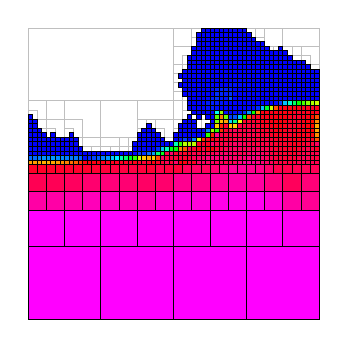
\begin{tikzpicture}[x={(\screenshotunitlength,0)},y={(0,\screenshotunitlength)}]
       \definecolor{fillcolor}{rgb}{1.000000,0.000000,1.000000}
\fill[fillcolor] (0.000000,0.000000) rectangle (0.250000,0.250000);
\definecolor{fillcolor}{rgb}{1.000000,0.000000,1.000000}
\fill[fillcolor] (0.250000,0.000000) rectangle (0.500000,0.250000);
\definecolor{fillcolor}{rgb}{1.000000,0.000000,1.000000}
\fill[fillcolor] (0.000000,0.250000) rectangle (0.125000,0.375000);
\definecolor{fillcolor}{rgb}{1.000000,0.000000,1.000000}
\fill[fillcolor] (0.125000,0.250000) rectangle (0.250000,0.375000);
\definecolor{fillcolor}{rgb}{1.000000,0.000000,0.645511}
\fill[fillcolor] (0.000000,0.375000) rectangle (0.062500,0.437500);
\definecolor{fillcolor}{rgb}{1.000000,0.000000,0.650364}
\fill[fillcolor] (0.062500,0.375000) rectangle (0.125000,0.437500);
\definecolor{fillcolor}{rgb}{1.000000,0.000000,0.323813}
\fill[fillcolor] (0.000000,0.437500) rectangle (0.062500,0.500000);
\definecolor{fillcolor}{rgb}{1.000000,0.000000,0.332497}
\fill[fillcolor] (0.062500,0.437500) rectangle (0.125000,0.500000);
\definecolor{fillcolor}{rgb}{1.000000,0.000000,0.683204}
\fill[fillcolor] (0.125000,0.375000) rectangle (0.187500,0.437500);
\definecolor{fillcolor}{rgb}{1.000000,0.000000,0.724625}
\fill[fillcolor] (0.187500,0.375000) rectangle (0.250000,0.437500);
\definecolor{fillcolor}{rgb}{1.000000,0.000000,0.367012}
\fill[fillcolor] (0.125000,0.437500) rectangle (0.187500,0.500000);
\definecolor{fillcolor}{rgb}{1.000000,0.000000,0.432279}
\fill[fillcolor] (0.187500,0.437500) rectangle (0.250000,0.500000);
\definecolor{fillcolor}{rgb}{1.000000,0.000000,1.000000}
\fill[fillcolor] (0.250000,0.250000) rectangle (0.375000,0.375000);
\definecolor{fillcolor}{rgb}{1.000000,0.000000,1.000000}
\fill[fillcolor] (0.375000,0.250000) rectangle (0.500000,0.375000);
\definecolor{fillcolor}{rgb}{1.000000,0.000000,0.774963}
\fill[fillcolor] (0.250000,0.375000) rectangle (0.312500,0.437500);
\definecolor{fillcolor}{rgb}{1.000000,0.000000,0.736209}
\fill[fillcolor] (0.312500,0.375000) rectangle (0.375000,0.437500);
\definecolor{fillcolor}{rgb}{1.000000,0.000000,0.476380}
\fill[fillcolor] (0.250000,0.437500) rectangle (0.312500,0.500000);
\definecolor{fillcolor}{rgb}{1.000000,0.000000,0.445120}
\fill[fillcolor] (0.312500,0.437500) rectangle (0.375000,0.500000);
\definecolor{fillcolor}{rgb}{1.000000,0.000000,0.712021}
\fill[fillcolor] (0.375000,0.375000) rectangle (0.437500,0.437500);
\definecolor{fillcolor}{rgb}{1.000000,0.000000,0.838903}
\fill[fillcolor] (0.437500,0.375000) rectangle (0.500000,0.437500);
\definecolor{fillcolor}{rgb}{1.000000,0.000000,0.391746}
\fill[fillcolor] (0.375000,0.437500) rectangle (0.437500,0.500000);
\definecolor{fillcolor}{rgb}{1.000000,0.000000,0.422221}
\fill[fillcolor] (0.437500,0.437500) rectangle (0.500000,0.500000);
\definecolor{fillcolor}{rgb}{1.000000,0.000000,1.000000}
\fill[fillcolor] (0.500000,0.000000) rectangle (0.750000,0.250000);
\definecolor{fillcolor}{rgb}{1.000000,0.000000,1.000000}
\fill[fillcolor] (0.750000,0.000000) rectangle (1.000000,0.250000);
\definecolor{fillcolor}{rgb}{1.000000,0.000000,1.000000}
\fill[fillcolor] (0.500000,0.250000) rectangle (0.625000,0.375000);
\definecolor{fillcolor}{rgb}{1.000000,0.000000,1.000000}
\fill[fillcolor] (0.625000,0.250000) rectangle (0.750000,0.375000);
\definecolor{fillcolor}{rgb}{1.000000,0.000000,0.885222}
\fill[fillcolor] (0.500000,0.375000) rectangle (0.562500,0.437500);
\definecolor{fillcolor}{rgb}{1.000000,0.000000,0.857635}
\fill[fillcolor] (0.562500,0.375000) rectangle (0.625000,0.437500);
\definecolor{fillcolor}{rgb}{1.000000,0.000000,0.561857}
\fill[fillcolor] (0.500000,0.437500) rectangle (0.562500,0.500000);
\definecolor{fillcolor}{rgb}{1.000000,0.000000,0.545496}
\fill[fillcolor] (0.562500,0.437500) rectangle (0.625000,0.500000);
\definecolor{fillcolor}{rgb}{1.000000,0.000000,0.914258}
\fill[fillcolor] (0.625000,0.375000) rectangle (0.687500,0.437500);
\definecolor{fillcolor}{rgb}{1.000000,0.000000,0.928379}
\fill[fillcolor] (0.687500,0.375000) rectangle (0.750000,0.437500);
\definecolor{fillcolor}{rgb}{1.000000,0.000000,0.622367}
\fill[fillcolor] (0.625000,0.437500) rectangle (0.687500,0.500000);
\definecolor{fillcolor}{rgb}{1.000000,0.000000,0.659783}
\fill[fillcolor] (0.687500,0.437500) rectangle (0.750000,0.500000);
\definecolor{fillcolor}{rgb}{1.000000,0.000000,1.000000}
\fill[fillcolor] (0.750000,0.250000) rectangle (0.875000,0.375000);
\definecolor{fillcolor}{rgb}{1.000000,0.000000,0.948724}
\fill[fillcolor] (0.875000,0.250000) rectangle (1.000000,0.375000);
\definecolor{fillcolor}{rgb}{1.000000,0.000000,0.943733}
\fill[fillcolor] (0.750000,0.375000) rectangle (0.812500,0.437500);
\definecolor{fillcolor}{rgb}{1.000000,0.000000,0.859756}
\fill[fillcolor] (0.812500,0.375000) rectangle (0.875000,0.437500);
\definecolor{fillcolor}{rgb}{1.000000,0.000000,0.634761}
\fill[fillcolor] (0.750000,0.437500) rectangle (0.812500,0.500000);
\definecolor{fillcolor}{rgb}{1.000000,0.000000,0.514265}
\fill[fillcolor] (0.812500,0.437500) rectangle (0.875000,0.500000);
\definecolor{fillcolor}{rgb}{1.000000,0.000000,0.641529}
\fill[fillcolor] (0.875000,0.375000) rectangle (0.937500,0.437500);
\definecolor{fillcolor}{rgb}{1.000000,0.000000,0.574537}
\fill[fillcolor] (0.937500,0.375000) rectangle (1.000000,0.437500);
\definecolor{fillcolor}{rgb}{1.000000,0.000000,0.355152}
\fill[fillcolor] (0.875000,0.437500) rectangle (0.937500,0.500000);
\definecolor{fillcolor}{rgb}{1.000000,0.000000,0.469730}
\fill[fillcolor] (0.937500,0.437500) rectangle (1.000000,0.500000);
\definecolor{fillcolor}{rgb}{1.000000,0.000000,0.151436}
\fill[fillcolor] (0.000000,0.500000) rectangle (0.031250,0.531250);
\definecolor{fillcolor}{rgb}{1.000000,0.000000,0.154568}
\fill[fillcolor] (0.031250,0.500000) rectangle (0.062500,0.531250);
\definecolor{fillcolor}{rgb}{1.000000,0.620507,0.000000}
\fill[fillcolor] (0.000000,0.531250) rectangle (0.015625,0.546875);
\definecolor{fillcolor}{rgb}{1.000000,0.614422,0.000000}
\fill[fillcolor] (0.015625,0.531250) rectangle (0.031250,0.546875);
\definecolor{fillcolor}{rgb}{0.000000,0.420316,1.000000}
\fill[fillcolor] (0.000000,0.546875) rectangle (0.015625,0.562500);
\definecolor{fillcolor}{rgb}{0.000000,0.418518,1.000000}
\fill[fillcolor] (0.015625,0.546875) rectangle (0.031250,0.562500);
\definecolor{fillcolor}{rgb}{1.000000,0.653038,0.000000}
\fill[fillcolor] (0.031250,0.531250) rectangle (0.046875,0.546875);
\definecolor{fillcolor}{rgb}{1.000000,0.681669,0.000000}
\fill[fillcolor] (0.046875,0.531250) rectangle (0.062500,0.546875);
\definecolor{fillcolor}{rgb}{0.000000,0.497707,1.000000}
\fill[fillcolor] (0.031250,0.546875) rectangle (0.046875,0.562500);
\definecolor{fillcolor}{rgb}{0.000000,0.577677,1.000000}
\fill[fillcolor] (0.046875,0.546875) rectangle (0.062500,0.562500);
\definecolor{fillcolor}{rgb}{1.000000,0.000000,0.161860}
\fill[fillcolor] (0.062500,0.500000) rectangle (0.093750,0.531250);
\definecolor{fillcolor}{rgb}{1.000000,0.000000,0.165269}
\fill[fillcolor] (0.093750,0.500000) rectangle (0.125000,0.531250);
\definecolor{fillcolor}{rgb}{1.000000,0.680552,0.000000}
\fill[fillcolor] (0.062500,0.531250) rectangle (0.078125,0.546875);
\definecolor{fillcolor}{rgb}{1.000000,0.641218,0.000000}
\fill[fillcolor] (0.078125,0.531250) rectangle (0.093750,0.546875);
\definecolor{fillcolor}{rgb}{0.000000,0.531447,1.000000}
\fill[fillcolor] (0.062500,0.546875) rectangle (0.078125,0.562500);
\definecolor{fillcolor}{rgb}{0.000000,0.606595,1.000000}
\fill[fillcolor] (0.078125,0.546875) rectangle (0.093750,0.562500);
\definecolor{fillcolor}{rgb}{1.000000,0.603864,0.000000}
\fill[fillcolor] (0.093750,0.531250) rectangle (0.109375,0.546875);
\definecolor{fillcolor}{rgb}{1.000000,0.542532,0.000000}
\fill[fillcolor] (0.109375,0.531250) rectangle (0.125000,0.546875);
\definecolor{fillcolor}{rgb}{0.000000,0.557533,1.000000}
\fill[fillcolor] (0.093750,0.546875) rectangle (0.109375,0.562500);
\definecolor{fillcolor}{rgb}{0.000000,0.543313,1.000000}
\fill[fillcolor] (0.109375,0.546875) rectangle (0.125000,0.562500);
\definecolor{fillcolor}{rgb}{0.000000,0.005785,1.000000}
\fill[fillcolor] (0.000000,0.562500) rectangle (0.015625,0.578125);
\definecolor{fillcolor}{rgb}{0.000000,0.002037,1.000000}
\fill[fillcolor] (0.015625,0.562500) rectangle (0.031250,0.578125);
\definecolor{fillcolor}{rgb}{0.000000,0.023838,1.000000}
\fill[fillcolor] (0.000000,0.578125) rectangle (0.015625,0.593750);
\definecolor{fillcolor}{rgb}{0.000000,0.029520,1.000000}
\fill[fillcolor] (0.015625,0.578125) rectangle (0.031250,0.593750);
\definecolor{fillcolor}{rgb}{0.000000,0.001860,1.000000}
\fill[fillcolor] (0.031250,0.562500) rectangle (0.046875,0.578125);
\definecolor{fillcolor}{rgb}{0.000000,0.002085,1.000000}
\fill[fillcolor] (0.046875,0.562500) rectangle (0.062500,0.578125);
\definecolor{fillcolor}{rgb}{0.000000,0.003320,1.000000}
\fill[fillcolor] (0.031250,0.578125) rectangle (0.046875,0.593750);
\definecolor{fillcolor}{rgb}{0.000000,0.003120,1.000000}
\fill[fillcolor] (0.046875,0.578125) rectangle (0.062500,0.593750);
\definecolor{fillcolor}{rgb}{0.000000,0.003632,1.000000}
\fill[fillcolor] (0.000000,0.593750) rectangle (0.015625,0.609375);
\definecolor{fillcolor}{rgb}{0.000000,0.004712,1.000000}
\fill[fillcolor] (0.015625,0.593750) rectangle (0.031250,0.609375);
\definecolor{fillcolor}{rgb}{0.000000,0.000193,1.000000}
\fill[fillcolor] (0.000000,0.609375) rectangle (0.015625,0.625000);
\definecolor{fillcolor}{rgb}{0.000000,0.000299,1.000000}
\fill[fillcolor] (0.015625,0.609375) rectangle (0.031250,0.625000);
\definecolor{fillcolor}{rgb}{0.000000,0.000682,1.000000}
\fill[fillcolor] (0.031250,0.593750) rectangle (0.046875,0.609375);
\definecolor{fillcolor}{rgb}{0.000000,0.000000,1.000000}
\fill[fillcolor] (0.046875,0.593750) rectangle (0.062500,0.609375);
\definecolor{fillcolor}{rgb}{0.000000,0.000002,1.000000}
\fill[fillcolor] (0.031250,0.609375) rectangle (0.046875,0.625000);
\definecolor{fillcolor}{rgb}{0.000000,0.000000,1.000000}
\fill[fillcolor] (0.046875,0.609375) rectangle (0.062500,0.625000);
\definecolor{fillcolor}{rgb}{0.000000,0.000077,1.000000}
\fill[fillcolor] (0.062500,0.562500) rectangle (0.078125,0.578125);
\definecolor{fillcolor}{rgb}{0.000000,0.001501,1.000000}
\fill[fillcolor] (0.078125,0.562500) rectangle (0.093750,0.578125);
\definecolor{fillcolor}{rgb}{0.000000,0.000406,1.000000}
\fill[fillcolor] (0.062500,0.578125) rectangle (0.078125,0.593750);
\definecolor{fillcolor}{rgb}{0.000000,0.003117,1.000000}
\fill[fillcolor] (0.078125,0.578125) rectangle (0.093750,0.593750);
\definecolor{fillcolor}{rgb}{0.000000,0.000956,1.000000}
\fill[fillcolor] (0.093750,0.562500) rectangle (0.109375,0.578125);
\definecolor{fillcolor}{rgb}{0.000000,0.003356,1.000000}
\fill[fillcolor] (0.109375,0.562500) rectangle (0.125000,0.578125);
\definecolor{fillcolor}{rgb}{0.000000,0.000470,1.000000}
\fill[fillcolor] (0.093750,0.578125) rectangle (0.109375,0.593750);
\definecolor{fillcolor}{rgb}{0.000000,0.007908,1.000000}
\fill[fillcolor] (0.109375,0.578125) rectangle (0.125000,0.593750);
\definecolor{fillcolor}{rgb}{0.000000,0.000000,1.000000}
\fill[fillcolor] (0.062500,0.593750) rectangle (0.078125,0.609375);
\definecolor{fillcolor}{rgb}{0.000000,0.000000,1.000000}
\fill[fillcolor] (0.078125,0.593750) rectangle (0.093750,0.609375);
\definecolor{fillcolor}{rgb}{0.000000,0.000000,1.000000}
\fill[fillcolor] (0.062500,0.609375) rectangle (0.078125,0.625000);
\definecolor{fillcolor}{rgb}{0.000000,0.000000,1.000000}
\fill[fillcolor] (0.078125,0.609375) rectangle (0.093750,0.625000);
\definecolor{fillcolor}{rgb}{0.000000,0.000000,1.000000}
\fill[fillcolor] (0.093750,0.593750) rectangle (0.109375,0.609375);
\definecolor{fillcolor}{rgb}{0.000000,0.000479,1.000000}
\fill[fillcolor] (0.109375,0.593750) rectangle (0.125000,0.609375);
\definecolor{fillcolor}{rgb}{0.000000,0.000000,1.000000}
\fill[fillcolor] (0.093750,0.609375) rectangle (0.109375,0.625000);
\definecolor{fillcolor}{rgb}{0.000000,0.000000,1.000000}
\fill[fillcolor] (0.109375,0.609375) rectangle (0.125000,0.625000);
\definecolor{fillcolor}{rgb}{1.000000,0.000000,0.174439}
\fill[fillcolor] (0.125000,0.500000) rectangle (0.156250,0.531250);
\definecolor{fillcolor}{rgb}{1.000000,0.000000,0.173437}
\fill[fillcolor] (0.156250,0.500000) rectangle (0.187500,0.531250);
\definecolor{fillcolor}{rgb}{1.000000,0.501342,0.000000}
\fill[fillcolor] (0.125000,0.531250) rectangle (0.140625,0.546875);
\definecolor{fillcolor}{rgb}{1.000000,0.419703,0.000000}
\fill[fillcolor] (0.140625,0.531250) rectangle (0.156250,0.546875);
\definecolor{fillcolor}{rgb}{0.000000,0.506551,1.000000}
\fill[fillcolor] (0.125000,0.546875) rectangle (0.140625,0.562500);
\definecolor{fillcolor}{rgb}{0.000000,0.483889,1.000000}
\fill[fillcolor] (0.140625,0.546875) rectangle (0.156250,0.562500);
\definecolor{fillcolor}{rgb}{1.000000,0.356880,0.000000}
\fill[fillcolor] (0.156250,0.531250) rectangle (0.171875,0.546875);
\definecolor{fillcolor}{rgb}{1.000000,0.210995,0.000000}
\fill[fillcolor] (0.171875,0.531250) rectangle (0.187500,0.546875);
\definecolor{fillcolor}{rgb}{0.000000,0.477928,1.000000}
\fill[fillcolor] (0.156250,0.546875) rectangle (0.171875,0.562500);
\definecolor{fillcolor}{rgb}{0.000000,0.416304,1.000000}
\fill[fillcolor] (0.171875,0.546875) rectangle (0.187500,0.562500);
\definecolor{fillcolor}{rgb}{1.000000,0.000000,0.171867}
\fill[fillcolor] (0.187500,0.500000) rectangle (0.218750,0.531250);
\definecolor{fillcolor}{rgb}{1.000000,0.000000,0.200146}
\fill[fillcolor] (0.218750,0.500000) rectangle (0.250000,0.531250);
\definecolor{fillcolor}{rgb}{1.000000,0.000000,0.060262}
\fill[fillcolor] (0.187500,0.531250) rectangle (0.203125,0.546875);
\definecolor{fillcolor}{rgb}{1.000000,0.000000,0.048933}
\fill[fillcolor] (0.203125,0.531250) rectangle (0.218750,0.546875);
\definecolor{fillcolor}{rgb}{0.000000,0.052439,1.000000}
\fill[fillcolor] (0.187500,0.546875) rectangle (0.203125,0.562500);
\definecolor{fillcolor}{rgb}{0.000000,0.177096,1.000000}
\fill[fillcolor] (0.203125,0.546875) rectangle (0.218750,0.562500);
\definecolor{fillcolor}{rgb}{1.000000,0.000000,0.069620}
\fill[fillcolor] (0.218750,0.531250) rectangle (0.234375,0.546875);
\definecolor{fillcolor}{rgb}{1.000000,0.000000,0.060783}
\fill[fillcolor] (0.234375,0.531250) rectangle (0.250000,0.546875);
\definecolor{fillcolor}{rgb}{0.000000,0.262842,1.000000}
\fill[fillcolor] (0.218750,0.546875) rectangle (0.234375,0.562500);
\definecolor{fillcolor}{rgb}{0.000000,0.358442,1.000000}
\fill[fillcolor] (0.234375,0.546875) rectangle (0.250000,0.562500);
\definecolor{fillcolor}{rgb}{0.000000,0.007639,1.000000}
\fill[fillcolor] (0.125000,0.562500) rectangle (0.140625,0.578125);
\definecolor{fillcolor}{rgb}{0.000000,0.009230,1.000000}
\fill[fillcolor] (0.140625,0.562500) rectangle (0.156250,0.578125);
\definecolor{fillcolor}{rgb}{0.000000,0.003502,1.000000}
\fill[fillcolor] (0.125000,0.578125) rectangle (0.140625,0.593750);
\definecolor{fillcolor}{rgb}{0.000000,0.001285,1.000000}
\fill[fillcolor] (0.140625,0.578125) rectangle (0.156250,0.593750);
\definecolor{fillcolor}{rgb}{0.000000,0.000000,1.000000}
\fill[fillcolor] (0.156250,0.562500) rectangle (0.171875,0.578125);
\definecolor{fillcolor}{rgb}{0.000000,0.000000,1.000000}
\fill[fillcolor] (0.171875,0.562500) rectangle (0.187500,0.578125);
\definecolor{fillcolor}{rgb}{0.000000,0.000304,1.000000}
\fill[fillcolor] (0.156250,0.578125) rectangle (0.171875,0.593750);
\definecolor{fillcolor}{rgb}{0.000000,0.000000,1.000000}
\fill[fillcolor] (0.171875,0.578125) rectangle (0.187500,0.593750);
\definecolor{fillcolor}{rgb}{0.000000,0.000000,1.000000}
\fill[fillcolor] (0.125000,0.593750) rectangle (0.140625,0.609375);
\definecolor{fillcolor}{rgb}{0.000000,0.000003,1.000000}
\fill[fillcolor] (0.140625,0.593750) rectangle (0.156250,0.609375);
\definecolor{fillcolor}{rgb}{0.000000,0.000000,1.000000}
\fill[fillcolor] (0.125000,0.609375) rectangle (0.140625,0.625000);
\definecolor{fillcolor}{rgb}{0.000000,0.000000,1.000000}
\fill[fillcolor] (0.140625,0.609375) rectangle (0.156250,0.625000);
\definecolor{fillcolor}{rgb}{0.000000,0.000000,1.000000}
\fill[fillcolor] (0.156250,0.593750) rectangle (0.171875,0.609375);
\definecolor{fillcolor}{rgb}{0.000000,0.000000,1.000000}
\fill[fillcolor] (0.156250,0.609375) rectangle (0.171875,0.625000);
\definecolor{fillcolor}{rgb}{0.000000,0.000000,1.000000}
\fill[fillcolor] (0.187500,0.562500) rectangle (0.203125,0.578125);
\definecolor{fillcolor}{rgb}{0.000000,0.000000,1.000000}
\fill[fillcolor] (0.203125,0.562500) rectangle (0.218750,0.578125);
\definecolor{fillcolor}{rgb}{0.000000,0.000000,1.000000}
\fill[fillcolor] (0.218750,0.562500) rectangle (0.234375,0.578125);
\definecolor{fillcolor}{rgb}{0.000000,0.000000,1.000000}
\fill[fillcolor] (0.234375,0.562500) rectangle (0.250000,0.578125);
\definecolor{fillcolor}{rgb}{0.000000,0.000000,1.000000}
\fill[fillcolor] (0.000000,0.625000) rectangle (0.015625,0.640625);
\definecolor{fillcolor}{rgb}{0.000000,0.000002,1.000000}
\fill[fillcolor] (0.015625,0.625000) rectangle (0.031250,0.640625);
\definecolor{fillcolor}{rgb}{0.000000,0.000000,1.000000}
\fill[fillcolor] (0.000000,0.640625) rectangle (0.015625,0.656250);
\definecolor{fillcolor}{rgb}{0.000000,0.000000,1.000000}
\fill[fillcolor] (0.015625,0.640625) rectangle (0.031250,0.656250);
\definecolor{fillcolor}{rgb}{0.000000,0.000000,1.000000}
\fill[fillcolor] (0.031250,0.625000) rectangle (0.046875,0.640625);
\definecolor{fillcolor}{rgb}{0.000000,0.000000,1.000000}
\fill[fillcolor] (0.046875,0.625000) rectangle (0.062500,0.640625);
\definecolor{fillcolor}{rgb}{0.000000,0.000000,1.000000}
\fill[fillcolor] (0.031250,0.640625) rectangle (0.046875,0.656250);
\definecolor{fillcolor}{rgb}{0.000000,0.000000,1.000000}
\fill[fillcolor] (0.000000,0.656250) rectangle (0.015625,0.671875);
\definecolor{fillcolor}{rgb}{0.000000,0.000000,1.000000}
\fill[fillcolor] (0.015625,0.656250) rectangle (0.031250,0.671875);
\definecolor{fillcolor}{rgb}{0.000000,0.000000,1.000000}
\fill[fillcolor] (0.000000,0.671875) rectangle (0.015625,0.687500);
\definecolor{fillcolor}{rgb}{0.000000,0.000000,1.000000}
\fill[fillcolor] (0.015625,0.671875) rectangle (0.031250,0.687500);
\definecolor{fillcolor}{rgb}{0.000000,0.000000,1.000000}
\fill[fillcolor] (0.078125,0.625000) rectangle (0.093750,0.640625);
\definecolor{fillcolor}{rgb}{0.000000,0.000000,1.000000}
\fill[fillcolor] (0.000000,0.687500) rectangle (0.015625,0.703125);
\definecolor{fillcolor}{rgb}{0.000000,0.000000,1.000000}
\fill[fillcolor] (0.140625,0.625000) rectangle (0.156250,0.640625);
\definecolor{fillcolor}{rgb}{1.000000,0.000000,0.230438}
\fill[fillcolor] (0.250000,0.500000) rectangle (0.281250,0.531250);
\definecolor{fillcolor}{rgb}{1.000000,0.000000,0.248489}
\fill[fillcolor] (0.281250,0.500000) rectangle (0.312500,0.531250);
\definecolor{fillcolor}{rgb}{1.000000,0.000000,0.102267}
\fill[fillcolor] (0.250000,0.531250) rectangle (0.265625,0.546875);
\definecolor{fillcolor}{rgb}{1.000000,0.000000,0.115192}
\fill[fillcolor] (0.265625,0.531250) rectangle (0.281250,0.546875);
\definecolor{fillcolor}{rgb}{0.000000,0.510075,1.000000}
\fill[fillcolor] (0.250000,0.546875) rectangle (0.265625,0.562500);
\definecolor{fillcolor}{rgb}{0.000000,0.608782,1.000000}
\fill[fillcolor] (0.265625,0.546875) rectangle (0.281250,0.562500);
\definecolor{fillcolor}{rgb}{1.000000,0.000000,0.122073}
\fill[fillcolor] (0.281250,0.531250) rectangle (0.296875,0.546875);
\definecolor{fillcolor}{rgb}{1.000000,0.000000,0.127147}
\fill[fillcolor] (0.296875,0.531250) rectangle (0.312500,0.546875);
\definecolor{fillcolor}{rgb}{0.000000,0.790405,1.000000}
\fill[fillcolor] (0.281250,0.546875) rectangle (0.296875,0.562500);
\definecolor{fillcolor}{rgb}{0.000000,0.952136,1.000000}
\fill[fillcolor] (0.296875,0.546875) rectangle (0.312500,0.562500);
\definecolor{fillcolor}{rgb}{1.000000,0.000000,0.257119}
\fill[fillcolor] (0.312500,0.500000) rectangle (0.343750,0.531250);
\definecolor{fillcolor}{rgb}{1.000000,0.000000,0.267657}
\fill[fillcolor] (0.343750,0.500000) rectangle (0.375000,0.531250);
\definecolor{fillcolor}{rgb}{1.000000,0.000000,0.136358}
\fill[fillcolor] (0.312500,0.531250) rectangle (0.328125,0.546875);
\definecolor{fillcolor}{rgb}{1.000000,0.000000,0.148742}
\fill[fillcolor] (0.328125,0.531250) rectangle (0.343750,0.546875);
\definecolor{fillcolor}{rgb}{0.000000,1.000000,0.688626}
\fill[fillcolor] (0.312500,0.546875) rectangle (0.328125,0.562500);
\definecolor{fillcolor}{rgb}{0.000000,1.000000,0.444422}
\fill[fillcolor] (0.328125,0.546875) rectangle (0.343750,0.562500);
\definecolor{fillcolor}{rgb}{1.000000,0.000000,0.142202}
\fill[fillcolor] (0.343750,0.531250) rectangle (0.359375,0.546875);
\definecolor{fillcolor}{rgb}{1.000000,0.000000,0.090307}
\fill[fillcolor] (0.359375,0.531250) rectangle (0.375000,0.546875);
\definecolor{fillcolor}{rgb}{0.000000,1.000000,0.098198}
\fill[fillcolor] (0.343750,0.546875) rectangle (0.359375,0.562500);
\definecolor{fillcolor}{rgb}{0.213152,1.000000,0.000000}
\fill[fillcolor] (0.359375,0.546875) rectangle (0.375000,0.562500);
\definecolor{fillcolor}{rgb}{0.000000,0.000000,1.000000}
\fill[fillcolor] (0.250000,0.562500) rectangle (0.265625,0.578125);
\definecolor{fillcolor}{rgb}{0.000000,0.000000,1.000000}
\fill[fillcolor] (0.265625,0.562500) rectangle (0.281250,0.578125);
\definecolor{fillcolor}{rgb}{0.000000,0.000000,1.000000}
\fill[fillcolor] (0.281250,0.562500) rectangle (0.296875,0.578125);
\definecolor{fillcolor}{rgb}{0.000000,0.000000,1.000000}
\fill[fillcolor] (0.296875,0.562500) rectangle (0.312500,0.578125);
\definecolor{fillcolor}{rgb}{0.000000,0.000000,1.000000}
\fill[fillcolor] (0.312500,0.562500) rectangle (0.328125,0.578125);
\definecolor{fillcolor}{rgb}{0.000000,0.000000,1.000000}
\fill[fillcolor] (0.328125,0.562500) rectangle (0.343750,0.578125);
\definecolor{fillcolor}{rgb}{0.000000,0.000000,1.000000}
\fill[fillcolor] (0.343750,0.562500) rectangle (0.359375,0.578125);
\definecolor{fillcolor}{rgb}{0.000000,0.024567,1.000000}
\fill[fillcolor] (0.359375,0.562500) rectangle (0.375000,0.578125);
\definecolor{fillcolor}{rgb}{0.000000,0.000000,1.000000}
\fill[fillcolor] (0.359375,0.578125) rectangle (0.375000,0.593750);
\definecolor{fillcolor}{rgb}{0.000000,0.000000,1.000000}
\fill[fillcolor] (0.359375,0.593750) rectangle (0.375000,0.609375);
\definecolor{fillcolor}{rgb}{1.000000,0.000000,0.237600}
\fill[fillcolor] (0.375000,0.500000) rectangle (0.406250,0.531250);
\definecolor{fillcolor}{rgb}{1.000000,0.000000,0.209396}
\fill[fillcolor] (0.406250,0.500000) rectangle (0.437500,0.531250);
\definecolor{fillcolor}{rgb}{1.000000,0.000000,0.167997}
\fill[fillcolor] (0.375000,0.531250) rectangle (0.390625,0.546875);
\definecolor{fillcolor}{rgb}{1.000000,0.000000,0.211784}
\fill[fillcolor] (0.390625,0.531250) rectangle (0.406250,0.546875);
\definecolor{fillcolor}{rgb}{0.806747,1.000000,0.000000}
\fill[fillcolor] (0.375000,0.546875) rectangle (0.390625,0.562500);
\definecolor{fillcolor}{rgb}{1.000000,0.793004,0.000000}
\fill[fillcolor] (0.390625,0.546875) rectangle (0.406250,0.562500);
\definecolor{fillcolor}{rgb}{1.000000,0.000000,0.151667}
\fill[fillcolor] (0.406250,0.531250) rectangle (0.421875,0.546875);
\definecolor{fillcolor}{rgb}{1.000000,0.000000,0.069773}
\fill[fillcolor] (0.421875,0.531250) rectangle (0.437500,0.546875);
\definecolor{fillcolor}{rgb}{1.000000,0.674581,0.000000}
\fill[fillcolor] (0.406250,0.546875) rectangle (0.421875,0.562500);
\definecolor{fillcolor}{rgb}{1.000000,0.778239,0.000000}
\fill[fillcolor] (0.421875,0.546875) rectangle (0.437500,0.562500);
\definecolor{fillcolor}{rgb}{1.000000,0.000000,0.284210}
\fill[fillcolor] (0.437500,0.500000) rectangle (0.468750,0.531250);
\definecolor{fillcolor}{rgb}{1.000000,0.000000,0.248008}
\fill[fillcolor] (0.468750,0.500000) rectangle (0.500000,0.531250);
\definecolor{fillcolor}{rgb}{1.000000,0.000000,0.133033}
\fill[fillcolor] (0.437500,0.531250) rectangle (0.453125,0.546875);
\definecolor{fillcolor}{rgb}{1.000000,0.000000,0.214908}
\fill[fillcolor] (0.453125,0.531250) rectangle (0.468750,0.546875);
\definecolor{fillcolor}{rgb}{1.000000,0.282643,0.000000}
\fill[fillcolor] (0.437500,0.546875) rectangle (0.453125,0.562500);
\definecolor{fillcolor}{rgb}{1.000000,0.000000,0.404097}
\fill[fillcolor] (0.453125,0.546875) rectangle (0.468750,0.562500);
\definecolor{fillcolor}{rgb}{1.000000,0.000000,0.330991}
\fill[fillcolor] (0.468750,0.531250) rectangle (0.484375,0.546875);
\definecolor{fillcolor}{rgb}{1.000000,0.000000,0.198735}
\fill[fillcolor] (0.484375,0.531250) rectangle (0.500000,0.546875);
\definecolor{fillcolor}{rgb}{1.000000,0.000000,0.223177}
\fill[fillcolor] (0.468750,0.546875) rectangle (0.484375,0.562500);
\definecolor{fillcolor}{rgb}{1.000000,0.000000,0.255779}
\fill[fillcolor] (0.484375,0.546875) rectangle (0.500000,0.562500);
\definecolor{fillcolor}{rgb}{0.000000,0.249169,1.000000}
\fill[fillcolor] (0.375000,0.562500) rectangle (0.390625,0.578125);
\definecolor{fillcolor}{rgb}{0.000000,0.186884,1.000000}
\fill[fillcolor] (0.390625,0.562500) rectangle (0.406250,0.578125);
\definecolor{fillcolor}{rgb}{0.000000,0.014442,1.000000}
\fill[fillcolor] (0.375000,0.578125) rectangle (0.390625,0.593750);
\definecolor{fillcolor}{rgb}{0.000000,0.026726,1.000000}
\fill[fillcolor] (0.390625,0.578125) rectangle (0.406250,0.593750);
\definecolor{fillcolor}{rgb}{0.000000,0.417566,1.000000}
\fill[fillcolor] (0.406250,0.562500) rectangle (0.421875,0.578125);
\definecolor{fillcolor}{rgb}{0.000000,0.611297,1.000000}
\fill[fillcolor] (0.421875,0.562500) rectangle (0.437500,0.578125);
\definecolor{fillcolor}{rgb}{0.000000,0.011586,1.000000}
\fill[fillcolor] (0.406250,0.578125) rectangle (0.421875,0.593750);
\definecolor{fillcolor}{rgb}{0.000000,0.000000,1.000000}
\fill[fillcolor] (0.421875,0.578125) rectangle (0.437500,0.593750);
\definecolor{fillcolor}{rgb}{0.000000,0.004903,1.000000}
\fill[fillcolor] (0.375000,0.593750) rectangle (0.390625,0.609375);
\definecolor{fillcolor}{rgb}{0.000000,0.015170,1.000000}
\fill[fillcolor] (0.390625,0.593750) rectangle (0.406250,0.609375);
\definecolor{fillcolor}{rgb}{0.000000,0.000000,1.000000}
\fill[fillcolor] (0.375000,0.609375) rectangle (0.390625,0.625000);
\definecolor{fillcolor}{rgb}{0.000000,0.002126,1.000000}
\fill[fillcolor] (0.390625,0.609375) rectangle (0.406250,0.625000);
\definecolor{fillcolor}{rgb}{0.000000,0.003232,1.000000}
\fill[fillcolor] (0.406250,0.593750) rectangle (0.421875,0.609375);
\definecolor{fillcolor}{rgb}{0.000000,0.000001,1.000000}
\fill[fillcolor] (0.421875,0.593750) rectangle (0.437500,0.609375);
\definecolor{fillcolor}{rgb}{0.000000,0.005882,1.000000}
\fill[fillcolor] (0.406250,0.609375) rectangle (0.421875,0.625000);
\definecolor{fillcolor}{rgb}{0.000000,0.001263,1.000000}
\fill[fillcolor] (0.421875,0.609375) rectangle (0.437500,0.625000);
\definecolor{fillcolor}{rgb}{0.000000,1.000000,0.442789}
\fill[fillcolor] (0.437500,0.562500) rectangle (0.453125,0.578125);
\definecolor{fillcolor}{rgb}{0.000000,1.000000,0.115137}
\fill[fillcolor] (0.453125,0.562500) rectangle (0.468750,0.578125);
\definecolor{fillcolor}{rgb}{0.000000,0.166147,1.000000}
\fill[fillcolor] (0.437500,0.578125) rectangle (0.453125,0.593750);
\definecolor{fillcolor}{rgb}{0.000000,0.752629,1.000000}
\fill[fillcolor] (0.453125,0.578125) rectangle (0.468750,0.593750);
\definecolor{fillcolor}{rgb}{1.000000,0.000000,0.302195}
\fill[fillcolor] (0.468750,0.562500) rectangle (0.484375,0.578125);
\definecolor{fillcolor}{rgb}{1.000000,0.000000,0.437569}
\fill[fillcolor] (0.484375,0.562500) rectangle (0.500000,0.578125);
\definecolor{fillcolor}{rgb}{0.000000,1.000000,0.723686}
\fill[fillcolor] (0.468750,0.578125) rectangle (0.484375,0.593750);
\definecolor{fillcolor}{rgb}{0.000000,1.000000,0.087637}
\fill[fillcolor] (0.484375,0.578125) rectangle (0.500000,0.593750);
\definecolor{fillcolor}{rgb}{0.000000,0.000000,1.000000}
\fill[fillcolor] (0.437500,0.593750) rectangle (0.453125,0.609375);
\definecolor{fillcolor}{rgb}{0.000000,0.000000,1.000000}
\fill[fillcolor] (0.453125,0.593750) rectangle (0.468750,0.609375);
\definecolor{fillcolor}{rgb}{0.000000,0.000185,1.000000}
\fill[fillcolor] (0.437500,0.609375) rectangle (0.453125,0.625000);
\definecolor{fillcolor}{rgb}{0.000000,0.000000,1.000000}
\fill[fillcolor] (0.453125,0.609375) rectangle (0.468750,0.625000);
\definecolor{fillcolor}{rgb}{0.000000,0.000000,1.000000}
\fill[fillcolor] (0.468750,0.593750) rectangle (0.484375,0.609375);
\definecolor{fillcolor}{rgb}{0.000000,0.000000,1.000000}
\fill[fillcolor] (0.484375,0.593750) rectangle (0.500000,0.609375);
\definecolor{fillcolor}{rgb}{0.000000,0.000000,1.000000}
\fill[fillcolor] (0.375000,0.625000) rectangle (0.390625,0.640625);
\definecolor{fillcolor}{rgb}{0.000000,0.001377,1.000000}
\fill[fillcolor] (0.390625,0.625000) rectangle (0.406250,0.640625);
\definecolor{fillcolor}{rgb}{0.000000,0.000000,1.000000}
\fill[fillcolor] (0.390625,0.640625) rectangle (0.406250,0.656250);
\definecolor{fillcolor}{rgb}{0.000000,0.005376,1.000000}
\fill[fillcolor] (0.406250,0.625000) rectangle (0.421875,0.640625);
\definecolor{fillcolor}{rgb}{0.000000,0.001293,1.000000}
\fill[fillcolor] (0.421875,0.625000) rectangle (0.437500,0.640625);
\definecolor{fillcolor}{rgb}{0.000000,0.000510,1.000000}
\fill[fillcolor] (0.406250,0.640625) rectangle (0.421875,0.656250);
\definecolor{fillcolor}{rgb}{0.000000,0.000000,1.000000}
\fill[fillcolor] (0.421875,0.640625) rectangle (0.437500,0.656250);
\definecolor{fillcolor}{rgb}{0.000000,0.000000,1.000000}
\fill[fillcolor] (0.406250,0.656250) rectangle (0.421875,0.671875);
\definecolor{fillcolor}{rgb}{0.000000,0.000000,1.000000}
\fill[fillcolor] (0.437500,0.625000) rectangle (0.453125,0.640625);
\definecolor{fillcolor}{rgb}{1.000000,0.000000,0.218164}
\fill[fillcolor] (0.500000,0.500000) rectangle (0.531250,0.531250);
\definecolor{fillcolor}{rgb}{1.000000,0.000000,0.363728}
\fill[fillcolor] (0.531250,0.500000) rectangle (0.562500,0.531250);
\definecolor{fillcolor}{rgb}{1.000000,0.000000,0.408453}
\fill[fillcolor] (0.500000,0.531250) rectangle (0.515625,0.546875);
\definecolor{fillcolor}{rgb}{1.000000,0.000000,0.048062}
\fill[fillcolor] (0.515625,0.531250) rectangle (0.531250,0.546875);
\definecolor{fillcolor}{rgb}{1.000000,0.000000,0.233200}
\fill[fillcolor] (0.500000,0.546875) rectangle (0.515625,0.562500);
\definecolor{fillcolor}{rgb}{1.000000,0.000000,0.205032}
\fill[fillcolor] (0.515625,0.546875) rectangle (0.531250,0.562500);
\definecolor{fillcolor}{rgb}{1.000000,0.000000,0.057386}
\fill[fillcolor] (0.531250,0.531250) rectangle (0.546875,0.546875);
\definecolor{fillcolor}{rgb}{1.000000,0.000000,0.212264}
\fill[fillcolor] (0.546875,0.531250) rectangle (0.562500,0.546875);
\definecolor{fillcolor}{rgb}{1.000000,0.000000,0.184780}
\fill[fillcolor] (0.531250,0.546875) rectangle (0.546875,0.562500);
\definecolor{fillcolor}{rgb}{1.000000,0.000000,0.209021}
\fill[fillcolor] (0.546875,0.546875) rectangle (0.562500,0.562500);
\definecolor{fillcolor}{rgb}{1.000000,0.000000,0.404164}
\fill[fillcolor] (0.562500,0.500000) rectangle (0.593750,0.531250);
\definecolor{fillcolor}{rgb}{1.000000,0.000000,0.371964}
\fill[fillcolor] (0.593750,0.500000) rectangle (0.625000,0.531250);
\definecolor{fillcolor}{rgb}{1.000000,0.000000,0.147643}
\fill[fillcolor] (0.562500,0.531250) rectangle (0.578125,0.546875);
\definecolor{fillcolor}{rgb}{1.000000,0.000000,0.404340}
\fill[fillcolor] (0.578125,0.531250) rectangle (0.593750,0.546875);
\definecolor{fillcolor}{rgb}{1.000000,0.000000,0.318210}
\fill[fillcolor] (0.562500,0.546875) rectangle (0.578125,0.562500);
\definecolor{fillcolor}{rgb}{1.000000,0.000000,0.390126}
\fill[fillcolor] (0.578125,0.546875) rectangle (0.593750,0.562500);
\definecolor{fillcolor}{rgb}{1.000000,0.000000,0.374120}
\fill[fillcolor] (0.593750,0.531250) rectangle (0.609375,0.546875);
\definecolor{fillcolor}{rgb}{1.000000,0.000000,0.377583}
\fill[fillcolor] (0.609375,0.531250) rectangle (0.625000,0.546875);
\definecolor{fillcolor}{rgb}{1.000000,0.000000,0.363382}
\fill[fillcolor] (0.593750,0.546875) rectangle (0.609375,0.562500);
\definecolor{fillcolor}{rgb}{1.000000,0.000000,0.476071}
\fill[fillcolor] (0.609375,0.546875) rectangle (0.625000,0.562500);
\definecolor{fillcolor}{rgb}{1.000000,0.000000,0.192810}
\fill[fillcolor] (0.500000,0.562500) rectangle (0.515625,0.578125);
\definecolor{fillcolor}{rgb}{1.000000,0.000000,0.237266}
\fill[fillcolor] (0.515625,0.562500) rectangle (0.531250,0.578125);
\definecolor{fillcolor}{rgb}{0.000000,1.000000,0.038921}
\fill[fillcolor] (0.500000,0.578125) rectangle (0.515625,0.593750);
\definecolor{fillcolor}{rgb}{1.000000,0.534465,0.000000}
\fill[fillcolor] (0.515625,0.578125) rectangle (0.531250,0.593750);
\definecolor{fillcolor}{rgb}{1.000000,0.000000,0.162737}
\fill[fillcolor] (0.531250,0.562500) rectangle (0.546875,0.578125);
\definecolor{fillcolor}{rgb}{1.000000,0.000000,0.181989}
\fill[fillcolor] (0.546875,0.562500) rectangle (0.562500,0.578125);
\definecolor{fillcolor}{rgb}{1.000000,0.329551,0.000000}
\fill[fillcolor] (0.531250,0.578125) rectangle (0.546875,0.593750);
\definecolor{fillcolor}{rgb}{1.000000,0.000000,0.271406}
\fill[fillcolor] (0.546875,0.578125) rectangle (0.562500,0.593750);
\definecolor{fillcolor}{rgb}{0.000000,1.000000,0.715935}
\fill[fillcolor] (0.500000,0.593750) rectangle (0.515625,0.609375);
\definecolor{fillcolor}{rgb}{0.193158,1.000000,0.000000}
\fill[fillcolor] (0.515625,0.593750) rectangle (0.531250,0.609375);
\definecolor{fillcolor}{rgb}{0.000000,0.000000,1.000000}
\fill[fillcolor] (0.500000,0.609375) rectangle (0.515625,0.625000);
\definecolor{fillcolor}{rgb}{0.000000,0.072855,1.000000}
\fill[fillcolor] (0.515625,0.609375) rectangle (0.531250,0.625000);
\definecolor{fillcolor}{rgb}{0.723636,1.000000,0.000000}
\fill[fillcolor] (0.531250,0.593750) rectangle (0.546875,0.609375);
\definecolor{fillcolor}{rgb}{0.682498,1.000000,0.000000}
\fill[fillcolor] (0.546875,0.593750) rectangle (0.562500,0.609375);
\definecolor{fillcolor}{rgb}{0.000000,0.271162,1.000000}
\fill[fillcolor] (0.531250,0.609375) rectangle (0.546875,0.625000);
\definecolor{fillcolor}{rgb}{0.000000,0.000000,1.000000}
\fill[fillcolor] (0.546875,0.609375) rectangle (0.562500,0.625000);
\definecolor{fillcolor}{rgb}{1.000000,0.000000,0.301140}
\fill[fillcolor] (0.562500,0.562500) rectangle (0.578125,0.578125);
\definecolor{fillcolor}{rgb}{1.000000,0.000000,0.268317}
\fill[fillcolor] (0.578125,0.562500) rectangle (0.593750,0.578125);
\definecolor{fillcolor}{rgb}{1.000000,0.000000,0.178762}
\fill[fillcolor] (0.562500,0.578125) rectangle (0.578125,0.593750);
\definecolor{fillcolor}{rgb}{1.000000,0.000000,0.051567}
\fill[fillcolor] (0.578125,0.578125) rectangle (0.593750,0.593750);
\definecolor{fillcolor}{rgb}{1.000000,0.000000,0.315068}
\fill[fillcolor] (0.593750,0.562500) rectangle (0.609375,0.578125);
\definecolor{fillcolor}{rgb}{1.000000,0.000000,0.318866}
\fill[fillcolor] (0.609375,0.562500) rectangle (0.625000,0.578125);
\definecolor{fillcolor}{rgb}{1.000000,0.000000,0.276360}
\fill[fillcolor] (0.593750,0.578125) rectangle (0.609375,0.593750);
\definecolor{fillcolor}{rgb}{1.000000,0.000000,0.051541}
\fill[fillcolor] (0.609375,0.578125) rectangle (0.625000,0.593750);
\definecolor{fillcolor}{rgb}{0.733425,1.000000,0.000000}
\fill[fillcolor] (0.562500,0.593750) rectangle (0.578125,0.609375);
\definecolor{fillcolor}{rgb}{1.000000,0.000000,0.166958}
\fill[fillcolor] (0.578125,0.593750) rectangle (0.593750,0.609375);
\definecolor{fillcolor}{rgb}{0.000000,0.524200,1.000000}
\fill[fillcolor] (0.562500,0.609375) rectangle (0.578125,0.625000);
\definecolor{fillcolor}{rgb}{0.832943,1.000000,0.000000}
\fill[fillcolor] (0.578125,0.609375) rectangle (0.593750,0.625000);
\definecolor{fillcolor}{rgb}{1.000000,0.000000,0.151636}
\fill[fillcolor] (0.593750,0.593750) rectangle (0.609375,0.609375);
\definecolor{fillcolor}{rgb}{1.000000,0.000000,0.116477}
\fill[fillcolor] (0.609375,0.593750) rectangle (0.625000,0.609375);
\definecolor{fillcolor}{rgb}{1.000000,0.173197,0.000000}
\fill[fillcolor] (0.593750,0.609375) rectangle (0.609375,0.625000);
\definecolor{fillcolor}{rgb}{1.000000,0.000000,0.088408}
\fill[fillcolor] (0.609375,0.609375) rectangle (0.625000,0.625000);
\definecolor{fillcolor}{rgb}{1.000000,0.000000,0.449813}
\fill[fillcolor] (0.625000,0.500000) rectangle (0.656250,0.531250);
\definecolor{fillcolor}{rgb}{1.000000,0.000000,0.527765}
\fill[fillcolor] (0.656250,0.500000) rectangle (0.687500,0.531250);
\definecolor{fillcolor}{rgb}{1.000000,0.000000,0.383686}
\fill[fillcolor] (0.625000,0.531250) rectangle (0.640625,0.546875);
\definecolor{fillcolor}{rgb}{1.000000,0.000000,0.354963}
\fill[fillcolor] (0.640625,0.531250) rectangle (0.656250,0.546875);
\definecolor{fillcolor}{rgb}{1.000000,0.000000,0.492705}
\fill[fillcolor] (0.625000,0.546875) rectangle (0.640625,0.562500);
\definecolor{fillcolor}{rgb}{1.000000,0.000000,0.448543}
\fill[fillcolor] (0.640625,0.546875) rectangle (0.656250,0.562500);
\definecolor{fillcolor}{rgb}{1.000000,0.000000,0.368333}
\fill[fillcolor] (0.656250,0.531250) rectangle (0.671875,0.546875);
\definecolor{fillcolor}{rgb}{1.000000,0.000000,0.320525}
\fill[fillcolor] (0.671875,0.531250) rectangle (0.687500,0.546875);
\definecolor{fillcolor}{rgb}{1.000000,0.000000,0.492802}
\fill[fillcolor] (0.656250,0.546875) rectangle (0.671875,0.562500);
\definecolor{fillcolor}{rgb}{1.000000,0.000000,0.468119}
\fill[fillcolor] (0.671875,0.546875) rectangle (0.687500,0.562500);
\definecolor{fillcolor}{rgb}{1.000000,0.000000,0.610351}
\fill[fillcolor] (0.687500,0.500000) rectangle (0.718750,0.531250);
\definecolor{fillcolor}{rgb}{1.000000,0.000000,0.610469}
\fill[fillcolor] (0.718750,0.500000) rectangle (0.750000,0.531250);
\definecolor{fillcolor}{rgb}{1.000000,0.000000,0.308221}
\fill[fillcolor] (0.687500,0.531250) rectangle (0.703125,0.546875);
\definecolor{fillcolor}{rgb}{1.000000,0.000000,0.365296}
\fill[fillcolor] (0.703125,0.531250) rectangle (0.718750,0.546875);
\definecolor{fillcolor}{rgb}{1.000000,0.000000,0.426284}
\fill[fillcolor] (0.687500,0.546875) rectangle (0.703125,0.562500);
\definecolor{fillcolor}{rgb}{1.000000,0.000000,0.410000}
\fill[fillcolor] (0.703125,0.546875) rectangle (0.718750,0.562500);
\definecolor{fillcolor}{rgb}{1.000000,0.000000,0.480416}
\fill[fillcolor] (0.718750,0.531250) rectangle (0.734375,0.546875);
\definecolor{fillcolor}{rgb}{1.000000,0.000000,0.586063}
\fill[fillcolor] (0.734375,0.531250) rectangle (0.750000,0.546875);
\definecolor{fillcolor}{rgb}{1.000000,0.000000,0.421376}
\fill[fillcolor] (0.718750,0.546875) rectangle (0.734375,0.562500);
\definecolor{fillcolor}{rgb}{1.000000,0.000000,0.465907}
\fill[fillcolor] (0.734375,0.546875) rectangle (0.750000,0.562500);
\definecolor{fillcolor}{rgb}{1.000000,0.000000,0.332412}
\fill[fillcolor] (0.625000,0.562500) rectangle (0.640625,0.578125);
\definecolor{fillcolor}{rgb}{1.000000,0.000000,0.380433}
\fill[fillcolor] (0.640625,0.562500) rectangle (0.656250,0.578125);
\definecolor{fillcolor}{rgb}{1.000000,0.000000,0.044022}
\fill[fillcolor] (0.625000,0.578125) rectangle (0.640625,0.593750);
\definecolor{fillcolor}{rgb}{1.000000,0.000000,0.205144}
\fill[fillcolor] (0.640625,0.578125) rectangle (0.656250,0.593750);
\definecolor{fillcolor}{rgb}{1.000000,0.000000,0.408691}
\fill[fillcolor] (0.656250,0.562500) rectangle (0.671875,0.578125);
\definecolor{fillcolor}{rgb}{1.000000,0.000000,0.422054}
\fill[fillcolor] (0.671875,0.562500) rectangle (0.687500,0.578125);
\definecolor{fillcolor}{rgb}{1.000000,0.000000,0.264761}
\fill[fillcolor] (0.656250,0.578125) rectangle (0.671875,0.593750);
\definecolor{fillcolor}{rgb}{1.000000,0.000000,0.323119}
\fill[fillcolor] (0.671875,0.578125) rectangle (0.687500,0.593750);
\definecolor{fillcolor}{rgb}{1.000000,0.000000,0.412014}
\fill[fillcolor] (0.625000,0.593750) rectangle (0.640625,0.609375);
\definecolor{fillcolor}{rgb}{1.000000,0.000000,0.258142}
\fill[fillcolor] (0.640625,0.593750) rectangle (0.656250,0.609375);
\definecolor{fillcolor}{rgb}{1.000000,0.000000,0.048860}
\fill[fillcolor] (0.625000,0.609375) rectangle (0.640625,0.625000);
\definecolor{fillcolor}{rgb}{1.000000,0.000000,0.138029}
\fill[fillcolor] (0.640625,0.609375) rectangle (0.656250,0.625000);
\definecolor{fillcolor}{rgb}{1.000000,0.000000,0.264883}
\fill[fillcolor] (0.656250,0.593750) rectangle (0.671875,0.609375);
\definecolor{fillcolor}{rgb}{1.000000,0.000000,0.285316}
\fill[fillcolor] (0.671875,0.593750) rectangle (0.687500,0.609375);
\definecolor{fillcolor}{rgb}{1.000000,0.000000,0.221446}
\fill[fillcolor] (0.656250,0.609375) rectangle (0.671875,0.625000);
\definecolor{fillcolor}{rgb}{1.000000,0.000000,0.203544}
\fill[fillcolor] (0.671875,0.609375) rectangle (0.687500,0.625000);
\definecolor{fillcolor}{rgb}{1.000000,0.000000,0.415138}
\fill[fillcolor] (0.687500,0.562500) rectangle (0.703125,0.578125);
\definecolor{fillcolor}{rgb}{1.000000,0.000000,0.374503}
\fill[fillcolor] (0.703125,0.562500) rectangle (0.718750,0.578125);
\definecolor{fillcolor}{rgb}{1.000000,0.000000,0.366586}
\fill[fillcolor] (0.687500,0.578125) rectangle (0.703125,0.593750);
\definecolor{fillcolor}{rgb}{1.000000,0.000000,0.373235}
\fill[fillcolor] (0.703125,0.578125) rectangle (0.718750,0.593750);
\definecolor{fillcolor}{rgb}{1.000000,0.000000,0.338891}
\fill[fillcolor] (0.718750,0.562500) rectangle (0.734375,0.578125);
\definecolor{fillcolor}{rgb}{1.000000,0.000000,0.352429}
\fill[fillcolor] (0.734375,0.562500) rectangle (0.750000,0.578125);
\definecolor{fillcolor}{rgb}{1.000000,0.000000,0.362265}
\fill[fillcolor] (0.718750,0.578125) rectangle (0.734375,0.593750);
\definecolor{fillcolor}{rgb}{1.000000,0.000000,0.350274}
\fill[fillcolor] (0.734375,0.578125) rectangle (0.750000,0.593750);
\definecolor{fillcolor}{rgb}{1.000000,0.000000,0.342742}
\fill[fillcolor] (0.687500,0.593750) rectangle (0.703125,0.609375);
\definecolor{fillcolor}{rgb}{1.000000,0.000000,0.389326}
\fill[fillcolor] (0.703125,0.593750) rectangle (0.718750,0.609375);
\definecolor{fillcolor}{rgb}{1.000000,0.000000,0.223141}
\fill[fillcolor] (0.687500,0.609375) rectangle (0.703125,0.625000);
\definecolor{fillcolor}{rgb}{1.000000,0.000000,0.278822}
\fill[fillcolor] (0.703125,0.609375) rectangle (0.718750,0.625000);
\definecolor{fillcolor}{rgb}{1.000000,0.000000,0.382912}
\fill[fillcolor] (0.718750,0.593750) rectangle (0.734375,0.609375);
\definecolor{fillcolor}{rgb}{1.000000,0.000000,0.346973}
\fill[fillcolor] (0.734375,0.593750) rectangle (0.750000,0.609375);
\definecolor{fillcolor}{rgb}{1.000000,0.000000,0.294343}
\fill[fillcolor] (0.718750,0.609375) rectangle (0.734375,0.625000);
\definecolor{fillcolor}{rgb}{1.000000,0.000000,0.294868}
\fill[fillcolor] (0.734375,0.609375) rectangle (0.750000,0.625000);
\definecolor{fillcolor}{rgb}{0.000000,0.000000,1.000000}
\fill[fillcolor] (0.500000,0.625000) rectangle (0.515625,0.640625);
\definecolor{fillcolor}{rgb}{0.000000,0.000078,1.000000}
\fill[fillcolor] (0.515625,0.625000) rectangle (0.531250,0.640625);
\definecolor{fillcolor}{rgb}{0.000000,0.000000,1.000000}
\fill[fillcolor] (0.515625,0.640625) rectangle (0.531250,0.656250);
\definecolor{fillcolor}{rgb}{0.000000,0.000274,1.000000}
\fill[fillcolor] (0.531250,0.625000) rectangle (0.546875,0.640625);
\definecolor{fillcolor}{rgb}{0.000000,0.000000,1.000000}
\fill[fillcolor] (0.546875,0.625000) rectangle (0.562500,0.640625);
\definecolor{fillcolor}{rgb}{0.000000,0.000097,1.000000}
\fill[fillcolor] (0.531250,0.640625) rectangle (0.546875,0.656250);
\definecolor{fillcolor}{rgb}{0.000000,0.000002,1.000000}
\fill[fillcolor] (0.546875,0.640625) rectangle (0.562500,0.656250);
\definecolor{fillcolor}{rgb}{0.000000,0.000000,1.000000}
\fill[fillcolor] (0.515625,0.656250) rectangle (0.531250,0.671875);
\definecolor{fillcolor}{rgb}{0.000000,0.000018,1.000000}
\fill[fillcolor] (0.531250,0.656250) rectangle (0.546875,0.671875);
\definecolor{fillcolor}{rgb}{0.000000,0.000001,1.000000}
\fill[fillcolor] (0.546875,0.656250) rectangle (0.562500,0.671875);
\definecolor{fillcolor}{rgb}{0.000000,0.000000,1.000000}
\fill[fillcolor] (0.531250,0.671875) rectangle (0.546875,0.687500);
\definecolor{fillcolor}{rgb}{0.000000,0.000000,1.000000}
\fill[fillcolor] (0.546875,0.671875) rectangle (0.562500,0.687500);
\definecolor{fillcolor}{rgb}{0.000000,0.000006,1.000000}
\fill[fillcolor] (0.562500,0.625000) rectangle (0.578125,0.640625);
\definecolor{fillcolor}{rgb}{0.000000,0.000000,1.000000}
\fill[fillcolor] (0.578125,0.625000) rectangle (0.593750,0.640625);
\definecolor{fillcolor}{rgb}{0.000000,0.000001,1.000000}
\fill[fillcolor] (0.562500,0.640625) rectangle (0.578125,0.656250);
\definecolor{fillcolor}{rgb}{0.000000,0.000000,1.000000}
\fill[fillcolor] (0.578125,0.640625) rectangle (0.593750,0.656250);
\definecolor{fillcolor}{rgb}{0.000000,0.011963,1.000000}
\fill[fillcolor] (0.593750,0.625000) rectangle (0.609375,0.640625);
\definecolor{fillcolor}{rgb}{0.147617,1.000000,0.000000}
\fill[fillcolor] (0.609375,0.625000) rectangle (0.625000,0.640625);
\definecolor{fillcolor}{rgb}{0.000000,0.000000,1.000000}
\fill[fillcolor] (0.593750,0.640625) rectangle (0.609375,0.656250);
\definecolor{fillcolor}{rgb}{0.000000,0.448322,1.000000}
\fill[fillcolor] (0.609375,0.640625) rectangle (0.625000,0.656250);
\definecolor{fillcolor}{rgb}{0.000000,0.000000,1.000000}
\fill[fillcolor] (0.562500,0.656250) rectangle (0.578125,0.671875);
\definecolor{fillcolor}{rgb}{0.000000,0.000000,1.000000}
\fill[fillcolor] (0.562500,0.671875) rectangle (0.578125,0.687500);
\definecolor{fillcolor}{rgb}{0.000000,0.000000,1.000000}
\fill[fillcolor] (0.609375,0.656250) rectangle (0.625000,0.671875);
\definecolor{fillcolor}{rgb}{0.000000,0.000000,1.000000}
\fill[fillcolor] (0.546875,0.687500) rectangle (0.562500,0.703125);
\definecolor{fillcolor}{rgb}{0.000000,0.000000,1.000000}
\fill[fillcolor] (0.546875,0.718750) rectangle (0.562500,0.734375);
\definecolor{fillcolor}{rgb}{0.000000,0.000000,1.000000}
\fill[fillcolor] (0.546875,0.734375) rectangle (0.562500,0.750000);
\definecolor{fillcolor}{rgb}{0.000000,0.000000,1.000000}
\fill[fillcolor] (0.578125,0.687500) rectangle (0.593750,0.703125);
\definecolor{fillcolor}{rgb}{0.000000,0.000000,1.000000}
\fill[fillcolor] (0.562500,0.703125) rectangle (0.578125,0.718750);
\definecolor{fillcolor}{rgb}{0.000000,0.000000,1.000000}
\fill[fillcolor] (0.578125,0.703125) rectangle (0.593750,0.718750);
\definecolor{fillcolor}{rgb}{0.000000,0.000000,1.000000}
\fill[fillcolor] (0.609375,0.687500) rectangle (0.625000,0.703125);
\definecolor{fillcolor}{rgb}{0.000000,0.000000,1.000000}
\fill[fillcolor] (0.593750,0.703125) rectangle (0.609375,0.718750);
\definecolor{fillcolor}{rgb}{0.000000,0.000000,1.000000}
\fill[fillcolor] (0.609375,0.703125) rectangle (0.625000,0.718750);
\definecolor{fillcolor}{rgb}{0.000000,0.002760,1.000000}
\fill[fillcolor] (0.562500,0.718750) rectangle (0.578125,0.734375);
\definecolor{fillcolor}{rgb}{0.000000,0.013799,1.000000}
\fill[fillcolor] (0.578125,0.718750) rectangle (0.593750,0.734375);
\definecolor{fillcolor}{rgb}{0.000000,0.000000,1.000000}
\fill[fillcolor] (0.562500,0.734375) rectangle (0.578125,0.750000);
\definecolor{fillcolor}{rgb}{0.000000,0.001401,1.000000}
\fill[fillcolor] (0.578125,0.734375) rectangle (0.593750,0.750000);
\definecolor{fillcolor}{rgb}{0.000000,0.023155,1.000000}
\fill[fillcolor] (0.593750,0.718750) rectangle (0.609375,0.734375);
\definecolor{fillcolor}{rgb}{0.000000,0.058402,1.000000}
\fill[fillcolor] (0.609375,0.718750) rectangle (0.625000,0.734375);
\definecolor{fillcolor}{rgb}{0.000000,0.031666,1.000000}
\fill[fillcolor] (0.593750,0.734375) rectangle (0.609375,0.750000);
\definecolor{fillcolor}{rgb}{0.000000,0.095298,1.000000}
\fill[fillcolor] (0.609375,0.734375) rectangle (0.625000,0.750000);
\definecolor{fillcolor}{rgb}{1.000000,0.122681,0.000000}
\fill[fillcolor] (0.625000,0.625000) rectangle (0.640625,0.640625);
\definecolor{fillcolor}{rgb}{1.000000,0.000000,0.540374}
\fill[fillcolor] (0.640625,0.625000) rectangle (0.656250,0.640625);
\definecolor{fillcolor}{rgb}{0.587251,1.000000,0.000000}
\fill[fillcolor] (0.625000,0.640625) rectangle (0.640625,0.656250);
\definecolor{fillcolor}{rgb}{0.145532,1.000000,0.000000}
\fill[fillcolor] (0.640625,0.640625) rectangle (0.656250,0.656250);
\definecolor{fillcolor}{rgb}{1.000000,0.000000,0.278236}
\fill[fillcolor] (0.656250,0.625000) rectangle (0.671875,0.640625);
\definecolor{fillcolor}{rgb}{1.000000,0.000000,0.236030}
\fill[fillcolor] (0.671875,0.625000) rectangle (0.687500,0.640625);
\definecolor{fillcolor}{rgb}{1.000000,0.185096,0.000000}
\fill[fillcolor] (0.656250,0.640625) rectangle (0.671875,0.656250);
\definecolor{fillcolor}{rgb}{1.000000,0.000000,0.200368}
\fill[fillcolor] (0.671875,0.640625) rectangle (0.687500,0.656250);
\definecolor{fillcolor}{rgb}{0.000000,0.000000,1.000000}
\fill[fillcolor] (0.625000,0.656250) rectangle (0.640625,0.671875);
\definecolor{fillcolor}{rgb}{1.000000,0.801014,0.000000}
\fill[fillcolor] (0.640625,0.656250) rectangle (0.656250,0.671875);
\definecolor{fillcolor}{rgb}{0.000000,0.000000,1.000000}
\fill[fillcolor] (0.625000,0.671875) rectangle (0.640625,0.687500);
\definecolor{fillcolor}{rgb}{0.493882,1.000000,0.000000}
\fill[fillcolor] (0.640625,0.671875) rectangle (0.656250,0.687500);
\definecolor{fillcolor}{rgb}{1.000000,0.145764,0.000000}
\fill[fillcolor] (0.656250,0.656250) rectangle (0.671875,0.671875);
\definecolor{fillcolor}{rgb}{1.000000,0.000000,0.182864}
\fill[fillcolor] (0.671875,0.656250) rectangle (0.687500,0.671875);
\definecolor{fillcolor}{rgb}{1.000000,0.728110,0.000000}
\fill[fillcolor] (0.656250,0.671875) rectangle (0.671875,0.687500);
\definecolor{fillcolor}{rgb}{1.000000,0.636298,0.000000}
\fill[fillcolor] (0.671875,0.671875) rectangle (0.687500,0.687500);
\definecolor{fillcolor}{rgb}{1.000000,0.000000,0.224181}
\fill[fillcolor] (0.687500,0.625000) rectangle (0.703125,0.640625);
\definecolor{fillcolor}{rgb}{1.000000,0.000000,0.263511}
\fill[fillcolor] (0.703125,0.625000) rectangle (0.718750,0.640625);
\definecolor{fillcolor}{rgb}{1.000000,0.000000,0.313711}
\fill[fillcolor] (0.687500,0.640625) rectangle (0.703125,0.656250);
\definecolor{fillcolor}{rgb}{1.000000,0.000000,0.355998}
\fill[fillcolor] (0.703125,0.640625) rectangle (0.718750,0.656250);
\definecolor{fillcolor}{rgb}{1.000000,0.000000,0.257900}
\fill[fillcolor] (0.718750,0.625000) rectangle (0.734375,0.640625);
\definecolor{fillcolor}{rgb}{1.000000,0.000000,0.265571}
\fill[fillcolor] (0.734375,0.625000) rectangle (0.750000,0.640625);
\definecolor{fillcolor}{rgb}{1.000000,0.000000,0.286666}
\fill[fillcolor] (0.718750,0.640625) rectangle (0.734375,0.656250);
\definecolor{fillcolor}{rgb}{1.000000,0.000000,0.265200}
\fill[fillcolor] (0.734375,0.640625) rectangle (0.750000,0.656250);
\definecolor{fillcolor}{rgb}{1.000000,0.759752,0.000000}
\fill[fillcolor] (0.687500,0.656250) rectangle (0.703125,0.671875);
\definecolor{fillcolor}{rgb}{1.000000,0.825611,0.000000}
\fill[fillcolor] (0.703125,0.656250) rectangle (0.718750,0.671875);
\definecolor{fillcolor}{rgb}{0.000000,0.847651,1.000000}
\fill[fillcolor] (0.687500,0.671875) rectangle (0.703125,0.687500);
\definecolor{fillcolor}{rgb}{0.000000,1.000000,0.528701}
\fill[fillcolor] (0.703125,0.671875) rectangle (0.718750,0.687500);
\definecolor{fillcolor}{rgb}{1.000000,0.000000,0.261217}
\fill[fillcolor] (0.718750,0.656250) rectangle (0.734375,0.671875);
\definecolor{fillcolor}{rgb}{1.000000,0.000000,0.234996}
\fill[fillcolor] (0.734375,0.656250) rectangle (0.750000,0.671875);
\definecolor{fillcolor}{rgb}{0.928452,1.000000,0.000000}
\fill[fillcolor] (0.718750,0.671875) rectangle (0.734375,0.687500);
\definecolor{fillcolor}{rgb}{1.000000,0.000000,0.177921}
\fill[fillcolor] (0.734375,0.671875) rectangle (0.750000,0.687500);
\definecolor{fillcolor}{rgb}{0.000000,0.000000,1.000000}
\fill[fillcolor] (0.625000,0.687500) rectangle (0.640625,0.703125);
\definecolor{fillcolor}{rgb}{0.355567,1.000000,0.000000}
\fill[fillcolor] (0.640625,0.687500) rectangle (0.656250,0.703125);
\definecolor{fillcolor}{rgb}{0.000000,0.000000,1.000000}
\fill[fillcolor] (0.625000,0.703125) rectangle (0.640625,0.718750);
\definecolor{fillcolor}{rgb}{0.000000,1.000000,0.960727}
\fill[fillcolor] (0.640625,0.703125) rectangle (0.656250,0.718750);
\definecolor{fillcolor}{rgb}{1.000000,0.487735,0.000000}
\fill[fillcolor] (0.656250,0.687500) rectangle (0.671875,0.703125);
\definecolor{fillcolor}{rgb}{0.415743,1.000000,0.000000}
\fill[fillcolor] (0.671875,0.687500) rectangle (0.687500,0.703125);
\definecolor{fillcolor}{rgb}{0.547180,1.000000,0.000000}
\fill[fillcolor] (0.656250,0.703125) rectangle (0.671875,0.718750);
\definecolor{fillcolor}{rgb}{0.000000,0.043843,1.000000}
\fill[fillcolor] (0.671875,0.703125) rectangle (0.687500,0.718750);
\definecolor{fillcolor}{rgb}{0.000000,0.107667,1.000000}
\fill[fillcolor] (0.625000,0.718750) rectangle (0.640625,0.734375);
\definecolor{fillcolor}{rgb}{0.000000,0.045827,1.000000}
\fill[fillcolor] (0.640625,0.718750) rectangle (0.656250,0.734375);
\definecolor{fillcolor}{rgb}{0.000000,0.119572,1.000000}
\fill[fillcolor] (0.625000,0.734375) rectangle (0.640625,0.750000);
\definecolor{fillcolor}{rgb}{0.000000,0.109936,1.000000}
\fill[fillcolor] (0.640625,0.734375) rectangle (0.656250,0.750000);
\definecolor{fillcolor}{rgb}{0.000000,0.019579,1.000000}
\fill[fillcolor] (0.656250,0.718750) rectangle (0.671875,0.734375);
\definecolor{fillcolor}{rgb}{0.000000,0.021069,1.000000}
\fill[fillcolor] (0.671875,0.718750) rectangle (0.687500,0.734375);
\definecolor{fillcolor}{rgb}{0.000000,0.083485,1.000000}
\fill[fillcolor] (0.656250,0.734375) rectangle (0.671875,0.750000);
\definecolor{fillcolor}{rgb}{0.000000,0.038884,1.000000}
\fill[fillcolor] (0.671875,0.734375) rectangle (0.687500,0.750000);
\definecolor{fillcolor}{rgb}{0.000000,0.236249,1.000000}
\fill[fillcolor] (0.687500,0.687500) rectangle (0.703125,0.703125);
\definecolor{fillcolor}{rgb}{0.000000,0.329023,1.000000}
\fill[fillcolor] (0.703125,0.687500) rectangle (0.718750,0.703125);
\definecolor{fillcolor}{rgb}{0.000000,0.020251,1.000000}
\fill[fillcolor] (0.687500,0.703125) rectangle (0.703125,0.718750);
\definecolor{fillcolor}{rgb}{0.000000,0.025906,1.000000}
\fill[fillcolor] (0.703125,0.703125) rectangle (0.718750,0.718750);
\definecolor{fillcolor}{rgb}{0.000000,0.747355,1.000000}
\fill[fillcolor] (0.718750,0.687500) rectangle (0.734375,0.703125);
\definecolor{fillcolor}{rgb}{0.000000,1.000000,0.020469}
\fill[fillcolor] (0.734375,0.687500) rectangle (0.750000,0.703125);
\definecolor{fillcolor}{rgb}{0.000000,0.057038,1.000000}
\fill[fillcolor] (0.718750,0.703125) rectangle (0.734375,0.718750);
\definecolor{fillcolor}{rgb}{0.000000,0.192767,1.000000}
\fill[fillcolor] (0.734375,0.703125) rectangle (0.750000,0.718750);
\definecolor{fillcolor}{rgb}{0.000000,0.011325,1.000000}
\fill[fillcolor] (0.687500,0.718750) rectangle (0.703125,0.734375);
\definecolor{fillcolor}{rgb}{0.000000,0.007196,1.000000}
\fill[fillcolor] (0.703125,0.718750) rectangle (0.718750,0.734375);
\definecolor{fillcolor}{rgb}{0.000000,0.013614,1.000000}
\fill[fillcolor] (0.687500,0.734375) rectangle (0.703125,0.750000);
\definecolor{fillcolor}{rgb}{0.000000,0.008343,1.000000}
\fill[fillcolor] (0.703125,0.734375) rectangle (0.718750,0.750000);
\definecolor{fillcolor}{rgb}{0.000000,0.006896,1.000000}
\fill[fillcolor] (0.718750,0.718750) rectangle (0.734375,0.734375);
\definecolor{fillcolor}{rgb}{0.000000,0.011367,1.000000}
\fill[fillcolor] (0.734375,0.718750) rectangle (0.750000,0.734375);
\definecolor{fillcolor}{rgb}{0.000000,0.003070,1.000000}
\fill[fillcolor] (0.718750,0.734375) rectangle (0.734375,0.750000);
\definecolor{fillcolor}{rgb}{0.000000,0.002971,1.000000}
\fill[fillcolor] (0.734375,0.734375) rectangle (0.750000,0.750000);
\definecolor{fillcolor}{rgb}{1.000000,0.000000,0.566420}
\fill[fillcolor] (0.750000,0.500000) rectangle (0.781250,0.531250);
\definecolor{fillcolor}{rgb}{1.000000,0.000000,0.534017}
\fill[fillcolor] (0.781250,0.500000) rectangle (0.812500,0.531250);
\definecolor{fillcolor}{rgb}{1.000000,0.000000,0.592860}
\fill[fillcolor] (0.750000,0.531250) rectangle (0.765625,0.546875);
\definecolor{fillcolor}{rgb}{1.000000,0.000000,0.551948}
\fill[fillcolor] (0.765625,0.531250) rectangle (0.781250,0.546875);
\definecolor{fillcolor}{rgb}{1.000000,0.000000,0.497734}
\fill[fillcolor] (0.750000,0.546875) rectangle (0.765625,0.562500);
\definecolor{fillcolor}{rgb}{1.000000,0.000000,0.503382}
\fill[fillcolor] (0.765625,0.546875) rectangle (0.781250,0.562500);
\definecolor{fillcolor}{rgb}{1.000000,0.000000,0.508733}
\fill[fillcolor] (0.781250,0.531250) rectangle (0.796875,0.546875);
\definecolor{fillcolor}{rgb}{1.000000,0.000000,0.459333}
\fill[fillcolor] (0.796875,0.531250) rectangle (0.812500,0.546875);
\definecolor{fillcolor}{rgb}{1.000000,0.000000,0.481214}
\fill[fillcolor] (0.781250,0.546875) rectangle (0.796875,0.562500);
\definecolor{fillcolor}{rgb}{1.000000,0.000000,0.424510}
\fill[fillcolor] (0.796875,0.546875) rectangle (0.812500,0.562500);
\definecolor{fillcolor}{rgb}{1.000000,0.000000,0.422248}
\fill[fillcolor] (0.812500,0.500000) rectangle (0.843750,0.531250);
\definecolor{fillcolor}{rgb}{1.000000,0.000000,0.302976}
\fill[fillcolor] (0.843750,0.500000) rectangle (0.875000,0.531250);
\definecolor{fillcolor}{rgb}{1.000000,0.000000,0.390580}
\fill[fillcolor] (0.812500,0.531250) rectangle (0.828125,0.546875);
\definecolor{fillcolor}{rgb}{1.000000,0.000000,0.340668}
\fill[fillcolor] (0.828125,0.531250) rectangle (0.843750,0.546875);
\definecolor{fillcolor}{rgb}{1.000000,0.000000,0.358380}
\fill[fillcolor] (0.812500,0.546875) rectangle (0.828125,0.562500);
\definecolor{fillcolor}{rgb}{1.000000,0.000000,0.304858}
\fill[fillcolor] (0.828125,0.546875) rectangle (0.843750,0.562500);
\definecolor{fillcolor}{rgb}{1.000000,0.000000,0.276493}
\fill[fillcolor] (0.843750,0.531250) rectangle (0.859375,0.546875);
\definecolor{fillcolor}{rgb}{1.000000,0.000000,0.246943}
\fill[fillcolor] (0.859375,0.531250) rectangle (0.875000,0.546875);
\definecolor{fillcolor}{rgb}{1.000000,0.000000,0.251601}
\fill[fillcolor] (0.843750,0.546875) rectangle (0.859375,0.562500);
\definecolor{fillcolor}{rgb}{1.000000,0.000000,0.219617}
\fill[fillcolor] (0.859375,0.546875) rectangle (0.875000,0.562500);
\definecolor{fillcolor}{rgb}{1.000000,0.000000,0.398359}
\fill[fillcolor] (0.750000,0.562500) rectangle (0.765625,0.578125);
\definecolor{fillcolor}{rgb}{1.000000,0.000000,0.441215}
\fill[fillcolor] (0.765625,0.562500) rectangle (0.781250,0.578125);
\definecolor{fillcolor}{rgb}{1.000000,0.000000,0.347913}
\fill[fillcolor] (0.750000,0.578125) rectangle (0.765625,0.593750);
\definecolor{fillcolor}{rgb}{1.000000,0.000000,0.356542}
\fill[fillcolor] (0.765625,0.578125) rectangle (0.781250,0.593750);
\definecolor{fillcolor}{rgb}{1.000000,0.000000,0.443374}
\fill[fillcolor] (0.781250,0.562500) rectangle (0.796875,0.578125);
\definecolor{fillcolor}{rgb}{1.000000,0.000000,0.391584}
\fill[fillcolor] (0.796875,0.562500) rectangle (0.812500,0.578125);
\definecolor{fillcolor}{rgb}{1.000000,0.000000,0.360261}
\fill[fillcolor] (0.781250,0.578125) rectangle (0.796875,0.593750);
\definecolor{fillcolor}{rgb}{1.000000,0.000000,0.335138}
\fill[fillcolor] (0.796875,0.578125) rectangle (0.812500,0.593750);
\definecolor{fillcolor}{rgb}{1.000000,0.000000,0.302848}
\fill[fillcolor] (0.750000,0.593750) rectangle (0.765625,0.609375);
\definecolor{fillcolor}{rgb}{1.000000,0.000000,0.268682}
\fill[fillcolor] (0.765625,0.593750) rectangle (0.781250,0.609375);
\definecolor{fillcolor}{rgb}{1.000000,0.000000,0.284278}
\fill[fillcolor] (0.750000,0.609375) rectangle (0.765625,0.625000);
\definecolor{fillcolor}{rgb}{1.000000,0.000000,0.251231}
\fill[fillcolor] (0.765625,0.609375) rectangle (0.781250,0.625000);
\definecolor{fillcolor}{rgb}{1.000000,0.000000,0.269469}
\fill[fillcolor] (0.781250,0.593750) rectangle (0.796875,0.609375);
\definecolor{fillcolor}{rgb}{1.000000,0.000000,0.280096}
\fill[fillcolor] (0.796875,0.593750) rectangle (0.812500,0.609375);
\definecolor{fillcolor}{rgb}{1.000000,0.000000,0.236533}
\fill[fillcolor] (0.781250,0.609375) rectangle (0.796875,0.625000);
\definecolor{fillcolor}{rgb}{1.000000,0.000000,0.248123}
\fill[fillcolor] (0.796875,0.609375) rectangle (0.812500,0.625000);
\definecolor{fillcolor}{rgb}{1.000000,0.000000,0.325060}
\fill[fillcolor] (0.812500,0.562500) rectangle (0.828125,0.578125);
\definecolor{fillcolor}{rgb}{1.000000,0.000000,0.272894}
\fill[fillcolor] (0.828125,0.562500) rectangle (0.843750,0.578125);
\definecolor{fillcolor}{rgb}{1.000000,0.000000,0.289861}
\fill[fillcolor] (0.812500,0.578125) rectangle (0.828125,0.593750);
\definecolor{fillcolor}{rgb}{1.000000,0.000000,0.247029}
\fill[fillcolor] (0.828125,0.578125) rectangle (0.843750,0.593750);
\definecolor{fillcolor}{rgb}{1.000000,0.000000,0.229521}
\fill[fillcolor] (0.843750,0.562500) rectangle (0.859375,0.578125);
\definecolor{fillcolor}{rgb}{1.000000,0.000000,0.202014}
\fill[fillcolor] (0.859375,0.562500) rectangle (0.875000,0.578125);
\definecolor{fillcolor}{rgb}{1.000000,0.000000,0.212249}
\fill[fillcolor] (0.843750,0.578125) rectangle (0.859375,0.593750);
\definecolor{fillcolor}{rgb}{1.000000,0.000000,0.189911}
\fill[fillcolor] (0.859375,0.578125) rectangle (0.875000,0.593750);
\definecolor{fillcolor}{rgb}{1.000000,0.000000,0.262903}
\fill[fillcolor] (0.812500,0.593750) rectangle (0.828125,0.609375);
\definecolor{fillcolor}{rgb}{1.000000,0.000000,0.226223}
\fill[fillcolor] (0.828125,0.593750) rectangle (0.843750,0.609375);
\definecolor{fillcolor}{rgb}{1.000000,0.000000,0.240722}
\fill[fillcolor] (0.812500,0.609375) rectangle (0.828125,0.625000);
\definecolor{fillcolor}{rgb}{1.000000,0.000000,0.202340}
\fill[fillcolor] (0.828125,0.609375) rectangle (0.843750,0.625000);
\definecolor{fillcolor}{rgb}{1.000000,0.000000,0.192706}
\fill[fillcolor] (0.843750,0.593750) rectangle (0.859375,0.609375);
\definecolor{fillcolor}{rgb}{1.000000,0.000000,0.175344}
\fill[fillcolor] (0.859375,0.593750) rectangle (0.875000,0.609375);
\definecolor{fillcolor}{rgb}{1.000000,0.000000,0.162653}
\fill[fillcolor] (0.843750,0.609375) rectangle (0.859375,0.625000);
\definecolor{fillcolor}{rgb}{1.000000,0.000000,0.151477}
\fill[fillcolor] (0.859375,0.609375) rectangle (0.875000,0.625000);
\definecolor{fillcolor}{rgb}{1.000000,0.000000,0.294201}
\fill[fillcolor] (0.875000,0.500000) rectangle (0.906250,0.531250);
\definecolor{fillcolor}{rgb}{1.000000,0.000000,0.330368}
\fill[fillcolor] (0.906250,0.500000) rectangle (0.937500,0.531250);
\definecolor{fillcolor}{rgb}{1.000000,0.000000,0.242821}
\fill[fillcolor] (0.875000,0.531250) rectangle (0.890625,0.546875);
\definecolor{fillcolor}{rgb}{1.000000,0.000000,0.247103}
\fill[fillcolor] (0.890625,0.531250) rectangle (0.906250,0.546875);
\definecolor{fillcolor}{rgb}{1.000000,0.000000,0.214304}
\fill[fillcolor] (0.875000,0.546875) rectangle (0.890625,0.562500);
\definecolor{fillcolor}{rgb}{1.000000,0.000000,0.214514}
\fill[fillcolor] (0.890625,0.546875) rectangle (0.906250,0.562500);
\definecolor{fillcolor}{rgb}{1.000000,0.000000,0.273932}
\fill[fillcolor] (0.906250,0.531250) rectangle (0.921875,0.546875);
\definecolor{fillcolor}{rgb}{1.000000,0.000000,0.315313}
\fill[fillcolor] (0.921875,0.531250) rectangle (0.937500,0.546875);
\definecolor{fillcolor}{rgb}{1.000000,0.000000,0.227237}
\fill[fillcolor] (0.906250,0.546875) rectangle (0.921875,0.562500);
\definecolor{fillcolor}{rgb}{1.000000,0.000000,0.278801}
\fill[fillcolor] (0.921875,0.546875) rectangle (0.937500,0.562500);
\definecolor{fillcolor}{rgb}{1.000000,0.000000,0.354550}
\fill[fillcolor] (0.937500,0.500000) rectangle (0.968750,0.531250);
\definecolor{fillcolor}{rgb}{1.000000,0.000000,0.337091}
\fill[fillcolor] (0.968750,0.500000) rectangle (1.000000,0.531250);
\definecolor{fillcolor}{rgb}{1.000000,0.000000,0.336882}
\fill[fillcolor] (0.937500,0.531250) rectangle (0.953125,0.546875);
\definecolor{fillcolor}{rgb}{1.000000,0.000000,0.326416}
\fill[fillcolor] (0.953125,0.531250) rectangle (0.968750,0.546875);
\definecolor{fillcolor}{rgb}{1.000000,0.000000,0.338485}
\fill[fillcolor] (0.937500,0.546875) rectangle (0.953125,0.562500);
\definecolor{fillcolor}{rgb}{1.000000,0.000000,0.329922}
\fill[fillcolor] (0.953125,0.546875) rectangle (0.968750,0.562500);
\definecolor{fillcolor}{rgb}{1.000000,0.000000,0.320061}
\fill[fillcolor] (0.968750,0.531250) rectangle (0.984375,0.546875);
\definecolor{fillcolor}{rgb}{1.000000,0.000000,0.302403}
\fill[fillcolor] (0.984375,0.531250) rectangle (1.000000,0.546875);
\definecolor{fillcolor}{rgb}{1.000000,0.000000,0.266498}
\fill[fillcolor] (0.968750,0.546875) rectangle (0.984375,0.562500);
\definecolor{fillcolor}{rgb}{1.000000,0.000000,0.251981}
\fill[fillcolor] (0.984375,0.546875) rectangle (1.000000,0.562500);
\definecolor{fillcolor}{rgb}{1.000000,0.000000,0.194623}
\fill[fillcolor] (0.875000,0.562500) rectangle (0.890625,0.578125);
\definecolor{fillcolor}{rgb}{1.000000,0.000000,0.188364}
\fill[fillcolor] (0.890625,0.562500) rectangle (0.906250,0.578125);
\definecolor{fillcolor}{rgb}{1.000000,0.000000,0.179813}
\fill[fillcolor] (0.875000,0.578125) rectangle (0.890625,0.593750);
\definecolor{fillcolor}{rgb}{1.000000,0.000000,0.166738}
\fill[fillcolor] (0.890625,0.578125) rectangle (0.906250,0.593750);
\definecolor{fillcolor}{rgb}{1.000000,0.000000,0.183991}
\fill[fillcolor] (0.906250,0.562500) rectangle (0.921875,0.578125);
\definecolor{fillcolor}{rgb}{1.000000,0.000000,0.230125}
\fill[fillcolor] (0.921875,0.562500) rectangle (0.937500,0.578125);
\definecolor{fillcolor}{rgb}{1.000000,0.000000,0.147037}
\fill[fillcolor] (0.906250,0.578125) rectangle (0.921875,0.593750);
\definecolor{fillcolor}{rgb}{1.000000,0.000000,0.179210}
\fill[fillcolor] (0.921875,0.578125) rectangle (0.937500,0.593750);
\definecolor{fillcolor}{rgb}{1.000000,0.000000,0.169899}
\fill[fillcolor] (0.875000,0.593750) rectangle (0.890625,0.609375);
\definecolor{fillcolor}{rgb}{1.000000,0.000000,0.156824}
\fill[fillcolor] (0.890625,0.593750) rectangle (0.906250,0.609375);
\definecolor{fillcolor}{rgb}{1.000000,0.000000,0.163866}
\fill[fillcolor] (0.875000,0.609375) rectangle (0.890625,0.625000);
\definecolor{fillcolor}{rgb}{1.000000,0.000000,0.164279}
\fill[fillcolor] (0.890625,0.609375) rectangle (0.906250,0.625000);
\definecolor{fillcolor}{rgb}{1.000000,0.000000,0.123424}
\fill[fillcolor] (0.906250,0.593750) rectangle (0.921875,0.609375);
\definecolor{fillcolor}{rgb}{1.000000,0.000000,0.131342}
\fill[fillcolor] (0.921875,0.593750) rectangle (0.937500,0.609375);
\definecolor{fillcolor}{rgb}{1.000000,0.000000,0.121076}
\fill[fillcolor] (0.906250,0.609375) rectangle (0.921875,0.625000);
\definecolor{fillcolor}{rgb}{1.000000,0.000000,0.103130}
\fill[fillcolor] (0.921875,0.609375) rectangle (0.937500,0.625000);
\definecolor{fillcolor}{rgb}{1.000000,0.000000,0.297573}
\fill[fillcolor] (0.937500,0.562500) rectangle (0.953125,0.578125);
\definecolor{fillcolor}{rgb}{1.000000,0.000000,0.280434}
\fill[fillcolor] (0.953125,0.562500) rectangle (0.968750,0.578125);
\definecolor{fillcolor}{rgb}{1.000000,0.000000,0.258254}
\fill[fillcolor] (0.937500,0.578125) rectangle (0.953125,0.593750);
\definecolor{fillcolor}{rgb}{1.000000,0.000000,0.290448}
\fill[fillcolor] (0.953125,0.578125) rectangle (0.968750,0.593750);
\definecolor{fillcolor}{rgb}{1.000000,0.000000,0.291271}
\fill[fillcolor] (0.968750,0.562500) rectangle (0.984375,0.578125);
\definecolor{fillcolor}{rgb}{1.000000,0.000000,0.300686}
\fill[fillcolor] (0.984375,0.562500) rectangle (1.000000,0.578125);
\definecolor{fillcolor}{rgb}{1.000000,0.000000,0.258275}
\fill[fillcolor] (0.968750,0.578125) rectangle (0.984375,0.593750);
\definecolor{fillcolor}{rgb}{1.000000,0.000000,0.130311}
\fill[fillcolor] (0.984375,0.578125) rectangle (1.000000,0.593750);
\definecolor{fillcolor}{rgb}{1.000000,0.000000,0.189992}
\fill[fillcolor] (0.937500,0.593750) rectangle (0.953125,0.609375);
\definecolor{fillcolor}{rgb}{1.000000,0.000000,0.223292}
\fill[fillcolor] (0.953125,0.593750) rectangle (0.968750,0.609375);
\definecolor{fillcolor}{rgb}{1.000000,0.000000,0.140981}
\fill[fillcolor] (0.937500,0.609375) rectangle (0.953125,0.625000);
\definecolor{fillcolor}{rgb}{1.000000,0.000000,0.172050}
\fill[fillcolor] (0.953125,0.609375) rectangle (0.968750,0.625000);
\definecolor{fillcolor}{rgb}{1.000000,0.000000,0.226277}
\fill[fillcolor] (0.968750,0.593750) rectangle (0.984375,0.609375);
\definecolor{fillcolor}{rgb}{1.000000,0.000000,0.367298}
\fill[fillcolor] (0.984375,0.593750) rectangle (1.000000,0.609375);
\definecolor{fillcolor}{rgb}{1.000000,0.000000,0.138555}
\fill[fillcolor] (0.968750,0.609375) rectangle (0.984375,0.625000);
\definecolor{fillcolor}{rgb}{1.000000,0.321039,0.000000}
\fill[fillcolor] (0.984375,0.609375) rectangle (1.000000,0.625000);
\definecolor{fillcolor}{rgb}{1.000000,0.000000,0.292383}
\fill[fillcolor] (0.750000,0.625000) rectangle (0.765625,0.640625);
\definecolor{fillcolor}{rgb}{1.000000,0.000000,0.285085}
\fill[fillcolor] (0.765625,0.625000) rectangle (0.781250,0.640625);
\definecolor{fillcolor}{rgb}{1.000000,0.000000,0.282854}
\fill[fillcolor] (0.750000,0.640625) rectangle (0.765625,0.656250);
\definecolor{fillcolor}{rgb}{1.000000,0.000000,0.289638}
\fill[fillcolor] (0.765625,0.640625) rectangle (0.781250,0.656250);
\definecolor{fillcolor}{rgb}{1.000000,0.000000,0.243835}
\fill[fillcolor] (0.781250,0.625000) rectangle (0.796875,0.640625);
\definecolor{fillcolor}{rgb}{1.000000,0.000000,0.219679}
\fill[fillcolor] (0.796875,0.625000) rectangle (0.812500,0.640625);
\definecolor{fillcolor}{rgb}{1.000000,0.000000,0.234766}
\fill[fillcolor] (0.781250,0.640625) rectangle (0.796875,0.656250);
\definecolor{fillcolor}{rgb}{1.000000,0.000000,0.181551}
\fill[fillcolor] (0.796875,0.640625) rectangle (0.812500,0.656250);
\definecolor{fillcolor}{rgb}{1.000000,0.000000,0.241783}
\fill[fillcolor] (0.750000,0.656250) rectangle (0.765625,0.671875);
\definecolor{fillcolor}{rgb}{1.000000,0.000000,0.252940}
\fill[fillcolor] (0.765625,0.656250) rectangle (0.781250,0.671875);
\definecolor{fillcolor}{rgb}{1.000000,0.000000,0.187133}
\fill[fillcolor] (0.750000,0.671875) rectangle (0.765625,0.687500);
\definecolor{fillcolor}{rgb}{1.000000,0.000000,0.211010}
\fill[fillcolor] (0.765625,0.671875) rectangle (0.781250,0.687500);
\definecolor{fillcolor}{rgb}{1.000000,0.000000,0.202072}
\fill[fillcolor] (0.781250,0.656250) rectangle (0.796875,0.671875);
\definecolor{fillcolor}{rgb}{1.000000,0.000000,0.141493}
\fill[fillcolor] (0.796875,0.656250) rectangle (0.812500,0.671875);
\definecolor{fillcolor}{rgb}{1.000000,0.000000,0.167103}
\fill[fillcolor] (0.781250,0.671875) rectangle (0.796875,0.687500);
\definecolor{fillcolor}{rgb}{1.000000,0.000000,0.107348}
\fill[fillcolor] (0.796875,0.671875) rectangle (0.812500,0.687500);
\definecolor{fillcolor}{rgb}{1.000000,0.000000,0.206791}
\fill[fillcolor] (0.812500,0.625000) rectangle (0.828125,0.640625);
\definecolor{fillcolor}{rgb}{1.000000,0.000000,0.170272}
\fill[fillcolor] (0.828125,0.625000) rectangle (0.843750,0.640625);
\definecolor{fillcolor}{rgb}{1.000000,0.000000,0.165910}
\fill[fillcolor] (0.812500,0.640625) rectangle (0.828125,0.656250);
\definecolor{fillcolor}{rgb}{1.000000,0.000000,0.139398}
\fill[fillcolor] (0.828125,0.640625) rectangle (0.843750,0.656250);
\definecolor{fillcolor}{rgb}{1.000000,0.000000,0.125730}
\fill[fillcolor] (0.843750,0.625000) rectangle (0.859375,0.640625);
\definecolor{fillcolor}{rgb}{1.000000,0.000000,0.120179}
\fill[fillcolor] (0.859375,0.625000) rectangle (0.875000,0.640625);
\definecolor{fillcolor}{rgb}{1.000000,0.000000,0.093078}
\fill[fillcolor] (0.843750,0.640625) rectangle (0.859375,0.656250);
\definecolor{fillcolor}{rgb}{1.000000,0.000000,0.086064}
\fill[fillcolor] (0.859375,0.640625) rectangle (0.875000,0.656250);
\definecolor{fillcolor}{rgb}{1.000000,0.000000,0.126207}
\fill[fillcolor] (0.812500,0.656250) rectangle (0.828125,0.671875);
\definecolor{fillcolor}{rgb}{1.000000,0.000000,0.110163}
\fill[fillcolor] (0.828125,0.656250) rectangle (0.843750,0.671875);
\definecolor{fillcolor}{rgb}{1.000000,0.000000,0.098684}
\fill[fillcolor] (0.812500,0.671875) rectangle (0.828125,0.687500);
\definecolor{fillcolor}{rgb}{1.000000,0.000000,0.086986}
\fill[fillcolor] (0.828125,0.671875) rectangle (0.843750,0.687500);
\definecolor{fillcolor}{rgb}{1.000000,0.000000,0.070197}
\fill[fillcolor] (0.843750,0.656250) rectangle (0.859375,0.671875);
\definecolor{fillcolor}{rgb}{1.000000,0.000000,0.058067}
\fill[fillcolor] (0.859375,0.656250) rectangle (0.875000,0.671875);
\definecolor{fillcolor}{rgb}{1.000000,0.000000,0.061102}
\fill[fillcolor] (0.843750,0.671875) rectangle (0.859375,0.687500);
\definecolor{fillcolor}{rgb}{1.000000,0.000000,0.047464}
\fill[fillcolor] (0.859375,0.671875) rectangle (0.875000,0.687500);
\definecolor{fillcolor}{rgb}{1.000000,0.305840,0.000000}
\fill[fillcolor] (0.750000,0.687500) rectangle (0.765625,0.703125);
\definecolor{fillcolor}{rgb}{1.000000,0.000000,0.187683}
\fill[fillcolor] (0.765625,0.687500) rectangle (0.781250,0.703125);
\definecolor{fillcolor}{rgb}{0.000000,0.602004,1.000000}
\fill[fillcolor] (0.750000,0.703125) rectangle (0.765625,0.718750);
\definecolor{fillcolor}{rgb}{0.013417,1.000000,0.000000}
\fill[fillcolor] (0.765625,0.703125) rectangle (0.781250,0.718750);
\definecolor{fillcolor}{rgb}{1.000000,0.000000,0.149260}
\fill[fillcolor] (0.781250,0.687500) rectangle (0.796875,0.703125);
\definecolor{fillcolor}{rgb}{1.000000,0.000000,0.088897}
\fill[fillcolor] (0.796875,0.687500) rectangle (0.812500,0.703125);
\definecolor{fillcolor}{rgb}{1.000000,0.535383,0.000000}
\fill[fillcolor] (0.781250,0.703125) rectangle (0.796875,0.718750);
\definecolor{fillcolor}{rgb}{1.000000,0.000000,0.080463}
\fill[fillcolor] (0.796875,0.703125) rectangle (0.812500,0.718750);
\definecolor{fillcolor}{rgb}{0.000000,0.018616,1.000000}
\fill[fillcolor] (0.750000,0.718750) rectangle (0.765625,0.734375);
\definecolor{fillcolor}{rgb}{0.000000,0.041000,1.000000}
\fill[fillcolor] (0.765625,0.718750) rectangle (0.781250,0.734375);
\definecolor{fillcolor}{rgb}{0.000000,0.002768,1.000000}
\fill[fillcolor] (0.750000,0.734375) rectangle (0.765625,0.750000);
\definecolor{fillcolor}{rgb}{0.000000,0.002324,1.000000}
\fill[fillcolor] (0.765625,0.734375) rectangle (0.781250,0.750000);
\definecolor{fillcolor}{rgb}{0.000000,0.167975,1.000000}
\fill[fillcolor] (0.781250,0.718750) rectangle (0.796875,0.734375);
\definecolor{fillcolor}{rgb}{0.000000,0.758668,1.000000}
\fill[fillcolor] (0.796875,0.718750) rectangle (0.812500,0.734375);
\definecolor{fillcolor}{rgb}{0.000000,0.002233,1.000000}
\fill[fillcolor] (0.781250,0.734375) rectangle (0.796875,0.750000);
\definecolor{fillcolor}{rgb}{0.000000,0.002544,1.000000}
\fill[fillcolor] (0.796875,0.734375) rectangle (0.812500,0.750000);
\definecolor{fillcolor}{rgb}{1.000000,0.000000,0.091703}
\fill[fillcolor] (0.812500,0.687500) rectangle (0.828125,0.703125);
\definecolor{fillcolor}{rgb}{1.000000,0.000000,0.087388}
\fill[fillcolor] (0.828125,0.687500) rectangle (0.843750,0.703125);
\definecolor{fillcolor}{rgb}{1.000000,0.000000,0.073308}
\fill[fillcolor] (0.812500,0.703125) rectangle (0.828125,0.718750);
\definecolor{fillcolor}{rgb}{1.000000,0.000000,0.115994}
\fill[fillcolor] (0.828125,0.703125) rectangle (0.843750,0.718750);
\definecolor{fillcolor}{rgb}{1.000000,0.000000,0.065863}
\fill[fillcolor] (0.843750,0.687500) rectangle (0.859375,0.703125);
\definecolor{fillcolor}{rgb}{1.000000,0.000000,0.057108}
\fill[fillcolor] (0.859375,0.687500) rectangle (0.875000,0.703125);
\definecolor{fillcolor}{rgb}{1.000000,0.000000,0.090893}
\fill[fillcolor] (0.843750,0.703125) rectangle (0.859375,0.718750);
\definecolor{fillcolor}{rgb}{1.000000,0.000000,0.079297}
\fill[fillcolor] (0.859375,0.703125) rectangle (0.875000,0.718750);
\definecolor{fillcolor}{rgb}{0.000000,1.000000,0.160993}
\fill[fillcolor] (0.812500,0.718750) rectangle (0.828125,0.734375);
\definecolor{fillcolor}{rgb}{0.795857,1.000000,0.000000}
\fill[fillcolor] (0.828125,0.718750) rectangle (0.843750,0.734375);
\definecolor{fillcolor}{rgb}{0.000000,0.003022,1.000000}
\fill[fillcolor] (0.812500,0.734375) rectangle (0.828125,0.750000);
\definecolor{fillcolor}{rgb}{0.000000,0.005288,1.000000}
\fill[fillcolor] (0.828125,0.734375) rectangle (0.843750,0.750000);
\definecolor{fillcolor}{rgb}{1.000000,0.337784,0.000000}
\fill[fillcolor] (0.843750,0.718750) rectangle (0.859375,0.734375);
\definecolor{fillcolor}{rgb}{1.000000,0.000000,0.108637}
\fill[fillcolor] (0.859375,0.718750) rectangle (0.875000,0.734375);
\definecolor{fillcolor}{rgb}{0.000000,0.020378,1.000000}
\fill[fillcolor] (0.843750,0.734375) rectangle (0.859375,0.750000);
\definecolor{fillcolor}{rgb}{0.000000,0.247852,1.000000}
\fill[fillcolor] (0.859375,0.734375) rectangle (0.875000,0.750000);
\definecolor{fillcolor}{rgb}{1.000000,0.000000,0.155440}
\fill[fillcolor] (0.875000,0.625000) rectangle (0.890625,0.640625);
\definecolor{fillcolor}{rgb}{1.000000,0.000000,0.181104}
\fill[fillcolor] (0.890625,0.625000) rectangle (0.906250,0.640625);
\definecolor{fillcolor}{rgb}{1.000000,0.000000,0.134677}
\fill[fillcolor] (0.875000,0.640625) rectangle (0.890625,0.656250);
\definecolor{fillcolor}{rgb}{1.000000,0.000000,0.189288}
\fill[fillcolor] (0.890625,0.640625) rectangle (0.906250,0.656250);
\definecolor{fillcolor}{rgb}{1.000000,0.000000,0.137701}
\fill[fillcolor] (0.906250,0.625000) rectangle (0.921875,0.640625);
\definecolor{fillcolor}{rgb}{1.000000,0.000000,0.096203}
\fill[fillcolor] (0.921875,0.625000) rectangle (0.937500,0.640625);
\definecolor{fillcolor}{rgb}{1.000000,0.000000,0.164230}
\fill[fillcolor] (0.906250,0.640625) rectangle (0.921875,0.656250);
\definecolor{fillcolor}{rgb}{1.000000,0.000000,0.104716}
\fill[fillcolor] (0.921875,0.640625) rectangle (0.937500,0.656250);
\definecolor{fillcolor}{rgb}{1.000000,0.000000,0.102882}
\fill[fillcolor] (0.875000,0.656250) rectangle (0.890625,0.671875);
\definecolor{fillcolor}{rgb}{1.000000,0.000000,0.177111}
\fill[fillcolor] (0.890625,0.656250) rectangle (0.906250,0.671875);
\definecolor{fillcolor}{rgb}{1.000000,0.000000,0.069947}
\fill[fillcolor] (0.875000,0.671875) rectangle (0.890625,0.687500);
\definecolor{fillcolor}{rgb}{1.000000,0.000000,0.144992}
\fill[fillcolor] (0.890625,0.671875) rectangle (0.906250,0.687500);
\definecolor{fillcolor}{rgb}{1.000000,0.000000,0.187681}
\fill[fillcolor] (0.906250,0.656250) rectangle (0.921875,0.671875);
\definecolor{fillcolor}{rgb}{1.000000,0.000000,0.126599}
\fill[fillcolor] (0.921875,0.656250) rectangle (0.937500,0.671875);
\definecolor{fillcolor}{rgb}{1.000000,0.000000,0.197290}
\fill[fillcolor] (0.906250,0.671875) rectangle (0.921875,0.687500);
\definecolor{fillcolor}{rgb}{1.000000,0.000000,0.150596}
\fill[fillcolor] (0.921875,0.671875) rectangle (0.937500,0.687500);
\definecolor{fillcolor}{rgb}{1.000000,0.000000,0.123783}
\fill[fillcolor] (0.937500,0.625000) rectangle (0.953125,0.640625);
\definecolor{fillcolor}{rgb}{1.000000,0.000000,0.121308}
\fill[fillcolor] (0.953125,0.625000) rectangle (0.968750,0.640625);
\definecolor{fillcolor}{rgb}{1.000000,0.000000,0.111301}
\fill[fillcolor] (0.937500,0.640625) rectangle (0.953125,0.656250);
\definecolor{fillcolor}{rgb}{1.000000,0.000000,0.075271}
\fill[fillcolor] (0.953125,0.640625) rectangle (0.968750,0.656250);
\definecolor{fillcolor}{rgb}{1.000000,0.000000,0.050731}
\fill[fillcolor] (0.968750,0.625000) rectangle (0.984375,0.640625);
\definecolor{fillcolor}{rgb}{1.000000,0.543847,0.000000}
\fill[fillcolor] (0.984375,0.625000) rectangle (1.000000,0.640625);
\definecolor{fillcolor}{rgb}{1.000000,0.000000,0.010689}
\fill[fillcolor] (0.968750,0.640625) rectangle (0.984375,0.656250);
\definecolor{fillcolor}{rgb}{1.000000,0.645246,0.000000}
\fill[fillcolor] (0.984375,0.640625) rectangle (1.000000,0.656250);
\definecolor{fillcolor}{rgb}{1.000000,0.000000,0.104380}
\fill[fillcolor] (0.937500,0.656250) rectangle (0.953125,0.671875);
\definecolor{fillcolor}{rgb}{1.000000,0.000000,0.051515}
\fill[fillcolor] (0.953125,0.656250) rectangle (0.968750,0.671875);
\definecolor{fillcolor}{rgb}{1.000000,0.000000,0.104141}
\fill[fillcolor] (0.937500,0.671875) rectangle (0.953125,0.687500);
\definecolor{fillcolor}{rgb}{1.000000,0.000000,0.050765}
\fill[fillcolor] (0.953125,0.671875) rectangle (0.968750,0.687500);
\definecolor{fillcolor}{rgb}{1.000000,0.016377,0.000000}
\fill[fillcolor] (0.968750,0.656250) rectangle (0.984375,0.671875);
\definecolor{fillcolor}{rgb}{1.000000,0.653430,0.000000}
\fill[fillcolor] (0.984375,0.656250) rectangle (1.000000,0.671875);
\definecolor{fillcolor}{rgb}{1.000000,0.052052,0.000000}
\fill[fillcolor] (0.968750,0.671875) rectangle (0.984375,0.687500);
\definecolor{fillcolor}{rgb}{1.000000,0.547489,0.000000}
\fill[fillcolor] (0.984375,0.671875) rectangle (1.000000,0.687500);
\definecolor{fillcolor}{rgb}{1.000000,0.000000,0.050584}
\fill[fillcolor] (0.875000,0.687500) rectangle (0.890625,0.703125);
\definecolor{fillcolor}{rgb}{1.000000,0.000000,0.104336}
\fill[fillcolor] (0.890625,0.687500) rectangle (0.906250,0.703125);
\definecolor{fillcolor}{rgb}{1.000000,0.000000,0.058607}
\fill[fillcolor] (0.875000,0.703125) rectangle (0.890625,0.718750);
\definecolor{fillcolor}{rgb}{1.000000,0.000000,0.071743}
\fill[fillcolor] (0.890625,0.703125) rectangle (0.906250,0.718750);
\definecolor{fillcolor}{rgb}{1.000000,0.000000,0.187716}
\fill[fillcolor] (0.906250,0.687500) rectangle (0.921875,0.703125);
\definecolor{fillcolor}{rgb}{1.000000,0.000000,0.161847}
\fill[fillcolor] (0.921875,0.687500) rectangle (0.937500,0.703125);
\definecolor{fillcolor}{rgb}{1.000000,0.000000,0.142369}
\fill[fillcolor] (0.906250,0.703125) rectangle (0.921875,0.718750);
\definecolor{fillcolor}{rgb}{1.000000,0.000000,0.146422}
\fill[fillcolor] (0.921875,0.703125) rectangle (0.937500,0.718750);
\definecolor{fillcolor}{rgb}{1.000000,0.000000,0.082073}
\fill[fillcolor] (0.875000,0.718750) rectangle (0.890625,0.734375);
\definecolor{fillcolor}{rgb}{1.000000,0.000000,0.065522}
\fill[fillcolor] (0.890625,0.718750) rectangle (0.906250,0.734375);
\definecolor{fillcolor}{rgb}{0.000000,0.764553,1.000000}
\fill[fillcolor] (0.875000,0.734375) rectangle (0.890625,0.750000);
\definecolor{fillcolor}{rgb}{0.000000,1.000000,0.785027}
\fill[fillcolor] (0.890625,0.734375) rectangle (0.906250,0.750000);
\definecolor{fillcolor}{rgb}{1.000000,0.000000,0.074312}
\fill[fillcolor] (0.906250,0.718750) rectangle (0.921875,0.734375);
\definecolor{fillcolor}{rgb}{1.000000,0.000000,0.079170}
\fill[fillcolor] (0.921875,0.718750) rectangle (0.937500,0.734375);
\definecolor{fillcolor}{rgb}{0.000000,1.000000,0.366796}
\fill[fillcolor] (0.906250,0.734375) rectangle (0.921875,0.750000);
\definecolor{fillcolor}{rgb}{0.026560,1.000000,0.000000}
\fill[fillcolor] (0.921875,0.734375) rectangle (0.937500,0.750000);
\definecolor{fillcolor}{rgb}{1.000000,0.000000,0.110742}
\fill[fillcolor] (0.937500,0.687500) rectangle (0.953125,0.703125);
\definecolor{fillcolor}{rgb}{1.000000,0.000000,0.077027}
\fill[fillcolor] (0.953125,0.687500) rectangle (0.968750,0.703125);
\definecolor{fillcolor}{rgb}{1.000000,0.000000,0.124245}
\fill[fillcolor] (0.937500,0.703125) rectangle (0.953125,0.718750);
\definecolor{fillcolor}{rgb}{1.000000,0.000000,0.108153}
\fill[fillcolor] (0.953125,0.703125) rectangle (0.968750,0.718750);
\definecolor{fillcolor}{rgb}{1.000000,0.046003,0.000000}
\fill[fillcolor] (0.968750,0.687500) rectangle (0.984375,0.703125);
\definecolor{fillcolor}{rgb}{1.000000,0.306731,0.000000}
\fill[fillcolor] (0.984375,0.687500) rectangle (1.000000,0.703125);
\definecolor{fillcolor}{rgb}{1.000000,0.000000,0.077318}
\fill[fillcolor] (0.968750,0.703125) rectangle (0.984375,0.718750);
\definecolor{fillcolor}{rgb}{1.000000,0.000000,0.142613}
\fill[fillcolor] (0.984375,0.703125) rectangle (1.000000,0.718750);
\definecolor{fillcolor}{rgb}{1.000000,0.000000,0.096300}
\fill[fillcolor] (0.937500,0.718750) rectangle (0.953125,0.734375);
\definecolor{fillcolor}{rgb}{1.000000,0.000000,0.122901}
\fill[fillcolor] (0.953125,0.718750) rectangle (0.968750,0.734375);
\definecolor{fillcolor}{rgb}{0.277305,1.000000,0.000000}
\fill[fillcolor] (0.937500,0.734375) rectangle (0.953125,0.750000);
\definecolor{fillcolor}{rgb}{0.541325,1.000000,0.000000}
\fill[fillcolor] (0.953125,0.734375) rectangle (0.968750,0.750000);
\definecolor{fillcolor}{rgb}{1.000000,0.000000,0.156098}
\fill[fillcolor] (0.968750,0.718750) rectangle (0.984375,0.734375);
\definecolor{fillcolor}{rgb}{1.000000,0.000000,0.115179}
\fill[fillcolor] (0.984375,0.718750) rectangle (1.000000,0.734375);
\definecolor{fillcolor}{rgb}{0.671103,1.000000,0.000000}
\fill[fillcolor] (0.968750,0.734375) rectangle (0.984375,0.750000);
\definecolor{fillcolor}{rgb}{0.800062,1.000000,0.000000}
\fill[fillcolor] (0.984375,0.734375) rectangle (1.000000,0.750000);
\definecolor{fillcolor}{rgb}{0.000000,0.000000,1.000000}
\fill[fillcolor] (0.546875,0.750000) rectangle (0.562500,0.765625);
\definecolor{fillcolor}{rgb}{0.000000,0.000000,1.000000}
\fill[fillcolor] (0.531250,0.765625) rectangle (0.546875,0.781250);
\definecolor{fillcolor}{rgb}{0.000000,0.000000,1.000000}
\fill[fillcolor] (0.546875,0.765625) rectangle (0.562500,0.781250);
\definecolor{fillcolor}{rgb}{0.000000,0.000000,1.000000}
\fill[fillcolor] (0.515625,0.796875) rectangle (0.531250,0.812500);
\definecolor{fillcolor}{rgb}{0.000000,0.000000,1.000000}
\fill[fillcolor] (0.531250,0.781250) rectangle (0.546875,0.796875);
\definecolor{fillcolor}{rgb}{0.000000,0.000000,1.000000}
\fill[fillcolor] (0.546875,0.781250) rectangle (0.562500,0.796875);
\definecolor{fillcolor}{rgb}{0.000000,0.000000,1.000000}
\fill[fillcolor] (0.531250,0.796875) rectangle (0.546875,0.812500);
\definecolor{fillcolor}{rgb}{0.000000,0.000000,1.000000}
\fill[fillcolor] (0.546875,0.796875) rectangle (0.562500,0.812500);
\definecolor{fillcolor}{rgb}{0.000000,0.000000,1.000000}
\fill[fillcolor] (0.562500,0.750000) rectangle (0.578125,0.765625);
\definecolor{fillcolor}{rgb}{0.000000,0.000000,1.000000}
\fill[fillcolor] (0.578125,0.750000) rectangle (0.593750,0.765625);
\definecolor{fillcolor}{rgb}{0.000000,0.000000,1.000000}
\fill[fillcolor] (0.562500,0.765625) rectangle (0.578125,0.781250);
\definecolor{fillcolor}{rgb}{0.000000,0.000000,1.000000}
\fill[fillcolor] (0.578125,0.765625) rectangle (0.593750,0.781250);
\definecolor{fillcolor}{rgb}{0.000000,0.000000,1.000000}
\fill[fillcolor] (0.593750,0.750000) rectangle (0.609375,0.765625);
\definecolor{fillcolor}{rgb}{0.000000,0.025590,1.000000}
\fill[fillcolor] (0.609375,0.750000) rectangle (0.625000,0.765625);
\definecolor{fillcolor}{rgb}{0.000000,0.000000,1.000000}
\fill[fillcolor] (0.593750,0.765625) rectangle (0.609375,0.781250);
\definecolor{fillcolor}{rgb}{0.000000,0.000000,1.000000}
\fill[fillcolor] (0.609375,0.765625) rectangle (0.625000,0.781250);
\definecolor{fillcolor}{rgb}{0.000000,0.000000,1.000000}
\fill[fillcolor] (0.562500,0.781250) rectangle (0.578125,0.796875);
\definecolor{fillcolor}{rgb}{0.000000,0.000000,1.000000}
\fill[fillcolor] (0.578125,0.781250) rectangle (0.593750,0.796875);
\definecolor{fillcolor}{rgb}{0.000000,0.000000,1.000000}
\fill[fillcolor] (0.562500,0.796875) rectangle (0.578125,0.812500);
\definecolor{fillcolor}{rgb}{0.000000,0.000000,1.000000}
\fill[fillcolor] (0.578125,0.796875) rectangle (0.593750,0.812500);
\definecolor{fillcolor}{rgb}{0.000000,0.000000,1.000000}
\fill[fillcolor] (0.593750,0.781250) rectangle (0.609375,0.796875);
\definecolor{fillcolor}{rgb}{0.000000,0.003127,1.000000}
\fill[fillcolor] (0.609375,0.781250) rectangle (0.625000,0.796875);
\definecolor{fillcolor}{rgb}{0.000000,0.000000,1.000000}
\fill[fillcolor] (0.593750,0.796875) rectangle (0.609375,0.812500);
\definecolor{fillcolor}{rgb}{0.000000,0.000000,1.000000}
\fill[fillcolor] (0.609375,0.796875) rectangle (0.625000,0.812500);
\definecolor{fillcolor}{rgb}{0.000000,0.000000,1.000000}
\fill[fillcolor] (0.515625,0.828125) rectangle (0.531250,0.843750);
\definecolor{fillcolor}{rgb}{0.000000,0.000000,1.000000}
\fill[fillcolor] (0.531250,0.812500) rectangle (0.546875,0.828125);
\definecolor{fillcolor}{rgb}{0.000000,0.000000,1.000000}
\fill[fillcolor] (0.546875,0.812500) rectangle (0.562500,0.828125);
\definecolor{fillcolor}{rgb}{0.000000,0.000000,1.000000}
\fill[fillcolor] (0.531250,0.828125) rectangle (0.546875,0.843750);
\definecolor{fillcolor}{rgb}{0.000000,0.000000,1.000000}
\fill[fillcolor] (0.546875,0.828125) rectangle (0.562500,0.843750);
\definecolor{fillcolor}{rgb}{0.000000,0.000000,1.000000}
\fill[fillcolor] (0.531250,0.843750) rectangle (0.546875,0.859375);
\definecolor{fillcolor}{rgb}{0.000000,0.000000,1.000000}
\fill[fillcolor] (0.546875,0.843750) rectangle (0.562500,0.859375);
\definecolor{fillcolor}{rgb}{0.000000,0.000000,1.000000}
\fill[fillcolor] (0.546875,0.859375) rectangle (0.562500,0.875000);
\definecolor{fillcolor}{rgb}{0.000000,0.000000,1.000000}
\fill[fillcolor] (0.562500,0.812500) rectangle (0.578125,0.828125);
\definecolor{fillcolor}{rgb}{0.000000,0.000000,1.000000}
\fill[fillcolor] (0.578125,0.812500) rectangle (0.593750,0.828125);
\definecolor{fillcolor}{rgb}{0.000000,0.000000,1.000000}
\fill[fillcolor] (0.562500,0.828125) rectangle (0.578125,0.843750);
\definecolor{fillcolor}{rgb}{0.000000,0.000000,1.000000}
\fill[fillcolor] (0.578125,0.828125) rectangle (0.593750,0.843750);
\definecolor{fillcolor}{rgb}{0.000000,0.000000,1.000000}
\fill[fillcolor] (0.593750,0.812500) rectangle (0.609375,0.828125);
\definecolor{fillcolor}{rgb}{0.000000,0.000000,1.000000}
\fill[fillcolor] (0.609375,0.812500) rectangle (0.625000,0.828125);
\definecolor{fillcolor}{rgb}{0.000000,0.000000,1.000000}
\fill[fillcolor] (0.593750,0.828125) rectangle (0.609375,0.843750);
\definecolor{fillcolor}{rgb}{0.000000,0.000000,1.000000}
\fill[fillcolor] (0.609375,0.828125) rectangle (0.625000,0.843750);
\definecolor{fillcolor}{rgb}{0.000000,0.000000,1.000000}
\fill[fillcolor] (0.562500,0.843750) rectangle (0.578125,0.859375);
\definecolor{fillcolor}{rgb}{0.000000,0.000000,1.000000}
\fill[fillcolor] (0.578125,0.843750) rectangle (0.593750,0.859375);
\definecolor{fillcolor}{rgb}{0.000000,0.000000,1.000000}
\fill[fillcolor] (0.562500,0.859375) rectangle (0.578125,0.875000);
\definecolor{fillcolor}{rgb}{0.000000,0.000000,1.000000}
\fill[fillcolor] (0.578125,0.859375) rectangle (0.593750,0.875000);
\definecolor{fillcolor}{rgb}{0.000000,0.000000,1.000000}
\fill[fillcolor] (0.593750,0.843750) rectangle (0.609375,0.859375);
\definecolor{fillcolor}{rgb}{0.000000,0.000000,1.000000}
\fill[fillcolor] (0.609375,0.843750) rectangle (0.625000,0.859375);
\definecolor{fillcolor}{rgb}{0.000000,0.000000,1.000000}
\fill[fillcolor] (0.593750,0.859375) rectangle (0.609375,0.875000);
\definecolor{fillcolor}{rgb}{0.000000,0.000000,1.000000}
\fill[fillcolor] (0.609375,0.859375) rectangle (0.625000,0.875000);
\definecolor{fillcolor}{rgb}{0.000000,0.116821,1.000000}
\fill[fillcolor] (0.625000,0.750000) rectangle (0.640625,0.765625);
\definecolor{fillcolor}{rgb}{0.000000,0.188355,1.000000}
\fill[fillcolor] (0.640625,0.750000) rectangle (0.656250,0.765625);
\definecolor{fillcolor}{rgb}{0.000000,0.006535,1.000000}
\fill[fillcolor] (0.625000,0.765625) rectangle (0.640625,0.781250);
\definecolor{fillcolor}{rgb}{0.000000,0.172300,1.000000}
\fill[fillcolor] (0.640625,0.765625) rectangle (0.656250,0.781250);
\definecolor{fillcolor}{rgb}{0.000000,0.091233,1.000000}
\fill[fillcolor] (0.656250,0.750000) rectangle (0.671875,0.765625);
\definecolor{fillcolor}{rgb}{0.000000,0.076714,1.000000}
\fill[fillcolor] (0.671875,0.750000) rectangle (0.687500,0.765625);
\definecolor{fillcolor}{rgb}{0.000000,0.143797,1.000000}
\fill[fillcolor] (0.656250,0.765625) rectangle (0.671875,0.781250);
\definecolor{fillcolor}{rgb}{0.000000,0.100537,1.000000}
\fill[fillcolor] (0.671875,0.765625) rectangle (0.687500,0.781250);
\definecolor{fillcolor}{rgb}{0.000000,0.036148,1.000000}
\fill[fillcolor] (0.625000,0.781250) rectangle (0.640625,0.796875);
\definecolor{fillcolor}{rgb}{0.000000,0.120346,1.000000}
\fill[fillcolor] (0.640625,0.781250) rectangle (0.656250,0.796875);
\definecolor{fillcolor}{rgb}{0.000000,0.021327,1.000000}
\fill[fillcolor] (0.625000,0.796875) rectangle (0.640625,0.812500);
\definecolor{fillcolor}{rgb}{0.000000,0.000875,1.000000}
\fill[fillcolor] (0.640625,0.796875) rectangle (0.656250,0.812500);
\definecolor{fillcolor}{rgb}{0.000000,0.142435,1.000000}
\fill[fillcolor] (0.656250,0.781250) rectangle (0.671875,0.796875);
\definecolor{fillcolor}{rgb}{0.000000,0.132605,1.000000}
\fill[fillcolor] (0.671875,0.781250) rectangle (0.687500,0.796875);
\definecolor{fillcolor}{rgb}{0.000000,0.015893,1.000000}
\fill[fillcolor] (0.656250,0.796875) rectangle (0.671875,0.812500);
\definecolor{fillcolor}{rgb}{0.000000,0.001309,1.000000}
\fill[fillcolor] (0.671875,0.796875) rectangle (0.687500,0.812500);
\definecolor{fillcolor}{rgb}{0.000000,0.331127,1.000000}
\fill[fillcolor] (0.687500,0.750000) rectangle (0.703125,0.765625);
\definecolor{fillcolor}{rgb}{0.000000,0.008446,1.000000}
\fill[fillcolor] (0.703125,0.750000) rectangle (0.718750,0.765625);
\definecolor{fillcolor}{rgb}{0.000000,0.170867,1.000000}
\fill[fillcolor] (0.687500,0.765625) rectangle (0.703125,0.781250);
\definecolor{fillcolor}{rgb}{0.000000,0.026602,1.000000}
\fill[fillcolor] (0.703125,0.765625) rectangle (0.718750,0.781250);
\definecolor{fillcolor}{rgb}{0.000000,0.003616,1.000000}
\fill[fillcolor] (0.718750,0.750000) rectangle (0.734375,0.765625);
\definecolor{fillcolor}{rgb}{0.000000,0.003398,1.000000}
\fill[fillcolor] (0.734375,0.750000) rectangle (0.750000,0.765625);
\definecolor{fillcolor}{rgb}{0.000000,0.003564,1.000000}
\fill[fillcolor] (0.718750,0.765625) rectangle (0.734375,0.781250);
\definecolor{fillcolor}{rgb}{0.000000,0.002311,1.000000}
\fill[fillcolor] (0.734375,0.765625) rectangle (0.750000,0.781250);
\definecolor{fillcolor}{rgb}{0.000000,0.125866,1.000000}
\fill[fillcolor] (0.687500,0.781250) rectangle (0.703125,0.796875);
\definecolor{fillcolor}{rgb}{0.000000,0.028976,1.000000}
\fill[fillcolor] (0.703125,0.781250) rectangle (0.718750,0.796875);
\definecolor{fillcolor}{rgb}{0.000000,0.062691,1.000000}
\fill[fillcolor] (0.687500,0.796875) rectangle (0.703125,0.812500);
\definecolor{fillcolor}{rgb}{0.000000,0.061679,1.000000}
\fill[fillcolor] (0.703125,0.796875) rectangle (0.718750,0.812500);
\definecolor{fillcolor}{rgb}{0.000000,0.008624,1.000000}
\fill[fillcolor] (0.718750,0.781250) rectangle (0.734375,0.796875);
\definecolor{fillcolor}{rgb}{0.000000,0.009589,1.000000}
\fill[fillcolor] (0.734375,0.781250) rectangle (0.750000,0.796875);
\definecolor{fillcolor}{rgb}{0.000000,0.036710,1.000000}
\fill[fillcolor] (0.718750,0.796875) rectangle (0.734375,0.812500);
\definecolor{fillcolor}{rgb}{0.000000,0.032641,1.000000}
\fill[fillcolor] (0.734375,0.796875) rectangle (0.750000,0.812500);
\definecolor{fillcolor}{rgb}{0.000000,0.000749,1.000000}
\fill[fillcolor] (0.625000,0.812500) rectangle (0.640625,0.828125);
\definecolor{fillcolor}{rgb}{0.000000,0.000000,1.000000}
\fill[fillcolor] (0.640625,0.812500) rectangle (0.656250,0.828125);
\definecolor{fillcolor}{rgb}{0.000000,0.000000,1.000000}
\fill[fillcolor] (0.625000,0.828125) rectangle (0.640625,0.843750);
\definecolor{fillcolor}{rgb}{0.000000,0.000000,1.000000}
\fill[fillcolor] (0.640625,0.828125) rectangle (0.656250,0.843750);
\definecolor{fillcolor}{rgb}{0.000000,0.000002,1.000000}
\fill[fillcolor] (0.656250,0.812500) rectangle (0.671875,0.828125);
\definecolor{fillcolor}{rgb}{0.000000,0.000002,1.000000}
\fill[fillcolor] (0.671875,0.812500) rectangle (0.687500,0.828125);
\definecolor{fillcolor}{rgb}{0.000000,0.000212,1.000000}
\fill[fillcolor] (0.656250,0.828125) rectangle (0.671875,0.843750);
\definecolor{fillcolor}{rgb}{0.000000,0.000353,1.000000}
\fill[fillcolor] (0.671875,0.828125) rectangle (0.687500,0.843750);
\definecolor{fillcolor}{rgb}{0.000000,0.000000,1.000000}
\fill[fillcolor] (0.625000,0.843750) rectangle (0.640625,0.859375);
\definecolor{fillcolor}{rgb}{0.000000,0.000000,1.000000}
\fill[fillcolor] (0.640625,0.843750) rectangle (0.656250,0.859375);
\definecolor{fillcolor}{rgb}{0.000000,0.000000,1.000000}
\fill[fillcolor] (0.625000,0.859375) rectangle (0.640625,0.875000);
\definecolor{fillcolor}{rgb}{0.000000,0.000000,1.000000}
\fill[fillcolor] (0.640625,0.859375) rectangle (0.656250,0.875000);
\definecolor{fillcolor}{rgb}{0.000000,0.000123,1.000000}
\fill[fillcolor] (0.656250,0.843750) rectangle (0.671875,0.859375);
\definecolor{fillcolor}{rgb}{0.000000,0.000407,1.000000}
\fill[fillcolor] (0.671875,0.843750) rectangle (0.687500,0.859375);
\definecolor{fillcolor}{rgb}{0.000000,0.000077,1.000000}
\fill[fillcolor] (0.656250,0.859375) rectangle (0.671875,0.875000);
\definecolor{fillcolor}{rgb}{0.000000,0.000642,1.000000}
\fill[fillcolor] (0.671875,0.859375) rectangle (0.687500,0.875000);
\definecolor{fillcolor}{rgb}{0.000000,0.005015,1.000000}
\fill[fillcolor] (0.687500,0.812500) rectangle (0.703125,0.828125);
\definecolor{fillcolor}{rgb}{0.000000,0.012373,1.000000}
\fill[fillcolor] (0.703125,0.812500) rectangle (0.718750,0.828125);
\definecolor{fillcolor}{rgb}{0.000000,0.001449,1.000000}
\fill[fillcolor] (0.687500,0.828125) rectangle (0.703125,0.843750);
\definecolor{fillcolor}{rgb}{0.000000,0.011794,1.000000}
\fill[fillcolor] (0.703125,0.828125) rectangle (0.718750,0.843750);
\definecolor{fillcolor}{rgb}{0.000000,0.020668,1.000000}
\fill[fillcolor] (0.718750,0.812500) rectangle (0.734375,0.828125);
\definecolor{fillcolor}{rgb}{0.000000,0.019465,1.000000}
\fill[fillcolor] (0.734375,0.812500) rectangle (0.750000,0.828125);
\definecolor{fillcolor}{rgb}{0.000000,0.012716,1.000000}
\fill[fillcolor] (0.718750,0.828125) rectangle (0.734375,0.843750);
\definecolor{fillcolor}{rgb}{0.000000,0.001896,1.000000}
\fill[fillcolor] (0.734375,0.828125) rectangle (0.750000,0.843750);
\definecolor{fillcolor}{rgb}{0.000000,0.001142,1.000000}
\fill[fillcolor] (0.687500,0.843750) rectangle (0.703125,0.859375);
\definecolor{fillcolor}{rgb}{0.000000,0.006572,1.000000}
\fill[fillcolor] (0.703125,0.843750) rectangle (0.718750,0.859375);
\definecolor{fillcolor}{rgb}{0.000000,0.003077,1.000000}
\fill[fillcolor] (0.687500,0.859375) rectangle (0.703125,0.875000);
\definecolor{fillcolor}{rgb}{0.000000,0.003250,1.000000}
\fill[fillcolor] (0.703125,0.859375) rectangle (0.718750,0.875000);
\definecolor{fillcolor}{rgb}{0.000000,0.002287,1.000000}
\fill[fillcolor] (0.718750,0.843750) rectangle (0.734375,0.859375);
\definecolor{fillcolor}{rgb}{0.000000,0.001103,1.000000}
\fill[fillcolor] (0.734375,0.843750) rectangle (0.750000,0.859375);
\definecolor{fillcolor}{rgb}{0.000000,0.001924,1.000000}
\fill[fillcolor] (0.718750,0.859375) rectangle (0.734375,0.875000);
\definecolor{fillcolor}{rgb}{0.000000,0.000799,1.000000}
\fill[fillcolor] (0.734375,0.859375) rectangle (0.750000,0.875000);
\definecolor{fillcolor}{rgb}{0.000000,0.000000,1.000000}
\fill[fillcolor] (0.546875,0.875000) rectangle (0.562500,0.890625);
\definecolor{fillcolor}{rgb}{0.000000,0.000000,1.000000}
\fill[fillcolor] (0.546875,0.890625) rectangle (0.562500,0.906250);
\definecolor{fillcolor}{rgb}{0.000000,0.000002,1.000000}
\fill[fillcolor] (0.562500,0.875000) rectangle (0.578125,0.890625);
\definecolor{fillcolor}{rgb}{0.000000,0.000007,1.000000}
\fill[fillcolor] (0.578125,0.875000) rectangle (0.593750,0.890625);
\definecolor{fillcolor}{rgb}{0.000000,0.000002,1.000000}
\fill[fillcolor] (0.562500,0.890625) rectangle (0.578125,0.906250);
\definecolor{fillcolor}{rgb}{0.000000,0.000006,1.000000}
\fill[fillcolor] (0.578125,0.890625) rectangle (0.593750,0.906250);
\definecolor{fillcolor}{rgb}{0.000000,0.000000,1.000000}
\fill[fillcolor] (0.593750,0.875000) rectangle (0.609375,0.890625);
\definecolor{fillcolor}{rgb}{0.000000,0.000000,1.000000}
\fill[fillcolor] (0.609375,0.875000) rectangle (0.625000,0.890625);
\definecolor{fillcolor}{rgb}{0.000000,0.000011,1.000000}
\fill[fillcolor] (0.593750,0.890625) rectangle (0.609375,0.906250);
\definecolor{fillcolor}{rgb}{0.000000,0.000010,1.000000}
\fill[fillcolor] (0.609375,0.890625) rectangle (0.625000,0.906250);
\definecolor{fillcolor}{rgb}{0.000000,0.000000,1.000000}
\fill[fillcolor] (0.562500,0.906250) rectangle (0.578125,0.921875);
\definecolor{fillcolor}{rgb}{0.000000,0.000003,1.000000}
\fill[fillcolor] (0.578125,0.906250) rectangle (0.593750,0.921875);
\definecolor{fillcolor}{rgb}{0.000000,0.000000,1.000000}
\fill[fillcolor] (0.562500,0.921875) rectangle (0.578125,0.937500);
\definecolor{fillcolor}{rgb}{0.000000,0.000000,1.000000}
\fill[fillcolor] (0.578125,0.921875) rectangle (0.593750,0.937500);
\definecolor{fillcolor}{rgb}{0.000000,0.000007,1.000000}
\fill[fillcolor] (0.593750,0.906250) rectangle (0.609375,0.921875);
\definecolor{fillcolor}{rgb}{0.000000,0.000005,1.000000}
\fill[fillcolor] (0.609375,0.906250) rectangle (0.625000,0.921875);
\definecolor{fillcolor}{rgb}{0.000000,0.000000,1.000000}
\fill[fillcolor] (0.593750,0.921875) rectangle (0.609375,0.937500);
\definecolor{fillcolor}{rgb}{0.000000,0.000000,1.000000}
\fill[fillcolor] (0.609375,0.921875) rectangle (0.625000,0.937500);
\definecolor{fillcolor}{rgb}{0.000000,0.000000,1.000000}
\fill[fillcolor] (0.578125,0.937500) rectangle (0.593750,0.953125);
\definecolor{fillcolor}{rgb}{0.000000,0.000000,1.000000}
\fill[fillcolor] (0.578125,0.953125) rectangle (0.593750,0.968750);
\definecolor{fillcolor}{rgb}{0.000000,0.000000,1.000000}
\fill[fillcolor] (0.593750,0.937500) rectangle (0.609375,0.953125);
\definecolor{fillcolor}{rgb}{0.000000,0.000000,1.000000}
\fill[fillcolor] (0.609375,0.937500) rectangle (0.625000,0.953125);
\definecolor{fillcolor}{rgb}{0.000000,0.000000,1.000000}
\fill[fillcolor] (0.593750,0.953125) rectangle (0.609375,0.968750);
\definecolor{fillcolor}{rgb}{0.000000,0.000000,1.000000}
\fill[fillcolor] (0.609375,0.953125) rectangle (0.625000,0.968750);
\definecolor{fillcolor}{rgb}{0.000000,0.000000,1.000000}
\fill[fillcolor] (0.578125,0.968750) rectangle (0.593750,0.984375);
\definecolor{fillcolor}{rgb}{0.000000,0.000000,1.000000}
\fill[fillcolor] (0.593750,0.968750) rectangle (0.609375,0.984375);
\definecolor{fillcolor}{rgb}{0.000000,0.000000,1.000000}
\fill[fillcolor] (0.609375,0.968750) rectangle (0.625000,0.984375);
\definecolor{fillcolor}{rgb}{0.000000,0.000000,1.000000}
\fill[fillcolor] (0.593750,0.984375) rectangle (0.609375,1.000000);
\definecolor{fillcolor}{rgb}{0.000000,0.000000,1.000000}
\fill[fillcolor] (0.609375,0.984375) rectangle (0.625000,1.000000);
\definecolor{fillcolor}{rgb}{0.000000,0.000058,1.000000}
\fill[fillcolor] (0.625000,0.875000) rectangle (0.640625,0.890625);
\definecolor{fillcolor}{rgb}{0.000000,0.000013,1.000000}
\fill[fillcolor] (0.640625,0.875000) rectangle (0.656250,0.890625);
\definecolor{fillcolor}{rgb}{0.000000,0.000052,1.000000}
\fill[fillcolor] (0.625000,0.890625) rectangle (0.640625,0.906250);
\definecolor{fillcolor}{rgb}{0.000000,0.000048,1.000000}
\fill[fillcolor] (0.640625,0.890625) rectangle (0.656250,0.906250);
\definecolor{fillcolor}{rgb}{0.000000,0.000063,1.000000}
\fill[fillcolor] (0.656250,0.875000) rectangle (0.671875,0.890625);
\definecolor{fillcolor}{rgb}{0.000000,0.000270,1.000000}
\fill[fillcolor] (0.671875,0.875000) rectangle (0.687500,0.890625);
\definecolor{fillcolor}{rgb}{0.000000,0.000056,1.000000}
\fill[fillcolor] (0.656250,0.890625) rectangle (0.671875,0.906250);
\definecolor{fillcolor}{rgb}{0.000000,0.000177,1.000000}
\fill[fillcolor] (0.671875,0.890625) rectangle (0.687500,0.906250);
\definecolor{fillcolor}{rgb}{0.000000,0.000042,1.000000}
\fill[fillcolor] (0.625000,0.906250) rectangle (0.640625,0.921875);
\definecolor{fillcolor}{rgb}{0.000000,0.000023,1.000000}
\fill[fillcolor] (0.640625,0.906250) rectangle (0.656250,0.921875);
\definecolor{fillcolor}{rgb}{0.000000,0.000017,1.000000}
\fill[fillcolor] (0.625000,0.921875) rectangle (0.640625,0.937500);
\definecolor{fillcolor}{rgb}{0.000000,0.000000,1.000000}
\fill[fillcolor] (0.640625,0.921875) rectangle (0.656250,0.937500);
\definecolor{fillcolor}{rgb}{0.000000,0.000032,1.000000}
\fill[fillcolor] (0.656250,0.906250) rectangle (0.671875,0.921875);
\definecolor{fillcolor}{rgb}{0.000000,0.000106,1.000000}
\fill[fillcolor] (0.671875,0.906250) rectangle (0.687500,0.921875);
\definecolor{fillcolor}{rgb}{0.000000,0.000000,1.000000}
\fill[fillcolor] (0.656250,0.921875) rectangle (0.671875,0.937500);
\definecolor{fillcolor}{rgb}{0.000000,0.000021,1.000000}
\fill[fillcolor] (0.671875,0.921875) rectangle (0.687500,0.937500);
\definecolor{fillcolor}{rgb}{0.000000,0.003279,1.000000}
\fill[fillcolor] (0.687500,0.875000) rectangle (0.703125,0.890625);
\definecolor{fillcolor}{rgb}{0.000000,0.001736,1.000000}
\fill[fillcolor] (0.703125,0.875000) rectangle (0.718750,0.890625);
\definecolor{fillcolor}{rgb}{0.000000,0.000162,1.000000}
\fill[fillcolor] (0.687500,0.890625) rectangle (0.703125,0.906250);
\definecolor{fillcolor}{rgb}{0.000000,0.000097,1.000000}
\fill[fillcolor] (0.703125,0.890625) rectangle (0.718750,0.906250);
\definecolor{fillcolor}{rgb}{0.000000,0.000617,1.000000}
\fill[fillcolor] (0.718750,0.875000) rectangle (0.734375,0.890625);
\definecolor{fillcolor}{rgb}{0.000000,0.000631,1.000000}
\fill[fillcolor] (0.734375,0.875000) rectangle (0.750000,0.890625);
\definecolor{fillcolor}{rgb}{0.000000,0.000074,1.000000}
\fill[fillcolor] (0.718750,0.890625) rectangle (0.734375,0.906250);
\definecolor{fillcolor}{rgb}{0.000000,0.000081,1.000000}
\fill[fillcolor] (0.734375,0.890625) rectangle (0.750000,0.906250);
\definecolor{fillcolor}{rgb}{0.000000,0.000030,1.000000}
\fill[fillcolor] (0.687500,0.906250) rectangle (0.703125,0.921875);
\definecolor{fillcolor}{rgb}{0.000000,0.000002,1.000000}
\fill[fillcolor] (0.703125,0.906250) rectangle (0.718750,0.921875);
\definecolor{fillcolor}{rgb}{0.000000,0.000000,1.000000}
\fill[fillcolor] (0.687500,0.921875) rectangle (0.703125,0.937500);
\definecolor{fillcolor}{rgb}{0.000000,0.000000,1.000000}
\fill[fillcolor] (0.703125,0.921875) rectangle (0.718750,0.937500);
\definecolor{fillcolor}{rgb}{0.000000,0.000000,1.000000}
\fill[fillcolor] (0.718750,0.906250) rectangle (0.734375,0.921875);
\definecolor{fillcolor}{rgb}{0.000000,0.000000,1.000000}
\fill[fillcolor] (0.734375,0.906250) rectangle (0.750000,0.921875);
\definecolor{fillcolor}{rgb}{0.000000,0.000000,1.000000}
\fill[fillcolor] (0.718750,0.921875) rectangle (0.734375,0.937500);
\definecolor{fillcolor}{rgb}{0.000000,0.000000,1.000000}
\fill[fillcolor] (0.734375,0.921875) rectangle (0.750000,0.937500);
\definecolor{fillcolor}{rgb}{0.000000,0.000000,1.000000}
\fill[fillcolor] (0.625000,0.937500) rectangle (0.640625,0.953125);
\definecolor{fillcolor}{rgb}{0.000000,0.000000,1.000000}
\fill[fillcolor] (0.640625,0.937500) rectangle (0.656250,0.953125);
\definecolor{fillcolor}{rgb}{0.000000,0.000000,1.000000}
\fill[fillcolor] (0.625000,0.953125) rectangle (0.640625,0.968750);
\definecolor{fillcolor}{rgb}{0.000000,0.000000,1.000000}
\fill[fillcolor] (0.640625,0.953125) rectangle (0.656250,0.968750);
\definecolor{fillcolor}{rgb}{0.000000,0.000000,1.000000}
\fill[fillcolor] (0.656250,0.937500) rectangle (0.671875,0.953125);
\definecolor{fillcolor}{rgb}{0.000000,0.000000,1.000000}
\fill[fillcolor] (0.671875,0.937500) rectangle (0.687500,0.953125);
\definecolor{fillcolor}{rgb}{0.000000,0.000000,1.000000}
\fill[fillcolor] (0.656250,0.953125) rectangle (0.671875,0.968750);
\definecolor{fillcolor}{rgb}{0.000000,0.000000,1.000000}
\fill[fillcolor] (0.671875,0.953125) rectangle (0.687500,0.968750);
\definecolor{fillcolor}{rgb}{0.000000,0.000000,1.000000}
\fill[fillcolor] (0.625000,0.968750) rectangle (0.640625,0.984375);
\definecolor{fillcolor}{rgb}{0.000000,0.000000,1.000000}
\fill[fillcolor] (0.640625,0.968750) rectangle (0.656250,0.984375);
\definecolor{fillcolor}{rgb}{0.000000,0.000000,1.000000}
\fill[fillcolor] (0.625000,0.984375) rectangle (0.640625,1.000000);
\definecolor{fillcolor}{rgb}{0.000000,0.000000,1.000000}
\fill[fillcolor] (0.640625,0.984375) rectangle (0.656250,1.000000);
\definecolor{fillcolor}{rgb}{0.000000,0.000000,1.000000}
\fill[fillcolor] (0.656250,0.968750) rectangle (0.671875,0.984375);
\definecolor{fillcolor}{rgb}{0.000000,0.000000,1.000000}
\fill[fillcolor] (0.671875,0.968750) rectangle (0.687500,0.984375);
\definecolor{fillcolor}{rgb}{0.000000,0.000000,1.000000}
\fill[fillcolor] (0.656250,0.984375) rectangle (0.671875,1.000000);
\definecolor{fillcolor}{rgb}{0.000000,0.000000,1.000000}
\fill[fillcolor] (0.671875,0.984375) rectangle (0.687500,1.000000);
\definecolor{fillcolor}{rgb}{0.000000,0.000000,1.000000}
\fill[fillcolor] (0.687500,0.937500) rectangle (0.703125,0.953125);
\definecolor{fillcolor}{rgb}{0.000000,0.000000,1.000000}
\fill[fillcolor] (0.703125,0.937500) rectangle (0.718750,0.953125);
\definecolor{fillcolor}{rgb}{0.000000,0.000000,1.000000}
\fill[fillcolor] (0.687500,0.953125) rectangle (0.703125,0.968750);
\definecolor{fillcolor}{rgb}{0.000000,0.000000,1.000000}
\fill[fillcolor] (0.703125,0.953125) rectangle (0.718750,0.968750);
\definecolor{fillcolor}{rgb}{0.000000,0.000000,1.000000}
\fill[fillcolor] (0.718750,0.937500) rectangle (0.734375,0.953125);
\definecolor{fillcolor}{rgb}{0.000000,0.000000,1.000000}
\fill[fillcolor] (0.734375,0.937500) rectangle (0.750000,0.953125);
\definecolor{fillcolor}{rgb}{0.000000,0.000000,1.000000}
\fill[fillcolor] (0.718750,0.953125) rectangle (0.734375,0.968750);
\definecolor{fillcolor}{rgb}{0.000000,0.000000,1.000000}
\fill[fillcolor] (0.734375,0.953125) rectangle (0.750000,0.968750);
\definecolor{fillcolor}{rgb}{0.000000,0.000000,1.000000}
\fill[fillcolor] (0.687500,0.968750) rectangle (0.703125,0.984375);
\definecolor{fillcolor}{rgb}{0.000000,0.000000,1.000000}
\fill[fillcolor] (0.703125,0.968750) rectangle (0.718750,0.984375);
\definecolor{fillcolor}{rgb}{0.000000,0.000000,1.000000}
\fill[fillcolor] (0.687500,0.984375) rectangle (0.703125,1.000000);
\definecolor{fillcolor}{rgb}{0.000000,0.000000,1.000000}
\fill[fillcolor] (0.703125,0.984375) rectangle (0.718750,1.000000);
\definecolor{fillcolor}{rgb}{0.000000,0.000000,1.000000}
\fill[fillcolor] (0.718750,0.968750) rectangle (0.734375,0.984375);
\definecolor{fillcolor}{rgb}{0.000000,0.000000,1.000000}
\fill[fillcolor] (0.734375,0.968750) rectangle (0.750000,0.984375);
\definecolor{fillcolor}{rgb}{0.000000,0.000000,1.000000}
\fill[fillcolor] (0.718750,0.984375) rectangle (0.734375,1.000000);
\definecolor{fillcolor}{rgb}{0.000000,0.000000,1.000000}
\fill[fillcolor] (0.734375,0.984375) rectangle (0.750000,1.000000);
\definecolor{fillcolor}{rgb}{0.000000,0.003685,1.000000}
\fill[fillcolor] (0.750000,0.750000) rectangle (0.765625,0.765625);
\definecolor{fillcolor}{rgb}{0.000000,0.002307,1.000000}
\fill[fillcolor] (0.765625,0.750000) rectangle (0.781250,0.765625);
\definecolor{fillcolor}{rgb}{0.000000,0.007655,1.000000}
\fill[fillcolor] (0.750000,0.765625) rectangle (0.765625,0.781250);
\definecolor{fillcolor}{rgb}{0.000000,0.004880,1.000000}
\fill[fillcolor] (0.765625,0.765625) rectangle (0.781250,0.781250);
\definecolor{fillcolor}{rgb}{0.000000,0.001618,1.000000}
\fill[fillcolor] (0.781250,0.750000) rectangle (0.796875,0.765625);
\definecolor{fillcolor}{rgb}{0.000000,0.001164,1.000000}
\fill[fillcolor] (0.796875,0.750000) rectangle (0.812500,0.765625);
\definecolor{fillcolor}{rgb}{0.000000,0.004529,1.000000}
\fill[fillcolor] (0.781250,0.765625) rectangle (0.796875,0.781250);
\definecolor{fillcolor}{rgb}{0.000000,0.004135,1.000000}
\fill[fillcolor] (0.796875,0.765625) rectangle (0.812500,0.781250);
\definecolor{fillcolor}{rgb}{0.000000,0.009566,1.000000}
\fill[fillcolor] (0.750000,0.781250) rectangle (0.765625,0.796875);
\definecolor{fillcolor}{rgb}{0.000000,0.004839,1.000000}
\fill[fillcolor] (0.765625,0.781250) rectangle (0.781250,0.796875);
\definecolor{fillcolor}{rgb}{0.000000,0.014977,1.000000}
\fill[fillcolor] (0.750000,0.796875) rectangle (0.765625,0.812500);
\definecolor{fillcolor}{rgb}{0.000000,0.001534,1.000000}
\fill[fillcolor] (0.765625,0.796875) rectangle (0.781250,0.812500);
\definecolor{fillcolor}{rgb}{0.000000,0.004385,1.000000}
\fill[fillcolor] (0.781250,0.781250) rectangle (0.796875,0.796875);
\definecolor{fillcolor}{rgb}{0.000000,0.005512,1.000000}
\fill[fillcolor] (0.796875,0.781250) rectangle (0.812500,0.796875);
\definecolor{fillcolor}{rgb}{0.000000,0.001267,1.000000}
\fill[fillcolor] (0.781250,0.796875) rectangle (0.796875,0.812500);
\definecolor{fillcolor}{rgb}{0.000000,0.001202,1.000000}
\fill[fillcolor] (0.796875,0.796875) rectangle (0.812500,0.812500);
\definecolor{fillcolor}{rgb}{0.000000,0.000682,1.000000}
\fill[fillcolor] (0.812500,0.750000) rectangle (0.828125,0.765625);
\definecolor{fillcolor}{rgb}{0.000000,0.000261,1.000000}
\fill[fillcolor] (0.828125,0.750000) rectangle (0.843750,0.765625);
\definecolor{fillcolor}{rgb}{0.000000,0.003375,1.000000}
\fill[fillcolor] (0.812500,0.765625) rectangle (0.828125,0.781250);
\definecolor{fillcolor}{rgb}{0.000000,0.002274,1.000000}
\fill[fillcolor] (0.828125,0.765625) rectangle (0.843750,0.781250);
\definecolor{fillcolor}{rgb}{0.000000,0.000084,1.000000}
\fill[fillcolor] (0.843750,0.750000) rectangle (0.859375,0.765625);
\definecolor{fillcolor}{rgb}{0.000000,0.000000,1.000000}
\fill[fillcolor] (0.859375,0.750000) rectangle (0.875000,0.765625);
\definecolor{fillcolor}{rgb}{0.000000,0.001352,1.000000}
\fill[fillcolor] (0.843750,0.765625) rectangle (0.859375,0.781250);
\definecolor{fillcolor}{rgb}{0.000000,0.000714,1.000000}
\fill[fillcolor] (0.859375,0.765625) rectangle (0.875000,0.781250);
\definecolor{fillcolor}{rgb}{0.000000,0.004372,1.000000}
\fill[fillcolor] (0.812500,0.781250) rectangle (0.828125,0.796875);
\definecolor{fillcolor}{rgb}{0.000000,0.002761,1.000000}
\fill[fillcolor] (0.828125,0.781250) rectangle (0.843750,0.796875);
\definecolor{fillcolor}{rgb}{0.000000,0.000952,1.000000}
\fill[fillcolor] (0.812500,0.796875) rectangle (0.828125,0.812500);
\definecolor{fillcolor}{rgb}{0.000000,0.000001,1.000000}
\fill[fillcolor] (0.828125,0.796875) rectangle (0.843750,0.812500);
\definecolor{fillcolor}{rgb}{0.000000,0.001942,1.000000}
\fill[fillcolor] (0.843750,0.781250) rectangle (0.859375,0.796875);
\definecolor{fillcolor}{rgb}{0.000000,0.001495,1.000000}
\fill[fillcolor] (0.859375,0.781250) rectangle (0.875000,0.796875);
\definecolor{fillcolor}{rgb}{0.000000,0.000001,1.000000}
\fill[fillcolor] (0.843750,0.796875) rectangle (0.859375,0.812500);
\definecolor{fillcolor}{rgb}{0.000000,0.000001,1.000000}
\fill[fillcolor] (0.859375,0.796875) rectangle (0.875000,0.812500);
\definecolor{fillcolor}{rgb}{0.000000,0.000868,1.000000}
\fill[fillcolor] (0.750000,0.812500) rectangle (0.765625,0.828125);
\definecolor{fillcolor}{rgb}{0.000000,0.000895,1.000000}
\fill[fillcolor] (0.765625,0.812500) rectangle (0.781250,0.828125);
\definecolor{fillcolor}{rgb}{0.000000,0.000922,1.000000}
\fill[fillcolor] (0.750000,0.828125) rectangle (0.765625,0.843750);
\definecolor{fillcolor}{rgb}{0.000000,0.001068,1.000000}
\fill[fillcolor] (0.765625,0.828125) rectangle (0.781250,0.843750);
\definecolor{fillcolor}{rgb}{0.000000,0.001125,1.000000}
\fill[fillcolor] (0.781250,0.812500) rectangle (0.796875,0.828125);
\definecolor{fillcolor}{rgb}{0.000000,0.001010,1.000000}
\fill[fillcolor] (0.796875,0.812500) rectangle (0.812500,0.828125);
\definecolor{fillcolor}{rgb}{0.000000,0.001104,1.000000}
\fill[fillcolor] (0.781250,0.828125) rectangle (0.796875,0.843750);
\definecolor{fillcolor}{rgb}{0.000000,0.000843,1.000000}
\fill[fillcolor] (0.796875,0.828125) rectangle (0.812500,0.843750);
\definecolor{fillcolor}{rgb}{0.000000,0.001067,1.000000}
\fill[fillcolor] (0.750000,0.843750) rectangle (0.765625,0.859375);
\definecolor{fillcolor}{rgb}{0.000000,0.001065,1.000000}
\fill[fillcolor] (0.765625,0.843750) rectangle (0.781250,0.859375);
\definecolor{fillcolor}{rgb}{0.000000,0.000725,1.000000}
\fill[fillcolor] (0.750000,0.859375) rectangle (0.765625,0.875000);
\definecolor{fillcolor}{rgb}{0.000000,0.000585,1.000000}
\fill[fillcolor] (0.765625,0.859375) rectangle (0.781250,0.875000);
\definecolor{fillcolor}{rgb}{0.000000,0.000928,1.000000}
\fill[fillcolor] (0.781250,0.843750) rectangle (0.796875,0.859375);
\definecolor{fillcolor}{rgb}{0.000000,0.000253,1.000000}
\fill[fillcolor] (0.796875,0.843750) rectangle (0.812500,0.859375);
\definecolor{fillcolor}{rgb}{0.000000,0.000353,1.000000}
\fill[fillcolor] (0.781250,0.859375) rectangle (0.796875,0.875000);
\definecolor{fillcolor}{rgb}{0.000000,0.000001,1.000000}
\fill[fillcolor] (0.796875,0.859375) rectangle (0.812500,0.875000);
\definecolor{fillcolor}{rgb}{0.000000,0.000792,1.000000}
\fill[fillcolor] (0.812500,0.812500) rectangle (0.828125,0.828125);
\definecolor{fillcolor}{rgb}{0.000000,0.000112,1.000000}
\fill[fillcolor] (0.828125,0.812500) rectangle (0.843750,0.828125);
\definecolor{fillcolor}{rgb}{0.000000,0.000559,1.000000}
\fill[fillcolor] (0.812500,0.828125) rectangle (0.828125,0.843750);
\definecolor{fillcolor}{rgb}{0.000000,0.000410,1.000000}
\fill[fillcolor] (0.828125,0.828125) rectangle (0.843750,0.843750);
\definecolor{fillcolor}{rgb}{0.000000,0.000003,1.000000}
\fill[fillcolor] (0.843750,0.812500) rectangle (0.859375,0.828125);
\definecolor{fillcolor}{rgb}{0.000000,0.000001,1.000000}
\fill[fillcolor] (0.859375,0.812500) rectangle (0.875000,0.828125);
\definecolor{fillcolor}{rgb}{0.000000,0.000145,1.000000}
\fill[fillcolor] (0.843750,0.828125) rectangle (0.859375,0.843750);
\definecolor{fillcolor}{rgb}{0.000000,0.000000,1.000000}
\fill[fillcolor] (0.859375,0.828125) rectangle (0.875000,0.843750);
\definecolor{fillcolor}{rgb}{0.000000,0.000000,1.000000}
\fill[fillcolor] (0.812500,0.843750) rectangle (0.828125,0.859375);
\definecolor{fillcolor}{rgb}{0.000000,0.000000,1.000000}
\fill[fillcolor] (0.828125,0.843750) rectangle (0.843750,0.859375);
\definecolor{fillcolor}{rgb}{0.000000,0.000000,1.000000}
\fill[fillcolor] (0.812500,0.859375) rectangle (0.828125,0.875000);
\definecolor{fillcolor}{rgb}{0.000000,0.000000,1.000000}
\fill[fillcolor] (0.828125,0.859375) rectangle (0.843750,0.875000);
\definecolor{fillcolor}{rgb}{0.000000,0.000000,1.000000}
\fill[fillcolor] (0.843750,0.843750) rectangle (0.859375,0.859375);
\definecolor{fillcolor}{rgb}{0.000000,0.000000,1.000000}
\fill[fillcolor] (0.859375,0.843750) rectangle (0.875000,0.859375);
\definecolor{fillcolor}{rgb}{0.000000,0.000000,1.000000}
\fill[fillcolor] (0.843750,0.859375) rectangle (0.859375,0.875000);
\definecolor{fillcolor}{rgb}{0.000000,0.000000,1.000000}
\fill[fillcolor] (0.859375,0.859375) rectangle (0.875000,0.875000);
\definecolor{fillcolor}{rgb}{0.000000,0.000000,1.000000}
\fill[fillcolor] (0.875000,0.750000) rectangle (0.890625,0.765625);
\definecolor{fillcolor}{rgb}{0.000000,0.000000,1.000000}
\fill[fillcolor] (0.890625,0.750000) rectangle (0.906250,0.765625);
\definecolor{fillcolor}{rgb}{0.000000,0.000604,1.000000}
\fill[fillcolor] (0.875000,0.765625) rectangle (0.890625,0.781250);
\definecolor{fillcolor}{rgb}{0.000000,0.000000,1.000000}
\fill[fillcolor] (0.890625,0.765625) rectangle (0.906250,0.781250);
\definecolor{fillcolor}{rgb}{0.000000,0.000000,1.000000}
\fill[fillcolor] (0.906250,0.750000) rectangle (0.921875,0.765625);
\definecolor{fillcolor}{rgb}{0.000000,0.000000,1.000000}
\fill[fillcolor] (0.921875,0.750000) rectangle (0.937500,0.765625);
\definecolor{fillcolor}{rgb}{0.000000,0.000000,1.000000}
\fill[fillcolor] (0.906250,0.765625) rectangle (0.921875,0.781250);
\definecolor{fillcolor}{rgb}{0.000000,0.000000,1.000000}
\fill[fillcolor] (0.921875,0.765625) rectangle (0.937500,0.781250);
\definecolor{fillcolor}{rgb}{0.000000,0.001472,1.000000}
\fill[fillcolor] (0.875000,0.781250) rectangle (0.890625,0.796875);
\definecolor{fillcolor}{rgb}{0.000000,0.000501,1.000000}
\fill[fillcolor] (0.890625,0.781250) rectangle (0.906250,0.796875);
\definecolor{fillcolor}{rgb}{0.000000,0.000145,1.000000}
\fill[fillcolor] (0.875000,0.796875) rectangle (0.890625,0.812500);
\definecolor{fillcolor}{rgb}{0.000000,0.000019,1.000000}
\fill[fillcolor] (0.890625,0.796875) rectangle (0.906250,0.812500);
\definecolor{fillcolor}{rgb}{0.000000,0.000000,1.000000}
\fill[fillcolor] (0.906250,0.781250) rectangle (0.921875,0.796875);
\definecolor{fillcolor}{rgb}{0.000000,0.000000,1.000000}
\fill[fillcolor] (0.921875,0.781250) rectangle (0.937500,0.796875);
\definecolor{fillcolor}{rgb}{0.000000,0.000000,1.000000}
\fill[fillcolor] (0.906250,0.796875) rectangle (0.921875,0.812500);
\definecolor{fillcolor}{rgb}{0.000000,0.000000,1.000000}
\fill[fillcolor] (0.921875,0.796875) rectangle (0.937500,0.812500);
\definecolor{fillcolor}{rgb}{0.000000,0.000000,1.000000}
\fill[fillcolor] (0.937500,0.750000) rectangle (0.953125,0.765625);
\definecolor{fillcolor}{rgb}{0.000000,0.000000,1.000000}
\fill[fillcolor] (0.953125,0.750000) rectangle (0.968750,0.765625);
\definecolor{fillcolor}{rgb}{0.000000,0.000000,1.000000}
\fill[fillcolor] (0.937500,0.765625) rectangle (0.953125,0.781250);
\definecolor{fillcolor}{rgb}{0.000000,0.000000,1.000000}
\fill[fillcolor] (0.953125,0.765625) rectangle (0.968750,0.781250);
\definecolor{fillcolor}{rgb}{0.000000,0.000000,1.000000}
\fill[fillcolor] (0.968750,0.750000) rectangle (0.984375,0.765625);
\definecolor{fillcolor}{rgb}{0.000000,0.000000,1.000000}
\fill[fillcolor] (0.984375,0.750000) rectangle (1.000000,0.765625);
\definecolor{fillcolor}{rgb}{0.000000,0.000000,1.000000}
\fill[fillcolor] (0.968750,0.765625) rectangle (0.984375,0.781250);
\definecolor{fillcolor}{rgb}{0.000000,0.000000,1.000000}
\fill[fillcolor] (0.984375,0.765625) rectangle (1.000000,0.781250);
\definecolor{fillcolor}{rgb}{0.000000,0.000000,1.000000}
\fill[fillcolor] (0.937500,0.781250) rectangle (0.953125,0.796875);
\definecolor{fillcolor}{rgb}{0.000000,0.000000,1.000000}
\fill[fillcolor] (0.953125,0.781250) rectangle (0.968750,0.796875);
\definecolor{fillcolor}{rgb}{0.000000,0.000000,1.000000}
\fill[fillcolor] (0.937500,0.796875) rectangle (0.953125,0.812500);
\definecolor{fillcolor}{rgb}{0.000000,0.000000,1.000000}
\fill[fillcolor] (0.953125,0.796875) rectangle (0.968750,0.812500);
\definecolor{fillcolor}{rgb}{0.000000,0.000000,1.000000}
\fill[fillcolor] (0.968750,0.781250) rectangle (0.984375,0.796875);
\definecolor{fillcolor}{rgb}{0.000000,0.000000,1.000000}
\fill[fillcolor] (0.984375,0.781250) rectangle (1.000000,0.796875);
\definecolor{fillcolor}{rgb}{0.000000,0.000000,1.000000}
\fill[fillcolor] (0.968750,0.796875) rectangle (0.984375,0.812500);
\definecolor{fillcolor}{rgb}{0.000000,0.000000,1.000000}
\fill[fillcolor] (0.984375,0.796875) rectangle (1.000000,0.812500);
\definecolor{fillcolor}{rgb}{0.000000,0.000001,1.000000}
\fill[fillcolor] (0.875000,0.812500) rectangle (0.890625,0.828125);
\definecolor{fillcolor}{rgb}{0.000000,0.000000,1.000000}
\fill[fillcolor] (0.890625,0.812500) rectangle (0.906250,0.828125);
\definecolor{fillcolor}{rgb}{0.000000,0.000000,1.000000}
\fill[fillcolor] (0.875000,0.828125) rectangle (0.890625,0.843750);
\definecolor{fillcolor}{rgb}{0.000000,0.000000,1.000000}
\fill[fillcolor] (0.890625,0.828125) rectangle (0.906250,0.843750);
\definecolor{fillcolor}{rgb}{0.000000,0.000000,1.000000}
\fill[fillcolor] (0.906250,0.812500) rectangle (0.921875,0.828125);
\definecolor{fillcolor}{rgb}{0.000000,0.000000,1.000000}
\fill[fillcolor] (0.921875,0.812500) rectangle (0.937500,0.828125);
\definecolor{fillcolor}{rgb}{0.000000,0.000000,1.000000}
\fill[fillcolor] (0.906250,0.828125) rectangle (0.921875,0.843750);
\definecolor{fillcolor}{rgb}{0.000000,0.000000,1.000000}
\fill[fillcolor] (0.921875,0.828125) rectangle (0.937500,0.843750);
\definecolor{fillcolor}{rgb}{0.000000,0.000000,1.000000}
\fill[fillcolor] (0.875000,0.843750) rectangle (0.890625,0.859375);
\definecolor{fillcolor}{rgb}{0.000000,0.000000,1.000000}
\fill[fillcolor] (0.890625,0.843750) rectangle (0.906250,0.859375);
\definecolor{fillcolor}{rgb}{0.000000,0.000000,1.000000}
\fill[fillcolor] (0.875000,0.859375) rectangle (0.890625,0.875000);
\definecolor{fillcolor}{rgb}{0.000000,0.000000,1.000000}
\fill[fillcolor] (0.890625,0.859375) rectangle (0.906250,0.875000);
\definecolor{fillcolor}{rgb}{0.000000,0.000000,1.000000}
\fill[fillcolor] (0.906250,0.843750) rectangle (0.921875,0.859375);
\definecolor{fillcolor}{rgb}{0.000000,0.000000,1.000000}
\fill[fillcolor] (0.921875,0.843750) rectangle (0.937500,0.859375);
\definecolor{fillcolor}{rgb}{0.000000,0.000000,1.000000}
\fill[fillcolor] (0.906250,0.859375) rectangle (0.921875,0.875000);
\definecolor{fillcolor}{rgb}{0.000000,0.000000,1.000000}
\fill[fillcolor] (0.921875,0.859375) rectangle (0.937500,0.875000);
\definecolor{fillcolor}{rgb}{0.000000,0.000000,1.000000}
\fill[fillcolor] (0.937500,0.812500) rectangle (0.953125,0.828125);
\definecolor{fillcolor}{rgb}{0.000000,0.000000,1.000000}
\fill[fillcolor] (0.953125,0.812500) rectangle (0.968750,0.828125);
\definecolor{fillcolor}{rgb}{0.000000,0.000000,1.000000}
\fill[fillcolor] (0.937500,0.828125) rectangle (0.953125,0.843750);
\definecolor{fillcolor}{rgb}{0.000000,0.000000,1.000000}
\fill[fillcolor] (0.953125,0.828125) rectangle (0.968750,0.843750);
\definecolor{fillcolor}{rgb}{0.000000,0.000000,1.000000}
\fill[fillcolor] (0.968750,0.812500) rectangle (0.984375,0.828125);
\definecolor{fillcolor}{rgb}{0.000000,0.000000,1.000000}
\fill[fillcolor] (0.984375,0.812500) rectangle (1.000000,0.828125);
\definecolor{fillcolor}{rgb}{0.000000,0.000000,1.000000}
\fill[fillcolor] (0.968750,0.828125) rectangle (0.984375,0.843750);
\definecolor{fillcolor}{rgb}{0.000000,0.000000,1.000000}
\fill[fillcolor] (0.984375,0.828125) rectangle (1.000000,0.843750);
\definecolor{fillcolor}{rgb}{0.000000,0.000000,1.000000}
\fill[fillcolor] (0.937500,0.843750) rectangle (0.953125,0.859375);
\definecolor{fillcolor}{rgb}{0.000000,0.000000,1.000000}
\fill[fillcolor] (0.953125,0.843750) rectangle (0.968750,0.859375);
\definecolor{fillcolor}{rgb}{0.000000,0.000000,1.000000}
\fill[fillcolor] (0.937500,0.859375) rectangle (0.953125,0.875000);
\definecolor{fillcolor}{rgb}{0.000000,0.000000,1.000000}
\fill[fillcolor] (0.953125,0.859375) rectangle (0.968750,0.875000);
\definecolor{fillcolor}{rgb}{0.000000,0.000000,1.000000}
\fill[fillcolor] (0.968750,0.843750) rectangle (0.984375,0.859375);
\definecolor{fillcolor}{rgb}{0.000000,0.000000,1.000000}
\fill[fillcolor] (0.984375,0.843750) rectangle (1.000000,0.859375);
\definecolor{fillcolor}{rgb}{0.000000,0.000523,1.000000}
\fill[fillcolor] (0.750000,0.875000) rectangle (0.765625,0.890625);
\definecolor{fillcolor}{rgb}{0.000000,0.000284,1.000000}
\fill[fillcolor] (0.765625,0.875000) rectangle (0.781250,0.890625);
\definecolor{fillcolor}{rgb}{0.000000,0.000026,1.000000}
\fill[fillcolor] (0.750000,0.890625) rectangle (0.765625,0.906250);
\definecolor{fillcolor}{rgb}{0.000000,0.000000,1.000000}
\fill[fillcolor] (0.765625,0.890625) rectangle (0.781250,0.906250);
\definecolor{fillcolor}{rgb}{0.000000,0.000000,1.000000}
\fill[fillcolor] (0.781250,0.875000) rectangle (0.796875,0.890625);
\definecolor{fillcolor}{rgb}{0.000000,0.000000,1.000000}
\fill[fillcolor] (0.796875,0.875000) rectangle (0.812500,0.890625);
\definecolor{fillcolor}{rgb}{0.000000,0.000000,1.000000}
\fill[fillcolor] (0.781250,0.890625) rectangle (0.796875,0.906250);
\definecolor{fillcolor}{rgb}{0.000000,0.000000,1.000000}
\fill[fillcolor] (0.796875,0.890625) rectangle (0.812500,0.906250);
\definecolor{fillcolor}{rgb}{0.000000,0.000000,1.000000}
\fill[fillcolor] (0.750000,0.906250) rectangle (0.765625,0.921875);
\definecolor{fillcolor}{rgb}{0.000000,0.000000,1.000000}
\fill[fillcolor] (0.765625,0.906250) rectangle (0.781250,0.921875);
\definecolor{fillcolor}{rgb}{0.000000,0.000000,1.000000}
\fill[fillcolor] (0.750000,0.921875) rectangle (0.765625,0.937500);
\definecolor{fillcolor}{rgb}{0.000000,0.000000,1.000000}
\fill[fillcolor] (0.765625,0.921875) rectangle (0.781250,0.937500);
\definecolor{fillcolor}{rgb}{0.000000,0.000000,1.000000}
\fill[fillcolor] (0.781250,0.906250) rectangle (0.796875,0.921875);
\definecolor{fillcolor}{rgb}{0.000000,0.000000,1.000000}
\fill[fillcolor] (0.796875,0.906250) rectangle (0.812500,0.921875);
\definecolor{fillcolor}{rgb}{0.000000,0.000000,1.000000}
\fill[fillcolor] (0.781250,0.921875) rectangle (0.796875,0.937500);
\definecolor{fillcolor}{rgb}{0.000000,0.000000,1.000000}
\fill[fillcolor] (0.796875,0.921875) rectangle (0.812500,0.937500);
\definecolor{fillcolor}{rgb}{0.000000,0.000000,1.000000}
\fill[fillcolor] (0.812500,0.875000) rectangle (0.828125,0.890625);
\definecolor{fillcolor}{rgb}{0.000000,0.000000,1.000000}
\fill[fillcolor] (0.828125,0.875000) rectangle (0.843750,0.890625);
\definecolor{fillcolor}{rgb}{0.000000,0.000000,1.000000}
\fill[fillcolor] (0.812500,0.890625) rectangle (0.828125,0.906250);
\definecolor{fillcolor}{rgb}{0.000000,0.000000,1.000000}
\fill[fillcolor] (0.828125,0.890625) rectangle (0.843750,0.906250);
\definecolor{fillcolor}{rgb}{0.000000,0.000000,1.000000}
\fill[fillcolor] (0.843750,0.875000) rectangle (0.859375,0.890625);
\definecolor{fillcolor}{rgb}{0.000000,0.000000,1.000000}
\fill[fillcolor] (0.859375,0.875000) rectangle (0.875000,0.890625);
\definecolor{fillcolor}{rgb}{0.000000,0.000000,1.000000}
\fill[fillcolor] (0.843750,0.890625) rectangle (0.859375,0.906250);
\definecolor{fillcolor}{rgb}{0.000000,0.000000,1.000000}
\fill[fillcolor] (0.859375,0.890625) rectangle (0.875000,0.906250);
\definecolor{fillcolor}{rgb}{0.000000,0.000000,1.000000}
\fill[fillcolor] (0.812500,0.906250) rectangle (0.828125,0.921875);
\definecolor{fillcolor}{rgb}{0.000000,0.000000,1.000000}
\fill[fillcolor] (0.828125,0.906250) rectangle (0.843750,0.921875);
\definecolor{fillcolor}{rgb}{0.000000,0.000000,1.000000}
\fill[fillcolor] (0.812500,0.921875) rectangle (0.828125,0.937500);
\definecolor{fillcolor}{rgb}{0.000000,0.000000,1.000000}
\fill[fillcolor] (0.843750,0.906250) rectangle (0.859375,0.921875);
\definecolor{fillcolor}{rgb}{0.000000,0.000000,1.000000}
\fill[fillcolor] (0.859375,0.906250) rectangle (0.875000,0.921875);
\definecolor{fillcolor}{rgb}{0.000000,0.000000,1.000000}
\fill[fillcolor] (0.859375,0.921875) rectangle (0.875000,0.937500);
\definecolor{fillcolor}{rgb}{0.000000,0.000000,1.000000}
\fill[fillcolor] (0.750000,0.937500) rectangle (0.765625,0.953125);
\definecolor{fillcolor}{rgb}{0.000000,0.000000,1.000000}
\fill[fillcolor] (0.765625,0.937500) rectangle (0.781250,0.953125);
\definecolor{fillcolor}{rgb}{0.000000,0.000000,1.000000}
\fill[fillcolor] (0.750000,0.953125) rectangle (0.765625,0.968750);
\definecolor{fillcolor}{rgb}{0.000000,0.000000,1.000000}
\fill[fillcolor] (0.765625,0.953125) rectangle (0.781250,0.968750);
\definecolor{fillcolor}{rgb}{0.000000,0.000000,1.000000}
\fill[fillcolor] (0.781250,0.937500) rectangle (0.796875,0.953125);
\definecolor{fillcolor}{rgb}{0.000000,0.000000,1.000000}
\fill[fillcolor] (0.796875,0.937500) rectangle (0.812500,0.953125);
\definecolor{fillcolor}{rgb}{0.000000,0.000000,1.000000}
\fill[fillcolor] (0.750000,0.968750) rectangle (0.765625,0.984375);
\definecolor{fillcolor}{rgb}{0.000000,0.000000,1.000000}
\fill[fillcolor] (0.875000,0.875000) rectangle (0.890625,0.890625);
\definecolor{fillcolor}{rgb}{0.000000,0.000000,1.000000}
\fill[fillcolor] (0.890625,0.875000) rectangle (0.906250,0.890625);
\definecolor{fillcolor}{rgb}{0.000000,0.000000,1.000000}
\fill[fillcolor] (0.875000,0.890625) rectangle (0.890625,0.906250);
\definecolor{fillcolor}{rgb}{0.000000,0.000000,1.000000}
\fill[fillcolor] (0.890625,0.890625) rectangle (0.906250,0.906250);
\definecolor{fillcolor}{rgb}{0.000000,0.000000,1.000000}
\fill[fillcolor] (0.906250,0.875000) rectangle (0.921875,0.890625);
\definecolor{fillcolor}{rgb}{0.000000,0.000000,1.000000}
\fill[fillcolor] (0.921875,0.875000) rectangle (0.937500,0.890625);
\definecolor{fillcolor}{rgb}{0.000000,0.000000,1.000000}
\fill[fillcolor] (0.875000,0.906250) rectangle (0.890625,0.921875);
\definecolor{fillcolor}{rgb}{0.000000,0.000000,1.000000}
\fill[fillcolor] (0.937500,0.875000) rectangle (0.953125,0.890625);
\definecolor{linecolor}{rgb}{0.750000,0.750000,0.750000}
\pgfsetlinewidth{1.000000*\initiallinewidth}
\draw[draw=linecolor,] (0.000000,0.500000) rectangle (0.500000,1.000000);
\draw[draw=linecolor,] (0.156250,0.593750) rectangle (0.187500,0.625000);
\draw[draw=linecolor,] (0.187500,0.562500) rectangle (0.250000,0.625000);
\draw[draw=linecolor,] (0.187500,0.562500) rectangle (0.218750,0.593750);
\draw[draw=linecolor,] (0.218750,0.562500) rectangle (0.250000,0.593750);
\draw[draw=linecolor,] (0.000000,0.625000) rectangle (0.125000,0.750000);
\draw[draw=linecolor,] (0.000000,0.625000) rectangle (0.062500,0.687500);
\draw[draw=linecolor,] (0.031250,0.625000) rectangle (0.062500,0.656250);
\draw[draw=linecolor,] (0.062500,0.625000) rectangle (0.125000,0.687500);
\draw[draw=linecolor,] (0.062500,0.625000) rectangle (0.093750,0.656250);
\draw[draw=linecolor,] (0.000000,0.687500) rectangle (0.062500,0.750000);
\draw[draw=linecolor,] (0.000000,0.687500) rectangle (0.031250,0.718750);
\draw[draw=linecolor,] (0.125000,0.625000) rectangle (0.250000,0.750000);
\draw[draw=linecolor,] (0.125000,0.625000) rectangle (0.187500,0.687500);
\draw[draw=linecolor,] (0.125000,0.625000) rectangle (0.156250,0.656250);
\draw[draw=linecolor,] (0.250000,0.500000) rectangle (0.500000,0.750000);
\draw[draw=linecolor,] (0.250000,0.562500) rectangle (0.312500,0.625000);
\draw[draw=linecolor,] (0.250000,0.562500) rectangle (0.281250,0.593750);
\draw[draw=linecolor,] (0.281250,0.562500) rectangle (0.312500,0.593750);
\draw[draw=linecolor,] (0.312500,0.562500) rectangle (0.375000,0.625000);
\draw[draw=linecolor,] (0.312500,0.562500) rectangle (0.343750,0.593750);
\draw[draw=linecolor,] (0.343750,0.562500) rectangle (0.375000,0.593750);
\draw[draw=linecolor,] (0.343750,0.593750) rectangle (0.375000,0.625000);
\draw[draw=linecolor,] (0.468750,0.593750) rectangle (0.500000,0.625000);
\draw[draw=linecolor,] (0.375000,0.625000) rectangle (0.500000,0.750000);
\draw[draw=linecolor,] (0.375000,0.625000) rectangle (0.437500,0.687500);
\draw[draw=linecolor,] (0.375000,0.625000) rectangle (0.406250,0.656250);
\draw[draw=linecolor,] (0.406250,0.656250) rectangle (0.437500,0.687500);
\draw[draw=linecolor,] (0.437500,0.625000) rectangle (0.500000,0.687500);
\draw[draw=linecolor,] (0.437500,0.625000) rectangle (0.468750,0.656250);
\draw[draw=linecolor,] (0.500000,0.625000) rectangle (0.531250,0.656250);
\draw[draw=linecolor,] (0.500000,0.656250) rectangle (0.531250,0.687500);
\draw[draw=linecolor,] (0.562500,0.656250) rectangle (0.593750,0.687500);
\draw[draw=linecolor,] (0.593750,0.656250) rectangle (0.625000,0.687500);
\draw[draw=linecolor,] (0.500000,0.687500) rectangle (0.562500,0.750000);
\draw[draw=linecolor,] (0.531250,0.687500) rectangle (0.562500,0.718750);
\draw[draw=linecolor,] (0.531250,0.718750) rectangle (0.562500,0.750000);
\draw[draw=linecolor,] (0.562500,0.687500) rectangle (0.593750,0.718750);
\draw[draw=linecolor,] (0.593750,0.687500) rectangle (0.625000,0.718750);
\draw[draw=linecolor,] (0.500000,0.750000) rectangle (0.562500,0.812500);
\draw[draw=linecolor,] (0.531250,0.750000) rectangle (0.562500,0.781250);
\draw[draw=linecolor,] (0.500000,0.781250) rectangle (0.531250,0.812500);
\draw[draw=linecolor,] (0.500000,0.812500) rectangle (0.562500,0.875000);
\draw[draw=linecolor,] (0.500000,0.812500) rectangle (0.531250,0.843750);
\draw[draw=linecolor,] (0.531250,0.843750) rectangle (0.562500,0.875000);
\draw[draw=linecolor,] (0.500000,0.875000) rectangle (0.625000,1.000000);
\draw[draw=linecolor,] (0.500000,0.875000) rectangle (0.562500,0.937500);
\draw[draw=linecolor,] (0.531250,0.875000) rectangle (0.562500,0.906250);
\draw[draw=linecolor,] (0.562500,0.937500) rectangle (0.593750,0.968750);
\draw[draw=linecolor,] (0.562500,0.968750) rectangle (0.593750,1.000000);
\draw[draw=linecolor,] (0.968750,0.843750) rectangle (1.000000,0.875000);
\draw[draw=linecolor,] (0.750000,0.875000) rectangle (0.875000,1.000000);
\draw[draw=linecolor,] (0.812500,0.906250) rectangle (0.843750,0.937500);
\draw[draw=linecolor,] (0.843750,0.906250) rectangle (0.875000,0.937500);
\draw[draw=linecolor,] (0.750000,0.937500) rectangle (0.812500,1.000000);
\draw[draw=linecolor,] (0.781250,0.937500) rectangle (0.812500,0.968750);
\draw[draw=linecolor,] (0.750000,0.968750) rectangle (0.781250,1.000000);
\draw[draw=linecolor,] (0.875000,0.875000) rectangle (1.000000,1.000000);
\draw[draw=linecolor,] (0.875000,0.875000) rectangle (0.937500,0.937500);
\draw[draw=linecolor,] (0.906250,0.875000) rectangle (0.937500,0.906250);
\draw[draw=linecolor,] (0.875000,0.906250) rectangle (0.906250,0.937500);
\draw[draw=linecolor,] (0.937500,0.875000) rectangle (1.000000,0.937500);
\draw[draw=linecolor,] (0.937500,0.875000) rectangle (0.968750,0.906250);
\pgfsetlinewidth{1.000000*\initiallinewidth}
\draw (0.000000,0.000000) rectangle (0.250000,0.250000);
\draw (0.250000,0.000000) rectangle (0.500000,0.250000);
\draw (0.000000,0.250000) rectangle (0.125000,0.375000);
\draw (0.125000,0.250000) rectangle (0.250000,0.375000);
\draw (0.000000,0.375000) rectangle (0.062500,0.437500);
\draw (0.062500,0.375000) rectangle (0.125000,0.437500);
\draw (0.000000,0.437500) rectangle (0.062500,0.500000);
\draw (0.062500,0.437500) rectangle (0.125000,0.500000);
\draw (0.125000,0.375000) rectangle (0.187500,0.437500);
\draw (0.187500,0.375000) rectangle (0.250000,0.437500);
\draw (0.125000,0.437500) rectangle (0.187500,0.500000);
\draw (0.187500,0.437500) rectangle (0.250000,0.500000);
\draw (0.250000,0.250000) rectangle (0.375000,0.375000);
\draw (0.375000,0.250000) rectangle (0.500000,0.375000);
\draw (0.250000,0.375000) rectangle (0.312500,0.437500);
\draw (0.312500,0.375000) rectangle (0.375000,0.437500);
\draw (0.250000,0.437500) rectangle (0.312500,0.500000);
\draw (0.312500,0.437500) rectangle (0.375000,0.500000);
\draw (0.375000,0.375000) rectangle (0.437500,0.437500);
\draw (0.437500,0.375000) rectangle (0.500000,0.437500);
\draw (0.375000,0.437500) rectangle (0.437500,0.500000);
\draw (0.437500,0.437500) rectangle (0.500000,0.500000);
\draw (0.500000,0.000000) rectangle (0.750000,0.250000);
\draw (0.750000,0.000000) rectangle (1.000000,0.250000);
\draw (0.500000,0.250000) rectangle (0.625000,0.375000);
\draw (0.625000,0.250000) rectangle (0.750000,0.375000);
\draw (0.500000,0.375000) rectangle (0.562500,0.437500);
\draw (0.562500,0.375000) rectangle (0.625000,0.437500);
\draw (0.500000,0.437500) rectangle (0.562500,0.500000);
\draw (0.562500,0.437500) rectangle (0.625000,0.500000);
\draw (0.625000,0.375000) rectangle (0.687500,0.437500);
\draw (0.687500,0.375000) rectangle (0.750000,0.437500);
\draw (0.625000,0.437500) rectangle (0.687500,0.500000);
\draw (0.687500,0.437500) rectangle (0.750000,0.500000);
\draw (0.750000,0.250000) rectangle (0.875000,0.375000);
\draw (0.875000,0.250000) rectangle (1.000000,0.375000);
\draw (0.750000,0.375000) rectangle (0.812500,0.437500);
\draw (0.812500,0.375000) rectangle (0.875000,0.437500);
\draw (0.750000,0.437500) rectangle (0.812500,0.500000);
\draw (0.812500,0.437500) rectangle (0.875000,0.500000);
\draw (0.875000,0.375000) rectangle (0.937500,0.437500);
\draw (0.937500,0.375000) rectangle (1.000000,0.437500);
\draw (0.875000,0.437500) rectangle (0.937500,0.500000);
\draw (0.937500,0.437500) rectangle (1.000000,0.500000);
\draw (0.000000,0.500000) rectangle (0.031250,0.531250);
\draw (0.031250,0.500000) rectangle (0.062500,0.531250);
\draw (0.000000,0.531250) rectangle (0.015625,0.546875);
\draw (0.015625,0.531250) rectangle (0.031250,0.546875);
\draw (0.000000,0.546875) rectangle (0.015625,0.562500);
\draw (0.015625,0.546875) rectangle (0.031250,0.562500);
\draw (0.031250,0.531250) rectangle (0.046875,0.546875);
\draw (0.046875,0.531250) rectangle (0.062500,0.546875);
\draw (0.031250,0.546875) rectangle (0.046875,0.562500);
\draw (0.046875,0.546875) rectangle (0.062500,0.562500);
\draw (0.062500,0.500000) rectangle (0.093750,0.531250);
\draw (0.093750,0.500000) rectangle (0.125000,0.531250);
\draw (0.062500,0.531250) rectangle (0.078125,0.546875);
\draw (0.078125,0.531250) rectangle (0.093750,0.546875);
\draw (0.062500,0.546875) rectangle (0.078125,0.562500);
\draw (0.078125,0.546875) rectangle (0.093750,0.562500);
\draw (0.093750,0.531250) rectangle (0.109375,0.546875);
\draw (0.109375,0.531250) rectangle (0.125000,0.546875);
\draw (0.093750,0.546875) rectangle (0.109375,0.562500);
\draw (0.109375,0.546875) rectangle (0.125000,0.562500);
\draw (0.000000,0.562500) rectangle (0.015625,0.578125);
\draw (0.015625,0.562500) rectangle (0.031250,0.578125);
\draw (0.000000,0.578125) rectangle (0.015625,0.593750);
\draw (0.015625,0.578125) rectangle (0.031250,0.593750);
\draw (0.031250,0.562500) rectangle (0.046875,0.578125);
\draw (0.046875,0.562500) rectangle (0.062500,0.578125);
\draw (0.031250,0.578125) rectangle (0.046875,0.593750);
\draw (0.046875,0.578125) rectangle (0.062500,0.593750);
\draw (0.000000,0.593750) rectangle (0.015625,0.609375);
\draw (0.015625,0.593750) rectangle (0.031250,0.609375);
\draw (0.000000,0.609375) rectangle (0.015625,0.625000);
\draw (0.015625,0.609375) rectangle (0.031250,0.625000);
\draw (0.031250,0.593750) rectangle (0.046875,0.609375);
\draw (0.046875,0.593750) rectangle (0.062500,0.609375);
\draw (0.031250,0.609375) rectangle (0.046875,0.625000);
\draw (0.046875,0.609375) rectangle (0.062500,0.625000);
\draw (0.062500,0.562500) rectangle (0.078125,0.578125);
\draw (0.078125,0.562500) rectangle (0.093750,0.578125);
\draw (0.062500,0.578125) rectangle (0.078125,0.593750);
\draw (0.078125,0.578125) rectangle (0.093750,0.593750);
\draw (0.093750,0.562500) rectangle (0.109375,0.578125);
\draw (0.109375,0.562500) rectangle (0.125000,0.578125);
\draw (0.093750,0.578125) rectangle (0.109375,0.593750);
\draw (0.109375,0.578125) rectangle (0.125000,0.593750);
\draw (0.062500,0.593750) rectangle (0.078125,0.609375);
\draw (0.078125,0.593750) rectangle (0.093750,0.609375);
\draw (0.062500,0.609375) rectangle (0.078125,0.625000);
\draw (0.078125,0.609375) rectangle (0.093750,0.625000);
\draw (0.093750,0.593750) rectangle (0.109375,0.609375);
\draw (0.109375,0.593750) rectangle (0.125000,0.609375);
\draw (0.093750,0.609375) rectangle (0.109375,0.625000);
\draw (0.109375,0.609375) rectangle (0.125000,0.625000);
\draw (0.125000,0.500000) rectangle (0.156250,0.531250);
\draw (0.156250,0.500000) rectangle (0.187500,0.531250);
\draw (0.125000,0.531250) rectangle (0.140625,0.546875);
\draw (0.140625,0.531250) rectangle (0.156250,0.546875);
\draw (0.125000,0.546875) rectangle (0.140625,0.562500);
\draw (0.140625,0.546875) rectangle (0.156250,0.562500);
\draw (0.156250,0.531250) rectangle (0.171875,0.546875);
\draw (0.171875,0.531250) rectangle (0.187500,0.546875);
\draw (0.156250,0.546875) rectangle (0.171875,0.562500);
\draw (0.171875,0.546875) rectangle (0.187500,0.562500);
\draw (0.187500,0.500000) rectangle (0.218750,0.531250);
\draw (0.218750,0.500000) rectangle (0.250000,0.531250);
\draw (0.187500,0.531250) rectangle (0.203125,0.546875);
\draw (0.203125,0.531250) rectangle (0.218750,0.546875);
\draw (0.187500,0.546875) rectangle (0.203125,0.562500);
\draw (0.203125,0.546875) rectangle (0.218750,0.562500);
\draw (0.218750,0.531250) rectangle (0.234375,0.546875);
\draw (0.234375,0.531250) rectangle (0.250000,0.546875);
\draw (0.218750,0.546875) rectangle (0.234375,0.562500);
\draw (0.234375,0.546875) rectangle (0.250000,0.562500);
\draw (0.125000,0.562500) rectangle (0.140625,0.578125);
\draw (0.140625,0.562500) rectangle (0.156250,0.578125);
\draw (0.125000,0.578125) rectangle (0.140625,0.593750);
\draw (0.140625,0.578125) rectangle (0.156250,0.593750);
\draw (0.156250,0.562500) rectangle (0.171875,0.578125);
\draw (0.171875,0.562500) rectangle (0.187500,0.578125);
\draw (0.156250,0.578125) rectangle (0.171875,0.593750);
\draw (0.171875,0.578125) rectangle (0.187500,0.593750);
\draw (0.125000,0.593750) rectangle (0.140625,0.609375);
\draw (0.140625,0.593750) rectangle (0.156250,0.609375);
\draw (0.125000,0.609375) rectangle (0.140625,0.625000);
\draw (0.140625,0.609375) rectangle (0.156250,0.625000);
\draw (0.156250,0.593750) rectangle (0.171875,0.609375);
\draw (0.156250,0.609375) rectangle (0.171875,0.625000);
\draw (0.187500,0.562500) rectangle (0.203125,0.578125);
\draw (0.203125,0.562500) rectangle (0.218750,0.578125);
\draw (0.218750,0.562500) rectangle (0.234375,0.578125);
\draw (0.234375,0.562500) rectangle (0.250000,0.578125);
\draw (0.000000,0.625000) rectangle (0.015625,0.640625);
\draw (0.015625,0.625000) rectangle (0.031250,0.640625);
\draw (0.000000,0.640625) rectangle (0.015625,0.656250);
\draw (0.015625,0.640625) rectangle (0.031250,0.656250);
\draw (0.031250,0.625000) rectangle (0.046875,0.640625);
\draw (0.046875,0.625000) rectangle (0.062500,0.640625);
\draw (0.031250,0.640625) rectangle (0.046875,0.656250);
\draw (0.000000,0.656250) rectangle (0.015625,0.671875);
\draw (0.015625,0.656250) rectangle (0.031250,0.671875);
\draw (0.000000,0.671875) rectangle (0.015625,0.687500);
\draw (0.015625,0.671875) rectangle (0.031250,0.687500);
\draw (0.078125,0.625000) rectangle (0.093750,0.640625);
\draw (0.000000,0.687500) rectangle (0.015625,0.703125);
\draw (0.140625,0.625000) rectangle (0.156250,0.640625);
\draw (0.250000,0.500000) rectangle (0.281250,0.531250);
\draw (0.281250,0.500000) rectangle (0.312500,0.531250);
\draw (0.250000,0.531250) rectangle (0.265625,0.546875);
\draw (0.265625,0.531250) rectangle (0.281250,0.546875);
\draw (0.250000,0.546875) rectangle (0.265625,0.562500);
\draw (0.265625,0.546875) rectangle (0.281250,0.562500);
\draw (0.281250,0.531250) rectangle (0.296875,0.546875);
\draw (0.296875,0.531250) rectangle (0.312500,0.546875);
\draw (0.281250,0.546875) rectangle (0.296875,0.562500);
\draw (0.296875,0.546875) rectangle (0.312500,0.562500);
\draw (0.312500,0.500000) rectangle (0.343750,0.531250);
\draw (0.343750,0.500000) rectangle (0.375000,0.531250);
\draw (0.312500,0.531250) rectangle (0.328125,0.546875);
\draw (0.328125,0.531250) rectangle (0.343750,0.546875);
\draw (0.312500,0.546875) rectangle (0.328125,0.562500);
\draw (0.328125,0.546875) rectangle (0.343750,0.562500);
\draw (0.343750,0.531250) rectangle (0.359375,0.546875);
\draw (0.359375,0.531250) rectangle (0.375000,0.546875);
\draw (0.343750,0.546875) rectangle (0.359375,0.562500);
\draw (0.359375,0.546875) rectangle (0.375000,0.562500);
\draw (0.250000,0.562500) rectangle (0.265625,0.578125);
\draw (0.265625,0.562500) rectangle (0.281250,0.578125);
\draw (0.281250,0.562500) rectangle (0.296875,0.578125);
\draw (0.296875,0.562500) rectangle (0.312500,0.578125);
\draw (0.312500,0.562500) rectangle (0.328125,0.578125);
\draw (0.328125,0.562500) rectangle (0.343750,0.578125);
\draw (0.343750,0.562500) rectangle (0.359375,0.578125);
\draw (0.359375,0.562500) rectangle (0.375000,0.578125);
\draw (0.359375,0.578125) rectangle (0.375000,0.593750);
\draw (0.359375,0.593750) rectangle (0.375000,0.609375);
\draw (0.375000,0.500000) rectangle (0.406250,0.531250);
\draw (0.406250,0.500000) rectangle (0.437500,0.531250);
\draw (0.375000,0.531250) rectangle (0.390625,0.546875);
\draw (0.390625,0.531250) rectangle (0.406250,0.546875);
\draw (0.375000,0.546875) rectangle (0.390625,0.562500);
\draw (0.390625,0.546875) rectangle (0.406250,0.562500);
\draw (0.406250,0.531250) rectangle (0.421875,0.546875);
\draw (0.421875,0.531250) rectangle (0.437500,0.546875);
\draw (0.406250,0.546875) rectangle (0.421875,0.562500);
\draw (0.421875,0.546875) rectangle (0.437500,0.562500);
\draw (0.437500,0.500000) rectangle (0.468750,0.531250);
\draw (0.468750,0.500000) rectangle (0.500000,0.531250);
\draw (0.437500,0.531250) rectangle (0.453125,0.546875);
\draw (0.453125,0.531250) rectangle (0.468750,0.546875);
\draw (0.437500,0.546875) rectangle (0.453125,0.562500);
\draw (0.453125,0.546875) rectangle (0.468750,0.562500);
\draw (0.468750,0.531250) rectangle (0.484375,0.546875);
\draw (0.484375,0.531250) rectangle (0.500000,0.546875);
\draw (0.468750,0.546875) rectangle (0.484375,0.562500);
\draw (0.484375,0.546875) rectangle (0.500000,0.562500);
\draw (0.375000,0.562500) rectangle (0.390625,0.578125);
\draw (0.390625,0.562500) rectangle (0.406250,0.578125);
\draw (0.375000,0.578125) rectangle (0.390625,0.593750);
\draw (0.390625,0.578125) rectangle (0.406250,0.593750);
\draw (0.406250,0.562500) rectangle (0.421875,0.578125);
\draw (0.421875,0.562500) rectangle (0.437500,0.578125);
\draw (0.406250,0.578125) rectangle (0.421875,0.593750);
\draw (0.421875,0.578125) rectangle (0.437500,0.593750);
\draw (0.375000,0.593750) rectangle (0.390625,0.609375);
\draw (0.390625,0.593750) rectangle (0.406250,0.609375);
\draw (0.375000,0.609375) rectangle (0.390625,0.625000);
\draw (0.390625,0.609375) rectangle (0.406250,0.625000);
\draw (0.406250,0.593750) rectangle (0.421875,0.609375);
\draw (0.421875,0.593750) rectangle (0.437500,0.609375);
\draw (0.406250,0.609375) rectangle (0.421875,0.625000);
\draw (0.421875,0.609375) rectangle (0.437500,0.625000);
\draw (0.437500,0.562500) rectangle (0.453125,0.578125);
\draw (0.453125,0.562500) rectangle (0.468750,0.578125);
\draw (0.437500,0.578125) rectangle (0.453125,0.593750);
\draw (0.453125,0.578125) rectangle (0.468750,0.593750);
\draw (0.468750,0.562500) rectangle (0.484375,0.578125);
\draw (0.484375,0.562500) rectangle (0.500000,0.578125);
\draw (0.468750,0.578125) rectangle (0.484375,0.593750);
\draw (0.484375,0.578125) rectangle (0.500000,0.593750);
\draw (0.437500,0.593750) rectangle (0.453125,0.609375);
\draw (0.453125,0.593750) rectangle (0.468750,0.609375);
\draw (0.437500,0.609375) rectangle (0.453125,0.625000);
\draw (0.453125,0.609375) rectangle (0.468750,0.625000);
\draw (0.468750,0.593750) rectangle (0.484375,0.609375);
\draw (0.484375,0.593750) rectangle (0.500000,0.609375);
\draw (0.375000,0.625000) rectangle (0.390625,0.640625);
\draw (0.390625,0.625000) rectangle (0.406250,0.640625);
\draw (0.390625,0.640625) rectangle (0.406250,0.656250);
\draw (0.406250,0.625000) rectangle (0.421875,0.640625);
\draw (0.421875,0.625000) rectangle (0.437500,0.640625);
\draw (0.406250,0.640625) rectangle (0.421875,0.656250);
\draw (0.421875,0.640625) rectangle (0.437500,0.656250);
\draw (0.406250,0.656250) rectangle (0.421875,0.671875);
\draw (0.437500,0.625000) rectangle (0.453125,0.640625);
\draw (0.500000,0.500000) rectangle (0.531250,0.531250);
\draw (0.531250,0.500000) rectangle (0.562500,0.531250);
\draw (0.500000,0.531250) rectangle (0.515625,0.546875);
\draw (0.515625,0.531250) rectangle (0.531250,0.546875);
\draw (0.500000,0.546875) rectangle (0.515625,0.562500);
\draw (0.515625,0.546875) rectangle (0.531250,0.562500);
\draw (0.531250,0.531250) rectangle (0.546875,0.546875);
\draw (0.546875,0.531250) rectangle (0.562500,0.546875);
\draw (0.531250,0.546875) rectangle (0.546875,0.562500);
\draw (0.546875,0.546875) rectangle (0.562500,0.562500);
\draw (0.562500,0.500000) rectangle (0.593750,0.531250);
\draw (0.593750,0.500000) rectangle (0.625000,0.531250);
\draw (0.562500,0.531250) rectangle (0.578125,0.546875);
\draw (0.578125,0.531250) rectangle (0.593750,0.546875);
\draw (0.562500,0.546875) rectangle (0.578125,0.562500);
\draw (0.578125,0.546875) rectangle (0.593750,0.562500);
\draw (0.593750,0.531250) rectangle (0.609375,0.546875);
\draw (0.609375,0.531250) rectangle (0.625000,0.546875);
\draw (0.593750,0.546875) rectangle (0.609375,0.562500);
\draw (0.609375,0.546875) rectangle (0.625000,0.562500);
\draw (0.500000,0.562500) rectangle (0.515625,0.578125);
\draw (0.515625,0.562500) rectangle (0.531250,0.578125);
\draw (0.500000,0.578125) rectangle (0.515625,0.593750);
\draw (0.515625,0.578125) rectangle (0.531250,0.593750);
\draw (0.531250,0.562500) rectangle (0.546875,0.578125);
\draw (0.546875,0.562500) rectangle (0.562500,0.578125);
\draw (0.531250,0.578125) rectangle (0.546875,0.593750);
\draw (0.546875,0.578125) rectangle (0.562500,0.593750);
\draw (0.500000,0.593750) rectangle (0.515625,0.609375);
\draw (0.515625,0.593750) rectangle (0.531250,0.609375);
\draw (0.500000,0.609375) rectangle (0.515625,0.625000);
\draw (0.515625,0.609375) rectangle (0.531250,0.625000);
\draw (0.531250,0.593750) rectangle (0.546875,0.609375);
\draw (0.546875,0.593750) rectangle (0.562500,0.609375);
\draw (0.531250,0.609375) rectangle (0.546875,0.625000);
\draw (0.546875,0.609375) rectangle (0.562500,0.625000);
\draw (0.562500,0.562500) rectangle (0.578125,0.578125);
\draw (0.578125,0.562500) rectangle (0.593750,0.578125);
\draw (0.562500,0.578125) rectangle (0.578125,0.593750);
\draw (0.578125,0.578125) rectangle (0.593750,0.593750);
\draw (0.593750,0.562500) rectangle (0.609375,0.578125);
\draw (0.609375,0.562500) rectangle (0.625000,0.578125);
\draw (0.593750,0.578125) rectangle (0.609375,0.593750);
\draw (0.609375,0.578125) rectangle (0.625000,0.593750);
\draw (0.562500,0.593750) rectangle (0.578125,0.609375);
\draw (0.578125,0.593750) rectangle (0.593750,0.609375);
\draw (0.562500,0.609375) rectangle (0.578125,0.625000);
\draw (0.578125,0.609375) rectangle (0.593750,0.625000);
\draw (0.593750,0.593750) rectangle (0.609375,0.609375);
\draw (0.609375,0.593750) rectangle (0.625000,0.609375);
\draw (0.593750,0.609375) rectangle (0.609375,0.625000);
\draw (0.609375,0.609375) rectangle (0.625000,0.625000);
\draw (0.625000,0.500000) rectangle (0.656250,0.531250);
\draw (0.656250,0.500000) rectangle (0.687500,0.531250);
\draw (0.625000,0.531250) rectangle (0.640625,0.546875);
\draw (0.640625,0.531250) rectangle (0.656250,0.546875);
\draw (0.625000,0.546875) rectangle (0.640625,0.562500);
\draw (0.640625,0.546875) rectangle (0.656250,0.562500);
\draw (0.656250,0.531250) rectangle (0.671875,0.546875);
\draw (0.671875,0.531250) rectangle (0.687500,0.546875);
\draw (0.656250,0.546875) rectangle (0.671875,0.562500);
\draw (0.671875,0.546875) rectangle (0.687500,0.562500);
\draw (0.687500,0.500000) rectangle (0.718750,0.531250);
\draw (0.718750,0.500000) rectangle (0.750000,0.531250);
\draw (0.687500,0.531250) rectangle (0.703125,0.546875);
\draw (0.703125,0.531250) rectangle (0.718750,0.546875);
\draw (0.687500,0.546875) rectangle (0.703125,0.562500);
\draw (0.703125,0.546875) rectangle (0.718750,0.562500);
\draw (0.718750,0.531250) rectangle (0.734375,0.546875);
\draw (0.734375,0.531250) rectangle (0.750000,0.546875);
\draw (0.718750,0.546875) rectangle (0.734375,0.562500);
\draw (0.734375,0.546875) rectangle (0.750000,0.562500);
\draw (0.625000,0.562500) rectangle (0.640625,0.578125);
\draw (0.640625,0.562500) rectangle (0.656250,0.578125);
\draw (0.625000,0.578125) rectangle (0.640625,0.593750);
\draw (0.640625,0.578125) rectangle (0.656250,0.593750);
\draw (0.656250,0.562500) rectangle (0.671875,0.578125);
\draw (0.671875,0.562500) rectangle (0.687500,0.578125);
\draw (0.656250,0.578125) rectangle (0.671875,0.593750);
\draw (0.671875,0.578125) rectangle (0.687500,0.593750);
\draw (0.625000,0.593750) rectangle (0.640625,0.609375);
\draw (0.640625,0.593750) rectangle (0.656250,0.609375);
\draw (0.625000,0.609375) rectangle (0.640625,0.625000);
\draw (0.640625,0.609375) rectangle (0.656250,0.625000);
\draw (0.656250,0.593750) rectangle (0.671875,0.609375);
\draw (0.671875,0.593750) rectangle (0.687500,0.609375);
\draw (0.656250,0.609375) rectangle (0.671875,0.625000);
\draw (0.671875,0.609375) rectangle (0.687500,0.625000);
\draw (0.687500,0.562500) rectangle (0.703125,0.578125);
\draw (0.703125,0.562500) rectangle (0.718750,0.578125);
\draw (0.687500,0.578125) rectangle (0.703125,0.593750);
\draw (0.703125,0.578125) rectangle (0.718750,0.593750);
\draw (0.718750,0.562500) rectangle (0.734375,0.578125);
\draw (0.734375,0.562500) rectangle (0.750000,0.578125);
\draw (0.718750,0.578125) rectangle (0.734375,0.593750);
\draw (0.734375,0.578125) rectangle (0.750000,0.593750);
\draw (0.687500,0.593750) rectangle (0.703125,0.609375);
\draw (0.703125,0.593750) rectangle (0.718750,0.609375);
\draw (0.687500,0.609375) rectangle (0.703125,0.625000);
\draw (0.703125,0.609375) rectangle (0.718750,0.625000);
\draw (0.718750,0.593750) rectangle (0.734375,0.609375);
\draw (0.734375,0.593750) rectangle (0.750000,0.609375);
\draw (0.718750,0.609375) rectangle (0.734375,0.625000);
\draw (0.734375,0.609375) rectangle (0.750000,0.625000);
\draw (0.500000,0.625000) rectangle (0.515625,0.640625);
\draw (0.515625,0.625000) rectangle (0.531250,0.640625);
\draw (0.515625,0.640625) rectangle (0.531250,0.656250);
\draw (0.531250,0.625000) rectangle (0.546875,0.640625);
\draw (0.546875,0.625000) rectangle (0.562500,0.640625);
\draw (0.531250,0.640625) rectangle (0.546875,0.656250);
\draw (0.546875,0.640625) rectangle (0.562500,0.656250);
\draw (0.515625,0.656250) rectangle (0.531250,0.671875);
\draw (0.531250,0.656250) rectangle (0.546875,0.671875);
\draw (0.546875,0.656250) rectangle (0.562500,0.671875);
\draw (0.531250,0.671875) rectangle (0.546875,0.687500);
\draw (0.546875,0.671875) rectangle (0.562500,0.687500);
\draw (0.562500,0.625000) rectangle (0.578125,0.640625);
\draw (0.578125,0.625000) rectangle (0.593750,0.640625);
\draw (0.562500,0.640625) rectangle (0.578125,0.656250);
\draw (0.578125,0.640625) rectangle (0.593750,0.656250);
\draw (0.593750,0.625000) rectangle (0.609375,0.640625);
\draw (0.609375,0.625000) rectangle (0.625000,0.640625);
\draw (0.593750,0.640625) rectangle (0.609375,0.656250);
\draw (0.609375,0.640625) rectangle (0.625000,0.656250);
\draw (0.562500,0.656250) rectangle (0.578125,0.671875);
\draw (0.562500,0.671875) rectangle (0.578125,0.687500);
\draw (0.609375,0.656250) rectangle (0.625000,0.671875);
\draw (0.546875,0.687500) rectangle (0.562500,0.703125);
\draw (0.546875,0.718750) rectangle (0.562500,0.734375);
\draw (0.546875,0.734375) rectangle (0.562500,0.750000);
\draw (0.578125,0.687500) rectangle (0.593750,0.703125);
\draw (0.562500,0.703125) rectangle (0.578125,0.718750);
\draw (0.578125,0.703125) rectangle (0.593750,0.718750);
\draw (0.609375,0.687500) rectangle (0.625000,0.703125);
\draw (0.593750,0.703125) rectangle (0.609375,0.718750);
\draw (0.609375,0.703125) rectangle (0.625000,0.718750);
\draw (0.562500,0.718750) rectangle (0.578125,0.734375);
\draw (0.578125,0.718750) rectangle (0.593750,0.734375);
\draw (0.562500,0.734375) rectangle (0.578125,0.750000);
\draw (0.578125,0.734375) rectangle (0.593750,0.750000);
\draw (0.593750,0.718750) rectangle (0.609375,0.734375);
\draw (0.609375,0.718750) rectangle (0.625000,0.734375);
\draw (0.593750,0.734375) rectangle (0.609375,0.750000);
\draw (0.609375,0.734375) rectangle (0.625000,0.750000);
\draw (0.625000,0.625000) rectangle (0.640625,0.640625);
\draw (0.640625,0.625000) rectangle (0.656250,0.640625);
\draw (0.625000,0.640625) rectangle (0.640625,0.656250);
\draw (0.640625,0.640625) rectangle (0.656250,0.656250);
\draw (0.656250,0.625000) rectangle (0.671875,0.640625);
\draw (0.671875,0.625000) rectangle (0.687500,0.640625);
\draw (0.656250,0.640625) rectangle (0.671875,0.656250);
\draw (0.671875,0.640625) rectangle (0.687500,0.656250);
\draw (0.625000,0.656250) rectangle (0.640625,0.671875);
\draw (0.640625,0.656250) rectangle (0.656250,0.671875);
\draw (0.625000,0.671875) rectangle (0.640625,0.687500);
\draw (0.640625,0.671875) rectangle (0.656250,0.687500);
\draw (0.656250,0.656250) rectangle (0.671875,0.671875);
\draw (0.671875,0.656250) rectangle (0.687500,0.671875);
\draw (0.656250,0.671875) rectangle (0.671875,0.687500);
\draw (0.671875,0.671875) rectangle (0.687500,0.687500);
\draw (0.687500,0.625000) rectangle (0.703125,0.640625);
\draw (0.703125,0.625000) rectangle (0.718750,0.640625);
\draw (0.687500,0.640625) rectangle (0.703125,0.656250);
\draw (0.703125,0.640625) rectangle (0.718750,0.656250);
\draw (0.718750,0.625000) rectangle (0.734375,0.640625);
\draw (0.734375,0.625000) rectangle (0.750000,0.640625);
\draw (0.718750,0.640625) rectangle (0.734375,0.656250);
\draw (0.734375,0.640625) rectangle (0.750000,0.656250);
\draw (0.687500,0.656250) rectangle (0.703125,0.671875);
\draw (0.703125,0.656250) rectangle (0.718750,0.671875);
\draw (0.687500,0.671875) rectangle (0.703125,0.687500);
\draw (0.703125,0.671875) rectangle (0.718750,0.687500);
\draw (0.718750,0.656250) rectangle (0.734375,0.671875);
\draw (0.734375,0.656250) rectangle (0.750000,0.671875);
\draw (0.718750,0.671875) rectangle (0.734375,0.687500);
\draw (0.734375,0.671875) rectangle (0.750000,0.687500);
\draw (0.625000,0.687500) rectangle (0.640625,0.703125);
\draw (0.640625,0.687500) rectangle (0.656250,0.703125);
\draw (0.625000,0.703125) rectangle (0.640625,0.718750);
\draw (0.640625,0.703125) rectangle (0.656250,0.718750);
\draw (0.656250,0.687500) rectangle (0.671875,0.703125);
\draw (0.671875,0.687500) rectangle (0.687500,0.703125);
\draw (0.656250,0.703125) rectangle (0.671875,0.718750);
\draw (0.671875,0.703125) rectangle (0.687500,0.718750);
\draw (0.625000,0.718750) rectangle (0.640625,0.734375);
\draw (0.640625,0.718750) rectangle (0.656250,0.734375);
\draw (0.625000,0.734375) rectangle (0.640625,0.750000);
\draw (0.640625,0.734375) rectangle (0.656250,0.750000);
\draw (0.656250,0.718750) rectangle (0.671875,0.734375);
\draw (0.671875,0.718750) rectangle (0.687500,0.734375);
\draw (0.656250,0.734375) rectangle (0.671875,0.750000);
\draw (0.671875,0.734375) rectangle (0.687500,0.750000);
\draw (0.687500,0.687500) rectangle (0.703125,0.703125);
\draw (0.703125,0.687500) rectangle (0.718750,0.703125);
\draw (0.687500,0.703125) rectangle (0.703125,0.718750);
\draw (0.703125,0.703125) rectangle (0.718750,0.718750);
\draw (0.718750,0.687500) rectangle (0.734375,0.703125);
\draw (0.734375,0.687500) rectangle (0.750000,0.703125);
\draw (0.718750,0.703125) rectangle (0.734375,0.718750);
\draw (0.734375,0.703125) rectangle (0.750000,0.718750);
\draw (0.687500,0.718750) rectangle (0.703125,0.734375);
\draw (0.703125,0.718750) rectangle (0.718750,0.734375);
\draw (0.687500,0.734375) rectangle (0.703125,0.750000);
\draw (0.703125,0.734375) rectangle (0.718750,0.750000);
\draw (0.718750,0.718750) rectangle (0.734375,0.734375);
\draw (0.734375,0.718750) rectangle (0.750000,0.734375);
\draw (0.718750,0.734375) rectangle (0.734375,0.750000);
\draw (0.734375,0.734375) rectangle (0.750000,0.750000);
\draw (0.750000,0.500000) rectangle (0.781250,0.531250);
\draw (0.781250,0.500000) rectangle (0.812500,0.531250);
\draw (0.750000,0.531250) rectangle (0.765625,0.546875);
\draw (0.765625,0.531250) rectangle (0.781250,0.546875);
\draw (0.750000,0.546875) rectangle (0.765625,0.562500);
\draw (0.765625,0.546875) rectangle (0.781250,0.562500);
\draw (0.781250,0.531250) rectangle (0.796875,0.546875);
\draw (0.796875,0.531250) rectangle (0.812500,0.546875);
\draw (0.781250,0.546875) rectangle (0.796875,0.562500);
\draw (0.796875,0.546875) rectangle (0.812500,0.562500);
\draw (0.812500,0.500000) rectangle (0.843750,0.531250);
\draw (0.843750,0.500000) rectangle (0.875000,0.531250);
\draw (0.812500,0.531250) rectangle (0.828125,0.546875);
\draw (0.828125,0.531250) rectangle (0.843750,0.546875);
\draw (0.812500,0.546875) rectangle (0.828125,0.562500);
\draw (0.828125,0.546875) rectangle (0.843750,0.562500);
\draw (0.843750,0.531250) rectangle (0.859375,0.546875);
\draw (0.859375,0.531250) rectangle (0.875000,0.546875);
\draw (0.843750,0.546875) rectangle (0.859375,0.562500);
\draw (0.859375,0.546875) rectangle (0.875000,0.562500);
\draw (0.750000,0.562500) rectangle (0.765625,0.578125);
\draw (0.765625,0.562500) rectangle (0.781250,0.578125);
\draw (0.750000,0.578125) rectangle (0.765625,0.593750);
\draw (0.765625,0.578125) rectangle (0.781250,0.593750);
\draw (0.781250,0.562500) rectangle (0.796875,0.578125);
\draw (0.796875,0.562500) rectangle (0.812500,0.578125);
\draw (0.781250,0.578125) rectangle (0.796875,0.593750);
\draw (0.796875,0.578125) rectangle (0.812500,0.593750);
\draw (0.750000,0.593750) rectangle (0.765625,0.609375);
\draw (0.765625,0.593750) rectangle (0.781250,0.609375);
\draw (0.750000,0.609375) rectangle (0.765625,0.625000);
\draw (0.765625,0.609375) rectangle (0.781250,0.625000);
\draw (0.781250,0.593750) rectangle (0.796875,0.609375);
\draw (0.796875,0.593750) rectangle (0.812500,0.609375);
\draw (0.781250,0.609375) rectangle (0.796875,0.625000);
\draw (0.796875,0.609375) rectangle (0.812500,0.625000);
\draw (0.812500,0.562500) rectangle (0.828125,0.578125);
\draw (0.828125,0.562500) rectangle (0.843750,0.578125);
\draw (0.812500,0.578125) rectangle (0.828125,0.593750);
\draw (0.828125,0.578125) rectangle (0.843750,0.593750);
\draw (0.843750,0.562500) rectangle (0.859375,0.578125);
\draw (0.859375,0.562500) rectangle (0.875000,0.578125);
\draw (0.843750,0.578125) rectangle (0.859375,0.593750);
\draw (0.859375,0.578125) rectangle (0.875000,0.593750);
\draw (0.812500,0.593750) rectangle (0.828125,0.609375);
\draw (0.828125,0.593750) rectangle (0.843750,0.609375);
\draw (0.812500,0.609375) rectangle (0.828125,0.625000);
\draw (0.828125,0.609375) rectangle (0.843750,0.625000);
\draw (0.843750,0.593750) rectangle (0.859375,0.609375);
\draw (0.859375,0.593750) rectangle (0.875000,0.609375);
\draw (0.843750,0.609375) rectangle (0.859375,0.625000);
\draw (0.859375,0.609375) rectangle (0.875000,0.625000);
\draw (0.875000,0.500000) rectangle (0.906250,0.531250);
\draw (0.906250,0.500000) rectangle (0.937500,0.531250);
\draw (0.875000,0.531250) rectangle (0.890625,0.546875);
\draw (0.890625,0.531250) rectangle (0.906250,0.546875);
\draw (0.875000,0.546875) rectangle (0.890625,0.562500);
\draw (0.890625,0.546875) rectangle (0.906250,0.562500);
\draw (0.906250,0.531250) rectangle (0.921875,0.546875);
\draw (0.921875,0.531250) rectangle (0.937500,0.546875);
\draw (0.906250,0.546875) rectangle (0.921875,0.562500);
\draw (0.921875,0.546875) rectangle (0.937500,0.562500);
\draw (0.937500,0.500000) rectangle (0.968750,0.531250);
\draw (0.968750,0.500000) rectangle (1.000000,0.531250);
\draw (0.937500,0.531250) rectangle (0.953125,0.546875);
\draw (0.953125,0.531250) rectangle (0.968750,0.546875);
\draw (0.937500,0.546875) rectangle (0.953125,0.562500);
\draw (0.953125,0.546875) rectangle (0.968750,0.562500);
\draw (0.968750,0.531250) rectangle (0.984375,0.546875);
\draw (0.984375,0.531250) rectangle (1.000000,0.546875);
\draw (0.968750,0.546875) rectangle (0.984375,0.562500);
\draw (0.984375,0.546875) rectangle (1.000000,0.562500);
\draw (0.875000,0.562500) rectangle (0.890625,0.578125);
\draw (0.890625,0.562500) rectangle (0.906250,0.578125);
\draw (0.875000,0.578125) rectangle (0.890625,0.593750);
\draw (0.890625,0.578125) rectangle (0.906250,0.593750);
\draw (0.906250,0.562500) rectangle (0.921875,0.578125);
\draw (0.921875,0.562500) rectangle (0.937500,0.578125);
\draw (0.906250,0.578125) rectangle (0.921875,0.593750);
\draw (0.921875,0.578125) rectangle (0.937500,0.593750);
\draw (0.875000,0.593750) rectangle (0.890625,0.609375);
\draw (0.890625,0.593750) rectangle (0.906250,0.609375);
\draw (0.875000,0.609375) rectangle (0.890625,0.625000);
\draw (0.890625,0.609375) rectangle (0.906250,0.625000);
\draw (0.906250,0.593750) rectangle (0.921875,0.609375);
\draw (0.921875,0.593750) rectangle (0.937500,0.609375);
\draw (0.906250,0.609375) rectangle (0.921875,0.625000);
\draw (0.921875,0.609375) rectangle (0.937500,0.625000);
\draw (0.937500,0.562500) rectangle (0.953125,0.578125);
\draw (0.953125,0.562500) rectangle (0.968750,0.578125);
\draw (0.937500,0.578125) rectangle (0.953125,0.593750);
\draw (0.953125,0.578125) rectangle (0.968750,0.593750);
\draw (0.968750,0.562500) rectangle (0.984375,0.578125);
\draw (0.984375,0.562500) rectangle (1.000000,0.578125);
\draw (0.968750,0.578125) rectangle (0.984375,0.593750);
\draw (0.984375,0.578125) rectangle (1.000000,0.593750);
\draw (0.937500,0.593750) rectangle (0.953125,0.609375);
\draw (0.953125,0.593750) rectangle (0.968750,0.609375);
\draw (0.937500,0.609375) rectangle (0.953125,0.625000);
\draw (0.953125,0.609375) rectangle (0.968750,0.625000);
\draw (0.968750,0.593750) rectangle (0.984375,0.609375);
\draw (0.984375,0.593750) rectangle (1.000000,0.609375);
\draw (0.968750,0.609375) rectangle (0.984375,0.625000);
\draw (0.984375,0.609375) rectangle (1.000000,0.625000);
\draw (0.750000,0.625000) rectangle (0.765625,0.640625);
\draw (0.765625,0.625000) rectangle (0.781250,0.640625);
\draw (0.750000,0.640625) rectangle (0.765625,0.656250);
\draw (0.765625,0.640625) rectangle (0.781250,0.656250);
\draw (0.781250,0.625000) rectangle (0.796875,0.640625);
\draw (0.796875,0.625000) rectangle (0.812500,0.640625);
\draw (0.781250,0.640625) rectangle (0.796875,0.656250);
\draw (0.796875,0.640625) rectangle (0.812500,0.656250);
\draw (0.750000,0.656250) rectangle (0.765625,0.671875);
\draw (0.765625,0.656250) rectangle (0.781250,0.671875);
\draw (0.750000,0.671875) rectangle (0.765625,0.687500);
\draw (0.765625,0.671875) rectangle (0.781250,0.687500);
\draw (0.781250,0.656250) rectangle (0.796875,0.671875);
\draw (0.796875,0.656250) rectangle (0.812500,0.671875);
\draw (0.781250,0.671875) rectangle (0.796875,0.687500);
\draw (0.796875,0.671875) rectangle (0.812500,0.687500);
\draw (0.812500,0.625000) rectangle (0.828125,0.640625);
\draw (0.828125,0.625000) rectangle (0.843750,0.640625);
\draw (0.812500,0.640625) rectangle (0.828125,0.656250);
\draw (0.828125,0.640625) rectangle (0.843750,0.656250);
\draw (0.843750,0.625000) rectangle (0.859375,0.640625);
\draw (0.859375,0.625000) rectangle (0.875000,0.640625);
\draw (0.843750,0.640625) rectangle (0.859375,0.656250);
\draw (0.859375,0.640625) rectangle (0.875000,0.656250);
\draw (0.812500,0.656250) rectangle (0.828125,0.671875);
\draw (0.828125,0.656250) rectangle (0.843750,0.671875);
\draw (0.812500,0.671875) rectangle (0.828125,0.687500);
\draw (0.828125,0.671875) rectangle (0.843750,0.687500);
\draw (0.843750,0.656250) rectangle (0.859375,0.671875);
\draw (0.859375,0.656250) rectangle (0.875000,0.671875);
\draw (0.843750,0.671875) rectangle (0.859375,0.687500);
\draw (0.859375,0.671875) rectangle (0.875000,0.687500);
\draw (0.750000,0.687500) rectangle (0.765625,0.703125);
\draw (0.765625,0.687500) rectangle (0.781250,0.703125);
\draw (0.750000,0.703125) rectangle (0.765625,0.718750);
\draw (0.765625,0.703125) rectangle (0.781250,0.718750);
\draw (0.781250,0.687500) rectangle (0.796875,0.703125);
\draw (0.796875,0.687500) rectangle (0.812500,0.703125);
\draw (0.781250,0.703125) rectangle (0.796875,0.718750);
\draw (0.796875,0.703125) rectangle (0.812500,0.718750);
\draw (0.750000,0.718750) rectangle (0.765625,0.734375);
\draw (0.765625,0.718750) rectangle (0.781250,0.734375);
\draw (0.750000,0.734375) rectangle (0.765625,0.750000);
\draw (0.765625,0.734375) rectangle (0.781250,0.750000);
\draw (0.781250,0.718750) rectangle (0.796875,0.734375);
\draw (0.796875,0.718750) rectangle (0.812500,0.734375);
\draw (0.781250,0.734375) rectangle (0.796875,0.750000);
\draw (0.796875,0.734375) rectangle (0.812500,0.750000);
\draw (0.812500,0.687500) rectangle (0.828125,0.703125);
\draw (0.828125,0.687500) rectangle (0.843750,0.703125);
\draw (0.812500,0.703125) rectangle (0.828125,0.718750);
\draw (0.828125,0.703125) rectangle (0.843750,0.718750);
\draw (0.843750,0.687500) rectangle (0.859375,0.703125);
\draw (0.859375,0.687500) rectangle (0.875000,0.703125);
\draw (0.843750,0.703125) rectangle (0.859375,0.718750);
\draw (0.859375,0.703125) rectangle (0.875000,0.718750);
\draw (0.812500,0.718750) rectangle (0.828125,0.734375);
\draw (0.828125,0.718750) rectangle (0.843750,0.734375);
\draw (0.812500,0.734375) rectangle (0.828125,0.750000);
\draw (0.828125,0.734375) rectangle (0.843750,0.750000);
\draw (0.843750,0.718750) rectangle (0.859375,0.734375);
\draw (0.859375,0.718750) rectangle (0.875000,0.734375);
\draw (0.843750,0.734375) rectangle (0.859375,0.750000);
\draw (0.859375,0.734375) rectangle (0.875000,0.750000);
\draw (0.875000,0.625000) rectangle (0.890625,0.640625);
\draw (0.890625,0.625000) rectangle (0.906250,0.640625);
\draw (0.875000,0.640625) rectangle (0.890625,0.656250);
\draw (0.890625,0.640625) rectangle (0.906250,0.656250);
\draw (0.906250,0.625000) rectangle (0.921875,0.640625);
\draw (0.921875,0.625000) rectangle (0.937500,0.640625);
\draw (0.906250,0.640625) rectangle (0.921875,0.656250);
\draw (0.921875,0.640625) rectangle (0.937500,0.656250);
\draw (0.875000,0.656250) rectangle (0.890625,0.671875);
\draw (0.890625,0.656250) rectangle (0.906250,0.671875);
\draw (0.875000,0.671875) rectangle (0.890625,0.687500);
\draw (0.890625,0.671875) rectangle (0.906250,0.687500);
\draw (0.906250,0.656250) rectangle (0.921875,0.671875);
\draw (0.921875,0.656250) rectangle (0.937500,0.671875);
\draw (0.906250,0.671875) rectangle (0.921875,0.687500);
\draw (0.921875,0.671875) rectangle (0.937500,0.687500);
\draw (0.937500,0.625000) rectangle (0.953125,0.640625);
\draw (0.953125,0.625000) rectangle (0.968750,0.640625);
\draw (0.937500,0.640625) rectangle (0.953125,0.656250);
\draw (0.953125,0.640625) rectangle (0.968750,0.656250);
\draw (0.968750,0.625000) rectangle (0.984375,0.640625);
\draw (0.984375,0.625000) rectangle (1.000000,0.640625);
\draw (0.968750,0.640625) rectangle (0.984375,0.656250);
\draw (0.984375,0.640625) rectangle (1.000000,0.656250);
\draw (0.937500,0.656250) rectangle (0.953125,0.671875);
\draw (0.953125,0.656250) rectangle (0.968750,0.671875);
\draw (0.937500,0.671875) rectangle (0.953125,0.687500);
\draw (0.953125,0.671875) rectangle (0.968750,0.687500);
\draw (0.968750,0.656250) rectangle (0.984375,0.671875);
\draw (0.984375,0.656250) rectangle (1.000000,0.671875);
\draw (0.968750,0.671875) rectangle (0.984375,0.687500);
\draw (0.984375,0.671875) rectangle (1.000000,0.687500);
\draw (0.875000,0.687500) rectangle (0.890625,0.703125);
\draw (0.890625,0.687500) rectangle (0.906250,0.703125);
\draw (0.875000,0.703125) rectangle (0.890625,0.718750);
\draw (0.890625,0.703125) rectangle (0.906250,0.718750);
\draw (0.906250,0.687500) rectangle (0.921875,0.703125);
\draw (0.921875,0.687500) rectangle (0.937500,0.703125);
\draw (0.906250,0.703125) rectangle (0.921875,0.718750);
\draw (0.921875,0.703125) rectangle (0.937500,0.718750);
\draw (0.875000,0.718750) rectangle (0.890625,0.734375);
\draw (0.890625,0.718750) rectangle (0.906250,0.734375);
\draw (0.875000,0.734375) rectangle (0.890625,0.750000);
\draw (0.890625,0.734375) rectangle (0.906250,0.750000);
\draw (0.906250,0.718750) rectangle (0.921875,0.734375);
\draw (0.921875,0.718750) rectangle (0.937500,0.734375);
\draw (0.906250,0.734375) rectangle (0.921875,0.750000);
\draw (0.921875,0.734375) rectangle (0.937500,0.750000);
\draw (0.937500,0.687500) rectangle (0.953125,0.703125);
\draw (0.953125,0.687500) rectangle (0.968750,0.703125);
\draw (0.937500,0.703125) rectangle (0.953125,0.718750);
\draw (0.953125,0.703125) rectangle (0.968750,0.718750);
\draw (0.968750,0.687500) rectangle (0.984375,0.703125);
\draw (0.984375,0.687500) rectangle (1.000000,0.703125);
\draw (0.968750,0.703125) rectangle (0.984375,0.718750);
\draw (0.984375,0.703125) rectangle (1.000000,0.718750);
\draw (0.937500,0.718750) rectangle (0.953125,0.734375);
\draw (0.953125,0.718750) rectangle (0.968750,0.734375);
\draw (0.937500,0.734375) rectangle (0.953125,0.750000);
\draw (0.953125,0.734375) rectangle (0.968750,0.750000);
\draw (0.968750,0.718750) rectangle (0.984375,0.734375);
\draw (0.984375,0.718750) rectangle (1.000000,0.734375);
\draw (0.968750,0.734375) rectangle (0.984375,0.750000);
\draw (0.984375,0.734375) rectangle (1.000000,0.750000);
\draw (0.546875,0.750000) rectangle (0.562500,0.765625);
\draw (0.531250,0.765625) rectangle (0.546875,0.781250);
\draw (0.546875,0.765625) rectangle (0.562500,0.781250);
\draw (0.515625,0.796875) rectangle (0.531250,0.812500);
\draw (0.531250,0.781250) rectangle (0.546875,0.796875);
\draw (0.546875,0.781250) rectangle (0.562500,0.796875);
\draw (0.531250,0.796875) rectangle (0.546875,0.812500);
\draw (0.546875,0.796875) rectangle (0.562500,0.812500);
\draw (0.562500,0.750000) rectangle (0.578125,0.765625);
\draw (0.578125,0.750000) rectangle (0.593750,0.765625);
\draw (0.562500,0.765625) rectangle (0.578125,0.781250);
\draw (0.578125,0.765625) rectangle (0.593750,0.781250);
\draw (0.593750,0.750000) rectangle (0.609375,0.765625);
\draw (0.609375,0.750000) rectangle (0.625000,0.765625);
\draw (0.593750,0.765625) rectangle (0.609375,0.781250);
\draw (0.609375,0.765625) rectangle (0.625000,0.781250);
\draw (0.562500,0.781250) rectangle (0.578125,0.796875);
\draw (0.578125,0.781250) rectangle (0.593750,0.796875);
\draw (0.562500,0.796875) rectangle (0.578125,0.812500);
\draw (0.578125,0.796875) rectangle (0.593750,0.812500);
\draw (0.593750,0.781250) rectangle (0.609375,0.796875);
\draw (0.609375,0.781250) rectangle (0.625000,0.796875);
\draw (0.593750,0.796875) rectangle (0.609375,0.812500);
\draw (0.609375,0.796875) rectangle (0.625000,0.812500);
\draw (0.515625,0.828125) rectangle (0.531250,0.843750);
\draw (0.531250,0.812500) rectangle (0.546875,0.828125);
\draw (0.546875,0.812500) rectangle (0.562500,0.828125);
\draw (0.531250,0.828125) rectangle (0.546875,0.843750);
\draw (0.546875,0.828125) rectangle (0.562500,0.843750);
\draw (0.531250,0.843750) rectangle (0.546875,0.859375);
\draw (0.546875,0.843750) rectangle (0.562500,0.859375);
\draw (0.546875,0.859375) rectangle (0.562500,0.875000);
\draw (0.562500,0.812500) rectangle (0.578125,0.828125);
\draw (0.578125,0.812500) rectangle (0.593750,0.828125);
\draw (0.562500,0.828125) rectangle (0.578125,0.843750);
\draw (0.578125,0.828125) rectangle (0.593750,0.843750);
\draw (0.593750,0.812500) rectangle (0.609375,0.828125);
\draw (0.609375,0.812500) rectangle (0.625000,0.828125);
\draw (0.593750,0.828125) rectangle (0.609375,0.843750);
\draw (0.609375,0.828125) rectangle (0.625000,0.843750);
\draw (0.562500,0.843750) rectangle (0.578125,0.859375);
\draw (0.578125,0.843750) rectangle (0.593750,0.859375);
\draw (0.562500,0.859375) rectangle (0.578125,0.875000);
\draw (0.578125,0.859375) rectangle (0.593750,0.875000);
\draw (0.593750,0.843750) rectangle (0.609375,0.859375);
\draw (0.609375,0.843750) rectangle (0.625000,0.859375);
\draw (0.593750,0.859375) rectangle (0.609375,0.875000);
\draw (0.609375,0.859375) rectangle (0.625000,0.875000);
\draw (0.625000,0.750000) rectangle (0.640625,0.765625);
\draw (0.640625,0.750000) rectangle (0.656250,0.765625);
\draw (0.625000,0.765625) rectangle (0.640625,0.781250);
\draw (0.640625,0.765625) rectangle (0.656250,0.781250);
\draw (0.656250,0.750000) rectangle (0.671875,0.765625);
\draw (0.671875,0.750000) rectangle (0.687500,0.765625);
\draw (0.656250,0.765625) rectangle (0.671875,0.781250);
\draw (0.671875,0.765625) rectangle (0.687500,0.781250);
\draw (0.625000,0.781250) rectangle (0.640625,0.796875);
\draw (0.640625,0.781250) rectangle (0.656250,0.796875);
\draw (0.625000,0.796875) rectangle (0.640625,0.812500);
\draw (0.640625,0.796875) rectangle (0.656250,0.812500);
\draw (0.656250,0.781250) rectangle (0.671875,0.796875);
\draw (0.671875,0.781250) rectangle (0.687500,0.796875);
\draw (0.656250,0.796875) rectangle (0.671875,0.812500);
\draw (0.671875,0.796875) rectangle (0.687500,0.812500);
\draw (0.687500,0.750000) rectangle (0.703125,0.765625);
\draw (0.703125,0.750000) rectangle (0.718750,0.765625);
\draw (0.687500,0.765625) rectangle (0.703125,0.781250);
\draw (0.703125,0.765625) rectangle (0.718750,0.781250);
\draw (0.718750,0.750000) rectangle (0.734375,0.765625);
\draw (0.734375,0.750000) rectangle (0.750000,0.765625);
\draw (0.718750,0.765625) rectangle (0.734375,0.781250);
\draw (0.734375,0.765625) rectangle (0.750000,0.781250);
\draw (0.687500,0.781250) rectangle (0.703125,0.796875);
\draw (0.703125,0.781250) rectangle (0.718750,0.796875);
\draw (0.687500,0.796875) rectangle (0.703125,0.812500);
\draw (0.703125,0.796875) rectangle (0.718750,0.812500);
\draw (0.718750,0.781250) rectangle (0.734375,0.796875);
\draw (0.734375,0.781250) rectangle (0.750000,0.796875);
\draw (0.718750,0.796875) rectangle (0.734375,0.812500);
\draw (0.734375,0.796875) rectangle (0.750000,0.812500);
\draw (0.625000,0.812500) rectangle (0.640625,0.828125);
\draw (0.640625,0.812500) rectangle (0.656250,0.828125);
\draw (0.625000,0.828125) rectangle (0.640625,0.843750);
\draw (0.640625,0.828125) rectangle (0.656250,0.843750);
\draw (0.656250,0.812500) rectangle (0.671875,0.828125);
\draw (0.671875,0.812500) rectangle (0.687500,0.828125);
\draw (0.656250,0.828125) rectangle (0.671875,0.843750);
\draw (0.671875,0.828125) rectangle (0.687500,0.843750);
\draw (0.625000,0.843750) rectangle (0.640625,0.859375);
\draw (0.640625,0.843750) rectangle (0.656250,0.859375);
\draw (0.625000,0.859375) rectangle (0.640625,0.875000);
\draw (0.640625,0.859375) rectangle (0.656250,0.875000);
\draw (0.656250,0.843750) rectangle (0.671875,0.859375);
\draw (0.671875,0.843750) rectangle (0.687500,0.859375);
\draw (0.656250,0.859375) rectangle (0.671875,0.875000);
\draw (0.671875,0.859375) rectangle (0.687500,0.875000);
\draw (0.687500,0.812500) rectangle (0.703125,0.828125);
\draw (0.703125,0.812500) rectangle (0.718750,0.828125);
\draw (0.687500,0.828125) rectangle (0.703125,0.843750);
\draw (0.703125,0.828125) rectangle (0.718750,0.843750);
\draw (0.718750,0.812500) rectangle (0.734375,0.828125);
\draw (0.734375,0.812500) rectangle (0.750000,0.828125);
\draw (0.718750,0.828125) rectangle (0.734375,0.843750);
\draw (0.734375,0.828125) rectangle (0.750000,0.843750);
\draw (0.687500,0.843750) rectangle (0.703125,0.859375);
\draw (0.703125,0.843750) rectangle (0.718750,0.859375);
\draw (0.687500,0.859375) rectangle (0.703125,0.875000);
\draw (0.703125,0.859375) rectangle (0.718750,0.875000);
\draw (0.718750,0.843750) rectangle (0.734375,0.859375);
\draw (0.734375,0.843750) rectangle (0.750000,0.859375);
\draw (0.718750,0.859375) rectangle (0.734375,0.875000);
\draw (0.734375,0.859375) rectangle (0.750000,0.875000);
\draw (0.546875,0.875000) rectangle (0.562500,0.890625);
\draw (0.546875,0.890625) rectangle (0.562500,0.906250);
\draw (0.562500,0.875000) rectangle (0.578125,0.890625);
\draw (0.578125,0.875000) rectangle (0.593750,0.890625);
\draw (0.562500,0.890625) rectangle (0.578125,0.906250);
\draw (0.578125,0.890625) rectangle (0.593750,0.906250);
\draw (0.593750,0.875000) rectangle (0.609375,0.890625);
\draw (0.609375,0.875000) rectangle (0.625000,0.890625);
\draw (0.593750,0.890625) rectangle (0.609375,0.906250);
\draw (0.609375,0.890625) rectangle (0.625000,0.906250);
\draw (0.562500,0.906250) rectangle (0.578125,0.921875);
\draw (0.578125,0.906250) rectangle (0.593750,0.921875);
\draw (0.562500,0.921875) rectangle (0.578125,0.937500);
\draw (0.578125,0.921875) rectangle (0.593750,0.937500);
\draw (0.593750,0.906250) rectangle (0.609375,0.921875);
\draw (0.609375,0.906250) rectangle (0.625000,0.921875);
\draw (0.593750,0.921875) rectangle (0.609375,0.937500);
\draw (0.609375,0.921875) rectangle (0.625000,0.937500);
\draw (0.578125,0.937500) rectangle (0.593750,0.953125);
\draw (0.578125,0.953125) rectangle (0.593750,0.968750);
\draw (0.593750,0.937500) rectangle (0.609375,0.953125);
\draw (0.609375,0.937500) rectangle (0.625000,0.953125);
\draw (0.593750,0.953125) rectangle (0.609375,0.968750);
\draw (0.609375,0.953125) rectangle (0.625000,0.968750);
\draw (0.578125,0.968750) rectangle (0.593750,0.984375);
\draw (0.593750,0.968750) rectangle (0.609375,0.984375);
\draw (0.609375,0.968750) rectangle (0.625000,0.984375);
\draw (0.593750,0.984375) rectangle (0.609375,1.000000);
\draw (0.609375,0.984375) rectangle (0.625000,1.000000);
\draw (0.625000,0.875000) rectangle (0.640625,0.890625);
\draw (0.640625,0.875000) rectangle (0.656250,0.890625);
\draw (0.625000,0.890625) rectangle (0.640625,0.906250);
\draw (0.640625,0.890625) rectangle (0.656250,0.906250);
\draw (0.656250,0.875000) rectangle (0.671875,0.890625);
\draw (0.671875,0.875000) rectangle (0.687500,0.890625);
\draw (0.656250,0.890625) rectangle (0.671875,0.906250);
\draw (0.671875,0.890625) rectangle (0.687500,0.906250);
\draw (0.625000,0.906250) rectangle (0.640625,0.921875);
\draw (0.640625,0.906250) rectangle (0.656250,0.921875);
\draw (0.625000,0.921875) rectangle (0.640625,0.937500);
\draw (0.640625,0.921875) rectangle (0.656250,0.937500);
\draw (0.656250,0.906250) rectangle (0.671875,0.921875);
\draw (0.671875,0.906250) rectangle (0.687500,0.921875);
\draw (0.656250,0.921875) rectangle (0.671875,0.937500);
\draw (0.671875,0.921875) rectangle (0.687500,0.937500);
\draw (0.687500,0.875000) rectangle (0.703125,0.890625);
\draw (0.703125,0.875000) rectangle (0.718750,0.890625);
\draw (0.687500,0.890625) rectangle (0.703125,0.906250);
\draw (0.703125,0.890625) rectangle (0.718750,0.906250);
\draw (0.718750,0.875000) rectangle (0.734375,0.890625);
\draw (0.734375,0.875000) rectangle (0.750000,0.890625);
\draw (0.718750,0.890625) rectangle (0.734375,0.906250);
\draw (0.734375,0.890625) rectangle (0.750000,0.906250);
\draw (0.687500,0.906250) rectangle (0.703125,0.921875);
\draw (0.703125,0.906250) rectangle (0.718750,0.921875);
\draw (0.687500,0.921875) rectangle (0.703125,0.937500);
\draw (0.703125,0.921875) rectangle (0.718750,0.937500);
\draw (0.718750,0.906250) rectangle (0.734375,0.921875);
\draw (0.734375,0.906250) rectangle (0.750000,0.921875);
\draw (0.718750,0.921875) rectangle (0.734375,0.937500);
\draw (0.734375,0.921875) rectangle (0.750000,0.937500);
\draw (0.625000,0.937500) rectangle (0.640625,0.953125);
\draw (0.640625,0.937500) rectangle (0.656250,0.953125);
\draw (0.625000,0.953125) rectangle (0.640625,0.968750);
\draw (0.640625,0.953125) rectangle (0.656250,0.968750);
\draw (0.656250,0.937500) rectangle (0.671875,0.953125);
\draw (0.671875,0.937500) rectangle (0.687500,0.953125);
\draw (0.656250,0.953125) rectangle (0.671875,0.968750);
\draw (0.671875,0.953125) rectangle (0.687500,0.968750);
\draw (0.625000,0.968750) rectangle (0.640625,0.984375);
\draw (0.640625,0.968750) rectangle (0.656250,0.984375);
\draw (0.625000,0.984375) rectangle (0.640625,1.000000);
\draw (0.640625,0.984375) rectangle (0.656250,1.000000);
\draw (0.656250,0.968750) rectangle (0.671875,0.984375);
\draw (0.671875,0.968750) rectangle (0.687500,0.984375);
\draw (0.656250,0.984375) rectangle (0.671875,1.000000);
\draw (0.671875,0.984375) rectangle (0.687500,1.000000);
\draw (0.687500,0.937500) rectangle (0.703125,0.953125);
\draw (0.703125,0.937500) rectangle (0.718750,0.953125);
\draw (0.687500,0.953125) rectangle (0.703125,0.968750);
\draw (0.703125,0.953125) rectangle (0.718750,0.968750);
\draw (0.718750,0.937500) rectangle (0.734375,0.953125);
\draw (0.734375,0.937500) rectangle (0.750000,0.953125);
\draw (0.718750,0.953125) rectangle (0.734375,0.968750);
\draw (0.734375,0.953125) rectangle (0.750000,0.968750);
\draw (0.687500,0.968750) rectangle (0.703125,0.984375);
\draw (0.703125,0.968750) rectangle (0.718750,0.984375);
\draw (0.687500,0.984375) rectangle (0.703125,1.000000);
\draw (0.703125,0.984375) rectangle (0.718750,1.000000);
\draw (0.718750,0.968750) rectangle (0.734375,0.984375);
\draw (0.734375,0.968750) rectangle (0.750000,0.984375);
\draw (0.718750,0.984375) rectangle (0.734375,1.000000);
\draw (0.734375,0.984375) rectangle (0.750000,1.000000);
\draw (0.750000,0.750000) rectangle (0.765625,0.765625);
\draw (0.765625,0.750000) rectangle (0.781250,0.765625);
\draw (0.750000,0.765625) rectangle (0.765625,0.781250);
\draw (0.765625,0.765625) rectangle (0.781250,0.781250);
\draw (0.781250,0.750000) rectangle (0.796875,0.765625);
\draw (0.796875,0.750000) rectangle (0.812500,0.765625);
\draw (0.781250,0.765625) rectangle (0.796875,0.781250);
\draw (0.796875,0.765625) rectangle (0.812500,0.781250);
\draw (0.750000,0.781250) rectangle (0.765625,0.796875);
\draw (0.765625,0.781250) rectangle (0.781250,0.796875);
\draw (0.750000,0.796875) rectangle (0.765625,0.812500);
\draw (0.765625,0.796875) rectangle (0.781250,0.812500);
\draw (0.781250,0.781250) rectangle (0.796875,0.796875);
\draw (0.796875,0.781250) rectangle (0.812500,0.796875);
\draw (0.781250,0.796875) rectangle (0.796875,0.812500);
\draw (0.796875,0.796875) rectangle (0.812500,0.812500);
\draw (0.812500,0.750000) rectangle (0.828125,0.765625);
\draw (0.828125,0.750000) rectangle (0.843750,0.765625);
\draw (0.812500,0.765625) rectangle (0.828125,0.781250);
\draw (0.828125,0.765625) rectangle (0.843750,0.781250);
\draw (0.843750,0.750000) rectangle (0.859375,0.765625);
\draw (0.859375,0.750000) rectangle (0.875000,0.765625);
\draw (0.843750,0.765625) rectangle (0.859375,0.781250);
\draw (0.859375,0.765625) rectangle (0.875000,0.781250);
\draw (0.812500,0.781250) rectangle (0.828125,0.796875);
\draw (0.828125,0.781250) rectangle (0.843750,0.796875);
\draw (0.812500,0.796875) rectangle (0.828125,0.812500);
\draw (0.828125,0.796875) rectangle (0.843750,0.812500);
\draw (0.843750,0.781250) rectangle (0.859375,0.796875);
\draw (0.859375,0.781250) rectangle (0.875000,0.796875);
\draw (0.843750,0.796875) rectangle (0.859375,0.812500);
\draw (0.859375,0.796875) rectangle (0.875000,0.812500);
\draw (0.750000,0.812500) rectangle (0.765625,0.828125);
\draw (0.765625,0.812500) rectangle (0.781250,0.828125);
\draw (0.750000,0.828125) rectangle (0.765625,0.843750);
\draw (0.765625,0.828125) rectangle (0.781250,0.843750);
\draw (0.781250,0.812500) rectangle (0.796875,0.828125);
\draw (0.796875,0.812500) rectangle (0.812500,0.828125);
\draw (0.781250,0.828125) rectangle (0.796875,0.843750);
\draw (0.796875,0.828125) rectangle (0.812500,0.843750);
\draw (0.750000,0.843750) rectangle (0.765625,0.859375);
\draw (0.765625,0.843750) rectangle (0.781250,0.859375);
\draw (0.750000,0.859375) rectangle (0.765625,0.875000);
\draw (0.765625,0.859375) rectangle (0.781250,0.875000);
\draw (0.781250,0.843750) rectangle (0.796875,0.859375);
\draw (0.796875,0.843750) rectangle (0.812500,0.859375);
\draw (0.781250,0.859375) rectangle (0.796875,0.875000);
\draw (0.796875,0.859375) rectangle (0.812500,0.875000);
\draw (0.812500,0.812500) rectangle (0.828125,0.828125);
\draw (0.828125,0.812500) rectangle (0.843750,0.828125);
\draw (0.812500,0.828125) rectangle (0.828125,0.843750);
\draw (0.828125,0.828125) rectangle (0.843750,0.843750);
\draw (0.843750,0.812500) rectangle (0.859375,0.828125);
\draw (0.859375,0.812500) rectangle (0.875000,0.828125);
\draw (0.843750,0.828125) rectangle (0.859375,0.843750);
\draw (0.859375,0.828125) rectangle (0.875000,0.843750);
\draw (0.812500,0.843750) rectangle (0.828125,0.859375);
\draw (0.828125,0.843750) rectangle (0.843750,0.859375);
\draw (0.812500,0.859375) rectangle (0.828125,0.875000);
\draw (0.828125,0.859375) rectangle (0.843750,0.875000);
\draw (0.843750,0.843750) rectangle (0.859375,0.859375);
\draw (0.859375,0.843750) rectangle (0.875000,0.859375);
\draw (0.843750,0.859375) rectangle (0.859375,0.875000);
\draw (0.859375,0.859375) rectangle (0.875000,0.875000);
\draw (0.875000,0.750000) rectangle (0.890625,0.765625);
\draw (0.890625,0.750000) rectangle (0.906250,0.765625);
\draw (0.875000,0.765625) rectangle (0.890625,0.781250);
\draw (0.890625,0.765625) rectangle (0.906250,0.781250);
\draw (0.906250,0.750000) rectangle (0.921875,0.765625);
\draw (0.921875,0.750000) rectangle (0.937500,0.765625);
\draw (0.906250,0.765625) rectangle (0.921875,0.781250);
\draw (0.921875,0.765625) rectangle (0.937500,0.781250);
\draw (0.875000,0.781250) rectangle (0.890625,0.796875);
\draw (0.890625,0.781250) rectangle (0.906250,0.796875);
\draw (0.875000,0.796875) rectangle (0.890625,0.812500);
\draw (0.890625,0.796875) rectangle (0.906250,0.812500);
\draw (0.906250,0.781250) rectangle (0.921875,0.796875);
\draw (0.921875,0.781250) rectangle (0.937500,0.796875);
\draw (0.906250,0.796875) rectangle (0.921875,0.812500);
\draw (0.921875,0.796875) rectangle (0.937500,0.812500);
\draw (0.937500,0.750000) rectangle (0.953125,0.765625);
\draw (0.953125,0.750000) rectangle (0.968750,0.765625);
\draw (0.937500,0.765625) rectangle (0.953125,0.781250);
\draw (0.953125,0.765625) rectangle (0.968750,0.781250);
\draw (0.968750,0.750000) rectangle (0.984375,0.765625);
\draw (0.984375,0.750000) rectangle (1.000000,0.765625);
\draw (0.968750,0.765625) rectangle (0.984375,0.781250);
\draw (0.984375,0.765625) rectangle (1.000000,0.781250);
\draw (0.937500,0.781250) rectangle (0.953125,0.796875);
\draw (0.953125,0.781250) rectangle (0.968750,0.796875);
\draw (0.937500,0.796875) rectangle (0.953125,0.812500);
\draw (0.953125,0.796875) rectangle (0.968750,0.812500);
\draw (0.968750,0.781250) rectangle (0.984375,0.796875);
\draw (0.984375,0.781250) rectangle (1.000000,0.796875);
\draw (0.968750,0.796875) rectangle (0.984375,0.812500);
\draw (0.984375,0.796875) rectangle (1.000000,0.812500);
\draw (0.875000,0.812500) rectangle (0.890625,0.828125);
\draw (0.890625,0.812500) rectangle (0.906250,0.828125);
\draw (0.875000,0.828125) rectangle (0.890625,0.843750);
\draw (0.890625,0.828125) rectangle (0.906250,0.843750);
\draw (0.906250,0.812500) rectangle (0.921875,0.828125);
\draw (0.921875,0.812500) rectangle (0.937500,0.828125);
\draw (0.906250,0.828125) rectangle (0.921875,0.843750);
\draw (0.921875,0.828125) rectangle (0.937500,0.843750);
\draw (0.875000,0.843750) rectangle (0.890625,0.859375);
\draw (0.890625,0.843750) rectangle (0.906250,0.859375);
\draw (0.875000,0.859375) rectangle (0.890625,0.875000);
\draw (0.890625,0.859375) rectangle (0.906250,0.875000);
\draw (0.906250,0.843750) rectangle (0.921875,0.859375);
\draw (0.921875,0.843750) rectangle (0.937500,0.859375);
\draw (0.906250,0.859375) rectangle (0.921875,0.875000);
\draw (0.921875,0.859375) rectangle (0.937500,0.875000);
\draw (0.937500,0.812500) rectangle (0.953125,0.828125);
\draw (0.953125,0.812500) rectangle (0.968750,0.828125);
\draw (0.937500,0.828125) rectangle (0.953125,0.843750);
\draw (0.953125,0.828125) rectangle (0.968750,0.843750);
\draw (0.968750,0.812500) rectangle (0.984375,0.828125);
\draw (0.984375,0.812500) rectangle (1.000000,0.828125);
\draw (0.968750,0.828125) rectangle (0.984375,0.843750);
\draw (0.984375,0.828125) rectangle (1.000000,0.843750);
\draw (0.937500,0.843750) rectangle (0.953125,0.859375);
\draw (0.953125,0.843750) rectangle (0.968750,0.859375);
\draw (0.937500,0.859375) rectangle (0.953125,0.875000);
\draw (0.953125,0.859375) rectangle (0.968750,0.875000);
\draw (0.968750,0.843750) rectangle (0.984375,0.859375);
\draw (0.984375,0.843750) rectangle (1.000000,0.859375);
\draw (0.750000,0.875000) rectangle (0.765625,0.890625);
\draw (0.765625,0.875000) rectangle (0.781250,0.890625);
\draw (0.750000,0.890625) rectangle (0.765625,0.906250);
\draw (0.765625,0.890625) rectangle (0.781250,0.906250);
\draw (0.781250,0.875000) rectangle (0.796875,0.890625);
\draw (0.796875,0.875000) rectangle (0.812500,0.890625);
\draw (0.781250,0.890625) rectangle (0.796875,0.906250);
\draw (0.796875,0.890625) rectangle (0.812500,0.906250);
\draw (0.750000,0.906250) rectangle (0.765625,0.921875);
\draw (0.765625,0.906250) rectangle (0.781250,0.921875);
\draw (0.750000,0.921875) rectangle (0.765625,0.937500);
\draw (0.765625,0.921875) rectangle (0.781250,0.937500);
\draw (0.781250,0.906250) rectangle (0.796875,0.921875);
\draw (0.796875,0.906250) rectangle (0.812500,0.921875);
\draw (0.781250,0.921875) rectangle (0.796875,0.937500);
\draw (0.796875,0.921875) rectangle (0.812500,0.937500);
\draw (0.812500,0.875000) rectangle (0.828125,0.890625);
\draw (0.828125,0.875000) rectangle (0.843750,0.890625);
\draw (0.812500,0.890625) rectangle (0.828125,0.906250);
\draw (0.828125,0.890625) rectangle (0.843750,0.906250);
\draw (0.843750,0.875000) rectangle (0.859375,0.890625);
\draw (0.859375,0.875000) rectangle (0.875000,0.890625);
\draw (0.843750,0.890625) rectangle (0.859375,0.906250);
\draw (0.859375,0.890625) rectangle (0.875000,0.906250);
\draw (0.812500,0.906250) rectangle (0.828125,0.921875);
\draw (0.828125,0.906250) rectangle (0.843750,0.921875);
\draw (0.812500,0.921875) rectangle (0.828125,0.937500);
\draw (0.843750,0.906250) rectangle (0.859375,0.921875);
\draw (0.859375,0.906250) rectangle (0.875000,0.921875);
\draw (0.859375,0.921875) rectangle (0.875000,0.937500);
\draw (0.750000,0.937500) rectangle (0.765625,0.953125);
\draw (0.765625,0.937500) rectangle (0.781250,0.953125);
\draw (0.750000,0.953125) rectangle (0.765625,0.968750);
\draw (0.765625,0.953125) rectangle (0.781250,0.968750);
\draw (0.781250,0.937500) rectangle (0.796875,0.953125);
\draw (0.796875,0.937500) rectangle (0.812500,0.953125);
\draw (0.750000,0.968750) rectangle (0.765625,0.984375);
\draw (0.875000,0.875000) rectangle (0.890625,0.890625);
\draw (0.890625,0.875000) rectangle (0.906250,0.890625);
\draw (0.875000,0.890625) rectangle (0.890625,0.906250);
\draw (0.890625,0.890625) rectangle (0.906250,0.906250);
\draw (0.906250,0.875000) rectangle (0.921875,0.890625);
\draw (0.921875,0.875000) rectangle (0.937500,0.890625);
\draw (0.875000,0.906250) rectangle (0.890625,0.921875);
\draw (0.937500,0.875000) rectangle (0.953125,0.890625);

       \end{tikzpicture}
    }
    \subcaptionbox{$t = 0.3 \text{ s}$}[\screenshotwidth]{
        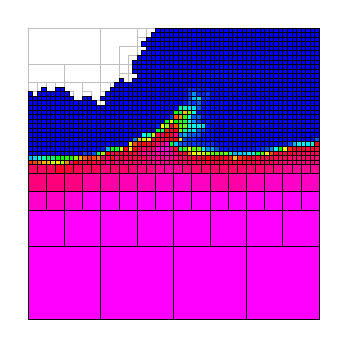
\begin{tikzpicture}[x={(\screenshotunitlength,0)},y={(0,\screenshotunitlength)}]
        \definecolor{fillcolor}{rgb}{1.000000,0.000000,1.000000}
\fill[fillcolor] (0.000000,0.000000) rectangle (0.250000,0.250000);
\definecolor{fillcolor}{rgb}{1.000000,0.000000,1.000000}
\fill[fillcolor] (0.250000,0.000000) rectangle (0.500000,0.250000);
\definecolor{fillcolor}{rgb}{1.000000,0.000000,1.000000}
\fill[fillcolor] (0.000000,0.250000) rectangle (0.125000,0.375000);
\definecolor{fillcolor}{rgb}{1.000000,0.000000,1.000000}
\fill[fillcolor] (0.125000,0.250000) rectangle (0.250000,0.375000);
\definecolor{fillcolor}{rgb}{1.000000,0.000000,0.797001}
\fill[fillcolor] (0.000000,0.375000) rectangle (0.062500,0.437500);
\definecolor{fillcolor}{rgb}{1.000000,0.000000,0.789635}
\fill[fillcolor] (0.062500,0.375000) rectangle (0.125000,0.437500);
\definecolor{fillcolor}{rgb}{1.000000,0.000000,0.480140}
\fill[fillcolor] (0.000000,0.437500) rectangle (0.062500,0.500000);
\definecolor{fillcolor}{rgb}{1.000000,0.000000,0.476755}
\fill[fillcolor] (0.062500,0.437500) rectangle (0.125000,0.500000);
\definecolor{fillcolor}{rgb}{1.000000,0.000000,0.873590}
\fill[fillcolor] (0.125000,0.375000) rectangle (0.187500,0.437500);
\definecolor{fillcolor}{rgb}{1.000000,0.000000,0.987631}
\fill[fillcolor] (0.187500,0.375000) rectangle (0.250000,0.437500);
\definecolor{fillcolor}{rgb}{1.000000,0.000000,0.501624}
\fill[fillcolor] (0.125000,0.437500) rectangle (0.187500,0.500000);
\definecolor{fillcolor}{rgb}{1.000000,0.000000,0.626767}
\fill[fillcolor] (0.187500,0.437500) rectangle (0.250000,0.500000);
\definecolor{fillcolor}{rgb}{1.000000,0.000000,1.000000}
\fill[fillcolor] (0.250000,0.250000) rectangle (0.375000,0.375000);
\definecolor{fillcolor}{rgb}{1.000000,0.000000,1.000000}
\fill[fillcolor] (0.375000,0.250000) rectangle (0.500000,0.375000);
\definecolor{fillcolor}{rgb}{1.000000,0.000000,1.000000}
\fill[fillcolor] (0.250000,0.375000) rectangle (0.312500,0.437500);
\definecolor{fillcolor}{rgb}{1.000000,0.000000,1.000000}
\fill[fillcolor] (0.312500,0.375000) rectangle (0.375000,0.437500);
\definecolor{fillcolor}{rgb}{1.000000,0.000000,0.653028}
\fill[fillcolor] (0.250000,0.437500) rectangle (0.312500,0.500000);
\definecolor{fillcolor}{rgb}{1.000000,0.000000,0.705828}
\fill[fillcolor] (0.312500,0.437500) rectangle (0.375000,0.500000);
\definecolor{fillcolor}{rgb}{1.000000,0.000000,1.000000}
\fill[fillcolor] (0.375000,0.375000) rectangle (0.437500,0.437500);
\definecolor{fillcolor}{rgb}{1.000000,0.000000,1.000000}
\fill[fillcolor] (0.437500,0.375000) rectangle (0.500000,0.437500);
\definecolor{fillcolor}{rgb}{1.000000,0.000000,0.741227}
\fill[fillcolor] (0.375000,0.437500) rectangle (0.437500,0.500000);
\definecolor{fillcolor}{rgb}{1.000000,0.000000,0.794283}
\fill[fillcolor] (0.437500,0.437500) rectangle (0.500000,0.500000);
\definecolor{fillcolor}{rgb}{1.000000,0.000000,1.000000}
\fill[fillcolor] (0.500000,0.000000) rectangle (0.750000,0.250000);
\definecolor{fillcolor}{rgb}{1.000000,0.000000,1.000000}
\fill[fillcolor] (0.750000,0.000000) rectangle (1.000000,0.250000);
\definecolor{fillcolor}{rgb}{1.000000,0.000000,1.000000}
\fill[fillcolor] (0.500000,0.250000) rectangle (0.625000,0.375000);
\definecolor{fillcolor}{rgb}{1.000000,0.000000,1.000000}
\fill[fillcolor] (0.625000,0.250000) rectangle (0.750000,0.375000);
\definecolor{fillcolor}{rgb}{1.000000,0.000000,1.000000}
\fill[fillcolor] (0.500000,0.375000) rectangle (0.562500,0.437500);
\definecolor{fillcolor}{rgb}{1.000000,0.000000,1.000000}
\fill[fillcolor] (0.562500,0.375000) rectangle (0.625000,0.437500);
\definecolor{fillcolor}{rgb}{1.000000,0.000000,0.835504}
\fill[fillcolor] (0.500000,0.437500) rectangle (0.562500,0.500000);
\definecolor{fillcolor}{rgb}{1.000000,0.000000,0.761919}
\fill[fillcolor] (0.562500,0.437500) rectangle (0.625000,0.500000);
\definecolor{fillcolor}{rgb}{1.000000,0.000000,1.000000}
\fill[fillcolor] (0.625000,0.375000) rectangle (0.687500,0.437500);
\definecolor{fillcolor}{rgb}{1.000000,0.000000,1.000000}
\fill[fillcolor] (0.687500,0.375000) rectangle (0.750000,0.437500);
\definecolor{fillcolor}{rgb}{1.000000,0.000000,0.660076}
\fill[fillcolor] (0.625000,0.437500) rectangle (0.687500,0.500000);
\definecolor{fillcolor}{rgb}{1.000000,0.000000,0.647521}
\fill[fillcolor] (0.687500,0.437500) rectangle (0.750000,0.500000);
\definecolor{fillcolor}{rgb}{1.000000,0.000000,1.000000}
\fill[fillcolor] (0.750000,0.250000) rectangle (0.875000,0.375000);
\definecolor{fillcolor}{rgb}{1.000000,0.000000,1.000000}
\fill[fillcolor] (0.875000,0.250000) rectangle (1.000000,0.375000);
\definecolor{fillcolor}{rgb}{1.000000,0.000000,1.000000}
\fill[fillcolor] (0.750000,0.375000) rectangle (0.812500,0.437500);
\definecolor{fillcolor}{rgb}{1.000000,0.000000,1.000000}
\fill[fillcolor] (0.812500,0.375000) rectangle (0.875000,0.437500);
\definecolor{fillcolor}{rgb}{1.000000,0.000000,0.735062}
\fill[fillcolor] (0.750000,0.437500) rectangle (0.812500,0.500000);
\definecolor{fillcolor}{rgb}{1.000000,0.000000,0.778676}
\fill[fillcolor] (0.812500,0.437500) rectangle (0.875000,0.500000);
\definecolor{fillcolor}{rgb}{1.000000,0.000000,1.000000}
\fill[fillcolor] (0.875000,0.375000) rectangle (0.937500,0.437500);
\definecolor{fillcolor}{rgb}{1.000000,0.000000,1.000000}
\fill[fillcolor] (0.937500,0.375000) rectangle (1.000000,0.437500);
\definecolor{fillcolor}{rgb}{1.000000,0.000000,0.776597}
\fill[fillcolor] (0.875000,0.437500) rectangle (0.937500,0.500000);
\definecolor{fillcolor}{rgb}{1.000000,0.000000,0.764332}
\fill[fillcolor] (0.937500,0.437500) rectangle (1.000000,0.500000);
\definecolor{fillcolor}{rgb}{1.000000,0.000000,0.371986}
\fill[fillcolor] (0.000000,0.500000) rectangle (0.031250,0.531250);
\definecolor{fillcolor}{rgb}{1.000000,0.000000,0.376039}
\fill[fillcolor] (0.031250,0.500000) rectangle (0.062500,0.531250);
\definecolor{fillcolor}{rgb}{1.000000,0.175194,0.000000}
\fill[fillcolor] (0.000000,0.531250) rectangle (0.015625,0.546875);
\definecolor{fillcolor}{rgb}{1.000000,0.285238,0.000000}
\fill[fillcolor] (0.015625,0.531250) rectangle (0.031250,0.546875);
\definecolor{fillcolor}{rgb}{0.000000,0.707742,1.000000}
\fill[fillcolor] (0.000000,0.546875) rectangle (0.015625,0.562500);
\definecolor{fillcolor}{rgb}{0.000000,0.850911,1.000000}
\fill[fillcolor] (0.015625,0.546875) rectangle (0.031250,0.562500);
\definecolor{fillcolor}{rgb}{1.000000,0.456133,0.000000}
\fill[fillcolor] (0.031250,0.531250) rectangle (0.046875,0.546875);
\definecolor{fillcolor}{rgb}{1.000000,0.722949,0.000000}
\fill[fillcolor] (0.046875,0.531250) rectangle (0.062500,0.546875);
\definecolor{fillcolor}{rgb}{0.000000,1.000000,0.892755}
\fill[fillcolor] (0.031250,0.546875) rectangle (0.046875,0.562500);
\definecolor{fillcolor}{rgb}{0.000000,1.000000,0.709919}
\fill[fillcolor] (0.046875,0.546875) rectangle (0.062500,0.562500);
\definecolor{fillcolor}{rgb}{1.000000,0.000000,0.316106}
\fill[fillcolor] (0.062500,0.500000) rectangle (0.093750,0.531250);
\definecolor{fillcolor}{rgb}{1.000000,0.000000,0.148865}
\fill[fillcolor] (0.093750,0.500000) rectangle (0.125000,0.531250);
\definecolor{fillcolor}{rgb}{1.000000,0.752939,0.000000}
\fill[fillcolor] (0.062500,0.531250) rectangle (0.078125,0.546875);
\definecolor{fillcolor}{rgb}{0.856626,1.000000,0.000000}
\fill[fillcolor] (0.078125,0.531250) rectangle (0.093750,0.546875);
\definecolor{fillcolor}{rgb}{0.000000,1.000000,0.332526}
\fill[fillcolor] (0.062500,0.546875) rectangle (0.078125,0.562500);
\definecolor{fillcolor}{rgb}{0.000000,1.000000,0.456694}
\fill[fillcolor] (0.078125,0.546875) rectangle (0.093750,0.562500);
\definecolor{fillcolor}{rgb}{1.000000,0.936408,0.000000}
\fill[fillcolor] (0.093750,0.531250) rectangle (0.109375,0.546875);
\definecolor{fillcolor}{rgb}{0.699811,1.000000,0.000000}
\fill[fillcolor] (0.109375,0.531250) rectangle (0.125000,0.546875);
\definecolor{fillcolor}{rgb}{0.000000,1.000000,0.071241}
\fill[fillcolor] (0.093750,0.546875) rectangle (0.109375,0.562500);
\definecolor{fillcolor}{rgb}{0.000000,1.000000,0.010484}
\fill[fillcolor] (0.109375,0.546875) rectangle (0.125000,0.562500);
\definecolor{fillcolor}{rgb}{0.000000,0.005340,1.000000}
\fill[fillcolor] (0.000000,0.562500) rectangle (0.015625,0.578125);
\definecolor{fillcolor}{rgb}{0.000000,0.005245,1.000000}
\fill[fillcolor] (0.015625,0.562500) rectangle (0.031250,0.578125);
\definecolor{fillcolor}{rgb}{0.000000,0.005701,1.000000}
\fill[fillcolor] (0.000000,0.578125) rectangle (0.015625,0.593750);
\definecolor{fillcolor}{rgb}{0.000000,0.006853,1.000000}
\fill[fillcolor] (0.015625,0.578125) rectangle (0.031250,0.593750);
\definecolor{fillcolor}{rgb}{0.000000,0.005186,1.000000}
\fill[fillcolor] (0.031250,0.562500) rectangle (0.046875,0.578125);
\definecolor{fillcolor}{rgb}{0.000000,0.003323,1.000000}
\fill[fillcolor] (0.046875,0.562500) rectangle (0.062500,0.578125);
\definecolor{fillcolor}{rgb}{0.000000,0.003376,1.000000}
\fill[fillcolor] (0.031250,0.578125) rectangle (0.046875,0.593750);
\definecolor{fillcolor}{rgb}{0.000000,0.003145,1.000000}
\fill[fillcolor] (0.046875,0.578125) rectangle (0.062500,0.593750);
\definecolor{fillcolor}{rgb}{0.000000,0.000023,1.000000}
\fill[fillcolor] (0.000000,0.593750) rectangle (0.015625,0.609375);
\definecolor{fillcolor}{rgb}{0.000000,0.000509,1.000000}
\fill[fillcolor] (0.015625,0.593750) rectangle (0.031250,0.609375);
\definecolor{fillcolor}{rgb}{0.000000,0.000005,1.000000}
\fill[fillcolor] (0.000000,0.609375) rectangle (0.015625,0.625000);
\definecolor{fillcolor}{rgb}{0.000000,0.000163,1.000000}
\fill[fillcolor] (0.015625,0.609375) rectangle (0.031250,0.625000);
\definecolor{fillcolor}{rgb}{0.000000,0.001259,1.000000}
\fill[fillcolor] (0.031250,0.593750) rectangle (0.046875,0.609375);
\definecolor{fillcolor}{rgb}{0.000000,0.003187,1.000000}
\fill[fillcolor] (0.046875,0.593750) rectangle (0.062500,0.609375);
\definecolor{fillcolor}{rgb}{0.000000,0.000301,1.000000}
\fill[fillcolor] (0.031250,0.609375) rectangle (0.046875,0.625000);
\definecolor{fillcolor}{rgb}{0.000000,0.002015,1.000000}
\fill[fillcolor] (0.046875,0.609375) rectangle (0.062500,0.625000);
\definecolor{fillcolor}{rgb}{0.000000,0.003095,1.000000}
\fill[fillcolor] (0.062500,0.562500) rectangle (0.078125,0.578125);
\definecolor{fillcolor}{rgb}{0.000000,0.002937,1.000000}
\fill[fillcolor] (0.078125,0.562500) rectangle (0.093750,0.578125);
\definecolor{fillcolor}{rgb}{0.000000,0.003579,1.000000}
\fill[fillcolor] (0.062500,0.578125) rectangle (0.078125,0.593750);
\definecolor{fillcolor}{rgb}{0.000000,0.002477,1.000000}
\fill[fillcolor] (0.078125,0.578125) rectangle (0.093750,0.593750);
\definecolor{fillcolor}{rgb}{0.000000,0.001626,1.000000}
\fill[fillcolor] (0.093750,0.562500) rectangle (0.109375,0.578125);
\definecolor{fillcolor}{rgb}{0.000000,0.001611,1.000000}
\fill[fillcolor] (0.109375,0.562500) rectangle (0.125000,0.578125);
\definecolor{fillcolor}{rgb}{0.000000,0.000815,1.000000}
\fill[fillcolor] (0.093750,0.578125) rectangle (0.109375,0.593750);
\definecolor{fillcolor}{rgb}{0.000000,0.000975,1.000000}
\fill[fillcolor] (0.109375,0.578125) rectangle (0.125000,0.593750);
\definecolor{fillcolor}{rgb}{0.000000,0.001443,1.000000}
\fill[fillcolor] (0.062500,0.593750) rectangle (0.078125,0.609375);
\definecolor{fillcolor}{rgb}{0.000000,0.000403,1.000000}
\fill[fillcolor] (0.078125,0.593750) rectangle (0.093750,0.609375);
\definecolor{fillcolor}{rgb}{0.000000,0.001126,1.000000}
\fill[fillcolor] (0.062500,0.609375) rectangle (0.078125,0.625000);
\definecolor{fillcolor}{rgb}{0.000000,0.000312,1.000000}
\fill[fillcolor] (0.078125,0.609375) rectangle (0.093750,0.625000);
\definecolor{fillcolor}{rgb}{0.000000,0.000452,1.000000}
\fill[fillcolor] (0.093750,0.593750) rectangle (0.109375,0.609375);
\definecolor{fillcolor}{rgb}{0.000000,0.000820,1.000000}
\fill[fillcolor] (0.109375,0.593750) rectangle (0.125000,0.609375);
\definecolor{fillcolor}{rgb}{0.000000,0.000121,1.000000}
\fill[fillcolor] (0.093750,0.609375) rectangle (0.109375,0.625000);
\definecolor{fillcolor}{rgb}{0.000000,0.000659,1.000000}
\fill[fillcolor] (0.109375,0.609375) rectangle (0.125000,0.625000);
\definecolor{fillcolor}{rgb}{1.000000,0.000000,0.222785}
\fill[fillcolor] (0.125000,0.500000) rectangle (0.156250,0.531250);
\definecolor{fillcolor}{rgb}{1.000000,0.000000,0.333370}
\fill[fillcolor] (0.156250,0.500000) rectangle (0.187500,0.531250);
\definecolor{fillcolor}{rgb}{1.000000,0.561345,0.000000}
\fill[fillcolor] (0.125000,0.531250) rectangle (0.140625,0.546875);
\definecolor{fillcolor}{rgb}{1.000000,0.000000,0.533713}
\fill[fillcolor] (0.140625,0.531250) rectangle (0.156250,0.546875);
\definecolor{fillcolor}{rgb}{0.138335,1.000000,0.000000}
\fill[fillcolor] (0.125000,0.546875) rectangle (0.140625,0.562500);
\definecolor{fillcolor}{rgb}{0.124034,1.000000,0.000000}
\fill[fillcolor] (0.140625,0.546875) rectangle (0.156250,0.562500);
\definecolor{fillcolor}{rgb}{1.000000,0.000000,0.027676}
\fill[fillcolor] (0.156250,0.531250) rectangle (0.171875,0.546875);
\definecolor{fillcolor}{rgb}{1.000000,0.000000,0.189130}
\fill[fillcolor] (0.171875,0.531250) rectangle (0.187500,0.546875);
\definecolor{fillcolor}{rgb}{0.527930,1.000000,0.000000}
\fill[fillcolor] (0.156250,0.546875) rectangle (0.171875,0.562500);
\definecolor{fillcolor}{rgb}{1.000000,0.699887,0.000000}
\fill[fillcolor] (0.171875,0.546875) rectangle (0.187500,0.562500);
\definecolor{fillcolor}{rgb}{1.000000,0.000000,0.367219}
\fill[fillcolor] (0.187500,0.500000) rectangle (0.218750,0.531250);
\definecolor{fillcolor}{rgb}{1.000000,0.000000,0.347244}
\fill[fillcolor] (0.218750,0.500000) rectangle (0.250000,0.531250);
\definecolor{fillcolor}{rgb}{1.000000,0.000000,0.283978}
\fill[fillcolor] (0.187500,0.531250) rectangle (0.203125,0.546875);
\definecolor{fillcolor}{rgb}{1.000000,0.000000,0.121019}
\fill[fillcolor] (0.203125,0.531250) rectangle (0.218750,0.546875);
\definecolor{fillcolor}{rgb}{1.000000,0.365205,0.000000}
\fill[fillcolor] (0.187500,0.546875) rectangle (0.203125,0.562500);
\definecolor{fillcolor}{rgb}{1.000000,0.187355,0.000000}
\fill[fillcolor] (0.203125,0.546875) rectangle (0.218750,0.562500);
\definecolor{fillcolor}{rgb}{1.000000,0.000000,0.236981}
\fill[fillcolor] (0.218750,0.531250) rectangle (0.234375,0.546875);
\definecolor{fillcolor}{rgb}{1.000000,0.000000,0.274082}
\fill[fillcolor] (0.234375,0.531250) rectangle (0.250000,0.546875);
\definecolor{fillcolor}{rgb}{1.000000,0.295482,0.000000}
\fill[fillcolor] (0.218750,0.546875) rectangle (0.234375,0.562500);
\definecolor{fillcolor}{rgb}{1.000000,0.462080,0.000000}
\fill[fillcolor] (0.234375,0.546875) rectangle (0.250000,0.562500);
\definecolor{fillcolor}{rgb}{0.000000,0.002174,1.000000}
\fill[fillcolor] (0.125000,0.562500) rectangle (0.140625,0.578125);
\definecolor{fillcolor}{rgb}{0.000000,0.003030,1.000000}
\fill[fillcolor] (0.140625,0.562500) rectangle (0.156250,0.578125);
\definecolor{fillcolor}{rgb}{0.000000,0.001028,1.000000}
\fill[fillcolor] (0.125000,0.578125) rectangle (0.140625,0.593750);
\definecolor{fillcolor}{rgb}{0.000000,0.001092,1.000000}
\fill[fillcolor] (0.140625,0.578125) rectangle (0.156250,0.593750);
\definecolor{fillcolor}{rgb}{0.000000,0.000722,1.000000}
\fill[fillcolor] (0.156250,0.562500) rectangle (0.171875,0.578125);
\definecolor{fillcolor}{rgb}{0.000000,0.005423,1.000000}
\fill[fillcolor] (0.171875,0.562500) rectangle (0.187500,0.578125);
\definecolor{fillcolor}{rgb}{0.000000,0.000588,1.000000}
\fill[fillcolor] (0.156250,0.578125) rectangle (0.171875,0.593750);
\definecolor{fillcolor}{rgb}{0.000000,0.000696,1.000000}
\fill[fillcolor] (0.171875,0.578125) rectangle (0.187500,0.593750);
\definecolor{fillcolor}{rgb}{0.000000,0.000454,1.000000}
\fill[fillcolor] (0.125000,0.593750) rectangle (0.140625,0.609375);
\definecolor{fillcolor}{rgb}{0.000000,0.000561,1.000000}
\fill[fillcolor] (0.140625,0.593750) rectangle (0.156250,0.609375);
\definecolor{fillcolor}{rgb}{0.000000,0.000464,1.000000}
\fill[fillcolor] (0.125000,0.609375) rectangle (0.140625,0.625000);
\definecolor{fillcolor}{rgb}{0.000000,0.000569,1.000000}
\fill[fillcolor] (0.140625,0.609375) rectangle (0.156250,0.625000);
\definecolor{fillcolor}{rgb}{0.000000,0.000499,1.000000}
\fill[fillcolor] (0.156250,0.593750) rectangle (0.171875,0.609375);
\definecolor{fillcolor}{rgb}{0.000000,0.000624,1.000000}
\fill[fillcolor] (0.171875,0.593750) rectangle (0.187500,0.609375);
\definecolor{fillcolor}{rgb}{0.000000,0.000560,1.000000}
\fill[fillcolor] (0.156250,0.609375) rectangle (0.171875,0.625000);
\definecolor{fillcolor}{rgb}{0.000000,0.000604,1.000000}
\fill[fillcolor] (0.171875,0.609375) rectangle (0.187500,0.625000);
\definecolor{fillcolor}{rgb}{0.000000,0.227058,1.000000}
\fill[fillcolor] (0.187500,0.562500) rectangle (0.203125,0.578125);
\definecolor{fillcolor}{rgb}{0.000000,0.147261,1.000000}
\fill[fillcolor] (0.203125,0.562500) rectangle (0.218750,0.578125);
\definecolor{fillcolor}{rgb}{0.000000,0.006917,1.000000}
\fill[fillcolor] (0.187500,0.578125) rectangle (0.203125,0.593750);
\definecolor{fillcolor}{rgb}{0.000000,0.005088,1.000000}
\fill[fillcolor] (0.203125,0.578125) rectangle (0.218750,0.593750);
\definecolor{fillcolor}{rgb}{0.000000,0.312864,1.000000}
\fill[fillcolor] (0.218750,0.562500) rectangle (0.234375,0.578125);
\definecolor{fillcolor}{rgb}{0.000000,1.000000,0.396699}
\fill[fillcolor] (0.234375,0.562500) rectangle (0.250000,0.578125);
\definecolor{fillcolor}{rgb}{0.000000,0.000121,1.000000}
\fill[fillcolor] (0.218750,0.578125) rectangle (0.234375,0.593750);
\definecolor{fillcolor}{rgb}{0.000000,0.019267,1.000000}
\fill[fillcolor] (0.234375,0.578125) rectangle (0.250000,0.593750);
\definecolor{fillcolor}{rgb}{0.000000,0.002543,1.000000}
\fill[fillcolor] (0.187500,0.593750) rectangle (0.203125,0.609375);
\definecolor{fillcolor}{rgb}{0.000000,0.002772,1.000000}
\fill[fillcolor] (0.203125,0.593750) rectangle (0.218750,0.609375);
\definecolor{fillcolor}{rgb}{0.000000,0.000733,1.000000}
\fill[fillcolor] (0.187500,0.609375) rectangle (0.203125,0.625000);
\definecolor{fillcolor}{rgb}{0.000000,0.000879,1.000000}
\fill[fillcolor] (0.203125,0.609375) rectangle (0.218750,0.625000);
\definecolor{fillcolor}{rgb}{0.000000,0.000794,1.000000}
\fill[fillcolor] (0.218750,0.593750) rectangle (0.234375,0.609375);
\definecolor{fillcolor}{rgb}{0.000000,0.000322,1.000000}
\fill[fillcolor] (0.234375,0.593750) rectangle (0.250000,0.609375);
\definecolor{fillcolor}{rgb}{0.000000,0.000711,1.000000}
\fill[fillcolor] (0.218750,0.609375) rectangle (0.234375,0.625000);
\definecolor{fillcolor}{rgb}{0.000000,0.000516,1.000000}
\fill[fillcolor] (0.234375,0.609375) rectangle (0.250000,0.625000);
\definecolor{fillcolor}{rgb}{0.000000,0.000000,1.000000}
\fill[fillcolor] (0.000000,0.625000) rectangle (0.015625,0.640625);
\definecolor{fillcolor}{rgb}{0.000000,0.000117,1.000000}
\fill[fillcolor] (0.015625,0.625000) rectangle (0.031250,0.640625);
\definecolor{fillcolor}{rgb}{0.000000,0.000000,1.000000}
\fill[fillcolor] (0.000000,0.640625) rectangle (0.015625,0.656250);
\definecolor{fillcolor}{rgb}{0.000000,0.000054,1.000000}
\fill[fillcolor] (0.015625,0.640625) rectangle (0.031250,0.656250);
\definecolor{fillcolor}{rgb}{0.000000,0.000210,1.000000}
\fill[fillcolor] (0.031250,0.625000) rectangle (0.046875,0.640625);
\definecolor{fillcolor}{rgb}{0.000000,0.000252,1.000000}
\fill[fillcolor] (0.046875,0.625000) rectangle (0.062500,0.640625);
\definecolor{fillcolor}{rgb}{0.000000,0.000083,1.000000}
\fill[fillcolor] (0.031250,0.640625) rectangle (0.046875,0.656250);
\definecolor{fillcolor}{rgb}{0.000000,0.000057,1.000000}
\fill[fillcolor] (0.046875,0.640625) rectangle (0.062500,0.656250);
\definecolor{fillcolor}{rgb}{0.000000,0.000000,1.000000}
\fill[fillcolor] (0.000000,0.656250) rectangle (0.015625,0.671875);
\definecolor{fillcolor}{rgb}{0.000000,0.000033,1.000000}
\fill[fillcolor] (0.015625,0.656250) rectangle (0.031250,0.671875);
\definecolor{fillcolor}{rgb}{0.000000,0.000000,1.000000}
\fill[fillcolor] (0.000000,0.671875) rectangle (0.015625,0.687500);
\definecolor{fillcolor}{rgb}{0.000000,0.000006,1.000000}
\fill[fillcolor] (0.015625,0.671875) rectangle (0.031250,0.687500);
\definecolor{fillcolor}{rgb}{0.000000,0.000038,1.000000}
\fill[fillcolor] (0.031250,0.656250) rectangle (0.046875,0.671875);
\definecolor{fillcolor}{rgb}{0.000000,0.000000,1.000000}
\fill[fillcolor] (0.046875,0.656250) rectangle (0.062500,0.671875);
\definecolor{fillcolor}{rgb}{0.000000,0.000009,1.000000}
\fill[fillcolor] (0.031250,0.671875) rectangle (0.046875,0.687500);
\definecolor{fillcolor}{rgb}{0.000000,0.000000,1.000000}
\fill[fillcolor] (0.046875,0.671875) rectangle (0.062500,0.687500);
\definecolor{fillcolor}{rgb}{0.000000,0.000420,1.000000}
\fill[fillcolor] (0.062500,0.625000) rectangle (0.078125,0.640625);
\definecolor{fillcolor}{rgb}{0.000000,0.000124,1.000000}
\fill[fillcolor] (0.078125,0.625000) rectangle (0.093750,0.640625);
\definecolor{fillcolor}{rgb}{0.000000,0.000097,1.000000}
\fill[fillcolor] (0.062500,0.640625) rectangle (0.078125,0.656250);
\definecolor{fillcolor}{rgb}{0.000000,0.000042,1.000000}
\fill[fillcolor] (0.078125,0.640625) rectangle (0.093750,0.656250);
\definecolor{fillcolor}{rgb}{0.000000,0.000056,1.000000}
\fill[fillcolor] (0.093750,0.625000) rectangle (0.109375,0.640625);
\definecolor{fillcolor}{rgb}{0.000000,0.000538,1.000000}
\fill[fillcolor] (0.109375,0.625000) rectangle (0.125000,0.640625);
\definecolor{fillcolor}{rgb}{0.000000,0.000043,1.000000}
\fill[fillcolor] (0.093750,0.640625) rectangle (0.109375,0.656250);
\definecolor{fillcolor}{rgb}{0.000000,0.000173,1.000000}
\fill[fillcolor] (0.109375,0.640625) rectangle (0.125000,0.656250);
\definecolor{fillcolor}{rgb}{0.000000,0.000073,1.000000}
\fill[fillcolor] (0.062500,0.656250) rectangle (0.078125,0.671875);
\definecolor{fillcolor}{rgb}{0.000000,0.000017,1.000000}
\fill[fillcolor] (0.078125,0.656250) rectangle (0.093750,0.671875);
\definecolor{fillcolor}{rgb}{0.000000,0.000005,1.000000}
\fill[fillcolor] (0.062500,0.671875) rectangle (0.078125,0.687500);
\definecolor{fillcolor}{rgb}{0.000000,0.000000,1.000000}
\fill[fillcolor] (0.078125,0.671875) rectangle (0.093750,0.687500);
\definecolor{fillcolor}{rgb}{0.000000,0.000026,1.000000}
\fill[fillcolor] (0.093750,0.656250) rectangle (0.109375,0.671875);
\definecolor{fillcolor}{rgb}{0.000000,0.000041,1.000000}
\fill[fillcolor] (0.109375,0.656250) rectangle (0.125000,0.671875);
\definecolor{fillcolor}{rgb}{0.000000,0.000011,1.000000}
\fill[fillcolor] (0.093750,0.671875) rectangle (0.109375,0.687500);
\definecolor{fillcolor}{rgb}{0.000000,0.000001,1.000000}
\fill[fillcolor] (0.109375,0.671875) rectangle (0.125000,0.687500);
\definecolor{fillcolor}{rgb}{0.000000,0.000000,1.000000}
\fill[fillcolor] (0.000000,0.687500) rectangle (0.015625,0.703125);
\definecolor{fillcolor}{rgb}{0.000000,0.000000,1.000000}
\fill[fillcolor] (0.015625,0.687500) rectangle (0.031250,0.703125);
\definecolor{fillcolor}{rgb}{0.000000,0.000000,1.000000}
\fill[fillcolor] (0.000000,0.703125) rectangle (0.015625,0.718750);
\definecolor{fillcolor}{rgb}{0.000000,0.000000,1.000000}
\fill[fillcolor] (0.015625,0.703125) rectangle (0.031250,0.718750);
\definecolor{fillcolor}{rgb}{0.000000,0.000000,1.000000}
\fill[fillcolor] (0.031250,0.687500) rectangle (0.046875,0.703125);
\definecolor{fillcolor}{rgb}{0.000000,0.000000,1.000000}
\fill[fillcolor] (0.046875,0.687500) rectangle (0.062500,0.703125);
\definecolor{fillcolor}{rgb}{0.000000,0.000000,1.000000}
\fill[fillcolor] (0.031250,0.703125) rectangle (0.046875,0.718750);
\definecolor{fillcolor}{rgb}{0.000000,0.000000,1.000000}
\fill[fillcolor] (0.046875,0.703125) rectangle (0.062500,0.718750);
\definecolor{fillcolor}{rgb}{0.000000,0.000000,1.000000}
\fill[fillcolor] (0.000000,0.718750) rectangle (0.015625,0.734375);
\definecolor{fillcolor}{rgb}{0.000000,0.000000,1.000000}
\fill[fillcolor] (0.015625,0.718750) rectangle (0.031250,0.734375);
\definecolor{fillcolor}{rgb}{0.000000,0.000000,1.000000}
\fill[fillcolor] (0.000000,0.734375) rectangle (0.015625,0.750000);
\definecolor{fillcolor}{rgb}{0.000000,0.000000,1.000000}
\fill[fillcolor] (0.015625,0.734375) rectangle (0.031250,0.750000);
\definecolor{fillcolor}{rgb}{0.000000,0.000000,1.000000}
\fill[fillcolor] (0.031250,0.718750) rectangle (0.046875,0.734375);
\definecolor{fillcolor}{rgb}{0.000000,0.000000,1.000000}
\fill[fillcolor] (0.046875,0.718750) rectangle (0.062500,0.734375);
\definecolor{fillcolor}{rgb}{0.000000,0.000000,1.000000}
\fill[fillcolor] (0.031250,0.734375) rectangle (0.046875,0.750000);
\definecolor{fillcolor}{rgb}{0.000000,0.000000,1.000000}
\fill[fillcolor] (0.046875,0.734375) rectangle (0.062500,0.750000);
\definecolor{fillcolor}{rgb}{0.000000,0.000000,1.000000}
\fill[fillcolor] (0.062500,0.687500) rectangle (0.078125,0.703125);
\definecolor{fillcolor}{rgb}{0.000000,0.000000,1.000000}
\fill[fillcolor] (0.078125,0.687500) rectangle (0.093750,0.703125);
\definecolor{fillcolor}{rgb}{0.000000,0.000000,1.000000}
\fill[fillcolor] (0.062500,0.703125) rectangle (0.078125,0.718750);
\definecolor{fillcolor}{rgb}{0.000000,0.000000,1.000000}
\fill[fillcolor] (0.078125,0.703125) rectangle (0.093750,0.718750);
\definecolor{fillcolor}{rgb}{0.000000,0.000000,1.000000}
\fill[fillcolor] (0.093750,0.687500) rectangle (0.109375,0.703125);
\definecolor{fillcolor}{rgb}{0.000000,0.000001,1.000000}
\fill[fillcolor] (0.109375,0.687500) rectangle (0.125000,0.703125);
\definecolor{fillcolor}{rgb}{0.000000,0.000000,1.000000}
\fill[fillcolor] (0.093750,0.703125) rectangle (0.109375,0.718750);
\definecolor{fillcolor}{rgb}{0.000000,0.000000,1.000000}
\fill[fillcolor] (0.109375,0.703125) rectangle (0.125000,0.718750);
\definecolor{fillcolor}{rgb}{0.000000,0.000000,1.000000}
\fill[fillcolor] (0.062500,0.718750) rectangle (0.078125,0.734375);
\definecolor{fillcolor}{rgb}{0.000000,0.000000,1.000000}
\fill[fillcolor] (0.078125,0.718750) rectangle (0.093750,0.734375);
\definecolor{fillcolor}{rgb}{0.000000,0.000000,1.000000}
\fill[fillcolor] (0.062500,0.734375) rectangle (0.078125,0.750000);
\definecolor{fillcolor}{rgb}{0.000000,0.000000,1.000000}
\fill[fillcolor] (0.078125,0.734375) rectangle (0.093750,0.750000);
\definecolor{fillcolor}{rgb}{0.000000,0.000000,1.000000}
\fill[fillcolor] (0.093750,0.718750) rectangle (0.109375,0.734375);
\definecolor{fillcolor}{rgb}{0.000000,0.000000,1.000000}
\fill[fillcolor] (0.109375,0.718750) rectangle (0.125000,0.734375);
\definecolor{fillcolor}{rgb}{0.000000,0.000000,1.000000}
\fill[fillcolor] (0.093750,0.734375) rectangle (0.109375,0.750000);
\definecolor{fillcolor}{rgb}{0.000000,0.000000,1.000000}
\fill[fillcolor] (0.109375,0.734375) rectangle (0.125000,0.750000);
\definecolor{fillcolor}{rgb}{0.000000,0.000369,1.000000}
\fill[fillcolor] (0.125000,0.625000) rectangle (0.140625,0.640625);
\definecolor{fillcolor}{rgb}{0.000000,0.000399,1.000000}
\fill[fillcolor] (0.140625,0.625000) rectangle (0.156250,0.640625);
\definecolor{fillcolor}{rgb}{0.000000,0.000095,1.000000}
\fill[fillcolor] (0.125000,0.640625) rectangle (0.140625,0.656250);
\definecolor{fillcolor}{rgb}{0.000000,0.000044,1.000000}
\fill[fillcolor] (0.140625,0.640625) rectangle (0.156250,0.656250);
\definecolor{fillcolor}{rgb}{0.000000,0.000192,1.000000}
\fill[fillcolor] (0.156250,0.625000) rectangle (0.171875,0.640625);
\definecolor{fillcolor}{rgb}{0.000000,0.000105,1.000000}
\fill[fillcolor] (0.171875,0.625000) rectangle (0.187500,0.640625);
\definecolor{fillcolor}{rgb}{0.000000,0.000032,1.000000}
\fill[fillcolor] (0.156250,0.640625) rectangle (0.171875,0.656250);
\definecolor{fillcolor}{rgb}{0.000000,0.000012,1.000000}
\fill[fillcolor] (0.171875,0.640625) rectangle (0.187500,0.656250);
\definecolor{fillcolor}{rgb}{0.000000,0.000027,1.000000}
\fill[fillcolor] (0.125000,0.656250) rectangle (0.140625,0.671875);
\definecolor{fillcolor}{rgb}{0.000000,0.000011,1.000000}
\fill[fillcolor] (0.140625,0.656250) rectangle (0.156250,0.671875);
\definecolor{fillcolor}{rgb}{0.000000,0.000001,1.000000}
\fill[fillcolor] (0.125000,0.671875) rectangle (0.140625,0.687500);
\definecolor{fillcolor}{rgb}{0.000000,0.000001,1.000000}
\fill[fillcolor] (0.140625,0.671875) rectangle (0.156250,0.687500);
\definecolor{fillcolor}{rgb}{0.000000,0.000010,1.000000}
\fill[fillcolor] (0.156250,0.656250) rectangle (0.171875,0.671875);
\definecolor{fillcolor}{rgb}{0.000000,0.000009,1.000000}
\fill[fillcolor] (0.171875,0.656250) rectangle (0.187500,0.671875);
\definecolor{fillcolor}{rgb}{0.000000,0.000004,1.000000}
\fill[fillcolor] (0.156250,0.671875) rectangle (0.171875,0.687500);
\definecolor{fillcolor}{rgb}{0.000000,0.000003,1.000000}
\fill[fillcolor] (0.171875,0.671875) rectangle (0.187500,0.687500);
\definecolor{fillcolor}{rgb}{0.000000,0.000102,1.000000}
\fill[fillcolor] (0.187500,0.625000) rectangle (0.203125,0.640625);
\definecolor{fillcolor}{rgb}{0.000000,0.000142,1.000000}
\fill[fillcolor] (0.203125,0.625000) rectangle (0.218750,0.640625);
\definecolor{fillcolor}{rgb}{0.000000,0.000013,1.000000}
\fill[fillcolor] (0.187500,0.640625) rectangle (0.203125,0.656250);
\definecolor{fillcolor}{rgb}{0.000000,0.000013,1.000000}
\fill[fillcolor] (0.203125,0.640625) rectangle (0.218750,0.656250);
\definecolor{fillcolor}{rgb}{0.000000,0.000210,1.000000}
\fill[fillcolor] (0.218750,0.625000) rectangle (0.234375,0.640625);
\definecolor{fillcolor}{rgb}{0.000000,0.000147,1.000000}
\fill[fillcolor] (0.234375,0.625000) rectangle (0.250000,0.640625);
\definecolor{fillcolor}{rgb}{0.000000,0.000026,1.000000}
\fill[fillcolor] (0.218750,0.640625) rectangle (0.234375,0.656250);
\definecolor{fillcolor}{rgb}{0.000000,0.000004,1.000000}
\fill[fillcolor] (0.234375,0.640625) rectangle (0.250000,0.656250);
\definecolor{fillcolor}{rgb}{0.000000,0.000008,1.000000}
\fill[fillcolor] (0.187500,0.656250) rectangle (0.203125,0.671875);
\definecolor{fillcolor}{rgb}{0.000000,0.000002,1.000000}
\fill[fillcolor] (0.203125,0.656250) rectangle (0.218750,0.671875);
\definecolor{fillcolor}{rgb}{0.000000,0.000002,1.000000}
\fill[fillcolor] (0.187500,0.671875) rectangle (0.203125,0.687500);
\definecolor{fillcolor}{rgb}{0.000000,0.000000,1.000000}
\fill[fillcolor] (0.203125,0.671875) rectangle (0.218750,0.687500);
\definecolor{fillcolor}{rgb}{0.000000,0.000002,1.000000}
\fill[fillcolor] (0.218750,0.656250) rectangle (0.234375,0.671875);
\definecolor{fillcolor}{rgb}{0.000000,0.000001,1.000000}
\fill[fillcolor] (0.234375,0.656250) rectangle (0.250000,0.671875);
\definecolor{fillcolor}{rgb}{0.000000,0.000000,1.000000}
\fill[fillcolor] (0.218750,0.671875) rectangle (0.234375,0.687500);
\definecolor{fillcolor}{rgb}{0.000000,0.000000,1.000000}
\fill[fillcolor] (0.234375,0.671875) rectangle (0.250000,0.687500);
\definecolor{fillcolor}{rgb}{0.000000,0.000002,1.000000}
\fill[fillcolor] (0.125000,0.687500) rectangle (0.140625,0.703125);
\definecolor{fillcolor}{rgb}{0.000000,0.000001,1.000000}
\fill[fillcolor] (0.140625,0.687500) rectangle (0.156250,0.703125);
\definecolor{fillcolor}{rgb}{0.000000,0.000000,1.000000}
\fill[fillcolor] (0.125000,0.703125) rectangle (0.140625,0.718750);
\definecolor{fillcolor}{rgb}{0.000000,0.000000,1.000000}
\fill[fillcolor] (0.140625,0.703125) rectangle (0.156250,0.718750);
\definecolor{fillcolor}{rgb}{0.000000,0.000002,1.000000}
\fill[fillcolor] (0.156250,0.687500) rectangle (0.171875,0.703125);
\definecolor{fillcolor}{rgb}{0.000000,0.000001,1.000000}
\fill[fillcolor] (0.171875,0.687500) rectangle (0.187500,0.703125);
\definecolor{fillcolor}{rgb}{0.000000,0.000000,1.000000}
\fill[fillcolor] (0.156250,0.703125) rectangle (0.171875,0.718750);
\definecolor{fillcolor}{rgb}{0.000000,0.000000,1.000000}
\fill[fillcolor] (0.171875,0.703125) rectangle (0.187500,0.718750);
\definecolor{fillcolor}{rgb}{0.000000,0.000000,1.000000}
\fill[fillcolor] (0.125000,0.718750) rectangle (0.140625,0.734375);
\definecolor{fillcolor}{rgb}{0.000000,0.000000,1.000000}
\fill[fillcolor] (0.140625,0.718750) rectangle (0.156250,0.734375);
\definecolor{fillcolor}{rgb}{0.000000,0.000000,1.000000}
\fill[fillcolor] (0.125000,0.734375) rectangle (0.140625,0.750000);
\definecolor{fillcolor}{rgb}{0.000000,0.000000,1.000000}
\fill[fillcolor] (0.140625,0.734375) rectangle (0.156250,0.750000);
\definecolor{fillcolor}{rgb}{0.000000,0.000000,1.000000}
\fill[fillcolor] (0.156250,0.718750) rectangle (0.171875,0.734375);
\definecolor{fillcolor}{rgb}{0.000000,0.000000,1.000000}
\fill[fillcolor] (0.171875,0.718750) rectangle (0.187500,0.734375);
\definecolor{fillcolor}{rgb}{0.000000,0.000000,1.000000}
\fill[fillcolor] (0.156250,0.734375) rectangle (0.171875,0.750000);
\definecolor{fillcolor}{rgb}{0.000000,0.000000,1.000000}
\fill[fillcolor] (0.171875,0.734375) rectangle (0.187500,0.750000);
\definecolor{fillcolor}{rgb}{0.000000,0.000000,1.000000}
\fill[fillcolor] (0.187500,0.687500) rectangle (0.203125,0.703125);
\definecolor{fillcolor}{rgb}{0.000000,0.000000,1.000000}
\fill[fillcolor] (0.203125,0.687500) rectangle (0.218750,0.703125);
\definecolor{fillcolor}{rgb}{0.000000,0.000000,1.000000}
\fill[fillcolor] (0.187500,0.703125) rectangle (0.203125,0.718750);
\definecolor{fillcolor}{rgb}{0.000000,0.000000,1.000000}
\fill[fillcolor] (0.203125,0.703125) rectangle (0.218750,0.718750);
\definecolor{fillcolor}{rgb}{0.000000,0.000000,1.000000}
\fill[fillcolor] (0.218750,0.687500) rectangle (0.234375,0.703125);
\definecolor{fillcolor}{rgb}{0.000000,0.000000,1.000000}
\fill[fillcolor] (0.234375,0.687500) rectangle (0.250000,0.703125);
\definecolor{fillcolor}{rgb}{0.000000,0.000000,1.000000}
\fill[fillcolor] (0.218750,0.703125) rectangle (0.234375,0.718750);
\definecolor{fillcolor}{rgb}{0.000000,0.000000,1.000000}
\fill[fillcolor] (0.234375,0.703125) rectangle (0.250000,0.718750);
\definecolor{fillcolor}{rgb}{0.000000,0.000000,1.000000}
\fill[fillcolor] (0.187500,0.718750) rectangle (0.203125,0.734375);
\definecolor{fillcolor}{rgb}{0.000000,0.000000,1.000000}
\fill[fillcolor] (0.203125,0.718750) rectangle (0.218750,0.734375);
\definecolor{fillcolor}{rgb}{0.000000,0.000000,1.000000}
\fill[fillcolor] (0.187500,0.734375) rectangle (0.203125,0.750000);
\definecolor{fillcolor}{rgb}{0.000000,0.000000,1.000000}
\fill[fillcolor] (0.203125,0.734375) rectangle (0.218750,0.750000);
\definecolor{fillcolor}{rgb}{0.000000,0.000000,1.000000}
\fill[fillcolor] (0.218750,0.718750) rectangle (0.234375,0.734375);
\definecolor{fillcolor}{rgb}{0.000000,0.000000,1.000000}
\fill[fillcolor] (0.234375,0.718750) rectangle (0.250000,0.734375);
\definecolor{fillcolor}{rgb}{0.000000,0.000000,1.000000}
\fill[fillcolor] (0.218750,0.734375) rectangle (0.234375,0.750000);
\definecolor{fillcolor}{rgb}{1.000000,0.000000,0.461252}
\fill[fillcolor] (0.250000,0.500000) rectangle (0.281250,0.531250);
\definecolor{fillcolor}{rgb}{1.000000,0.000000,0.411410}
\fill[fillcolor] (0.281250,0.500000) rectangle (0.312500,0.531250);
\definecolor{fillcolor}{rgb}{1.000000,0.000000,0.276205}
\fill[fillcolor] (0.250000,0.531250) rectangle (0.265625,0.546875);
\definecolor{fillcolor}{rgb}{1.000000,0.000000,0.571498}
\fill[fillcolor] (0.265625,0.531250) rectangle (0.281250,0.546875);
\definecolor{fillcolor}{rgb}{1.000000,0.000000,0.353724}
\fill[fillcolor] (0.250000,0.546875) rectangle (0.265625,0.562500);
\definecolor{fillcolor}{rgb}{1.000000,0.000000,0.326616}
\fill[fillcolor] (0.265625,0.546875) rectangle (0.281250,0.562500);
\definecolor{fillcolor}{rgb}{1.000000,0.000000,0.268708}
\fill[fillcolor] (0.281250,0.531250) rectangle (0.296875,0.546875);
\definecolor{fillcolor}{rgb}{1.000000,0.000000,0.525735}
\fill[fillcolor] (0.296875,0.531250) rectangle (0.312500,0.546875);
\definecolor{fillcolor}{rgb}{1.000000,0.062179,0.000000}
\fill[fillcolor] (0.281250,0.546875) rectangle (0.296875,0.562500);
\definecolor{fillcolor}{rgb}{1.000000,0.000000,0.455058}
\fill[fillcolor] (0.296875,0.546875) rectangle (0.312500,0.562500);
\definecolor{fillcolor}{rgb}{1.000000,0.000000,0.420332}
\fill[fillcolor] (0.312500,0.500000) rectangle (0.343750,0.531250);
\definecolor{fillcolor}{rgb}{1.000000,0.000000,0.446894}
\fill[fillcolor] (0.343750,0.500000) rectangle (0.375000,0.531250);
\definecolor{fillcolor}{rgb}{1.000000,0.000000,0.307699}
\fill[fillcolor] (0.312500,0.531250) rectangle (0.328125,0.546875);
\definecolor{fillcolor}{rgb}{1.000000,0.000000,0.548732}
\fill[fillcolor] (0.328125,0.531250) rectangle (0.343750,0.546875);
\definecolor{fillcolor}{rgb}{1.000000,0.000000,0.221039}
\fill[fillcolor] (0.312500,0.546875) rectangle (0.328125,0.562500);
\definecolor{fillcolor}{rgb}{1.000000,0.000000,0.288123}
\fill[fillcolor] (0.328125,0.546875) rectangle (0.343750,0.562500);
\definecolor{fillcolor}{rgb}{1.000000,0.000000,0.383855}
\fill[fillcolor] (0.343750,0.531250) rectangle (0.359375,0.546875);
\definecolor{fillcolor}{rgb}{1.000000,0.000000,0.368868}
\fill[fillcolor] (0.359375,0.531250) rectangle (0.375000,0.546875);
\definecolor{fillcolor}{rgb}{1.000000,0.000000,0.275923}
\fill[fillcolor] (0.343750,0.546875) rectangle (0.359375,0.562500);
\definecolor{fillcolor}{rgb}{1.000000,0.000000,0.283391}
\fill[fillcolor] (0.359375,0.546875) rectangle (0.375000,0.562500);
\definecolor{fillcolor}{rgb}{0.643016,1.000000,0.000000}
\fill[fillcolor] (0.250000,0.562500) rectangle (0.265625,0.578125);
\definecolor{fillcolor}{rgb}{1.000000,0.000000,0.069819}
\fill[fillcolor] (0.265625,0.562500) rectangle (0.281250,0.578125);
\definecolor{fillcolor}{rgb}{0.000000,0.097898,1.000000}
\fill[fillcolor] (0.250000,0.578125) rectangle (0.265625,0.593750);
\definecolor{fillcolor}{rgb}{0.000000,0.696766,1.000000}
\fill[fillcolor] (0.265625,0.578125) rectangle (0.281250,0.593750);
\definecolor{fillcolor}{rgb}{1.000000,0.000000,0.350585}
\fill[fillcolor] (0.281250,0.562500) rectangle (0.296875,0.578125);
\definecolor{fillcolor}{rgb}{1.000000,0.000000,0.254351}
\fill[fillcolor] (0.296875,0.562500) rectangle (0.312500,0.578125);
\definecolor{fillcolor}{rgb}{0.000000,1.000000,0.123521}
\fill[fillcolor] (0.281250,0.578125) rectangle (0.296875,0.593750);
\definecolor{fillcolor}{rgb}{0.000000,1.000000,0.175446}
\fill[fillcolor] (0.296875,0.578125) rectangle (0.312500,0.593750);
\definecolor{fillcolor}{rgb}{0.000000,0.006152,1.000000}
\fill[fillcolor] (0.250000,0.593750) rectangle (0.265625,0.609375);
\definecolor{fillcolor}{rgb}{0.000000,0.017848,1.000000}
\fill[fillcolor] (0.265625,0.593750) rectangle (0.281250,0.609375);
\definecolor{fillcolor}{rgb}{0.000000,0.000687,1.000000}
\fill[fillcolor] (0.250000,0.609375) rectangle (0.265625,0.625000);
\definecolor{fillcolor}{rgb}{0.000000,0.001140,1.000000}
\fill[fillcolor] (0.265625,0.609375) rectangle (0.281250,0.625000);
\definecolor{fillcolor}{rgb}{0.000000,0.000000,1.000000}
\fill[fillcolor] (0.281250,0.593750) rectangle (0.296875,0.609375);
\definecolor{fillcolor}{rgb}{0.000000,0.000000,1.000000}
\fill[fillcolor] (0.296875,0.593750) rectangle (0.312500,0.609375);
\definecolor{fillcolor}{rgb}{0.000000,0.000853,1.000000}
\fill[fillcolor] (0.281250,0.609375) rectangle (0.296875,0.625000);
\definecolor{fillcolor}{rgb}{0.000000,0.000057,1.000000}
\fill[fillcolor] (0.296875,0.609375) rectangle (0.312500,0.625000);
\definecolor{fillcolor}{rgb}{1.000000,0.000000,0.130565}
\fill[fillcolor] (0.312500,0.562500) rectangle (0.328125,0.578125);
\definecolor{fillcolor}{rgb}{1.000000,0.000000,0.284170}
\fill[fillcolor] (0.328125,0.562500) rectangle (0.343750,0.578125);
\definecolor{fillcolor}{rgb}{0.844254,1.000000,0.000000}
\fill[fillcolor] (0.312500,0.578125) rectangle (0.328125,0.593750);
\definecolor{fillcolor}{rgb}{1.000000,0.000000,0.137387}
\fill[fillcolor] (0.328125,0.578125) rectangle (0.343750,0.593750);
\definecolor{fillcolor}{rgb}{1.000000,0.000000,0.170322}
\fill[fillcolor] (0.343750,0.562500) rectangle (0.359375,0.578125);
\definecolor{fillcolor}{rgb}{1.000000,0.000000,0.239936}
\fill[fillcolor] (0.359375,0.562500) rectangle (0.375000,0.578125);
\definecolor{fillcolor}{rgb}{1.000000,0.917520,0.000000}
\fill[fillcolor] (0.343750,0.578125) rectangle (0.359375,0.593750);
\definecolor{fillcolor}{rgb}{1.000000,0.000000,0.032594}
\fill[fillcolor] (0.359375,0.578125) rectangle (0.375000,0.593750);
\definecolor{fillcolor}{rgb}{0.000000,0.001816,1.000000}
\fill[fillcolor] (0.312500,0.593750) rectangle (0.328125,0.609375);
\definecolor{fillcolor}{rgb}{0.000000,0.000329,1.000000}
\fill[fillcolor] (0.328125,0.593750) rectangle (0.343750,0.609375);
\definecolor{fillcolor}{rgb}{0.000000,0.000012,1.000000}
\fill[fillcolor] (0.312500,0.609375) rectangle (0.328125,0.625000);
\definecolor{fillcolor}{rgb}{0.000000,0.000022,1.000000}
\fill[fillcolor] (0.328125,0.609375) rectangle (0.343750,0.625000);
\definecolor{fillcolor}{rgb}{0.889453,1.000000,0.000000}
\fill[fillcolor] (0.343750,0.593750) rectangle (0.359375,0.609375);
\definecolor{fillcolor}{rgb}{1.000000,0.278984,0.000000}
\fill[fillcolor] (0.359375,0.593750) rectangle (0.375000,0.609375);
\definecolor{fillcolor}{rgb}{0.000000,0.000025,1.000000}
\fill[fillcolor] (0.343750,0.609375) rectangle (0.359375,0.625000);
\definecolor{fillcolor}{rgb}{0.000000,0.499659,1.000000}
\fill[fillcolor] (0.359375,0.609375) rectangle (0.375000,0.625000);
\definecolor{fillcolor}{rgb}{1.000000,0.000000,0.498446}
\fill[fillcolor] (0.375000,0.500000) rectangle (0.406250,0.531250);
\definecolor{fillcolor}{rgb}{1.000000,0.000000,0.493445}
\fill[fillcolor] (0.406250,0.500000) rectangle (0.437500,0.531250);
\definecolor{fillcolor}{rgb}{1.000000,0.000000,0.486652}
\fill[fillcolor] (0.375000,0.531250) rectangle (0.390625,0.546875);
\definecolor{fillcolor}{rgb}{1.000000,0.000000,0.424862}
\fill[fillcolor] (0.390625,0.531250) rectangle (0.406250,0.546875);
\definecolor{fillcolor}{rgb}{1.000000,0.000000,0.296437}
\fill[fillcolor] (0.375000,0.546875) rectangle (0.390625,0.562500);
\definecolor{fillcolor}{rgb}{1.000000,0.000000,0.331916}
\fill[fillcolor] (0.390625,0.546875) rectangle (0.406250,0.562500);
\definecolor{fillcolor}{rgb}{1.000000,0.000000,0.479557}
\fill[fillcolor] (0.406250,0.531250) rectangle (0.421875,0.546875);
\definecolor{fillcolor}{rgb}{1.000000,0.000000,0.560723}
\fill[fillcolor] (0.421875,0.531250) rectangle (0.437500,0.546875);
\definecolor{fillcolor}{rgb}{1.000000,0.000000,0.463135}
\fill[fillcolor] (0.406250,0.546875) rectangle (0.421875,0.562500);
\definecolor{fillcolor}{rgb}{1.000000,0.000000,0.545050}
\fill[fillcolor] (0.421875,0.546875) rectangle (0.437500,0.562500);
\definecolor{fillcolor}{rgb}{1.000000,0.000000,0.572501}
\fill[fillcolor] (0.437500,0.500000) rectangle (0.468750,0.531250);
\definecolor{fillcolor}{rgb}{1.000000,0.000000,0.637512}
\fill[fillcolor] (0.468750,0.500000) rectangle (0.500000,0.531250);
\definecolor{fillcolor}{rgb}{1.000000,0.000000,0.577728}
\fill[fillcolor] (0.437500,0.531250) rectangle (0.453125,0.546875);
\definecolor{fillcolor}{rgb}{1.000000,0.000000,0.580354}
\fill[fillcolor] (0.453125,0.531250) rectangle (0.468750,0.546875);
\definecolor{fillcolor}{rgb}{1.000000,0.000000,0.530577}
\fill[fillcolor] (0.437500,0.546875) rectangle (0.453125,0.562500);
\definecolor{fillcolor}{rgb}{1.000000,0.000000,0.552520}
\fill[fillcolor] (0.453125,0.546875) rectangle (0.468750,0.562500);
\definecolor{fillcolor}{rgb}{1.000000,0.000000,0.584136}
\fill[fillcolor] (0.468750,0.531250) rectangle (0.484375,0.546875);
\definecolor{fillcolor}{rgb}{1.000000,0.000000,0.519272}
\fill[fillcolor] (0.484375,0.531250) rectangle (0.500000,0.546875);
\definecolor{fillcolor}{rgb}{1.000000,0.000000,0.611882}
\fill[fillcolor] (0.468750,0.546875) rectangle (0.484375,0.562500);
\definecolor{fillcolor}{rgb}{1.000000,0.000000,0.568480}
\fill[fillcolor] (0.484375,0.546875) rectangle (0.500000,0.562500);
\definecolor{fillcolor}{rgb}{1.000000,0.000000,0.461944}
\fill[fillcolor] (0.375000,0.562500) rectangle (0.390625,0.578125);
\definecolor{fillcolor}{rgb}{1.000000,0.000000,0.570101}
\fill[fillcolor] (0.390625,0.562500) rectangle (0.406250,0.578125);
\definecolor{fillcolor}{rgb}{1.000000,0.000000,0.293562}
\fill[fillcolor] (0.375000,0.578125) rectangle (0.390625,0.593750);
\definecolor{fillcolor}{rgb}{1.000000,0.000000,0.426063}
\fill[fillcolor] (0.390625,0.578125) rectangle (0.406250,0.593750);
\definecolor{fillcolor}{rgb}{1.000000,0.000000,0.529494}
\fill[fillcolor] (0.406250,0.562500) rectangle (0.421875,0.578125);
\definecolor{fillcolor}{rgb}{1.000000,0.000000,0.549644}
\fill[fillcolor] (0.421875,0.562500) rectangle (0.437500,0.578125);
\definecolor{fillcolor}{rgb}{1.000000,0.000000,0.358495}
\fill[fillcolor] (0.406250,0.578125) rectangle (0.421875,0.593750);
\definecolor{fillcolor}{rgb}{1.000000,0.000000,0.481943}
\fill[fillcolor] (0.421875,0.578125) rectangle (0.437500,0.593750);
\definecolor{fillcolor}{rgb}{1.000000,0.000000,0.133176}
\fill[fillcolor] (0.375000,0.593750) rectangle (0.390625,0.609375);
\definecolor{fillcolor}{rgb}{1.000000,0.026458,0.000000}
\fill[fillcolor] (0.390625,0.593750) rectangle (0.406250,0.609375);
\definecolor{fillcolor}{rgb}{1.000000,0.771935,0.000000}
\fill[fillcolor] (0.375000,0.609375) rectangle (0.390625,0.625000);
\definecolor{fillcolor}{rgb}{0.784701,1.000000,0.000000}
\fill[fillcolor] (0.390625,0.609375) rectangle (0.406250,0.625000);
\definecolor{fillcolor}{rgb}{1.000000,0.000000,0.159464}
\fill[fillcolor] (0.406250,0.593750) rectangle (0.421875,0.609375);
\definecolor{fillcolor}{rgb}{1.000000,0.000000,0.206925}
\fill[fillcolor] (0.421875,0.593750) rectangle (0.437500,0.609375);
\definecolor{fillcolor}{rgb}{0.968137,1.000000,0.000000}
\fill[fillcolor] (0.406250,0.609375) rectangle (0.421875,0.625000);
\definecolor{fillcolor}{rgb}{1.000000,0.000000,0.311118}
\fill[fillcolor] (0.421875,0.609375) rectangle (0.437500,0.625000);
\definecolor{fillcolor}{rgb}{1.000000,0.000000,0.599857}
\fill[fillcolor] (0.437500,0.562500) rectangle (0.453125,0.578125);
\definecolor{fillcolor}{rgb}{1.000000,0.000000,0.657897}
\fill[fillcolor] (0.453125,0.562500) rectangle (0.468750,0.578125);
\definecolor{fillcolor}{rgb}{1.000000,0.000000,0.785550}
\fill[fillcolor] (0.437500,0.578125) rectangle (0.453125,0.593750);
\definecolor{fillcolor}{rgb}{1.000000,0.000000,0.869520}
\fill[fillcolor] (0.453125,0.578125) rectangle (0.468750,0.593750);
\definecolor{fillcolor}{rgb}{1.000000,0.000000,0.719991}
\fill[fillcolor] (0.468750,0.562500) rectangle (0.484375,0.578125);
\definecolor{fillcolor}{rgb}{1.000000,0.000000,0.618017}
\fill[fillcolor] (0.484375,0.562500) rectangle (0.500000,0.578125);
\definecolor{fillcolor}{rgb}{1.000000,0.000000,0.842182}
\fill[fillcolor] (0.468750,0.578125) rectangle (0.484375,0.593750);
\definecolor{fillcolor}{rgb}{1.000000,0.000000,0.498594}
\fill[fillcolor] (0.484375,0.578125) rectangle (0.500000,0.593750);
\definecolor{fillcolor}{rgb}{1.000000,0.000000,0.433747}
\fill[fillcolor] (0.437500,0.593750) rectangle (0.453125,0.609375);
\definecolor{fillcolor}{rgb}{1.000000,0.000000,0.537643}
\fill[fillcolor] (0.453125,0.593750) rectangle (0.468750,0.609375);
\definecolor{fillcolor}{rgb}{1.000000,0.000000,0.090917}
\fill[fillcolor] (0.437500,0.609375) rectangle (0.453125,0.625000);
\definecolor{fillcolor}{rgb}{1.000000,0.000000,0.225973}
\fill[fillcolor] (0.453125,0.609375) rectangle (0.468750,0.625000);
\definecolor{fillcolor}{rgb}{1.000000,0.000000,0.778238}
\fill[fillcolor] (0.468750,0.593750) rectangle (0.484375,0.609375);
\definecolor{fillcolor}{rgb}{0.000000,1.000000,0.215833}
\fill[fillcolor] (0.484375,0.593750) rectangle (0.500000,0.609375);
\definecolor{fillcolor}{rgb}{1.000000,0.000000,0.219774}
\fill[fillcolor] (0.468750,0.609375) rectangle (0.484375,0.625000);
\definecolor{fillcolor}{rgb}{1.000000,0.000000,0.052154}
\fill[fillcolor] (0.484375,0.609375) rectangle (0.500000,0.625000);
\definecolor{fillcolor}{rgb}{0.000000,0.000208,1.000000}
\fill[fillcolor] (0.250000,0.625000) rectangle (0.265625,0.640625);
\definecolor{fillcolor}{rgb}{0.000000,0.000148,1.000000}
\fill[fillcolor] (0.265625,0.625000) rectangle (0.281250,0.640625);
\definecolor{fillcolor}{rgb}{0.000000,0.000001,1.000000}
\fill[fillcolor] (0.250000,0.640625) rectangle (0.265625,0.656250);
\definecolor{fillcolor}{rgb}{0.000000,0.000003,1.000000}
\fill[fillcolor] (0.265625,0.640625) rectangle (0.281250,0.656250);
\definecolor{fillcolor}{rgb}{0.000000,0.000180,1.000000}
\fill[fillcolor] (0.281250,0.625000) rectangle (0.296875,0.640625);
\definecolor{fillcolor}{rgb}{0.000000,0.000144,1.000000}
\fill[fillcolor] (0.296875,0.625000) rectangle (0.312500,0.640625);
\definecolor{fillcolor}{rgb}{0.000000,0.000010,1.000000}
\fill[fillcolor] (0.281250,0.640625) rectangle (0.296875,0.656250);
\definecolor{fillcolor}{rgb}{0.000000,0.000035,1.000000}
\fill[fillcolor] (0.296875,0.640625) rectangle (0.312500,0.656250);
\definecolor{fillcolor}{rgb}{0.000000,0.000001,1.000000}
\fill[fillcolor] (0.250000,0.656250) rectangle (0.265625,0.671875);
\definecolor{fillcolor}{rgb}{0.000000,0.000002,1.000000}
\fill[fillcolor] (0.265625,0.656250) rectangle (0.281250,0.671875);
\definecolor{fillcolor}{rgb}{0.000000,0.000000,1.000000}
\fill[fillcolor] (0.250000,0.671875) rectangle (0.265625,0.687500);
\definecolor{fillcolor}{rgb}{0.000000,0.000001,1.000000}
\fill[fillcolor] (0.265625,0.671875) rectangle (0.281250,0.687500);
\definecolor{fillcolor}{rgb}{0.000000,0.000004,1.000000}
\fill[fillcolor] (0.281250,0.656250) rectangle (0.296875,0.671875);
\definecolor{fillcolor}{rgb}{0.000000,0.000023,1.000000}
\fill[fillcolor] (0.296875,0.656250) rectangle (0.312500,0.671875);
\definecolor{fillcolor}{rgb}{0.000000,0.000003,1.000000}
\fill[fillcolor] (0.281250,0.671875) rectangle (0.296875,0.687500);
\definecolor{fillcolor}{rgb}{0.000000,0.000020,1.000000}
\fill[fillcolor] (0.296875,0.671875) rectangle (0.312500,0.687500);
\definecolor{fillcolor}{rgb}{0.000000,0.000113,1.000000}
\fill[fillcolor] (0.312500,0.625000) rectangle (0.328125,0.640625);
\definecolor{fillcolor}{rgb}{0.000000,0.000022,1.000000}
\fill[fillcolor] (0.328125,0.625000) rectangle (0.343750,0.640625);
\definecolor{fillcolor}{rgb}{0.000000,0.000074,1.000000}
\fill[fillcolor] (0.312500,0.640625) rectangle (0.328125,0.656250);
\definecolor{fillcolor}{rgb}{0.000000,0.000040,1.000000}
\fill[fillcolor] (0.328125,0.640625) rectangle (0.343750,0.656250);
\definecolor{fillcolor}{rgb}{0.000000,0.000011,1.000000}
\fill[fillcolor] (0.343750,0.625000) rectangle (0.359375,0.640625);
\definecolor{fillcolor}{rgb}{0.000000,0.000011,1.000000}
\fill[fillcolor] (0.359375,0.625000) rectangle (0.375000,0.640625);
\definecolor{fillcolor}{rgb}{0.000000,0.000011,1.000000}
\fill[fillcolor] (0.343750,0.640625) rectangle (0.359375,0.656250);
\definecolor{fillcolor}{rgb}{0.000000,0.000011,1.000000}
\fill[fillcolor] (0.359375,0.640625) rectangle (0.375000,0.656250);
\definecolor{fillcolor}{rgb}{0.000000,0.000052,1.000000}
\fill[fillcolor] (0.312500,0.656250) rectangle (0.328125,0.671875);
\definecolor{fillcolor}{rgb}{0.000000,0.000016,1.000000}
\fill[fillcolor] (0.328125,0.656250) rectangle (0.343750,0.671875);
\definecolor{fillcolor}{rgb}{0.000000,0.000020,1.000000}
\fill[fillcolor] (0.312500,0.671875) rectangle (0.328125,0.687500);
\definecolor{fillcolor}{rgb}{0.000000,0.000007,1.000000}
\fill[fillcolor] (0.328125,0.671875) rectangle (0.343750,0.687500);
\definecolor{fillcolor}{rgb}{0.000000,0.000008,1.000000}
\fill[fillcolor] (0.343750,0.656250) rectangle (0.359375,0.671875);
\definecolor{fillcolor}{rgb}{0.000000,0.000009,1.000000}
\fill[fillcolor] (0.359375,0.656250) rectangle (0.375000,0.671875);
\definecolor{fillcolor}{rgb}{0.000000,0.000007,1.000000}
\fill[fillcolor] (0.343750,0.671875) rectangle (0.359375,0.687500);
\definecolor{fillcolor}{rgb}{0.000000,0.000012,1.000000}
\fill[fillcolor] (0.359375,0.671875) rectangle (0.375000,0.687500);
\definecolor{fillcolor}{rgb}{0.000000,0.000000,1.000000}
\fill[fillcolor] (0.250000,0.687500) rectangle (0.265625,0.703125);
\definecolor{fillcolor}{rgb}{0.000000,0.000001,1.000000}
\fill[fillcolor] (0.265625,0.687500) rectangle (0.281250,0.703125);
\definecolor{fillcolor}{rgb}{0.000000,0.000000,1.000000}
\fill[fillcolor] (0.250000,0.703125) rectangle (0.265625,0.718750);
\definecolor{fillcolor}{rgb}{0.000000,0.000001,1.000000}
\fill[fillcolor] (0.265625,0.703125) rectangle (0.281250,0.718750);
\definecolor{fillcolor}{rgb}{0.000000,0.000004,1.000000}
\fill[fillcolor] (0.281250,0.687500) rectangle (0.296875,0.703125);
\definecolor{fillcolor}{rgb}{0.000000,0.000013,1.000000}
\fill[fillcolor] (0.296875,0.687500) rectangle (0.312500,0.703125);
\definecolor{fillcolor}{rgb}{0.000000,0.000002,1.000000}
\fill[fillcolor] (0.281250,0.703125) rectangle (0.296875,0.718750);
\definecolor{fillcolor}{rgb}{0.000000,0.000001,1.000000}
\fill[fillcolor] (0.296875,0.703125) rectangle (0.312500,0.718750);
\definecolor{fillcolor}{rgb}{0.000000,0.000000,1.000000}
\fill[fillcolor] (0.250000,0.718750) rectangle (0.265625,0.734375);
\definecolor{fillcolor}{rgb}{0.000000,0.000000,1.000000}
\fill[fillcolor] (0.265625,0.718750) rectangle (0.281250,0.734375);
\definecolor{fillcolor}{rgb}{0.000000,0.000000,1.000000}
\fill[fillcolor] (0.265625,0.734375) rectangle (0.281250,0.750000);
\definecolor{fillcolor}{rgb}{0.000000,0.000000,1.000000}
\fill[fillcolor] (0.281250,0.718750) rectangle (0.296875,0.734375);
\definecolor{fillcolor}{rgb}{0.000000,0.000000,1.000000}
\fill[fillcolor] (0.296875,0.718750) rectangle (0.312500,0.734375);
\definecolor{fillcolor}{rgb}{0.000000,0.000000,1.000000}
\fill[fillcolor] (0.281250,0.734375) rectangle (0.296875,0.750000);
\definecolor{fillcolor}{rgb}{0.000000,0.000000,1.000000}
\fill[fillcolor] (0.296875,0.734375) rectangle (0.312500,0.750000);
\definecolor{fillcolor}{rgb}{0.000000,0.000007,1.000000}
\fill[fillcolor] (0.312500,0.687500) rectangle (0.328125,0.703125);
\definecolor{fillcolor}{rgb}{0.000000,0.000004,1.000000}
\fill[fillcolor] (0.328125,0.687500) rectangle (0.343750,0.703125);
\definecolor{fillcolor}{rgb}{0.000000,0.000001,1.000000}
\fill[fillcolor] (0.312500,0.703125) rectangle (0.328125,0.718750);
\definecolor{fillcolor}{rgb}{0.000000,0.000000,1.000000}
\fill[fillcolor] (0.328125,0.703125) rectangle (0.343750,0.718750);
\definecolor{fillcolor}{rgb}{0.000000,0.000006,1.000000}
\fill[fillcolor] (0.343750,0.687500) rectangle (0.359375,0.703125);
\definecolor{fillcolor}{rgb}{0.000000,0.000010,1.000000}
\fill[fillcolor] (0.359375,0.687500) rectangle (0.375000,0.703125);
\definecolor{fillcolor}{rgb}{0.000000,0.000001,1.000000}
\fill[fillcolor] (0.343750,0.703125) rectangle (0.359375,0.718750);
\definecolor{fillcolor}{rgb}{0.000000,0.000004,1.000000}
\fill[fillcolor] (0.359375,0.703125) rectangle (0.375000,0.718750);
\definecolor{fillcolor}{rgb}{0.000000,0.000000,1.000000}
\fill[fillcolor] (0.312500,0.718750) rectangle (0.328125,0.734375);
\definecolor{fillcolor}{rgb}{0.000000,0.000000,1.000000}
\fill[fillcolor] (0.328125,0.718750) rectangle (0.343750,0.734375);
\definecolor{fillcolor}{rgb}{0.000000,0.000000,1.000000}
\fill[fillcolor] (0.312500,0.734375) rectangle (0.328125,0.750000);
\definecolor{fillcolor}{rgb}{0.000000,0.000000,1.000000}
\fill[fillcolor] (0.328125,0.734375) rectangle (0.343750,0.750000);
\definecolor{fillcolor}{rgb}{0.000000,0.000000,1.000000}
\fill[fillcolor] (0.343750,0.718750) rectangle (0.359375,0.734375);
\definecolor{fillcolor}{rgb}{0.000000,0.000002,1.000000}
\fill[fillcolor] (0.359375,0.718750) rectangle (0.375000,0.734375);
\definecolor{fillcolor}{rgb}{0.000000,0.000000,1.000000}
\fill[fillcolor] (0.343750,0.734375) rectangle (0.359375,0.750000);
\definecolor{fillcolor}{rgb}{0.000000,0.000001,1.000000}
\fill[fillcolor] (0.359375,0.734375) rectangle (0.375000,0.750000);
\definecolor{fillcolor}{rgb}{0.000000,0.000846,1.000000}
\fill[fillcolor] (0.375000,0.625000) rectangle (0.390625,0.640625);
\definecolor{fillcolor}{rgb}{0.000000,1.000000,0.998712}
\fill[fillcolor] (0.390625,0.625000) rectangle (0.406250,0.640625);
\definecolor{fillcolor}{rgb}{0.000000,0.000299,1.000000}
\fill[fillcolor] (0.375000,0.640625) rectangle (0.390625,0.656250);
\definecolor{fillcolor}{rgb}{0.000000,0.017371,1.000000}
\fill[fillcolor] (0.390625,0.640625) rectangle (0.406250,0.656250);
\definecolor{fillcolor}{rgb}{0.000000,1.000000,0.636900}
\fill[fillcolor] (0.406250,0.625000) rectangle (0.421875,0.640625);
\definecolor{fillcolor}{rgb}{0.738628,1.000000,0.000000}
\fill[fillcolor] (0.421875,0.625000) rectangle (0.437500,0.640625);
\definecolor{fillcolor}{rgb}{0.000000,0.000497,1.000000}
\fill[fillcolor] (0.406250,0.640625) rectangle (0.421875,0.656250);
\definecolor{fillcolor}{rgb}{0.000000,0.000011,1.000000}
\fill[fillcolor] (0.421875,0.640625) rectangle (0.437500,0.656250);
\definecolor{fillcolor}{rgb}{0.000000,0.000037,1.000000}
\fill[fillcolor] (0.375000,0.656250) rectangle (0.390625,0.671875);
\definecolor{fillcolor}{rgb}{0.000000,0.000072,1.000000}
\fill[fillcolor] (0.390625,0.656250) rectangle (0.406250,0.671875);
\definecolor{fillcolor}{rgb}{0.000000,0.000032,1.000000}
\fill[fillcolor] (0.375000,0.671875) rectangle (0.390625,0.687500);
\definecolor{fillcolor}{rgb}{0.000000,0.000059,1.000000}
\fill[fillcolor] (0.390625,0.671875) rectangle (0.406250,0.687500);
\definecolor{fillcolor}{rgb}{0.000000,0.000075,1.000000}
\fill[fillcolor] (0.406250,0.656250) rectangle (0.421875,0.671875);
\definecolor{fillcolor}{rgb}{0.000000,0.000030,1.000000}
\fill[fillcolor] (0.421875,0.656250) rectangle (0.437500,0.671875);
\definecolor{fillcolor}{rgb}{0.000000,0.000081,1.000000}
\fill[fillcolor] (0.406250,0.671875) rectangle (0.421875,0.687500);
\definecolor{fillcolor}{rgb}{0.000000,0.000045,1.000000}
\fill[fillcolor] (0.421875,0.671875) rectangle (0.437500,0.687500);
\definecolor{fillcolor}{rgb}{1.000000,0.000000,0.271063}
\fill[fillcolor] (0.437500,0.625000) rectangle (0.453125,0.640625);
\definecolor{fillcolor}{rgb}{1.000000,0.000000,0.398235}
\fill[fillcolor] (0.453125,0.625000) rectangle (0.468750,0.640625);
\definecolor{fillcolor}{rgb}{0.000000,1.000000,0.219638}
\fill[fillcolor] (0.437500,0.640625) rectangle (0.453125,0.656250);
\definecolor{fillcolor}{rgb}{0.000000,1.000000,0.445126}
\fill[fillcolor] (0.453125,0.640625) rectangle (0.468750,0.656250);
\definecolor{fillcolor}{rgb}{1.000000,0.000000,0.013486}
\fill[fillcolor] (0.468750,0.625000) rectangle (0.484375,0.640625);
\definecolor{fillcolor}{rgb}{1.000000,0.000000,0.247552}
\fill[fillcolor] (0.484375,0.625000) rectangle (0.500000,0.640625);
\definecolor{fillcolor}{rgb}{1.000000,0.174473,0.000000}
\fill[fillcolor] (0.468750,0.640625) rectangle (0.484375,0.656250);
\definecolor{fillcolor}{rgb}{1.000000,0.000000,0.244006}
\fill[fillcolor] (0.484375,0.640625) rectangle (0.500000,0.656250);
\definecolor{fillcolor}{rgb}{0.000000,0.128799,1.000000}
\fill[fillcolor] (0.437500,0.656250) rectangle (0.453125,0.671875);
\definecolor{fillcolor}{rgb}{0.981288,1.000000,0.000000}
\fill[fillcolor] (0.453125,0.656250) rectangle (0.468750,0.671875);
\definecolor{fillcolor}{rgb}{0.000000,0.000019,1.000000}
\fill[fillcolor] (0.437500,0.671875) rectangle (0.453125,0.687500);
\definecolor{fillcolor}{rgb}{0.000000,0.000417,1.000000}
\fill[fillcolor] (0.453125,0.671875) rectangle (0.468750,0.687500);
\definecolor{fillcolor}{rgb}{0.533830,1.000000,0.000000}
\fill[fillcolor] (0.468750,0.656250) rectangle (0.484375,0.671875);
\definecolor{fillcolor}{rgb}{1.000000,0.000000,0.225607}
\fill[fillcolor] (0.484375,0.656250) rectangle (0.500000,0.671875);
\definecolor{fillcolor}{rgb}{0.000000,1.000000,0.169897}
\fill[fillcolor] (0.468750,0.671875) rectangle (0.484375,0.687500);
\definecolor{fillcolor}{rgb}{0.960464,1.000000,0.000000}
\fill[fillcolor] (0.484375,0.671875) rectangle (0.500000,0.687500);
\definecolor{fillcolor}{rgb}{0.000000,0.000021,1.000000}
\fill[fillcolor] (0.375000,0.687500) rectangle (0.390625,0.703125);
\definecolor{fillcolor}{rgb}{0.000000,0.000046,1.000000}
\fill[fillcolor] (0.390625,0.687500) rectangle (0.406250,0.703125);
\definecolor{fillcolor}{rgb}{0.000000,0.000010,1.000000}
\fill[fillcolor] (0.375000,0.703125) rectangle (0.390625,0.718750);
\definecolor{fillcolor}{rgb}{0.000000,0.000024,1.000000}
\fill[fillcolor] (0.390625,0.703125) rectangle (0.406250,0.718750);
\definecolor{fillcolor}{rgb}{0.000000,0.000077,1.000000}
\fill[fillcolor] (0.406250,0.687500) rectangle (0.421875,0.703125);
\definecolor{fillcolor}{rgb}{0.000000,0.000057,1.000000}
\fill[fillcolor] (0.421875,0.687500) rectangle (0.437500,0.703125);
\definecolor{fillcolor}{rgb}{0.000000,0.000063,1.000000}
\fill[fillcolor] (0.406250,0.703125) rectangle (0.421875,0.718750);
\definecolor{fillcolor}{rgb}{0.000000,0.000059,1.000000}
\fill[fillcolor] (0.421875,0.703125) rectangle (0.437500,0.718750);
\definecolor{fillcolor}{rgb}{0.000000,0.000007,1.000000}
\fill[fillcolor] (0.375000,0.718750) rectangle (0.390625,0.734375);
\definecolor{fillcolor}{rgb}{0.000000,0.000025,1.000000}
\fill[fillcolor] (0.390625,0.718750) rectangle (0.406250,0.734375);
\definecolor{fillcolor}{rgb}{0.000000,0.000002,1.000000}
\fill[fillcolor] (0.375000,0.734375) rectangle (0.390625,0.750000);
\definecolor{fillcolor}{rgb}{0.000000,0.000011,1.000000}
\fill[fillcolor] (0.390625,0.734375) rectangle (0.406250,0.750000);
\definecolor{fillcolor}{rgb}{0.000000,0.000027,1.000000}
\fill[fillcolor] (0.406250,0.718750) rectangle (0.421875,0.734375);
\definecolor{fillcolor}{rgb}{0.000000,0.000003,1.000000}
\fill[fillcolor] (0.421875,0.718750) rectangle (0.437500,0.734375);
\definecolor{fillcolor}{rgb}{0.000000,0.000017,1.000000}
\fill[fillcolor] (0.406250,0.734375) rectangle (0.421875,0.750000);
\definecolor{fillcolor}{rgb}{0.000000,0.000001,1.000000}
\fill[fillcolor] (0.421875,0.734375) rectangle (0.437500,0.750000);
\definecolor{fillcolor}{rgb}{0.000000,0.000049,1.000000}
\fill[fillcolor] (0.437500,0.687500) rectangle (0.453125,0.703125);
\definecolor{fillcolor}{rgb}{0.000000,0.000027,1.000000}
\fill[fillcolor] (0.453125,0.687500) rectangle (0.468750,0.703125);
\definecolor{fillcolor}{rgb}{0.000000,0.000010,1.000000}
\fill[fillcolor] (0.437500,0.703125) rectangle (0.453125,0.718750);
\definecolor{fillcolor}{rgb}{0.000000,0.000007,1.000000}
\fill[fillcolor] (0.453125,0.703125) rectangle (0.468750,0.718750);
\definecolor{fillcolor}{rgb}{0.000000,0.000011,1.000000}
\fill[fillcolor] (0.468750,0.687500) rectangle (0.484375,0.703125);
\definecolor{fillcolor}{rgb}{0.000000,0.254101,1.000000}
\fill[fillcolor] (0.484375,0.687500) rectangle (0.500000,0.703125);
\definecolor{fillcolor}{rgb}{0.000000,0.000008,1.000000}
\fill[fillcolor] (0.468750,0.703125) rectangle (0.484375,0.718750);
\definecolor{fillcolor}{rgb}{0.000000,0.000041,1.000000}
\fill[fillcolor] (0.484375,0.703125) rectangle (0.500000,0.718750);
\definecolor{fillcolor}{rgb}{0.000000,0.000013,1.000000}
\fill[fillcolor] (0.437500,0.718750) rectangle (0.453125,0.734375);
\definecolor{fillcolor}{rgb}{0.000000,0.000009,1.000000}
\fill[fillcolor] (0.453125,0.718750) rectangle (0.468750,0.734375);
\definecolor{fillcolor}{rgb}{0.000000,0.000006,1.000000}
\fill[fillcolor] (0.437500,0.734375) rectangle (0.453125,0.750000);
\definecolor{fillcolor}{rgb}{0.000000,0.000020,1.000000}
\fill[fillcolor] (0.453125,0.734375) rectangle (0.468750,0.750000);
\definecolor{fillcolor}{rgb}{0.000000,0.000008,1.000000}
\fill[fillcolor] (0.468750,0.718750) rectangle (0.484375,0.734375);
\definecolor{fillcolor}{rgb}{0.000000,0.000028,1.000000}
\fill[fillcolor] (0.484375,0.718750) rectangle (0.500000,0.734375);
\definecolor{fillcolor}{rgb}{0.000000,0.000013,1.000000}
\fill[fillcolor] (0.468750,0.734375) rectangle (0.484375,0.750000);
\definecolor{fillcolor}{rgb}{0.000000,0.000024,1.000000}
\fill[fillcolor] (0.484375,0.734375) rectangle (0.500000,0.750000);
\definecolor{fillcolor}{rgb}{0.000000,0.000000,1.000000}
\fill[fillcolor] (0.000000,0.750000) rectangle (0.015625,0.765625);
\definecolor{fillcolor}{rgb}{0.000000,0.000000,1.000000}
\fill[fillcolor] (0.015625,0.750000) rectangle (0.031250,0.765625);
\definecolor{fillcolor}{rgb}{0.000000,0.000000,1.000000}
\fill[fillcolor] (0.000000,0.765625) rectangle (0.015625,0.781250);
\definecolor{fillcolor}{rgb}{0.000000,0.000000,1.000000}
\fill[fillcolor] (0.031250,0.750000) rectangle (0.046875,0.765625);
\definecolor{fillcolor}{rgb}{0.000000,0.000000,1.000000}
\fill[fillcolor] (0.046875,0.750000) rectangle (0.062500,0.765625);
\definecolor{fillcolor}{rgb}{0.000000,0.000000,1.000000}
\fill[fillcolor] (0.031250,0.765625) rectangle (0.046875,0.781250);
\definecolor{fillcolor}{rgb}{0.000000,0.000000,1.000000}
\fill[fillcolor] (0.046875,0.765625) rectangle (0.062500,0.781250);
\definecolor{fillcolor}{rgb}{0.000000,0.000000,1.000000}
\fill[fillcolor] (0.046875,0.781250) rectangle (0.062500,0.796875);
\definecolor{fillcolor}{rgb}{0.000000,0.000000,1.000000}
\fill[fillcolor] (0.062500,0.750000) rectangle (0.078125,0.765625);
\definecolor{fillcolor}{rgb}{0.000000,0.000000,1.000000}
\fill[fillcolor] (0.078125,0.750000) rectangle (0.093750,0.765625);
\definecolor{fillcolor}{rgb}{0.000000,0.000000,1.000000}
\fill[fillcolor] (0.062500,0.765625) rectangle (0.078125,0.781250);
\definecolor{fillcolor}{rgb}{0.000000,0.000000,1.000000}
\fill[fillcolor] (0.078125,0.765625) rectangle (0.093750,0.781250);
\definecolor{fillcolor}{rgb}{0.000000,0.000000,1.000000}
\fill[fillcolor] (0.093750,0.750000) rectangle (0.109375,0.765625);
\definecolor{fillcolor}{rgb}{0.000000,0.000000,1.000000}
\fill[fillcolor] (0.109375,0.750000) rectangle (0.125000,0.765625);
\definecolor{fillcolor}{rgb}{0.000000,0.000000,1.000000}
\fill[fillcolor] (0.093750,0.765625) rectangle (0.109375,0.781250);
\definecolor{fillcolor}{rgb}{0.000000,0.000000,1.000000}
\fill[fillcolor] (0.109375,0.765625) rectangle (0.125000,0.781250);
\definecolor{fillcolor}{rgb}{0.000000,0.000000,1.000000}
\fill[fillcolor] (0.093750,0.781250) rectangle (0.109375,0.796875);
\definecolor{fillcolor}{rgb}{0.000000,0.000000,1.000000}
\fill[fillcolor] (0.109375,0.781250) rectangle (0.125000,0.796875);
\definecolor{fillcolor}{rgb}{0.000000,0.000000,1.000000}
\fill[fillcolor] (0.125000,0.750000) rectangle (0.140625,0.765625);
\definecolor{fillcolor}{rgb}{0.000000,0.000000,1.000000}
\fill[fillcolor] (0.140625,0.750000) rectangle (0.156250,0.765625);
\definecolor{fillcolor}{rgb}{0.000000,0.000000,1.000000}
\fill[fillcolor] (0.125000,0.765625) rectangle (0.140625,0.781250);
\definecolor{fillcolor}{rgb}{0.000000,0.000000,1.000000}
\fill[fillcolor] (0.187500,0.750000) rectangle (0.203125,0.765625);
\definecolor{fillcolor}{rgb}{0.000000,0.000000,1.000000}
\fill[fillcolor] (0.203125,0.750000) rectangle (0.218750,0.765625);
\definecolor{fillcolor}{rgb}{0.000000,0.000000,1.000000}
\fill[fillcolor] (0.250000,0.750000) rectangle (0.265625,0.765625);
\definecolor{fillcolor}{rgb}{0.000000,0.000000,1.000000}
\fill[fillcolor] (0.265625,0.750000) rectangle (0.281250,0.765625);
\definecolor{fillcolor}{rgb}{0.000000,0.000000,1.000000}
\fill[fillcolor] (0.265625,0.765625) rectangle (0.281250,0.781250);
\definecolor{fillcolor}{rgb}{0.000000,0.000000,1.000000}
\fill[fillcolor] (0.281250,0.750000) rectangle (0.296875,0.765625);
\definecolor{fillcolor}{rgb}{0.000000,0.000000,1.000000}
\fill[fillcolor] (0.296875,0.750000) rectangle (0.312500,0.765625);
\definecolor{fillcolor}{rgb}{0.000000,0.000000,1.000000}
\fill[fillcolor] (0.281250,0.765625) rectangle (0.296875,0.781250);
\definecolor{fillcolor}{rgb}{0.000000,0.000000,1.000000}
\fill[fillcolor] (0.296875,0.765625) rectangle (0.312500,0.781250);
\definecolor{fillcolor}{rgb}{0.000000,0.000000,1.000000}
\fill[fillcolor] (0.281250,0.781250) rectangle (0.296875,0.796875);
\definecolor{fillcolor}{rgb}{0.000000,0.000000,1.000000}
\fill[fillcolor] (0.296875,0.781250) rectangle (0.312500,0.796875);
\definecolor{fillcolor}{rgb}{0.000000,0.000000,1.000000}
\fill[fillcolor] (0.296875,0.796875) rectangle (0.312500,0.812500);
\definecolor{fillcolor}{rgb}{0.000000,0.000000,1.000000}
\fill[fillcolor] (0.312500,0.750000) rectangle (0.328125,0.765625);
\definecolor{fillcolor}{rgb}{0.000000,0.000000,1.000000}
\fill[fillcolor] (0.328125,0.750000) rectangle (0.343750,0.765625);
\definecolor{fillcolor}{rgb}{0.000000,0.000000,1.000000}
\fill[fillcolor] (0.312500,0.765625) rectangle (0.328125,0.781250);
\definecolor{fillcolor}{rgb}{0.000000,0.000000,1.000000}
\fill[fillcolor] (0.328125,0.765625) rectangle (0.343750,0.781250);
\definecolor{fillcolor}{rgb}{0.000000,0.000000,1.000000}
\fill[fillcolor] (0.343750,0.750000) rectangle (0.359375,0.765625);
\definecolor{fillcolor}{rgb}{0.000000,0.000000,1.000000}
\fill[fillcolor] (0.359375,0.750000) rectangle (0.375000,0.765625);
\definecolor{fillcolor}{rgb}{0.000000,0.000000,1.000000}
\fill[fillcolor] (0.343750,0.765625) rectangle (0.359375,0.781250);
\definecolor{fillcolor}{rgb}{0.000000,0.000000,1.000000}
\fill[fillcolor] (0.359375,0.765625) rectangle (0.375000,0.781250);
\definecolor{fillcolor}{rgb}{0.000000,0.000000,1.000000}
\fill[fillcolor] (0.312500,0.781250) rectangle (0.328125,0.796875);
\definecolor{fillcolor}{rgb}{0.000000,0.000000,1.000000}
\fill[fillcolor] (0.328125,0.781250) rectangle (0.343750,0.796875);
\definecolor{fillcolor}{rgb}{0.000000,0.000000,1.000000}
\fill[fillcolor] (0.312500,0.796875) rectangle (0.328125,0.812500);
\definecolor{fillcolor}{rgb}{0.000000,0.000000,1.000000}
\fill[fillcolor] (0.328125,0.796875) rectangle (0.343750,0.812500);
\definecolor{fillcolor}{rgb}{0.000000,0.000000,1.000000}
\fill[fillcolor] (0.343750,0.781250) rectangle (0.359375,0.796875);
\definecolor{fillcolor}{rgb}{0.000000,0.000000,1.000000}
\fill[fillcolor] (0.359375,0.781250) rectangle (0.375000,0.796875);
\definecolor{fillcolor}{rgb}{0.000000,0.000000,1.000000}
\fill[fillcolor] (0.343750,0.796875) rectangle (0.359375,0.812500);
\definecolor{fillcolor}{rgb}{0.000000,0.000000,1.000000}
\fill[fillcolor] (0.359375,0.796875) rectangle (0.375000,0.812500);
\definecolor{fillcolor}{rgb}{0.000000,0.000000,1.000000}
\fill[fillcolor] (0.312500,0.812500) rectangle (0.328125,0.828125);
\definecolor{fillcolor}{rgb}{0.000000,0.000000,1.000000}
\fill[fillcolor] (0.359375,0.812500) rectangle (0.375000,0.828125);
\definecolor{fillcolor}{rgb}{0.000000,0.000000,1.000000}
\fill[fillcolor] (0.359375,0.843750) rectangle (0.375000,0.859375);
\definecolor{fillcolor}{rgb}{0.000000,0.000000,1.000000}
\fill[fillcolor] (0.359375,0.859375) rectangle (0.375000,0.875000);
\definecolor{fillcolor}{rgb}{0.000000,0.000001,1.000000}
\fill[fillcolor] (0.375000,0.750000) rectangle (0.390625,0.765625);
\definecolor{fillcolor}{rgb}{0.000000,0.000007,1.000000}
\fill[fillcolor] (0.390625,0.750000) rectangle (0.406250,0.765625);
\definecolor{fillcolor}{rgb}{0.000000,0.000001,1.000000}
\fill[fillcolor] (0.375000,0.765625) rectangle (0.390625,0.781250);
\definecolor{fillcolor}{rgb}{0.000000,0.000001,1.000000}
\fill[fillcolor] (0.390625,0.765625) rectangle (0.406250,0.781250);
\definecolor{fillcolor}{rgb}{0.000000,0.000001,1.000000}
\fill[fillcolor] (0.406250,0.750000) rectangle (0.421875,0.765625);
\definecolor{fillcolor}{rgb}{0.000000,0.000000,1.000000}
\fill[fillcolor] (0.421875,0.750000) rectangle (0.437500,0.765625);
\definecolor{fillcolor}{rgb}{0.000000,0.000000,1.000000}
\fill[fillcolor] (0.406250,0.765625) rectangle (0.421875,0.781250);
\definecolor{fillcolor}{rgb}{0.000000,0.000000,1.000000}
\fill[fillcolor] (0.421875,0.765625) rectangle (0.437500,0.781250);
\definecolor{fillcolor}{rgb}{0.000000,0.000000,1.000000}
\fill[fillcolor] (0.375000,0.781250) rectangle (0.390625,0.796875);
\definecolor{fillcolor}{rgb}{0.000000,0.000000,1.000000}
\fill[fillcolor] (0.390625,0.781250) rectangle (0.406250,0.796875);
\definecolor{fillcolor}{rgb}{0.000000,0.000000,1.000000}
\fill[fillcolor] (0.375000,0.796875) rectangle (0.390625,0.812500);
\definecolor{fillcolor}{rgb}{0.000000,0.000000,1.000000}
\fill[fillcolor] (0.390625,0.796875) rectangle (0.406250,0.812500);
\definecolor{fillcolor}{rgb}{0.000000,0.000000,1.000000}
\fill[fillcolor] (0.406250,0.781250) rectangle (0.421875,0.796875);
\definecolor{fillcolor}{rgb}{0.000000,0.000000,1.000000}
\fill[fillcolor] (0.421875,0.781250) rectangle (0.437500,0.796875);
\definecolor{fillcolor}{rgb}{0.000000,0.000000,1.000000}
\fill[fillcolor] (0.406250,0.796875) rectangle (0.421875,0.812500);
\definecolor{fillcolor}{rgb}{0.000000,0.000000,1.000000}
\fill[fillcolor] (0.421875,0.796875) rectangle (0.437500,0.812500);
\definecolor{fillcolor}{rgb}{0.000000,0.000004,1.000000}
\fill[fillcolor] (0.437500,0.750000) rectangle (0.453125,0.765625);
\definecolor{fillcolor}{rgb}{0.000000,0.000020,1.000000}
\fill[fillcolor] (0.453125,0.750000) rectangle (0.468750,0.765625);
\definecolor{fillcolor}{rgb}{0.000000,0.000002,1.000000}
\fill[fillcolor] (0.437500,0.765625) rectangle (0.453125,0.781250);
\definecolor{fillcolor}{rgb}{0.000000,0.000015,1.000000}
\fill[fillcolor] (0.453125,0.765625) rectangle (0.468750,0.781250);
\definecolor{fillcolor}{rgb}{0.000000,0.000015,1.000000}
\fill[fillcolor] (0.468750,0.750000) rectangle (0.484375,0.765625);
\definecolor{fillcolor}{rgb}{0.000000,0.000021,1.000000}
\fill[fillcolor] (0.484375,0.750000) rectangle (0.500000,0.765625);
\definecolor{fillcolor}{rgb}{0.000000,0.000015,1.000000}
\fill[fillcolor] (0.468750,0.765625) rectangle (0.484375,0.781250);
\definecolor{fillcolor}{rgb}{0.000000,0.000019,1.000000}
\fill[fillcolor] (0.484375,0.765625) rectangle (0.500000,0.781250);
\definecolor{fillcolor}{rgb}{0.000000,0.000002,1.000000}
\fill[fillcolor] (0.437500,0.781250) rectangle (0.453125,0.796875);
\definecolor{fillcolor}{rgb}{0.000000,0.000014,1.000000}
\fill[fillcolor] (0.453125,0.781250) rectangle (0.468750,0.796875);
\definecolor{fillcolor}{rgb}{0.000000,0.000001,1.000000}
\fill[fillcolor] (0.437500,0.796875) rectangle (0.453125,0.812500);
\definecolor{fillcolor}{rgb}{0.000000,0.000003,1.000000}
\fill[fillcolor] (0.453125,0.796875) rectangle (0.468750,0.812500);
\definecolor{fillcolor}{rgb}{0.000000,0.000016,1.000000}
\fill[fillcolor] (0.468750,0.781250) rectangle (0.484375,0.796875);
\definecolor{fillcolor}{rgb}{0.000000,0.000019,1.000000}
\fill[fillcolor] (0.484375,0.781250) rectangle (0.500000,0.796875);
\definecolor{fillcolor}{rgb}{0.000000,0.000008,1.000000}
\fill[fillcolor] (0.468750,0.796875) rectangle (0.484375,0.812500);
\definecolor{fillcolor}{rgb}{0.000000,0.000020,1.000000}
\fill[fillcolor] (0.484375,0.796875) rectangle (0.500000,0.812500);
\definecolor{fillcolor}{rgb}{0.000000,0.000000,1.000000}
\fill[fillcolor] (0.375000,0.812500) rectangle (0.390625,0.828125);
\definecolor{fillcolor}{rgb}{0.000000,0.000000,1.000000}
\fill[fillcolor] (0.390625,0.812500) rectangle (0.406250,0.828125);
\definecolor{fillcolor}{rgb}{0.000000,0.000000,1.000000}
\fill[fillcolor] (0.375000,0.828125) rectangle (0.390625,0.843750);
\definecolor{fillcolor}{rgb}{0.000000,0.000000,1.000000}
\fill[fillcolor] (0.390625,0.828125) rectangle (0.406250,0.843750);
\definecolor{fillcolor}{rgb}{0.000000,0.000000,1.000000}
\fill[fillcolor] (0.406250,0.812500) rectangle (0.421875,0.828125);
\definecolor{fillcolor}{rgb}{0.000000,0.000000,1.000000}
\fill[fillcolor] (0.421875,0.812500) rectangle (0.437500,0.828125);
\definecolor{fillcolor}{rgb}{0.000000,0.000000,1.000000}
\fill[fillcolor] (0.406250,0.828125) rectangle (0.421875,0.843750);
\definecolor{fillcolor}{rgb}{0.000000,0.000000,1.000000}
\fill[fillcolor] (0.421875,0.828125) rectangle (0.437500,0.843750);
\definecolor{fillcolor}{rgb}{0.000000,0.000000,1.000000}
\fill[fillcolor] (0.375000,0.843750) rectangle (0.390625,0.859375);
\definecolor{fillcolor}{rgb}{0.000000,0.000000,1.000000}
\fill[fillcolor] (0.390625,0.843750) rectangle (0.406250,0.859375);
\definecolor{fillcolor}{rgb}{0.000000,0.000000,1.000000}
\fill[fillcolor] (0.375000,0.859375) rectangle (0.390625,0.875000);
\definecolor{fillcolor}{rgb}{0.000000,0.000000,1.000000}
\fill[fillcolor] (0.390625,0.859375) rectangle (0.406250,0.875000);
\definecolor{fillcolor}{rgb}{0.000000,0.000000,1.000000}
\fill[fillcolor] (0.406250,0.843750) rectangle (0.421875,0.859375);
\definecolor{fillcolor}{rgb}{0.000000,0.000000,1.000000}
\fill[fillcolor] (0.421875,0.843750) rectangle (0.437500,0.859375);
\definecolor{fillcolor}{rgb}{0.000000,0.000000,1.000000}
\fill[fillcolor] (0.406250,0.859375) rectangle (0.421875,0.875000);
\definecolor{fillcolor}{rgb}{0.000000,0.000000,1.000000}
\fill[fillcolor] (0.421875,0.859375) rectangle (0.437500,0.875000);
\definecolor{fillcolor}{rgb}{0.000000,0.000001,1.000000}
\fill[fillcolor] (0.437500,0.812500) rectangle (0.453125,0.828125);
\definecolor{fillcolor}{rgb}{0.000000,0.000000,1.000000}
\fill[fillcolor] (0.453125,0.812500) rectangle (0.468750,0.828125);
\definecolor{fillcolor}{rgb}{0.000000,0.000000,1.000000}
\fill[fillcolor] (0.437500,0.828125) rectangle (0.453125,0.843750);
\definecolor{fillcolor}{rgb}{0.000000,0.000000,1.000000}
\fill[fillcolor] (0.453125,0.828125) rectangle (0.468750,0.843750);
\definecolor{fillcolor}{rgb}{0.000000,0.000000,1.000000}
\fill[fillcolor] (0.468750,0.812500) rectangle (0.484375,0.828125);
\definecolor{fillcolor}{rgb}{0.000000,0.000011,1.000000}
\fill[fillcolor] (0.484375,0.812500) rectangle (0.500000,0.828125);
\definecolor{fillcolor}{rgb}{0.000000,0.000000,1.000000}
\fill[fillcolor] (0.468750,0.828125) rectangle (0.484375,0.843750);
\definecolor{fillcolor}{rgb}{0.000000,0.000000,1.000000}
\fill[fillcolor] (0.484375,0.828125) rectangle (0.500000,0.843750);
\definecolor{fillcolor}{rgb}{0.000000,0.000000,1.000000}
\fill[fillcolor] (0.437500,0.843750) rectangle (0.453125,0.859375);
\definecolor{fillcolor}{rgb}{0.000000,0.000000,1.000000}
\fill[fillcolor] (0.453125,0.843750) rectangle (0.468750,0.859375);
\definecolor{fillcolor}{rgb}{0.000000,0.000000,1.000000}
\fill[fillcolor] (0.437500,0.859375) rectangle (0.453125,0.875000);
\definecolor{fillcolor}{rgb}{0.000000,0.000000,1.000000}
\fill[fillcolor] (0.453125,0.859375) rectangle (0.468750,0.875000);
\definecolor{fillcolor}{rgb}{0.000000,0.000000,1.000000}
\fill[fillcolor] (0.468750,0.843750) rectangle (0.484375,0.859375);
\definecolor{fillcolor}{rgb}{0.000000,0.000000,1.000000}
\fill[fillcolor] (0.484375,0.843750) rectangle (0.500000,0.859375);
\definecolor{fillcolor}{rgb}{0.000000,0.000001,1.000000}
\fill[fillcolor] (0.468750,0.859375) rectangle (0.484375,0.875000);
\definecolor{fillcolor}{rgb}{0.000000,0.000005,1.000000}
\fill[fillcolor] (0.484375,0.859375) rectangle (0.500000,0.875000);
\definecolor{fillcolor}{rgb}{0.000000,0.000000,1.000000}
\fill[fillcolor] (0.359375,0.875000) rectangle (0.375000,0.890625);
\definecolor{fillcolor}{rgb}{0.000000,0.000000,1.000000}
\fill[fillcolor] (0.375000,0.875000) rectangle (0.390625,0.890625);
\definecolor{fillcolor}{rgb}{0.000000,0.000000,1.000000}
\fill[fillcolor] (0.390625,0.875000) rectangle (0.406250,0.890625);
\definecolor{fillcolor}{rgb}{0.000000,0.000000,1.000000}
\fill[fillcolor] (0.375000,0.890625) rectangle (0.390625,0.906250);
\definecolor{fillcolor}{rgb}{0.000000,0.000000,1.000000}
\fill[fillcolor] (0.390625,0.890625) rectangle (0.406250,0.906250);
\definecolor{fillcolor}{rgb}{0.000000,0.000000,1.000000}
\fill[fillcolor] (0.406250,0.875000) rectangle (0.421875,0.890625);
\definecolor{fillcolor}{rgb}{0.000000,0.000000,1.000000}
\fill[fillcolor] (0.421875,0.875000) rectangle (0.437500,0.890625);
\definecolor{fillcolor}{rgb}{0.000000,0.000000,1.000000}
\fill[fillcolor] (0.406250,0.890625) rectangle (0.421875,0.906250);
\definecolor{fillcolor}{rgb}{0.000000,0.000000,1.000000}
\fill[fillcolor] (0.421875,0.890625) rectangle (0.437500,0.906250);
\definecolor{fillcolor}{rgb}{0.000000,0.000000,1.000000}
\fill[fillcolor] (0.390625,0.906250) rectangle (0.406250,0.921875);
\definecolor{fillcolor}{rgb}{0.000000,0.000000,1.000000}
\fill[fillcolor] (0.406250,0.906250) rectangle (0.421875,0.921875);
\definecolor{fillcolor}{rgb}{0.000000,0.000000,1.000000}
\fill[fillcolor] (0.421875,0.906250) rectangle (0.437500,0.921875);
\definecolor{fillcolor}{rgb}{0.000000,0.000000,1.000000}
\fill[fillcolor] (0.406250,0.921875) rectangle (0.421875,0.937500);
\definecolor{fillcolor}{rgb}{0.000000,0.000000,1.000000}
\fill[fillcolor] (0.421875,0.921875) rectangle (0.437500,0.937500);
\definecolor{fillcolor}{rgb}{0.000000,0.000000,1.000000}
\fill[fillcolor] (0.437500,0.875000) rectangle (0.453125,0.890625);
\definecolor{fillcolor}{rgb}{0.000000,0.000000,1.000000}
\fill[fillcolor] (0.453125,0.875000) rectangle (0.468750,0.890625);
\definecolor{fillcolor}{rgb}{0.000000,0.000000,1.000000}
\fill[fillcolor] (0.437500,0.890625) rectangle (0.453125,0.906250);
\definecolor{fillcolor}{rgb}{0.000000,0.000000,1.000000}
\fill[fillcolor] (0.453125,0.890625) rectangle (0.468750,0.906250);
\definecolor{fillcolor}{rgb}{0.000000,0.000000,1.000000}
\fill[fillcolor] (0.468750,0.875000) rectangle (0.484375,0.890625);
\definecolor{fillcolor}{rgb}{0.000000,0.000004,1.000000}
\fill[fillcolor] (0.484375,0.875000) rectangle (0.500000,0.890625);
\definecolor{fillcolor}{rgb}{0.000000,0.000000,1.000000}
\fill[fillcolor] (0.468750,0.890625) rectangle (0.484375,0.906250);
\definecolor{fillcolor}{rgb}{0.000000,0.000003,1.000000}
\fill[fillcolor] (0.484375,0.890625) rectangle (0.500000,0.906250);
\definecolor{fillcolor}{rgb}{0.000000,0.000000,1.000000}
\fill[fillcolor] (0.437500,0.906250) rectangle (0.453125,0.921875);
\definecolor{fillcolor}{rgb}{0.000000,0.000000,1.000000}
\fill[fillcolor] (0.453125,0.906250) rectangle (0.468750,0.921875);
\definecolor{fillcolor}{rgb}{0.000000,0.000000,1.000000}
\fill[fillcolor] (0.437500,0.921875) rectangle (0.453125,0.937500);
\definecolor{fillcolor}{rgb}{0.000000,0.000000,1.000000}
\fill[fillcolor] (0.453125,0.921875) rectangle (0.468750,0.937500);
\definecolor{fillcolor}{rgb}{0.000000,0.000000,1.000000}
\fill[fillcolor] (0.468750,0.906250) rectangle (0.484375,0.921875);
\definecolor{fillcolor}{rgb}{0.000000,0.000003,1.000000}
\fill[fillcolor] (0.484375,0.906250) rectangle (0.500000,0.921875);
\definecolor{fillcolor}{rgb}{0.000000,0.000000,1.000000}
\fill[fillcolor] (0.468750,0.921875) rectangle (0.484375,0.937500);
\definecolor{fillcolor}{rgb}{0.000000,0.000002,1.000000}
\fill[fillcolor] (0.484375,0.921875) rectangle (0.500000,0.937500);
\definecolor{fillcolor}{rgb}{0.000000,0.000000,1.000000}
\fill[fillcolor] (0.390625,0.937500) rectangle (0.406250,0.953125);
\definecolor{fillcolor}{rgb}{0.000000,0.000000,1.000000}
\fill[fillcolor] (0.406250,0.937500) rectangle (0.421875,0.953125);
\definecolor{fillcolor}{rgb}{0.000000,0.000000,1.000000}
\fill[fillcolor] (0.421875,0.937500) rectangle (0.437500,0.953125);
\definecolor{fillcolor}{rgb}{0.000000,0.000000,1.000000}
\fill[fillcolor] (0.406250,0.953125) rectangle (0.421875,0.968750);
\definecolor{fillcolor}{rgb}{0.000000,0.000000,1.000000}
\fill[fillcolor] (0.421875,0.953125) rectangle (0.437500,0.968750);
\definecolor{fillcolor}{rgb}{0.000000,0.000000,1.000000}
\fill[fillcolor] (0.421875,0.968750) rectangle (0.437500,0.984375);
\definecolor{fillcolor}{rgb}{0.000000,0.000000,1.000000}
\fill[fillcolor] (0.437500,0.937500) rectangle (0.453125,0.953125);
\definecolor{fillcolor}{rgb}{0.000000,0.000000,1.000000}
\fill[fillcolor] (0.453125,0.937500) rectangle (0.468750,0.953125);
\definecolor{fillcolor}{rgb}{0.000000,0.000000,1.000000}
\fill[fillcolor] (0.437500,0.953125) rectangle (0.453125,0.968750);
\definecolor{fillcolor}{rgb}{0.000000,0.000000,1.000000}
\fill[fillcolor] (0.453125,0.953125) rectangle (0.468750,0.968750);
\definecolor{fillcolor}{rgb}{0.000000,0.000000,1.000000}
\fill[fillcolor] (0.468750,0.937500) rectangle (0.484375,0.953125);
\definecolor{fillcolor}{rgb}{0.000000,0.000000,1.000000}
\fill[fillcolor] (0.484375,0.937500) rectangle (0.500000,0.953125);
\definecolor{fillcolor}{rgb}{0.000000,0.000000,1.000000}
\fill[fillcolor] (0.468750,0.953125) rectangle (0.484375,0.968750);
\definecolor{fillcolor}{rgb}{0.000000,0.000000,1.000000}
\fill[fillcolor] (0.484375,0.953125) rectangle (0.500000,0.968750);
\definecolor{fillcolor}{rgb}{0.000000,0.000000,1.000000}
\fill[fillcolor] (0.437500,0.968750) rectangle (0.453125,0.984375);
\definecolor{fillcolor}{rgb}{0.000000,0.000000,1.000000}
\fill[fillcolor] (0.453125,0.968750) rectangle (0.468750,0.984375);
\definecolor{fillcolor}{rgb}{0.000000,0.000000,1.000000}
\fill[fillcolor] (0.437500,0.984375) rectangle (0.453125,1.000000);
\definecolor{fillcolor}{rgb}{0.000000,0.000000,1.000000}
\fill[fillcolor] (0.453125,0.984375) rectangle (0.468750,1.000000);
\definecolor{fillcolor}{rgb}{0.000000,0.000000,1.000000}
\fill[fillcolor] (0.468750,0.968750) rectangle (0.484375,0.984375);
\definecolor{fillcolor}{rgb}{0.000000,0.000000,1.000000}
\fill[fillcolor] (0.484375,0.968750) rectangle (0.500000,0.984375);
\definecolor{fillcolor}{rgb}{0.000000,0.000000,1.000000}
\fill[fillcolor] (0.468750,0.984375) rectangle (0.484375,1.000000);
\definecolor{fillcolor}{rgb}{0.000000,0.000000,1.000000}
\fill[fillcolor] (0.484375,0.984375) rectangle (0.500000,1.000000);
\definecolor{fillcolor}{rgb}{1.000000,0.000000,0.596263}
\fill[fillcolor] (0.500000,0.500000) rectangle (0.531250,0.531250);
\definecolor{fillcolor}{rgb}{1.000000,0.000000,0.481120}
\fill[fillcolor] (0.531250,0.500000) rectangle (0.562500,0.531250);
\definecolor{fillcolor}{rgb}{1.000000,0.000000,0.413250}
\fill[fillcolor] (0.500000,0.531250) rectangle (0.515625,0.546875);
\definecolor{fillcolor}{rgb}{1.000000,0.000000,0.386215}
\fill[fillcolor] (0.515625,0.531250) rectangle (0.531250,0.546875);
\definecolor{fillcolor}{rgb}{1.000000,0.000000,0.454087}
\fill[fillcolor] (0.500000,0.546875) rectangle (0.515625,0.562500);
\definecolor{fillcolor}{rgb}{1.000000,0.000000,0.379646}
\fill[fillcolor] (0.515625,0.546875) rectangle (0.531250,0.562500);
\definecolor{fillcolor}{rgb}{1.000000,0.000000,0.383149}
\fill[fillcolor] (0.531250,0.531250) rectangle (0.546875,0.546875);
\definecolor{fillcolor}{rgb}{1.000000,0.000000,0.368515}
\fill[fillcolor] (0.546875,0.531250) rectangle (0.562500,0.546875);
\definecolor{fillcolor}{rgb}{1.000000,0.000000,0.321684}
\fill[fillcolor] (0.531250,0.546875) rectangle (0.546875,0.562500);
\definecolor{fillcolor}{rgb}{1.000000,0.000000,0.286750}
\fill[fillcolor] (0.546875,0.546875) rectangle (0.562500,0.562500);
\definecolor{fillcolor}{rgb}{1.000000,0.000000,0.427170}
\fill[fillcolor] (0.562500,0.500000) rectangle (0.593750,0.531250);
\definecolor{fillcolor}{rgb}{1.000000,0.000000,0.417866}
\fill[fillcolor] (0.593750,0.500000) rectangle (0.625000,0.531250);
\definecolor{fillcolor}{rgb}{1.000000,0.000000,0.333189}
\fill[fillcolor] (0.562500,0.531250) rectangle (0.578125,0.546875);
\definecolor{fillcolor}{rgb}{1.000000,0.000000,0.308112}
\fill[fillcolor] (0.578125,0.531250) rectangle (0.593750,0.546875);
\definecolor{fillcolor}{rgb}{1.000000,0.000000,0.215696}
\fill[fillcolor] (0.562500,0.546875) rectangle (0.578125,0.562500);
\definecolor{fillcolor}{rgb}{1.000000,0.000000,0.206387}
\fill[fillcolor] (0.578125,0.546875) rectangle (0.593750,0.562500);
\definecolor{fillcolor}{rgb}{1.000000,0.000000,0.220153}
\fill[fillcolor] (0.593750,0.531250) rectangle (0.609375,0.546875);
\definecolor{fillcolor}{rgb}{1.000000,0.000000,0.200236}
\fill[fillcolor] (0.609375,0.531250) rectangle (0.625000,0.546875);
\definecolor{fillcolor}{rgb}{1.000000,0.000000,0.061715}
\fill[fillcolor] (0.593750,0.546875) rectangle (0.609375,0.562500);
\definecolor{fillcolor}{rgb}{1.000000,0.028936,0.000000}
\fill[fillcolor] (0.609375,0.546875) rectangle (0.625000,0.562500);
\definecolor{fillcolor}{rgb}{1.000000,0.000000,0.438357}
\fill[fillcolor] (0.500000,0.562500) rectangle (0.515625,0.578125);
\definecolor{fillcolor}{rgb}{1.000000,0.000000,0.255139}
\fill[fillcolor] (0.515625,0.562500) rectangle (0.531250,0.578125);
\definecolor{fillcolor}{rgb}{1.000000,0.000000,0.207338}
\fill[fillcolor] (0.500000,0.578125) rectangle (0.515625,0.593750);
\definecolor{fillcolor}{rgb}{0.000000,1.000000,0.397803}
\fill[fillcolor] (0.515625,0.578125) rectangle (0.531250,0.593750);
\definecolor{fillcolor}{rgb}{1.000000,0.000000,0.158783}
\fill[fillcolor] (0.531250,0.562500) rectangle (0.546875,0.578125);
\definecolor{fillcolor}{rgb}{1.000000,0.542357,0.000000}
\fill[fillcolor] (0.546875,0.562500) rectangle (0.562500,0.578125);
\definecolor{fillcolor}{rgb}{0.214231,1.000000,0.000000}
\fill[fillcolor] (0.531250,0.578125) rectangle (0.546875,0.593750);
\definecolor{fillcolor}{rgb}{0.847364,1.000000,0.000000}
\fill[fillcolor] (0.546875,0.578125) rectangle (0.562500,0.593750);
\definecolor{fillcolor}{rgb}{0.000000,0.763197,1.000000}
\fill[fillcolor] (0.500000,0.593750) rectangle (0.515625,0.609375);
\definecolor{fillcolor}{rgb}{0.000000,0.364620,1.000000}
\fill[fillcolor] (0.515625,0.593750) rectangle (0.531250,0.609375);
\definecolor{fillcolor}{rgb}{1.000000,0.000000,0.039587}
\fill[fillcolor] (0.500000,0.609375) rectangle (0.515625,0.625000);
\definecolor{fillcolor}{rgb}{0.760927,1.000000,0.000000}
\fill[fillcolor] (0.515625,0.609375) rectangle (0.531250,0.625000);
\definecolor{fillcolor}{rgb}{0.000000,0.266181,1.000000}
\fill[fillcolor] (0.531250,0.593750) rectangle (0.546875,0.609375);
\definecolor{fillcolor}{rgb}{0.000000,0.221532,1.000000}
\fill[fillcolor] (0.546875,0.593750) rectangle (0.562500,0.609375);
\definecolor{fillcolor}{rgb}{0.000000,0.252771,1.000000}
\fill[fillcolor] (0.531250,0.609375) rectangle (0.546875,0.625000);
\definecolor{fillcolor}{rgb}{0.000000,0.196060,1.000000}
\fill[fillcolor] (0.546875,0.609375) rectangle (0.562500,0.625000);
\definecolor{fillcolor}{rgb}{0.944341,1.000000,0.000000}
\fill[fillcolor] (0.562500,0.562500) rectangle (0.578125,0.578125);
\definecolor{fillcolor}{rgb}{1.000000,0.965552,0.000000}
\fill[fillcolor] (0.578125,0.562500) rectangle (0.593750,0.578125);
\definecolor{fillcolor}{rgb}{0.354038,1.000000,0.000000}
\fill[fillcolor] (0.562500,0.578125) rectangle (0.578125,0.593750);
\definecolor{fillcolor}{rgb}{0.354918,1.000000,0.000000}
\fill[fillcolor] (0.578125,0.578125) rectangle (0.593750,0.593750);
\definecolor{fillcolor}{rgb}{0.811063,1.000000,0.000000}
\fill[fillcolor] (0.593750,0.562500) rectangle (0.609375,0.578125);
\definecolor{fillcolor}{rgb}{0.608156,1.000000,0.000000}
\fill[fillcolor] (0.609375,0.562500) rectangle (0.625000,0.578125);
\definecolor{fillcolor}{rgb}{0.000000,0.954505,1.000000}
\fill[fillcolor] (0.593750,0.578125) rectangle (0.609375,0.593750);
\definecolor{fillcolor}{rgb}{0.000000,0.524996,1.000000}
\fill[fillcolor] (0.609375,0.578125) rectangle (0.625000,0.593750);
\definecolor{fillcolor}{rgb}{0.000000,0.206148,1.000000}
\fill[fillcolor] (0.562500,0.593750) rectangle (0.578125,0.609375);
\definecolor{fillcolor}{rgb}{0.000000,0.185109,1.000000}
\fill[fillcolor] (0.578125,0.593750) rectangle (0.593750,0.609375);
\definecolor{fillcolor}{rgb}{0.000000,0.190352,1.000000}
\fill[fillcolor] (0.562500,0.609375) rectangle (0.578125,0.625000);
\definecolor{fillcolor}{rgb}{0.000000,0.064820,1.000000}
\fill[fillcolor] (0.578125,0.609375) rectangle (0.593750,0.625000);
\definecolor{fillcolor}{rgb}{0.000000,0.164365,1.000000}
\fill[fillcolor] (0.593750,0.593750) rectangle (0.609375,0.609375);
\definecolor{fillcolor}{rgb}{0.000000,0.137945,1.000000}
\fill[fillcolor] (0.609375,0.593750) rectangle (0.625000,0.609375);
\definecolor{fillcolor}{rgb}{0.000000,0.053573,1.000000}
\fill[fillcolor] (0.593750,0.609375) rectangle (0.609375,0.625000);
\definecolor{fillcolor}{rgb}{0.000000,0.033412,1.000000}
\fill[fillcolor] (0.609375,0.609375) rectangle (0.625000,0.625000);
\definecolor{fillcolor}{rgb}{1.000000,0.000000,0.397141}
\fill[fillcolor] (0.625000,0.500000) rectangle (0.656250,0.531250);
\definecolor{fillcolor}{rgb}{1.000000,0.000000,0.402199}
\fill[fillcolor] (0.656250,0.500000) rectangle (0.687500,0.531250);
\definecolor{fillcolor}{rgb}{1.000000,0.000000,0.211034}
\fill[fillcolor] (0.625000,0.531250) rectangle (0.640625,0.546875);
\definecolor{fillcolor}{rgb}{1.000000,0.000000,0.214963}
\fill[fillcolor] (0.640625,0.531250) rectangle (0.656250,0.546875);
\definecolor{fillcolor}{rgb}{1.000000,0.000000,0.059910}
\fill[fillcolor] (0.625000,0.546875) rectangle (0.640625,0.562500);
\definecolor{fillcolor}{rgb}{1.000000,0.000000,0.021667}
\fill[fillcolor] (0.640625,0.546875) rectangle (0.656250,0.562500);
\definecolor{fillcolor}{rgb}{1.000000,0.000000,0.220775}
\fill[fillcolor] (0.656250,0.531250) rectangle (0.671875,0.546875);
\definecolor{fillcolor}{rgb}{1.000000,0.000000,0.262168}
\fill[fillcolor] (0.671875,0.531250) rectangle (0.687500,0.546875);
\definecolor{fillcolor}{rgb}{1.000000,0.000000,0.023061}
\fill[fillcolor] (0.656250,0.546875) rectangle (0.671875,0.562500);
\definecolor{fillcolor}{rgb}{1.000000,0.000000,0.164388}
\fill[fillcolor] (0.671875,0.546875) rectangle (0.687500,0.562500);
\definecolor{fillcolor}{rgb}{1.000000,0.000000,0.397134}
\fill[fillcolor] (0.687500,0.500000) rectangle (0.718750,0.531250);
\definecolor{fillcolor}{rgb}{1.000000,0.000000,0.399848}
\fill[fillcolor] (0.718750,0.500000) rectangle (0.750000,0.531250);
\definecolor{fillcolor}{rgb}{1.000000,0.000000,0.266959}
\fill[fillcolor] (0.687500,0.531250) rectangle (0.703125,0.546875);
\definecolor{fillcolor}{rgb}{1.000000,0.000000,0.247830}
\fill[fillcolor] (0.703125,0.531250) rectangle (0.718750,0.546875);
\definecolor{fillcolor}{rgb}{1.000000,0.165388,0.000000}
\fill[fillcolor] (0.687500,0.546875) rectangle (0.703125,0.562500);
\definecolor{fillcolor}{rgb}{1.000000,0.721200,0.000000}
\fill[fillcolor] (0.703125,0.546875) rectangle (0.718750,0.562500);
\definecolor{fillcolor}{rgb}{1.000000,0.000000,0.260892}
\fill[fillcolor] (0.718750,0.531250) rectangle (0.734375,0.546875);
\definecolor{fillcolor}{rgb}{1.000000,0.000000,0.242451}
\fill[fillcolor] (0.734375,0.531250) rectangle (0.750000,0.546875);
\definecolor{fillcolor}{rgb}{1.000000,0.203076,0.000000}
\fill[fillcolor] (0.718750,0.546875) rectangle (0.734375,0.562500);
\definecolor{fillcolor}{rgb}{1.000000,0.109312,0.000000}
\fill[fillcolor] (0.734375,0.546875) rectangle (0.750000,0.562500);
\definecolor{fillcolor}{rgb}{0.413425,1.000000,0.000000}
\fill[fillcolor] (0.625000,0.562500) rectangle (0.640625,0.578125);
\definecolor{fillcolor}{rgb}{0.355421,1.000000,0.000000}
\fill[fillcolor] (0.640625,0.562500) rectangle (0.656250,0.578125);
\definecolor{fillcolor}{rgb}{0.000000,0.628169,1.000000}
\fill[fillcolor] (0.625000,0.578125) rectangle (0.640625,0.593750);
\definecolor{fillcolor}{rgb}{0.000000,0.312743,1.000000}
\fill[fillcolor] (0.640625,0.578125) rectangle (0.656250,0.593750);
\definecolor{fillcolor}{rgb}{0.348401,1.000000,0.000000}
\fill[fillcolor] (0.656250,0.562500) rectangle (0.671875,0.578125);
\definecolor{fillcolor}{rgb}{0.438330,1.000000,0.000000}
\fill[fillcolor] (0.671875,0.562500) rectangle (0.687500,0.578125);
\definecolor{fillcolor}{rgb}{0.000000,0.095673,1.000000}
\fill[fillcolor] (0.656250,0.578125) rectangle (0.671875,0.593750);
\definecolor{fillcolor}{rgb}{0.000000,0.083071,1.000000}
\fill[fillcolor] (0.671875,0.578125) rectangle (0.687500,0.593750);
\definecolor{fillcolor}{rgb}{0.000000,0.191668,1.000000}
\fill[fillcolor] (0.625000,0.593750) rectangle (0.640625,0.609375);
\definecolor{fillcolor}{rgb}{0.000000,0.056627,1.000000}
\fill[fillcolor] (0.640625,0.593750) rectangle (0.656250,0.609375);
\definecolor{fillcolor}{rgb}{0.000000,0.028104,1.000000}
\fill[fillcolor] (0.625000,0.609375) rectangle (0.640625,0.625000);
\definecolor{fillcolor}{rgb}{0.000000,0.017983,1.000000}
\fill[fillcolor] (0.640625,0.609375) rectangle (0.656250,0.625000);
\definecolor{fillcolor}{rgb}{0.000000,0.031787,1.000000}
\fill[fillcolor] (0.656250,0.593750) rectangle (0.671875,0.609375);
\definecolor{fillcolor}{rgb}{0.000000,0.017049,1.000000}
\fill[fillcolor] (0.671875,0.593750) rectangle (0.687500,0.609375);
\definecolor{fillcolor}{rgb}{0.000000,0.010334,1.000000}
\fill[fillcolor] (0.656250,0.609375) rectangle (0.671875,0.625000);
\definecolor{fillcolor}{rgb}{0.000000,0.004358,1.000000}
\fill[fillcolor] (0.671875,0.609375) rectangle (0.687500,0.625000);
\definecolor{fillcolor}{rgb}{0.000000,1.000000,0.682657}
\fill[fillcolor] (0.687500,0.562500) rectangle (0.703125,0.578125);
\definecolor{fillcolor}{rgb}{0.000000,0.699572,1.000000}
\fill[fillcolor] (0.703125,0.562500) rectangle (0.718750,0.578125);
\definecolor{fillcolor}{rgb}{0.000000,0.088922,1.000000}
\fill[fillcolor] (0.687500,0.578125) rectangle (0.703125,0.593750);
\definecolor{fillcolor}{rgb}{0.000000,0.069430,1.000000}
\fill[fillcolor] (0.703125,0.578125) rectangle (0.718750,0.593750);
\definecolor{fillcolor}{rgb}{0.000000,0.762382,1.000000}
\fill[fillcolor] (0.718750,0.562500) rectangle (0.734375,0.578125);
\definecolor{fillcolor}{rgb}{0.000000,0.804252,1.000000}
\fill[fillcolor] (0.734375,0.562500) rectangle (0.750000,0.578125);
\definecolor{fillcolor}{rgb}{0.000000,0.061667,1.000000}
\fill[fillcolor] (0.718750,0.578125) rectangle (0.734375,0.593750);
\definecolor{fillcolor}{rgb}{0.000000,0.067707,1.000000}
\fill[fillcolor] (0.734375,0.578125) rectangle (0.750000,0.593750);
\definecolor{fillcolor}{rgb}{0.000000,0.013377,1.000000}
\fill[fillcolor] (0.687500,0.593750) rectangle (0.703125,0.609375);
\definecolor{fillcolor}{rgb}{0.000000,0.007109,1.000000}
\fill[fillcolor] (0.703125,0.593750) rectangle (0.718750,0.609375);
\definecolor{fillcolor}{rgb}{0.000000,0.002633,1.000000}
\fill[fillcolor] (0.687500,0.609375) rectangle (0.703125,0.625000);
\definecolor{fillcolor}{rgb}{0.000000,0.001949,1.000000}
\fill[fillcolor] (0.703125,0.609375) rectangle (0.718750,0.625000);
\definecolor{fillcolor}{rgb}{0.000000,0.007165,1.000000}
\fill[fillcolor] (0.718750,0.593750) rectangle (0.734375,0.609375);
\definecolor{fillcolor}{rgb}{0.000000,0.006912,1.000000}
\fill[fillcolor] (0.734375,0.593750) rectangle (0.750000,0.609375);
\definecolor{fillcolor}{rgb}{0.000000,0.001893,1.000000}
\fill[fillcolor] (0.718750,0.609375) rectangle (0.734375,0.625000);
\definecolor{fillcolor}{rgb}{0.000000,0.001543,1.000000}
\fill[fillcolor] (0.734375,0.609375) rectangle (0.750000,0.625000);
\definecolor{fillcolor}{rgb}{1.000000,0.000000,0.453740}
\fill[fillcolor] (0.500000,0.625000) rectangle (0.515625,0.640625);
\definecolor{fillcolor}{rgb}{0.000000,0.527122,1.000000}
\fill[fillcolor] (0.515625,0.625000) rectangle (0.531250,0.640625);
\definecolor{fillcolor}{rgb}{1.000000,0.000000,0.102589}
\fill[fillcolor] (0.500000,0.640625) rectangle (0.515625,0.656250);
\definecolor{fillcolor}{rgb}{0.512424,1.000000,0.000000}
\fill[fillcolor] (0.515625,0.640625) rectangle (0.531250,0.656250);
\definecolor{fillcolor}{rgb}{0.000000,0.649712,1.000000}
\fill[fillcolor] (0.531250,0.625000) rectangle (0.546875,0.640625);
\definecolor{fillcolor}{rgb}{0.000000,0.412880,1.000000}
\fill[fillcolor] (0.546875,0.625000) rectangle (0.562500,0.640625);
\definecolor{fillcolor}{rgb}{0.000000,1.000000,0.623702}
\fill[fillcolor] (0.531250,0.640625) rectangle (0.546875,0.656250);
\definecolor{fillcolor}{rgb}{0.000000,0.855826,1.000000}
\fill[fillcolor] (0.546875,0.640625) rectangle (0.562500,0.656250);
\definecolor{fillcolor}{rgb}{1.000000,0.342795,0.000000}
\fill[fillcolor] (0.500000,0.656250) rectangle (0.515625,0.671875);
\definecolor{fillcolor}{rgb}{0.330551,1.000000,0.000000}
\fill[fillcolor] (0.515625,0.656250) rectangle (0.531250,0.671875);
\definecolor{fillcolor}{rgb}{0.000000,1.000000,0.024196}
\fill[fillcolor] (0.500000,0.671875) rectangle (0.515625,0.687500);
\definecolor{fillcolor}{rgb}{0.262642,1.000000,0.000000}
\fill[fillcolor] (0.515625,0.671875) rectangle (0.531250,0.687500);
\definecolor{fillcolor}{rgb}{0.385094,1.000000,0.000000}
\fill[fillcolor] (0.531250,0.656250) rectangle (0.546875,0.671875);
\definecolor{fillcolor}{rgb}{0.000000,1.000000,0.905540}
\fill[fillcolor] (0.546875,0.656250) rectangle (0.562500,0.671875);
\definecolor{fillcolor}{rgb}{0.000000,1.000000,0.317479}
\fill[fillcolor] (0.531250,0.671875) rectangle (0.546875,0.687500);
\definecolor{fillcolor}{rgb}{0.000000,0.959281,1.000000}
\fill[fillcolor] (0.546875,0.671875) rectangle (0.562500,0.687500);
\definecolor{fillcolor}{rgb}{0.000000,0.339428,1.000000}
\fill[fillcolor] (0.562500,0.625000) rectangle (0.578125,0.640625);
\definecolor{fillcolor}{rgb}{0.000000,0.281664,1.000000}
\fill[fillcolor] (0.578125,0.625000) rectangle (0.593750,0.640625);
\definecolor{fillcolor}{rgb}{0.000000,0.884553,1.000000}
\fill[fillcolor] (0.562500,0.640625) rectangle (0.578125,0.656250);
\definecolor{fillcolor}{rgb}{0.000000,0.374794,1.000000}
\fill[fillcolor] (0.578125,0.640625) rectangle (0.593750,0.656250);
\definecolor{fillcolor}{rgb}{0.000000,0.076853,1.000000}
\fill[fillcolor] (0.593750,0.625000) rectangle (0.609375,0.640625);
\definecolor{fillcolor}{rgb}{0.000000,0.070511,1.000000}
\fill[fillcolor] (0.609375,0.625000) rectangle (0.625000,0.640625);
\definecolor{fillcolor}{rgb}{0.000000,0.268293,1.000000}
\fill[fillcolor] (0.593750,0.640625) rectangle (0.609375,0.656250);
\definecolor{fillcolor}{rgb}{0.000000,0.057725,1.000000}
\fill[fillcolor] (0.609375,0.640625) rectangle (0.625000,0.656250);
\definecolor{fillcolor}{rgb}{0.000000,1.000000,0.924329}
\fill[fillcolor] (0.562500,0.656250) rectangle (0.578125,0.671875);
\definecolor{fillcolor}{rgb}{0.000000,0.920534,1.000000}
\fill[fillcolor] (0.578125,0.656250) rectangle (0.593750,0.671875);
\definecolor{fillcolor}{rgb}{0.000000,0.596591,1.000000}
\fill[fillcolor] (0.562500,0.671875) rectangle (0.578125,0.687500);
\definecolor{fillcolor}{rgb}{0.000000,0.267124,1.000000}
\fill[fillcolor] (0.578125,0.671875) rectangle (0.593750,0.687500);
\definecolor{fillcolor}{rgb}{0.000000,0.820874,1.000000}
\fill[fillcolor] (0.593750,0.656250) rectangle (0.609375,0.671875);
\definecolor{fillcolor}{rgb}{0.000000,0.092688,1.000000}
\fill[fillcolor] (0.609375,0.656250) rectangle (0.625000,0.671875);
\definecolor{fillcolor}{rgb}{0.000000,0.053141,1.000000}
\fill[fillcolor] (0.593750,0.671875) rectangle (0.609375,0.687500);
\definecolor{fillcolor}{rgb}{0.000000,0.104880,1.000000}
\fill[fillcolor] (0.609375,0.671875) rectangle (0.625000,0.687500);
\definecolor{fillcolor}{rgb}{1.000000,0.320806,0.000000}
\fill[fillcolor] (0.500000,0.687500) rectangle (0.515625,0.703125);
\definecolor{fillcolor}{rgb}{1.000000,0.548097,0.000000}
\fill[fillcolor] (0.515625,0.687500) rectangle (0.531250,0.703125);
\definecolor{fillcolor}{rgb}{0.092913,1.000000,0.000000}
\fill[fillcolor] (0.500000,0.703125) rectangle (0.515625,0.718750);
\definecolor{fillcolor}{rgb}{0.000000,1.000000,0.317753}
\fill[fillcolor] (0.515625,0.703125) rectangle (0.531250,0.718750);
\definecolor{fillcolor}{rgb}{0.183833,1.000000,0.000000}
\fill[fillcolor] (0.531250,0.687500) rectangle (0.546875,0.703125);
\definecolor{fillcolor}{rgb}{0.000000,1.000000,0.978380}
\fill[fillcolor] (0.546875,0.687500) rectangle (0.562500,0.703125);
\definecolor{fillcolor}{rgb}{1.000000,0.724876,0.000000}
\fill[fillcolor] (0.531250,0.703125) rectangle (0.546875,0.718750);
\definecolor{fillcolor}{rgb}{0.490838,1.000000,0.000000}
\fill[fillcolor] (0.546875,0.703125) rectangle (0.562500,0.718750);
\definecolor{fillcolor}{rgb}{0.000000,0.000065,1.000000}
\fill[fillcolor] (0.500000,0.718750) rectangle (0.515625,0.734375);
\definecolor{fillcolor}{rgb}{0.000000,1.000000,0.611549}
\fill[fillcolor] (0.515625,0.718750) rectangle (0.531250,0.734375);
\definecolor{fillcolor}{rgb}{0.000000,0.000054,1.000000}
\fill[fillcolor] (0.500000,0.734375) rectangle (0.515625,0.750000);
\definecolor{fillcolor}{rgb}{0.000000,0.000123,1.000000}
\fill[fillcolor] (0.515625,0.734375) rectangle (0.531250,0.750000);
\definecolor{fillcolor}{rgb}{0.000000,1.000000,0.695493}
\fill[fillcolor] (0.531250,0.718750) rectangle (0.546875,0.734375);
\definecolor{fillcolor}{rgb}{0.000000,0.891235,1.000000}
\fill[fillcolor] (0.546875,0.718750) rectangle (0.562500,0.734375);
\definecolor{fillcolor}{rgb}{0.000000,0.094357,1.000000}
\fill[fillcolor] (0.531250,0.734375) rectangle (0.546875,0.750000);
\definecolor{fillcolor}{rgb}{0.000000,0.311986,1.000000}
\fill[fillcolor] (0.546875,0.734375) rectangle (0.562500,0.750000);
\definecolor{fillcolor}{rgb}{0.000000,0.359310,1.000000}
\fill[fillcolor] (0.562500,0.687500) rectangle (0.578125,0.703125);
\definecolor{fillcolor}{rgb}{0.000000,0.367021,1.000000}
\fill[fillcolor] (0.578125,0.687500) rectangle (0.593750,0.703125);
\definecolor{fillcolor}{rgb}{0.000000,1.000000,0.904424}
\fill[fillcolor] (0.562500,0.703125) rectangle (0.578125,0.718750);
\definecolor{fillcolor}{rgb}{0.000000,0.045668,1.000000}
\fill[fillcolor] (0.578125,0.703125) rectangle (0.593750,0.718750);
\definecolor{fillcolor}{rgb}{0.000000,0.058795,1.000000}
\fill[fillcolor] (0.593750,0.687500) rectangle (0.609375,0.703125);
\definecolor{fillcolor}{rgb}{0.000000,0.055895,1.000000}
\fill[fillcolor] (0.609375,0.687500) rectangle (0.625000,0.703125);
\definecolor{fillcolor}{rgb}{0.000000,0.047198,1.000000}
\fill[fillcolor] (0.593750,0.703125) rectangle (0.609375,0.718750);
\definecolor{fillcolor}{rgb}{0.000000,0.044760,1.000000}
\fill[fillcolor] (0.609375,0.703125) rectangle (0.625000,0.718750);
\definecolor{fillcolor}{rgb}{0.000000,0.861361,1.000000}
\fill[fillcolor] (0.562500,0.718750) rectangle (0.578125,0.734375);
\definecolor{fillcolor}{rgb}{0.000000,0.360675,1.000000}
\fill[fillcolor] (0.578125,0.718750) rectangle (0.593750,0.734375);
\definecolor{fillcolor}{rgb}{0.000000,0.212085,1.000000}
\fill[fillcolor] (0.562500,0.734375) rectangle (0.578125,0.750000);
\definecolor{fillcolor}{rgb}{0.000000,0.351020,1.000000}
\fill[fillcolor] (0.578125,0.734375) rectangle (0.593750,0.750000);
\definecolor{fillcolor}{rgb}{0.000000,0.038229,1.000000}
\fill[fillcolor] (0.593750,0.718750) rectangle (0.609375,0.734375);
\definecolor{fillcolor}{rgb}{0.000000,0.057195,1.000000}
\fill[fillcolor] (0.609375,0.718750) rectangle (0.625000,0.734375);
\definecolor{fillcolor}{rgb}{0.000000,0.044660,1.000000}
\fill[fillcolor] (0.593750,0.734375) rectangle (0.609375,0.750000);
\definecolor{fillcolor}{rgb}{0.000000,0.043261,1.000000}
\fill[fillcolor] (0.609375,0.734375) rectangle (0.625000,0.750000);
\definecolor{fillcolor}{rgb}{0.000000,0.057609,1.000000}
\fill[fillcolor] (0.625000,0.625000) rectangle (0.640625,0.640625);
\definecolor{fillcolor}{rgb}{0.000000,0.023187,1.000000}
\fill[fillcolor] (0.640625,0.625000) rectangle (0.656250,0.640625);
\definecolor{fillcolor}{rgb}{0.000000,0.051604,1.000000}
\fill[fillcolor] (0.625000,0.640625) rectangle (0.640625,0.656250);
\definecolor{fillcolor}{rgb}{0.000000,0.018341,1.000000}
\fill[fillcolor] (0.640625,0.640625) rectangle (0.656250,0.656250);
\definecolor{fillcolor}{rgb}{0.000000,0.008474,1.000000}
\fill[fillcolor] (0.656250,0.625000) rectangle (0.671875,0.640625);
\definecolor{fillcolor}{rgb}{0.000000,0.005628,1.000000}
\fill[fillcolor] (0.671875,0.625000) rectangle (0.687500,0.640625);
\definecolor{fillcolor}{rgb}{0.000000,0.008258,1.000000}
\fill[fillcolor] (0.656250,0.640625) rectangle (0.671875,0.656250);
\definecolor{fillcolor}{rgb}{0.000000,0.006513,1.000000}
\fill[fillcolor] (0.671875,0.640625) rectangle (0.687500,0.656250);
\definecolor{fillcolor}{rgb}{0.000000,0.055513,1.000000}
\fill[fillcolor] (0.625000,0.656250) rectangle (0.640625,0.671875);
\definecolor{fillcolor}{rgb}{0.000000,0.019282,1.000000}
\fill[fillcolor] (0.640625,0.656250) rectangle (0.656250,0.671875);
\definecolor{fillcolor}{rgb}{0.000000,0.061641,1.000000}
\fill[fillcolor] (0.625000,0.671875) rectangle (0.640625,0.687500);
\definecolor{fillcolor}{rgb}{0.000000,0.028339,1.000000}
\fill[fillcolor] (0.640625,0.671875) rectangle (0.656250,0.687500);
\definecolor{fillcolor}{rgb}{0.000000,0.011452,1.000000}
\fill[fillcolor] (0.656250,0.656250) rectangle (0.671875,0.671875);
\definecolor{fillcolor}{rgb}{0.000000,0.007808,1.000000}
\fill[fillcolor] (0.671875,0.656250) rectangle (0.687500,0.671875);
\definecolor{fillcolor}{rgb}{0.000000,0.022957,1.000000}
\fill[fillcolor] (0.656250,0.671875) rectangle (0.671875,0.687500);
\definecolor{fillcolor}{rgb}{0.000000,0.011766,1.000000}
\fill[fillcolor] (0.671875,0.671875) rectangle (0.687500,0.687500);
\definecolor{fillcolor}{rgb}{0.000000,0.006208,1.000000}
\fill[fillcolor] (0.687500,0.625000) rectangle (0.703125,0.640625);
\definecolor{fillcolor}{rgb}{0.000000,0.009941,1.000000}
\fill[fillcolor] (0.703125,0.625000) rectangle (0.718750,0.640625);
\definecolor{fillcolor}{rgb}{0.000000,0.008161,1.000000}
\fill[fillcolor] (0.687500,0.640625) rectangle (0.703125,0.656250);
\definecolor{fillcolor}{rgb}{0.000000,0.013984,1.000000}
\fill[fillcolor] (0.703125,0.640625) rectangle (0.718750,0.656250);
\definecolor{fillcolor}{rgb}{0.000000,0.009876,1.000000}
\fill[fillcolor] (0.718750,0.625000) rectangle (0.734375,0.640625);
\definecolor{fillcolor}{rgb}{0.000000,0.009124,1.000000}
\fill[fillcolor] (0.734375,0.625000) rectangle (0.750000,0.640625);
\definecolor{fillcolor}{rgb}{0.000000,0.014310,1.000000}
\fill[fillcolor] (0.718750,0.640625) rectangle (0.734375,0.656250);
\definecolor{fillcolor}{rgb}{0.000000,0.014632,1.000000}
\fill[fillcolor] (0.734375,0.640625) rectangle (0.750000,0.656250);
\definecolor{fillcolor}{rgb}{0.000000,0.007881,1.000000}
\fill[fillcolor] (0.687500,0.656250) rectangle (0.703125,0.671875);
\definecolor{fillcolor}{rgb}{0.000000,0.011667,1.000000}
\fill[fillcolor] (0.703125,0.656250) rectangle (0.718750,0.671875);
\definecolor{fillcolor}{rgb}{0.000000,0.008844,1.000000}
\fill[fillcolor] (0.687500,0.671875) rectangle (0.703125,0.687500);
\definecolor{fillcolor}{rgb}{0.000000,0.010523,1.000000}
\fill[fillcolor] (0.703125,0.671875) rectangle (0.718750,0.687500);
\definecolor{fillcolor}{rgb}{0.000000,0.012847,1.000000}
\fill[fillcolor] (0.718750,0.656250) rectangle (0.734375,0.671875);
\definecolor{fillcolor}{rgb}{0.000000,0.013651,1.000000}
\fill[fillcolor] (0.734375,0.656250) rectangle (0.750000,0.671875);
\definecolor{fillcolor}{rgb}{0.000000,0.011028,1.000000}
\fill[fillcolor] (0.718750,0.671875) rectangle (0.734375,0.687500);
\definecolor{fillcolor}{rgb}{0.000000,0.013119,1.000000}
\fill[fillcolor] (0.734375,0.671875) rectangle (0.750000,0.687500);
\definecolor{fillcolor}{rgb}{0.000000,0.037810,1.000000}
\fill[fillcolor] (0.625000,0.687500) rectangle (0.640625,0.703125);
\definecolor{fillcolor}{rgb}{0.000000,0.025097,1.000000}
\fill[fillcolor] (0.640625,0.687500) rectangle (0.656250,0.703125);
\definecolor{fillcolor}{rgb}{0.000000,0.028526,1.000000}
\fill[fillcolor] (0.625000,0.703125) rectangle (0.640625,0.718750);
\definecolor{fillcolor}{rgb}{0.000000,0.025281,1.000000}
\fill[fillcolor] (0.640625,0.703125) rectangle (0.656250,0.718750);
\definecolor{fillcolor}{rgb}{0.000000,0.020658,1.000000}
\fill[fillcolor] (0.656250,0.687500) rectangle (0.671875,0.703125);
\definecolor{fillcolor}{rgb}{0.000000,0.012109,1.000000}
\fill[fillcolor] (0.671875,0.687500) rectangle (0.687500,0.703125);
\definecolor{fillcolor}{rgb}{0.000000,0.019728,1.000000}
\fill[fillcolor] (0.656250,0.703125) rectangle (0.671875,0.718750);
\definecolor{fillcolor}{rgb}{0.000000,0.012089,1.000000}
\fill[fillcolor] (0.671875,0.703125) rectangle (0.687500,0.718750);
\definecolor{fillcolor}{rgb}{0.000000,0.045262,1.000000}
\fill[fillcolor] (0.625000,0.718750) rectangle (0.640625,0.734375);
\definecolor{fillcolor}{rgb}{0.000000,0.025593,1.000000}
\fill[fillcolor] (0.640625,0.718750) rectangle (0.656250,0.734375);
\definecolor{fillcolor}{rgb}{0.000000,0.029118,1.000000}
\fill[fillcolor] (0.625000,0.734375) rectangle (0.640625,0.750000);
\definecolor{fillcolor}{rgb}{0.000000,0.028945,1.000000}
\fill[fillcolor] (0.640625,0.734375) rectangle (0.656250,0.750000);
\definecolor{fillcolor}{rgb}{0.000000,0.020565,1.000000}
\fill[fillcolor] (0.656250,0.718750) rectangle (0.671875,0.734375);
\definecolor{fillcolor}{rgb}{0.000000,0.013135,1.000000}
\fill[fillcolor] (0.671875,0.718750) rectangle (0.687500,0.734375);
\definecolor{fillcolor}{rgb}{0.000000,0.033023,1.000000}
\fill[fillcolor] (0.656250,0.734375) rectangle (0.671875,0.750000);
\definecolor{fillcolor}{rgb}{0.000000,0.019539,1.000000}
\fill[fillcolor] (0.671875,0.734375) rectangle (0.687500,0.750000);
\definecolor{fillcolor}{rgb}{0.000000,0.010598,1.000000}
\fill[fillcolor] (0.687500,0.687500) rectangle (0.703125,0.703125);
\definecolor{fillcolor}{rgb}{0.000000,0.010872,1.000000}
\fill[fillcolor] (0.703125,0.687500) rectangle (0.718750,0.703125);
\definecolor{fillcolor}{rgb}{0.000000,0.010880,1.000000}
\fill[fillcolor] (0.687500,0.703125) rectangle (0.703125,0.718750);
\definecolor{fillcolor}{rgb}{0.000000,0.011149,1.000000}
\fill[fillcolor] (0.703125,0.703125) rectangle (0.718750,0.718750);
\definecolor{fillcolor}{rgb}{0.000000,0.011371,1.000000}
\fill[fillcolor] (0.718750,0.687500) rectangle (0.734375,0.703125);
\definecolor{fillcolor}{rgb}{0.000000,0.013099,1.000000}
\fill[fillcolor] (0.734375,0.687500) rectangle (0.750000,0.703125);
\definecolor{fillcolor}{rgb}{0.000000,0.011948,1.000000}
\fill[fillcolor] (0.718750,0.703125) rectangle (0.734375,0.718750);
\definecolor{fillcolor}{rgb}{0.000000,0.012100,1.000000}
\fill[fillcolor] (0.734375,0.703125) rectangle (0.750000,0.718750);
\definecolor{fillcolor}{rgb}{0.000000,0.011966,1.000000}
\fill[fillcolor] (0.687500,0.718750) rectangle (0.703125,0.734375);
\definecolor{fillcolor}{rgb}{0.000000,0.011918,1.000000}
\fill[fillcolor] (0.703125,0.718750) rectangle (0.718750,0.734375);
\definecolor{fillcolor}{rgb}{0.000000,0.014498,1.000000}
\fill[fillcolor] (0.687500,0.734375) rectangle (0.703125,0.750000);
\definecolor{fillcolor}{rgb}{0.000000,0.013824,1.000000}
\fill[fillcolor] (0.703125,0.734375) rectangle (0.718750,0.750000);
\definecolor{fillcolor}{rgb}{0.000000,0.012594,1.000000}
\fill[fillcolor] (0.718750,0.718750) rectangle (0.734375,0.734375);
\definecolor{fillcolor}{rgb}{0.000000,0.012236,1.000000}
\fill[fillcolor] (0.734375,0.718750) rectangle (0.750000,0.734375);
\definecolor{fillcolor}{rgb}{0.000000,0.015633,1.000000}
\fill[fillcolor] (0.718750,0.734375) rectangle (0.734375,0.750000);
\definecolor{fillcolor}{rgb}{0.000000,0.013261,1.000000}
\fill[fillcolor] (0.734375,0.734375) rectangle (0.750000,0.750000);
\definecolor{fillcolor}{rgb}{1.000000,0.000000,0.416867}
\fill[fillcolor] (0.750000,0.500000) rectangle (0.781250,0.531250);
\definecolor{fillcolor}{rgb}{1.000000,0.000000,0.428907}
\fill[fillcolor] (0.781250,0.500000) rectangle (0.812500,0.531250);
\definecolor{fillcolor}{rgb}{1.000000,0.000000,0.259019}
\fill[fillcolor] (0.750000,0.531250) rectangle (0.765625,0.546875);
\definecolor{fillcolor}{rgb}{1.000000,0.000000,0.293925}
\fill[fillcolor] (0.765625,0.531250) rectangle (0.781250,0.546875);
\definecolor{fillcolor}{rgb}{1.000000,0.000000,0.040724}
\fill[fillcolor] (0.750000,0.546875) rectangle (0.765625,0.562500);
\definecolor{fillcolor}{rgb}{1.000000,0.000000,0.172577}
\fill[fillcolor] (0.765625,0.546875) rectangle (0.781250,0.562500);
\definecolor{fillcolor}{rgb}{1.000000,0.000000,0.331452}
\fill[fillcolor] (0.781250,0.531250) rectangle (0.796875,0.546875);
\definecolor{fillcolor}{rgb}{1.000000,0.000000,0.352159}
\fill[fillcolor] (0.796875,0.531250) rectangle (0.812500,0.546875);
\definecolor{fillcolor}{rgb}{1.000000,0.000000,0.217688}
\fill[fillcolor] (0.781250,0.546875) rectangle (0.796875,0.562500);
\definecolor{fillcolor}{rgb}{1.000000,0.000000,0.260579}
\fill[fillcolor] (0.796875,0.546875) rectangle (0.812500,0.562500);
\definecolor{fillcolor}{rgb}{1.000000,0.000000,0.472519}
\fill[fillcolor] (0.812500,0.500000) rectangle (0.843750,0.531250);
\definecolor{fillcolor}{rgb}{1.000000,0.000000,0.518043}
\fill[fillcolor] (0.843750,0.500000) rectangle (0.875000,0.531250);
\definecolor{fillcolor}{rgb}{1.000000,0.000000,0.340325}
\fill[fillcolor] (0.812500,0.531250) rectangle (0.828125,0.546875);
\definecolor{fillcolor}{rgb}{1.000000,0.000000,0.345233}
\fill[fillcolor] (0.828125,0.531250) rectangle (0.843750,0.546875);
\definecolor{fillcolor}{rgb}{1.000000,0.000000,0.261635}
\fill[fillcolor] (0.812500,0.546875) rectangle (0.828125,0.562500);
\definecolor{fillcolor}{rgb}{1.000000,0.000000,0.238716}
\fill[fillcolor] (0.828125,0.546875) rectangle (0.843750,0.562500);
\definecolor{fillcolor}{rgb}{1.000000,0.000000,0.420873}
\fill[fillcolor] (0.843750,0.531250) rectangle (0.859375,0.546875);
\definecolor{fillcolor}{rgb}{1.000000,0.000000,0.436569}
\fill[fillcolor] (0.859375,0.531250) rectangle (0.875000,0.546875);
\definecolor{fillcolor}{rgb}{1.000000,0.000000,0.320273}
\fill[fillcolor] (0.843750,0.546875) rectangle (0.859375,0.562500);
\definecolor{fillcolor}{rgb}{1.000000,0.000000,0.371114}
\fill[fillcolor] (0.859375,0.546875) rectangle (0.875000,0.562500);
\definecolor{fillcolor}{rgb}{0.000000,0.932992,1.000000}
\fill[fillcolor] (0.750000,0.562500) rectangle (0.765625,0.578125);
\definecolor{fillcolor}{rgb}{0.000000,1.000000,0.808618}
\fill[fillcolor] (0.765625,0.562500) rectangle (0.781250,0.578125);
\definecolor{fillcolor}{rgb}{0.000000,0.080027,1.000000}
\fill[fillcolor] (0.750000,0.578125) rectangle (0.765625,0.593750);
\definecolor{fillcolor}{rgb}{0.000000,0.101211,1.000000}
\fill[fillcolor] (0.765625,0.578125) rectangle (0.781250,0.593750);
\definecolor{fillcolor}{rgb}{0.000000,1.000000,0.293047}
\fill[fillcolor] (0.781250,0.562500) rectangle (0.796875,0.578125);
\definecolor{fillcolor}{rgb}{0.343206,1.000000,0.000000}
\fill[fillcolor] (0.796875,0.562500) rectangle (0.812500,0.578125);
\definecolor{fillcolor}{rgb}{0.000000,0.138064,1.000000}
\fill[fillcolor] (0.781250,0.578125) rectangle (0.796875,0.593750);
\definecolor{fillcolor}{rgb}{0.000000,0.200219,1.000000}
\fill[fillcolor] (0.796875,0.578125) rectangle (0.812500,0.593750);
\definecolor{fillcolor}{rgb}{0.000000,0.006948,1.000000}
\fill[fillcolor] (0.750000,0.593750) rectangle (0.765625,0.609375);
\definecolor{fillcolor}{rgb}{0.000000,0.006971,1.000000}
\fill[fillcolor] (0.765625,0.593750) rectangle (0.781250,0.609375);
\definecolor{fillcolor}{rgb}{0.000000,0.001093,1.000000}
\fill[fillcolor] (0.750000,0.609375) rectangle (0.765625,0.625000);
\definecolor{fillcolor}{rgb}{0.000000,0.000719,1.000000}
\fill[fillcolor] (0.765625,0.609375) rectangle (0.781250,0.625000);
\definecolor{fillcolor}{rgb}{0.000000,0.007289,1.000000}
\fill[fillcolor] (0.781250,0.593750) rectangle (0.796875,0.609375);
\definecolor{fillcolor}{rgb}{0.000000,0.008120,1.000000}
\fill[fillcolor] (0.796875,0.593750) rectangle (0.812500,0.609375);
\definecolor{fillcolor}{rgb}{0.000000,0.000562,1.000000}
\fill[fillcolor] (0.781250,0.609375) rectangle (0.796875,0.625000);
\definecolor{fillcolor}{rgb}{0.000000,0.000402,1.000000}
\fill[fillcolor] (0.796875,0.609375) rectangle (0.812500,0.625000);
\definecolor{fillcolor}{rgb}{1.000000,0.940559,0.000000}
\fill[fillcolor] (0.812500,0.562500) rectangle (0.828125,0.578125);
\definecolor{fillcolor}{rgb}{1.000000,0.303487,0.000000}
\fill[fillcolor] (0.828125,0.562500) rectangle (0.843750,0.578125);
\definecolor{fillcolor}{rgb}{0.000000,0.309514,1.000000}
\fill[fillcolor] (0.812500,0.578125) rectangle (0.828125,0.593750);
\definecolor{fillcolor}{rgb}{0.000000,0.519284,1.000000}
\fill[fillcolor] (0.828125,0.578125) rectangle (0.843750,0.593750);
\definecolor{fillcolor}{rgb}{1.000000,0.000000,0.169343}
\fill[fillcolor] (0.843750,0.562500) rectangle (0.859375,0.578125);
\definecolor{fillcolor}{rgb}{1.000000,0.000000,0.279746}
\fill[fillcolor] (0.859375,0.562500) rectangle (0.875000,0.578125);
\definecolor{fillcolor}{rgb}{0.000000,0.984013,1.000000}
\fill[fillcolor] (0.843750,0.578125) rectangle (0.859375,0.593750);
\definecolor{fillcolor}{rgb}{0.000000,1.000000,0.051678}
\fill[fillcolor] (0.859375,0.578125) rectangle (0.875000,0.593750);
\definecolor{fillcolor}{rgb}{0.000000,0.010158,1.000000}
\fill[fillcolor] (0.812500,0.593750) rectangle (0.828125,0.609375);
\definecolor{fillcolor}{rgb}{0.000000,0.014804,1.000000}
\fill[fillcolor] (0.828125,0.593750) rectangle (0.843750,0.609375);
\definecolor{fillcolor}{rgb}{0.000000,0.000310,1.000000}
\fill[fillcolor] (0.812500,0.609375) rectangle (0.828125,0.625000);
\definecolor{fillcolor}{rgb}{0.000000,0.000247,1.000000}
\fill[fillcolor] (0.828125,0.609375) rectangle (0.843750,0.625000);
\definecolor{fillcolor}{rgb}{0.000000,0.025089,1.000000}
\fill[fillcolor] (0.843750,0.593750) rectangle (0.859375,0.609375);
\definecolor{fillcolor}{rgb}{0.000000,0.046760,1.000000}
\fill[fillcolor] (0.859375,0.593750) rectangle (0.875000,0.609375);
\definecolor{fillcolor}{rgb}{0.000000,0.000212,1.000000}
\fill[fillcolor] (0.843750,0.609375) rectangle (0.859375,0.625000);
\definecolor{fillcolor}{rgb}{0.000000,0.000195,1.000000}
\fill[fillcolor] (0.859375,0.609375) rectangle (0.875000,0.625000);
\definecolor{fillcolor}{rgb}{1.000000,0.000000,0.563494}
\fill[fillcolor] (0.875000,0.500000) rectangle (0.906250,0.531250);
\definecolor{fillcolor}{rgb}{1.000000,0.000000,0.597634}
\fill[fillcolor] (0.906250,0.500000) rectangle (0.937500,0.531250);
\definecolor{fillcolor}{rgb}{1.000000,0.000000,0.440936}
\fill[fillcolor] (0.875000,0.531250) rectangle (0.890625,0.546875);
\definecolor{fillcolor}{rgb}{1.000000,0.000000,0.477380}
\fill[fillcolor] (0.890625,0.531250) rectangle (0.906250,0.546875);
\definecolor{fillcolor}{rgb}{1.000000,0.000000,0.341387}
\fill[fillcolor] (0.875000,0.546875) rectangle (0.890625,0.562500);
\definecolor{fillcolor}{rgb}{1.000000,0.000000,0.387853}
\fill[fillcolor] (0.890625,0.546875) rectangle (0.906250,0.562500);
\definecolor{fillcolor}{rgb}{1.000000,0.000000,0.490558}
\fill[fillcolor] (0.906250,0.531250) rectangle (0.921875,0.546875);
\definecolor{fillcolor}{rgb}{1.000000,0.000000,0.495700}
\fill[fillcolor] (0.921875,0.531250) rectangle (0.937500,0.546875);
\definecolor{fillcolor}{rgb}{1.000000,0.000000,0.427617}
\fill[fillcolor] (0.906250,0.546875) rectangle (0.921875,0.562500);
\definecolor{fillcolor}{rgb}{1.000000,0.000000,0.416434}
\fill[fillcolor] (0.921875,0.546875) rectangle (0.937500,0.562500);
\definecolor{fillcolor}{rgb}{1.000000,0.000000,0.592293}
\fill[fillcolor] (0.937500,0.500000) rectangle (0.968750,0.531250);
\definecolor{fillcolor}{rgb}{1.000000,0.000000,0.580826}
\fill[fillcolor] (0.968750,0.500000) rectangle (1.000000,0.531250);
\definecolor{fillcolor}{rgb}{1.000000,0.000000,0.508013}
\fill[fillcolor] (0.937500,0.531250) rectangle (0.953125,0.546875);
\definecolor{fillcolor}{rgb}{1.000000,0.000000,0.508384}
\fill[fillcolor] (0.953125,0.531250) rectangle (0.968750,0.546875);
\definecolor{fillcolor}{rgb}{1.000000,0.000000,0.418395}
\fill[fillcolor] (0.937500,0.546875) rectangle (0.953125,0.562500);
\definecolor{fillcolor}{rgb}{1.000000,0.000000,0.432095}
\fill[fillcolor] (0.953125,0.546875) rectangle (0.968750,0.562500);
\definecolor{fillcolor}{rgb}{1.000000,0.000000,0.511399}
\fill[fillcolor] (0.968750,0.531250) rectangle (0.984375,0.546875);
\definecolor{fillcolor}{rgb}{1.000000,0.000000,0.508905}
\fill[fillcolor] (0.984375,0.531250) rectangle (1.000000,0.546875);
\definecolor{fillcolor}{rgb}{1.000000,0.000000,0.451047}
\fill[fillcolor] (0.968750,0.546875) rectangle (0.984375,0.562500);
\definecolor{fillcolor}{rgb}{1.000000,0.000000,0.442327}
\fill[fillcolor] (0.984375,0.546875) rectangle (1.000000,0.562500);
\definecolor{fillcolor}{rgb}{1.000000,0.000000,0.234435}
\fill[fillcolor] (0.875000,0.562500) rectangle (0.890625,0.578125);
\definecolor{fillcolor}{rgb}{1.000000,0.000000,0.228981}
\fill[fillcolor] (0.890625,0.562500) rectangle (0.906250,0.578125);
\definecolor{fillcolor}{rgb}{0.971466,1.000000,0.000000}
\fill[fillcolor] (0.875000,0.578125) rectangle (0.890625,0.593750);
\definecolor{fillcolor}{rgb}{1.000000,0.173859,0.000000}
\fill[fillcolor] (0.890625,0.578125) rectangle (0.906250,0.593750);
\definecolor{fillcolor}{rgb}{1.000000,0.000000,0.317281}
\fill[fillcolor] (0.906250,0.562500) rectangle (0.921875,0.578125);
\definecolor{fillcolor}{rgb}{1.000000,0.000000,0.327142}
\fill[fillcolor] (0.921875,0.562500) rectangle (0.937500,0.578125);
\definecolor{fillcolor}{rgb}{1.000000,0.000000,0.100571}
\fill[fillcolor] (0.906250,0.578125) rectangle (0.921875,0.593750);
\definecolor{fillcolor}{rgb}{1.000000,0.000000,0.142480}
\fill[fillcolor] (0.921875,0.578125) rectangle (0.937500,0.593750);
\definecolor{fillcolor}{rgb}{0.000000,0.102015,1.000000}
\fill[fillcolor] (0.875000,0.593750) rectangle (0.890625,0.609375);
\definecolor{fillcolor}{rgb}{0.000000,0.259758,1.000000}
\fill[fillcolor] (0.890625,0.593750) rectangle (0.906250,0.609375);
\definecolor{fillcolor}{rgb}{0.000000,0.000213,1.000000}
\fill[fillcolor] (0.875000,0.609375) rectangle (0.890625,0.625000);
\definecolor{fillcolor}{rgb}{0.000000,0.000248,1.000000}
\fill[fillcolor] (0.890625,0.609375) rectangle (0.906250,0.625000);
\definecolor{fillcolor}{rgb}{0.000000,0.709714,1.000000}
\fill[fillcolor] (0.906250,0.593750) rectangle (0.921875,0.609375);
\definecolor{fillcolor}{rgb}{0.000000,0.948526,1.000000}
\fill[fillcolor] (0.921875,0.593750) rectangle (0.937500,0.609375);
\definecolor{fillcolor}{rgb}{0.000000,0.000164,1.000000}
\fill[fillcolor] (0.906250,0.609375) rectangle (0.921875,0.625000);
\definecolor{fillcolor}{rgb}{0.000000,0.000102,1.000000}
\fill[fillcolor] (0.921875,0.609375) rectangle (0.937500,0.625000);
\definecolor{fillcolor}{rgb}{1.000000,0.000000,0.325277}
\fill[fillcolor] (0.937500,0.562500) rectangle (0.953125,0.578125);
\definecolor{fillcolor}{rgb}{1.000000,0.000000,0.364211}
\fill[fillcolor] (0.953125,0.562500) rectangle (0.968750,0.578125);
\definecolor{fillcolor}{rgb}{1.000000,0.000000,0.167060}
\fill[fillcolor] (0.937500,0.578125) rectangle (0.953125,0.593750);
\definecolor{fillcolor}{rgb}{1.000000,0.000000,0.214270}
\fill[fillcolor] (0.953125,0.578125) rectangle (0.968750,0.593750);
\definecolor{fillcolor}{rgb}{1.000000,0.000000,0.377441}
\fill[fillcolor] (0.968750,0.562500) rectangle (0.984375,0.578125);
\definecolor{fillcolor}{rgb}{1.000000,0.000000,0.330976}
\fill[fillcolor] (0.984375,0.562500) rectangle (1.000000,0.578125);
\definecolor{fillcolor}{rgb}{1.000000,0.000000,0.200650}
\fill[fillcolor] (0.968750,0.578125) rectangle (0.984375,0.593750);
\definecolor{fillcolor}{rgb}{1.000000,0.000000,0.189054}
\fill[fillcolor] (0.984375,0.578125) rectangle (1.000000,0.593750);
\definecolor{fillcolor}{rgb}{0.000000,0.947220,1.000000}
\fill[fillcolor] (0.937500,0.593750) rectangle (0.953125,0.609375);
\definecolor{fillcolor}{rgb}{0.000000,0.886547,1.000000}
\fill[fillcolor] (0.953125,0.593750) rectangle (0.968750,0.609375);
\definecolor{fillcolor}{rgb}{0.000000,0.000059,1.000000}
\fill[fillcolor] (0.937500,0.609375) rectangle (0.953125,0.625000);
\definecolor{fillcolor}{rgb}{0.000000,0.002446,1.000000}
\fill[fillcolor] (0.953125,0.609375) rectangle (0.968750,0.625000);
\definecolor{fillcolor}{rgb}{0.000000,1.000000,0.798809}
\fill[fillcolor] (0.968750,0.593750) rectangle (0.984375,0.609375);
\definecolor{fillcolor}{rgb}{1.000000,0.000000,0.136513}
\fill[fillcolor] (0.984375,0.593750) rectangle (1.000000,0.609375);
\definecolor{fillcolor}{rgb}{0.000000,0.006642,1.000000}
\fill[fillcolor] (0.968750,0.609375) rectangle (0.984375,0.625000);
\definecolor{fillcolor}{rgb}{0.000000,0.355378,1.000000}
\fill[fillcolor] (0.984375,0.609375) rectangle (1.000000,0.625000);
\definecolor{fillcolor}{rgb}{0.000000,0.007652,1.000000}
\fill[fillcolor] (0.750000,0.625000) rectangle (0.765625,0.640625);
\definecolor{fillcolor}{rgb}{0.000000,0.005502,1.000000}
\fill[fillcolor] (0.765625,0.625000) rectangle (0.781250,0.640625);
\definecolor{fillcolor}{rgb}{0.000000,0.014806,1.000000}
\fill[fillcolor] (0.750000,0.640625) rectangle (0.765625,0.656250);
\definecolor{fillcolor}{rgb}{0.000000,0.014878,1.000000}
\fill[fillcolor] (0.765625,0.640625) rectangle (0.781250,0.656250);
\definecolor{fillcolor}{rgb}{0.000000,0.002797,1.000000}
\fill[fillcolor] (0.781250,0.625000) rectangle (0.796875,0.640625);
\definecolor{fillcolor}{rgb}{0.000000,0.000869,1.000000}
\fill[fillcolor] (0.796875,0.625000) rectangle (0.812500,0.640625);
\definecolor{fillcolor}{rgb}{0.000000,0.013968,1.000000}
\fill[fillcolor] (0.781250,0.640625) rectangle (0.796875,0.656250);
\definecolor{fillcolor}{rgb}{0.000000,0.008958,1.000000}
\fill[fillcolor] (0.796875,0.640625) rectangle (0.812500,0.656250);
\definecolor{fillcolor}{rgb}{0.000000,0.014109,1.000000}
\fill[fillcolor] (0.750000,0.656250) rectangle (0.765625,0.671875);
\definecolor{fillcolor}{rgb}{0.000000,0.015889,1.000000}
\fill[fillcolor] (0.765625,0.656250) rectangle (0.781250,0.671875);
\definecolor{fillcolor}{rgb}{0.000000,0.013168,1.000000}
\fill[fillcolor] (0.750000,0.671875) rectangle (0.765625,0.687500);
\definecolor{fillcolor}{rgb}{0.000000,0.012678,1.000000}
\fill[fillcolor] (0.765625,0.671875) rectangle (0.781250,0.687500);
\definecolor{fillcolor}{rgb}{0.000000,0.021284,1.000000}
\fill[fillcolor] (0.781250,0.656250) rectangle (0.796875,0.671875);
\definecolor{fillcolor}{rgb}{0.000000,0.024148,1.000000}
\fill[fillcolor] (0.796875,0.656250) rectangle (0.812500,0.671875);
\definecolor{fillcolor}{rgb}{0.000000,0.018204,1.000000}
\fill[fillcolor] (0.781250,0.671875) rectangle (0.796875,0.687500);
\definecolor{fillcolor}{rgb}{0.000000,0.026008,1.000000}
\fill[fillcolor] (0.796875,0.671875) rectangle (0.812500,0.687500);
\definecolor{fillcolor}{rgb}{0.000000,0.000549,1.000000}
\fill[fillcolor] (0.812500,0.625000) rectangle (0.828125,0.640625);
\definecolor{fillcolor}{rgb}{0.000000,0.000308,1.000000}
\fill[fillcolor] (0.828125,0.625000) rectangle (0.843750,0.640625);
\definecolor{fillcolor}{rgb}{0.000000,0.002984,1.000000}
\fill[fillcolor] (0.812500,0.640625) rectangle (0.828125,0.656250);
\definecolor{fillcolor}{rgb}{0.000000,0.001399,1.000000}
\fill[fillcolor] (0.828125,0.640625) rectangle (0.843750,0.656250);
\definecolor{fillcolor}{rgb}{0.000000,0.000196,1.000000}
\fill[fillcolor] (0.843750,0.625000) rectangle (0.859375,0.640625);
\definecolor{fillcolor}{rgb}{0.000000,0.000162,1.000000}
\fill[fillcolor] (0.859375,0.625000) rectangle (0.875000,0.640625);
\definecolor{fillcolor}{rgb}{0.000000,0.000622,1.000000}
\fill[fillcolor] (0.843750,0.640625) rectangle (0.859375,0.656250);
\definecolor{fillcolor}{rgb}{0.000000,0.000370,1.000000}
\fill[fillcolor] (0.859375,0.640625) rectangle (0.875000,0.656250);
\definecolor{fillcolor}{rgb}{0.000000,0.019510,1.000000}
\fill[fillcolor] (0.812500,0.656250) rectangle (0.828125,0.671875);
\definecolor{fillcolor}{rgb}{0.000000,0.012239,1.000000}
\fill[fillcolor] (0.828125,0.656250) rectangle (0.843750,0.671875);
\definecolor{fillcolor}{rgb}{0.000000,0.026526,1.000000}
\fill[fillcolor] (0.812500,0.671875) rectangle (0.828125,0.687500);
\definecolor{fillcolor}{rgb}{0.000000,0.024132,1.000000}
\fill[fillcolor] (0.828125,0.671875) rectangle (0.843750,0.687500);
\definecolor{fillcolor}{rgb}{0.000000,0.007665,1.000000}
\fill[fillcolor] (0.843750,0.656250) rectangle (0.859375,0.671875);
\definecolor{fillcolor}{rgb}{0.000000,0.005289,1.000000}
\fill[fillcolor] (0.859375,0.656250) rectangle (0.875000,0.671875);
\definecolor{fillcolor}{rgb}{0.000000,0.021904,1.000000}
\fill[fillcolor] (0.843750,0.671875) rectangle (0.859375,0.687500);
\definecolor{fillcolor}{rgb}{0.000000,0.021270,1.000000}
\fill[fillcolor] (0.859375,0.671875) rectangle (0.875000,0.687500);
\definecolor{fillcolor}{rgb}{0.000000,0.014133,1.000000}
\fill[fillcolor] (0.750000,0.687500) rectangle (0.765625,0.703125);
\definecolor{fillcolor}{rgb}{0.000000,0.013424,1.000000}
\fill[fillcolor] (0.765625,0.687500) rectangle (0.781250,0.703125);
\definecolor{fillcolor}{rgb}{0.000000,0.011979,1.000000}
\fill[fillcolor] (0.750000,0.703125) rectangle (0.765625,0.718750);
\definecolor{fillcolor}{rgb}{0.000000,0.012775,1.000000}
\fill[fillcolor] (0.765625,0.703125) rectangle (0.781250,0.718750);
\definecolor{fillcolor}{rgb}{0.000000,0.014073,1.000000}
\fill[fillcolor] (0.781250,0.687500) rectangle (0.796875,0.703125);
\definecolor{fillcolor}{rgb}{0.000000,0.023411,1.000000}
\fill[fillcolor] (0.796875,0.687500) rectangle (0.812500,0.703125);
\definecolor{fillcolor}{rgb}{0.000000,0.013647,1.000000}
\fill[fillcolor] (0.781250,0.703125) rectangle (0.796875,0.718750);
\definecolor{fillcolor}{rgb}{0.000000,0.017500,1.000000}
\fill[fillcolor] (0.796875,0.703125) rectangle (0.812500,0.718750);
\definecolor{fillcolor}{rgb}{0.000000,0.010588,1.000000}
\fill[fillcolor] (0.750000,0.718750) rectangle (0.765625,0.734375);
\definecolor{fillcolor}{rgb}{0.000000,0.011192,1.000000}
\fill[fillcolor] (0.765625,0.718750) rectangle (0.781250,0.734375);
\definecolor{fillcolor}{rgb}{0.000000,0.011007,1.000000}
\fill[fillcolor] (0.750000,0.734375) rectangle (0.765625,0.750000);
\definecolor{fillcolor}{rgb}{0.000000,0.011004,1.000000}
\fill[fillcolor] (0.765625,0.734375) rectangle (0.781250,0.750000);
\definecolor{fillcolor}{rgb}{0.000000,0.012569,1.000000}
\fill[fillcolor] (0.781250,0.718750) rectangle (0.796875,0.734375);
\definecolor{fillcolor}{rgb}{0.000000,0.014852,1.000000}
\fill[fillcolor] (0.796875,0.718750) rectangle (0.812500,0.734375);
\definecolor{fillcolor}{rgb}{0.000000,0.013236,1.000000}
\fill[fillcolor] (0.781250,0.734375) rectangle (0.796875,0.750000);
\definecolor{fillcolor}{rgb}{0.000000,0.015972,1.000000}
\fill[fillcolor] (0.796875,0.734375) rectangle (0.812500,0.750000);
\definecolor{fillcolor}{rgb}{0.000000,0.026323,1.000000}
\fill[fillcolor] (0.812500,0.687500) rectangle (0.828125,0.703125);
\definecolor{fillcolor}{rgb}{0.000000,0.024466,1.000000}
\fill[fillcolor] (0.828125,0.687500) rectangle (0.843750,0.703125);
\definecolor{fillcolor}{rgb}{0.000000,0.024758,1.000000}
\fill[fillcolor] (0.812500,0.703125) rectangle (0.828125,0.718750);
\definecolor{fillcolor}{rgb}{0.000000,0.025458,1.000000}
\fill[fillcolor] (0.828125,0.703125) rectangle (0.843750,0.718750);
\definecolor{fillcolor}{rgb}{0.000000,0.022039,1.000000}
\fill[fillcolor] (0.843750,0.687500) rectangle (0.859375,0.703125);
\definecolor{fillcolor}{rgb}{0.000000,0.020529,1.000000}
\fill[fillcolor] (0.859375,0.687500) rectangle (0.875000,0.703125);
\definecolor{fillcolor}{rgb}{0.000000,0.022665,1.000000}
\fill[fillcolor] (0.843750,0.703125) rectangle (0.859375,0.718750);
\definecolor{fillcolor}{rgb}{0.000000,0.020460,1.000000}
\fill[fillcolor] (0.859375,0.703125) rectangle (0.875000,0.718750);
\definecolor{fillcolor}{rgb}{0.000000,0.018348,1.000000}
\fill[fillcolor] (0.812500,0.718750) rectangle (0.828125,0.734375);
\definecolor{fillcolor}{rgb}{0.000000,0.021602,1.000000}
\fill[fillcolor] (0.828125,0.718750) rectangle (0.843750,0.734375);
\definecolor{fillcolor}{rgb}{0.000000,0.017393,1.000000}
\fill[fillcolor] (0.812500,0.734375) rectangle (0.828125,0.750000);
\definecolor{fillcolor}{rgb}{0.000000,0.019645,1.000000}
\fill[fillcolor] (0.828125,0.734375) rectangle (0.843750,0.750000);
\definecolor{fillcolor}{rgb}{0.000000,0.022995,1.000000}
\fill[fillcolor] (0.843750,0.718750) rectangle (0.859375,0.734375);
\definecolor{fillcolor}{rgb}{0.000000,0.021745,1.000000}
\fill[fillcolor] (0.859375,0.718750) rectangle (0.875000,0.734375);
\definecolor{fillcolor}{rgb}{0.000000,0.019895,1.000000}
\fill[fillcolor] (0.843750,0.734375) rectangle (0.859375,0.750000);
\definecolor{fillcolor}{rgb}{0.000000,0.020992,1.000000}
\fill[fillcolor] (0.859375,0.734375) rectangle (0.875000,0.750000);
\definecolor{fillcolor}{rgb}{0.000000,0.000337,1.000000}
\fill[fillcolor] (0.875000,0.625000) rectangle (0.890625,0.640625);
\definecolor{fillcolor}{rgb}{0.000000,0.000877,1.000000}
\fill[fillcolor] (0.890625,0.625000) rectangle (0.906250,0.640625);
\definecolor{fillcolor}{rgb}{0.000000,0.000905,1.000000}
\fill[fillcolor] (0.875000,0.640625) rectangle (0.890625,0.656250);
\definecolor{fillcolor}{rgb}{0.000000,0.002211,1.000000}
\fill[fillcolor] (0.890625,0.640625) rectangle (0.906250,0.656250);
\definecolor{fillcolor}{rgb}{0.000000,0.000492,1.000000}
\fill[fillcolor] (0.906250,0.625000) rectangle (0.921875,0.640625);
\definecolor{fillcolor}{rgb}{0.000000,0.000342,1.000000}
\fill[fillcolor] (0.921875,0.625000) rectangle (0.937500,0.640625);
\definecolor{fillcolor}{rgb}{0.000000,0.000975,1.000000}
\fill[fillcolor] (0.906250,0.640625) rectangle (0.921875,0.656250);
\definecolor{fillcolor}{rgb}{0.000000,0.000251,1.000000}
\fill[fillcolor] (0.921875,0.640625) rectangle (0.937500,0.656250);
\definecolor{fillcolor}{rgb}{0.000000,0.009225,1.000000}
\fill[fillcolor] (0.875000,0.656250) rectangle (0.890625,0.671875);
\definecolor{fillcolor}{rgb}{0.000000,0.008425,1.000000}
\fill[fillcolor] (0.890625,0.656250) rectangle (0.906250,0.671875);
\definecolor{fillcolor}{rgb}{0.000000,0.021455,1.000000}
\fill[fillcolor] (0.875000,0.671875) rectangle (0.890625,0.687500);
\definecolor{fillcolor}{rgb}{0.000000,0.016283,1.000000}
\fill[fillcolor] (0.890625,0.671875) rectangle (0.906250,0.687500);
\definecolor{fillcolor}{rgb}{0.000000,0.005010,1.000000}
\fill[fillcolor] (0.906250,0.656250) rectangle (0.921875,0.671875);
\definecolor{fillcolor}{rgb}{0.000000,0.002330,1.000000}
\fill[fillcolor] (0.921875,0.656250) rectangle (0.937500,0.671875);
\definecolor{fillcolor}{rgb}{0.000000,0.010539,1.000000}
\fill[fillcolor] (0.906250,0.671875) rectangle (0.921875,0.687500);
\definecolor{fillcolor}{rgb}{0.000000,0.007172,1.000000}
\fill[fillcolor] (0.921875,0.671875) rectangle (0.937500,0.687500);
\definecolor{fillcolor}{rgb}{0.000000,0.000451,1.000000}
\fill[fillcolor] (0.937500,0.625000) rectangle (0.953125,0.640625);
\definecolor{fillcolor}{rgb}{0.000000,0.000517,1.000000}
\fill[fillcolor] (0.953125,0.625000) rectangle (0.968750,0.640625);
\definecolor{fillcolor}{rgb}{0.000000,0.000257,1.000000}
\fill[fillcolor] (0.937500,0.640625) rectangle (0.953125,0.656250);
\definecolor{fillcolor}{rgb}{0.000000,0.000368,1.000000}
\fill[fillcolor] (0.953125,0.640625) rectangle (0.968750,0.656250);
\definecolor{fillcolor}{rgb}{0.000000,0.000701,1.000000}
\fill[fillcolor] (0.968750,0.625000) rectangle (0.984375,0.640625);
\definecolor{fillcolor}{rgb}{0.000000,0.000829,1.000000}
\fill[fillcolor] (0.984375,0.625000) rectangle (1.000000,0.640625);
\definecolor{fillcolor}{rgb}{0.000000,0.001094,1.000000}
\fill[fillcolor] (0.968750,0.640625) rectangle (0.984375,0.656250);
\definecolor{fillcolor}{rgb}{0.000000,0.000839,1.000000}
\fill[fillcolor] (0.984375,0.640625) rectangle (1.000000,0.656250);
\definecolor{fillcolor}{rgb}{0.000000,0.000186,1.000000}
\fill[fillcolor] (0.937500,0.656250) rectangle (0.953125,0.671875);
\definecolor{fillcolor}{rgb}{0.000000,0.001424,1.000000}
\fill[fillcolor] (0.953125,0.656250) rectangle (0.968750,0.671875);
\definecolor{fillcolor}{rgb}{0.000000,0.004976,1.000000}
\fill[fillcolor] (0.937500,0.671875) rectangle (0.953125,0.687500);
\definecolor{fillcolor}{rgb}{0.000000,0.002917,1.000000}
\fill[fillcolor] (0.953125,0.671875) rectangle (0.968750,0.687500);
\definecolor{fillcolor}{rgb}{0.000000,0.001498,1.000000}
\fill[fillcolor] (0.968750,0.656250) rectangle (0.984375,0.671875);
\definecolor{fillcolor}{rgb}{0.000000,0.000732,1.000000}
\fill[fillcolor] (0.984375,0.656250) rectangle (1.000000,0.671875);
\definecolor{fillcolor}{rgb}{0.000000,0.001621,1.000000}
\fill[fillcolor] (0.968750,0.671875) rectangle (0.984375,0.687500);
\definecolor{fillcolor}{rgb}{0.000000,0.000654,1.000000}
\fill[fillcolor] (0.984375,0.671875) rectangle (1.000000,0.687500);
\definecolor{fillcolor}{rgb}{0.000000,0.019814,1.000000}
\fill[fillcolor] (0.875000,0.687500) rectangle (0.890625,0.703125);
\definecolor{fillcolor}{rgb}{0.000000,0.015947,1.000000}
\fill[fillcolor] (0.890625,0.687500) rectangle (0.906250,0.703125);
\definecolor{fillcolor}{rgb}{0.000000,0.019414,1.000000}
\fill[fillcolor] (0.875000,0.703125) rectangle (0.890625,0.718750);
\definecolor{fillcolor}{rgb}{0.000000,0.016199,1.000000}
\fill[fillcolor] (0.890625,0.703125) rectangle (0.906250,0.718750);
\definecolor{fillcolor}{rgb}{0.000000,0.011168,1.000000}
\fill[fillcolor] (0.906250,0.687500) rectangle (0.921875,0.703125);
\definecolor{fillcolor}{rgb}{0.000000,0.007368,1.000000}
\fill[fillcolor] (0.921875,0.687500) rectangle (0.937500,0.703125);
\definecolor{fillcolor}{rgb}{0.000000,0.012263,1.000000}
\fill[fillcolor] (0.906250,0.703125) rectangle (0.921875,0.718750);
\definecolor{fillcolor}{rgb}{0.000000,0.007786,1.000000}
\fill[fillcolor] (0.921875,0.703125) rectangle (0.937500,0.718750);
\definecolor{fillcolor}{rgb}{0.000000,0.019933,1.000000}
\fill[fillcolor] (0.875000,0.718750) rectangle (0.890625,0.734375);
\definecolor{fillcolor}{rgb}{0.000000,0.014441,1.000000}
\fill[fillcolor] (0.890625,0.718750) rectangle (0.906250,0.734375);
\definecolor{fillcolor}{rgb}{0.000000,0.019176,1.000000}
\fill[fillcolor] (0.875000,0.734375) rectangle (0.890625,0.750000);
\definecolor{fillcolor}{rgb}{0.000000,0.015123,1.000000}
\fill[fillcolor] (0.890625,0.734375) rectangle (0.906250,0.750000);
\definecolor{fillcolor}{rgb}{0.000000,0.011051,1.000000}
\fill[fillcolor] (0.906250,0.718750) rectangle (0.921875,0.734375);
\definecolor{fillcolor}{rgb}{0.000000,0.008135,1.000000}
\fill[fillcolor] (0.921875,0.718750) rectangle (0.937500,0.734375);
\definecolor{fillcolor}{rgb}{0.000000,0.011440,1.000000}
\fill[fillcolor] (0.906250,0.734375) rectangle (0.921875,0.750000);
\definecolor{fillcolor}{rgb}{0.000000,0.007906,1.000000}
\fill[fillcolor] (0.921875,0.734375) rectangle (0.937500,0.750000);
\definecolor{fillcolor}{rgb}{0.000000,0.005047,1.000000}
\fill[fillcolor] (0.937500,0.687500) rectangle (0.953125,0.703125);
\definecolor{fillcolor}{rgb}{0.000000,0.003567,1.000000}
\fill[fillcolor] (0.953125,0.687500) rectangle (0.968750,0.703125);
\definecolor{fillcolor}{rgb}{0.000000,0.005056,1.000000}
\fill[fillcolor] (0.937500,0.703125) rectangle (0.953125,0.718750);
\definecolor{fillcolor}{rgb}{0.000000,0.003287,1.000000}
\fill[fillcolor] (0.953125,0.703125) rectangle (0.968750,0.718750);
\definecolor{fillcolor}{rgb}{0.000000,0.001773,1.000000}
\fill[fillcolor] (0.968750,0.687500) rectangle (0.984375,0.703125);
\definecolor{fillcolor}{rgb}{0.000000,0.000745,1.000000}
\fill[fillcolor] (0.984375,0.687500) rectangle (1.000000,0.703125);
\definecolor{fillcolor}{rgb}{0.000000,0.001709,1.000000}
\fill[fillcolor] (0.968750,0.703125) rectangle (0.984375,0.718750);
\definecolor{fillcolor}{rgb}{0.000000,0.000551,1.000000}
\fill[fillcolor] (0.984375,0.703125) rectangle (1.000000,0.718750);
\definecolor{fillcolor}{rgb}{0.000000,0.005476,1.000000}
\fill[fillcolor] (0.937500,0.718750) rectangle (0.953125,0.734375);
\definecolor{fillcolor}{rgb}{0.000000,0.003302,1.000000}
\fill[fillcolor] (0.953125,0.718750) rectangle (0.968750,0.734375);
\definecolor{fillcolor}{rgb}{0.000000,0.004931,1.000000}
\fill[fillcolor] (0.937500,0.734375) rectangle (0.953125,0.750000);
\definecolor{fillcolor}{rgb}{0.000000,0.002752,1.000000}
\fill[fillcolor] (0.953125,0.734375) rectangle (0.968750,0.750000);
\definecolor{fillcolor}{rgb}{0.000000,0.001688,1.000000}
\fill[fillcolor] (0.968750,0.718750) rectangle (0.984375,0.734375);
\definecolor{fillcolor}{rgb}{0.000000,0.000515,1.000000}
\fill[fillcolor] (0.984375,0.718750) rectangle (1.000000,0.734375);
\definecolor{fillcolor}{rgb}{0.000000,0.001242,1.000000}
\fill[fillcolor] (0.968750,0.734375) rectangle (0.984375,0.750000);
\definecolor{fillcolor}{rgb}{0.000000,0.000291,1.000000}
\fill[fillcolor] (0.984375,0.734375) rectangle (1.000000,0.750000);
\definecolor{fillcolor}{rgb}{0.000000,0.000040,1.000000}
\fill[fillcolor] (0.500000,0.750000) rectangle (0.515625,0.765625);
\definecolor{fillcolor}{rgb}{0.000000,0.000105,1.000000}
\fill[fillcolor] (0.515625,0.750000) rectangle (0.531250,0.765625);
\definecolor{fillcolor}{rgb}{0.000000,0.000041,1.000000}
\fill[fillcolor] (0.500000,0.765625) rectangle (0.515625,0.781250);
\definecolor{fillcolor}{rgb}{0.000000,0.000090,1.000000}
\fill[fillcolor] (0.515625,0.765625) rectangle (0.531250,0.781250);
\definecolor{fillcolor}{rgb}{0.000000,0.063072,1.000000}
\fill[fillcolor] (0.531250,0.750000) rectangle (0.546875,0.765625);
\definecolor{fillcolor}{rgb}{0.000000,0.252779,1.000000}
\fill[fillcolor] (0.546875,0.750000) rectangle (0.562500,0.765625);
\definecolor{fillcolor}{rgb}{0.000000,0.020662,1.000000}
\fill[fillcolor] (0.531250,0.765625) rectangle (0.546875,0.781250);
\definecolor{fillcolor}{rgb}{0.000000,0.228724,1.000000}
\fill[fillcolor] (0.546875,0.765625) rectangle (0.562500,0.781250);
\definecolor{fillcolor}{rgb}{0.000000,0.000037,1.000000}
\fill[fillcolor] (0.500000,0.781250) rectangle (0.515625,0.796875);
\definecolor{fillcolor}{rgb}{0.000000,0.000078,1.000000}
\fill[fillcolor] (0.515625,0.781250) rectangle (0.531250,0.796875);
\definecolor{fillcolor}{rgb}{0.000000,0.000036,1.000000}
\fill[fillcolor] (0.500000,0.796875) rectangle (0.515625,0.812500);
\definecolor{fillcolor}{rgb}{0.000000,0.000075,1.000000}
\fill[fillcolor] (0.515625,0.796875) rectangle (0.531250,0.812500);
\definecolor{fillcolor}{rgb}{0.000000,0.010459,1.000000}
\fill[fillcolor] (0.531250,0.781250) rectangle (0.546875,0.796875);
\definecolor{fillcolor}{rgb}{0.000000,0.169538,1.000000}
\fill[fillcolor] (0.546875,0.781250) rectangle (0.562500,0.796875);
\definecolor{fillcolor}{rgb}{0.000000,0.000087,1.000000}
\fill[fillcolor] (0.531250,0.796875) rectangle (0.546875,0.812500);
\definecolor{fillcolor}{rgb}{0.000000,0.017188,1.000000}
\fill[fillcolor] (0.546875,0.796875) rectangle (0.562500,0.812500);
\definecolor{fillcolor}{rgb}{0.000000,0.716066,1.000000}
\fill[fillcolor] (0.562500,0.750000) rectangle (0.578125,0.765625);
\definecolor{fillcolor}{rgb}{0.000000,0.815306,1.000000}
\fill[fillcolor] (0.578125,0.750000) rectangle (0.593750,0.765625);
\definecolor{fillcolor}{rgb}{0.000000,0.564417,1.000000}
\fill[fillcolor] (0.562500,0.765625) rectangle (0.578125,0.781250);
\definecolor{fillcolor}{rgb}{0.000000,0.155582,1.000000}
\fill[fillcolor] (0.578125,0.765625) rectangle (0.593750,0.781250);
\definecolor{fillcolor}{rgb}{0.000000,0.154285,1.000000}
\fill[fillcolor] (0.593750,0.750000) rectangle (0.609375,0.765625);
\definecolor{fillcolor}{rgb}{0.000000,0.177041,1.000000}
\fill[fillcolor] (0.609375,0.750000) rectangle (0.625000,0.765625);
\definecolor{fillcolor}{rgb}{0.000000,0.168136,1.000000}
\fill[fillcolor] (0.593750,0.765625) rectangle (0.609375,0.781250);
\definecolor{fillcolor}{rgb}{0.000000,0.225603,1.000000}
\fill[fillcolor] (0.609375,0.765625) rectangle (0.625000,0.781250);
\definecolor{fillcolor}{rgb}{0.000000,0.126320,1.000000}
\fill[fillcolor] (0.562500,0.781250) rectangle (0.578125,0.796875);
\definecolor{fillcolor}{rgb}{0.000000,0.100068,1.000000}
\fill[fillcolor] (0.578125,0.781250) rectangle (0.593750,0.796875);
\definecolor{fillcolor}{rgb}{0.000000,0.000130,1.000000}
\fill[fillcolor] (0.562500,0.796875) rectangle (0.578125,0.812500);
\definecolor{fillcolor}{rgb}{0.000000,0.037051,1.000000}
\fill[fillcolor] (0.578125,0.796875) rectangle (0.593750,0.812500);
\definecolor{fillcolor}{rgb}{0.000000,0.076055,1.000000}
\fill[fillcolor] (0.593750,0.781250) rectangle (0.609375,0.796875);
\definecolor{fillcolor}{rgb}{0.000000,0.069524,1.000000}
\fill[fillcolor] (0.609375,0.781250) rectangle (0.625000,0.796875);
\definecolor{fillcolor}{rgb}{0.000000,0.051325,1.000000}
\fill[fillcolor] (0.593750,0.796875) rectangle (0.609375,0.812500);
\definecolor{fillcolor}{rgb}{0.000000,0.030596,1.000000}
\fill[fillcolor] (0.609375,0.796875) rectangle (0.625000,0.812500);
\definecolor{fillcolor}{rgb}{0.000000,0.000004,1.000000}
\fill[fillcolor] (0.500000,0.812500) rectangle (0.515625,0.828125);
\definecolor{fillcolor}{rgb}{0.000000,0.000046,1.000000}
\fill[fillcolor] (0.515625,0.812500) rectangle (0.531250,0.828125);
\definecolor{fillcolor}{rgb}{0.000000,0.000000,1.000000}
\fill[fillcolor] (0.500000,0.828125) rectangle (0.515625,0.843750);
\definecolor{fillcolor}{rgb}{0.000000,0.000003,1.000000}
\fill[fillcolor] (0.515625,0.828125) rectangle (0.531250,0.843750);
\definecolor{fillcolor}{rgb}{0.000000,0.000008,1.000000}
\fill[fillcolor] (0.531250,0.812500) rectangle (0.546875,0.828125);
\definecolor{fillcolor}{rgb}{0.000000,0.000009,1.000000}
\fill[fillcolor] (0.546875,0.812500) rectangle (0.562500,0.828125);
\definecolor{fillcolor}{rgb}{0.000000,0.000003,1.000000}
\fill[fillcolor] (0.531250,0.828125) rectangle (0.546875,0.843750);
\definecolor{fillcolor}{rgb}{0.000000,0.000007,1.000000}
\fill[fillcolor] (0.546875,0.828125) rectangle (0.562500,0.843750);
\definecolor{fillcolor}{rgb}{0.000000,0.000000,1.000000}
\fill[fillcolor] (0.500000,0.843750) rectangle (0.515625,0.859375);
\definecolor{fillcolor}{rgb}{0.000000,0.000001,1.000000}
\fill[fillcolor] (0.515625,0.843750) rectangle (0.531250,0.859375);
\definecolor{fillcolor}{rgb}{0.000000,0.000003,1.000000}
\fill[fillcolor] (0.500000,0.859375) rectangle (0.515625,0.875000);
\definecolor{fillcolor}{rgb}{0.000000,0.000001,1.000000}
\fill[fillcolor] (0.515625,0.859375) rectangle (0.531250,0.875000);
\definecolor{fillcolor}{rgb}{0.000000,0.000002,1.000000}
\fill[fillcolor] (0.531250,0.843750) rectangle (0.546875,0.859375);
\definecolor{fillcolor}{rgb}{0.000000,0.000005,1.000000}
\fill[fillcolor] (0.546875,0.843750) rectangle (0.562500,0.859375);
\definecolor{fillcolor}{rgb}{0.000000,0.000001,1.000000}
\fill[fillcolor] (0.531250,0.859375) rectangle (0.546875,0.875000);
\definecolor{fillcolor}{rgb}{0.000000,0.000004,1.000000}
\fill[fillcolor] (0.546875,0.859375) rectangle (0.562500,0.875000);
\definecolor{fillcolor}{rgb}{0.000000,0.000051,1.000000}
\fill[fillcolor] (0.562500,0.812500) rectangle (0.578125,0.828125);
\definecolor{fillcolor}{rgb}{0.000000,0.033520,1.000000}
\fill[fillcolor] (0.578125,0.812500) rectangle (0.593750,0.828125);
\definecolor{fillcolor}{rgb}{0.000000,0.000029,1.000000}
\fill[fillcolor] (0.562500,0.828125) rectangle (0.578125,0.843750);
\definecolor{fillcolor}{rgb}{0.000000,0.028787,1.000000}
\fill[fillcolor] (0.578125,0.828125) rectangle (0.593750,0.843750);
\definecolor{fillcolor}{rgb}{0.000000,0.042655,1.000000}
\fill[fillcolor] (0.593750,0.812500) rectangle (0.609375,0.828125);
\definecolor{fillcolor}{rgb}{0.000000,0.036094,1.000000}
\fill[fillcolor] (0.609375,0.812500) rectangle (0.625000,0.828125);
\definecolor{fillcolor}{rgb}{0.000000,0.048117,1.000000}
\fill[fillcolor] (0.593750,0.828125) rectangle (0.609375,0.843750);
\definecolor{fillcolor}{rgb}{0.000000,0.043604,1.000000}
\fill[fillcolor] (0.609375,0.828125) rectangle (0.625000,0.843750);
\definecolor{fillcolor}{rgb}{0.000000,0.000024,1.000000}
\fill[fillcolor] (0.562500,0.843750) rectangle (0.578125,0.859375);
\definecolor{fillcolor}{rgb}{0.000000,0.014634,1.000000}
\fill[fillcolor] (0.578125,0.843750) rectangle (0.593750,0.859375);
\definecolor{fillcolor}{rgb}{0.000000,0.000016,1.000000}
\fill[fillcolor] (0.562500,0.859375) rectangle (0.578125,0.875000);
\definecolor{fillcolor}{rgb}{0.000000,0.001142,1.000000}
\fill[fillcolor] (0.578125,0.859375) rectangle (0.593750,0.875000);
\definecolor{fillcolor}{rgb}{0.000000,0.019916,1.000000}
\fill[fillcolor] (0.593750,0.843750) rectangle (0.609375,0.859375);
\definecolor{fillcolor}{rgb}{0.000000,0.022125,1.000000}
\fill[fillcolor] (0.609375,0.843750) rectangle (0.625000,0.859375);
\definecolor{fillcolor}{rgb}{0.000000,0.000904,1.000000}
\fill[fillcolor] (0.593750,0.859375) rectangle (0.609375,0.875000);
\definecolor{fillcolor}{rgb}{0.000000,0.004884,1.000000}
\fill[fillcolor] (0.609375,0.859375) rectangle (0.625000,0.875000);
\definecolor{fillcolor}{rgb}{0.000000,0.025932,1.000000}
\fill[fillcolor] (0.625000,0.750000) rectangle (0.640625,0.765625);
\definecolor{fillcolor}{rgb}{0.000000,0.024966,1.000000}
\fill[fillcolor] (0.640625,0.750000) rectangle (0.656250,0.765625);
\definecolor{fillcolor}{rgb}{0.000000,0.036585,1.000000}
\fill[fillcolor] (0.625000,0.765625) rectangle (0.640625,0.781250);
\definecolor{fillcolor}{rgb}{0.000000,0.027012,1.000000}
\fill[fillcolor] (0.640625,0.765625) rectangle (0.656250,0.781250);
\definecolor{fillcolor}{rgb}{0.000000,0.029203,1.000000}
\fill[fillcolor] (0.656250,0.750000) rectangle (0.671875,0.765625);
\definecolor{fillcolor}{rgb}{0.000000,0.017898,1.000000}
\fill[fillcolor] (0.671875,0.750000) rectangle (0.687500,0.765625);
\definecolor{fillcolor}{rgb}{0.000000,0.023863,1.000000}
\fill[fillcolor] (0.656250,0.765625) rectangle (0.671875,0.781250);
\definecolor{fillcolor}{rgb}{0.000000,0.016789,1.000000}
\fill[fillcolor] (0.671875,0.765625) rectangle (0.687500,0.781250);
\definecolor{fillcolor}{rgb}{0.000000,0.039821,1.000000}
\fill[fillcolor] (0.625000,0.781250) rectangle (0.640625,0.796875);
\definecolor{fillcolor}{rgb}{0.000000,0.023843,1.000000}
\fill[fillcolor] (0.640625,0.781250) rectangle (0.656250,0.796875);
\definecolor{fillcolor}{rgb}{0.000000,0.031316,1.000000}
\fill[fillcolor] (0.625000,0.796875) rectangle (0.640625,0.812500);
\definecolor{fillcolor}{rgb}{0.000000,0.025747,1.000000}
\fill[fillcolor] (0.640625,0.796875) rectangle (0.656250,0.812500);
\definecolor{fillcolor}{rgb}{0.000000,0.023424,1.000000}
\fill[fillcolor] (0.656250,0.781250) rectangle (0.671875,0.796875);
\definecolor{fillcolor}{rgb}{0.000000,0.020482,1.000000}
\fill[fillcolor] (0.671875,0.781250) rectangle (0.687500,0.796875);
\definecolor{fillcolor}{rgb}{0.000000,0.023532,1.000000}
\fill[fillcolor] (0.656250,0.796875) rectangle (0.671875,0.812500);
\definecolor{fillcolor}{rgb}{0.000000,0.017672,1.000000}
\fill[fillcolor] (0.671875,0.796875) rectangle (0.687500,0.812500);
\definecolor{fillcolor}{rgb}{0.000000,0.032215,1.000000}
\fill[fillcolor] (0.687500,0.750000) rectangle (0.703125,0.765625);
\definecolor{fillcolor}{rgb}{0.000000,0.014998,1.000000}
\fill[fillcolor] (0.703125,0.750000) rectangle (0.718750,0.765625);
\definecolor{fillcolor}{rgb}{0.000000,0.024658,1.000000}
\fill[fillcolor] (0.687500,0.765625) rectangle (0.703125,0.781250);
\definecolor{fillcolor}{rgb}{0.000000,0.017957,1.000000}
\fill[fillcolor] (0.703125,0.765625) rectangle (0.718750,0.781250);
\definecolor{fillcolor}{rgb}{0.000000,0.015672,1.000000}
\fill[fillcolor] (0.718750,0.750000) rectangle (0.734375,0.765625);
\definecolor{fillcolor}{rgb}{0.000000,0.012016,1.000000}
\fill[fillcolor] (0.734375,0.750000) rectangle (0.750000,0.765625);
\definecolor{fillcolor}{rgb}{0.000000,0.017837,1.000000}
\fill[fillcolor] (0.718750,0.765625) rectangle (0.734375,0.781250);
\definecolor{fillcolor}{rgb}{0.000000,0.014997,1.000000}
\fill[fillcolor] (0.734375,0.765625) rectangle (0.750000,0.781250);
\definecolor{fillcolor}{rgb}{0.000000,0.016479,1.000000}
\fill[fillcolor] (0.687500,0.781250) rectangle (0.703125,0.796875);
\definecolor{fillcolor}{rgb}{0.000000,0.018738,1.000000}
\fill[fillcolor] (0.703125,0.781250) rectangle (0.718750,0.796875);
\definecolor{fillcolor}{rgb}{0.000000,0.015402,1.000000}
\fill[fillcolor] (0.687500,0.796875) rectangle (0.703125,0.812500);
\definecolor{fillcolor}{rgb}{0.000000,0.017515,1.000000}
\fill[fillcolor] (0.703125,0.796875) rectangle (0.718750,0.812500);
\definecolor{fillcolor}{rgb}{0.000000,0.018957,1.000000}
\fill[fillcolor] (0.718750,0.781250) rectangle (0.734375,0.796875);
\definecolor{fillcolor}{rgb}{0.000000,0.016927,1.000000}
\fill[fillcolor] (0.734375,0.781250) rectangle (0.750000,0.796875);
\definecolor{fillcolor}{rgb}{0.000000,0.018289,1.000000}
\fill[fillcolor] (0.718750,0.796875) rectangle (0.734375,0.812500);
\definecolor{fillcolor}{rgb}{0.000000,0.014499,1.000000}
\fill[fillcolor] (0.734375,0.796875) rectangle (0.750000,0.812500);
\definecolor{fillcolor}{rgb}{0.000000,0.034374,1.000000}
\fill[fillcolor] (0.625000,0.812500) rectangle (0.640625,0.828125);
\definecolor{fillcolor}{rgb}{0.000000,0.034862,1.000000}
\fill[fillcolor] (0.640625,0.812500) rectangle (0.656250,0.828125);
\definecolor{fillcolor}{rgb}{0.000000,0.043652,1.000000}
\fill[fillcolor] (0.625000,0.828125) rectangle (0.640625,0.843750);
\definecolor{fillcolor}{rgb}{0.000000,0.052666,1.000000}
\fill[fillcolor] (0.640625,0.828125) rectangle (0.656250,0.843750);
\definecolor{fillcolor}{rgb}{0.000000,0.031372,1.000000}
\fill[fillcolor] (0.656250,0.812500) rectangle (0.671875,0.828125);
\definecolor{fillcolor}{rgb}{0.000000,0.027454,1.000000}
\fill[fillcolor] (0.671875,0.812500) rectangle (0.687500,0.828125);
\definecolor{fillcolor}{rgb}{0.000000,0.054445,1.000000}
\fill[fillcolor] (0.656250,0.828125) rectangle (0.671875,0.843750);
\definecolor{fillcolor}{rgb}{0.000000,0.049594,1.000000}
\fill[fillcolor] (0.671875,0.828125) rectangle (0.687500,0.843750);
\definecolor{fillcolor}{rgb}{0.000000,0.030189,1.000000}
\fill[fillcolor] (0.625000,0.843750) rectangle (0.640625,0.859375);
\definecolor{fillcolor}{rgb}{0.000000,0.041935,1.000000}
\fill[fillcolor] (0.640625,0.843750) rectangle (0.656250,0.859375);
\definecolor{fillcolor}{rgb}{0.000000,0.011628,1.000000}
\fill[fillcolor] (0.625000,0.859375) rectangle (0.640625,0.875000);
\definecolor{fillcolor}{rgb}{0.000000,0.029548,1.000000}
\fill[fillcolor] (0.640625,0.859375) rectangle (0.656250,0.875000);
\definecolor{fillcolor}{rgb}{0.000000,0.046049,1.000000}
\fill[fillcolor] (0.656250,0.843750) rectangle (0.671875,0.859375);
\definecolor{fillcolor}{rgb}{0.000000,0.035382,1.000000}
\fill[fillcolor] (0.671875,0.843750) rectangle (0.687500,0.859375);
\definecolor{fillcolor}{rgb}{0.000000,0.039459,1.000000}
\fill[fillcolor] (0.656250,0.859375) rectangle (0.671875,0.875000);
\definecolor{fillcolor}{rgb}{0.000000,0.011246,1.000000}
\fill[fillcolor] (0.671875,0.859375) rectangle (0.687500,0.875000);
\definecolor{fillcolor}{rgb}{0.000000,0.023273,1.000000}
\fill[fillcolor] (0.687500,0.812500) rectangle (0.703125,0.828125);
\definecolor{fillcolor}{rgb}{0.000000,0.021200,1.000000}
\fill[fillcolor] (0.703125,0.812500) rectangle (0.718750,0.828125);
\definecolor{fillcolor}{rgb}{0.000000,0.043035,1.000000}
\fill[fillcolor] (0.687500,0.828125) rectangle (0.703125,0.843750);
\definecolor{fillcolor}{rgb}{0.000000,0.034692,1.000000}
\fill[fillcolor] (0.703125,0.828125) rectangle (0.718750,0.843750);
\definecolor{fillcolor}{rgb}{0.000000,0.019299,1.000000}
\fill[fillcolor] (0.718750,0.812500) rectangle (0.734375,0.828125);
\definecolor{fillcolor}{rgb}{0.000000,0.018394,1.000000}
\fill[fillcolor] (0.734375,0.812500) rectangle (0.750000,0.828125);
\definecolor{fillcolor}{rgb}{0.000000,0.030541,1.000000}
\fill[fillcolor] (0.718750,0.828125) rectangle (0.734375,0.843750);
\definecolor{fillcolor}{rgb}{0.000000,0.024169,1.000000}
\fill[fillcolor] (0.734375,0.828125) rectangle (0.750000,0.843750);
\definecolor{fillcolor}{rgb}{0.000000,0.037073,1.000000}
\fill[fillcolor] (0.687500,0.843750) rectangle (0.703125,0.859375);
\definecolor{fillcolor}{rgb}{0.000000,0.031504,1.000000}
\fill[fillcolor] (0.703125,0.843750) rectangle (0.718750,0.859375);
\definecolor{fillcolor}{rgb}{0.000000,0.026486,1.000000}
\fill[fillcolor] (0.687500,0.859375) rectangle (0.703125,0.875000);
\definecolor{fillcolor}{rgb}{0.000000,0.015583,1.000000}
\fill[fillcolor] (0.703125,0.859375) rectangle (0.718750,0.875000);
\definecolor{fillcolor}{rgb}{0.000000,0.030668,1.000000}
\fill[fillcolor] (0.718750,0.843750) rectangle (0.734375,0.859375);
\definecolor{fillcolor}{rgb}{0.000000,0.026244,1.000000}
\fill[fillcolor] (0.734375,0.843750) rectangle (0.750000,0.859375);
\definecolor{fillcolor}{rgb}{0.000000,0.015919,1.000000}
\fill[fillcolor] (0.718750,0.859375) rectangle (0.734375,0.875000);
\definecolor{fillcolor}{rgb}{0.000000,0.014038,1.000000}
\fill[fillcolor] (0.734375,0.859375) rectangle (0.750000,0.875000);
\definecolor{fillcolor}{rgb}{0.000000,0.000003,1.000000}
\fill[fillcolor] (0.500000,0.875000) rectangle (0.515625,0.890625);
\definecolor{fillcolor}{rgb}{0.000000,0.000001,1.000000}
\fill[fillcolor] (0.515625,0.875000) rectangle (0.531250,0.890625);
\definecolor{fillcolor}{rgb}{0.000000,0.000003,1.000000}
\fill[fillcolor] (0.500000,0.890625) rectangle (0.515625,0.906250);
\definecolor{fillcolor}{rgb}{0.000000,0.000001,1.000000}
\fill[fillcolor] (0.515625,0.890625) rectangle (0.531250,0.906250);
\definecolor{fillcolor}{rgb}{0.000000,0.000005,1.000000}
\fill[fillcolor] (0.531250,0.875000) rectangle (0.546875,0.890625);
\definecolor{fillcolor}{rgb}{0.000000,0.000004,1.000000}
\fill[fillcolor] (0.546875,0.875000) rectangle (0.562500,0.890625);
\definecolor{fillcolor}{rgb}{0.000000,0.000003,1.000000}
\fill[fillcolor] (0.531250,0.890625) rectangle (0.546875,0.906250);
\definecolor{fillcolor}{rgb}{0.000000,0.000003,1.000000}
\fill[fillcolor] (0.546875,0.890625) rectangle (0.562500,0.906250);
\definecolor{fillcolor}{rgb}{0.000000,0.000002,1.000000}
\fill[fillcolor] (0.500000,0.906250) rectangle (0.515625,0.921875);
\definecolor{fillcolor}{rgb}{0.000000,0.000001,1.000000}
\fill[fillcolor] (0.515625,0.906250) rectangle (0.531250,0.921875);
\definecolor{fillcolor}{rgb}{0.000000,0.000001,1.000000}
\fill[fillcolor] (0.500000,0.921875) rectangle (0.515625,0.937500);
\definecolor{fillcolor}{rgb}{0.000000,0.000001,1.000000}
\fill[fillcolor] (0.515625,0.921875) rectangle (0.531250,0.937500);
\definecolor{fillcolor}{rgb}{0.000000,0.000005,1.000000}
\fill[fillcolor] (0.531250,0.906250) rectangle (0.546875,0.921875);
\definecolor{fillcolor}{rgb}{0.000000,0.000004,1.000000}
\fill[fillcolor] (0.546875,0.906250) rectangle (0.562500,0.921875);
\definecolor{fillcolor}{rgb}{0.000000,0.000003,1.000000}
\fill[fillcolor] (0.531250,0.921875) rectangle (0.546875,0.937500);
\definecolor{fillcolor}{rgb}{0.000000,0.000003,1.000000}
\fill[fillcolor] (0.546875,0.921875) rectangle (0.562500,0.937500);
\definecolor{fillcolor}{rgb}{0.000000,0.000025,1.000000}
\fill[fillcolor] (0.562500,0.875000) rectangle (0.578125,0.890625);
\definecolor{fillcolor}{rgb}{0.000000,0.000036,1.000000}
\fill[fillcolor] (0.578125,0.875000) rectangle (0.593750,0.890625);
\definecolor{fillcolor}{rgb}{0.000000,0.000013,1.000000}
\fill[fillcolor] (0.562500,0.890625) rectangle (0.578125,0.906250);
\definecolor{fillcolor}{rgb}{0.000000,0.000022,1.000000}
\fill[fillcolor] (0.578125,0.890625) rectangle (0.593750,0.906250);
\definecolor{fillcolor}{rgb}{0.000000,0.000469,1.000000}
\fill[fillcolor] (0.593750,0.875000) rectangle (0.609375,0.890625);
\definecolor{fillcolor}{rgb}{0.000000,0.002427,1.000000}
\fill[fillcolor] (0.609375,0.875000) rectangle (0.625000,0.890625);
\definecolor{fillcolor}{rgb}{0.000000,0.000226,1.000000}
\fill[fillcolor] (0.593750,0.890625) rectangle (0.609375,0.906250);
\definecolor{fillcolor}{rgb}{0.000000,0.000893,1.000000}
\fill[fillcolor] (0.609375,0.890625) rectangle (0.625000,0.906250);
\definecolor{fillcolor}{rgb}{0.000000,0.000008,1.000000}
\fill[fillcolor] (0.562500,0.906250) rectangle (0.578125,0.921875);
\definecolor{fillcolor}{rgb}{0.000000,0.000014,1.000000}
\fill[fillcolor] (0.578125,0.906250) rectangle (0.593750,0.921875);
\definecolor{fillcolor}{rgb}{0.000000,0.000006,1.000000}
\fill[fillcolor] (0.562500,0.921875) rectangle (0.578125,0.937500);
\definecolor{fillcolor}{rgb}{0.000000,0.000009,1.000000}
\fill[fillcolor] (0.578125,0.921875) rectangle (0.593750,0.937500);
\definecolor{fillcolor}{rgb}{0.000000,0.000070,1.000000}
\fill[fillcolor] (0.593750,0.906250) rectangle (0.609375,0.921875);
\definecolor{fillcolor}{rgb}{0.000000,0.000337,1.000000}
\fill[fillcolor] (0.609375,0.906250) rectangle (0.625000,0.921875);
\definecolor{fillcolor}{rgb}{0.000000,0.000014,1.000000}
\fill[fillcolor] (0.593750,0.921875) rectangle (0.609375,0.937500);
\definecolor{fillcolor}{rgb}{0.000000,0.000036,1.000000}
\fill[fillcolor] (0.609375,0.921875) rectangle (0.625000,0.937500);
\definecolor{fillcolor}{rgb}{0.000000,0.000000,1.000000}
\fill[fillcolor] (0.500000,0.937500) rectangle (0.515625,0.953125);
\definecolor{fillcolor}{rgb}{0.000000,0.000001,1.000000}
\fill[fillcolor] (0.515625,0.937500) rectangle (0.531250,0.953125);
\definecolor{fillcolor}{rgb}{0.000000,0.000000,1.000000}
\fill[fillcolor] (0.500000,0.953125) rectangle (0.515625,0.968750);
\definecolor{fillcolor}{rgb}{0.000000,0.000000,1.000000}
\fill[fillcolor] (0.515625,0.953125) rectangle (0.531250,0.968750);
\definecolor{fillcolor}{rgb}{0.000000,0.000002,1.000000}
\fill[fillcolor] (0.531250,0.937500) rectangle (0.546875,0.953125);
\definecolor{fillcolor}{rgb}{0.000000,0.000002,1.000000}
\fill[fillcolor] (0.546875,0.937500) rectangle (0.562500,0.953125);
\definecolor{fillcolor}{rgb}{0.000000,0.000001,1.000000}
\fill[fillcolor] (0.531250,0.953125) rectangle (0.546875,0.968750);
\definecolor{fillcolor}{rgb}{0.000000,0.000001,1.000000}
\fill[fillcolor] (0.546875,0.953125) rectangle (0.562500,0.968750);
\definecolor{fillcolor}{rgb}{0.000000,0.000000,1.000000}
\fill[fillcolor] (0.500000,0.968750) rectangle (0.515625,0.984375);
\definecolor{fillcolor}{rgb}{0.000000,0.000000,1.000000}
\fill[fillcolor] (0.515625,0.968750) rectangle (0.531250,0.984375);
\definecolor{fillcolor}{rgb}{0.000000,0.000000,1.000000}
\fill[fillcolor] (0.500000,0.984375) rectangle (0.515625,1.000000);
\definecolor{fillcolor}{rgb}{0.000000,0.000000,1.000000}
\fill[fillcolor] (0.515625,0.984375) rectangle (0.531250,1.000000);
\definecolor{fillcolor}{rgb}{0.000000,0.000000,1.000000}
\fill[fillcolor] (0.531250,0.968750) rectangle (0.546875,0.984375);
\definecolor{fillcolor}{rgb}{0.000000,0.000000,1.000000}
\fill[fillcolor] (0.546875,0.968750) rectangle (0.562500,0.984375);
\definecolor{fillcolor}{rgb}{0.000000,0.000000,1.000000}
\fill[fillcolor] (0.531250,0.984375) rectangle (0.546875,1.000000);
\definecolor{fillcolor}{rgb}{0.000000,0.000000,1.000000}
\fill[fillcolor] (0.546875,0.984375) rectangle (0.562500,1.000000);
\definecolor{fillcolor}{rgb}{0.000000,0.000004,1.000000}
\fill[fillcolor] (0.562500,0.937500) rectangle (0.578125,0.953125);
\definecolor{fillcolor}{rgb}{0.000000,0.000005,1.000000}
\fill[fillcolor] (0.578125,0.937500) rectangle (0.593750,0.953125);
\definecolor{fillcolor}{rgb}{0.000000,0.000002,1.000000}
\fill[fillcolor] (0.562500,0.953125) rectangle (0.578125,0.968750);
\definecolor{fillcolor}{rgb}{0.000000,0.000003,1.000000}
\fill[fillcolor] (0.578125,0.953125) rectangle (0.593750,0.968750);
\definecolor{fillcolor}{rgb}{0.000000,0.000008,1.000000}
\fill[fillcolor] (0.593750,0.937500) rectangle (0.609375,0.953125);
\definecolor{fillcolor}{rgb}{0.000000,0.000010,1.000000}
\fill[fillcolor] (0.609375,0.937500) rectangle (0.625000,0.953125);
\definecolor{fillcolor}{rgb}{0.000000,0.000004,1.000000}
\fill[fillcolor] (0.593750,0.953125) rectangle (0.609375,0.968750);
\definecolor{fillcolor}{rgb}{0.000000,0.000005,1.000000}
\fill[fillcolor] (0.609375,0.953125) rectangle (0.625000,0.968750);
\definecolor{fillcolor}{rgb}{0.000000,0.000001,1.000000}
\fill[fillcolor] (0.562500,0.968750) rectangle (0.578125,0.984375);
\definecolor{fillcolor}{rgb}{0.000000,0.000001,1.000000}
\fill[fillcolor] (0.578125,0.968750) rectangle (0.593750,0.984375);
\definecolor{fillcolor}{rgb}{0.000000,0.000000,1.000000}
\fill[fillcolor] (0.562500,0.984375) rectangle (0.578125,1.000000);
\definecolor{fillcolor}{rgb}{0.000000,0.000000,1.000000}
\fill[fillcolor] (0.578125,0.984375) rectangle (0.593750,1.000000);
\definecolor{fillcolor}{rgb}{0.000000,0.000001,1.000000}
\fill[fillcolor] (0.593750,0.968750) rectangle (0.609375,0.984375);
\definecolor{fillcolor}{rgb}{0.000000,0.000001,1.000000}
\fill[fillcolor] (0.609375,0.968750) rectangle (0.625000,0.984375);
\definecolor{fillcolor}{rgb}{0.000000,0.000000,1.000000}
\fill[fillcolor] (0.593750,0.984375) rectangle (0.609375,1.000000);
\definecolor{fillcolor}{rgb}{0.000000,0.000001,1.000000}
\fill[fillcolor] (0.609375,0.984375) rectangle (0.625000,1.000000);
\definecolor{fillcolor}{rgb}{0.000000,0.005730,1.000000}
\fill[fillcolor] (0.625000,0.875000) rectangle (0.640625,0.890625);
\definecolor{fillcolor}{rgb}{0.000000,0.011303,1.000000}
\fill[fillcolor] (0.640625,0.875000) rectangle (0.656250,0.890625);
\definecolor{fillcolor}{rgb}{0.000000,0.003666,1.000000}
\fill[fillcolor] (0.625000,0.890625) rectangle (0.640625,0.906250);
\definecolor{fillcolor}{rgb}{0.000000,0.001740,1.000000}
\fill[fillcolor] (0.640625,0.890625) rectangle (0.656250,0.906250);
\definecolor{fillcolor}{rgb}{0.000000,0.008368,1.000000}
\fill[fillcolor] (0.656250,0.875000) rectangle (0.671875,0.890625);
\definecolor{fillcolor}{rgb}{0.000000,0.000629,1.000000}
\fill[fillcolor] (0.671875,0.875000) rectangle (0.687500,0.890625);
\definecolor{fillcolor}{rgb}{0.000000,0.000111,1.000000}
\fill[fillcolor] (0.656250,0.890625) rectangle (0.671875,0.906250);
\definecolor{fillcolor}{rgb}{0.000000,0.000165,1.000000}
\fill[fillcolor] (0.671875,0.890625) rectangle (0.687500,0.906250);
\definecolor{fillcolor}{rgb}{0.000000,0.000854,1.000000}
\fill[fillcolor] (0.625000,0.906250) rectangle (0.640625,0.921875);
\definecolor{fillcolor}{rgb}{0.000000,0.000055,1.000000}
\fill[fillcolor] (0.640625,0.906250) rectangle (0.656250,0.921875);
\definecolor{fillcolor}{rgb}{0.000000,0.000029,1.000000}
\fill[fillcolor] (0.625000,0.921875) rectangle (0.640625,0.937500);
\definecolor{fillcolor}{rgb}{0.000000,0.000045,1.000000}
\fill[fillcolor] (0.640625,0.921875) rectangle (0.656250,0.937500);
\definecolor{fillcolor}{rgb}{0.000000,0.000061,1.000000}
\fill[fillcolor] (0.656250,0.906250) rectangle (0.671875,0.921875);
\definecolor{fillcolor}{rgb}{0.000000,0.000110,1.000000}
\fill[fillcolor] (0.671875,0.906250) rectangle (0.687500,0.921875);
\definecolor{fillcolor}{rgb}{0.000000,0.000045,1.000000}
\fill[fillcolor] (0.656250,0.921875) rectangle (0.671875,0.937500);
\definecolor{fillcolor}{rgb}{0.000000,0.000085,1.000000}
\fill[fillcolor] (0.671875,0.921875) rectangle (0.687500,0.937500);
\definecolor{fillcolor}{rgb}{0.000000,0.003417,1.000000}
\fill[fillcolor] (0.687500,0.875000) rectangle (0.703125,0.890625);
\definecolor{fillcolor}{rgb}{0.000000,0.003438,1.000000}
\fill[fillcolor] (0.703125,0.875000) rectangle (0.718750,0.890625);
\definecolor{fillcolor}{rgb}{0.000000,0.000162,1.000000}
\fill[fillcolor] (0.687500,0.890625) rectangle (0.703125,0.906250);
\definecolor{fillcolor}{rgb}{0.000000,0.000366,1.000000}
\fill[fillcolor] (0.703125,0.890625) rectangle (0.718750,0.906250);
\definecolor{fillcolor}{rgb}{0.000000,0.003523,1.000000}
\fill[fillcolor] (0.718750,0.875000) rectangle (0.734375,0.890625);
\definecolor{fillcolor}{rgb}{0.000000,0.003391,1.000000}
\fill[fillcolor] (0.734375,0.875000) rectangle (0.750000,0.890625);
\definecolor{fillcolor}{rgb}{0.000000,0.000536,1.000000}
\fill[fillcolor] (0.718750,0.890625) rectangle (0.734375,0.906250);
\definecolor{fillcolor}{rgb}{0.000000,0.000540,1.000000}
\fill[fillcolor] (0.734375,0.890625) rectangle (0.750000,0.906250);
\definecolor{fillcolor}{rgb}{0.000000,0.000130,1.000000}
\fill[fillcolor] (0.687500,0.906250) rectangle (0.703125,0.921875);
\definecolor{fillcolor}{rgb}{0.000000,0.000153,1.000000}
\fill[fillcolor] (0.703125,0.906250) rectangle (0.718750,0.921875);
\definecolor{fillcolor}{rgb}{0.000000,0.000089,1.000000}
\fill[fillcolor] (0.687500,0.921875) rectangle (0.703125,0.937500);
\definecolor{fillcolor}{rgb}{0.000000,0.000102,1.000000}
\fill[fillcolor] (0.703125,0.921875) rectangle (0.718750,0.937500);
\definecolor{fillcolor}{rgb}{0.000000,0.000357,1.000000}
\fill[fillcolor] (0.718750,0.906250) rectangle (0.734375,0.921875);
\definecolor{fillcolor}{rgb}{0.000000,0.000366,1.000000}
\fill[fillcolor] (0.734375,0.906250) rectangle (0.750000,0.921875);
\definecolor{fillcolor}{rgb}{0.000000,0.000130,1.000000}
\fill[fillcolor] (0.718750,0.921875) rectangle (0.734375,0.937500);
\definecolor{fillcolor}{rgb}{0.000000,0.000120,1.000000}
\fill[fillcolor] (0.734375,0.921875) rectangle (0.750000,0.937500);
\definecolor{fillcolor}{rgb}{0.000000,0.000012,1.000000}
\fill[fillcolor] (0.625000,0.937500) rectangle (0.640625,0.953125);
\definecolor{fillcolor}{rgb}{0.000000,0.000033,1.000000}
\fill[fillcolor] (0.640625,0.937500) rectangle (0.656250,0.953125);
\definecolor{fillcolor}{rgb}{0.000000,0.000005,1.000000}
\fill[fillcolor] (0.625000,0.953125) rectangle (0.640625,0.968750);
\definecolor{fillcolor}{rgb}{0.000000,0.000005,1.000000}
\fill[fillcolor] (0.640625,0.953125) rectangle (0.656250,0.968750);
\definecolor{fillcolor}{rgb}{0.000000,0.000040,1.000000}
\fill[fillcolor] (0.656250,0.937500) rectangle (0.671875,0.953125);
\definecolor{fillcolor}{rgb}{0.000000,0.000044,1.000000}
\fill[fillcolor] (0.671875,0.937500) rectangle (0.687500,0.953125);
\definecolor{fillcolor}{rgb}{0.000000,0.000011,1.000000}
\fill[fillcolor] (0.656250,0.953125) rectangle (0.671875,0.968750);
\definecolor{fillcolor}{rgb}{0.000000,0.000019,1.000000}
\fill[fillcolor] (0.671875,0.953125) rectangle (0.687500,0.968750);
\definecolor{fillcolor}{rgb}{0.000000,0.000001,1.000000}
\fill[fillcolor] (0.625000,0.968750) rectangle (0.640625,0.984375);
\definecolor{fillcolor}{rgb}{0.000000,0.000001,1.000000}
\fill[fillcolor] (0.640625,0.968750) rectangle (0.656250,0.984375);
\definecolor{fillcolor}{rgb}{0.000000,0.000001,1.000000}
\fill[fillcolor] (0.625000,0.984375) rectangle (0.640625,1.000000);
\definecolor{fillcolor}{rgb}{0.000000,0.000001,1.000000}
\fill[fillcolor] (0.640625,0.984375) rectangle (0.656250,1.000000);
\definecolor{fillcolor}{rgb}{0.000000,0.000002,1.000000}
\fill[fillcolor] (0.656250,0.968750) rectangle (0.671875,0.984375);
\definecolor{fillcolor}{rgb}{0.000000,0.000005,1.000000}
\fill[fillcolor] (0.671875,0.968750) rectangle (0.687500,0.984375);
\definecolor{fillcolor}{rgb}{0.000000,0.000001,1.000000}
\fill[fillcolor] (0.656250,0.984375) rectangle (0.671875,1.000000);
\definecolor{fillcolor}{rgb}{0.000000,0.000002,1.000000}
\fill[fillcolor] (0.671875,0.984375) rectangle (0.687500,1.000000);
\definecolor{fillcolor}{rgb}{0.000000,0.000065,1.000000}
\fill[fillcolor] (0.687500,0.937500) rectangle (0.703125,0.953125);
\definecolor{fillcolor}{rgb}{0.000000,0.000066,1.000000}
\fill[fillcolor] (0.703125,0.937500) rectangle (0.718750,0.953125);
\definecolor{fillcolor}{rgb}{0.000000,0.000017,1.000000}
\fill[fillcolor] (0.687500,0.953125) rectangle (0.703125,0.968750);
\definecolor{fillcolor}{rgb}{0.000000,0.000014,1.000000}
\fill[fillcolor] (0.703125,0.953125) rectangle (0.718750,0.968750);
\definecolor{fillcolor}{rgb}{0.000000,0.000085,1.000000}
\fill[fillcolor] (0.718750,0.937500) rectangle (0.734375,0.953125);
\definecolor{fillcolor}{rgb}{0.000000,0.000071,1.000000}
\fill[fillcolor] (0.734375,0.937500) rectangle (0.750000,0.953125);
\definecolor{fillcolor}{rgb}{0.000000,0.000015,1.000000}
\fill[fillcolor] (0.718750,0.953125) rectangle (0.734375,0.968750);
\definecolor{fillcolor}{rgb}{0.000000,0.000014,1.000000}
\fill[fillcolor] (0.734375,0.953125) rectangle (0.750000,0.968750);
\definecolor{fillcolor}{rgb}{0.000000,0.000004,1.000000}
\fill[fillcolor] (0.687500,0.968750) rectangle (0.703125,0.984375);
\definecolor{fillcolor}{rgb}{0.000000,0.000006,1.000000}
\fill[fillcolor] (0.703125,0.968750) rectangle (0.718750,0.984375);
\definecolor{fillcolor}{rgb}{0.000000,0.000002,1.000000}
\fill[fillcolor] (0.687500,0.984375) rectangle (0.703125,1.000000);
\definecolor{fillcolor}{rgb}{0.000000,0.000004,1.000000}
\fill[fillcolor] (0.703125,0.984375) rectangle (0.718750,1.000000);
\definecolor{fillcolor}{rgb}{0.000000,0.000009,1.000000}
\fill[fillcolor] (0.718750,0.968750) rectangle (0.734375,0.984375);
\definecolor{fillcolor}{rgb}{0.000000,0.000010,1.000000}
\fill[fillcolor] (0.734375,0.968750) rectangle (0.750000,0.984375);
\definecolor{fillcolor}{rgb}{0.000000,0.000007,1.000000}
\fill[fillcolor] (0.718750,0.984375) rectangle (0.734375,1.000000);
\definecolor{fillcolor}{rgb}{0.000000,0.000008,1.000000}
\fill[fillcolor] (0.734375,0.984375) rectangle (0.750000,1.000000);
\definecolor{fillcolor}{rgb}{0.000000,0.010692,1.000000}
\fill[fillcolor] (0.750000,0.750000) rectangle (0.765625,0.765625);
\definecolor{fillcolor}{rgb}{0.000000,0.010765,1.000000}
\fill[fillcolor] (0.765625,0.750000) rectangle (0.781250,0.765625);
\definecolor{fillcolor}{rgb}{0.000000,0.009833,1.000000}
\fill[fillcolor] (0.750000,0.765625) rectangle (0.765625,0.781250);
\definecolor{fillcolor}{rgb}{0.000000,0.009580,1.000000}
\fill[fillcolor] (0.765625,0.765625) rectangle (0.781250,0.781250);
\definecolor{fillcolor}{rgb}{0.000000,0.013787,1.000000}
\fill[fillcolor] (0.781250,0.750000) rectangle (0.796875,0.765625);
\definecolor{fillcolor}{rgb}{0.000000,0.016443,1.000000}
\fill[fillcolor] (0.796875,0.750000) rectangle (0.812500,0.765625);
\definecolor{fillcolor}{rgb}{0.000000,0.010666,1.000000}
\fill[fillcolor] (0.781250,0.765625) rectangle (0.796875,0.781250);
\definecolor{fillcolor}{rgb}{0.000000,0.015886,1.000000}
\fill[fillcolor] (0.796875,0.765625) rectangle (0.812500,0.781250);
\definecolor{fillcolor}{rgb}{0.000000,0.011184,1.000000}
\fill[fillcolor] (0.750000,0.781250) rectangle (0.765625,0.796875);
\definecolor{fillcolor}{rgb}{0.000000,0.011004,1.000000}
\fill[fillcolor] (0.765625,0.781250) rectangle (0.781250,0.796875);
\definecolor{fillcolor}{rgb}{0.000000,0.013089,1.000000}
\fill[fillcolor] (0.750000,0.796875) rectangle (0.765625,0.812500);
\definecolor{fillcolor}{rgb}{0.000000,0.012676,1.000000}
\fill[fillcolor] (0.765625,0.796875) rectangle (0.781250,0.812500);
\definecolor{fillcolor}{rgb}{0.000000,0.011486,1.000000}
\fill[fillcolor] (0.781250,0.781250) rectangle (0.796875,0.796875);
\definecolor{fillcolor}{rgb}{0.000000,0.011494,1.000000}
\fill[fillcolor] (0.796875,0.781250) rectangle (0.812500,0.796875);
\definecolor{fillcolor}{rgb}{0.000000,0.014444,1.000000}
\fill[fillcolor] (0.781250,0.796875) rectangle (0.796875,0.812500);
\definecolor{fillcolor}{rgb}{0.000000,0.017940,1.000000}
\fill[fillcolor] (0.796875,0.796875) rectangle (0.812500,0.812500);
\definecolor{fillcolor}{rgb}{0.000000,0.016936,1.000000}
\fill[fillcolor] (0.812500,0.750000) rectangle (0.828125,0.765625);
\definecolor{fillcolor}{rgb}{0.000000,0.017229,1.000000}
\fill[fillcolor] (0.828125,0.750000) rectangle (0.843750,0.765625);
\definecolor{fillcolor}{rgb}{0.000000,0.017078,1.000000}
\fill[fillcolor] (0.812500,0.765625) rectangle (0.828125,0.781250);
\definecolor{fillcolor}{rgb}{0.000000,0.016115,1.000000}
\fill[fillcolor] (0.828125,0.765625) rectangle (0.843750,0.781250);
\definecolor{fillcolor}{rgb}{0.000000,0.017548,1.000000}
\fill[fillcolor] (0.843750,0.750000) rectangle (0.859375,0.765625);
\definecolor{fillcolor}{rgb}{0.000000,0.018478,1.000000}
\fill[fillcolor] (0.859375,0.750000) rectangle (0.875000,0.765625);
\definecolor{fillcolor}{rgb}{0.000000,0.016183,1.000000}
\fill[fillcolor] (0.843750,0.765625) rectangle (0.859375,0.781250);
\definecolor{fillcolor}{rgb}{0.000000,0.016043,1.000000}
\fill[fillcolor] (0.859375,0.765625) rectangle (0.875000,0.781250);
\definecolor{fillcolor}{rgb}{0.000000,0.013641,1.000000}
\fill[fillcolor] (0.812500,0.781250) rectangle (0.828125,0.796875);
\definecolor{fillcolor}{rgb}{0.000000,0.016797,1.000000}
\fill[fillcolor] (0.828125,0.781250) rectangle (0.843750,0.796875);
\definecolor{fillcolor}{rgb}{0.000000,0.019903,1.000000}
\fill[fillcolor] (0.812500,0.796875) rectangle (0.828125,0.812500);
\definecolor{fillcolor}{rgb}{0.000000,0.018810,1.000000}
\fill[fillcolor] (0.828125,0.796875) rectangle (0.843750,0.812500);
\definecolor{fillcolor}{rgb}{0.000000,0.017006,1.000000}
\fill[fillcolor] (0.843750,0.781250) rectangle (0.859375,0.796875);
\definecolor{fillcolor}{rgb}{0.000000,0.015772,1.000000}
\fill[fillcolor] (0.859375,0.781250) rectangle (0.875000,0.796875);
\definecolor{fillcolor}{rgb}{0.000000,0.017070,1.000000}
\fill[fillcolor] (0.843750,0.796875) rectangle (0.859375,0.812500);
\definecolor{fillcolor}{rgb}{0.000000,0.015074,1.000000}
\fill[fillcolor] (0.859375,0.796875) rectangle (0.875000,0.812500);
\definecolor{fillcolor}{rgb}{0.000000,0.020899,1.000000}
\fill[fillcolor] (0.750000,0.812500) rectangle (0.765625,0.828125);
\definecolor{fillcolor}{rgb}{0.000000,0.020882,1.000000}
\fill[fillcolor] (0.765625,0.812500) rectangle (0.781250,0.828125);
\definecolor{fillcolor}{rgb}{0.000000,0.030420,1.000000}
\fill[fillcolor] (0.750000,0.828125) rectangle (0.765625,0.843750);
\definecolor{fillcolor}{rgb}{0.000000,0.030453,1.000000}
\fill[fillcolor] (0.765625,0.828125) rectangle (0.781250,0.843750);
\definecolor{fillcolor}{rgb}{0.000000,0.023581,1.000000}
\fill[fillcolor] (0.781250,0.812500) rectangle (0.796875,0.828125);
\definecolor{fillcolor}{rgb}{0.000000,0.024365,1.000000}
\fill[fillcolor] (0.796875,0.812500) rectangle (0.812500,0.828125);
\definecolor{fillcolor}{rgb}{0.000000,0.029689,1.000000}
\fill[fillcolor] (0.781250,0.828125) rectangle (0.796875,0.843750);
\definecolor{fillcolor}{rgb}{0.000000,0.026947,1.000000}
\fill[fillcolor] (0.796875,0.828125) rectangle (0.812500,0.843750);
\definecolor{fillcolor}{rgb}{0.000000,0.025667,1.000000}
\fill[fillcolor] (0.750000,0.843750) rectangle (0.765625,0.859375);
\definecolor{fillcolor}{rgb}{0.000000,0.026770,1.000000}
\fill[fillcolor] (0.765625,0.843750) rectangle (0.781250,0.859375);
\definecolor{fillcolor}{rgb}{0.000000,0.016451,1.000000}
\fill[fillcolor] (0.750000,0.859375) rectangle (0.765625,0.875000);
\definecolor{fillcolor}{rgb}{0.000000,0.015713,1.000000}
\fill[fillcolor] (0.765625,0.859375) rectangle (0.781250,0.875000);
\definecolor{fillcolor}{rgb}{0.000000,0.026535,1.000000}
\fill[fillcolor] (0.781250,0.843750) rectangle (0.796875,0.859375);
\definecolor{fillcolor}{rgb}{0.000000,0.023776,1.000000}
\fill[fillcolor] (0.796875,0.843750) rectangle (0.812500,0.859375);
\definecolor{fillcolor}{rgb}{0.000000,0.013685,1.000000}
\fill[fillcolor] (0.781250,0.859375) rectangle (0.796875,0.875000);
\definecolor{fillcolor}{rgb}{0.000000,0.011808,1.000000}
\fill[fillcolor] (0.796875,0.859375) rectangle (0.812500,0.875000);
\definecolor{fillcolor}{rgb}{0.000000,0.022469,1.000000}
\fill[fillcolor] (0.812500,0.812500) rectangle (0.828125,0.828125);
\definecolor{fillcolor}{rgb}{0.000000,0.020041,1.000000}
\fill[fillcolor] (0.828125,0.812500) rectangle (0.843750,0.828125);
\definecolor{fillcolor}{rgb}{0.000000,0.022854,1.000000}
\fill[fillcolor] (0.812500,0.828125) rectangle (0.828125,0.843750);
\definecolor{fillcolor}{rgb}{0.000000,0.017686,1.000000}
\fill[fillcolor] (0.828125,0.828125) rectangle (0.843750,0.843750);
\definecolor{fillcolor}{rgb}{0.000000,0.016410,1.000000}
\fill[fillcolor] (0.843750,0.812500) rectangle (0.859375,0.828125);
\definecolor{fillcolor}{rgb}{0.000000,0.011254,1.000000}
\fill[fillcolor] (0.859375,0.812500) rectangle (0.875000,0.828125);
\definecolor{fillcolor}{rgb}{0.000000,0.011741,1.000000}
\fill[fillcolor] (0.843750,0.828125) rectangle (0.859375,0.843750);
\definecolor{fillcolor}{rgb}{0.000000,0.005329,1.000000}
\fill[fillcolor] (0.859375,0.828125) rectangle (0.875000,0.843750);
\definecolor{fillcolor}{rgb}{0.000000,0.019653,1.000000}
\fill[fillcolor] (0.812500,0.843750) rectangle (0.828125,0.859375);
\definecolor{fillcolor}{rgb}{0.000000,0.010840,1.000000}
\fill[fillcolor] (0.828125,0.843750) rectangle (0.843750,0.859375);
\definecolor{fillcolor}{rgb}{0.000000,0.011258,1.000000}
\fill[fillcolor] (0.812500,0.859375) rectangle (0.828125,0.875000);
\definecolor{fillcolor}{rgb}{0.000000,0.006126,1.000000}
\fill[fillcolor] (0.828125,0.859375) rectangle (0.843750,0.875000);
\definecolor{fillcolor}{rgb}{0.000000,0.001526,1.000000}
\fill[fillcolor] (0.843750,0.843750) rectangle (0.859375,0.859375);
\definecolor{fillcolor}{rgb}{0.000000,0.000502,1.000000}
\fill[fillcolor] (0.859375,0.843750) rectangle (0.875000,0.859375);
\definecolor{fillcolor}{rgb}{0.000000,0.000598,1.000000}
\fill[fillcolor] (0.843750,0.859375) rectangle (0.859375,0.875000);
\definecolor{fillcolor}{rgb}{0.000000,0.000076,1.000000}
\fill[fillcolor] (0.859375,0.859375) rectangle (0.875000,0.875000);
\definecolor{fillcolor}{rgb}{0.000000,0.020677,1.000000}
\fill[fillcolor] (0.875000,0.750000) rectangle (0.890625,0.765625);
\definecolor{fillcolor}{rgb}{0.000000,0.017830,1.000000}
\fill[fillcolor] (0.890625,0.750000) rectangle (0.906250,0.765625);
\definecolor{fillcolor}{rgb}{0.000000,0.017655,1.000000}
\fill[fillcolor] (0.875000,0.765625) rectangle (0.890625,0.781250);
\definecolor{fillcolor}{rgb}{0.000000,0.020021,1.000000}
\fill[fillcolor] (0.890625,0.765625) rectangle (0.906250,0.781250);
\definecolor{fillcolor}{rgb}{0.000000,0.013535,1.000000}
\fill[fillcolor] (0.906250,0.750000) rectangle (0.921875,0.765625);
\definecolor{fillcolor}{rgb}{0.000000,0.008896,1.000000}
\fill[fillcolor] (0.921875,0.750000) rectangle (0.937500,0.765625);
\definecolor{fillcolor}{rgb}{0.000000,0.016671,1.000000}
\fill[fillcolor] (0.906250,0.765625) rectangle (0.921875,0.781250);
\definecolor{fillcolor}{rgb}{0.000000,0.011434,1.000000}
\fill[fillcolor] (0.921875,0.765625) rectangle (0.937500,0.781250);
\definecolor{fillcolor}{rgb}{0.000000,0.017111,1.000000}
\fill[fillcolor] (0.875000,0.781250) rectangle (0.890625,0.796875);
\definecolor{fillcolor}{rgb}{0.000000,0.013643,1.000000}
\fill[fillcolor] (0.890625,0.781250) rectangle (0.906250,0.796875);
\definecolor{fillcolor}{rgb}{0.000000,0.012449,1.000000}
\fill[fillcolor] (0.875000,0.796875) rectangle (0.890625,0.812500);
\definecolor{fillcolor}{rgb}{0.000000,0.009310,1.000000}
\fill[fillcolor] (0.890625,0.796875) rectangle (0.906250,0.812500);
\definecolor{fillcolor}{rgb}{0.000000,0.010031,1.000000}
\fill[fillcolor] (0.906250,0.781250) rectangle (0.921875,0.796875);
\definecolor{fillcolor}{rgb}{0.000000,0.006663,1.000000}
\fill[fillcolor] (0.921875,0.781250) rectangle (0.937500,0.796875);
\definecolor{fillcolor}{rgb}{0.000000,0.006405,1.000000}
\fill[fillcolor] (0.906250,0.796875) rectangle (0.921875,0.812500);
\definecolor{fillcolor}{rgb}{0.000000,0.003787,1.000000}
\fill[fillcolor] (0.921875,0.796875) rectangle (0.937500,0.812500);
\definecolor{fillcolor}{rgb}{0.000000,0.005062,1.000000}
\fill[fillcolor] (0.937500,0.750000) rectangle (0.953125,0.765625);
\definecolor{fillcolor}{rgb}{0.000000,0.002784,1.000000}
\fill[fillcolor] (0.953125,0.750000) rectangle (0.968750,0.765625);
\definecolor{fillcolor}{rgb}{0.000000,0.006067,1.000000}
\fill[fillcolor] (0.937500,0.765625) rectangle (0.953125,0.781250);
\definecolor{fillcolor}{rgb}{0.000000,0.003138,1.000000}
\fill[fillcolor] (0.953125,0.765625) rectangle (0.968750,0.781250);
\definecolor{fillcolor}{rgb}{0.000000,0.001090,1.000000}
\fill[fillcolor] (0.968750,0.750000) rectangle (0.984375,0.765625);
\definecolor{fillcolor}{rgb}{0.000000,0.000280,1.000000}
\fill[fillcolor] (0.984375,0.750000) rectangle (1.000000,0.765625);
\definecolor{fillcolor}{rgb}{0.000000,0.001257,1.000000}
\fill[fillcolor] (0.968750,0.765625) rectangle (0.984375,0.781250);
\definecolor{fillcolor}{rgb}{0.000000,0.000329,1.000000}
\fill[fillcolor] (0.984375,0.765625) rectangle (1.000000,0.781250);
\definecolor{fillcolor}{rgb}{0.000000,0.003830,1.000000}
\fill[fillcolor] (0.937500,0.781250) rectangle (0.953125,0.796875);
\definecolor{fillcolor}{rgb}{0.000000,0.002439,1.000000}
\fill[fillcolor] (0.953125,0.781250) rectangle (0.968750,0.796875);
\definecolor{fillcolor}{rgb}{0.000000,0.002346,1.000000}
\fill[fillcolor] (0.937500,0.796875) rectangle (0.953125,0.812500);
\definecolor{fillcolor}{rgb}{0.000000,0.001361,1.000000}
\fill[fillcolor] (0.953125,0.796875) rectangle (0.968750,0.812500);
\definecolor{fillcolor}{rgb}{0.000000,0.001311,1.000000}
\fill[fillcolor] (0.968750,0.781250) rectangle (0.984375,0.796875);
\definecolor{fillcolor}{rgb}{0.000000,0.000385,1.000000}
\fill[fillcolor] (0.984375,0.781250) rectangle (1.000000,0.796875);
\definecolor{fillcolor}{rgb}{0.000000,0.000654,1.000000}
\fill[fillcolor] (0.968750,0.796875) rectangle (0.984375,0.812500);
\definecolor{fillcolor}{rgb}{0.000000,0.000246,1.000000}
\fill[fillcolor] (0.984375,0.796875) rectangle (1.000000,0.812500);
\definecolor{fillcolor}{rgb}{0.000000,0.007857,1.000000}
\fill[fillcolor] (0.875000,0.812500) rectangle (0.890625,0.828125);
\definecolor{fillcolor}{rgb}{0.000000,0.004873,1.000000}
\fill[fillcolor] (0.890625,0.812500) rectangle (0.906250,0.828125);
\definecolor{fillcolor}{rgb}{0.000000,0.003167,1.000000}
\fill[fillcolor] (0.875000,0.828125) rectangle (0.890625,0.843750);
\definecolor{fillcolor}{rgb}{0.000000,0.001842,1.000000}
\fill[fillcolor] (0.890625,0.828125) rectangle (0.906250,0.843750);
\definecolor{fillcolor}{rgb}{0.000000,0.002932,1.000000}
\fill[fillcolor] (0.906250,0.812500) rectangle (0.921875,0.828125);
\definecolor{fillcolor}{rgb}{0.000000,0.001583,1.000000}
\fill[fillcolor] (0.921875,0.812500) rectangle (0.937500,0.828125);
\definecolor{fillcolor}{rgb}{0.000000,0.000922,1.000000}
\fill[fillcolor] (0.906250,0.828125) rectangle (0.921875,0.843750);
\definecolor{fillcolor}{rgb}{0.000000,0.000451,1.000000}
\fill[fillcolor] (0.921875,0.828125) rectangle (0.937500,0.843750);
\definecolor{fillcolor}{rgb}{0.000000,0.000330,1.000000}
\fill[fillcolor] (0.875000,0.843750) rectangle (0.890625,0.859375);
\definecolor{fillcolor}{rgb}{0.000000,0.000222,1.000000}
\fill[fillcolor] (0.890625,0.843750) rectangle (0.906250,0.859375);
\definecolor{fillcolor}{rgb}{0.000000,0.000055,1.000000}
\fill[fillcolor] (0.875000,0.859375) rectangle (0.890625,0.875000);
\definecolor{fillcolor}{rgb}{0.000000,0.000047,1.000000}
\fill[fillcolor] (0.890625,0.859375) rectangle (0.906250,0.875000);
\definecolor{fillcolor}{rgb}{0.000000,0.000143,1.000000}
\fill[fillcolor] (0.906250,0.843750) rectangle (0.921875,0.859375);
\definecolor{fillcolor}{rgb}{0.000000,0.000096,1.000000}
\fill[fillcolor] (0.921875,0.843750) rectangle (0.937500,0.859375);
\definecolor{fillcolor}{rgb}{0.000000,0.000042,1.000000}
\fill[fillcolor] (0.906250,0.859375) rectangle (0.921875,0.875000);
\definecolor{fillcolor}{rgb}{0.000000,0.000043,1.000000}
\fill[fillcolor] (0.921875,0.859375) rectangle (0.937500,0.875000);
\definecolor{fillcolor}{rgb}{0.000000,0.000958,1.000000}
\fill[fillcolor] (0.937500,0.812500) rectangle (0.953125,0.828125);
\definecolor{fillcolor}{rgb}{0.000000,0.000577,1.000000}
\fill[fillcolor] (0.953125,0.812500) rectangle (0.968750,0.828125);
\definecolor{fillcolor}{rgb}{0.000000,0.000307,1.000000}
\fill[fillcolor] (0.937500,0.828125) rectangle (0.953125,0.843750);
\definecolor{fillcolor}{rgb}{0.000000,0.000175,1.000000}
\fill[fillcolor] (0.953125,0.828125) rectangle (0.968750,0.843750);
\definecolor{fillcolor}{rgb}{0.000000,0.000325,1.000000}
\fill[fillcolor] (0.968750,0.812500) rectangle (0.984375,0.828125);
\definecolor{fillcolor}{rgb}{0.000000,0.000146,1.000000}
\fill[fillcolor] (0.984375,0.812500) rectangle (1.000000,0.828125);
\definecolor{fillcolor}{rgb}{0.000000,0.000072,1.000000}
\fill[fillcolor] (0.968750,0.828125) rectangle (0.984375,0.843750);
\definecolor{fillcolor}{rgb}{0.000000,0.000046,1.000000}
\fill[fillcolor] (0.984375,0.828125) rectangle (1.000000,0.843750);
\definecolor{fillcolor}{rgb}{0.000000,0.000075,1.000000}
\fill[fillcolor] (0.937500,0.843750) rectangle (0.953125,0.859375);
\definecolor{fillcolor}{rgb}{0.000000,0.000059,1.000000}
\fill[fillcolor] (0.953125,0.843750) rectangle (0.968750,0.859375);
\definecolor{fillcolor}{rgb}{0.000000,0.000045,1.000000}
\fill[fillcolor] (0.937500,0.859375) rectangle (0.953125,0.875000);
\definecolor{fillcolor}{rgb}{0.000000,0.000044,1.000000}
\fill[fillcolor] (0.953125,0.859375) rectangle (0.968750,0.875000);
\definecolor{fillcolor}{rgb}{0.000000,0.000054,1.000000}
\fill[fillcolor] (0.968750,0.843750) rectangle (0.984375,0.859375);
\definecolor{fillcolor}{rgb}{0.000000,0.000041,1.000000}
\fill[fillcolor] (0.984375,0.843750) rectangle (1.000000,0.859375);
\definecolor{fillcolor}{rgb}{0.000000,0.000063,1.000000}
\fill[fillcolor] (0.968750,0.859375) rectangle (0.984375,0.875000);
\definecolor{fillcolor}{rgb}{0.000000,0.000041,1.000000}
\fill[fillcolor] (0.984375,0.859375) rectangle (1.000000,0.875000);
\definecolor{fillcolor}{rgb}{0.000000,0.009657,1.000000}
\fill[fillcolor] (0.750000,0.875000) rectangle (0.765625,0.890625);
\definecolor{fillcolor}{rgb}{0.000000,0.010462,1.000000}
\fill[fillcolor] (0.765625,0.875000) rectangle (0.781250,0.890625);
\definecolor{fillcolor}{rgb}{0.000000,0.000491,1.000000}
\fill[fillcolor] (0.750000,0.890625) rectangle (0.765625,0.906250);
\definecolor{fillcolor}{rgb}{0.000000,0.000760,1.000000}
\fill[fillcolor] (0.765625,0.890625) rectangle (0.781250,0.906250);
\definecolor{fillcolor}{rgb}{0.000000,0.008423,1.000000}
\fill[fillcolor] (0.781250,0.875000) rectangle (0.796875,0.890625);
\definecolor{fillcolor}{rgb}{0.000000,0.005579,1.000000}
\fill[fillcolor] (0.796875,0.875000) rectangle (0.812500,0.890625);
\definecolor{fillcolor}{rgb}{0.000000,0.000958,1.000000}
\fill[fillcolor] (0.781250,0.890625) rectangle (0.796875,0.906250);
\definecolor{fillcolor}{rgb}{0.000000,0.000938,1.000000}
\fill[fillcolor] (0.796875,0.890625) rectangle (0.812500,0.906250);
\definecolor{fillcolor}{rgb}{0.000000,0.000362,1.000000}
\fill[fillcolor] (0.750000,0.906250) rectangle (0.765625,0.921875);
\definecolor{fillcolor}{rgb}{0.000000,0.000489,1.000000}
\fill[fillcolor] (0.765625,0.906250) rectangle (0.781250,0.921875);
\definecolor{fillcolor}{rgb}{0.000000,0.000315,1.000000}
\fill[fillcolor] (0.750000,0.921875) rectangle (0.765625,0.937500);
\definecolor{fillcolor}{rgb}{0.000000,0.000292,1.000000}
\fill[fillcolor] (0.765625,0.921875) rectangle (0.781250,0.937500);
\definecolor{fillcolor}{rgb}{0.000000,0.000483,1.000000}
\fill[fillcolor] (0.781250,0.906250) rectangle (0.796875,0.921875);
\definecolor{fillcolor}{rgb}{0.000000,0.000427,1.000000}
\fill[fillcolor] (0.796875,0.906250) rectangle (0.812500,0.921875);
\definecolor{fillcolor}{rgb}{0.000000,0.000275,1.000000}
\fill[fillcolor] (0.781250,0.921875) rectangle (0.796875,0.937500);
\definecolor{fillcolor}{rgb}{0.000000,0.000232,1.000000}
\fill[fillcolor] (0.796875,0.921875) rectangle (0.812500,0.937500);
\definecolor{fillcolor}{rgb}{0.000000,0.004328,1.000000}
\fill[fillcolor] (0.812500,0.875000) rectangle (0.828125,0.890625);
\definecolor{fillcolor}{rgb}{0.000000,0.003037,1.000000}
\fill[fillcolor] (0.828125,0.875000) rectangle (0.843750,0.890625);
\definecolor{fillcolor}{rgb}{0.000000,0.000867,1.000000}
\fill[fillcolor] (0.812500,0.890625) rectangle (0.828125,0.906250);
\definecolor{fillcolor}{rgb}{0.000000,0.000731,1.000000}
\fill[fillcolor] (0.828125,0.890625) rectangle (0.843750,0.906250);
\definecolor{fillcolor}{rgb}{0.000000,0.002030,1.000000}
\fill[fillcolor] (0.843750,0.875000) rectangle (0.859375,0.890625);
\definecolor{fillcolor}{rgb}{0.000000,0.000471,1.000000}
\fill[fillcolor] (0.859375,0.875000) rectangle (0.875000,0.890625);
\definecolor{fillcolor}{rgb}{0.000000,0.000602,1.000000}
\fill[fillcolor] (0.843750,0.890625) rectangle (0.859375,0.906250);
\definecolor{fillcolor}{rgb}{0.000000,0.000630,1.000000}
\fill[fillcolor] (0.859375,0.890625) rectangle (0.875000,0.906250);
\definecolor{fillcolor}{rgb}{0.000000,0.000374,1.000000}
\fill[fillcolor] (0.812500,0.906250) rectangle (0.828125,0.921875);
\definecolor{fillcolor}{rgb}{0.000000,0.000318,1.000000}
\fill[fillcolor] (0.828125,0.906250) rectangle (0.843750,0.921875);
\definecolor{fillcolor}{rgb}{0.000000,0.000214,1.000000}
\fill[fillcolor] (0.812500,0.921875) rectangle (0.828125,0.937500);
\definecolor{fillcolor}{rgb}{0.000000,0.000141,1.000000}
\fill[fillcolor] (0.828125,0.921875) rectangle (0.843750,0.937500);
\definecolor{fillcolor}{rgb}{0.000000,0.000281,1.000000}
\fill[fillcolor] (0.843750,0.906250) rectangle (0.859375,0.921875);
\definecolor{fillcolor}{rgb}{0.000000,0.000201,1.000000}
\fill[fillcolor] (0.859375,0.906250) rectangle (0.875000,0.921875);
\definecolor{fillcolor}{rgb}{0.000000,0.000057,1.000000}
\fill[fillcolor] (0.843750,0.921875) rectangle (0.859375,0.937500);
\definecolor{fillcolor}{rgb}{0.000000,0.000030,1.000000}
\fill[fillcolor] (0.859375,0.921875) rectangle (0.875000,0.937500);
\definecolor{fillcolor}{rgb}{0.000000,0.000116,1.000000}
\fill[fillcolor] (0.750000,0.937500) rectangle (0.765625,0.953125);
\definecolor{fillcolor}{rgb}{0.000000,0.000106,1.000000}
\fill[fillcolor] (0.765625,0.937500) rectangle (0.781250,0.953125);
\definecolor{fillcolor}{rgb}{0.000000,0.000019,1.000000}
\fill[fillcolor] (0.750000,0.953125) rectangle (0.765625,0.968750);
\definecolor{fillcolor}{rgb}{0.000000,0.000020,1.000000}
\fill[fillcolor] (0.765625,0.953125) rectangle (0.781250,0.968750);
\definecolor{fillcolor}{rgb}{0.000000,0.000142,1.000000}
\fill[fillcolor] (0.781250,0.937500) rectangle (0.796875,0.953125);
\definecolor{fillcolor}{rgb}{0.000000,0.000112,1.000000}
\fill[fillcolor] (0.796875,0.937500) rectangle (0.812500,0.953125);
\definecolor{fillcolor}{rgb}{0.000000,0.000052,1.000000}
\fill[fillcolor] (0.781250,0.953125) rectangle (0.796875,0.968750);
\definecolor{fillcolor}{rgb}{0.000000,0.000046,1.000000}
\fill[fillcolor] (0.796875,0.953125) rectangle (0.812500,0.968750);
\definecolor{fillcolor}{rgb}{0.000000,0.000009,1.000000}
\fill[fillcolor] (0.750000,0.968750) rectangle (0.765625,0.984375);
\definecolor{fillcolor}{rgb}{0.000000,0.000026,1.000000}
\fill[fillcolor] (0.765625,0.968750) rectangle (0.781250,0.984375);
\definecolor{fillcolor}{rgb}{0.000000,0.000008,1.000000}
\fill[fillcolor] (0.750000,0.984375) rectangle (0.765625,1.000000);
\definecolor{fillcolor}{rgb}{0.000000,0.000007,1.000000}
\fill[fillcolor] (0.765625,0.984375) rectangle (0.781250,1.000000);
\definecolor{fillcolor}{rgb}{0.000000,0.000026,1.000000}
\fill[fillcolor] (0.781250,0.968750) rectangle (0.796875,0.984375);
\definecolor{fillcolor}{rgb}{0.000000,0.000019,1.000000}
\fill[fillcolor] (0.796875,0.968750) rectangle (0.812500,0.984375);
\definecolor{fillcolor}{rgb}{0.000000,0.000007,1.000000}
\fill[fillcolor] (0.781250,0.984375) rectangle (0.796875,1.000000);
\definecolor{fillcolor}{rgb}{0.000000,0.000005,1.000000}
\fill[fillcolor] (0.796875,0.984375) rectangle (0.812500,1.000000);
\definecolor{fillcolor}{rgb}{0.000000,0.000089,1.000000}
\fill[fillcolor] (0.812500,0.937500) rectangle (0.828125,0.953125);
\definecolor{fillcolor}{rgb}{0.000000,0.000060,1.000000}
\fill[fillcolor] (0.828125,0.937500) rectangle (0.843750,0.953125);
\definecolor{fillcolor}{rgb}{0.000000,0.000030,1.000000}
\fill[fillcolor] (0.812500,0.953125) rectangle (0.828125,0.968750);
\definecolor{fillcolor}{rgb}{0.000000,0.000014,1.000000}
\fill[fillcolor] (0.828125,0.953125) rectangle (0.843750,0.968750);
\definecolor{fillcolor}{rgb}{0.000000,0.000019,1.000000}
\fill[fillcolor] (0.843750,0.937500) rectangle (0.859375,0.953125);
\definecolor{fillcolor}{rgb}{0.000000,0.000010,1.000000}
\fill[fillcolor] (0.859375,0.937500) rectangle (0.875000,0.953125);
\definecolor{fillcolor}{rgb}{0.000000,0.000010,1.000000}
\fill[fillcolor] (0.843750,0.953125) rectangle (0.859375,0.968750);
\definecolor{fillcolor}{rgb}{0.000000,0.000005,1.000000}
\fill[fillcolor] (0.859375,0.953125) rectangle (0.875000,0.968750);
\definecolor{fillcolor}{rgb}{0.000000,0.000007,1.000000}
\fill[fillcolor] (0.812500,0.968750) rectangle (0.828125,0.984375);
\definecolor{fillcolor}{rgb}{0.000000,0.000005,1.000000}
\fill[fillcolor] (0.828125,0.968750) rectangle (0.843750,0.984375);
\definecolor{fillcolor}{rgb}{0.000000,0.000003,1.000000}
\fill[fillcolor] (0.812500,0.984375) rectangle (0.828125,1.000000);
\definecolor{fillcolor}{rgb}{0.000000,0.000001,1.000000}
\fill[fillcolor] (0.828125,0.984375) rectangle (0.843750,1.000000);
\definecolor{fillcolor}{rgb}{0.000000,0.000005,1.000000}
\fill[fillcolor] (0.843750,0.968750) rectangle (0.859375,0.984375);
\definecolor{fillcolor}{rgb}{0.000000,0.000003,1.000000}
\fill[fillcolor] (0.859375,0.968750) rectangle (0.875000,0.984375);
\definecolor{fillcolor}{rgb}{0.000000,0.000000,1.000000}
\fill[fillcolor] (0.843750,0.984375) rectangle (0.859375,1.000000);
\definecolor{fillcolor}{rgb}{0.000000,0.000000,1.000000}
\fill[fillcolor] (0.859375,0.984375) rectangle (0.875000,1.000000);
\definecolor{fillcolor}{rgb}{0.000000,0.000026,1.000000}
\fill[fillcolor] (0.875000,0.875000) rectangle (0.890625,0.890625);
\definecolor{fillcolor}{rgb}{0.000000,0.000026,1.000000}
\fill[fillcolor] (0.890625,0.875000) rectangle (0.906250,0.890625);
\definecolor{fillcolor}{rgb}{0.000000,0.000166,1.000000}
\fill[fillcolor] (0.875000,0.890625) rectangle (0.890625,0.906250);
\definecolor{fillcolor}{rgb}{0.000000,0.000043,1.000000}
\fill[fillcolor] (0.890625,0.890625) rectangle (0.906250,0.906250);
\definecolor{fillcolor}{rgb}{0.000000,0.000038,1.000000}
\fill[fillcolor] (0.906250,0.875000) rectangle (0.921875,0.890625);
\definecolor{fillcolor}{rgb}{0.000000,0.000043,1.000000}
\fill[fillcolor] (0.921875,0.875000) rectangle (0.937500,0.890625);
\definecolor{fillcolor}{rgb}{0.000000,0.000057,1.000000}
\fill[fillcolor] (0.906250,0.890625) rectangle (0.921875,0.906250);
\definecolor{fillcolor}{rgb}{0.000000,0.000046,1.000000}
\fill[fillcolor] (0.921875,0.890625) rectangle (0.937500,0.906250);
\definecolor{fillcolor}{rgb}{0.000000,0.000061,1.000000}
\fill[fillcolor] (0.875000,0.906250) rectangle (0.890625,0.921875);
\definecolor{fillcolor}{rgb}{0.000000,0.000030,1.000000}
\fill[fillcolor] (0.890625,0.906250) rectangle (0.906250,0.921875);
\definecolor{fillcolor}{rgb}{0.000000,0.000020,1.000000}
\fill[fillcolor] (0.875000,0.921875) rectangle (0.890625,0.937500);
\definecolor{fillcolor}{rgb}{0.000000,0.000011,1.000000}
\fill[fillcolor] (0.890625,0.921875) rectangle (0.906250,0.937500);
\definecolor{fillcolor}{rgb}{0.000000,0.000055,1.000000}
\fill[fillcolor] (0.906250,0.906250) rectangle (0.921875,0.921875);
\definecolor{fillcolor}{rgb}{0.000000,0.000013,1.000000}
\fill[fillcolor] (0.921875,0.906250) rectangle (0.937500,0.921875);
\definecolor{fillcolor}{rgb}{0.000000,0.000011,1.000000}
\fill[fillcolor] (0.906250,0.921875) rectangle (0.921875,0.937500);
\definecolor{fillcolor}{rgb}{0.000000,0.000012,1.000000}
\fill[fillcolor] (0.921875,0.921875) rectangle (0.937500,0.937500);
\definecolor{fillcolor}{rgb}{0.000000,0.000060,1.000000}
\fill[fillcolor] (0.937500,0.875000) rectangle (0.953125,0.890625);
\definecolor{fillcolor}{rgb}{0.000000,0.000044,1.000000}
\fill[fillcolor] (0.953125,0.875000) rectangle (0.968750,0.890625);
\definecolor{fillcolor}{rgb}{0.000000,0.000042,1.000000}
\fill[fillcolor] (0.937500,0.890625) rectangle (0.953125,0.906250);
\definecolor{fillcolor}{rgb}{0.000000,0.000014,1.000000}
\fill[fillcolor] (0.953125,0.890625) rectangle (0.968750,0.906250);
\definecolor{fillcolor}{rgb}{0.000000,0.000047,1.000000}
\fill[fillcolor] (0.968750,0.875000) rectangle (0.984375,0.890625);
\definecolor{fillcolor}{rgb}{0.000000,0.000032,1.000000}
\fill[fillcolor] (0.984375,0.875000) rectangle (1.000000,0.890625);
\definecolor{fillcolor}{rgb}{0.000000,0.000027,1.000000}
\fill[fillcolor] (0.968750,0.890625) rectangle (0.984375,0.906250);
\definecolor{fillcolor}{rgb}{0.000000,0.000017,1.000000}
\fill[fillcolor] (0.984375,0.890625) rectangle (1.000000,0.906250);
\definecolor{fillcolor}{rgb}{0.000000,0.000003,1.000000}
\fill[fillcolor] (0.937500,0.906250) rectangle (0.953125,0.921875);
\definecolor{fillcolor}{rgb}{0.000000,0.000011,1.000000}
\fill[fillcolor] (0.953125,0.906250) rectangle (0.968750,0.921875);
\definecolor{fillcolor}{rgb}{0.000000,0.000003,1.000000}
\fill[fillcolor] (0.937500,0.921875) rectangle (0.953125,0.937500);
\definecolor{fillcolor}{rgb}{0.000000,0.000004,1.000000}
\fill[fillcolor] (0.953125,0.921875) rectangle (0.968750,0.937500);
\definecolor{fillcolor}{rgb}{0.000000,0.000033,1.000000}
\fill[fillcolor] (0.968750,0.906250) rectangle (0.984375,0.921875);
\definecolor{fillcolor}{rgb}{0.000000,0.000030,1.000000}
\fill[fillcolor] (0.984375,0.906250) rectangle (1.000000,0.921875);
\definecolor{fillcolor}{rgb}{0.000000,0.000034,1.000000}
\fill[fillcolor] (0.968750,0.921875) rectangle (0.984375,0.937500);
\definecolor{fillcolor}{rgb}{0.000000,0.000000,1.000000}
\fill[fillcolor] (0.984375,0.921875) rectangle (1.000000,0.937500);
\definecolor{fillcolor}{rgb}{0.000000,0.000009,1.000000}
\fill[fillcolor] (0.875000,0.937500) rectangle (0.890625,0.953125);
\definecolor{fillcolor}{rgb}{0.000000,0.000011,1.000000}
\fill[fillcolor] (0.890625,0.937500) rectangle (0.906250,0.953125);
\definecolor{fillcolor}{rgb}{0.000000,0.000005,1.000000}
\fill[fillcolor] (0.875000,0.953125) rectangle (0.890625,0.968750);
\definecolor{fillcolor}{rgb}{0.000000,0.000004,1.000000}
\fill[fillcolor] (0.890625,0.953125) rectangle (0.906250,0.968750);
\definecolor{fillcolor}{rgb}{0.000000,0.000005,1.000000}
\fill[fillcolor] (0.906250,0.937500) rectangle (0.921875,0.953125);
\definecolor{fillcolor}{rgb}{0.000000,0.000006,1.000000}
\fill[fillcolor] (0.921875,0.937500) rectangle (0.937500,0.953125);
\definecolor{fillcolor}{rgb}{0.000000,0.000001,1.000000}
\fill[fillcolor] (0.906250,0.953125) rectangle (0.921875,0.968750);
\definecolor{fillcolor}{rgb}{0.000000,0.000003,1.000000}
\fill[fillcolor] (0.921875,0.953125) rectangle (0.937500,0.968750);
\definecolor{fillcolor}{rgb}{0.000000,0.000000,1.000000}
\fill[fillcolor] (0.875000,0.968750) rectangle (0.890625,0.984375);
\definecolor{fillcolor}{rgb}{0.000000,0.000000,1.000000}
\fill[fillcolor] (0.890625,0.968750) rectangle (0.906250,0.984375);
\definecolor{fillcolor}{rgb}{0.000000,0.000000,1.000000}
\fill[fillcolor] (0.875000,0.984375) rectangle (0.890625,1.000000);
\definecolor{fillcolor}{rgb}{0.000000,0.000000,1.000000}
\fill[fillcolor] (0.890625,0.984375) rectangle (0.906250,1.000000);
\definecolor{fillcolor}{rgb}{0.000000,0.000000,1.000000}
\fill[fillcolor] (0.906250,0.968750) rectangle (0.921875,0.984375);
\definecolor{fillcolor}{rgb}{0.000000,0.000000,1.000000}
\fill[fillcolor] (0.921875,0.968750) rectangle (0.937500,0.984375);
\definecolor{fillcolor}{rgb}{0.000000,0.000000,1.000000}
\fill[fillcolor] (0.906250,0.984375) rectangle (0.921875,1.000000);
\definecolor{fillcolor}{rgb}{0.000000,0.000000,1.000000}
\fill[fillcolor] (0.921875,0.984375) rectangle (0.937500,1.000000);
\definecolor{fillcolor}{rgb}{0.000000,0.000008,1.000000}
\fill[fillcolor] (0.937500,0.937500) rectangle (0.953125,0.953125);
\definecolor{fillcolor}{rgb}{0.000000,0.000006,1.000000}
\fill[fillcolor] (0.953125,0.937500) rectangle (0.968750,0.953125);
\definecolor{fillcolor}{rgb}{0.000000,0.000007,1.000000}
\fill[fillcolor] (0.937500,0.953125) rectangle (0.953125,0.968750);
\definecolor{fillcolor}{rgb}{0.000000,0.000000,1.000000}
\fill[fillcolor] (0.953125,0.953125) rectangle (0.968750,0.968750);
\definecolor{fillcolor}{rgb}{0.000000,0.000008,1.000000}
\fill[fillcolor] (0.968750,0.937500) rectangle (0.984375,0.953125);
\definecolor{fillcolor}{rgb}{0.000000,0.000000,1.000000}
\fill[fillcolor] (0.984375,0.937500) rectangle (1.000000,0.953125);
\definecolor{fillcolor}{rgb}{0.000000,0.000000,1.000000}
\fill[fillcolor] (0.968750,0.953125) rectangle (0.984375,0.968750);
\definecolor{fillcolor}{rgb}{0.000000,0.000000,1.000000}
\fill[fillcolor] (0.984375,0.953125) rectangle (1.000000,0.968750);
\definecolor{fillcolor}{rgb}{0.000000,0.000004,1.000000}
\fill[fillcolor] (0.937500,0.968750) rectangle (0.953125,0.984375);
\definecolor{fillcolor}{rgb}{0.000000,0.000000,1.000000}
\fill[fillcolor] (0.953125,0.968750) rectangle (0.968750,0.984375);
\definecolor{fillcolor}{rgb}{0.000000,0.000000,1.000000}
\fill[fillcolor] (0.937500,0.984375) rectangle (0.953125,1.000000);
\definecolor{fillcolor}{rgb}{0.000000,0.000000,1.000000}
\fill[fillcolor] (0.953125,0.984375) rectangle (0.968750,1.000000);
\definecolor{fillcolor}{rgb}{0.000000,0.000000,1.000000}
\fill[fillcolor] (0.968750,0.968750) rectangle (0.984375,0.984375);
\definecolor{fillcolor}{rgb}{0.000000,0.000000,1.000000}
\fill[fillcolor] (0.984375,0.968750) rectangle (1.000000,0.984375);
\definecolor{fillcolor}{rgb}{0.000000,0.000000,1.000000}
\fill[fillcolor] (0.968750,0.984375) rectangle (0.984375,1.000000);
\definecolor{fillcolor}{rgb}{0.000000,0.000000,1.000000}
\fill[fillcolor] (0.984375,0.984375) rectangle (1.000000,1.000000);
\definecolor{linecolor}{rgb}{0.750000,0.750000,0.750000}
\pgfsetlinewidth{1.000000*\initiallinewidth}
\draw[draw=linecolor,] (0.218750,0.718750) rectangle (0.250000,0.750000);
\draw[draw=linecolor,] (0.250000,0.718750) rectangle (0.281250,0.750000);
\draw[draw=linecolor,] (0.000000,0.750000) rectangle (0.250000,1.000000);
\draw[draw=linecolor,] (0.000000,0.750000) rectangle (0.125000,0.875000);
\draw[draw=linecolor,] (0.000000,0.750000) rectangle (0.062500,0.812500);
\draw[draw=linecolor,] (0.000000,0.750000) rectangle (0.031250,0.781250);
\draw[draw=linecolor,] (0.031250,0.781250) rectangle (0.062500,0.812500);
\draw[draw=linecolor,] (0.062500,0.750000) rectangle (0.125000,0.812500);
\draw[draw=linecolor,] (0.093750,0.781250) rectangle (0.125000,0.812500);
\draw[draw=linecolor,] (0.125000,0.750000) rectangle (0.250000,0.875000);
\draw[draw=linecolor,] (0.125000,0.750000) rectangle (0.187500,0.812500);
\draw[draw=linecolor,] (0.125000,0.750000) rectangle (0.156250,0.781250);
\draw[draw=linecolor,] (0.187500,0.750000) rectangle (0.250000,0.812500);
\draw[draw=linecolor,] (0.187500,0.750000) rectangle (0.218750,0.781250);
\draw[draw=linecolor,] (0.250000,0.750000) rectangle (0.375000,0.875000);
\draw[draw=linecolor,] (0.250000,0.750000) rectangle (0.312500,0.812500);
\draw[draw=linecolor,] (0.250000,0.750000) rectangle (0.281250,0.781250);
\draw[draw=linecolor,] (0.281250,0.781250) rectangle (0.312500,0.812500);
\draw[draw=linecolor,] (0.312500,0.812500) rectangle (0.375000,0.875000);
\draw[draw=linecolor,] (0.312500,0.812500) rectangle (0.343750,0.843750);
\draw[draw=linecolor,] (0.343750,0.812500) rectangle (0.375000,0.843750);
\draw[draw=linecolor,] (0.343750,0.843750) rectangle (0.375000,0.875000);
\draw[draw=linecolor,] (0.250000,0.875000) rectangle (0.375000,1.000000);
\draw[draw=linecolor,] (0.312500,0.875000) rectangle (0.375000,0.937500);
\draw[draw=linecolor,] (0.343750,0.875000) rectangle (0.375000,0.906250);
\draw[draw=linecolor,] (0.375000,0.906250) rectangle (0.406250,0.937500);
\draw[draw=linecolor,] (0.375000,0.937500) rectangle (0.437500,1.000000);
\draw[draw=linecolor,] (0.375000,0.937500) rectangle (0.406250,0.968750);
\draw[draw=linecolor,] (0.406250,0.968750) rectangle (0.437500,1.000000);
\pgfsetlinewidth{1.000000*\initiallinewidth}
\draw (0.000000,0.000000) rectangle (0.250000,0.250000);
\draw (0.250000,0.000000) rectangle (0.500000,0.250000);
\draw (0.000000,0.250000) rectangle (0.125000,0.375000);
\draw (0.125000,0.250000) rectangle (0.250000,0.375000);
\draw (0.000000,0.375000) rectangle (0.062500,0.437500);
\draw (0.062500,0.375000) rectangle (0.125000,0.437500);
\draw (0.000000,0.437500) rectangle (0.062500,0.500000);
\draw (0.062500,0.437500) rectangle (0.125000,0.500000);
\draw (0.125000,0.375000) rectangle (0.187500,0.437500);
\draw (0.187500,0.375000) rectangle (0.250000,0.437500);
\draw (0.125000,0.437500) rectangle (0.187500,0.500000);
\draw (0.187500,0.437500) rectangle (0.250000,0.500000);
\draw (0.250000,0.250000) rectangle (0.375000,0.375000);
\draw (0.375000,0.250000) rectangle (0.500000,0.375000);
\draw (0.250000,0.375000) rectangle (0.312500,0.437500);
\draw (0.312500,0.375000) rectangle (0.375000,0.437500);
\draw (0.250000,0.437500) rectangle (0.312500,0.500000);
\draw (0.312500,0.437500) rectangle (0.375000,0.500000);
\draw (0.375000,0.375000) rectangle (0.437500,0.437500);
\draw (0.437500,0.375000) rectangle (0.500000,0.437500);
\draw (0.375000,0.437500) rectangle (0.437500,0.500000);
\draw (0.437500,0.437500) rectangle (0.500000,0.500000);
\draw (0.500000,0.000000) rectangle (0.750000,0.250000);
\draw (0.750000,0.000000) rectangle (1.000000,0.250000);
\draw (0.500000,0.250000) rectangle (0.625000,0.375000);
\draw (0.625000,0.250000) rectangle (0.750000,0.375000);
\draw (0.500000,0.375000) rectangle (0.562500,0.437500);
\draw (0.562500,0.375000) rectangle (0.625000,0.437500);
\draw (0.500000,0.437500) rectangle (0.562500,0.500000);
\draw (0.562500,0.437500) rectangle (0.625000,0.500000);
\draw (0.625000,0.375000) rectangle (0.687500,0.437500);
\draw (0.687500,0.375000) rectangle (0.750000,0.437500);
\draw (0.625000,0.437500) rectangle (0.687500,0.500000);
\draw (0.687500,0.437500) rectangle (0.750000,0.500000);
\draw (0.750000,0.250000) rectangle (0.875000,0.375000);
\draw (0.875000,0.250000) rectangle (1.000000,0.375000);
\draw (0.750000,0.375000) rectangle (0.812500,0.437500);
\draw (0.812500,0.375000) rectangle (0.875000,0.437500);
\draw (0.750000,0.437500) rectangle (0.812500,0.500000);
\draw (0.812500,0.437500) rectangle (0.875000,0.500000);
\draw (0.875000,0.375000) rectangle (0.937500,0.437500);
\draw (0.937500,0.375000) rectangle (1.000000,0.437500);
\draw (0.875000,0.437500) rectangle (0.937500,0.500000);
\draw (0.937500,0.437500) rectangle (1.000000,0.500000);
\draw (0.000000,0.500000) rectangle (0.031250,0.531250);
\draw (0.031250,0.500000) rectangle (0.062500,0.531250);
\draw (0.000000,0.531250) rectangle (0.015625,0.546875);
\draw (0.015625,0.531250) rectangle (0.031250,0.546875);
\draw (0.000000,0.546875) rectangle (0.015625,0.562500);
\draw (0.015625,0.546875) rectangle (0.031250,0.562500);
\draw (0.031250,0.531250) rectangle (0.046875,0.546875);
\draw (0.046875,0.531250) rectangle (0.062500,0.546875);
\draw (0.031250,0.546875) rectangle (0.046875,0.562500);
\draw (0.046875,0.546875) rectangle (0.062500,0.562500);
\draw (0.062500,0.500000) rectangle (0.093750,0.531250);
\draw (0.093750,0.500000) rectangle (0.125000,0.531250);
\draw (0.062500,0.531250) rectangle (0.078125,0.546875);
\draw (0.078125,0.531250) rectangle (0.093750,0.546875);
\draw (0.062500,0.546875) rectangle (0.078125,0.562500);
\draw (0.078125,0.546875) rectangle (0.093750,0.562500);
\draw (0.093750,0.531250) rectangle (0.109375,0.546875);
\draw (0.109375,0.531250) rectangle (0.125000,0.546875);
\draw (0.093750,0.546875) rectangle (0.109375,0.562500);
\draw (0.109375,0.546875) rectangle (0.125000,0.562500);
\draw (0.000000,0.562500) rectangle (0.015625,0.578125);
\draw (0.015625,0.562500) rectangle (0.031250,0.578125);
\draw (0.000000,0.578125) rectangle (0.015625,0.593750);
\draw (0.015625,0.578125) rectangle (0.031250,0.593750);
\draw (0.031250,0.562500) rectangle (0.046875,0.578125);
\draw (0.046875,0.562500) rectangle (0.062500,0.578125);
\draw (0.031250,0.578125) rectangle (0.046875,0.593750);
\draw (0.046875,0.578125) rectangle (0.062500,0.593750);
\draw (0.000000,0.593750) rectangle (0.015625,0.609375);
\draw (0.015625,0.593750) rectangle (0.031250,0.609375);
\draw (0.000000,0.609375) rectangle (0.015625,0.625000);
\draw (0.015625,0.609375) rectangle (0.031250,0.625000);
\draw (0.031250,0.593750) rectangle (0.046875,0.609375);
\draw (0.046875,0.593750) rectangle (0.062500,0.609375);
\draw (0.031250,0.609375) rectangle (0.046875,0.625000);
\draw (0.046875,0.609375) rectangle (0.062500,0.625000);
\draw (0.062500,0.562500) rectangle (0.078125,0.578125);
\draw (0.078125,0.562500) rectangle (0.093750,0.578125);
\draw (0.062500,0.578125) rectangle (0.078125,0.593750);
\draw (0.078125,0.578125) rectangle (0.093750,0.593750);
\draw (0.093750,0.562500) rectangle (0.109375,0.578125);
\draw (0.109375,0.562500) rectangle (0.125000,0.578125);
\draw (0.093750,0.578125) rectangle (0.109375,0.593750);
\draw (0.109375,0.578125) rectangle (0.125000,0.593750);
\draw (0.062500,0.593750) rectangle (0.078125,0.609375);
\draw (0.078125,0.593750) rectangle (0.093750,0.609375);
\draw (0.062500,0.609375) rectangle (0.078125,0.625000);
\draw (0.078125,0.609375) rectangle (0.093750,0.625000);
\draw (0.093750,0.593750) rectangle (0.109375,0.609375);
\draw (0.109375,0.593750) rectangle (0.125000,0.609375);
\draw (0.093750,0.609375) rectangle (0.109375,0.625000);
\draw (0.109375,0.609375) rectangle (0.125000,0.625000);
\draw (0.125000,0.500000) rectangle (0.156250,0.531250);
\draw (0.156250,0.500000) rectangle (0.187500,0.531250);
\draw (0.125000,0.531250) rectangle (0.140625,0.546875);
\draw (0.140625,0.531250) rectangle (0.156250,0.546875);
\draw (0.125000,0.546875) rectangle (0.140625,0.562500);
\draw (0.140625,0.546875) rectangle (0.156250,0.562500);
\draw (0.156250,0.531250) rectangle (0.171875,0.546875);
\draw (0.171875,0.531250) rectangle (0.187500,0.546875);
\draw (0.156250,0.546875) rectangle (0.171875,0.562500);
\draw (0.171875,0.546875) rectangle (0.187500,0.562500);
\draw (0.187500,0.500000) rectangle (0.218750,0.531250);
\draw (0.218750,0.500000) rectangle (0.250000,0.531250);
\draw (0.187500,0.531250) rectangle (0.203125,0.546875);
\draw (0.203125,0.531250) rectangle (0.218750,0.546875);
\draw (0.187500,0.546875) rectangle (0.203125,0.562500);
\draw (0.203125,0.546875) rectangle (0.218750,0.562500);
\draw (0.218750,0.531250) rectangle (0.234375,0.546875);
\draw (0.234375,0.531250) rectangle (0.250000,0.546875);
\draw (0.218750,0.546875) rectangle (0.234375,0.562500);
\draw (0.234375,0.546875) rectangle (0.250000,0.562500);
\draw (0.125000,0.562500) rectangle (0.140625,0.578125);
\draw (0.140625,0.562500) rectangle (0.156250,0.578125);
\draw (0.125000,0.578125) rectangle (0.140625,0.593750);
\draw (0.140625,0.578125) rectangle (0.156250,0.593750);
\draw (0.156250,0.562500) rectangle (0.171875,0.578125);
\draw (0.171875,0.562500) rectangle (0.187500,0.578125);
\draw (0.156250,0.578125) rectangle (0.171875,0.593750);
\draw (0.171875,0.578125) rectangle (0.187500,0.593750);
\draw (0.125000,0.593750) rectangle (0.140625,0.609375);
\draw (0.140625,0.593750) rectangle (0.156250,0.609375);
\draw (0.125000,0.609375) rectangle (0.140625,0.625000);
\draw (0.140625,0.609375) rectangle (0.156250,0.625000);
\draw (0.156250,0.593750) rectangle (0.171875,0.609375);
\draw (0.171875,0.593750) rectangle (0.187500,0.609375);
\draw (0.156250,0.609375) rectangle (0.171875,0.625000);
\draw (0.171875,0.609375) rectangle (0.187500,0.625000);
\draw (0.187500,0.562500) rectangle (0.203125,0.578125);
\draw (0.203125,0.562500) rectangle (0.218750,0.578125);
\draw (0.187500,0.578125) rectangle (0.203125,0.593750);
\draw (0.203125,0.578125) rectangle (0.218750,0.593750);
\draw (0.218750,0.562500) rectangle (0.234375,0.578125);
\draw (0.234375,0.562500) rectangle (0.250000,0.578125);
\draw (0.218750,0.578125) rectangle (0.234375,0.593750);
\draw (0.234375,0.578125) rectangle (0.250000,0.593750);
\draw (0.187500,0.593750) rectangle (0.203125,0.609375);
\draw (0.203125,0.593750) rectangle (0.218750,0.609375);
\draw (0.187500,0.609375) rectangle (0.203125,0.625000);
\draw (0.203125,0.609375) rectangle (0.218750,0.625000);
\draw (0.218750,0.593750) rectangle (0.234375,0.609375);
\draw (0.234375,0.593750) rectangle (0.250000,0.609375);
\draw (0.218750,0.609375) rectangle (0.234375,0.625000);
\draw (0.234375,0.609375) rectangle (0.250000,0.625000);
\draw (0.000000,0.625000) rectangle (0.015625,0.640625);
\draw (0.015625,0.625000) rectangle (0.031250,0.640625);
\draw (0.000000,0.640625) rectangle (0.015625,0.656250);
\draw (0.015625,0.640625) rectangle (0.031250,0.656250);
\draw (0.031250,0.625000) rectangle (0.046875,0.640625);
\draw (0.046875,0.625000) rectangle (0.062500,0.640625);
\draw (0.031250,0.640625) rectangle (0.046875,0.656250);
\draw (0.046875,0.640625) rectangle (0.062500,0.656250);
\draw (0.000000,0.656250) rectangle (0.015625,0.671875);
\draw (0.015625,0.656250) rectangle (0.031250,0.671875);
\draw (0.000000,0.671875) rectangle (0.015625,0.687500);
\draw (0.015625,0.671875) rectangle (0.031250,0.687500);
\draw (0.031250,0.656250) rectangle (0.046875,0.671875);
\draw (0.046875,0.656250) rectangle (0.062500,0.671875);
\draw (0.031250,0.671875) rectangle (0.046875,0.687500);
\draw (0.046875,0.671875) rectangle (0.062500,0.687500);
\draw (0.062500,0.625000) rectangle (0.078125,0.640625);
\draw (0.078125,0.625000) rectangle (0.093750,0.640625);
\draw (0.062500,0.640625) rectangle (0.078125,0.656250);
\draw (0.078125,0.640625) rectangle (0.093750,0.656250);
\draw (0.093750,0.625000) rectangle (0.109375,0.640625);
\draw (0.109375,0.625000) rectangle (0.125000,0.640625);
\draw (0.093750,0.640625) rectangle (0.109375,0.656250);
\draw (0.109375,0.640625) rectangle (0.125000,0.656250);
\draw (0.062500,0.656250) rectangle (0.078125,0.671875);
\draw (0.078125,0.656250) rectangle (0.093750,0.671875);
\draw (0.062500,0.671875) rectangle (0.078125,0.687500);
\draw (0.078125,0.671875) rectangle (0.093750,0.687500);
\draw (0.093750,0.656250) rectangle (0.109375,0.671875);
\draw (0.109375,0.656250) rectangle (0.125000,0.671875);
\draw (0.093750,0.671875) rectangle (0.109375,0.687500);
\draw (0.109375,0.671875) rectangle (0.125000,0.687500);
\draw (0.000000,0.687500) rectangle (0.015625,0.703125);
\draw (0.015625,0.687500) rectangle (0.031250,0.703125);
\draw (0.000000,0.703125) rectangle (0.015625,0.718750);
\draw (0.015625,0.703125) rectangle (0.031250,0.718750);
\draw (0.031250,0.687500) rectangle (0.046875,0.703125);
\draw (0.046875,0.687500) rectangle (0.062500,0.703125);
\draw (0.031250,0.703125) rectangle (0.046875,0.718750);
\draw (0.046875,0.703125) rectangle (0.062500,0.718750);
\draw (0.000000,0.718750) rectangle (0.015625,0.734375);
\draw (0.015625,0.718750) rectangle (0.031250,0.734375);
\draw (0.000000,0.734375) rectangle (0.015625,0.750000);
\draw (0.015625,0.734375) rectangle (0.031250,0.750000);
\draw (0.031250,0.718750) rectangle (0.046875,0.734375);
\draw (0.046875,0.718750) rectangle (0.062500,0.734375);
\draw (0.031250,0.734375) rectangle (0.046875,0.750000);
\draw (0.046875,0.734375) rectangle (0.062500,0.750000);
\draw (0.062500,0.687500) rectangle (0.078125,0.703125);
\draw (0.078125,0.687500) rectangle (0.093750,0.703125);
\draw (0.062500,0.703125) rectangle (0.078125,0.718750);
\draw (0.078125,0.703125) rectangle (0.093750,0.718750);
\draw (0.093750,0.687500) rectangle (0.109375,0.703125);
\draw (0.109375,0.687500) rectangle (0.125000,0.703125);
\draw (0.093750,0.703125) rectangle (0.109375,0.718750);
\draw (0.109375,0.703125) rectangle (0.125000,0.718750);
\draw (0.062500,0.718750) rectangle (0.078125,0.734375);
\draw (0.078125,0.718750) rectangle (0.093750,0.734375);
\draw (0.062500,0.734375) rectangle (0.078125,0.750000);
\draw (0.078125,0.734375) rectangle (0.093750,0.750000);
\draw (0.093750,0.718750) rectangle (0.109375,0.734375);
\draw (0.109375,0.718750) rectangle (0.125000,0.734375);
\draw (0.093750,0.734375) rectangle (0.109375,0.750000);
\draw (0.109375,0.734375) rectangle (0.125000,0.750000);
\draw (0.125000,0.625000) rectangle (0.140625,0.640625);
\draw (0.140625,0.625000) rectangle (0.156250,0.640625);
\draw (0.125000,0.640625) rectangle (0.140625,0.656250);
\draw (0.140625,0.640625) rectangle (0.156250,0.656250);
\draw (0.156250,0.625000) rectangle (0.171875,0.640625);
\draw (0.171875,0.625000) rectangle (0.187500,0.640625);
\draw (0.156250,0.640625) rectangle (0.171875,0.656250);
\draw (0.171875,0.640625) rectangle (0.187500,0.656250);
\draw (0.125000,0.656250) rectangle (0.140625,0.671875);
\draw (0.140625,0.656250) rectangle (0.156250,0.671875);
\draw (0.125000,0.671875) rectangle (0.140625,0.687500);
\draw (0.140625,0.671875) rectangle (0.156250,0.687500);
\draw (0.156250,0.656250) rectangle (0.171875,0.671875);
\draw (0.171875,0.656250) rectangle (0.187500,0.671875);
\draw (0.156250,0.671875) rectangle (0.171875,0.687500);
\draw (0.171875,0.671875) rectangle (0.187500,0.687500);
\draw (0.187500,0.625000) rectangle (0.203125,0.640625);
\draw (0.203125,0.625000) rectangle (0.218750,0.640625);
\draw (0.187500,0.640625) rectangle (0.203125,0.656250);
\draw (0.203125,0.640625) rectangle (0.218750,0.656250);
\draw (0.218750,0.625000) rectangle (0.234375,0.640625);
\draw (0.234375,0.625000) rectangle (0.250000,0.640625);
\draw (0.218750,0.640625) rectangle (0.234375,0.656250);
\draw (0.234375,0.640625) rectangle (0.250000,0.656250);
\draw (0.187500,0.656250) rectangle (0.203125,0.671875);
\draw (0.203125,0.656250) rectangle (0.218750,0.671875);
\draw (0.187500,0.671875) rectangle (0.203125,0.687500);
\draw (0.203125,0.671875) rectangle (0.218750,0.687500);
\draw (0.218750,0.656250) rectangle (0.234375,0.671875);
\draw (0.234375,0.656250) rectangle (0.250000,0.671875);
\draw (0.218750,0.671875) rectangle (0.234375,0.687500);
\draw (0.234375,0.671875) rectangle (0.250000,0.687500);
\draw (0.125000,0.687500) rectangle (0.140625,0.703125);
\draw (0.140625,0.687500) rectangle (0.156250,0.703125);
\draw (0.125000,0.703125) rectangle (0.140625,0.718750);
\draw (0.140625,0.703125) rectangle (0.156250,0.718750);
\draw (0.156250,0.687500) rectangle (0.171875,0.703125);
\draw (0.171875,0.687500) rectangle (0.187500,0.703125);
\draw (0.156250,0.703125) rectangle (0.171875,0.718750);
\draw (0.171875,0.703125) rectangle (0.187500,0.718750);
\draw (0.125000,0.718750) rectangle (0.140625,0.734375);
\draw (0.140625,0.718750) rectangle (0.156250,0.734375);
\draw (0.125000,0.734375) rectangle (0.140625,0.750000);
\draw (0.140625,0.734375) rectangle (0.156250,0.750000);
\draw (0.156250,0.718750) rectangle (0.171875,0.734375);
\draw (0.171875,0.718750) rectangle (0.187500,0.734375);
\draw (0.156250,0.734375) rectangle (0.171875,0.750000);
\draw (0.171875,0.734375) rectangle (0.187500,0.750000);
\draw (0.187500,0.687500) rectangle (0.203125,0.703125);
\draw (0.203125,0.687500) rectangle (0.218750,0.703125);
\draw (0.187500,0.703125) rectangle (0.203125,0.718750);
\draw (0.203125,0.703125) rectangle (0.218750,0.718750);
\draw (0.218750,0.687500) rectangle (0.234375,0.703125);
\draw (0.234375,0.687500) rectangle (0.250000,0.703125);
\draw (0.218750,0.703125) rectangle (0.234375,0.718750);
\draw (0.234375,0.703125) rectangle (0.250000,0.718750);
\draw (0.187500,0.718750) rectangle (0.203125,0.734375);
\draw (0.203125,0.718750) rectangle (0.218750,0.734375);
\draw (0.187500,0.734375) rectangle (0.203125,0.750000);
\draw (0.203125,0.734375) rectangle (0.218750,0.750000);
\draw (0.218750,0.718750) rectangle (0.234375,0.734375);
\draw (0.234375,0.718750) rectangle (0.250000,0.734375);
\draw (0.218750,0.734375) rectangle (0.234375,0.750000);
\draw (0.250000,0.500000) rectangle (0.281250,0.531250);
\draw (0.281250,0.500000) rectangle (0.312500,0.531250);
\draw (0.250000,0.531250) rectangle (0.265625,0.546875);
\draw (0.265625,0.531250) rectangle (0.281250,0.546875);
\draw (0.250000,0.546875) rectangle (0.265625,0.562500);
\draw (0.265625,0.546875) rectangle (0.281250,0.562500);
\draw (0.281250,0.531250) rectangle (0.296875,0.546875);
\draw (0.296875,0.531250) rectangle (0.312500,0.546875);
\draw (0.281250,0.546875) rectangle (0.296875,0.562500);
\draw (0.296875,0.546875) rectangle (0.312500,0.562500);
\draw (0.312500,0.500000) rectangle (0.343750,0.531250);
\draw (0.343750,0.500000) rectangle (0.375000,0.531250);
\draw (0.312500,0.531250) rectangle (0.328125,0.546875);
\draw (0.328125,0.531250) rectangle (0.343750,0.546875);
\draw (0.312500,0.546875) rectangle (0.328125,0.562500);
\draw (0.328125,0.546875) rectangle (0.343750,0.562500);
\draw (0.343750,0.531250) rectangle (0.359375,0.546875);
\draw (0.359375,0.531250) rectangle (0.375000,0.546875);
\draw (0.343750,0.546875) rectangle (0.359375,0.562500);
\draw (0.359375,0.546875) rectangle (0.375000,0.562500);
\draw (0.250000,0.562500) rectangle (0.265625,0.578125);
\draw (0.265625,0.562500) rectangle (0.281250,0.578125);
\draw (0.250000,0.578125) rectangle (0.265625,0.593750);
\draw (0.265625,0.578125) rectangle (0.281250,0.593750);
\draw (0.281250,0.562500) rectangle (0.296875,0.578125);
\draw (0.296875,0.562500) rectangle (0.312500,0.578125);
\draw (0.281250,0.578125) rectangle (0.296875,0.593750);
\draw (0.296875,0.578125) rectangle (0.312500,0.593750);
\draw (0.250000,0.593750) rectangle (0.265625,0.609375);
\draw (0.265625,0.593750) rectangle (0.281250,0.609375);
\draw (0.250000,0.609375) rectangle (0.265625,0.625000);
\draw (0.265625,0.609375) rectangle (0.281250,0.625000);
\draw (0.281250,0.593750) rectangle (0.296875,0.609375);
\draw (0.296875,0.593750) rectangle (0.312500,0.609375);
\draw (0.281250,0.609375) rectangle (0.296875,0.625000);
\draw (0.296875,0.609375) rectangle (0.312500,0.625000);
\draw (0.312500,0.562500) rectangle (0.328125,0.578125);
\draw (0.328125,0.562500) rectangle (0.343750,0.578125);
\draw (0.312500,0.578125) rectangle (0.328125,0.593750);
\draw (0.328125,0.578125) rectangle (0.343750,0.593750);
\draw (0.343750,0.562500) rectangle (0.359375,0.578125);
\draw (0.359375,0.562500) rectangle (0.375000,0.578125);
\draw (0.343750,0.578125) rectangle (0.359375,0.593750);
\draw (0.359375,0.578125) rectangle (0.375000,0.593750);
\draw (0.312500,0.593750) rectangle (0.328125,0.609375);
\draw (0.328125,0.593750) rectangle (0.343750,0.609375);
\draw (0.312500,0.609375) rectangle (0.328125,0.625000);
\draw (0.328125,0.609375) rectangle (0.343750,0.625000);
\draw (0.343750,0.593750) rectangle (0.359375,0.609375);
\draw (0.359375,0.593750) rectangle (0.375000,0.609375);
\draw (0.343750,0.609375) rectangle (0.359375,0.625000);
\draw (0.359375,0.609375) rectangle (0.375000,0.625000);
\draw (0.375000,0.500000) rectangle (0.406250,0.531250);
\draw (0.406250,0.500000) rectangle (0.437500,0.531250);
\draw (0.375000,0.531250) rectangle (0.390625,0.546875);
\draw (0.390625,0.531250) rectangle (0.406250,0.546875);
\draw (0.375000,0.546875) rectangle (0.390625,0.562500);
\draw (0.390625,0.546875) rectangle (0.406250,0.562500);
\draw (0.406250,0.531250) rectangle (0.421875,0.546875);
\draw (0.421875,0.531250) rectangle (0.437500,0.546875);
\draw (0.406250,0.546875) rectangle (0.421875,0.562500);
\draw (0.421875,0.546875) rectangle (0.437500,0.562500);
\draw (0.437500,0.500000) rectangle (0.468750,0.531250);
\draw (0.468750,0.500000) rectangle (0.500000,0.531250);
\draw (0.437500,0.531250) rectangle (0.453125,0.546875);
\draw (0.453125,0.531250) rectangle (0.468750,0.546875);
\draw (0.437500,0.546875) rectangle (0.453125,0.562500);
\draw (0.453125,0.546875) rectangle (0.468750,0.562500);
\draw (0.468750,0.531250) rectangle (0.484375,0.546875);
\draw (0.484375,0.531250) rectangle (0.500000,0.546875);
\draw (0.468750,0.546875) rectangle (0.484375,0.562500);
\draw (0.484375,0.546875) rectangle (0.500000,0.562500);
\draw (0.375000,0.562500) rectangle (0.390625,0.578125);
\draw (0.390625,0.562500) rectangle (0.406250,0.578125);
\draw (0.375000,0.578125) rectangle (0.390625,0.593750);
\draw (0.390625,0.578125) rectangle (0.406250,0.593750);
\draw (0.406250,0.562500) rectangle (0.421875,0.578125);
\draw (0.421875,0.562500) rectangle (0.437500,0.578125);
\draw (0.406250,0.578125) rectangle (0.421875,0.593750);
\draw (0.421875,0.578125) rectangle (0.437500,0.593750);
\draw (0.375000,0.593750) rectangle (0.390625,0.609375);
\draw (0.390625,0.593750) rectangle (0.406250,0.609375);
\draw (0.375000,0.609375) rectangle (0.390625,0.625000);
\draw (0.390625,0.609375) rectangle (0.406250,0.625000);
\draw (0.406250,0.593750) rectangle (0.421875,0.609375);
\draw (0.421875,0.593750) rectangle (0.437500,0.609375);
\draw (0.406250,0.609375) rectangle (0.421875,0.625000);
\draw (0.421875,0.609375) rectangle (0.437500,0.625000);
\draw (0.437500,0.562500) rectangle (0.453125,0.578125);
\draw (0.453125,0.562500) rectangle (0.468750,0.578125);
\draw (0.437500,0.578125) rectangle (0.453125,0.593750);
\draw (0.453125,0.578125) rectangle (0.468750,0.593750);
\draw (0.468750,0.562500) rectangle (0.484375,0.578125);
\draw (0.484375,0.562500) rectangle (0.500000,0.578125);
\draw (0.468750,0.578125) rectangle (0.484375,0.593750);
\draw (0.484375,0.578125) rectangle (0.500000,0.593750);
\draw (0.437500,0.593750) rectangle (0.453125,0.609375);
\draw (0.453125,0.593750) rectangle (0.468750,0.609375);
\draw (0.437500,0.609375) rectangle (0.453125,0.625000);
\draw (0.453125,0.609375) rectangle (0.468750,0.625000);
\draw (0.468750,0.593750) rectangle (0.484375,0.609375);
\draw (0.484375,0.593750) rectangle (0.500000,0.609375);
\draw (0.468750,0.609375) rectangle (0.484375,0.625000);
\draw (0.484375,0.609375) rectangle (0.500000,0.625000);
\draw (0.250000,0.625000) rectangle (0.265625,0.640625);
\draw (0.265625,0.625000) rectangle (0.281250,0.640625);
\draw (0.250000,0.640625) rectangle (0.265625,0.656250);
\draw (0.265625,0.640625) rectangle (0.281250,0.656250);
\draw (0.281250,0.625000) rectangle (0.296875,0.640625);
\draw (0.296875,0.625000) rectangle (0.312500,0.640625);
\draw (0.281250,0.640625) rectangle (0.296875,0.656250);
\draw (0.296875,0.640625) rectangle (0.312500,0.656250);
\draw (0.250000,0.656250) rectangle (0.265625,0.671875);
\draw (0.265625,0.656250) rectangle (0.281250,0.671875);
\draw (0.250000,0.671875) rectangle (0.265625,0.687500);
\draw (0.265625,0.671875) rectangle (0.281250,0.687500);
\draw (0.281250,0.656250) rectangle (0.296875,0.671875);
\draw (0.296875,0.656250) rectangle (0.312500,0.671875);
\draw (0.281250,0.671875) rectangle (0.296875,0.687500);
\draw (0.296875,0.671875) rectangle (0.312500,0.687500);
\draw (0.312500,0.625000) rectangle (0.328125,0.640625);
\draw (0.328125,0.625000) rectangle (0.343750,0.640625);
\draw (0.312500,0.640625) rectangle (0.328125,0.656250);
\draw (0.328125,0.640625) rectangle (0.343750,0.656250);
\draw (0.343750,0.625000) rectangle (0.359375,0.640625);
\draw (0.359375,0.625000) rectangle (0.375000,0.640625);
\draw (0.343750,0.640625) rectangle (0.359375,0.656250);
\draw (0.359375,0.640625) rectangle (0.375000,0.656250);
\draw (0.312500,0.656250) rectangle (0.328125,0.671875);
\draw (0.328125,0.656250) rectangle (0.343750,0.671875);
\draw (0.312500,0.671875) rectangle (0.328125,0.687500);
\draw (0.328125,0.671875) rectangle (0.343750,0.687500);
\draw (0.343750,0.656250) rectangle (0.359375,0.671875);
\draw (0.359375,0.656250) rectangle (0.375000,0.671875);
\draw (0.343750,0.671875) rectangle (0.359375,0.687500);
\draw (0.359375,0.671875) rectangle (0.375000,0.687500);
\draw (0.250000,0.687500) rectangle (0.265625,0.703125);
\draw (0.265625,0.687500) rectangle (0.281250,0.703125);
\draw (0.250000,0.703125) rectangle (0.265625,0.718750);
\draw (0.265625,0.703125) rectangle (0.281250,0.718750);
\draw (0.281250,0.687500) rectangle (0.296875,0.703125);
\draw (0.296875,0.687500) rectangle (0.312500,0.703125);
\draw (0.281250,0.703125) rectangle (0.296875,0.718750);
\draw (0.296875,0.703125) rectangle (0.312500,0.718750);
\draw (0.250000,0.718750) rectangle (0.265625,0.734375);
\draw (0.265625,0.718750) rectangle (0.281250,0.734375);
\draw (0.265625,0.734375) rectangle (0.281250,0.750000);
\draw (0.281250,0.718750) rectangle (0.296875,0.734375);
\draw (0.296875,0.718750) rectangle (0.312500,0.734375);
\draw (0.281250,0.734375) rectangle (0.296875,0.750000);
\draw (0.296875,0.734375) rectangle (0.312500,0.750000);
\draw (0.312500,0.687500) rectangle (0.328125,0.703125);
\draw (0.328125,0.687500) rectangle (0.343750,0.703125);
\draw (0.312500,0.703125) rectangle (0.328125,0.718750);
\draw (0.328125,0.703125) rectangle (0.343750,0.718750);
\draw (0.343750,0.687500) rectangle (0.359375,0.703125);
\draw (0.359375,0.687500) rectangle (0.375000,0.703125);
\draw (0.343750,0.703125) rectangle (0.359375,0.718750);
\draw (0.359375,0.703125) rectangle (0.375000,0.718750);
\draw (0.312500,0.718750) rectangle (0.328125,0.734375);
\draw (0.328125,0.718750) rectangle (0.343750,0.734375);
\draw (0.312500,0.734375) rectangle (0.328125,0.750000);
\draw (0.328125,0.734375) rectangle (0.343750,0.750000);
\draw (0.343750,0.718750) rectangle (0.359375,0.734375);
\draw (0.359375,0.718750) rectangle (0.375000,0.734375);
\draw (0.343750,0.734375) rectangle (0.359375,0.750000);
\draw (0.359375,0.734375) rectangle (0.375000,0.750000);
\draw (0.375000,0.625000) rectangle (0.390625,0.640625);
\draw (0.390625,0.625000) rectangle (0.406250,0.640625);
\draw (0.375000,0.640625) rectangle (0.390625,0.656250);
\draw (0.390625,0.640625) rectangle (0.406250,0.656250);
\draw (0.406250,0.625000) rectangle (0.421875,0.640625);
\draw (0.421875,0.625000) rectangle (0.437500,0.640625);
\draw (0.406250,0.640625) rectangle (0.421875,0.656250);
\draw (0.421875,0.640625) rectangle (0.437500,0.656250);
\draw (0.375000,0.656250) rectangle (0.390625,0.671875);
\draw (0.390625,0.656250) rectangle (0.406250,0.671875);
\draw (0.375000,0.671875) rectangle (0.390625,0.687500);
\draw (0.390625,0.671875) rectangle (0.406250,0.687500);
\draw (0.406250,0.656250) rectangle (0.421875,0.671875);
\draw (0.421875,0.656250) rectangle (0.437500,0.671875);
\draw (0.406250,0.671875) rectangle (0.421875,0.687500);
\draw (0.421875,0.671875) rectangle (0.437500,0.687500);
\draw (0.437500,0.625000) rectangle (0.453125,0.640625);
\draw (0.453125,0.625000) rectangle (0.468750,0.640625);
\draw (0.437500,0.640625) rectangle (0.453125,0.656250);
\draw (0.453125,0.640625) rectangle (0.468750,0.656250);
\draw (0.468750,0.625000) rectangle (0.484375,0.640625);
\draw (0.484375,0.625000) rectangle (0.500000,0.640625);
\draw (0.468750,0.640625) rectangle (0.484375,0.656250);
\draw (0.484375,0.640625) rectangle (0.500000,0.656250);
\draw (0.437500,0.656250) rectangle (0.453125,0.671875);
\draw (0.453125,0.656250) rectangle (0.468750,0.671875);
\draw (0.437500,0.671875) rectangle (0.453125,0.687500);
\draw (0.453125,0.671875) rectangle (0.468750,0.687500);
\draw (0.468750,0.656250) rectangle (0.484375,0.671875);
\draw (0.484375,0.656250) rectangle (0.500000,0.671875);
\draw (0.468750,0.671875) rectangle (0.484375,0.687500);
\draw (0.484375,0.671875) rectangle (0.500000,0.687500);
\draw (0.375000,0.687500) rectangle (0.390625,0.703125);
\draw (0.390625,0.687500) rectangle (0.406250,0.703125);
\draw (0.375000,0.703125) rectangle (0.390625,0.718750);
\draw (0.390625,0.703125) rectangle (0.406250,0.718750);
\draw (0.406250,0.687500) rectangle (0.421875,0.703125);
\draw (0.421875,0.687500) rectangle (0.437500,0.703125);
\draw (0.406250,0.703125) rectangle (0.421875,0.718750);
\draw (0.421875,0.703125) rectangle (0.437500,0.718750);
\draw (0.375000,0.718750) rectangle (0.390625,0.734375);
\draw (0.390625,0.718750) rectangle (0.406250,0.734375);
\draw (0.375000,0.734375) rectangle (0.390625,0.750000);
\draw (0.390625,0.734375) rectangle (0.406250,0.750000);
\draw (0.406250,0.718750) rectangle (0.421875,0.734375);
\draw (0.421875,0.718750) rectangle (0.437500,0.734375);
\draw (0.406250,0.734375) rectangle (0.421875,0.750000);
\draw (0.421875,0.734375) rectangle (0.437500,0.750000);
\draw (0.437500,0.687500) rectangle (0.453125,0.703125);
\draw (0.453125,0.687500) rectangle (0.468750,0.703125);
\draw (0.437500,0.703125) rectangle (0.453125,0.718750);
\draw (0.453125,0.703125) rectangle (0.468750,0.718750);
\draw (0.468750,0.687500) rectangle (0.484375,0.703125);
\draw (0.484375,0.687500) rectangle (0.500000,0.703125);
\draw (0.468750,0.703125) rectangle (0.484375,0.718750);
\draw (0.484375,0.703125) rectangle (0.500000,0.718750);
\draw (0.437500,0.718750) rectangle (0.453125,0.734375);
\draw (0.453125,0.718750) rectangle (0.468750,0.734375);
\draw (0.437500,0.734375) rectangle (0.453125,0.750000);
\draw (0.453125,0.734375) rectangle (0.468750,0.750000);
\draw (0.468750,0.718750) rectangle (0.484375,0.734375);
\draw (0.484375,0.718750) rectangle (0.500000,0.734375);
\draw (0.468750,0.734375) rectangle (0.484375,0.750000);
\draw (0.484375,0.734375) rectangle (0.500000,0.750000);
\draw (0.000000,0.750000) rectangle (0.015625,0.765625);
\draw (0.015625,0.750000) rectangle (0.031250,0.765625);
\draw (0.000000,0.765625) rectangle (0.015625,0.781250);
\draw (0.031250,0.750000) rectangle (0.046875,0.765625);
\draw (0.046875,0.750000) rectangle (0.062500,0.765625);
\draw (0.031250,0.765625) rectangle (0.046875,0.781250);
\draw (0.046875,0.765625) rectangle (0.062500,0.781250);
\draw (0.046875,0.781250) rectangle (0.062500,0.796875);
\draw (0.062500,0.750000) rectangle (0.078125,0.765625);
\draw (0.078125,0.750000) rectangle (0.093750,0.765625);
\draw (0.062500,0.765625) rectangle (0.078125,0.781250);
\draw (0.078125,0.765625) rectangle (0.093750,0.781250);
\draw (0.093750,0.750000) rectangle (0.109375,0.765625);
\draw (0.109375,0.750000) rectangle (0.125000,0.765625);
\draw (0.093750,0.765625) rectangle (0.109375,0.781250);
\draw (0.109375,0.765625) rectangle (0.125000,0.781250);
\draw (0.093750,0.781250) rectangle (0.109375,0.796875);
\draw (0.109375,0.781250) rectangle (0.125000,0.796875);
\draw (0.125000,0.750000) rectangle (0.140625,0.765625);
\draw (0.140625,0.750000) rectangle (0.156250,0.765625);
\draw (0.125000,0.765625) rectangle (0.140625,0.781250);
\draw (0.187500,0.750000) rectangle (0.203125,0.765625);
\draw (0.203125,0.750000) rectangle (0.218750,0.765625);
\draw (0.250000,0.750000) rectangle (0.265625,0.765625);
\draw (0.265625,0.750000) rectangle (0.281250,0.765625);
\draw (0.265625,0.765625) rectangle (0.281250,0.781250);
\draw (0.281250,0.750000) rectangle (0.296875,0.765625);
\draw (0.296875,0.750000) rectangle (0.312500,0.765625);
\draw (0.281250,0.765625) rectangle (0.296875,0.781250);
\draw (0.296875,0.765625) rectangle (0.312500,0.781250);
\draw (0.281250,0.781250) rectangle (0.296875,0.796875);
\draw (0.296875,0.781250) rectangle (0.312500,0.796875);
\draw (0.296875,0.796875) rectangle (0.312500,0.812500);
\draw (0.312500,0.750000) rectangle (0.328125,0.765625);
\draw (0.328125,0.750000) rectangle (0.343750,0.765625);
\draw (0.312500,0.765625) rectangle (0.328125,0.781250);
\draw (0.328125,0.765625) rectangle (0.343750,0.781250);
\draw (0.343750,0.750000) rectangle (0.359375,0.765625);
\draw (0.359375,0.750000) rectangle (0.375000,0.765625);
\draw (0.343750,0.765625) rectangle (0.359375,0.781250);
\draw (0.359375,0.765625) rectangle (0.375000,0.781250);
\draw (0.312500,0.781250) rectangle (0.328125,0.796875);
\draw (0.328125,0.781250) rectangle (0.343750,0.796875);
\draw (0.312500,0.796875) rectangle (0.328125,0.812500);
\draw (0.328125,0.796875) rectangle (0.343750,0.812500);
\draw (0.343750,0.781250) rectangle (0.359375,0.796875);
\draw (0.359375,0.781250) rectangle (0.375000,0.796875);
\draw (0.343750,0.796875) rectangle (0.359375,0.812500);
\draw (0.359375,0.796875) rectangle (0.375000,0.812500);
\draw (0.312500,0.812500) rectangle (0.328125,0.828125);
\draw (0.359375,0.812500) rectangle (0.375000,0.828125);
\draw (0.359375,0.843750) rectangle (0.375000,0.859375);
\draw (0.359375,0.859375) rectangle (0.375000,0.875000);
\draw (0.375000,0.750000) rectangle (0.390625,0.765625);
\draw (0.390625,0.750000) rectangle (0.406250,0.765625);
\draw (0.375000,0.765625) rectangle (0.390625,0.781250);
\draw (0.390625,0.765625) rectangle (0.406250,0.781250);
\draw (0.406250,0.750000) rectangle (0.421875,0.765625);
\draw (0.421875,0.750000) rectangle (0.437500,0.765625);
\draw (0.406250,0.765625) rectangle (0.421875,0.781250);
\draw (0.421875,0.765625) rectangle (0.437500,0.781250);
\draw (0.375000,0.781250) rectangle (0.390625,0.796875);
\draw (0.390625,0.781250) rectangle (0.406250,0.796875);
\draw (0.375000,0.796875) rectangle (0.390625,0.812500);
\draw (0.390625,0.796875) rectangle (0.406250,0.812500);
\draw (0.406250,0.781250) rectangle (0.421875,0.796875);
\draw (0.421875,0.781250) rectangle (0.437500,0.796875);
\draw (0.406250,0.796875) rectangle (0.421875,0.812500);
\draw (0.421875,0.796875) rectangle (0.437500,0.812500);
\draw (0.437500,0.750000) rectangle (0.453125,0.765625);
\draw (0.453125,0.750000) rectangle (0.468750,0.765625);
\draw (0.437500,0.765625) rectangle (0.453125,0.781250);
\draw (0.453125,0.765625) rectangle (0.468750,0.781250);
\draw (0.468750,0.750000) rectangle (0.484375,0.765625);
\draw (0.484375,0.750000) rectangle (0.500000,0.765625);
\draw (0.468750,0.765625) rectangle (0.484375,0.781250);
\draw (0.484375,0.765625) rectangle (0.500000,0.781250);
\draw (0.437500,0.781250) rectangle (0.453125,0.796875);
\draw (0.453125,0.781250) rectangle (0.468750,0.796875);
\draw (0.437500,0.796875) rectangle (0.453125,0.812500);
\draw (0.453125,0.796875) rectangle (0.468750,0.812500);
\draw (0.468750,0.781250) rectangle (0.484375,0.796875);
\draw (0.484375,0.781250) rectangle (0.500000,0.796875);
\draw (0.468750,0.796875) rectangle (0.484375,0.812500);
\draw (0.484375,0.796875) rectangle (0.500000,0.812500);
\draw (0.375000,0.812500) rectangle (0.390625,0.828125);
\draw (0.390625,0.812500) rectangle (0.406250,0.828125);
\draw (0.375000,0.828125) rectangle (0.390625,0.843750);
\draw (0.390625,0.828125) rectangle (0.406250,0.843750);
\draw (0.406250,0.812500) rectangle (0.421875,0.828125);
\draw (0.421875,0.812500) rectangle (0.437500,0.828125);
\draw (0.406250,0.828125) rectangle (0.421875,0.843750);
\draw (0.421875,0.828125) rectangle (0.437500,0.843750);
\draw (0.375000,0.843750) rectangle (0.390625,0.859375);
\draw (0.390625,0.843750) rectangle (0.406250,0.859375);
\draw (0.375000,0.859375) rectangle (0.390625,0.875000);
\draw (0.390625,0.859375) rectangle (0.406250,0.875000);
\draw (0.406250,0.843750) rectangle (0.421875,0.859375);
\draw (0.421875,0.843750) rectangle (0.437500,0.859375);
\draw (0.406250,0.859375) rectangle (0.421875,0.875000);
\draw (0.421875,0.859375) rectangle (0.437500,0.875000);
\draw (0.437500,0.812500) rectangle (0.453125,0.828125);
\draw (0.453125,0.812500) rectangle (0.468750,0.828125);
\draw (0.437500,0.828125) rectangle (0.453125,0.843750);
\draw (0.453125,0.828125) rectangle (0.468750,0.843750);
\draw (0.468750,0.812500) rectangle (0.484375,0.828125);
\draw (0.484375,0.812500) rectangle (0.500000,0.828125);
\draw (0.468750,0.828125) rectangle (0.484375,0.843750);
\draw (0.484375,0.828125) rectangle (0.500000,0.843750);
\draw (0.437500,0.843750) rectangle (0.453125,0.859375);
\draw (0.453125,0.843750) rectangle (0.468750,0.859375);
\draw (0.437500,0.859375) rectangle (0.453125,0.875000);
\draw (0.453125,0.859375) rectangle (0.468750,0.875000);
\draw (0.468750,0.843750) rectangle (0.484375,0.859375);
\draw (0.484375,0.843750) rectangle (0.500000,0.859375);
\draw (0.468750,0.859375) rectangle (0.484375,0.875000);
\draw (0.484375,0.859375) rectangle (0.500000,0.875000);
\draw (0.359375,0.875000) rectangle (0.375000,0.890625);
\draw (0.375000,0.875000) rectangle (0.390625,0.890625);
\draw (0.390625,0.875000) rectangle (0.406250,0.890625);
\draw (0.375000,0.890625) rectangle (0.390625,0.906250);
\draw (0.390625,0.890625) rectangle (0.406250,0.906250);
\draw (0.406250,0.875000) rectangle (0.421875,0.890625);
\draw (0.421875,0.875000) rectangle (0.437500,0.890625);
\draw (0.406250,0.890625) rectangle (0.421875,0.906250);
\draw (0.421875,0.890625) rectangle (0.437500,0.906250);
\draw (0.390625,0.906250) rectangle (0.406250,0.921875);
\draw (0.406250,0.906250) rectangle (0.421875,0.921875);
\draw (0.421875,0.906250) rectangle (0.437500,0.921875);
\draw (0.406250,0.921875) rectangle (0.421875,0.937500);
\draw (0.421875,0.921875) rectangle (0.437500,0.937500);
\draw (0.437500,0.875000) rectangle (0.453125,0.890625);
\draw (0.453125,0.875000) rectangle (0.468750,0.890625);
\draw (0.437500,0.890625) rectangle (0.453125,0.906250);
\draw (0.453125,0.890625) rectangle (0.468750,0.906250);
\draw (0.468750,0.875000) rectangle (0.484375,0.890625);
\draw (0.484375,0.875000) rectangle (0.500000,0.890625);
\draw (0.468750,0.890625) rectangle (0.484375,0.906250);
\draw (0.484375,0.890625) rectangle (0.500000,0.906250);
\draw (0.437500,0.906250) rectangle (0.453125,0.921875);
\draw (0.453125,0.906250) rectangle (0.468750,0.921875);
\draw (0.437500,0.921875) rectangle (0.453125,0.937500);
\draw (0.453125,0.921875) rectangle (0.468750,0.937500);
\draw (0.468750,0.906250) rectangle (0.484375,0.921875);
\draw (0.484375,0.906250) rectangle (0.500000,0.921875);
\draw (0.468750,0.921875) rectangle (0.484375,0.937500);
\draw (0.484375,0.921875) rectangle (0.500000,0.937500);
\draw (0.390625,0.937500) rectangle (0.406250,0.953125);
\draw (0.406250,0.937500) rectangle (0.421875,0.953125);
\draw (0.421875,0.937500) rectangle (0.437500,0.953125);
\draw (0.406250,0.953125) rectangle (0.421875,0.968750);
\draw (0.421875,0.953125) rectangle (0.437500,0.968750);
\draw (0.421875,0.968750) rectangle (0.437500,0.984375);
\draw (0.437500,0.937500) rectangle (0.453125,0.953125);
\draw (0.453125,0.937500) rectangle (0.468750,0.953125);
\draw (0.437500,0.953125) rectangle (0.453125,0.968750);
\draw (0.453125,0.953125) rectangle (0.468750,0.968750);
\draw (0.468750,0.937500) rectangle (0.484375,0.953125);
\draw (0.484375,0.937500) rectangle (0.500000,0.953125);
\draw (0.468750,0.953125) rectangle (0.484375,0.968750);
\draw (0.484375,0.953125) rectangle (0.500000,0.968750);
\draw (0.437500,0.968750) rectangle (0.453125,0.984375);
\draw (0.453125,0.968750) rectangle (0.468750,0.984375);
\draw (0.437500,0.984375) rectangle (0.453125,1.000000);
\draw (0.453125,0.984375) rectangle (0.468750,1.000000);
\draw (0.468750,0.968750) rectangle (0.484375,0.984375);
\draw (0.484375,0.968750) rectangle (0.500000,0.984375);
\draw (0.468750,0.984375) rectangle (0.484375,1.000000);
\draw (0.484375,0.984375) rectangle (0.500000,1.000000);
\draw (0.500000,0.500000) rectangle (0.531250,0.531250);
\draw (0.531250,0.500000) rectangle (0.562500,0.531250);
\draw (0.500000,0.531250) rectangle (0.515625,0.546875);
\draw (0.515625,0.531250) rectangle (0.531250,0.546875);
\draw (0.500000,0.546875) rectangle (0.515625,0.562500);
\draw (0.515625,0.546875) rectangle (0.531250,0.562500);
\draw (0.531250,0.531250) rectangle (0.546875,0.546875);
\draw (0.546875,0.531250) rectangle (0.562500,0.546875);
\draw (0.531250,0.546875) rectangle (0.546875,0.562500);
\draw (0.546875,0.546875) rectangle (0.562500,0.562500);
\draw (0.562500,0.500000) rectangle (0.593750,0.531250);
\draw (0.593750,0.500000) rectangle (0.625000,0.531250);
\draw (0.562500,0.531250) rectangle (0.578125,0.546875);
\draw (0.578125,0.531250) rectangle (0.593750,0.546875);
\draw (0.562500,0.546875) rectangle (0.578125,0.562500);
\draw (0.578125,0.546875) rectangle (0.593750,0.562500);
\draw (0.593750,0.531250) rectangle (0.609375,0.546875);
\draw (0.609375,0.531250) rectangle (0.625000,0.546875);
\draw (0.593750,0.546875) rectangle (0.609375,0.562500);
\draw (0.609375,0.546875) rectangle (0.625000,0.562500);
\draw (0.500000,0.562500) rectangle (0.515625,0.578125);
\draw (0.515625,0.562500) rectangle (0.531250,0.578125);
\draw (0.500000,0.578125) rectangle (0.515625,0.593750);
\draw (0.515625,0.578125) rectangle (0.531250,0.593750);
\draw (0.531250,0.562500) rectangle (0.546875,0.578125);
\draw (0.546875,0.562500) rectangle (0.562500,0.578125);
\draw (0.531250,0.578125) rectangle (0.546875,0.593750);
\draw (0.546875,0.578125) rectangle (0.562500,0.593750);
\draw (0.500000,0.593750) rectangle (0.515625,0.609375);
\draw (0.515625,0.593750) rectangle (0.531250,0.609375);
\draw (0.500000,0.609375) rectangle (0.515625,0.625000);
\draw (0.515625,0.609375) rectangle (0.531250,0.625000);
\draw (0.531250,0.593750) rectangle (0.546875,0.609375);
\draw (0.546875,0.593750) rectangle (0.562500,0.609375);
\draw (0.531250,0.609375) rectangle (0.546875,0.625000);
\draw (0.546875,0.609375) rectangle (0.562500,0.625000);
\draw (0.562500,0.562500) rectangle (0.578125,0.578125);
\draw (0.578125,0.562500) rectangle (0.593750,0.578125);
\draw (0.562500,0.578125) rectangle (0.578125,0.593750);
\draw (0.578125,0.578125) rectangle (0.593750,0.593750);
\draw (0.593750,0.562500) rectangle (0.609375,0.578125);
\draw (0.609375,0.562500) rectangle (0.625000,0.578125);
\draw (0.593750,0.578125) rectangle (0.609375,0.593750);
\draw (0.609375,0.578125) rectangle (0.625000,0.593750);
\draw (0.562500,0.593750) rectangle (0.578125,0.609375);
\draw (0.578125,0.593750) rectangle (0.593750,0.609375);
\draw (0.562500,0.609375) rectangle (0.578125,0.625000);
\draw (0.578125,0.609375) rectangle (0.593750,0.625000);
\draw (0.593750,0.593750) rectangle (0.609375,0.609375);
\draw (0.609375,0.593750) rectangle (0.625000,0.609375);
\draw (0.593750,0.609375) rectangle (0.609375,0.625000);
\draw (0.609375,0.609375) rectangle (0.625000,0.625000);
\draw (0.625000,0.500000) rectangle (0.656250,0.531250);
\draw (0.656250,0.500000) rectangle (0.687500,0.531250);
\draw (0.625000,0.531250) rectangle (0.640625,0.546875);
\draw (0.640625,0.531250) rectangle (0.656250,0.546875);
\draw (0.625000,0.546875) rectangle (0.640625,0.562500);
\draw (0.640625,0.546875) rectangle (0.656250,0.562500);
\draw (0.656250,0.531250) rectangle (0.671875,0.546875);
\draw (0.671875,0.531250) rectangle (0.687500,0.546875);
\draw (0.656250,0.546875) rectangle (0.671875,0.562500);
\draw (0.671875,0.546875) rectangle (0.687500,0.562500);
\draw (0.687500,0.500000) rectangle (0.718750,0.531250);
\draw (0.718750,0.500000) rectangle (0.750000,0.531250);
\draw (0.687500,0.531250) rectangle (0.703125,0.546875);
\draw (0.703125,0.531250) rectangle (0.718750,0.546875);
\draw (0.687500,0.546875) rectangle (0.703125,0.562500);
\draw (0.703125,0.546875) rectangle (0.718750,0.562500);
\draw (0.718750,0.531250) rectangle (0.734375,0.546875);
\draw (0.734375,0.531250) rectangle (0.750000,0.546875);
\draw (0.718750,0.546875) rectangle (0.734375,0.562500);
\draw (0.734375,0.546875) rectangle (0.750000,0.562500);
\draw (0.625000,0.562500) rectangle (0.640625,0.578125);
\draw (0.640625,0.562500) rectangle (0.656250,0.578125);
\draw (0.625000,0.578125) rectangle (0.640625,0.593750);
\draw (0.640625,0.578125) rectangle (0.656250,0.593750);
\draw (0.656250,0.562500) rectangle (0.671875,0.578125);
\draw (0.671875,0.562500) rectangle (0.687500,0.578125);
\draw (0.656250,0.578125) rectangle (0.671875,0.593750);
\draw (0.671875,0.578125) rectangle (0.687500,0.593750);
\draw (0.625000,0.593750) rectangle (0.640625,0.609375);
\draw (0.640625,0.593750) rectangle (0.656250,0.609375);
\draw (0.625000,0.609375) rectangle (0.640625,0.625000);
\draw (0.640625,0.609375) rectangle (0.656250,0.625000);
\draw (0.656250,0.593750) rectangle (0.671875,0.609375);
\draw (0.671875,0.593750) rectangle (0.687500,0.609375);
\draw (0.656250,0.609375) rectangle (0.671875,0.625000);
\draw (0.671875,0.609375) rectangle (0.687500,0.625000);
\draw (0.687500,0.562500) rectangle (0.703125,0.578125);
\draw (0.703125,0.562500) rectangle (0.718750,0.578125);
\draw (0.687500,0.578125) rectangle (0.703125,0.593750);
\draw (0.703125,0.578125) rectangle (0.718750,0.593750);
\draw (0.718750,0.562500) rectangle (0.734375,0.578125);
\draw (0.734375,0.562500) rectangle (0.750000,0.578125);
\draw (0.718750,0.578125) rectangle (0.734375,0.593750);
\draw (0.734375,0.578125) rectangle (0.750000,0.593750);
\draw (0.687500,0.593750) rectangle (0.703125,0.609375);
\draw (0.703125,0.593750) rectangle (0.718750,0.609375);
\draw (0.687500,0.609375) rectangle (0.703125,0.625000);
\draw (0.703125,0.609375) rectangle (0.718750,0.625000);
\draw (0.718750,0.593750) rectangle (0.734375,0.609375);
\draw (0.734375,0.593750) rectangle (0.750000,0.609375);
\draw (0.718750,0.609375) rectangle (0.734375,0.625000);
\draw (0.734375,0.609375) rectangle (0.750000,0.625000);
\draw (0.500000,0.625000) rectangle (0.515625,0.640625);
\draw (0.515625,0.625000) rectangle (0.531250,0.640625);
\draw (0.500000,0.640625) rectangle (0.515625,0.656250);
\draw (0.515625,0.640625) rectangle (0.531250,0.656250);
\draw (0.531250,0.625000) rectangle (0.546875,0.640625);
\draw (0.546875,0.625000) rectangle (0.562500,0.640625);
\draw (0.531250,0.640625) rectangle (0.546875,0.656250);
\draw (0.546875,0.640625) rectangle (0.562500,0.656250);
\draw (0.500000,0.656250) rectangle (0.515625,0.671875);
\draw (0.515625,0.656250) rectangle (0.531250,0.671875);
\draw (0.500000,0.671875) rectangle (0.515625,0.687500);
\draw (0.515625,0.671875) rectangle (0.531250,0.687500);
\draw (0.531250,0.656250) rectangle (0.546875,0.671875);
\draw (0.546875,0.656250) rectangle (0.562500,0.671875);
\draw (0.531250,0.671875) rectangle (0.546875,0.687500);
\draw (0.546875,0.671875) rectangle (0.562500,0.687500);
\draw (0.562500,0.625000) rectangle (0.578125,0.640625);
\draw (0.578125,0.625000) rectangle (0.593750,0.640625);
\draw (0.562500,0.640625) rectangle (0.578125,0.656250);
\draw (0.578125,0.640625) rectangle (0.593750,0.656250);
\draw (0.593750,0.625000) rectangle (0.609375,0.640625);
\draw (0.609375,0.625000) rectangle (0.625000,0.640625);
\draw (0.593750,0.640625) rectangle (0.609375,0.656250);
\draw (0.609375,0.640625) rectangle (0.625000,0.656250);
\draw (0.562500,0.656250) rectangle (0.578125,0.671875);
\draw (0.578125,0.656250) rectangle (0.593750,0.671875);
\draw (0.562500,0.671875) rectangle (0.578125,0.687500);
\draw (0.578125,0.671875) rectangle (0.593750,0.687500);
\draw (0.593750,0.656250) rectangle (0.609375,0.671875);
\draw (0.609375,0.656250) rectangle (0.625000,0.671875);
\draw (0.593750,0.671875) rectangle (0.609375,0.687500);
\draw (0.609375,0.671875) rectangle (0.625000,0.687500);
\draw (0.500000,0.687500) rectangle (0.515625,0.703125);
\draw (0.515625,0.687500) rectangle (0.531250,0.703125);
\draw (0.500000,0.703125) rectangle (0.515625,0.718750);
\draw (0.515625,0.703125) rectangle (0.531250,0.718750);
\draw (0.531250,0.687500) rectangle (0.546875,0.703125);
\draw (0.546875,0.687500) rectangle (0.562500,0.703125);
\draw (0.531250,0.703125) rectangle (0.546875,0.718750);
\draw (0.546875,0.703125) rectangle (0.562500,0.718750);
\draw (0.500000,0.718750) rectangle (0.515625,0.734375);
\draw (0.515625,0.718750) rectangle (0.531250,0.734375);
\draw (0.500000,0.734375) rectangle (0.515625,0.750000);
\draw (0.515625,0.734375) rectangle (0.531250,0.750000);
\draw (0.531250,0.718750) rectangle (0.546875,0.734375);
\draw (0.546875,0.718750) rectangle (0.562500,0.734375);
\draw (0.531250,0.734375) rectangle (0.546875,0.750000);
\draw (0.546875,0.734375) rectangle (0.562500,0.750000);
\draw (0.562500,0.687500) rectangle (0.578125,0.703125);
\draw (0.578125,0.687500) rectangle (0.593750,0.703125);
\draw (0.562500,0.703125) rectangle (0.578125,0.718750);
\draw (0.578125,0.703125) rectangle (0.593750,0.718750);
\draw (0.593750,0.687500) rectangle (0.609375,0.703125);
\draw (0.609375,0.687500) rectangle (0.625000,0.703125);
\draw (0.593750,0.703125) rectangle (0.609375,0.718750);
\draw (0.609375,0.703125) rectangle (0.625000,0.718750);
\draw (0.562500,0.718750) rectangle (0.578125,0.734375);
\draw (0.578125,0.718750) rectangle (0.593750,0.734375);
\draw (0.562500,0.734375) rectangle (0.578125,0.750000);
\draw (0.578125,0.734375) rectangle (0.593750,0.750000);
\draw (0.593750,0.718750) rectangle (0.609375,0.734375);
\draw (0.609375,0.718750) rectangle (0.625000,0.734375);
\draw (0.593750,0.734375) rectangle (0.609375,0.750000);
\draw (0.609375,0.734375) rectangle (0.625000,0.750000);
\draw (0.625000,0.625000) rectangle (0.640625,0.640625);
\draw (0.640625,0.625000) rectangle (0.656250,0.640625);
\draw (0.625000,0.640625) rectangle (0.640625,0.656250);
\draw (0.640625,0.640625) rectangle (0.656250,0.656250);
\draw (0.656250,0.625000) rectangle (0.671875,0.640625);
\draw (0.671875,0.625000) rectangle (0.687500,0.640625);
\draw (0.656250,0.640625) rectangle (0.671875,0.656250);
\draw (0.671875,0.640625) rectangle (0.687500,0.656250);
\draw (0.625000,0.656250) rectangle (0.640625,0.671875);
\draw (0.640625,0.656250) rectangle (0.656250,0.671875);
\draw (0.625000,0.671875) rectangle (0.640625,0.687500);
\draw (0.640625,0.671875) rectangle (0.656250,0.687500);
\draw (0.656250,0.656250) rectangle (0.671875,0.671875);
\draw (0.671875,0.656250) rectangle (0.687500,0.671875);
\draw (0.656250,0.671875) rectangle (0.671875,0.687500);
\draw (0.671875,0.671875) rectangle (0.687500,0.687500);
\draw (0.687500,0.625000) rectangle (0.703125,0.640625);
\draw (0.703125,0.625000) rectangle (0.718750,0.640625);
\draw (0.687500,0.640625) rectangle (0.703125,0.656250);
\draw (0.703125,0.640625) rectangle (0.718750,0.656250);
\draw (0.718750,0.625000) rectangle (0.734375,0.640625);
\draw (0.734375,0.625000) rectangle (0.750000,0.640625);
\draw (0.718750,0.640625) rectangle (0.734375,0.656250);
\draw (0.734375,0.640625) rectangle (0.750000,0.656250);
\draw (0.687500,0.656250) rectangle (0.703125,0.671875);
\draw (0.703125,0.656250) rectangle (0.718750,0.671875);
\draw (0.687500,0.671875) rectangle (0.703125,0.687500);
\draw (0.703125,0.671875) rectangle (0.718750,0.687500);
\draw (0.718750,0.656250) rectangle (0.734375,0.671875);
\draw (0.734375,0.656250) rectangle (0.750000,0.671875);
\draw (0.718750,0.671875) rectangle (0.734375,0.687500);
\draw (0.734375,0.671875) rectangle (0.750000,0.687500);
\draw (0.625000,0.687500) rectangle (0.640625,0.703125);
\draw (0.640625,0.687500) rectangle (0.656250,0.703125);
\draw (0.625000,0.703125) rectangle (0.640625,0.718750);
\draw (0.640625,0.703125) rectangle (0.656250,0.718750);
\draw (0.656250,0.687500) rectangle (0.671875,0.703125);
\draw (0.671875,0.687500) rectangle (0.687500,0.703125);
\draw (0.656250,0.703125) rectangle (0.671875,0.718750);
\draw (0.671875,0.703125) rectangle (0.687500,0.718750);
\draw (0.625000,0.718750) rectangle (0.640625,0.734375);
\draw (0.640625,0.718750) rectangle (0.656250,0.734375);
\draw (0.625000,0.734375) rectangle (0.640625,0.750000);
\draw (0.640625,0.734375) rectangle (0.656250,0.750000);
\draw (0.656250,0.718750) rectangle (0.671875,0.734375);
\draw (0.671875,0.718750) rectangle (0.687500,0.734375);
\draw (0.656250,0.734375) rectangle (0.671875,0.750000);
\draw (0.671875,0.734375) rectangle (0.687500,0.750000);
\draw (0.687500,0.687500) rectangle (0.703125,0.703125);
\draw (0.703125,0.687500) rectangle (0.718750,0.703125);
\draw (0.687500,0.703125) rectangle (0.703125,0.718750);
\draw (0.703125,0.703125) rectangle (0.718750,0.718750);
\draw (0.718750,0.687500) rectangle (0.734375,0.703125);
\draw (0.734375,0.687500) rectangle (0.750000,0.703125);
\draw (0.718750,0.703125) rectangle (0.734375,0.718750);
\draw (0.734375,0.703125) rectangle (0.750000,0.718750);
\draw (0.687500,0.718750) rectangle (0.703125,0.734375);
\draw (0.703125,0.718750) rectangle (0.718750,0.734375);
\draw (0.687500,0.734375) rectangle (0.703125,0.750000);
\draw (0.703125,0.734375) rectangle (0.718750,0.750000);
\draw (0.718750,0.718750) rectangle (0.734375,0.734375);
\draw (0.734375,0.718750) rectangle (0.750000,0.734375);
\draw (0.718750,0.734375) rectangle (0.734375,0.750000);
\draw (0.734375,0.734375) rectangle (0.750000,0.750000);
\draw (0.750000,0.500000) rectangle (0.781250,0.531250);
\draw (0.781250,0.500000) rectangle (0.812500,0.531250);
\draw (0.750000,0.531250) rectangle (0.765625,0.546875);
\draw (0.765625,0.531250) rectangle (0.781250,0.546875);
\draw (0.750000,0.546875) rectangle (0.765625,0.562500);
\draw (0.765625,0.546875) rectangle (0.781250,0.562500);
\draw (0.781250,0.531250) rectangle (0.796875,0.546875);
\draw (0.796875,0.531250) rectangle (0.812500,0.546875);
\draw (0.781250,0.546875) rectangle (0.796875,0.562500);
\draw (0.796875,0.546875) rectangle (0.812500,0.562500);
\draw (0.812500,0.500000) rectangle (0.843750,0.531250);
\draw (0.843750,0.500000) rectangle (0.875000,0.531250);
\draw (0.812500,0.531250) rectangle (0.828125,0.546875);
\draw (0.828125,0.531250) rectangle (0.843750,0.546875);
\draw (0.812500,0.546875) rectangle (0.828125,0.562500);
\draw (0.828125,0.546875) rectangle (0.843750,0.562500);
\draw (0.843750,0.531250) rectangle (0.859375,0.546875);
\draw (0.859375,0.531250) rectangle (0.875000,0.546875);
\draw (0.843750,0.546875) rectangle (0.859375,0.562500);
\draw (0.859375,0.546875) rectangle (0.875000,0.562500);
\draw (0.750000,0.562500) rectangle (0.765625,0.578125);
\draw (0.765625,0.562500) rectangle (0.781250,0.578125);
\draw (0.750000,0.578125) rectangle (0.765625,0.593750);
\draw (0.765625,0.578125) rectangle (0.781250,0.593750);
\draw (0.781250,0.562500) rectangle (0.796875,0.578125);
\draw (0.796875,0.562500) rectangle (0.812500,0.578125);
\draw (0.781250,0.578125) rectangle (0.796875,0.593750);
\draw (0.796875,0.578125) rectangle (0.812500,0.593750);
\draw (0.750000,0.593750) rectangle (0.765625,0.609375);
\draw (0.765625,0.593750) rectangle (0.781250,0.609375);
\draw (0.750000,0.609375) rectangle (0.765625,0.625000);
\draw (0.765625,0.609375) rectangle (0.781250,0.625000);
\draw (0.781250,0.593750) rectangle (0.796875,0.609375);
\draw (0.796875,0.593750) rectangle (0.812500,0.609375);
\draw (0.781250,0.609375) rectangle (0.796875,0.625000);
\draw (0.796875,0.609375) rectangle (0.812500,0.625000);
\draw (0.812500,0.562500) rectangle (0.828125,0.578125);
\draw (0.828125,0.562500) rectangle (0.843750,0.578125);
\draw (0.812500,0.578125) rectangle (0.828125,0.593750);
\draw (0.828125,0.578125) rectangle (0.843750,0.593750);
\draw (0.843750,0.562500) rectangle (0.859375,0.578125);
\draw (0.859375,0.562500) rectangle (0.875000,0.578125);
\draw (0.843750,0.578125) rectangle (0.859375,0.593750);
\draw (0.859375,0.578125) rectangle (0.875000,0.593750);
\draw (0.812500,0.593750) rectangle (0.828125,0.609375);
\draw (0.828125,0.593750) rectangle (0.843750,0.609375);
\draw (0.812500,0.609375) rectangle (0.828125,0.625000);
\draw (0.828125,0.609375) rectangle (0.843750,0.625000);
\draw (0.843750,0.593750) rectangle (0.859375,0.609375);
\draw (0.859375,0.593750) rectangle (0.875000,0.609375);
\draw (0.843750,0.609375) rectangle (0.859375,0.625000);
\draw (0.859375,0.609375) rectangle (0.875000,0.625000);
\draw (0.875000,0.500000) rectangle (0.906250,0.531250);
\draw (0.906250,0.500000) rectangle (0.937500,0.531250);
\draw (0.875000,0.531250) rectangle (0.890625,0.546875);
\draw (0.890625,0.531250) rectangle (0.906250,0.546875);
\draw (0.875000,0.546875) rectangle (0.890625,0.562500);
\draw (0.890625,0.546875) rectangle (0.906250,0.562500);
\draw (0.906250,0.531250) rectangle (0.921875,0.546875);
\draw (0.921875,0.531250) rectangle (0.937500,0.546875);
\draw (0.906250,0.546875) rectangle (0.921875,0.562500);
\draw (0.921875,0.546875) rectangle (0.937500,0.562500);
\draw (0.937500,0.500000) rectangle (0.968750,0.531250);
\draw (0.968750,0.500000) rectangle (1.000000,0.531250);
\draw (0.937500,0.531250) rectangle (0.953125,0.546875);
\draw (0.953125,0.531250) rectangle (0.968750,0.546875);
\draw (0.937500,0.546875) rectangle (0.953125,0.562500);
\draw (0.953125,0.546875) rectangle (0.968750,0.562500);
\draw (0.968750,0.531250) rectangle (0.984375,0.546875);
\draw (0.984375,0.531250) rectangle (1.000000,0.546875);
\draw (0.968750,0.546875) rectangle (0.984375,0.562500);
\draw (0.984375,0.546875) rectangle (1.000000,0.562500);
\draw (0.875000,0.562500) rectangle (0.890625,0.578125);
\draw (0.890625,0.562500) rectangle (0.906250,0.578125);
\draw (0.875000,0.578125) rectangle (0.890625,0.593750);
\draw (0.890625,0.578125) rectangle (0.906250,0.593750);
\draw (0.906250,0.562500) rectangle (0.921875,0.578125);
\draw (0.921875,0.562500) rectangle (0.937500,0.578125);
\draw (0.906250,0.578125) rectangle (0.921875,0.593750);
\draw (0.921875,0.578125) rectangle (0.937500,0.593750);
\draw (0.875000,0.593750) rectangle (0.890625,0.609375);
\draw (0.890625,0.593750) rectangle (0.906250,0.609375);
\draw (0.875000,0.609375) rectangle (0.890625,0.625000);
\draw (0.890625,0.609375) rectangle (0.906250,0.625000);
\draw (0.906250,0.593750) rectangle (0.921875,0.609375);
\draw (0.921875,0.593750) rectangle (0.937500,0.609375);
\draw (0.906250,0.609375) rectangle (0.921875,0.625000);
\draw (0.921875,0.609375) rectangle (0.937500,0.625000);
\draw (0.937500,0.562500) rectangle (0.953125,0.578125);
\draw (0.953125,0.562500) rectangle (0.968750,0.578125);
\draw (0.937500,0.578125) rectangle (0.953125,0.593750);
\draw (0.953125,0.578125) rectangle (0.968750,0.593750);
\draw (0.968750,0.562500) rectangle (0.984375,0.578125);
\draw (0.984375,0.562500) rectangle (1.000000,0.578125);
\draw (0.968750,0.578125) rectangle (0.984375,0.593750);
\draw (0.984375,0.578125) rectangle (1.000000,0.593750);
\draw (0.937500,0.593750) rectangle (0.953125,0.609375);
\draw (0.953125,0.593750) rectangle (0.968750,0.609375);
\draw (0.937500,0.609375) rectangle (0.953125,0.625000);
\draw (0.953125,0.609375) rectangle (0.968750,0.625000);
\draw (0.968750,0.593750) rectangle (0.984375,0.609375);
\draw (0.984375,0.593750) rectangle (1.000000,0.609375);
\draw (0.968750,0.609375) rectangle (0.984375,0.625000);
\draw (0.984375,0.609375) rectangle (1.000000,0.625000);
\draw (0.750000,0.625000) rectangle (0.765625,0.640625);
\draw (0.765625,0.625000) rectangle (0.781250,0.640625);
\draw (0.750000,0.640625) rectangle (0.765625,0.656250);
\draw (0.765625,0.640625) rectangle (0.781250,0.656250);
\draw (0.781250,0.625000) rectangle (0.796875,0.640625);
\draw (0.796875,0.625000) rectangle (0.812500,0.640625);
\draw (0.781250,0.640625) rectangle (0.796875,0.656250);
\draw (0.796875,0.640625) rectangle (0.812500,0.656250);
\draw (0.750000,0.656250) rectangle (0.765625,0.671875);
\draw (0.765625,0.656250) rectangle (0.781250,0.671875);
\draw (0.750000,0.671875) rectangle (0.765625,0.687500);
\draw (0.765625,0.671875) rectangle (0.781250,0.687500);
\draw (0.781250,0.656250) rectangle (0.796875,0.671875);
\draw (0.796875,0.656250) rectangle (0.812500,0.671875);
\draw (0.781250,0.671875) rectangle (0.796875,0.687500);
\draw (0.796875,0.671875) rectangle (0.812500,0.687500);
\draw (0.812500,0.625000) rectangle (0.828125,0.640625);
\draw (0.828125,0.625000) rectangle (0.843750,0.640625);
\draw (0.812500,0.640625) rectangle (0.828125,0.656250);
\draw (0.828125,0.640625) rectangle (0.843750,0.656250);
\draw (0.843750,0.625000) rectangle (0.859375,0.640625);
\draw (0.859375,0.625000) rectangle (0.875000,0.640625);
\draw (0.843750,0.640625) rectangle (0.859375,0.656250);
\draw (0.859375,0.640625) rectangle (0.875000,0.656250);
\draw (0.812500,0.656250) rectangle (0.828125,0.671875);
\draw (0.828125,0.656250) rectangle (0.843750,0.671875);
\draw (0.812500,0.671875) rectangle (0.828125,0.687500);
\draw (0.828125,0.671875) rectangle (0.843750,0.687500);
\draw (0.843750,0.656250) rectangle (0.859375,0.671875);
\draw (0.859375,0.656250) rectangle (0.875000,0.671875);
\draw (0.843750,0.671875) rectangle (0.859375,0.687500);
\draw (0.859375,0.671875) rectangle (0.875000,0.687500);
\draw (0.750000,0.687500) rectangle (0.765625,0.703125);
\draw (0.765625,0.687500) rectangle (0.781250,0.703125);
\draw (0.750000,0.703125) rectangle (0.765625,0.718750);
\draw (0.765625,0.703125) rectangle (0.781250,0.718750);
\draw (0.781250,0.687500) rectangle (0.796875,0.703125);
\draw (0.796875,0.687500) rectangle (0.812500,0.703125);
\draw (0.781250,0.703125) rectangle (0.796875,0.718750);
\draw (0.796875,0.703125) rectangle (0.812500,0.718750);
\draw (0.750000,0.718750) rectangle (0.765625,0.734375);
\draw (0.765625,0.718750) rectangle (0.781250,0.734375);
\draw (0.750000,0.734375) rectangle (0.765625,0.750000);
\draw (0.765625,0.734375) rectangle (0.781250,0.750000);
\draw (0.781250,0.718750) rectangle (0.796875,0.734375);
\draw (0.796875,0.718750) rectangle (0.812500,0.734375);
\draw (0.781250,0.734375) rectangle (0.796875,0.750000);
\draw (0.796875,0.734375) rectangle (0.812500,0.750000);
\draw (0.812500,0.687500) rectangle (0.828125,0.703125);
\draw (0.828125,0.687500) rectangle (0.843750,0.703125);
\draw (0.812500,0.703125) rectangle (0.828125,0.718750);
\draw (0.828125,0.703125) rectangle (0.843750,0.718750);
\draw (0.843750,0.687500) rectangle (0.859375,0.703125);
\draw (0.859375,0.687500) rectangle (0.875000,0.703125);
\draw (0.843750,0.703125) rectangle (0.859375,0.718750);
\draw (0.859375,0.703125) rectangle (0.875000,0.718750);
\draw (0.812500,0.718750) rectangle (0.828125,0.734375);
\draw (0.828125,0.718750) rectangle (0.843750,0.734375);
\draw (0.812500,0.734375) rectangle (0.828125,0.750000);
\draw (0.828125,0.734375) rectangle (0.843750,0.750000);
\draw (0.843750,0.718750) rectangle (0.859375,0.734375);
\draw (0.859375,0.718750) rectangle (0.875000,0.734375);
\draw (0.843750,0.734375) rectangle (0.859375,0.750000);
\draw (0.859375,0.734375) rectangle (0.875000,0.750000);
\draw (0.875000,0.625000) rectangle (0.890625,0.640625);
\draw (0.890625,0.625000) rectangle (0.906250,0.640625);
\draw (0.875000,0.640625) rectangle (0.890625,0.656250);
\draw (0.890625,0.640625) rectangle (0.906250,0.656250);
\draw (0.906250,0.625000) rectangle (0.921875,0.640625);
\draw (0.921875,0.625000) rectangle (0.937500,0.640625);
\draw (0.906250,0.640625) rectangle (0.921875,0.656250);
\draw (0.921875,0.640625) rectangle (0.937500,0.656250);
\draw (0.875000,0.656250) rectangle (0.890625,0.671875);
\draw (0.890625,0.656250) rectangle (0.906250,0.671875);
\draw (0.875000,0.671875) rectangle (0.890625,0.687500);
\draw (0.890625,0.671875) rectangle (0.906250,0.687500);
\draw (0.906250,0.656250) rectangle (0.921875,0.671875);
\draw (0.921875,0.656250) rectangle (0.937500,0.671875);
\draw (0.906250,0.671875) rectangle (0.921875,0.687500);
\draw (0.921875,0.671875) rectangle (0.937500,0.687500);
\draw (0.937500,0.625000) rectangle (0.953125,0.640625);
\draw (0.953125,0.625000) rectangle (0.968750,0.640625);
\draw (0.937500,0.640625) rectangle (0.953125,0.656250);
\draw (0.953125,0.640625) rectangle (0.968750,0.656250);
\draw (0.968750,0.625000) rectangle (0.984375,0.640625);
\draw (0.984375,0.625000) rectangle (1.000000,0.640625);
\draw (0.968750,0.640625) rectangle (0.984375,0.656250);
\draw (0.984375,0.640625) rectangle (1.000000,0.656250);
\draw (0.937500,0.656250) rectangle (0.953125,0.671875);
\draw (0.953125,0.656250) rectangle (0.968750,0.671875);
\draw (0.937500,0.671875) rectangle (0.953125,0.687500);
\draw (0.953125,0.671875) rectangle (0.968750,0.687500);
\draw (0.968750,0.656250) rectangle (0.984375,0.671875);
\draw (0.984375,0.656250) rectangle (1.000000,0.671875);
\draw (0.968750,0.671875) rectangle (0.984375,0.687500);
\draw (0.984375,0.671875) rectangle (1.000000,0.687500);
\draw (0.875000,0.687500) rectangle (0.890625,0.703125);
\draw (0.890625,0.687500) rectangle (0.906250,0.703125);
\draw (0.875000,0.703125) rectangle (0.890625,0.718750);
\draw (0.890625,0.703125) rectangle (0.906250,0.718750);
\draw (0.906250,0.687500) rectangle (0.921875,0.703125);
\draw (0.921875,0.687500) rectangle (0.937500,0.703125);
\draw (0.906250,0.703125) rectangle (0.921875,0.718750);
\draw (0.921875,0.703125) rectangle (0.937500,0.718750);
\draw (0.875000,0.718750) rectangle (0.890625,0.734375);
\draw (0.890625,0.718750) rectangle (0.906250,0.734375);
\draw (0.875000,0.734375) rectangle (0.890625,0.750000);
\draw (0.890625,0.734375) rectangle (0.906250,0.750000);
\draw (0.906250,0.718750) rectangle (0.921875,0.734375);
\draw (0.921875,0.718750) rectangle (0.937500,0.734375);
\draw (0.906250,0.734375) rectangle (0.921875,0.750000);
\draw (0.921875,0.734375) rectangle (0.937500,0.750000);
\draw (0.937500,0.687500) rectangle (0.953125,0.703125);
\draw (0.953125,0.687500) rectangle (0.968750,0.703125);
\draw (0.937500,0.703125) rectangle (0.953125,0.718750);
\draw (0.953125,0.703125) rectangle (0.968750,0.718750);
\draw (0.968750,0.687500) rectangle (0.984375,0.703125);
\draw (0.984375,0.687500) rectangle (1.000000,0.703125);
\draw (0.968750,0.703125) rectangle (0.984375,0.718750);
\draw (0.984375,0.703125) rectangle (1.000000,0.718750);
\draw (0.937500,0.718750) rectangle (0.953125,0.734375);
\draw (0.953125,0.718750) rectangle (0.968750,0.734375);
\draw (0.937500,0.734375) rectangle (0.953125,0.750000);
\draw (0.953125,0.734375) rectangle (0.968750,0.750000);
\draw (0.968750,0.718750) rectangle (0.984375,0.734375);
\draw (0.984375,0.718750) rectangle (1.000000,0.734375);
\draw (0.968750,0.734375) rectangle (0.984375,0.750000);
\draw (0.984375,0.734375) rectangle (1.000000,0.750000);
\draw (0.500000,0.750000) rectangle (0.515625,0.765625);
\draw (0.515625,0.750000) rectangle (0.531250,0.765625);
\draw (0.500000,0.765625) rectangle (0.515625,0.781250);
\draw (0.515625,0.765625) rectangle (0.531250,0.781250);
\draw (0.531250,0.750000) rectangle (0.546875,0.765625);
\draw (0.546875,0.750000) rectangle (0.562500,0.765625);
\draw (0.531250,0.765625) rectangle (0.546875,0.781250);
\draw (0.546875,0.765625) rectangle (0.562500,0.781250);
\draw (0.500000,0.781250) rectangle (0.515625,0.796875);
\draw (0.515625,0.781250) rectangle (0.531250,0.796875);
\draw (0.500000,0.796875) rectangle (0.515625,0.812500);
\draw (0.515625,0.796875) rectangle (0.531250,0.812500);
\draw (0.531250,0.781250) rectangle (0.546875,0.796875);
\draw (0.546875,0.781250) rectangle (0.562500,0.796875);
\draw (0.531250,0.796875) rectangle (0.546875,0.812500);
\draw (0.546875,0.796875) rectangle (0.562500,0.812500);
\draw (0.562500,0.750000) rectangle (0.578125,0.765625);
\draw (0.578125,0.750000) rectangle (0.593750,0.765625);
\draw (0.562500,0.765625) rectangle (0.578125,0.781250);
\draw (0.578125,0.765625) rectangle (0.593750,0.781250);
\draw (0.593750,0.750000) rectangle (0.609375,0.765625);
\draw (0.609375,0.750000) rectangle (0.625000,0.765625);
\draw (0.593750,0.765625) rectangle (0.609375,0.781250);
\draw (0.609375,0.765625) rectangle (0.625000,0.781250);
\draw (0.562500,0.781250) rectangle (0.578125,0.796875);
\draw (0.578125,0.781250) rectangle (0.593750,0.796875);
\draw (0.562500,0.796875) rectangle (0.578125,0.812500);
\draw (0.578125,0.796875) rectangle (0.593750,0.812500);
\draw (0.593750,0.781250) rectangle (0.609375,0.796875);
\draw (0.609375,0.781250) rectangle (0.625000,0.796875);
\draw (0.593750,0.796875) rectangle (0.609375,0.812500);
\draw (0.609375,0.796875) rectangle (0.625000,0.812500);
\draw (0.500000,0.812500) rectangle (0.515625,0.828125);
\draw (0.515625,0.812500) rectangle (0.531250,0.828125);
\draw (0.500000,0.828125) rectangle (0.515625,0.843750);
\draw (0.515625,0.828125) rectangle (0.531250,0.843750);
\draw (0.531250,0.812500) rectangle (0.546875,0.828125);
\draw (0.546875,0.812500) rectangle (0.562500,0.828125);
\draw (0.531250,0.828125) rectangle (0.546875,0.843750);
\draw (0.546875,0.828125) rectangle (0.562500,0.843750);
\draw (0.500000,0.843750) rectangle (0.515625,0.859375);
\draw (0.515625,0.843750) rectangle (0.531250,0.859375);
\draw (0.500000,0.859375) rectangle (0.515625,0.875000);
\draw (0.515625,0.859375) rectangle (0.531250,0.875000);
\draw (0.531250,0.843750) rectangle (0.546875,0.859375);
\draw (0.546875,0.843750) rectangle (0.562500,0.859375);
\draw (0.531250,0.859375) rectangle (0.546875,0.875000);
\draw (0.546875,0.859375) rectangle (0.562500,0.875000);
\draw (0.562500,0.812500) rectangle (0.578125,0.828125);
\draw (0.578125,0.812500) rectangle (0.593750,0.828125);
\draw (0.562500,0.828125) rectangle (0.578125,0.843750);
\draw (0.578125,0.828125) rectangle (0.593750,0.843750);
\draw (0.593750,0.812500) rectangle (0.609375,0.828125);
\draw (0.609375,0.812500) rectangle (0.625000,0.828125);
\draw (0.593750,0.828125) rectangle (0.609375,0.843750);
\draw (0.609375,0.828125) rectangle (0.625000,0.843750);
\draw (0.562500,0.843750) rectangle (0.578125,0.859375);
\draw (0.578125,0.843750) rectangle (0.593750,0.859375);
\draw (0.562500,0.859375) rectangle (0.578125,0.875000);
\draw (0.578125,0.859375) rectangle (0.593750,0.875000);
\draw (0.593750,0.843750) rectangle (0.609375,0.859375);
\draw (0.609375,0.843750) rectangle (0.625000,0.859375);
\draw (0.593750,0.859375) rectangle (0.609375,0.875000);
\draw (0.609375,0.859375) rectangle (0.625000,0.875000);
\draw (0.625000,0.750000) rectangle (0.640625,0.765625);
\draw (0.640625,0.750000) rectangle (0.656250,0.765625);
\draw (0.625000,0.765625) rectangle (0.640625,0.781250);
\draw (0.640625,0.765625) rectangle (0.656250,0.781250);
\draw (0.656250,0.750000) rectangle (0.671875,0.765625);
\draw (0.671875,0.750000) rectangle (0.687500,0.765625);
\draw (0.656250,0.765625) rectangle (0.671875,0.781250);
\draw (0.671875,0.765625) rectangle (0.687500,0.781250);
\draw (0.625000,0.781250) rectangle (0.640625,0.796875);
\draw (0.640625,0.781250) rectangle (0.656250,0.796875);
\draw (0.625000,0.796875) rectangle (0.640625,0.812500);
\draw (0.640625,0.796875) rectangle (0.656250,0.812500);
\draw (0.656250,0.781250) rectangle (0.671875,0.796875);
\draw (0.671875,0.781250) rectangle (0.687500,0.796875);
\draw (0.656250,0.796875) rectangle (0.671875,0.812500);
\draw (0.671875,0.796875) rectangle (0.687500,0.812500);
\draw (0.687500,0.750000) rectangle (0.703125,0.765625);
\draw (0.703125,0.750000) rectangle (0.718750,0.765625);
\draw (0.687500,0.765625) rectangle (0.703125,0.781250);
\draw (0.703125,0.765625) rectangle (0.718750,0.781250);
\draw (0.718750,0.750000) rectangle (0.734375,0.765625);
\draw (0.734375,0.750000) rectangle (0.750000,0.765625);
\draw (0.718750,0.765625) rectangle (0.734375,0.781250);
\draw (0.734375,0.765625) rectangle (0.750000,0.781250);
\draw (0.687500,0.781250) rectangle (0.703125,0.796875);
\draw (0.703125,0.781250) rectangle (0.718750,0.796875);
\draw (0.687500,0.796875) rectangle (0.703125,0.812500);
\draw (0.703125,0.796875) rectangle (0.718750,0.812500);
\draw (0.718750,0.781250) rectangle (0.734375,0.796875);
\draw (0.734375,0.781250) rectangle (0.750000,0.796875);
\draw (0.718750,0.796875) rectangle (0.734375,0.812500);
\draw (0.734375,0.796875) rectangle (0.750000,0.812500);
\draw (0.625000,0.812500) rectangle (0.640625,0.828125);
\draw (0.640625,0.812500) rectangle (0.656250,0.828125);
\draw (0.625000,0.828125) rectangle (0.640625,0.843750);
\draw (0.640625,0.828125) rectangle (0.656250,0.843750);
\draw (0.656250,0.812500) rectangle (0.671875,0.828125);
\draw (0.671875,0.812500) rectangle (0.687500,0.828125);
\draw (0.656250,0.828125) rectangle (0.671875,0.843750);
\draw (0.671875,0.828125) rectangle (0.687500,0.843750);
\draw (0.625000,0.843750) rectangle (0.640625,0.859375);
\draw (0.640625,0.843750) rectangle (0.656250,0.859375);
\draw (0.625000,0.859375) rectangle (0.640625,0.875000);
\draw (0.640625,0.859375) rectangle (0.656250,0.875000);
\draw (0.656250,0.843750) rectangle (0.671875,0.859375);
\draw (0.671875,0.843750) rectangle (0.687500,0.859375);
\draw (0.656250,0.859375) rectangle (0.671875,0.875000);
\draw (0.671875,0.859375) rectangle (0.687500,0.875000);
\draw (0.687500,0.812500) rectangle (0.703125,0.828125);
\draw (0.703125,0.812500) rectangle (0.718750,0.828125);
\draw (0.687500,0.828125) rectangle (0.703125,0.843750);
\draw (0.703125,0.828125) rectangle (0.718750,0.843750);
\draw (0.718750,0.812500) rectangle (0.734375,0.828125);
\draw (0.734375,0.812500) rectangle (0.750000,0.828125);
\draw (0.718750,0.828125) rectangle (0.734375,0.843750);
\draw (0.734375,0.828125) rectangle (0.750000,0.843750);
\draw (0.687500,0.843750) rectangle (0.703125,0.859375);
\draw (0.703125,0.843750) rectangle (0.718750,0.859375);
\draw (0.687500,0.859375) rectangle (0.703125,0.875000);
\draw (0.703125,0.859375) rectangle (0.718750,0.875000);
\draw (0.718750,0.843750) rectangle (0.734375,0.859375);
\draw (0.734375,0.843750) rectangle (0.750000,0.859375);
\draw (0.718750,0.859375) rectangle (0.734375,0.875000);
\draw (0.734375,0.859375) rectangle (0.750000,0.875000);
\draw (0.500000,0.875000) rectangle (0.515625,0.890625);
\draw (0.515625,0.875000) rectangle (0.531250,0.890625);
\draw (0.500000,0.890625) rectangle (0.515625,0.906250);
\draw (0.515625,0.890625) rectangle (0.531250,0.906250);
\draw (0.531250,0.875000) rectangle (0.546875,0.890625);
\draw (0.546875,0.875000) rectangle (0.562500,0.890625);
\draw (0.531250,0.890625) rectangle (0.546875,0.906250);
\draw (0.546875,0.890625) rectangle (0.562500,0.906250);
\draw (0.500000,0.906250) rectangle (0.515625,0.921875);
\draw (0.515625,0.906250) rectangle (0.531250,0.921875);
\draw (0.500000,0.921875) rectangle (0.515625,0.937500);
\draw (0.515625,0.921875) rectangle (0.531250,0.937500);
\draw (0.531250,0.906250) rectangle (0.546875,0.921875);
\draw (0.546875,0.906250) rectangle (0.562500,0.921875);
\draw (0.531250,0.921875) rectangle (0.546875,0.937500);
\draw (0.546875,0.921875) rectangle (0.562500,0.937500);
\draw (0.562500,0.875000) rectangle (0.578125,0.890625);
\draw (0.578125,0.875000) rectangle (0.593750,0.890625);
\draw (0.562500,0.890625) rectangle (0.578125,0.906250);
\draw (0.578125,0.890625) rectangle (0.593750,0.906250);
\draw (0.593750,0.875000) rectangle (0.609375,0.890625);
\draw (0.609375,0.875000) rectangle (0.625000,0.890625);
\draw (0.593750,0.890625) rectangle (0.609375,0.906250);
\draw (0.609375,0.890625) rectangle (0.625000,0.906250);
\draw (0.562500,0.906250) rectangle (0.578125,0.921875);
\draw (0.578125,0.906250) rectangle (0.593750,0.921875);
\draw (0.562500,0.921875) rectangle (0.578125,0.937500);
\draw (0.578125,0.921875) rectangle (0.593750,0.937500);
\draw (0.593750,0.906250) rectangle (0.609375,0.921875);
\draw (0.609375,0.906250) rectangle (0.625000,0.921875);
\draw (0.593750,0.921875) rectangle (0.609375,0.937500);
\draw (0.609375,0.921875) rectangle (0.625000,0.937500);
\draw (0.500000,0.937500) rectangle (0.515625,0.953125);
\draw (0.515625,0.937500) rectangle (0.531250,0.953125);
\draw (0.500000,0.953125) rectangle (0.515625,0.968750);
\draw (0.515625,0.953125) rectangle (0.531250,0.968750);
\draw (0.531250,0.937500) rectangle (0.546875,0.953125);
\draw (0.546875,0.937500) rectangle (0.562500,0.953125);
\draw (0.531250,0.953125) rectangle (0.546875,0.968750);
\draw (0.546875,0.953125) rectangle (0.562500,0.968750);
\draw (0.500000,0.968750) rectangle (0.515625,0.984375);
\draw (0.515625,0.968750) rectangle (0.531250,0.984375);
\draw (0.500000,0.984375) rectangle (0.515625,1.000000);
\draw (0.515625,0.984375) rectangle (0.531250,1.000000);
\draw (0.531250,0.968750) rectangle (0.546875,0.984375);
\draw (0.546875,0.968750) rectangle (0.562500,0.984375);
\draw (0.531250,0.984375) rectangle (0.546875,1.000000);
\draw (0.546875,0.984375) rectangle (0.562500,1.000000);
\draw (0.562500,0.937500) rectangle (0.578125,0.953125);
\draw (0.578125,0.937500) rectangle (0.593750,0.953125);
\draw (0.562500,0.953125) rectangle (0.578125,0.968750);
\draw (0.578125,0.953125) rectangle (0.593750,0.968750);
\draw (0.593750,0.937500) rectangle (0.609375,0.953125);
\draw (0.609375,0.937500) rectangle (0.625000,0.953125);
\draw (0.593750,0.953125) rectangle (0.609375,0.968750);
\draw (0.609375,0.953125) rectangle (0.625000,0.968750);
\draw (0.562500,0.968750) rectangle (0.578125,0.984375);
\draw (0.578125,0.968750) rectangle (0.593750,0.984375);
\draw (0.562500,0.984375) rectangle (0.578125,1.000000);
\draw (0.578125,0.984375) rectangle (0.593750,1.000000);
\draw (0.593750,0.968750) rectangle (0.609375,0.984375);
\draw (0.609375,0.968750) rectangle (0.625000,0.984375);
\draw (0.593750,0.984375) rectangle (0.609375,1.000000);
\draw (0.609375,0.984375) rectangle (0.625000,1.000000);
\draw (0.625000,0.875000) rectangle (0.640625,0.890625);
\draw (0.640625,0.875000) rectangle (0.656250,0.890625);
\draw (0.625000,0.890625) rectangle (0.640625,0.906250);
\draw (0.640625,0.890625) rectangle (0.656250,0.906250);
\draw (0.656250,0.875000) rectangle (0.671875,0.890625);
\draw (0.671875,0.875000) rectangle (0.687500,0.890625);
\draw (0.656250,0.890625) rectangle (0.671875,0.906250);
\draw (0.671875,0.890625) rectangle (0.687500,0.906250);
\draw (0.625000,0.906250) rectangle (0.640625,0.921875);
\draw (0.640625,0.906250) rectangle (0.656250,0.921875);
\draw (0.625000,0.921875) rectangle (0.640625,0.937500);
\draw (0.640625,0.921875) rectangle (0.656250,0.937500);
\draw (0.656250,0.906250) rectangle (0.671875,0.921875);
\draw (0.671875,0.906250) rectangle (0.687500,0.921875);
\draw (0.656250,0.921875) rectangle (0.671875,0.937500);
\draw (0.671875,0.921875) rectangle (0.687500,0.937500);
\draw (0.687500,0.875000) rectangle (0.703125,0.890625);
\draw (0.703125,0.875000) rectangle (0.718750,0.890625);
\draw (0.687500,0.890625) rectangle (0.703125,0.906250);
\draw (0.703125,0.890625) rectangle (0.718750,0.906250);
\draw (0.718750,0.875000) rectangle (0.734375,0.890625);
\draw (0.734375,0.875000) rectangle (0.750000,0.890625);
\draw (0.718750,0.890625) rectangle (0.734375,0.906250);
\draw (0.734375,0.890625) rectangle (0.750000,0.906250);
\draw (0.687500,0.906250) rectangle (0.703125,0.921875);
\draw (0.703125,0.906250) rectangle (0.718750,0.921875);
\draw (0.687500,0.921875) rectangle (0.703125,0.937500);
\draw (0.703125,0.921875) rectangle (0.718750,0.937500);
\draw (0.718750,0.906250) rectangle (0.734375,0.921875);
\draw (0.734375,0.906250) rectangle (0.750000,0.921875);
\draw (0.718750,0.921875) rectangle (0.734375,0.937500);
\draw (0.734375,0.921875) rectangle (0.750000,0.937500);
\draw (0.625000,0.937500) rectangle (0.640625,0.953125);
\draw (0.640625,0.937500) rectangle (0.656250,0.953125);
\draw (0.625000,0.953125) rectangle (0.640625,0.968750);
\draw (0.640625,0.953125) rectangle (0.656250,0.968750);
\draw (0.656250,0.937500) rectangle (0.671875,0.953125);
\draw (0.671875,0.937500) rectangle (0.687500,0.953125);
\draw (0.656250,0.953125) rectangle (0.671875,0.968750);
\draw (0.671875,0.953125) rectangle (0.687500,0.968750);
\draw (0.625000,0.968750) rectangle (0.640625,0.984375);
\draw (0.640625,0.968750) rectangle (0.656250,0.984375);
\draw (0.625000,0.984375) rectangle (0.640625,1.000000);
\draw (0.640625,0.984375) rectangle (0.656250,1.000000);
\draw (0.656250,0.968750) rectangle (0.671875,0.984375);
\draw (0.671875,0.968750) rectangle (0.687500,0.984375);
\draw (0.656250,0.984375) rectangle (0.671875,1.000000);
\draw (0.671875,0.984375) rectangle (0.687500,1.000000);
\draw (0.687500,0.937500) rectangle (0.703125,0.953125);
\draw (0.703125,0.937500) rectangle (0.718750,0.953125);
\draw (0.687500,0.953125) rectangle (0.703125,0.968750);
\draw (0.703125,0.953125) rectangle (0.718750,0.968750);
\draw (0.718750,0.937500) rectangle (0.734375,0.953125);
\draw (0.734375,0.937500) rectangle (0.750000,0.953125);
\draw (0.718750,0.953125) rectangle (0.734375,0.968750);
\draw (0.734375,0.953125) rectangle (0.750000,0.968750);
\draw (0.687500,0.968750) rectangle (0.703125,0.984375);
\draw (0.703125,0.968750) rectangle (0.718750,0.984375);
\draw (0.687500,0.984375) rectangle (0.703125,1.000000);
\draw (0.703125,0.984375) rectangle (0.718750,1.000000);
\draw (0.718750,0.968750) rectangle (0.734375,0.984375);
\draw (0.734375,0.968750) rectangle (0.750000,0.984375);
\draw (0.718750,0.984375) rectangle (0.734375,1.000000);
\draw (0.734375,0.984375) rectangle (0.750000,1.000000);
\draw (0.750000,0.750000) rectangle (0.765625,0.765625);
\draw (0.765625,0.750000) rectangle (0.781250,0.765625);
\draw (0.750000,0.765625) rectangle (0.765625,0.781250);
\draw (0.765625,0.765625) rectangle (0.781250,0.781250);
\draw (0.781250,0.750000) rectangle (0.796875,0.765625);
\draw (0.796875,0.750000) rectangle (0.812500,0.765625);
\draw (0.781250,0.765625) rectangle (0.796875,0.781250);
\draw (0.796875,0.765625) rectangle (0.812500,0.781250);
\draw (0.750000,0.781250) rectangle (0.765625,0.796875);
\draw (0.765625,0.781250) rectangle (0.781250,0.796875);
\draw (0.750000,0.796875) rectangle (0.765625,0.812500);
\draw (0.765625,0.796875) rectangle (0.781250,0.812500);
\draw (0.781250,0.781250) rectangle (0.796875,0.796875);
\draw (0.796875,0.781250) rectangle (0.812500,0.796875);
\draw (0.781250,0.796875) rectangle (0.796875,0.812500);
\draw (0.796875,0.796875) rectangle (0.812500,0.812500);
\draw (0.812500,0.750000) rectangle (0.828125,0.765625);
\draw (0.828125,0.750000) rectangle (0.843750,0.765625);
\draw (0.812500,0.765625) rectangle (0.828125,0.781250);
\draw (0.828125,0.765625) rectangle (0.843750,0.781250);
\draw (0.843750,0.750000) rectangle (0.859375,0.765625);
\draw (0.859375,0.750000) rectangle (0.875000,0.765625);
\draw (0.843750,0.765625) rectangle (0.859375,0.781250);
\draw (0.859375,0.765625) rectangle (0.875000,0.781250);
\draw (0.812500,0.781250) rectangle (0.828125,0.796875);
\draw (0.828125,0.781250) rectangle (0.843750,0.796875);
\draw (0.812500,0.796875) rectangle (0.828125,0.812500);
\draw (0.828125,0.796875) rectangle (0.843750,0.812500);
\draw (0.843750,0.781250) rectangle (0.859375,0.796875);
\draw (0.859375,0.781250) rectangle (0.875000,0.796875);
\draw (0.843750,0.796875) rectangle (0.859375,0.812500);
\draw (0.859375,0.796875) rectangle (0.875000,0.812500);
\draw (0.750000,0.812500) rectangle (0.765625,0.828125);
\draw (0.765625,0.812500) rectangle (0.781250,0.828125);
\draw (0.750000,0.828125) rectangle (0.765625,0.843750);
\draw (0.765625,0.828125) rectangle (0.781250,0.843750);
\draw (0.781250,0.812500) rectangle (0.796875,0.828125);
\draw (0.796875,0.812500) rectangle (0.812500,0.828125);
\draw (0.781250,0.828125) rectangle (0.796875,0.843750);
\draw (0.796875,0.828125) rectangle (0.812500,0.843750);
\draw (0.750000,0.843750) rectangle (0.765625,0.859375);
\draw (0.765625,0.843750) rectangle (0.781250,0.859375);
\draw (0.750000,0.859375) rectangle (0.765625,0.875000);
\draw (0.765625,0.859375) rectangle (0.781250,0.875000);
\draw (0.781250,0.843750) rectangle (0.796875,0.859375);
\draw (0.796875,0.843750) rectangle (0.812500,0.859375);
\draw (0.781250,0.859375) rectangle (0.796875,0.875000);
\draw (0.796875,0.859375) rectangle (0.812500,0.875000);
\draw (0.812500,0.812500) rectangle (0.828125,0.828125);
\draw (0.828125,0.812500) rectangle (0.843750,0.828125);
\draw (0.812500,0.828125) rectangle (0.828125,0.843750);
\draw (0.828125,0.828125) rectangle (0.843750,0.843750);
\draw (0.843750,0.812500) rectangle (0.859375,0.828125);
\draw (0.859375,0.812500) rectangle (0.875000,0.828125);
\draw (0.843750,0.828125) rectangle (0.859375,0.843750);
\draw (0.859375,0.828125) rectangle (0.875000,0.843750);
\draw (0.812500,0.843750) rectangle (0.828125,0.859375);
\draw (0.828125,0.843750) rectangle (0.843750,0.859375);
\draw (0.812500,0.859375) rectangle (0.828125,0.875000);
\draw (0.828125,0.859375) rectangle (0.843750,0.875000);
\draw (0.843750,0.843750) rectangle (0.859375,0.859375);
\draw (0.859375,0.843750) rectangle (0.875000,0.859375);
\draw (0.843750,0.859375) rectangle (0.859375,0.875000);
\draw (0.859375,0.859375) rectangle (0.875000,0.875000);
\draw (0.875000,0.750000) rectangle (0.890625,0.765625);
\draw (0.890625,0.750000) rectangle (0.906250,0.765625);
\draw (0.875000,0.765625) rectangle (0.890625,0.781250);
\draw (0.890625,0.765625) rectangle (0.906250,0.781250);
\draw (0.906250,0.750000) rectangle (0.921875,0.765625);
\draw (0.921875,0.750000) rectangle (0.937500,0.765625);
\draw (0.906250,0.765625) rectangle (0.921875,0.781250);
\draw (0.921875,0.765625) rectangle (0.937500,0.781250);
\draw (0.875000,0.781250) rectangle (0.890625,0.796875);
\draw (0.890625,0.781250) rectangle (0.906250,0.796875);
\draw (0.875000,0.796875) rectangle (0.890625,0.812500);
\draw (0.890625,0.796875) rectangle (0.906250,0.812500);
\draw (0.906250,0.781250) rectangle (0.921875,0.796875);
\draw (0.921875,0.781250) rectangle (0.937500,0.796875);
\draw (0.906250,0.796875) rectangle (0.921875,0.812500);
\draw (0.921875,0.796875) rectangle (0.937500,0.812500);
\draw (0.937500,0.750000) rectangle (0.953125,0.765625);
\draw (0.953125,0.750000) rectangle (0.968750,0.765625);
\draw (0.937500,0.765625) rectangle (0.953125,0.781250);
\draw (0.953125,0.765625) rectangle (0.968750,0.781250);
\draw (0.968750,0.750000) rectangle (0.984375,0.765625);
\draw (0.984375,0.750000) rectangle (1.000000,0.765625);
\draw (0.968750,0.765625) rectangle (0.984375,0.781250);
\draw (0.984375,0.765625) rectangle (1.000000,0.781250);
\draw (0.937500,0.781250) rectangle (0.953125,0.796875);
\draw (0.953125,0.781250) rectangle (0.968750,0.796875);
\draw (0.937500,0.796875) rectangle (0.953125,0.812500);
\draw (0.953125,0.796875) rectangle (0.968750,0.812500);
\draw (0.968750,0.781250) rectangle (0.984375,0.796875);
\draw (0.984375,0.781250) rectangle (1.000000,0.796875);
\draw (0.968750,0.796875) rectangle (0.984375,0.812500);
\draw (0.984375,0.796875) rectangle (1.000000,0.812500);
\draw (0.875000,0.812500) rectangle (0.890625,0.828125);
\draw (0.890625,0.812500) rectangle (0.906250,0.828125);
\draw (0.875000,0.828125) rectangle (0.890625,0.843750);
\draw (0.890625,0.828125) rectangle (0.906250,0.843750);
\draw (0.906250,0.812500) rectangle (0.921875,0.828125);
\draw (0.921875,0.812500) rectangle (0.937500,0.828125);
\draw (0.906250,0.828125) rectangle (0.921875,0.843750);
\draw (0.921875,0.828125) rectangle (0.937500,0.843750);
\draw (0.875000,0.843750) rectangle (0.890625,0.859375);
\draw (0.890625,0.843750) rectangle (0.906250,0.859375);
\draw (0.875000,0.859375) rectangle (0.890625,0.875000);
\draw (0.890625,0.859375) rectangle (0.906250,0.875000);
\draw (0.906250,0.843750) rectangle (0.921875,0.859375);
\draw (0.921875,0.843750) rectangle (0.937500,0.859375);
\draw (0.906250,0.859375) rectangle (0.921875,0.875000);
\draw (0.921875,0.859375) rectangle (0.937500,0.875000);
\draw (0.937500,0.812500) rectangle (0.953125,0.828125);
\draw (0.953125,0.812500) rectangle (0.968750,0.828125);
\draw (0.937500,0.828125) rectangle (0.953125,0.843750);
\draw (0.953125,0.828125) rectangle (0.968750,0.843750);
\draw (0.968750,0.812500) rectangle (0.984375,0.828125);
\draw (0.984375,0.812500) rectangle (1.000000,0.828125);
\draw (0.968750,0.828125) rectangle (0.984375,0.843750);
\draw (0.984375,0.828125) rectangle (1.000000,0.843750);
\draw (0.937500,0.843750) rectangle (0.953125,0.859375);
\draw (0.953125,0.843750) rectangle (0.968750,0.859375);
\draw (0.937500,0.859375) rectangle (0.953125,0.875000);
\draw (0.953125,0.859375) rectangle (0.968750,0.875000);
\draw (0.968750,0.843750) rectangle (0.984375,0.859375);
\draw (0.984375,0.843750) rectangle (1.000000,0.859375);
\draw (0.968750,0.859375) rectangle (0.984375,0.875000);
\draw (0.984375,0.859375) rectangle (1.000000,0.875000);
\draw (0.750000,0.875000) rectangle (0.765625,0.890625);
\draw (0.765625,0.875000) rectangle (0.781250,0.890625);
\draw (0.750000,0.890625) rectangle (0.765625,0.906250);
\draw (0.765625,0.890625) rectangle (0.781250,0.906250);
\draw (0.781250,0.875000) rectangle (0.796875,0.890625);
\draw (0.796875,0.875000) rectangle (0.812500,0.890625);
\draw (0.781250,0.890625) rectangle (0.796875,0.906250);
\draw (0.796875,0.890625) rectangle (0.812500,0.906250);
\draw (0.750000,0.906250) rectangle (0.765625,0.921875);
\draw (0.765625,0.906250) rectangle (0.781250,0.921875);
\draw (0.750000,0.921875) rectangle (0.765625,0.937500);
\draw (0.765625,0.921875) rectangle (0.781250,0.937500);
\draw (0.781250,0.906250) rectangle (0.796875,0.921875);
\draw (0.796875,0.906250) rectangle (0.812500,0.921875);
\draw (0.781250,0.921875) rectangle (0.796875,0.937500);
\draw (0.796875,0.921875) rectangle (0.812500,0.937500);
\draw (0.812500,0.875000) rectangle (0.828125,0.890625);
\draw (0.828125,0.875000) rectangle (0.843750,0.890625);
\draw (0.812500,0.890625) rectangle (0.828125,0.906250);
\draw (0.828125,0.890625) rectangle (0.843750,0.906250);
\draw (0.843750,0.875000) rectangle (0.859375,0.890625);
\draw (0.859375,0.875000) rectangle (0.875000,0.890625);
\draw (0.843750,0.890625) rectangle (0.859375,0.906250);
\draw (0.859375,0.890625) rectangle (0.875000,0.906250);
\draw (0.812500,0.906250) rectangle (0.828125,0.921875);
\draw (0.828125,0.906250) rectangle (0.843750,0.921875);
\draw (0.812500,0.921875) rectangle (0.828125,0.937500);
\draw (0.828125,0.921875) rectangle (0.843750,0.937500);
\draw (0.843750,0.906250) rectangle (0.859375,0.921875);
\draw (0.859375,0.906250) rectangle (0.875000,0.921875);
\draw (0.843750,0.921875) rectangle (0.859375,0.937500);
\draw (0.859375,0.921875) rectangle (0.875000,0.937500);
\draw (0.750000,0.937500) rectangle (0.765625,0.953125);
\draw (0.765625,0.937500) rectangle (0.781250,0.953125);
\draw (0.750000,0.953125) rectangle (0.765625,0.968750);
\draw (0.765625,0.953125) rectangle (0.781250,0.968750);
\draw (0.781250,0.937500) rectangle (0.796875,0.953125);
\draw (0.796875,0.937500) rectangle (0.812500,0.953125);
\draw (0.781250,0.953125) rectangle (0.796875,0.968750);
\draw (0.796875,0.953125) rectangle (0.812500,0.968750);
\draw (0.750000,0.968750) rectangle (0.765625,0.984375);
\draw (0.765625,0.968750) rectangle (0.781250,0.984375);
\draw (0.750000,0.984375) rectangle (0.765625,1.000000);
\draw (0.765625,0.984375) rectangle (0.781250,1.000000);
\draw (0.781250,0.968750) rectangle (0.796875,0.984375);
\draw (0.796875,0.968750) rectangle (0.812500,0.984375);
\draw (0.781250,0.984375) rectangle (0.796875,1.000000);
\draw (0.796875,0.984375) rectangle (0.812500,1.000000);
\draw (0.812500,0.937500) rectangle (0.828125,0.953125);
\draw (0.828125,0.937500) rectangle (0.843750,0.953125);
\draw (0.812500,0.953125) rectangle (0.828125,0.968750);
\draw (0.828125,0.953125) rectangle (0.843750,0.968750);
\draw (0.843750,0.937500) rectangle (0.859375,0.953125);
\draw (0.859375,0.937500) rectangle (0.875000,0.953125);
\draw (0.843750,0.953125) rectangle (0.859375,0.968750);
\draw (0.859375,0.953125) rectangle (0.875000,0.968750);
\draw (0.812500,0.968750) rectangle (0.828125,0.984375);
\draw (0.828125,0.968750) rectangle (0.843750,0.984375);
\draw (0.812500,0.984375) rectangle (0.828125,1.000000);
\draw (0.828125,0.984375) rectangle (0.843750,1.000000);
\draw (0.843750,0.968750) rectangle (0.859375,0.984375);
\draw (0.859375,0.968750) rectangle (0.875000,0.984375);
\draw (0.843750,0.984375) rectangle (0.859375,1.000000);
\draw (0.859375,0.984375) rectangle (0.875000,1.000000);
\draw (0.875000,0.875000) rectangle (0.890625,0.890625);
\draw (0.890625,0.875000) rectangle (0.906250,0.890625);
\draw (0.875000,0.890625) rectangle (0.890625,0.906250);
\draw (0.890625,0.890625) rectangle (0.906250,0.906250);
\draw (0.906250,0.875000) rectangle (0.921875,0.890625);
\draw (0.921875,0.875000) rectangle (0.937500,0.890625);
\draw (0.906250,0.890625) rectangle (0.921875,0.906250);
\draw (0.921875,0.890625) rectangle (0.937500,0.906250);
\draw (0.875000,0.906250) rectangle (0.890625,0.921875);
\draw (0.890625,0.906250) rectangle (0.906250,0.921875);
\draw (0.875000,0.921875) rectangle (0.890625,0.937500);
\draw (0.890625,0.921875) rectangle (0.906250,0.937500);
\draw (0.906250,0.906250) rectangle (0.921875,0.921875);
\draw (0.921875,0.906250) rectangle (0.937500,0.921875);
\draw (0.906250,0.921875) rectangle (0.921875,0.937500);
\draw (0.921875,0.921875) rectangle (0.937500,0.937500);
\draw (0.937500,0.875000) rectangle (0.953125,0.890625);
\draw (0.953125,0.875000) rectangle (0.968750,0.890625);
\draw (0.937500,0.890625) rectangle (0.953125,0.906250);
\draw (0.953125,0.890625) rectangle (0.968750,0.906250);
\draw (0.968750,0.875000) rectangle (0.984375,0.890625);
\draw (0.984375,0.875000) rectangle (1.000000,0.890625);
\draw (0.968750,0.890625) rectangle (0.984375,0.906250);
\draw (0.984375,0.890625) rectangle (1.000000,0.906250);
\draw (0.937500,0.906250) rectangle (0.953125,0.921875);
\draw (0.953125,0.906250) rectangle (0.968750,0.921875);
\draw (0.937500,0.921875) rectangle (0.953125,0.937500);
\draw (0.953125,0.921875) rectangle (0.968750,0.937500);
\draw (0.968750,0.906250) rectangle (0.984375,0.921875);
\draw (0.984375,0.906250) rectangle (1.000000,0.921875);
\draw (0.968750,0.921875) rectangle (0.984375,0.937500);
\draw (0.984375,0.921875) rectangle (1.000000,0.937500);
\draw (0.875000,0.937500) rectangle (0.890625,0.953125);
\draw (0.890625,0.937500) rectangle (0.906250,0.953125);
\draw (0.875000,0.953125) rectangle (0.890625,0.968750);
\draw (0.890625,0.953125) rectangle (0.906250,0.968750);
\draw (0.906250,0.937500) rectangle (0.921875,0.953125);
\draw (0.921875,0.937500) rectangle (0.937500,0.953125);
\draw (0.906250,0.953125) rectangle (0.921875,0.968750);
\draw (0.921875,0.953125) rectangle (0.937500,0.968750);
\draw (0.875000,0.968750) rectangle (0.890625,0.984375);
\draw (0.890625,0.968750) rectangle (0.906250,0.984375);
\draw (0.875000,0.984375) rectangle (0.890625,1.000000);
\draw (0.890625,0.984375) rectangle (0.906250,1.000000);
\draw (0.906250,0.968750) rectangle (0.921875,0.984375);
\draw (0.921875,0.968750) rectangle (0.937500,0.984375);
\draw (0.906250,0.984375) rectangle (0.921875,1.000000);
\draw (0.921875,0.984375) rectangle (0.937500,1.000000);
\draw (0.937500,0.937500) rectangle (0.953125,0.953125);
\draw (0.953125,0.937500) rectangle (0.968750,0.953125);
\draw (0.937500,0.953125) rectangle (0.953125,0.968750);
\draw (0.953125,0.953125) rectangle (0.968750,0.968750);
\draw (0.968750,0.937500) rectangle (0.984375,0.953125);
\draw (0.984375,0.937500) rectangle (1.000000,0.953125);
\draw (0.968750,0.953125) rectangle (0.984375,0.968750);
\draw (0.984375,0.953125) rectangle (1.000000,0.968750);
\draw (0.937500,0.968750) rectangle (0.953125,0.984375);
\draw (0.953125,0.968750) rectangle (0.968750,0.984375);
\draw (0.937500,0.984375) rectangle (0.953125,1.000000);
\draw (0.953125,0.984375) rectangle (0.968750,1.000000);
\draw (0.968750,0.968750) rectangle (0.984375,0.984375);
\draw (0.984375,0.968750) rectangle (1.000000,0.984375);
\draw (0.968750,0.984375) rectangle (0.984375,1.000000);
\draw (0.984375,0.984375) rectangle (1.000000,1.000000);

        \end{tikzpicture}
    }
    \subcaptionbox{$t = 0.6 \text{ s}$}[\screenshotwidth]{
        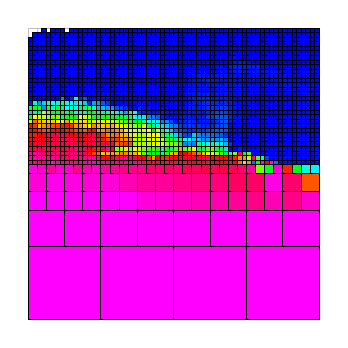
\begin{tikzpicture}[x={(\screenshotunitlength,0)},y={(0,\screenshotunitlength)}]
        \definecolor{fillcolor}{rgb}{1.000000,0.000000,1.000000}
\fill[fillcolor] (0.000000,0.000000) rectangle (0.250000,0.250000);
\definecolor{fillcolor}{rgb}{1.000000,0.000000,1.000000}
\fill[fillcolor] (0.250000,0.000000) rectangle (0.500000,0.250000);
\definecolor{fillcolor}{rgb}{1.000000,0.000000,1.000000}
\fill[fillcolor] (0.000000,0.250000) rectangle (0.125000,0.375000);
\definecolor{fillcolor}{rgb}{1.000000,0.000000,1.000000}
\fill[fillcolor] (0.125000,0.250000) rectangle (0.250000,0.375000);
\definecolor{fillcolor}{rgb}{1.000000,0.000000,1.000000}
\fill[fillcolor] (0.000000,0.375000) rectangle (0.062500,0.437500);
\definecolor{fillcolor}{rgb}{1.000000,0.000000,1.000000}
\fill[fillcolor] (0.062500,0.375000) rectangle (0.125000,0.437500);
\definecolor{fillcolor}{rgb}{1.000000,0.000000,0.849275}
\fill[fillcolor] (0.000000,0.437500) rectangle (0.062500,0.500000);
\definecolor{fillcolor}{rgb}{1.000000,0.000000,0.925110}
\fill[fillcolor] (0.062500,0.437500) rectangle (0.125000,0.500000);
\definecolor{fillcolor}{rgb}{1.000000,0.000000,1.000000}
\fill[fillcolor] (0.125000,0.375000) rectangle (0.187500,0.437500);
\definecolor{fillcolor}{rgb}{1.000000,0.000000,1.000000}
\fill[fillcolor] (0.187500,0.375000) rectangle (0.250000,0.437500);
\definecolor{fillcolor}{rgb}{1.000000,0.000000,0.897443}
\fill[fillcolor] (0.125000,0.437500) rectangle (0.187500,0.500000);
\definecolor{fillcolor}{rgb}{1.000000,0.000000,0.851726}
\fill[fillcolor] (0.187500,0.437500) rectangle (0.250000,0.500000);
\definecolor{fillcolor}{rgb}{1.000000,0.000000,1.000000}
\fill[fillcolor] (0.250000,0.250000) rectangle (0.375000,0.375000);
\definecolor{fillcolor}{rgb}{1.000000,0.000000,1.000000}
\fill[fillcolor] (0.375000,0.250000) rectangle (0.500000,0.375000);
\definecolor{fillcolor}{rgb}{1.000000,0.000000,1.000000}
\fill[fillcolor] (0.250000,0.375000) rectangle (0.312500,0.437500);
\definecolor{fillcolor}{rgb}{1.000000,0.000000,1.000000}
\fill[fillcolor] (0.312500,0.375000) rectangle (0.375000,0.437500);
\definecolor{fillcolor}{rgb}{1.000000,0.000000,0.851371}
\fill[fillcolor] (0.250000,0.437500) rectangle (0.312500,0.500000);
\definecolor{fillcolor}{rgb}{1.000000,0.000000,0.696599}
\fill[fillcolor] (0.312500,0.437500) rectangle (0.375000,0.500000);
\definecolor{fillcolor}{rgb}{1.000000,0.000000,0.866285}
\fill[fillcolor] (0.375000,0.375000) rectangle (0.437500,0.437500);
\definecolor{fillcolor}{rgb}{1.000000,0.000000,0.835166}
\fill[fillcolor] (0.437500,0.375000) rectangle (0.500000,0.437500);
\definecolor{fillcolor}{rgb}{1.000000,0.000000,0.610094}
\fill[fillcolor] (0.375000,0.437500) rectangle (0.437500,0.500000);
\definecolor{fillcolor}{rgb}{1.000000,0.000000,0.603803}
\fill[fillcolor] (0.437500,0.437500) rectangle (0.500000,0.500000);
\definecolor{fillcolor}{rgb}{1.000000,0.000000,1.000000}
\fill[fillcolor] (0.500000,0.000000) rectangle (0.750000,0.250000);
\definecolor{fillcolor}{rgb}{1.000000,0.000000,1.000000}
\fill[fillcolor] (0.750000,0.000000) rectangle (1.000000,0.250000);
\definecolor{fillcolor}{rgb}{1.000000,0.000000,1.000000}
\fill[fillcolor] (0.500000,0.250000) rectangle (0.625000,0.375000);
\definecolor{fillcolor}{rgb}{1.000000,0.000000,0.999738}
\fill[fillcolor] (0.625000,0.250000) rectangle (0.750000,0.375000);
\definecolor{fillcolor}{rgb}{1.000000,0.000000,0.767210}
\fill[fillcolor] (0.500000,0.375000) rectangle (0.562500,0.437500);
\definecolor{fillcolor}{rgb}{1.000000,0.000000,0.723690}
\fill[fillcolor] (0.562500,0.375000) rectangle (0.625000,0.437500);
\definecolor{fillcolor}{rgb}{1.000000,0.000000,0.528668}
\fill[fillcolor] (0.500000,0.437500) rectangle (0.562500,0.500000);
\definecolor{fillcolor}{rgb}{1.000000,0.000000,0.506125}
\fill[fillcolor] (0.562500,0.437500) rectangle (0.625000,0.500000);
\definecolor{fillcolor}{rgb}{1.000000,0.000000,0.685129}
\fill[fillcolor] (0.625000,0.375000) rectangle (0.687500,0.437500);
\definecolor{fillcolor}{rgb}{1.000000,0.000000,0.597724}
\fill[fillcolor] (0.687500,0.375000) rectangle (0.750000,0.437500);
\definecolor{fillcolor}{rgb}{1.000000,0.000000,0.481489}
\fill[fillcolor] (0.625000,0.437500) rectangle (0.687500,0.500000);
\definecolor{fillcolor}{rgb}{1.000000,0.000000,0.381222}
\fill[fillcolor] (0.687500,0.437500) rectangle (0.750000,0.500000);
\definecolor{fillcolor}{rgb}{1.000000,0.000000,1.000000}
\fill[fillcolor] (0.750000,0.250000) rectangle (0.875000,0.375000);
\definecolor{fillcolor}{rgb}{1.000000,0.000000,1.000000}
\fill[fillcolor] (0.875000,0.250000) rectangle (1.000000,0.375000);
\definecolor{fillcolor}{rgb}{1.000000,0.000000,0.526543}
\fill[fillcolor] (0.750000,0.375000) rectangle (0.812500,0.437500);
\definecolor{fillcolor}{rgb}{1.000000,0.000000,0.710334}
\fill[fillcolor] (0.812500,0.375000) rectangle (0.875000,0.437500);
\definecolor{fillcolor}{rgb}{1.000000,0.000000,0.389523}
\fill[fillcolor] (0.750000,0.437500) rectangle (0.812500,0.500000);
\definecolor{fillcolor}{rgb}{1.000000,0.000000,0.898328}
\fill[fillcolor] (0.812500,0.437500) rectangle (0.875000,0.500000);
\definecolor{fillcolor}{rgb}{1.000000,0.000000,0.537435}
\fill[fillcolor] (0.875000,0.375000) rectangle (0.937500,0.437500);
\definecolor{fillcolor}{rgb}{1.000000,0.000000,0.795513}
\fill[fillcolor] (0.937500,0.375000) rectangle (1.000000,0.437500);
\definecolor{fillcolor}{rgb}{1.000000,0.000000,0.424368}
\fill[fillcolor] (0.875000,0.437500) rectangle (0.937500,0.500000);
\definecolor{fillcolor}{rgb}{1.000000,0.329429,0.000000}
\fill[fillcolor] (0.937500,0.437500) rectangle (1.000000,0.500000);
\definecolor{fillcolor}{rgb}{1.000000,0.000000,0.891388}
\fill[fillcolor] (0.000000,0.500000) rectangle (0.031250,0.531250);
\definecolor{fillcolor}{rgb}{1.000000,0.000000,0.801130}
\fill[fillcolor] (0.031250,0.500000) rectangle (0.062500,0.531250);
\definecolor{fillcolor}{rgb}{1.000000,0.000000,0.570511}
\fill[fillcolor] (0.000000,0.531250) rectangle (0.015625,0.546875);
\definecolor{fillcolor}{rgb}{1.000000,0.000000,0.503752}
\fill[fillcolor] (0.015625,0.531250) rectangle (0.031250,0.546875);
\definecolor{fillcolor}{rgb}{1.000000,0.000000,0.645162}
\fill[fillcolor] (0.000000,0.546875) rectangle (0.015625,0.562500);
\definecolor{fillcolor}{rgb}{1.000000,0.000000,0.651396}
\fill[fillcolor] (0.015625,0.546875) rectangle (0.031250,0.562500);
\definecolor{fillcolor}{rgb}{1.000000,0.000000,0.417846}
\fill[fillcolor] (0.031250,0.531250) rectangle (0.046875,0.546875);
\definecolor{fillcolor}{rgb}{1.000000,0.000000,0.395576}
\fill[fillcolor] (0.046875,0.531250) rectangle (0.062500,0.546875);
\definecolor{fillcolor}{rgb}{1.000000,0.000000,0.605116}
\fill[fillcolor] (0.031250,0.546875) rectangle (0.046875,0.562500);
\definecolor{fillcolor}{rgb}{1.000000,0.000000,0.587664}
\fill[fillcolor] (0.046875,0.546875) rectangle (0.062500,0.562500);
\definecolor{fillcolor}{rgb}{1.000000,0.000000,0.599159}
\fill[fillcolor] (0.062500,0.500000) rectangle (0.093750,0.531250);
\definecolor{fillcolor}{rgb}{1.000000,0.000000,0.794063}
\fill[fillcolor] (0.093750,0.500000) rectangle (0.125000,0.531250);
\definecolor{fillcolor}{rgb}{1.000000,0.000000,0.632248}
\fill[fillcolor] (0.062500,0.531250) rectangle (0.078125,0.546875);
\definecolor{fillcolor}{rgb}{1.000000,0.000000,0.877892}
\fill[fillcolor] (0.078125,0.531250) rectangle (0.093750,0.546875);
\definecolor{fillcolor}{rgb}{1.000000,0.000000,0.563007}
\fill[fillcolor] (0.062500,0.546875) rectangle (0.078125,0.562500);
\definecolor{fillcolor}{rgb}{1.000000,0.000000,0.550499}
\fill[fillcolor] (0.078125,0.546875) rectangle (0.093750,0.562500);
\definecolor{fillcolor}{rgb}{1.000000,0.000000,0.722746}
\fill[fillcolor] (0.093750,0.531250) rectangle (0.109375,0.546875);
\definecolor{fillcolor}{rgb}{1.000000,0.000000,0.615030}
\fill[fillcolor] (0.109375,0.531250) rectangle (0.125000,0.546875);
\definecolor{fillcolor}{rgb}{1.000000,0.000000,0.480748}
\fill[fillcolor] (0.093750,0.546875) rectangle (0.109375,0.562500);
\definecolor{fillcolor}{rgb}{1.000000,0.000000,0.395923}
\fill[fillcolor] (0.109375,0.546875) rectangle (0.125000,0.562500);
\definecolor{fillcolor}{rgb}{1.000000,0.000000,0.637027}
\fill[fillcolor] (0.000000,0.562500) rectangle (0.015625,0.578125);
\definecolor{fillcolor}{rgb}{1.000000,0.000000,0.662416}
\fill[fillcolor] (0.015625,0.562500) rectangle (0.031250,0.578125);
\definecolor{fillcolor}{rgb}{1.000000,0.000000,0.261608}
\fill[fillcolor] (0.000000,0.578125) rectangle (0.015625,0.593750);
\definecolor{fillcolor}{rgb}{1.000000,0.000000,0.281473}
\fill[fillcolor] (0.015625,0.578125) rectangle (0.031250,0.593750);
\definecolor{fillcolor}{rgb}{1.000000,0.000000,0.585242}
\fill[fillcolor] (0.031250,0.562500) rectangle (0.046875,0.578125);
\definecolor{fillcolor}{rgb}{1.000000,0.000000,0.341095}
\fill[fillcolor] (0.046875,0.562500) rectangle (0.062500,0.578125);
\definecolor{fillcolor}{rgb}{1.000000,0.000000,0.312582}
\fill[fillcolor] (0.031250,0.578125) rectangle (0.046875,0.593750);
\definecolor{fillcolor}{rgb}{1.000000,0.000000,0.331355}
\fill[fillcolor] (0.046875,0.578125) rectangle (0.062500,0.593750);
\definecolor{fillcolor}{rgb}{1.000000,0.001900,0.000000}
\fill[fillcolor] (0.000000,0.593750) rectangle (0.015625,0.609375);
\definecolor{fillcolor}{rgb}{1.000000,0.000000,0.149795}
\fill[fillcolor] (0.015625,0.593750) rectangle (0.031250,0.609375);
\definecolor{fillcolor}{rgb}{1.000000,0.000000,0.167231}
\fill[fillcolor] (0.000000,0.609375) rectangle (0.015625,0.625000);
\definecolor{fillcolor}{rgb}{1.000000,0.000000,0.138548}
\fill[fillcolor] (0.015625,0.609375) rectangle (0.031250,0.625000);
\definecolor{fillcolor}{rgb}{1.000000,0.000000,0.206001}
\fill[fillcolor] (0.031250,0.593750) rectangle (0.046875,0.609375);
\definecolor{fillcolor}{rgb}{1.000000,0.000000,0.165915}
\fill[fillcolor] (0.046875,0.593750) rectangle (0.062500,0.609375);
\definecolor{fillcolor}{rgb}{1.000000,0.000000,0.114281}
\fill[fillcolor] (0.031250,0.609375) rectangle (0.046875,0.625000);
\definecolor{fillcolor}{rgb}{1.000000,0.000000,0.042696}
\fill[fillcolor] (0.046875,0.609375) rectangle (0.062500,0.625000);
\definecolor{fillcolor}{rgb}{1.000000,0.000000,0.357946}
\fill[fillcolor] (0.062500,0.562500) rectangle (0.078125,0.578125);
\definecolor{fillcolor}{rgb}{1.000000,0.000000,0.446668}
\fill[fillcolor] (0.078125,0.562500) rectangle (0.093750,0.578125);
\definecolor{fillcolor}{rgb}{1.000000,0.000000,0.306863}
\fill[fillcolor] (0.062500,0.578125) rectangle (0.078125,0.593750);
\definecolor{fillcolor}{rgb}{1.000000,0.000000,0.275845}
\fill[fillcolor] (0.078125,0.578125) rectangle (0.093750,0.593750);
\definecolor{fillcolor}{rgb}{1.000000,0.000000,0.465705}
\fill[fillcolor] (0.093750,0.562500) rectangle (0.109375,0.578125);
\definecolor{fillcolor}{rgb}{1.000000,0.000000,0.385888}
\fill[fillcolor] (0.109375,0.562500) rectangle (0.125000,0.578125);
\definecolor{fillcolor}{rgb}{1.000000,0.000000,0.273504}
\fill[fillcolor] (0.093750,0.578125) rectangle (0.109375,0.593750);
\definecolor{fillcolor}{rgb}{1.000000,0.000000,0.206153}
\fill[fillcolor] (0.109375,0.578125) rectangle (0.125000,0.593750);
\definecolor{fillcolor}{rgb}{1.000000,0.000000,0.292064}
\fill[fillcolor] (0.062500,0.593750) rectangle (0.078125,0.609375);
\definecolor{fillcolor}{rgb}{1.000000,0.000000,0.234963}
\fill[fillcolor] (0.078125,0.593750) rectangle (0.093750,0.609375);
\definecolor{fillcolor}{rgb}{1.000000,0.000000,0.136971}
\fill[fillcolor] (0.062500,0.609375) rectangle (0.078125,0.625000);
\definecolor{fillcolor}{rgb}{1.000000,0.000000,0.230271}
\fill[fillcolor] (0.078125,0.609375) rectangle (0.093750,0.625000);
\definecolor{fillcolor}{rgb}{1.000000,0.000000,0.236811}
\fill[fillcolor] (0.093750,0.593750) rectangle (0.109375,0.609375);
\definecolor{fillcolor}{rgb}{1.000000,0.000000,0.227148}
\fill[fillcolor] (0.109375,0.593750) rectangle (0.125000,0.609375);
\definecolor{fillcolor}{rgb}{1.000000,0.000000,0.302651}
\fill[fillcolor] (0.093750,0.609375) rectangle (0.109375,0.625000);
\definecolor{fillcolor}{rgb}{1.000000,0.000000,0.355431}
\fill[fillcolor] (0.109375,0.609375) rectangle (0.125000,0.625000);
\definecolor{fillcolor}{rgb}{1.000000,0.000000,0.795372}
\fill[fillcolor] (0.125000,0.500000) rectangle (0.156250,0.531250);
\definecolor{fillcolor}{rgb}{1.000000,0.000000,0.547212}
\fill[fillcolor] (0.156250,0.500000) rectangle (0.187500,0.531250);
\definecolor{fillcolor}{rgb}{1.000000,0.000000,0.591976}
\fill[fillcolor] (0.125000,0.531250) rectangle (0.140625,0.546875);
\definecolor{fillcolor}{rgb}{1.000000,0.000000,0.563348}
\fill[fillcolor] (0.140625,0.531250) rectangle (0.156250,0.546875);
\definecolor{fillcolor}{rgb}{1.000000,0.000000,0.343635}
\fill[fillcolor] (0.125000,0.546875) rectangle (0.140625,0.562500);
\definecolor{fillcolor}{rgb}{1.000000,0.000000,0.443601}
\fill[fillcolor] (0.140625,0.546875) rectangle (0.156250,0.562500);
\definecolor{fillcolor}{rgb}{1.000000,0.000000,0.553019}
\fill[fillcolor] (0.156250,0.531250) rectangle (0.171875,0.546875);
\definecolor{fillcolor}{rgb}{1.000000,0.000000,0.652760}
\fill[fillcolor] (0.171875,0.531250) rectangle (0.187500,0.546875);
\definecolor{fillcolor}{rgb}{1.000000,0.000000,0.524722}
\fill[fillcolor] (0.156250,0.546875) rectangle (0.171875,0.562500);
\definecolor{fillcolor}{rgb}{1.000000,0.000000,0.486784}
\fill[fillcolor] (0.171875,0.546875) rectangle (0.187500,0.562500);
\definecolor{fillcolor}{rgb}{1.000000,0.000000,0.713541}
\fill[fillcolor] (0.187500,0.500000) rectangle (0.218750,0.531250);
\definecolor{fillcolor}{rgb}{1.000000,0.000000,0.776557}
\fill[fillcolor] (0.218750,0.500000) rectangle (0.250000,0.531250);
\definecolor{fillcolor}{rgb}{1.000000,0.000000,0.648013}
\fill[fillcolor] (0.187500,0.531250) rectangle (0.203125,0.546875);
\definecolor{fillcolor}{rgb}{1.000000,0.000000,0.653160}
\fill[fillcolor] (0.203125,0.531250) rectangle (0.218750,0.546875);
\definecolor{fillcolor}{rgb}{1.000000,0.000000,0.524621}
\fill[fillcolor] (0.187500,0.546875) rectangle (0.203125,0.562500);
\definecolor{fillcolor}{rgb}{1.000000,0.000000,0.578772}
\fill[fillcolor] (0.203125,0.546875) rectangle (0.218750,0.562500);
\definecolor{fillcolor}{rgb}{1.000000,0.000000,0.681845}
\fill[fillcolor] (0.218750,0.531250) rectangle (0.234375,0.546875);
\definecolor{fillcolor}{rgb}{1.000000,0.000000,0.677593}
\fill[fillcolor] (0.234375,0.531250) rectangle (0.250000,0.546875);
\definecolor{fillcolor}{rgb}{1.000000,0.000000,0.650667}
\fill[fillcolor] (0.218750,0.546875) rectangle (0.234375,0.562500);
\definecolor{fillcolor}{rgb}{1.000000,0.000000,0.556201}
\fill[fillcolor] (0.234375,0.546875) rectangle (0.250000,0.562500);
\definecolor{fillcolor}{rgb}{1.000000,0.000000,0.369464}
\fill[fillcolor] (0.125000,0.562500) rectangle (0.140625,0.578125);
\definecolor{fillcolor}{rgb}{1.000000,0.000000,0.467023}
\fill[fillcolor] (0.140625,0.562500) rectangle (0.156250,0.578125);
\definecolor{fillcolor}{rgb}{1.000000,0.000000,0.262697}
\fill[fillcolor] (0.125000,0.578125) rectangle (0.140625,0.593750);
\definecolor{fillcolor}{rgb}{1.000000,0.000000,0.406395}
\fill[fillcolor] (0.140625,0.578125) rectangle (0.156250,0.593750);
\definecolor{fillcolor}{rgb}{1.000000,0.000000,0.499162}
\fill[fillcolor] (0.156250,0.562500) rectangle (0.171875,0.578125);
\definecolor{fillcolor}{rgb}{1.000000,0.000000,0.438154}
\fill[fillcolor] (0.171875,0.562500) rectangle (0.187500,0.578125);
\definecolor{fillcolor}{rgb}{1.000000,0.000000,0.448096}
\fill[fillcolor] (0.156250,0.578125) rectangle (0.171875,0.593750);
\definecolor{fillcolor}{rgb}{1.000000,0.000000,0.390587}
\fill[fillcolor] (0.171875,0.578125) rectangle (0.187500,0.593750);
\definecolor{fillcolor}{rgb}{1.000000,0.000000,0.326702}
\fill[fillcolor] (0.125000,0.593750) rectangle (0.140625,0.609375);
\definecolor{fillcolor}{rgb}{1.000000,0.000000,0.358647}
\fill[fillcolor] (0.140625,0.593750) rectangle (0.156250,0.609375);
\definecolor{fillcolor}{rgb}{1.000000,0.000000,0.348798}
\fill[fillcolor] (0.125000,0.609375) rectangle (0.140625,0.625000);
\definecolor{fillcolor}{rgb}{1.000000,0.000000,0.215179}
\fill[fillcolor] (0.140625,0.609375) rectangle (0.156250,0.625000);
\definecolor{fillcolor}{rgb}{1.000000,0.000000,0.313548}
\fill[fillcolor] (0.156250,0.593750) rectangle (0.171875,0.609375);
\definecolor{fillcolor}{rgb}{1.000000,0.000000,0.179950}
\fill[fillcolor] (0.171875,0.593750) rectangle (0.187500,0.609375);
\definecolor{fillcolor}{rgb}{1.000000,0.000000,0.141521}
\fill[fillcolor] (0.156250,0.609375) rectangle (0.171875,0.625000);
\definecolor{fillcolor}{rgb}{1.000000,0.000000,0.065560}
\fill[fillcolor] (0.171875,0.609375) rectangle (0.187500,0.625000);
\definecolor{fillcolor}{rgb}{1.000000,0.000000,0.327562}
\fill[fillcolor] (0.187500,0.562500) rectangle (0.203125,0.578125);
\definecolor{fillcolor}{rgb}{1.000000,0.076675,0.000000}
\fill[fillcolor] (0.203125,0.562500) rectangle (0.218750,0.578125);
\definecolor{fillcolor}{rgb}{1.000000,0.000000,0.323630}
\fill[fillcolor] (0.187500,0.578125) rectangle (0.203125,0.593750);
\definecolor{fillcolor}{rgb}{1.000000,0.000000,0.096608}
\fill[fillcolor] (0.203125,0.578125) rectangle (0.218750,0.593750);
\definecolor{fillcolor}{rgb}{1.000000,0.248540,0.000000}
\fill[fillcolor] (0.218750,0.562500) rectangle (0.234375,0.578125);
\definecolor{fillcolor}{rgb}{1.000000,0.344657,0.000000}
\fill[fillcolor] (0.234375,0.562500) rectangle (0.250000,0.578125);
\definecolor{fillcolor}{rgb}{1.000000,0.070255,0.000000}
\fill[fillcolor] (0.218750,0.578125) rectangle (0.234375,0.593750);
\definecolor{fillcolor}{rgb}{1.000000,0.153251,0.000000}
\fill[fillcolor] (0.234375,0.578125) rectangle (0.250000,0.593750);
\definecolor{fillcolor}{rgb}{1.000000,0.000000,0.206313}
\fill[fillcolor] (0.187500,0.593750) rectangle (0.203125,0.609375);
\definecolor{fillcolor}{rgb}{1.000000,0.000000,0.197620}
\fill[fillcolor] (0.203125,0.593750) rectangle (0.218750,0.609375);
\definecolor{fillcolor}{rgb}{1.000000,0.000000,0.073692}
\fill[fillcolor] (0.187500,0.609375) rectangle (0.203125,0.625000);
\definecolor{fillcolor}{rgb}{1.000000,0.000000,0.159379}
\fill[fillcolor] (0.203125,0.609375) rectangle (0.218750,0.625000);
\definecolor{fillcolor}{rgb}{1.000000,0.000000,0.321123}
\fill[fillcolor] (0.218750,0.593750) rectangle (0.234375,0.609375);
\definecolor{fillcolor}{rgb}{1.000000,0.000000,0.254872}
\fill[fillcolor] (0.234375,0.593750) rectangle (0.250000,0.609375);
\definecolor{fillcolor}{rgb}{1.000000,0.000000,0.293201}
\fill[fillcolor] (0.218750,0.609375) rectangle (0.234375,0.625000);
\definecolor{fillcolor}{rgb}{1.000000,0.000000,0.352912}
\fill[fillcolor] (0.234375,0.609375) rectangle (0.250000,0.625000);
\definecolor{fillcolor}{rgb}{1.000000,0.068308,0.000000}
\fill[fillcolor] (0.000000,0.625000) rectangle (0.015625,0.640625);
\definecolor{fillcolor}{rgb}{1.000000,0.089032,0.000000}
\fill[fillcolor] (0.015625,0.625000) rectangle (0.031250,0.640625);
\definecolor{fillcolor}{rgb}{1.000000,0.000000,0.067580}
\fill[fillcolor] (0.000000,0.640625) rectangle (0.015625,0.656250);
\definecolor{fillcolor}{rgb}{1.000000,0.031801,0.000000}
\fill[fillcolor] (0.015625,0.640625) rectangle (0.031250,0.656250);
\definecolor{fillcolor}{rgb}{1.000000,0.006843,0.000000}
\fill[fillcolor] (0.031250,0.625000) rectangle (0.046875,0.640625);
\definecolor{fillcolor}{rgb}{1.000000,0.000000,0.011331}
\fill[fillcolor] (0.046875,0.625000) rectangle (0.062500,0.640625);
\definecolor{fillcolor}{rgb}{1.000000,0.187977,0.000000}
\fill[fillcolor] (0.031250,0.640625) rectangle (0.046875,0.656250);
\definecolor{fillcolor}{rgb}{1.000000,0.276164,0.000000}
\fill[fillcolor] (0.046875,0.640625) rectangle (0.062500,0.656250);
\definecolor{fillcolor}{rgb}{1.000000,0.053398,0.000000}
\fill[fillcolor] (0.000000,0.656250) rectangle (0.015625,0.671875);
\definecolor{fillcolor}{rgb}{1.000000,0.199409,0.000000}
\fill[fillcolor] (0.015625,0.656250) rectangle (0.031250,0.671875);
\definecolor{fillcolor}{rgb}{0.722954,1.000000,0.000000}
\fill[fillcolor] (0.000000,0.671875) rectangle (0.015625,0.687500);
\definecolor{fillcolor}{rgb}{1.000000,0.394966,0.000000}
\fill[fillcolor] (0.015625,0.671875) rectangle (0.031250,0.687500);
\definecolor{fillcolor}{rgb}{1.000000,0.758938,0.000000}
\fill[fillcolor] (0.031250,0.656250) rectangle (0.046875,0.671875);
\definecolor{fillcolor}{rgb}{1.000000,0.569162,0.000000}
\fill[fillcolor] (0.046875,0.656250) rectangle (0.062500,0.671875);
\definecolor{fillcolor}{rgb}{1.000000,0.701416,0.000000}
\fill[fillcolor] (0.031250,0.671875) rectangle (0.046875,0.687500);
\definecolor{fillcolor}{rgb}{1.000000,0.781060,0.000000}
\fill[fillcolor] (0.046875,0.671875) rectangle (0.062500,0.687500);
\definecolor{fillcolor}{rgb}{1.000000,0.000000,0.264325}
\fill[fillcolor] (0.062500,0.625000) rectangle (0.078125,0.640625);
\definecolor{fillcolor}{rgb}{1.000000,0.000000,0.258886}
\fill[fillcolor] (0.078125,0.625000) rectangle (0.093750,0.640625);
\definecolor{fillcolor}{rgb}{1.000000,0.260447,0.000000}
\fill[fillcolor] (0.062500,0.640625) rectangle (0.078125,0.656250);
\definecolor{fillcolor}{rgb}{1.000000,0.045188,0.000000}
\fill[fillcolor] (0.078125,0.640625) rectangle (0.093750,0.656250);
\definecolor{fillcolor}{rgb}{1.000000,0.000000,0.236891}
\fill[fillcolor] (0.093750,0.625000) rectangle (0.109375,0.640625);
\definecolor{fillcolor}{rgb}{1.000000,0.000000,0.303682}
\fill[fillcolor] (0.109375,0.625000) rectangle (0.125000,0.640625);
\definecolor{fillcolor}{rgb}{1.000000,0.000000,0.085813}
\fill[fillcolor] (0.093750,0.640625) rectangle (0.109375,0.656250);
\definecolor{fillcolor}{rgb}{1.000000,0.000000,0.123948}
\fill[fillcolor] (0.109375,0.640625) rectangle (0.125000,0.656250);
\definecolor{fillcolor}{rgb}{1.000000,0.450350,0.000000}
\fill[fillcolor] (0.062500,0.656250) rectangle (0.078125,0.671875);
\definecolor{fillcolor}{rgb}{1.000000,0.307279,0.000000}
\fill[fillcolor] (0.078125,0.656250) rectangle (0.093750,0.671875);
\definecolor{fillcolor}{rgb}{1.000000,0.782513,0.000000}
\fill[fillcolor] (0.062500,0.671875) rectangle (0.078125,0.687500);
\definecolor{fillcolor}{rgb}{1.000000,0.795716,0.000000}
\fill[fillcolor] (0.078125,0.671875) rectangle (0.093750,0.687500);
\definecolor{fillcolor}{rgb}{1.000000,0.239503,0.000000}
\fill[fillcolor] (0.093750,0.656250) rectangle (0.109375,0.671875);
\definecolor{fillcolor}{rgb}{1.000000,0.091824,0.000000}
\fill[fillcolor] (0.109375,0.656250) rectangle (0.125000,0.671875);
\definecolor{fillcolor}{rgb}{1.000000,0.940267,0.000000}
\fill[fillcolor] (0.093750,0.671875) rectangle (0.109375,0.687500);
\definecolor{fillcolor}{rgb}{1.000000,0.907477,0.000000}
\fill[fillcolor] (0.109375,0.671875) rectangle (0.125000,0.687500);
\definecolor{fillcolor}{rgb}{0.000000,1.000000,0.210877}
\fill[fillcolor] (0.000000,0.687500) rectangle (0.015625,0.703125);
\definecolor{fillcolor}{rgb}{1.000000,0.953960,0.000000}
\fill[fillcolor] (0.015625,0.687500) rectangle (0.031250,0.703125);
\definecolor{fillcolor}{rgb}{0.000000,0.787968,1.000000}
\fill[fillcolor] (0.000000,0.703125) rectangle (0.015625,0.718750);
\definecolor{fillcolor}{rgb}{0.000000,1.000000,0.618367}
\fill[fillcolor] (0.015625,0.703125) rectangle (0.031250,0.718750);
\definecolor{fillcolor}{rgb}{0.816769,1.000000,0.000000}
\fill[fillcolor] (0.031250,0.687500) rectangle (0.046875,0.703125);
\definecolor{fillcolor}{rgb}{0.791216,1.000000,0.000000}
\fill[fillcolor] (0.046875,0.687500) rectangle (0.062500,0.703125);
\definecolor{fillcolor}{rgb}{0.000000,1.000000,0.316247}
\fill[fillcolor] (0.031250,0.703125) rectangle (0.046875,0.718750);
\definecolor{fillcolor}{rgb}{0.750885,1.000000,0.000000}
\fill[fillcolor] (0.046875,0.703125) rectangle (0.062500,0.718750);
\definecolor{fillcolor}{rgb}{0.000000,1.000000,0.150680}
\fill[fillcolor] (0.000000,0.718750) rectangle (0.015625,0.734375);
\definecolor{fillcolor}{rgb}{0.054737,1.000000,0.000000}
\fill[fillcolor] (0.015625,0.718750) rectangle (0.031250,0.734375);
\definecolor{fillcolor}{rgb}{0.000000,0.105954,1.000000}
\fill[fillcolor] (0.000000,0.734375) rectangle (0.015625,0.750000);
\definecolor{fillcolor}{rgb}{0.000000,1.000000,0.786051}
\fill[fillcolor] (0.015625,0.734375) rectangle (0.031250,0.750000);
\definecolor{fillcolor}{rgb}{0.115154,1.000000,0.000000}
\fill[fillcolor] (0.031250,0.718750) rectangle (0.046875,0.734375);
\definecolor{fillcolor}{rgb}{0.000000,0.575105,1.000000}
\fill[fillcolor] (0.046875,0.718750) rectangle (0.062500,0.734375);
\definecolor{fillcolor}{rgb}{0.000000,0.578872,1.000000}
\fill[fillcolor] (0.031250,0.734375) rectangle (0.046875,0.750000);
\definecolor{fillcolor}{rgb}{0.000000,0.835946,1.000000}
\fill[fillcolor] (0.046875,0.734375) rectangle (0.062500,0.750000);
\definecolor{fillcolor}{rgb}{0.588911,1.000000,0.000000}
\fill[fillcolor] (0.062500,0.687500) rectangle (0.078125,0.703125);
\definecolor{fillcolor}{rgb}{0.392466,1.000000,0.000000}
\fill[fillcolor] (0.078125,0.687500) rectangle (0.093750,0.703125);
\definecolor{fillcolor}{rgb}{0.443801,1.000000,0.000000}
\fill[fillcolor] (0.062500,0.703125) rectangle (0.078125,0.718750);
\definecolor{fillcolor}{rgb}{0.000000,1.000000,0.229572}
\fill[fillcolor] (0.078125,0.703125) rectangle (0.093750,0.718750);
\definecolor{fillcolor}{rgb}{0.492343,1.000000,0.000000}
\fill[fillcolor] (0.093750,0.687500) rectangle (0.109375,0.703125);
\definecolor{fillcolor}{rgb}{0.000000,1.000000,0.290548}
\fill[fillcolor] (0.109375,0.687500) rectangle (0.125000,0.703125);
\definecolor{fillcolor}{rgb}{0.000000,1.000000,0.168150}
\fill[fillcolor] (0.093750,0.703125) rectangle (0.109375,0.718750);
\definecolor{fillcolor}{rgb}{0.000000,1.000000,0.102672}
\fill[fillcolor] (0.109375,0.703125) rectangle (0.125000,0.718750);
\definecolor{fillcolor}{rgb}{0.147445,1.000000,0.000000}
\fill[fillcolor] (0.062500,0.718750) rectangle (0.078125,0.734375);
\definecolor{fillcolor}{rgb}{0.000000,1.000000,0.620245}
\fill[fillcolor] (0.078125,0.718750) rectangle (0.093750,0.734375);
\definecolor{fillcolor}{rgb}{0.000000,1.000000,0.777491}
\fill[fillcolor] (0.062500,0.734375) rectangle (0.078125,0.750000);
\definecolor{fillcolor}{rgb}{0.000000,1.000000,0.986431}
\fill[fillcolor] (0.078125,0.734375) rectangle (0.093750,0.750000);
\definecolor{fillcolor}{rgb}{0.000000,1.000000,0.220337}
\fill[fillcolor] (0.093750,0.718750) rectangle (0.109375,0.734375);
\definecolor{fillcolor}{rgb}{0.000000,1.000000,0.316756}
\fill[fillcolor] (0.109375,0.718750) rectangle (0.125000,0.734375);
\definecolor{fillcolor}{rgb}{0.000000,1.000000,0.866767}
\fill[fillcolor] (0.093750,0.734375) rectangle (0.109375,0.750000);
\definecolor{fillcolor}{rgb}{0.000000,1.000000,0.528209}
\fill[fillcolor] (0.109375,0.734375) rectangle (0.125000,0.750000);
\definecolor{fillcolor}{rgb}{1.000000,0.000000,0.196467}
\fill[fillcolor] (0.125000,0.625000) rectangle (0.140625,0.640625);
\definecolor{fillcolor}{rgb}{1.000000,0.000000,0.067080}
\fill[fillcolor] (0.140625,0.625000) rectangle (0.156250,0.640625);
\definecolor{fillcolor}{rgb}{1.000000,0.083706,0.000000}
\fill[fillcolor] (0.125000,0.640625) rectangle (0.140625,0.656250);
\definecolor{fillcolor}{rgb}{1.000000,0.153335,0.000000}
\fill[fillcolor] (0.140625,0.640625) rectangle (0.156250,0.656250);
\definecolor{fillcolor}{rgb}{1.000000,0.000000,0.057331}
\fill[fillcolor] (0.156250,0.625000) rectangle (0.171875,0.640625);
\definecolor{fillcolor}{rgb}{1.000000,0.020878,0.000000}
\fill[fillcolor] (0.171875,0.625000) rectangle (0.187500,0.640625);
\definecolor{fillcolor}{rgb}{1.000000,0.231477,0.000000}
\fill[fillcolor] (0.156250,0.640625) rectangle (0.171875,0.656250);
\definecolor{fillcolor}{rgb}{1.000000,0.249588,0.000000}
\fill[fillcolor] (0.171875,0.640625) rectangle (0.187500,0.656250);
\definecolor{fillcolor}{rgb}{1.000000,0.078788,0.000000}
\fill[fillcolor] (0.125000,0.656250) rectangle (0.140625,0.671875);
\definecolor{fillcolor}{rgb}{1.000000,0.193105,0.000000}
\fill[fillcolor] (0.140625,0.656250) rectangle (0.156250,0.671875);
\definecolor{fillcolor}{rgb}{1.000000,0.604948,0.000000}
\fill[fillcolor] (0.125000,0.671875) rectangle (0.140625,0.687500);
\definecolor{fillcolor}{rgb}{0.767425,1.000000,0.000000}
\fill[fillcolor] (0.140625,0.671875) rectangle (0.156250,0.687500);
\definecolor{fillcolor}{rgb}{1.000000,0.578123,0.000000}
\fill[fillcolor] (0.156250,0.656250) rectangle (0.171875,0.671875);
\definecolor{fillcolor}{rgb}{1.000000,0.591338,0.000000}
\fill[fillcolor] (0.171875,0.656250) rectangle (0.187500,0.671875);
\definecolor{fillcolor}{rgb}{1.000000,0.853144,0.000000}
\fill[fillcolor] (0.156250,0.671875) rectangle (0.171875,0.687500);
\definecolor{fillcolor}{rgb}{1.000000,0.825758,0.000000}
\fill[fillcolor] (0.171875,0.671875) rectangle (0.187500,0.687500);
\definecolor{fillcolor}{rgb}{1.000000,0.000000,0.014410}
\fill[fillcolor] (0.187500,0.625000) rectangle (0.203125,0.640625);
\definecolor{fillcolor}{rgb}{1.000000,0.000000,0.202058}
\fill[fillcolor] (0.203125,0.625000) rectangle (0.218750,0.640625);
\definecolor{fillcolor}{rgb}{1.000000,0.339157,0.000000}
\fill[fillcolor] (0.187500,0.640625) rectangle (0.203125,0.656250);
\definecolor{fillcolor}{rgb}{1.000000,0.077015,0.000000}
\fill[fillcolor] (0.203125,0.640625) rectangle (0.218750,0.656250);
\definecolor{fillcolor}{rgb}{1.000000,0.000000,0.304822}
\fill[fillcolor] (0.218750,0.625000) rectangle (0.234375,0.640625);
\definecolor{fillcolor}{rgb}{1.000000,0.000000,0.070757}
\fill[fillcolor] (0.234375,0.625000) rectangle (0.250000,0.640625);
\definecolor{fillcolor}{rgb}{1.000000,0.043532,0.000000}
\fill[fillcolor] (0.218750,0.640625) rectangle (0.234375,0.656250);
\definecolor{fillcolor}{rgb}{1.000000,0.527238,0.000000}
\fill[fillcolor] (0.234375,0.640625) rectangle (0.250000,0.656250);
\definecolor{fillcolor}{rgb}{1.000000,0.780333,0.000000}
\fill[fillcolor] (0.187500,0.656250) rectangle (0.203125,0.671875);
\definecolor{fillcolor}{rgb}{1.000000,0.947677,0.000000}
\fill[fillcolor] (0.203125,0.656250) rectangle (0.218750,0.671875);
\definecolor{fillcolor}{rgb}{1.000000,0.897039,0.000000}
\fill[fillcolor] (0.187500,0.671875) rectangle (0.203125,0.687500);
\definecolor{fillcolor}{rgb}{0.611849,1.000000,0.000000}
\fill[fillcolor] (0.203125,0.671875) rectangle (0.218750,0.687500);
\definecolor{fillcolor}{rgb}{1.000000,0.522939,0.000000}
\fill[fillcolor] (0.218750,0.656250) rectangle (0.234375,0.671875);
\definecolor{fillcolor}{rgb}{1.000000,0.701353,0.000000}
\fill[fillcolor] (0.234375,0.656250) rectangle (0.250000,0.671875);
\definecolor{fillcolor}{rgb}{0.844017,1.000000,0.000000}
\fill[fillcolor] (0.218750,0.671875) rectangle (0.234375,0.687500);
\definecolor{fillcolor}{rgb}{1.000000,0.865560,0.000000}
\fill[fillcolor] (0.234375,0.671875) rectangle (0.250000,0.687500);
\definecolor{fillcolor}{rgb}{0.000000,1.000000,0.117719}
\fill[fillcolor] (0.125000,0.687500) rectangle (0.140625,0.703125);
\definecolor{fillcolor}{rgb}{0.101004,1.000000,0.000000}
\fill[fillcolor] (0.140625,0.687500) rectangle (0.156250,0.703125);
\definecolor{fillcolor}{rgb}{0.000000,1.000000,0.497537}
\fill[fillcolor] (0.125000,0.703125) rectangle (0.140625,0.718750);
\definecolor{fillcolor}{rgb}{0.000000,1.000000,0.087669}
\fill[fillcolor] (0.140625,0.703125) rectangle (0.156250,0.718750);
\definecolor{fillcolor}{rgb}{0.037229,1.000000,0.000000}
\fill[fillcolor] (0.156250,0.687500) rectangle (0.171875,0.703125);
\definecolor{fillcolor}{rgb}{0.928133,1.000000,0.000000}
\fill[fillcolor] (0.171875,0.687500) rectangle (0.187500,0.703125);
\definecolor{fillcolor}{rgb}{0.000000,0.972221,1.000000}
\fill[fillcolor] (0.156250,0.703125) rectangle (0.171875,0.718750);
\definecolor{fillcolor}{rgb}{0.000000,0.936843,1.000000}
\fill[fillcolor] (0.171875,0.703125) rectangle (0.187500,0.718750);
\definecolor{fillcolor}{rgb}{0.000000,0.998148,1.000000}
\fill[fillcolor] (0.125000,0.718750) rectangle (0.140625,0.734375);
\definecolor{fillcolor}{rgb}{0.000000,1.000000,0.715436}
\fill[fillcolor] (0.140625,0.718750) rectangle (0.156250,0.734375);
\definecolor{fillcolor}{rgb}{0.000000,1.000000,0.911470}
\fill[fillcolor] (0.125000,0.734375) rectangle (0.140625,0.750000);
\definecolor{fillcolor}{rgb}{0.000000,1.000000,0.968790}
\fill[fillcolor] (0.140625,0.734375) rectangle (0.156250,0.750000);
\definecolor{fillcolor}{rgb}{0.000000,1.000000,0.928782}
\fill[fillcolor] (0.156250,0.718750) rectangle (0.171875,0.734375);
\definecolor{fillcolor}{rgb}{0.000000,1.000000,0.324330}
\fill[fillcolor] (0.171875,0.718750) rectangle (0.187500,0.734375);
\definecolor{fillcolor}{rgb}{0.000000,0.912214,1.000000}
\fill[fillcolor] (0.156250,0.734375) rectangle (0.171875,0.750000);
\definecolor{fillcolor}{rgb}{0.000000,0.947635,1.000000}
\fill[fillcolor] (0.171875,0.734375) rectangle (0.187500,0.750000);
\definecolor{fillcolor}{rgb}{0.788262,1.000000,0.000000}
\fill[fillcolor] (0.187500,0.687500) rectangle (0.203125,0.703125);
\definecolor{fillcolor}{rgb}{0.591865,1.000000,0.000000}
\fill[fillcolor] (0.203125,0.687500) rectangle (0.218750,0.703125);
\definecolor{fillcolor}{rgb}{0.000000,1.000000,0.617589}
\fill[fillcolor] (0.187500,0.703125) rectangle (0.203125,0.718750);
\definecolor{fillcolor}{rgb}{0.000000,1.000000,0.043266}
\fill[fillcolor] (0.203125,0.703125) rectangle (0.218750,0.718750);
\definecolor{fillcolor}{rgb}{0.000000,1.000000,0.141224}
\fill[fillcolor] (0.218750,0.687500) rectangle (0.234375,0.703125);
\definecolor{fillcolor}{rgb}{0.000000,1.000000,0.090886}
\fill[fillcolor] (0.234375,0.687500) rectangle (0.250000,0.703125);
\definecolor{fillcolor}{rgb}{0.000000,1.000000,0.228522}
\fill[fillcolor] (0.218750,0.703125) rectangle (0.234375,0.718750);
\definecolor{fillcolor}{rgb}{0.000000,1.000000,0.310314}
\fill[fillcolor] (0.234375,0.703125) rectangle (0.250000,0.718750);
\definecolor{fillcolor}{rgb}{0.000000,1.000000,0.346581}
\fill[fillcolor] (0.187500,0.718750) rectangle (0.203125,0.734375);
\definecolor{fillcolor}{rgb}{0.222370,1.000000,0.000000}
\fill[fillcolor] (0.203125,0.718750) rectangle (0.218750,0.734375);
\definecolor{fillcolor}{rgb}{0.000000,0.795109,1.000000}
\fill[fillcolor] (0.187500,0.734375) rectangle (0.203125,0.750000);
\definecolor{fillcolor}{rgb}{0.000000,0.164296,1.000000}
\fill[fillcolor] (0.203125,0.734375) rectangle (0.218750,0.750000);
\definecolor{fillcolor}{rgb}{0.000000,1.000000,0.736031}
\fill[fillcolor] (0.218750,0.718750) rectangle (0.234375,0.734375);
\definecolor{fillcolor}{rgb}{0.000000,0.719437,1.000000}
\fill[fillcolor] (0.234375,0.718750) rectangle (0.250000,0.734375);
\definecolor{fillcolor}{rgb}{0.000000,0.644863,1.000000}
\fill[fillcolor] (0.218750,0.734375) rectangle (0.234375,0.750000);
\definecolor{fillcolor}{rgb}{0.000000,0.591634,1.000000}
\fill[fillcolor] (0.234375,0.734375) rectangle (0.250000,0.750000);
\definecolor{fillcolor}{rgb}{1.000000,0.000000,0.636209}
\fill[fillcolor] (0.250000,0.500000) rectangle (0.281250,0.531250);
\definecolor{fillcolor}{rgb}{1.000000,0.000000,0.571518}
\fill[fillcolor] (0.281250,0.500000) rectangle (0.312500,0.531250);
\definecolor{fillcolor}{rgb}{1.000000,0.000000,0.478621}
\fill[fillcolor] (0.250000,0.531250) rectangle (0.265625,0.546875);
\definecolor{fillcolor}{rgb}{1.000000,0.000000,0.507390}
\fill[fillcolor] (0.265625,0.531250) rectangle (0.281250,0.546875);
\definecolor{fillcolor}{rgb}{1.000000,0.000000,0.165380}
\fill[fillcolor] (0.250000,0.546875) rectangle (0.265625,0.562500);
\definecolor{fillcolor}{rgb}{1.000000,0.000000,0.102804}
\fill[fillcolor] (0.265625,0.546875) rectangle (0.281250,0.562500);
\definecolor{fillcolor}{rgb}{1.000000,0.000000,0.485783}
\fill[fillcolor] (0.281250,0.531250) rectangle (0.296875,0.546875);
\definecolor{fillcolor}{rgb}{1.000000,0.000000,0.453138}
\fill[fillcolor] (0.296875,0.531250) rectangle (0.312500,0.546875);
\definecolor{fillcolor}{rgb}{1.000000,0.000000,0.131792}
\fill[fillcolor] (0.281250,0.546875) rectangle (0.296875,0.562500);
\definecolor{fillcolor}{rgb}{1.000000,0.000000,0.435313}
\fill[fillcolor] (0.296875,0.546875) rectangle (0.312500,0.562500);
\definecolor{fillcolor}{rgb}{1.000000,0.000000,0.518625}
\fill[fillcolor] (0.312500,0.500000) rectangle (0.343750,0.531250);
\definecolor{fillcolor}{rgb}{1.000000,0.000000,0.558774}
\fill[fillcolor] (0.343750,0.500000) rectangle (0.375000,0.531250);
\definecolor{fillcolor}{rgb}{1.000000,0.000000,0.475017}
\fill[fillcolor] (0.312500,0.531250) rectangle (0.328125,0.546875);
\definecolor{fillcolor}{rgb}{1.000000,0.000000,0.578644}
\fill[fillcolor] (0.328125,0.531250) rectangle (0.343750,0.546875);
\definecolor{fillcolor}{rgb}{1.000000,0.000000,0.424609}
\fill[fillcolor] (0.312500,0.546875) rectangle (0.328125,0.562500);
\definecolor{fillcolor}{rgb}{1.000000,0.000000,0.517565}
\fill[fillcolor] (0.328125,0.546875) rectangle (0.343750,0.562500);
\definecolor{fillcolor}{rgb}{1.000000,0.000000,0.566544}
\fill[fillcolor] (0.343750,0.531250) rectangle (0.359375,0.546875);
\definecolor{fillcolor}{rgb}{1.000000,0.000000,0.572586}
\fill[fillcolor] (0.359375,0.531250) rectangle (0.375000,0.546875);
\definecolor{fillcolor}{rgb}{1.000000,0.000000,0.502232}
\fill[fillcolor] (0.343750,0.546875) rectangle (0.359375,0.562500);
\definecolor{fillcolor}{rgb}{1.000000,0.000000,0.398438}
\fill[fillcolor] (0.359375,0.546875) rectangle (0.375000,0.562500);
\definecolor{fillcolor}{rgb}{1.000000,0.755190,0.000000}
\fill[fillcolor] (0.250000,0.562500) rectangle (0.265625,0.578125);
\definecolor{fillcolor}{rgb}{1.000000,0.669814,0.000000}
\fill[fillcolor] (0.265625,0.562500) rectangle (0.281250,0.578125);
\definecolor{fillcolor}{rgb}{1.000000,0.000000,0.198902}
\fill[fillcolor] (0.250000,0.578125) rectangle (0.265625,0.593750);
\definecolor{fillcolor}{rgb}{1.000000,0.000000,0.562047}
\fill[fillcolor] (0.265625,0.578125) rectangle (0.281250,0.593750);
\definecolor{fillcolor}{rgb}{1.000000,0.611044,0.000000}
\fill[fillcolor] (0.281250,0.562500) rectangle (0.296875,0.578125);
\definecolor{fillcolor}{rgb}{1.000000,0.674982,0.000000}
\fill[fillcolor] (0.296875,0.562500) rectangle (0.312500,0.578125);
\definecolor{fillcolor}{rgb}{1.000000,0.000000,0.209965}
\fill[fillcolor] (0.281250,0.578125) rectangle (0.296875,0.593750);
\definecolor{fillcolor}{rgb}{0.501729,1.000000,0.000000}
\fill[fillcolor] (0.296875,0.578125) rectangle (0.312500,0.593750);
\definecolor{fillcolor}{rgb}{1.000000,0.000000,0.247503}
\fill[fillcolor] (0.250000,0.593750) rectangle (0.265625,0.609375);
\definecolor{fillcolor}{rgb}{1.000000,0.000000,0.321239}
\fill[fillcolor] (0.265625,0.593750) rectangle (0.281250,0.609375);
\definecolor{fillcolor}{rgb}{1.000000,0.068772,0.000000}
\fill[fillcolor] (0.250000,0.609375) rectangle (0.265625,0.625000);
\definecolor{fillcolor}{rgb}{1.000000,0.280475,0.000000}
\fill[fillcolor] (0.265625,0.609375) rectangle (0.281250,0.625000);
\definecolor{fillcolor}{rgb}{1.000000,0.000000,0.280984}
\fill[fillcolor] (0.281250,0.593750) rectangle (0.296875,0.609375);
\definecolor{fillcolor}{rgb}{1.000000,0.389687,0.000000}
\fill[fillcolor] (0.296875,0.593750) rectangle (0.312500,0.609375);
\definecolor{fillcolor}{rgb}{1.000000,0.196633,0.000000}
\fill[fillcolor] (0.281250,0.609375) rectangle (0.296875,0.625000);
\definecolor{fillcolor}{rgb}{1.000000,0.213992,0.000000}
\fill[fillcolor] (0.296875,0.609375) rectangle (0.312500,0.625000);
\definecolor{fillcolor}{rgb}{1.000000,0.503919,0.000000}
\fill[fillcolor] (0.312500,0.562500) rectangle (0.328125,0.578125);
\definecolor{fillcolor}{rgb}{1.000000,0.520326,0.000000}
\fill[fillcolor] (0.328125,0.562500) rectangle (0.343750,0.578125);
\definecolor{fillcolor}{rgb}{0.658555,1.000000,0.000000}
\fill[fillcolor] (0.312500,0.578125) rectangle (0.328125,0.593750);
\definecolor{fillcolor}{rgb}{1.000000,0.892357,0.000000}
\fill[fillcolor] (0.328125,0.578125) rectangle (0.343750,0.593750);
\definecolor{fillcolor}{rgb}{1.000000,0.646844,0.000000}
\fill[fillcolor] (0.343750,0.562500) rectangle (0.359375,0.578125);
\definecolor{fillcolor}{rgb}{1.000000,0.707818,0.000000}
\fill[fillcolor] (0.359375,0.562500) rectangle (0.375000,0.578125);
\definecolor{fillcolor}{rgb}{0.472774,1.000000,0.000000}
\fill[fillcolor] (0.343750,0.578125) rectangle (0.359375,0.593750);
\definecolor{fillcolor}{rgb}{0.892956,1.000000,0.000000}
\fill[fillcolor] (0.359375,0.578125) rectangle (0.375000,0.593750);
\definecolor{fillcolor}{rgb}{1.000000,0.263667,0.000000}
\fill[fillcolor] (0.312500,0.593750) rectangle (0.328125,0.609375);
\definecolor{fillcolor}{rgb}{1.000000,0.223831,0.000000}
\fill[fillcolor] (0.328125,0.593750) rectangle (0.343750,0.609375);
\definecolor{fillcolor}{rgb}{1.000000,0.568128,0.000000}
\fill[fillcolor] (0.312500,0.609375) rectangle (0.328125,0.625000);
\definecolor{fillcolor}{rgb}{1.000000,0.537449,0.000000}
\fill[fillcolor] (0.328125,0.609375) rectangle (0.343750,0.625000);
\definecolor{fillcolor}{rgb}{1.000000,0.320617,0.000000}
\fill[fillcolor] (0.343750,0.593750) rectangle (0.359375,0.609375);
\definecolor{fillcolor}{rgb}{0.603232,1.000000,0.000000}
\fill[fillcolor] (0.359375,0.593750) rectangle (0.375000,0.609375);
\definecolor{fillcolor}{rgb}{1.000000,0.524076,0.000000}
\fill[fillcolor] (0.343750,0.609375) rectangle (0.359375,0.625000);
\definecolor{fillcolor}{rgb}{0.697185,1.000000,0.000000}
\fill[fillcolor] (0.359375,0.609375) rectangle (0.375000,0.625000);
\definecolor{fillcolor}{rgb}{1.000000,0.000000,0.527046}
\fill[fillcolor] (0.375000,0.500000) rectangle (0.406250,0.531250);
\definecolor{fillcolor}{rgb}{1.000000,0.000000,0.407476}
\fill[fillcolor] (0.406250,0.500000) rectangle (0.437500,0.531250);
\definecolor{fillcolor}{rgb}{1.000000,0.000000,0.567457}
\fill[fillcolor] (0.375000,0.531250) rectangle (0.390625,0.546875);
\definecolor{fillcolor}{rgb}{1.000000,0.000000,0.418830}
\fill[fillcolor] (0.390625,0.531250) rectangle (0.406250,0.546875);
\definecolor{fillcolor}{rgb}{1.000000,0.000000,0.223985}
\fill[fillcolor] (0.375000,0.546875) rectangle (0.390625,0.562500);
\definecolor{fillcolor}{rgb}{1.000000,0.000000,0.015372}
\fill[fillcolor] (0.390625,0.546875) rectangle (0.406250,0.562500);
\definecolor{fillcolor}{rgb}{1.000000,0.000000,0.335799}
\fill[fillcolor] (0.406250,0.531250) rectangle (0.421875,0.546875);
\definecolor{fillcolor}{rgb}{1.000000,0.000000,0.250679}
\fill[fillcolor] (0.421875,0.531250) rectangle (0.437500,0.546875);
\definecolor{fillcolor}{rgb}{1.000000,0.243610,0.000000}
\fill[fillcolor] (0.406250,0.546875) rectangle (0.421875,0.562500);
\definecolor{fillcolor}{rgb}{1.000000,0.593894,0.000000}
\fill[fillcolor] (0.421875,0.546875) rectangle (0.437500,0.562500);
\definecolor{fillcolor}{rgb}{1.000000,0.000000,0.419190}
\fill[fillcolor] (0.437500,0.500000) rectangle (0.468750,0.531250);
\definecolor{fillcolor}{rgb}{1.000000,0.000000,0.384650}
\fill[fillcolor] (0.468750,0.500000) rectangle (0.500000,0.531250);
\definecolor{fillcolor}{rgb}{1.000000,0.000000,0.344553}
\fill[fillcolor] (0.437500,0.531250) rectangle (0.453125,0.546875);
\definecolor{fillcolor}{rgb}{1.000000,0.000000,0.376450}
\fill[fillcolor] (0.453125,0.531250) rectangle (0.468750,0.546875);
\definecolor{fillcolor}{rgb}{1.000000,0.000000,0.017030}
\fill[fillcolor] (0.437500,0.546875) rectangle (0.453125,0.562500);
\definecolor{fillcolor}{rgb}{1.000000,0.176313,0.000000}
\fill[fillcolor] (0.453125,0.546875) rectangle (0.468750,0.562500);
\definecolor{fillcolor}{rgb}{1.000000,0.000000,0.429965}
\fill[fillcolor] (0.468750,0.531250) rectangle (0.484375,0.546875);
\definecolor{fillcolor}{rgb}{1.000000,0.000000,0.401092}
\fill[fillcolor] (0.484375,0.531250) rectangle (0.500000,0.546875);
\definecolor{fillcolor}{rgb}{1.000000,0.153863,0.000000}
\fill[fillcolor] (0.468750,0.546875) rectangle (0.484375,0.562500);
\definecolor{fillcolor}{rgb}{1.000000,0.000000,0.287189}
\fill[fillcolor] (0.484375,0.546875) rectangle (0.500000,0.562500);
\definecolor{fillcolor}{rgb}{0.838962,1.000000,0.000000}
\fill[fillcolor] (0.375000,0.562500) rectangle (0.390625,0.578125);
\definecolor{fillcolor}{rgb}{0.312857,1.000000,0.000000}
\fill[fillcolor] (0.390625,0.562500) rectangle (0.406250,0.578125);
\definecolor{fillcolor}{rgb}{0.800277,1.000000,0.000000}
\fill[fillcolor] (0.375000,0.578125) rectangle (0.390625,0.593750);
\definecolor{fillcolor}{rgb}{0.494860,1.000000,0.000000}
\fill[fillcolor] (0.390625,0.578125) rectangle (0.406250,0.593750);
\definecolor{fillcolor}{rgb}{0.000000,1.000000,0.107712}
\fill[fillcolor] (0.406250,0.562500) rectangle (0.421875,0.578125);
\definecolor{fillcolor}{rgb}{0.000000,1.000000,0.073758}
\fill[fillcolor] (0.421875,0.562500) rectangle (0.437500,0.578125);
\definecolor{fillcolor}{rgb}{0.253942,1.000000,0.000000}
\fill[fillcolor] (0.406250,0.578125) rectangle (0.421875,0.593750);
\definecolor{fillcolor}{rgb}{0.306015,1.000000,0.000000}
\fill[fillcolor] (0.421875,0.578125) rectangle (0.437500,0.593750);
\definecolor{fillcolor}{rgb}{0.827580,1.000000,0.000000}
\fill[fillcolor] (0.375000,0.593750) rectangle (0.390625,0.609375);
\definecolor{fillcolor}{rgb}{0.650983,1.000000,0.000000}
\fill[fillcolor] (0.390625,0.593750) rectangle (0.406250,0.609375);
\definecolor{fillcolor}{rgb}{0.667230,1.000000,0.000000}
\fill[fillcolor] (0.375000,0.609375) rectangle (0.390625,0.625000);
\definecolor{fillcolor}{rgb}{0.741119,1.000000,0.000000}
\fill[fillcolor] (0.390625,0.609375) rectangle (0.406250,0.625000);
\definecolor{fillcolor}{rgb}{0.693437,1.000000,0.000000}
\fill[fillcolor] (0.406250,0.593750) rectangle (0.421875,0.609375);
\definecolor{fillcolor}{rgb}{0.804242,1.000000,0.000000}
\fill[fillcolor] (0.421875,0.593750) rectangle (0.437500,0.609375);
\definecolor{fillcolor}{rgb}{0.846296,1.000000,0.000000}
\fill[fillcolor] (0.406250,0.609375) rectangle (0.421875,0.625000);
\definecolor{fillcolor}{rgb}{0.943493,1.000000,0.000000}
\fill[fillcolor] (0.421875,0.609375) rectangle (0.437500,0.625000);
\definecolor{fillcolor}{rgb}{0.000000,1.000000,0.058043}
\fill[fillcolor] (0.437500,0.562500) rectangle (0.453125,0.578125);
\definecolor{fillcolor}{rgb}{0.000000,1.000000,0.509407}
\fill[fillcolor] (0.453125,0.562500) rectangle (0.468750,0.578125);
\definecolor{fillcolor}{rgb}{0.130885,1.000000,0.000000}
\fill[fillcolor] (0.437500,0.578125) rectangle (0.453125,0.593750);
\definecolor{fillcolor}{rgb}{0.000000,1.000000,0.549070}
\fill[fillcolor] (0.453125,0.578125) rectangle (0.468750,0.593750);
\definecolor{fillcolor}{rgb}{0.146741,1.000000,0.000000}
\fill[fillcolor] (0.468750,0.562500) rectangle (0.484375,0.578125);
\definecolor{fillcolor}{rgb}{1.000000,0.741108,0.000000}
\fill[fillcolor] (0.484375,0.562500) rectangle (0.500000,0.578125);
\definecolor{fillcolor}{rgb}{0.005297,1.000000,0.000000}
\fill[fillcolor] (0.468750,0.578125) rectangle (0.484375,0.593750);
\definecolor{fillcolor}{rgb}{0.000000,1.000000,0.381419}
\fill[fillcolor] (0.484375,0.578125) rectangle (0.500000,0.593750);
\definecolor{fillcolor}{rgb}{0.882138,1.000000,0.000000}
\fill[fillcolor] (0.437500,0.593750) rectangle (0.453125,0.609375);
\definecolor{fillcolor}{rgb}{0.841513,1.000000,0.000000}
\fill[fillcolor] (0.453125,0.593750) rectangle (0.468750,0.609375);
\definecolor{fillcolor}{rgb}{0.845902,1.000000,0.000000}
\fill[fillcolor] (0.437500,0.609375) rectangle (0.453125,0.625000);
\definecolor{fillcolor}{rgb}{0.733281,1.000000,0.000000}
\fill[fillcolor] (0.453125,0.609375) rectangle (0.468750,0.625000);
\definecolor{fillcolor}{rgb}{0.569510,1.000000,0.000000}
\fill[fillcolor] (0.468750,0.593750) rectangle (0.484375,0.609375);
\definecolor{fillcolor}{rgb}{0.516204,1.000000,0.000000}
\fill[fillcolor] (0.484375,0.593750) rectangle (0.500000,0.609375);
\definecolor{fillcolor}{rgb}{0.122937,1.000000,0.000000}
\fill[fillcolor] (0.468750,0.609375) rectangle (0.484375,0.625000);
\definecolor{fillcolor}{rgb}{0.172346,1.000000,0.000000}
\fill[fillcolor] (0.484375,0.609375) rectangle (0.500000,0.625000);
\definecolor{fillcolor}{rgb}{1.000000,0.240390,0.000000}
\fill[fillcolor] (0.250000,0.625000) rectangle (0.265625,0.640625);
\definecolor{fillcolor}{rgb}{1.000000,0.496301,0.000000}
\fill[fillcolor] (0.265625,0.625000) rectangle (0.281250,0.640625);
\definecolor{fillcolor}{rgb}{1.000000,0.553923,0.000000}
\fill[fillcolor] (0.250000,0.640625) rectangle (0.265625,0.656250);
\definecolor{fillcolor}{rgb}{1.000000,0.428820,0.000000}
\fill[fillcolor] (0.265625,0.640625) rectangle (0.281250,0.656250);
\definecolor{fillcolor}{rgb}{1.000000,0.456650,0.000000}
\fill[fillcolor] (0.281250,0.625000) rectangle (0.296875,0.640625);
\definecolor{fillcolor}{rgb}{1.000000,0.408722,0.000000}
\fill[fillcolor] (0.296875,0.625000) rectangle (0.312500,0.640625);
\definecolor{fillcolor}{rgb}{1.000000,0.433826,0.000000}
\fill[fillcolor] (0.281250,0.640625) rectangle (0.296875,0.656250);
\definecolor{fillcolor}{rgb}{1.000000,0.534197,0.000000}
\fill[fillcolor] (0.296875,0.640625) rectangle (0.312500,0.656250);
\definecolor{fillcolor}{rgb}{1.000000,0.783790,0.000000}
\fill[fillcolor] (0.250000,0.656250) rectangle (0.265625,0.671875);
\definecolor{fillcolor}{rgb}{1.000000,0.709171,0.000000}
\fill[fillcolor] (0.265625,0.656250) rectangle (0.281250,0.671875);
\definecolor{fillcolor}{rgb}{0.878895,1.000000,0.000000}
\fill[fillcolor] (0.250000,0.671875) rectangle (0.265625,0.687500);
\definecolor{fillcolor}{rgb}{0.855842,1.000000,0.000000}
\fill[fillcolor] (0.265625,0.671875) rectangle (0.281250,0.687500);
\definecolor{fillcolor}{rgb}{1.000000,0.673211,0.000000}
\fill[fillcolor] (0.281250,0.656250) rectangle (0.296875,0.671875);
\definecolor{fillcolor}{rgb}{1.000000,0.833869,0.000000}
\fill[fillcolor] (0.296875,0.656250) rectangle (0.312500,0.671875);
\definecolor{fillcolor}{rgb}{0.715063,1.000000,0.000000}
\fill[fillcolor] (0.281250,0.671875) rectangle (0.296875,0.687500);
\definecolor{fillcolor}{rgb}{0.640942,1.000000,0.000000}
\fill[fillcolor] (0.296875,0.671875) rectangle (0.312500,0.687500);
\definecolor{fillcolor}{rgb}{1.000000,0.691962,0.000000}
\fill[fillcolor] (0.312500,0.625000) rectangle (0.328125,0.640625);
\definecolor{fillcolor}{rgb}{1.000000,0.728946,0.000000}
\fill[fillcolor] (0.328125,0.625000) rectangle (0.343750,0.640625);
\definecolor{fillcolor}{rgb}{1.000000,0.659051,0.000000}
\fill[fillcolor] (0.312500,0.640625) rectangle (0.328125,0.656250);
\definecolor{fillcolor}{rgb}{1.000000,0.886364,0.000000}
\fill[fillcolor] (0.328125,0.640625) rectangle (0.343750,0.656250);
\definecolor{fillcolor}{rgb}{1.000000,0.867040,0.000000}
\fill[fillcolor] (0.343750,0.625000) rectangle (0.359375,0.640625);
\definecolor{fillcolor}{rgb}{0.842215,1.000000,0.000000}
\fill[fillcolor] (0.359375,0.625000) rectangle (0.375000,0.640625);
\definecolor{fillcolor}{rgb}{0.878843,1.000000,0.000000}
\fill[fillcolor] (0.343750,0.640625) rectangle (0.359375,0.656250);
\definecolor{fillcolor}{rgb}{0.821999,1.000000,0.000000}
\fill[fillcolor] (0.359375,0.640625) rectangle (0.375000,0.656250);
\definecolor{fillcolor}{rgb}{0.917180,1.000000,0.000000}
\fill[fillcolor] (0.312500,0.656250) rectangle (0.328125,0.671875);
\definecolor{fillcolor}{rgb}{0.770631,1.000000,0.000000}
\fill[fillcolor] (0.328125,0.656250) rectangle (0.343750,0.671875);
\definecolor{fillcolor}{rgb}{0.474921,1.000000,0.000000}
\fill[fillcolor] (0.312500,0.671875) rectangle (0.328125,0.687500);
\definecolor{fillcolor}{rgb}{0.215338,1.000000,0.000000}
\fill[fillcolor] (0.328125,0.671875) rectangle (0.343750,0.687500);
\definecolor{fillcolor}{rgb}{0.599624,1.000000,0.000000}
\fill[fillcolor] (0.343750,0.656250) rectangle (0.359375,0.671875);
\definecolor{fillcolor}{rgb}{0.576523,1.000000,0.000000}
\fill[fillcolor] (0.359375,0.656250) rectangle (0.375000,0.671875);
\definecolor{fillcolor}{rgb}{0.239297,1.000000,0.000000}
\fill[fillcolor] (0.343750,0.671875) rectangle (0.359375,0.687500);
\definecolor{fillcolor}{rgb}{0.000000,1.000000,0.056316}
\fill[fillcolor] (0.359375,0.671875) rectangle (0.375000,0.687500);
\definecolor{fillcolor}{rgb}{0.101660,1.000000,0.000000}
\fill[fillcolor] (0.250000,0.687500) rectangle (0.265625,0.703125);
\definecolor{fillcolor}{rgb}{0.057710,1.000000,0.000000}
\fill[fillcolor] (0.265625,0.687500) rectangle (0.281250,0.703125);
\definecolor{fillcolor}{rgb}{0.000000,1.000000,0.546243}
\fill[fillcolor] (0.250000,0.703125) rectangle (0.265625,0.718750);
\definecolor{fillcolor}{rgb}{0.000000,1.000000,0.674199}
\fill[fillcolor] (0.265625,0.703125) rectangle (0.281250,0.718750);
\definecolor{fillcolor}{rgb}{0.000000,1.000000,0.041282}
\fill[fillcolor] (0.281250,0.687500) rectangle (0.296875,0.703125);
\definecolor{fillcolor}{rgb}{0.000000,1.000000,0.160512}
\fill[fillcolor] (0.296875,0.687500) rectangle (0.312500,0.703125);
\definecolor{fillcolor}{rgb}{0.000000,1.000000,0.863886}
\fill[fillcolor] (0.281250,0.703125) rectangle (0.296875,0.718750);
\definecolor{fillcolor}{rgb}{0.000000,0.960458,1.000000}
\fill[fillcolor] (0.296875,0.703125) rectangle (0.312500,0.718750);
\definecolor{fillcolor}{rgb}{0.000000,0.740059,1.000000}
\fill[fillcolor] (0.250000,0.718750) rectangle (0.265625,0.734375);
\definecolor{fillcolor}{rgb}{0.000000,0.613268,1.000000}
\fill[fillcolor] (0.265625,0.718750) rectangle (0.281250,0.734375);
\definecolor{fillcolor}{rgb}{0.000000,0.343778,1.000000}
\fill[fillcolor] (0.250000,0.734375) rectangle (0.265625,0.750000);
\definecolor{fillcolor}{rgb}{0.000000,0.190460,1.000000}
\fill[fillcolor] (0.265625,0.734375) rectangle (0.281250,0.750000);
\definecolor{fillcolor}{rgb}{0.000000,0.566454,1.000000}
\fill[fillcolor] (0.281250,0.718750) rectangle (0.296875,0.734375);
\definecolor{fillcolor}{rgb}{0.000000,0.298781,1.000000}
\fill[fillcolor] (0.296875,0.718750) rectangle (0.312500,0.734375);
\definecolor{fillcolor}{rgb}{0.000000,0.014818,1.000000}
\fill[fillcolor] (0.281250,0.734375) rectangle (0.296875,0.750000);
\definecolor{fillcolor}{rgb}{0.000000,0.010765,1.000000}
\fill[fillcolor] (0.296875,0.734375) rectangle (0.312500,0.750000);
\definecolor{fillcolor}{rgb}{0.000000,1.000000,0.263318}
\fill[fillcolor] (0.312500,0.687500) rectangle (0.328125,0.703125);
\definecolor{fillcolor}{rgb}{0.000000,1.000000,0.326231}
\fill[fillcolor] (0.328125,0.687500) rectangle (0.343750,0.703125);
\definecolor{fillcolor}{rgb}{0.000000,0.864308,1.000000}
\fill[fillcolor] (0.312500,0.703125) rectangle (0.328125,0.718750);
\definecolor{fillcolor}{rgb}{0.000000,0.630884,1.000000}
\fill[fillcolor] (0.328125,0.703125) rectangle (0.343750,0.718750);
\definecolor{fillcolor}{rgb}{0.000000,1.000000,0.162766}
\fill[fillcolor] (0.343750,0.687500) rectangle (0.359375,0.703125);
\definecolor{fillcolor}{rgb}{0.000000,1.000000,0.908391}
\fill[fillcolor] (0.359375,0.687500) rectangle (0.375000,0.703125);
\definecolor{fillcolor}{rgb}{0.000000,1.000000,0.471392}
\fill[fillcolor] (0.343750,0.703125) rectangle (0.359375,0.718750);
\definecolor{fillcolor}{rgb}{0.000000,0.997815,1.000000}
\fill[fillcolor] (0.359375,0.703125) rectangle (0.375000,0.718750);
\definecolor{fillcolor}{rgb}{0.000000,0.275632,1.000000}
\fill[fillcolor] (0.312500,0.718750) rectangle (0.328125,0.734375);
\definecolor{fillcolor}{rgb}{0.000000,0.160542,1.000000}
\fill[fillcolor] (0.328125,0.718750) rectangle (0.343750,0.734375);
\definecolor{fillcolor}{rgb}{0.000000,0.010509,1.000000}
\fill[fillcolor] (0.312500,0.734375) rectangle (0.328125,0.750000);
\definecolor{fillcolor}{rgb}{0.000000,0.010304,1.000000}
\fill[fillcolor] (0.328125,0.734375) rectangle (0.343750,0.750000);
\definecolor{fillcolor}{rgb}{0.000000,0.021340,1.000000}
\fill[fillcolor] (0.343750,0.718750) rectangle (0.359375,0.734375);
\definecolor{fillcolor}{rgb}{0.000000,0.027165,1.000000}
\fill[fillcolor] (0.359375,0.718750) rectangle (0.375000,0.734375);
\definecolor{fillcolor}{rgb}{0.000000,0.008993,1.000000}
\fill[fillcolor] (0.343750,0.734375) rectangle (0.359375,0.750000);
\definecolor{fillcolor}{rgb}{0.000000,0.023748,1.000000}
\fill[fillcolor] (0.359375,0.734375) rectangle (0.375000,0.750000);
\definecolor{fillcolor}{rgb}{0.675491,1.000000,0.000000}
\fill[fillcolor] (0.375000,0.625000) rectangle (0.390625,0.640625);
\definecolor{fillcolor}{rgb}{0.676907,1.000000,0.000000}
\fill[fillcolor] (0.390625,0.625000) rectangle (0.406250,0.640625);
\definecolor{fillcolor}{rgb}{0.778580,1.000000,0.000000}
\fill[fillcolor] (0.375000,0.640625) rectangle (0.390625,0.656250);
\definecolor{fillcolor}{rgb}{0.844409,1.000000,0.000000}
\fill[fillcolor] (0.390625,0.640625) rectangle (0.406250,0.656250);
\definecolor{fillcolor}{rgb}{0.910001,1.000000,0.000000}
\fill[fillcolor] (0.406250,0.625000) rectangle (0.421875,0.640625);
\definecolor{fillcolor}{rgb}{0.955247,1.000000,0.000000}
\fill[fillcolor] (0.421875,0.625000) rectangle (0.437500,0.640625);
\definecolor{fillcolor}{rgb}{0.975733,1.000000,0.000000}
\fill[fillcolor] (0.406250,0.640625) rectangle (0.421875,0.656250);
\definecolor{fillcolor}{rgb}{0.000000,1.000000,0.010695}
\fill[fillcolor] (0.421875,0.640625) rectangle (0.437500,0.656250);
\definecolor{fillcolor}{rgb}{0.372410,1.000000,0.000000}
\fill[fillcolor] (0.375000,0.656250) rectangle (0.390625,0.671875);
\definecolor{fillcolor}{rgb}{0.799822,1.000000,0.000000}
\fill[fillcolor] (0.390625,0.656250) rectangle (0.406250,0.671875);
\definecolor{fillcolor}{rgb}{0.000000,1.000000,0.056000}
\fill[fillcolor] (0.375000,0.671875) rectangle (0.390625,0.687500);
\definecolor{fillcolor}{rgb}{0.000000,1.000000,0.489536}
\fill[fillcolor] (0.390625,0.671875) rectangle (0.406250,0.687500);
\definecolor{fillcolor}{rgb}{0.161733,1.000000,0.000000}
\fill[fillcolor] (0.406250,0.656250) rectangle (0.421875,0.671875);
\definecolor{fillcolor}{rgb}{0.000000,1.000000,0.570667}
\fill[fillcolor] (0.421875,0.656250) rectangle (0.437500,0.671875);
\definecolor{fillcolor}{rgb}{0.000000,1.000000,0.971542}
\fill[fillcolor] (0.406250,0.671875) rectangle (0.421875,0.687500);
\definecolor{fillcolor}{rgb}{0.000000,1.000000,0.818093}
\fill[fillcolor] (0.421875,0.671875) rectangle (0.437500,0.687500);
\definecolor{fillcolor}{rgb}{0.964255,1.000000,0.000000}
\fill[fillcolor] (0.437500,0.625000) rectangle (0.453125,0.640625);
\definecolor{fillcolor}{rgb}{0.261464,1.000000,0.000000}
\fill[fillcolor] (0.453125,0.625000) rectangle (0.468750,0.640625);
\definecolor{fillcolor}{rgb}{0.748713,1.000000,0.000000}
\fill[fillcolor] (0.437500,0.640625) rectangle (0.453125,0.656250);
\definecolor{fillcolor}{rgb}{0.000000,1.000000,0.354568}
\fill[fillcolor] (0.453125,0.640625) rectangle (0.468750,0.656250);
\definecolor{fillcolor}{rgb}{0.000000,1.000000,0.459315}
\fill[fillcolor] (0.468750,0.625000) rectangle (0.484375,0.640625);
\definecolor{fillcolor}{rgb}{0.000000,1.000000,0.674296}
\fill[fillcolor] (0.484375,0.625000) rectangle (0.500000,0.640625);
\definecolor{fillcolor}{rgb}{0.000000,0.992937,1.000000}
\fill[fillcolor] (0.468750,0.640625) rectangle (0.484375,0.656250);
\definecolor{fillcolor}{rgb}{0.000000,0.767942,1.000000}
\fill[fillcolor] (0.484375,0.640625) rectangle (0.500000,0.656250);
\definecolor{fillcolor}{rgb}{0.000000,1.000000,0.723709}
\fill[fillcolor] (0.437500,0.656250) rectangle (0.453125,0.671875);
\definecolor{fillcolor}{rgb}{0.000000,0.844329,1.000000}
\fill[fillcolor] (0.453125,0.656250) rectangle (0.468750,0.671875);
\definecolor{fillcolor}{rgb}{0.000000,0.928949,1.000000}
\fill[fillcolor] (0.437500,0.671875) rectangle (0.453125,0.687500);
\definecolor{fillcolor}{rgb}{0.000000,0.509943,1.000000}
\fill[fillcolor] (0.453125,0.671875) rectangle (0.468750,0.687500);
\definecolor{fillcolor}{rgb}{0.000000,0.783110,1.000000}
\fill[fillcolor] (0.468750,0.656250) rectangle (0.484375,0.671875);
\definecolor{fillcolor}{rgb}{0.000000,0.535150,1.000000}
\fill[fillcolor] (0.484375,0.656250) rectangle (0.500000,0.671875);
\definecolor{fillcolor}{rgb}{0.000000,0.532964,1.000000}
\fill[fillcolor] (0.468750,0.671875) rectangle (0.484375,0.687500);
\definecolor{fillcolor}{rgb}{0.000000,0.304976,1.000000}
\fill[fillcolor] (0.484375,0.671875) rectangle (0.500000,0.687500);
\definecolor{fillcolor}{rgb}{0.000000,0.899982,1.000000}
\fill[fillcolor] (0.375000,0.687500) rectangle (0.390625,0.703125);
\definecolor{fillcolor}{rgb}{0.000000,0.911406,1.000000}
\fill[fillcolor] (0.390625,0.687500) rectangle (0.406250,0.703125);
\definecolor{fillcolor}{rgb}{0.000000,0.187917,1.000000}
\fill[fillcolor] (0.375000,0.703125) rectangle (0.390625,0.718750);
\definecolor{fillcolor}{rgb}{0.000000,0.065382,1.000000}
\fill[fillcolor] (0.390625,0.703125) rectangle (0.406250,0.718750);
\definecolor{fillcolor}{rgb}{0.000000,0.525979,1.000000}
\fill[fillcolor] (0.406250,0.687500) rectangle (0.421875,0.703125);
\definecolor{fillcolor}{rgb}{0.000000,0.480546,1.000000}
\fill[fillcolor] (0.421875,0.687500) rectangle (0.437500,0.703125);
\definecolor{fillcolor}{rgb}{0.000000,0.067523,1.000000}
\fill[fillcolor] (0.406250,0.703125) rectangle (0.421875,0.718750);
\definecolor{fillcolor}{rgb}{0.000000,0.044812,1.000000}
\fill[fillcolor] (0.421875,0.703125) rectangle (0.437500,0.718750);
\definecolor{fillcolor}{rgb}{0.000000,0.139932,1.000000}
\fill[fillcolor] (0.375000,0.718750) rectangle (0.390625,0.734375);
\definecolor{fillcolor}{rgb}{0.000000,0.050148,1.000000}
\fill[fillcolor] (0.390625,0.718750) rectangle (0.406250,0.734375);
\definecolor{fillcolor}{rgb}{0.000000,0.049441,1.000000}
\fill[fillcolor] (0.375000,0.734375) rectangle (0.390625,0.750000);
\definecolor{fillcolor}{rgb}{0.000000,0.022968,1.000000}
\fill[fillcolor] (0.390625,0.734375) rectangle (0.406250,0.750000);
\definecolor{fillcolor}{rgb}{0.000000,0.054289,1.000000}
\fill[fillcolor] (0.406250,0.718750) rectangle (0.421875,0.734375);
\definecolor{fillcolor}{rgb}{0.000000,0.026536,1.000000}
\fill[fillcolor] (0.421875,0.718750) rectangle (0.437500,0.734375);
\definecolor{fillcolor}{rgb}{0.000000,0.010954,1.000000}
\fill[fillcolor] (0.406250,0.734375) rectangle (0.421875,0.750000);
\definecolor{fillcolor}{rgb}{0.000000,0.006921,1.000000}
\fill[fillcolor] (0.421875,0.734375) rectangle (0.437500,0.750000);
\definecolor{fillcolor}{rgb}{0.000000,0.370130,1.000000}
\fill[fillcolor] (0.437500,0.687500) rectangle (0.453125,0.703125);
\definecolor{fillcolor}{rgb}{0.000000,0.109425,1.000000}
\fill[fillcolor] (0.453125,0.687500) rectangle (0.468750,0.703125);
\definecolor{fillcolor}{rgb}{0.000000,0.070200,1.000000}
\fill[fillcolor] (0.437500,0.703125) rectangle (0.453125,0.718750);
\definecolor{fillcolor}{rgb}{0.000000,0.094616,1.000000}
\fill[fillcolor] (0.453125,0.703125) rectangle (0.468750,0.718750);
\definecolor{fillcolor}{rgb}{0.000000,0.044629,1.000000}
\fill[fillcolor] (0.468750,0.687500) rectangle (0.484375,0.703125);
\definecolor{fillcolor}{rgb}{0.000000,0.046764,1.000000}
\fill[fillcolor] (0.484375,0.687500) rectangle (0.500000,0.703125);
\definecolor{fillcolor}{rgb}{0.000000,0.049040,1.000000}
\fill[fillcolor] (0.468750,0.703125) rectangle (0.484375,0.718750);
\definecolor{fillcolor}{rgb}{0.000000,0.051546,1.000000}
\fill[fillcolor] (0.484375,0.703125) rectangle (0.500000,0.718750);
\definecolor{fillcolor}{rgb}{0.000000,0.023761,1.000000}
\fill[fillcolor] (0.437500,0.718750) rectangle (0.453125,0.734375);
\definecolor{fillcolor}{rgb}{0.000000,0.019675,1.000000}
\fill[fillcolor] (0.453125,0.718750) rectangle (0.468750,0.734375);
\definecolor{fillcolor}{rgb}{0.000000,0.004697,1.000000}
\fill[fillcolor] (0.437500,0.734375) rectangle (0.453125,0.750000);
\definecolor{fillcolor}{rgb}{0.000000,0.005481,1.000000}
\fill[fillcolor] (0.453125,0.734375) rectangle (0.468750,0.750000);
\definecolor{fillcolor}{rgb}{0.000000,0.005025,1.000000}
\fill[fillcolor] (0.468750,0.718750) rectangle (0.484375,0.734375);
\definecolor{fillcolor}{rgb}{0.000000,0.007852,1.000000}
\fill[fillcolor] (0.484375,0.718750) rectangle (0.500000,0.734375);
\definecolor{fillcolor}{rgb}{0.000000,0.008079,1.000000}
\fill[fillcolor] (0.468750,0.734375) rectangle (0.484375,0.750000);
\definecolor{fillcolor}{rgb}{0.000000,0.010267,1.000000}
\fill[fillcolor] (0.484375,0.734375) rectangle (0.500000,0.750000);
\definecolor{fillcolor}{rgb}{0.000000,0.000000,1.000000}
\fill[fillcolor] (0.000000,0.750000) rectangle (0.015625,0.765625);
\definecolor{fillcolor}{rgb}{0.000000,0.000000,1.000000}
\fill[fillcolor] (0.015625,0.750000) rectangle (0.031250,0.765625);
\definecolor{fillcolor}{rgb}{0.000000,0.000000,1.000000}
\fill[fillcolor] (0.000000,0.765625) rectangle (0.015625,0.781250);
\definecolor{fillcolor}{rgb}{0.000000,0.000000,1.000000}
\fill[fillcolor] (0.015625,0.765625) rectangle (0.031250,0.781250);
\definecolor{fillcolor}{rgb}{0.000000,0.000009,1.000000}
\fill[fillcolor] (0.031250,0.750000) rectangle (0.046875,0.765625);
\definecolor{fillcolor}{rgb}{0.000000,0.000003,1.000000}
\fill[fillcolor] (0.046875,0.750000) rectangle (0.062500,0.765625);
\definecolor{fillcolor}{rgb}{0.000000,0.000000,1.000000}
\fill[fillcolor] (0.031250,0.765625) rectangle (0.046875,0.781250);
\definecolor{fillcolor}{rgb}{0.000000,0.000000,1.000000}
\fill[fillcolor] (0.046875,0.765625) rectangle (0.062500,0.781250);
\definecolor{fillcolor}{rgb}{0.000000,0.000000,1.000000}
\fill[fillcolor] (0.000000,0.781250) rectangle (0.015625,0.796875);
\definecolor{fillcolor}{rgb}{0.000000,0.000000,1.000000}
\fill[fillcolor] (0.015625,0.781250) rectangle (0.031250,0.796875);
\definecolor{fillcolor}{rgb}{0.000000,0.000000,1.000000}
\fill[fillcolor] (0.000000,0.796875) rectangle (0.015625,0.812500);
\definecolor{fillcolor}{rgb}{0.000000,0.000000,1.000000}
\fill[fillcolor] (0.015625,0.796875) rectangle (0.031250,0.812500);
\definecolor{fillcolor}{rgb}{0.000000,0.000000,1.000000}
\fill[fillcolor] (0.031250,0.781250) rectangle (0.046875,0.796875);
\definecolor{fillcolor}{rgb}{0.000000,0.000001,1.000000}
\fill[fillcolor] (0.046875,0.781250) rectangle (0.062500,0.796875);
\definecolor{fillcolor}{rgb}{0.000000,0.000000,1.000000}
\fill[fillcolor] (0.031250,0.796875) rectangle (0.046875,0.812500);
\definecolor{fillcolor}{rgb}{0.000000,0.000000,1.000000}
\fill[fillcolor] (0.046875,0.796875) rectangle (0.062500,0.812500);
\definecolor{fillcolor}{rgb}{0.000000,0.000015,1.000000}
\fill[fillcolor] (0.062500,0.750000) rectangle (0.078125,0.765625);
\definecolor{fillcolor}{rgb}{0.000000,0.000003,1.000000}
\fill[fillcolor] (0.078125,0.750000) rectangle (0.093750,0.765625);
\definecolor{fillcolor}{rgb}{0.000000,0.000000,1.000000}
\fill[fillcolor] (0.062500,0.765625) rectangle (0.078125,0.781250);
\definecolor{fillcolor}{rgb}{0.000000,0.000000,1.000000}
\fill[fillcolor] (0.078125,0.765625) rectangle (0.093750,0.781250);
\definecolor{fillcolor}{rgb}{0.000000,0.000004,1.000000}
\fill[fillcolor] (0.093750,0.750000) rectangle (0.109375,0.765625);
\definecolor{fillcolor}{rgb}{0.000000,0.536285,1.000000}
\fill[fillcolor] (0.109375,0.750000) rectangle (0.125000,0.765625);
\definecolor{fillcolor}{rgb}{0.000000,0.000001,1.000000}
\fill[fillcolor] (0.093750,0.765625) rectangle (0.109375,0.781250);
\definecolor{fillcolor}{rgb}{0.000000,0.000001,1.000000}
\fill[fillcolor] (0.109375,0.765625) rectangle (0.125000,0.781250);
\definecolor{fillcolor}{rgb}{0.000000,0.000001,1.000000}
\fill[fillcolor] (0.062500,0.781250) rectangle (0.078125,0.796875);
\definecolor{fillcolor}{rgb}{0.000000,0.000001,1.000000}
\fill[fillcolor] (0.078125,0.781250) rectangle (0.093750,0.796875);
\definecolor{fillcolor}{rgb}{0.000000,0.000001,1.000000}
\fill[fillcolor] (0.062500,0.796875) rectangle (0.078125,0.812500);
\definecolor{fillcolor}{rgb}{0.000000,0.000001,1.000000}
\fill[fillcolor] (0.078125,0.796875) rectangle (0.093750,0.812500);
\definecolor{fillcolor}{rgb}{0.000000,0.000000,1.000000}
\fill[fillcolor] (0.093750,0.781250) rectangle (0.109375,0.796875);
\definecolor{fillcolor}{rgb}{0.000000,0.000000,1.000000}
\fill[fillcolor] (0.109375,0.781250) rectangle (0.125000,0.796875);
\definecolor{fillcolor}{rgb}{0.000000,0.000000,1.000000}
\fill[fillcolor] (0.093750,0.796875) rectangle (0.109375,0.812500);
\definecolor{fillcolor}{rgb}{0.000000,0.000000,1.000000}
\fill[fillcolor] (0.109375,0.796875) rectangle (0.125000,0.812500);
\definecolor{fillcolor}{rgb}{0.000000,0.000000,1.000000}
\fill[fillcolor] (0.000000,0.812500) rectangle (0.015625,0.828125);
\definecolor{fillcolor}{rgb}{0.000000,0.000000,1.000000}
\fill[fillcolor] (0.015625,0.812500) rectangle (0.031250,0.828125);
\definecolor{fillcolor}{rgb}{0.000000,0.000000,1.000000}
\fill[fillcolor] (0.000000,0.828125) rectangle (0.015625,0.843750);
\definecolor{fillcolor}{rgb}{0.000000,0.000000,1.000000}
\fill[fillcolor] (0.015625,0.828125) rectangle (0.031250,0.843750);
\definecolor{fillcolor}{rgb}{0.000000,0.000000,1.000000}
\fill[fillcolor] (0.031250,0.812500) rectangle (0.046875,0.828125);
\definecolor{fillcolor}{rgb}{0.000000,0.000000,1.000000}
\fill[fillcolor] (0.046875,0.812500) rectangle (0.062500,0.828125);
\definecolor{fillcolor}{rgb}{0.000000,0.000000,1.000000}
\fill[fillcolor] (0.031250,0.828125) rectangle (0.046875,0.843750);
\definecolor{fillcolor}{rgb}{0.000000,0.000000,1.000000}
\fill[fillcolor] (0.046875,0.828125) rectangle (0.062500,0.843750);
\definecolor{fillcolor}{rgb}{0.000000,0.000000,1.000000}
\fill[fillcolor] (0.000000,0.843750) rectangle (0.015625,0.859375);
\definecolor{fillcolor}{rgb}{0.000000,0.000000,1.000000}
\fill[fillcolor] (0.015625,0.843750) rectangle (0.031250,0.859375);
\definecolor{fillcolor}{rgb}{0.000000,0.000000,1.000000}
\fill[fillcolor] (0.000000,0.859375) rectangle (0.015625,0.875000);
\definecolor{fillcolor}{rgb}{0.000000,0.000000,1.000000}
\fill[fillcolor] (0.015625,0.859375) rectangle (0.031250,0.875000);
\definecolor{fillcolor}{rgb}{0.000000,0.000000,1.000000}
\fill[fillcolor] (0.031250,0.843750) rectangle (0.046875,0.859375);
\definecolor{fillcolor}{rgb}{0.000000,0.000000,1.000000}
\fill[fillcolor] (0.046875,0.843750) rectangle (0.062500,0.859375);
\definecolor{fillcolor}{rgb}{0.000000,0.000000,1.000000}
\fill[fillcolor] (0.031250,0.859375) rectangle (0.046875,0.875000);
\definecolor{fillcolor}{rgb}{0.000000,0.000000,1.000000}
\fill[fillcolor] (0.046875,0.859375) rectangle (0.062500,0.875000);
\definecolor{fillcolor}{rgb}{0.000000,0.000000,1.000000}
\fill[fillcolor] (0.062500,0.812500) rectangle (0.078125,0.828125);
\definecolor{fillcolor}{rgb}{0.000000,0.000000,1.000000}
\fill[fillcolor] (0.078125,0.812500) rectangle (0.093750,0.828125);
\definecolor{fillcolor}{rgb}{0.000000,0.000000,1.000000}
\fill[fillcolor] (0.062500,0.828125) rectangle (0.078125,0.843750);
\definecolor{fillcolor}{rgb}{0.000000,0.000000,1.000000}
\fill[fillcolor] (0.078125,0.828125) rectangle (0.093750,0.843750);
\definecolor{fillcolor}{rgb}{0.000000,0.000000,1.000000}
\fill[fillcolor] (0.093750,0.812500) rectangle (0.109375,0.828125);
\definecolor{fillcolor}{rgb}{0.000000,0.000000,1.000000}
\fill[fillcolor] (0.109375,0.812500) rectangle (0.125000,0.828125);
\definecolor{fillcolor}{rgb}{0.000000,0.000000,1.000000}
\fill[fillcolor] (0.093750,0.828125) rectangle (0.109375,0.843750);
\definecolor{fillcolor}{rgb}{0.000000,0.000000,1.000000}
\fill[fillcolor] (0.109375,0.828125) rectangle (0.125000,0.843750);
\definecolor{fillcolor}{rgb}{0.000000,0.000000,1.000000}
\fill[fillcolor] (0.062500,0.843750) rectangle (0.078125,0.859375);
\definecolor{fillcolor}{rgb}{0.000000,0.000000,1.000000}
\fill[fillcolor] (0.078125,0.843750) rectangle (0.093750,0.859375);
\definecolor{fillcolor}{rgb}{0.000000,0.000000,1.000000}
\fill[fillcolor] (0.062500,0.859375) rectangle (0.078125,0.875000);
\definecolor{fillcolor}{rgb}{0.000000,0.000000,1.000000}
\fill[fillcolor] (0.078125,0.859375) rectangle (0.093750,0.875000);
\definecolor{fillcolor}{rgb}{0.000000,0.000000,1.000000}
\fill[fillcolor] (0.093750,0.843750) rectangle (0.109375,0.859375);
\definecolor{fillcolor}{rgb}{0.000000,0.000000,1.000000}
\fill[fillcolor] (0.109375,0.843750) rectangle (0.125000,0.859375);
\definecolor{fillcolor}{rgb}{0.000000,0.000000,1.000000}
\fill[fillcolor] (0.093750,0.859375) rectangle (0.109375,0.875000);
\definecolor{fillcolor}{rgb}{0.000000,0.000000,1.000000}
\fill[fillcolor] (0.109375,0.859375) rectangle (0.125000,0.875000);
\definecolor{fillcolor}{rgb}{0.000000,0.000003,1.000000}
\fill[fillcolor] (0.125000,0.750000) rectangle (0.140625,0.765625);
\definecolor{fillcolor}{rgb}{0.000000,0.119120,1.000000}
\fill[fillcolor] (0.140625,0.750000) rectangle (0.156250,0.765625);
\definecolor{fillcolor}{rgb}{0.000000,0.000020,1.000000}
\fill[fillcolor] (0.125000,0.765625) rectangle (0.140625,0.781250);
\definecolor{fillcolor}{rgb}{0.000000,0.000128,1.000000}
\fill[fillcolor] (0.140625,0.765625) rectangle (0.156250,0.781250);
\definecolor{fillcolor}{rgb}{0.000000,0.973114,1.000000}
\fill[fillcolor] (0.156250,0.750000) rectangle (0.171875,0.765625);
\definecolor{fillcolor}{rgb}{0.000000,0.172667,1.000000}
\fill[fillcolor] (0.171875,0.750000) rectangle (0.187500,0.765625);
\definecolor{fillcolor}{rgb}{0.000000,0.000032,1.000000}
\fill[fillcolor] (0.156250,0.765625) rectangle (0.171875,0.781250);
\definecolor{fillcolor}{rgb}{0.000000,0.000033,1.000000}
\fill[fillcolor] (0.171875,0.765625) rectangle (0.187500,0.781250);
\definecolor{fillcolor}{rgb}{0.000000,0.000009,1.000000}
\fill[fillcolor] (0.125000,0.781250) rectangle (0.140625,0.796875);
\definecolor{fillcolor}{rgb}{0.000000,0.000017,1.000000}
\fill[fillcolor] (0.140625,0.781250) rectangle (0.156250,0.796875);
\definecolor{fillcolor}{rgb}{0.000000,0.000001,1.000000}
\fill[fillcolor] (0.125000,0.796875) rectangle (0.140625,0.812500);
\definecolor{fillcolor}{rgb}{0.000000,0.000002,1.000000}
\fill[fillcolor] (0.140625,0.796875) rectangle (0.156250,0.812500);
\definecolor{fillcolor}{rgb}{0.000000,0.000036,1.000000}
\fill[fillcolor] (0.156250,0.781250) rectangle (0.171875,0.796875);
\definecolor{fillcolor}{rgb}{0.000000,0.000034,1.000000}
\fill[fillcolor] (0.171875,0.781250) rectangle (0.187500,0.796875);
\definecolor{fillcolor}{rgb}{0.000000,0.000016,1.000000}
\fill[fillcolor] (0.156250,0.796875) rectangle (0.171875,0.812500);
\definecolor{fillcolor}{rgb}{0.000000,0.000014,1.000000}
\fill[fillcolor] (0.171875,0.796875) rectangle (0.187500,0.812500);
\definecolor{fillcolor}{rgb}{0.000000,0.334538,1.000000}
\fill[fillcolor] (0.187500,0.750000) rectangle (0.203125,0.765625);
\definecolor{fillcolor}{rgb}{0.000000,0.019719,1.000000}
\fill[fillcolor] (0.203125,0.750000) rectangle (0.218750,0.765625);
\definecolor{fillcolor}{rgb}{0.000000,0.010085,1.000000}
\fill[fillcolor] (0.187500,0.765625) rectangle (0.203125,0.781250);
\definecolor{fillcolor}{rgb}{0.000000,0.005775,1.000000}
\fill[fillcolor] (0.203125,0.765625) rectangle (0.218750,0.781250);
\definecolor{fillcolor}{rgb}{0.000000,0.017238,1.000000}
\fill[fillcolor] (0.218750,0.750000) rectangle (0.234375,0.765625);
\definecolor{fillcolor}{rgb}{0.000000,0.044476,1.000000}
\fill[fillcolor] (0.234375,0.750000) rectangle (0.250000,0.765625);
\definecolor{fillcolor}{rgb}{0.000000,0.007430,1.000000}
\fill[fillcolor] (0.218750,0.765625) rectangle (0.234375,0.781250);
\definecolor{fillcolor}{rgb}{0.000000,0.019242,1.000000}
\fill[fillcolor] (0.234375,0.765625) rectangle (0.250000,0.781250);
\definecolor{fillcolor}{rgb}{0.000000,0.000888,1.000000}
\fill[fillcolor] (0.187500,0.781250) rectangle (0.203125,0.796875);
\definecolor{fillcolor}{rgb}{0.000000,0.000184,1.000000}
\fill[fillcolor] (0.203125,0.781250) rectangle (0.218750,0.796875);
\definecolor{fillcolor}{rgb}{0.000000,0.000015,1.000000}
\fill[fillcolor] (0.187500,0.796875) rectangle (0.203125,0.812500);
\definecolor{fillcolor}{rgb}{0.000000,0.000016,1.000000}
\fill[fillcolor] (0.203125,0.796875) rectangle (0.218750,0.812500);
\definecolor{fillcolor}{rgb}{0.000000,0.000496,1.000000}
\fill[fillcolor] (0.218750,0.781250) rectangle (0.234375,0.796875);
\definecolor{fillcolor}{rgb}{0.000000,0.001342,1.000000}
\fill[fillcolor] (0.234375,0.781250) rectangle (0.250000,0.796875);
\definecolor{fillcolor}{rgb}{0.000000,0.000026,1.000000}
\fill[fillcolor] (0.218750,0.796875) rectangle (0.234375,0.812500);
\definecolor{fillcolor}{rgb}{0.000000,0.000688,1.000000}
\fill[fillcolor] (0.234375,0.796875) rectangle (0.250000,0.812500);
\definecolor{fillcolor}{rgb}{0.000000,0.000000,1.000000}
\fill[fillcolor] (0.125000,0.812500) rectangle (0.140625,0.828125);
\definecolor{fillcolor}{rgb}{0.000000,0.000000,1.000000}
\fill[fillcolor] (0.140625,0.812500) rectangle (0.156250,0.828125);
\definecolor{fillcolor}{rgb}{0.000000,0.000000,1.000000}
\fill[fillcolor] (0.125000,0.828125) rectangle (0.140625,0.843750);
\definecolor{fillcolor}{rgb}{0.000000,0.000000,1.000000}
\fill[fillcolor] (0.140625,0.828125) rectangle (0.156250,0.843750);
\definecolor{fillcolor}{rgb}{0.000000,0.000004,1.000000}
\fill[fillcolor] (0.156250,0.812500) rectangle (0.171875,0.828125);
\definecolor{fillcolor}{rgb}{0.000000,0.000004,1.000000}
\fill[fillcolor] (0.171875,0.812500) rectangle (0.187500,0.828125);
\definecolor{fillcolor}{rgb}{0.000000,0.000000,1.000000}
\fill[fillcolor] (0.156250,0.828125) rectangle (0.171875,0.843750);
\definecolor{fillcolor}{rgb}{0.000000,0.000003,1.000000}
\fill[fillcolor] (0.171875,0.828125) rectangle (0.187500,0.843750);
\definecolor{fillcolor}{rgb}{0.000000,0.000000,1.000000}
\fill[fillcolor] (0.125000,0.843750) rectangle (0.140625,0.859375);
\definecolor{fillcolor}{rgb}{0.000000,0.000000,1.000000}
\fill[fillcolor] (0.140625,0.843750) rectangle (0.156250,0.859375);
\definecolor{fillcolor}{rgb}{0.000000,0.000000,1.000000}
\fill[fillcolor] (0.125000,0.859375) rectangle (0.140625,0.875000);
\definecolor{fillcolor}{rgb}{0.000000,0.000000,1.000000}
\fill[fillcolor] (0.140625,0.859375) rectangle (0.156250,0.875000);
\definecolor{fillcolor}{rgb}{0.000000,0.000000,1.000000}
\fill[fillcolor] (0.156250,0.843750) rectangle (0.171875,0.859375);
\definecolor{fillcolor}{rgb}{0.000000,0.000002,1.000000}
\fill[fillcolor] (0.171875,0.843750) rectangle (0.187500,0.859375);
\definecolor{fillcolor}{rgb}{0.000000,0.000000,1.000000}
\fill[fillcolor] (0.156250,0.859375) rectangle (0.171875,0.875000);
\definecolor{fillcolor}{rgb}{0.000000,0.000000,1.000000}
\fill[fillcolor] (0.171875,0.859375) rectangle (0.187500,0.875000);
\definecolor{fillcolor}{rgb}{0.000000,0.000001,1.000000}
\fill[fillcolor] (0.187500,0.812500) rectangle (0.203125,0.828125);
\definecolor{fillcolor}{rgb}{0.000000,0.000006,1.000000}
\fill[fillcolor] (0.203125,0.812500) rectangle (0.218750,0.828125);
\definecolor{fillcolor}{rgb}{0.000000,0.000002,1.000000}
\fill[fillcolor] (0.187500,0.828125) rectangle (0.203125,0.843750);
\definecolor{fillcolor}{rgb}{0.000000,0.000001,1.000000}
\fill[fillcolor] (0.203125,0.828125) rectangle (0.218750,0.843750);
\definecolor{fillcolor}{rgb}{0.000000,0.000012,1.000000}
\fill[fillcolor] (0.218750,0.812500) rectangle (0.234375,0.828125);
\definecolor{fillcolor}{rgb}{0.000000,0.000010,1.000000}
\fill[fillcolor] (0.234375,0.812500) rectangle (0.250000,0.828125);
\definecolor{fillcolor}{rgb}{0.000000,0.000001,1.000000}
\fill[fillcolor] (0.218750,0.828125) rectangle (0.234375,0.843750);
\definecolor{fillcolor}{rgb}{0.000000,0.000001,1.000000}
\fill[fillcolor] (0.234375,0.828125) rectangle (0.250000,0.843750);
\definecolor{fillcolor}{rgb}{0.000000,0.000001,1.000000}
\fill[fillcolor] (0.187500,0.843750) rectangle (0.203125,0.859375);
\definecolor{fillcolor}{rgb}{0.000000,0.000000,1.000000}
\fill[fillcolor] (0.203125,0.843750) rectangle (0.218750,0.859375);
\definecolor{fillcolor}{rgb}{0.000000,0.000000,1.000000}
\fill[fillcolor] (0.187500,0.859375) rectangle (0.203125,0.875000);
\definecolor{fillcolor}{rgb}{0.000000,0.000000,1.000000}
\fill[fillcolor] (0.203125,0.859375) rectangle (0.218750,0.875000);
\definecolor{fillcolor}{rgb}{0.000000,0.000001,1.000000}
\fill[fillcolor] (0.218750,0.843750) rectangle (0.234375,0.859375);
\definecolor{fillcolor}{rgb}{0.000000,0.000005,1.000000}
\fill[fillcolor] (0.234375,0.843750) rectangle (0.250000,0.859375);
\definecolor{fillcolor}{rgb}{0.000000,0.000000,1.000000}
\fill[fillcolor] (0.218750,0.859375) rectangle (0.234375,0.875000);
\definecolor{fillcolor}{rgb}{0.000000,0.000000,1.000000}
\fill[fillcolor] (0.234375,0.859375) rectangle (0.250000,0.875000);
\definecolor{fillcolor}{rgb}{0.000000,0.000000,1.000000}
\fill[fillcolor] (0.000000,0.875000) rectangle (0.015625,0.890625);
\definecolor{fillcolor}{rgb}{0.000000,0.000000,1.000000}
\fill[fillcolor] (0.015625,0.875000) rectangle (0.031250,0.890625);
\definecolor{fillcolor}{rgb}{0.000000,0.000000,1.000000}
\fill[fillcolor] (0.000000,0.890625) rectangle (0.015625,0.906250);
\definecolor{fillcolor}{rgb}{0.000000,0.000000,1.000000}
\fill[fillcolor] (0.015625,0.890625) rectangle (0.031250,0.906250);
\definecolor{fillcolor}{rgb}{0.000000,0.000000,1.000000}
\fill[fillcolor] (0.031250,0.875000) rectangle (0.046875,0.890625);
\definecolor{fillcolor}{rgb}{0.000000,0.000000,1.000000}
\fill[fillcolor] (0.046875,0.875000) rectangle (0.062500,0.890625);
\definecolor{fillcolor}{rgb}{0.000000,0.000000,1.000000}
\fill[fillcolor] (0.031250,0.890625) rectangle (0.046875,0.906250);
\definecolor{fillcolor}{rgb}{0.000000,0.000000,1.000000}
\fill[fillcolor] (0.046875,0.890625) rectangle (0.062500,0.906250);
\definecolor{fillcolor}{rgb}{0.000000,0.000000,1.000000}
\fill[fillcolor] (0.000000,0.906250) rectangle (0.015625,0.921875);
\definecolor{fillcolor}{rgb}{0.000000,0.000000,1.000000}
\fill[fillcolor] (0.015625,0.906250) rectangle (0.031250,0.921875);
\definecolor{fillcolor}{rgb}{0.000000,0.000000,1.000000}
\fill[fillcolor] (0.000000,0.921875) rectangle (0.015625,0.937500);
\definecolor{fillcolor}{rgb}{0.000000,0.000000,1.000000}
\fill[fillcolor] (0.015625,0.921875) rectangle (0.031250,0.937500);
\definecolor{fillcolor}{rgb}{0.000000,0.000000,1.000000}
\fill[fillcolor] (0.031250,0.906250) rectangle (0.046875,0.921875);
\definecolor{fillcolor}{rgb}{0.000000,0.000000,1.000000}
\fill[fillcolor] (0.046875,0.906250) rectangle (0.062500,0.921875);
\definecolor{fillcolor}{rgb}{0.000000,0.000000,1.000000}
\fill[fillcolor] (0.031250,0.921875) rectangle (0.046875,0.937500);
\definecolor{fillcolor}{rgb}{0.000000,0.000000,1.000000}
\fill[fillcolor] (0.046875,0.921875) rectangle (0.062500,0.937500);
\definecolor{fillcolor}{rgb}{0.000000,0.000000,1.000000}
\fill[fillcolor] (0.062500,0.875000) rectangle (0.078125,0.890625);
\definecolor{fillcolor}{rgb}{0.000000,0.000000,1.000000}
\fill[fillcolor] (0.078125,0.875000) rectangle (0.093750,0.890625);
\definecolor{fillcolor}{rgb}{0.000000,0.000000,1.000000}
\fill[fillcolor] (0.062500,0.890625) rectangle (0.078125,0.906250);
\definecolor{fillcolor}{rgb}{0.000000,0.000000,1.000000}
\fill[fillcolor] (0.078125,0.890625) rectangle (0.093750,0.906250);
\definecolor{fillcolor}{rgb}{0.000000,0.000000,1.000000}
\fill[fillcolor] (0.093750,0.875000) rectangle (0.109375,0.890625);
\definecolor{fillcolor}{rgb}{0.000000,0.000000,1.000000}
\fill[fillcolor] (0.109375,0.875000) rectangle (0.125000,0.890625);
\definecolor{fillcolor}{rgb}{0.000000,0.000000,1.000000}
\fill[fillcolor] (0.093750,0.890625) rectangle (0.109375,0.906250);
\definecolor{fillcolor}{rgb}{0.000000,0.000000,1.000000}
\fill[fillcolor] (0.109375,0.890625) rectangle (0.125000,0.906250);
\definecolor{fillcolor}{rgb}{0.000000,0.000000,1.000000}
\fill[fillcolor] (0.062500,0.906250) rectangle (0.078125,0.921875);
\definecolor{fillcolor}{rgb}{0.000000,0.000000,1.000000}
\fill[fillcolor] (0.078125,0.906250) rectangle (0.093750,0.921875);
\definecolor{fillcolor}{rgb}{0.000000,0.000000,1.000000}
\fill[fillcolor] (0.062500,0.921875) rectangle (0.078125,0.937500);
\definecolor{fillcolor}{rgb}{0.000000,0.000000,1.000000}
\fill[fillcolor] (0.078125,0.921875) rectangle (0.093750,0.937500);
\definecolor{fillcolor}{rgb}{0.000000,0.000000,1.000000}
\fill[fillcolor] (0.093750,0.906250) rectangle (0.109375,0.921875);
\definecolor{fillcolor}{rgb}{0.000000,0.000000,1.000000}
\fill[fillcolor] (0.109375,0.906250) rectangle (0.125000,0.921875);
\definecolor{fillcolor}{rgb}{0.000000,0.000000,1.000000}
\fill[fillcolor] (0.093750,0.921875) rectangle (0.109375,0.937500);
\definecolor{fillcolor}{rgb}{0.000000,0.000000,1.000000}
\fill[fillcolor] (0.109375,0.921875) rectangle (0.125000,0.937500);
\definecolor{fillcolor}{rgb}{0.000000,0.000000,1.000000}
\fill[fillcolor] (0.000000,0.937500) rectangle (0.015625,0.953125);
\definecolor{fillcolor}{rgb}{0.000000,0.000000,1.000000}
\fill[fillcolor] (0.015625,0.937500) rectangle (0.031250,0.953125);
\definecolor{fillcolor}{rgb}{0.000000,0.000000,1.000000}
\fill[fillcolor] (0.000000,0.953125) rectangle (0.015625,0.968750);
\definecolor{fillcolor}{rgb}{0.000000,0.000000,1.000000}
\fill[fillcolor] (0.015625,0.953125) rectangle (0.031250,0.968750);
\definecolor{fillcolor}{rgb}{0.000000,0.000000,1.000000}
\fill[fillcolor] (0.031250,0.937500) rectangle (0.046875,0.953125);
\definecolor{fillcolor}{rgb}{0.000000,0.000000,1.000000}
\fill[fillcolor] (0.046875,0.937500) rectangle (0.062500,0.953125);
\definecolor{fillcolor}{rgb}{0.000000,0.000000,1.000000}
\fill[fillcolor] (0.031250,0.953125) rectangle (0.046875,0.968750);
\definecolor{fillcolor}{rgb}{0.000000,0.000000,1.000000}
\fill[fillcolor] (0.046875,0.953125) rectangle (0.062500,0.968750);
\definecolor{fillcolor}{rgb}{0.000000,0.000000,1.000000}
\fill[fillcolor] (0.015625,0.968750) rectangle (0.031250,0.984375);
\definecolor{fillcolor}{rgb}{0.000000,0.000000,1.000000}
\fill[fillcolor] (0.031250,0.968750) rectangle (0.046875,0.984375);
\definecolor{fillcolor}{rgb}{0.000000,0.000000,1.000000}
\fill[fillcolor] (0.046875,0.968750) rectangle (0.062500,0.984375);
\definecolor{fillcolor}{rgb}{0.000000,0.000000,1.000000}
\fill[fillcolor] (0.046875,0.984375) rectangle (0.062500,1.000000);
\definecolor{fillcolor}{rgb}{0.000000,0.000000,1.000000}
\fill[fillcolor] (0.062500,0.937500) rectangle (0.078125,0.953125);
\definecolor{fillcolor}{rgb}{0.000000,0.000000,1.000000}
\fill[fillcolor] (0.078125,0.937500) rectangle (0.093750,0.953125);
\definecolor{fillcolor}{rgb}{0.000000,0.000000,1.000000}
\fill[fillcolor] (0.062500,0.953125) rectangle (0.078125,0.968750);
\definecolor{fillcolor}{rgb}{0.000000,0.000000,1.000000}
\fill[fillcolor] (0.078125,0.953125) rectangle (0.093750,0.968750);
\definecolor{fillcolor}{rgb}{0.000000,0.000000,1.000000}
\fill[fillcolor] (0.093750,0.937500) rectangle (0.109375,0.953125);
\definecolor{fillcolor}{rgb}{0.000000,0.000000,1.000000}
\fill[fillcolor] (0.109375,0.937500) rectangle (0.125000,0.953125);
\definecolor{fillcolor}{rgb}{0.000000,0.000000,1.000000}
\fill[fillcolor] (0.093750,0.953125) rectangle (0.109375,0.968750);
\definecolor{fillcolor}{rgb}{0.000000,0.000000,1.000000}
\fill[fillcolor] (0.109375,0.953125) rectangle (0.125000,0.968750);
\definecolor{fillcolor}{rgb}{0.000000,0.000000,1.000000}
\fill[fillcolor] (0.062500,0.968750) rectangle (0.078125,0.984375);
\definecolor{fillcolor}{rgb}{0.000000,0.000000,1.000000}
\fill[fillcolor] (0.078125,0.968750) rectangle (0.093750,0.984375);
\definecolor{fillcolor}{rgb}{0.000000,0.000000,1.000000}
\fill[fillcolor] (0.078125,0.984375) rectangle (0.093750,1.000000);
\definecolor{fillcolor}{rgb}{0.000000,0.000000,1.000000}
\fill[fillcolor] (0.093750,0.968750) rectangle (0.109375,0.984375);
\definecolor{fillcolor}{rgb}{0.000000,0.000000,1.000000}
\fill[fillcolor] (0.109375,0.968750) rectangle (0.125000,0.984375);
\definecolor{fillcolor}{rgb}{0.000000,0.000000,1.000000}
\fill[fillcolor] (0.093750,0.984375) rectangle (0.109375,1.000000);
\definecolor{fillcolor}{rgb}{0.000000,0.000000,1.000000}
\fill[fillcolor] (0.109375,0.984375) rectangle (0.125000,1.000000);
\definecolor{fillcolor}{rgb}{0.000000,0.000000,1.000000}
\fill[fillcolor] (0.125000,0.875000) rectangle (0.140625,0.890625);
\definecolor{fillcolor}{rgb}{0.000000,0.000000,1.000000}
\fill[fillcolor] (0.140625,0.875000) rectangle (0.156250,0.890625);
\definecolor{fillcolor}{rgb}{0.000000,0.000000,1.000000}
\fill[fillcolor] (0.125000,0.890625) rectangle (0.140625,0.906250);
\definecolor{fillcolor}{rgb}{0.000000,0.000000,1.000000}
\fill[fillcolor] (0.140625,0.890625) rectangle (0.156250,0.906250);
\definecolor{fillcolor}{rgb}{0.000000,0.000000,1.000000}
\fill[fillcolor] (0.156250,0.875000) rectangle (0.171875,0.890625);
\definecolor{fillcolor}{rgb}{0.000000,0.000000,1.000000}
\fill[fillcolor] (0.171875,0.875000) rectangle (0.187500,0.890625);
\definecolor{fillcolor}{rgb}{0.000000,0.000000,1.000000}
\fill[fillcolor] (0.156250,0.890625) rectangle (0.171875,0.906250);
\definecolor{fillcolor}{rgb}{0.000000,0.000000,1.000000}
\fill[fillcolor] (0.171875,0.890625) rectangle (0.187500,0.906250);
\definecolor{fillcolor}{rgb}{0.000000,0.000000,1.000000}
\fill[fillcolor] (0.125000,0.906250) rectangle (0.140625,0.921875);
\definecolor{fillcolor}{rgb}{0.000000,0.000000,1.000000}
\fill[fillcolor] (0.140625,0.906250) rectangle (0.156250,0.921875);
\definecolor{fillcolor}{rgb}{0.000000,0.000000,1.000000}
\fill[fillcolor] (0.125000,0.921875) rectangle (0.140625,0.937500);
\definecolor{fillcolor}{rgb}{0.000000,0.000000,1.000000}
\fill[fillcolor] (0.140625,0.921875) rectangle (0.156250,0.937500);
\definecolor{fillcolor}{rgb}{0.000000,0.000000,1.000000}
\fill[fillcolor] (0.156250,0.906250) rectangle (0.171875,0.921875);
\definecolor{fillcolor}{rgb}{0.000000,0.000000,1.000000}
\fill[fillcolor] (0.171875,0.906250) rectangle (0.187500,0.921875);
\definecolor{fillcolor}{rgb}{0.000000,0.000000,1.000000}
\fill[fillcolor] (0.156250,0.921875) rectangle (0.171875,0.937500);
\definecolor{fillcolor}{rgb}{0.000000,0.000000,1.000000}
\fill[fillcolor] (0.171875,0.921875) rectangle (0.187500,0.937500);
\definecolor{fillcolor}{rgb}{0.000000,0.000000,1.000000}
\fill[fillcolor] (0.187500,0.875000) rectangle (0.203125,0.890625);
\definecolor{fillcolor}{rgb}{0.000000,0.000000,1.000000}
\fill[fillcolor] (0.203125,0.875000) rectangle (0.218750,0.890625);
\definecolor{fillcolor}{rgb}{0.000000,0.000000,1.000000}
\fill[fillcolor] (0.187500,0.890625) rectangle (0.203125,0.906250);
\definecolor{fillcolor}{rgb}{0.000000,0.000000,1.000000}
\fill[fillcolor] (0.203125,0.890625) rectangle (0.218750,0.906250);
\definecolor{fillcolor}{rgb}{0.000000,0.000000,1.000000}
\fill[fillcolor] (0.218750,0.875000) rectangle (0.234375,0.890625);
\definecolor{fillcolor}{rgb}{0.000000,0.000000,1.000000}
\fill[fillcolor] (0.234375,0.875000) rectangle (0.250000,0.890625);
\definecolor{fillcolor}{rgb}{0.000000,0.000000,1.000000}
\fill[fillcolor] (0.218750,0.890625) rectangle (0.234375,0.906250);
\definecolor{fillcolor}{rgb}{0.000000,0.000000,1.000000}
\fill[fillcolor] (0.234375,0.890625) rectangle (0.250000,0.906250);
\definecolor{fillcolor}{rgb}{0.000000,0.000000,1.000000}
\fill[fillcolor] (0.187500,0.906250) rectangle (0.203125,0.921875);
\definecolor{fillcolor}{rgb}{0.000000,0.000000,1.000000}
\fill[fillcolor] (0.203125,0.906250) rectangle (0.218750,0.921875);
\definecolor{fillcolor}{rgb}{0.000000,0.000000,1.000000}
\fill[fillcolor] (0.187500,0.921875) rectangle (0.203125,0.937500);
\definecolor{fillcolor}{rgb}{0.000000,0.000000,1.000000}
\fill[fillcolor] (0.203125,0.921875) rectangle (0.218750,0.937500);
\definecolor{fillcolor}{rgb}{0.000000,0.000001,1.000000}
\fill[fillcolor] (0.218750,0.906250) rectangle (0.234375,0.921875);
\definecolor{fillcolor}{rgb}{0.000000,0.000000,1.000000}
\fill[fillcolor] (0.234375,0.906250) rectangle (0.250000,0.921875);
\definecolor{fillcolor}{rgb}{0.000000,0.000000,1.000000}
\fill[fillcolor] (0.218750,0.921875) rectangle (0.234375,0.937500);
\definecolor{fillcolor}{rgb}{0.000000,0.000000,1.000000}
\fill[fillcolor] (0.234375,0.921875) rectangle (0.250000,0.937500);
\definecolor{fillcolor}{rgb}{0.000000,0.000000,1.000000}
\fill[fillcolor] (0.125000,0.937500) rectangle (0.140625,0.953125);
\definecolor{fillcolor}{rgb}{0.000000,0.000000,1.000000}
\fill[fillcolor] (0.140625,0.937500) rectangle (0.156250,0.953125);
\definecolor{fillcolor}{rgb}{0.000000,0.000000,1.000000}
\fill[fillcolor] (0.125000,0.953125) rectangle (0.140625,0.968750);
\definecolor{fillcolor}{rgb}{0.000000,0.000000,1.000000}
\fill[fillcolor] (0.140625,0.953125) rectangle (0.156250,0.968750);
\definecolor{fillcolor}{rgb}{0.000000,0.000000,1.000000}
\fill[fillcolor] (0.156250,0.937500) rectangle (0.171875,0.953125);
\definecolor{fillcolor}{rgb}{0.000000,0.000000,1.000000}
\fill[fillcolor] (0.171875,0.937500) rectangle (0.187500,0.953125);
\definecolor{fillcolor}{rgb}{0.000000,0.000000,1.000000}
\fill[fillcolor] (0.156250,0.953125) rectangle (0.171875,0.968750);
\definecolor{fillcolor}{rgb}{0.000000,0.000000,1.000000}
\fill[fillcolor] (0.171875,0.953125) rectangle (0.187500,0.968750);
\definecolor{fillcolor}{rgb}{0.000000,0.000000,1.000000}
\fill[fillcolor] (0.125000,0.968750) rectangle (0.140625,0.984375);
\definecolor{fillcolor}{rgb}{0.000000,0.000000,1.000000}
\fill[fillcolor] (0.140625,0.968750) rectangle (0.156250,0.984375);
\definecolor{fillcolor}{rgb}{0.000000,0.000000,1.000000}
\fill[fillcolor] (0.140625,0.984375) rectangle (0.156250,1.000000);
\definecolor{fillcolor}{rgb}{0.000000,0.000000,1.000000}
\fill[fillcolor] (0.156250,0.968750) rectangle (0.171875,0.984375);
\definecolor{fillcolor}{rgb}{0.000000,0.000000,1.000000}
\fill[fillcolor] (0.171875,0.968750) rectangle (0.187500,0.984375);
\definecolor{fillcolor}{rgb}{0.000000,0.000000,1.000000}
\fill[fillcolor] (0.156250,0.984375) rectangle (0.171875,1.000000);
\definecolor{fillcolor}{rgb}{0.000000,0.000000,1.000000}
\fill[fillcolor] (0.171875,0.984375) rectangle (0.187500,1.000000);
\definecolor{fillcolor}{rgb}{0.000000,0.000000,1.000000}
\fill[fillcolor] (0.187500,0.937500) rectangle (0.203125,0.953125);
\definecolor{fillcolor}{rgb}{0.000000,0.000000,1.000000}
\fill[fillcolor] (0.203125,0.937500) rectangle (0.218750,0.953125);
\definecolor{fillcolor}{rgb}{0.000000,0.000000,1.000000}
\fill[fillcolor] (0.187500,0.953125) rectangle (0.203125,0.968750);
\definecolor{fillcolor}{rgb}{0.000000,0.000000,1.000000}
\fill[fillcolor] (0.203125,0.953125) rectangle (0.218750,0.968750);
\definecolor{fillcolor}{rgb}{0.000000,0.000000,1.000000}
\fill[fillcolor] (0.218750,0.937500) rectangle (0.234375,0.953125);
\definecolor{fillcolor}{rgb}{0.000000,0.000000,1.000000}
\fill[fillcolor] (0.234375,0.937500) rectangle (0.250000,0.953125);
\definecolor{fillcolor}{rgb}{0.000000,0.000000,1.000000}
\fill[fillcolor] (0.218750,0.953125) rectangle (0.234375,0.968750);
\definecolor{fillcolor}{rgb}{0.000000,0.000000,1.000000}
\fill[fillcolor] (0.234375,0.953125) rectangle (0.250000,0.968750);
\definecolor{fillcolor}{rgb}{0.000000,0.000000,1.000000}
\fill[fillcolor] (0.187500,0.968750) rectangle (0.203125,0.984375);
\definecolor{fillcolor}{rgb}{0.000000,0.000000,1.000000}
\fill[fillcolor] (0.203125,0.968750) rectangle (0.218750,0.984375);
\definecolor{fillcolor}{rgb}{0.000000,0.000000,1.000000}
\fill[fillcolor] (0.187500,0.984375) rectangle (0.203125,1.000000);
\definecolor{fillcolor}{rgb}{0.000000,0.000000,1.000000}
\fill[fillcolor] (0.203125,0.984375) rectangle (0.218750,1.000000);
\definecolor{fillcolor}{rgb}{0.000000,0.000000,1.000000}
\fill[fillcolor] (0.218750,0.968750) rectangle (0.234375,0.984375);
\definecolor{fillcolor}{rgb}{0.000000,0.000000,1.000000}
\fill[fillcolor] (0.234375,0.968750) rectangle (0.250000,0.984375);
\definecolor{fillcolor}{rgb}{0.000000,0.000000,1.000000}
\fill[fillcolor] (0.218750,0.984375) rectangle (0.234375,1.000000);
\definecolor{fillcolor}{rgb}{0.000000,0.000000,1.000000}
\fill[fillcolor] (0.234375,0.984375) rectangle (0.250000,1.000000);
\definecolor{fillcolor}{rgb}{0.000000,0.037748,1.000000}
\fill[fillcolor] (0.250000,0.750000) rectangle (0.265625,0.765625);
\definecolor{fillcolor}{rgb}{0.000000,0.023173,1.000000}
\fill[fillcolor] (0.265625,0.750000) rectangle (0.281250,0.765625);
\definecolor{fillcolor}{rgb}{0.000000,0.021888,1.000000}
\fill[fillcolor] (0.250000,0.765625) rectangle (0.265625,0.781250);
\definecolor{fillcolor}{rgb}{0.000000,0.021867,1.000000}
\fill[fillcolor] (0.265625,0.765625) rectangle (0.281250,0.781250);
\definecolor{fillcolor}{rgb}{0.000000,0.014849,1.000000}
\fill[fillcolor] (0.281250,0.750000) rectangle (0.296875,0.765625);
\definecolor{fillcolor}{rgb}{0.000000,0.006171,1.000000}
\fill[fillcolor] (0.296875,0.750000) rectangle (0.312500,0.765625);
\definecolor{fillcolor}{rgb}{0.000000,0.010876,1.000000}
\fill[fillcolor] (0.281250,0.765625) rectangle (0.296875,0.781250);
\definecolor{fillcolor}{rgb}{0.000000,0.001799,1.000000}
\fill[fillcolor] (0.296875,0.765625) rectangle (0.312500,0.781250);
\definecolor{fillcolor}{rgb}{0.000000,0.002876,1.000000}
\fill[fillcolor] (0.250000,0.781250) rectangle (0.265625,0.796875);
\definecolor{fillcolor}{rgb}{0.000000,0.003785,1.000000}
\fill[fillcolor] (0.265625,0.781250) rectangle (0.281250,0.796875);
\definecolor{fillcolor}{rgb}{0.000000,0.001277,1.000000}
\fill[fillcolor] (0.250000,0.796875) rectangle (0.265625,0.812500);
\definecolor{fillcolor}{rgb}{0.000000,0.001413,1.000000}
\fill[fillcolor] (0.265625,0.796875) rectangle (0.281250,0.812500);
\definecolor{fillcolor}{rgb}{0.000000,0.002537,1.000000}
\fill[fillcolor] (0.281250,0.781250) rectangle (0.296875,0.796875);
\definecolor{fillcolor}{rgb}{0.000000,0.000454,1.000000}
\fill[fillcolor] (0.296875,0.781250) rectangle (0.312500,0.796875);
\definecolor{fillcolor}{rgb}{0.000000,0.000517,1.000000}
\fill[fillcolor] (0.281250,0.796875) rectangle (0.296875,0.812500);
\definecolor{fillcolor}{rgb}{0.000000,0.000166,1.000000}
\fill[fillcolor] (0.296875,0.796875) rectangle (0.312500,0.812500);
\definecolor{fillcolor}{rgb}{0.000000,0.009363,1.000000}
\fill[fillcolor] (0.312500,0.750000) rectangle (0.328125,0.765625);
\definecolor{fillcolor}{rgb}{0.000000,0.010231,1.000000}
\fill[fillcolor] (0.328125,0.750000) rectangle (0.343750,0.765625);
\definecolor{fillcolor}{rgb}{0.000000,0.006950,1.000000}
\fill[fillcolor] (0.312500,0.765625) rectangle (0.328125,0.781250);
\definecolor{fillcolor}{rgb}{0.000000,0.006723,1.000000}
\fill[fillcolor] (0.328125,0.765625) rectangle (0.343750,0.781250);
\definecolor{fillcolor}{rgb}{0.000000,0.007714,1.000000}
\fill[fillcolor] (0.343750,0.750000) rectangle (0.359375,0.765625);
\definecolor{fillcolor}{rgb}{0.000000,0.003394,1.000000}
\fill[fillcolor] (0.359375,0.750000) rectangle (0.375000,0.765625);
\definecolor{fillcolor}{rgb}{0.000000,0.003989,1.000000}
\fill[fillcolor] (0.343750,0.765625) rectangle (0.359375,0.781250);
\definecolor{fillcolor}{rgb}{0.000000,0.002484,1.000000}
\fill[fillcolor] (0.359375,0.765625) rectangle (0.375000,0.781250);
\definecolor{fillcolor}{rgb}{0.000000,0.001112,1.000000}
\fill[fillcolor] (0.312500,0.781250) rectangle (0.328125,0.796875);
\definecolor{fillcolor}{rgb}{0.000000,0.001232,1.000000}
\fill[fillcolor] (0.328125,0.781250) rectangle (0.343750,0.796875);
\definecolor{fillcolor}{rgb}{0.000000,0.000918,1.000000}
\fill[fillcolor] (0.312500,0.796875) rectangle (0.328125,0.812500);
\definecolor{fillcolor}{rgb}{0.000000,0.001369,1.000000}
\fill[fillcolor] (0.328125,0.796875) rectangle (0.343750,0.812500);
\definecolor{fillcolor}{rgb}{0.000000,0.001294,1.000000}
\fill[fillcolor] (0.343750,0.781250) rectangle (0.359375,0.796875);
\definecolor{fillcolor}{rgb}{0.000000,0.001254,1.000000}
\fill[fillcolor] (0.359375,0.781250) rectangle (0.375000,0.796875);
\definecolor{fillcolor}{rgb}{0.000000,0.001314,1.000000}
\fill[fillcolor] (0.343750,0.796875) rectangle (0.359375,0.812500);
\definecolor{fillcolor}{rgb}{0.000000,0.001401,1.000000}
\fill[fillcolor] (0.359375,0.796875) rectangle (0.375000,0.812500);
\definecolor{fillcolor}{rgb}{0.000000,0.000018,1.000000}
\fill[fillcolor] (0.250000,0.812500) rectangle (0.265625,0.828125);
\definecolor{fillcolor}{rgb}{0.000000,0.000023,1.000000}
\fill[fillcolor] (0.265625,0.812500) rectangle (0.281250,0.828125);
\definecolor{fillcolor}{rgb}{0.000000,0.000002,1.000000}
\fill[fillcolor] (0.250000,0.828125) rectangle (0.265625,0.843750);
\definecolor{fillcolor}{rgb}{0.000000,0.000002,1.000000}
\fill[fillcolor] (0.265625,0.828125) rectangle (0.281250,0.843750);
\definecolor{fillcolor}{rgb}{0.000000,0.000043,1.000000}
\fill[fillcolor] (0.281250,0.812500) rectangle (0.296875,0.828125);
\definecolor{fillcolor}{rgb}{0.000000,0.000041,1.000000}
\fill[fillcolor] (0.296875,0.812500) rectangle (0.312500,0.828125);
\definecolor{fillcolor}{rgb}{0.000000,0.000020,1.000000}
\fill[fillcolor] (0.281250,0.828125) rectangle (0.296875,0.843750);
\definecolor{fillcolor}{rgb}{0.000000,0.000021,1.000000}
\fill[fillcolor] (0.296875,0.828125) rectangle (0.312500,0.843750);
\definecolor{fillcolor}{rgb}{0.000000,0.000009,1.000000}
\fill[fillcolor] (0.250000,0.843750) rectangle (0.265625,0.859375);
\definecolor{fillcolor}{rgb}{0.000000,0.000005,1.000000}
\fill[fillcolor] (0.265625,0.843750) rectangle (0.281250,0.859375);
\definecolor{fillcolor}{rgb}{0.000000,0.000000,1.000000}
\fill[fillcolor] (0.250000,0.859375) rectangle (0.265625,0.875000);
\definecolor{fillcolor}{rgb}{0.000000,0.000001,1.000000}
\fill[fillcolor] (0.265625,0.859375) rectangle (0.281250,0.875000);
\definecolor{fillcolor}{rgb}{0.000000,0.000010,1.000000}
\fill[fillcolor] (0.281250,0.843750) rectangle (0.296875,0.859375);
\definecolor{fillcolor}{rgb}{0.000000,0.000014,1.000000}
\fill[fillcolor] (0.296875,0.843750) rectangle (0.312500,0.859375);
\definecolor{fillcolor}{rgb}{0.000000,0.000010,1.000000}
\fill[fillcolor] (0.281250,0.859375) rectangle (0.296875,0.875000);
\definecolor{fillcolor}{rgb}{0.000000,0.000017,1.000000}
\fill[fillcolor] (0.296875,0.859375) rectangle (0.312500,0.875000);
\definecolor{fillcolor}{rgb}{0.000000,0.000466,1.000000}
\fill[fillcolor] (0.312500,0.812500) rectangle (0.328125,0.828125);
\definecolor{fillcolor}{rgb}{0.000000,0.000382,1.000000}
\fill[fillcolor] (0.328125,0.812500) rectangle (0.343750,0.828125);
\definecolor{fillcolor}{rgb}{0.000000,0.000176,1.000000}
\fill[fillcolor] (0.312500,0.828125) rectangle (0.328125,0.843750);
\definecolor{fillcolor}{rgb}{0.000000,0.000138,1.000000}
\fill[fillcolor] (0.328125,0.828125) rectangle (0.343750,0.843750);
\definecolor{fillcolor}{rgb}{0.000000,0.000137,1.000000}
\fill[fillcolor] (0.343750,0.812500) rectangle (0.359375,0.828125);
\definecolor{fillcolor}{rgb}{0.000000,0.000221,1.000000}
\fill[fillcolor] (0.359375,0.812500) rectangle (0.375000,0.828125);
\definecolor{fillcolor}{rgb}{0.000000,0.000047,1.000000}
\fill[fillcolor] (0.343750,0.828125) rectangle (0.359375,0.843750);
\definecolor{fillcolor}{rgb}{0.000000,0.000074,1.000000}
\fill[fillcolor] (0.359375,0.828125) rectangle (0.375000,0.843750);
\definecolor{fillcolor}{rgb}{0.000000,0.000067,1.000000}
\fill[fillcolor] (0.312500,0.843750) rectangle (0.328125,0.859375);
\definecolor{fillcolor}{rgb}{0.000000,0.000054,1.000000}
\fill[fillcolor] (0.328125,0.843750) rectangle (0.343750,0.859375);
\definecolor{fillcolor}{rgb}{0.000000,0.000031,1.000000}
\fill[fillcolor] (0.312500,0.859375) rectangle (0.328125,0.875000);
\definecolor{fillcolor}{rgb}{0.000000,0.000030,1.000000}
\fill[fillcolor] (0.328125,0.859375) rectangle (0.343750,0.875000);
\definecolor{fillcolor}{rgb}{0.000000,0.000030,1.000000}
\fill[fillcolor] (0.343750,0.843750) rectangle (0.359375,0.859375);
\definecolor{fillcolor}{rgb}{0.000000,0.000015,1.000000}
\fill[fillcolor] (0.359375,0.843750) rectangle (0.375000,0.859375);
\definecolor{fillcolor}{rgb}{0.000000,0.000023,1.000000}
\fill[fillcolor] (0.343750,0.859375) rectangle (0.359375,0.875000);
\definecolor{fillcolor}{rgb}{0.000000,0.000002,1.000000}
\fill[fillcolor] (0.359375,0.859375) rectangle (0.375000,0.875000);
\definecolor{fillcolor}{rgb}{0.000000,0.003214,1.000000}
\fill[fillcolor] (0.375000,0.750000) rectangle (0.390625,0.765625);
\definecolor{fillcolor}{rgb}{0.000000,0.003498,1.000000}
\fill[fillcolor] (0.390625,0.750000) rectangle (0.406250,0.765625);
\definecolor{fillcolor}{rgb}{0.000000,0.000918,1.000000}
\fill[fillcolor] (0.375000,0.765625) rectangle (0.390625,0.781250);
\definecolor{fillcolor}{rgb}{0.000000,0.000838,1.000000}
\fill[fillcolor] (0.390625,0.765625) rectangle (0.406250,0.781250);
\definecolor{fillcolor}{rgb}{0.000000,0.003858,1.000000}
\fill[fillcolor] (0.406250,0.750000) rectangle (0.421875,0.765625);
\definecolor{fillcolor}{rgb}{0.000000,0.004619,1.000000}
\fill[fillcolor] (0.421875,0.750000) rectangle (0.437500,0.765625);
\definecolor{fillcolor}{rgb}{0.000000,0.002790,1.000000}
\fill[fillcolor] (0.406250,0.765625) rectangle (0.421875,0.781250);
\definecolor{fillcolor}{rgb}{0.000000,0.005400,1.000000}
\fill[fillcolor] (0.421875,0.765625) rectangle (0.437500,0.781250);
\definecolor{fillcolor}{rgb}{0.000000,0.000163,1.000000}
\fill[fillcolor] (0.375000,0.781250) rectangle (0.390625,0.796875);
\definecolor{fillcolor}{rgb}{0.000000,0.003254,1.000000}
\fill[fillcolor] (0.390625,0.781250) rectangle (0.406250,0.796875);
\definecolor{fillcolor}{rgb}{0.000000,0.000115,1.000000}
\fill[fillcolor] (0.375000,0.796875) rectangle (0.390625,0.812500);
\definecolor{fillcolor}{rgb}{0.000000,0.000241,1.000000}
\fill[fillcolor] (0.390625,0.796875) rectangle (0.406250,0.812500);
\definecolor{fillcolor}{rgb}{0.000000,0.003847,1.000000}
\fill[fillcolor] (0.406250,0.781250) rectangle (0.421875,0.796875);
\definecolor{fillcolor}{rgb}{0.000000,0.002869,1.000000}
\fill[fillcolor] (0.421875,0.781250) rectangle (0.437500,0.796875);
\definecolor{fillcolor}{rgb}{0.000000,0.000158,1.000000}
\fill[fillcolor] (0.406250,0.796875) rectangle (0.421875,0.812500);
\definecolor{fillcolor}{rgb}{0.000000,0.000191,1.000000}
\fill[fillcolor] (0.421875,0.796875) rectangle (0.437500,0.812500);
\definecolor{fillcolor}{rgb}{0.000000,0.004160,1.000000}
\fill[fillcolor] (0.437500,0.750000) rectangle (0.453125,0.765625);
\definecolor{fillcolor}{rgb}{0.000000,0.003866,1.000000}
\fill[fillcolor] (0.453125,0.750000) rectangle (0.468750,0.765625);
\definecolor{fillcolor}{rgb}{0.000000,0.002201,1.000000}
\fill[fillcolor] (0.437500,0.765625) rectangle (0.453125,0.781250);
\definecolor{fillcolor}{rgb}{0.000000,0.003701,1.000000}
\fill[fillcolor] (0.453125,0.765625) rectangle (0.468750,0.781250);
\definecolor{fillcolor}{rgb}{0.000000,0.006424,1.000000}
\fill[fillcolor] (0.468750,0.750000) rectangle (0.484375,0.765625);
\definecolor{fillcolor}{rgb}{0.000000,0.009243,1.000000}
\fill[fillcolor] (0.484375,0.750000) rectangle (0.500000,0.765625);
\definecolor{fillcolor}{rgb}{0.000000,0.005981,1.000000}
\fill[fillcolor] (0.468750,0.765625) rectangle (0.484375,0.781250);
\definecolor{fillcolor}{rgb}{0.000000,0.006116,1.000000}
\fill[fillcolor] (0.484375,0.765625) rectangle (0.500000,0.781250);
\definecolor{fillcolor}{rgb}{0.000000,0.001061,1.000000}
\fill[fillcolor] (0.437500,0.781250) rectangle (0.453125,0.796875);
\definecolor{fillcolor}{rgb}{0.000000,0.004255,1.000000}
\fill[fillcolor] (0.453125,0.781250) rectangle (0.468750,0.796875);
\definecolor{fillcolor}{rgb}{0.000000,0.002242,1.000000}
\fill[fillcolor] (0.437500,0.796875) rectangle (0.453125,0.812500);
\definecolor{fillcolor}{rgb}{0.000000,0.004761,1.000000}
\fill[fillcolor] (0.453125,0.796875) rectangle (0.468750,0.812500);
\definecolor{fillcolor}{rgb}{0.000000,0.005940,1.000000}
\fill[fillcolor] (0.468750,0.781250) rectangle (0.484375,0.796875);
\definecolor{fillcolor}{rgb}{0.000000,0.006970,1.000000}
\fill[fillcolor] (0.484375,0.781250) rectangle (0.500000,0.796875);
\definecolor{fillcolor}{rgb}{0.000000,0.004627,1.000000}
\fill[fillcolor] (0.468750,0.796875) rectangle (0.484375,0.812500);
\definecolor{fillcolor}{rgb}{0.000000,0.004451,1.000000}
\fill[fillcolor] (0.484375,0.796875) rectangle (0.500000,0.812500);
\definecolor{fillcolor}{rgb}{0.000000,0.000058,1.000000}
\fill[fillcolor] (0.375000,0.812500) rectangle (0.390625,0.828125);
\definecolor{fillcolor}{rgb}{0.000000,0.000065,1.000000}
\fill[fillcolor] (0.390625,0.812500) rectangle (0.406250,0.828125);
\definecolor{fillcolor}{rgb}{0.000000,0.000034,1.000000}
\fill[fillcolor] (0.375000,0.828125) rectangle (0.390625,0.843750);
\definecolor{fillcolor}{rgb}{0.000000,0.000021,1.000000}
\fill[fillcolor] (0.390625,0.828125) rectangle (0.406250,0.843750);
\definecolor{fillcolor}{rgb}{0.000000,0.000067,1.000000}
\fill[fillcolor] (0.406250,0.812500) rectangle (0.421875,0.828125);
\definecolor{fillcolor}{rgb}{0.000000,0.000642,1.000000}
\fill[fillcolor] (0.421875,0.812500) rectangle (0.437500,0.828125);
\definecolor{fillcolor}{rgb}{0.000000,0.000033,1.000000}
\fill[fillcolor] (0.406250,0.828125) rectangle (0.421875,0.843750);
\definecolor{fillcolor}{rgb}{0.000000,0.000199,1.000000}
\fill[fillcolor] (0.421875,0.828125) rectangle (0.437500,0.843750);
\definecolor{fillcolor}{rgb}{0.000000,0.000005,1.000000}
\fill[fillcolor] (0.375000,0.843750) rectangle (0.390625,0.859375);
\definecolor{fillcolor}{rgb}{0.000000,0.000009,1.000000}
\fill[fillcolor] (0.390625,0.843750) rectangle (0.406250,0.859375);
\definecolor{fillcolor}{rgb}{0.000000,0.000002,1.000000}
\fill[fillcolor] (0.375000,0.859375) rectangle (0.390625,0.875000);
\definecolor{fillcolor}{rgb}{0.000000,0.000029,1.000000}
\fill[fillcolor] (0.390625,0.859375) rectangle (0.406250,0.875000);
\definecolor{fillcolor}{rgb}{0.000000,0.000032,1.000000}
\fill[fillcolor] (0.406250,0.843750) rectangle (0.421875,0.859375);
\definecolor{fillcolor}{rgb}{0.000000,0.000152,1.000000}
\fill[fillcolor] (0.421875,0.843750) rectangle (0.437500,0.859375);
\definecolor{fillcolor}{rgb}{0.000000,0.000052,1.000000}
\fill[fillcolor] (0.406250,0.859375) rectangle (0.421875,0.875000);
\definecolor{fillcolor}{rgb}{0.000000,0.000059,1.000000}
\fill[fillcolor] (0.421875,0.859375) rectangle (0.437500,0.875000);
\definecolor{fillcolor}{rgb}{0.000000,0.000553,1.000000}
\fill[fillcolor] (0.437500,0.812500) rectangle (0.453125,0.828125);
\definecolor{fillcolor}{rgb}{0.000000,0.000625,1.000000}
\fill[fillcolor] (0.453125,0.812500) rectangle (0.468750,0.828125);
\definecolor{fillcolor}{rgb}{0.000000,0.000210,1.000000}
\fill[fillcolor] (0.437500,0.828125) rectangle (0.453125,0.843750);
\definecolor{fillcolor}{rgb}{0.000000,0.000151,1.000000}
\fill[fillcolor] (0.453125,0.828125) rectangle (0.468750,0.843750);
\definecolor{fillcolor}{rgb}{0.000000,0.000350,1.000000}
\fill[fillcolor] (0.468750,0.812500) rectangle (0.484375,0.828125);
\definecolor{fillcolor}{rgb}{0.000000,0.002204,1.000000}
\fill[fillcolor] (0.484375,0.812500) rectangle (0.500000,0.828125);
\definecolor{fillcolor}{rgb}{0.000000,0.000098,1.000000}
\fill[fillcolor] (0.468750,0.828125) rectangle (0.484375,0.843750);
\definecolor{fillcolor}{rgb}{0.000000,0.000020,1.000000}
\fill[fillcolor] (0.484375,0.828125) rectangle (0.500000,0.843750);
\definecolor{fillcolor}{rgb}{0.000000,0.000156,1.000000}
\fill[fillcolor] (0.437500,0.843750) rectangle (0.453125,0.859375);
\definecolor{fillcolor}{rgb}{0.000000,0.000045,1.000000}
\fill[fillcolor] (0.453125,0.843750) rectangle (0.468750,0.859375);
\definecolor{fillcolor}{rgb}{0.000000,0.000002,1.000000}
\fill[fillcolor] (0.437500,0.859375) rectangle (0.453125,0.875000);
\definecolor{fillcolor}{rgb}{0.000000,0.000007,1.000000}
\fill[fillcolor] (0.453125,0.859375) rectangle (0.468750,0.875000);
\definecolor{fillcolor}{rgb}{0.000000,0.000019,1.000000}
\fill[fillcolor] (0.468750,0.843750) rectangle (0.484375,0.859375);
\definecolor{fillcolor}{rgb}{0.000000,0.000029,1.000000}
\fill[fillcolor] (0.484375,0.843750) rectangle (0.500000,0.859375);
\definecolor{fillcolor}{rgb}{0.000000,0.000041,1.000000}
\fill[fillcolor] (0.468750,0.859375) rectangle (0.484375,0.875000);
\definecolor{fillcolor}{rgb}{0.000000,0.000030,1.000000}
\fill[fillcolor] (0.484375,0.859375) rectangle (0.500000,0.875000);
\definecolor{fillcolor}{rgb}{0.000000,0.000003,1.000000}
\fill[fillcolor] (0.250000,0.875000) rectangle (0.265625,0.890625);
\definecolor{fillcolor}{rgb}{0.000000,0.000003,1.000000}
\fill[fillcolor] (0.265625,0.875000) rectangle (0.281250,0.890625);
\definecolor{fillcolor}{rgb}{0.000000,0.000002,1.000000}
\fill[fillcolor] (0.250000,0.890625) rectangle (0.265625,0.906250);
\definecolor{fillcolor}{rgb}{0.000000,0.000001,1.000000}
\fill[fillcolor] (0.265625,0.890625) rectangle (0.281250,0.906250);
\definecolor{fillcolor}{rgb}{0.000000,0.000003,1.000000}
\fill[fillcolor] (0.281250,0.875000) rectangle (0.296875,0.890625);
\definecolor{fillcolor}{rgb}{0.000000,0.000011,1.000000}
\fill[fillcolor] (0.296875,0.875000) rectangle (0.312500,0.890625);
\definecolor{fillcolor}{rgb}{0.000000,0.000001,1.000000}
\fill[fillcolor] (0.281250,0.890625) rectangle (0.296875,0.906250);
\definecolor{fillcolor}{rgb}{0.000000,0.000007,1.000000}
\fill[fillcolor] (0.296875,0.890625) rectangle (0.312500,0.906250);
\definecolor{fillcolor}{rgb}{0.000000,0.000001,1.000000}
\fill[fillcolor] (0.250000,0.906250) rectangle (0.265625,0.921875);
\definecolor{fillcolor}{rgb}{0.000000,0.000000,1.000000}
\fill[fillcolor] (0.265625,0.906250) rectangle (0.281250,0.921875);
\definecolor{fillcolor}{rgb}{0.000000,0.000000,1.000000}
\fill[fillcolor] (0.250000,0.921875) rectangle (0.265625,0.937500);
\definecolor{fillcolor}{rgb}{0.000000,0.000000,1.000000}
\fill[fillcolor] (0.265625,0.921875) rectangle (0.281250,0.937500);
\definecolor{fillcolor}{rgb}{0.000000,0.000000,1.000000}
\fill[fillcolor] (0.281250,0.906250) rectangle (0.296875,0.921875);
\definecolor{fillcolor}{rgb}{0.000000,0.000001,1.000000}
\fill[fillcolor] (0.296875,0.906250) rectangle (0.312500,0.921875);
\definecolor{fillcolor}{rgb}{0.000000,0.000000,1.000000}
\fill[fillcolor] (0.281250,0.921875) rectangle (0.296875,0.937500);
\definecolor{fillcolor}{rgb}{0.000000,0.000000,1.000000}
\fill[fillcolor] (0.296875,0.921875) rectangle (0.312500,0.937500);
\definecolor{fillcolor}{rgb}{0.000000,0.000013,1.000000}
\fill[fillcolor] (0.312500,0.875000) rectangle (0.328125,0.890625);
\definecolor{fillcolor}{rgb}{0.000000,0.000021,1.000000}
\fill[fillcolor] (0.328125,0.875000) rectangle (0.343750,0.890625);
\definecolor{fillcolor}{rgb}{0.000000,0.000007,1.000000}
\fill[fillcolor] (0.312500,0.890625) rectangle (0.328125,0.906250);
\definecolor{fillcolor}{rgb}{0.000000,0.000013,1.000000}
\fill[fillcolor] (0.328125,0.890625) rectangle (0.343750,0.906250);
\definecolor{fillcolor}{rgb}{0.000000,0.000018,1.000000}
\fill[fillcolor] (0.343750,0.875000) rectangle (0.359375,0.890625);
\definecolor{fillcolor}{rgb}{0.000000,0.000001,1.000000}
\fill[fillcolor] (0.359375,0.875000) rectangle (0.375000,0.890625);
\definecolor{fillcolor}{rgb}{0.000000,0.000011,1.000000}
\fill[fillcolor] (0.343750,0.890625) rectangle (0.359375,0.906250);
\definecolor{fillcolor}{rgb}{0.000000,0.000000,1.000000}
\fill[fillcolor] (0.359375,0.890625) rectangle (0.375000,0.906250);
\definecolor{fillcolor}{rgb}{0.000000,0.000004,1.000000}
\fill[fillcolor] (0.312500,0.906250) rectangle (0.328125,0.921875);
\definecolor{fillcolor}{rgb}{0.000000,0.000006,1.000000}
\fill[fillcolor] (0.328125,0.906250) rectangle (0.343750,0.921875);
\definecolor{fillcolor}{rgb}{0.000000,0.000002,1.000000}
\fill[fillcolor] (0.312500,0.921875) rectangle (0.328125,0.937500);
\definecolor{fillcolor}{rgb}{0.000000,0.000000,1.000000}
\fill[fillcolor] (0.328125,0.921875) rectangle (0.343750,0.937500);
\definecolor{fillcolor}{rgb}{0.000000,0.000000,1.000000}
\fill[fillcolor] (0.343750,0.906250) rectangle (0.359375,0.921875);
\definecolor{fillcolor}{rgb}{0.000000,0.000000,1.000000}
\fill[fillcolor] (0.359375,0.906250) rectangle (0.375000,0.921875);
\definecolor{fillcolor}{rgb}{0.000000,0.000000,1.000000}
\fill[fillcolor] (0.343750,0.921875) rectangle (0.359375,0.937500);
\definecolor{fillcolor}{rgb}{0.000000,0.000001,1.000000}
\fill[fillcolor] (0.359375,0.921875) rectangle (0.375000,0.937500);
\definecolor{fillcolor}{rgb}{0.000000,0.000000,1.000000}
\fill[fillcolor] (0.250000,0.937500) rectangle (0.265625,0.953125);
\definecolor{fillcolor}{rgb}{0.000000,0.000000,1.000000}
\fill[fillcolor] (0.265625,0.937500) rectangle (0.281250,0.953125);
\definecolor{fillcolor}{rgb}{0.000000,0.000000,1.000000}
\fill[fillcolor] (0.250000,0.953125) rectangle (0.265625,0.968750);
\definecolor{fillcolor}{rgb}{0.000000,0.000000,1.000000}
\fill[fillcolor] (0.265625,0.953125) rectangle (0.281250,0.968750);
\definecolor{fillcolor}{rgb}{0.000000,0.000000,1.000000}
\fill[fillcolor] (0.281250,0.937500) rectangle (0.296875,0.953125);
\definecolor{fillcolor}{rgb}{0.000000,0.000000,1.000000}
\fill[fillcolor] (0.296875,0.937500) rectangle (0.312500,0.953125);
\definecolor{fillcolor}{rgb}{0.000000,0.000000,1.000000}
\fill[fillcolor] (0.281250,0.953125) rectangle (0.296875,0.968750);
\definecolor{fillcolor}{rgb}{0.000000,0.000000,1.000000}
\fill[fillcolor] (0.296875,0.953125) rectangle (0.312500,0.968750);
\definecolor{fillcolor}{rgb}{0.000000,0.000000,1.000000}
\fill[fillcolor] (0.250000,0.968750) rectangle (0.265625,0.984375);
\definecolor{fillcolor}{rgb}{0.000000,0.000000,1.000000}
\fill[fillcolor] (0.265625,0.968750) rectangle (0.281250,0.984375);
\definecolor{fillcolor}{rgb}{0.000000,0.000000,1.000000}
\fill[fillcolor] (0.250000,0.984375) rectangle (0.265625,1.000000);
\definecolor{fillcolor}{rgb}{0.000000,0.000000,1.000000}
\fill[fillcolor] (0.265625,0.984375) rectangle (0.281250,1.000000);
\definecolor{fillcolor}{rgb}{0.000000,0.000000,1.000000}
\fill[fillcolor] (0.281250,0.968750) rectangle (0.296875,0.984375);
\definecolor{fillcolor}{rgb}{0.000000,0.000000,1.000000}
\fill[fillcolor] (0.296875,0.968750) rectangle (0.312500,0.984375);
\definecolor{fillcolor}{rgb}{0.000000,0.000000,1.000000}
\fill[fillcolor] (0.281250,0.984375) rectangle (0.296875,1.000000);
\definecolor{fillcolor}{rgb}{0.000000,0.000000,1.000000}
\fill[fillcolor] (0.296875,0.984375) rectangle (0.312500,1.000000);
\definecolor{fillcolor}{rgb}{0.000000,0.000000,1.000000}
\fill[fillcolor] (0.312500,0.937500) rectangle (0.328125,0.953125);
\definecolor{fillcolor}{rgb}{0.000000,0.000000,1.000000}
\fill[fillcolor] (0.328125,0.937500) rectangle (0.343750,0.953125);
\definecolor{fillcolor}{rgb}{0.000000,0.000000,1.000000}
\fill[fillcolor] (0.312500,0.953125) rectangle (0.328125,0.968750);
\definecolor{fillcolor}{rgb}{0.000000,0.000000,1.000000}
\fill[fillcolor] (0.328125,0.953125) rectangle (0.343750,0.968750);
\definecolor{fillcolor}{rgb}{0.000000,0.000000,1.000000}
\fill[fillcolor] (0.343750,0.937500) rectangle (0.359375,0.953125);
\definecolor{fillcolor}{rgb}{0.000000,0.000001,1.000000}
\fill[fillcolor] (0.359375,0.937500) rectangle (0.375000,0.953125);
\definecolor{fillcolor}{rgb}{0.000000,0.000000,1.000000}
\fill[fillcolor] (0.343750,0.953125) rectangle (0.359375,0.968750);
\definecolor{fillcolor}{rgb}{0.000000,0.000001,1.000000}
\fill[fillcolor] (0.359375,0.953125) rectangle (0.375000,0.968750);
\definecolor{fillcolor}{rgb}{0.000000,0.000000,1.000000}
\fill[fillcolor] (0.312500,0.968750) rectangle (0.328125,0.984375);
\definecolor{fillcolor}{rgb}{0.000000,0.000000,1.000000}
\fill[fillcolor] (0.328125,0.968750) rectangle (0.343750,0.984375);
\definecolor{fillcolor}{rgb}{0.000000,0.000000,1.000000}
\fill[fillcolor] (0.312500,0.984375) rectangle (0.328125,1.000000);
\definecolor{fillcolor}{rgb}{0.000000,0.000000,1.000000}
\fill[fillcolor] (0.328125,0.984375) rectangle (0.343750,1.000000);
\definecolor{fillcolor}{rgb}{0.000000,0.000000,1.000000}
\fill[fillcolor] (0.343750,0.968750) rectangle (0.359375,0.984375);
\definecolor{fillcolor}{rgb}{0.000000,0.000000,1.000000}
\fill[fillcolor] (0.359375,0.968750) rectangle (0.375000,0.984375);
\definecolor{fillcolor}{rgb}{0.000000,0.000000,1.000000}
\fill[fillcolor] (0.343750,0.984375) rectangle (0.359375,1.000000);
\definecolor{fillcolor}{rgb}{0.000000,0.000000,1.000000}
\fill[fillcolor] (0.359375,0.984375) rectangle (0.375000,1.000000);
\definecolor{fillcolor}{rgb}{0.000000,0.000015,1.000000}
\fill[fillcolor] (0.375000,0.875000) rectangle (0.390625,0.890625);
\definecolor{fillcolor}{rgb}{0.000000,0.000018,1.000000}
\fill[fillcolor] (0.390625,0.875000) rectangle (0.406250,0.890625);
\definecolor{fillcolor}{rgb}{0.000000,0.000000,1.000000}
\fill[fillcolor] (0.375000,0.890625) rectangle (0.390625,0.906250);
\definecolor{fillcolor}{rgb}{0.000000,0.000008,1.000000}
\fill[fillcolor] (0.390625,0.890625) rectangle (0.406250,0.906250);
\definecolor{fillcolor}{rgb}{0.000000,0.000033,1.000000}
\fill[fillcolor] (0.406250,0.875000) rectangle (0.421875,0.890625);
\definecolor{fillcolor}{rgb}{0.000000,0.000002,1.000000}
\fill[fillcolor] (0.421875,0.875000) rectangle (0.437500,0.890625);
\definecolor{fillcolor}{rgb}{0.000000,0.000013,1.000000}
\fill[fillcolor] (0.406250,0.890625) rectangle (0.421875,0.906250);
\definecolor{fillcolor}{rgb}{0.000000,0.000002,1.000000}
\fill[fillcolor] (0.421875,0.890625) rectangle (0.437500,0.906250);
\definecolor{fillcolor}{rgb}{0.000000,0.000001,1.000000}
\fill[fillcolor] (0.375000,0.906250) rectangle (0.390625,0.921875);
\definecolor{fillcolor}{rgb}{0.000000,0.000004,1.000000}
\fill[fillcolor] (0.390625,0.906250) rectangle (0.406250,0.921875);
\definecolor{fillcolor}{rgb}{0.000000,0.000002,1.000000}
\fill[fillcolor] (0.375000,0.921875) rectangle (0.390625,0.937500);
\definecolor{fillcolor}{rgb}{0.000000,0.000000,1.000000}
\fill[fillcolor] (0.390625,0.921875) rectangle (0.406250,0.937500);
\definecolor{fillcolor}{rgb}{0.000000,0.000006,1.000000}
\fill[fillcolor] (0.406250,0.906250) rectangle (0.421875,0.921875);
\definecolor{fillcolor}{rgb}{0.000000,0.000001,1.000000}
\fill[fillcolor] (0.421875,0.906250) rectangle (0.437500,0.921875);
\definecolor{fillcolor}{rgb}{0.000000,0.000000,1.000000}
\fill[fillcolor] (0.406250,0.921875) rectangle (0.421875,0.937500);
\definecolor{fillcolor}{rgb}{0.000000,0.000000,1.000000}
\fill[fillcolor] (0.421875,0.921875) rectangle (0.437500,0.937500);
\definecolor{fillcolor}{rgb}{0.000000,0.000001,1.000000}
\fill[fillcolor] (0.437500,0.875000) rectangle (0.453125,0.890625);
\definecolor{fillcolor}{rgb}{0.000000,0.000000,1.000000}
\fill[fillcolor] (0.453125,0.875000) rectangle (0.468750,0.890625);
\definecolor{fillcolor}{rgb}{0.000000,0.000001,1.000000}
\fill[fillcolor] (0.437500,0.890625) rectangle (0.453125,0.906250);
\definecolor{fillcolor}{rgb}{0.000000,0.000000,1.000000}
\fill[fillcolor] (0.453125,0.890625) rectangle (0.468750,0.906250);
\definecolor{fillcolor}{rgb}{0.000000,0.000012,1.000000}
\fill[fillcolor] (0.468750,0.875000) rectangle (0.484375,0.890625);
\definecolor{fillcolor}{rgb}{0.000000,0.000030,1.000000}
\fill[fillcolor] (0.484375,0.875000) rectangle (0.500000,0.890625);
\definecolor{fillcolor}{rgb}{0.000000,0.000001,1.000000}
\fill[fillcolor] (0.468750,0.890625) rectangle (0.484375,0.906250);
\definecolor{fillcolor}{rgb}{0.000000,0.000017,1.000000}
\fill[fillcolor] (0.484375,0.890625) rectangle (0.500000,0.906250);
\definecolor{fillcolor}{rgb}{0.000000,0.000001,1.000000}
\fill[fillcolor] (0.437500,0.906250) rectangle (0.453125,0.921875);
\definecolor{fillcolor}{rgb}{0.000000,0.000000,1.000000}
\fill[fillcolor] (0.453125,0.906250) rectangle (0.468750,0.921875);
\definecolor{fillcolor}{rgb}{0.000000,0.000000,1.000000}
\fill[fillcolor] (0.437500,0.921875) rectangle (0.453125,0.937500);
\definecolor{fillcolor}{rgb}{0.000000,0.000000,1.000000}
\fill[fillcolor] (0.453125,0.921875) rectangle (0.468750,0.937500);
\definecolor{fillcolor}{rgb}{0.000000,0.000000,1.000000}
\fill[fillcolor] (0.468750,0.906250) rectangle (0.484375,0.921875);
\definecolor{fillcolor}{rgb}{0.000000,0.000008,1.000000}
\fill[fillcolor] (0.484375,0.906250) rectangle (0.500000,0.921875);
\definecolor{fillcolor}{rgb}{0.000000,0.000000,1.000000}
\fill[fillcolor] (0.468750,0.921875) rectangle (0.484375,0.937500);
\definecolor{fillcolor}{rgb}{0.000000,0.000000,1.000000}
\fill[fillcolor] (0.484375,0.921875) rectangle (0.500000,0.937500);
\definecolor{fillcolor}{rgb}{0.000000,0.000002,1.000000}
\fill[fillcolor] (0.375000,0.937500) rectangle (0.390625,0.953125);
\definecolor{fillcolor}{rgb}{0.000000,0.000000,1.000000}
\fill[fillcolor] (0.390625,0.937500) rectangle (0.406250,0.953125);
\definecolor{fillcolor}{rgb}{0.000000,0.000000,1.000000}
\fill[fillcolor] (0.375000,0.953125) rectangle (0.390625,0.968750);
\definecolor{fillcolor}{rgb}{0.000000,0.000000,1.000000}
\fill[fillcolor] (0.390625,0.953125) rectangle (0.406250,0.968750);
\definecolor{fillcolor}{rgb}{0.000000,0.000000,1.000000}
\fill[fillcolor] (0.406250,0.937500) rectangle (0.421875,0.953125);
\definecolor{fillcolor}{rgb}{0.000000,0.000000,1.000000}
\fill[fillcolor] (0.421875,0.937500) rectangle (0.437500,0.953125);
\definecolor{fillcolor}{rgb}{0.000000,0.000000,1.000000}
\fill[fillcolor] (0.406250,0.953125) rectangle (0.421875,0.968750);
\definecolor{fillcolor}{rgb}{0.000000,0.000000,1.000000}
\fill[fillcolor] (0.421875,0.953125) rectangle (0.437500,0.968750);
\definecolor{fillcolor}{rgb}{0.000000,0.000000,1.000000}
\fill[fillcolor] (0.375000,0.968750) rectangle (0.390625,0.984375);
\definecolor{fillcolor}{rgb}{0.000000,0.000000,1.000000}
\fill[fillcolor] (0.390625,0.968750) rectangle (0.406250,0.984375);
\definecolor{fillcolor}{rgb}{0.000000,0.000000,1.000000}
\fill[fillcolor] (0.375000,0.984375) rectangle (0.390625,1.000000);
\definecolor{fillcolor}{rgb}{0.000000,0.000000,1.000000}
\fill[fillcolor] (0.390625,0.984375) rectangle (0.406250,1.000000);
\definecolor{fillcolor}{rgb}{0.000000,0.000000,1.000000}
\fill[fillcolor] (0.406250,0.968750) rectangle (0.421875,0.984375);
\definecolor{fillcolor}{rgb}{0.000000,0.000000,1.000000}
\fill[fillcolor] (0.421875,0.968750) rectangle (0.437500,0.984375);
\definecolor{fillcolor}{rgb}{0.000000,0.000000,1.000000}
\fill[fillcolor] (0.406250,0.984375) rectangle (0.421875,1.000000);
\definecolor{fillcolor}{rgb}{0.000000,0.000000,1.000000}
\fill[fillcolor] (0.421875,0.984375) rectangle (0.437500,1.000000);
\definecolor{fillcolor}{rgb}{0.000000,0.000000,1.000000}
\fill[fillcolor] (0.437500,0.937500) rectangle (0.453125,0.953125);
\definecolor{fillcolor}{rgb}{0.000000,0.000000,1.000000}
\fill[fillcolor] (0.453125,0.937500) rectangle (0.468750,0.953125);
\definecolor{fillcolor}{rgb}{0.000000,0.000000,1.000000}
\fill[fillcolor] (0.437500,0.953125) rectangle (0.453125,0.968750);
\definecolor{fillcolor}{rgb}{0.000000,0.000000,1.000000}
\fill[fillcolor] (0.453125,0.953125) rectangle (0.468750,0.968750);
\definecolor{fillcolor}{rgb}{0.000000,0.000000,1.000000}
\fill[fillcolor] (0.468750,0.937500) rectangle (0.484375,0.953125);
\definecolor{fillcolor}{rgb}{0.000000,0.000000,1.000000}
\fill[fillcolor] (0.484375,0.937500) rectangle (0.500000,0.953125);
\definecolor{fillcolor}{rgb}{0.000000,0.000000,1.000000}
\fill[fillcolor] (0.468750,0.953125) rectangle (0.484375,0.968750);
\definecolor{fillcolor}{rgb}{0.000000,0.000000,1.000000}
\fill[fillcolor] (0.484375,0.953125) rectangle (0.500000,0.968750);
\definecolor{fillcolor}{rgb}{0.000000,0.000000,1.000000}
\fill[fillcolor] (0.437500,0.968750) rectangle (0.453125,0.984375);
\definecolor{fillcolor}{rgb}{0.000000,0.000000,1.000000}
\fill[fillcolor] (0.453125,0.968750) rectangle (0.468750,0.984375);
\definecolor{fillcolor}{rgb}{0.000000,0.000000,1.000000}
\fill[fillcolor] (0.437500,0.984375) rectangle (0.453125,1.000000);
\definecolor{fillcolor}{rgb}{0.000000,0.000000,1.000000}
\fill[fillcolor] (0.453125,0.984375) rectangle (0.468750,1.000000);
\definecolor{fillcolor}{rgb}{0.000000,0.000000,1.000000}
\fill[fillcolor] (0.468750,0.968750) rectangle (0.484375,0.984375);
\definecolor{fillcolor}{rgb}{0.000000,0.000000,1.000000}
\fill[fillcolor] (0.484375,0.968750) rectangle (0.500000,0.984375);
\definecolor{fillcolor}{rgb}{0.000000,0.000000,1.000000}
\fill[fillcolor] (0.468750,0.984375) rectangle (0.484375,1.000000);
\definecolor{fillcolor}{rgb}{0.000000,0.000000,1.000000}
\fill[fillcolor] (0.484375,0.984375) rectangle (0.500000,1.000000);
\definecolor{fillcolor}{rgb}{1.000000,0.000000,0.430161}
\fill[fillcolor] (0.500000,0.500000) rectangle (0.531250,0.531250);
\definecolor{fillcolor}{rgb}{1.000000,0.000000,0.318099}
\fill[fillcolor] (0.531250,0.500000) rectangle (0.562500,0.531250);
\definecolor{fillcolor}{rgb}{1.000000,0.094836,0.000000}
\fill[fillcolor] (0.500000,0.531250) rectangle (0.515625,0.546875);
\definecolor{fillcolor}{rgb}{1.000000,0.000000,0.387341}
\fill[fillcolor] (0.515625,0.531250) rectangle (0.531250,0.546875);
\definecolor{fillcolor}{rgb}{1.000000,0.000000,0.144314}
\fill[fillcolor] (0.500000,0.546875) rectangle (0.515625,0.562500);
\definecolor{fillcolor}{rgb}{1.000000,0.000000,0.045886}
\fill[fillcolor] (0.515625,0.546875) rectangle (0.531250,0.562500);
\definecolor{fillcolor}{rgb}{1.000000,0.000000,0.363418}
\fill[fillcolor] (0.531250,0.531250) rectangle (0.546875,0.546875);
\definecolor{fillcolor}{rgb}{1.000000,0.000000,0.235204}
\fill[fillcolor] (0.546875,0.531250) rectangle (0.562500,0.546875);
\definecolor{fillcolor}{rgb}{1.000000,0.000000,0.175965}
\fill[fillcolor] (0.531250,0.546875) rectangle (0.546875,0.562500);
\definecolor{fillcolor}{rgb}{1.000000,0.000000,0.204898}
\fill[fillcolor] (0.546875,0.546875) rectangle (0.562500,0.562500);
\definecolor{fillcolor}{rgb}{1.000000,0.000000,0.357393}
\fill[fillcolor] (0.562500,0.500000) rectangle (0.593750,0.531250);
\definecolor{fillcolor}{rgb}{1.000000,0.000000,0.259653}
\fill[fillcolor] (0.593750,0.500000) rectangle (0.625000,0.531250);
\definecolor{fillcolor}{rgb}{1.000000,0.000000,0.183556}
\fill[fillcolor] (0.562500,0.531250) rectangle (0.578125,0.546875);
\definecolor{fillcolor}{rgb}{1.000000,0.000000,0.251445}
\fill[fillcolor] (0.578125,0.531250) rectangle (0.593750,0.546875);
\definecolor{fillcolor}{rgb}{1.000000,0.000000,0.220062}
\fill[fillcolor] (0.562500,0.546875) rectangle (0.578125,0.562500);
\definecolor{fillcolor}{rgb}{1.000000,0.000000,0.219640}
\fill[fillcolor] (0.578125,0.546875) rectangle (0.593750,0.562500);
\definecolor{fillcolor}{rgb}{1.000000,0.000000,0.193947}
\fill[fillcolor] (0.593750,0.531250) rectangle (0.609375,0.546875);
\definecolor{fillcolor}{rgb}{1.000000,0.000000,0.385348}
\fill[fillcolor] (0.609375,0.531250) rectangle (0.625000,0.546875);
\definecolor{fillcolor}{rgb}{1.000000,0.000000,0.288395}
\fill[fillcolor] (0.593750,0.546875) rectangle (0.609375,0.562500);
\definecolor{fillcolor}{rgb}{1.000000,0.000000,0.337270}
\fill[fillcolor] (0.609375,0.546875) rectangle (0.625000,0.562500);
\definecolor{fillcolor}{rgb}{1.000000,0.670625,0.000000}
\fill[fillcolor] (0.500000,0.562500) rectangle (0.515625,0.578125);
\definecolor{fillcolor}{rgb}{1.000000,0.000000,0.024819}
\fill[fillcolor] (0.515625,0.562500) rectangle (0.531250,0.578125);
\definecolor{fillcolor}{rgb}{0.335093,1.000000,0.000000}
\fill[fillcolor] (0.500000,0.578125) rectangle (0.515625,0.593750);
\definecolor{fillcolor}{rgb}{1.000000,0.591258,0.000000}
\fill[fillcolor] (0.515625,0.578125) rectangle (0.531250,0.593750);
\definecolor{fillcolor}{rgb}{1.000000,0.000000,0.045017}
\fill[fillcolor] (0.531250,0.562500) rectangle (0.546875,0.578125);
\definecolor{fillcolor}{rgb}{1.000000,0.152735,0.000000}
\fill[fillcolor] (0.546875,0.562500) rectangle (0.562500,0.578125);
\definecolor{fillcolor}{rgb}{0.349221,1.000000,0.000000}
\fill[fillcolor] (0.531250,0.578125) rectangle (0.546875,0.593750);
\definecolor{fillcolor}{rgb}{0.533874,1.000000,0.000000}
\fill[fillcolor] (0.546875,0.578125) rectangle (0.562500,0.593750);
\definecolor{fillcolor}{rgb}{0.506127,1.000000,0.000000}
\fill[fillcolor] (0.500000,0.593750) rectangle (0.515625,0.609375);
\definecolor{fillcolor}{rgb}{0.163123,1.000000,0.000000}
\fill[fillcolor] (0.515625,0.593750) rectangle (0.531250,0.609375);
\definecolor{fillcolor}{rgb}{0.000000,1.000000,0.441858}
\fill[fillcolor] (0.500000,0.609375) rectangle (0.515625,0.625000);
\definecolor{fillcolor}{rgb}{0.000000,1.000000,0.408152}
\fill[fillcolor] (0.515625,0.609375) rectangle (0.531250,0.625000);
\definecolor{fillcolor}{rgb}{0.000000,0.539816,1.000000}
\fill[fillcolor] (0.531250,0.593750) rectangle (0.546875,0.609375);
\definecolor{fillcolor}{rgb}{0.000000,0.591219,1.000000}
\fill[fillcolor] (0.546875,0.593750) rectangle (0.562500,0.609375);
\definecolor{fillcolor}{rgb}{0.000000,0.972641,1.000000}
\fill[fillcolor] (0.531250,0.609375) rectangle (0.546875,0.625000);
\definecolor{fillcolor}{rgb}{0.000000,0.987400,1.000000}
\fill[fillcolor] (0.546875,0.609375) rectangle (0.562500,0.625000);
\definecolor{fillcolor}{rgb}{1.000000,0.342643,0.000000}
\fill[fillcolor] (0.562500,0.562500) rectangle (0.578125,0.578125);
\definecolor{fillcolor}{rgb}{1.000000,0.438641,0.000000}
\fill[fillcolor] (0.578125,0.562500) rectangle (0.593750,0.578125);
\definecolor{fillcolor}{rgb}{1.000000,0.921942,0.000000}
\fill[fillcolor] (0.562500,0.578125) rectangle (0.578125,0.593750);
\definecolor{fillcolor}{rgb}{0.000000,1.000000,0.256672}
\fill[fillcolor] (0.578125,0.578125) rectangle (0.593750,0.593750);
\definecolor{fillcolor}{rgb}{1.000000,0.723665,0.000000}
\fill[fillcolor] (0.593750,0.562500) rectangle (0.609375,0.578125);
\definecolor{fillcolor}{rgb}{0.920805,1.000000,0.000000}
\fill[fillcolor] (0.609375,0.562500) rectangle (0.625000,0.578125);
\definecolor{fillcolor}{rgb}{0.000000,1.000000,0.394882}
\fill[fillcolor] (0.593750,0.578125) rectangle (0.609375,0.593750);
\definecolor{fillcolor}{rgb}{0.357911,1.000000,0.000000}
\fill[fillcolor] (0.609375,0.578125) rectangle (0.625000,0.593750);
\definecolor{fillcolor}{rgb}{0.000000,0.488364,1.000000}
\fill[fillcolor] (0.562500,0.593750) rectangle (0.578125,0.609375);
\definecolor{fillcolor}{rgb}{0.000000,1.000000,0.547220}
\fill[fillcolor] (0.578125,0.593750) rectangle (0.593750,0.609375);
\definecolor{fillcolor}{rgb}{0.000000,0.781791,1.000000}
\fill[fillcolor] (0.562500,0.609375) rectangle (0.578125,0.625000);
\definecolor{fillcolor}{rgb}{0.000000,0.762329,1.000000}
\fill[fillcolor] (0.578125,0.609375) rectangle (0.593750,0.625000);
\definecolor{fillcolor}{rgb}{0.000000,1.000000,0.676348}
\fill[fillcolor] (0.593750,0.593750) rectangle (0.609375,0.609375);
\definecolor{fillcolor}{rgb}{0.000000,1.000000,0.915896}
\fill[fillcolor] (0.609375,0.593750) rectangle (0.625000,0.609375);
\definecolor{fillcolor}{rgb}{0.000000,0.565980,1.000000}
\fill[fillcolor] (0.593750,0.609375) rectangle (0.609375,0.625000);
\definecolor{fillcolor}{rgb}{0.000000,0.591645,1.000000}
\fill[fillcolor] (0.609375,0.609375) rectangle (0.625000,0.625000);
\definecolor{fillcolor}{rgb}{1.000000,0.000000,0.340624}
\fill[fillcolor] (0.625000,0.500000) rectangle (0.656250,0.531250);
\definecolor{fillcolor}{rgb}{1.000000,0.000000,0.256951}
\fill[fillcolor] (0.656250,0.500000) rectangle (0.687500,0.531250);
\definecolor{fillcolor}{rgb}{1.000000,0.000000,0.239701}
\fill[fillcolor] (0.625000,0.531250) rectangle (0.640625,0.546875);
\definecolor{fillcolor}{rgb}{1.000000,0.000000,0.075478}
\fill[fillcolor] (0.640625,0.531250) rectangle (0.656250,0.546875);
\definecolor{fillcolor}{rgb}{1.000000,0.000000,0.086068}
\fill[fillcolor] (0.625000,0.546875) rectangle (0.640625,0.562500);
\definecolor{fillcolor}{rgb}{1.000000,0.000000,0.234762}
\fill[fillcolor] (0.640625,0.546875) rectangle (0.656250,0.562500);
\definecolor{fillcolor}{rgb}{1.000000,0.000000,0.089321}
\fill[fillcolor] (0.656250,0.531250) rectangle (0.671875,0.546875);
\definecolor{fillcolor}{rgb}{1.000000,0.000000,0.080954}
\fill[fillcolor] (0.671875,0.531250) rectangle (0.687500,0.546875);
\definecolor{fillcolor}{rgb}{1.000000,0.000000,0.119860}
\fill[fillcolor] (0.656250,0.546875) rectangle (0.671875,0.562500);
\definecolor{fillcolor}{rgb}{1.000000,0.036951,0.000000}
\fill[fillcolor] (0.671875,0.546875) rectangle (0.687500,0.562500);
\definecolor{fillcolor}{rgb}{1.000000,0.000000,0.296082}
\fill[fillcolor] (0.687500,0.500000) rectangle (0.718750,0.531250);
\definecolor{fillcolor}{rgb}{1.000000,0.000000,0.432143}
\fill[fillcolor] (0.718750,0.500000) rectangle (0.750000,0.531250);
\definecolor{fillcolor}{rgb}{1.000000,0.000000,0.245702}
\fill[fillcolor] (0.687500,0.531250) rectangle (0.703125,0.546875);
\definecolor{fillcolor}{rgb}{1.000000,0.000000,0.119584}
\fill[fillcolor] (0.703125,0.531250) rectangle (0.718750,0.546875);
\definecolor{fillcolor}{rgb}{1.000000,0.000000,0.066161}
\fill[fillcolor] (0.687500,0.546875) rectangle (0.703125,0.562500);
\definecolor{fillcolor}{rgb}{1.000000,0.143906,0.000000}
\fill[fillcolor] (0.703125,0.546875) rectangle (0.718750,0.562500);
\definecolor{fillcolor}{rgb}{1.000000,0.431349,0.000000}
\fill[fillcolor] (0.718750,0.531250) rectangle (0.734375,0.546875);
\definecolor{fillcolor}{rgb}{1.000000,0.840611,0.000000}
\fill[fillcolor] (0.734375,0.531250) rectangle (0.750000,0.546875);
\definecolor{fillcolor}{rgb}{1.000000,0.549777,0.000000}
\fill[fillcolor] (0.718750,0.546875) rectangle (0.734375,0.562500);
\definecolor{fillcolor}{rgb}{1.000000,0.550537,0.000000}
\fill[fillcolor] (0.734375,0.546875) rectangle (0.750000,0.562500);
\definecolor{fillcolor}{rgb}{0.794664,1.000000,0.000000}
\fill[fillcolor] (0.625000,0.562500) rectangle (0.640625,0.578125);
\definecolor{fillcolor}{rgb}{0.618480,1.000000,0.000000}
\fill[fillcolor] (0.640625,0.562500) rectangle (0.656250,0.578125);
\definecolor{fillcolor}{rgb}{0.403906,1.000000,0.000000}
\fill[fillcolor] (0.625000,0.578125) rectangle (0.640625,0.593750);
\definecolor{fillcolor}{rgb}{0.000000,1.000000,0.247313}
\fill[fillcolor] (0.640625,0.578125) rectangle (0.656250,0.593750);
\definecolor{fillcolor}{rgb}{0.230677,1.000000,0.000000}
\fill[fillcolor] (0.656250,0.562500) rectangle (0.671875,0.578125);
\definecolor{fillcolor}{rgb}{0.000000,1.000000,0.115615}
\fill[fillcolor] (0.671875,0.562500) rectangle (0.687500,0.578125);
\definecolor{fillcolor}{rgb}{0.000000,1.000000,0.197247}
\fill[fillcolor] (0.656250,0.578125) rectangle (0.671875,0.593750);
\definecolor{fillcolor}{rgb}{0.000000,0.875756,1.000000}
\fill[fillcolor] (0.671875,0.578125) rectangle (0.687500,0.593750);
\definecolor{fillcolor}{rgb}{0.000000,1.000000,0.579523}
\fill[fillcolor] (0.625000,0.593750) rectangle (0.640625,0.609375);
\definecolor{fillcolor}{rgb}{0.000000,1.000000,0.784108}
\fill[fillcolor] (0.640625,0.593750) rectangle (0.656250,0.609375);
\definecolor{fillcolor}{rgb}{0.000000,0.634048,1.000000}
\fill[fillcolor] (0.625000,0.609375) rectangle (0.640625,0.625000);
\definecolor{fillcolor}{rgb}{0.000000,0.547136,1.000000}
\fill[fillcolor] (0.640625,0.609375) rectangle (0.656250,0.625000);
\definecolor{fillcolor}{rgb}{0.000000,0.896604,1.000000}
\fill[fillcolor] (0.656250,0.593750) rectangle (0.671875,0.609375);
\definecolor{fillcolor}{rgb}{0.000000,0.712297,1.000000}
\fill[fillcolor] (0.671875,0.593750) rectangle (0.687500,0.609375);
\definecolor{fillcolor}{rgb}{0.000000,0.723572,1.000000}
\fill[fillcolor] (0.656250,0.609375) rectangle (0.671875,0.625000);
\definecolor{fillcolor}{rgb}{0.000000,0.528248,1.000000}
\fill[fillcolor] (0.671875,0.609375) rectangle (0.687500,0.625000);
\definecolor{fillcolor}{rgb}{0.000000,1.000000,0.749020}
\fill[fillcolor] (0.687500,0.562500) rectangle (0.703125,0.578125);
\definecolor{fillcolor}{rgb}{0.520562,1.000000,0.000000}
\fill[fillcolor] (0.703125,0.562500) rectangle (0.718750,0.578125);
\definecolor{fillcolor}{rgb}{0.000000,0.015689,1.000000}
\fill[fillcolor] (0.687500,0.578125) rectangle (0.703125,0.593750);
\definecolor{fillcolor}{rgb}{0.000000,0.013541,1.000000}
\fill[fillcolor] (0.703125,0.578125) rectangle (0.718750,0.593750);
\definecolor{fillcolor}{rgb}{1.000000,0.000000,0.473336}
\fill[fillcolor] (0.718750,0.562500) rectangle (0.734375,0.578125);
\definecolor{fillcolor}{rgb}{0.000000,1.000000,0.101164}
\fill[fillcolor] (0.734375,0.562500) rectangle (0.750000,0.578125);
\definecolor{fillcolor}{rgb}{0.000000,0.094866,1.000000}
\fill[fillcolor] (0.718750,0.578125) rectangle (0.734375,0.593750);
\definecolor{fillcolor}{rgb}{0.000000,0.021628,1.000000}
\fill[fillcolor] (0.734375,0.578125) rectangle (0.750000,0.593750);
\definecolor{fillcolor}{rgb}{0.000000,0.187337,1.000000}
\fill[fillcolor] (0.687500,0.593750) rectangle (0.703125,0.609375);
\definecolor{fillcolor}{rgb}{0.000000,0.015240,1.000000}
\fill[fillcolor] (0.703125,0.593750) rectangle (0.718750,0.609375);
\definecolor{fillcolor}{rgb}{0.000000,0.023336,1.000000}
\fill[fillcolor] (0.687500,0.609375) rectangle (0.703125,0.625000);
\definecolor{fillcolor}{rgb}{0.000000,0.015133,1.000000}
\fill[fillcolor] (0.703125,0.609375) rectangle (0.718750,0.625000);
\definecolor{fillcolor}{rgb}{0.000000,0.016993,1.000000}
\fill[fillcolor] (0.718750,0.593750) rectangle (0.734375,0.609375);
\definecolor{fillcolor}{rgb}{0.000000,0.017570,1.000000}
\fill[fillcolor] (0.734375,0.593750) rectangle (0.750000,0.609375);
\definecolor{fillcolor}{rgb}{0.000000,0.015969,1.000000}
\fill[fillcolor] (0.718750,0.609375) rectangle (0.734375,0.625000);
\definecolor{fillcolor}{rgb}{0.000000,0.016169,1.000000}
\fill[fillcolor] (0.734375,0.609375) rectangle (0.750000,0.625000);
\definecolor{fillcolor}{rgb}{0.000000,0.842124,1.000000}
\fill[fillcolor] (0.500000,0.625000) rectangle (0.515625,0.640625);
\definecolor{fillcolor}{rgb}{0.000000,0.519822,1.000000}
\fill[fillcolor] (0.515625,0.625000) rectangle (0.531250,0.640625);
\definecolor{fillcolor}{rgb}{0.000000,0.412013,1.000000}
\fill[fillcolor] (0.500000,0.640625) rectangle (0.515625,0.656250);
\definecolor{fillcolor}{rgb}{0.000000,0.280551,1.000000}
\fill[fillcolor] (0.515625,0.640625) rectangle (0.531250,0.656250);
\definecolor{fillcolor}{rgb}{0.000000,0.268354,1.000000}
\fill[fillcolor] (0.531250,0.625000) rectangle (0.546875,0.640625);
\definecolor{fillcolor}{rgb}{0.000000,0.250593,1.000000}
\fill[fillcolor] (0.546875,0.625000) rectangle (0.562500,0.640625);
\definecolor{fillcolor}{rgb}{0.000000,0.217145,1.000000}
\fill[fillcolor] (0.531250,0.640625) rectangle (0.546875,0.656250);
\definecolor{fillcolor}{rgb}{0.000000,0.173082,1.000000}
\fill[fillcolor] (0.546875,0.640625) rectangle (0.562500,0.656250);
\definecolor{fillcolor}{rgb}{0.000000,0.486414,1.000000}
\fill[fillcolor] (0.500000,0.656250) rectangle (0.515625,0.671875);
\definecolor{fillcolor}{rgb}{0.000000,0.225762,1.000000}
\fill[fillcolor] (0.515625,0.656250) rectangle (0.531250,0.671875);
\definecolor{fillcolor}{rgb}{0.000000,0.042646,1.000000}
\fill[fillcolor] (0.500000,0.671875) rectangle (0.515625,0.687500);
\definecolor{fillcolor}{rgb}{0.000000,0.139896,1.000000}
\fill[fillcolor] (0.515625,0.671875) rectangle (0.531250,0.687500);
\definecolor{fillcolor}{rgb}{0.000000,0.164583,1.000000}
\fill[fillcolor] (0.531250,0.656250) rectangle (0.546875,0.671875);
\definecolor{fillcolor}{rgb}{0.000000,0.229568,1.000000}
\fill[fillcolor] (0.546875,0.656250) rectangle (0.562500,0.671875);
\definecolor{fillcolor}{rgb}{0.000000,0.119341,1.000000}
\fill[fillcolor] (0.531250,0.671875) rectangle (0.546875,0.687500);
\definecolor{fillcolor}{rgb}{0.000000,0.195455,1.000000}
\fill[fillcolor] (0.546875,0.671875) rectangle (0.562500,0.687500);
\definecolor{fillcolor}{rgb}{0.000000,0.805165,1.000000}
\fill[fillcolor] (0.562500,0.625000) rectangle (0.578125,0.640625);
\definecolor{fillcolor}{rgb}{0.000000,0.545770,1.000000}
\fill[fillcolor] (0.578125,0.625000) rectangle (0.593750,0.640625);
\definecolor{fillcolor}{rgb}{0.000000,0.178342,1.000000}
\fill[fillcolor] (0.562500,0.640625) rectangle (0.578125,0.656250);
\definecolor{fillcolor}{rgb}{0.000000,0.192012,1.000000}
\fill[fillcolor] (0.578125,0.640625) rectangle (0.593750,0.656250);
\definecolor{fillcolor}{rgb}{0.000000,0.463084,1.000000}
\fill[fillcolor] (0.593750,0.625000) rectangle (0.609375,0.640625);
\definecolor{fillcolor}{rgb}{0.000000,0.470948,1.000000}
\fill[fillcolor] (0.609375,0.625000) rectangle (0.625000,0.640625);
\definecolor{fillcolor}{rgb}{0.000000,0.192823,1.000000}
\fill[fillcolor] (0.593750,0.640625) rectangle (0.609375,0.656250);
\definecolor{fillcolor}{rgb}{0.000000,0.285732,1.000000}
\fill[fillcolor] (0.609375,0.640625) rectangle (0.625000,0.656250);
\definecolor{fillcolor}{rgb}{0.000000,0.177980,1.000000}
\fill[fillcolor] (0.562500,0.656250) rectangle (0.578125,0.671875);
\definecolor{fillcolor}{rgb}{0.000000,0.216942,1.000000}
\fill[fillcolor] (0.578125,0.656250) rectangle (0.593750,0.671875);
\definecolor{fillcolor}{rgb}{0.000000,0.132996,1.000000}
\fill[fillcolor] (0.562500,0.671875) rectangle (0.578125,0.687500);
\definecolor{fillcolor}{rgb}{0.000000,0.072968,1.000000}
\fill[fillcolor] (0.578125,0.671875) rectangle (0.593750,0.687500);
\definecolor{fillcolor}{rgb}{0.000000,0.144799,1.000000}
\fill[fillcolor] (0.593750,0.656250) rectangle (0.609375,0.671875);
\definecolor{fillcolor}{rgb}{0.000000,0.139683,1.000000}
\fill[fillcolor] (0.609375,0.656250) rectangle (0.625000,0.671875);
\definecolor{fillcolor}{rgb}{0.000000,0.088344,1.000000}
\fill[fillcolor] (0.593750,0.671875) rectangle (0.609375,0.687500);
\definecolor{fillcolor}{rgb}{0.000000,0.092304,1.000000}
\fill[fillcolor] (0.609375,0.671875) rectangle (0.625000,0.687500);
\definecolor{fillcolor}{rgb}{0.000000,0.048496,1.000000}
\fill[fillcolor] (0.500000,0.687500) rectangle (0.515625,0.703125);
\definecolor{fillcolor}{rgb}{0.000000,0.063723,1.000000}
\fill[fillcolor] (0.515625,0.687500) rectangle (0.531250,0.703125);
\definecolor{fillcolor}{rgb}{0.000000,0.035708,1.000000}
\fill[fillcolor] (0.500000,0.703125) rectangle (0.515625,0.718750);
\definecolor{fillcolor}{rgb}{0.000000,0.038520,1.000000}
\fill[fillcolor] (0.515625,0.703125) rectangle (0.531250,0.718750);
\definecolor{fillcolor}{rgb}{0.000000,0.064859,1.000000}
\fill[fillcolor] (0.531250,0.687500) rectangle (0.546875,0.703125);
\definecolor{fillcolor}{rgb}{0.000000,0.088694,1.000000}
\fill[fillcolor] (0.546875,0.687500) rectangle (0.562500,0.703125);
\definecolor{fillcolor}{rgb}{0.000000,0.038625,1.000000}
\fill[fillcolor] (0.531250,0.703125) rectangle (0.546875,0.718750);
\definecolor{fillcolor}{rgb}{0.000000,0.085700,1.000000}
\fill[fillcolor] (0.546875,0.703125) rectangle (0.562500,0.718750);
\definecolor{fillcolor}{rgb}{0.000000,0.020295,1.000000}
\fill[fillcolor] (0.500000,0.718750) rectangle (0.515625,0.734375);
\definecolor{fillcolor}{rgb}{0.000000,0.022064,1.000000}
\fill[fillcolor] (0.515625,0.718750) rectangle (0.531250,0.734375);
\definecolor{fillcolor}{rgb}{0.000000,0.011223,1.000000}
\fill[fillcolor] (0.500000,0.734375) rectangle (0.515625,0.750000);
\definecolor{fillcolor}{rgb}{0.000000,0.011530,1.000000}
\fill[fillcolor] (0.515625,0.734375) rectangle (0.531250,0.750000);
\definecolor{fillcolor}{rgb}{0.000000,0.032113,1.000000}
\fill[fillcolor] (0.531250,0.718750) rectangle (0.546875,0.734375);
\definecolor{fillcolor}{rgb}{0.000000,0.077891,1.000000}
\fill[fillcolor] (0.546875,0.718750) rectangle (0.562500,0.734375);
\definecolor{fillcolor}{rgb}{0.000000,0.004146,1.000000}
\fill[fillcolor] (0.531250,0.734375) rectangle (0.546875,0.750000);
\definecolor{fillcolor}{rgb}{0.000000,0.072909,1.000000}
\fill[fillcolor] (0.546875,0.734375) rectangle (0.562500,0.750000);
\definecolor{fillcolor}{rgb}{0.000000,0.052081,1.000000}
\fill[fillcolor] (0.562500,0.687500) rectangle (0.578125,0.703125);
\definecolor{fillcolor}{rgb}{0.000000,0.070368,1.000000}
\fill[fillcolor] (0.578125,0.687500) rectangle (0.593750,0.703125);
\definecolor{fillcolor}{rgb}{0.000000,0.076401,1.000000}
\fill[fillcolor] (0.562500,0.703125) rectangle (0.578125,0.718750);
\definecolor{fillcolor}{rgb}{0.000000,0.083229,1.000000}
\fill[fillcolor] (0.578125,0.703125) rectangle (0.593750,0.718750);
\definecolor{fillcolor}{rgb}{0.000000,0.102863,1.000000}
\fill[fillcolor] (0.593750,0.687500) rectangle (0.609375,0.703125);
\definecolor{fillcolor}{rgb}{0.000000,0.213467,1.000000}
\fill[fillcolor] (0.609375,0.687500) rectangle (0.625000,0.703125);
\definecolor{fillcolor}{rgb}{0.000000,0.064227,1.000000}
\fill[fillcolor] (0.593750,0.703125) rectangle (0.609375,0.718750);
\definecolor{fillcolor}{rgb}{0.000000,0.144208,1.000000}
\fill[fillcolor] (0.609375,0.703125) rectangle (0.625000,0.718750);
\definecolor{fillcolor}{rgb}{0.000000,0.098602,1.000000}
\fill[fillcolor] (0.562500,0.718750) rectangle (0.578125,0.734375);
\definecolor{fillcolor}{rgb}{0.000000,0.101801,1.000000}
\fill[fillcolor] (0.578125,0.718750) rectangle (0.593750,0.734375);
\definecolor{fillcolor}{rgb}{0.000000,0.092856,1.000000}
\fill[fillcolor] (0.562500,0.734375) rectangle (0.578125,0.750000);
\definecolor{fillcolor}{rgb}{0.000000,0.094682,1.000000}
\fill[fillcolor] (0.578125,0.734375) rectangle (0.593750,0.750000);
\definecolor{fillcolor}{rgb}{0.000000,0.108920,1.000000}
\fill[fillcolor] (0.593750,0.718750) rectangle (0.609375,0.734375);
\definecolor{fillcolor}{rgb}{0.000000,0.169765,1.000000}
\fill[fillcolor] (0.609375,0.718750) rectangle (0.625000,0.734375);
\definecolor{fillcolor}{rgb}{0.000000,0.154433,1.000000}
\fill[fillcolor] (0.593750,0.734375) rectangle (0.609375,0.750000);
\definecolor{fillcolor}{rgb}{0.000000,0.169250,1.000000}
\fill[fillcolor] (0.609375,0.734375) rectangle (0.625000,0.750000);
\definecolor{fillcolor}{rgb}{0.000000,0.428579,1.000000}
\fill[fillcolor] (0.625000,0.625000) rectangle (0.640625,0.640625);
\definecolor{fillcolor}{rgb}{0.000000,0.394488,1.000000}
\fill[fillcolor] (0.640625,0.625000) rectangle (0.656250,0.640625);
\definecolor{fillcolor}{rgb}{0.000000,0.272998,1.000000}
\fill[fillcolor] (0.625000,0.640625) rectangle (0.640625,0.656250);
\definecolor{fillcolor}{rgb}{0.000000,0.350819,1.000000}
\fill[fillcolor] (0.640625,0.640625) rectangle (0.656250,0.656250);
\definecolor{fillcolor}{rgb}{0.000000,0.358170,1.000000}
\fill[fillcolor] (0.656250,0.625000) rectangle (0.671875,0.640625);
\definecolor{fillcolor}{rgb}{0.000000,0.185372,1.000000}
\fill[fillcolor] (0.671875,0.625000) rectangle (0.687500,0.640625);
\definecolor{fillcolor}{rgb}{0.000000,0.372215,1.000000}
\fill[fillcolor] (0.656250,0.640625) rectangle (0.671875,0.656250);
\definecolor{fillcolor}{rgb}{0.000000,0.314182,1.000000}
\fill[fillcolor] (0.671875,0.640625) rectangle (0.687500,0.656250);
\definecolor{fillcolor}{rgb}{0.000000,0.175080,1.000000}
\fill[fillcolor] (0.625000,0.656250) rectangle (0.640625,0.671875);
\definecolor{fillcolor}{rgb}{0.000000,0.241083,1.000000}
\fill[fillcolor] (0.640625,0.656250) rectangle (0.656250,0.671875);
\definecolor{fillcolor}{rgb}{0.000000,0.117844,1.000000}
\fill[fillcolor] (0.625000,0.671875) rectangle (0.640625,0.687500);
\definecolor{fillcolor}{rgb}{0.000000,0.161708,1.000000}
\fill[fillcolor] (0.640625,0.671875) rectangle (0.656250,0.687500);
\definecolor{fillcolor}{rgb}{0.000000,0.275689,1.000000}
\fill[fillcolor] (0.656250,0.656250) rectangle (0.671875,0.671875);
\definecolor{fillcolor}{rgb}{0.000000,0.311336,1.000000}
\fill[fillcolor] (0.671875,0.656250) rectangle (0.687500,0.671875);
\definecolor{fillcolor}{rgb}{0.000000,0.298316,1.000000}
\fill[fillcolor] (0.656250,0.671875) rectangle (0.671875,0.687500);
\definecolor{fillcolor}{rgb}{0.000000,0.330240,1.000000}
\fill[fillcolor] (0.671875,0.671875) rectangle (0.687500,0.687500);
\definecolor{fillcolor}{rgb}{0.000000,0.015132,1.000000}
\fill[fillcolor] (0.687500,0.625000) rectangle (0.703125,0.640625);
\definecolor{fillcolor}{rgb}{0.000000,0.015502,1.000000}
\fill[fillcolor] (0.703125,0.625000) rectangle (0.718750,0.640625);
\definecolor{fillcolor}{rgb}{0.000000,0.034094,1.000000}
\fill[fillcolor] (0.687500,0.640625) rectangle (0.703125,0.656250);
\definecolor{fillcolor}{rgb}{0.000000,0.016935,1.000000}
\fill[fillcolor] (0.703125,0.640625) rectangle (0.718750,0.656250);
\definecolor{fillcolor}{rgb}{0.000000,0.015638,1.000000}
\fill[fillcolor] (0.718750,0.625000) rectangle (0.734375,0.640625);
\definecolor{fillcolor}{rgb}{0.000000,0.015945,1.000000}
\fill[fillcolor] (0.734375,0.625000) rectangle (0.750000,0.640625);
\definecolor{fillcolor}{rgb}{0.000000,0.018060,1.000000}
\fill[fillcolor] (0.718750,0.640625) rectangle (0.734375,0.656250);
\definecolor{fillcolor}{rgb}{0.000000,0.019608,1.000000}
\fill[fillcolor] (0.734375,0.640625) rectangle (0.750000,0.656250);
\definecolor{fillcolor}{rgb}{0.000000,0.034896,1.000000}
\fill[fillcolor] (0.687500,0.656250) rectangle (0.703125,0.671875);
\definecolor{fillcolor}{rgb}{0.000000,0.017970,1.000000}
\fill[fillcolor] (0.703125,0.656250) rectangle (0.718750,0.671875);
\definecolor{fillcolor}{rgb}{0.000000,0.098511,1.000000}
\fill[fillcolor] (0.687500,0.671875) rectangle (0.703125,0.687500);
\definecolor{fillcolor}{rgb}{0.000000,0.042091,1.000000}
\fill[fillcolor] (0.703125,0.671875) rectangle (0.718750,0.687500);
\definecolor{fillcolor}{rgb}{0.000000,0.018772,1.000000}
\fill[fillcolor] (0.718750,0.656250) rectangle (0.734375,0.671875);
\definecolor{fillcolor}{rgb}{0.000000,0.020352,1.000000}
\fill[fillcolor] (0.734375,0.656250) rectangle (0.750000,0.671875);
\definecolor{fillcolor}{rgb}{0.000000,0.029271,1.000000}
\fill[fillcolor] (0.718750,0.671875) rectangle (0.734375,0.687500);
\definecolor{fillcolor}{rgb}{0.000000,0.022717,1.000000}
\fill[fillcolor] (0.734375,0.671875) rectangle (0.750000,0.687500);
\definecolor{fillcolor}{rgb}{0.000000,0.212079,1.000000}
\fill[fillcolor] (0.625000,0.687500) rectangle (0.640625,0.703125);
\definecolor{fillcolor}{rgb}{0.000000,0.292019,1.000000}
\fill[fillcolor] (0.640625,0.687500) rectangle (0.656250,0.703125);
\definecolor{fillcolor}{rgb}{0.000000,0.196593,1.000000}
\fill[fillcolor] (0.625000,0.703125) rectangle (0.640625,0.718750);
\definecolor{fillcolor}{rgb}{0.000000,0.271246,1.000000}
\fill[fillcolor] (0.640625,0.703125) rectangle (0.656250,0.718750);
\definecolor{fillcolor}{rgb}{0.000000,0.342488,1.000000}
\fill[fillcolor] (0.656250,0.687500) rectangle (0.671875,0.703125);
\definecolor{fillcolor}{rgb}{0.000000,0.318626,1.000000}
\fill[fillcolor] (0.671875,0.687500) rectangle (0.687500,0.703125);
\definecolor{fillcolor}{rgb}{0.000000,0.309683,1.000000}
\fill[fillcolor] (0.656250,0.703125) rectangle (0.671875,0.718750);
\definecolor{fillcolor}{rgb}{0.000000,0.254816,1.000000}
\fill[fillcolor] (0.671875,0.703125) rectangle (0.687500,0.718750);
\definecolor{fillcolor}{rgb}{0.000000,0.191888,1.000000}
\fill[fillcolor] (0.625000,0.718750) rectangle (0.640625,0.734375);
\definecolor{fillcolor}{rgb}{0.000000,0.174339,1.000000}
\fill[fillcolor] (0.640625,0.718750) rectangle (0.656250,0.734375);
\definecolor{fillcolor}{rgb}{0.000000,0.153337,1.000000}
\fill[fillcolor] (0.625000,0.734375) rectangle (0.640625,0.750000);
\definecolor{fillcolor}{rgb}{0.000000,0.132743,1.000000}
\fill[fillcolor] (0.640625,0.734375) rectangle (0.656250,0.750000);
\definecolor{fillcolor}{rgb}{0.000000,0.222351,1.000000}
\fill[fillcolor] (0.656250,0.718750) rectangle (0.671875,0.734375);
\definecolor{fillcolor}{rgb}{0.000000,0.227360,1.000000}
\fill[fillcolor] (0.671875,0.718750) rectangle (0.687500,0.734375);
\definecolor{fillcolor}{rgb}{0.000000,0.131949,1.000000}
\fill[fillcolor] (0.656250,0.734375) rectangle (0.671875,0.750000);
\definecolor{fillcolor}{rgb}{0.000000,0.137019,1.000000}
\fill[fillcolor] (0.671875,0.734375) rectangle (0.687500,0.750000);
\definecolor{fillcolor}{rgb}{0.000000,0.139646,1.000000}
\fill[fillcolor] (0.687500,0.687500) rectangle (0.703125,0.703125);
\definecolor{fillcolor}{rgb}{0.000000,0.063742,1.000000}
\fill[fillcolor] (0.703125,0.687500) rectangle (0.718750,0.703125);
\definecolor{fillcolor}{rgb}{0.000000,0.128179,1.000000}
\fill[fillcolor] (0.687500,0.703125) rectangle (0.703125,0.718750);
\definecolor{fillcolor}{rgb}{0.000000,0.079525,1.000000}
\fill[fillcolor] (0.703125,0.703125) rectangle (0.718750,0.718750);
\definecolor{fillcolor}{rgb}{0.000000,0.052233,1.000000}
\fill[fillcolor] (0.718750,0.687500) rectangle (0.734375,0.703125);
\definecolor{fillcolor}{rgb}{0.000000,0.034764,1.000000}
\fill[fillcolor] (0.734375,0.687500) rectangle (0.750000,0.703125);
\definecolor{fillcolor}{rgb}{0.000000,0.050789,1.000000}
\fill[fillcolor] (0.718750,0.703125) rectangle (0.734375,0.718750);
\definecolor{fillcolor}{rgb}{0.000000,0.021896,1.000000}
\fill[fillcolor] (0.734375,0.703125) rectangle (0.750000,0.718750);
\definecolor{fillcolor}{rgb}{0.000000,0.122910,1.000000}
\fill[fillcolor] (0.687500,0.718750) rectangle (0.703125,0.734375);
\definecolor{fillcolor}{rgb}{0.000000,0.042312,1.000000}
\fill[fillcolor] (0.703125,0.718750) rectangle (0.718750,0.734375);
\definecolor{fillcolor}{rgb}{0.000000,0.099819,1.000000}
\fill[fillcolor] (0.687500,0.734375) rectangle (0.703125,0.750000);
\definecolor{fillcolor}{rgb}{0.000000,0.045566,1.000000}
\fill[fillcolor] (0.703125,0.734375) rectangle (0.718750,0.750000);
\definecolor{fillcolor}{rgb}{0.000000,0.020156,1.000000}
\fill[fillcolor] (0.718750,0.718750) rectangle (0.734375,0.734375);
\definecolor{fillcolor}{rgb}{0.000000,0.020517,1.000000}
\fill[fillcolor] (0.734375,0.718750) rectangle (0.750000,0.734375);
\definecolor{fillcolor}{rgb}{0.000000,0.018217,1.000000}
\fill[fillcolor] (0.718750,0.734375) rectangle (0.734375,0.750000);
\definecolor{fillcolor}{rgb}{0.000000,0.027797,1.000000}
\fill[fillcolor] (0.734375,0.734375) rectangle (0.750000,0.750000);
\definecolor{fillcolor}{rgb}{1.000000,0.000000,0.623399}
\fill[fillcolor] (0.750000,0.500000) rectangle (0.781250,0.531250);
\definecolor{fillcolor}{rgb}{0.464282,1.000000,0.000000}
\fill[fillcolor] (0.781250,0.500000) rectangle (0.812500,0.531250);
\definecolor{fillcolor}{rgb}{1.000000,0.531940,0.000000}
\fill[fillcolor] (0.750000,0.531250) rectangle (0.765625,0.546875);
\definecolor{fillcolor}{rgb}{0.000000,0.464364,1.000000}
\fill[fillcolor] (0.765625,0.531250) rectangle (0.781250,0.546875);
\definecolor{fillcolor}{rgb}{0.747051,1.000000,0.000000}
\fill[fillcolor] (0.750000,0.546875) rectangle (0.765625,0.562500);
\definecolor{fillcolor}{rgb}{1.000000,0.000000,0.456960}
\fill[fillcolor] (0.765625,0.546875) rectangle (0.781250,0.562500);
\definecolor{fillcolor}{rgb}{0.000000,1.000000,0.067028}
\fill[fillcolor] (0.781250,0.531250) rectangle (0.796875,0.546875);
\definecolor{fillcolor}{rgb}{1.000000,0.000000,1.000000}
\fill[fillcolor] (0.796875,0.531250) rectangle (0.812500,0.546875);
\definecolor{fillcolor}{rgb}{0.336166,1.000000,0.000000}
\fill[fillcolor] (0.781250,0.546875) rectangle (0.796875,0.562500);
\definecolor{fillcolor}{rgb}{0.000000,1.000000,0.593479}
\fill[fillcolor] (0.796875,0.546875) rectangle (0.812500,0.562500);
\definecolor{fillcolor}{rgb}{0.000000,1.000000,0.130477}
\fill[fillcolor] (0.812500,0.500000) rectangle (0.843750,0.531250);
\definecolor{fillcolor}{rgb}{1.000000,0.000000,0.870201}
\fill[fillcolor] (0.843750,0.500000) rectangle (0.875000,0.531250);
\definecolor{fillcolor}{rgb}{1.000000,0.000000,0.021271}
\fill[fillcolor] (0.812500,0.531250) rectangle (0.828125,0.546875);
\definecolor{fillcolor}{rgb}{1.000000,0.000000,1.000000}
\fill[fillcolor] (0.828125,0.531250) rectangle (0.843750,0.546875);
\definecolor{fillcolor}{rgb}{0.000000,0.251737,1.000000}
\fill[fillcolor] (0.812500,0.546875) rectangle (0.828125,0.562500);
\definecolor{fillcolor}{rgb}{0.000000,0.028214,1.000000}
\fill[fillcolor] (0.828125,0.546875) rectangle (0.843750,0.562500);
\definecolor{fillcolor}{rgb}{0.000000,0.449138,1.000000}
\fill[fillcolor] (0.843750,0.531250) rectangle (0.859375,0.546875);
\definecolor{fillcolor}{rgb}{0.000000,0.047470,1.000000}
\fill[fillcolor] (0.859375,0.531250) rectangle (0.875000,0.546875);
\definecolor{fillcolor}{rgb}{0.000000,0.034458,1.000000}
\fill[fillcolor] (0.843750,0.546875) rectangle (0.859375,0.562500);
\definecolor{fillcolor}{rgb}{0.000000,0.033374,1.000000}
\fill[fillcolor] (0.859375,0.546875) rectangle (0.875000,0.562500);
\definecolor{fillcolor}{rgb}{0.420819,1.000000,0.000000}
\fill[fillcolor] (0.750000,0.562500) rectangle (0.765625,0.578125);
\definecolor{fillcolor}{rgb}{0.000000,0.031099,1.000000}
\fill[fillcolor] (0.765625,0.562500) rectangle (0.781250,0.578125);
\definecolor{fillcolor}{rgb}{0.000000,0.016713,1.000000}
\fill[fillcolor] (0.750000,0.578125) rectangle (0.765625,0.593750);
\definecolor{fillcolor}{rgb}{0.000000,0.021901,1.000000}
\fill[fillcolor] (0.765625,0.578125) rectangle (0.781250,0.593750);
\definecolor{fillcolor}{rgb}{0.000000,0.023586,1.000000}
\fill[fillcolor] (0.781250,0.562500) rectangle (0.796875,0.578125);
\definecolor{fillcolor}{rgb}{0.000000,0.024669,1.000000}
\fill[fillcolor] (0.796875,0.562500) rectangle (0.812500,0.578125);
\definecolor{fillcolor}{rgb}{0.000000,0.021589,1.000000}
\fill[fillcolor] (0.781250,0.578125) rectangle (0.796875,0.593750);
\definecolor{fillcolor}{rgb}{0.000000,0.021861,1.000000}
\fill[fillcolor] (0.796875,0.578125) rectangle (0.812500,0.593750);
\definecolor{fillcolor}{rgb}{0.000000,0.015449,1.000000}
\fill[fillcolor] (0.750000,0.593750) rectangle (0.765625,0.609375);
\definecolor{fillcolor}{rgb}{0.000000,0.013285,1.000000}
\fill[fillcolor] (0.765625,0.593750) rectangle (0.781250,0.609375);
\definecolor{fillcolor}{rgb}{0.000000,0.013951,1.000000}
\fill[fillcolor] (0.750000,0.609375) rectangle (0.765625,0.625000);
\definecolor{fillcolor}{rgb}{0.000000,0.012449,1.000000}
\fill[fillcolor] (0.765625,0.609375) rectangle (0.781250,0.625000);
\definecolor{fillcolor}{rgb}{0.000000,0.013116,1.000000}
\fill[fillcolor] (0.781250,0.593750) rectangle (0.796875,0.609375);
\definecolor{fillcolor}{rgb}{0.000000,0.012788,1.000000}
\fill[fillcolor] (0.796875,0.593750) rectangle (0.812500,0.609375);
\definecolor{fillcolor}{rgb}{0.000000,0.012300,1.000000}
\fill[fillcolor] (0.781250,0.609375) rectangle (0.796875,0.625000);
\definecolor{fillcolor}{rgb}{0.000000,0.012515,1.000000}
\fill[fillcolor] (0.796875,0.609375) rectangle (0.812500,0.625000);
\definecolor{fillcolor}{rgb}{0.000000,0.025637,1.000000}
\fill[fillcolor] (0.812500,0.562500) rectangle (0.828125,0.578125);
\definecolor{fillcolor}{rgb}{0.000000,0.031410,1.000000}
\fill[fillcolor] (0.828125,0.562500) rectangle (0.843750,0.578125);
\definecolor{fillcolor}{rgb}{0.000000,0.020259,1.000000}
\fill[fillcolor] (0.812500,0.578125) rectangle (0.828125,0.593750);
\definecolor{fillcolor}{rgb}{0.000000,0.019621,1.000000}
\fill[fillcolor] (0.828125,0.578125) rectangle (0.843750,0.593750);
\definecolor{fillcolor}{rgb}{0.000000,0.025235,1.000000}
\fill[fillcolor] (0.843750,0.562500) rectangle (0.859375,0.578125);
\definecolor{fillcolor}{rgb}{0.000000,0.026321,1.000000}
\fill[fillcolor] (0.859375,0.562500) rectangle (0.875000,0.578125);
\definecolor{fillcolor}{rgb}{0.000000,0.017313,1.000000}
\fill[fillcolor] (0.843750,0.578125) rectangle (0.859375,0.593750);
\definecolor{fillcolor}{rgb}{0.000000,0.019979,1.000000}
\fill[fillcolor] (0.859375,0.578125) rectangle (0.875000,0.593750);
\definecolor{fillcolor}{rgb}{0.000000,0.013339,1.000000}
\fill[fillcolor] (0.812500,0.593750) rectangle (0.828125,0.609375);
\definecolor{fillcolor}{rgb}{0.000000,0.014188,1.000000}
\fill[fillcolor] (0.828125,0.593750) rectangle (0.843750,0.609375);
\definecolor{fillcolor}{rgb}{0.000000,0.013061,1.000000}
\fill[fillcolor] (0.812500,0.609375) rectangle (0.828125,0.625000);
\definecolor{fillcolor}{rgb}{0.000000,0.013834,1.000000}
\fill[fillcolor] (0.828125,0.609375) rectangle (0.843750,0.625000);
\definecolor{fillcolor}{rgb}{0.000000,0.015597,1.000000}
\fill[fillcolor] (0.843750,0.593750) rectangle (0.859375,0.609375);
\definecolor{fillcolor}{rgb}{0.000000,0.016897,1.000000}
\fill[fillcolor] (0.859375,0.593750) rectangle (0.875000,0.609375);
\definecolor{fillcolor}{rgb}{0.000000,0.015122,1.000000}
\fill[fillcolor] (0.843750,0.609375) rectangle (0.859375,0.625000);
\definecolor{fillcolor}{rgb}{0.000000,0.015454,1.000000}
\fill[fillcolor] (0.859375,0.609375) rectangle (0.875000,0.625000);
\definecolor{fillcolor}{rgb}{1.000000,0.127655,0.000000}
\fill[fillcolor] (0.875000,0.500000) rectangle (0.906250,0.531250);
\definecolor{fillcolor}{rgb}{0.000000,1.000000,0.129586}
\fill[fillcolor] (0.906250,0.500000) rectangle (0.937500,0.531250);
\definecolor{fillcolor}{rgb}{0.000000,0.043029,1.000000}
\fill[fillcolor] (0.875000,0.531250) rectangle (0.890625,0.546875);
\definecolor{fillcolor}{rgb}{0.000000,0.046164,1.000000}
\fill[fillcolor] (0.890625,0.531250) rectangle (0.906250,0.546875);
\definecolor{fillcolor}{rgb}{0.000000,0.032815,1.000000}
\fill[fillcolor] (0.875000,0.546875) rectangle (0.890625,0.562500);
\definecolor{fillcolor}{rgb}{0.000000,0.032855,1.000000}
\fill[fillcolor] (0.890625,0.546875) rectangle (0.906250,0.562500);
\definecolor{fillcolor}{rgb}{0.000000,0.038926,1.000000}
\fill[fillcolor] (0.906250,0.531250) rectangle (0.921875,0.546875);
\definecolor{fillcolor}{rgb}{0.000000,0.031419,1.000000}
\fill[fillcolor] (0.921875,0.531250) rectangle (0.937500,0.546875);
\definecolor{fillcolor}{rgb}{0.000000,0.037166,1.000000}
\fill[fillcolor] (0.906250,0.546875) rectangle (0.921875,0.562500);
\definecolor{fillcolor}{rgb}{0.000000,0.034629,1.000000}
\fill[fillcolor] (0.921875,0.546875) rectangle (0.937500,0.562500);
\definecolor{fillcolor}{rgb}{0.000000,1.000000,0.888563}
\fill[fillcolor] (0.937500,0.500000) rectangle (0.968750,0.531250);
\definecolor{fillcolor}{rgb}{0.000000,0.952372,1.000000}
\fill[fillcolor] (0.968750,0.500000) rectangle (1.000000,0.531250);
\definecolor{fillcolor}{rgb}{0.000000,0.020208,1.000000}
\fill[fillcolor] (0.937500,0.531250) rectangle (0.953125,0.546875);
\definecolor{fillcolor}{rgb}{0.000000,0.020192,1.000000}
\fill[fillcolor] (0.953125,0.531250) rectangle (0.968750,0.546875);
\definecolor{fillcolor}{rgb}{0.000000,0.030735,1.000000}
\fill[fillcolor] (0.937500,0.546875) rectangle (0.953125,0.562500);
\definecolor{fillcolor}{rgb}{0.000000,0.029267,1.000000}
\fill[fillcolor] (0.953125,0.546875) rectangle (0.968750,0.562500);
\definecolor{fillcolor}{rgb}{0.000000,0.026619,1.000000}
\fill[fillcolor] (0.968750,0.531250) rectangle (0.984375,0.546875);
\definecolor{fillcolor}{rgb}{0.000000,0.030847,1.000000}
\fill[fillcolor] (0.984375,0.531250) rectangle (1.000000,0.546875);
\definecolor{fillcolor}{rgb}{0.000000,0.029096,1.000000}
\fill[fillcolor] (0.968750,0.546875) rectangle (0.984375,0.562500);
\definecolor{fillcolor}{rgb}{0.000000,0.040452,1.000000}
\fill[fillcolor] (0.984375,0.546875) rectangle (1.000000,0.562500);
\definecolor{fillcolor}{rgb}{0.000000,0.027494,1.000000}
\fill[fillcolor] (0.875000,0.562500) rectangle (0.890625,0.578125);
\definecolor{fillcolor}{rgb}{0.000000,0.028749,1.000000}
\fill[fillcolor] (0.890625,0.562500) rectangle (0.906250,0.578125);
\definecolor{fillcolor}{rgb}{0.000000,0.024138,1.000000}
\fill[fillcolor] (0.875000,0.578125) rectangle (0.890625,0.593750);
\definecolor{fillcolor}{rgb}{0.000000,0.027279,1.000000}
\fill[fillcolor] (0.890625,0.578125) rectangle (0.906250,0.593750);
\definecolor{fillcolor}{rgb}{0.000000,0.028017,1.000000}
\fill[fillcolor] (0.906250,0.562500) rectangle (0.921875,0.578125);
\definecolor{fillcolor}{rgb}{0.000000,0.028013,1.000000}
\fill[fillcolor] (0.921875,0.562500) rectangle (0.937500,0.578125);
\definecolor{fillcolor}{rgb}{0.000000,0.029481,1.000000}
\fill[fillcolor] (0.906250,0.578125) rectangle (0.921875,0.593750);
\definecolor{fillcolor}{rgb}{0.000000,0.027201,1.000000}
\fill[fillcolor] (0.921875,0.578125) rectangle (0.937500,0.593750);
\definecolor{fillcolor}{rgb}{0.000000,0.017612,1.000000}
\fill[fillcolor] (0.875000,0.593750) rectangle (0.890625,0.609375);
\definecolor{fillcolor}{rgb}{0.000000,0.020238,1.000000}
\fill[fillcolor] (0.890625,0.593750) rectangle (0.906250,0.609375);
\definecolor{fillcolor}{rgb}{0.000000,0.015127,1.000000}
\fill[fillcolor] (0.875000,0.609375) rectangle (0.890625,0.625000);
\definecolor{fillcolor}{rgb}{0.000000,0.018484,1.000000}
\fill[fillcolor] (0.890625,0.609375) rectangle (0.906250,0.625000);
\definecolor{fillcolor}{rgb}{0.000000,0.028810,1.000000}
\fill[fillcolor] (0.906250,0.593750) rectangle (0.921875,0.609375);
\definecolor{fillcolor}{rgb}{0.000000,0.030312,1.000000}
\fill[fillcolor] (0.921875,0.593750) rectangle (0.937500,0.609375);
\definecolor{fillcolor}{rgb}{0.000000,0.028625,1.000000}
\fill[fillcolor] (0.906250,0.609375) rectangle (0.921875,0.625000);
\definecolor{fillcolor}{rgb}{0.000000,0.026506,1.000000}
\fill[fillcolor] (0.921875,0.609375) rectangle (0.937500,0.625000);
\definecolor{fillcolor}{rgb}{0.000000,0.029673,1.000000}
\fill[fillcolor] (0.937500,0.562500) rectangle (0.953125,0.578125);
\definecolor{fillcolor}{rgb}{0.000000,0.026990,1.000000}
\fill[fillcolor] (0.953125,0.562500) rectangle (0.968750,0.578125);
\definecolor{fillcolor}{rgb}{0.000000,0.027212,1.000000}
\fill[fillcolor] (0.937500,0.578125) rectangle (0.953125,0.593750);
\definecolor{fillcolor}{rgb}{0.000000,0.028597,1.000000}
\fill[fillcolor] (0.953125,0.578125) rectangle (0.968750,0.593750);
\definecolor{fillcolor}{rgb}{0.000000,0.036142,1.000000}
\fill[fillcolor] (0.968750,0.562500) rectangle (0.984375,0.578125);
\definecolor{fillcolor}{rgb}{0.000000,0.041554,1.000000}
\fill[fillcolor] (0.984375,0.562500) rectangle (1.000000,0.578125);
\definecolor{fillcolor}{rgb}{0.000000,0.037424,1.000000}
\fill[fillcolor] (0.968750,0.578125) rectangle (0.984375,0.593750);
\definecolor{fillcolor}{rgb}{0.000000,0.036424,1.000000}
\fill[fillcolor] (0.984375,0.578125) rectangle (1.000000,0.593750);
\definecolor{fillcolor}{rgb}{0.000000,0.030771,1.000000}
\fill[fillcolor] (0.937500,0.593750) rectangle (0.953125,0.609375);
\definecolor{fillcolor}{rgb}{0.000000,0.029893,1.000000}
\fill[fillcolor] (0.953125,0.593750) rectangle (0.968750,0.609375);
\definecolor{fillcolor}{rgb}{0.000000,0.028178,1.000000}
\fill[fillcolor] (0.937500,0.609375) rectangle (0.953125,0.625000);
\definecolor{fillcolor}{rgb}{0.000000,0.027601,1.000000}
\fill[fillcolor] (0.953125,0.609375) rectangle (0.968750,0.625000);
\definecolor{fillcolor}{rgb}{0.000000,0.031132,1.000000}
\fill[fillcolor] (0.968750,0.593750) rectangle (0.984375,0.609375);
\definecolor{fillcolor}{rgb}{0.000000,0.025089,1.000000}
\fill[fillcolor] (0.984375,0.593750) rectangle (1.000000,0.609375);
\definecolor{fillcolor}{rgb}{0.000000,0.029179,1.000000}
\fill[fillcolor] (0.968750,0.609375) rectangle (0.984375,0.625000);
\definecolor{fillcolor}{rgb}{0.000000,0.021479,1.000000}
\fill[fillcolor] (0.984375,0.609375) rectangle (1.000000,0.625000);
\definecolor{fillcolor}{rgb}{0.000000,0.014894,1.000000}
\fill[fillcolor] (0.750000,0.625000) rectangle (0.765625,0.640625);
\definecolor{fillcolor}{rgb}{0.000000,0.013346,1.000000}
\fill[fillcolor] (0.765625,0.625000) rectangle (0.781250,0.640625);
\definecolor{fillcolor}{rgb}{0.000000,0.016119,1.000000}
\fill[fillcolor] (0.750000,0.640625) rectangle (0.765625,0.656250);
\definecolor{fillcolor}{rgb}{0.000000,0.015107,1.000000}
\fill[fillcolor] (0.765625,0.640625) rectangle (0.781250,0.656250);
\definecolor{fillcolor}{rgb}{0.000000,0.012615,1.000000}
\fill[fillcolor] (0.781250,0.625000) rectangle (0.796875,0.640625);
\definecolor{fillcolor}{rgb}{0.000000,0.012334,1.000000}
\fill[fillcolor] (0.796875,0.625000) rectangle (0.812500,0.640625);
\definecolor{fillcolor}{rgb}{0.000000,0.015458,1.000000}
\fill[fillcolor] (0.781250,0.640625) rectangle (0.796875,0.656250);
\definecolor{fillcolor}{rgb}{0.000000,0.012660,1.000000}
\fill[fillcolor] (0.796875,0.640625) rectangle (0.812500,0.656250);
\definecolor{fillcolor}{rgb}{0.000000,0.020274,1.000000}
\fill[fillcolor] (0.750000,0.656250) rectangle (0.765625,0.671875);
\definecolor{fillcolor}{rgb}{0.000000,0.020598,1.000000}
\fill[fillcolor] (0.765625,0.656250) rectangle (0.781250,0.671875);
\definecolor{fillcolor}{rgb}{0.000000,0.021032,1.000000}
\fill[fillcolor] (0.750000,0.671875) rectangle (0.765625,0.687500);
\definecolor{fillcolor}{rgb}{0.000000,0.019870,1.000000}
\fill[fillcolor] (0.765625,0.671875) rectangle (0.781250,0.687500);
\definecolor{fillcolor}{rgb}{0.000000,0.020504,1.000000}
\fill[fillcolor] (0.781250,0.656250) rectangle (0.796875,0.671875);
\definecolor{fillcolor}{rgb}{0.000000,0.019802,1.000000}
\fill[fillcolor] (0.796875,0.656250) rectangle (0.812500,0.671875);
\definecolor{fillcolor}{rgb}{0.000000,0.020487,1.000000}
\fill[fillcolor] (0.781250,0.671875) rectangle (0.796875,0.687500);
\definecolor{fillcolor}{rgb}{0.000000,0.020318,1.000000}
\fill[fillcolor] (0.796875,0.671875) rectangle (0.812500,0.687500);
\definecolor{fillcolor}{rgb}{0.000000,0.012710,1.000000}
\fill[fillcolor] (0.812500,0.625000) rectangle (0.828125,0.640625);
\definecolor{fillcolor}{rgb}{0.000000,0.013343,1.000000}
\fill[fillcolor] (0.828125,0.625000) rectangle (0.843750,0.640625);
\definecolor{fillcolor}{rgb}{0.000000,0.012091,1.000000}
\fill[fillcolor] (0.812500,0.640625) rectangle (0.828125,0.656250);
\definecolor{fillcolor}{rgb}{0.000000,0.012535,1.000000}
\fill[fillcolor] (0.828125,0.640625) rectangle (0.843750,0.656250);
\definecolor{fillcolor}{rgb}{0.000000,0.014660,1.000000}
\fill[fillcolor] (0.843750,0.625000) rectangle (0.859375,0.640625);
\definecolor{fillcolor}{rgb}{0.000000,0.016904,1.000000}
\fill[fillcolor] (0.859375,0.625000) rectangle (0.875000,0.640625);
\definecolor{fillcolor}{rgb}{0.000000,0.014874,1.000000}
\fill[fillcolor] (0.843750,0.640625) rectangle (0.859375,0.656250);
\definecolor{fillcolor}{rgb}{0.000000,0.019046,1.000000}
\fill[fillcolor] (0.859375,0.640625) rectangle (0.875000,0.656250);
\definecolor{fillcolor}{rgb}{0.000000,0.014791,1.000000}
\fill[fillcolor] (0.812500,0.656250) rectangle (0.828125,0.671875);
\definecolor{fillcolor}{rgb}{0.000000,0.012441,1.000000}
\fill[fillcolor] (0.828125,0.656250) rectangle (0.843750,0.671875);
\definecolor{fillcolor}{rgb}{0.000000,0.020012,1.000000}
\fill[fillcolor] (0.812500,0.671875) rectangle (0.828125,0.687500);
\definecolor{fillcolor}{rgb}{0.000000,0.017757,1.000000}
\fill[fillcolor] (0.828125,0.671875) rectangle (0.843750,0.687500);
\definecolor{fillcolor}{rgb}{0.000000,0.013704,1.000000}
\fill[fillcolor] (0.843750,0.656250) rectangle (0.859375,0.671875);
\definecolor{fillcolor}{rgb}{0.000000,0.016188,1.000000}
\fill[fillcolor] (0.859375,0.656250) rectangle (0.875000,0.671875);
\definecolor{fillcolor}{rgb}{0.000000,0.016842,1.000000}
\fill[fillcolor] (0.843750,0.671875) rectangle (0.859375,0.687500);
\definecolor{fillcolor}{rgb}{0.000000,0.016379,1.000000}
\fill[fillcolor] (0.859375,0.671875) rectangle (0.875000,0.687500);
\definecolor{fillcolor}{rgb}{0.000000,0.021559,1.000000}
\fill[fillcolor] (0.750000,0.687500) rectangle (0.765625,0.703125);
\definecolor{fillcolor}{rgb}{0.000000,0.020549,1.000000}
\fill[fillcolor] (0.765625,0.687500) rectangle (0.781250,0.703125);
\definecolor{fillcolor}{rgb}{0.000000,0.020604,1.000000}
\fill[fillcolor] (0.750000,0.703125) rectangle (0.765625,0.718750);
\definecolor{fillcolor}{rgb}{0.000000,0.020514,1.000000}
\fill[fillcolor] (0.765625,0.703125) rectangle (0.781250,0.718750);
\definecolor{fillcolor}{rgb}{0.000000,0.020764,1.000000}
\fill[fillcolor] (0.781250,0.687500) rectangle (0.796875,0.703125);
\definecolor{fillcolor}{rgb}{0.000000,0.021144,1.000000}
\fill[fillcolor] (0.796875,0.687500) rectangle (0.812500,0.703125);
\definecolor{fillcolor}{rgb}{0.000000,0.025391,1.000000}
\fill[fillcolor] (0.781250,0.703125) rectangle (0.796875,0.718750);
\definecolor{fillcolor}{rgb}{0.000000,0.021842,1.000000}
\fill[fillcolor] (0.796875,0.703125) rectangle (0.812500,0.718750);
\definecolor{fillcolor}{rgb}{0.000000,0.029607,1.000000}
\fill[fillcolor] (0.750000,0.718750) rectangle (0.765625,0.734375);
\definecolor{fillcolor}{rgb}{0.000000,0.030549,1.000000}
\fill[fillcolor] (0.765625,0.718750) rectangle (0.781250,0.734375);
\definecolor{fillcolor}{rgb}{0.000000,0.029320,1.000000}
\fill[fillcolor] (0.750000,0.734375) rectangle (0.765625,0.750000);
\definecolor{fillcolor}{rgb}{0.000000,0.031128,1.000000}
\fill[fillcolor] (0.765625,0.734375) rectangle (0.781250,0.750000);
\definecolor{fillcolor}{rgb}{0.000000,0.029482,1.000000}
\fill[fillcolor] (0.781250,0.718750) rectangle (0.796875,0.734375);
\definecolor{fillcolor}{rgb}{0.000000,0.016371,1.000000}
\fill[fillcolor] (0.796875,0.718750) rectangle (0.812500,0.734375);
\definecolor{fillcolor}{rgb}{0.000000,0.015176,1.000000}
\fill[fillcolor] (0.781250,0.734375) rectangle (0.796875,0.750000);
\definecolor{fillcolor}{rgb}{0.000000,0.015096,1.000000}
\fill[fillcolor] (0.796875,0.734375) rectangle (0.812500,0.750000);
\definecolor{fillcolor}{rgb}{0.000000,0.019146,1.000000}
\fill[fillcolor] (0.812500,0.687500) rectangle (0.828125,0.703125);
\definecolor{fillcolor}{rgb}{0.000000,0.016882,1.000000}
\fill[fillcolor] (0.828125,0.687500) rectangle (0.843750,0.703125);
\definecolor{fillcolor}{rgb}{0.000000,0.017666,1.000000}
\fill[fillcolor] (0.812500,0.703125) rectangle (0.828125,0.718750);
\definecolor{fillcolor}{rgb}{0.000000,0.015639,1.000000}
\fill[fillcolor] (0.828125,0.703125) rectangle (0.843750,0.718750);
\definecolor{fillcolor}{rgb}{0.000000,0.016625,1.000000}
\fill[fillcolor] (0.843750,0.687500) rectangle (0.859375,0.703125);
\definecolor{fillcolor}{rgb}{0.000000,0.016016,1.000000}
\fill[fillcolor] (0.859375,0.687500) rectangle (0.875000,0.703125);
\definecolor{fillcolor}{rgb}{0.000000,0.015892,1.000000}
\fill[fillcolor] (0.843750,0.703125) rectangle (0.859375,0.718750);
\definecolor{fillcolor}{rgb}{0.000000,0.015248,1.000000}
\fill[fillcolor] (0.859375,0.703125) rectangle (0.875000,0.718750);
\definecolor{fillcolor}{rgb}{0.000000,0.015903,1.000000}
\fill[fillcolor] (0.812500,0.718750) rectangle (0.828125,0.734375);
\definecolor{fillcolor}{rgb}{0.000000,0.016711,1.000000}
\fill[fillcolor] (0.828125,0.718750) rectangle (0.843750,0.734375);
\definecolor{fillcolor}{rgb}{0.000000,0.016217,1.000000}
\fill[fillcolor] (0.812500,0.734375) rectangle (0.828125,0.750000);
\definecolor{fillcolor}{rgb}{0.000000,0.017141,1.000000}
\fill[fillcolor] (0.828125,0.734375) rectangle (0.843750,0.750000);
\definecolor{fillcolor}{rgb}{0.000000,0.016581,1.000000}
\fill[fillcolor] (0.843750,0.718750) rectangle (0.859375,0.734375);
\definecolor{fillcolor}{rgb}{0.000000,0.015237,1.000000}
\fill[fillcolor] (0.859375,0.718750) rectangle (0.875000,0.734375);
\definecolor{fillcolor}{rgb}{0.000000,0.016504,1.000000}
\fill[fillcolor] (0.843750,0.734375) rectangle (0.859375,0.750000);
\definecolor{fillcolor}{rgb}{0.000000,0.014971,1.000000}
\fill[fillcolor] (0.859375,0.734375) rectangle (0.875000,0.750000);
\definecolor{fillcolor}{rgb}{0.000000,0.020188,1.000000}
\fill[fillcolor] (0.875000,0.625000) rectangle (0.890625,0.640625);
\definecolor{fillcolor}{rgb}{0.000000,0.029657,1.000000}
\fill[fillcolor] (0.890625,0.625000) rectangle (0.906250,0.640625);
\definecolor{fillcolor}{rgb}{0.000000,0.023718,1.000000}
\fill[fillcolor] (0.875000,0.640625) rectangle (0.890625,0.656250);
\definecolor{fillcolor}{rgb}{0.000000,0.030317,1.000000}
\fill[fillcolor] (0.890625,0.640625) rectangle (0.906250,0.656250);
\definecolor{fillcolor}{rgb}{0.000000,0.035747,1.000000}
\fill[fillcolor] (0.906250,0.625000) rectangle (0.921875,0.640625);
\definecolor{fillcolor}{rgb}{0.000000,0.031052,1.000000}
\fill[fillcolor] (0.921875,0.625000) rectangle (0.937500,0.640625);
\definecolor{fillcolor}{rgb}{0.000000,0.039068,1.000000}
\fill[fillcolor] (0.906250,0.640625) rectangle (0.921875,0.656250);
\definecolor{fillcolor}{rgb}{0.000000,0.042369,1.000000}
\fill[fillcolor] (0.921875,0.640625) rectangle (0.937500,0.656250);
\definecolor{fillcolor}{rgb}{0.000000,0.018604,1.000000}
\fill[fillcolor] (0.875000,0.656250) rectangle (0.890625,0.671875);
\definecolor{fillcolor}{rgb}{0.000000,0.024696,1.000000}
\fill[fillcolor] (0.890625,0.656250) rectangle (0.906250,0.671875);
\definecolor{fillcolor}{rgb}{0.000000,0.016598,1.000000}
\fill[fillcolor] (0.875000,0.671875) rectangle (0.890625,0.687500);
\definecolor{fillcolor}{rgb}{0.000000,0.023249,1.000000}
\fill[fillcolor] (0.890625,0.671875) rectangle (0.906250,0.687500);
\definecolor{fillcolor}{rgb}{0.000000,0.037226,1.000000}
\fill[fillcolor] (0.906250,0.656250) rectangle (0.921875,0.671875);
\definecolor{fillcolor}{rgb}{0.000000,0.042003,1.000000}
\fill[fillcolor] (0.921875,0.656250) rectangle (0.937500,0.671875);
\definecolor{fillcolor}{rgb}{0.000000,0.036726,1.000000}
\fill[fillcolor] (0.906250,0.671875) rectangle (0.921875,0.687500);
\definecolor{fillcolor}{rgb}{0.000000,0.041222,1.000000}
\fill[fillcolor] (0.921875,0.671875) rectangle (0.937500,0.687500);
\definecolor{fillcolor}{rgb}{0.000000,0.025420,1.000000}
\fill[fillcolor] (0.937500,0.625000) rectangle (0.953125,0.640625);
\definecolor{fillcolor}{rgb}{0.000000,0.025930,1.000000}
\fill[fillcolor] (0.953125,0.625000) rectangle (0.968750,0.640625);
\definecolor{fillcolor}{rgb}{0.000000,0.032182,1.000000}
\fill[fillcolor] (0.937500,0.640625) rectangle (0.953125,0.656250);
\definecolor{fillcolor}{rgb}{0.000000,0.029708,1.000000}
\fill[fillcolor] (0.953125,0.640625) rectangle (0.968750,0.656250);
\definecolor{fillcolor}{rgb}{0.000000,0.022372,1.000000}
\fill[fillcolor] (0.968750,0.625000) rectangle (0.984375,0.640625);
\definecolor{fillcolor}{rgb}{0.000000,0.019056,1.000000}
\fill[fillcolor] (0.984375,0.625000) rectangle (1.000000,0.640625);
\definecolor{fillcolor}{rgb}{0.000000,0.021045,1.000000}
\fill[fillcolor] (0.968750,0.640625) rectangle (0.984375,0.656250);
\definecolor{fillcolor}{rgb}{0.000000,0.017575,1.000000}
\fill[fillcolor] (0.984375,0.640625) rectangle (1.000000,0.656250);
\definecolor{fillcolor}{rgb}{0.000000,0.040627,1.000000}
\fill[fillcolor] (0.937500,0.656250) rectangle (0.953125,0.671875);
\definecolor{fillcolor}{rgb}{0.000000,0.026554,1.000000}
\fill[fillcolor] (0.953125,0.656250) rectangle (0.968750,0.671875);
\definecolor{fillcolor}{rgb}{0.000000,0.038757,1.000000}
\fill[fillcolor] (0.937500,0.671875) rectangle (0.953125,0.687500);
\definecolor{fillcolor}{rgb}{0.000000,0.024993,1.000000}
\fill[fillcolor] (0.953125,0.671875) rectangle (0.968750,0.687500);
\definecolor{fillcolor}{rgb}{0.000000,0.021828,1.000000}
\fill[fillcolor] (0.968750,0.656250) rectangle (0.984375,0.671875);
\definecolor{fillcolor}{rgb}{0.000000,0.016172,1.000000}
\fill[fillcolor] (0.984375,0.656250) rectangle (1.000000,0.671875);
\definecolor{fillcolor}{rgb}{0.000000,0.025921,1.000000}
\fill[fillcolor] (0.968750,0.671875) rectangle (0.984375,0.687500);
\definecolor{fillcolor}{rgb}{0.000000,0.017673,1.000000}
\fill[fillcolor] (0.984375,0.671875) rectangle (1.000000,0.687500);
\definecolor{fillcolor}{rgb}{0.000000,0.016294,1.000000}
\fill[fillcolor] (0.875000,0.687500) rectangle (0.890625,0.703125);
\definecolor{fillcolor}{rgb}{0.000000,0.024603,1.000000}
\fill[fillcolor] (0.890625,0.687500) rectangle (0.906250,0.703125);
\definecolor{fillcolor}{rgb}{0.000000,0.015737,1.000000}
\fill[fillcolor] (0.875000,0.703125) rectangle (0.890625,0.718750);
\definecolor{fillcolor}{rgb}{0.000000,0.019270,1.000000}
\fill[fillcolor] (0.890625,0.703125) rectangle (0.906250,0.718750);
\definecolor{fillcolor}{rgb}{0.000000,0.035016,1.000000}
\fill[fillcolor] (0.906250,0.687500) rectangle (0.921875,0.703125);
\definecolor{fillcolor}{rgb}{0.000000,0.039103,1.000000}
\fill[fillcolor] (0.921875,0.687500) rectangle (0.937500,0.703125);
\definecolor{fillcolor}{rgb}{0.000000,0.032086,1.000000}
\fill[fillcolor] (0.906250,0.703125) rectangle (0.921875,0.718750);
\definecolor{fillcolor}{rgb}{0.000000,0.038485,1.000000}
\fill[fillcolor] (0.921875,0.703125) rectangle (0.937500,0.718750);
\definecolor{fillcolor}{rgb}{0.000000,0.016258,1.000000}
\fill[fillcolor] (0.875000,0.718750) rectangle (0.890625,0.734375);
\definecolor{fillcolor}{rgb}{0.000000,0.021334,1.000000}
\fill[fillcolor] (0.890625,0.718750) rectangle (0.906250,0.734375);
\definecolor{fillcolor}{rgb}{0.000000,0.017453,1.000000}
\fill[fillcolor] (0.875000,0.734375) rectangle (0.890625,0.750000);
\definecolor{fillcolor}{rgb}{0.000000,0.022274,1.000000}
\fill[fillcolor] (0.890625,0.734375) rectangle (0.906250,0.750000);
\definecolor{fillcolor}{rgb}{0.000000,0.034841,1.000000}
\fill[fillcolor] (0.906250,0.718750) rectangle (0.921875,0.734375);
\definecolor{fillcolor}{rgb}{0.000000,0.038279,1.000000}
\fill[fillcolor] (0.921875,0.718750) rectangle (0.937500,0.734375);
\definecolor{fillcolor}{rgb}{0.000000,0.025346,1.000000}
\fill[fillcolor] (0.906250,0.734375) rectangle (0.921875,0.750000);
\definecolor{fillcolor}{rgb}{0.000000,0.035030,1.000000}
\fill[fillcolor] (0.921875,0.734375) rectangle (0.937500,0.750000);
\definecolor{fillcolor}{rgb}{0.000000,0.040139,1.000000}
\fill[fillcolor] (0.937500,0.687500) rectangle (0.953125,0.703125);
\definecolor{fillcolor}{rgb}{0.000000,0.034963,1.000000}
\fill[fillcolor] (0.953125,0.687500) rectangle (0.968750,0.703125);
\definecolor{fillcolor}{rgb}{0.000000,0.039239,1.000000}
\fill[fillcolor] (0.937500,0.703125) rectangle (0.953125,0.718750);
\definecolor{fillcolor}{rgb}{0.000000,0.038182,1.000000}
\fill[fillcolor] (0.953125,0.703125) rectangle (0.968750,0.718750);
\definecolor{fillcolor}{rgb}{0.000000,0.032486,1.000000}
\fill[fillcolor] (0.968750,0.687500) rectangle (0.984375,0.703125);
\definecolor{fillcolor}{rgb}{0.000000,0.016040,1.000000}
\fill[fillcolor] (0.984375,0.687500) rectangle (1.000000,0.703125);
\definecolor{fillcolor}{rgb}{0.000000,0.031364,1.000000}
\fill[fillcolor] (0.968750,0.703125) rectangle (0.984375,0.718750);
\definecolor{fillcolor}{rgb}{0.000000,0.012405,1.000000}
\fill[fillcolor] (0.984375,0.703125) rectangle (1.000000,0.718750);
\definecolor{fillcolor}{rgb}{0.000000,0.039358,1.000000}
\fill[fillcolor] (0.937500,0.718750) rectangle (0.953125,0.734375);
\definecolor{fillcolor}{rgb}{0.000000,0.037670,1.000000}
\fill[fillcolor] (0.953125,0.718750) rectangle (0.968750,0.734375);
\definecolor{fillcolor}{rgb}{0.000000,0.038763,1.000000}
\fill[fillcolor] (0.937500,0.734375) rectangle (0.953125,0.750000);
\definecolor{fillcolor}{rgb}{0.000000,0.036895,1.000000}
\fill[fillcolor] (0.953125,0.734375) rectangle (0.968750,0.750000);
\definecolor{fillcolor}{rgb}{0.000000,0.026192,1.000000}
\fill[fillcolor] (0.968750,0.718750) rectangle (0.984375,0.734375);
\definecolor{fillcolor}{rgb}{0.000000,0.015146,1.000000}
\fill[fillcolor] (0.984375,0.718750) rectangle (1.000000,0.734375);
\definecolor{fillcolor}{rgb}{0.000000,0.015763,1.000000}
\fill[fillcolor] (0.968750,0.734375) rectangle (0.984375,0.750000);
\definecolor{fillcolor}{rgb}{0.000000,0.010628,1.000000}
\fill[fillcolor] (0.984375,0.734375) rectangle (1.000000,0.750000);
\definecolor{fillcolor}{rgb}{0.000000,0.007830,1.000000}
\fill[fillcolor] (0.500000,0.750000) rectangle (0.515625,0.765625);
\definecolor{fillcolor}{rgb}{0.000000,0.012106,1.000000}
\fill[fillcolor] (0.515625,0.750000) rectangle (0.531250,0.765625);
\definecolor{fillcolor}{rgb}{0.000000,0.003301,1.000000}
\fill[fillcolor] (0.500000,0.765625) rectangle (0.515625,0.781250);
\definecolor{fillcolor}{rgb}{0.000000,0.000285,1.000000}
\fill[fillcolor] (0.515625,0.765625) rectangle (0.531250,0.781250);
\definecolor{fillcolor}{rgb}{0.000000,0.014845,1.000000}
\fill[fillcolor] (0.531250,0.750000) rectangle (0.546875,0.765625);
\definecolor{fillcolor}{rgb}{0.000000,0.072450,1.000000}
\fill[fillcolor] (0.546875,0.750000) rectangle (0.562500,0.765625);
\definecolor{fillcolor}{rgb}{0.000000,0.009802,1.000000}
\fill[fillcolor] (0.531250,0.765625) rectangle (0.546875,0.781250);
\definecolor{fillcolor}{rgb}{0.000000,0.052611,1.000000}
\fill[fillcolor] (0.546875,0.765625) rectangle (0.562500,0.781250);
\definecolor{fillcolor}{rgb}{0.000000,0.001315,1.000000}
\fill[fillcolor] (0.500000,0.781250) rectangle (0.515625,0.796875);
\definecolor{fillcolor}{rgb}{0.000000,0.000373,1.000000}
\fill[fillcolor] (0.515625,0.781250) rectangle (0.531250,0.796875);
\definecolor{fillcolor}{rgb}{0.000000,0.001729,1.000000}
\fill[fillcolor] (0.500000,0.796875) rectangle (0.515625,0.812500);
\definecolor{fillcolor}{rgb}{0.000000,0.001320,1.000000}
\fill[fillcolor] (0.515625,0.796875) rectangle (0.531250,0.812500);
\definecolor{fillcolor}{rgb}{0.000000,0.006480,1.000000}
\fill[fillcolor] (0.531250,0.781250) rectangle (0.546875,0.796875);
\definecolor{fillcolor}{rgb}{0.000000,0.043672,1.000000}
\fill[fillcolor] (0.546875,0.781250) rectangle (0.562500,0.796875);
\definecolor{fillcolor}{rgb}{0.000000,0.002589,1.000000}
\fill[fillcolor] (0.531250,0.796875) rectangle (0.546875,0.812500);
\definecolor{fillcolor}{rgb}{0.000000,0.043053,1.000000}
\fill[fillcolor] (0.546875,0.796875) rectangle (0.562500,0.812500);
\definecolor{fillcolor}{rgb}{0.000000,0.102054,1.000000}
\fill[fillcolor] (0.562500,0.750000) rectangle (0.578125,0.765625);
\definecolor{fillcolor}{rgb}{0.000000,0.123779,1.000000}
\fill[fillcolor] (0.578125,0.750000) rectangle (0.593750,0.765625);
\definecolor{fillcolor}{rgb}{0.000000,0.065206,1.000000}
\fill[fillcolor] (0.562500,0.765625) rectangle (0.578125,0.781250);
\definecolor{fillcolor}{rgb}{0.000000,0.105063,1.000000}
\fill[fillcolor] (0.578125,0.765625) rectangle (0.593750,0.781250);
\definecolor{fillcolor}{rgb}{0.000000,0.144211,1.000000}
\fill[fillcolor] (0.593750,0.750000) rectangle (0.609375,0.765625);
\definecolor{fillcolor}{rgb}{0.000000,0.126120,1.000000}
\fill[fillcolor] (0.609375,0.750000) rectangle (0.625000,0.765625);
\definecolor{fillcolor}{rgb}{0.000000,0.107363,1.000000}
\fill[fillcolor] (0.593750,0.765625) rectangle (0.609375,0.781250);
\definecolor{fillcolor}{rgb}{0.000000,0.105416,1.000000}
\fill[fillcolor] (0.609375,0.765625) rectangle (0.625000,0.781250);
\definecolor{fillcolor}{rgb}{0.000000,0.049166,1.000000}
\fill[fillcolor] (0.562500,0.781250) rectangle (0.578125,0.796875);
\definecolor{fillcolor}{rgb}{0.000000,0.062803,1.000000}
\fill[fillcolor] (0.578125,0.781250) rectangle (0.593750,0.796875);
\definecolor{fillcolor}{rgb}{0.000000,0.048798,1.000000}
\fill[fillcolor] (0.562500,0.796875) rectangle (0.578125,0.812500);
\definecolor{fillcolor}{rgb}{0.000000,0.045361,1.000000}
\fill[fillcolor] (0.578125,0.796875) rectangle (0.593750,0.812500);
\definecolor{fillcolor}{rgb}{0.000000,0.062404,1.000000}
\fill[fillcolor] (0.593750,0.781250) rectangle (0.609375,0.796875);
\definecolor{fillcolor}{rgb}{0.000000,0.064583,1.000000}
\fill[fillcolor] (0.609375,0.781250) rectangle (0.625000,0.796875);
\definecolor{fillcolor}{rgb}{0.000000,0.054367,1.000000}
\fill[fillcolor] (0.593750,0.796875) rectangle (0.609375,0.812500);
\definecolor{fillcolor}{rgb}{0.000000,0.063180,1.000000}
\fill[fillcolor] (0.609375,0.796875) rectangle (0.625000,0.812500);
\definecolor{fillcolor}{rgb}{0.000000,0.002138,1.000000}
\fill[fillcolor] (0.500000,0.812500) rectangle (0.515625,0.828125);
\definecolor{fillcolor}{rgb}{0.000000,0.001052,1.000000}
\fill[fillcolor] (0.515625,0.812500) rectangle (0.531250,0.828125);
\definecolor{fillcolor}{rgb}{0.000000,0.000839,1.000000}
\fill[fillcolor] (0.500000,0.828125) rectangle (0.515625,0.843750);
\definecolor{fillcolor}{rgb}{0.000000,0.000038,1.000000}
\fill[fillcolor] (0.515625,0.828125) rectangle (0.531250,0.843750);
\definecolor{fillcolor}{rgb}{0.000000,0.000052,1.000000}
\fill[fillcolor] (0.531250,0.812500) rectangle (0.546875,0.828125);
\definecolor{fillcolor}{rgb}{0.000000,0.032538,1.000000}
\fill[fillcolor] (0.546875,0.812500) rectangle (0.562500,0.828125);
\definecolor{fillcolor}{rgb}{0.000000,0.000029,1.000000}
\fill[fillcolor] (0.531250,0.828125) rectangle (0.546875,0.843750);
\definecolor{fillcolor}{rgb}{0.000000,0.018965,1.000000}
\fill[fillcolor] (0.546875,0.828125) rectangle (0.562500,0.843750);
\definecolor{fillcolor}{rgb}{0.000000,0.000026,1.000000}
\fill[fillcolor] (0.500000,0.843750) rectangle (0.515625,0.859375);
\definecolor{fillcolor}{rgb}{0.000000,0.000024,1.000000}
\fill[fillcolor] (0.515625,0.843750) rectangle (0.531250,0.859375);
\definecolor{fillcolor}{rgb}{0.000000,0.000026,1.000000}
\fill[fillcolor] (0.500000,0.859375) rectangle (0.515625,0.875000);
\definecolor{fillcolor}{rgb}{0.000000,0.000024,1.000000}
\fill[fillcolor] (0.515625,0.859375) rectangle (0.531250,0.875000);
\definecolor{fillcolor}{rgb}{0.000000,0.000024,1.000000}
\fill[fillcolor] (0.531250,0.843750) rectangle (0.546875,0.859375);
\definecolor{fillcolor}{rgb}{0.000000,0.018503,1.000000}
\fill[fillcolor] (0.546875,0.843750) rectangle (0.562500,0.859375);
\definecolor{fillcolor}{rgb}{0.000000,0.000025,1.000000}
\fill[fillcolor] (0.531250,0.859375) rectangle (0.546875,0.875000);
\definecolor{fillcolor}{rgb}{0.000000,0.001938,1.000000}
\fill[fillcolor] (0.546875,0.859375) rectangle (0.562500,0.875000);
\definecolor{fillcolor}{rgb}{0.000000,0.052683,1.000000}
\fill[fillcolor] (0.562500,0.812500) rectangle (0.578125,0.828125);
\definecolor{fillcolor}{rgb}{0.000000,0.057179,1.000000}
\fill[fillcolor] (0.578125,0.812500) rectangle (0.593750,0.828125);
\definecolor{fillcolor}{rgb}{0.000000,0.051650,1.000000}
\fill[fillcolor] (0.562500,0.828125) rectangle (0.578125,0.843750);
\definecolor{fillcolor}{rgb}{0.000000,0.094284,1.000000}
\fill[fillcolor] (0.578125,0.828125) rectangle (0.593750,0.843750);
\definecolor{fillcolor}{rgb}{0.000000,0.072420,1.000000}
\fill[fillcolor] (0.593750,0.812500) rectangle (0.609375,0.828125);
\definecolor{fillcolor}{rgb}{0.000000,0.112713,1.000000}
\fill[fillcolor] (0.609375,0.812500) rectangle (0.625000,0.828125);
\definecolor{fillcolor}{rgb}{0.000000,0.077126,1.000000}
\fill[fillcolor] (0.593750,0.828125) rectangle (0.609375,0.843750);
\definecolor{fillcolor}{rgb}{0.000000,0.049928,1.000000}
\fill[fillcolor] (0.609375,0.828125) rectangle (0.625000,0.843750);
\definecolor{fillcolor}{rgb}{0.000000,0.023749,1.000000}
\fill[fillcolor] (0.562500,0.843750) rectangle (0.578125,0.859375);
\definecolor{fillcolor}{rgb}{0.000000,0.032737,1.000000}
\fill[fillcolor] (0.578125,0.843750) rectangle (0.593750,0.859375);
\definecolor{fillcolor}{rgb}{0.000000,0.009822,1.000000}
\fill[fillcolor] (0.562500,0.859375) rectangle (0.578125,0.875000);
\definecolor{fillcolor}{rgb}{0.000000,0.016858,1.000000}
\fill[fillcolor] (0.578125,0.859375) rectangle (0.593750,0.875000);
\definecolor{fillcolor}{rgb}{0.000000,0.001859,1.000000}
\fill[fillcolor] (0.593750,0.843750) rectangle (0.609375,0.859375);
\definecolor{fillcolor}{rgb}{0.000000,0.000343,1.000000}
\fill[fillcolor] (0.609375,0.843750) rectangle (0.625000,0.859375);
\definecolor{fillcolor}{rgb}{0.000000,0.001801,1.000000}
\fill[fillcolor] (0.593750,0.859375) rectangle (0.609375,0.875000);
\definecolor{fillcolor}{rgb}{0.000000,0.001744,1.000000}
\fill[fillcolor] (0.609375,0.859375) rectangle (0.625000,0.875000);
\definecolor{fillcolor}{rgb}{0.000000,0.077008,1.000000}
\fill[fillcolor] (0.625000,0.750000) rectangle (0.640625,0.765625);
\definecolor{fillcolor}{rgb}{0.000000,0.102866,1.000000}
\fill[fillcolor] (0.640625,0.750000) rectangle (0.656250,0.765625);
\definecolor{fillcolor}{rgb}{0.000000,0.073270,1.000000}
\fill[fillcolor] (0.625000,0.765625) rectangle (0.640625,0.781250);
\definecolor{fillcolor}{rgb}{0.000000,0.077888,1.000000}
\fill[fillcolor] (0.640625,0.765625) rectangle (0.656250,0.781250);
\definecolor{fillcolor}{rgb}{0.000000,0.093972,1.000000}
\fill[fillcolor] (0.656250,0.750000) rectangle (0.671875,0.765625);
\definecolor{fillcolor}{rgb}{0.000000,0.092389,1.000000}
\fill[fillcolor] (0.671875,0.750000) rectangle (0.687500,0.765625);
\definecolor{fillcolor}{rgb}{0.000000,0.079201,1.000000}
\fill[fillcolor] (0.656250,0.765625) rectangle (0.671875,0.781250);
\definecolor{fillcolor}{rgb}{0.000000,0.071769,1.000000}
\fill[fillcolor] (0.671875,0.765625) rectangle (0.687500,0.781250);
\definecolor{fillcolor}{rgb}{0.000000,0.063286,1.000000}
\fill[fillcolor] (0.625000,0.781250) rectangle (0.640625,0.796875);
\definecolor{fillcolor}{rgb}{0.000000,0.067475,1.000000}
\fill[fillcolor] (0.640625,0.781250) rectangle (0.656250,0.796875);
\definecolor{fillcolor}{rgb}{0.000000,0.056351,1.000000}
\fill[fillcolor] (0.625000,0.796875) rectangle (0.640625,0.812500);
\definecolor{fillcolor}{rgb}{0.000000,0.063669,1.000000}
\fill[fillcolor] (0.640625,0.796875) rectangle (0.656250,0.812500);
\definecolor{fillcolor}{rgb}{0.000000,0.071917,1.000000}
\fill[fillcolor] (0.656250,0.781250) rectangle (0.671875,0.796875);
\definecolor{fillcolor}{rgb}{0.000000,0.072010,1.000000}
\fill[fillcolor] (0.671875,0.781250) rectangle (0.687500,0.796875);
\definecolor{fillcolor}{rgb}{0.000000,0.056979,1.000000}
\fill[fillcolor] (0.656250,0.796875) rectangle (0.671875,0.812500);
\definecolor{fillcolor}{rgb}{0.000000,0.071935,1.000000}
\fill[fillcolor] (0.671875,0.796875) rectangle (0.687500,0.812500);
\definecolor{fillcolor}{rgb}{0.000000,0.047894,1.000000}
\fill[fillcolor] (0.687500,0.750000) rectangle (0.703125,0.765625);
\definecolor{fillcolor}{rgb}{0.000000,0.035994,1.000000}
\fill[fillcolor] (0.703125,0.750000) rectangle (0.718750,0.765625);
\definecolor{fillcolor}{rgb}{0.000000,0.051394,1.000000}
\fill[fillcolor] (0.687500,0.765625) rectangle (0.703125,0.781250);
\definecolor{fillcolor}{rgb}{0.000000,0.041628,1.000000}
\fill[fillcolor] (0.703125,0.765625) rectangle (0.718750,0.781250);
\definecolor{fillcolor}{rgb}{0.000000,0.035388,1.000000}
\fill[fillcolor] (0.718750,0.750000) rectangle (0.734375,0.765625);
\definecolor{fillcolor}{rgb}{0.000000,0.025848,1.000000}
\fill[fillcolor] (0.734375,0.750000) rectangle (0.750000,0.765625);
\definecolor{fillcolor}{rgb}{0.000000,0.038376,1.000000}
\fill[fillcolor] (0.718750,0.765625) rectangle (0.734375,0.781250);
\definecolor{fillcolor}{rgb}{0.000000,0.034405,1.000000}
\fill[fillcolor] (0.734375,0.765625) rectangle (0.750000,0.781250);
\definecolor{fillcolor}{rgb}{0.000000,0.071867,1.000000}
\fill[fillcolor] (0.687500,0.781250) rectangle (0.703125,0.796875);
\definecolor{fillcolor}{rgb}{0.000000,0.047159,1.000000}
\fill[fillcolor] (0.703125,0.781250) rectangle (0.718750,0.796875);
\definecolor{fillcolor}{rgb}{0.000000,0.057867,1.000000}
\fill[fillcolor] (0.687500,0.796875) rectangle (0.703125,0.812500);
\definecolor{fillcolor}{rgb}{0.000000,0.052966,1.000000}
\fill[fillcolor] (0.703125,0.796875) rectangle (0.718750,0.812500);
\definecolor{fillcolor}{rgb}{0.000000,0.051115,1.000000}
\fill[fillcolor] (0.718750,0.781250) rectangle (0.734375,0.796875);
\definecolor{fillcolor}{rgb}{0.000000,0.039497,1.000000}
\fill[fillcolor] (0.734375,0.781250) rectangle (0.750000,0.796875);
\definecolor{fillcolor}{rgb}{0.000000,0.054349,1.000000}
\fill[fillcolor] (0.718750,0.796875) rectangle (0.734375,0.812500);
\definecolor{fillcolor}{rgb}{0.000000,0.033729,1.000000}
\fill[fillcolor] (0.734375,0.796875) rectangle (0.750000,0.812500);
\definecolor{fillcolor}{rgb}{0.000000,0.085965,1.000000}
\fill[fillcolor] (0.625000,0.812500) rectangle (0.640625,0.828125);
\definecolor{fillcolor}{rgb}{0.000000,0.071741,1.000000}
\fill[fillcolor] (0.640625,0.812500) rectangle (0.656250,0.828125);
\definecolor{fillcolor}{rgb}{0.000000,0.049648,1.000000}
\fill[fillcolor] (0.625000,0.828125) rectangle (0.640625,0.843750);
\definecolor{fillcolor}{rgb}{0.000000,0.084014,1.000000}
\fill[fillcolor] (0.640625,0.828125) rectangle (0.656250,0.843750);
\definecolor{fillcolor}{rgb}{0.000000,0.051599,1.000000}
\fill[fillcolor] (0.656250,0.812500) rectangle (0.671875,0.828125);
\definecolor{fillcolor}{rgb}{0.000000,0.047274,1.000000}
\fill[fillcolor] (0.671875,0.812500) rectangle (0.687500,0.828125);
\definecolor{fillcolor}{rgb}{0.000000,0.086101,1.000000}
\fill[fillcolor] (0.656250,0.828125) rectangle (0.671875,0.843750);
\definecolor{fillcolor}{rgb}{0.000000,0.072337,1.000000}
\fill[fillcolor] (0.671875,0.828125) rectangle (0.687500,0.843750);
\definecolor{fillcolor}{rgb}{0.000000,0.001012,1.000000}
\fill[fillcolor] (0.625000,0.843750) rectangle (0.640625,0.859375);
\definecolor{fillcolor}{rgb}{0.000000,0.012370,1.000000}
\fill[fillcolor] (0.640625,0.843750) rectangle (0.656250,0.859375);
\definecolor{fillcolor}{rgb}{0.000000,0.014546,1.000000}
\fill[fillcolor] (0.625000,0.859375) rectangle (0.640625,0.875000);
\definecolor{fillcolor}{rgb}{0.000000,0.029432,1.000000}
\fill[fillcolor] (0.640625,0.859375) rectangle (0.656250,0.875000);
\definecolor{fillcolor}{rgb}{0.000000,0.045401,1.000000}
\fill[fillcolor] (0.656250,0.843750) rectangle (0.671875,0.859375);
\definecolor{fillcolor}{rgb}{0.000000,0.043625,1.000000}
\fill[fillcolor] (0.671875,0.843750) rectangle (0.687500,0.859375);
\definecolor{fillcolor}{rgb}{0.000000,0.037314,1.000000}
\fill[fillcolor] (0.656250,0.859375) rectangle (0.671875,0.875000);
\definecolor{fillcolor}{rgb}{0.000000,0.006731,1.000000}
\fill[fillcolor] (0.671875,0.859375) rectangle (0.687500,0.875000);
\definecolor{fillcolor}{rgb}{0.000000,0.051068,1.000000}
\fill[fillcolor] (0.687500,0.812500) rectangle (0.703125,0.828125);
\definecolor{fillcolor}{rgb}{0.000000,0.052104,1.000000}
\fill[fillcolor] (0.703125,0.812500) rectangle (0.718750,0.828125);
\definecolor{fillcolor}{rgb}{0.000000,0.065566,1.000000}
\fill[fillcolor] (0.687500,0.828125) rectangle (0.703125,0.843750);
\definecolor{fillcolor}{rgb}{0.000000,0.057867,1.000000}
\fill[fillcolor] (0.703125,0.828125) rectangle (0.718750,0.843750);
\definecolor{fillcolor}{rgb}{0.000000,0.046175,1.000000}
\fill[fillcolor] (0.718750,0.812500) rectangle (0.734375,0.828125);
\definecolor{fillcolor}{rgb}{0.000000,0.031469,1.000000}
\fill[fillcolor] (0.734375,0.812500) rectangle (0.750000,0.828125);
\definecolor{fillcolor}{rgb}{0.000000,0.050523,1.000000}
\fill[fillcolor] (0.718750,0.828125) rectangle (0.734375,0.843750);
\definecolor{fillcolor}{rgb}{0.000000,0.029967,1.000000}
\fill[fillcolor] (0.734375,0.828125) rectangle (0.750000,0.843750);
\definecolor{fillcolor}{rgb}{0.000000,0.073844,1.000000}
\fill[fillcolor] (0.687500,0.843750) rectangle (0.703125,0.859375);
\definecolor{fillcolor}{rgb}{0.000000,0.087143,1.000000}
\fill[fillcolor] (0.703125,0.843750) rectangle (0.718750,0.859375);
\definecolor{fillcolor}{rgb}{0.000000,0.094113,1.000000}
\fill[fillcolor] (0.687500,0.859375) rectangle (0.703125,0.875000);
\definecolor{fillcolor}{rgb}{0.000000,0.109528,1.000000}
\fill[fillcolor] (0.703125,0.859375) rectangle (0.718750,0.875000);
\definecolor{fillcolor}{rgb}{0.000000,0.082464,1.000000}
\fill[fillcolor] (0.718750,0.843750) rectangle (0.734375,0.859375);
\definecolor{fillcolor}{rgb}{0.000000,0.055622,1.000000}
\fill[fillcolor] (0.734375,0.843750) rectangle (0.750000,0.859375);
\definecolor{fillcolor}{rgb}{0.000000,0.117101,1.000000}
\fill[fillcolor] (0.718750,0.859375) rectangle (0.734375,0.875000);
\definecolor{fillcolor}{rgb}{0.000000,0.108747,1.000000}
\fill[fillcolor] (0.734375,0.859375) rectangle (0.750000,0.875000);
\definecolor{fillcolor}{rgb}{0.000000,0.000021,1.000000}
\fill[fillcolor] (0.500000,0.875000) rectangle (0.515625,0.890625);
\definecolor{fillcolor}{rgb}{0.000000,0.000024,1.000000}
\fill[fillcolor] (0.515625,0.875000) rectangle (0.531250,0.890625);
\definecolor{fillcolor}{rgb}{0.000000,0.000010,1.000000}
\fill[fillcolor] (0.500000,0.890625) rectangle (0.515625,0.906250);
\definecolor{fillcolor}{rgb}{0.000000,0.000058,1.000000}
\fill[fillcolor] (0.515625,0.890625) rectangle (0.531250,0.906250);
\definecolor{fillcolor}{rgb}{0.000000,0.000097,1.000000}
\fill[fillcolor] (0.531250,0.875000) rectangle (0.546875,0.890625);
\definecolor{fillcolor}{rgb}{0.000000,0.000035,1.000000}
\fill[fillcolor] (0.546875,0.875000) rectangle (0.562500,0.890625);
\definecolor{fillcolor}{rgb}{0.000000,0.000065,1.000000}
\fill[fillcolor] (0.531250,0.890625) rectangle (0.546875,0.906250);
\definecolor{fillcolor}{rgb}{0.000000,0.000033,1.000000}
\fill[fillcolor] (0.546875,0.890625) rectangle (0.562500,0.906250);
\definecolor{fillcolor}{rgb}{0.000000,0.000008,1.000000}
\fill[fillcolor] (0.500000,0.906250) rectangle (0.515625,0.921875);
\definecolor{fillcolor}{rgb}{0.000000,0.000044,1.000000}
\fill[fillcolor] (0.515625,0.906250) rectangle (0.531250,0.921875);
\definecolor{fillcolor}{rgb}{0.000000,0.000000,1.000000}
\fill[fillcolor] (0.500000,0.921875) rectangle (0.515625,0.937500);
\definecolor{fillcolor}{rgb}{0.000000,0.000000,1.000000}
\fill[fillcolor] (0.515625,0.921875) rectangle (0.531250,0.937500);
\definecolor{fillcolor}{rgb}{0.000000,0.000040,1.000000}
\fill[fillcolor] (0.531250,0.906250) rectangle (0.546875,0.921875);
\definecolor{fillcolor}{rgb}{0.000000,0.000020,1.000000}
\fill[fillcolor] (0.546875,0.906250) rectangle (0.562500,0.921875);
\definecolor{fillcolor}{rgb}{0.000000,0.000000,1.000000}
\fill[fillcolor] (0.531250,0.921875) rectangle (0.546875,0.937500);
\definecolor{fillcolor}{rgb}{0.000000,0.000001,1.000000}
\fill[fillcolor] (0.546875,0.921875) rectangle (0.562500,0.937500);
\definecolor{fillcolor}{rgb}{0.000000,0.000021,1.000000}
\fill[fillcolor] (0.562500,0.875000) rectangle (0.578125,0.890625);
\definecolor{fillcolor}{rgb}{0.000000,0.000351,1.000000}
\fill[fillcolor] (0.578125,0.875000) rectangle (0.593750,0.890625);
\definecolor{fillcolor}{rgb}{0.000000,0.001126,1.000000}
\fill[fillcolor] (0.562500,0.890625) rectangle (0.578125,0.906250);
\definecolor{fillcolor}{rgb}{0.000000,0.002509,1.000000}
\fill[fillcolor] (0.578125,0.890625) rectangle (0.593750,0.906250);
\definecolor{fillcolor}{rgb}{0.000000,0.000265,1.000000}
\fill[fillcolor] (0.593750,0.875000) rectangle (0.609375,0.890625);
\definecolor{fillcolor}{rgb}{0.000000,0.000459,1.000000}
\fill[fillcolor] (0.609375,0.875000) rectangle (0.625000,0.890625);
\definecolor{fillcolor}{rgb}{0.000000,0.000452,1.000000}
\fill[fillcolor] (0.593750,0.890625) rectangle (0.609375,0.906250);
\definecolor{fillcolor}{rgb}{0.000000,0.000083,1.000000}
\fill[fillcolor] (0.609375,0.890625) rectangle (0.625000,0.906250);
\definecolor{fillcolor}{rgb}{0.000000,0.000008,1.000000}
\fill[fillcolor] (0.562500,0.906250) rectangle (0.578125,0.921875);
\definecolor{fillcolor}{rgb}{0.000000,0.000283,1.000000}
\fill[fillcolor] (0.578125,0.906250) rectangle (0.593750,0.921875);
\definecolor{fillcolor}{rgb}{0.000000,0.000001,1.000000}
\fill[fillcolor] (0.562500,0.921875) rectangle (0.578125,0.937500);
\definecolor{fillcolor}{rgb}{0.000000,0.000001,1.000000}
\fill[fillcolor] (0.578125,0.921875) rectangle (0.593750,0.937500);
\definecolor{fillcolor}{rgb}{0.000000,0.000181,1.000000}
\fill[fillcolor] (0.593750,0.906250) rectangle (0.609375,0.921875);
\definecolor{fillcolor}{rgb}{0.000000,0.000353,1.000000}
\fill[fillcolor] (0.609375,0.906250) rectangle (0.625000,0.921875);
\definecolor{fillcolor}{rgb}{0.000000,0.000002,1.000000}
\fill[fillcolor] (0.593750,0.921875) rectangle (0.609375,0.937500);
\definecolor{fillcolor}{rgb}{0.000000,0.000008,1.000000}
\fill[fillcolor] (0.609375,0.921875) rectangle (0.625000,0.937500);
\definecolor{fillcolor}{rgb}{0.000000,0.000000,1.000000}
\fill[fillcolor] (0.500000,0.937500) rectangle (0.515625,0.953125);
\definecolor{fillcolor}{rgb}{0.000000,0.000000,1.000000}
\fill[fillcolor] (0.515625,0.937500) rectangle (0.531250,0.953125);
\definecolor{fillcolor}{rgb}{0.000000,0.000000,1.000000}
\fill[fillcolor] (0.500000,0.953125) rectangle (0.515625,0.968750);
\definecolor{fillcolor}{rgb}{0.000000,0.000000,1.000000}
\fill[fillcolor] (0.515625,0.953125) rectangle (0.531250,0.968750);
\definecolor{fillcolor}{rgb}{0.000000,0.000000,1.000000}
\fill[fillcolor] (0.531250,0.937500) rectangle (0.546875,0.953125);
\definecolor{fillcolor}{rgb}{0.000000,0.000001,1.000000}
\fill[fillcolor] (0.546875,0.937500) rectangle (0.562500,0.953125);
\definecolor{fillcolor}{rgb}{0.000000,0.000000,1.000000}
\fill[fillcolor] (0.531250,0.953125) rectangle (0.546875,0.968750);
\definecolor{fillcolor}{rgb}{0.000000,0.000000,1.000000}
\fill[fillcolor] (0.546875,0.953125) rectangle (0.562500,0.968750);
\definecolor{fillcolor}{rgb}{0.000000,0.000000,1.000000}
\fill[fillcolor] (0.500000,0.968750) rectangle (0.515625,0.984375);
\definecolor{fillcolor}{rgb}{0.000000,0.000000,1.000000}
\fill[fillcolor] (0.515625,0.968750) rectangle (0.531250,0.984375);
\definecolor{fillcolor}{rgb}{0.000000,0.000000,1.000000}
\fill[fillcolor] (0.500000,0.984375) rectangle (0.515625,1.000000);
\definecolor{fillcolor}{rgb}{0.000000,0.000000,1.000000}
\fill[fillcolor] (0.515625,0.984375) rectangle (0.531250,1.000000);
\definecolor{fillcolor}{rgb}{0.000000,0.000001,1.000000}
\fill[fillcolor] (0.531250,0.968750) rectangle (0.546875,0.984375);
\definecolor{fillcolor}{rgb}{0.000000,0.000007,1.000000}
\fill[fillcolor] (0.546875,0.968750) rectangle (0.562500,0.984375);
\definecolor{fillcolor}{rgb}{0.000000,0.000004,1.000000}
\fill[fillcolor] (0.531250,0.984375) rectangle (0.546875,1.000000);
\definecolor{fillcolor}{rgb}{0.000000,0.000013,1.000000}
\fill[fillcolor] (0.546875,0.984375) rectangle (0.562500,1.000000);
\definecolor{fillcolor}{rgb}{0.000000,0.000002,1.000000}
\fill[fillcolor] (0.562500,0.937500) rectangle (0.578125,0.953125);
\definecolor{fillcolor}{rgb}{0.000000,0.000003,1.000000}
\fill[fillcolor] (0.578125,0.937500) rectangle (0.593750,0.953125);
\definecolor{fillcolor}{rgb}{0.000000,0.000000,1.000000}
\fill[fillcolor] (0.562500,0.953125) rectangle (0.578125,0.968750);
\definecolor{fillcolor}{rgb}{0.000000,0.000002,1.000000}
\fill[fillcolor] (0.578125,0.953125) rectangle (0.593750,0.968750);
\definecolor{fillcolor}{rgb}{0.000000,0.000003,1.000000}
\fill[fillcolor] (0.593750,0.937500) rectangle (0.609375,0.953125);
\definecolor{fillcolor}{rgb}{0.000000,0.000008,1.000000}
\fill[fillcolor] (0.609375,0.937500) rectangle (0.625000,0.953125);
\definecolor{fillcolor}{rgb}{0.000000,0.000001,1.000000}
\fill[fillcolor] (0.593750,0.953125) rectangle (0.609375,0.968750);
\definecolor{fillcolor}{rgb}{0.000000,0.000005,1.000000}
\fill[fillcolor] (0.609375,0.953125) rectangle (0.625000,0.968750);
\definecolor{fillcolor}{rgb}{0.000000,0.000000,1.000000}
\fill[fillcolor] (0.562500,0.968750) rectangle (0.578125,0.984375);
\definecolor{fillcolor}{rgb}{0.000000,0.000007,1.000000}
\fill[fillcolor] (0.578125,0.968750) rectangle (0.593750,0.984375);
\definecolor{fillcolor}{rgb}{0.000000,0.000012,1.000000}
\fill[fillcolor] (0.562500,0.984375) rectangle (0.578125,1.000000);
\definecolor{fillcolor}{rgb}{0.000000,0.000021,1.000000}
\fill[fillcolor] (0.578125,0.984375) rectangle (0.593750,1.000000);
\definecolor{fillcolor}{rgb}{0.000000,0.000004,1.000000}
\fill[fillcolor] (0.593750,0.968750) rectangle (0.609375,0.984375);
\definecolor{fillcolor}{rgb}{0.000000,0.000174,1.000000}
\fill[fillcolor] (0.609375,0.968750) rectangle (0.625000,0.984375);
\definecolor{fillcolor}{rgb}{0.000000,0.000025,1.000000}
\fill[fillcolor] (0.593750,0.984375) rectangle (0.609375,1.000000);
\definecolor{fillcolor}{rgb}{0.000000,0.000073,1.000000}
\fill[fillcolor] (0.609375,0.984375) rectangle (0.625000,1.000000);
\definecolor{fillcolor}{rgb}{0.000000,0.001437,1.000000}
\fill[fillcolor] (0.625000,0.875000) rectangle (0.640625,0.890625);
\definecolor{fillcolor}{rgb}{0.000000,0.001654,1.000000}
\fill[fillcolor] (0.640625,0.875000) rectangle (0.656250,0.890625);
\definecolor{fillcolor}{rgb}{0.000000,0.001045,1.000000}
\fill[fillcolor] (0.625000,0.890625) rectangle (0.640625,0.906250);
\definecolor{fillcolor}{rgb}{0.000000,0.001236,1.000000}
\fill[fillcolor] (0.640625,0.890625) rectangle (0.656250,0.906250);
\definecolor{fillcolor}{rgb}{0.000000,0.022568,1.000000}
\fill[fillcolor] (0.656250,0.875000) rectangle (0.671875,0.890625);
\definecolor{fillcolor}{rgb}{0.000000,0.013669,1.000000}
\fill[fillcolor] (0.671875,0.875000) rectangle (0.687500,0.890625);
\definecolor{fillcolor}{rgb}{0.000000,0.018545,1.000000}
\fill[fillcolor] (0.656250,0.890625) rectangle (0.671875,0.906250);
\definecolor{fillcolor}{rgb}{0.000000,0.015237,1.000000}
\fill[fillcolor] (0.671875,0.890625) rectangle (0.687500,0.906250);
\definecolor{fillcolor}{rgb}{0.000000,0.001447,1.000000}
\fill[fillcolor] (0.625000,0.906250) rectangle (0.640625,0.921875);
\definecolor{fillcolor}{rgb}{0.000000,0.001154,1.000000}
\fill[fillcolor] (0.640625,0.906250) rectangle (0.656250,0.921875);
\definecolor{fillcolor}{rgb}{0.000000,0.000011,1.000000}
\fill[fillcolor] (0.625000,0.921875) rectangle (0.640625,0.937500);
\definecolor{fillcolor}{rgb}{0.000000,0.000011,1.000000}
\fill[fillcolor] (0.640625,0.921875) rectangle (0.656250,0.937500);
\definecolor{fillcolor}{rgb}{0.000000,0.002418,1.000000}
\fill[fillcolor] (0.656250,0.906250) rectangle (0.671875,0.921875);
\definecolor{fillcolor}{rgb}{0.000000,0.005226,1.000000}
\fill[fillcolor] (0.671875,0.906250) rectangle (0.687500,0.921875);
\definecolor{fillcolor}{rgb}{0.000000,0.000213,1.000000}
\fill[fillcolor] (0.656250,0.921875) rectangle (0.671875,0.937500);
\definecolor{fillcolor}{rgb}{0.000000,0.004792,1.000000}
\fill[fillcolor] (0.671875,0.921875) rectangle (0.687500,0.937500);
\definecolor{fillcolor}{rgb}{0.000000,0.019066,1.000000}
\fill[fillcolor] (0.687500,0.875000) rectangle (0.703125,0.890625);
\definecolor{fillcolor}{rgb}{0.000000,0.068762,1.000000}
\fill[fillcolor] (0.703125,0.875000) rectangle (0.718750,0.890625);
\definecolor{fillcolor}{rgb}{0.000000,0.010400,1.000000}
\fill[fillcolor] (0.687500,0.890625) rectangle (0.703125,0.906250);
\definecolor{fillcolor}{rgb}{0.000000,0.039528,1.000000}
\fill[fillcolor] (0.703125,0.890625) rectangle (0.718750,0.906250);
\definecolor{fillcolor}{rgb}{0.000000,0.085232,1.000000}
\fill[fillcolor] (0.718750,0.875000) rectangle (0.734375,0.890625);
\definecolor{fillcolor}{rgb}{0.000000,0.098304,1.000000}
\fill[fillcolor] (0.734375,0.875000) rectangle (0.750000,0.890625);
\definecolor{fillcolor}{rgb}{0.000000,0.001016,1.000000}
\fill[fillcolor] (0.718750,0.890625) rectangle (0.734375,0.906250);
\definecolor{fillcolor}{rgb}{0.000000,0.000464,1.000000}
\fill[fillcolor] (0.734375,0.890625) rectangle (0.750000,0.906250);
\definecolor{fillcolor}{rgb}{0.000000,0.004360,1.000000}
\fill[fillcolor] (0.687500,0.906250) rectangle (0.703125,0.921875);
\definecolor{fillcolor}{rgb}{0.000000,0.005871,1.000000}
\fill[fillcolor] (0.703125,0.906250) rectangle (0.718750,0.921875);
\definecolor{fillcolor}{rgb}{0.000000,0.003016,1.000000}
\fill[fillcolor] (0.687500,0.921875) rectangle (0.703125,0.937500);
\definecolor{fillcolor}{rgb}{0.000000,0.000373,1.000000}
\fill[fillcolor] (0.703125,0.921875) rectangle (0.718750,0.937500);
\definecolor{fillcolor}{rgb}{0.000000,0.003105,1.000000}
\fill[fillcolor] (0.718750,0.906250) rectangle (0.734375,0.921875);
\definecolor{fillcolor}{rgb}{0.000000,0.001010,1.000000}
\fill[fillcolor] (0.734375,0.906250) rectangle (0.750000,0.921875);
\definecolor{fillcolor}{rgb}{0.000000,0.000100,1.000000}
\fill[fillcolor] (0.718750,0.921875) rectangle (0.734375,0.937500);
\definecolor{fillcolor}{rgb}{0.000000,0.000013,1.000000}
\fill[fillcolor] (0.734375,0.921875) rectangle (0.750000,0.937500);
\definecolor{fillcolor}{rgb}{0.000000,0.000011,1.000000}
\fill[fillcolor] (0.625000,0.937500) rectangle (0.640625,0.953125);
\definecolor{fillcolor}{rgb}{0.000000,0.000012,1.000000}
\fill[fillcolor] (0.640625,0.937500) rectangle (0.656250,0.953125);
\definecolor{fillcolor}{rgb}{0.000000,0.000096,1.000000}
\fill[fillcolor] (0.625000,0.953125) rectangle (0.640625,0.968750);
\definecolor{fillcolor}{rgb}{0.000000,0.000107,1.000000}
\fill[fillcolor] (0.640625,0.953125) rectangle (0.656250,0.968750);
\definecolor{fillcolor}{rgb}{0.000000,0.000320,1.000000}
\fill[fillcolor] (0.656250,0.937500) rectangle (0.671875,0.953125);
\definecolor{fillcolor}{rgb}{0.000000,0.000689,1.000000}
\fill[fillcolor] (0.671875,0.937500) rectangle (0.687500,0.953125);
\definecolor{fillcolor}{rgb}{0.000000,0.000154,1.000000}
\fill[fillcolor] (0.656250,0.953125) rectangle (0.671875,0.968750);
\definecolor{fillcolor}{rgb}{0.000000,0.000016,1.000000}
\fill[fillcolor] (0.671875,0.953125) rectangle (0.687500,0.968750);
\definecolor{fillcolor}{rgb}{0.000000,0.000187,1.000000}
\fill[fillcolor] (0.625000,0.968750) rectangle (0.640625,0.984375);
\definecolor{fillcolor}{rgb}{0.000000,0.000203,1.000000}
\fill[fillcolor] (0.640625,0.968750) rectangle (0.656250,0.984375);
\definecolor{fillcolor}{rgb}{0.000000,0.000071,1.000000}
\fill[fillcolor] (0.625000,0.984375) rectangle (0.640625,1.000000);
\definecolor{fillcolor}{rgb}{0.000000,0.000074,1.000000}
\fill[fillcolor] (0.640625,0.984375) rectangle (0.656250,1.000000);
\definecolor{fillcolor}{rgb}{0.000000,0.000180,1.000000}
\fill[fillcolor] (0.656250,0.968750) rectangle (0.671875,0.984375);
\definecolor{fillcolor}{rgb}{0.000000,0.000032,1.000000}
\fill[fillcolor] (0.671875,0.968750) rectangle (0.687500,0.984375);
\definecolor{fillcolor}{rgb}{0.000000,0.000037,1.000000}
\fill[fillcolor] (0.656250,0.984375) rectangle (0.671875,1.000000);
\definecolor{fillcolor}{rgb}{0.000000,0.000029,1.000000}
\fill[fillcolor] (0.671875,0.984375) rectangle (0.687500,1.000000);
\definecolor{fillcolor}{rgb}{0.000000,0.001013,1.000000}
\fill[fillcolor] (0.687500,0.937500) rectangle (0.703125,0.953125);
\definecolor{fillcolor}{rgb}{0.000000,0.000323,1.000000}
\fill[fillcolor] (0.703125,0.937500) rectangle (0.718750,0.953125);
\definecolor{fillcolor}{rgb}{0.000000,0.000011,1.000000}
\fill[fillcolor] (0.687500,0.953125) rectangle (0.703125,0.968750);
\definecolor{fillcolor}{rgb}{0.000000,0.000010,1.000000}
\fill[fillcolor] (0.703125,0.953125) rectangle (0.718750,0.968750);
\definecolor{fillcolor}{rgb}{0.000000,0.000012,1.000000}
\fill[fillcolor] (0.718750,0.937500) rectangle (0.734375,0.953125);
\definecolor{fillcolor}{rgb}{0.000000,0.000013,1.000000}
\fill[fillcolor] (0.734375,0.937500) rectangle (0.750000,0.953125);
\definecolor{fillcolor}{rgb}{0.000000,0.000012,1.000000}
\fill[fillcolor] (0.718750,0.953125) rectangle (0.734375,0.968750);
\definecolor{fillcolor}{rgb}{0.000000,0.000013,1.000000}
\fill[fillcolor] (0.734375,0.953125) rectangle (0.750000,0.968750);
\definecolor{fillcolor}{rgb}{0.000000,0.000038,1.000000}
\fill[fillcolor] (0.687500,0.968750) rectangle (0.703125,0.984375);
\definecolor{fillcolor}{rgb}{0.000000,0.000007,1.000000}
\fill[fillcolor] (0.703125,0.968750) rectangle (0.718750,0.984375);
\definecolor{fillcolor}{rgb}{0.000000,0.000008,1.000000}
\fill[fillcolor] (0.687500,0.984375) rectangle (0.703125,1.000000);
\definecolor{fillcolor}{rgb}{0.000000,0.000002,1.000000}
\fill[fillcolor] (0.703125,0.984375) rectangle (0.718750,1.000000);
\definecolor{fillcolor}{rgb}{0.000000,0.000012,1.000000}
\fill[fillcolor] (0.718750,0.968750) rectangle (0.734375,0.984375);
\definecolor{fillcolor}{rgb}{0.000000,0.000012,1.000000}
\fill[fillcolor] (0.734375,0.968750) rectangle (0.750000,0.984375);
\definecolor{fillcolor}{rgb}{0.000000,0.000011,1.000000}
\fill[fillcolor] (0.718750,0.984375) rectangle (0.734375,1.000000);
\definecolor{fillcolor}{rgb}{0.000000,0.000011,1.000000}
\fill[fillcolor] (0.734375,0.984375) rectangle (0.750000,1.000000);
\definecolor{fillcolor}{rgb}{0.000000,0.022076,1.000000}
\fill[fillcolor] (0.750000,0.750000) rectangle (0.765625,0.765625);
\definecolor{fillcolor}{rgb}{0.000000,0.016828,1.000000}
\fill[fillcolor] (0.765625,0.750000) rectangle (0.781250,0.765625);
\definecolor{fillcolor}{rgb}{0.000000,0.022051,1.000000}
\fill[fillcolor] (0.750000,0.765625) rectangle (0.765625,0.781250);
\definecolor{fillcolor}{rgb}{0.000000,0.018788,1.000000}
\fill[fillcolor] (0.765625,0.765625) rectangle (0.781250,0.781250);
\definecolor{fillcolor}{rgb}{0.000000,0.014994,1.000000}
\fill[fillcolor] (0.781250,0.750000) rectangle (0.796875,0.765625);
\definecolor{fillcolor}{rgb}{0.000000,0.015233,1.000000}
\fill[fillcolor] (0.796875,0.750000) rectangle (0.812500,0.765625);
\definecolor{fillcolor}{rgb}{0.000000,0.017443,1.000000}
\fill[fillcolor] (0.781250,0.765625) rectangle (0.796875,0.781250);
\definecolor{fillcolor}{rgb}{0.000000,0.017191,1.000000}
\fill[fillcolor] (0.796875,0.765625) rectangle (0.812500,0.781250);
\definecolor{fillcolor}{rgb}{0.000000,0.023997,1.000000}
\fill[fillcolor] (0.750000,0.781250) rectangle (0.765625,0.796875);
\definecolor{fillcolor}{rgb}{0.000000,0.022643,1.000000}
\fill[fillcolor] (0.765625,0.781250) rectangle (0.781250,0.796875);
\definecolor{fillcolor}{rgb}{0.000000,0.026735,1.000000}
\fill[fillcolor] (0.750000,0.796875) rectangle (0.765625,0.812500);
\definecolor{fillcolor}{rgb}{0.000000,0.026567,1.000000}
\fill[fillcolor] (0.765625,0.796875) rectangle (0.781250,0.812500);
\definecolor{fillcolor}{rgb}{0.000000,0.026676,1.000000}
\fill[fillcolor] (0.781250,0.781250) rectangle (0.796875,0.796875);
\definecolor{fillcolor}{rgb}{0.000000,0.026166,1.000000}
\fill[fillcolor] (0.796875,0.781250) rectangle (0.812500,0.796875);
\definecolor{fillcolor}{rgb}{0.000000,0.030516,1.000000}
\fill[fillcolor] (0.781250,0.796875) rectangle (0.796875,0.812500);
\definecolor{fillcolor}{rgb}{0.000000,0.034433,1.000000}
\fill[fillcolor] (0.796875,0.796875) rectangle (0.812500,0.812500);
\definecolor{fillcolor}{rgb}{0.000000,0.016122,1.000000}
\fill[fillcolor] (0.812500,0.750000) rectangle (0.828125,0.765625);
\definecolor{fillcolor}{rgb}{0.000000,0.016444,1.000000}
\fill[fillcolor] (0.828125,0.750000) rectangle (0.843750,0.765625);
\definecolor{fillcolor}{rgb}{0.000000,0.017266,1.000000}
\fill[fillcolor] (0.812500,0.765625) rectangle (0.828125,0.781250);
\definecolor{fillcolor}{rgb}{0.000000,0.022883,1.000000}
\fill[fillcolor] (0.828125,0.765625) rectangle (0.843750,0.781250);
\definecolor{fillcolor}{rgb}{0.000000,0.018153,1.000000}
\fill[fillcolor] (0.843750,0.750000) rectangle (0.859375,0.765625);
\definecolor{fillcolor}{rgb}{0.000000,0.015012,1.000000}
\fill[fillcolor] (0.859375,0.750000) rectangle (0.875000,0.765625);
\definecolor{fillcolor}{rgb}{0.000000,0.031744,1.000000}
\fill[fillcolor] (0.843750,0.765625) rectangle (0.859375,0.781250);
\definecolor{fillcolor}{rgb}{0.000000,0.028110,1.000000}
\fill[fillcolor] (0.859375,0.765625) rectangle (0.875000,0.781250);
\definecolor{fillcolor}{rgb}{0.000000,0.024861,1.000000}
\fill[fillcolor] (0.812500,0.781250) rectangle (0.828125,0.796875);
\definecolor{fillcolor}{rgb}{0.000000,0.031471,1.000000}
\fill[fillcolor] (0.828125,0.781250) rectangle (0.843750,0.796875);
\definecolor{fillcolor}{rgb}{0.000000,0.035035,1.000000}
\fill[fillcolor] (0.812500,0.796875) rectangle (0.828125,0.812500);
\definecolor{fillcolor}{rgb}{0.000000,0.036369,1.000000}
\fill[fillcolor] (0.828125,0.796875) rectangle (0.843750,0.812500);
\definecolor{fillcolor}{rgb}{0.000000,0.034874,1.000000}
\fill[fillcolor] (0.843750,0.781250) rectangle (0.859375,0.796875);
\definecolor{fillcolor}{rgb}{0.000000,0.044045,1.000000}
\fill[fillcolor] (0.859375,0.781250) rectangle (0.875000,0.796875);
\definecolor{fillcolor}{rgb}{0.000000,0.041311,1.000000}
\fill[fillcolor] (0.843750,0.796875) rectangle (0.859375,0.812500);
\definecolor{fillcolor}{rgb}{0.000000,0.048493,1.000000}
\fill[fillcolor] (0.859375,0.796875) rectangle (0.875000,0.812500);
\definecolor{fillcolor}{rgb}{0.000000,0.033147,1.000000}
\fill[fillcolor] (0.750000,0.812500) rectangle (0.765625,0.828125);
\definecolor{fillcolor}{rgb}{0.000000,0.034530,1.000000}
\fill[fillcolor] (0.765625,0.812500) rectangle (0.781250,0.828125);
\definecolor{fillcolor}{rgb}{0.000000,0.033663,1.000000}
\fill[fillcolor] (0.750000,0.828125) rectangle (0.765625,0.843750);
\definecolor{fillcolor}{rgb}{0.000000,0.039141,1.000000}
\fill[fillcolor] (0.765625,0.828125) rectangle (0.781250,0.843750);
\definecolor{fillcolor}{rgb}{0.000000,0.035828,1.000000}
\fill[fillcolor] (0.781250,0.812500) rectangle (0.796875,0.828125);
\definecolor{fillcolor}{rgb}{0.000000,0.034830,1.000000}
\fill[fillcolor] (0.796875,0.812500) rectangle (0.812500,0.828125);
\definecolor{fillcolor}{rgb}{0.000000,0.045412,1.000000}
\fill[fillcolor] (0.781250,0.828125) rectangle (0.796875,0.843750);
\definecolor{fillcolor}{rgb}{0.000000,0.042234,1.000000}
\fill[fillcolor] (0.796875,0.828125) rectangle (0.812500,0.843750);
\definecolor{fillcolor}{rgb}{0.000000,0.057143,1.000000}
\fill[fillcolor] (0.750000,0.843750) rectangle (0.765625,0.859375);
\definecolor{fillcolor}{rgb}{0.000000,0.054016,1.000000}
\fill[fillcolor] (0.765625,0.843750) rectangle (0.781250,0.859375);
\definecolor{fillcolor}{rgb}{0.000000,0.099097,1.000000}
\fill[fillcolor] (0.750000,0.859375) rectangle (0.765625,0.875000);
\definecolor{fillcolor}{rgb}{0.000000,0.100251,1.000000}
\fill[fillcolor] (0.765625,0.859375) rectangle (0.781250,0.875000);
\definecolor{fillcolor}{rgb}{0.000000,0.059478,1.000000}
\fill[fillcolor] (0.781250,0.843750) rectangle (0.796875,0.859375);
\definecolor{fillcolor}{rgb}{0.000000,0.060106,1.000000}
\fill[fillcolor] (0.796875,0.843750) rectangle (0.812500,0.859375);
\definecolor{fillcolor}{rgb}{0.000000,0.101480,1.000000}
\fill[fillcolor] (0.781250,0.859375) rectangle (0.796875,0.875000);
\definecolor{fillcolor}{rgb}{0.000000,0.022531,1.000000}
\fill[fillcolor] (0.796875,0.859375) rectangle (0.812500,0.875000);
\definecolor{fillcolor}{rgb}{0.000000,0.037167,1.000000}
\fill[fillcolor] (0.812500,0.812500) rectangle (0.828125,0.828125);
\definecolor{fillcolor}{rgb}{0.000000,0.038657,1.000000}
\fill[fillcolor] (0.828125,0.812500) rectangle (0.843750,0.828125);
\definecolor{fillcolor}{rgb}{0.000000,0.048395,1.000000}
\fill[fillcolor] (0.812500,0.828125) rectangle (0.828125,0.843750);
\definecolor{fillcolor}{rgb}{0.000000,0.046471,1.000000}
\fill[fillcolor] (0.828125,0.828125) rectangle (0.843750,0.843750);
\definecolor{fillcolor}{rgb}{0.000000,0.043137,1.000000}
\fill[fillcolor] (0.843750,0.812500) rectangle (0.859375,0.828125);
\definecolor{fillcolor}{rgb}{0.000000,0.055296,1.000000}
\fill[fillcolor] (0.859375,0.812500) rectangle (0.875000,0.828125);
\definecolor{fillcolor}{rgb}{0.000000,0.048054,1.000000}
\fill[fillcolor] (0.843750,0.828125) rectangle (0.859375,0.843750);
\definecolor{fillcolor}{rgb}{0.000000,0.048311,1.000000}
\fill[fillcolor] (0.859375,0.828125) rectangle (0.875000,0.843750);
\definecolor{fillcolor}{rgb}{0.000000,0.062721,1.000000}
\fill[fillcolor] (0.812500,0.843750) rectangle (0.828125,0.859375);
\definecolor{fillcolor}{rgb}{0.000000,0.055116,1.000000}
\fill[fillcolor] (0.828125,0.843750) rectangle (0.843750,0.859375);
\definecolor{fillcolor}{rgb}{0.000000,0.024739,1.000000}
\fill[fillcolor] (0.812500,0.859375) rectangle (0.828125,0.875000);
\definecolor{fillcolor}{rgb}{0.000000,0.028155,1.000000}
\fill[fillcolor] (0.828125,0.859375) rectangle (0.843750,0.875000);
\definecolor{fillcolor}{rgb}{0.000000,0.051020,1.000000}
\fill[fillcolor] (0.843750,0.843750) rectangle (0.859375,0.859375);
\definecolor{fillcolor}{rgb}{0.000000,0.033367,1.000000}
\fill[fillcolor] (0.859375,0.843750) rectangle (0.875000,0.859375);
\definecolor{fillcolor}{rgb}{0.000000,0.029101,1.000000}
\fill[fillcolor] (0.843750,0.859375) rectangle (0.859375,0.875000);
\definecolor{fillcolor}{rgb}{0.000000,0.003384,1.000000}
\fill[fillcolor] (0.859375,0.859375) rectangle (0.875000,0.875000);
\definecolor{fillcolor}{rgb}{0.000000,0.014751,1.000000}
\fill[fillcolor] (0.875000,0.750000) rectangle (0.890625,0.765625);
\definecolor{fillcolor}{rgb}{0.000000,0.015760,1.000000}
\fill[fillcolor] (0.890625,0.750000) rectangle (0.906250,0.765625);
\definecolor{fillcolor}{rgb}{0.000000,0.014308,1.000000}
\fill[fillcolor] (0.875000,0.765625) rectangle (0.890625,0.781250);
\definecolor{fillcolor}{rgb}{0.000000,0.016840,1.000000}
\fill[fillcolor] (0.890625,0.765625) rectangle (0.906250,0.781250);
\definecolor{fillcolor}{rgb}{0.000000,0.022484,1.000000}
\fill[fillcolor] (0.906250,0.750000) rectangle (0.921875,0.765625);
\definecolor{fillcolor}{rgb}{0.000000,0.028244,1.000000}
\fill[fillcolor] (0.921875,0.750000) rectangle (0.937500,0.765625);
\definecolor{fillcolor}{rgb}{0.000000,0.024050,1.000000}
\fill[fillcolor] (0.906250,0.765625) rectangle (0.921875,0.781250);
\definecolor{fillcolor}{rgb}{0.000000,0.026867,1.000000}
\fill[fillcolor] (0.921875,0.765625) rectangle (0.937500,0.781250);
\definecolor{fillcolor}{rgb}{0.000000,0.038261,1.000000}
\fill[fillcolor] (0.875000,0.781250) rectangle (0.890625,0.796875);
\definecolor{fillcolor}{rgb}{0.000000,0.039250,1.000000}
\fill[fillcolor] (0.890625,0.781250) rectangle (0.906250,0.796875);
\definecolor{fillcolor}{rgb}{0.000000,0.049717,1.000000}
\fill[fillcolor] (0.875000,0.796875) rectangle (0.890625,0.812500);
\definecolor{fillcolor}{rgb}{0.000000,0.049024,1.000000}
\fill[fillcolor] (0.890625,0.796875) rectangle (0.906250,0.812500);
\definecolor{fillcolor}{rgb}{0.000000,0.041661,1.000000}
\fill[fillcolor] (0.906250,0.781250) rectangle (0.921875,0.796875);
\definecolor{fillcolor}{rgb}{0.000000,0.041288,1.000000}
\fill[fillcolor] (0.921875,0.781250) rectangle (0.937500,0.796875);
\definecolor{fillcolor}{rgb}{0.000000,0.047288,1.000000}
\fill[fillcolor] (0.906250,0.796875) rectangle (0.921875,0.812500);
\definecolor{fillcolor}{rgb}{0.000000,0.041093,1.000000}
\fill[fillcolor] (0.921875,0.796875) rectangle (0.937500,0.812500);
\definecolor{fillcolor}{rgb}{0.000000,0.035396,1.000000}
\fill[fillcolor] (0.937500,0.750000) rectangle (0.953125,0.765625);
\definecolor{fillcolor}{rgb}{0.000000,0.036274,1.000000}
\fill[fillcolor] (0.953125,0.750000) rectangle (0.968750,0.765625);
\definecolor{fillcolor}{rgb}{0.000000,0.032119,1.000000}
\fill[fillcolor] (0.937500,0.765625) rectangle (0.953125,0.781250);
\definecolor{fillcolor}{rgb}{0.000000,0.037812,1.000000}
\fill[fillcolor] (0.953125,0.765625) rectangle (0.968750,0.781250);
\definecolor{fillcolor}{rgb}{0.000000,0.008513,1.000000}
\fill[fillcolor] (0.968750,0.750000) rectangle (0.984375,0.765625);
\definecolor{fillcolor}{rgb}{0.000000,0.009010,1.000000}
\fill[fillcolor] (0.984375,0.750000) rectangle (1.000000,0.765625);
\definecolor{fillcolor}{rgb}{0.000000,0.016823,1.000000}
\fill[fillcolor] (0.968750,0.765625) rectangle (0.984375,0.781250);
\definecolor{fillcolor}{rgb}{0.000000,0.002932,1.000000}
\fill[fillcolor] (0.984375,0.765625) rectangle (1.000000,0.781250);
\definecolor{fillcolor}{rgb}{0.000000,0.040254,1.000000}
\fill[fillcolor] (0.937500,0.781250) rectangle (0.953125,0.796875);
\definecolor{fillcolor}{rgb}{0.000000,0.041725,1.000000}
\fill[fillcolor] (0.953125,0.781250) rectangle (0.968750,0.796875);
\definecolor{fillcolor}{rgb}{0.000000,0.036376,1.000000}
\fill[fillcolor] (0.937500,0.796875) rectangle (0.953125,0.812500);
\definecolor{fillcolor}{rgb}{0.000000,0.033902,1.000000}
\fill[fillcolor] (0.953125,0.796875) rectangle (0.968750,0.812500);
\definecolor{fillcolor}{rgb}{0.000000,0.034736,1.000000}
\fill[fillcolor] (0.968750,0.781250) rectangle (0.984375,0.796875);
\definecolor{fillcolor}{rgb}{0.000000,0.002847,1.000000}
\fill[fillcolor] (0.984375,0.781250) rectangle (1.000000,0.796875);
\definecolor{fillcolor}{rgb}{0.000000,0.031756,1.000000}
\fill[fillcolor] (0.968750,0.796875) rectangle (0.984375,0.812500);
\definecolor{fillcolor}{rgb}{0.000000,0.009193,1.000000}
\fill[fillcolor] (0.984375,0.796875) rectangle (1.000000,0.812500);
\definecolor{fillcolor}{rgb}{0.000000,0.053840,1.000000}
\fill[fillcolor] (0.875000,0.812500) rectangle (0.890625,0.828125);
\definecolor{fillcolor}{rgb}{0.000000,0.051138,1.000000}
\fill[fillcolor] (0.890625,0.812500) rectangle (0.906250,0.828125);
\definecolor{fillcolor}{rgb}{0.000000,0.047897,1.000000}
\fill[fillcolor] (0.875000,0.828125) rectangle (0.890625,0.843750);
\definecolor{fillcolor}{rgb}{0.000000,0.044976,1.000000}
\fill[fillcolor] (0.890625,0.828125) rectangle (0.906250,0.843750);
\definecolor{fillcolor}{rgb}{0.000000,0.046249,1.000000}
\fill[fillcolor] (0.906250,0.812500) rectangle (0.921875,0.828125);
\definecolor{fillcolor}{rgb}{0.000000,0.036237,1.000000}
\fill[fillcolor] (0.921875,0.812500) rectangle (0.937500,0.828125);
\definecolor{fillcolor}{rgb}{0.000000,0.037457,1.000000}
\fill[fillcolor] (0.906250,0.828125) rectangle (0.921875,0.843750);
\definecolor{fillcolor}{rgb}{0.000000,0.020840,1.000000}
\fill[fillcolor] (0.921875,0.828125) rectangle (0.937500,0.843750);
\definecolor{fillcolor}{rgb}{0.000000,0.027639,1.000000}
\fill[fillcolor] (0.875000,0.843750) rectangle (0.890625,0.859375);
\definecolor{fillcolor}{rgb}{0.000000,0.025485,1.000000}
\fill[fillcolor] (0.890625,0.843750) rectangle (0.906250,0.859375);
\definecolor{fillcolor}{rgb}{0.000000,0.003689,1.000000}
\fill[fillcolor] (0.875000,0.859375) rectangle (0.890625,0.875000);
\definecolor{fillcolor}{rgb}{0.000000,0.004047,1.000000}
\fill[fillcolor] (0.890625,0.859375) rectangle (0.906250,0.875000);
\definecolor{fillcolor}{rgb}{0.000000,0.020266,1.000000}
\fill[fillcolor] (0.906250,0.843750) rectangle (0.921875,0.859375);
\definecolor{fillcolor}{rgb}{0.000000,0.006432,1.000000}
\fill[fillcolor] (0.921875,0.843750) rectangle (0.937500,0.859375);
\definecolor{fillcolor}{rgb}{0.000000,0.003104,1.000000}
\fill[fillcolor] (0.906250,0.859375) rectangle (0.921875,0.875000);
\definecolor{fillcolor}{rgb}{0.000000,0.003002,1.000000}
\fill[fillcolor] (0.921875,0.859375) rectangle (0.937500,0.875000);
\definecolor{fillcolor}{rgb}{0.000000,0.028948,1.000000}
\fill[fillcolor] (0.937500,0.812500) rectangle (0.953125,0.828125);
\definecolor{fillcolor}{rgb}{0.000000,0.023591,1.000000}
\fill[fillcolor] (0.953125,0.812500) rectangle (0.968750,0.828125);
\definecolor{fillcolor}{rgb}{0.000000,0.014780,1.000000}
\fill[fillcolor] (0.937500,0.828125) rectangle (0.953125,0.843750);
\definecolor{fillcolor}{rgb}{0.000000,0.014771,1.000000}
\fill[fillcolor] (0.953125,0.828125) rectangle (0.968750,0.843750);
\definecolor{fillcolor}{rgb}{0.000000,0.023789,1.000000}
\fill[fillcolor] (0.968750,0.812500) rectangle (0.984375,0.828125);
\definecolor{fillcolor}{rgb}{0.000000,0.011929,1.000000}
\fill[fillcolor] (0.984375,0.812500) rectangle (1.000000,0.828125);
\definecolor{fillcolor}{rgb}{0.000000,0.005333,1.000000}
\fill[fillcolor] (0.968750,0.828125) rectangle (0.984375,0.843750);
\definecolor{fillcolor}{rgb}{0.000000,0.002287,1.000000}
\fill[fillcolor] (0.984375,0.828125) rectangle (1.000000,0.843750);
\definecolor{fillcolor}{rgb}{0.000000,0.008899,1.000000}
\fill[fillcolor] (0.937500,0.843750) rectangle (0.953125,0.859375);
\definecolor{fillcolor}{rgb}{0.000000,0.010761,1.000000}
\fill[fillcolor] (0.953125,0.843750) rectangle (0.968750,0.859375);
\definecolor{fillcolor}{rgb}{0.000000,0.004442,1.000000}
\fill[fillcolor] (0.937500,0.859375) rectangle (0.953125,0.875000);
\definecolor{fillcolor}{rgb}{0.000000,0.004594,1.000000}
\fill[fillcolor] (0.953125,0.859375) rectangle (0.968750,0.875000);
\definecolor{fillcolor}{rgb}{0.000000,0.006107,1.000000}
\fill[fillcolor] (0.968750,0.843750) rectangle (0.984375,0.859375);
\definecolor{fillcolor}{rgb}{0.000000,0.002316,1.000000}
\fill[fillcolor] (0.984375,0.843750) rectangle (1.000000,0.859375);
\definecolor{fillcolor}{rgb}{0.000000,0.005547,1.000000}
\fill[fillcolor] (0.968750,0.859375) rectangle (0.984375,0.875000);
\definecolor{fillcolor}{rgb}{0.000000,0.002860,1.000000}
\fill[fillcolor] (0.984375,0.859375) rectangle (1.000000,0.875000);
\definecolor{fillcolor}{rgb}{0.000000,0.049099,1.000000}
\fill[fillcolor] (0.750000,0.875000) rectangle (0.765625,0.890625);
\definecolor{fillcolor}{rgb}{0.000000,0.005500,1.000000}
\fill[fillcolor] (0.765625,0.875000) rectangle (0.781250,0.890625);
\definecolor{fillcolor}{rgb}{0.000000,0.000161,1.000000}
\fill[fillcolor] (0.750000,0.890625) rectangle (0.765625,0.906250);
\definecolor{fillcolor}{rgb}{0.000000,0.000101,1.000000}
\fill[fillcolor] (0.765625,0.890625) rectangle (0.781250,0.906250);
\definecolor{fillcolor}{rgb}{0.000000,0.007187,1.000000}
\fill[fillcolor] (0.781250,0.875000) rectangle (0.796875,0.890625);
\definecolor{fillcolor}{rgb}{0.000000,0.003372,1.000000}
\fill[fillcolor] (0.796875,0.875000) rectangle (0.812500,0.890625);
\definecolor{fillcolor}{rgb}{0.000000,0.000097,1.000000}
\fill[fillcolor] (0.781250,0.890625) rectangle (0.796875,0.906250);
\definecolor{fillcolor}{rgb}{0.000000,0.000046,1.000000}
\fill[fillcolor] (0.796875,0.890625) rectangle (0.812500,0.906250);
\definecolor{fillcolor}{rgb}{0.000000,0.000162,1.000000}
\fill[fillcolor] (0.750000,0.906250) rectangle (0.765625,0.921875);
\definecolor{fillcolor}{rgb}{0.000000,0.000056,1.000000}
\fill[fillcolor] (0.765625,0.906250) rectangle (0.781250,0.921875);
\definecolor{fillcolor}{rgb}{0.000000,0.000021,1.000000}
\fill[fillcolor] (0.750000,0.921875) rectangle (0.765625,0.937500);
\definecolor{fillcolor}{rgb}{0.000000,0.000025,1.000000}
\fill[fillcolor] (0.765625,0.921875) rectangle (0.781250,0.937500);
\definecolor{fillcolor}{rgb}{0.000000,0.000047,1.000000}
\fill[fillcolor] (0.781250,0.906250) rectangle (0.796875,0.921875);
\definecolor{fillcolor}{rgb}{0.000000,0.000035,1.000000}
\fill[fillcolor] (0.796875,0.906250) rectangle (0.812500,0.921875);
\definecolor{fillcolor}{rgb}{0.000000,0.000028,1.000000}
\fill[fillcolor] (0.781250,0.921875) rectangle (0.796875,0.937500);
\definecolor{fillcolor}{rgb}{0.000000,0.000063,1.000000}
\fill[fillcolor] (0.796875,0.921875) rectangle (0.812500,0.937500);
\definecolor{fillcolor}{rgb}{0.000000,0.006585,1.000000}
\fill[fillcolor] (0.812500,0.875000) rectangle (0.828125,0.890625);
\definecolor{fillcolor}{rgb}{0.000000,0.002723,1.000000}
\fill[fillcolor] (0.828125,0.875000) rectangle (0.843750,0.890625);
\definecolor{fillcolor}{rgb}{0.000000,0.000446,1.000000}
\fill[fillcolor] (0.812500,0.890625) rectangle (0.828125,0.906250);
\definecolor{fillcolor}{rgb}{0.000000,0.000051,1.000000}
\fill[fillcolor] (0.828125,0.890625) rectangle (0.843750,0.906250);
\definecolor{fillcolor}{rgb}{0.000000,0.000685,1.000000}
\fill[fillcolor] (0.843750,0.875000) rectangle (0.859375,0.890625);
\definecolor{fillcolor}{rgb}{0.000000,0.000331,1.000000}
\fill[fillcolor] (0.859375,0.875000) rectangle (0.875000,0.890625);
\definecolor{fillcolor}{rgb}{0.000000,0.000051,1.000000}
\fill[fillcolor] (0.843750,0.890625) rectangle (0.859375,0.906250);
\definecolor{fillcolor}{rgb}{0.000000,0.000050,1.000000}
\fill[fillcolor] (0.859375,0.890625) rectangle (0.875000,0.906250);
\definecolor{fillcolor}{rgb}{0.000000,0.000145,1.000000}
\fill[fillcolor] (0.812500,0.906250) rectangle (0.828125,0.921875);
\definecolor{fillcolor}{rgb}{0.000000,0.000150,1.000000}
\fill[fillcolor] (0.828125,0.906250) rectangle (0.843750,0.921875);
\definecolor{fillcolor}{rgb}{0.000000,0.000417,1.000000}
\fill[fillcolor] (0.812500,0.921875) rectangle (0.828125,0.937500);
\definecolor{fillcolor}{rgb}{0.000000,0.000419,1.000000}
\fill[fillcolor] (0.828125,0.921875) rectangle (0.843750,0.937500);
\definecolor{fillcolor}{rgb}{0.000000,0.000122,1.000000}
\fill[fillcolor] (0.843750,0.906250) rectangle (0.859375,0.921875);
\definecolor{fillcolor}{rgb}{0.000000,0.000057,1.000000}
\fill[fillcolor] (0.859375,0.906250) rectangle (0.875000,0.921875);
\definecolor{fillcolor}{rgb}{0.000000,0.000461,1.000000}
\fill[fillcolor] (0.843750,0.921875) rectangle (0.859375,0.937500);
\definecolor{fillcolor}{rgb}{0.000000,0.000717,1.000000}
\fill[fillcolor] (0.859375,0.921875) rectangle (0.875000,0.937500);
\definecolor{fillcolor}{rgb}{0.000000,0.000018,1.000000}
\fill[fillcolor] (0.750000,0.937500) rectangle (0.765625,0.953125);
\definecolor{fillcolor}{rgb}{0.000000,0.000023,1.000000}
\fill[fillcolor] (0.765625,0.937500) rectangle (0.781250,0.953125);
\definecolor{fillcolor}{rgb}{0.000000,0.000010,1.000000}
\fill[fillcolor] (0.750000,0.953125) rectangle (0.765625,0.968750);
\definecolor{fillcolor}{rgb}{0.000000,0.000016,1.000000}
\fill[fillcolor] (0.765625,0.953125) rectangle (0.781250,0.968750);
\definecolor{fillcolor}{rgb}{0.000000,0.000028,1.000000}
\fill[fillcolor] (0.781250,0.937500) rectangle (0.796875,0.953125);
\definecolor{fillcolor}{rgb}{0.000000,0.000064,1.000000}
\fill[fillcolor] (0.796875,0.937500) rectangle (0.812500,0.953125);
\definecolor{fillcolor}{rgb}{0.000000,0.000075,1.000000}
\fill[fillcolor] (0.781250,0.953125) rectangle (0.796875,0.968750);
\definecolor{fillcolor}{rgb}{0.000000,0.000101,1.000000}
\fill[fillcolor] (0.796875,0.953125) rectangle (0.812500,0.968750);
\definecolor{fillcolor}{rgb}{0.000000,0.000014,1.000000}
\fill[fillcolor] (0.750000,0.968750) rectangle (0.765625,0.984375);
\definecolor{fillcolor}{rgb}{0.000000,0.000058,1.000000}
\fill[fillcolor] (0.765625,0.968750) rectangle (0.781250,0.984375);
\definecolor{fillcolor}{rgb}{0.000000,0.000049,1.000000}
\fill[fillcolor] (0.750000,0.984375) rectangle (0.765625,1.000000);
\definecolor{fillcolor}{rgb}{0.000000,0.000096,1.000000}
\fill[fillcolor] (0.765625,0.984375) rectangle (0.781250,1.000000);
\definecolor{fillcolor}{rgb}{0.000000,0.000091,1.000000}
\fill[fillcolor] (0.781250,0.968750) rectangle (0.796875,0.984375);
\definecolor{fillcolor}{rgb}{0.000000,0.000099,1.000000}
\fill[fillcolor] (0.796875,0.968750) rectangle (0.812500,0.984375);
\definecolor{fillcolor}{rgb}{0.000000,0.000091,1.000000}
\fill[fillcolor] (0.781250,0.984375) rectangle (0.796875,1.000000);
\definecolor{fillcolor}{rgb}{0.000000,0.000088,1.000000}
\fill[fillcolor] (0.796875,0.984375) rectangle (0.812500,1.000000);
\definecolor{fillcolor}{rgb}{0.000000,0.000257,1.000000}
\fill[fillcolor] (0.812500,0.937500) rectangle (0.828125,0.953125);
\definecolor{fillcolor}{rgb}{0.000000,0.000139,1.000000}
\fill[fillcolor] (0.828125,0.937500) rectangle (0.843750,0.953125);
\definecolor{fillcolor}{rgb}{0.000000,0.000095,1.000000}
\fill[fillcolor] (0.812500,0.953125) rectangle (0.828125,0.968750);
\definecolor{fillcolor}{rgb}{0.000000,0.000080,1.000000}
\fill[fillcolor] (0.828125,0.953125) rectangle (0.843750,0.968750);
\definecolor{fillcolor}{rgb}{0.000000,0.000269,1.000000}
\fill[fillcolor] (0.843750,0.937500) rectangle (0.859375,0.953125);
\definecolor{fillcolor}{rgb}{0.000000,0.000283,1.000000}
\fill[fillcolor] (0.859375,0.937500) rectangle (0.875000,0.953125);
\definecolor{fillcolor}{rgb}{0.000000,0.000066,1.000000}
\fill[fillcolor] (0.843750,0.953125) rectangle (0.859375,0.968750);
\definecolor{fillcolor}{rgb}{0.000000,0.000151,1.000000}
\fill[fillcolor] (0.859375,0.953125) rectangle (0.875000,0.968750);
\definecolor{fillcolor}{rgb}{0.000000,0.000100,1.000000}
\fill[fillcolor] (0.812500,0.968750) rectangle (0.828125,0.984375);
\definecolor{fillcolor}{rgb}{0.000000,0.000096,1.000000}
\fill[fillcolor] (0.828125,0.968750) rectangle (0.843750,0.984375);
\definecolor{fillcolor}{rgb}{0.000000,0.000089,1.000000}
\fill[fillcolor] (0.812500,0.984375) rectangle (0.828125,1.000000);
\definecolor{fillcolor}{rgb}{0.000000,0.000089,1.000000}
\fill[fillcolor] (0.828125,0.984375) rectangle (0.843750,1.000000);
\definecolor{fillcolor}{rgb}{0.000000,0.000276,1.000000}
\fill[fillcolor] (0.843750,0.968750) rectangle (0.859375,0.984375);
\definecolor{fillcolor}{rgb}{0.000000,0.000892,1.000000}
\fill[fillcolor] (0.859375,0.968750) rectangle (0.875000,0.984375);
\definecolor{fillcolor}{rgb}{0.000000,0.000089,1.000000}
\fill[fillcolor] (0.843750,0.984375) rectangle (0.859375,1.000000);
\definecolor{fillcolor}{rgb}{0.000000,0.000121,1.000000}
\fill[fillcolor] (0.859375,0.984375) rectangle (0.875000,1.000000);
\definecolor{fillcolor}{rgb}{0.000000,0.000445,1.000000}
\fill[fillcolor] (0.875000,0.875000) rectangle (0.890625,0.890625);
\definecolor{fillcolor}{rgb}{0.000000,0.001011,1.000000}
\fill[fillcolor] (0.890625,0.875000) rectangle (0.906250,0.890625);
\definecolor{fillcolor}{rgb}{0.000000,0.000411,1.000000}
\fill[fillcolor] (0.875000,0.890625) rectangle (0.890625,0.906250);
\definecolor{fillcolor}{rgb}{0.000000,0.000832,1.000000}
\fill[fillcolor] (0.890625,0.890625) rectangle (0.906250,0.906250);
\definecolor{fillcolor}{rgb}{0.000000,0.000755,1.000000}
\fill[fillcolor] (0.906250,0.875000) rectangle (0.921875,0.890625);
\definecolor{fillcolor}{rgb}{0.000000,0.001947,1.000000}
\fill[fillcolor] (0.921875,0.875000) rectangle (0.937500,0.890625);
\definecolor{fillcolor}{rgb}{0.000000,0.000729,1.000000}
\fill[fillcolor] (0.906250,0.890625) rectangle (0.921875,0.906250);
\definecolor{fillcolor}{rgb}{0.000000,0.001349,1.000000}
\fill[fillcolor] (0.921875,0.890625) rectangle (0.937500,0.906250);
\definecolor{fillcolor}{rgb}{0.000000,0.000406,1.000000}
\fill[fillcolor] (0.875000,0.906250) rectangle (0.890625,0.921875);
\definecolor{fillcolor}{rgb}{0.000000,0.000610,1.000000}
\fill[fillcolor] (0.890625,0.906250) rectangle (0.906250,0.921875);
\definecolor{fillcolor}{rgb}{0.000000,0.000892,1.000000}
\fill[fillcolor] (0.875000,0.921875) rectangle (0.890625,0.937500);
\definecolor{fillcolor}{rgb}{0.000000,0.000838,1.000000}
\fill[fillcolor] (0.890625,0.921875) rectangle (0.906250,0.937500);
\definecolor{fillcolor}{rgb}{0.000000,0.000949,1.000000}
\fill[fillcolor] (0.906250,0.906250) rectangle (0.921875,0.921875);
\definecolor{fillcolor}{rgb}{0.000000,0.001404,1.000000}
\fill[fillcolor] (0.921875,0.906250) rectangle (0.937500,0.921875);
\definecolor{fillcolor}{rgb}{0.000000,0.000970,1.000000}
\fill[fillcolor] (0.906250,0.921875) rectangle (0.921875,0.937500);
\definecolor{fillcolor}{rgb}{0.000000,0.001428,1.000000}
\fill[fillcolor] (0.921875,0.921875) rectangle (0.937500,0.937500);
\definecolor{fillcolor}{rgb}{0.000000,0.003185,1.000000}
\fill[fillcolor] (0.937500,0.875000) rectangle (0.953125,0.890625);
\definecolor{fillcolor}{rgb}{0.000000,0.003092,1.000000}
\fill[fillcolor] (0.953125,0.875000) rectangle (0.968750,0.890625);
\definecolor{fillcolor}{rgb}{0.000000,0.003167,1.000000}
\fill[fillcolor] (0.937500,0.890625) rectangle (0.953125,0.906250);
\definecolor{fillcolor}{rgb}{0.000000,0.001487,1.000000}
\fill[fillcolor] (0.953125,0.890625) rectangle (0.968750,0.906250);
\definecolor{fillcolor}{rgb}{0.000000,0.003311,1.000000}
\fill[fillcolor] (0.968750,0.875000) rectangle (0.984375,0.890625);
\definecolor{fillcolor}{rgb}{0.000000,0.001953,1.000000}
\fill[fillcolor] (0.984375,0.875000) rectangle (1.000000,0.890625);
\definecolor{fillcolor}{rgb}{0.000000,0.002630,1.000000}
\fill[fillcolor] (0.968750,0.890625) rectangle (0.984375,0.906250);
\definecolor{fillcolor}{rgb}{0.000000,0.002042,1.000000}
\fill[fillcolor] (0.984375,0.890625) rectangle (1.000000,0.906250);
\definecolor{fillcolor}{rgb}{0.000000,0.001746,1.000000}
\fill[fillcolor] (0.937500,0.906250) rectangle (0.953125,0.921875);
\definecolor{fillcolor}{rgb}{0.000000,0.001608,1.000000}
\fill[fillcolor] (0.953125,0.906250) rectangle (0.968750,0.921875);
\definecolor{fillcolor}{rgb}{0.000000,0.001554,1.000000}
\fill[fillcolor] (0.937500,0.921875) rectangle (0.953125,0.937500);
\definecolor{fillcolor}{rgb}{0.000000,0.001530,1.000000}
\fill[fillcolor] (0.953125,0.921875) rectangle (0.968750,0.937500);
\definecolor{fillcolor}{rgb}{0.000000,0.001756,1.000000}
\fill[fillcolor] (0.968750,0.906250) rectangle (0.984375,0.921875);
\definecolor{fillcolor}{rgb}{0.000000,0.001839,1.000000}
\fill[fillcolor] (0.984375,0.906250) rectangle (1.000000,0.921875);
\definecolor{fillcolor}{rgb}{0.000000,0.001599,1.000000}
\fill[fillcolor] (0.968750,0.921875) rectangle (0.984375,0.937500);
\definecolor{fillcolor}{rgb}{0.000000,0.001954,1.000000}
\fill[fillcolor] (0.984375,0.921875) rectangle (1.000000,0.937500);
\definecolor{fillcolor}{rgb}{0.000000,0.000501,1.000000}
\fill[fillcolor] (0.875000,0.937500) rectangle (0.890625,0.953125);
\definecolor{fillcolor}{rgb}{0.000000,0.000382,1.000000}
\fill[fillcolor] (0.890625,0.937500) rectangle (0.906250,0.953125);
\definecolor{fillcolor}{rgb}{0.000000,0.000021,1.000000}
\fill[fillcolor] (0.875000,0.953125) rectangle (0.890625,0.968750);
\definecolor{fillcolor}{rgb}{0.000000,0.000773,1.000000}
\fill[fillcolor] (0.890625,0.953125) rectangle (0.906250,0.968750);
\definecolor{fillcolor}{rgb}{0.000000,0.000639,1.000000}
\fill[fillcolor] (0.906250,0.937500) rectangle (0.921875,0.953125);
\definecolor{fillcolor}{rgb}{0.000000,0.001239,1.000000}
\fill[fillcolor] (0.921875,0.937500) rectangle (0.937500,0.953125);
\definecolor{fillcolor}{rgb}{0.000000,0.001251,1.000000}
\fill[fillcolor] (0.906250,0.953125) rectangle (0.921875,0.968750);
\definecolor{fillcolor}{rgb}{0.000000,0.001275,1.000000}
\fill[fillcolor] (0.921875,0.953125) rectangle (0.937500,0.968750);
\definecolor{fillcolor}{rgb}{0.000000,0.000822,1.000000}
\fill[fillcolor] (0.875000,0.968750) rectangle (0.890625,0.984375);
\definecolor{fillcolor}{rgb}{0.000000,0.001057,1.000000}
\fill[fillcolor] (0.890625,0.968750) rectangle (0.906250,0.984375);
\definecolor{fillcolor}{rgb}{0.000000,0.000660,1.000000}
\fill[fillcolor] (0.875000,0.984375) rectangle (0.890625,1.000000);
\definecolor{fillcolor}{rgb}{0.000000,0.000661,1.000000}
\fill[fillcolor] (0.890625,0.984375) rectangle (0.906250,1.000000);
\definecolor{fillcolor}{rgb}{0.000000,0.001091,1.000000}
\fill[fillcolor] (0.906250,0.968750) rectangle (0.921875,0.984375);
\definecolor{fillcolor}{rgb}{0.000000,0.001087,1.000000}
\fill[fillcolor] (0.921875,0.968750) rectangle (0.937500,0.984375);
\definecolor{fillcolor}{rgb}{0.000000,0.000609,1.000000}
\fill[fillcolor] (0.906250,0.984375) rectangle (0.921875,1.000000);
\definecolor{fillcolor}{rgb}{0.000000,0.000565,1.000000}
\fill[fillcolor] (0.921875,0.984375) rectangle (0.937500,1.000000);
\definecolor{fillcolor}{rgb}{0.000000,0.001234,1.000000}
\fill[fillcolor] (0.937500,0.937500) rectangle (0.953125,0.953125);
\definecolor{fillcolor}{rgb}{0.000000,0.001441,1.000000}
\fill[fillcolor] (0.953125,0.937500) rectangle (0.968750,0.953125);
\definecolor{fillcolor}{rgb}{0.000000,0.001294,1.000000}
\fill[fillcolor] (0.937500,0.953125) rectangle (0.953125,0.968750);
\definecolor{fillcolor}{rgb}{0.000000,0.001459,1.000000}
\fill[fillcolor] (0.953125,0.953125) rectangle (0.968750,0.968750);
\definecolor{fillcolor}{rgb}{0.000000,0.001617,1.000000}
\fill[fillcolor] (0.968750,0.937500) rectangle (0.984375,0.953125);
\definecolor{fillcolor}{rgb}{0.000000,0.002033,1.000000}
\fill[fillcolor] (0.984375,0.937500) rectangle (1.000000,0.953125);
\definecolor{fillcolor}{rgb}{0.000000,0.001524,1.000000}
\fill[fillcolor] (0.968750,0.953125) rectangle (0.984375,0.968750);
\definecolor{fillcolor}{rgb}{0.000000,0.002005,1.000000}
\fill[fillcolor] (0.984375,0.953125) rectangle (1.000000,0.968750);
\definecolor{fillcolor}{rgb}{0.000000,0.001026,1.000000}
\fill[fillcolor] (0.937500,0.968750) rectangle (0.953125,0.984375);
\definecolor{fillcolor}{rgb}{0.000000,0.000828,1.000000}
\fill[fillcolor] (0.953125,0.968750) rectangle (0.968750,0.984375);
\definecolor{fillcolor}{rgb}{0.000000,0.000431,1.000000}
\fill[fillcolor] (0.937500,0.984375) rectangle (0.953125,1.000000);
\definecolor{fillcolor}{rgb}{0.000000,0.000828,1.000000}
\fill[fillcolor] (0.953125,0.984375) rectangle (0.968750,1.000000);
\definecolor{fillcolor}{rgb}{0.000000,0.001747,1.000000}
\fill[fillcolor] (0.968750,0.968750) rectangle (0.984375,0.984375);
\definecolor{fillcolor}{rgb}{0.000000,0.001867,1.000000}
\fill[fillcolor] (0.984375,0.968750) rectangle (1.000000,0.984375);
\definecolor{fillcolor}{rgb}{0.000000,0.001242,1.000000}
\fill[fillcolor] (0.968750,0.984375) rectangle (0.984375,1.000000);
\definecolor{fillcolor}{rgb}{0.000000,0.001103,1.000000}
\fill[fillcolor] (0.984375,0.984375) rectangle (1.000000,1.000000);
\definecolor{linecolor}{rgb}{0.750000,0.750000,0.750000}
\pgfsetlinewidth{1.000000*\initiallinewidth}
\draw[draw=linecolor,] (0.000000,0.968750) rectangle (0.031250,1.000000);
\draw[draw=linecolor,] (0.031250,0.968750) rectangle (0.062500,1.000000);
\draw[draw=linecolor,] (0.062500,0.968750) rectangle (0.093750,1.000000);
\draw[draw=linecolor,] (0.125000,0.968750) rectangle (0.156250,1.000000);
\pgfsetlinewidth{1.000000*\initiallinewidth}
\draw (0.000000,0.000000) rectangle (0.250000,0.250000);
\draw (0.250000,0.000000) rectangle (0.500000,0.250000);
\draw (0.000000,0.250000) rectangle (0.125000,0.375000);
\draw (0.125000,0.250000) rectangle (0.250000,0.375000);
\draw (0.000000,0.375000) rectangle (0.062500,0.437500);
\draw (0.062500,0.375000) rectangle (0.125000,0.437500);
\draw (0.000000,0.437500) rectangle (0.062500,0.500000);
\draw (0.062500,0.437500) rectangle (0.125000,0.500000);
\draw (0.125000,0.375000) rectangle (0.187500,0.437500);
\draw (0.187500,0.375000) rectangle (0.250000,0.437500);
\draw (0.125000,0.437500) rectangle (0.187500,0.500000);
\draw (0.187500,0.437500) rectangle (0.250000,0.500000);
\draw (0.250000,0.250000) rectangle (0.375000,0.375000);
\draw (0.375000,0.250000) rectangle (0.500000,0.375000);
\draw (0.250000,0.375000) rectangle (0.312500,0.437500);
\draw (0.312500,0.375000) rectangle (0.375000,0.437500);
\draw (0.250000,0.437500) rectangle (0.312500,0.500000);
\draw (0.312500,0.437500) rectangle (0.375000,0.500000);
\draw (0.375000,0.375000) rectangle (0.437500,0.437500);
\draw (0.437500,0.375000) rectangle (0.500000,0.437500);
\draw (0.375000,0.437500) rectangle (0.437500,0.500000);
\draw (0.437500,0.437500) rectangle (0.500000,0.500000);
\draw (0.500000,0.000000) rectangle (0.750000,0.250000);
\draw (0.750000,0.000000) rectangle (1.000000,0.250000);
\draw (0.500000,0.250000) rectangle (0.625000,0.375000);
\draw (0.625000,0.250000) rectangle (0.750000,0.375000);
\draw (0.500000,0.375000) rectangle (0.562500,0.437500);
\draw (0.562500,0.375000) rectangle (0.625000,0.437500);
\draw (0.500000,0.437500) rectangle (0.562500,0.500000);
\draw (0.562500,0.437500) rectangle (0.625000,0.500000);
\draw (0.625000,0.375000) rectangle (0.687500,0.437500);
\draw (0.687500,0.375000) rectangle (0.750000,0.437500);
\draw (0.625000,0.437500) rectangle (0.687500,0.500000);
\draw (0.687500,0.437500) rectangle (0.750000,0.500000);
\draw (0.750000,0.250000) rectangle (0.875000,0.375000);
\draw (0.875000,0.250000) rectangle (1.000000,0.375000);
\draw (0.750000,0.375000) rectangle (0.812500,0.437500);
\draw (0.812500,0.375000) rectangle (0.875000,0.437500);
\draw (0.750000,0.437500) rectangle (0.812500,0.500000);
\draw (0.812500,0.437500) rectangle (0.875000,0.500000);
\draw (0.875000,0.375000) rectangle (0.937500,0.437500);
\draw (0.937500,0.375000) rectangle (1.000000,0.437500);
\draw (0.875000,0.437500) rectangle (0.937500,0.500000);
\draw (0.937500,0.437500) rectangle (1.000000,0.500000);
\draw (0.000000,0.500000) rectangle (0.031250,0.531250);
\draw (0.031250,0.500000) rectangle (0.062500,0.531250);
\draw (0.000000,0.531250) rectangle (0.015625,0.546875);
\draw (0.015625,0.531250) rectangle (0.031250,0.546875);
\draw (0.000000,0.546875) rectangle (0.015625,0.562500);
\draw (0.015625,0.546875) rectangle (0.031250,0.562500);
\draw (0.031250,0.531250) rectangle (0.046875,0.546875);
\draw (0.046875,0.531250) rectangle (0.062500,0.546875);
\draw (0.031250,0.546875) rectangle (0.046875,0.562500);
\draw (0.046875,0.546875) rectangle (0.062500,0.562500);
\draw (0.062500,0.500000) rectangle (0.093750,0.531250);
\draw (0.093750,0.500000) rectangle (0.125000,0.531250);
\draw (0.062500,0.531250) rectangle (0.078125,0.546875);
\draw (0.078125,0.531250) rectangle (0.093750,0.546875);
\draw (0.062500,0.546875) rectangle (0.078125,0.562500);
\draw (0.078125,0.546875) rectangle (0.093750,0.562500);
\draw (0.093750,0.531250) rectangle (0.109375,0.546875);
\draw (0.109375,0.531250) rectangle (0.125000,0.546875);
\draw (0.093750,0.546875) rectangle (0.109375,0.562500);
\draw (0.109375,0.546875) rectangle (0.125000,0.562500);
\draw (0.000000,0.562500) rectangle (0.015625,0.578125);
\draw (0.015625,0.562500) rectangle (0.031250,0.578125);
\draw (0.000000,0.578125) rectangle (0.015625,0.593750);
\draw (0.015625,0.578125) rectangle (0.031250,0.593750);
\draw (0.031250,0.562500) rectangle (0.046875,0.578125);
\draw (0.046875,0.562500) rectangle (0.062500,0.578125);
\draw (0.031250,0.578125) rectangle (0.046875,0.593750);
\draw (0.046875,0.578125) rectangle (0.062500,0.593750);
\draw (0.000000,0.593750) rectangle (0.015625,0.609375);
\draw (0.015625,0.593750) rectangle (0.031250,0.609375);
\draw (0.000000,0.609375) rectangle (0.015625,0.625000);
\draw (0.015625,0.609375) rectangle (0.031250,0.625000);
\draw (0.031250,0.593750) rectangle (0.046875,0.609375);
\draw (0.046875,0.593750) rectangle (0.062500,0.609375);
\draw (0.031250,0.609375) rectangle (0.046875,0.625000);
\draw (0.046875,0.609375) rectangle (0.062500,0.625000);
\draw (0.062500,0.562500) rectangle (0.078125,0.578125);
\draw (0.078125,0.562500) rectangle (0.093750,0.578125);
\draw (0.062500,0.578125) rectangle (0.078125,0.593750);
\draw (0.078125,0.578125) rectangle (0.093750,0.593750);
\draw (0.093750,0.562500) rectangle (0.109375,0.578125);
\draw (0.109375,0.562500) rectangle (0.125000,0.578125);
\draw (0.093750,0.578125) rectangle (0.109375,0.593750);
\draw (0.109375,0.578125) rectangle (0.125000,0.593750);
\draw (0.062500,0.593750) rectangle (0.078125,0.609375);
\draw (0.078125,0.593750) rectangle (0.093750,0.609375);
\draw (0.062500,0.609375) rectangle (0.078125,0.625000);
\draw (0.078125,0.609375) rectangle (0.093750,0.625000);
\draw (0.093750,0.593750) rectangle (0.109375,0.609375);
\draw (0.109375,0.593750) rectangle (0.125000,0.609375);
\draw (0.093750,0.609375) rectangle (0.109375,0.625000);
\draw (0.109375,0.609375) rectangle (0.125000,0.625000);
\draw (0.125000,0.500000) rectangle (0.156250,0.531250);
\draw (0.156250,0.500000) rectangle (0.187500,0.531250);
\draw (0.125000,0.531250) rectangle (0.140625,0.546875);
\draw (0.140625,0.531250) rectangle (0.156250,0.546875);
\draw (0.125000,0.546875) rectangle (0.140625,0.562500);
\draw (0.140625,0.546875) rectangle (0.156250,0.562500);
\draw (0.156250,0.531250) rectangle (0.171875,0.546875);
\draw (0.171875,0.531250) rectangle (0.187500,0.546875);
\draw (0.156250,0.546875) rectangle (0.171875,0.562500);
\draw (0.171875,0.546875) rectangle (0.187500,0.562500);
\draw (0.187500,0.500000) rectangle (0.218750,0.531250);
\draw (0.218750,0.500000) rectangle (0.250000,0.531250);
\draw (0.187500,0.531250) rectangle (0.203125,0.546875);
\draw (0.203125,0.531250) rectangle (0.218750,0.546875);
\draw (0.187500,0.546875) rectangle (0.203125,0.562500);
\draw (0.203125,0.546875) rectangle (0.218750,0.562500);
\draw (0.218750,0.531250) rectangle (0.234375,0.546875);
\draw (0.234375,0.531250) rectangle (0.250000,0.546875);
\draw (0.218750,0.546875) rectangle (0.234375,0.562500);
\draw (0.234375,0.546875) rectangle (0.250000,0.562500);
\draw (0.125000,0.562500) rectangle (0.140625,0.578125);
\draw (0.140625,0.562500) rectangle (0.156250,0.578125);
\draw (0.125000,0.578125) rectangle (0.140625,0.593750);
\draw (0.140625,0.578125) rectangle (0.156250,0.593750);
\draw (0.156250,0.562500) rectangle (0.171875,0.578125);
\draw (0.171875,0.562500) rectangle (0.187500,0.578125);
\draw (0.156250,0.578125) rectangle (0.171875,0.593750);
\draw (0.171875,0.578125) rectangle (0.187500,0.593750);
\draw (0.125000,0.593750) rectangle (0.140625,0.609375);
\draw (0.140625,0.593750) rectangle (0.156250,0.609375);
\draw (0.125000,0.609375) rectangle (0.140625,0.625000);
\draw (0.140625,0.609375) rectangle (0.156250,0.625000);
\draw (0.156250,0.593750) rectangle (0.171875,0.609375);
\draw (0.171875,0.593750) rectangle (0.187500,0.609375);
\draw (0.156250,0.609375) rectangle (0.171875,0.625000);
\draw (0.171875,0.609375) rectangle (0.187500,0.625000);
\draw (0.187500,0.562500) rectangle (0.203125,0.578125);
\draw (0.203125,0.562500) rectangle (0.218750,0.578125);
\draw (0.187500,0.578125) rectangle (0.203125,0.593750);
\draw (0.203125,0.578125) rectangle (0.218750,0.593750);
\draw (0.218750,0.562500) rectangle (0.234375,0.578125);
\draw (0.234375,0.562500) rectangle (0.250000,0.578125);
\draw (0.218750,0.578125) rectangle (0.234375,0.593750);
\draw (0.234375,0.578125) rectangle (0.250000,0.593750);
\draw (0.187500,0.593750) rectangle (0.203125,0.609375);
\draw (0.203125,0.593750) rectangle (0.218750,0.609375);
\draw (0.187500,0.609375) rectangle (0.203125,0.625000);
\draw (0.203125,0.609375) rectangle (0.218750,0.625000);
\draw (0.218750,0.593750) rectangle (0.234375,0.609375);
\draw (0.234375,0.593750) rectangle (0.250000,0.609375);
\draw (0.218750,0.609375) rectangle (0.234375,0.625000);
\draw (0.234375,0.609375) rectangle (0.250000,0.625000);
\draw (0.000000,0.625000) rectangle (0.015625,0.640625);
\draw (0.015625,0.625000) rectangle (0.031250,0.640625);
\draw (0.000000,0.640625) rectangle (0.015625,0.656250);
\draw (0.015625,0.640625) rectangle (0.031250,0.656250);
\draw (0.031250,0.625000) rectangle (0.046875,0.640625);
\draw (0.046875,0.625000) rectangle (0.062500,0.640625);
\draw (0.031250,0.640625) rectangle (0.046875,0.656250);
\draw (0.046875,0.640625) rectangle (0.062500,0.656250);
\draw (0.000000,0.656250) rectangle (0.015625,0.671875);
\draw (0.015625,0.656250) rectangle (0.031250,0.671875);
\draw (0.000000,0.671875) rectangle (0.015625,0.687500);
\draw (0.015625,0.671875) rectangle (0.031250,0.687500);
\draw (0.031250,0.656250) rectangle (0.046875,0.671875);
\draw (0.046875,0.656250) rectangle (0.062500,0.671875);
\draw (0.031250,0.671875) rectangle (0.046875,0.687500);
\draw (0.046875,0.671875) rectangle (0.062500,0.687500);
\draw (0.062500,0.625000) rectangle (0.078125,0.640625);
\draw (0.078125,0.625000) rectangle (0.093750,0.640625);
\draw (0.062500,0.640625) rectangle (0.078125,0.656250);
\draw (0.078125,0.640625) rectangle (0.093750,0.656250);
\draw (0.093750,0.625000) rectangle (0.109375,0.640625);
\draw (0.109375,0.625000) rectangle (0.125000,0.640625);
\draw (0.093750,0.640625) rectangle (0.109375,0.656250);
\draw (0.109375,0.640625) rectangle (0.125000,0.656250);
\draw (0.062500,0.656250) rectangle (0.078125,0.671875);
\draw (0.078125,0.656250) rectangle (0.093750,0.671875);
\draw (0.062500,0.671875) rectangle (0.078125,0.687500);
\draw (0.078125,0.671875) rectangle (0.093750,0.687500);
\draw (0.093750,0.656250) rectangle (0.109375,0.671875);
\draw (0.109375,0.656250) rectangle (0.125000,0.671875);
\draw (0.093750,0.671875) rectangle (0.109375,0.687500);
\draw (0.109375,0.671875) rectangle (0.125000,0.687500);
\draw (0.000000,0.687500) rectangle (0.015625,0.703125);
\draw (0.015625,0.687500) rectangle (0.031250,0.703125);
\draw (0.000000,0.703125) rectangle (0.015625,0.718750);
\draw (0.015625,0.703125) rectangle (0.031250,0.718750);
\draw (0.031250,0.687500) rectangle (0.046875,0.703125);
\draw (0.046875,0.687500) rectangle (0.062500,0.703125);
\draw (0.031250,0.703125) rectangle (0.046875,0.718750);
\draw (0.046875,0.703125) rectangle (0.062500,0.718750);
\draw (0.000000,0.718750) rectangle (0.015625,0.734375);
\draw (0.015625,0.718750) rectangle (0.031250,0.734375);
\draw (0.000000,0.734375) rectangle (0.015625,0.750000);
\draw (0.015625,0.734375) rectangle (0.031250,0.750000);
\draw (0.031250,0.718750) rectangle (0.046875,0.734375);
\draw (0.046875,0.718750) rectangle (0.062500,0.734375);
\draw (0.031250,0.734375) rectangle (0.046875,0.750000);
\draw (0.046875,0.734375) rectangle (0.062500,0.750000);
\draw (0.062500,0.687500) rectangle (0.078125,0.703125);
\draw (0.078125,0.687500) rectangle (0.093750,0.703125);
\draw (0.062500,0.703125) rectangle (0.078125,0.718750);
\draw (0.078125,0.703125) rectangle (0.093750,0.718750);
\draw (0.093750,0.687500) rectangle (0.109375,0.703125);
\draw (0.109375,0.687500) rectangle (0.125000,0.703125);
\draw (0.093750,0.703125) rectangle (0.109375,0.718750);
\draw (0.109375,0.703125) rectangle (0.125000,0.718750);
\draw (0.062500,0.718750) rectangle (0.078125,0.734375);
\draw (0.078125,0.718750) rectangle (0.093750,0.734375);
\draw (0.062500,0.734375) rectangle (0.078125,0.750000);
\draw (0.078125,0.734375) rectangle (0.093750,0.750000);
\draw (0.093750,0.718750) rectangle (0.109375,0.734375);
\draw (0.109375,0.718750) rectangle (0.125000,0.734375);
\draw (0.093750,0.734375) rectangle (0.109375,0.750000);
\draw (0.109375,0.734375) rectangle (0.125000,0.750000);
\draw (0.125000,0.625000) rectangle (0.140625,0.640625);
\draw (0.140625,0.625000) rectangle (0.156250,0.640625);
\draw (0.125000,0.640625) rectangle (0.140625,0.656250);
\draw (0.140625,0.640625) rectangle (0.156250,0.656250);
\draw (0.156250,0.625000) rectangle (0.171875,0.640625);
\draw (0.171875,0.625000) rectangle (0.187500,0.640625);
\draw (0.156250,0.640625) rectangle (0.171875,0.656250);
\draw (0.171875,0.640625) rectangle (0.187500,0.656250);
\draw (0.125000,0.656250) rectangle (0.140625,0.671875);
\draw (0.140625,0.656250) rectangle (0.156250,0.671875);
\draw (0.125000,0.671875) rectangle (0.140625,0.687500);
\draw (0.140625,0.671875) rectangle (0.156250,0.687500);
\draw (0.156250,0.656250) rectangle (0.171875,0.671875);
\draw (0.171875,0.656250) rectangle (0.187500,0.671875);
\draw (0.156250,0.671875) rectangle (0.171875,0.687500);
\draw (0.171875,0.671875) rectangle (0.187500,0.687500);
\draw (0.187500,0.625000) rectangle (0.203125,0.640625);
\draw (0.203125,0.625000) rectangle (0.218750,0.640625);
\draw (0.187500,0.640625) rectangle (0.203125,0.656250);
\draw (0.203125,0.640625) rectangle (0.218750,0.656250);
\draw (0.218750,0.625000) rectangle (0.234375,0.640625);
\draw (0.234375,0.625000) rectangle (0.250000,0.640625);
\draw (0.218750,0.640625) rectangle (0.234375,0.656250);
\draw (0.234375,0.640625) rectangle (0.250000,0.656250);
\draw (0.187500,0.656250) rectangle (0.203125,0.671875);
\draw (0.203125,0.656250) rectangle (0.218750,0.671875);
\draw (0.187500,0.671875) rectangle (0.203125,0.687500);
\draw (0.203125,0.671875) rectangle (0.218750,0.687500);
\draw (0.218750,0.656250) rectangle (0.234375,0.671875);
\draw (0.234375,0.656250) rectangle (0.250000,0.671875);
\draw (0.218750,0.671875) rectangle (0.234375,0.687500);
\draw (0.234375,0.671875) rectangle (0.250000,0.687500);
\draw (0.125000,0.687500) rectangle (0.140625,0.703125);
\draw (0.140625,0.687500) rectangle (0.156250,0.703125);
\draw (0.125000,0.703125) rectangle (0.140625,0.718750);
\draw (0.140625,0.703125) rectangle (0.156250,0.718750);
\draw (0.156250,0.687500) rectangle (0.171875,0.703125);
\draw (0.171875,0.687500) rectangle (0.187500,0.703125);
\draw (0.156250,0.703125) rectangle (0.171875,0.718750);
\draw (0.171875,0.703125) rectangle (0.187500,0.718750);
\draw (0.125000,0.718750) rectangle (0.140625,0.734375);
\draw (0.140625,0.718750) rectangle (0.156250,0.734375);
\draw (0.125000,0.734375) rectangle (0.140625,0.750000);
\draw (0.140625,0.734375) rectangle (0.156250,0.750000);
\draw (0.156250,0.718750) rectangle (0.171875,0.734375);
\draw (0.171875,0.718750) rectangle (0.187500,0.734375);
\draw (0.156250,0.734375) rectangle (0.171875,0.750000);
\draw (0.171875,0.734375) rectangle (0.187500,0.750000);
\draw (0.187500,0.687500) rectangle (0.203125,0.703125);
\draw (0.203125,0.687500) rectangle (0.218750,0.703125);
\draw (0.187500,0.703125) rectangle (0.203125,0.718750);
\draw (0.203125,0.703125) rectangle (0.218750,0.718750);
\draw (0.218750,0.687500) rectangle (0.234375,0.703125);
\draw (0.234375,0.687500) rectangle (0.250000,0.703125);
\draw (0.218750,0.703125) rectangle (0.234375,0.718750);
\draw (0.234375,0.703125) rectangle (0.250000,0.718750);
\draw (0.187500,0.718750) rectangle (0.203125,0.734375);
\draw (0.203125,0.718750) rectangle (0.218750,0.734375);
\draw (0.187500,0.734375) rectangle (0.203125,0.750000);
\draw (0.203125,0.734375) rectangle (0.218750,0.750000);
\draw (0.218750,0.718750) rectangle (0.234375,0.734375);
\draw (0.234375,0.718750) rectangle (0.250000,0.734375);
\draw (0.218750,0.734375) rectangle (0.234375,0.750000);
\draw (0.234375,0.734375) rectangle (0.250000,0.750000);
\draw (0.250000,0.500000) rectangle (0.281250,0.531250);
\draw (0.281250,0.500000) rectangle (0.312500,0.531250);
\draw (0.250000,0.531250) rectangle (0.265625,0.546875);
\draw (0.265625,0.531250) rectangle (0.281250,0.546875);
\draw (0.250000,0.546875) rectangle (0.265625,0.562500);
\draw (0.265625,0.546875) rectangle (0.281250,0.562500);
\draw (0.281250,0.531250) rectangle (0.296875,0.546875);
\draw (0.296875,0.531250) rectangle (0.312500,0.546875);
\draw (0.281250,0.546875) rectangle (0.296875,0.562500);
\draw (0.296875,0.546875) rectangle (0.312500,0.562500);
\draw (0.312500,0.500000) rectangle (0.343750,0.531250);
\draw (0.343750,0.500000) rectangle (0.375000,0.531250);
\draw (0.312500,0.531250) rectangle (0.328125,0.546875);
\draw (0.328125,0.531250) rectangle (0.343750,0.546875);
\draw (0.312500,0.546875) rectangle (0.328125,0.562500);
\draw (0.328125,0.546875) rectangle (0.343750,0.562500);
\draw (0.343750,0.531250) rectangle (0.359375,0.546875);
\draw (0.359375,0.531250) rectangle (0.375000,0.546875);
\draw (0.343750,0.546875) rectangle (0.359375,0.562500);
\draw (0.359375,0.546875) rectangle (0.375000,0.562500);
\draw (0.250000,0.562500) rectangle (0.265625,0.578125);
\draw (0.265625,0.562500) rectangle (0.281250,0.578125);
\draw (0.250000,0.578125) rectangle (0.265625,0.593750);
\draw (0.265625,0.578125) rectangle (0.281250,0.593750);
\draw (0.281250,0.562500) rectangle (0.296875,0.578125);
\draw (0.296875,0.562500) rectangle (0.312500,0.578125);
\draw (0.281250,0.578125) rectangle (0.296875,0.593750);
\draw (0.296875,0.578125) rectangle (0.312500,0.593750);
\draw (0.250000,0.593750) rectangle (0.265625,0.609375);
\draw (0.265625,0.593750) rectangle (0.281250,0.609375);
\draw (0.250000,0.609375) rectangle (0.265625,0.625000);
\draw (0.265625,0.609375) rectangle (0.281250,0.625000);
\draw (0.281250,0.593750) rectangle (0.296875,0.609375);
\draw (0.296875,0.593750) rectangle (0.312500,0.609375);
\draw (0.281250,0.609375) rectangle (0.296875,0.625000);
\draw (0.296875,0.609375) rectangle (0.312500,0.625000);
\draw (0.312500,0.562500) rectangle (0.328125,0.578125);
\draw (0.328125,0.562500) rectangle (0.343750,0.578125);
\draw (0.312500,0.578125) rectangle (0.328125,0.593750);
\draw (0.328125,0.578125) rectangle (0.343750,0.593750);
\draw (0.343750,0.562500) rectangle (0.359375,0.578125);
\draw (0.359375,0.562500) rectangle (0.375000,0.578125);
\draw (0.343750,0.578125) rectangle (0.359375,0.593750);
\draw (0.359375,0.578125) rectangle (0.375000,0.593750);
\draw (0.312500,0.593750) rectangle (0.328125,0.609375);
\draw (0.328125,0.593750) rectangle (0.343750,0.609375);
\draw (0.312500,0.609375) rectangle (0.328125,0.625000);
\draw (0.328125,0.609375) rectangle (0.343750,0.625000);
\draw (0.343750,0.593750) rectangle (0.359375,0.609375);
\draw (0.359375,0.593750) rectangle (0.375000,0.609375);
\draw (0.343750,0.609375) rectangle (0.359375,0.625000);
\draw (0.359375,0.609375) rectangle (0.375000,0.625000);
\draw (0.375000,0.500000) rectangle (0.406250,0.531250);
\draw (0.406250,0.500000) rectangle (0.437500,0.531250);
\draw (0.375000,0.531250) rectangle (0.390625,0.546875);
\draw (0.390625,0.531250) rectangle (0.406250,0.546875);
\draw (0.375000,0.546875) rectangle (0.390625,0.562500);
\draw (0.390625,0.546875) rectangle (0.406250,0.562500);
\draw (0.406250,0.531250) rectangle (0.421875,0.546875);
\draw (0.421875,0.531250) rectangle (0.437500,0.546875);
\draw (0.406250,0.546875) rectangle (0.421875,0.562500);
\draw (0.421875,0.546875) rectangle (0.437500,0.562500);
\draw (0.437500,0.500000) rectangle (0.468750,0.531250);
\draw (0.468750,0.500000) rectangle (0.500000,0.531250);
\draw (0.437500,0.531250) rectangle (0.453125,0.546875);
\draw (0.453125,0.531250) rectangle (0.468750,0.546875);
\draw (0.437500,0.546875) rectangle (0.453125,0.562500);
\draw (0.453125,0.546875) rectangle (0.468750,0.562500);
\draw (0.468750,0.531250) rectangle (0.484375,0.546875);
\draw (0.484375,0.531250) rectangle (0.500000,0.546875);
\draw (0.468750,0.546875) rectangle (0.484375,0.562500);
\draw (0.484375,0.546875) rectangle (0.500000,0.562500);
\draw (0.375000,0.562500) rectangle (0.390625,0.578125);
\draw (0.390625,0.562500) rectangle (0.406250,0.578125);
\draw (0.375000,0.578125) rectangle (0.390625,0.593750);
\draw (0.390625,0.578125) rectangle (0.406250,0.593750);
\draw (0.406250,0.562500) rectangle (0.421875,0.578125);
\draw (0.421875,0.562500) rectangle (0.437500,0.578125);
\draw (0.406250,0.578125) rectangle (0.421875,0.593750);
\draw (0.421875,0.578125) rectangle (0.437500,0.593750);
\draw (0.375000,0.593750) rectangle (0.390625,0.609375);
\draw (0.390625,0.593750) rectangle (0.406250,0.609375);
\draw (0.375000,0.609375) rectangle (0.390625,0.625000);
\draw (0.390625,0.609375) rectangle (0.406250,0.625000);
\draw (0.406250,0.593750) rectangle (0.421875,0.609375);
\draw (0.421875,0.593750) rectangle (0.437500,0.609375);
\draw (0.406250,0.609375) rectangle (0.421875,0.625000);
\draw (0.421875,0.609375) rectangle (0.437500,0.625000);
\draw (0.437500,0.562500) rectangle (0.453125,0.578125);
\draw (0.453125,0.562500) rectangle (0.468750,0.578125);
\draw (0.437500,0.578125) rectangle (0.453125,0.593750);
\draw (0.453125,0.578125) rectangle (0.468750,0.593750);
\draw (0.468750,0.562500) rectangle (0.484375,0.578125);
\draw (0.484375,0.562500) rectangle (0.500000,0.578125);
\draw (0.468750,0.578125) rectangle (0.484375,0.593750);
\draw (0.484375,0.578125) rectangle (0.500000,0.593750);
\draw (0.437500,0.593750) rectangle (0.453125,0.609375);
\draw (0.453125,0.593750) rectangle (0.468750,0.609375);
\draw (0.437500,0.609375) rectangle (0.453125,0.625000);
\draw (0.453125,0.609375) rectangle (0.468750,0.625000);
\draw (0.468750,0.593750) rectangle (0.484375,0.609375);
\draw (0.484375,0.593750) rectangle (0.500000,0.609375);
\draw (0.468750,0.609375) rectangle (0.484375,0.625000);
\draw (0.484375,0.609375) rectangle (0.500000,0.625000);
\draw (0.250000,0.625000) rectangle (0.265625,0.640625);
\draw (0.265625,0.625000) rectangle (0.281250,0.640625);
\draw (0.250000,0.640625) rectangle (0.265625,0.656250);
\draw (0.265625,0.640625) rectangle (0.281250,0.656250);
\draw (0.281250,0.625000) rectangle (0.296875,0.640625);
\draw (0.296875,0.625000) rectangle (0.312500,0.640625);
\draw (0.281250,0.640625) rectangle (0.296875,0.656250);
\draw (0.296875,0.640625) rectangle (0.312500,0.656250);
\draw (0.250000,0.656250) rectangle (0.265625,0.671875);
\draw (0.265625,0.656250) rectangle (0.281250,0.671875);
\draw (0.250000,0.671875) rectangle (0.265625,0.687500);
\draw (0.265625,0.671875) rectangle (0.281250,0.687500);
\draw (0.281250,0.656250) rectangle (0.296875,0.671875);
\draw (0.296875,0.656250) rectangle (0.312500,0.671875);
\draw (0.281250,0.671875) rectangle (0.296875,0.687500);
\draw (0.296875,0.671875) rectangle (0.312500,0.687500);
\draw (0.312500,0.625000) rectangle (0.328125,0.640625);
\draw (0.328125,0.625000) rectangle (0.343750,0.640625);
\draw (0.312500,0.640625) rectangle (0.328125,0.656250);
\draw (0.328125,0.640625) rectangle (0.343750,0.656250);
\draw (0.343750,0.625000) rectangle (0.359375,0.640625);
\draw (0.359375,0.625000) rectangle (0.375000,0.640625);
\draw (0.343750,0.640625) rectangle (0.359375,0.656250);
\draw (0.359375,0.640625) rectangle (0.375000,0.656250);
\draw (0.312500,0.656250) rectangle (0.328125,0.671875);
\draw (0.328125,0.656250) rectangle (0.343750,0.671875);
\draw (0.312500,0.671875) rectangle (0.328125,0.687500);
\draw (0.328125,0.671875) rectangle (0.343750,0.687500);
\draw (0.343750,0.656250) rectangle (0.359375,0.671875);
\draw (0.359375,0.656250) rectangle (0.375000,0.671875);
\draw (0.343750,0.671875) rectangle (0.359375,0.687500);
\draw (0.359375,0.671875) rectangle (0.375000,0.687500);
\draw (0.250000,0.687500) rectangle (0.265625,0.703125);
\draw (0.265625,0.687500) rectangle (0.281250,0.703125);
\draw (0.250000,0.703125) rectangle (0.265625,0.718750);
\draw (0.265625,0.703125) rectangle (0.281250,0.718750);
\draw (0.281250,0.687500) rectangle (0.296875,0.703125);
\draw (0.296875,0.687500) rectangle (0.312500,0.703125);
\draw (0.281250,0.703125) rectangle (0.296875,0.718750);
\draw (0.296875,0.703125) rectangle (0.312500,0.718750);
\draw (0.250000,0.718750) rectangle (0.265625,0.734375);
\draw (0.265625,0.718750) rectangle (0.281250,0.734375);
\draw (0.250000,0.734375) rectangle (0.265625,0.750000);
\draw (0.265625,0.734375) rectangle (0.281250,0.750000);
\draw (0.281250,0.718750) rectangle (0.296875,0.734375);
\draw (0.296875,0.718750) rectangle (0.312500,0.734375);
\draw (0.281250,0.734375) rectangle (0.296875,0.750000);
\draw (0.296875,0.734375) rectangle (0.312500,0.750000);
\draw (0.312500,0.687500) rectangle (0.328125,0.703125);
\draw (0.328125,0.687500) rectangle (0.343750,0.703125);
\draw (0.312500,0.703125) rectangle (0.328125,0.718750);
\draw (0.328125,0.703125) rectangle (0.343750,0.718750);
\draw (0.343750,0.687500) rectangle (0.359375,0.703125);
\draw (0.359375,0.687500) rectangle (0.375000,0.703125);
\draw (0.343750,0.703125) rectangle (0.359375,0.718750);
\draw (0.359375,0.703125) rectangle (0.375000,0.718750);
\draw (0.312500,0.718750) rectangle (0.328125,0.734375);
\draw (0.328125,0.718750) rectangle (0.343750,0.734375);
\draw (0.312500,0.734375) rectangle (0.328125,0.750000);
\draw (0.328125,0.734375) rectangle (0.343750,0.750000);
\draw (0.343750,0.718750) rectangle (0.359375,0.734375);
\draw (0.359375,0.718750) rectangle (0.375000,0.734375);
\draw (0.343750,0.734375) rectangle (0.359375,0.750000);
\draw (0.359375,0.734375) rectangle (0.375000,0.750000);
\draw (0.375000,0.625000) rectangle (0.390625,0.640625);
\draw (0.390625,0.625000) rectangle (0.406250,0.640625);
\draw (0.375000,0.640625) rectangle (0.390625,0.656250);
\draw (0.390625,0.640625) rectangle (0.406250,0.656250);
\draw (0.406250,0.625000) rectangle (0.421875,0.640625);
\draw (0.421875,0.625000) rectangle (0.437500,0.640625);
\draw (0.406250,0.640625) rectangle (0.421875,0.656250);
\draw (0.421875,0.640625) rectangle (0.437500,0.656250);
\draw (0.375000,0.656250) rectangle (0.390625,0.671875);
\draw (0.390625,0.656250) rectangle (0.406250,0.671875);
\draw (0.375000,0.671875) rectangle (0.390625,0.687500);
\draw (0.390625,0.671875) rectangle (0.406250,0.687500);
\draw (0.406250,0.656250) rectangle (0.421875,0.671875);
\draw (0.421875,0.656250) rectangle (0.437500,0.671875);
\draw (0.406250,0.671875) rectangle (0.421875,0.687500);
\draw (0.421875,0.671875) rectangle (0.437500,0.687500);
\draw (0.437500,0.625000) rectangle (0.453125,0.640625);
\draw (0.453125,0.625000) rectangle (0.468750,0.640625);
\draw (0.437500,0.640625) rectangle (0.453125,0.656250);
\draw (0.453125,0.640625) rectangle (0.468750,0.656250);
\draw (0.468750,0.625000) rectangle (0.484375,0.640625);
\draw (0.484375,0.625000) rectangle (0.500000,0.640625);
\draw (0.468750,0.640625) rectangle (0.484375,0.656250);
\draw (0.484375,0.640625) rectangle (0.500000,0.656250);
\draw (0.437500,0.656250) rectangle (0.453125,0.671875);
\draw (0.453125,0.656250) rectangle (0.468750,0.671875);
\draw (0.437500,0.671875) rectangle (0.453125,0.687500);
\draw (0.453125,0.671875) rectangle (0.468750,0.687500);
\draw (0.468750,0.656250) rectangle (0.484375,0.671875);
\draw (0.484375,0.656250) rectangle (0.500000,0.671875);
\draw (0.468750,0.671875) rectangle (0.484375,0.687500);
\draw (0.484375,0.671875) rectangle (0.500000,0.687500);
\draw (0.375000,0.687500) rectangle (0.390625,0.703125);
\draw (0.390625,0.687500) rectangle (0.406250,0.703125);
\draw (0.375000,0.703125) rectangle (0.390625,0.718750);
\draw (0.390625,0.703125) rectangle (0.406250,0.718750);
\draw (0.406250,0.687500) rectangle (0.421875,0.703125);
\draw (0.421875,0.687500) rectangle (0.437500,0.703125);
\draw (0.406250,0.703125) rectangle (0.421875,0.718750);
\draw (0.421875,0.703125) rectangle (0.437500,0.718750);
\draw (0.375000,0.718750) rectangle (0.390625,0.734375);
\draw (0.390625,0.718750) rectangle (0.406250,0.734375);
\draw (0.375000,0.734375) rectangle (0.390625,0.750000);
\draw (0.390625,0.734375) rectangle (0.406250,0.750000);
\draw (0.406250,0.718750) rectangle (0.421875,0.734375);
\draw (0.421875,0.718750) rectangle (0.437500,0.734375);
\draw (0.406250,0.734375) rectangle (0.421875,0.750000);
\draw (0.421875,0.734375) rectangle (0.437500,0.750000);
\draw (0.437500,0.687500) rectangle (0.453125,0.703125);
\draw (0.453125,0.687500) rectangle (0.468750,0.703125);
\draw (0.437500,0.703125) rectangle (0.453125,0.718750);
\draw (0.453125,0.703125) rectangle (0.468750,0.718750);
\draw (0.468750,0.687500) rectangle (0.484375,0.703125);
\draw (0.484375,0.687500) rectangle (0.500000,0.703125);
\draw (0.468750,0.703125) rectangle (0.484375,0.718750);
\draw (0.484375,0.703125) rectangle (0.500000,0.718750);
\draw (0.437500,0.718750) rectangle (0.453125,0.734375);
\draw (0.453125,0.718750) rectangle (0.468750,0.734375);
\draw (0.437500,0.734375) rectangle (0.453125,0.750000);
\draw (0.453125,0.734375) rectangle (0.468750,0.750000);
\draw (0.468750,0.718750) rectangle (0.484375,0.734375);
\draw (0.484375,0.718750) rectangle (0.500000,0.734375);
\draw (0.468750,0.734375) rectangle (0.484375,0.750000);
\draw (0.484375,0.734375) rectangle (0.500000,0.750000);
\draw (0.000000,0.750000) rectangle (0.015625,0.765625);
\draw (0.015625,0.750000) rectangle (0.031250,0.765625);
\draw (0.000000,0.765625) rectangle (0.015625,0.781250);
\draw (0.015625,0.765625) rectangle (0.031250,0.781250);
\draw (0.031250,0.750000) rectangle (0.046875,0.765625);
\draw (0.046875,0.750000) rectangle (0.062500,0.765625);
\draw (0.031250,0.765625) rectangle (0.046875,0.781250);
\draw (0.046875,0.765625) rectangle (0.062500,0.781250);
\draw (0.000000,0.781250) rectangle (0.015625,0.796875);
\draw (0.015625,0.781250) rectangle (0.031250,0.796875);
\draw (0.000000,0.796875) rectangle (0.015625,0.812500);
\draw (0.015625,0.796875) rectangle (0.031250,0.812500);
\draw (0.031250,0.781250) rectangle (0.046875,0.796875);
\draw (0.046875,0.781250) rectangle (0.062500,0.796875);
\draw (0.031250,0.796875) rectangle (0.046875,0.812500);
\draw (0.046875,0.796875) rectangle (0.062500,0.812500);
\draw (0.062500,0.750000) rectangle (0.078125,0.765625);
\draw (0.078125,0.750000) rectangle (0.093750,0.765625);
\draw (0.062500,0.765625) rectangle (0.078125,0.781250);
\draw (0.078125,0.765625) rectangle (0.093750,0.781250);
\draw (0.093750,0.750000) rectangle (0.109375,0.765625);
\draw (0.109375,0.750000) rectangle (0.125000,0.765625);
\draw (0.093750,0.765625) rectangle (0.109375,0.781250);
\draw (0.109375,0.765625) rectangle (0.125000,0.781250);
\draw (0.062500,0.781250) rectangle (0.078125,0.796875);
\draw (0.078125,0.781250) rectangle (0.093750,0.796875);
\draw (0.062500,0.796875) rectangle (0.078125,0.812500);
\draw (0.078125,0.796875) rectangle (0.093750,0.812500);
\draw (0.093750,0.781250) rectangle (0.109375,0.796875);
\draw (0.109375,0.781250) rectangle (0.125000,0.796875);
\draw (0.093750,0.796875) rectangle (0.109375,0.812500);
\draw (0.109375,0.796875) rectangle (0.125000,0.812500);
\draw (0.000000,0.812500) rectangle (0.015625,0.828125);
\draw (0.015625,0.812500) rectangle (0.031250,0.828125);
\draw (0.000000,0.828125) rectangle (0.015625,0.843750);
\draw (0.015625,0.828125) rectangle (0.031250,0.843750);
\draw (0.031250,0.812500) rectangle (0.046875,0.828125);
\draw (0.046875,0.812500) rectangle (0.062500,0.828125);
\draw (0.031250,0.828125) rectangle (0.046875,0.843750);
\draw (0.046875,0.828125) rectangle (0.062500,0.843750);
\draw (0.000000,0.843750) rectangle (0.015625,0.859375);
\draw (0.015625,0.843750) rectangle (0.031250,0.859375);
\draw (0.000000,0.859375) rectangle (0.015625,0.875000);
\draw (0.015625,0.859375) rectangle (0.031250,0.875000);
\draw (0.031250,0.843750) rectangle (0.046875,0.859375);
\draw (0.046875,0.843750) rectangle (0.062500,0.859375);
\draw (0.031250,0.859375) rectangle (0.046875,0.875000);
\draw (0.046875,0.859375) rectangle (0.062500,0.875000);
\draw (0.062500,0.812500) rectangle (0.078125,0.828125);
\draw (0.078125,0.812500) rectangle (0.093750,0.828125);
\draw (0.062500,0.828125) rectangle (0.078125,0.843750);
\draw (0.078125,0.828125) rectangle (0.093750,0.843750);
\draw (0.093750,0.812500) rectangle (0.109375,0.828125);
\draw (0.109375,0.812500) rectangle (0.125000,0.828125);
\draw (0.093750,0.828125) rectangle (0.109375,0.843750);
\draw (0.109375,0.828125) rectangle (0.125000,0.843750);
\draw (0.062500,0.843750) rectangle (0.078125,0.859375);
\draw (0.078125,0.843750) rectangle (0.093750,0.859375);
\draw (0.062500,0.859375) rectangle (0.078125,0.875000);
\draw (0.078125,0.859375) rectangle (0.093750,0.875000);
\draw (0.093750,0.843750) rectangle (0.109375,0.859375);
\draw (0.109375,0.843750) rectangle (0.125000,0.859375);
\draw (0.093750,0.859375) rectangle (0.109375,0.875000);
\draw (0.109375,0.859375) rectangle (0.125000,0.875000);
\draw (0.125000,0.750000) rectangle (0.140625,0.765625);
\draw (0.140625,0.750000) rectangle (0.156250,0.765625);
\draw (0.125000,0.765625) rectangle (0.140625,0.781250);
\draw (0.140625,0.765625) rectangle (0.156250,0.781250);
\draw (0.156250,0.750000) rectangle (0.171875,0.765625);
\draw (0.171875,0.750000) rectangle (0.187500,0.765625);
\draw (0.156250,0.765625) rectangle (0.171875,0.781250);
\draw (0.171875,0.765625) rectangle (0.187500,0.781250);
\draw (0.125000,0.781250) rectangle (0.140625,0.796875);
\draw (0.140625,0.781250) rectangle (0.156250,0.796875);
\draw (0.125000,0.796875) rectangle (0.140625,0.812500);
\draw (0.140625,0.796875) rectangle (0.156250,0.812500);
\draw (0.156250,0.781250) rectangle (0.171875,0.796875);
\draw (0.171875,0.781250) rectangle (0.187500,0.796875);
\draw (0.156250,0.796875) rectangle (0.171875,0.812500);
\draw (0.171875,0.796875) rectangle (0.187500,0.812500);
\draw (0.187500,0.750000) rectangle (0.203125,0.765625);
\draw (0.203125,0.750000) rectangle (0.218750,0.765625);
\draw (0.187500,0.765625) rectangle (0.203125,0.781250);
\draw (0.203125,0.765625) rectangle (0.218750,0.781250);
\draw (0.218750,0.750000) rectangle (0.234375,0.765625);
\draw (0.234375,0.750000) rectangle (0.250000,0.765625);
\draw (0.218750,0.765625) rectangle (0.234375,0.781250);
\draw (0.234375,0.765625) rectangle (0.250000,0.781250);
\draw (0.187500,0.781250) rectangle (0.203125,0.796875);
\draw (0.203125,0.781250) rectangle (0.218750,0.796875);
\draw (0.187500,0.796875) rectangle (0.203125,0.812500);
\draw (0.203125,0.796875) rectangle (0.218750,0.812500);
\draw (0.218750,0.781250) rectangle (0.234375,0.796875);
\draw (0.234375,0.781250) rectangle (0.250000,0.796875);
\draw (0.218750,0.796875) rectangle (0.234375,0.812500);
\draw (0.234375,0.796875) rectangle (0.250000,0.812500);
\draw (0.125000,0.812500) rectangle (0.140625,0.828125);
\draw (0.140625,0.812500) rectangle (0.156250,0.828125);
\draw (0.125000,0.828125) rectangle (0.140625,0.843750);
\draw (0.140625,0.828125) rectangle (0.156250,0.843750);
\draw (0.156250,0.812500) rectangle (0.171875,0.828125);
\draw (0.171875,0.812500) rectangle (0.187500,0.828125);
\draw (0.156250,0.828125) rectangle (0.171875,0.843750);
\draw (0.171875,0.828125) rectangle (0.187500,0.843750);
\draw (0.125000,0.843750) rectangle (0.140625,0.859375);
\draw (0.140625,0.843750) rectangle (0.156250,0.859375);
\draw (0.125000,0.859375) rectangle (0.140625,0.875000);
\draw (0.140625,0.859375) rectangle (0.156250,0.875000);
\draw (0.156250,0.843750) rectangle (0.171875,0.859375);
\draw (0.171875,0.843750) rectangle (0.187500,0.859375);
\draw (0.156250,0.859375) rectangle (0.171875,0.875000);
\draw (0.171875,0.859375) rectangle (0.187500,0.875000);
\draw (0.187500,0.812500) rectangle (0.203125,0.828125);
\draw (0.203125,0.812500) rectangle (0.218750,0.828125);
\draw (0.187500,0.828125) rectangle (0.203125,0.843750);
\draw (0.203125,0.828125) rectangle (0.218750,0.843750);
\draw (0.218750,0.812500) rectangle (0.234375,0.828125);
\draw (0.234375,0.812500) rectangle (0.250000,0.828125);
\draw (0.218750,0.828125) rectangle (0.234375,0.843750);
\draw (0.234375,0.828125) rectangle (0.250000,0.843750);
\draw (0.187500,0.843750) rectangle (0.203125,0.859375);
\draw (0.203125,0.843750) rectangle (0.218750,0.859375);
\draw (0.187500,0.859375) rectangle (0.203125,0.875000);
\draw (0.203125,0.859375) rectangle (0.218750,0.875000);
\draw (0.218750,0.843750) rectangle (0.234375,0.859375);
\draw (0.234375,0.843750) rectangle (0.250000,0.859375);
\draw (0.218750,0.859375) rectangle (0.234375,0.875000);
\draw (0.234375,0.859375) rectangle (0.250000,0.875000);
\draw (0.000000,0.875000) rectangle (0.015625,0.890625);
\draw (0.015625,0.875000) rectangle (0.031250,0.890625);
\draw (0.000000,0.890625) rectangle (0.015625,0.906250);
\draw (0.015625,0.890625) rectangle (0.031250,0.906250);
\draw (0.031250,0.875000) rectangle (0.046875,0.890625);
\draw (0.046875,0.875000) rectangle (0.062500,0.890625);
\draw (0.031250,0.890625) rectangle (0.046875,0.906250);
\draw (0.046875,0.890625) rectangle (0.062500,0.906250);
\draw (0.000000,0.906250) rectangle (0.015625,0.921875);
\draw (0.015625,0.906250) rectangle (0.031250,0.921875);
\draw (0.000000,0.921875) rectangle (0.015625,0.937500);
\draw (0.015625,0.921875) rectangle (0.031250,0.937500);
\draw (0.031250,0.906250) rectangle (0.046875,0.921875);
\draw (0.046875,0.906250) rectangle (0.062500,0.921875);
\draw (0.031250,0.921875) rectangle (0.046875,0.937500);
\draw (0.046875,0.921875) rectangle (0.062500,0.937500);
\draw (0.062500,0.875000) rectangle (0.078125,0.890625);
\draw (0.078125,0.875000) rectangle (0.093750,0.890625);
\draw (0.062500,0.890625) rectangle (0.078125,0.906250);
\draw (0.078125,0.890625) rectangle (0.093750,0.906250);
\draw (0.093750,0.875000) rectangle (0.109375,0.890625);
\draw (0.109375,0.875000) rectangle (0.125000,0.890625);
\draw (0.093750,0.890625) rectangle (0.109375,0.906250);
\draw (0.109375,0.890625) rectangle (0.125000,0.906250);
\draw (0.062500,0.906250) rectangle (0.078125,0.921875);
\draw (0.078125,0.906250) rectangle (0.093750,0.921875);
\draw (0.062500,0.921875) rectangle (0.078125,0.937500);
\draw (0.078125,0.921875) rectangle (0.093750,0.937500);
\draw (0.093750,0.906250) rectangle (0.109375,0.921875);
\draw (0.109375,0.906250) rectangle (0.125000,0.921875);
\draw (0.093750,0.921875) rectangle (0.109375,0.937500);
\draw (0.109375,0.921875) rectangle (0.125000,0.937500);
\draw (0.000000,0.937500) rectangle (0.015625,0.953125);
\draw (0.015625,0.937500) rectangle (0.031250,0.953125);
\draw (0.000000,0.953125) rectangle (0.015625,0.968750);
\draw (0.015625,0.953125) rectangle (0.031250,0.968750);
\draw (0.031250,0.937500) rectangle (0.046875,0.953125);
\draw (0.046875,0.937500) rectangle (0.062500,0.953125);
\draw (0.031250,0.953125) rectangle (0.046875,0.968750);
\draw (0.046875,0.953125) rectangle (0.062500,0.968750);
\draw (0.015625,0.968750) rectangle (0.031250,0.984375);
\draw (0.031250,0.968750) rectangle (0.046875,0.984375);
\draw (0.046875,0.968750) rectangle (0.062500,0.984375);
\draw (0.046875,0.984375) rectangle (0.062500,1.000000);
\draw (0.062500,0.937500) rectangle (0.078125,0.953125);
\draw (0.078125,0.937500) rectangle (0.093750,0.953125);
\draw (0.062500,0.953125) rectangle (0.078125,0.968750);
\draw (0.078125,0.953125) rectangle (0.093750,0.968750);
\draw (0.093750,0.937500) rectangle (0.109375,0.953125);
\draw (0.109375,0.937500) rectangle (0.125000,0.953125);
\draw (0.093750,0.953125) rectangle (0.109375,0.968750);
\draw (0.109375,0.953125) rectangle (0.125000,0.968750);
\draw (0.062500,0.968750) rectangle (0.078125,0.984375);
\draw (0.078125,0.968750) rectangle (0.093750,0.984375);
\draw (0.078125,0.984375) rectangle (0.093750,1.000000);
\draw (0.093750,0.968750) rectangle (0.109375,0.984375);
\draw (0.109375,0.968750) rectangle (0.125000,0.984375);
\draw (0.093750,0.984375) rectangle (0.109375,1.000000);
\draw (0.109375,0.984375) rectangle (0.125000,1.000000);
\draw (0.125000,0.875000) rectangle (0.140625,0.890625);
\draw (0.140625,0.875000) rectangle (0.156250,0.890625);
\draw (0.125000,0.890625) rectangle (0.140625,0.906250);
\draw (0.140625,0.890625) rectangle (0.156250,0.906250);
\draw (0.156250,0.875000) rectangle (0.171875,0.890625);
\draw (0.171875,0.875000) rectangle (0.187500,0.890625);
\draw (0.156250,0.890625) rectangle (0.171875,0.906250);
\draw (0.171875,0.890625) rectangle (0.187500,0.906250);
\draw (0.125000,0.906250) rectangle (0.140625,0.921875);
\draw (0.140625,0.906250) rectangle (0.156250,0.921875);
\draw (0.125000,0.921875) rectangle (0.140625,0.937500);
\draw (0.140625,0.921875) rectangle (0.156250,0.937500);
\draw (0.156250,0.906250) rectangle (0.171875,0.921875);
\draw (0.171875,0.906250) rectangle (0.187500,0.921875);
\draw (0.156250,0.921875) rectangle (0.171875,0.937500);
\draw (0.171875,0.921875) rectangle (0.187500,0.937500);
\draw (0.187500,0.875000) rectangle (0.203125,0.890625);
\draw (0.203125,0.875000) rectangle (0.218750,0.890625);
\draw (0.187500,0.890625) rectangle (0.203125,0.906250);
\draw (0.203125,0.890625) rectangle (0.218750,0.906250);
\draw (0.218750,0.875000) rectangle (0.234375,0.890625);
\draw (0.234375,0.875000) rectangle (0.250000,0.890625);
\draw (0.218750,0.890625) rectangle (0.234375,0.906250);
\draw (0.234375,0.890625) rectangle (0.250000,0.906250);
\draw (0.187500,0.906250) rectangle (0.203125,0.921875);
\draw (0.203125,0.906250) rectangle (0.218750,0.921875);
\draw (0.187500,0.921875) rectangle (0.203125,0.937500);
\draw (0.203125,0.921875) rectangle (0.218750,0.937500);
\draw (0.218750,0.906250) rectangle (0.234375,0.921875);
\draw (0.234375,0.906250) rectangle (0.250000,0.921875);
\draw (0.218750,0.921875) rectangle (0.234375,0.937500);
\draw (0.234375,0.921875) rectangle (0.250000,0.937500);
\draw (0.125000,0.937500) rectangle (0.140625,0.953125);
\draw (0.140625,0.937500) rectangle (0.156250,0.953125);
\draw (0.125000,0.953125) rectangle (0.140625,0.968750);
\draw (0.140625,0.953125) rectangle (0.156250,0.968750);
\draw (0.156250,0.937500) rectangle (0.171875,0.953125);
\draw (0.171875,0.937500) rectangle (0.187500,0.953125);
\draw (0.156250,0.953125) rectangle (0.171875,0.968750);
\draw (0.171875,0.953125) rectangle (0.187500,0.968750);
\draw (0.125000,0.968750) rectangle (0.140625,0.984375);
\draw (0.140625,0.968750) rectangle (0.156250,0.984375);
\draw (0.140625,0.984375) rectangle (0.156250,1.000000);
\draw (0.156250,0.968750) rectangle (0.171875,0.984375);
\draw (0.171875,0.968750) rectangle (0.187500,0.984375);
\draw (0.156250,0.984375) rectangle (0.171875,1.000000);
\draw (0.171875,0.984375) rectangle (0.187500,1.000000);
\draw (0.187500,0.937500) rectangle (0.203125,0.953125);
\draw (0.203125,0.937500) rectangle (0.218750,0.953125);
\draw (0.187500,0.953125) rectangle (0.203125,0.968750);
\draw (0.203125,0.953125) rectangle (0.218750,0.968750);
\draw (0.218750,0.937500) rectangle (0.234375,0.953125);
\draw (0.234375,0.937500) rectangle (0.250000,0.953125);
\draw (0.218750,0.953125) rectangle (0.234375,0.968750);
\draw (0.234375,0.953125) rectangle (0.250000,0.968750);
\draw (0.187500,0.968750) rectangle (0.203125,0.984375);
\draw (0.203125,0.968750) rectangle (0.218750,0.984375);
\draw (0.187500,0.984375) rectangle (0.203125,1.000000);
\draw (0.203125,0.984375) rectangle (0.218750,1.000000);
\draw (0.218750,0.968750) rectangle (0.234375,0.984375);
\draw (0.234375,0.968750) rectangle (0.250000,0.984375);
\draw (0.218750,0.984375) rectangle (0.234375,1.000000);
\draw (0.234375,0.984375) rectangle (0.250000,1.000000);
\draw (0.250000,0.750000) rectangle (0.265625,0.765625);
\draw (0.265625,0.750000) rectangle (0.281250,0.765625);
\draw (0.250000,0.765625) rectangle (0.265625,0.781250);
\draw (0.265625,0.765625) rectangle (0.281250,0.781250);
\draw (0.281250,0.750000) rectangle (0.296875,0.765625);
\draw (0.296875,0.750000) rectangle (0.312500,0.765625);
\draw (0.281250,0.765625) rectangle (0.296875,0.781250);
\draw (0.296875,0.765625) rectangle (0.312500,0.781250);
\draw (0.250000,0.781250) rectangle (0.265625,0.796875);
\draw (0.265625,0.781250) rectangle (0.281250,0.796875);
\draw (0.250000,0.796875) rectangle (0.265625,0.812500);
\draw (0.265625,0.796875) rectangle (0.281250,0.812500);
\draw (0.281250,0.781250) rectangle (0.296875,0.796875);
\draw (0.296875,0.781250) rectangle (0.312500,0.796875);
\draw (0.281250,0.796875) rectangle (0.296875,0.812500);
\draw (0.296875,0.796875) rectangle (0.312500,0.812500);
\draw (0.312500,0.750000) rectangle (0.328125,0.765625);
\draw (0.328125,0.750000) rectangle (0.343750,0.765625);
\draw (0.312500,0.765625) rectangle (0.328125,0.781250);
\draw (0.328125,0.765625) rectangle (0.343750,0.781250);
\draw (0.343750,0.750000) rectangle (0.359375,0.765625);
\draw (0.359375,0.750000) rectangle (0.375000,0.765625);
\draw (0.343750,0.765625) rectangle (0.359375,0.781250);
\draw (0.359375,0.765625) rectangle (0.375000,0.781250);
\draw (0.312500,0.781250) rectangle (0.328125,0.796875);
\draw (0.328125,0.781250) rectangle (0.343750,0.796875);
\draw (0.312500,0.796875) rectangle (0.328125,0.812500);
\draw (0.328125,0.796875) rectangle (0.343750,0.812500);
\draw (0.343750,0.781250) rectangle (0.359375,0.796875);
\draw (0.359375,0.781250) rectangle (0.375000,0.796875);
\draw (0.343750,0.796875) rectangle (0.359375,0.812500);
\draw (0.359375,0.796875) rectangle (0.375000,0.812500);
\draw (0.250000,0.812500) rectangle (0.265625,0.828125);
\draw (0.265625,0.812500) rectangle (0.281250,0.828125);
\draw (0.250000,0.828125) rectangle (0.265625,0.843750);
\draw (0.265625,0.828125) rectangle (0.281250,0.843750);
\draw (0.281250,0.812500) rectangle (0.296875,0.828125);
\draw (0.296875,0.812500) rectangle (0.312500,0.828125);
\draw (0.281250,0.828125) rectangle (0.296875,0.843750);
\draw (0.296875,0.828125) rectangle (0.312500,0.843750);
\draw (0.250000,0.843750) rectangle (0.265625,0.859375);
\draw (0.265625,0.843750) rectangle (0.281250,0.859375);
\draw (0.250000,0.859375) rectangle (0.265625,0.875000);
\draw (0.265625,0.859375) rectangle (0.281250,0.875000);
\draw (0.281250,0.843750) rectangle (0.296875,0.859375);
\draw (0.296875,0.843750) rectangle (0.312500,0.859375);
\draw (0.281250,0.859375) rectangle (0.296875,0.875000);
\draw (0.296875,0.859375) rectangle (0.312500,0.875000);
\draw (0.312500,0.812500) rectangle (0.328125,0.828125);
\draw (0.328125,0.812500) rectangle (0.343750,0.828125);
\draw (0.312500,0.828125) rectangle (0.328125,0.843750);
\draw (0.328125,0.828125) rectangle (0.343750,0.843750);
\draw (0.343750,0.812500) rectangle (0.359375,0.828125);
\draw (0.359375,0.812500) rectangle (0.375000,0.828125);
\draw (0.343750,0.828125) rectangle (0.359375,0.843750);
\draw (0.359375,0.828125) rectangle (0.375000,0.843750);
\draw (0.312500,0.843750) rectangle (0.328125,0.859375);
\draw (0.328125,0.843750) rectangle (0.343750,0.859375);
\draw (0.312500,0.859375) rectangle (0.328125,0.875000);
\draw (0.328125,0.859375) rectangle (0.343750,0.875000);
\draw (0.343750,0.843750) rectangle (0.359375,0.859375);
\draw (0.359375,0.843750) rectangle (0.375000,0.859375);
\draw (0.343750,0.859375) rectangle (0.359375,0.875000);
\draw (0.359375,0.859375) rectangle (0.375000,0.875000);
\draw (0.375000,0.750000) rectangle (0.390625,0.765625);
\draw (0.390625,0.750000) rectangle (0.406250,0.765625);
\draw (0.375000,0.765625) rectangle (0.390625,0.781250);
\draw (0.390625,0.765625) rectangle (0.406250,0.781250);
\draw (0.406250,0.750000) rectangle (0.421875,0.765625);
\draw (0.421875,0.750000) rectangle (0.437500,0.765625);
\draw (0.406250,0.765625) rectangle (0.421875,0.781250);
\draw (0.421875,0.765625) rectangle (0.437500,0.781250);
\draw (0.375000,0.781250) rectangle (0.390625,0.796875);
\draw (0.390625,0.781250) rectangle (0.406250,0.796875);
\draw (0.375000,0.796875) rectangle (0.390625,0.812500);
\draw (0.390625,0.796875) rectangle (0.406250,0.812500);
\draw (0.406250,0.781250) rectangle (0.421875,0.796875);
\draw (0.421875,0.781250) rectangle (0.437500,0.796875);
\draw (0.406250,0.796875) rectangle (0.421875,0.812500);
\draw (0.421875,0.796875) rectangle (0.437500,0.812500);
\draw (0.437500,0.750000) rectangle (0.453125,0.765625);
\draw (0.453125,0.750000) rectangle (0.468750,0.765625);
\draw (0.437500,0.765625) rectangle (0.453125,0.781250);
\draw (0.453125,0.765625) rectangle (0.468750,0.781250);
\draw (0.468750,0.750000) rectangle (0.484375,0.765625);
\draw (0.484375,0.750000) rectangle (0.500000,0.765625);
\draw (0.468750,0.765625) rectangle (0.484375,0.781250);
\draw (0.484375,0.765625) rectangle (0.500000,0.781250);
\draw (0.437500,0.781250) rectangle (0.453125,0.796875);
\draw (0.453125,0.781250) rectangle (0.468750,0.796875);
\draw (0.437500,0.796875) rectangle (0.453125,0.812500);
\draw (0.453125,0.796875) rectangle (0.468750,0.812500);
\draw (0.468750,0.781250) rectangle (0.484375,0.796875);
\draw (0.484375,0.781250) rectangle (0.500000,0.796875);
\draw (0.468750,0.796875) rectangle (0.484375,0.812500);
\draw (0.484375,0.796875) rectangle (0.500000,0.812500);
\draw (0.375000,0.812500) rectangle (0.390625,0.828125);
\draw (0.390625,0.812500) rectangle (0.406250,0.828125);
\draw (0.375000,0.828125) rectangle (0.390625,0.843750);
\draw (0.390625,0.828125) rectangle (0.406250,0.843750);
\draw (0.406250,0.812500) rectangle (0.421875,0.828125);
\draw (0.421875,0.812500) rectangle (0.437500,0.828125);
\draw (0.406250,0.828125) rectangle (0.421875,0.843750);
\draw (0.421875,0.828125) rectangle (0.437500,0.843750);
\draw (0.375000,0.843750) rectangle (0.390625,0.859375);
\draw (0.390625,0.843750) rectangle (0.406250,0.859375);
\draw (0.375000,0.859375) rectangle (0.390625,0.875000);
\draw (0.390625,0.859375) rectangle (0.406250,0.875000);
\draw (0.406250,0.843750) rectangle (0.421875,0.859375);
\draw (0.421875,0.843750) rectangle (0.437500,0.859375);
\draw (0.406250,0.859375) rectangle (0.421875,0.875000);
\draw (0.421875,0.859375) rectangle (0.437500,0.875000);
\draw (0.437500,0.812500) rectangle (0.453125,0.828125);
\draw (0.453125,0.812500) rectangle (0.468750,0.828125);
\draw (0.437500,0.828125) rectangle (0.453125,0.843750);
\draw (0.453125,0.828125) rectangle (0.468750,0.843750);
\draw (0.468750,0.812500) rectangle (0.484375,0.828125);
\draw (0.484375,0.812500) rectangle (0.500000,0.828125);
\draw (0.468750,0.828125) rectangle (0.484375,0.843750);
\draw (0.484375,0.828125) rectangle (0.500000,0.843750);
\draw (0.437500,0.843750) rectangle (0.453125,0.859375);
\draw (0.453125,0.843750) rectangle (0.468750,0.859375);
\draw (0.437500,0.859375) rectangle (0.453125,0.875000);
\draw (0.453125,0.859375) rectangle (0.468750,0.875000);
\draw (0.468750,0.843750) rectangle (0.484375,0.859375);
\draw (0.484375,0.843750) rectangle (0.500000,0.859375);
\draw (0.468750,0.859375) rectangle (0.484375,0.875000);
\draw (0.484375,0.859375) rectangle (0.500000,0.875000);
\draw (0.250000,0.875000) rectangle (0.265625,0.890625);
\draw (0.265625,0.875000) rectangle (0.281250,0.890625);
\draw (0.250000,0.890625) rectangle (0.265625,0.906250);
\draw (0.265625,0.890625) rectangle (0.281250,0.906250);
\draw (0.281250,0.875000) rectangle (0.296875,0.890625);
\draw (0.296875,0.875000) rectangle (0.312500,0.890625);
\draw (0.281250,0.890625) rectangle (0.296875,0.906250);
\draw (0.296875,0.890625) rectangle (0.312500,0.906250);
\draw (0.250000,0.906250) rectangle (0.265625,0.921875);
\draw (0.265625,0.906250) rectangle (0.281250,0.921875);
\draw (0.250000,0.921875) rectangle (0.265625,0.937500);
\draw (0.265625,0.921875) rectangle (0.281250,0.937500);
\draw (0.281250,0.906250) rectangle (0.296875,0.921875);
\draw (0.296875,0.906250) rectangle (0.312500,0.921875);
\draw (0.281250,0.921875) rectangle (0.296875,0.937500);
\draw (0.296875,0.921875) rectangle (0.312500,0.937500);
\draw (0.312500,0.875000) rectangle (0.328125,0.890625);
\draw (0.328125,0.875000) rectangle (0.343750,0.890625);
\draw (0.312500,0.890625) rectangle (0.328125,0.906250);
\draw (0.328125,0.890625) rectangle (0.343750,0.906250);
\draw (0.343750,0.875000) rectangle (0.359375,0.890625);
\draw (0.359375,0.875000) rectangle (0.375000,0.890625);
\draw (0.343750,0.890625) rectangle (0.359375,0.906250);
\draw (0.359375,0.890625) rectangle (0.375000,0.906250);
\draw (0.312500,0.906250) rectangle (0.328125,0.921875);
\draw (0.328125,0.906250) rectangle (0.343750,0.921875);
\draw (0.312500,0.921875) rectangle (0.328125,0.937500);
\draw (0.328125,0.921875) rectangle (0.343750,0.937500);
\draw (0.343750,0.906250) rectangle (0.359375,0.921875);
\draw (0.359375,0.906250) rectangle (0.375000,0.921875);
\draw (0.343750,0.921875) rectangle (0.359375,0.937500);
\draw (0.359375,0.921875) rectangle (0.375000,0.937500);
\draw (0.250000,0.937500) rectangle (0.265625,0.953125);
\draw (0.265625,0.937500) rectangle (0.281250,0.953125);
\draw (0.250000,0.953125) rectangle (0.265625,0.968750);
\draw (0.265625,0.953125) rectangle (0.281250,0.968750);
\draw (0.281250,0.937500) rectangle (0.296875,0.953125);
\draw (0.296875,0.937500) rectangle (0.312500,0.953125);
\draw (0.281250,0.953125) rectangle (0.296875,0.968750);
\draw (0.296875,0.953125) rectangle (0.312500,0.968750);
\draw (0.250000,0.968750) rectangle (0.265625,0.984375);
\draw (0.265625,0.968750) rectangle (0.281250,0.984375);
\draw (0.250000,0.984375) rectangle (0.265625,1.000000);
\draw (0.265625,0.984375) rectangle (0.281250,1.000000);
\draw (0.281250,0.968750) rectangle (0.296875,0.984375);
\draw (0.296875,0.968750) rectangle (0.312500,0.984375);
\draw (0.281250,0.984375) rectangle (0.296875,1.000000);
\draw (0.296875,0.984375) rectangle (0.312500,1.000000);
\draw (0.312500,0.937500) rectangle (0.328125,0.953125);
\draw (0.328125,0.937500) rectangle (0.343750,0.953125);
\draw (0.312500,0.953125) rectangle (0.328125,0.968750);
\draw (0.328125,0.953125) rectangle (0.343750,0.968750);
\draw (0.343750,0.937500) rectangle (0.359375,0.953125);
\draw (0.359375,0.937500) rectangle (0.375000,0.953125);
\draw (0.343750,0.953125) rectangle (0.359375,0.968750);
\draw (0.359375,0.953125) rectangle (0.375000,0.968750);
\draw (0.312500,0.968750) rectangle (0.328125,0.984375);
\draw (0.328125,0.968750) rectangle (0.343750,0.984375);
\draw (0.312500,0.984375) rectangle (0.328125,1.000000);
\draw (0.328125,0.984375) rectangle (0.343750,1.000000);
\draw (0.343750,0.968750) rectangle (0.359375,0.984375);
\draw (0.359375,0.968750) rectangle (0.375000,0.984375);
\draw (0.343750,0.984375) rectangle (0.359375,1.000000);
\draw (0.359375,0.984375) rectangle (0.375000,1.000000);
\draw (0.375000,0.875000) rectangle (0.390625,0.890625);
\draw (0.390625,0.875000) rectangle (0.406250,0.890625);
\draw (0.375000,0.890625) rectangle (0.390625,0.906250);
\draw (0.390625,0.890625) rectangle (0.406250,0.906250);
\draw (0.406250,0.875000) rectangle (0.421875,0.890625);
\draw (0.421875,0.875000) rectangle (0.437500,0.890625);
\draw (0.406250,0.890625) rectangle (0.421875,0.906250);
\draw (0.421875,0.890625) rectangle (0.437500,0.906250);
\draw (0.375000,0.906250) rectangle (0.390625,0.921875);
\draw (0.390625,0.906250) rectangle (0.406250,0.921875);
\draw (0.375000,0.921875) rectangle (0.390625,0.937500);
\draw (0.390625,0.921875) rectangle (0.406250,0.937500);
\draw (0.406250,0.906250) rectangle (0.421875,0.921875);
\draw (0.421875,0.906250) rectangle (0.437500,0.921875);
\draw (0.406250,0.921875) rectangle (0.421875,0.937500);
\draw (0.421875,0.921875) rectangle (0.437500,0.937500);
\draw (0.437500,0.875000) rectangle (0.453125,0.890625);
\draw (0.453125,0.875000) rectangle (0.468750,0.890625);
\draw (0.437500,0.890625) rectangle (0.453125,0.906250);
\draw (0.453125,0.890625) rectangle (0.468750,0.906250);
\draw (0.468750,0.875000) rectangle (0.484375,0.890625);
\draw (0.484375,0.875000) rectangle (0.500000,0.890625);
\draw (0.468750,0.890625) rectangle (0.484375,0.906250);
\draw (0.484375,0.890625) rectangle (0.500000,0.906250);
\draw (0.437500,0.906250) rectangle (0.453125,0.921875);
\draw (0.453125,0.906250) rectangle (0.468750,0.921875);
\draw (0.437500,0.921875) rectangle (0.453125,0.937500);
\draw (0.453125,0.921875) rectangle (0.468750,0.937500);
\draw (0.468750,0.906250) rectangle (0.484375,0.921875);
\draw (0.484375,0.906250) rectangle (0.500000,0.921875);
\draw (0.468750,0.921875) rectangle (0.484375,0.937500);
\draw (0.484375,0.921875) rectangle (0.500000,0.937500);
\draw (0.375000,0.937500) rectangle (0.390625,0.953125);
\draw (0.390625,0.937500) rectangle (0.406250,0.953125);
\draw (0.375000,0.953125) rectangle (0.390625,0.968750);
\draw (0.390625,0.953125) rectangle (0.406250,0.968750);
\draw (0.406250,0.937500) rectangle (0.421875,0.953125);
\draw (0.421875,0.937500) rectangle (0.437500,0.953125);
\draw (0.406250,0.953125) rectangle (0.421875,0.968750);
\draw (0.421875,0.953125) rectangle (0.437500,0.968750);
\draw (0.375000,0.968750) rectangle (0.390625,0.984375);
\draw (0.390625,0.968750) rectangle (0.406250,0.984375);
\draw (0.375000,0.984375) rectangle (0.390625,1.000000);
\draw (0.390625,0.984375) rectangle (0.406250,1.000000);
\draw (0.406250,0.968750) rectangle (0.421875,0.984375);
\draw (0.421875,0.968750) rectangle (0.437500,0.984375);
\draw (0.406250,0.984375) rectangle (0.421875,1.000000);
\draw (0.421875,0.984375) rectangle (0.437500,1.000000);
\draw (0.437500,0.937500) rectangle (0.453125,0.953125);
\draw (0.453125,0.937500) rectangle (0.468750,0.953125);
\draw (0.437500,0.953125) rectangle (0.453125,0.968750);
\draw (0.453125,0.953125) rectangle (0.468750,0.968750);
\draw (0.468750,0.937500) rectangle (0.484375,0.953125);
\draw (0.484375,0.937500) rectangle (0.500000,0.953125);
\draw (0.468750,0.953125) rectangle (0.484375,0.968750);
\draw (0.484375,0.953125) rectangle (0.500000,0.968750);
\draw (0.437500,0.968750) rectangle (0.453125,0.984375);
\draw (0.453125,0.968750) rectangle (0.468750,0.984375);
\draw (0.437500,0.984375) rectangle (0.453125,1.000000);
\draw (0.453125,0.984375) rectangle (0.468750,1.000000);
\draw (0.468750,0.968750) rectangle (0.484375,0.984375);
\draw (0.484375,0.968750) rectangle (0.500000,0.984375);
\draw (0.468750,0.984375) rectangle (0.484375,1.000000);
\draw (0.484375,0.984375) rectangle (0.500000,1.000000);
\draw (0.500000,0.500000) rectangle (0.531250,0.531250);
\draw (0.531250,0.500000) rectangle (0.562500,0.531250);
\draw (0.500000,0.531250) rectangle (0.515625,0.546875);
\draw (0.515625,0.531250) rectangle (0.531250,0.546875);
\draw (0.500000,0.546875) rectangle (0.515625,0.562500);
\draw (0.515625,0.546875) rectangle (0.531250,0.562500);
\draw (0.531250,0.531250) rectangle (0.546875,0.546875);
\draw (0.546875,0.531250) rectangle (0.562500,0.546875);
\draw (0.531250,0.546875) rectangle (0.546875,0.562500);
\draw (0.546875,0.546875) rectangle (0.562500,0.562500);
\draw (0.562500,0.500000) rectangle (0.593750,0.531250);
\draw (0.593750,0.500000) rectangle (0.625000,0.531250);
\draw (0.562500,0.531250) rectangle (0.578125,0.546875);
\draw (0.578125,0.531250) rectangle (0.593750,0.546875);
\draw (0.562500,0.546875) rectangle (0.578125,0.562500);
\draw (0.578125,0.546875) rectangle (0.593750,0.562500);
\draw (0.593750,0.531250) rectangle (0.609375,0.546875);
\draw (0.609375,0.531250) rectangle (0.625000,0.546875);
\draw (0.593750,0.546875) rectangle (0.609375,0.562500);
\draw (0.609375,0.546875) rectangle (0.625000,0.562500);
\draw (0.500000,0.562500) rectangle (0.515625,0.578125);
\draw (0.515625,0.562500) rectangle (0.531250,0.578125);
\draw (0.500000,0.578125) rectangle (0.515625,0.593750);
\draw (0.515625,0.578125) rectangle (0.531250,0.593750);
\draw (0.531250,0.562500) rectangle (0.546875,0.578125);
\draw (0.546875,0.562500) rectangle (0.562500,0.578125);
\draw (0.531250,0.578125) rectangle (0.546875,0.593750);
\draw (0.546875,0.578125) rectangle (0.562500,0.593750);
\draw (0.500000,0.593750) rectangle (0.515625,0.609375);
\draw (0.515625,0.593750) rectangle (0.531250,0.609375);
\draw (0.500000,0.609375) rectangle (0.515625,0.625000);
\draw (0.515625,0.609375) rectangle (0.531250,0.625000);
\draw (0.531250,0.593750) rectangle (0.546875,0.609375);
\draw (0.546875,0.593750) rectangle (0.562500,0.609375);
\draw (0.531250,0.609375) rectangle (0.546875,0.625000);
\draw (0.546875,0.609375) rectangle (0.562500,0.625000);
\draw (0.562500,0.562500) rectangle (0.578125,0.578125);
\draw (0.578125,0.562500) rectangle (0.593750,0.578125);
\draw (0.562500,0.578125) rectangle (0.578125,0.593750);
\draw (0.578125,0.578125) rectangle (0.593750,0.593750);
\draw (0.593750,0.562500) rectangle (0.609375,0.578125);
\draw (0.609375,0.562500) rectangle (0.625000,0.578125);
\draw (0.593750,0.578125) rectangle (0.609375,0.593750);
\draw (0.609375,0.578125) rectangle (0.625000,0.593750);
\draw (0.562500,0.593750) rectangle (0.578125,0.609375);
\draw (0.578125,0.593750) rectangle (0.593750,0.609375);
\draw (0.562500,0.609375) rectangle (0.578125,0.625000);
\draw (0.578125,0.609375) rectangle (0.593750,0.625000);
\draw (0.593750,0.593750) rectangle (0.609375,0.609375);
\draw (0.609375,0.593750) rectangle (0.625000,0.609375);
\draw (0.593750,0.609375) rectangle (0.609375,0.625000);
\draw (0.609375,0.609375) rectangle (0.625000,0.625000);
\draw (0.625000,0.500000) rectangle (0.656250,0.531250);
\draw (0.656250,0.500000) rectangle (0.687500,0.531250);
\draw (0.625000,0.531250) rectangle (0.640625,0.546875);
\draw (0.640625,0.531250) rectangle (0.656250,0.546875);
\draw (0.625000,0.546875) rectangle (0.640625,0.562500);
\draw (0.640625,0.546875) rectangle (0.656250,0.562500);
\draw (0.656250,0.531250) rectangle (0.671875,0.546875);
\draw (0.671875,0.531250) rectangle (0.687500,0.546875);
\draw (0.656250,0.546875) rectangle (0.671875,0.562500);
\draw (0.671875,0.546875) rectangle (0.687500,0.562500);
\draw (0.687500,0.500000) rectangle (0.718750,0.531250);
\draw (0.718750,0.500000) rectangle (0.750000,0.531250);
\draw (0.687500,0.531250) rectangle (0.703125,0.546875);
\draw (0.703125,0.531250) rectangle (0.718750,0.546875);
\draw (0.687500,0.546875) rectangle (0.703125,0.562500);
\draw (0.703125,0.546875) rectangle (0.718750,0.562500);
\draw (0.718750,0.531250) rectangle (0.734375,0.546875);
\draw (0.734375,0.531250) rectangle (0.750000,0.546875);
\draw (0.718750,0.546875) rectangle (0.734375,0.562500);
\draw (0.734375,0.546875) rectangle (0.750000,0.562500);
\draw (0.625000,0.562500) rectangle (0.640625,0.578125);
\draw (0.640625,0.562500) rectangle (0.656250,0.578125);
\draw (0.625000,0.578125) rectangle (0.640625,0.593750);
\draw (0.640625,0.578125) rectangle (0.656250,0.593750);
\draw (0.656250,0.562500) rectangle (0.671875,0.578125);
\draw (0.671875,0.562500) rectangle (0.687500,0.578125);
\draw (0.656250,0.578125) rectangle (0.671875,0.593750);
\draw (0.671875,0.578125) rectangle (0.687500,0.593750);
\draw (0.625000,0.593750) rectangle (0.640625,0.609375);
\draw (0.640625,0.593750) rectangle (0.656250,0.609375);
\draw (0.625000,0.609375) rectangle (0.640625,0.625000);
\draw (0.640625,0.609375) rectangle (0.656250,0.625000);
\draw (0.656250,0.593750) rectangle (0.671875,0.609375);
\draw (0.671875,0.593750) rectangle (0.687500,0.609375);
\draw (0.656250,0.609375) rectangle (0.671875,0.625000);
\draw (0.671875,0.609375) rectangle (0.687500,0.625000);
\draw (0.687500,0.562500) rectangle (0.703125,0.578125);
\draw (0.703125,0.562500) rectangle (0.718750,0.578125);
\draw (0.687500,0.578125) rectangle (0.703125,0.593750);
\draw (0.703125,0.578125) rectangle (0.718750,0.593750);
\draw (0.718750,0.562500) rectangle (0.734375,0.578125);
\draw (0.734375,0.562500) rectangle (0.750000,0.578125);
\draw (0.718750,0.578125) rectangle (0.734375,0.593750);
\draw (0.734375,0.578125) rectangle (0.750000,0.593750);
\draw (0.687500,0.593750) rectangle (0.703125,0.609375);
\draw (0.703125,0.593750) rectangle (0.718750,0.609375);
\draw (0.687500,0.609375) rectangle (0.703125,0.625000);
\draw (0.703125,0.609375) rectangle (0.718750,0.625000);
\draw (0.718750,0.593750) rectangle (0.734375,0.609375);
\draw (0.734375,0.593750) rectangle (0.750000,0.609375);
\draw (0.718750,0.609375) rectangle (0.734375,0.625000);
\draw (0.734375,0.609375) rectangle (0.750000,0.625000);
\draw (0.500000,0.625000) rectangle (0.515625,0.640625);
\draw (0.515625,0.625000) rectangle (0.531250,0.640625);
\draw (0.500000,0.640625) rectangle (0.515625,0.656250);
\draw (0.515625,0.640625) rectangle (0.531250,0.656250);
\draw (0.531250,0.625000) rectangle (0.546875,0.640625);
\draw (0.546875,0.625000) rectangle (0.562500,0.640625);
\draw (0.531250,0.640625) rectangle (0.546875,0.656250);
\draw (0.546875,0.640625) rectangle (0.562500,0.656250);
\draw (0.500000,0.656250) rectangle (0.515625,0.671875);
\draw (0.515625,0.656250) rectangle (0.531250,0.671875);
\draw (0.500000,0.671875) rectangle (0.515625,0.687500);
\draw (0.515625,0.671875) rectangle (0.531250,0.687500);
\draw (0.531250,0.656250) rectangle (0.546875,0.671875);
\draw (0.546875,0.656250) rectangle (0.562500,0.671875);
\draw (0.531250,0.671875) rectangle (0.546875,0.687500);
\draw (0.546875,0.671875) rectangle (0.562500,0.687500);
\draw (0.562500,0.625000) rectangle (0.578125,0.640625);
\draw (0.578125,0.625000) rectangle (0.593750,0.640625);
\draw (0.562500,0.640625) rectangle (0.578125,0.656250);
\draw (0.578125,0.640625) rectangle (0.593750,0.656250);
\draw (0.593750,0.625000) rectangle (0.609375,0.640625);
\draw (0.609375,0.625000) rectangle (0.625000,0.640625);
\draw (0.593750,0.640625) rectangle (0.609375,0.656250);
\draw (0.609375,0.640625) rectangle (0.625000,0.656250);
\draw (0.562500,0.656250) rectangle (0.578125,0.671875);
\draw (0.578125,0.656250) rectangle (0.593750,0.671875);
\draw (0.562500,0.671875) rectangle (0.578125,0.687500);
\draw (0.578125,0.671875) rectangle (0.593750,0.687500);
\draw (0.593750,0.656250) rectangle (0.609375,0.671875);
\draw (0.609375,0.656250) rectangle (0.625000,0.671875);
\draw (0.593750,0.671875) rectangle (0.609375,0.687500);
\draw (0.609375,0.671875) rectangle (0.625000,0.687500);
\draw (0.500000,0.687500) rectangle (0.515625,0.703125);
\draw (0.515625,0.687500) rectangle (0.531250,0.703125);
\draw (0.500000,0.703125) rectangle (0.515625,0.718750);
\draw (0.515625,0.703125) rectangle (0.531250,0.718750);
\draw (0.531250,0.687500) rectangle (0.546875,0.703125);
\draw (0.546875,0.687500) rectangle (0.562500,0.703125);
\draw (0.531250,0.703125) rectangle (0.546875,0.718750);
\draw (0.546875,0.703125) rectangle (0.562500,0.718750);
\draw (0.500000,0.718750) rectangle (0.515625,0.734375);
\draw (0.515625,0.718750) rectangle (0.531250,0.734375);
\draw (0.500000,0.734375) rectangle (0.515625,0.750000);
\draw (0.515625,0.734375) rectangle (0.531250,0.750000);
\draw (0.531250,0.718750) rectangle (0.546875,0.734375);
\draw (0.546875,0.718750) rectangle (0.562500,0.734375);
\draw (0.531250,0.734375) rectangle (0.546875,0.750000);
\draw (0.546875,0.734375) rectangle (0.562500,0.750000);
\draw (0.562500,0.687500) rectangle (0.578125,0.703125);
\draw (0.578125,0.687500) rectangle (0.593750,0.703125);
\draw (0.562500,0.703125) rectangle (0.578125,0.718750);
\draw (0.578125,0.703125) rectangle (0.593750,0.718750);
\draw (0.593750,0.687500) rectangle (0.609375,0.703125);
\draw (0.609375,0.687500) rectangle (0.625000,0.703125);
\draw (0.593750,0.703125) rectangle (0.609375,0.718750);
\draw (0.609375,0.703125) rectangle (0.625000,0.718750);
\draw (0.562500,0.718750) rectangle (0.578125,0.734375);
\draw (0.578125,0.718750) rectangle (0.593750,0.734375);
\draw (0.562500,0.734375) rectangle (0.578125,0.750000);
\draw (0.578125,0.734375) rectangle (0.593750,0.750000);
\draw (0.593750,0.718750) rectangle (0.609375,0.734375);
\draw (0.609375,0.718750) rectangle (0.625000,0.734375);
\draw (0.593750,0.734375) rectangle (0.609375,0.750000);
\draw (0.609375,0.734375) rectangle (0.625000,0.750000);
\draw (0.625000,0.625000) rectangle (0.640625,0.640625);
\draw (0.640625,0.625000) rectangle (0.656250,0.640625);
\draw (0.625000,0.640625) rectangle (0.640625,0.656250);
\draw (0.640625,0.640625) rectangle (0.656250,0.656250);
\draw (0.656250,0.625000) rectangle (0.671875,0.640625);
\draw (0.671875,0.625000) rectangle (0.687500,0.640625);
\draw (0.656250,0.640625) rectangle (0.671875,0.656250);
\draw (0.671875,0.640625) rectangle (0.687500,0.656250);
\draw (0.625000,0.656250) rectangle (0.640625,0.671875);
\draw (0.640625,0.656250) rectangle (0.656250,0.671875);
\draw (0.625000,0.671875) rectangle (0.640625,0.687500);
\draw (0.640625,0.671875) rectangle (0.656250,0.687500);
\draw (0.656250,0.656250) rectangle (0.671875,0.671875);
\draw (0.671875,0.656250) rectangle (0.687500,0.671875);
\draw (0.656250,0.671875) rectangle (0.671875,0.687500);
\draw (0.671875,0.671875) rectangle (0.687500,0.687500);
\draw (0.687500,0.625000) rectangle (0.703125,0.640625);
\draw (0.703125,0.625000) rectangle (0.718750,0.640625);
\draw (0.687500,0.640625) rectangle (0.703125,0.656250);
\draw (0.703125,0.640625) rectangle (0.718750,0.656250);
\draw (0.718750,0.625000) rectangle (0.734375,0.640625);
\draw (0.734375,0.625000) rectangle (0.750000,0.640625);
\draw (0.718750,0.640625) rectangle (0.734375,0.656250);
\draw (0.734375,0.640625) rectangle (0.750000,0.656250);
\draw (0.687500,0.656250) rectangle (0.703125,0.671875);
\draw (0.703125,0.656250) rectangle (0.718750,0.671875);
\draw (0.687500,0.671875) rectangle (0.703125,0.687500);
\draw (0.703125,0.671875) rectangle (0.718750,0.687500);
\draw (0.718750,0.656250) rectangle (0.734375,0.671875);
\draw (0.734375,0.656250) rectangle (0.750000,0.671875);
\draw (0.718750,0.671875) rectangle (0.734375,0.687500);
\draw (0.734375,0.671875) rectangle (0.750000,0.687500);
\draw (0.625000,0.687500) rectangle (0.640625,0.703125);
\draw (0.640625,0.687500) rectangle (0.656250,0.703125);
\draw (0.625000,0.703125) rectangle (0.640625,0.718750);
\draw (0.640625,0.703125) rectangle (0.656250,0.718750);
\draw (0.656250,0.687500) rectangle (0.671875,0.703125);
\draw (0.671875,0.687500) rectangle (0.687500,0.703125);
\draw (0.656250,0.703125) rectangle (0.671875,0.718750);
\draw (0.671875,0.703125) rectangle (0.687500,0.718750);
\draw (0.625000,0.718750) rectangle (0.640625,0.734375);
\draw (0.640625,0.718750) rectangle (0.656250,0.734375);
\draw (0.625000,0.734375) rectangle (0.640625,0.750000);
\draw (0.640625,0.734375) rectangle (0.656250,0.750000);
\draw (0.656250,0.718750) rectangle (0.671875,0.734375);
\draw (0.671875,0.718750) rectangle (0.687500,0.734375);
\draw (0.656250,0.734375) rectangle (0.671875,0.750000);
\draw (0.671875,0.734375) rectangle (0.687500,0.750000);
\draw (0.687500,0.687500) rectangle (0.703125,0.703125);
\draw (0.703125,0.687500) rectangle (0.718750,0.703125);
\draw (0.687500,0.703125) rectangle (0.703125,0.718750);
\draw (0.703125,0.703125) rectangle (0.718750,0.718750);
\draw (0.718750,0.687500) rectangle (0.734375,0.703125);
\draw (0.734375,0.687500) rectangle (0.750000,0.703125);
\draw (0.718750,0.703125) rectangle (0.734375,0.718750);
\draw (0.734375,0.703125) rectangle (0.750000,0.718750);
\draw (0.687500,0.718750) rectangle (0.703125,0.734375);
\draw (0.703125,0.718750) rectangle (0.718750,0.734375);
\draw (0.687500,0.734375) rectangle (0.703125,0.750000);
\draw (0.703125,0.734375) rectangle (0.718750,0.750000);
\draw (0.718750,0.718750) rectangle (0.734375,0.734375);
\draw (0.734375,0.718750) rectangle (0.750000,0.734375);
\draw (0.718750,0.734375) rectangle (0.734375,0.750000);
\draw (0.734375,0.734375) rectangle (0.750000,0.750000);
\draw (0.750000,0.500000) rectangle (0.781250,0.531250);
\draw (0.781250,0.500000) rectangle (0.812500,0.531250);
\draw (0.750000,0.531250) rectangle (0.765625,0.546875);
\draw (0.765625,0.531250) rectangle (0.781250,0.546875);
\draw (0.750000,0.546875) rectangle (0.765625,0.562500);
\draw (0.765625,0.546875) rectangle (0.781250,0.562500);
\draw (0.781250,0.531250) rectangle (0.796875,0.546875);
\draw (0.796875,0.531250) rectangle (0.812500,0.546875);
\draw (0.781250,0.546875) rectangle (0.796875,0.562500);
\draw (0.796875,0.546875) rectangle (0.812500,0.562500);
\draw (0.812500,0.500000) rectangle (0.843750,0.531250);
\draw (0.843750,0.500000) rectangle (0.875000,0.531250);
\draw (0.812500,0.531250) rectangle (0.828125,0.546875);
\draw (0.828125,0.531250) rectangle (0.843750,0.546875);
\draw (0.812500,0.546875) rectangle (0.828125,0.562500);
\draw (0.828125,0.546875) rectangle (0.843750,0.562500);
\draw (0.843750,0.531250) rectangle (0.859375,0.546875);
\draw (0.859375,0.531250) rectangle (0.875000,0.546875);
\draw (0.843750,0.546875) rectangle (0.859375,0.562500);
\draw (0.859375,0.546875) rectangle (0.875000,0.562500);
\draw (0.750000,0.562500) rectangle (0.765625,0.578125);
\draw (0.765625,0.562500) rectangle (0.781250,0.578125);
\draw (0.750000,0.578125) rectangle (0.765625,0.593750);
\draw (0.765625,0.578125) rectangle (0.781250,0.593750);
\draw (0.781250,0.562500) rectangle (0.796875,0.578125);
\draw (0.796875,0.562500) rectangle (0.812500,0.578125);
\draw (0.781250,0.578125) rectangle (0.796875,0.593750);
\draw (0.796875,0.578125) rectangle (0.812500,0.593750);
\draw (0.750000,0.593750) rectangle (0.765625,0.609375);
\draw (0.765625,0.593750) rectangle (0.781250,0.609375);
\draw (0.750000,0.609375) rectangle (0.765625,0.625000);
\draw (0.765625,0.609375) rectangle (0.781250,0.625000);
\draw (0.781250,0.593750) rectangle (0.796875,0.609375);
\draw (0.796875,0.593750) rectangle (0.812500,0.609375);
\draw (0.781250,0.609375) rectangle (0.796875,0.625000);
\draw (0.796875,0.609375) rectangle (0.812500,0.625000);
\draw (0.812500,0.562500) rectangle (0.828125,0.578125);
\draw (0.828125,0.562500) rectangle (0.843750,0.578125);
\draw (0.812500,0.578125) rectangle (0.828125,0.593750);
\draw (0.828125,0.578125) rectangle (0.843750,0.593750);
\draw (0.843750,0.562500) rectangle (0.859375,0.578125);
\draw (0.859375,0.562500) rectangle (0.875000,0.578125);
\draw (0.843750,0.578125) rectangle (0.859375,0.593750);
\draw (0.859375,0.578125) rectangle (0.875000,0.593750);
\draw (0.812500,0.593750) rectangle (0.828125,0.609375);
\draw (0.828125,0.593750) rectangle (0.843750,0.609375);
\draw (0.812500,0.609375) rectangle (0.828125,0.625000);
\draw (0.828125,0.609375) rectangle (0.843750,0.625000);
\draw (0.843750,0.593750) rectangle (0.859375,0.609375);
\draw (0.859375,0.593750) rectangle (0.875000,0.609375);
\draw (0.843750,0.609375) rectangle (0.859375,0.625000);
\draw (0.859375,0.609375) rectangle (0.875000,0.625000);
\draw (0.875000,0.500000) rectangle (0.906250,0.531250);
\draw (0.906250,0.500000) rectangle (0.937500,0.531250);
\draw (0.875000,0.531250) rectangle (0.890625,0.546875);
\draw (0.890625,0.531250) rectangle (0.906250,0.546875);
\draw (0.875000,0.546875) rectangle (0.890625,0.562500);
\draw (0.890625,0.546875) rectangle (0.906250,0.562500);
\draw (0.906250,0.531250) rectangle (0.921875,0.546875);
\draw (0.921875,0.531250) rectangle (0.937500,0.546875);
\draw (0.906250,0.546875) rectangle (0.921875,0.562500);
\draw (0.921875,0.546875) rectangle (0.937500,0.562500);
\draw (0.937500,0.500000) rectangle (0.968750,0.531250);
\draw (0.968750,0.500000) rectangle (1.000000,0.531250);
\draw (0.937500,0.531250) rectangle (0.953125,0.546875);
\draw (0.953125,0.531250) rectangle (0.968750,0.546875);
\draw (0.937500,0.546875) rectangle (0.953125,0.562500);
\draw (0.953125,0.546875) rectangle (0.968750,0.562500);
\draw (0.968750,0.531250) rectangle (0.984375,0.546875);
\draw (0.984375,0.531250) rectangle (1.000000,0.546875);
\draw (0.968750,0.546875) rectangle (0.984375,0.562500);
\draw (0.984375,0.546875) rectangle (1.000000,0.562500);
\draw (0.875000,0.562500) rectangle (0.890625,0.578125);
\draw (0.890625,0.562500) rectangle (0.906250,0.578125);
\draw (0.875000,0.578125) rectangle (0.890625,0.593750);
\draw (0.890625,0.578125) rectangle (0.906250,0.593750);
\draw (0.906250,0.562500) rectangle (0.921875,0.578125);
\draw (0.921875,0.562500) rectangle (0.937500,0.578125);
\draw (0.906250,0.578125) rectangle (0.921875,0.593750);
\draw (0.921875,0.578125) rectangle (0.937500,0.593750);
\draw (0.875000,0.593750) rectangle (0.890625,0.609375);
\draw (0.890625,0.593750) rectangle (0.906250,0.609375);
\draw (0.875000,0.609375) rectangle (0.890625,0.625000);
\draw (0.890625,0.609375) rectangle (0.906250,0.625000);
\draw (0.906250,0.593750) rectangle (0.921875,0.609375);
\draw (0.921875,0.593750) rectangle (0.937500,0.609375);
\draw (0.906250,0.609375) rectangle (0.921875,0.625000);
\draw (0.921875,0.609375) rectangle (0.937500,0.625000);
\draw (0.937500,0.562500) rectangle (0.953125,0.578125);
\draw (0.953125,0.562500) rectangle (0.968750,0.578125);
\draw (0.937500,0.578125) rectangle (0.953125,0.593750);
\draw (0.953125,0.578125) rectangle (0.968750,0.593750);
\draw (0.968750,0.562500) rectangle (0.984375,0.578125);
\draw (0.984375,0.562500) rectangle (1.000000,0.578125);
\draw (0.968750,0.578125) rectangle (0.984375,0.593750);
\draw (0.984375,0.578125) rectangle (1.000000,0.593750);
\draw (0.937500,0.593750) rectangle (0.953125,0.609375);
\draw (0.953125,0.593750) rectangle (0.968750,0.609375);
\draw (0.937500,0.609375) rectangle (0.953125,0.625000);
\draw (0.953125,0.609375) rectangle (0.968750,0.625000);
\draw (0.968750,0.593750) rectangle (0.984375,0.609375);
\draw (0.984375,0.593750) rectangle (1.000000,0.609375);
\draw (0.968750,0.609375) rectangle (0.984375,0.625000);
\draw (0.984375,0.609375) rectangle (1.000000,0.625000);
\draw (0.750000,0.625000) rectangle (0.765625,0.640625);
\draw (0.765625,0.625000) rectangle (0.781250,0.640625);
\draw (0.750000,0.640625) rectangle (0.765625,0.656250);
\draw (0.765625,0.640625) rectangle (0.781250,0.656250);
\draw (0.781250,0.625000) rectangle (0.796875,0.640625);
\draw (0.796875,0.625000) rectangle (0.812500,0.640625);
\draw (0.781250,0.640625) rectangle (0.796875,0.656250);
\draw (0.796875,0.640625) rectangle (0.812500,0.656250);
\draw (0.750000,0.656250) rectangle (0.765625,0.671875);
\draw (0.765625,0.656250) rectangle (0.781250,0.671875);
\draw (0.750000,0.671875) rectangle (0.765625,0.687500);
\draw (0.765625,0.671875) rectangle (0.781250,0.687500);
\draw (0.781250,0.656250) rectangle (0.796875,0.671875);
\draw (0.796875,0.656250) rectangle (0.812500,0.671875);
\draw (0.781250,0.671875) rectangle (0.796875,0.687500);
\draw (0.796875,0.671875) rectangle (0.812500,0.687500);
\draw (0.812500,0.625000) rectangle (0.828125,0.640625);
\draw (0.828125,0.625000) rectangle (0.843750,0.640625);
\draw (0.812500,0.640625) rectangle (0.828125,0.656250);
\draw (0.828125,0.640625) rectangle (0.843750,0.656250);
\draw (0.843750,0.625000) rectangle (0.859375,0.640625);
\draw (0.859375,0.625000) rectangle (0.875000,0.640625);
\draw (0.843750,0.640625) rectangle (0.859375,0.656250);
\draw (0.859375,0.640625) rectangle (0.875000,0.656250);
\draw (0.812500,0.656250) rectangle (0.828125,0.671875);
\draw (0.828125,0.656250) rectangle (0.843750,0.671875);
\draw (0.812500,0.671875) rectangle (0.828125,0.687500);
\draw (0.828125,0.671875) rectangle (0.843750,0.687500);
\draw (0.843750,0.656250) rectangle (0.859375,0.671875);
\draw (0.859375,0.656250) rectangle (0.875000,0.671875);
\draw (0.843750,0.671875) rectangle (0.859375,0.687500);
\draw (0.859375,0.671875) rectangle (0.875000,0.687500);
\draw (0.750000,0.687500) rectangle (0.765625,0.703125);
\draw (0.765625,0.687500) rectangle (0.781250,0.703125);
\draw (0.750000,0.703125) rectangle (0.765625,0.718750);
\draw (0.765625,0.703125) rectangle (0.781250,0.718750);
\draw (0.781250,0.687500) rectangle (0.796875,0.703125);
\draw (0.796875,0.687500) rectangle (0.812500,0.703125);
\draw (0.781250,0.703125) rectangle (0.796875,0.718750);
\draw (0.796875,0.703125) rectangle (0.812500,0.718750);
\draw (0.750000,0.718750) rectangle (0.765625,0.734375);
\draw (0.765625,0.718750) rectangle (0.781250,0.734375);
\draw (0.750000,0.734375) rectangle (0.765625,0.750000);
\draw (0.765625,0.734375) rectangle (0.781250,0.750000);
\draw (0.781250,0.718750) rectangle (0.796875,0.734375);
\draw (0.796875,0.718750) rectangle (0.812500,0.734375);
\draw (0.781250,0.734375) rectangle (0.796875,0.750000);
\draw (0.796875,0.734375) rectangle (0.812500,0.750000);
\draw (0.812500,0.687500) rectangle (0.828125,0.703125);
\draw (0.828125,0.687500) rectangle (0.843750,0.703125);
\draw (0.812500,0.703125) rectangle (0.828125,0.718750);
\draw (0.828125,0.703125) rectangle (0.843750,0.718750);
\draw (0.843750,0.687500) rectangle (0.859375,0.703125);
\draw (0.859375,0.687500) rectangle (0.875000,0.703125);
\draw (0.843750,0.703125) rectangle (0.859375,0.718750);
\draw (0.859375,0.703125) rectangle (0.875000,0.718750);
\draw (0.812500,0.718750) rectangle (0.828125,0.734375);
\draw (0.828125,0.718750) rectangle (0.843750,0.734375);
\draw (0.812500,0.734375) rectangle (0.828125,0.750000);
\draw (0.828125,0.734375) rectangle (0.843750,0.750000);
\draw (0.843750,0.718750) rectangle (0.859375,0.734375);
\draw (0.859375,0.718750) rectangle (0.875000,0.734375);
\draw (0.843750,0.734375) rectangle (0.859375,0.750000);
\draw (0.859375,0.734375) rectangle (0.875000,0.750000);
\draw (0.875000,0.625000) rectangle (0.890625,0.640625);
\draw (0.890625,0.625000) rectangle (0.906250,0.640625);
\draw (0.875000,0.640625) rectangle (0.890625,0.656250);
\draw (0.890625,0.640625) rectangle (0.906250,0.656250);
\draw (0.906250,0.625000) rectangle (0.921875,0.640625);
\draw (0.921875,0.625000) rectangle (0.937500,0.640625);
\draw (0.906250,0.640625) rectangle (0.921875,0.656250);
\draw (0.921875,0.640625) rectangle (0.937500,0.656250);
\draw (0.875000,0.656250) rectangle (0.890625,0.671875);
\draw (0.890625,0.656250) rectangle (0.906250,0.671875);
\draw (0.875000,0.671875) rectangle (0.890625,0.687500);
\draw (0.890625,0.671875) rectangle (0.906250,0.687500);
\draw (0.906250,0.656250) rectangle (0.921875,0.671875);
\draw (0.921875,0.656250) rectangle (0.937500,0.671875);
\draw (0.906250,0.671875) rectangle (0.921875,0.687500);
\draw (0.921875,0.671875) rectangle (0.937500,0.687500);
\draw (0.937500,0.625000) rectangle (0.953125,0.640625);
\draw (0.953125,0.625000) rectangle (0.968750,0.640625);
\draw (0.937500,0.640625) rectangle (0.953125,0.656250);
\draw (0.953125,0.640625) rectangle (0.968750,0.656250);
\draw (0.968750,0.625000) rectangle (0.984375,0.640625);
\draw (0.984375,0.625000) rectangle (1.000000,0.640625);
\draw (0.968750,0.640625) rectangle (0.984375,0.656250);
\draw (0.984375,0.640625) rectangle (1.000000,0.656250);
\draw (0.937500,0.656250) rectangle (0.953125,0.671875);
\draw (0.953125,0.656250) rectangle (0.968750,0.671875);
\draw (0.937500,0.671875) rectangle (0.953125,0.687500);
\draw (0.953125,0.671875) rectangle (0.968750,0.687500);
\draw (0.968750,0.656250) rectangle (0.984375,0.671875);
\draw (0.984375,0.656250) rectangle (1.000000,0.671875);
\draw (0.968750,0.671875) rectangle (0.984375,0.687500);
\draw (0.984375,0.671875) rectangle (1.000000,0.687500);
\draw (0.875000,0.687500) rectangle (0.890625,0.703125);
\draw (0.890625,0.687500) rectangle (0.906250,0.703125);
\draw (0.875000,0.703125) rectangle (0.890625,0.718750);
\draw (0.890625,0.703125) rectangle (0.906250,0.718750);
\draw (0.906250,0.687500) rectangle (0.921875,0.703125);
\draw (0.921875,0.687500) rectangle (0.937500,0.703125);
\draw (0.906250,0.703125) rectangle (0.921875,0.718750);
\draw (0.921875,0.703125) rectangle (0.937500,0.718750);
\draw (0.875000,0.718750) rectangle (0.890625,0.734375);
\draw (0.890625,0.718750) rectangle (0.906250,0.734375);
\draw (0.875000,0.734375) rectangle (0.890625,0.750000);
\draw (0.890625,0.734375) rectangle (0.906250,0.750000);
\draw (0.906250,0.718750) rectangle (0.921875,0.734375);
\draw (0.921875,0.718750) rectangle (0.937500,0.734375);
\draw (0.906250,0.734375) rectangle (0.921875,0.750000);
\draw (0.921875,0.734375) rectangle (0.937500,0.750000);
\draw (0.937500,0.687500) rectangle (0.953125,0.703125);
\draw (0.953125,0.687500) rectangle (0.968750,0.703125);
\draw (0.937500,0.703125) rectangle (0.953125,0.718750);
\draw (0.953125,0.703125) rectangle (0.968750,0.718750);
\draw (0.968750,0.687500) rectangle (0.984375,0.703125);
\draw (0.984375,0.687500) rectangle (1.000000,0.703125);
\draw (0.968750,0.703125) rectangle (0.984375,0.718750);
\draw (0.984375,0.703125) rectangle (1.000000,0.718750);
\draw (0.937500,0.718750) rectangle (0.953125,0.734375);
\draw (0.953125,0.718750) rectangle (0.968750,0.734375);
\draw (0.937500,0.734375) rectangle (0.953125,0.750000);
\draw (0.953125,0.734375) rectangle (0.968750,0.750000);
\draw (0.968750,0.718750) rectangle (0.984375,0.734375);
\draw (0.984375,0.718750) rectangle (1.000000,0.734375);
\draw (0.968750,0.734375) rectangle (0.984375,0.750000);
\draw (0.984375,0.734375) rectangle (1.000000,0.750000);
\draw (0.500000,0.750000) rectangle (0.515625,0.765625);
\draw (0.515625,0.750000) rectangle (0.531250,0.765625);
\draw (0.500000,0.765625) rectangle (0.515625,0.781250);
\draw (0.515625,0.765625) rectangle (0.531250,0.781250);
\draw (0.531250,0.750000) rectangle (0.546875,0.765625);
\draw (0.546875,0.750000) rectangle (0.562500,0.765625);
\draw (0.531250,0.765625) rectangle (0.546875,0.781250);
\draw (0.546875,0.765625) rectangle (0.562500,0.781250);
\draw (0.500000,0.781250) rectangle (0.515625,0.796875);
\draw (0.515625,0.781250) rectangle (0.531250,0.796875);
\draw (0.500000,0.796875) rectangle (0.515625,0.812500);
\draw (0.515625,0.796875) rectangle (0.531250,0.812500);
\draw (0.531250,0.781250) rectangle (0.546875,0.796875);
\draw (0.546875,0.781250) rectangle (0.562500,0.796875);
\draw (0.531250,0.796875) rectangle (0.546875,0.812500);
\draw (0.546875,0.796875) rectangle (0.562500,0.812500);
\draw (0.562500,0.750000) rectangle (0.578125,0.765625);
\draw (0.578125,0.750000) rectangle (0.593750,0.765625);
\draw (0.562500,0.765625) rectangle (0.578125,0.781250);
\draw (0.578125,0.765625) rectangle (0.593750,0.781250);
\draw (0.593750,0.750000) rectangle (0.609375,0.765625);
\draw (0.609375,0.750000) rectangle (0.625000,0.765625);
\draw (0.593750,0.765625) rectangle (0.609375,0.781250);
\draw (0.609375,0.765625) rectangle (0.625000,0.781250);
\draw (0.562500,0.781250) rectangle (0.578125,0.796875);
\draw (0.578125,0.781250) rectangle (0.593750,0.796875);
\draw (0.562500,0.796875) rectangle (0.578125,0.812500);
\draw (0.578125,0.796875) rectangle (0.593750,0.812500);
\draw (0.593750,0.781250) rectangle (0.609375,0.796875);
\draw (0.609375,0.781250) rectangle (0.625000,0.796875);
\draw (0.593750,0.796875) rectangle (0.609375,0.812500);
\draw (0.609375,0.796875) rectangle (0.625000,0.812500);
\draw (0.500000,0.812500) rectangle (0.515625,0.828125);
\draw (0.515625,0.812500) rectangle (0.531250,0.828125);
\draw (0.500000,0.828125) rectangle (0.515625,0.843750);
\draw (0.515625,0.828125) rectangle (0.531250,0.843750);
\draw (0.531250,0.812500) rectangle (0.546875,0.828125);
\draw (0.546875,0.812500) rectangle (0.562500,0.828125);
\draw (0.531250,0.828125) rectangle (0.546875,0.843750);
\draw (0.546875,0.828125) rectangle (0.562500,0.843750);
\draw (0.500000,0.843750) rectangle (0.515625,0.859375);
\draw (0.515625,0.843750) rectangle (0.531250,0.859375);
\draw (0.500000,0.859375) rectangle (0.515625,0.875000);
\draw (0.515625,0.859375) rectangle (0.531250,0.875000);
\draw (0.531250,0.843750) rectangle (0.546875,0.859375);
\draw (0.546875,0.843750) rectangle (0.562500,0.859375);
\draw (0.531250,0.859375) rectangle (0.546875,0.875000);
\draw (0.546875,0.859375) rectangle (0.562500,0.875000);
\draw (0.562500,0.812500) rectangle (0.578125,0.828125);
\draw (0.578125,0.812500) rectangle (0.593750,0.828125);
\draw (0.562500,0.828125) rectangle (0.578125,0.843750);
\draw (0.578125,0.828125) rectangle (0.593750,0.843750);
\draw (0.593750,0.812500) rectangle (0.609375,0.828125);
\draw (0.609375,0.812500) rectangle (0.625000,0.828125);
\draw (0.593750,0.828125) rectangle (0.609375,0.843750);
\draw (0.609375,0.828125) rectangle (0.625000,0.843750);
\draw (0.562500,0.843750) rectangle (0.578125,0.859375);
\draw (0.578125,0.843750) rectangle (0.593750,0.859375);
\draw (0.562500,0.859375) rectangle (0.578125,0.875000);
\draw (0.578125,0.859375) rectangle (0.593750,0.875000);
\draw (0.593750,0.843750) rectangle (0.609375,0.859375);
\draw (0.609375,0.843750) rectangle (0.625000,0.859375);
\draw (0.593750,0.859375) rectangle (0.609375,0.875000);
\draw (0.609375,0.859375) rectangle (0.625000,0.875000);
\draw (0.625000,0.750000) rectangle (0.640625,0.765625);
\draw (0.640625,0.750000) rectangle (0.656250,0.765625);
\draw (0.625000,0.765625) rectangle (0.640625,0.781250);
\draw (0.640625,0.765625) rectangle (0.656250,0.781250);
\draw (0.656250,0.750000) rectangle (0.671875,0.765625);
\draw (0.671875,0.750000) rectangle (0.687500,0.765625);
\draw (0.656250,0.765625) rectangle (0.671875,0.781250);
\draw (0.671875,0.765625) rectangle (0.687500,0.781250);
\draw (0.625000,0.781250) rectangle (0.640625,0.796875);
\draw (0.640625,0.781250) rectangle (0.656250,0.796875);
\draw (0.625000,0.796875) rectangle (0.640625,0.812500);
\draw (0.640625,0.796875) rectangle (0.656250,0.812500);
\draw (0.656250,0.781250) rectangle (0.671875,0.796875);
\draw (0.671875,0.781250) rectangle (0.687500,0.796875);
\draw (0.656250,0.796875) rectangle (0.671875,0.812500);
\draw (0.671875,0.796875) rectangle (0.687500,0.812500);
\draw (0.687500,0.750000) rectangle (0.703125,0.765625);
\draw (0.703125,0.750000) rectangle (0.718750,0.765625);
\draw (0.687500,0.765625) rectangle (0.703125,0.781250);
\draw (0.703125,0.765625) rectangle (0.718750,0.781250);
\draw (0.718750,0.750000) rectangle (0.734375,0.765625);
\draw (0.734375,0.750000) rectangle (0.750000,0.765625);
\draw (0.718750,0.765625) rectangle (0.734375,0.781250);
\draw (0.734375,0.765625) rectangle (0.750000,0.781250);
\draw (0.687500,0.781250) rectangle (0.703125,0.796875);
\draw (0.703125,0.781250) rectangle (0.718750,0.796875);
\draw (0.687500,0.796875) rectangle (0.703125,0.812500);
\draw (0.703125,0.796875) rectangle (0.718750,0.812500);
\draw (0.718750,0.781250) rectangle (0.734375,0.796875);
\draw (0.734375,0.781250) rectangle (0.750000,0.796875);
\draw (0.718750,0.796875) rectangle (0.734375,0.812500);
\draw (0.734375,0.796875) rectangle (0.750000,0.812500);
\draw (0.625000,0.812500) rectangle (0.640625,0.828125);
\draw (0.640625,0.812500) rectangle (0.656250,0.828125);
\draw (0.625000,0.828125) rectangle (0.640625,0.843750);
\draw (0.640625,0.828125) rectangle (0.656250,0.843750);
\draw (0.656250,0.812500) rectangle (0.671875,0.828125);
\draw (0.671875,0.812500) rectangle (0.687500,0.828125);
\draw (0.656250,0.828125) rectangle (0.671875,0.843750);
\draw (0.671875,0.828125) rectangle (0.687500,0.843750);
\draw (0.625000,0.843750) rectangle (0.640625,0.859375);
\draw (0.640625,0.843750) rectangle (0.656250,0.859375);
\draw (0.625000,0.859375) rectangle (0.640625,0.875000);
\draw (0.640625,0.859375) rectangle (0.656250,0.875000);
\draw (0.656250,0.843750) rectangle (0.671875,0.859375);
\draw (0.671875,0.843750) rectangle (0.687500,0.859375);
\draw (0.656250,0.859375) rectangle (0.671875,0.875000);
\draw (0.671875,0.859375) rectangle (0.687500,0.875000);
\draw (0.687500,0.812500) rectangle (0.703125,0.828125);
\draw (0.703125,0.812500) rectangle (0.718750,0.828125);
\draw (0.687500,0.828125) rectangle (0.703125,0.843750);
\draw (0.703125,0.828125) rectangle (0.718750,0.843750);
\draw (0.718750,0.812500) rectangle (0.734375,0.828125);
\draw (0.734375,0.812500) rectangle (0.750000,0.828125);
\draw (0.718750,0.828125) rectangle (0.734375,0.843750);
\draw (0.734375,0.828125) rectangle (0.750000,0.843750);
\draw (0.687500,0.843750) rectangle (0.703125,0.859375);
\draw (0.703125,0.843750) rectangle (0.718750,0.859375);
\draw (0.687500,0.859375) rectangle (0.703125,0.875000);
\draw (0.703125,0.859375) rectangle (0.718750,0.875000);
\draw (0.718750,0.843750) rectangle (0.734375,0.859375);
\draw (0.734375,0.843750) rectangle (0.750000,0.859375);
\draw (0.718750,0.859375) rectangle (0.734375,0.875000);
\draw (0.734375,0.859375) rectangle (0.750000,0.875000);
\draw (0.500000,0.875000) rectangle (0.515625,0.890625);
\draw (0.515625,0.875000) rectangle (0.531250,0.890625);
\draw (0.500000,0.890625) rectangle (0.515625,0.906250);
\draw (0.515625,0.890625) rectangle (0.531250,0.906250);
\draw (0.531250,0.875000) rectangle (0.546875,0.890625);
\draw (0.546875,0.875000) rectangle (0.562500,0.890625);
\draw (0.531250,0.890625) rectangle (0.546875,0.906250);
\draw (0.546875,0.890625) rectangle (0.562500,0.906250);
\draw (0.500000,0.906250) rectangle (0.515625,0.921875);
\draw (0.515625,0.906250) rectangle (0.531250,0.921875);
\draw (0.500000,0.921875) rectangle (0.515625,0.937500);
\draw (0.515625,0.921875) rectangle (0.531250,0.937500);
\draw (0.531250,0.906250) rectangle (0.546875,0.921875);
\draw (0.546875,0.906250) rectangle (0.562500,0.921875);
\draw (0.531250,0.921875) rectangle (0.546875,0.937500);
\draw (0.546875,0.921875) rectangle (0.562500,0.937500);
\draw (0.562500,0.875000) rectangle (0.578125,0.890625);
\draw (0.578125,0.875000) rectangle (0.593750,0.890625);
\draw (0.562500,0.890625) rectangle (0.578125,0.906250);
\draw (0.578125,0.890625) rectangle (0.593750,0.906250);
\draw (0.593750,0.875000) rectangle (0.609375,0.890625);
\draw (0.609375,0.875000) rectangle (0.625000,0.890625);
\draw (0.593750,0.890625) rectangle (0.609375,0.906250);
\draw (0.609375,0.890625) rectangle (0.625000,0.906250);
\draw (0.562500,0.906250) rectangle (0.578125,0.921875);
\draw (0.578125,0.906250) rectangle (0.593750,0.921875);
\draw (0.562500,0.921875) rectangle (0.578125,0.937500);
\draw (0.578125,0.921875) rectangle (0.593750,0.937500);
\draw (0.593750,0.906250) rectangle (0.609375,0.921875);
\draw (0.609375,0.906250) rectangle (0.625000,0.921875);
\draw (0.593750,0.921875) rectangle (0.609375,0.937500);
\draw (0.609375,0.921875) rectangle (0.625000,0.937500);
\draw (0.500000,0.937500) rectangle (0.515625,0.953125);
\draw (0.515625,0.937500) rectangle (0.531250,0.953125);
\draw (0.500000,0.953125) rectangle (0.515625,0.968750);
\draw (0.515625,0.953125) rectangle (0.531250,0.968750);
\draw (0.531250,0.937500) rectangle (0.546875,0.953125);
\draw (0.546875,0.937500) rectangle (0.562500,0.953125);
\draw (0.531250,0.953125) rectangle (0.546875,0.968750);
\draw (0.546875,0.953125) rectangle (0.562500,0.968750);
\draw (0.500000,0.968750) rectangle (0.515625,0.984375);
\draw (0.515625,0.968750) rectangle (0.531250,0.984375);
\draw (0.500000,0.984375) rectangle (0.515625,1.000000);
\draw (0.515625,0.984375) rectangle (0.531250,1.000000);
\draw (0.531250,0.968750) rectangle (0.546875,0.984375);
\draw (0.546875,0.968750) rectangle (0.562500,0.984375);
\draw (0.531250,0.984375) rectangle (0.546875,1.000000);
\draw (0.546875,0.984375) rectangle (0.562500,1.000000);
\draw (0.562500,0.937500) rectangle (0.578125,0.953125);
\draw (0.578125,0.937500) rectangle (0.593750,0.953125);
\draw (0.562500,0.953125) rectangle (0.578125,0.968750);
\draw (0.578125,0.953125) rectangle (0.593750,0.968750);
\draw (0.593750,0.937500) rectangle (0.609375,0.953125);
\draw (0.609375,0.937500) rectangle (0.625000,0.953125);
\draw (0.593750,0.953125) rectangle (0.609375,0.968750);
\draw (0.609375,0.953125) rectangle (0.625000,0.968750);
\draw (0.562500,0.968750) rectangle (0.578125,0.984375);
\draw (0.578125,0.968750) rectangle (0.593750,0.984375);
\draw (0.562500,0.984375) rectangle (0.578125,1.000000);
\draw (0.578125,0.984375) rectangle (0.593750,1.000000);
\draw (0.593750,0.968750) rectangle (0.609375,0.984375);
\draw (0.609375,0.968750) rectangle (0.625000,0.984375);
\draw (0.593750,0.984375) rectangle (0.609375,1.000000);
\draw (0.609375,0.984375) rectangle (0.625000,1.000000);
\draw (0.625000,0.875000) rectangle (0.640625,0.890625);
\draw (0.640625,0.875000) rectangle (0.656250,0.890625);
\draw (0.625000,0.890625) rectangle (0.640625,0.906250);
\draw (0.640625,0.890625) rectangle (0.656250,0.906250);
\draw (0.656250,0.875000) rectangle (0.671875,0.890625);
\draw (0.671875,0.875000) rectangle (0.687500,0.890625);
\draw (0.656250,0.890625) rectangle (0.671875,0.906250);
\draw (0.671875,0.890625) rectangle (0.687500,0.906250);
\draw (0.625000,0.906250) rectangle (0.640625,0.921875);
\draw (0.640625,0.906250) rectangle (0.656250,0.921875);
\draw (0.625000,0.921875) rectangle (0.640625,0.937500);
\draw (0.640625,0.921875) rectangle (0.656250,0.937500);
\draw (0.656250,0.906250) rectangle (0.671875,0.921875);
\draw (0.671875,0.906250) rectangle (0.687500,0.921875);
\draw (0.656250,0.921875) rectangle (0.671875,0.937500);
\draw (0.671875,0.921875) rectangle (0.687500,0.937500);
\draw (0.687500,0.875000) rectangle (0.703125,0.890625);
\draw (0.703125,0.875000) rectangle (0.718750,0.890625);
\draw (0.687500,0.890625) rectangle (0.703125,0.906250);
\draw (0.703125,0.890625) rectangle (0.718750,0.906250);
\draw (0.718750,0.875000) rectangle (0.734375,0.890625);
\draw (0.734375,0.875000) rectangle (0.750000,0.890625);
\draw (0.718750,0.890625) rectangle (0.734375,0.906250);
\draw (0.734375,0.890625) rectangle (0.750000,0.906250);
\draw (0.687500,0.906250) rectangle (0.703125,0.921875);
\draw (0.703125,0.906250) rectangle (0.718750,0.921875);
\draw (0.687500,0.921875) rectangle (0.703125,0.937500);
\draw (0.703125,0.921875) rectangle (0.718750,0.937500);
\draw (0.718750,0.906250) rectangle (0.734375,0.921875);
\draw (0.734375,0.906250) rectangle (0.750000,0.921875);
\draw (0.718750,0.921875) rectangle (0.734375,0.937500);
\draw (0.734375,0.921875) rectangle (0.750000,0.937500);
\draw (0.625000,0.937500) rectangle (0.640625,0.953125);
\draw (0.640625,0.937500) rectangle (0.656250,0.953125);
\draw (0.625000,0.953125) rectangle (0.640625,0.968750);
\draw (0.640625,0.953125) rectangle (0.656250,0.968750);
\draw (0.656250,0.937500) rectangle (0.671875,0.953125);
\draw (0.671875,0.937500) rectangle (0.687500,0.953125);
\draw (0.656250,0.953125) rectangle (0.671875,0.968750);
\draw (0.671875,0.953125) rectangle (0.687500,0.968750);
\draw (0.625000,0.968750) rectangle (0.640625,0.984375);
\draw (0.640625,0.968750) rectangle (0.656250,0.984375);
\draw (0.625000,0.984375) rectangle (0.640625,1.000000);
\draw (0.640625,0.984375) rectangle (0.656250,1.000000);
\draw (0.656250,0.968750) rectangle (0.671875,0.984375);
\draw (0.671875,0.968750) rectangle (0.687500,0.984375);
\draw (0.656250,0.984375) rectangle (0.671875,1.000000);
\draw (0.671875,0.984375) rectangle (0.687500,1.000000);
\draw (0.687500,0.937500) rectangle (0.703125,0.953125);
\draw (0.703125,0.937500) rectangle (0.718750,0.953125);
\draw (0.687500,0.953125) rectangle (0.703125,0.968750);
\draw (0.703125,0.953125) rectangle (0.718750,0.968750);
\draw (0.718750,0.937500) rectangle (0.734375,0.953125);
\draw (0.734375,0.937500) rectangle (0.750000,0.953125);
\draw (0.718750,0.953125) rectangle (0.734375,0.968750);
\draw (0.734375,0.953125) rectangle (0.750000,0.968750);
\draw (0.687500,0.968750) rectangle (0.703125,0.984375);
\draw (0.703125,0.968750) rectangle (0.718750,0.984375);
\draw (0.687500,0.984375) rectangle (0.703125,1.000000);
\draw (0.703125,0.984375) rectangle (0.718750,1.000000);
\draw (0.718750,0.968750) rectangle (0.734375,0.984375);
\draw (0.734375,0.968750) rectangle (0.750000,0.984375);
\draw (0.718750,0.984375) rectangle (0.734375,1.000000);
\draw (0.734375,0.984375) rectangle (0.750000,1.000000);
\draw (0.750000,0.750000) rectangle (0.765625,0.765625);
\draw (0.765625,0.750000) rectangle (0.781250,0.765625);
\draw (0.750000,0.765625) rectangle (0.765625,0.781250);
\draw (0.765625,0.765625) rectangle (0.781250,0.781250);
\draw (0.781250,0.750000) rectangle (0.796875,0.765625);
\draw (0.796875,0.750000) rectangle (0.812500,0.765625);
\draw (0.781250,0.765625) rectangle (0.796875,0.781250);
\draw (0.796875,0.765625) rectangle (0.812500,0.781250);
\draw (0.750000,0.781250) rectangle (0.765625,0.796875);
\draw (0.765625,0.781250) rectangle (0.781250,0.796875);
\draw (0.750000,0.796875) rectangle (0.765625,0.812500);
\draw (0.765625,0.796875) rectangle (0.781250,0.812500);
\draw (0.781250,0.781250) rectangle (0.796875,0.796875);
\draw (0.796875,0.781250) rectangle (0.812500,0.796875);
\draw (0.781250,0.796875) rectangle (0.796875,0.812500);
\draw (0.796875,0.796875) rectangle (0.812500,0.812500);
\draw (0.812500,0.750000) rectangle (0.828125,0.765625);
\draw (0.828125,0.750000) rectangle (0.843750,0.765625);
\draw (0.812500,0.765625) rectangle (0.828125,0.781250);
\draw (0.828125,0.765625) rectangle (0.843750,0.781250);
\draw (0.843750,0.750000) rectangle (0.859375,0.765625);
\draw (0.859375,0.750000) rectangle (0.875000,0.765625);
\draw (0.843750,0.765625) rectangle (0.859375,0.781250);
\draw (0.859375,0.765625) rectangle (0.875000,0.781250);
\draw (0.812500,0.781250) rectangle (0.828125,0.796875);
\draw (0.828125,0.781250) rectangle (0.843750,0.796875);
\draw (0.812500,0.796875) rectangle (0.828125,0.812500);
\draw (0.828125,0.796875) rectangle (0.843750,0.812500);
\draw (0.843750,0.781250) rectangle (0.859375,0.796875);
\draw (0.859375,0.781250) rectangle (0.875000,0.796875);
\draw (0.843750,0.796875) rectangle (0.859375,0.812500);
\draw (0.859375,0.796875) rectangle (0.875000,0.812500);
\draw (0.750000,0.812500) rectangle (0.765625,0.828125);
\draw (0.765625,0.812500) rectangle (0.781250,0.828125);
\draw (0.750000,0.828125) rectangle (0.765625,0.843750);
\draw (0.765625,0.828125) rectangle (0.781250,0.843750);
\draw (0.781250,0.812500) rectangle (0.796875,0.828125);
\draw (0.796875,0.812500) rectangle (0.812500,0.828125);
\draw (0.781250,0.828125) rectangle (0.796875,0.843750);
\draw (0.796875,0.828125) rectangle (0.812500,0.843750);
\draw (0.750000,0.843750) rectangle (0.765625,0.859375);
\draw (0.765625,0.843750) rectangle (0.781250,0.859375);
\draw (0.750000,0.859375) rectangle (0.765625,0.875000);
\draw (0.765625,0.859375) rectangle (0.781250,0.875000);
\draw (0.781250,0.843750) rectangle (0.796875,0.859375);
\draw (0.796875,0.843750) rectangle (0.812500,0.859375);
\draw (0.781250,0.859375) rectangle (0.796875,0.875000);
\draw (0.796875,0.859375) rectangle (0.812500,0.875000);
\draw (0.812500,0.812500) rectangle (0.828125,0.828125);
\draw (0.828125,0.812500) rectangle (0.843750,0.828125);
\draw (0.812500,0.828125) rectangle (0.828125,0.843750);
\draw (0.828125,0.828125) rectangle (0.843750,0.843750);
\draw (0.843750,0.812500) rectangle (0.859375,0.828125);
\draw (0.859375,0.812500) rectangle (0.875000,0.828125);
\draw (0.843750,0.828125) rectangle (0.859375,0.843750);
\draw (0.859375,0.828125) rectangle (0.875000,0.843750);
\draw (0.812500,0.843750) rectangle (0.828125,0.859375);
\draw (0.828125,0.843750) rectangle (0.843750,0.859375);
\draw (0.812500,0.859375) rectangle (0.828125,0.875000);
\draw (0.828125,0.859375) rectangle (0.843750,0.875000);
\draw (0.843750,0.843750) rectangle (0.859375,0.859375);
\draw (0.859375,0.843750) rectangle (0.875000,0.859375);
\draw (0.843750,0.859375) rectangle (0.859375,0.875000);
\draw (0.859375,0.859375) rectangle (0.875000,0.875000);
\draw (0.875000,0.750000) rectangle (0.890625,0.765625);
\draw (0.890625,0.750000) rectangle (0.906250,0.765625);
\draw (0.875000,0.765625) rectangle (0.890625,0.781250);
\draw (0.890625,0.765625) rectangle (0.906250,0.781250);
\draw (0.906250,0.750000) rectangle (0.921875,0.765625);
\draw (0.921875,0.750000) rectangle (0.937500,0.765625);
\draw (0.906250,0.765625) rectangle (0.921875,0.781250);
\draw (0.921875,0.765625) rectangle (0.937500,0.781250);
\draw (0.875000,0.781250) rectangle (0.890625,0.796875);
\draw (0.890625,0.781250) rectangle (0.906250,0.796875);
\draw (0.875000,0.796875) rectangle (0.890625,0.812500);
\draw (0.890625,0.796875) rectangle (0.906250,0.812500);
\draw (0.906250,0.781250) rectangle (0.921875,0.796875);
\draw (0.921875,0.781250) rectangle (0.937500,0.796875);
\draw (0.906250,0.796875) rectangle (0.921875,0.812500);
\draw (0.921875,0.796875) rectangle (0.937500,0.812500);
\draw (0.937500,0.750000) rectangle (0.953125,0.765625);
\draw (0.953125,0.750000) rectangle (0.968750,0.765625);
\draw (0.937500,0.765625) rectangle (0.953125,0.781250);
\draw (0.953125,0.765625) rectangle (0.968750,0.781250);
\draw (0.968750,0.750000) rectangle (0.984375,0.765625);
\draw (0.984375,0.750000) rectangle (1.000000,0.765625);
\draw (0.968750,0.765625) rectangle (0.984375,0.781250);
\draw (0.984375,0.765625) rectangle (1.000000,0.781250);
\draw (0.937500,0.781250) rectangle (0.953125,0.796875);
\draw (0.953125,0.781250) rectangle (0.968750,0.796875);
\draw (0.937500,0.796875) rectangle (0.953125,0.812500);
\draw (0.953125,0.796875) rectangle (0.968750,0.812500);
\draw (0.968750,0.781250) rectangle (0.984375,0.796875);
\draw (0.984375,0.781250) rectangle (1.000000,0.796875);
\draw (0.968750,0.796875) rectangle (0.984375,0.812500);
\draw (0.984375,0.796875) rectangle (1.000000,0.812500);
\draw (0.875000,0.812500) rectangle (0.890625,0.828125);
\draw (0.890625,0.812500) rectangle (0.906250,0.828125);
\draw (0.875000,0.828125) rectangle (0.890625,0.843750);
\draw (0.890625,0.828125) rectangle (0.906250,0.843750);
\draw (0.906250,0.812500) rectangle (0.921875,0.828125);
\draw (0.921875,0.812500) rectangle (0.937500,0.828125);
\draw (0.906250,0.828125) rectangle (0.921875,0.843750);
\draw (0.921875,0.828125) rectangle (0.937500,0.843750);
\draw (0.875000,0.843750) rectangle (0.890625,0.859375);
\draw (0.890625,0.843750) rectangle (0.906250,0.859375);
\draw (0.875000,0.859375) rectangle (0.890625,0.875000);
\draw (0.890625,0.859375) rectangle (0.906250,0.875000);
\draw (0.906250,0.843750) rectangle (0.921875,0.859375);
\draw (0.921875,0.843750) rectangle (0.937500,0.859375);
\draw (0.906250,0.859375) rectangle (0.921875,0.875000);
\draw (0.921875,0.859375) rectangle (0.937500,0.875000);
\draw (0.937500,0.812500) rectangle (0.953125,0.828125);
\draw (0.953125,0.812500) rectangle (0.968750,0.828125);
\draw (0.937500,0.828125) rectangle (0.953125,0.843750);
\draw (0.953125,0.828125) rectangle (0.968750,0.843750);
\draw (0.968750,0.812500) rectangle (0.984375,0.828125);
\draw (0.984375,0.812500) rectangle (1.000000,0.828125);
\draw (0.968750,0.828125) rectangle (0.984375,0.843750);
\draw (0.984375,0.828125) rectangle (1.000000,0.843750);
\draw (0.937500,0.843750) rectangle (0.953125,0.859375);
\draw (0.953125,0.843750) rectangle (0.968750,0.859375);
\draw (0.937500,0.859375) rectangle (0.953125,0.875000);
\draw (0.953125,0.859375) rectangle (0.968750,0.875000);
\draw (0.968750,0.843750) rectangle (0.984375,0.859375);
\draw (0.984375,0.843750) rectangle (1.000000,0.859375);
\draw (0.968750,0.859375) rectangle (0.984375,0.875000);
\draw (0.984375,0.859375) rectangle (1.000000,0.875000);
\draw (0.750000,0.875000) rectangle (0.765625,0.890625);
\draw (0.765625,0.875000) rectangle (0.781250,0.890625);
\draw (0.750000,0.890625) rectangle (0.765625,0.906250);
\draw (0.765625,0.890625) rectangle (0.781250,0.906250);
\draw (0.781250,0.875000) rectangle (0.796875,0.890625);
\draw (0.796875,0.875000) rectangle (0.812500,0.890625);
\draw (0.781250,0.890625) rectangle (0.796875,0.906250);
\draw (0.796875,0.890625) rectangle (0.812500,0.906250);
\draw (0.750000,0.906250) rectangle (0.765625,0.921875);
\draw (0.765625,0.906250) rectangle (0.781250,0.921875);
\draw (0.750000,0.921875) rectangle (0.765625,0.937500);
\draw (0.765625,0.921875) rectangle (0.781250,0.937500);
\draw (0.781250,0.906250) rectangle (0.796875,0.921875);
\draw (0.796875,0.906250) rectangle (0.812500,0.921875);
\draw (0.781250,0.921875) rectangle (0.796875,0.937500);
\draw (0.796875,0.921875) rectangle (0.812500,0.937500);
\draw (0.812500,0.875000) rectangle (0.828125,0.890625);
\draw (0.828125,0.875000) rectangle (0.843750,0.890625);
\draw (0.812500,0.890625) rectangle (0.828125,0.906250);
\draw (0.828125,0.890625) rectangle (0.843750,0.906250);
\draw (0.843750,0.875000) rectangle (0.859375,0.890625);
\draw (0.859375,0.875000) rectangle (0.875000,0.890625);
\draw (0.843750,0.890625) rectangle (0.859375,0.906250);
\draw (0.859375,0.890625) rectangle (0.875000,0.906250);
\draw (0.812500,0.906250) rectangle (0.828125,0.921875);
\draw (0.828125,0.906250) rectangle (0.843750,0.921875);
\draw (0.812500,0.921875) rectangle (0.828125,0.937500);
\draw (0.828125,0.921875) rectangle (0.843750,0.937500);
\draw (0.843750,0.906250) rectangle (0.859375,0.921875);
\draw (0.859375,0.906250) rectangle (0.875000,0.921875);
\draw (0.843750,0.921875) rectangle (0.859375,0.937500);
\draw (0.859375,0.921875) rectangle (0.875000,0.937500);
\draw (0.750000,0.937500) rectangle (0.765625,0.953125);
\draw (0.765625,0.937500) rectangle (0.781250,0.953125);
\draw (0.750000,0.953125) rectangle (0.765625,0.968750);
\draw (0.765625,0.953125) rectangle (0.781250,0.968750);
\draw (0.781250,0.937500) rectangle (0.796875,0.953125);
\draw (0.796875,0.937500) rectangle (0.812500,0.953125);
\draw (0.781250,0.953125) rectangle (0.796875,0.968750);
\draw (0.796875,0.953125) rectangle (0.812500,0.968750);
\draw (0.750000,0.968750) rectangle (0.765625,0.984375);
\draw (0.765625,0.968750) rectangle (0.781250,0.984375);
\draw (0.750000,0.984375) rectangle (0.765625,1.000000);
\draw (0.765625,0.984375) rectangle (0.781250,1.000000);
\draw (0.781250,0.968750) rectangle (0.796875,0.984375);
\draw (0.796875,0.968750) rectangle (0.812500,0.984375);
\draw (0.781250,0.984375) rectangle (0.796875,1.000000);
\draw (0.796875,0.984375) rectangle (0.812500,1.000000);
\draw (0.812500,0.937500) rectangle (0.828125,0.953125);
\draw (0.828125,0.937500) rectangle (0.843750,0.953125);
\draw (0.812500,0.953125) rectangle (0.828125,0.968750);
\draw (0.828125,0.953125) rectangle (0.843750,0.968750);
\draw (0.843750,0.937500) rectangle (0.859375,0.953125);
\draw (0.859375,0.937500) rectangle (0.875000,0.953125);
\draw (0.843750,0.953125) rectangle (0.859375,0.968750);
\draw (0.859375,0.953125) rectangle (0.875000,0.968750);
\draw (0.812500,0.968750) rectangle (0.828125,0.984375);
\draw (0.828125,0.968750) rectangle (0.843750,0.984375);
\draw (0.812500,0.984375) rectangle (0.828125,1.000000);
\draw (0.828125,0.984375) rectangle (0.843750,1.000000);
\draw (0.843750,0.968750) rectangle (0.859375,0.984375);
\draw (0.859375,0.968750) rectangle (0.875000,0.984375);
\draw (0.843750,0.984375) rectangle (0.859375,1.000000);
\draw (0.859375,0.984375) rectangle (0.875000,1.000000);
\draw (0.875000,0.875000) rectangle (0.890625,0.890625);
\draw (0.890625,0.875000) rectangle (0.906250,0.890625);
\draw (0.875000,0.890625) rectangle (0.890625,0.906250);
\draw (0.890625,0.890625) rectangle (0.906250,0.906250);
\draw (0.906250,0.875000) rectangle (0.921875,0.890625);
\draw (0.921875,0.875000) rectangle (0.937500,0.890625);
\draw (0.906250,0.890625) rectangle (0.921875,0.906250);
\draw (0.921875,0.890625) rectangle (0.937500,0.906250);
\draw (0.875000,0.906250) rectangle (0.890625,0.921875);
\draw (0.890625,0.906250) rectangle (0.906250,0.921875);
\draw (0.875000,0.921875) rectangle (0.890625,0.937500);
\draw (0.890625,0.921875) rectangle (0.906250,0.937500);
\draw (0.906250,0.906250) rectangle (0.921875,0.921875);
\draw (0.921875,0.906250) rectangle (0.937500,0.921875);
\draw (0.906250,0.921875) rectangle (0.921875,0.937500);
\draw (0.921875,0.921875) rectangle (0.937500,0.937500);
\draw (0.937500,0.875000) rectangle (0.953125,0.890625);
\draw (0.953125,0.875000) rectangle (0.968750,0.890625);
\draw (0.937500,0.890625) rectangle (0.953125,0.906250);
\draw (0.953125,0.890625) rectangle (0.968750,0.906250);
\draw (0.968750,0.875000) rectangle (0.984375,0.890625);
\draw (0.984375,0.875000) rectangle (1.000000,0.890625);
\draw (0.968750,0.890625) rectangle (0.984375,0.906250);
\draw (0.984375,0.890625) rectangle (1.000000,0.906250);
\draw (0.937500,0.906250) rectangle (0.953125,0.921875);
\draw (0.953125,0.906250) rectangle (0.968750,0.921875);
\draw (0.937500,0.921875) rectangle (0.953125,0.937500);
\draw (0.953125,0.921875) rectangle (0.968750,0.937500);
\draw (0.968750,0.906250) rectangle (0.984375,0.921875);
\draw (0.984375,0.906250) rectangle (1.000000,0.921875);
\draw (0.968750,0.921875) rectangle (0.984375,0.937500);
\draw (0.984375,0.921875) rectangle (1.000000,0.937500);
\draw (0.875000,0.937500) rectangle (0.890625,0.953125);
\draw (0.890625,0.937500) rectangle (0.906250,0.953125);
\draw (0.875000,0.953125) rectangle (0.890625,0.968750);
\draw (0.890625,0.953125) rectangle (0.906250,0.968750);
\draw (0.906250,0.937500) rectangle (0.921875,0.953125);
\draw (0.921875,0.937500) rectangle (0.937500,0.953125);
\draw (0.906250,0.953125) rectangle (0.921875,0.968750);
\draw (0.921875,0.953125) rectangle (0.937500,0.968750);
\draw (0.875000,0.968750) rectangle (0.890625,0.984375);
\draw (0.890625,0.968750) rectangle (0.906250,0.984375);
\draw (0.875000,0.984375) rectangle (0.890625,1.000000);
\draw (0.890625,0.984375) rectangle (0.906250,1.000000);
\draw (0.906250,0.968750) rectangle (0.921875,0.984375);
\draw (0.921875,0.968750) rectangle (0.937500,0.984375);
\draw (0.906250,0.984375) rectangle (0.921875,1.000000);
\draw (0.921875,0.984375) rectangle (0.937500,1.000000);
\draw (0.937500,0.937500) rectangle (0.953125,0.953125);
\draw (0.953125,0.937500) rectangle (0.968750,0.953125);
\draw (0.937500,0.953125) rectangle (0.953125,0.968750);
\draw (0.953125,0.953125) rectangle (0.968750,0.968750);
\draw (0.968750,0.937500) rectangle (0.984375,0.953125);
\draw (0.984375,0.937500) rectangle (1.000000,0.953125);
\draw (0.968750,0.953125) rectangle (0.984375,0.968750);
\draw (0.984375,0.953125) rectangle (1.000000,0.968750);
\draw (0.937500,0.968750) rectangle (0.953125,0.984375);
\draw (0.953125,0.968750) rectangle (0.968750,0.984375);
\draw (0.937500,0.984375) rectangle (0.953125,1.000000);
\draw (0.953125,0.984375) rectangle (0.968750,1.000000);
\draw (0.968750,0.968750) rectangle (0.984375,0.984375);
\draw (0.984375,0.968750) rectangle (1.000000,0.984375);
\draw (0.968750,0.984375) rectangle (0.984375,1.000000);
\draw (0.984375,0.984375) rectangle (1.000000,1.000000);

        \end{tikzpicture}
    }
    \subcaptionbox{$t = 0.9 \text{ s}$}[\screenshotwidth]{
        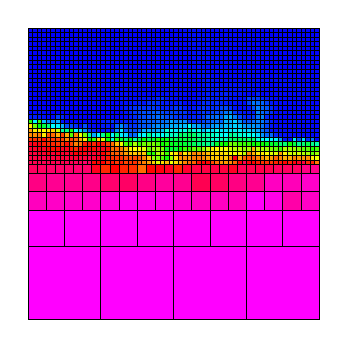
\begin{tikzpicture}[x={(\screenshotunitlength,0)},y={(0,\screenshotunitlength)}]
        \definecolor{fillcolor}{rgb}{1.000000,0.000000,1.000000}
\fill[fillcolor] (0.000000,0.000000) rectangle (0.250000,0.250000);
\definecolor{fillcolor}{rgb}{1.000000,0.000000,1.000000}
\fill[fillcolor] (0.250000,0.000000) rectangle (0.500000,0.250000);
\definecolor{fillcolor}{rgb}{1.000000,0.000000,1.000000}
\fill[fillcolor] (0.000000,0.250000) rectangle (0.125000,0.375000);
\definecolor{fillcolor}{rgb}{1.000000,0.000000,1.000000}
\fill[fillcolor] (0.125000,0.250000) rectangle (0.250000,0.375000);
\definecolor{fillcolor}{rgb}{1.000000,0.000000,0.743529}
\fill[fillcolor] (0.000000,0.375000) rectangle (0.062500,0.437500);
\definecolor{fillcolor}{rgb}{1.000000,0.000000,0.782004}
\fill[fillcolor] (0.062500,0.375000) rectangle (0.125000,0.437500);
\definecolor{fillcolor}{rgb}{1.000000,0.000000,0.512097}
\fill[fillcolor] (0.000000,0.437500) rectangle (0.062500,0.500000);
\definecolor{fillcolor}{rgb}{1.000000,0.000000,0.567338}
\fill[fillcolor] (0.062500,0.437500) rectangle (0.125000,0.500000);
\definecolor{fillcolor}{rgb}{1.000000,0.000000,0.809566}
\fill[fillcolor] (0.125000,0.375000) rectangle (0.187500,0.437500);
\definecolor{fillcolor}{rgb}{1.000000,0.000000,0.796517}
\fill[fillcolor] (0.187500,0.375000) rectangle (0.250000,0.437500);
\definecolor{fillcolor}{rgb}{1.000000,0.000000,0.572274}
\fill[fillcolor] (0.125000,0.437500) rectangle (0.187500,0.500000);
\definecolor{fillcolor}{rgb}{1.000000,0.000000,0.533022}
\fill[fillcolor] (0.187500,0.437500) rectangle (0.250000,0.500000);
\definecolor{fillcolor}{rgb}{1.000000,0.000000,1.000000}
\fill[fillcolor] (0.250000,0.250000) rectangle (0.375000,0.375000);
\definecolor{fillcolor}{rgb}{1.000000,0.000000,1.000000}
\fill[fillcolor] (0.375000,0.250000) rectangle (0.500000,0.375000);
\definecolor{fillcolor}{rgb}{1.000000,0.000000,0.872510}
\fill[fillcolor] (0.250000,0.375000) rectangle (0.312500,0.437500);
\definecolor{fillcolor}{rgb}{1.000000,0.000000,0.944715}
\fill[fillcolor] (0.312500,0.375000) rectangle (0.375000,0.437500);
\definecolor{fillcolor}{rgb}{1.000000,0.000000,0.428816}
\fill[fillcolor] (0.250000,0.437500) rectangle (0.312500,0.500000);
\definecolor{fillcolor}{rgb}{1.000000,0.000000,0.390688}
\fill[fillcolor] (0.312500,0.437500) rectangle (0.375000,0.500000);
\definecolor{fillcolor}{rgb}{1.000000,0.000000,0.926542}
\fill[fillcolor] (0.375000,0.375000) rectangle (0.437500,0.437500);
\definecolor{fillcolor}{rgb}{1.000000,0.000000,0.921581}
\fill[fillcolor] (0.437500,0.375000) rectangle (0.500000,0.437500);
\definecolor{fillcolor}{rgb}{1.000000,0.000000,0.521165}
\fill[fillcolor] (0.375000,0.437500) rectangle (0.437500,0.500000);
\definecolor{fillcolor}{rgb}{1.000000,0.000000,0.614394}
\fill[fillcolor] (0.437500,0.437500) rectangle (0.500000,0.500000);
\definecolor{fillcolor}{rgb}{1.000000,0.000000,1.000000}
\fill[fillcolor] (0.500000,0.000000) rectangle (0.750000,0.250000);
\definecolor{fillcolor}{rgb}{1.000000,0.000000,1.000000}
\fill[fillcolor] (0.750000,0.000000) rectangle (1.000000,0.250000);
\definecolor{fillcolor}{rgb}{1.000000,0.000000,1.000000}
\fill[fillcolor] (0.500000,0.250000) rectangle (0.625000,0.375000);
\definecolor{fillcolor}{rgb}{1.000000,0.000000,1.000000}
\fill[fillcolor] (0.625000,0.250000) rectangle (0.750000,0.375000);
\definecolor{fillcolor}{rgb}{1.000000,0.000000,0.838857}
\fill[fillcolor] (0.500000,0.375000) rectangle (0.562500,0.437500);
\definecolor{fillcolor}{rgb}{1.000000,0.000000,0.755134}
\fill[fillcolor] (0.562500,0.375000) rectangle (0.625000,0.437500);
\definecolor{fillcolor}{rgb}{1.000000,0.000000,0.565014}
\fill[fillcolor] (0.500000,0.437500) rectangle (0.562500,0.500000);
\definecolor{fillcolor}{rgb}{1.000000,0.000000,0.316997}
\fill[fillcolor] (0.562500,0.437500) rectangle (0.625000,0.500000);
\definecolor{fillcolor}{rgb}{1.000000,0.000000,0.761975}
\fill[fillcolor] (0.625000,0.375000) rectangle (0.687500,0.437500);
\definecolor{fillcolor}{rgb}{1.000000,0.000000,0.744416}
\fill[fillcolor] (0.687500,0.375000) rectangle (0.750000,0.437500);
\definecolor{fillcolor}{rgb}{1.000000,0.000000,0.381112}
\fill[fillcolor] (0.625000,0.437500) rectangle (0.687500,0.500000);
\definecolor{fillcolor}{rgb}{1.000000,0.000000,0.509157}
\fill[fillcolor] (0.687500,0.437500) rectangle (0.750000,0.500000);
\definecolor{fillcolor}{rgb}{1.000000,0.000000,1.000000}
\fill[fillcolor] (0.750000,0.250000) rectangle (0.875000,0.375000);
\definecolor{fillcolor}{rgb}{1.000000,0.000000,1.000000}
\fill[fillcolor] (0.875000,0.250000) rectangle (1.000000,0.375000);
\definecolor{fillcolor}{rgb}{1.000000,0.000000,0.980022}
\fill[fillcolor] (0.750000,0.375000) rectangle (0.812500,0.437500);
\definecolor{fillcolor}{rgb}{1.000000,0.000000,0.910166}
\fill[fillcolor] (0.812500,0.375000) rectangle (0.875000,0.437500);
\definecolor{fillcolor}{rgb}{1.000000,0.000000,0.563105}
\fill[fillcolor] (0.750000,0.437500) rectangle (0.812500,0.500000);
\definecolor{fillcolor}{rgb}{1.000000,0.000000,0.756911}
\fill[fillcolor] (0.812500,0.437500) rectangle (0.875000,0.500000);
\definecolor{fillcolor}{rgb}{1.000000,0.000000,0.657446}
\fill[fillcolor] (0.875000,0.375000) rectangle (0.937500,0.437500);
\definecolor{fillcolor}{rgb}{1.000000,0.000000,0.777652}
\fill[fillcolor] (0.937500,0.375000) rectangle (1.000000,0.437500);
\definecolor{fillcolor}{rgb}{1.000000,0.000000,0.722169}
\fill[fillcolor] (0.875000,0.437500) rectangle (0.937500,0.500000);
\definecolor{fillcolor}{rgb}{1.000000,0.000000,0.791756}
\fill[fillcolor] (0.937500,0.437500) rectangle (1.000000,0.500000);
\definecolor{fillcolor}{rgb}{1.000000,0.000000,0.377348}
\fill[fillcolor] (0.000000,0.500000) rectangle (0.031250,0.531250);
\definecolor{fillcolor}{rgb}{1.000000,0.000000,0.376620}
\fill[fillcolor] (0.031250,0.500000) rectangle (0.062500,0.531250);
\definecolor{fillcolor}{rgb}{1.000000,0.000000,0.329167}
\fill[fillcolor] (0.000000,0.531250) rectangle (0.015625,0.546875);
\definecolor{fillcolor}{rgb}{1.000000,0.000000,0.311934}
\fill[fillcolor] (0.015625,0.531250) rectangle (0.031250,0.546875);
\definecolor{fillcolor}{rgb}{1.000000,0.000000,0.273900}
\fill[fillcolor] (0.000000,0.546875) rectangle (0.015625,0.562500);
\definecolor{fillcolor}{rgb}{1.000000,0.000000,0.261105}
\fill[fillcolor] (0.015625,0.546875) rectangle (0.031250,0.562500);
\definecolor{fillcolor}{rgb}{1.000000,0.000000,0.328072}
\fill[fillcolor] (0.031250,0.531250) rectangle (0.046875,0.546875);
\definecolor{fillcolor}{rgb}{1.000000,0.000000,0.321688}
\fill[fillcolor] (0.046875,0.531250) rectangle (0.062500,0.546875);
\definecolor{fillcolor}{rgb}{1.000000,0.000000,0.248910}
\fill[fillcolor] (0.031250,0.546875) rectangle (0.046875,0.562500);
\definecolor{fillcolor}{rgb}{1.000000,0.000000,0.265874}
\fill[fillcolor] (0.046875,0.546875) rectangle (0.062500,0.562500);
\definecolor{fillcolor}{rgb}{1.000000,0.000000,0.406990}
\fill[fillcolor] (0.062500,0.500000) rectangle (0.093750,0.531250);
\definecolor{fillcolor}{rgb}{1.000000,0.000000,0.415936}
\fill[fillcolor] (0.093750,0.500000) rectangle (0.125000,0.531250);
\definecolor{fillcolor}{rgb}{1.000000,0.000000,0.308882}
\fill[fillcolor] (0.062500,0.531250) rectangle (0.078125,0.546875);
\definecolor{fillcolor}{rgb}{1.000000,0.000000,0.290797}
\fill[fillcolor] (0.078125,0.531250) rectangle (0.093750,0.546875);
\definecolor{fillcolor}{rgb}{1.000000,0.000000,0.252572}
\fill[fillcolor] (0.062500,0.546875) rectangle (0.078125,0.562500);
\definecolor{fillcolor}{rgb}{1.000000,0.000000,0.244668}
\fill[fillcolor] (0.078125,0.546875) rectangle (0.093750,0.562500);
\definecolor{fillcolor}{rgb}{1.000000,0.000000,0.340700}
\fill[fillcolor] (0.093750,0.531250) rectangle (0.109375,0.546875);
\definecolor{fillcolor}{rgb}{1.000000,0.000000,0.285460}
\fill[fillcolor] (0.109375,0.531250) rectangle (0.125000,0.546875);
\definecolor{fillcolor}{rgb}{1.000000,0.000000,0.215928}
\fill[fillcolor] (0.093750,0.546875) rectangle (0.109375,0.562500);
\definecolor{fillcolor}{rgb}{1.000000,0.000000,0.220046}
\fill[fillcolor] (0.109375,0.546875) rectangle (0.125000,0.562500);
\definecolor{fillcolor}{rgb}{1.000000,0.000000,0.231820}
\fill[fillcolor] (0.000000,0.562500) rectangle (0.015625,0.578125);
\definecolor{fillcolor}{rgb}{1.000000,0.000000,0.240460}
\fill[fillcolor] (0.015625,0.562500) rectangle (0.031250,0.578125);
\definecolor{fillcolor}{rgb}{1.000000,0.000000,0.195579}
\fill[fillcolor] (0.000000,0.578125) rectangle (0.015625,0.593750);
\definecolor{fillcolor}{rgb}{1.000000,0.000000,0.165991}
\fill[fillcolor] (0.015625,0.578125) rectangle (0.031250,0.593750);
\definecolor{fillcolor}{rgb}{1.000000,0.000000,0.159059}
\fill[fillcolor] (0.031250,0.562500) rectangle (0.046875,0.578125);
\definecolor{fillcolor}{rgb}{1.000000,0.000000,0.193328}
\fill[fillcolor] (0.046875,0.562500) rectangle (0.062500,0.578125);
\definecolor{fillcolor}{rgb}{1.000000,0.000000,0.081057}
\fill[fillcolor] (0.031250,0.578125) rectangle (0.046875,0.593750);
\definecolor{fillcolor}{rgb}{1.000000,0.000000,0.135822}
\fill[fillcolor] (0.046875,0.578125) rectangle (0.062500,0.593750);
\definecolor{fillcolor}{rgb}{1.000000,0.000000,0.148600}
\fill[fillcolor] (0.000000,0.593750) rectangle (0.015625,0.609375);
\definecolor{fillcolor}{rgb}{1.000000,0.000000,0.071700}
\fill[fillcolor] (0.015625,0.593750) rectangle (0.031250,0.609375);
\definecolor{fillcolor}{rgb}{1.000000,0.227978,0.000000}
\fill[fillcolor] (0.000000,0.609375) rectangle (0.015625,0.625000);
\definecolor{fillcolor}{rgb}{1.000000,0.182159,0.000000}
\fill[fillcolor] (0.015625,0.609375) rectangle (0.031250,0.625000);
\definecolor{fillcolor}{rgb}{1.000000,0.000000,0.057105}
\fill[fillcolor] (0.031250,0.593750) rectangle (0.046875,0.609375);
\definecolor{fillcolor}{rgb}{1.000000,0.109741,0.000000}
\fill[fillcolor] (0.046875,0.593750) rectangle (0.062500,0.609375);
\definecolor{fillcolor}{rgb}{1.000000,0.255894,0.000000}
\fill[fillcolor] (0.031250,0.609375) rectangle (0.046875,0.625000);
\definecolor{fillcolor}{rgb}{1.000000,0.055230,0.000000}
\fill[fillcolor] (0.046875,0.609375) rectangle (0.062500,0.625000);
\definecolor{fillcolor}{rgb}{1.000000,0.000000,0.058157}
\fill[fillcolor] (0.062500,0.562500) rectangle (0.078125,0.578125);
\definecolor{fillcolor}{rgb}{1.000000,0.000000,0.205795}
\fill[fillcolor] (0.078125,0.562500) rectangle (0.093750,0.578125);
\definecolor{fillcolor}{rgb}{1.000000,0.000000,0.002680}
\fill[fillcolor] (0.062500,0.578125) rectangle (0.078125,0.593750);
\definecolor{fillcolor}{rgb}{1.000000,0.043644,0.000000}
\fill[fillcolor] (0.078125,0.578125) rectangle (0.093750,0.593750);
\definecolor{fillcolor}{rgb}{1.000000,0.000000,0.110377}
\fill[fillcolor] (0.093750,0.562500) rectangle (0.109375,0.578125);
\definecolor{fillcolor}{rgb}{1.000000,0.000000,0.175221}
\fill[fillcolor] (0.109375,0.562500) rectangle (0.125000,0.578125);
\definecolor{fillcolor}{rgb}{1.000000,0.013121,0.000000}
\fill[fillcolor] (0.093750,0.578125) rectangle (0.109375,0.593750);
\definecolor{fillcolor}{rgb}{1.000000,0.000000,0.136713}
\fill[fillcolor] (0.109375,0.578125) rectangle (0.125000,0.593750);
\definecolor{fillcolor}{rgb}{1.000000,0.150142,0.000000}
\fill[fillcolor] (0.062500,0.593750) rectangle (0.078125,0.609375);
\definecolor{fillcolor}{rgb}{1.000000,0.147721,0.000000}
\fill[fillcolor] (0.078125,0.593750) rectangle (0.093750,0.609375);
\definecolor{fillcolor}{rgb}{1.000000,0.220729,0.000000}
\fill[fillcolor] (0.062500,0.609375) rectangle (0.078125,0.625000);
\definecolor{fillcolor}{rgb}{1.000000,0.216907,0.000000}
\fill[fillcolor] (0.078125,0.609375) rectangle (0.093750,0.625000);
\definecolor{fillcolor}{rgb}{1.000000,0.195084,0.000000}
\fill[fillcolor] (0.093750,0.593750) rectangle (0.109375,0.609375);
\definecolor{fillcolor}{rgb}{1.000000,0.224374,0.000000}
\fill[fillcolor] (0.109375,0.593750) rectangle (0.125000,0.609375);
\definecolor{fillcolor}{rgb}{1.000000,0.241040,0.000000}
\fill[fillcolor] (0.093750,0.609375) rectangle (0.109375,0.625000);
\definecolor{fillcolor}{rgb}{1.000000,0.260439,0.000000}
\fill[fillcolor] (0.109375,0.609375) rectangle (0.125000,0.625000);
\definecolor{fillcolor}{rgb}{1.000000,0.000000,0.423942}
\fill[fillcolor] (0.125000,0.500000) rectangle (0.156250,0.531250);
\definecolor{fillcolor}{rgb}{1.000000,0.000000,0.433445}
\fill[fillcolor] (0.156250,0.500000) rectangle (0.187500,0.531250);
\definecolor{fillcolor}{rgb}{1.000000,0.000000,0.329405}
\fill[fillcolor] (0.125000,0.531250) rectangle (0.140625,0.546875);
\definecolor{fillcolor}{rgb}{1.000000,0.000000,0.319134}
\fill[fillcolor] (0.140625,0.531250) rectangle (0.156250,0.546875);
\definecolor{fillcolor}{rgb}{1.000000,0.000000,0.248515}
\fill[fillcolor] (0.125000,0.546875) rectangle (0.140625,0.562500);
\definecolor{fillcolor}{rgb}{1.000000,0.000000,0.204363}
\fill[fillcolor] (0.140625,0.546875) rectangle (0.156250,0.562500);
\definecolor{fillcolor}{rgb}{1.000000,0.000000,0.357478}
\fill[fillcolor] (0.156250,0.531250) rectangle (0.171875,0.546875);
\definecolor{fillcolor}{rgb}{1.000000,0.000000,0.328291}
\fill[fillcolor] (0.171875,0.531250) rectangle (0.187500,0.546875);
\definecolor{fillcolor}{rgb}{1.000000,0.000000,0.186793}
\fill[fillcolor] (0.156250,0.546875) rectangle (0.171875,0.562500);
\definecolor{fillcolor}{rgb}{1.000000,0.000000,0.230654}
\fill[fillcolor] (0.171875,0.546875) rectangle (0.187500,0.562500);
\definecolor{fillcolor}{rgb}{1.000000,0.000000,0.423149}
\fill[fillcolor] (0.187500,0.500000) rectangle (0.218750,0.531250);
\definecolor{fillcolor}{rgb}{1.000000,0.000000,0.116963}
\fill[fillcolor] (0.218750,0.500000) rectangle (0.250000,0.531250);
\definecolor{fillcolor}{rgb}{1.000000,0.000000,0.424399}
\fill[fillcolor] (0.187500,0.531250) rectangle (0.203125,0.546875);
\definecolor{fillcolor}{rgb}{1.000000,0.000000,0.372528}
\fill[fillcolor] (0.203125,0.531250) rectangle (0.218750,0.546875);
\definecolor{fillcolor}{rgb}{1.000000,0.000000,0.227678}
\fill[fillcolor] (0.187500,0.546875) rectangle (0.203125,0.562500);
\definecolor{fillcolor}{rgb}{1.000000,0.000000,0.291954}
\fill[fillcolor] (0.203125,0.546875) rectangle (0.218750,0.562500);
\definecolor{fillcolor}{rgb}{1.000000,0.028076,0.000000}
\fill[fillcolor] (0.218750,0.531250) rectangle (0.234375,0.546875);
\definecolor{fillcolor}{rgb}{1.000000,0.000547,0.000000}
\fill[fillcolor] (0.234375,0.531250) rectangle (0.250000,0.546875);
\definecolor{fillcolor}{rgb}{1.000000,0.000000,0.190785}
\fill[fillcolor] (0.218750,0.546875) rectangle (0.234375,0.562500);
\definecolor{fillcolor}{rgb}{1.000000,0.000000,0.160036}
\fill[fillcolor] (0.234375,0.546875) rectangle (0.250000,0.562500);
\definecolor{fillcolor}{rgb}{1.000000,0.000000,0.176910}
\fill[fillcolor] (0.125000,0.562500) rectangle (0.140625,0.578125);
\definecolor{fillcolor}{rgb}{1.000000,0.000000,0.134660}
\fill[fillcolor] (0.140625,0.562500) rectangle (0.156250,0.578125);
\definecolor{fillcolor}{rgb}{1.000000,0.000000,0.102411}
\fill[fillcolor] (0.125000,0.578125) rectangle (0.140625,0.593750);
\definecolor{fillcolor}{rgb}{1.000000,0.092327,0.000000}
\fill[fillcolor] (0.140625,0.578125) rectangle (0.156250,0.593750);
\definecolor{fillcolor}{rgb}{1.000000,0.000000,0.013729}
\fill[fillcolor] (0.156250,0.562500) rectangle (0.171875,0.578125);
\definecolor{fillcolor}{rgb}{1.000000,0.000000,0.053284}
\fill[fillcolor] (0.171875,0.562500) rectangle (0.187500,0.578125);
\definecolor{fillcolor}{rgb}{1.000000,0.154340,0.000000}
\fill[fillcolor] (0.156250,0.578125) rectangle (0.171875,0.593750);
\definecolor{fillcolor}{rgb}{1.000000,0.000000,0.043993}
\fill[fillcolor] (0.171875,0.578125) rectangle (0.187500,0.593750);
\definecolor{fillcolor}{rgb}{1.000000,0.068229,0.000000}
\fill[fillcolor] (0.125000,0.593750) rectangle (0.140625,0.609375);
\definecolor{fillcolor}{rgb}{1.000000,0.247039,0.000000}
\fill[fillcolor] (0.140625,0.593750) rectangle (0.156250,0.609375);
\definecolor{fillcolor}{rgb}{1.000000,0.516480,0.000000}
\fill[fillcolor] (0.125000,0.609375) rectangle (0.140625,0.625000);
\definecolor{fillcolor}{rgb}{1.000000,0.276049,0.000000}
\fill[fillcolor] (0.140625,0.609375) rectangle (0.156250,0.625000);
\definecolor{fillcolor}{rgb}{1.000000,0.497654,0.000000}
\fill[fillcolor] (0.156250,0.593750) rectangle (0.171875,0.609375);
\definecolor{fillcolor}{rgb}{1.000000,0.441255,0.000000}
\fill[fillcolor] (0.171875,0.593750) rectangle (0.187500,0.609375);
\definecolor{fillcolor}{rgb}{1.000000,0.401169,0.000000}
\fill[fillcolor] (0.156250,0.609375) rectangle (0.171875,0.625000);
\definecolor{fillcolor}{rgb}{1.000000,0.691700,0.000000}
\fill[fillcolor] (0.171875,0.609375) rectangle (0.187500,0.625000);
\definecolor{fillcolor}{rgb}{1.000000,0.000000,0.061890}
\fill[fillcolor] (0.187500,0.562500) rectangle (0.203125,0.578125);
\definecolor{fillcolor}{rgb}{1.000000,0.000000,0.241407}
\fill[fillcolor] (0.203125,0.562500) rectangle (0.218750,0.578125);
\definecolor{fillcolor}{rgb}{1.000000,0.000000,0.030981}
\fill[fillcolor] (0.187500,0.578125) rectangle (0.203125,0.593750);
\definecolor{fillcolor}{rgb}{1.000000,0.000000,0.041925}
\fill[fillcolor] (0.203125,0.578125) rectangle (0.218750,0.593750);
\definecolor{fillcolor}{rgb}{1.000000,0.000000,0.201903}
\fill[fillcolor] (0.218750,0.562500) rectangle (0.234375,0.578125);
\definecolor{fillcolor}{rgb}{1.000000,0.000000,0.148205}
\fill[fillcolor] (0.234375,0.562500) rectangle (0.250000,0.578125);
\definecolor{fillcolor}{rgb}{1.000000,0.031579,0.000000}
\fill[fillcolor] (0.218750,0.578125) rectangle (0.234375,0.593750);
\definecolor{fillcolor}{rgb}{1.000000,0.000000,0.124406}
\fill[fillcolor] (0.234375,0.578125) rectangle (0.250000,0.593750);
\definecolor{fillcolor}{rgb}{1.000000,0.096032,0.000000}
\fill[fillcolor] (0.187500,0.593750) rectangle (0.203125,0.609375);
\definecolor{fillcolor}{rgb}{1.000000,0.046813,0.000000}
\fill[fillcolor] (0.203125,0.593750) rectangle (0.218750,0.609375);
\definecolor{fillcolor}{rgb}{1.000000,0.926985,0.000000}
\fill[fillcolor] (0.187500,0.609375) rectangle (0.203125,0.625000);
\definecolor{fillcolor}{rgb}{0.000000,1.000000,0.024585}
\fill[fillcolor] (0.203125,0.609375) rectangle (0.218750,0.625000);
\definecolor{fillcolor}{rgb}{1.000000,0.146598,0.000000}
\fill[fillcolor] (0.218750,0.593750) rectangle (0.234375,0.609375);
\definecolor{fillcolor}{rgb}{1.000000,0.014715,0.000000}
\fill[fillcolor] (0.234375,0.593750) rectangle (0.250000,0.609375);
\definecolor{fillcolor}{rgb}{0.210106,1.000000,0.000000}
\fill[fillcolor] (0.218750,0.609375) rectangle (0.234375,0.625000);
\definecolor{fillcolor}{rgb}{1.000000,0.791301,0.000000}
\fill[fillcolor] (0.234375,0.609375) rectangle (0.250000,0.625000);
\definecolor{fillcolor}{rgb}{1.000000,0.536070,0.000000}
\fill[fillcolor] (0.000000,0.625000) rectangle (0.015625,0.640625);
\definecolor{fillcolor}{rgb}{1.000000,0.552745,0.000000}
\fill[fillcolor] (0.015625,0.625000) rectangle (0.031250,0.640625);
\definecolor{fillcolor}{rgb}{1.000000,0.618113,0.000000}
\fill[fillcolor] (0.000000,0.640625) rectangle (0.015625,0.656250);
\definecolor{fillcolor}{rgb}{1.000000,0.923706,0.000000}
\fill[fillcolor] (0.015625,0.640625) rectangle (0.031250,0.656250);
\definecolor{fillcolor}{rgb}{1.000000,0.486550,0.000000}
\fill[fillcolor] (0.031250,0.625000) rectangle (0.046875,0.640625);
\definecolor{fillcolor}{rgb}{1.000000,0.910050,0.000000}
\fill[fillcolor] (0.046875,0.625000) rectangle (0.062500,0.640625);
\definecolor{fillcolor}{rgb}{1.000000,0.940644,0.000000}
\fill[fillcolor] (0.031250,0.640625) rectangle (0.046875,0.656250);
\definecolor{fillcolor}{rgb}{1.000000,0.986296,0.000000}
\fill[fillcolor] (0.046875,0.640625) rectangle (0.062500,0.656250);
\definecolor{fillcolor}{rgb}{1.000000,0.906978,0.000000}
\fill[fillcolor] (0.000000,0.656250) rectangle (0.015625,0.671875);
\definecolor{fillcolor}{rgb}{0.431775,1.000000,0.000000}
\fill[fillcolor] (0.015625,0.656250) rectangle (0.031250,0.671875);
\definecolor{fillcolor}{rgb}{0.148312,1.000000,0.000000}
\fill[fillcolor] (0.000000,0.671875) rectangle (0.015625,0.687500);
\definecolor{fillcolor}{rgb}{0.000000,0.976167,1.000000}
\fill[fillcolor] (0.015625,0.671875) rectangle (0.031250,0.687500);
\definecolor{fillcolor}{rgb}{0.000000,1.000000,0.076229}
\fill[fillcolor] (0.031250,0.656250) rectangle (0.046875,0.671875);
\definecolor{fillcolor}{rgb}{0.000000,1.000000,0.237505}
\fill[fillcolor] (0.046875,0.656250) rectangle (0.062500,0.671875);
\definecolor{fillcolor}{rgb}{0.231065,1.000000,0.000000}
\fill[fillcolor] (0.031250,0.671875) rectangle (0.046875,0.687500);
\definecolor{fillcolor}{rgb}{0.000000,0.766870,1.000000}
\fill[fillcolor] (0.046875,0.671875) rectangle (0.062500,0.687500);
\definecolor{fillcolor}{rgb}{1.000000,0.329171,0.000000}
\fill[fillcolor] (0.062500,0.625000) rectangle (0.078125,0.640625);
\definecolor{fillcolor}{rgb}{1.000000,0.420515,0.000000}
\fill[fillcolor] (0.078125,0.625000) rectangle (0.093750,0.640625);
\definecolor{fillcolor}{rgb}{1.000000,0.891615,0.000000}
\fill[fillcolor] (0.062500,0.640625) rectangle (0.078125,0.656250);
\definecolor{fillcolor}{rgb}{1.000000,0.805774,0.000000}
\fill[fillcolor] (0.078125,0.640625) rectangle (0.093750,0.656250);
\definecolor{fillcolor}{rgb}{1.000000,0.674850,0.000000}
\fill[fillcolor] (0.093750,0.625000) rectangle (0.109375,0.640625);
\definecolor{fillcolor}{rgb}{1.000000,0.277912,0.000000}
\fill[fillcolor] (0.109375,0.625000) rectangle (0.125000,0.640625);
\definecolor{fillcolor}{rgb}{0.744202,1.000000,0.000000}
\fill[fillcolor] (0.093750,0.640625) rectangle (0.109375,0.656250);
\definecolor{fillcolor}{rgb}{0.000000,1.000000,0.655983}
\fill[fillcolor] (0.109375,0.640625) rectangle (0.125000,0.656250);
\definecolor{fillcolor}{rgb}{0.000000,1.000000,0.503407}
\fill[fillcolor] (0.062500,0.656250) rectangle (0.078125,0.671875);
\definecolor{fillcolor}{rgb}{0.000000,1.000000,0.996946}
\fill[fillcolor] (0.078125,0.656250) rectangle (0.093750,0.671875);
\definecolor{fillcolor}{rgb}{0.000000,0.490194,1.000000}
\fill[fillcolor] (0.062500,0.671875) rectangle (0.078125,0.687500);
\definecolor{fillcolor}{rgb}{0.000000,0.581871,1.000000}
\fill[fillcolor] (0.078125,0.671875) rectangle (0.093750,0.687500);
\definecolor{fillcolor}{rgb}{0.000000,0.950798,1.000000}
\fill[fillcolor] (0.093750,0.656250) rectangle (0.109375,0.671875);
\definecolor{fillcolor}{rgb}{0.000000,0.676531,1.000000}
\fill[fillcolor] (0.109375,0.656250) rectangle (0.125000,0.671875);
\definecolor{fillcolor}{rgb}{0.000000,0.679732,1.000000}
\fill[fillcolor] (0.093750,0.671875) rectangle (0.109375,0.687500);
\definecolor{fillcolor}{rgb}{0.000000,0.077284,1.000000}
\fill[fillcolor] (0.109375,0.671875) rectangle (0.125000,0.687500);
\definecolor{fillcolor}{rgb}{0.000000,0.098463,1.000000}
\fill[fillcolor] (0.000000,0.687500) rectangle (0.015625,0.703125);
\definecolor{fillcolor}{rgb}{0.000000,0.118454,1.000000}
\fill[fillcolor] (0.015625,0.687500) rectangle (0.031250,0.703125);
\definecolor{fillcolor}{rgb}{0.000000,0.020217,1.000000}
\fill[fillcolor] (0.000000,0.703125) rectangle (0.015625,0.718750);
\definecolor{fillcolor}{rgb}{0.000000,0.033644,1.000000}
\fill[fillcolor] (0.015625,0.703125) rectangle (0.031250,0.718750);
\definecolor{fillcolor}{rgb}{0.000000,0.104254,1.000000}
\fill[fillcolor] (0.031250,0.687500) rectangle (0.046875,0.703125);
\definecolor{fillcolor}{rgb}{0.000000,0.059687,1.000000}
\fill[fillcolor] (0.046875,0.687500) rectangle (0.062500,0.703125);
\definecolor{fillcolor}{rgb}{0.000000,0.048101,1.000000}
\fill[fillcolor] (0.031250,0.703125) rectangle (0.046875,0.718750);
\definecolor{fillcolor}{rgb}{0.000000,0.032668,1.000000}
\fill[fillcolor] (0.046875,0.703125) rectangle (0.062500,0.718750);
\definecolor{fillcolor}{rgb}{0.000000,0.004776,1.000000}
\fill[fillcolor] (0.000000,0.718750) rectangle (0.015625,0.734375);
\definecolor{fillcolor}{rgb}{0.000000,0.020727,1.000000}
\fill[fillcolor] (0.015625,0.718750) rectangle (0.031250,0.734375);
\definecolor{fillcolor}{rgb}{0.000000,0.001081,1.000000}
\fill[fillcolor] (0.000000,0.734375) rectangle (0.015625,0.750000);
\definecolor{fillcolor}{rgb}{0.000000,0.001414,1.000000}
\fill[fillcolor] (0.015625,0.734375) rectangle (0.031250,0.750000);
\definecolor{fillcolor}{rgb}{0.000000,0.010522,1.000000}
\fill[fillcolor] (0.031250,0.718750) rectangle (0.046875,0.734375);
\definecolor{fillcolor}{rgb}{0.000000,0.001670,1.000000}
\fill[fillcolor] (0.046875,0.718750) rectangle (0.062500,0.734375);
\definecolor{fillcolor}{rgb}{0.000000,0.003659,1.000000}
\fill[fillcolor] (0.031250,0.734375) rectangle (0.046875,0.750000);
\definecolor{fillcolor}{rgb}{0.000000,0.001659,1.000000}
\fill[fillcolor] (0.046875,0.734375) rectangle (0.062500,0.750000);
\definecolor{fillcolor}{rgb}{0.000000,0.037791,1.000000}
\fill[fillcolor] (0.062500,0.687500) rectangle (0.078125,0.703125);
\definecolor{fillcolor}{rgb}{0.000000,0.026210,1.000000}
\fill[fillcolor] (0.078125,0.687500) rectangle (0.093750,0.703125);
\definecolor{fillcolor}{rgb}{0.000000,0.006575,1.000000}
\fill[fillcolor] (0.062500,0.703125) rectangle (0.078125,0.718750);
\definecolor{fillcolor}{rgb}{0.000000,0.003982,1.000000}
\fill[fillcolor] (0.078125,0.703125) rectangle (0.093750,0.718750);
\definecolor{fillcolor}{rgb}{0.000000,0.251148,1.000000}
\fill[fillcolor] (0.093750,0.687500) rectangle (0.109375,0.703125);
\definecolor{fillcolor}{rgb}{0.000000,0.143691,1.000000}
\fill[fillcolor] (0.109375,0.687500) rectangle (0.125000,0.703125);
\definecolor{fillcolor}{rgb}{0.000000,0.004719,1.000000}
\fill[fillcolor] (0.093750,0.703125) rectangle (0.109375,0.718750);
\definecolor{fillcolor}{rgb}{0.000000,0.006596,1.000000}
\fill[fillcolor] (0.109375,0.703125) rectangle (0.125000,0.718750);
\definecolor{fillcolor}{rgb}{0.000000,0.000299,1.000000}
\fill[fillcolor] (0.062500,0.718750) rectangle (0.078125,0.734375);
\definecolor{fillcolor}{rgb}{0.000000,0.000315,1.000000}
\fill[fillcolor] (0.078125,0.718750) rectangle (0.093750,0.734375);
\definecolor{fillcolor}{rgb}{0.000000,0.000498,1.000000}
\fill[fillcolor] (0.062500,0.734375) rectangle (0.078125,0.750000);
\definecolor{fillcolor}{rgb}{0.000000,0.000429,1.000000}
\fill[fillcolor] (0.078125,0.734375) rectangle (0.093750,0.750000);
\definecolor{fillcolor}{rgb}{0.000000,0.003813,1.000000}
\fill[fillcolor] (0.093750,0.718750) rectangle (0.109375,0.734375);
\definecolor{fillcolor}{rgb}{0.000000,0.046690,1.000000}
\fill[fillcolor] (0.109375,0.718750) rectangle (0.125000,0.734375);
\definecolor{fillcolor}{rgb}{0.000000,0.000229,1.000000}
\fill[fillcolor] (0.093750,0.734375) rectangle (0.109375,0.750000);
\definecolor{fillcolor}{rgb}{0.000000,0.017060,1.000000}
\fill[fillcolor] (0.109375,0.734375) rectangle (0.125000,0.750000);
\definecolor{fillcolor}{rgb}{1.000000,0.658888,0.000000}
\fill[fillcolor] (0.125000,0.625000) rectangle (0.140625,0.640625);
\definecolor{fillcolor}{rgb}{0.325653,1.000000,0.000000}
\fill[fillcolor] (0.140625,0.625000) rectangle (0.156250,0.640625);
\definecolor{fillcolor}{rgb}{0.000000,1.000000,0.499270}
\fill[fillcolor] (0.125000,0.640625) rectangle (0.140625,0.656250);
\definecolor{fillcolor}{rgb}{0.092660,1.000000,0.000000}
\fill[fillcolor] (0.140625,0.640625) rectangle (0.156250,0.656250);
\definecolor{fillcolor}{rgb}{1.000000,0.499363,0.000000}
\fill[fillcolor] (0.156250,0.625000) rectangle (0.171875,0.640625);
\definecolor{fillcolor}{rgb}{0.926219,1.000000,0.000000}
\fill[fillcolor] (0.171875,0.625000) rectangle (0.187500,0.640625);
\definecolor{fillcolor}{rgb}{0.000000,1.000000,0.990702}
\fill[fillcolor] (0.156250,0.640625) rectangle (0.171875,0.656250);
\definecolor{fillcolor}{rgb}{0.000000,0.826181,1.000000}
\fill[fillcolor] (0.171875,0.640625) rectangle (0.187500,0.656250);
\definecolor{fillcolor}{rgb}{0.000000,0.305927,1.000000}
\fill[fillcolor] (0.125000,0.656250) rectangle (0.140625,0.671875);
\definecolor{fillcolor}{rgb}{0.000000,0.257320,1.000000}
\fill[fillcolor] (0.140625,0.656250) rectangle (0.156250,0.671875);
\definecolor{fillcolor}{rgb}{0.000000,0.003501,1.000000}
\fill[fillcolor] (0.125000,0.671875) rectangle (0.140625,0.687500);
\definecolor{fillcolor}{rgb}{0.000000,0.001821,1.000000}
\fill[fillcolor] (0.140625,0.671875) rectangle (0.156250,0.687500);
\definecolor{fillcolor}{rgb}{0.000000,0.171549,1.000000}
\fill[fillcolor] (0.156250,0.656250) rectangle (0.171875,0.671875);
\definecolor{fillcolor}{rgb}{0.000000,0.044275,1.000000}
\fill[fillcolor] (0.171875,0.656250) rectangle (0.187500,0.671875);
\definecolor{fillcolor}{rgb}{0.000000,0.001614,1.000000}
\fill[fillcolor] (0.156250,0.671875) rectangle (0.171875,0.687500);
\definecolor{fillcolor}{rgb}{0.000000,0.001242,1.000000}
\fill[fillcolor] (0.171875,0.671875) rectangle (0.187500,0.687500);
\definecolor{fillcolor}{rgb}{0.473080,1.000000,0.000000}
\fill[fillcolor] (0.187500,0.625000) rectangle (0.203125,0.640625);
\definecolor{fillcolor}{rgb}{0.000000,1.000000,0.555765}
\fill[fillcolor] (0.203125,0.625000) rectangle (0.218750,0.640625);
\definecolor{fillcolor}{rgb}{0.000000,0.553189,1.000000}
\fill[fillcolor] (0.187500,0.640625) rectangle (0.203125,0.656250);
\definecolor{fillcolor}{rgb}{0.000000,0.228616,1.000000}
\fill[fillcolor] (0.203125,0.640625) rectangle (0.218750,0.656250);
\definecolor{fillcolor}{rgb}{0.000000,0.664591,1.000000}
\fill[fillcolor] (0.218750,0.625000) rectangle (0.234375,0.640625);
\definecolor{fillcolor}{rgb}{0.000000,0.966771,1.000000}
\fill[fillcolor] (0.234375,0.625000) rectangle (0.250000,0.640625);
\definecolor{fillcolor}{rgb}{0.000000,0.148072,1.000000}
\fill[fillcolor] (0.218750,0.640625) rectangle (0.234375,0.656250);
\definecolor{fillcolor}{rgb}{0.000000,0.067887,1.000000}
\fill[fillcolor] (0.234375,0.640625) rectangle (0.250000,0.656250);
\definecolor{fillcolor}{rgb}{0.000000,0.314699,1.000000}
\fill[fillcolor] (0.187500,0.656250) rectangle (0.203125,0.671875);
\definecolor{fillcolor}{rgb}{0.000000,0.066496,1.000000}
\fill[fillcolor] (0.203125,0.656250) rectangle (0.218750,0.671875);
\definecolor{fillcolor}{rgb}{0.000000,0.000679,1.000000}
\fill[fillcolor] (0.187500,0.671875) rectangle (0.203125,0.687500);
\definecolor{fillcolor}{rgb}{0.000000,0.000543,1.000000}
\fill[fillcolor] (0.203125,0.671875) rectangle (0.218750,0.687500);
\definecolor{fillcolor}{rgb}{0.000000,0.039667,1.000000}
\fill[fillcolor] (0.218750,0.656250) rectangle (0.234375,0.671875);
\definecolor{fillcolor}{rgb}{0.000000,0.019238,1.000000}
\fill[fillcolor] (0.234375,0.656250) rectangle (0.250000,0.671875);
\definecolor{fillcolor}{rgb}{0.000000,0.011852,1.000000}
\fill[fillcolor] (0.218750,0.671875) rectangle (0.234375,0.687500);
\definecolor{fillcolor}{rgb}{0.000000,0.015682,1.000000}
\fill[fillcolor] (0.234375,0.671875) rectangle (0.250000,0.687500);
\definecolor{fillcolor}{rgb}{0.000000,0.034323,1.000000}
\fill[fillcolor] (0.125000,0.687500) rectangle (0.140625,0.703125);
\definecolor{fillcolor}{rgb}{0.000000,0.003848,1.000000}
\fill[fillcolor] (0.140625,0.687500) rectangle (0.156250,0.703125);
\definecolor{fillcolor}{rgb}{0.000000,0.017865,1.000000}
\fill[fillcolor] (0.125000,0.703125) rectangle (0.140625,0.718750);
\definecolor{fillcolor}{rgb}{0.000000,0.007842,1.000000}
\fill[fillcolor] (0.140625,0.703125) rectangle (0.156250,0.718750);
\definecolor{fillcolor}{rgb}{0.000000,0.003877,1.000000}
\fill[fillcolor] (0.156250,0.687500) rectangle (0.171875,0.703125);
\definecolor{fillcolor}{rgb}{0.000000,0.002277,1.000000}
\fill[fillcolor] (0.171875,0.687500) rectangle (0.187500,0.703125);
\definecolor{fillcolor}{rgb}{0.000000,0.003521,1.000000}
\fill[fillcolor] (0.156250,0.703125) rectangle (0.171875,0.718750);
\definecolor{fillcolor}{rgb}{0.000000,0.000367,1.000000}
\fill[fillcolor] (0.171875,0.703125) rectangle (0.187500,0.718750);
\definecolor{fillcolor}{rgb}{0.000000,0.019353,1.000000}
\fill[fillcolor] (0.125000,0.718750) rectangle (0.140625,0.734375);
\definecolor{fillcolor}{rgb}{0.000000,0.000156,1.000000}
\fill[fillcolor] (0.140625,0.718750) rectangle (0.156250,0.734375);
\definecolor{fillcolor}{rgb}{0.000000,0.000960,1.000000}
\fill[fillcolor] (0.125000,0.734375) rectangle (0.140625,0.750000);
\definecolor{fillcolor}{rgb}{0.000000,0.000151,1.000000}
\fill[fillcolor] (0.140625,0.734375) rectangle (0.156250,0.750000);
\definecolor{fillcolor}{rgb}{0.000000,0.000184,1.000000}
\fill[fillcolor] (0.156250,0.718750) rectangle (0.171875,0.734375);
\definecolor{fillcolor}{rgb}{0.000000,0.000358,1.000000}
\fill[fillcolor] (0.171875,0.718750) rectangle (0.187500,0.734375);
\definecolor{fillcolor}{rgb}{0.000000,0.000184,1.000000}
\fill[fillcolor] (0.156250,0.734375) rectangle (0.171875,0.750000);
\definecolor{fillcolor}{rgb}{0.000000,0.000424,1.000000}
\fill[fillcolor] (0.171875,0.734375) rectangle (0.187500,0.750000);
\definecolor{fillcolor}{rgb}{0.000000,0.001848,1.000000}
\fill[fillcolor] (0.187500,0.687500) rectangle (0.203125,0.703125);
\definecolor{fillcolor}{rgb}{0.000000,0.000728,1.000000}
\fill[fillcolor] (0.203125,0.687500) rectangle (0.218750,0.703125);
\definecolor{fillcolor}{rgb}{0.000000,0.000387,1.000000}
\fill[fillcolor] (0.187500,0.703125) rectangle (0.203125,0.718750);
\definecolor{fillcolor}{rgb}{0.000000,0.000318,1.000000}
\fill[fillcolor] (0.203125,0.703125) rectangle (0.218750,0.718750);
\definecolor{fillcolor}{rgb}{0.000000,0.005764,1.000000}
\fill[fillcolor] (0.218750,0.687500) rectangle (0.234375,0.703125);
\definecolor{fillcolor}{rgb}{0.000000,0.003655,1.000000}
\fill[fillcolor] (0.234375,0.687500) rectangle (0.250000,0.703125);
\definecolor{fillcolor}{rgb}{0.000000,0.002640,1.000000}
\fill[fillcolor] (0.218750,0.703125) rectangle (0.234375,0.718750);
\definecolor{fillcolor}{rgb}{0.000000,0.004705,1.000000}
\fill[fillcolor] (0.234375,0.703125) rectangle (0.250000,0.718750);
\definecolor{fillcolor}{rgb}{0.000000,0.000348,1.000000}
\fill[fillcolor] (0.187500,0.718750) rectangle (0.203125,0.734375);
\definecolor{fillcolor}{rgb}{0.000000,0.001097,1.000000}
\fill[fillcolor] (0.203125,0.718750) rectangle (0.218750,0.734375);
\definecolor{fillcolor}{rgb}{0.000000,0.000605,1.000000}
\fill[fillcolor] (0.187500,0.734375) rectangle (0.203125,0.750000);
\definecolor{fillcolor}{rgb}{0.000000,0.001681,1.000000}
\fill[fillcolor] (0.203125,0.734375) rectangle (0.218750,0.750000);
\definecolor{fillcolor}{rgb}{0.000000,0.002851,1.000000}
\fill[fillcolor] (0.218750,0.718750) rectangle (0.234375,0.734375);
\definecolor{fillcolor}{rgb}{0.000000,0.005107,1.000000}
\fill[fillcolor] (0.234375,0.718750) rectangle (0.250000,0.734375);
\definecolor{fillcolor}{rgb}{0.000000,0.005413,1.000000}
\fill[fillcolor] (0.218750,0.734375) rectangle (0.234375,0.750000);
\definecolor{fillcolor}{rgb}{0.000000,0.009042,1.000000}
\fill[fillcolor] (0.234375,0.734375) rectangle (0.250000,0.750000);
\definecolor{fillcolor}{rgb}{1.000000,0.158963,0.000000}
\fill[fillcolor] (0.250000,0.500000) rectangle (0.281250,0.531250);
\definecolor{fillcolor}{rgb}{1.000000,0.000097,0.000000}
\fill[fillcolor] (0.281250,0.500000) rectangle (0.312500,0.531250);
\definecolor{fillcolor}{rgb}{1.000000,0.005684,0.000000}
\fill[fillcolor] (0.250000,0.531250) rectangle (0.265625,0.546875);
\definecolor{fillcolor}{rgb}{1.000000,0.150481,0.000000}
\fill[fillcolor] (0.265625,0.531250) rectangle (0.281250,0.546875);
\definecolor{fillcolor}{rgb}{1.000000,0.000000,0.134764}
\fill[fillcolor] (0.250000,0.546875) rectangle (0.265625,0.562500);
\definecolor{fillcolor}{rgb}{1.000000,0.080113,0.000000}
\fill[fillcolor] (0.265625,0.546875) rectangle (0.281250,0.562500);
\definecolor{fillcolor}{rgb}{1.000000,0.097315,0.000000}
\fill[fillcolor] (0.281250,0.531250) rectangle (0.296875,0.546875);
\definecolor{fillcolor}{rgb}{1.000000,0.223959,0.000000}
\fill[fillcolor] (0.296875,0.531250) rectangle (0.312500,0.546875);
\definecolor{fillcolor}{rgb}{1.000000,0.180530,0.000000}
\fill[fillcolor] (0.281250,0.546875) rectangle (0.296875,0.562500);
\definecolor{fillcolor}{rgb}{1.000000,0.192195,0.000000}
\fill[fillcolor] (0.296875,0.546875) rectangle (0.312500,0.562500);
\definecolor{fillcolor}{rgb}{1.000000,0.141958,0.000000}
\fill[fillcolor] (0.312500,0.500000) rectangle (0.343750,0.531250);
\definecolor{fillcolor}{rgb}{1.000000,0.179162,0.000000}
\fill[fillcolor] (0.343750,0.500000) rectangle (0.375000,0.531250);
\definecolor{fillcolor}{rgb}{1.000000,0.122405,0.000000}
\fill[fillcolor] (0.312500,0.531250) rectangle (0.328125,0.546875);
\definecolor{fillcolor}{rgb}{1.000000,0.268868,0.000000}
\fill[fillcolor] (0.328125,0.531250) rectangle (0.343750,0.546875);
\definecolor{fillcolor}{rgb}{1.000000,0.205643,0.000000}
\fill[fillcolor] (0.312500,0.546875) rectangle (0.328125,0.562500);
\definecolor{fillcolor}{rgb}{1.000000,0.305407,0.000000}
\fill[fillcolor] (0.328125,0.546875) rectangle (0.343750,0.562500);
\definecolor{fillcolor}{rgb}{1.000000,0.216689,0.000000}
\fill[fillcolor] (0.343750,0.531250) rectangle (0.359375,0.546875);
\definecolor{fillcolor}{rgb}{1.000000,0.188667,0.000000}
\fill[fillcolor] (0.359375,0.531250) rectangle (0.375000,0.546875);
\definecolor{fillcolor}{rgb}{1.000000,0.334049,0.000000}
\fill[fillcolor] (0.343750,0.546875) rectangle (0.359375,0.562500);
\definecolor{fillcolor}{rgb}{1.000000,0.268468,0.000000}
\fill[fillcolor] (0.359375,0.546875) rectangle (0.375000,0.562500);
\definecolor{fillcolor}{rgb}{1.000000,0.000000,0.004629}
\fill[fillcolor] (0.250000,0.562500) rectangle (0.265625,0.578125);
\definecolor{fillcolor}{rgb}{1.000000,0.132224,0.000000}
\fill[fillcolor] (0.265625,0.562500) rectangle (0.281250,0.578125);
\definecolor{fillcolor}{rgb}{1.000000,0.000000,0.108748}
\fill[fillcolor] (0.250000,0.578125) rectangle (0.265625,0.593750);
\definecolor{fillcolor}{rgb}{1.000000,0.012276,0.000000}
\fill[fillcolor] (0.265625,0.578125) rectangle (0.281250,0.593750);
\definecolor{fillcolor}{rgb}{1.000000,0.362968,0.000000}
\fill[fillcolor] (0.281250,0.562500) rectangle (0.296875,0.578125);
\definecolor{fillcolor}{rgb}{1.000000,0.364234,0.000000}
\fill[fillcolor] (0.296875,0.562500) rectangle (0.312500,0.578125);
\definecolor{fillcolor}{rgb}{1.000000,0.385864,0.000000}
\fill[fillcolor] (0.281250,0.578125) rectangle (0.296875,0.593750);
\definecolor{fillcolor}{rgb}{1.000000,0.358868,0.000000}
\fill[fillcolor] (0.296875,0.578125) rectangle (0.312500,0.593750);
\definecolor{fillcolor}{rgb}{1.000000,0.098712,0.000000}
\fill[fillcolor] (0.250000,0.593750) rectangle (0.265625,0.609375);
\definecolor{fillcolor}{rgb}{1.000000,0.219035,0.000000}
\fill[fillcolor] (0.265625,0.593750) rectangle (0.281250,0.609375);
\definecolor{fillcolor}{rgb}{0.851292,1.000000,0.000000}
\fill[fillcolor] (0.250000,0.609375) rectangle (0.265625,0.625000);
\definecolor{fillcolor}{rgb}{0.050204,1.000000,0.000000}
\fill[fillcolor] (0.265625,0.609375) rectangle (0.281250,0.625000);
\definecolor{fillcolor}{rgb}{1.000000,0.417461,0.000000}
\fill[fillcolor] (0.281250,0.593750) rectangle (0.296875,0.609375);
\definecolor{fillcolor}{rgb}{1.000000,0.736910,0.000000}
\fill[fillcolor] (0.296875,0.593750) rectangle (0.312500,0.609375);
\definecolor{fillcolor}{rgb}{0.000000,1.000000,0.829423}
\fill[fillcolor] (0.281250,0.609375) rectangle (0.296875,0.625000);
\definecolor{fillcolor}{rgb}{0.163006,1.000000,0.000000}
\fill[fillcolor] (0.296875,0.609375) rectangle (0.312500,0.625000);
\definecolor{fillcolor}{rgb}{1.000000,0.446443,0.000000}
\fill[fillcolor] (0.312500,0.562500) rectangle (0.328125,0.578125);
\definecolor{fillcolor}{rgb}{1.000000,0.606694,0.000000}
\fill[fillcolor] (0.328125,0.562500) rectangle (0.343750,0.578125);
\definecolor{fillcolor}{rgb}{1.000000,0.488902,0.000000}
\fill[fillcolor] (0.312500,0.578125) rectangle (0.328125,0.593750);
\definecolor{fillcolor}{rgb}{1.000000,0.679254,0.000000}
\fill[fillcolor] (0.328125,0.578125) rectangle (0.343750,0.593750);
\definecolor{fillcolor}{rgb}{1.000000,0.755434,0.000000}
\fill[fillcolor] (0.343750,0.562500) rectangle (0.359375,0.578125);
\definecolor{fillcolor}{rgb}{1.000000,0.771216,0.000000}
\fill[fillcolor] (0.359375,0.562500) rectangle (0.375000,0.578125);
\definecolor{fillcolor}{rgb}{1.000000,0.940276,0.000000}
\fill[fillcolor] (0.343750,0.578125) rectangle (0.359375,0.593750);
\definecolor{fillcolor}{rgb}{0.993684,1.000000,0.000000}
\fill[fillcolor] (0.359375,0.578125) rectangle (0.375000,0.593750);
\definecolor{fillcolor}{rgb}{0.940278,1.000000,0.000000}
\fill[fillcolor] (0.312500,0.593750) rectangle (0.328125,0.609375);
\definecolor{fillcolor}{rgb}{0.301221,1.000000,0.000000}
\fill[fillcolor] (0.328125,0.593750) rectangle (0.343750,0.609375);
\definecolor{fillcolor}{rgb}{0.000000,1.000000,0.222729}
\fill[fillcolor] (0.312500,0.609375) rectangle (0.328125,0.625000);
\definecolor{fillcolor}{rgb}{0.000000,1.000000,0.383320}
\fill[fillcolor] (0.328125,0.609375) rectangle (0.343750,0.625000);
\definecolor{fillcolor}{rgb}{0.235633,1.000000,0.000000}
\fill[fillcolor] (0.343750,0.593750) rectangle (0.359375,0.609375);
\definecolor{fillcolor}{rgb}{0.677708,1.000000,0.000000}
\fill[fillcolor] (0.359375,0.593750) rectangle (0.375000,0.609375);
\definecolor{fillcolor}{rgb}{0.000000,1.000000,0.069102}
\fill[fillcolor] (0.343750,0.609375) rectangle (0.359375,0.625000);
\definecolor{fillcolor}{rgb}{0.000000,1.000000,0.636446}
\fill[fillcolor] (0.359375,0.609375) rectangle (0.375000,0.625000);
\definecolor{fillcolor}{rgb}{1.000000,0.424674,0.000000}
\fill[fillcolor] (0.375000,0.500000) rectangle (0.406250,0.531250);
\definecolor{fillcolor}{rgb}{1.000000,0.022079,0.000000}
\fill[fillcolor] (0.406250,0.500000) rectangle (0.437500,0.531250);
\definecolor{fillcolor}{rgb}{1.000000,0.373922,0.000000}
\fill[fillcolor] (0.375000,0.531250) rectangle (0.390625,0.546875);
\definecolor{fillcolor}{rgb}{1.000000,0.495585,0.000000}
\fill[fillcolor] (0.390625,0.531250) rectangle (0.406250,0.546875);
\definecolor{fillcolor}{rgb}{1.000000,0.341363,0.000000}
\fill[fillcolor] (0.375000,0.546875) rectangle (0.390625,0.562500);
\definecolor{fillcolor}{rgb}{1.000000,0.522570,0.000000}
\fill[fillcolor] (0.390625,0.546875) rectangle (0.406250,0.562500);
\definecolor{fillcolor}{rgb}{1.000000,0.624081,0.000000}
\fill[fillcolor] (0.406250,0.531250) rectangle (0.421875,0.546875);
\definecolor{fillcolor}{rgb}{1.000000,0.808092,0.000000}
\fill[fillcolor] (0.421875,0.531250) rectangle (0.437500,0.546875);
\definecolor{fillcolor}{rgb}{1.000000,0.780198,0.000000}
\fill[fillcolor] (0.406250,0.546875) rectangle (0.421875,0.562500);
\definecolor{fillcolor}{rgb}{0.610245,1.000000,0.000000}
\fill[fillcolor] (0.421875,0.546875) rectangle (0.437500,0.562500);
\definecolor{fillcolor}{rgb}{1.000000,0.000000,0.051419}
\fill[fillcolor] (0.437500,0.500000) rectangle (0.468750,0.531250);
\definecolor{fillcolor}{rgb}{1.000000,0.000000,0.136382}
\fill[fillcolor] (0.468750,0.500000) rectangle (0.500000,0.531250);
\definecolor{fillcolor}{rgb}{0.882495,1.000000,0.000000}
\fill[fillcolor] (0.437500,0.531250) rectangle (0.453125,0.546875);
\definecolor{fillcolor}{rgb}{1.000000,0.843632,0.000000}
\fill[fillcolor] (0.453125,0.531250) rectangle (0.468750,0.546875);
\definecolor{fillcolor}{rgb}{0.494457,1.000000,0.000000}
\fill[fillcolor] (0.437500,0.546875) rectangle (0.453125,0.562500);
\definecolor{fillcolor}{rgb}{0.342721,1.000000,0.000000}
\fill[fillcolor] (0.453125,0.546875) rectangle (0.468750,0.562500);
\definecolor{fillcolor}{rgb}{1.000000,0.724511,0.000000}
\fill[fillcolor] (0.468750,0.531250) rectangle (0.484375,0.546875);
\definecolor{fillcolor}{rgb}{0.957087,1.000000,0.000000}
\fill[fillcolor] (0.484375,0.531250) rectangle (0.500000,0.546875);
\definecolor{fillcolor}{rgb}{0.042768,1.000000,0.000000}
\fill[fillcolor] (0.468750,0.546875) rectangle (0.484375,0.562500);
\definecolor{fillcolor}{rgb}{0.612834,1.000000,0.000000}
\fill[fillcolor] (0.484375,0.546875) rectangle (0.500000,0.562500);
\definecolor{fillcolor}{rgb}{1.000000,0.756112,0.000000}
\fill[fillcolor] (0.375000,0.562500) rectangle (0.390625,0.578125);
\definecolor{fillcolor}{rgb}{1.000000,0.767953,0.000000}
\fill[fillcolor] (0.390625,0.562500) rectangle (0.406250,0.578125);
\definecolor{fillcolor}{rgb}{0.987656,1.000000,0.000000}
\fill[fillcolor] (0.375000,0.578125) rectangle (0.390625,0.593750);
\definecolor{fillcolor}{rgb}{0.899118,1.000000,0.000000}
\fill[fillcolor] (0.390625,0.578125) rectangle (0.406250,0.593750);
\definecolor{fillcolor}{rgb}{0.170781,1.000000,0.000000}
\fill[fillcolor] (0.406250,0.562500) rectangle (0.421875,0.578125);
\definecolor{fillcolor}{rgb}{0.133917,1.000000,0.000000}
\fill[fillcolor] (0.421875,0.562500) rectangle (0.437500,0.578125);
\definecolor{fillcolor}{rgb}{0.397000,1.000000,0.000000}
\fill[fillcolor] (0.406250,0.578125) rectangle (0.421875,0.593750);
\definecolor{fillcolor}{rgb}{0.611320,1.000000,0.000000}
\fill[fillcolor] (0.421875,0.578125) rectangle (0.437500,0.593750);
\definecolor{fillcolor}{rgb}{0.233213,1.000000,0.000000}
\fill[fillcolor] (0.375000,0.593750) rectangle (0.390625,0.609375);
\definecolor{fillcolor}{rgb}{0.421374,1.000000,0.000000}
\fill[fillcolor] (0.390625,0.593750) rectangle (0.406250,0.609375);
\definecolor{fillcolor}{rgb}{0.000000,1.000000,0.320137}
\fill[fillcolor] (0.375000,0.609375) rectangle (0.390625,0.625000);
\definecolor{fillcolor}{rgb}{0.024538,1.000000,0.000000}
\fill[fillcolor] (0.390625,0.609375) rectangle (0.406250,0.625000);
\definecolor{fillcolor}{rgb}{0.440412,1.000000,0.000000}
\fill[fillcolor] (0.406250,0.593750) rectangle (0.421875,0.609375);
\definecolor{fillcolor}{rgb}{0.473245,1.000000,0.000000}
\fill[fillcolor] (0.421875,0.593750) rectangle (0.437500,0.609375);
\definecolor{fillcolor}{rgb}{0.000000,1.000000,0.328518}
\fill[fillcolor] (0.406250,0.609375) rectangle (0.421875,0.625000);
\definecolor{fillcolor}{rgb}{0.000000,1.000000,0.175868}
\fill[fillcolor] (0.421875,0.609375) rectangle (0.437500,0.625000);
\definecolor{fillcolor}{rgb}{0.675682,1.000000,0.000000}
\fill[fillcolor] (0.437500,0.562500) rectangle (0.453125,0.578125);
\definecolor{fillcolor}{rgb}{0.637648,1.000000,0.000000}
\fill[fillcolor] (0.453125,0.562500) rectangle (0.468750,0.578125);
\definecolor{fillcolor}{rgb}{0.606258,1.000000,0.000000}
\fill[fillcolor] (0.437500,0.578125) rectangle (0.453125,0.593750);
\definecolor{fillcolor}{rgb}{0.476192,1.000000,0.000000}
\fill[fillcolor] (0.453125,0.578125) rectangle (0.468750,0.593750);
\definecolor{fillcolor}{rgb}{0.242142,1.000000,0.000000}
\fill[fillcolor] (0.468750,0.562500) rectangle (0.484375,0.578125);
\definecolor{fillcolor}{rgb}{1.000000,0.986849,0.000000}
\fill[fillcolor] (0.484375,0.562500) rectangle (0.500000,0.578125);
\definecolor{fillcolor}{rgb}{0.000000,1.000000,0.134577}
\fill[fillcolor] (0.468750,0.578125) rectangle (0.484375,0.593750);
\definecolor{fillcolor}{rgb}{0.000000,1.000000,0.212278}
\fill[fillcolor] (0.484375,0.578125) rectangle (0.500000,0.593750);
\definecolor{fillcolor}{rgb}{0.335951,1.000000,0.000000}
\fill[fillcolor] (0.437500,0.593750) rectangle (0.453125,0.609375);
\definecolor{fillcolor}{rgb}{0.044333,1.000000,0.000000}
\fill[fillcolor] (0.453125,0.593750) rectangle (0.468750,0.609375);
\definecolor{fillcolor}{rgb}{0.119018,1.000000,0.000000}
\fill[fillcolor] (0.437500,0.609375) rectangle (0.453125,0.625000);
\definecolor{fillcolor}{rgb}{0.000000,1.000000,0.082636}
\fill[fillcolor] (0.453125,0.609375) rectangle (0.468750,0.625000);
\definecolor{fillcolor}{rgb}{0.118148,1.000000,0.000000}
\fill[fillcolor] (0.468750,0.593750) rectangle (0.484375,0.609375);
\definecolor{fillcolor}{rgb}{0.000000,1.000000,0.126774}
\fill[fillcolor] (0.484375,0.593750) rectangle (0.500000,0.609375);
\definecolor{fillcolor}{rgb}{0.000000,1.000000,0.055343}
\fill[fillcolor] (0.468750,0.609375) rectangle (0.484375,0.625000);
\definecolor{fillcolor}{rgb}{0.000000,1.000000,0.362905}
\fill[fillcolor] (0.484375,0.609375) rectangle (0.500000,0.625000);
\definecolor{fillcolor}{rgb}{0.000000,1.000000,0.574549}
\fill[fillcolor] (0.250000,0.625000) rectangle (0.265625,0.640625);
\definecolor{fillcolor}{rgb}{0.023826,1.000000,0.000000}
\fill[fillcolor] (0.265625,0.625000) rectangle (0.281250,0.640625);
\definecolor{fillcolor}{rgb}{0.000000,0.068366,1.000000}
\fill[fillcolor] (0.250000,0.640625) rectangle (0.265625,0.656250);
\definecolor{fillcolor}{rgb}{0.000000,0.078118,1.000000}
\fill[fillcolor] (0.265625,0.640625) rectangle (0.281250,0.656250);
\definecolor{fillcolor}{rgb}{0.000000,0.969801,1.000000}
\fill[fillcolor] (0.281250,0.625000) rectangle (0.296875,0.640625);
\definecolor{fillcolor}{rgb}{0.000000,1.000000,0.489557}
\fill[fillcolor] (0.296875,0.625000) rectangle (0.312500,0.640625);
\definecolor{fillcolor}{rgb}{0.000000,0.104138,1.000000}
\fill[fillcolor] (0.281250,0.640625) rectangle (0.296875,0.656250);
\definecolor{fillcolor}{rgb}{0.000000,0.531945,1.000000}
\fill[fillcolor] (0.296875,0.640625) rectangle (0.312500,0.656250);
\definecolor{fillcolor}{rgb}{0.000000,0.097662,1.000000}
\fill[fillcolor] (0.250000,0.656250) rectangle (0.265625,0.671875);
\definecolor{fillcolor}{rgb}{0.000000,0.114636,1.000000}
\fill[fillcolor] (0.265625,0.656250) rectangle (0.281250,0.671875);
\definecolor{fillcolor}{rgb}{0.000000,0.092968,1.000000}
\fill[fillcolor] (0.250000,0.671875) rectangle (0.265625,0.687500);
\definecolor{fillcolor}{rgb}{0.000000,0.122720,1.000000}
\fill[fillcolor] (0.265625,0.671875) rectangle (0.281250,0.687500);
\definecolor{fillcolor}{rgb}{0.000000,0.074326,1.000000}
\fill[fillcolor] (0.281250,0.656250) rectangle (0.296875,0.671875);
\definecolor{fillcolor}{rgb}{0.000000,0.355705,1.000000}
\fill[fillcolor] (0.296875,0.656250) rectangle (0.312500,0.671875);
\definecolor{fillcolor}{rgb}{0.000000,0.213804,1.000000}
\fill[fillcolor] (0.281250,0.671875) rectangle (0.296875,0.687500);
\definecolor{fillcolor}{rgb}{0.000000,0.106263,1.000000}
\fill[fillcolor] (0.296875,0.671875) rectangle (0.312500,0.687500);
\definecolor{fillcolor}{rgb}{0.000000,0.945035,1.000000}
\fill[fillcolor] (0.312500,0.625000) rectangle (0.328125,0.640625);
\definecolor{fillcolor}{rgb}{0.000000,0.846858,1.000000}
\fill[fillcolor] (0.328125,0.625000) rectangle (0.343750,0.640625);
\definecolor{fillcolor}{rgb}{0.000000,0.920299,1.000000}
\fill[fillcolor] (0.312500,0.640625) rectangle (0.328125,0.656250);
\definecolor{fillcolor}{rgb}{0.000000,0.367108,1.000000}
\fill[fillcolor] (0.328125,0.640625) rectangle (0.343750,0.656250);
\definecolor{fillcolor}{rgb}{0.000000,0.373521,1.000000}
\fill[fillcolor] (0.343750,0.625000) rectangle (0.359375,0.640625);
\definecolor{fillcolor}{rgb}{0.000000,0.414804,1.000000}
\fill[fillcolor] (0.359375,0.625000) rectangle (0.375000,0.640625);
\definecolor{fillcolor}{rgb}{0.000000,0.328277,1.000000}
\fill[fillcolor] (0.343750,0.640625) rectangle (0.359375,0.656250);
\definecolor{fillcolor}{rgb}{0.000000,0.288110,1.000000}
\fill[fillcolor] (0.359375,0.640625) rectangle (0.375000,0.656250);
\definecolor{fillcolor}{rgb}{0.000000,0.543079,1.000000}
\fill[fillcolor] (0.312500,0.656250) rectangle (0.328125,0.671875);
\definecolor{fillcolor}{rgb}{0.000000,0.315839,1.000000}
\fill[fillcolor] (0.328125,0.656250) rectangle (0.343750,0.671875);
\definecolor{fillcolor}{rgb}{0.000000,0.097210,1.000000}
\fill[fillcolor] (0.312500,0.671875) rectangle (0.328125,0.687500);
\definecolor{fillcolor}{rgb}{0.000000,0.107988,1.000000}
\fill[fillcolor] (0.328125,0.671875) rectangle (0.343750,0.687500);
\definecolor{fillcolor}{rgb}{0.000000,0.195044,1.000000}
\fill[fillcolor] (0.343750,0.656250) rectangle (0.359375,0.671875);
\definecolor{fillcolor}{rgb}{0.000000,0.198057,1.000000}
\fill[fillcolor] (0.359375,0.656250) rectangle (0.375000,0.671875);
\definecolor{fillcolor}{rgb}{0.000000,0.107053,1.000000}
\fill[fillcolor] (0.343750,0.671875) rectangle (0.359375,0.687500);
\definecolor{fillcolor}{rgb}{0.000000,0.169412,1.000000}
\fill[fillcolor] (0.359375,0.671875) rectangle (0.375000,0.687500);
\definecolor{fillcolor}{rgb}{0.000000,0.010268,1.000000}
\fill[fillcolor] (0.250000,0.687500) rectangle (0.265625,0.703125);
\definecolor{fillcolor}{rgb}{0.000000,0.020358,1.000000}
\fill[fillcolor] (0.265625,0.687500) rectangle (0.281250,0.703125);
\definecolor{fillcolor}{rgb}{0.000000,0.004858,1.000000}
\fill[fillcolor] (0.250000,0.703125) rectangle (0.265625,0.718750);
\definecolor{fillcolor}{rgb}{0.000000,0.003091,1.000000}
\fill[fillcolor] (0.265625,0.703125) rectangle (0.281250,0.718750);
\definecolor{fillcolor}{rgb}{0.000000,0.003019,1.000000}
\fill[fillcolor] (0.281250,0.687500) rectangle (0.296875,0.703125);
\definecolor{fillcolor}{rgb}{0.000000,0.003682,1.000000}
\fill[fillcolor] (0.296875,0.687500) rectangle (0.312500,0.703125);
\definecolor{fillcolor}{rgb}{0.000000,0.002344,1.000000}
\fill[fillcolor] (0.281250,0.703125) rectangle (0.296875,0.718750);
\definecolor{fillcolor}{rgb}{0.000000,0.001368,1.000000}
\fill[fillcolor] (0.296875,0.703125) rectangle (0.312500,0.718750);
\definecolor{fillcolor}{rgb}{0.000000,0.009477,1.000000}
\fill[fillcolor] (0.250000,0.718750) rectangle (0.265625,0.734375);
\definecolor{fillcolor}{rgb}{0.000000,0.005202,1.000000}
\fill[fillcolor] (0.265625,0.718750) rectangle (0.281250,0.734375);
\definecolor{fillcolor}{rgb}{0.000000,0.008061,1.000000}
\fill[fillcolor] (0.250000,0.734375) rectangle (0.265625,0.750000);
\definecolor{fillcolor}{rgb}{0.000000,0.008090,1.000000}
\fill[fillcolor] (0.265625,0.734375) rectangle (0.281250,0.750000);
\definecolor{fillcolor}{rgb}{0.000000,0.006179,1.000000}
\fill[fillcolor] (0.281250,0.718750) rectangle (0.296875,0.734375);
\definecolor{fillcolor}{rgb}{0.000000,0.004622,1.000000}
\fill[fillcolor] (0.296875,0.718750) rectangle (0.312500,0.734375);
\definecolor{fillcolor}{rgb}{0.000000,0.008393,1.000000}
\fill[fillcolor] (0.281250,0.734375) rectangle (0.296875,0.750000);
\definecolor{fillcolor}{rgb}{0.000000,0.008668,1.000000}
\fill[fillcolor] (0.296875,0.734375) rectangle (0.312500,0.750000);
\definecolor{fillcolor}{rgb}{0.000000,0.034754,1.000000}
\fill[fillcolor] (0.312500,0.687500) rectangle (0.328125,0.703125);
\definecolor{fillcolor}{rgb}{0.000000,0.049931,1.000000}
\fill[fillcolor] (0.328125,0.687500) rectangle (0.343750,0.703125);
\definecolor{fillcolor}{rgb}{0.000000,0.036816,1.000000}
\fill[fillcolor] (0.312500,0.703125) rectangle (0.328125,0.718750);
\definecolor{fillcolor}{rgb}{0.000000,0.067499,1.000000}
\fill[fillcolor] (0.328125,0.703125) rectangle (0.343750,0.718750);
\definecolor{fillcolor}{rgb}{0.000000,0.094496,1.000000}
\fill[fillcolor] (0.343750,0.687500) rectangle (0.359375,0.703125);
\definecolor{fillcolor}{rgb}{0.000000,0.159406,1.000000}
\fill[fillcolor] (0.359375,0.687500) rectangle (0.375000,0.703125);
\definecolor{fillcolor}{rgb}{0.000000,0.137066,1.000000}
\fill[fillcolor] (0.343750,0.703125) rectangle (0.359375,0.718750);
\definecolor{fillcolor}{rgb}{0.000000,0.203180,1.000000}
\fill[fillcolor] (0.359375,0.703125) rectangle (0.375000,0.718750);
\definecolor{fillcolor}{rgb}{0.000000,0.059005,1.000000}
\fill[fillcolor] (0.312500,0.718750) rectangle (0.328125,0.734375);
\definecolor{fillcolor}{rgb}{0.000000,0.101973,1.000000}
\fill[fillcolor] (0.328125,0.718750) rectangle (0.343750,0.734375);
\definecolor{fillcolor}{rgb}{0.000000,0.056984,1.000000}
\fill[fillcolor] (0.312500,0.734375) rectangle (0.328125,0.750000);
\definecolor{fillcolor}{rgb}{0.000000,0.051017,1.000000}
\fill[fillcolor] (0.328125,0.734375) rectangle (0.343750,0.750000);
\definecolor{fillcolor}{rgb}{0.000000,0.145765,1.000000}
\fill[fillcolor] (0.343750,0.718750) rectangle (0.359375,0.734375);
\definecolor{fillcolor}{rgb}{0.000000,0.180155,1.000000}
\fill[fillcolor] (0.359375,0.718750) rectangle (0.375000,0.734375);
\definecolor{fillcolor}{rgb}{0.000000,0.064959,1.000000}
\fill[fillcolor] (0.343750,0.734375) rectangle (0.359375,0.750000);
\definecolor{fillcolor}{rgb}{0.000000,0.089297,1.000000}
\fill[fillcolor] (0.359375,0.734375) rectangle (0.375000,0.750000);
\definecolor{fillcolor}{rgb}{0.000000,0.957371,1.000000}
\fill[fillcolor] (0.375000,0.625000) rectangle (0.390625,0.640625);
\definecolor{fillcolor}{rgb}{0.000000,0.977069,1.000000}
\fill[fillcolor] (0.390625,0.625000) rectangle (0.406250,0.640625);
\definecolor{fillcolor}{rgb}{0.000000,0.397135,1.000000}
\fill[fillcolor] (0.375000,0.640625) rectangle (0.390625,0.656250);
\definecolor{fillcolor}{rgb}{0.000000,0.710350,1.000000}
\fill[fillcolor] (0.390625,0.640625) rectangle (0.406250,0.656250);
\definecolor{fillcolor}{rgb}{0.000000,1.000000,0.566397}
\fill[fillcolor] (0.406250,0.625000) rectangle (0.421875,0.640625);
\definecolor{fillcolor}{rgb}{0.000000,1.000000,0.941379}
\fill[fillcolor] (0.421875,0.625000) rectangle (0.437500,0.640625);
\definecolor{fillcolor}{rgb}{0.000000,0.696711,1.000000}
\fill[fillcolor] (0.406250,0.640625) rectangle (0.421875,0.656250);
\definecolor{fillcolor}{rgb}{0.000000,0.621017,1.000000}
\fill[fillcolor] (0.421875,0.640625) rectangle (0.437500,0.656250);
\definecolor{fillcolor}{rgb}{0.000000,0.336228,1.000000}
\fill[fillcolor] (0.375000,0.656250) rectangle (0.390625,0.671875);
\definecolor{fillcolor}{rgb}{0.000000,0.344916,1.000000}
\fill[fillcolor] (0.390625,0.656250) rectangle (0.406250,0.671875);
\definecolor{fillcolor}{rgb}{0.000000,0.275782,1.000000}
\fill[fillcolor] (0.375000,0.671875) rectangle (0.390625,0.687500);
\definecolor{fillcolor}{rgb}{0.000000,0.347126,1.000000}
\fill[fillcolor] (0.390625,0.671875) rectangle (0.406250,0.687500);
\definecolor{fillcolor}{rgb}{0.000000,0.363538,1.000000}
\fill[fillcolor] (0.406250,0.656250) rectangle (0.421875,0.671875);
\definecolor{fillcolor}{rgb}{0.000000,0.499052,1.000000}
\fill[fillcolor] (0.421875,0.656250) rectangle (0.437500,0.671875);
\definecolor{fillcolor}{rgb}{0.000000,0.352055,1.000000}
\fill[fillcolor] (0.406250,0.671875) rectangle (0.421875,0.687500);
\definecolor{fillcolor}{rgb}{0.000000,0.348044,1.000000}
\fill[fillcolor] (0.421875,0.671875) rectangle (0.437500,0.687500);
\definecolor{fillcolor}{rgb}{0.000000,1.000000,0.862416}
\fill[fillcolor] (0.437500,0.625000) rectangle (0.453125,0.640625);
\definecolor{fillcolor}{rgb}{0.000000,1.000000,0.974921}
\fill[fillcolor] (0.453125,0.625000) rectangle (0.468750,0.640625);
\definecolor{fillcolor}{rgb}{0.000000,0.640346,1.000000}
\fill[fillcolor] (0.437500,0.640625) rectangle (0.453125,0.656250);
\definecolor{fillcolor}{rgb}{0.000000,0.749671,1.000000}
\fill[fillcolor] (0.453125,0.640625) rectangle (0.468750,0.656250);
\definecolor{fillcolor}{rgb}{0.000000,1.000000,0.777854}
\fill[fillcolor] (0.468750,0.625000) rectangle (0.484375,0.640625);
\definecolor{fillcolor}{rgb}{0.000000,1.000000,0.767967}
\fill[fillcolor] (0.484375,0.625000) rectangle (0.500000,0.640625);
\definecolor{fillcolor}{rgb}{0.000000,1.000000,0.845920}
\fill[fillcolor] (0.468750,0.640625) rectangle (0.484375,0.656250);
\definecolor{fillcolor}{rgb}{0.000000,1.000000,0.961683}
\fill[fillcolor] (0.484375,0.640625) rectangle (0.500000,0.656250);
\definecolor{fillcolor}{rgb}{0.000000,0.561931,1.000000}
\fill[fillcolor] (0.437500,0.656250) rectangle (0.453125,0.671875);
\definecolor{fillcolor}{rgb}{0.000000,0.529611,1.000000}
\fill[fillcolor] (0.453125,0.656250) rectangle (0.468750,0.671875);
\definecolor{fillcolor}{rgb}{0.000000,0.400913,1.000000}
\fill[fillcolor] (0.437500,0.671875) rectangle (0.453125,0.687500);
\definecolor{fillcolor}{rgb}{0.000000,0.414689,1.000000}
\fill[fillcolor] (0.453125,0.671875) rectangle (0.468750,0.687500);
\definecolor{fillcolor}{rgb}{0.000000,0.511826,1.000000}
\fill[fillcolor] (0.468750,0.656250) rectangle (0.484375,0.671875);
\definecolor{fillcolor}{rgb}{0.000000,0.700025,1.000000}
\fill[fillcolor] (0.484375,0.656250) rectangle (0.500000,0.671875);
\definecolor{fillcolor}{rgb}{0.000000,0.454311,1.000000}
\fill[fillcolor] (0.468750,0.671875) rectangle (0.484375,0.687500);
\definecolor{fillcolor}{rgb}{0.000000,0.649098,1.000000}
\fill[fillcolor] (0.484375,0.671875) rectangle (0.500000,0.687500);
\definecolor{fillcolor}{rgb}{0.000000,0.254144,1.000000}
\fill[fillcolor] (0.375000,0.687500) rectangle (0.390625,0.703125);
\definecolor{fillcolor}{rgb}{0.000000,0.292696,1.000000}
\fill[fillcolor] (0.390625,0.687500) rectangle (0.406250,0.703125);
\definecolor{fillcolor}{rgb}{0.000000,0.249927,1.000000}
\fill[fillcolor] (0.375000,0.703125) rectangle (0.390625,0.718750);
\definecolor{fillcolor}{rgb}{0.000000,0.297480,1.000000}
\fill[fillcolor] (0.390625,0.703125) rectangle (0.406250,0.718750);
\definecolor{fillcolor}{rgb}{0.000000,0.326293,1.000000}
\fill[fillcolor] (0.406250,0.687500) rectangle (0.421875,0.703125);
\definecolor{fillcolor}{rgb}{0.000000,0.377887,1.000000}
\fill[fillcolor] (0.421875,0.687500) rectangle (0.437500,0.703125);
\definecolor{fillcolor}{rgb}{0.000000,0.289584,1.000000}
\fill[fillcolor] (0.406250,0.703125) rectangle (0.421875,0.718750);
\definecolor{fillcolor}{rgb}{0.000000,0.367007,1.000000}
\fill[fillcolor] (0.421875,0.703125) rectangle (0.437500,0.718750);
\definecolor{fillcolor}{rgb}{0.000000,0.235744,1.000000}
\fill[fillcolor] (0.375000,0.718750) rectangle (0.390625,0.734375);
\definecolor{fillcolor}{rgb}{0.000000,0.195273,1.000000}
\fill[fillcolor] (0.390625,0.718750) rectangle (0.406250,0.734375);
\definecolor{fillcolor}{rgb}{0.000000,0.100725,1.000000}
\fill[fillcolor] (0.375000,0.734375) rectangle (0.390625,0.750000);
\definecolor{fillcolor}{rgb}{0.000000,0.082091,1.000000}
\fill[fillcolor] (0.390625,0.734375) rectangle (0.406250,0.750000);
\definecolor{fillcolor}{rgb}{0.000000,0.204156,1.000000}
\fill[fillcolor] (0.406250,0.718750) rectangle (0.421875,0.734375);
\definecolor{fillcolor}{rgb}{0.000000,0.232068,1.000000}
\fill[fillcolor] (0.421875,0.718750) rectangle (0.437500,0.734375);
\definecolor{fillcolor}{rgb}{0.000000,0.164102,1.000000}
\fill[fillcolor] (0.406250,0.734375) rectangle (0.421875,0.750000);
\definecolor{fillcolor}{rgb}{0.000000,0.200365,1.000000}
\fill[fillcolor] (0.421875,0.734375) rectangle (0.437500,0.750000);
\definecolor{fillcolor}{rgb}{0.000000,0.436444,1.000000}
\fill[fillcolor] (0.437500,0.687500) rectangle (0.453125,0.703125);
\definecolor{fillcolor}{rgb}{0.000000,0.380793,1.000000}
\fill[fillcolor] (0.453125,0.687500) rectangle (0.468750,0.703125);
\definecolor{fillcolor}{rgb}{0.000000,0.368749,1.000000}
\fill[fillcolor] (0.437500,0.703125) rectangle (0.453125,0.718750);
\definecolor{fillcolor}{rgb}{0.000000,0.277984,1.000000}
\fill[fillcolor] (0.453125,0.703125) rectangle (0.468750,0.718750);
\definecolor{fillcolor}{rgb}{0.000000,0.301493,1.000000}
\fill[fillcolor] (0.468750,0.687500) rectangle (0.484375,0.703125);
\definecolor{fillcolor}{rgb}{0.000000,0.303758,1.000000}
\fill[fillcolor] (0.484375,0.687500) rectangle (0.500000,0.703125);
\definecolor{fillcolor}{rgb}{0.000000,0.231995,1.000000}
\fill[fillcolor] (0.468750,0.703125) rectangle (0.484375,0.718750);
\definecolor{fillcolor}{rgb}{0.000000,0.271592,1.000000}
\fill[fillcolor] (0.484375,0.703125) rectangle (0.500000,0.718750);
\definecolor{fillcolor}{rgb}{0.000000,0.179007,1.000000}
\fill[fillcolor] (0.437500,0.718750) rectangle (0.453125,0.734375);
\definecolor{fillcolor}{rgb}{0.000000,0.122822,1.000000}
\fill[fillcolor] (0.453125,0.718750) rectangle (0.468750,0.734375);
\definecolor{fillcolor}{rgb}{0.000000,0.183290,1.000000}
\fill[fillcolor] (0.437500,0.734375) rectangle (0.453125,0.750000);
\definecolor{fillcolor}{rgb}{0.000000,0.105516,1.000000}
\fill[fillcolor] (0.453125,0.734375) rectangle (0.468750,0.750000);
\definecolor{fillcolor}{rgb}{0.000000,0.111628,1.000000}
\fill[fillcolor] (0.468750,0.718750) rectangle (0.484375,0.734375);
\definecolor{fillcolor}{rgb}{0.000000,0.137864,1.000000}
\fill[fillcolor] (0.484375,0.718750) rectangle (0.500000,0.734375);
\definecolor{fillcolor}{rgb}{0.000000,0.095675,1.000000}
\fill[fillcolor] (0.468750,0.734375) rectangle (0.484375,0.750000);
\definecolor{fillcolor}{rgb}{0.000000,0.094769,1.000000}
\fill[fillcolor] (0.484375,0.734375) rectangle (0.500000,0.750000);
\definecolor{fillcolor}{rgb}{0.000000,0.001144,1.000000}
\fill[fillcolor] (0.000000,0.750000) rectangle (0.015625,0.765625);
\definecolor{fillcolor}{rgb}{0.000000,0.001466,1.000000}
\fill[fillcolor] (0.015625,0.750000) rectangle (0.031250,0.765625);
\definecolor{fillcolor}{rgb}{0.000000,0.000347,1.000000}
\fill[fillcolor] (0.000000,0.765625) rectangle (0.015625,0.781250);
\definecolor{fillcolor}{rgb}{0.000000,0.000460,1.000000}
\fill[fillcolor] (0.015625,0.765625) rectangle (0.031250,0.781250);
\definecolor{fillcolor}{rgb}{0.000000,0.001172,1.000000}
\fill[fillcolor] (0.031250,0.750000) rectangle (0.046875,0.765625);
\definecolor{fillcolor}{rgb}{0.000000,0.001742,1.000000}
\fill[fillcolor] (0.046875,0.750000) rectangle (0.062500,0.765625);
\definecolor{fillcolor}{rgb}{0.000000,0.000446,1.000000}
\fill[fillcolor] (0.031250,0.765625) rectangle (0.046875,0.781250);
\definecolor{fillcolor}{rgb}{0.000000,0.001414,1.000000}
\fill[fillcolor] (0.046875,0.765625) rectangle (0.062500,0.781250);
\definecolor{fillcolor}{rgb}{0.000000,0.000294,1.000000}
\fill[fillcolor] (0.000000,0.781250) rectangle (0.015625,0.796875);
\definecolor{fillcolor}{rgb}{0.000000,0.000423,1.000000}
\fill[fillcolor] (0.015625,0.781250) rectangle (0.031250,0.796875);
\definecolor{fillcolor}{rgb}{0.000000,0.000280,1.000000}
\fill[fillcolor] (0.000000,0.796875) rectangle (0.015625,0.812500);
\definecolor{fillcolor}{rgb}{0.000000,0.000151,1.000000}
\fill[fillcolor] (0.015625,0.796875) rectangle (0.031250,0.812500);
\definecolor{fillcolor}{rgb}{0.000000,0.000198,1.000000}
\fill[fillcolor] (0.031250,0.781250) rectangle (0.046875,0.796875);
\definecolor{fillcolor}{rgb}{0.000000,0.000052,1.000000}
\fill[fillcolor] (0.046875,0.781250) rectangle (0.062500,0.796875);
\definecolor{fillcolor}{rgb}{0.000000,0.000348,1.000000}
\fill[fillcolor] (0.031250,0.796875) rectangle (0.046875,0.812500);
\definecolor{fillcolor}{rgb}{0.000000,0.000059,1.000000}
\fill[fillcolor] (0.046875,0.796875) rectangle (0.062500,0.812500);
\definecolor{fillcolor}{rgb}{0.000000,0.002512,1.000000}
\fill[fillcolor] (0.062500,0.750000) rectangle (0.078125,0.765625);
\definecolor{fillcolor}{rgb}{0.000000,0.000658,1.000000}
\fill[fillcolor] (0.078125,0.750000) rectangle (0.093750,0.765625);
\definecolor{fillcolor}{rgb}{0.000000,0.002118,1.000000}
\fill[fillcolor] (0.062500,0.765625) rectangle (0.078125,0.781250);
\definecolor{fillcolor}{rgb}{0.000000,0.000654,1.000000}
\fill[fillcolor] (0.078125,0.765625) rectangle (0.093750,0.781250);
\definecolor{fillcolor}{rgb}{0.000000,0.000460,1.000000}
\fill[fillcolor] (0.093750,0.750000) rectangle (0.109375,0.765625);
\definecolor{fillcolor}{rgb}{0.000000,0.000062,1.000000}
\fill[fillcolor] (0.109375,0.750000) rectangle (0.125000,0.765625);
\definecolor{fillcolor}{rgb}{0.000000,0.000045,1.000000}
\fill[fillcolor] (0.093750,0.765625) rectangle (0.109375,0.781250);
\definecolor{fillcolor}{rgb}{0.000000,0.000036,1.000000}
\fill[fillcolor] (0.109375,0.765625) rectangle (0.125000,0.781250);
\definecolor{fillcolor}{rgb}{0.000000,0.000160,1.000000}
\fill[fillcolor] (0.062500,0.781250) rectangle (0.078125,0.796875);
\definecolor{fillcolor}{rgb}{0.000000,0.000068,1.000000}
\fill[fillcolor] (0.078125,0.781250) rectangle (0.093750,0.796875);
\definecolor{fillcolor}{rgb}{0.000000,0.000055,1.000000}
\fill[fillcolor] (0.062500,0.796875) rectangle (0.078125,0.812500);
\definecolor{fillcolor}{rgb}{0.000000,0.000032,1.000000}
\fill[fillcolor] (0.078125,0.796875) rectangle (0.093750,0.812500);
\definecolor{fillcolor}{rgb}{0.000000,0.000047,1.000000}
\fill[fillcolor] (0.093750,0.781250) rectangle (0.109375,0.796875);
\definecolor{fillcolor}{rgb}{0.000000,0.000046,1.000000}
\fill[fillcolor] (0.109375,0.781250) rectangle (0.125000,0.796875);
\definecolor{fillcolor}{rgb}{0.000000,0.000034,1.000000}
\fill[fillcolor] (0.093750,0.796875) rectangle (0.109375,0.812500);
\definecolor{fillcolor}{rgb}{0.000000,0.000043,1.000000}
\fill[fillcolor] (0.109375,0.796875) rectangle (0.125000,0.812500);
\definecolor{fillcolor}{rgb}{0.000000,0.000232,1.000000}
\fill[fillcolor] (0.000000,0.812500) rectangle (0.015625,0.828125);
\definecolor{fillcolor}{rgb}{0.000000,0.000112,1.000000}
\fill[fillcolor] (0.015625,0.812500) rectangle (0.031250,0.828125);
\definecolor{fillcolor}{rgb}{0.000000,0.000068,1.000000}
\fill[fillcolor] (0.000000,0.828125) rectangle (0.015625,0.843750);
\definecolor{fillcolor}{rgb}{0.000000,0.000026,1.000000}
\fill[fillcolor] (0.015625,0.828125) rectangle (0.031250,0.843750);
\definecolor{fillcolor}{rgb}{0.000000,0.000082,1.000000}
\fill[fillcolor] (0.031250,0.812500) rectangle (0.046875,0.828125);
\definecolor{fillcolor}{rgb}{0.000000,0.000039,1.000000}
\fill[fillcolor] (0.046875,0.812500) rectangle (0.062500,0.828125);
\definecolor{fillcolor}{rgb}{0.000000,0.000017,1.000000}
\fill[fillcolor] (0.031250,0.828125) rectangle (0.046875,0.843750);
\definecolor{fillcolor}{rgb}{0.000000,0.000020,1.000000}
\fill[fillcolor] (0.046875,0.828125) rectangle (0.062500,0.843750);
\definecolor{fillcolor}{rgb}{0.000000,0.000008,1.000000}
\fill[fillcolor] (0.000000,0.843750) rectangle (0.015625,0.859375);
\definecolor{fillcolor}{rgb}{0.000000,0.000009,1.000000}
\fill[fillcolor] (0.015625,0.843750) rectangle (0.031250,0.859375);
\definecolor{fillcolor}{rgb}{0.000000,0.000009,1.000000}
\fill[fillcolor] (0.000000,0.859375) rectangle (0.015625,0.875000);
\definecolor{fillcolor}{rgb}{0.000000,0.000010,1.000000}
\fill[fillcolor] (0.015625,0.859375) rectangle (0.031250,0.875000);
\definecolor{fillcolor}{rgb}{0.000000,0.000013,1.000000}
\fill[fillcolor] (0.031250,0.843750) rectangle (0.046875,0.859375);
\definecolor{fillcolor}{rgb}{0.000000,0.000022,1.000000}
\fill[fillcolor] (0.046875,0.843750) rectangle (0.062500,0.859375);
\definecolor{fillcolor}{rgb}{0.000000,0.000022,1.000000}
\fill[fillcolor] (0.031250,0.859375) rectangle (0.046875,0.875000);
\definecolor{fillcolor}{rgb}{0.000000,0.000036,1.000000}
\fill[fillcolor] (0.046875,0.859375) rectangle (0.062500,0.875000);
\definecolor{fillcolor}{rgb}{0.000000,0.000031,1.000000}
\fill[fillcolor] (0.062500,0.812500) rectangle (0.078125,0.828125);
\definecolor{fillcolor}{rgb}{0.000000,0.000029,1.000000}
\fill[fillcolor] (0.078125,0.812500) rectangle (0.093750,0.828125);
\definecolor{fillcolor}{rgb}{0.000000,0.000024,1.000000}
\fill[fillcolor] (0.062500,0.828125) rectangle (0.078125,0.843750);
\definecolor{fillcolor}{rgb}{0.000000,0.000027,1.000000}
\fill[fillcolor] (0.078125,0.828125) rectangle (0.093750,0.843750);
\definecolor{fillcolor}{rgb}{0.000000,0.000032,1.000000}
\fill[fillcolor] (0.093750,0.812500) rectangle (0.109375,0.828125);
\definecolor{fillcolor}{rgb}{0.000000,0.000053,1.000000}
\fill[fillcolor] (0.109375,0.812500) rectangle (0.125000,0.828125);
\definecolor{fillcolor}{rgb}{0.000000,0.000035,1.000000}
\fill[fillcolor] (0.093750,0.828125) rectangle (0.109375,0.843750);
\definecolor{fillcolor}{rgb}{0.000000,0.000090,1.000000}
\fill[fillcolor] (0.109375,0.828125) rectangle (0.125000,0.843750);
\definecolor{fillcolor}{rgb}{0.000000,0.000044,1.000000}
\fill[fillcolor] (0.062500,0.843750) rectangle (0.078125,0.859375);
\definecolor{fillcolor}{rgb}{0.000000,0.000054,1.000000}
\fill[fillcolor] (0.078125,0.843750) rectangle (0.093750,0.859375);
\definecolor{fillcolor}{rgb}{0.000000,0.000053,1.000000}
\fill[fillcolor] (0.062500,0.859375) rectangle (0.078125,0.875000);
\definecolor{fillcolor}{rgb}{0.000000,0.000054,1.000000}
\fill[fillcolor] (0.078125,0.859375) rectangle (0.093750,0.875000);
\definecolor{fillcolor}{rgb}{0.000000,0.000056,1.000000}
\fill[fillcolor] (0.093750,0.843750) rectangle (0.109375,0.859375);
\definecolor{fillcolor}{rgb}{0.000000,0.000076,1.000000}
\fill[fillcolor] (0.109375,0.843750) rectangle (0.125000,0.859375);
\definecolor{fillcolor}{rgb}{0.000000,0.000053,1.000000}
\fill[fillcolor] (0.093750,0.859375) rectangle (0.109375,0.875000);
\definecolor{fillcolor}{rgb}{0.000000,0.000070,1.000000}
\fill[fillcolor] (0.109375,0.859375) rectangle (0.125000,0.875000);
\definecolor{fillcolor}{rgb}{0.000000,0.000210,1.000000}
\fill[fillcolor] (0.125000,0.750000) rectangle (0.140625,0.765625);
\definecolor{fillcolor}{rgb}{0.000000,0.000098,1.000000}
\fill[fillcolor] (0.140625,0.750000) rectangle (0.156250,0.765625);
\definecolor{fillcolor}{rgb}{0.000000,0.000092,1.000000}
\fill[fillcolor] (0.125000,0.765625) rectangle (0.140625,0.781250);
\definecolor{fillcolor}{rgb}{0.000000,0.000073,1.000000}
\fill[fillcolor] (0.140625,0.765625) rectangle (0.156250,0.781250);
\definecolor{fillcolor}{rgb}{0.000000,0.000220,1.000000}
\fill[fillcolor] (0.156250,0.750000) rectangle (0.171875,0.765625);
\definecolor{fillcolor}{rgb}{0.000000,0.000311,1.000000}
\fill[fillcolor] (0.171875,0.750000) rectangle (0.187500,0.765625);
\definecolor{fillcolor}{rgb}{0.000000,0.000262,1.000000}
\fill[fillcolor] (0.156250,0.765625) rectangle (0.171875,0.781250);
\definecolor{fillcolor}{rgb}{0.000000,0.000489,1.000000}
\fill[fillcolor] (0.171875,0.765625) rectangle (0.187500,0.781250);
\definecolor{fillcolor}{rgb}{0.000000,0.000055,1.000000}
\fill[fillcolor] (0.125000,0.781250) rectangle (0.140625,0.796875);
\definecolor{fillcolor}{rgb}{0.000000,0.000094,1.000000}
\fill[fillcolor] (0.140625,0.781250) rectangle (0.156250,0.796875);
\definecolor{fillcolor}{rgb}{0.000000,0.000058,1.000000}
\fill[fillcolor] (0.125000,0.796875) rectangle (0.140625,0.812500);
\definecolor{fillcolor}{rgb}{0.000000,0.000083,1.000000}
\fill[fillcolor] (0.140625,0.796875) rectangle (0.156250,0.812500);
\definecolor{fillcolor}{rgb}{0.000000,0.000209,1.000000}
\fill[fillcolor] (0.156250,0.781250) rectangle (0.171875,0.796875);
\definecolor{fillcolor}{rgb}{0.000000,0.000496,1.000000}
\fill[fillcolor] (0.171875,0.781250) rectangle (0.187500,0.796875);
\definecolor{fillcolor}{rgb}{0.000000,0.000209,1.000000}
\fill[fillcolor] (0.156250,0.796875) rectangle (0.171875,0.812500);
\definecolor{fillcolor}{rgb}{0.000000,0.000720,1.000000}
\fill[fillcolor] (0.171875,0.796875) rectangle (0.187500,0.812500);
\definecolor{fillcolor}{rgb}{0.000000,0.000776,1.000000}
\fill[fillcolor] (0.187500,0.750000) rectangle (0.203125,0.765625);
\definecolor{fillcolor}{rgb}{0.000000,0.001688,1.000000}
\fill[fillcolor] (0.203125,0.750000) rectangle (0.218750,0.765625);
\definecolor{fillcolor}{rgb}{0.000000,0.000655,1.000000}
\fill[fillcolor] (0.187500,0.765625) rectangle (0.203125,0.781250);
\definecolor{fillcolor}{rgb}{0.000000,0.001686,1.000000}
\fill[fillcolor] (0.203125,0.765625) rectangle (0.218750,0.781250);
\definecolor{fillcolor}{rgb}{0.000000,0.005837,1.000000}
\fill[fillcolor] (0.218750,0.750000) rectangle (0.234375,0.765625);
\definecolor{fillcolor}{rgb}{0.000000,0.009120,1.000000}
\fill[fillcolor] (0.234375,0.750000) rectangle (0.250000,0.765625);
\definecolor{fillcolor}{rgb}{0.000000,0.003619,1.000000}
\fill[fillcolor] (0.218750,0.765625) rectangle (0.234375,0.781250);
\definecolor{fillcolor}{rgb}{0.000000,0.005271,1.000000}
\fill[fillcolor] (0.234375,0.765625) rectangle (0.250000,0.781250);
\definecolor{fillcolor}{rgb}{0.000000,0.001059,1.000000}
\fill[fillcolor] (0.187500,0.781250) rectangle (0.203125,0.796875);
\definecolor{fillcolor}{rgb}{0.000000,0.002105,1.000000}
\fill[fillcolor] (0.203125,0.781250) rectangle (0.218750,0.796875);
\definecolor{fillcolor}{rgb}{0.000000,0.001032,1.000000}
\fill[fillcolor] (0.187500,0.796875) rectangle (0.203125,0.812500);
\definecolor{fillcolor}{rgb}{0.000000,0.002022,1.000000}
\fill[fillcolor] (0.203125,0.796875) rectangle (0.218750,0.812500);
\definecolor{fillcolor}{rgb}{0.000000,0.003079,1.000000}
\fill[fillcolor] (0.218750,0.781250) rectangle (0.234375,0.796875);
\definecolor{fillcolor}{rgb}{0.000000,0.003781,1.000000}
\fill[fillcolor] (0.234375,0.781250) rectangle (0.250000,0.796875);
\definecolor{fillcolor}{rgb}{0.000000,0.002317,1.000000}
\fill[fillcolor] (0.218750,0.796875) rectangle (0.234375,0.812500);
\definecolor{fillcolor}{rgb}{0.000000,0.002295,1.000000}
\fill[fillcolor] (0.234375,0.796875) rectangle (0.250000,0.812500);
\definecolor{fillcolor}{rgb}{0.000000,0.000080,1.000000}
\fill[fillcolor] (0.125000,0.812500) rectangle (0.140625,0.828125);
\definecolor{fillcolor}{rgb}{0.000000,0.000099,1.000000}
\fill[fillcolor] (0.140625,0.812500) rectangle (0.156250,0.828125);
\definecolor{fillcolor}{rgb}{0.000000,0.000113,1.000000}
\fill[fillcolor] (0.125000,0.828125) rectangle (0.140625,0.843750);
\definecolor{fillcolor}{rgb}{0.000000,0.000154,1.000000}
\fill[fillcolor] (0.140625,0.828125) rectangle (0.156250,0.843750);
\definecolor{fillcolor}{rgb}{0.000000,0.000328,1.000000}
\fill[fillcolor] (0.156250,0.812500) rectangle (0.171875,0.828125);
\definecolor{fillcolor}{rgb}{0.000000,0.000728,1.000000}
\fill[fillcolor] (0.171875,0.812500) rectangle (0.187500,0.828125);
\definecolor{fillcolor}{rgb}{0.000000,0.000463,1.000000}
\fill[fillcolor] (0.156250,0.828125) rectangle (0.171875,0.843750);
\definecolor{fillcolor}{rgb}{0.000000,0.000273,1.000000}
\fill[fillcolor] (0.171875,0.828125) rectangle (0.187500,0.843750);
\definecolor{fillcolor}{rgb}{0.000000,0.000094,1.000000}
\fill[fillcolor] (0.125000,0.843750) rectangle (0.140625,0.859375);
\definecolor{fillcolor}{rgb}{0.000000,0.000181,1.000000}
\fill[fillcolor] (0.140625,0.843750) rectangle (0.156250,0.859375);
\definecolor{fillcolor}{rgb}{0.000000,0.000096,1.000000}
\fill[fillcolor] (0.125000,0.859375) rectangle (0.140625,0.875000);
\definecolor{fillcolor}{rgb}{0.000000,0.000131,1.000000}
\fill[fillcolor] (0.140625,0.859375) rectangle (0.156250,0.875000);
\definecolor{fillcolor}{rgb}{0.000000,0.000450,1.000000}
\fill[fillcolor] (0.156250,0.843750) rectangle (0.171875,0.859375);
\definecolor{fillcolor}{rgb}{0.000000,0.000643,1.000000}
\fill[fillcolor] (0.171875,0.843750) rectangle (0.187500,0.859375);
\definecolor{fillcolor}{rgb}{0.000000,0.000353,1.000000}
\fill[fillcolor] (0.156250,0.859375) rectangle (0.171875,0.875000);
\definecolor{fillcolor}{rgb}{0.000000,0.000679,1.000000}
\fill[fillcolor] (0.171875,0.859375) rectangle (0.187500,0.875000);
\definecolor{fillcolor}{rgb}{0.000000,0.001219,1.000000}
\fill[fillcolor] (0.187500,0.812500) rectangle (0.203125,0.828125);
\definecolor{fillcolor}{rgb}{0.000000,0.001746,1.000000}
\fill[fillcolor] (0.203125,0.812500) rectangle (0.218750,0.828125);
\definecolor{fillcolor}{rgb}{0.000000,0.000813,1.000000}
\fill[fillcolor] (0.187500,0.828125) rectangle (0.203125,0.843750);
\definecolor{fillcolor}{rgb}{0.000000,0.001618,1.000000}
\fill[fillcolor] (0.203125,0.828125) rectangle (0.218750,0.843750);
\definecolor{fillcolor}{rgb}{0.000000,0.001740,1.000000}
\fill[fillcolor] (0.218750,0.812500) rectangle (0.234375,0.828125);
\definecolor{fillcolor}{rgb}{0.000000,0.001960,1.000000}
\fill[fillcolor] (0.234375,0.812500) rectangle (0.250000,0.828125);
\definecolor{fillcolor}{rgb}{0.000000,0.001754,1.000000}
\fill[fillcolor] (0.218750,0.828125) rectangle (0.234375,0.843750);
\definecolor{fillcolor}{rgb}{0.000000,0.001690,1.000000}
\fill[fillcolor] (0.234375,0.828125) rectangle (0.250000,0.843750);
\definecolor{fillcolor}{rgb}{0.000000,0.000915,1.000000}
\fill[fillcolor] (0.187500,0.843750) rectangle (0.203125,0.859375);
\definecolor{fillcolor}{rgb}{0.000000,0.001741,1.000000}
\fill[fillcolor] (0.203125,0.843750) rectangle (0.218750,0.859375);
\definecolor{fillcolor}{rgb}{0.000000,0.000798,1.000000}
\fill[fillcolor] (0.187500,0.859375) rectangle (0.203125,0.875000);
\definecolor{fillcolor}{rgb}{0.000000,0.001103,1.000000}
\fill[fillcolor] (0.203125,0.859375) rectangle (0.218750,0.875000);
\definecolor{fillcolor}{rgb}{0.000000,0.002102,1.000000}
\fill[fillcolor] (0.218750,0.843750) rectangle (0.234375,0.859375);
\definecolor{fillcolor}{rgb}{0.000000,0.002048,1.000000}
\fill[fillcolor] (0.234375,0.843750) rectangle (0.250000,0.859375);
\definecolor{fillcolor}{rgb}{0.000000,0.001142,1.000000}
\fill[fillcolor] (0.218750,0.859375) rectangle (0.234375,0.875000);
\definecolor{fillcolor}{rgb}{0.000000,0.001700,1.000000}
\fill[fillcolor] (0.234375,0.859375) rectangle (0.250000,0.875000);
\definecolor{fillcolor}{rgb}{0.000000,0.000009,1.000000}
\fill[fillcolor] (0.000000,0.875000) rectangle (0.015625,0.890625);
\definecolor{fillcolor}{rgb}{0.000000,0.000017,1.000000}
\fill[fillcolor] (0.015625,0.875000) rectangle (0.031250,0.890625);
\definecolor{fillcolor}{rgb}{0.000000,0.000007,1.000000}
\fill[fillcolor] (0.000000,0.890625) rectangle (0.015625,0.906250);
\definecolor{fillcolor}{rgb}{0.000000,0.000020,1.000000}
\fill[fillcolor] (0.015625,0.890625) rectangle (0.031250,0.906250);
\definecolor{fillcolor}{rgb}{0.000000,0.000022,1.000000}
\fill[fillcolor] (0.031250,0.875000) rectangle (0.046875,0.890625);
\definecolor{fillcolor}{rgb}{0.000000,0.000024,1.000000}
\fill[fillcolor] (0.046875,0.875000) rectangle (0.062500,0.890625);
\definecolor{fillcolor}{rgb}{0.000000,0.000024,1.000000}
\fill[fillcolor] (0.031250,0.890625) rectangle (0.046875,0.906250);
\definecolor{fillcolor}{rgb}{0.000000,0.000034,1.000000}
\fill[fillcolor] (0.046875,0.890625) rectangle (0.062500,0.906250);
\definecolor{fillcolor}{rgb}{0.000000,0.000007,1.000000}
\fill[fillcolor] (0.000000,0.906250) rectangle (0.015625,0.921875);
\definecolor{fillcolor}{rgb}{0.000000,0.000013,1.000000}
\fill[fillcolor] (0.015625,0.906250) rectangle (0.031250,0.921875);
\definecolor{fillcolor}{rgb}{0.000000,0.000006,1.000000}
\fill[fillcolor] (0.000000,0.921875) rectangle (0.015625,0.937500);
\definecolor{fillcolor}{rgb}{0.000000,0.000008,1.000000}
\fill[fillcolor] (0.015625,0.921875) rectangle (0.031250,0.937500);
\definecolor{fillcolor}{rgb}{0.000000,0.000020,1.000000}
\fill[fillcolor] (0.031250,0.906250) rectangle (0.046875,0.921875);
\definecolor{fillcolor}{rgb}{0.000000,0.000034,1.000000}
\fill[fillcolor] (0.046875,0.906250) rectangle (0.062500,0.921875);
\definecolor{fillcolor}{rgb}{0.000000,0.000009,1.000000}
\fill[fillcolor] (0.031250,0.921875) rectangle (0.046875,0.937500);
\definecolor{fillcolor}{rgb}{0.000000,0.000018,1.000000}
\fill[fillcolor] (0.046875,0.921875) rectangle (0.062500,0.937500);
\definecolor{fillcolor}{rgb}{0.000000,0.000053,1.000000}
\fill[fillcolor] (0.062500,0.875000) rectangle (0.078125,0.890625);
\definecolor{fillcolor}{rgb}{0.000000,0.000056,1.000000}
\fill[fillcolor] (0.078125,0.875000) rectangle (0.093750,0.890625);
\definecolor{fillcolor}{rgb}{0.000000,0.000064,1.000000}
\fill[fillcolor] (0.062500,0.890625) rectangle (0.078125,0.906250);
\definecolor{fillcolor}{rgb}{0.000000,0.000076,1.000000}
\fill[fillcolor] (0.078125,0.890625) rectangle (0.093750,0.906250);
\definecolor{fillcolor}{rgb}{0.000000,0.000047,1.000000}
\fill[fillcolor] (0.093750,0.875000) rectangle (0.109375,0.890625);
\definecolor{fillcolor}{rgb}{0.000000,0.000062,1.000000}
\fill[fillcolor] (0.109375,0.875000) rectangle (0.125000,0.890625);
\definecolor{fillcolor}{rgb}{0.000000,0.000072,1.000000}
\fill[fillcolor] (0.093750,0.890625) rectangle (0.109375,0.906250);
\definecolor{fillcolor}{rgb}{0.000000,0.000085,1.000000}
\fill[fillcolor] (0.109375,0.890625) rectangle (0.125000,0.906250);
\definecolor{fillcolor}{rgb}{0.000000,0.000065,1.000000}
\fill[fillcolor] (0.062500,0.906250) rectangle (0.078125,0.921875);
\definecolor{fillcolor}{rgb}{0.000000,0.000079,1.000000}
\fill[fillcolor] (0.078125,0.906250) rectangle (0.093750,0.921875);
\definecolor{fillcolor}{rgb}{0.000000,0.000059,1.000000}
\fill[fillcolor] (0.062500,0.921875) rectangle (0.078125,0.937500);
\definecolor{fillcolor}{rgb}{0.000000,0.000071,1.000000}
\fill[fillcolor] (0.078125,0.921875) rectangle (0.093750,0.937500);
\definecolor{fillcolor}{rgb}{0.000000,0.000087,1.000000}
\fill[fillcolor] (0.093750,0.906250) rectangle (0.109375,0.921875);
\definecolor{fillcolor}{rgb}{0.000000,0.000090,1.000000}
\fill[fillcolor] (0.109375,0.906250) rectangle (0.125000,0.921875);
\definecolor{fillcolor}{rgb}{0.000000,0.000087,1.000000}
\fill[fillcolor] (0.093750,0.921875) rectangle (0.109375,0.937500);
\definecolor{fillcolor}{rgb}{0.000000,0.000094,1.000000}
\fill[fillcolor] (0.109375,0.921875) rectangle (0.125000,0.937500);
\definecolor{fillcolor}{rgb}{0.000000,0.000002,1.000000}
\fill[fillcolor] (0.000000,0.937500) rectangle (0.015625,0.953125);
\definecolor{fillcolor}{rgb}{0.000000,0.000007,1.000000}
\fill[fillcolor] (0.015625,0.937500) rectangle (0.031250,0.953125);
\definecolor{fillcolor}{rgb}{0.000000,0.000001,1.000000}
\fill[fillcolor] (0.000000,0.953125) rectangle (0.015625,0.968750);
\definecolor{fillcolor}{rgb}{0.000000,0.000024,1.000000}
\fill[fillcolor] (0.015625,0.953125) rectangle (0.031250,0.968750);
\definecolor{fillcolor}{rgb}{0.000000,0.000006,1.000000}
\fill[fillcolor] (0.031250,0.937500) rectangle (0.046875,0.953125);
\definecolor{fillcolor}{rgb}{0.000000,0.000005,1.000000}
\fill[fillcolor] (0.046875,0.937500) rectangle (0.062500,0.953125);
\definecolor{fillcolor}{rgb}{0.000000,0.000029,1.000000}
\fill[fillcolor] (0.031250,0.953125) rectangle (0.046875,0.968750);
\definecolor{fillcolor}{rgb}{0.000000,0.000043,1.000000}
\fill[fillcolor] (0.046875,0.953125) rectangle (0.062500,0.968750);
\definecolor{fillcolor}{rgb}{0.000000,0.000002,1.000000}
\fill[fillcolor] (0.000000,0.968750) rectangle (0.015625,0.984375);
\definecolor{fillcolor}{rgb}{0.000000,0.000037,1.000000}
\fill[fillcolor] (0.015625,0.968750) rectangle (0.031250,0.984375);
\definecolor{fillcolor}{rgb}{0.000000,0.000001,1.000000}
\fill[fillcolor] (0.000000,0.984375) rectangle (0.015625,1.000000);
\definecolor{fillcolor}{rgb}{0.000000,0.000021,1.000000}
\fill[fillcolor] (0.015625,0.984375) rectangle (0.031250,1.000000);
\definecolor{fillcolor}{rgb}{0.000000,0.000062,1.000000}
\fill[fillcolor] (0.031250,0.968750) rectangle (0.046875,0.984375);
\definecolor{fillcolor}{rgb}{0.000000,0.000060,1.000000}
\fill[fillcolor] (0.046875,0.968750) rectangle (0.062500,0.984375);
\definecolor{fillcolor}{rgb}{0.000000,0.000062,1.000000}
\fill[fillcolor] (0.031250,0.984375) rectangle (0.046875,1.000000);
\definecolor{fillcolor}{rgb}{0.000000,0.000049,1.000000}
\fill[fillcolor] (0.046875,0.984375) rectangle (0.062500,1.000000);
\definecolor{fillcolor}{rgb}{0.000000,0.000051,1.000000}
\fill[fillcolor] (0.062500,0.937500) rectangle (0.078125,0.953125);
\definecolor{fillcolor}{rgb}{0.000000,0.000060,1.000000}
\fill[fillcolor] (0.078125,0.937500) rectangle (0.093750,0.953125);
\definecolor{fillcolor}{rgb}{0.000000,0.000072,1.000000}
\fill[fillcolor] (0.062500,0.953125) rectangle (0.078125,0.968750);
\definecolor{fillcolor}{rgb}{0.000000,0.000068,1.000000}
\fill[fillcolor] (0.078125,0.953125) rectangle (0.093750,0.968750);
\definecolor{fillcolor}{rgb}{0.000000,0.000085,1.000000}
\fill[fillcolor] (0.093750,0.937500) rectangle (0.109375,0.953125);
\definecolor{fillcolor}{rgb}{0.000000,0.000084,1.000000}
\fill[fillcolor] (0.109375,0.937500) rectangle (0.125000,0.953125);
\definecolor{fillcolor}{rgb}{0.000000,0.000075,1.000000}
\fill[fillcolor] (0.093750,0.953125) rectangle (0.109375,0.968750);
\definecolor{fillcolor}{rgb}{0.000000,0.000076,1.000000}
\fill[fillcolor] (0.109375,0.953125) rectangle (0.125000,0.968750);
\definecolor{fillcolor}{rgb}{0.000000,0.000081,1.000000}
\fill[fillcolor] (0.062500,0.968750) rectangle (0.078125,0.984375);
\definecolor{fillcolor}{rgb}{0.000000,0.000066,1.000000}
\fill[fillcolor] (0.078125,0.968750) rectangle (0.093750,0.984375);
\definecolor{fillcolor}{rgb}{0.000000,0.000065,1.000000}
\fill[fillcolor] (0.062500,0.984375) rectangle (0.078125,1.000000);
\definecolor{fillcolor}{rgb}{0.000000,0.000052,1.000000}
\fill[fillcolor] (0.078125,0.984375) rectangle (0.093750,1.000000);
\definecolor{fillcolor}{rgb}{0.000000,0.000096,1.000000}
\fill[fillcolor] (0.093750,0.968750) rectangle (0.109375,0.984375);
\definecolor{fillcolor}{rgb}{0.000000,0.000104,1.000000}
\fill[fillcolor] (0.109375,0.968750) rectangle (0.125000,0.984375);
\definecolor{fillcolor}{rgb}{0.000000,0.000082,1.000000}
\fill[fillcolor] (0.093750,0.984375) rectangle (0.109375,1.000000);
\definecolor{fillcolor}{rgb}{0.000000,0.000086,1.000000}
\fill[fillcolor] (0.109375,0.984375) rectangle (0.125000,1.000000);
\definecolor{fillcolor}{rgb}{0.000000,0.000093,1.000000}
\fill[fillcolor] (0.125000,0.875000) rectangle (0.140625,0.890625);
\definecolor{fillcolor}{rgb}{0.000000,0.000154,1.000000}
\fill[fillcolor] (0.140625,0.875000) rectangle (0.156250,0.890625);
\definecolor{fillcolor}{rgb}{0.000000,0.000102,1.000000}
\fill[fillcolor] (0.125000,0.890625) rectangle (0.140625,0.906250);
\definecolor{fillcolor}{rgb}{0.000000,0.000131,1.000000}
\fill[fillcolor] (0.140625,0.890625) rectangle (0.156250,0.906250);
\definecolor{fillcolor}{rgb}{0.000000,0.000236,1.000000}
\fill[fillcolor] (0.156250,0.875000) rectangle (0.171875,0.890625);
\definecolor{fillcolor}{rgb}{0.000000,0.000586,1.000000}
\fill[fillcolor] (0.171875,0.875000) rectangle (0.187500,0.890625);
\definecolor{fillcolor}{rgb}{0.000000,0.000142,1.000000}
\fill[fillcolor] (0.156250,0.890625) rectangle (0.171875,0.906250);
\definecolor{fillcolor}{rgb}{0.000000,0.000399,1.000000}
\fill[fillcolor] (0.171875,0.890625) rectangle (0.187500,0.906250);
\definecolor{fillcolor}{rgb}{0.000000,0.000105,1.000000}
\fill[fillcolor] (0.125000,0.906250) rectangle (0.140625,0.921875);
\definecolor{fillcolor}{rgb}{0.000000,0.000112,1.000000}
\fill[fillcolor] (0.140625,0.906250) rectangle (0.156250,0.921875);
\definecolor{fillcolor}{rgb}{0.000000,0.000109,1.000000}
\fill[fillcolor] (0.125000,0.921875) rectangle (0.140625,0.937500);
\definecolor{fillcolor}{rgb}{0.000000,0.000102,1.000000}
\fill[fillcolor] (0.140625,0.921875) rectangle (0.156250,0.937500);
\definecolor{fillcolor}{rgb}{0.000000,0.000144,1.000000}
\fill[fillcolor] (0.156250,0.906250) rectangle (0.171875,0.921875);
\definecolor{fillcolor}{rgb}{0.000000,0.000143,1.000000}
\fill[fillcolor] (0.171875,0.906250) rectangle (0.187500,0.921875);
\definecolor{fillcolor}{rgb}{0.000000,0.000135,1.000000}
\fill[fillcolor] (0.156250,0.921875) rectangle (0.171875,0.937500);
\definecolor{fillcolor}{rgb}{0.000000,0.000133,1.000000}
\fill[fillcolor] (0.171875,0.921875) rectangle (0.187500,0.937500);
\definecolor{fillcolor}{rgb}{0.000000,0.000669,1.000000}
\fill[fillcolor] (0.187500,0.875000) rectangle (0.203125,0.890625);
\definecolor{fillcolor}{rgb}{0.000000,0.001064,1.000000}
\fill[fillcolor] (0.203125,0.875000) rectangle (0.218750,0.890625);
\definecolor{fillcolor}{rgb}{0.000000,0.000454,1.000000}
\fill[fillcolor] (0.187500,0.890625) rectangle (0.203125,0.906250);
\definecolor{fillcolor}{rgb}{0.000000,0.000713,1.000000}
\fill[fillcolor] (0.203125,0.890625) rectangle (0.218750,0.906250);
\definecolor{fillcolor}{rgb}{0.000000,0.001262,1.000000}
\fill[fillcolor] (0.218750,0.875000) rectangle (0.234375,0.890625);
\definecolor{fillcolor}{rgb}{0.000000,0.001297,1.000000}
\fill[fillcolor] (0.234375,0.875000) rectangle (0.250000,0.890625);
\definecolor{fillcolor}{rgb}{0.000000,0.001051,1.000000}
\fill[fillcolor] (0.218750,0.890625) rectangle (0.234375,0.906250);
\definecolor{fillcolor}{rgb}{0.000000,0.000996,1.000000}
\fill[fillcolor] (0.234375,0.890625) rectangle (0.250000,0.906250);
\definecolor{fillcolor}{rgb}{0.000000,0.000383,1.000000}
\fill[fillcolor] (0.187500,0.906250) rectangle (0.203125,0.921875);
\definecolor{fillcolor}{rgb}{0.000000,0.000546,1.000000}
\fill[fillcolor] (0.203125,0.906250) rectangle (0.218750,0.921875);
\definecolor{fillcolor}{rgb}{0.000000,0.000271,1.000000}
\fill[fillcolor] (0.187500,0.921875) rectangle (0.203125,0.937500);
\definecolor{fillcolor}{rgb}{0.000000,0.000229,1.000000}
\fill[fillcolor] (0.203125,0.921875) rectangle (0.218750,0.937500);
\definecolor{fillcolor}{rgb}{0.000000,0.000632,1.000000}
\fill[fillcolor] (0.218750,0.906250) rectangle (0.234375,0.921875);
\definecolor{fillcolor}{rgb}{0.000000,0.000810,1.000000}
\fill[fillcolor] (0.234375,0.906250) rectangle (0.250000,0.921875);
\definecolor{fillcolor}{rgb}{0.000000,0.000248,1.000000}
\fill[fillcolor] (0.218750,0.921875) rectangle (0.234375,0.937500);
\definecolor{fillcolor}{rgb}{0.000000,0.000570,1.000000}
\fill[fillcolor] (0.234375,0.921875) rectangle (0.250000,0.937500);
\definecolor{fillcolor}{rgb}{0.000000,0.000084,1.000000}
\fill[fillcolor] (0.125000,0.937500) rectangle (0.140625,0.953125);
\definecolor{fillcolor}{rgb}{0.000000,0.000097,1.000000}
\fill[fillcolor] (0.140625,0.937500) rectangle (0.156250,0.953125);
\definecolor{fillcolor}{rgb}{0.000000,0.000083,1.000000}
\fill[fillcolor] (0.125000,0.953125) rectangle (0.140625,0.968750);
\definecolor{fillcolor}{rgb}{0.000000,0.000106,1.000000}
\fill[fillcolor] (0.140625,0.953125) rectangle (0.156250,0.968750);
\definecolor{fillcolor}{rgb}{0.000000,0.000135,1.000000}
\fill[fillcolor] (0.156250,0.937500) rectangle (0.171875,0.953125);
\definecolor{fillcolor}{rgb}{0.000000,0.000239,1.000000}
\fill[fillcolor] (0.171875,0.937500) rectangle (0.187500,0.953125);
\definecolor{fillcolor}{rgb}{0.000000,0.000217,1.000000}
\fill[fillcolor] (0.156250,0.953125) rectangle (0.171875,0.968750);
\definecolor{fillcolor}{rgb}{0.000000,0.000520,1.000000}
\fill[fillcolor] (0.171875,0.953125) rectangle (0.187500,0.968750);
\definecolor{fillcolor}{rgb}{0.000000,0.000330,1.000000}
\fill[fillcolor] (0.125000,0.968750) rectangle (0.140625,0.984375);
\definecolor{fillcolor}{rgb}{0.000000,0.000526,1.000000}
\fill[fillcolor] (0.140625,0.968750) rectangle (0.156250,0.984375);
\definecolor{fillcolor}{rgb}{0.000000,0.000045,1.000000}
\fill[fillcolor] (0.125000,0.984375) rectangle (0.140625,1.000000);
\definecolor{fillcolor}{rgb}{0.000000,0.000529,1.000000}
\fill[fillcolor] (0.140625,0.984375) rectangle (0.156250,1.000000);
\definecolor{fillcolor}{rgb}{0.000000,0.000533,1.000000}
\fill[fillcolor] (0.156250,0.968750) rectangle (0.171875,0.984375);
\definecolor{fillcolor}{rgb}{0.000000,0.000519,1.000000}
\fill[fillcolor] (0.171875,0.968750) rectangle (0.187500,0.984375);
\definecolor{fillcolor}{rgb}{0.000000,0.000582,1.000000}
\fill[fillcolor] (0.156250,0.984375) rectangle (0.171875,1.000000);
\definecolor{fillcolor}{rgb}{0.000000,0.000583,1.000000}
\fill[fillcolor] (0.171875,0.984375) rectangle (0.187500,1.000000);
\definecolor{fillcolor}{rgb}{0.000000,0.000518,1.000000}
\fill[fillcolor] (0.187500,0.937500) rectangle (0.203125,0.953125);
\definecolor{fillcolor}{rgb}{0.000000,0.000516,1.000000}
\fill[fillcolor] (0.203125,0.937500) rectangle (0.218750,0.953125);
\definecolor{fillcolor}{rgb}{0.000000,0.000519,1.000000}
\fill[fillcolor] (0.187500,0.953125) rectangle (0.203125,0.968750);
\definecolor{fillcolor}{rgb}{0.000000,0.000517,1.000000}
\fill[fillcolor] (0.203125,0.953125) rectangle (0.218750,0.968750);
\definecolor{fillcolor}{rgb}{0.000000,0.000236,1.000000}
\fill[fillcolor] (0.218750,0.937500) rectangle (0.234375,0.953125);
\definecolor{fillcolor}{rgb}{0.000000,0.000219,1.000000}
\fill[fillcolor] (0.234375,0.937500) rectangle (0.250000,0.953125);
\definecolor{fillcolor}{rgb}{0.000000,0.000528,1.000000}
\fill[fillcolor] (0.218750,0.953125) rectangle (0.234375,0.968750);
\definecolor{fillcolor}{rgb}{0.000000,0.000539,1.000000}
\fill[fillcolor] (0.234375,0.953125) rectangle (0.250000,0.968750);
\definecolor{fillcolor}{rgb}{0.000000,0.000517,1.000000}
\fill[fillcolor] (0.187500,0.968750) rectangle (0.203125,0.984375);
\definecolor{fillcolor}{rgb}{0.000000,0.000498,1.000000}
\fill[fillcolor] (0.203125,0.968750) rectangle (0.218750,0.984375);
\definecolor{fillcolor}{rgb}{0.000000,0.000581,1.000000}
\fill[fillcolor] (0.187500,0.984375) rectangle (0.203125,1.000000);
\definecolor{fillcolor}{rgb}{0.000000,0.000575,1.000000}
\fill[fillcolor] (0.203125,0.984375) rectangle (0.218750,1.000000);
\definecolor{fillcolor}{rgb}{0.000000,0.000498,1.000000}
\fill[fillcolor] (0.218750,0.968750) rectangle (0.234375,0.984375);
\definecolor{fillcolor}{rgb}{0.000000,0.000493,1.000000}
\fill[fillcolor] (0.234375,0.968750) rectangle (0.250000,0.984375);
\definecolor{fillcolor}{rgb}{0.000000,0.000553,1.000000}
\fill[fillcolor] (0.218750,0.984375) rectangle (0.234375,1.000000);
\definecolor{fillcolor}{rgb}{0.000000,0.000632,1.000000}
\fill[fillcolor] (0.234375,0.984375) rectangle (0.250000,1.000000);
\definecolor{fillcolor}{rgb}{0.000000,0.012022,1.000000}
\fill[fillcolor] (0.250000,0.750000) rectangle (0.265625,0.765625);
\definecolor{fillcolor}{rgb}{0.000000,0.017771,1.000000}
\fill[fillcolor] (0.265625,0.750000) rectangle (0.281250,0.765625);
\definecolor{fillcolor}{rgb}{0.000000,0.007412,1.000000}
\fill[fillcolor] (0.250000,0.765625) rectangle (0.265625,0.781250);
\definecolor{fillcolor}{rgb}{0.000000,0.009779,1.000000}
\fill[fillcolor] (0.265625,0.765625) rectangle (0.281250,0.781250);
\definecolor{fillcolor}{rgb}{0.000000,0.025266,1.000000}
\fill[fillcolor] (0.281250,0.750000) rectangle (0.296875,0.765625);
\definecolor{fillcolor}{rgb}{0.000000,0.034259,1.000000}
\fill[fillcolor] (0.296875,0.750000) rectangle (0.312500,0.765625);
\definecolor{fillcolor}{rgb}{0.000000,0.025559,1.000000}
\fill[fillcolor] (0.281250,0.765625) rectangle (0.296875,0.781250);
\definecolor{fillcolor}{rgb}{0.000000,0.041881,1.000000}
\fill[fillcolor] (0.296875,0.765625) rectangle (0.312500,0.781250);
\definecolor{fillcolor}{rgb}{0.000000,0.003664,1.000000}
\fill[fillcolor] (0.250000,0.781250) rectangle (0.265625,0.796875);
\definecolor{fillcolor}{rgb}{0.000000,0.005198,1.000000}
\fill[fillcolor] (0.265625,0.781250) rectangle (0.281250,0.796875);
\definecolor{fillcolor}{rgb}{0.000000,0.002462,1.000000}
\fill[fillcolor] (0.250000,0.796875) rectangle (0.265625,0.812500);
\definecolor{fillcolor}{rgb}{0.000000,0.002496,1.000000}
\fill[fillcolor] (0.265625,0.796875) rectangle (0.281250,0.812500);
\definecolor{fillcolor}{rgb}{0.000000,0.006433,1.000000}
\fill[fillcolor] (0.281250,0.781250) rectangle (0.296875,0.796875);
\definecolor{fillcolor}{rgb}{0.000000,0.018507,1.000000}
\fill[fillcolor] (0.296875,0.781250) rectangle (0.312500,0.796875);
\definecolor{fillcolor}{rgb}{0.000000,0.002305,1.000000}
\fill[fillcolor] (0.281250,0.796875) rectangle (0.296875,0.812500);
\definecolor{fillcolor}{rgb}{0.000000,0.012403,1.000000}
\fill[fillcolor] (0.296875,0.796875) rectangle (0.312500,0.812500);
\definecolor{fillcolor}{rgb}{0.000000,0.053327,1.000000}
\fill[fillcolor] (0.312500,0.750000) rectangle (0.328125,0.765625);
\definecolor{fillcolor}{rgb}{0.000000,0.030265,1.000000}
\fill[fillcolor] (0.328125,0.750000) rectangle (0.343750,0.765625);
\definecolor{fillcolor}{rgb}{0.000000,0.044251,1.000000}
\fill[fillcolor] (0.312500,0.765625) rectangle (0.328125,0.781250);
\definecolor{fillcolor}{rgb}{0.000000,0.023107,1.000000}
\fill[fillcolor] (0.328125,0.765625) rectangle (0.343750,0.781250);
\definecolor{fillcolor}{rgb}{0.000000,0.033985,1.000000}
\fill[fillcolor] (0.343750,0.750000) rectangle (0.359375,0.765625);
\definecolor{fillcolor}{rgb}{0.000000,0.034775,1.000000}
\fill[fillcolor] (0.359375,0.750000) rectangle (0.375000,0.765625);
\definecolor{fillcolor}{rgb}{0.000000,0.024259,1.000000}
\fill[fillcolor] (0.343750,0.765625) rectangle (0.359375,0.781250);
\definecolor{fillcolor}{rgb}{0.000000,0.023904,1.000000}
\fill[fillcolor] (0.359375,0.765625) rectangle (0.375000,0.781250);
\definecolor{fillcolor}{rgb}{0.000000,0.024248,1.000000}
\fill[fillcolor] (0.312500,0.781250) rectangle (0.328125,0.796875);
\definecolor{fillcolor}{rgb}{0.000000,0.024461,1.000000}
\fill[fillcolor] (0.328125,0.781250) rectangle (0.343750,0.796875);
\definecolor{fillcolor}{rgb}{0.000000,0.020499,1.000000}
\fill[fillcolor] (0.312500,0.796875) rectangle (0.328125,0.812500);
\definecolor{fillcolor}{rgb}{0.000000,0.020584,1.000000}
\fill[fillcolor] (0.328125,0.796875) rectangle (0.343750,0.812500);
\definecolor{fillcolor}{rgb}{0.000000,0.024759,1.000000}
\fill[fillcolor] (0.343750,0.781250) rectangle (0.359375,0.796875);
\definecolor{fillcolor}{rgb}{0.000000,0.026531,1.000000}
\fill[fillcolor] (0.359375,0.781250) rectangle (0.375000,0.796875);
\definecolor{fillcolor}{rgb}{0.000000,0.023328,1.000000}
\fill[fillcolor] (0.343750,0.796875) rectangle (0.359375,0.812500);
\definecolor{fillcolor}{rgb}{0.000000,0.025261,1.000000}
\fill[fillcolor] (0.359375,0.796875) rectangle (0.375000,0.812500);
\definecolor{fillcolor}{rgb}{0.000000,0.002200,1.000000}
\fill[fillcolor] (0.250000,0.812500) rectangle (0.265625,0.828125);
\definecolor{fillcolor}{rgb}{0.000000,0.007102,1.000000}
\fill[fillcolor] (0.265625,0.812500) rectangle (0.281250,0.828125);
\definecolor{fillcolor}{rgb}{0.000000,0.001813,1.000000}
\fill[fillcolor] (0.250000,0.828125) rectangle (0.265625,0.843750);
\definecolor{fillcolor}{rgb}{0.000000,0.004261,1.000000}
\fill[fillcolor] (0.265625,0.828125) rectangle (0.281250,0.843750);
\definecolor{fillcolor}{rgb}{0.000000,0.010566,1.000000}
\fill[fillcolor] (0.281250,0.812500) rectangle (0.296875,0.828125);
\definecolor{fillcolor}{rgb}{0.000000,0.012508,1.000000}
\fill[fillcolor] (0.296875,0.812500) rectangle (0.312500,0.828125);
\definecolor{fillcolor}{rgb}{0.000000,0.005408,1.000000}
\fill[fillcolor] (0.281250,0.828125) rectangle (0.296875,0.843750);
\definecolor{fillcolor}{rgb}{0.000000,0.005524,1.000000}
\fill[fillcolor] (0.296875,0.828125) rectangle (0.312500,0.843750);
\definecolor{fillcolor}{rgb}{0.000000,0.002450,1.000000}
\fill[fillcolor] (0.250000,0.843750) rectangle (0.265625,0.859375);
\definecolor{fillcolor}{rgb}{0.000000,0.002196,1.000000}
\fill[fillcolor] (0.265625,0.843750) rectangle (0.281250,0.859375);
\definecolor{fillcolor}{rgb}{0.000000,0.003092,1.000000}
\fill[fillcolor] (0.250000,0.859375) rectangle (0.265625,0.875000);
\definecolor{fillcolor}{rgb}{0.000000,0.003840,1.000000}
\fill[fillcolor] (0.265625,0.859375) rectangle (0.281250,0.875000);
\definecolor{fillcolor}{rgb}{0.000000,0.005388,1.000000}
\fill[fillcolor] (0.281250,0.843750) rectangle (0.296875,0.859375);
\definecolor{fillcolor}{rgb}{0.000000,0.006738,1.000000}
\fill[fillcolor] (0.296875,0.843750) rectangle (0.312500,0.859375);
\definecolor{fillcolor}{rgb}{0.000000,0.004802,1.000000}
\fill[fillcolor] (0.281250,0.859375) rectangle (0.296875,0.875000);
\definecolor{fillcolor}{rgb}{0.000000,0.005846,1.000000}
\fill[fillcolor] (0.296875,0.859375) rectangle (0.312500,0.875000);
\definecolor{fillcolor}{rgb}{0.000000,0.015248,1.000000}
\fill[fillcolor] (0.312500,0.812500) rectangle (0.328125,0.828125);
\definecolor{fillcolor}{rgb}{0.000000,0.015384,1.000000}
\fill[fillcolor] (0.328125,0.812500) rectangle (0.343750,0.828125);
\definecolor{fillcolor}{rgb}{0.000000,0.006601,1.000000}
\fill[fillcolor] (0.312500,0.828125) rectangle (0.328125,0.843750);
\definecolor{fillcolor}{rgb}{0.000000,0.004823,1.000000}
\fill[fillcolor] (0.328125,0.828125) rectangle (0.343750,0.843750);
\definecolor{fillcolor}{rgb}{0.000000,0.016644,1.000000}
\fill[fillcolor] (0.343750,0.812500) rectangle (0.359375,0.828125);
\definecolor{fillcolor}{rgb}{0.000000,0.016288,1.000000}
\fill[fillcolor] (0.359375,0.812500) rectangle (0.375000,0.828125);
\definecolor{fillcolor}{rgb}{0.000000,0.004837,1.000000}
\fill[fillcolor] (0.343750,0.828125) rectangle (0.359375,0.843750);
\definecolor{fillcolor}{rgb}{0.000000,0.005370,1.000000}
\fill[fillcolor] (0.359375,0.828125) rectangle (0.375000,0.843750);
\definecolor{fillcolor}{rgb}{0.000000,0.007661,1.000000}
\fill[fillcolor] (0.312500,0.843750) rectangle (0.328125,0.859375);
\definecolor{fillcolor}{rgb}{0.000000,0.006292,1.000000}
\fill[fillcolor] (0.328125,0.843750) rectangle (0.343750,0.859375);
\definecolor{fillcolor}{rgb}{0.000000,0.005096,1.000000}
\fill[fillcolor] (0.312500,0.859375) rectangle (0.328125,0.875000);
\definecolor{fillcolor}{rgb}{0.000000,0.004095,1.000000}
\fill[fillcolor] (0.328125,0.859375) rectangle (0.343750,0.875000);
\definecolor{fillcolor}{rgb}{0.000000,0.004357,1.000000}
\fill[fillcolor] (0.343750,0.843750) rectangle (0.359375,0.859375);
\definecolor{fillcolor}{rgb}{0.000000,0.005414,1.000000}
\fill[fillcolor] (0.359375,0.843750) rectangle (0.375000,0.859375);
\definecolor{fillcolor}{rgb}{0.000000,0.003186,1.000000}
\fill[fillcolor] (0.343750,0.859375) rectangle (0.359375,0.875000);
\definecolor{fillcolor}{rgb}{0.000000,0.002310,1.000000}
\fill[fillcolor] (0.359375,0.859375) rectangle (0.375000,0.875000);
\definecolor{fillcolor}{rgb}{0.000000,0.059479,1.000000}
\fill[fillcolor] (0.375000,0.750000) rectangle (0.390625,0.765625);
\definecolor{fillcolor}{rgb}{0.000000,0.068829,1.000000}
\fill[fillcolor] (0.390625,0.750000) rectangle (0.406250,0.765625);
\definecolor{fillcolor}{rgb}{0.000000,0.021168,1.000000}
\fill[fillcolor] (0.375000,0.765625) rectangle (0.390625,0.781250);
\definecolor{fillcolor}{rgb}{0.000000,0.018193,1.000000}
\fill[fillcolor] (0.390625,0.765625) rectangle (0.406250,0.781250);
\definecolor{fillcolor}{rgb}{0.000000,0.072742,1.000000}
\fill[fillcolor] (0.406250,0.750000) rectangle (0.421875,0.765625);
\definecolor{fillcolor}{rgb}{0.000000,0.083293,1.000000}
\fill[fillcolor] (0.421875,0.750000) rectangle (0.437500,0.765625);
\definecolor{fillcolor}{rgb}{0.000000,0.021011,1.000000}
\fill[fillcolor] (0.406250,0.765625) rectangle (0.421875,0.781250);
\definecolor{fillcolor}{rgb}{0.000000,0.021821,1.000000}
\fill[fillcolor] (0.421875,0.765625) rectangle (0.437500,0.781250);
\definecolor{fillcolor}{rgb}{0.000000,0.026652,1.000000}
\fill[fillcolor] (0.375000,0.781250) rectangle (0.390625,0.796875);
\definecolor{fillcolor}{rgb}{0.000000,0.012798,1.000000}
\fill[fillcolor] (0.390625,0.781250) rectangle (0.406250,0.796875);
\definecolor{fillcolor}{rgb}{0.000000,0.027393,1.000000}
\fill[fillcolor] (0.375000,0.796875) rectangle (0.390625,0.812500);
\definecolor{fillcolor}{rgb}{0.000000,0.027503,1.000000}
\fill[fillcolor] (0.390625,0.796875) rectangle (0.406250,0.812500);
\definecolor{fillcolor}{rgb}{0.000000,0.012112,1.000000}
\fill[fillcolor] (0.406250,0.781250) rectangle (0.421875,0.796875);
\definecolor{fillcolor}{rgb}{0.000000,0.006569,1.000000}
\fill[fillcolor] (0.421875,0.781250) rectangle (0.437500,0.796875);
\definecolor{fillcolor}{rgb}{0.000000,0.028784,1.000000}
\fill[fillcolor] (0.406250,0.796875) rectangle (0.421875,0.812500);
\definecolor{fillcolor}{rgb}{0.000000,0.004675,1.000000}
\fill[fillcolor] (0.421875,0.796875) rectangle (0.437500,0.812500);
\definecolor{fillcolor}{rgb}{0.000000,0.135157,1.000000}
\fill[fillcolor] (0.437500,0.750000) rectangle (0.453125,0.765625);
\definecolor{fillcolor}{rgb}{0.000000,0.184544,1.000000}
\fill[fillcolor] (0.453125,0.750000) rectangle (0.468750,0.765625);
\definecolor{fillcolor}{rgb}{0.000000,0.031211,1.000000}
\fill[fillcolor] (0.437500,0.765625) rectangle (0.453125,0.781250);
\definecolor{fillcolor}{rgb}{0.000000,0.054397,1.000000}
\fill[fillcolor] (0.453125,0.765625) rectangle (0.468750,0.781250);
\definecolor{fillcolor}{rgb}{0.000000,0.066824,1.000000}
\fill[fillcolor] (0.468750,0.750000) rectangle (0.484375,0.765625);
\definecolor{fillcolor}{rgb}{0.000000,0.067799,1.000000}
\fill[fillcolor] (0.484375,0.750000) rectangle (0.500000,0.765625);
\definecolor{fillcolor}{rgb}{0.000000,0.055544,1.000000}
\fill[fillcolor] (0.468750,0.765625) rectangle (0.484375,0.781250);
\definecolor{fillcolor}{rgb}{0.000000,0.042997,1.000000}
\fill[fillcolor] (0.484375,0.765625) rectangle (0.500000,0.781250);
\definecolor{fillcolor}{rgb}{0.000000,0.007436,1.000000}
\fill[fillcolor] (0.437500,0.781250) rectangle (0.453125,0.796875);
\definecolor{fillcolor}{rgb}{0.000000,0.019601,1.000000}
\fill[fillcolor] (0.453125,0.781250) rectangle (0.468750,0.796875);
\definecolor{fillcolor}{rgb}{0.000000,0.003939,1.000000}
\fill[fillcolor] (0.437500,0.796875) rectangle (0.453125,0.812500);
\definecolor{fillcolor}{rgb}{0.000000,0.006570,1.000000}
\fill[fillcolor] (0.453125,0.796875) rectangle (0.468750,0.812500);
\definecolor{fillcolor}{rgb}{0.000000,0.028254,1.000000}
\fill[fillcolor] (0.468750,0.781250) rectangle (0.484375,0.796875);
\definecolor{fillcolor}{rgb}{0.000000,0.043424,1.000000}
\fill[fillcolor] (0.484375,0.781250) rectangle (0.500000,0.796875);
\definecolor{fillcolor}{rgb}{0.000000,0.023320,1.000000}
\fill[fillcolor] (0.468750,0.796875) rectangle (0.484375,0.812500);
\definecolor{fillcolor}{rgb}{0.000000,0.051623,1.000000}
\fill[fillcolor] (0.484375,0.796875) rectangle (0.500000,0.812500);
\definecolor{fillcolor}{rgb}{0.000000,0.013258,1.000000}
\fill[fillcolor] (0.375000,0.812500) rectangle (0.390625,0.828125);
\definecolor{fillcolor}{rgb}{0.000000,0.015132,1.000000}
\fill[fillcolor] (0.390625,0.812500) rectangle (0.406250,0.828125);
\definecolor{fillcolor}{rgb}{0.000000,0.005043,1.000000}
\fill[fillcolor] (0.375000,0.828125) rectangle (0.390625,0.843750);
\definecolor{fillcolor}{rgb}{0.000000,0.007134,1.000000}
\fill[fillcolor] (0.390625,0.828125) rectangle (0.406250,0.843750);
\definecolor{fillcolor}{rgb}{0.000000,0.032396,1.000000}
\fill[fillcolor] (0.406250,0.812500) rectangle (0.421875,0.828125);
\definecolor{fillcolor}{rgb}{0.000000,0.005101,1.000000}
\fill[fillcolor] (0.421875,0.812500) rectangle (0.437500,0.828125);
\definecolor{fillcolor}{rgb}{0.000000,0.010255,1.000000}
\fill[fillcolor] (0.406250,0.828125) rectangle (0.421875,0.843750);
\definecolor{fillcolor}{rgb}{0.000000,0.004649,1.000000}
\fill[fillcolor] (0.421875,0.828125) rectangle (0.437500,0.843750);
\definecolor{fillcolor}{rgb}{0.000000,0.004982,1.000000}
\fill[fillcolor] (0.375000,0.843750) rectangle (0.390625,0.859375);
\definecolor{fillcolor}{rgb}{0.000000,0.007288,1.000000}
\fill[fillcolor] (0.390625,0.843750) rectangle (0.406250,0.859375);
\definecolor{fillcolor}{rgb}{0.000000,0.001650,1.000000}
\fill[fillcolor] (0.375000,0.859375) rectangle (0.390625,0.875000);
\definecolor{fillcolor}{rgb}{0.000000,0.001623,1.000000}
\fill[fillcolor] (0.390625,0.859375) rectangle (0.406250,0.875000);
\definecolor{fillcolor}{rgb}{0.000000,0.011623,1.000000}
\fill[fillcolor] (0.406250,0.843750) rectangle (0.421875,0.859375);
\definecolor{fillcolor}{rgb}{0.000000,0.003622,1.000000}
\fill[fillcolor] (0.421875,0.843750) rectangle (0.437500,0.859375);
\definecolor{fillcolor}{rgb}{0.000000,0.001706,1.000000}
\fill[fillcolor] (0.406250,0.859375) rectangle (0.421875,0.875000);
\definecolor{fillcolor}{rgb}{0.000000,0.001701,1.000000}
\fill[fillcolor] (0.421875,0.859375) rectangle (0.437500,0.875000);
\definecolor{fillcolor}{rgb}{0.000000,0.002728,1.000000}
\fill[fillcolor] (0.437500,0.812500) rectangle (0.453125,0.828125);
\definecolor{fillcolor}{rgb}{0.000000,0.004369,1.000000}
\fill[fillcolor] (0.453125,0.812500) rectangle (0.468750,0.828125);
\definecolor{fillcolor}{rgb}{0.000000,0.002324,1.000000}
\fill[fillcolor] (0.437500,0.828125) rectangle (0.453125,0.843750);
\definecolor{fillcolor}{rgb}{0.000000,0.002925,1.000000}
\fill[fillcolor] (0.453125,0.828125) rectangle (0.468750,0.843750);
\definecolor{fillcolor}{rgb}{0.000000,0.006039,1.000000}
\fill[fillcolor] (0.468750,0.812500) rectangle (0.484375,0.828125);
\definecolor{fillcolor}{rgb}{0.000000,0.012112,1.000000}
\fill[fillcolor] (0.484375,0.812500) rectangle (0.500000,0.828125);
\definecolor{fillcolor}{rgb}{0.000000,0.004518,1.000000}
\fill[fillcolor] (0.468750,0.828125) rectangle (0.484375,0.843750);
\definecolor{fillcolor}{rgb}{0.000000,0.006329,1.000000}
\fill[fillcolor] (0.484375,0.828125) rectangle (0.500000,0.843750);
\definecolor{fillcolor}{rgb}{0.000000,0.001648,1.000000}
\fill[fillcolor] (0.437500,0.843750) rectangle (0.453125,0.859375);
\definecolor{fillcolor}{rgb}{0.000000,0.001918,1.000000}
\fill[fillcolor] (0.453125,0.843750) rectangle (0.468750,0.859375);
\definecolor{fillcolor}{rgb}{0.000000,0.001625,1.000000}
\fill[fillcolor] (0.437500,0.859375) rectangle (0.453125,0.875000);
\definecolor{fillcolor}{rgb}{0.000000,0.001866,1.000000}
\fill[fillcolor] (0.453125,0.859375) rectangle (0.468750,0.875000);
\definecolor{fillcolor}{rgb}{0.000000,0.002818,1.000000}
\fill[fillcolor] (0.468750,0.843750) rectangle (0.484375,0.859375);
\definecolor{fillcolor}{rgb}{0.000000,0.003057,1.000000}
\fill[fillcolor] (0.484375,0.843750) rectangle (0.500000,0.859375);
\definecolor{fillcolor}{rgb}{0.000000,0.002329,1.000000}
\fill[fillcolor] (0.468750,0.859375) rectangle (0.484375,0.875000);
\definecolor{fillcolor}{rgb}{0.000000,0.002845,1.000000}
\fill[fillcolor] (0.484375,0.859375) rectangle (0.500000,0.875000);
\definecolor{fillcolor}{rgb}{0.000000,0.001626,1.000000}
\fill[fillcolor] (0.250000,0.875000) rectangle (0.265625,0.890625);
\definecolor{fillcolor}{rgb}{0.000000,0.001679,1.000000}
\fill[fillcolor] (0.265625,0.875000) rectangle (0.281250,0.890625);
\definecolor{fillcolor}{rgb}{0.000000,0.001592,1.000000}
\fill[fillcolor] (0.250000,0.890625) rectangle (0.265625,0.906250);
\definecolor{fillcolor}{rgb}{0.000000,0.002378,1.000000}
\fill[fillcolor] (0.265625,0.890625) rectangle (0.281250,0.906250);
\definecolor{fillcolor}{rgb}{0.000000,0.003942,1.000000}
\fill[fillcolor] (0.281250,0.875000) rectangle (0.296875,0.890625);
\definecolor{fillcolor}{rgb}{0.000000,0.005443,1.000000}
\fill[fillcolor] (0.296875,0.875000) rectangle (0.312500,0.890625);
\definecolor{fillcolor}{rgb}{0.000000,0.003969,1.000000}
\fill[fillcolor] (0.281250,0.890625) rectangle (0.296875,0.906250);
\definecolor{fillcolor}{rgb}{0.000000,0.004210,1.000000}
\fill[fillcolor] (0.296875,0.890625) rectangle (0.312500,0.906250);
\definecolor{fillcolor}{rgb}{0.000000,0.000976,1.000000}
\fill[fillcolor] (0.250000,0.906250) rectangle (0.265625,0.921875);
\definecolor{fillcolor}{rgb}{0.000000,0.001099,1.000000}
\fill[fillcolor] (0.265625,0.906250) rectangle (0.281250,0.921875);
\definecolor{fillcolor}{rgb}{0.000000,0.000768,1.000000}
\fill[fillcolor] (0.250000,0.921875) rectangle (0.265625,0.937500);
\definecolor{fillcolor}{rgb}{0.000000,0.000848,1.000000}
\fill[fillcolor] (0.265625,0.921875) rectangle (0.281250,0.937500);
\definecolor{fillcolor}{rgb}{0.000000,0.001575,1.000000}
\fill[fillcolor] (0.281250,0.906250) rectangle (0.296875,0.921875);
\definecolor{fillcolor}{rgb}{0.000000,0.001944,1.000000}
\fill[fillcolor] (0.296875,0.906250) rectangle (0.312500,0.921875);
\definecolor{fillcolor}{rgb}{0.000000,0.000871,1.000000}
\fill[fillcolor] (0.281250,0.921875) rectangle (0.296875,0.937500);
\definecolor{fillcolor}{rgb}{0.000000,0.001196,1.000000}
\fill[fillcolor] (0.296875,0.921875) rectangle (0.312500,0.937500);
\definecolor{fillcolor}{rgb}{0.000000,0.005206,1.000000}
\fill[fillcolor] (0.312500,0.875000) rectangle (0.328125,0.890625);
\definecolor{fillcolor}{rgb}{0.000000,0.005333,1.000000}
\fill[fillcolor] (0.328125,0.875000) rectangle (0.343750,0.890625);
\definecolor{fillcolor}{rgb}{0.000000,0.004498,1.000000}
\fill[fillcolor] (0.312500,0.890625) rectangle (0.328125,0.906250);
\definecolor{fillcolor}{rgb}{0.000000,0.003528,1.000000}
\fill[fillcolor] (0.328125,0.890625) rectangle (0.343750,0.906250);
\definecolor{fillcolor}{rgb}{0.000000,0.004663,1.000000}
\fill[fillcolor] (0.343750,0.875000) rectangle (0.359375,0.890625);
\definecolor{fillcolor}{rgb}{0.000000,0.003118,1.000000}
\fill[fillcolor] (0.359375,0.875000) rectangle (0.375000,0.890625);
\definecolor{fillcolor}{rgb}{0.000000,0.001764,1.000000}
\fill[fillcolor] (0.343750,0.890625) rectangle (0.359375,0.906250);
\definecolor{fillcolor}{rgb}{0.000000,0.001603,1.000000}
\fill[fillcolor] (0.359375,0.890625) rectangle (0.375000,0.906250);
\definecolor{fillcolor}{rgb}{0.000000,0.002927,1.000000}
\fill[fillcolor] (0.312500,0.906250) rectangle (0.328125,0.921875);
\definecolor{fillcolor}{rgb}{0.000000,0.002126,1.000000}
\fill[fillcolor] (0.328125,0.906250) rectangle (0.343750,0.921875);
\definecolor{fillcolor}{rgb}{0.000000,0.001660,1.000000}
\fill[fillcolor] (0.312500,0.921875) rectangle (0.328125,0.937500);
\definecolor{fillcolor}{rgb}{0.000000,0.001034,1.000000}
\fill[fillcolor] (0.328125,0.921875) rectangle (0.343750,0.937500);
\definecolor{fillcolor}{rgb}{0.000000,0.001551,1.000000}
\fill[fillcolor] (0.343750,0.906250) rectangle (0.359375,0.921875);
\definecolor{fillcolor}{rgb}{0.000000,0.001512,1.000000}
\fill[fillcolor] (0.359375,0.906250) rectangle (0.375000,0.921875);
\definecolor{fillcolor}{rgb}{0.000000,0.001277,1.000000}
\fill[fillcolor] (0.343750,0.921875) rectangle (0.359375,0.937500);
\definecolor{fillcolor}{rgb}{0.000000,0.001227,1.000000}
\fill[fillcolor] (0.359375,0.921875) rectangle (0.375000,0.937500);
\definecolor{fillcolor}{rgb}{0.000000,0.000611,1.000000}
\fill[fillcolor] (0.250000,0.937500) rectangle (0.265625,0.953125);
\definecolor{fillcolor}{rgb}{0.000000,0.000739,1.000000}
\fill[fillcolor] (0.265625,0.937500) rectangle (0.281250,0.953125);
\definecolor{fillcolor}{rgb}{0.000000,0.000610,1.000000}
\fill[fillcolor] (0.250000,0.953125) rectangle (0.265625,0.968750);
\definecolor{fillcolor}{rgb}{0.000000,0.000595,1.000000}
\fill[fillcolor] (0.265625,0.953125) rectangle (0.281250,0.968750);
\definecolor{fillcolor}{rgb}{0.000000,0.000712,1.000000}
\fill[fillcolor] (0.281250,0.937500) rectangle (0.296875,0.953125);
\definecolor{fillcolor}{rgb}{0.000000,0.000721,1.000000}
\fill[fillcolor] (0.296875,0.937500) rectangle (0.312500,0.953125);
\definecolor{fillcolor}{rgb}{0.000000,0.000418,1.000000}
\fill[fillcolor] (0.281250,0.953125) rectangle (0.296875,0.968750);
\definecolor{fillcolor}{rgb}{0.000000,0.000406,1.000000}
\fill[fillcolor] (0.296875,0.953125) rectangle (0.312500,0.968750);
\definecolor{fillcolor}{rgb}{0.000000,0.000518,1.000000}
\fill[fillcolor] (0.250000,0.968750) rectangle (0.265625,0.984375);
\definecolor{fillcolor}{rgb}{0.000000,0.000493,1.000000}
\fill[fillcolor] (0.265625,0.968750) rectangle (0.281250,0.984375);
\definecolor{fillcolor}{rgb}{0.000000,0.001003,1.000000}
\fill[fillcolor] (0.250000,0.984375) rectangle (0.265625,1.000000);
\definecolor{fillcolor}{rgb}{0.000000,0.001037,1.000000}
\fill[fillcolor] (0.265625,0.984375) rectangle (0.281250,1.000000);
\definecolor{fillcolor}{rgb}{0.000000,0.000451,1.000000}
\fill[fillcolor] (0.281250,0.968750) rectangle (0.296875,0.984375);
\definecolor{fillcolor}{rgb}{0.000000,0.000463,1.000000}
\fill[fillcolor] (0.296875,0.968750) rectangle (0.312500,0.984375);
\definecolor{fillcolor}{rgb}{0.000000,0.001045,1.000000}
\fill[fillcolor] (0.281250,0.984375) rectangle (0.296875,1.000000);
\definecolor{fillcolor}{rgb}{0.000000,0.001182,1.000000}
\fill[fillcolor] (0.296875,0.984375) rectangle (0.312500,1.000000);
\definecolor{fillcolor}{rgb}{0.000000,0.000750,1.000000}
\fill[fillcolor] (0.312500,0.937500) rectangle (0.328125,0.953125);
\definecolor{fillcolor}{rgb}{0.000000,0.000781,1.000000}
\fill[fillcolor] (0.328125,0.937500) rectangle (0.343750,0.953125);
\definecolor{fillcolor}{rgb}{0.000000,0.000407,1.000000}
\fill[fillcolor] (0.312500,0.953125) rectangle (0.328125,0.968750);
\definecolor{fillcolor}{rgb}{0.000000,0.000412,1.000000}
\fill[fillcolor] (0.328125,0.953125) rectangle (0.343750,0.968750);
\definecolor{fillcolor}{rgb}{0.000000,0.001388,1.000000}
\fill[fillcolor] (0.343750,0.937500) rectangle (0.359375,0.953125);
\definecolor{fillcolor}{rgb}{0.000000,0.001480,1.000000}
\fill[fillcolor] (0.359375,0.937500) rectangle (0.375000,0.953125);
\definecolor{fillcolor}{rgb}{0.000000,0.001170,1.000000}
\fill[fillcolor] (0.343750,0.953125) rectangle (0.359375,0.968750);
\definecolor{fillcolor}{rgb}{0.000000,0.001601,1.000000}
\fill[fillcolor] (0.359375,0.953125) rectangle (0.375000,0.968750);
\definecolor{fillcolor}{rgb}{0.000000,0.000413,1.000000}
\fill[fillcolor] (0.312500,0.968750) rectangle (0.328125,0.984375);
\definecolor{fillcolor}{rgb}{0.000000,0.000435,1.000000}
\fill[fillcolor] (0.328125,0.968750) rectangle (0.343750,0.984375);
\definecolor{fillcolor}{rgb}{0.000000,0.001186,1.000000}
\fill[fillcolor] (0.312500,0.984375) rectangle (0.328125,1.000000);
\definecolor{fillcolor}{rgb}{0.000000,0.001412,1.000000}
\fill[fillcolor] (0.328125,0.984375) rectangle (0.343750,1.000000);
\definecolor{fillcolor}{rgb}{0.000000,0.001402,1.000000}
\fill[fillcolor] (0.343750,0.968750) rectangle (0.359375,0.984375);
\definecolor{fillcolor}{rgb}{0.000000,0.001690,1.000000}
\fill[fillcolor] (0.359375,0.968750) rectangle (0.375000,0.984375);
\definecolor{fillcolor}{rgb}{0.000000,0.001435,1.000000}
\fill[fillcolor] (0.343750,0.984375) rectangle (0.359375,1.000000);
\definecolor{fillcolor}{rgb}{0.000000,0.001705,1.000000}
\fill[fillcolor] (0.359375,0.984375) rectangle (0.375000,1.000000);
\definecolor{fillcolor}{rgb}{0.000000,0.003527,1.000000}
\fill[fillcolor] (0.375000,0.875000) rectangle (0.390625,0.890625);
\definecolor{fillcolor}{rgb}{0.000000,0.001428,1.000000}
\fill[fillcolor] (0.390625,0.875000) rectangle (0.406250,0.890625);
\definecolor{fillcolor}{rgb}{0.000000,0.001649,1.000000}
\fill[fillcolor] (0.375000,0.890625) rectangle (0.390625,0.906250);
\definecolor{fillcolor}{rgb}{0.000000,0.001250,1.000000}
\fill[fillcolor] (0.390625,0.890625) rectangle (0.406250,0.906250);
\definecolor{fillcolor}{rgb}{0.000000,0.001472,1.000000}
\fill[fillcolor] (0.406250,0.875000) rectangle (0.421875,0.890625);
\definecolor{fillcolor}{rgb}{0.000000,0.000868,1.000000}
\fill[fillcolor] (0.421875,0.875000) rectangle (0.437500,0.890625);
\definecolor{fillcolor}{rgb}{0.000000,0.001220,1.000000}
\fill[fillcolor] (0.406250,0.890625) rectangle (0.421875,0.906250);
\definecolor{fillcolor}{rgb}{0.000000,0.001153,1.000000}
\fill[fillcolor] (0.421875,0.890625) rectangle (0.437500,0.906250);
\definecolor{fillcolor}{rgb}{0.000000,0.001535,1.000000}
\fill[fillcolor] (0.375000,0.906250) rectangle (0.390625,0.921875);
\definecolor{fillcolor}{rgb}{0.000000,0.001473,1.000000}
\fill[fillcolor] (0.390625,0.906250) rectangle (0.406250,0.921875);
\definecolor{fillcolor}{rgb}{0.000000,0.001343,1.000000}
\fill[fillcolor] (0.375000,0.921875) rectangle (0.390625,0.937500);
\definecolor{fillcolor}{rgb}{0.000000,0.001356,1.000000}
\fill[fillcolor] (0.390625,0.921875) rectangle (0.406250,0.937500);
\definecolor{fillcolor}{rgb}{0.000000,0.001134,1.000000}
\fill[fillcolor] (0.406250,0.906250) rectangle (0.421875,0.921875);
\definecolor{fillcolor}{rgb}{0.000000,0.001149,1.000000}
\fill[fillcolor] (0.421875,0.906250) rectangle (0.437500,0.921875);
\definecolor{fillcolor}{rgb}{0.000000,0.001314,1.000000}
\fill[fillcolor] (0.406250,0.921875) rectangle (0.421875,0.937500);
\definecolor{fillcolor}{rgb}{0.000000,0.001281,1.000000}
\fill[fillcolor] (0.421875,0.921875) rectangle (0.437500,0.937500);
\definecolor{fillcolor}{rgb}{0.000000,0.001177,1.000000}
\fill[fillcolor] (0.437500,0.875000) rectangle (0.453125,0.890625);
\definecolor{fillcolor}{rgb}{0.000000,0.001090,1.000000}
\fill[fillcolor] (0.453125,0.875000) rectangle (0.468750,0.890625);
\definecolor{fillcolor}{rgb}{0.000000,0.001386,1.000000}
\fill[fillcolor] (0.437500,0.890625) rectangle (0.453125,0.906250);
\definecolor{fillcolor}{rgb}{0.000000,0.001279,1.000000}
\fill[fillcolor] (0.453125,0.890625) rectangle (0.468750,0.906250);
\definecolor{fillcolor}{rgb}{0.000000,0.000917,1.000000}
\fill[fillcolor] (0.468750,0.875000) rectangle (0.484375,0.890625);
\definecolor{fillcolor}{rgb}{0.000000,0.000830,1.000000}
\fill[fillcolor] (0.484375,0.875000) rectangle (0.500000,0.890625);
\definecolor{fillcolor}{rgb}{0.000000,0.001171,1.000000}
\fill[fillcolor] (0.468750,0.890625) rectangle (0.484375,0.906250);
\definecolor{fillcolor}{rgb}{0.000000,0.001167,1.000000}
\fill[fillcolor] (0.484375,0.890625) rectangle (0.500000,0.906250);
\definecolor{fillcolor}{rgb}{0.000000,0.001406,1.000000}
\fill[fillcolor] (0.437500,0.906250) rectangle (0.453125,0.921875);
\definecolor{fillcolor}{rgb}{0.000000,0.001266,1.000000}
\fill[fillcolor] (0.453125,0.906250) rectangle (0.468750,0.921875);
\definecolor{fillcolor}{rgb}{0.000000,0.001497,1.000000}
\fill[fillcolor] (0.437500,0.921875) rectangle (0.453125,0.937500);
\definecolor{fillcolor}{rgb}{0.000000,0.001400,1.000000}
\fill[fillcolor] (0.453125,0.921875) rectangle (0.468750,0.937500);
\definecolor{fillcolor}{rgb}{0.000000,0.001169,1.000000}
\fill[fillcolor] (0.468750,0.906250) rectangle (0.484375,0.921875);
\definecolor{fillcolor}{rgb}{0.000000,0.001162,1.000000}
\fill[fillcolor] (0.484375,0.906250) rectangle (0.500000,0.921875);
\definecolor{fillcolor}{rgb}{0.000000,0.001421,1.000000}
\fill[fillcolor] (0.468750,0.921875) rectangle (0.484375,0.937500);
\definecolor{fillcolor}{rgb}{0.000000,0.001383,1.000000}
\fill[fillcolor] (0.484375,0.921875) rectangle (0.500000,0.937500);
\definecolor{fillcolor}{rgb}{0.000000,0.001570,1.000000}
\fill[fillcolor] (0.375000,0.937500) rectangle (0.390625,0.953125);
\definecolor{fillcolor}{rgb}{0.000000,0.001654,1.000000}
\fill[fillcolor] (0.390625,0.937500) rectangle (0.406250,0.953125);
\definecolor{fillcolor}{rgb}{0.000000,0.001646,1.000000}
\fill[fillcolor] (0.375000,0.953125) rectangle (0.390625,0.968750);
\definecolor{fillcolor}{rgb}{0.000000,0.001672,1.000000}
\fill[fillcolor] (0.390625,0.953125) rectangle (0.406250,0.968750);
\definecolor{fillcolor}{rgb}{0.000000,0.001557,1.000000}
\fill[fillcolor] (0.406250,0.937500) rectangle (0.421875,0.953125);
\definecolor{fillcolor}{rgb}{0.000000,0.001476,1.000000}
\fill[fillcolor] (0.421875,0.937500) rectangle (0.437500,0.953125);
\definecolor{fillcolor}{rgb}{0.000000,0.001616,1.000000}
\fill[fillcolor] (0.406250,0.953125) rectangle (0.421875,0.968750);
\definecolor{fillcolor}{rgb}{0.000000,0.001550,1.000000}
\fill[fillcolor] (0.421875,0.953125) rectangle (0.437500,0.968750);
\definecolor{fillcolor}{rgb}{0.000000,0.001693,1.000000}
\fill[fillcolor] (0.375000,0.968750) rectangle (0.390625,0.984375);
\definecolor{fillcolor}{rgb}{0.000000,0.001712,1.000000}
\fill[fillcolor] (0.390625,0.968750) rectangle (0.406250,0.984375);
\definecolor{fillcolor}{rgb}{0.000000,0.001713,1.000000}
\fill[fillcolor] (0.375000,0.984375) rectangle (0.390625,1.000000);
\definecolor{fillcolor}{rgb}{0.000000,0.001789,1.000000}
\fill[fillcolor] (0.390625,0.984375) rectangle (0.406250,1.000000);
\definecolor{fillcolor}{rgb}{0.000000,0.001646,1.000000}
\fill[fillcolor] (0.406250,0.968750) rectangle (0.421875,0.984375);
\definecolor{fillcolor}{rgb}{0.000000,0.001635,1.000000}
\fill[fillcolor] (0.421875,0.968750) rectangle (0.437500,0.984375);
\definecolor{fillcolor}{rgb}{0.000000,0.001785,1.000000}
\fill[fillcolor] (0.406250,0.984375) rectangle (0.421875,1.000000);
\definecolor{fillcolor}{rgb}{0.000000,0.001773,1.000000}
\fill[fillcolor] (0.421875,0.984375) rectangle (0.437500,1.000000);
\definecolor{fillcolor}{rgb}{0.000000,0.001505,1.000000}
\fill[fillcolor] (0.437500,0.937500) rectangle (0.453125,0.953125);
\definecolor{fillcolor}{rgb}{0.000000,0.001511,1.000000}
\fill[fillcolor] (0.453125,0.937500) rectangle (0.468750,0.953125);
\definecolor{fillcolor}{rgb}{0.000000,0.001795,1.000000}
\fill[fillcolor] (0.437500,0.953125) rectangle (0.453125,0.968750);
\definecolor{fillcolor}{rgb}{0.000000,0.002805,1.000000}
\fill[fillcolor] (0.453125,0.953125) rectangle (0.468750,0.968750);
\definecolor{fillcolor}{rgb}{0.000000,0.002251,1.000000}
\fill[fillcolor] (0.468750,0.937500) rectangle (0.484375,0.953125);
\definecolor{fillcolor}{rgb}{0.000000,0.002029,1.000000}
\fill[fillcolor] (0.484375,0.937500) rectangle (0.500000,0.953125);
\definecolor{fillcolor}{rgb}{0.000000,0.002788,1.000000}
\fill[fillcolor] (0.468750,0.953125) rectangle (0.484375,0.968750);
\definecolor{fillcolor}{rgb}{0.000000,0.002658,1.000000}
\fill[fillcolor] (0.484375,0.953125) rectangle (0.500000,0.968750);
\definecolor{fillcolor}{rgb}{0.000000,0.002503,1.000000}
\fill[fillcolor] (0.437500,0.968750) rectangle (0.453125,0.984375);
\definecolor{fillcolor}{rgb}{0.000000,0.003322,1.000000}
\fill[fillcolor] (0.453125,0.968750) rectangle (0.468750,0.984375);
\definecolor{fillcolor}{rgb}{0.000000,0.001768,1.000000}
\fill[fillcolor] (0.437500,0.984375) rectangle (0.453125,1.000000);
\definecolor{fillcolor}{rgb}{0.000000,0.001903,1.000000}
\fill[fillcolor] (0.453125,0.984375) rectangle (0.468750,1.000000);
\definecolor{fillcolor}{rgb}{0.000000,0.003313,1.000000}
\fill[fillcolor] (0.468750,0.968750) rectangle (0.484375,0.984375);
\definecolor{fillcolor}{rgb}{0.000000,0.003289,1.000000}
\fill[fillcolor] (0.484375,0.968750) rectangle (0.500000,0.984375);
\definecolor{fillcolor}{rgb}{0.000000,0.003887,1.000000}
\fill[fillcolor] (0.468750,0.984375) rectangle (0.484375,1.000000);
\definecolor{fillcolor}{rgb}{0.000000,0.004050,1.000000}
\fill[fillcolor] (0.484375,0.984375) rectangle (0.500000,1.000000);
\definecolor{fillcolor}{rgb}{1.000000,0.135741,0.000000}
\fill[fillcolor] (0.500000,0.500000) rectangle (0.531250,0.531250);
\definecolor{fillcolor}{rgb}{1.000000,0.000000,0.188767}
\fill[fillcolor] (0.531250,0.500000) rectangle (0.562500,0.531250);
\definecolor{fillcolor}{rgb}{1.000000,0.836987,0.000000}
\fill[fillcolor] (0.500000,0.531250) rectangle (0.515625,0.546875);
\definecolor{fillcolor}{rgb}{1.000000,0.712835,0.000000}
\fill[fillcolor] (0.515625,0.531250) rectangle (0.531250,0.546875);
\definecolor{fillcolor}{rgb}{1.000000,0.881893,0.000000}
\fill[fillcolor] (0.500000,0.546875) rectangle (0.515625,0.562500);
\definecolor{fillcolor}{rgb}{1.000000,0.572329,0.000000}
\fill[fillcolor] (0.515625,0.546875) rectangle (0.531250,0.562500);
\definecolor{fillcolor}{rgb}{1.000000,0.518106,0.000000}
\fill[fillcolor] (0.531250,0.531250) rectangle (0.546875,0.546875);
\definecolor{fillcolor}{rgb}{1.000000,0.414166,0.000000}
\fill[fillcolor] (0.546875,0.531250) rectangle (0.562500,0.546875);
\definecolor{fillcolor}{rgb}{1.000000,0.540376,0.000000}
\fill[fillcolor] (0.531250,0.546875) rectangle (0.546875,0.562500);
\definecolor{fillcolor}{rgb}{1.000000,0.611612,0.000000}
\fill[fillcolor] (0.546875,0.546875) rectangle (0.562500,0.562500);
\definecolor{fillcolor}{rgb}{1.000000,0.000000,0.275000}
\fill[fillcolor] (0.562500,0.500000) rectangle (0.593750,0.531250);
\definecolor{fillcolor}{rgb}{1.000000,0.000000,0.268127}
\fill[fillcolor] (0.593750,0.500000) rectangle (0.625000,0.531250);
\definecolor{fillcolor}{rgb}{1.000000,0.374149,0.000000}
\fill[fillcolor] (0.562500,0.531250) rectangle (0.578125,0.546875);
\definecolor{fillcolor}{rgb}{1.000000,0.079865,0.000000}
\fill[fillcolor] (0.578125,0.531250) rectangle (0.593750,0.546875);
\definecolor{fillcolor}{rgb}{1.000000,0.462914,0.000000}
\fill[fillcolor] (0.562500,0.546875) rectangle (0.578125,0.562500);
\definecolor{fillcolor}{rgb}{1.000000,0.459782,0.000000}
\fill[fillcolor] (0.578125,0.546875) rectangle (0.593750,0.562500);
\definecolor{fillcolor}{rgb}{1.000000,0.000000,0.019763}
\fill[fillcolor] (0.593750,0.531250) rectangle (0.609375,0.546875);
\definecolor{fillcolor}{rgb}{1.000000,0.021302,0.000000}
\fill[fillcolor] (0.609375,0.531250) rectangle (0.625000,0.546875);
\definecolor{fillcolor}{rgb}{1.000000,0.522717,0.000000}
\fill[fillcolor] (0.593750,0.546875) rectangle (0.609375,0.562500);
\definecolor{fillcolor}{rgb}{1.000000,0.625853,0.000000}
\fill[fillcolor] (0.609375,0.546875) rectangle (0.625000,0.562500);
\definecolor{fillcolor}{rgb}{1.000000,0.904589,0.000000}
\fill[fillcolor] (0.500000,0.562500) rectangle (0.515625,0.578125);
\definecolor{fillcolor}{rgb}{1.000000,0.517374,0.000000}
\fill[fillcolor] (0.515625,0.562500) rectangle (0.531250,0.578125);
\definecolor{fillcolor}{rgb}{0.000000,1.000000,0.171808}
\fill[fillcolor] (0.500000,0.578125) rectangle (0.515625,0.593750);
\definecolor{fillcolor}{rgb}{0.000000,1.000000,0.008137}
\fill[fillcolor] (0.515625,0.578125) rectangle (0.531250,0.593750);
\definecolor{fillcolor}{rgb}{1.000000,0.905049,0.000000}
\fill[fillcolor] (0.531250,0.562500) rectangle (0.546875,0.578125);
\definecolor{fillcolor}{rgb}{1.000000,0.781534,0.000000}
\fill[fillcolor] (0.546875,0.562500) rectangle (0.562500,0.578125);
\definecolor{fillcolor}{rgb}{0.224895,1.000000,0.000000}
\fill[fillcolor] (0.531250,0.578125) rectangle (0.546875,0.593750);
\definecolor{fillcolor}{rgb}{0.162747,1.000000,0.000000}
\fill[fillcolor] (0.546875,0.578125) rectangle (0.562500,0.593750);
\definecolor{fillcolor}{rgb}{0.000000,1.000000,0.146226}
\fill[fillcolor] (0.500000,0.593750) rectangle (0.515625,0.609375);
\definecolor{fillcolor}{rgb}{0.000000,1.000000,0.191134}
\fill[fillcolor] (0.515625,0.593750) rectangle (0.531250,0.609375);
\definecolor{fillcolor}{rgb}{0.000000,1.000000,0.274810}
\fill[fillcolor] (0.500000,0.609375) rectangle (0.515625,0.625000);
\definecolor{fillcolor}{rgb}{0.000000,1.000000,0.262706}
\fill[fillcolor] (0.515625,0.609375) rectangle (0.531250,0.625000);
\definecolor{fillcolor}{rgb}{0.000000,1.000000,0.187488}
\fill[fillcolor] (0.531250,0.593750) rectangle (0.546875,0.609375);
\definecolor{fillcolor}{rgb}{0.000000,1.000000,0.307076}
\fill[fillcolor] (0.546875,0.593750) rectangle (0.562500,0.609375);
\definecolor{fillcolor}{rgb}{0.000000,1.000000,0.260692}
\fill[fillcolor] (0.531250,0.609375) rectangle (0.546875,0.625000);
\definecolor{fillcolor}{rgb}{0.000000,1.000000,0.238599}
\fill[fillcolor] (0.546875,0.609375) rectangle (0.562500,0.625000);
\definecolor{fillcolor}{rgb}{1.000000,0.517590,0.000000}
\fill[fillcolor] (0.562500,0.562500) rectangle (0.578125,0.578125);
\definecolor{fillcolor}{rgb}{1.000000,0.571235,0.000000}
\fill[fillcolor] (0.578125,0.562500) rectangle (0.593750,0.578125);
\definecolor{fillcolor}{rgb}{0.395297,1.000000,0.000000}
\fill[fillcolor] (0.562500,0.578125) rectangle (0.578125,0.593750);
\definecolor{fillcolor}{rgb}{0.338156,1.000000,0.000000}
\fill[fillcolor] (0.578125,0.578125) rectangle (0.593750,0.593750);
\definecolor{fillcolor}{rgb}{1.000000,0.631160,0.000000}
\fill[fillcolor] (0.593750,0.562500) rectangle (0.609375,0.578125);
\definecolor{fillcolor}{rgb}{1.000000,0.740500,0.000000}
\fill[fillcolor] (0.609375,0.562500) rectangle (0.625000,0.578125);
\definecolor{fillcolor}{rgb}{0.604774,1.000000,0.000000}
\fill[fillcolor] (0.593750,0.578125) rectangle (0.609375,0.593750);
\definecolor{fillcolor}{rgb}{0.781020,1.000000,0.000000}
\fill[fillcolor] (0.609375,0.578125) rectangle (0.625000,0.593750);
\definecolor{fillcolor}{rgb}{0.000000,1.000000,0.341136}
\fill[fillcolor] (0.562500,0.593750) rectangle (0.578125,0.609375);
\definecolor{fillcolor}{rgb}{0.000000,1.000000,0.457708}
\fill[fillcolor] (0.578125,0.593750) rectangle (0.593750,0.609375);
\definecolor{fillcolor}{rgb}{0.000000,1.000000,0.327217}
\fill[fillcolor] (0.562500,0.609375) rectangle (0.578125,0.625000);
\definecolor{fillcolor}{rgb}{0.000000,1.000000,0.432063}
\fill[fillcolor] (0.578125,0.609375) rectangle (0.593750,0.625000);
\definecolor{fillcolor}{rgb}{0.000000,1.000000,0.493516}
\fill[fillcolor] (0.593750,0.593750) rectangle (0.609375,0.609375);
\definecolor{fillcolor}{rgb}{0.000000,1.000000,0.512530}
\fill[fillcolor] (0.609375,0.593750) rectangle (0.625000,0.609375);
\definecolor{fillcolor}{rgb}{0.000000,1.000000,0.497584}
\fill[fillcolor] (0.593750,0.609375) rectangle (0.609375,0.625000);
\definecolor{fillcolor}{rgb}{0.000000,1.000000,0.636242}
\fill[fillcolor] (0.609375,0.609375) rectangle (0.625000,0.625000);
\definecolor{fillcolor}{rgb}{1.000000,0.000000,0.271416}
\fill[fillcolor] (0.625000,0.500000) rectangle (0.656250,0.531250);
\definecolor{fillcolor}{rgb}{1.000000,0.000000,0.241728}
\fill[fillcolor] (0.656250,0.500000) rectangle (0.687500,0.531250);
\definecolor{fillcolor}{rgb}{1.000000,0.282206,0.000000}
\fill[fillcolor] (0.625000,0.531250) rectangle (0.640625,0.546875);
\definecolor{fillcolor}{rgb}{1.000000,0.445056,0.000000}
\fill[fillcolor] (0.640625,0.531250) rectangle (0.656250,0.546875);
\definecolor{fillcolor}{rgb}{1.000000,0.785785,0.000000}
\fill[fillcolor] (0.625000,0.546875) rectangle (0.640625,0.562500);
\definecolor{fillcolor}{rgb}{1.000000,0.754013,0.000000}
\fill[fillcolor] (0.640625,0.546875) rectangle (0.656250,0.562500);
\definecolor{fillcolor}{rgb}{1.000000,0.560593,0.000000}
\fill[fillcolor] (0.656250,0.531250) rectangle (0.671875,0.546875);
\definecolor{fillcolor}{rgb}{1.000000,0.591227,0.000000}
\fill[fillcolor] (0.671875,0.531250) rectangle (0.687500,0.546875);
\definecolor{fillcolor}{rgb}{1.000000,0.730005,0.000000}
\fill[fillcolor] (0.656250,0.546875) rectangle (0.671875,0.562500);
\definecolor{fillcolor}{rgb}{1.000000,0.793287,0.000000}
\fill[fillcolor] (0.671875,0.546875) rectangle (0.687500,0.562500);
\definecolor{fillcolor}{rgb}{1.000000,0.000000,0.143345}
\fill[fillcolor] (0.687500,0.500000) rectangle (0.718750,0.531250);
\definecolor{fillcolor}{rgb}{1.000000,0.000000,0.341597}
\fill[fillcolor] (0.718750,0.500000) rectangle (0.750000,0.531250);
\definecolor{fillcolor}{rgb}{1.000000,0.538982,0.000000}
\fill[fillcolor] (0.687500,0.531250) rectangle (0.703125,0.546875);
\definecolor{fillcolor}{rgb}{1.000000,0.371309,0.000000}
\fill[fillcolor] (0.703125,0.531250) rectangle (0.718750,0.546875);
\definecolor{fillcolor}{rgb}{1.000000,0.548124,0.000000}
\fill[fillcolor] (0.687500,0.546875) rectangle (0.703125,0.562500);
\definecolor{fillcolor}{rgb}{1.000000,0.000000,0.057059}
\fill[fillcolor] (0.703125,0.546875) rectangle (0.718750,0.562500);
\definecolor{fillcolor}{rgb}{1.000000,0.000000,0.000817}
\fill[fillcolor] (0.718750,0.531250) rectangle (0.734375,0.546875);
\definecolor{fillcolor}{rgb}{1.000000,0.000000,0.324365}
\fill[fillcolor] (0.734375,0.531250) rectangle (0.750000,0.546875);
\definecolor{fillcolor}{rgb}{1.000000,0.652577,0.000000}
\fill[fillcolor] (0.718750,0.546875) rectangle (0.734375,0.562500);
\definecolor{fillcolor}{rgb}{1.000000,0.355336,0.000000}
\fill[fillcolor] (0.734375,0.546875) rectangle (0.750000,0.562500);
\definecolor{fillcolor}{rgb}{1.000000,0.835045,0.000000}
\fill[fillcolor] (0.625000,0.562500) rectangle (0.640625,0.578125);
\definecolor{fillcolor}{rgb}{1.000000,0.842664,0.000000}
\fill[fillcolor] (0.640625,0.562500) rectangle (0.656250,0.578125);
\definecolor{fillcolor}{rgb}{1.000000,0.924758,0.000000}
\fill[fillcolor] (0.625000,0.578125) rectangle (0.640625,0.593750);
\definecolor{fillcolor}{rgb}{1.000000,0.971779,0.000000}
\fill[fillcolor] (0.640625,0.578125) rectangle (0.656250,0.593750);
\definecolor{fillcolor}{rgb}{1.000000,0.846550,0.000000}
\fill[fillcolor] (0.656250,0.562500) rectangle (0.671875,0.578125);
\definecolor{fillcolor}{rgb}{1.000000,0.900046,0.000000}
\fill[fillcolor] (0.671875,0.562500) rectangle (0.687500,0.578125);
\definecolor{fillcolor}{rgb}{0.925148,1.000000,0.000000}
\fill[fillcolor] (0.656250,0.578125) rectangle (0.671875,0.593750);
\definecolor{fillcolor}{rgb}{0.968900,1.000000,0.000000}
\fill[fillcolor] (0.671875,0.578125) rectangle (0.687500,0.593750);
\definecolor{fillcolor}{rgb}{0.000000,1.000000,0.542186}
\fill[fillcolor] (0.625000,0.593750) rectangle (0.640625,0.609375);
\definecolor{fillcolor}{rgb}{0.000000,1.000000,0.167555}
\fill[fillcolor] (0.640625,0.593750) rectangle (0.656250,0.609375);
\definecolor{fillcolor}{rgb}{0.000000,1.000000,0.773530}
\fill[fillcolor] (0.625000,0.609375) rectangle (0.640625,0.625000);
\definecolor{fillcolor}{rgb}{0.000000,1.000000,0.789508}
\fill[fillcolor] (0.640625,0.609375) rectangle (0.656250,0.625000);
\definecolor{fillcolor}{rgb}{0.054002,1.000000,0.000000}
\fill[fillcolor] (0.656250,0.593750) rectangle (0.671875,0.609375);
\definecolor{fillcolor}{rgb}{0.000000,1.000000,0.001464}
\fill[fillcolor] (0.671875,0.593750) rectangle (0.687500,0.609375);
\definecolor{fillcolor}{rgb}{0.000000,1.000000,0.695878}
\fill[fillcolor] (0.656250,0.609375) rectangle (0.671875,0.625000);
\definecolor{fillcolor}{rgb}{0.000000,1.000000,0.687974}
\fill[fillcolor] (0.671875,0.609375) rectangle (0.687500,0.625000);
\definecolor{fillcolor}{rgb}{0.979203,1.000000,0.000000}
\fill[fillcolor] (0.687500,0.562500) rectangle (0.703125,0.578125);
\definecolor{fillcolor}{rgb}{0.935957,1.000000,0.000000}
\fill[fillcolor] (0.703125,0.562500) rectangle (0.718750,0.578125);
\definecolor{fillcolor}{rgb}{0.800761,1.000000,0.000000}
\fill[fillcolor] (0.687500,0.578125) rectangle (0.703125,0.593750);
\definecolor{fillcolor}{rgb}{0.712575,1.000000,0.000000}
\fill[fillcolor] (0.703125,0.578125) rectangle (0.718750,0.593750);
\definecolor{fillcolor}{rgb}{0.942878,1.000000,0.000000}
\fill[fillcolor] (0.718750,0.562500) rectangle (0.734375,0.578125);
\definecolor{fillcolor}{rgb}{0.723814,1.000000,0.000000}
\fill[fillcolor] (0.734375,0.562500) rectangle (0.750000,0.578125);
\definecolor{fillcolor}{rgb}{0.702595,1.000000,0.000000}
\fill[fillcolor] (0.718750,0.578125) rectangle (0.734375,0.593750);
\definecolor{fillcolor}{rgb}{0.567322,1.000000,0.000000}
\fill[fillcolor] (0.734375,0.578125) rectangle (0.750000,0.593750);
\definecolor{fillcolor}{rgb}{0.452014,1.000000,0.000000}
\fill[fillcolor] (0.687500,0.593750) rectangle (0.703125,0.609375);
\definecolor{fillcolor}{rgb}{0.401596,1.000000,0.000000}
\fill[fillcolor] (0.703125,0.593750) rectangle (0.718750,0.609375);
\definecolor{fillcolor}{rgb}{0.000000,1.000000,0.445905}
\fill[fillcolor] (0.687500,0.609375) rectangle (0.703125,0.625000);
\definecolor{fillcolor}{rgb}{0.000000,1.000000,0.350120}
\fill[fillcolor] (0.703125,0.609375) rectangle (0.718750,0.625000);
\definecolor{fillcolor}{rgb}{0.242008,1.000000,0.000000}
\fill[fillcolor] (0.718750,0.593750) rectangle (0.734375,0.609375);
\definecolor{fillcolor}{rgb}{0.211818,1.000000,0.000000}
\fill[fillcolor] (0.734375,0.593750) rectangle (0.750000,0.609375);
\definecolor{fillcolor}{rgb}{0.000000,1.000000,0.344717}
\fill[fillcolor] (0.718750,0.609375) rectangle (0.734375,0.625000);
\definecolor{fillcolor}{rgb}{0.000000,1.000000,0.396996}
\fill[fillcolor] (0.734375,0.609375) rectangle (0.750000,0.625000);
\definecolor{fillcolor}{rgb}{0.000000,1.000000,0.752126}
\fill[fillcolor] (0.500000,0.625000) rectangle (0.515625,0.640625);
\definecolor{fillcolor}{rgb}{0.000000,1.000000,0.375480}
\fill[fillcolor] (0.515625,0.625000) rectangle (0.531250,0.640625);
\definecolor{fillcolor}{rgb}{0.000000,0.923396,1.000000}
\fill[fillcolor] (0.500000,0.640625) rectangle (0.515625,0.656250);
\definecolor{fillcolor}{rgb}{0.000000,1.000000,0.935153}
\fill[fillcolor] (0.515625,0.640625) rectangle (0.531250,0.656250);
\definecolor{fillcolor}{rgb}{0.000000,1.000000,0.451344}
\fill[fillcolor] (0.531250,0.625000) rectangle (0.546875,0.640625);
\definecolor{fillcolor}{rgb}{0.000000,1.000000,0.361069}
\fill[fillcolor] (0.546875,0.625000) rectangle (0.562500,0.640625);
\definecolor{fillcolor}{rgb}{0.000000,1.000000,0.947705}
\fill[fillcolor] (0.531250,0.640625) rectangle (0.546875,0.656250);
\definecolor{fillcolor}{rgb}{0.000000,1.000000,0.630039}
\fill[fillcolor] (0.546875,0.640625) rectangle (0.562500,0.656250);
\definecolor{fillcolor}{rgb}{0.000000,0.697501,1.000000}
\fill[fillcolor] (0.500000,0.656250) rectangle (0.515625,0.671875);
\definecolor{fillcolor}{rgb}{0.000000,0.745771,1.000000}
\fill[fillcolor] (0.515625,0.656250) rectangle (0.531250,0.671875);
\definecolor{fillcolor}{rgb}{0.000000,0.532625,1.000000}
\fill[fillcolor] (0.500000,0.671875) rectangle (0.515625,0.687500);
\definecolor{fillcolor}{rgb}{0.000000,0.569191,1.000000}
\fill[fillcolor] (0.515625,0.671875) rectangle (0.531250,0.687500);
\definecolor{fillcolor}{rgb}{0.000000,0.735806,1.000000}
\fill[fillcolor] (0.531250,0.656250) rectangle (0.546875,0.671875);
\definecolor{fillcolor}{rgb}{0.000000,1.000000,0.943913}
\fill[fillcolor] (0.546875,0.656250) rectangle (0.562500,0.671875);
\definecolor{fillcolor}{rgb}{0.000000,0.542715,1.000000}
\fill[fillcolor] (0.531250,0.671875) rectangle (0.546875,0.687500);
\definecolor{fillcolor}{rgb}{0.000000,0.232694,1.000000}
\fill[fillcolor] (0.546875,0.671875) rectangle (0.562500,0.687500);
\definecolor{fillcolor}{rgb}{0.000000,1.000000,0.411505}
\fill[fillcolor] (0.562500,0.625000) rectangle (0.578125,0.640625);
\definecolor{fillcolor}{rgb}{0.000000,1.000000,0.620312}
\fill[fillcolor] (0.578125,0.625000) rectangle (0.593750,0.640625);
\definecolor{fillcolor}{rgb}{0.000000,1.000000,0.911024}
\fill[fillcolor] (0.562500,0.640625) rectangle (0.578125,0.656250);
\definecolor{fillcolor}{rgb}{0.000000,1.000000,0.916505}
\fill[fillcolor] (0.578125,0.640625) rectangle (0.593750,0.656250);
\definecolor{fillcolor}{rgb}{0.000000,1.000000,0.657320}
\fill[fillcolor] (0.593750,0.625000) rectangle (0.609375,0.640625);
\definecolor{fillcolor}{rgb}{0.000000,1.000000,0.652874}
\fill[fillcolor] (0.609375,0.625000) rectangle (0.625000,0.640625);
\definecolor{fillcolor}{rgb}{0.000000,0.755045,1.000000}
\fill[fillcolor] (0.593750,0.640625) rectangle (0.609375,0.656250);
\definecolor{fillcolor}{rgb}{0.000000,0.921223,1.000000}
\fill[fillcolor] (0.609375,0.640625) rectangle (0.625000,0.656250);
\definecolor{fillcolor}{rgb}{0.000000,0.671670,1.000000}
\fill[fillcolor] (0.562500,0.656250) rectangle (0.578125,0.671875);
\definecolor{fillcolor}{rgb}{0.000000,0.638648,1.000000}
\fill[fillcolor] (0.578125,0.656250) rectangle (0.593750,0.671875);
\definecolor{fillcolor}{rgb}{0.000000,0.189703,1.000000}
\fill[fillcolor] (0.562500,0.671875) rectangle (0.578125,0.687500);
\definecolor{fillcolor}{rgb}{0.000000,0.164197,1.000000}
\fill[fillcolor] (0.578125,0.671875) rectangle (0.593750,0.687500);
\definecolor{fillcolor}{rgb}{0.000000,0.437771,1.000000}
\fill[fillcolor] (0.593750,0.656250) rectangle (0.609375,0.671875);
\definecolor{fillcolor}{rgb}{0.000000,0.442850,1.000000}
\fill[fillcolor] (0.609375,0.656250) rectangle (0.625000,0.671875);
\definecolor{fillcolor}{rgb}{0.000000,0.259245,1.000000}
\fill[fillcolor] (0.593750,0.671875) rectangle (0.609375,0.687500);
\definecolor{fillcolor}{rgb}{0.000000,0.294572,1.000000}
\fill[fillcolor] (0.609375,0.671875) rectangle (0.625000,0.687500);
\definecolor{fillcolor}{rgb}{0.000000,0.221949,1.000000}
\fill[fillcolor] (0.500000,0.687500) rectangle (0.515625,0.703125);
\definecolor{fillcolor}{rgb}{0.000000,0.176005,1.000000}
\fill[fillcolor] (0.515625,0.687500) rectangle (0.531250,0.703125);
\definecolor{fillcolor}{rgb}{0.000000,0.224260,1.000000}
\fill[fillcolor] (0.500000,0.703125) rectangle (0.515625,0.718750);
\definecolor{fillcolor}{rgb}{0.000000,0.203624,1.000000}
\fill[fillcolor] (0.515625,0.703125) rectangle (0.531250,0.718750);
\definecolor{fillcolor}{rgb}{0.000000,0.166467,1.000000}
\fill[fillcolor] (0.531250,0.687500) rectangle (0.546875,0.703125);
\definecolor{fillcolor}{rgb}{0.000000,0.118066,1.000000}
\fill[fillcolor] (0.546875,0.687500) rectangle (0.562500,0.703125);
\definecolor{fillcolor}{rgb}{0.000000,0.197465,1.000000}
\fill[fillcolor] (0.531250,0.703125) rectangle (0.546875,0.718750);
\definecolor{fillcolor}{rgb}{0.000000,0.075411,1.000000}
\fill[fillcolor] (0.546875,0.703125) rectangle (0.562500,0.718750);
\definecolor{fillcolor}{rgb}{0.000000,0.205421,1.000000}
\fill[fillcolor] (0.500000,0.718750) rectangle (0.515625,0.734375);
\definecolor{fillcolor}{rgb}{0.000000,0.195722,1.000000}
\fill[fillcolor] (0.515625,0.718750) rectangle (0.531250,0.734375);
\definecolor{fillcolor}{rgb}{0.000000,0.073234,1.000000}
\fill[fillcolor] (0.500000,0.734375) rectangle (0.515625,0.750000);
\definecolor{fillcolor}{rgb}{0.000000,0.112307,1.000000}
\fill[fillcolor] (0.515625,0.734375) rectangle (0.531250,0.750000);
\definecolor{fillcolor}{rgb}{0.000000,0.105761,1.000000}
\fill[fillcolor] (0.531250,0.718750) rectangle (0.546875,0.734375);
\definecolor{fillcolor}{rgb}{0.000000,0.070436,1.000000}
\fill[fillcolor] (0.546875,0.718750) rectangle (0.562500,0.734375);
\definecolor{fillcolor}{rgb}{0.000000,0.032622,1.000000}
\fill[fillcolor] (0.531250,0.734375) rectangle (0.546875,0.750000);
\definecolor{fillcolor}{rgb}{0.000000,0.022784,1.000000}
\fill[fillcolor] (0.546875,0.734375) rectangle (0.562500,0.750000);
\definecolor{fillcolor}{rgb}{0.000000,0.142591,1.000000}
\fill[fillcolor] (0.562500,0.687500) rectangle (0.578125,0.703125);
\definecolor{fillcolor}{rgb}{0.000000,0.142346,1.000000}
\fill[fillcolor] (0.578125,0.687500) rectangle (0.593750,0.703125);
\definecolor{fillcolor}{rgb}{0.000000,0.082816,1.000000}
\fill[fillcolor] (0.562500,0.703125) rectangle (0.578125,0.718750);
\definecolor{fillcolor}{rgb}{0.000000,0.125058,1.000000}
\fill[fillcolor] (0.578125,0.703125) rectangle (0.593750,0.718750);
\definecolor{fillcolor}{rgb}{0.000000,0.248963,1.000000}
\fill[fillcolor] (0.593750,0.687500) rectangle (0.609375,0.703125);
\definecolor{fillcolor}{rgb}{0.000000,0.380900,1.000000}
\fill[fillcolor] (0.609375,0.687500) rectangle (0.625000,0.703125);
\definecolor{fillcolor}{rgb}{0.000000,0.230368,1.000000}
\fill[fillcolor] (0.593750,0.703125) rectangle (0.609375,0.718750);
\definecolor{fillcolor}{rgb}{0.000000,0.188195,1.000000}
\fill[fillcolor] (0.609375,0.703125) rectangle (0.625000,0.718750);
\definecolor{fillcolor}{rgb}{0.000000,0.094960,1.000000}
\fill[fillcolor] (0.562500,0.718750) rectangle (0.578125,0.734375);
\definecolor{fillcolor}{rgb}{0.000000,0.134258,1.000000}
\fill[fillcolor] (0.578125,0.718750) rectangle (0.593750,0.734375);
\definecolor{fillcolor}{rgb}{0.000000,0.038151,1.000000}
\fill[fillcolor] (0.562500,0.734375) rectangle (0.578125,0.750000);
\definecolor{fillcolor}{rgb}{0.000000,0.056048,1.000000}
\fill[fillcolor] (0.578125,0.734375) rectangle (0.593750,0.750000);
\definecolor{fillcolor}{rgb}{0.000000,0.213543,1.000000}
\fill[fillcolor] (0.593750,0.718750) rectangle (0.609375,0.734375);
\definecolor{fillcolor}{rgb}{0.000000,0.169682,1.000000}
\fill[fillcolor] (0.609375,0.718750) rectangle (0.625000,0.734375);
\definecolor{fillcolor}{rgb}{0.000000,0.167952,1.000000}
\fill[fillcolor] (0.593750,0.734375) rectangle (0.609375,0.750000);
\definecolor{fillcolor}{rgb}{0.000000,0.151283,1.000000}
\fill[fillcolor] (0.609375,0.734375) rectangle (0.625000,0.750000);
\definecolor{fillcolor}{rgb}{0.000000,1.000000,0.773879}
\fill[fillcolor] (0.625000,0.625000) rectangle (0.640625,0.640625);
\definecolor{fillcolor}{rgb}{0.000000,1.000000,0.836757}
\fill[fillcolor] (0.640625,0.625000) rectangle (0.656250,0.640625);
\definecolor{fillcolor}{rgb}{0.000000,0.876041,1.000000}
\fill[fillcolor] (0.625000,0.640625) rectangle (0.640625,0.656250);
\definecolor{fillcolor}{rgb}{0.000000,1.000000,0.943960}
\fill[fillcolor] (0.640625,0.640625) rectangle (0.656250,0.656250);
\definecolor{fillcolor}{rgb}{0.000000,1.000000,0.923907}
\fill[fillcolor] (0.656250,0.625000) rectangle (0.671875,0.640625);
\definecolor{fillcolor}{rgb}{0.000000,0.987552,1.000000}
\fill[fillcolor] (0.671875,0.625000) rectangle (0.687500,0.640625);
\definecolor{fillcolor}{rgb}{0.000000,0.882445,1.000000}
\fill[fillcolor] (0.656250,0.640625) rectangle (0.671875,0.656250);
\definecolor{fillcolor}{rgb}{0.000000,0.887106,1.000000}
\fill[fillcolor] (0.671875,0.640625) rectangle (0.687500,0.656250);
\definecolor{fillcolor}{rgb}{0.000000,0.597456,1.000000}
\fill[fillcolor] (0.625000,0.656250) rectangle (0.640625,0.671875);
\definecolor{fillcolor}{rgb}{0.000000,0.635163,1.000000}
\fill[fillcolor] (0.640625,0.656250) rectangle (0.656250,0.671875);
\definecolor{fillcolor}{rgb}{0.000000,0.402211,1.000000}
\fill[fillcolor] (0.625000,0.671875) rectangle (0.640625,0.687500);
\definecolor{fillcolor}{rgb}{0.000000,0.436102,1.000000}
\fill[fillcolor] (0.640625,0.671875) rectangle (0.656250,0.687500);
\definecolor{fillcolor}{rgb}{0.000000,0.599473,1.000000}
\fill[fillcolor] (0.656250,0.656250) rectangle (0.671875,0.671875);
\definecolor{fillcolor}{rgb}{0.000000,0.753840,1.000000}
\fill[fillcolor] (0.671875,0.656250) rectangle (0.687500,0.671875);
\definecolor{fillcolor}{rgb}{0.000000,0.407387,1.000000}
\fill[fillcolor] (0.656250,0.671875) rectangle (0.671875,0.687500);
\definecolor{fillcolor}{rgb}{0.000000,0.707534,1.000000}
\fill[fillcolor] (0.671875,0.671875) rectangle (0.687500,0.687500);
\definecolor{fillcolor}{rgb}{0.000000,1.000000,0.530045}
\fill[fillcolor] (0.687500,0.625000) rectangle (0.703125,0.640625);
\definecolor{fillcolor}{rgb}{0.000000,1.000000,0.652099}
\fill[fillcolor] (0.703125,0.625000) rectangle (0.718750,0.640625);
\definecolor{fillcolor}{rgb}{0.000000,0.933472,1.000000}
\fill[fillcolor] (0.687500,0.640625) rectangle (0.703125,0.656250);
\definecolor{fillcolor}{rgb}{0.000000,0.935233,1.000000}
\fill[fillcolor] (0.703125,0.640625) rectangle (0.718750,0.656250);
\definecolor{fillcolor}{rgb}{0.000000,1.000000,0.828071}
\fill[fillcolor] (0.718750,0.625000) rectangle (0.734375,0.640625);
\definecolor{fillcolor}{rgb}{0.000000,1.000000,0.894063}
\fill[fillcolor] (0.734375,0.625000) rectangle (0.750000,0.640625);
\definecolor{fillcolor}{rgb}{0.000000,0.941070,1.000000}
\fill[fillcolor] (0.718750,0.640625) rectangle (0.734375,0.656250);
\definecolor{fillcolor}{rgb}{0.000000,0.860702,1.000000}
\fill[fillcolor] (0.734375,0.640625) rectangle (0.750000,0.656250);
\definecolor{fillcolor}{rgb}{0.000000,0.717712,1.000000}
\fill[fillcolor] (0.687500,0.656250) rectangle (0.703125,0.671875);
\definecolor{fillcolor}{rgb}{0.000000,0.828002,1.000000}
\fill[fillcolor] (0.703125,0.656250) rectangle (0.718750,0.671875);
\definecolor{fillcolor}{rgb}{0.000000,0.690327,1.000000}
\fill[fillcolor] (0.687500,0.671875) rectangle (0.703125,0.687500);
\definecolor{fillcolor}{rgb}{0.000000,0.822099,1.000000}
\fill[fillcolor] (0.703125,0.671875) rectangle (0.718750,0.687500);
\definecolor{fillcolor}{rgb}{0.000000,0.766020,1.000000}
\fill[fillcolor] (0.718750,0.656250) rectangle (0.734375,0.671875);
\definecolor{fillcolor}{rgb}{0.000000,0.612098,1.000000}
\fill[fillcolor] (0.734375,0.656250) rectangle (0.750000,0.671875);
\definecolor{fillcolor}{rgb}{0.000000,0.562210,1.000000}
\fill[fillcolor] (0.718750,0.671875) rectangle (0.734375,0.687500);
\definecolor{fillcolor}{rgb}{0.000000,0.324039,1.000000}
\fill[fillcolor] (0.734375,0.671875) rectangle (0.750000,0.687500);
\definecolor{fillcolor}{rgb}{0.000000,0.396658,1.000000}
\fill[fillcolor] (0.625000,0.687500) rectangle (0.640625,0.703125);
\definecolor{fillcolor}{rgb}{0.000000,0.441267,1.000000}
\fill[fillcolor] (0.640625,0.687500) rectangle (0.656250,0.703125);
\definecolor{fillcolor}{rgb}{0.000000,0.265638,1.000000}
\fill[fillcolor] (0.625000,0.703125) rectangle (0.640625,0.718750);
\definecolor{fillcolor}{rgb}{0.000000,0.293218,1.000000}
\fill[fillcolor] (0.640625,0.703125) rectangle (0.656250,0.718750);
\definecolor{fillcolor}{rgb}{0.000000,0.384852,1.000000}
\fill[fillcolor] (0.656250,0.687500) rectangle (0.671875,0.703125);
\definecolor{fillcolor}{rgb}{0.000000,0.640289,1.000000}
\fill[fillcolor] (0.671875,0.687500) rectangle (0.687500,0.703125);
\definecolor{fillcolor}{rgb}{0.000000,0.350468,1.000000}
\fill[fillcolor] (0.656250,0.703125) rectangle (0.671875,0.718750);
\definecolor{fillcolor}{rgb}{0.000000,0.438736,1.000000}
\fill[fillcolor] (0.671875,0.703125) rectangle (0.687500,0.718750);
\definecolor{fillcolor}{rgb}{0.000000,0.164947,1.000000}
\fill[fillcolor] (0.625000,0.718750) rectangle (0.640625,0.734375);
\definecolor{fillcolor}{rgb}{0.000000,0.176501,1.000000}
\fill[fillcolor] (0.640625,0.718750) rectangle (0.656250,0.734375);
\definecolor{fillcolor}{rgb}{0.000000,0.151448,1.000000}
\fill[fillcolor] (0.625000,0.734375) rectangle (0.640625,0.750000);
\definecolor{fillcolor}{rgb}{0.000000,0.174908,1.000000}
\fill[fillcolor] (0.640625,0.734375) rectangle (0.656250,0.750000);
\definecolor{fillcolor}{rgb}{0.000000,0.260644,1.000000}
\fill[fillcolor] (0.656250,0.718750) rectangle (0.671875,0.734375);
\definecolor{fillcolor}{rgb}{0.000000,0.275883,1.000000}
\fill[fillcolor] (0.671875,0.718750) rectangle (0.687500,0.734375);
\definecolor{fillcolor}{rgb}{0.000000,0.133077,1.000000}
\fill[fillcolor] (0.656250,0.734375) rectangle (0.671875,0.750000);
\definecolor{fillcolor}{rgb}{0.000000,0.104891,1.000000}
\fill[fillcolor] (0.671875,0.734375) rectangle (0.687500,0.750000);
\definecolor{fillcolor}{rgb}{0.000000,0.687647,1.000000}
\fill[fillcolor] (0.687500,0.687500) rectangle (0.703125,0.703125);
\definecolor{fillcolor}{rgb}{0.000000,0.493143,1.000000}
\fill[fillcolor] (0.703125,0.687500) rectangle (0.718750,0.703125);
\definecolor{fillcolor}{rgb}{0.000000,0.526943,1.000000}
\fill[fillcolor] (0.687500,0.703125) rectangle (0.703125,0.718750);
\definecolor{fillcolor}{rgb}{0.000000,0.233689,1.000000}
\fill[fillcolor] (0.703125,0.703125) rectangle (0.718750,0.718750);
\definecolor{fillcolor}{rgb}{0.000000,0.289675,1.000000}
\fill[fillcolor] (0.718750,0.687500) rectangle (0.734375,0.703125);
\definecolor{fillcolor}{rgb}{0.000000,0.162344,1.000000}
\fill[fillcolor] (0.734375,0.687500) rectangle (0.750000,0.703125);
\definecolor{fillcolor}{rgb}{0.000000,0.116550,1.000000}
\fill[fillcolor] (0.718750,0.703125) rectangle (0.734375,0.718750);
\definecolor{fillcolor}{rgb}{0.000000,0.077387,1.000000}
\fill[fillcolor] (0.734375,0.703125) rectangle (0.750000,0.718750);
\definecolor{fillcolor}{rgb}{0.000000,0.193651,1.000000}
\fill[fillcolor] (0.687500,0.718750) rectangle (0.703125,0.734375);
\definecolor{fillcolor}{rgb}{0.000000,0.073639,1.000000}
\fill[fillcolor] (0.703125,0.718750) rectangle (0.718750,0.734375);
\definecolor{fillcolor}{rgb}{0.000000,0.074547,1.000000}
\fill[fillcolor] (0.687500,0.734375) rectangle (0.703125,0.750000);
\definecolor{fillcolor}{rgb}{0.000000,0.071743,1.000000}
\fill[fillcolor] (0.703125,0.734375) rectangle (0.718750,0.750000);
\definecolor{fillcolor}{rgb}{0.000000,0.060638,1.000000}
\fill[fillcolor] (0.718750,0.718750) rectangle (0.734375,0.734375);
\definecolor{fillcolor}{rgb}{0.000000,0.045203,1.000000}
\fill[fillcolor] (0.734375,0.718750) rectangle (0.750000,0.734375);
\definecolor{fillcolor}{rgb}{0.000000,0.048162,1.000000}
\fill[fillcolor] (0.718750,0.734375) rectangle (0.734375,0.750000);
\definecolor{fillcolor}{rgb}{0.000000,0.040182,1.000000}
\fill[fillcolor] (0.734375,0.734375) rectangle (0.750000,0.750000);
\definecolor{fillcolor}{rgb}{1.000000,0.000000,0.314968}
\fill[fillcolor] (0.750000,0.500000) rectangle (0.781250,0.531250);
\definecolor{fillcolor}{rgb}{1.000000,0.000000,0.282161}
\fill[fillcolor] (0.781250,0.500000) rectangle (0.812500,0.531250);
\definecolor{fillcolor}{rgb}{1.000000,0.000000,0.020958}
\fill[fillcolor] (0.750000,0.531250) rectangle (0.765625,0.546875);
\definecolor{fillcolor}{rgb}{1.000000,0.006858,0.000000}
\fill[fillcolor] (0.765625,0.531250) rectangle (0.781250,0.546875);
\definecolor{fillcolor}{rgb}{1.000000,0.303118,0.000000}
\fill[fillcolor] (0.750000,0.546875) rectangle (0.765625,0.562500);
\definecolor{fillcolor}{rgb}{1.000000,0.373157,0.000000}
\fill[fillcolor] (0.765625,0.546875) rectangle (0.781250,0.562500);
\definecolor{fillcolor}{rgb}{1.000000,0.100114,0.000000}
\fill[fillcolor] (0.781250,0.531250) rectangle (0.796875,0.546875);
\definecolor{fillcolor}{rgb}{1.000000,0.189581,0.000000}
\fill[fillcolor] (0.796875,0.531250) rectangle (0.812500,0.546875);
\definecolor{fillcolor}{rgb}{1.000000,0.507420,0.000000}
\fill[fillcolor] (0.781250,0.546875) rectangle (0.796875,0.562500);
\definecolor{fillcolor}{rgb}{1.000000,0.573650,0.000000}
\fill[fillcolor] (0.796875,0.546875) rectangle (0.812500,0.562500);
\definecolor{fillcolor}{rgb}{1.000000,0.000000,0.303432}
\fill[fillcolor] (0.812500,0.500000) rectangle (0.843750,0.531250);
\definecolor{fillcolor}{rgb}{1.000000,0.000000,0.367670}
\fill[fillcolor] (0.843750,0.500000) rectangle (0.875000,0.531250);
\definecolor{fillcolor}{rgb}{1.000000,0.190570,0.000000}
\fill[fillcolor] (0.812500,0.531250) rectangle (0.828125,0.546875);
\definecolor{fillcolor}{rgb}{1.000000,0.206259,0.000000}
\fill[fillcolor] (0.828125,0.531250) rectangle (0.843750,0.546875);
\definecolor{fillcolor}{rgb}{1.000000,0.684948,0.000000}
\fill[fillcolor] (0.812500,0.546875) rectangle (0.828125,0.562500);
\definecolor{fillcolor}{rgb}{1.000000,0.615639,0.000000}
\fill[fillcolor] (0.828125,0.546875) rectangle (0.843750,0.562500);
\definecolor{fillcolor}{rgb}{1.000000,0.128983,0.000000}
\fill[fillcolor] (0.843750,0.531250) rectangle (0.859375,0.546875);
\definecolor{fillcolor}{rgb}{1.000000,0.109375,0.000000}
\fill[fillcolor] (0.859375,0.531250) rectangle (0.875000,0.546875);
\definecolor{fillcolor}{rgb}{1.000000,0.402281,0.000000}
\fill[fillcolor] (0.843750,0.546875) rectangle (0.859375,0.562500);
\definecolor{fillcolor}{rgb}{1.000000,0.543765,0.000000}
\fill[fillcolor] (0.859375,0.546875) rectangle (0.875000,0.562500);
\definecolor{fillcolor}{rgb}{1.000000,0.546682,0.000000}
\fill[fillcolor] (0.750000,0.562500) rectangle (0.765625,0.578125);
\definecolor{fillcolor}{rgb}{1.000000,0.698185,0.000000}
\fill[fillcolor] (0.765625,0.562500) rectangle (0.781250,0.578125);
\definecolor{fillcolor}{rgb}{0.633099,1.000000,0.000000}
\fill[fillcolor] (0.750000,0.578125) rectangle (0.765625,0.593750);
\definecolor{fillcolor}{rgb}{1.000000,0.704367,0.000000}
\fill[fillcolor] (0.765625,0.578125) rectangle (0.781250,0.593750);
\definecolor{fillcolor}{rgb}{1.000000,0.914905,0.000000}
\fill[fillcolor] (0.781250,0.562500) rectangle (0.796875,0.578125);
\definecolor{fillcolor}{rgb}{1.000000,0.910164,0.000000}
\fill[fillcolor] (0.796875,0.562500) rectangle (0.812500,0.578125);
\definecolor{fillcolor}{rgb}{0.718054,1.000000,0.000000}
\fill[fillcolor] (0.781250,0.578125) rectangle (0.796875,0.593750);
\definecolor{fillcolor}{rgb}{0.650609,1.000000,0.000000}
\fill[fillcolor] (0.796875,0.578125) rectangle (0.812500,0.593750);
\definecolor{fillcolor}{rgb}{0.199907,1.000000,0.000000}
\fill[fillcolor] (0.750000,0.593750) rectangle (0.765625,0.609375);
\definecolor{fillcolor}{rgb}{0.000000,1.000000,0.037315}
\fill[fillcolor] (0.765625,0.593750) rectangle (0.781250,0.609375);
\definecolor{fillcolor}{rgb}{0.000000,1.000000,0.412708}
\fill[fillcolor] (0.750000,0.609375) rectangle (0.765625,0.625000);
\definecolor{fillcolor}{rgb}{0.000000,1.000000,0.418538}
\fill[fillcolor] (0.765625,0.609375) rectangle (0.781250,0.625000);
\definecolor{fillcolor}{rgb}{0.074732,1.000000,0.000000}
\fill[fillcolor] (0.781250,0.593750) rectangle (0.796875,0.609375);
\definecolor{fillcolor}{rgb}{0.020286,1.000000,0.000000}
\fill[fillcolor] (0.796875,0.593750) rectangle (0.812500,0.609375);
\definecolor{fillcolor}{rgb}{0.000000,1.000000,0.811811}
\fill[fillcolor] (0.781250,0.609375) rectangle (0.796875,0.625000);
\definecolor{fillcolor}{rgb}{0.000000,1.000000,0.952688}
\fill[fillcolor] (0.796875,0.609375) rectangle (0.812500,0.625000);
\definecolor{fillcolor}{rgb}{0.991917,1.000000,0.000000}
\fill[fillcolor] (0.812500,0.562500) rectangle (0.828125,0.578125);
\definecolor{fillcolor}{rgb}{0.872193,1.000000,0.000000}
\fill[fillcolor] (0.828125,0.562500) rectangle (0.843750,0.578125);
\definecolor{fillcolor}{rgb}{0.603255,1.000000,0.000000}
\fill[fillcolor] (0.812500,0.578125) rectangle (0.828125,0.593750);
\definecolor{fillcolor}{rgb}{0.476205,1.000000,0.000000}
\fill[fillcolor] (0.828125,0.578125) rectangle (0.843750,0.593750);
\definecolor{fillcolor}{rgb}{0.882798,1.000000,0.000000}
\fill[fillcolor] (0.843750,0.562500) rectangle (0.859375,0.578125);
\definecolor{fillcolor}{rgb}{1.000000,0.640484,0.000000}
\fill[fillcolor] (0.859375,0.562500) rectangle (0.875000,0.578125);
\definecolor{fillcolor}{rgb}{0.398528,1.000000,0.000000}
\fill[fillcolor] (0.843750,0.578125) rectangle (0.859375,0.593750);
\definecolor{fillcolor}{rgb}{0.241135,1.000000,0.000000}
\fill[fillcolor] (0.859375,0.578125) rectangle (0.875000,0.593750);
\definecolor{fillcolor}{rgb}{0.000000,1.000000,0.080172}
\fill[fillcolor] (0.812500,0.593750) rectangle (0.828125,0.609375);
\definecolor{fillcolor}{rgb}{0.000000,1.000000,0.186187}
\fill[fillcolor] (0.828125,0.593750) rectangle (0.843750,0.609375);
\definecolor{fillcolor}{rgb}{0.000000,1.000000,0.973924}
\fill[fillcolor] (0.812500,0.609375) rectangle (0.828125,0.625000);
\definecolor{fillcolor}{rgb}{0.000000,0.964512,1.000000}
\fill[fillcolor] (0.828125,0.609375) rectangle (0.843750,0.625000);
\definecolor{fillcolor}{rgb}{0.000000,1.000000,0.188031}
\fill[fillcolor] (0.843750,0.593750) rectangle (0.859375,0.609375);
\definecolor{fillcolor}{rgb}{0.000000,1.000000,0.437059}
\fill[fillcolor] (0.859375,0.593750) rectangle (0.875000,0.609375);
\definecolor{fillcolor}{rgb}{0.000000,0.943178,1.000000}
\fill[fillcolor] (0.843750,0.609375) rectangle (0.859375,0.625000);
\definecolor{fillcolor}{rgb}{0.000000,0.608188,1.000000}
\fill[fillcolor] (0.859375,0.609375) rectangle (0.875000,0.625000);
\definecolor{fillcolor}{rgb}{1.000000,0.000000,0.377021}
\fill[fillcolor] (0.875000,0.500000) rectangle (0.906250,0.531250);
\definecolor{fillcolor}{rgb}{1.000000,0.000000,0.395609}
\fill[fillcolor] (0.906250,0.500000) rectangle (0.937500,0.531250);
\definecolor{fillcolor}{rgb}{1.000000,0.006433,0.000000}
\fill[fillcolor] (0.875000,0.531250) rectangle (0.890625,0.546875);
\definecolor{fillcolor}{rgb}{1.000000,0.133820,0.000000}
\fill[fillcolor] (0.890625,0.531250) rectangle (0.906250,0.546875);
\definecolor{fillcolor}{rgb}{1.000000,0.695445,0.000000}
\fill[fillcolor] (0.875000,0.546875) rectangle (0.890625,0.562500);
\definecolor{fillcolor}{rgb}{1.000000,0.684776,0.000000}
\fill[fillcolor] (0.890625,0.546875) rectangle (0.906250,0.562500);
\definecolor{fillcolor}{rgb}{1.000000,0.000000,0.057668}
\fill[fillcolor] (0.906250,0.531250) rectangle (0.921875,0.546875);
\definecolor{fillcolor}{rgb}{1.000000,0.000000,0.116202}
\fill[fillcolor] (0.921875,0.531250) rectangle (0.937500,0.546875);
\definecolor{fillcolor}{rgb}{1.000000,0.503817,0.000000}
\fill[fillcolor] (0.906250,0.546875) rectangle (0.921875,0.562500);
\definecolor{fillcolor}{rgb}{1.000000,0.610122,0.000000}
\fill[fillcolor] (0.921875,0.546875) rectangle (0.937500,0.562500);
\definecolor{fillcolor}{rgb}{1.000000,0.000000,0.517781}
\fill[fillcolor] (0.937500,0.500000) rectangle (0.968750,0.531250);
\definecolor{fillcolor}{rgb}{1.000000,0.000000,0.542609}
\fill[fillcolor] (0.968750,0.500000) rectangle (1.000000,0.531250);
\definecolor{fillcolor}{rgb}{1.000000,0.000000,0.246560}
\fill[fillcolor] (0.937500,0.531250) rectangle (0.953125,0.546875);
\definecolor{fillcolor}{rgb}{1.000000,0.151068,0.000000}
\fill[fillcolor] (0.953125,0.531250) rectangle (0.968750,0.546875);
\definecolor{fillcolor}{rgb}{1.000000,0.596829,0.000000}
\fill[fillcolor] (0.937500,0.546875) rectangle (0.953125,0.562500);
\definecolor{fillcolor}{rgb}{1.000000,0.561123,0.000000}
\fill[fillcolor] (0.953125,0.546875) rectangle (0.968750,0.562500);
\definecolor{fillcolor}{rgb}{1.000000,0.134568,0.000000}
\fill[fillcolor] (0.968750,0.531250) rectangle (0.984375,0.546875);
\definecolor{fillcolor}{rgb}{1.000000,0.478574,0.000000}
\fill[fillcolor] (0.984375,0.531250) rectangle (1.000000,0.546875);
\definecolor{fillcolor}{rgb}{1.000000,0.927449,0.000000}
\fill[fillcolor] (0.968750,0.546875) rectangle (0.984375,0.562500);
\definecolor{fillcolor}{rgb}{0.928373,1.000000,0.000000}
\fill[fillcolor] (0.984375,0.546875) rectangle (1.000000,0.562500);
\definecolor{fillcolor}{rgb}{1.000000,0.955001,0.000000}
\fill[fillcolor] (0.875000,0.562500) rectangle (0.890625,0.578125);
\definecolor{fillcolor}{rgb}{0.807876,1.000000,0.000000}
\fill[fillcolor] (0.890625,0.562500) rectangle (0.906250,0.578125);
\definecolor{fillcolor}{rgb}{0.673972,1.000000,0.000000}
\fill[fillcolor] (0.875000,0.578125) rectangle (0.890625,0.593750);
\definecolor{fillcolor}{rgb}{0.617351,1.000000,0.000000}
\fill[fillcolor] (0.890625,0.578125) rectangle (0.906250,0.593750);
\definecolor{fillcolor}{rgb}{0.811639,1.000000,0.000000}
\fill[fillcolor] (0.906250,0.562500) rectangle (0.921875,0.578125);
\definecolor{fillcolor}{rgb}{0.839284,1.000000,0.000000}
\fill[fillcolor] (0.921875,0.562500) rectangle (0.937500,0.578125);
\definecolor{fillcolor}{rgb}{0.609612,1.000000,0.000000}
\fill[fillcolor] (0.906250,0.578125) rectangle (0.921875,0.593750);
\definecolor{fillcolor}{rgb}{0.481490,1.000000,0.000000}
\fill[fillcolor] (0.921875,0.578125) rectangle (0.937500,0.593750);
\definecolor{fillcolor}{rgb}{0.000000,1.000000,0.441447}
\fill[fillcolor] (0.875000,0.593750) rectangle (0.890625,0.609375);
\definecolor{fillcolor}{rgb}{0.041128,1.000000,0.000000}
\fill[fillcolor] (0.890625,0.593750) rectangle (0.906250,0.609375);
\definecolor{fillcolor}{rgb}{0.000000,0.113572,1.000000}
\fill[fillcolor] (0.875000,0.609375) rectangle (0.890625,0.625000);
\definecolor{fillcolor}{rgb}{0.000000,0.087506,1.000000}
\fill[fillcolor] (0.890625,0.609375) rectangle (0.906250,0.625000);
\definecolor{fillcolor}{rgb}{0.000000,1.000000,0.249147}
\fill[fillcolor] (0.906250,0.593750) rectangle (0.921875,0.609375);
\definecolor{fillcolor}{rgb}{0.000000,1.000000,0.555271}
\fill[fillcolor] (0.921875,0.593750) rectangle (0.937500,0.609375);
\definecolor{fillcolor}{rgb}{0.000000,0.899043,1.000000}
\fill[fillcolor] (0.906250,0.609375) rectangle (0.921875,0.625000);
\definecolor{fillcolor}{rgb}{0.000000,0.352223,1.000000}
\fill[fillcolor] (0.921875,0.609375) rectangle (0.937500,0.625000);
\definecolor{fillcolor}{rgb}{0.685651,1.000000,0.000000}
\fill[fillcolor] (0.937500,0.562500) rectangle (0.953125,0.578125);
\definecolor{fillcolor}{rgb}{0.656571,1.000000,0.000000}
\fill[fillcolor] (0.953125,0.562500) rectangle (0.968750,0.578125);
\definecolor{fillcolor}{rgb}{0.372807,1.000000,0.000000}
\fill[fillcolor] (0.937500,0.578125) rectangle (0.953125,0.593750);
\definecolor{fillcolor}{rgb}{0.346492,1.000000,0.000000}
\fill[fillcolor] (0.953125,0.578125) rectangle (0.968750,0.593750);
\definecolor{fillcolor}{rgb}{0.395476,1.000000,0.000000}
\fill[fillcolor] (0.968750,0.562500) rectangle (0.984375,0.578125);
\definecolor{fillcolor}{rgb}{0.602035,1.000000,0.000000}
\fill[fillcolor] (0.984375,0.562500) rectangle (1.000000,0.578125);
\definecolor{fillcolor}{rgb}{0.118428,1.000000,0.000000}
\fill[fillcolor] (0.968750,0.578125) rectangle (0.984375,0.593750);
\definecolor{fillcolor}{rgb}{0.262006,1.000000,0.000000}
\fill[fillcolor] (0.984375,0.578125) rectangle (1.000000,0.593750);
\definecolor{fillcolor}{rgb}{0.000000,1.000000,0.441975}
\fill[fillcolor] (0.937500,0.593750) rectangle (0.953125,0.609375);
\definecolor{fillcolor}{rgb}{0.000000,1.000000,0.275188}
\fill[fillcolor] (0.953125,0.593750) rectangle (0.968750,0.609375);
\definecolor{fillcolor}{rgb}{0.000000,0.842779,1.000000}
\fill[fillcolor] (0.937500,0.609375) rectangle (0.953125,0.625000);
\definecolor{fillcolor}{rgb}{0.000000,0.190654,1.000000}
\fill[fillcolor] (0.953125,0.609375) rectangle (0.968750,0.625000);
\definecolor{fillcolor}{rgb}{0.000000,1.000000,0.539470}
\fill[fillcolor] (0.968750,0.593750) rectangle (0.984375,0.609375);
\definecolor{fillcolor}{rgb}{0.000000,1.000000,0.668109}
\fill[fillcolor] (0.984375,0.593750) rectangle (1.000000,0.609375);
\definecolor{fillcolor}{rgb}{0.000000,0.448036,1.000000}
\fill[fillcolor] (0.968750,0.609375) rectangle (0.984375,0.625000);
\definecolor{fillcolor}{rgb}{0.000000,0.031136,1.000000}
\fill[fillcolor] (0.984375,0.609375) rectangle (1.000000,0.625000);
\definecolor{fillcolor}{rgb}{0.000000,1.000000,0.930462}
\fill[fillcolor] (0.750000,0.625000) rectangle (0.765625,0.640625);
\definecolor{fillcolor}{rgb}{0.000000,1.000000,0.976819}
\fill[fillcolor] (0.765625,0.625000) rectangle (0.781250,0.640625);
\definecolor{fillcolor}{rgb}{0.000000,0.823966,1.000000}
\fill[fillcolor] (0.750000,0.640625) rectangle (0.765625,0.656250);
\definecolor{fillcolor}{rgb}{0.000000,0.740324,1.000000}
\fill[fillcolor] (0.765625,0.640625) rectangle (0.781250,0.656250);
\definecolor{fillcolor}{rgb}{0.000000,0.849203,1.000000}
\fill[fillcolor] (0.781250,0.625000) rectangle (0.796875,0.640625);
\definecolor{fillcolor}{rgb}{0.000000,0.576019,1.000000}
\fill[fillcolor] (0.796875,0.625000) rectangle (0.812500,0.640625);
\definecolor{fillcolor}{rgb}{0.000000,0.639653,1.000000}
\fill[fillcolor] (0.781250,0.640625) rectangle (0.796875,0.656250);
\definecolor{fillcolor}{rgb}{0.000000,0.431780,1.000000}
\fill[fillcolor] (0.796875,0.640625) rectangle (0.812500,0.656250);
\definecolor{fillcolor}{rgb}{0.000000,0.585470,1.000000}
\fill[fillcolor] (0.750000,0.656250) rectangle (0.765625,0.671875);
\definecolor{fillcolor}{rgb}{0.000000,0.608791,1.000000}
\fill[fillcolor] (0.765625,0.656250) rectangle (0.781250,0.671875);
\definecolor{fillcolor}{rgb}{0.000000,0.308148,1.000000}
\fill[fillcolor] (0.750000,0.671875) rectangle (0.765625,0.687500);
\definecolor{fillcolor}{rgb}{0.000000,0.419064,1.000000}
\fill[fillcolor] (0.765625,0.671875) rectangle (0.781250,0.687500);
\definecolor{fillcolor}{rgb}{0.000000,0.544798,1.000000}
\fill[fillcolor] (0.781250,0.656250) rectangle (0.796875,0.671875);
\definecolor{fillcolor}{rgb}{0.000000,0.445482,1.000000}
\fill[fillcolor] (0.796875,0.656250) rectangle (0.812500,0.671875);
\definecolor{fillcolor}{rgb}{0.000000,0.509243,1.000000}
\fill[fillcolor] (0.781250,0.671875) rectangle (0.796875,0.687500);
\definecolor{fillcolor}{rgb}{0.000000,0.461590,1.000000}
\fill[fillcolor] (0.796875,0.671875) rectangle (0.812500,0.687500);
\definecolor{fillcolor}{rgb}{0.000000,0.395357,1.000000}
\fill[fillcolor] (0.812500,0.625000) rectangle (0.828125,0.640625);
\definecolor{fillcolor}{rgb}{0.000000,0.394128,1.000000}
\fill[fillcolor] (0.828125,0.625000) rectangle (0.843750,0.640625);
\definecolor{fillcolor}{rgb}{0.000000,0.312521,1.000000}
\fill[fillcolor] (0.812500,0.640625) rectangle (0.828125,0.656250);
\definecolor{fillcolor}{rgb}{0.000000,0.060268,1.000000}
\fill[fillcolor] (0.828125,0.640625) rectangle (0.843750,0.656250);
\definecolor{fillcolor}{rgb}{0.000000,0.134717,1.000000}
\fill[fillcolor] (0.843750,0.625000) rectangle (0.859375,0.640625);
\definecolor{fillcolor}{rgb}{0.000000,0.067773,1.000000}
\fill[fillcolor] (0.859375,0.625000) rectangle (0.875000,0.640625);
\definecolor{fillcolor}{rgb}{0.000000,0.053962,1.000000}
\fill[fillcolor] (0.843750,0.640625) rectangle (0.859375,0.656250);
\definecolor{fillcolor}{rgb}{0.000000,0.040825,1.000000}
\fill[fillcolor] (0.859375,0.640625) rectangle (0.875000,0.656250);
\definecolor{fillcolor}{rgb}{0.000000,0.266351,1.000000}
\fill[fillcolor] (0.812500,0.656250) rectangle (0.828125,0.671875);
\definecolor{fillcolor}{rgb}{0.000000,0.084845,1.000000}
\fill[fillcolor] (0.828125,0.656250) rectangle (0.843750,0.671875);
\definecolor{fillcolor}{rgb}{0.000000,0.305758,1.000000}
\fill[fillcolor] (0.812500,0.671875) rectangle (0.828125,0.687500);
\definecolor{fillcolor}{rgb}{0.000000,0.108234,1.000000}
\fill[fillcolor] (0.828125,0.671875) rectangle (0.843750,0.687500);
\definecolor{fillcolor}{rgb}{0.000000,0.034672,1.000000}
\fill[fillcolor] (0.843750,0.656250) rectangle (0.859375,0.671875);
\definecolor{fillcolor}{rgb}{0.000000,0.035194,1.000000}
\fill[fillcolor] (0.859375,0.656250) rectangle (0.875000,0.671875);
\definecolor{fillcolor}{rgb}{0.000000,0.032636,1.000000}
\fill[fillcolor] (0.843750,0.671875) rectangle (0.859375,0.687500);
\definecolor{fillcolor}{rgb}{0.000000,0.030221,1.000000}
\fill[fillcolor] (0.859375,0.671875) rectangle (0.875000,0.687500);
\definecolor{fillcolor}{rgb}{0.000000,0.134274,1.000000}
\fill[fillcolor] (0.750000,0.687500) rectangle (0.765625,0.703125);
\definecolor{fillcolor}{rgb}{0.000000,0.223895,1.000000}
\fill[fillcolor] (0.765625,0.687500) rectangle (0.781250,0.703125);
\definecolor{fillcolor}{rgb}{0.000000,0.079974,1.000000}
\fill[fillcolor] (0.750000,0.703125) rectangle (0.765625,0.718750);
\definecolor{fillcolor}{rgb}{0.000000,0.106169,1.000000}
\fill[fillcolor] (0.765625,0.703125) rectangle (0.781250,0.718750);
\definecolor{fillcolor}{rgb}{0.000000,0.451124,1.000000}
\fill[fillcolor] (0.781250,0.687500) rectangle (0.796875,0.703125);
\definecolor{fillcolor}{rgb}{0.000000,0.506422,1.000000}
\fill[fillcolor] (0.796875,0.687500) rectangle (0.812500,0.703125);
\definecolor{fillcolor}{rgb}{0.000000,0.519405,1.000000}
\fill[fillcolor] (0.781250,0.703125) rectangle (0.796875,0.718750);
\definecolor{fillcolor}{rgb}{0.000000,0.402965,1.000000}
\fill[fillcolor] (0.796875,0.703125) rectangle (0.812500,0.718750);
\definecolor{fillcolor}{rgb}{0.000000,0.080963,1.000000}
\fill[fillcolor] (0.750000,0.718750) rectangle (0.765625,0.734375);
\definecolor{fillcolor}{rgb}{0.000000,0.303031,1.000000}
\fill[fillcolor] (0.765625,0.718750) rectangle (0.781250,0.734375);
\definecolor{fillcolor}{rgb}{0.000000,0.236123,1.000000}
\fill[fillcolor] (0.750000,0.734375) rectangle (0.765625,0.750000);
\definecolor{fillcolor}{rgb}{0.000000,0.461206,1.000000}
\fill[fillcolor] (0.765625,0.734375) rectangle (0.781250,0.750000);
\definecolor{fillcolor}{rgb}{0.000000,0.498600,1.000000}
\fill[fillcolor] (0.781250,0.718750) rectangle (0.796875,0.734375);
\definecolor{fillcolor}{rgb}{0.000000,0.388049,1.000000}
\fill[fillcolor] (0.796875,0.718750) rectangle (0.812500,0.734375);
\definecolor{fillcolor}{rgb}{0.000000,0.422068,1.000000}
\fill[fillcolor] (0.781250,0.734375) rectangle (0.796875,0.750000);
\definecolor{fillcolor}{rgb}{0.000000,0.394040,1.000000}
\fill[fillcolor] (0.796875,0.734375) rectangle (0.812500,0.750000);
\definecolor{fillcolor}{rgb}{0.000000,0.158241,1.000000}
\fill[fillcolor] (0.812500,0.687500) rectangle (0.828125,0.703125);
\definecolor{fillcolor}{rgb}{0.000000,0.045682,1.000000}
\fill[fillcolor] (0.828125,0.687500) rectangle (0.843750,0.703125);
\definecolor{fillcolor}{rgb}{0.000000,0.324172,1.000000}
\fill[fillcolor] (0.812500,0.703125) rectangle (0.828125,0.718750);
\definecolor{fillcolor}{rgb}{0.000000,0.184471,1.000000}
\fill[fillcolor] (0.828125,0.703125) rectangle (0.843750,0.718750);
\definecolor{fillcolor}{rgb}{0.000000,0.029012,1.000000}
\fill[fillcolor] (0.843750,0.687500) rectangle (0.859375,0.703125);
\definecolor{fillcolor}{rgb}{0.000000,0.028319,1.000000}
\fill[fillcolor] (0.859375,0.687500) rectangle (0.875000,0.703125);
\definecolor{fillcolor}{rgb}{0.000000,0.038551,1.000000}
\fill[fillcolor] (0.843750,0.703125) rectangle (0.859375,0.718750);
\definecolor{fillcolor}{rgb}{0.000000,0.039691,1.000000}
\fill[fillcolor] (0.859375,0.703125) rectangle (0.875000,0.718750);
\definecolor{fillcolor}{rgb}{0.000000,0.330855,1.000000}
\fill[fillcolor] (0.812500,0.718750) rectangle (0.828125,0.734375);
\definecolor{fillcolor}{rgb}{0.000000,0.169386,1.000000}
\fill[fillcolor] (0.828125,0.718750) rectangle (0.843750,0.734375);
\definecolor{fillcolor}{rgb}{0.000000,0.252007,1.000000}
\fill[fillcolor] (0.812500,0.734375) rectangle (0.828125,0.750000);
\definecolor{fillcolor}{rgb}{0.000000,0.092681,1.000000}
\fill[fillcolor] (0.828125,0.734375) rectangle (0.843750,0.750000);
\definecolor{fillcolor}{rgb}{0.000000,0.063916,1.000000}
\fill[fillcolor] (0.843750,0.718750) rectangle (0.859375,0.734375);
\definecolor{fillcolor}{rgb}{0.000000,0.037224,1.000000}
\fill[fillcolor] (0.859375,0.718750) rectangle (0.875000,0.734375);
\definecolor{fillcolor}{rgb}{0.000000,0.046271,1.000000}
\fill[fillcolor] (0.843750,0.734375) rectangle (0.859375,0.750000);
\definecolor{fillcolor}{rgb}{0.000000,0.026373,1.000000}
\fill[fillcolor] (0.859375,0.734375) rectangle (0.875000,0.750000);
\definecolor{fillcolor}{rgb}{0.000000,0.060246,1.000000}
\fill[fillcolor] (0.875000,0.625000) rectangle (0.890625,0.640625);
\definecolor{fillcolor}{rgb}{0.000000,0.039011,1.000000}
\fill[fillcolor] (0.890625,0.625000) rectangle (0.906250,0.640625);
\definecolor{fillcolor}{rgb}{0.000000,0.037317,1.000000}
\fill[fillcolor] (0.875000,0.640625) rectangle (0.890625,0.656250);
\definecolor{fillcolor}{rgb}{0.000000,0.032647,1.000000}
\fill[fillcolor] (0.890625,0.640625) rectangle (0.906250,0.656250);
\definecolor{fillcolor}{rgb}{0.000000,0.033031,1.000000}
\fill[fillcolor] (0.906250,0.625000) rectangle (0.921875,0.640625);
\definecolor{fillcolor}{rgb}{0.000000,0.031636,1.000000}
\fill[fillcolor] (0.921875,0.625000) rectangle (0.937500,0.640625);
\definecolor{fillcolor}{rgb}{0.000000,0.028015,1.000000}
\fill[fillcolor] (0.906250,0.640625) rectangle (0.921875,0.656250);
\definecolor{fillcolor}{rgb}{0.000000,0.027152,1.000000}
\fill[fillcolor] (0.921875,0.640625) rectangle (0.937500,0.656250);
\definecolor{fillcolor}{rgb}{0.000000,0.031751,1.000000}
\fill[fillcolor] (0.875000,0.656250) rectangle (0.890625,0.671875);
\definecolor{fillcolor}{rgb}{0.000000,0.028402,1.000000}
\fill[fillcolor] (0.890625,0.656250) rectangle (0.906250,0.671875);
\definecolor{fillcolor}{rgb}{0.000000,0.026115,1.000000}
\fill[fillcolor] (0.875000,0.671875) rectangle (0.890625,0.687500);
\definecolor{fillcolor}{rgb}{0.000000,0.024885,1.000000}
\fill[fillcolor] (0.890625,0.671875) rectangle (0.906250,0.687500);
\definecolor{fillcolor}{rgb}{0.000000,0.026165,1.000000}
\fill[fillcolor] (0.906250,0.656250) rectangle (0.921875,0.671875);
\definecolor{fillcolor}{rgb}{0.000000,0.024243,1.000000}
\fill[fillcolor] (0.921875,0.656250) rectangle (0.937500,0.671875);
\definecolor{fillcolor}{rgb}{0.000000,0.024120,1.000000}
\fill[fillcolor] (0.906250,0.671875) rectangle (0.921875,0.687500);
\definecolor{fillcolor}{rgb}{0.000000,0.024459,1.000000}
\fill[fillcolor] (0.921875,0.671875) rectangle (0.937500,0.687500);
\definecolor{fillcolor}{rgb}{0.000000,0.026678,1.000000}
\fill[fillcolor] (0.937500,0.625000) rectangle (0.953125,0.640625);
\definecolor{fillcolor}{rgb}{0.000000,0.025612,1.000000}
\fill[fillcolor] (0.953125,0.625000) rectangle (0.968750,0.640625);
\definecolor{fillcolor}{rgb}{0.000000,0.026767,1.000000}
\fill[fillcolor] (0.937500,0.640625) rectangle (0.953125,0.656250);
\definecolor{fillcolor}{rgb}{0.000000,0.024524,1.000000}
\fill[fillcolor] (0.953125,0.640625) rectangle (0.968750,0.656250);
\definecolor{fillcolor}{rgb}{0.000000,0.024319,1.000000}
\fill[fillcolor] (0.968750,0.625000) rectangle (0.984375,0.640625);
\definecolor{fillcolor}{rgb}{0.000000,0.026380,1.000000}
\fill[fillcolor] (0.984375,0.625000) rectangle (1.000000,0.640625);
\definecolor{fillcolor}{rgb}{0.000000,0.023291,1.000000}
\fill[fillcolor] (0.968750,0.640625) rectangle (0.984375,0.656250);
\definecolor{fillcolor}{rgb}{0.000000,0.023715,1.000000}
\fill[fillcolor] (0.984375,0.640625) rectangle (1.000000,0.656250);
\definecolor{fillcolor}{rgb}{0.000000,0.024231,1.000000}
\fill[fillcolor] (0.937500,0.656250) rectangle (0.953125,0.671875);
\definecolor{fillcolor}{rgb}{0.000000,0.023328,1.000000}
\fill[fillcolor] (0.953125,0.656250) rectangle (0.968750,0.671875);
\definecolor{fillcolor}{rgb}{0.000000,0.022200,1.000000}
\fill[fillcolor] (0.937500,0.671875) rectangle (0.953125,0.687500);
\definecolor{fillcolor}{rgb}{0.000000,0.026311,1.000000}
\fill[fillcolor] (0.953125,0.671875) rectangle (0.968750,0.687500);
\definecolor{fillcolor}{rgb}{0.000000,0.022257,1.000000}
\fill[fillcolor] (0.968750,0.656250) rectangle (0.984375,0.671875);
\definecolor{fillcolor}{rgb}{0.000000,0.022321,1.000000}
\fill[fillcolor] (0.984375,0.656250) rectangle (1.000000,0.671875);
\definecolor{fillcolor}{rgb}{0.000000,0.023116,1.000000}
\fill[fillcolor] (0.968750,0.671875) rectangle (0.984375,0.687500);
\definecolor{fillcolor}{rgb}{0.000000,0.020874,1.000000}
\fill[fillcolor] (0.984375,0.671875) rectangle (1.000000,0.687500);
\definecolor{fillcolor}{rgb}{0.000000,0.024252,1.000000}
\fill[fillcolor] (0.875000,0.687500) rectangle (0.890625,0.703125);
\definecolor{fillcolor}{rgb}{0.000000,0.024978,1.000000}
\fill[fillcolor] (0.890625,0.687500) rectangle (0.906250,0.703125);
\definecolor{fillcolor}{rgb}{0.000000,0.023158,1.000000}
\fill[fillcolor] (0.875000,0.703125) rectangle (0.890625,0.718750);
\definecolor{fillcolor}{rgb}{0.000000,0.024768,1.000000}
\fill[fillcolor] (0.890625,0.703125) rectangle (0.906250,0.718750);
\definecolor{fillcolor}{rgb}{0.000000,0.026576,1.000000}
\fill[fillcolor] (0.906250,0.687500) rectangle (0.921875,0.703125);
\definecolor{fillcolor}{rgb}{0.000000,0.031318,1.000000}
\fill[fillcolor] (0.921875,0.687500) rectangle (0.937500,0.703125);
\definecolor{fillcolor}{rgb}{0.000000,0.024336,1.000000}
\fill[fillcolor] (0.906250,0.703125) rectangle (0.921875,0.718750);
\definecolor{fillcolor}{rgb}{0.000000,0.029229,1.000000}
\fill[fillcolor] (0.921875,0.703125) rectangle (0.937500,0.718750);
\definecolor{fillcolor}{rgb}{0.000000,0.023382,1.000000}
\fill[fillcolor] (0.875000,0.718750) rectangle (0.890625,0.734375);
\definecolor{fillcolor}{rgb}{0.000000,0.022927,1.000000}
\fill[fillcolor] (0.890625,0.718750) rectangle (0.906250,0.734375);
\definecolor{fillcolor}{rgb}{0.000000,0.020762,1.000000}
\fill[fillcolor] (0.875000,0.734375) rectangle (0.890625,0.750000);
\definecolor{fillcolor}{rgb}{0.000000,0.024491,1.000000}
\fill[fillcolor] (0.890625,0.734375) rectangle (0.906250,0.750000);
\definecolor{fillcolor}{rgb}{0.000000,0.024754,1.000000}
\fill[fillcolor] (0.906250,0.718750) rectangle (0.921875,0.734375);
\definecolor{fillcolor}{rgb}{0.000000,0.027953,1.000000}
\fill[fillcolor] (0.921875,0.718750) rectangle (0.937500,0.734375);
\definecolor{fillcolor}{rgb}{0.000000,0.028833,1.000000}
\fill[fillcolor] (0.906250,0.734375) rectangle (0.921875,0.750000);
\definecolor{fillcolor}{rgb}{0.000000,0.031391,1.000000}
\fill[fillcolor] (0.921875,0.734375) rectangle (0.937500,0.750000);
\definecolor{fillcolor}{rgb}{0.000000,0.027294,1.000000}
\fill[fillcolor] (0.937500,0.687500) rectangle (0.953125,0.703125);
\definecolor{fillcolor}{rgb}{0.000000,0.025575,1.000000}
\fill[fillcolor] (0.953125,0.687500) rectangle (0.968750,0.703125);
\definecolor{fillcolor}{rgb}{0.000000,0.031748,1.000000}
\fill[fillcolor] (0.937500,0.703125) rectangle (0.953125,0.718750);
\definecolor{fillcolor}{rgb}{0.000000,0.031179,1.000000}
\fill[fillcolor] (0.953125,0.703125) rectangle (0.968750,0.718750);
\definecolor{fillcolor}{rgb}{0.000000,0.022997,1.000000}
\fill[fillcolor] (0.968750,0.687500) rectangle (0.984375,0.703125);
\definecolor{fillcolor}{rgb}{0.000000,0.019059,1.000000}
\fill[fillcolor] (0.984375,0.687500) rectangle (1.000000,0.703125);
\definecolor{fillcolor}{rgb}{0.000000,0.028766,1.000000}
\fill[fillcolor] (0.968750,0.703125) rectangle (0.984375,0.718750);
\definecolor{fillcolor}{rgb}{0.000000,0.017629,1.000000}
\fill[fillcolor] (0.984375,0.703125) rectangle (1.000000,0.718750);
\definecolor{fillcolor}{rgb}{0.000000,0.029919,1.000000}
\fill[fillcolor] (0.937500,0.718750) rectangle (0.953125,0.734375);
\definecolor{fillcolor}{rgb}{0.000000,0.028416,1.000000}
\fill[fillcolor] (0.953125,0.718750) rectangle (0.968750,0.734375);
\definecolor{fillcolor}{rgb}{0.000000,0.030056,1.000000}
\fill[fillcolor] (0.937500,0.734375) rectangle (0.953125,0.750000);
\definecolor{fillcolor}{rgb}{0.000000,0.024853,1.000000}
\fill[fillcolor] (0.953125,0.734375) rectangle (0.968750,0.750000);
\definecolor{fillcolor}{rgb}{0.000000,0.026542,1.000000}
\fill[fillcolor] (0.968750,0.718750) rectangle (0.984375,0.734375);
\definecolor{fillcolor}{rgb}{0.000000,0.024349,1.000000}
\fill[fillcolor] (0.984375,0.718750) rectangle (1.000000,0.734375);
\definecolor{fillcolor}{rgb}{0.000000,0.020846,1.000000}
\fill[fillcolor] (0.968750,0.734375) rectangle (0.984375,0.750000);
\definecolor{fillcolor}{rgb}{0.000000,0.015279,1.000000}
\fill[fillcolor] (0.984375,0.734375) rectangle (1.000000,0.750000);
\definecolor{fillcolor}{rgb}{0.000000,0.038597,1.000000}
\fill[fillcolor] (0.500000,0.750000) rectangle (0.515625,0.765625);
\definecolor{fillcolor}{rgb}{0.000000,0.027054,1.000000}
\fill[fillcolor] (0.515625,0.750000) rectangle (0.531250,0.765625);
\definecolor{fillcolor}{rgb}{0.000000,0.040755,1.000000}
\fill[fillcolor] (0.500000,0.765625) rectangle (0.515625,0.781250);
\definecolor{fillcolor}{rgb}{0.000000,0.036366,1.000000}
\fill[fillcolor] (0.515625,0.765625) rectangle (0.531250,0.781250);
\definecolor{fillcolor}{rgb}{0.000000,0.021446,1.000000}
\fill[fillcolor] (0.531250,0.750000) rectangle (0.546875,0.765625);
\definecolor{fillcolor}{rgb}{0.000000,0.017693,1.000000}
\fill[fillcolor] (0.546875,0.750000) rectangle (0.562500,0.765625);
\definecolor{fillcolor}{rgb}{0.000000,0.022035,1.000000}
\fill[fillcolor] (0.531250,0.765625) rectangle (0.546875,0.781250);
\definecolor{fillcolor}{rgb}{0.000000,0.006907,1.000000}
\fill[fillcolor] (0.546875,0.765625) rectangle (0.562500,0.781250);
\definecolor{fillcolor}{rgb}{0.000000,0.021286,1.000000}
\fill[fillcolor] (0.500000,0.781250) rectangle (0.515625,0.796875);
\definecolor{fillcolor}{rgb}{0.000000,0.020925,1.000000}
\fill[fillcolor] (0.515625,0.781250) rectangle (0.531250,0.796875);
\definecolor{fillcolor}{rgb}{0.000000,0.013642,1.000000}
\fill[fillcolor] (0.500000,0.796875) rectangle (0.515625,0.812500);
\definecolor{fillcolor}{rgb}{0.000000,0.029125,1.000000}
\fill[fillcolor] (0.515625,0.796875) rectangle (0.531250,0.812500);
\definecolor{fillcolor}{rgb}{0.000000,0.017836,1.000000}
\fill[fillcolor] (0.531250,0.781250) rectangle (0.546875,0.796875);
\definecolor{fillcolor}{rgb}{0.000000,0.006715,1.000000}
\fill[fillcolor] (0.546875,0.781250) rectangle (0.562500,0.796875);
\definecolor{fillcolor}{rgb}{0.000000,0.005556,1.000000}
\fill[fillcolor] (0.531250,0.796875) rectangle (0.546875,0.812500);
\definecolor{fillcolor}{rgb}{0.000000,0.011956,1.000000}
\fill[fillcolor] (0.546875,0.796875) rectangle (0.562500,0.812500);
\definecolor{fillcolor}{rgb}{0.000000,0.035997,1.000000}
\fill[fillcolor] (0.562500,0.750000) rectangle (0.578125,0.765625);
\definecolor{fillcolor}{rgb}{0.000000,0.064037,1.000000}
\fill[fillcolor] (0.578125,0.750000) rectangle (0.593750,0.765625);
\definecolor{fillcolor}{rgb}{0.000000,0.007318,1.000000}
\fill[fillcolor] (0.562500,0.765625) rectangle (0.578125,0.781250);
\definecolor{fillcolor}{rgb}{0.000000,0.036756,1.000000}
\fill[fillcolor] (0.578125,0.765625) rectangle (0.593750,0.781250);
\definecolor{fillcolor}{rgb}{0.000000,0.127784,1.000000}
\fill[fillcolor] (0.593750,0.750000) rectangle (0.609375,0.765625);
\definecolor{fillcolor}{rgb}{0.000000,0.137898,1.000000}
\fill[fillcolor] (0.609375,0.750000) rectangle (0.625000,0.765625);
\definecolor{fillcolor}{rgb}{0.000000,0.066824,1.000000}
\fill[fillcolor] (0.593750,0.765625) rectangle (0.609375,0.781250);
\definecolor{fillcolor}{rgb}{0.000000,0.088257,1.000000}
\fill[fillcolor] (0.609375,0.765625) rectangle (0.625000,0.781250);
\definecolor{fillcolor}{rgb}{0.000000,0.003666,1.000000}
\fill[fillcolor] (0.562500,0.781250) rectangle (0.578125,0.796875);
\definecolor{fillcolor}{rgb}{0.000000,0.009071,1.000000}
\fill[fillcolor] (0.578125,0.781250) rectangle (0.593750,0.796875);
\definecolor{fillcolor}{rgb}{0.000000,0.002426,1.000000}
\fill[fillcolor] (0.562500,0.796875) rectangle (0.578125,0.812500);
\definecolor{fillcolor}{rgb}{0.000000,0.001217,1.000000}
\fill[fillcolor] (0.578125,0.796875) rectangle (0.593750,0.812500);
\definecolor{fillcolor}{rgb}{0.000000,0.060590,1.000000}
\fill[fillcolor] (0.593750,0.781250) rectangle (0.609375,0.796875);
\definecolor{fillcolor}{rgb}{0.000000,0.073416,1.000000}
\fill[fillcolor] (0.609375,0.781250) rectangle (0.625000,0.796875);
\definecolor{fillcolor}{rgb}{0.000000,0.054865,1.000000}
\fill[fillcolor] (0.593750,0.796875) rectangle (0.609375,0.812500);
\definecolor{fillcolor}{rgb}{0.000000,0.075641,1.000000}
\fill[fillcolor] (0.609375,0.796875) rectangle (0.625000,0.812500);
\definecolor{fillcolor}{rgb}{0.000000,0.012521,1.000000}
\fill[fillcolor] (0.500000,0.812500) rectangle (0.515625,0.828125);
\definecolor{fillcolor}{rgb}{0.000000,0.024522,1.000000}
\fill[fillcolor] (0.515625,0.812500) rectangle (0.531250,0.828125);
\definecolor{fillcolor}{rgb}{0.000000,0.011950,1.000000}
\fill[fillcolor] (0.500000,0.828125) rectangle (0.515625,0.843750);
\definecolor{fillcolor}{rgb}{0.000000,0.028735,1.000000}
\fill[fillcolor] (0.515625,0.828125) rectangle (0.531250,0.843750);
\definecolor{fillcolor}{rgb}{0.000000,0.028187,1.000000}
\fill[fillcolor] (0.531250,0.812500) rectangle (0.546875,0.828125);
\definecolor{fillcolor}{rgb}{0.000000,0.013421,1.000000}
\fill[fillcolor] (0.546875,0.812500) rectangle (0.562500,0.828125);
\definecolor{fillcolor}{rgb}{0.000000,0.016096,1.000000}
\fill[fillcolor] (0.531250,0.828125) rectangle (0.546875,0.843750);
\definecolor{fillcolor}{rgb}{0.000000,0.007870,1.000000}
\fill[fillcolor] (0.546875,0.828125) rectangle (0.562500,0.843750);
\definecolor{fillcolor}{rgb}{0.000000,0.003751,1.000000}
\fill[fillcolor] (0.500000,0.843750) rectangle (0.515625,0.859375);
\definecolor{fillcolor}{rgb}{0.000000,0.002513,1.000000}
\fill[fillcolor] (0.515625,0.843750) rectangle (0.531250,0.859375);
\definecolor{fillcolor}{rgb}{0.000000,0.004536,1.000000}
\fill[fillcolor] (0.500000,0.859375) rectangle (0.515625,0.875000);
\definecolor{fillcolor}{rgb}{0.000000,0.011351,1.000000}
\fill[fillcolor] (0.515625,0.859375) rectangle (0.531250,0.875000);
\definecolor{fillcolor}{rgb}{0.000000,0.001463,1.000000}
\fill[fillcolor] (0.531250,0.843750) rectangle (0.546875,0.859375);
\definecolor{fillcolor}{rgb}{0.000000,0.000795,1.000000}
\fill[fillcolor] (0.546875,0.843750) rectangle (0.562500,0.859375);
\definecolor{fillcolor}{rgb}{0.000000,0.002332,1.000000}
\fill[fillcolor] (0.531250,0.859375) rectangle (0.546875,0.875000);
\definecolor{fillcolor}{rgb}{0.000000,0.002982,1.000000}
\fill[fillcolor] (0.546875,0.859375) rectangle (0.562500,0.875000);
\definecolor{fillcolor}{rgb}{0.000000,0.003146,1.000000}
\fill[fillcolor] (0.562500,0.812500) rectangle (0.578125,0.828125);
\definecolor{fillcolor}{rgb}{0.000000,0.002421,1.000000}
\fill[fillcolor] (0.578125,0.812500) rectangle (0.593750,0.828125);
\definecolor{fillcolor}{rgb}{0.000000,0.003381,1.000000}
\fill[fillcolor] (0.562500,0.828125) rectangle (0.578125,0.843750);
\definecolor{fillcolor}{rgb}{0.000000,0.044916,1.000000}
\fill[fillcolor] (0.578125,0.828125) rectangle (0.593750,0.843750);
\definecolor{fillcolor}{rgb}{0.000000,0.061557,1.000000}
\fill[fillcolor] (0.593750,0.812500) rectangle (0.609375,0.828125);
\definecolor{fillcolor}{rgb}{0.000000,0.073854,1.000000}
\fill[fillcolor] (0.609375,0.812500) rectangle (0.625000,0.828125);
\definecolor{fillcolor}{rgb}{0.000000,0.066292,1.000000}
\fill[fillcolor] (0.593750,0.828125) rectangle (0.609375,0.843750);
\definecolor{fillcolor}{rgb}{0.000000,0.059910,1.000000}
\fill[fillcolor] (0.609375,0.828125) rectangle (0.625000,0.843750);
\definecolor{fillcolor}{rgb}{0.000000,0.000801,1.000000}
\fill[fillcolor] (0.562500,0.843750) rectangle (0.578125,0.859375);
\definecolor{fillcolor}{rgb}{0.000000,0.027459,1.000000}
\fill[fillcolor] (0.578125,0.843750) rectangle (0.593750,0.859375);
\definecolor{fillcolor}{rgb}{0.000000,0.025698,1.000000}
\fill[fillcolor] (0.562500,0.859375) rectangle (0.578125,0.875000);
\definecolor{fillcolor}{rgb}{0.000000,0.048201,1.000000}
\fill[fillcolor] (0.578125,0.859375) rectangle (0.593750,0.875000);
\definecolor{fillcolor}{rgb}{0.000000,0.053483,1.000000}
\fill[fillcolor] (0.593750,0.843750) rectangle (0.609375,0.859375);
\definecolor{fillcolor}{rgb}{0.000000,0.028918,1.000000}
\fill[fillcolor] (0.609375,0.843750) rectangle (0.625000,0.859375);
\definecolor{fillcolor}{rgb}{0.000000,0.043974,1.000000}
\fill[fillcolor] (0.593750,0.859375) rectangle (0.609375,0.875000);
\definecolor{fillcolor}{rgb}{0.000000,0.024097,1.000000}
\fill[fillcolor] (0.609375,0.859375) rectangle (0.625000,0.875000);
\definecolor{fillcolor}{rgb}{0.000000,0.118417,1.000000}
\fill[fillcolor] (0.625000,0.750000) rectangle (0.640625,0.765625);
\definecolor{fillcolor}{rgb}{0.000000,0.104588,1.000000}
\fill[fillcolor] (0.640625,0.750000) rectangle (0.656250,0.765625);
\definecolor{fillcolor}{rgb}{0.000000,0.113335,1.000000}
\fill[fillcolor] (0.625000,0.765625) rectangle (0.640625,0.781250);
\definecolor{fillcolor}{rgb}{0.000000,0.101056,1.000000}
\fill[fillcolor] (0.640625,0.765625) rectangle (0.656250,0.781250);
\definecolor{fillcolor}{rgb}{0.000000,0.137107,1.000000}
\fill[fillcolor] (0.656250,0.750000) rectangle (0.671875,0.765625);
\definecolor{fillcolor}{rgb}{0.000000,0.098247,1.000000}
\fill[fillcolor] (0.671875,0.750000) rectangle (0.687500,0.765625);
\definecolor{fillcolor}{rgb}{0.000000,0.104214,1.000000}
\fill[fillcolor] (0.656250,0.765625) rectangle (0.671875,0.781250);
\definecolor{fillcolor}{rgb}{0.000000,0.118047,1.000000}
\fill[fillcolor] (0.671875,0.765625) rectangle (0.687500,0.781250);
\definecolor{fillcolor}{rgb}{0.000000,0.075091,1.000000}
\fill[fillcolor] (0.625000,0.781250) rectangle (0.640625,0.796875);
\definecolor{fillcolor}{rgb}{0.000000,0.075004,1.000000}
\fill[fillcolor] (0.640625,0.781250) rectangle (0.656250,0.796875);
\definecolor{fillcolor}{rgb}{0.000000,0.075116,1.000000}
\fill[fillcolor] (0.625000,0.796875) rectangle (0.640625,0.812500);
\definecolor{fillcolor}{rgb}{0.000000,0.075356,1.000000}
\fill[fillcolor] (0.640625,0.796875) rectangle (0.656250,0.812500);
\definecolor{fillcolor}{rgb}{0.000000,0.057093,1.000000}
\fill[fillcolor] (0.656250,0.781250) rectangle (0.671875,0.796875);
\definecolor{fillcolor}{rgb}{0.000000,0.042417,1.000000}
\fill[fillcolor] (0.671875,0.781250) rectangle (0.687500,0.796875);
\definecolor{fillcolor}{rgb}{0.000000,0.047708,1.000000}
\fill[fillcolor] (0.656250,0.796875) rectangle (0.671875,0.812500);
\definecolor{fillcolor}{rgb}{0.000000,0.035224,1.000000}
\fill[fillcolor] (0.671875,0.796875) rectangle (0.687500,0.812500);
\definecolor{fillcolor}{rgb}{0.000000,0.075219,1.000000}
\fill[fillcolor] (0.687500,0.750000) rectangle (0.703125,0.765625);
\definecolor{fillcolor}{rgb}{0.000000,0.069402,1.000000}
\fill[fillcolor] (0.703125,0.750000) rectangle (0.718750,0.765625);
\definecolor{fillcolor}{rgb}{0.000000,0.078354,1.000000}
\fill[fillcolor] (0.687500,0.765625) rectangle (0.703125,0.781250);
\definecolor{fillcolor}{rgb}{0.000000,0.068207,1.000000}
\fill[fillcolor] (0.703125,0.765625) rectangle (0.718750,0.781250);
\definecolor{fillcolor}{rgb}{0.000000,0.052197,1.000000}
\fill[fillcolor] (0.718750,0.750000) rectangle (0.734375,0.765625);
\definecolor{fillcolor}{rgb}{0.000000,0.052487,1.000000}
\fill[fillcolor] (0.734375,0.750000) rectangle (0.750000,0.765625);
\definecolor{fillcolor}{rgb}{0.000000,0.067271,1.000000}
\fill[fillcolor] (0.718750,0.765625) rectangle (0.734375,0.781250);
\definecolor{fillcolor}{rgb}{0.000000,0.032811,1.000000}
\fill[fillcolor] (0.734375,0.765625) rectangle (0.750000,0.781250);
\definecolor{fillcolor}{rgb}{0.000000,0.076437,1.000000}
\fill[fillcolor] (0.687500,0.781250) rectangle (0.703125,0.796875);
\definecolor{fillcolor}{rgb}{0.000000,0.064849,1.000000}
\fill[fillcolor] (0.703125,0.781250) rectangle (0.718750,0.796875);
\definecolor{fillcolor}{rgb}{0.000000,0.058595,1.000000}
\fill[fillcolor] (0.687500,0.796875) rectangle (0.703125,0.812500);
\definecolor{fillcolor}{rgb}{0.000000,0.059171,1.000000}
\fill[fillcolor] (0.703125,0.796875) rectangle (0.718750,0.812500);
\definecolor{fillcolor}{rgb}{0.000000,0.064005,1.000000}
\fill[fillcolor] (0.718750,0.781250) rectangle (0.734375,0.796875);
\definecolor{fillcolor}{rgb}{0.000000,0.062626,1.000000}
\fill[fillcolor] (0.734375,0.781250) rectangle (0.750000,0.796875);
\definecolor{fillcolor}{rgb}{0.000000,0.056866,1.000000}
\fill[fillcolor] (0.718750,0.796875) rectangle (0.734375,0.812500);
\definecolor{fillcolor}{rgb}{0.000000,0.042096,1.000000}
\fill[fillcolor] (0.734375,0.796875) rectangle (0.750000,0.812500);
\definecolor{fillcolor}{rgb}{0.000000,0.073159,1.000000}
\fill[fillcolor] (0.625000,0.812500) rectangle (0.640625,0.828125);
\definecolor{fillcolor}{rgb}{0.000000,0.035568,1.000000}
\fill[fillcolor] (0.640625,0.812500) rectangle (0.656250,0.828125);
\definecolor{fillcolor}{rgb}{0.000000,0.035992,1.000000}
\fill[fillcolor] (0.625000,0.828125) rectangle (0.640625,0.843750);
\definecolor{fillcolor}{rgb}{0.000000,0.020377,1.000000}
\fill[fillcolor] (0.640625,0.828125) rectangle (0.656250,0.843750);
\definecolor{fillcolor}{rgb}{0.000000,0.022027,1.000000}
\fill[fillcolor] (0.656250,0.812500) rectangle (0.671875,0.828125);
\definecolor{fillcolor}{rgb}{0.000000,0.030130,1.000000}
\fill[fillcolor] (0.671875,0.812500) rectangle (0.687500,0.828125);
\definecolor{fillcolor}{rgb}{0.000000,0.019794,1.000000}
\fill[fillcolor] (0.656250,0.828125) rectangle (0.671875,0.843750);
\definecolor{fillcolor}{rgb}{0.000000,0.026328,1.000000}
\fill[fillcolor] (0.671875,0.828125) rectangle (0.687500,0.843750);
\definecolor{fillcolor}{rgb}{0.000000,0.021137,1.000000}
\fill[fillcolor] (0.625000,0.843750) rectangle (0.640625,0.859375);
\definecolor{fillcolor}{rgb}{0.000000,0.025551,1.000000}
\fill[fillcolor] (0.640625,0.843750) rectangle (0.656250,0.859375);
\definecolor{fillcolor}{rgb}{0.000000,0.032095,1.000000}
\fill[fillcolor] (0.625000,0.859375) rectangle (0.640625,0.875000);
\definecolor{fillcolor}{rgb}{0.000000,0.031253,1.000000}
\fill[fillcolor] (0.640625,0.859375) rectangle (0.656250,0.875000);
\definecolor{fillcolor}{rgb}{0.000000,0.023609,1.000000}
\fill[fillcolor] (0.656250,0.843750) rectangle (0.671875,0.859375);
\definecolor{fillcolor}{rgb}{0.000000,0.025286,1.000000}
\fill[fillcolor] (0.671875,0.843750) rectangle (0.687500,0.859375);
\definecolor{fillcolor}{rgb}{0.000000,0.030118,1.000000}
\fill[fillcolor] (0.656250,0.859375) rectangle (0.671875,0.875000);
\definecolor{fillcolor}{rgb}{0.000000,0.028041,1.000000}
\fill[fillcolor] (0.671875,0.859375) rectangle (0.687500,0.875000);
\definecolor{fillcolor}{rgb}{0.000000,0.030179,1.000000}
\fill[fillcolor] (0.687500,0.812500) rectangle (0.703125,0.828125);
\definecolor{fillcolor}{rgb}{0.000000,0.025652,1.000000}
\fill[fillcolor] (0.703125,0.812500) rectangle (0.718750,0.828125);
\definecolor{fillcolor}{rgb}{0.000000,0.025745,1.000000}
\fill[fillcolor] (0.687500,0.828125) rectangle (0.703125,0.843750);
\definecolor{fillcolor}{rgb}{0.000000,0.020073,1.000000}
\fill[fillcolor] (0.703125,0.828125) rectangle (0.718750,0.843750);
\definecolor{fillcolor}{rgb}{0.000000,0.032629,1.000000}
\fill[fillcolor] (0.718750,0.812500) rectangle (0.734375,0.828125);
\definecolor{fillcolor}{rgb}{0.000000,0.033461,1.000000}
\fill[fillcolor] (0.734375,0.812500) rectangle (0.750000,0.828125);
\definecolor{fillcolor}{rgb}{0.000000,0.018702,1.000000}
\fill[fillcolor] (0.718750,0.828125) rectangle (0.734375,0.843750);
\definecolor{fillcolor}{rgb}{0.000000,0.023480,1.000000}
\fill[fillcolor] (0.734375,0.828125) rectangle (0.750000,0.843750);
\definecolor{fillcolor}{rgb}{0.000000,0.020850,1.000000}
\fill[fillcolor] (0.687500,0.843750) rectangle (0.703125,0.859375);
\definecolor{fillcolor}{rgb}{0.000000,0.022578,1.000000}
\fill[fillcolor] (0.703125,0.843750) rectangle (0.718750,0.859375);
\definecolor{fillcolor}{rgb}{0.000000,0.024765,1.000000}
\fill[fillcolor] (0.687500,0.859375) rectangle (0.703125,0.875000);
\definecolor{fillcolor}{rgb}{0.000000,0.018847,1.000000}
\fill[fillcolor] (0.703125,0.859375) rectangle (0.718750,0.875000);
\definecolor{fillcolor}{rgb}{0.000000,0.018080,1.000000}
\fill[fillcolor] (0.718750,0.843750) rectangle (0.734375,0.859375);
\definecolor{fillcolor}{rgb}{0.000000,0.016188,1.000000}
\fill[fillcolor] (0.734375,0.843750) rectangle (0.750000,0.859375);
\definecolor{fillcolor}{rgb}{0.000000,0.013371,1.000000}
\fill[fillcolor] (0.718750,0.859375) rectangle (0.734375,0.875000);
\definecolor{fillcolor}{rgb}{0.000000,0.011367,1.000000}
\fill[fillcolor] (0.734375,0.859375) rectangle (0.750000,0.875000);
\definecolor{fillcolor}{rgb}{0.000000,0.000836,1.000000}
\fill[fillcolor] (0.500000,0.875000) rectangle (0.515625,0.890625);
\definecolor{fillcolor}{rgb}{0.000000,0.000783,1.000000}
\fill[fillcolor] (0.515625,0.875000) rectangle (0.531250,0.890625);
\definecolor{fillcolor}{rgb}{0.000000,0.000892,1.000000}
\fill[fillcolor] (0.500000,0.890625) rectangle (0.515625,0.906250);
\definecolor{fillcolor}{rgb}{0.000000,0.000780,1.000000}
\fill[fillcolor] (0.515625,0.890625) rectangle (0.531250,0.906250);
\definecolor{fillcolor}{rgb}{0.000000,0.000787,1.000000}
\fill[fillcolor] (0.531250,0.875000) rectangle (0.546875,0.890625);
\definecolor{fillcolor}{rgb}{0.000000,0.000822,1.000000}
\fill[fillcolor] (0.546875,0.875000) rectangle (0.562500,0.890625);
\definecolor{fillcolor}{rgb}{0.000000,0.000779,1.000000}
\fill[fillcolor] (0.531250,0.890625) rectangle (0.546875,0.906250);
\definecolor{fillcolor}{rgb}{0.000000,0.000764,1.000000}
\fill[fillcolor] (0.546875,0.890625) rectangle (0.562500,0.906250);
\definecolor{fillcolor}{rgb}{0.000000,0.001203,1.000000}
\fill[fillcolor] (0.500000,0.906250) rectangle (0.515625,0.921875);
\definecolor{fillcolor}{rgb}{0.000000,0.001124,1.000000}
\fill[fillcolor] (0.515625,0.906250) rectangle (0.531250,0.921875);
\definecolor{fillcolor}{rgb}{0.000000,0.001597,1.000000}
\fill[fillcolor] (0.500000,0.921875) rectangle (0.515625,0.937500);
\definecolor{fillcolor}{rgb}{0.000000,0.001224,1.000000}
\fill[fillcolor] (0.515625,0.921875) rectangle (0.531250,0.937500);
\definecolor{fillcolor}{rgb}{0.000000,0.001072,1.000000}
\fill[fillcolor] (0.531250,0.906250) rectangle (0.546875,0.921875);
\definecolor{fillcolor}{rgb}{0.000000,0.006865,1.000000}
\fill[fillcolor] (0.546875,0.906250) rectangle (0.562500,0.921875);
\definecolor{fillcolor}{rgb}{0.000000,0.001221,1.000000}
\fill[fillcolor] (0.531250,0.921875) rectangle (0.546875,0.937500);
\definecolor{fillcolor}{rgb}{0.000000,0.030654,1.000000}
\fill[fillcolor] (0.546875,0.921875) rectangle (0.562500,0.937500);
\definecolor{fillcolor}{rgb}{0.000000,0.036605,1.000000}
\fill[fillcolor] (0.562500,0.875000) rectangle (0.578125,0.890625);
\definecolor{fillcolor}{rgb}{0.000000,0.042092,1.000000}
\fill[fillcolor] (0.578125,0.875000) rectangle (0.593750,0.890625);
\definecolor{fillcolor}{rgb}{0.000000,0.038631,1.000000}
\fill[fillcolor] (0.562500,0.890625) rectangle (0.578125,0.906250);
\definecolor{fillcolor}{rgb}{0.000000,0.052067,1.000000}
\fill[fillcolor] (0.578125,0.890625) rectangle (0.593750,0.906250);
\definecolor{fillcolor}{rgb}{0.000000,0.039897,1.000000}
\fill[fillcolor] (0.593750,0.875000) rectangle (0.609375,0.890625);
\definecolor{fillcolor}{rgb}{0.000000,0.038239,1.000000}
\fill[fillcolor] (0.609375,0.875000) rectangle (0.625000,0.890625);
\definecolor{fillcolor}{rgb}{0.000000,0.046753,1.000000}
\fill[fillcolor] (0.593750,0.890625) rectangle (0.609375,0.906250);
\definecolor{fillcolor}{rgb}{0.000000,0.042469,1.000000}
\fill[fillcolor] (0.609375,0.890625) rectangle (0.625000,0.906250);
\definecolor{fillcolor}{rgb}{0.000000,0.045493,1.000000}
\fill[fillcolor] (0.562500,0.906250) rectangle (0.578125,0.921875);
\definecolor{fillcolor}{rgb}{0.000000,0.056689,1.000000}
\fill[fillcolor] (0.578125,0.906250) rectangle (0.593750,0.921875);
\definecolor{fillcolor}{rgb}{0.000000,0.052474,1.000000}
\fill[fillcolor] (0.562500,0.921875) rectangle (0.578125,0.937500);
\definecolor{fillcolor}{rgb}{0.000000,0.053444,1.000000}
\fill[fillcolor] (0.578125,0.921875) rectangle (0.593750,0.937500);
\definecolor{fillcolor}{rgb}{0.000000,0.049471,1.000000}
\fill[fillcolor] (0.593750,0.906250) rectangle (0.609375,0.921875);
\definecolor{fillcolor}{rgb}{0.000000,0.044818,1.000000}
\fill[fillcolor] (0.609375,0.906250) rectangle (0.625000,0.921875);
\definecolor{fillcolor}{rgb}{0.000000,0.050355,1.000000}
\fill[fillcolor] (0.593750,0.921875) rectangle (0.609375,0.937500);
\definecolor{fillcolor}{rgb}{0.000000,0.046002,1.000000}
\fill[fillcolor] (0.609375,0.921875) rectangle (0.625000,0.937500);
\definecolor{fillcolor}{rgb}{0.000000,0.001696,1.000000}
\fill[fillcolor] (0.500000,0.937500) rectangle (0.515625,0.953125);
\definecolor{fillcolor}{rgb}{0.000000,0.001694,1.000000}
\fill[fillcolor] (0.515625,0.937500) rectangle (0.531250,0.953125);
\definecolor{fillcolor}{rgb}{0.000000,0.002561,1.000000}
\fill[fillcolor] (0.500000,0.953125) rectangle (0.515625,0.968750);
\definecolor{fillcolor}{rgb}{0.000000,0.002915,1.000000}
\fill[fillcolor] (0.515625,0.953125) rectangle (0.531250,0.968750);
\definecolor{fillcolor}{rgb}{0.000000,0.001421,1.000000}
\fill[fillcolor] (0.531250,0.937500) rectangle (0.546875,0.953125);
\definecolor{fillcolor}{rgb}{0.000000,0.040164,1.000000}
\fill[fillcolor] (0.546875,0.937500) rectangle (0.562500,0.953125);
\definecolor{fillcolor}{rgb}{0.000000,0.002733,1.000000}
\fill[fillcolor] (0.531250,0.953125) rectangle (0.546875,0.968750);
\definecolor{fillcolor}{rgb}{0.000000,0.031915,1.000000}
\fill[fillcolor] (0.546875,0.953125) rectangle (0.562500,0.968750);
\definecolor{fillcolor}{rgb}{0.000000,0.003155,1.000000}
\fill[fillcolor] (0.500000,0.968750) rectangle (0.515625,0.984375);
\definecolor{fillcolor}{rgb}{0.000000,0.003740,1.000000}
\fill[fillcolor] (0.515625,0.968750) rectangle (0.531250,0.984375);
\definecolor{fillcolor}{rgb}{0.000000,0.003661,1.000000}
\fill[fillcolor] (0.500000,0.984375) rectangle (0.515625,1.000000);
\definecolor{fillcolor}{rgb}{0.000000,0.003604,1.000000}
\fill[fillcolor] (0.515625,0.984375) rectangle (0.531250,1.000000);
\definecolor{fillcolor}{rgb}{0.000000,0.028421,1.000000}
\fill[fillcolor] (0.531250,0.968750) rectangle (0.546875,0.984375);
\definecolor{fillcolor}{rgb}{0.000000,0.047132,1.000000}
\fill[fillcolor] (0.546875,0.968750) rectangle (0.562500,0.984375);
\definecolor{fillcolor}{rgb}{0.000000,0.031745,1.000000}
\fill[fillcolor] (0.531250,0.984375) rectangle (0.546875,1.000000);
\definecolor{fillcolor}{rgb}{0.000000,0.045043,1.000000}
\fill[fillcolor] (0.546875,0.984375) rectangle (0.562500,1.000000);
\definecolor{fillcolor}{rgb}{0.000000,0.051594,1.000000}
\fill[fillcolor] (0.562500,0.937500) rectangle (0.578125,0.953125);
\definecolor{fillcolor}{rgb}{0.000000,0.052091,1.000000}
\fill[fillcolor] (0.578125,0.937500) rectangle (0.593750,0.953125);
\definecolor{fillcolor}{rgb}{0.000000,0.053400,1.000000}
\fill[fillcolor] (0.562500,0.953125) rectangle (0.578125,0.968750);
\definecolor{fillcolor}{rgb}{0.000000,0.051819,1.000000}
\fill[fillcolor] (0.578125,0.953125) rectangle (0.593750,0.968750);
\definecolor{fillcolor}{rgb}{0.000000,0.048016,1.000000}
\fill[fillcolor] (0.593750,0.937500) rectangle (0.609375,0.953125);
\definecolor{fillcolor}{rgb}{0.000000,0.043370,1.000000}
\fill[fillcolor] (0.609375,0.937500) rectangle (0.625000,0.953125);
\definecolor{fillcolor}{rgb}{0.000000,0.045992,1.000000}
\fill[fillcolor] (0.593750,0.953125) rectangle (0.609375,0.968750);
\definecolor{fillcolor}{rgb}{0.000000,0.040385,1.000000}
\fill[fillcolor] (0.609375,0.953125) rectangle (0.625000,0.968750);
\definecolor{fillcolor}{rgb}{0.000000,0.053059,1.000000}
\fill[fillcolor] (0.562500,0.968750) rectangle (0.578125,0.984375);
\definecolor{fillcolor}{rgb}{0.000000,0.047559,1.000000}
\fill[fillcolor] (0.578125,0.968750) rectangle (0.593750,0.984375);
\definecolor{fillcolor}{rgb}{0.000000,0.046945,1.000000}
\fill[fillcolor] (0.562500,0.984375) rectangle (0.578125,1.000000);
\definecolor{fillcolor}{rgb}{0.000000,0.042826,1.000000}
\fill[fillcolor] (0.578125,0.984375) rectangle (0.593750,1.000000);
\definecolor{fillcolor}{rgb}{0.000000,0.042608,1.000000}
\fill[fillcolor] (0.593750,0.968750) rectangle (0.609375,0.984375);
\definecolor{fillcolor}{rgb}{0.000000,0.031694,1.000000}
\fill[fillcolor] (0.609375,0.968750) rectangle (0.625000,0.984375);
\definecolor{fillcolor}{rgb}{0.000000,0.033476,1.000000}
\fill[fillcolor] (0.593750,0.984375) rectangle (0.609375,1.000000);
\definecolor{fillcolor}{rgb}{0.000000,0.020427,1.000000}
\fill[fillcolor] (0.609375,0.984375) rectangle (0.625000,1.000000);
\definecolor{fillcolor}{rgb}{0.000000,0.034836,1.000000}
\fill[fillcolor] (0.625000,0.875000) rectangle (0.640625,0.890625);
\definecolor{fillcolor}{rgb}{0.000000,0.029447,1.000000}
\fill[fillcolor] (0.640625,0.875000) rectangle (0.656250,0.890625);
\definecolor{fillcolor}{rgb}{0.000000,0.035079,1.000000}
\fill[fillcolor] (0.625000,0.890625) rectangle (0.640625,0.906250);
\definecolor{fillcolor}{rgb}{0.000000,0.025949,1.000000}
\fill[fillcolor] (0.640625,0.890625) rectangle (0.656250,0.906250);
\definecolor{fillcolor}{rgb}{0.000000,0.029474,1.000000}
\fill[fillcolor] (0.656250,0.875000) rectangle (0.671875,0.890625);
\definecolor{fillcolor}{rgb}{0.000000,0.027346,1.000000}
\fill[fillcolor] (0.671875,0.875000) rectangle (0.687500,0.890625);
\definecolor{fillcolor}{rgb}{0.000000,0.026227,1.000000}
\fill[fillcolor] (0.656250,0.890625) rectangle (0.671875,0.906250);
\definecolor{fillcolor}{rgb}{0.000000,0.025967,1.000000}
\fill[fillcolor] (0.671875,0.890625) rectangle (0.687500,0.906250);
\definecolor{fillcolor}{rgb}{0.000000,0.031968,1.000000}
\fill[fillcolor] (0.625000,0.906250) rectangle (0.640625,0.921875);
\definecolor{fillcolor}{rgb}{0.000000,0.023526,1.000000}
\fill[fillcolor] (0.640625,0.906250) rectangle (0.656250,0.921875);
\definecolor{fillcolor}{rgb}{0.000000,0.032061,1.000000}
\fill[fillcolor] (0.625000,0.921875) rectangle (0.640625,0.937500);
\definecolor{fillcolor}{rgb}{0.000000,0.019607,1.000000}
\fill[fillcolor] (0.640625,0.921875) rectangle (0.656250,0.937500);
\definecolor{fillcolor}{rgb}{0.000000,0.024119,1.000000}
\fill[fillcolor] (0.656250,0.906250) rectangle (0.671875,0.921875);
\definecolor{fillcolor}{rgb}{0.000000,0.023178,1.000000}
\fill[fillcolor] (0.671875,0.906250) rectangle (0.687500,0.921875);
\definecolor{fillcolor}{rgb}{0.000000,0.018694,1.000000}
\fill[fillcolor] (0.656250,0.921875) rectangle (0.671875,0.937500);
\definecolor{fillcolor}{rgb}{0.000000,0.017315,1.000000}
\fill[fillcolor] (0.671875,0.921875) rectangle (0.687500,0.937500);
\definecolor{fillcolor}{rgb}{0.000000,0.022015,1.000000}
\fill[fillcolor] (0.687500,0.875000) rectangle (0.703125,0.890625);
\definecolor{fillcolor}{rgb}{0.000000,0.012801,1.000000}
\fill[fillcolor] (0.703125,0.875000) rectangle (0.718750,0.890625);
\definecolor{fillcolor}{rgb}{0.000000,0.019309,1.000000}
\fill[fillcolor] (0.687500,0.890625) rectangle (0.703125,0.906250);
\definecolor{fillcolor}{rgb}{0.000000,0.012947,1.000000}
\fill[fillcolor] (0.703125,0.890625) rectangle (0.718750,0.906250);
\definecolor{fillcolor}{rgb}{0.000000,0.011120,1.000000}
\fill[fillcolor] (0.718750,0.875000) rectangle (0.734375,0.890625);
\definecolor{fillcolor}{rgb}{0.000000,0.009633,1.000000}
\fill[fillcolor] (0.734375,0.875000) rectangle (0.750000,0.890625);
\definecolor{fillcolor}{rgb}{0.000000,0.012441,1.000000}
\fill[fillcolor] (0.718750,0.890625) rectangle (0.734375,0.906250);
\definecolor{fillcolor}{rgb}{0.000000,0.011267,1.000000}
\fill[fillcolor] (0.734375,0.890625) rectangle (0.750000,0.906250);
\definecolor{fillcolor}{rgb}{0.000000,0.015466,1.000000}
\fill[fillcolor] (0.687500,0.906250) rectangle (0.703125,0.921875);
\definecolor{fillcolor}{rgb}{0.000000,0.013041,1.000000}
\fill[fillcolor] (0.703125,0.906250) rectangle (0.718750,0.921875);
\definecolor{fillcolor}{rgb}{0.000000,0.015264,1.000000}
\fill[fillcolor] (0.687500,0.921875) rectangle (0.703125,0.937500);
\definecolor{fillcolor}{rgb}{0.000000,0.014251,1.000000}
\fill[fillcolor] (0.703125,0.921875) rectangle (0.718750,0.937500);
\definecolor{fillcolor}{rgb}{0.000000,0.012566,1.000000}
\fill[fillcolor] (0.718750,0.906250) rectangle (0.734375,0.921875);
\definecolor{fillcolor}{rgb}{0.000000,0.011973,1.000000}
\fill[fillcolor] (0.734375,0.906250) rectangle (0.750000,0.921875);
\definecolor{fillcolor}{rgb}{0.000000,0.013122,1.000000}
\fill[fillcolor] (0.718750,0.921875) rectangle (0.734375,0.937500);
\definecolor{fillcolor}{rgb}{0.000000,0.012346,1.000000}
\fill[fillcolor] (0.734375,0.921875) rectangle (0.750000,0.937500);
\definecolor{fillcolor}{rgb}{0.000000,0.034115,1.000000}
\fill[fillcolor] (0.625000,0.937500) rectangle (0.640625,0.953125);
\definecolor{fillcolor}{rgb}{0.000000,0.018706,1.000000}
\fill[fillcolor] (0.640625,0.937500) rectangle (0.656250,0.953125);
\definecolor{fillcolor}{rgb}{0.000000,0.032177,1.000000}
\fill[fillcolor] (0.625000,0.953125) rectangle (0.640625,0.968750);
\definecolor{fillcolor}{rgb}{0.000000,0.017778,1.000000}
\fill[fillcolor] (0.640625,0.953125) rectangle (0.656250,0.968750);
\definecolor{fillcolor}{rgb}{0.000000,0.017948,1.000000}
\fill[fillcolor] (0.656250,0.937500) rectangle (0.671875,0.953125);
\definecolor{fillcolor}{rgb}{0.000000,0.017368,1.000000}
\fill[fillcolor] (0.671875,0.937500) rectangle (0.687500,0.953125);
\definecolor{fillcolor}{rgb}{0.000000,0.017105,1.000000}
\fill[fillcolor] (0.656250,0.953125) rectangle (0.671875,0.968750);
\definecolor{fillcolor}{rgb}{0.000000,0.016653,1.000000}
\fill[fillcolor] (0.671875,0.953125) rectangle (0.687500,0.968750);
\definecolor{fillcolor}{rgb}{0.000000,0.019064,1.000000}
\fill[fillcolor] (0.625000,0.968750) rectangle (0.640625,0.984375);
\definecolor{fillcolor}{rgb}{0.000000,0.017893,1.000000}
\fill[fillcolor] (0.640625,0.968750) rectangle (0.656250,0.984375);
\definecolor{fillcolor}{rgb}{0.000000,0.017846,1.000000}
\fill[fillcolor] (0.625000,0.984375) rectangle (0.640625,1.000000);
\definecolor{fillcolor}{rgb}{0.000000,0.017182,1.000000}
\fill[fillcolor] (0.640625,0.984375) rectangle (0.656250,1.000000);
\definecolor{fillcolor}{rgb}{0.000000,0.017376,1.000000}
\fill[fillcolor] (0.656250,0.968750) rectangle (0.671875,0.984375);
\definecolor{fillcolor}{rgb}{0.000000,0.019339,1.000000}
\fill[fillcolor] (0.671875,0.968750) rectangle (0.687500,0.984375);
\definecolor{fillcolor}{rgb}{0.000000,0.016883,1.000000}
\fill[fillcolor] (0.656250,0.984375) rectangle (0.671875,1.000000);
\definecolor{fillcolor}{rgb}{0.000000,0.016805,1.000000}
\fill[fillcolor] (0.671875,0.984375) rectangle (0.687500,1.000000);
\definecolor{fillcolor}{rgb}{0.000000,0.017072,1.000000}
\fill[fillcolor] (0.687500,0.937500) rectangle (0.703125,0.953125);
\definecolor{fillcolor}{rgb}{0.000000,0.015702,1.000000}
\fill[fillcolor] (0.703125,0.937500) rectangle (0.718750,0.953125);
\definecolor{fillcolor}{rgb}{0.000000,0.018484,1.000000}
\fill[fillcolor] (0.687500,0.953125) rectangle (0.703125,0.968750);
\definecolor{fillcolor}{rgb}{0.000000,0.017915,1.000000}
\fill[fillcolor] (0.703125,0.953125) rectangle (0.718750,0.968750);
\definecolor{fillcolor}{rgb}{0.000000,0.014189,1.000000}
\fill[fillcolor] (0.718750,0.937500) rectangle (0.734375,0.953125);
\definecolor{fillcolor}{rgb}{0.000000,0.013093,1.000000}
\fill[fillcolor] (0.734375,0.937500) rectangle (0.750000,0.953125);
\definecolor{fillcolor}{rgb}{0.000000,0.015086,1.000000}
\fill[fillcolor] (0.718750,0.953125) rectangle (0.734375,0.968750);
\definecolor{fillcolor}{rgb}{0.000000,0.013619,1.000000}
\fill[fillcolor] (0.734375,0.953125) rectangle (0.750000,0.968750);
\definecolor{fillcolor}{rgb}{0.000000,0.019637,1.000000}
\fill[fillcolor] (0.687500,0.968750) rectangle (0.703125,0.984375);
\definecolor{fillcolor}{rgb}{0.000000,0.018842,1.000000}
\fill[fillcolor] (0.703125,0.968750) rectangle (0.718750,0.984375);
\definecolor{fillcolor}{rgb}{0.000000,0.019547,1.000000}
\fill[fillcolor] (0.687500,0.984375) rectangle (0.703125,1.000000);
\definecolor{fillcolor}{rgb}{0.000000,0.019560,1.000000}
\fill[fillcolor] (0.703125,0.984375) rectangle (0.718750,1.000000);
\definecolor{fillcolor}{rgb}{0.000000,0.015858,1.000000}
\fill[fillcolor] (0.718750,0.968750) rectangle (0.734375,0.984375);
\definecolor{fillcolor}{rgb}{0.000000,0.014404,1.000000}
\fill[fillcolor] (0.734375,0.968750) rectangle (0.750000,0.984375);
\definecolor{fillcolor}{rgb}{0.000000,0.018707,1.000000}
\fill[fillcolor] (0.718750,0.984375) rectangle (0.734375,1.000000);
\definecolor{fillcolor}{rgb}{0.000000,0.016588,1.000000}
\fill[fillcolor] (0.734375,0.984375) rectangle (0.750000,1.000000);
\definecolor{fillcolor}{rgb}{0.000000,0.226486,1.000000}
\fill[fillcolor] (0.750000,0.750000) rectangle (0.765625,0.765625);
\definecolor{fillcolor}{rgb}{0.000000,0.223488,1.000000}
\fill[fillcolor] (0.765625,0.750000) rectangle (0.781250,0.765625);
\definecolor{fillcolor}{rgb}{0.000000,0.019297,1.000000}
\fill[fillcolor] (0.750000,0.765625) rectangle (0.765625,0.781250);
\definecolor{fillcolor}{rgb}{0.000000,0.016265,1.000000}
\fill[fillcolor] (0.765625,0.765625) rectangle (0.781250,0.781250);
\definecolor{fillcolor}{rgb}{0.000000,0.217124,1.000000}
\fill[fillcolor] (0.781250,0.750000) rectangle (0.796875,0.765625);
\definecolor{fillcolor}{rgb}{0.000000,0.145860,1.000000}
\fill[fillcolor] (0.796875,0.750000) rectangle (0.812500,0.765625);
\definecolor{fillcolor}{rgb}{0.000000,0.111111,1.000000}
\fill[fillcolor] (0.781250,0.765625) rectangle (0.796875,0.781250);
\definecolor{fillcolor}{rgb}{0.000000,0.020155,1.000000}
\fill[fillcolor] (0.796875,0.765625) rectangle (0.812500,0.781250);
\definecolor{fillcolor}{rgb}{0.000000,0.042717,1.000000}
\fill[fillcolor] (0.750000,0.781250) rectangle (0.765625,0.796875);
\definecolor{fillcolor}{rgb}{0.000000,0.046323,1.000000}
\fill[fillcolor] (0.765625,0.781250) rectangle (0.781250,0.796875);
\definecolor{fillcolor}{rgb}{0.000000,0.036325,1.000000}
\fill[fillcolor] (0.750000,0.796875) rectangle (0.765625,0.812500);
\definecolor{fillcolor}{rgb}{0.000000,0.045868,1.000000}
\fill[fillcolor] (0.765625,0.796875) rectangle (0.781250,0.812500);
\definecolor{fillcolor}{rgb}{0.000000,0.014942,1.000000}
\fill[fillcolor] (0.781250,0.781250) rectangle (0.796875,0.796875);
\definecolor{fillcolor}{rgb}{0.000000,0.014169,1.000000}
\fill[fillcolor] (0.796875,0.781250) rectangle (0.812500,0.796875);
\definecolor{fillcolor}{rgb}{0.000000,0.032493,1.000000}
\fill[fillcolor] (0.781250,0.796875) rectangle (0.796875,0.812500);
\definecolor{fillcolor}{rgb}{0.000000,0.018560,1.000000}
\fill[fillcolor] (0.796875,0.796875) rectangle (0.812500,0.812500);
\definecolor{fillcolor}{rgb}{0.000000,0.092939,1.000000}
\fill[fillcolor] (0.812500,0.750000) rectangle (0.828125,0.765625);
\definecolor{fillcolor}{rgb}{0.000000,0.062417,1.000000}
\fill[fillcolor] (0.828125,0.750000) rectangle (0.843750,0.765625);
\definecolor{fillcolor}{rgb}{0.000000,0.017825,1.000000}
\fill[fillcolor] (0.812500,0.765625) rectangle (0.828125,0.781250);
\definecolor{fillcolor}{rgb}{0.000000,0.018884,1.000000}
\fill[fillcolor] (0.828125,0.765625) rectangle (0.843750,0.781250);
\definecolor{fillcolor}{rgb}{0.000000,0.034382,1.000000}
\fill[fillcolor] (0.843750,0.750000) rectangle (0.859375,0.765625);
\definecolor{fillcolor}{rgb}{0.000000,0.020260,1.000000}
\fill[fillcolor] (0.859375,0.750000) rectangle (0.875000,0.765625);
\definecolor{fillcolor}{rgb}{0.000000,0.019956,1.000000}
\fill[fillcolor] (0.843750,0.765625) rectangle (0.859375,0.781250);
\definecolor{fillcolor}{rgb}{0.000000,0.018546,1.000000}
\fill[fillcolor] (0.859375,0.765625) rectangle (0.875000,0.781250);
\definecolor{fillcolor}{rgb}{0.000000,0.014944,1.000000}
\fill[fillcolor] (0.812500,0.781250) rectangle (0.828125,0.796875);
\definecolor{fillcolor}{rgb}{0.000000,0.015957,1.000000}
\fill[fillcolor] (0.828125,0.781250) rectangle (0.843750,0.796875);
\definecolor{fillcolor}{rgb}{0.000000,0.017560,1.000000}
\fill[fillcolor] (0.812500,0.796875) rectangle (0.828125,0.812500);
\definecolor{fillcolor}{rgb}{0.000000,0.017305,1.000000}
\fill[fillcolor] (0.828125,0.796875) rectangle (0.843750,0.812500);
\definecolor{fillcolor}{rgb}{0.000000,0.016631,1.000000}
\fill[fillcolor] (0.843750,0.781250) rectangle (0.859375,0.796875);
\definecolor{fillcolor}{rgb}{0.000000,0.020547,1.000000}
\fill[fillcolor] (0.859375,0.781250) rectangle (0.875000,0.796875);
\definecolor{fillcolor}{rgb}{0.000000,0.017507,1.000000}
\fill[fillcolor] (0.843750,0.796875) rectangle (0.859375,0.812500);
\definecolor{fillcolor}{rgb}{0.000000,0.031446,1.000000}
\fill[fillcolor] (0.859375,0.796875) rectangle (0.875000,0.812500);
\definecolor{fillcolor}{rgb}{0.000000,0.018942,1.000000}
\fill[fillcolor] (0.750000,0.812500) rectangle (0.765625,0.828125);
\definecolor{fillcolor}{rgb}{0.000000,0.035497,1.000000}
\fill[fillcolor] (0.765625,0.812500) rectangle (0.781250,0.828125);
\definecolor{fillcolor}{rgb}{0.000000,0.017266,1.000000}
\fill[fillcolor] (0.750000,0.828125) rectangle (0.765625,0.843750);
\definecolor{fillcolor}{rgb}{0.000000,0.024417,1.000000}
\fill[fillcolor] (0.765625,0.828125) rectangle (0.781250,0.843750);
\definecolor{fillcolor}{rgb}{0.000000,0.044535,1.000000}
\fill[fillcolor] (0.781250,0.812500) rectangle (0.796875,0.828125);
\definecolor{fillcolor}{rgb}{0.000000,0.042476,1.000000}
\fill[fillcolor] (0.796875,0.812500) rectangle (0.812500,0.828125);
\definecolor{fillcolor}{rgb}{0.000000,0.024003,1.000000}
\fill[fillcolor] (0.781250,0.828125) rectangle (0.796875,0.843750);
\definecolor{fillcolor}{rgb}{0.000000,0.022821,1.000000}
\fill[fillcolor] (0.796875,0.828125) rectangle (0.812500,0.843750);
\definecolor{fillcolor}{rgb}{0.000000,0.014108,1.000000}
\fill[fillcolor] (0.750000,0.843750) rectangle (0.765625,0.859375);
\definecolor{fillcolor}{rgb}{0.000000,0.016008,1.000000}
\fill[fillcolor] (0.765625,0.843750) rectangle (0.781250,0.859375);
\definecolor{fillcolor}{rgb}{0.000000,0.010503,1.000000}
\fill[fillcolor] (0.750000,0.859375) rectangle (0.765625,0.875000);
\definecolor{fillcolor}{rgb}{0.000000,0.010186,1.000000}
\fill[fillcolor] (0.765625,0.859375) rectangle (0.781250,0.875000);
\definecolor{fillcolor}{rgb}{0.000000,0.013582,1.000000}
\fill[fillcolor] (0.781250,0.843750) rectangle (0.796875,0.859375);
\definecolor{fillcolor}{rgb}{0.000000,0.012440,1.000000}
\fill[fillcolor] (0.796875,0.843750) rectangle (0.812500,0.859375);
\definecolor{fillcolor}{rgb}{0.000000,0.009912,1.000000}
\fill[fillcolor] (0.781250,0.859375) rectangle (0.796875,0.875000);
\definecolor{fillcolor}{rgb}{0.000000,0.009500,1.000000}
\fill[fillcolor] (0.796875,0.859375) rectangle (0.812500,0.875000);
\definecolor{fillcolor}{rgb}{0.000000,0.039292,1.000000}
\fill[fillcolor] (0.812500,0.812500) rectangle (0.828125,0.828125);
\definecolor{fillcolor}{rgb}{0.000000,0.036746,1.000000}
\fill[fillcolor] (0.828125,0.812500) rectangle (0.843750,0.828125);
\definecolor{fillcolor}{rgb}{0.000000,0.020910,1.000000}
\fill[fillcolor] (0.812500,0.828125) rectangle (0.828125,0.843750);
\definecolor{fillcolor}{rgb}{0.000000,0.025376,1.000000}
\fill[fillcolor] (0.828125,0.828125) rectangle (0.843750,0.843750);
\definecolor{fillcolor}{rgb}{0.000000,0.048029,1.000000}
\fill[fillcolor] (0.843750,0.812500) rectangle (0.859375,0.828125);
\definecolor{fillcolor}{rgb}{0.000000,0.049346,1.000000}
\fill[fillcolor] (0.859375,0.812500) rectangle (0.875000,0.828125);
\definecolor{fillcolor}{rgb}{0.000000,0.030238,1.000000}
\fill[fillcolor] (0.843750,0.828125) rectangle (0.859375,0.843750);
\definecolor{fillcolor}{rgb}{0.000000,0.030299,1.000000}
\fill[fillcolor] (0.859375,0.828125) rectangle (0.875000,0.843750);
\definecolor{fillcolor}{rgb}{0.000000,0.012278,1.000000}
\fill[fillcolor] (0.812500,0.843750) rectangle (0.828125,0.859375);
\definecolor{fillcolor}{rgb}{0.000000,0.012800,1.000000}
\fill[fillcolor] (0.828125,0.843750) rectangle (0.843750,0.859375);
\definecolor{fillcolor}{rgb}{0.000000,0.009417,1.000000}
\fill[fillcolor] (0.812500,0.859375) rectangle (0.828125,0.875000);
\definecolor{fillcolor}{rgb}{0.000000,0.008850,1.000000}
\fill[fillcolor] (0.828125,0.859375) rectangle (0.843750,0.875000);
\definecolor{fillcolor}{rgb}{0.000000,0.015390,1.000000}
\fill[fillcolor] (0.843750,0.843750) rectangle (0.859375,0.859375);
\definecolor{fillcolor}{rgb}{0.000000,0.010361,1.000000}
\fill[fillcolor] (0.859375,0.843750) rectangle (0.875000,0.859375);
\definecolor{fillcolor}{rgb}{0.000000,0.009091,1.000000}
\fill[fillcolor] (0.843750,0.859375) rectangle (0.859375,0.875000);
\definecolor{fillcolor}{rgb}{0.000000,0.008441,1.000000}
\fill[fillcolor] (0.859375,0.859375) rectangle (0.875000,0.875000);
\definecolor{fillcolor}{rgb}{0.000000,0.026538,1.000000}
\fill[fillcolor] (0.875000,0.750000) rectangle (0.890625,0.765625);
\definecolor{fillcolor}{rgb}{0.000000,0.025644,1.000000}
\fill[fillcolor] (0.890625,0.750000) rectangle (0.906250,0.765625);
\definecolor{fillcolor}{rgb}{0.000000,0.018621,1.000000}
\fill[fillcolor] (0.875000,0.765625) rectangle (0.890625,0.781250);
\definecolor{fillcolor}{rgb}{0.000000,0.019601,1.000000}
\fill[fillcolor] (0.890625,0.765625) rectangle (0.906250,0.781250);
\definecolor{fillcolor}{rgb}{0.000000,0.028988,1.000000}
\fill[fillcolor] (0.906250,0.750000) rectangle (0.921875,0.765625);
\definecolor{fillcolor}{rgb}{0.000000,0.031164,1.000000}
\fill[fillcolor] (0.921875,0.750000) rectangle (0.937500,0.765625);
\definecolor{fillcolor}{rgb}{0.000000,0.024079,1.000000}
\fill[fillcolor] (0.906250,0.765625) rectangle (0.921875,0.781250);
\definecolor{fillcolor}{rgb}{0.000000,0.030760,1.000000}
\fill[fillcolor] (0.921875,0.765625) rectangle (0.937500,0.781250);
\definecolor{fillcolor}{rgb}{0.000000,0.020504,1.000000}
\fill[fillcolor] (0.875000,0.781250) rectangle (0.890625,0.796875);
\definecolor{fillcolor}{rgb}{0.000000,0.024709,1.000000}
\fill[fillcolor] (0.890625,0.781250) rectangle (0.906250,0.796875);
\definecolor{fillcolor}{rgb}{0.000000,0.038780,1.000000}
\fill[fillcolor] (0.875000,0.796875) rectangle (0.890625,0.812500);
\definecolor{fillcolor}{rgb}{0.000000,0.037311,1.000000}
\fill[fillcolor] (0.890625,0.796875) rectangle (0.906250,0.812500);
\definecolor{fillcolor}{rgb}{0.000000,0.030717,1.000000}
\fill[fillcolor] (0.906250,0.781250) rectangle (0.921875,0.796875);
\definecolor{fillcolor}{rgb}{0.000000,0.034329,1.000000}
\fill[fillcolor] (0.921875,0.781250) rectangle (0.937500,0.796875);
\definecolor{fillcolor}{rgb}{0.000000,0.036120,1.000000}
\fill[fillcolor] (0.906250,0.796875) rectangle (0.921875,0.812500);
\definecolor{fillcolor}{rgb}{0.000000,0.034310,1.000000}
\fill[fillcolor] (0.921875,0.796875) rectangle (0.937500,0.812500);
\definecolor{fillcolor}{rgb}{0.000000,0.027864,1.000000}
\fill[fillcolor] (0.937500,0.750000) rectangle (0.953125,0.765625);
\definecolor{fillcolor}{rgb}{0.000000,0.021066,1.000000}
\fill[fillcolor] (0.953125,0.750000) rectangle (0.968750,0.765625);
\definecolor{fillcolor}{rgb}{0.000000,0.030220,1.000000}
\fill[fillcolor] (0.937500,0.765625) rectangle (0.953125,0.781250);
\definecolor{fillcolor}{rgb}{0.000000,0.024132,1.000000}
\fill[fillcolor] (0.953125,0.765625) rectangle (0.968750,0.781250);
\definecolor{fillcolor}{rgb}{0.000000,0.015099,1.000000}
\fill[fillcolor] (0.968750,0.750000) rectangle (0.984375,0.765625);
\definecolor{fillcolor}{rgb}{0.000000,0.014573,1.000000}
\fill[fillcolor] (0.984375,0.750000) rectangle (1.000000,0.765625);
\definecolor{fillcolor}{rgb}{0.000000,0.015350,1.000000}
\fill[fillcolor] (0.968750,0.765625) rectangle (0.984375,0.781250);
\definecolor{fillcolor}{rgb}{0.000000,0.013503,1.000000}
\fill[fillcolor] (0.984375,0.765625) rectangle (1.000000,0.781250);
\definecolor{fillcolor}{rgb}{0.000000,0.028895,1.000000}
\fill[fillcolor] (0.937500,0.781250) rectangle (0.953125,0.796875);
\definecolor{fillcolor}{rgb}{0.000000,0.026274,1.000000}
\fill[fillcolor] (0.953125,0.781250) rectangle (0.968750,0.796875);
\definecolor{fillcolor}{rgb}{0.000000,0.024857,1.000000}
\fill[fillcolor] (0.937500,0.796875) rectangle (0.953125,0.812500);
\definecolor{fillcolor}{rgb}{0.000000,0.016572,1.000000}
\fill[fillcolor] (0.953125,0.796875) rectangle (0.968750,0.812500);
\definecolor{fillcolor}{rgb}{0.000000,0.015822,1.000000}
\fill[fillcolor] (0.968750,0.781250) rectangle (0.984375,0.796875);
\definecolor{fillcolor}{rgb}{0.000000,0.012404,1.000000}
\fill[fillcolor] (0.984375,0.781250) rectangle (1.000000,0.796875);
\definecolor{fillcolor}{rgb}{0.000000,0.015481,1.000000}
\fill[fillcolor] (0.968750,0.796875) rectangle (0.984375,0.812500);
\definecolor{fillcolor}{rgb}{0.000000,0.012860,1.000000}
\fill[fillcolor] (0.984375,0.796875) rectangle (1.000000,0.812500);
\definecolor{fillcolor}{rgb}{0.000000,0.049062,1.000000}
\fill[fillcolor] (0.875000,0.812500) rectangle (0.890625,0.828125);
\definecolor{fillcolor}{rgb}{0.000000,0.035434,1.000000}
\fill[fillcolor] (0.890625,0.812500) rectangle (0.906250,0.828125);
\definecolor{fillcolor}{rgb}{0.000000,0.019597,1.000000}
\fill[fillcolor] (0.875000,0.828125) rectangle (0.890625,0.843750);
\definecolor{fillcolor}{rgb}{0.000000,0.020157,1.000000}
\fill[fillcolor] (0.890625,0.828125) rectangle (0.906250,0.843750);
\definecolor{fillcolor}{rgb}{0.000000,0.026230,1.000000}
\fill[fillcolor] (0.906250,0.812500) rectangle (0.921875,0.828125);
\definecolor{fillcolor}{rgb}{0.000000,0.016970,1.000000}
\fill[fillcolor] (0.921875,0.812500) rectangle (0.937500,0.828125);
\definecolor{fillcolor}{rgb}{0.000000,0.015575,1.000000}
\fill[fillcolor] (0.906250,0.828125) rectangle (0.921875,0.843750);
\definecolor{fillcolor}{rgb}{0.000000,0.012473,1.000000}
\fill[fillcolor] (0.921875,0.828125) rectangle (0.937500,0.843750);
\definecolor{fillcolor}{rgb}{0.000000,0.010788,1.000000}
\fill[fillcolor] (0.875000,0.843750) rectangle (0.890625,0.859375);
\definecolor{fillcolor}{rgb}{0.000000,0.010004,1.000000}
\fill[fillcolor] (0.890625,0.843750) rectangle (0.906250,0.859375);
\definecolor{fillcolor}{rgb}{0.000000,0.008709,1.000000}
\fill[fillcolor] (0.875000,0.859375) rectangle (0.890625,0.875000);
\definecolor{fillcolor}{rgb}{0.000000,0.008043,1.000000}
\fill[fillcolor] (0.890625,0.859375) rectangle (0.906250,0.875000);
\definecolor{fillcolor}{rgb}{0.000000,0.010103,1.000000}
\fill[fillcolor] (0.906250,0.843750) rectangle (0.921875,0.859375);
\definecolor{fillcolor}{rgb}{0.000000,0.009982,1.000000}
\fill[fillcolor] (0.921875,0.843750) rectangle (0.937500,0.859375);
\definecolor{fillcolor}{rgb}{0.000000,0.009396,1.000000}
\fill[fillcolor] (0.906250,0.859375) rectangle (0.921875,0.875000);
\definecolor{fillcolor}{rgb}{0.000000,0.009323,1.000000}
\fill[fillcolor] (0.921875,0.859375) rectangle (0.937500,0.875000);
\definecolor{fillcolor}{rgb}{0.000000,0.017273,1.000000}
\fill[fillcolor] (0.937500,0.812500) rectangle (0.953125,0.828125);
\definecolor{fillcolor}{rgb}{0.000000,0.015816,1.000000}
\fill[fillcolor] (0.953125,0.812500) rectangle (0.968750,0.828125);
\definecolor{fillcolor}{rgb}{0.000000,0.012910,1.000000}
\fill[fillcolor] (0.937500,0.828125) rectangle (0.953125,0.843750);
\definecolor{fillcolor}{rgb}{0.000000,0.011888,1.000000}
\fill[fillcolor] (0.953125,0.828125) rectangle (0.968750,0.843750);
\definecolor{fillcolor}{rgb}{0.000000,0.012798,1.000000}
\fill[fillcolor] (0.968750,0.812500) rectangle (0.984375,0.828125);
\definecolor{fillcolor}{rgb}{0.000000,0.011428,1.000000}
\fill[fillcolor] (0.984375,0.812500) rectangle (1.000000,0.828125);
\definecolor{fillcolor}{rgb}{0.000000,0.012136,1.000000}
\fill[fillcolor] (0.968750,0.828125) rectangle (0.984375,0.843750);
\definecolor{fillcolor}{rgb}{0.000000,0.011037,1.000000}
\fill[fillcolor] (0.984375,0.828125) rectangle (1.000000,0.843750);
\definecolor{fillcolor}{rgb}{0.000000,0.010655,1.000000}
\fill[fillcolor] (0.937500,0.843750) rectangle (0.953125,0.859375);
\definecolor{fillcolor}{rgb}{0.000000,0.009701,1.000000}
\fill[fillcolor] (0.953125,0.843750) rectangle (0.968750,0.859375);
\definecolor{fillcolor}{rgb}{0.000000,0.009328,1.000000}
\fill[fillcolor] (0.937500,0.859375) rectangle (0.953125,0.875000);
\definecolor{fillcolor}{rgb}{0.000000,0.009297,1.000000}
\fill[fillcolor] (0.953125,0.859375) rectangle (0.968750,0.875000);
\definecolor{fillcolor}{rgb}{0.000000,0.010591,1.000000}
\fill[fillcolor] (0.968750,0.843750) rectangle (0.984375,0.859375);
\definecolor{fillcolor}{rgb}{0.000000,0.010514,1.000000}
\fill[fillcolor] (0.984375,0.843750) rectangle (1.000000,0.859375);
\definecolor{fillcolor}{rgb}{0.000000,0.009821,1.000000}
\fill[fillcolor] (0.968750,0.859375) rectangle (0.984375,0.875000);
\definecolor{fillcolor}{rgb}{0.000000,0.009730,1.000000}
\fill[fillcolor] (0.984375,0.859375) rectangle (1.000000,0.875000);
\definecolor{fillcolor}{rgb}{0.000000,0.009309,1.000000}
\fill[fillcolor] (0.750000,0.875000) rectangle (0.765625,0.890625);
\definecolor{fillcolor}{rgb}{0.000000,0.008998,1.000000}
\fill[fillcolor] (0.765625,0.875000) rectangle (0.781250,0.890625);
\definecolor{fillcolor}{rgb}{0.000000,0.010945,1.000000}
\fill[fillcolor] (0.750000,0.890625) rectangle (0.765625,0.906250);
\definecolor{fillcolor}{rgb}{0.000000,0.010495,1.000000}
\fill[fillcolor] (0.765625,0.890625) rectangle (0.781250,0.906250);
\definecolor{fillcolor}{rgb}{0.000000,0.008509,1.000000}
\fill[fillcolor] (0.781250,0.875000) rectangle (0.796875,0.890625);
\definecolor{fillcolor}{rgb}{0.000000,0.008215,1.000000}
\fill[fillcolor] (0.796875,0.875000) rectangle (0.812500,0.890625);
\definecolor{fillcolor}{rgb}{0.000000,0.009831,1.000000}
\fill[fillcolor] (0.781250,0.890625) rectangle (0.796875,0.906250);
\definecolor{fillcolor}{rgb}{0.000000,0.008971,1.000000}
\fill[fillcolor] (0.796875,0.890625) rectangle (0.812500,0.906250);
\definecolor{fillcolor}{rgb}{0.000000,0.011385,1.000000}
\fill[fillcolor] (0.750000,0.906250) rectangle (0.765625,0.921875);
\definecolor{fillcolor}{rgb}{0.000000,0.011047,1.000000}
\fill[fillcolor] (0.765625,0.906250) rectangle (0.781250,0.921875);
\definecolor{fillcolor}{rgb}{0.000000,0.011596,1.000000}
\fill[fillcolor] (0.750000,0.921875) rectangle (0.765625,0.937500);
\definecolor{fillcolor}{rgb}{0.000000,0.011081,1.000000}
\fill[fillcolor] (0.765625,0.921875) rectangle (0.781250,0.937500);
\definecolor{fillcolor}{rgb}{0.000000,0.010715,1.000000}
\fill[fillcolor] (0.781250,0.906250) rectangle (0.796875,0.921875);
\definecolor{fillcolor}{rgb}{0.000000,0.010412,1.000000}
\fill[fillcolor] (0.796875,0.906250) rectangle (0.812500,0.921875);
\definecolor{fillcolor}{rgb}{0.000000,0.010660,1.000000}
\fill[fillcolor] (0.781250,0.921875) rectangle (0.796875,0.937500);
\definecolor{fillcolor}{rgb}{0.000000,0.010307,1.000000}
\fill[fillcolor] (0.796875,0.921875) rectangle (0.812500,0.937500);
\definecolor{fillcolor}{rgb}{0.000000,0.007993,1.000000}
\fill[fillcolor] (0.812500,0.875000) rectangle (0.828125,0.890625);
\definecolor{fillcolor}{rgb}{0.000000,0.007434,1.000000}
\fill[fillcolor] (0.828125,0.875000) rectangle (0.843750,0.890625);
\definecolor{fillcolor}{rgb}{0.000000,0.008153,1.000000}
\fill[fillcolor] (0.812500,0.890625) rectangle (0.828125,0.906250);
\definecolor{fillcolor}{rgb}{0.000000,0.007265,1.000000}
\fill[fillcolor] (0.828125,0.890625) rectangle (0.843750,0.906250);
\definecolor{fillcolor}{rgb}{0.000000,0.007121,1.000000}
\fill[fillcolor] (0.843750,0.875000) rectangle (0.859375,0.890625);
\definecolor{fillcolor}{rgb}{0.000000,0.008079,1.000000}
\fill[fillcolor] (0.859375,0.875000) rectangle (0.875000,0.890625);
\definecolor{fillcolor}{rgb}{0.000000,0.008593,1.000000}
\fill[fillcolor] (0.843750,0.890625) rectangle (0.859375,0.906250);
\definecolor{fillcolor}{rgb}{0.000000,0.008463,1.000000}
\fill[fillcolor] (0.859375,0.890625) rectangle (0.875000,0.906250);
\definecolor{fillcolor}{rgb}{0.000000,0.009861,1.000000}
\fill[fillcolor] (0.812500,0.906250) rectangle (0.828125,0.921875);
\definecolor{fillcolor}{rgb}{0.000000,0.008626,1.000000}
\fill[fillcolor] (0.828125,0.906250) rectangle (0.843750,0.921875);
\definecolor{fillcolor}{rgb}{0.000000,0.009893,1.000000}
\fill[fillcolor] (0.812500,0.921875) rectangle (0.828125,0.937500);
\definecolor{fillcolor}{rgb}{0.000000,0.009719,1.000000}
\fill[fillcolor] (0.828125,0.921875) rectangle (0.843750,0.937500);
\definecolor{fillcolor}{rgb}{0.000000,0.008067,1.000000}
\fill[fillcolor] (0.843750,0.906250) rectangle (0.859375,0.921875);
\definecolor{fillcolor}{rgb}{0.000000,0.007900,1.000000}
\fill[fillcolor] (0.859375,0.906250) rectangle (0.875000,0.921875);
\definecolor{fillcolor}{rgb}{0.000000,0.009296,1.000000}
\fill[fillcolor] (0.843750,0.921875) rectangle (0.859375,0.937500);
\definecolor{fillcolor}{rgb}{0.000000,0.008553,1.000000}
\fill[fillcolor] (0.859375,0.921875) rectangle (0.875000,0.937500);
\definecolor{fillcolor}{rgb}{0.000000,0.011945,1.000000}
\fill[fillcolor] (0.750000,0.937500) rectangle (0.765625,0.953125);
\definecolor{fillcolor}{rgb}{0.000000,0.011073,1.000000}
\fill[fillcolor] (0.765625,0.937500) rectangle (0.781250,0.953125);
\definecolor{fillcolor}{rgb}{0.000000,0.012396,1.000000}
\fill[fillcolor] (0.750000,0.953125) rectangle (0.765625,0.968750);
\definecolor{fillcolor}{rgb}{0.000000,0.011221,1.000000}
\fill[fillcolor] (0.765625,0.953125) rectangle (0.781250,0.968750);
\definecolor{fillcolor}{rgb}{0.000000,0.010559,1.000000}
\fill[fillcolor] (0.781250,0.937500) rectangle (0.796875,0.953125);
\definecolor{fillcolor}{rgb}{0.000000,0.010206,1.000000}
\fill[fillcolor] (0.796875,0.937500) rectangle (0.812500,0.953125);
\definecolor{fillcolor}{rgb}{0.000000,0.010751,1.000000}
\fill[fillcolor] (0.781250,0.953125) rectangle (0.796875,0.968750);
\definecolor{fillcolor}{rgb}{0.000000,0.010147,1.000000}
\fill[fillcolor] (0.796875,0.953125) rectangle (0.812500,0.968750);
\definecolor{fillcolor}{rgb}{0.000000,0.013706,1.000000}
\fill[fillcolor] (0.750000,0.968750) rectangle (0.765625,0.984375);
\definecolor{fillcolor}{rgb}{0.000000,0.012193,1.000000}
\fill[fillcolor] (0.765625,0.968750) rectangle (0.781250,0.984375);
\definecolor{fillcolor}{rgb}{0.000000,0.014475,1.000000}
\fill[fillcolor] (0.750000,0.984375) rectangle (0.765625,1.000000);
\definecolor{fillcolor}{rgb}{0.000000,0.013565,1.000000}
\fill[fillcolor] (0.765625,0.984375) rectangle (0.781250,1.000000);
\definecolor{fillcolor}{rgb}{0.000000,0.011544,1.000000}
\fill[fillcolor] (0.781250,0.968750) rectangle (0.796875,0.984375);
\definecolor{fillcolor}{rgb}{0.000000,0.010788,1.000000}
\fill[fillcolor] (0.796875,0.968750) rectangle (0.812500,0.984375);
\definecolor{fillcolor}{rgb}{0.000000,0.012527,1.000000}
\fill[fillcolor] (0.781250,0.984375) rectangle (0.796875,1.000000);
\definecolor{fillcolor}{rgb}{0.000000,0.011519,1.000000}
\fill[fillcolor] (0.796875,0.984375) rectangle (0.812500,1.000000);
\definecolor{fillcolor}{rgb}{0.000000,0.009813,1.000000}
\fill[fillcolor] (0.812500,0.937500) rectangle (0.828125,0.953125);
\definecolor{fillcolor}{rgb}{0.000000,0.009626,1.000000}
\fill[fillcolor] (0.828125,0.937500) rectangle (0.843750,0.953125);
\definecolor{fillcolor}{rgb}{0.000000,0.009648,1.000000}
\fill[fillcolor] (0.812500,0.953125) rectangle (0.828125,0.968750);
\definecolor{fillcolor}{rgb}{0.000000,0.009196,1.000000}
\fill[fillcolor] (0.828125,0.953125) rectangle (0.843750,0.968750);
\definecolor{fillcolor}{rgb}{0.000000,0.009447,1.000000}
\fill[fillcolor] (0.843750,0.937500) rectangle (0.859375,0.953125);
\definecolor{fillcolor}{rgb}{0.000000,0.009007,1.000000}
\fill[fillcolor] (0.859375,0.937500) rectangle (0.875000,0.953125);
\definecolor{fillcolor}{rgb}{0.000000,0.009048,1.000000}
\fill[fillcolor] (0.843750,0.953125) rectangle (0.859375,0.968750);
\definecolor{fillcolor}{rgb}{0.000000,0.008893,1.000000}
\fill[fillcolor] (0.859375,0.953125) rectangle (0.875000,0.968750);
\definecolor{fillcolor}{rgb}{0.000000,0.010091,1.000000}
\fill[fillcolor] (0.812500,0.968750) rectangle (0.828125,0.984375);
\definecolor{fillcolor}{rgb}{0.000000,0.009658,1.000000}
\fill[fillcolor] (0.828125,0.968750) rectangle (0.843750,0.984375);
\definecolor{fillcolor}{rgb}{0.000000,0.010878,1.000000}
\fill[fillcolor] (0.812500,0.984375) rectangle (0.828125,1.000000);
\definecolor{fillcolor}{rgb}{0.000000,0.010467,1.000000}
\fill[fillcolor] (0.828125,0.984375) rectangle (0.843750,1.000000);
\definecolor{fillcolor}{rgb}{0.000000,0.008744,1.000000}
\fill[fillcolor] (0.843750,0.968750) rectangle (0.859375,0.984375);
\definecolor{fillcolor}{rgb}{0.000000,0.008438,1.000000}
\fill[fillcolor] (0.859375,0.968750) rectangle (0.875000,0.984375);
\definecolor{fillcolor}{rgb}{0.000000,0.009893,1.000000}
\fill[fillcolor] (0.843750,0.984375) rectangle (0.859375,1.000000);
\definecolor{fillcolor}{rgb}{0.000000,0.009492,1.000000}
\fill[fillcolor] (0.859375,0.984375) rectangle (0.875000,1.000000);
\definecolor{fillcolor}{rgb}{0.000000,0.008161,1.000000}
\fill[fillcolor] (0.875000,0.875000) rectangle (0.890625,0.890625);
\definecolor{fillcolor}{rgb}{0.000000,0.007773,1.000000}
\fill[fillcolor] (0.890625,0.875000) rectangle (0.906250,0.890625);
\definecolor{fillcolor}{rgb}{0.000000,0.007689,1.000000}
\fill[fillcolor] (0.875000,0.890625) rectangle (0.890625,0.906250);
\definecolor{fillcolor}{rgb}{0.000000,0.007576,1.000000}
\fill[fillcolor] (0.890625,0.890625) rectangle (0.906250,0.906250);
\definecolor{fillcolor}{rgb}{0.000000,0.008518,1.000000}
\fill[fillcolor] (0.906250,0.875000) rectangle (0.921875,0.890625);
\definecolor{fillcolor}{rgb}{0.000000,0.008508,1.000000}
\fill[fillcolor] (0.921875,0.875000) rectangle (0.937500,0.890625);
\definecolor{fillcolor}{rgb}{0.000000,0.008269,1.000000}
\fill[fillcolor] (0.906250,0.890625) rectangle (0.921875,0.906250);
\definecolor{fillcolor}{rgb}{0.000000,0.008363,1.000000}
\fill[fillcolor] (0.921875,0.890625) rectangle (0.937500,0.906250);
\definecolor{fillcolor}{rgb}{0.000000,0.007458,1.000000}
\fill[fillcolor] (0.875000,0.906250) rectangle (0.890625,0.921875);
\definecolor{fillcolor}{rgb}{0.000000,0.007423,1.000000}
\fill[fillcolor] (0.890625,0.906250) rectangle (0.906250,0.921875);
\definecolor{fillcolor}{rgb}{0.000000,0.007268,1.000000}
\fill[fillcolor] (0.875000,0.921875) rectangle (0.890625,0.937500);
\definecolor{fillcolor}{rgb}{0.000000,0.007275,1.000000}
\fill[fillcolor] (0.890625,0.921875) rectangle (0.906250,0.937500);
\definecolor{fillcolor}{rgb}{0.000000,0.008088,1.000000}
\fill[fillcolor] (0.906250,0.906250) rectangle (0.921875,0.921875);
\definecolor{fillcolor}{rgb}{0.000000,0.007818,1.000000}
\fill[fillcolor] (0.921875,0.906250) rectangle (0.937500,0.921875);
\definecolor{fillcolor}{rgb}{0.000000,0.007439,1.000000}
\fill[fillcolor] (0.906250,0.921875) rectangle (0.921875,0.937500);
\definecolor{fillcolor}{rgb}{0.000000,0.007439,1.000000}
\fill[fillcolor] (0.921875,0.921875) rectangle (0.937500,0.937500);
\definecolor{fillcolor}{rgb}{0.000000,0.008466,1.000000}
\fill[fillcolor] (0.937500,0.875000) rectangle (0.953125,0.890625);
\definecolor{fillcolor}{rgb}{0.000000,0.008712,1.000000}
\fill[fillcolor] (0.953125,0.875000) rectangle (0.968750,0.890625);
\definecolor{fillcolor}{rgb}{0.000000,0.008297,1.000000}
\fill[fillcolor] (0.937500,0.890625) rectangle (0.953125,0.906250);
\definecolor{fillcolor}{rgb}{0.000000,0.008024,1.000000}
\fill[fillcolor] (0.953125,0.890625) rectangle (0.968750,0.906250);
\definecolor{fillcolor}{rgb}{0.000000,0.008950,1.000000}
\fill[fillcolor] (0.968750,0.875000) rectangle (0.984375,0.890625);
\definecolor{fillcolor}{rgb}{0.000000,0.008803,1.000000}
\fill[fillcolor] (0.984375,0.875000) rectangle (1.000000,0.890625);
\definecolor{fillcolor}{rgb}{0.000000,0.008311,1.000000}
\fill[fillcolor] (0.968750,0.890625) rectangle (0.984375,0.906250);
\definecolor{fillcolor}{rgb}{0.000000,0.008683,1.000000}
\fill[fillcolor] (0.984375,0.890625) rectangle (1.000000,0.906250);
\definecolor{fillcolor}{rgb}{0.000000,0.007847,1.000000}
\fill[fillcolor] (0.937500,0.906250) rectangle (0.953125,0.921875);
\definecolor{fillcolor}{rgb}{0.000000,0.007717,1.000000}
\fill[fillcolor] (0.953125,0.906250) rectangle (0.968750,0.921875);
\definecolor{fillcolor}{rgb}{0.000000,0.007703,1.000000}
\fill[fillcolor] (0.937500,0.921875) rectangle (0.953125,0.937500);
\definecolor{fillcolor}{rgb}{0.000000,0.007687,1.000000}
\fill[fillcolor] (0.953125,0.921875) rectangle (0.968750,0.937500);
\definecolor{fillcolor}{rgb}{0.000000,0.007758,1.000000}
\fill[fillcolor] (0.968750,0.906250) rectangle (0.984375,0.921875);
\definecolor{fillcolor}{rgb}{0.000000,0.009513,1.000000}
\fill[fillcolor] (0.984375,0.906250) rectangle (1.000000,0.921875);
\definecolor{fillcolor}{rgb}{0.000000,0.007715,1.000000}
\fill[fillcolor] (0.968750,0.921875) rectangle (0.984375,0.937500);
\definecolor{fillcolor}{rgb}{0.000000,0.009779,1.000000}
\fill[fillcolor] (0.984375,0.921875) rectangle (1.000000,0.937500);
\definecolor{fillcolor}{rgb}{0.000000,0.008588,1.000000}
\fill[fillcolor] (0.875000,0.937500) rectangle (0.890625,0.953125);
\definecolor{fillcolor}{rgb}{0.000000,0.007569,1.000000}
\fill[fillcolor] (0.890625,0.937500) rectangle (0.906250,0.953125);
\definecolor{fillcolor}{rgb}{0.000000,0.008450,1.000000}
\fill[fillcolor] (0.875000,0.953125) rectangle (0.890625,0.968750);
\definecolor{fillcolor}{rgb}{0.000000,0.008412,1.000000}
\fill[fillcolor] (0.890625,0.953125) rectangle (0.906250,0.968750);
\definecolor{fillcolor}{rgb}{0.000000,0.008370,1.000000}
\fill[fillcolor] (0.906250,0.937500) rectangle (0.921875,0.953125);
\definecolor{fillcolor}{rgb}{0.000000,0.007098,1.000000}
\fill[fillcolor] (0.921875,0.937500) rectangle (0.937500,0.953125);
\definecolor{fillcolor}{rgb}{0.000000,0.008352,1.000000}
\fill[fillcolor] (0.906250,0.953125) rectangle (0.921875,0.968750);
\definecolor{fillcolor}{rgb}{0.000000,0.007587,1.000000}
\fill[fillcolor] (0.921875,0.953125) rectangle (0.937500,0.968750);
\definecolor{fillcolor}{rgb}{0.000000,0.007888,1.000000}
\fill[fillcolor] (0.875000,0.968750) rectangle (0.890625,0.984375);
\definecolor{fillcolor}{rgb}{0.000000,0.007649,1.000000}
\fill[fillcolor] (0.890625,0.968750) rectangle (0.906250,0.984375);
\definecolor{fillcolor}{rgb}{0.000000,0.009347,1.000000}
\fill[fillcolor] (0.875000,0.984375) rectangle (0.890625,1.000000);
\definecolor{fillcolor}{rgb}{0.000000,0.009134,1.000000}
\fill[fillcolor] (0.890625,0.984375) rectangle (0.906250,1.000000);
\definecolor{fillcolor}{rgb}{0.000000,0.007422,1.000000}
\fill[fillcolor] (0.906250,0.968750) rectangle (0.921875,0.984375);
\definecolor{fillcolor}{rgb}{0.000000,0.007326,1.000000}
\fill[fillcolor] (0.921875,0.968750) rectangle (0.937500,0.984375);
\definecolor{fillcolor}{rgb}{0.000000,0.008893,1.000000}
\fill[fillcolor] (0.906250,0.984375) rectangle (0.921875,1.000000);
\definecolor{fillcolor}{rgb}{0.000000,0.009003,1.000000}
\fill[fillcolor] (0.921875,0.984375) rectangle (0.937500,1.000000);
\definecolor{fillcolor}{rgb}{0.000000,0.007109,1.000000}
\fill[fillcolor] (0.937500,0.937500) rectangle (0.953125,0.953125);
\definecolor{fillcolor}{rgb}{0.000000,0.007264,1.000000}
\fill[fillcolor] (0.953125,0.937500) rectangle (0.968750,0.953125);
\definecolor{fillcolor}{rgb}{0.000000,0.007536,1.000000}
\fill[fillcolor] (0.937500,0.953125) rectangle (0.953125,0.968750);
\definecolor{fillcolor}{rgb}{0.000000,0.006811,1.000000}
\fill[fillcolor] (0.953125,0.953125) rectangle (0.968750,0.968750);
\definecolor{fillcolor}{rgb}{0.000000,0.007402,1.000000}
\fill[fillcolor] (0.968750,0.937500) rectangle (0.984375,0.953125);
\definecolor{fillcolor}{rgb}{0.000000,0.008984,1.000000}
\fill[fillcolor] (0.984375,0.937500) rectangle (1.000000,0.953125);
\definecolor{fillcolor}{rgb}{0.000000,0.007311,1.000000}
\fill[fillcolor] (0.968750,0.953125) rectangle (0.984375,0.968750);
\definecolor{fillcolor}{rgb}{0.000000,0.008186,1.000000}
\fill[fillcolor] (0.984375,0.953125) rectangle (1.000000,0.968750);
\definecolor{fillcolor}{rgb}{0.000000,0.007370,1.000000}
\fill[fillcolor] (0.937500,0.968750) rectangle (0.953125,0.984375);
\definecolor{fillcolor}{rgb}{0.000000,0.007476,1.000000}
\fill[fillcolor] (0.953125,0.968750) rectangle (0.968750,0.984375);
\definecolor{fillcolor}{rgb}{0.000000,0.009022,1.000000}
\fill[fillcolor] (0.937500,0.984375) rectangle (0.953125,1.000000);
\definecolor{fillcolor}{rgb}{0.000000,0.007884,1.000000}
\fill[fillcolor] (0.953125,0.984375) rectangle (0.968750,1.000000);
\definecolor{fillcolor}{rgb}{0.000000,0.007046,1.000000}
\fill[fillcolor] (0.968750,0.968750) rectangle (0.984375,0.984375);
\definecolor{fillcolor}{rgb}{0.000000,0.007424,1.000000}
\fill[fillcolor] (0.984375,0.968750) rectangle (1.000000,0.984375);
\definecolor{fillcolor}{rgb}{0.000000,0.007176,1.000000}
\fill[fillcolor] (0.968750,0.984375) rectangle (0.984375,1.000000);
\definecolor{fillcolor}{rgb}{0.000000,0.007512,1.000000}
\fill[fillcolor] (0.984375,0.984375) rectangle (1.000000,1.000000);
\definecolor{linecolor}{rgb}{0.750000,0.750000,0.750000}
\pgfsetlinewidth{1.000000*\initiallinewidth}
\pgfsetlinewidth{1.000000*\initiallinewidth}
\draw (0.000000,0.000000) rectangle (0.250000,0.250000);
\draw (0.250000,0.000000) rectangle (0.500000,0.250000);
\draw (0.000000,0.250000) rectangle (0.125000,0.375000);
\draw (0.125000,0.250000) rectangle (0.250000,0.375000);
\draw (0.000000,0.375000) rectangle (0.062500,0.437500);
\draw (0.062500,0.375000) rectangle (0.125000,0.437500);
\draw (0.000000,0.437500) rectangle (0.062500,0.500000);
\draw (0.062500,0.437500) rectangle (0.125000,0.500000);
\draw (0.125000,0.375000) rectangle (0.187500,0.437500);
\draw (0.187500,0.375000) rectangle (0.250000,0.437500);
\draw (0.125000,0.437500) rectangle (0.187500,0.500000);
\draw (0.187500,0.437500) rectangle (0.250000,0.500000);
\draw (0.250000,0.250000) rectangle (0.375000,0.375000);
\draw (0.375000,0.250000) rectangle (0.500000,0.375000);
\draw (0.250000,0.375000) rectangle (0.312500,0.437500);
\draw (0.312500,0.375000) rectangle (0.375000,0.437500);
\draw (0.250000,0.437500) rectangle (0.312500,0.500000);
\draw (0.312500,0.437500) rectangle (0.375000,0.500000);
\draw (0.375000,0.375000) rectangle (0.437500,0.437500);
\draw (0.437500,0.375000) rectangle (0.500000,0.437500);
\draw (0.375000,0.437500) rectangle (0.437500,0.500000);
\draw (0.437500,0.437500) rectangle (0.500000,0.500000);
\draw (0.500000,0.000000) rectangle (0.750000,0.250000);
\draw (0.750000,0.000000) rectangle (1.000000,0.250000);
\draw (0.500000,0.250000) rectangle (0.625000,0.375000);
\draw (0.625000,0.250000) rectangle (0.750000,0.375000);
\draw (0.500000,0.375000) rectangle (0.562500,0.437500);
\draw (0.562500,0.375000) rectangle (0.625000,0.437500);
\draw (0.500000,0.437500) rectangle (0.562500,0.500000);
\draw (0.562500,0.437500) rectangle (0.625000,0.500000);
\draw (0.625000,0.375000) rectangle (0.687500,0.437500);
\draw (0.687500,0.375000) rectangle (0.750000,0.437500);
\draw (0.625000,0.437500) rectangle (0.687500,0.500000);
\draw (0.687500,0.437500) rectangle (0.750000,0.500000);
\draw (0.750000,0.250000) rectangle (0.875000,0.375000);
\draw (0.875000,0.250000) rectangle (1.000000,0.375000);
\draw (0.750000,0.375000) rectangle (0.812500,0.437500);
\draw (0.812500,0.375000) rectangle (0.875000,0.437500);
\draw (0.750000,0.437500) rectangle (0.812500,0.500000);
\draw (0.812500,0.437500) rectangle (0.875000,0.500000);
\draw (0.875000,0.375000) rectangle (0.937500,0.437500);
\draw (0.937500,0.375000) rectangle (1.000000,0.437500);
\draw (0.875000,0.437500) rectangle (0.937500,0.500000);
\draw (0.937500,0.437500) rectangle (1.000000,0.500000);
\draw (0.000000,0.500000) rectangle (0.031250,0.531250);
\draw (0.031250,0.500000) rectangle (0.062500,0.531250);
\draw (0.000000,0.531250) rectangle (0.015625,0.546875);
\draw (0.015625,0.531250) rectangle (0.031250,0.546875);
\draw (0.000000,0.546875) rectangle (0.015625,0.562500);
\draw (0.015625,0.546875) rectangle (0.031250,0.562500);
\draw (0.031250,0.531250) rectangle (0.046875,0.546875);
\draw (0.046875,0.531250) rectangle (0.062500,0.546875);
\draw (0.031250,0.546875) rectangle (0.046875,0.562500);
\draw (0.046875,0.546875) rectangle (0.062500,0.562500);
\draw (0.062500,0.500000) rectangle (0.093750,0.531250);
\draw (0.093750,0.500000) rectangle (0.125000,0.531250);
\draw (0.062500,0.531250) rectangle (0.078125,0.546875);
\draw (0.078125,0.531250) rectangle (0.093750,0.546875);
\draw (0.062500,0.546875) rectangle (0.078125,0.562500);
\draw (0.078125,0.546875) rectangle (0.093750,0.562500);
\draw (0.093750,0.531250) rectangle (0.109375,0.546875);
\draw (0.109375,0.531250) rectangle (0.125000,0.546875);
\draw (0.093750,0.546875) rectangle (0.109375,0.562500);
\draw (0.109375,0.546875) rectangle (0.125000,0.562500);
\draw (0.000000,0.562500) rectangle (0.015625,0.578125);
\draw (0.015625,0.562500) rectangle (0.031250,0.578125);
\draw (0.000000,0.578125) rectangle (0.015625,0.593750);
\draw (0.015625,0.578125) rectangle (0.031250,0.593750);
\draw (0.031250,0.562500) rectangle (0.046875,0.578125);
\draw (0.046875,0.562500) rectangle (0.062500,0.578125);
\draw (0.031250,0.578125) rectangle (0.046875,0.593750);
\draw (0.046875,0.578125) rectangle (0.062500,0.593750);
\draw (0.000000,0.593750) rectangle (0.015625,0.609375);
\draw (0.015625,0.593750) rectangle (0.031250,0.609375);
\draw (0.000000,0.609375) rectangle (0.015625,0.625000);
\draw (0.015625,0.609375) rectangle (0.031250,0.625000);
\draw (0.031250,0.593750) rectangle (0.046875,0.609375);
\draw (0.046875,0.593750) rectangle (0.062500,0.609375);
\draw (0.031250,0.609375) rectangle (0.046875,0.625000);
\draw (0.046875,0.609375) rectangle (0.062500,0.625000);
\draw (0.062500,0.562500) rectangle (0.078125,0.578125);
\draw (0.078125,0.562500) rectangle (0.093750,0.578125);
\draw (0.062500,0.578125) rectangle (0.078125,0.593750);
\draw (0.078125,0.578125) rectangle (0.093750,0.593750);
\draw (0.093750,0.562500) rectangle (0.109375,0.578125);
\draw (0.109375,0.562500) rectangle (0.125000,0.578125);
\draw (0.093750,0.578125) rectangle (0.109375,0.593750);
\draw (0.109375,0.578125) rectangle (0.125000,0.593750);
\draw (0.062500,0.593750) rectangle (0.078125,0.609375);
\draw (0.078125,0.593750) rectangle (0.093750,0.609375);
\draw (0.062500,0.609375) rectangle (0.078125,0.625000);
\draw (0.078125,0.609375) rectangle (0.093750,0.625000);
\draw (0.093750,0.593750) rectangle (0.109375,0.609375);
\draw (0.109375,0.593750) rectangle (0.125000,0.609375);
\draw (0.093750,0.609375) rectangle (0.109375,0.625000);
\draw (0.109375,0.609375) rectangle (0.125000,0.625000);
\draw (0.125000,0.500000) rectangle (0.156250,0.531250);
\draw (0.156250,0.500000) rectangle (0.187500,0.531250);
\draw (0.125000,0.531250) rectangle (0.140625,0.546875);
\draw (0.140625,0.531250) rectangle (0.156250,0.546875);
\draw (0.125000,0.546875) rectangle (0.140625,0.562500);
\draw (0.140625,0.546875) rectangle (0.156250,0.562500);
\draw (0.156250,0.531250) rectangle (0.171875,0.546875);
\draw (0.171875,0.531250) rectangle (0.187500,0.546875);
\draw (0.156250,0.546875) rectangle (0.171875,0.562500);
\draw (0.171875,0.546875) rectangle (0.187500,0.562500);
\draw (0.187500,0.500000) rectangle (0.218750,0.531250);
\draw (0.218750,0.500000) rectangle (0.250000,0.531250);
\draw (0.187500,0.531250) rectangle (0.203125,0.546875);
\draw (0.203125,0.531250) rectangle (0.218750,0.546875);
\draw (0.187500,0.546875) rectangle (0.203125,0.562500);
\draw (0.203125,0.546875) rectangle (0.218750,0.562500);
\draw (0.218750,0.531250) rectangle (0.234375,0.546875);
\draw (0.234375,0.531250) rectangle (0.250000,0.546875);
\draw (0.218750,0.546875) rectangle (0.234375,0.562500);
\draw (0.234375,0.546875) rectangle (0.250000,0.562500);
\draw (0.125000,0.562500) rectangle (0.140625,0.578125);
\draw (0.140625,0.562500) rectangle (0.156250,0.578125);
\draw (0.125000,0.578125) rectangle (0.140625,0.593750);
\draw (0.140625,0.578125) rectangle (0.156250,0.593750);
\draw (0.156250,0.562500) rectangle (0.171875,0.578125);
\draw (0.171875,0.562500) rectangle (0.187500,0.578125);
\draw (0.156250,0.578125) rectangle (0.171875,0.593750);
\draw (0.171875,0.578125) rectangle (0.187500,0.593750);
\draw (0.125000,0.593750) rectangle (0.140625,0.609375);
\draw (0.140625,0.593750) rectangle (0.156250,0.609375);
\draw (0.125000,0.609375) rectangle (0.140625,0.625000);
\draw (0.140625,0.609375) rectangle (0.156250,0.625000);
\draw (0.156250,0.593750) rectangle (0.171875,0.609375);
\draw (0.171875,0.593750) rectangle (0.187500,0.609375);
\draw (0.156250,0.609375) rectangle (0.171875,0.625000);
\draw (0.171875,0.609375) rectangle (0.187500,0.625000);
\draw (0.187500,0.562500) rectangle (0.203125,0.578125);
\draw (0.203125,0.562500) rectangle (0.218750,0.578125);
\draw (0.187500,0.578125) rectangle (0.203125,0.593750);
\draw (0.203125,0.578125) rectangle (0.218750,0.593750);
\draw (0.218750,0.562500) rectangle (0.234375,0.578125);
\draw (0.234375,0.562500) rectangle (0.250000,0.578125);
\draw (0.218750,0.578125) rectangle (0.234375,0.593750);
\draw (0.234375,0.578125) rectangle (0.250000,0.593750);
\draw (0.187500,0.593750) rectangle (0.203125,0.609375);
\draw (0.203125,0.593750) rectangle (0.218750,0.609375);
\draw (0.187500,0.609375) rectangle (0.203125,0.625000);
\draw (0.203125,0.609375) rectangle (0.218750,0.625000);
\draw (0.218750,0.593750) rectangle (0.234375,0.609375);
\draw (0.234375,0.593750) rectangle (0.250000,0.609375);
\draw (0.218750,0.609375) rectangle (0.234375,0.625000);
\draw (0.234375,0.609375) rectangle (0.250000,0.625000);
\draw (0.000000,0.625000) rectangle (0.015625,0.640625);
\draw (0.015625,0.625000) rectangle (0.031250,0.640625);
\draw (0.000000,0.640625) rectangle (0.015625,0.656250);
\draw (0.015625,0.640625) rectangle (0.031250,0.656250);
\draw (0.031250,0.625000) rectangle (0.046875,0.640625);
\draw (0.046875,0.625000) rectangle (0.062500,0.640625);
\draw (0.031250,0.640625) rectangle (0.046875,0.656250);
\draw (0.046875,0.640625) rectangle (0.062500,0.656250);
\draw (0.000000,0.656250) rectangle (0.015625,0.671875);
\draw (0.015625,0.656250) rectangle (0.031250,0.671875);
\draw (0.000000,0.671875) rectangle (0.015625,0.687500);
\draw (0.015625,0.671875) rectangle (0.031250,0.687500);
\draw (0.031250,0.656250) rectangle (0.046875,0.671875);
\draw (0.046875,0.656250) rectangle (0.062500,0.671875);
\draw (0.031250,0.671875) rectangle (0.046875,0.687500);
\draw (0.046875,0.671875) rectangle (0.062500,0.687500);
\draw (0.062500,0.625000) rectangle (0.078125,0.640625);
\draw (0.078125,0.625000) rectangle (0.093750,0.640625);
\draw (0.062500,0.640625) rectangle (0.078125,0.656250);
\draw (0.078125,0.640625) rectangle (0.093750,0.656250);
\draw (0.093750,0.625000) rectangle (0.109375,0.640625);
\draw (0.109375,0.625000) rectangle (0.125000,0.640625);
\draw (0.093750,0.640625) rectangle (0.109375,0.656250);
\draw (0.109375,0.640625) rectangle (0.125000,0.656250);
\draw (0.062500,0.656250) rectangle (0.078125,0.671875);
\draw (0.078125,0.656250) rectangle (0.093750,0.671875);
\draw (0.062500,0.671875) rectangle (0.078125,0.687500);
\draw (0.078125,0.671875) rectangle (0.093750,0.687500);
\draw (0.093750,0.656250) rectangle (0.109375,0.671875);
\draw (0.109375,0.656250) rectangle (0.125000,0.671875);
\draw (0.093750,0.671875) rectangle (0.109375,0.687500);
\draw (0.109375,0.671875) rectangle (0.125000,0.687500);
\draw (0.000000,0.687500) rectangle (0.015625,0.703125);
\draw (0.015625,0.687500) rectangle (0.031250,0.703125);
\draw (0.000000,0.703125) rectangle (0.015625,0.718750);
\draw (0.015625,0.703125) rectangle (0.031250,0.718750);
\draw (0.031250,0.687500) rectangle (0.046875,0.703125);
\draw (0.046875,0.687500) rectangle (0.062500,0.703125);
\draw (0.031250,0.703125) rectangle (0.046875,0.718750);
\draw (0.046875,0.703125) rectangle (0.062500,0.718750);
\draw (0.000000,0.718750) rectangle (0.015625,0.734375);
\draw (0.015625,0.718750) rectangle (0.031250,0.734375);
\draw (0.000000,0.734375) rectangle (0.015625,0.750000);
\draw (0.015625,0.734375) rectangle (0.031250,0.750000);
\draw (0.031250,0.718750) rectangle (0.046875,0.734375);
\draw (0.046875,0.718750) rectangle (0.062500,0.734375);
\draw (0.031250,0.734375) rectangle (0.046875,0.750000);
\draw (0.046875,0.734375) rectangle (0.062500,0.750000);
\draw (0.062500,0.687500) rectangle (0.078125,0.703125);
\draw (0.078125,0.687500) rectangle (0.093750,0.703125);
\draw (0.062500,0.703125) rectangle (0.078125,0.718750);
\draw (0.078125,0.703125) rectangle (0.093750,0.718750);
\draw (0.093750,0.687500) rectangle (0.109375,0.703125);
\draw (0.109375,0.687500) rectangle (0.125000,0.703125);
\draw (0.093750,0.703125) rectangle (0.109375,0.718750);
\draw (0.109375,0.703125) rectangle (0.125000,0.718750);
\draw (0.062500,0.718750) rectangle (0.078125,0.734375);
\draw (0.078125,0.718750) rectangle (0.093750,0.734375);
\draw (0.062500,0.734375) rectangle (0.078125,0.750000);
\draw (0.078125,0.734375) rectangle (0.093750,0.750000);
\draw (0.093750,0.718750) rectangle (0.109375,0.734375);
\draw (0.109375,0.718750) rectangle (0.125000,0.734375);
\draw (0.093750,0.734375) rectangle (0.109375,0.750000);
\draw (0.109375,0.734375) rectangle (0.125000,0.750000);
\draw (0.125000,0.625000) rectangle (0.140625,0.640625);
\draw (0.140625,0.625000) rectangle (0.156250,0.640625);
\draw (0.125000,0.640625) rectangle (0.140625,0.656250);
\draw (0.140625,0.640625) rectangle (0.156250,0.656250);
\draw (0.156250,0.625000) rectangle (0.171875,0.640625);
\draw (0.171875,0.625000) rectangle (0.187500,0.640625);
\draw (0.156250,0.640625) rectangle (0.171875,0.656250);
\draw (0.171875,0.640625) rectangle (0.187500,0.656250);
\draw (0.125000,0.656250) rectangle (0.140625,0.671875);
\draw (0.140625,0.656250) rectangle (0.156250,0.671875);
\draw (0.125000,0.671875) rectangle (0.140625,0.687500);
\draw (0.140625,0.671875) rectangle (0.156250,0.687500);
\draw (0.156250,0.656250) rectangle (0.171875,0.671875);
\draw (0.171875,0.656250) rectangle (0.187500,0.671875);
\draw (0.156250,0.671875) rectangle (0.171875,0.687500);
\draw (0.171875,0.671875) rectangle (0.187500,0.687500);
\draw (0.187500,0.625000) rectangle (0.203125,0.640625);
\draw (0.203125,0.625000) rectangle (0.218750,0.640625);
\draw (0.187500,0.640625) rectangle (0.203125,0.656250);
\draw (0.203125,0.640625) rectangle (0.218750,0.656250);
\draw (0.218750,0.625000) rectangle (0.234375,0.640625);
\draw (0.234375,0.625000) rectangle (0.250000,0.640625);
\draw (0.218750,0.640625) rectangle (0.234375,0.656250);
\draw (0.234375,0.640625) rectangle (0.250000,0.656250);
\draw (0.187500,0.656250) rectangle (0.203125,0.671875);
\draw (0.203125,0.656250) rectangle (0.218750,0.671875);
\draw (0.187500,0.671875) rectangle (0.203125,0.687500);
\draw (0.203125,0.671875) rectangle (0.218750,0.687500);
\draw (0.218750,0.656250) rectangle (0.234375,0.671875);
\draw (0.234375,0.656250) rectangle (0.250000,0.671875);
\draw (0.218750,0.671875) rectangle (0.234375,0.687500);
\draw (0.234375,0.671875) rectangle (0.250000,0.687500);
\draw (0.125000,0.687500) rectangle (0.140625,0.703125);
\draw (0.140625,0.687500) rectangle (0.156250,0.703125);
\draw (0.125000,0.703125) rectangle (0.140625,0.718750);
\draw (0.140625,0.703125) rectangle (0.156250,0.718750);
\draw (0.156250,0.687500) rectangle (0.171875,0.703125);
\draw (0.171875,0.687500) rectangle (0.187500,0.703125);
\draw (0.156250,0.703125) rectangle (0.171875,0.718750);
\draw (0.171875,0.703125) rectangle (0.187500,0.718750);
\draw (0.125000,0.718750) rectangle (0.140625,0.734375);
\draw (0.140625,0.718750) rectangle (0.156250,0.734375);
\draw (0.125000,0.734375) rectangle (0.140625,0.750000);
\draw (0.140625,0.734375) rectangle (0.156250,0.750000);
\draw (0.156250,0.718750) rectangle (0.171875,0.734375);
\draw (0.171875,0.718750) rectangle (0.187500,0.734375);
\draw (0.156250,0.734375) rectangle (0.171875,0.750000);
\draw (0.171875,0.734375) rectangle (0.187500,0.750000);
\draw (0.187500,0.687500) rectangle (0.203125,0.703125);
\draw (0.203125,0.687500) rectangle (0.218750,0.703125);
\draw (0.187500,0.703125) rectangle (0.203125,0.718750);
\draw (0.203125,0.703125) rectangle (0.218750,0.718750);
\draw (0.218750,0.687500) rectangle (0.234375,0.703125);
\draw (0.234375,0.687500) rectangle (0.250000,0.703125);
\draw (0.218750,0.703125) rectangle (0.234375,0.718750);
\draw (0.234375,0.703125) rectangle (0.250000,0.718750);
\draw (0.187500,0.718750) rectangle (0.203125,0.734375);
\draw (0.203125,0.718750) rectangle (0.218750,0.734375);
\draw (0.187500,0.734375) rectangle (0.203125,0.750000);
\draw (0.203125,0.734375) rectangle (0.218750,0.750000);
\draw (0.218750,0.718750) rectangle (0.234375,0.734375);
\draw (0.234375,0.718750) rectangle (0.250000,0.734375);
\draw (0.218750,0.734375) rectangle (0.234375,0.750000);
\draw (0.234375,0.734375) rectangle (0.250000,0.750000);
\draw (0.250000,0.500000) rectangle (0.281250,0.531250);
\draw (0.281250,0.500000) rectangle (0.312500,0.531250);
\draw (0.250000,0.531250) rectangle (0.265625,0.546875);
\draw (0.265625,0.531250) rectangle (0.281250,0.546875);
\draw (0.250000,0.546875) rectangle (0.265625,0.562500);
\draw (0.265625,0.546875) rectangle (0.281250,0.562500);
\draw (0.281250,0.531250) rectangle (0.296875,0.546875);
\draw (0.296875,0.531250) rectangle (0.312500,0.546875);
\draw (0.281250,0.546875) rectangle (0.296875,0.562500);
\draw (0.296875,0.546875) rectangle (0.312500,0.562500);
\draw (0.312500,0.500000) rectangle (0.343750,0.531250);
\draw (0.343750,0.500000) rectangle (0.375000,0.531250);
\draw (0.312500,0.531250) rectangle (0.328125,0.546875);
\draw (0.328125,0.531250) rectangle (0.343750,0.546875);
\draw (0.312500,0.546875) rectangle (0.328125,0.562500);
\draw (0.328125,0.546875) rectangle (0.343750,0.562500);
\draw (0.343750,0.531250) rectangle (0.359375,0.546875);
\draw (0.359375,0.531250) rectangle (0.375000,0.546875);
\draw (0.343750,0.546875) rectangle (0.359375,0.562500);
\draw (0.359375,0.546875) rectangle (0.375000,0.562500);
\draw (0.250000,0.562500) rectangle (0.265625,0.578125);
\draw (0.265625,0.562500) rectangle (0.281250,0.578125);
\draw (0.250000,0.578125) rectangle (0.265625,0.593750);
\draw (0.265625,0.578125) rectangle (0.281250,0.593750);
\draw (0.281250,0.562500) rectangle (0.296875,0.578125);
\draw (0.296875,0.562500) rectangle (0.312500,0.578125);
\draw (0.281250,0.578125) rectangle (0.296875,0.593750);
\draw (0.296875,0.578125) rectangle (0.312500,0.593750);
\draw (0.250000,0.593750) rectangle (0.265625,0.609375);
\draw (0.265625,0.593750) rectangle (0.281250,0.609375);
\draw (0.250000,0.609375) rectangle (0.265625,0.625000);
\draw (0.265625,0.609375) rectangle (0.281250,0.625000);
\draw (0.281250,0.593750) rectangle (0.296875,0.609375);
\draw (0.296875,0.593750) rectangle (0.312500,0.609375);
\draw (0.281250,0.609375) rectangle (0.296875,0.625000);
\draw (0.296875,0.609375) rectangle (0.312500,0.625000);
\draw (0.312500,0.562500) rectangle (0.328125,0.578125);
\draw (0.328125,0.562500) rectangle (0.343750,0.578125);
\draw (0.312500,0.578125) rectangle (0.328125,0.593750);
\draw (0.328125,0.578125) rectangle (0.343750,0.593750);
\draw (0.343750,0.562500) rectangle (0.359375,0.578125);
\draw (0.359375,0.562500) rectangle (0.375000,0.578125);
\draw (0.343750,0.578125) rectangle (0.359375,0.593750);
\draw (0.359375,0.578125) rectangle (0.375000,0.593750);
\draw (0.312500,0.593750) rectangle (0.328125,0.609375);
\draw (0.328125,0.593750) rectangle (0.343750,0.609375);
\draw (0.312500,0.609375) rectangle (0.328125,0.625000);
\draw (0.328125,0.609375) rectangle (0.343750,0.625000);
\draw (0.343750,0.593750) rectangle (0.359375,0.609375);
\draw (0.359375,0.593750) rectangle (0.375000,0.609375);
\draw (0.343750,0.609375) rectangle (0.359375,0.625000);
\draw (0.359375,0.609375) rectangle (0.375000,0.625000);
\draw (0.375000,0.500000) rectangle (0.406250,0.531250);
\draw (0.406250,0.500000) rectangle (0.437500,0.531250);
\draw (0.375000,0.531250) rectangle (0.390625,0.546875);
\draw (0.390625,0.531250) rectangle (0.406250,0.546875);
\draw (0.375000,0.546875) rectangle (0.390625,0.562500);
\draw (0.390625,0.546875) rectangle (0.406250,0.562500);
\draw (0.406250,0.531250) rectangle (0.421875,0.546875);
\draw (0.421875,0.531250) rectangle (0.437500,0.546875);
\draw (0.406250,0.546875) rectangle (0.421875,0.562500);
\draw (0.421875,0.546875) rectangle (0.437500,0.562500);
\draw (0.437500,0.500000) rectangle (0.468750,0.531250);
\draw (0.468750,0.500000) rectangle (0.500000,0.531250);
\draw (0.437500,0.531250) rectangle (0.453125,0.546875);
\draw (0.453125,0.531250) rectangle (0.468750,0.546875);
\draw (0.437500,0.546875) rectangle (0.453125,0.562500);
\draw (0.453125,0.546875) rectangle (0.468750,0.562500);
\draw (0.468750,0.531250) rectangle (0.484375,0.546875);
\draw (0.484375,0.531250) rectangle (0.500000,0.546875);
\draw (0.468750,0.546875) rectangle (0.484375,0.562500);
\draw (0.484375,0.546875) rectangle (0.500000,0.562500);
\draw (0.375000,0.562500) rectangle (0.390625,0.578125);
\draw (0.390625,0.562500) rectangle (0.406250,0.578125);
\draw (0.375000,0.578125) rectangle (0.390625,0.593750);
\draw (0.390625,0.578125) rectangle (0.406250,0.593750);
\draw (0.406250,0.562500) rectangle (0.421875,0.578125);
\draw (0.421875,0.562500) rectangle (0.437500,0.578125);
\draw (0.406250,0.578125) rectangle (0.421875,0.593750);
\draw (0.421875,0.578125) rectangle (0.437500,0.593750);
\draw (0.375000,0.593750) rectangle (0.390625,0.609375);
\draw (0.390625,0.593750) rectangle (0.406250,0.609375);
\draw (0.375000,0.609375) rectangle (0.390625,0.625000);
\draw (0.390625,0.609375) rectangle (0.406250,0.625000);
\draw (0.406250,0.593750) rectangle (0.421875,0.609375);
\draw (0.421875,0.593750) rectangle (0.437500,0.609375);
\draw (0.406250,0.609375) rectangle (0.421875,0.625000);
\draw (0.421875,0.609375) rectangle (0.437500,0.625000);
\draw (0.437500,0.562500) rectangle (0.453125,0.578125);
\draw (0.453125,0.562500) rectangle (0.468750,0.578125);
\draw (0.437500,0.578125) rectangle (0.453125,0.593750);
\draw (0.453125,0.578125) rectangle (0.468750,0.593750);
\draw (0.468750,0.562500) rectangle (0.484375,0.578125);
\draw (0.484375,0.562500) rectangle (0.500000,0.578125);
\draw (0.468750,0.578125) rectangle (0.484375,0.593750);
\draw (0.484375,0.578125) rectangle (0.500000,0.593750);
\draw (0.437500,0.593750) rectangle (0.453125,0.609375);
\draw (0.453125,0.593750) rectangle (0.468750,0.609375);
\draw (0.437500,0.609375) rectangle (0.453125,0.625000);
\draw (0.453125,0.609375) rectangle (0.468750,0.625000);
\draw (0.468750,0.593750) rectangle (0.484375,0.609375);
\draw (0.484375,0.593750) rectangle (0.500000,0.609375);
\draw (0.468750,0.609375) rectangle (0.484375,0.625000);
\draw (0.484375,0.609375) rectangle (0.500000,0.625000);
\draw (0.250000,0.625000) rectangle (0.265625,0.640625);
\draw (0.265625,0.625000) rectangle (0.281250,0.640625);
\draw (0.250000,0.640625) rectangle (0.265625,0.656250);
\draw (0.265625,0.640625) rectangle (0.281250,0.656250);
\draw (0.281250,0.625000) rectangle (0.296875,0.640625);
\draw (0.296875,0.625000) rectangle (0.312500,0.640625);
\draw (0.281250,0.640625) rectangle (0.296875,0.656250);
\draw (0.296875,0.640625) rectangle (0.312500,0.656250);
\draw (0.250000,0.656250) rectangle (0.265625,0.671875);
\draw (0.265625,0.656250) rectangle (0.281250,0.671875);
\draw (0.250000,0.671875) rectangle (0.265625,0.687500);
\draw (0.265625,0.671875) rectangle (0.281250,0.687500);
\draw (0.281250,0.656250) rectangle (0.296875,0.671875);
\draw (0.296875,0.656250) rectangle (0.312500,0.671875);
\draw (0.281250,0.671875) rectangle (0.296875,0.687500);
\draw (0.296875,0.671875) rectangle (0.312500,0.687500);
\draw (0.312500,0.625000) rectangle (0.328125,0.640625);
\draw (0.328125,0.625000) rectangle (0.343750,0.640625);
\draw (0.312500,0.640625) rectangle (0.328125,0.656250);
\draw (0.328125,0.640625) rectangle (0.343750,0.656250);
\draw (0.343750,0.625000) rectangle (0.359375,0.640625);
\draw (0.359375,0.625000) rectangle (0.375000,0.640625);
\draw (0.343750,0.640625) rectangle (0.359375,0.656250);
\draw (0.359375,0.640625) rectangle (0.375000,0.656250);
\draw (0.312500,0.656250) rectangle (0.328125,0.671875);
\draw (0.328125,0.656250) rectangle (0.343750,0.671875);
\draw (0.312500,0.671875) rectangle (0.328125,0.687500);
\draw (0.328125,0.671875) rectangle (0.343750,0.687500);
\draw (0.343750,0.656250) rectangle (0.359375,0.671875);
\draw (0.359375,0.656250) rectangle (0.375000,0.671875);
\draw (0.343750,0.671875) rectangle (0.359375,0.687500);
\draw (0.359375,0.671875) rectangle (0.375000,0.687500);
\draw (0.250000,0.687500) rectangle (0.265625,0.703125);
\draw (0.265625,0.687500) rectangle (0.281250,0.703125);
\draw (0.250000,0.703125) rectangle (0.265625,0.718750);
\draw (0.265625,0.703125) rectangle (0.281250,0.718750);
\draw (0.281250,0.687500) rectangle (0.296875,0.703125);
\draw (0.296875,0.687500) rectangle (0.312500,0.703125);
\draw (0.281250,0.703125) rectangle (0.296875,0.718750);
\draw (0.296875,0.703125) rectangle (0.312500,0.718750);
\draw (0.250000,0.718750) rectangle (0.265625,0.734375);
\draw (0.265625,0.718750) rectangle (0.281250,0.734375);
\draw (0.250000,0.734375) rectangle (0.265625,0.750000);
\draw (0.265625,0.734375) rectangle (0.281250,0.750000);
\draw (0.281250,0.718750) rectangle (0.296875,0.734375);
\draw (0.296875,0.718750) rectangle (0.312500,0.734375);
\draw (0.281250,0.734375) rectangle (0.296875,0.750000);
\draw (0.296875,0.734375) rectangle (0.312500,0.750000);
\draw (0.312500,0.687500) rectangle (0.328125,0.703125);
\draw (0.328125,0.687500) rectangle (0.343750,0.703125);
\draw (0.312500,0.703125) rectangle (0.328125,0.718750);
\draw (0.328125,0.703125) rectangle (0.343750,0.718750);
\draw (0.343750,0.687500) rectangle (0.359375,0.703125);
\draw (0.359375,0.687500) rectangle (0.375000,0.703125);
\draw (0.343750,0.703125) rectangle (0.359375,0.718750);
\draw (0.359375,0.703125) rectangle (0.375000,0.718750);
\draw (0.312500,0.718750) rectangle (0.328125,0.734375);
\draw (0.328125,0.718750) rectangle (0.343750,0.734375);
\draw (0.312500,0.734375) rectangle (0.328125,0.750000);
\draw (0.328125,0.734375) rectangle (0.343750,0.750000);
\draw (0.343750,0.718750) rectangle (0.359375,0.734375);
\draw (0.359375,0.718750) rectangle (0.375000,0.734375);
\draw (0.343750,0.734375) rectangle (0.359375,0.750000);
\draw (0.359375,0.734375) rectangle (0.375000,0.750000);
\draw (0.375000,0.625000) rectangle (0.390625,0.640625);
\draw (0.390625,0.625000) rectangle (0.406250,0.640625);
\draw (0.375000,0.640625) rectangle (0.390625,0.656250);
\draw (0.390625,0.640625) rectangle (0.406250,0.656250);
\draw (0.406250,0.625000) rectangle (0.421875,0.640625);
\draw (0.421875,0.625000) rectangle (0.437500,0.640625);
\draw (0.406250,0.640625) rectangle (0.421875,0.656250);
\draw (0.421875,0.640625) rectangle (0.437500,0.656250);
\draw (0.375000,0.656250) rectangle (0.390625,0.671875);
\draw (0.390625,0.656250) rectangle (0.406250,0.671875);
\draw (0.375000,0.671875) rectangle (0.390625,0.687500);
\draw (0.390625,0.671875) rectangle (0.406250,0.687500);
\draw (0.406250,0.656250) rectangle (0.421875,0.671875);
\draw (0.421875,0.656250) rectangle (0.437500,0.671875);
\draw (0.406250,0.671875) rectangle (0.421875,0.687500);
\draw (0.421875,0.671875) rectangle (0.437500,0.687500);
\draw (0.437500,0.625000) rectangle (0.453125,0.640625);
\draw (0.453125,0.625000) rectangle (0.468750,0.640625);
\draw (0.437500,0.640625) rectangle (0.453125,0.656250);
\draw (0.453125,0.640625) rectangle (0.468750,0.656250);
\draw (0.468750,0.625000) rectangle (0.484375,0.640625);
\draw (0.484375,0.625000) rectangle (0.500000,0.640625);
\draw (0.468750,0.640625) rectangle (0.484375,0.656250);
\draw (0.484375,0.640625) rectangle (0.500000,0.656250);
\draw (0.437500,0.656250) rectangle (0.453125,0.671875);
\draw (0.453125,0.656250) rectangle (0.468750,0.671875);
\draw (0.437500,0.671875) rectangle (0.453125,0.687500);
\draw (0.453125,0.671875) rectangle (0.468750,0.687500);
\draw (0.468750,0.656250) rectangle (0.484375,0.671875);
\draw (0.484375,0.656250) rectangle (0.500000,0.671875);
\draw (0.468750,0.671875) rectangle (0.484375,0.687500);
\draw (0.484375,0.671875) rectangle (0.500000,0.687500);
\draw (0.375000,0.687500) rectangle (0.390625,0.703125);
\draw (0.390625,0.687500) rectangle (0.406250,0.703125);
\draw (0.375000,0.703125) rectangle (0.390625,0.718750);
\draw (0.390625,0.703125) rectangle (0.406250,0.718750);
\draw (0.406250,0.687500) rectangle (0.421875,0.703125);
\draw (0.421875,0.687500) rectangle (0.437500,0.703125);
\draw (0.406250,0.703125) rectangle (0.421875,0.718750);
\draw (0.421875,0.703125) rectangle (0.437500,0.718750);
\draw (0.375000,0.718750) rectangle (0.390625,0.734375);
\draw (0.390625,0.718750) rectangle (0.406250,0.734375);
\draw (0.375000,0.734375) rectangle (0.390625,0.750000);
\draw (0.390625,0.734375) rectangle (0.406250,0.750000);
\draw (0.406250,0.718750) rectangle (0.421875,0.734375);
\draw (0.421875,0.718750) rectangle (0.437500,0.734375);
\draw (0.406250,0.734375) rectangle (0.421875,0.750000);
\draw (0.421875,0.734375) rectangle (0.437500,0.750000);
\draw (0.437500,0.687500) rectangle (0.453125,0.703125);
\draw (0.453125,0.687500) rectangle (0.468750,0.703125);
\draw (0.437500,0.703125) rectangle (0.453125,0.718750);
\draw (0.453125,0.703125) rectangle (0.468750,0.718750);
\draw (0.468750,0.687500) rectangle (0.484375,0.703125);
\draw (0.484375,0.687500) rectangle (0.500000,0.703125);
\draw (0.468750,0.703125) rectangle (0.484375,0.718750);
\draw (0.484375,0.703125) rectangle (0.500000,0.718750);
\draw (0.437500,0.718750) rectangle (0.453125,0.734375);
\draw (0.453125,0.718750) rectangle (0.468750,0.734375);
\draw (0.437500,0.734375) rectangle (0.453125,0.750000);
\draw (0.453125,0.734375) rectangle (0.468750,0.750000);
\draw (0.468750,0.718750) rectangle (0.484375,0.734375);
\draw (0.484375,0.718750) rectangle (0.500000,0.734375);
\draw (0.468750,0.734375) rectangle (0.484375,0.750000);
\draw (0.484375,0.734375) rectangle (0.500000,0.750000);
\draw (0.000000,0.750000) rectangle (0.015625,0.765625);
\draw (0.015625,0.750000) rectangle (0.031250,0.765625);
\draw (0.000000,0.765625) rectangle (0.015625,0.781250);
\draw (0.015625,0.765625) rectangle (0.031250,0.781250);
\draw (0.031250,0.750000) rectangle (0.046875,0.765625);
\draw (0.046875,0.750000) rectangle (0.062500,0.765625);
\draw (0.031250,0.765625) rectangle (0.046875,0.781250);
\draw (0.046875,0.765625) rectangle (0.062500,0.781250);
\draw (0.000000,0.781250) rectangle (0.015625,0.796875);
\draw (0.015625,0.781250) rectangle (0.031250,0.796875);
\draw (0.000000,0.796875) rectangle (0.015625,0.812500);
\draw (0.015625,0.796875) rectangle (0.031250,0.812500);
\draw (0.031250,0.781250) rectangle (0.046875,0.796875);
\draw (0.046875,0.781250) rectangle (0.062500,0.796875);
\draw (0.031250,0.796875) rectangle (0.046875,0.812500);
\draw (0.046875,0.796875) rectangle (0.062500,0.812500);
\draw (0.062500,0.750000) rectangle (0.078125,0.765625);
\draw (0.078125,0.750000) rectangle (0.093750,0.765625);
\draw (0.062500,0.765625) rectangle (0.078125,0.781250);
\draw (0.078125,0.765625) rectangle (0.093750,0.781250);
\draw (0.093750,0.750000) rectangle (0.109375,0.765625);
\draw (0.109375,0.750000) rectangle (0.125000,0.765625);
\draw (0.093750,0.765625) rectangle (0.109375,0.781250);
\draw (0.109375,0.765625) rectangle (0.125000,0.781250);
\draw (0.062500,0.781250) rectangle (0.078125,0.796875);
\draw (0.078125,0.781250) rectangle (0.093750,0.796875);
\draw (0.062500,0.796875) rectangle (0.078125,0.812500);
\draw (0.078125,0.796875) rectangle (0.093750,0.812500);
\draw (0.093750,0.781250) rectangle (0.109375,0.796875);
\draw (0.109375,0.781250) rectangle (0.125000,0.796875);
\draw (0.093750,0.796875) rectangle (0.109375,0.812500);
\draw (0.109375,0.796875) rectangle (0.125000,0.812500);
\draw (0.000000,0.812500) rectangle (0.015625,0.828125);
\draw (0.015625,0.812500) rectangle (0.031250,0.828125);
\draw (0.000000,0.828125) rectangle (0.015625,0.843750);
\draw (0.015625,0.828125) rectangle (0.031250,0.843750);
\draw (0.031250,0.812500) rectangle (0.046875,0.828125);
\draw (0.046875,0.812500) rectangle (0.062500,0.828125);
\draw (0.031250,0.828125) rectangle (0.046875,0.843750);
\draw (0.046875,0.828125) rectangle (0.062500,0.843750);
\draw (0.000000,0.843750) rectangle (0.015625,0.859375);
\draw (0.015625,0.843750) rectangle (0.031250,0.859375);
\draw (0.000000,0.859375) rectangle (0.015625,0.875000);
\draw (0.015625,0.859375) rectangle (0.031250,0.875000);
\draw (0.031250,0.843750) rectangle (0.046875,0.859375);
\draw (0.046875,0.843750) rectangle (0.062500,0.859375);
\draw (0.031250,0.859375) rectangle (0.046875,0.875000);
\draw (0.046875,0.859375) rectangle (0.062500,0.875000);
\draw (0.062500,0.812500) rectangle (0.078125,0.828125);
\draw (0.078125,0.812500) rectangle (0.093750,0.828125);
\draw (0.062500,0.828125) rectangle (0.078125,0.843750);
\draw (0.078125,0.828125) rectangle (0.093750,0.843750);
\draw (0.093750,0.812500) rectangle (0.109375,0.828125);
\draw (0.109375,0.812500) rectangle (0.125000,0.828125);
\draw (0.093750,0.828125) rectangle (0.109375,0.843750);
\draw (0.109375,0.828125) rectangle (0.125000,0.843750);
\draw (0.062500,0.843750) rectangle (0.078125,0.859375);
\draw (0.078125,0.843750) rectangle (0.093750,0.859375);
\draw (0.062500,0.859375) rectangle (0.078125,0.875000);
\draw (0.078125,0.859375) rectangle (0.093750,0.875000);
\draw (0.093750,0.843750) rectangle (0.109375,0.859375);
\draw (0.109375,0.843750) rectangle (0.125000,0.859375);
\draw (0.093750,0.859375) rectangle (0.109375,0.875000);
\draw (0.109375,0.859375) rectangle (0.125000,0.875000);
\draw (0.125000,0.750000) rectangle (0.140625,0.765625);
\draw (0.140625,0.750000) rectangle (0.156250,0.765625);
\draw (0.125000,0.765625) rectangle (0.140625,0.781250);
\draw (0.140625,0.765625) rectangle (0.156250,0.781250);
\draw (0.156250,0.750000) rectangle (0.171875,0.765625);
\draw (0.171875,0.750000) rectangle (0.187500,0.765625);
\draw (0.156250,0.765625) rectangle (0.171875,0.781250);
\draw (0.171875,0.765625) rectangle (0.187500,0.781250);
\draw (0.125000,0.781250) rectangle (0.140625,0.796875);
\draw (0.140625,0.781250) rectangle (0.156250,0.796875);
\draw (0.125000,0.796875) rectangle (0.140625,0.812500);
\draw (0.140625,0.796875) rectangle (0.156250,0.812500);
\draw (0.156250,0.781250) rectangle (0.171875,0.796875);
\draw (0.171875,0.781250) rectangle (0.187500,0.796875);
\draw (0.156250,0.796875) rectangle (0.171875,0.812500);
\draw (0.171875,0.796875) rectangle (0.187500,0.812500);
\draw (0.187500,0.750000) rectangle (0.203125,0.765625);
\draw (0.203125,0.750000) rectangle (0.218750,0.765625);
\draw (0.187500,0.765625) rectangle (0.203125,0.781250);
\draw (0.203125,0.765625) rectangle (0.218750,0.781250);
\draw (0.218750,0.750000) rectangle (0.234375,0.765625);
\draw (0.234375,0.750000) rectangle (0.250000,0.765625);
\draw (0.218750,0.765625) rectangle (0.234375,0.781250);
\draw (0.234375,0.765625) rectangle (0.250000,0.781250);
\draw (0.187500,0.781250) rectangle (0.203125,0.796875);
\draw (0.203125,0.781250) rectangle (0.218750,0.796875);
\draw (0.187500,0.796875) rectangle (0.203125,0.812500);
\draw (0.203125,0.796875) rectangle (0.218750,0.812500);
\draw (0.218750,0.781250) rectangle (0.234375,0.796875);
\draw (0.234375,0.781250) rectangle (0.250000,0.796875);
\draw (0.218750,0.796875) rectangle (0.234375,0.812500);
\draw (0.234375,0.796875) rectangle (0.250000,0.812500);
\draw (0.125000,0.812500) rectangle (0.140625,0.828125);
\draw (0.140625,0.812500) rectangle (0.156250,0.828125);
\draw (0.125000,0.828125) rectangle (0.140625,0.843750);
\draw (0.140625,0.828125) rectangle (0.156250,0.843750);
\draw (0.156250,0.812500) rectangle (0.171875,0.828125);
\draw (0.171875,0.812500) rectangle (0.187500,0.828125);
\draw (0.156250,0.828125) rectangle (0.171875,0.843750);
\draw (0.171875,0.828125) rectangle (0.187500,0.843750);
\draw (0.125000,0.843750) rectangle (0.140625,0.859375);
\draw (0.140625,0.843750) rectangle (0.156250,0.859375);
\draw (0.125000,0.859375) rectangle (0.140625,0.875000);
\draw (0.140625,0.859375) rectangle (0.156250,0.875000);
\draw (0.156250,0.843750) rectangle (0.171875,0.859375);
\draw (0.171875,0.843750) rectangle (0.187500,0.859375);
\draw (0.156250,0.859375) rectangle (0.171875,0.875000);
\draw (0.171875,0.859375) rectangle (0.187500,0.875000);
\draw (0.187500,0.812500) rectangle (0.203125,0.828125);
\draw (0.203125,0.812500) rectangle (0.218750,0.828125);
\draw (0.187500,0.828125) rectangle (0.203125,0.843750);
\draw (0.203125,0.828125) rectangle (0.218750,0.843750);
\draw (0.218750,0.812500) rectangle (0.234375,0.828125);
\draw (0.234375,0.812500) rectangle (0.250000,0.828125);
\draw (0.218750,0.828125) rectangle (0.234375,0.843750);
\draw (0.234375,0.828125) rectangle (0.250000,0.843750);
\draw (0.187500,0.843750) rectangle (0.203125,0.859375);
\draw (0.203125,0.843750) rectangle (0.218750,0.859375);
\draw (0.187500,0.859375) rectangle (0.203125,0.875000);
\draw (0.203125,0.859375) rectangle (0.218750,0.875000);
\draw (0.218750,0.843750) rectangle (0.234375,0.859375);
\draw (0.234375,0.843750) rectangle (0.250000,0.859375);
\draw (0.218750,0.859375) rectangle (0.234375,0.875000);
\draw (0.234375,0.859375) rectangle (0.250000,0.875000);
\draw (0.000000,0.875000) rectangle (0.015625,0.890625);
\draw (0.015625,0.875000) rectangle (0.031250,0.890625);
\draw (0.000000,0.890625) rectangle (0.015625,0.906250);
\draw (0.015625,0.890625) rectangle (0.031250,0.906250);
\draw (0.031250,0.875000) rectangle (0.046875,0.890625);
\draw (0.046875,0.875000) rectangle (0.062500,0.890625);
\draw (0.031250,0.890625) rectangle (0.046875,0.906250);
\draw (0.046875,0.890625) rectangle (0.062500,0.906250);
\draw (0.000000,0.906250) rectangle (0.015625,0.921875);
\draw (0.015625,0.906250) rectangle (0.031250,0.921875);
\draw (0.000000,0.921875) rectangle (0.015625,0.937500);
\draw (0.015625,0.921875) rectangle (0.031250,0.937500);
\draw (0.031250,0.906250) rectangle (0.046875,0.921875);
\draw (0.046875,0.906250) rectangle (0.062500,0.921875);
\draw (0.031250,0.921875) rectangle (0.046875,0.937500);
\draw (0.046875,0.921875) rectangle (0.062500,0.937500);
\draw (0.062500,0.875000) rectangle (0.078125,0.890625);
\draw (0.078125,0.875000) rectangle (0.093750,0.890625);
\draw (0.062500,0.890625) rectangle (0.078125,0.906250);
\draw (0.078125,0.890625) rectangle (0.093750,0.906250);
\draw (0.093750,0.875000) rectangle (0.109375,0.890625);
\draw (0.109375,0.875000) rectangle (0.125000,0.890625);
\draw (0.093750,0.890625) rectangle (0.109375,0.906250);
\draw (0.109375,0.890625) rectangle (0.125000,0.906250);
\draw (0.062500,0.906250) rectangle (0.078125,0.921875);
\draw (0.078125,0.906250) rectangle (0.093750,0.921875);
\draw (0.062500,0.921875) rectangle (0.078125,0.937500);
\draw (0.078125,0.921875) rectangle (0.093750,0.937500);
\draw (0.093750,0.906250) rectangle (0.109375,0.921875);
\draw (0.109375,0.906250) rectangle (0.125000,0.921875);
\draw (0.093750,0.921875) rectangle (0.109375,0.937500);
\draw (0.109375,0.921875) rectangle (0.125000,0.937500);
\draw (0.000000,0.937500) rectangle (0.015625,0.953125);
\draw (0.015625,0.937500) rectangle (0.031250,0.953125);
\draw (0.000000,0.953125) rectangle (0.015625,0.968750);
\draw (0.015625,0.953125) rectangle (0.031250,0.968750);
\draw (0.031250,0.937500) rectangle (0.046875,0.953125);
\draw (0.046875,0.937500) rectangle (0.062500,0.953125);
\draw (0.031250,0.953125) rectangle (0.046875,0.968750);
\draw (0.046875,0.953125) rectangle (0.062500,0.968750);
\draw (0.000000,0.968750) rectangle (0.015625,0.984375);
\draw (0.015625,0.968750) rectangle (0.031250,0.984375);
\draw (0.000000,0.984375) rectangle (0.015625,1.000000);
\draw (0.015625,0.984375) rectangle (0.031250,1.000000);
\draw (0.031250,0.968750) rectangle (0.046875,0.984375);
\draw (0.046875,0.968750) rectangle (0.062500,0.984375);
\draw (0.031250,0.984375) rectangle (0.046875,1.000000);
\draw (0.046875,0.984375) rectangle (0.062500,1.000000);
\draw (0.062500,0.937500) rectangle (0.078125,0.953125);
\draw (0.078125,0.937500) rectangle (0.093750,0.953125);
\draw (0.062500,0.953125) rectangle (0.078125,0.968750);
\draw (0.078125,0.953125) rectangle (0.093750,0.968750);
\draw (0.093750,0.937500) rectangle (0.109375,0.953125);
\draw (0.109375,0.937500) rectangle (0.125000,0.953125);
\draw (0.093750,0.953125) rectangle (0.109375,0.968750);
\draw (0.109375,0.953125) rectangle (0.125000,0.968750);
\draw (0.062500,0.968750) rectangle (0.078125,0.984375);
\draw (0.078125,0.968750) rectangle (0.093750,0.984375);
\draw (0.062500,0.984375) rectangle (0.078125,1.000000);
\draw (0.078125,0.984375) rectangle (0.093750,1.000000);
\draw (0.093750,0.968750) rectangle (0.109375,0.984375);
\draw (0.109375,0.968750) rectangle (0.125000,0.984375);
\draw (0.093750,0.984375) rectangle (0.109375,1.000000);
\draw (0.109375,0.984375) rectangle (0.125000,1.000000);
\draw (0.125000,0.875000) rectangle (0.140625,0.890625);
\draw (0.140625,0.875000) rectangle (0.156250,0.890625);
\draw (0.125000,0.890625) rectangle (0.140625,0.906250);
\draw (0.140625,0.890625) rectangle (0.156250,0.906250);
\draw (0.156250,0.875000) rectangle (0.171875,0.890625);
\draw (0.171875,0.875000) rectangle (0.187500,0.890625);
\draw (0.156250,0.890625) rectangle (0.171875,0.906250);
\draw (0.171875,0.890625) rectangle (0.187500,0.906250);
\draw (0.125000,0.906250) rectangle (0.140625,0.921875);
\draw (0.140625,0.906250) rectangle (0.156250,0.921875);
\draw (0.125000,0.921875) rectangle (0.140625,0.937500);
\draw (0.140625,0.921875) rectangle (0.156250,0.937500);
\draw (0.156250,0.906250) rectangle (0.171875,0.921875);
\draw (0.171875,0.906250) rectangle (0.187500,0.921875);
\draw (0.156250,0.921875) rectangle (0.171875,0.937500);
\draw (0.171875,0.921875) rectangle (0.187500,0.937500);
\draw (0.187500,0.875000) rectangle (0.203125,0.890625);
\draw (0.203125,0.875000) rectangle (0.218750,0.890625);
\draw (0.187500,0.890625) rectangle (0.203125,0.906250);
\draw (0.203125,0.890625) rectangle (0.218750,0.906250);
\draw (0.218750,0.875000) rectangle (0.234375,0.890625);
\draw (0.234375,0.875000) rectangle (0.250000,0.890625);
\draw (0.218750,0.890625) rectangle (0.234375,0.906250);
\draw (0.234375,0.890625) rectangle (0.250000,0.906250);
\draw (0.187500,0.906250) rectangle (0.203125,0.921875);
\draw (0.203125,0.906250) rectangle (0.218750,0.921875);
\draw (0.187500,0.921875) rectangle (0.203125,0.937500);
\draw (0.203125,0.921875) rectangle (0.218750,0.937500);
\draw (0.218750,0.906250) rectangle (0.234375,0.921875);
\draw (0.234375,0.906250) rectangle (0.250000,0.921875);
\draw (0.218750,0.921875) rectangle (0.234375,0.937500);
\draw (0.234375,0.921875) rectangle (0.250000,0.937500);
\draw (0.125000,0.937500) rectangle (0.140625,0.953125);
\draw (0.140625,0.937500) rectangle (0.156250,0.953125);
\draw (0.125000,0.953125) rectangle (0.140625,0.968750);
\draw (0.140625,0.953125) rectangle (0.156250,0.968750);
\draw (0.156250,0.937500) rectangle (0.171875,0.953125);
\draw (0.171875,0.937500) rectangle (0.187500,0.953125);
\draw (0.156250,0.953125) rectangle (0.171875,0.968750);
\draw (0.171875,0.953125) rectangle (0.187500,0.968750);
\draw (0.125000,0.968750) rectangle (0.140625,0.984375);
\draw (0.140625,0.968750) rectangle (0.156250,0.984375);
\draw (0.125000,0.984375) rectangle (0.140625,1.000000);
\draw (0.140625,0.984375) rectangle (0.156250,1.000000);
\draw (0.156250,0.968750) rectangle (0.171875,0.984375);
\draw (0.171875,0.968750) rectangle (0.187500,0.984375);
\draw (0.156250,0.984375) rectangle (0.171875,1.000000);
\draw (0.171875,0.984375) rectangle (0.187500,1.000000);
\draw (0.187500,0.937500) rectangle (0.203125,0.953125);
\draw (0.203125,0.937500) rectangle (0.218750,0.953125);
\draw (0.187500,0.953125) rectangle (0.203125,0.968750);
\draw (0.203125,0.953125) rectangle (0.218750,0.968750);
\draw (0.218750,0.937500) rectangle (0.234375,0.953125);
\draw (0.234375,0.937500) rectangle (0.250000,0.953125);
\draw (0.218750,0.953125) rectangle (0.234375,0.968750);
\draw (0.234375,0.953125) rectangle (0.250000,0.968750);
\draw (0.187500,0.968750) rectangle (0.203125,0.984375);
\draw (0.203125,0.968750) rectangle (0.218750,0.984375);
\draw (0.187500,0.984375) rectangle (0.203125,1.000000);
\draw (0.203125,0.984375) rectangle (0.218750,1.000000);
\draw (0.218750,0.968750) rectangle (0.234375,0.984375);
\draw (0.234375,0.968750) rectangle (0.250000,0.984375);
\draw (0.218750,0.984375) rectangle (0.234375,1.000000);
\draw (0.234375,0.984375) rectangle (0.250000,1.000000);
\draw (0.250000,0.750000) rectangle (0.265625,0.765625);
\draw (0.265625,0.750000) rectangle (0.281250,0.765625);
\draw (0.250000,0.765625) rectangle (0.265625,0.781250);
\draw (0.265625,0.765625) rectangle (0.281250,0.781250);
\draw (0.281250,0.750000) rectangle (0.296875,0.765625);
\draw (0.296875,0.750000) rectangle (0.312500,0.765625);
\draw (0.281250,0.765625) rectangle (0.296875,0.781250);
\draw (0.296875,0.765625) rectangle (0.312500,0.781250);
\draw (0.250000,0.781250) rectangle (0.265625,0.796875);
\draw (0.265625,0.781250) rectangle (0.281250,0.796875);
\draw (0.250000,0.796875) rectangle (0.265625,0.812500);
\draw (0.265625,0.796875) rectangle (0.281250,0.812500);
\draw (0.281250,0.781250) rectangle (0.296875,0.796875);
\draw (0.296875,0.781250) rectangle (0.312500,0.796875);
\draw (0.281250,0.796875) rectangle (0.296875,0.812500);
\draw (0.296875,0.796875) rectangle (0.312500,0.812500);
\draw (0.312500,0.750000) rectangle (0.328125,0.765625);
\draw (0.328125,0.750000) rectangle (0.343750,0.765625);
\draw (0.312500,0.765625) rectangle (0.328125,0.781250);
\draw (0.328125,0.765625) rectangle (0.343750,0.781250);
\draw (0.343750,0.750000) rectangle (0.359375,0.765625);
\draw (0.359375,0.750000) rectangle (0.375000,0.765625);
\draw (0.343750,0.765625) rectangle (0.359375,0.781250);
\draw (0.359375,0.765625) rectangle (0.375000,0.781250);
\draw (0.312500,0.781250) rectangle (0.328125,0.796875);
\draw (0.328125,0.781250) rectangle (0.343750,0.796875);
\draw (0.312500,0.796875) rectangle (0.328125,0.812500);
\draw (0.328125,0.796875) rectangle (0.343750,0.812500);
\draw (0.343750,0.781250) rectangle (0.359375,0.796875);
\draw (0.359375,0.781250) rectangle (0.375000,0.796875);
\draw (0.343750,0.796875) rectangle (0.359375,0.812500);
\draw (0.359375,0.796875) rectangle (0.375000,0.812500);
\draw (0.250000,0.812500) rectangle (0.265625,0.828125);
\draw (0.265625,0.812500) rectangle (0.281250,0.828125);
\draw (0.250000,0.828125) rectangle (0.265625,0.843750);
\draw (0.265625,0.828125) rectangle (0.281250,0.843750);
\draw (0.281250,0.812500) rectangle (0.296875,0.828125);
\draw (0.296875,0.812500) rectangle (0.312500,0.828125);
\draw (0.281250,0.828125) rectangle (0.296875,0.843750);
\draw (0.296875,0.828125) rectangle (0.312500,0.843750);
\draw (0.250000,0.843750) rectangle (0.265625,0.859375);
\draw (0.265625,0.843750) rectangle (0.281250,0.859375);
\draw (0.250000,0.859375) rectangle (0.265625,0.875000);
\draw (0.265625,0.859375) rectangle (0.281250,0.875000);
\draw (0.281250,0.843750) rectangle (0.296875,0.859375);
\draw (0.296875,0.843750) rectangle (0.312500,0.859375);
\draw (0.281250,0.859375) rectangle (0.296875,0.875000);
\draw (0.296875,0.859375) rectangle (0.312500,0.875000);
\draw (0.312500,0.812500) rectangle (0.328125,0.828125);
\draw (0.328125,0.812500) rectangle (0.343750,0.828125);
\draw (0.312500,0.828125) rectangle (0.328125,0.843750);
\draw (0.328125,0.828125) rectangle (0.343750,0.843750);
\draw (0.343750,0.812500) rectangle (0.359375,0.828125);
\draw (0.359375,0.812500) rectangle (0.375000,0.828125);
\draw (0.343750,0.828125) rectangle (0.359375,0.843750);
\draw (0.359375,0.828125) rectangle (0.375000,0.843750);
\draw (0.312500,0.843750) rectangle (0.328125,0.859375);
\draw (0.328125,0.843750) rectangle (0.343750,0.859375);
\draw (0.312500,0.859375) rectangle (0.328125,0.875000);
\draw (0.328125,0.859375) rectangle (0.343750,0.875000);
\draw (0.343750,0.843750) rectangle (0.359375,0.859375);
\draw (0.359375,0.843750) rectangle (0.375000,0.859375);
\draw (0.343750,0.859375) rectangle (0.359375,0.875000);
\draw (0.359375,0.859375) rectangle (0.375000,0.875000);
\draw (0.375000,0.750000) rectangle (0.390625,0.765625);
\draw (0.390625,0.750000) rectangle (0.406250,0.765625);
\draw (0.375000,0.765625) rectangle (0.390625,0.781250);
\draw (0.390625,0.765625) rectangle (0.406250,0.781250);
\draw (0.406250,0.750000) rectangle (0.421875,0.765625);
\draw (0.421875,0.750000) rectangle (0.437500,0.765625);
\draw (0.406250,0.765625) rectangle (0.421875,0.781250);
\draw (0.421875,0.765625) rectangle (0.437500,0.781250);
\draw (0.375000,0.781250) rectangle (0.390625,0.796875);
\draw (0.390625,0.781250) rectangle (0.406250,0.796875);
\draw (0.375000,0.796875) rectangle (0.390625,0.812500);
\draw (0.390625,0.796875) rectangle (0.406250,0.812500);
\draw (0.406250,0.781250) rectangle (0.421875,0.796875);
\draw (0.421875,0.781250) rectangle (0.437500,0.796875);
\draw (0.406250,0.796875) rectangle (0.421875,0.812500);
\draw (0.421875,0.796875) rectangle (0.437500,0.812500);
\draw (0.437500,0.750000) rectangle (0.453125,0.765625);
\draw (0.453125,0.750000) rectangle (0.468750,0.765625);
\draw (0.437500,0.765625) rectangle (0.453125,0.781250);
\draw (0.453125,0.765625) rectangle (0.468750,0.781250);
\draw (0.468750,0.750000) rectangle (0.484375,0.765625);
\draw (0.484375,0.750000) rectangle (0.500000,0.765625);
\draw (0.468750,0.765625) rectangle (0.484375,0.781250);
\draw (0.484375,0.765625) rectangle (0.500000,0.781250);
\draw (0.437500,0.781250) rectangle (0.453125,0.796875);
\draw (0.453125,0.781250) rectangle (0.468750,0.796875);
\draw (0.437500,0.796875) rectangle (0.453125,0.812500);
\draw (0.453125,0.796875) rectangle (0.468750,0.812500);
\draw (0.468750,0.781250) rectangle (0.484375,0.796875);
\draw (0.484375,0.781250) rectangle (0.500000,0.796875);
\draw (0.468750,0.796875) rectangle (0.484375,0.812500);
\draw (0.484375,0.796875) rectangle (0.500000,0.812500);
\draw (0.375000,0.812500) rectangle (0.390625,0.828125);
\draw (0.390625,0.812500) rectangle (0.406250,0.828125);
\draw (0.375000,0.828125) rectangle (0.390625,0.843750);
\draw (0.390625,0.828125) rectangle (0.406250,0.843750);
\draw (0.406250,0.812500) rectangle (0.421875,0.828125);
\draw (0.421875,0.812500) rectangle (0.437500,0.828125);
\draw (0.406250,0.828125) rectangle (0.421875,0.843750);
\draw (0.421875,0.828125) rectangle (0.437500,0.843750);
\draw (0.375000,0.843750) rectangle (0.390625,0.859375);
\draw (0.390625,0.843750) rectangle (0.406250,0.859375);
\draw (0.375000,0.859375) rectangle (0.390625,0.875000);
\draw (0.390625,0.859375) rectangle (0.406250,0.875000);
\draw (0.406250,0.843750) rectangle (0.421875,0.859375);
\draw (0.421875,0.843750) rectangle (0.437500,0.859375);
\draw (0.406250,0.859375) rectangle (0.421875,0.875000);
\draw (0.421875,0.859375) rectangle (0.437500,0.875000);
\draw (0.437500,0.812500) rectangle (0.453125,0.828125);
\draw (0.453125,0.812500) rectangle (0.468750,0.828125);
\draw (0.437500,0.828125) rectangle (0.453125,0.843750);
\draw (0.453125,0.828125) rectangle (0.468750,0.843750);
\draw (0.468750,0.812500) rectangle (0.484375,0.828125);
\draw (0.484375,0.812500) rectangle (0.500000,0.828125);
\draw (0.468750,0.828125) rectangle (0.484375,0.843750);
\draw (0.484375,0.828125) rectangle (0.500000,0.843750);
\draw (0.437500,0.843750) rectangle (0.453125,0.859375);
\draw (0.453125,0.843750) rectangle (0.468750,0.859375);
\draw (0.437500,0.859375) rectangle (0.453125,0.875000);
\draw (0.453125,0.859375) rectangle (0.468750,0.875000);
\draw (0.468750,0.843750) rectangle (0.484375,0.859375);
\draw (0.484375,0.843750) rectangle (0.500000,0.859375);
\draw (0.468750,0.859375) rectangle (0.484375,0.875000);
\draw (0.484375,0.859375) rectangle (0.500000,0.875000);
\draw (0.250000,0.875000) rectangle (0.265625,0.890625);
\draw (0.265625,0.875000) rectangle (0.281250,0.890625);
\draw (0.250000,0.890625) rectangle (0.265625,0.906250);
\draw (0.265625,0.890625) rectangle (0.281250,0.906250);
\draw (0.281250,0.875000) rectangle (0.296875,0.890625);
\draw (0.296875,0.875000) rectangle (0.312500,0.890625);
\draw (0.281250,0.890625) rectangle (0.296875,0.906250);
\draw (0.296875,0.890625) rectangle (0.312500,0.906250);
\draw (0.250000,0.906250) rectangle (0.265625,0.921875);
\draw (0.265625,0.906250) rectangle (0.281250,0.921875);
\draw (0.250000,0.921875) rectangle (0.265625,0.937500);
\draw (0.265625,0.921875) rectangle (0.281250,0.937500);
\draw (0.281250,0.906250) rectangle (0.296875,0.921875);
\draw (0.296875,0.906250) rectangle (0.312500,0.921875);
\draw (0.281250,0.921875) rectangle (0.296875,0.937500);
\draw (0.296875,0.921875) rectangle (0.312500,0.937500);
\draw (0.312500,0.875000) rectangle (0.328125,0.890625);
\draw (0.328125,0.875000) rectangle (0.343750,0.890625);
\draw (0.312500,0.890625) rectangle (0.328125,0.906250);
\draw (0.328125,0.890625) rectangle (0.343750,0.906250);
\draw (0.343750,0.875000) rectangle (0.359375,0.890625);
\draw (0.359375,0.875000) rectangle (0.375000,0.890625);
\draw (0.343750,0.890625) rectangle (0.359375,0.906250);
\draw (0.359375,0.890625) rectangle (0.375000,0.906250);
\draw (0.312500,0.906250) rectangle (0.328125,0.921875);
\draw (0.328125,0.906250) rectangle (0.343750,0.921875);
\draw (0.312500,0.921875) rectangle (0.328125,0.937500);
\draw (0.328125,0.921875) rectangle (0.343750,0.937500);
\draw (0.343750,0.906250) rectangle (0.359375,0.921875);
\draw (0.359375,0.906250) rectangle (0.375000,0.921875);
\draw (0.343750,0.921875) rectangle (0.359375,0.937500);
\draw (0.359375,0.921875) rectangle (0.375000,0.937500);
\draw (0.250000,0.937500) rectangle (0.265625,0.953125);
\draw (0.265625,0.937500) rectangle (0.281250,0.953125);
\draw (0.250000,0.953125) rectangle (0.265625,0.968750);
\draw (0.265625,0.953125) rectangle (0.281250,0.968750);
\draw (0.281250,0.937500) rectangle (0.296875,0.953125);
\draw (0.296875,0.937500) rectangle (0.312500,0.953125);
\draw (0.281250,0.953125) rectangle (0.296875,0.968750);
\draw (0.296875,0.953125) rectangle (0.312500,0.968750);
\draw (0.250000,0.968750) rectangle (0.265625,0.984375);
\draw (0.265625,0.968750) rectangle (0.281250,0.984375);
\draw (0.250000,0.984375) rectangle (0.265625,1.000000);
\draw (0.265625,0.984375) rectangle (0.281250,1.000000);
\draw (0.281250,0.968750) rectangle (0.296875,0.984375);
\draw (0.296875,0.968750) rectangle (0.312500,0.984375);
\draw (0.281250,0.984375) rectangle (0.296875,1.000000);
\draw (0.296875,0.984375) rectangle (0.312500,1.000000);
\draw (0.312500,0.937500) rectangle (0.328125,0.953125);
\draw (0.328125,0.937500) rectangle (0.343750,0.953125);
\draw (0.312500,0.953125) rectangle (0.328125,0.968750);
\draw (0.328125,0.953125) rectangle (0.343750,0.968750);
\draw (0.343750,0.937500) rectangle (0.359375,0.953125);
\draw (0.359375,0.937500) rectangle (0.375000,0.953125);
\draw (0.343750,0.953125) rectangle (0.359375,0.968750);
\draw (0.359375,0.953125) rectangle (0.375000,0.968750);
\draw (0.312500,0.968750) rectangle (0.328125,0.984375);
\draw (0.328125,0.968750) rectangle (0.343750,0.984375);
\draw (0.312500,0.984375) rectangle (0.328125,1.000000);
\draw (0.328125,0.984375) rectangle (0.343750,1.000000);
\draw (0.343750,0.968750) rectangle (0.359375,0.984375);
\draw (0.359375,0.968750) rectangle (0.375000,0.984375);
\draw (0.343750,0.984375) rectangle (0.359375,1.000000);
\draw (0.359375,0.984375) rectangle (0.375000,1.000000);
\draw (0.375000,0.875000) rectangle (0.390625,0.890625);
\draw (0.390625,0.875000) rectangle (0.406250,0.890625);
\draw (0.375000,0.890625) rectangle (0.390625,0.906250);
\draw (0.390625,0.890625) rectangle (0.406250,0.906250);
\draw (0.406250,0.875000) rectangle (0.421875,0.890625);
\draw (0.421875,0.875000) rectangle (0.437500,0.890625);
\draw (0.406250,0.890625) rectangle (0.421875,0.906250);
\draw (0.421875,0.890625) rectangle (0.437500,0.906250);
\draw (0.375000,0.906250) rectangle (0.390625,0.921875);
\draw (0.390625,0.906250) rectangle (0.406250,0.921875);
\draw (0.375000,0.921875) rectangle (0.390625,0.937500);
\draw (0.390625,0.921875) rectangle (0.406250,0.937500);
\draw (0.406250,0.906250) rectangle (0.421875,0.921875);
\draw (0.421875,0.906250) rectangle (0.437500,0.921875);
\draw (0.406250,0.921875) rectangle (0.421875,0.937500);
\draw (0.421875,0.921875) rectangle (0.437500,0.937500);
\draw (0.437500,0.875000) rectangle (0.453125,0.890625);
\draw (0.453125,0.875000) rectangle (0.468750,0.890625);
\draw (0.437500,0.890625) rectangle (0.453125,0.906250);
\draw (0.453125,0.890625) rectangle (0.468750,0.906250);
\draw (0.468750,0.875000) rectangle (0.484375,0.890625);
\draw (0.484375,0.875000) rectangle (0.500000,0.890625);
\draw (0.468750,0.890625) rectangle (0.484375,0.906250);
\draw (0.484375,0.890625) rectangle (0.500000,0.906250);
\draw (0.437500,0.906250) rectangle (0.453125,0.921875);
\draw (0.453125,0.906250) rectangle (0.468750,0.921875);
\draw (0.437500,0.921875) rectangle (0.453125,0.937500);
\draw (0.453125,0.921875) rectangle (0.468750,0.937500);
\draw (0.468750,0.906250) rectangle (0.484375,0.921875);
\draw (0.484375,0.906250) rectangle (0.500000,0.921875);
\draw (0.468750,0.921875) rectangle (0.484375,0.937500);
\draw (0.484375,0.921875) rectangle (0.500000,0.937500);
\draw (0.375000,0.937500) rectangle (0.390625,0.953125);
\draw (0.390625,0.937500) rectangle (0.406250,0.953125);
\draw (0.375000,0.953125) rectangle (0.390625,0.968750);
\draw (0.390625,0.953125) rectangle (0.406250,0.968750);
\draw (0.406250,0.937500) rectangle (0.421875,0.953125);
\draw (0.421875,0.937500) rectangle (0.437500,0.953125);
\draw (0.406250,0.953125) rectangle (0.421875,0.968750);
\draw (0.421875,0.953125) rectangle (0.437500,0.968750);
\draw (0.375000,0.968750) rectangle (0.390625,0.984375);
\draw (0.390625,0.968750) rectangle (0.406250,0.984375);
\draw (0.375000,0.984375) rectangle (0.390625,1.000000);
\draw (0.390625,0.984375) rectangle (0.406250,1.000000);
\draw (0.406250,0.968750) rectangle (0.421875,0.984375);
\draw (0.421875,0.968750) rectangle (0.437500,0.984375);
\draw (0.406250,0.984375) rectangle (0.421875,1.000000);
\draw (0.421875,0.984375) rectangle (0.437500,1.000000);
\draw (0.437500,0.937500) rectangle (0.453125,0.953125);
\draw (0.453125,0.937500) rectangle (0.468750,0.953125);
\draw (0.437500,0.953125) rectangle (0.453125,0.968750);
\draw (0.453125,0.953125) rectangle (0.468750,0.968750);
\draw (0.468750,0.937500) rectangle (0.484375,0.953125);
\draw (0.484375,0.937500) rectangle (0.500000,0.953125);
\draw (0.468750,0.953125) rectangle (0.484375,0.968750);
\draw (0.484375,0.953125) rectangle (0.500000,0.968750);
\draw (0.437500,0.968750) rectangle (0.453125,0.984375);
\draw (0.453125,0.968750) rectangle (0.468750,0.984375);
\draw (0.437500,0.984375) rectangle (0.453125,1.000000);
\draw (0.453125,0.984375) rectangle (0.468750,1.000000);
\draw (0.468750,0.968750) rectangle (0.484375,0.984375);
\draw (0.484375,0.968750) rectangle (0.500000,0.984375);
\draw (0.468750,0.984375) rectangle (0.484375,1.000000);
\draw (0.484375,0.984375) rectangle (0.500000,1.000000);
\draw (0.500000,0.500000) rectangle (0.531250,0.531250);
\draw (0.531250,0.500000) rectangle (0.562500,0.531250);
\draw (0.500000,0.531250) rectangle (0.515625,0.546875);
\draw (0.515625,0.531250) rectangle (0.531250,0.546875);
\draw (0.500000,0.546875) rectangle (0.515625,0.562500);
\draw (0.515625,0.546875) rectangle (0.531250,0.562500);
\draw (0.531250,0.531250) rectangle (0.546875,0.546875);
\draw (0.546875,0.531250) rectangle (0.562500,0.546875);
\draw (0.531250,0.546875) rectangle (0.546875,0.562500);
\draw (0.546875,0.546875) rectangle (0.562500,0.562500);
\draw (0.562500,0.500000) rectangle (0.593750,0.531250);
\draw (0.593750,0.500000) rectangle (0.625000,0.531250);
\draw (0.562500,0.531250) rectangle (0.578125,0.546875);
\draw (0.578125,0.531250) rectangle (0.593750,0.546875);
\draw (0.562500,0.546875) rectangle (0.578125,0.562500);
\draw (0.578125,0.546875) rectangle (0.593750,0.562500);
\draw (0.593750,0.531250) rectangle (0.609375,0.546875);
\draw (0.609375,0.531250) rectangle (0.625000,0.546875);
\draw (0.593750,0.546875) rectangle (0.609375,0.562500);
\draw (0.609375,0.546875) rectangle (0.625000,0.562500);
\draw (0.500000,0.562500) rectangle (0.515625,0.578125);
\draw (0.515625,0.562500) rectangle (0.531250,0.578125);
\draw (0.500000,0.578125) rectangle (0.515625,0.593750);
\draw (0.515625,0.578125) rectangle (0.531250,0.593750);
\draw (0.531250,0.562500) rectangle (0.546875,0.578125);
\draw (0.546875,0.562500) rectangle (0.562500,0.578125);
\draw (0.531250,0.578125) rectangle (0.546875,0.593750);
\draw (0.546875,0.578125) rectangle (0.562500,0.593750);
\draw (0.500000,0.593750) rectangle (0.515625,0.609375);
\draw (0.515625,0.593750) rectangle (0.531250,0.609375);
\draw (0.500000,0.609375) rectangle (0.515625,0.625000);
\draw (0.515625,0.609375) rectangle (0.531250,0.625000);
\draw (0.531250,0.593750) rectangle (0.546875,0.609375);
\draw (0.546875,0.593750) rectangle (0.562500,0.609375);
\draw (0.531250,0.609375) rectangle (0.546875,0.625000);
\draw (0.546875,0.609375) rectangle (0.562500,0.625000);
\draw (0.562500,0.562500) rectangle (0.578125,0.578125);
\draw (0.578125,0.562500) rectangle (0.593750,0.578125);
\draw (0.562500,0.578125) rectangle (0.578125,0.593750);
\draw (0.578125,0.578125) rectangle (0.593750,0.593750);
\draw (0.593750,0.562500) rectangle (0.609375,0.578125);
\draw (0.609375,0.562500) rectangle (0.625000,0.578125);
\draw (0.593750,0.578125) rectangle (0.609375,0.593750);
\draw (0.609375,0.578125) rectangle (0.625000,0.593750);
\draw (0.562500,0.593750) rectangle (0.578125,0.609375);
\draw (0.578125,0.593750) rectangle (0.593750,0.609375);
\draw (0.562500,0.609375) rectangle (0.578125,0.625000);
\draw (0.578125,0.609375) rectangle (0.593750,0.625000);
\draw (0.593750,0.593750) rectangle (0.609375,0.609375);
\draw (0.609375,0.593750) rectangle (0.625000,0.609375);
\draw (0.593750,0.609375) rectangle (0.609375,0.625000);
\draw (0.609375,0.609375) rectangle (0.625000,0.625000);
\draw (0.625000,0.500000) rectangle (0.656250,0.531250);
\draw (0.656250,0.500000) rectangle (0.687500,0.531250);
\draw (0.625000,0.531250) rectangle (0.640625,0.546875);
\draw (0.640625,0.531250) rectangle (0.656250,0.546875);
\draw (0.625000,0.546875) rectangle (0.640625,0.562500);
\draw (0.640625,0.546875) rectangle (0.656250,0.562500);
\draw (0.656250,0.531250) rectangle (0.671875,0.546875);
\draw (0.671875,0.531250) rectangle (0.687500,0.546875);
\draw (0.656250,0.546875) rectangle (0.671875,0.562500);
\draw (0.671875,0.546875) rectangle (0.687500,0.562500);
\draw (0.687500,0.500000) rectangle (0.718750,0.531250);
\draw (0.718750,0.500000) rectangle (0.750000,0.531250);
\draw (0.687500,0.531250) rectangle (0.703125,0.546875);
\draw (0.703125,0.531250) rectangle (0.718750,0.546875);
\draw (0.687500,0.546875) rectangle (0.703125,0.562500);
\draw (0.703125,0.546875) rectangle (0.718750,0.562500);
\draw (0.718750,0.531250) rectangle (0.734375,0.546875);
\draw (0.734375,0.531250) rectangle (0.750000,0.546875);
\draw (0.718750,0.546875) rectangle (0.734375,0.562500);
\draw (0.734375,0.546875) rectangle (0.750000,0.562500);
\draw (0.625000,0.562500) rectangle (0.640625,0.578125);
\draw (0.640625,0.562500) rectangle (0.656250,0.578125);
\draw (0.625000,0.578125) rectangle (0.640625,0.593750);
\draw (0.640625,0.578125) rectangle (0.656250,0.593750);
\draw (0.656250,0.562500) rectangle (0.671875,0.578125);
\draw (0.671875,0.562500) rectangle (0.687500,0.578125);
\draw (0.656250,0.578125) rectangle (0.671875,0.593750);
\draw (0.671875,0.578125) rectangle (0.687500,0.593750);
\draw (0.625000,0.593750) rectangle (0.640625,0.609375);
\draw (0.640625,0.593750) rectangle (0.656250,0.609375);
\draw (0.625000,0.609375) rectangle (0.640625,0.625000);
\draw (0.640625,0.609375) rectangle (0.656250,0.625000);
\draw (0.656250,0.593750) rectangle (0.671875,0.609375);
\draw (0.671875,0.593750) rectangle (0.687500,0.609375);
\draw (0.656250,0.609375) rectangle (0.671875,0.625000);
\draw (0.671875,0.609375) rectangle (0.687500,0.625000);
\draw (0.687500,0.562500) rectangle (0.703125,0.578125);
\draw (0.703125,0.562500) rectangle (0.718750,0.578125);
\draw (0.687500,0.578125) rectangle (0.703125,0.593750);
\draw (0.703125,0.578125) rectangle (0.718750,0.593750);
\draw (0.718750,0.562500) rectangle (0.734375,0.578125);
\draw (0.734375,0.562500) rectangle (0.750000,0.578125);
\draw (0.718750,0.578125) rectangle (0.734375,0.593750);
\draw (0.734375,0.578125) rectangle (0.750000,0.593750);
\draw (0.687500,0.593750) rectangle (0.703125,0.609375);
\draw (0.703125,0.593750) rectangle (0.718750,0.609375);
\draw (0.687500,0.609375) rectangle (0.703125,0.625000);
\draw (0.703125,0.609375) rectangle (0.718750,0.625000);
\draw (0.718750,0.593750) rectangle (0.734375,0.609375);
\draw (0.734375,0.593750) rectangle (0.750000,0.609375);
\draw (0.718750,0.609375) rectangle (0.734375,0.625000);
\draw (0.734375,0.609375) rectangle (0.750000,0.625000);
\draw (0.500000,0.625000) rectangle (0.515625,0.640625);
\draw (0.515625,0.625000) rectangle (0.531250,0.640625);
\draw (0.500000,0.640625) rectangle (0.515625,0.656250);
\draw (0.515625,0.640625) rectangle (0.531250,0.656250);
\draw (0.531250,0.625000) rectangle (0.546875,0.640625);
\draw (0.546875,0.625000) rectangle (0.562500,0.640625);
\draw (0.531250,0.640625) rectangle (0.546875,0.656250);
\draw (0.546875,0.640625) rectangle (0.562500,0.656250);
\draw (0.500000,0.656250) rectangle (0.515625,0.671875);
\draw (0.515625,0.656250) rectangle (0.531250,0.671875);
\draw (0.500000,0.671875) rectangle (0.515625,0.687500);
\draw (0.515625,0.671875) rectangle (0.531250,0.687500);
\draw (0.531250,0.656250) rectangle (0.546875,0.671875);
\draw (0.546875,0.656250) rectangle (0.562500,0.671875);
\draw (0.531250,0.671875) rectangle (0.546875,0.687500);
\draw (0.546875,0.671875) rectangle (0.562500,0.687500);
\draw (0.562500,0.625000) rectangle (0.578125,0.640625);
\draw (0.578125,0.625000) rectangle (0.593750,0.640625);
\draw (0.562500,0.640625) rectangle (0.578125,0.656250);
\draw (0.578125,0.640625) rectangle (0.593750,0.656250);
\draw (0.593750,0.625000) rectangle (0.609375,0.640625);
\draw (0.609375,0.625000) rectangle (0.625000,0.640625);
\draw (0.593750,0.640625) rectangle (0.609375,0.656250);
\draw (0.609375,0.640625) rectangle (0.625000,0.656250);
\draw (0.562500,0.656250) rectangle (0.578125,0.671875);
\draw (0.578125,0.656250) rectangle (0.593750,0.671875);
\draw (0.562500,0.671875) rectangle (0.578125,0.687500);
\draw (0.578125,0.671875) rectangle (0.593750,0.687500);
\draw (0.593750,0.656250) rectangle (0.609375,0.671875);
\draw (0.609375,0.656250) rectangle (0.625000,0.671875);
\draw (0.593750,0.671875) rectangle (0.609375,0.687500);
\draw (0.609375,0.671875) rectangle (0.625000,0.687500);
\draw (0.500000,0.687500) rectangle (0.515625,0.703125);
\draw (0.515625,0.687500) rectangle (0.531250,0.703125);
\draw (0.500000,0.703125) rectangle (0.515625,0.718750);
\draw (0.515625,0.703125) rectangle (0.531250,0.718750);
\draw (0.531250,0.687500) rectangle (0.546875,0.703125);
\draw (0.546875,0.687500) rectangle (0.562500,0.703125);
\draw (0.531250,0.703125) rectangle (0.546875,0.718750);
\draw (0.546875,0.703125) rectangle (0.562500,0.718750);
\draw (0.500000,0.718750) rectangle (0.515625,0.734375);
\draw (0.515625,0.718750) rectangle (0.531250,0.734375);
\draw (0.500000,0.734375) rectangle (0.515625,0.750000);
\draw (0.515625,0.734375) rectangle (0.531250,0.750000);
\draw (0.531250,0.718750) rectangle (0.546875,0.734375);
\draw (0.546875,0.718750) rectangle (0.562500,0.734375);
\draw (0.531250,0.734375) rectangle (0.546875,0.750000);
\draw (0.546875,0.734375) rectangle (0.562500,0.750000);
\draw (0.562500,0.687500) rectangle (0.578125,0.703125);
\draw (0.578125,0.687500) rectangle (0.593750,0.703125);
\draw (0.562500,0.703125) rectangle (0.578125,0.718750);
\draw (0.578125,0.703125) rectangle (0.593750,0.718750);
\draw (0.593750,0.687500) rectangle (0.609375,0.703125);
\draw (0.609375,0.687500) rectangle (0.625000,0.703125);
\draw (0.593750,0.703125) rectangle (0.609375,0.718750);
\draw (0.609375,0.703125) rectangle (0.625000,0.718750);
\draw (0.562500,0.718750) rectangle (0.578125,0.734375);
\draw (0.578125,0.718750) rectangle (0.593750,0.734375);
\draw (0.562500,0.734375) rectangle (0.578125,0.750000);
\draw (0.578125,0.734375) rectangle (0.593750,0.750000);
\draw (0.593750,0.718750) rectangle (0.609375,0.734375);
\draw (0.609375,0.718750) rectangle (0.625000,0.734375);
\draw (0.593750,0.734375) rectangle (0.609375,0.750000);
\draw (0.609375,0.734375) rectangle (0.625000,0.750000);
\draw (0.625000,0.625000) rectangle (0.640625,0.640625);
\draw (0.640625,0.625000) rectangle (0.656250,0.640625);
\draw (0.625000,0.640625) rectangle (0.640625,0.656250);
\draw (0.640625,0.640625) rectangle (0.656250,0.656250);
\draw (0.656250,0.625000) rectangle (0.671875,0.640625);
\draw (0.671875,0.625000) rectangle (0.687500,0.640625);
\draw (0.656250,0.640625) rectangle (0.671875,0.656250);
\draw (0.671875,0.640625) rectangle (0.687500,0.656250);
\draw (0.625000,0.656250) rectangle (0.640625,0.671875);
\draw (0.640625,0.656250) rectangle (0.656250,0.671875);
\draw (0.625000,0.671875) rectangle (0.640625,0.687500);
\draw (0.640625,0.671875) rectangle (0.656250,0.687500);
\draw (0.656250,0.656250) rectangle (0.671875,0.671875);
\draw (0.671875,0.656250) rectangle (0.687500,0.671875);
\draw (0.656250,0.671875) rectangle (0.671875,0.687500);
\draw (0.671875,0.671875) rectangle (0.687500,0.687500);
\draw (0.687500,0.625000) rectangle (0.703125,0.640625);
\draw (0.703125,0.625000) rectangle (0.718750,0.640625);
\draw (0.687500,0.640625) rectangle (0.703125,0.656250);
\draw (0.703125,0.640625) rectangle (0.718750,0.656250);
\draw (0.718750,0.625000) rectangle (0.734375,0.640625);
\draw (0.734375,0.625000) rectangle (0.750000,0.640625);
\draw (0.718750,0.640625) rectangle (0.734375,0.656250);
\draw (0.734375,0.640625) rectangle (0.750000,0.656250);
\draw (0.687500,0.656250) rectangle (0.703125,0.671875);
\draw (0.703125,0.656250) rectangle (0.718750,0.671875);
\draw (0.687500,0.671875) rectangle (0.703125,0.687500);
\draw (0.703125,0.671875) rectangle (0.718750,0.687500);
\draw (0.718750,0.656250) rectangle (0.734375,0.671875);
\draw (0.734375,0.656250) rectangle (0.750000,0.671875);
\draw (0.718750,0.671875) rectangle (0.734375,0.687500);
\draw (0.734375,0.671875) rectangle (0.750000,0.687500);
\draw (0.625000,0.687500) rectangle (0.640625,0.703125);
\draw (0.640625,0.687500) rectangle (0.656250,0.703125);
\draw (0.625000,0.703125) rectangle (0.640625,0.718750);
\draw (0.640625,0.703125) rectangle (0.656250,0.718750);
\draw (0.656250,0.687500) rectangle (0.671875,0.703125);
\draw (0.671875,0.687500) rectangle (0.687500,0.703125);
\draw (0.656250,0.703125) rectangle (0.671875,0.718750);
\draw (0.671875,0.703125) rectangle (0.687500,0.718750);
\draw (0.625000,0.718750) rectangle (0.640625,0.734375);
\draw (0.640625,0.718750) rectangle (0.656250,0.734375);
\draw (0.625000,0.734375) rectangle (0.640625,0.750000);
\draw (0.640625,0.734375) rectangle (0.656250,0.750000);
\draw (0.656250,0.718750) rectangle (0.671875,0.734375);
\draw (0.671875,0.718750) rectangle (0.687500,0.734375);
\draw (0.656250,0.734375) rectangle (0.671875,0.750000);
\draw (0.671875,0.734375) rectangle (0.687500,0.750000);
\draw (0.687500,0.687500) rectangle (0.703125,0.703125);
\draw (0.703125,0.687500) rectangle (0.718750,0.703125);
\draw (0.687500,0.703125) rectangle (0.703125,0.718750);
\draw (0.703125,0.703125) rectangle (0.718750,0.718750);
\draw (0.718750,0.687500) rectangle (0.734375,0.703125);
\draw (0.734375,0.687500) rectangle (0.750000,0.703125);
\draw (0.718750,0.703125) rectangle (0.734375,0.718750);
\draw (0.734375,0.703125) rectangle (0.750000,0.718750);
\draw (0.687500,0.718750) rectangle (0.703125,0.734375);
\draw (0.703125,0.718750) rectangle (0.718750,0.734375);
\draw (0.687500,0.734375) rectangle (0.703125,0.750000);
\draw (0.703125,0.734375) rectangle (0.718750,0.750000);
\draw (0.718750,0.718750) rectangle (0.734375,0.734375);
\draw (0.734375,0.718750) rectangle (0.750000,0.734375);
\draw (0.718750,0.734375) rectangle (0.734375,0.750000);
\draw (0.734375,0.734375) rectangle (0.750000,0.750000);
\draw (0.750000,0.500000) rectangle (0.781250,0.531250);
\draw (0.781250,0.500000) rectangle (0.812500,0.531250);
\draw (0.750000,0.531250) rectangle (0.765625,0.546875);
\draw (0.765625,0.531250) rectangle (0.781250,0.546875);
\draw (0.750000,0.546875) rectangle (0.765625,0.562500);
\draw (0.765625,0.546875) rectangle (0.781250,0.562500);
\draw (0.781250,0.531250) rectangle (0.796875,0.546875);
\draw (0.796875,0.531250) rectangle (0.812500,0.546875);
\draw (0.781250,0.546875) rectangle (0.796875,0.562500);
\draw (0.796875,0.546875) rectangle (0.812500,0.562500);
\draw (0.812500,0.500000) rectangle (0.843750,0.531250);
\draw (0.843750,0.500000) rectangle (0.875000,0.531250);
\draw (0.812500,0.531250) rectangle (0.828125,0.546875);
\draw (0.828125,0.531250) rectangle (0.843750,0.546875);
\draw (0.812500,0.546875) rectangle (0.828125,0.562500);
\draw (0.828125,0.546875) rectangle (0.843750,0.562500);
\draw (0.843750,0.531250) rectangle (0.859375,0.546875);
\draw (0.859375,0.531250) rectangle (0.875000,0.546875);
\draw (0.843750,0.546875) rectangle (0.859375,0.562500);
\draw (0.859375,0.546875) rectangle (0.875000,0.562500);
\draw (0.750000,0.562500) rectangle (0.765625,0.578125);
\draw (0.765625,0.562500) rectangle (0.781250,0.578125);
\draw (0.750000,0.578125) rectangle (0.765625,0.593750);
\draw (0.765625,0.578125) rectangle (0.781250,0.593750);
\draw (0.781250,0.562500) rectangle (0.796875,0.578125);
\draw (0.796875,0.562500) rectangle (0.812500,0.578125);
\draw (0.781250,0.578125) rectangle (0.796875,0.593750);
\draw (0.796875,0.578125) rectangle (0.812500,0.593750);
\draw (0.750000,0.593750) rectangle (0.765625,0.609375);
\draw (0.765625,0.593750) rectangle (0.781250,0.609375);
\draw (0.750000,0.609375) rectangle (0.765625,0.625000);
\draw (0.765625,0.609375) rectangle (0.781250,0.625000);
\draw (0.781250,0.593750) rectangle (0.796875,0.609375);
\draw (0.796875,0.593750) rectangle (0.812500,0.609375);
\draw (0.781250,0.609375) rectangle (0.796875,0.625000);
\draw (0.796875,0.609375) rectangle (0.812500,0.625000);
\draw (0.812500,0.562500) rectangle (0.828125,0.578125);
\draw (0.828125,0.562500) rectangle (0.843750,0.578125);
\draw (0.812500,0.578125) rectangle (0.828125,0.593750);
\draw (0.828125,0.578125) rectangle (0.843750,0.593750);
\draw (0.843750,0.562500) rectangle (0.859375,0.578125);
\draw (0.859375,0.562500) rectangle (0.875000,0.578125);
\draw (0.843750,0.578125) rectangle (0.859375,0.593750);
\draw (0.859375,0.578125) rectangle (0.875000,0.593750);
\draw (0.812500,0.593750) rectangle (0.828125,0.609375);
\draw (0.828125,0.593750) rectangle (0.843750,0.609375);
\draw (0.812500,0.609375) rectangle (0.828125,0.625000);
\draw (0.828125,0.609375) rectangle (0.843750,0.625000);
\draw (0.843750,0.593750) rectangle (0.859375,0.609375);
\draw (0.859375,0.593750) rectangle (0.875000,0.609375);
\draw (0.843750,0.609375) rectangle (0.859375,0.625000);
\draw (0.859375,0.609375) rectangle (0.875000,0.625000);
\draw (0.875000,0.500000) rectangle (0.906250,0.531250);
\draw (0.906250,0.500000) rectangle (0.937500,0.531250);
\draw (0.875000,0.531250) rectangle (0.890625,0.546875);
\draw (0.890625,0.531250) rectangle (0.906250,0.546875);
\draw (0.875000,0.546875) rectangle (0.890625,0.562500);
\draw (0.890625,0.546875) rectangle (0.906250,0.562500);
\draw (0.906250,0.531250) rectangle (0.921875,0.546875);
\draw (0.921875,0.531250) rectangle (0.937500,0.546875);
\draw (0.906250,0.546875) rectangle (0.921875,0.562500);
\draw (0.921875,0.546875) rectangle (0.937500,0.562500);
\draw (0.937500,0.500000) rectangle (0.968750,0.531250);
\draw (0.968750,0.500000) rectangle (1.000000,0.531250);
\draw (0.937500,0.531250) rectangle (0.953125,0.546875);
\draw (0.953125,0.531250) rectangle (0.968750,0.546875);
\draw (0.937500,0.546875) rectangle (0.953125,0.562500);
\draw (0.953125,0.546875) rectangle (0.968750,0.562500);
\draw (0.968750,0.531250) rectangle (0.984375,0.546875);
\draw (0.984375,0.531250) rectangle (1.000000,0.546875);
\draw (0.968750,0.546875) rectangle (0.984375,0.562500);
\draw (0.984375,0.546875) rectangle (1.000000,0.562500);
\draw (0.875000,0.562500) rectangle (0.890625,0.578125);
\draw (0.890625,0.562500) rectangle (0.906250,0.578125);
\draw (0.875000,0.578125) rectangle (0.890625,0.593750);
\draw (0.890625,0.578125) rectangle (0.906250,0.593750);
\draw (0.906250,0.562500) rectangle (0.921875,0.578125);
\draw (0.921875,0.562500) rectangle (0.937500,0.578125);
\draw (0.906250,0.578125) rectangle (0.921875,0.593750);
\draw (0.921875,0.578125) rectangle (0.937500,0.593750);
\draw (0.875000,0.593750) rectangle (0.890625,0.609375);
\draw (0.890625,0.593750) rectangle (0.906250,0.609375);
\draw (0.875000,0.609375) rectangle (0.890625,0.625000);
\draw (0.890625,0.609375) rectangle (0.906250,0.625000);
\draw (0.906250,0.593750) rectangle (0.921875,0.609375);
\draw (0.921875,0.593750) rectangle (0.937500,0.609375);
\draw (0.906250,0.609375) rectangle (0.921875,0.625000);
\draw (0.921875,0.609375) rectangle (0.937500,0.625000);
\draw (0.937500,0.562500) rectangle (0.953125,0.578125);
\draw (0.953125,0.562500) rectangle (0.968750,0.578125);
\draw (0.937500,0.578125) rectangle (0.953125,0.593750);
\draw (0.953125,0.578125) rectangle (0.968750,0.593750);
\draw (0.968750,0.562500) rectangle (0.984375,0.578125);
\draw (0.984375,0.562500) rectangle (1.000000,0.578125);
\draw (0.968750,0.578125) rectangle (0.984375,0.593750);
\draw (0.984375,0.578125) rectangle (1.000000,0.593750);
\draw (0.937500,0.593750) rectangle (0.953125,0.609375);
\draw (0.953125,0.593750) rectangle (0.968750,0.609375);
\draw (0.937500,0.609375) rectangle (0.953125,0.625000);
\draw (0.953125,0.609375) rectangle (0.968750,0.625000);
\draw (0.968750,0.593750) rectangle (0.984375,0.609375);
\draw (0.984375,0.593750) rectangle (1.000000,0.609375);
\draw (0.968750,0.609375) rectangle (0.984375,0.625000);
\draw (0.984375,0.609375) rectangle (1.000000,0.625000);
\draw (0.750000,0.625000) rectangle (0.765625,0.640625);
\draw (0.765625,0.625000) rectangle (0.781250,0.640625);
\draw (0.750000,0.640625) rectangle (0.765625,0.656250);
\draw (0.765625,0.640625) rectangle (0.781250,0.656250);
\draw (0.781250,0.625000) rectangle (0.796875,0.640625);
\draw (0.796875,0.625000) rectangle (0.812500,0.640625);
\draw (0.781250,0.640625) rectangle (0.796875,0.656250);
\draw (0.796875,0.640625) rectangle (0.812500,0.656250);
\draw (0.750000,0.656250) rectangle (0.765625,0.671875);
\draw (0.765625,0.656250) rectangle (0.781250,0.671875);
\draw (0.750000,0.671875) rectangle (0.765625,0.687500);
\draw (0.765625,0.671875) rectangle (0.781250,0.687500);
\draw (0.781250,0.656250) rectangle (0.796875,0.671875);
\draw (0.796875,0.656250) rectangle (0.812500,0.671875);
\draw (0.781250,0.671875) rectangle (0.796875,0.687500);
\draw (0.796875,0.671875) rectangle (0.812500,0.687500);
\draw (0.812500,0.625000) rectangle (0.828125,0.640625);
\draw (0.828125,0.625000) rectangle (0.843750,0.640625);
\draw (0.812500,0.640625) rectangle (0.828125,0.656250);
\draw (0.828125,0.640625) rectangle (0.843750,0.656250);
\draw (0.843750,0.625000) rectangle (0.859375,0.640625);
\draw (0.859375,0.625000) rectangle (0.875000,0.640625);
\draw (0.843750,0.640625) rectangle (0.859375,0.656250);
\draw (0.859375,0.640625) rectangle (0.875000,0.656250);
\draw (0.812500,0.656250) rectangle (0.828125,0.671875);
\draw (0.828125,0.656250) rectangle (0.843750,0.671875);
\draw (0.812500,0.671875) rectangle (0.828125,0.687500);
\draw (0.828125,0.671875) rectangle (0.843750,0.687500);
\draw (0.843750,0.656250) rectangle (0.859375,0.671875);
\draw (0.859375,0.656250) rectangle (0.875000,0.671875);
\draw (0.843750,0.671875) rectangle (0.859375,0.687500);
\draw (0.859375,0.671875) rectangle (0.875000,0.687500);
\draw (0.750000,0.687500) rectangle (0.765625,0.703125);
\draw (0.765625,0.687500) rectangle (0.781250,0.703125);
\draw (0.750000,0.703125) rectangle (0.765625,0.718750);
\draw (0.765625,0.703125) rectangle (0.781250,0.718750);
\draw (0.781250,0.687500) rectangle (0.796875,0.703125);
\draw (0.796875,0.687500) rectangle (0.812500,0.703125);
\draw (0.781250,0.703125) rectangle (0.796875,0.718750);
\draw (0.796875,0.703125) rectangle (0.812500,0.718750);
\draw (0.750000,0.718750) rectangle (0.765625,0.734375);
\draw (0.765625,0.718750) rectangle (0.781250,0.734375);
\draw (0.750000,0.734375) rectangle (0.765625,0.750000);
\draw (0.765625,0.734375) rectangle (0.781250,0.750000);
\draw (0.781250,0.718750) rectangle (0.796875,0.734375);
\draw (0.796875,0.718750) rectangle (0.812500,0.734375);
\draw (0.781250,0.734375) rectangle (0.796875,0.750000);
\draw (0.796875,0.734375) rectangle (0.812500,0.750000);
\draw (0.812500,0.687500) rectangle (0.828125,0.703125);
\draw (0.828125,0.687500) rectangle (0.843750,0.703125);
\draw (0.812500,0.703125) rectangle (0.828125,0.718750);
\draw (0.828125,0.703125) rectangle (0.843750,0.718750);
\draw (0.843750,0.687500) rectangle (0.859375,0.703125);
\draw (0.859375,0.687500) rectangle (0.875000,0.703125);
\draw (0.843750,0.703125) rectangle (0.859375,0.718750);
\draw (0.859375,0.703125) rectangle (0.875000,0.718750);
\draw (0.812500,0.718750) rectangle (0.828125,0.734375);
\draw (0.828125,0.718750) rectangle (0.843750,0.734375);
\draw (0.812500,0.734375) rectangle (0.828125,0.750000);
\draw (0.828125,0.734375) rectangle (0.843750,0.750000);
\draw (0.843750,0.718750) rectangle (0.859375,0.734375);
\draw (0.859375,0.718750) rectangle (0.875000,0.734375);
\draw (0.843750,0.734375) rectangle (0.859375,0.750000);
\draw (0.859375,0.734375) rectangle (0.875000,0.750000);
\draw (0.875000,0.625000) rectangle (0.890625,0.640625);
\draw (0.890625,0.625000) rectangle (0.906250,0.640625);
\draw (0.875000,0.640625) rectangle (0.890625,0.656250);
\draw (0.890625,0.640625) rectangle (0.906250,0.656250);
\draw (0.906250,0.625000) rectangle (0.921875,0.640625);
\draw (0.921875,0.625000) rectangle (0.937500,0.640625);
\draw (0.906250,0.640625) rectangle (0.921875,0.656250);
\draw (0.921875,0.640625) rectangle (0.937500,0.656250);
\draw (0.875000,0.656250) rectangle (0.890625,0.671875);
\draw (0.890625,0.656250) rectangle (0.906250,0.671875);
\draw (0.875000,0.671875) rectangle (0.890625,0.687500);
\draw (0.890625,0.671875) rectangle (0.906250,0.687500);
\draw (0.906250,0.656250) rectangle (0.921875,0.671875);
\draw (0.921875,0.656250) rectangle (0.937500,0.671875);
\draw (0.906250,0.671875) rectangle (0.921875,0.687500);
\draw (0.921875,0.671875) rectangle (0.937500,0.687500);
\draw (0.937500,0.625000) rectangle (0.953125,0.640625);
\draw (0.953125,0.625000) rectangle (0.968750,0.640625);
\draw (0.937500,0.640625) rectangle (0.953125,0.656250);
\draw (0.953125,0.640625) rectangle (0.968750,0.656250);
\draw (0.968750,0.625000) rectangle (0.984375,0.640625);
\draw (0.984375,0.625000) rectangle (1.000000,0.640625);
\draw (0.968750,0.640625) rectangle (0.984375,0.656250);
\draw (0.984375,0.640625) rectangle (1.000000,0.656250);
\draw (0.937500,0.656250) rectangle (0.953125,0.671875);
\draw (0.953125,0.656250) rectangle (0.968750,0.671875);
\draw (0.937500,0.671875) rectangle (0.953125,0.687500);
\draw (0.953125,0.671875) rectangle (0.968750,0.687500);
\draw (0.968750,0.656250) rectangle (0.984375,0.671875);
\draw (0.984375,0.656250) rectangle (1.000000,0.671875);
\draw (0.968750,0.671875) rectangle (0.984375,0.687500);
\draw (0.984375,0.671875) rectangle (1.000000,0.687500);
\draw (0.875000,0.687500) rectangle (0.890625,0.703125);
\draw (0.890625,0.687500) rectangle (0.906250,0.703125);
\draw (0.875000,0.703125) rectangle (0.890625,0.718750);
\draw (0.890625,0.703125) rectangle (0.906250,0.718750);
\draw (0.906250,0.687500) rectangle (0.921875,0.703125);
\draw (0.921875,0.687500) rectangle (0.937500,0.703125);
\draw (0.906250,0.703125) rectangle (0.921875,0.718750);
\draw (0.921875,0.703125) rectangle (0.937500,0.718750);
\draw (0.875000,0.718750) rectangle (0.890625,0.734375);
\draw (0.890625,0.718750) rectangle (0.906250,0.734375);
\draw (0.875000,0.734375) rectangle (0.890625,0.750000);
\draw (0.890625,0.734375) rectangle (0.906250,0.750000);
\draw (0.906250,0.718750) rectangle (0.921875,0.734375);
\draw (0.921875,0.718750) rectangle (0.937500,0.734375);
\draw (0.906250,0.734375) rectangle (0.921875,0.750000);
\draw (0.921875,0.734375) rectangle (0.937500,0.750000);
\draw (0.937500,0.687500) rectangle (0.953125,0.703125);
\draw (0.953125,0.687500) rectangle (0.968750,0.703125);
\draw (0.937500,0.703125) rectangle (0.953125,0.718750);
\draw (0.953125,0.703125) rectangle (0.968750,0.718750);
\draw (0.968750,0.687500) rectangle (0.984375,0.703125);
\draw (0.984375,0.687500) rectangle (1.000000,0.703125);
\draw (0.968750,0.703125) rectangle (0.984375,0.718750);
\draw (0.984375,0.703125) rectangle (1.000000,0.718750);
\draw (0.937500,0.718750) rectangle (0.953125,0.734375);
\draw (0.953125,0.718750) rectangle (0.968750,0.734375);
\draw (0.937500,0.734375) rectangle (0.953125,0.750000);
\draw (0.953125,0.734375) rectangle (0.968750,0.750000);
\draw (0.968750,0.718750) rectangle (0.984375,0.734375);
\draw (0.984375,0.718750) rectangle (1.000000,0.734375);
\draw (0.968750,0.734375) rectangle (0.984375,0.750000);
\draw (0.984375,0.734375) rectangle (1.000000,0.750000);
\draw (0.500000,0.750000) rectangle (0.515625,0.765625);
\draw (0.515625,0.750000) rectangle (0.531250,0.765625);
\draw (0.500000,0.765625) rectangle (0.515625,0.781250);
\draw (0.515625,0.765625) rectangle (0.531250,0.781250);
\draw (0.531250,0.750000) rectangle (0.546875,0.765625);
\draw (0.546875,0.750000) rectangle (0.562500,0.765625);
\draw (0.531250,0.765625) rectangle (0.546875,0.781250);
\draw (0.546875,0.765625) rectangle (0.562500,0.781250);
\draw (0.500000,0.781250) rectangle (0.515625,0.796875);
\draw (0.515625,0.781250) rectangle (0.531250,0.796875);
\draw (0.500000,0.796875) rectangle (0.515625,0.812500);
\draw (0.515625,0.796875) rectangle (0.531250,0.812500);
\draw (0.531250,0.781250) rectangle (0.546875,0.796875);
\draw (0.546875,0.781250) rectangle (0.562500,0.796875);
\draw (0.531250,0.796875) rectangle (0.546875,0.812500);
\draw (0.546875,0.796875) rectangle (0.562500,0.812500);
\draw (0.562500,0.750000) rectangle (0.578125,0.765625);
\draw (0.578125,0.750000) rectangle (0.593750,0.765625);
\draw (0.562500,0.765625) rectangle (0.578125,0.781250);
\draw (0.578125,0.765625) rectangle (0.593750,0.781250);
\draw (0.593750,0.750000) rectangle (0.609375,0.765625);
\draw (0.609375,0.750000) rectangle (0.625000,0.765625);
\draw (0.593750,0.765625) rectangle (0.609375,0.781250);
\draw (0.609375,0.765625) rectangle (0.625000,0.781250);
\draw (0.562500,0.781250) rectangle (0.578125,0.796875);
\draw (0.578125,0.781250) rectangle (0.593750,0.796875);
\draw (0.562500,0.796875) rectangle (0.578125,0.812500);
\draw (0.578125,0.796875) rectangle (0.593750,0.812500);
\draw (0.593750,0.781250) rectangle (0.609375,0.796875);
\draw (0.609375,0.781250) rectangle (0.625000,0.796875);
\draw (0.593750,0.796875) rectangle (0.609375,0.812500);
\draw (0.609375,0.796875) rectangle (0.625000,0.812500);
\draw (0.500000,0.812500) rectangle (0.515625,0.828125);
\draw (0.515625,0.812500) rectangle (0.531250,0.828125);
\draw (0.500000,0.828125) rectangle (0.515625,0.843750);
\draw (0.515625,0.828125) rectangle (0.531250,0.843750);
\draw (0.531250,0.812500) rectangle (0.546875,0.828125);
\draw (0.546875,0.812500) rectangle (0.562500,0.828125);
\draw (0.531250,0.828125) rectangle (0.546875,0.843750);
\draw (0.546875,0.828125) rectangle (0.562500,0.843750);
\draw (0.500000,0.843750) rectangle (0.515625,0.859375);
\draw (0.515625,0.843750) rectangle (0.531250,0.859375);
\draw (0.500000,0.859375) rectangle (0.515625,0.875000);
\draw (0.515625,0.859375) rectangle (0.531250,0.875000);
\draw (0.531250,0.843750) rectangle (0.546875,0.859375);
\draw (0.546875,0.843750) rectangle (0.562500,0.859375);
\draw (0.531250,0.859375) rectangle (0.546875,0.875000);
\draw (0.546875,0.859375) rectangle (0.562500,0.875000);
\draw (0.562500,0.812500) rectangle (0.578125,0.828125);
\draw (0.578125,0.812500) rectangle (0.593750,0.828125);
\draw (0.562500,0.828125) rectangle (0.578125,0.843750);
\draw (0.578125,0.828125) rectangle (0.593750,0.843750);
\draw (0.593750,0.812500) rectangle (0.609375,0.828125);
\draw (0.609375,0.812500) rectangle (0.625000,0.828125);
\draw (0.593750,0.828125) rectangle (0.609375,0.843750);
\draw (0.609375,0.828125) rectangle (0.625000,0.843750);
\draw (0.562500,0.843750) rectangle (0.578125,0.859375);
\draw (0.578125,0.843750) rectangle (0.593750,0.859375);
\draw (0.562500,0.859375) rectangle (0.578125,0.875000);
\draw (0.578125,0.859375) rectangle (0.593750,0.875000);
\draw (0.593750,0.843750) rectangle (0.609375,0.859375);
\draw (0.609375,0.843750) rectangle (0.625000,0.859375);
\draw (0.593750,0.859375) rectangle (0.609375,0.875000);
\draw (0.609375,0.859375) rectangle (0.625000,0.875000);
\draw (0.625000,0.750000) rectangle (0.640625,0.765625);
\draw (0.640625,0.750000) rectangle (0.656250,0.765625);
\draw (0.625000,0.765625) rectangle (0.640625,0.781250);
\draw (0.640625,0.765625) rectangle (0.656250,0.781250);
\draw (0.656250,0.750000) rectangle (0.671875,0.765625);
\draw (0.671875,0.750000) rectangle (0.687500,0.765625);
\draw (0.656250,0.765625) rectangle (0.671875,0.781250);
\draw (0.671875,0.765625) rectangle (0.687500,0.781250);
\draw (0.625000,0.781250) rectangle (0.640625,0.796875);
\draw (0.640625,0.781250) rectangle (0.656250,0.796875);
\draw (0.625000,0.796875) rectangle (0.640625,0.812500);
\draw (0.640625,0.796875) rectangle (0.656250,0.812500);
\draw (0.656250,0.781250) rectangle (0.671875,0.796875);
\draw (0.671875,0.781250) rectangle (0.687500,0.796875);
\draw (0.656250,0.796875) rectangle (0.671875,0.812500);
\draw (0.671875,0.796875) rectangle (0.687500,0.812500);
\draw (0.687500,0.750000) rectangle (0.703125,0.765625);
\draw (0.703125,0.750000) rectangle (0.718750,0.765625);
\draw (0.687500,0.765625) rectangle (0.703125,0.781250);
\draw (0.703125,0.765625) rectangle (0.718750,0.781250);
\draw (0.718750,0.750000) rectangle (0.734375,0.765625);
\draw (0.734375,0.750000) rectangle (0.750000,0.765625);
\draw (0.718750,0.765625) rectangle (0.734375,0.781250);
\draw (0.734375,0.765625) rectangle (0.750000,0.781250);
\draw (0.687500,0.781250) rectangle (0.703125,0.796875);
\draw (0.703125,0.781250) rectangle (0.718750,0.796875);
\draw (0.687500,0.796875) rectangle (0.703125,0.812500);
\draw (0.703125,0.796875) rectangle (0.718750,0.812500);
\draw (0.718750,0.781250) rectangle (0.734375,0.796875);
\draw (0.734375,0.781250) rectangle (0.750000,0.796875);
\draw (0.718750,0.796875) rectangle (0.734375,0.812500);
\draw (0.734375,0.796875) rectangle (0.750000,0.812500);
\draw (0.625000,0.812500) rectangle (0.640625,0.828125);
\draw (0.640625,0.812500) rectangle (0.656250,0.828125);
\draw (0.625000,0.828125) rectangle (0.640625,0.843750);
\draw (0.640625,0.828125) rectangle (0.656250,0.843750);
\draw (0.656250,0.812500) rectangle (0.671875,0.828125);
\draw (0.671875,0.812500) rectangle (0.687500,0.828125);
\draw (0.656250,0.828125) rectangle (0.671875,0.843750);
\draw (0.671875,0.828125) rectangle (0.687500,0.843750);
\draw (0.625000,0.843750) rectangle (0.640625,0.859375);
\draw (0.640625,0.843750) rectangle (0.656250,0.859375);
\draw (0.625000,0.859375) rectangle (0.640625,0.875000);
\draw (0.640625,0.859375) rectangle (0.656250,0.875000);
\draw (0.656250,0.843750) rectangle (0.671875,0.859375);
\draw (0.671875,0.843750) rectangle (0.687500,0.859375);
\draw (0.656250,0.859375) rectangle (0.671875,0.875000);
\draw (0.671875,0.859375) rectangle (0.687500,0.875000);
\draw (0.687500,0.812500) rectangle (0.703125,0.828125);
\draw (0.703125,0.812500) rectangle (0.718750,0.828125);
\draw (0.687500,0.828125) rectangle (0.703125,0.843750);
\draw (0.703125,0.828125) rectangle (0.718750,0.843750);
\draw (0.718750,0.812500) rectangle (0.734375,0.828125);
\draw (0.734375,0.812500) rectangle (0.750000,0.828125);
\draw (0.718750,0.828125) rectangle (0.734375,0.843750);
\draw (0.734375,0.828125) rectangle (0.750000,0.843750);
\draw (0.687500,0.843750) rectangle (0.703125,0.859375);
\draw (0.703125,0.843750) rectangle (0.718750,0.859375);
\draw (0.687500,0.859375) rectangle (0.703125,0.875000);
\draw (0.703125,0.859375) rectangle (0.718750,0.875000);
\draw (0.718750,0.843750) rectangle (0.734375,0.859375);
\draw (0.734375,0.843750) rectangle (0.750000,0.859375);
\draw (0.718750,0.859375) rectangle (0.734375,0.875000);
\draw (0.734375,0.859375) rectangle (0.750000,0.875000);
\draw (0.500000,0.875000) rectangle (0.515625,0.890625);
\draw (0.515625,0.875000) rectangle (0.531250,0.890625);
\draw (0.500000,0.890625) rectangle (0.515625,0.906250);
\draw (0.515625,0.890625) rectangle (0.531250,0.906250);
\draw (0.531250,0.875000) rectangle (0.546875,0.890625);
\draw (0.546875,0.875000) rectangle (0.562500,0.890625);
\draw (0.531250,0.890625) rectangle (0.546875,0.906250);
\draw (0.546875,0.890625) rectangle (0.562500,0.906250);
\draw (0.500000,0.906250) rectangle (0.515625,0.921875);
\draw (0.515625,0.906250) rectangle (0.531250,0.921875);
\draw (0.500000,0.921875) rectangle (0.515625,0.937500);
\draw (0.515625,0.921875) rectangle (0.531250,0.937500);
\draw (0.531250,0.906250) rectangle (0.546875,0.921875);
\draw (0.546875,0.906250) rectangle (0.562500,0.921875);
\draw (0.531250,0.921875) rectangle (0.546875,0.937500);
\draw (0.546875,0.921875) rectangle (0.562500,0.937500);
\draw (0.562500,0.875000) rectangle (0.578125,0.890625);
\draw (0.578125,0.875000) rectangle (0.593750,0.890625);
\draw (0.562500,0.890625) rectangle (0.578125,0.906250);
\draw (0.578125,0.890625) rectangle (0.593750,0.906250);
\draw (0.593750,0.875000) rectangle (0.609375,0.890625);
\draw (0.609375,0.875000) rectangle (0.625000,0.890625);
\draw (0.593750,0.890625) rectangle (0.609375,0.906250);
\draw (0.609375,0.890625) rectangle (0.625000,0.906250);
\draw (0.562500,0.906250) rectangle (0.578125,0.921875);
\draw (0.578125,0.906250) rectangle (0.593750,0.921875);
\draw (0.562500,0.921875) rectangle (0.578125,0.937500);
\draw (0.578125,0.921875) rectangle (0.593750,0.937500);
\draw (0.593750,0.906250) rectangle (0.609375,0.921875);
\draw (0.609375,0.906250) rectangle (0.625000,0.921875);
\draw (0.593750,0.921875) rectangle (0.609375,0.937500);
\draw (0.609375,0.921875) rectangle (0.625000,0.937500);
\draw (0.500000,0.937500) rectangle (0.515625,0.953125);
\draw (0.515625,0.937500) rectangle (0.531250,0.953125);
\draw (0.500000,0.953125) rectangle (0.515625,0.968750);
\draw (0.515625,0.953125) rectangle (0.531250,0.968750);
\draw (0.531250,0.937500) rectangle (0.546875,0.953125);
\draw (0.546875,0.937500) rectangle (0.562500,0.953125);
\draw (0.531250,0.953125) rectangle (0.546875,0.968750);
\draw (0.546875,0.953125) rectangle (0.562500,0.968750);
\draw (0.500000,0.968750) rectangle (0.515625,0.984375);
\draw (0.515625,0.968750) rectangle (0.531250,0.984375);
\draw (0.500000,0.984375) rectangle (0.515625,1.000000);
\draw (0.515625,0.984375) rectangle (0.531250,1.000000);
\draw (0.531250,0.968750) rectangle (0.546875,0.984375);
\draw (0.546875,0.968750) rectangle (0.562500,0.984375);
\draw (0.531250,0.984375) rectangle (0.546875,1.000000);
\draw (0.546875,0.984375) rectangle (0.562500,1.000000);
\draw (0.562500,0.937500) rectangle (0.578125,0.953125);
\draw (0.578125,0.937500) rectangle (0.593750,0.953125);
\draw (0.562500,0.953125) rectangle (0.578125,0.968750);
\draw (0.578125,0.953125) rectangle (0.593750,0.968750);
\draw (0.593750,0.937500) rectangle (0.609375,0.953125);
\draw (0.609375,0.937500) rectangle (0.625000,0.953125);
\draw (0.593750,0.953125) rectangle (0.609375,0.968750);
\draw (0.609375,0.953125) rectangle (0.625000,0.968750);
\draw (0.562500,0.968750) rectangle (0.578125,0.984375);
\draw (0.578125,0.968750) rectangle (0.593750,0.984375);
\draw (0.562500,0.984375) rectangle (0.578125,1.000000);
\draw (0.578125,0.984375) rectangle (0.593750,1.000000);
\draw (0.593750,0.968750) rectangle (0.609375,0.984375);
\draw (0.609375,0.968750) rectangle (0.625000,0.984375);
\draw (0.593750,0.984375) rectangle (0.609375,1.000000);
\draw (0.609375,0.984375) rectangle (0.625000,1.000000);
\draw (0.625000,0.875000) rectangle (0.640625,0.890625);
\draw (0.640625,0.875000) rectangle (0.656250,0.890625);
\draw (0.625000,0.890625) rectangle (0.640625,0.906250);
\draw (0.640625,0.890625) rectangle (0.656250,0.906250);
\draw (0.656250,0.875000) rectangle (0.671875,0.890625);
\draw (0.671875,0.875000) rectangle (0.687500,0.890625);
\draw (0.656250,0.890625) rectangle (0.671875,0.906250);
\draw (0.671875,0.890625) rectangle (0.687500,0.906250);
\draw (0.625000,0.906250) rectangle (0.640625,0.921875);
\draw (0.640625,0.906250) rectangle (0.656250,0.921875);
\draw (0.625000,0.921875) rectangle (0.640625,0.937500);
\draw (0.640625,0.921875) rectangle (0.656250,0.937500);
\draw (0.656250,0.906250) rectangle (0.671875,0.921875);
\draw (0.671875,0.906250) rectangle (0.687500,0.921875);
\draw (0.656250,0.921875) rectangle (0.671875,0.937500);
\draw (0.671875,0.921875) rectangle (0.687500,0.937500);
\draw (0.687500,0.875000) rectangle (0.703125,0.890625);
\draw (0.703125,0.875000) rectangle (0.718750,0.890625);
\draw (0.687500,0.890625) rectangle (0.703125,0.906250);
\draw (0.703125,0.890625) rectangle (0.718750,0.906250);
\draw (0.718750,0.875000) rectangle (0.734375,0.890625);
\draw (0.734375,0.875000) rectangle (0.750000,0.890625);
\draw (0.718750,0.890625) rectangle (0.734375,0.906250);
\draw (0.734375,0.890625) rectangle (0.750000,0.906250);
\draw (0.687500,0.906250) rectangle (0.703125,0.921875);
\draw (0.703125,0.906250) rectangle (0.718750,0.921875);
\draw (0.687500,0.921875) rectangle (0.703125,0.937500);
\draw (0.703125,0.921875) rectangle (0.718750,0.937500);
\draw (0.718750,0.906250) rectangle (0.734375,0.921875);
\draw (0.734375,0.906250) rectangle (0.750000,0.921875);
\draw (0.718750,0.921875) rectangle (0.734375,0.937500);
\draw (0.734375,0.921875) rectangle (0.750000,0.937500);
\draw (0.625000,0.937500) rectangle (0.640625,0.953125);
\draw (0.640625,0.937500) rectangle (0.656250,0.953125);
\draw (0.625000,0.953125) rectangle (0.640625,0.968750);
\draw (0.640625,0.953125) rectangle (0.656250,0.968750);
\draw (0.656250,0.937500) rectangle (0.671875,0.953125);
\draw (0.671875,0.937500) rectangle (0.687500,0.953125);
\draw (0.656250,0.953125) rectangle (0.671875,0.968750);
\draw (0.671875,0.953125) rectangle (0.687500,0.968750);
\draw (0.625000,0.968750) rectangle (0.640625,0.984375);
\draw (0.640625,0.968750) rectangle (0.656250,0.984375);
\draw (0.625000,0.984375) rectangle (0.640625,1.000000);
\draw (0.640625,0.984375) rectangle (0.656250,1.000000);
\draw (0.656250,0.968750) rectangle (0.671875,0.984375);
\draw (0.671875,0.968750) rectangle (0.687500,0.984375);
\draw (0.656250,0.984375) rectangle (0.671875,1.000000);
\draw (0.671875,0.984375) rectangle (0.687500,1.000000);
\draw (0.687500,0.937500) rectangle (0.703125,0.953125);
\draw (0.703125,0.937500) rectangle (0.718750,0.953125);
\draw (0.687500,0.953125) rectangle (0.703125,0.968750);
\draw (0.703125,0.953125) rectangle (0.718750,0.968750);
\draw (0.718750,0.937500) rectangle (0.734375,0.953125);
\draw (0.734375,0.937500) rectangle (0.750000,0.953125);
\draw (0.718750,0.953125) rectangle (0.734375,0.968750);
\draw (0.734375,0.953125) rectangle (0.750000,0.968750);
\draw (0.687500,0.968750) rectangle (0.703125,0.984375);
\draw (0.703125,0.968750) rectangle (0.718750,0.984375);
\draw (0.687500,0.984375) rectangle (0.703125,1.000000);
\draw (0.703125,0.984375) rectangle (0.718750,1.000000);
\draw (0.718750,0.968750) rectangle (0.734375,0.984375);
\draw (0.734375,0.968750) rectangle (0.750000,0.984375);
\draw (0.718750,0.984375) rectangle (0.734375,1.000000);
\draw (0.734375,0.984375) rectangle (0.750000,1.000000);
\draw (0.750000,0.750000) rectangle (0.765625,0.765625);
\draw (0.765625,0.750000) rectangle (0.781250,0.765625);
\draw (0.750000,0.765625) rectangle (0.765625,0.781250);
\draw (0.765625,0.765625) rectangle (0.781250,0.781250);
\draw (0.781250,0.750000) rectangle (0.796875,0.765625);
\draw (0.796875,0.750000) rectangle (0.812500,0.765625);
\draw (0.781250,0.765625) rectangle (0.796875,0.781250);
\draw (0.796875,0.765625) rectangle (0.812500,0.781250);
\draw (0.750000,0.781250) rectangle (0.765625,0.796875);
\draw (0.765625,0.781250) rectangle (0.781250,0.796875);
\draw (0.750000,0.796875) rectangle (0.765625,0.812500);
\draw (0.765625,0.796875) rectangle (0.781250,0.812500);
\draw (0.781250,0.781250) rectangle (0.796875,0.796875);
\draw (0.796875,0.781250) rectangle (0.812500,0.796875);
\draw (0.781250,0.796875) rectangle (0.796875,0.812500);
\draw (0.796875,0.796875) rectangle (0.812500,0.812500);
\draw (0.812500,0.750000) rectangle (0.828125,0.765625);
\draw (0.828125,0.750000) rectangle (0.843750,0.765625);
\draw (0.812500,0.765625) rectangle (0.828125,0.781250);
\draw (0.828125,0.765625) rectangle (0.843750,0.781250);
\draw (0.843750,0.750000) rectangle (0.859375,0.765625);
\draw (0.859375,0.750000) rectangle (0.875000,0.765625);
\draw (0.843750,0.765625) rectangle (0.859375,0.781250);
\draw (0.859375,0.765625) rectangle (0.875000,0.781250);
\draw (0.812500,0.781250) rectangle (0.828125,0.796875);
\draw (0.828125,0.781250) rectangle (0.843750,0.796875);
\draw (0.812500,0.796875) rectangle (0.828125,0.812500);
\draw (0.828125,0.796875) rectangle (0.843750,0.812500);
\draw (0.843750,0.781250) rectangle (0.859375,0.796875);
\draw (0.859375,0.781250) rectangle (0.875000,0.796875);
\draw (0.843750,0.796875) rectangle (0.859375,0.812500);
\draw (0.859375,0.796875) rectangle (0.875000,0.812500);
\draw (0.750000,0.812500) rectangle (0.765625,0.828125);
\draw (0.765625,0.812500) rectangle (0.781250,0.828125);
\draw (0.750000,0.828125) rectangle (0.765625,0.843750);
\draw (0.765625,0.828125) rectangle (0.781250,0.843750);
\draw (0.781250,0.812500) rectangle (0.796875,0.828125);
\draw (0.796875,0.812500) rectangle (0.812500,0.828125);
\draw (0.781250,0.828125) rectangle (0.796875,0.843750);
\draw (0.796875,0.828125) rectangle (0.812500,0.843750);
\draw (0.750000,0.843750) rectangle (0.765625,0.859375);
\draw (0.765625,0.843750) rectangle (0.781250,0.859375);
\draw (0.750000,0.859375) rectangle (0.765625,0.875000);
\draw (0.765625,0.859375) rectangle (0.781250,0.875000);
\draw (0.781250,0.843750) rectangle (0.796875,0.859375);
\draw (0.796875,0.843750) rectangle (0.812500,0.859375);
\draw (0.781250,0.859375) rectangle (0.796875,0.875000);
\draw (0.796875,0.859375) rectangle (0.812500,0.875000);
\draw (0.812500,0.812500) rectangle (0.828125,0.828125);
\draw (0.828125,0.812500) rectangle (0.843750,0.828125);
\draw (0.812500,0.828125) rectangle (0.828125,0.843750);
\draw (0.828125,0.828125) rectangle (0.843750,0.843750);
\draw (0.843750,0.812500) rectangle (0.859375,0.828125);
\draw (0.859375,0.812500) rectangle (0.875000,0.828125);
\draw (0.843750,0.828125) rectangle (0.859375,0.843750);
\draw (0.859375,0.828125) rectangle (0.875000,0.843750);
\draw (0.812500,0.843750) rectangle (0.828125,0.859375);
\draw (0.828125,0.843750) rectangle (0.843750,0.859375);
\draw (0.812500,0.859375) rectangle (0.828125,0.875000);
\draw (0.828125,0.859375) rectangle (0.843750,0.875000);
\draw (0.843750,0.843750) rectangle (0.859375,0.859375);
\draw (0.859375,0.843750) rectangle (0.875000,0.859375);
\draw (0.843750,0.859375) rectangle (0.859375,0.875000);
\draw (0.859375,0.859375) rectangle (0.875000,0.875000);
\draw (0.875000,0.750000) rectangle (0.890625,0.765625);
\draw (0.890625,0.750000) rectangle (0.906250,0.765625);
\draw (0.875000,0.765625) rectangle (0.890625,0.781250);
\draw (0.890625,0.765625) rectangle (0.906250,0.781250);
\draw (0.906250,0.750000) rectangle (0.921875,0.765625);
\draw (0.921875,0.750000) rectangle (0.937500,0.765625);
\draw (0.906250,0.765625) rectangle (0.921875,0.781250);
\draw (0.921875,0.765625) rectangle (0.937500,0.781250);
\draw (0.875000,0.781250) rectangle (0.890625,0.796875);
\draw (0.890625,0.781250) rectangle (0.906250,0.796875);
\draw (0.875000,0.796875) rectangle (0.890625,0.812500);
\draw (0.890625,0.796875) rectangle (0.906250,0.812500);
\draw (0.906250,0.781250) rectangle (0.921875,0.796875);
\draw (0.921875,0.781250) rectangle (0.937500,0.796875);
\draw (0.906250,0.796875) rectangle (0.921875,0.812500);
\draw (0.921875,0.796875) rectangle (0.937500,0.812500);
\draw (0.937500,0.750000) rectangle (0.953125,0.765625);
\draw (0.953125,0.750000) rectangle (0.968750,0.765625);
\draw (0.937500,0.765625) rectangle (0.953125,0.781250);
\draw (0.953125,0.765625) rectangle (0.968750,0.781250);
\draw (0.968750,0.750000) rectangle (0.984375,0.765625);
\draw (0.984375,0.750000) rectangle (1.000000,0.765625);
\draw (0.968750,0.765625) rectangle (0.984375,0.781250);
\draw (0.984375,0.765625) rectangle (1.000000,0.781250);
\draw (0.937500,0.781250) rectangle (0.953125,0.796875);
\draw (0.953125,0.781250) rectangle (0.968750,0.796875);
\draw (0.937500,0.796875) rectangle (0.953125,0.812500);
\draw (0.953125,0.796875) rectangle (0.968750,0.812500);
\draw (0.968750,0.781250) rectangle (0.984375,0.796875);
\draw (0.984375,0.781250) rectangle (1.000000,0.796875);
\draw (0.968750,0.796875) rectangle (0.984375,0.812500);
\draw (0.984375,0.796875) rectangle (1.000000,0.812500);
\draw (0.875000,0.812500) rectangle (0.890625,0.828125);
\draw (0.890625,0.812500) rectangle (0.906250,0.828125);
\draw (0.875000,0.828125) rectangle (0.890625,0.843750);
\draw (0.890625,0.828125) rectangle (0.906250,0.843750);
\draw (0.906250,0.812500) rectangle (0.921875,0.828125);
\draw (0.921875,0.812500) rectangle (0.937500,0.828125);
\draw (0.906250,0.828125) rectangle (0.921875,0.843750);
\draw (0.921875,0.828125) rectangle (0.937500,0.843750);
\draw (0.875000,0.843750) rectangle (0.890625,0.859375);
\draw (0.890625,0.843750) rectangle (0.906250,0.859375);
\draw (0.875000,0.859375) rectangle (0.890625,0.875000);
\draw (0.890625,0.859375) rectangle (0.906250,0.875000);
\draw (0.906250,0.843750) rectangle (0.921875,0.859375);
\draw (0.921875,0.843750) rectangle (0.937500,0.859375);
\draw (0.906250,0.859375) rectangle (0.921875,0.875000);
\draw (0.921875,0.859375) rectangle (0.937500,0.875000);
\draw (0.937500,0.812500) rectangle (0.953125,0.828125);
\draw (0.953125,0.812500) rectangle (0.968750,0.828125);
\draw (0.937500,0.828125) rectangle (0.953125,0.843750);
\draw (0.953125,0.828125) rectangle (0.968750,0.843750);
\draw (0.968750,0.812500) rectangle (0.984375,0.828125);
\draw (0.984375,0.812500) rectangle (1.000000,0.828125);
\draw (0.968750,0.828125) rectangle (0.984375,0.843750);
\draw (0.984375,0.828125) rectangle (1.000000,0.843750);
\draw (0.937500,0.843750) rectangle (0.953125,0.859375);
\draw (0.953125,0.843750) rectangle (0.968750,0.859375);
\draw (0.937500,0.859375) rectangle (0.953125,0.875000);
\draw (0.953125,0.859375) rectangle (0.968750,0.875000);
\draw (0.968750,0.843750) rectangle (0.984375,0.859375);
\draw (0.984375,0.843750) rectangle (1.000000,0.859375);
\draw (0.968750,0.859375) rectangle (0.984375,0.875000);
\draw (0.984375,0.859375) rectangle (1.000000,0.875000);
\draw (0.750000,0.875000) rectangle (0.765625,0.890625);
\draw (0.765625,0.875000) rectangle (0.781250,0.890625);
\draw (0.750000,0.890625) rectangle (0.765625,0.906250);
\draw (0.765625,0.890625) rectangle (0.781250,0.906250);
\draw (0.781250,0.875000) rectangle (0.796875,0.890625);
\draw (0.796875,0.875000) rectangle (0.812500,0.890625);
\draw (0.781250,0.890625) rectangle (0.796875,0.906250);
\draw (0.796875,0.890625) rectangle (0.812500,0.906250);
\draw (0.750000,0.906250) rectangle (0.765625,0.921875);
\draw (0.765625,0.906250) rectangle (0.781250,0.921875);
\draw (0.750000,0.921875) rectangle (0.765625,0.937500);
\draw (0.765625,0.921875) rectangle (0.781250,0.937500);
\draw (0.781250,0.906250) rectangle (0.796875,0.921875);
\draw (0.796875,0.906250) rectangle (0.812500,0.921875);
\draw (0.781250,0.921875) rectangle (0.796875,0.937500);
\draw (0.796875,0.921875) rectangle (0.812500,0.937500);
\draw (0.812500,0.875000) rectangle (0.828125,0.890625);
\draw (0.828125,0.875000) rectangle (0.843750,0.890625);
\draw (0.812500,0.890625) rectangle (0.828125,0.906250);
\draw (0.828125,0.890625) rectangle (0.843750,0.906250);
\draw (0.843750,0.875000) rectangle (0.859375,0.890625);
\draw (0.859375,0.875000) rectangle (0.875000,0.890625);
\draw (0.843750,0.890625) rectangle (0.859375,0.906250);
\draw (0.859375,0.890625) rectangle (0.875000,0.906250);
\draw (0.812500,0.906250) rectangle (0.828125,0.921875);
\draw (0.828125,0.906250) rectangle (0.843750,0.921875);
\draw (0.812500,0.921875) rectangle (0.828125,0.937500);
\draw (0.828125,0.921875) rectangle (0.843750,0.937500);
\draw (0.843750,0.906250) rectangle (0.859375,0.921875);
\draw (0.859375,0.906250) rectangle (0.875000,0.921875);
\draw (0.843750,0.921875) rectangle (0.859375,0.937500);
\draw (0.859375,0.921875) rectangle (0.875000,0.937500);
\draw (0.750000,0.937500) rectangle (0.765625,0.953125);
\draw (0.765625,0.937500) rectangle (0.781250,0.953125);
\draw (0.750000,0.953125) rectangle (0.765625,0.968750);
\draw (0.765625,0.953125) rectangle (0.781250,0.968750);
\draw (0.781250,0.937500) rectangle (0.796875,0.953125);
\draw (0.796875,0.937500) rectangle (0.812500,0.953125);
\draw (0.781250,0.953125) rectangle (0.796875,0.968750);
\draw (0.796875,0.953125) rectangle (0.812500,0.968750);
\draw (0.750000,0.968750) rectangle (0.765625,0.984375);
\draw (0.765625,0.968750) rectangle (0.781250,0.984375);
\draw (0.750000,0.984375) rectangle (0.765625,1.000000);
\draw (0.765625,0.984375) rectangle (0.781250,1.000000);
\draw (0.781250,0.968750) rectangle (0.796875,0.984375);
\draw (0.796875,0.968750) rectangle (0.812500,0.984375);
\draw (0.781250,0.984375) rectangle (0.796875,1.000000);
\draw (0.796875,0.984375) rectangle (0.812500,1.000000);
\draw (0.812500,0.937500) rectangle (0.828125,0.953125);
\draw (0.828125,0.937500) rectangle (0.843750,0.953125);
\draw (0.812500,0.953125) rectangle (0.828125,0.968750);
\draw (0.828125,0.953125) rectangle (0.843750,0.968750);
\draw (0.843750,0.937500) rectangle (0.859375,0.953125);
\draw (0.859375,0.937500) rectangle (0.875000,0.953125);
\draw (0.843750,0.953125) rectangle (0.859375,0.968750);
\draw (0.859375,0.953125) rectangle (0.875000,0.968750);
\draw (0.812500,0.968750) rectangle (0.828125,0.984375);
\draw (0.828125,0.968750) rectangle (0.843750,0.984375);
\draw (0.812500,0.984375) rectangle (0.828125,1.000000);
\draw (0.828125,0.984375) rectangle (0.843750,1.000000);
\draw (0.843750,0.968750) rectangle (0.859375,0.984375);
\draw (0.859375,0.968750) rectangle (0.875000,0.984375);
\draw (0.843750,0.984375) rectangle (0.859375,1.000000);
\draw (0.859375,0.984375) rectangle (0.875000,1.000000);
\draw (0.875000,0.875000) rectangle (0.890625,0.890625);
\draw (0.890625,0.875000) rectangle (0.906250,0.890625);
\draw (0.875000,0.890625) rectangle (0.890625,0.906250);
\draw (0.890625,0.890625) rectangle (0.906250,0.906250);
\draw (0.906250,0.875000) rectangle (0.921875,0.890625);
\draw (0.921875,0.875000) rectangle (0.937500,0.890625);
\draw (0.906250,0.890625) rectangle (0.921875,0.906250);
\draw (0.921875,0.890625) rectangle (0.937500,0.906250);
\draw (0.875000,0.906250) rectangle (0.890625,0.921875);
\draw (0.890625,0.906250) rectangle (0.906250,0.921875);
\draw (0.875000,0.921875) rectangle (0.890625,0.937500);
\draw (0.890625,0.921875) rectangle (0.906250,0.937500);
\draw (0.906250,0.906250) rectangle (0.921875,0.921875);
\draw (0.921875,0.906250) rectangle (0.937500,0.921875);
\draw (0.906250,0.921875) rectangle (0.921875,0.937500);
\draw (0.921875,0.921875) rectangle (0.937500,0.937500);
\draw (0.937500,0.875000) rectangle (0.953125,0.890625);
\draw (0.953125,0.875000) rectangle (0.968750,0.890625);
\draw (0.937500,0.890625) rectangle (0.953125,0.906250);
\draw (0.953125,0.890625) rectangle (0.968750,0.906250);
\draw (0.968750,0.875000) rectangle (0.984375,0.890625);
\draw (0.984375,0.875000) rectangle (1.000000,0.890625);
\draw (0.968750,0.890625) rectangle (0.984375,0.906250);
\draw (0.984375,0.890625) rectangle (1.000000,0.906250);
\draw (0.937500,0.906250) rectangle (0.953125,0.921875);
\draw (0.953125,0.906250) rectangle (0.968750,0.921875);
\draw (0.937500,0.921875) rectangle (0.953125,0.937500);
\draw (0.953125,0.921875) rectangle (0.968750,0.937500);
\draw (0.968750,0.906250) rectangle (0.984375,0.921875);
\draw (0.984375,0.906250) rectangle (1.000000,0.921875);
\draw (0.968750,0.921875) rectangle (0.984375,0.937500);
\draw (0.984375,0.921875) rectangle (1.000000,0.937500);
\draw (0.875000,0.937500) rectangle (0.890625,0.953125);
\draw (0.890625,0.937500) rectangle (0.906250,0.953125);
\draw (0.875000,0.953125) rectangle (0.890625,0.968750);
\draw (0.890625,0.953125) rectangle (0.906250,0.968750);
\draw (0.906250,0.937500) rectangle (0.921875,0.953125);
\draw (0.921875,0.937500) rectangle (0.937500,0.953125);
\draw (0.906250,0.953125) rectangle (0.921875,0.968750);
\draw (0.921875,0.953125) rectangle (0.937500,0.968750);
\draw (0.875000,0.968750) rectangle (0.890625,0.984375);
\draw (0.890625,0.968750) rectangle (0.906250,0.984375);
\draw (0.875000,0.984375) rectangle (0.890625,1.000000);
\draw (0.890625,0.984375) rectangle (0.906250,1.000000);
\draw (0.906250,0.968750) rectangle (0.921875,0.984375);
\draw (0.921875,0.968750) rectangle (0.937500,0.984375);
\draw (0.906250,0.984375) rectangle (0.921875,1.000000);
\draw (0.921875,0.984375) rectangle (0.937500,1.000000);
\draw (0.937500,0.937500) rectangle (0.953125,0.953125);
\draw (0.953125,0.937500) rectangle (0.968750,0.953125);
\draw (0.937500,0.953125) rectangle (0.953125,0.968750);
\draw (0.953125,0.953125) rectangle (0.968750,0.968750);
\draw (0.968750,0.937500) rectangle (0.984375,0.953125);
\draw (0.984375,0.937500) rectangle (1.000000,0.953125);
\draw (0.968750,0.953125) rectangle (0.984375,0.968750);
\draw (0.984375,0.953125) rectangle (1.000000,0.968750);
\draw (0.937500,0.968750) rectangle (0.953125,0.984375);
\draw (0.953125,0.968750) rectangle (0.968750,0.984375);
\draw (0.937500,0.984375) rectangle (0.953125,1.000000);
\draw (0.953125,0.984375) rectangle (0.968750,1.000000);
\draw (0.968750,0.968750) rectangle (0.984375,0.984375);
\draw (0.984375,0.968750) rectangle (1.000000,0.984375);
\draw (0.968750,0.984375) rectangle (0.984375,1.000000);
\draw (0.984375,0.984375) rectangle (1.000000,1.000000);

        \end{tikzpicture}
    }
    \subcaptionbox{$t = 1.25 \text{ s}$}[\screenshotwidth]{
        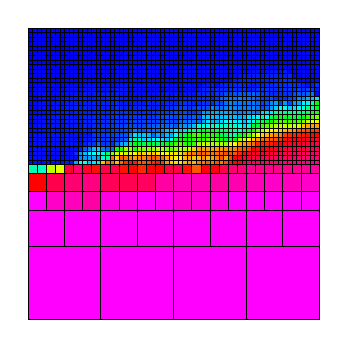
\begin{tikzpicture}[x={(\screenshotunitlength,0)},y={(0,\screenshotunitlength)}]
        \definecolor{fillcolor}{rgb}{1.000000,0.000000,1.000000}
\fill[fillcolor] (0.000000,0.000000) rectangle (0.250000,0.250000);
\definecolor{fillcolor}{rgb}{1.000000,0.000000,1.000000}
\fill[fillcolor] (0.250000,0.000000) rectangle (0.500000,0.250000);
\definecolor{fillcolor}{rgb}{1.000000,0.000000,1.000000}
\fill[fillcolor] (0.000000,0.250000) rectangle (0.125000,0.375000);
\definecolor{fillcolor}{rgb}{1.000000,0.000000,1.000000}
\fill[fillcolor] (0.125000,0.250000) rectangle (0.250000,0.375000);
\definecolor{fillcolor}{rgb}{1.000000,0.000000,1.000000}
\fill[fillcolor] (0.000000,0.375000) rectangle (0.062500,0.437500);
\definecolor{fillcolor}{rgb}{1.000000,0.000000,0.786559}
\fill[fillcolor] (0.062500,0.375000) rectangle (0.125000,0.437500);
\definecolor{fillcolor}{rgb}{1.000000,0.005497,0.000000}
\fill[fillcolor] (0.000000,0.437500) rectangle (0.062500,0.500000);
\definecolor{fillcolor}{rgb}{1.000000,0.000000,0.302169}
\fill[fillcolor] (0.062500,0.437500) rectangle (0.125000,0.500000);
\definecolor{fillcolor}{rgb}{1.000000,0.000000,0.739874}
\fill[fillcolor] (0.125000,0.375000) rectangle (0.187500,0.437500);
\definecolor{fillcolor}{rgb}{1.000000,0.000000,0.645322}
\fill[fillcolor] (0.187500,0.375000) rectangle (0.250000,0.437500);
\definecolor{fillcolor}{rgb}{1.000000,0.000000,0.438164}
\fill[fillcolor] (0.125000,0.437500) rectangle (0.187500,0.500000);
\definecolor{fillcolor}{rgb}{1.000000,0.000000,0.503006}
\fill[fillcolor] (0.187500,0.437500) rectangle (0.250000,0.500000);
\definecolor{fillcolor}{rgb}{1.000000,0.000000,1.000000}
\fill[fillcolor] (0.250000,0.250000) rectangle (0.375000,0.375000);
\definecolor{fillcolor}{rgb}{1.000000,0.000000,1.000000}
\fill[fillcolor] (0.375000,0.250000) rectangle (0.500000,0.375000);
\definecolor{fillcolor}{rgb}{1.000000,0.000000,0.889950}
\fill[fillcolor] (0.250000,0.375000) rectangle (0.312500,0.437500);
\definecolor{fillcolor}{rgb}{1.000000,0.000000,0.901541}
\fill[fillcolor] (0.312500,0.375000) rectangle (0.375000,0.437500);
\definecolor{fillcolor}{rgb}{1.000000,0.000000,0.347159}
\fill[fillcolor] (0.250000,0.437500) rectangle (0.312500,0.500000);
\definecolor{fillcolor}{rgb}{1.000000,0.000000,0.324299}
\fill[fillcolor] (0.312500,0.437500) rectangle (0.375000,0.500000);
\definecolor{fillcolor}{rgb}{1.000000,0.000000,1.000000}
\fill[fillcolor] (0.375000,0.375000) rectangle (0.437500,0.437500);
\definecolor{fillcolor}{rgb}{1.000000,0.000000,0.941436}
\fill[fillcolor] (0.437500,0.375000) rectangle (0.500000,0.437500);
\definecolor{fillcolor}{rgb}{1.000000,0.000000,0.369259}
\fill[fillcolor] (0.375000,0.437500) rectangle (0.437500,0.500000);
\definecolor{fillcolor}{rgb}{1.000000,0.000000,0.634408}
\fill[fillcolor] (0.437500,0.437500) rectangle (0.500000,0.500000);
\definecolor{fillcolor}{rgb}{1.000000,0.000000,1.000000}
\fill[fillcolor] (0.500000,0.000000) rectangle (0.750000,0.250000);
\definecolor{fillcolor}{rgb}{1.000000,0.000000,1.000000}
\fill[fillcolor] (0.750000,0.000000) rectangle (1.000000,0.250000);
\definecolor{fillcolor}{rgb}{1.000000,0.000000,1.000000}
\fill[fillcolor] (0.500000,0.250000) rectangle (0.625000,0.375000);
\definecolor{fillcolor}{rgb}{1.000000,0.000000,1.000000}
\fill[fillcolor] (0.625000,0.250000) rectangle (0.750000,0.375000);
\definecolor{fillcolor}{rgb}{1.000000,0.000000,0.825536}
\fill[fillcolor] (0.500000,0.375000) rectangle (0.562500,0.437500);
\definecolor{fillcolor}{rgb}{1.000000,0.000000,0.868020}
\fill[fillcolor] (0.562500,0.375000) rectangle (0.625000,0.437500);
\definecolor{fillcolor}{rgb}{1.000000,0.000000,0.735200}
\fill[fillcolor] (0.500000,0.437500) rectangle (0.562500,0.500000);
\definecolor{fillcolor}{rgb}{1.000000,0.000000,0.721668}
\fill[fillcolor] (0.562500,0.437500) rectangle (0.625000,0.500000);
\definecolor{fillcolor}{rgb}{1.000000,0.000000,0.911080}
\fill[fillcolor] (0.625000,0.375000) rectangle (0.687500,0.437500);
\definecolor{fillcolor}{rgb}{1.000000,0.000000,1.000000}
\fill[fillcolor] (0.687500,0.375000) rectangle (0.750000,0.437500);
\definecolor{fillcolor}{rgb}{1.000000,0.000000,0.644618}
\fill[fillcolor] (0.625000,0.437500) rectangle (0.687500,0.500000);
\definecolor{fillcolor}{rgb}{1.000000,0.000000,0.695912}
\fill[fillcolor] (0.687500,0.437500) rectangle (0.750000,0.500000);
\definecolor{fillcolor}{rgb}{1.000000,0.000000,1.000000}
\fill[fillcolor] (0.750000,0.250000) rectangle (0.875000,0.375000);
\definecolor{fillcolor}{rgb}{1.000000,0.000000,1.000000}
\fill[fillcolor] (0.875000,0.250000) rectangle (1.000000,0.375000);
\definecolor{fillcolor}{rgb}{1.000000,0.000000,1.000000}
\fill[fillcolor] (0.750000,0.375000) rectangle (0.812500,0.437500);
\definecolor{fillcolor}{rgb}{1.000000,0.000000,1.000000}
\fill[fillcolor] (0.812500,0.375000) rectangle (0.875000,0.437500);
\definecolor{fillcolor}{rgb}{1.000000,0.000000,0.728525}
\fill[fillcolor] (0.750000,0.437500) rectangle (0.812500,0.500000);
\definecolor{fillcolor}{rgb}{1.000000,0.000000,0.779868}
\fill[fillcolor] (0.812500,0.437500) rectangle (0.875000,0.500000);
\definecolor{fillcolor}{rgb}{1.000000,0.000000,1.000000}
\fill[fillcolor] (0.875000,0.375000) rectangle (0.937500,0.437500);
\definecolor{fillcolor}{rgb}{1.000000,0.000000,1.000000}
\fill[fillcolor] (0.937500,0.375000) rectangle (1.000000,0.437500);
\definecolor{fillcolor}{rgb}{1.000000,0.000000,0.748237}
\fill[fillcolor] (0.875000,0.437500) rectangle (0.937500,0.500000);
\definecolor{fillcolor}{rgb}{1.000000,0.000000,0.797686}
\fill[fillcolor] (0.937500,0.437500) rectangle (1.000000,0.500000);
\definecolor{fillcolor}{rgb}{0.000000,1.000000,0.699757}
\fill[fillcolor] (0.000000,0.500000) rectangle (0.031250,0.531250);
\definecolor{fillcolor}{rgb}{0.000000,1.000000,0.771780}
\fill[fillcolor] (0.031250,0.500000) rectangle (0.062500,0.531250);
\definecolor{fillcolor}{rgb}{0.000000,0.055434,1.000000}
\fill[fillcolor] (0.000000,0.531250) rectangle (0.015625,0.546875);
\definecolor{fillcolor}{rgb}{0.000000,0.046396,1.000000}
\fill[fillcolor] (0.015625,0.531250) rectangle (0.031250,0.546875);
\definecolor{fillcolor}{rgb}{0.000000,0.055698,1.000000}
\fill[fillcolor] (0.000000,0.546875) rectangle (0.015625,0.562500);
\definecolor{fillcolor}{rgb}{0.000000,0.056669,1.000000}
\fill[fillcolor] (0.015625,0.546875) rectangle (0.031250,0.562500);
\definecolor{fillcolor}{rgb}{0.000000,0.036141,1.000000}
\fill[fillcolor] (0.031250,0.531250) rectangle (0.046875,0.546875);
\definecolor{fillcolor}{rgb}{0.000000,0.041291,1.000000}
\fill[fillcolor] (0.046875,0.531250) rectangle (0.062500,0.546875);
\definecolor{fillcolor}{rgb}{0.000000,0.042728,1.000000}
\fill[fillcolor] (0.031250,0.546875) rectangle (0.046875,0.562500);
\definecolor{fillcolor}{rgb}{0.000000,0.049203,1.000000}
\fill[fillcolor] (0.046875,0.546875) rectangle (0.062500,0.562500);
\definecolor{fillcolor}{rgb}{0.725542,1.000000,0.000000}
\fill[fillcolor] (0.062500,0.500000) rectangle (0.093750,0.531250);
\definecolor{fillcolor}{rgb}{0.881071,1.000000,0.000000}
\fill[fillcolor] (0.093750,0.500000) rectangle (0.125000,0.531250);
\definecolor{fillcolor}{rgb}{0.000000,0.040368,1.000000}
\fill[fillcolor] (0.062500,0.531250) rectangle (0.078125,0.546875);
\definecolor{fillcolor}{rgb}{0.000000,0.052682,1.000000}
\fill[fillcolor] (0.078125,0.531250) rectangle (0.093750,0.546875);
\definecolor{fillcolor}{rgb}{0.000000,0.047343,1.000000}
\fill[fillcolor] (0.062500,0.546875) rectangle (0.078125,0.562500);
\definecolor{fillcolor}{rgb}{0.000000,0.048710,1.000000}
\fill[fillcolor] (0.078125,0.546875) rectangle (0.093750,0.562500);
\definecolor{fillcolor}{rgb}{0.000000,0.044642,1.000000}
\fill[fillcolor] (0.093750,0.531250) rectangle (0.109375,0.546875);
\definecolor{fillcolor}{rgb}{0.000000,0.084836,1.000000}
\fill[fillcolor] (0.109375,0.531250) rectangle (0.125000,0.546875);
\definecolor{fillcolor}{rgb}{0.000000,0.048627,1.000000}
\fill[fillcolor] (0.093750,0.546875) rectangle (0.109375,0.562500);
\definecolor{fillcolor}{rgb}{0.000000,0.046272,1.000000}
\fill[fillcolor] (0.109375,0.546875) rectangle (0.125000,0.562500);
\definecolor{fillcolor}{rgb}{0.000000,0.057349,1.000000}
\fill[fillcolor] (0.000000,0.562500) rectangle (0.015625,0.578125);
\definecolor{fillcolor}{rgb}{0.000000,0.063391,1.000000}
\fill[fillcolor] (0.015625,0.562500) rectangle (0.031250,0.578125);
\definecolor{fillcolor}{rgb}{0.000000,0.051860,1.000000}
\fill[fillcolor] (0.000000,0.578125) rectangle (0.015625,0.593750);
\definecolor{fillcolor}{rgb}{0.000000,0.060266,1.000000}
\fill[fillcolor] (0.015625,0.578125) rectangle (0.031250,0.593750);
\definecolor{fillcolor}{rgb}{0.000000,0.050579,1.000000}
\fill[fillcolor] (0.031250,0.562500) rectangle (0.046875,0.578125);
\definecolor{fillcolor}{rgb}{0.000000,0.048902,1.000000}
\fill[fillcolor] (0.046875,0.562500) rectangle (0.062500,0.578125);
\definecolor{fillcolor}{rgb}{0.000000,0.060049,1.000000}
\fill[fillcolor] (0.031250,0.578125) rectangle (0.046875,0.593750);
\definecolor{fillcolor}{rgb}{0.000000,0.058305,1.000000}
\fill[fillcolor] (0.046875,0.578125) rectangle (0.062500,0.593750);
\definecolor{fillcolor}{rgb}{0.000000,0.060273,1.000000}
\fill[fillcolor] (0.000000,0.593750) rectangle (0.015625,0.609375);
\definecolor{fillcolor}{rgb}{0.000000,0.062920,1.000000}
\fill[fillcolor] (0.015625,0.593750) rectangle (0.031250,0.609375);
\definecolor{fillcolor}{rgb}{0.000000,0.049325,1.000000}
\fill[fillcolor] (0.000000,0.609375) rectangle (0.015625,0.625000);
\definecolor{fillcolor}{rgb}{0.000000,0.059025,1.000000}
\fill[fillcolor] (0.015625,0.609375) rectangle (0.031250,0.625000);
\definecolor{fillcolor}{rgb}{0.000000,0.060374,1.000000}
\fill[fillcolor] (0.031250,0.593750) rectangle (0.046875,0.609375);
\definecolor{fillcolor}{rgb}{0.000000,0.057889,1.000000}
\fill[fillcolor] (0.046875,0.593750) rectangle (0.062500,0.609375);
\definecolor{fillcolor}{rgb}{0.000000,0.050632,1.000000}
\fill[fillcolor] (0.031250,0.609375) rectangle (0.046875,0.625000);
\definecolor{fillcolor}{rgb}{0.000000,0.056687,1.000000}
\fill[fillcolor] (0.046875,0.609375) rectangle (0.062500,0.625000);
\definecolor{fillcolor}{rgb}{0.000000,0.049886,1.000000}
\fill[fillcolor] (0.062500,0.562500) rectangle (0.078125,0.578125);
\definecolor{fillcolor}{rgb}{0.000000,0.048269,1.000000}
\fill[fillcolor] (0.078125,0.562500) rectangle (0.093750,0.578125);
\definecolor{fillcolor}{rgb}{0.000000,0.054224,1.000000}
\fill[fillcolor] (0.062500,0.578125) rectangle (0.078125,0.593750);
\definecolor{fillcolor}{rgb}{0.000000,0.051022,1.000000}
\fill[fillcolor] (0.078125,0.578125) rectangle (0.093750,0.593750);
\definecolor{fillcolor}{rgb}{0.000000,0.047131,1.000000}
\fill[fillcolor] (0.093750,0.562500) rectangle (0.109375,0.578125);
\definecolor{fillcolor}{rgb}{0.000000,0.044624,1.000000}
\fill[fillcolor] (0.109375,0.562500) rectangle (0.125000,0.578125);
\definecolor{fillcolor}{rgb}{0.000000,0.042537,1.000000}
\fill[fillcolor] (0.093750,0.578125) rectangle (0.109375,0.593750);
\definecolor{fillcolor}{rgb}{0.000000,0.041440,1.000000}
\fill[fillcolor] (0.109375,0.578125) rectangle (0.125000,0.593750);
\definecolor{fillcolor}{rgb}{0.000000,0.059706,1.000000}
\fill[fillcolor] (0.062500,0.593750) rectangle (0.078125,0.609375);
\definecolor{fillcolor}{rgb}{0.000000,0.056067,1.000000}
\fill[fillcolor] (0.078125,0.593750) rectangle (0.093750,0.609375);
\definecolor{fillcolor}{rgb}{0.000000,0.069839,1.000000}
\fill[fillcolor] (0.062500,0.609375) rectangle (0.078125,0.625000);
\definecolor{fillcolor}{rgb}{0.000000,0.067642,1.000000}
\fill[fillcolor] (0.078125,0.609375) rectangle (0.093750,0.625000);
\definecolor{fillcolor}{rgb}{0.000000,0.058795,1.000000}
\fill[fillcolor] (0.093750,0.593750) rectangle (0.109375,0.609375);
\definecolor{fillcolor}{rgb}{0.000000,0.040786,1.000000}
\fill[fillcolor] (0.109375,0.593750) rectangle (0.125000,0.609375);
\definecolor{fillcolor}{rgb}{0.000000,0.071788,1.000000}
\fill[fillcolor] (0.093750,0.609375) rectangle (0.109375,0.625000);
\definecolor{fillcolor}{rgb}{0.000000,0.071463,1.000000}
\fill[fillcolor] (0.109375,0.609375) rectangle (0.125000,0.625000);
\definecolor{fillcolor}{rgb}{1.000000,0.000000,0.205965}
\fill[fillcolor] (0.125000,0.500000) rectangle (0.156250,0.531250);
\definecolor{fillcolor}{rgb}{1.000000,0.000000,0.418205}
\fill[fillcolor] (0.156250,0.500000) rectangle (0.187500,0.531250);
\definecolor{fillcolor}{rgb}{0.000000,0.107407,1.000000}
\fill[fillcolor] (0.125000,0.531250) rectangle (0.140625,0.546875);
\definecolor{fillcolor}{rgb}{0.000000,0.102403,1.000000}
\fill[fillcolor] (0.140625,0.531250) rectangle (0.156250,0.546875);
\definecolor{fillcolor}{rgb}{0.000000,0.042440,1.000000}
\fill[fillcolor] (0.125000,0.546875) rectangle (0.140625,0.562500);
\definecolor{fillcolor}{rgb}{0.000000,0.042527,1.000000}
\fill[fillcolor] (0.140625,0.546875) rectangle (0.156250,0.562500);
\definecolor{fillcolor}{rgb}{0.000000,0.669555,1.000000}
\fill[fillcolor] (0.156250,0.531250) rectangle (0.171875,0.546875);
\definecolor{fillcolor}{rgb}{0.000000,1.000000,0.971921}
\fill[fillcolor] (0.171875,0.531250) rectangle (0.187500,0.546875);
\definecolor{fillcolor}{rgb}{0.000000,0.044534,1.000000}
\fill[fillcolor] (0.156250,0.546875) rectangle (0.171875,0.562500);
\definecolor{fillcolor}{rgb}{0.000000,0.527478,1.000000}
\fill[fillcolor] (0.171875,0.546875) rectangle (0.187500,0.562500);
\definecolor{fillcolor}{rgb}{1.000000,0.000000,0.145724}
\fill[fillcolor] (0.187500,0.500000) rectangle (0.218750,0.531250);
\definecolor{fillcolor}{rgb}{1.000000,0.045301,0.000000}
\fill[fillcolor] (0.218750,0.500000) rectangle (0.250000,0.531250);
\definecolor{fillcolor}{rgb}{0.000000,1.000000,0.956662}
\fill[fillcolor] (0.187500,0.531250) rectangle (0.203125,0.546875);
\definecolor{fillcolor}{rgb}{0.000000,0.798272,1.000000}
\fill[fillcolor] (0.203125,0.531250) rectangle (0.218750,0.546875);
\definecolor{fillcolor}{rgb}{0.000000,0.574268,1.000000}
\fill[fillcolor] (0.187500,0.546875) rectangle (0.203125,0.562500);
\definecolor{fillcolor}{rgb}{0.000000,0.654901,1.000000}
\fill[fillcolor] (0.203125,0.546875) rectangle (0.218750,0.562500);
\definecolor{fillcolor}{rgb}{0.000000,0.892180,1.000000}
\fill[fillcolor] (0.218750,0.531250) rectangle (0.234375,0.546875);
\definecolor{fillcolor}{rgb}{0.000000,0.896692,1.000000}
\fill[fillcolor] (0.234375,0.531250) rectangle (0.250000,0.546875);
\definecolor{fillcolor}{rgb}{0.000000,0.689273,1.000000}
\fill[fillcolor] (0.218750,0.546875) rectangle (0.234375,0.562500);
\definecolor{fillcolor}{rgb}{0.000000,0.604562,1.000000}
\fill[fillcolor] (0.234375,0.546875) rectangle (0.250000,0.562500);
\definecolor{fillcolor}{rgb}{0.000000,0.041495,1.000000}
\fill[fillcolor] (0.125000,0.562500) rectangle (0.140625,0.578125);
\definecolor{fillcolor}{rgb}{0.000000,0.040838,1.000000}
\fill[fillcolor] (0.140625,0.562500) rectangle (0.156250,0.578125);
\definecolor{fillcolor}{rgb}{0.000000,0.043614,1.000000}
\fill[fillcolor] (0.125000,0.578125) rectangle (0.140625,0.593750);
\definecolor{fillcolor}{rgb}{0.000000,0.042248,1.000000}
\fill[fillcolor] (0.140625,0.578125) rectangle (0.156250,0.593750);
\definecolor{fillcolor}{rgb}{0.000000,0.190109,1.000000}
\fill[fillcolor] (0.156250,0.562500) rectangle (0.171875,0.578125);
\definecolor{fillcolor}{rgb}{0.000000,0.604128,1.000000}
\fill[fillcolor] (0.171875,0.562500) rectangle (0.187500,0.578125);
\definecolor{fillcolor}{rgb}{0.000000,0.054870,1.000000}
\fill[fillcolor] (0.156250,0.578125) rectangle (0.171875,0.593750);
\definecolor{fillcolor}{rgb}{0.000000,0.136556,1.000000}
\fill[fillcolor] (0.171875,0.578125) rectangle (0.187500,0.593750);
\definecolor{fillcolor}{rgb}{0.000000,0.075902,1.000000}
\fill[fillcolor] (0.125000,0.593750) rectangle (0.140625,0.609375);
\definecolor{fillcolor}{rgb}{0.000000,0.082959,1.000000}
\fill[fillcolor] (0.140625,0.593750) rectangle (0.156250,0.609375);
\definecolor{fillcolor}{rgb}{0.000000,0.075198,1.000000}
\fill[fillcolor] (0.125000,0.609375) rectangle (0.140625,0.625000);
\definecolor{fillcolor}{rgb}{0.000000,0.062997,1.000000}
\fill[fillcolor] (0.140625,0.609375) rectangle (0.156250,0.625000);
\definecolor{fillcolor}{rgb}{0.000000,0.066917,1.000000}
\fill[fillcolor] (0.156250,0.593750) rectangle (0.171875,0.609375);
\definecolor{fillcolor}{rgb}{0.000000,0.075001,1.000000}
\fill[fillcolor] (0.171875,0.593750) rectangle (0.187500,0.609375);
\definecolor{fillcolor}{rgb}{0.000000,0.056123,1.000000}
\fill[fillcolor] (0.156250,0.609375) rectangle (0.171875,0.625000);
\definecolor{fillcolor}{rgb}{0.000000,0.060551,1.000000}
\fill[fillcolor] (0.171875,0.609375) rectangle (0.187500,0.625000);
\definecolor{fillcolor}{rgb}{0.000000,0.729788,1.000000}
\fill[fillcolor] (0.187500,0.562500) rectangle (0.203125,0.578125);
\definecolor{fillcolor}{rgb}{0.000000,0.965277,1.000000}
\fill[fillcolor] (0.203125,0.562500) rectangle (0.218750,0.578125);
\definecolor{fillcolor}{rgb}{0.000000,0.357774,1.000000}
\fill[fillcolor] (0.187500,0.578125) rectangle (0.203125,0.593750);
\definecolor{fillcolor}{rgb}{0.000000,0.511628,1.000000}
\fill[fillcolor] (0.203125,0.578125) rectangle (0.218750,0.593750);
\definecolor{fillcolor}{rgb}{0.000000,0.999578,1.000000}
\fill[fillcolor] (0.218750,0.562500) rectangle (0.234375,0.578125);
\definecolor{fillcolor}{rgb}{0.000000,0.995985,1.000000}
\fill[fillcolor] (0.234375,0.562500) rectangle (0.250000,0.578125);
\definecolor{fillcolor}{rgb}{0.000000,0.733563,1.000000}
\fill[fillcolor] (0.218750,0.578125) rectangle (0.234375,0.593750);
\definecolor{fillcolor}{rgb}{0.000000,0.778940,1.000000}
\fill[fillcolor] (0.234375,0.578125) rectangle (0.250000,0.593750);
\definecolor{fillcolor}{rgb}{0.000000,0.104316,1.000000}
\fill[fillcolor] (0.187500,0.593750) rectangle (0.203125,0.609375);
\definecolor{fillcolor}{rgb}{0.000000,0.212600,1.000000}
\fill[fillcolor] (0.203125,0.593750) rectangle (0.218750,0.609375);
\definecolor{fillcolor}{rgb}{0.000000,0.094852,1.000000}
\fill[fillcolor] (0.187500,0.609375) rectangle (0.203125,0.625000);
\definecolor{fillcolor}{rgb}{0.000000,0.098054,1.000000}
\fill[fillcolor] (0.203125,0.609375) rectangle (0.218750,0.625000);
\definecolor{fillcolor}{rgb}{0.000000,0.194801,1.000000}
\fill[fillcolor] (0.218750,0.593750) rectangle (0.234375,0.609375);
\definecolor{fillcolor}{rgb}{0.000000,0.406195,1.000000}
\fill[fillcolor] (0.234375,0.593750) rectangle (0.250000,0.609375);
\definecolor{fillcolor}{rgb}{0.000000,0.201887,1.000000}
\fill[fillcolor] (0.218750,0.609375) rectangle (0.234375,0.625000);
\definecolor{fillcolor}{rgb}{0.000000,0.224879,1.000000}
\fill[fillcolor] (0.234375,0.609375) rectangle (0.250000,0.625000);
\definecolor{fillcolor}{rgb}{0.000000,0.058888,1.000000}
\fill[fillcolor] (0.000000,0.625000) rectangle (0.015625,0.640625);
\definecolor{fillcolor}{rgb}{0.000000,0.056059,1.000000}
\fill[fillcolor] (0.015625,0.625000) rectangle (0.031250,0.640625);
\definecolor{fillcolor}{rgb}{0.000000,0.055426,1.000000}
\fill[fillcolor] (0.000000,0.640625) rectangle (0.015625,0.656250);
\definecolor{fillcolor}{rgb}{0.000000,0.059320,1.000000}
\fill[fillcolor] (0.015625,0.640625) rectangle (0.031250,0.656250);
\definecolor{fillcolor}{rgb}{0.000000,0.056122,1.000000}
\fill[fillcolor] (0.031250,0.625000) rectangle (0.046875,0.640625);
\definecolor{fillcolor}{rgb}{0.000000,0.061904,1.000000}
\fill[fillcolor] (0.046875,0.625000) rectangle (0.062500,0.640625);
\definecolor{fillcolor}{rgb}{0.000000,0.062108,1.000000}
\fill[fillcolor] (0.031250,0.640625) rectangle (0.046875,0.656250);
\definecolor{fillcolor}{rgb}{0.000000,0.059850,1.000000}
\fill[fillcolor] (0.046875,0.640625) rectangle (0.062500,0.656250);
\definecolor{fillcolor}{rgb}{0.000000,0.030051,1.000000}
\fill[fillcolor] (0.000000,0.656250) rectangle (0.015625,0.671875);
\definecolor{fillcolor}{rgb}{0.000000,0.041634,1.000000}
\fill[fillcolor] (0.015625,0.656250) rectangle (0.031250,0.671875);
\definecolor{fillcolor}{rgb}{0.000000,0.034363,1.000000}
\fill[fillcolor] (0.000000,0.671875) rectangle (0.015625,0.687500);
\definecolor{fillcolor}{rgb}{0.000000,0.039769,1.000000}
\fill[fillcolor] (0.015625,0.671875) rectangle (0.031250,0.687500);
\definecolor{fillcolor}{rgb}{0.000000,0.068983,1.000000}
\fill[fillcolor] (0.031250,0.656250) rectangle (0.046875,0.671875);
\definecolor{fillcolor}{rgb}{0.000000,0.070889,1.000000}
\fill[fillcolor] (0.046875,0.656250) rectangle (0.062500,0.671875);
\definecolor{fillcolor}{rgb}{0.000000,0.042868,1.000000}
\fill[fillcolor] (0.031250,0.671875) rectangle (0.046875,0.687500);
\definecolor{fillcolor}{rgb}{0.000000,0.069475,1.000000}
\fill[fillcolor] (0.046875,0.671875) rectangle (0.062500,0.687500);
\definecolor{fillcolor}{rgb}{0.000000,0.071506,1.000000}
\fill[fillcolor] (0.062500,0.625000) rectangle (0.078125,0.640625);
\definecolor{fillcolor}{rgb}{0.000000,0.079180,1.000000}
\fill[fillcolor] (0.078125,0.625000) rectangle (0.093750,0.640625);
\definecolor{fillcolor}{rgb}{0.000000,0.079745,1.000000}
\fill[fillcolor] (0.062500,0.640625) rectangle (0.078125,0.656250);
\definecolor{fillcolor}{rgb}{0.000000,0.085353,1.000000}
\fill[fillcolor] (0.078125,0.640625) rectangle (0.093750,0.656250);
\definecolor{fillcolor}{rgb}{0.000000,0.078569,1.000000}
\fill[fillcolor] (0.093750,0.625000) rectangle (0.109375,0.640625);
\definecolor{fillcolor}{rgb}{0.000000,0.072949,1.000000}
\fill[fillcolor] (0.109375,0.625000) rectangle (0.125000,0.640625);
\definecolor{fillcolor}{rgb}{0.000000,0.083394,1.000000}
\fill[fillcolor] (0.093750,0.640625) rectangle (0.109375,0.656250);
\definecolor{fillcolor}{rgb}{0.000000,0.076834,1.000000}
\fill[fillcolor] (0.109375,0.640625) rectangle (0.125000,0.656250);
\definecolor{fillcolor}{rgb}{0.000000,0.081211,1.000000}
\fill[fillcolor] (0.062500,0.656250) rectangle (0.078125,0.671875);
\definecolor{fillcolor}{rgb}{0.000000,0.087213,1.000000}
\fill[fillcolor] (0.078125,0.656250) rectangle (0.093750,0.671875);
\definecolor{fillcolor}{rgb}{0.000000,0.084080,1.000000}
\fill[fillcolor] (0.062500,0.671875) rectangle (0.078125,0.687500);
\definecolor{fillcolor}{rgb}{0.000000,0.088439,1.000000}
\fill[fillcolor] (0.078125,0.671875) rectangle (0.093750,0.687500);
\definecolor{fillcolor}{rgb}{0.000000,0.076957,1.000000}
\fill[fillcolor] (0.093750,0.656250) rectangle (0.109375,0.671875);
\definecolor{fillcolor}{rgb}{0.000000,0.079863,1.000000}
\fill[fillcolor] (0.109375,0.656250) rectangle (0.125000,0.671875);
\definecolor{fillcolor}{rgb}{0.000000,0.083554,1.000000}
\fill[fillcolor] (0.093750,0.671875) rectangle (0.109375,0.687500);
\definecolor{fillcolor}{rgb}{0.000000,0.086945,1.000000}
\fill[fillcolor] (0.109375,0.671875) rectangle (0.125000,0.687500);
\definecolor{fillcolor}{rgb}{0.000000,0.032425,1.000000}
\fill[fillcolor] (0.000000,0.687500) rectangle (0.015625,0.703125);
\definecolor{fillcolor}{rgb}{0.000000,0.033725,1.000000}
\fill[fillcolor] (0.015625,0.687500) rectangle (0.031250,0.703125);
\definecolor{fillcolor}{rgb}{0.000000,0.032827,1.000000}
\fill[fillcolor] (0.000000,0.703125) rectangle (0.015625,0.718750);
\definecolor{fillcolor}{rgb}{0.000000,0.034682,1.000000}
\fill[fillcolor] (0.015625,0.703125) rectangle (0.031250,0.718750);
\definecolor{fillcolor}{rgb}{0.000000,0.040744,1.000000}
\fill[fillcolor] (0.031250,0.687500) rectangle (0.046875,0.703125);
\definecolor{fillcolor}{rgb}{0.000000,0.053164,1.000000}
\fill[fillcolor] (0.046875,0.687500) rectangle (0.062500,0.703125);
\definecolor{fillcolor}{rgb}{0.000000,0.043688,1.000000}
\fill[fillcolor] (0.031250,0.703125) rectangle (0.046875,0.718750);
\definecolor{fillcolor}{rgb}{0.000000,0.050698,1.000000}
\fill[fillcolor] (0.046875,0.703125) rectangle (0.062500,0.718750);
\definecolor{fillcolor}{rgb}{0.000000,0.030902,1.000000}
\fill[fillcolor] (0.000000,0.718750) rectangle (0.015625,0.734375);
\definecolor{fillcolor}{rgb}{0.000000,0.028564,1.000000}
\fill[fillcolor] (0.015625,0.718750) rectangle (0.031250,0.734375);
\definecolor{fillcolor}{rgb}{0.000000,0.029270,1.000000}
\fill[fillcolor] (0.000000,0.734375) rectangle (0.015625,0.750000);
\definecolor{fillcolor}{rgb}{0.000000,0.036526,1.000000}
\fill[fillcolor] (0.015625,0.734375) rectangle (0.031250,0.750000);
\definecolor{fillcolor}{rgb}{0.000000,0.041382,1.000000}
\fill[fillcolor] (0.031250,0.718750) rectangle (0.046875,0.734375);
\definecolor{fillcolor}{rgb}{0.000000,0.052748,1.000000}
\fill[fillcolor] (0.046875,0.718750) rectangle (0.062500,0.734375);
\definecolor{fillcolor}{rgb}{0.000000,0.040906,1.000000}
\fill[fillcolor] (0.031250,0.734375) rectangle (0.046875,0.750000);
\definecolor{fillcolor}{rgb}{0.000000,0.044829,1.000000}
\fill[fillcolor] (0.046875,0.734375) rectangle (0.062500,0.750000);
\definecolor{fillcolor}{rgb}{0.000000,0.078932,1.000000}
\fill[fillcolor] (0.062500,0.687500) rectangle (0.078125,0.703125);
\definecolor{fillcolor}{rgb}{0.000000,0.087449,1.000000}
\fill[fillcolor] (0.078125,0.687500) rectangle (0.093750,0.703125);
\definecolor{fillcolor}{rgb}{0.000000,0.073320,1.000000}
\fill[fillcolor] (0.062500,0.703125) rectangle (0.078125,0.718750);
\definecolor{fillcolor}{rgb}{0.000000,0.077516,1.000000}
\fill[fillcolor] (0.078125,0.703125) rectangle (0.093750,0.718750);
\definecolor{fillcolor}{rgb}{0.000000,0.089753,1.000000}
\fill[fillcolor] (0.093750,0.687500) rectangle (0.109375,0.703125);
\definecolor{fillcolor}{rgb}{0.000000,0.079113,1.000000}
\fill[fillcolor] (0.109375,0.687500) rectangle (0.125000,0.703125);
\definecolor{fillcolor}{rgb}{0.000000,0.091975,1.000000}
\fill[fillcolor] (0.093750,0.703125) rectangle (0.109375,0.718750);
\definecolor{fillcolor}{rgb}{0.000000,0.103130,1.000000}
\fill[fillcolor] (0.109375,0.703125) rectangle (0.125000,0.718750);
\definecolor{fillcolor}{rgb}{0.000000,0.065659,1.000000}
\fill[fillcolor] (0.062500,0.718750) rectangle (0.078125,0.734375);
\definecolor{fillcolor}{rgb}{0.000000,0.066857,1.000000}
\fill[fillcolor] (0.078125,0.718750) rectangle (0.093750,0.734375);
\definecolor{fillcolor}{rgb}{0.000000,0.052014,1.000000}
\fill[fillcolor] (0.062500,0.734375) rectangle (0.078125,0.750000);
\definecolor{fillcolor}{rgb}{0.000000,0.066958,1.000000}
\fill[fillcolor] (0.078125,0.734375) rectangle (0.093750,0.750000);
\definecolor{fillcolor}{rgb}{0.000000,0.076616,1.000000}
\fill[fillcolor] (0.093750,0.718750) rectangle (0.109375,0.734375);
\definecolor{fillcolor}{rgb}{0.000000,0.093168,1.000000}
\fill[fillcolor] (0.109375,0.718750) rectangle (0.125000,0.734375);
\definecolor{fillcolor}{rgb}{0.000000,0.076400,1.000000}
\fill[fillcolor] (0.093750,0.734375) rectangle (0.109375,0.750000);
\definecolor{fillcolor}{rgb}{0.000000,0.081312,1.000000}
\fill[fillcolor] (0.109375,0.734375) rectangle (0.125000,0.750000);
\definecolor{fillcolor}{rgb}{0.000000,0.071789,1.000000}
\fill[fillcolor] (0.125000,0.625000) rectangle (0.140625,0.640625);
\definecolor{fillcolor}{rgb}{0.000000,0.068416,1.000000}
\fill[fillcolor] (0.140625,0.625000) rectangle (0.156250,0.640625);
\definecolor{fillcolor}{rgb}{0.000000,0.081718,1.000000}
\fill[fillcolor] (0.125000,0.640625) rectangle (0.140625,0.656250);
\definecolor{fillcolor}{rgb}{0.000000,0.080727,1.000000}
\fill[fillcolor] (0.140625,0.640625) rectangle (0.156250,0.656250);
\definecolor{fillcolor}{rgb}{0.000000,0.067487,1.000000}
\fill[fillcolor] (0.156250,0.625000) rectangle (0.171875,0.640625);
\definecolor{fillcolor}{rgb}{0.000000,0.059515,1.000000}
\fill[fillcolor] (0.171875,0.625000) rectangle (0.187500,0.640625);
\definecolor{fillcolor}{rgb}{0.000000,0.079089,1.000000}
\fill[fillcolor] (0.156250,0.640625) rectangle (0.171875,0.656250);
\definecolor{fillcolor}{rgb}{0.000000,0.094840,1.000000}
\fill[fillcolor] (0.171875,0.640625) rectangle (0.187500,0.656250);
\definecolor{fillcolor}{rgb}{0.000000,0.088280,1.000000}
\fill[fillcolor] (0.125000,0.656250) rectangle (0.140625,0.671875);
\definecolor{fillcolor}{rgb}{0.000000,0.084082,1.000000}
\fill[fillcolor] (0.140625,0.656250) rectangle (0.156250,0.671875);
\definecolor{fillcolor}{rgb}{0.000000,0.089610,1.000000}
\fill[fillcolor] (0.125000,0.671875) rectangle (0.140625,0.687500);
\definecolor{fillcolor}{rgb}{0.000000,0.098200,1.000000}
\fill[fillcolor] (0.140625,0.671875) rectangle (0.156250,0.687500);
\definecolor{fillcolor}{rgb}{0.000000,0.098332,1.000000}
\fill[fillcolor] (0.156250,0.656250) rectangle (0.171875,0.671875);
\definecolor{fillcolor}{rgb}{0.000000,0.096798,1.000000}
\fill[fillcolor] (0.171875,0.656250) rectangle (0.187500,0.671875);
\definecolor{fillcolor}{rgb}{0.000000,0.097869,1.000000}
\fill[fillcolor] (0.156250,0.671875) rectangle (0.171875,0.687500);
\definecolor{fillcolor}{rgb}{0.000000,0.107779,1.000000}
\fill[fillcolor] (0.171875,0.671875) rectangle (0.187500,0.687500);
\definecolor{fillcolor}{rgb}{0.000000,0.074115,1.000000}
\fill[fillcolor] (0.187500,0.625000) rectangle (0.203125,0.640625);
\definecolor{fillcolor}{rgb}{0.000000,0.075337,1.000000}
\fill[fillcolor] (0.203125,0.625000) rectangle (0.218750,0.640625);
\definecolor{fillcolor}{rgb}{0.000000,0.125345,1.000000}
\fill[fillcolor] (0.187500,0.640625) rectangle (0.203125,0.656250);
\definecolor{fillcolor}{rgb}{0.000000,0.088360,1.000000}
\fill[fillcolor] (0.203125,0.640625) rectangle (0.218750,0.656250);
\definecolor{fillcolor}{rgb}{0.000000,0.207093,1.000000}
\fill[fillcolor] (0.218750,0.625000) rectangle (0.234375,0.640625);
\definecolor{fillcolor}{rgb}{0.000000,0.223619,1.000000}
\fill[fillcolor] (0.234375,0.625000) rectangle (0.250000,0.640625);
\definecolor{fillcolor}{rgb}{0.000000,0.185292,1.000000}
\fill[fillcolor] (0.218750,0.640625) rectangle (0.234375,0.656250);
\definecolor{fillcolor}{rgb}{0.000000,0.190584,1.000000}
\fill[fillcolor] (0.234375,0.640625) rectangle (0.250000,0.656250);
\definecolor{fillcolor}{rgb}{0.000000,0.138273,1.000000}
\fill[fillcolor] (0.187500,0.656250) rectangle (0.203125,0.671875);
\definecolor{fillcolor}{rgb}{0.000000,0.107238,1.000000}
\fill[fillcolor] (0.203125,0.656250) rectangle (0.218750,0.671875);
\definecolor{fillcolor}{rgb}{0.000000,0.131423,1.000000}
\fill[fillcolor] (0.187500,0.671875) rectangle (0.203125,0.687500);
\definecolor{fillcolor}{rgb}{0.000000,0.131351,1.000000}
\fill[fillcolor] (0.203125,0.671875) rectangle (0.218750,0.687500);
\definecolor{fillcolor}{rgb}{0.000000,0.156977,1.000000}
\fill[fillcolor] (0.218750,0.656250) rectangle (0.234375,0.671875);
\definecolor{fillcolor}{rgb}{0.000000,0.175989,1.000000}
\fill[fillcolor] (0.234375,0.656250) rectangle (0.250000,0.671875);
\definecolor{fillcolor}{rgb}{0.000000,0.166870,1.000000}
\fill[fillcolor] (0.218750,0.671875) rectangle (0.234375,0.687500);
\definecolor{fillcolor}{rgb}{0.000000,0.167454,1.000000}
\fill[fillcolor] (0.234375,0.671875) rectangle (0.250000,0.687500);
\definecolor{fillcolor}{rgb}{0.000000,0.071129,1.000000}
\fill[fillcolor] (0.125000,0.687500) rectangle (0.140625,0.703125);
\definecolor{fillcolor}{rgb}{0.000000,0.094156,1.000000}
\fill[fillcolor] (0.140625,0.687500) rectangle (0.156250,0.703125);
\definecolor{fillcolor}{rgb}{0.000000,0.105897,1.000000}
\fill[fillcolor] (0.125000,0.703125) rectangle (0.140625,0.718750);
\definecolor{fillcolor}{rgb}{0.000000,0.089612,1.000000}
\fill[fillcolor] (0.140625,0.703125) rectangle (0.156250,0.718750);
\definecolor{fillcolor}{rgb}{0.000000,0.084518,1.000000}
\fill[fillcolor] (0.156250,0.687500) rectangle (0.171875,0.703125);
\definecolor{fillcolor}{rgb}{0.000000,0.115756,1.000000}
\fill[fillcolor] (0.171875,0.687500) rectangle (0.187500,0.703125);
\definecolor{fillcolor}{rgb}{0.000000,0.124349,1.000000}
\fill[fillcolor] (0.156250,0.703125) rectangle (0.171875,0.718750);
\definecolor{fillcolor}{rgb}{0.000000,0.124580,1.000000}
\fill[fillcolor] (0.171875,0.703125) rectangle (0.187500,0.718750);
\definecolor{fillcolor}{rgb}{0.000000,0.105574,1.000000}
\fill[fillcolor] (0.125000,0.718750) rectangle (0.140625,0.734375);
\definecolor{fillcolor}{rgb}{0.000000,0.104888,1.000000}
\fill[fillcolor] (0.140625,0.718750) rectangle (0.156250,0.734375);
\definecolor{fillcolor}{rgb}{0.000000,0.099947,1.000000}
\fill[fillcolor] (0.125000,0.734375) rectangle (0.140625,0.750000);
\definecolor{fillcolor}{rgb}{0.000000,0.099530,1.000000}
\fill[fillcolor] (0.140625,0.734375) rectangle (0.156250,0.750000);
\definecolor{fillcolor}{rgb}{0.000000,0.118234,1.000000}
\fill[fillcolor] (0.156250,0.718750) rectangle (0.171875,0.734375);
\definecolor{fillcolor}{rgb}{0.000000,0.121919,1.000000}
\fill[fillcolor] (0.171875,0.718750) rectangle (0.187500,0.734375);
\definecolor{fillcolor}{rgb}{0.000000,0.105230,1.000000}
\fill[fillcolor] (0.156250,0.734375) rectangle (0.171875,0.750000);
\definecolor{fillcolor}{rgb}{0.000000,0.116498,1.000000}
\fill[fillcolor] (0.171875,0.734375) rectangle (0.187500,0.750000);
\definecolor{fillcolor}{rgb}{0.000000,0.126179,1.000000}
\fill[fillcolor] (0.187500,0.687500) rectangle (0.203125,0.703125);
\definecolor{fillcolor}{rgb}{0.000000,0.141202,1.000000}
\fill[fillcolor] (0.203125,0.687500) rectangle (0.218750,0.703125);
\definecolor{fillcolor}{rgb}{0.000000,0.129688,1.000000}
\fill[fillcolor] (0.187500,0.703125) rectangle (0.203125,0.718750);
\definecolor{fillcolor}{rgb}{0.000000,0.134166,1.000000}
\fill[fillcolor] (0.203125,0.703125) rectangle (0.218750,0.718750);
\definecolor{fillcolor}{rgb}{0.000000,0.145845,1.000000}
\fill[fillcolor] (0.218750,0.687500) rectangle (0.234375,0.703125);
\definecolor{fillcolor}{rgb}{0.000000,0.150591,1.000000}
\fill[fillcolor] (0.234375,0.687500) rectangle (0.250000,0.703125);
\definecolor{fillcolor}{rgb}{0.000000,0.127389,1.000000}
\fill[fillcolor] (0.218750,0.703125) rectangle (0.234375,0.718750);
\definecolor{fillcolor}{rgb}{0.000000,0.137245,1.000000}
\fill[fillcolor] (0.234375,0.703125) rectangle (0.250000,0.718750);
\definecolor{fillcolor}{rgb}{0.000000,0.124524,1.000000}
\fill[fillcolor] (0.187500,0.718750) rectangle (0.203125,0.734375);
\definecolor{fillcolor}{rgb}{0.000000,0.124407,1.000000}
\fill[fillcolor] (0.203125,0.718750) rectangle (0.218750,0.734375);
\definecolor{fillcolor}{rgb}{0.000000,0.114589,1.000000}
\fill[fillcolor] (0.187500,0.734375) rectangle (0.203125,0.750000);
\definecolor{fillcolor}{rgb}{0.000000,0.118537,1.000000}
\fill[fillcolor] (0.203125,0.734375) rectangle (0.218750,0.750000);
\definecolor{fillcolor}{rgb}{0.000000,0.117277,1.000000}
\fill[fillcolor] (0.218750,0.718750) rectangle (0.234375,0.734375);
\definecolor{fillcolor}{rgb}{0.000000,0.126570,1.000000}
\fill[fillcolor] (0.234375,0.718750) rectangle (0.250000,0.734375);
\definecolor{fillcolor}{rgb}{0.000000,0.121913,1.000000}
\fill[fillcolor] (0.218750,0.734375) rectangle (0.234375,0.750000);
\definecolor{fillcolor}{rgb}{0.000000,0.116971,1.000000}
\fill[fillcolor] (0.234375,0.734375) rectangle (0.250000,0.750000);
\definecolor{fillcolor}{rgb}{1.000000,0.000000,0.276541}
\fill[fillcolor] (0.250000,0.500000) rectangle (0.281250,0.531250);
\definecolor{fillcolor}{rgb}{1.000000,0.000000,0.281871}
\fill[fillcolor] (0.281250,0.500000) rectangle (0.312500,0.531250);
\definecolor{fillcolor}{rgb}{1.000000,0.762303,0.000000}
\fill[fillcolor] (0.250000,0.531250) rectangle (0.265625,0.546875);
\definecolor{fillcolor}{rgb}{1.000000,0.431239,0.000000}
\fill[fillcolor] (0.265625,0.531250) rectangle (0.281250,0.546875);
\definecolor{fillcolor}{rgb}{0.000000,1.000000,0.852700}
\fill[fillcolor] (0.250000,0.546875) rectangle (0.265625,0.562500);
\definecolor{fillcolor}{rgb}{0.000000,1.000000,0.625629}
\fill[fillcolor] (0.265625,0.546875) rectangle (0.281250,0.562500);
\definecolor{fillcolor}{rgb}{1.000000,0.430689,0.000000}
\fill[fillcolor] (0.281250,0.531250) rectangle (0.296875,0.546875);
\definecolor{fillcolor}{rgb}{1.000000,0.728999,0.000000}
\fill[fillcolor] (0.296875,0.531250) rectangle (0.312500,0.546875);
\definecolor{fillcolor}{rgb}{1.000000,0.434442,0.000000}
\fill[fillcolor] (0.281250,0.546875) rectangle (0.296875,0.562500);
\definecolor{fillcolor}{rgb}{1.000000,0.816568,0.000000}
\fill[fillcolor] (0.296875,0.546875) rectangle (0.312500,0.562500);
\definecolor{fillcolor}{rgb}{1.000000,0.074052,0.000000}
\fill[fillcolor] (0.312500,0.500000) rectangle (0.343750,0.531250);
\definecolor{fillcolor}{rgb}{1.000000,0.010146,0.000000}
\fill[fillcolor] (0.343750,0.500000) rectangle (0.375000,0.531250);
\definecolor{fillcolor}{rgb}{1.000000,0.406199,0.000000}
\fill[fillcolor] (0.312500,0.531250) rectangle (0.328125,0.546875);
\definecolor{fillcolor}{rgb}{1.000000,0.172271,0.000000}
\fill[fillcolor] (0.328125,0.531250) rectangle (0.343750,0.546875);
\definecolor{fillcolor}{rgb}{1.000000,0.340096,0.000000}
\fill[fillcolor] (0.312500,0.546875) rectangle (0.328125,0.562500);
\definecolor{fillcolor}{rgb}{1.000000,0.438075,0.000000}
\fill[fillcolor] (0.328125,0.546875) rectangle (0.343750,0.562500);
\definecolor{fillcolor}{rgb}{1.000000,0.075842,0.000000}
\fill[fillcolor] (0.343750,0.531250) rectangle (0.359375,0.546875);
\definecolor{fillcolor}{rgb}{1.000000,0.100157,0.000000}
\fill[fillcolor] (0.359375,0.531250) rectangle (0.375000,0.546875);
\definecolor{fillcolor}{rgb}{1.000000,0.522442,0.000000}
\fill[fillcolor] (0.343750,0.546875) rectangle (0.359375,0.562500);
\definecolor{fillcolor}{rgb}{1.000000,0.602228,0.000000}
\fill[fillcolor] (0.359375,0.546875) rectangle (0.375000,0.562500);
\definecolor{fillcolor}{rgb}{0.000000,1.000000,0.810642}
\fill[fillcolor] (0.250000,0.562500) rectangle (0.265625,0.578125);
\definecolor{fillcolor}{rgb}{0.000000,1.000000,0.393246}
\fill[fillcolor] (0.265625,0.562500) rectangle (0.281250,0.578125);
\definecolor{fillcolor}{rgb}{0.000000,0.495641,1.000000}
\fill[fillcolor] (0.250000,0.578125) rectangle (0.265625,0.593750);
\definecolor{fillcolor}{rgb}{0.000000,0.379369,1.000000}
\fill[fillcolor] (0.265625,0.578125) rectangle (0.281250,0.593750);
\definecolor{fillcolor}{rgb}{0.521059,1.000000,0.000000}
\fill[fillcolor] (0.281250,0.562500) rectangle (0.296875,0.578125);
\definecolor{fillcolor}{rgb}{0.831516,1.000000,0.000000}
\fill[fillcolor] (0.296875,0.562500) rectangle (0.312500,0.578125);
\definecolor{fillcolor}{rgb}{0.000000,0.425734,1.000000}
\fill[fillcolor] (0.281250,0.578125) rectangle (0.296875,0.593750);
\definecolor{fillcolor}{rgb}{0.000000,1.000000,0.016171}
\fill[fillcolor] (0.296875,0.578125) rectangle (0.312500,0.593750);
\definecolor{fillcolor}{rgb}{0.000000,0.217857,1.000000}
\fill[fillcolor] (0.250000,0.593750) rectangle (0.265625,0.609375);
\definecolor{fillcolor}{rgb}{0.000000,0.213211,1.000000}
\fill[fillcolor] (0.265625,0.593750) rectangle (0.281250,0.609375);
\definecolor{fillcolor}{rgb}{0.000000,0.212442,1.000000}
\fill[fillcolor] (0.250000,0.609375) rectangle (0.265625,0.625000);
\definecolor{fillcolor}{rgb}{0.000000,0.214186,1.000000}
\fill[fillcolor] (0.265625,0.609375) rectangle (0.281250,0.625000);
\definecolor{fillcolor}{rgb}{0.000000,0.186438,1.000000}
\fill[fillcolor] (0.281250,0.593750) rectangle (0.296875,0.609375);
\definecolor{fillcolor}{rgb}{0.000000,0.386904,1.000000}
\fill[fillcolor] (0.296875,0.593750) rectangle (0.312500,0.609375);
\definecolor{fillcolor}{rgb}{0.000000,0.210096,1.000000}
\fill[fillcolor] (0.281250,0.609375) rectangle (0.296875,0.625000);
\definecolor{fillcolor}{rgb}{0.000000,0.214636,1.000000}
\fill[fillcolor] (0.296875,0.609375) rectangle (0.312500,0.625000);
\definecolor{fillcolor}{rgb}{0.921270,1.000000,0.000000}
\fill[fillcolor] (0.312500,0.562500) rectangle (0.328125,0.578125);
\definecolor{fillcolor}{rgb}{0.808776,1.000000,0.000000}
\fill[fillcolor] (0.328125,0.562500) rectangle (0.343750,0.578125);
\definecolor{fillcolor}{rgb}{0.154469,1.000000,0.000000}
\fill[fillcolor] (0.312500,0.578125) rectangle (0.328125,0.593750);
\definecolor{fillcolor}{rgb}{0.594260,1.000000,0.000000}
\fill[fillcolor] (0.328125,0.578125) rectangle (0.343750,0.593750);
\definecolor{fillcolor}{rgb}{0.866688,1.000000,0.000000}
\fill[fillcolor] (0.343750,0.562500) rectangle (0.359375,0.578125);
\definecolor{fillcolor}{rgb}{0.961124,1.000000,0.000000}
\fill[fillcolor] (0.359375,0.562500) rectangle (0.375000,0.578125);
\definecolor{fillcolor}{rgb}{0.551152,1.000000,0.000000}
\fill[fillcolor] (0.343750,0.578125) rectangle (0.359375,0.593750);
\definecolor{fillcolor}{rgb}{0.129664,1.000000,0.000000}
\fill[fillcolor] (0.359375,0.578125) rectangle (0.375000,0.593750);
\definecolor{fillcolor}{rgb}{0.000000,0.633833,1.000000}
\fill[fillcolor] (0.312500,0.593750) rectangle (0.328125,0.609375);
\definecolor{fillcolor}{rgb}{0.000000,0.720449,1.000000}
\fill[fillcolor] (0.328125,0.593750) rectangle (0.343750,0.609375);
\definecolor{fillcolor}{rgb}{0.000000,0.304050,1.000000}
\fill[fillcolor] (0.312500,0.609375) rectangle (0.328125,0.625000);
\definecolor{fillcolor}{rgb}{0.000000,0.373809,1.000000}
\fill[fillcolor] (0.328125,0.609375) rectangle (0.343750,0.625000);
\definecolor{fillcolor}{rgb}{0.000000,1.000000,0.310138}
\fill[fillcolor] (0.343750,0.593750) rectangle (0.359375,0.609375);
\definecolor{fillcolor}{rgb}{0.000000,1.000000,0.020052}
\fill[fillcolor] (0.359375,0.593750) rectangle (0.375000,0.609375);
\definecolor{fillcolor}{rgb}{0.000000,0.860128,1.000000}
\fill[fillcolor] (0.343750,0.609375) rectangle (0.359375,0.625000);
\definecolor{fillcolor}{rgb}{0.000000,1.000000,0.533803}
\fill[fillcolor] (0.359375,0.609375) rectangle (0.375000,0.625000);
\definecolor{fillcolor}{rgb}{1.000000,0.149153,0.000000}
\fill[fillcolor] (0.375000,0.500000) rectangle (0.406250,0.531250);
\definecolor{fillcolor}{rgb}{1.000000,0.000000,0.016213}
\fill[fillcolor] (0.406250,0.500000) rectangle (0.437500,0.531250);
\definecolor{fillcolor}{rgb}{1.000000,0.355283,0.000000}
\fill[fillcolor] (0.375000,0.531250) rectangle (0.390625,0.546875);
\definecolor{fillcolor}{rgb}{1.000000,0.315804,0.000000}
\fill[fillcolor] (0.390625,0.531250) rectangle (0.406250,0.546875);
\definecolor{fillcolor}{rgb}{1.000000,0.533153,0.000000}
\fill[fillcolor] (0.375000,0.546875) rectangle (0.390625,0.562500);
\definecolor{fillcolor}{rgb}{1.000000,0.541756,0.000000}
\fill[fillcolor] (0.390625,0.546875) rectangle (0.406250,0.562500);
\definecolor{fillcolor}{rgb}{1.000000,0.259124,0.000000}
\fill[fillcolor] (0.406250,0.531250) rectangle (0.421875,0.546875);
\definecolor{fillcolor}{rgb}{1.000000,0.164457,0.000000}
\fill[fillcolor] (0.421875,0.531250) rectangle (0.437500,0.546875);
\definecolor{fillcolor}{rgb}{1.000000,0.407654,0.000000}
\fill[fillcolor] (0.406250,0.546875) rectangle (0.421875,0.562500);
\definecolor{fillcolor}{rgb}{1.000000,0.324873,0.000000}
\fill[fillcolor] (0.421875,0.546875) rectangle (0.437500,0.562500);
\definecolor{fillcolor}{rgb}{1.000000,0.000000,0.003707}
\fill[fillcolor] (0.437500,0.500000) rectangle (0.468750,0.531250);
\definecolor{fillcolor}{rgb}{1.000000,0.000000,0.246922}
\fill[fillcolor] (0.468750,0.500000) rectangle (0.500000,0.531250);
\definecolor{fillcolor}{rgb}{1.000000,0.105714,0.000000}
\fill[fillcolor] (0.437500,0.531250) rectangle (0.453125,0.546875);
\definecolor{fillcolor}{rgb}{1.000000,0.232583,0.000000}
\fill[fillcolor] (0.453125,0.531250) rectangle (0.468750,0.546875);
\definecolor{fillcolor}{rgb}{1.000000,0.391960,0.000000}
\fill[fillcolor] (0.437500,0.546875) rectangle (0.453125,0.562500);
\definecolor{fillcolor}{rgb}{1.000000,0.417746,0.000000}
\fill[fillcolor] (0.453125,0.546875) rectangle (0.468750,0.562500);
\definecolor{fillcolor}{rgb}{1.000000,0.557547,0.000000}
\fill[fillcolor] (0.468750,0.531250) rectangle (0.484375,0.546875);
\definecolor{fillcolor}{rgb}{1.000000,0.795682,0.000000}
\fill[fillcolor] (0.484375,0.531250) rectangle (0.500000,0.546875);
\definecolor{fillcolor}{rgb}{1.000000,0.650035,0.000000}
\fill[fillcolor] (0.468750,0.546875) rectangle (0.484375,0.562500);
\definecolor{fillcolor}{rgb}{1.000000,0.842276,0.000000}
\fill[fillcolor] (0.484375,0.546875) rectangle (0.500000,0.562500);
\definecolor{fillcolor}{rgb}{1.000000,0.802505,0.000000}
\fill[fillcolor] (0.375000,0.562500) rectangle (0.390625,0.578125);
\definecolor{fillcolor}{rgb}{1.000000,0.833027,0.000000}
\fill[fillcolor] (0.390625,0.562500) rectangle (0.406250,0.578125);
\definecolor{fillcolor}{rgb}{0.578645,1.000000,0.000000}
\fill[fillcolor] (0.375000,0.578125) rectangle (0.390625,0.593750);
\definecolor{fillcolor}{rgb}{0.506108,1.000000,0.000000}
\fill[fillcolor] (0.390625,0.578125) rectangle (0.406250,0.593750);
\definecolor{fillcolor}{rgb}{1.000000,0.854861,0.000000}
\fill[fillcolor] (0.406250,0.562500) rectangle (0.421875,0.578125);
\definecolor{fillcolor}{rgb}{1.000000,0.796537,0.000000}
\fill[fillcolor] (0.421875,0.562500) rectangle (0.437500,0.578125);
\definecolor{fillcolor}{rgb}{0.549669,1.000000,0.000000}
\fill[fillcolor] (0.406250,0.578125) rectangle (0.421875,0.593750);
\definecolor{fillcolor}{rgb}{0.661730,1.000000,0.000000}
\fill[fillcolor] (0.421875,0.578125) rectangle (0.437500,0.593750);
\definecolor{fillcolor}{rgb}{0.000000,1.000000,0.274279}
\fill[fillcolor] (0.375000,0.593750) rectangle (0.390625,0.609375);
\definecolor{fillcolor}{rgb}{0.000000,1.000000,0.231957}
\fill[fillcolor] (0.390625,0.593750) rectangle (0.406250,0.609375);
\definecolor{fillcolor}{rgb}{0.000000,1.000000,0.750628}
\fill[fillcolor] (0.375000,0.609375) rectangle (0.390625,0.625000);
\definecolor{fillcolor}{rgb}{0.000000,0.820046,1.000000}
\fill[fillcolor] (0.390625,0.609375) rectangle (0.406250,0.625000);
\definecolor{fillcolor}{rgb}{0.000000,1.000000,0.157587}
\fill[fillcolor] (0.406250,0.593750) rectangle (0.421875,0.609375);
\definecolor{fillcolor}{rgb}{0.000000,1.000000,0.201136}
\fill[fillcolor] (0.421875,0.593750) rectangle (0.437500,0.609375);
\definecolor{fillcolor}{rgb}{0.000000,0.841788,1.000000}
\fill[fillcolor] (0.406250,0.609375) rectangle (0.421875,0.625000);
\definecolor{fillcolor}{rgb}{0.000000,1.000000,0.968047}
\fill[fillcolor] (0.421875,0.609375) rectangle (0.437500,0.625000);
\definecolor{fillcolor}{rgb}{1.000000,0.905086,0.000000}
\fill[fillcolor] (0.437500,0.562500) rectangle (0.453125,0.578125);
\definecolor{fillcolor}{rgb}{0.986020,1.000000,0.000000}
\fill[fillcolor] (0.453125,0.562500) rectangle (0.468750,0.578125);
\definecolor{fillcolor}{rgb}{0.743935,1.000000,0.000000}
\fill[fillcolor] (0.437500,0.578125) rectangle (0.453125,0.593750);
\definecolor{fillcolor}{rgb}{0.654813,1.000000,0.000000}
\fill[fillcolor] (0.453125,0.578125) rectangle (0.468750,0.593750);
\definecolor{fillcolor}{rgb}{0.961880,1.000000,0.000000}
\fill[fillcolor] (0.468750,0.562500) rectangle (0.484375,0.578125);
\definecolor{fillcolor}{rgb}{1.000000,0.904533,0.000000}
\fill[fillcolor] (0.484375,0.562500) rectangle (0.500000,0.578125);
\definecolor{fillcolor}{rgb}{0.466304,1.000000,0.000000}
\fill[fillcolor] (0.468750,0.578125) rectangle (0.484375,0.593750);
\definecolor{fillcolor}{rgb}{0.387423,1.000000,0.000000}
\fill[fillcolor] (0.484375,0.578125) rectangle (0.500000,0.593750);
\definecolor{fillcolor}{rgb}{0.000000,1.000000,0.371608}
\fill[fillcolor] (0.437500,0.593750) rectangle (0.453125,0.609375);
\definecolor{fillcolor}{rgb}{0.000000,1.000000,0.101757}
\fill[fillcolor] (0.453125,0.593750) rectangle (0.468750,0.609375);
\definecolor{fillcolor}{rgb}{0.000000,1.000000,0.920859}
\fill[fillcolor] (0.437500,0.609375) rectangle (0.453125,0.625000);
\definecolor{fillcolor}{rgb}{0.000000,0.862103,1.000000}
\fill[fillcolor] (0.453125,0.609375) rectangle (0.468750,0.625000);
\definecolor{fillcolor}{rgb}{0.000000,1.000000,0.032544}
\fill[fillcolor] (0.468750,0.593750) rectangle (0.484375,0.609375);
\definecolor{fillcolor}{rgb}{0.081381,1.000000,0.000000}
\fill[fillcolor] (0.484375,0.593750) rectangle (0.500000,0.609375);
\definecolor{fillcolor}{rgb}{0.000000,0.745385,1.000000}
\fill[fillcolor] (0.468750,0.609375) rectangle (0.484375,0.625000);
\definecolor{fillcolor}{rgb}{0.000000,1.000000,0.908536}
\fill[fillcolor] (0.484375,0.609375) rectangle (0.500000,0.625000);
\definecolor{fillcolor}{rgb}{0.000000,0.222464,1.000000}
\fill[fillcolor] (0.250000,0.625000) rectangle (0.265625,0.640625);
\definecolor{fillcolor}{rgb}{0.000000,0.233574,1.000000}
\fill[fillcolor] (0.265625,0.625000) rectangle (0.281250,0.640625);
\definecolor{fillcolor}{rgb}{0.000000,0.193803,1.000000}
\fill[fillcolor] (0.250000,0.640625) rectangle (0.265625,0.656250);
\definecolor{fillcolor}{rgb}{0.000000,0.177113,1.000000}
\fill[fillcolor] (0.265625,0.640625) rectangle (0.281250,0.656250);
\definecolor{fillcolor}{rgb}{0.000000,0.239912,1.000000}
\fill[fillcolor] (0.281250,0.625000) rectangle (0.296875,0.640625);
\definecolor{fillcolor}{rgb}{0.000000,0.253482,1.000000}
\fill[fillcolor] (0.296875,0.625000) rectangle (0.312500,0.640625);
\definecolor{fillcolor}{rgb}{0.000000,0.222489,1.000000}
\fill[fillcolor] (0.281250,0.640625) rectangle (0.296875,0.656250);
\definecolor{fillcolor}{rgb}{0.000000,0.236567,1.000000}
\fill[fillcolor] (0.296875,0.640625) rectangle (0.312500,0.656250);
\definecolor{fillcolor}{rgb}{0.000000,0.182417,1.000000}
\fill[fillcolor] (0.250000,0.656250) rectangle (0.265625,0.671875);
\definecolor{fillcolor}{rgb}{0.000000,0.187898,1.000000}
\fill[fillcolor] (0.265625,0.656250) rectangle (0.281250,0.671875);
\definecolor{fillcolor}{rgb}{0.000000,0.181050,1.000000}
\fill[fillcolor] (0.250000,0.671875) rectangle (0.265625,0.687500);
\definecolor{fillcolor}{rgb}{0.000000,0.185873,1.000000}
\fill[fillcolor] (0.265625,0.671875) rectangle (0.281250,0.687500);
\definecolor{fillcolor}{rgb}{0.000000,0.218956,1.000000}
\fill[fillcolor] (0.281250,0.656250) rectangle (0.296875,0.671875);
\definecolor{fillcolor}{rgb}{0.000000,0.228107,1.000000}
\fill[fillcolor] (0.296875,0.656250) rectangle (0.312500,0.671875);
\definecolor{fillcolor}{rgb}{0.000000,0.209207,1.000000}
\fill[fillcolor] (0.281250,0.671875) rectangle (0.296875,0.687500);
\definecolor{fillcolor}{rgb}{0.000000,0.212587,1.000000}
\fill[fillcolor] (0.296875,0.671875) rectangle (0.312500,0.687500);
\definecolor{fillcolor}{rgb}{0.000000,0.298812,1.000000}
\fill[fillcolor] (0.312500,0.625000) rectangle (0.328125,0.640625);
\definecolor{fillcolor}{rgb}{0.000000,0.325542,1.000000}
\fill[fillcolor] (0.328125,0.625000) rectangle (0.343750,0.640625);
\definecolor{fillcolor}{rgb}{0.000000,0.274690,1.000000}
\fill[fillcolor] (0.312500,0.640625) rectangle (0.328125,0.656250);
\definecolor{fillcolor}{rgb}{0.000000,0.287104,1.000000}
\fill[fillcolor] (0.328125,0.640625) rectangle (0.343750,0.656250);
\definecolor{fillcolor}{rgb}{0.000000,0.564957,1.000000}
\fill[fillcolor] (0.343750,0.625000) rectangle (0.359375,0.640625);
\definecolor{fillcolor}{rgb}{0.000000,0.865438,1.000000}
\fill[fillcolor] (0.359375,0.625000) rectangle (0.375000,0.640625);
\definecolor{fillcolor}{rgb}{0.000000,0.321672,1.000000}
\fill[fillcolor] (0.343750,0.640625) rectangle (0.359375,0.656250);
\definecolor{fillcolor}{rgb}{0.000000,0.487457,1.000000}
\fill[fillcolor] (0.359375,0.640625) rectangle (0.375000,0.656250);
\definecolor{fillcolor}{rgb}{0.000000,0.243787,1.000000}
\fill[fillcolor] (0.312500,0.656250) rectangle (0.328125,0.671875);
\definecolor{fillcolor}{rgb}{0.000000,0.271558,1.000000}
\fill[fillcolor] (0.328125,0.656250) rectangle (0.343750,0.671875);
\definecolor{fillcolor}{rgb}{0.000000,0.201366,1.000000}
\fill[fillcolor] (0.312500,0.671875) rectangle (0.328125,0.687500);
\definecolor{fillcolor}{rgb}{0.000000,0.235556,1.000000}
\fill[fillcolor] (0.328125,0.671875) rectangle (0.343750,0.687500);
\definecolor{fillcolor}{rgb}{0.000000,0.282205,1.000000}
\fill[fillcolor] (0.343750,0.656250) rectangle (0.359375,0.671875);
\definecolor{fillcolor}{rgb}{0.000000,0.278854,1.000000}
\fill[fillcolor] (0.359375,0.656250) rectangle (0.375000,0.671875);
\definecolor{fillcolor}{rgb}{0.000000,0.244416,1.000000}
\fill[fillcolor] (0.343750,0.671875) rectangle (0.359375,0.687500);
\definecolor{fillcolor}{rgb}{0.000000,0.258650,1.000000}
\fill[fillcolor] (0.359375,0.671875) rectangle (0.375000,0.687500);
\definecolor{fillcolor}{rgb}{0.000000,0.155441,1.000000}
\fill[fillcolor] (0.250000,0.687500) rectangle (0.265625,0.703125);
\definecolor{fillcolor}{rgb}{0.000000,0.147575,1.000000}
\fill[fillcolor] (0.265625,0.687500) rectangle (0.281250,0.703125);
\definecolor{fillcolor}{rgb}{0.000000,0.134338,1.000000}
\fill[fillcolor] (0.250000,0.703125) rectangle (0.265625,0.718750);
\definecolor{fillcolor}{rgb}{0.000000,0.143351,1.000000}
\fill[fillcolor] (0.265625,0.703125) rectangle (0.281250,0.718750);
\definecolor{fillcolor}{rgb}{0.000000,0.193043,1.000000}
\fill[fillcolor] (0.281250,0.687500) rectangle (0.296875,0.703125);
\definecolor{fillcolor}{rgb}{0.000000,0.199353,1.000000}
\fill[fillcolor] (0.296875,0.687500) rectangle (0.312500,0.703125);
\definecolor{fillcolor}{rgb}{0.000000,0.178551,1.000000}
\fill[fillcolor] (0.281250,0.703125) rectangle (0.296875,0.718750);
\definecolor{fillcolor}{rgb}{0.000000,0.185246,1.000000}
\fill[fillcolor] (0.296875,0.703125) rectangle (0.312500,0.718750);
\definecolor{fillcolor}{rgb}{0.000000,0.132092,1.000000}
\fill[fillcolor] (0.250000,0.718750) rectangle (0.265625,0.734375);
\definecolor{fillcolor}{rgb}{0.000000,0.113354,1.000000}
\fill[fillcolor] (0.265625,0.718750) rectangle (0.281250,0.734375);
\definecolor{fillcolor}{rgb}{0.000000,0.131897,1.000000}
\fill[fillcolor] (0.250000,0.734375) rectangle (0.265625,0.750000);
\definecolor{fillcolor}{rgb}{0.000000,0.133678,1.000000}
\fill[fillcolor] (0.265625,0.734375) rectangle (0.281250,0.750000);
\definecolor{fillcolor}{rgb}{0.000000,0.144220,1.000000}
\fill[fillcolor] (0.281250,0.718750) rectangle (0.296875,0.734375);
\definecolor{fillcolor}{rgb}{0.000000,0.169049,1.000000}
\fill[fillcolor] (0.296875,0.718750) rectangle (0.312500,0.734375);
\definecolor{fillcolor}{rgb}{0.000000,0.149383,1.000000}
\fill[fillcolor] (0.281250,0.734375) rectangle (0.296875,0.750000);
\definecolor{fillcolor}{rgb}{0.000000,0.154527,1.000000}
\fill[fillcolor] (0.296875,0.734375) rectangle (0.312500,0.750000);
\definecolor{fillcolor}{rgb}{0.000000,0.201048,1.000000}
\fill[fillcolor] (0.312500,0.687500) rectangle (0.328125,0.703125);
\definecolor{fillcolor}{rgb}{0.000000,0.211872,1.000000}
\fill[fillcolor] (0.328125,0.687500) rectangle (0.343750,0.703125);
\definecolor{fillcolor}{rgb}{0.000000,0.192481,1.000000}
\fill[fillcolor] (0.312500,0.703125) rectangle (0.328125,0.718750);
\definecolor{fillcolor}{rgb}{0.000000,0.203446,1.000000}
\fill[fillcolor] (0.328125,0.703125) rectangle (0.343750,0.718750);
\definecolor{fillcolor}{rgb}{0.000000,0.210852,1.000000}
\fill[fillcolor] (0.343750,0.687500) rectangle (0.359375,0.703125);
\definecolor{fillcolor}{rgb}{0.000000,0.206582,1.000000}
\fill[fillcolor] (0.359375,0.687500) rectangle (0.375000,0.703125);
\definecolor{fillcolor}{rgb}{0.000000,0.164329,1.000000}
\fill[fillcolor] (0.343750,0.703125) rectangle (0.359375,0.718750);
\definecolor{fillcolor}{rgb}{0.000000,0.171514,1.000000}
\fill[fillcolor] (0.359375,0.703125) rectangle (0.375000,0.718750);
\definecolor{fillcolor}{rgb}{0.000000,0.146436,1.000000}
\fill[fillcolor] (0.312500,0.718750) rectangle (0.328125,0.734375);
\definecolor{fillcolor}{rgb}{0.000000,0.130865,1.000000}
\fill[fillcolor] (0.328125,0.718750) rectangle (0.343750,0.734375);
\definecolor{fillcolor}{rgb}{0.000000,0.100513,1.000000}
\fill[fillcolor] (0.312500,0.734375) rectangle (0.328125,0.750000);
\definecolor{fillcolor}{rgb}{0.000000,0.097675,1.000000}
\fill[fillcolor] (0.328125,0.734375) rectangle (0.343750,0.750000);
\definecolor{fillcolor}{rgb}{0.000000,0.118988,1.000000}
\fill[fillcolor] (0.343750,0.718750) rectangle (0.359375,0.734375);
\definecolor{fillcolor}{rgb}{0.000000,0.132857,1.000000}
\fill[fillcolor] (0.359375,0.718750) rectangle (0.375000,0.734375);
\definecolor{fillcolor}{rgb}{0.000000,0.088818,1.000000}
\fill[fillcolor] (0.343750,0.734375) rectangle (0.359375,0.750000);
\definecolor{fillcolor}{rgb}{0.000000,0.104925,1.000000}
\fill[fillcolor] (0.359375,0.734375) rectangle (0.375000,0.750000);
\definecolor{fillcolor}{rgb}{0.000000,0.765364,1.000000}
\fill[fillcolor] (0.375000,0.625000) rectangle (0.390625,0.640625);
\definecolor{fillcolor}{rgb}{0.000000,0.776849,1.000000}
\fill[fillcolor] (0.390625,0.625000) rectangle (0.406250,0.640625);
\definecolor{fillcolor}{rgb}{0.000000,0.357581,1.000000}
\fill[fillcolor] (0.375000,0.640625) rectangle (0.390625,0.656250);
\definecolor{fillcolor}{rgb}{0.000000,0.336720,1.000000}
\fill[fillcolor] (0.390625,0.640625) rectangle (0.406250,0.656250);
\definecolor{fillcolor}{rgb}{0.000000,0.707954,1.000000}
\fill[fillcolor] (0.406250,0.625000) rectangle (0.421875,0.640625);
\definecolor{fillcolor}{rgb}{0.000000,0.414483,1.000000}
\fill[fillcolor] (0.421875,0.625000) rectangle (0.437500,0.640625);
\definecolor{fillcolor}{rgb}{0.000000,0.371380,1.000000}
\fill[fillcolor] (0.406250,0.640625) rectangle (0.421875,0.656250);
\definecolor{fillcolor}{rgb}{0.000000,0.418935,1.000000}
\fill[fillcolor] (0.421875,0.640625) rectangle (0.437500,0.656250);
\definecolor{fillcolor}{rgb}{0.000000,0.270676,1.000000}
\fill[fillcolor] (0.375000,0.656250) rectangle (0.390625,0.671875);
\definecolor{fillcolor}{rgb}{0.000000,0.282186,1.000000}
\fill[fillcolor] (0.390625,0.656250) rectangle (0.406250,0.671875);
\definecolor{fillcolor}{rgb}{0.000000,0.249374,1.000000}
\fill[fillcolor] (0.375000,0.671875) rectangle (0.390625,0.687500);
\definecolor{fillcolor}{rgb}{0.000000,0.248529,1.000000}
\fill[fillcolor] (0.390625,0.671875) rectangle (0.406250,0.687500);
\definecolor{fillcolor}{rgb}{0.000000,0.306062,1.000000}
\fill[fillcolor] (0.406250,0.656250) rectangle (0.421875,0.671875);
\definecolor{fillcolor}{rgb}{0.000000,0.378787,1.000000}
\fill[fillcolor] (0.421875,0.656250) rectangle (0.437500,0.671875);
\definecolor{fillcolor}{rgb}{0.000000,0.260231,1.000000}
\fill[fillcolor] (0.406250,0.671875) rectangle (0.421875,0.687500);
\definecolor{fillcolor}{rgb}{0.000000,0.261253,1.000000}
\fill[fillcolor] (0.421875,0.671875) rectangle (0.437500,0.687500);
\definecolor{fillcolor}{rgb}{0.000000,0.622821,1.000000}
\fill[fillcolor] (0.437500,0.625000) rectangle (0.453125,0.640625);
\definecolor{fillcolor}{rgb}{0.000000,0.530211,1.000000}
\fill[fillcolor] (0.453125,0.625000) rectangle (0.468750,0.640625);
\definecolor{fillcolor}{rgb}{0.000000,0.386124,1.000000}
\fill[fillcolor] (0.437500,0.640625) rectangle (0.453125,0.656250);
\definecolor{fillcolor}{rgb}{0.000000,0.539403,1.000000}
\fill[fillcolor] (0.453125,0.640625) rectangle (0.468750,0.656250);
\definecolor{fillcolor}{rgb}{0.000000,0.726366,1.000000}
\fill[fillcolor] (0.468750,0.625000) rectangle (0.484375,0.640625);
\definecolor{fillcolor}{rgb}{0.000000,0.681398,1.000000}
\fill[fillcolor] (0.484375,0.625000) rectangle (0.500000,0.640625);
\definecolor{fillcolor}{rgb}{0.000000,0.714660,1.000000}
\fill[fillcolor] (0.468750,0.640625) rectangle (0.484375,0.656250);
\definecolor{fillcolor}{rgb}{0.000000,0.720127,1.000000}
\fill[fillcolor] (0.484375,0.640625) rectangle (0.500000,0.656250);
\definecolor{fillcolor}{rgb}{0.000000,0.380698,1.000000}
\fill[fillcolor] (0.437500,0.656250) rectangle (0.453125,0.671875);
\definecolor{fillcolor}{rgb}{0.000000,0.400441,1.000000}
\fill[fillcolor] (0.453125,0.656250) rectangle (0.468750,0.671875);
\definecolor{fillcolor}{rgb}{0.000000,0.250816,1.000000}
\fill[fillcolor] (0.437500,0.671875) rectangle (0.453125,0.687500);
\definecolor{fillcolor}{rgb}{0.000000,0.284744,1.000000}
\fill[fillcolor] (0.453125,0.671875) rectangle (0.468750,0.687500);
\definecolor{fillcolor}{rgb}{0.000000,0.384767,1.000000}
\fill[fillcolor] (0.468750,0.656250) rectangle (0.484375,0.671875);
\definecolor{fillcolor}{rgb}{0.000000,0.432816,1.000000}
\fill[fillcolor] (0.484375,0.656250) rectangle (0.500000,0.671875);
\definecolor{fillcolor}{rgb}{0.000000,0.316143,1.000000}
\fill[fillcolor] (0.468750,0.671875) rectangle (0.484375,0.687500);
\definecolor{fillcolor}{rgb}{0.000000,0.280034,1.000000}
\fill[fillcolor] (0.484375,0.671875) rectangle (0.500000,0.687500);
\definecolor{fillcolor}{rgb}{0.000000,0.210496,1.000000}
\fill[fillcolor] (0.375000,0.687500) rectangle (0.390625,0.703125);
\definecolor{fillcolor}{rgb}{0.000000,0.205180,1.000000}
\fill[fillcolor] (0.390625,0.687500) rectangle (0.406250,0.703125);
\definecolor{fillcolor}{rgb}{0.000000,0.166457,1.000000}
\fill[fillcolor] (0.375000,0.703125) rectangle (0.390625,0.718750);
\definecolor{fillcolor}{rgb}{0.000000,0.178193,1.000000}
\fill[fillcolor] (0.390625,0.703125) rectangle (0.406250,0.718750);
\definecolor{fillcolor}{rgb}{0.000000,0.209223,1.000000}
\fill[fillcolor] (0.406250,0.687500) rectangle (0.421875,0.703125);
\definecolor{fillcolor}{rgb}{0.000000,0.228526,1.000000}
\fill[fillcolor] (0.421875,0.687500) rectangle (0.437500,0.703125);
\definecolor{fillcolor}{rgb}{0.000000,0.175494,1.000000}
\fill[fillcolor] (0.406250,0.703125) rectangle (0.421875,0.718750);
\definecolor{fillcolor}{rgb}{0.000000,0.207197,1.000000}
\fill[fillcolor] (0.421875,0.703125) rectangle (0.437500,0.718750);
\definecolor{fillcolor}{rgb}{0.000000,0.149369,1.000000}
\fill[fillcolor] (0.375000,0.718750) rectangle (0.390625,0.734375);
\definecolor{fillcolor}{rgb}{0.000000,0.144832,1.000000}
\fill[fillcolor] (0.390625,0.718750) rectangle (0.406250,0.734375);
\definecolor{fillcolor}{rgb}{0.000000,0.105202,1.000000}
\fill[fillcolor] (0.375000,0.734375) rectangle (0.390625,0.750000);
\definecolor{fillcolor}{rgb}{0.000000,0.094255,1.000000}
\fill[fillcolor] (0.390625,0.734375) rectangle (0.406250,0.750000);
\definecolor{fillcolor}{rgb}{0.000000,0.133944,1.000000}
\fill[fillcolor] (0.406250,0.718750) rectangle (0.421875,0.734375);
\definecolor{fillcolor}{rgb}{0.000000,0.127789,1.000000}
\fill[fillcolor] (0.421875,0.718750) rectangle (0.437500,0.734375);
\definecolor{fillcolor}{rgb}{0.000000,0.124589,1.000000}
\fill[fillcolor] (0.406250,0.734375) rectangle (0.421875,0.750000);
\definecolor{fillcolor}{rgb}{0.000000,0.126594,1.000000}
\fill[fillcolor] (0.421875,0.734375) rectangle (0.437500,0.750000);
\definecolor{fillcolor}{rgb}{0.000000,0.241735,1.000000}
\fill[fillcolor] (0.437500,0.687500) rectangle (0.453125,0.703125);
\definecolor{fillcolor}{rgb}{0.000000,0.287323,1.000000}
\fill[fillcolor] (0.453125,0.687500) rectangle (0.468750,0.703125);
\definecolor{fillcolor}{rgb}{0.000000,0.219615,1.000000}
\fill[fillcolor] (0.437500,0.703125) rectangle (0.453125,0.718750);
\definecolor{fillcolor}{rgb}{0.000000,0.235307,1.000000}
\fill[fillcolor] (0.453125,0.703125) rectangle (0.468750,0.718750);
\definecolor{fillcolor}{rgb}{0.000000,0.301387,1.000000}
\fill[fillcolor] (0.468750,0.687500) rectangle (0.484375,0.703125);
\definecolor{fillcolor}{rgb}{0.000000,0.316614,1.000000}
\fill[fillcolor] (0.484375,0.687500) rectangle (0.500000,0.703125);
\definecolor{fillcolor}{rgb}{0.000000,0.236237,1.000000}
\fill[fillcolor] (0.468750,0.703125) rectangle (0.484375,0.718750);
\definecolor{fillcolor}{rgb}{0.000000,0.264892,1.000000}
\fill[fillcolor] (0.484375,0.703125) rectangle (0.500000,0.718750);
\definecolor{fillcolor}{rgb}{0.000000,0.120183,1.000000}
\fill[fillcolor] (0.437500,0.718750) rectangle (0.453125,0.734375);
\definecolor{fillcolor}{rgb}{0.000000,0.128242,1.000000}
\fill[fillcolor] (0.453125,0.718750) rectangle (0.468750,0.734375);
\definecolor{fillcolor}{rgb}{0.000000,0.129172,1.000000}
\fill[fillcolor] (0.437500,0.734375) rectangle (0.453125,0.750000);
\definecolor{fillcolor}{rgb}{0.000000,0.123257,1.000000}
\fill[fillcolor] (0.453125,0.734375) rectangle (0.468750,0.750000);
\definecolor{fillcolor}{rgb}{0.000000,0.151107,1.000000}
\fill[fillcolor] (0.468750,0.718750) rectangle (0.484375,0.734375);
\definecolor{fillcolor}{rgb}{0.000000,0.185929,1.000000}
\fill[fillcolor] (0.484375,0.718750) rectangle (0.500000,0.734375);
\definecolor{fillcolor}{rgb}{0.000000,0.131857,1.000000}
\fill[fillcolor] (0.468750,0.734375) rectangle (0.484375,0.750000);
\definecolor{fillcolor}{rgb}{0.000000,0.146028,1.000000}
\fill[fillcolor] (0.484375,0.734375) rectangle (0.500000,0.750000);
\definecolor{fillcolor}{rgb}{0.000000,0.027596,1.000000}
\fill[fillcolor] (0.000000,0.750000) rectangle (0.015625,0.765625);
\definecolor{fillcolor}{rgb}{0.000000,0.018996,1.000000}
\fill[fillcolor] (0.015625,0.750000) rectangle (0.031250,0.765625);
\definecolor{fillcolor}{rgb}{0.000000,0.017862,1.000000}
\fill[fillcolor] (0.000000,0.765625) rectangle (0.015625,0.781250);
\definecolor{fillcolor}{rgb}{0.000000,0.018892,1.000000}
\fill[fillcolor] (0.015625,0.765625) rectangle (0.031250,0.781250);
\definecolor{fillcolor}{rgb}{0.000000,0.042696,1.000000}
\fill[fillcolor] (0.031250,0.750000) rectangle (0.046875,0.765625);
\definecolor{fillcolor}{rgb}{0.000000,0.043037,1.000000}
\fill[fillcolor] (0.046875,0.750000) rectangle (0.062500,0.765625);
\definecolor{fillcolor}{rgb}{0.000000,0.041590,1.000000}
\fill[fillcolor] (0.031250,0.765625) rectangle (0.046875,0.781250);
\definecolor{fillcolor}{rgb}{0.000000,0.042543,1.000000}
\fill[fillcolor] (0.046875,0.765625) rectangle (0.062500,0.781250);
\definecolor{fillcolor}{rgb}{0.000000,0.008131,1.000000}
\fill[fillcolor] (0.000000,0.781250) rectangle (0.015625,0.796875);
\definecolor{fillcolor}{rgb}{0.000000,0.021153,1.000000}
\fill[fillcolor] (0.015625,0.781250) rectangle (0.031250,0.796875);
\definecolor{fillcolor}{rgb}{0.000000,0.012153,1.000000}
\fill[fillcolor] (0.000000,0.796875) rectangle (0.015625,0.812500);
\definecolor{fillcolor}{rgb}{0.000000,0.012871,1.000000}
\fill[fillcolor] (0.015625,0.796875) rectangle (0.031250,0.812500);
\definecolor{fillcolor}{rgb}{0.000000,0.035789,1.000000}
\fill[fillcolor] (0.031250,0.781250) rectangle (0.046875,0.796875);
\definecolor{fillcolor}{rgb}{0.000000,0.025571,1.000000}
\fill[fillcolor] (0.046875,0.781250) rectangle (0.062500,0.796875);
\definecolor{fillcolor}{rgb}{0.000000,0.016547,1.000000}
\fill[fillcolor] (0.031250,0.796875) rectangle (0.046875,0.812500);
\definecolor{fillcolor}{rgb}{0.000000,0.024853,1.000000}
\fill[fillcolor] (0.046875,0.796875) rectangle (0.062500,0.812500);
\definecolor{fillcolor}{rgb}{0.000000,0.028738,1.000000}
\fill[fillcolor] (0.062500,0.750000) rectangle (0.078125,0.765625);
\definecolor{fillcolor}{rgb}{0.000000,0.029771,1.000000}
\fill[fillcolor] (0.078125,0.750000) rectangle (0.093750,0.765625);
\definecolor{fillcolor}{rgb}{0.000000,0.031626,1.000000}
\fill[fillcolor] (0.062500,0.765625) rectangle (0.078125,0.781250);
\definecolor{fillcolor}{rgb}{0.000000,0.032021,1.000000}
\fill[fillcolor] (0.078125,0.765625) rectangle (0.093750,0.781250);
\definecolor{fillcolor}{rgb}{0.000000,0.066129,1.000000}
\fill[fillcolor] (0.093750,0.750000) rectangle (0.109375,0.765625);
\definecolor{fillcolor}{rgb}{0.000000,0.070053,1.000000}
\fill[fillcolor] (0.109375,0.750000) rectangle (0.125000,0.765625);
\definecolor{fillcolor}{rgb}{0.000000,0.035882,1.000000}
\fill[fillcolor] (0.093750,0.765625) rectangle (0.109375,0.781250);
\definecolor{fillcolor}{rgb}{0.000000,0.051105,1.000000}
\fill[fillcolor] (0.109375,0.765625) rectangle (0.125000,0.781250);
\definecolor{fillcolor}{rgb}{0.000000,0.025290,1.000000}
\fill[fillcolor] (0.062500,0.781250) rectangle (0.078125,0.796875);
\definecolor{fillcolor}{rgb}{0.000000,0.027610,1.000000}
\fill[fillcolor] (0.078125,0.781250) rectangle (0.093750,0.796875);
\definecolor{fillcolor}{rgb}{0.000000,0.016452,1.000000}
\fill[fillcolor] (0.062500,0.796875) rectangle (0.078125,0.812500);
\definecolor{fillcolor}{rgb}{0.000000,0.024968,1.000000}
\fill[fillcolor] (0.078125,0.796875) rectangle (0.093750,0.812500);
\definecolor{fillcolor}{rgb}{0.000000,0.021165,1.000000}
\fill[fillcolor] (0.093750,0.781250) rectangle (0.109375,0.796875);
\definecolor{fillcolor}{rgb}{0.000000,0.034348,1.000000}
\fill[fillcolor] (0.109375,0.781250) rectangle (0.125000,0.796875);
\definecolor{fillcolor}{rgb}{0.000000,0.010281,1.000000}
\fill[fillcolor] (0.093750,0.796875) rectangle (0.109375,0.812500);
\definecolor{fillcolor}{rgb}{0.000000,0.013098,1.000000}
\fill[fillcolor] (0.109375,0.796875) rectangle (0.125000,0.812500);
\definecolor{fillcolor}{rgb}{0.000000,0.007751,1.000000}
\fill[fillcolor] (0.000000,0.812500) rectangle (0.015625,0.828125);
\definecolor{fillcolor}{rgb}{0.000000,0.005775,1.000000}
\fill[fillcolor] (0.015625,0.812500) rectangle (0.031250,0.828125);
\definecolor{fillcolor}{rgb}{0.000000,0.006408,1.000000}
\fill[fillcolor] (0.000000,0.828125) rectangle (0.015625,0.843750);
\definecolor{fillcolor}{rgb}{0.000000,0.005847,1.000000}
\fill[fillcolor] (0.015625,0.828125) rectangle (0.031250,0.843750);
\definecolor{fillcolor}{rgb}{0.000000,0.015053,1.000000}
\fill[fillcolor] (0.031250,0.812500) rectangle (0.046875,0.828125);
\definecolor{fillcolor}{rgb}{0.000000,0.004727,1.000000}
\fill[fillcolor] (0.046875,0.812500) rectangle (0.062500,0.828125);
\definecolor{fillcolor}{rgb}{0.000000,0.009742,1.000000}
\fill[fillcolor] (0.031250,0.828125) rectangle (0.046875,0.843750);
\definecolor{fillcolor}{rgb}{0.000000,0.005359,1.000000}
\fill[fillcolor] (0.046875,0.828125) rectangle (0.062500,0.843750);
\definecolor{fillcolor}{rgb}{0.000000,0.006812,1.000000}
\fill[fillcolor] (0.000000,0.843750) rectangle (0.015625,0.859375);
\definecolor{fillcolor}{rgb}{0.000000,0.006480,1.000000}
\fill[fillcolor] (0.015625,0.843750) rectangle (0.031250,0.859375);
\definecolor{fillcolor}{rgb}{0.000000,0.006295,1.000000}
\fill[fillcolor] (0.000000,0.859375) rectangle (0.015625,0.875000);
\definecolor{fillcolor}{rgb}{0.000000,0.005681,1.000000}
\fill[fillcolor] (0.015625,0.859375) rectangle (0.031250,0.875000);
\definecolor{fillcolor}{rgb}{0.000000,0.008442,1.000000}
\fill[fillcolor] (0.031250,0.843750) rectangle (0.046875,0.859375);
\definecolor{fillcolor}{rgb}{0.000000,0.002745,1.000000}
\fill[fillcolor] (0.046875,0.843750) rectangle (0.062500,0.859375);
\definecolor{fillcolor}{rgb}{0.000000,0.002797,1.000000}
\fill[fillcolor] (0.031250,0.859375) rectangle (0.046875,0.875000);
\definecolor{fillcolor}{rgb}{0.000000,0.002574,1.000000}
\fill[fillcolor] (0.046875,0.859375) rectangle (0.062500,0.875000);
\definecolor{fillcolor}{rgb}{0.000000,0.009420,1.000000}
\fill[fillcolor] (0.062500,0.812500) rectangle (0.078125,0.828125);
\definecolor{fillcolor}{rgb}{0.000000,0.004233,1.000000}
\fill[fillcolor] (0.078125,0.812500) rectangle (0.093750,0.828125);
\definecolor{fillcolor}{rgb}{0.000000,0.003745,1.000000}
\fill[fillcolor] (0.062500,0.828125) rectangle (0.078125,0.843750);
\definecolor{fillcolor}{rgb}{0.000000,0.002655,1.000000}
\fill[fillcolor] (0.078125,0.828125) rectangle (0.093750,0.843750);
\definecolor{fillcolor}{rgb}{0.000000,0.006186,1.000000}
\fill[fillcolor] (0.093750,0.812500) rectangle (0.109375,0.828125);
\definecolor{fillcolor}{rgb}{0.000000,0.006866,1.000000}
\fill[fillcolor] (0.109375,0.812500) rectangle (0.125000,0.828125);
\definecolor{fillcolor}{rgb}{0.000000,0.007194,1.000000}
\fill[fillcolor] (0.093750,0.828125) rectangle (0.109375,0.843750);
\definecolor{fillcolor}{rgb}{0.000000,0.008401,1.000000}
\fill[fillcolor] (0.109375,0.828125) rectangle (0.125000,0.843750);
\definecolor{fillcolor}{rgb}{0.000000,0.002944,1.000000}
\fill[fillcolor] (0.062500,0.843750) rectangle (0.078125,0.859375);
\definecolor{fillcolor}{rgb}{0.000000,0.002608,1.000000}
\fill[fillcolor] (0.078125,0.843750) rectangle (0.093750,0.859375);
\definecolor{fillcolor}{rgb}{0.000000,0.002719,1.000000}
\fill[fillcolor] (0.062500,0.859375) rectangle (0.078125,0.875000);
\definecolor{fillcolor}{rgb}{0.000000,0.002356,1.000000}
\fill[fillcolor] (0.078125,0.859375) rectangle (0.093750,0.875000);
\definecolor{fillcolor}{rgb}{0.000000,0.007213,1.000000}
\fill[fillcolor] (0.093750,0.843750) rectangle (0.109375,0.859375);
\definecolor{fillcolor}{rgb}{0.000000,0.008534,1.000000}
\fill[fillcolor] (0.109375,0.843750) rectangle (0.125000,0.859375);
\definecolor{fillcolor}{rgb}{0.000000,0.005422,1.000000}
\fill[fillcolor] (0.093750,0.859375) rectangle (0.109375,0.875000);
\definecolor{fillcolor}{rgb}{0.000000,0.003734,1.000000}
\fill[fillcolor] (0.109375,0.859375) rectangle (0.125000,0.875000);
\definecolor{fillcolor}{rgb}{0.000000,0.087624,1.000000}
\fill[fillcolor] (0.125000,0.750000) rectangle (0.140625,0.765625);
\definecolor{fillcolor}{rgb}{0.000000,0.081137,1.000000}
\fill[fillcolor] (0.140625,0.750000) rectangle (0.156250,0.765625);
\definecolor{fillcolor}{rgb}{0.000000,0.051920,1.000000}
\fill[fillcolor] (0.125000,0.765625) rectangle (0.140625,0.781250);
\definecolor{fillcolor}{rgb}{0.000000,0.060725,1.000000}
\fill[fillcolor] (0.140625,0.765625) rectangle (0.156250,0.781250);
\definecolor{fillcolor}{rgb}{0.000000,0.086359,1.000000}
\fill[fillcolor] (0.156250,0.750000) rectangle (0.171875,0.765625);
\definecolor{fillcolor}{rgb}{0.000000,0.109987,1.000000}
\fill[fillcolor] (0.171875,0.750000) rectangle (0.187500,0.765625);
\definecolor{fillcolor}{rgb}{0.000000,0.070896,1.000000}
\fill[fillcolor] (0.156250,0.765625) rectangle (0.171875,0.781250);
\definecolor{fillcolor}{rgb}{0.000000,0.069381,1.000000}
\fill[fillcolor] (0.171875,0.765625) rectangle (0.187500,0.781250);
\definecolor{fillcolor}{rgb}{0.000000,0.040227,1.000000}
\fill[fillcolor] (0.125000,0.781250) rectangle (0.140625,0.796875);
\definecolor{fillcolor}{rgb}{0.000000,0.051255,1.000000}
\fill[fillcolor] (0.140625,0.781250) rectangle (0.156250,0.796875);
\definecolor{fillcolor}{rgb}{0.000000,0.020981,1.000000}
\fill[fillcolor] (0.125000,0.796875) rectangle (0.140625,0.812500);
\definecolor{fillcolor}{rgb}{0.000000,0.026853,1.000000}
\fill[fillcolor] (0.140625,0.796875) rectangle (0.156250,0.812500);
\definecolor{fillcolor}{rgb}{0.000000,0.050491,1.000000}
\fill[fillcolor] (0.156250,0.781250) rectangle (0.171875,0.796875);
\definecolor{fillcolor}{rgb}{0.000000,0.053508,1.000000}
\fill[fillcolor] (0.171875,0.781250) rectangle (0.187500,0.796875);
\definecolor{fillcolor}{rgb}{0.000000,0.025860,1.000000}
\fill[fillcolor] (0.156250,0.796875) rectangle (0.171875,0.812500);
\definecolor{fillcolor}{rgb}{0.000000,0.027144,1.000000}
\fill[fillcolor] (0.171875,0.796875) rectangle (0.187500,0.812500);
\definecolor{fillcolor}{rgb}{0.000000,0.105978,1.000000}
\fill[fillcolor] (0.187500,0.750000) rectangle (0.203125,0.765625);
\definecolor{fillcolor}{rgb}{0.000000,0.103894,1.000000}
\fill[fillcolor] (0.203125,0.750000) rectangle (0.218750,0.765625);
\definecolor{fillcolor}{rgb}{0.000000,0.088829,1.000000}
\fill[fillcolor] (0.187500,0.765625) rectangle (0.203125,0.781250);
\definecolor{fillcolor}{rgb}{0.000000,0.085156,1.000000}
\fill[fillcolor] (0.203125,0.765625) rectangle (0.218750,0.781250);
\definecolor{fillcolor}{rgb}{0.000000,0.118747,1.000000}
\fill[fillcolor] (0.218750,0.750000) rectangle (0.234375,0.765625);
\definecolor{fillcolor}{rgb}{0.000000,0.117250,1.000000}
\fill[fillcolor] (0.234375,0.750000) rectangle (0.250000,0.765625);
\definecolor{fillcolor}{rgb}{0.000000,0.092642,1.000000}
\fill[fillcolor] (0.218750,0.765625) rectangle (0.234375,0.781250);
\definecolor{fillcolor}{rgb}{0.000000,0.102122,1.000000}
\fill[fillcolor] (0.234375,0.765625) rectangle (0.250000,0.781250);
\definecolor{fillcolor}{rgb}{0.000000,0.061882,1.000000}
\fill[fillcolor] (0.187500,0.781250) rectangle (0.203125,0.796875);
\definecolor{fillcolor}{rgb}{0.000000,0.057162,1.000000}
\fill[fillcolor] (0.203125,0.781250) rectangle (0.218750,0.796875);
\definecolor{fillcolor}{rgb}{0.000000,0.033550,1.000000}
\fill[fillcolor] (0.187500,0.796875) rectangle (0.203125,0.812500);
\definecolor{fillcolor}{rgb}{0.000000,0.044150,1.000000}
\fill[fillcolor] (0.203125,0.796875) rectangle (0.218750,0.812500);
\definecolor{fillcolor}{rgb}{0.000000,0.070917,1.000000}
\fill[fillcolor] (0.218750,0.781250) rectangle (0.234375,0.796875);
\definecolor{fillcolor}{rgb}{0.000000,0.073656,1.000000}
\fill[fillcolor] (0.234375,0.781250) rectangle (0.250000,0.796875);
\definecolor{fillcolor}{rgb}{0.000000,0.042069,1.000000}
\fill[fillcolor] (0.218750,0.796875) rectangle (0.234375,0.812500);
\definecolor{fillcolor}{rgb}{0.000000,0.043172,1.000000}
\fill[fillcolor] (0.234375,0.796875) rectangle (0.250000,0.812500);
\definecolor{fillcolor}{rgb}{0.000000,0.007062,1.000000}
\fill[fillcolor] (0.125000,0.812500) rectangle (0.140625,0.828125);
\definecolor{fillcolor}{rgb}{0.000000,0.010492,1.000000}
\fill[fillcolor] (0.140625,0.812500) rectangle (0.156250,0.828125);
\definecolor{fillcolor}{rgb}{0.000000,0.009495,1.000000}
\fill[fillcolor] (0.125000,0.828125) rectangle (0.140625,0.843750);
\definecolor{fillcolor}{rgb}{0.000000,0.009444,1.000000}
\fill[fillcolor] (0.140625,0.828125) rectangle (0.156250,0.843750);
\definecolor{fillcolor}{rgb}{0.000000,0.014224,1.000000}
\fill[fillcolor] (0.156250,0.812500) rectangle (0.171875,0.828125);
\definecolor{fillcolor}{rgb}{0.000000,0.020783,1.000000}
\fill[fillcolor] (0.171875,0.812500) rectangle (0.187500,0.828125);
\definecolor{fillcolor}{rgb}{0.000000,0.015733,1.000000}
\fill[fillcolor] (0.156250,0.828125) rectangle (0.171875,0.843750);
\definecolor{fillcolor}{rgb}{0.000000,0.022617,1.000000}
\fill[fillcolor] (0.171875,0.828125) rectangle (0.187500,0.843750);
\definecolor{fillcolor}{rgb}{0.000000,0.006732,1.000000}
\fill[fillcolor] (0.125000,0.843750) rectangle (0.140625,0.859375);
\definecolor{fillcolor}{rgb}{0.000000,0.005307,1.000000}
\fill[fillcolor] (0.140625,0.843750) rectangle (0.156250,0.859375);
\definecolor{fillcolor}{rgb}{0.000000,0.001612,1.000000}
\fill[fillcolor] (0.125000,0.859375) rectangle (0.140625,0.875000);
\definecolor{fillcolor}{rgb}{0.000000,0.001699,1.000000}
\fill[fillcolor] (0.140625,0.859375) rectangle (0.156250,0.875000);
\definecolor{fillcolor}{rgb}{0.000000,0.005290,1.000000}
\fill[fillcolor] (0.156250,0.843750) rectangle (0.171875,0.859375);
\definecolor{fillcolor}{rgb}{0.000000,0.011627,1.000000}
\fill[fillcolor] (0.171875,0.843750) rectangle (0.187500,0.859375);
\definecolor{fillcolor}{rgb}{0.000000,0.001729,1.000000}
\fill[fillcolor] (0.156250,0.859375) rectangle (0.171875,0.875000);
\definecolor{fillcolor}{rgb}{0.000000,0.002148,1.000000}
\fill[fillcolor] (0.171875,0.859375) rectangle (0.187500,0.875000);
\definecolor{fillcolor}{rgb}{0.000000,0.023265,1.000000}
\fill[fillcolor] (0.187500,0.812500) rectangle (0.203125,0.828125);
\definecolor{fillcolor}{rgb}{0.000000,0.025970,1.000000}
\fill[fillcolor] (0.203125,0.812500) rectangle (0.218750,0.828125);
\definecolor{fillcolor}{rgb}{0.000000,0.016115,1.000000}
\fill[fillcolor] (0.187500,0.828125) rectangle (0.203125,0.843750);
\definecolor{fillcolor}{rgb}{0.000000,0.015648,1.000000}
\fill[fillcolor] (0.203125,0.828125) rectangle (0.218750,0.843750);
\definecolor{fillcolor}{rgb}{0.000000,0.023667,1.000000}
\fill[fillcolor] (0.218750,0.812500) rectangle (0.234375,0.828125);
\definecolor{fillcolor}{rgb}{0.000000,0.026544,1.000000}
\fill[fillcolor] (0.234375,0.812500) rectangle (0.250000,0.828125);
\definecolor{fillcolor}{rgb}{0.000000,0.015051,1.000000}
\fill[fillcolor] (0.218750,0.828125) rectangle (0.234375,0.843750);
\definecolor{fillcolor}{rgb}{0.000000,0.015389,1.000000}
\fill[fillcolor] (0.234375,0.828125) rectangle (0.250000,0.843750);
\definecolor{fillcolor}{rgb}{0.000000,0.008330,1.000000}
\fill[fillcolor] (0.187500,0.843750) rectangle (0.203125,0.859375);
\definecolor{fillcolor}{rgb}{0.000000,0.015368,1.000000}
\fill[fillcolor] (0.203125,0.843750) rectangle (0.218750,0.859375);
\definecolor{fillcolor}{rgb}{0.000000,0.003414,1.000000}
\fill[fillcolor] (0.187500,0.859375) rectangle (0.203125,0.875000);
\definecolor{fillcolor}{rgb}{0.000000,0.005985,1.000000}
\fill[fillcolor] (0.203125,0.859375) rectangle (0.218750,0.875000);
\definecolor{fillcolor}{rgb}{0.000000,0.016954,1.000000}
\fill[fillcolor] (0.218750,0.843750) rectangle (0.234375,0.859375);
\definecolor{fillcolor}{rgb}{0.000000,0.015832,1.000000}
\fill[fillcolor] (0.234375,0.843750) rectangle (0.250000,0.859375);
\definecolor{fillcolor}{rgb}{0.000000,0.011714,1.000000}
\fill[fillcolor] (0.218750,0.859375) rectangle (0.234375,0.875000);
\definecolor{fillcolor}{rgb}{0.000000,0.018653,1.000000}
\fill[fillcolor] (0.234375,0.859375) rectangle (0.250000,0.875000);
\definecolor{fillcolor}{rgb}{0.000000,0.003360,1.000000}
\fill[fillcolor] (0.000000,0.875000) rectangle (0.015625,0.890625);
\definecolor{fillcolor}{rgb}{0.000000,0.005702,1.000000}
\fill[fillcolor] (0.015625,0.875000) rectangle (0.031250,0.890625);
\definecolor{fillcolor}{rgb}{0.000000,0.001611,1.000000}
\fill[fillcolor] (0.000000,0.890625) rectangle (0.015625,0.906250);
\definecolor{fillcolor}{rgb}{0.000000,0.004508,1.000000}
\fill[fillcolor] (0.015625,0.890625) rectangle (0.031250,0.906250);
\definecolor{fillcolor}{rgb}{0.000000,0.004263,1.000000}
\fill[fillcolor] (0.031250,0.875000) rectangle (0.046875,0.890625);
\definecolor{fillcolor}{rgb}{0.000000,0.003089,1.000000}
\fill[fillcolor] (0.046875,0.875000) rectangle (0.062500,0.890625);
\definecolor{fillcolor}{rgb}{0.000000,0.001612,1.000000}
\fill[fillcolor] (0.031250,0.890625) rectangle (0.046875,0.906250);
\definecolor{fillcolor}{rgb}{0.000000,0.001561,1.000000}
\fill[fillcolor] (0.046875,0.890625) rectangle (0.062500,0.906250);
\definecolor{fillcolor}{rgb}{0.000000,0.001682,1.000000}
\fill[fillcolor] (0.000000,0.906250) rectangle (0.015625,0.921875);
\definecolor{fillcolor}{rgb}{0.000000,0.001819,1.000000}
\fill[fillcolor] (0.015625,0.906250) rectangle (0.031250,0.921875);
\definecolor{fillcolor}{rgb}{0.000000,0.001594,1.000000}
\fill[fillcolor] (0.000000,0.921875) rectangle (0.015625,0.937500);
\definecolor{fillcolor}{rgb}{0.000000,0.001510,1.000000}
\fill[fillcolor] (0.015625,0.921875) rectangle (0.031250,0.937500);
\definecolor{fillcolor}{rgb}{0.000000,0.001567,1.000000}
\fill[fillcolor] (0.031250,0.906250) rectangle (0.046875,0.921875);
\definecolor{fillcolor}{rgb}{0.000000,0.001498,1.000000}
\fill[fillcolor] (0.046875,0.906250) rectangle (0.062500,0.921875);
\definecolor{fillcolor}{rgb}{0.000000,0.001283,1.000000}
\fill[fillcolor] (0.031250,0.921875) rectangle (0.046875,0.937500);
\definecolor{fillcolor}{rgb}{0.000000,0.001500,1.000000}
\fill[fillcolor] (0.046875,0.921875) rectangle (0.062500,0.937500);
\definecolor{fillcolor}{rgb}{0.000000,0.001887,1.000000}
\fill[fillcolor] (0.062500,0.875000) rectangle (0.078125,0.890625);
\definecolor{fillcolor}{rgb}{0.000000,0.001947,1.000000}
\fill[fillcolor] (0.078125,0.875000) rectangle (0.093750,0.890625);
\definecolor{fillcolor}{rgb}{0.000000,0.001552,1.000000}
\fill[fillcolor] (0.062500,0.890625) rectangle (0.078125,0.906250);
\definecolor{fillcolor}{rgb}{0.000000,0.001745,1.000000}
\fill[fillcolor] (0.078125,0.890625) rectangle (0.093750,0.906250);
\definecolor{fillcolor}{rgb}{0.000000,0.001931,1.000000}
\fill[fillcolor] (0.093750,0.875000) rectangle (0.109375,0.890625);
\definecolor{fillcolor}{rgb}{0.000000,0.001980,1.000000}
\fill[fillcolor] (0.109375,0.875000) rectangle (0.125000,0.890625);
\definecolor{fillcolor}{rgb}{0.000000,0.001789,1.000000}
\fill[fillcolor] (0.093750,0.890625) rectangle (0.109375,0.906250);
\definecolor{fillcolor}{rgb}{0.000000,0.001738,1.000000}
\fill[fillcolor] (0.109375,0.890625) rectangle (0.125000,0.906250);
\definecolor{fillcolor}{rgb}{0.000000,0.001607,1.000000}
\fill[fillcolor] (0.062500,0.906250) rectangle (0.078125,0.921875);
\definecolor{fillcolor}{rgb}{0.000000,0.001602,1.000000}
\fill[fillcolor] (0.078125,0.906250) rectangle (0.093750,0.921875);
\definecolor{fillcolor}{rgb}{0.000000,0.001633,1.000000}
\fill[fillcolor] (0.062500,0.921875) rectangle (0.078125,0.937500);
\definecolor{fillcolor}{rgb}{0.000000,0.001586,1.000000}
\fill[fillcolor] (0.078125,0.921875) rectangle (0.093750,0.937500);
\definecolor{fillcolor}{rgb}{0.000000,0.001712,1.000000}
\fill[fillcolor] (0.093750,0.906250) rectangle (0.109375,0.921875);
\definecolor{fillcolor}{rgb}{0.000000,0.001537,1.000000}
\fill[fillcolor] (0.109375,0.906250) rectangle (0.125000,0.921875);
\definecolor{fillcolor}{rgb}{0.000000,0.001723,1.000000}
\fill[fillcolor] (0.093750,0.921875) rectangle (0.109375,0.937500);
\definecolor{fillcolor}{rgb}{0.000000,0.001584,1.000000}
\fill[fillcolor] (0.109375,0.921875) rectangle (0.125000,0.937500);
\definecolor{fillcolor}{rgb}{0.000000,0.001583,1.000000}
\fill[fillcolor] (0.000000,0.937500) rectangle (0.015625,0.953125);
\definecolor{fillcolor}{rgb}{0.000000,0.001559,1.000000}
\fill[fillcolor] (0.015625,0.937500) rectangle (0.031250,0.953125);
\definecolor{fillcolor}{rgb}{0.000000,0.001550,1.000000}
\fill[fillcolor] (0.000000,0.953125) rectangle (0.015625,0.968750);
\definecolor{fillcolor}{rgb}{0.000000,0.001500,1.000000}
\fill[fillcolor] (0.015625,0.953125) rectangle (0.031250,0.968750);
\definecolor{fillcolor}{rgb}{0.000000,0.001455,1.000000}
\fill[fillcolor] (0.031250,0.937500) rectangle (0.046875,0.953125);
\definecolor{fillcolor}{rgb}{0.000000,0.001452,1.000000}
\fill[fillcolor] (0.046875,0.937500) rectangle (0.062500,0.953125);
\definecolor{fillcolor}{rgb}{0.000000,0.001370,1.000000}
\fill[fillcolor] (0.031250,0.953125) rectangle (0.046875,0.968750);
\definecolor{fillcolor}{rgb}{0.000000,0.001380,1.000000}
\fill[fillcolor] (0.046875,0.953125) rectangle (0.062500,0.968750);
\definecolor{fillcolor}{rgb}{0.000000,0.001103,1.000000}
\fill[fillcolor] (0.000000,0.968750) rectangle (0.015625,0.984375);
\definecolor{fillcolor}{rgb}{0.000000,0.001113,1.000000}
\fill[fillcolor] (0.015625,0.968750) rectangle (0.031250,0.984375);
\definecolor{fillcolor}{rgb}{0.000000,0.001124,1.000000}
\fill[fillcolor] (0.000000,0.984375) rectangle (0.015625,1.000000);
\definecolor{fillcolor}{rgb}{0.000000,0.001189,1.000000}
\fill[fillcolor] (0.015625,0.984375) rectangle (0.031250,1.000000);
\definecolor{fillcolor}{rgb}{0.000000,0.001194,1.000000}
\fill[fillcolor] (0.031250,0.968750) rectangle (0.046875,0.984375);
\definecolor{fillcolor}{rgb}{0.000000,0.001205,1.000000}
\fill[fillcolor] (0.046875,0.968750) rectangle (0.062500,0.984375);
\definecolor{fillcolor}{rgb}{0.000000,0.001200,1.000000}
\fill[fillcolor] (0.031250,0.984375) rectangle (0.046875,1.000000);
\definecolor{fillcolor}{rgb}{0.000000,0.001198,1.000000}
\fill[fillcolor] (0.046875,0.984375) rectangle (0.062500,1.000000);
\definecolor{fillcolor}{rgb}{0.000000,0.001398,1.000000}
\fill[fillcolor] (0.062500,0.937500) rectangle (0.078125,0.953125);
\definecolor{fillcolor}{rgb}{0.000000,0.001413,1.000000}
\fill[fillcolor] (0.078125,0.937500) rectangle (0.093750,0.953125);
\definecolor{fillcolor}{rgb}{0.000000,0.001293,1.000000}
\fill[fillcolor] (0.062500,0.953125) rectangle (0.078125,0.968750);
\definecolor{fillcolor}{rgb}{0.000000,0.001584,1.000000}
\fill[fillcolor] (0.078125,0.953125) rectangle (0.093750,0.968750);
\definecolor{fillcolor}{rgb}{0.000000,0.001482,1.000000}
\fill[fillcolor] (0.093750,0.937500) rectangle (0.109375,0.953125);
\definecolor{fillcolor}{rgb}{0.000000,0.001541,1.000000}
\fill[fillcolor] (0.109375,0.937500) rectangle (0.125000,0.953125);
\definecolor{fillcolor}{rgb}{0.000000,0.001545,1.000000}
\fill[fillcolor] (0.093750,0.953125) rectangle (0.109375,0.968750);
\definecolor{fillcolor}{rgb}{0.000000,0.001526,1.000000}
\fill[fillcolor] (0.109375,0.953125) rectangle (0.125000,0.968750);
\definecolor{fillcolor}{rgb}{0.000000,0.001204,1.000000}
\fill[fillcolor] (0.062500,0.968750) rectangle (0.078125,0.984375);
\definecolor{fillcolor}{rgb}{0.000000,0.001971,1.000000}
\fill[fillcolor] (0.078125,0.968750) rectangle (0.093750,0.984375);
\definecolor{fillcolor}{rgb}{0.000000,0.001188,1.000000}
\fill[fillcolor] (0.062500,0.984375) rectangle (0.078125,1.000000);
\definecolor{fillcolor}{rgb}{0.000000,0.001799,1.000000}
\fill[fillcolor] (0.078125,0.984375) rectangle (0.093750,1.000000);
\definecolor{fillcolor}{rgb}{0.000000,0.001684,1.000000}
\fill[fillcolor] (0.093750,0.968750) rectangle (0.109375,0.984375);
\definecolor{fillcolor}{rgb}{0.000000,0.001633,1.000000}
\fill[fillcolor] (0.109375,0.968750) rectangle (0.125000,0.984375);
\definecolor{fillcolor}{rgb}{0.000000,0.002100,1.000000}
\fill[fillcolor] (0.093750,0.984375) rectangle (0.109375,1.000000);
\definecolor{fillcolor}{rgb}{0.000000,0.001651,1.000000}
\fill[fillcolor] (0.109375,0.984375) rectangle (0.125000,1.000000);
\definecolor{fillcolor}{rgb}{0.000000,0.001582,1.000000}
\fill[fillcolor] (0.125000,0.875000) rectangle (0.140625,0.890625);
\definecolor{fillcolor}{rgb}{0.000000,0.001812,1.000000}
\fill[fillcolor] (0.140625,0.875000) rectangle (0.156250,0.890625);
\definecolor{fillcolor}{rgb}{0.000000,0.001533,1.000000}
\fill[fillcolor] (0.125000,0.890625) rectangle (0.140625,0.906250);
\definecolor{fillcolor}{rgb}{0.000000,0.001687,1.000000}
\fill[fillcolor] (0.140625,0.890625) rectangle (0.156250,0.906250);
\definecolor{fillcolor}{rgb}{0.000000,0.001770,1.000000}
\fill[fillcolor] (0.156250,0.875000) rectangle (0.171875,0.890625);
\definecolor{fillcolor}{rgb}{0.000000,0.002881,1.000000}
\fill[fillcolor] (0.171875,0.875000) rectangle (0.187500,0.890625);
\definecolor{fillcolor}{rgb}{0.000000,0.001658,1.000000}
\fill[fillcolor] (0.156250,0.890625) rectangle (0.171875,0.906250);
\definecolor{fillcolor}{rgb}{0.000000,0.001942,1.000000}
\fill[fillcolor] (0.171875,0.890625) rectangle (0.187500,0.906250);
\definecolor{fillcolor}{rgb}{0.000000,0.001537,1.000000}
\fill[fillcolor] (0.125000,0.906250) rectangle (0.140625,0.921875);
\definecolor{fillcolor}{rgb}{0.000000,0.001515,1.000000}
\fill[fillcolor] (0.140625,0.906250) rectangle (0.156250,0.921875);
\definecolor{fillcolor}{rgb}{0.000000,0.002004,1.000000}
\fill[fillcolor] (0.125000,0.921875) rectangle (0.140625,0.937500);
\definecolor{fillcolor}{rgb}{0.000000,0.002048,1.000000}
\fill[fillcolor] (0.140625,0.921875) rectangle (0.156250,0.937500);
\definecolor{fillcolor}{rgb}{0.000000,0.001509,1.000000}
\fill[fillcolor] (0.156250,0.906250) rectangle (0.171875,0.921875);
\definecolor{fillcolor}{rgb}{0.000000,0.002189,1.000000}
\fill[fillcolor] (0.171875,0.906250) rectangle (0.187500,0.921875);
\definecolor{fillcolor}{rgb}{0.000000,0.002000,1.000000}
\fill[fillcolor] (0.156250,0.921875) rectangle (0.171875,0.937500);
\definecolor{fillcolor}{rgb}{0.000000,0.002170,1.000000}
\fill[fillcolor] (0.171875,0.921875) rectangle (0.187500,0.937500);
\definecolor{fillcolor}{rgb}{0.000000,0.002226,1.000000}
\fill[fillcolor] (0.187500,0.875000) rectangle (0.203125,0.890625);
\definecolor{fillcolor}{rgb}{0.000000,0.005975,1.000000}
\fill[fillcolor] (0.203125,0.875000) rectangle (0.218750,0.890625);
\definecolor{fillcolor}{rgb}{0.000000,0.002180,1.000000}
\fill[fillcolor] (0.187500,0.890625) rectangle (0.203125,0.906250);
\definecolor{fillcolor}{rgb}{0.000000,0.002280,1.000000}
\fill[fillcolor] (0.203125,0.890625) rectangle (0.218750,0.906250);
\definecolor{fillcolor}{rgb}{0.000000,0.011821,1.000000}
\fill[fillcolor] (0.218750,0.875000) rectangle (0.234375,0.890625);
\definecolor{fillcolor}{rgb}{0.000000,0.014458,1.000000}
\fill[fillcolor] (0.234375,0.875000) rectangle (0.250000,0.890625);
\definecolor{fillcolor}{rgb}{0.000000,0.002216,1.000000}
\fill[fillcolor] (0.218750,0.890625) rectangle (0.234375,0.906250);
\definecolor{fillcolor}{rgb}{0.000000,0.004062,1.000000}
\fill[fillcolor] (0.234375,0.890625) rectangle (0.250000,0.906250);
\definecolor{fillcolor}{rgb}{0.000000,0.002209,1.000000}
\fill[fillcolor] (0.187500,0.906250) rectangle (0.203125,0.921875);
\definecolor{fillcolor}{rgb}{0.000000,0.003101,1.000000}
\fill[fillcolor] (0.203125,0.906250) rectangle (0.218750,0.921875);
\definecolor{fillcolor}{rgb}{0.000000,0.002023,1.000000}
\fill[fillcolor] (0.187500,0.921875) rectangle (0.203125,0.937500);
\definecolor{fillcolor}{rgb}{0.000000,0.002077,1.000000}
\fill[fillcolor] (0.203125,0.921875) rectangle (0.218750,0.937500);
\definecolor{fillcolor}{rgb}{0.000000,0.002606,1.000000}
\fill[fillcolor] (0.218750,0.906250) rectangle (0.234375,0.921875);
\definecolor{fillcolor}{rgb}{0.000000,0.004151,1.000000}
\fill[fillcolor] (0.234375,0.906250) rectangle (0.250000,0.921875);
\definecolor{fillcolor}{rgb}{0.000000,0.002022,1.000000}
\fill[fillcolor] (0.218750,0.921875) rectangle (0.234375,0.937500);
\definecolor{fillcolor}{rgb}{0.000000,0.001861,1.000000}
\fill[fillcolor] (0.234375,0.921875) rectangle (0.250000,0.937500);
\definecolor{fillcolor}{rgb}{0.000000,0.001963,1.000000}
\fill[fillcolor] (0.125000,0.937500) rectangle (0.140625,0.953125);
\definecolor{fillcolor}{rgb}{0.000000,0.001945,1.000000}
\fill[fillcolor] (0.140625,0.937500) rectangle (0.156250,0.953125);
\definecolor{fillcolor}{rgb}{0.000000,0.002106,1.000000}
\fill[fillcolor] (0.125000,0.953125) rectangle (0.140625,0.968750);
\definecolor{fillcolor}{rgb}{0.000000,0.002071,1.000000}
\fill[fillcolor] (0.140625,0.953125) rectangle (0.156250,0.968750);
\definecolor{fillcolor}{rgb}{0.000000,0.001992,1.000000}
\fill[fillcolor] (0.156250,0.937500) rectangle (0.171875,0.953125);
\definecolor{fillcolor}{rgb}{0.000000,0.002124,1.000000}
\fill[fillcolor] (0.171875,0.937500) rectangle (0.187500,0.953125);
\definecolor{fillcolor}{rgb}{0.000000,0.002021,1.000000}
\fill[fillcolor] (0.156250,0.953125) rectangle (0.171875,0.968750);
\definecolor{fillcolor}{rgb}{0.000000,0.002020,1.000000}
\fill[fillcolor] (0.171875,0.953125) rectangle (0.187500,0.968750);
\definecolor{fillcolor}{rgb}{0.000000,0.002964,1.000000}
\fill[fillcolor] (0.125000,0.968750) rectangle (0.140625,0.984375);
\definecolor{fillcolor}{rgb}{0.000000,0.002544,1.000000}
\fill[fillcolor] (0.140625,0.968750) rectangle (0.156250,0.984375);
\definecolor{fillcolor}{rgb}{0.000000,0.001621,1.000000}
\fill[fillcolor] (0.125000,0.984375) rectangle (0.140625,1.000000);
\definecolor{fillcolor}{rgb}{0.000000,0.002724,1.000000}
\fill[fillcolor] (0.140625,0.984375) rectangle (0.156250,1.000000);
\definecolor{fillcolor}{rgb}{0.000000,0.002930,1.000000}
\fill[fillcolor] (0.156250,0.968750) rectangle (0.171875,0.984375);
\definecolor{fillcolor}{rgb}{0.000000,0.002120,1.000000}
\fill[fillcolor] (0.171875,0.968750) rectangle (0.187500,0.984375);
\definecolor{fillcolor}{rgb}{0.000000,0.004050,1.000000}
\fill[fillcolor] (0.156250,0.984375) rectangle (0.171875,1.000000);
\definecolor{fillcolor}{rgb}{0.000000,0.003913,1.000000}
\fill[fillcolor] (0.171875,0.984375) rectangle (0.187500,1.000000);
\definecolor{fillcolor}{rgb}{0.000000,0.002026,1.000000}
\fill[fillcolor] (0.187500,0.937500) rectangle (0.203125,0.953125);
\definecolor{fillcolor}{rgb}{0.000000,0.002293,1.000000}
\fill[fillcolor] (0.203125,0.937500) rectangle (0.218750,0.953125);
\definecolor{fillcolor}{rgb}{0.000000,0.001761,1.000000}
\fill[fillcolor] (0.187500,0.953125) rectangle (0.203125,0.968750);
\definecolor{fillcolor}{rgb}{0.000000,0.003620,1.000000}
\fill[fillcolor] (0.203125,0.953125) rectangle (0.218750,0.968750);
\definecolor{fillcolor}{rgb}{0.000000,0.002357,1.000000}
\fill[fillcolor] (0.218750,0.937500) rectangle (0.234375,0.953125);
\definecolor{fillcolor}{rgb}{0.000000,0.002251,1.000000}
\fill[fillcolor] (0.234375,0.937500) rectangle (0.250000,0.953125);
\definecolor{fillcolor}{rgb}{0.000000,0.003187,1.000000}
\fill[fillcolor] (0.218750,0.953125) rectangle (0.234375,0.968750);
\definecolor{fillcolor}{rgb}{0.000000,0.004897,1.000000}
\fill[fillcolor] (0.234375,0.953125) rectangle (0.250000,0.968750);
\definecolor{fillcolor}{rgb}{0.000000,0.005787,1.000000}
\fill[fillcolor] (0.187500,0.968750) rectangle (0.203125,0.984375);
\definecolor{fillcolor}{rgb}{0.000000,0.005788,1.000000}
\fill[fillcolor] (0.203125,0.968750) rectangle (0.218750,0.984375);
\definecolor{fillcolor}{rgb}{0.000000,0.004256,1.000000}
\fill[fillcolor] (0.187500,0.984375) rectangle (0.203125,1.000000);
\definecolor{fillcolor}{rgb}{0.000000,0.004700,1.000000}
\fill[fillcolor] (0.203125,0.984375) rectangle (0.218750,1.000000);
\definecolor{fillcolor}{rgb}{0.000000,0.005503,1.000000}
\fill[fillcolor] (0.218750,0.968750) rectangle (0.234375,0.984375);
\definecolor{fillcolor}{rgb}{0.000000,0.006537,1.000000}
\fill[fillcolor] (0.234375,0.968750) rectangle (0.250000,0.984375);
\definecolor{fillcolor}{rgb}{0.000000,0.004585,1.000000}
\fill[fillcolor] (0.218750,0.984375) rectangle (0.234375,1.000000);
\definecolor{fillcolor}{rgb}{0.000000,0.006809,1.000000}
\fill[fillcolor] (0.234375,0.984375) rectangle (0.250000,1.000000);
\definecolor{fillcolor}{rgb}{0.000000,0.120969,1.000000}
\fill[fillcolor] (0.250000,0.750000) rectangle (0.265625,0.765625);
\definecolor{fillcolor}{rgb}{0.000000,0.139732,1.000000}
\fill[fillcolor] (0.265625,0.750000) rectangle (0.281250,0.765625);
\definecolor{fillcolor}{rgb}{0.000000,0.100231,1.000000}
\fill[fillcolor] (0.250000,0.765625) rectangle (0.265625,0.781250);
\definecolor{fillcolor}{rgb}{0.000000,0.100469,1.000000}
\fill[fillcolor] (0.265625,0.765625) rectangle (0.281250,0.781250);
\definecolor{fillcolor}{rgb}{0.000000,0.141691,1.000000}
\fill[fillcolor] (0.281250,0.750000) rectangle (0.296875,0.765625);
\definecolor{fillcolor}{rgb}{0.000000,0.142387,1.000000}
\fill[fillcolor] (0.296875,0.750000) rectangle (0.312500,0.765625);
\definecolor{fillcolor}{rgb}{0.000000,0.109858,1.000000}
\fill[fillcolor] (0.281250,0.765625) rectangle (0.296875,0.781250);
\definecolor{fillcolor}{rgb}{0.000000,0.107824,1.000000}
\fill[fillcolor] (0.296875,0.765625) rectangle (0.312500,0.781250);
\definecolor{fillcolor}{rgb}{0.000000,0.071832,1.000000}
\fill[fillcolor] (0.250000,0.781250) rectangle (0.265625,0.796875);
\definecolor{fillcolor}{rgb}{0.000000,0.076281,1.000000}
\fill[fillcolor] (0.265625,0.781250) rectangle (0.281250,0.796875);
\definecolor{fillcolor}{rgb}{0.000000,0.042007,1.000000}
\fill[fillcolor] (0.250000,0.796875) rectangle (0.265625,0.812500);
\definecolor{fillcolor}{rgb}{0.000000,0.043934,1.000000}
\fill[fillcolor] (0.265625,0.796875) rectangle (0.281250,0.812500);
\definecolor{fillcolor}{rgb}{0.000000,0.077655,1.000000}
\fill[fillcolor] (0.281250,0.781250) rectangle (0.296875,0.796875);
\definecolor{fillcolor}{rgb}{0.000000,0.076031,1.000000}
\fill[fillcolor] (0.296875,0.781250) rectangle (0.312500,0.796875);
\definecolor{fillcolor}{rgb}{0.000000,0.044512,1.000000}
\fill[fillcolor] (0.281250,0.796875) rectangle (0.296875,0.812500);
\definecolor{fillcolor}{rgb}{0.000000,0.045147,1.000000}
\fill[fillcolor] (0.296875,0.796875) rectangle (0.312500,0.812500);
\definecolor{fillcolor}{rgb}{0.000000,0.124166,1.000000}
\fill[fillcolor] (0.312500,0.750000) rectangle (0.328125,0.765625);
\definecolor{fillcolor}{rgb}{0.000000,0.093266,1.000000}
\fill[fillcolor] (0.328125,0.750000) rectangle (0.343750,0.765625);
\definecolor{fillcolor}{rgb}{0.000000,0.086713,1.000000}
\fill[fillcolor] (0.312500,0.765625) rectangle (0.328125,0.781250);
\definecolor{fillcolor}{rgb}{0.000000,0.068515,1.000000}
\fill[fillcolor] (0.328125,0.765625) rectangle (0.343750,0.781250);
\definecolor{fillcolor}{rgb}{0.000000,0.058272,1.000000}
\fill[fillcolor] (0.343750,0.750000) rectangle (0.359375,0.765625);
\definecolor{fillcolor}{rgb}{0.000000,0.056824,1.000000}
\fill[fillcolor] (0.359375,0.750000) rectangle (0.375000,0.765625);
\definecolor{fillcolor}{rgb}{0.000000,0.049211,1.000000}
\fill[fillcolor] (0.343750,0.765625) rectangle (0.359375,0.781250);
\definecolor{fillcolor}{rgb}{0.000000,0.046787,1.000000}
\fill[fillcolor] (0.359375,0.765625) rectangle (0.375000,0.781250);
\definecolor{fillcolor}{rgb}{0.000000,0.088961,1.000000}
\fill[fillcolor] (0.312500,0.781250) rectangle (0.328125,0.796875);
\definecolor{fillcolor}{rgb}{0.000000,0.077579,1.000000}
\fill[fillcolor] (0.328125,0.781250) rectangle (0.343750,0.796875);
\definecolor{fillcolor}{rgb}{0.000000,0.064648,1.000000}
\fill[fillcolor] (0.312500,0.796875) rectangle (0.328125,0.812500);
\definecolor{fillcolor}{rgb}{0.000000,0.056339,1.000000}
\fill[fillcolor] (0.328125,0.796875) rectangle (0.343750,0.812500);
\definecolor{fillcolor}{rgb}{0.000000,0.051094,1.000000}
\fill[fillcolor] (0.343750,0.781250) rectangle (0.359375,0.796875);
\definecolor{fillcolor}{rgb}{0.000000,0.046368,1.000000}
\fill[fillcolor] (0.359375,0.781250) rectangle (0.375000,0.796875);
\definecolor{fillcolor}{rgb}{0.000000,0.050068,1.000000}
\fill[fillcolor] (0.343750,0.796875) rectangle (0.359375,0.812500);
\definecolor{fillcolor}{rgb}{0.000000,0.034348,1.000000}
\fill[fillcolor] (0.359375,0.796875) rectangle (0.375000,0.812500);
\definecolor{fillcolor}{rgb}{0.000000,0.029133,1.000000}
\fill[fillcolor] (0.250000,0.812500) rectangle (0.265625,0.828125);
\definecolor{fillcolor}{rgb}{0.000000,0.035060,1.000000}
\fill[fillcolor] (0.265625,0.812500) rectangle (0.281250,0.828125);
\definecolor{fillcolor}{rgb}{0.000000,0.014581,1.000000}
\fill[fillcolor] (0.250000,0.828125) rectangle (0.265625,0.843750);
\definecolor{fillcolor}{rgb}{0.000000,0.026728,1.000000}
\fill[fillcolor] (0.265625,0.828125) rectangle (0.281250,0.843750);
\definecolor{fillcolor}{rgb}{0.000000,0.035933,1.000000}
\fill[fillcolor] (0.281250,0.812500) rectangle (0.296875,0.828125);
\definecolor{fillcolor}{rgb}{0.000000,0.030008,1.000000}
\fill[fillcolor] (0.296875,0.812500) rectangle (0.312500,0.828125);
\definecolor{fillcolor}{rgb}{0.000000,0.027626,1.000000}
\fill[fillcolor] (0.281250,0.828125) rectangle (0.296875,0.843750);
\definecolor{fillcolor}{rgb}{0.000000,0.030703,1.000000}
\fill[fillcolor] (0.296875,0.828125) rectangle (0.312500,0.843750);
\definecolor{fillcolor}{rgb}{0.000000,0.013492,1.000000}
\fill[fillcolor] (0.250000,0.843750) rectangle (0.265625,0.859375);
\definecolor{fillcolor}{rgb}{0.000000,0.012245,1.000000}
\fill[fillcolor] (0.265625,0.843750) rectangle (0.281250,0.859375);
\definecolor{fillcolor}{rgb}{0.000000,0.013824,1.000000}
\fill[fillcolor] (0.250000,0.859375) rectangle (0.265625,0.875000);
\definecolor{fillcolor}{rgb}{0.000000,0.010597,1.000000}
\fill[fillcolor] (0.265625,0.859375) rectangle (0.281250,0.875000);
\definecolor{fillcolor}{rgb}{0.000000,0.020305,1.000000}
\fill[fillcolor] (0.281250,0.843750) rectangle (0.296875,0.859375);
\definecolor{fillcolor}{rgb}{0.000000,0.031706,1.000000}
\fill[fillcolor] (0.296875,0.843750) rectangle (0.312500,0.859375);
\definecolor{fillcolor}{rgb}{0.000000,0.010899,1.000000}
\fill[fillcolor] (0.281250,0.859375) rectangle (0.296875,0.875000);
\definecolor{fillcolor}{rgb}{0.000000,0.025273,1.000000}
\fill[fillcolor] (0.296875,0.859375) rectangle (0.312500,0.875000);
\definecolor{fillcolor}{rgb}{0.000000,0.031637,1.000000}
\fill[fillcolor] (0.312500,0.812500) rectangle (0.328125,0.828125);
\definecolor{fillcolor}{rgb}{0.000000,0.036438,1.000000}
\fill[fillcolor] (0.328125,0.812500) rectangle (0.343750,0.828125);
\definecolor{fillcolor}{rgb}{0.000000,0.024915,1.000000}
\fill[fillcolor] (0.312500,0.828125) rectangle (0.328125,0.843750);
\definecolor{fillcolor}{rgb}{0.000000,0.026740,1.000000}
\fill[fillcolor] (0.328125,0.828125) rectangle (0.343750,0.843750);
\definecolor{fillcolor}{rgb}{0.000000,0.036339,1.000000}
\fill[fillcolor] (0.343750,0.812500) rectangle (0.359375,0.828125);
\definecolor{fillcolor}{rgb}{0.000000,0.029999,1.000000}
\fill[fillcolor] (0.359375,0.812500) rectangle (0.375000,0.828125);
\definecolor{fillcolor}{rgb}{0.000000,0.027632,1.000000}
\fill[fillcolor] (0.343750,0.828125) rectangle (0.359375,0.843750);
\definecolor{fillcolor}{rgb}{0.000000,0.028398,1.000000}
\fill[fillcolor] (0.359375,0.828125) rectangle (0.375000,0.843750);
\definecolor{fillcolor}{rgb}{0.000000,0.023965,1.000000}
\fill[fillcolor] (0.312500,0.843750) rectangle (0.328125,0.859375);
\definecolor{fillcolor}{rgb}{0.000000,0.026865,1.000000}
\fill[fillcolor] (0.328125,0.843750) rectangle (0.343750,0.859375);
\definecolor{fillcolor}{rgb}{0.000000,0.024605,1.000000}
\fill[fillcolor] (0.312500,0.859375) rectangle (0.328125,0.875000);
\definecolor{fillcolor}{rgb}{0.000000,0.026884,1.000000}
\fill[fillcolor] (0.328125,0.859375) rectangle (0.343750,0.875000);
\definecolor{fillcolor}{rgb}{0.000000,0.027747,1.000000}
\fill[fillcolor] (0.343750,0.843750) rectangle (0.359375,0.859375);
\definecolor{fillcolor}{rgb}{0.000000,0.028146,1.000000}
\fill[fillcolor] (0.359375,0.843750) rectangle (0.375000,0.859375);
\definecolor{fillcolor}{rgb}{0.000000,0.027609,1.000000}
\fill[fillcolor] (0.343750,0.859375) rectangle (0.359375,0.875000);
\definecolor{fillcolor}{rgb}{0.000000,0.025911,1.000000}
\fill[fillcolor] (0.359375,0.859375) rectangle (0.375000,0.875000);
\definecolor{fillcolor}{rgb}{0.000000,0.079435,1.000000}
\fill[fillcolor] (0.375000,0.750000) rectangle (0.390625,0.765625);
\definecolor{fillcolor}{rgb}{0.000000,0.088095,1.000000}
\fill[fillcolor] (0.390625,0.750000) rectangle (0.406250,0.765625);
\definecolor{fillcolor}{rgb}{0.000000,0.042243,1.000000}
\fill[fillcolor] (0.375000,0.765625) rectangle (0.390625,0.781250);
\definecolor{fillcolor}{rgb}{0.000000,0.040731,1.000000}
\fill[fillcolor] (0.390625,0.765625) rectangle (0.406250,0.781250);
\definecolor{fillcolor}{rgb}{0.000000,0.079565,1.000000}
\fill[fillcolor] (0.406250,0.750000) rectangle (0.421875,0.765625);
\definecolor{fillcolor}{rgb}{0.000000,0.080412,1.000000}
\fill[fillcolor] (0.421875,0.750000) rectangle (0.437500,0.765625);
\definecolor{fillcolor}{rgb}{0.000000,0.049075,1.000000}
\fill[fillcolor] (0.406250,0.765625) rectangle (0.421875,0.781250);
\definecolor{fillcolor}{rgb}{0.000000,0.049850,1.000000}
\fill[fillcolor] (0.421875,0.765625) rectangle (0.437500,0.781250);
\definecolor{fillcolor}{rgb}{0.000000,0.040719,1.000000}
\fill[fillcolor] (0.375000,0.781250) rectangle (0.390625,0.796875);
\definecolor{fillcolor}{rgb}{0.000000,0.033856,1.000000}
\fill[fillcolor] (0.390625,0.781250) rectangle (0.406250,0.796875);
\definecolor{fillcolor}{rgb}{0.000000,0.039940,1.000000}
\fill[fillcolor] (0.375000,0.796875) rectangle (0.390625,0.812500);
\definecolor{fillcolor}{rgb}{0.000000,0.035360,1.000000}
\fill[fillcolor] (0.390625,0.796875) rectangle (0.406250,0.812500);
\definecolor{fillcolor}{rgb}{0.000000,0.033290,1.000000}
\fill[fillcolor] (0.406250,0.781250) rectangle (0.421875,0.796875);
\definecolor{fillcolor}{rgb}{0.000000,0.028128,1.000000}
\fill[fillcolor] (0.421875,0.781250) rectangle (0.437500,0.796875);
\definecolor{fillcolor}{rgb}{0.000000,0.032536,1.000000}
\fill[fillcolor] (0.406250,0.796875) rectangle (0.421875,0.812500);
\definecolor{fillcolor}{rgb}{0.000000,0.027184,1.000000}
\fill[fillcolor] (0.421875,0.796875) rectangle (0.437500,0.812500);
\definecolor{fillcolor}{rgb}{0.000000,0.096539,1.000000}
\fill[fillcolor] (0.437500,0.750000) rectangle (0.453125,0.765625);
\definecolor{fillcolor}{rgb}{0.000000,0.085136,1.000000}
\fill[fillcolor] (0.453125,0.750000) rectangle (0.468750,0.765625);
\definecolor{fillcolor}{rgb}{0.000000,0.056383,1.000000}
\fill[fillcolor] (0.437500,0.765625) rectangle (0.453125,0.781250);
\definecolor{fillcolor}{rgb}{0.000000,0.078840,1.000000}
\fill[fillcolor] (0.453125,0.765625) rectangle (0.468750,0.781250);
\definecolor{fillcolor}{rgb}{0.000000,0.103403,1.000000}
\fill[fillcolor] (0.468750,0.750000) rectangle (0.484375,0.765625);
\definecolor{fillcolor}{rgb}{0.000000,0.101015,1.000000}
\fill[fillcolor] (0.484375,0.750000) rectangle (0.500000,0.765625);
\definecolor{fillcolor}{rgb}{0.000000,0.088893,1.000000}
\fill[fillcolor] (0.468750,0.765625) rectangle (0.484375,0.781250);
\definecolor{fillcolor}{rgb}{0.000000,0.073409,1.000000}
\fill[fillcolor] (0.484375,0.765625) rectangle (0.500000,0.781250);
\definecolor{fillcolor}{rgb}{0.000000,0.028090,1.000000}
\fill[fillcolor] (0.437500,0.781250) rectangle (0.453125,0.796875);
\definecolor{fillcolor}{rgb}{0.000000,0.029504,1.000000}
\fill[fillcolor] (0.453125,0.781250) rectangle (0.468750,0.796875);
\definecolor{fillcolor}{rgb}{0.000000,0.025486,1.000000}
\fill[fillcolor] (0.437500,0.796875) rectangle (0.453125,0.812500);
\definecolor{fillcolor}{rgb}{0.000000,0.023091,1.000000}
\fill[fillcolor] (0.453125,0.796875) rectangle (0.468750,0.812500);
\definecolor{fillcolor}{rgb}{0.000000,0.032833,1.000000}
\fill[fillcolor] (0.468750,0.781250) rectangle (0.484375,0.796875);
\definecolor{fillcolor}{rgb}{0.000000,0.043654,1.000000}
\fill[fillcolor] (0.484375,0.781250) rectangle (0.500000,0.796875);
\definecolor{fillcolor}{rgb}{0.000000,0.032297,1.000000}
\fill[fillcolor] (0.468750,0.796875) rectangle (0.484375,0.812500);
\definecolor{fillcolor}{rgb}{0.000000,0.041092,1.000000}
\fill[fillcolor] (0.484375,0.796875) rectangle (0.500000,0.812500);
\definecolor{fillcolor}{rgb}{0.000000,0.030759,1.000000}
\fill[fillcolor] (0.375000,0.812500) rectangle (0.390625,0.828125);
\definecolor{fillcolor}{rgb}{0.000000,0.035003,1.000000}
\fill[fillcolor] (0.390625,0.812500) rectangle (0.406250,0.828125);
\definecolor{fillcolor}{rgb}{0.000000,0.028072,1.000000}
\fill[fillcolor] (0.375000,0.828125) rectangle (0.390625,0.843750);
\definecolor{fillcolor}{rgb}{0.000000,0.027767,1.000000}
\fill[fillcolor] (0.390625,0.828125) rectangle (0.406250,0.843750);
\definecolor{fillcolor}{rgb}{0.000000,0.036272,1.000000}
\fill[fillcolor] (0.406250,0.812500) rectangle (0.421875,0.828125);
\definecolor{fillcolor}{rgb}{0.000000,0.026803,1.000000}
\fill[fillcolor] (0.421875,0.812500) rectangle (0.437500,0.828125);
\definecolor{fillcolor}{rgb}{0.000000,0.027657,1.000000}
\fill[fillcolor] (0.406250,0.828125) rectangle (0.421875,0.843750);
\definecolor{fillcolor}{rgb}{0.000000,0.025628,1.000000}
\fill[fillcolor] (0.421875,0.828125) rectangle (0.437500,0.843750);
\definecolor{fillcolor}{rgb}{0.000000,0.026957,1.000000}
\fill[fillcolor] (0.375000,0.843750) rectangle (0.390625,0.859375);
\definecolor{fillcolor}{rgb}{0.000000,0.027276,1.000000}
\fill[fillcolor] (0.390625,0.843750) rectangle (0.406250,0.859375);
\definecolor{fillcolor}{rgb}{0.000000,0.024849,1.000000}
\fill[fillcolor] (0.375000,0.859375) rectangle (0.390625,0.875000);
\definecolor{fillcolor}{rgb}{0.000000,0.025738,1.000000}
\fill[fillcolor] (0.390625,0.859375) rectangle (0.406250,0.875000);
\definecolor{fillcolor}{rgb}{0.000000,0.027336,1.000000}
\fill[fillcolor] (0.406250,0.843750) rectangle (0.421875,0.859375);
\definecolor{fillcolor}{rgb}{0.000000,0.018257,1.000000}
\fill[fillcolor] (0.421875,0.843750) rectangle (0.437500,0.859375);
\definecolor{fillcolor}{rgb}{0.000000,0.026346,1.000000}
\fill[fillcolor] (0.406250,0.859375) rectangle (0.421875,0.875000);
\definecolor{fillcolor}{rgb}{0.000000,0.027161,1.000000}
\fill[fillcolor] (0.421875,0.859375) rectangle (0.437500,0.875000);
\definecolor{fillcolor}{rgb}{0.000000,0.027148,1.000000}
\fill[fillcolor] (0.437500,0.812500) rectangle (0.453125,0.828125);
\definecolor{fillcolor}{rgb}{0.000000,0.019324,1.000000}
\fill[fillcolor] (0.453125,0.812500) rectangle (0.468750,0.828125);
\definecolor{fillcolor}{rgb}{0.000000,0.019833,1.000000}
\fill[fillcolor] (0.437500,0.828125) rectangle (0.453125,0.843750);
\definecolor{fillcolor}{rgb}{0.000000,0.020380,1.000000}
\fill[fillcolor] (0.453125,0.828125) rectangle (0.468750,0.843750);
\definecolor{fillcolor}{rgb}{0.000000,0.017769,1.000000}
\fill[fillcolor] (0.468750,0.812500) rectangle (0.484375,0.828125);
\definecolor{fillcolor}{rgb}{0.000000,0.019447,1.000000}
\fill[fillcolor] (0.484375,0.812500) rectangle (0.500000,0.828125);
\definecolor{fillcolor}{rgb}{0.000000,0.016722,1.000000}
\fill[fillcolor] (0.468750,0.828125) rectangle (0.484375,0.843750);
\definecolor{fillcolor}{rgb}{0.000000,0.017161,1.000000}
\fill[fillcolor] (0.484375,0.828125) rectangle (0.500000,0.843750);
\definecolor{fillcolor}{rgb}{0.000000,0.019119,1.000000}
\fill[fillcolor] (0.437500,0.843750) rectangle (0.453125,0.859375);
\definecolor{fillcolor}{rgb}{0.000000,0.018845,1.000000}
\fill[fillcolor] (0.453125,0.843750) rectangle (0.468750,0.859375);
\definecolor{fillcolor}{rgb}{0.000000,0.021011,1.000000}
\fill[fillcolor] (0.437500,0.859375) rectangle (0.453125,0.875000);
\definecolor{fillcolor}{rgb}{0.000000,0.019129,1.000000}
\fill[fillcolor] (0.453125,0.859375) rectangle (0.468750,0.875000);
\definecolor{fillcolor}{rgb}{0.000000,0.016954,1.000000}
\fill[fillcolor] (0.468750,0.843750) rectangle (0.484375,0.859375);
\definecolor{fillcolor}{rgb}{0.000000,0.017832,1.000000}
\fill[fillcolor] (0.484375,0.843750) rectangle (0.500000,0.859375);
\definecolor{fillcolor}{rgb}{0.000000,0.017198,1.000000}
\fill[fillcolor] (0.468750,0.859375) rectangle (0.484375,0.875000);
\definecolor{fillcolor}{rgb}{0.000000,0.017959,1.000000}
\fill[fillcolor] (0.484375,0.859375) rectangle (0.500000,0.875000);
\definecolor{fillcolor}{rgb}{0.000000,0.013151,1.000000}
\fill[fillcolor] (0.250000,0.875000) rectangle (0.265625,0.890625);
\definecolor{fillcolor}{rgb}{0.000000,0.005187,1.000000}
\fill[fillcolor] (0.265625,0.875000) rectangle (0.281250,0.890625);
\definecolor{fillcolor}{rgb}{0.000000,0.004938,1.000000}
\fill[fillcolor] (0.250000,0.890625) rectangle (0.265625,0.906250);
\definecolor{fillcolor}{rgb}{0.000000,0.004050,1.000000}
\fill[fillcolor] (0.265625,0.890625) rectangle (0.281250,0.906250);
\definecolor{fillcolor}{rgb}{0.000000,0.005698,1.000000}
\fill[fillcolor] (0.281250,0.875000) rectangle (0.296875,0.890625);
\definecolor{fillcolor}{rgb}{0.000000,0.006589,1.000000}
\fill[fillcolor] (0.296875,0.875000) rectangle (0.312500,0.890625);
\definecolor{fillcolor}{rgb}{0.000000,0.010054,1.000000}
\fill[fillcolor] (0.281250,0.890625) rectangle (0.296875,0.906250);
\definecolor{fillcolor}{rgb}{0.000000,0.009552,1.000000}
\fill[fillcolor] (0.296875,0.890625) rectangle (0.312500,0.906250);
\definecolor{fillcolor}{rgb}{0.000000,0.004765,1.000000}
\fill[fillcolor] (0.250000,0.906250) rectangle (0.265625,0.921875);
\definecolor{fillcolor}{rgb}{0.000000,0.002972,1.000000}
\fill[fillcolor] (0.265625,0.906250) rectangle (0.281250,0.921875);
\definecolor{fillcolor}{rgb}{0.000000,0.001914,1.000000}
\fill[fillcolor] (0.250000,0.921875) rectangle (0.265625,0.937500);
\definecolor{fillcolor}{rgb}{0.000000,0.001858,1.000000}
\fill[fillcolor] (0.265625,0.921875) rectangle (0.281250,0.937500);
\definecolor{fillcolor}{rgb}{0.000000,0.007993,1.000000}
\fill[fillcolor] (0.281250,0.906250) rectangle (0.296875,0.921875);
\definecolor{fillcolor}{rgb}{0.000000,0.008464,1.000000}
\fill[fillcolor] (0.296875,0.906250) rectangle (0.312500,0.921875);
\definecolor{fillcolor}{rgb}{0.000000,0.003035,1.000000}
\fill[fillcolor] (0.281250,0.921875) rectangle (0.296875,0.937500);
\definecolor{fillcolor}{rgb}{0.000000,0.007393,1.000000}
\fill[fillcolor] (0.296875,0.921875) rectangle (0.312500,0.937500);
\definecolor{fillcolor}{rgb}{0.000000,0.024542,1.000000}
\fill[fillcolor] (0.312500,0.875000) rectangle (0.328125,0.890625);
\definecolor{fillcolor}{rgb}{0.000000,0.026712,1.000000}
\fill[fillcolor] (0.328125,0.875000) rectangle (0.343750,0.890625);
\definecolor{fillcolor}{rgb}{0.000000,0.023021,1.000000}
\fill[fillcolor] (0.312500,0.890625) rectangle (0.328125,0.906250);
\definecolor{fillcolor}{rgb}{0.000000,0.026724,1.000000}
\fill[fillcolor] (0.328125,0.890625) rectangle (0.343750,0.906250);
\definecolor{fillcolor}{rgb}{0.000000,0.027539,1.000000}
\fill[fillcolor] (0.343750,0.875000) rectangle (0.359375,0.890625);
\definecolor{fillcolor}{rgb}{0.000000,0.027988,1.000000}
\fill[fillcolor] (0.359375,0.875000) rectangle (0.375000,0.890625);
\definecolor{fillcolor}{rgb}{0.000000,0.027767,1.000000}
\fill[fillcolor] (0.343750,0.890625) rectangle (0.359375,0.906250);
\definecolor{fillcolor}{rgb}{0.000000,0.029524,1.000000}
\fill[fillcolor] (0.359375,0.890625) rectangle (0.375000,0.906250);
\definecolor{fillcolor}{rgb}{0.000000,0.012068,1.000000}
\fill[fillcolor] (0.312500,0.906250) rectangle (0.328125,0.921875);
\definecolor{fillcolor}{rgb}{0.000000,0.018774,1.000000}
\fill[fillcolor] (0.328125,0.906250) rectangle (0.343750,0.921875);
\definecolor{fillcolor}{rgb}{0.000000,0.011754,1.000000}
\fill[fillcolor] (0.312500,0.921875) rectangle (0.328125,0.937500);
\definecolor{fillcolor}{rgb}{0.000000,0.012023,1.000000}
\fill[fillcolor] (0.328125,0.921875) rectangle (0.343750,0.937500);
\definecolor{fillcolor}{rgb}{0.000000,0.023491,1.000000}
\fill[fillcolor] (0.343750,0.906250) rectangle (0.359375,0.921875);
\definecolor{fillcolor}{rgb}{0.000000,0.022009,1.000000}
\fill[fillcolor] (0.359375,0.906250) rectangle (0.375000,0.921875);
\definecolor{fillcolor}{rgb}{0.000000,0.021893,1.000000}
\fill[fillcolor] (0.343750,0.921875) rectangle (0.359375,0.937500);
\definecolor{fillcolor}{rgb}{0.000000,0.023607,1.000000}
\fill[fillcolor] (0.359375,0.921875) rectangle (0.375000,0.937500);
\definecolor{fillcolor}{rgb}{0.000000,0.002181,1.000000}
\fill[fillcolor] (0.250000,0.937500) rectangle (0.265625,0.953125);
\definecolor{fillcolor}{rgb}{0.000000,0.002137,1.000000}
\fill[fillcolor] (0.265625,0.937500) rectangle (0.281250,0.953125);
\definecolor{fillcolor}{rgb}{0.000000,0.004433,1.000000}
\fill[fillcolor] (0.250000,0.953125) rectangle (0.265625,0.968750);
\definecolor{fillcolor}{rgb}{0.000000,0.003339,1.000000}
\fill[fillcolor] (0.265625,0.953125) rectangle (0.281250,0.968750);
\definecolor{fillcolor}{rgb}{0.000000,0.002178,1.000000}
\fill[fillcolor] (0.281250,0.937500) rectangle (0.296875,0.953125);
\definecolor{fillcolor}{rgb}{0.000000,0.002219,1.000000}
\fill[fillcolor] (0.296875,0.937500) rectangle (0.312500,0.953125);
\definecolor{fillcolor}{rgb}{0.000000,0.002854,1.000000}
\fill[fillcolor] (0.281250,0.953125) rectangle (0.296875,0.968750);
\definecolor{fillcolor}{rgb}{0.000000,0.002785,1.000000}
\fill[fillcolor] (0.296875,0.953125) rectangle (0.312500,0.968750);
\definecolor{fillcolor}{rgb}{0.000000,0.005372,1.000000}
\fill[fillcolor] (0.250000,0.968750) rectangle (0.265625,0.984375);
\definecolor{fillcolor}{rgb}{0.000000,0.003989,1.000000}
\fill[fillcolor] (0.265625,0.968750) rectangle (0.281250,0.984375);
\definecolor{fillcolor}{rgb}{0.000000,0.009169,1.000000}
\fill[fillcolor] (0.250000,0.984375) rectangle (0.265625,1.000000);
\definecolor{fillcolor}{rgb}{0.000000,0.006361,1.000000}
\fill[fillcolor] (0.265625,0.984375) rectangle (0.281250,1.000000);
\definecolor{fillcolor}{rgb}{0.000000,0.003345,1.000000}
\fill[fillcolor] (0.281250,0.968750) rectangle (0.296875,0.984375);
\definecolor{fillcolor}{rgb}{0.000000,0.003192,1.000000}
\fill[fillcolor] (0.296875,0.968750) rectangle (0.312500,0.984375);
\definecolor{fillcolor}{rgb}{0.000000,0.002200,1.000000}
\fill[fillcolor] (0.281250,0.984375) rectangle (0.296875,1.000000);
\definecolor{fillcolor}{rgb}{0.000000,0.006752,1.000000}
\fill[fillcolor] (0.296875,0.984375) rectangle (0.312500,1.000000);
\definecolor{fillcolor}{rgb}{0.000000,0.002231,1.000000}
\fill[fillcolor] (0.312500,0.937500) rectangle (0.328125,0.953125);
\definecolor{fillcolor}{rgb}{0.000000,0.002415,1.000000}
\fill[fillcolor] (0.328125,0.937500) rectangle (0.343750,0.953125);
\definecolor{fillcolor}{rgb}{0.000000,0.006701,1.000000}
\fill[fillcolor] (0.312500,0.953125) rectangle (0.328125,0.968750);
\definecolor{fillcolor}{rgb}{0.000000,0.004591,1.000000}
\fill[fillcolor] (0.328125,0.953125) rectangle (0.343750,0.968750);
\definecolor{fillcolor}{rgb}{0.000000,0.005943,1.000000}
\fill[fillcolor] (0.343750,0.937500) rectangle (0.359375,0.953125);
\definecolor{fillcolor}{rgb}{0.000000,0.008507,1.000000}
\fill[fillcolor] (0.359375,0.937500) rectangle (0.375000,0.953125);
\definecolor{fillcolor}{rgb}{0.000000,0.006656,1.000000}
\fill[fillcolor] (0.343750,0.953125) rectangle (0.359375,0.968750);
\definecolor{fillcolor}{rgb}{0.000000,0.008897,1.000000}
\fill[fillcolor] (0.359375,0.953125) rectangle (0.375000,0.968750);
\definecolor{fillcolor}{rgb}{0.000000,0.007333,1.000000}
\fill[fillcolor] (0.312500,0.968750) rectangle (0.328125,0.984375);
\definecolor{fillcolor}{rgb}{0.000000,0.007311,1.000000}
\fill[fillcolor] (0.328125,0.968750) rectangle (0.343750,0.984375);
\definecolor{fillcolor}{rgb}{0.000000,0.010524,1.000000}
\fill[fillcolor] (0.312500,0.984375) rectangle (0.328125,1.000000);
\definecolor{fillcolor}{rgb}{0.000000,0.012225,1.000000}
\fill[fillcolor] (0.328125,0.984375) rectangle (0.343750,1.000000);
\definecolor{fillcolor}{rgb}{0.000000,0.008381,1.000000}
\fill[fillcolor] (0.343750,0.968750) rectangle (0.359375,0.984375);
\definecolor{fillcolor}{rgb}{0.000000,0.010040,1.000000}
\fill[fillcolor] (0.359375,0.968750) rectangle (0.375000,0.984375);
\definecolor{fillcolor}{rgb}{0.000000,0.012758,1.000000}
\fill[fillcolor] (0.343750,0.984375) rectangle (0.359375,1.000000);
\definecolor{fillcolor}{rgb}{0.000000,0.013016,1.000000}
\fill[fillcolor] (0.359375,0.984375) rectangle (0.375000,1.000000);
\definecolor{fillcolor}{rgb}{0.000000,0.026678,1.000000}
\fill[fillcolor] (0.375000,0.875000) rectangle (0.390625,0.890625);
\definecolor{fillcolor}{rgb}{0.000000,0.029164,1.000000}
\fill[fillcolor] (0.390625,0.875000) rectangle (0.406250,0.890625);
\definecolor{fillcolor}{rgb}{0.000000,0.031285,1.000000}
\fill[fillcolor] (0.375000,0.890625) rectangle (0.390625,0.906250);
\definecolor{fillcolor}{rgb}{0.000000,0.032819,1.000000}
\fill[fillcolor] (0.390625,0.890625) rectangle (0.406250,0.906250);
\definecolor{fillcolor}{rgb}{0.000000,0.029280,1.000000}
\fill[fillcolor] (0.406250,0.875000) rectangle (0.421875,0.890625);
\definecolor{fillcolor}{rgb}{0.000000,0.033939,1.000000}
\fill[fillcolor] (0.421875,0.875000) rectangle (0.437500,0.890625);
\definecolor{fillcolor}{rgb}{0.000000,0.030973,1.000000}
\fill[fillcolor] (0.406250,0.890625) rectangle (0.421875,0.906250);
\definecolor{fillcolor}{rgb}{0.000000,0.031844,1.000000}
\fill[fillcolor] (0.421875,0.890625) rectangle (0.437500,0.906250);
\definecolor{fillcolor}{rgb}{0.000000,0.027087,1.000000}
\fill[fillcolor] (0.375000,0.906250) rectangle (0.390625,0.921875);
\definecolor{fillcolor}{rgb}{0.000000,0.028786,1.000000}
\fill[fillcolor] (0.390625,0.906250) rectangle (0.406250,0.921875);
\definecolor{fillcolor}{rgb}{0.000000,0.027806,1.000000}
\fill[fillcolor] (0.375000,0.921875) rectangle (0.390625,0.937500);
\definecolor{fillcolor}{rgb}{0.000000,0.031019,1.000000}
\fill[fillcolor] (0.390625,0.921875) rectangle (0.406250,0.937500);
\definecolor{fillcolor}{rgb}{0.000000,0.031311,1.000000}
\fill[fillcolor] (0.406250,0.906250) rectangle (0.421875,0.921875);
\definecolor{fillcolor}{rgb}{0.000000,0.030032,1.000000}
\fill[fillcolor] (0.421875,0.906250) rectangle (0.437500,0.921875);
\definecolor{fillcolor}{rgb}{0.000000,0.026901,1.000000}
\fill[fillcolor] (0.406250,0.921875) rectangle (0.421875,0.937500);
\definecolor{fillcolor}{rgb}{0.000000,0.027309,1.000000}
\fill[fillcolor] (0.421875,0.921875) rectangle (0.437500,0.937500);
\definecolor{fillcolor}{rgb}{0.000000,0.023785,1.000000}
\fill[fillcolor] (0.437500,0.875000) rectangle (0.453125,0.890625);
\definecolor{fillcolor}{rgb}{0.000000,0.021183,1.000000}
\fill[fillcolor] (0.453125,0.875000) rectangle (0.468750,0.890625);
\definecolor{fillcolor}{rgb}{0.000000,0.024576,1.000000}
\fill[fillcolor] (0.437500,0.890625) rectangle (0.453125,0.906250);
\definecolor{fillcolor}{rgb}{0.000000,0.021943,1.000000}
\fill[fillcolor] (0.453125,0.890625) rectangle (0.468750,0.906250);
\definecolor{fillcolor}{rgb}{0.000000,0.016847,1.000000}
\fill[fillcolor] (0.468750,0.875000) rectangle (0.484375,0.890625);
\definecolor{fillcolor}{rgb}{0.000000,0.017400,1.000000}
\fill[fillcolor] (0.484375,0.875000) rectangle (0.500000,0.890625);
\definecolor{fillcolor}{rgb}{0.000000,0.018622,1.000000}
\fill[fillcolor] (0.468750,0.890625) rectangle (0.484375,0.906250);
\definecolor{fillcolor}{rgb}{0.000000,0.016333,1.000000}
\fill[fillcolor] (0.484375,0.890625) rectangle (0.500000,0.906250);
\definecolor{fillcolor}{rgb}{0.000000,0.028081,1.000000}
\fill[fillcolor] (0.437500,0.906250) rectangle (0.453125,0.921875);
\definecolor{fillcolor}{rgb}{0.000000,0.023449,1.000000}
\fill[fillcolor] (0.453125,0.906250) rectangle (0.468750,0.921875);
\definecolor{fillcolor}{rgb}{0.000000,0.024972,1.000000}
\fill[fillcolor] (0.437500,0.921875) rectangle (0.453125,0.937500);
\definecolor{fillcolor}{rgb}{0.000000,0.026699,1.000000}
\fill[fillcolor] (0.453125,0.921875) rectangle (0.468750,0.937500);
\definecolor{fillcolor}{rgb}{0.000000,0.018690,1.000000}
\fill[fillcolor] (0.468750,0.906250) rectangle (0.484375,0.921875);
\definecolor{fillcolor}{rgb}{0.000000,0.014923,1.000000}
\fill[fillcolor] (0.484375,0.906250) rectangle (0.500000,0.921875);
\definecolor{fillcolor}{rgb}{0.000000,0.023188,1.000000}
\fill[fillcolor] (0.468750,0.921875) rectangle (0.484375,0.937500);
\definecolor{fillcolor}{rgb}{0.000000,0.019046,1.000000}
\fill[fillcolor] (0.484375,0.921875) rectangle (0.500000,0.937500);
\definecolor{fillcolor}{rgb}{0.000000,0.023042,1.000000}
\fill[fillcolor] (0.375000,0.937500) rectangle (0.390625,0.953125);
\definecolor{fillcolor}{rgb}{0.000000,0.022099,1.000000}
\fill[fillcolor] (0.390625,0.937500) rectangle (0.406250,0.953125);
\definecolor{fillcolor}{rgb}{0.000000,0.010023,1.000000}
\fill[fillcolor] (0.375000,0.953125) rectangle (0.390625,0.968750);
\definecolor{fillcolor}{rgb}{0.000000,0.022599,1.000000}
\fill[fillcolor] (0.390625,0.953125) rectangle (0.406250,0.968750);
\definecolor{fillcolor}{rgb}{0.000000,0.022093,1.000000}
\fill[fillcolor] (0.406250,0.937500) rectangle (0.421875,0.953125);
\definecolor{fillcolor}{rgb}{0.000000,0.027975,1.000000}
\fill[fillcolor] (0.421875,0.937500) rectangle (0.437500,0.953125);
\definecolor{fillcolor}{rgb}{0.000000,0.019166,1.000000}
\fill[fillcolor] (0.406250,0.953125) rectangle (0.421875,0.968750);
\definecolor{fillcolor}{rgb}{0.000000,0.022982,1.000000}
\fill[fillcolor] (0.421875,0.953125) rectangle (0.437500,0.968750);
\definecolor{fillcolor}{rgb}{0.000000,0.010125,1.000000}
\fill[fillcolor] (0.375000,0.968750) rectangle (0.390625,0.984375);
\definecolor{fillcolor}{rgb}{0.000000,0.016218,1.000000}
\fill[fillcolor] (0.390625,0.968750) rectangle (0.406250,0.984375);
\definecolor{fillcolor}{rgb}{0.000000,0.012890,1.000000}
\fill[fillcolor] (0.375000,0.984375) rectangle (0.390625,1.000000);
\definecolor{fillcolor}{rgb}{0.000000,0.013682,1.000000}
\fill[fillcolor] (0.390625,0.984375) rectangle (0.406250,1.000000);
\definecolor{fillcolor}{rgb}{0.000000,0.017277,1.000000}
\fill[fillcolor] (0.406250,0.968750) rectangle (0.421875,0.984375);
\definecolor{fillcolor}{rgb}{0.000000,0.018217,1.000000}
\fill[fillcolor] (0.421875,0.968750) rectangle (0.437500,0.984375);
\definecolor{fillcolor}{rgb}{0.000000,0.015267,1.000000}
\fill[fillcolor] (0.406250,0.984375) rectangle (0.421875,1.000000);
\definecolor{fillcolor}{rgb}{0.000000,0.015294,1.000000}
\fill[fillcolor] (0.421875,0.984375) rectangle (0.437500,1.000000);
\definecolor{fillcolor}{rgb}{0.000000,0.019547,1.000000}
\fill[fillcolor] (0.437500,0.937500) rectangle (0.453125,0.953125);
\definecolor{fillcolor}{rgb}{0.000000,0.023231,1.000000}
\fill[fillcolor] (0.453125,0.937500) rectangle (0.468750,0.953125);
\definecolor{fillcolor}{rgb}{0.000000,0.019271,1.000000}
\fill[fillcolor] (0.437500,0.953125) rectangle (0.453125,0.968750);
\definecolor{fillcolor}{rgb}{0.000000,0.019143,1.000000}
\fill[fillcolor] (0.453125,0.953125) rectangle (0.468750,0.968750);
\definecolor{fillcolor}{rgb}{0.000000,0.018313,1.000000}
\fill[fillcolor] (0.468750,0.937500) rectangle (0.484375,0.953125);
\definecolor{fillcolor}{rgb}{0.000000,0.014081,1.000000}
\fill[fillcolor] (0.484375,0.937500) rectangle (0.500000,0.953125);
\definecolor{fillcolor}{rgb}{0.000000,0.017291,1.000000}
\fill[fillcolor] (0.468750,0.953125) rectangle (0.484375,0.968750);
\definecolor{fillcolor}{rgb}{0.000000,0.014776,1.000000}
\fill[fillcolor] (0.484375,0.953125) rectangle (0.500000,0.968750);
\definecolor{fillcolor}{rgb}{0.000000,0.019649,1.000000}
\fill[fillcolor] (0.437500,0.968750) rectangle (0.453125,0.984375);
\definecolor{fillcolor}{rgb}{0.000000,0.021498,1.000000}
\fill[fillcolor] (0.453125,0.968750) rectangle (0.468750,0.984375);
\definecolor{fillcolor}{rgb}{0.000000,0.014934,1.000000}
\fill[fillcolor] (0.437500,0.984375) rectangle (0.453125,1.000000);
\definecolor{fillcolor}{rgb}{0.000000,0.015347,1.000000}
\fill[fillcolor] (0.453125,0.984375) rectangle (0.468750,1.000000);
\definecolor{fillcolor}{rgb}{0.000000,0.021275,1.000000}
\fill[fillcolor] (0.468750,0.968750) rectangle (0.484375,0.984375);
\definecolor{fillcolor}{rgb}{0.000000,0.018587,1.000000}
\fill[fillcolor] (0.484375,0.968750) rectangle (0.500000,0.984375);
\definecolor{fillcolor}{rgb}{0.000000,0.022541,1.000000}
\fill[fillcolor] (0.468750,0.984375) rectangle (0.484375,1.000000);
\definecolor{fillcolor}{rgb}{0.000000,0.028094,1.000000}
\fill[fillcolor] (0.484375,0.984375) rectangle (0.500000,1.000000);
\definecolor{fillcolor}{rgb}{1.000000,0.000000,0.253250}
\fill[fillcolor] (0.500000,0.500000) rectangle (0.531250,0.531250);
\definecolor{fillcolor}{rgb}{1.000000,0.068938,0.000000}
\fill[fillcolor] (0.531250,0.500000) rectangle (0.562500,0.531250);
\definecolor{fillcolor}{rgb}{1.000000,0.855764,0.000000}
\fill[fillcolor] (0.500000,0.531250) rectangle (0.515625,0.546875);
\definecolor{fillcolor}{rgb}{1.000000,0.891835,0.000000}
\fill[fillcolor] (0.515625,0.531250) rectangle (0.531250,0.546875);
\definecolor{fillcolor}{rgb}{1.000000,0.969573,0.000000}
\fill[fillcolor] (0.500000,0.546875) rectangle (0.515625,0.562500);
\definecolor{fillcolor}{rgb}{1.000000,0.950432,0.000000}
\fill[fillcolor] (0.515625,0.546875) rectangle (0.531250,0.562500);
\definecolor{fillcolor}{rgb}{1.000000,0.699077,0.000000}
\fill[fillcolor] (0.531250,0.531250) rectangle (0.546875,0.546875);
\definecolor{fillcolor}{rgb}{1.000000,0.584010,0.000000}
\fill[fillcolor] (0.546875,0.531250) rectangle (0.562500,0.546875);
\definecolor{fillcolor}{rgb}{1.000000,0.721562,0.000000}
\fill[fillcolor] (0.531250,0.546875) rectangle (0.546875,0.562500);
\definecolor{fillcolor}{rgb}{1.000000,0.656498,0.000000}
\fill[fillcolor] (0.546875,0.546875) rectangle (0.562500,0.562500);
\definecolor{fillcolor}{rgb}{1.000000,0.334144,0.000000}
\fill[fillcolor] (0.562500,0.500000) rectangle (0.593750,0.531250);
\definecolor{fillcolor}{rgb}{1.000000,0.000000,0.031738}
\fill[fillcolor] (0.593750,0.500000) rectangle (0.625000,0.531250);
\definecolor{fillcolor}{rgb}{1.000000,0.691960,0.000000}
\fill[fillcolor] (0.562500,0.531250) rectangle (0.578125,0.546875);
\definecolor{fillcolor}{rgb}{1.000000,0.467769,0.000000}
\fill[fillcolor] (0.578125,0.531250) rectangle (0.593750,0.546875);
\definecolor{fillcolor}{rgb}{1.000000,0.776845,0.000000}
\fill[fillcolor] (0.562500,0.546875) rectangle (0.578125,0.562500);
\definecolor{fillcolor}{rgb}{1.000000,0.720209,0.000000}
\fill[fillcolor] (0.578125,0.546875) rectangle (0.593750,0.562500);
\definecolor{fillcolor}{rgb}{1.000000,0.458163,0.000000}
\fill[fillcolor] (0.593750,0.531250) rectangle (0.609375,0.546875);
\definecolor{fillcolor}{rgb}{1.000000,0.353650,0.000000}
\fill[fillcolor] (0.609375,0.531250) rectangle (0.625000,0.546875);
\definecolor{fillcolor}{rgb}{1.000000,0.552735,0.000000}
\fill[fillcolor] (0.593750,0.546875) rectangle (0.609375,0.562500);
\definecolor{fillcolor}{rgb}{1.000000,0.685888,0.000000}
\fill[fillcolor] (0.609375,0.546875) rectangle (0.625000,0.562500);
\definecolor{fillcolor}{rgb}{1.000000,0.901191,0.000000}
\fill[fillcolor] (0.500000,0.562500) rectangle (0.515625,0.578125);
\definecolor{fillcolor}{rgb}{1.000000,0.874387,0.000000}
\fill[fillcolor] (0.515625,0.562500) rectangle (0.531250,0.578125);
\definecolor{fillcolor}{rgb}{0.562581,1.000000,0.000000}
\fill[fillcolor] (0.500000,0.578125) rectangle (0.515625,0.593750);
\definecolor{fillcolor}{rgb}{0.730932,1.000000,0.000000}
\fill[fillcolor] (0.515625,0.578125) rectangle (0.531250,0.593750);
\definecolor{fillcolor}{rgb}{1.000000,0.690162,0.000000}
\fill[fillcolor] (0.531250,0.562500) rectangle (0.546875,0.578125);
\definecolor{fillcolor}{rgb}{1.000000,0.559656,0.000000}
\fill[fillcolor] (0.546875,0.562500) rectangle (0.562500,0.578125);
\definecolor{fillcolor}{rgb}{0.670840,1.000000,0.000000}
\fill[fillcolor] (0.531250,0.578125) rectangle (0.546875,0.593750);
\definecolor{fillcolor}{rgb}{0.802451,1.000000,0.000000}
\fill[fillcolor] (0.546875,0.578125) rectangle (0.562500,0.593750);
\definecolor{fillcolor}{rgb}{0.251857,1.000000,0.000000}
\fill[fillcolor] (0.500000,0.593750) rectangle (0.515625,0.609375);
\definecolor{fillcolor}{rgb}{0.388898,1.000000,0.000000}
\fill[fillcolor] (0.515625,0.593750) rectangle (0.531250,0.609375);
\definecolor{fillcolor}{rgb}{0.000000,1.000000,0.232572}
\fill[fillcolor] (0.500000,0.609375) rectangle (0.515625,0.625000);
\definecolor{fillcolor}{rgb}{0.007519,1.000000,0.000000}
\fill[fillcolor] (0.515625,0.609375) rectangle (0.531250,0.625000);
\definecolor{fillcolor}{rgb}{0.181418,1.000000,0.000000}
\fill[fillcolor] (0.531250,0.593750) rectangle (0.546875,0.609375);
\definecolor{fillcolor}{rgb}{0.065648,1.000000,0.000000}
\fill[fillcolor] (0.546875,0.593750) rectangle (0.562500,0.609375);
\definecolor{fillcolor}{rgb}{0.023104,1.000000,0.000000}
\fill[fillcolor] (0.531250,0.609375) rectangle (0.546875,0.625000);
\definecolor{fillcolor}{rgb}{0.104546,1.000000,0.000000}
\fill[fillcolor] (0.546875,0.609375) rectangle (0.562500,0.625000);
\definecolor{fillcolor}{rgb}{1.000000,0.481292,0.000000}
\fill[fillcolor] (0.562500,0.562500) rectangle (0.578125,0.578125);
\definecolor{fillcolor}{rgb}{1.000000,0.390603,0.000000}
\fill[fillcolor] (0.578125,0.562500) rectangle (0.593750,0.578125);
\definecolor{fillcolor}{rgb}{1.000000,0.814720,0.000000}
\fill[fillcolor] (0.562500,0.578125) rectangle (0.578125,0.593750);
\definecolor{fillcolor}{rgb}{1.000000,0.601318,0.000000}
\fill[fillcolor] (0.578125,0.578125) rectangle (0.593750,0.593750);
\definecolor{fillcolor}{rgb}{1.000000,0.390910,0.000000}
\fill[fillcolor] (0.593750,0.562500) rectangle (0.609375,0.578125);
\definecolor{fillcolor}{rgb}{1.000000,0.420111,0.000000}
\fill[fillcolor] (0.609375,0.562500) rectangle (0.625000,0.578125);
\definecolor{fillcolor}{rgb}{1.000000,0.641446,0.000000}
\fill[fillcolor] (0.593750,0.578125) rectangle (0.609375,0.593750);
\definecolor{fillcolor}{rgb}{1.000000,0.609220,0.000000}
\fill[fillcolor] (0.609375,0.578125) rectangle (0.625000,0.593750);
\definecolor{fillcolor}{rgb}{0.197967,1.000000,0.000000}
\fill[fillcolor] (0.562500,0.593750) rectangle (0.578125,0.609375);
\definecolor{fillcolor}{rgb}{0.701896,1.000000,0.000000}
\fill[fillcolor] (0.578125,0.593750) rectangle (0.593750,0.609375);
\definecolor{fillcolor}{rgb}{0.177702,1.000000,0.000000}
\fill[fillcolor] (0.562500,0.609375) rectangle (0.578125,0.625000);
\definecolor{fillcolor}{rgb}{0.196980,1.000000,0.000000}
\fill[fillcolor] (0.578125,0.609375) rectangle (0.593750,0.625000);
\definecolor{fillcolor}{rgb}{0.831106,1.000000,0.000000}
\fill[fillcolor] (0.593750,0.593750) rectangle (0.609375,0.609375);
\definecolor{fillcolor}{rgb}{0.710249,1.000000,0.000000}
\fill[fillcolor] (0.609375,0.593750) rectangle (0.625000,0.609375);
\definecolor{fillcolor}{rgb}{0.217306,1.000000,0.000000}
\fill[fillcolor] (0.593750,0.609375) rectangle (0.609375,0.625000);
\definecolor{fillcolor}{rgb}{0.300621,1.000000,0.000000}
\fill[fillcolor] (0.609375,0.609375) rectangle (0.625000,0.625000);
\definecolor{fillcolor}{rgb}{1.000000,0.000000,0.038771}
\fill[fillcolor] (0.625000,0.500000) rectangle (0.656250,0.531250);
\definecolor{fillcolor}{rgb}{1.000000,0.000000,0.293927}
\fill[fillcolor] (0.656250,0.500000) rectangle (0.687500,0.531250);
\definecolor{fillcolor}{rgb}{1.000000,0.429917,0.000000}
\fill[fillcolor] (0.625000,0.531250) rectangle (0.640625,0.546875);
\definecolor{fillcolor}{rgb}{1.000000,0.307262,0.000000}
\fill[fillcolor] (0.640625,0.531250) rectangle (0.656250,0.546875);
\definecolor{fillcolor}{rgb}{1.000000,0.612499,0.000000}
\fill[fillcolor] (0.625000,0.546875) rectangle (0.640625,0.562500);
\definecolor{fillcolor}{rgb}{1.000000,0.473587,0.000000}
\fill[fillcolor] (0.640625,0.546875) rectangle (0.656250,0.562500);
\definecolor{fillcolor}{rgb}{1.000000,0.476456,0.000000}
\fill[fillcolor] (0.656250,0.531250) rectangle (0.671875,0.546875);
\definecolor{fillcolor}{rgb}{1.000000,0.304838,0.000000}
\fill[fillcolor] (0.671875,0.531250) rectangle (0.687500,0.546875);
\definecolor{fillcolor}{rgb}{1.000000,0.329590,0.000000}
\fill[fillcolor] (0.656250,0.546875) rectangle (0.671875,0.562500);
\definecolor{fillcolor}{rgb}{1.000000,0.609482,0.000000}
\fill[fillcolor] (0.671875,0.546875) rectangle (0.687500,0.562500);
\definecolor{fillcolor}{rgb}{1.000000,0.000000,0.441108}
\fill[fillcolor] (0.687500,0.500000) rectangle (0.718750,0.531250);
\definecolor{fillcolor}{rgb}{1.000000,0.000000,0.474019}
\fill[fillcolor] (0.718750,0.500000) rectangle (0.750000,0.531250);
\definecolor{fillcolor}{rgb}{1.000000,0.079308,0.000000}
\fill[fillcolor] (0.687500,0.531250) rectangle (0.703125,0.546875);
\definecolor{fillcolor}{rgb}{1.000000,0.013298,0.000000}
\fill[fillcolor] (0.703125,0.531250) rectangle (0.718750,0.546875);
\definecolor{fillcolor}{rgb}{1.000000,0.264528,0.000000}
\fill[fillcolor] (0.687500,0.546875) rectangle (0.703125,0.562500);
\definecolor{fillcolor}{rgb}{1.000000,0.000000,0.030038}
\fill[fillcolor] (0.703125,0.546875) rectangle (0.718750,0.562500);
\definecolor{fillcolor}{rgb}{1.000000,0.000000,0.047679}
\fill[fillcolor] (0.718750,0.531250) rectangle (0.734375,0.546875);
\definecolor{fillcolor}{rgb}{1.000000,0.000000,0.286914}
\fill[fillcolor] (0.734375,0.531250) rectangle (0.750000,0.546875);
\definecolor{fillcolor}{rgb}{1.000000,0.000000,0.055805}
\fill[fillcolor] (0.718750,0.546875) rectangle (0.734375,0.562500);
\definecolor{fillcolor}{rgb}{1.000000,0.000000,0.189007}
\fill[fillcolor] (0.734375,0.546875) rectangle (0.750000,0.562500);
\definecolor{fillcolor}{rgb}{1.000000,0.462622,0.000000}
\fill[fillcolor] (0.625000,0.562500) rectangle (0.640625,0.578125);
\definecolor{fillcolor}{rgb}{1.000000,0.428419,0.000000}
\fill[fillcolor] (0.640625,0.562500) rectangle (0.656250,0.578125);
\definecolor{fillcolor}{rgb}{1.000000,0.630246,0.000000}
\fill[fillcolor] (0.625000,0.578125) rectangle (0.640625,0.593750);
\definecolor{fillcolor}{rgb}{1.000000,0.583825,0.000000}
\fill[fillcolor] (0.640625,0.578125) rectangle (0.656250,0.593750);
\definecolor{fillcolor}{rgb}{1.000000,0.408744,0.000000}
\fill[fillcolor] (0.656250,0.562500) rectangle (0.671875,0.578125);
\definecolor{fillcolor}{rgb}{1.000000,0.313405,0.000000}
\fill[fillcolor] (0.671875,0.562500) rectangle (0.687500,0.578125);
\definecolor{fillcolor}{rgb}{1.000000,0.586304,0.000000}
\fill[fillcolor] (0.656250,0.578125) rectangle (0.671875,0.593750);
\definecolor{fillcolor}{rgb}{1.000000,0.549071,0.000000}
\fill[fillcolor] (0.671875,0.578125) rectangle (0.687500,0.593750);
\definecolor{fillcolor}{rgb}{0.683009,1.000000,0.000000}
\fill[fillcolor] (0.625000,0.593750) rectangle (0.640625,0.609375);
\definecolor{fillcolor}{rgb}{0.624115,1.000000,0.000000}
\fill[fillcolor] (0.640625,0.593750) rectangle (0.656250,0.609375);
\definecolor{fillcolor}{rgb}{0.274595,1.000000,0.000000}
\fill[fillcolor] (0.625000,0.609375) rectangle (0.640625,0.625000);
\definecolor{fillcolor}{rgb}{0.209989,1.000000,0.000000}
\fill[fillcolor] (0.640625,0.609375) rectangle (0.656250,0.625000);
\definecolor{fillcolor}{rgb}{0.690455,1.000000,0.000000}
\fill[fillcolor] (0.656250,0.593750) rectangle (0.671875,0.609375);
\definecolor{fillcolor}{rgb}{0.578068,1.000000,0.000000}
\fill[fillcolor] (0.671875,0.593750) rectangle (0.687500,0.609375);
\definecolor{fillcolor}{rgb}{0.065548,1.000000,0.000000}
\fill[fillcolor] (0.656250,0.609375) rectangle (0.671875,0.625000);
\definecolor{fillcolor}{rgb}{0.000000,1.000000,0.143488}
\fill[fillcolor] (0.671875,0.609375) rectangle (0.687500,0.625000);
\definecolor{fillcolor}{rgb}{1.000000,0.307862,0.000000}
\fill[fillcolor] (0.687500,0.562500) rectangle (0.703125,0.578125);
\definecolor{fillcolor}{rgb}{1.000000,0.327324,0.000000}
\fill[fillcolor] (0.703125,0.562500) rectangle (0.718750,0.578125);
\definecolor{fillcolor}{rgb}{1.000000,0.517287,0.000000}
\fill[fillcolor] (0.687500,0.578125) rectangle (0.703125,0.593750);
\definecolor{fillcolor}{rgb}{1.000000,0.509533,0.000000}
\fill[fillcolor] (0.703125,0.578125) rectangle (0.718750,0.593750);
\definecolor{fillcolor}{rgb}{1.000000,0.142913,0.000000}
\fill[fillcolor] (0.718750,0.562500) rectangle (0.734375,0.578125);
\definecolor{fillcolor}{rgb}{1.000000,0.026678,0.000000}
\fill[fillcolor] (0.734375,0.562500) rectangle (0.750000,0.578125);
\definecolor{fillcolor}{rgb}{1.000000,0.354545,0.000000}
\fill[fillcolor] (0.718750,0.578125) rectangle (0.734375,0.593750);
\definecolor{fillcolor}{rgb}{1.000000,0.330485,0.000000}
\fill[fillcolor] (0.734375,0.578125) rectangle (0.750000,0.593750);
\definecolor{fillcolor}{rgb}{1.000000,0.940859,0.000000}
\fill[fillcolor] (0.687500,0.593750) rectangle (0.703125,0.609375);
\definecolor{fillcolor}{rgb}{1.000000,0.974754,0.000000}
\fill[fillcolor] (0.703125,0.593750) rectangle (0.718750,0.609375);
\definecolor{fillcolor}{rgb}{0.000000,1.000000,0.275807}
\fill[fillcolor] (0.687500,0.609375) rectangle (0.703125,0.625000);
\definecolor{fillcolor}{rgb}{0.029731,1.000000,0.000000}
\fill[fillcolor] (0.703125,0.609375) rectangle (0.718750,0.625000);
\definecolor{fillcolor}{rgb}{1.000000,0.663371,0.000000}
\fill[fillcolor] (0.718750,0.593750) rectangle (0.734375,0.609375);
\definecolor{fillcolor}{rgb}{1.000000,0.603342,0.000000}
\fill[fillcolor] (0.734375,0.593750) rectangle (0.750000,0.609375);
\definecolor{fillcolor}{rgb}{0.596537,1.000000,0.000000}
\fill[fillcolor] (0.718750,0.609375) rectangle (0.734375,0.625000);
\definecolor{fillcolor}{rgb}{0.839173,1.000000,0.000000}
\fill[fillcolor] (0.734375,0.609375) rectangle (0.750000,0.625000);
\definecolor{fillcolor}{rgb}{0.000000,1.000000,0.906441}
\fill[fillcolor] (0.500000,0.625000) rectangle (0.515625,0.640625);
\definecolor{fillcolor}{rgb}{0.000000,1.000000,0.235746}
\fill[fillcolor] (0.515625,0.625000) rectangle (0.531250,0.640625);
\definecolor{fillcolor}{rgb}{0.000000,0.878080,1.000000}
\fill[fillcolor] (0.500000,0.640625) rectangle (0.515625,0.656250);
\definecolor{fillcolor}{rgb}{0.000000,0.776991,1.000000}
\fill[fillcolor] (0.515625,0.640625) rectangle (0.531250,0.656250);
\definecolor{fillcolor}{rgb}{0.000000,1.000000,0.180712}
\fill[fillcolor] (0.531250,0.625000) rectangle (0.546875,0.640625);
\definecolor{fillcolor}{rgb}{0.012111,1.000000,0.000000}
\fill[fillcolor] (0.546875,0.625000) rectangle (0.562500,0.640625);
\definecolor{fillcolor}{rgb}{0.000000,0.852070,1.000000}
\fill[fillcolor] (0.531250,0.640625) rectangle (0.546875,0.656250);
\definecolor{fillcolor}{rgb}{0.000000,1.000000,0.479076}
\fill[fillcolor] (0.546875,0.640625) rectangle (0.562500,0.656250);
\definecolor{fillcolor}{rgb}{0.000000,0.354200,1.000000}
\fill[fillcolor] (0.500000,0.656250) rectangle (0.515625,0.671875);
\definecolor{fillcolor}{rgb}{0.000000,0.553997,1.000000}
\fill[fillcolor] (0.515625,0.656250) rectangle (0.531250,0.671875);
\definecolor{fillcolor}{rgb}{0.000000,0.280370,1.000000}
\fill[fillcolor] (0.500000,0.671875) rectangle (0.515625,0.687500);
\definecolor{fillcolor}{rgb}{0.000000,0.412859,1.000000}
\fill[fillcolor] (0.515625,0.671875) rectangle (0.531250,0.687500);
\definecolor{fillcolor}{rgb}{0.000000,0.587197,1.000000}
\fill[fillcolor] (0.531250,0.656250) rectangle (0.546875,0.671875);
\definecolor{fillcolor}{rgb}{0.000000,0.621448,1.000000}
\fill[fillcolor] (0.546875,0.656250) rectangle (0.562500,0.671875);
\definecolor{fillcolor}{rgb}{0.000000,0.414821,1.000000}
\fill[fillcolor] (0.531250,0.671875) rectangle (0.546875,0.687500);
\definecolor{fillcolor}{rgb}{0.000000,0.483184,1.000000}
\fill[fillcolor] (0.546875,0.671875) rectangle (0.562500,0.687500);
\definecolor{fillcolor}{rgb}{0.253647,1.000000,0.000000}
\fill[fillcolor] (0.562500,0.625000) rectangle (0.578125,0.640625);
\definecolor{fillcolor}{rgb}{0.288089,1.000000,0.000000}
\fill[fillcolor] (0.578125,0.625000) rectangle (0.593750,0.640625);
\definecolor{fillcolor}{rgb}{0.000000,1.000000,0.557889}
\fill[fillcolor] (0.562500,0.640625) rectangle (0.578125,0.656250);
\definecolor{fillcolor}{rgb}{0.000000,1.000000,0.323568}
\fill[fillcolor] (0.578125,0.640625) rectangle (0.593750,0.656250);
\definecolor{fillcolor}{rgb}{0.127865,1.000000,0.000000}
\fill[fillcolor] (0.593750,0.625000) rectangle (0.609375,0.640625);
\definecolor{fillcolor}{rgb}{0.155102,1.000000,0.000000}
\fill[fillcolor] (0.609375,0.625000) rectangle (0.625000,0.640625);
\definecolor{fillcolor}{rgb}{0.000000,1.000000,0.200146}
\fill[fillcolor] (0.593750,0.640625) rectangle (0.609375,0.656250);
\definecolor{fillcolor}{rgb}{0.000000,1.000000,0.157732}
\fill[fillcolor] (0.609375,0.640625) rectangle (0.625000,0.656250);
\definecolor{fillcolor}{rgb}{0.000000,0.741790,1.000000}
\fill[fillcolor] (0.562500,0.656250) rectangle (0.578125,0.671875);
\definecolor{fillcolor}{rgb}{0.000000,1.000000,0.807382}
\fill[fillcolor] (0.578125,0.656250) rectangle (0.593750,0.671875);
\definecolor{fillcolor}{rgb}{0.000000,0.458708,1.000000}
\fill[fillcolor] (0.562500,0.671875) rectangle (0.578125,0.687500);
\definecolor{fillcolor}{rgb}{0.000000,0.416850,1.000000}
\fill[fillcolor] (0.578125,0.671875) rectangle (0.593750,0.687500);
\definecolor{fillcolor}{rgb}{0.000000,1.000000,0.833753}
\fill[fillcolor] (0.593750,0.656250) rectangle (0.609375,0.671875);
\definecolor{fillcolor}{rgb}{0.000000,1.000000,0.910401}
\fill[fillcolor] (0.609375,0.656250) rectangle (0.625000,0.671875);
\definecolor{fillcolor}{rgb}{0.000000,0.637271,1.000000}
\fill[fillcolor] (0.593750,0.671875) rectangle (0.609375,0.687500);
\definecolor{fillcolor}{rgb}{0.000000,0.869995,1.000000}
\fill[fillcolor] (0.609375,0.671875) rectangle (0.625000,0.687500);
\definecolor{fillcolor}{rgb}{0.000000,0.286384,1.000000}
\fill[fillcolor] (0.500000,0.687500) rectangle (0.515625,0.703125);
\definecolor{fillcolor}{rgb}{0.000000,0.344054,1.000000}
\fill[fillcolor] (0.515625,0.687500) rectangle (0.531250,0.703125);
\definecolor{fillcolor}{rgb}{0.000000,0.298827,1.000000}
\fill[fillcolor] (0.500000,0.703125) rectangle (0.515625,0.718750);
\definecolor{fillcolor}{rgb}{0.000000,0.276472,1.000000}
\fill[fillcolor] (0.515625,0.703125) rectangle (0.531250,0.718750);
\definecolor{fillcolor}{rgb}{0.000000,0.320692,1.000000}
\fill[fillcolor] (0.531250,0.687500) rectangle (0.546875,0.703125);
\definecolor{fillcolor}{rgb}{0.000000,0.331342,1.000000}
\fill[fillcolor] (0.546875,0.687500) rectangle (0.562500,0.703125);
\definecolor{fillcolor}{rgb}{0.000000,0.294255,1.000000}
\fill[fillcolor] (0.531250,0.703125) rectangle (0.546875,0.718750);
\definecolor{fillcolor}{rgb}{0.000000,0.223989,1.000000}
\fill[fillcolor] (0.546875,0.703125) rectangle (0.562500,0.718750);
\definecolor{fillcolor}{rgb}{0.000000,0.228792,1.000000}
\fill[fillcolor] (0.500000,0.718750) rectangle (0.515625,0.734375);
\definecolor{fillcolor}{rgb}{0.000000,0.233472,1.000000}
\fill[fillcolor] (0.515625,0.718750) rectangle (0.531250,0.734375);
\definecolor{fillcolor}{rgb}{0.000000,0.141444,1.000000}
\fill[fillcolor] (0.500000,0.734375) rectangle (0.515625,0.750000);
\definecolor{fillcolor}{rgb}{0.000000,0.199328,1.000000}
\fill[fillcolor] (0.515625,0.734375) rectangle (0.531250,0.750000);
\definecolor{fillcolor}{rgb}{0.000000,0.258582,1.000000}
\fill[fillcolor] (0.531250,0.718750) rectangle (0.546875,0.734375);
\definecolor{fillcolor}{rgb}{0.000000,0.202721,1.000000}
\fill[fillcolor] (0.546875,0.718750) rectangle (0.562500,0.734375);
\definecolor{fillcolor}{rgb}{0.000000,0.191148,1.000000}
\fill[fillcolor] (0.531250,0.734375) rectangle (0.546875,0.750000);
\definecolor{fillcolor}{rgb}{0.000000,0.174092,1.000000}
\fill[fillcolor] (0.546875,0.734375) rectangle (0.562500,0.750000);
\definecolor{fillcolor}{rgb}{0.000000,0.372700,1.000000}
\fill[fillcolor] (0.562500,0.687500) rectangle (0.578125,0.703125);
\definecolor{fillcolor}{rgb}{0.000000,0.334983,1.000000}
\fill[fillcolor] (0.578125,0.687500) rectangle (0.593750,0.703125);
\definecolor{fillcolor}{rgb}{0.000000,0.201659,1.000000}
\fill[fillcolor] (0.562500,0.703125) rectangle (0.578125,0.718750);
\definecolor{fillcolor}{rgb}{0.000000,0.290767,1.000000}
\fill[fillcolor] (0.578125,0.703125) rectangle (0.593750,0.718750);
\definecolor{fillcolor}{rgb}{0.000000,0.744329,1.000000}
\fill[fillcolor] (0.593750,0.687500) rectangle (0.609375,0.703125);
\definecolor{fillcolor}{rgb}{0.000000,0.755899,1.000000}
\fill[fillcolor] (0.609375,0.687500) rectangle (0.625000,0.703125);
\definecolor{fillcolor}{rgb}{0.000000,0.614200,1.000000}
\fill[fillcolor] (0.593750,0.703125) rectangle (0.609375,0.718750);
\definecolor{fillcolor}{rgb}{0.000000,0.586554,1.000000}
\fill[fillcolor] (0.609375,0.703125) rectangle (0.625000,0.718750);
\definecolor{fillcolor}{rgb}{0.000000,0.225658,1.000000}
\fill[fillcolor] (0.562500,0.718750) rectangle (0.578125,0.734375);
\definecolor{fillcolor}{rgb}{0.000000,0.269484,1.000000}
\fill[fillcolor] (0.578125,0.718750) rectangle (0.593750,0.734375);
\definecolor{fillcolor}{rgb}{0.000000,0.131053,1.000000}
\fill[fillcolor] (0.562500,0.734375) rectangle (0.578125,0.750000);
\definecolor{fillcolor}{rgb}{0.000000,0.152434,1.000000}
\fill[fillcolor] (0.578125,0.734375) rectangle (0.593750,0.750000);
\definecolor{fillcolor}{rgb}{0.000000,0.280737,1.000000}
\fill[fillcolor] (0.593750,0.718750) rectangle (0.609375,0.734375);
\definecolor{fillcolor}{rgb}{0.000000,0.299472,1.000000}
\fill[fillcolor] (0.609375,0.718750) rectangle (0.625000,0.734375);
\definecolor{fillcolor}{rgb}{0.000000,0.198013,1.000000}
\fill[fillcolor] (0.593750,0.734375) rectangle (0.609375,0.750000);
\definecolor{fillcolor}{rgb}{0.000000,0.198785,1.000000}
\fill[fillcolor] (0.609375,0.734375) rectangle (0.625000,0.750000);
\definecolor{fillcolor}{rgb}{0.163241,1.000000,0.000000}
\fill[fillcolor] (0.625000,0.625000) rectangle (0.640625,0.640625);
\definecolor{fillcolor}{rgb}{0.027303,1.000000,0.000000}
\fill[fillcolor] (0.640625,0.625000) rectangle (0.656250,0.640625);
\definecolor{fillcolor}{rgb}{0.000000,1.000000,0.062684}
\fill[fillcolor] (0.625000,0.640625) rectangle (0.640625,0.656250);
\definecolor{fillcolor}{rgb}{0.000000,1.000000,0.280587}
\fill[fillcolor] (0.640625,0.640625) rectangle (0.656250,0.656250);
\definecolor{fillcolor}{rgb}{0.000000,1.000000,0.303722}
\fill[fillcolor] (0.656250,0.625000) rectangle (0.671875,0.640625);
\definecolor{fillcolor}{rgb}{0.000000,1.000000,0.350607}
\fill[fillcolor] (0.671875,0.625000) rectangle (0.687500,0.640625);
\definecolor{fillcolor}{rgb}{0.000000,1.000000,0.409266}
\fill[fillcolor] (0.656250,0.640625) rectangle (0.671875,0.656250);
\definecolor{fillcolor}{rgb}{0.000000,1.000000,0.421840}
\fill[fillcolor] (0.671875,0.640625) rectangle (0.687500,0.656250);
\definecolor{fillcolor}{rgb}{0.000000,1.000000,0.652885}
\fill[fillcolor] (0.625000,0.656250) rectangle (0.640625,0.671875);
\definecolor{fillcolor}{rgb}{0.000000,1.000000,0.805596}
\fill[fillcolor] (0.640625,0.656250) rectangle (0.656250,0.671875);
\definecolor{fillcolor}{rgb}{0.000000,0.684848,1.000000}
\fill[fillcolor] (0.625000,0.671875) rectangle (0.640625,0.687500);
\definecolor{fillcolor}{rgb}{0.000000,0.674401,1.000000}
\fill[fillcolor] (0.640625,0.671875) rectangle (0.656250,0.687500);
\definecolor{fillcolor}{rgb}{0.000000,1.000000,0.762144}
\fill[fillcolor] (0.656250,0.656250) rectangle (0.671875,0.671875);
\definecolor{fillcolor}{rgb}{0.000000,1.000000,0.758109}
\fill[fillcolor] (0.671875,0.656250) rectangle (0.687500,0.671875);
\definecolor{fillcolor}{rgb}{0.000000,0.847291,1.000000}
\fill[fillcolor] (0.656250,0.671875) rectangle (0.671875,0.687500);
\definecolor{fillcolor}{rgb}{0.000000,0.978752,1.000000}
\fill[fillcolor] (0.671875,0.671875) rectangle (0.687500,0.687500);
\definecolor{fillcolor}{rgb}{0.000000,1.000000,0.582002}
\fill[fillcolor] (0.687500,0.625000) rectangle (0.703125,0.640625);
\definecolor{fillcolor}{rgb}{0.000000,1.000000,0.625044}
\fill[fillcolor] (0.703125,0.625000) rectangle (0.718750,0.640625);
\definecolor{fillcolor}{rgb}{0.000000,1.000000,0.628110}
\fill[fillcolor] (0.687500,0.640625) rectangle (0.703125,0.656250);
\definecolor{fillcolor}{rgb}{0.000000,1.000000,0.595321}
\fill[fillcolor] (0.703125,0.640625) rectangle (0.718750,0.656250);
\definecolor{fillcolor}{rgb}{0.000000,1.000000,0.135758}
\fill[fillcolor] (0.718750,0.625000) rectangle (0.734375,0.640625);
\definecolor{fillcolor}{rgb}{0.080454,1.000000,0.000000}
\fill[fillcolor] (0.734375,0.625000) rectangle (0.750000,0.640625);
\definecolor{fillcolor}{rgb}{0.000000,1.000000,0.851013}
\fill[fillcolor] (0.718750,0.640625) rectangle (0.734375,0.656250);
\definecolor{fillcolor}{rgb}{0.000000,1.000000,0.530383}
\fill[fillcolor] (0.734375,0.640625) rectangle (0.750000,0.656250);
\definecolor{fillcolor}{rgb}{0.000000,1.000000,0.708152}
\fill[fillcolor] (0.687500,0.656250) rectangle (0.703125,0.671875);
\definecolor{fillcolor}{rgb}{0.000000,1.000000,0.784871}
\fill[fillcolor] (0.703125,0.656250) rectangle (0.718750,0.671875);
\definecolor{fillcolor}{rgb}{0.000000,0.995371,1.000000}
\fill[fillcolor] (0.687500,0.671875) rectangle (0.703125,0.687500);
\definecolor{fillcolor}{rgb}{0.000000,0.921939,1.000000}
\fill[fillcolor] (0.703125,0.671875) rectangle (0.718750,0.687500);
\definecolor{fillcolor}{rgb}{0.000000,1.000000,0.918028}
\fill[fillcolor] (0.718750,0.656250) rectangle (0.734375,0.671875);
\definecolor{fillcolor}{rgb}{0.000000,0.847980,1.000000}
\fill[fillcolor] (0.734375,0.656250) rectangle (0.750000,0.671875);
\definecolor{fillcolor}{rgb}{0.000000,0.904485,1.000000}
\fill[fillcolor] (0.718750,0.671875) rectangle (0.734375,0.687500);
\definecolor{fillcolor}{rgb}{0.000000,0.744535,1.000000}
\fill[fillcolor] (0.734375,0.671875) rectangle (0.750000,0.687500);
\definecolor{fillcolor}{rgb}{0.000000,0.737760,1.000000}
\fill[fillcolor] (0.625000,0.687500) rectangle (0.640625,0.703125);
\definecolor{fillcolor}{rgb}{0.000000,0.715180,1.000000}
\fill[fillcolor] (0.640625,0.687500) rectangle (0.656250,0.703125);
\definecolor{fillcolor}{rgb}{0.000000,0.657695,1.000000}
\fill[fillcolor] (0.625000,0.703125) rectangle (0.640625,0.718750);
\definecolor{fillcolor}{rgb}{0.000000,0.672375,1.000000}
\fill[fillcolor] (0.640625,0.703125) rectangle (0.656250,0.718750);
\definecolor{fillcolor}{rgb}{0.000000,0.756702,1.000000}
\fill[fillcolor] (0.656250,0.687500) rectangle (0.671875,0.703125);
\definecolor{fillcolor}{rgb}{0.000000,0.762865,1.000000}
\fill[fillcolor] (0.671875,0.687500) rectangle (0.687500,0.703125);
\definecolor{fillcolor}{rgb}{0.000000,0.667156,1.000000}
\fill[fillcolor] (0.656250,0.703125) rectangle (0.671875,0.718750);
\definecolor{fillcolor}{rgb}{0.000000,0.653525,1.000000}
\fill[fillcolor] (0.671875,0.703125) rectangle (0.687500,0.718750);
\definecolor{fillcolor}{rgb}{0.000000,0.516741,1.000000}
\fill[fillcolor] (0.625000,0.718750) rectangle (0.640625,0.734375);
\definecolor{fillcolor}{rgb}{0.000000,0.408891,1.000000}
\fill[fillcolor] (0.640625,0.718750) rectangle (0.656250,0.734375);
\definecolor{fillcolor}{rgb}{0.000000,0.184136,1.000000}
\fill[fillcolor] (0.625000,0.734375) rectangle (0.640625,0.750000);
\definecolor{fillcolor}{rgb}{0.000000,0.271178,1.000000}
\fill[fillcolor] (0.640625,0.734375) rectangle (0.656250,0.750000);
\definecolor{fillcolor}{rgb}{0.000000,0.437994,1.000000}
\fill[fillcolor] (0.656250,0.718750) rectangle (0.671875,0.734375);
\definecolor{fillcolor}{rgb}{0.000000,0.504042,1.000000}
\fill[fillcolor] (0.671875,0.718750) rectangle (0.687500,0.734375);
\definecolor{fillcolor}{rgb}{0.000000,0.280861,1.000000}
\fill[fillcolor] (0.656250,0.734375) rectangle (0.671875,0.750000);
\definecolor{fillcolor}{rgb}{0.000000,0.428279,1.000000}
\fill[fillcolor] (0.671875,0.734375) rectangle (0.687500,0.750000);
\definecolor{fillcolor}{rgb}{0.000000,0.709073,1.000000}
\fill[fillcolor] (0.687500,0.687500) rectangle (0.703125,0.703125);
\definecolor{fillcolor}{rgb}{0.000000,0.754905,1.000000}
\fill[fillcolor] (0.703125,0.687500) rectangle (0.718750,0.703125);
\definecolor{fillcolor}{rgb}{0.000000,0.659390,1.000000}
\fill[fillcolor] (0.687500,0.703125) rectangle (0.703125,0.718750);
\definecolor{fillcolor}{rgb}{0.000000,0.543272,1.000000}
\fill[fillcolor] (0.703125,0.703125) rectangle (0.718750,0.718750);
\definecolor{fillcolor}{rgb}{0.000000,0.667560,1.000000}
\fill[fillcolor] (0.718750,0.687500) rectangle (0.734375,0.703125);
\definecolor{fillcolor}{rgb}{0.000000,0.720430,1.000000}
\fill[fillcolor] (0.734375,0.687500) rectangle (0.750000,0.703125);
\definecolor{fillcolor}{rgb}{0.000000,0.513996,1.000000}
\fill[fillcolor] (0.718750,0.703125) rectangle (0.734375,0.718750);
\definecolor{fillcolor}{rgb}{0.000000,0.530803,1.000000}
\fill[fillcolor] (0.734375,0.703125) rectangle (0.750000,0.718750);
\definecolor{fillcolor}{rgb}{0.000000,0.545252,1.000000}
\fill[fillcolor] (0.687500,0.718750) rectangle (0.703125,0.734375);
\definecolor{fillcolor}{rgb}{0.000000,0.519039,1.000000}
\fill[fillcolor] (0.703125,0.718750) rectangle (0.718750,0.734375);
\definecolor{fillcolor}{rgb}{0.000000,0.519147,1.000000}
\fill[fillcolor] (0.687500,0.734375) rectangle (0.703125,0.750000);
\definecolor{fillcolor}{rgb}{0.000000,0.466760,1.000000}
\fill[fillcolor] (0.703125,0.734375) rectangle (0.718750,0.750000);
\definecolor{fillcolor}{rgb}{0.000000,0.495181,1.000000}
\fill[fillcolor] (0.718750,0.718750) rectangle (0.734375,0.734375);
\definecolor{fillcolor}{rgb}{0.000000,0.485444,1.000000}
\fill[fillcolor] (0.734375,0.718750) rectangle (0.750000,0.734375);
\definecolor{fillcolor}{rgb}{0.000000,0.469129,1.000000}
\fill[fillcolor] (0.718750,0.734375) rectangle (0.734375,0.750000);
\definecolor{fillcolor}{rgb}{0.000000,0.434642,1.000000}
\fill[fillcolor] (0.734375,0.734375) rectangle (0.750000,0.750000);
\definecolor{fillcolor}{rgb}{1.000000,0.000000,0.564355}
\fill[fillcolor] (0.750000,0.500000) rectangle (0.781250,0.531250);
\definecolor{fillcolor}{rgb}{1.000000,0.000000,0.524240}
\fill[fillcolor] (0.781250,0.500000) rectangle (0.812500,0.531250);
\definecolor{fillcolor}{rgb}{1.000000,0.000000,0.354073}
\fill[fillcolor] (0.750000,0.531250) rectangle (0.765625,0.546875);
\definecolor{fillcolor}{rgb}{1.000000,0.000000,0.429420}
\fill[fillcolor] (0.765625,0.531250) rectangle (0.781250,0.546875);
\definecolor{fillcolor}{rgb}{1.000000,0.000000,0.218672}
\fill[fillcolor] (0.750000,0.546875) rectangle (0.765625,0.562500);
\definecolor{fillcolor}{rgb}{1.000000,0.000000,0.219157}
\fill[fillcolor] (0.765625,0.546875) rectangle (0.781250,0.562500);
\definecolor{fillcolor}{rgb}{1.000000,0.000000,0.363946}
\fill[fillcolor] (0.781250,0.531250) rectangle (0.796875,0.546875);
\definecolor{fillcolor}{rgb}{1.000000,0.000000,0.366469}
\fill[fillcolor] (0.796875,0.531250) rectangle (0.812500,0.546875);
\definecolor{fillcolor}{rgb}{1.000000,0.000000,0.230578}
\fill[fillcolor] (0.781250,0.546875) rectangle (0.796875,0.562500);
\definecolor{fillcolor}{rgb}{1.000000,0.000000,0.267991}
\fill[fillcolor] (0.796875,0.546875) rectangle (0.812500,0.562500);
\definecolor{fillcolor}{rgb}{1.000000,0.000000,0.552499}
\fill[fillcolor] (0.812500,0.500000) rectangle (0.843750,0.531250);
\definecolor{fillcolor}{rgb}{1.000000,0.000000,0.536530}
\fill[fillcolor] (0.843750,0.500000) rectangle (0.875000,0.531250);
\definecolor{fillcolor}{rgb}{1.000000,0.000000,0.394684}
\fill[fillcolor] (0.812500,0.531250) rectangle (0.828125,0.546875);
\definecolor{fillcolor}{rgb}{1.000000,0.000000,0.415556}
\fill[fillcolor] (0.828125,0.531250) rectangle (0.843750,0.546875);
\definecolor{fillcolor}{rgb}{1.000000,0.000000,0.293973}
\fill[fillcolor] (0.812500,0.546875) rectangle (0.828125,0.562500);
\definecolor{fillcolor}{rgb}{1.000000,0.000000,0.328389}
\fill[fillcolor] (0.828125,0.546875) rectangle (0.843750,0.562500);
\definecolor{fillcolor}{rgb}{1.000000,0.000000,0.429413}
\fill[fillcolor] (0.843750,0.531250) rectangle (0.859375,0.546875);
\definecolor{fillcolor}{rgb}{1.000000,0.000000,0.435973}
\fill[fillcolor] (0.859375,0.531250) rectangle (0.875000,0.546875);
\definecolor{fillcolor}{rgb}{1.000000,0.000000,0.355563}
\fill[fillcolor] (0.843750,0.546875) rectangle (0.859375,0.562500);
\definecolor{fillcolor}{rgb}{1.000000,0.000000,0.369033}
\fill[fillcolor] (0.859375,0.546875) rectangle (0.875000,0.562500);
\definecolor{fillcolor}{rgb}{1.000000,0.000000,0.143079}
\fill[fillcolor] (0.750000,0.562500) rectangle (0.765625,0.578125);
\definecolor{fillcolor}{rgb}{1.000000,0.000000,0.114429}
\fill[fillcolor] (0.765625,0.562500) rectangle (0.781250,0.578125);
\definecolor{fillcolor}{rgb}{1.000000,0.246506,0.000000}
\fill[fillcolor] (0.750000,0.578125) rectangle (0.765625,0.593750);
\definecolor{fillcolor}{rgb}{1.000000,0.000000,0.001078}
\fill[fillcolor] (0.765625,0.578125) rectangle (0.781250,0.593750);
\definecolor{fillcolor}{rgb}{1.000000,0.000000,0.127707}
\fill[fillcolor] (0.781250,0.562500) rectangle (0.796875,0.578125);
\definecolor{fillcolor}{rgb}{1.000000,0.000000,0.164431}
\fill[fillcolor] (0.796875,0.562500) rectangle (0.812500,0.578125);
\definecolor{fillcolor}{rgb}{1.000000,0.029928,0.000000}
\fill[fillcolor] (0.781250,0.578125) rectangle (0.796875,0.593750);
\definecolor{fillcolor}{rgb}{1.000000,0.000000,0.036088}
\fill[fillcolor] (0.796875,0.578125) rectangle (0.812500,0.593750);
\definecolor{fillcolor}{rgb}{1.000000,0.511276,0.000000}
\fill[fillcolor] (0.750000,0.593750) rectangle (0.765625,0.609375);
\definecolor{fillcolor}{rgb}{1.000000,0.427290,0.000000}
\fill[fillcolor] (0.765625,0.593750) rectangle (0.781250,0.609375);
\definecolor{fillcolor}{rgb}{1.000000,0.974873,0.000000}
\fill[fillcolor] (0.750000,0.609375) rectangle (0.765625,0.625000);
\definecolor{fillcolor}{rgb}{1.000000,0.831167,0.000000}
\fill[fillcolor] (0.765625,0.609375) rectangle (0.781250,0.625000);
\definecolor{fillcolor}{rgb}{1.000000,0.151245,0.000000}
\fill[fillcolor] (0.781250,0.593750) rectangle (0.796875,0.609375);
\definecolor{fillcolor}{rgb}{1.000000,0.132102,0.000000}
\fill[fillcolor] (0.796875,0.593750) rectangle (0.812500,0.609375);
\definecolor{fillcolor}{rgb}{1.000000,0.612432,0.000000}
\fill[fillcolor] (0.781250,0.609375) rectangle (0.796875,0.625000);
\definecolor{fillcolor}{rgb}{1.000000,0.417150,0.000000}
\fill[fillcolor] (0.796875,0.609375) rectangle (0.812500,0.625000);
\definecolor{fillcolor}{rgb}{1.000000,0.000000,0.193312}
\fill[fillcolor] (0.812500,0.562500) rectangle (0.828125,0.578125);
\definecolor{fillcolor}{rgb}{1.000000,0.000000,0.212713}
\fill[fillcolor] (0.828125,0.562500) rectangle (0.843750,0.578125);
\definecolor{fillcolor}{rgb}{1.000000,0.000000,0.057502}
\fill[fillcolor] (0.812500,0.578125) rectangle (0.828125,0.593750);
\definecolor{fillcolor}{rgb}{1.000000,0.000000,0.084132}
\fill[fillcolor] (0.828125,0.578125) rectangle (0.843750,0.593750);
\definecolor{fillcolor}{rgb}{1.000000,0.000000,0.254023}
\fill[fillcolor] (0.843750,0.562500) rectangle (0.859375,0.578125);
\definecolor{fillcolor}{rgb}{1.000000,0.000000,0.302280}
\fill[fillcolor] (0.859375,0.562500) rectangle (0.875000,0.578125);
\definecolor{fillcolor}{rgb}{1.000000,0.000000,0.112703}
\fill[fillcolor] (0.843750,0.578125) rectangle (0.859375,0.593750);
\definecolor{fillcolor}{rgb}{1.000000,0.000000,0.192620}
\fill[fillcolor] (0.859375,0.578125) rectangle (0.875000,0.593750);
\definecolor{fillcolor}{rgb}{1.000000,0.125640,0.000000}
\fill[fillcolor] (0.812500,0.593750) rectangle (0.828125,0.609375);
\definecolor{fillcolor}{rgb}{1.000000,0.115142,0.000000}
\fill[fillcolor] (0.828125,0.593750) rectangle (0.843750,0.609375);
\definecolor{fillcolor}{rgb}{1.000000,0.388783,0.000000}
\fill[fillcolor] (0.812500,0.609375) rectangle (0.828125,0.625000);
\definecolor{fillcolor}{rgb}{1.000000,0.351651,0.000000}
\fill[fillcolor] (0.828125,0.609375) rectangle (0.843750,0.625000);
\definecolor{fillcolor}{rgb}{1.000000,0.043288,0.000000}
\fill[fillcolor] (0.843750,0.593750) rectangle (0.859375,0.609375);
\definecolor{fillcolor}{rgb}{1.000000,0.000000,0.011364}
\fill[fillcolor] (0.859375,0.593750) rectangle (0.875000,0.609375);
\definecolor{fillcolor}{rgb}{1.000000,0.323175,0.000000}
\fill[fillcolor] (0.843750,0.609375) rectangle (0.859375,0.625000);
\definecolor{fillcolor}{rgb}{1.000000,0.178582,0.000000}
\fill[fillcolor] (0.859375,0.609375) rectangle (0.875000,0.625000);
\definecolor{fillcolor}{rgb}{1.000000,0.000000,0.547667}
\fill[fillcolor] (0.875000,0.500000) rectangle (0.906250,0.531250);
\definecolor{fillcolor}{rgb}{1.000000,0.000000,0.575452}
\fill[fillcolor] (0.906250,0.500000) rectangle (0.937500,0.531250);
\definecolor{fillcolor}{rgb}{1.000000,0.000000,0.447648}
\fill[fillcolor] (0.875000,0.531250) rectangle (0.890625,0.546875);
\definecolor{fillcolor}{rgb}{1.000000,0.000000,0.440633}
\fill[fillcolor] (0.890625,0.531250) rectangle (0.906250,0.546875);
\definecolor{fillcolor}{rgb}{1.000000,0.000000,0.372609}
\fill[fillcolor] (0.875000,0.546875) rectangle (0.890625,0.562500);
\definecolor{fillcolor}{rgb}{1.000000,0.000000,0.379475}
\fill[fillcolor] (0.890625,0.546875) rectangle (0.906250,0.562500);
\definecolor{fillcolor}{rgb}{1.000000,0.000000,0.469408}
\fill[fillcolor] (0.906250,0.531250) rectangle (0.921875,0.546875);
\definecolor{fillcolor}{rgb}{1.000000,0.000000,0.487004}
\fill[fillcolor] (0.921875,0.531250) rectangle (0.937500,0.546875);
\definecolor{fillcolor}{rgb}{1.000000,0.000000,0.394128}
\fill[fillcolor] (0.906250,0.546875) rectangle (0.921875,0.562500);
\definecolor{fillcolor}{rgb}{1.000000,0.000000,0.409334}
\fill[fillcolor] (0.921875,0.546875) rectangle (0.937500,0.562500);
\definecolor{fillcolor}{rgb}{1.000000,0.000000,0.601292}
\fill[fillcolor] (0.937500,0.500000) rectangle (0.968750,0.531250);
\definecolor{fillcolor}{rgb}{1.000000,0.000000,0.616378}
\fill[fillcolor] (0.968750,0.500000) rectangle (1.000000,0.531250);
\definecolor{fillcolor}{rgb}{1.000000,0.000000,0.499142}
\fill[fillcolor] (0.937500,0.531250) rectangle (0.953125,0.546875);
\definecolor{fillcolor}{rgb}{1.000000,0.000000,0.510400}
\fill[fillcolor] (0.953125,0.531250) rectangle (0.968750,0.546875);
\definecolor{fillcolor}{rgb}{1.000000,0.000000,0.426469}
\fill[fillcolor] (0.937500,0.546875) rectangle (0.953125,0.562500);
\definecolor{fillcolor}{rgb}{1.000000,0.000000,0.442975}
\fill[fillcolor] (0.953125,0.546875) rectangle (0.968750,0.562500);
\definecolor{fillcolor}{rgb}{1.000000,0.000000,0.517539}
\fill[fillcolor] (0.968750,0.531250) rectangle (0.984375,0.546875);
\definecolor{fillcolor}{rgb}{1.000000,0.000000,0.519467}
\fill[fillcolor] (0.984375,0.531250) rectangle (1.000000,0.546875);
\definecolor{fillcolor}{rgb}{1.000000,0.000000,0.449097}
\fill[fillcolor] (0.968750,0.546875) rectangle (0.984375,0.562500);
\definecolor{fillcolor}{rgb}{1.000000,0.000000,0.450207}
\fill[fillcolor] (0.984375,0.546875) rectangle (1.000000,0.562500);
\definecolor{fillcolor}{rgb}{1.000000,0.000000,0.306696}
\fill[fillcolor] (0.875000,0.562500) rectangle (0.890625,0.578125);
\definecolor{fillcolor}{rgb}{1.000000,0.000000,0.309369}
\fill[fillcolor] (0.890625,0.562500) rectangle (0.906250,0.578125);
\definecolor{fillcolor}{rgb}{1.000000,0.000000,0.219844}
\fill[fillcolor] (0.875000,0.578125) rectangle (0.890625,0.593750);
\definecolor{fillcolor}{rgb}{1.000000,0.000000,0.238929}
\fill[fillcolor] (0.890625,0.578125) rectangle (0.906250,0.593750);
\definecolor{fillcolor}{rgb}{1.000000,0.000000,0.323054}
\fill[fillcolor] (0.906250,0.562500) rectangle (0.921875,0.578125);
\definecolor{fillcolor}{rgb}{1.000000,0.000000,0.336811}
\fill[fillcolor] (0.921875,0.562500) rectangle (0.937500,0.578125);
\definecolor{fillcolor}{rgb}{1.000000,0.000000,0.247687}
\fill[fillcolor] (0.906250,0.578125) rectangle (0.921875,0.593750);
\definecolor{fillcolor}{rgb}{1.000000,0.000000,0.267028}
\fill[fillcolor] (0.921875,0.578125) rectangle (0.937500,0.593750);
\definecolor{fillcolor}{rgb}{1.000000,0.000000,0.103647}
\fill[fillcolor] (0.875000,0.593750) rectangle (0.890625,0.609375);
\definecolor{fillcolor}{rgb}{1.000000,0.000000,0.134932}
\fill[fillcolor] (0.890625,0.593750) rectangle (0.906250,0.609375);
\definecolor{fillcolor}{rgb}{1.000000,0.067272,0.000000}
\fill[fillcolor] (0.875000,0.609375) rectangle (0.890625,0.625000);
\definecolor{fillcolor}{rgb}{1.000000,0.000000,0.030398}
\fill[fillcolor] (0.890625,0.609375) rectangle (0.906250,0.625000);
\definecolor{fillcolor}{rgb}{1.000000,0.000000,0.157840}
\fill[fillcolor] (0.906250,0.593750) rectangle (0.921875,0.609375);
\definecolor{fillcolor}{rgb}{1.000000,0.000000,0.173601}
\fill[fillcolor] (0.921875,0.593750) rectangle (0.937500,0.609375);
\definecolor{fillcolor}{rgb}{1.000000,0.000000,0.029930}
\fill[fillcolor] (0.906250,0.609375) rectangle (0.921875,0.625000);
\definecolor{fillcolor}{rgb}{1.000000,0.000000,0.054363}
\fill[fillcolor] (0.921875,0.609375) rectangle (0.937500,0.625000);
\definecolor{fillcolor}{rgb}{1.000000,0.000000,0.354622}
\fill[fillcolor] (0.937500,0.562500) rectangle (0.953125,0.578125);
\definecolor{fillcolor}{rgb}{1.000000,0.000000,0.369369}
\fill[fillcolor] (0.953125,0.562500) rectangle (0.968750,0.578125);
\definecolor{fillcolor}{rgb}{1.000000,0.000000,0.280689}
\fill[fillcolor] (0.937500,0.578125) rectangle (0.953125,0.593750);
\definecolor{fillcolor}{rgb}{1.000000,0.000000,0.302923}
\fill[fillcolor] (0.953125,0.578125) rectangle (0.968750,0.593750);
\definecolor{fillcolor}{rgb}{1.000000,0.000000,0.376760}
\fill[fillcolor] (0.968750,0.562500) rectangle (0.984375,0.578125);
\definecolor{fillcolor}{rgb}{1.000000,0.000000,0.382019}
\fill[fillcolor] (0.984375,0.562500) rectangle (1.000000,0.578125);
\definecolor{fillcolor}{rgb}{1.000000,0.000000,0.318470}
\fill[fillcolor] (0.968750,0.578125) rectangle (0.984375,0.593750);
\definecolor{fillcolor}{rgb}{1.000000,0.000000,0.317439}
\fill[fillcolor] (0.984375,0.578125) rectangle (1.000000,0.593750);
\definecolor{fillcolor}{rgb}{1.000000,0.000000,0.201141}
\fill[fillcolor] (0.937500,0.593750) rectangle (0.953125,0.609375);
\definecolor{fillcolor}{rgb}{1.000000,0.000000,0.222404}
\fill[fillcolor] (0.953125,0.593750) rectangle (0.968750,0.609375);
\definecolor{fillcolor}{rgb}{1.000000,0.000000,0.073496}
\fill[fillcolor] (0.937500,0.609375) rectangle (0.953125,0.625000);
\definecolor{fillcolor}{rgb}{1.000000,0.000000,0.109830}
\fill[fillcolor] (0.953125,0.609375) rectangle (0.968750,0.625000);
\definecolor{fillcolor}{rgb}{1.000000,0.000000,0.234967}
\fill[fillcolor] (0.968750,0.593750) rectangle (0.984375,0.609375);
\definecolor{fillcolor}{rgb}{1.000000,0.000000,0.250275}
\fill[fillcolor] (0.984375,0.593750) rectangle (1.000000,0.609375);
\definecolor{fillcolor}{rgb}{1.000000,0.000000,0.131856}
\fill[fillcolor] (0.968750,0.609375) rectangle (0.984375,0.625000);
\definecolor{fillcolor}{rgb}{1.000000,0.000000,0.128067}
\fill[fillcolor] (0.984375,0.609375) rectangle (1.000000,0.625000);
\definecolor{fillcolor}{rgb}{0.365808,1.000000,0.000000}
\fill[fillcolor] (0.750000,0.625000) rectangle (0.765625,0.640625);
\definecolor{fillcolor}{rgb}{0.670912,1.000000,0.000000}
\fill[fillcolor] (0.765625,0.625000) rectangle (0.781250,0.640625);
\definecolor{fillcolor}{rgb}{0.000000,1.000000,0.161112}
\fill[fillcolor] (0.750000,0.640625) rectangle (0.765625,0.656250);
\definecolor{fillcolor}{rgb}{0.106846,1.000000,0.000000}
\fill[fillcolor] (0.765625,0.640625) rectangle (0.781250,0.656250);
\definecolor{fillcolor}{rgb}{0.955237,1.000000,0.000000}
\fill[fillcolor] (0.781250,0.625000) rectangle (0.796875,0.640625);
\definecolor{fillcolor}{rgb}{1.000000,0.817721,0.000000}
\fill[fillcolor] (0.796875,0.625000) rectangle (0.812500,0.640625);
\definecolor{fillcolor}{rgb}{0.437252,1.000000,0.000000}
\fill[fillcolor] (0.781250,0.640625) rectangle (0.796875,0.656250);
\definecolor{fillcolor}{rgb}{0.704560,1.000000,0.000000}
\fill[fillcolor] (0.796875,0.640625) rectangle (0.812500,0.656250);
\definecolor{fillcolor}{rgb}{0.000000,1.000000,0.834292}
\fill[fillcolor] (0.750000,0.656250) rectangle (0.765625,0.671875);
\definecolor{fillcolor}{rgb}{0.000000,1.000000,0.176862}
\fill[fillcolor] (0.765625,0.656250) rectangle (0.781250,0.671875);
\definecolor{fillcolor}{rgb}{0.000000,0.945801,1.000000}
\fill[fillcolor] (0.750000,0.671875) rectangle (0.765625,0.687500);
\definecolor{fillcolor}{rgb}{0.000000,1.000000,0.934626}
\fill[fillcolor] (0.765625,0.671875) rectangle (0.781250,0.687500);
\definecolor{fillcolor}{rgb}{0.000000,1.000000,0.187559}
\fill[fillcolor] (0.781250,0.656250) rectangle (0.796875,0.671875);
\definecolor{fillcolor}{rgb}{0.195988,1.000000,0.000000}
\fill[fillcolor] (0.796875,0.656250) rectangle (0.812500,0.671875);
\definecolor{fillcolor}{rgb}{0.000000,1.000000,0.446607}
\fill[fillcolor] (0.781250,0.671875) rectangle (0.796875,0.687500);
\definecolor{fillcolor}{rgb}{0.000000,1.000000,0.367442}
\fill[fillcolor] (0.796875,0.671875) rectangle (0.812500,0.687500);
\definecolor{fillcolor}{rgb}{1.000000,0.700017,0.000000}
\fill[fillcolor] (0.812500,0.625000) rectangle (0.828125,0.640625);
\definecolor{fillcolor}{rgb}{1.000000,0.631161,0.000000}
\fill[fillcolor] (0.828125,0.625000) rectangle (0.843750,0.640625);
\definecolor{fillcolor}{rgb}{0.900752,1.000000,0.000000}
\fill[fillcolor] (0.812500,0.640625) rectangle (0.828125,0.656250);
\definecolor{fillcolor}{rgb}{1.000000,0.976911,0.000000}
\fill[fillcolor] (0.828125,0.640625) rectangle (0.843750,0.656250);
\definecolor{fillcolor}{rgb}{1.000000,0.550441,0.000000}
\fill[fillcolor] (0.843750,0.625000) rectangle (0.859375,0.640625);
\definecolor{fillcolor}{rgb}{1.000000,0.501272,0.000000}
\fill[fillcolor] (0.859375,0.625000) rectangle (0.875000,0.640625);
\definecolor{fillcolor}{rgb}{1.000000,0.910560,0.000000}
\fill[fillcolor] (0.843750,0.640625) rectangle (0.859375,0.656250);
\definecolor{fillcolor}{rgb}{1.000000,0.803539,0.000000}
\fill[fillcolor] (0.859375,0.640625) rectangle (0.875000,0.656250);
\definecolor{fillcolor}{rgb}{0.341842,1.000000,0.000000}
\fill[fillcolor] (0.812500,0.656250) rectangle (0.828125,0.671875);
\definecolor{fillcolor}{rgb}{0.576107,1.000000,0.000000}
\fill[fillcolor] (0.828125,0.656250) rectangle (0.843750,0.671875);
\definecolor{fillcolor}{rgb}{0.000000,1.000000,0.164295}
\fill[fillcolor] (0.812500,0.671875) rectangle (0.828125,0.687500);
\definecolor{fillcolor}{rgb}{0.026585,1.000000,0.000000}
\fill[fillcolor] (0.828125,0.671875) rectangle (0.843750,0.687500);
\definecolor{fillcolor}{rgb}{0.708444,1.000000,0.000000}
\fill[fillcolor] (0.843750,0.656250) rectangle (0.859375,0.671875);
\definecolor{fillcolor}{rgb}{0.754164,1.000000,0.000000}
\fill[fillcolor] (0.859375,0.656250) rectangle (0.875000,0.671875);
\definecolor{fillcolor}{rgb}{0.294734,1.000000,0.000000}
\fill[fillcolor] (0.843750,0.671875) rectangle (0.859375,0.687500);
\definecolor{fillcolor}{rgb}{0.322318,1.000000,0.000000}
\fill[fillcolor] (0.859375,0.671875) rectangle (0.875000,0.687500);
\definecolor{fillcolor}{rgb}{0.000000,0.852721,1.000000}
\fill[fillcolor] (0.750000,0.687500) rectangle (0.765625,0.703125);
\definecolor{fillcolor}{rgb}{0.000000,0.937594,1.000000}
\fill[fillcolor] (0.765625,0.687500) rectangle (0.781250,0.703125);
\definecolor{fillcolor}{rgb}{0.000000,0.565439,1.000000}
\fill[fillcolor] (0.750000,0.703125) rectangle (0.765625,0.718750);
\definecolor{fillcolor}{rgb}{0.000000,0.539204,1.000000}
\fill[fillcolor] (0.765625,0.703125) rectangle (0.781250,0.718750);
\definecolor{fillcolor}{rgb}{0.000000,0.960174,1.000000}
\fill[fillcolor] (0.781250,0.687500) rectangle (0.796875,0.703125);
\definecolor{fillcolor}{rgb}{0.000000,1.000000,0.604824}
\fill[fillcolor] (0.796875,0.687500) rectangle (0.812500,0.703125);
\definecolor{fillcolor}{rgb}{0.000000,0.453714,1.000000}
\fill[fillcolor] (0.781250,0.703125) rectangle (0.796875,0.718750);
\definecolor{fillcolor}{rgb}{0.000000,0.823698,1.000000}
\fill[fillcolor] (0.796875,0.703125) rectangle (0.812500,0.718750);
\definecolor{fillcolor}{rgb}{0.000000,0.475102,1.000000}
\fill[fillcolor] (0.750000,0.718750) rectangle (0.765625,0.734375);
\definecolor{fillcolor}{rgb}{0.000000,0.526998,1.000000}
\fill[fillcolor] (0.765625,0.718750) rectangle (0.781250,0.734375);
\definecolor{fillcolor}{rgb}{0.000000,0.454301,1.000000}
\fill[fillcolor] (0.750000,0.734375) rectangle (0.765625,0.750000);
\definecolor{fillcolor}{rgb}{0.000000,0.481864,1.000000}
\fill[fillcolor] (0.765625,0.734375) rectangle (0.781250,0.750000);
\definecolor{fillcolor}{rgb}{0.000000,0.434557,1.000000}
\fill[fillcolor] (0.781250,0.718750) rectangle (0.796875,0.734375);
\definecolor{fillcolor}{rgb}{0.000000,0.289988,1.000000}
\fill[fillcolor] (0.796875,0.718750) rectangle (0.812500,0.734375);
\definecolor{fillcolor}{rgb}{0.000000,0.392602,1.000000}
\fill[fillcolor] (0.781250,0.734375) rectangle (0.796875,0.750000);
\definecolor{fillcolor}{rgb}{0.000000,0.252865,1.000000}
\fill[fillcolor] (0.796875,0.734375) rectangle (0.812500,0.750000);
\definecolor{fillcolor}{rgb}{0.000000,1.000000,0.975427}
\fill[fillcolor] (0.812500,0.687500) rectangle (0.828125,0.703125);
\definecolor{fillcolor}{rgb}{0.000000,1.000000,0.316019}
\fill[fillcolor] (0.828125,0.687500) rectangle (0.843750,0.703125);
\definecolor{fillcolor}{rgb}{0.000000,0.853138,1.000000}
\fill[fillcolor] (0.812500,0.703125) rectangle (0.828125,0.718750);
\definecolor{fillcolor}{rgb}{0.000000,0.910655,1.000000}
\fill[fillcolor] (0.828125,0.703125) rectangle (0.843750,0.718750);
\definecolor{fillcolor}{rgb}{0.000000,1.000000,0.184410}
\fill[fillcolor] (0.843750,0.687500) rectangle (0.859375,0.703125);
\definecolor{fillcolor}{rgb}{0.000000,1.000000,0.088035}
\fill[fillcolor] (0.859375,0.687500) rectangle (0.875000,0.703125);
\definecolor{fillcolor}{rgb}{0.000000,1.000000,0.549688}
\fill[fillcolor] (0.843750,0.703125) rectangle (0.859375,0.718750);
\definecolor{fillcolor}{rgb}{0.000000,1.000000,0.501468}
\fill[fillcolor] (0.859375,0.703125) rectangle (0.875000,0.718750);
\definecolor{fillcolor}{rgb}{0.000000,0.375699,1.000000}
\fill[fillcolor] (0.812500,0.718750) rectangle (0.828125,0.734375);
\definecolor{fillcolor}{rgb}{0.000000,0.642056,1.000000}
\fill[fillcolor] (0.828125,0.718750) rectangle (0.843750,0.734375);
\definecolor{fillcolor}{rgb}{0.000000,0.304791,1.000000}
\fill[fillcolor] (0.812500,0.734375) rectangle (0.828125,0.750000);
\definecolor{fillcolor}{rgb}{0.000000,0.555198,1.000000}
\fill[fillcolor] (0.828125,0.734375) rectangle (0.843750,0.750000);
\definecolor{fillcolor}{rgb}{0.000000,0.816832,1.000000}
\fill[fillcolor] (0.843750,0.718750) rectangle (0.859375,0.734375);
\definecolor{fillcolor}{rgb}{0.000000,1.000000,0.827566}
\fill[fillcolor] (0.859375,0.718750) rectangle (0.875000,0.734375);
\definecolor{fillcolor}{rgb}{0.000000,0.625550,1.000000}
\fill[fillcolor] (0.843750,0.734375) rectangle (0.859375,0.750000);
\definecolor{fillcolor}{rgb}{0.000000,0.250306,1.000000}
\fill[fillcolor] (0.859375,0.734375) rectangle (0.875000,0.750000);
\definecolor{fillcolor}{rgb}{1.000000,0.239981,0.000000}
\fill[fillcolor] (0.875000,0.625000) rectangle (0.890625,0.640625);
\definecolor{fillcolor}{rgb}{1.000000,0.156640,0.000000}
\fill[fillcolor] (0.890625,0.625000) rectangle (0.906250,0.640625);
\definecolor{fillcolor}{rgb}{1.000000,0.728622,0.000000}
\fill[fillcolor] (0.875000,0.640625) rectangle (0.890625,0.656250);
\definecolor{fillcolor}{rgb}{1.000000,0.628462,0.000000}
\fill[fillcolor] (0.890625,0.640625) rectangle (0.906250,0.656250);
\definecolor{fillcolor}{rgb}{1.000000,0.117779,0.000000}
\fill[fillcolor] (0.906250,0.625000) rectangle (0.921875,0.640625);
\definecolor{fillcolor}{rgb}{1.000000,0.114477,0.000000}
\fill[fillcolor] (0.921875,0.625000) rectangle (0.937500,0.640625);
\definecolor{fillcolor}{rgb}{1.000000,0.575872,0.000000}
\fill[fillcolor] (0.906250,0.640625) rectangle (0.921875,0.656250);
\definecolor{fillcolor}{rgb}{1.000000,0.365469,0.000000}
\fill[fillcolor] (0.921875,0.640625) rectangle (0.937500,0.656250);
\definecolor{fillcolor}{rgb}{0.763619,1.000000,0.000000}
\fill[fillcolor] (0.875000,0.656250) rectangle (0.890625,0.671875);
\definecolor{fillcolor}{rgb}{0.737550,1.000000,0.000000}
\fill[fillcolor] (0.890625,0.656250) rectangle (0.906250,0.671875);
\definecolor{fillcolor}{rgb}{0.306012,1.000000,0.000000}
\fill[fillcolor] (0.875000,0.671875) rectangle (0.890625,0.687500);
\definecolor{fillcolor}{rgb}{0.237221,1.000000,0.000000}
\fill[fillcolor] (0.890625,0.671875) rectangle (0.906250,0.687500);
\definecolor{fillcolor}{rgb}{0.789762,1.000000,0.000000}
\fill[fillcolor] (0.906250,0.656250) rectangle (0.921875,0.671875);
\definecolor{fillcolor}{rgb}{0.830598,1.000000,0.000000}
\fill[fillcolor] (0.921875,0.656250) rectangle (0.937500,0.671875);
\definecolor{fillcolor}{rgb}{0.168002,1.000000,0.000000}
\fill[fillcolor] (0.906250,0.671875) rectangle (0.921875,0.687500);
\definecolor{fillcolor}{rgb}{0.302903,1.000000,0.000000}
\fill[fillcolor] (0.921875,0.671875) rectangle (0.937500,0.687500);
\definecolor{fillcolor}{rgb}{1.000000,0.084541,0.000000}
\fill[fillcolor] (0.937500,0.625000) rectangle (0.953125,0.640625);
\definecolor{fillcolor}{rgb}{1.000000,0.056502,0.000000}
\fill[fillcolor] (0.953125,0.625000) rectangle (0.968750,0.640625);
\definecolor{fillcolor}{rgb}{1.000000,0.345104,0.000000}
\fill[fillcolor] (0.937500,0.640625) rectangle (0.953125,0.656250);
\definecolor{fillcolor}{rgb}{1.000000,0.277393,0.000000}
\fill[fillcolor] (0.953125,0.640625) rectangle (0.968750,0.656250);
\definecolor{fillcolor}{rgb}{1.000000,0.028662,0.000000}
\fill[fillcolor] (0.968750,0.625000) rectangle (0.984375,0.640625);
\definecolor{fillcolor}{rgb}{1.000000,0.005894,0.000000}
\fill[fillcolor] (0.984375,0.625000) rectangle (1.000000,0.640625);
\definecolor{fillcolor}{rgb}{1.000000,0.225012,0.000000}
\fill[fillcolor] (0.968750,0.640625) rectangle (0.984375,0.656250);
\definecolor{fillcolor}{rgb}{1.000000,0.220457,0.000000}
\fill[fillcolor] (0.984375,0.640625) rectangle (1.000000,0.656250);
\definecolor{fillcolor}{rgb}{1.000000,0.772921,0.000000}
\fill[fillcolor] (0.937500,0.656250) rectangle (0.953125,0.671875);
\definecolor{fillcolor}{rgb}{1.000000,0.644709,0.000000}
\fill[fillcolor] (0.953125,0.656250) rectangle (0.968750,0.671875);
\definecolor{fillcolor}{rgb}{0.499224,1.000000,0.000000}
\fill[fillcolor] (0.937500,0.671875) rectangle (0.953125,0.687500);
\definecolor{fillcolor}{rgb}{0.745999,1.000000,0.000000}
\fill[fillcolor] (0.953125,0.671875) rectangle (0.968750,0.687500);
\definecolor{fillcolor}{rgb}{1.000000,0.603777,0.000000}
\fill[fillcolor] (0.968750,0.656250) rectangle (0.984375,0.671875);
\definecolor{fillcolor}{rgb}{1.000000,0.603449,0.000000}
\fill[fillcolor] (0.984375,0.656250) rectangle (1.000000,0.671875);
\definecolor{fillcolor}{rgb}{0.907681,1.000000,0.000000}
\fill[fillcolor] (0.968750,0.671875) rectangle (0.984375,0.687500);
\definecolor{fillcolor}{rgb}{0.908063,1.000000,0.000000}
\fill[fillcolor] (0.984375,0.671875) rectangle (1.000000,0.687500);
\definecolor{fillcolor}{rgb}{0.000000,1.000000,0.137183}
\fill[fillcolor] (0.875000,0.687500) rectangle (0.890625,0.703125);
\definecolor{fillcolor}{rgb}{0.000000,1.000000,0.170251}
\fill[fillcolor] (0.890625,0.687500) rectangle (0.906250,0.703125);
\definecolor{fillcolor}{rgb}{0.000000,1.000000,0.502590}
\fill[fillcolor] (0.875000,0.703125) rectangle (0.890625,0.718750);
\definecolor{fillcolor}{rgb}{0.000000,1.000000,0.567138}
\fill[fillcolor] (0.890625,0.703125) rectangle (0.906250,0.718750);
\definecolor{fillcolor}{rgb}{0.000000,1.000000,0.180363}
\fill[fillcolor] (0.906250,0.687500) rectangle (0.921875,0.703125);
\definecolor{fillcolor}{rgb}{0.000000,1.000000,0.313121}
\fill[fillcolor] (0.921875,0.687500) rectangle (0.937500,0.703125);
\definecolor{fillcolor}{rgb}{0.000000,1.000000,0.672513}
\fill[fillcolor] (0.906250,0.703125) rectangle (0.921875,0.718750);
\definecolor{fillcolor}{rgb}{0.000000,1.000000,0.517502}
\fill[fillcolor] (0.921875,0.703125) rectangle (0.937500,0.718750);
\definecolor{fillcolor}{rgb}{0.000000,1.000000,0.941373}
\fill[fillcolor] (0.875000,0.718750) rectangle (0.890625,0.734375);
\definecolor{fillcolor}{rgb}{0.000000,0.799509,1.000000}
\fill[fillcolor] (0.890625,0.718750) rectangle (0.906250,0.734375);
\definecolor{fillcolor}{rgb}{0.000000,0.608808,1.000000}
\fill[fillcolor] (0.875000,0.734375) rectangle (0.890625,0.750000);
\definecolor{fillcolor}{rgb}{0.000000,0.289769,1.000000}
\fill[fillcolor] (0.890625,0.734375) rectangle (0.906250,0.750000);
\definecolor{fillcolor}{rgb}{0.000000,0.895949,1.000000}
\fill[fillcolor] (0.906250,0.718750) rectangle (0.921875,0.734375);
\definecolor{fillcolor}{rgb}{0.000000,1.000000,0.911705}
\fill[fillcolor] (0.921875,0.718750) rectangle (0.937500,0.734375);
\definecolor{fillcolor}{rgb}{0.000000,0.621931,1.000000}
\fill[fillcolor] (0.906250,0.734375) rectangle (0.921875,0.750000);
\definecolor{fillcolor}{rgb}{0.000000,0.650545,1.000000}
\fill[fillcolor] (0.921875,0.734375) rectangle (0.937500,0.750000);
\definecolor{fillcolor}{rgb}{0.000000,1.000000,0.010279}
\fill[fillcolor] (0.937500,0.687500) rectangle (0.953125,0.703125);
\definecolor{fillcolor}{rgb}{0.194485,1.000000,0.000000}
\fill[fillcolor] (0.953125,0.687500) rectangle (0.968750,0.703125);
\definecolor{fillcolor}{rgb}{0.000000,1.000000,0.584014}
\fill[fillcolor] (0.937500,0.703125) rectangle (0.953125,0.718750);
\definecolor{fillcolor}{rgb}{0.000000,1.000000,0.362390}
\fill[fillcolor] (0.953125,0.703125) rectangle (0.968750,0.718750);
\definecolor{fillcolor}{rgb}{0.308773,1.000000,0.000000}
\fill[fillcolor] (0.968750,0.687500) rectangle (0.984375,0.703125);
\definecolor{fillcolor}{rgb}{0.505587,1.000000,0.000000}
\fill[fillcolor] (0.984375,0.687500) rectangle (1.000000,0.703125);
\definecolor{fillcolor}{rgb}{0.000000,1.000000,0.061153}
\fill[fillcolor] (0.968750,0.703125) rectangle (0.984375,0.718750);
\definecolor{fillcolor}{rgb}{0.081127,1.000000,0.000000}
\fill[fillcolor] (0.984375,0.703125) rectangle (1.000000,0.718750);
\definecolor{fillcolor}{rgb}{0.000000,1.000000,0.941359}
\fill[fillcolor] (0.937500,0.718750) rectangle (0.953125,0.734375);
\definecolor{fillcolor}{rgb}{0.000000,1.000000,0.498377}
\fill[fillcolor] (0.953125,0.718750) rectangle (0.968750,0.734375);
\definecolor{fillcolor}{rgb}{0.000000,0.964421,1.000000}
\fill[fillcolor] (0.937500,0.734375) rectangle (0.953125,0.750000);
\definecolor{fillcolor}{rgb}{0.000000,0.944567,1.000000}
\fill[fillcolor] (0.953125,0.734375) rectangle (0.968750,0.750000);
\definecolor{fillcolor}{rgb}{0.000000,1.000000,0.680832}
\fill[fillcolor] (0.968750,0.718750) rectangle (0.984375,0.734375);
\definecolor{fillcolor}{rgb}{0.000000,1.000000,0.129953}
\fill[fillcolor] (0.984375,0.718750) rectangle (1.000000,0.734375);
\definecolor{fillcolor}{rgb}{0.000000,1.000000,0.667834}
\fill[fillcolor] (0.968750,0.734375) rectangle (0.984375,0.750000);
\definecolor{fillcolor}{rgb}{0.000000,1.000000,0.034910}
\fill[fillcolor] (0.984375,0.734375) rectangle (1.000000,0.750000);
\definecolor{fillcolor}{rgb}{0.000000,0.103828,1.000000}
\fill[fillcolor] (0.500000,0.750000) rectangle (0.515625,0.765625);
\definecolor{fillcolor}{rgb}{0.000000,0.104823,1.000000}
\fill[fillcolor] (0.515625,0.750000) rectangle (0.531250,0.765625);
\definecolor{fillcolor}{rgb}{0.000000,0.091360,1.000000}
\fill[fillcolor] (0.500000,0.765625) rectangle (0.515625,0.781250);
\definecolor{fillcolor}{rgb}{0.000000,0.073797,1.000000}
\fill[fillcolor] (0.515625,0.765625) rectangle (0.531250,0.781250);
\definecolor{fillcolor}{rgb}{0.000000,0.128263,1.000000}
\fill[fillcolor] (0.531250,0.750000) rectangle (0.546875,0.765625);
\definecolor{fillcolor}{rgb}{0.000000,0.136273,1.000000}
\fill[fillcolor] (0.546875,0.750000) rectangle (0.562500,0.765625);
\definecolor{fillcolor}{rgb}{0.000000,0.073420,1.000000}
\fill[fillcolor] (0.531250,0.765625) rectangle (0.546875,0.781250);
\definecolor{fillcolor}{rgb}{0.000000,0.078056,1.000000}
\fill[fillcolor] (0.546875,0.765625) rectangle (0.562500,0.781250);
\definecolor{fillcolor}{rgb}{0.000000,0.053549,1.000000}
\fill[fillcolor] (0.500000,0.781250) rectangle (0.515625,0.796875);
\definecolor{fillcolor}{rgb}{0.000000,0.054380,1.000000}
\fill[fillcolor] (0.515625,0.781250) rectangle (0.531250,0.796875);
\definecolor{fillcolor}{rgb}{0.000000,0.033206,1.000000}
\fill[fillcolor] (0.500000,0.796875) rectangle (0.515625,0.812500);
\definecolor{fillcolor}{rgb}{0.000000,0.048226,1.000000}
\fill[fillcolor] (0.515625,0.796875) rectangle (0.531250,0.812500);
\definecolor{fillcolor}{rgb}{0.000000,0.056677,1.000000}
\fill[fillcolor] (0.531250,0.781250) rectangle (0.546875,0.796875);
\definecolor{fillcolor}{rgb}{0.000000,0.044787,1.000000}
\fill[fillcolor] (0.546875,0.781250) rectangle (0.562500,0.796875);
\definecolor{fillcolor}{rgb}{0.000000,0.042280,1.000000}
\fill[fillcolor] (0.531250,0.796875) rectangle (0.546875,0.812500);
\definecolor{fillcolor}{rgb}{0.000000,0.047776,1.000000}
\fill[fillcolor] (0.546875,0.796875) rectangle (0.562500,0.812500);
\definecolor{fillcolor}{rgb}{0.000000,0.141170,1.000000}
\fill[fillcolor] (0.562500,0.750000) rectangle (0.578125,0.765625);
\definecolor{fillcolor}{rgb}{0.000000,0.150054,1.000000}
\fill[fillcolor] (0.578125,0.750000) rectangle (0.593750,0.765625);
\definecolor{fillcolor}{rgb}{0.000000,0.067986,1.000000}
\fill[fillcolor] (0.562500,0.765625) rectangle (0.578125,0.781250);
\definecolor{fillcolor}{rgb}{0.000000,0.133786,1.000000}
\fill[fillcolor] (0.578125,0.765625) rectangle (0.593750,0.781250);
\definecolor{fillcolor}{rgb}{0.000000,0.186810,1.000000}
\fill[fillcolor] (0.593750,0.750000) rectangle (0.609375,0.765625);
\definecolor{fillcolor}{rgb}{0.000000,0.163006,1.000000}
\fill[fillcolor] (0.609375,0.750000) rectangle (0.625000,0.765625);
\definecolor{fillcolor}{rgb}{0.000000,0.150649,1.000000}
\fill[fillcolor] (0.593750,0.765625) rectangle (0.609375,0.781250);
\definecolor{fillcolor}{rgb}{0.000000,0.156518,1.000000}
\fill[fillcolor] (0.609375,0.765625) rectangle (0.625000,0.781250);
\definecolor{fillcolor}{rgb}{0.000000,0.028350,1.000000}
\fill[fillcolor] (0.562500,0.781250) rectangle (0.578125,0.796875);
\definecolor{fillcolor}{rgb}{0.000000,0.049524,1.000000}
\fill[fillcolor] (0.578125,0.781250) rectangle (0.593750,0.796875);
\definecolor{fillcolor}{rgb}{0.000000,0.025207,1.000000}
\fill[fillcolor] (0.562500,0.796875) rectangle (0.578125,0.812500);
\definecolor{fillcolor}{rgb}{0.000000,0.021347,1.000000}
\fill[fillcolor] (0.578125,0.796875) rectangle (0.593750,0.812500);
\definecolor{fillcolor}{rgb}{0.000000,0.145334,1.000000}
\fill[fillcolor] (0.593750,0.781250) rectangle (0.609375,0.796875);
\definecolor{fillcolor}{rgb}{0.000000,0.151601,1.000000}
\fill[fillcolor] (0.609375,0.781250) rectangle (0.625000,0.796875);
\definecolor{fillcolor}{rgb}{0.000000,0.060537,1.000000}
\fill[fillcolor] (0.593750,0.796875) rectangle (0.609375,0.812500);
\definecolor{fillcolor}{rgb}{0.000000,0.081185,1.000000}
\fill[fillcolor] (0.609375,0.796875) rectangle (0.625000,0.812500);
\definecolor{fillcolor}{rgb}{0.000000,0.025330,1.000000}
\fill[fillcolor] (0.500000,0.812500) rectangle (0.515625,0.828125);
\definecolor{fillcolor}{rgb}{0.000000,0.042191,1.000000}
\fill[fillcolor] (0.515625,0.812500) rectangle (0.531250,0.828125);
\definecolor{fillcolor}{rgb}{0.000000,0.017608,1.000000}
\fill[fillcolor] (0.500000,0.828125) rectangle (0.515625,0.843750);
\definecolor{fillcolor}{rgb}{0.000000,0.031491,1.000000}
\fill[fillcolor] (0.515625,0.828125) rectangle (0.531250,0.843750);
\definecolor{fillcolor}{rgb}{0.000000,0.048089,1.000000}
\fill[fillcolor] (0.531250,0.812500) rectangle (0.546875,0.828125);
\definecolor{fillcolor}{rgb}{0.000000,0.033497,1.000000}
\fill[fillcolor] (0.546875,0.812500) rectangle (0.562500,0.828125);
\definecolor{fillcolor}{rgb}{0.000000,0.049416,1.000000}
\fill[fillcolor] (0.531250,0.828125) rectangle (0.546875,0.843750);
\definecolor{fillcolor}{rgb}{0.000000,0.034148,1.000000}
\fill[fillcolor] (0.546875,0.828125) rectangle (0.562500,0.843750);
\definecolor{fillcolor}{rgb}{0.000000,0.018629,1.000000}
\fill[fillcolor] (0.500000,0.843750) rectangle (0.515625,0.859375);
\definecolor{fillcolor}{rgb}{0.000000,0.031655,1.000000}
\fill[fillcolor] (0.515625,0.843750) rectangle (0.531250,0.859375);
\definecolor{fillcolor}{rgb}{0.000000,0.017569,1.000000}
\fill[fillcolor] (0.500000,0.859375) rectangle (0.515625,0.875000);
\definecolor{fillcolor}{rgb}{0.000000,0.020409,1.000000}
\fill[fillcolor] (0.515625,0.859375) rectangle (0.531250,0.875000);
\definecolor{fillcolor}{rgb}{0.000000,0.041661,1.000000}
\fill[fillcolor] (0.531250,0.843750) rectangle (0.546875,0.859375);
\definecolor{fillcolor}{rgb}{0.000000,0.032931,1.000000}
\fill[fillcolor] (0.546875,0.843750) rectangle (0.562500,0.859375);
\definecolor{fillcolor}{rgb}{0.000000,0.036766,1.000000}
\fill[fillcolor] (0.531250,0.859375) rectangle (0.546875,0.875000);
\definecolor{fillcolor}{rgb}{0.000000,0.031840,1.000000}
\fill[fillcolor] (0.546875,0.859375) rectangle (0.562500,0.875000);
\definecolor{fillcolor}{rgb}{0.000000,0.026215,1.000000}
\fill[fillcolor] (0.562500,0.812500) rectangle (0.578125,0.828125);
\definecolor{fillcolor}{rgb}{0.000000,0.029704,1.000000}
\fill[fillcolor] (0.578125,0.812500) rectangle (0.593750,0.828125);
\definecolor{fillcolor}{rgb}{0.000000,0.035363,1.000000}
\fill[fillcolor] (0.562500,0.828125) rectangle (0.578125,0.843750);
\definecolor{fillcolor}{rgb}{0.000000,0.032728,1.000000}
\fill[fillcolor] (0.578125,0.828125) rectangle (0.593750,0.843750);
\definecolor{fillcolor}{rgb}{0.000000,0.024299,1.000000}
\fill[fillcolor] (0.593750,0.812500) rectangle (0.609375,0.828125);
\definecolor{fillcolor}{rgb}{0.000000,0.031583,1.000000}
\fill[fillcolor] (0.609375,0.812500) rectangle (0.625000,0.828125);
\definecolor{fillcolor}{rgb}{0.000000,0.028532,1.000000}
\fill[fillcolor] (0.593750,0.828125) rectangle (0.609375,0.843750);
\definecolor{fillcolor}{rgb}{0.000000,0.029156,1.000000}
\fill[fillcolor] (0.609375,0.828125) rectangle (0.625000,0.843750);
\definecolor{fillcolor}{rgb}{0.000000,0.036156,1.000000}
\fill[fillcolor] (0.562500,0.843750) rectangle (0.578125,0.859375);
\definecolor{fillcolor}{rgb}{0.000000,0.031044,1.000000}
\fill[fillcolor] (0.578125,0.843750) rectangle (0.593750,0.859375);
\definecolor{fillcolor}{rgb}{0.000000,0.035710,1.000000}
\fill[fillcolor] (0.562500,0.859375) rectangle (0.578125,0.875000);
\definecolor{fillcolor}{rgb}{0.000000,0.025108,1.000000}
\fill[fillcolor] (0.578125,0.859375) rectangle (0.593750,0.875000);
\definecolor{fillcolor}{rgb}{0.000000,0.028815,1.000000}
\fill[fillcolor] (0.593750,0.843750) rectangle (0.609375,0.859375);
\definecolor{fillcolor}{rgb}{0.000000,0.026557,1.000000}
\fill[fillcolor] (0.609375,0.843750) rectangle (0.625000,0.859375);
\definecolor{fillcolor}{rgb}{0.000000,0.022487,1.000000}
\fill[fillcolor] (0.593750,0.859375) rectangle (0.609375,0.875000);
\definecolor{fillcolor}{rgb}{0.000000,0.023021,1.000000}
\fill[fillcolor] (0.609375,0.859375) rectangle (0.625000,0.875000);
\definecolor{fillcolor}{rgb}{0.000000,0.137867,1.000000}
\fill[fillcolor] (0.625000,0.750000) rectangle (0.640625,0.765625);
\definecolor{fillcolor}{rgb}{0.000000,0.215651,1.000000}
\fill[fillcolor] (0.640625,0.750000) rectangle (0.656250,0.765625);
\definecolor{fillcolor}{rgb}{0.000000,0.151814,1.000000}
\fill[fillcolor] (0.625000,0.765625) rectangle (0.640625,0.781250);
\definecolor{fillcolor}{rgb}{0.000000,0.201556,1.000000}
\fill[fillcolor] (0.640625,0.765625) rectangle (0.656250,0.781250);
\definecolor{fillcolor}{rgb}{0.000000,0.375667,1.000000}
\fill[fillcolor] (0.656250,0.750000) rectangle (0.671875,0.765625);
\definecolor{fillcolor}{rgb}{0.000000,0.402319,1.000000}
\fill[fillcolor] (0.671875,0.750000) rectangle (0.687500,0.765625);
\definecolor{fillcolor}{rgb}{0.000000,0.217432,1.000000}
\fill[fillcolor] (0.656250,0.765625) rectangle (0.671875,0.781250);
\definecolor{fillcolor}{rgb}{0.000000,0.292491,1.000000}
\fill[fillcolor] (0.671875,0.765625) rectangle (0.687500,0.781250);
\definecolor{fillcolor}{rgb}{0.000000,0.150909,1.000000}
\fill[fillcolor] (0.625000,0.781250) rectangle (0.640625,0.796875);
\definecolor{fillcolor}{rgb}{0.000000,0.139779,1.000000}
\fill[fillcolor] (0.640625,0.781250) rectangle (0.656250,0.796875);
\definecolor{fillcolor}{rgb}{0.000000,0.089544,1.000000}
\fill[fillcolor] (0.625000,0.796875) rectangle (0.640625,0.812500);
\definecolor{fillcolor}{rgb}{0.000000,0.031473,1.000000}
\fill[fillcolor] (0.640625,0.796875) rectangle (0.656250,0.812500);
\definecolor{fillcolor}{rgb}{0.000000,0.151143,1.000000}
\fill[fillcolor] (0.656250,0.781250) rectangle (0.671875,0.796875);
\definecolor{fillcolor}{rgb}{0.000000,0.171961,1.000000}
\fill[fillcolor] (0.671875,0.781250) rectangle (0.687500,0.796875);
\definecolor{fillcolor}{rgb}{0.000000,0.122039,1.000000}
\fill[fillcolor] (0.656250,0.796875) rectangle (0.671875,0.812500);
\definecolor{fillcolor}{rgb}{0.000000,0.134073,1.000000}
\fill[fillcolor] (0.671875,0.796875) rectangle (0.687500,0.812500);
\definecolor{fillcolor}{rgb}{0.000000,0.451044,1.000000}
\fill[fillcolor] (0.687500,0.750000) rectangle (0.703125,0.765625);
\definecolor{fillcolor}{rgb}{0.000000,0.440639,1.000000}
\fill[fillcolor] (0.703125,0.750000) rectangle (0.718750,0.765625);
\definecolor{fillcolor}{rgb}{0.000000,0.286696,1.000000}
\fill[fillcolor] (0.687500,0.765625) rectangle (0.703125,0.781250);
\definecolor{fillcolor}{rgb}{0.000000,0.316626,1.000000}
\fill[fillcolor] (0.703125,0.765625) rectangle (0.718750,0.781250);
\definecolor{fillcolor}{rgb}{0.000000,0.502813,1.000000}
\fill[fillcolor] (0.718750,0.750000) rectangle (0.734375,0.765625);
\definecolor{fillcolor}{rgb}{0.000000,0.434880,1.000000}
\fill[fillcolor] (0.734375,0.750000) rectangle (0.750000,0.765625);
\definecolor{fillcolor}{rgb}{0.000000,0.332594,1.000000}
\fill[fillcolor] (0.718750,0.765625) rectangle (0.734375,0.781250);
\definecolor{fillcolor}{rgb}{0.000000,0.335981,1.000000}
\fill[fillcolor] (0.734375,0.765625) rectangle (0.750000,0.781250);
\definecolor{fillcolor}{rgb}{0.000000,0.178520,1.000000}
\fill[fillcolor] (0.687500,0.781250) rectangle (0.703125,0.796875);
\definecolor{fillcolor}{rgb}{0.000000,0.184912,1.000000}
\fill[fillcolor] (0.703125,0.781250) rectangle (0.718750,0.796875);
\definecolor{fillcolor}{rgb}{0.000000,0.142951,1.000000}
\fill[fillcolor] (0.687500,0.796875) rectangle (0.703125,0.812500);
\definecolor{fillcolor}{rgb}{0.000000,0.141804,1.000000}
\fill[fillcolor] (0.703125,0.796875) rectangle (0.718750,0.812500);
\definecolor{fillcolor}{rgb}{0.000000,0.156020,1.000000}
\fill[fillcolor] (0.718750,0.781250) rectangle (0.734375,0.796875);
\definecolor{fillcolor}{rgb}{0.000000,0.199467,1.000000}
\fill[fillcolor] (0.734375,0.781250) rectangle (0.750000,0.796875);
\definecolor{fillcolor}{rgb}{0.000000,0.159231,1.000000}
\fill[fillcolor] (0.718750,0.796875) rectangle (0.734375,0.812500);
\definecolor{fillcolor}{rgb}{0.000000,0.146139,1.000000}
\fill[fillcolor] (0.734375,0.796875) rectangle (0.750000,0.812500);
\definecolor{fillcolor}{rgb}{0.000000,0.023213,1.000000}
\fill[fillcolor] (0.625000,0.812500) rectangle (0.640625,0.828125);
\definecolor{fillcolor}{rgb}{0.000000,0.030261,1.000000}
\fill[fillcolor] (0.640625,0.812500) rectangle (0.656250,0.828125);
\definecolor{fillcolor}{rgb}{0.000000,0.029173,1.000000}
\fill[fillcolor] (0.625000,0.828125) rectangle (0.640625,0.843750);
\definecolor{fillcolor}{rgb}{0.000000,0.030558,1.000000}
\fill[fillcolor] (0.640625,0.828125) rectangle (0.656250,0.843750);
\definecolor{fillcolor}{rgb}{0.000000,0.025449,1.000000}
\fill[fillcolor] (0.656250,0.812500) rectangle (0.671875,0.828125);
\definecolor{fillcolor}{rgb}{0.000000,0.027705,1.000000}
\fill[fillcolor] (0.671875,0.812500) rectangle (0.687500,0.828125);
\definecolor{fillcolor}{rgb}{0.000000,0.029729,1.000000}
\fill[fillcolor] (0.656250,0.828125) rectangle (0.671875,0.843750);
\definecolor{fillcolor}{rgb}{0.000000,0.030303,1.000000}
\fill[fillcolor] (0.671875,0.828125) rectangle (0.687500,0.843750);
\definecolor{fillcolor}{rgb}{0.000000,0.029472,1.000000}
\fill[fillcolor] (0.625000,0.843750) rectangle (0.640625,0.859375);
\definecolor{fillcolor}{rgb}{0.000000,0.031066,1.000000}
\fill[fillcolor] (0.640625,0.843750) rectangle (0.656250,0.859375);
\definecolor{fillcolor}{rgb}{0.000000,0.023463,1.000000}
\fill[fillcolor] (0.625000,0.859375) rectangle (0.640625,0.875000);
\definecolor{fillcolor}{rgb}{0.000000,0.020416,1.000000}
\fill[fillcolor] (0.640625,0.859375) rectangle (0.656250,0.875000);
\definecolor{fillcolor}{rgb}{0.000000,0.030618,1.000000}
\fill[fillcolor] (0.656250,0.843750) rectangle (0.671875,0.859375);
\definecolor{fillcolor}{rgb}{0.000000,0.029779,1.000000}
\fill[fillcolor] (0.671875,0.843750) rectangle (0.687500,0.859375);
\definecolor{fillcolor}{rgb}{0.000000,0.021654,1.000000}
\fill[fillcolor] (0.656250,0.859375) rectangle (0.671875,0.875000);
\definecolor{fillcolor}{rgb}{0.000000,0.020618,1.000000}
\fill[fillcolor] (0.671875,0.859375) rectangle (0.687500,0.875000);
\definecolor{fillcolor}{rgb}{0.000000,0.024884,1.000000}
\fill[fillcolor] (0.687500,0.812500) rectangle (0.703125,0.828125);
\definecolor{fillcolor}{rgb}{0.000000,0.096020,1.000000}
\fill[fillcolor] (0.703125,0.812500) rectangle (0.718750,0.828125);
\definecolor{fillcolor}{rgb}{0.000000,0.025920,1.000000}
\fill[fillcolor] (0.687500,0.828125) rectangle (0.703125,0.843750);
\definecolor{fillcolor}{rgb}{0.000000,0.045209,1.000000}
\fill[fillcolor] (0.703125,0.828125) rectangle (0.718750,0.843750);
\definecolor{fillcolor}{rgb}{0.000000,0.112354,1.000000}
\fill[fillcolor] (0.718750,0.812500) rectangle (0.734375,0.828125);
\definecolor{fillcolor}{rgb}{0.000000,0.138355,1.000000}
\fill[fillcolor] (0.734375,0.812500) rectangle (0.750000,0.828125);
\definecolor{fillcolor}{rgb}{0.000000,0.062842,1.000000}
\fill[fillcolor] (0.718750,0.828125) rectangle (0.734375,0.843750);
\definecolor{fillcolor}{rgb}{0.000000,0.106978,1.000000}
\fill[fillcolor] (0.734375,0.828125) rectangle (0.750000,0.843750);
\definecolor{fillcolor}{rgb}{0.000000,0.025390,1.000000}
\fill[fillcolor] (0.687500,0.843750) rectangle (0.703125,0.859375);
\definecolor{fillcolor}{rgb}{0.000000,0.026748,1.000000}
\fill[fillcolor] (0.703125,0.843750) rectangle (0.718750,0.859375);
\definecolor{fillcolor}{rgb}{0.000000,0.024106,1.000000}
\fill[fillcolor] (0.687500,0.859375) rectangle (0.703125,0.875000);
\definecolor{fillcolor}{rgb}{0.000000,0.024083,1.000000}
\fill[fillcolor] (0.703125,0.859375) rectangle (0.718750,0.875000);
\definecolor{fillcolor}{rgb}{0.000000,0.031395,1.000000}
\fill[fillcolor] (0.718750,0.843750) rectangle (0.734375,0.859375);
\definecolor{fillcolor}{rgb}{0.000000,0.033303,1.000000}
\fill[fillcolor] (0.734375,0.843750) rectangle (0.750000,0.859375);
\definecolor{fillcolor}{rgb}{0.000000,0.023871,1.000000}
\fill[fillcolor] (0.718750,0.859375) rectangle (0.734375,0.875000);
\definecolor{fillcolor}{rgb}{0.000000,0.023212,1.000000}
\fill[fillcolor] (0.734375,0.859375) rectangle (0.750000,0.875000);
\definecolor{fillcolor}{rgb}{0.000000,0.017369,1.000000}
\fill[fillcolor] (0.500000,0.875000) rectangle (0.515625,0.890625);
\definecolor{fillcolor}{rgb}{0.000000,0.021146,1.000000}
\fill[fillcolor] (0.515625,0.875000) rectangle (0.531250,0.890625);
\definecolor{fillcolor}{rgb}{0.000000,0.015335,1.000000}
\fill[fillcolor] (0.500000,0.890625) rectangle (0.515625,0.906250);
\definecolor{fillcolor}{rgb}{0.000000,0.015160,1.000000}
\fill[fillcolor] (0.515625,0.890625) rectangle (0.531250,0.906250);
\definecolor{fillcolor}{rgb}{0.000000,0.024880,1.000000}
\fill[fillcolor] (0.531250,0.875000) rectangle (0.546875,0.890625);
\definecolor{fillcolor}{rgb}{0.000000,0.017424,1.000000}
\fill[fillcolor] (0.546875,0.875000) rectangle (0.562500,0.890625);
\definecolor{fillcolor}{rgb}{0.000000,0.016047,1.000000}
\fill[fillcolor] (0.531250,0.890625) rectangle (0.546875,0.906250);
\definecolor{fillcolor}{rgb}{0.000000,0.016668,1.000000}
\fill[fillcolor] (0.546875,0.890625) rectangle (0.562500,0.906250);
\definecolor{fillcolor}{rgb}{0.000000,0.014709,1.000000}
\fill[fillcolor] (0.500000,0.906250) rectangle (0.515625,0.921875);
\definecolor{fillcolor}{rgb}{0.000000,0.016916,1.000000}
\fill[fillcolor] (0.515625,0.906250) rectangle (0.531250,0.921875);
\definecolor{fillcolor}{rgb}{0.000000,0.017241,1.000000}
\fill[fillcolor] (0.500000,0.921875) rectangle (0.515625,0.937500);
\definecolor{fillcolor}{rgb}{0.000000,0.016907,1.000000}
\fill[fillcolor] (0.515625,0.921875) rectangle (0.531250,0.937500);
\definecolor{fillcolor}{rgb}{0.000000,0.015664,1.000000}
\fill[fillcolor] (0.531250,0.906250) rectangle (0.546875,0.921875);
\definecolor{fillcolor}{rgb}{0.000000,0.019045,1.000000}
\fill[fillcolor] (0.546875,0.906250) rectangle (0.562500,0.921875);
\definecolor{fillcolor}{rgb}{0.000000,0.017247,1.000000}
\fill[fillcolor] (0.531250,0.921875) rectangle (0.546875,0.937500);
\definecolor{fillcolor}{rgb}{0.000000,0.020021,1.000000}
\fill[fillcolor] (0.546875,0.921875) rectangle (0.562500,0.937500);
\definecolor{fillcolor}{rgb}{0.000000,0.030266,1.000000}
\fill[fillcolor] (0.562500,0.875000) rectangle (0.578125,0.890625);
\definecolor{fillcolor}{rgb}{0.000000,0.020781,1.000000}
\fill[fillcolor] (0.578125,0.875000) rectangle (0.593750,0.890625);
\definecolor{fillcolor}{rgb}{0.000000,0.017194,1.000000}
\fill[fillcolor] (0.562500,0.890625) rectangle (0.578125,0.906250);
\definecolor{fillcolor}{rgb}{0.000000,0.019409,1.000000}
\fill[fillcolor] (0.578125,0.890625) rectangle (0.593750,0.906250);
\definecolor{fillcolor}{rgb}{0.000000,0.020286,1.000000}
\fill[fillcolor] (0.593750,0.875000) rectangle (0.609375,0.890625);
\definecolor{fillcolor}{rgb}{0.000000,0.020987,1.000000}
\fill[fillcolor] (0.609375,0.875000) rectangle (0.625000,0.890625);
\definecolor{fillcolor}{rgb}{0.000000,0.018776,1.000000}
\fill[fillcolor] (0.593750,0.890625) rectangle (0.609375,0.906250);
\definecolor{fillcolor}{rgb}{0.000000,0.017897,1.000000}
\fill[fillcolor] (0.609375,0.890625) rectangle (0.625000,0.906250);
\definecolor{fillcolor}{rgb}{0.000000,0.016564,1.000000}
\fill[fillcolor] (0.562500,0.906250) rectangle (0.578125,0.921875);
\definecolor{fillcolor}{rgb}{0.000000,0.017833,1.000000}
\fill[fillcolor] (0.578125,0.906250) rectangle (0.593750,0.921875);
\definecolor{fillcolor}{rgb}{0.000000,0.021331,1.000000}
\fill[fillcolor] (0.562500,0.921875) rectangle (0.578125,0.937500);
\definecolor{fillcolor}{rgb}{0.000000,0.017172,1.000000}
\fill[fillcolor] (0.578125,0.921875) rectangle (0.593750,0.937500);
\definecolor{fillcolor}{rgb}{0.000000,0.018581,1.000000}
\fill[fillcolor] (0.593750,0.906250) rectangle (0.609375,0.921875);
\definecolor{fillcolor}{rgb}{0.000000,0.017255,1.000000}
\fill[fillcolor] (0.609375,0.906250) rectangle (0.625000,0.921875);
\definecolor{fillcolor}{rgb}{0.000000,0.015566,1.000000}
\fill[fillcolor] (0.593750,0.921875) rectangle (0.609375,0.937500);
\definecolor{fillcolor}{rgb}{0.000000,0.013821,1.000000}
\fill[fillcolor] (0.609375,0.921875) rectangle (0.625000,0.937500);
\definecolor{fillcolor}{rgb}{0.000000,0.015273,1.000000}
\fill[fillcolor] (0.500000,0.937500) rectangle (0.515625,0.953125);
\definecolor{fillcolor}{rgb}{0.000000,0.018463,1.000000}
\fill[fillcolor] (0.515625,0.937500) rectangle (0.531250,0.953125);
\definecolor{fillcolor}{rgb}{0.000000,0.016745,1.000000}
\fill[fillcolor] (0.500000,0.953125) rectangle (0.515625,0.968750);
\definecolor{fillcolor}{rgb}{0.000000,0.020374,1.000000}
\fill[fillcolor] (0.515625,0.953125) rectangle (0.531250,0.968750);
\definecolor{fillcolor}{rgb}{0.000000,0.016136,1.000000}
\fill[fillcolor] (0.531250,0.937500) rectangle (0.546875,0.953125);
\definecolor{fillcolor}{rgb}{0.000000,0.016761,1.000000}
\fill[fillcolor] (0.546875,0.937500) rectangle (0.562500,0.953125);
\definecolor{fillcolor}{rgb}{0.000000,0.020430,1.000000}
\fill[fillcolor] (0.531250,0.953125) rectangle (0.546875,0.968750);
\definecolor{fillcolor}{rgb}{0.000000,0.019395,1.000000}
\fill[fillcolor] (0.546875,0.953125) rectangle (0.562500,0.968750);
\definecolor{fillcolor}{rgb}{0.000000,0.016850,1.000000}
\fill[fillcolor] (0.500000,0.968750) rectangle (0.515625,0.984375);
\definecolor{fillcolor}{rgb}{0.000000,0.019948,1.000000}
\fill[fillcolor] (0.515625,0.968750) rectangle (0.531250,0.984375);
\definecolor{fillcolor}{rgb}{0.000000,0.018509,1.000000}
\fill[fillcolor] (0.500000,0.984375) rectangle (0.515625,1.000000);
\definecolor{fillcolor}{rgb}{0.000000,0.011597,1.000000}
\fill[fillcolor] (0.515625,0.984375) rectangle (0.531250,1.000000);
\definecolor{fillcolor}{rgb}{0.000000,0.021171,1.000000}
\fill[fillcolor] (0.531250,0.968750) rectangle (0.546875,0.984375);
\definecolor{fillcolor}{rgb}{0.000000,0.021855,1.000000}
\fill[fillcolor] (0.546875,0.968750) rectangle (0.562500,0.984375);
\definecolor{fillcolor}{rgb}{0.000000,0.018044,1.000000}
\fill[fillcolor] (0.531250,0.984375) rectangle (0.546875,1.000000);
\definecolor{fillcolor}{rgb}{0.000000,0.017512,1.000000}
\fill[fillcolor] (0.546875,0.984375) rectangle (0.562500,1.000000);
\definecolor{fillcolor}{rgb}{0.000000,0.016769,1.000000}
\fill[fillcolor] (0.562500,0.937500) rectangle (0.578125,0.953125);
\definecolor{fillcolor}{rgb}{0.000000,0.015497,1.000000}
\fill[fillcolor] (0.578125,0.937500) rectangle (0.593750,0.953125);
\definecolor{fillcolor}{rgb}{0.000000,0.021065,1.000000}
\fill[fillcolor] (0.562500,0.953125) rectangle (0.578125,0.968750);
\definecolor{fillcolor}{rgb}{0.000000,0.015450,1.000000}
\fill[fillcolor] (0.578125,0.953125) rectangle (0.593750,0.968750);
\definecolor{fillcolor}{rgb}{0.000000,0.015429,1.000000}
\fill[fillcolor] (0.593750,0.937500) rectangle (0.609375,0.953125);
\definecolor{fillcolor}{rgb}{0.000000,0.013352,1.000000}
\fill[fillcolor] (0.609375,0.937500) rectangle (0.625000,0.953125);
\definecolor{fillcolor}{rgb}{0.000000,0.015481,1.000000}
\fill[fillcolor] (0.593750,0.953125) rectangle (0.609375,0.968750);
\definecolor{fillcolor}{rgb}{0.000000,0.012851,1.000000}
\fill[fillcolor] (0.609375,0.953125) rectangle (0.625000,0.968750);
\definecolor{fillcolor}{rgb}{0.000000,0.021905,1.000000}
\fill[fillcolor] (0.562500,0.968750) rectangle (0.578125,0.984375);
\definecolor{fillcolor}{rgb}{0.000000,0.015133,1.000000}
\fill[fillcolor] (0.578125,0.968750) rectangle (0.593750,0.984375);
\definecolor{fillcolor}{rgb}{0.000000,0.016571,1.000000}
\fill[fillcolor] (0.562500,0.984375) rectangle (0.578125,1.000000);
\definecolor{fillcolor}{rgb}{0.000000,0.016055,1.000000}
\fill[fillcolor] (0.578125,0.984375) rectangle (0.593750,1.000000);
\definecolor{fillcolor}{rgb}{0.000000,0.014912,1.000000}
\fill[fillcolor] (0.593750,0.968750) rectangle (0.609375,0.984375);
\definecolor{fillcolor}{rgb}{0.000000,0.012763,1.000000}
\fill[fillcolor] (0.609375,0.968750) rectangle (0.625000,0.984375);
\definecolor{fillcolor}{rgb}{0.000000,0.016768,1.000000}
\fill[fillcolor] (0.593750,0.984375) rectangle (0.609375,1.000000);
\definecolor{fillcolor}{rgb}{0.000000,0.012844,1.000000}
\fill[fillcolor] (0.609375,0.984375) rectangle (0.625000,1.000000);
\definecolor{fillcolor}{rgb}{0.000000,0.023269,1.000000}
\fill[fillcolor] (0.625000,0.875000) rectangle (0.640625,0.890625);
\definecolor{fillcolor}{rgb}{0.000000,0.018134,1.000000}
\fill[fillcolor] (0.640625,0.875000) rectangle (0.656250,0.890625);
\definecolor{fillcolor}{rgb}{0.000000,0.018432,1.000000}
\fill[fillcolor] (0.625000,0.890625) rectangle (0.640625,0.906250);
\definecolor{fillcolor}{rgb}{0.000000,0.017237,1.000000}
\fill[fillcolor] (0.640625,0.890625) rectangle (0.656250,0.906250);
\definecolor{fillcolor}{rgb}{0.000000,0.019290,1.000000}
\fill[fillcolor] (0.656250,0.875000) rectangle (0.671875,0.890625);
\definecolor{fillcolor}{rgb}{0.000000,0.019096,1.000000}
\fill[fillcolor] (0.671875,0.875000) rectangle (0.687500,0.890625);
\definecolor{fillcolor}{rgb}{0.000000,0.018291,1.000000}
\fill[fillcolor] (0.656250,0.890625) rectangle (0.671875,0.906250);
\definecolor{fillcolor}{rgb}{0.000000,0.018088,1.000000}
\fill[fillcolor] (0.671875,0.890625) rectangle (0.687500,0.906250);
\definecolor{fillcolor}{rgb}{0.000000,0.014299,1.000000}
\fill[fillcolor] (0.625000,0.906250) rectangle (0.640625,0.921875);
\definecolor{fillcolor}{rgb}{0.000000,0.014239,1.000000}
\fill[fillcolor] (0.640625,0.906250) rectangle (0.656250,0.921875);
\definecolor{fillcolor}{rgb}{0.000000,0.013827,1.000000}
\fill[fillcolor] (0.625000,0.921875) rectangle (0.640625,0.937500);
\definecolor{fillcolor}{rgb}{0.000000,0.013501,1.000000}
\fill[fillcolor] (0.640625,0.921875) rectangle (0.656250,0.937500);
\definecolor{fillcolor}{rgb}{0.000000,0.014548,1.000000}
\fill[fillcolor] (0.656250,0.906250) rectangle (0.671875,0.921875);
\definecolor{fillcolor}{rgb}{0.000000,0.014826,1.000000}
\fill[fillcolor] (0.671875,0.906250) rectangle (0.687500,0.921875);
\definecolor{fillcolor}{rgb}{0.000000,0.013785,1.000000}
\fill[fillcolor] (0.656250,0.921875) rectangle (0.671875,0.937500);
\definecolor{fillcolor}{rgb}{0.000000,0.013792,1.000000}
\fill[fillcolor] (0.671875,0.921875) rectangle (0.687500,0.937500);
\definecolor{fillcolor}{rgb}{0.000000,0.019949,1.000000}
\fill[fillcolor] (0.687500,0.875000) rectangle (0.703125,0.890625);
\definecolor{fillcolor}{rgb}{0.000000,0.018686,1.000000}
\fill[fillcolor] (0.703125,0.875000) rectangle (0.718750,0.890625);
\definecolor{fillcolor}{rgb}{0.000000,0.016103,1.000000}
\fill[fillcolor] (0.687500,0.890625) rectangle (0.703125,0.906250);
\definecolor{fillcolor}{rgb}{0.000000,0.015769,1.000000}
\fill[fillcolor] (0.703125,0.890625) rectangle (0.718750,0.906250);
\definecolor{fillcolor}{rgb}{0.000000,0.019377,1.000000}
\fill[fillcolor] (0.718750,0.875000) rectangle (0.734375,0.890625);
\definecolor{fillcolor}{rgb}{0.000000,0.019455,1.000000}
\fill[fillcolor] (0.734375,0.875000) rectangle (0.750000,0.890625);
\definecolor{fillcolor}{rgb}{0.000000,0.016232,1.000000}
\fill[fillcolor] (0.718750,0.890625) rectangle (0.734375,0.906250);
\definecolor{fillcolor}{rgb}{0.000000,0.017691,1.000000}
\fill[fillcolor] (0.734375,0.890625) rectangle (0.750000,0.906250);
\definecolor{fillcolor}{rgb}{0.000000,0.015021,1.000000}
\fill[fillcolor] (0.687500,0.906250) rectangle (0.703125,0.921875);
\definecolor{fillcolor}{rgb}{0.000000,0.015616,1.000000}
\fill[fillcolor] (0.703125,0.906250) rectangle (0.718750,0.921875);
\definecolor{fillcolor}{rgb}{0.000000,0.014018,1.000000}
\fill[fillcolor] (0.687500,0.921875) rectangle (0.703125,0.937500);
\definecolor{fillcolor}{rgb}{0.000000,0.016188,1.000000}
\fill[fillcolor] (0.703125,0.921875) rectangle (0.718750,0.937500);
\definecolor{fillcolor}{rgb}{0.000000,0.017541,1.000000}
\fill[fillcolor] (0.718750,0.906250) rectangle (0.734375,0.921875);
\definecolor{fillcolor}{rgb}{0.000000,0.018739,1.000000}
\fill[fillcolor] (0.734375,0.906250) rectangle (0.750000,0.921875);
\definecolor{fillcolor}{rgb}{0.000000,0.022081,1.000000}
\fill[fillcolor] (0.718750,0.921875) rectangle (0.734375,0.937500);
\definecolor{fillcolor}{rgb}{0.000000,0.026735,1.000000}
\fill[fillcolor] (0.734375,0.921875) rectangle (0.750000,0.937500);
\definecolor{fillcolor}{rgb}{0.000000,0.012943,1.000000}
\fill[fillcolor] (0.625000,0.937500) rectangle (0.640625,0.953125);
\definecolor{fillcolor}{rgb}{0.000000,0.012804,1.000000}
\fill[fillcolor] (0.640625,0.937500) rectangle (0.656250,0.953125);
\definecolor{fillcolor}{rgb}{0.000000,0.012733,1.000000}
\fill[fillcolor] (0.625000,0.953125) rectangle (0.640625,0.968750);
\definecolor{fillcolor}{rgb}{0.000000,0.012467,1.000000}
\fill[fillcolor] (0.640625,0.953125) rectangle (0.656250,0.968750);
\definecolor{fillcolor}{rgb}{0.000000,0.012755,1.000000}
\fill[fillcolor] (0.656250,0.937500) rectangle (0.671875,0.953125);
\definecolor{fillcolor}{rgb}{0.000000,0.013010,1.000000}
\fill[fillcolor] (0.671875,0.937500) rectangle (0.687500,0.953125);
\definecolor{fillcolor}{rgb}{0.000000,0.013382,1.000000}
\fill[fillcolor] (0.656250,0.953125) rectangle (0.671875,0.968750);
\definecolor{fillcolor}{rgb}{0.000000,0.015691,1.000000}
\fill[fillcolor] (0.671875,0.953125) rectangle (0.687500,0.968750);
\definecolor{fillcolor}{rgb}{0.000000,0.012632,1.000000}
\fill[fillcolor] (0.625000,0.968750) rectangle (0.640625,0.984375);
\definecolor{fillcolor}{rgb}{0.000000,0.012416,1.000000}
\fill[fillcolor] (0.640625,0.968750) rectangle (0.656250,0.984375);
\definecolor{fillcolor}{rgb}{0.000000,0.012616,1.000000}
\fill[fillcolor] (0.625000,0.984375) rectangle (0.640625,1.000000);
\definecolor{fillcolor}{rgb}{0.000000,0.012452,1.000000}
\fill[fillcolor] (0.640625,0.984375) rectangle (0.656250,1.000000);
\definecolor{fillcolor}{rgb}{0.000000,0.013325,1.000000}
\fill[fillcolor] (0.656250,0.968750) rectangle (0.671875,0.984375);
\definecolor{fillcolor}{rgb}{0.000000,0.013973,1.000000}
\fill[fillcolor] (0.671875,0.968750) rectangle (0.687500,0.984375);
\definecolor{fillcolor}{rgb}{0.000000,0.012333,1.000000}
\fill[fillcolor] (0.656250,0.984375) rectangle (0.671875,1.000000);
\definecolor{fillcolor}{rgb}{0.000000,0.012712,1.000000}
\fill[fillcolor] (0.671875,0.984375) rectangle (0.687500,1.000000);
\definecolor{fillcolor}{rgb}{0.000000,0.018184,1.000000}
\fill[fillcolor] (0.687500,0.937500) rectangle (0.703125,0.953125);
\definecolor{fillcolor}{rgb}{0.000000,0.021159,1.000000}
\fill[fillcolor] (0.703125,0.937500) rectangle (0.718750,0.953125);
\definecolor{fillcolor}{rgb}{0.000000,0.015613,1.000000}
\fill[fillcolor] (0.687500,0.953125) rectangle (0.703125,0.968750);
\definecolor{fillcolor}{rgb}{0.000000,0.016064,1.000000}
\fill[fillcolor] (0.703125,0.953125) rectangle (0.718750,0.968750);
\definecolor{fillcolor}{rgb}{0.000000,0.021758,1.000000}
\fill[fillcolor] (0.718750,0.937500) rectangle (0.734375,0.953125);
\definecolor{fillcolor}{rgb}{0.000000,0.026809,1.000000}
\fill[fillcolor] (0.734375,0.937500) rectangle (0.750000,0.953125);
\definecolor{fillcolor}{rgb}{0.000000,0.019668,1.000000}
\fill[fillcolor] (0.718750,0.953125) rectangle (0.734375,0.968750);
\definecolor{fillcolor}{rgb}{0.000000,0.025557,1.000000}
\fill[fillcolor] (0.734375,0.953125) rectangle (0.750000,0.968750);
\definecolor{fillcolor}{rgb}{0.000000,0.013904,1.000000}
\fill[fillcolor] (0.687500,0.968750) rectangle (0.703125,0.984375);
\definecolor{fillcolor}{rgb}{0.000000,0.015485,1.000000}
\fill[fillcolor] (0.703125,0.968750) rectangle (0.718750,0.984375);
\definecolor{fillcolor}{rgb}{0.000000,0.012783,1.000000}
\fill[fillcolor] (0.687500,0.984375) rectangle (0.703125,1.000000);
\definecolor{fillcolor}{rgb}{0.000000,0.012672,1.000000}
\fill[fillcolor] (0.703125,0.984375) rectangle (0.718750,1.000000);
\definecolor{fillcolor}{rgb}{0.000000,0.021107,1.000000}
\fill[fillcolor] (0.718750,0.968750) rectangle (0.734375,0.984375);
\definecolor{fillcolor}{rgb}{0.000000,0.022421,1.000000}
\fill[fillcolor] (0.734375,0.968750) rectangle (0.750000,0.984375);
\definecolor{fillcolor}{rgb}{0.000000,0.014302,1.000000}
\fill[fillcolor] (0.718750,0.984375) rectangle (0.734375,1.000000);
\definecolor{fillcolor}{rgb}{0.000000,0.018839,1.000000}
\fill[fillcolor] (0.734375,0.984375) rectangle (0.750000,1.000000);
\definecolor{fillcolor}{rgb}{0.000000,0.418463,1.000000}
\fill[fillcolor] (0.750000,0.750000) rectangle (0.765625,0.765625);
\definecolor{fillcolor}{rgb}{0.000000,0.441137,1.000000}
\fill[fillcolor] (0.765625,0.750000) rectangle (0.781250,0.765625);
\definecolor{fillcolor}{rgb}{0.000000,0.356069,1.000000}
\fill[fillcolor] (0.750000,0.765625) rectangle (0.765625,0.781250);
\definecolor{fillcolor}{rgb}{0.000000,0.412505,1.000000}
\fill[fillcolor] (0.765625,0.765625) rectangle (0.781250,0.781250);
\definecolor{fillcolor}{rgb}{0.000000,0.338979,1.000000}
\fill[fillcolor] (0.781250,0.750000) rectangle (0.796875,0.765625);
\definecolor{fillcolor}{rgb}{0.000000,0.234076,1.000000}
\fill[fillcolor] (0.796875,0.750000) rectangle (0.812500,0.765625);
\definecolor{fillcolor}{rgb}{0.000000,0.320845,1.000000}
\fill[fillcolor] (0.781250,0.765625) rectangle (0.796875,0.781250);
\definecolor{fillcolor}{rgb}{0.000000,0.222052,1.000000}
\fill[fillcolor] (0.796875,0.765625) rectangle (0.812500,0.781250);
\definecolor{fillcolor}{rgb}{0.000000,0.099091,1.000000}
\fill[fillcolor] (0.750000,0.781250) rectangle (0.765625,0.796875);
\definecolor{fillcolor}{rgb}{0.000000,0.139686,1.000000}
\fill[fillcolor] (0.765625,0.781250) rectangle (0.781250,0.796875);
\definecolor{fillcolor}{rgb}{0.000000,0.112079,1.000000}
\fill[fillcolor] (0.750000,0.796875) rectangle (0.765625,0.812500);
\definecolor{fillcolor}{rgb}{0.000000,0.093224,1.000000}
\fill[fillcolor] (0.765625,0.796875) rectangle (0.781250,0.812500);
\definecolor{fillcolor}{rgb}{0.000000,0.186980,1.000000}
\fill[fillcolor] (0.781250,0.781250) rectangle (0.796875,0.796875);
\definecolor{fillcolor}{rgb}{0.000000,0.184374,1.000000}
\fill[fillcolor] (0.796875,0.781250) rectangle (0.812500,0.796875);
\definecolor{fillcolor}{rgb}{0.000000,0.102496,1.000000}
\fill[fillcolor] (0.781250,0.796875) rectangle (0.796875,0.812500);
\definecolor{fillcolor}{rgb}{0.000000,0.114309,1.000000}
\fill[fillcolor] (0.796875,0.796875) rectangle (0.812500,0.812500);
\definecolor{fillcolor}{rgb}{0.000000,0.229401,1.000000}
\fill[fillcolor] (0.812500,0.750000) rectangle (0.828125,0.765625);
\definecolor{fillcolor}{rgb}{0.000000,0.317051,1.000000}
\fill[fillcolor] (0.828125,0.750000) rectangle (0.843750,0.765625);
\definecolor{fillcolor}{rgb}{0.000000,0.210869,1.000000}
\fill[fillcolor] (0.812500,0.765625) rectangle (0.828125,0.781250);
\definecolor{fillcolor}{rgb}{0.000000,0.155686,1.000000}
\fill[fillcolor] (0.828125,0.765625) rectangle (0.843750,0.781250);
\definecolor{fillcolor}{rgb}{0.000000,0.182906,1.000000}
\fill[fillcolor] (0.843750,0.750000) rectangle (0.859375,0.765625);
\definecolor{fillcolor}{rgb}{0.000000,0.196286,1.000000}
\fill[fillcolor] (0.859375,0.750000) rectangle (0.875000,0.765625);
\definecolor{fillcolor}{rgb}{0.000000,0.169623,1.000000}
\fill[fillcolor] (0.843750,0.765625) rectangle (0.859375,0.781250);
\definecolor{fillcolor}{rgb}{0.000000,0.180105,1.000000}
\fill[fillcolor] (0.859375,0.765625) rectangle (0.875000,0.781250);
\definecolor{fillcolor}{rgb}{0.000000,0.193168,1.000000}
\fill[fillcolor] (0.812500,0.781250) rectangle (0.828125,0.796875);
\definecolor{fillcolor}{rgb}{0.000000,0.176283,1.000000}
\fill[fillcolor] (0.828125,0.781250) rectangle (0.843750,0.796875);
\definecolor{fillcolor}{rgb}{0.000000,0.136449,1.000000}
\fill[fillcolor] (0.812500,0.796875) rectangle (0.828125,0.812500);
\definecolor{fillcolor}{rgb}{0.000000,0.154314,1.000000}
\fill[fillcolor] (0.828125,0.796875) rectangle (0.843750,0.812500);
\definecolor{fillcolor}{rgb}{0.000000,0.173398,1.000000}
\fill[fillcolor] (0.843750,0.781250) rectangle (0.859375,0.796875);
\definecolor{fillcolor}{rgb}{0.000000,0.179455,1.000000}
\fill[fillcolor] (0.859375,0.781250) rectangle (0.875000,0.796875);
\definecolor{fillcolor}{rgb}{0.000000,0.163148,1.000000}
\fill[fillcolor] (0.843750,0.796875) rectangle (0.859375,0.812500);
\definecolor{fillcolor}{rgb}{0.000000,0.177252,1.000000}
\fill[fillcolor] (0.859375,0.796875) rectangle (0.875000,0.812500);
\definecolor{fillcolor}{rgb}{0.000000,0.121982,1.000000}
\fill[fillcolor] (0.750000,0.812500) rectangle (0.765625,0.828125);
\definecolor{fillcolor}{rgb}{0.000000,0.114963,1.000000}
\fill[fillcolor] (0.765625,0.812500) rectangle (0.781250,0.828125);
\definecolor{fillcolor}{rgb}{0.000000,0.086588,1.000000}
\fill[fillcolor] (0.750000,0.828125) rectangle (0.765625,0.843750);
\definecolor{fillcolor}{rgb}{0.000000,0.097245,1.000000}
\fill[fillcolor] (0.765625,0.828125) rectangle (0.781250,0.843750);
\definecolor{fillcolor}{rgb}{0.000000,0.114929,1.000000}
\fill[fillcolor] (0.781250,0.812500) rectangle (0.796875,0.828125);
\definecolor{fillcolor}{rgb}{0.000000,0.108431,1.000000}
\fill[fillcolor] (0.796875,0.812500) rectangle (0.812500,0.828125);
\definecolor{fillcolor}{rgb}{0.000000,0.104038,1.000000}
\fill[fillcolor] (0.781250,0.828125) rectangle (0.796875,0.843750);
\definecolor{fillcolor}{rgb}{0.000000,0.100549,1.000000}
\fill[fillcolor] (0.796875,0.828125) rectangle (0.812500,0.843750);
\definecolor{fillcolor}{rgb}{0.000000,0.030668,1.000000}
\fill[fillcolor] (0.750000,0.843750) rectangle (0.765625,0.859375);
\definecolor{fillcolor}{rgb}{0.000000,0.043928,1.000000}
\fill[fillcolor] (0.765625,0.843750) rectangle (0.781250,0.859375);
\definecolor{fillcolor}{rgb}{0.000000,0.023519,1.000000}
\fill[fillcolor] (0.750000,0.859375) rectangle (0.765625,0.875000);
\definecolor{fillcolor}{rgb}{0.000000,0.028652,1.000000}
\fill[fillcolor] (0.765625,0.859375) rectangle (0.781250,0.875000);
\definecolor{fillcolor}{rgb}{0.000000,0.054315,1.000000}
\fill[fillcolor] (0.781250,0.843750) rectangle (0.796875,0.859375);
\definecolor{fillcolor}{rgb}{0.000000,0.054814,1.000000}
\fill[fillcolor] (0.796875,0.843750) rectangle (0.812500,0.859375);
\definecolor{fillcolor}{rgb}{0.000000,0.030826,1.000000}
\fill[fillcolor] (0.781250,0.859375) rectangle (0.796875,0.875000);
\definecolor{fillcolor}{rgb}{0.000000,0.024860,1.000000}
\fill[fillcolor] (0.796875,0.859375) rectangle (0.812500,0.875000);
\definecolor{fillcolor}{rgb}{0.000000,0.120851,1.000000}
\fill[fillcolor] (0.812500,0.812500) rectangle (0.828125,0.828125);
\definecolor{fillcolor}{rgb}{0.000000,0.134732,1.000000}
\fill[fillcolor] (0.828125,0.812500) rectangle (0.843750,0.828125);
\definecolor{fillcolor}{rgb}{0.000000,0.109097,1.000000}
\fill[fillcolor] (0.812500,0.828125) rectangle (0.828125,0.843750);
\definecolor{fillcolor}{rgb}{0.000000,0.122434,1.000000}
\fill[fillcolor] (0.828125,0.828125) rectangle (0.843750,0.843750);
\definecolor{fillcolor}{rgb}{0.000000,0.150838,1.000000}
\fill[fillcolor] (0.843750,0.812500) rectangle (0.859375,0.828125);
\definecolor{fillcolor}{rgb}{0.000000,0.178310,1.000000}
\fill[fillcolor] (0.859375,0.812500) rectangle (0.875000,0.828125);
\definecolor{fillcolor}{rgb}{0.000000,0.129998,1.000000}
\fill[fillcolor] (0.843750,0.828125) rectangle (0.859375,0.843750);
\definecolor{fillcolor}{rgb}{0.000000,0.117347,1.000000}
\fill[fillcolor] (0.859375,0.828125) rectangle (0.875000,0.843750);
\definecolor{fillcolor}{rgb}{0.000000,0.052503,1.000000}
\fill[fillcolor] (0.812500,0.843750) rectangle (0.828125,0.859375);
\definecolor{fillcolor}{rgb}{0.000000,0.066363,1.000000}
\fill[fillcolor] (0.828125,0.843750) rectangle (0.843750,0.859375);
\definecolor{fillcolor}{rgb}{0.000000,0.026812,1.000000}
\fill[fillcolor] (0.812500,0.859375) rectangle (0.828125,0.875000);
\definecolor{fillcolor}{rgb}{0.000000,0.028134,1.000000}
\fill[fillcolor] (0.828125,0.859375) rectangle (0.843750,0.875000);
\definecolor{fillcolor}{rgb}{0.000000,0.078289,1.000000}
\fill[fillcolor] (0.843750,0.843750) rectangle (0.859375,0.859375);
\definecolor{fillcolor}{rgb}{0.000000,0.074957,1.000000}
\fill[fillcolor] (0.859375,0.843750) rectangle (0.875000,0.859375);
\definecolor{fillcolor}{rgb}{0.000000,0.030794,1.000000}
\fill[fillcolor] (0.843750,0.859375) rectangle (0.859375,0.875000);
\definecolor{fillcolor}{rgb}{0.000000,0.037428,1.000000}
\fill[fillcolor] (0.859375,0.859375) rectangle (0.875000,0.875000);
\definecolor{fillcolor}{rgb}{0.000000,0.197066,1.000000}
\fill[fillcolor] (0.875000,0.750000) rectangle (0.890625,0.765625);
\definecolor{fillcolor}{rgb}{0.000000,0.272504,1.000000}
\fill[fillcolor] (0.890625,0.750000) rectangle (0.906250,0.765625);
\definecolor{fillcolor}{rgb}{0.000000,0.185200,1.000000}
\fill[fillcolor] (0.875000,0.765625) rectangle (0.890625,0.781250);
\definecolor{fillcolor}{rgb}{0.000000,0.179148,1.000000}
\fill[fillcolor] (0.890625,0.765625) rectangle (0.906250,0.781250);
\definecolor{fillcolor}{rgb}{0.000000,0.316544,1.000000}
\fill[fillcolor] (0.906250,0.750000) rectangle (0.921875,0.765625);
\definecolor{fillcolor}{rgb}{0.000000,0.527149,1.000000}
\fill[fillcolor] (0.921875,0.750000) rectangle (0.937500,0.765625);
\definecolor{fillcolor}{rgb}{0.000000,0.309806,1.000000}
\fill[fillcolor] (0.906250,0.765625) rectangle (0.921875,0.781250);
\definecolor{fillcolor}{rgb}{0.000000,0.350031,1.000000}
\fill[fillcolor] (0.921875,0.765625) rectangle (0.937500,0.781250);
\definecolor{fillcolor}{rgb}{0.000000,0.187832,1.000000}
\fill[fillcolor] (0.875000,0.781250) rectangle (0.890625,0.796875);
\definecolor{fillcolor}{rgb}{0.000000,0.193545,1.000000}
\fill[fillcolor] (0.890625,0.781250) rectangle (0.906250,0.796875);
\definecolor{fillcolor}{rgb}{0.000000,0.178079,1.000000}
\fill[fillcolor] (0.875000,0.796875) rectangle (0.890625,0.812500);
\definecolor{fillcolor}{rgb}{0.000000,0.190783,1.000000}
\fill[fillcolor] (0.890625,0.796875) rectangle (0.906250,0.812500);
\definecolor{fillcolor}{rgb}{0.000000,0.192839,1.000000}
\fill[fillcolor] (0.906250,0.781250) rectangle (0.921875,0.796875);
\definecolor{fillcolor}{rgb}{0.000000,0.246730,1.000000}
\fill[fillcolor] (0.921875,0.781250) rectangle (0.937500,0.796875);
\definecolor{fillcolor}{rgb}{0.000000,0.187841,1.000000}
\fill[fillcolor] (0.906250,0.796875) rectangle (0.921875,0.812500);
\definecolor{fillcolor}{rgb}{0.000000,0.166961,1.000000}
\fill[fillcolor] (0.921875,0.796875) rectangle (0.937500,0.812500);
\definecolor{fillcolor}{rgb}{0.000000,0.544559,1.000000}
\fill[fillcolor] (0.937500,0.750000) rectangle (0.953125,0.765625);
\definecolor{fillcolor}{rgb}{0.000000,0.672617,1.000000}
\fill[fillcolor] (0.953125,0.750000) rectangle (0.968750,0.765625);
\definecolor{fillcolor}{rgb}{0.000000,0.348564,1.000000}
\fill[fillcolor] (0.937500,0.765625) rectangle (0.953125,0.781250);
\definecolor{fillcolor}{rgb}{0.000000,0.375558,1.000000}
\fill[fillcolor] (0.953125,0.765625) rectangle (0.968750,0.781250);
\definecolor{fillcolor}{rgb}{0.000000,0.751947,1.000000}
\fill[fillcolor] (0.968750,0.750000) rectangle (0.984375,0.765625);
\definecolor{fillcolor}{rgb}{0.000000,0.875889,1.000000}
\fill[fillcolor] (0.984375,0.750000) rectangle (1.000000,0.765625);
\definecolor{fillcolor}{rgb}{0.000000,0.467135,1.000000}
\fill[fillcolor] (0.968750,0.765625) rectangle (0.984375,0.781250);
\definecolor{fillcolor}{rgb}{0.000000,0.030188,1.000000}
\fill[fillcolor] (0.984375,0.765625) rectangle (1.000000,0.781250);
\definecolor{fillcolor}{rgb}{0.000000,0.191954,1.000000}
\fill[fillcolor] (0.937500,0.781250) rectangle (0.953125,0.796875);
\definecolor{fillcolor}{rgb}{0.000000,0.256607,1.000000}
\fill[fillcolor] (0.953125,0.781250) rectangle (0.968750,0.796875);
\definecolor{fillcolor}{rgb}{0.000000,0.109388,1.000000}
\fill[fillcolor] (0.937500,0.796875) rectangle (0.953125,0.812500);
\definecolor{fillcolor}{rgb}{0.000000,0.056436,1.000000}
\fill[fillcolor] (0.953125,0.796875) rectangle (0.968750,0.812500);
\definecolor{fillcolor}{rgb}{0.000000,0.212362,1.000000}
\fill[fillcolor] (0.968750,0.781250) rectangle (0.984375,0.796875);
\definecolor{fillcolor}{rgb}{0.000000,0.093518,1.000000}
\fill[fillcolor] (0.984375,0.781250) rectangle (1.000000,0.796875);
\definecolor{fillcolor}{rgb}{0.000000,0.115878,1.000000}
\fill[fillcolor] (0.968750,0.796875) rectangle (0.984375,0.812500);
\definecolor{fillcolor}{rgb}{0.000000,0.175467,1.000000}
\fill[fillcolor] (0.984375,0.796875) rectangle (1.000000,0.812500);
\definecolor{fillcolor}{rgb}{0.000000,0.188782,1.000000}
\fill[fillcolor] (0.875000,0.812500) rectangle (0.890625,0.828125);
\definecolor{fillcolor}{rgb}{0.000000,0.162672,1.000000}
\fill[fillcolor] (0.890625,0.812500) rectangle (0.906250,0.828125);
\definecolor{fillcolor}{rgb}{0.000000,0.105312,1.000000}
\fill[fillcolor] (0.875000,0.828125) rectangle (0.890625,0.843750);
\definecolor{fillcolor}{rgb}{0.000000,0.146787,1.000000}
\fill[fillcolor] (0.890625,0.828125) rectangle (0.906250,0.843750);
\definecolor{fillcolor}{rgb}{0.000000,0.160166,1.000000}
\fill[fillcolor] (0.906250,0.812500) rectangle (0.921875,0.828125);
\definecolor{fillcolor}{rgb}{0.000000,0.021786,1.000000}
\fill[fillcolor] (0.921875,0.812500) rectangle (0.937500,0.828125);
\definecolor{fillcolor}{rgb}{0.000000,0.019046,1.000000}
\fill[fillcolor] (0.906250,0.828125) rectangle (0.921875,0.843750);
\definecolor{fillcolor}{rgb}{0.000000,0.017408,1.000000}
\fill[fillcolor] (0.921875,0.828125) rectangle (0.937500,0.843750);
\definecolor{fillcolor}{rgb}{0.000000,0.101194,1.000000}
\fill[fillcolor] (0.875000,0.843750) rectangle (0.890625,0.859375);
\definecolor{fillcolor}{rgb}{0.000000,0.017616,1.000000}
\fill[fillcolor] (0.890625,0.843750) rectangle (0.906250,0.859375);
\definecolor{fillcolor}{rgb}{0.000000,0.018225,1.000000}
\fill[fillcolor] (0.875000,0.859375) rectangle (0.890625,0.875000);
\definecolor{fillcolor}{rgb}{0.000000,0.017338,1.000000}
\fill[fillcolor] (0.890625,0.859375) rectangle (0.906250,0.875000);
\definecolor{fillcolor}{rgb}{0.000000,0.016920,1.000000}
\fill[fillcolor] (0.906250,0.843750) rectangle (0.921875,0.859375);
\definecolor{fillcolor}{rgb}{0.000000,0.017571,1.000000}
\fill[fillcolor] (0.921875,0.843750) rectangle (0.937500,0.859375);
\definecolor{fillcolor}{rgb}{0.000000,0.019359,1.000000}
\fill[fillcolor] (0.906250,0.859375) rectangle (0.921875,0.875000);
\definecolor{fillcolor}{rgb}{0.000000,0.019850,1.000000}
\fill[fillcolor] (0.921875,0.859375) rectangle (0.937500,0.875000);
\definecolor{fillcolor}{rgb}{0.000000,0.021642,1.000000}
\fill[fillcolor] (0.937500,0.812500) rectangle (0.953125,0.828125);
\definecolor{fillcolor}{rgb}{0.000000,0.021261,1.000000}
\fill[fillcolor] (0.953125,0.812500) rectangle (0.968750,0.828125);
\definecolor{fillcolor}{rgb}{0.000000,0.017852,1.000000}
\fill[fillcolor] (0.937500,0.828125) rectangle (0.953125,0.843750);
\definecolor{fillcolor}{rgb}{0.000000,0.017654,1.000000}
\fill[fillcolor] (0.953125,0.828125) rectangle (0.968750,0.843750);
\definecolor{fillcolor}{rgb}{0.000000,0.021912,1.000000}
\fill[fillcolor] (0.968750,0.812500) rectangle (0.984375,0.828125);
\definecolor{fillcolor}{rgb}{0.000000,0.036632,1.000000}
\fill[fillcolor] (0.984375,0.812500) rectangle (1.000000,0.828125);
\definecolor{fillcolor}{rgb}{0.000000,0.032142,1.000000}
\fill[fillcolor] (0.968750,0.828125) rectangle (0.984375,0.843750);
\definecolor{fillcolor}{rgb}{0.000000,0.031826,1.000000}
\fill[fillcolor] (0.984375,0.828125) rectangle (1.000000,0.843750);
\definecolor{fillcolor}{rgb}{0.000000,0.017713,1.000000}
\fill[fillcolor] (0.937500,0.843750) rectangle (0.953125,0.859375);
\definecolor{fillcolor}{rgb}{0.000000,0.017546,1.000000}
\fill[fillcolor] (0.953125,0.843750) rectangle (0.968750,0.859375);
\definecolor{fillcolor}{rgb}{0.000000,0.028472,1.000000}
\fill[fillcolor] (0.937500,0.859375) rectangle (0.953125,0.875000);
\definecolor{fillcolor}{rgb}{0.000000,0.025628,1.000000}
\fill[fillcolor] (0.953125,0.859375) rectangle (0.968750,0.875000);
\definecolor{fillcolor}{rgb}{0.000000,0.031805,1.000000}
\fill[fillcolor] (0.968750,0.843750) rectangle (0.984375,0.859375);
\definecolor{fillcolor}{rgb}{0.000000,0.034622,1.000000}
\fill[fillcolor] (0.984375,0.843750) rectangle (1.000000,0.859375);
\definecolor{fillcolor}{rgb}{0.000000,0.027315,1.000000}
\fill[fillcolor] (0.968750,0.859375) rectangle (0.984375,0.875000);
\definecolor{fillcolor}{rgb}{0.000000,0.029846,1.000000}
\fill[fillcolor] (0.984375,0.859375) rectangle (1.000000,0.875000);
\definecolor{fillcolor}{rgb}{0.000000,0.020877,1.000000}
\fill[fillcolor] (0.750000,0.875000) rectangle (0.765625,0.890625);
\definecolor{fillcolor}{rgb}{0.000000,0.021891,1.000000}
\fill[fillcolor] (0.765625,0.875000) rectangle (0.781250,0.890625);
\definecolor{fillcolor}{rgb}{0.000000,0.019528,1.000000}
\fill[fillcolor] (0.750000,0.890625) rectangle (0.765625,0.906250);
\definecolor{fillcolor}{rgb}{0.000000,0.019681,1.000000}
\fill[fillcolor] (0.765625,0.890625) rectangle (0.781250,0.906250);
\definecolor{fillcolor}{rgb}{0.000000,0.021247,1.000000}
\fill[fillcolor] (0.781250,0.875000) rectangle (0.796875,0.890625);
\definecolor{fillcolor}{rgb}{0.000000,0.021829,1.000000}
\fill[fillcolor] (0.796875,0.875000) rectangle (0.812500,0.890625);
\definecolor{fillcolor}{rgb}{0.000000,0.020774,1.000000}
\fill[fillcolor] (0.781250,0.890625) rectangle (0.796875,0.906250);
\definecolor{fillcolor}{rgb}{0.000000,0.022009,1.000000}
\fill[fillcolor] (0.796875,0.890625) rectangle (0.812500,0.906250);
\definecolor{fillcolor}{rgb}{0.000000,0.018194,1.000000}
\fill[fillcolor] (0.750000,0.906250) rectangle (0.765625,0.921875);
\definecolor{fillcolor}{rgb}{0.000000,0.022703,1.000000}
\fill[fillcolor] (0.765625,0.906250) rectangle (0.781250,0.921875);
\definecolor{fillcolor}{rgb}{0.000000,0.026394,1.000000}
\fill[fillcolor] (0.750000,0.921875) rectangle (0.765625,0.937500);
\definecolor{fillcolor}{rgb}{0.000000,0.030810,1.000000}
\fill[fillcolor] (0.765625,0.921875) rectangle (0.781250,0.937500);
\definecolor{fillcolor}{rgb}{0.000000,0.020922,1.000000}
\fill[fillcolor] (0.781250,0.906250) rectangle (0.796875,0.921875);
\definecolor{fillcolor}{rgb}{0.000000,0.027988,1.000000}
\fill[fillcolor] (0.796875,0.906250) rectangle (0.812500,0.921875);
\definecolor{fillcolor}{rgb}{0.000000,0.029558,1.000000}
\fill[fillcolor] (0.781250,0.921875) rectangle (0.796875,0.937500);
\definecolor{fillcolor}{rgb}{0.000000,0.028845,1.000000}
\fill[fillcolor] (0.796875,0.921875) rectangle (0.812500,0.937500);
\definecolor{fillcolor}{rgb}{0.000000,0.022360,1.000000}
\fill[fillcolor] (0.812500,0.875000) rectangle (0.828125,0.890625);
\definecolor{fillcolor}{rgb}{0.000000,0.020996,1.000000}
\fill[fillcolor] (0.828125,0.875000) rectangle (0.843750,0.890625);
\definecolor{fillcolor}{rgb}{0.000000,0.021744,1.000000}
\fill[fillcolor] (0.812500,0.890625) rectangle (0.828125,0.906250);
\definecolor{fillcolor}{rgb}{0.000000,0.020208,1.000000}
\fill[fillcolor] (0.828125,0.890625) rectangle (0.843750,0.906250);
\definecolor{fillcolor}{rgb}{0.000000,0.020376,1.000000}
\fill[fillcolor] (0.843750,0.875000) rectangle (0.859375,0.890625);
\definecolor{fillcolor}{rgb}{0.000000,0.020227,1.000000}
\fill[fillcolor] (0.859375,0.875000) rectangle (0.875000,0.890625);
\definecolor{fillcolor}{rgb}{0.000000,0.019418,1.000000}
\fill[fillcolor] (0.843750,0.890625) rectangle (0.859375,0.906250);
\definecolor{fillcolor}{rgb}{0.000000,0.021447,1.000000}
\fill[fillcolor] (0.859375,0.890625) rectangle (0.875000,0.906250);
\definecolor{fillcolor}{rgb}{0.000000,0.024045,1.000000}
\fill[fillcolor] (0.812500,0.906250) rectangle (0.828125,0.921875);
\definecolor{fillcolor}{rgb}{0.000000,0.020877,1.000000}
\fill[fillcolor] (0.828125,0.906250) rectangle (0.843750,0.921875);
\definecolor{fillcolor}{rgb}{0.000000,0.024426,1.000000}
\fill[fillcolor] (0.812500,0.921875) rectangle (0.828125,0.937500);
\definecolor{fillcolor}{rgb}{0.000000,0.023757,1.000000}
\fill[fillcolor] (0.828125,0.921875) rectangle (0.843750,0.937500);
\definecolor{fillcolor}{rgb}{0.000000,0.019750,1.000000}
\fill[fillcolor] (0.843750,0.906250) rectangle (0.859375,0.921875);
\definecolor{fillcolor}{rgb}{0.000000,0.020485,1.000000}
\fill[fillcolor] (0.859375,0.906250) rectangle (0.875000,0.921875);
\definecolor{fillcolor}{rgb}{0.000000,0.019379,1.000000}
\fill[fillcolor] (0.843750,0.921875) rectangle (0.859375,0.937500);
\definecolor{fillcolor}{rgb}{0.000000,0.018955,1.000000}
\fill[fillcolor] (0.859375,0.921875) rectangle (0.875000,0.937500);
\definecolor{fillcolor}{rgb}{0.000000,0.029829,1.000000}
\fill[fillcolor] (0.750000,0.937500) rectangle (0.765625,0.953125);
\definecolor{fillcolor}{rgb}{0.000000,0.029189,1.000000}
\fill[fillcolor] (0.765625,0.937500) rectangle (0.781250,0.953125);
\definecolor{fillcolor}{rgb}{0.000000,0.027994,1.000000}
\fill[fillcolor] (0.750000,0.953125) rectangle (0.765625,0.968750);
\definecolor{fillcolor}{rgb}{0.000000,0.029655,1.000000}
\fill[fillcolor] (0.765625,0.953125) rectangle (0.781250,0.968750);
\definecolor{fillcolor}{rgb}{0.000000,0.029513,1.000000}
\fill[fillcolor] (0.781250,0.937500) rectangle (0.796875,0.953125);
\definecolor{fillcolor}{rgb}{0.000000,0.030892,1.000000}
\fill[fillcolor] (0.796875,0.937500) rectangle (0.812500,0.953125);
\definecolor{fillcolor}{rgb}{0.000000,0.029580,1.000000}
\fill[fillcolor] (0.781250,0.953125) rectangle (0.796875,0.968750);
\definecolor{fillcolor}{rgb}{0.000000,0.029289,1.000000}
\fill[fillcolor] (0.796875,0.953125) rectangle (0.812500,0.968750);
\definecolor{fillcolor}{rgb}{0.000000,0.022650,1.000000}
\fill[fillcolor] (0.750000,0.968750) rectangle (0.765625,0.984375);
\definecolor{fillcolor}{rgb}{0.000000,0.023817,1.000000}
\fill[fillcolor] (0.765625,0.968750) rectangle (0.781250,0.984375);
\definecolor{fillcolor}{rgb}{0.000000,0.017533,1.000000}
\fill[fillcolor] (0.750000,0.984375) rectangle (0.765625,1.000000);
\definecolor{fillcolor}{rgb}{0.000000,0.017254,1.000000}
\fill[fillcolor] (0.765625,0.984375) rectangle (0.781250,1.000000);
\definecolor{fillcolor}{rgb}{0.000000,0.019632,1.000000}
\fill[fillcolor] (0.781250,0.968750) rectangle (0.796875,0.984375);
\definecolor{fillcolor}{rgb}{0.000000,0.016426,1.000000}
\fill[fillcolor] (0.796875,0.968750) rectangle (0.812500,0.984375);
\definecolor{fillcolor}{rgb}{0.000000,0.017025,1.000000}
\fill[fillcolor] (0.781250,0.984375) rectangle (0.796875,1.000000);
\definecolor{fillcolor}{rgb}{0.000000,0.015618,1.000000}
\fill[fillcolor] (0.796875,0.984375) rectangle (0.812500,1.000000);
\definecolor{fillcolor}{rgb}{0.000000,0.027147,1.000000}
\fill[fillcolor] (0.812500,0.937500) rectangle (0.828125,0.953125);
\definecolor{fillcolor}{rgb}{0.000000,0.026519,1.000000}
\fill[fillcolor] (0.828125,0.937500) rectangle (0.843750,0.953125);
\definecolor{fillcolor}{rgb}{0.000000,0.022366,1.000000}
\fill[fillcolor] (0.812500,0.953125) rectangle (0.828125,0.968750);
\definecolor{fillcolor}{rgb}{0.000000,0.022311,1.000000}
\fill[fillcolor] (0.828125,0.953125) rectangle (0.843750,0.968750);
\definecolor{fillcolor}{rgb}{0.000000,0.021137,1.000000}
\fill[fillcolor] (0.843750,0.937500) rectangle (0.859375,0.953125);
\definecolor{fillcolor}{rgb}{0.000000,0.019369,1.000000}
\fill[fillcolor] (0.859375,0.937500) rectangle (0.875000,0.953125);
\definecolor{fillcolor}{rgb}{0.000000,0.021869,1.000000}
\fill[fillcolor] (0.843750,0.953125) rectangle (0.859375,0.968750);
\definecolor{fillcolor}{rgb}{0.000000,0.020354,1.000000}
\fill[fillcolor] (0.859375,0.953125) rectangle (0.875000,0.968750);
\definecolor{fillcolor}{rgb}{0.000000,0.016346,1.000000}
\fill[fillcolor] (0.812500,0.968750) rectangle (0.828125,0.984375);
\definecolor{fillcolor}{rgb}{0.000000,0.016491,1.000000}
\fill[fillcolor] (0.828125,0.968750) rectangle (0.843750,0.984375);
\definecolor{fillcolor}{rgb}{0.000000,0.015407,1.000000}
\fill[fillcolor] (0.812500,0.984375) rectangle (0.828125,1.000000);
\definecolor{fillcolor}{rgb}{0.000000,0.014210,1.000000}
\fill[fillcolor] (0.828125,0.984375) rectangle (0.843750,1.000000);
\definecolor{fillcolor}{rgb}{0.000000,0.016926,1.000000}
\fill[fillcolor] (0.843750,0.968750) rectangle (0.859375,0.984375);
\definecolor{fillcolor}{rgb}{0.000000,0.015889,1.000000}
\fill[fillcolor] (0.859375,0.968750) rectangle (0.875000,0.984375);
\definecolor{fillcolor}{rgb}{0.000000,0.014102,1.000000}
\fill[fillcolor] (0.843750,0.984375) rectangle (0.859375,1.000000);
\definecolor{fillcolor}{rgb}{0.000000,0.014302,1.000000}
\fill[fillcolor] (0.859375,0.984375) rectangle (0.875000,1.000000);
\definecolor{fillcolor}{rgb}{0.000000,0.020105,1.000000}
\fill[fillcolor] (0.875000,0.875000) rectangle (0.890625,0.890625);
\definecolor{fillcolor}{rgb}{0.000000,0.020043,1.000000}
\fill[fillcolor] (0.890625,0.875000) rectangle (0.906250,0.890625);
\definecolor{fillcolor}{rgb}{0.000000,0.021562,1.000000}
\fill[fillcolor] (0.875000,0.890625) rectangle (0.890625,0.906250);
\definecolor{fillcolor}{rgb}{0.000000,0.021516,1.000000}
\fill[fillcolor] (0.890625,0.890625) rectangle (0.906250,0.906250);
\definecolor{fillcolor}{rgb}{0.000000,0.022478,1.000000}
\fill[fillcolor] (0.906250,0.875000) rectangle (0.921875,0.890625);
\definecolor{fillcolor}{rgb}{0.000000,0.021894,1.000000}
\fill[fillcolor] (0.921875,0.875000) rectangle (0.937500,0.890625);
\definecolor{fillcolor}{rgb}{0.000000,0.022436,1.000000}
\fill[fillcolor] (0.906250,0.890625) rectangle (0.921875,0.906250);
\definecolor{fillcolor}{rgb}{0.000000,0.025525,1.000000}
\fill[fillcolor] (0.921875,0.890625) rectangle (0.937500,0.906250);
\definecolor{fillcolor}{rgb}{0.000000,0.021030,1.000000}
\fill[fillcolor] (0.875000,0.906250) rectangle (0.890625,0.921875);
\definecolor{fillcolor}{rgb}{0.000000,0.022900,1.000000}
\fill[fillcolor] (0.890625,0.906250) rectangle (0.906250,0.921875);
\definecolor{fillcolor}{rgb}{0.000000,0.019419,1.000000}
\fill[fillcolor] (0.875000,0.921875) rectangle (0.890625,0.937500);
\definecolor{fillcolor}{rgb}{0.000000,0.021969,1.000000}
\fill[fillcolor] (0.890625,0.921875) rectangle (0.906250,0.937500);
\definecolor{fillcolor}{rgb}{0.000000,0.024046,1.000000}
\fill[fillcolor] (0.906250,0.906250) rectangle (0.921875,0.921875);
\definecolor{fillcolor}{rgb}{0.000000,0.026324,1.000000}
\fill[fillcolor] (0.921875,0.906250) rectangle (0.937500,0.921875);
\definecolor{fillcolor}{rgb}{0.000000,0.023035,1.000000}
\fill[fillcolor] (0.906250,0.921875) rectangle (0.921875,0.937500);
\definecolor{fillcolor}{rgb}{0.000000,0.024143,1.000000}
\fill[fillcolor] (0.921875,0.921875) rectangle (0.937500,0.937500);
\definecolor{fillcolor}{rgb}{0.000000,0.025060,1.000000}
\fill[fillcolor] (0.937500,0.875000) rectangle (0.953125,0.890625);
\definecolor{fillcolor}{rgb}{0.000000,0.024194,1.000000}
\fill[fillcolor] (0.953125,0.875000) rectangle (0.968750,0.890625);
\definecolor{fillcolor}{rgb}{0.000000,0.025787,1.000000}
\fill[fillcolor] (0.937500,0.890625) rectangle (0.953125,0.906250);
\definecolor{fillcolor}{rgb}{0.000000,0.027927,1.000000}
\fill[fillcolor] (0.953125,0.890625) rectangle (0.968750,0.906250);
\definecolor{fillcolor}{rgb}{0.000000,0.026454,1.000000}
\fill[fillcolor] (0.968750,0.875000) rectangle (0.984375,0.890625);
\definecolor{fillcolor}{rgb}{0.000000,0.031306,1.000000}
\fill[fillcolor] (0.984375,0.875000) rectangle (1.000000,0.890625);
\definecolor{fillcolor}{rgb}{0.000000,0.029064,1.000000}
\fill[fillcolor] (0.968750,0.890625) rectangle (0.984375,0.906250);
\definecolor{fillcolor}{rgb}{0.000000,0.027070,1.000000}
\fill[fillcolor] (0.984375,0.890625) rectangle (1.000000,0.906250);
\definecolor{fillcolor}{rgb}{0.000000,0.028501,1.000000}
\fill[fillcolor] (0.937500,0.906250) rectangle (0.953125,0.921875);
\definecolor{fillcolor}{rgb}{0.000000,0.032204,1.000000}
\fill[fillcolor] (0.953125,0.906250) rectangle (0.968750,0.921875);
\definecolor{fillcolor}{rgb}{0.000000,0.023221,1.000000}
\fill[fillcolor] (0.937500,0.921875) rectangle (0.953125,0.937500);
\definecolor{fillcolor}{rgb}{0.000000,0.030560,1.000000}
\fill[fillcolor] (0.953125,0.921875) rectangle (0.968750,0.937500);
\definecolor{fillcolor}{rgb}{0.000000,0.033033,1.000000}
\fill[fillcolor] (0.968750,0.906250) rectangle (0.984375,0.921875);
\definecolor{fillcolor}{rgb}{0.000000,0.029269,1.000000}
\fill[fillcolor] (0.984375,0.906250) rectangle (1.000000,0.921875);
\definecolor{fillcolor}{rgb}{0.000000,0.032164,1.000000}
\fill[fillcolor] (0.968750,0.921875) rectangle (0.984375,0.937500);
\definecolor{fillcolor}{rgb}{0.000000,0.024748,1.000000}
\fill[fillcolor] (0.984375,0.921875) rectangle (1.000000,0.937500);
\definecolor{fillcolor}{rgb}{0.000000,0.024791,1.000000}
\fill[fillcolor] (0.875000,0.937500) rectangle (0.890625,0.953125);
\definecolor{fillcolor}{rgb}{0.000000,0.020861,1.000000}
\fill[fillcolor] (0.890625,0.937500) rectangle (0.906250,0.953125);
\definecolor{fillcolor}{rgb}{0.000000,0.023436,1.000000}
\fill[fillcolor] (0.875000,0.953125) rectangle (0.890625,0.968750);
\definecolor{fillcolor}{rgb}{0.000000,0.021534,1.000000}
\fill[fillcolor] (0.890625,0.953125) rectangle (0.906250,0.968750);
\definecolor{fillcolor}{rgb}{0.000000,0.022556,1.000000}
\fill[fillcolor] (0.906250,0.937500) rectangle (0.921875,0.953125);
\definecolor{fillcolor}{rgb}{0.000000,0.023980,1.000000}
\fill[fillcolor] (0.921875,0.937500) rectangle (0.937500,0.953125);
\definecolor{fillcolor}{rgb}{0.000000,0.022736,1.000000}
\fill[fillcolor] (0.906250,0.953125) rectangle (0.921875,0.968750);
\definecolor{fillcolor}{rgb}{0.000000,0.022832,1.000000}
\fill[fillcolor] (0.921875,0.953125) rectangle (0.937500,0.968750);
\definecolor{fillcolor}{rgb}{0.000000,0.016706,1.000000}
\fill[fillcolor] (0.875000,0.968750) rectangle (0.890625,0.984375);
\definecolor{fillcolor}{rgb}{0.000000,0.018196,1.000000}
\fill[fillcolor] (0.890625,0.968750) rectangle (0.906250,0.984375);
\definecolor{fillcolor}{rgb}{0.000000,0.014309,1.000000}
\fill[fillcolor] (0.875000,0.984375) rectangle (0.890625,1.000000);
\definecolor{fillcolor}{rgb}{0.000000,0.014896,1.000000}
\fill[fillcolor] (0.890625,0.984375) rectangle (0.906250,1.000000);
\definecolor{fillcolor}{rgb}{0.000000,0.018883,1.000000}
\fill[fillcolor] (0.906250,0.968750) rectangle (0.921875,0.984375);
\definecolor{fillcolor}{rgb}{0.000000,0.020314,1.000000}
\fill[fillcolor] (0.921875,0.968750) rectangle (0.937500,0.984375);
\definecolor{fillcolor}{rgb}{0.000000,0.015745,1.000000}
\fill[fillcolor] (0.906250,0.984375) rectangle (0.921875,1.000000);
\definecolor{fillcolor}{rgb}{0.000000,0.016314,1.000000}
\fill[fillcolor] (0.921875,0.984375) rectangle (0.937500,1.000000);
\definecolor{fillcolor}{rgb}{0.000000,0.024220,1.000000}
\fill[fillcolor] (0.937500,0.937500) rectangle (0.953125,0.953125);
\definecolor{fillcolor}{rgb}{0.000000,0.022465,1.000000}
\fill[fillcolor] (0.953125,0.937500) rectangle (0.968750,0.953125);
\definecolor{fillcolor}{rgb}{0.000000,0.024108,1.000000}
\fill[fillcolor] (0.937500,0.953125) rectangle (0.953125,0.968750);
\definecolor{fillcolor}{rgb}{0.000000,0.022705,1.000000}
\fill[fillcolor] (0.953125,0.953125) rectangle (0.968750,0.968750);
\definecolor{fillcolor}{rgb}{0.000000,0.024419,1.000000}
\fill[fillcolor] (0.968750,0.937500) rectangle (0.984375,0.953125);
\definecolor{fillcolor}{rgb}{0.000000,0.018667,1.000000}
\fill[fillcolor] (0.984375,0.937500) rectangle (1.000000,0.953125);
\definecolor{fillcolor}{rgb}{0.000000,0.022482,1.000000}
\fill[fillcolor] (0.968750,0.953125) rectangle (0.984375,0.968750);
\definecolor{fillcolor}{rgb}{0.000000,0.019382,1.000000}
\fill[fillcolor] (0.984375,0.953125) rectangle (1.000000,0.968750);
\definecolor{fillcolor}{rgb}{0.000000,0.020731,1.000000}
\fill[fillcolor] (0.937500,0.968750) rectangle (0.953125,0.984375);
\definecolor{fillcolor}{rgb}{0.000000,0.020969,1.000000}
\fill[fillcolor] (0.953125,0.968750) rectangle (0.968750,0.984375);
\definecolor{fillcolor}{rgb}{0.000000,0.016808,1.000000}
\fill[fillcolor] (0.937500,0.984375) rectangle (0.953125,1.000000);
\definecolor{fillcolor}{rgb}{0.000000,0.017322,1.000000}
\fill[fillcolor] (0.953125,0.984375) rectangle (0.968750,1.000000);
\definecolor{fillcolor}{rgb}{0.000000,0.021216,1.000000}
\fill[fillcolor] (0.968750,0.968750) rectangle (0.984375,0.984375);
\definecolor{fillcolor}{rgb}{0.000000,0.019492,1.000000}
\fill[fillcolor] (0.984375,0.968750) rectangle (1.000000,0.984375);
\definecolor{fillcolor}{rgb}{0.000000,0.018015,1.000000}
\fill[fillcolor] (0.968750,0.984375) rectangle (0.984375,1.000000);
\definecolor{fillcolor}{rgb}{0.000000,0.018513,1.000000}
\fill[fillcolor] (0.984375,0.984375) rectangle (1.000000,1.000000);
\definecolor{linecolor}{rgb}{0.750000,0.750000,0.750000}
\pgfsetlinewidth{1.000000*\initiallinewidth}
\pgfsetlinewidth{1.000000*\initiallinewidth}
\draw (0.000000,0.000000) rectangle (0.250000,0.250000);
\draw (0.250000,0.000000) rectangle (0.500000,0.250000);
\draw (0.000000,0.250000) rectangle (0.125000,0.375000);
\draw (0.125000,0.250000) rectangle (0.250000,0.375000);
\draw (0.000000,0.375000) rectangle (0.062500,0.437500);
\draw (0.062500,0.375000) rectangle (0.125000,0.437500);
\draw (0.000000,0.437500) rectangle (0.062500,0.500000);
\draw (0.062500,0.437500) rectangle (0.125000,0.500000);
\draw (0.125000,0.375000) rectangle (0.187500,0.437500);
\draw (0.187500,0.375000) rectangle (0.250000,0.437500);
\draw (0.125000,0.437500) rectangle (0.187500,0.500000);
\draw (0.187500,0.437500) rectangle (0.250000,0.500000);
\draw (0.250000,0.250000) rectangle (0.375000,0.375000);
\draw (0.375000,0.250000) rectangle (0.500000,0.375000);
\draw (0.250000,0.375000) rectangle (0.312500,0.437500);
\draw (0.312500,0.375000) rectangle (0.375000,0.437500);
\draw (0.250000,0.437500) rectangle (0.312500,0.500000);
\draw (0.312500,0.437500) rectangle (0.375000,0.500000);
\draw (0.375000,0.375000) rectangle (0.437500,0.437500);
\draw (0.437500,0.375000) rectangle (0.500000,0.437500);
\draw (0.375000,0.437500) rectangle (0.437500,0.500000);
\draw (0.437500,0.437500) rectangle (0.500000,0.500000);
\draw (0.500000,0.000000) rectangle (0.750000,0.250000);
\draw (0.750000,0.000000) rectangle (1.000000,0.250000);
\draw (0.500000,0.250000) rectangle (0.625000,0.375000);
\draw (0.625000,0.250000) rectangle (0.750000,0.375000);
\draw (0.500000,0.375000) rectangle (0.562500,0.437500);
\draw (0.562500,0.375000) rectangle (0.625000,0.437500);
\draw (0.500000,0.437500) rectangle (0.562500,0.500000);
\draw (0.562500,0.437500) rectangle (0.625000,0.500000);
\draw (0.625000,0.375000) rectangle (0.687500,0.437500);
\draw (0.687500,0.375000) rectangle (0.750000,0.437500);
\draw (0.625000,0.437500) rectangle (0.687500,0.500000);
\draw (0.687500,0.437500) rectangle (0.750000,0.500000);
\draw (0.750000,0.250000) rectangle (0.875000,0.375000);
\draw (0.875000,0.250000) rectangle (1.000000,0.375000);
\draw (0.750000,0.375000) rectangle (0.812500,0.437500);
\draw (0.812500,0.375000) rectangle (0.875000,0.437500);
\draw (0.750000,0.437500) rectangle (0.812500,0.500000);
\draw (0.812500,0.437500) rectangle (0.875000,0.500000);
\draw (0.875000,0.375000) rectangle (0.937500,0.437500);
\draw (0.937500,0.375000) rectangle (1.000000,0.437500);
\draw (0.875000,0.437500) rectangle (0.937500,0.500000);
\draw (0.937500,0.437500) rectangle (1.000000,0.500000);
\draw (0.000000,0.500000) rectangle (0.031250,0.531250);
\draw (0.031250,0.500000) rectangle (0.062500,0.531250);
\draw (0.000000,0.531250) rectangle (0.015625,0.546875);
\draw (0.015625,0.531250) rectangle (0.031250,0.546875);
\draw (0.000000,0.546875) rectangle (0.015625,0.562500);
\draw (0.015625,0.546875) rectangle (0.031250,0.562500);
\draw (0.031250,0.531250) rectangle (0.046875,0.546875);
\draw (0.046875,0.531250) rectangle (0.062500,0.546875);
\draw (0.031250,0.546875) rectangle (0.046875,0.562500);
\draw (0.046875,0.546875) rectangle (0.062500,0.562500);
\draw (0.062500,0.500000) rectangle (0.093750,0.531250);
\draw (0.093750,0.500000) rectangle (0.125000,0.531250);
\draw (0.062500,0.531250) rectangle (0.078125,0.546875);
\draw (0.078125,0.531250) rectangle (0.093750,0.546875);
\draw (0.062500,0.546875) rectangle (0.078125,0.562500);
\draw (0.078125,0.546875) rectangle (0.093750,0.562500);
\draw (0.093750,0.531250) rectangle (0.109375,0.546875);
\draw (0.109375,0.531250) rectangle (0.125000,0.546875);
\draw (0.093750,0.546875) rectangle (0.109375,0.562500);
\draw (0.109375,0.546875) rectangle (0.125000,0.562500);
\draw (0.000000,0.562500) rectangle (0.015625,0.578125);
\draw (0.015625,0.562500) rectangle (0.031250,0.578125);
\draw (0.000000,0.578125) rectangle (0.015625,0.593750);
\draw (0.015625,0.578125) rectangle (0.031250,0.593750);
\draw (0.031250,0.562500) rectangle (0.046875,0.578125);
\draw (0.046875,0.562500) rectangle (0.062500,0.578125);
\draw (0.031250,0.578125) rectangle (0.046875,0.593750);
\draw (0.046875,0.578125) rectangle (0.062500,0.593750);
\draw (0.000000,0.593750) rectangle (0.015625,0.609375);
\draw (0.015625,0.593750) rectangle (0.031250,0.609375);
\draw (0.000000,0.609375) rectangle (0.015625,0.625000);
\draw (0.015625,0.609375) rectangle (0.031250,0.625000);
\draw (0.031250,0.593750) rectangle (0.046875,0.609375);
\draw (0.046875,0.593750) rectangle (0.062500,0.609375);
\draw (0.031250,0.609375) rectangle (0.046875,0.625000);
\draw (0.046875,0.609375) rectangle (0.062500,0.625000);
\draw (0.062500,0.562500) rectangle (0.078125,0.578125);
\draw (0.078125,0.562500) rectangle (0.093750,0.578125);
\draw (0.062500,0.578125) rectangle (0.078125,0.593750);
\draw (0.078125,0.578125) rectangle (0.093750,0.593750);
\draw (0.093750,0.562500) rectangle (0.109375,0.578125);
\draw (0.109375,0.562500) rectangle (0.125000,0.578125);
\draw (0.093750,0.578125) rectangle (0.109375,0.593750);
\draw (0.109375,0.578125) rectangle (0.125000,0.593750);
\draw (0.062500,0.593750) rectangle (0.078125,0.609375);
\draw (0.078125,0.593750) rectangle (0.093750,0.609375);
\draw (0.062500,0.609375) rectangle (0.078125,0.625000);
\draw (0.078125,0.609375) rectangle (0.093750,0.625000);
\draw (0.093750,0.593750) rectangle (0.109375,0.609375);
\draw (0.109375,0.593750) rectangle (0.125000,0.609375);
\draw (0.093750,0.609375) rectangle (0.109375,0.625000);
\draw (0.109375,0.609375) rectangle (0.125000,0.625000);
\draw (0.125000,0.500000) rectangle (0.156250,0.531250);
\draw (0.156250,0.500000) rectangle (0.187500,0.531250);
\draw (0.125000,0.531250) rectangle (0.140625,0.546875);
\draw (0.140625,0.531250) rectangle (0.156250,0.546875);
\draw (0.125000,0.546875) rectangle (0.140625,0.562500);
\draw (0.140625,0.546875) rectangle (0.156250,0.562500);
\draw (0.156250,0.531250) rectangle (0.171875,0.546875);
\draw (0.171875,0.531250) rectangle (0.187500,0.546875);
\draw (0.156250,0.546875) rectangle (0.171875,0.562500);
\draw (0.171875,0.546875) rectangle (0.187500,0.562500);
\draw (0.187500,0.500000) rectangle (0.218750,0.531250);
\draw (0.218750,0.500000) rectangle (0.250000,0.531250);
\draw (0.187500,0.531250) rectangle (0.203125,0.546875);
\draw (0.203125,0.531250) rectangle (0.218750,0.546875);
\draw (0.187500,0.546875) rectangle (0.203125,0.562500);
\draw (0.203125,0.546875) rectangle (0.218750,0.562500);
\draw (0.218750,0.531250) rectangle (0.234375,0.546875);
\draw (0.234375,0.531250) rectangle (0.250000,0.546875);
\draw (0.218750,0.546875) rectangle (0.234375,0.562500);
\draw (0.234375,0.546875) rectangle (0.250000,0.562500);
\draw (0.125000,0.562500) rectangle (0.140625,0.578125);
\draw (0.140625,0.562500) rectangle (0.156250,0.578125);
\draw (0.125000,0.578125) rectangle (0.140625,0.593750);
\draw (0.140625,0.578125) rectangle (0.156250,0.593750);
\draw (0.156250,0.562500) rectangle (0.171875,0.578125);
\draw (0.171875,0.562500) rectangle (0.187500,0.578125);
\draw (0.156250,0.578125) rectangle (0.171875,0.593750);
\draw (0.171875,0.578125) rectangle (0.187500,0.593750);
\draw (0.125000,0.593750) rectangle (0.140625,0.609375);
\draw (0.140625,0.593750) rectangle (0.156250,0.609375);
\draw (0.125000,0.609375) rectangle (0.140625,0.625000);
\draw (0.140625,0.609375) rectangle (0.156250,0.625000);
\draw (0.156250,0.593750) rectangle (0.171875,0.609375);
\draw (0.171875,0.593750) rectangle (0.187500,0.609375);
\draw (0.156250,0.609375) rectangle (0.171875,0.625000);
\draw (0.171875,0.609375) rectangle (0.187500,0.625000);
\draw (0.187500,0.562500) rectangle (0.203125,0.578125);
\draw (0.203125,0.562500) rectangle (0.218750,0.578125);
\draw (0.187500,0.578125) rectangle (0.203125,0.593750);
\draw (0.203125,0.578125) rectangle (0.218750,0.593750);
\draw (0.218750,0.562500) rectangle (0.234375,0.578125);
\draw (0.234375,0.562500) rectangle (0.250000,0.578125);
\draw (0.218750,0.578125) rectangle (0.234375,0.593750);
\draw (0.234375,0.578125) rectangle (0.250000,0.593750);
\draw (0.187500,0.593750) rectangle (0.203125,0.609375);
\draw (0.203125,0.593750) rectangle (0.218750,0.609375);
\draw (0.187500,0.609375) rectangle (0.203125,0.625000);
\draw (0.203125,0.609375) rectangle (0.218750,0.625000);
\draw (0.218750,0.593750) rectangle (0.234375,0.609375);
\draw (0.234375,0.593750) rectangle (0.250000,0.609375);
\draw (0.218750,0.609375) rectangle (0.234375,0.625000);
\draw (0.234375,0.609375) rectangle (0.250000,0.625000);
\draw (0.000000,0.625000) rectangle (0.015625,0.640625);
\draw (0.015625,0.625000) rectangle (0.031250,0.640625);
\draw (0.000000,0.640625) rectangle (0.015625,0.656250);
\draw (0.015625,0.640625) rectangle (0.031250,0.656250);
\draw (0.031250,0.625000) rectangle (0.046875,0.640625);
\draw (0.046875,0.625000) rectangle (0.062500,0.640625);
\draw (0.031250,0.640625) rectangle (0.046875,0.656250);
\draw (0.046875,0.640625) rectangle (0.062500,0.656250);
\draw (0.000000,0.656250) rectangle (0.015625,0.671875);
\draw (0.015625,0.656250) rectangle (0.031250,0.671875);
\draw (0.000000,0.671875) rectangle (0.015625,0.687500);
\draw (0.015625,0.671875) rectangle (0.031250,0.687500);
\draw (0.031250,0.656250) rectangle (0.046875,0.671875);
\draw (0.046875,0.656250) rectangle (0.062500,0.671875);
\draw (0.031250,0.671875) rectangle (0.046875,0.687500);
\draw (0.046875,0.671875) rectangle (0.062500,0.687500);
\draw (0.062500,0.625000) rectangle (0.078125,0.640625);
\draw (0.078125,0.625000) rectangle (0.093750,0.640625);
\draw (0.062500,0.640625) rectangle (0.078125,0.656250);
\draw (0.078125,0.640625) rectangle (0.093750,0.656250);
\draw (0.093750,0.625000) rectangle (0.109375,0.640625);
\draw (0.109375,0.625000) rectangle (0.125000,0.640625);
\draw (0.093750,0.640625) rectangle (0.109375,0.656250);
\draw (0.109375,0.640625) rectangle (0.125000,0.656250);
\draw (0.062500,0.656250) rectangle (0.078125,0.671875);
\draw (0.078125,0.656250) rectangle (0.093750,0.671875);
\draw (0.062500,0.671875) rectangle (0.078125,0.687500);
\draw (0.078125,0.671875) rectangle (0.093750,0.687500);
\draw (0.093750,0.656250) rectangle (0.109375,0.671875);
\draw (0.109375,0.656250) rectangle (0.125000,0.671875);
\draw (0.093750,0.671875) rectangle (0.109375,0.687500);
\draw (0.109375,0.671875) rectangle (0.125000,0.687500);
\draw (0.000000,0.687500) rectangle (0.015625,0.703125);
\draw (0.015625,0.687500) rectangle (0.031250,0.703125);
\draw (0.000000,0.703125) rectangle (0.015625,0.718750);
\draw (0.015625,0.703125) rectangle (0.031250,0.718750);
\draw (0.031250,0.687500) rectangle (0.046875,0.703125);
\draw (0.046875,0.687500) rectangle (0.062500,0.703125);
\draw (0.031250,0.703125) rectangle (0.046875,0.718750);
\draw (0.046875,0.703125) rectangle (0.062500,0.718750);
\draw (0.000000,0.718750) rectangle (0.015625,0.734375);
\draw (0.015625,0.718750) rectangle (0.031250,0.734375);
\draw (0.000000,0.734375) rectangle (0.015625,0.750000);
\draw (0.015625,0.734375) rectangle (0.031250,0.750000);
\draw (0.031250,0.718750) rectangle (0.046875,0.734375);
\draw (0.046875,0.718750) rectangle (0.062500,0.734375);
\draw (0.031250,0.734375) rectangle (0.046875,0.750000);
\draw (0.046875,0.734375) rectangle (0.062500,0.750000);
\draw (0.062500,0.687500) rectangle (0.078125,0.703125);
\draw (0.078125,0.687500) rectangle (0.093750,0.703125);
\draw (0.062500,0.703125) rectangle (0.078125,0.718750);
\draw (0.078125,0.703125) rectangle (0.093750,0.718750);
\draw (0.093750,0.687500) rectangle (0.109375,0.703125);
\draw (0.109375,0.687500) rectangle (0.125000,0.703125);
\draw (0.093750,0.703125) rectangle (0.109375,0.718750);
\draw (0.109375,0.703125) rectangle (0.125000,0.718750);
\draw (0.062500,0.718750) rectangle (0.078125,0.734375);
\draw (0.078125,0.718750) rectangle (0.093750,0.734375);
\draw (0.062500,0.734375) rectangle (0.078125,0.750000);
\draw (0.078125,0.734375) rectangle (0.093750,0.750000);
\draw (0.093750,0.718750) rectangle (0.109375,0.734375);
\draw (0.109375,0.718750) rectangle (0.125000,0.734375);
\draw (0.093750,0.734375) rectangle (0.109375,0.750000);
\draw (0.109375,0.734375) rectangle (0.125000,0.750000);
\draw (0.125000,0.625000) rectangle (0.140625,0.640625);
\draw (0.140625,0.625000) rectangle (0.156250,0.640625);
\draw (0.125000,0.640625) rectangle (0.140625,0.656250);
\draw (0.140625,0.640625) rectangle (0.156250,0.656250);
\draw (0.156250,0.625000) rectangle (0.171875,0.640625);
\draw (0.171875,0.625000) rectangle (0.187500,0.640625);
\draw (0.156250,0.640625) rectangle (0.171875,0.656250);
\draw (0.171875,0.640625) rectangle (0.187500,0.656250);
\draw (0.125000,0.656250) rectangle (0.140625,0.671875);
\draw (0.140625,0.656250) rectangle (0.156250,0.671875);
\draw (0.125000,0.671875) rectangle (0.140625,0.687500);
\draw (0.140625,0.671875) rectangle (0.156250,0.687500);
\draw (0.156250,0.656250) rectangle (0.171875,0.671875);
\draw (0.171875,0.656250) rectangle (0.187500,0.671875);
\draw (0.156250,0.671875) rectangle (0.171875,0.687500);
\draw (0.171875,0.671875) rectangle (0.187500,0.687500);
\draw (0.187500,0.625000) rectangle (0.203125,0.640625);
\draw (0.203125,0.625000) rectangle (0.218750,0.640625);
\draw (0.187500,0.640625) rectangle (0.203125,0.656250);
\draw (0.203125,0.640625) rectangle (0.218750,0.656250);
\draw (0.218750,0.625000) rectangle (0.234375,0.640625);
\draw (0.234375,0.625000) rectangle (0.250000,0.640625);
\draw (0.218750,0.640625) rectangle (0.234375,0.656250);
\draw (0.234375,0.640625) rectangle (0.250000,0.656250);
\draw (0.187500,0.656250) rectangle (0.203125,0.671875);
\draw (0.203125,0.656250) rectangle (0.218750,0.671875);
\draw (0.187500,0.671875) rectangle (0.203125,0.687500);
\draw (0.203125,0.671875) rectangle (0.218750,0.687500);
\draw (0.218750,0.656250) rectangle (0.234375,0.671875);
\draw (0.234375,0.656250) rectangle (0.250000,0.671875);
\draw (0.218750,0.671875) rectangle (0.234375,0.687500);
\draw (0.234375,0.671875) rectangle (0.250000,0.687500);
\draw (0.125000,0.687500) rectangle (0.140625,0.703125);
\draw (0.140625,0.687500) rectangle (0.156250,0.703125);
\draw (0.125000,0.703125) rectangle (0.140625,0.718750);
\draw (0.140625,0.703125) rectangle (0.156250,0.718750);
\draw (0.156250,0.687500) rectangle (0.171875,0.703125);
\draw (0.171875,0.687500) rectangle (0.187500,0.703125);
\draw (0.156250,0.703125) rectangle (0.171875,0.718750);
\draw (0.171875,0.703125) rectangle (0.187500,0.718750);
\draw (0.125000,0.718750) rectangle (0.140625,0.734375);
\draw (0.140625,0.718750) rectangle (0.156250,0.734375);
\draw (0.125000,0.734375) rectangle (0.140625,0.750000);
\draw (0.140625,0.734375) rectangle (0.156250,0.750000);
\draw (0.156250,0.718750) rectangle (0.171875,0.734375);
\draw (0.171875,0.718750) rectangle (0.187500,0.734375);
\draw (0.156250,0.734375) rectangle (0.171875,0.750000);
\draw (0.171875,0.734375) rectangle (0.187500,0.750000);
\draw (0.187500,0.687500) rectangle (0.203125,0.703125);
\draw (0.203125,0.687500) rectangle (0.218750,0.703125);
\draw (0.187500,0.703125) rectangle (0.203125,0.718750);
\draw (0.203125,0.703125) rectangle (0.218750,0.718750);
\draw (0.218750,0.687500) rectangle (0.234375,0.703125);
\draw (0.234375,0.687500) rectangle (0.250000,0.703125);
\draw (0.218750,0.703125) rectangle (0.234375,0.718750);
\draw (0.234375,0.703125) rectangle (0.250000,0.718750);
\draw (0.187500,0.718750) rectangle (0.203125,0.734375);
\draw (0.203125,0.718750) rectangle (0.218750,0.734375);
\draw (0.187500,0.734375) rectangle (0.203125,0.750000);
\draw (0.203125,0.734375) rectangle (0.218750,0.750000);
\draw (0.218750,0.718750) rectangle (0.234375,0.734375);
\draw (0.234375,0.718750) rectangle (0.250000,0.734375);
\draw (0.218750,0.734375) rectangle (0.234375,0.750000);
\draw (0.234375,0.734375) rectangle (0.250000,0.750000);
\draw (0.250000,0.500000) rectangle (0.281250,0.531250);
\draw (0.281250,0.500000) rectangle (0.312500,0.531250);
\draw (0.250000,0.531250) rectangle (0.265625,0.546875);
\draw (0.265625,0.531250) rectangle (0.281250,0.546875);
\draw (0.250000,0.546875) rectangle (0.265625,0.562500);
\draw (0.265625,0.546875) rectangle (0.281250,0.562500);
\draw (0.281250,0.531250) rectangle (0.296875,0.546875);
\draw (0.296875,0.531250) rectangle (0.312500,0.546875);
\draw (0.281250,0.546875) rectangle (0.296875,0.562500);
\draw (0.296875,0.546875) rectangle (0.312500,0.562500);
\draw (0.312500,0.500000) rectangle (0.343750,0.531250);
\draw (0.343750,0.500000) rectangle (0.375000,0.531250);
\draw (0.312500,0.531250) rectangle (0.328125,0.546875);
\draw (0.328125,0.531250) rectangle (0.343750,0.546875);
\draw (0.312500,0.546875) rectangle (0.328125,0.562500);
\draw (0.328125,0.546875) rectangle (0.343750,0.562500);
\draw (0.343750,0.531250) rectangle (0.359375,0.546875);
\draw (0.359375,0.531250) rectangle (0.375000,0.546875);
\draw (0.343750,0.546875) rectangle (0.359375,0.562500);
\draw (0.359375,0.546875) rectangle (0.375000,0.562500);
\draw (0.250000,0.562500) rectangle (0.265625,0.578125);
\draw (0.265625,0.562500) rectangle (0.281250,0.578125);
\draw (0.250000,0.578125) rectangle (0.265625,0.593750);
\draw (0.265625,0.578125) rectangle (0.281250,0.593750);
\draw (0.281250,0.562500) rectangle (0.296875,0.578125);
\draw (0.296875,0.562500) rectangle (0.312500,0.578125);
\draw (0.281250,0.578125) rectangle (0.296875,0.593750);
\draw (0.296875,0.578125) rectangle (0.312500,0.593750);
\draw (0.250000,0.593750) rectangle (0.265625,0.609375);
\draw (0.265625,0.593750) rectangle (0.281250,0.609375);
\draw (0.250000,0.609375) rectangle (0.265625,0.625000);
\draw (0.265625,0.609375) rectangle (0.281250,0.625000);
\draw (0.281250,0.593750) rectangle (0.296875,0.609375);
\draw (0.296875,0.593750) rectangle (0.312500,0.609375);
\draw (0.281250,0.609375) rectangle (0.296875,0.625000);
\draw (0.296875,0.609375) rectangle (0.312500,0.625000);
\draw (0.312500,0.562500) rectangle (0.328125,0.578125);
\draw (0.328125,0.562500) rectangle (0.343750,0.578125);
\draw (0.312500,0.578125) rectangle (0.328125,0.593750);
\draw (0.328125,0.578125) rectangle (0.343750,0.593750);
\draw (0.343750,0.562500) rectangle (0.359375,0.578125);
\draw (0.359375,0.562500) rectangle (0.375000,0.578125);
\draw (0.343750,0.578125) rectangle (0.359375,0.593750);
\draw (0.359375,0.578125) rectangle (0.375000,0.593750);
\draw (0.312500,0.593750) rectangle (0.328125,0.609375);
\draw (0.328125,0.593750) rectangle (0.343750,0.609375);
\draw (0.312500,0.609375) rectangle (0.328125,0.625000);
\draw (0.328125,0.609375) rectangle (0.343750,0.625000);
\draw (0.343750,0.593750) rectangle (0.359375,0.609375);
\draw (0.359375,0.593750) rectangle (0.375000,0.609375);
\draw (0.343750,0.609375) rectangle (0.359375,0.625000);
\draw (0.359375,0.609375) rectangle (0.375000,0.625000);
\draw (0.375000,0.500000) rectangle (0.406250,0.531250);
\draw (0.406250,0.500000) rectangle (0.437500,0.531250);
\draw (0.375000,0.531250) rectangle (0.390625,0.546875);
\draw (0.390625,0.531250) rectangle (0.406250,0.546875);
\draw (0.375000,0.546875) rectangle (0.390625,0.562500);
\draw (0.390625,0.546875) rectangle (0.406250,0.562500);
\draw (0.406250,0.531250) rectangle (0.421875,0.546875);
\draw (0.421875,0.531250) rectangle (0.437500,0.546875);
\draw (0.406250,0.546875) rectangle (0.421875,0.562500);
\draw (0.421875,0.546875) rectangle (0.437500,0.562500);
\draw (0.437500,0.500000) rectangle (0.468750,0.531250);
\draw (0.468750,0.500000) rectangle (0.500000,0.531250);
\draw (0.437500,0.531250) rectangle (0.453125,0.546875);
\draw (0.453125,0.531250) rectangle (0.468750,0.546875);
\draw (0.437500,0.546875) rectangle (0.453125,0.562500);
\draw (0.453125,0.546875) rectangle (0.468750,0.562500);
\draw (0.468750,0.531250) rectangle (0.484375,0.546875);
\draw (0.484375,0.531250) rectangle (0.500000,0.546875);
\draw (0.468750,0.546875) rectangle (0.484375,0.562500);
\draw (0.484375,0.546875) rectangle (0.500000,0.562500);
\draw (0.375000,0.562500) rectangle (0.390625,0.578125);
\draw (0.390625,0.562500) rectangle (0.406250,0.578125);
\draw (0.375000,0.578125) rectangle (0.390625,0.593750);
\draw (0.390625,0.578125) rectangle (0.406250,0.593750);
\draw (0.406250,0.562500) rectangle (0.421875,0.578125);
\draw (0.421875,0.562500) rectangle (0.437500,0.578125);
\draw (0.406250,0.578125) rectangle (0.421875,0.593750);
\draw (0.421875,0.578125) rectangle (0.437500,0.593750);
\draw (0.375000,0.593750) rectangle (0.390625,0.609375);
\draw (0.390625,0.593750) rectangle (0.406250,0.609375);
\draw (0.375000,0.609375) rectangle (0.390625,0.625000);
\draw (0.390625,0.609375) rectangle (0.406250,0.625000);
\draw (0.406250,0.593750) rectangle (0.421875,0.609375);
\draw (0.421875,0.593750) rectangle (0.437500,0.609375);
\draw (0.406250,0.609375) rectangle (0.421875,0.625000);
\draw (0.421875,0.609375) rectangle (0.437500,0.625000);
\draw (0.437500,0.562500) rectangle (0.453125,0.578125);
\draw (0.453125,0.562500) rectangle (0.468750,0.578125);
\draw (0.437500,0.578125) rectangle (0.453125,0.593750);
\draw (0.453125,0.578125) rectangle (0.468750,0.593750);
\draw (0.468750,0.562500) rectangle (0.484375,0.578125);
\draw (0.484375,0.562500) rectangle (0.500000,0.578125);
\draw (0.468750,0.578125) rectangle (0.484375,0.593750);
\draw (0.484375,0.578125) rectangle (0.500000,0.593750);
\draw (0.437500,0.593750) rectangle (0.453125,0.609375);
\draw (0.453125,0.593750) rectangle (0.468750,0.609375);
\draw (0.437500,0.609375) rectangle (0.453125,0.625000);
\draw (0.453125,0.609375) rectangle (0.468750,0.625000);
\draw (0.468750,0.593750) rectangle (0.484375,0.609375);
\draw (0.484375,0.593750) rectangle (0.500000,0.609375);
\draw (0.468750,0.609375) rectangle (0.484375,0.625000);
\draw (0.484375,0.609375) rectangle (0.500000,0.625000);
\draw (0.250000,0.625000) rectangle (0.265625,0.640625);
\draw (0.265625,0.625000) rectangle (0.281250,0.640625);
\draw (0.250000,0.640625) rectangle (0.265625,0.656250);
\draw (0.265625,0.640625) rectangle (0.281250,0.656250);
\draw (0.281250,0.625000) rectangle (0.296875,0.640625);
\draw (0.296875,0.625000) rectangle (0.312500,0.640625);
\draw (0.281250,0.640625) rectangle (0.296875,0.656250);
\draw (0.296875,0.640625) rectangle (0.312500,0.656250);
\draw (0.250000,0.656250) rectangle (0.265625,0.671875);
\draw (0.265625,0.656250) rectangle (0.281250,0.671875);
\draw (0.250000,0.671875) rectangle (0.265625,0.687500);
\draw (0.265625,0.671875) rectangle (0.281250,0.687500);
\draw (0.281250,0.656250) rectangle (0.296875,0.671875);
\draw (0.296875,0.656250) rectangle (0.312500,0.671875);
\draw (0.281250,0.671875) rectangle (0.296875,0.687500);
\draw (0.296875,0.671875) rectangle (0.312500,0.687500);
\draw (0.312500,0.625000) rectangle (0.328125,0.640625);
\draw (0.328125,0.625000) rectangle (0.343750,0.640625);
\draw (0.312500,0.640625) rectangle (0.328125,0.656250);
\draw (0.328125,0.640625) rectangle (0.343750,0.656250);
\draw (0.343750,0.625000) rectangle (0.359375,0.640625);
\draw (0.359375,0.625000) rectangle (0.375000,0.640625);
\draw (0.343750,0.640625) rectangle (0.359375,0.656250);
\draw (0.359375,0.640625) rectangle (0.375000,0.656250);
\draw (0.312500,0.656250) rectangle (0.328125,0.671875);
\draw (0.328125,0.656250) rectangle (0.343750,0.671875);
\draw (0.312500,0.671875) rectangle (0.328125,0.687500);
\draw (0.328125,0.671875) rectangle (0.343750,0.687500);
\draw (0.343750,0.656250) rectangle (0.359375,0.671875);
\draw (0.359375,0.656250) rectangle (0.375000,0.671875);
\draw (0.343750,0.671875) rectangle (0.359375,0.687500);
\draw (0.359375,0.671875) rectangle (0.375000,0.687500);
\draw (0.250000,0.687500) rectangle (0.265625,0.703125);
\draw (0.265625,0.687500) rectangle (0.281250,0.703125);
\draw (0.250000,0.703125) rectangle (0.265625,0.718750);
\draw (0.265625,0.703125) rectangle (0.281250,0.718750);
\draw (0.281250,0.687500) rectangle (0.296875,0.703125);
\draw (0.296875,0.687500) rectangle (0.312500,0.703125);
\draw (0.281250,0.703125) rectangle (0.296875,0.718750);
\draw (0.296875,0.703125) rectangle (0.312500,0.718750);
\draw (0.250000,0.718750) rectangle (0.265625,0.734375);
\draw (0.265625,0.718750) rectangle (0.281250,0.734375);
\draw (0.250000,0.734375) rectangle (0.265625,0.750000);
\draw (0.265625,0.734375) rectangle (0.281250,0.750000);
\draw (0.281250,0.718750) rectangle (0.296875,0.734375);
\draw (0.296875,0.718750) rectangle (0.312500,0.734375);
\draw (0.281250,0.734375) rectangle (0.296875,0.750000);
\draw (0.296875,0.734375) rectangle (0.312500,0.750000);
\draw (0.312500,0.687500) rectangle (0.328125,0.703125);
\draw (0.328125,0.687500) rectangle (0.343750,0.703125);
\draw (0.312500,0.703125) rectangle (0.328125,0.718750);
\draw (0.328125,0.703125) rectangle (0.343750,0.718750);
\draw (0.343750,0.687500) rectangle (0.359375,0.703125);
\draw (0.359375,0.687500) rectangle (0.375000,0.703125);
\draw (0.343750,0.703125) rectangle (0.359375,0.718750);
\draw (0.359375,0.703125) rectangle (0.375000,0.718750);
\draw (0.312500,0.718750) rectangle (0.328125,0.734375);
\draw (0.328125,0.718750) rectangle (0.343750,0.734375);
\draw (0.312500,0.734375) rectangle (0.328125,0.750000);
\draw (0.328125,0.734375) rectangle (0.343750,0.750000);
\draw (0.343750,0.718750) rectangle (0.359375,0.734375);
\draw (0.359375,0.718750) rectangle (0.375000,0.734375);
\draw (0.343750,0.734375) rectangle (0.359375,0.750000);
\draw (0.359375,0.734375) rectangle (0.375000,0.750000);
\draw (0.375000,0.625000) rectangle (0.390625,0.640625);
\draw (0.390625,0.625000) rectangle (0.406250,0.640625);
\draw (0.375000,0.640625) rectangle (0.390625,0.656250);
\draw (0.390625,0.640625) rectangle (0.406250,0.656250);
\draw (0.406250,0.625000) rectangle (0.421875,0.640625);
\draw (0.421875,0.625000) rectangle (0.437500,0.640625);
\draw (0.406250,0.640625) rectangle (0.421875,0.656250);
\draw (0.421875,0.640625) rectangle (0.437500,0.656250);
\draw (0.375000,0.656250) rectangle (0.390625,0.671875);
\draw (0.390625,0.656250) rectangle (0.406250,0.671875);
\draw (0.375000,0.671875) rectangle (0.390625,0.687500);
\draw (0.390625,0.671875) rectangle (0.406250,0.687500);
\draw (0.406250,0.656250) rectangle (0.421875,0.671875);
\draw (0.421875,0.656250) rectangle (0.437500,0.671875);
\draw (0.406250,0.671875) rectangle (0.421875,0.687500);
\draw (0.421875,0.671875) rectangle (0.437500,0.687500);
\draw (0.437500,0.625000) rectangle (0.453125,0.640625);
\draw (0.453125,0.625000) rectangle (0.468750,0.640625);
\draw (0.437500,0.640625) rectangle (0.453125,0.656250);
\draw (0.453125,0.640625) rectangle (0.468750,0.656250);
\draw (0.468750,0.625000) rectangle (0.484375,0.640625);
\draw (0.484375,0.625000) rectangle (0.500000,0.640625);
\draw (0.468750,0.640625) rectangle (0.484375,0.656250);
\draw (0.484375,0.640625) rectangle (0.500000,0.656250);
\draw (0.437500,0.656250) rectangle (0.453125,0.671875);
\draw (0.453125,0.656250) rectangle (0.468750,0.671875);
\draw (0.437500,0.671875) rectangle (0.453125,0.687500);
\draw (0.453125,0.671875) rectangle (0.468750,0.687500);
\draw (0.468750,0.656250) rectangle (0.484375,0.671875);
\draw (0.484375,0.656250) rectangle (0.500000,0.671875);
\draw (0.468750,0.671875) rectangle (0.484375,0.687500);
\draw (0.484375,0.671875) rectangle (0.500000,0.687500);
\draw (0.375000,0.687500) rectangle (0.390625,0.703125);
\draw (0.390625,0.687500) rectangle (0.406250,0.703125);
\draw (0.375000,0.703125) rectangle (0.390625,0.718750);
\draw (0.390625,0.703125) rectangle (0.406250,0.718750);
\draw (0.406250,0.687500) rectangle (0.421875,0.703125);
\draw (0.421875,0.687500) rectangle (0.437500,0.703125);
\draw (0.406250,0.703125) rectangle (0.421875,0.718750);
\draw (0.421875,0.703125) rectangle (0.437500,0.718750);
\draw (0.375000,0.718750) rectangle (0.390625,0.734375);
\draw (0.390625,0.718750) rectangle (0.406250,0.734375);
\draw (0.375000,0.734375) rectangle (0.390625,0.750000);
\draw (0.390625,0.734375) rectangle (0.406250,0.750000);
\draw (0.406250,0.718750) rectangle (0.421875,0.734375);
\draw (0.421875,0.718750) rectangle (0.437500,0.734375);
\draw (0.406250,0.734375) rectangle (0.421875,0.750000);
\draw (0.421875,0.734375) rectangle (0.437500,0.750000);
\draw (0.437500,0.687500) rectangle (0.453125,0.703125);
\draw (0.453125,0.687500) rectangle (0.468750,0.703125);
\draw (0.437500,0.703125) rectangle (0.453125,0.718750);
\draw (0.453125,0.703125) rectangle (0.468750,0.718750);
\draw (0.468750,0.687500) rectangle (0.484375,0.703125);
\draw (0.484375,0.687500) rectangle (0.500000,0.703125);
\draw (0.468750,0.703125) rectangle (0.484375,0.718750);
\draw (0.484375,0.703125) rectangle (0.500000,0.718750);
\draw (0.437500,0.718750) rectangle (0.453125,0.734375);
\draw (0.453125,0.718750) rectangle (0.468750,0.734375);
\draw (0.437500,0.734375) rectangle (0.453125,0.750000);
\draw (0.453125,0.734375) rectangle (0.468750,0.750000);
\draw (0.468750,0.718750) rectangle (0.484375,0.734375);
\draw (0.484375,0.718750) rectangle (0.500000,0.734375);
\draw (0.468750,0.734375) rectangle (0.484375,0.750000);
\draw (0.484375,0.734375) rectangle (0.500000,0.750000);
\draw (0.000000,0.750000) rectangle (0.015625,0.765625);
\draw (0.015625,0.750000) rectangle (0.031250,0.765625);
\draw (0.000000,0.765625) rectangle (0.015625,0.781250);
\draw (0.015625,0.765625) rectangle (0.031250,0.781250);
\draw (0.031250,0.750000) rectangle (0.046875,0.765625);
\draw (0.046875,0.750000) rectangle (0.062500,0.765625);
\draw (0.031250,0.765625) rectangle (0.046875,0.781250);
\draw (0.046875,0.765625) rectangle (0.062500,0.781250);
\draw (0.000000,0.781250) rectangle (0.015625,0.796875);
\draw (0.015625,0.781250) rectangle (0.031250,0.796875);
\draw (0.000000,0.796875) rectangle (0.015625,0.812500);
\draw (0.015625,0.796875) rectangle (0.031250,0.812500);
\draw (0.031250,0.781250) rectangle (0.046875,0.796875);
\draw (0.046875,0.781250) rectangle (0.062500,0.796875);
\draw (0.031250,0.796875) rectangle (0.046875,0.812500);
\draw (0.046875,0.796875) rectangle (0.062500,0.812500);
\draw (0.062500,0.750000) rectangle (0.078125,0.765625);
\draw (0.078125,0.750000) rectangle (0.093750,0.765625);
\draw (0.062500,0.765625) rectangle (0.078125,0.781250);
\draw (0.078125,0.765625) rectangle (0.093750,0.781250);
\draw (0.093750,0.750000) rectangle (0.109375,0.765625);
\draw (0.109375,0.750000) rectangle (0.125000,0.765625);
\draw (0.093750,0.765625) rectangle (0.109375,0.781250);
\draw (0.109375,0.765625) rectangle (0.125000,0.781250);
\draw (0.062500,0.781250) rectangle (0.078125,0.796875);
\draw (0.078125,0.781250) rectangle (0.093750,0.796875);
\draw (0.062500,0.796875) rectangle (0.078125,0.812500);
\draw (0.078125,0.796875) rectangle (0.093750,0.812500);
\draw (0.093750,0.781250) rectangle (0.109375,0.796875);
\draw (0.109375,0.781250) rectangle (0.125000,0.796875);
\draw (0.093750,0.796875) rectangle (0.109375,0.812500);
\draw (0.109375,0.796875) rectangle (0.125000,0.812500);
\draw (0.000000,0.812500) rectangle (0.015625,0.828125);
\draw (0.015625,0.812500) rectangle (0.031250,0.828125);
\draw (0.000000,0.828125) rectangle (0.015625,0.843750);
\draw (0.015625,0.828125) rectangle (0.031250,0.843750);
\draw (0.031250,0.812500) rectangle (0.046875,0.828125);
\draw (0.046875,0.812500) rectangle (0.062500,0.828125);
\draw (0.031250,0.828125) rectangle (0.046875,0.843750);
\draw (0.046875,0.828125) rectangle (0.062500,0.843750);
\draw (0.000000,0.843750) rectangle (0.015625,0.859375);
\draw (0.015625,0.843750) rectangle (0.031250,0.859375);
\draw (0.000000,0.859375) rectangle (0.015625,0.875000);
\draw (0.015625,0.859375) rectangle (0.031250,0.875000);
\draw (0.031250,0.843750) rectangle (0.046875,0.859375);
\draw (0.046875,0.843750) rectangle (0.062500,0.859375);
\draw (0.031250,0.859375) rectangle (0.046875,0.875000);
\draw (0.046875,0.859375) rectangle (0.062500,0.875000);
\draw (0.062500,0.812500) rectangle (0.078125,0.828125);
\draw (0.078125,0.812500) rectangle (0.093750,0.828125);
\draw (0.062500,0.828125) rectangle (0.078125,0.843750);
\draw (0.078125,0.828125) rectangle (0.093750,0.843750);
\draw (0.093750,0.812500) rectangle (0.109375,0.828125);
\draw (0.109375,0.812500) rectangle (0.125000,0.828125);
\draw (0.093750,0.828125) rectangle (0.109375,0.843750);
\draw (0.109375,0.828125) rectangle (0.125000,0.843750);
\draw (0.062500,0.843750) rectangle (0.078125,0.859375);
\draw (0.078125,0.843750) rectangle (0.093750,0.859375);
\draw (0.062500,0.859375) rectangle (0.078125,0.875000);
\draw (0.078125,0.859375) rectangle (0.093750,0.875000);
\draw (0.093750,0.843750) rectangle (0.109375,0.859375);
\draw (0.109375,0.843750) rectangle (0.125000,0.859375);
\draw (0.093750,0.859375) rectangle (0.109375,0.875000);
\draw (0.109375,0.859375) rectangle (0.125000,0.875000);
\draw (0.125000,0.750000) rectangle (0.140625,0.765625);
\draw (0.140625,0.750000) rectangle (0.156250,0.765625);
\draw (0.125000,0.765625) rectangle (0.140625,0.781250);
\draw (0.140625,0.765625) rectangle (0.156250,0.781250);
\draw (0.156250,0.750000) rectangle (0.171875,0.765625);
\draw (0.171875,0.750000) rectangle (0.187500,0.765625);
\draw (0.156250,0.765625) rectangle (0.171875,0.781250);
\draw (0.171875,0.765625) rectangle (0.187500,0.781250);
\draw (0.125000,0.781250) rectangle (0.140625,0.796875);
\draw (0.140625,0.781250) rectangle (0.156250,0.796875);
\draw (0.125000,0.796875) rectangle (0.140625,0.812500);
\draw (0.140625,0.796875) rectangle (0.156250,0.812500);
\draw (0.156250,0.781250) rectangle (0.171875,0.796875);
\draw (0.171875,0.781250) rectangle (0.187500,0.796875);
\draw (0.156250,0.796875) rectangle (0.171875,0.812500);
\draw (0.171875,0.796875) rectangle (0.187500,0.812500);
\draw (0.187500,0.750000) rectangle (0.203125,0.765625);
\draw (0.203125,0.750000) rectangle (0.218750,0.765625);
\draw (0.187500,0.765625) rectangle (0.203125,0.781250);
\draw (0.203125,0.765625) rectangle (0.218750,0.781250);
\draw (0.218750,0.750000) rectangle (0.234375,0.765625);
\draw (0.234375,0.750000) rectangle (0.250000,0.765625);
\draw (0.218750,0.765625) rectangle (0.234375,0.781250);
\draw (0.234375,0.765625) rectangle (0.250000,0.781250);
\draw (0.187500,0.781250) rectangle (0.203125,0.796875);
\draw (0.203125,0.781250) rectangle (0.218750,0.796875);
\draw (0.187500,0.796875) rectangle (0.203125,0.812500);
\draw (0.203125,0.796875) rectangle (0.218750,0.812500);
\draw (0.218750,0.781250) rectangle (0.234375,0.796875);
\draw (0.234375,0.781250) rectangle (0.250000,0.796875);
\draw (0.218750,0.796875) rectangle (0.234375,0.812500);
\draw (0.234375,0.796875) rectangle (0.250000,0.812500);
\draw (0.125000,0.812500) rectangle (0.140625,0.828125);
\draw (0.140625,0.812500) rectangle (0.156250,0.828125);
\draw (0.125000,0.828125) rectangle (0.140625,0.843750);
\draw (0.140625,0.828125) rectangle (0.156250,0.843750);
\draw (0.156250,0.812500) rectangle (0.171875,0.828125);
\draw (0.171875,0.812500) rectangle (0.187500,0.828125);
\draw (0.156250,0.828125) rectangle (0.171875,0.843750);
\draw (0.171875,0.828125) rectangle (0.187500,0.843750);
\draw (0.125000,0.843750) rectangle (0.140625,0.859375);
\draw (0.140625,0.843750) rectangle (0.156250,0.859375);
\draw (0.125000,0.859375) rectangle (0.140625,0.875000);
\draw (0.140625,0.859375) rectangle (0.156250,0.875000);
\draw (0.156250,0.843750) rectangle (0.171875,0.859375);
\draw (0.171875,0.843750) rectangle (0.187500,0.859375);
\draw (0.156250,0.859375) rectangle (0.171875,0.875000);
\draw (0.171875,0.859375) rectangle (0.187500,0.875000);
\draw (0.187500,0.812500) rectangle (0.203125,0.828125);
\draw (0.203125,0.812500) rectangle (0.218750,0.828125);
\draw (0.187500,0.828125) rectangle (0.203125,0.843750);
\draw (0.203125,0.828125) rectangle (0.218750,0.843750);
\draw (0.218750,0.812500) rectangle (0.234375,0.828125);
\draw (0.234375,0.812500) rectangle (0.250000,0.828125);
\draw (0.218750,0.828125) rectangle (0.234375,0.843750);
\draw (0.234375,0.828125) rectangle (0.250000,0.843750);
\draw (0.187500,0.843750) rectangle (0.203125,0.859375);
\draw (0.203125,0.843750) rectangle (0.218750,0.859375);
\draw (0.187500,0.859375) rectangle (0.203125,0.875000);
\draw (0.203125,0.859375) rectangle (0.218750,0.875000);
\draw (0.218750,0.843750) rectangle (0.234375,0.859375);
\draw (0.234375,0.843750) rectangle (0.250000,0.859375);
\draw (0.218750,0.859375) rectangle (0.234375,0.875000);
\draw (0.234375,0.859375) rectangle (0.250000,0.875000);
\draw (0.000000,0.875000) rectangle (0.015625,0.890625);
\draw (0.015625,0.875000) rectangle (0.031250,0.890625);
\draw (0.000000,0.890625) rectangle (0.015625,0.906250);
\draw (0.015625,0.890625) rectangle (0.031250,0.906250);
\draw (0.031250,0.875000) rectangle (0.046875,0.890625);
\draw (0.046875,0.875000) rectangle (0.062500,0.890625);
\draw (0.031250,0.890625) rectangle (0.046875,0.906250);
\draw (0.046875,0.890625) rectangle (0.062500,0.906250);
\draw (0.000000,0.906250) rectangle (0.015625,0.921875);
\draw (0.015625,0.906250) rectangle (0.031250,0.921875);
\draw (0.000000,0.921875) rectangle (0.015625,0.937500);
\draw (0.015625,0.921875) rectangle (0.031250,0.937500);
\draw (0.031250,0.906250) rectangle (0.046875,0.921875);
\draw (0.046875,0.906250) rectangle (0.062500,0.921875);
\draw (0.031250,0.921875) rectangle (0.046875,0.937500);
\draw (0.046875,0.921875) rectangle (0.062500,0.937500);
\draw (0.062500,0.875000) rectangle (0.078125,0.890625);
\draw (0.078125,0.875000) rectangle (0.093750,0.890625);
\draw (0.062500,0.890625) rectangle (0.078125,0.906250);
\draw (0.078125,0.890625) rectangle (0.093750,0.906250);
\draw (0.093750,0.875000) rectangle (0.109375,0.890625);
\draw (0.109375,0.875000) rectangle (0.125000,0.890625);
\draw (0.093750,0.890625) rectangle (0.109375,0.906250);
\draw (0.109375,0.890625) rectangle (0.125000,0.906250);
\draw (0.062500,0.906250) rectangle (0.078125,0.921875);
\draw (0.078125,0.906250) rectangle (0.093750,0.921875);
\draw (0.062500,0.921875) rectangle (0.078125,0.937500);
\draw (0.078125,0.921875) rectangle (0.093750,0.937500);
\draw (0.093750,0.906250) rectangle (0.109375,0.921875);
\draw (0.109375,0.906250) rectangle (0.125000,0.921875);
\draw (0.093750,0.921875) rectangle (0.109375,0.937500);
\draw (0.109375,0.921875) rectangle (0.125000,0.937500);
\draw (0.000000,0.937500) rectangle (0.015625,0.953125);
\draw (0.015625,0.937500) rectangle (0.031250,0.953125);
\draw (0.000000,0.953125) rectangle (0.015625,0.968750);
\draw (0.015625,0.953125) rectangle (0.031250,0.968750);
\draw (0.031250,0.937500) rectangle (0.046875,0.953125);
\draw (0.046875,0.937500) rectangle (0.062500,0.953125);
\draw (0.031250,0.953125) rectangle (0.046875,0.968750);
\draw (0.046875,0.953125) rectangle (0.062500,0.968750);
\draw (0.000000,0.968750) rectangle (0.015625,0.984375);
\draw (0.015625,0.968750) rectangle (0.031250,0.984375);
\draw (0.000000,0.984375) rectangle (0.015625,1.000000);
\draw (0.015625,0.984375) rectangle (0.031250,1.000000);
\draw (0.031250,0.968750) rectangle (0.046875,0.984375);
\draw (0.046875,0.968750) rectangle (0.062500,0.984375);
\draw (0.031250,0.984375) rectangle (0.046875,1.000000);
\draw (0.046875,0.984375) rectangle (0.062500,1.000000);
\draw (0.062500,0.937500) rectangle (0.078125,0.953125);
\draw (0.078125,0.937500) rectangle (0.093750,0.953125);
\draw (0.062500,0.953125) rectangle (0.078125,0.968750);
\draw (0.078125,0.953125) rectangle (0.093750,0.968750);
\draw (0.093750,0.937500) rectangle (0.109375,0.953125);
\draw (0.109375,0.937500) rectangle (0.125000,0.953125);
\draw (0.093750,0.953125) rectangle (0.109375,0.968750);
\draw (0.109375,0.953125) rectangle (0.125000,0.968750);
\draw (0.062500,0.968750) rectangle (0.078125,0.984375);
\draw (0.078125,0.968750) rectangle (0.093750,0.984375);
\draw (0.062500,0.984375) rectangle (0.078125,1.000000);
\draw (0.078125,0.984375) rectangle (0.093750,1.000000);
\draw (0.093750,0.968750) rectangle (0.109375,0.984375);
\draw (0.109375,0.968750) rectangle (0.125000,0.984375);
\draw (0.093750,0.984375) rectangle (0.109375,1.000000);
\draw (0.109375,0.984375) rectangle (0.125000,1.000000);
\draw (0.125000,0.875000) rectangle (0.140625,0.890625);
\draw (0.140625,0.875000) rectangle (0.156250,0.890625);
\draw (0.125000,0.890625) rectangle (0.140625,0.906250);
\draw (0.140625,0.890625) rectangle (0.156250,0.906250);
\draw (0.156250,0.875000) rectangle (0.171875,0.890625);
\draw (0.171875,0.875000) rectangle (0.187500,0.890625);
\draw (0.156250,0.890625) rectangle (0.171875,0.906250);
\draw (0.171875,0.890625) rectangle (0.187500,0.906250);
\draw (0.125000,0.906250) rectangle (0.140625,0.921875);
\draw (0.140625,0.906250) rectangle (0.156250,0.921875);
\draw (0.125000,0.921875) rectangle (0.140625,0.937500);
\draw (0.140625,0.921875) rectangle (0.156250,0.937500);
\draw (0.156250,0.906250) rectangle (0.171875,0.921875);
\draw (0.171875,0.906250) rectangle (0.187500,0.921875);
\draw (0.156250,0.921875) rectangle (0.171875,0.937500);
\draw (0.171875,0.921875) rectangle (0.187500,0.937500);
\draw (0.187500,0.875000) rectangle (0.203125,0.890625);
\draw (0.203125,0.875000) rectangle (0.218750,0.890625);
\draw (0.187500,0.890625) rectangle (0.203125,0.906250);
\draw (0.203125,0.890625) rectangle (0.218750,0.906250);
\draw (0.218750,0.875000) rectangle (0.234375,0.890625);
\draw (0.234375,0.875000) rectangle (0.250000,0.890625);
\draw (0.218750,0.890625) rectangle (0.234375,0.906250);
\draw (0.234375,0.890625) rectangle (0.250000,0.906250);
\draw (0.187500,0.906250) rectangle (0.203125,0.921875);
\draw (0.203125,0.906250) rectangle (0.218750,0.921875);
\draw (0.187500,0.921875) rectangle (0.203125,0.937500);
\draw (0.203125,0.921875) rectangle (0.218750,0.937500);
\draw (0.218750,0.906250) rectangle (0.234375,0.921875);
\draw (0.234375,0.906250) rectangle (0.250000,0.921875);
\draw (0.218750,0.921875) rectangle (0.234375,0.937500);
\draw (0.234375,0.921875) rectangle (0.250000,0.937500);
\draw (0.125000,0.937500) rectangle (0.140625,0.953125);
\draw (0.140625,0.937500) rectangle (0.156250,0.953125);
\draw (0.125000,0.953125) rectangle (0.140625,0.968750);
\draw (0.140625,0.953125) rectangle (0.156250,0.968750);
\draw (0.156250,0.937500) rectangle (0.171875,0.953125);
\draw (0.171875,0.937500) rectangle (0.187500,0.953125);
\draw (0.156250,0.953125) rectangle (0.171875,0.968750);
\draw (0.171875,0.953125) rectangle (0.187500,0.968750);
\draw (0.125000,0.968750) rectangle (0.140625,0.984375);
\draw (0.140625,0.968750) rectangle (0.156250,0.984375);
\draw (0.125000,0.984375) rectangle (0.140625,1.000000);
\draw (0.140625,0.984375) rectangle (0.156250,1.000000);
\draw (0.156250,0.968750) rectangle (0.171875,0.984375);
\draw (0.171875,0.968750) rectangle (0.187500,0.984375);
\draw (0.156250,0.984375) rectangle (0.171875,1.000000);
\draw (0.171875,0.984375) rectangle (0.187500,1.000000);
\draw (0.187500,0.937500) rectangle (0.203125,0.953125);
\draw (0.203125,0.937500) rectangle (0.218750,0.953125);
\draw (0.187500,0.953125) rectangle (0.203125,0.968750);
\draw (0.203125,0.953125) rectangle (0.218750,0.968750);
\draw (0.218750,0.937500) rectangle (0.234375,0.953125);
\draw (0.234375,0.937500) rectangle (0.250000,0.953125);
\draw (0.218750,0.953125) rectangle (0.234375,0.968750);
\draw (0.234375,0.953125) rectangle (0.250000,0.968750);
\draw (0.187500,0.968750) rectangle (0.203125,0.984375);
\draw (0.203125,0.968750) rectangle (0.218750,0.984375);
\draw (0.187500,0.984375) rectangle (0.203125,1.000000);
\draw (0.203125,0.984375) rectangle (0.218750,1.000000);
\draw (0.218750,0.968750) rectangle (0.234375,0.984375);
\draw (0.234375,0.968750) rectangle (0.250000,0.984375);
\draw (0.218750,0.984375) rectangle (0.234375,1.000000);
\draw (0.234375,0.984375) rectangle (0.250000,1.000000);
\draw (0.250000,0.750000) rectangle (0.265625,0.765625);
\draw (0.265625,0.750000) rectangle (0.281250,0.765625);
\draw (0.250000,0.765625) rectangle (0.265625,0.781250);
\draw (0.265625,0.765625) rectangle (0.281250,0.781250);
\draw (0.281250,0.750000) rectangle (0.296875,0.765625);
\draw (0.296875,0.750000) rectangle (0.312500,0.765625);
\draw (0.281250,0.765625) rectangle (0.296875,0.781250);
\draw (0.296875,0.765625) rectangle (0.312500,0.781250);
\draw (0.250000,0.781250) rectangle (0.265625,0.796875);
\draw (0.265625,0.781250) rectangle (0.281250,0.796875);
\draw (0.250000,0.796875) rectangle (0.265625,0.812500);
\draw (0.265625,0.796875) rectangle (0.281250,0.812500);
\draw (0.281250,0.781250) rectangle (0.296875,0.796875);
\draw (0.296875,0.781250) rectangle (0.312500,0.796875);
\draw (0.281250,0.796875) rectangle (0.296875,0.812500);
\draw (0.296875,0.796875) rectangle (0.312500,0.812500);
\draw (0.312500,0.750000) rectangle (0.328125,0.765625);
\draw (0.328125,0.750000) rectangle (0.343750,0.765625);
\draw (0.312500,0.765625) rectangle (0.328125,0.781250);
\draw (0.328125,0.765625) rectangle (0.343750,0.781250);
\draw (0.343750,0.750000) rectangle (0.359375,0.765625);
\draw (0.359375,0.750000) rectangle (0.375000,0.765625);
\draw (0.343750,0.765625) rectangle (0.359375,0.781250);
\draw (0.359375,0.765625) rectangle (0.375000,0.781250);
\draw (0.312500,0.781250) rectangle (0.328125,0.796875);
\draw (0.328125,0.781250) rectangle (0.343750,0.796875);
\draw (0.312500,0.796875) rectangle (0.328125,0.812500);
\draw (0.328125,0.796875) rectangle (0.343750,0.812500);
\draw (0.343750,0.781250) rectangle (0.359375,0.796875);
\draw (0.359375,0.781250) rectangle (0.375000,0.796875);
\draw (0.343750,0.796875) rectangle (0.359375,0.812500);
\draw (0.359375,0.796875) rectangle (0.375000,0.812500);
\draw (0.250000,0.812500) rectangle (0.265625,0.828125);
\draw (0.265625,0.812500) rectangle (0.281250,0.828125);
\draw (0.250000,0.828125) rectangle (0.265625,0.843750);
\draw (0.265625,0.828125) rectangle (0.281250,0.843750);
\draw (0.281250,0.812500) rectangle (0.296875,0.828125);
\draw (0.296875,0.812500) rectangle (0.312500,0.828125);
\draw (0.281250,0.828125) rectangle (0.296875,0.843750);
\draw (0.296875,0.828125) rectangle (0.312500,0.843750);
\draw (0.250000,0.843750) rectangle (0.265625,0.859375);
\draw (0.265625,0.843750) rectangle (0.281250,0.859375);
\draw (0.250000,0.859375) rectangle (0.265625,0.875000);
\draw (0.265625,0.859375) rectangle (0.281250,0.875000);
\draw (0.281250,0.843750) rectangle (0.296875,0.859375);
\draw (0.296875,0.843750) rectangle (0.312500,0.859375);
\draw (0.281250,0.859375) rectangle (0.296875,0.875000);
\draw (0.296875,0.859375) rectangle (0.312500,0.875000);
\draw (0.312500,0.812500) rectangle (0.328125,0.828125);
\draw (0.328125,0.812500) rectangle (0.343750,0.828125);
\draw (0.312500,0.828125) rectangle (0.328125,0.843750);
\draw (0.328125,0.828125) rectangle (0.343750,0.843750);
\draw (0.343750,0.812500) rectangle (0.359375,0.828125);
\draw (0.359375,0.812500) rectangle (0.375000,0.828125);
\draw (0.343750,0.828125) rectangle (0.359375,0.843750);
\draw (0.359375,0.828125) rectangle (0.375000,0.843750);
\draw (0.312500,0.843750) rectangle (0.328125,0.859375);
\draw (0.328125,0.843750) rectangle (0.343750,0.859375);
\draw (0.312500,0.859375) rectangle (0.328125,0.875000);
\draw (0.328125,0.859375) rectangle (0.343750,0.875000);
\draw (0.343750,0.843750) rectangle (0.359375,0.859375);
\draw (0.359375,0.843750) rectangle (0.375000,0.859375);
\draw (0.343750,0.859375) rectangle (0.359375,0.875000);
\draw (0.359375,0.859375) rectangle (0.375000,0.875000);
\draw (0.375000,0.750000) rectangle (0.390625,0.765625);
\draw (0.390625,0.750000) rectangle (0.406250,0.765625);
\draw (0.375000,0.765625) rectangle (0.390625,0.781250);
\draw (0.390625,0.765625) rectangle (0.406250,0.781250);
\draw (0.406250,0.750000) rectangle (0.421875,0.765625);
\draw (0.421875,0.750000) rectangle (0.437500,0.765625);
\draw (0.406250,0.765625) rectangle (0.421875,0.781250);
\draw (0.421875,0.765625) rectangle (0.437500,0.781250);
\draw (0.375000,0.781250) rectangle (0.390625,0.796875);
\draw (0.390625,0.781250) rectangle (0.406250,0.796875);
\draw (0.375000,0.796875) rectangle (0.390625,0.812500);
\draw (0.390625,0.796875) rectangle (0.406250,0.812500);
\draw (0.406250,0.781250) rectangle (0.421875,0.796875);
\draw (0.421875,0.781250) rectangle (0.437500,0.796875);
\draw (0.406250,0.796875) rectangle (0.421875,0.812500);
\draw (0.421875,0.796875) rectangle (0.437500,0.812500);
\draw (0.437500,0.750000) rectangle (0.453125,0.765625);
\draw (0.453125,0.750000) rectangle (0.468750,0.765625);
\draw (0.437500,0.765625) rectangle (0.453125,0.781250);
\draw (0.453125,0.765625) rectangle (0.468750,0.781250);
\draw (0.468750,0.750000) rectangle (0.484375,0.765625);
\draw (0.484375,0.750000) rectangle (0.500000,0.765625);
\draw (0.468750,0.765625) rectangle (0.484375,0.781250);
\draw (0.484375,0.765625) rectangle (0.500000,0.781250);
\draw (0.437500,0.781250) rectangle (0.453125,0.796875);
\draw (0.453125,0.781250) rectangle (0.468750,0.796875);
\draw (0.437500,0.796875) rectangle (0.453125,0.812500);
\draw (0.453125,0.796875) rectangle (0.468750,0.812500);
\draw (0.468750,0.781250) rectangle (0.484375,0.796875);
\draw (0.484375,0.781250) rectangle (0.500000,0.796875);
\draw (0.468750,0.796875) rectangle (0.484375,0.812500);
\draw (0.484375,0.796875) rectangle (0.500000,0.812500);
\draw (0.375000,0.812500) rectangle (0.390625,0.828125);
\draw (0.390625,0.812500) rectangle (0.406250,0.828125);
\draw (0.375000,0.828125) rectangle (0.390625,0.843750);
\draw (0.390625,0.828125) rectangle (0.406250,0.843750);
\draw (0.406250,0.812500) rectangle (0.421875,0.828125);
\draw (0.421875,0.812500) rectangle (0.437500,0.828125);
\draw (0.406250,0.828125) rectangle (0.421875,0.843750);
\draw (0.421875,0.828125) rectangle (0.437500,0.843750);
\draw (0.375000,0.843750) rectangle (0.390625,0.859375);
\draw (0.390625,0.843750) rectangle (0.406250,0.859375);
\draw (0.375000,0.859375) rectangle (0.390625,0.875000);
\draw (0.390625,0.859375) rectangle (0.406250,0.875000);
\draw (0.406250,0.843750) rectangle (0.421875,0.859375);
\draw (0.421875,0.843750) rectangle (0.437500,0.859375);
\draw (0.406250,0.859375) rectangle (0.421875,0.875000);
\draw (0.421875,0.859375) rectangle (0.437500,0.875000);
\draw (0.437500,0.812500) rectangle (0.453125,0.828125);
\draw (0.453125,0.812500) rectangle (0.468750,0.828125);
\draw (0.437500,0.828125) rectangle (0.453125,0.843750);
\draw (0.453125,0.828125) rectangle (0.468750,0.843750);
\draw (0.468750,0.812500) rectangle (0.484375,0.828125);
\draw (0.484375,0.812500) rectangle (0.500000,0.828125);
\draw (0.468750,0.828125) rectangle (0.484375,0.843750);
\draw (0.484375,0.828125) rectangle (0.500000,0.843750);
\draw (0.437500,0.843750) rectangle (0.453125,0.859375);
\draw (0.453125,0.843750) rectangle (0.468750,0.859375);
\draw (0.437500,0.859375) rectangle (0.453125,0.875000);
\draw (0.453125,0.859375) rectangle (0.468750,0.875000);
\draw (0.468750,0.843750) rectangle (0.484375,0.859375);
\draw (0.484375,0.843750) rectangle (0.500000,0.859375);
\draw (0.468750,0.859375) rectangle (0.484375,0.875000);
\draw (0.484375,0.859375) rectangle (0.500000,0.875000);
\draw (0.250000,0.875000) rectangle (0.265625,0.890625);
\draw (0.265625,0.875000) rectangle (0.281250,0.890625);
\draw (0.250000,0.890625) rectangle (0.265625,0.906250);
\draw (0.265625,0.890625) rectangle (0.281250,0.906250);
\draw (0.281250,0.875000) rectangle (0.296875,0.890625);
\draw (0.296875,0.875000) rectangle (0.312500,0.890625);
\draw (0.281250,0.890625) rectangle (0.296875,0.906250);
\draw (0.296875,0.890625) rectangle (0.312500,0.906250);
\draw (0.250000,0.906250) rectangle (0.265625,0.921875);
\draw (0.265625,0.906250) rectangle (0.281250,0.921875);
\draw (0.250000,0.921875) rectangle (0.265625,0.937500);
\draw (0.265625,0.921875) rectangle (0.281250,0.937500);
\draw (0.281250,0.906250) rectangle (0.296875,0.921875);
\draw (0.296875,0.906250) rectangle (0.312500,0.921875);
\draw (0.281250,0.921875) rectangle (0.296875,0.937500);
\draw (0.296875,0.921875) rectangle (0.312500,0.937500);
\draw (0.312500,0.875000) rectangle (0.328125,0.890625);
\draw (0.328125,0.875000) rectangle (0.343750,0.890625);
\draw (0.312500,0.890625) rectangle (0.328125,0.906250);
\draw (0.328125,0.890625) rectangle (0.343750,0.906250);
\draw (0.343750,0.875000) rectangle (0.359375,0.890625);
\draw (0.359375,0.875000) rectangle (0.375000,0.890625);
\draw (0.343750,0.890625) rectangle (0.359375,0.906250);
\draw (0.359375,0.890625) rectangle (0.375000,0.906250);
\draw (0.312500,0.906250) rectangle (0.328125,0.921875);
\draw (0.328125,0.906250) rectangle (0.343750,0.921875);
\draw (0.312500,0.921875) rectangle (0.328125,0.937500);
\draw (0.328125,0.921875) rectangle (0.343750,0.937500);
\draw (0.343750,0.906250) rectangle (0.359375,0.921875);
\draw (0.359375,0.906250) rectangle (0.375000,0.921875);
\draw (0.343750,0.921875) rectangle (0.359375,0.937500);
\draw (0.359375,0.921875) rectangle (0.375000,0.937500);
\draw (0.250000,0.937500) rectangle (0.265625,0.953125);
\draw (0.265625,0.937500) rectangle (0.281250,0.953125);
\draw (0.250000,0.953125) rectangle (0.265625,0.968750);
\draw (0.265625,0.953125) rectangle (0.281250,0.968750);
\draw (0.281250,0.937500) rectangle (0.296875,0.953125);
\draw (0.296875,0.937500) rectangle (0.312500,0.953125);
\draw (0.281250,0.953125) rectangle (0.296875,0.968750);
\draw (0.296875,0.953125) rectangle (0.312500,0.968750);
\draw (0.250000,0.968750) rectangle (0.265625,0.984375);
\draw (0.265625,0.968750) rectangle (0.281250,0.984375);
\draw (0.250000,0.984375) rectangle (0.265625,1.000000);
\draw (0.265625,0.984375) rectangle (0.281250,1.000000);
\draw (0.281250,0.968750) rectangle (0.296875,0.984375);
\draw (0.296875,0.968750) rectangle (0.312500,0.984375);
\draw (0.281250,0.984375) rectangle (0.296875,1.000000);
\draw (0.296875,0.984375) rectangle (0.312500,1.000000);
\draw (0.312500,0.937500) rectangle (0.328125,0.953125);
\draw (0.328125,0.937500) rectangle (0.343750,0.953125);
\draw (0.312500,0.953125) rectangle (0.328125,0.968750);
\draw (0.328125,0.953125) rectangle (0.343750,0.968750);
\draw (0.343750,0.937500) rectangle (0.359375,0.953125);
\draw (0.359375,0.937500) rectangle (0.375000,0.953125);
\draw (0.343750,0.953125) rectangle (0.359375,0.968750);
\draw (0.359375,0.953125) rectangle (0.375000,0.968750);
\draw (0.312500,0.968750) rectangle (0.328125,0.984375);
\draw (0.328125,0.968750) rectangle (0.343750,0.984375);
\draw (0.312500,0.984375) rectangle (0.328125,1.000000);
\draw (0.328125,0.984375) rectangle (0.343750,1.000000);
\draw (0.343750,0.968750) rectangle (0.359375,0.984375);
\draw (0.359375,0.968750) rectangle (0.375000,0.984375);
\draw (0.343750,0.984375) rectangle (0.359375,1.000000);
\draw (0.359375,0.984375) rectangle (0.375000,1.000000);
\draw (0.375000,0.875000) rectangle (0.390625,0.890625);
\draw (0.390625,0.875000) rectangle (0.406250,0.890625);
\draw (0.375000,0.890625) rectangle (0.390625,0.906250);
\draw (0.390625,0.890625) rectangle (0.406250,0.906250);
\draw (0.406250,0.875000) rectangle (0.421875,0.890625);
\draw (0.421875,0.875000) rectangle (0.437500,0.890625);
\draw (0.406250,0.890625) rectangle (0.421875,0.906250);
\draw (0.421875,0.890625) rectangle (0.437500,0.906250);
\draw (0.375000,0.906250) rectangle (0.390625,0.921875);
\draw (0.390625,0.906250) rectangle (0.406250,0.921875);
\draw (0.375000,0.921875) rectangle (0.390625,0.937500);
\draw (0.390625,0.921875) rectangle (0.406250,0.937500);
\draw (0.406250,0.906250) rectangle (0.421875,0.921875);
\draw (0.421875,0.906250) rectangle (0.437500,0.921875);
\draw (0.406250,0.921875) rectangle (0.421875,0.937500);
\draw (0.421875,0.921875) rectangle (0.437500,0.937500);
\draw (0.437500,0.875000) rectangle (0.453125,0.890625);
\draw (0.453125,0.875000) rectangle (0.468750,0.890625);
\draw (0.437500,0.890625) rectangle (0.453125,0.906250);
\draw (0.453125,0.890625) rectangle (0.468750,0.906250);
\draw (0.468750,0.875000) rectangle (0.484375,0.890625);
\draw (0.484375,0.875000) rectangle (0.500000,0.890625);
\draw (0.468750,0.890625) rectangle (0.484375,0.906250);
\draw (0.484375,0.890625) rectangle (0.500000,0.906250);
\draw (0.437500,0.906250) rectangle (0.453125,0.921875);
\draw (0.453125,0.906250) rectangle (0.468750,0.921875);
\draw (0.437500,0.921875) rectangle (0.453125,0.937500);
\draw (0.453125,0.921875) rectangle (0.468750,0.937500);
\draw (0.468750,0.906250) rectangle (0.484375,0.921875);
\draw (0.484375,0.906250) rectangle (0.500000,0.921875);
\draw (0.468750,0.921875) rectangle (0.484375,0.937500);
\draw (0.484375,0.921875) rectangle (0.500000,0.937500);
\draw (0.375000,0.937500) rectangle (0.390625,0.953125);
\draw (0.390625,0.937500) rectangle (0.406250,0.953125);
\draw (0.375000,0.953125) rectangle (0.390625,0.968750);
\draw (0.390625,0.953125) rectangle (0.406250,0.968750);
\draw (0.406250,0.937500) rectangle (0.421875,0.953125);
\draw (0.421875,0.937500) rectangle (0.437500,0.953125);
\draw (0.406250,0.953125) rectangle (0.421875,0.968750);
\draw (0.421875,0.953125) rectangle (0.437500,0.968750);
\draw (0.375000,0.968750) rectangle (0.390625,0.984375);
\draw (0.390625,0.968750) rectangle (0.406250,0.984375);
\draw (0.375000,0.984375) rectangle (0.390625,1.000000);
\draw (0.390625,0.984375) rectangle (0.406250,1.000000);
\draw (0.406250,0.968750) rectangle (0.421875,0.984375);
\draw (0.421875,0.968750) rectangle (0.437500,0.984375);
\draw (0.406250,0.984375) rectangle (0.421875,1.000000);
\draw (0.421875,0.984375) rectangle (0.437500,1.000000);
\draw (0.437500,0.937500) rectangle (0.453125,0.953125);
\draw (0.453125,0.937500) rectangle (0.468750,0.953125);
\draw (0.437500,0.953125) rectangle (0.453125,0.968750);
\draw (0.453125,0.953125) rectangle (0.468750,0.968750);
\draw (0.468750,0.937500) rectangle (0.484375,0.953125);
\draw (0.484375,0.937500) rectangle (0.500000,0.953125);
\draw (0.468750,0.953125) rectangle (0.484375,0.968750);
\draw (0.484375,0.953125) rectangle (0.500000,0.968750);
\draw (0.437500,0.968750) rectangle (0.453125,0.984375);
\draw (0.453125,0.968750) rectangle (0.468750,0.984375);
\draw (0.437500,0.984375) rectangle (0.453125,1.000000);
\draw (0.453125,0.984375) rectangle (0.468750,1.000000);
\draw (0.468750,0.968750) rectangle (0.484375,0.984375);
\draw (0.484375,0.968750) rectangle (0.500000,0.984375);
\draw (0.468750,0.984375) rectangle (0.484375,1.000000);
\draw (0.484375,0.984375) rectangle (0.500000,1.000000);
\draw (0.500000,0.500000) rectangle (0.531250,0.531250);
\draw (0.531250,0.500000) rectangle (0.562500,0.531250);
\draw (0.500000,0.531250) rectangle (0.515625,0.546875);
\draw (0.515625,0.531250) rectangle (0.531250,0.546875);
\draw (0.500000,0.546875) rectangle (0.515625,0.562500);
\draw (0.515625,0.546875) rectangle (0.531250,0.562500);
\draw (0.531250,0.531250) rectangle (0.546875,0.546875);
\draw (0.546875,0.531250) rectangle (0.562500,0.546875);
\draw (0.531250,0.546875) rectangle (0.546875,0.562500);
\draw (0.546875,0.546875) rectangle (0.562500,0.562500);
\draw (0.562500,0.500000) rectangle (0.593750,0.531250);
\draw (0.593750,0.500000) rectangle (0.625000,0.531250);
\draw (0.562500,0.531250) rectangle (0.578125,0.546875);
\draw (0.578125,0.531250) rectangle (0.593750,0.546875);
\draw (0.562500,0.546875) rectangle (0.578125,0.562500);
\draw (0.578125,0.546875) rectangle (0.593750,0.562500);
\draw (0.593750,0.531250) rectangle (0.609375,0.546875);
\draw (0.609375,0.531250) rectangle (0.625000,0.546875);
\draw (0.593750,0.546875) rectangle (0.609375,0.562500);
\draw (0.609375,0.546875) rectangle (0.625000,0.562500);
\draw (0.500000,0.562500) rectangle (0.515625,0.578125);
\draw (0.515625,0.562500) rectangle (0.531250,0.578125);
\draw (0.500000,0.578125) rectangle (0.515625,0.593750);
\draw (0.515625,0.578125) rectangle (0.531250,0.593750);
\draw (0.531250,0.562500) rectangle (0.546875,0.578125);
\draw (0.546875,0.562500) rectangle (0.562500,0.578125);
\draw (0.531250,0.578125) rectangle (0.546875,0.593750);
\draw (0.546875,0.578125) rectangle (0.562500,0.593750);
\draw (0.500000,0.593750) rectangle (0.515625,0.609375);
\draw (0.515625,0.593750) rectangle (0.531250,0.609375);
\draw (0.500000,0.609375) rectangle (0.515625,0.625000);
\draw (0.515625,0.609375) rectangle (0.531250,0.625000);
\draw (0.531250,0.593750) rectangle (0.546875,0.609375);
\draw (0.546875,0.593750) rectangle (0.562500,0.609375);
\draw (0.531250,0.609375) rectangle (0.546875,0.625000);
\draw (0.546875,0.609375) rectangle (0.562500,0.625000);
\draw (0.562500,0.562500) rectangle (0.578125,0.578125);
\draw (0.578125,0.562500) rectangle (0.593750,0.578125);
\draw (0.562500,0.578125) rectangle (0.578125,0.593750);
\draw (0.578125,0.578125) rectangle (0.593750,0.593750);
\draw (0.593750,0.562500) rectangle (0.609375,0.578125);
\draw (0.609375,0.562500) rectangle (0.625000,0.578125);
\draw (0.593750,0.578125) rectangle (0.609375,0.593750);
\draw (0.609375,0.578125) rectangle (0.625000,0.593750);
\draw (0.562500,0.593750) rectangle (0.578125,0.609375);
\draw (0.578125,0.593750) rectangle (0.593750,0.609375);
\draw (0.562500,0.609375) rectangle (0.578125,0.625000);
\draw (0.578125,0.609375) rectangle (0.593750,0.625000);
\draw (0.593750,0.593750) rectangle (0.609375,0.609375);
\draw (0.609375,0.593750) rectangle (0.625000,0.609375);
\draw (0.593750,0.609375) rectangle (0.609375,0.625000);
\draw (0.609375,0.609375) rectangle (0.625000,0.625000);
\draw (0.625000,0.500000) rectangle (0.656250,0.531250);
\draw (0.656250,0.500000) rectangle (0.687500,0.531250);
\draw (0.625000,0.531250) rectangle (0.640625,0.546875);
\draw (0.640625,0.531250) rectangle (0.656250,0.546875);
\draw (0.625000,0.546875) rectangle (0.640625,0.562500);
\draw (0.640625,0.546875) rectangle (0.656250,0.562500);
\draw (0.656250,0.531250) rectangle (0.671875,0.546875);
\draw (0.671875,0.531250) rectangle (0.687500,0.546875);
\draw (0.656250,0.546875) rectangle (0.671875,0.562500);
\draw (0.671875,0.546875) rectangle (0.687500,0.562500);
\draw (0.687500,0.500000) rectangle (0.718750,0.531250);
\draw (0.718750,0.500000) rectangle (0.750000,0.531250);
\draw (0.687500,0.531250) rectangle (0.703125,0.546875);
\draw (0.703125,0.531250) rectangle (0.718750,0.546875);
\draw (0.687500,0.546875) rectangle (0.703125,0.562500);
\draw (0.703125,0.546875) rectangle (0.718750,0.562500);
\draw (0.718750,0.531250) rectangle (0.734375,0.546875);
\draw (0.734375,0.531250) rectangle (0.750000,0.546875);
\draw (0.718750,0.546875) rectangle (0.734375,0.562500);
\draw (0.734375,0.546875) rectangle (0.750000,0.562500);
\draw (0.625000,0.562500) rectangle (0.640625,0.578125);
\draw (0.640625,0.562500) rectangle (0.656250,0.578125);
\draw (0.625000,0.578125) rectangle (0.640625,0.593750);
\draw (0.640625,0.578125) rectangle (0.656250,0.593750);
\draw (0.656250,0.562500) rectangle (0.671875,0.578125);
\draw (0.671875,0.562500) rectangle (0.687500,0.578125);
\draw (0.656250,0.578125) rectangle (0.671875,0.593750);
\draw (0.671875,0.578125) rectangle (0.687500,0.593750);
\draw (0.625000,0.593750) rectangle (0.640625,0.609375);
\draw (0.640625,0.593750) rectangle (0.656250,0.609375);
\draw (0.625000,0.609375) rectangle (0.640625,0.625000);
\draw (0.640625,0.609375) rectangle (0.656250,0.625000);
\draw (0.656250,0.593750) rectangle (0.671875,0.609375);
\draw (0.671875,0.593750) rectangle (0.687500,0.609375);
\draw (0.656250,0.609375) rectangle (0.671875,0.625000);
\draw (0.671875,0.609375) rectangle (0.687500,0.625000);
\draw (0.687500,0.562500) rectangle (0.703125,0.578125);
\draw (0.703125,0.562500) rectangle (0.718750,0.578125);
\draw (0.687500,0.578125) rectangle (0.703125,0.593750);
\draw (0.703125,0.578125) rectangle (0.718750,0.593750);
\draw (0.718750,0.562500) rectangle (0.734375,0.578125);
\draw (0.734375,0.562500) rectangle (0.750000,0.578125);
\draw (0.718750,0.578125) rectangle (0.734375,0.593750);
\draw (0.734375,0.578125) rectangle (0.750000,0.593750);
\draw (0.687500,0.593750) rectangle (0.703125,0.609375);
\draw (0.703125,0.593750) rectangle (0.718750,0.609375);
\draw (0.687500,0.609375) rectangle (0.703125,0.625000);
\draw (0.703125,0.609375) rectangle (0.718750,0.625000);
\draw (0.718750,0.593750) rectangle (0.734375,0.609375);
\draw (0.734375,0.593750) rectangle (0.750000,0.609375);
\draw (0.718750,0.609375) rectangle (0.734375,0.625000);
\draw (0.734375,0.609375) rectangle (0.750000,0.625000);
\draw (0.500000,0.625000) rectangle (0.515625,0.640625);
\draw (0.515625,0.625000) rectangle (0.531250,0.640625);
\draw (0.500000,0.640625) rectangle (0.515625,0.656250);
\draw (0.515625,0.640625) rectangle (0.531250,0.656250);
\draw (0.531250,0.625000) rectangle (0.546875,0.640625);
\draw (0.546875,0.625000) rectangle (0.562500,0.640625);
\draw (0.531250,0.640625) rectangle (0.546875,0.656250);
\draw (0.546875,0.640625) rectangle (0.562500,0.656250);
\draw (0.500000,0.656250) rectangle (0.515625,0.671875);
\draw (0.515625,0.656250) rectangle (0.531250,0.671875);
\draw (0.500000,0.671875) rectangle (0.515625,0.687500);
\draw (0.515625,0.671875) rectangle (0.531250,0.687500);
\draw (0.531250,0.656250) rectangle (0.546875,0.671875);
\draw (0.546875,0.656250) rectangle (0.562500,0.671875);
\draw (0.531250,0.671875) rectangle (0.546875,0.687500);
\draw (0.546875,0.671875) rectangle (0.562500,0.687500);
\draw (0.562500,0.625000) rectangle (0.578125,0.640625);
\draw (0.578125,0.625000) rectangle (0.593750,0.640625);
\draw (0.562500,0.640625) rectangle (0.578125,0.656250);
\draw (0.578125,0.640625) rectangle (0.593750,0.656250);
\draw (0.593750,0.625000) rectangle (0.609375,0.640625);
\draw (0.609375,0.625000) rectangle (0.625000,0.640625);
\draw (0.593750,0.640625) rectangle (0.609375,0.656250);
\draw (0.609375,0.640625) rectangle (0.625000,0.656250);
\draw (0.562500,0.656250) rectangle (0.578125,0.671875);
\draw (0.578125,0.656250) rectangle (0.593750,0.671875);
\draw (0.562500,0.671875) rectangle (0.578125,0.687500);
\draw (0.578125,0.671875) rectangle (0.593750,0.687500);
\draw (0.593750,0.656250) rectangle (0.609375,0.671875);
\draw (0.609375,0.656250) rectangle (0.625000,0.671875);
\draw (0.593750,0.671875) rectangle (0.609375,0.687500);
\draw (0.609375,0.671875) rectangle (0.625000,0.687500);
\draw (0.500000,0.687500) rectangle (0.515625,0.703125);
\draw (0.515625,0.687500) rectangle (0.531250,0.703125);
\draw (0.500000,0.703125) rectangle (0.515625,0.718750);
\draw (0.515625,0.703125) rectangle (0.531250,0.718750);
\draw (0.531250,0.687500) rectangle (0.546875,0.703125);
\draw (0.546875,0.687500) rectangle (0.562500,0.703125);
\draw (0.531250,0.703125) rectangle (0.546875,0.718750);
\draw (0.546875,0.703125) rectangle (0.562500,0.718750);
\draw (0.500000,0.718750) rectangle (0.515625,0.734375);
\draw (0.515625,0.718750) rectangle (0.531250,0.734375);
\draw (0.500000,0.734375) rectangle (0.515625,0.750000);
\draw (0.515625,0.734375) rectangle (0.531250,0.750000);
\draw (0.531250,0.718750) rectangle (0.546875,0.734375);
\draw (0.546875,0.718750) rectangle (0.562500,0.734375);
\draw (0.531250,0.734375) rectangle (0.546875,0.750000);
\draw (0.546875,0.734375) rectangle (0.562500,0.750000);
\draw (0.562500,0.687500) rectangle (0.578125,0.703125);
\draw (0.578125,0.687500) rectangle (0.593750,0.703125);
\draw (0.562500,0.703125) rectangle (0.578125,0.718750);
\draw (0.578125,0.703125) rectangle (0.593750,0.718750);
\draw (0.593750,0.687500) rectangle (0.609375,0.703125);
\draw (0.609375,0.687500) rectangle (0.625000,0.703125);
\draw (0.593750,0.703125) rectangle (0.609375,0.718750);
\draw (0.609375,0.703125) rectangle (0.625000,0.718750);
\draw (0.562500,0.718750) rectangle (0.578125,0.734375);
\draw (0.578125,0.718750) rectangle (0.593750,0.734375);
\draw (0.562500,0.734375) rectangle (0.578125,0.750000);
\draw (0.578125,0.734375) rectangle (0.593750,0.750000);
\draw (0.593750,0.718750) rectangle (0.609375,0.734375);
\draw (0.609375,0.718750) rectangle (0.625000,0.734375);
\draw (0.593750,0.734375) rectangle (0.609375,0.750000);
\draw (0.609375,0.734375) rectangle (0.625000,0.750000);
\draw (0.625000,0.625000) rectangle (0.640625,0.640625);
\draw (0.640625,0.625000) rectangle (0.656250,0.640625);
\draw (0.625000,0.640625) rectangle (0.640625,0.656250);
\draw (0.640625,0.640625) rectangle (0.656250,0.656250);
\draw (0.656250,0.625000) rectangle (0.671875,0.640625);
\draw (0.671875,0.625000) rectangle (0.687500,0.640625);
\draw (0.656250,0.640625) rectangle (0.671875,0.656250);
\draw (0.671875,0.640625) rectangle (0.687500,0.656250);
\draw (0.625000,0.656250) rectangle (0.640625,0.671875);
\draw (0.640625,0.656250) rectangle (0.656250,0.671875);
\draw (0.625000,0.671875) rectangle (0.640625,0.687500);
\draw (0.640625,0.671875) rectangle (0.656250,0.687500);
\draw (0.656250,0.656250) rectangle (0.671875,0.671875);
\draw (0.671875,0.656250) rectangle (0.687500,0.671875);
\draw (0.656250,0.671875) rectangle (0.671875,0.687500);
\draw (0.671875,0.671875) rectangle (0.687500,0.687500);
\draw (0.687500,0.625000) rectangle (0.703125,0.640625);
\draw (0.703125,0.625000) rectangle (0.718750,0.640625);
\draw (0.687500,0.640625) rectangle (0.703125,0.656250);
\draw (0.703125,0.640625) rectangle (0.718750,0.656250);
\draw (0.718750,0.625000) rectangle (0.734375,0.640625);
\draw (0.734375,0.625000) rectangle (0.750000,0.640625);
\draw (0.718750,0.640625) rectangle (0.734375,0.656250);
\draw (0.734375,0.640625) rectangle (0.750000,0.656250);
\draw (0.687500,0.656250) rectangle (0.703125,0.671875);
\draw (0.703125,0.656250) rectangle (0.718750,0.671875);
\draw (0.687500,0.671875) rectangle (0.703125,0.687500);
\draw (0.703125,0.671875) rectangle (0.718750,0.687500);
\draw (0.718750,0.656250) rectangle (0.734375,0.671875);
\draw (0.734375,0.656250) rectangle (0.750000,0.671875);
\draw (0.718750,0.671875) rectangle (0.734375,0.687500);
\draw (0.734375,0.671875) rectangle (0.750000,0.687500);
\draw (0.625000,0.687500) rectangle (0.640625,0.703125);
\draw (0.640625,0.687500) rectangle (0.656250,0.703125);
\draw (0.625000,0.703125) rectangle (0.640625,0.718750);
\draw (0.640625,0.703125) rectangle (0.656250,0.718750);
\draw (0.656250,0.687500) rectangle (0.671875,0.703125);
\draw (0.671875,0.687500) rectangle (0.687500,0.703125);
\draw (0.656250,0.703125) rectangle (0.671875,0.718750);
\draw (0.671875,0.703125) rectangle (0.687500,0.718750);
\draw (0.625000,0.718750) rectangle (0.640625,0.734375);
\draw (0.640625,0.718750) rectangle (0.656250,0.734375);
\draw (0.625000,0.734375) rectangle (0.640625,0.750000);
\draw (0.640625,0.734375) rectangle (0.656250,0.750000);
\draw (0.656250,0.718750) rectangle (0.671875,0.734375);
\draw (0.671875,0.718750) rectangle (0.687500,0.734375);
\draw (0.656250,0.734375) rectangle (0.671875,0.750000);
\draw (0.671875,0.734375) rectangle (0.687500,0.750000);
\draw (0.687500,0.687500) rectangle (0.703125,0.703125);
\draw (0.703125,0.687500) rectangle (0.718750,0.703125);
\draw (0.687500,0.703125) rectangle (0.703125,0.718750);
\draw (0.703125,0.703125) rectangle (0.718750,0.718750);
\draw (0.718750,0.687500) rectangle (0.734375,0.703125);
\draw (0.734375,0.687500) rectangle (0.750000,0.703125);
\draw (0.718750,0.703125) rectangle (0.734375,0.718750);
\draw (0.734375,0.703125) rectangle (0.750000,0.718750);
\draw (0.687500,0.718750) rectangle (0.703125,0.734375);
\draw (0.703125,0.718750) rectangle (0.718750,0.734375);
\draw (0.687500,0.734375) rectangle (0.703125,0.750000);
\draw (0.703125,0.734375) rectangle (0.718750,0.750000);
\draw (0.718750,0.718750) rectangle (0.734375,0.734375);
\draw (0.734375,0.718750) rectangle (0.750000,0.734375);
\draw (0.718750,0.734375) rectangle (0.734375,0.750000);
\draw (0.734375,0.734375) rectangle (0.750000,0.750000);
\draw (0.750000,0.500000) rectangle (0.781250,0.531250);
\draw (0.781250,0.500000) rectangle (0.812500,0.531250);
\draw (0.750000,0.531250) rectangle (0.765625,0.546875);
\draw (0.765625,0.531250) rectangle (0.781250,0.546875);
\draw (0.750000,0.546875) rectangle (0.765625,0.562500);
\draw (0.765625,0.546875) rectangle (0.781250,0.562500);
\draw (0.781250,0.531250) rectangle (0.796875,0.546875);
\draw (0.796875,0.531250) rectangle (0.812500,0.546875);
\draw (0.781250,0.546875) rectangle (0.796875,0.562500);
\draw (0.796875,0.546875) rectangle (0.812500,0.562500);
\draw (0.812500,0.500000) rectangle (0.843750,0.531250);
\draw (0.843750,0.500000) rectangle (0.875000,0.531250);
\draw (0.812500,0.531250) rectangle (0.828125,0.546875);
\draw (0.828125,0.531250) rectangle (0.843750,0.546875);
\draw (0.812500,0.546875) rectangle (0.828125,0.562500);
\draw (0.828125,0.546875) rectangle (0.843750,0.562500);
\draw (0.843750,0.531250) rectangle (0.859375,0.546875);
\draw (0.859375,0.531250) rectangle (0.875000,0.546875);
\draw (0.843750,0.546875) rectangle (0.859375,0.562500);
\draw (0.859375,0.546875) rectangle (0.875000,0.562500);
\draw (0.750000,0.562500) rectangle (0.765625,0.578125);
\draw (0.765625,0.562500) rectangle (0.781250,0.578125);
\draw (0.750000,0.578125) rectangle (0.765625,0.593750);
\draw (0.765625,0.578125) rectangle (0.781250,0.593750);
\draw (0.781250,0.562500) rectangle (0.796875,0.578125);
\draw (0.796875,0.562500) rectangle (0.812500,0.578125);
\draw (0.781250,0.578125) rectangle (0.796875,0.593750);
\draw (0.796875,0.578125) rectangle (0.812500,0.593750);
\draw (0.750000,0.593750) rectangle (0.765625,0.609375);
\draw (0.765625,0.593750) rectangle (0.781250,0.609375);
\draw (0.750000,0.609375) rectangle (0.765625,0.625000);
\draw (0.765625,0.609375) rectangle (0.781250,0.625000);
\draw (0.781250,0.593750) rectangle (0.796875,0.609375);
\draw (0.796875,0.593750) rectangle (0.812500,0.609375);
\draw (0.781250,0.609375) rectangle (0.796875,0.625000);
\draw (0.796875,0.609375) rectangle (0.812500,0.625000);
\draw (0.812500,0.562500) rectangle (0.828125,0.578125);
\draw (0.828125,0.562500) rectangle (0.843750,0.578125);
\draw (0.812500,0.578125) rectangle (0.828125,0.593750);
\draw (0.828125,0.578125) rectangle (0.843750,0.593750);
\draw (0.843750,0.562500) rectangle (0.859375,0.578125);
\draw (0.859375,0.562500) rectangle (0.875000,0.578125);
\draw (0.843750,0.578125) rectangle (0.859375,0.593750);
\draw (0.859375,0.578125) rectangle (0.875000,0.593750);
\draw (0.812500,0.593750) rectangle (0.828125,0.609375);
\draw (0.828125,0.593750) rectangle (0.843750,0.609375);
\draw (0.812500,0.609375) rectangle (0.828125,0.625000);
\draw (0.828125,0.609375) rectangle (0.843750,0.625000);
\draw (0.843750,0.593750) rectangle (0.859375,0.609375);
\draw (0.859375,0.593750) rectangle (0.875000,0.609375);
\draw (0.843750,0.609375) rectangle (0.859375,0.625000);
\draw (0.859375,0.609375) rectangle (0.875000,0.625000);
\draw (0.875000,0.500000) rectangle (0.906250,0.531250);
\draw (0.906250,0.500000) rectangle (0.937500,0.531250);
\draw (0.875000,0.531250) rectangle (0.890625,0.546875);
\draw (0.890625,0.531250) rectangle (0.906250,0.546875);
\draw (0.875000,0.546875) rectangle (0.890625,0.562500);
\draw (0.890625,0.546875) rectangle (0.906250,0.562500);
\draw (0.906250,0.531250) rectangle (0.921875,0.546875);
\draw (0.921875,0.531250) rectangle (0.937500,0.546875);
\draw (0.906250,0.546875) rectangle (0.921875,0.562500);
\draw (0.921875,0.546875) rectangle (0.937500,0.562500);
\draw (0.937500,0.500000) rectangle (0.968750,0.531250);
\draw (0.968750,0.500000) rectangle (1.000000,0.531250);
\draw (0.937500,0.531250) rectangle (0.953125,0.546875);
\draw (0.953125,0.531250) rectangle (0.968750,0.546875);
\draw (0.937500,0.546875) rectangle (0.953125,0.562500);
\draw (0.953125,0.546875) rectangle (0.968750,0.562500);
\draw (0.968750,0.531250) rectangle (0.984375,0.546875);
\draw (0.984375,0.531250) rectangle (1.000000,0.546875);
\draw (0.968750,0.546875) rectangle (0.984375,0.562500);
\draw (0.984375,0.546875) rectangle (1.000000,0.562500);
\draw (0.875000,0.562500) rectangle (0.890625,0.578125);
\draw (0.890625,0.562500) rectangle (0.906250,0.578125);
\draw (0.875000,0.578125) rectangle (0.890625,0.593750);
\draw (0.890625,0.578125) rectangle (0.906250,0.593750);
\draw (0.906250,0.562500) rectangle (0.921875,0.578125);
\draw (0.921875,0.562500) rectangle (0.937500,0.578125);
\draw (0.906250,0.578125) rectangle (0.921875,0.593750);
\draw (0.921875,0.578125) rectangle (0.937500,0.593750);
\draw (0.875000,0.593750) rectangle (0.890625,0.609375);
\draw (0.890625,0.593750) rectangle (0.906250,0.609375);
\draw (0.875000,0.609375) rectangle (0.890625,0.625000);
\draw (0.890625,0.609375) rectangle (0.906250,0.625000);
\draw (0.906250,0.593750) rectangle (0.921875,0.609375);
\draw (0.921875,0.593750) rectangle (0.937500,0.609375);
\draw (0.906250,0.609375) rectangle (0.921875,0.625000);
\draw (0.921875,0.609375) rectangle (0.937500,0.625000);
\draw (0.937500,0.562500) rectangle (0.953125,0.578125);
\draw (0.953125,0.562500) rectangle (0.968750,0.578125);
\draw (0.937500,0.578125) rectangle (0.953125,0.593750);
\draw (0.953125,0.578125) rectangle (0.968750,0.593750);
\draw (0.968750,0.562500) rectangle (0.984375,0.578125);
\draw (0.984375,0.562500) rectangle (1.000000,0.578125);
\draw (0.968750,0.578125) rectangle (0.984375,0.593750);
\draw (0.984375,0.578125) rectangle (1.000000,0.593750);
\draw (0.937500,0.593750) rectangle (0.953125,0.609375);
\draw (0.953125,0.593750) rectangle (0.968750,0.609375);
\draw (0.937500,0.609375) rectangle (0.953125,0.625000);
\draw (0.953125,0.609375) rectangle (0.968750,0.625000);
\draw (0.968750,0.593750) rectangle (0.984375,0.609375);
\draw (0.984375,0.593750) rectangle (1.000000,0.609375);
\draw (0.968750,0.609375) rectangle (0.984375,0.625000);
\draw (0.984375,0.609375) rectangle (1.000000,0.625000);
\draw (0.750000,0.625000) rectangle (0.765625,0.640625);
\draw (0.765625,0.625000) rectangle (0.781250,0.640625);
\draw (0.750000,0.640625) rectangle (0.765625,0.656250);
\draw (0.765625,0.640625) rectangle (0.781250,0.656250);
\draw (0.781250,0.625000) rectangle (0.796875,0.640625);
\draw (0.796875,0.625000) rectangle (0.812500,0.640625);
\draw (0.781250,0.640625) rectangle (0.796875,0.656250);
\draw (0.796875,0.640625) rectangle (0.812500,0.656250);
\draw (0.750000,0.656250) rectangle (0.765625,0.671875);
\draw (0.765625,0.656250) rectangle (0.781250,0.671875);
\draw (0.750000,0.671875) rectangle (0.765625,0.687500);
\draw (0.765625,0.671875) rectangle (0.781250,0.687500);
\draw (0.781250,0.656250) rectangle (0.796875,0.671875);
\draw (0.796875,0.656250) rectangle (0.812500,0.671875);
\draw (0.781250,0.671875) rectangle (0.796875,0.687500);
\draw (0.796875,0.671875) rectangle (0.812500,0.687500);
\draw (0.812500,0.625000) rectangle (0.828125,0.640625);
\draw (0.828125,0.625000) rectangle (0.843750,0.640625);
\draw (0.812500,0.640625) rectangle (0.828125,0.656250);
\draw (0.828125,0.640625) rectangle (0.843750,0.656250);
\draw (0.843750,0.625000) rectangle (0.859375,0.640625);
\draw (0.859375,0.625000) rectangle (0.875000,0.640625);
\draw (0.843750,0.640625) rectangle (0.859375,0.656250);
\draw (0.859375,0.640625) rectangle (0.875000,0.656250);
\draw (0.812500,0.656250) rectangle (0.828125,0.671875);
\draw (0.828125,0.656250) rectangle (0.843750,0.671875);
\draw (0.812500,0.671875) rectangle (0.828125,0.687500);
\draw (0.828125,0.671875) rectangle (0.843750,0.687500);
\draw (0.843750,0.656250) rectangle (0.859375,0.671875);
\draw (0.859375,0.656250) rectangle (0.875000,0.671875);
\draw (0.843750,0.671875) rectangle (0.859375,0.687500);
\draw (0.859375,0.671875) rectangle (0.875000,0.687500);
\draw (0.750000,0.687500) rectangle (0.765625,0.703125);
\draw (0.765625,0.687500) rectangle (0.781250,0.703125);
\draw (0.750000,0.703125) rectangle (0.765625,0.718750);
\draw (0.765625,0.703125) rectangle (0.781250,0.718750);
\draw (0.781250,0.687500) rectangle (0.796875,0.703125);
\draw (0.796875,0.687500) rectangle (0.812500,0.703125);
\draw (0.781250,0.703125) rectangle (0.796875,0.718750);
\draw (0.796875,0.703125) rectangle (0.812500,0.718750);
\draw (0.750000,0.718750) rectangle (0.765625,0.734375);
\draw (0.765625,0.718750) rectangle (0.781250,0.734375);
\draw (0.750000,0.734375) rectangle (0.765625,0.750000);
\draw (0.765625,0.734375) rectangle (0.781250,0.750000);
\draw (0.781250,0.718750) rectangle (0.796875,0.734375);
\draw (0.796875,0.718750) rectangle (0.812500,0.734375);
\draw (0.781250,0.734375) rectangle (0.796875,0.750000);
\draw (0.796875,0.734375) rectangle (0.812500,0.750000);
\draw (0.812500,0.687500) rectangle (0.828125,0.703125);
\draw (0.828125,0.687500) rectangle (0.843750,0.703125);
\draw (0.812500,0.703125) rectangle (0.828125,0.718750);
\draw (0.828125,0.703125) rectangle (0.843750,0.718750);
\draw (0.843750,0.687500) rectangle (0.859375,0.703125);
\draw (0.859375,0.687500) rectangle (0.875000,0.703125);
\draw (0.843750,0.703125) rectangle (0.859375,0.718750);
\draw (0.859375,0.703125) rectangle (0.875000,0.718750);
\draw (0.812500,0.718750) rectangle (0.828125,0.734375);
\draw (0.828125,0.718750) rectangle (0.843750,0.734375);
\draw (0.812500,0.734375) rectangle (0.828125,0.750000);
\draw (0.828125,0.734375) rectangle (0.843750,0.750000);
\draw (0.843750,0.718750) rectangle (0.859375,0.734375);
\draw (0.859375,0.718750) rectangle (0.875000,0.734375);
\draw (0.843750,0.734375) rectangle (0.859375,0.750000);
\draw (0.859375,0.734375) rectangle (0.875000,0.750000);
\draw (0.875000,0.625000) rectangle (0.890625,0.640625);
\draw (0.890625,0.625000) rectangle (0.906250,0.640625);
\draw (0.875000,0.640625) rectangle (0.890625,0.656250);
\draw (0.890625,0.640625) rectangle (0.906250,0.656250);
\draw (0.906250,0.625000) rectangle (0.921875,0.640625);
\draw (0.921875,0.625000) rectangle (0.937500,0.640625);
\draw (0.906250,0.640625) rectangle (0.921875,0.656250);
\draw (0.921875,0.640625) rectangle (0.937500,0.656250);
\draw (0.875000,0.656250) rectangle (0.890625,0.671875);
\draw (0.890625,0.656250) rectangle (0.906250,0.671875);
\draw (0.875000,0.671875) rectangle (0.890625,0.687500);
\draw (0.890625,0.671875) rectangle (0.906250,0.687500);
\draw (0.906250,0.656250) rectangle (0.921875,0.671875);
\draw (0.921875,0.656250) rectangle (0.937500,0.671875);
\draw (0.906250,0.671875) rectangle (0.921875,0.687500);
\draw (0.921875,0.671875) rectangle (0.937500,0.687500);
\draw (0.937500,0.625000) rectangle (0.953125,0.640625);
\draw (0.953125,0.625000) rectangle (0.968750,0.640625);
\draw (0.937500,0.640625) rectangle (0.953125,0.656250);
\draw (0.953125,0.640625) rectangle (0.968750,0.656250);
\draw (0.968750,0.625000) rectangle (0.984375,0.640625);
\draw (0.984375,0.625000) rectangle (1.000000,0.640625);
\draw (0.968750,0.640625) rectangle (0.984375,0.656250);
\draw (0.984375,0.640625) rectangle (1.000000,0.656250);
\draw (0.937500,0.656250) rectangle (0.953125,0.671875);
\draw (0.953125,0.656250) rectangle (0.968750,0.671875);
\draw (0.937500,0.671875) rectangle (0.953125,0.687500);
\draw (0.953125,0.671875) rectangle (0.968750,0.687500);
\draw (0.968750,0.656250) rectangle (0.984375,0.671875);
\draw (0.984375,0.656250) rectangle (1.000000,0.671875);
\draw (0.968750,0.671875) rectangle (0.984375,0.687500);
\draw (0.984375,0.671875) rectangle (1.000000,0.687500);
\draw (0.875000,0.687500) rectangle (0.890625,0.703125);
\draw (0.890625,0.687500) rectangle (0.906250,0.703125);
\draw (0.875000,0.703125) rectangle (0.890625,0.718750);
\draw (0.890625,0.703125) rectangle (0.906250,0.718750);
\draw (0.906250,0.687500) rectangle (0.921875,0.703125);
\draw (0.921875,0.687500) rectangle (0.937500,0.703125);
\draw (0.906250,0.703125) rectangle (0.921875,0.718750);
\draw (0.921875,0.703125) rectangle (0.937500,0.718750);
\draw (0.875000,0.718750) rectangle (0.890625,0.734375);
\draw (0.890625,0.718750) rectangle (0.906250,0.734375);
\draw (0.875000,0.734375) rectangle (0.890625,0.750000);
\draw (0.890625,0.734375) rectangle (0.906250,0.750000);
\draw (0.906250,0.718750) rectangle (0.921875,0.734375);
\draw (0.921875,0.718750) rectangle (0.937500,0.734375);
\draw (0.906250,0.734375) rectangle (0.921875,0.750000);
\draw (0.921875,0.734375) rectangle (0.937500,0.750000);
\draw (0.937500,0.687500) rectangle (0.953125,0.703125);
\draw (0.953125,0.687500) rectangle (0.968750,0.703125);
\draw (0.937500,0.703125) rectangle (0.953125,0.718750);
\draw (0.953125,0.703125) rectangle (0.968750,0.718750);
\draw (0.968750,0.687500) rectangle (0.984375,0.703125);
\draw (0.984375,0.687500) rectangle (1.000000,0.703125);
\draw (0.968750,0.703125) rectangle (0.984375,0.718750);
\draw (0.984375,0.703125) rectangle (1.000000,0.718750);
\draw (0.937500,0.718750) rectangle (0.953125,0.734375);
\draw (0.953125,0.718750) rectangle (0.968750,0.734375);
\draw (0.937500,0.734375) rectangle (0.953125,0.750000);
\draw (0.953125,0.734375) rectangle (0.968750,0.750000);
\draw (0.968750,0.718750) rectangle (0.984375,0.734375);
\draw (0.984375,0.718750) rectangle (1.000000,0.734375);
\draw (0.968750,0.734375) rectangle (0.984375,0.750000);
\draw (0.984375,0.734375) rectangle (1.000000,0.750000);
\draw (0.500000,0.750000) rectangle (0.515625,0.765625);
\draw (0.515625,0.750000) rectangle (0.531250,0.765625);
\draw (0.500000,0.765625) rectangle (0.515625,0.781250);
\draw (0.515625,0.765625) rectangle (0.531250,0.781250);
\draw (0.531250,0.750000) rectangle (0.546875,0.765625);
\draw (0.546875,0.750000) rectangle (0.562500,0.765625);
\draw (0.531250,0.765625) rectangle (0.546875,0.781250);
\draw (0.546875,0.765625) rectangle (0.562500,0.781250);
\draw (0.500000,0.781250) rectangle (0.515625,0.796875);
\draw (0.515625,0.781250) rectangle (0.531250,0.796875);
\draw (0.500000,0.796875) rectangle (0.515625,0.812500);
\draw (0.515625,0.796875) rectangle (0.531250,0.812500);
\draw (0.531250,0.781250) rectangle (0.546875,0.796875);
\draw (0.546875,0.781250) rectangle (0.562500,0.796875);
\draw (0.531250,0.796875) rectangle (0.546875,0.812500);
\draw (0.546875,0.796875) rectangle (0.562500,0.812500);
\draw (0.562500,0.750000) rectangle (0.578125,0.765625);
\draw (0.578125,0.750000) rectangle (0.593750,0.765625);
\draw (0.562500,0.765625) rectangle (0.578125,0.781250);
\draw (0.578125,0.765625) rectangle (0.593750,0.781250);
\draw (0.593750,0.750000) rectangle (0.609375,0.765625);
\draw (0.609375,0.750000) rectangle (0.625000,0.765625);
\draw (0.593750,0.765625) rectangle (0.609375,0.781250);
\draw (0.609375,0.765625) rectangle (0.625000,0.781250);
\draw (0.562500,0.781250) rectangle (0.578125,0.796875);
\draw (0.578125,0.781250) rectangle (0.593750,0.796875);
\draw (0.562500,0.796875) rectangle (0.578125,0.812500);
\draw (0.578125,0.796875) rectangle (0.593750,0.812500);
\draw (0.593750,0.781250) rectangle (0.609375,0.796875);
\draw (0.609375,0.781250) rectangle (0.625000,0.796875);
\draw (0.593750,0.796875) rectangle (0.609375,0.812500);
\draw (0.609375,0.796875) rectangle (0.625000,0.812500);
\draw (0.500000,0.812500) rectangle (0.515625,0.828125);
\draw (0.515625,0.812500) rectangle (0.531250,0.828125);
\draw (0.500000,0.828125) rectangle (0.515625,0.843750);
\draw (0.515625,0.828125) rectangle (0.531250,0.843750);
\draw (0.531250,0.812500) rectangle (0.546875,0.828125);
\draw (0.546875,0.812500) rectangle (0.562500,0.828125);
\draw (0.531250,0.828125) rectangle (0.546875,0.843750);
\draw (0.546875,0.828125) rectangle (0.562500,0.843750);
\draw (0.500000,0.843750) rectangle (0.515625,0.859375);
\draw (0.515625,0.843750) rectangle (0.531250,0.859375);
\draw (0.500000,0.859375) rectangle (0.515625,0.875000);
\draw (0.515625,0.859375) rectangle (0.531250,0.875000);
\draw (0.531250,0.843750) rectangle (0.546875,0.859375);
\draw (0.546875,0.843750) rectangle (0.562500,0.859375);
\draw (0.531250,0.859375) rectangle (0.546875,0.875000);
\draw (0.546875,0.859375) rectangle (0.562500,0.875000);
\draw (0.562500,0.812500) rectangle (0.578125,0.828125);
\draw (0.578125,0.812500) rectangle (0.593750,0.828125);
\draw (0.562500,0.828125) rectangle (0.578125,0.843750);
\draw (0.578125,0.828125) rectangle (0.593750,0.843750);
\draw (0.593750,0.812500) rectangle (0.609375,0.828125);
\draw (0.609375,0.812500) rectangle (0.625000,0.828125);
\draw (0.593750,0.828125) rectangle (0.609375,0.843750);
\draw (0.609375,0.828125) rectangle (0.625000,0.843750);
\draw (0.562500,0.843750) rectangle (0.578125,0.859375);
\draw (0.578125,0.843750) rectangle (0.593750,0.859375);
\draw (0.562500,0.859375) rectangle (0.578125,0.875000);
\draw (0.578125,0.859375) rectangle (0.593750,0.875000);
\draw (0.593750,0.843750) rectangle (0.609375,0.859375);
\draw (0.609375,0.843750) rectangle (0.625000,0.859375);
\draw (0.593750,0.859375) rectangle (0.609375,0.875000);
\draw (0.609375,0.859375) rectangle (0.625000,0.875000);
\draw (0.625000,0.750000) rectangle (0.640625,0.765625);
\draw (0.640625,0.750000) rectangle (0.656250,0.765625);
\draw (0.625000,0.765625) rectangle (0.640625,0.781250);
\draw (0.640625,0.765625) rectangle (0.656250,0.781250);
\draw (0.656250,0.750000) rectangle (0.671875,0.765625);
\draw (0.671875,0.750000) rectangle (0.687500,0.765625);
\draw (0.656250,0.765625) rectangle (0.671875,0.781250);
\draw (0.671875,0.765625) rectangle (0.687500,0.781250);
\draw (0.625000,0.781250) rectangle (0.640625,0.796875);
\draw (0.640625,0.781250) rectangle (0.656250,0.796875);
\draw (0.625000,0.796875) rectangle (0.640625,0.812500);
\draw (0.640625,0.796875) rectangle (0.656250,0.812500);
\draw (0.656250,0.781250) rectangle (0.671875,0.796875);
\draw (0.671875,0.781250) rectangle (0.687500,0.796875);
\draw (0.656250,0.796875) rectangle (0.671875,0.812500);
\draw (0.671875,0.796875) rectangle (0.687500,0.812500);
\draw (0.687500,0.750000) rectangle (0.703125,0.765625);
\draw (0.703125,0.750000) rectangle (0.718750,0.765625);
\draw (0.687500,0.765625) rectangle (0.703125,0.781250);
\draw (0.703125,0.765625) rectangle (0.718750,0.781250);
\draw (0.718750,0.750000) rectangle (0.734375,0.765625);
\draw (0.734375,0.750000) rectangle (0.750000,0.765625);
\draw (0.718750,0.765625) rectangle (0.734375,0.781250);
\draw (0.734375,0.765625) rectangle (0.750000,0.781250);
\draw (0.687500,0.781250) rectangle (0.703125,0.796875);
\draw (0.703125,0.781250) rectangle (0.718750,0.796875);
\draw (0.687500,0.796875) rectangle (0.703125,0.812500);
\draw (0.703125,0.796875) rectangle (0.718750,0.812500);
\draw (0.718750,0.781250) rectangle (0.734375,0.796875);
\draw (0.734375,0.781250) rectangle (0.750000,0.796875);
\draw (0.718750,0.796875) rectangle (0.734375,0.812500);
\draw (0.734375,0.796875) rectangle (0.750000,0.812500);
\draw (0.625000,0.812500) rectangle (0.640625,0.828125);
\draw (0.640625,0.812500) rectangle (0.656250,0.828125);
\draw (0.625000,0.828125) rectangle (0.640625,0.843750);
\draw (0.640625,0.828125) rectangle (0.656250,0.843750);
\draw (0.656250,0.812500) rectangle (0.671875,0.828125);
\draw (0.671875,0.812500) rectangle (0.687500,0.828125);
\draw (0.656250,0.828125) rectangle (0.671875,0.843750);
\draw (0.671875,0.828125) rectangle (0.687500,0.843750);
\draw (0.625000,0.843750) rectangle (0.640625,0.859375);
\draw (0.640625,0.843750) rectangle (0.656250,0.859375);
\draw (0.625000,0.859375) rectangle (0.640625,0.875000);
\draw (0.640625,0.859375) rectangle (0.656250,0.875000);
\draw (0.656250,0.843750) rectangle (0.671875,0.859375);
\draw (0.671875,0.843750) rectangle (0.687500,0.859375);
\draw (0.656250,0.859375) rectangle (0.671875,0.875000);
\draw (0.671875,0.859375) rectangle (0.687500,0.875000);
\draw (0.687500,0.812500) rectangle (0.703125,0.828125);
\draw (0.703125,0.812500) rectangle (0.718750,0.828125);
\draw (0.687500,0.828125) rectangle (0.703125,0.843750);
\draw (0.703125,0.828125) rectangle (0.718750,0.843750);
\draw (0.718750,0.812500) rectangle (0.734375,0.828125);
\draw (0.734375,0.812500) rectangle (0.750000,0.828125);
\draw (0.718750,0.828125) rectangle (0.734375,0.843750);
\draw (0.734375,0.828125) rectangle (0.750000,0.843750);
\draw (0.687500,0.843750) rectangle (0.703125,0.859375);
\draw (0.703125,0.843750) rectangle (0.718750,0.859375);
\draw (0.687500,0.859375) rectangle (0.703125,0.875000);
\draw (0.703125,0.859375) rectangle (0.718750,0.875000);
\draw (0.718750,0.843750) rectangle (0.734375,0.859375);
\draw (0.734375,0.843750) rectangle (0.750000,0.859375);
\draw (0.718750,0.859375) rectangle (0.734375,0.875000);
\draw (0.734375,0.859375) rectangle (0.750000,0.875000);
\draw (0.500000,0.875000) rectangle (0.515625,0.890625);
\draw (0.515625,0.875000) rectangle (0.531250,0.890625);
\draw (0.500000,0.890625) rectangle (0.515625,0.906250);
\draw (0.515625,0.890625) rectangle (0.531250,0.906250);
\draw (0.531250,0.875000) rectangle (0.546875,0.890625);
\draw (0.546875,0.875000) rectangle (0.562500,0.890625);
\draw (0.531250,0.890625) rectangle (0.546875,0.906250);
\draw (0.546875,0.890625) rectangle (0.562500,0.906250);
\draw (0.500000,0.906250) rectangle (0.515625,0.921875);
\draw (0.515625,0.906250) rectangle (0.531250,0.921875);
\draw (0.500000,0.921875) rectangle (0.515625,0.937500);
\draw (0.515625,0.921875) rectangle (0.531250,0.937500);
\draw (0.531250,0.906250) rectangle (0.546875,0.921875);
\draw (0.546875,0.906250) rectangle (0.562500,0.921875);
\draw (0.531250,0.921875) rectangle (0.546875,0.937500);
\draw (0.546875,0.921875) rectangle (0.562500,0.937500);
\draw (0.562500,0.875000) rectangle (0.578125,0.890625);
\draw (0.578125,0.875000) rectangle (0.593750,0.890625);
\draw (0.562500,0.890625) rectangle (0.578125,0.906250);
\draw (0.578125,0.890625) rectangle (0.593750,0.906250);
\draw (0.593750,0.875000) rectangle (0.609375,0.890625);
\draw (0.609375,0.875000) rectangle (0.625000,0.890625);
\draw (0.593750,0.890625) rectangle (0.609375,0.906250);
\draw (0.609375,0.890625) rectangle (0.625000,0.906250);
\draw (0.562500,0.906250) rectangle (0.578125,0.921875);
\draw (0.578125,0.906250) rectangle (0.593750,0.921875);
\draw (0.562500,0.921875) rectangle (0.578125,0.937500);
\draw (0.578125,0.921875) rectangle (0.593750,0.937500);
\draw (0.593750,0.906250) rectangle (0.609375,0.921875);
\draw (0.609375,0.906250) rectangle (0.625000,0.921875);
\draw (0.593750,0.921875) rectangle (0.609375,0.937500);
\draw (0.609375,0.921875) rectangle (0.625000,0.937500);
\draw (0.500000,0.937500) rectangle (0.515625,0.953125);
\draw (0.515625,0.937500) rectangle (0.531250,0.953125);
\draw (0.500000,0.953125) rectangle (0.515625,0.968750);
\draw (0.515625,0.953125) rectangle (0.531250,0.968750);
\draw (0.531250,0.937500) rectangle (0.546875,0.953125);
\draw (0.546875,0.937500) rectangle (0.562500,0.953125);
\draw (0.531250,0.953125) rectangle (0.546875,0.968750);
\draw (0.546875,0.953125) rectangle (0.562500,0.968750);
\draw (0.500000,0.968750) rectangle (0.515625,0.984375);
\draw (0.515625,0.968750) rectangle (0.531250,0.984375);
\draw (0.500000,0.984375) rectangle (0.515625,1.000000);
\draw (0.515625,0.984375) rectangle (0.531250,1.000000);
\draw (0.531250,0.968750) rectangle (0.546875,0.984375);
\draw (0.546875,0.968750) rectangle (0.562500,0.984375);
\draw (0.531250,0.984375) rectangle (0.546875,1.000000);
\draw (0.546875,0.984375) rectangle (0.562500,1.000000);
\draw (0.562500,0.937500) rectangle (0.578125,0.953125);
\draw (0.578125,0.937500) rectangle (0.593750,0.953125);
\draw (0.562500,0.953125) rectangle (0.578125,0.968750);
\draw (0.578125,0.953125) rectangle (0.593750,0.968750);
\draw (0.593750,0.937500) rectangle (0.609375,0.953125);
\draw (0.609375,0.937500) rectangle (0.625000,0.953125);
\draw (0.593750,0.953125) rectangle (0.609375,0.968750);
\draw (0.609375,0.953125) rectangle (0.625000,0.968750);
\draw (0.562500,0.968750) rectangle (0.578125,0.984375);
\draw (0.578125,0.968750) rectangle (0.593750,0.984375);
\draw (0.562500,0.984375) rectangle (0.578125,1.000000);
\draw (0.578125,0.984375) rectangle (0.593750,1.000000);
\draw (0.593750,0.968750) rectangle (0.609375,0.984375);
\draw (0.609375,0.968750) rectangle (0.625000,0.984375);
\draw (0.593750,0.984375) rectangle (0.609375,1.000000);
\draw (0.609375,0.984375) rectangle (0.625000,1.000000);
\draw (0.625000,0.875000) rectangle (0.640625,0.890625);
\draw (0.640625,0.875000) rectangle (0.656250,0.890625);
\draw (0.625000,0.890625) rectangle (0.640625,0.906250);
\draw (0.640625,0.890625) rectangle (0.656250,0.906250);
\draw (0.656250,0.875000) rectangle (0.671875,0.890625);
\draw (0.671875,0.875000) rectangle (0.687500,0.890625);
\draw (0.656250,0.890625) rectangle (0.671875,0.906250);
\draw (0.671875,0.890625) rectangle (0.687500,0.906250);
\draw (0.625000,0.906250) rectangle (0.640625,0.921875);
\draw (0.640625,0.906250) rectangle (0.656250,0.921875);
\draw (0.625000,0.921875) rectangle (0.640625,0.937500);
\draw (0.640625,0.921875) rectangle (0.656250,0.937500);
\draw (0.656250,0.906250) rectangle (0.671875,0.921875);
\draw (0.671875,0.906250) rectangle (0.687500,0.921875);
\draw (0.656250,0.921875) rectangle (0.671875,0.937500);
\draw (0.671875,0.921875) rectangle (0.687500,0.937500);
\draw (0.687500,0.875000) rectangle (0.703125,0.890625);
\draw (0.703125,0.875000) rectangle (0.718750,0.890625);
\draw (0.687500,0.890625) rectangle (0.703125,0.906250);
\draw (0.703125,0.890625) rectangle (0.718750,0.906250);
\draw (0.718750,0.875000) rectangle (0.734375,0.890625);
\draw (0.734375,0.875000) rectangle (0.750000,0.890625);
\draw (0.718750,0.890625) rectangle (0.734375,0.906250);
\draw (0.734375,0.890625) rectangle (0.750000,0.906250);
\draw (0.687500,0.906250) rectangle (0.703125,0.921875);
\draw (0.703125,0.906250) rectangle (0.718750,0.921875);
\draw (0.687500,0.921875) rectangle (0.703125,0.937500);
\draw (0.703125,0.921875) rectangle (0.718750,0.937500);
\draw (0.718750,0.906250) rectangle (0.734375,0.921875);
\draw (0.734375,0.906250) rectangle (0.750000,0.921875);
\draw (0.718750,0.921875) rectangle (0.734375,0.937500);
\draw (0.734375,0.921875) rectangle (0.750000,0.937500);
\draw (0.625000,0.937500) rectangle (0.640625,0.953125);
\draw (0.640625,0.937500) rectangle (0.656250,0.953125);
\draw (0.625000,0.953125) rectangle (0.640625,0.968750);
\draw (0.640625,0.953125) rectangle (0.656250,0.968750);
\draw (0.656250,0.937500) rectangle (0.671875,0.953125);
\draw (0.671875,0.937500) rectangle (0.687500,0.953125);
\draw (0.656250,0.953125) rectangle (0.671875,0.968750);
\draw (0.671875,0.953125) rectangle (0.687500,0.968750);
\draw (0.625000,0.968750) rectangle (0.640625,0.984375);
\draw (0.640625,0.968750) rectangle (0.656250,0.984375);
\draw (0.625000,0.984375) rectangle (0.640625,1.000000);
\draw (0.640625,0.984375) rectangle (0.656250,1.000000);
\draw (0.656250,0.968750) rectangle (0.671875,0.984375);
\draw (0.671875,0.968750) rectangle (0.687500,0.984375);
\draw (0.656250,0.984375) rectangle (0.671875,1.000000);
\draw (0.671875,0.984375) rectangle (0.687500,1.000000);
\draw (0.687500,0.937500) rectangle (0.703125,0.953125);
\draw (0.703125,0.937500) rectangle (0.718750,0.953125);
\draw (0.687500,0.953125) rectangle (0.703125,0.968750);
\draw (0.703125,0.953125) rectangle (0.718750,0.968750);
\draw (0.718750,0.937500) rectangle (0.734375,0.953125);
\draw (0.734375,0.937500) rectangle (0.750000,0.953125);
\draw (0.718750,0.953125) rectangle (0.734375,0.968750);
\draw (0.734375,0.953125) rectangle (0.750000,0.968750);
\draw (0.687500,0.968750) rectangle (0.703125,0.984375);
\draw (0.703125,0.968750) rectangle (0.718750,0.984375);
\draw (0.687500,0.984375) rectangle (0.703125,1.000000);
\draw (0.703125,0.984375) rectangle (0.718750,1.000000);
\draw (0.718750,0.968750) rectangle (0.734375,0.984375);
\draw (0.734375,0.968750) rectangle (0.750000,0.984375);
\draw (0.718750,0.984375) rectangle (0.734375,1.000000);
\draw (0.734375,0.984375) rectangle (0.750000,1.000000);
\draw (0.750000,0.750000) rectangle (0.765625,0.765625);
\draw (0.765625,0.750000) rectangle (0.781250,0.765625);
\draw (0.750000,0.765625) rectangle (0.765625,0.781250);
\draw (0.765625,0.765625) rectangle (0.781250,0.781250);
\draw (0.781250,0.750000) rectangle (0.796875,0.765625);
\draw (0.796875,0.750000) rectangle (0.812500,0.765625);
\draw (0.781250,0.765625) rectangle (0.796875,0.781250);
\draw (0.796875,0.765625) rectangle (0.812500,0.781250);
\draw (0.750000,0.781250) rectangle (0.765625,0.796875);
\draw (0.765625,0.781250) rectangle (0.781250,0.796875);
\draw (0.750000,0.796875) rectangle (0.765625,0.812500);
\draw (0.765625,0.796875) rectangle (0.781250,0.812500);
\draw (0.781250,0.781250) rectangle (0.796875,0.796875);
\draw (0.796875,0.781250) rectangle (0.812500,0.796875);
\draw (0.781250,0.796875) rectangle (0.796875,0.812500);
\draw (0.796875,0.796875) rectangle (0.812500,0.812500);
\draw (0.812500,0.750000) rectangle (0.828125,0.765625);
\draw (0.828125,0.750000) rectangle (0.843750,0.765625);
\draw (0.812500,0.765625) rectangle (0.828125,0.781250);
\draw (0.828125,0.765625) rectangle (0.843750,0.781250);
\draw (0.843750,0.750000) rectangle (0.859375,0.765625);
\draw (0.859375,0.750000) rectangle (0.875000,0.765625);
\draw (0.843750,0.765625) rectangle (0.859375,0.781250);
\draw (0.859375,0.765625) rectangle (0.875000,0.781250);
\draw (0.812500,0.781250) rectangle (0.828125,0.796875);
\draw (0.828125,0.781250) rectangle (0.843750,0.796875);
\draw (0.812500,0.796875) rectangle (0.828125,0.812500);
\draw (0.828125,0.796875) rectangle (0.843750,0.812500);
\draw (0.843750,0.781250) rectangle (0.859375,0.796875);
\draw (0.859375,0.781250) rectangle (0.875000,0.796875);
\draw (0.843750,0.796875) rectangle (0.859375,0.812500);
\draw (0.859375,0.796875) rectangle (0.875000,0.812500);
\draw (0.750000,0.812500) rectangle (0.765625,0.828125);
\draw (0.765625,0.812500) rectangle (0.781250,0.828125);
\draw (0.750000,0.828125) rectangle (0.765625,0.843750);
\draw (0.765625,0.828125) rectangle (0.781250,0.843750);
\draw (0.781250,0.812500) rectangle (0.796875,0.828125);
\draw (0.796875,0.812500) rectangle (0.812500,0.828125);
\draw (0.781250,0.828125) rectangle (0.796875,0.843750);
\draw (0.796875,0.828125) rectangle (0.812500,0.843750);
\draw (0.750000,0.843750) rectangle (0.765625,0.859375);
\draw (0.765625,0.843750) rectangle (0.781250,0.859375);
\draw (0.750000,0.859375) rectangle (0.765625,0.875000);
\draw (0.765625,0.859375) rectangle (0.781250,0.875000);
\draw (0.781250,0.843750) rectangle (0.796875,0.859375);
\draw (0.796875,0.843750) rectangle (0.812500,0.859375);
\draw (0.781250,0.859375) rectangle (0.796875,0.875000);
\draw (0.796875,0.859375) rectangle (0.812500,0.875000);
\draw (0.812500,0.812500) rectangle (0.828125,0.828125);
\draw (0.828125,0.812500) rectangle (0.843750,0.828125);
\draw (0.812500,0.828125) rectangle (0.828125,0.843750);
\draw (0.828125,0.828125) rectangle (0.843750,0.843750);
\draw (0.843750,0.812500) rectangle (0.859375,0.828125);
\draw (0.859375,0.812500) rectangle (0.875000,0.828125);
\draw (0.843750,0.828125) rectangle (0.859375,0.843750);
\draw (0.859375,0.828125) rectangle (0.875000,0.843750);
\draw (0.812500,0.843750) rectangle (0.828125,0.859375);
\draw (0.828125,0.843750) rectangle (0.843750,0.859375);
\draw (0.812500,0.859375) rectangle (0.828125,0.875000);
\draw (0.828125,0.859375) rectangle (0.843750,0.875000);
\draw (0.843750,0.843750) rectangle (0.859375,0.859375);
\draw (0.859375,0.843750) rectangle (0.875000,0.859375);
\draw (0.843750,0.859375) rectangle (0.859375,0.875000);
\draw (0.859375,0.859375) rectangle (0.875000,0.875000);
\draw (0.875000,0.750000) rectangle (0.890625,0.765625);
\draw (0.890625,0.750000) rectangle (0.906250,0.765625);
\draw (0.875000,0.765625) rectangle (0.890625,0.781250);
\draw (0.890625,0.765625) rectangle (0.906250,0.781250);
\draw (0.906250,0.750000) rectangle (0.921875,0.765625);
\draw (0.921875,0.750000) rectangle (0.937500,0.765625);
\draw (0.906250,0.765625) rectangle (0.921875,0.781250);
\draw (0.921875,0.765625) rectangle (0.937500,0.781250);
\draw (0.875000,0.781250) rectangle (0.890625,0.796875);
\draw (0.890625,0.781250) rectangle (0.906250,0.796875);
\draw (0.875000,0.796875) rectangle (0.890625,0.812500);
\draw (0.890625,0.796875) rectangle (0.906250,0.812500);
\draw (0.906250,0.781250) rectangle (0.921875,0.796875);
\draw (0.921875,0.781250) rectangle (0.937500,0.796875);
\draw (0.906250,0.796875) rectangle (0.921875,0.812500);
\draw (0.921875,0.796875) rectangle (0.937500,0.812500);
\draw (0.937500,0.750000) rectangle (0.953125,0.765625);
\draw (0.953125,0.750000) rectangle (0.968750,0.765625);
\draw (0.937500,0.765625) rectangle (0.953125,0.781250);
\draw (0.953125,0.765625) rectangle (0.968750,0.781250);
\draw (0.968750,0.750000) rectangle (0.984375,0.765625);
\draw (0.984375,0.750000) rectangle (1.000000,0.765625);
\draw (0.968750,0.765625) rectangle (0.984375,0.781250);
\draw (0.984375,0.765625) rectangle (1.000000,0.781250);
\draw (0.937500,0.781250) rectangle (0.953125,0.796875);
\draw (0.953125,0.781250) rectangle (0.968750,0.796875);
\draw (0.937500,0.796875) rectangle (0.953125,0.812500);
\draw (0.953125,0.796875) rectangle (0.968750,0.812500);
\draw (0.968750,0.781250) rectangle (0.984375,0.796875);
\draw (0.984375,0.781250) rectangle (1.000000,0.796875);
\draw (0.968750,0.796875) rectangle (0.984375,0.812500);
\draw (0.984375,0.796875) rectangle (1.000000,0.812500);
\draw (0.875000,0.812500) rectangle (0.890625,0.828125);
\draw (0.890625,0.812500) rectangle (0.906250,0.828125);
\draw (0.875000,0.828125) rectangle (0.890625,0.843750);
\draw (0.890625,0.828125) rectangle (0.906250,0.843750);
\draw (0.906250,0.812500) rectangle (0.921875,0.828125);
\draw (0.921875,0.812500) rectangle (0.937500,0.828125);
\draw (0.906250,0.828125) rectangle (0.921875,0.843750);
\draw (0.921875,0.828125) rectangle (0.937500,0.843750);
\draw (0.875000,0.843750) rectangle (0.890625,0.859375);
\draw (0.890625,0.843750) rectangle (0.906250,0.859375);
\draw (0.875000,0.859375) rectangle (0.890625,0.875000);
\draw (0.890625,0.859375) rectangle (0.906250,0.875000);
\draw (0.906250,0.843750) rectangle (0.921875,0.859375);
\draw (0.921875,0.843750) rectangle (0.937500,0.859375);
\draw (0.906250,0.859375) rectangle (0.921875,0.875000);
\draw (0.921875,0.859375) rectangle (0.937500,0.875000);
\draw (0.937500,0.812500) rectangle (0.953125,0.828125);
\draw (0.953125,0.812500) rectangle (0.968750,0.828125);
\draw (0.937500,0.828125) rectangle (0.953125,0.843750);
\draw (0.953125,0.828125) rectangle (0.968750,0.843750);
\draw (0.968750,0.812500) rectangle (0.984375,0.828125);
\draw (0.984375,0.812500) rectangle (1.000000,0.828125);
\draw (0.968750,0.828125) rectangle (0.984375,0.843750);
\draw (0.984375,0.828125) rectangle (1.000000,0.843750);
\draw (0.937500,0.843750) rectangle (0.953125,0.859375);
\draw (0.953125,0.843750) rectangle (0.968750,0.859375);
\draw (0.937500,0.859375) rectangle (0.953125,0.875000);
\draw (0.953125,0.859375) rectangle (0.968750,0.875000);
\draw (0.968750,0.843750) rectangle (0.984375,0.859375);
\draw (0.984375,0.843750) rectangle (1.000000,0.859375);
\draw (0.968750,0.859375) rectangle (0.984375,0.875000);
\draw (0.984375,0.859375) rectangle (1.000000,0.875000);
\draw (0.750000,0.875000) rectangle (0.765625,0.890625);
\draw (0.765625,0.875000) rectangle (0.781250,0.890625);
\draw (0.750000,0.890625) rectangle (0.765625,0.906250);
\draw (0.765625,0.890625) rectangle (0.781250,0.906250);
\draw (0.781250,0.875000) rectangle (0.796875,0.890625);
\draw (0.796875,0.875000) rectangle (0.812500,0.890625);
\draw (0.781250,0.890625) rectangle (0.796875,0.906250);
\draw (0.796875,0.890625) rectangle (0.812500,0.906250);
\draw (0.750000,0.906250) rectangle (0.765625,0.921875);
\draw (0.765625,0.906250) rectangle (0.781250,0.921875);
\draw (0.750000,0.921875) rectangle (0.765625,0.937500);
\draw (0.765625,0.921875) rectangle (0.781250,0.937500);
\draw (0.781250,0.906250) rectangle (0.796875,0.921875);
\draw (0.796875,0.906250) rectangle (0.812500,0.921875);
\draw (0.781250,0.921875) rectangle (0.796875,0.937500);
\draw (0.796875,0.921875) rectangle (0.812500,0.937500);
\draw (0.812500,0.875000) rectangle (0.828125,0.890625);
\draw (0.828125,0.875000) rectangle (0.843750,0.890625);
\draw (0.812500,0.890625) rectangle (0.828125,0.906250);
\draw (0.828125,0.890625) rectangle (0.843750,0.906250);
\draw (0.843750,0.875000) rectangle (0.859375,0.890625);
\draw (0.859375,0.875000) rectangle (0.875000,0.890625);
\draw (0.843750,0.890625) rectangle (0.859375,0.906250);
\draw (0.859375,0.890625) rectangle (0.875000,0.906250);
\draw (0.812500,0.906250) rectangle (0.828125,0.921875);
\draw (0.828125,0.906250) rectangle (0.843750,0.921875);
\draw (0.812500,0.921875) rectangle (0.828125,0.937500);
\draw (0.828125,0.921875) rectangle (0.843750,0.937500);
\draw (0.843750,0.906250) rectangle (0.859375,0.921875);
\draw (0.859375,0.906250) rectangle (0.875000,0.921875);
\draw (0.843750,0.921875) rectangle (0.859375,0.937500);
\draw (0.859375,0.921875) rectangle (0.875000,0.937500);
\draw (0.750000,0.937500) rectangle (0.765625,0.953125);
\draw (0.765625,0.937500) rectangle (0.781250,0.953125);
\draw (0.750000,0.953125) rectangle (0.765625,0.968750);
\draw (0.765625,0.953125) rectangle (0.781250,0.968750);
\draw (0.781250,0.937500) rectangle (0.796875,0.953125);
\draw (0.796875,0.937500) rectangle (0.812500,0.953125);
\draw (0.781250,0.953125) rectangle (0.796875,0.968750);
\draw (0.796875,0.953125) rectangle (0.812500,0.968750);
\draw (0.750000,0.968750) rectangle (0.765625,0.984375);
\draw (0.765625,0.968750) rectangle (0.781250,0.984375);
\draw (0.750000,0.984375) rectangle (0.765625,1.000000);
\draw (0.765625,0.984375) rectangle (0.781250,1.000000);
\draw (0.781250,0.968750) rectangle (0.796875,0.984375);
\draw (0.796875,0.968750) rectangle (0.812500,0.984375);
\draw (0.781250,0.984375) rectangle (0.796875,1.000000);
\draw (0.796875,0.984375) rectangle (0.812500,1.000000);
\draw (0.812500,0.937500) rectangle (0.828125,0.953125);
\draw (0.828125,0.937500) rectangle (0.843750,0.953125);
\draw (0.812500,0.953125) rectangle (0.828125,0.968750);
\draw (0.828125,0.953125) rectangle (0.843750,0.968750);
\draw (0.843750,0.937500) rectangle (0.859375,0.953125);
\draw (0.859375,0.937500) rectangle (0.875000,0.953125);
\draw (0.843750,0.953125) rectangle (0.859375,0.968750);
\draw (0.859375,0.953125) rectangle (0.875000,0.968750);
\draw (0.812500,0.968750) rectangle (0.828125,0.984375);
\draw (0.828125,0.968750) rectangle (0.843750,0.984375);
\draw (0.812500,0.984375) rectangle (0.828125,1.000000);
\draw (0.828125,0.984375) rectangle (0.843750,1.000000);
\draw (0.843750,0.968750) rectangle (0.859375,0.984375);
\draw (0.859375,0.968750) rectangle (0.875000,0.984375);
\draw (0.843750,0.984375) rectangle (0.859375,1.000000);
\draw (0.859375,0.984375) rectangle (0.875000,1.000000);
\draw (0.875000,0.875000) rectangle (0.890625,0.890625);
\draw (0.890625,0.875000) rectangle (0.906250,0.890625);
\draw (0.875000,0.890625) rectangle (0.890625,0.906250);
\draw (0.890625,0.890625) rectangle (0.906250,0.906250);
\draw (0.906250,0.875000) rectangle (0.921875,0.890625);
\draw (0.921875,0.875000) rectangle (0.937500,0.890625);
\draw (0.906250,0.890625) rectangle (0.921875,0.906250);
\draw (0.921875,0.890625) rectangle (0.937500,0.906250);
\draw (0.875000,0.906250) rectangle (0.890625,0.921875);
\draw (0.890625,0.906250) rectangle (0.906250,0.921875);
\draw (0.875000,0.921875) rectangle (0.890625,0.937500);
\draw (0.890625,0.921875) rectangle (0.906250,0.937500);
\draw (0.906250,0.906250) rectangle (0.921875,0.921875);
\draw (0.921875,0.906250) rectangle (0.937500,0.921875);
\draw (0.906250,0.921875) rectangle (0.921875,0.937500);
\draw (0.921875,0.921875) rectangle (0.937500,0.937500);
\draw (0.937500,0.875000) rectangle (0.953125,0.890625);
\draw (0.953125,0.875000) rectangle (0.968750,0.890625);
\draw (0.937500,0.890625) rectangle (0.953125,0.906250);
\draw (0.953125,0.890625) rectangle (0.968750,0.906250);
\draw (0.968750,0.875000) rectangle (0.984375,0.890625);
\draw (0.984375,0.875000) rectangle (1.000000,0.890625);
\draw (0.968750,0.890625) rectangle (0.984375,0.906250);
\draw (0.984375,0.890625) rectangle (1.000000,0.906250);
\draw (0.937500,0.906250) rectangle (0.953125,0.921875);
\draw (0.953125,0.906250) rectangle (0.968750,0.921875);
\draw (0.937500,0.921875) rectangle (0.953125,0.937500);
\draw (0.953125,0.921875) rectangle (0.968750,0.937500);
\draw (0.968750,0.906250) rectangle (0.984375,0.921875);
\draw (0.984375,0.906250) rectangle (1.000000,0.921875);
\draw (0.968750,0.921875) rectangle (0.984375,0.937500);
\draw (0.984375,0.921875) rectangle (1.000000,0.937500);
\draw (0.875000,0.937500) rectangle (0.890625,0.953125);
\draw (0.890625,0.937500) rectangle (0.906250,0.953125);
\draw (0.875000,0.953125) rectangle (0.890625,0.968750);
\draw (0.890625,0.953125) rectangle (0.906250,0.968750);
\draw (0.906250,0.937500) rectangle (0.921875,0.953125);
\draw (0.921875,0.937500) rectangle (0.937500,0.953125);
\draw (0.906250,0.953125) rectangle (0.921875,0.968750);
\draw (0.921875,0.953125) rectangle (0.937500,0.968750);
\draw (0.875000,0.968750) rectangle (0.890625,0.984375);
\draw (0.890625,0.968750) rectangle (0.906250,0.984375);
\draw (0.875000,0.984375) rectangle (0.890625,1.000000);
\draw (0.890625,0.984375) rectangle (0.906250,1.000000);
\draw (0.906250,0.968750) rectangle (0.921875,0.984375);
\draw (0.921875,0.968750) rectangle (0.937500,0.984375);
\draw (0.906250,0.984375) rectangle (0.921875,1.000000);
\draw (0.921875,0.984375) rectangle (0.937500,1.000000);
\draw (0.937500,0.937500) rectangle (0.953125,0.953125);
\draw (0.953125,0.937500) rectangle (0.968750,0.953125);
\draw (0.937500,0.953125) rectangle (0.953125,0.968750);
\draw (0.953125,0.953125) rectangle (0.968750,0.968750);
\draw (0.968750,0.937500) rectangle (0.984375,0.953125);
\draw (0.984375,0.937500) rectangle (1.000000,0.953125);
\draw (0.968750,0.953125) rectangle (0.984375,0.968750);
\draw (0.984375,0.953125) rectangle (1.000000,0.968750);
\draw (0.937500,0.968750) rectangle (0.953125,0.984375);
\draw (0.953125,0.968750) rectangle (0.968750,0.984375);
\draw (0.937500,0.984375) rectangle (0.953125,1.000000);
\draw (0.953125,0.984375) rectangle (0.968750,1.000000);
\draw (0.968750,0.968750) rectangle (0.984375,0.984375);
\draw (0.984375,0.968750) rectangle (1.000000,0.984375);
\draw (0.968750,0.984375) rectangle (0.984375,1.000000);
\draw (0.984375,0.984375) rectangle (1.000000,1.000000);

        \end{tikzpicture}
    }
    \subcaptionbox{$t = 1.75 \text{ s}$}[\screenshotwidth]{
        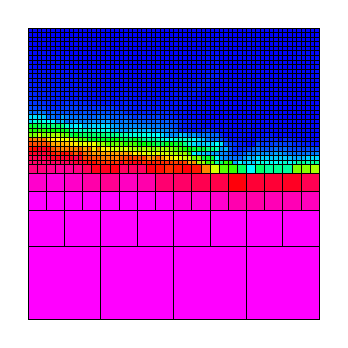
\begin{tikzpicture}[x={(\screenshotunitlength,0)},y={(0,\screenshotunitlength)}]
        \definecolor{fillcolor}{rgb}{1.000000,0.000000,1.000000}
\fill[fillcolor] (0.000000,0.000000) rectangle (0.250000,0.250000);
\definecolor{fillcolor}{rgb}{1.000000,0.000000,1.000000}
\fill[fillcolor] (0.250000,0.000000) rectangle (0.500000,0.250000);
\definecolor{fillcolor}{rgb}{1.000000,0.000000,1.000000}
\fill[fillcolor] (0.000000,0.250000) rectangle (0.125000,0.375000);
\definecolor{fillcolor}{rgb}{1.000000,0.000000,1.000000}
\fill[fillcolor] (0.125000,0.250000) rectangle (0.250000,0.375000);
\definecolor{fillcolor}{rgb}{1.000000,0.000000,1.000000}
\fill[fillcolor] (0.000000,0.375000) rectangle (0.062500,0.437500);
\definecolor{fillcolor}{rgb}{1.000000,0.000000,1.000000}
\fill[fillcolor] (0.062500,0.375000) rectangle (0.125000,0.437500);
\definecolor{fillcolor}{rgb}{1.000000,0.000000,0.799817}
\fill[fillcolor] (0.000000,0.437500) rectangle (0.062500,0.500000);
\definecolor{fillcolor}{rgb}{1.000000,0.000000,0.865851}
\fill[fillcolor] (0.062500,0.437500) rectangle (0.125000,0.500000);
\definecolor{fillcolor}{rgb}{1.000000,0.000000,1.000000}
\fill[fillcolor] (0.125000,0.375000) rectangle (0.187500,0.437500);
\definecolor{fillcolor}{rgb}{1.000000,0.000000,1.000000}
\fill[fillcolor] (0.187500,0.375000) rectangle (0.250000,0.437500);
\definecolor{fillcolor}{rgb}{1.000000,0.000000,0.785179}
\fill[fillcolor] (0.125000,0.437500) rectangle (0.187500,0.500000);
\definecolor{fillcolor}{rgb}{1.000000,0.000000,0.663356}
\fill[fillcolor] (0.187500,0.437500) rectangle (0.250000,0.500000);
\definecolor{fillcolor}{rgb}{1.000000,0.000000,1.000000}
\fill[fillcolor] (0.250000,0.250000) rectangle (0.375000,0.375000);
\definecolor{fillcolor}{rgb}{1.000000,0.000000,1.000000}
\fill[fillcolor] (0.375000,0.250000) rectangle (0.500000,0.375000);
\definecolor{fillcolor}{rgb}{1.000000,0.000000,1.000000}
\fill[fillcolor] (0.250000,0.375000) rectangle (0.312500,0.437500);
\definecolor{fillcolor}{rgb}{1.000000,0.000000,1.000000}
\fill[fillcolor] (0.312500,0.375000) rectangle (0.375000,0.437500);
\definecolor{fillcolor}{rgb}{1.000000,0.000000,0.570093}
\fill[fillcolor] (0.250000,0.437500) rectangle (0.312500,0.500000);
\definecolor{fillcolor}{rgb}{1.000000,0.000000,0.756095}
\fill[fillcolor] (0.312500,0.437500) rectangle (0.375000,0.500000);
\definecolor{fillcolor}{rgb}{1.000000,0.000000,1.000000}
\fill[fillcolor] (0.375000,0.375000) rectangle (0.437500,0.437500);
\definecolor{fillcolor}{rgb}{1.000000,0.000000,0.981009}
\fill[fillcolor] (0.437500,0.375000) rectangle (0.500000,0.437500);
\definecolor{fillcolor}{rgb}{1.000000,0.000000,0.672431}
\fill[fillcolor] (0.375000,0.437500) rectangle (0.437500,0.500000);
\definecolor{fillcolor}{rgb}{1.000000,0.000000,0.436633}
\fill[fillcolor] (0.437500,0.437500) rectangle (0.500000,0.500000);
\definecolor{fillcolor}{rgb}{1.000000,0.000000,1.000000}
\fill[fillcolor] (0.500000,0.000000) rectangle (0.750000,0.250000);
\definecolor{fillcolor}{rgb}{1.000000,0.000000,1.000000}
\fill[fillcolor] (0.750000,0.000000) rectangle (1.000000,0.250000);
\definecolor{fillcolor}{rgb}{1.000000,0.000000,1.000000}
\fill[fillcolor] (0.500000,0.250000) rectangle (0.625000,0.375000);
\definecolor{fillcolor}{rgb}{1.000000,0.000000,1.000000}
\fill[fillcolor] (0.625000,0.250000) rectangle (0.750000,0.375000);
\definecolor{fillcolor}{rgb}{1.000000,0.000000,0.886475}
\fill[fillcolor] (0.500000,0.375000) rectangle (0.562500,0.437500);
\definecolor{fillcolor}{rgb}{1.000000,0.000000,0.886996}
\fill[fillcolor] (0.562500,0.375000) rectangle (0.625000,0.437500);
\definecolor{fillcolor}{rgb}{1.000000,0.000000,0.399173}
\fill[fillcolor] (0.500000,0.437500) rectangle (0.562500,0.500000);
\definecolor{fillcolor}{rgb}{1.000000,0.000000,0.308710}
\fill[fillcolor] (0.562500,0.437500) rectangle (0.625000,0.500000);
\definecolor{fillcolor}{rgb}{1.000000,0.000000,0.806507}
\fill[fillcolor] (0.625000,0.375000) rectangle (0.687500,0.437500);
\definecolor{fillcolor}{rgb}{1.000000,0.000000,0.685987}
\fill[fillcolor] (0.687500,0.375000) rectangle (0.750000,0.437500);
\definecolor{fillcolor}{rgb}{1.000000,0.000000,0.284340}
\fill[fillcolor] (0.625000,0.437500) rectangle (0.687500,0.500000);
\definecolor{fillcolor}{rgb}{1.000000,0.000000,0.041087}
\fill[fillcolor] (0.687500,0.437500) rectangle (0.750000,0.500000);
\definecolor{fillcolor}{rgb}{1.000000,0.000000,1.000000}
\fill[fillcolor] (0.750000,0.250000) rectangle (0.875000,0.375000);
\definecolor{fillcolor}{rgb}{1.000000,0.000000,1.000000}
\fill[fillcolor] (0.875000,0.250000) rectangle (1.000000,0.375000);
\definecolor{fillcolor}{rgb}{1.000000,0.000000,0.662007}
\fill[fillcolor] (0.750000,0.375000) rectangle (0.812500,0.437500);
\definecolor{fillcolor}{rgb}{1.000000,0.000000,0.714066}
\fill[fillcolor] (0.812500,0.375000) rectangle (0.875000,0.437500);
\definecolor{fillcolor}{rgb}{1.000000,0.000000,0.213137}
\fill[fillcolor] (0.750000,0.437500) rectangle (0.812500,0.500000);
\definecolor{fillcolor}{rgb}{1.000000,0.000000,0.210074}
\fill[fillcolor] (0.812500,0.437500) rectangle (0.875000,0.500000);
\definecolor{fillcolor}{rgb}{1.000000,0.000000,0.710671}
\fill[fillcolor] (0.875000,0.375000) rectangle (0.937500,0.437500);
\definecolor{fillcolor}{rgb}{1.000000,0.000000,0.737808}
\fill[fillcolor] (0.937500,0.375000) rectangle (1.000000,0.437500);
\definecolor{fillcolor}{rgb}{1.000000,0.000000,0.135747}
\fill[fillcolor] (0.875000,0.437500) rectangle (0.937500,0.500000);
\definecolor{fillcolor}{rgb}{1.000000,0.000000,0.323404}
\fill[fillcolor] (0.937500,0.437500) rectangle (1.000000,0.500000);
\definecolor{fillcolor}{rgb}{1.000000,0.000000,0.495878}
\fill[fillcolor] (0.000000,0.500000) rectangle (0.031250,0.531250);
\definecolor{fillcolor}{rgb}{1.000000,0.000000,0.489199}
\fill[fillcolor] (0.031250,0.500000) rectangle (0.062500,0.531250);
\definecolor{fillcolor}{rgb}{1.000000,0.000000,0.412241}
\fill[fillcolor] (0.000000,0.531250) rectangle (0.015625,0.546875);
\definecolor{fillcolor}{rgb}{1.000000,0.000000,0.401102}
\fill[fillcolor] (0.015625,0.531250) rectangle (0.031250,0.546875);
\definecolor{fillcolor}{rgb}{1.000000,0.000000,0.314203}
\fill[fillcolor] (0.000000,0.546875) rectangle (0.015625,0.562500);
\definecolor{fillcolor}{rgb}{1.000000,0.000000,0.324079}
\fill[fillcolor] (0.015625,0.546875) rectangle (0.031250,0.562500);
\definecolor{fillcolor}{rgb}{1.000000,0.000000,0.389262}
\fill[fillcolor] (0.031250,0.531250) rectangle (0.046875,0.546875);
\definecolor{fillcolor}{rgb}{1.000000,0.000000,0.422209}
\fill[fillcolor] (0.046875,0.531250) rectangle (0.062500,0.546875);
\definecolor{fillcolor}{rgb}{1.000000,0.000000,0.318049}
\fill[fillcolor] (0.031250,0.546875) rectangle (0.046875,0.562500);
\definecolor{fillcolor}{rgb}{1.000000,0.000000,0.324436}
\fill[fillcolor] (0.046875,0.546875) rectangle (0.062500,0.562500);
\definecolor{fillcolor}{rgb}{1.000000,0.000000,0.550181}
\fill[fillcolor] (0.062500,0.500000) rectangle (0.093750,0.531250);
\definecolor{fillcolor}{rgb}{1.000000,0.000000,0.591770}
\fill[fillcolor] (0.093750,0.500000) rectangle (0.125000,0.531250);
\definecolor{fillcolor}{rgb}{1.000000,0.000000,0.395245}
\fill[fillcolor] (0.062500,0.531250) rectangle (0.078125,0.546875);
\definecolor{fillcolor}{rgb}{1.000000,0.000000,0.381216}
\fill[fillcolor] (0.078125,0.531250) rectangle (0.093750,0.546875);
\definecolor{fillcolor}{rgb}{1.000000,0.000000,0.257446}
\fill[fillcolor] (0.062500,0.546875) rectangle (0.078125,0.562500);
\definecolor{fillcolor}{rgb}{1.000000,0.000000,0.144228}
\fill[fillcolor] (0.078125,0.546875) rectangle (0.093750,0.562500);
\definecolor{fillcolor}{rgb}{1.000000,0.000000,0.385523}
\fill[fillcolor] (0.093750,0.531250) rectangle (0.109375,0.546875);
\definecolor{fillcolor}{rgb}{1.000000,0.000000,0.361579}
\fill[fillcolor] (0.109375,0.531250) rectangle (0.125000,0.546875);
\definecolor{fillcolor}{rgb}{1.000000,0.000000,0.134766}
\fill[fillcolor] (0.093750,0.546875) rectangle (0.109375,0.562500);
\definecolor{fillcolor}{rgb}{1.000000,0.000000,0.216741}
\fill[fillcolor] (0.109375,0.546875) rectangle (0.125000,0.562500);
\definecolor{fillcolor}{rgb}{1.000000,0.000000,0.140361}
\fill[fillcolor] (0.000000,0.562500) rectangle (0.015625,0.578125);
\definecolor{fillcolor}{rgb}{1.000000,0.000000,0.150994}
\fill[fillcolor] (0.015625,0.562500) rectangle (0.031250,0.578125);
\definecolor{fillcolor}{rgb}{1.000000,0.073220,0.000000}
\fill[fillcolor] (0.000000,0.578125) rectangle (0.015625,0.593750);
\definecolor{fillcolor}{rgb}{1.000000,0.015645,0.000000}
\fill[fillcolor] (0.015625,0.578125) rectangle (0.031250,0.593750);
\definecolor{fillcolor}{rgb}{1.000000,0.000000,0.194476}
\fill[fillcolor] (0.031250,0.562500) rectangle (0.046875,0.578125);
\definecolor{fillcolor}{rgb}{1.000000,0.000000,0.205193}
\fill[fillcolor] (0.046875,0.562500) rectangle (0.062500,0.578125);
\definecolor{fillcolor}{rgb}{1.000000,0.000000,0.128279}
\fill[fillcolor] (0.031250,0.578125) rectangle (0.046875,0.593750);
\definecolor{fillcolor}{rgb}{1.000000,0.000000,0.127125}
\fill[fillcolor] (0.046875,0.578125) rectangle (0.062500,0.593750);
\definecolor{fillcolor}{rgb}{1.000000,0.278590,0.000000}
\fill[fillcolor] (0.000000,0.593750) rectangle (0.015625,0.609375);
\definecolor{fillcolor}{rgb}{1.000000,0.305087,0.000000}
\fill[fillcolor] (0.015625,0.593750) rectangle (0.031250,0.609375);
\definecolor{fillcolor}{rgb}{1.000000,0.448398,0.000000}
\fill[fillcolor] (0.000000,0.609375) rectangle (0.015625,0.625000);
\definecolor{fillcolor}{rgb}{1.000000,0.506595,0.000000}
\fill[fillcolor] (0.015625,0.609375) rectangle (0.031250,0.625000);
\definecolor{fillcolor}{rgb}{1.000000,0.324527,0.000000}
\fill[fillcolor] (0.031250,0.593750) rectangle (0.046875,0.609375);
\definecolor{fillcolor}{rgb}{1.000000,0.305981,0.000000}
\fill[fillcolor] (0.046875,0.593750) rectangle (0.062500,0.609375);
\definecolor{fillcolor}{rgb}{1.000000,0.565309,0.000000}
\fill[fillcolor] (0.031250,0.609375) rectangle (0.046875,0.625000);
\definecolor{fillcolor}{rgb}{1.000000,0.470706,0.000000}
\fill[fillcolor] (0.046875,0.609375) rectangle (0.062500,0.625000);
\definecolor{fillcolor}{rgb}{1.000000,0.000000,0.137534}
\fill[fillcolor] (0.062500,0.562500) rectangle (0.078125,0.578125);
\definecolor{fillcolor}{rgb}{1.000000,0.105829,0.000000}
\fill[fillcolor] (0.078125,0.562500) rectangle (0.093750,0.578125);
\definecolor{fillcolor}{rgb}{1.000000,0.000000,0.051257}
\fill[fillcolor] (0.062500,0.578125) rectangle (0.078125,0.593750);
\definecolor{fillcolor}{rgb}{1.000000,0.317101,0.000000}
\fill[fillcolor] (0.078125,0.578125) rectangle (0.093750,0.593750);
\definecolor{fillcolor}{rgb}{1.000000,0.172173,0.000000}
\fill[fillcolor] (0.093750,0.562500) rectangle (0.109375,0.578125);
\definecolor{fillcolor}{rgb}{1.000000,0.059430,0.000000}
\fill[fillcolor] (0.109375,0.562500) rectangle (0.125000,0.578125);
\definecolor{fillcolor}{rgb}{1.000000,0.413988,0.000000}
\fill[fillcolor] (0.093750,0.578125) rectangle (0.109375,0.593750);
\definecolor{fillcolor}{rgb}{1.000000,0.520732,0.000000}
\fill[fillcolor] (0.109375,0.578125) rectangle (0.125000,0.593750);
\definecolor{fillcolor}{rgb}{1.000000,0.341383,0.000000}
\fill[fillcolor] (0.062500,0.593750) rectangle (0.078125,0.609375);
\definecolor{fillcolor}{rgb}{1.000000,0.646488,0.000000}
\fill[fillcolor] (0.078125,0.593750) rectangle (0.093750,0.609375);
\definecolor{fillcolor}{rgb}{1.000000,0.842507,0.000000}
\fill[fillcolor] (0.062500,0.609375) rectangle (0.078125,0.625000);
\definecolor{fillcolor}{rgb}{1.000000,0.955458,0.000000}
\fill[fillcolor] (0.078125,0.609375) rectangle (0.093750,0.625000);
\definecolor{fillcolor}{rgb}{1.000000,0.683195,0.000000}
\fill[fillcolor] (0.093750,0.593750) rectangle (0.109375,0.609375);
\definecolor{fillcolor}{rgb}{1.000000,0.688202,0.000000}
\fill[fillcolor] (0.109375,0.593750) rectangle (0.125000,0.609375);
\definecolor{fillcolor}{rgb}{1.000000,0.993222,0.000000}
\fill[fillcolor] (0.093750,0.609375) rectangle (0.109375,0.625000);
\definecolor{fillcolor}{rgb}{0.967422,1.000000,0.000000}
\fill[fillcolor] (0.109375,0.609375) rectangle (0.125000,0.625000);
\definecolor{fillcolor}{rgb}{1.000000,0.000000,0.576309}
\fill[fillcolor] (0.125000,0.500000) rectangle (0.156250,0.531250);
\definecolor{fillcolor}{rgb}{1.000000,0.000000,0.515523}
\fill[fillcolor] (0.156250,0.500000) rectangle (0.187500,0.531250);
\definecolor{fillcolor}{rgb}{1.000000,0.000000,0.345793}
\fill[fillcolor] (0.125000,0.531250) rectangle (0.140625,0.546875);
\definecolor{fillcolor}{rgb}{1.000000,0.000000,0.312438}
\fill[fillcolor] (0.140625,0.531250) rectangle (0.156250,0.546875);
\definecolor{fillcolor}{rgb}{1.000000,0.000000,0.167777}
\fill[fillcolor] (0.125000,0.546875) rectangle (0.140625,0.562500);
\definecolor{fillcolor}{rgb}{1.000000,0.000000,0.117076}
\fill[fillcolor] (0.140625,0.546875) rectangle (0.156250,0.562500);
\definecolor{fillcolor}{rgb}{1.000000,0.000000,0.200037}
\fill[fillcolor] (0.156250,0.531250) rectangle (0.171875,0.546875);
\definecolor{fillcolor}{rgb}{1.000000,0.000000,0.183607}
\fill[fillcolor] (0.171875,0.531250) rectangle (0.187500,0.546875);
\definecolor{fillcolor}{rgb}{1.000000,0.000000,0.304133}
\fill[fillcolor] (0.156250,0.546875) rectangle (0.171875,0.562500);
\definecolor{fillcolor}{rgb}{1.000000,0.000000,0.133119}
\fill[fillcolor] (0.171875,0.546875) rectangle (0.187500,0.562500);
\definecolor{fillcolor}{rgb}{1.000000,0.000000,0.349730}
\fill[fillcolor] (0.187500,0.500000) rectangle (0.218750,0.531250);
\definecolor{fillcolor}{rgb}{1.000000,0.000000,0.103880}
\fill[fillcolor] (0.218750,0.500000) rectangle (0.250000,0.531250);
\definecolor{fillcolor}{rgb}{1.000000,0.000000,0.120257}
\fill[fillcolor] (0.187500,0.531250) rectangle (0.203125,0.546875);
\definecolor{fillcolor}{rgb}{1.000000,0.056804,0.000000}
\fill[fillcolor] (0.203125,0.531250) rectangle (0.218750,0.546875);
\definecolor{fillcolor}{rgb}{1.000000,0.262694,0.000000}
\fill[fillcolor] (0.187500,0.546875) rectangle (0.203125,0.562500);
\definecolor{fillcolor}{rgb}{1.000000,0.249389,0.000000}
\fill[fillcolor] (0.203125,0.546875) rectangle (0.218750,0.562500);
\definecolor{fillcolor}{rgb}{1.000000,0.048452,0.000000}
\fill[fillcolor] (0.218750,0.531250) rectangle (0.234375,0.546875);
\definecolor{fillcolor}{rgb}{1.000000,0.156540,0.000000}
\fill[fillcolor] (0.234375,0.531250) rectangle (0.250000,0.546875);
\definecolor{fillcolor}{rgb}{1.000000,0.343439,0.000000}
\fill[fillcolor] (0.218750,0.546875) rectangle (0.234375,0.562500);
\definecolor{fillcolor}{rgb}{1.000000,0.324970,0.000000}
\fill[fillcolor] (0.234375,0.546875) rectangle (0.250000,0.562500);
\definecolor{fillcolor}{rgb}{1.000000,0.064448,0.000000}
\fill[fillcolor] (0.125000,0.562500) rectangle (0.140625,0.578125);
\definecolor{fillcolor}{rgb}{1.000000,0.155583,0.000000}
\fill[fillcolor] (0.140625,0.562500) rectangle (0.156250,0.578125);
\definecolor{fillcolor}{rgb}{1.000000,0.470488,0.000000}
\fill[fillcolor] (0.125000,0.578125) rectangle (0.140625,0.593750);
\definecolor{fillcolor}{rgb}{1.000000,0.502605,0.000000}
\fill[fillcolor] (0.140625,0.578125) rectangle (0.156250,0.593750);
\definecolor{fillcolor}{rgb}{1.000000,0.343378,0.000000}
\fill[fillcolor] (0.156250,0.562500) rectangle (0.171875,0.578125);
\definecolor{fillcolor}{rgb}{1.000000,0.090675,0.000000}
\fill[fillcolor] (0.171875,0.562500) rectangle (0.187500,0.578125);
\definecolor{fillcolor}{rgb}{1.000000,0.495852,0.000000}
\fill[fillcolor] (0.156250,0.578125) rectangle (0.171875,0.593750);
\definecolor{fillcolor}{rgb}{1.000000,0.419350,0.000000}
\fill[fillcolor] (0.171875,0.578125) rectangle (0.187500,0.593750);
\definecolor{fillcolor}{rgb}{1.000000,0.716346,0.000000}
\fill[fillcolor] (0.125000,0.593750) rectangle (0.140625,0.609375);
\definecolor{fillcolor}{rgb}{1.000000,0.884665,0.000000}
\fill[fillcolor] (0.140625,0.593750) rectangle (0.156250,0.609375);
\definecolor{fillcolor}{rgb}{0.942519,1.000000,0.000000}
\fill[fillcolor] (0.125000,0.609375) rectangle (0.140625,0.625000);
\definecolor{fillcolor}{rgb}{0.801102,1.000000,0.000000}
\fill[fillcolor] (0.140625,0.609375) rectangle (0.156250,0.625000);
\definecolor{fillcolor}{rgb}{1.000000,0.933797,0.000000}
\fill[fillcolor] (0.156250,0.593750) rectangle (0.171875,0.609375);
\definecolor{fillcolor}{rgb}{0.853209,1.000000,0.000000}
\fill[fillcolor] (0.171875,0.593750) rectangle (0.187500,0.609375);
\definecolor{fillcolor}{rgb}{0.584807,1.000000,0.000000}
\fill[fillcolor] (0.156250,0.609375) rectangle (0.171875,0.625000);
\definecolor{fillcolor}{rgb}{0.314217,1.000000,0.000000}
\fill[fillcolor] (0.171875,0.609375) rectangle (0.187500,0.625000);
\definecolor{fillcolor}{rgb}{1.000000,0.409128,0.000000}
\fill[fillcolor] (0.187500,0.562500) rectangle (0.203125,0.578125);
\definecolor{fillcolor}{rgb}{1.000000,0.491635,0.000000}
\fill[fillcolor] (0.203125,0.562500) rectangle (0.218750,0.578125);
\definecolor{fillcolor}{rgb}{1.000000,0.672027,0.000000}
\fill[fillcolor] (0.187500,0.578125) rectangle (0.203125,0.593750);
\definecolor{fillcolor}{rgb}{1.000000,0.455786,0.000000}
\fill[fillcolor] (0.203125,0.578125) rectangle (0.218750,0.593750);
\definecolor{fillcolor}{rgb}{1.000000,0.611304,0.000000}
\fill[fillcolor] (0.218750,0.562500) rectangle (0.234375,0.578125);
\definecolor{fillcolor}{rgb}{1.000000,0.616099,0.000000}
\fill[fillcolor] (0.234375,0.562500) rectangle (0.250000,0.578125);
\definecolor{fillcolor}{rgb}{1.000000,0.891035,0.000000}
\fill[fillcolor] (0.218750,0.578125) rectangle (0.234375,0.593750);
\definecolor{fillcolor}{rgb}{1.000000,0.529808,0.000000}
\fill[fillcolor] (0.234375,0.578125) rectangle (0.250000,0.593750);
\definecolor{fillcolor}{rgb}{0.930417,1.000000,0.000000}
\fill[fillcolor] (0.187500,0.593750) rectangle (0.203125,0.609375);
\definecolor{fillcolor}{rgb}{0.964645,1.000000,0.000000}
\fill[fillcolor] (0.203125,0.593750) rectangle (0.218750,0.609375);
\definecolor{fillcolor}{rgb}{0.312686,1.000000,0.000000}
\fill[fillcolor] (0.187500,0.609375) rectangle (0.203125,0.625000);
\definecolor{fillcolor}{rgb}{0.000000,1.000000,0.207583}
\fill[fillcolor] (0.203125,0.609375) rectangle (0.218750,0.625000);
\definecolor{fillcolor}{rgb}{0.957786,1.000000,0.000000}
\fill[fillcolor] (0.218750,0.593750) rectangle (0.234375,0.609375);
\definecolor{fillcolor}{rgb}{0.662648,1.000000,0.000000}
\fill[fillcolor] (0.234375,0.593750) rectangle (0.250000,0.609375);
\definecolor{fillcolor}{rgb}{0.000000,1.000000,0.088887}
\fill[fillcolor] (0.218750,0.609375) rectangle (0.234375,0.625000);
\definecolor{fillcolor}{rgb}{0.000000,1.000000,0.104259}
\fill[fillcolor] (0.234375,0.609375) rectangle (0.250000,0.625000);
\definecolor{fillcolor}{rgb}{0.471678,1.000000,0.000000}
\fill[fillcolor] (0.000000,0.625000) rectangle (0.015625,0.640625);
\definecolor{fillcolor}{rgb}{0.463215,1.000000,0.000000}
\fill[fillcolor] (0.015625,0.625000) rectangle (0.031250,0.640625);
\definecolor{fillcolor}{rgb}{0.119866,1.000000,0.000000}
\fill[fillcolor] (0.000000,0.640625) rectangle (0.015625,0.656250);
\definecolor{fillcolor}{rgb}{0.091842,1.000000,0.000000}
\fill[fillcolor] (0.015625,0.640625) rectangle (0.031250,0.656250);
\definecolor{fillcolor}{rgb}{0.820464,1.000000,0.000000}
\fill[fillcolor] (0.031250,0.625000) rectangle (0.046875,0.640625);
\definecolor{fillcolor}{rgb}{0.484937,1.000000,0.000000}
\fill[fillcolor] (0.046875,0.625000) rectangle (0.062500,0.640625);
\definecolor{fillcolor}{rgb}{0.207583,1.000000,0.000000}
\fill[fillcolor] (0.031250,0.640625) rectangle (0.046875,0.656250);
\definecolor{fillcolor}{rgb}{0.135615,1.000000,0.000000}
\fill[fillcolor] (0.046875,0.640625) rectangle (0.062500,0.656250);
\definecolor{fillcolor}{rgb}{0.000000,1.000000,0.207165}
\fill[fillcolor] (0.000000,0.656250) rectangle (0.015625,0.671875);
\definecolor{fillcolor}{rgb}{0.000000,1.000000,0.192756}
\fill[fillcolor] (0.015625,0.656250) rectangle (0.031250,0.671875);
\definecolor{fillcolor}{rgb}{0.000000,0.820873,1.000000}
\fill[fillcolor] (0.000000,0.671875) rectangle (0.015625,0.687500);
\definecolor{fillcolor}{rgb}{0.000000,1.000000,0.869667}
\fill[fillcolor] (0.015625,0.671875) rectangle (0.031250,0.687500);
\definecolor{fillcolor}{rgb}{0.000000,1.000000,0.374320}
\fill[fillcolor] (0.031250,0.656250) rectangle (0.046875,0.671875);
\definecolor{fillcolor}{rgb}{0.000000,1.000000,0.404217}
\fill[fillcolor] (0.046875,0.656250) rectangle (0.062500,0.671875);
\definecolor{fillcolor}{rgb}{0.000000,1.000000,0.763079}
\fill[fillcolor] (0.031250,0.671875) rectangle (0.046875,0.687500);
\definecolor{fillcolor}{rgb}{0.000000,1.000000,0.943058}
\fill[fillcolor] (0.046875,0.671875) rectangle (0.062500,0.687500);
\definecolor{fillcolor}{rgb}{0.611163,1.000000,0.000000}
\fill[fillcolor] (0.062500,0.625000) rectangle (0.078125,0.640625);
\definecolor{fillcolor}{rgb}{0.628286,1.000000,0.000000}
\fill[fillcolor] (0.078125,0.625000) rectangle (0.093750,0.640625);
\definecolor{fillcolor}{rgb}{0.000000,1.000000,0.089803}
\fill[fillcolor] (0.062500,0.640625) rectangle (0.078125,0.656250);
\definecolor{fillcolor}{rgb}{0.010914,1.000000,0.000000}
\fill[fillcolor] (0.078125,0.640625) rectangle (0.093750,0.656250);
\definecolor{fillcolor}{rgb}{0.663252,1.000000,0.000000}
\fill[fillcolor] (0.093750,0.625000) rectangle (0.109375,0.640625);
\definecolor{fillcolor}{rgb}{0.493417,1.000000,0.000000}
\fill[fillcolor] (0.109375,0.625000) rectangle (0.125000,0.640625);
\definecolor{fillcolor}{rgb}{0.000000,1.000000,0.040953}
\fill[fillcolor] (0.093750,0.640625) rectangle (0.109375,0.656250);
\definecolor{fillcolor}{rgb}{0.000000,1.000000,0.115331}
\fill[fillcolor] (0.109375,0.640625) rectangle (0.125000,0.656250);
\definecolor{fillcolor}{rgb}{0.000000,1.000000,0.451497}
\fill[fillcolor] (0.062500,0.656250) rectangle (0.078125,0.671875);
\definecolor{fillcolor}{rgb}{0.000000,1.000000,0.494533}
\fill[fillcolor] (0.078125,0.656250) rectangle (0.093750,0.671875);
\definecolor{fillcolor}{rgb}{0.000000,0.995000,1.000000}
\fill[fillcolor] (0.062500,0.671875) rectangle (0.078125,0.687500);
\definecolor{fillcolor}{rgb}{0.000000,0.966924,1.000000}
\fill[fillcolor] (0.078125,0.671875) rectangle (0.093750,0.687500);
\definecolor{fillcolor}{rgb}{0.000000,1.000000,0.393103}
\fill[fillcolor] (0.093750,0.656250) rectangle (0.109375,0.671875);
\definecolor{fillcolor}{rgb}{0.000000,1.000000,0.506044}
\fill[fillcolor] (0.109375,0.656250) rectangle (0.125000,0.671875);
\definecolor{fillcolor}{rgb}{0.000000,0.605782,1.000000}
\fill[fillcolor] (0.093750,0.671875) rectangle (0.109375,0.687500);
\definecolor{fillcolor}{rgb}{0.000000,0.753897,1.000000}
\fill[fillcolor] (0.109375,0.671875) rectangle (0.125000,0.687500);
\definecolor{fillcolor}{rgb}{0.000000,0.847860,1.000000}
\fill[fillcolor] (0.000000,0.687500) rectangle (0.015625,0.703125);
\definecolor{fillcolor}{rgb}{0.000000,0.877966,1.000000}
\fill[fillcolor] (0.015625,0.687500) rectangle (0.031250,0.703125);
\definecolor{fillcolor}{rgb}{0.000000,0.451878,1.000000}
\fill[fillcolor] (0.000000,0.703125) rectangle (0.015625,0.718750);
\definecolor{fillcolor}{rgb}{0.000000,0.391103,1.000000}
\fill[fillcolor] (0.015625,0.703125) rectangle (0.031250,0.718750);
\definecolor{fillcolor}{rgb}{0.000000,0.833899,1.000000}
\fill[fillcolor] (0.031250,0.687500) rectangle (0.046875,0.703125);
\definecolor{fillcolor}{rgb}{0.000000,0.762713,1.000000}
\fill[fillcolor] (0.046875,0.687500) rectangle (0.062500,0.703125);
\definecolor{fillcolor}{rgb}{0.000000,0.506727,1.000000}
\fill[fillcolor] (0.031250,0.703125) rectangle (0.046875,0.718750);
\definecolor{fillcolor}{rgb}{0.000000,0.434768,1.000000}
\fill[fillcolor] (0.046875,0.703125) rectangle (0.062500,0.718750);
\definecolor{fillcolor}{rgb}{0.000000,0.277126,1.000000}
\fill[fillcolor] (0.000000,0.718750) rectangle (0.015625,0.734375);
\definecolor{fillcolor}{rgb}{0.000000,0.272830,1.000000}
\fill[fillcolor] (0.015625,0.718750) rectangle (0.031250,0.734375);
\definecolor{fillcolor}{rgb}{0.000000,0.205372,1.000000}
\fill[fillcolor] (0.000000,0.734375) rectangle (0.015625,0.750000);
\definecolor{fillcolor}{rgb}{0.000000,0.207082,1.000000}
\fill[fillcolor] (0.015625,0.734375) rectangle (0.031250,0.750000);
\definecolor{fillcolor}{rgb}{0.000000,0.244015,1.000000}
\fill[fillcolor] (0.031250,0.718750) rectangle (0.046875,0.734375);
\definecolor{fillcolor}{rgb}{0.000000,0.260075,1.000000}
\fill[fillcolor] (0.046875,0.718750) rectangle (0.062500,0.734375);
\definecolor{fillcolor}{rgb}{0.000000,0.203579,1.000000}
\fill[fillcolor] (0.031250,0.734375) rectangle (0.046875,0.750000);
\definecolor{fillcolor}{rgb}{0.000000,0.164356,1.000000}
\fill[fillcolor] (0.046875,0.734375) rectangle (0.062500,0.750000);
\definecolor{fillcolor}{rgb}{0.000000,0.430877,1.000000}
\fill[fillcolor] (0.062500,0.687500) rectangle (0.078125,0.703125);
\definecolor{fillcolor}{rgb}{0.000000,0.452601,1.000000}
\fill[fillcolor] (0.078125,0.687500) rectangle (0.093750,0.703125);
\definecolor{fillcolor}{rgb}{0.000000,0.277295,1.000000}
\fill[fillcolor] (0.062500,0.703125) rectangle (0.078125,0.718750);
\definecolor{fillcolor}{rgb}{0.000000,0.404321,1.000000}
\fill[fillcolor] (0.078125,0.703125) rectangle (0.093750,0.718750);
\definecolor{fillcolor}{rgb}{0.000000,0.341134,1.000000}
\fill[fillcolor] (0.093750,0.687500) rectangle (0.109375,0.703125);
\definecolor{fillcolor}{rgb}{0.000000,0.648733,1.000000}
\fill[fillcolor] (0.109375,0.687500) rectangle (0.125000,0.703125);
\definecolor{fillcolor}{rgb}{0.000000,0.317875,1.000000}
\fill[fillcolor] (0.093750,0.703125) rectangle (0.109375,0.718750);
\definecolor{fillcolor}{rgb}{0.000000,0.316175,1.000000}
\fill[fillcolor] (0.109375,0.703125) rectangle (0.125000,0.718750);
\definecolor{fillcolor}{rgb}{0.000000,0.158461,1.000000}
\fill[fillcolor] (0.062500,0.718750) rectangle (0.078125,0.734375);
\definecolor{fillcolor}{rgb}{0.000000,0.164616,1.000000}
\fill[fillcolor] (0.078125,0.718750) rectangle (0.093750,0.734375);
\definecolor{fillcolor}{rgb}{0.000000,0.140162,1.000000}
\fill[fillcolor] (0.062500,0.734375) rectangle (0.078125,0.750000);
\definecolor{fillcolor}{rgb}{0.000000,0.122403,1.000000}
\fill[fillcolor] (0.078125,0.734375) rectangle (0.093750,0.750000);
\definecolor{fillcolor}{rgb}{0.000000,0.146672,1.000000}
\fill[fillcolor] (0.093750,0.718750) rectangle (0.109375,0.734375);
\definecolor{fillcolor}{rgb}{0.000000,0.229003,1.000000}
\fill[fillcolor] (0.109375,0.718750) rectangle (0.125000,0.734375);
\definecolor{fillcolor}{rgb}{0.000000,0.119694,1.000000}
\fill[fillcolor] (0.093750,0.734375) rectangle (0.109375,0.750000);
\definecolor{fillcolor}{rgb}{0.000000,0.142206,1.000000}
\fill[fillcolor] (0.109375,0.734375) rectangle (0.125000,0.750000);
\definecolor{fillcolor}{rgb}{0.331948,1.000000,0.000000}
\fill[fillcolor] (0.125000,0.625000) rectangle (0.140625,0.640625);
\definecolor{fillcolor}{rgb}{0.000000,1.000000,0.349666}
\fill[fillcolor] (0.140625,0.625000) rectangle (0.156250,0.640625);
\definecolor{fillcolor}{rgb}{0.000000,1.000000,0.172132}
\fill[fillcolor] (0.125000,0.640625) rectangle (0.140625,0.656250);
\definecolor{fillcolor}{rgb}{0.000000,1.000000,0.706239}
\fill[fillcolor] (0.140625,0.640625) rectangle (0.156250,0.656250);
\definecolor{fillcolor}{rgb}{0.000000,1.000000,0.100452}
\fill[fillcolor] (0.156250,0.625000) rectangle (0.171875,0.640625);
\definecolor{fillcolor}{rgb}{0.000000,1.000000,0.365349}
\fill[fillcolor] (0.171875,0.625000) rectangle (0.187500,0.640625);
\definecolor{fillcolor}{rgb}{0.000000,1.000000,0.722389}
\fill[fillcolor] (0.156250,0.640625) rectangle (0.171875,0.656250);
\definecolor{fillcolor}{rgb}{0.000000,1.000000,0.840966}
\fill[fillcolor] (0.171875,0.640625) rectangle (0.187500,0.656250);
\definecolor{fillcolor}{rgb}{0.000000,1.000000,0.793575}
\fill[fillcolor] (0.125000,0.656250) rectangle (0.140625,0.671875);
\definecolor{fillcolor}{rgb}{0.000000,0.872345,1.000000}
\fill[fillcolor] (0.140625,0.656250) rectangle (0.156250,0.671875);
\definecolor{fillcolor}{rgb}{0.000000,0.451487,1.000000}
\fill[fillcolor] (0.125000,0.671875) rectangle (0.140625,0.687500);
\definecolor{fillcolor}{rgb}{0.000000,0.581781,1.000000}
\fill[fillcolor] (0.140625,0.671875) rectangle (0.156250,0.687500);
\definecolor{fillcolor}{rgb}{0.000000,0.966311,1.000000}
\fill[fillcolor] (0.156250,0.656250) rectangle (0.171875,0.671875);
\definecolor{fillcolor}{rgb}{0.000000,0.999553,1.000000}
\fill[fillcolor] (0.171875,0.656250) rectangle (0.187500,0.671875);
\definecolor{fillcolor}{rgb}{0.000000,0.641948,1.000000}
\fill[fillcolor] (0.156250,0.671875) rectangle (0.171875,0.687500);
\definecolor{fillcolor}{rgb}{0.000000,0.517266,1.000000}
\fill[fillcolor] (0.171875,0.671875) rectangle (0.187500,0.687500);
\definecolor{fillcolor}{rgb}{0.000000,1.000000,0.343628}
\fill[fillcolor] (0.187500,0.625000) rectangle (0.203125,0.640625);
\definecolor{fillcolor}{rgb}{0.000000,1.000000,0.382290}
\fill[fillcolor] (0.203125,0.625000) rectangle (0.218750,0.640625);
\definecolor{fillcolor}{rgb}{0.000000,1.000000,0.724965}
\fill[fillcolor] (0.187500,0.640625) rectangle (0.203125,0.656250);
\definecolor{fillcolor}{rgb}{0.000000,1.000000,0.730581}
\fill[fillcolor] (0.203125,0.640625) rectangle (0.218750,0.656250);
\definecolor{fillcolor}{rgb}{0.000000,1.000000,0.401970}
\fill[fillcolor] (0.218750,0.625000) rectangle (0.234375,0.640625);
\definecolor{fillcolor}{rgb}{0.000000,1.000000,0.422273}
\fill[fillcolor] (0.234375,0.625000) rectangle (0.250000,0.640625);
\definecolor{fillcolor}{rgb}{0.000000,1.000000,0.815274}
\fill[fillcolor] (0.218750,0.640625) rectangle (0.234375,0.656250);
\definecolor{fillcolor}{rgb}{0.000000,1.000000,0.894925}
\fill[fillcolor] (0.234375,0.640625) rectangle (0.250000,0.656250);
\definecolor{fillcolor}{rgb}{0.000000,0.700320,1.000000}
\fill[fillcolor] (0.187500,0.656250) rectangle (0.203125,0.671875);
\definecolor{fillcolor}{rgb}{0.000000,0.809606,1.000000}
\fill[fillcolor] (0.203125,0.656250) rectangle (0.218750,0.671875);
\definecolor{fillcolor}{rgb}{0.000000,0.527222,1.000000}
\fill[fillcolor] (0.187500,0.671875) rectangle (0.203125,0.687500);
\definecolor{fillcolor}{rgb}{0.000000,0.562619,1.000000}
\fill[fillcolor] (0.203125,0.671875) rectangle (0.218750,0.687500);
\definecolor{fillcolor}{rgb}{0.000000,0.833982,1.000000}
\fill[fillcolor] (0.218750,0.656250) rectangle (0.234375,0.671875);
\definecolor{fillcolor}{rgb}{0.000000,0.832428,1.000000}
\fill[fillcolor] (0.234375,0.656250) rectangle (0.250000,0.671875);
\definecolor{fillcolor}{rgb}{0.000000,0.593003,1.000000}
\fill[fillcolor] (0.218750,0.671875) rectangle (0.234375,0.687500);
\definecolor{fillcolor}{rgb}{0.000000,0.527548,1.000000}
\fill[fillcolor] (0.234375,0.671875) rectangle (0.250000,0.687500);
\definecolor{fillcolor}{rgb}{0.000000,0.518763,1.000000}
\fill[fillcolor] (0.125000,0.687500) rectangle (0.140625,0.703125);
\definecolor{fillcolor}{rgb}{0.000000,0.450075,1.000000}
\fill[fillcolor] (0.140625,0.687500) rectangle (0.156250,0.703125);
\definecolor{fillcolor}{rgb}{0.000000,0.308462,1.000000}
\fill[fillcolor] (0.125000,0.703125) rectangle (0.140625,0.718750);
\definecolor{fillcolor}{rgb}{0.000000,0.335338,1.000000}
\fill[fillcolor] (0.140625,0.703125) rectangle (0.156250,0.718750);
\definecolor{fillcolor}{rgb}{0.000000,0.452382,1.000000}
\fill[fillcolor] (0.156250,0.687500) rectangle (0.171875,0.703125);
\definecolor{fillcolor}{rgb}{0.000000,0.443392,1.000000}
\fill[fillcolor] (0.171875,0.687500) rectangle (0.187500,0.703125);
\definecolor{fillcolor}{rgb}{0.000000,0.286899,1.000000}
\fill[fillcolor] (0.156250,0.703125) rectangle (0.171875,0.718750);
\definecolor{fillcolor}{rgb}{0.000000,0.278522,1.000000}
\fill[fillcolor] (0.171875,0.703125) rectangle (0.187500,0.718750);
\definecolor{fillcolor}{rgb}{0.000000,0.226599,1.000000}
\fill[fillcolor] (0.125000,0.718750) rectangle (0.140625,0.734375);
\definecolor{fillcolor}{rgb}{0.000000,0.230802,1.000000}
\fill[fillcolor] (0.140625,0.718750) rectangle (0.156250,0.734375);
\definecolor{fillcolor}{rgb}{0.000000,0.190383,1.000000}
\fill[fillcolor] (0.125000,0.734375) rectangle (0.140625,0.750000);
\definecolor{fillcolor}{rgb}{0.000000,0.173143,1.000000}
\fill[fillcolor] (0.140625,0.734375) rectangle (0.156250,0.750000);
\definecolor{fillcolor}{rgb}{0.000000,0.244357,1.000000}
\fill[fillcolor] (0.156250,0.718750) rectangle (0.171875,0.734375);
\definecolor{fillcolor}{rgb}{0.000000,0.184705,1.000000}
\fill[fillcolor] (0.171875,0.718750) rectangle (0.187500,0.734375);
\definecolor{fillcolor}{rgb}{0.000000,0.164658,1.000000}
\fill[fillcolor] (0.156250,0.734375) rectangle (0.171875,0.750000);
\definecolor{fillcolor}{rgb}{0.000000,0.140984,1.000000}
\fill[fillcolor] (0.171875,0.734375) rectangle (0.187500,0.750000);
\definecolor{fillcolor}{rgb}{0.000000,0.445237,1.000000}
\fill[fillcolor] (0.187500,0.687500) rectangle (0.203125,0.703125);
\definecolor{fillcolor}{rgb}{0.000000,0.377346,1.000000}
\fill[fillcolor] (0.203125,0.687500) rectangle (0.218750,0.703125);
\definecolor{fillcolor}{rgb}{0.000000,0.309049,1.000000}
\fill[fillcolor] (0.187500,0.703125) rectangle (0.203125,0.718750);
\definecolor{fillcolor}{rgb}{0.000000,0.322119,1.000000}
\fill[fillcolor] (0.203125,0.703125) rectangle (0.218750,0.718750);
\definecolor{fillcolor}{rgb}{0.000000,0.416123,1.000000}
\fill[fillcolor] (0.218750,0.687500) rectangle (0.234375,0.703125);
\definecolor{fillcolor}{rgb}{0.000000,0.444858,1.000000}
\fill[fillcolor] (0.234375,0.687500) rectangle (0.250000,0.703125);
\definecolor{fillcolor}{rgb}{0.000000,0.248226,1.000000}
\fill[fillcolor] (0.218750,0.703125) rectangle (0.234375,0.718750);
\definecolor{fillcolor}{rgb}{0.000000,0.321243,1.000000}
\fill[fillcolor] (0.234375,0.703125) rectangle (0.250000,0.718750);
\definecolor{fillcolor}{rgb}{0.000000,0.220341,1.000000}
\fill[fillcolor] (0.187500,0.718750) rectangle (0.203125,0.734375);
\definecolor{fillcolor}{rgb}{0.000000,0.179723,1.000000}
\fill[fillcolor] (0.203125,0.718750) rectangle (0.218750,0.734375);
\definecolor{fillcolor}{rgb}{0.000000,0.141203,1.000000}
\fill[fillcolor] (0.187500,0.734375) rectangle (0.203125,0.750000);
\definecolor{fillcolor}{rgb}{0.000000,0.123252,1.000000}
\fill[fillcolor] (0.203125,0.734375) rectangle (0.218750,0.750000);
\definecolor{fillcolor}{rgb}{0.000000,0.190800,1.000000}
\fill[fillcolor] (0.218750,0.718750) rectangle (0.234375,0.734375);
\definecolor{fillcolor}{rgb}{0.000000,0.194603,1.000000}
\fill[fillcolor] (0.234375,0.718750) rectangle (0.250000,0.734375);
\definecolor{fillcolor}{rgb}{0.000000,0.095492,1.000000}
\fill[fillcolor] (0.218750,0.734375) rectangle (0.234375,0.750000);
\definecolor{fillcolor}{rgb}{0.000000,0.095965,1.000000}
\fill[fillcolor] (0.234375,0.734375) rectangle (0.250000,0.750000);
\definecolor{fillcolor}{rgb}{1.000000,0.000000,0.115663}
\fill[fillcolor] (0.250000,0.500000) rectangle (0.281250,0.531250);
\definecolor{fillcolor}{rgb}{1.000000,0.000000,0.062920}
\fill[fillcolor] (0.281250,0.500000) rectangle (0.312500,0.531250);
\definecolor{fillcolor}{rgb}{1.000000,0.173557,0.000000}
\fill[fillcolor] (0.250000,0.531250) rectangle (0.265625,0.546875);
\definecolor{fillcolor}{rgb}{1.000000,0.195783,0.000000}
\fill[fillcolor] (0.265625,0.531250) rectangle (0.281250,0.546875);
\definecolor{fillcolor}{rgb}{1.000000,0.454591,0.000000}
\fill[fillcolor] (0.250000,0.546875) rectangle (0.265625,0.562500);
\definecolor{fillcolor}{rgb}{1.000000,0.475237,0.000000}
\fill[fillcolor] (0.265625,0.546875) rectangle (0.281250,0.562500);
\definecolor{fillcolor}{rgb}{1.000000,0.175318,0.000000}
\fill[fillcolor] (0.281250,0.531250) rectangle (0.296875,0.546875);
\definecolor{fillcolor}{rgb}{1.000000,0.204508,0.000000}
\fill[fillcolor] (0.296875,0.531250) rectangle (0.312500,0.546875);
\definecolor{fillcolor}{rgb}{1.000000,0.474870,0.000000}
\fill[fillcolor] (0.281250,0.546875) rectangle (0.296875,0.562500);
\definecolor{fillcolor}{rgb}{1.000000,0.502379,0.000000}
\fill[fillcolor] (0.296875,0.546875) rectangle (0.312500,0.562500);
\definecolor{fillcolor}{rgb}{1.000000,0.000000,0.393084}
\fill[fillcolor] (0.312500,0.500000) rectangle (0.343750,0.531250);
\definecolor{fillcolor}{rgb}{1.000000,0.000000,0.367979}
\fill[fillcolor] (0.343750,0.500000) rectangle (0.375000,0.531250);
\definecolor{fillcolor}{rgb}{1.000000,0.000000,0.171348}
\fill[fillcolor] (0.312500,0.531250) rectangle (0.328125,0.546875);
\definecolor{fillcolor}{rgb}{1.000000,0.147320,0.000000}
\fill[fillcolor] (0.328125,0.531250) rectangle (0.343750,0.546875);
\definecolor{fillcolor}{rgb}{1.000000,0.317207,0.000000}
\fill[fillcolor] (0.312500,0.546875) rectangle (0.328125,0.562500);
\definecolor{fillcolor}{rgb}{1.000000,0.301264,0.000000}
\fill[fillcolor] (0.328125,0.546875) rectangle (0.343750,0.562500);
\definecolor{fillcolor}{rgb}{1.000000,0.000000,0.099518}
\fill[fillcolor] (0.343750,0.531250) rectangle (0.359375,0.546875);
\definecolor{fillcolor}{rgb}{1.000000,0.000000,0.064916}
\fill[fillcolor] (0.359375,0.531250) rectangle (0.375000,0.546875);
\definecolor{fillcolor}{rgb}{1.000000,0.219238,0.000000}
\fill[fillcolor] (0.343750,0.546875) rectangle (0.359375,0.562500);
\definecolor{fillcolor}{rgb}{1.000000,0.248519,0.000000}
\fill[fillcolor] (0.359375,0.546875) rectangle (0.375000,0.562500);
\definecolor{fillcolor}{rgb}{1.000000,0.641262,0.000000}
\fill[fillcolor] (0.250000,0.562500) rectangle (0.265625,0.578125);
\definecolor{fillcolor}{rgb}{1.000000,0.643360,0.000000}
\fill[fillcolor] (0.265625,0.562500) rectangle (0.281250,0.578125);
\definecolor{fillcolor}{rgb}{1.000000,0.943522,0.000000}
\fill[fillcolor] (0.250000,0.578125) rectangle (0.265625,0.593750);
\definecolor{fillcolor}{rgb}{1.000000,0.920516,0.000000}
\fill[fillcolor] (0.265625,0.578125) rectangle (0.281250,0.593750);
\definecolor{fillcolor}{rgb}{1.000000,0.638310,0.000000}
\fill[fillcolor] (0.281250,0.562500) rectangle (0.296875,0.578125);
\definecolor{fillcolor}{rgb}{1.000000,0.653017,0.000000}
\fill[fillcolor] (0.296875,0.562500) rectangle (0.312500,0.578125);
\definecolor{fillcolor}{rgb}{0.833242,1.000000,0.000000}
\fill[fillcolor] (0.281250,0.578125) rectangle (0.296875,0.593750);
\definecolor{fillcolor}{rgb}{0.795622,1.000000,0.000000}
\fill[fillcolor] (0.296875,0.578125) rectangle (0.312500,0.593750);
\definecolor{fillcolor}{rgb}{0.575711,1.000000,0.000000}
\fill[fillcolor] (0.250000,0.593750) rectangle (0.265625,0.609375);
\definecolor{fillcolor}{rgb}{0.329913,1.000000,0.000000}
\fill[fillcolor] (0.265625,0.593750) rectangle (0.281250,0.609375);
\definecolor{fillcolor}{rgb}{0.000000,1.000000,0.106340}
\fill[fillcolor] (0.250000,0.609375) rectangle (0.265625,0.625000);
\definecolor{fillcolor}{rgb}{0.000000,1.000000,0.139078}
\fill[fillcolor] (0.265625,0.609375) rectangle (0.281250,0.625000);
\definecolor{fillcolor}{rgb}{0.381206,1.000000,0.000000}
\fill[fillcolor] (0.281250,0.593750) rectangle (0.296875,0.609375);
\definecolor{fillcolor}{rgb}{0.398449,1.000000,0.000000}
\fill[fillcolor] (0.296875,0.593750) rectangle (0.312500,0.609375);
\definecolor{fillcolor}{rgb}{0.000000,1.000000,0.072900}
\fill[fillcolor] (0.281250,0.609375) rectangle (0.296875,0.625000);
\definecolor{fillcolor}{rgb}{0.000000,1.000000,0.027541}
\fill[fillcolor] (0.296875,0.609375) rectangle (0.312500,0.625000);
\definecolor{fillcolor}{rgb}{1.000000,0.672535,0.000000}
\fill[fillcolor] (0.312500,0.562500) rectangle (0.328125,0.578125);
\definecolor{fillcolor}{rgb}{1.000000,0.663949,0.000000}
\fill[fillcolor] (0.328125,0.562500) rectangle (0.343750,0.578125);
\definecolor{fillcolor}{rgb}{0.757977,1.000000,0.000000}
\fill[fillcolor] (0.312500,0.578125) rectangle (0.328125,0.593750);
\definecolor{fillcolor}{rgb}{0.856764,1.000000,0.000000}
\fill[fillcolor] (0.328125,0.578125) rectangle (0.343750,0.593750);
\definecolor{fillcolor}{rgb}{1.000000,0.717296,0.000000}
\fill[fillcolor] (0.343750,0.562500) rectangle (0.359375,0.578125);
\definecolor{fillcolor}{rgb}{1.000000,0.937510,0.000000}
\fill[fillcolor] (0.359375,0.562500) rectangle (0.375000,0.578125);
\definecolor{fillcolor}{rgb}{0.675721,1.000000,0.000000}
\fill[fillcolor] (0.343750,0.578125) rectangle (0.359375,0.593750);
\definecolor{fillcolor}{rgb}{0.651092,1.000000,0.000000}
\fill[fillcolor] (0.359375,0.578125) rectangle (0.375000,0.593750);
\definecolor{fillcolor}{rgb}{0.361115,1.000000,0.000000}
\fill[fillcolor] (0.312500,0.593750) rectangle (0.328125,0.609375);
\definecolor{fillcolor}{rgb}{0.134048,1.000000,0.000000}
\fill[fillcolor] (0.328125,0.593750) rectangle (0.343750,0.609375);
\definecolor{fillcolor}{rgb}{0.000000,1.000000,0.249645}
\fill[fillcolor] (0.312500,0.609375) rectangle (0.328125,0.625000);
\definecolor{fillcolor}{rgb}{0.000000,1.000000,0.284470}
\fill[fillcolor] (0.328125,0.609375) rectangle (0.343750,0.625000);
\definecolor{fillcolor}{rgb}{0.318779,1.000000,0.000000}
\fill[fillcolor] (0.343750,0.593750) rectangle (0.359375,0.609375);
\definecolor{fillcolor}{rgb}{0.246009,1.000000,0.000000}
\fill[fillcolor] (0.359375,0.593750) rectangle (0.375000,0.609375);
\definecolor{fillcolor}{rgb}{0.000000,1.000000,0.289929}
\fill[fillcolor] (0.343750,0.609375) rectangle (0.359375,0.625000);
\definecolor{fillcolor}{rgb}{0.000000,1.000000,0.123338}
\fill[fillcolor] (0.359375,0.609375) rectangle (0.375000,0.625000);
\definecolor{fillcolor}{rgb}{1.000000,0.000000,0.377343}
\fill[fillcolor] (0.375000,0.500000) rectangle (0.406250,0.531250);
\definecolor{fillcolor}{rgb}{1.000000,0.000000,0.064118}
\fill[fillcolor] (0.406250,0.500000) rectangle (0.437500,0.531250);
\definecolor{fillcolor}{rgb}{1.000000,0.000000,0.053735}
\fill[fillcolor] (0.375000,0.531250) rectangle (0.390625,0.546875);
\definecolor{fillcolor}{rgb}{1.000000,0.150625,0.000000}
\fill[fillcolor] (0.390625,0.531250) rectangle (0.406250,0.546875);
\definecolor{fillcolor}{rgb}{1.000000,0.308435,0.000000}
\fill[fillcolor] (0.375000,0.546875) rectangle (0.390625,0.562500);
\definecolor{fillcolor}{rgb}{1.000000,0.304352,0.000000}
\fill[fillcolor] (0.390625,0.546875) rectangle (0.406250,0.562500);
\definecolor{fillcolor}{rgb}{1.000000,0.109557,0.000000}
\fill[fillcolor] (0.406250,0.531250) rectangle (0.421875,0.546875);
\definecolor{fillcolor}{rgb}{1.000000,0.113606,0.000000}
\fill[fillcolor] (0.421875,0.531250) rectangle (0.437500,0.546875);
\definecolor{fillcolor}{rgb}{1.000000,0.591118,0.000000}
\fill[fillcolor] (0.406250,0.546875) rectangle (0.421875,0.562500);
\definecolor{fillcolor}{rgb}{1.000000,0.531942,0.000000}
\fill[fillcolor] (0.421875,0.546875) rectangle (0.437500,0.562500);
\definecolor{fillcolor}{rgb}{1.000000,0.061909,0.000000}
\fill[fillcolor] (0.437500,0.500000) rectangle (0.468750,0.531250);
\definecolor{fillcolor}{rgb}{1.000000,0.179167,0.000000}
\fill[fillcolor] (0.468750,0.500000) rectangle (0.500000,0.531250);
\definecolor{fillcolor}{rgb}{1.000000,0.141200,0.000000}
\fill[fillcolor] (0.437500,0.531250) rectangle (0.453125,0.546875);
\definecolor{fillcolor}{rgb}{1.000000,0.182198,0.000000}
\fill[fillcolor] (0.453125,0.531250) rectangle (0.468750,0.546875);
\definecolor{fillcolor}{rgb}{1.000000,0.374361,0.000000}
\fill[fillcolor] (0.437500,0.546875) rectangle (0.453125,0.562500);
\definecolor{fillcolor}{rgb}{1.000000,0.633007,0.000000}
\fill[fillcolor] (0.453125,0.546875) rectangle (0.468750,0.562500);
\definecolor{fillcolor}{rgb}{1.000000,0.175199,0.000000}
\fill[fillcolor] (0.468750,0.531250) rectangle (0.484375,0.546875);
\definecolor{fillcolor}{rgb}{1.000000,0.203259,0.000000}
\fill[fillcolor] (0.484375,0.531250) rectangle (0.500000,0.546875);
\definecolor{fillcolor}{rgb}{1.000000,0.812224,0.000000}
\fill[fillcolor] (0.468750,0.546875) rectangle (0.484375,0.562500);
\definecolor{fillcolor}{rgb}{1.000000,0.850526,0.000000}
\fill[fillcolor] (0.484375,0.546875) rectangle (0.500000,0.562500);
\definecolor{fillcolor}{rgb}{1.000000,0.888096,0.000000}
\fill[fillcolor] (0.375000,0.562500) rectangle (0.390625,0.578125);
\definecolor{fillcolor}{rgb}{0.881064,1.000000,0.000000}
\fill[fillcolor] (0.390625,0.562500) rectangle (0.406250,0.578125);
\definecolor{fillcolor}{rgb}{0.575989,1.000000,0.000000}
\fill[fillcolor] (0.375000,0.578125) rectangle (0.390625,0.593750);
\definecolor{fillcolor}{rgb}{0.677846,1.000000,0.000000}
\fill[fillcolor] (0.390625,0.578125) rectangle (0.406250,0.593750);
\definecolor{fillcolor}{rgb}{0.861688,1.000000,0.000000}
\fill[fillcolor] (0.406250,0.562500) rectangle (0.421875,0.578125);
\definecolor{fillcolor}{rgb}{0.874057,1.000000,0.000000}
\fill[fillcolor] (0.421875,0.562500) rectangle (0.437500,0.578125);
\definecolor{fillcolor}{rgb}{0.611446,1.000000,0.000000}
\fill[fillcolor] (0.406250,0.578125) rectangle (0.421875,0.593750);
\definecolor{fillcolor}{rgb}{0.521641,1.000000,0.000000}
\fill[fillcolor] (0.421875,0.578125) rectangle (0.437500,0.593750);
\definecolor{fillcolor}{rgb}{0.000000,1.000000,0.038917}
\fill[fillcolor] (0.375000,0.593750) rectangle (0.390625,0.609375);
\definecolor{fillcolor}{rgb}{0.000000,1.000000,0.016890}
\fill[fillcolor] (0.390625,0.593750) rectangle (0.406250,0.609375);
\definecolor{fillcolor}{rgb}{0.000000,1.000000,0.309380}
\fill[fillcolor] (0.375000,0.609375) rectangle (0.390625,0.625000);
\definecolor{fillcolor}{rgb}{0.000000,1.000000,0.548697}
\fill[fillcolor] (0.390625,0.609375) rectangle (0.406250,0.625000);
\definecolor{fillcolor}{rgb}{0.000000,1.000000,0.079142}
\fill[fillcolor] (0.406250,0.593750) rectangle (0.421875,0.609375);
\definecolor{fillcolor}{rgb}{0.000000,1.000000,0.219577}
\fill[fillcolor] (0.421875,0.593750) rectangle (0.437500,0.609375);
\definecolor{fillcolor}{rgb}{0.000000,1.000000,0.629987}
\fill[fillcolor] (0.406250,0.609375) rectangle (0.421875,0.625000);
\definecolor{fillcolor}{rgb}{0.000000,1.000000,0.609138}
\fill[fillcolor] (0.421875,0.609375) rectangle (0.437500,0.625000);
\definecolor{fillcolor}{rgb}{0.883495,1.000000,0.000000}
\fill[fillcolor] (0.437500,0.562500) rectangle (0.453125,0.578125);
\definecolor{fillcolor}{rgb}{0.844225,1.000000,0.000000}
\fill[fillcolor] (0.453125,0.562500) rectangle (0.468750,0.578125);
\definecolor{fillcolor}{rgb}{0.578535,1.000000,0.000000}
\fill[fillcolor] (0.437500,0.578125) rectangle (0.453125,0.593750);
\definecolor{fillcolor}{rgb}{0.655088,1.000000,0.000000}
\fill[fillcolor] (0.453125,0.578125) rectangle (0.468750,0.593750);
\definecolor{fillcolor}{rgb}{0.820497,1.000000,0.000000}
\fill[fillcolor] (0.468750,0.562500) rectangle (0.484375,0.578125);
\definecolor{fillcolor}{rgb}{0.712664,1.000000,0.000000}
\fill[fillcolor] (0.484375,0.562500) rectangle (0.500000,0.578125);
\definecolor{fillcolor}{rgb}{0.557583,1.000000,0.000000}
\fill[fillcolor] (0.468750,0.578125) rectangle (0.484375,0.593750);
\definecolor{fillcolor}{rgb}{0.511810,1.000000,0.000000}
\fill[fillcolor] (0.484375,0.578125) rectangle (0.500000,0.593750);
\definecolor{fillcolor}{rgb}{0.000000,1.000000,0.333972}
\fill[fillcolor] (0.437500,0.593750) rectangle (0.453125,0.609375);
\definecolor{fillcolor}{rgb}{0.000000,1.000000,0.327002}
\fill[fillcolor] (0.453125,0.593750) rectangle (0.468750,0.609375);
\definecolor{fillcolor}{rgb}{0.000000,1.000000,0.660786}
\fill[fillcolor] (0.437500,0.609375) rectangle (0.453125,0.625000);
\definecolor{fillcolor}{rgb}{0.000000,1.000000,0.831348}
\fill[fillcolor] (0.453125,0.609375) rectangle (0.468750,0.625000);
\definecolor{fillcolor}{rgb}{0.000000,1.000000,0.108902}
\fill[fillcolor] (0.468750,0.593750) rectangle (0.484375,0.609375);
\definecolor{fillcolor}{rgb}{0.000000,1.000000,0.039325}
\fill[fillcolor] (0.484375,0.593750) rectangle (0.500000,0.609375);
\definecolor{fillcolor}{rgb}{0.000000,1.000000,0.859222}
\fill[fillcolor] (0.468750,0.609375) rectangle (0.484375,0.625000);
\definecolor{fillcolor}{rgb}{0.000000,1.000000,0.995658}
\fill[fillcolor] (0.484375,0.609375) rectangle (0.500000,0.625000);
\definecolor{fillcolor}{rgb}{0.000000,1.000000,0.450300}
\fill[fillcolor] (0.250000,0.625000) rectangle (0.265625,0.640625);
\definecolor{fillcolor}{rgb}{0.000000,1.000000,0.524023}
\fill[fillcolor] (0.265625,0.625000) rectangle (0.281250,0.640625);
\definecolor{fillcolor}{rgb}{0.000000,1.000000,0.905382}
\fill[fillcolor] (0.250000,0.640625) rectangle (0.265625,0.656250);
\definecolor{fillcolor}{rgb}{0.000000,1.000000,0.865315}
\fill[fillcolor] (0.265625,0.640625) rectangle (0.281250,0.656250);
\definecolor{fillcolor}{rgb}{0.000000,1.000000,0.544289}
\fill[fillcolor] (0.281250,0.625000) rectangle (0.296875,0.640625);
\definecolor{fillcolor}{rgb}{0.000000,1.000000,0.554389}
\fill[fillcolor] (0.296875,0.625000) rectangle (0.312500,0.640625);
\definecolor{fillcolor}{rgb}{0.000000,0.768976,1.000000}
\fill[fillcolor] (0.281250,0.640625) rectangle (0.296875,0.656250);
\definecolor{fillcolor}{rgb}{0.000000,0.694037,1.000000}
\fill[fillcolor] (0.296875,0.640625) rectangle (0.312500,0.656250);
\definecolor{fillcolor}{rgb}{0.000000,0.876082,1.000000}
\fill[fillcolor] (0.250000,0.656250) rectangle (0.265625,0.671875);
\definecolor{fillcolor}{rgb}{0.000000,0.846827,1.000000}
\fill[fillcolor] (0.265625,0.656250) rectangle (0.281250,0.671875);
\definecolor{fillcolor}{rgb}{0.000000,0.622424,1.000000}
\fill[fillcolor] (0.250000,0.671875) rectangle (0.265625,0.687500);
\definecolor{fillcolor}{rgb}{0.000000,0.613865,1.000000}
\fill[fillcolor] (0.265625,0.671875) rectangle (0.281250,0.687500);
\definecolor{fillcolor}{rgb}{0.000000,0.653291,1.000000}
\fill[fillcolor] (0.281250,0.656250) rectangle (0.296875,0.671875);
\definecolor{fillcolor}{rgb}{0.000000,0.589521,1.000000}
\fill[fillcolor] (0.296875,0.656250) rectangle (0.312500,0.671875);
\definecolor{fillcolor}{rgb}{0.000000,0.454956,1.000000}
\fill[fillcolor] (0.281250,0.671875) rectangle (0.296875,0.687500);
\definecolor{fillcolor}{rgb}{0.000000,0.443812,1.000000}
\fill[fillcolor] (0.296875,0.671875) rectangle (0.312500,0.687500);
\definecolor{fillcolor}{rgb}{0.000000,1.000000,0.655072}
\fill[fillcolor] (0.312500,0.625000) rectangle (0.328125,0.640625);
\definecolor{fillcolor}{rgb}{0.000000,1.000000,0.641564}
\fill[fillcolor] (0.328125,0.625000) rectangle (0.343750,0.640625);
\definecolor{fillcolor}{rgb}{0.000000,0.647880,1.000000}
\fill[fillcolor] (0.312500,0.640625) rectangle (0.328125,0.656250);
\definecolor{fillcolor}{rgb}{0.000000,0.621990,1.000000}
\fill[fillcolor] (0.328125,0.640625) rectangle (0.343750,0.656250);
\definecolor{fillcolor}{rgb}{0.000000,1.000000,0.890262}
\fill[fillcolor] (0.343750,0.625000) rectangle (0.359375,0.640625);
\definecolor{fillcolor}{rgb}{0.000000,1.000000,0.830497}
\fill[fillcolor] (0.359375,0.625000) rectangle (0.375000,0.640625);
\definecolor{fillcolor}{rgb}{0.000000,0.719029,1.000000}
\fill[fillcolor] (0.343750,0.640625) rectangle (0.359375,0.656250);
\definecolor{fillcolor}{rgb}{0.000000,0.783179,1.000000}
\fill[fillcolor] (0.359375,0.640625) rectangle (0.375000,0.656250);
\definecolor{fillcolor}{rgb}{0.000000,0.548743,1.000000}
\fill[fillcolor] (0.312500,0.656250) rectangle (0.328125,0.671875);
\definecolor{fillcolor}{rgb}{0.000000,0.516483,1.000000}
\fill[fillcolor] (0.328125,0.656250) rectangle (0.343750,0.671875);
\definecolor{fillcolor}{rgb}{0.000000,0.430400,1.000000}
\fill[fillcolor] (0.312500,0.671875) rectangle (0.328125,0.687500);
\definecolor{fillcolor}{rgb}{0.000000,0.503204,1.000000}
\fill[fillcolor] (0.328125,0.671875) rectangle (0.343750,0.687500);
\definecolor{fillcolor}{rgb}{0.000000,0.567385,1.000000}
\fill[fillcolor] (0.343750,0.656250) rectangle (0.359375,0.671875);
\definecolor{fillcolor}{rgb}{0.000000,0.537370,1.000000}
\fill[fillcolor] (0.359375,0.656250) rectangle (0.375000,0.671875);
\definecolor{fillcolor}{rgb}{0.000000,0.417656,1.000000}
\fill[fillcolor] (0.343750,0.671875) rectangle (0.359375,0.687500);
\definecolor{fillcolor}{rgb}{0.000000,0.420118,1.000000}
\fill[fillcolor] (0.359375,0.671875) rectangle (0.375000,0.687500);
\definecolor{fillcolor}{rgb}{0.000000,0.453306,1.000000}
\fill[fillcolor] (0.250000,0.687500) rectangle (0.265625,0.703125);
\definecolor{fillcolor}{rgb}{0.000000,0.430135,1.000000}
\fill[fillcolor] (0.265625,0.687500) rectangle (0.281250,0.703125);
\definecolor{fillcolor}{rgb}{0.000000,0.311042,1.000000}
\fill[fillcolor] (0.250000,0.703125) rectangle (0.265625,0.718750);
\definecolor{fillcolor}{rgb}{0.000000,0.292112,1.000000}
\fill[fillcolor] (0.265625,0.703125) rectangle (0.281250,0.718750);
\definecolor{fillcolor}{rgb}{0.000000,0.382030,1.000000}
\fill[fillcolor] (0.281250,0.687500) rectangle (0.296875,0.703125);
\definecolor{fillcolor}{rgb}{0.000000,0.348455,1.000000}
\fill[fillcolor] (0.296875,0.687500) rectangle (0.312500,0.703125);
\definecolor{fillcolor}{rgb}{0.000000,0.293409,1.000000}
\fill[fillcolor] (0.281250,0.703125) rectangle (0.296875,0.718750);
\definecolor{fillcolor}{rgb}{0.000000,0.285318,1.000000}
\fill[fillcolor] (0.296875,0.703125) rectangle (0.312500,0.718750);
\definecolor{fillcolor}{rgb}{0.000000,0.209553,1.000000}
\fill[fillcolor] (0.250000,0.718750) rectangle (0.265625,0.734375);
\definecolor{fillcolor}{rgb}{0.000000,0.167716,1.000000}
\fill[fillcolor] (0.265625,0.718750) rectangle (0.281250,0.734375);
\definecolor{fillcolor}{rgb}{0.000000,0.089126,1.000000}
\fill[fillcolor] (0.250000,0.734375) rectangle (0.265625,0.750000);
\definecolor{fillcolor}{rgb}{0.000000,0.093195,1.000000}
\fill[fillcolor] (0.265625,0.734375) rectangle (0.281250,0.750000);
\definecolor{fillcolor}{rgb}{0.000000,0.230665,1.000000}
\fill[fillcolor] (0.281250,0.718750) rectangle (0.296875,0.734375);
\definecolor{fillcolor}{rgb}{0.000000,0.138485,1.000000}
\fill[fillcolor] (0.296875,0.718750) rectangle (0.312500,0.734375);
\definecolor{fillcolor}{rgb}{0.000000,0.088738,1.000000}
\fill[fillcolor] (0.281250,0.734375) rectangle (0.296875,0.750000);
\definecolor{fillcolor}{rgb}{0.000000,0.093762,1.000000}
\fill[fillcolor] (0.296875,0.734375) rectangle (0.312500,0.750000);
\definecolor{fillcolor}{rgb}{0.000000,0.337867,1.000000}
\fill[fillcolor] (0.312500,0.687500) rectangle (0.328125,0.703125);
\definecolor{fillcolor}{rgb}{0.000000,0.355573,1.000000}
\fill[fillcolor] (0.328125,0.687500) rectangle (0.343750,0.703125);
\definecolor{fillcolor}{rgb}{0.000000,0.273139,1.000000}
\fill[fillcolor] (0.312500,0.703125) rectangle (0.328125,0.718750);
\definecolor{fillcolor}{rgb}{0.000000,0.160273,1.000000}
\fill[fillcolor] (0.328125,0.703125) rectangle (0.343750,0.718750);
\definecolor{fillcolor}{rgb}{0.000000,0.287289,1.000000}
\fill[fillcolor] (0.343750,0.687500) rectangle (0.359375,0.703125);
\definecolor{fillcolor}{rgb}{0.000000,0.221647,1.000000}
\fill[fillcolor] (0.359375,0.687500) rectangle (0.375000,0.703125);
\definecolor{fillcolor}{rgb}{0.000000,0.144332,1.000000}
\fill[fillcolor] (0.343750,0.703125) rectangle (0.359375,0.718750);
\definecolor{fillcolor}{rgb}{0.000000,0.143333,1.000000}
\fill[fillcolor] (0.359375,0.703125) rectangle (0.375000,0.718750);
\definecolor{fillcolor}{rgb}{0.000000,0.111914,1.000000}
\fill[fillcolor] (0.312500,0.718750) rectangle (0.328125,0.734375);
\definecolor{fillcolor}{rgb}{0.000000,0.148425,1.000000}
\fill[fillcolor] (0.328125,0.718750) rectangle (0.343750,0.734375);
\definecolor{fillcolor}{rgb}{0.000000,0.096528,1.000000}
\fill[fillcolor] (0.312500,0.734375) rectangle (0.328125,0.750000);
\definecolor{fillcolor}{rgb}{0.000000,0.111280,1.000000}
\fill[fillcolor] (0.328125,0.734375) rectangle (0.343750,0.750000);
\definecolor{fillcolor}{rgb}{0.000000,0.113609,1.000000}
\fill[fillcolor] (0.343750,0.718750) rectangle (0.359375,0.734375);
\definecolor{fillcolor}{rgb}{0.000000,0.107179,1.000000}
\fill[fillcolor] (0.359375,0.718750) rectangle (0.375000,0.734375);
\definecolor{fillcolor}{rgb}{0.000000,0.106639,1.000000}
\fill[fillcolor] (0.343750,0.734375) rectangle (0.359375,0.750000);
\definecolor{fillcolor}{rgb}{0.000000,0.084333,1.000000}
\fill[fillcolor] (0.359375,0.734375) rectangle (0.375000,0.750000);
\definecolor{fillcolor}{rgb}{0.000000,1.000000,0.882465}
\fill[fillcolor] (0.375000,0.625000) rectangle (0.390625,0.640625);
\definecolor{fillcolor}{rgb}{0.000000,1.000000,0.867545}
\fill[fillcolor] (0.390625,0.625000) rectangle (0.406250,0.640625);
\definecolor{fillcolor}{rgb}{0.000000,0.736181,1.000000}
\fill[fillcolor] (0.375000,0.640625) rectangle (0.390625,0.656250);
\definecolor{fillcolor}{rgb}{0.000000,0.730798,1.000000}
\fill[fillcolor] (0.390625,0.640625) rectangle (0.406250,0.656250);
\definecolor{fillcolor}{rgb}{0.000000,1.000000,0.909998}
\fill[fillcolor] (0.406250,0.625000) rectangle (0.421875,0.640625);
\definecolor{fillcolor}{rgb}{0.000000,1.000000,0.959209}
\fill[fillcolor] (0.421875,0.625000) rectangle (0.437500,0.640625);
\definecolor{fillcolor}{rgb}{0.000000,0.746624,1.000000}
\fill[fillcolor] (0.406250,0.640625) rectangle (0.421875,0.656250);
\definecolor{fillcolor}{rgb}{0.000000,0.569480,1.000000}
\fill[fillcolor] (0.421875,0.640625) rectangle (0.437500,0.656250);
\definecolor{fillcolor}{rgb}{0.000000,0.534703,1.000000}
\fill[fillcolor] (0.375000,0.656250) rectangle (0.390625,0.671875);
\definecolor{fillcolor}{rgb}{0.000000,0.526083,1.000000}
\fill[fillcolor] (0.390625,0.656250) rectangle (0.406250,0.671875);
\definecolor{fillcolor}{rgb}{0.000000,0.385959,1.000000}
\fill[fillcolor] (0.375000,0.671875) rectangle (0.390625,0.687500);
\definecolor{fillcolor}{rgb}{0.000000,0.372698,1.000000}
\fill[fillcolor] (0.390625,0.671875) rectangle (0.406250,0.687500);
\definecolor{fillcolor}{rgb}{0.000000,0.506244,1.000000}
\fill[fillcolor] (0.406250,0.656250) rectangle (0.421875,0.671875);
\definecolor{fillcolor}{rgb}{0.000000,0.462533,1.000000}
\fill[fillcolor] (0.421875,0.656250) rectangle (0.437500,0.671875);
\definecolor{fillcolor}{rgb}{0.000000,0.346180,1.000000}
\fill[fillcolor] (0.406250,0.671875) rectangle (0.421875,0.687500);
\definecolor{fillcolor}{rgb}{0.000000,0.363420,1.000000}
\fill[fillcolor] (0.421875,0.671875) rectangle (0.437500,0.687500);
\definecolor{fillcolor}{rgb}{0.000000,0.999032,1.000000}
\fill[fillcolor] (0.437500,0.625000) rectangle (0.453125,0.640625);
\definecolor{fillcolor}{rgb}{0.000000,0.849786,1.000000}
\fill[fillcolor] (0.453125,0.625000) rectangle (0.468750,0.640625);
\definecolor{fillcolor}{rgb}{0.000000,0.578668,1.000000}
\fill[fillcolor] (0.437500,0.640625) rectangle (0.453125,0.656250);
\definecolor{fillcolor}{rgb}{0.000000,0.560644,1.000000}
\fill[fillcolor] (0.453125,0.640625) rectangle (0.468750,0.656250);
\definecolor{fillcolor}{rgb}{0.000000,0.640470,1.000000}
\fill[fillcolor] (0.468750,0.625000) rectangle (0.484375,0.640625);
\definecolor{fillcolor}{rgb}{0.000000,0.556988,1.000000}
\fill[fillcolor] (0.484375,0.625000) rectangle (0.500000,0.640625);
\definecolor{fillcolor}{rgb}{0.000000,0.514240,1.000000}
\fill[fillcolor] (0.468750,0.640625) rectangle (0.484375,0.656250);
\definecolor{fillcolor}{rgb}{0.000000,0.466867,1.000000}
\fill[fillcolor] (0.484375,0.640625) rectangle (0.500000,0.656250);
\definecolor{fillcolor}{rgb}{0.000000,0.476490,1.000000}
\fill[fillcolor] (0.437500,0.656250) rectangle (0.453125,0.671875);
\definecolor{fillcolor}{rgb}{0.000000,0.439201,1.000000}
\fill[fillcolor] (0.453125,0.656250) rectangle (0.468750,0.671875);
\definecolor{fillcolor}{rgb}{0.000000,0.390508,1.000000}
\fill[fillcolor] (0.437500,0.671875) rectangle (0.453125,0.687500);
\definecolor{fillcolor}{rgb}{0.000000,0.323122,1.000000}
\fill[fillcolor] (0.453125,0.671875) rectangle (0.468750,0.687500);
\definecolor{fillcolor}{rgb}{0.000000,0.402597,1.000000}
\fill[fillcolor] (0.468750,0.656250) rectangle (0.484375,0.671875);
\definecolor{fillcolor}{rgb}{0.000000,0.336085,1.000000}
\fill[fillcolor] (0.484375,0.656250) rectangle (0.500000,0.671875);
\definecolor{fillcolor}{rgb}{0.000000,0.361322,1.000000}
\fill[fillcolor] (0.468750,0.671875) rectangle (0.484375,0.687500);
\definecolor{fillcolor}{rgb}{0.000000,0.281397,1.000000}
\fill[fillcolor] (0.484375,0.671875) rectangle (0.500000,0.687500);
\definecolor{fillcolor}{rgb}{0.000000,0.286102,1.000000}
\fill[fillcolor] (0.375000,0.687500) rectangle (0.390625,0.703125);
\definecolor{fillcolor}{rgb}{0.000000,0.253046,1.000000}
\fill[fillcolor] (0.390625,0.687500) rectangle (0.406250,0.703125);
\definecolor{fillcolor}{rgb}{0.000000,0.120856,1.000000}
\fill[fillcolor] (0.375000,0.703125) rectangle (0.390625,0.718750);
\definecolor{fillcolor}{rgb}{0.000000,0.121567,1.000000}
\fill[fillcolor] (0.390625,0.703125) rectangle (0.406250,0.718750);
\definecolor{fillcolor}{rgb}{0.000000,0.207984,1.000000}
\fill[fillcolor] (0.406250,0.687500) rectangle (0.421875,0.703125);
\definecolor{fillcolor}{rgb}{0.000000,0.259936,1.000000}
\fill[fillcolor] (0.421875,0.687500) rectangle (0.437500,0.703125);
\definecolor{fillcolor}{rgb}{0.000000,0.140609,1.000000}
\fill[fillcolor] (0.406250,0.703125) rectangle (0.421875,0.718750);
\definecolor{fillcolor}{rgb}{0.000000,0.136227,1.000000}
\fill[fillcolor] (0.421875,0.703125) rectangle (0.437500,0.718750);
\definecolor{fillcolor}{rgb}{0.000000,0.103979,1.000000}
\fill[fillcolor] (0.375000,0.718750) rectangle (0.390625,0.734375);
\definecolor{fillcolor}{rgb}{0.000000,0.104554,1.000000}
\fill[fillcolor] (0.390625,0.718750) rectangle (0.406250,0.734375);
\definecolor{fillcolor}{rgb}{0.000000,0.075531,1.000000}
\fill[fillcolor] (0.375000,0.734375) rectangle (0.390625,0.750000);
\definecolor{fillcolor}{rgb}{0.000000,0.091912,1.000000}
\fill[fillcolor] (0.390625,0.734375) rectangle (0.406250,0.750000);
\definecolor{fillcolor}{rgb}{0.000000,0.089945,1.000000}
\fill[fillcolor] (0.406250,0.718750) rectangle (0.421875,0.734375);
\definecolor{fillcolor}{rgb}{0.000000,0.088194,1.000000}
\fill[fillcolor] (0.421875,0.718750) rectangle (0.437500,0.734375);
\definecolor{fillcolor}{rgb}{0.000000,0.068052,1.000000}
\fill[fillcolor] (0.406250,0.734375) rectangle (0.421875,0.750000);
\definecolor{fillcolor}{rgb}{0.000000,0.062377,1.000000}
\fill[fillcolor] (0.421875,0.734375) rectangle (0.437500,0.750000);
\definecolor{fillcolor}{rgb}{0.000000,0.248557,1.000000}
\fill[fillcolor] (0.437500,0.687500) rectangle (0.453125,0.703125);
\definecolor{fillcolor}{rgb}{0.000000,0.193735,1.000000}
\fill[fillcolor] (0.453125,0.687500) rectangle (0.468750,0.703125);
\definecolor{fillcolor}{rgb}{0.000000,0.163715,1.000000}
\fill[fillcolor] (0.437500,0.703125) rectangle (0.453125,0.718750);
\definecolor{fillcolor}{rgb}{0.000000,0.168738,1.000000}
\fill[fillcolor] (0.453125,0.703125) rectangle (0.468750,0.718750);
\definecolor{fillcolor}{rgb}{0.000000,0.175465,1.000000}
\fill[fillcolor] (0.468750,0.687500) rectangle (0.484375,0.703125);
\definecolor{fillcolor}{rgb}{0.000000,0.147131,1.000000}
\fill[fillcolor] (0.484375,0.687500) rectangle (0.500000,0.703125);
\definecolor{fillcolor}{rgb}{0.000000,0.163668,1.000000}
\fill[fillcolor] (0.468750,0.703125) rectangle (0.484375,0.718750);
\definecolor{fillcolor}{rgb}{0.000000,0.148945,1.000000}
\fill[fillcolor] (0.484375,0.703125) rectangle (0.500000,0.718750);
\definecolor{fillcolor}{rgb}{0.000000,0.091195,1.000000}
\fill[fillcolor] (0.437500,0.718750) rectangle (0.453125,0.734375);
\definecolor{fillcolor}{rgb}{0.000000,0.081079,1.000000}
\fill[fillcolor] (0.453125,0.718750) rectangle (0.468750,0.734375);
\definecolor{fillcolor}{rgb}{0.000000,0.075366,1.000000}
\fill[fillcolor] (0.437500,0.734375) rectangle (0.453125,0.750000);
\definecolor{fillcolor}{rgb}{0.000000,0.076496,1.000000}
\fill[fillcolor] (0.453125,0.734375) rectangle (0.468750,0.750000);
\definecolor{fillcolor}{rgb}{0.000000,0.085697,1.000000}
\fill[fillcolor] (0.468750,0.718750) rectangle (0.484375,0.734375);
\definecolor{fillcolor}{rgb}{0.000000,0.083440,1.000000}
\fill[fillcolor] (0.484375,0.718750) rectangle (0.500000,0.734375);
\definecolor{fillcolor}{rgb}{0.000000,0.076096,1.000000}
\fill[fillcolor] (0.468750,0.734375) rectangle (0.484375,0.750000);
\definecolor{fillcolor}{rgb}{0.000000,0.073260,1.000000}
\fill[fillcolor] (0.484375,0.734375) rectangle (0.500000,0.750000);
\definecolor{fillcolor}{rgb}{0.000000,0.162710,1.000000}
\fill[fillcolor] (0.000000,0.750000) rectangle (0.015625,0.765625);
\definecolor{fillcolor}{rgb}{0.000000,0.170210,1.000000}
\fill[fillcolor] (0.015625,0.750000) rectangle (0.031250,0.765625);
\definecolor{fillcolor}{rgb}{0.000000,0.146338,1.000000}
\fill[fillcolor] (0.000000,0.765625) rectangle (0.015625,0.781250);
\definecolor{fillcolor}{rgb}{0.000000,0.149717,1.000000}
\fill[fillcolor] (0.015625,0.765625) rectangle (0.031250,0.781250);
\definecolor{fillcolor}{rgb}{0.000000,0.133498,1.000000}
\fill[fillcolor] (0.031250,0.750000) rectangle (0.046875,0.765625);
\definecolor{fillcolor}{rgb}{0.000000,0.137806,1.000000}
\fill[fillcolor] (0.046875,0.750000) rectangle (0.062500,0.765625);
\definecolor{fillcolor}{rgb}{0.000000,0.122746,1.000000}
\fill[fillcolor] (0.031250,0.765625) rectangle (0.046875,0.781250);
\definecolor{fillcolor}{rgb}{0.000000,0.117402,1.000000}
\fill[fillcolor] (0.046875,0.765625) rectangle (0.062500,0.781250);
\definecolor{fillcolor}{rgb}{0.000000,0.127794,1.000000}
\fill[fillcolor] (0.000000,0.781250) rectangle (0.015625,0.796875);
\definecolor{fillcolor}{rgb}{0.000000,0.115571,1.000000}
\fill[fillcolor] (0.015625,0.781250) rectangle (0.031250,0.796875);
\definecolor{fillcolor}{rgb}{0.000000,0.107785,1.000000}
\fill[fillcolor] (0.000000,0.796875) rectangle (0.015625,0.812500);
\definecolor{fillcolor}{rgb}{0.000000,0.107873,1.000000}
\fill[fillcolor] (0.015625,0.796875) rectangle (0.031250,0.812500);
\definecolor{fillcolor}{rgb}{0.000000,0.106273,1.000000}
\fill[fillcolor] (0.031250,0.781250) rectangle (0.046875,0.796875);
\definecolor{fillcolor}{rgb}{0.000000,0.108086,1.000000}
\fill[fillcolor] (0.046875,0.781250) rectangle (0.062500,0.796875);
\definecolor{fillcolor}{rgb}{0.000000,0.105473,1.000000}
\fill[fillcolor] (0.031250,0.796875) rectangle (0.046875,0.812500);
\definecolor{fillcolor}{rgb}{0.000000,0.097098,1.000000}
\fill[fillcolor] (0.046875,0.796875) rectangle (0.062500,0.812500);
\definecolor{fillcolor}{rgb}{0.000000,0.132177,1.000000}
\fill[fillcolor] (0.062500,0.750000) rectangle (0.078125,0.765625);
\definecolor{fillcolor}{rgb}{0.000000,0.117248,1.000000}
\fill[fillcolor] (0.078125,0.750000) rectangle (0.093750,0.765625);
\definecolor{fillcolor}{rgb}{0.000000,0.117258,1.000000}
\fill[fillcolor] (0.062500,0.765625) rectangle (0.078125,0.781250);
\definecolor{fillcolor}{rgb}{0.000000,0.113754,1.000000}
\fill[fillcolor] (0.078125,0.765625) rectangle (0.093750,0.781250);
\definecolor{fillcolor}{rgb}{0.000000,0.114747,1.000000}
\fill[fillcolor] (0.093750,0.750000) rectangle (0.109375,0.765625);
\definecolor{fillcolor}{rgb}{0.000000,0.103758,1.000000}
\fill[fillcolor] (0.109375,0.750000) rectangle (0.125000,0.765625);
\definecolor{fillcolor}{rgb}{0.000000,0.104435,1.000000}
\fill[fillcolor] (0.093750,0.765625) rectangle (0.109375,0.781250);
\definecolor{fillcolor}{rgb}{0.000000,0.107130,1.000000}
\fill[fillcolor] (0.109375,0.765625) rectangle (0.125000,0.781250);
\definecolor{fillcolor}{rgb}{0.000000,0.103228,1.000000}
\fill[fillcolor] (0.062500,0.781250) rectangle (0.078125,0.796875);
\definecolor{fillcolor}{rgb}{0.000000,0.106398,1.000000}
\fill[fillcolor] (0.078125,0.781250) rectangle (0.093750,0.796875);
\definecolor{fillcolor}{rgb}{0.000000,0.097576,1.000000}
\fill[fillcolor] (0.062500,0.796875) rectangle (0.078125,0.812500);
\definecolor{fillcolor}{rgb}{0.000000,0.097380,1.000000}
\fill[fillcolor] (0.078125,0.796875) rectangle (0.093750,0.812500);
\definecolor{fillcolor}{rgb}{0.000000,0.106824,1.000000}
\fill[fillcolor] (0.093750,0.781250) rectangle (0.109375,0.796875);
\definecolor{fillcolor}{rgb}{0.000000,0.095243,1.000000}
\fill[fillcolor] (0.109375,0.781250) rectangle (0.125000,0.796875);
\definecolor{fillcolor}{rgb}{0.000000,0.097461,1.000000}
\fill[fillcolor] (0.093750,0.796875) rectangle (0.109375,0.812500);
\definecolor{fillcolor}{rgb}{0.000000,0.097374,1.000000}
\fill[fillcolor] (0.109375,0.796875) rectangle (0.125000,0.812500);
\definecolor{fillcolor}{rgb}{0.000000,0.102005,1.000000}
\fill[fillcolor] (0.000000,0.812500) rectangle (0.015625,0.828125);
\definecolor{fillcolor}{rgb}{0.000000,0.096662,1.000000}
\fill[fillcolor] (0.015625,0.812500) rectangle (0.031250,0.828125);
\definecolor{fillcolor}{rgb}{0.000000,0.080204,1.000000}
\fill[fillcolor] (0.000000,0.828125) rectangle (0.015625,0.843750);
\definecolor{fillcolor}{rgb}{0.000000,0.078135,1.000000}
\fill[fillcolor] (0.015625,0.828125) rectangle (0.031250,0.843750);
\definecolor{fillcolor}{rgb}{0.000000,0.095969,1.000000}
\fill[fillcolor] (0.031250,0.812500) rectangle (0.046875,0.828125);
\definecolor{fillcolor}{rgb}{0.000000,0.094274,1.000000}
\fill[fillcolor] (0.046875,0.812500) rectangle (0.062500,0.828125);
\definecolor{fillcolor}{rgb}{0.000000,0.075875,1.000000}
\fill[fillcolor] (0.031250,0.828125) rectangle (0.046875,0.843750);
\definecolor{fillcolor}{rgb}{0.000000,0.076140,1.000000}
\fill[fillcolor] (0.046875,0.828125) rectangle (0.062500,0.843750);
\definecolor{fillcolor}{rgb}{0.000000,0.061469,1.000000}
\fill[fillcolor] (0.000000,0.843750) rectangle (0.015625,0.859375);
\definecolor{fillcolor}{rgb}{0.000000,0.058287,1.000000}
\fill[fillcolor] (0.015625,0.843750) rectangle (0.031250,0.859375);
\definecolor{fillcolor}{rgb}{0.000000,0.052805,1.000000}
\fill[fillcolor] (0.000000,0.859375) rectangle (0.015625,0.875000);
\definecolor{fillcolor}{rgb}{0.000000,0.050135,1.000000}
\fill[fillcolor] (0.015625,0.859375) rectangle (0.031250,0.875000);
\definecolor{fillcolor}{rgb}{0.000000,0.057943,1.000000}
\fill[fillcolor] (0.031250,0.843750) rectangle (0.046875,0.859375);
\definecolor{fillcolor}{rgb}{0.000000,0.057181,1.000000}
\fill[fillcolor] (0.046875,0.843750) rectangle (0.062500,0.859375);
\definecolor{fillcolor}{rgb}{0.000000,0.049913,1.000000}
\fill[fillcolor] (0.031250,0.859375) rectangle (0.046875,0.875000);
\definecolor{fillcolor}{rgb}{0.000000,0.050676,1.000000}
\fill[fillcolor] (0.046875,0.859375) rectangle (0.062500,0.875000);
\definecolor{fillcolor}{rgb}{0.000000,0.086685,1.000000}
\fill[fillcolor] (0.062500,0.812500) rectangle (0.078125,0.828125);
\definecolor{fillcolor}{rgb}{0.000000,0.086748,1.000000}
\fill[fillcolor] (0.078125,0.812500) rectangle (0.093750,0.828125);
\definecolor{fillcolor}{rgb}{0.000000,0.074856,1.000000}
\fill[fillcolor] (0.062500,0.828125) rectangle (0.078125,0.843750);
\definecolor{fillcolor}{rgb}{0.000000,0.074310,1.000000}
\fill[fillcolor] (0.078125,0.828125) rectangle (0.093750,0.843750);
\definecolor{fillcolor}{rgb}{0.000000,0.086444,1.000000}
\fill[fillcolor] (0.093750,0.812500) rectangle (0.109375,0.828125);
\definecolor{fillcolor}{rgb}{0.000000,0.085803,1.000000}
\fill[fillcolor] (0.109375,0.812500) rectangle (0.125000,0.828125);
\definecolor{fillcolor}{rgb}{0.000000,0.073866,1.000000}
\fill[fillcolor] (0.093750,0.828125) rectangle (0.109375,0.843750);
\definecolor{fillcolor}{rgb}{0.000000,0.071187,1.000000}
\fill[fillcolor] (0.109375,0.828125) rectangle (0.125000,0.843750);
\definecolor{fillcolor}{rgb}{0.000000,0.059177,1.000000}
\fill[fillcolor] (0.062500,0.843750) rectangle (0.078125,0.859375);
\definecolor{fillcolor}{rgb}{0.000000,0.062466,1.000000}
\fill[fillcolor] (0.078125,0.843750) rectangle (0.093750,0.859375);
\definecolor{fillcolor}{rgb}{0.000000,0.053625,1.000000}
\fill[fillcolor] (0.062500,0.859375) rectangle (0.078125,0.875000);
\definecolor{fillcolor}{rgb}{0.000000,0.051382,1.000000}
\fill[fillcolor] (0.078125,0.859375) rectangle (0.093750,0.875000);
\definecolor{fillcolor}{rgb}{0.000000,0.062758,1.000000}
\fill[fillcolor] (0.093750,0.843750) rectangle (0.109375,0.859375);
\definecolor{fillcolor}{rgb}{0.000000,0.061327,1.000000}
\fill[fillcolor] (0.109375,0.843750) rectangle (0.125000,0.859375);
\definecolor{fillcolor}{rgb}{0.000000,0.051503,1.000000}
\fill[fillcolor] (0.093750,0.859375) rectangle (0.109375,0.875000);
\definecolor{fillcolor}{rgb}{0.000000,0.052311,1.000000}
\fill[fillcolor] (0.109375,0.859375) rectangle (0.125000,0.875000);
\definecolor{fillcolor}{rgb}{0.000000,0.117530,1.000000}
\fill[fillcolor] (0.125000,0.750000) rectangle (0.140625,0.765625);
\definecolor{fillcolor}{rgb}{0.000000,0.079654,1.000000}
\fill[fillcolor] (0.140625,0.750000) rectangle (0.156250,0.765625);
\definecolor{fillcolor}{rgb}{0.000000,0.107058,1.000000}
\fill[fillcolor] (0.125000,0.765625) rectangle (0.140625,0.781250);
\definecolor{fillcolor}{rgb}{0.000000,0.082250,1.000000}
\fill[fillcolor] (0.140625,0.765625) rectangle (0.156250,0.781250);
\definecolor{fillcolor}{rgb}{0.000000,0.071373,1.000000}
\fill[fillcolor] (0.156250,0.750000) rectangle (0.171875,0.765625);
\definecolor{fillcolor}{rgb}{0.000000,0.118179,1.000000}
\fill[fillcolor] (0.171875,0.750000) rectangle (0.187500,0.765625);
\definecolor{fillcolor}{rgb}{0.000000,0.076879,1.000000}
\fill[fillcolor] (0.156250,0.765625) rectangle (0.171875,0.781250);
\definecolor{fillcolor}{rgb}{0.000000,0.082081,1.000000}
\fill[fillcolor] (0.171875,0.765625) rectangle (0.187500,0.781250);
\definecolor{fillcolor}{rgb}{0.000000,0.096111,1.000000}
\fill[fillcolor] (0.125000,0.781250) rectangle (0.140625,0.796875);
\definecolor{fillcolor}{rgb}{0.000000,0.063876,1.000000}
\fill[fillcolor] (0.140625,0.781250) rectangle (0.156250,0.796875);
\definecolor{fillcolor}{rgb}{0.000000,0.086845,1.000000}
\fill[fillcolor] (0.125000,0.796875) rectangle (0.140625,0.812500);
\definecolor{fillcolor}{rgb}{0.000000,0.074505,1.000000}
\fill[fillcolor] (0.140625,0.796875) rectangle (0.156250,0.812500);
\definecolor{fillcolor}{rgb}{0.000000,0.069310,1.000000}
\fill[fillcolor] (0.156250,0.781250) rectangle (0.171875,0.796875);
\definecolor{fillcolor}{rgb}{0.000000,0.062370,1.000000}
\fill[fillcolor] (0.171875,0.781250) rectangle (0.187500,0.796875);
\definecolor{fillcolor}{rgb}{0.000000,0.070501,1.000000}
\fill[fillcolor] (0.156250,0.796875) rectangle (0.171875,0.812500);
\definecolor{fillcolor}{rgb}{0.000000,0.066549,1.000000}
\fill[fillcolor] (0.171875,0.796875) rectangle (0.187500,0.812500);
\definecolor{fillcolor}{rgb}{0.000000,0.073022,1.000000}
\fill[fillcolor] (0.187500,0.750000) rectangle (0.203125,0.765625);
\definecolor{fillcolor}{rgb}{0.000000,0.064375,1.000000}
\fill[fillcolor] (0.203125,0.750000) rectangle (0.218750,0.765625);
\definecolor{fillcolor}{rgb}{0.000000,0.070817,1.000000}
\fill[fillcolor] (0.187500,0.765625) rectangle (0.203125,0.781250);
\definecolor{fillcolor}{rgb}{0.000000,0.059022,1.000000}
\fill[fillcolor] (0.203125,0.765625) rectangle (0.218750,0.781250);
\definecolor{fillcolor}{rgb}{0.000000,0.058139,1.000000}
\fill[fillcolor] (0.218750,0.750000) rectangle (0.234375,0.765625);
\definecolor{fillcolor}{rgb}{0.000000,0.056173,1.000000}
\fill[fillcolor] (0.234375,0.750000) rectangle (0.250000,0.765625);
\definecolor{fillcolor}{rgb}{0.000000,0.052865,1.000000}
\fill[fillcolor] (0.218750,0.765625) rectangle (0.234375,0.781250);
\definecolor{fillcolor}{rgb}{0.000000,0.052146,1.000000}
\fill[fillcolor] (0.234375,0.765625) rectangle (0.250000,0.781250);
\definecolor{fillcolor}{rgb}{0.000000,0.062850,1.000000}
\fill[fillcolor] (0.187500,0.781250) rectangle (0.203125,0.796875);
\definecolor{fillcolor}{rgb}{0.000000,0.054590,1.000000}
\fill[fillcolor] (0.203125,0.781250) rectangle (0.218750,0.796875);
\definecolor{fillcolor}{rgb}{0.000000,0.069738,1.000000}
\fill[fillcolor] (0.187500,0.796875) rectangle (0.203125,0.812500);
\definecolor{fillcolor}{rgb}{0.000000,0.065413,1.000000}
\fill[fillcolor] (0.203125,0.796875) rectangle (0.218750,0.812500);
\definecolor{fillcolor}{rgb}{0.000000,0.046299,1.000000}
\fill[fillcolor] (0.218750,0.781250) rectangle (0.234375,0.796875);
\definecolor{fillcolor}{rgb}{0.000000,0.044699,1.000000}
\fill[fillcolor] (0.234375,0.781250) rectangle (0.250000,0.796875);
\definecolor{fillcolor}{rgb}{0.000000,0.038194,1.000000}
\fill[fillcolor] (0.218750,0.796875) rectangle (0.234375,0.812500);
\definecolor{fillcolor}{rgb}{0.000000,0.039009,1.000000}
\fill[fillcolor] (0.234375,0.796875) rectangle (0.250000,0.812500);
\definecolor{fillcolor}{rgb}{0.000000,0.083226,1.000000}
\fill[fillcolor] (0.125000,0.812500) rectangle (0.140625,0.828125);
\definecolor{fillcolor}{rgb}{0.000000,0.077147,1.000000}
\fill[fillcolor] (0.140625,0.812500) rectangle (0.156250,0.828125);
\definecolor{fillcolor}{rgb}{0.000000,0.066296,1.000000}
\fill[fillcolor] (0.125000,0.828125) rectangle (0.140625,0.843750);
\definecolor{fillcolor}{rgb}{0.000000,0.064629,1.000000}
\fill[fillcolor] (0.140625,0.828125) rectangle (0.156250,0.843750);
\definecolor{fillcolor}{rgb}{0.000000,0.070965,1.000000}
\fill[fillcolor] (0.156250,0.812500) rectangle (0.171875,0.828125);
\definecolor{fillcolor}{rgb}{0.000000,0.068311,1.000000}
\fill[fillcolor] (0.171875,0.812500) rectangle (0.187500,0.828125);
\definecolor{fillcolor}{rgb}{0.000000,0.064777,1.000000}
\fill[fillcolor] (0.156250,0.828125) rectangle (0.171875,0.843750);
\definecolor{fillcolor}{rgb}{0.000000,0.056295,1.000000}
\fill[fillcolor] (0.171875,0.828125) rectangle (0.187500,0.843750);
\definecolor{fillcolor}{rgb}{0.000000,0.062616,1.000000}
\fill[fillcolor] (0.125000,0.843750) rectangle (0.140625,0.859375);
\definecolor{fillcolor}{rgb}{0.000000,0.059170,1.000000}
\fill[fillcolor] (0.140625,0.843750) rectangle (0.156250,0.859375);
\definecolor{fillcolor}{rgb}{0.000000,0.054182,1.000000}
\fill[fillcolor] (0.125000,0.859375) rectangle (0.140625,0.875000);
\definecolor{fillcolor}{rgb}{0.000000,0.061351,1.000000}
\fill[fillcolor] (0.140625,0.859375) rectangle (0.156250,0.875000);
\definecolor{fillcolor}{rgb}{0.000000,0.045461,1.000000}
\fill[fillcolor] (0.156250,0.843750) rectangle (0.171875,0.859375);
\definecolor{fillcolor}{rgb}{0.000000,0.031964,1.000000}
\fill[fillcolor] (0.171875,0.843750) rectangle (0.187500,0.859375);
\definecolor{fillcolor}{rgb}{0.000000,0.017954,1.000000}
\fill[fillcolor] (0.156250,0.859375) rectangle (0.171875,0.875000);
\definecolor{fillcolor}{rgb}{0.000000,0.018278,1.000000}
\fill[fillcolor] (0.171875,0.859375) rectangle (0.187500,0.875000);
\definecolor{fillcolor}{rgb}{0.000000,0.055287,1.000000}
\fill[fillcolor] (0.187500,0.812500) rectangle (0.203125,0.828125);
\definecolor{fillcolor}{rgb}{0.000000,0.056154,1.000000}
\fill[fillcolor] (0.203125,0.812500) rectangle (0.218750,0.828125);
\definecolor{fillcolor}{rgb}{0.000000,0.054539,1.000000}
\fill[fillcolor] (0.187500,0.828125) rectangle (0.203125,0.843750);
\definecolor{fillcolor}{rgb}{0.000000,0.052893,1.000000}
\fill[fillcolor] (0.203125,0.828125) rectangle (0.218750,0.843750);
\definecolor{fillcolor}{rgb}{0.000000,0.040851,1.000000}
\fill[fillcolor] (0.218750,0.812500) rectangle (0.234375,0.828125);
\definecolor{fillcolor}{rgb}{0.000000,0.032887,1.000000}
\fill[fillcolor] (0.234375,0.812500) rectangle (0.250000,0.828125);
\definecolor{fillcolor}{rgb}{0.000000,0.041317,1.000000}
\fill[fillcolor] (0.218750,0.828125) rectangle (0.234375,0.843750);
\definecolor{fillcolor}{rgb}{0.000000,0.036731,1.000000}
\fill[fillcolor] (0.234375,0.828125) rectangle (0.250000,0.843750);
\definecolor{fillcolor}{rgb}{0.000000,0.033890,1.000000}
\fill[fillcolor] (0.187500,0.843750) rectangle (0.203125,0.859375);
\definecolor{fillcolor}{rgb}{0.000000,0.023318,1.000000}
\fill[fillcolor] (0.203125,0.843750) rectangle (0.218750,0.859375);
\definecolor{fillcolor}{rgb}{0.000000,0.019510,1.000000}
\fill[fillcolor] (0.187500,0.859375) rectangle (0.203125,0.875000);
\definecolor{fillcolor}{rgb}{0.000000,0.018766,1.000000}
\fill[fillcolor] (0.203125,0.859375) rectangle (0.218750,0.875000);
\definecolor{fillcolor}{rgb}{0.000000,0.031228,1.000000}
\fill[fillcolor] (0.218750,0.843750) rectangle (0.234375,0.859375);
\definecolor{fillcolor}{rgb}{0.000000,0.028198,1.000000}
\fill[fillcolor] (0.234375,0.843750) rectangle (0.250000,0.859375);
\definecolor{fillcolor}{rgb}{0.000000,0.021266,1.000000}
\fill[fillcolor] (0.218750,0.859375) rectangle (0.234375,0.875000);
\definecolor{fillcolor}{rgb}{0.000000,0.020612,1.000000}
\fill[fillcolor] (0.234375,0.859375) rectangle (0.250000,0.875000);
\definecolor{fillcolor}{rgb}{0.000000,0.043716,1.000000}
\fill[fillcolor] (0.000000,0.875000) rectangle (0.015625,0.890625);
\definecolor{fillcolor}{rgb}{0.000000,0.045604,1.000000}
\fill[fillcolor] (0.015625,0.875000) rectangle (0.031250,0.890625);
\definecolor{fillcolor}{rgb}{0.000000,0.039359,1.000000}
\fill[fillcolor] (0.000000,0.890625) rectangle (0.015625,0.906250);
\definecolor{fillcolor}{rgb}{0.000000,0.040510,1.000000}
\fill[fillcolor] (0.015625,0.890625) rectangle (0.031250,0.906250);
\definecolor{fillcolor}{rgb}{0.000000,0.043253,1.000000}
\fill[fillcolor] (0.031250,0.875000) rectangle (0.046875,0.890625);
\definecolor{fillcolor}{rgb}{0.000000,0.044580,1.000000}
\fill[fillcolor] (0.046875,0.875000) rectangle (0.062500,0.890625);
\definecolor{fillcolor}{rgb}{0.000000,0.040538,1.000000}
\fill[fillcolor] (0.031250,0.890625) rectangle (0.046875,0.906250);
\definecolor{fillcolor}{rgb}{0.000000,0.040972,1.000000}
\fill[fillcolor] (0.046875,0.890625) rectangle (0.062500,0.906250);
\definecolor{fillcolor}{rgb}{0.000000,0.040387,1.000000}
\fill[fillcolor] (0.000000,0.906250) rectangle (0.015625,0.921875);
\definecolor{fillcolor}{rgb}{0.000000,0.039169,1.000000}
\fill[fillcolor] (0.015625,0.906250) rectangle (0.031250,0.921875);
\definecolor{fillcolor}{rgb}{0.000000,0.019646,1.000000}
\fill[fillcolor] (0.000000,0.921875) rectangle (0.015625,0.937500);
\definecolor{fillcolor}{rgb}{0.000000,0.013069,1.000000}
\fill[fillcolor] (0.015625,0.921875) rectangle (0.031250,0.937500);
\definecolor{fillcolor}{rgb}{0.000000,0.033352,1.000000}
\fill[fillcolor] (0.031250,0.906250) rectangle (0.046875,0.921875);
\definecolor{fillcolor}{rgb}{0.000000,0.041179,1.000000}
\fill[fillcolor] (0.046875,0.906250) rectangle (0.062500,0.921875);
\definecolor{fillcolor}{rgb}{0.000000,0.016195,1.000000}
\fill[fillcolor] (0.031250,0.921875) rectangle (0.046875,0.937500);
\definecolor{fillcolor}{rgb}{0.000000,0.012544,1.000000}
\fill[fillcolor] (0.046875,0.921875) rectangle (0.062500,0.937500);
\definecolor{fillcolor}{rgb}{0.000000,0.047597,1.000000}
\fill[fillcolor] (0.062500,0.875000) rectangle (0.078125,0.890625);
\definecolor{fillcolor}{rgb}{0.000000,0.048266,1.000000}
\fill[fillcolor] (0.078125,0.875000) rectangle (0.093750,0.890625);
\definecolor{fillcolor}{rgb}{0.000000,0.044428,1.000000}
\fill[fillcolor] (0.062500,0.890625) rectangle (0.078125,0.906250);
\definecolor{fillcolor}{rgb}{0.000000,0.047264,1.000000}
\fill[fillcolor] (0.078125,0.890625) rectangle (0.093750,0.906250);
\definecolor{fillcolor}{rgb}{0.000000,0.049916,1.000000}
\fill[fillcolor] (0.093750,0.875000) rectangle (0.109375,0.890625);
\definecolor{fillcolor}{rgb}{0.000000,0.046561,1.000000}
\fill[fillcolor] (0.109375,0.875000) rectangle (0.125000,0.890625);
\definecolor{fillcolor}{rgb}{0.000000,0.049889,1.000000}
\fill[fillcolor] (0.093750,0.890625) rectangle (0.109375,0.906250);
\definecolor{fillcolor}{rgb}{0.000000,0.036875,1.000000}
\fill[fillcolor] (0.109375,0.890625) rectangle (0.125000,0.906250);
\definecolor{fillcolor}{rgb}{0.000000,0.043040,1.000000}
\fill[fillcolor] (0.062500,0.906250) rectangle (0.078125,0.921875);
\definecolor{fillcolor}{rgb}{0.000000,0.030529,1.000000}
\fill[fillcolor] (0.078125,0.906250) rectangle (0.093750,0.921875);
\definecolor{fillcolor}{rgb}{0.000000,0.009735,1.000000}
\fill[fillcolor] (0.062500,0.921875) rectangle (0.078125,0.937500);
\definecolor{fillcolor}{rgb}{0.000000,0.013686,1.000000}
\fill[fillcolor] (0.078125,0.921875) rectangle (0.093750,0.937500);
\definecolor{fillcolor}{rgb}{0.000000,0.028256,1.000000}
\fill[fillcolor] (0.093750,0.906250) rectangle (0.109375,0.921875);
\definecolor{fillcolor}{rgb}{0.000000,0.027506,1.000000}
\fill[fillcolor] (0.109375,0.906250) rectangle (0.125000,0.921875);
\definecolor{fillcolor}{rgb}{0.000000,0.011239,1.000000}
\fill[fillcolor] (0.093750,0.921875) rectangle (0.109375,0.937500);
\definecolor{fillcolor}{rgb}{0.000000,0.017521,1.000000}
\fill[fillcolor] (0.109375,0.921875) rectangle (0.125000,0.937500);
\definecolor{fillcolor}{rgb}{0.000000,0.015226,1.000000}
\fill[fillcolor] (0.000000,0.937500) rectangle (0.015625,0.953125);
\definecolor{fillcolor}{rgb}{0.000000,0.014499,1.000000}
\fill[fillcolor] (0.015625,0.937500) rectangle (0.031250,0.953125);
\definecolor{fillcolor}{rgb}{0.000000,0.011703,1.000000}
\fill[fillcolor] (0.000000,0.953125) rectangle (0.015625,0.968750);
\definecolor{fillcolor}{rgb}{0.000000,0.009286,1.000000}
\fill[fillcolor] (0.015625,0.953125) rectangle (0.031250,0.968750);
\definecolor{fillcolor}{rgb}{0.000000,0.011484,1.000000}
\fill[fillcolor] (0.031250,0.937500) rectangle (0.046875,0.953125);
\definecolor{fillcolor}{rgb}{0.000000,0.011687,1.000000}
\fill[fillcolor] (0.046875,0.937500) rectangle (0.062500,0.953125);
\definecolor{fillcolor}{rgb}{0.000000,0.009260,1.000000}
\fill[fillcolor] (0.031250,0.953125) rectangle (0.046875,0.968750);
\definecolor{fillcolor}{rgb}{0.000000,0.010987,1.000000}
\fill[fillcolor] (0.046875,0.953125) rectangle (0.062500,0.968750);
\definecolor{fillcolor}{rgb}{0.000000,0.009040,1.000000}
\fill[fillcolor] (0.000000,0.968750) rectangle (0.015625,0.984375);
\definecolor{fillcolor}{rgb}{0.000000,0.008840,1.000000}
\fill[fillcolor] (0.015625,0.968750) rectangle (0.031250,0.984375);
\definecolor{fillcolor}{rgb}{0.000000,0.006814,1.000000}
\fill[fillcolor] (0.000000,0.984375) rectangle (0.015625,1.000000);
\definecolor{fillcolor}{rgb}{0.000000,0.007222,1.000000}
\fill[fillcolor] (0.015625,0.984375) rectangle (0.031250,1.000000);
\definecolor{fillcolor}{rgb}{0.000000,0.008887,1.000000}
\fill[fillcolor] (0.031250,0.968750) rectangle (0.046875,0.984375);
\definecolor{fillcolor}{rgb}{0.000000,0.008654,1.000000}
\fill[fillcolor] (0.046875,0.968750) rectangle (0.062500,0.984375);
\definecolor{fillcolor}{rgb}{0.000000,0.008038,1.000000}
\fill[fillcolor] (0.031250,0.984375) rectangle (0.046875,1.000000);
\definecolor{fillcolor}{rgb}{0.000000,0.007635,1.000000}
\fill[fillcolor] (0.046875,0.984375) rectangle (0.062500,1.000000);
\definecolor{fillcolor}{rgb}{0.000000,0.010378,1.000000}
\fill[fillcolor] (0.062500,0.937500) rectangle (0.078125,0.953125);
\definecolor{fillcolor}{rgb}{0.000000,0.010292,1.000000}
\fill[fillcolor] (0.078125,0.937500) rectangle (0.093750,0.953125);
\definecolor{fillcolor}{rgb}{0.000000,0.010972,1.000000}
\fill[fillcolor] (0.062500,0.953125) rectangle (0.078125,0.968750);
\definecolor{fillcolor}{rgb}{0.000000,0.009874,1.000000}
\fill[fillcolor] (0.078125,0.953125) rectangle (0.093750,0.968750);
\definecolor{fillcolor}{rgb}{0.000000,0.010773,1.000000}
\fill[fillcolor] (0.093750,0.937500) rectangle (0.109375,0.953125);
\definecolor{fillcolor}{rgb}{0.000000,0.010865,1.000000}
\fill[fillcolor] (0.109375,0.937500) rectangle (0.125000,0.953125);
\definecolor{fillcolor}{rgb}{0.000000,0.010254,1.000000}
\fill[fillcolor] (0.093750,0.953125) rectangle (0.109375,0.968750);
\definecolor{fillcolor}{rgb}{0.000000,0.010428,1.000000}
\fill[fillcolor] (0.109375,0.953125) rectangle (0.125000,0.968750);
\definecolor{fillcolor}{rgb}{0.000000,0.009092,1.000000}
\fill[fillcolor] (0.062500,0.968750) rectangle (0.078125,0.984375);
\definecolor{fillcolor}{rgb}{0.000000,0.008539,1.000000}
\fill[fillcolor] (0.078125,0.968750) rectangle (0.093750,0.984375);
\definecolor{fillcolor}{rgb}{0.000000,0.007714,1.000000}
\fill[fillcolor] (0.062500,0.984375) rectangle (0.078125,1.000000);
\definecolor{fillcolor}{rgb}{0.000000,0.007870,1.000000}
\fill[fillcolor] (0.078125,0.984375) rectangle (0.093750,1.000000);
\definecolor{fillcolor}{rgb}{0.000000,0.008820,1.000000}
\fill[fillcolor] (0.093750,0.968750) rectangle (0.109375,0.984375);
\definecolor{fillcolor}{rgb}{0.000000,0.009480,1.000000}
\fill[fillcolor] (0.109375,0.968750) rectangle (0.125000,0.984375);
\definecolor{fillcolor}{rgb}{0.000000,0.007812,1.000000}
\fill[fillcolor] (0.093750,0.984375) rectangle (0.109375,1.000000);
\definecolor{fillcolor}{rgb}{0.000000,0.008305,1.000000}
\fill[fillcolor] (0.109375,0.984375) rectangle (0.125000,1.000000);
\definecolor{fillcolor}{rgb}{0.000000,0.050929,1.000000}
\fill[fillcolor] (0.125000,0.875000) rectangle (0.140625,0.890625);
\definecolor{fillcolor}{rgb}{0.000000,0.018668,1.000000}
\fill[fillcolor] (0.140625,0.875000) rectangle (0.156250,0.890625);
\definecolor{fillcolor}{rgb}{0.000000,0.042376,1.000000}
\fill[fillcolor] (0.125000,0.890625) rectangle (0.140625,0.906250);
\definecolor{fillcolor}{rgb}{0.000000,0.023563,1.000000}
\fill[fillcolor] (0.140625,0.890625) rectangle (0.156250,0.906250);
\definecolor{fillcolor}{rgb}{0.000000,0.016534,1.000000}
\fill[fillcolor] (0.156250,0.875000) rectangle (0.171875,0.890625);
\definecolor{fillcolor}{rgb}{0.000000,0.016620,1.000000}
\fill[fillcolor] (0.171875,0.875000) rectangle (0.187500,0.890625);
\definecolor{fillcolor}{rgb}{0.000000,0.015749,1.000000}
\fill[fillcolor] (0.156250,0.890625) rectangle (0.171875,0.906250);
\definecolor{fillcolor}{rgb}{0.000000,0.015705,1.000000}
\fill[fillcolor] (0.171875,0.890625) rectangle (0.187500,0.906250);
\definecolor{fillcolor}{rgb}{0.000000,0.027811,1.000000}
\fill[fillcolor] (0.125000,0.906250) rectangle (0.140625,0.921875);
\definecolor{fillcolor}{rgb}{0.000000,0.015186,1.000000}
\fill[fillcolor] (0.140625,0.906250) rectangle (0.156250,0.921875);
\definecolor{fillcolor}{rgb}{0.000000,0.011082,1.000000}
\fill[fillcolor] (0.125000,0.921875) rectangle (0.140625,0.937500);
\definecolor{fillcolor}{rgb}{0.000000,0.011604,1.000000}
\fill[fillcolor] (0.140625,0.921875) rectangle (0.156250,0.937500);
\definecolor{fillcolor}{rgb}{0.000000,0.013322,1.000000}
\fill[fillcolor] (0.156250,0.906250) rectangle (0.171875,0.921875);
\definecolor{fillcolor}{rgb}{0.000000,0.014161,1.000000}
\fill[fillcolor] (0.171875,0.906250) rectangle (0.187500,0.921875);
\definecolor{fillcolor}{rgb}{0.000000,0.011858,1.000000}
\fill[fillcolor] (0.156250,0.921875) rectangle (0.171875,0.937500);
\definecolor{fillcolor}{rgb}{0.000000,0.012050,1.000000}
\fill[fillcolor] (0.171875,0.921875) rectangle (0.187500,0.937500);
\definecolor{fillcolor}{rgb}{0.000000,0.016852,1.000000}
\fill[fillcolor] (0.187500,0.875000) rectangle (0.203125,0.890625);
\definecolor{fillcolor}{rgb}{0.000000,0.016935,1.000000}
\fill[fillcolor] (0.203125,0.875000) rectangle (0.218750,0.890625);
\definecolor{fillcolor}{rgb}{0.000000,0.015611,1.000000}
\fill[fillcolor] (0.187500,0.890625) rectangle (0.203125,0.906250);
\definecolor{fillcolor}{rgb}{0.000000,0.015458,1.000000}
\fill[fillcolor] (0.203125,0.890625) rectangle (0.218750,0.906250);
\definecolor{fillcolor}{rgb}{0.000000,0.016633,1.000000}
\fill[fillcolor] (0.218750,0.875000) rectangle (0.234375,0.890625);
\definecolor{fillcolor}{rgb}{0.000000,0.016880,1.000000}
\fill[fillcolor] (0.234375,0.875000) rectangle (0.250000,0.890625);
\definecolor{fillcolor}{rgb}{0.000000,0.015540,1.000000}
\fill[fillcolor] (0.218750,0.890625) rectangle (0.234375,0.906250);
\definecolor{fillcolor}{rgb}{0.000000,0.015173,1.000000}
\fill[fillcolor] (0.234375,0.890625) rectangle (0.250000,0.906250);
\definecolor{fillcolor}{rgb}{0.000000,0.014231,1.000000}
\fill[fillcolor] (0.187500,0.906250) rectangle (0.203125,0.921875);
\definecolor{fillcolor}{rgb}{0.000000,0.014216,1.000000}
\fill[fillcolor] (0.203125,0.906250) rectangle (0.218750,0.921875);
\definecolor{fillcolor}{rgb}{0.000000,0.012287,1.000000}
\fill[fillcolor] (0.187500,0.921875) rectangle (0.203125,0.937500);
\definecolor{fillcolor}{rgb}{0.000000,0.012187,1.000000}
\fill[fillcolor] (0.203125,0.921875) rectangle (0.218750,0.937500);
\definecolor{fillcolor}{rgb}{0.000000,0.014235,1.000000}
\fill[fillcolor] (0.218750,0.906250) rectangle (0.234375,0.921875);
\definecolor{fillcolor}{rgb}{0.000000,0.013890,1.000000}
\fill[fillcolor] (0.234375,0.906250) rectangle (0.250000,0.921875);
\definecolor{fillcolor}{rgb}{0.000000,0.012221,1.000000}
\fill[fillcolor] (0.218750,0.921875) rectangle (0.234375,0.937500);
\definecolor{fillcolor}{rgb}{0.000000,0.011547,1.000000}
\fill[fillcolor] (0.234375,0.921875) rectangle (0.250000,0.937500);
\definecolor{fillcolor}{rgb}{0.000000,0.010099,1.000000}
\fill[fillcolor] (0.125000,0.937500) rectangle (0.140625,0.953125);
\definecolor{fillcolor}{rgb}{0.000000,0.010241,1.000000}
\fill[fillcolor] (0.140625,0.937500) rectangle (0.156250,0.953125);
\definecolor{fillcolor}{rgb}{0.000000,0.009942,1.000000}
\fill[fillcolor] (0.125000,0.953125) rectangle (0.140625,0.968750);
\definecolor{fillcolor}{rgb}{0.000000,0.009526,1.000000}
\fill[fillcolor] (0.140625,0.953125) rectangle (0.156250,0.968750);
\definecolor{fillcolor}{rgb}{0.000000,0.010489,1.000000}
\fill[fillcolor] (0.156250,0.937500) rectangle (0.171875,0.953125);
\definecolor{fillcolor}{rgb}{0.000000,0.010735,1.000000}
\fill[fillcolor] (0.171875,0.937500) rectangle (0.187500,0.953125);
\definecolor{fillcolor}{rgb}{0.000000,0.009728,1.000000}
\fill[fillcolor] (0.156250,0.953125) rectangle (0.171875,0.968750);
\definecolor{fillcolor}{rgb}{0.000000,0.010001,1.000000}
\fill[fillcolor] (0.171875,0.953125) rectangle (0.187500,0.968750);
\definecolor{fillcolor}{rgb}{0.000000,0.008893,1.000000}
\fill[fillcolor] (0.125000,0.968750) rectangle (0.140625,0.984375);
\definecolor{fillcolor}{rgb}{0.000000,0.009234,1.000000}
\fill[fillcolor] (0.140625,0.968750) rectangle (0.156250,0.984375);
\definecolor{fillcolor}{rgb}{0.000000,0.008329,1.000000}
\fill[fillcolor] (0.125000,0.984375) rectangle (0.140625,1.000000);
\definecolor{fillcolor}{rgb}{0.000000,0.008758,1.000000}
\fill[fillcolor] (0.140625,0.984375) rectangle (0.156250,1.000000);
\definecolor{fillcolor}{rgb}{0.000000,0.009342,1.000000}
\fill[fillcolor] (0.156250,0.968750) rectangle (0.171875,0.984375);
\definecolor{fillcolor}{rgb}{0.000000,0.009488,1.000000}
\fill[fillcolor] (0.171875,0.968750) rectangle (0.187500,0.984375);
\definecolor{fillcolor}{rgb}{0.000000,0.008856,1.000000}
\fill[fillcolor] (0.156250,0.984375) rectangle (0.171875,1.000000);
\definecolor{fillcolor}{rgb}{0.000000,0.008987,1.000000}
\fill[fillcolor] (0.171875,0.984375) rectangle (0.187500,1.000000);
\definecolor{fillcolor}{rgb}{0.000000,0.010933,1.000000}
\fill[fillcolor] (0.187500,0.937500) rectangle (0.203125,0.953125);
\definecolor{fillcolor}{rgb}{0.000000,0.010520,1.000000}
\fill[fillcolor] (0.203125,0.937500) rectangle (0.218750,0.953125);
\definecolor{fillcolor}{rgb}{0.000000,0.010017,1.000000}
\fill[fillcolor] (0.187500,0.953125) rectangle (0.203125,0.968750);
\definecolor{fillcolor}{rgb}{0.000000,0.009579,1.000000}
\fill[fillcolor] (0.203125,0.953125) rectangle (0.218750,0.968750);
\definecolor{fillcolor}{rgb}{0.000000,0.009487,1.000000}
\fill[fillcolor] (0.218750,0.937500) rectangle (0.234375,0.953125);
\definecolor{fillcolor}{rgb}{0.000000,0.009362,1.000000}
\fill[fillcolor] (0.234375,0.937500) rectangle (0.250000,0.953125);
\definecolor{fillcolor}{rgb}{0.000000,0.009446,1.000000}
\fill[fillcolor] (0.218750,0.953125) rectangle (0.234375,0.968750);
\definecolor{fillcolor}{rgb}{0.000000,0.008940,1.000000}
\fill[fillcolor] (0.234375,0.953125) rectangle (0.250000,0.968750);
\definecolor{fillcolor}{rgb}{0.000000,0.009448,1.000000}
\fill[fillcolor] (0.187500,0.968750) rectangle (0.203125,0.984375);
\definecolor{fillcolor}{rgb}{0.000000,0.008864,1.000000}
\fill[fillcolor] (0.203125,0.968750) rectangle (0.218750,0.984375);
\definecolor{fillcolor}{rgb}{0.000000,0.008960,1.000000}
\fill[fillcolor] (0.187500,0.984375) rectangle (0.203125,1.000000);
\definecolor{fillcolor}{rgb}{0.000000,0.008285,1.000000}
\fill[fillcolor] (0.203125,0.984375) rectangle (0.218750,1.000000);
\definecolor{fillcolor}{rgb}{0.000000,0.008591,1.000000}
\fill[fillcolor] (0.218750,0.968750) rectangle (0.234375,0.984375);
\definecolor{fillcolor}{rgb}{0.000000,0.008563,1.000000}
\fill[fillcolor] (0.234375,0.968750) rectangle (0.250000,0.984375);
\definecolor{fillcolor}{rgb}{0.000000,0.008289,1.000000}
\fill[fillcolor] (0.218750,0.984375) rectangle (0.234375,1.000000);
\definecolor{fillcolor}{rgb}{0.000000,0.008335,1.000000}
\fill[fillcolor] (0.234375,0.984375) rectangle (0.250000,1.000000);
\definecolor{fillcolor}{rgb}{0.000000,0.054908,1.000000}
\fill[fillcolor] (0.250000,0.750000) rectangle (0.265625,0.765625);
\definecolor{fillcolor}{rgb}{0.000000,0.077212,1.000000}
\fill[fillcolor] (0.265625,0.750000) rectangle (0.281250,0.765625);
\definecolor{fillcolor}{rgb}{0.000000,0.048501,1.000000}
\fill[fillcolor] (0.250000,0.765625) rectangle (0.265625,0.781250);
\definecolor{fillcolor}{rgb}{0.000000,0.053585,1.000000}
\fill[fillcolor] (0.265625,0.765625) rectangle (0.281250,0.781250);
\definecolor{fillcolor}{rgb}{0.000000,0.075028,1.000000}
\fill[fillcolor] (0.281250,0.750000) rectangle (0.296875,0.765625);
\definecolor{fillcolor}{rgb}{0.000000,0.078822,1.000000}
\fill[fillcolor] (0.296875,0.750000) rectangle (0.312500,0.765625);
\definecolor{fillcolor}{rgb}{0.000000,0.055624,1.000000}
\fill[fillcolor] (0.281250,0.765625) rectangle (0.296875,0.781250);
\definecolor{fillcolor}{rgb}{0.000000,0.060712,1.000000}
\fill[fillcolor] (0.296875,0.765625) rectangle (0.312500,0.781250);
\definecolor{fillcolor}{rgb}{0.000000,0.042845,1.000000}
\fill[fillcolor] (0.250000,0.781250) rectangle (0.265625,0.796875);
\definecolor{fillcolor}{rgb}{0.000000,0.040653,1.000000}
\fill[fillcolor] (0.265625,0.781250) rectangle (0.281250,0.796875);
\definecolor{fillcolor}{rgb}{0.000000,0.038835,1.000000}
\fill[fillcolor] (0.250000,0.796875) rectangle (0.265625,0.812500);
\definecolor{fillcolor}{rgb}{0.000000,0.036807,1.000000}
\fill[fillcolor] (0.265625,0.796875) rectangle (0.281250,0.812500);
\definecolor{fillcolor}{rgb}{0.000000,0.046134,1.000000}
\fill[fillcolor] (0.281250,0.781250) rectangle (0.296875,0.796875);
\definecolor{fillcolor}{rgb}{0.000000,0.036523,1.000000}
\fill[fillcolor] (0.296875,0.781250) rectangle (0.312500,0.796875);
\definecolor{fillcolor}{rgb}{0.000000,0.034642,1.000000}
\fill[fillcolor] (0.281250,0.796875) rectangle (0.296875,0.812500);
\definecolor{fillcolor}{rgb}{0.000000,0.032626,1.000000}
\fill[fillcolor] (0.296875,0.796875) rectangle (0.312500,0.812500);
\definecolor{fillcolor}{rgb}{0.000000,0.081065,1.000000}
\fill[fillcolor] (0.312500,0.750000) rectangle (0.328125,0.765625);
\definecolor{fillcolor}{rgb}{0.000000,0.077961,1.000000}
\fill[fillcolor] (0.328125,0.750000) rectangle (0.343750,0.765625);
\definecolor{fillcolor}{rgb}{0.000000,0.065269,1.000000}
\fill[fillcolor] (0.312500,0.765625) rectangle (0.328125,0.781250);
\definecolor{fillcolor}{rgb}{0.000000,0.058860,1.000000}
\fill[fillcolor] (0.328125,0.765625) rectangle (0.343750,0.781250);
\definecolor{fillcolor}{rgb}{0.000000,0.076429,1.000000}
\fill[fillcolor] (0.343750,0.750000) rectangle (0.359375,0.765625);
\definecolor{fillcolor}{rgb}{0.000000,0.068571,1.000000}
\fill[fillcolor] (0.359375,0.750000) rectangle (0.375000,0.765625);
\definecolor{fillcolor}{rgb}{0.000000,0.061413,1.000000}
\fill[fillcolor] (0.343750,0.765625) rectangle (0.359375,0.781250);
\definecolor{fillcolor}{rgb}{0.000000,0.052435,1.000000}
\fill[fillcolor] (0.359375,0.765625) rectangle (0.375000,0.781250);
\definecolor{fillcolor}{rgb}{0.000000,0.035625,1.000000}
\fill[fillcolor] (0.312500,0.781250) rectangle (0.328125,0.796875);
\definecolor{fillcolor}{rgb}{0.000000,0.046258,1.000000}
\fill[fillcolor] (0.328125,0.781250) rectangle (0.343750,0.796875);
\definecolor{fillcolor}{rgb}{0.000000,0.030247,1.000000}
\fill[fillcolor] (0.312500,0.796875) rectangle (0.328125,0.812500);
\definecolor{fillcolor}{rgb}{0.000000,0.031732,1.000000}
\fill[fillcolor] (0.328125,0.796875) rectangle (0.343750,0.812500);
\definecolor{fillcolor}{rgb}{0.000000,0.043129,1.000000}
\fill[fillcolor] (0.343750,0.781250) rectangle (0.359375,0.796875);
\definecolor{fillcolor}{rgb}{0.000000,0.042096,1.000000}
\fill[fillcolor] (0.359375,0.781250) rectangle (0.375000,0.796875);
\definecolor{fillcolor}{rgb}{0.000000,0.028405,1.000000}
\fill[fillcolor] (0.343750,0.796875) rectangle (0.359375,0.812500);
\definecolor{fillcolor}{rgb}{0.000000,0.029909,1.000000}
\fill[fillcolor] (0.359375,0.796875) rectangle (0.375000,0.812500);
\definecolor{fillcolor}{rgb}{0.000000,0.034687,1.000000}
\fill[fillcolor] (0.250000,0.812500) rectangle (0.265625,0.828125);
\definecolor{fillcolor}{rgb}{0.000000,0.032822,1.000000}
\fill[fillcolor] (0.265625,0.812500) rectangle (0.281250,0.828125);
\definecolor{fillcolor}{rgb}{0.000000,0.039581,1.000000}
\fill[fillcolor] (0.250000,0.828125) rectangle (0.265625,0.843750);
\definecolor{fillcolor}{rgb}{0.000000,0.032868,1.000000}
\fill[fillcolor] (0.265625,0.828125) rectangle (0.281250,0.843750);
\definecolor{fillcolor}{rgb}{0.000000,0.030723,1.000000}
\fill[fillcolor] (0.281250,0.812500) rectangle (0.296875,0.828125);
\definecolor{fillcolor}{rgb}{0.000000,0.029379,1.000000}
\fill[fillcolor] (0.296875,0.812500) rectangle (0.312500,0.828125);
\definecolor{fillcolor}{rgb}{0.000000,0.025956,1.000000}
\fill[fillcolor] (0.281250,0.828125) rectangle (0.296875,0.843750);
\definecolor{fillcolor}{rgb}{0.000000,0.025520,1.000000}
\fill[fillcolor] (0.296875,0.828125) rectangle (0.312500,0.843750);
\definecolor{fillcolor}{rgb}{0.000000,0.025412,1.000000}
\fill[fillcolor] (0.250000,0.843750) rectangle (0.265625,0.859375);
\definecolor{fillcolor}{rgb}{0.000000,0.022827,1.000000}
\fill[fillcolor] (0.265625,0.843750) rectangle (0.281250,0.859375);
\definecolor{fillcolor}{rgb}{0.000000,0.020007,1.000000}
\fill[fillcolor] (0.250000,0.859375) rectangle (0.265625,0.875000);
\definecolor{fillcolor}{rgb}{0.000000,0.019743,1.000000}
\fill[fillcolor] (0.265625,0.859375) rectangle (0.281250,0.875000);
\definecolor{fillcolor}{rgb}{0.000000,0.022366,1.000000}
\fill[fillcolor] (0.281250,0.843750) rectangle (0.296875,0.859375);
\definecolor{fillcolor}{rgb}{0.000000,0.022049,1.000000}
\fill[fillcolor] (0.296875,0.843750) rectangle (0.312500,0.859375);
\definecolor{fillcolor}{rgb}{0.000000,0.018907,1.000000}
\fill[fillcolor] (0.281250,0.859375) rectangle (0.296875,0.875000);
\definecolor{fillcolor}{rgb}{0.000000,0.018925,1.000000}
\fill[fillcolor] (0.296875,0.859375) rectangle (0.312500,0.875000);
\definecolor{fillcolor}{rgb}{0.000000,0.027442,1.000000}
\fill[fillcolor] (0.312500,0.812500) rectangle (0.328125,0.828125);
\definecolor{fillcolor}{rgb}{0.000000,0.024737,1.000000}
\fill[fillcolor] (0.328125,0.812500) rectangle (0.343750,0.828125);
\definecolor{fillcolor}{rgb}{0.000000,0.025039,1.000000}
\fill[fillcolor] (0.312500,0.828125) rectangle (0.328125,0.843750);
\definecolor{fillcolor}{rgb}{0.000000,0.023595,1.000000}
\fill[fillcolor] (0.328125,0.828125) rectangle (0.343750,0.843750);
\definecolor{fillcolor}{rgb}{0.000000,0.024256,1.000000}
\fill[fillcolor] (0.343750,0.812500) rectangle (0.359375,0.828125);
\definecolor{fillcolor}{rgb}{0.000000,0.023495,1.000000}
\fill[fillcolor] (0.359375,0.812500) rectangle (0.375000,0.828125);
\definecolor{fillcolor}{rgb}{0.000000,0.020691,1.000000}
\fill[fillcolor] (0.343750,0.828125) rectangle (0.359375,0.843750);
\definecolor{fillcolor}{rgb}{0.000000,0.020379,1.000000}
\fill[fillcolor] (0.359375,0.828125) rectangle (0.375000,0.843750);
\definecolor{fillcolor}{rgb}{0.000000,0.021807,1.000000}
\fill[fillcolor] (0.312500,0.843750) rectangle (0.328125,0.859375);
\definecolor{fillcolor}{rgb}{0.000000,0.021387,1.000000}
\fill[fillcolor] (0.328125,0.843750) rectangle (0.343750,0.859375);
\definecolor{fillcolor}{rgb}{0.000000,0.018672,1.000000}
\fill[fillcolor] (0.312500,0.859375) rectangle (0.328125,0.875000);
\definecolor{fillcolor}{rgb}{0.000000,0.018950,1.000000}
\fill[fillcolor] (0.328125,0.859375) rectangle (0.343750,0.875000);
\definecolor{fillcolor}{rgb}{0.000000,0.018527,1.000000}
\fill[fillcolor] (0.343750,0.843750) rectangle (0.359375,0.859375);
\definecolor{fillcolor}{rgb}{0.000000,0.018351,1.000000}
\fill[fillcolor] (0.359375,0.843750) rectangle (0.375000,0.859375);
\definecolor{fillcolor}{rgb}{0.000000,0.017556,1.000000}
\fill[fillcolor] (0.343750,0.859375) rectangle (0.359375,0.875000);
\definecolor{fillcolor}{rgb}{0.000000,0.016538,1.000000}
\fill[fillcolor] (0.359375,0.859375) rectangle (0.375000,0.875000);
\definecolor{fillcolor}{rgb}{0.000000,0.057170,1.000000}
\fill[fillcolor] (0.375000,0.750000) rectangle (0.390625,0.765625);
\definecolor{fillcolor}{rgb}{0.000000,0.046461,1.000000}
\fill[fillcolor] (0.390625,0.750000) rectangle (0.406250,0.765625);
\definecolor{fillcolor}{rgb}{0.000000,0.042642,1.000000}
\fill[fillcolor] (0.375000,0.765625) rectangle (0.390625,0.781250);
\definecolor{fillcolor}{rgb}{0.000000,0.040843,1.000000}
\fill[fillcolor] (0.390625,0.765625) rectangle (0.406250,0.781250);
\definecolor{fillcolor}{rgb}{0.000000,0.047113,1.000000}
\fill[fillcolor] (0.406250,0.750000) rectangle (0.421875,0.765625);
\definecolor{fillcolor}{rgb}{0.000000,0.048674,1.000000}
\fill[fillcolor] (0.421875,0.750000) rectangle (0.437500,0.765625);
\definecolor{fillcolor}{rgb}{0.000000,0.039001,1.000000}
\fill[fillcolor] (0.406250,0.765625) rectangle (0.421875,0.781250);
\definecolor{fillcolor}{rgb}{0.000000,0.036486,1.000000}
\fill[fillcolor] (0.421875,0.765625) rectangle (0.437500,0.781250);
\definecolor{fillcolor}{rgb}{0.000000,0.034711,1.000000}
\fill[fillcolor] (0.375000,0.781250) rectangle (0.390625,0.796875);
\definecolor{fillcolor}{rgb}{0.000000,0.032248,1.000000}
\fill[fillcolor] (0.390625,0.781250) rectangle (0.406250,0.796875);
\definecolor{fillcolor}{rgb}{0.000000,0.027462,1.000000}
\fill[fillcolor] (0.375000,0.796875) rectangle (0.390625,0.812500);
\definecolor{fillcolor}{rgb}{0.000000,0.026617,1.000000}
\fill[fillcolor] (0.390625,0.796875) rectangle (0.406250,0.812500);
\definecolor{fillcolor}{rgb}{0.000000,0.030025,1.000000}
\fill[fillcolor] (0.406250,0.781250) rectangle (0.421875,0.796875);
\definecolor{fillcolor}{rgb}{0.000000,0.030929,1.000000}
\fill[fillcolor] (0.421875,0.781250) rectangle (0.437500,0.796875);
\definecolor{fillcolor}{rgb}{0.000000,0.026550,1.000000}
\fill[fillcolor] (0.406250,0.796875) rectangle (0.421875,0.812500);
\definecolor{fillcolor}{rgb}{0.000000,0.026587,1.000000}
\fill[fillcolor] (0.421875,0.796875) rectangle (0.437500,0.812500);
\definecolor{fillcolor}{rgb}{0.000000,0.048773,1.000000}
\fill[fillcolor] (0.437500,0.750000) rectangle (0.453125,0.765625);
\definecolor{fillcolor}{rgb}{0.000000,0.069882,1.000000}
\fill[fillcolor] (0.453125,0.750000) rectangle (0.468750,0.765625);
\definecolor{fillcolor}{rgb}{0.000000,0.035393,1.000000}
\fill[fillcolor] (0.437500,0.765625) rectangle (0.453125,0.781250);
\definecolor{fillcolor}{rgb}{0.000000,0.044899,1.000000}
\fill[fillcolor] (0.453125,0.765625) rectangle (0.468750,0.781250);
\definecolor{fillcolor}{rgb}{0.000000,0.066998,1.000000}
\fill[fillcolor] (0.468750,0.750000) rectangle (0.484375,0.765625);
\definecolor{fillcolor}{rgb}{0.000000,0.066286,1.000000}
\fill[fillcolor] (0.484375,0.750000) rectangle (0.500000,0.765625);
\definecolor{fillcolor}{rgb}{0.000000,0.058846,1.000000}
\fill[fillcolor] (0.468750,0.765625) rectangle (0.484375,0.781250);
\definecolor{fillcolor}{rgb}{0.000000,0.059951,1.000000}
\fill[fillcolor] (0.484375,0.765625) rectangle (0.500000,0.781250);
\definecolor{fillcolor}{rgb}{0.000000,0.030948,1.000000}
\fill[fillcolor] (0.437500,0.781250) rectangle (0.453125,0.796875);
\definecolor{fillcolor}{rgb}{0.000000,0.030565,1.000000}
\fill[fillcolor] (0.453125,0.781250) rectangle (0.468750,0.796875);
\definecolor{fillcolor}{rgb}{0.000000,0.026749,1.000000}
\fill[fillcolor] (0.437500,0.796875) rectangle (0.453125,0.812500);
\definecolor{fillcolor}{rgb}{0.000000,0.026099,1.000000}
\fill[fillcolor] (0.453125,0.796875) rectangle (0.468750,0.812500);
\definecolor{fillcolor}{rgb}{0.000000,0.038537,1.000000}
\fill[fillcolor] (0.468750,0.781250) rectangle (0.484375,0.796875);
\definecolor{fillcolor}{rgb}{0.000000,0.038431,1.000000}
\fill[fillcolor] (0.484375,0.781250) rectangle (0.500000,0.796875);
\definecolor{fillcolor}{rgb}{0.000000,0.029059,1.000000}
\fill[fillcolor] (0.468750,0.796875) rectangle (0.484375,0.812500);
\definecolor{fillcolor}{rgb}{0.000000,0.042052,1.000000}
\fill[fillcolor] (0.484375,0.796875) rectangle (0.500000,0.812500);
\definecolor{fillcolor}{rgb}{0.000000,0.022935,1.000000}
\fill[fillcolor] (0.375000,0.812500) rectangle (0.390625,0.828125);
\definecolor{fillcolor}{rgb}{0.000000,0.022623,1.000000}
\fill[fillcolor] (0.390625,0.812500) rectangle (0.406250,0.828125);
\definecolor{fillcolor}{rgb}{0.000000,0.020233,1.000000}
\fill[fillcolor] (0.375000,0.828125) rectangle (0.390625,0.843750);
\definecolor{fillcolor}{rgb}{0.000000,0.020117,1.000000}
\fill[fillcolor] (0.390625,0.828125) rectangle (0.406250,0.843750);
\definecolor{fillcolor}{rgb}{0.000000,0.022628,1.000000}
\fill[fillcolor] (0.406250,0.812500) rectangle (0.421875,0.828125);
\definecolor{fillcolor}{rgb}{0.000000,0.022487,1.000000}
\fill[fillcolor] (0.421875,0.812500) rectangle (0.437500,0.828125);
\definecolor{fillcolor}{rgb}{0.000000,0.020147,1.000000}
\fill[fillcolor] (0.406250,0.828125) rectangle (0.421875,0.843750);
\definecolor{fillcolor}{rgb}{0.000000,0.018748,1.000000}
\fill[fillcolor] (0.421875,0.828125) rectangle (0.437500,0.843750);
\definecolor{fillcolor}{rgb}{0.000000,0.018320,1.000000}
\fill[fillcolor] (0.375000,0.843750) rectangle (0.390625,0.859375);
\definecolor{fillcolor}{rgb}{0.000000,0.018481,1.000000}
\fill[fillcolor] (0.390625,0.843750) rectangle (0.406250,0.859375);
\definecolor{fillcolor}{rgb}{0.000000,0.016676,1.000000}
\fill[fillcolor] (0.375000,0.859375) rectangle (0.390625,0.875000);
\definecolor{fillcolor}{rgb}{0.000000,0.017242,1.000000}
\fill[fillcolor] (0.390625,0.859375) rectangle (0.406250,0.875000);
\definecolor{fillcolor}{rgb}{0.000000,0.017799,1.000000}
\fill[fillcolor] (0.406250,0.843750) rectangle (0.421875,0.859375);
\definecolor{fillcolor}{rgb}{0.000000,0.015397,1.000000}
\fill[fillcolor] (0.421875,0.843750) rectangle (0.437500,0.859375);
\definecolor{fillcolor}{rgb}{0.000000,0.015374,1.000000}
\fill[fillcolor] (0.406250,0.859375) rectangle (0.421875,0.875000);
\definecolor{fillcolor}{rgb}{0.000000,0.013968,1.000000}
\fill[fillcolor] (0.421875,0.859375) rectangle (0.437500,0.875000);
\definecolor{fillcolor}{rgb}{0.000000,0.020996,1.000000}
\fill[fillcolor] (0.437500,0.812500) rectangle (0.453125,0.828125);
\definecolor{fillcolor}{rgb}{0.000000,0.022654,1.000000}
\fill[fillcolor] (0.453125,0.812500) rectangle (0.468750,0.828125);
\definecolor{fillcolor}{rgb}{0.000000,0.018094,1.000000}
\fill[fillcolor] (0.437500,0.828125) rectangle (0.453125,0.843750);
\definecolor{fillcolor}{rgb}{0.000000,0.019690,1.000000}
\fill[fillcolor] (0.453125,0.828125) rectangle (0.468750,0.843750);
\definecolor{fillcolor}{rgb}{0.000000,0.024760,1.000000}
\fill[fillcolor] (0.468750,0.812500) rectangle (0.484375,0.828125);
\definecolor{fillcolor}{rgb}{0.000000,0.030234,1.000000}
\fill[fillcolor] (0.484375,0.812500) rectangle (0.500000,0.828125);
\definecolor{fillcolor}{rgb}{0.000000,0.021311,1.000000}
\fill[fillcolor] (0.468750,0.828125) rectangle (0.484375,0.843750);
\definecolor{fillcolor}{rgb}{0.000000,0.022343,1.000000}
\fill[fillcolor] (0.484375,0.828125) rectangle (0.500000,0.843750);
\definecolor{fillcolor}{rgb}{0.000000,0.016074,1.000000}
\fill[fillcolor] (0.437500,0.843750) rectangle (0.453125,0.859375);
\definecolor{fillcolor}{rgb}{0.000000,0.016964,1.000000}
\fill[fillcolor] (0.453125,0.843750) rectangle (0.468750,0.859375);
\definecolor{fillcolor}{rgb}{0.000000,0.014353,1.000000}
\fill[fillcolor] (0.437500,0.859375) rectangle (0.453125,0.875000);
\definecolor{fillcolor}{rgb}{0.000000,0.015200,1.000000}
\fill[fillcolor] (0.453125,0.859375) rectangle (0.468750,0.875000);
\definecolor{fillcolor}{rgb}{0.000000,0.018316,1.000000}
\fill[fillcolor] (0.468750,0.843750) rectangle (0.484375,0.859375);
\definecolor{fillcolor}{rgb}{0.000000,0.019479,1.000000}
\fill[fillcolor] (0.484375,0.843750) rectangle (0.500000,0.859375);
\definecolor{fillcolor}{rgb}{0.000000,0.016177,1.000000}
\fill[fillcolor] (0.468750,0.859375) rectangle (0.484375,0.875000);
\definecolor{fillcolor}{rgb}{0.000000,0.017387,1.000000}
\fill[fillcolor] (0.484375,0.859375) rectangle (0.500000,0.875000);
\definecolor{fillcolor}{rgb}{0.000000,0.017127,1.000000}
\fill[fillcolor] (0.250000,0.875000) rectangle (0.265625,0.890625);
\definecolor{fillcolor}{rgb}{0.000000,0.016673,1.000000}
\fill[fillcolor] (0.265625,0.875000) rectangle (0.281250,0.890625);
\definecolor{fillcolor}{rgb}{0.000000,0.015042,1.000000}
\fill[fillcolor] (0.250000,0.890625) rectangle (0.265625,0.906250);
\definecolor{fillcolor}{rgb}{0.000000,0.014596,1.000000}
\fill[fillcolor] (0.265625,0.890625) rectangle (0.281250,0.906250);
\definecolor{fillcolor}{rgb}{0.000000,0.016505,1.000000}
\fill[fillcolor] (0.281250,0.875000) rectangle (0.296875,0.890625);
\definecolor{fillcolor}{rgb}{0.000000,0.016603,1.000000}
\fill[fillcolor] (0.296875,0.875000) rectangle (0.312500,0.890625);
\definecolor{fillcolor}{rgb}{0.000000,0.014293,1.000000}
\fill[fillcolor] (0.281250,0.890625) rectangle (0.296875,0.906250);
\definecolor{fillcolor}{rgb}{0.000000,0.014275,1.000000}
\fill[fillcolor] (0.296875,0.890625) rectangle (0.312500,0.906250);
\definecolor{fillcolor}{rgb}{0.000000,0.013577,1.000000}
\fill[fillcolor] (0.250000,0.906250) rectangle (0.265625,0.921875);
\definecolor{fillcolor}{rgb}{0.000000,0.012172,1.000000}
\fill[fillcolor] (0.265625,0.906250) rectangle (0.281250,0.921875);
\definecolor{fillcolor}{rgb}{0.000000,0.009958,1.000000}
\fill[fillcolor] (0.250000,0.921875) rectangle (0.265625,0.937500);
\definecolor{fillcolor}{rgb}{0.000000,0.010046,1.000000}
\fill[fillcolor] (0.265625,0.921875) rectangle (0.281250,0.937500);
\definecolor{fillcolor}{rgb}{0.000000,0.012211,1.000000}
\fill[fillcolor] (0.281250,0.906250) rectangle (0.296875,0.921875);
\definecolor{fillcolor}{rgb}{0.000000,0.011553,1.000000}
\fill[fillcolor] (0.296875,0.906250) rectangle (0.312500,0.921875);
\definecolor{fillcolor}{rgb}{0.000000,0.010063,1.000000}
\fill[fillcolor] (0.281250,0.921875) rectangle (0.296875,0.937500);
\definecolor{fillcolor}{rgb}{0.000000,0.010073,1.000000}
\fill[fillcolor] (0.296875,0.921875) rectangle (0.312500,0.937500);
\definecolor{fillcolor}{rgb}{0.000000,0.016393,1.000000}
\fill[fillcolor] (0.312500,0.875000) rectangle (0.328125,0.890625);
\definecolor{fillcolor}{rgb}{0.000000,0.016678,1.000000}
\fill[fillcolor] (0.328125,0.875000) rectangle (0.343750,0.890625);
\definecolor{fillcolor}{rgb}{0.000000,0.013909,1.000000}
\fill[fillcolor] (0.312500,0.890625) rectangle (0.328125,0.906250);
\definecolor{fillcolor}{rgb}{0.000000,0.014229,1.000000}
\fill[fillcolor] (0.328125,0.890625) rectangle (0.343750,0.906250);
\definecolor{fillcolor}{rgb}{0.000000,0.016780,1.000000}
\fill[fillcolor] (0.343750,0.875000) rectangle (0.359375,0.890625);
\definecolor{fillcolor}{rgb}{0.000000,0.014939,1.000000}
\fill[fillcolor] (0.359375,0.875000) rectangle (0.375000,0.890625);
\definecolor{fillcolor}{rgb}{0.000000,0.014057,1.000000}
\fill[fillcolor] (0.343750,0.890625) rectangle (0.359375,0.906250);
\definecolor{fillcolor}{rgb}{0.000000,0.013154,1.000000}
\fill[fillcolor] (0.359375,0.890625) rectangle (0.375000,0.906250);
\definecolor{fillcolor}{rgb}{0.000000,0.011615,1.000000}
\fill[fillcolor] (0.312500,0.906250) rectangle (0.328125,0.921875);
\definecolor{fillcolor}{rgb}{0.000000,0.011855,1.000000}
\fill[fillcolor] (0.328125,0.906250) rectangle (0.343750,0.921875);
\definecolor{fillcolor}{rgb}{0.000000,0.010218,1.000000}
\fill[fillcolor] (0.312500,0.921875) rectangle (0.328125,0.937500);
\definecolor{fillcolor}{rgb}{0.000000,0.010281,1.000000}
\fill[fillcolor] (0.328125,0.921875) rectangle (0.343750,0.937500);
\definecolor{fillcolor}{rgb}{0.000000,0.011848,1.000000}
\fill[fillcolor] (0.343750,0.906250) rectangle (0.359375,0.921875);
\definecolor{fillcolor}{rgb}{0.000000,0.012076,1.000000}
\fill[fillcolor] (0.359375,0.906250) rectangle (0.375000,0.921875);
\definecolor{fillcolor}{rgb}{0.000000,0.010540,1.000000}
\fill[fillcolor] (0.343750,0.921875) rectangle (0.359375,0.937500);
\definecolor{fillcolor}{rgb}{0.000000,0.010582,1.000000}
\fill[fillcolor] (0.359375,0.921875) rectangle (0.375000,0.937500);
\definecolor{fillcolor}{rgb}{0.000000,0.009217,1.000000}
\fill[fillcolor] (0.250000,0.937500) rectangle (0.265625,0.953125);
\definecolor{fillcolor}{rgb}{0.000000,0.009238,1.000000}
\fill[fillcolor] (0.265625,0.937500) rectangle (0.281250,0.953125);
\definecolor{fillcolor}{rgb}{0.000000,0.008772,1.000000}
\fill[fillcolor] (0.250000,0.953125) rectangle (0.265625,0.968750);
\definecolor{fillcolor}{rgb}{0.000000,0.008794,1.000000}
\fill[fillcolor] (0.265625,0.953125) rectangle (0.281250,0.968750);
\definecolor{fillcolor}{rgb}{0.000000,0.009275,1.000000}
\fill[fillcolor] (0.281250,0.937500) rectangle (0.296875,0.953125);
\definecolor{fillcolor}{rgb}{0.000000,0.009307,1.000000}
\fill[fillcolor] (0.296875,0.937500) rectangle (0.312500,0.953125);
\definecolor{fillcolor}{rgb}{0.000000,0.008801,1.000000}
\fill[fillcolor] (0.281250,0.953125) rectangle (0.296875,0.968750);
\definecolor{fillcolor}{rgb}{0.000000,0.008796,1.000000}
\fill[fillcolor] (0.296875,0.953125) rectangle (0.312500,0.968750);
\definecolor{fillcolor}{rgb}{0.000000,0.008557,1.000000}
\fill[fillcolor] (0.250000,0.968750) rectangle (0.265625,0.984375);
\definecolor{fillcolor}{rgb}{0.000000,0.008440,1.000000}
\fill[fillcolor] (0.265625,0.968750) rectangle (0.281250,0.984375);
\definecolor{fillcolor}{rgb}{0.000000,0.008370,1.000000}
\fill[fillcolor] (0.250000,0.984375) rectangle (0.265625,1.000000);
\definecolor{fillcolor}{rgb}{0.000000,0.008151,1.000000}
\fill[fillcolor] (0.265625,0.984375) rectangle (0.281250,1.000000);
\definecolor{fillcolor}{rgb}{0.000000,0.008373,1.000000}
\fill[fillcolor] (0.281250,0.968750) rectangle (0.296875,0.984375);
\definecolor{fillcolor}{rgb}{0.000000,0.008339,1.000000}
\fill[fillcolor] (0.296875,0.968750) rectangle (0.312500,0.984375);
\definecolor{fillcolor}{rgb}{0.000000,0.008034,1.000000}
\fill[fillcolor] (0.281250,0.984375) rectangle (0.296875,1.000000);
\definecolor{fillcolor}{rgb}{0.000000,0.008010,1.000000}
\fill[fillcolor] (0.296875,0.984375) rectangle (0.312500,1.000000);
\definecolor{fillcolor}{rgb}{0.000000,0.009372,1.000000}
\fill[fillcolor] (0.312500,0.937500) rectangle (0.328125,0.953125);
\definecolor{fillcolor}{rgb}{0.000000,0.009455,1.000000}
\fill[fillcolor] (0.328125,0.937500) rectangle (0.343750,0.953125);
\definecolor{fillcolor}{rgb}{0.000000,0.008790,1.000000}
\fill[fillcolor] (0.312500,0.953125) rectangle (0.328125,0.968750);
\definecolor{fillcolor}{rgb}{0.000000,0.008872,1.000000}
\fill[fillcolor] (0.328125,0.953125) rectangle (0.343750,0.968750);
\definecolor{fillcolor}{rgb}{0.000000,0.009591,1.000000}
\fill[fillcolor] (0.343750,0.937500) rectangle (0.359375,0.953125);
\definecolor{fillcolor}{rgb}{0.000000,0.009763,1.000000}
\fill[fillcolor] (0.359375,0.937500) rectangle (0.375000,0.953125);
\definecolor{fillcolor}{rgb}{0.000000,0.008904,1.000000}
\fill[fillcolor] (0.343750,0.953125) rectangle (0.359375,0.968750);
\definecolor{fillcolor}{rgb}{0.000000,0.009116,1.000000}
\fill[fillcolor] (0.359375,0.953125) rectangle (0.375000,0.968750);
\definecolor{fillcolor}{rgb}{0.000000,0.008358,1.000000}
\fill[fillcolor] (0.312500,0.968750) rectangle (0.328125,0.984375);
\definecolor{fillcolor}{rgb}{0.000000,0.008446,1.000000}
\fill[fillcolor] (0.328125,0.968750) rectangle (0.343750,0.984375);
\definecolor{fillcolor}{rgb}{0.000000,0.008043,1.000000}
\fill[fillcolor] (0.312500,0.984375) rectangle (0.328125,1.000000);
\definecolor{fillcolor}{rgb}{0.000000,0.008122,1.000000}
\fill[fillcolor] (0.328125,0.984375) rectangle (0.343750,1.000000);
\definecolor{fillcolor}{rgb}{0.000000,0.008431,1.000000}
\fill[fillcolor] (0.343750,0.968750) rectangle (0.359375,0.984375);
\definecolor{fillcolor}{rgb}{0.000000,0.008516,1.000000}
\fill[fillcolor] (0.359375,0.968750) rectangle (0.375000,0.984375);
\definecolor{fillcolor}{rgb}{0.000000,0.008160,1.000000}
\fill[fillcolor] (0.343750,0.984375) rectangle (0.359375,1.000000);
\definecolor{fillcolor}{rgb}{0.000000,0.008260,1.000000}
\fill[fillcolor] (0.359375,0.984375) rectangle (0.375000,1.000000);
\definecolor{fillcolor}{rgb}{0.000000,0.015006,1.000000}
\fill[fillcolor] (0.375000,0.875000) rectangle (0.390625,0.890625);
\definecolor{fillcolor}{rgb}{0.000000,0.015793,1.000000}
\fill[fillcolor] (0.390625,0.875000) rectangle (0.406250,0.890625);
\definecolor{fillcolor}{rgb}{0.000000,0.013443,1.000000}
\fill[fillcolor] (0.375000,0.890625) rectangle (0.390625,0.906250);
\definecolor{fillcolor}{rgb}{0.000000,0.013764,1.000000}
\fill[fillcolor] (0.390625,0.890625) rectangle (0.406250,0.906250);
\definecolor{fillcolor}{rgb}{0.000000,0.015329,1.000000}
\fill[fillcolor] (0.406250,0.875000) rectangle (0.421875,0.890625);
\definecolor{fillcolor}{rgb}{0.000000,0.013428,1.000000}
\fill[fillcolor] (0.421875,0.875000) rectangle (0.437500,0.890625);
\definecolor{fillcolor}{rgb}{0.000000,0.013582,1.000000}
\fill[fillcolor] (0.406250,0.890625) rectangle (0.421875,0.906250);
\definecolor{fillcolor}{rgb}{0.000000,0.013944,1.000000}
\fill[fillcolor] (0.421875,0.890625) rectangle (0.437500,0.906250);
\definecolor{fillcolor}{rgb}{0.000000,0.012144,1.000000}
\fill[fillcolor] (0.375000,0.906250) rectangle (0.390625,0.921875);
\definecolor{fillcolor}{rgb}{0.000000,0.011911,1.000000}
\fill[fillcolor] (0.390625,0.906250) rectangle (0.406250,0.921875);
\definecolor{fillcolor}{rgb}{0.000000,0.010748,1.000000}
\fill[fillcolor] (0.375000,0.921875) rectangle (0.390625,0.937500);
\definecolor{fillcolor}{rgb}{0.000000,0.010702,1.000000}
\fill[fillcolor] (0.390625,0.921875) rectangle (0.406250,0.937500);
\definecolor{fillcolor}{rgb}{0.000000,0.012036,1.000000}
\fill[fillcolor] (0.406250,0.906250) rectangle (0.421875,0.921875);
\definecolor{fillcolor}{rgb}{0.000000,0.012376,1.000000}
\fill[fillcolor] (0.421875,0.906250) rectangle (0.437500,0.921875);
\definecolor{fillcolor}{rgb}{0.000000,0.010671,1.000000}
\fill[fillcolor] (0.406250,0.921875) rectangle (0.421875,0.937500);
\definecolor{fillcolor}{rgb}{0.000000,0.010741,1.000000}
\fill[fillcolor] (0.421875,0.921875) rectangle (0.437500,0.937500);
\definecolor{fillcolor}{rgb}{0.000000,0.012969,1.000000}
\fill[fillcolor] (0.437500,0.875000) rectangle (0.453125,0.890625);
\definecolor{fillcolor}{rgb}{0.000000,0.013513,1.000000}
\fill[fillcolor] (0.453125,0.875000) rectangle (0.468750,0.890625);
\definecolor{fillcolor}{rgb}{0.000000,0.012425,1.000000}
\fill[fillcolor] (0.437500,0.890625) rectangle (0.453125,0.906250);
\definecolor{fillcolor}{rgb}{0.000000,0.011774,1.000000}
\fill[fillcolor] (0.453125,0.890625) rectangle (0.468750,0.906250);
\definecolor{fillcolor}{rgb}{0.000000,0.014108,1.000000}
\fill[fillcolor] (0.468750,0.875000) rectangle (0.484375,0.890625);
\definecolor{fillcolor}{rgb}{0.000000,0.015471,1.000000}
\fill[fillcolor] (0.484375,0.875000) rectangle (0.500000,0.890625);
\definecolor{fillcolor}{rgb}{0.000000,0.012150,1.000000}
\fill[fillcolor] (0.468750,0.890625) rectangle (0.484375,0.906250);
\definecolor{fillcolor}{rgb}{0.000000,0.013519,1.000000}
\fill[fillcolor] (0.484375,0.890625) rectangle (0.500000,0.906250);
\definecolor{fillcolor}{rgb}{0.000000,0.012313,1.000000}
\fill[fillcolor] (0.437500,0.906250) rectangle (0.453125,0.921875);
\definecolor{fillcolor}{rgb}{0.000000,0.010940,1.000000}
\fill[fillcolor] (0.453125,0.906250) rectangle (0.468750,0.921875);
\definecolor{fillcolor}{rgb}{0.000000,0.010815,1.000000}
\fill[fillcolor] (0.437500,0.921875) rectangle (0.453125,0.937500);
\definecolor{fillcolor}{rgb}{0.000000,0.010832,1.000000}
\fill[fillcolor] (0.453125,0.921875) rectangle (0.468750,0.937500);
\definecolor{fillcolor}{rgb}{0.000000,0.010888,1.000000}
\fill[fillcolor] (0.468750,0.906250) rectangle (0.484375,0.921875);
\definecolor{fillcolor}{rgb}{0.000000,0.011785,1.000000}
\fill[fillcolor] (0.484375,0.906250) rectangle (0.500000,0.921875);
\definecolor{fillcolor}{rgb}{0.000000,0.010003,1.000000}
\fill[fillcolor] (0.468750,0.921875) rectangle (0.484375,0.937500);
\definecolor{fillcolor}{rgb}{0.000000,0.010444,1.000000}
\fill[fillcolor] (0.484375,0.921875) rectangle (0.500000,0.937500);
\definecolor{fillcolor}{rgb}{0.000000,0.009940,1.000000}
\fill[fillcolor] (0.375000,0.937500) rectangle (0.390625,0.953125);
\definecolor{fillcolor}{rgb}{0.000000,0.010018,1.000000}
\fill[fillcolor] (0.390625,0.937500) rectangle (0.406250,0.953125);
\definecolor{fillcolor}{rgb}{0.000000,0.009079,1.000000}
\fill[fillcolor] (0.375000,0.953125) rectangle (0.390625,0.968750);
\definecolor{fillcolor}{rgb}{0.000000,0.009099,1.000000}
\fill[fillcolor] (0.390625,0.953125) rectangle (0.406250,0.968750);
\definecolor{fillcolor}{rgb}{0.000000,0.009902,1.000000}
\fill[fillcolor] (0.406250,0.937500) rectangle (0.421875,0.953125);
\definecolor{fillcolor}{rgb}{0.000000,0.010025,1.000000}
\fill[fillcolor] (0.421875,0.937500) rectangle (0.437500,0.953125);
\definecolor{fillcolor}{rgb}{0.000000,0.008934,1.000000}
\fill[fillcolor] (0.406250,0.953125) rectangle (0.421875,0.968750);
\definecolor{fillcolor}{rgb}{0.000000,0.009067,1.000000}
\fill[fillcolor] (0.421875,0.953125) rectangle (0.437500,0.968750);
\definecolor{fillcolor}{rgb}{0.000000,0.008594,1.000000}
\fill[fillcolor] (0.375000,0.968750) rectangle (0.390625,0.984375);
\definecolor{fillcolor}{rgb}{0.000000,0.008781,1.000000}
\fill[fillcolor] (0.390625,0.968750) rectangle (0.406250,0.984375);
\definecolor{fillcolor}{rgb}{0.000000,0.008412,1.000000}
\fill[fillcolor] (0.375000,0.984375) rectangle (0.390625,1.000000);
\definecolor{fillcolor}{rgb}{0.000000,0.008272,1.000000}
\fill[fillcolor] (0.390625,0.984375) rectangle (0.406250,1.000000);
\definecolor{fillcolor}{rgb}{0.000000,0.008565,1.000000}
\fill[fillcolor] (0.406250,0.968750) rectangle (0.421875,0.984375);
\definecolor{fillcolor}{rgb}{0.000000,0.007623,1.000000}
\fill[fillcolor] (0.421875,0.968750) rectangle (0.437500,0.984375);
\definecolor{fillcolor}{rgb}{0.000000,0.008041,1.000000}
\fill[fillcolor] (0.406250,0.984375) rectangle (0.421875,1.000000);
\definecolor{fillcolor}{rgb}{0.000000,0.007904,1.000000}
\fill[fillcolor] (0.421875,0.984375) rectangle (0.437500,1.000000);
\definecolor{fillcolor}{rgb}{0.000000,0.009906,1.000000}
\fill[fillcolor] (0.437500,0.937500) rectangle (0.453125,0.953125);
\definecolor{fillcolor}{rgb}{0.000000,0.008730,1.000000}
\fill[fillcolor] (0.453125,0.937500) rectangle (0.468750,0.953125);
\definecolor{fillcolor}{rgb}{0.000000,0.008370,1.000000}
\fill[fillcolor] (0.437500,0.953125) rectangle (0.453125,0.968750);
\definecolor{fillcolor}{rgb}{0.000000,0.007524,1.000000}
\fill[fillcolor] (0.453125,0.953125) rectangle (0.468750,0.968750);
\definecolor{fillcolor}{rgb}{0.000000,0.008809,1.000000}
\fill[fillcolor] (0.468750,0.937500) rectangle (0.484375,0.953125);
\definecolor{fillcolor}{rgb}{0.000000,0.009251,1.000000}
\fill[fillcolor] (0.484375,0.937500) rectangle (0.500000,0.953125);
\definecolor{fillcolor}{rgb}{0.000000,0.007944,1.000000}
\fill[fillcolor] (0.468750,0.953125) rectangle (0.484375,0.968750);
\definecolor{fillcolor}{rgb}{0.000000,0.008467,1.000000}
\fill[fillcolor] (0.484375,0.953125) rectangle (0.500000,0.968750);
\definecolor{fillcolor}{rgb}{0.000000,0.007156,1.000000}
\fill[fillcolor] (0.437500,0.968750) rectangle (0.453125,0.984375);
\definecolor{fillcolor}{rgb}{0.000000,0.007150,1.000000}
\fill[fillcolor] (0.453125,0.968750) rectangle (0.468750,0.984375);
\definecolor{fillcolor}{rgb}{0.000000,0.008078,1.000000}
\fill[fillcolor] (0.437500,0.984375) rectangle (0.453125,1.000000);
\definecolor{fillcolor}{rgb}{0.000000,0.008179,1.000000}
\fill[fillcolor] (0.453125,0.984375) rectangle (0.468750,1.000000);
\definecolor{fillcolor}{rgb}{0.000000,0.007406,1.000000}
\fill[fillcolor] (0.468750,0.968750) rectangle (0.484375,0.984375);
\definecolor{fillcolor}{rgb}{0.000000,0.007852,1.000000}
\fill[fillcolor] (0.484375,0.968750) rectangle (0.500000,0.984375);
\definecolor{fillcolor}{rgb}{0.000000,0.007497,1.000000}
\fill[fillcolor] (0.468750,0.984375) rectangle (0.484375,1.000000);
\definecolor{fillcolor}{rgb}{0.000000,0.007335,1.000000}
\fill[fillcolor] (0.484375,0.984375) rectangle (0.500000,1.000000);
\definecolor{fillcolor}{rgb}{1.000000,0.091531,0.000000}
\fill[fillcolor] (0.500000,0.500000) rectangle (0.531250,0.531250);
\definecolor{fillcolor}{rgb}{1.000000,0.000000,0.027450}
\fill[fillcolor] (0.531250,0.500000) rectangle (0.562500,0.531250);
\definecolor{fillcolor}{rgb}{1.000000,0.252293,0.000000}
\fill[fillcolor] (0.500000,0.531250) rectangle (0.515625,0.546875);
\definecolor{fillcolor}{rgb}{1.000000,0.198388,0.000000}
\fill[fillcolor] (0.515625,0.531250) rectangle (0.531250,0.546875);
\definecolor{fillcolor}{rgb}{0.981273,1.000000,0.000000}
\fill[fillcolor] (0.500000,0.546875) rectangle (0.515625,0.562500);
\definecolor{fillcolor}{rgb}{0.874380,1.000000,0.000000}
\fill[fillcolor] (0.515625,0.546875) rectangle (0.531250,0.562500);
\definecolor{fillcolor}{rgb}{1.000000,0.249933,0.000000}
\fill[fillcolor] (0.531250,0.531250) rectangle (0.546875,0.546875);
\definecolor{fillcolor}{rgb}{1.000000,0.668365,0.000000}
\fill[fillcolor] (0.546875,0.531250) rectangle (0.562500,0.546875);
\definecolor{fillcolor}{rgb}{0.790372,1.000000,0.000000}
\fill[fillcolor] (0.531250,0.546875) rectangle (0.546875,0.562500);
\definecolor{fillcolor}{rgb}{0.786819,1.000000,0.000000}
\fill[fillcolor] (0.546875,0.546875) rectangle (0.562500,0.562500);
\definecolor{fillcolor}{rgb}{1.000000,0.095424,0.000000}
\fill[fillcolor] (0.562500,0.500000) rectangle (0.593750,0.531250);
\definecolor{fillcolor}{rgb}{1.000000,0.520922,0.000000}
\fill[fillcolor] (0.593750,0.500000) rectangle (0.625000,0.531250);
\definecolor{fillcolor}{rgb}{1.000000,0.558603,0.000000}
\fill[fillcolor] (0.562500,0.531250) rectangle (0.578125,0.546875);
\definecolor{fillcolor}{rgb}{0.643920,1.000000,0.000000}
\fill[fillcolor] (0.578125,0.531250) rectangle (0.593750,0.546875);
\definecolor{fillcolor}{rgb}{0.419734,1.000000,0.000000}
\fill[fillcolor] (0.562500,0.546875) rectangle (0.578125,0.562500);
\definecolor{fillcolor}{rgb}{0.483442,1.000000,0.000000}
\fill[fillcolor] (0.578125,0.546875) rectangle (0.593750,0.562500);
\definecolor{fillcolor}{rgb}{0.639663,1.000000,0.000000}
\fill[fillcolor] (0.593750,0.531250) rectangle (0.609375,0.546875);
\definecolor{fillcolor}{rgb}{0.187065,1.000000,0.000000}
\fill[fillcolor] (0.609375,0.531250) rectangle (0.625000,0.546875);
\definecolor{fillcolor}{rgb}{0.000000,1.000000,0.290767}
\fill[fillcolor] (0.593750,0.546875) rectangle (0.609375,0.562500);
\definecolor{fillcolor}{rgb}{0.000000,1.000000,0.188984}
\fill[fillcolor] (0.609375,0.546875) rectangle (0.625000,0.562500);
\definecolor{fillcolor}{rgb}{0.644461,1.000000,0.000000}
\fill[fillcolor] (0.500000,0.562500) rectangle (0.515625,0.578125);
\definecolor{fillcolor}{rgb}{0.581592,1.000000,0.000000}
\fill[fillcolor] (0.515625,0.562500) rectangle (0.531250,0.578125);
\definecolor{fillcolor}{rgb}{0.341955,1.000000,0.000000}
\fill[fillcolor] (0.500000,0.578125) rectangle (0.515625,0.593750);
\definecolor{fillcolor}{rgb}{0.254926,1.000000,0.000000}
\fill[fillcolor] (0.515625,0.578125) rectangle (0.531250,0.593750);
\definecolor{fillcolor}{rgb}{0.612372,1.000000,0.000000}
\fill[fillcolor] (0.531250,0.562500) rectangle (0.546875,0.578125);
\definecolor{fillcolor}{rgb}{0.233394,1.000000,0.000000}
\fill[fillcolor] (0.546875,0.562500) rectangle (0.562500,0.578125);
\definecolor{fillcolor}{rgb}{0.077741,1.000000,0.000000}
\fill[fillcolor] (0.531250,0.578125) rectangle (0.546875,0.593750);
\definecolor{fillcolor}{rgb}{0.000000,1.000000,0.026209}
\fill[fillcolor] (0.546875,0.578125) rectangle (0.562500,0.593750);
\definecolor{fillcolor}{rgb}{0.000000,1.000000,0.186455}
\fill[fillcolor] (0.500000,0.593750) rectangle (0.515625,0.609375);
\definecolor{fillcolor}{rgb}{0.000000,1.000000,0.190786}
\fill[fillcolor] (0.515625,0.593750) rectangle (0.531250,0.609375);
\definecolor{fillcolor}{rgb}{0.000000,1.000000,0.774977}
\fill[fillcolor] (0.500000,0.609375) rectangle (0.515625,0.625000);
\definecolor{fillcolor}{rgb}{0.000000,1.000000,0.767128}
\fill[fillcolor] (0.515625,0.609375) rectangle (0.531250,0.625000);
\definecolor{fillcolor}{rgb}{0.000000,1.000000,0.520509}
\fill[fillcolor] (0.531250,0.593750) rectangle (0.546875,0.609375);
\definecolor{fillcolor}{rgb}{0.000000,1.000000,0.876272}
\fill[fillcolor] (0.546875,0.593750) rectangle (0.562500,0.609375);
\definecolor{fillcolor}{rgb}{0.000000,1.000000,0.814242}
\fill[fillcolor] (0.531250,0.609375) rectangle (0.546875,0.625000);
\definecolor{fillcolor}{rgb}{0.000000,1.000000,0.805619}
\fill[fillcolor] (0.546875,0.609375) rectangle (0.562500,0.625000);
\definecolor{fillcolor}{rgb}{0.000000,0.960541,1.000000}
\fill[fillcolor] (0.562500,0.562500) rectangle (0.578125,0.578125);
\definecolor{fillcolor}{rgb}{0.000000,0.834283,1.000000}
\fill[fillcolor] (0.578125,0.562500) rectangle (0.593750,0.578125);
\definecolor{fillcolor}{rgb}{0.000000,1.000000,0.224701}
\fill[fillcolor] (0.562500,0.578125) rectangle (0.578125,0.593750);
\definecolor{fillcolor}{rgb}{0.000000,1.000000,0.222875}
\fill[fillcolor] (0.578125,0.578125) rectangle (0.593750,0.593750);
\definecolor{fillcolor}{rgb}{0.000000,0.784909,1.000000}
\fill[fillcolor] (0.593750,0.562500) rectangle (0.609375,0.578125);
\definecolor{fillcolor}{rgb}{0.000000,0.712541,1.000000}
\fill[fillcolor] (0.609375,0.562500) rectangle (0.625000,0.578125);
\definecolor{fillcolor}{rgb}{0.000000,1.000000,0.249141}
\fill[fillcolor] (0.593750,0.578125) rectangle (0.609375,0.593750);
\definecolor{fillcolor}{rgb}{0.000000,1.000000,0.509631}
\fill[fillcolor] (0.609375,0.578125) rectangle (0.625000,0.593750);
\definecolor{fillcolor}{rgb}{0.000000,0.857308,1.000000}
\fill[fillcolor] (0.562500,0.593750) rectangle (0.578125,0.609375);
\definecolor{fillcolor}{rgb}{0.000000,0.774550,1.000000}
\fill[fillcolor] (0.578125,0.593750) rectangle (0.593750,0.609375);
\definecolor{fillcolor}{rgb}{0.000000,1.000000,0.976409}
\fill[fillcolor] (0.562500,0.609375) rectangle (0.578125,0.625000);
\definecolor{fillcolor}{rgb}{0.000000,0.850178,1.000000}
\fill[fillcolor] (0.578125,0.609375) rectangle (0.593750,0.625000);
\definecolor{fillcolor}{rgb}{0.000000,0.798743,1.000000}
\fill[fillcolor] (0.593750,0.593750) rectangle (0.609375,0.609375);
\definecolor{fillcolor}{rgb}{0.000000,0.837786,1.000000}
\fill[fillcolor] (0.609375,0.593750) rectangle (0.625000,0.609375);
\definecolor{fillcolor}{rgb}{0.000000,0.773727,1.000000}
\fill[fillcolor] (0.593750,0.609375) rectangle (0.609375,0.625000);
\definecolor{fillcolor}{rgb}{0.000000,0.501687,1.000000}
\fill[fillcolor] (0.609375,0.609375) rectangle (0.625000,0.625000);
\definecolor{fillcolor}{rgb}{0.840111,1.000000,0.000000}
\fill[fillcolor] (0.625000,0.500000) rectangle (0.656250,0.531250);
\definecolor{fillcolor}{rgb}{0.333911,1.000000,0.000000}
\fill[fillcolor] (0.656250,0.500000) rectangle (0.687500,0.531250);
\definecolor{fillcolor}{rgb}{0.261171,1.000000,0.000000}
\fill[fillcolor] (0.625000,0.531250) rectangle (0.640625,0.546875);
\definecolor{fillcolor}{rgb}{0.000000,1.000000,0.650780}
\fill[fillcolor] (0.640625,0.531250) rectangle (0.656250,0.546875);
\definecolor{fillcolor}{rgb}{0.000000,1.000000,0.228080}
\fill[fillcolor] (0.625000,0.546875) rectangle (0.640625,0.562500);
\definecolor{fillcolor}{rgb}{0.000000,1.000000,0.921613}
\fill[fillcolor] (0.640625,0.546875) rectangle (0.656250,0.562500);
\definecolor{fillcolor}{rgb}{0.000000,1.000000,0.446858}
\fill[fillcolor] (0.656250,0.531250) rectangle (0.671875,0.546875);
\definecolor{fillcolor}{rgb}{0.171612,1.000000,0.000000}
\fill[fillcolor] (0.671875,0.531250) rectangle (0.687500,0.546875);
\definecolor{fillcolor}{rgb}{0.000000,0.613137,1.000000}
\fill[fillcolor] (0.656250,0.546875) rectangle (0.671875,0.562500);
\definecolor{fillcolor}{rgb}{0.000000,0.535623,1.000000}
\fill[fillcolor] (0.671875,0.546875) rectangle (0.687500,0.562500);
\definecolor{fillcolor}{rgb}{0.208125,1.000000,0.000000}
\fill[fillcolor] (0.687500,0.500000) rectangle (0.718750,0.531250);
\definecolor{fillcolor}{rgb}{0.000000,1.000000,0.391356}
\fill[fillcolor] (0.718750,0.500000) rectangle (0.750000,0.531250);
\definecolor{fillcolor}{rgb}{0.000000,1.000000,0.016438}
\fill[fillcolor] (0.687500,0.531250) rectangle (0.703125,0.546875);
\definecolor{fillcolor}{rgb}{0.000000,0.651267,1.000000}
\fill[fillcolor] (0.703125,0.531250) rectangle (0.718750,0.546875);
\definecolor{fillcolor}{rgb}{0.000000,0.467463,1.000000}
\fill[fillcolor] (0.687500,0.546875) rectangle (0.703125,0.562500);
\definecolor{fillcolor}{rgb}{0.000000,0.459749,1.000000}
\fill[fillcolor] (0.703125,0.546875) rectangle (0.718750,0.562500);
\definecolor{fillcolor}{rgb}{0.000000,0.993375,1.000000}
\fill[fillcolor] (0.718750,0.531250) rectangle (0.734375,0.546875);
\definecolor{fillcolor}{rgb}{0.000000,0.758833,1.000000}
\fill[fillcolor] (0.734375,0.531250) rectangle (0.750000,0.546875);
\definecolor{fillcolor}{rgb}{0.000000,0.456605,1.000000}
\fill[fillcolor] (0.718750,0.546875) rectangle (0.734375,0.562500);
\definecolor{fillcolor}{rgb}{0.000000,0.623765,1.000000}
\fill[fillcolor] (0.734375,0.546875) rectangle (0.750000,0.562500);
\definecolor{fillcolor}{rgb}{0.000000,0.677234,1.000000}
\fill[fillcolor] (0.625000,0.562500) rectangle (0.640625,0.578125);
\definecolor{fillcolor}{rgb}{0.000000,0.627347,1.000000}
\fill[fillcolor] (0.640625,0.562500) rectangle (0.656250,0.578125);
\definecolor{fillcolor}{rgb}{0.000000,1.000000,0.501796}
\fill[fillcolor] (0.625000,0.578125) rectangle (0.640625,0.593750);
\definecolor{fillcolor}{rgb}{0.000000,1.000000,0.740628}
\fill[fillcolor] (0.640625,0.578125) rectangle (0.656250,0.593750);
\definecolor{fillcolor}{rgb}{0.000000,0.559536,1.000000}
\fill[fillcolor] (0.656250,0.562500) rectangle (0.671875,0.578125);
\definecolor{fillcolor}{rgb}{0.000000,0.486372,1.000000}
\fill[fillcolor] (0.671875,0.562500) rectangle (0.687500,0.578125);
\definecolor{fillcolor}{rgb}{0.000000,0.596483,1.000000}
\fill[fillcolor] (0.656250,0.578125) rectangle (0.671875,0.593750);
\definecolor{fillcolor}{rgb}{0.000000,0.684992,1.000000}
\fill[fillcolor] (0.671875,0.578125) rectangle (0.687500,0.593750);
\definecolor{fillcolor}{rgb}{0.000000,0.848721,1.000000}
\fill[fillcolor] (0.625000,0.593750) rectangle (0.640625,0.609375);
\definecolor{fillcolor}{rgb}{0.000000,1.000000,0.991921}
\fill[fillcolor] (0.640625,0.593750) rectangle (0.656250,0.609375);
\definecolor{fillcolor}{rgb}{0.000000,0.425438,1.000000}
\fill[fillcolor] (0.625000,0.609375) rectangle (0.640625,0.625000);
\definecolor{fillcolor}{rgb}{0.000000,0.442455,1.000000}
\fill[fillcolor] (0.640625,0.609375) rectangle (0.656250,0.625000);
\definecolor{fillcolor}{rgb}{0.000000,0.871451,1.000000}
\fill[fillcolor] (0.656250,0.593750) rectangle (0.671875,0.609375);
\definecolor{fillcolor}{rgb}{0.000000,0.339687,1.000000}
\fill[fillcolor] (0.671875,0.593750) rectangle (0.687500,0.609375);
\definecolor{fillcolor}{rgb}{0.000000,0.317322,1.000000}
\fill[fillcolor] (0.656250,0.609375) rectangle (0.671875,0.625000);
\definecolor{fillcolor}{rgb}{0.000000,0.195278,1.000000}
\fill[fillcolor] (0.671875,0.609375) rectangle (0.687500,0.625000);
\definecolor{fillcolor}{rgb}{0.000000,0.363995,1.000000}
\fill[fillcolor] (0.687500,0.562500) rectangle (0.703125,0.578125);
\definecolor{fillcolor}{rgb}{0.000000,0.236830,1.000000}
\fill[fillcolor] (0.703125,0.562500) rectangle (0.718750,0.578125);
\definecolor{fillcolor}{rgb}{0.000000,0.326496,1.000000}
\fill[fillcolor] (0.687500,0.578125) rectangle (0.703125,0.593750);
\definecolor{fillcolor}{rgb}{0.000000,0.197235,1.000000}
\fill[fillcolor] (0.703125,0.578125) rectangle (0.718750,0.593750);
\definecolor{fillcolor}{rgb}{0.000000,0.298578,1.000000}
\fill[fillcolor] (0.718750,0.562500) rectangle (0.734375,0.578125);
\definecolor{fillcolor}{rgb}{0.000000,0.351040,1.000000}
\fill[fillcolor] (0.734375,0.562500) rectangle (0.750000,0.578125);
\definecolor{fillcolor}{rgb}{0.000000,0.143552,1.000000}
\fill[fillcolor] (0.718750,0.578125) rectangle (0.734375,0.593750);
\definecolor{fillcolor}{rgb}{0.000000,0.203871,1.000000}
\fill[fillcolor] (0.734375,0.578125) rectangle (0.750000,0.593750);
\definecolor{fillcolor}{rgb}{0.000000,0.254874,1.000000}
\fill[fillcolor] (0.687500,0.593750) rectangle (0.703125,0.609375);
\definecolor{fillcolor}{rgb}{0.000000,0.190791,1.000000}
\fill[fillcolor] (0.703125,0.593750) rectangle (0.718750,0.609375);
\definecolor{fillcolor}{rgb}{0.000000,0.064055,1.000000}
\fill[fillcolor] (0.687500,0.609375) rectangle (0.703125,0.625000);
\definecolor{fillcolor}{rgb}{0.000000,0.068692,1.000000}
\fill[fillcolor] (0.703125,0.609375) rectangle (0.718750,0.625000);
\definecolor{fillcolor}{rgb}{0.000000,0.102677,1.000000}
\fill[fillcolor] (0.718750,0.593750) rectangle (0.734375,0.609375);
\definecolor{fillcolor}{rgb}{0.000000,0.081241,1.000000}
\fill[fillcolor] (0.734375,0.593750) rectangle (0.750000,0.609375);
\definecolor{fillcolor}{rgb}{0.000000,0.072155,1.000000}
\fill[fillcolor] (0.718750,0.609375) rectangle (0.734375,0.625000);
\definecolor{fillcolor}{rgb}{0.000000,0.035550,1.000000}
\fill[fillcolor] (0.734375,0.609375) rectangle (0.750000,0.625000);
\definecolor{fillcolor}{rgb}{0.000000,0.549283,1.000000}
\fill[fillcolor] (0.500000,0.625000) rectangle (0.515625,0.640625);
\definecolor{fillcolor}{rgb}{0.000000,0.786897,1.000000}
\fill[fillcolor] (0.515625,0.625000) rectangle (0.531250,0.640625);
\definecolor{fillcolor}{rgb}{0.000000,0.377563,1.000000}
\fill[fillcolor] (0.500000,0.640625) rectangle (0.515625,0.656250);
\definecolor{fillcolor}{rgb}{0.000000,0.147352,1.000000}
\fill[fillcolor] (0.515625,0.640625) rectangle (0.531250,0.656250);
\definecolor{fillcolor}{rgb}{0.000000,0.681253,1.000000}
\fill[fillcolor] (0.531250,0.625000) rectangle (0.546875,0.640625);
\definecolor{fillcolor}{rgb}{0.000000,0.533474,1.000000}
\fill[fillcolor] (0.546875,0.625000) rectangle (0.562500,0.640625);
\definecolor{fillcolor}{rgb}{0.000000,0.139217,1.000000}
\fill[fillcolor] (0.531250,0.640625) rectangle (0.546875,0.656250);
\definecolor{fillcolor}{rgb}{0.000000,0.127993,1.000000}
\fill[fillcolor] (0.546875,0.640625) rectangle (0.562500,0.656250);
\definecolor{fillcolor}{rgb}{0.000000,0.280163,1.000000}
\fill[fillcolor] (0.500000,0.656250) rectangle (0.515625,0.671875);
\definecolor{fillcolor}{rgb}{0.000000,0.143318,1.000000}
\fill[fillcolor] (0.515625,0.656250) rectangle (0.531250,0.671875);
\definecolor{fillcolor}{rgb}{0.000000,0.277019,1.000000}
\fill[fillcolor] (0.500000,0.671875) rectangle (0.515625,0.687500);
\definecolor{fillcolor}{rgb}{0.000000,0.136079,1.000000}
\fill[fillcolor] (0.515625,0.671875) rectangle (0.531250,0.687500);
\definecolor{fillcolor}{rgb}{0.000000,0.110998,1.000000}
\fill[fillcolor] (0.531250,0.656250) rectangle (0.546875,0.671875);
\definecolor{fillcolor}{rgb}{0.000000,0.098067,1.000000}
\fill[fillcolor] (0.546875,0.656250) rectangle (0.562500,0.671875);
\definecolor{fillcolor}{rgb}{0.000000,0.103802,1.000000}
\fill[fillcolor] (0.531250,0.671875) rectangle (0.546875,0.687500);
\definecolor{fillcolor}{rgb}{0.000000,0.090860,1.000000}
\fill[fillcolor] (0.546875,0.671875) rectangle (0.562500,0.687500);
\definecolor{fillcolor}{rgb}{0.000000,0.582698,1.000000}
\fill[fillcolor] (0.562500,0.625000) rectangle (0.578125,0.640625);
\definecolor{fillcolor}{rgb}{0.000000,0.443521,1.000000}
\fill[fillcolor] (0.578125,0.625000) rectangle (0.593750,0.640625);
\definecolor{fillcolor}{rgb}{0.000000,0.083202,1.000000}
\fill[fillcolor] (0.562500,0.640625) rectangle (0.578125,0.656250);
\definecolor{fillcolor}{rgb}{0.000000,0.076257,1.000000}
\fill[fillcolor] (0.578125,0.640625) rectangle (0.593750,0.656250);
\definecolor{fillcolor}{rgb}{0.000000,0.466931,1.000000}
\fill[fillcolor] (0.593750,0.625000) rectangle (0.609375,0.640625);
\definecolor{fillcolor}{rgb}{0.000000,0.443042,1.000000}
\fill[fillcolor] (0.609375,0.625000) rectangle (0.625000,0.640625);
\definecolor{fillcolor}{rgb}{0.000000,0.189232,1.000000}
\fill[fillcolor] (0.593750,0.640625) rectangle (0.609375,0.656250);
\definecolor{fillcolor}{rgb}{0.000000,0.199106,1.000000}
\fill[fillcolor] (0.609375,0.640625) rectangle (0.625000,0.656250);
\definecolor{fillcolor}{rgb}{0.000000,0.078133,1.000000}
\fill[fillcolor] (0.562500,0.656250) rectangle (0.578125,0.671875);
\definecolor{fillcolor}{rgb}{0.000000,0.070751,1.000000}
\fill[fillcolor] (0.578125,0.656250) rectangle (0.593750,0.671875);
\definecolor{fillcolor}{rgb}{0.000000,0.075962,1.000000}
\fill[fillcolor] (0.562500,0.671875) rectangle (0.578125,0.687500);
\definecolor{fillcolor}{rgb}{0.000000,0.030922,1.000000}
\fill[fillcolor] (0.578125,0.671875) rectangle (0.593750,0.687500);
\definecolor{fillcolor}{rgb}{0.000000,0.049505,1.000000}
\fill[fillcolor] (0.593750,0.656250) rectangle (0.609375,0.671875);
\definecolor{fillcolor}{rgb}{0.000000,0.040806,1.000000}
\fill[fillcolor] (0.609375,0.656250) rectangle (0.625000,0.671875);
\definecolor{fillcolor}{rgb}{0.000000,0.016673,1.000000}
\fill[fillcolor] (0.593750,0.671875) rectangle (0.609375,0.687500);
\definecolor{fillcolor}{rgb}{0.000000,0.015804,1.000000}
\fill[fillcolor] (0.609375,0.671875) rectangle (0.625000,0.687500);
\definecolor{fillcolor}{rgb}{0.000000,0.122619,1.000000}
\fill[fillcolor] (0.500000,0.687500) rectangle (0.515625,0.703125);
\definecolor{fillcolor}{rgb}{0.000000,0.070611,1.000000}
\fill[fillcolor] (0.515625,0.687500) rectangle (0.531250,0.703125);
\definecolor{fillcolor}{rgb}{0.000000,0.069872,1.000000}
\fill[fillcolor] (0.500000,0.703125) rectangle (0.515625,0.718750);
\definecolor{fillcolor}{rgb}{0.000000,0.071696,1.000000}
\fill[fillcolor] (0.515625,0.703125) rectangle (0.531250,0.718750);
\definecolor{fillcolor}{rgb}{0.000000,0.065810,1.000000}
\fill[fillcolor] (0.531250,0.687500) rectangle (0.546875,0.703125);
\definecolor{fillcolor}{rgb}{0.000000,0.060620,1.000000}
\fill[fillcolor] (0.546875,0.687500) rectangle (0.562500,0.703125);
\definecolor{fillcolor}{rgb}{0.000000,0.065762,1.000000}
\fill[fillcolor] (0.531250,0.703125) rectangle (0.546875,0.718750);
\definecolor{fillcolor}{rgb}{0.000000,0.038533,1.000000}
\fill[fillcolor] (0.546875,0.703125) rectangle (0.562500,0.718750);
\definecolor{fillcolor}{rgb}{0.000000,0.070095,1.000000}
\fill[fillcolor] (0.500000,0.718750) rectangle (0.515625,0.734375);
\definecolor{fillcolor}{rgb}{0.000000,0.070427,1.000000}
\fill[fillcolor] (0.515625,0.718750) rectangle (0.531250,0.734375);
\definecolor{fillcolor}{rgb}{0.000000,0.074891,1.000000}
\fill[fillcolor] (0.500000,0.734375) rectangle (0.515625,0.750000);
\definecolor{fillcolor}{rgb}{0.000000,0.070292,1.000000}
\fill[fillcolor] (0.515625,0.734375) rectangle (0.531250,0.750000);
\definecolor{fillcolor}{rgb}{0.000000,0.062849,1.000000}
\fill[fillcolor] (0.531250,0.718750) rectangle (0.546875,0.734375);
\definecolor{fillcolor}{rgb}{0.000000,0.039250,1.000000}
\fill[fillcolor] (0.546875,0.718750) rectangle (0.562500,0.734375);
\definecolor{fillcolor}{rgb}{0.000000,0.078431,1.000000}
\fill[fillcolor] (0.531250,0.734375) rectangle (0.546875,0.750000);
\definecolor{fillcolor}{rgb}{0.000000,0.034083,1.000000}
\fill[fillcolor] (0.546875,0.734375) rectangle (0.562500,0.750000);
\definecolor{fillcolor}{rgb}{0.000000,0.055818,1.000000}
\fill[fillcolor] (0.562500,0.687500) rectangle (0.578125,0.703125);
\definecolor{fillcolor}{rgb}{0.000000,0.030442,1.000000}
\fill[fillcolor] (0.578125,0.687500) rectangle (0.593750,0.703125);
\definecolor{fillcolor}{rgb}{0.000000,0.036903,1.000000}
\fill[fillcolor] (0.562500,0.703125) rectangle (0.578125,0.718750);
\definecolor{fillcolor}{rgb}{0.000000,0.033316,1.000000}
\fill[fillcolor] (0.578125,0.703125) rectangle (0.593750,0.718750);
\definecolor{fillcolor}{rgb}{0.000000,0.019774,1.000000}
\fill[fillcolor] (0.593750,0.687500) rectangle (0.609375,0.703125);
\definecolor{fillcolor}{rgb}{0.000000,0.016365,1.000000}
\fill[fillcolor] (0.609375,0.687500) rectangle (0.625000,0.703125);
\definecolor{fillcolor}{rgb}{0.000000,0.030738,1.000000}
\fill[fillcolor] (0.593750,0.703125) rectangle (0.609375,0.718750);
\definecolor{fillcolor}{rgb}{0.000000,0.022283,1.000000}
\fill[fillcolor] (0.609375,0.703125) rectangle (0.625000,0.718750);
\definecolor{fillcolor}{rgb}{0.000000,0.037153,1.000000}
\fill[fillcolor] (0.562500,0.718750) rectangle (0.578125,0.734375);
\definecolor{fillcolor}{rgb}{0.000000,0.030077,1.000000}
\fill[fillcolor] (0.578125,0.718750) rectangle (0.593750,0.734375);
\definecolor{fillcolor}{rgb}{0.000000,0.035491,1.000000}
\fill[fillcolor] (0.562500,0.734375) rectangle (0.578125,0.750000);
\definecolor{fillcolor}{rgb}{0.000000,0.033961,1.000000}
\fill[fillcolor] (0.578125,0.734375) rectangle (0.593750,0.750000);
\definecolor{fillcolor}{rgb}{0.000000,0.027727,1.000000}
\fill[fillcolor] (0.593750,0.718750) rectangle (0.609375,0.734375);
\definecolor{fillcolor}{rgb}{0.000000,0.019894,1.000000}
\fill[fillcolor] (0.609375,0.718750) rectangle (0.625000,0.734375);
\definecolor{fillcolor}{rgb}{0.000000,0.027361,1.000000}
\fill[fillcolor] (0.593750,0.734375) rectangle (0.609375,0.750000);
\definecolor{fillcolor}{rgb}{0.000000,0.015258,1.000000}
\fill[fillcolor] (0.609375,0.734375) rectangle (0.625000,0.750000);
\definecolor{fillcolor}{rgb}{0.000000,0.404233,1.000000}
\fill[fillcolor] (0.625000,0.625000) rectangle (0.640625,0.640625);
\definecolor{fillcolor}{rgb}{0.000000,0.392874,1.000000}
\fill[fillcolor] (0.640625,0.625000) rectangle (0.656250,0.640625);
\definecolor{fillcolor}{rgb}{0.000000,0.161947,1.000000}
\fill[fillcolor] (0.625000,0.640625) rectangle (0.640625,0.656250);
\definecolor{fillcolor}{rgb}{0.000000,0.075450,1.000000}
\fill[fillcolor] (0.640625,0.640625) rectangle (0.656250,0.656250);
\definecolor{fillcolor}{rgb}{0.000000,0.151224,1.000000}
\fill[fillcolor] (0.656250,0.625000) rectangle (0.671875,0.640625);
\definecolor{fillcolor}{rgb}{0.000000,0.043574,1.000000}
\fill[fillcolor] (0.671875,0.625000) rectangle (0.687500,0.640625);
\definecolor{fillcolor}{rgb}{0.000000,0.044041,1.000000}
\fill[fillcolor] (0.656250,0.640625) rectangle (0.671875,0.656250);
\definecolor{fillcolor}{rgb}{0.000000,0.048529,1.000000}
\fill[fillcolor] (0.671875,0.640625) rectangle (0.687500,0.656250);
\definecolor{fillcolor}{rgb}{0.000000,0.037405,1.000000}
\fill[fillcolor] (0.625000,0.656250) rectangle (0.640625,0.671875);
\definecolor{fillcolor}{rgb}{0.000000,0.060988,1.000000}
\fill[fillcolor] (0.640625,0.656250) rectangle (0.656250,0.671875);
\definecolor{fillcolor}{rgb}{0.000000,0.020283,1.000000}
\fill[fillcolor] (0.625000,0.671875) rectangle (0.640625,0.687500);
\definecolor{fillcolor}{rgb}{0.000000,0.041778,1.000000}
\fill[fillcolor] (0.640625,0.671875) rectangle (0.656250,0.687500);
\definecolor{fillcolor}{rgb}{0.000000,0.031446,1.000000}
\fill[fillcolor] (0.656250,0.656250) rectangle (0.671875,0.671875);
\definecolor{fillcolor}{rgb}{0.000000,0.037426,1.000000}
\fill[fillcolor] (0.671875,0.656250) rectangle (0.687500,0.671875);
\definecolor{fillcolor}{rgb}{0.000000,0.012169,1.000000}
\fill[fillcolor] (0.656250,0.671875) rectangle (0.671875,0.687500);
\definecolor{fillcolor}{rgb}{0.000000,0.033441,1.000000}
\fill[fillcolor] (0.671875,0.671875) rectangle (0.687500,0.687500);
\definecolor{fillcolor}{rgb}{0.000000,0.031898,1.000000}
\fill[fillcolor] (0.687500,0.625000) rectangle (0.703125,0.640625);
\definecolor{fillcolor}{rgb}{0.000000,0.056796,1.000000}
\fill[fillcolor] (0.703125,0.625000) rectangle (0.718750,0.640625);
\definecolor{fillcolor}{rgb}{0.000000,0.029244,1.000000}
\fill[fillcolor] (0.687500,0.640625) rectangle (0.703125,0.656250);
\definecolor{fillcolor}{rgb}{0.000000,0.024552,1.000000}
\fill[fillcolor] (0.703125,0.640625) rectangle (0.718750,0.656250);
\definecolor{fillcolor}{rgb}{0.000000,0.051445,1.000000}
\fill[fillcolor] (0.718750,0.625000) rectangle (0.734375,0.640625);
\definecolor{fillcolor}{rgb}{0.000000,0.059293,1.000000}
\fill[fillcolor] (0.734375,0.625000) rectangle (0.750000,0.640625);
\definecolor{fillcolor}{rgb}{0.000000,0.024918,1.000000}
\fill[fillcolor] (0.718750,0.640625) rectangle (0.734375,0.656250);
\definecolor{fillcolor}{rgb}{0.000000,0.048793,1.000000}
\fill[fillcolor] (0.734375,0.640625) rectangle (0.750000,0.656250);
\definecolor{fillcolor}{rgb}{0.000000,0.019753,1.000000}
\fill[fillcolor] (0.687500,0.656250) rectangle (0.703125,0.671875);
\definecolor{fillcolor}{rgb}{0.000000,0.018582,1.000000}
\fill[fillcolor] (0.703125,0.656250) rectangle (0.718750,0.671875);
\definecolor{fillcolor}{rgb}{0.000000,0.017755,1.000000}
\fill[fillcolor] (0.687500,0.671875) rectangle (0.703125,0.687500);
\definecolor{fillcolor}{rgb}{0.000000,0.016671,1.000000}
\fill[fillcolor] (0.703125,0.671875) rectangle (0.718750,0.687500);
\definecolor{fillcolor}{rgb}{0.000000,0.020685,1.000000}
\fill[fillcolor] (0.718750,0.656250) rectangle (0.734375,0.671875);
\definecolor{fillcolor}{rgb}{0.000000,0.035486,1.000000}
\fill[fillcolor] (0.734375,0.656250) rectangle (0.750000,0.671875);
\definecolor{fillcolor}{rgb}{0.000000,0.023214,1.000000}
\fill[fillcolor] (0.718750,0.671875) rectangle (0.734375,0.687500);
\definecolor{fillcolor}{rgb}{0.000000,0.022886,1.000000}
\fill[fillcolor] (0.734375,0.671875) rectangle (0.750000,0.687500);
\definecolor{fillcolor}{rgb}{0.000000,0.016088,1.000000}
\fill[fillcolor] (0.625000,0.687500) rectangle (0.640625,0.703125);
\definecolor{fillcolor}{rgb}{0.000000,0.011469,1.000000}
\fill[fillcolor] (0.640625,0.687500) rectangle (0.656250,0.703125);
\definecolor{fillcolor}{rgb}{0.000000,0.039635,1.000000}
\fill[fillcolor] (0.625000,0.703125) rectangle (0.640625,0.718750);
\definecolor{fillcolor}{rgb}{0.000000,0.013012,1.000000}
\fill[fillcolor] (0.640625,0.703125) rectangle (0.656250,0.718750);
\definecolor{fillcolor}{rgb}{0.000000,0.011108,1.000000}
\fill[fillcolor] (0.656250,0.687500) rectangle (0.671875,0.703125);
\definecolor{fillcolor}{rgb}{0.000000,0.011226,1.000000}
\fill[fillcolor] (0.671875,0.687500) rectangle (0.687500,0.703125);
\definecolor{fillcolor}{rgb}{0.000000,0.011003,1.000000}
\fill[fillcolor] (0.656250,0.703125) rectangle (0.671875,0.718750);
\definecolor{fillcolor}{rgb}{0.000000,0.010685,1.000000}
\fill[fillcolor] (0.671875,0.703125) rectangle (0.687500,0.718750);
\definecolor{fillcolor}{rgb}{0.000000,0.017630,1.000000}
\fill[fillcolor] (0.625000,0.718750) rectangle (0.640625,0.734375);
\definecolor{fillcolor}{rgb}{0.000000,0.014642,1.000000}
\fill[fillcolor] (0.640625,0.718750) rectangle (0.656250,0.734375);
\definecolor{fillcolor}{rgb}{0.000000,0.014544,1.000000}
\fill[fillcolor] (0.625000,0.734375) rectangle (0.640625,0.750000);
\definecolor{fillcolor}{rgb}{0.000000,0.015398,1.000000}
\fill[fillcolor] (0.640625,0.734375) rectangle (0.656250,0.750000);
\definecolor{fillcolor}{rgb}{0.000000,0.014400,1.000000}
\fill[fillcolor] (0.656250,0.718750) rectangle (0.671875,0.734375);
\definecolor{fillcolor}{rgb}{0.000000,0.012394,1.000000}
\fill[fillcolor] (0.671875,0.718750) rectangle (0.687500,0.734375);
\definecolor{fillcolor}{rgb}{0.000000,0.014945,1.000000}
\fill[fillcolor] (0.656250,0.734375) rectangle (0.671875,0.750000);
\definecolor{fillcolor}{rgb}{0.000000,0.012466,1.000000}
\fill[fillcolor] (0.671875,0.734375) rectangle (0.687500,0.750000);
\definecolor{fillcolor}{rgb}{0.000000,0.012129,1.000000}
\fill[fillcolor] (0.687500,0.687500) rectangle (0.703125,0.703125);
\definecolor{fillcolor}{rgb}{0.000000,0.012922,1.000000}
\fill[fillcolor] (0.703125,0.687500) rectangle (0.718750,0.703125);
\definecolor{fillcolor}{rgb}{0.000000,0.009697,1.000000}
\fill[fillcolor] (0.687500,0.703125) rectangle (0.703125,0.718750);
\definecolor{fillcolor}{rgb}{0.000000,0.009693,1.000000}
\fill[fillcolor] (0.703125,0.703125) rectangle (0.718750,0.718750);
\definecolor{fillcolor}{rgb}{0.000000,0.015994,1.000000}
\fill[fillcolor] (0.718750,0.687500) rectangle (0.734375,0.703125);
\definecolor{fillcolor}{rgb}{0.000000,0.015307,1.000000}
\fill[fillcolor] (0.734375,0.687500) rectangle (0.750000,0.703125);
\definecolor{fillcolor}{rgb}{0.000000,0.008747,1.000000}
\fill[fillcolor] (0.718750,0.703125) rectangle (0.734375,0.718750);
\definecolor{fillcolor}{rgb}{0.000000,0.012711,1.000000}
\fill[fillcolor] (0.734375,0.703125) rectangle (0.750000,0.718750);
\definecolor{fillcolor}{rgb}{0.000000,0.010048,1.000000}
\fill[fillcolor] (0.687500,0.718750) rectangle (0.703125,0.734375);
\definecolor{fillcolor}{rgb}{0.000000,0.010130,1.000000}
\fill[fillcolor] (0.703125,0.718750) rectangle (0.718750,0.734375);
\definecolor{fillcolor}{rgb}{0.000000,0.012097,1.000000}
\fill[fillcolor] (0.687500,0.734375) rectangle (0.703125,0.750000);
\definecolor{fillcolor}{rgb}{0.000000,0.013017,1.000000}
\fill[fillcolor] (0.703125,0.734375) rectangle (0.718750,0.750000);
\definecolor{fillcolor}{rgb}{0.000000,0.010005,1.000000}
\fill[fillcolor] (0.718750,0.718750) rectangle (0.734375,0.734375);
\definecolor{fillcolor}{rgb}{0.000000,0.010581,1.000000}
\fill[fillcolor] (0.734375,0.718750) rectangle (0.750000,0.734375);
\definecolor{fillcolor}{rgb}{0.000000,0.013198,1.000000}
\fill[fillcolor] (0.718750,0.734375) rectangle (0.734375,0.750000);
\definecolor{fillcolor}{rgb}{0.000000,0.013063,1.000000}
\fill[fillcolor] (0.734375,0.734375) rectangle (0.750000,0.750000);
\definecolor{fillcolor}{rgb}{0.000000,0.991172,1.000000}
\fill[fillcolor] (0.750000,0.500000) rectangle (0.781250,0.531250);
\definecolor{fillcolor}{rgb}{0.000000,1.000000,0.408720}
\fill[fillcolor] (0.781250,0.500000) rectangle (0.812500,0.531250);
\definecolor{fillcolor}{rgb}{0.000000,0.867243,1.000000}
\fill[fillcolor] (0.750000,0.531250) rectangle (0.765625,0.546875);
\definecolor{fillcolor}{rgb}{0.000000,0.796047,1.000000}
\fill[fillcolor] (0.765625,0.531250) rectangle (0.781250,0.546875);
\definecolor{fillcolor}{rgb}{0.000000,0.732903,1.000000}
\fill[fillcolor] (0.750000,0.546875) rectangle (0.765625,0.562500);
\definecolor{fillcolor}{rgb}{0.000000,0.694338,1.000000}
\fill[fillcolor] (0.765625,0.546875) rectangle (0.781250,0.562500);
\definecolor{fillcolor}{rgb}{0.000000,1.000000,0.925037}
\fill[fillcolor] (0.781250,0.531250) rectangle (0.796875,0.546875);
\definecolor{fillcolor}{rgb}{0.000000,1.000000,0.837485}
\fill[fillcolor] (0.796875,0.531250) rectangle (0.812500,0.546875);
\definecolor{fillcolor}{rgb}{0.000000,0.849419,1.000000}
\fill[fillcolor] (0.781250,0.546875) rectangle (0.796875,0.562500);
\definecolor{fillcolor}{rgb}{0.000000,0.813037,1.000000}
\fill[fillcolor] (0.796875,0.546875) rectangle (0.812500,0.562500);
\definecolor{fillcolor}{rgb}{0.000000,1.000000,0.595943}
\fill[fillcolor] (0.812500,0.500000) rectangle (0.843750,0.531250);
\definecolor{fillcolor}{rgb}{0.000000,1.000000,0.559688}
\fill[fillcolor] (0.843750,0.500000) rectangle (0.875000,0.531250);
\definecolor{fillcolor}{rgb}{0.000000,1.000000,0.922296}
\fill[fillcolor] (0.812500,0.531250) rectangle (0.828125,0.546875);
\definecolor{fillcolor}{rgb}{0.000000,1.000000,0.953356}
\fill[fillcolor] (0.828125,0.531250) rectangle (0.843750,0.546875);
\definecolor{fillcolor}{rgb}{0.000000,0.808442,1.000000}
\fill[fillcolor] (0.812500,0.546875) rectangle (0.828125,0.562500);
\definecolor{fillcolor}{rgb}{0.000000,0.785980,1.000000}
\fill[fillcolor] (0.828125,0.546875) rectangle (0.843750,0.562500);
\definecolor{fillcolor}{rgb}{0.000000,1.000000,0.963714}
\fill[fillcolor] (0.843750,0.531250) rectangle (0.859375,0.546875);
\definecolor{fillcolor}{rgb}{0.000000,1.000000,0.948346}
\fill[fillcolor] (0.859375,0.531250) rectangle (0.875000,0.546875);
\definecolor{fillcolor}{rgb}{0.000000,0.787777,1.000000}
\fill[fillcolor] (0.843750,0.546875) rectangle (0.859375,0.562500);
\definecolor{fillcolor}{rgb}{0.000000,0.775410,1.000000}
\fill[fillcolor] (0.859375,0.546875) rectangle (0.875000,0.562500);
\definecolor{fillcolor}{rgb}{0.000000,0.507217,1.000000}
\fill[fillcolor] (0.750000,0.562500) rectangle (0.765625,0.578125);
\definecolor{fillcolor}{rgb}{0.000000,0.433850,1.000000}
\fill[fillcolor] (0.765625,0.562500) rectangle (0.781250,0.578125);
\definecolor{fillcolor}{rgb}{0.000000,0.210667,1.000000}
\fill[fillcolor] (0.750000,0.578125) rectangle (0.765625,0.593750);
\definecolor{fillcolor}{rgb}{0.000000,0.368820,1.000000}
\fill[fillcolor] (0.765625,0.578125) rectangle (0.781250,0.593750);
\definecolor{fillcolor}{rgb}{0.000000,0.547397,1.000000}
\fill[fillcolor] (0.781250,0.562500) rectangle (0.796875,0.578125);
\definecolor{fillcolor}{rgb}{0.000000,0.548942,1.000000}
\fill[fillcolor] (0.796875,0.562500) rectangle (0.812500,0.578125);
\definecolor{fillcolor}{rgb}{0.000000,0.444062,1.000000}
\fill[fillcolor] (0.781250,0.578125) rectangle (0.796875,0.593750);
\definecolor{fillcolor}{rgb}{0.000000,0.347626,1.000000}
\fill[fillcolor] (0.796875,0.578125) rectangle (0.812500,0.593750);
\definecolor{fillcolor}{rgb}{0.000000,0.023480,1.000000}
\fill[fillcolor] (0.750000,0.593750) rectangle (0.765625,0.609375);
\definecolor{fillcolor}{rgb}{0.000000,0.035706,1.000000}
\fill[fillcolor] (0.765625,0.593750) rectangle (0.781250,0.609375);
\definecolor{fillcolor}{rgb}{0.000000,0.034130,1.000000}
\fill[fillcolor] (0.750000,0.609375) rectangle (0.765625,0.625000);
\definecolor{fillcolor}{rgb}{0.000000,0.025162,1.000000}
\fill[fillcolor] (0.765625,0.609375) rectangle (0.781250,0.625000);
\definecolor{fillcolor}{rgb}{0.000000,0.292309,1.000000}
\fill[fillcolor] (0.781250,0.593750) rectangle (0.796875,0.609375);
\definecolor{fillcolor}{rgb}{0.000000,0.219146,1.000000}
\fill[fillcolor] (0.796875,0.593750) rectangle (0.812500,0.609375);
\definecolor{fillcolor}{rgb}{0.000000,0.104937,1.000000}
\fill[fillcolor] (0.781250,0.609375) rectangle (0.796875,0.625000);
\definecolor{fillcolor}{rgb}{0.000000,0.134140,1.000000}
\fill[fillcolor] (0.796875,0.609375) rectangle (0.812500,0.625000);
\definecolor{fillcolor}{rgb}{0.000000,0.538296,1.000000}
\fill[fillcolor] (0.812500,0.562500) rectangle (0.828125,0.578125);
\definecolor{fillcolor}{rgb}{0.000000,0.538004,1.000000}
\fill[fillcolor] (0.828125,0.562500) rectangle (0.843750,0.578125);
\definecolor{fillcolor}{rgb}{0.000000,0.330093,1.000000}
\fill[fillcolor] (0.812500,0.578125) rectangle (0.828125,0.593750);
\definecolor{fillcolor}{rgb}{0.000000,0.364720,1.000000}
\fill[fillcolor] (0.828125,0.578125) rectangle (0.843750,0.593750);
\definecolor{fillcolor}{rgb}{0.000000,0.632277,1.000000}
\fill[fillcolor] (0.843750,0.562500) rectangle (0.859375,0.578125);
\definecolor{fillcolor}{rgb}{0.000000,0.606641,1.000000}
\fill[fillcolor] (0.859375,0.562500) rectangle (0.875000,0.578125);
\definecolor{fillcolor}{rgb}{0.000000,0.429214,1.000000}
\fill[fillcolor] (0.843750,0.578125) rectangle (0.859375,0.593750);
\definecolor{fillcolor}{rgb}{0.000000,0.350780,1.000000}
\fill[fillcolor] (0.859375,0.578125) rectangle (0.875000,0.593750);
\definecolor{fillcolor}{rgb}{0.000000,0.228378,1.000000}
\fill[fillcolor] (0.812500,0.593750) rectangle (0.828125,0.609375);
\definecolor{fillcolor}{rgb}{0.000000,0.244737,1.000000}
\fill[fillcolor] (0.828125,0.593750) rectangle (0.843750,0.609375);
\definecolor{fillcolor}{rgb}{0.000000,0.141358,1.000000}
\fill[fillcolor] (0.812500,0.609375) rectangle (0.828125,0.625000);
\definecolor{fillcolor}{rgb}{0.000000,0.134642,1.000000}
\fill[fillcolor] (0.828125,0.609375) rectangle (0.843750,0.625000);
\definecolor{fillcolor}{rgb}{0.000000,0.267488,1.000000}
\fill[fillcolor] (0.843750,0.593750) rectangle (0.859375,0.609375);
\definecolor{fillcolor}{rgb}{0.000000,0.261685,1.000000}
\fill[fillcolor] (0.859375,0.593750) rectangle (0.875000,0.609375);
\definecolor{fillcolor}{rgb}{0.000000,0.134324,1.000000}
\fill[fillcolor] (0.843750,0.609375) rectangle (0.859375,0.625000);
\definecolor{fillcolor}{rgb}{0.000000,0.044411,1.000000}
\fill[fillcolor] (0.859375,0.609375) rectangle (0.875000,0.625000);
\definecolor{fillcolor}{rgb}{0.000000,1.000000,0.608727}
\fill[fillcolor] (0.875000,0.500000) rectangle (0.906250,0.531250);
\definecolor{fillcolor}{rgb}{0.476215,1.000000,0.000000}
\fill[fillcolor] (0.906250,0.500000) rectangle (0.937500,0.531250);
\definecolor{fillcolor}{rgb}{0.000000,1.000000,0.766213}
\fill[fillcolor] (0.875000,0.531250) rectangle (0.890625,0.546875);
\definecolor{fillcolor}{rgb}{0.000000,0.981223,1.000000}
\fill[fillcolor] (0.890625,0.531250) rectangle (0.906250,0.546875);
\definecolor{fillcolor}{rgb}{0.000000,0.782746,1.000000}
\fill[fillcolor] (0.875000,0.546875) rectangle (0.890625,0.562500);
\definecolor{fillcolor}{rgb}{0.000000,0.735933,1.000000}
\fill[fillcolor] (0.890625,0.546875) rectangle (0.906250,0.562500);
\definecolor{fillcolor}{rgb}{0.000000,1.000000,0.828954}
\fill[fillcolor] (0.906250,0.531250) rectangle (0.921875,0.546875);
\definecolor{fillcolor}{rgb}{0.000000,1.000000,0.581273}
\fill[fillcolor] (0.921875,0.531250) rectangle (0.937500,0.546875);
\definecolor{fillcolor}{rgb}{0.000000,0.651010,1.000000}
\fill[fillcolor] (0.906250,0.546875) rectangle (0.921875,0.562500);
\definecolor{fillcolor}{rgb}{0.000000,0.672291,1.000000}
\fill[fillcolor] (0.921875,0.546875) rectangle (0.937500,0.562500);
\definecolor{fillcolor}{rgb}{0.512744,1.000000,0.000000}
\fill[fillcolor] (0.937500,0.500000) rectangle (0.968750,0.531250);
\definecolor{fillcolor}{rgb}{0.649294,1.000000,0.000000}
\fill[fillcolor] (0.968750,0.500000) rectangle (1.000000,0.531250);
\definecolor{fillcolor}{rgb}{0.000000,1.000000,0.609291}
\fill[fillcolor] (0.937500,0.531250) rectangle (0.953125,0.546875);
\definecolor{fillcolor}{rgb}{0.000000,1.000000,0.705716}
\fill[fillcolor] (0.953125,0.531250) rectangle (0.968750,0.546875);
\definecolor{fillcolor}{rgb}{0.000000,0.725685,1.000000}
\fill[fillcolor] (0.937500,0.546875) rectangle (0.953125,0.562500);
\definecolor{fillcolor}{rgb}{0.000000,0.820367,1.000000}
\fill[fillcolor] (0.953125,0.546875) rectangle (0.968750,0.562500);
\definecolor{fillcolor}{rgb}{0.000000,1.000000,0.631762}
\fill[fillcolor] (0.968750,0.531250) rectangle (0.984375,0.546875);
\definecolor{fillcolor}{rgb}{0.000000,1.000000,0.588842}
\fill[fillcolor] (0.984375,0.531250) rectangle (1.000000,0.546875);
\definecolor{fillcolor}{rgb}{0.000000,0.867788,1.000000}
\fill[fillcolor] (0.968750,0.546875) rectangle (0.984375,0.562500);
\definecolor{fillcolor}{rgb}{0.000000,0.844662,1.000000}
\fill[fillcolor] (0.984375,0.546875) rectangle (1.000000,0.562500);
\definecolor{fillcolor}{rgb}{0.000000,0.506043,1.000000}
\fill[fillcolor] (0.875000,0.562500) rectangle (0.890625,0.578125);
\definecolor{fillcolor}{rgb}{0.000000,0.443212,1.000000}
\fill[fillcolor] (0.890625,0.562500) rectangle (0.906250,0.578125);
\definecolor{fillcolor}{rgb}{0.000000,0.412596,1.000000}
\fill[fillcolor] (0.875000,0.578125) rectangle (0.890625,0.593750);
\definecolor{fillcolor}{rgb}{0.000000,0.295704,1.000000}
\fill[fillcolor] (0.890625,0.578125) rectangle (0.906250,0.593750);
\definecolor{fillcolor}{rgb}{0.000000,0.413301,1.000000}
\fill[fillcolor] (0.906250,0.562500) rectangle (0.921875,0.578125);
\definecolor{fillcolor}{rgb}{0.000000,0.410846,1.000000}
\fill[fillcolor] (0.921875,0.562500) rectangle (0.937500,0.578125);
\definecolor{fillcolor}{rgb}{0.000000,0.275066,1.000000}
\fill[fillcolor] (0.906250,0.578125) rectangle (0.921875,0.593750);
\definecolor{fillcolor}{rgb}{0.000000,0.268554,1.000000}
\fill[fillcolor] (0.921875,0.578125) rectangle (0.937500,0.593750);
\definecolor{fillcolor}{rgb}{0.000000,0.236759,1.000000}
\fill[fillcolor] (0.875000,0.593750) rectangle (0.890625,0.609375);
\definecolor{fillcolor}{rgb}{0.000000,0.253241,1.000000}
\fill[fillcolor] (0.890625,0.593750) rectangle (0.906250,0.609375);
\definecolor{fillcolor}{rgb}{0.000000,0.177218,1.000000}
\fill[fillcolor] (0.875000,0.609375) rectangle (0.890625,0.625000);
\definecolor{fillcolor}{rgb}{0.000000,0.117014,1.000000}
\fill[fillcolor] (0.890625,0.609375) rectangle (0.906250,0.625000);
\definecolor{fillcolor}{rgb}{0.000000,0.160607,1.000000}
\fill[fillcolor] (0.906250,0.593750) rectangle (0.921875,0.609375);
\definecolor{fillcolor}{rgb}{0.000000,0.157284,1.000000}
\fill[fillcolor] (0.921875,0.593750) rectangle (0.937500,0.609375);
\definecolor{fillcolor}{rgb}{0.000000,0.106899,1.000000}
\fill[fillcolor] (0.906250,0.609375) rectangle (0.921875,0.625000);
\definecolor{fillcolor}{rgb}{0.000000,0.041089,1.000000}
\fill[fillcolor] (0.921875,0.609375) rectangle (0.937500,0.625000);
\definecolor{fillcolor}{rgb}{0.000000,0.425352,1.000000}
\fill[fillcolor] (0.937500,0.562500) rectangle (0.953125,0.578125);
\definecolor{fillcolor}{rgb}{0.000000,0.449132,1.000000}
\fill[fillcolor] (0.953125,0.562500) rectangle (0.968750,0.578125);
\definecolor{fillcolor}{rgb}{0.000000,0.264280,1.000000}
\fill[fillcolor] (0.937500,0.578125) rectangle (0.953125,0.593750);
\definecolor{fillcolor}{rgb}{0.000000,0.283663,1.000000}
\fill[fillcolor] (0.953125,0.578125) rectangle (0.968750,0.593750);
\definecolor{fillcolor}{rgb}{0.000000,0.464821,1.000000}
\fill[fillcolor] (0.968750,0.562500) rectangle (0.984375,0.578125);
\definecolor{fillcolor}{rgb}{0.000000,0.487561,1.000000}
\fill[fillcolor] (0.984375,0.562500) rectangle (1.000000,0.578125);
\definecolor{fillcolor}{rgb}{0.000000,0.300095,1.000000}
\fill[fillcolor] (0.968750,0.578125) rectangle (0.984375,0.593750);
\definecolor{fillcolor}{rgb}{0.000000,0.298886,1.000000}
\fill[fillcolor] (0.984375,0.578125) rectangle (1.000000,0.593750);
\definecolor{fillcolor}{rgb}{0.000000,0.119492,1.000000}
\fill[fillcolor] (0.937500,0.593750) rectangle (0.953125,0.609375);
\definecolor{fillcolor}{rgb}{0.000000,0.107014,1.000000}
\fill[fillcolor] (0.953125,0.593750) rectangle (0.968750,0.609375);
\definecolor{fillcolor}{rgb}{0.000000,0.030032,1.000000}
\fill[fillcolor] (0.937500,0.609375) rectangle (0.953125,0.625000);
\definecolor{fillcolor}{rgb}{0.000000,0.035968,1.000000}
\fill[fillcolor] (0.953125,0.609375) rectangle (0.968750,0.625000);
\definecolor{fillcolor}{rgb}{0.000000,0.105924,1.000000}
\fill[fillcolor] (0.968750,0.593750) rectangle (0.984375,0.609375);
\definecolor{fillcolor}{rgb}{0.000000,0.047218,1.000000}
\fill[fillcolor] (0.984375,0.593750) rectangle (1.000000,0.609375);
\definecolor{fillcolor}{rgb}{0.000000,0.036448,1.000000}
\fill[fillcolor] (0.968750,0.609375) rectangle (0.984375,0.625000);
\definecolor{fillcolor}{rgb}{0.000000,0.031317,1.000000}
\fill[fillcolor] (0.984375,0.609375) rectangle (1.000000,0.625000);
\definecolor{fillcolor}{rgb}{0.000000,0.030759,1.000000}
\fill[fillcolor] (0.750000,0.625000) rectangle (0.765625,0.640625);
\definecolor{fillcolor}{rgb}{0.000000,0.015011,1.000000}
\fill[fillcolor] (0.765625,0.625000) rectangle (0.781250,0.640625);
\definecolor{fillcolor}{rgb}{0.000000,0.034774,1.000000}
\fill[fillcolor] (0.750000,0.640625) rectangle (0.765625,0.656250);
\definecolor{fillcolor}{rgb}{0.000000,0.014854,1.000000}
\fill[fillcolor] (0.765625,0.640625) rectangle (0.781250,0.656250);
\definecolor{fillcolor}{rgb}{0.000000,0.037324,1.000000}
\fill[fillcolor] (0.781250,0.625000) rectangle (0.796875,0.640625);
\definecolor{fillcolor}{rgb}{0.000000,0.086379,1.000000}
\fill[fillcolor] (0.796875,0.625000) rectangle (0.812500,0.640625);
\definecolor{fillcolor}{rgb}{0.000000,0.017045,1.000000}
\fill[fillcolor] (0.781250,0.640625) rectangle (0.796875,0.656250);
\definecolor{fillcolor}{rgb}{0.000000,0.032489,1.000000}
\fill[fillcolor] (0.796875,0.640625) rectangle (0.812500,0.656250);
\definecolor{fillcolor}{rgb}{0.000000,0.039117,1.000000}
\fill[fillcolor] (0.750000,0.656250) rectangle (0.765625,0.671875);
\definecolor{fillcolor}{rgb}{0.000000,0.015393,1.000000}
\fill[fillcolor] (0.765625,0.656250) rectangle (0.781250,0.671875);
\definecolor{fillcolor}{rgb}{0.000000,0.016954,1.000000}
\fill[fillcolor] (0.750000,0.671875) rectangle (0.765625,0.687500);
\definecolor{fillcolor}{rgb}{0.000000,0.017778,1.000000}
\fill[fillcolor] (0.765625,0.671875) rectangle (0.781250,0.687500);
\definecolor{fillcolor}{rgb}{0.000000,0.020307,1.000000}
\fill[fillcolor] (0.781250,0.656250) rectangle (0.796875,0.671875);
\definecolor{fillcolor}{rgb}{0.000000,0.021175,1.000000}
\fill[fillcolor] (0.796875,0.656250) rectangle (0.812500,0.671875);
\definecolor{fillcolor}{rgb}{0.000000,0.021181,1.000000}
\fill[fillcolor] (0.781250,0.671875) rectangle (0.796875,0.687500);
\definecolor{fillcolor}{rgb}{0.000000,0.021471,1.000000}
\fill[fillcolor] (0.796875,0.671875) rectangle (0.812500,0.687500);
\definecolor{fillcolor}{rgb}{0.000000,0.103858,1.000000}
\fill[fillcolor] (0.812500,0.625000) rectangle (0.828125,0.640625);
\definecolor{fillcolor}{rgb}{0.000000,0.101647,1.000000}
\fill[fillcolor] (0.828125,0.625000) rectangle (0.843750,0.640625);
\definecolor{fillcolor}{rgb}{0.000000,0.034052,1.000000}
\fill[fillcolor] (0.812500,0.640625) rectangle (0.828125,0.656250);
\definecolor{fillcolor}{rgb}{0.000000,0.034301,1.000000}
\fill[fillcolor] (0.828125,0.640625) rectangle (0.843750,0.656250);
\definecolor{fillcolor}{rgb}{0.000000,0.032794,1.000000}
\fill[fillcolor] (0.843750,0.625000) rectangle (0.859375,0.640625);
\definecolor{fillcolor}{rgb}{0.000000,0.019190,1.000000}
\fill[fillcolor] (0.859375,0.625000) rectangle (0.875000,0.640625);
\definecolor{fillcolor}{rgb}{0.000000,0.021110,1.000000}
\fill[fillcolor] (0.843750,0.640625) rectangle (0.859375,0.656250);
\definecolor{fillcolor}{rgb}{0.000000,0.030886,1.000000}
\fill[fillcolor] (0.859375,0.640625) rectangle (0.875000,0.656250);
\definecolor{fillcolor}{rgb}{0.000000,0.032176,1.000000}
\fill[fillcolor] (0.812500,0.656250) rectangle (0.828125,0.671875);
\definecolor{fillcolor}{rgb}{0.000000,0.033875,1.000000}
\fill[fillcolor] (0.828125,0.656250) rectangle (0.843750,0.671875);
\definecolor{fillcolor}{rgb}{0.000000,0.029547,1.000000}
\fill[fillcolor] (0.812500,0.671875) rectangle (0.828125,0.687500);
\definecolor{fillcolor}{rgb}{0.000000,0.029310,1.000000}
\fill[fillcolor] (0.828125,0.671875) rectangle (0.843750,0.687500);
\definecolor{fillcolor}{rgb}{0.000000,0.026778,1.000000}
\fill[fillcolor] (0.843750,0.656250) rectangle (0.859375,0.671875);
\definecolor{fillcolor}{rgb}{0.000000,0.022664,1.000000}
\fill[fillcolor] (0.859375,0.656250) rectangle (0.875000,0.671875);
\definecolor{fillcolor}{rgb}{0.000000,0.026945,1.000000}
\fill[fillcolor] (0.843750,0.671875) rectangle (0.859375,0.687500);
\definecolor{fillcolor}{rgb}{0.000000,0.023333,1.000000}
\fill[fillcolor] (0.859375,0.671875) rectangle (0.875000,0.687500);
\definecolor{fillcolor}{rgb}{0.000000,0.015369,1.000000}
\fill[fillcolor] (0.750000,0.687500) rectangle (0.765625,0.703125);
\definecolor{fillcolor}{rgb}{0.000000,0.014496,1.000000}
\fill[fillcolor] (0.765625,0.687500) rectangle (0.781250,0.703125);
\definecolor{fillcolor}{rgb}{0.000000,0.025154,1.000000}
\fill[fillcolor] (0.750000,0.703125) rectangle (0.765625,0.718750);
\definecolor{fillcolor}{rgb}{0.000000,0.033322,1.000000}
\fill[fillcolor] (0.765625,0.703125) rectangle (0.781250,0.718750);
\definecolor{fillcolor}{rgb}{0.000000,0.020903,1.000000}
\fill[fillcolor] (0.781250,0.687500) rectangle (0.796875,0.703125);
\definecolor{fillcolor}{rgb}{0.000000,0.032860,1.000000}
\fill[fillcolor] (0.796875,0.687500) rectangle (0.812500,0.703125);
\definecolor{fillcolor}{rgb}{0.000000,0.033425,1.000000}
\fill[fillcolor] (0.781250,0.703125) rectangle (0.796875,0.718750);
\definecolor{fillcolor}{rgb}{0.000000,0.033812,1.000000}
\fill[fillcolor] (0.796875,0.703125) rectangle (0.812500,0.718750);
\definecolor{fillcolor}{rgb}{0.000000,0.013185,1.000000}
\fill[fillcolor] (0.750000,0.718750) rectangle (0.765625,0.734375);
\definecolor{fillcolor}{rgb}{0.000000,0.028337,1.000000}
\fill[fillcolor] (0.765625,0.718750) rectangle (0.781250,0.734375);
\definecolor{fillcolor}{rgb}{0.000000,0.014148,1.000000}
\fill[fillcolor] (0.750000,0.734375) rectangle (0.765625,0.750000);
\definecolor{fillcolor}{rgb}{0.000000,0.014263,1.000000}
\fill[fillcolor] (0.765625,0.734375) rectangle (0.781250,0.750000);
\definecolor{fillcolor}{rgb}{0.000000,0.032011,1.000000}
\fill[fillcolor] (0.781250,0.718750) rectangle (0.796875,0.734375);
\definecolor{fillcolor}{rgb}{0.000000,0.030593,1.000000}
\fill[fillcolor] (0.796875,0.718750) rectangle (0.812500,0.734375);
\definecolor{fillcolor}{rgb}{0.000000,0.019047,1.000000}
\fill[fillcolor] (0.781250,0.734375) rectangle (0.796875,0.750000);
\definecolor{fillcolor}{rgb}{0.000000,0.015904,1.000000}
\fill[fillcolor] (0.796875,0.734375) rectangle (0.812500,0.750000);
\definecolor{fillcolor}{rgb}{0.000000,0.033221,1.000000}
\fill[fillcolor] (0.812500,0.687500) rectangle (0.828125,0.703125);
\definecolor{fillcolor}{rgb}{0.000000,0.026670,1.000000}
\fill[fillcolor] (0.828125,0.687500) rectangle (0.843750,0.703125);
\definecolor{fillcolor}{rgb}{0.000000,0.031657,1.000000}
\fill[fillcolor] (0.812500,0.703125) rectangle (0.828125,0.718750);
\definecolor{fillcolor}{rgb}{0.000000,0.026468,1.000000}
\fill[fillcolor] (0.828125,0.703125) rectangle (0.843750,0.718750);
\definecolor{fillcolor}{rgb}{0.000000,0.024119,1.000000}
\fill[fillcolor] (0.843750,0.687500) rectangle (0.859375,0.703125);
\definecolor{fillcolor}{rgb}{0.000000,0.018311,1.000000}
\fill[fillcolor] (0.859375,0.687500) rectangle (0.875000,0.703125);
\definecolor{fillcolor}{rgb}{0.000000,0.024439,1.000000}
\fill[fillcolor] (0.843750,0.703125) rectangle (0.859375,0.718750);
\definecolor{fillcolor}{rgb}{0.000000,0.014874,1.000000}
\fill[fillcolor] (0.859375,0.703125) rectangle (0.875000,0.718750);
\definecolor{fillcolor}{rgb}{0.000000,0.028041,1.000000}
\fill[fillcolor] (0.812500,0.718750) rectangle (0.828125,0.734375);
\definecolor{fillcolor}{rgb}{0.000000,0.023718,1.000000}
\fill[fillcolor] (0.828125,0.718750) rectangle (0.843750,0.734375);
\definecolor{fillcolor}{rgb}{0.000000,0.014070,1.000000}
\fill[fillcolor] (0.812500,0.734375) rectangle (0.828125,0.750000);
\definecolor{fillcolor}{rgb}{0.000000,0.018544,1.000000}
\fill[fillcolor] (0.828125,0.734375) rectangle (0.843750,0.750000);
\definecolor{fillcolor}{rgb}{0.000000,0.018013,1.000000}
\fill[fillcolor] (0.843750,0.718750) rectangle (0.859375,0.734375);
\definecolor{fillcolor}{rgb}{0.000000,0.014545,1.000000}
\fill[fillcolor] (0.859375,0.718750) rectangle (0.875000,0.734375);
\definecolor{fillcolor}{rgb}{0.000000,0.015001,1.000000}
\fill[fillcolor] (0.843750,0.734375) rectangle (0.859375,0.750000);
\definecolor{fillcolor}{rgb}{0.000000,0.014174,1.000000}
\fill[fillcolor] (0.859375,0.734375) rectangle (0.875000,0.750000);
\definecolor{fillcolor}{rgb}{0.000000,0.046259,1.000000}
\fill[fillcolor] (0.875000,0.625000) rectangle (0.890625,0.640625);
\definecolor{fillcolor}{rgb}{0.000000,0.035574,1.000000}
\fill[fillcolor] (0.890625,0.625000) rectangle (0.906250,0.640625);
\definecolor{fillcolor}{rgb}{0.000000,0.038512,1.000000}
\fill[fillcolor] (0.875000,0.640625) rectangle (0.890625,0.656250);
\definecolor{fillcolor}{rgb}{0.000000,0.026988,1.000000}
\fill[fillcolor] (0.890625,0.640625) rectangle (0.906250,0.656250);
\definecolor{fillcolor}{rgb}{0.000000,0.024013,1.000000}
\fill[fillcolor] (0.906250,0.625000) rectangle (0.921875,0.640625);
\definecolor{fillcolor}{rgb}{0.000000,0.023459,1.000000}
\fill[fillcolor] (0.921875,0.625000) rectangle (0.937500,0.640625);
\definecolor{fillcolor}{rgb}{0.000000,0.021193,1.000000}
\fill[fillcolor] (0.906250,0.640625) rectangle (0.921875,0.656250);
\definecolor{fillcolor}{rgb}{0.000000,0.020248,1.000000}
\fill[fillcolor] (0.921875,0.640625) rectangle (0.937500,0.656250);
\definecolor{fillcolor}{rgb}{0.000000,0.022285,1.000000}
\fill[fillcolor] (0.875000,0.656250) rectangle (0.890625,0.671875);
\definecolor{fillcolor}{rgb}{0.000000,0.021741,1.000000}
\fill[fillcolor] (0.890625,0.656250) rectangle (0.906250,0.671875);
\definecolor{fillcolor}{rgb}{0.000000,0.021870,1.000000}
\fill[fillcolor] (0.875000,0.671875) rectangle (0.890625,0.687500);
\definecolor{fillcolor}{rgb}{0.000000,0.022425,1.000000}
\fill[fillcolor] (0.890625,0.671875) rectangle (0.906250,0.687500);
\definecolor{fillcolor}{rgb}{0.000000,0.019776,1.000000}
\fill[fillcolor] (0.906250,0.656250) rectangle (0.921875,0.671875);
\definecolor{fillcolor}{rgb}{0.000000,0.017218,1.000000}
\fill[fillcolor] (0.921875,0.656250) rectangle (0.937500,0.671875);
\definecolor{fillcolor}{rgb}{0.000000,0.018299,1.000000}
\fill[fillcolor] (0.906250,0.671875) rectangle (0.921875,0.687500);
\definecolor{fillcolor}{rgb}{0.000000,0.013317,1.000000}
\fill[fillcolor] (0.921875,0.671875) rectangle (0.937500,0.687500);
\definecolor{fillcolor}{rgb}{0.000000,0.028896,1.000000}
\fill[fillcolor] (0.937500,0.625000) rectangle (0.953125,0.640625);
\definecolor{fillcolor}{rgb}{0.000000,0.028745,1.000000}
\fill[fillcolor] (0.953125,0.625000) rectangle (0.968750,0.640625);
\definecolor{fillcolor}{rgb}{0.000000,0.020012,1.000000}
\fill[fillcolor] (0.937500,0.640625) rectangle (0.953125,0.656250);
\definecolor{fillcolor}{rgb}{0.000000,0.023964,1.000000}
\fill[fillcolor] (0.953125,0.640625) rectangle (0.968750,0.656250);
\definecolor{fillcolor}{rgb}{0.000000,0.025943,1.000000}
\fill[fillcolor] (0.968750,0.625000) rectangle (0.984375,0.640625);
\definecolor{fillcolor}{rgb}{0.000000,0.024821,1.000000}
\fill[fillcolor] (0.984375,0.625000) rectangle (1.000000,0.640625);
\definecolor{fillcolor}{rgb}{0.000000,0.025268,1.000000}
\fill[fillcolor] (0.968750,0.640625) rectangle (0.984375,0.656250);
\definecolor{fillcolor}{rgb}{0.000000,0.022979,1.000000}
\fill[fillcolor] (0.984375,0.640625) rectangle (1.000000,0.656250);
\definecolor{fillcolor}{rgb}{0.000000,0.016948,1.000000}
\fill[fillcolor] (0.937500,0.656250) rectangle (0.953125,0.671875);
\definecolor{fillcolor}{rgb}{0.000000,0.018489,1.000000}
\fill[fillcolor] (0.953125,0.656250) rectangle (0.968750,0.671875);
\definecolor{fillcolor}{rgb}{0.000000,0.012539,1.000000}
\fill[fillcolor] (0.937500,0.671875) rectangle (0.953125,0.687500);
\definecolor{fillcolor}{rgb}{0.000000,0.017769,1.000000}
\fill[fillcolor] (0.953125,0.671875) rectangle (0.968750,0.687500);
\definecolor{fillcolor}{rgb}{0.000000,0.023534,1.000000}
\fill[fillcolor] (0.968750,0.656250) rectangle (0.984375,0.671875);
\definecolor{fillcolor}{rgb}{0.000000,0.023591,1.000000}
\fill[fillcolor] (0.984375,0.656250) rectangle (1.000000,0.671875);
\definecolor{fillcolor}{rgb}{0.000000,0.019595,1.000000}
\fill[fillcolor] (0.968750,0.671875) rectangle (0.984375,0.687500);
\definecolor{fillcolor}{rgb}{0.000000,0.023106,1.000000}
\fill[fillcolor] (0.984375,0.671875) rectangle (1.000000,0.687500);
\definecolor{fillcolor}{rgb}{0.000000,0.019219,1.000000}
\fill[fillcolor] (0.875000,0.687500) rectangle (0.890625,0.703125);
\definecolor{fillcolor}{rgb}{0.000000,0.013367,1.000000}
\fill[fillcolor] (0.890625,0.687500) rectangle (0.906250,0.703125);
\definecolor{fillcolor}{rgb}{0.000000,0.013483,1.000000}
\fill[fillcolor] (0.875000,0.703125) rectangle (0.890625,0.718750);
\definecolor{fillcolor}{rgb}{0.000000,0.013162,1.000000}
\fill[fillcolor] (0.890625,0.703125) rectangle (0.906250,0.718750);
\definecolor{fillcolor}{rgb}{0.000000,0.016216,1.000000}
\fill[fillcolor] (0.906250,0.687500) rectangle (0.921875,0.703125);
\definecolor{fillcolor}{rgb}{0.000000,0.013274,1.000000}
\fill[fillcolor] (0.921875,0.687500) rectangle (0.937500,0.703125);
\definecolor{fillcolor}{rgb}{0.000000,0.014892,1.000000}
\fill[fillcolor] (0.906250,0.703125) rectangle (0.921875,0.718750);
\definecolor{fillcolor}{rgb}{0.000000,0.013530,1.000000}
\fill[fillcolor] (0.921875,0.703125) rectangle (0.937500,0.718750);
\definecolor{fillcolor}{rgb}{0.000000,0.013182,1.000000}
\fill[fillcolor] (0.875000,0.718750) rectangle (0.890625,0.734375);
\definecolor{fillcolor}{rgb}{0.000000,0.013174,1.000000}
\fill[fillcolor] (0.890625,0.718750) rectangle (0.906250,0.734375);
\definecolor{fillcolor}{rgb}{0.000000,0.013328,1.000000}
\fill[fillcolor] (0.875000,0.734375) rectangle (0.890625,0.750000);
\definecolor{fillcolor}{rgb}{0.000000,0.013416,1.000000}
\fill[fillcolor] (0.890625,0.734375) rectangle (0.906250,0.750000);
\definecolor{fillcolor}{rgb}{0.000000,0.013757,1.000000}
\fill[fillcolor] (0.906250,0.718750) rectangle (0.921875,0.734375);
\definecolor{fillcolor}{rgb}{0.000000,0.013500,1.000000}
\fill[fillcolor] (0.921875,0.718750) rectangle (0.937500,0.734375);
\definecolor{fillcolor}{rgb}{0.000000,0.013779,1.000000}
\fill[fillcolor] (0.906250,0.734375) rectangle (0.921875,0.750000);
\definecolor{fillcolor}{rgb}{0.000000,0.013466,1.000000}
\fill[fillcolor] (0.921875,0.734375) rectangle (0.937500,0.750000);
\definecolor{fillcolor}{rgb}{0.000000,0.012226,1.000000}
\fill[fillcolor] (0.937500,0.687500) rectangle (0.953125,0.703125);
\definecolor{fillcolor}{rgb}{0.000000,0.012140,1.000000}
\fill[fillcolor] (0.953125,0.687500) rectangle (0.968750,0.703125);
\definecolor{fillcolor}{rgb}{0.000000,0.010414,1.000000}
\fill[fillcolor] (0.937500,0.703125) rectangle (0.953125,0.718750);
\definecolor{fillcolor}{rgb}{0.000000,0.011982,1.000000}
\fill[fillcolor] (0.953125,0.703125) rectangle (0.968750,0.718750);
\definecolor{fillcolor}{rgb}{0.000000,0.016809,1.000000}
\fill[fillcolor] (0.968750,0.687500) rectangle (0.984375,0.703125);
\definecolor{fillcolor}{rgb}{0.000000,0.022553,1.000000}
\fill[fillcolor] (0.984375,0.687500) rectangle (1.000000,0.703125);
\definecolor{fillcolor}{rgb}{0.000000,0.017158,1.000000}
\fill[fillcolor] (0.968750,0.703125) rectangle (0.984375,0.718750);
\definecolor{fillcolor}{rgb}{0.000000,0.022330,1.000000}
\fill[fillcolor] (0.984375,0.703125) rectangle (1.000000,0.718750);
\definecolor{fillcolor}{rgb}{0.000000,0.012778,1.000000}
\fill[fillcolor] (0.937500,0.718750) rectangle (0.953125,0.734375);
\definecolor{fillcolor}{rgb}{0.000000,0.010279,1.000000}
\fill[fillcolor] (0.953125,0.718750) rectangle (0.968750,0.734375);
\definecolor{fillcolor}{rgb}{0.000000,0.011357,1.000000}
\fill[fillcolor] (0.937500,0.734375) rectangle (0.953125,0.750000);
\definecolor{fillcolor}{rgb}{0.000000,0.009369,1.000000}
\fill[fillcolor] (0.953125,0.734375) rectangle (0.968750,0.750000);
\definecolor{fillcolor}{rgb}{0.000000,0.014148,1.000000}
\fill[fillcolor] (0.968750,0.718750) rectangle (0.984375,0.734375);
\definecolor{fillcolor}{rgb}{0.000000,0.021876,1.000000}
\fill[fillcolor] (0.984375,0.718750) rectangle (1.000000,0.734375);
\definecolor{fillcolor}{rgb}{0.000000,0.015442,1.000000}
\fill[fillcolor] (0.968750,0.734375) rectangle (0.984375,0.750000);
\definecolor{fillcolor}{rgb}{0.000000,0.021445,1.000000}
\fill[fillcolor] (0.984375,0.734375) rectangle (1.000000,0.750000);
\definecolor{fillcolor}{rgb}{0.000000,0.068782,1.000000}
\fill[fillcolor] (0.500000,0.750000) rectangle (0.515625,0.765625);
\definecolor{fillcolor}{rgb}{0.000000,0.079762,1.000000}
\fill[fillcolor] (0.515625,0.750000) rectangle (0.531250,0.765625);
\definecolor{fillcolor}{rgb}{0.000000,0.061659,1.000000}
\fill[fillcolor] (0.500000,0.765625) rectangle (0.515625,0.781250);
\definecolor{fillcolor}{rgb}{0.000000,0.066368,1.000000}
\fill[fillcolor] (0.515625,0.765625) rectangle (0.531250,0.781250);
\definecolor{fillcolor}{rgb}{0.000000,0.081595,1.000000}
\fill[fillcolor] (0.531250,0.750000) rectangle (0.546875,0.765625);
\definecolor{fillcolor}{rgb}{0.000000,0.073247,1.000000}
\fill[fillcolor] (0.546875,0.750000) rectangle (0.562500,0.765625);
\definecolor{fillcolor}{rgb}{0.000000,0.072776,1.000000}
\fill[fillcolor] (0.531250,0.765625) rectangle (0.546875,0.781250);
\definecolor{fillcolor}{rgb}{0.000000,0.061216,1.000000}
\fill[fillcolor] (0.546875,0.765625) rectangle (0.562500,0.781250);
\definecolor{fillcolor}{rgb}{0.000000,0.059926,1.000000}
\fill[fillcolor] (0.500000,0.781250) rectangle (0.515625,0.796875);
\definecolor{fillcolor}{rgb}{0.000000,0.059841,1.000000}
\fill[fillcolor] (0.515625,0.781250) rectangle (0.531250,0.796875);
\definecolor{fillcolor}{rgb}{0.000000,0.038725,1.000000}
\fill[fillcolor] (0.500000,0.796875) rectangle (0.515625,0.812500);
\definecolor{fillcolor}{rgb}{0.000000,0.040724,1.000000}
\fill[fillcolor] (0.515625,0.796875) rectangle (0.531250,0.812500);
\definecolor{fillcolor}{rgb}{0.000000,0.055533,1.000000}
\fill[fillcolor] (0.531250,0.781250) rectangle (0.546875,0.796875);
\definecolor{fillcolor}{rgb}{0.000000,0.075635,1.000000}
\fill[fillcolor] (0.546875,0.781250) rectangle (0.562500,0.796875);
\definecolor{fillcolor}{rgb}{0.000000,0.041474,1.000000}
\fill[fillcolor] (0.531250,0.796875) rectangle (0.546875,0.812500);
\definecolor{fillcolor}{rgb}{0.000000,0.044460,1.000000}
\fill[fillcolor] (0.546875,0.796875) rectangle (0.562500,0.812500);
\definecolor{fillcolor}{rgb}{0.000000,0.038343,1.000000}
\fill[fillcolor] (0.562500,0.750000) rectangle (0.578125,0.765625);
\definecolor{fillcolor}{rgb}{0.000000,0.039148,1.000000}
\fill[fillcolor] (0.578125,0.750000) rectangle (0.593750,0.765625);
\definecolor{fillcolor}{rgb}{0.000000,0.080420,1.000000}
\fill[fillcolor] (0.562500,0.765625) rectangle (0.578125,0.781250);
\definecolor{fillcolor}{rgb}{0.000000,0.041418,1.000000}
\fill[fillcolor] (0.578125,0.765625) rectangle (0.593750,0.781250);
\definecolor{fillcolor}{rgb}{0.000000,0.024227,1.000000}
\fill[fillcolor] (0.593750,0.750000) rectangle (0.609375,0.765625);
\definecolor{fillcolor}{rgb}{0.000000,0.012535,1.000000}
\fill[fillcolor] (0.609375,0.750000) rectangle (0.625000,0.765625);
\definecolor{fillcolor}{rgb}{0.000000,0.048987,1.000000}
\fill[fillcolor] (0.593750,0.765625) rectangle (0.609375,0.781250);
\definecolor{fillcolor}{rgb}{0.000000,0.016680,1.000000}
\fill[fillcolor] (0.609375,0.765625) rectangle (0.625000,0.781250);
\definecolor{fillcolor}{rgb}{0.000000,0.098104,1.000000}
\fill[fillcolor] (0.562500,0.781250) rectangle (0.578125,0.796875);
\definecolor{fillcolor}{rgb}{0.000000,0.109509,1.000000}
\fill[fillcolor] (0.578125,0.781250) rectangle (0.593750,0.796875);
\definecolor{fillcolor}{rgb}{0.000000,0.085153,1.000000}
\fill[fillcolor] (0.562500,0.796875) rectangle (0.578125,0.812500);
\definecolor{fillcolor}{rgb}{0.000000,0.096117,1.000000}
\fill[fillcolor] (0.578125,0.796875) rectangle (0.593750,0.812500);
\definecolor{fillcolor}{rgb}{0.000000,0.068607,1.000000}
\fill[fillcolor] (0.593750,0.781250) rectangle (0.609375,0.796875);
\definecolor{fillcolor}{rgb}{0.000000,0.023508,1.000000}
\fill[fillcolor] (0.609375,0.781250) rectangle (0.625000,0.796875);
\definecolor{fillcolor}{rgb}{0.000000,0.106718,1.000000}
\fill[fillcolor] (0.593750,0.796875) rectangle (0.609375,0.812500);
\definecolor{fillcolor}{rgb}{0.000000,0.091783,1.000000}
\fill[fillcolor] (0.609375,0.796875) rectangle (0.625000,0.812500);
\definecolor{fillcolor}{rgb}{0.000000,0.027398,1.000000}
\fill[fillcolor] (0.500000,0.812500) rectangle (0.515625,0.828125);
\definecolor{fillcolor}{rgb}{0.000000,0.031658,1.000000}
\fill[fillcolor] (0.515625,0.812500) rectangle (0.531250,0.828125);
\definecolor{fillcolor}{rgb}{0.000000,0.023667,1.000000}
\fill[fillcolor] (0.500000,0.828125) rectangle (0.515625,0.843750);
\definecolor{fillcolor}{rgb}{0.000000,0.024473,1.000000}
\fill[fillcolor] (0.515625,0.828125) rectangle (0.531250,0.843750);
\definecolor{fillcolor}{rgb}{0.000000,0.032084,1.000000}
\fill[fillcolor] (0.531250,0.812500) rectangle (0.546875,0.828125);
\definecolor{fillcolor}{rgb}{0.000000,0.035270,1.000000}
\fill[fillcolor] (0.546875,0.812500) rectangle (0.562500,0.828125);
\definecolor{fillcolor}{rgb}{0.000000,0.024440,1.000000}
\fill[fillcolor] (0.531250,0.828125) rectangle (0.546875,0.843750);
\definecolor{fillcolor}{rgb}{0.000000,0.029565,1.000000}
\fill[fillcolor] (0.546875,0.828125) rectangle (0.562500,0.843750);
\definecolor{fillcolor}{rgb}{0.000000,0.020746,1.000000}
\fill[fillcolor] (0.500000,0.843750) rectangle (0.515625,0.859375);
\definecolor{fillcolor}{rgb}{0.000000,0.021443,1.000000}
\fill[fillcolor] (0.515625,0.843750) rectangle (0.531250,0.859375);
\definecolor{fillcolor}{rgb}{0.000000,0.018613,1.000000}
\fill[fillcolor] (0.500000,0.859375) rectangle (0.515625,0.875000);
\definecolor{fillcolor}{rgb}{0.000000,0.019257,1.000000}
\fill[fillcolor] (0.515625,0.859375) rectangle (0.531250,0.875000);
\definecolor{fillcolor}{rgb}{0.000000,0.021177,1.000000}
\fill[fillcolor] (0.531250,0.843750) rectangle (0.546875,0.859375);
\definecolor{fillcolor}{rgb}{0.000000,0.022132,1.000000}
\fill[fillcolor] (0.546875,0.843750) rectangle (0.562500,0.859375);
\definecolor{fillcolor}{rgb}{0.000000,0.020043,1.000000}
\fill[fillcolor] (0.531250,0.859375) rectangle (0.546875,0.875000);
\definecolor{fillcolor}{rgb}{0.000000,0.020192,1.000000}
\fill[fillcolor] (0.546875,0.859375) rectangle (0.562500,0.875000);
\definecolor{fillcolor}{rgb}{0.000000,0.033218,1.000000}
\fill[fillcolor] (0.562500,0.812500) rectangle (0.578125,0.828125);
\definecolor{fillcolor}{rgb}{0.000000,0.064305,1.000000}
\fill[fillcolor] (0.578125,0.812500) rectangle (0.593750,0.828125);
\definecolor{fillcolor}{rgb}{0.000000,0.029865,1.000000}
\fill[fillcolor] (0.562500,0.828125) rectangle (0.578125,0.843750);
\definecolor{fillcolor}{rgb}{0.000000,0.029757,1.000000}
\fill[fillcolor] (0.578125,0.828125) rectangle (0.593750,0.843750);
\definecolor{fillcolor}{rgb}{0.000000,0.091865,1.000000}
\fill[fillcolor] (0.593750,0.812500) rectangle (0.609375,0.828125);
\definecolor{fillcolor}{rgb}{0.000000,0.103617,1.000000}
\fill[fillcolor] (0.609375,0.812500) rectangle (0.625000,0.828125);
\definecolor{fillcolor}{rgb}{0.000000,0.050342,1.000000}
\fill[fillcolor] (0.593750,0.828125) rectangle (0.609375,0.843750);
\definecolor{fillcolor}{rgb}{0.000000,0.087401,1.000000}
\fill[fillcolor] (0.609375,0.828125) rectangle (0.625000,0.843750);
\definecolor{fillcolor}{rgb}{0.000000,0.022458,1.000000}
\fill[fillcolor] (0.562500,0.843750) rectangle (0.578125,0.859375);
\definecolor{fillcolor}{rgb}{0.000000,0.024273,1.000000}
\fill[fillcolor] (0.578125,0.843750) rectangle (0.593750,0.859375);
\definecolor{fillcolor}{rgb}{0.000000,0.021374,1.000000}
\fill[fillcolor] (0.562500,0.859375) rectangle (0.578125,0.875000);
\definecolor{fillcolor}{rgb}{0.000000,0.022862,1.000000}
\fill[fillcolor] (0.578125,0.859375) rectangle (0.593750,0.875000);
\definecolor{fillcolor}{rgb}{0.000000,0.052079,1.000000}
\fill[fillcolor] (0.593750,0.843750) rectangle (0.609375,0.859375);
\definecolor{fillcolor}{rgb}{0.000000,0.062447,1.000000}
\fill[fillcolor] (0.609375,0.843750) rectangle (0.625000,0.859375);
\definecolor{fillcolor}{rgb}{0.000000,0.033817,1.000000}
\fill[fillcolor] (0.593750,0.859375) rectangle (0.609375,0.875000);
\definecolor{fillcolor}{rgb}{0.000000,0.038751,1.000000}
\fill[fillcolor] (0.609375,0.859375) rectangle (0.625000,0.875000);
\definecolor{fillcolor}{rgb}{0.000000,0.014203,1.000000}
\fill[fillcolor] (0.625000,0.750000) rectangle (0.640625,0.765625);
\definecolor{fillcolor}{rgb}{0.000000,0.016310,1.000000}
\fill[fillcolor] (0.640625,0.750000) rectangle (0.656250,0.765625);
\definecolor{fillcolor}{rgb}{0.000000,0.015757,1.000000}
\fill[fillcolor] (0.625000,0.765625) rectangle (0.640625,0.781250);
\definecolor{fillcolor}{rgb}{0.000000,0.016620,1.000000}
\fill[fillcolor] (0.640625,0.765625) rectangle (0.656250,0.781250);
\definecolor{fillcolor}{rgb}{0.000000,0.015197,1.000000}
\fill[fillcolor] (0.656250,0.750000) rectangle (0.671875,0.765625);
\definecolor{fillcolor}{rgb}{0.000000,0.013089,1.000000}
\fill[fillcolor] (0.671875,0.750000) rectangle (0.687500,0.765625);
\definecolor{fillcolor}{rgb}{0.000000,0.017291,1.000000}
\fill[fillcolor] (0.656250,0.765625) rectangle (0.671875,0.781250);
\definecolor{fillcolor}{rgb}{0.000000,0.015111,1.000000}
\fill[fillcolor] (0.671875,0.765625) rectangle (0.687500,0.781250);
\definecolor{fillcolor}{rgb}{0.000000,0.023658,1.000000}
\fill[fillcolor] (0.625000,0.781250) rectangle (0.640625,0.796875);
\definecolor{fillcolor}{rgb}{0.000000,0.021339,1.000000}
\fill[fillcolor] (0.640625,0.781250) rectangle (0.656250,0.796875);
\definecolor{fillcolor}{rgb}{0.000000,0.022258,1.000000}
\fill[fillcolor] (0.625000,0.796875) rectangle (0.640625,0.812500);
\definecolor{fillcolor}{rgb}{0.000000,0.022217,1.000000}
\fill[fillcolor] (0.640625,0.796875) rectangle (0.656250,0.812500);
\definecolor{fillcolor}{rgb}{0.000000,0.020332,1.000000}
\fill[fillcolor] (0.656250,0.781250) rectangle (0.671875,0.796875);
\definecolor{fillcolor}{rgb}{0.000000,0.018599,1.000000}
\fill[fillcolor] (0.671875,0.781250) rectangle (0.687500,0.796875);
\definecolor{fillcolor}{rgb}{0.000000,0.022966,1.000000}
\fill[fillcolor] (0.656250,0.796875) rectangle (0.671875,0.812500);
\definecolor{fillcolor}{rgb}{0.000000,0.021461,1.000000}
\fill[fillcolor] (0.671875,0.796875) rectangle (0.687500,0.812500);
\definecolor{fillcolor}{rgb}{0.000000,0.013561,1.000000}
\fill[fillcolor] (0.687500,0.750000) rectangle (0.703125,0.765625);
\definecolor{fillcolor}{rgb}{0.000000,0.011791,1.000000}
\fill[fillcolor] (0.703125,0.750000) rectangle (0.718750,0.765625);
\definecolor{fillcolor}{rgb}{0.000000,0.018268,1.000000}
\fill[fillcolor] (0.687500,0.765625) rectangle (0.703125,0.781250);
\definecolor{fillcolor}{rgb}{0.000000,0.014277,1.000000}
\fill[fillcolor] (0.703125,0.765625) rectangle (0.718750,0.781250);
\definecolor{fillcolor}{rgb}{0.000000,0.014767,1.000000}
\fill[fillcolor] (0.718750,0.750000) rectangle (0.734375,0.765625);
\definecolor{fillcolor}{rgb}{0.000000,0.015077,1.000000}
\fill[fillcolor] (0.734375,0.750000) rectangle (0.750000,0.765625);
\definecolor{fillcolor}{rgb}{0.000000,0.014855,1.000000}
\fill[fillcolor] (0.718750,0.765625) rectangle (0.734375,0.781250);
\definecolor{fillcolor}{rgb}{0.000000,0.005864,1.000000}
\fill[fillcolor] (0.734375,0.765625) rectangle (0.750000,0.781250);
\definecolor{fillcolor}{rgb}{0.000000,0.018955,1.000000}
\fill[fillcolor] (0.687500,0.781250) rectangle (0.703125,0.796875);
\definecolor{fillcolor}{rgb}{0.000000,0.016168,1.000000}
\fill[fillcolor] (0.703125,0.781250) rectangle (0.718750,0.796875);
\definecolor{fillcolor}{rgb}{0.000000,0.022520,1.000000}
\fill[fillcolor] (0.687500,0.796875) rectangle (0.703125,0.812500);
\definecolor{fillcolor}{rgb}{0.000000,0.023900,1.000000}
\fill[fillcolor] (0.703125,0.796875) rectangle (0.718750,0.812500);
\definecolor{fillcolor}{rgb}{0.000000,0.017300,1.000000}
\fill[fillcolor] (0.718750,0.781250) rectangle (0.734375,0.796875);
\definecolor{fillcolor}{rgb}{0.000000,0.015082,1.000000}
\fill[fillcolor] (0.734375,0.781250) rectangle (0.750000,0.796875);
\definecolor{fillcolor}{rgb}{0.000000,0.022477,1.000000}
\fill[fillcolor] (0.718750,0.796875) rectangle (0.734375,0.812500);
\definecolor{fillcolor}{rgb}{0.000000,0.021266,1.000000}
\fill[fillcolor] (0.734375,0.796875) rectangle (0.750000,0.812500);
\definecolor{fillcolor}{rgb}{0.000000,0.098051,1.000000}
\fill[fillcolor] (0.625000,0.812500) rectangle (0.640625,0.828125);
\definecolor{fillcolor}{rgb}{0.000000,0.024109,1.000000}
\fill[fillcolor] (0.640625,0.812500) rectangle (0.656250,0.828125);
\definecolor{fillcolor}{rgb}{0.000000,0.095284,1.000000}
\fill[fillcolor] (0.625000,0.828125) rectangle (0.640625,0.843750);
\definecolor{fillcolor}{rgb}{0.000000,0.100069,1.000000}
\fill[fillcolor] (0.640625,0.828125) rectangle (0.656250,0.843750);
\definecolor{fillcolor}{rgb}{0.000000,0.021842,1.000000}
\fill[fillcolor] (0.656250,0.812500) rectangle (0.671875,0.828125);
\definecolor{fillcolor}{rgb}{0.000000,0.022185,1.000000}
\fill[fillcolor] (0.671875,0.812500) rectangle (0.687500,0.828125);
\definecolor{fillcolor}{rgb}{0.000000,0.019908,1.000000}
\fill[fillcolor] (0.656250,0.828125) rectangle (0.671875,0.843750);
\definecolor{fillcolor}{rgb}{0.000000,0.016154,1.000000}
\fill[fillcolor] (0.671875,0.828125) rectangle (0.687500,0.843750);
\definecolor{fillcolor}{rgb}{0.000000,0.087542,1.000000}
\fill[fillcolor] (0.625000,0.843750) rectangle (0.640625,0.859375);
\definecolor{fillcolor}{rgb}{0.000000,0.086388,1.000000}
\fill[fillcolor] (0.640625,0.843750) rectangle (0.656250,0.859375);
\definecolor{fillcolor}{rgb}{0.000000,0.064223,1.000000}
\fill[fillcolor] (0.625000,0.859375) rectangle (0.640625,0.875000);
\definecolor{fillcolor}{rgb}{0.000000,0.064410,1.000000}
\fill[fillcolor] (0.640625,0.859375) rectangle (0.656250,0.875000);
\definecolor{fillcolor}{rgb}{0.000000,0.026511,1.000000}
\fill[fillcolor] (0.656250,0.843750) rectangle (0.671875,0.859375);
\definecolor{fillcolor}{rgb}{0.000000,0.011366,1.000000}
\fill[fillcolor] (0.671875,0.843750) rectangle (0.687500,0.859375);
\definecolor{fillcolor}{rgb}{0.000000,0.007079,1.000000}
\fill[fillcolor] (0.656250,0.859375) rectangle (0.671875,0.875000);
\definecolor{fillcolor}{rgb}{0.000000,0.006697,1.000000}
\fill[fillcolor] (0.671875,0.859375) rectangle (0.687500,0.875000);
\definecolor{fillcolor}{rgb}{0.000000,0.024592,1.000000}
\fill[fillcolor] (0.687500,0.812500) rectangle (0.703125,0.828125);
\definecolor{fillcolor}{rgb}{0.000000,0.024216,1.000000}
\fill[fillcolor] (0.703125,0.812500) rectangle (0.718750,0.828125);
\definecolor{fillcolor}{rgb}{0.000000,0.018908,1.000000}
\fill[fillcolor] (0.687500,0.828125) rectangle (0.703125,0.843750);
\definecolor{fillcolor}{rgb}{0.000000,0.020048,1.000000}
\fill[fillcolor] (0.703125,0.828125) rectangle (0.718750,0.843750);
\definecolor{fillcolor}{rgb}{0.000000,0.022994,1.000000}
\fill[fillcolor] (0.718750,0.812500) rectangle (0.734375,0.828125);
\definecolor{fillcolor}{rgb}{0.000000,0.019743,1.000000}
\fill[fillcolor] (0.734375,0.812500) rectangle (0.750000,0.828125);
\definecolor{fillcolor}{rgb}{0.000000,0.022052,1.000000}
\fill[fillcolor] (0.718750,0.828125) rectangle (0.734375,0.843750);
\definecolor{fillcolor}{rgb}{0.000000,0.018555,1.000000}
\fill[fillcolor] (0.734375,0.828125) rectangle (0.750000,0.843750);
\definecolor{fillcolor}{rgb}{0.000000,0.014879,1.000000}
\fill[fillcolor] (0.687500,0.843750) rectangle (0.703125,0.859375);
\definecolor{fillcolor}{rgb}{0.000000,0.016615,1.000000}
\fill[fillcolor] (0.703125,0.843750) rectangle (0.718750,0.859375);
\definecolor{fillcolor}{rgb}{0.000000,0.009588,1.000000}
\fill[fillcolor] (0.687500,0.859375) rectangle (0.703125,0.875000);
\definecolor{fillcolor}{rgb}{0.000000,0.009799,1.000000}
\fill[fillcolor] (0.703125,0.859375) rectangle (0.718750,0.875000);
\definecolor{fillcolor}{rgb}{0.000000,0.020211,1.000000}
\fill[fillcolor] (0.718750,0.843750) rectangle (0.734375,0.859375);
\definecolor{fillcolor}{rgb}{0.000000,0.019204,1.000000}
\fill[fillcolor] (0.734375,0.843750) rectangle (0.750000,0.859375);
\definecolor{fillcolor}{rgb}{0.000000,0.016374,1.000000}
\fill[fillcolor] (0.718750,0.859375) rectangle (0.734375,0.875000);
\definecolor{fillcolor}{rgb}{0.000000,0.020657,1.000000}
\fill[fillcolor] (0.734375,0.859375) rectangle (0.750000,0.875000);
\definecolor{fillcolor}{rgb}{0.000000,0.016529,1.000000}
\fill[fillcolor] (0.500000,0.875000) rectangle (0.515625,0.890625);
\definecolor{fillcolor}{rgb}{0.000000,0.017691,1.000000}
\fill[fillcolor] (0.515625,0.875000) rectangle (0.531250,0.890625);
\definecolor{fillcolor}{rgb}{0.000000,0.014795,1.000000}
\fill[fillcolor] (0.500000,0.890625) rectangle (0.515625,0.906250);
\definecolor{fillcolor}{rgb}{0.000000,0.016183,1.000000}
\fill[fillcolor] (0.515625,0.890625) rectangle (0.531250,0.906250);
\definecolor{fillcolor}{rgb}{0.000000,0.020242,1.000000}
\fill[fillcolor] (0.531250,0.875000) rectangle (0.546875,0.890625);
\definecolor{fillcolor}{rgb}{0.000000,0.021060,1.000000}
\fill[fillcolor] (0.546875,0.875000) rectangle (0.562500,0.890625);
\definecolor{fillcolor}{rgb}{0.000000,0.019504,1.000000}
\fill[fillcolor] (0.531250,0.890625) rectangle (0.546875,0.906250);
\definecolor{fillcolor}{rgb}{0.000000,0.019818,1.000000}
\fill[fillcolor] (0.546875,0.890625) rectangle (0.562500,0.906250);
\definecolor{fillcolor}{rgb}{0.000000,0.012878,1.000000}
\fill[fillcolor] (0.500000,0.906250) rectangle (0.515625,0.921875);
\definecolor{fillcolor}{rgb}{0.000000,0.014075,1.000000}
\fill[fillcolor] (0.515625,0.906250) rectangle (0.531250,0.921875);
\definecolor{fillcolor}{rgb}{0.000000,0.011160,1.000000}
\fill[fillcolor] (0.500000,0.921875) rectangle (0.515625,0.937500);
\definecolor{fillcolor}{rgb}{0.000000,0.012251,1.000000}
\fill[fillcolor] (0.515625,0.921875) rectangle (0.531250,0.937500);
\definecolor{fillcolor}{rgb}{0.000000,0.015480,1.000000}
\fill[fillcolor] (0.531250,0.906250) rectangle (0.546875,0.921875);
\definecolor{fillcolor}{rgb}{0.000000,0.016338,1.000000}
\fill[fillcolor] (0.546875,0.906250) rectangle (0.562500,0.921875);
\definecolor{fillcolor}{rgb}{0.000000,0.013910,1.000000}
\fill[fillcolor] (0.531250,0.921875) rectangle (0.546875,0.937500);
\definecolor{fillcolor}{rgb}{0.000000,0.015090,1.000000}
\fill[fillcolor] (0.546875,0.921875) rectangle (0.562500,0.937500);
\definecolor{fillcolor}{rgb}{0.000000,0.021463,1.000000}
\fill[fillcolor] (0.562500,0.875000) rectangle (0.578125,0.890625);
\definecolor{fillcolor}{rgb}{0.000000,0.022271,1.000000}
\fill[fillcolor] (0.578125,0.875000) rectangle (0.593750,0.890625);
\definecolor{fillcolor}{rgb}{0.000000,0.019329,1.000000}
\fill[fillcolor] (0.562500,0.890625) rectangle (0.578125,0.906250);
\definecolor{fillcolor}{rgb}{0.000000,0.019659,1.000000}
\fill[fillcolor] (0.578125,0.890625) rectangle (0.593750,0.906250);
\definecolor{fillcolor}{rgb}{0.000000,0.039521,1.000000}
\fill[fillcolor] (0.593750,0.875000) rectangle (0.609375,0.890625);
\definecolor{fillcolor}{rgb}{0.000000,0.045772,1.000000}
\fill[fillcolor] (0.609375,0.875000) rectangle (0.625000,0.890625);
\definecolor{fillcolor}{rgb}{0.000000,0.040234,1.000000}
\fill[fillcolor] (0.593750,0.890625) rectangle (0.609375,0.906250);
\definecolor{fillcolor}{rgb}{0.000000,0.046919,1.000000}
\fill[fillcolor] (0.609375,0.890625) rectangle (0.625000,0.906250);
\definecolor{fillcolor}{rgb}{0.000000,0.016254,1.000000}
\fill[fillcolor] (0.562500,0.906250) rectangle (0.578125,0.921875);
\definecolor{fillcolor}{rgb}{0.000000,0.020677,1.000000}
\fill[fillcolor] (0.578125,0.906250) rectangle (0.593750,0.921875);
\definecolor{fillcolor}{rgb}{0.000000,0.014621,1.000000}
\fill[fillcolor] (0.562500,0.921875) rectangle (0.578125,0.937500);
\definecolor{fillcolor}{rgb}{0.000000,0.015466,1.000000}
\fill[fillcolor] (0.578125,0.921875) rectangle (0.593750,0.937500);
\definecolor{fillcolor}{rgb}{0.000000,0.036136,1.000000}
\fill[fillcolor] (0.593750,0.906250) rectangle (0.609375,0.921875);
\definecolor{fillcolor}{rgb}{0.000000,0.042859,1.000000}
\fill[fillcolor] (0.609375,0.906250) rectangle (0.625000,0.921875);
\definecolor{fillcolor}{rgb}{0.000000,0.024533,1.000000}
\fill[fillcolor] (0.593750,0.921875) rectangle (0.609375,0.937500);
\definecolor{fillcolor}{rgb}{0.000000,0.035239,1.000000}
\fill[fillcolor] (0.609375,0.921875) rectangle (0.625000,0.937500);
\definecolor{fillcolor}{rgb}{0.000000,0.009896,1.000000}
\fill[fillcolor] (0.500000,0.937500) rectangle (0.515625,0.953125);
\definecolor{fillcolor}{rgb}{0.000000,0.011099,1.000000}
\fill[fillcolor] (0.515625,0.937500) rectangle (0.531250,0.953125);
\definecolor{fillcolor}{rgb}{0.000000,0.009289,1.000000}
\fill[fillcolor] (0.500000,0.953125) rectangle (0.515625,0.968750);
\definecolor{fillcolor}{rgb}{0.000000,0.010320,1.000000}
\fill[fillcolor] (0.515625,0.953125) rectangle (0.531250,0.968750);
\definecolor{fillcolor}{rgb}{0.000000,0.013208,1.000000}
\fill[fillcolor] (0.531250,0.937500) rectangle (0.546875,0.953125);
\definecolor{fillcolor}{rgb}{0.000000,0.013765,1.000000}
\fill[fillcolor] (0.546875,0.937500) rectangle (0.562500,0.953125);
\definecolor{fillcolor}{rgb}{0.000000,0.011258,1.000000}
\fill[fillcolor] (0.531250,0.953125) rectangle (0.546875,0.968750);
\definecolor{fillcolor}{rgb}{0.000000,0.011926,1.000000}
\fill[fillcolor] (0.546875,0.953125) rectangle (0.562500,0.968750);
\definecolor{fillcolor}{rgb}{0.000000,0.008522,1.000000}
\fill[fillcolor] (0.500000,0.968750) rectangle (0.515625,0.984375);
\definecolor{fillcolor}{rgb}{0.000000,0.009604,1.000000}
\fill[fillcolor] (0.515625,0.968750) rectangle (0.531250,0.984375);
\definecolor{fillcolor}{rgb}{0.000000,0.008115,1.000000}
\fill[fillcolor] (0.500000,0.984375) rectangle (0.515625,1.000000);
\definecolor{fillcolor}{rgb}{0.000000,0.009105,1.000000}
\fill[fillcolor] (0.515625,0.984375) rectangle (0.531250,1.000000);
\definecolor{fillcolor}{rgb}{0.000000,0.010581,1.000000}
\fill[fillcolor] (0.531250,0.968750) rectangle (0.546875,0.984375);
\definecolor{fillcolor}{rgb}{0.000000,0.010930,1.000000}
\fill[fillcolor] (0.546875,0.968750) rectangle (0.562500,0.984375);
\definecolor{fillcolor}{rgb}{0.000000,0.009977,1.000000}
\fill[fillcolor] (0.531250,0.984375) rectangle (0.546875,1.000000);
\definecolor{fillcolor}{rgb}{0.000000,0.010472,1.000000}
\fill[fillcolor] (0.546875,0.984375) rectangle (0.562500,1.000000);
\definecolor{fillcolor}{rgb}{0.000000,0.013660,1.000000}
\fill[fillcolor] (0.562500,0.937500) rectangle (0.578125,0.953125);
\definecolor{fillcolor}{rgb}{0.000000,0.017485,1.000000}
\fill[fillcolor] (0.578125,0.937500) rectangle (0.593750,0.953125);
\definecolor{fillcolor}{rgb}{0.000000,0.013380,1.000000}
\fill[fillcolor] (0.562500,0.953125) rectangle (0.578125,0.968750);
\definecolor{fillcolor}{rgb}{0.000000,0.013002,1.000000}
\fill[fillcolor] (0.578125,0.953125) rectangle (0.593750,0.968750);
\definecolor{fillcolor}{rgb}{0.000000,0.024436,1.000000}
\fill[fillcolor] (0.593750,0.937500) rectangle (0.609375,0.953125);
\definecolor{fillcolor}{rgb}{0.000000,0.028543,1.000000}
\fill[fillcolor] (0.609375,0.937500) rectangle (0.625000,0.953125);
\definecolor{fillcolor}{rgb}{0.000000,0.013877,1.000000}
\fill[fillcolor] (0.593750,0.953125) rectangle (0.609375,0.968750);
\definecolor{fillcolor}{rgb}{0.000000,0.017638,1.000000}
\fill[fillcolor] (0.609375,0.953125) rectangle (0.625000,0.968750);
\definecolor{fillcolor}{rgb}{0.000000,0.012764,1.000000}
\fill[fillcolor] (0.562500,0.968750) rectangle (0.578125,0.984375);
\definecolor{fillcolor}{rgb}{0.000000,0.012828,1.000000}
\fill[fillcolor] (0.578125,0.968750) rectangle (0.593750,0.984375);
\definecolor{fillcolor}{rgb}{0.000000,0.011481,1.000000}
\fill[fillcolor] (0.562500,0.984375) rectangle (0.578125,1.000000);
\definecolor{fillcolor}{rgb}{0.000000,0.011979,1.000000}
\fill[fillcolor] (0.578125,0.984375) rectangle (0.593750,1.000000);
\definecolor{fillcolor}{rgb}{0.000000,0.016037,1.000000}
\fill[fillcolor] (0.593750,0.968750) rectangle (0.609375,0.984375);
\definecolor{fillcolor}{rgb}{0.000000,0.018489,1.000000}
\fill[fillcolor] (0.609375,0.968750) rectangle (0.625000,0.984375);
\definecolor{fillcolor}{rgb}{0.000000,0.013140,1.000000}
\fill[fillcolor] (0.593750,0.984375) rectangle (0.609375,1.000000);
\definecolor{fillcolor}{rgb}{0.000000,0.014943,1.000000}
\fill[fillcolor] (0.609375,0.984375) rectangle (0.625000,1.000000);
\definecolor{fillcolor}{rgb}{0.000000,0.061702,1.000000}
\fill[fillcolor] (0.625000,0.875000) rectangle (0.640625,0.890625);
\definecolor{fillcolor}{rgb}{0.000000,0.081539,1.000000}
\fill[fillcolor] (0.640625,0.875000) rectangle (0.656250,0.890625);
\definecolor{fillcolor}{rgb}{0.000000,0.051987,1.000000}
\fill[fillcolor] (0.625000,0.890625) rectangle (0.640625,0.906250);
\definecolor{fillcolor}{rgb}{0.000000,0.071910,1.000000}
\fill[fillcolor] (0.640625,0.890625) rectangle (0.656250,0.906250);
\definecolor{fillcolor}{rgb}{0.000000,0.017701,1.000000}
\fill[fillcolor] (0.656250,0.875000) rectangle (0.671875,0.890625);
\definecolor{fillcolor}{rgb}{0.000000,0.005750,1.000000}
\fill[fillcolor] (0.671875,0.875000) rectangle (0.687500,0.890625);
\definecolor{fillcolor}{rgb}{0.000000,0.006580,1.000000}
\fill[fillcolor] (0.656250,0.890625) rectangle (0.671875,0.906250);
\definecolor{fillcolor}{rgb}{0.000000,0.005453,1.000000}
\fill[fillcolor] (0.671875,0.890625) rectangle (0.687500,0.906250);
\definecolor{fillcolor}{rgb}{0.000000,0.048725,1.000000}
\fill[fillcolor] (0.625000,0.906250) rectangle (0.640625,0.921875);
\definecolor{fillcolor}{rgb}{0.000000,0.048340,1.000000}
\fill[fillcolor] (0.640625,0.906250) rectangle (0.656250,0.921875);
\definecolor{fillcolor}{rgb}{0.000000,0.041250,1.000000}
\fill[fillcolor] (0.625000,0.921875) rectangle (0.640625,0.937500);
\definecolor{fillcolor}{rgb}{0.000000,0.050622,1.000000}
\fill[fillcolor] (0.640625,0.921875) rectangle (0.656250,0.937500);
\definecolor{fillcolor}{rgb}{0.000000,0.012254,1.000000}
\fill[fillcolor] (0.656250,0.906250) rectangle (0.671875,0.921875);
\definecolor{fillcolor}{rgb}{0.000000,0.013156,1.000000}
\fill[fillcolor] (0.671875,0.906250) rectangle (0.687500,0.921875);
\definecolor{fillcolor}{rgb}{0.000000,0.015835,1.000000}
\fill[fillcolor] (0.656250,0.921875) rectangle (0.671875,0.937500);
\definecolor{fillcolor}{rgb}{0.000000,0.006933,1.000000}
\fill[fillcolor] (0.671875,0.921875) rectangle (0.687500,0.937500);
\definecolor{fillcolor}{rgb}{0.000000,0.009488,1.000000}
\fill[fillcolor] (0.687500,0.875000) rectangle (0.703125,0.890625);
\definecolor{fillcolor}{rgb}{0.000000,0.009430,1.000000}
\fill[fillcolor] (0.703125,0.875000) rectangle (0.718750,0.890625);
\definecolor{fillcolor}{rgb}{0.000000,0.012315,1.000000}
\fill[fillcolor] (0.687500,0.890625) rectangle (0.703125,0.906250);
\definecolor{fillcolor}{rgb}{0.000000,0.026046,1.000000}
\fill[fillcolor] (0.703125,0.890625) rectangle (0.718750,0.906250);
\definecolor{fillcolor}{rgb}{0.000000,0.029019,1.000000}
\fill[fillcolor] (0.718750,0.875000) rectangle (0.734375,0.890625);
\definecolor{fillcolor}{rgb}{0.000000,0.034194,1.000000}
\fill[fillcolor] (0.734375,0.875000) rectangle (0.750000,0.890625);
\definecolor{fillcolor}{rgb}{0.000000,0.031905,1.000000}
\fill[fillcolor] (0.718750,0.890625) rectangle (0.734375,0.906250);
\definecolor{fillcolor}{rgb}{0.000000,0.030059,1.000000}
\fill[fillcolor] (0.734375,0.890625) rectangle (0.750000,0.906250);
\definecolor{fillcolor}{rgb}{0.000000,0.010966,1.000000}
\fill[fillcolor] (0.687500,0.906250) rectangle (0.703125,0.921875);
\definecolor{fillcolor}{rgb}{0.000000,0.027570,1.000000}
\fill[fillcolor] (0.703125,0.906250) rectangle (0.718750,0.921875);
\definecolor{fillcolor}{rgb}{0.000000,0.007128,1.000000}
\fill[fillcolor] (0.687500,0.921875) rectangle (0.703125,0.937500);
\definecolor{fillcolor}{rgb}{0.000000,0.016585,1.000000}
\fill[fillcolor] (0.703125,0.921875) rectangle (0.718750,0.937500);
\definecolor{fillcolor}{rgb}{0.000000,0.028759,1.000000}
\fill[fillcolor] (0.718750,0.906250) rectangle (0.734375,0.921875);
\definecolor{fillcolor}{rgb}{0.000000,0.027186,1.000000}
\fill[fillcolor] (0.734375,0.906250) rectangle (0.750000,0.921875);
\definecolor{fillcolor}{rgb}{0.000000,0.019107,1.000000}
\fill[fillcolor] (0.718750,0.921875) rectangle (0.734375,0.937500);
\definecolor{fillcolor}{rgb}{0.000000,0.024591,1.000000}
\fill[fillcolor] (0.734375,0.921875) rectangle (0.750000,0.937500);
\definecolor{fillcolor}{rgb}{0.000000,0.033522,1.000000}
\fill[fillcolor] (0.625000,0.937500) rectangle (0.640625,0.953125);
\definecolor{fillcolor}{rgb}{0.000000,0.042653,1.000000}
\fill[fillcolor] (0.640625,0.937500) rectangle (0.656250,0.953125);
\definecolor{fillcolor}{rgb}{0.000000,0.021708,1.000000}
\fill[fillcolor] (0.625000,0.953125) rectangle (0.640625,0.968750);
\definecolor{fillcolor}{rgb}{0.000000,0.029138,1.000000}
\fill[fillcolor] (0.640625,0.953125) rectangle (0.656250,0.968750);
\definecolor{fillcolor}{rgb}{0.000000,0.020567,1.000000}
\fill[fillcolor] (0.656250,0.937500) rectangle (0.671875,0.953125);
\definecolor{fillcolor}{rgb}{0.000000,0.007653,1.000000}
\fill[fillcolor] (0.671875,0.937500) rectangle (0.687500,0.953125);
\definecolor{fillcolor}{rgb}{0.000000,0.021901,1.000000}
\fill[fillcolor] (0.656250,0.953125) rectangle (0.671875,0.968750);
\definecolor{fillcolor}{rgb}{0.000000,0.005489,1.000000}
\fill[fillcolor] (0.671875,0.953125) rectangle (0.687500,0.968750);
\definecolor{fillcolor}{rgb}{0.000000,0.020502,1.000000}
\fill[fillcolor] (0.625000,0.968750) rectangle (0.640625,0.984375);
\definecolor{fillcolor}{rgb}{0.000000,0.026289,1.000000}
\fill[fillcolor] (0.640625,0.968750) rectangle (0.656250,0.984375);
\definecolor{fillcolor}{rgb}{0.000000,0.017359,1.000000}
\fill[fillcolor] (0.625000,0.984375) rectangle (0.640625,1.000000);
\definecolor{fillcolor}{rgb}{0.000000,0.021067,1.000000}
\fill[fillcolor] (0.640625,0.984375) rectangle (0.656250,1.000000);
\definecolor{fillcolor}{rgb}{0.000000,0.024920,1.000000}
\fill[fillcolor] (0.656250,0.968750) rectangle (0.671875,0.984375);
\definecolor{fillcolor}{rgb}{0.000000,0.010356,1.000000}
\fill[fillcolor] (0.671875,0.968750) rectangle (0.687500,0.984375);
\definecolor{fillcolor}{rgb}{0.000000,0.023173,1.000000}
\fill[fillcolor] (0.656250,0.984375) rectangle (0.671875,1.000000);
\definecolor{fillcolor}{rgb}{0.000000,0.016896,1.000000}
\fill[fillcolor] (0.671875,0.984375) rectangle (0.687500,1.000000);
\definecolor{fillcolor}{rgb}{0.000000,0.006858,1.000000}
\fill[fillcolor] (0.687500,0.937500) rectangle (0.703125,0.953125);
\definecolor{fillcolor}{rgb}{0.000000,0.016074,1.000000}
\fill[fillcolor] (0.703125,0.937500) rectangle (0.718750,0.953125);
\definecolor{fillcolor}{rgb}{0.000000,0.004289,1.000000}
\fill[fillcolor] (0.687500,0.953125) rectangle (0.703125,0.968750);
\definecolor{fillcolor}{rgb}{0.000000,0.003874,1.000000}
\fill[fillcolor] (0.703125,0.953125) rectangle (0.718750,0.968750);
\definecolor{fillcolor}{rgb}{0.000000,0.003830,1.000000}
\fill[fillcolor] (0.718750,0.937500) rectangle (0.734375,0.953125);
\definecolor{fillcolor}{rgb}{0.000000,0.019427,1.000000}
\fill[fillcolor] (0.734375,0.937500) rectangle (0.750000,0.953125);
\definecolor{fillcolor}{rgb}{0.000000,0.003433,1.000000}
\fill[fillcolor] (0.718750,0.953125) rectangle (0.734375,0.968750);
\definecolor{fillcolor}{rgb}{0.000000,0.013115,1.000000}
\fill[fillcolor] (0.734375,0.953125) rectangle (0.750000,0.968750);
\definecolor{fillcolor}{rgb}{0.000000,0.004635,1.000000}
\fill[fillcolor] (0.687500,0.968750) rectangle (0.703125,0.984375);
\definecolor{fillcolor}{rgb}{0.000000,0.003501,1.000000}
\fill[fillcolor] (0.703125,0.968750) rectangle (0.718750,0.984375);
\definecolor{fillcolor}{rgb}{0.000000,0.003577,1.000000}
\fill[fillcolor] (0.687500,0.984375) rectangle (0.703125,1.000000);
\definecolor{fillcolor}{rgb}{0.000000,0.003458,1.000000}
\fill[fillcolor] (0.703125,0.984375) rectangle (0.718750,1.000000);
\definecolor{fillcolor}{rgb}{0.000000,0.003345,1.000000}
\fill[fillcolor] (0.718750,0.968750) rectangle (0.734375,0.984375);
\definecolor{fillcolor}{rgb}{0.000000,0.017507,1.000000}
\fill[fillcolor] (0.734375,0.968750) rectangle (0.750000,0.984375);
\definecolor{fillcolor}{rgb}{0.000000,0.003287,1.000000}
\fill[fillcolor] (0.718750,0.984375) rectangle (0.734375,1.000000);
\definecolor{fillcolor}{rgb}{0.000000,0.006190,1.000000}
\fill[fillcolor] (0.734375,0.984375) rectangle (0.750000,1.000000);
\definecolor{fillcolor}{rgb}{0.000000,0.016412,1.000000}
\fill[fillcolor] (0.750000,0.750000) rectangle (0.765625,0.765625);
\definecolor{fillcolor}{rgb}{0.000000,0.016881,1.000000}
\fill[fillcolor] (0.765625,0.750000) rectangle (0.781250,0.765625);
\definecolor{fillcolor}{rgb}{0.000000,0.016250,1.000000}
\fill[fillcolor] (0.750000,0.765625) rectangle (0.765625,0.781250);
\definecolor{fillcolor}{rgb}{0.000000,0.018163,1.000000}
\fill[fillcolor] (0.765625,0.765625) rectangle (0.781250,0.781250);
\definecolor{fillcolor}{rgb}{0.000000,0.016880,1.000000}
\fill[fillcolor] (0.781250,0.750000) rectangle (0.796875,0.765625);
\definecolor{fillcolor}{rgb}{0.000000,0.015520,1.000000}
\fill[fillcolor] (0.796875,0.750000) rectangle (0.812500,0.765625);
\definecolor{fillcolor}{rgb}{0.000000,0.019983,1.000000}
\fill[fillcolor] (0.781250,0.765625) rectangle (0.796875,0.781250);
\definecolor{fillcolor}{rgb}{0.000000,0.023609,1.000000}
\fill[fillcolor] (0.796875,0.765625) rectangle (0.812500,0.781250);
\definecolor{fillcolor}{rgb}{0.000000,0.014720,1.000000}
\fill[fillcolor] (0.750000,0.781250) rectangle (0.765625,0.796875);
\definecolor{fillcolor}{rgb}{0.000000,0.006646,1.000000}
\fill[fillcolor] (0.765625,0.781250) rectangle (0.781250,0.796875);
\definecolor{fillcolor}{rgb}{0.000000,0.014331,1.000000}
\fill[fillcolor] (0.750000,0.796875) rectangle (0.765625,0.812500);
\definecolor{fillcolor}{rgb}{0.000000,0.006929,1.000000}
\fill[fillcolor] (0.765625,0.796875) rectangle (0.781250,0.812500);
\definecolor{fillcolor}{rgb}{0.000000,0.011524,1.000000}
\fill[fillcolor] (0.781250,0.781250) rectangle (0.796875,0.796875);
\definecolor{fillcolor}{rgb}{0.000000,0.017511,1.000000}
\fill[fillcolor] (0.796875,0.781250) rectangle (0.812500,0.796875);
\definecolor{fillcolor}{rgb}{0.000000,0.014526,1.000000}
\fill[fillcolor] (0.781250,0.796875) rectangle (0.796875,0.812500);
\definecolor{fillcolor}{rgb}{0.000000,0.016067,1.000000}
\fill[fillcolor] (0.796875,0.796875) rectangle (0.812500,0.812500);
\definecolor{fillcolor}{rgb}{0.000000,0.014310,1.000000}
\fill[fillcolor] (0.812500,0.750000) rectangle (0.828125,0.765625);
\definecolor{fillcolor}{rgb}{0.000000,0.014200,1.000000}
\fill[fillcolor] (0.828125,0.750000) rectangle (0.843750,0.765625);
\definecolor{fillcolor}{rgb}{0.000000,0.021996,1.000000}
\fill[fillcolor] (0.812500,0.765625) rectangle (0.828125,0.781250);
\definecolor{fillcolor}{rgb}{0.000000,0.021196,1.000000}
\fill[fillcolor] (0.828125,0.765625) rectangle (0.843750,0.781250);
\definecolor{fillcolor}{rgb}{0.000000,0.011458,1.000000}
\fill[fillcolor] (0.843750,0.750000) rectangle (0.859375,0.765625);
\definecolor{fillcolor}{rgb}{0.000000,0.010900,1.000000}
\fill[fillcolor] (0.859375,0.750000) rectangle (0.875000,0.765625);
\definecolor{fillcolor}{rgb}{0.000000,0.016326,1.000000}
\fill[fillcolor] (0.843750,0.765625) rectangle (0.859375,0.781250);
\definecolor{fillcolor}{rgb}{0.000000,0.010359,1.000000}
\fill[fillcolor] (0.859375,0.765625) rectangle (0.875000,0.781250);
\definecolor{fillcolor}{rgb}{0.000000,0.022113,1.000000}
\fill[fillcolor] (0.812500,0.781250) rectangle (0.828125,0.796875);
\definecolor{fillcolor}{rgb}{0.000000,0.021192,1.000000}
\fill[fillcolor] (0.828125,0.781250) rectangle (0.843750,0.796875);
\definecolor{fillcolor}{rgb}{0.000000,0.016546,1.000000}
\fill[fillcolor] (0.812500,0.796875) rectangle (0.828125,0.812500);
\definecolor{fillcolor}{rgb}{0.000000,0.015972,1.000000}
\fill[fillcolor] (0.828125,0.796875) rectangle (0.843750,0.812500);
\definecolor{fillcolor}{rgb}{0.000000,0.024650,1.000000}
\fill[fillcolor] (0.843750,0.781250) rectangle (0.859375,0.796875);
\definecolor{fillcolor}{rgb}{0.000000,0.021433,1.000000}
\fill[fillcolor] (0.859375,0.781250) rectangle (0.875000,0.796875);
\definecolor{fillcolor}{rgb}{0.000000,0.016730,1.000000}
\fill[fillcolor] (0.843750,0.796875) rectangle (0.859375,0.812500);
\definecolor{fillcolor}{rgb}{0.000000,0.023070,1.000000}
\fill[fillcolor] (0.859375,0.796875) rectangle (0.875000,0.812500);
\definecolor{fillcolor}{rgb}{0.000000,0.014586,1.000000}
\fill[fillcolor] (0.750000,0.812500) rectangle (0.765625,0.828125);
\definecolor{fillcolor}{rgb}{0.000000,0.009369,1.000000}
\fill[fillcolor] (0.765625,0.812500) rectangle (0.781250,0.828125);
\definecolor{fillcolor}{rgb}{0.000000,0.018375,1.000000}
\fill[fillcolor] (0.750000,0.828125) rectangle (0.765625,0.843750);
\definecolor{fillcolor}{rgb}{0.000000,0.014825,1.000000}
\fill[fillcolor] (0.765625,0.828125) rectangle (0.781250,0.843750);
\definecolor{fillcolor}{rgb}{0.000000,0.013838,1.000000}
\fill[fillcolor] (0.781250,0.812500) rectangle (0.796875,0.828125);
\definecolor{fillcolor}{rgb}{0.000000,0.015286,1.000000}
\fill[fillcolor] (0.796875,0.812500) rectangle (0.812500,0.828125);
\definecolor{fillcolor}{rgb}{0.000000,0.015700,1.000000}
\fill[fillcolor] (0.781250,0.828125) rectangle (0.796875,0.843750);
\definecolor{fillcolor}{rgb}{0.000000,0.016729,1.000000}
\fill[fillcolor] (0.796875,0.828125) rectangle (0.812500,0.843750);
\definecolor{fillcolor}{rgb}{0.000000,0.019437,1.000000}
\fill[fillcolor] (0.750000,0.843750) rectangle (0.765625,0.859375);
\definecolor{fillcolor}{rgb}{0.000000,0.016811,1.000000}
\fill[fillcolor] (0.765625,0.843750) rectangle (0.781250,0.859375);
\definecolor{fillcolor}{rgb}{0.000000,0.021338,1.000000}
\fill[fillcolor] (0.750000,0.859375) rectangle (0.765625,0.875000);
\definecolor{fillcolor}{rgb}{0.000000,0.027532,1.000000}
\fill[fillcolor] (0.765625,0.859375) rectangle (0.781250,0.875000);
\definecolor{fillcolor}{rgb}{0.000000,0.018257,1.000000}
\fill[fillcolor] (0.781250,0.843750) rectangle (0.796875,0.859375);
\definecolor{fillcolor}{rgb}{0.000000,0.019099,1.000000}
\fill[fillcolor] (0.796875,0.843750) rectangle (0.812500,0.859375);
\definecolor{fillcolor}{rgb}{0.000000,0.025880,1.000000}
\fill[fillcolor] (0.781250,0.859375) rectangle (0.796875,0.875000);
\definecolor{fillcolor}{rgb}{0.000000,0.024371,1.000000}
\fill[fillcolor] (0.796875,0.859375) rectangle (0.812500,0.875000);
\definecolor{fillcolor}{rgb}{0.000000,0.015455,1.000000}
\fill[fillcolor] (0.812500,0.812500) rectangle (0.828125,0.828125);
\definecolor{fillcolor}{rgb}{0.000000,0.015743,1.000000}
\fill[fillcolor] (0.828125,0.812500) rectangle (0.843750,0.828125);
\definecolor{fillcolor}{rgb}{0.000000,0.017645,1.000000}
\fill[fillcolor] (0.812500,0.828125) rectangle (0.828125,0.843750);
\definecolor{fillcolor}{rgb}{0.000000,0.017669,1.000000}
\fill[fillcolor] (0.828125,0.828125) rectangle (0.843750,0.843750);
\definecolor{fillcolor}{rgb}{0.000000,0.016093,1.000000}
\fill[fillcolor] (0.843750,0.812500) rectangle (0.859375,0.828125);
\definecolor{fillcolor}{rgb}{0.000000,0.022262,1.000000}
\fill[fillcolor] (0.859375,0.812500) rectangle (0.875000,0.828125);
\definecolor{fillcolor}{rgb}{0.000000,0.017908,1.000000}
\fill[fillcolor] (0.843750,0.828125) rectangle (0.859375,0.843750);
\definecolor{fillcolor}{rgb}{0.000000,0.018653,1.000000}
\fill[fillcolor] (0.859375,0.828125) rectangle (0.875000,0.843750);
\definecolor{fillcolor}{rgb}{0.000000,0.020054,1.000000}
\fill[fillcolor] (0.812500,0.843750) rectangle (0.828125,0.859375);
\definecolor{fillcolor}{rgb}{0.000000,0.020412,1.000000}
\fill[fillcolor] (0.828125,0.843750) rectangle (0.843750,0.859375);
\definecolor{fillcolor}{rgb}{0.000000,0.023476,1.000000}
\fill[fillcolor] (0.812500,0.859375) rectangle (0.828125,0.875000);
\definecolor{fillcolor}{rgb}{0.000000,0.023024,1.000000}
\fill[fillcolor] (0.828125,0.859375) rectangle (0.843750,0.875000);
\definecolor{fillcolor}{rgb}{0.000000,0.019942,1.000000}
\fill[fillcolor] (0.843750,0.843750) rectangle (0.859375,0.859375);
\definecolor{fillcolor}{rgb}{0.000000,0.021344,1.000000}
\fill[fillcolor] (0.859375,0.843750) rectangle (0.875000,0.859375);
\definecolor{fillcolor}{rgb}{0.000000,0.021311,1.000000}
\fill[fillcolor] (0.843750,0.859375) rectangle (0.859375,0.875000);
\definecolor{fillcolor}{rgb}{0.000000,0.021797,1.000000}
\fill[fillcolor] (0.859375,0.859375) rectangle (0.875000,0.875000);
\definecolor{fillcolor}{rgb}{0.000000,0.013474,1.000000}
\fill[fillcolor] (0.875000,0.750000) rectangle (0.890625,0.765625);
\definecolor{fillcolor}{rgb}{0.000000,0.013463,1.000000}
\fill[fillcolor] (0.890625,0.750000) rectangle (0.906250,0.765625);
\definecolor{fillcolor}{rgb}{0.000000,0.010998,1.000000}
\fill[fillcolor] (0.875000,0.765625) rectangle (0.890625,0.781250);
\definecolor{fillcolor}{rgb}{0.000000,0.011185,1.000000}
\fill[fillcolor] (0.890625,0.765625) rectangle (0.906250,0.781250);
\definecolor{fillcolor}{rgb}{0.000000,0.012969,1.000000}
\fill[fillcolor] (0.906250,0.750000) rectangle (0.921875,0.765625);
\definecolor{fillcolor}{rgb}{0.000000,0.011599,1.000000}
\fill[fillcolor] (0.921875,0.750000) rectangle (0.937500,0.765625);
\definecolor{fillcolor}{rgb}{0.000000,0.011648,1.000000}
\fill[fillcolor] (0.906250,0.765625) rectangle (0.921875,0.781250);
\definecolor{fillcolor}{rgb}{0.000000,0.009997,1.000000}
\fill[fillcolor] (0.921875,0.765625) rectangle (0.937500,0.781250);
\definecolor{fillcolor}{rgb}{0.000000,0.009867,1.000000}
\fill[fillcolor] (0.875000,0.781250) rectangle (0.890625,0.796875);
\definecolor{fillcolor}{rgb}{0.000000,0.015756,1.000000}
\fill[fillcolor] (0.890625,0.781250) rectangle (0.906250,0.796875);
\definecolor{fillcolor}{rgb}{0.000000,0.019293,1.000000}
\fill[fillcolor] (0.875000,0.796875) rectangle (0.890625,0.812500);
\definecolor{fillcolor}{rgb}{0.000000,0.021561,1.000000}
\fill[fillcolor] (0.890625,0.796875) rectangle (0.906250,0.812500);
\definecolor{fillcolor}{rgb}{0.000000,0.012306,1.000000}
\fill[fillcolor] (0.906250,0.781250) rectangle (0.921875,0.796875);
\definecolor{fillcolor}{rgb}{0.000000,0.010938,1.000000}
\fill[fillcolor] (0.921875,0.781250) rectangle (0.937500,0.796875);
\definecolor{fillcolor}{rgb}{0.000000,0.019524,1.000000}
\fill[fillcolor] (0.906250,0.796875) rectangle (0.921875,0.812500);
\definecolor{fillcolor}{rgb}{0.000000,0.015805,1.000000}
\fill[fillcolor] (0.921875,0.796875) rectangle (0.937500,0.812500);
\definecolor{fillcolor}{rgb}{0.000000,0.012468,1.000000}
\fill[fillcolor] (0.937500,0.750000) rectangle (0.953125,0.765625);
\definecolor{fillcolor}{rgb}{0.000000,0.013474,1.000000}
\fill[fillcolor] (0.953125,0.750000) rectangle (0.968750,0.765625);
\definecolor{fillcolor}{rgb}{0.000000,0.010806,1.000000}
\fill[fillcolor] (0.937500,0.765625) rectangle (0.953125,0.781250);
\definecolor{fillcolor}{rgb}{0.000000,0.010874,1.000000}
\fill[fillcolor] (0.953125,0.765625) rectangle (0.968750,0.781250);
\definecolor{fillcolor}{rgb}{0.000000,0.017240,1.000000}
\fill[fillcolor] (0.968750,0.750000) rectangle (0.984375,0.765625);
\definecolor{fillcolor}{rgb}{0.000000,0.021174,1.000000}
\fill[fillcolor] (0.984375,0.750000) rectangle (1.000000,0.765625);
\definecolor{fillcolor}{rgb}{0.000000,0.017103,1.000000}
\fill[fillcolor] (0.968750,0.765625) rectangle (0.984375,0.781250);
\definecolor{fillcolor}{rgb}{0.000000,0.020675,1.000000}
\fill[fillcolor] (0.984375,0.765625) rectangle (1.000000,0.781250);
\definecolor{fillcolor}{rgb}{0.000000,0.010885,1.000000}
\fill[fillcolor] (0.937500,0.781250) rectangle (0.953125,0.796875);
\definecolor{fillcolor}{rgb}{0.000000,0.010992,1.000000}
\fill[fillcolor] (0.953125,0.781250) rectangle (0.968750,0.796875);
\definecolor{fillcolor}{rgb}{0.000000,0.018916,1.000000}
\fill[fillcolor] (0.937500,0.796875) rectangle (0.953125,0.812500);
\definecolor{fillcolor}{rgb}{0.000000,0.012135,1.000000}
\fill[fillcolor] (0.953125,0.796875) rectangle (0.968750,0.812500);
\definecolor{fillcolor}{rgb}{0.000000,0.012853,1.000000}
\fill[fillcolor] (0.968750,0.781250) rectangle (0.984375,0.796875);
\definecolor{fillcolor}{rgb}{0.000000,0.020940,1.000000}
\fill[fillcolor] (0.984375,0.781250) rectangle (1.000000,0.796875);
\definecolor{fillcolor}{rgb}{0.000000,0.016581,1.000000}
\fill[fillcolor] (0.968750,0.796875) rectangle (0.984375,0.812500);
\definecolor{fillcolor}{rgb}{0.000000,0.021878,1.000000}
\fill[fillcolor] (0.984375,0.796875) rectangle (1.000000,0.812500);
\definecolor{fillcolor}{rgb}{0.000000,0.021431,1.000000}
\fill[fillcolor] (0.875000,0.812500) rectangle (0.890625,0.828125);
\definecolor{fillcolor}{rgb}{0.000000,0.020587,1.000000}
\fill[fillcolor] (0.890625,0.812500) rectangle (0.906250,0.828125);
\definecolor{fillcolor}{rgb}{0.000000,0.019984,1.000000}
\fill[fillcolor] (0.875000,0.828125) rectangle (0.890625,0.843750);
\definecolor{fillcolor}{rgb}{0.000000,0.019608,1.000000}
\fill[fillcolor] (0.890625,0.828125) rectangle (0.906250,0.843750);
\definecolor{fillcolor}{rgb}{0.000000,0.020734,1.000000}
\fill[fillcolor] (0.906250,0.812500) rectangle (0.921875,0.828125);
\definecolor{fillcolor}{rgb}{0.000000,0.019401,1.000000}
\fill[fillcolor] (0.921875,0.812500) rectangle (0.937500,0.828125);
\definecolor{fillcolor}{rgb}{0.000000,0.017476,1.000000}
\fill[fillcolor] (0.906250,0.828125) rectangle (0.921875,0.843750);
\definecolor{fillcolor}{rgb}{0.000000,0.016648,1.000000}
\fill[fillcolor] (0.921875,0.828125) rectangle (0.937500,0.843750);
\definecolor{fillcolor}{rgb}{0.000000,0.020367,1.000000}
\fill[fillcolor] (0.875000,0.843750) rectangle (0.890625,0.859375);
\definecolor{fillcolor}{rgb}{0.000000,0.019460,1.000000}
\fill[fillcolor] (0.890625,0.843750) rectangle (0.906250,0.859375);
\definecolor{fillcolor}{rgb}{0.000000,0.021378,1.000000}
\fill[fillcolor] (0.875000,0.859375) rectangle (0.890625,0.875000);
\definecolor{fillcolor}{rgb}{0.000000,0.020721,1.000000}
\fill[fillcolor] (0.890625,0.859375) rectangle (0.906250,0.875000);
\definecolor{fillcolor}{rgb}{0.000000,0.015491,1.000000}
\fill[fillcolor] (0.906250,0.843750) rectangle (0.921875,0.859375);
\definecolor{fillcolor}{rgb}{0.000000,0.015281,1.000000}
\fill[fillcolor] (0.921875,0.843750) rectangle (0.937500,0.859375);
\definecolor{fillcolor}{rgb}{0.000000,0.019375,1.000000}
\fill[fillcolor] (0.906250,0.859375) rectangle (0.921875,0.875000);
\definecolor{fillcolor}{rgb}{0.000000,0.016830,1.000000}
\fill[fillcolor] (0.921875,0.859375) rectangle (0.937500,0.875000);
\definecolor{fillcolor}{rgb}{0.000000,0.020000,1.000000}
\fill[fillcolor] (0.937500,0.812500) rectangle (0.953125,0.828125);
\definecolor{fillcolor}{rgb}{0.000000,0.018399,1.000000}
\fill[fillcolor] (0.953125,0.812500) rectangle (0.968750,0.828125);
\definecolor{fillcolor}{rgb}{0.000000,0.018538,1.000000}
\fill[fillcolor] (0.937500,0.828125) rectangle (0.953125,0.843750);
\definecolor{fillcolor}{rgb}{0.000000,0.018526,1.000000}
\fill[fillcolor] (0.953125,0.828125) rectangle (0.968750,0.843750);
\definecolor{fillcolor}{rgb}{0.000000,0.020936,1.000000}
\fill[fillcolor] (0.968750,0.812500) rectangle (0.984375,0.828125);
\definecolor{fillcolor}{rgb}{0.000000,0.030394,1.000000}
\fill[fillcolor] (0.984375,0.812500) rectangle (1.000000,0.828125);
\definecolor{fillcolor}{rgb}{0.000000,0.036802,1.000000}
\fill[fillcolor] (0.968750,0.828125) rectangle (0.984375,0.843750);
\definecolor{fillcolor}{rgb}{0.000000,0.044068,1.000000}
\fill[fillcolor] (0.984375,0.828125) rectangle (1.000000,0.843750);
\definecolor{fillcolor}{rgb}{0.000000,0.016720,1.000000}
\fill[fillcolor] (0.937500,0.843750) rectangle (0.953125,0.859375);
\definecolor{fillcolor}{rgb}{0.000000,0.016941,1.000000}
\fill[fillcolor] (0.953125,0.843750) rectangle (0.968750,0.859375);
\definecolor{fillcolor}{rgb}{0.000000,0.017271,1.000000}
\fill[fillcolor] (0.937500,0.859375) rectangle (0.953125,0.875000);
\definecolor{fillcolor}{rgb}{0.000000,0.018258,1.000000}
\fill[fillcolor] (0.953125,0.859375) rectangle (0.968750,0.875000);
\definecolor{fillcolor}{rgb}{0.000000,0.045598,1.000000}
\fill[fillcolor] (0.968750,0.843750) rectangle (0.984375,0.859375);
\definecolor{fillcolor}{rgb}{0.000000,0.059582,1.000000}
\fill[fillcolor] (0.984375,0.843750) rectangle (1.000000,0.859375);
\definecolor{fillcolor}{rgb}{0.000000,0.034780,1.000000}
\fill[fillcolor] (0.968750,0.859375) rectangle (0.984375,0.875000);
\definecolor{fillcolor}{rgb}{0.000000,0.046701,1.000000}
\fill[fillcolor] (0.984375,0.859375) rectangle (1.000000,0.875000);
\definecolor{fillcolor}{rgb}{0.000000,0.030380,1.000000}
\fill[fillcolor] (0.750000,0.875000) rectangle (0.765625,0.890625);
\definecolor{fillcolor}{rgb}{0.000000,0.026392,1.000000}
\fill[fillcolor] (0.765625,0.875000) rectangle (0.781250,0.890625);
\definecolor{fillcolor}{rgb}{0.000000,0.023941,1.000000}
\fill[fillcolor] (0.750000,0.890625) rectangle (0.765625,0.906250);
\definecolor{fillcolor}{rgb}{0.000000,0.018010,1.000000}
\fill[fillcolor] (0.765625,0.890625) rectangle (0.781250,0.906250);
\definecolor{fillcolor}{rgb}{0.000000,0.023437,1.000000}
\fill[fillcolor] (0.781250,0.875000) rectangle (0.796875,0.890625);
\definecolor{fillcolor}{rgb}{0.000000,0.021117,1.000000}
\fill[fillcolor] (0.796875,0.875000) rectangle (0.812500,0.890625);
\definecolor{fillcolor}{rgb}{0.000000,0.014861,1.000000}
\fill[fillcolor] (0.781250,0.890625) rectangle (0.796875,0.906250);
\definecolor{fillcolor}{rgb}{0.000000,0.013353,1.000000}
\fill[fillcolor] (0.796875,0.890625) rectangle (0.812500,0.906250);
\definecolor{fillcolor}{rgb}{0.000000,0.022952,1.000000}
\fill[fillcolor] (0.750000,0.906250) rectangle (0.765625,0.921875);
\definecolor{fillcolor}{rgb}{0.000000,0.016674,1.000000}
\fill[fillcolor] (0.765625,0.906250) rectangle (0.781250,0.921875);
\definecolor{fillcolor}{rgb}{0.000000,0.019511,1.000000}
\fill[fillcolor] (0.750000,0.921875) rectangle (0.765625,0.937500);
\definecolor{fillcolor}{rgb}{0.000000,0.014328,1.000000}
\fill[fillcolor] (0.765625,0.921875) rectangle (0.781250,0.937500);
\definecolor{fillcolor}{rgb}{0.000000,0.013366,1.000000}
\fill[fillcolor] (0.781250,0.906250) rectangle (0.796875,0.921875);
\definecolor{fillcolor}{rgb}{0.000000,0.011962,1.000000}
\fill[fillcolor] (0.796875,0.906250) rectangle (0.812500,0.921875);
\definecolor{fillcolor}{rgb}{0.000000,0.011375,1.000000}
\fill[fillcolor] (0.781250,0.921875) rectangle (0.796875,0.937500);
\definecolor{fillcolor}{rgb}{0.000000,0.011116,1.000000}
\fill[fillcolor] (0.796875,0.921875) rectangle (0.812500,0.937500);
\definecolor{fillcolor}{rgb}{0.000000,0.019074,1.000000}
\fill[fillcolor] (0.812500,0.875000) rectangle (0.828125,0.890625);
\definecolor{fillcolor}{rgb}{0.000000,0.020762,1.000000}
\fill[fillcolor] (0.828125,0.875000) rectangle (0.843750,0.890625);
\definecolor{fillcolor}{rgb}{0.000000,0.013422,1.000000}
\fill[fillcolor] (0.812500,0.890625) rectangle (0.828125,0.906250);
\definecolor{fillcolor}{rgb}{0.000000,0.014256,1.000000}
\fill[fillcolor] (0.828125,0.890625) rectangle (0.843750,0.906250);
\definecolor{fillcolor}{rgb}{0.000000,0.020535,1.000000}
\fill[fillcolor] (0.843750,0.875000) rectangle (0.859375,0.890625);
\definecolor{fillcolor}{rgb}{0.000000,0.018709,1.000000}
\fill[fillcolor] (0.859375,0.875000) rectangle (0.875000,0.890625);
\definecolor{fillcolor}{rgb}{0.000000,0.016080,1.000000}
\fill[fillcolor] (0.843750,0.890625) rectangle (0.859375,0.906250);
\definecolor{fillcolor}{rgb}{0.000000,0.016388,1.000000}
\fill[fillcolor] (0.859375,0.890625) rectangle (0.875000,0.906250);
\definecolor{fillcolor}{rgb}{0.000000,0.012281,1.000000}
\fill[fillcolor] (0.812500,0.906250) rectangle (0.828125,0.921875);
\definecolor{fillcolor}{rgb}{0.000000,0.012401,1.000000}
\fill[fillcolor] (0.828125,0.906250) rectangle (0.843750,0.921875);
\definecolor{fillcolor}{rgb}{0.000000,0.011485,1.000000}
\fill[fillcolor] (0.812500,0.921875) rectangle (0.828125,0.937500);
\definecolor{fillcolor}{rgb}{0.000000,0.011436,1.000000}
\fill[fillcolor] (0.828125,0.921875) rectangle (0.843750,0.937500);
\definecolor{fillcolor}{rgb}{0.000000,0.012672,1.000000}
\fill[fillcolor] (0.843750,0.906250) rectangle (0.859375,0.921875);
\definecolor{fillcolor}{rgb}{0.000000,0.011896,1.000000}
\fill[fillcolor] (0.859375,0.906250) rectangle (0.875000,0.921875);
\definecolor{fillcolor}{rgb}{0.000000,0.011312,1.000000}
\fill[fillcolor] (0.843750,0.921875) rectangle (0.859375,0.937500);
\definecolor{fillcolor}{rgb}{0.000000,0.010531,1.000000}
\fill[fillcolor] (0.859375,0.921875) rectangle (0.875000,0.937500);
\definecolor{fillcolor}{rgb}{0.000000,0.019578,1.000000}
\fill[fillcolor] (0.750000,0.937500) rectangle (0.765625,0.953125);
\definecolor{fillcolor}{rgb}{0.000000,0.014532,1.000000}
\fill[fillcolor] (0.765625,0.937500) rectangle (0.781250,0.953125);
\definecolor{fillcolor}{rgb}{0.000000,0.016004,1.000000}
\fill[fillcolor] (0.750000,0.953125) rectangle (0.765625,0.968750);
\definecolor{fillcolor}{rgb}{0.000000,0.012538,1.000000}
\fill[fillcolor] (0.765625,0.953125) rectangle (0.781250,0.968750);
\definecolor{fillcolor}{rgb}{0.000000,0.010807,1.000000}
\fill[fillcolor] (0.781250,0.937500) rectangle (0.796875,0.953125);
\definecolor{fillcolor}{rgb}{0.000000,0.010519,1.000000}
\fill[fillcolor] (0.796875,0.937500) rectangle (0.812500,0.953125);
\definecolor{fillcolor}{rgb}{0.000000,0.011215,1.000000}
\fill[fillcolor] (0.781250,0.953125) rectangle (0.796875,0.968750);
\definecolor{fillcolor}{rgb}{0.000000,0.011666,1.000000}
\fill[fillcolor] (0.796875,0.953125) rectangle (0.812500,0.968750);
\definecolor{fillcolor}{rgb}{0.000000,0.017391,1.000000}
\fill[fillcolor] (0.750000,0.968750) rectangle (0.765625,0.984375);
\definecolor{fillcolor}{rgb}{0.000000,0.013139,1.000000}
\fill[fillcolor] (0.765625,0.968750) rectangle (0.781250,0.984375);
\definecolor{fillcolor}{rgb}{0.000000,0.022171,1.000000}
\fill[fillcolor] (0.750000,0.984375) rectangle (0.765625,1.000000);
\definecolor{fillcolor}{rgb}{0.000000,0.017463,1.000000}
\fill[fillcolor] (0.765625,0.984375) rectangle (0.781250,1.000000);
\definecolor{fillcolor}{rgb}{0.000000,0.015935,1.000000}
\fill[fillcolor] (0.781250,0.968750) rectangle (0.796875,0.984375);
\definecolor{fillcolor}{rgb}{0.000000,0.017184,1.000000}
\fill[fillcolor] (0.796875,0.968750) rectangle (0.812500,0.984375);
\definecolor{fillcolor}{rgb}{0.000000,0.022698,1.000000}
\fill[fillcolor] (0.781250,0.984375) rectangle (0.796875,1.000000);
\definecolor{fillcolor}{rgb}{0.000000,0.026951,1.000000}
\fill[fillcolor] (0.796875,0.984375) rectangle (0.812500,1.000000);
\definecolor{fillcolor}{rgb}{0.000000,0.010604,1.000000}
\fill[fillcolor] (0.812500,0.937500) rectangle (0.828125,0.953125);
\definecolor{fillcolor}{rgb}{0.000000,0.010372,1.000000}
\fill[fillcolor] (0.828125,0.937500) rectangle (0.843750,0.953125);
\definecolor{fillcolor}{rgb}{0.000000,0.010713,1.000000}
\fill[fillcolor] (0.812500,0.953125) rectangle (0.828125,0.968750);
\definecolor{fillcolor}{rgb}{0.000000,0.010082,1.000000}
\fill[fillcolor] (0.828125,0.953125) rectangle (0.843750,0.968750);
\definecolor{fillcolor}{rgb}{0.000000,0.010107,1.000000}
\fill[fillcolor] (0.843750,0.937500) rectangle (0.859375,0.953125);
\definecolor{fillcolor}{rgb}{0.000000,0.009396,1.000000}
\fill[fillcolor] (0.859375,0.937500) rectangle (0.875000,0.953125);
\definecolor{fillcolor}{rgb}{0.000000,0.010156,1.000000}
\fill[fillcolor] (0.843750,0.953125) rectangle (0.859375,0.968750);
\definecolor{fillcolor}{rgb}{0.000000,0.009641,1.000000}
\fill[fillcolor] (0.859375,0.953125) rectangle (0.875000,0.968750);
\definecolor{fillcolor}{rgb}{0.000000,0.012911,1.000000}
\fill[fillcolor] (0.812500,0.968750) rectangle (0.828125,0.984375);
\definecolor{fillcolor}{rgb}{0.000000,0.012092,1.000000}
\fill[fillcolor] (0.828125,0.968750) rectangle (0.843750,0.984375);
\definecolor{fillcolor}{rgb}{0.000000,0.025326,1.000000}
\fill[fillcolor] (0.812500,0.984375) rectangle (0.828125,1.000000);
\definecolor{fillcolor}{rgb}{0.000000,0.023217,1.000000}
\fill[fillcolor] (0.828125,0.984375) rectangle (0.843750,1.000000);
\definecolor{fillcolor}{rgb}{0.000000,0.010904,1.000000}
\fill[fillcolor] (0.843750,0.968750) rectangle (0.859375,0.984375);
\definecolor{fillcolor}{rgb}{0.000000,0.010907,1.000000}
\fill[fillcolor] (0.859375,0.968750) rectangle (0.875000,0.984375);
\definecolor{fillcolor}{rgb}{0.000000,0.018289,1.000000}
\fill[fillcolor] (0.843750,0.984375) rectangle (0.859375,1.000000);
\definecolor{fillcolor}{rgb}{0.000000,0.017558,1.000000}
\fill[fillcolor] (0.859375,0.984375) rectangle (0.875000,1.000000);
\definecolor{fillcolor}{rgb}{0.000000,0.019802,1.000000}
\fill[fillcolor] (0.875000,0.875000) rectangle (0.890625,0.890625);
\definecolor{fillcolor}{rgb}{0.000000,0.020281,1.000000}
\fill[fillcolor] (0.890625,0.875000) rectangle (0.906250,0.890625);
\definecolor{fillcolor}{rgb}{0.000000,0.017014,1.000000}
\fill[fillcolor] (0.875000,0.890625) rectangle (0.890625,0.906250);
\definecolor{fillcolor}{rgb}{0.000000,0.019200,1.000000}
\fill[fillcolor] (0.890625,0.890625) rectangle (0.906250,0.906250);
\definecolor{fillcolor}{rgb}{0.000000,0.019830,1.000000}
\fill[fillcolor] (0.906250,0.875000) rectangle (0.921875,0.890625);
\definecolor{fillcolor}{rgb}{0.000000,0.017254,1.000000}
\fill[fillcolor] (0.921875,0.875000) rectangle (0.937500,0.890625);
\definecolor{fillcolor}{rgb}{0.000000,0.040081,1.000000}
\fill[fillcolor] (0.906250,0.890625) rectangle (0.921875,0.906250);
\definecolor{fillcolor}{rgb}{0.000000,0.052670,1.000000}
\fill[fillcolor] (0.921875,0.890625) rectangle (0.937500,0.906250);
\definecolor{fillcolor}{rgb}{0.000000,0.011962,1.000000}
\fill[fillcolor] (0.875000,0.906250) rectangle (0.890625,0.921875);
\definecolor{fillcolor}{rgb}{0.000000,0.014326,1.000000}
\fill[fillcolor] (0.890625,0.906250) rectangle (0.906250,0.921875);
\definecolor{fillcolor}{rgb}{0.000000,0.010345,1.000000}
\fill[fillcolor] (0.875000,0.921875) rectangle (0.890625,0.937500);
\definecolor{fillcolor}{rgb}{0.000000,0.012440,1.000000}
\fill[fillcolor] (0.890625,0.921875) rectangle (0.906250,0.937500);
\definecolor{fillcolor}{rgb}{0.000000,0.025947,1.000000}
\fill[fillcolor] (0.906250,0.906250) rectangle (0.921875,0.921875);
\definecolor{fillcolor}{rgb}{0.000000,0.043366,1.000000}
\fill[fillcolor] (0.921875,0.906250) rectangle (0.937500,0.921875);
\definecolor{fillcolor}{rgb}{0.000000,0.017753,1.000000}
\fill[fillcolor] (0.906250,0.921875) rectangle (0.921875,0.937500);
\definecolor{fillcolor}{rgb}{0.000000,0.023310,1.000000}
\fill[fillcolor] (0.921875,0.921875) rectangle (0.937500,0.937500);
\definecolor{fillcolor}{rgb}{0.000000,0.016772,1.000000}
\fill[fillcolor] (0.937500,0.875000) rectangle (0.953125,0.890625);
\definecolor{fillcolor}{rgb}{0.000000,0.016505,1.000000}
\fill[fillcolor] (0.953125,0.875000) rectangle (0.968750,0.890625);
\definecolor{fillcolor}{rgb}{0.000000,0.035734,1.000000}
\fill[fillcolor] (0.937500,0.890625) rectangle (0.953125,0.906250);
\definecolor{fillcolor}{rgb}{0.000000,0.043878,1.000000}
\fill[fillcolor] (0.953125,0.890625) rectangle (0.968750,0.906250);
\definecolor{fillcolor}{rgb}{0.000000,0.026063,1.000000}
\fill[fillcolor] (0.968750,0.875000) rectangle (0.984375,0.890625);
\definecolor{fillcolor}{rgb}{0.000000,0.056939,1.000000}
\fill[fillcolor] (0.984375,0.875000) rectangle (1.000000,0.890625);
\definecolor{fillcolor}{rgb}{0.000000,0.030079,1.000000}
\fill[fillcolor] (0.968750,0.890625) rectangle (0.984375,0.906250);
\definecolor{fillcolor}{rgb}{0.000000,0.041056,1.000000}
\fill[fillcolor] (0.984375,0.890625) rectangle (1.000000,0.906250);
\definecolor{fillcolor}{rgb}{0.000000,0.038356,1.000000}
\fill[fillcolor] (0.937500,0.906250) rectangle (0.953125,0.921875);
\definecolor{fillcolor}{rgb}{0.000000,0.030151,1.000000}
\fill[fillcolor] (0.953125,0.906250) rectangle (0.968750,0.921875);
\definecolor{fillcolor}{rgb}{0.000000,0.029193,1.000000}
\fill[fillcolor] (0.937500,0.921875) rectangle (0.953125,0.937500);
\definecolor{fillcolor}{rgb}{0.000000,0.021597,1.000000}
\fill[fillcolor] (0.953125,0.921875) rectangle (0.968750,0.937500);
\definecolor{fillcolor}{rgb}{0.000000,0.022513,1.000000}
\fill[fillcolor] (0.968750,0.906250) rectangle (0.984375,0.921875);
\definecolor{fillcolor}{rgb}{0.000000,0.026382,1.000000}
\fill[fillcolor] (0.984375,0.906250) rectangle (1.000000,0.921875);
\definecolor{fillcolor}{rgb}{0.000000,0.020592,1.000000}
\fill[fillcolor] (0.968750,0.921875) rectangle (0.984375,0.937500);
\definecolor{fillcolor}{rgb}{0.000000,0.016218,1.000000}
\fill[fillcolor] (0.984375,0.921875) rectangle (1.000000,0.937500);
\definecolor{fillcolor}{rgb}{0.000000,0.009740,1.000000}
\fill[fillcolor] (0.875000,0.937500) rectangle (0.890625,0.953125);
\definecolor{fillcolor}{rgb}{0.000000,0.010453,1.000000}
\fill[fillcolor] (0.890625,0.937500) rectangle (0.906250,0.953125);
\definecolor{fillcolor}{rgb}{0.000000,0.008821,1.000000}
\fill[fillcolor] (0.875000,0.953125) rectangle (0.890625,0.968750);
\definecolor{fillcolor}{rgb}{0.000000,0.009946,1.000000}
\fill[fillcolor] (0.890625,0.953125) rectangle (0.906250,0.968750);
\definecolor{fillcolor}{rgb}{0.000000,0.013637,1.000000}
\fill[fillcolor] (0.906250,0.937500) rectangle (0.921875,0.953125);
\definecolor{fillcolor}{rgb}{0.000000,0.017740,1.000000}
\fill[fillcolor] (0.921875,0.937500) rectangle (0.937500,0.953125);
\definecolor{fillcolor}{rgb}{0.000000,0.009483,1.000000}
\fill[fillcolor] (0.906250,0.953125) rectangle (0.921875,0.968750);
\definecolor{fillcolor}{rgb}{0.000000,0.007043,1.000000}
\fill[fillcolor] (0.921875,0.953125) rectangle (0.937500,0.968750);
\definecolor{fillcolor}{rgb}{0.000000,0.010030,1.000000}
\fill[fillcolor] (0.875000,0.968750) rectangle (0.890625,0.984375);
\definecolor{fillcolor}{rgb}{0.000000,0.009708,1.000000}
\fill[fillcolor] (0.890625,0.968750) rectangle (0.906250,0.984375);
\definecolor{fillcolor}{rgb}{0.000000,0.017013,1.000000}
\fill[fillcolor] (0.875000,0.984375) rectangle (0.890625,1.000000);
\definecolor{fillcolor}{rgb}{0.000000,0.012374,1.000000}
\fill[fillcolor] (0.890625,0.984375) rectangle (0.906250,1.000000);
\definecolor{fillcolor}{rgb}{0.000000,0.009377,1.000000}
\fill[fillcolor] (0.906250,0.968750) rectangle (0.921875,0.984375);
\definecolor{fillcolor}{rgb}{0.000000,0.009135,1.000000}
\fill[fillcolor] (0.921875,0.968750) rectangle (0.937500,0.984375);
\definecolor{fillcolor}{rgb}{0.000000,0.012243,1.000000}
\fill[fillcolor] (0.906250,0.984375) rectangle (0.921875,1.000000);
\definecolor{fillcolor}{rgb}{0.000000,0.017039,1.000000}
\fill[fillcolor] (0.921875,0.984375) rectangle (0.937500,1.000000);
\definecolor{fillcolor}{rgb}{0.000000,0.016921,1.000000}
\fill[fillcolor] (0.937500,0.937500) rectangle (0.953125,0.953125);
\definecolor{fillcolor}{rgb}{0.000000,0.014352,1.000000}
\fill[fillcolor] (0.953125,0.937500) rectangle (0.968750,0.953125);
\definecolor{fillcolor}{rgb}{0.000000,0.010345,1.000000}
\fill[fillcolor] (0.937500,0.953125) rectangle (0.953125,0.968750);
\definecolor{fillcolor}{rgb}{0.000000,0.012819,1.000000}
\fill[fillcolor] (0.953125,0.953125) rectangle (0.968750,0.968750);
\definecolor{fillcolor}{rgb}{0.000000,0.012346,1.000000}
\fill[fillcolor] (0.968750,0.937500) rectangle (0.984375,0.953125);
\definecolor{fillcolor}{rgb}{0.000000,0.011750,1.000000}
\fill[fillcolor] (0.984375,0.937500) rectangle (1.000000,0.953125);
\definecolor{fillcolor}{rgb}{0.000000,0.010881,1.000000}
\fill[fillcolor] (0.968750,0.953125) rectangle (0.984375,0.968750);
\definecolor{fillcolor}{rgb}{0.000000,0.011283,1.000000}
\fill[fillcolor] (0.984375,0.953125) rectangle (1.000000,0.968750);
\definecolor{fillcolor}{rgb}{0.000000,0.011874,1.000000}
\fill[fillcolor] (0.937500,0.968750) rectangle (0.953125,0.984375);
\definecolor{fillcolor}{rgb}{0.000000,0.010972,1.000000}
\fill[fillcolor] (0.953125,0.968750) rectangle (0.968750,0.984375);
\definecolor{fillcolor}{rgb}{0.000000,0.014168,1.000000}
\fill[fillcolor] (0.937500,0.984375) rectangle (0.953125,1.000000);
\definecolor{fillcolor}{rgb}{0.000000,0.007753,1.000000}
\fill[fillcolor] (0.953125,0.984375) rectangle (0.968750,1.000000);
\definecolor{fillcolor}{rgb}{0.000000,0.007421,1.000000}
\fill[fillcolor] (0.968750,0.968750) rectangle (0.984375,0.984375);
\definecolor{fillcolor}{rgb}{0.000000,0.007748,1.000000}
\fill[fillcolor] (0.984375,0.968750) rectangle (1.000000,0.984375);
\definecolor{fillcolor}{rgb}{0.000000,0.006243,1.000000}
\fill[fillcolor] (0.968750,0.984375) rectangle (0.984375,1.000000);
\definecolor{fillcolor}{rgb}{0.000000,0.006039,1.000000}
\fill[fillcolor] (0.984375,0.984375) rectangle (1.000000,1.000000);
\definecolor{linecolor}{rgb}{0.750000,0.750000,0.750000}
\pgfsetlinewidth{1.000000*\initiallinewidth}
\pgfsetlinewidth{1.000000*\initiallinewidth}
\draw (0.000000,0.000000) rectangle (0.250000,0.250000);
\draw (0.250000,0.000000) rectangle (0.500000,0.250000);
\draw (0.000000,0.250000) rectangle (0.125000,0.375000);
\draw (0.125000,0.250000) rectangle (0.250000,0.375000);
\draw (0.000000,0.375000) rectangle (0.062500,0.437500);
\draw (0.062500,0.375000) rectangle (0.125000,0.437500);
\draw (0.000000,0.437500) rectangle (0.062500,0.500000);
\draw (0.062500,0.437500) rectangle (0.125000,0.500000);
\draw (0.125000,0.375000) rectangle (0.187500,0.437500);
\draw (0.187500,0.375000) rectangle (0.250000,0.437500);
\draw (0.125000,0.437500) rectangle (0.187500,0.500000);
\draw (0.187500,0.437500) rectangle (0.250000,0.500000);
\draw (0.250000,0.250000) rectangle (0.375000,0.375000);
\draw (0.375000,0.250000) rectangle (0.500000,0.375000);
\draw (0.250000,0.375000) rectangle (0.312500,0.437500);
\draw (0.312500,0.375000) rectangle (0.375000,0.437500);
\draw (0.250000,0.437500) rectangle (0.312500,0.500000);
\draw (0.312500,0.437500) rectangle (0.375000,0.500000);
\draw (0.375000,0.375000) rectangle (0.437500,0.437500);
\draw (0.437500,0.375000) rectangle (0.500000,0.437500);
\draw (0.375000,0.437500) rectangle (0.437500,0.500000);
\draw (0.437500,0.437500) rectangle (0.500000,0.500000);
\draw (0.500000,0.000000) rectangle (0.750000,0.250000);
\draw (0.750000,0.000000) rectangle (1.000000,0.250000);
\draw (0.500000,0.250000) rectangle (0.625000,0.375000);
\draw (0.625000,0.250000) rectangle (0.750000,0.375000);
\draw (0.500000,0.375000) rectangle (0.562500,0.437500);
\draw (0.562500,0.375000) rectangle (0.625000,0.437500);
\draw (0.500000,0.437500) rectangle (0.562500,0.500000);
\draw (0.562500,0.437500) rectangle (0.625000,0.500000);
\draw (0.625000,0.375000) rectangle (0.687500,0.437500);
\draw (0.687500,0.375000) rectangle (0.750000,0.437500);
\draw (0.625000,0.437500) rectangle (0.687500,0.500000);
\draw (0.687500,0.437500) rectangle (0.750000,0.500000);
\draw (0.750000,0.250000) rectangle (0.875000,0.375000);
\draw (0.875000,0.250000) rectangle (1.000000,0.375000);
\draw (0.750000,0.375000) rectangle (0.812500,0.437500);
\draw (0.812500,0.375000) rectangle (0.875000,0.437500);
\draw (0.750000,0.437500) rectangle (0.812500,0.500000);
\draw (0.812500,0.437500) rectangle (0.875000,0.500000);
\draw (0.875000,0.375000) rectangle (0.937500,0.437500);
\draw (0.937500,0.375000) rectangle (1.000000,0.437500);
\draw (0.875000,0.437500) rectangle (0.937500,0.500000);
\draw (0.937500,0.437500) rectangle (1.000000,0.500000);
\draw (0.000000,0.500000) rectangle (0.031250,0.531250);
\draw (0.031250,0.500000) rectangle (0.062500,0.531250);
\draw (0.000000,0.531250) rectangle (0.015625,0.546875);
\draw (0.015625,0.531250) rectangle (0.031250,0.546875);
\draw (0.000000,0.546875) rectangle (0.015625,0.562500);
\draw (0.015625,0.546875) rectangle (0.031250,0.562500);
\draw (0.031250,0.531250) rectangle (0.046875,0.546875);
\draw (0.046875,0.531250) rectangle (0.062500,0.546875);
\draw (0.031250,0.546875) rectangle (0.046875,0.562500);
\draw (0.046875,0.546875) rectangle (0.062500,0.562500);
\draw (0.062500,0.500000) rectangle (0.093750,0.531250);
\draw (0.093750,0.500000) rectangle (0.125000,0.531250);
\draw (0.062500,0.531250) rectangle (0.078125,0.546875);
\draw (0.078125,0.531250) rectangle (0.093750,0.546875);
\draw (0.062500,0.546875) rectangle (0.078125,0.562500);
\draw (0.078125,0.546875) rectangle (0.093750,0.562500);
\draw (0.093750,0.531250) rectangle (0.109375,0.546875);
\draw (0.109375,0.531250) rectangle (0.125000,0.546875);
\draw (0.093750,0.546875) rectangle (0.109375,0.562500);
\draw (0.109375,0.546875) rectangle (0.125000,0.562500);
\draw (0.000000,0.562500) rectangle (0.015625,0.578125);
\draw (0.015625,0.562500) rectangle (0.031250,0.578125);
\draw (0.000000,0.578125) rectangle (0.015625,0.593750);
\draw (0.015625,0.578125) rectangle (0.031250,0.593750);
\draw (0.031250,0.562500) rectangle (0.046875,0.578125);
\draw (0.046875,0.562500) rectangle (0.062500,0.578125);
\draw (0.031250,0.578125) rectangle (0.046875,0.593750);
\draw (0.046875,0.578125) rectangle (0.062500,0.593750);
\draw (0.000000,0.593750) rectangle (0.015625,0.609375);
\draw (0.015625,0.593750) rectangle (0.031250,0.609375);
\draw (0.000000,0.609375) rectangle (0.015625,0.625000);
\draw (0.015625,0.609375) rectangle (0.031250,0.625000);
\draw (0.031250,0.593750) rectangle (0.046875,0.609375);
\draw (0.046875,0.593750) rectangle (0.062500,0.609375);
\draw (0.031250,0.609375) rectangle (0.046875,0.625000);
\draw (0.046875,0.609375) rectangle (0.062500,0.625000);
\draw (0.062500,0.562500) rectangle (0.078125,0.578125);
\draw (0.078125,0.562500) rectangle (0.093750,0.578125);
\draw (0.062500,0.578125) rectangle (0.078125,0.593750);
\draw (0.078125,0.578125) rectangle (0.093750,0.593750);
\draw (0.093750,0.562500) rectangle (0.109375,0.578125);
\draw (0.109375,0.562500) rectangle (0.125000,0.578125);
\draw (0.093750,0.578125) rectangle (0.109375,0.593750);
\draw (0.109375,0.578125) rectangle (0.125000,0.593750);
\draw (0.062500,0.593750) rectangle (0.078125,0.609375);
\draw (0.078125,0.593750) rectangle (0.093750,0.609375);
\draw (0.062500,0.609375) rectangle (0.078125,0.625000);
\draw (0.078125,0.609375) rectangle (0.093750,0.625000);
\draw (0.093750,0.593750) rectangle (0.109375,0.609375);
\draw (0.109375,0.593750) rectangle (0.125000,0.609375);
\draw (0.093750,0.609375) rectangle (0.109375,0.625000);
\draw (0.109375,0.609375) rectangle (0.125000,0.625000);
\draw (0.125000,0.500000) rectangle (0.156250,0.531250);
\draw (0.156250,0.500000) rectangle (0.187500,0.531250);
\draw (0.125000,0.531250) rectangle (0.140625,0.546875);
\draw (0.140625,0.531250) rectangle (0.156250,0.546875);
\draw (0.125000,0.546875) rectangle (0.140625,0.562500);
\draw (0.140625,0.546875) rectangle (0.156250,0.562500);
\draw (0.156250,0.531250) rectangle (0.171875,0.546875);
\draw (0.171875,0.531250) rectangle (0.187500,0.546875);
\draw (0.156250,0.546875) rectangle (0.171875,0.562500);
\draw (0.171875,0.546875) rectangle (0.187500,0.562500);
\draw (0.187500,0.500000) rectangle (0.218750,0.531250);
\draw (0.218750,0.500000) rectangle (0.250000,0.531250);
\draw (0.187500,0.531250) rectangle (0.203125,0.546875);
\draw (0.203125,0.531250) rectangle (0.218750,0.546875);
\draw (0.187500,0.546875) rectangle (0.203125,0.562500);
\draw (0.203125,0.546875) rectangle (0.218750,0.562500);
\draw (0.218750,0.531250) rectangle (0.234375,0.546875);
\draw (0.234375,0.531250) rectangle (0.250000,0.546875);
\draw (0.218750,0.546875) rectangle (0.234375,0.562500);
\draw (0.234375,0.546875) rectangle (0.250000,0.562500);
\draw (0.125000,0.562500) rectangle (0.140625,0.578125);
\draw (0.140625,0.562500) rectangle (0.156250,0.578125);
\draw (0.125000,0.578125) rectangle (0.140625,0.593750);
\draw (0.140625,0.578125) rectangle (0.156250,0.593750);
\draw (0.156250,0.562500) rectangle (0.171875,0.578125);
\draw (0.171875,0.562500) rectangle (0.187500,0.578125);
\draw (0.156250,0.578125) rectangle (0.171875,0.593750);
\draw (0.171875,0.578125) rectangle (0.187500,0.593750);
\draw (0.125000,0.593750) rectangle (0.140625,0.609375);
\draw (0.140625,0.593750) rectangle (0.156250,0.609375);
\draw (0.125000,0.609375) rectangle (0.140625,0.625000);
\draw (0.140625,0.609375) rectangle (0.156250,0.625000);
\draw (0.156250,0.593750) rectangle (0.171875,0.609375);
\draw (0.171875,0.593750) rectangle (0.187500,0.609375);
\draw (0.156250,0.609375) rectangle (0.171875,0.625000);
\draw (0.171875,0.609375) rectangle (0.187500,0.625000);
\draw (0.187500,0.562500) rectangle (0.203125,0.578125);
\draw (0.203125,0.562500) rectangle (0.218750,0.578125);
\draw (0.187500,0.578125) rectangle (0.203125,0.593750);
\draw (0.203125,0.578125) rectangle (0.218750,0.593750);
\draw (0.218750,0.562500) rectangle (0.234375,0.578125);
\draw (0.234375,0.562500) rectangle (0.250000,0.578125);
\draw (0.218750,0.578125) rectangle (0.234375,0.593750);
\draw (0.234375,0.578125) rectangle (0.250000,0.593750);
\draw (0.187500,0.593750) rectangle (0.203125,0.609375);
\draw (0.203125,0.593750) rectangle (0.218750,0.609375);
\draw (0.187500,0.609375) rectangle (0.203125,0.625000);
\draw (0.203125,0.609375) rectangle (0.218750,0.625000);
\draw (0.218750,0.593750) rectangle (0.234375,0.609375);
\draw (0.234375,0.593750) rectangle (0.250000,0.609375);
\draw (0.218750,0.609375) rectangle (0.234375,0.625000);
\draw (0.234375,0.609375) rectangle (0.250000,0.625000);
\draw (0.000000,0.625000) rectangle (0.015625,0.640625);
\draw (0.015625,0.625000) rectangle (0.031250,0.640625);
\draw (0.000000,0.640625) rectangle (0.015625,0.656250);
\draw (0.015625,0.640625) rectangle (0.031250,0.656250);
\draw (0.031250,0.625000) rectangle (0.046875,0.640625);
\draw (0.046875,0.625000) rectangle (0.062500,0.640625);
\draw (0.031250,0.640625) rectangle (0.046875,0.656250);
\draw (0.046875,0.640625) rectangle (0.062500,0.656250);
\draw (0.000000,0.656250) rectangle (0.015625,0.671875);
\draw (0.015625,0.656250) rectangle (0.031250,0.671875);
\draw (0.000000,0.671875) rectangle (0.015625,0.687500);
\draw (0.015625,0.671875) rectangle (0.031250,0.687500);
\draw (0.031250,0.656250) rectangle (0.046875,0.671875);
\draw (0.046875,0.656250) rectangle (0.062500,0.671875);
\draw (0.031250,0.671875) rectangle (0.046875,0.687500);
\draw (0.046875,0.671875) rectangle (0.062500,0.687500);
\draw (0.062500,0.625000) rectangle (0.078125,0.640625);
\draw (0.078125,0.625000) rectangle (0.093750,0.640625);
\draw (0.062500,0.640625) rectangle (0.078125,0.656250);
\draw (0.078125,0.640625) rectangle (0.093750,0.656250);
\draw (0.093750,0.625000) rectangle (0.109375,0.640625);
\draw (0.109375,0.625000) rectangle (0.125000,0.640625);
\draw (0.093750,0.640625) rectangle (0.109375,0.656250);
\draw (0.109375,0.640625) rectangle (0.125000,0.656250);
\draw (0.062500,0.656250) rectangle (0.078125,0.671875);
\draw (0.078125,0.656250) rectangle (0.093750,0.671875);
\draw (0.062500,0.671875) rectangle (0.078125,0.687500);
\draw (0.078125,0.671875) rectangle (0.093750,0.687500);
\draw (0.093750,0.656250) rectangle (0.109375,0.671875);
\draw (0.109375,0.656250) rectangle (0.125000,0.671875);
\draw (0.093750,0.671875) rectangle (0.109375,0.687500);
\draw (0.109375,0.671875) rectangle (0.125000,0.687500);
\draw (0.000000,0.687500) rectangle (0.015625,0.703125);
\draw (0.015625,0.687500) rectangle (0.031250,0.703125);
\draw (0.000000,0.703125) rectangle (0.015625,0.718750);
\draw (0.015625,0.703125) rectangle (0.031250,0.718750);
\draw (0.031250,0.687500) rectangle (0.046875,0.703125);
\draw (0.046875,0.687500) rectangle (0.062500,0.703125);
\draw (0.031250,0.703125) rectangle (0.046875,0.718750);
\draw (0.046875,0.703125) rectangle (0.062500,0.718750);
\draw (0.000000,0.718750) rectangle (0.015625,0.734375);
\draw (0.015625,0.718750) rectangle (0.031250,0.734375);
\draw (0.000000,0.734375) rectangle (0.015625,0.750000);
\draw (0.015625,0.734375) rectangle (0.031250,0.750000);
\draw (0.031250,0.718750) rectangle (0.046875,0.734375);
\draw (0.046875,0.718750) rectangle (0.062500,0.734375);
\draw (0.031250,0.734375) rectangle (0.046875,0.750000);
\draw (0.046875,0.734375) rectangle (0.062500,0.750000);
\draw (0.062500,0.687500) rectangle (0.078125,0.703125);
\draw (0.078125,0.687500) rectangle (0.093750,0.703125);
\draw (0.062500,0.703125) rectangle (0.078125,0.718750);
\draw (0.078125,0.703125) rectangle (0.093750,0.718750);
\draw (0.093750,0.687500) rectangle (0.109375,0.703125);
\draw (0.109375,0.687500) rectangle (0.125000,0.703125);
\draw (0.093750,0.703125) rectangle (0.109375,0.718750);
\draw (0.109375,0.703125) rectangle (0.125000,0.718750);
\draw (0.062500,0.718750) rectangle (0.078125,0.734375);
\draw (0.078125,0.718750) rectangle (0.093750,0.734375);
\draw (0.062500,0.734375) rectangle (0.078125,0.750000);
\draw (0.078125,0.734375) rectangle (0.093750,0.750000);
\draw (0.093750,0.718750) rectangle (0.109375,0.734375);
\draw (0.109375,0.718750) rectangle (0.125000,0.734375);
\draw (0.093750,0.734375) rectangle (0.109375,0.750000);
\draw (0.109375,0.734375) rectangle (0.125000,0.750000);
\draw (0.125000,0.625000) rectangle (0.140625,0.640625);
\draw (0.140625,0.625000) rectangle (0.156250,0.640625);
\draw (0.125000,0.640625) rectangle (0.140625,0.656250);
\draw (0.140625,0.640625) rectangle (0.156250,0.656250);
\draw (0.156250,0.625000) rectangle (0.171875,0.640625);
\draw (0.171875,0.625000) rectangle (0.187500,0.640625);
\draw (0.156250,0.640625) rectangle (0.171875,0.656250);
\draw (0.171875,0.640625) rectangle (0.187500,0.656250);
\draw (0.125000,0.656250) rectangle (0.140625,0.671875);
\draw (0.140625,0.656250) rectangle (0.156250,0.671875);
\draw (0.125000,0.671875) rectangle (0.140625,0.687500);
\draw (0.140625,0.671875) rectangle (0.156250,0.687500);
\draw (0.156250,0.656250) rectangle (0.171875,0.671875);
\draw (0.171875,0.656250) rectangle (0.187500,0.671875);
\draw (0.156250,0.671875) rectangle (0.171875,0.687500);
\draw (0.171875,0.671875) rectangle (0.187500,0.687500);
\draw (0.187500,0.625000) rectangle (0.203125,0.640625);
\draw (0.203125,0.625000) rectangle (0.218750,0.640625);
\draw (0.187500,0.640625) rectangle (0.203125,0.656250);
\draw (0.203125,0.640625) rectangle (0.218750,0.656250);
\draw (0.218750,0.625000) rectangle (0.234375,0.640625);
\draw (0.234375,0.625000) rectangle (0.250000,0.640625);
\draw (0.218750,0.640625) rectangle (0.234375,0.656250);
\draw (0.234375,0.640625) rectangle (0.250000,0.656250);
\draw (0.187500,0.656250) rectangle (0.203125,0.671875);
\draw (0.203125,0.656250) rectangle (0.218750,0.671875);
\draw (0.187500,0.671875) rectangle (0.203125,0.687500);
\draw (0.203125,0.671875) rectangle (0.218750,0.687500);
\draw (0.218750,0.656250) rectangle (0.234375,0.671875);
\draw (0.234375,0.656250) rectangle (0.250000,0.671875);
\draw (0.218750,0.671875) rectangle (0.234375,0.687500);
\draw (0.234375,0.671875) rectangle (0.250000,0.687500);
\draw (0.125000,0.687500) rectangle (0.140625,0.703125);
\draw (0.140625,0.687500) rectangle (0.156250,0.703125);
\draw (0.125000,0.703125) rectangle (0.140625,0.718750);
\draw (0.140625,0.703125) rectangle (0.156250,0.718750);
\draw (0.156250,0.687500) rectangle (0.171875,0.703125);
\draw (0.171875,0.687500) rectangle (0.187500,0.703125);
\draw (0.156250,0.703125) rectangle (0.171875,0.718750);
\draw (0.171875,0.703125) rectangle (0.187500,0.718750);
\draw (0.125000,0.718750) rectangle (0.140625,0.734375);
\draw (0.140625,0.718750) rectangle (0.156250,0.734375);
\draw (0.125000,0.734375) rectangle (0.140625,0.750000);
\draw (0.140625,0.734375) rectangle (0.156250,0.750000);
\draw (0.156250,0.718750) rectangle (0.171875,0.734375);
\draw (0.171875,0.718750) rectangle (0.187500,0.734375);
\draw (0.156250,0.734375) rectangle (0.171875,0.750000);
\draw (0.171875,0.734375) rectangle (0.187500,0.750000);
\draw (0.187500,0.687500) rectangle (0.203125,0.703125);
\draw (0.203125,0.687500) rectangle (0.218750,0.703125);
\draw (0.187500,0.703125) rectangle (0.203125,0.718750);
\draw (0.203125,0.703125) rectangle (0.218750,0.718750);
\draw (0.218750,0.687500) rectangle (0.234375,0.703125);
\draw (0.234375,0.687500) rectangle (0.250000,0.703125);
\draw (0.218750,0.703125) rectangle (0.234375,0.718750);
\draw (0.234375,0.703125) rectangle (0.250000,0.718750);
\draw (0.187500,0.718750) rectangle (0.203125,0.734375);
\draw (0.203125,0.718750) rectangle (0.218750,0.734375);
\draw (0.187500,0.734375) rectangle (0.203125,0.750000);
\draw (0.203125,0.734375) rectangle (0.218750,0.750000);
\draw (0.218750,0.718750) rectangle (0.234375,0.734375);
\draw (0.234375,0.718750) rectangle (0.250000,0.734375);
\draw (0.218750,0.734375) rectangle (0.234375,0.750000);
\draw (0.234375,0.734375) rectangle (0.250000,0.750000);
\draw (0.250000,0.500000) rectangle (0.281250,0.531250);
\draw (0.281250,0.500000) rectangle (0.312500,0.531250);
\draw (0.250000,0.531250) rectangle (0.265625,0.546875);
\draw (0.265625,0.531250) rectangle (0.281250,0.546875);
\draw (0.250000,0.546875) rectangle (0.265625,0.562500);
\draw (0.265625,0.546875) rectangle (0.281250,0.562500);
\draw (0.281250,0.531250) rectangle (0.296875,0.546875);
\draw (0.296875,0.531250) rectangle (0.312500,0.546875);
\draw (0.281250,0.546875) rectangle (0.296875,0.562500);
\draw (0.296875,0.546875) rectangle (0.312500,0.562500);
\draw (0.312500,0.500000) rectangle (0.343750,0.531250);
\draw (0.343750,0.500000) rectangle (0.375000,0.531250);
\draw (0.312500,0.531250) rectangle (0.328125,0.546875);
\draw (0.328125,0.531250) rectangle (0.343750,0.546875);
\draw (0.312500,0.546875) rectangle (0.328125,0.562500);
\draw (0.328125,0.546875) rectangle (0.343750,0.562500);
\draw (0.343750,0.531250) rectangle (0.359375,0.546875);
\draw (0.359375,0.531250) rectangle (0.375000,0.546875);
\draw (0.343750,0.546875) rectangle (0.359375,0.562500);
\draw (0.359375,0.546875) rectangle (0.375000,0.562500);
\draw (0.250000,0.562500) rectangle (0.265625,0.578125);
\draw (0.265625,0.562500) rectangle (0.281250,0.578125);
\draw (0.250000,0.578125) rectangle (0.265625,0.593750);
\draw (0.265625,0.578125) rectangle (0.281250,0.593750);
\draw (0.281250,0.562500) rectangle (0.296875,0.578125);
\draw (0.296875,0.562500) rectangle (0.312500,0.578125);
\draw (0.281250,0.578125) rectangle (0.296875,0.593750);
\draw (0.296875,0.578125) rectangle (0.312500,0.593750);
\draw (0.250000,0.593750) rectangle (0.265625,0.609375);
\draw (0.265625,0.593750) rectangle (0.281250,0.609375);
\draw (0.250000,0.609375) rectangle (0.265625,0.625000);
\draw (0.265625,0.609375) rectangle (0.281250,0.625000);
\draw (0.281250,0.593750) rectangle (0.296875,0.609375);
\draw (0.296875,0.593750) rectangle (0.312500,0.609375);
\draw (0.281250,0.609375) rectangle (0.296875,0.625000);
\draw (0.296875,0.609375) rectangle (0.312500,0.625000);
\draw (0.312500,0.562500) rectangle (0.328125,0.578125);
\draw (0.328125,0.562500) rectangle (0.343750,0.578125);
\draw (0.312500,0.578125) rectangle (0.328125,0.593750);
\draw (0.328125,0.578125) rectangle (0.343750,0.593750);
\draw (0.343750,0.562500) rectangle (0.359375,0.578125);
\draw (0.359375,0.562500) rectangle (0.375000,0.578125);
\draw (0.343750,0.578125) rectangle (0.359375,0.593750);
\draw (0.359375,0.578125) rectangle (0.375000,0.593750);
\draw (0.312500,0.593750) rectangle (0.328125,0.609375);
\draw (0.328125,0.593750) rectangle (0.343750,0.609375);
\draw (0.312500,0.609375) rectangle (0.328125,0.625000);
\draw (0.328125,0.609375) rectangle (0.343750,0.625000);
\draw (0.343750,0.593750) rectangle (0.359375,0.609375);
\draw (0.359375,0.593750) rectangle (0.375000,0.609375);
\draw (0.343750,0.609375) rectangle (0.359375,0.625000);
\draw (0.359375,0.609375) rectangle (0.375000,0.625000);
\draw (0.375000,0.500000) rectangle (0.406250,0.531250);
\draw (0.406250,0.500000) rectangle (0.437500,0.531250);
\draw (0.375000,0.531250) rectangle (0.390625,0.546875);
\draw (0.390625,0.531250) rectangle (0.406250,0.546875);
\draw (0.375000,0.546875) rectangle (0.390625,0.562500);
\draw (0.390625,0.546875) rectangle (0.406250,0.562500);
\draw (0.406250,0.531250) rectangle (0.421875,0.546875);
\draw (0.421875,0.531250) rectangle (0.437500,0.546875);
\draw (0.406250,0.546875) rectangle (0.421875,0.562500);
\draw (0.421875,0.546875) rectangle (0.437500,0.562500);
\draw (0.437500,0.500000) rectangle (0.468750,0.531250);
\draw (0.468750,0.500000) rectangle (0.500000,0.531250);
\draw (0.437500,0.531250) rectangle (0.453125,0.546875);
\draw (0.453125,0.531250) rectangle (0.468750,0.546875);
\draw (0.437500,0.546875) rectangle (0.453125,0.562500);
\draw (0.453125,0.546875) rectangle (0.468750,0.562500);
\draw (0.468750,0.531250) rectangle (0.484375,0.546875);
\draw (0.484375,0.531250) rectangle (0.500000,0.546875);
\draw (0.468750,0.546875) rectangle (0.484375,0.562500);
\draw (0.484375,0.546875) rectangle (0.500000,0.562500);
\draw (0.375000,0.562500) rectangle (0.390625,0.578125);
\draw (0.390625,0.562500) rectangle (0.406250,0.578125);
\draw (0.375000,0.578125) rectangle (0.390625,0.593750);
\draw (0.390625,0.578125) rectangle (0.406250,0.593750);
\draw (0.406250,0.562500) rectangle (0.421875,0.578125);
\draw (0.421875,0.562500) rectangle (0.437500,0.578125);
\draw (0.406250,0.578125) rectangle (0.421875,0.593750);
\draw (0.421875,0.578125) rectangle (0.437500,0.593750);
\draw (0.375000,0.593750) rectangle (0.390625,0.609375);
\draw (0.390625,0.593750) rectangle (0.406250,0.609375);
\draw (0.375000,0.609375) rectangle (0.390625,0.625000);
\draw (0.390625,0.609375) rectangle (0.406250,0.625000);
\draw (0.406250,0.593750) rectangle (0.421875,0.609375);
\draw (0.421875,0.593750) rectangle (0.437500,0.609375);
\draw (0.406250,0.609375) rectangle (0.421875,0.625000);
\draw (0.421875,0.609375) rectangle (0.437500,0.625000);
\draw (0.437500,0.562500) rectangle (0.453125,0.578125);
\draw (0.453125,0.562500) rectangle (0.468750,0.578125);
\draw (0.437500,0.578125) rectangle (0.453125,0.593750);
\draw (0.453125,0.578125) rectangle (0.468750,0.593750);
\draw (0.468750,0.562500) rectangle (0.484375,0.578125);
\draw (0.484375,0.562500) rectangle (0.500000,0.578125);
\draw (0.468750,0.578125) rectangle (0.484375,0.593750);
\draw (0.484375,0.578125) rectangle (0.500000,0.593750);
\draw (0.437500,0.593750) rectangle (0.453125,0.609375);
\draw (0.453125,0.593750) rectangle (0.468750,0.609375);
\draw (0.437500,0.609375) rectangle (0.453125,0.625000);
\draw (0.453125,0.609375) rectangle (0.468750,0.625000);
\draw (0.468750,0.593750) rectangle (0.484375,0.609375);
\draw (0.484375,0.593750) rectangle (0.500000,0.609375);
\draw (0.468750,0.609375) rectangle (0.484375,0.625000);
\draw (0.484375,0.609375) rectangle (0.500000,0.625000);
\draw (0.250000,0.625000) rectangle (0.265625,0.640625);
\draw (0.265625,0.625000) rectangle (0.281250,0.640625);
\draw (0.250000,0.640625) rectangle (0.265625,0.656250);
\draw (0.265625,0.640625) rectangle (0.281250,0.656250);
\draw (0.281250,0.625000) rectangle (0.296875,0.640625);
\draw (0.296875,0.625000) rectangle (0.312500,0.640625);
\draw (0.281250,0.640625) rectangle (0.296875,0.656250);
\draw (0.296875,0.640625) rectangle (0.312500,0.656250);
\draw (0.250000,0.656250) rectangle (0.265625,0.671875);
\draw (0.265625,0.656250) rectangle (0.281250,0.671875);
\draw (0.250000,0.671875) rectangle (0.265625,0.687500);
\draw (0.265625,0.671875) rectangle (0.281250,0.687500);
\draw (0.281250,0.656250) rectangle (0.296875,0.671875);
\draw (0.296875,0.656250) rectangle (0.312500,0.671875);
\draw (0.281250,0.671875) rectangle (0.296875,0.687500);
\draw (0.296875,0.671875) rectangle (0.312500,0.687500);
\draw (0.312500,0.625000) rectangle (0.328125,0.640625);
\draw (0.328125,0.625000) rectangle (0.343750,0.640625);
\draw (0.312500,0.640625) rectangle (0.328125,0.656250);
\draw (0.328125,0.640625) rectangle (0.343750,0.656250);
\draw (0.343750,0.625000) rectangle (0.359375,0.640625);
\draw (0.359375,0.625000) rectangle (0.375000,0.640625);
\draw (0.343750,0.640625) rectangle (0.359375,0.656250);
\draw (0.359375,0.640625) rectangle (0.375000,0.656250);
\draw (0.312500,0.656250) rectangle (0.328125,0.671875);
\draw (0.328125,0.656250) rectangle (0.343750,0.671875);
\draw (0.312500,0.671875) rectangle (0.328125,0.687500);
\draw (0.328125,0.671875) rectangle (0.343750,0.687500);
\draw (0.343750,0.656250) rectangle (0.359375,0.671875);
\draw (0.359375,0.656250) rectangle (0.375000,0.671875);
\draw (0.343750,0.671875) rectangle (0.359375,0.687500);
\draw (0.359375,0.671875) rectangle (0.375000,0.687500);
\draw (0.250000,0.687500) rectangle (0.265625,0.703125);
\draw (0.265625,0.687500) rectangle (0.281250,0.703125);
\draw (0.250000,0.703125) rectangle (0.265625,0.718750);
\draw (0.265625,0.703125) rectangle (0.281250,0.718750);
\draw (0.281250,0.687500) rectangle (0.296875,0.703125);
\draw (0.296875,0.687500) rectangle (0.312500,0.703125);
\draw (0.281250,0.703125) rectangle (0.296875,0.718750);
\draw (0.296875,0.703125) rectangle (0.312500,0.718750);
\draw (0.250000,0.718750) rectangle (0.265625,0.734375);
\draw (0.265625,0.718750) rectangle (0.281250,0.734375);
\draw (0.250000,0.734375) rectangle (0.265625,0.750000);
\draw (0.265625,0.734375) rectangle (0.281250,0.750000);
\draw (0.281250,0.718750) rectangle (0.296875,0.734375);
\draw (0.296875,0.718750) rectangle (0.312500,0.734375);
\draw (0.281250,0.734375) rectangle (0.296875,0.750000);
\draw (0.296875,0.734375) rectangle (0.312500,0.750000);
\draw (0.312500,0.687500) rectangle (0.328125,0.703125);
\draw (0.328125,0.687500) rectangle (0.343750,0.703125);
\draw (0.312500,0.703125) rectangle (0.328125,0.718750);
\draw (0.328125,0.703125) rectangle (0.343750,0.718750);
\draw (0.343750,0.687500) rectangle (0.359375,0.703125);
\draw (0.359375,0.687500) rectangle (0.375000,0.703125);
\draw (0.343750,0.703125) rectangle (0.359375,0.718750);
\draw (0.359375,0.703125) rectangle (0.375000,0.718750);
\draw (0.312500,0.718750) rectangle (0.328125,0.734375);
\draw (0.328125,0.718750) rectangle (0.343750,0.734375);
\draw (0.312500,0.734375) rectangle (0.328125,0.750000);
\draw (0.328125,0.734375) rectangle (0.343750,0.750000);
\draw (0.343750,0.718750) rectangle (0.359375,0.734375);
\draw (0.359375,0.718750) rectangle (0.375000,0.734375);
\draw (0.343750,0.734375) rectangle (0.359375,0.750000);
\draw (0.359375,0.734375) rectangle (0.375000,0.750000);
\draw (0.375000,0.625000) rectangle (0.390625,0.640625);
\draw (0.390625,0.625000) rectangle (0.406250,0.640625);
\draw (0.375000,0.640625) rectangle (0.390625,0.656250);
\draw (0.390625,0.640625) rectangle (0.406250,0.656250);
\draw (0.406250,0.625000) rectangle (0.421875,0.640625);
\draw (0.421875,0.625000) rectangle (0.437500,0.640625);
\draw (0.406250,0.640625) rectangle (0.421875,0.656250);
\draw (0.421875,0.640625) rectangle (0.437500,0.656250);
\draw (0.375000,0.656250) rectangle (0.390625,0.671875);
\draw (0.390625,0.656250) rectangle (0.406250,0.671875);
\draw (0.375000,0.671875) rectangle (0.390625,0.687500);
\draw (0.390625,0.671875) rectangle (0.406250,0.687500);
\draw (0.406250,0.656250) rectangle (0.421875,0.671875);
\draw (0.421875,0.656250) rectangle (0.437500,0.671875);
\draw (0.406250,0.671875) rectangle (0.421875,0.687500);
\draw (0.421875,0.671875) rectangle (0.437500,0.687500);
\draw (0.437500,0.625000) rectangle (0.453125,0.640625);
\draw (0.453125,0.625000) rectangle (0.468750,0.640625);
\draw (0.437500,0.640625) rectangle (0.453125,0.656250);
\draw (0.453125,0.640625) rectangle (0.468750,0.656250);
\draw (0.468750,0.625000) rectangle (0.484375,0.640625);
\draw (0.484375,0.625000) rectangle (0.500000,0.640625);
\draw (0.468750,0.640625) rectangle (0.484375,0.656250);
\draw (0.484375,0.640625) rectangle (0.500000,0.656250);
\draw (0.437500,0.656250) rectangle (0.453125,0.671875);
\draw (0.453125,0.656250) rectangle (0.468750,0.671875);
\draw (0.437500,0.671875) rectangle (0.453125,0.687500);
\draw (0.453125,0.671875) rectangle (0.468750,0.687500);
\draw (0.468750,0.656250) rectangle (0.484375,0.671875);
\draw (0.484375,0.656250) rectangle (0.500000,0.671875);
\draw (0.468750,0.671875) rectangle (0.484375,0.687500);
\draw (0.484375,0.671875) rectangle (0.500000,0.687500);
\draw (0.375000,0.687500) rectangle (0.390625,0.703125);
\draw (0.390625,0.687500) rectangle (0.406250,0.703125);
\draw (0.375000,0.703125) rectangle (0.390625,0.718750);
\draw (0.390625,0.703125) rectangle (0.406250,0.718750);
\draw (0.406250,0.687500) rectangle (0.421875,0.703125);
\draw (0.421875,0.687500) rectangle (0.437500,0.703125);
\draw (0.406250,0.703125) rectangle (0.421875,0.718750);
\draw (0.421875,0.703125) rectangle (0.437500,0.718750);
\draw (0.375000,0.718750) rectangle (0.390625,0.734375);
\draw (0.390625,0.718750) rectangle (0.406250,0.734375);
\draw (0.375000,0.734375) rectangle (0.390625,0.750000);
\draw (0.390625,0.734375) rectangle (0.406250,0.750000);
\draw (0.406250,0.718750) rectangle (0.421875,0.734375);
\draw (0.421875,0.718750) rectangle (0.437500,0.734375);
\draw (0.406250,0.734375) rectangle (0.421875,0.750000);
\draw (0.421875,0.734375) rectangle (0.437500,0.750000);
\draw (0.437500,0.687500) rectangle (0.453125,0.703125);
\draw (0.453125,0.687500) rectangle (0.468750,0.703125);
\draw (0.437500,0.703125) rectangle (0.453125,0.718750);
\draw (0.453125,0.703125) rectangle (0.468750,0.718750);
\draw (0.468750,0.687500) rectangle (0.484375,0.703125);
\draw (0.484375,0.687500) rectangle (0.500000,0.703125);
\draw (0.468750,0.703125) rectangle (0.484375,0.718750);
\draw (0.484375,0.703125) rectangle (0.500000,0.718750);
\draw (0.437500,0.718750) rectangle (0.453125,0.734375);
\draw (0.453125,0.718750) rectangle (0.468750,0.734375);
\draw (0.437500,0.734375) rectangle (0.453125,0.750000);
\draw (0.453125,0.734375) rectangle (0.468750,0.750000);
\draw (0.468750,0.718750) rectangle (0.484375,0.734375);
\draw (0.484375,0.718750) rectangle (0.500000,0.734375);
\draw (0.468750,0.734375) rectangle (0.484375,0.750000);
\draw (0.484375,0.734375) rectangle (0.500000,0.750000);
\draw (0.000000,0.750000) rectangle (0.015625,0.765625);
\draw (0.015625,0.750000) rectangle (0.031250,0.765625);
\draw (0.000000,0.765625) rectangle (0.015625,0.781250);
\draw (0.015625,0.765625) rectangle (0.031250,0.781250);
\draw (0.031250,0.750000) rectangle (0.046875,0.765625);
\draw (0.046875,0.750000) rectangle (0.062500,0.765625);
\draw (0.031250,0.765625) rectangle (0.046875,0.781250);
\draw (0.046875,0.765625) rectangle (0.062500,0.781250);
\draw (0.000000,0.781250) rectangle (0.015625,0.796875);
\draw (0.015625,0.781250) rectangle (0.031250,0.796875);
\draw (0.000000,0.796875) rectangle (0.015625,0.812500);
\draw (0.015625,0.796875) rectangle (0.031250,0.812500);
\draw (0.031250,0.781250) rectangle (0.046875,0.796875);
\draw (0.046875,0.781250) rectangle (0.062500,0.796875);
\draw (0.031250,0.796875) rectangle (0.046875,0.812500);
\draw (0.046875,0.796875) rectangle (0.062500,0.812500);
\draw (0.062500,0.750000) rectangle (0.078125,0.765625);
\draw (0.078125,0.750000) rectangle (0.093750,0.765625);
\draw (0.062500,0.765625) rectangle (0.078125,0.781250);
\draw (0.078125,0.765625) rectangle (0.093750,0.781250);
\draw (0.093750,0.750000) rectangle (0.109375,0.765625);
\draw (0.109375,0.750000) rectangle (0.125000,0.765625);
\draw (0.093750,0.765625) rectangle (0.109375,0.781250);
\draw (0.109375,0.765625) rectangle (0.125000,0.781250);
\draw (0.062500,0.781250) rectangle (0.078125,0.796875);
\draw (0.078125,0.781250) rectangle (0.093750,0.796875);
\draw (0.062500,0.796875) rectangle (0.078125,0.812500);
\draw (0.078125,0.796875) rectangle (0.093750,0.812500);
\draw (0.093750,0.781250) rectangle (0.109375,0.796875);
\draw (0.109375,0.781250) rectangle (0.125000,0.796875);
\draw (0.093750,0.796875) rectangle (0.109375,0.812500);
\draw (0.109375,0.796875) rectangle (0.125000,0.812500);
\draw (0.000000,0.812500) rectangle (0.015625,0.828125);
\draw (0.015625,0.812500) rectangle (0.031250,0.828125);
\draw (0.000000,0.828125) rectangle (0.015625,0.843750);
\draw (0.015625,0.828125) rectangle (0.031250,0.843750);
\draw (0.031250,0.812500) rectangle (0.046875,0.828125);
\draw (0.046875,0.812500) rectangle (0.062500,0.828125);
\draw (0.031250,0.828125) rectangle (0.046875,0.843750);
\draw (0.046875,0.828125) rectangle (0.062500,0.843750);
\draw (0.000000,0.843750) rectangle (0.015625,0.859375);
\draw (0.015625,0.843750) rectangle (0.031250,0.859375);
\draw (0.000000,0.859375) rectangle (0.015625,0.875000);
\draw (0.015625,0.859375) rectangle (0.031250,0.875000);
\draw (0.031250,0.843750) rectangle (0.046875,0.859375);
\draw (0.046875,0.843750) rectangle (0.062500,0.859375);
\draw (0.031250,0.859375) rectangle (0.046875,0.875000);
\draw (0.046875,0.859375) rectangle (0.062500,0.875000);
\draw (0.062500,0.812500) rectangle (0.078125,0.828125);
\draw (0.078125,0.812500) rectangle (0.093750,0.828125);
\draw (0.062500,0.828125) rectangle (0.078125,0.843750);
\draw (0.078125,0.828125) rectangle (0.093750,0.843750);
\draw (0.093750,0.812500) rectangle (0.109375,0.828125);
\draw (0.109375,0.812500) rectangle (0.125000,0.828125);
\draw (0.093750,0.828125) rectangle (0.109375,0.843750);
\draw (0.109375,0.828125) rectangle (0.125000,0.843750);
\draw (0.062500,0.843750) rectangle (0.078125,0.859375);
\draw (0.078125,0.843750) rectangle (0.093750,0.859375);
\draw (0.062500,0.859375) rectangle (0.078125,0.875000);
\draw (0.078125,0.859375) rectangle (0.093750,0.875000);
\draw (0.093750,0.843750) rectangle (0.109375,0.859375);
\draw (0.109375,0.843750) rectangle (0.125000,0.859375);
\draw (0.093750,0.859375) rectangle (0.109375,0.875000);
\draw (0.109375,0.859375) rectangle (0.125000,0.875000);
\draw (0.125000,0.750000) rectangle (0.140625,0.765625);
\draw (0.140625,0.750000) rectangle (0.156250,0.765625);
\draw (0.125000,0.765625) rectangle (0.140625,0.781250);
\draw (0.140625,0.765625) rectangle (0.156250,0.781250);
\draw (0.156250,0.750000) rectangle (0.171875,0.765625);
\draw (0.171875,0.750000) rectangle (0.187500,0.765625);
\draw (0.156250,0.765625) rectangle (0.171875,0.781250);
\draw (0.171875,0.765625) rectangle (0.187500,0.781250);
\draw (0.125000,0.781250) rectangle (0.140625,0.796875);
\draw (0.140625,0.781250) rectangle (0.156250,0.796875);
\draw (0.125000,0.796875) rectangle (0.140625,0.812500);
\draw (0.140625,0.796875) rectangle (0.156250,0.812500);
\draw (0.156250,0.781250) rectangle (0.171875,0.796875);
\draw (0.171875,0.781250) rectangle (0.187500,0.796875);
\draw (0.156250,0.796875) rectangle (0.171875,0.812500);
\draw (0.171875,0.796875) rectangle (0.187500,0.812500);
\draw (0.187500,0.750000) rectangle (0.203125,0.765625);
\draw (0.203125,0.750000) rectangle (0.218750,0.765625);
\draw (0.187500,0.765625) rectangle (0.203125,0.781250);
\draw (0.203125,0.765625) rectangle (0.218750,0.781250);
\draw (0.218750,0.750000) rectangle (0.234375,0.765625);
\draw (0.234375,0.750000) rectangle (0.250000,0.765625);
\draw (0.218750,0.765625) rectangle (0.234375,0.781250);
\draw (0.234375,0.765625) rectangle (0.250000,0.781250);
\draw (0.187500,0.781250) rectangle (0.203125,0.796875);
\draw (0.203125,0.781250) rectangle (0.218750,0.796875);
\draw (0.187500,0.796875) rectangle (0.203125,0.812500);
\draw (0.203125,0.796875) rectangle (0.218750,0.812500);
\draw (0.218750,0.781250) rectangle (0.234375,0.796875);
\draw (0.234375,0.781250) rectangle (0.250000,0.796875);
\draw (0.218750,0.796875) rectangle (0.234375,0.812500);
\draw (0.234375,0.796875) rectangle (0.250000,0.812500);
\draw (0.125000,0.812500) rectangle (0.140625,0.828125);
\draw (0.140625,0.812500) rectangle (0.156250,0.828125);
\draw (0.125000,0.828125) rectangle (0.140625,0.843750);
\draw (0.140625,0.828125) rectangle (0.156250,0.843750);
\draw (0.156250,0.812500) rectangle (0.171875,0.828125);
\draw (0.171875,0.812500) rectangle (0.187500,0.828125);
\draw (0.156250,0.828125) rectangle (0.171875,0.843750);
\draw (0.171875,0.828125) rectangle (0.187500,0.843750);
\draw (0.125000,0.843750) rectangle (0.140625,0.859375);
\draw (0.140625,0.843750) rectangle (0.156250,0.859375);
\draw (0.125000,0.859375) rectangle (0.140625,0.875000);
\draw (0.140625,0.859375) rectangle (0.156250,0.875000);
\draw (0.156250,0.843750) rectangle (0.171875,0.859375);
\draw (0.171875,0.843750) rectangle (0.187500,0.859375);
\draw (0.156250,0.859375) rectangle (0.171875,0.875000);
\draw (0.171875,0.859375) rectangle (0.187500,0.875000);
\draw (0.187500,0.812500) rectangle (0.203125,0.828125);
\draw (0.203125,0.812500) rectangle (0.218750,0.828125);
\draw (0.187500,0.828125) rectangle (0.203125,0.843750);
\draw (0.203125,0.828125) rectangle (0.218750,0.843750);
\draw (0.218750,0.812500) rectangle (0.234375,0.828125);
\draw (0.234375,0.812500) rectangle (0.250000,0.828125);
\draw (0.218750,0.828125) rectangle (0.234375,0.843750);
\draw (0.234375,0.828125) rectangle (0.250000,0.843750);
\draw (0.187500,0.843750) rectangle (0.203125,0.859375);
\draw (0.203125,0.843750) rectangle (0.218750,0.859375);
\draw (0.187500,0.859375) rectangle (0.203125,0.875000);
\draw (0.203125,0.859375) rectangle (0.218750,0.875000);
\draw (0.218750,0.843750) rectangle (0.234375,0.859375);
\draw (0.234375,0.843750) rectangle (0.250000,0.859375);
\draw (0.218750,0.859375) rectangle (0.234375,0.875000);
\draw (0.234375,0.859375) rectangle (0.250000,0.875000);
\draw (0.000000,0.875000) rectangle (0.015625,0.890625);
\draw (0.015625,0.875000) rectangle (0.031250,0.890625);
\draw (0.000000,0.890625) rectangle (0.015625,0.906250);
\draw (0.015625,0.890625) rectangle (0.031250,0.906250);
\draw (0.031250,0.875000) rectangle (0.046875,0.890625);
\draw (0.046875,0.875000) rectangle (0.062500,0.890625);
\draw (0.031250,0.890625) rectangle (0.046875,0.906250);
\draw (0.046875,0.890625) rectangle (0.062500,0.906250);
\draw (0.000000,0.906250) rectangle (0.015625,0.921875);
\draw (0.015625,0.906250) rectangle (0.031250,0.921875);
\draw (0.000000,0.921875) rectangle (0.015625,0.937500);
\draw (0.015625,0.921875) rectangle (0.031250,0.937500);
\draw (0.031250,0.906250) rectangle (0.046875,0.921875);
\draw (0.046875,0.906250) rectangle (0.062500,0.921875);
\draw (0.031250,0.921875) rectangle (0.046875,0.937500);
\draw (0.046875,0.921875) rectangle (0.062500,0.937500);
\draw (0.062500,0.875000) rectangle (0.078125,0.890625);
\draw (0.078125,0.875000) rectangle (0.093750,0.890625);
\draw (0.062500,0.890625) rectangle (0.078125,0.906250);
\draw (0.078125,0.890625) rectangle (0.093750,0.906250);
\draw (0.093750,0.875000) rectangle (0.109375,0.890625);
\draw (0.109375,0.875000) rectangle (0.125000,0.890625);
\draw (0.093750,0.890625) rectangle (0.109375,0.906250);
\draw (0.109375,0.890625) rectangle (0.125000,0.906250);
\draw (0.062500,0.906250) rectangle (0.078125,0.921875);
\draw (0.078125,0.906250) rectangle (0.093750,0.921875);
\draw (0.062500,0.921875) rectangle (0.078125,0.937500);
\draw (0.078125,0.921875) rectangle (0.093750,0.937500);
\draw (0.093750,0.906250) rectangle (0.109375,0.921875);
\draw (0.109375,0.906250) rectangle (0.125000,0.921875);
\draw (0.093750,0.921875) rectangle (0.109375,0.937500);
\draw (0.109375,0.921875) rectangle (0.125000,0.937500);
\draw (0.000000,0.937500) rectangle (0.015625,0.953125);
\draw (0.015625,0.937500) rectangle (0.031250,0.953125);
\draw (0.000000,0.953125) rectangle (0.015625,0.968750);
\draw (0.015625,0.953125) rectangle (0.031250,0.968750);
\draw (0.031250,0.937500) rectangle (0.046875,0.953125);
\draw (0.046875,0.937500) rectangle (0.062500,0.953125);
\draw (0.031250,0.953125) rectangle (0.046875,0.968750);
\draw (0.046875,0.953125) rectangle (0.062500,0.968750);
\draw (0.000000,0.968750) rectangle (0.015625,0.984375);
\draw (0.015625,0.968750) rectangle (0.031250,0.984375);
\draw (0.000000,0.984375) rectangle (0.015625,1.000000);
\draw (0.015625,0.984375) rectangle (0.031250,1.000000);
\draw (0.031250,0.968750) rectangle (0.046875,0.984375);
\draw (0.046875,0.968750) rectangle (0.062500,0.984375);
\draw (0.031250,0.984375) rectangle (0.046875,1.000000);
\draw (0.046875,0.984375) rectangle (0.062500,1.000000);
\draw (0.062500,0.937500) rectangle (0.078125,0.953125);
\draw (0.078125,0.937500) rectangle (0.093750,0.953125);
\draw (0.062500,0.953125) rectangle (0.078125,0.968750);
\draw (0.078125,0.953125) rectangle (0.093750,0.968750);
\draw (0.093750,0.937500) rectangle (0.109375,0.953125);
\draw (0.109375,0.937500) rectangle (0.125000,0.953125);
\draw (0.093750,0.953125) rectangle (0.109375,0.968750);
\draw (0.109375,0.953125) rectangle (0.125000,0.968750);
\draw (0.062500,0.968750) rectangle (0.078125,0.984375);
\draw (0.078125,0.968750) rectangle (0.093750,0.984375);
\draw (0.062500,0.984375) rectangle (0.078125,1.000000);
\draw (0.078125,0.984375) rectangle (0.093750,1.000000);
\draw (0.093750,0.968750) rectangle (0.109375,0.984375);
\draw (0.109375,0.968750) rectangle (0.125000,0.984375);
\draw (0.093750,0.984375) rectangle (0.109375,1.000000);
\draw (0.109375,0.984375) rectangle (0.125000,1.000000);
\draw (0.125000,0.875000) rectangle (0.140625,0.890625);
\draw (0.140625,0.875000) rectangle (0.156250,0.890625);
\draw (0.125000,0.890625) rectangle (0.140625,0.906250);
\draw (0.140625,0.890625) rectangle (0.156250,0.906250);
\draw (0.156250,0.875000) rectangle (0.171875,0.890625);
\draw (0.171875,0.875000) rectangle (0.187500,0.890625);
\draw (0.156250,0.890625) rectangle (0.171875,0.906250);
\draw (0.171875,0.890625) rectangle (0.187500,0.906250);
\draw (0.125000,0.906250) rectangle (0.140625,0.921875);
\draw (0.140625,0.906250) rectangle (0.156250,0.921875);
\draw (0.125000,0.921875) rectangle (0.140625,0.937500);
\draw (0.140625,0.921875) rectangle (0.156250,0.937500);
\draw (0.156250,0.906250) rectangle (0.171875,0.921875);
\draw (0.171875,0.906250) rectangle (0.187500,0.921875);
\draw (0.156250,0.921875) rectangle (0.171875,0.937500);
\draw (0.171875,0.921875) rectangle (0.187500,0.937500);
\draw (0.187500,0.875000) rectangle (0.203125,0.890625);
\draw (0.203125,0.875000) rectangle (0.218750,0.890625);
\draw (0.187500,0.890625) rectangle (0.203125,0.906250);
\draw (0.203125,0.890625) rectangle (0.218750,0.906250);
\draw (0.218750,0.875000) rectangle (0.234375,0.890625);
\draw (0.234375,0.875000) rectangle (0.250000,0.890625);
\draw (0.218750,0.890625) rectangle (0.234375,0.906250);
\draw (0.234375,0.890625) rectangle (0.250000,0.906250);
\draw (0.187500,0.906250) rectangle (0.203125,0.921875);
\draw (0.203125,0.906250) rectangle (0.218750,0.921875);
\draw (0.187500,0.921875) rectangle (0.203125,0.937500);
\draw (0.203125,0.921875) rectangle (0.218750,0.937500);
\draw (0.218750,0.906250) rectangle (0.234375,0.921875);
\draw (0.234375,0.906250) rectangle (0.250000,0.921875);
\draw (0.218750,0.921875) rectangle (0.234375,0.937500);
\draw (0.234375,0.921875) rectangle (0.250000,0.937500);
\draw (0.125000,0.937500) rectangle (0.140625,0.953125);
\draw (0.140625,0.937500) rectangle (0.156250,0.953125);
\draw (0.125000,0.953125) rectangle (0.140625,0.968750);
\draw (0.140625,0.953125) rectangle (0.156250,0.968750);
\draw (0.156250,0.937500) rectangle (0.171875,0.953125);
\draw (0.171875,0.937500) rectangle (0.187500,0.953125);
\draw (0.156250,0.953125) rectangle (0.171875,0.968750);
\draw (0.171875,0.953125) rectangle (0.187500,0.968750);
\draw (0.125000,0.968750) rectangle (0.140625,0.984375);
\draw (0.140625,0.968750) rectangle (0.156250,0.984375);
\draw (0.125000,0.984375) rectangle (0.140625,1.000000);
\draw (0.140625,0.984375) rectangle (0.156250,1.000000);
\draw (0.156250,0.968750) rectangle (0.171875,0.984375);
\draw (0.171875,0.968750) rectangle (0.187500,0.984375);
\draw (0.156250,0.984375) rectangle (0.171875,1.000000);
\draw (0.171875,0.984375) rectangle (0.187500,1.000000);
\draw (0.187500,0.937500) rectangle (0.203125,0.953125);
\draw (0.203125,0.937500) rectangle (0.218750,0.953125);
\draw (0.187500,0.953125) rectangle (0.203125,0.968750);
\draw (0.203125,0.953125) rectangle (0.218750,0.968750);
\draw (0.218750,0.937500) rectangle (0.234375,0.953125);
\draw (0.234375,0.937500) rectangle (0.250000,0.953125);
\draw (0.218750,0.953125) rectangle (0.234375,0.968750);
\draw (0.234375,0.953125) rectangle (0.250000,0.968750);
\draw (0.187500,0.968750) rectangle (0.203125,0.984375);
\draw (0.203125,0.968750) rectangle (0.218750,0.984375);
\draw (0.187500,0.984375) rectangle (0.203125,1.000000);
\draw (0.203125,0.984375) rectangle (0.218750,1.000000);
\draw (0.218750,0.968750) rectangle (0.234375,0.984375);
\draw (0.234375,0.968750) rectangle (0.250000,0.984375);
\draw (0.218750,0.984375) rectangle (0.234375,1.000000);
\draw (0.234375,0.984375) rectangle (0.250000,1.000000);
\draw (0.250000,0.750000) rectangle (0.265625,0.765625);
\draw (0.265625,0.750000) rectangle (0.281250,0.765625);
\draw (0.250000,0.765625) rectangle (0.265625,0.781250);
\draw (0.265625,0.765625) rectangle (0.281250,0.781250);
\draw (0.281250,0.750000) rectangle (0.296875,0.765625);
\draw (0.296875,0.750000) rectangle (0.312500,0.765625);
\draw (0.281250,0.765625) rectangle (0.296875,0.781250);
\draw (0.296875,0.765625) rectangle (0.312500,0.781250);
\draw (0.250000,0.781250) rectangle (0.265625,0.796875);
\draw (0.265625,0.781250) rectangle (0.281250,0.796875);
\draw (0.250000,0.796875) rectangle (0.265625,0.812500);
\draw (0.265625,0.796875) rectangle (0.281250,0.812500);
\draw (0.281250,0.781250) rectangle (0.296875,0.796875);
\draw (0.296875,0.781250) rectangle (0.312500,0.796875);
\draw (0.281250,0.796875) rectangle (0.296875,0.812500);
\draw (0.296875,0.796875) rectangle (0.312500,0.812500);
\draw (0.312500,0.750000) rectangle (0.328125,0.765625);
\draw (0.328125,0.750000) rectangle (0.343750,0.765625);
\draw (0.312500,0.765625) rectangle (0.328125,0.781250);
\draw (0.328125,0.765625) rectangle (0.343750,0.781250);
\draw (0.343750,0.750000) rectangle (0.359375,0.765625);
\draw (0.359375,0.750000) rectangle (0.375000,0.765625);
\draw (0.343750,0.765625) rectangle (0.359375,0.781250);
\draw (0.359375,0.765625) rectangle (0.375000,0.781250);
\draw (0.312500,0.781250) rectangle (0.328125,0.796875);
\draw (0.328125,0.781250) rectangle (0.343750,0.796875);
\draw (0.312500,0.796875) rectangle (0.328125,0.812500);
\draw (0.328125,0.796875) rectangle (0.343750,0.812500);
\draw (0.343750,0.781250) rectangle (0.359375,0.796875);
\draw (0.359375,0.781250) rectangle (0.375000,0.796875);
\draw (0.343750,0.796875) rectangle (0.359375,0.812500);
\draw (0.359375,0.796875) rectangle (0.375000,0.812500);
\draw (0.250000,0.812500) rectangle (0.265625,0.828125);
\draw (0.265625,0.812500) rectangle (0.281250,0.828125);
\draw (0.250000,0.828125) rectangle (0.265625,0.843750);
\draw (0.265625,0.828125) rectangle (0.281250,0.843750);
\draw (0.281250,0.812500) rectangle (0.296875,0.828125);
\draw (0.296875,0.812500) rectangle (0.312500,0.828125);
\draw (0.281250,0.828125) rectangle (0.296875,0.843750);
\draw (0.296875,0.828125) rectangle (0.312500,0.843750);
\draw (0.250000,0.843750) rectangle (0.265625,0.859375);
\draw (0.265625,0.843750) rectangle (0.281250,0.859375);
\draw (0.250000,0.859375) rectangle (0.265625,0.875000);
\draw (0.265625,0.859375) rectangle (0.281250,0.875000);
\draw (0.281250,0.843750) rectangle (0.296875,0.859375);
\draw (0.296875,0.843750) rectangle (0.312500,0.859375);
\draw (0.281250,0.859375) rectangle (0.296875,0.875000);
\draw (0.296875,0.859375) rectangle (0.312500,0.875000);
\draw (0.312500,0.812500) rectangle (0.328125,0.828125);
\draw (0.328125,0.812500) rectangle (0.343750,0.828125);
\draw (0.312500,0.828125) rectangle (0.328125,0.843750);
\draw (0.328125,0.828125) rectangle (0.343750,0.843750);
\draw (0.343750,0.812500) rectangle (0.359375,0.828125);
\draw (0.359375,0.812500) rectangle (0.375000,0.828125);
\draw (0.343750,0.828125) rectangle (0.359375,0.843750);
\draw (0.359375,0.828125) rectangle (0.375000,0.843750);
\draw (0.312500,0.843750) rectangle (0.328125,0.859375);
\draw (0.328125,0.843750) rectangle (0.343750,0.859375);
\draw (0.312500,0.859375) rectangle (0.328125,0.875000);
\draw (0.328125,0.859375) rectangle (0.343750,0.875000);
\draw (0.343750,0.843750) rectangle (0.359375,0.859375);
\draw (0.359375,0.843750) rectangle (0.375000,0.859375);
\draw (0.343750,0.859375) rectangle (0.359375,0.875000);
\draw (0.359375,0.859375) rectangle (0.375000,0.875000);
\draw (0.375000,0.750000) rectangle (0.390625,0.765625);
\draw (0.390625,0.750000) rectangle (0.406250,0.765625);
\draw (0.375000,0.765625) rectangle (0.390625,0.781250);
\draw (0.390625,0.765625) rectangle (0.406250,0.781250);
\draw (0.406250,0.750000) rectangle (0.421875,0.765625);
\draw (0.421875,0.750000) rectangle (0.437500,0.765625);
\draw (0.406250,0.765625) rectangle (0.421875,0.781250);
\draw (0.421875,0.765625) rectangle (0.437500,0.781250);
\draw (0.375000,0.781250) rectangle (0.390625,0.796875);
\draw (0.390625,0.781250) rectangle (0.406250,0.796875);
\draw (0.375000,0.796875) rectangle (0.390625,0.812500);
\draw (0.390625,0.796875) rectangle (0.406250,0.812500);
\draw (0.406250,0.781250) rectangle (0.421875,0.796875);
\draw (0.421875,0.781250) rectangle (0.437500,0.796875);
\draw (0.406250,0.796875) rectangle (0.421875,0.812500);
\draw (0.421875,0.796875) rectangle (0.437500,0.812500);
\draw (0.437500,0.750000) rectangle (0.453125,0.765625);
\draw (0.453125,0.750000) rectangle (0.468750,0.765625);
\draw (0.437500,0.765625) rectangle (0.453125,0.781250);
\draw (0.453125,0.765625) rectangle (0.468750,0.781250);
\draw (0.468750,0.750000) rectangle (0.484375,0.765625);
\draw (0.484375,0.750000) rectangle (0.500000,0.765625);
\draw (0.468750,0.765625) rectangle (0.484375,0.781250);
\draw (0.484375,0.765625) rectangle (0.500000,0.781250);
\draw (0.437500,0.781250) rectangle (0.453125,0.796875);
\draw (0.453125,0.781250) rectangle (0.468750,0.796875);
\draw (0.437500,0.796875) rectangle (0.453125,0.812500);
\draw (0.453125,0.796875) rectangle (0.468750,0.812500);
\draw (0.468750,0.781250) rectangle (0.484375,0.796875);
\draw (0.484375,0.781250) rectangle (0.500000,0.796875);
\draw (0.468750,0.796875) rectangle (0.484375,0.812500);
\draw (0.484375,0.796875) rectangle (0.500000,0.812500);
\draw (0.375000,0.812500) rectangle (0.390625,0.828125);
\draw (0.390625,0.812500) rectangle (0.406250,0.828125);
\draw (0.375000,0.828125) rectangle (0.390625,0.843750);
\draw (0.390625,0.828125) rectangle (0.406250,0.843750);
\draw (0.406250,0.812500) rectangle (0.421875,0.828125);
\draw (0.421875,0.812500) rectangle (0.437500,0.828125);
\draw (0.406250,0.828125) rectangle (0.421875,0.843750);
\draw (0.421875,0.828125) rectangle (0.437500,0.843750);
\draw (0.375000,0.843750) rectangle (0.390625,0.859375);
\draw (0.390625,0.843750) rectangle (0.406250,0.859375);
\draw (0.375000,0.859375) rectangle (0.390625,0.875000);
\draw (0.390625,0.859375) rectangle (0.406250,0.875000);
\draw (0.406250,0.843750) rectangle (0.421875,0.859375);
\draw (0.421875,0.843750) rectangle (0.437500,0.859375);
\draw (0.406250,0.859375) rectangle (0.421875,0.875000);
\draw (0.421875,0.859375) rectangle (0.437500,0.875000);
\draw (0.437500,0.812500) rectangle (0.453125,0.828125);
\draw (0.453125,0.812500) rectangle (0.468750,0.828125);
\draw (0.437500,0.828125) rectangle (0.453125,0.843750);
\draw (0.453125,0.828125) rectangle (0.468750,0.843750);
\draw (0.468750,0.812500) rectangle (0.484375,0.828125);
\draw (0.484375,0.812500) rectangle (0.500000,0.828125);
\draw (0.468750,0.828125) rectangle (0.484375,0.843750);
\draw (0.484375,0.828125) rectangle (0.500000,0.843750);
\draw (0.437500,0.843750) rectangle (0.453125,0.859375);
\draw (0.453125,0.843750) rectangle (0.468750,0.859375);
\draw (0.437500,0.859375) rectangle (0.453125,0.875000);
\draw (0.453125,0.859375) rectangle (0.468750,0.875000);
\draw (0.468750,0.843750) rectangle (0.484375,0.859375);
\draw (0.484375,0.843750) rectangle (0.500000,0.859375);
\draw (0.468750,0.859375) rectangle (0.484375,0.875000);
\draw (0.484375,0.859375) rectangle (0.500000,0.875000);
\draw (0.250000,0.875000) rectangle (0.265625,0.890625);
\draw (0.265625,0.875000) rectangle (0.281250,0.890625);
\draw (0.250000,0.890625) rectangle (0.265625,0.906250);
\draw (0.265625,0.890625) rectangle (0.281250,0.906250);
\draw (0.281250,0.875000) rectangle (0.296875,0.890625);
\draw (0.296875,0.875000) rectangle (0.312500,0.890625);
\draw (0.281250,0.890625) rectangle (0.296875,0.906250);
\draw (0.296875,0.890625) rectangle (0.312500,0.906250);
\draw (0.250000,0.906250) rectangle (0.265625,0.921875);
\draw (0.265625,0.906250) rectangle (0.281250,0.921875);
\draw (0.250000,0.921875) rectangle (0.265625,0.937500);
\draw (0.265625,0.921875) rectangle (0.281250,0.937500);
\draw (0.281250,0.906250) rectangle (0.296875,0.921875);
\draw (0.296875,0.906250) rectangle (0.312500,0.921875);
\draw (0.281250,0.921875) rectangle (0.296875,0.937500);
\draw (0.296875,0.921875) rectangle (0.312500,0.937500);
\draw (0.312500,0.875000) rectangle (0.328125,0.890625);
\draw (0.328125,0.875000) rectangle (0.343750,0.890625);
\draw (0.312500,0.890625) rectangle (0.328125,0.906250);
\draw (0.328125,0.890625) rectangle (0.343750,0.906250);
\draw (0.343750,0.875000) rectangle (0.359375,0.890625);
\draw (0.359375,0.875000) rectangle (0.375000,0.890625);
\draw (0.343750,0.890625) rectangle (0.359375,0.906250);
\draw (0.359375,0.890625) rectangle (0.375000,0.906250);
\draw (0.312500,0.906250) rectangle (0.328125,0.921875);
\draw (0.328125,0.906250) rectangle (0.343750,0.921875);
\draw (0.312500,0.921875) rectangle (0.328125,0.937500);
\draw (0.328125,0.921875) rectangle (0.343750,0.937500);
\draw (0.343750,0.906250) rectangle (0.359375,0.921875);
\draw (0.359375,0.906250) rectangle (0.375000,0.921875);
\draw (0.343750,0.921875) rectangle (0.359375,0.937500);
\draw (0.359375,0.921875) rectangle (0.375000,0.937500);
\draw (0.250000,0.937500) rectangle (0.265625,0.953125);
\draw (0.265625,0.937500) rectangle (0.281250,0.953125);
\draw (0.250000,0.953125) rectangle (0.265625,0.968750);
\draw (0.265625,0.953125) rectangle (0.281250,0.968750);
\draw (0.281250,0.937500) rectangle (0.296875,0.953125);
\draw (0.296875,0.937500) rectangle (0.312500,0.953125);
\draw (0.281250,0.953125) rectangle (0.296875,0.968750);
\draw (0.296875,0.953125) rectangle (0.312500,0.968750);
\draw (0.250000,0.968750) rectangle (0.265625,0.984375);
\draw (0.265625,0.968750) rectangle (0.281250,0.984375);
\draw (0.250000,0.984375) rectangle (0.265625,1.000000);
\draw (0.265625,0.984375) rectangle (0.281250,1.000000);
\draw (0.281250,0.968750) rectangle (0.296875,0.984375);
\draw (0.296875,0.968750) rectangle (0.312500,0.984375);
\draw (0.281250,0.984375) rectangle (0.296875,1.000000);
\draw (0.296875,0.984375) rectangle (0.312500,1.000000);
\draw (0.312500,0.937500) rectangle (0.328125,0.953125);
\draw (0.328125,0.937500) rectangle (0.343750,0.953125);
\draw (0.312500,0.953125) rectangle (0.328125,0.968750);
\draw (0.328125,0.953125) rectangle (0.343750,0.968750);
\draw (0.343750,0.937500) rectangle (0.359375,0.953125);
\draw (0.359375,0.937500) rectangle (0.375000,0.953125);
\draw (0.343750,0.953125) rectangle (0.359375,0.968750);
\draw (0.359375,0.953125) rectangle (0.375000,0.968750);
\draw (0.312500,0.968750) rectangle (0.328125,0.984375);
\draw (0.328125,0.968750) rectangle (0.343750,0.984375);
\draw (0.312500,0.984375) rectangle (0.328125,1.000000);
\draw (0.328125,0.984375) rectangle (0.343750,1.000000);
\draw (0.343750,0.968750) rectangle (0.359375,0.984375);
\draw (0.359375,0.968750) rectangle (0.375000,0.984375);
\draw (0.343750,0.984375) rectangle (0.359375,1.000000);
\draw (0.359375,0.984375) rectangle (0.375000,1.000000);
\draw (0.375000,0.875000) rectangle (0.390625,0.890625);
\draw (0.390625,0.875000) rectangle (0.406250,0.890625);
\draw (0.375000,0.890625) rectangle (0.390625,0.906250);
\draw (0.390625,0.890625) rectangle (0.406250,0.906250);
\draw (0.406250,0.875000) rectangle (0.421875,0.890625);
\draw (0.421875,0.875000) rectangle (0.437500,0.890625);
\draw (0.406250,0.890625) rectangle (0.421875,0.906250);
\draw (0.421875,0.890625) rectangle (0.437500,0.906250);
\draw (0.375000,0.906250) rectangle (0.390625,0.921875);
\draw (0.390625,0.906250) rectangle (0.406250,0.921875);
\draw (0.375000,0.921875) rectangle (0.390625,0.937500);
\draw (0.390625,0.921875) rectangle (0.406250,0.937500);
\draw (0.406250,0.906250) rectangle (0.421875,0.921875);
\draw (0.421875,0.906250) rectangle (0.437500,0.921875);
\draw (0.406250,0.921875) rectangle (0.421875,0.937500);
\draw (0.421875,0.921875) rectangle (0.437500,0.937500);
\draw (0.437500,0.875000) rectangle (0.453125,0.890625);
\draw (0.453125,0.875000) rectangle (0.468750,0.890625);
\draw (0.437500,0.890625) rectangle (0.453125,0.906250);
\draw (0.453125,0.890625) rectangle (0.468750,0.906250);
\draw (0.468750,0.875000) rectangle (0.484375,0.890625);
\draw (0.484375,0.875000) rectangle (0.500000,0.890625);
\draw (0.468750,0.890625) rectangle (0.484375,0.906250);
\draw (0.484375,0.890625) rectangle (0.500000,0.906250);
\draw (0.437500,0.906250) rectangle (0.453125,0.921875);
\draw (0.453125,0.906250) rectangle (0.468750,0.921875);
\draw (0.437500,0.921875) rectangle (0.453125,0.937500);
\draw (0.453125,0.921875) rectangle (0.468750,0.937500);
\draw (0.468750,0.906250) rectangle (0.484375,0.921875);
\draw (0.484375,0.906250) rectangle (0.500000,0.921875);
\draw (0.468750,0.921875) rectangle (0.484375,0.937500);
\draw (0.484375,0.921875) rectangle (0.500000,0.937500);
\draw (0.375000,0.937500) rectangle (0.390625,0.953125);
\draw (0.390625,0.937500) rectangle (0.406250,0.953125);
\draw (0.375000,0.953125) rectangle (0.390625,0.968750);
\draw (0.390625,0.953125) rectangle (0.406250,0.968750);
\draw (0.406250,0.937500) rectangle (0.421875,0.953125);
\draw (0.421875,0.937500) rectangle (0.437500,0.953125);
\draw (0.406250,0.953125) rectangle (0.421875,0.968750);
\draw (0.421875,0.953125) rectangle (0.437500,0.968750);
\draw (0.375000,0.968750) rectangle (0.390625,0.984375);
\draw (0.390625,0.968750) rectangle (0.406250,0.984375);
\draw (0.375000,0.984375) rectangle (0.390625,1.000000);
\draw (0.390625,0.984375) rectangle (0.406250,1.000000);
\draw (0.406250,0.968750) rectangle (0.421875,0.984375);
\draw (0.421875,0.968750) rectangle (0.437500,0.984375);
\draw (0.406250,0.984375) rectangle (0.421875,1.000000);
\draw (0.421875,0.984375) rectangle (0.437500,1.000000);
\draw (0.437500,0.937500) rectangle (0.453125,0.953125);
\draw (0.453125,0.937500) rectangle (0.468750,0.953125);
\draw (0.437500,0.953125) rectangle (0.453125,0.968750);
\draw (0.453125,0.953125) rectangle (0.468750,0.968750);
\draw (0.468750,0.937500) rectangle (0.484375,0.953125);
\draw (0.484375,0.937500) rectangle (0.500000,0.953125);
\draw (0.468750,0.953125) rectangle (0.484375,0.968750);
\draw (0.484375,0.953125) rectangle (0.500000,0.968750);
\draw (0.437500,0.968750) rectangle (0.453125,0.984375);
\draw (0.453125,0.968750) rectangle (0.468750,0.984375);
\draw (0.437500,0.984375) rectangle (0.453125,1.000000);
\draw (0.453125,0.984375) rectangle (0.468750,1.000000);
\draw (0.468750,0.968750) rectangle (0.484375,0.984375);
\draw (0.484375,0.968750) rectangle (0.500000,0.984375);
\draw (0.468750,0.984375) rectangle (0.484375,1.000000);
\draw (0.484375,0.984375) rectangle (0.500000,1.000000);
\draw (0.500000,0.500000) rectangle (0.531250,0.531250);
\draw (0.531250,0.500000) rectangle (0.562500,0.531250);
\draw (0.500000,0.531250) rectangle (0.515625,0.546875);
\draw (0.515625,0.531250) rectangle (0.531250,0.546875);
\draw (0.500000,0.546875) rectangle (0.515625,0.562500);
\draw (0.515625,0.546875) rectangle (0.531250,0.562500);
\draw (0.531250,0.531250) rectangle (0.546875,0.546875);
\draw (0.546875,0.531250) rectangle (0.562500,0.546875);
\draw (0.531250,0.546875) rectangle (0.546875,0.562500);
\draw (0.546875,0.546875) rectangle (0.562500,0.562500);
\draw (0.562500,0.500000) rectangle (0.593750,0.531250);
\draw (0.593750,0.500000) rectangle (0.625000,0.531250);
\draw (0.562500,0.531250) rectangle (0.578125,0.546875);
\draw (0.578125,0.531250) rectangle (0.593750,0.546875);
\draw (0.562500,0.546875) rectangle (0.578125,0.562500);
\draw (0.578125,0.546875) rectangle (0.593750,0.562500);
\draw (0.593750,0.531250) rectangle (0.609375,0.546875);
\draw (0.609375,0.531250) rectangle (0.625000,0.546875);
\draw (0.593750,0.546875) rectangle (0.609375,0.562500);
\draw (0.609375,0.546875) rectangle (0.625000,0.562500);
\draw (0.500000,0.562500) rectangle (0.515625,0.578125);
\draw (0.515625,0.562500) rectangle (0.531250,0.578125);
\draw (0.500000,0.578125) rectangle (0.515625,0.593750);
\draw (0.515625,0.578125) rectangle (0.531250,0.593750);
\draw (0.531250,0.562500) rectangle (0.546875,0.578125);
\draw (0.546875,0.562500) rectangle (0.562500,0.578125);
\draw (0.531250,0.578125) rectangle (0.546875,0.593750);
\draw (0.546875,0.578125) rectangle (0.562500,0.593750);
\draw (0.500000,0.593750) rectangle (0.515625,0.609375);
\draw (0.515625,0.593750) rectangle (0.531250,0.609375);
\draw (0.500000,0.609375) rectangle (0.515625,0.625000);
\draw (0.515625,0.609375) rectangle (0.531250,0.625000);
\draw (0.531250,0.593750) rectangle (0.546875,0.609375);
\draw (0.546875,0.593750) rectangle (0.562500,0.609375);
\draw (0.531250,0.609375) rectangle (0.546875,0.625000);
\draw (0.546875,0.609375) rectangle (0.562500,0.625000);
\draw (0.562500,0.562500) rectangle (0.578125,0.578125);
\draw (0.578125,0.562500) rectangle (0.593750,0.578125);
\draw (0.562500,0.578125) rectangle (0.578125,0.593750);
\draw (0.578125,0.578125) rectangle (0.593750,0.593750);
\draw (0.593750,0.562500) rectangle (0.609375,0.578125);
\draw (0.609375,0.562500) rectangle (0.625000,0.578125);
\draw (0.593750,0.578125) rectangle (0.609375,0.593750);
\draw (0.609375,0.578125) rectangle (0.625000,0.593750);
\draw (0.562500,0.593750) rectangle (0.578125,0.609375);
\draw (0.578125,0.593750) rectangle (0.593750,0.609375);
\draw (0.562500,0.609375) rectangle (0.578125,0.625000);
\draw (0.578125,0.609375) rectangle (0.593750,0.625000);
\draw (0.593750,0.593750) rectangle (0.609375,0.609375);
\draw (0.609375,0.593750) rectangle (0.625000,0.609375);
\draw (0.593750,0.609375) rectangle (0.609375,0.625000);
\draw (0.609375,0.609375) rectangle (0.625000,0.625000);
\draw (0.625000,0.500000) rectangle (0.656250,0.531250);
\draw (0.656250,0.500000) rectangle (0.687500,0.531250);
\draw (0.625000,0.531250) rectangle (0.640625,0.546875);
\draw (0.640625,0.531250) rectangle (0.656250,0.546875);
\draw (0.625000,0.546875) rectangle (0.640625,0.562500);
\draw (0.640625,0.546875) rectangle (0.656250,0.562500);
\draw (0.656250,0.531250) rectangle (0.671875,0.546875);
\draw (0.671875,0.531250) rectangle (0.687500,0.546875);
\draw (0.656250,0.546875) rectangle (0.671875,0.562500);
\draw (0.671875,0.546875) rectangle (0.687500,0.562500);
\draw (0.687500,0.500000) rectangle (0.718750,0.531250);
\draw (0.718750,0.500000) rectangle (0.750000,0.531250);
\draw (0.687500,0.531250) rectangle (0.703125,0.546875);
\draw (0.703125,0.531250) rectangle (0.718750,0.546875);
\draw (0.687500,0.546875) rectangle (0.703125,0.562500);
\draw (0.703125,0.546875) rectangle (0.718750,0.562500);
\draw (0.718750,0.531250) rectangle (0.734375,0.546875);
\draw (0.734375,0.531250) rectangle (0.750000,0.546875);
\draw (0.718750,0.546875) rectangle (0.734375,0.562500);
\draw (0.734375,0.546875) rectangle (0.750000,0.562500);
\draw (0.625000,0.562500) rectangle (0.640625,0.578125);
\draw (0.640625,0.562500) rectangle (0.656250,0.578125);
\draw (0.625000,0.578125) rectangle (0.640625,0.593750);
\draw (0.640625,0.578125) rectangle (0.656250,0.593750);
\draw (0.656250,0.562500) rectangle (0.671875,0.578125);
\draw (0.671875,0.562500) rectangle (0.687500,0.578125);
\draw (0.656250,0.578125) rectangle (0.671875,0.593750);
\draw (0.671875,0.578125) rectangle (0.687500,0.593750);
\draw (0.625000,0.593750) rectangle (0.640625,0.609375);
\draw (0.640625,0.593750) rectangle (0.656250,0.609375);
\draw (0.625000,0.609375) rectangle (0.640625,0.625000);
\draw (0.640625,0.609375) rectangle (0.656250,0.625000);
\draw (0.656250,0.593750) rectangle (0.671875,0.609375);
\draw (0.671875,0.593750) rectangle (0.687500,0.609375);
\draw (0.656250,0.609375) rectangle (0.671875,0.625000);
\draw (0.671875,0.609375) rectangle (0.687500,0.625000);
\draw (0.687500,0.562500) rectangle (0.703125,0.578125);
\draw (0.703125,0.562500) rectangle (0.718750,0.578125);
\draw (0.687500,0.578125) rectangle (0.703125,0.593750);
\draw (0.703125,0.578125) rectangle (0.718750,0.593750);
\draw (0.718750,0.562500) rectangle (0.734375,0.578125);
\draw (0.734375,0.562500) rectangle (0.750000,0.578125);
\draw (0.718750,0.578125) rectangle (0.734375,0.593750);
\draw (0.734375,0.578125) rectangle (0.750000,0.593750);
\draw (0.687500,0.593750) rectangle (0.703125,0.609375);
\draw (0.703125,0.593750) rectangle (0.718750,0.609375);
\draw (0.687500,0.609375) rectangle (0.703125,0.625000);
\draw (0.703125,0.609375) rectangle (0.718750,0.625000);
\draw (0.718750,0.593750) rectangle (0.734375,0.609375);
\draw (0.734375,0.593750) rectangle (0.750000,0.609375);
\draw (0.718750,0.609375) rectangle (0.734375,0.625000);
\draw (0.734375,0.609375) rectangle (0.750000,0.625000);
\draw (0.500000,0.625000) rectangle (0.515625,0.640625);
\draw (0.515625,0.625000) rectangle (0.531250,0.640625);
\draw (0.500000,0.640625) rectangle (0.515625,0.656250);
\draw (0.515625,0.640625) rectangle (0.531250,0.656250);
\draw (0.531250,0.625000) rectangle (0.546875,0.640625);
\draw (0.546875,0.625000) rectangle (0.562500,0.640625);
\draw (0.531250,0.640625) rectangle (0.546875,0.656250);
\draw (0.546875,0.640625) rectangle (0.562500,0.656250);
\draw (0.500000,0.656250) rectangle (0.515625,0.671875);
\draw (0.515625,0.656250) rectangle (0.531250,0.671875);
\draw (0.500000,0.671875) rectangle (0.515625,0.687500);
\draw (0.515625,0.671875) rectangle (0.531250,0.687500);
\draw (0.531250,0.656250) rectangle (0.546875,0.671875);
\draw (0.546875,0.656250) rectangle (0.562500,0.671875);
\draw (0.531250,0.671875) rectangle (0.546875,0.687500);
\draw (0.546875,0.671875) rectangle (0.562500,0.687500);
\draw (0.562500,0.625000) rectangle (0.578125,0.640625);
\draw (0.578125,0.625000) rectangle (0.593750,0.640625);
\draw (0.562500,0.640625) rectangle (0.578125,0.656250);
\draw (0.578125,0.640625) rectangle (0.593750,0.656250);
\draw (0.593750,0.625000) rectangle (0.609375,0.640625);
\draw (0.609375,0.625000) rectangle (0.625000,0.640625);
\draw (0.593750,0.640625) rectangle (0.609375,0.656250);
\draw (0.609375,0.640625) rectangle (0.625000,0.656250);
\draw (0.562500,0.656250) rectangle (0.578125,0.671875);
\draw (0.578125,0.656250) rectangle (0.593750,0.671875);
\draw (0.562500,0.671875) rectangle (0.578125,0.687500);
\draw (0.578125,0.671875) rectangle (0.593750,0.687500);
\draw (0.593750,0.656250) rectangle (0.609375,0.671875);
\draw (0.609375,0.656250) rectangle (0.625000,0.671875);
\draw (0.593750,0.671875) rectangle (0.609375,0.687500);
\draw (0.609375,0.671875) rectangle (0.625000,0.687500);
\draw (0.500000,0.687500) rectangle (0.515625,0.703125);
\draw (0.515625,0.687500) rectangle (0.531250,0.703125);
\draw (0.500000,0.703125) rectangle (0.515625,0.718750);
\draw (0.515625,0.703125) rectangle (0.531250,0.718750);
\draw (0.531250,0.687500) rectangle (0.546875,0.703125);
\draw (0.546875,0.687500) rectangle (0.562500,0.703125);
\draw (0.531250,0.703125) rectangle (0.546875,0.718750);
\draw (0.546875,0.703125) rectangle (0.562500,0.718750);
\draw (0.500000,0.718750) rectangle (0.515625,0.734375);
\draw (0.515625,0.718750) rectangle (0.531250,0.734375);
\draw (0.500000,0.734375) rectangle (0.515625,0.750000);
\draw (0.515625,0.734375) rectangle (0.531250,0.750000);
\draw (0.531250,0.718750) rectangle (0.546875,0.734375);
\draw (0.546875,0.718750) rectangle (0.562500,0.734375);
\draw (0.531250,0.734375) rectangle (0.546875,0.750000);
\draw (0.546875,0.734375) rectangle (0.562500,0.750000);
\draw (0.562500,0.687500) rectangle (0.578125,0.703125);
\draw (0.578125,0.687500) rectangle (0.593750,0.703125);
\draw (0.562500,0.703125) rectangle (0.578125,0.718750);
\draw (0.578125,0.703125) rectangle (0.593750,0.718750);
\draw (0.593750,0.687500) rectangle (0.609375,0.703125);
\draw (0.609375,0.687500) rectangle (0.625000,0.703125);
\draw (0.593750,0.703125) rectangle (0.609375,0.718750);
\draw (0.609375,0.703125) rectangle (0.625000,0.718750);
\draw (0.562500,0.718750) rectangle (0.578125,0.734375);
\draw (0.578125,0.718750) rectangle (0.593750,0.734375);
\draw (0.562500,0.734375) rectangle (0.578125,0.750000);
\draw (0.578125,0.734375) rectangle (0.593750,0.750000);
\draw (0.593750,0.718750) rectangle (0.609375,0.734375);
\draw (0.609375,0.718750) rectangle (0.625000,0.734375);
\draw (0.593750,0.734375) rectangle (0.609375,0.750000);
\draw (0.609375,0.734375) rectangle (0.625000,0.750000);
\draw (0.625000,0.625000) rectangle (0.640625,0.640625);
\draw (0.640625,0.625000) rectangle (0.656250,0.640625);
\draw (0.625000,0.640625) rectangle (0.640625,0.656250);
\draw (0.640625,0.640625) rectangle (0.656250,0.656250);
\draw (0.656250,0.625000) rectangle (0.671875,0.640625);
\draw (0.671875,0.625000) rectangle (0.687500,0.640625);
\draw (0.656250,0.640625) rectangle (0.671875,0.656250);
\draw (0.671875,0.640625) rectangle (0.687500,0.656250);
\draw (0.625000,0.656250) rectangle (0.640625,0.671875);
\draw (0.640625,0.656250) rectangle (0.656250,0.671875);
\draw (0.625000,0.671875) rectangle (0.640625,0.687500);
\draw (0.640625,0.671875) rectangle (0.656250,0.687500);
\draw (0.656250,0.656250) rectangle (0.671875,0.671875);
\draw (0.671875,0.656250) rectangle (0.687500,0.671875);
\draw (0.656250,0.671875) rectangle (0.671875,0.687500);
\draw (0.671875,0.671875) rectangle (0.687500,0.687500);
\draw (0.687500,0.625000) rectangle (0.703125,0.640625);
\draw (0.703125,0.625000) rectangle (0.718750,0.640625);
\draw (0.687500,0.640625) rectangle (0.703125,0.656250);
\draw (0.703125,0.640625) rectangle (0.718750,0.656250);
\draw (0.718750,0.625000) rectangle (0.734375,0.640625);
\draw (0.734375,0.625000) rectangle (0.750000,0.640625);
\draw (0.718750,0.640625) rectangle (0.734375,0.656250);
\draw (0.734375,0.640625) rectangle (0.750000,0.656250);
\draw (0.687500,0.656250) rectangle (0.703125,0.671875);
\draw (0.703125,0.656250) rectangle (0.718750,0.671875);
\draw (0.687500,0.671875) rectangle (0.703125,0.687500);
\draw (0.703125,0.671875) rectangle (0.718750,0.687500);
\draw (0.718750,0.656250) rectangle (0.734375,0.671875);
\draw (0.734375,0.656250) rectangle (0.750000,0.671875);
\draw (0.718750,0.671875) rectangle (0.734375,0.687500);
\draw (0.734375,0.671875) rectangle (0.750000,0.687500);
\draw (0.625000,0.687500) rectangle (0.640625,0.703125);
\draw (0.640625,0.687500) rectangle (0.656250,0.703125);
\draw (0.625000,0.703125) rectangle (0.640625,0.718750);
\draw (0.640625,0.703125) rectangle (0.656250,0.718750);
\draw (0.656250,0.687500) rectangle (0.671875,0.703125);
\draw (0.671875,0.687500) rectangle (0.687500,0.703125);
\draw (0.656250,0.703125) rectangle (0.671875,0.718750);
\draw (0.671875,0.703125) rectangle (0.687500,0.718750);
\draw (0.625000,0.718750) rectangle (0.640625,0.734375);
\draw (0.640625,0.718750) rectangle (0.656250,0.734375);
\draw (0.625000,0.734375) rectangle (0.640625,0.750000);
\draw (0.640625,0.734375) rectangle (0.656250,0.750000);
\draw (0.656250,0.718750) rectangle (0.671875,0.734375);
\draw (0.671875,0.718750) rectangle (0.687500,0.734375);
\draw (0.656250,0.734375) rectangle (0.671875,0.750000);
\draw (0.671875,0.734375) rectangle (0.687500,0.750000);
\draw (0.687500,0.687500) rectangle (0.703125,0.703125);
\draw (0.703125,0.687500) rectangle (0.718750,0.703125);
\draw (0.687500,0.703125) rectangle (0.703125,0.718750);
\draw (0.703125,0.703125) rectangle (0.718750,0.718750);
\draw (0.718750,0.687500) rectangle (0.734375,0.703125);
\draw (0.734375,0.687500) rectangle (0.750000,0.703125);
\draw (0.718750,0.703125) rectangle (0.734375,0.718750);
\draw (0.734375,0.703125) rectangle (0.750000,0.718750);
\draw (0.687500,0.718750) rectangle (0.703125,0.734375);
\draw (0.703125,0.718750) rectangle (0.718750,0.734375);
\draw (0.687500,0.734375) rectangle (0.703125,0.750000);
\draw (0.703125,0.734375) rectangle (0.718750,0.750000);
\draw (0.718750,0.718750) rectangle (0.734375,0.734375);
\draw (0.734375,0.718750) rectangle (0.750000,0.734375);
\draw (0.718750,0.734375) rectangle (0.734375,0.750000);
\draw (0.734375,0.734375) rectangle (0.750000,0.750000);
\draw (0.750000,0.500000) rectangle (0.781250,0.531250);
\draw (0.781250,0.500000) rectangle (0.812500,0.531250);
\draw (0.750000,0.531250) rectangle (0.765625,0.546875);
\draw (0.765625,0.531250) rectangle (0.781250,0.546875);
\draw (0.750000,0.546875) rectangle (0.765625,0.562500);
\draw (0.765625,0.546875) rectangle (0.781250,0.562500);
\draw (0.781250,0.531250) rectangle (0.796875,0.546875);
\draw (0.796875,0.531250) rectangle (0.812500,0.546875);
\draw (0.781250,0.546875) rectangle (0.796875,0.562500);
\draw (0.796875,0.546875) rectangle (0.812500,0.562500);
\draw (0.812500,0.500000) rectangle (0.843750,0.531250);
\draw (0.843750,0.500000) rectangle (0.875000,0.531250);
\draw (0.812500,0.531250) rectangle (0.828125,0.546875);
\draw (0.828125,0.531250) rectangle (0.843750,0.546875);
\draw (0.812500,0.546875) rectangle (0.828125,0.562500);
\draw (0.828125,0.546875) rectangle (0.843750,0.562500);
\draw (0.843750,0.531250) rectangle (0.859375,0.546875);
\draw (0.859375,0.531250) rectangle (0.875000,0.546875);
\draw (0.843750,0.546875) rectangle (0.859375,0.562500);
\draw (0.859375,0.546875) rectangle (0.875000,0.562500);
\draw (0.750000,0.562500) rectangle (0.765625,0.578125);
\draw (0.765625,0.562500) rectangle (0.781250,0.578125);
\draw (0.750000,0.578125) rectangle (0.765625,0.593750);
\draw (0.765625,0.578125) rectangle (0.781250,0.593750);
\draw (0.781250,0.562500) rectangle (0.796875,0.578125);
\draw (0.796875,0.562500) rectangle (0.812500,0.578125);
\draw (0.781250,0.578125) rectangle (0.796875,0.593750);
\draw (0.796875,0.578125) rectangle (0.812500,0.593750);
\draw (0.750000,0.593750) rectangle (0.765625,0.609375);
\draw (0.765625,0.593750) rectangle (0.781250,0.609375);
\draw (0.750000,0.609375) rectangle (0.765625,0.625000);
\draw (0.765625,0.609375) rectangle (0.781250,0.625000);
\draw (0.781250,0.593750) rectangle (0.796875,0.609375);
\draw (0.796875,0.593750) rectangle (0.812500,0.609375);
\draw (0.781250,0.609375) rectangle (0.796875,0.625000);
\draw (0.796875,0.609375) rectangle (0.812500,0.625000);
\draw (0.812500,0.562500) rectangle (0.828125,0.578125);
\draw (0.828125,0.562500) rectangle (0.843750,0.578125);
\draw (0.812500,0.578125) rectangle (0.828125,0.593750);
\draw (0.828125,0.578125) rectangle (0.843750,0.593750);
\draw (0.843750,0.562500) rectangle (0.859375,0.578125);
\draw (0.859375,0.562500) rectangle (0.875000,0.578125);
\draw (0.843750,0.578125) rectangle (0.859375,0.593750);
\draw (0.859375,0.578125) rectangle (0.875000,0.593750);
\draw (0.812500,0.593750) rectangle (0.828125,0.609375);
\draw (0.828125,0.593750) rectangle (0.843750,0.609375);
\draw (0.812500,0.609375) rectangle (0.828125,0.625000);
\draw (0.828125,0.609375) rectangle (0.843750,0.625000);
\draw (0.843750,0.593750) rectangle (0.859375,0.609375);
\draw (0.859375,0.593750) rectangle (0.875000,0.609375);
\draw (0.843750,0.609375) rectangle (0.859375,0.625000);
\draw (0.859375,0.609375) rectangle (0.875000,0.625000);
\draw (0.875000,0.500000) rectangle (0.906250,0.531250);
\draw (0.906250,0.500000) rectangle (0.937500,0.531250);
\draw (0.875000,0.531250) rectangle (0.890625,0.546875);
\draw (0.890625,0.531250) rectangle (0.906250,0.546875);
\draw (0.875000,0.546875) rectangle (0.890625,0.562500);
\draw (0.890625,0.546875) rectangle (0.906250,0.562500);
\draw (0.906250,0.531250) rectangle (0.921875,0.546875);
\draw (0.921875,0.531250) rectangle (0.937500,0.546875);
\draw (0.906250,0.546875) rectangle (0.921875,0.562500);
\draw (0.921875,0.546875) rectangle (0.937500,0.562500);
\draw (0.937500,0.500000) rectangle (0.968750,0.531250);
\draw (0.968750,0.500000) rectangle (1.000000,0.531250);
\draw (0.937500,0.531250) rectangle (0.953125,0.546875);
\draw (0.953125,0.531250) rectangle (0.968750,0.546875);
\draw (0.937500,0.546875) rectangle (0.953125,0.562500);
\draw (0.953125,0.546875) rectangle (0.968750,0.562500);
\draw (0.968750,0.531250) rectangle (0.984375,0.546875);
\draw (0.984375,0.531250) rectangle (1.000000,0.546875);
\draw (0.968750,0.546875) rectangle (0.984375,0.562500);
\draw (0.984375,0.546875) rectangle (1.000000,0.562500);
\draw (0.875000,0.562500) rectangle (0.890625,0.578125);
\draw (0.890625,0.562500) rectangle (0.906250,0.578125);
\draw (0.875000,0.578125) rectangle (0.890625,0.593750);
\draw (0.890625,0.578125) rectangle (0.906250,0.593750);
\draw (0.906250,0.562500) rectangle (0.921875,0.578125);
\draw (0.921875,0.562500) rectangle (0.937500,0.578125);
\draw (0.906250,0.578125) rectangle (0.921875,0.593750);
\draw (0.921875,0.578125) rectangle (0.937500,0.593750);
\draw (0.875000,0.593750) rectangle (0.890625,0.609375);
\draw (0.890625,0.593750) rectangle (0.906250,0.609375);
\draw (0.875000,0.609375) rectangle (0.890625,0.625000);
\draw (0.890625,0.609375) rectangle (0.906250,0.625000);
\draw (0.906250,0.593750) rectangle (0.921875,0.609375);
\draw (0.921875,0.593750) rectangle (0.937500,0.609375);
\draw (0.906250,0.609375) rectangle (0.921875,0.625000);
\draw (0.921875,0.609375) rectangle (0.937500,0.625000);
\draw (0.937500,0.562500) rectangle (0.953125,0.578125);
\draw (0.953125,0.562500) rectangle (0.968750,0.578125);
\draw (0.937500,0.578125) rectangle (0.953125,0.593750);
\draw (0.953125,0.578125) rectangle (0.968750,0.593750);
\draw (0.968750,0.562500) rectangle (0.984375,0.578125);
\draw (0.984375,0.562500) rectangle (1.000000,0.578125);
\draw (0.968750,0.578125) rectangle (0.984375,0.593750);
\draw (0.984375,0.578125) rectangle (1.000000,0.593750);
\draw (0.937500,0.593750) rectangle (0.953125,0.609375);
\draw (0.953125,0.593750) rectangle (0.968750,0.609375);
\draw (0.937500,0.609375) rectangle (0.953125,0.625000);
\draw (0.953125,0.609375) rectangle (0.968750,0.625000);
\draw (0.968750,0.593750) rectangle (0.984375,0.609375);
\draw (0.984375,0.593750) rectangle (1.000000,0.609375);
\draw (0.968750,0.609375) rectangle (0.984375,0.625000);
\draw (0.984375,0.609375) rectangle (1.000000,0.625000);
\draw (0.750000,0.625000) rectangle (0.765625,0.640625);
\draw (0.765625,0.625000) rectangle (0.781250,0.640625);
\draw (0.750000,0.640625) rectangle (0.765625,0.656250);
\draw (0.765625,0.640625) rectangle (0.781250,0.656250);
\draw (0.781250,0.625000) rectangle (0.796875,0.640625);
\draw (0.796875,0.625000) rectangle (0.812500,0.640625);
\draw (0.781250,0.640625) rectangle (0.796875,0.656250);
\draw (0.796875,0.640625) rectangle (0.812500,0.656250);
\draw (0.750000,0.656250) rectangle (0.765625,0.671875);
\draw (0.765625,0.656250) rectangle (0.781250,0.671875);
\draw (0.750000,0.671875) rectangle (0.765625,0.687500);
\draw (0.765625,0.671875) rectangle (0.781250,0.687500);
\draw (0.781250,0.656250) rectangle (0.796875,0.671875);
\draw (0.796875,0.656250) rectangle (0.812500,0.671875);
\draw (0.781250,0.671875) rectangle (0.796875,0.687500);
\draw (0.796875,0.671875) rectangle (0.812500,0.687500);
\draw (0.812500,0.625000) rectangle (0.828125,0.640625);
\draw (0.828125,0.625000) rectangle (0.843750,0.640625);
\draw (0.812500,0.640625) rectangle (0.828125,0.656250);
\draw (0.828125,0.640625) rectangle (0.843750,0.656250);
\draw (0.843750,0.625000) rectangle (0.859375,0.640625);
\draw (0.859375,0.625000) rectangle (0.875000,0.640625);
\draw (0.843750,0.640625) rectangle (0.859375,0.656250);
\draw (0.859375,0.640625) rectangle (0.875000,0.656250);
\draw (0.812500,0.656250) rectangle (0.828125,0.671875);
\draw (0.828125,0.656250) rectangle (0.843750,0.671875);
\draw (0.812500,0.671875) rectangle (0.828125,0.687500);
\draw (0.828125,0.671875) rectangle (0.843750,0.687500);
\draw (0.843750,0.656250) rectangle (0.859375,0.671875);
\draw (0.859375,0.656250) rectangle (0.875000,0.671875);
\draw (0.843750,0.671875) rectangle (0.859375,0.687500);
\draw (0.859375,0.671875) rectangle (0.875000,0.687500);
\draw (0.750000,0.687500) rectangle (0.765625,0.703125);
\draw (0.765625,0.687500) rectangle (0.781250,0.703125);
\draw (0.750000,0.703125) rectangle (0.765625,0.718750);
\draw (0.765625,0.703125) rectangle (0.781250,0.718750);
\draw (0.781250,0.687500) rectangle (0.796875,0.703125);
\draw (0.796875,0.687500) rectangle (0.812500,0.703125);
\draw (0.781250,0.703125) rectangle (0.796875,0.718750);
\draw (0.796875,0.703125) rectangle (0.812500,0.718750);
\draw (0.750000,0.718750) rectangle (0.765625,0.734375);
\draw (0.765625,0.718750) rectangle (0.781250,0.734375);
\draw (0.750000,0.734375) rectangle (0.765625,0.750000);
\draw (0.765625,0.734375) rectangle (0.781250,0.750000);
\draw (0.781250,0.718750) rectangle (0.796875,0.734375);
\draw (0.796875,0.718750) rectangle (0.812500,0.734375);
\draw (0.781250,0.734375) rectangle (0.796875,0.750000);
\draw (0.796875,0.734375) rectangle (0.812500,0.750000);
\draw (0.812500,0.687500) rectangle (0.828125,0.703125);
\draw (0.828125,0.687500) rectangle (0.843750,0.703125);
\draw (0.812500,0.703125) rectangle (0.828125,0.718750);
\draw (0.828125,0.703125) rectangle (0.843750,0.718750);
\draw (0.843750,0.687500) rectangle (0.859375,0.703125);
\draw (0.859375,0.687500) rectangle (0.875000,0.703125);
\draw (0.843750,0.703125) rectangle (0.859375,0.718750);
\draw (0.859375,0.703125) rectangle (0.875000,0.718750);
\draw (0.812500,0.718750) rectangle (0.828125,0.734375);
\draw (0.828125,0.718750) rectangle (0.843750,0.734375);
\draw (0.812500,0.734375) rectangle (0.828125,0.750000);
\draw (0.828125,0.734375) rectangle (0.843750,0.750000);
\draw (0.843750,0.718750) rectangle (0.859375,0.734375);
\draw (0.859375,0.718750) rectangle (0.875000,0.734375);
\draw (0.843750,0.734375) rectangle (0.859375,0.750000);
\draw (0.859375,0.734375) rectangle (0.875000,0.750000);
\draw (0.875000,0.625000) rectangle (0.890625,0.640625);
\draw (0.890625,0.625000) rectangle (0.906250,0.640625);
\draw (0.875000,0.640625) rectangle (0.890625,0.656250);
\draw (0.890625,0.640625) rectangle (0.906250,0.656250);
\draw (0.906250,0.625000) rectangle (0.921875,0.640625);
\draw (0.921875,0.625000) rectangle (0.937500,0.640625);
\draw (0.906250,0.640625) rectangle (0.921875,0.656250);
\draw (0.921875,0.640625) rectangle (0.937500,0.656250);
\draw (0.875000,0.656250) rectangle (0.890625,0.671875);
\draw (0.890625,0.656250) rectangle (0.906250,0.671875);
\draw (0.875000,0.671875) rectangle (0.890625,0.687500);
\draw (0.890625,0.671875) rectangle (0.906250,0.687500);
\draw (0.906250,0.656250) rectangle (0.921875,0.671875);
\draw (0.921875,0.656250) rectangle (0.937500,0.671875);
\draw (0.906250,0.671875) rectangle (0.921875,0.687500);
\draw (0.921875,0.671875) rectangle (0.937500,0.687500);
\draw (0.937500,0.625000) rectangle (0.953125,0.640625);
\draw (0.953125,0.625000) rectangle (0.968750,0.640625);
\draw (0.937500,0.640625) rectangle (0.953125,0.656250);
\draw (0.953125,0.640625) rectangle (0.968750,0.656250);
\draw (0.968750,0.625000) rectangle (0.984375,0.640625);
\draw (0.984375,0.625000) rectangle (1.000000,0.640625);
\draw (0.968750,0.640625) rectangle (0.984375,0.656250);
\draw (0.984375,0.640625) rectangle (1.000000,0.656250);
\draw (0.937500,0.656250) rectangle (0.953125,0.671875);
\draw (0.953125,0.656250) rectangle (0.968750,0.671875);
\draw (0.937500,0.671875) rectangle (0.953125,0.687500);
\draw (0.953125,0.671875) rectangle (0.968750,0.687500);
\draw (0.968750,0.656250) rectangle (0.984375,0.671875);
\draw (0.984375,0.656250) rectangle (1.000000,0.671875);
\draw (0.968750,0.671875) rectangle (0.984375,0.687500);
\draw (0.984375,0.671875) rectangle (1.000000,0.687500);
\draw (0.875000,0.687500) rectangle (0.890625,0.703125);
\draw (0.890625,0.687500) rectangle (0.906250,0.703125);
\draw (0.875000,0.703125) rectangle (0.890625,0.718750);
\draw (0.890625,0.703125) rectangle (0.906250,0.718750);
\draw (0.906250,0.687500) rectangle (0.921875,0.703125);
\draw (0.921875,0.687500) rectangle (0.937500,0.703125);
\draw (0.906250,0.703125) rectangle (0.921875,0.718750);
\draw (0.921875,0.703125) rectangle (0.937500,0.718750);
\draw (0.875000,0.718750) rectangle (0.890625,0.734375);
\draw (0.890625,0.718750) rectangle (0.906250,0.734375);
\draw (0.875000,0.734375) rectangle (0.890625,0.750000);
\draw (0.890625,0.734375) rectangle (0.906250,0.750000);
\draw (0.906250,0.718750) rectangle (0.921875,0.734375);
\draw (0.921875,0.718750) rectangle (0.937500,0.734375);
\draw (0.906250,0.734375) rectangle (0.921875,0.750000);
\draw (0.921875,0.734375) rectangle (0.937500,0.750000);
\draw (0.937500,0.687500) rectangle (0.953125,0.703125);
\draw (0.953125,0.687500) rectangle (0.968750,0.703125);
\draw (0.937500,0.703125) rectangle (0.953125,0.718750);
\draw (0.953125,0.703125) rectangle (0.968750,0.718750);
\draw (0.968750,0.687500) rectangle (0.984375,0.703125);
\draw (0.984375,0.687500) rectangle (1.000000,0.703125);
\draw (0.968750,0.703125) rectangle (0.984375,0.718750);
\draw (0.984375,0.703125) rectangle (1.000000,0.718750);
\draw (0.937500,0.718750) rectangle (0.953125,0.734375);
\draw (0.953125,0.718750) rectangle (0.968750,0.734375);
\draw (0.937500,0.734375) rectangle (0.953125,0.750000);
\draw (0.953125,0.734375) rectangle (0.968750,0.750000);
\draw (0.968750,0.718750) rectangle (0.984375,0.734375);
\draw (0.984375,0.718750) rectangle (1.000000,0.734375);
\draw (0.968750,0.734375) rectangle (0.984375,0.750000);
\draw (0.984375,0.734375) rectangle (1.000000,0.750000);
\draw (0.500000,0.750000) rectangle (0.515625,0.765625);
\draw (0.515625,0.750000) rectangle (0.531250,0.765625);
\draw (0.500000,0.765625) rectangle (0.515625,0.781250);
\draw (0.515625,0.765625) rectangle (0.531250,0.781250);
\draw (0.531250,0.750000) rectangle (0.546875,0.765625);
\draw (0.546875,0.750000) rectangle (0.562500,0.765625);
\draw (0.531250,0.765625) rectangle (0.546875,0.781250);
\draw (0.546875,0.765625) rectangle (0.562500,0.781250);
\draw (0.500000,0.781250) rectangle (0.515625,0.796875);
\draw (0.515625,0.781250) rectangle (0.531250,0.796875);
\draw (0.500000,0.796875) rectangle (0.515625,0.812500);
\draw (0.515625,0.796875) rectangle (0.531250,0.812500);
\draw (0.531250,0.781250) rectangle (0.546875,0.796875);
\draw (0.546875,0.781250) rectangle (0.562500,0.796875);
\draw (0.531250,0.796875) rectangle (0.546875,0.812500);
\draw (0.546875,0.796875) rectangle (0.562500,0.812500);
\draw (0.562500,0.750000) rectangle (0.578125,0.765625);
\draw (0.578125,0.750000) rectangle (0.593750,0.765625);
\draw (0.562500,0.765625) rectangle (0.578125,0.781250);
\draw (0.578125,0.765625) rectangle (0.593750,0.781250);
\draw (0.593750,0.750000) rectangle (0.609375,0.765625);
\draw (0.609375,0.750000) rectangle (0.625000,0.765625);
\draw (0.593750,0.765625) rectangle (0.609375,0.781250);
\draw (0.609375,0.765625) rectangle (0.625000,0.781250);
\draw (0.562500,0.781250) rectangle (0.578125,0.796875);
\draw (0.578125,0.781250) rectangle (0.593750,0.796875);
\draw (0.562500,0.796875) rectangle (0.578125,0.812500);
\draw (0.578125,0.796875) rectangle (0.593750,0.812500);
\draw (0.593750,0.781250) rectangle (0.609375,0.796875);
\draw (0.609375,0.781250) rectangle (0.625000,0.796875);
\draw (0.593750,0.796875) rectangle (0.609375,0.812500);
\draw (0.609375,0.796875) rectangle (0.625000,0.812500);
\draw (0.500000,0.812500) rectangle (0.515625,0.828125);
\draw (0.515625,0.812500) rectangle (0.531250,0.828125);
\draw (0.500000,0.828125) rectangle (0.515625,0.843750);
\draw (0.515625,0.828125) rectangle (0.531250,0.843750);
\draw (0.531250,0.812500) rectangle (0.546875,0.828125);
\draw (0.546875,0.812500) rectangle (0.562500,0.828125);
\draw (0.531250,0.828125) rectangle (0.546875,0.843750);
\draw (0.546875,0.828125) rectangle (0.562500,0.843750);
\draw (0.500000,0.843750) rectangle (0.515625,0.859375);
\draw (0.515625,0.843750) rectangle (0.531250,0.859375);
\draw (0.500000,0.859375) rectangle (0.515625,0.875000);
\draw (0.515625,0.859375) rectangle (0.531250,0.875000);
\draw (0.531250,0.843750) rectangle (0.546875,0.859375);
\draw (0.546875,0.843750) rectangle (0.562500,0.859375);
\draw (0.531250,0.859375) rectangle (0.546875,0.875000);
\draw (0.546875,0.859375) rectangle (0.562500,0.875000);
\draw (0.562500,0.812500) rectangle (0.578125,0.828125);
\draw (0.578125,0.812500) rectangle (0.593750,0.828125);
\draw (0.562500,0.828125) rectangle (0.578125,0.843750);
\draw (0.578125,0.828125) rectangle (0.593750,0.843750);
\draw (0.593750,0.812500) rectangle (0.609375,0.828125);
\draw (0.609375,0.812500) rectangle (0.625000,0.828125);
\draw (0.593750,0.828125) rectangle (0.609375,0.843750);
\draw (0.609375,0.828125) rectangle (0.625000,0.843750);
\draw (0.562500,0.843750) rectangle (0.578125,0.859375);
\draw (0.578125,0.843750) rectangle (0.593750,0.859375);
\draw (0.562500,0.859375) rectangle (0.578125,0.875000);
\draw (0.578125,0.859375) rectangle (0.593750,0.875000);
\draw (0.593750,0.843750) rectangle (0.609375,0.859375);
\draw (0.609375,0.843750) rectangle (0.625000,0.859375);
\draw (0.593750,0.859375) rectangle (0.609375,0.875000);
\draw (0.609375,0.859375) rectangle (0.625000,0.875000);
\draw (0.625000,0.750000) rectangle (0.640625,0.765625);
\draw (0.640625,0.750000) rectangle (0.656250,0.765625);
\draw (0.625000,0.765625) rectangle (0.640625,0.781250);
\draw (0.640625,0.765625) rectangle (0.656250,0.781250);
\draw (0.656250,0.750000) rectangle (0.671875,0.765625);
\draw (0.671875,0.750000) rectangle (0.687500,0.765625);
\draw (0.656250,0.765625) rectangle (0.671875,0.781250);
\draw (0.671875,0.765625) rectangle (0.687500,0.781250);
\draw (0.625000,0.781250) rectangle (0.640625,0.796875);
\draw (0.640625,0.781250) rectangle (0.656250,0.796875);
\draw (0.625000,0.796875) rectangle (0.640625,0.812500);
\draw (0.640625,0.796875) rectangle (0.656250,0.812500);
\draw (0.656250,0.781250) rectangle (0.671875,0.796875);
\draw (0.671875,0.781250) rectangle (0.687500,0.796875);
\draw (0.656250,0.796875) rectangle (0.671875,0.812500);
\draw (0.671875,0.796875) rectangle (0.687500,0.812500);
\draw (0.687500,0.750000) rectangle (0.703125,0.765625);
\draw (0.703125,0.750000) rectangle (0.718750,0.765625);
\draw (0.687500,0.765625) rectangle (0.703125,0.781250);
\draw (0.703125,0.765625) rectangle (0.718750,0.781250);
\draw (0.718750,0.750000) rectangle (0.734375,0.765625);
\draw (0.734375,0.750000) rectangle (0.750000,0.765625);
\draw (0.718750,0.765625) rectangle (0.734375,0.781250);
\draw (0.734375,0.765625) rectangle (0.750000,0.781250);
\draw (0.687500,0.781250) rectangle (0.703125,0.796875);
\draw (0.703125,0.781250) rectangle (0.718750,0.796875);
\draw (0.687500,0.796875) rectangle (0.703125,0.812500);
\draw (0.703125,0.796875) rectangle (0.718750,0.812500);
\draw (0.718750,0.781250) rectangle (0.734375,0.796875);
\draw (0.734375,0.781250) rectangle (0.750000,0.796875);
\draw (0.718750,0.796875) rectangle (0.734375,0.812500);
\draw (0.734375,0.796875) rectangle (0.750000,0.812500);
\draw (0.625000,0.812500) rectangle (0.640625,0.828125);
\draw (0.640625,0.812500) rectangle (0.656250,0.828125);
\draw (0.625000,0.828125) rectangle (0.640625,0.843750);
\draw (0.640625,0.828125) rectangle (0.656250,0.843750);
\draw (0.656250,0.812500) rectangle (0.671875,0.828125);
\draw (0.671875,0.812500) rectangle (0.687500,0.828125);
\draw (0.656250,0.828125) rectangle (0.671875,0.843750);
\draw (0.671875,0.828125) rectangle (0.687500,0.843750);
\draw (0.625000,0.843750) rectangle (0.640625,0.859375);
\draw (0.640625,0.843750) rectangle (0.656250,0.859375);
\draw (0.625000,0.859375) rectangle (0.640625,0.875000);
\draw (0.640625,0.859375) rectangle (0.656250,0.875000);
\draw (0.656250,0.843750) rectangle (0.671875,0.859375);
\draw (0.671875,0.843750) rectangle (0.687500,0.859375);
\draw (0.656250,0.859375) rectangle (0.671875,0.875000);
\draw (0.671875,0.859375) rectangle (0.687500,0.875000);
\draw (0.687500,0.812500) rectangle (0.703125,0.828125);
\draw (0.703125,0.812500) rectangle (0.718750,0.828125);
\draw (0.687500,0.828125) rectangle (0.703125,0.843750);
\draw (0.703125,0.828125) rectangle (0.718750,0.843750);
\draw (0.718750,0.812500) rectangle (0.734375,0.828125);
\draw (0.734375,0.812500) rectangle (0.750000,0.828125);
\draw (0.718750,0.828125) rectangle (0.734375,0.843750);
\draw (0.734375,0.828125) rectangle (0.750000,0.843750);
\draw (0.687500,0.843750) rectangle (0.703125,0.859375);
\draw (0.703125,0.843750) rectangle (0.718750,0.859375);
\draw (0.687500,0.859375) rectangle (0.703125,0.875000);
\draw (0.703125,0.859375) rectangle (0.718750,0.875000);
\draw (0.718750,0.843750) rectangle (0.734375,0.859375);
\draw (0.734375,0.843750) rectangle (0.750000,0.859375);
\draw (0.718750,0.859375) rectangle (0.734375,0.875000);
\draw (0.734375,0.859375) rectangle (0.750000,0.875000);
\draw (0.500000,0.875000) rectangle (0.515625,0.890625);
\draw (0.515625,0.875000) rectangle (0.531250,0.890625);
\draw (0.500000,0.890625) rectangle (0.515625,0.906250);
\draw (0.515625,0.890625) rectangle (0.531250,0.906250);
\draw (0.531250,0.875000) rectangle (0.546875,0.890625);
\draw (0.546875,0.875000) rectangle (0.562500,0.890625);
\draw (0.531250,0.890625) rectangle (0.546875,0.906250);
\draw (0.546875,0.890625) rectangle (0.562500,0.906250);
\draw (0.500000,0.906250) rectangle (0.515625,0.921875);
\draw (0.515625,0.906250) rectangle (0.531250,0.921875);
\draw (0.500000,0.921875) rectangle (0.515625,0.937500);
\draw (0.515625,0.921875) rectangle (0.531250,0.937500);
\draw (0.531250,0.906250) rectangle (0.546875,0.921875);
\draw (0.546875,0.906250) rectangle (0.562500,0.921875);
\draw (0.531250,0.921875) rectangle (0.546875,0.937500);
\draw (0.546875,0.921875) rectangle (0.562500,0.937500);
\draw (0.562500,0.875000) rectangle (0.578125,0.890625);
\draw (0.578125,0.875000) rectangle (0.593750,0.890625);
\draw (0.562500,0.890625) rectangle (0.578125,0.906250);
\draw (0.578125,0.890625) rectangle (0.593750,0.906250);
\draw (0.593750,0.875000) rectangle (0.609375,0.890625);
\draw (0.609375,0.875000) rectangle (0.625000,0.890625);
\draw (0.593750,0.890625) rectangle (0.609375,0.906250);
\draw (0.609375,0.890625) rectangle (0.625000,0.906250);
\draw (0.562500,0.906250) rectangle (0.578125,0.921875);
\draw (0.578125,0.906250) rectangle (0.593750,0.921875);
\draw (0.562500,0.921875) rectangle (0.578125,0.937500);
\draw (0.578125,0.921875) rectangle (0.593750,0.937500);
\draw (0.593750,0.906250) rectangle (0.609375,0.921875);
\draw (0.609375,0.906250) rectangle (0.625000,0.921875);
\draw (0.593750,0.921875) rectangle (0.609375,0.937500);
\draw (0.609375,0.921875) rectangle (0.625000,0.937500);
\draw (0.500000,0.937500) rectangle (0.515625,0.953125);
\draw (0.515625,0.937500) rectangle (0.531250,0.953125);
\draw (0.500000,0.953125) rectangle (0.515625,0.968750);
\draw (0.515625,0.953125) rectangle (0.531250,0.968750);
\draw (0.531250,0.937500) rectangle (0.546875,0.953125);
\draw (0.546875,0.937500) rectangle (0.562500,0.953125);
\draw (0.531250,0.953125) rectangle (0.546875,0.968750);
\draw (0.546875,0.953125) rectangle (0.562500,0.968750);
\draw (0.500000,0.968750) rectangle (0.515625,0.984375);
\draw (0.515625,0.968750) rectangle (0.531250,0.984375);
\draw (0.500000,0.984375) rectangle (0.515625,1.000000);
\draw (0.515625,0.984375) rectangle (0.531250,1.000000);
\draw (0.531250,0.968750) rectangle (0.546875,0.984375);
\draw (0.546875,0.968750) rectangle (0.562500,0.984375);
\draw (0.531250,0.984375) rectangle (0.546875,1.000000);
\draw (0.546875,0.984375) rectangle (0.562500,1.000000);
\draw (0.562500,0.937500) rectangle (0.578125,0.953125);
\draw (0.578125,0.937500) rectangle (0.593750,0.953125);
\draw (0.562500,0.953125) rectangle (0.578125,0.968750);
\draw (0.578125,0.953125) rectangle (0.593750,0.968750);
\draw (0.593750,0.937500) rectangle (0.609375,0.953125);
\draw (0.609375,0.937500) rectangle (0.625000,0.953125);
\draw (0.593750,0.953125) rectangle (0.609375,0.968750);
\draw (0.609375,0.953125) rectangle (0.625000,0.968750);
\draw (0.562500,0.968750) rectangle (0.578125,0.984375);
\draw (0.578125,0.968750) rectangle (0.593750,0.984375);
\draw (0.562500,0.984375) rectangle (0.578125,1.000000);
\draw (0.578125,0.984375) rectangle (0.593750,1.000000);
\draw (0.593750,0.968750) rectangle (0.609375,0.984375);
\draw (0.609375,0.968750) rectangle (0.625000,0.984375);
\draw (0.593750,0.984375) rectangle (0.609375,1.000000);
\draw (0.609375,0.984375) rectangle (0.625000,1.000000);
\draw (0.625000,0.875000) rectangle (0.640625,0.890625);
\draw (0.640625,0.875000) rectangle (0.656250,0.890625);
\draw (0.625000,0.890625) rectangle (0.640625,0.906250);
\draw (0.640625,0.890625) rectangle (0.656250,0.906250);
\draw (0.656250,0.875000) rectangle (0.671875,0.890625);
\draw (0.671875,0.875000) rectangle (0.687500,0.890625);
\draw (0.656250,0.890625) rectangle (0.671875,0.906250);
\draw (0.671875,0.890625) rectangle (0.687500,0.906250);
\draw (0.625000,0.906250) rectangle (0.640625,0.921875);
\draw (0.640625,0.906250) rectangle (0.656250,0.921875);
\draw (0.625000,0.921875) rectangle (0.640625,0.937500);
\draw (0.640625,0.921875) rectangle (0.656250,0.937500);
\draw (0.656250,0.906250) rectangle (0.671875,0.921875);
\draw (0.671875,0.906250) rectangle (0.687500,0.921875);
\draw (0.656250,0.921875) rectangle (0.671875,0.937500);
\draw (0.671875,0.921875) rectangle (0.687500,0.937500);
\draw (0.687500,0.875000) rectangle (0.703125,0.890625);
\draw (0.703125,0.875000) rectangle (0.718750,0.890625);
\draw (0.687500,0.890625) rectangle (0.703125,0.906250);
\draw (0.703125,0.890625) rectangle (0.718750,0.906250);
\draw (0.718750,0.875000) rectangle (0.734375,0.890625);
\draw (0.734375,0.875000) rectangle (0.750000,0.890625);
\draw (0.718750,0.890625) rectangle (0.734375,0.906250);
\draw (0.734375,0.890625) rectangle (0.750000,0.906250);
\draw (0.687500,0.906250) rectangle (0.703125,0.921875);
\draw (0.703125,0.906250) rectangle (0.718750,0.921875);
\draw (0.687500,0.921875) rectangle (0.703125,0.937500);
\draw (0.703125,0.921875) rectangle (0.718750,0.937500);
\draw (0.718750,0.906250) rectangle (0.734375,0.921875);
\draw (0.734375,0.906250) rectangle (0.750000,0.921875);
\draw (0.718750,0.921875) rectangle (0.734375,0.937500);
\draw (0.734375,0.921875) rectangle (0.750000,0.937500);
\draw (0.625000,0.937500) rectangle (0.640625,0.953125);
\draw (0.640625,0.937500) rectangle (0.656250,0.953125);
\draw (0.625000,0.953125) rectangle (0.640625,0.968750);
\draw (0.640625,0.953125) rectangle (0.656250,0.968750);
\draw (0.656250,0.937500) rectangle (0.671875,0.953125);
\draw (0.671875,0.937500) rectangle (0.687500,0.953125);
\draw (0.656250,0.953125) rectangle (0.671875,0.968750);
\draw (0.671875,0.953125) rectangle (0.687500,0.968750);
\draw (0.625000,0.968750) rectangle (0.640625,0.984375);
\draw (0.640625,0.968750) rectangle (0.656250,0.984375);
\draw (0.625000,0.984375) rectangle (0.640625,1.000000);
\draw (0.640625,0.984375) rectangle (0.656250,1.000000);
\draw (0.656250,0.968750) rectangle (0.671875,0.984375);
\draw (0.671875,0.968750) rectangle (0.687500,0.984375);
\draw (0.656250,0.984375) rectangle (0.671875,1.000000);
\draw (0.671875,0.984375) rectangle (0.687500,1.000000);
\draw (0.687500,0.937500) rectangle (0.703125,0.953125);
\draw (0.703125,0.937500) rectangle (0.718750,0.953125);
\draw (0.687500,0.953125) rectangle (0.703125,0.968750);
\draw (0.703125,0.953125) rectangle (0.718750,0.968750);
\draw (0.718750,0.937500) rectangle (0.734375,0.953125);
\draw (0.734375,0.937500) rectangle (0.750000,0.953125);
\draw (0.718750,0.953125) rectangle (0.734375,0.968750);
\draw (0.734375,0.953125) rectangle (0.750000,0.968750);
\draw (0.687500,0.968750) rectangle (0.703125,0.984375);
\draw (0.703125,0.968750) rectangle (0.718750,0.984375);
\draw (0.687500,0.984375) rectangle (0.703125,1.000000);
\draw (0.703125,0.984375) rectangle (0.718750,1.000000);
\draw (0.718750,0.968750) rectangle (0.734375,0.984375);
\draw (0.734375,0.968750) rectangle (0.750000,0.984375);
\draw (0.718750,0.984375) rectangle (0.734375,1.000000);
\draw (0.734375,0.984375) rectangle (0.750000,1.000000);
\draw (0.750000,0.750000) rectangle (0.765625,0.765625);
\draw (0.765625,0.750000) rectangle (0.781250,0.765625);
\draw (0.750000,0.765625) rectangle (0.765625,0.781250);
\draw (0.765625,0.765625) rectangle (0.781250,0.781250);
\draw (0.781250,0.750000) rectangle (0.796875,0.765625);
\draw (0.796875,0.750000) rectangle (0.812500,0.765625);
\draw (0.781250,0.765625) rectangle (0.796875,0.781250);
\draw (0.796875,0.765625) rectangle (0.812500,0.781250);
\draw (0.750000,0.781250) rectangle (0.765625,0.796875);
\draw (0.765625,0.781250) rectangle (0.781250,0.796875);
\draw (0.750000,0.796875) rectangle (0.765625,0.812500);
\draw (0.765625,0.796875) rectangle (0.781250,0.812500);
\draw (0.781250,0.781250) rectangle (0.796875,0.796875);
\draw (0.796875,0.781250) rectangle (0.812500,0.796875);
\draw (0.781250,0.796875) rectangle (0.796875,0.812500);
\draw (0.796875,0.796875) rectangle (0.812500,0.812500);
\draw (0.812500,0.750000) rectangle (0.828125,0.765625);
\draw (0.828125,0.750000) rectangle (0.843750,0.765625);
\draw (0.812500,0.765625) rectangle (0.828125,0.781250);
\draw (0.828125,0.765625) rectangle (0.843750,0.781250);
\draw (0.843750,0.750000) rectangle (0.859375,0.765625);
\draw (0.859375,0.750000) rectangle (0.875000,0.765625);
\draw (0.843750,0.765625) rectangle (0.859375,0.781250);
\draw (0.859375,0.765625) rectangle (0.875000,0.781250);
\draw (0.812500,0.781250) rectangle (0.828125,0.796875);
\draw (0.828125,0.781250) rectangle (0.843750,0.796875);
\draw (0.812500,0.796875) rectangle (0.828125,0.812500);
\draw (0.828125,0.796875) rectangle (0.843750,0.812500);
\draw (0.843750,0.781250) rectangle (0.859375,0.796875);
\draw (0.859375,0.781250) rectangle (0.875000,0.796875);
\draw (0.843750,0.796875) rectangle (0.859375,0.812500);
\draw (0.859375,0.796875) rectangle (0.875000,0.812500);
\draw (0.750000,0.812500) rectangle (0.765625,0.828125);
\draw (0.765625,0.812500) rectangle (0.781250,0.828125);
\draw (0.750000,0.828125) rectangle (0.765625,0.843750);
\draw (0.765625,0.828125) rectangle (0.781250,0.843750);
\draw (0.781250,0.812500) rectangle (0.796875,0.828125);
\draw (0.796875,0.812500) rectangle (0.812500,0.828125);
\draw (0.781250,0.828125) rectangle (0.796875,0.843750);
\draw (0.796875,0.828125) rectangle (0.812500,0.843750);
\draw (0.750000,0.843750) rectangle (0.765625,0.859375);
\draw (0.765625,0.843750) rectangle (0.781250,0.859375);
\draw (0.750000,0.859375) rectangle (0.765625,0.875000);
\draw (0.765625,0.859375) rectangle (0.781250,0.875000);
\draw (0.781250,0.843750) rectangle (0.796875,0.859375);
\draw (0.796875,0.843750) rectangle (0.812500,0.859375);
\draw (0.781250,0.859375) rectangle (0.796875,0.875000);
\draw (0.796875,0.859375) rectangle (0.812500,0.875000);
\draw (0.812500,0.812500) rectangle (0.828125,0.828125);
\draw (0.828125,0.812500) rectangle (0.843750,0.828125);
\draw (0.812500,0.828125) rectangle (0.828125,0.843750);
\draw (0.828125,0.828125) rectangle (0.843750,0.843750);
\draw (0.843750,0.812500) rectangle (0.859375,0.828125);
\draw (0.859375,0.812500) rectangle (0.875000,0.828125);
\draw (0.843750,0.828125) rectangle (0.859375,0.843750);
\draw (0.859375,0.828125) rectangle (0.875000,0.843750);
\draw (0.812500,0.843750) rectangle (0.828125,0.859375);
\draw (0.828125,0.843750) rectangle (0.843750,0.859375);
\draw (0.812500,0.859375) rectangle (0.828125,0.875000);
\draw (0.828125,0.859375) rectangle (0.843750,0.875000);
\draw (0.843750,0.843750) rectangle (0.859375,0.859375);
\draw (0.859375,0.843750) rectangle (0.875000,0.859375);
\draw (0.843750,0.859375) rectangle (0.859375,0.875000);
\draw (0.859375,0.859375) rectangle (0.875000,0.875000);
\draw (0.875000,0.750000) rectangle (0.890625,0.765625);
\draw (0.890625,0.750000) rectangle (0.906250,0.765625);
\draw (0.875000,0.765625) rectangle (0.890625,0.781250);
\draw (0.890625,0.765625) rectangle (0.906250,0.781250);
\draw (0.906250,0.750000) rectangle (0.921875,0.765625);
\draw (0.921875,0.750000) rectangle (0.937500,0.765625);
\draw (0.906250,0.765625) rectangle (0.921875,0.781250);
\draw (0.921875,0.765625) rectangle (0.937500,0.781250);
\draw (0.875000,0.781250) rectangle (0.890625,0.796875);
\draw (0.890625,0.781250) rectangle (0.906250,0.796875);
\draw (0.875000,0.796875) rectangle (0.890625,0.812500);
\draw (0.890625,0.796875) rectangle (0.906250,0.812500);
\draw (0.906250,0.781250) rectangle (0.921875,0.796875);
\draw (0.921875,0.781250) rectangle (0.937500,0.796875);
\draw (0.906250,0.796875) rectangle (0.921875,0.812500);
\draw (0.921875,0.796875) rectangle (0.937500,0.812500);
\draw (0.937500,0.750000) rectangle (0.953125,0.765625);
\draw (0.953125,0.750000) rectangle (0.968750,0.765625);
\draw (0.937500,0.765625) rectangle (0.953125,0.781250);
\draw (0.953125,0.765625) rectangle (0.968750,0.781250);
\draw (0.968750,0.750000) rectangle (0.984375,0.765625);
\draw (0.984375,0.750000) rectangle (1.000000,0.765625);
\draw (0.968750,0.765625) rectangle (0.984375,0.781250);
\draw (0.984375,0.765625) rectangle (1.000000,0.781250);
\draw (0.937500,0.781250) rectangle (0.953125,0.796875);
\draw (0.953125,0.781250) rectangle (0.968750,0.796875);
\draw (0.937500,0.796875) rectangle (0.953125,0.812500);
\draw (0.953125,0.796875) rectangle (0.968750,0.812500);
\draw (0.968750,0.781250) rectangle (0.984375,0.796875);
\draw (0.984375,0.781250) rectangle (1.000000,0.796875);
\draw (0.968750,0.796875) rectangle (0.984375,0.812500);
\draw (0.984375,0.796875) rectangle (1.000000,0.812500);
\draw (0.875000,0.812500) rectangle (0.890625,0.828125);
\draw (0.890625,0.812500) rectangle (0.906250,0.828125);
\draw (0.875000,0.828125) rectangle (0.890625,0.843750);
\draw (0.890625,0.828125) rectangle (0.906250,0.843750);
\draw (0.906250,0.812500) rectangle (0.921875,0.828125);
\draw (0.921875,0.812500) rectangle (0.937500,0.828125);
\draw (0.906250,0.828125) rectangle (0.921875,0.843750);
\draw (0.921875,0.828125) rectangle (0.937500,0.843750);
\draw (0.875000,0.843750) rectangle (0.890625,0.859375);
\draw (0.890625,0.843750) rectangle (0.906250,0.859375);
\draw (0.875000,0.859375) rectangle (0.890625,0.875000);
\draw (0.890625,0.859375) rectangle (0.906250,0.875000);
\draw (0.906250,0.843750) rectangle (0.921875,0.859375);
\draw (0.921875,0.843750) rectangle (0.937500,0.859375);
\draw (0.906250,0.859375) rectangle (0.921875,0.875000);
\draw (0.921875,0.859375) rectangle (0.937500,0.875000);
\draw (0.937500,0.812500) rectangle (0.953125,0.828125);
\draw (0.953125,0.812500) rectangle (0.968750,0.828125);
\draw (0.937500,0.828125) rectangle (0.953125,0.843750);
\draw (0.953125,0.828125) rectangle (0.968750,0.843750);
\draw (0.968750,0.812500) rectangle (0.984375,0.828125);
\draw (0.984375,0.812500) rectangle (1.000000,0.828125);
\draw (0.968750,0.828125) rectangle (0.984375,0.843750);
\draw (0.984375,0.828125) rectangle (1.000000,0.843750);
\draw (0.937500,0.843750) rectangle (0.953125,0.859375);
\draw (0.953125,0.843750) rectangle (0.968750,0.859375);
\draw (0.937500,0.859375) rectangle (0.953125,0.875000);
\draw (0.953125,0.859375) rectangle (0.968750,0.875000);
\draw (0.968750,0.843750) rectangle (0.984375,0.859375);
\draw (0.984375,0.843750) rectangle (1.000000,0.859375);
\draw (0.968750,0.859375) rectangle (0.984375,0.875000);
\draw (0.984375,0.859375) rectangle (1.000000,0.875000);
\draw (0.750000,0.875000) rectangle (0.765625,0.890625);
\draw (0.765625,0.875000) rectangle (0.781250,0.890625);
\draw (0.750000,0.890625) rectangle (0.765625,0.906250);
\draw (0.765625,0.890625) rectangle (0.781250,0.906250);
\draw (0.781250,0.875000) rectangle (0.796875,0.890625);
\draw (0.796875,0.875000) rectangle (0.812500,0.890625);
\draw (0.781250,0.890625) rectangle (0.796875,0.906250);
\draw (0.796875,0.890625) rectangle (0.812500,0.906250);
\draw (0.750000,0.906250) rectangle (0.765625,0.921875);
\draw (0.765625,0.906250) rectangle (0.781250,0.921875);
\draw (0.750000,0.921875) rectangle (0.765625,0.937500);
\draw (0.765625,0.921875) rectangle (0.781250,0.937500);
\draw (0.781250,0.906250) rectangle (0.796875,0.921875);
\draw (0.796875,0.906250) rectangle (0.812500,0.921875);
\draw (0.781250,0.921875) rectangle (0.796875,0.937500);
\draw (0.796875,0.921875) rectangle (0.812500,0.937500);
\draw (0.812500,0.875000) rectangle (0.828125,0.890625);
\draw (0.828125,0.875000) rectangle (0.843750,0.890625);
\draw (0.812500,0.890625) rectangle (0.828125,0.906250);
\draw (0.828125,0.890625) rectangle (0.843750,0.906250);
\draw (0.843750,0.875000) rectangle (0.859375,0.890625);
\draw (0.859375,0.875000) rectangle (0.875000,0.890625);
\draw (0.843750,0.890625) rectangle (0.859375,0.906250);
\draw (0.859375,0.890625) rectangle (0.875000,0.906250);
\draw (0.812500,0.906250) rectangle (0.828125,0.921875);
\draw (0.828125,0.906250) rectangle (0.843750,0.921875);
\draw (0.812500,0.921875) rectangle (0.828125,0.937500);
\draw (0.828125,0.921875) rectangle (0.843750,0.937500);
\draw (0.843750,0.906250) rectangle (0.859375,0.921875);
\draw (0.859375,0.906250) rectangle (0.875000,0.921875);
\draw (0.843750,0.921875) rectangle (0.859375,0.937500);
\draw (0.859375,0.921875) rectangle (0.875000,0.937500);
\draw (0.750000,0.937500) rectangle (0.765625,0.953125);
\draw (0.765625,0.937500) rectangle (0.781250,0.953125);
\draw (0.750000,0.953125) rectangle (0.765625,0.968750);
\draw (0.765625,0.953125) rectangle (0.781250,0.968750);
\draw (0.781250,0.937500) rectangle (0.796875,0.953125);
\draw (0.796875,0.937500) rectangle (0.812500,0.953125);
\draw (0.781250,0.953125) rectangle (0.796875,0.968750);
\draw (0.796875,0.953125) rectangle (0.812500,0.968750);
\draw (0.750000,0.968750) rectangle (0.765625,0.984375);
\draw (0.765625,0.968750) rectangle (0.781250,0.984375);
\draw (0.750000,0.984375) rectangle (0.765625,1.000000);
\draw (0.765625,0.984375) rectangle (0.781250,1.000000);
\draw (0.781250,0.968750) rectangle (0.796875,0.984375);
\draw (0.796875,0.968750) rectangle (0.812500,0.984375);
\draw (0.781250,0.984375) rectangle (0.796875,1.000000);
\draw (0.796875,0.984375) rectangle (0.812500,1.000000);
\draw (0.812500,0.937500) rectangle (0.828125,0.953125);
\draw (0.828125,0.937500) rectangle (0.843750,0.953125);
\draw (0.812500,0.953125) rectangle (0.828125,0.968750);
\draw (0.828125,0.953125) rectangle (0.843750,0.968750);
\draw (0.843750,0.937500) rectangle (0.859375,0.953125);
\draw (0.859375,0.937500) rectangle (0.875000,0.953125);
\draw (0.843750,0.953125) rectangle (0.859375,0.968750);
\draw (0.859375,0.953125) rectangle (0.875000,0.968750);
\draw (0.812500,0.968750) rectangle (0.828125,0.984375);
\draw (0.828125,0.968750) rectangle (0.843750,0.984375);
\draw (0.812500,0.984375) rectangle (0.828125,1.000000);
\draw (0.828125,0.984375) rectangle (0.843750,1.000000);
\draw (0.843750,0.968750) rectangle (0.859375,0.984375);
\draw (0.859375,0.968750) rectangle (0.875000,0.984375);
\draw (0.843750,0.984375) rectangle (0.859375,1.000000);
\draw (0.859375,0.984375) rectangle (0.875000,1.000000);
\draw (0.875000,0.875000) rectangle (0.890625,0.890625);
\draw (0.890625,0.875000) rectangle (0.906250,0.890625);
\draw (0.875000,0.890625) rectangle (0.890625,0.906250);
\draw (0.890625,0.890625) rectangle (0.906250,0.906250);
\draw (0.906250,0.875000) rectangle (0.921875,0.890625);
\draw (0.921875,0.875000) rectangle (0.937500,0.890625);
\draw (0.906250,0.890625) rectangle (0.921875,0.906250);
\draw (0.921875,0.890625) rectangle (0.937500,0.906250);
\draw (0.875000,0.906250) rectangle (0.890625,0.921875);
\draw (0.890625,0.906250) rectangle (0.906250,0.921875);
\draw (0.875000,0.921875) rectangle (0.890625,0.937500);
\draw (0.890625,0.921875) rectangle (0.906250,0.937500);
\draw (0.906250,0.906250) rectangle (0.921875,0.921875);
\draw (0.921875,0.906250) rectangle (0.937500,0.921875);
\draw (0.906250,0.921875) rectangle (0.921875,0.937500);
\draw (0.921875,0.921875) rectangle (0.937500,0.937500);
\draw (0.937500,0.875000) rectangle (0.953125,0.890625);
\draw (0.953125,0.875000) rectangle (0.968750,0.890625);
\draw (0.937500,0.890625) rectangle (0.953125,0.906250);
\draw (0.953125,0.890625) rectangle (0.968750,0.906250);
\draw (0.968750,0.875000) rectangle (0.984375,0.890625);
\draw (0.984375,0.875000) rectangle (1.000000,0.890625);
\draw (0.968750,0.890625) rectangle (0.984375,0.906250);
\draw (0.984375,0.890625) rectangle (1.000000,0.906250);
\draw (0.937500,0.906250) rectangle (0.953125,0.921875);
\draw (0.953125,0.906250) rectangle (0.968750,0.921875);
\draw (0.937500,0.921875) rectangle (0.953125,0.937500);
\draw (0.953125,0.921875) rectangle (0.968750,0.937500);
\draw (0.968750,0.906250) rectangle (0.984375,0.921875);
\draw (0.984375,0.906250) rectangle (1.000000,0.921875);
\draw (0.968750,0.921875) rectangle (0.984375,0.937500);
\draw (0.984375,0.921875) rectangle (1.000000,0.937500);
\draw (0.875000,0.937500) rectangle (0.890625,0.953125);
\draw (0.890625,0.937500) rectangle (0.906250,0.953125);
\draw (0.875000,0.953125) rectangle (0.890625,0.968750);
\draw (0.890625,0.953125) rectangle (0.906250,0.968750);
\draw (0.906250,0.937500) rectangle (0.921875,0.953125);
\draw (0.921875,0.937500) rectangle (0.937500,0.953125);
\draw (0.906250,0.953125) rectangle (0.921875,0.968750);
\draw (0.921875,0.953125) rectangle (0.937500,0.968750);
\draw (0.875000,0.968750) rectangle (0.890625,0.984375);
\draw (0.890625,0.968750) rectangle (0.906250,0.984375);
\draw (0.875000,0.984375) rectangle (0.890625,1.000000);
\draw (0.890625,0.984375) rectangle (0.906250,1.000000);
\draw (0.906250,0.968750) rectangle (0.921875,0.984375);
\draw (0.921875,0.968750) rectangle (0.937500,0.984375);
\draw (0.906250,0.984375) rectangle (0.921875,1.000000);
\draw (0.921875,0.984375) rectangle (0.937500,1.000000);
\draw (0.937500,0.937500) rectangle (0.953125,0.953125);
\draw (0.953125,0.937500) rectangle (0.968750,0.953125);
\draw (0.937500,0.953125) rectangle (0.953125,0.968750);
\draw (0.953125,0.953125) rectangle (0.968750,0.968750);
\draw (0.968750,0.937500) rectangle (0.984375,0.953125);
\draw (0.984375,0.937500) rectangle (1.000000,0.953125);
\draw (0.968750,0.953125) rectangle (0.984375,0.968750);
\draw (0.984375,0.953125) rectangle (1.000000,0.968750);
\draw (0.937500,0.968750) rectangle (0.953125,0.984375);
\draw (0.953125,0.968750) rectangle (0.968750,0.984375);
\draw (0.937500,0.984375) rectangle (0.953125,1.000000);
\draw (0.953125,0.984375) rectangle (0.968750,1.000000);
\draw (0.968750,0.968750) rectangle (0.984375,0.984375);
\draw (0.984375,0.968750) rectangle (1.000000,0.984375);
\draw (0.968750,0.984375) rectangle (0.984375,1.000000);
\draw (0.984375,0.984375) rectangle (1.000000,1.000000);

        \end{tikzpicture}
    }
    \caption{Water density coefficient. Red indicates the water density that is required to get atmospheric pressure if no air is mixed with the water; a shift against purple indicates a higher water density and a shift against blue indicates a lower water density. Blue indicates no water. White indicates cells that have not been brought into the simulation yet.}
    \label{fig:screenshots_water_volume_coefficient}
\end{figure}

\begin{figure}
    \centering
    \subcaptionbox{$t = 0 \text{ s}$}[\screenshotwidth]{
        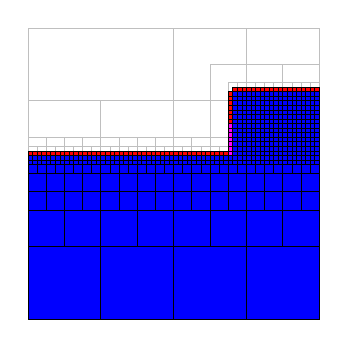
\begin{tikzpicture}[x={(\screenshotunitlength,0)},y={(0,\screenshotunitlength)}]
        \definecolor{fillcolor}{rgb}{0.000000,0.000000,1.000000}
\fill[fillcolor] (0.000000,0.000000) rectangle (0.250000,0.250000);
\definecolor{fillcolor}{rgb}{0.000000,0.000000,1.000000}
\fill[fillcolor] (0.250000,0.000000) rectangle (0.500000,0.250000);
\definecolor{fillcolor}{rgb}{0.000000,0.000000,1.000000}
\fill[fillcolor] (0.000000,0.250000) rectangle (0.125000,0.375000);
\definecolor{fillcolor}{rgb}{0.000000,0.000000,1.000000}
\fill[fillcolor] (0.125000,0.250000) rectangle (0.250000,0.375000);
\definecolor{fillcolor}{rgb}{0.000000,0.000000,1.000000}
\fill[fillcolor] (0.000000,0.375000) rectangle (0.062500,0.437500);
\definecolor{fillcolor}{rgb}{0.000000,0.000000,1.000000}
\fill[fillcolor] (0.062500,0.375000) rectangle (0.125000,0.437500);
\definecolor{fillcolor}{rgb}{0.000000,0.000000,1.000000}
\fill[fillcolor] (0.000000,0.437500) rectangle (0.062500,0.500000);
\definecolor{fillcolor}{rgb}{0.000000,0.000000,1.000000}
\fill[fillcolor] (0.062500,0.437500) rectangle (0.125000,0.500000);
\definecolor{fillcolor}{rgb}{0.000000,0.000000,1.000000}
\fill[fillcolor] (0.125000,0.375000) rectangle (0.187500,0.437500);
\definecolor{fillcolor}{rgb}{0.000000,0.000000,1.000000}
\fill[fillcolor] (0.187500,0.375000) rectangle (0.250000,0.437500);
\definecolor{fillcolor}{rgb}{0.000000,0.000000,1.000000}
\fill[fillcolor] (0.125000,0.437500) rectangle (0.187500,0.500000);
\definecolor{fillcolor}{rgb}{0.000000,0.000000,1.000000}
\fill[fillcolor] (0.187500,0.437500) rectangle (0.250000,0.500000);
\definecolor{fillcolor}{rgb}{0.000000,0.000000,1.000000}
\fill[fillcolor] (0.250000,0.250000) rectangle (0.375000,0.375000);
\definecolor{fillcolor}{rgb}{0.000000,0.000000,1.000000}
\fill[fillcolor] (0.375000,0.250000) rectangle (0.500000,0.375000);
\definecolor{fillcolor}{rgb}{0.000000,0.000000,1.000000}
\fill[fillcolor] (0.250000,0.375000) rectangle (0.312500,0.437500);
\definecolor{fillcolor}{rgb}{0.000000,0.000000,1.000000}
\fill[fillcolor] (0.312500,0.375000) rectangle (0.375000,0.437500);
\definecolor{fillcolor}{rgb}{0.000000,0.000000,1.000000}
\fill[fillcolor] (0.250000,0.437500) rectangle (0.312500,0.500000);
\definecolor{fillcolor}{rgb}{0.000000,0.000000,1.000000}
\fill[fillcolor] (0.312500,0.437500) rectangle (0.375000,0.500000);
\definecolor{fillcolor}{rgb}{0.000000,0.000000,1.000000}
\fill[fillcolor] (0.375000,0.375000) rectangle (0.437500,0.437500);
\definecolor{fillcolor}{rgb}{0.000000,0.000000,1.000000}
\fill[fillcolor] (0.437500,0.375000) rectangle (0.500000,0.437500);
\definecolor{fillcolor}{rgb}{0.000000,0.000000,1.000000}
\fill[fillcolor] (0.375000,0.437500) rectangle (0.437500,0.500000);
\definecolor{fillcolor}{rgb}{0.000000,0.000000,1.000000}
\fill[fillcolor] (0.437500,0.437500) rectangle (0.500000,0.500000);
\definecolor{fillcolor}{rgb}{0.000000,0.000000,1.000000}
\fill[fillcolor] (0.500000,0.000000) rectangle (0.750000,0.250000);
\definecolor{fillcolor}{rgb}{0.000000,0.000000,1.000000}
\fill[fillcolor] (0.750000,0.000000) rectangle (1.000000,0.250000);
\definecolor{fillcolor}{rgb}{0.000000,0.000000,1.000000}
\fill[fillcolor] (0.500000,0.250000) rectangle (0.625000,0.375000);
\definecolor{fillcolor}{rgb}{0.000000,0.000000,1.000000}
\fill[fillcolor] (0.625000,0.250000) rectangle (0.750000,0.375000);
\definecolor{fillcolor}{rgb}{0.000000,0.000000,1.000000}
\fill[fillcolor] (0.500000,0.375000) rectangle (0.562500,0.437500);
\definecolor{fillcolor}{rgb}{0.000000,0.000000,1.000000}
\fill[fillcolor] (0.562500,0.375000) rectangle (0.625000,0.437500);
\definecolor{fillcolor}{rgb}{0.000000,0.000000,1.000000}
\fill[fillcolor] (0.500000,0.437500) rectangle (0.562500,0.500000);
\definecolor{fillcolor}{rgb}{0.000000,0.000000,1.000000}
\fill[fillcolor] (0.562500,0.437500) rectangle (0.625000,0.500000);
\definecolor{fillcolor}{rgb}{0.000000,0.000000,1.000000}
\fill[fillcolor] (0.625000,0.375000) rectangle (0.687500,0.437500);
\definecolor{fillcolor}{rgb}{0.000000,0.000000,1.000000}
\fill[fillcolor] (0.687500,0.375000) rectangle (0.750000,0.437500);
\definecolor{fillcolor}{rgb}{0.000000,0.000000,1.000000}
\fill[fillcolor] (0.625000,0.437500) rectangle (0.687500,0.500000);
\definecolor{fillcolor}{rgb}{0.000000,0.000000,1.000000}
\fill[fillcolor] (0.687500,0.437500) rectangle (0.750000,0.500000);
\definecolor{fillcolor}{rgb}{0.000000,0.000000,1.000000}
\fill[fillcolor] (0.750000,0.250000) rectangle (0.875000,0.375000);
\definecolor{fillcolor}{rgb}{0.000000,0.000000,1.000000}
\fill[fillcolor] (0.875000,0.250000) rectangle (1.000000,0.375000);
\definecolor{fillcolor}{rgb}{0.000000,0.000000,1.000000}
\fill[fillcolor] (0.750000,0.375000) rectangle (0.812500,0.437500);
\definecolor{fillcolor}{rgb}{0.000000,0.000000,1.000000}
\fill[fillcolor] (0.812500,0.375000) rectangle (0.875000,0.437500);
\definecolor{fillcolor}{rgb}{0.000000,0.000000,1.000000}
\fill[fillcolor] (0.750000,0.437500) rectangle (0.812500,0.500000);
\definecolor{fillcolor}{rgb}{0.000000,0.000000,1.000000}
\fill[fillcolor] (0.812500,0.437500) rectangle (0.875000,0.500000);
\definecolor{fillcolor}{rgb}{0.000000,0.000000,1.000000}
\fill[fillcolor] (0.875000,0.375000) rectangle (0.937500,0.437500);
\definecolor{fillcolor}{rgb}{0.000000,0.000000,1.000000}
\fill[fillcolor] (0.937500,0.375000) rectangle (1.000000,0.437500);
\definecolor{fillcolor}{rgb}{0.000000,0.000000,1.000000}
\fill[fillcolor] (0.875000,0.437500) rectangle (0.937500,0.500000);
\definecolor{fillcolor}{rgb}{0.000000,0.000000,1.000000}
\fill[fillcolor] (0.937500,0.437500) rectangle (1.000000,0.500000);
\definecolor{fillcolor}{rgb}{0.000000,0.000000,1.000000}
\fill[fillcolor] (0.000000,0.500000) rectangle (0.031250,0.531250);
\definecolor{fillcolor}{rgb}{0.000000,0.000000,1.000000}
\fill[fillcolor] (0.031250,0.500000) rectangle (0.062500,0.531250);
\definecolor{fillcolor}{rgb}{0.000000,0.000000,1.000000}
\fill[fillcolor] (0.000000,0.531250) rectangle (0.015625,0.546875);
\definecolor{fillcolor}{rgb}{0.000000,0.000000,1.000000}
\fill[fillcolor] (0.015625,0.531250) rectangle (0.031250,0.546875);
\definecolor{fillcolor}{rgb}{0.000000,0.000000,1.000000}
\fill[fillcolor] (0.000000,0.546875) rectangle (0.015625,0.562500);
\definecolor{fillcolor}{rgb}{0.000000,0.000000,1.000000}
\fill[fillcolor] (0.015625,0.546875) rectangle (0.031250,0.562500);
\definecolor{fillcolor}{rgb}{0.000000,0.000000,1.000000}
\fill[fillcolor] (0.031250,0.531250) rectangle (0.046875,0.546875);
\definecolor{fillcolor}{rgb}{0.000000,0.000000,1.000000}
\fill[fillcolor] (0.046875,0.531250) rectangle (0.062500,0.546875);
\definecolor{fillcolor}{rgb}{0.000000,0.000000,1.000000}
\fill[fillcolor] (0.031250,0.546875) rectangle (0.046875,0.562500);
\definecolor{fillcolor}{rgb}{0.000000,0.000000,1.000000}
\fill[fillcolor] (0.046875,0.546875) rectangle (0.062500,0.562500);
\definecolor{fillcolor}{rgb}{0.000000,0.000000,1.000000}
\fill[fillcolor] (0.062500,0.500000) rectangle (0.093750,0.531250);
\definecolor{fillcolor}{rgb}{0.000000,0.000000,1.000000}
\fill[fillcolor] (0.093750,0.500000) rectangle (0.125000,0.531250);
\definecolor{fillcolor}{rgb}{0.000000,0.000000,1.000000}
\fill[fillcolor] (0.062500,0.531250) rectangle (0.078125,0.546875);
\definecolor{fillcolor}{rgb}{0.000000,0.000000,1.000000}
\fill[fillcolor] (0.078125,0.531250) rectangle (0.093750,0.546875);
\definecolor{fillcolor}{rgb}{0.000000,0.000000,1.000000}
\fill[fillcolor] (0.062500,0.546875) rectangle (0.078125,0.562500);
\definecolor{fillcolor}{rgb}{0.000000,0.000000,1.000000}
\fill[fillcolor] (0.078125,0.546875) rectangle (0.093750,0.562500);
\definecolor{fillcolor}{rgb}{0.000000,0.000000,1.000000}
\fill[fillcolor] (0.093750,0.531250) rectangle (0.109375,0.546875);
\definecolor{fillcolor}{rgb}{0.000000,0.000000,1.000000}
\fill[fillcolor] (0.109375,0.531250) rectangle (0.125000,0.546875);
\definecolor{fillcolor}{rgb}{0.000000,0.000000,1.000000}
\fill[fillcolor] (0.093750,0.546875) rectangle (0.109375,0.562500);
\definecolor{fillcolor}{rgb}{0.000000,0.000000,1.000000}
\fill[fillcolor] (0.109375,0.546875) rectangle (0.125000,0.562500);
\definecolor{fillcolor}{rgb}{1.000000,0.000000,0.000000}
\fill[fillcolor] (0.000000,0.562500) rectangle (0.015625,0.578125);
\definecolor{fillcolor}{rgb}{1.000000,0.000000,0.000000}
\fill[fillcolor] (0.015625,0.562500) rectangle (0.031250,0.578125);
\definecolor{fillcolor}{rgb}{1.000000,0.000000,0.000000}
\fill[fillcolor] (0.031250,0.562500) rectangle (0.046875,0.578125);
\definecolor{fillcolor}{rgb}{1.000000,0.000000,0.000000}
\fill[fillcolor] (0.046875,0.562500) rectangle (0.062500,0.578125);
\definecolor{fillcolor}{rgb}{1.000000,0.000000,0.000000}
\fill[fillcolor] (0.062500,0.562500) rectangle (0.078125,0.578125);
\definecolor{fillcolor}{rgb}{1.000000,0.000000,0.000000}
\fill[fillcolor] (0.078125,0.562500) rectangle (0.093750,0.578125);
\definecolor{fillcolor}{rgb}{1.000000,0.000000,0.000000}
\fill[fillcolor] (0.093750,0.562500) rectangle (0.109375,0.578125);
\definecolor{fillcolor}{rgb}{1.000000,0.000000,0.000000}
\fill[fillcolor] (0.109375,0.562500) rectangle (0.125000,0.578125);
\definecolor{fillcolor}{rgb}{0.000000,0.000000,1.000000}
\fill[fillcolor] (0.125000,0.500000) rectangle (0.156250,0.531250);
\definecolor{fillcolor}{rgb}{0.000000,0.000000,1.000000}
\fill[fillcolor] (0.156250,0.500000) rectangle (0.187500,0.531250);
\definecolor{fillcolor}{rgb}{0.000000,0.000000,1.000000}
\fill[fillcolor] (0.125000,0.531250) rectangle (0.140625,0.546875);
\definecolor{fillcolor}{rgb}{0.000000,0.000000,1.000000}
\fill[fillcolor] (0.140625,0.531250) rectangle (0.156250,0.546875);
\definecolor{fillcolor}{rgb}{0.000000,0.000000,1.000000}
\fill[fillcolor] (0.125000,0.546875) rectangle (0.140625,0.562500);
\definecolor{fillcolor}{rgb}{0.000000,0.000000,1.000000}
\fill[fillcolor] (0.140625,0.546875) rectangle (0.156250,0.562500);
\definecolor{fillcolor}{rgb}{0.000000,0.000000,1.000000}
\fill[fillcolor] (0.156250,0.531250) rectangle (0.171875,0.546875);
\definecolor{fillcolor}{rgb}{0.000000,0.000000,1.000000}
\fill[fillcolor] (0.171875,0.531250) rectangle (0.187500,0.546875);
\definecolor{fillcolor}{rgb}{0.000000,0.000000,1.000000}
\fill[fillcolor] (0.156250,0.546875) rectangle (0.171875,0.562500);
\definecolor{fillcolor}{rgb}{0.000000,0.000000,1.000000}
\fill[fillcolor] (0.171875,0.546875) rectangle (0.187500,0.562500);
\definecolor{fillcolor}{rgb}{0.000000,0.000000,1.000000}
\fill[fillcolor] (0.187500,0.500000) rectangle (0.218750,0.531250);
\definecolor{fillcolor}{rgb}{0.000000,0.000000,1.000000}
\fill[fillcolor] (0.218750,0.500000) rectangle (0.250000,0.531250);
\definecolor{fillcolor}{rgb}{0.000000,0.000000,1.000000}
\fill[fillcolor] (0.187500,0.531250) rectangle (0.203125,0.546875);
\definecolor{fillcolor}{rgb}{0.000000,0.000000,1.000000}
\fill[fillcolor] (0.203125,0.531250) rectangle (0.218750,0.546875);
\definecolor{fillcolor}{rgb}{0.000000,0.000000,1.000000}
\fill[fillcolor] (0.187500,0.546875) rectangle (0.203125,0.562500);
\definecolor{fillcolor}{rgb}{0.000000,0.000000,1.000000}
\fill[fillcolor] (0.203125,0.546875) rectangle (0.218750,0.562500);
\definecolor{fillcolor}{rgb}{0.000000,0.000000,1.000000}
\fill[fillcolor] (0.218750,0.531250) rectangle (0.234375,0.546875);
\definecolor{fillcolor}{rgb}{0.000000,0.000000,1.000000}
\fill[fillcolor] (0.234375,0.531250) rectangle (0.250000,0.546875);
\definecolor{fillcolor}{rgb}{0.000000,0.000000,1.000000}
\fill[fillcolor] (0.218750,0.546875) rectangle (0.234375,0.562500);
\definecolor{fillcolor}{rgb}{0.000000,0.000000,1.000000}
\fill[fillcolor] (0.234375,0.546875) rectangle (0.250000,0.562500);
\definecolor{fillcolor}{rgb}{1.000000,0.000000,0.000000}
\fill[fillcolor] (0.125000,0.562500) rectangle (0.140625,0.578125);
\definecolor{fillcolor}{rgb}{1.000000,0.000000,0.000000}
\fill[fillcolor] (0.140625,0.562500) rectangle (0.156250,0.578125);
\definecolor{fillcolor}{rgb}{1.000000,0.000000,0.000000}
\fill[fillcolor] (0.156250,0.562500) rectangle (0.171875,0.578125);
\definecolor{fillcolor}{rgb}{1.000000,0.000000,0.000000}
\fill[fillcolor] (0.171875,0.562500) rectangle (0.187500,0.578125);
\definecolor{fillcolor}{rgb}{1.000000,0.000000,0.000000}
\fill[fillcolor] (0.187500,0.562500) rectangle (0.203125,0.578125);
\definecolor{fillcolor}{rgb}{1.000000,0.000000,0.000000}
\fill[fillcolor] (0.203125,0.562500) rectangle (0.218750,0.578125);
\definecolor{fillcolor}{rgb}{1.000000,0.000000,0.000000}
\fill[fillcolor] (0.218750,0.562500) rectangle (0.234375,0.578125);
\definecolor{fillcolor}{rgb}{1.000000,0.000000,0.000000}
\fill[fillcolor] (0.234375,0.562500) rectangle (0.250000,0.578125);
\definecolor{fillcolor}{rgb}{0.000000,0.000000,1.000000}
\fill[fillcolor] (0.250000,0.500000) rectangle (0.281250,0.531250);
\definecolor{fillcolor}{rgb}{0.000000,0.000000,1.000000}
\fill[fillcolor] (0.281250,0.500000) rectangle (0.312500,0.531250);
\definecolor{fillcolor}{rgb}{0.000000,0.000000,1.000000}
\fill[fillcolor] (0.250000,0.531250) rectangle (0.265625,0.546875);
\definecolor{fillcolor}{rgb}{0.000000,0.000000,1.000000}
\fill[fillcolor] (0.265625,0.531250) rectangle (0.281250,0.546875);
\definecolor{fillcolor}{rgb}{0.000000,0.000000,1.000000}
\fill[fillcolor] (0.250000,0.546875) rectangle (0.265625,0.562500);
\definecolor{fillcolor}{rgb}{0.000000,0.000000,1.000000}
\fill[fillcolor] (0.265625,0.546875) rectangle (0.281250,0.562500);
\definecolor{fillcolor}{rgb}{0.000000,0.000000,1.000000}
\fill[fillcolor] (0.281250,0.531250) rectangle (0.296875,0.546875);
\definecolor{fillcolor}{rgb}{0.000000,0.000000,1.000000}
\fill[fillcolor] (0.296875,0.531250) rectangle (0.312500,0.546875);
\definecolor{fillcolor}{rgb}{0.000000,0.000000,1.000000}
\fill[fillcolor] (0.281250,0.546875) rectangle (0.296875,0.562500);
\definecolor{fillcolor}{rgb}{0.000000,0.000000,1.000000}
\fill[fillcolor] (0.296875,0.546875) rectangle (0.312500,0.562500);
\definecolor{fillcolor}{rgb}{0.000000,0.000000,1.000000}
\fill[fillcolor] (0.312500,0.500000) rectangle (0.343750,0.531250);
\definecolor{fillcolor}{rgb}{0.000000,0.000000,1.000000}
\fill[fillcolor] (0.343750,0.500000) rectangle (0.375000,0.531250);
\definecolor{fillcolor}{rgb}{0.000000,0.000000,1.000000}
\fill[fillcolor] (0.312500,0.531250) rectangle (0.328125,0.546875);
\definecolor{fillcolor}{rgb}{0.000000,0.000000,1.000000}
\fill[fillcolor] (0.328125,0.531250) rectangle (0.343750,0.546875);
\definecolor{fillcolor}{rgb}{0.000000,0.000000,1.000000}
\fill[fillcolor] (0.312500,0.546875) rectangle (0.328125,0.562500);
\definecolor{fillcolor}{rgb}{0.000000,0.000000,1.000000}
\fill[fillcolor] (0.328125,0.546875) rectangle (0.343750,0.562500);
\definecolor{fillcolor}{rgb}{0.000000,0.000000,1.000000}
\fill[fillcolor] (0.343750,0.531250) rectangle (0.359375,0.546875);
\definecolor{fillcolor}{rgb}{0.000000,0.000000,1.000000}
\fill[fillcolor] (0.359375,0.531250) rectangle (0.375000,0.546875);
\definecolor{fillcolor}{rgb}{0.000000,0.000000,1.000000}
\fill[fillcolor] (0.343750,0.546875) rectangle (0.359375,0.562500);
\definecolor{fillcolor}{rgb}{0.000000,0.000000,1.000000}
\fill[fillcolor] (0.359375,0.546875) rectangle (0.375000,0.562500);
\definecolor{fillcolor}{rgb}{1.000000,0.000000,0.000000}
\fill[fillcolor] (0.250000,0.562500) rectangle (0.265625,0.578125);
\definecolor{fillcolor}{rgb}{1.000000,0.000000,0.000000}
\fill[fillcolor] (0.265625,0.562500) rectangle (0.281250,0.578125);
\definecolor{fillcolor}{rgb}{1.000000,0.000000,0.000000}
\fill[fillcolor] (0.281250,0.562500) rectangle (0.296875,0.578125);
\definecolor{fillcolor}{rgb}{1.000000,0.000000,0.000000}
\fill[fillcolor] (0.296875,0.562500) rectangle (0.312500,0.578125);
\definecolor{fillcolor}{rgb}{1.000000,0.000000,0.000000}
\fill[fillcolor] (0.312500,0.562500) rectangle (0.328125,0.578125);
\definecolor{fillcolor}{rgb}{1.000000,0.000000,0.000000}
\fill[fillcolor] (0.328125,0.562500) rectangle (0.343750,0.578125);
\definecolor{fillcolor}{rgb}{1.000000,0.000000,0.000000}
\fill[fillcolor] (0.343750,0.562500) rectangle (0.359375,0.578125);
\definecolor{fillcolor}{rgb}{1.000000,0.000000,0.000000}
\fill[fillcolor] (0.359375,0.562500) rectangle (0.375000,0.578125);
\definecolor{fillcolor}{rgb}{0.000000,0.000000,1.000000}
\fill[fillcolor] (0.375000,0.500000) rectangle (0.406250,0.531250);
\definecolor{fillcolor}{rgb}{0.000000,0.000000,1.000000}
\fill[fillcolor] (0.406250,0.500000) rectangle (0.437500,0.531250);
\definecolor{fillcolor}{rgb}{0.000000,0.000000,1.000000}
\fill[fillcolor] (0.375000,0.531250) rectangle (0.390625,0.546875);
\definecolor{fillcolor}{rgb}{0.000000,0.000000,1.000000}
\fill[fillcolor] (0.390625,0.531250) rectangle (0.406250,0.546875);
\definecolor{fillcolor}{rgb}{0.000000,0.000000,1.000000}
\fill[fillcolor] (0.375000,0.546875) rectangle (0.390625,0.562500);
\definecolor{fillcolor}{rgb}{0.000000,0.000000,1.000000}
\fill[fillcolor] (0.390625,0.546875) rectangle (0.406250,0.562500);
\definecolor{fillcolor}{rgb}{0.000000,0.000000,1.000000}
\fill[fillcolor] (0.406250,0.531250) rectangle (0.421875,0.546875);
\definecolor{fillcolor}{rgb}{0.000000,0.000000,1.000000}
\fill[fillcolor] (0.421875,0.531250) rectangle (0.437500,0.546875);
\definecolor{fillcolor}{rgb}{0.000000,0.000000,1.000000}
\fill[fillcolor] (0.406250,0.546875) rectangle (0.421875,0.562500);
\definecolor{fillcolor}{rgb}{0.000000,0.000000,1.000000}
\fill[fillcolor] (0.421875,0.546875) rectangle (0.437500,0.562500);
\definecolor{fillcolor}{rgb}{0.000000,0.000000,1.000000}
\fill[fillcolor] (0.437500,0.500000) rectangle (0.468750,0.531250);
\definecolor{fillcolor}{rgb}{0.000000,0.000000,1.000000}
\fill[fillcolor] (0.468750,0.500000) rectangle (0.500000,0.531250);
\definecolor{fillcolor}{rgb}{0.000000,0.000000,1.000000}
\fill[fillcolor] (0.437500,0.531250) rectangle (0.453125,0.546875);
\definecolor{fillcolor}{rgb}{0.000000,0.000000,1.000000}
\fill[fillcolor] (0.453125,0.531250) rectangle (0.468750,0.546875);
\definecolor{fillcolor}{rgb}{0.000000,0.000000,1.000000}
\fill[fillcolor] (0.437500,0.546875) rectangle (0.453125,0.562500);
\definecolor{fillcolor}{rgb}{0.000000,0.000000,1.000000}
\fill[fillcolor] (0.453125,0.546875) rectangle (0.468750,0.562500);
\definecolor{fillcolor}{rgb}{0.000000,0.000000,1.000000}
\fill[fillcolor] (0.468750,0.531250) rectangle (0.484375,0.546875);
\definecolor{fillcolor}{rgb}{0.000000,0.000000,1.000000}
\fill[fillcolor] (0.484375,0.531250) rectangle (0.500000,0.546875);
\definecolor{fillcolor}{rgb}{0.000000,0.000000,1.000000}
\fill[fillcolor] (0.468750,0.546875) rectangle (0.484375,0.562500);
\definecolor{fillcolor}{rgb}{0.000000,0.000000,1.000000}
\fill[fillcolor] (0.484375,0.546875) rectangle (0.500000,0.562500);
\definecolor{fillcolor}{rgb}{1.000000,0.000000,0.000000}
\fill[fillcolor] (0.375000,0.562500) rectangle (0.390625,0.578125);
\definecolor{fillcolor}{rgb}{1.000000,0.000000,0.000000}
\fill[fillcolor] (0.390625,0.562500) rectangle (0.406250,0.578125);
\definecolor{fillcolor}{rgb}{1.000000,0.000000,0.000000}
\fill[fillcolor] (0.406250,0.562500) rectangle (0.421875,0.578125);
\definecolor{fillcolor}{rgb}{1.000000,0.000000,0.000000}
\fill[fillcolor] (0.421875,0.562500) rectangle (0.437500,0.578125);
\definecolor{fillcolor}{rgb}{1.000000,0.000000,0.000000}
\fill[fillcolor] (0.437500,0.562500) rectangle (0.453125,0.578125);
\definecolor{fillcolor}{rgb}{1.000000,0.000000,0.000000}
\fill[fillcolor] (0.453125,0.562500) rectangle (0.468750,0.578125);
\definecolor{fillcolor}{rgb}{1.000000,0.000000,0.000000}
\fill[fillcolor] (0.468750,0.562500) rectangle (0.484375,0.578125);
\definecolor{fillcolor}{rgb}{1.000000,0.000000,0.000000}
\fill[fillcolor] (0.484375,0.562500) rectangle (0.500000,0.578125);
\definecolor{fillcolor}{rgb}{0.000000,0.000000,1.000000}
\fill[fillcolor] (0.500000,0.500000) rectangle (0.531250,0.531250);
\definecolor{fillcolor}{rgb}{0.000000,0.000000,1.000000}
\fill[fillcolor] (0.531250,0.500000) rectangle (0.562500,0.531250);
\definecolor{fillcolor}{rgb}{0.000000,0.000000,1.000000}
\fill[fillcolor] (0.500000,0.531250) rectangle (0.515625,0.546875);
\definecolor{fillcolor}{rgb}{0.000000,0.000000,1.000000}
\fill[fillcolor] (0.515625,0.531250) rectangle (0.531250,0.546875);
\definecolor{fillcolor}{rgb}{0.000000,0.000000,1.000000}
\fill[fillcolor] (0.500000,0.546875) rectangle (0.515625,0.562500);
\definecolor{fillcolor}{rgb}{0.000000,0.000000,1.000000}
\fill[fillcolor] (0.515625,0.546875) rectangle (0.531250,0.562500);
\definecolor{fillcolor}{rgb}{0.000000,0.000000,1.000000}
\fill[fillcolor] (0.531250,0.531250) rectangle (0.546875,0.546875);
\definecolor{fillcolor}{rgb}{0.000000,0.000000,1.000000}
\fill[fillcolor] (0.546875,0.531250) rectangle (0.562500,0.546875);
\definecolor{fillcolor}{rgb}{0.000000,0.000000,1.000000}
\fill[fillcolor] (0.531250,0.546875) rectangle (0.546875,0.562500);
\definecolor{fillcolor}{rgb}{0.000000,0.000000,1.000000}
\fill[fillcolor] (0.546875,0.546875) rectangle (0.562500,0.562500);
\definecolor{fillcolor}{rgb}{0.000000,0.000000,1.000000}
\fill[fillcolor] (0.562500,0.500000) rectangle (0.593750,0.531250);
\definecolor{fillcolor}{rgb}{0.000000,0.000000,1.000000}
\fill[fillcolor] (0.593750,0.500000) rectangle (0.625000,0.531250);
\definecolor{fillcolor}{rgb}{0.000000,0.000000,1.000000}
\fill[fillcolor] (0.562500,0.531250) rectangle (0.578125,0.546875);
\definecolor{fillcolor}{rgb}{0.000000,0.000000,1.000000}
\fill[fillcolor] (0.578125,0.531250) rectangle (0.593750,0.546875);
\definecolor{fillcolor}{rgb}{0.000000,0.000000,1.000000}
\fill[fillcolor] (0.562500,0.546875) rectangle (0.578125,0.562500);
\definecolor{fillcolor}{rgb}{0.000000,0.000000,1.000000}
\fill[fillcolor] (0.578125,0.546875) rectangle (0.593750,0.562500);
\definecolor{fillcolor}{rgb}{0.000000,0.000000,1.000000}
\fill[fillcolor] (0.593750,0.531250) rectangle (0.609375,0.546875);
\definecolor{fillcolor}{rgb}{0.000000,0.000000,1.000000}
\fill[fillcolor] (0.609375,0.531250) rectangle (0.625000,0.546875);
\definecolor{fillcolor}{rgb}{0.000000,0.000000,1.000000}
\fill[fillcolor] (0.593750,0.546875) rectangle (0.609375,0.562500);
\definecolor{fillcolor}{rgb}{0.000000,0.000000,1.000000}
\fill[fillcolor] (0.609375,0.546875) rectangle (0.625000,0.562500);
\definecolor{fillcolor}{rgb}{1.000000,0.000000,0.000000}
\fill[fillcolor] (0.500000,0.562500) rectangle (0.515625,0.578125);
\definecolor{fillcolor}{rgb}{1.000000,0.000000,0.000000}
\fill[fillcolor] (0.515625,0.562500) rectangle (0.531250,0.578125);
\definecolor{fillcolor}{rgb}{1.000000,0.000000,0.000000}
\fill[fillcolor] (0.531250,0.562500) rectangle (0.546875,0.578125);
\definecolor{fillcolor}{rgb}{1.000000,0.000000,0.000000}
\fill[fillcolor] (0.546875,0.562500) rectangle (0.562500,0.578125);
\definecolor{fillcolor}{rgb}{1.000000,0.000000,0.000000}
\fill[fillcolor] (0.562500,0.562500) rectangle (0.578125,0.578125);
\definecolor{fillcolor}{rgb}{1.000000,0.000000,0.000000}
\fill[fillcolor] (0.578125,0.562500) rectangle (0.593750,0.578125);
\definecolor{fillcolor}{rgb}{1.000000,0.000000,0.000000}
\fill[fillcolor] (0.593750,0.562500) rectangle (0.609375,0.578125);
\definecolor{fillcolor}{rgb}{1.000000,0.000000,0.000000}
\fill[fillcolor] (0.609375,0.562500) rectangle (0.625000,0.578125);
\definecolor{fillcolor}{rgb}{0.000000,0.000000,1.000000}
\fill[fillcolor] (0.625000,0.500000) rectangle (0.656250,0.531250);
\definecolor{fillcolor}{rgb}{0.000000,0.000000,1.000000}
\fill[fillcolor] (0.656250,0.500000) rectangle (0.687500,0.531250);
\definecolor{fillcolor}{rgb}{0.000000,0.000000,1.000000}
\fill[fillcolor] (0.625000,0.531250) rectangle (0.640625,0.546875);
\definecolor{fillcolor}{rgb}{0.000000,0.000000,1.000000}
\fill[fillcolor] (0.640625,0.531250) rectangle (0.656250,0.546875);
\definecolor{fillcolor}{rgb}{0.000000,0.000000,1.000000}
\fill[fillcolor] (0.625000,0.546875) rectangle (0.640625,0.562500);
\definecolor{fillcolor}{rgb}{0.000000,0.000000,1.000000}
\fill[fillcolor] (0.640625,0.546875) rectangle (0.656250,0.562500);
\definecolor{fillcolor}{rgb}{0.000000,0.000000,1.000000}
\fill[fillcolor] (0.656250,0.531250) rectangle (0.671875,0.546875);
\definecolor{fillcolor}{rgb}{0.000000,0.000000,1.000000}
\fill[fillcolor] (0.671875,0.531250) rectangle (0.687500,0.546875);
\definecolor{fillcolor}{rgb}{0.000000,0.000000,1.000000}
\fill[fillcolor] (0.656250,0.546875) rectangle (0.671875,0.562500);
\definecolor{fillcolor}{rgb}{0.000000,0.000000,1.000000}
\fill[fillcolor] (0.671875,0.546875) rectangle (0.687500,0.562500);
\definecolor{fillcolor}{rgb}{0.000000,0.000000,1.000000}
\fill[fillcolor] (0.687500,0.500000) rectangle (0.718750,0.531250);
\definecolor{fillcolor}{rgb}{0.000000,0.000000,1.000000}
\fill[fillcolor] (0.718750,0.500000) rectangle (0.750000,0.531250);
\definecolor{fillcolor}{rgb}{0.000000,0.000000,1.000000}
\fill[fillcolor] (0.687500,0.531250) rectangle (0.703125,0.546875);
\definecolor{fillcolor}{rgb}{0.000000,0.000000,1.000000}
\fill[fillcolor] (0.703125,0.531250) rectangle (0.718750,0.546875);
\definecolor{fillcolor}{rgb}{0.000000,0.000000,1.000000}
\fill[fillcolor] (0.687500,0.546875) rectangle (0.703125,0.562500);
\definecolor{fillcolor}{rgb}{0.000000,0.000000,1.000000}
\fill[fillcolor] (0.703125,0.546875) rectangle (0.718750,0.562500);
\definecolor{fillcolor}{rgb}{0.000000,0.000000,1.000000}
\fill[fillcolor] (0.718750,0.531250) rectangle (0.734375,0.546875);
\definecolor{fillcolor}{rgb}{0.000000,0.000000,1.000000}
\fill[fillcolor] (0.734375,0.531250) rectangle (0.750000,0.546875);
\definecolor{fillcolor}{rgb}{0.000000,0.000000,1.000000}
\fill[fillcolor] (0.718750,0.546875) rectangle (0.734375,0.562500);
\definecolor{fillcolor}{rgb}{0.000000,0.000000,1.000000}
\fill[fillcolor] (0.734375,0.546875) rectangle (0.750000,0.562500);
\definecolor{fillcolor}{rgb}{1.000000,0.000000,0.000000}
\fill[fillcolor] (0.625000,0.562500) rectangle (0.640625,0.578125);
\definecolor{fillcolor}{rgb}{1.000000,0.000000,0.000000}
\fill[fillcolor] (0.640625,0.562500) rectangle (0.656250,0.578125);
\definecolor{fillcolor}{rgb}{1.000000,0.000000,0.000000}
\fill[fillcolor] (0.656250,0.562500) rectangle (0.671875,0.578125);
\definecolor{fillcolor}{rgb}{1.000000,0.000000,0.000000}
\fill[fillcolor] (0.671875,0.562500) rectangle (0.687500,0.578125);
\definecolor{fillcolor}{rgb}{1.000000,0.000000,1.000000}
\fill[fillcolor] (0.687500,0.562500) rectangle (0.703125,0.578125);
\definecolor{fillcolor}{rgb}{0.000000,0.000000,1.000000}
\fill[fillcolor] (0.703125,0.562500) rectangle (0.718750,0.578125);
\definecolor{fillcolor}{rgb}{1.000000,0.000000,1.000000}
\fill[fillcolor] (0.687500,0.578125) rectangle (0.703125,0.593750);
\definecolor{fillcolor}{rgb}{0.000000,0.000000,1.000000}
\fill[fillcolor] (0.703125,0.578125) rectangle (0.718750,0.593750);
\definecolor{fillcolor}{rgb}{0.000000,0.000000,1.000000}
\fill[fillcolor] (0.718750,0.562500) rectangle (0.734375,0.578125);
\definecolor{fillcolor}{rgb}{0.000000,0.000000,1.000000}
\fill[fillcolor] (0.734375,0.562500) rectangle (0.750000,0.578125);
\definecolor{fillcolor}{rgb}{0.000000,0.000000,1.000000}
\fill[fillcolor] (0.718750,0.578125) rectangle (0.734375,0.593750);
\definecolor{fillcolor}{rgb}{0.000000,0.000000,1.000000}
\fill[fillcolor] (0.734375,0.578125) rectangle (0.750000,0.593750);
\definecolor{fillcolor}{rgb}{1.000000,0.000000,1.000000}
\fill[fillcolor] (0.687500,0.593750) rectangle (0.703125,0.609375);
\definecolor{fillcolor}{rgb}{0.000000,0.000000,1.000000}
\fill[fillcolor] (0.703125,0.593750) rectangle (0.718750,0.609375);
\definecolor{fillcolor}{rgb}{1.000000,0.000000,1.000000}
\fill[fillcolor] (0.687500,0.609375) rectangle (0.703125,0.625000);
\definecolor{fillcolor}{rgb}{0.000000,0.000000,1.000000}
\fill[fillcolor] (0.703125,0.609375) rectangle (0.718750,0.625000);
\definecolor{fillcolor}{rgb}{0.000000,0.000000,1.000000}
\fill[fillcolor] (0.718750,0.593750) rectangle (0.734375,0.609375);
\definecolor{fillcolor}{rgb}{0.000000,0.000000,1.000000}
\fill[fillcolor] (0.734375,0.593750) rectangle (0.750000,0.609375);
\definecolor{fillcolor}{rgb}{0.000000,0.000000,1.000000}
\fill[fillcolor] (0.718750,0.609375) rectangle (0.734375,0.625000);
\definecolor{fillcolor}{rgb}{0.000000,0.000000,1.000000}
\fill[fillcolor] (0.734375,0.609375) rectangle (0.750000,0.625000);
\definecolor{fillcolor}{rgb}{1.000000,0.000000,1.000000}
\fill[fillcolor] (0.687500,0.625000) rectangle (0.703125,0.640625);
\definecolor{fillcolor}{rgb}{0.000000,0.000000,1.000000}
\fill[fillcolor] (0.703125,0.625000) rectangle (0.718750,0.640625);
\definecolor{fillcolor}{rgb}{1.000000,0.000000,1.000000}
\fill[fillcolor] (0.687500,0.640625) rectangle (0.703125,0.656250);
\definecolor{fillcolor}{rgb}{0.000000,0.000000,1.000000}
\fill[fillcolor] (0.703125,0.640625) rectangle (0.718750,0.656250);
\definecolor{fillcolor}{rgb}{0.000000,0.000000,1.000000}
\fill[fillcolor] (0.718750,0.625000) rectangle (0.734375,0.640625);
\definecolor{fillcolor}{rgb}{0.000000,0.000000,1.000000}
\fill[fillcolor] (0.734375,0.625000) rectangle (0.750000,0.640625);
\definecolor{fillcolor}{rgb}{0.000000,0.000000,1.000000}
\fill[fillcolor] (0.718750,0.640625) rectangle (0.734375,0.656250);
\definecolor{fillcolor}{rgb}{0.000000,0.000000,1.000000}
\fill[fillcolor] (0.734375,0.640625) rectangle (0.750000,0.656250);
\definecolor{fillcolor}{rgb}{1.000000,0.000000,1.000000}
\fill[fillcolor] (0.687500,0.656250) rectangle (0.703125,0.671875);
\definecolor{fillcolor}{rgb}{0.000000,0.000000,1.000000}
\fill[fillcolor] (0.703125,0.656250) rectangle (0.718750,0.671875);
\definecolor{fillcolor}{rgb}{1.000000,0.003774,0.000000}
\fill[fillcolor] (0.687500,0.671875) rectangle (0.703125,0.687500);
\definecolor{fillcolor}{rgb}{0.000000,0.000000,1.000000}
\fill[fillcolor] (0.703125,0.671875) rectangle (0.718750,0.687500);
\definecolor{fillcolor}{rgb}{0.000000,0.000000,1.000000}
\fill[fillcolor] (0.718750,0.656250) rectangle (0.734375,0.671875);
\definecolor{fillcolor}{rgb}{0.000000,0.000000,1.000000}
\fill[fillcolor] (0.734375,0.656250) rectangle (0.750000,0.671875);
\definecolor{fillcolor}{rgb}{0.000000,0.000000,1.000000}
\fill[fillcolor] (0.718750,0.671875) rectangle (0.734375,0.687500);
\definecolor{fillcolor}{rgb}{0.000000,0.000000,1.000000}
\fill[fillcolor] (0.734375,0.671875) rectangle (0.750000,0.687500);
\definecolor{fillcolor}{rgb}{1.000000,0.011310,0.000000}
\fill[fillcolor] (0.687500,0.687500) rectangle (0.703125,0.703125);
\definecolor{fillcolor}{rgb}{0.000000,0.000000,1.000000}
\fill[fillcolor] (0.703125,0.687500) rectangle (0.718750,0.703125);
\definecolor{fillcolor}{rgb}{1.000000,0.018833,0.000000}
\fill[fillcolor] (0.687500,0.703125) rectangle (0.703125,0.718750);
\definecolor{fillcolor}{rgb}{0.000000,0.000000,1.000000}
\fill[fillcolor] (0.703125,0.703125) rectangle (0.718750,0.718750);
\definecolor{fillcolor}{rgb}{0.000000,0.000000,1.000000}
\fill[fillcolor] (0.718750,0.687500) rectangle (0.734375,0.703125);
\definecolor{fillcolor}{rgb}{0.000000,0.000000,1.000000}
\fill[fillcolor] (0.734375,0.687500) rectangle (0.750000,0.703125);
\definecolor{fillcolor}{rgb}{0.000000,0.000000,1.000000}
\fill[fillcolor] (0.718750,0.703125) rectangle (0.734375,0.718750);
\definecolor{fillcolor}{rgb}{0.000000,0.000000,1.000000}
\fill[fillcolor] (0.734375,0.703125) rectangle (0.750000,0.718750);
\definecolor{fillcolor}{rgb}{1.000000,0.026341,0.000000}
\fill[fillcolor] (0.687500,0.718750) rectangle (0.703125,0.734375);
\definecolor{fillcolor}{rgb}{0.000000,0.000000,1.000000}
\fill[fillcolor] (0.703125,0.718750) rectangle (0.718750,0.734375);
\definecolor{fillcolor}{rgb}{1.000000,0.033835,0.000000}
\fill[fillcolor] (0.687500,0.734375) rectangle (0.703125,0.750000);
\definecolor{fillcolor}{rgb}{0.000000,0.000000,1.000000}
\fill[fillcolor] (0.703125,0.734375) rectangle (0.718750,0.750000);
\definecolor{fillcolor}{rgb}{0.000000,0.000000,1.000000}
\fill[fillcolor] (0.718750,0.718750) rectangle (0.734375,0.734375);
\definecolor{fillcolor}{rgb}{0.000000,0.000000,1.000000}
\fill[fillcolor] (0.734375,0.718750) rectangle (0.750000,0.734375);
\definecolor{fillcolor}{rgb}{0.000000,0.000000,1.000000}
\fill[fillcolor] (0.718750,0.734375) rectangle (0.734375,0.750000);
\definecolor{fillcolor}{rgb}{0.000000,0.000000,1.000000}
\fill[fillcolor] (0.734375,0.734375) rectangle (0.750000,0.750000);
\definecolor{fillcolor}{rgb}{0.000000,0.000000,1.000000}
\fill[fillcolor] (0.750000,0.500000) rectangle (0.781250,0.531250);
\definecolor{fillcolor}{rgb}{0.000000,0.000000,1.000000}
\fill[fillcolor] (0.781250,0.500000) rectangle (0.812500,0.531250);
\definecolor{fillcolor}{rgb}{0.000000,0.000000,1.000000}
\fill[fillcolor] (0.750000,0.531250) rectangle (0.765625,0.546875);
\definecolor{fillcolor}{rgb}{0.000000,0.000000,1.000000}
\fill[fillcolor] (0.765625,0.531250) rectangle (0.781250,0.546875);
\definecolor{fillcolor}{rgb}{0.000000,0.000000,1.000000}
\fill[fillcolor] (0.750000,0.546875) rectangle (0.765625,0.562500);
\definecolor{fillcolor}{rgb}{0.000000,0.000000,1.000000}
\fill[fillcolor] (0.765625,0.546875) rectangle (0.781250,0.562500);
\definecolor{fillcolor}{rgb}{0.000000,0.000000,1.000000}
\fill[fillcolor] (0.781250,0.531250) rectangle (0.796875,0.546875);
\definecolor{fillcolor}{rgb}{0.000000,0.000000,1.000000}
\fill[fillcolor] (0.796875,0.531250) rectangle (0.812500,0.546875);
\definecolor{fillcolor}{rgb}{0.000000,0.000000,1.000000}
\fill[fillcolor] (0.781250,0.546875) rectangle (0.796875,0.562500);
\definecolor{fillcolor}{rgb}{0.000000,0.000000,1.000000}
\fill[fillcolor] (0.796875,0.546875) rectangle (0.812500,0.562500);
\definecolor{fillcolor}{rgb}{0.000000,0.000000,1.000000}
\fill[fillcolor] (0.812500,0.500000) rectangle (0.843750,0.531250);
\definecolor{fillcolor}{rgb}{0.000000,0.000000,1.000000}
\fill[fillcolor] (0.843750,0.500000) rectangle (0.875000,0.531250);
\definecolor{fillcolor}{rgb}{0.000000,0.000000,1.000000}
\fill[fillcolor] (0.812500,0.531250) rectangle (0.828125,0.546875);
\definecolor{fillcolor}{rgb}{0.000000,0.000000,1.000000}
\fill[fillcolor] (0.828125,0.531250) rectangle (0.843750,0.546875);
\definecolor{fillcolor}{rgb}{0.000000,0.000000,1.000000}
\fill[fillcolor] (0.812500,0.546875) rectangle (0.828125,0.562500);
\definecolor{fillcolor}{rgb}{0.000000,0.000000,1.000000}
\fill[fillcolor] (0.828125,0.546875) rectangle (0.843750,0.562500);
\definecolor{fillcolor}{rgb}{0.000000,0.000000,1.000000}
\fill[fillcolor] (0.843750,0.531250) rectangle (0.859375,0.546875);
\definecolor{fillcolor}{rgb}{0.000000,0.000000,1.000000}
\fill[fillcolor] (0.859375,0.531250) rectangle (0.875000,0.546875);
\definecolor{fillcolor}{rgb}{0.000000,0.000000,1.000000}
\fill[fillcolor] (0.843750,0.546875) rectangle (0.859375,0.562500);
\definecolor{fillcolor}{rgb}{0.000000,0.000000,1.000000}
\fill[fillcolor] (0.859375,0.546875) rectangle (0.875000,0.562500);
\definecolor{fillcolor}{rgb}{0.000000,0.000000,1.000000}
\fill[fillcolor] (0.750000,0.562500) rectangle (0.765625,0.578125);
\definecolor{fillcolor}{rgb}{0.000000,0.000000,1.000000}
\fill[fillcolor] (0.765625,0.562500) rectangle (0.781250,0.578125);
\definecolor{fillcolor}{rgb}{0.000000,0.000000,1.000000}
\fill[fillcolor] (0.750000,0.578125) rectangle (0.765625,0.593750);
\definecolor{fillcolor}{rgb}{0.000000,0.000000,1.000000}
\fill[fillcolor] (0.765625,0.578125) rectangle (0.781250,0.593750);
\definecolor{fillcolor}{rgb}{0.000000,0.000000,1.000000}
\fill[fillcolor] (0.781250,0.562500) rectangle (0.796875,0.578125);
\definecolor{fillcolor}{rgb}{0.000000,0.000000,1.000000}
\fill[fillcolor] (0.796875,0.562500) rectangle (0.812500,0.578125);
\definecolor{fillcolor}{rgb}{0.000000,0.000000,1.000000}
\fill[fillcolor] (0.781250,0.578125) rectangle (0.796875,0.593750);
\definecolor{fillcolor}{rgb}{0.000000,0.000000,1.000000}
\fill[fillcolor] (0.796875,0.578125) rectangle (0.812500,0.593750);
\definecolor{fillcolor}{rgb}{0.000000,0.000000,1.000000}
\fill[fillcolor] (0.750000,0.593750) rectangle (0.765625,0.609375);
\definecolor{fillcolor}{rgb}{0.000000,0.000000,1.000000}
\fill[fillcolor] (0.765625,0.593750) rectangle (0.781250,0.609375);
\definecolor{fillcolor}{rgb}{0.000000,0.000000,1.000000}
\fill[fillcolor] (0.750000,0.609375) rectangle (0.765625,0.625000);
\definecolor{fillcolor}{rgb}{0.000000,0.000000,1.000000}
\fill[fillcolor] (0.765625,0.609375) rectangle (0.781250,0.625000);
\definecolor{fillcolor}{rgb}{0.000000,0.000000,1.000000}
\fill[fillcolor] (0.781250,0.593750) rectangle (0.796875,0.609375);
\definecolor{fillcolor}{rgb}{0.000000,0.000000,1.000000}
\fill[fillcolor] (0.796875,0.593750) rectangle (0.812500,0.609375);
\definecolor{fillcolor}{rgb}{0.000000,0.000000,1.000000}
\fill[fillcolor] (0.781250,0.609375) rectangle (0.796875,0.625000);
\definecolor{fillcolor}{rgb}{0.000000,0.000000,1.000000}
\fill[fillcolor] (0.796875,0.609375) rectangle (0.812500,0.625000);
\definecolor{fillcolor}{rgb}{0.000000,0.000000,1.000000}
\fill[fillcolor] (0.812500,0.562500) rectangle (0.828125,0.578125);
\definecolor{fillcolor}{rgb}{0.000000,0.000000,1.000000}
\fill[fillcolor] (0.828125,0.562500) rectangle (0.843750,0.578125);
\definecolor{fillcolor}{rgb}{0.000000,0.000000,1.000000}
\fill[fillcolor] (0.812500,0.578125) rectangle (0.828125,0.593750);
\definecolor{fillcolor}{rgb}{0.000000,0.000000,1.000000}
\fill[fillcolor] (0.828125,0.578125) rectangle (0.843750,0.593750);
\definecolor{fillcolor}{rgb}{0.000000,0.000000,1.000000}
\fill[fillcolor] (0.843750,0.562500) rectangle (0.859375,0.578125);
\definecolor{fillcolor}{rgb}{0.000000,0.000000,1.000000}
\fill[fillcolor] (0.859375,0.562500) rectangle (0.875000,0.578125);
\definecolor{fillcolor}{rgb}{0.000000,0.000000,1.000000}
\fill[fillcolor] (0.843750,0.578125) rectangle (0.859375,0.593750);
\definecolor{fillcolor}{rgb}{0.000000,0.000000,1.000000}
\fill[fillcolor] (0.859375,0.578125) rectangle (0.875000,0.593750);
\definecolor{fillcolor}{rgb}{0.000000,0.000000,1.000000}
\fill[fillcolor] (0.812500,0.593750) rectangle (0.828125,0.609375);
\definecolor{fillcolor}{rgb}{0.000000,0.000000,1.000000}
\fill[fillcolor] (0.828125,0.593750) rectangle (0.843750,0.609375);
\definecolor{fillcolor}{rgb}{0.000000,0.000000,1.000000}
\fill[fillcolor] (0.812500,0.609375) rectangle (0.828125,0.625000);
\definecolor{fillcolor}{rgb}{0.000000,0.000000,1.000000}
\fill[fillcolor] (0.828125,0.609375) rectangle (0.843750,0.625000);
\definecolor{fillcolor}{rgb}{0.000000,0.000000,1.000000}
\fill[fillcolor] (0.843750,0.593750) rectangle (0.859375,0.609375);
\definecolor{fillcolor}{rgb}{0.000000,0.000000,1.000000}
\fill[fillcolor] (0.859375,0.593750) rectangle (0.875000,0.609375);
\definecolor{fillcolor}{rgb}{0.000000,0.000000,1.000000}
\fill[fillcolor] (0.843750,0.609375) rectangle (0.859375,0.625000);
\definecolor{fillcolor}{rgb}{0.000000,0.000000,1.000000}
\fill[fillcolor] (0.859375,0.609375) rectangle (0.875000,0.625000);
\definecolor{fillcolor}{rgb}{0.000000,0.000000,1.000000}
\fill[fillcolor] (0.875000,0.500000) rectangle (0.906250,0.531250);
\definecolor{fillcolor}{rgb}{0.000000,0.000000,1.000000}
\fill[fillcolor] (0.906250,0.500000) rectangle (0.937500,0.531250);
\definecolor{fillcolor}{rgb}{0.000000,0.000000,1.000000}
\fill[fillcolor] (0.875000,0.531250) rectangle (0.890625,0.546875);
\definecolor{fillcolor}{rgb}{0.000000,0.000000,1.000000}
\fill[fillcolor] (0.890625,0.531250) rectangle (0.906250,0.546875);
\definecolor{fillcolor}{rgb}{0.000000,0.000000,1.000000}
\fill[fillcolor] (0.875000,0.546875) rectangle (0.890625,0.562500);
\definecolor{fillcolor}{rgb}{0.000000,0.000000,1.000000}
\fill[fillcolor] (0.890625,0.546875) rectangle (0.906250,0.562500);
\definecolor{fillcolor}{rgb}{0.000000,0.000000,1.000000}
\fill[fillcolor] (0.906250,0.531250) rectangle (0.921875,0.546875);
\definecolor{fillcolor}{rgb}{0.000000,0.000000,1.000000}
\fill[fillcolor] (0.921875,0.531250) rectangle (0.937500,0.546875);
\definecolor{fillcolor}{rgb}{0.000000,0.000000,1.000000}
\fill[fillcolor] (0.906250,0.546875) rectangle (0.921875,0.562500);
\definecolor{fillcolor}{rgb}{0.000000,0.000000,1.000000}
\fill[fillcolor] (0.921875,0.546875) rectangle (0.937500,0.562500);
\definecolor{fillcolor}{rgb}{0.000000,0.000000,1.000000}
\fill[fillcolor] (0.937500,0.500000) rectangle (0.968750,0.531250);
\definecolor{fillcolor}{rgb}{0.000000,0.000000,1.000000}
\fill[fillcolor] (0.968750,0.500000) rectangle (1.000000,0.531250);
\definecolor{fillcolor}{rgb}{0.000000,0.000000,1.000000}
\fill[fillcolor] (0.937500,0.531250) rectangle (0.953125,0.546875);
\definecolor{fillcolor}{rgb}{0.000000,0.000000,1.000000}
\fill[fillcolor] (0.953125,0.531250) rectangle (0.968750,0.546875);
\definecolor{fillcolor}{rgb}{0.000000,0.000000,1.000000}
\fill[fillcolor] (0.937500,0.546875) rectangle (0.953125,0.562500);
\definecolor{fillcolor}{rgb}{0.000000,0.000000,1.000000}
\fill[fillcolor] (0.953125,0.546875) rectangle (0.968750,0.562500);
\definecolor{fillcolor}{rgb}{0.000000,0.000000,1.000000}
\fill[fillcolor] (0.968750,0.531250) rectangle (0.984375,0.546875);
\definecolor{fillcolor}{rgb}{0.000000,0.000000,1.000000}
\fill[fillcolor] (0.984375,0.531250) rectangle (1.000000,0.546875);
\definecolor{fillcolor}{rgb}{0.000000,0.000000,1.000000}
\fill[fillcolor] (0.968750,0.546875) rectangle (0.984375,0.562500);
\definecolor{fillcolor}{rgb}{0.000000,0.000000,1.000000}
\fill[fillcolor] (0.984375,0.546875) rectangle (1.000000,0.562500);
\definecolor{fillcolor}{rgb}{0.000000,0.000000,1.000000}
\fill[fillcolor] (0.875000,0.562500) rectangle (0.890625,0.578125);
\definecolor{fillcolor}{rgb}{0.000000,0.000000,1.000000}
\fill[fillcolor] (0.890625,0.562500) rectangle (0.906250,0.578125);
\definecolor{fillcolor}{rgb}{0.000000,0.000000,1.000000}
\fill[fillcolor] (0.875000,0.578125) rectangle (0.890625,0.593750);
\definecolor{fillcolor}{rgb}{0.000000,0.000000,1.000000}
\fill[fillcolor] (0.890625,0.578125) rectangle (0.906250,0.593750);
\definecolor{fillcolor}{rgb}{0.000000,0.000000,1.000000}
\fill[fillcolor] (0.906250,0.562500) rectangle (0.921875,0.578125);
\definecolor{fillcolor}{rgb}{0.000000,0.000000,1.000000}
\fill[fillcolor] (0.921875,0.562500) rectangle (0.937500,0.578125);
\definecolor{fillcolor}{rgb}{0.000000,0.000000,1.000000}
\fill[fillcolor] (0.906250,0.578125) rectangle (0.921875,0.593750);
\definecolor{fillcolor}{rgb}{0.000000,0.000000,1.000000}
\fill[fillcolor] (0.921875,0.578125) rectangle (0.937500,0.593750);
\definecolor{fillcolor}{rgb}{0.000000,0.000000,1.000000}
\fill[fillcolor] (0.875000,0.593750) rectangle (0.890625,0.609375);
\definecolor{fillcolor}{rgb}{0.000000,0.000000,1.000000}
\fill[fillcolor] (0.890625,0.593750) rectangle (0.906250,0.609375);
\definecolor{fillcolor}{rgb}{0.000000,0.000000,1.000000}
\fill[fillcolor] (0.875000,0.609375) rectangle (0.890625,0.625000);
\definecolor{fillcolor}{rgb}{0.000000,0.000000,1.000000}
\fill[fillcolor] (0.890625,0.609375) rectangle (0.906250,0.625000);
\definecolor{fillcolor}{rgb}{0.000000,0.000000,1.000000}
\fill[fillcolor] (0.906250,0.593750) rectangle (0.921875,0.609375);
\definecolor{fillcolor}{rgb}{0.000000,0.000000,1.000000}
\fill[fillcolor] (0.921875,0.593750) rectangle (0.937500,0.609375);
\definecolor{fillcolor}{rgb}{0.000000,0.000000,1.000000}
\fill[fillcolor] (0.906250,0.609375) rectangle (0.921875,0.625000);
\definecolor{fillcolor}{rgb}{0.000000,0.000000,1.000000}
\fill[fillcolor] (0.921875,0.609375) rectangle (0.937500,0.625000);
\definecolor{fillcolor}{rgb}{0.000000,0.000000,1.000000}
\fill[fillcolor] (0.937500,0.562500) rectangle (0.953125,0.578125);
\definecolor{fillcolor}{rgb}{0.000000,0.000000,1.000000}
\fill[fillcolor] (0.953125,0.562500) rectangle (0.968750,0.578125);
\definecolor{fillcolor}{rgb}{0.000000,0.000000,1.000000}
\fill[fillcolor] (0.937500,0.578125) rectangle (0.953125,0.593750);
\definecolor{fillcolor}{rgb}{0.000000,0.000000,1.000000}
\fill[fillcolor] (0.953125,0.578125) rectangle (0.968750,0.593750);
\definecolor{fillcolor}{rgb}{0.000000,0.000000,1.000000}
\fill[fillcolor] (0.968750,0.562500) rectangle (0.984375,0.578125);
\definecolor{fillcolor}{rgb}{0.000000,0.000000,1.000000}
\fill[fillcolor] (0.984375,0.562500) rectangle (1.000000,0.578125);
\definecolor{fillcolor}{rgb}{0.000000,0.000000,1.000000}
\fill[fillcolor] (0.968750,0.578125) rectangle (0.984375,0.593750);
\definecolor{fillcolor}{rgb}{0.000000,0.000000,1.000000}
\fill[fillcolor] (0.984375,0.578125) rectangle (1.000000,0.593750);
\definecolor{fillcolor}{rgb}{0.000000,0.000000,1.000000}
\fill[fillcolor] (0.937500,0.593750) rectangle (0.953125,0.609375);
\definecolor{fillcolor}{rgb}{0.000000,0.000000,1.000000}
\fill[fillcolor] (0.953125,0.593750) rectangle (0.968750,0.609375);
\definecolor{fillcolor}{rgb}{0.000000,0.000000,1.000000}
\fill[fillcolor] (0.937500,0.609375) rectangle (0.953125,0.625000);
\definecolor{fillcolor}{rgb}{0.000000,0.000000,1.000000}
\fill[fillcolor] (0.953125,0.609375) rectangle (0.968750,0.625000);
\definecolor{fillcolor}{rgb}{0.000000,0.000000,1.000000}
\fill[fillcolor] (0.968750,0.593750) rectangle (0.984375,0.609375);
\definecolor{fillcolor}{rgb}{0.000000,0.000000,1.000000}
\fill[fillcolor] (0.984375,0.593750) rectangle (1.000000,0.609375);
\definecolor{fillcolor}{rgb}{0.000000,0.000000,1.000000}
\fill[fillcolor] (0.968750,0.609375) rectangle (0.984375,0.625000);
\definecolor{fillcolor}{rgb}{0.000000,0.000000,1.000000}
\fill[fillcolor] (0.984375,0.609375) rectangle (1.000000,0.625000);
\definecolor{fillcolor}{rgb}{0.000000,0.000000,1.000000}
\fill[fillcolor] (0.750000,0.625000) rectangle (0.765625,0.640625);
\definecolor{fillcolor}{rgb}{0.000000,0.000000,1.000000}
\fill[fillcolor] (0.765625,0.625000) rectangle (0.781250,0.640625);
\definecolor{fillcolor}{rgb}{0.000000,0.000000,1.000000}
\fill[fillcolor] (0.750000,0.640625) rectangle (0.765625,0.656250);
\definecolor{fillcolor}{rgb}{0.000000,0.000000,1.000000}
\fill[fillcolor] (0.765625,0.640625) rectangle (0.781250,0.656250);
\definecolor{fillcolor}{rgb}{0.000000,0.000000,1.000000}
\fill[fillcolor] (0.781250,0.625000) rectangle (0.796875,0.640625);
\definecolor{fillcolor}{rgb}{0.000000,0.000000,1.000000}
\fill[fillcolor] (0.796875,0.625000) rectangle (0.812500,0.640625);
\definecolor{fillcolor}{rgb}{0.000000,0.000000,1.000000}
\fill[fillcolor] (0.781250,0.640625) rectangle (0.796875,0.656250);
\definecolor{fillcolor}{rgb}{0.000000,0.000000,1.000000}
\fill[fillcolor] (0.796875,0.640625) rectangle (0.812500,0.656250);
\definecolor{fillcolor}{rgb}{0.000000,0.000000,1.000000}
\fill[fillcolor] (0.750000,0.656250) rectangle (0.765625,0.671875);
\definecolor{fillcolor}{rgb}{0.000000,0.000000,1.000000}
\fill[fillcolor] (0.765625,0.656250) rectangle (0.781250,0.671875);
\definecolor{fillcolor}{rgb}{0.000000,0.000000,1.000000}
\fill[fillcolor] (0.750000,0.671875) rectangle (0.765625,0.687500);
\definecolor{fillcolor}{rgb}{0.000000,0.000000,1.000000}
\fill[fillcolor] (0.765625,0.671875) rectangle (0.781250,0.687500);
\definecolor{fillcolor}{rgb}{0.000000,0.000000,1.000000}
\fill[fillcolor] (0.781250,0.656250) rectangle (0.796875,0.671875);
\definecolor{fillcolor}{rgb}{0.000000,0.000000,1.000000}
\fill[fillcolor] (0.796875,0.656250) rectangle (0.812500,0.671875);
\definecolor{fillcolor}{rgb}{0.000000,0.000000,1.000000}
\fill[fillcolor] (0.781250,0.671875) rectangle (0.796875,0.687500);
\definecolor{fillcolor}{rgb}{0.000000,0.000000,1.000000}
\fill[fillcolor] (0.796875,0.671875) rectangle (0.812500,0.687500);
\definecolor{fillcolor}{rgb}{0.000000,0.000000,1.000000}
\fill[fillcolor] (0.812500,0.625000) rectangle (0.828125,0.640625);
\definecolor{fillcolor}{rgb}{0.000000,0.000000,1.000000}
\fill[fillcolor] (0.828125,0.625000) rectangle (0.843750,0.640625);
\definecolor{fillcolor}{rgb}{0.000000,0.000000,1.000000}
\fill[fillcolor] (0.812500,0.640625) rectangle (0.828125,0.656250);
\definecolor{fillcolor}{rgb}{0.000000,0.000000,1.000000}
\fill[fillcolor] (0.828125,0.640625) rectangle (0.843750,0.656250);
\definecolor{fillcolor}{rgb}{0.000000,0.000000,1.000000}
\fill[fillcolor] (0.843750,0.625000) rectangle (0.859375,0.640625);
\definecolor{fillcolor}{rgb}{0.000000,0.000000,1.000000}
\fill[fillcolor] (0.859375,0.625000) rectangle (0.875000,0.640625);
\definecolor{fillcolor}{rgb}{0.000000,0.000000,1.000000}
\fill[fillcolor] (0.843750,0.640625) rectangle (0.859375,0.656250);
\definecolor{fillcolor}{rgb}{0.000000,0.000000,1.000000}
\fill[fillcolor] (0.859375,0.640625) rectangle (0.875000,0.656250);
\definecolor{fillcolor}{rgb}{0.000000,0.000000,1.000000}
\fill[fillcolor] (0.812500,0.656250) rectangle (0.828125,0.671875);
\definecolor{fillcolor}{rgb}{0.000000,0.000000,1.000000}
\fill[fillcolor] (0.828125,0.656250) rectangle (0.843750,0.671875);
\definecolor{fillcolor}{rgb}{0.000000,0.000000,1.000000}
\fill[fillcolor] (0.812500,0.671875) rectangle (0.828125,0.687500);
\definecolor{fillcolor}{rgb}{0.000000,0.000000,1.000000}
\fill[fillcolor] (0.828125,0.671875) rectangle (0.843750,0.687500);
\definecolor{fillcolor}{rgb}{0.000000,0.000000,1.000000}
\fill[fillcolor] (0.843750,0.656250) rectangle (0.859375,0.671875);
\definecolor{fillcolor}{rgb}{0.000000,0.000000,1.000000}
\fill[fillcolor] (0.859375,0.656250) rectangle (0.875000,0.671875);
\definecolor{fillcolor}{rgb}{0.000000,0.000000,1.000000}
\fill[fillcolor] (0.843750,0.671875) rectangle (0.859375,0.687500);
\definecolor{fillcolor}{rgb}{0.000000,0.000000,1.000000}
\fill[fillcolor] (0.859375,0.671875) rectangle (0.875000,0.687500);
\definecolor{fillcolor}{rgb}{0.000000,0.000000,1.000000}
\fill[fillcolor] (0.750000,0.687500) rectangle (0.765625,0.703125);
\definecolor{fillcolor}{rgb}{0.000000,0.000000,1.000000}
\fill[fillcolor] (0.765625,0.687500) rectangle (0.781250,0.703125);
\definecolor{fillcolor}{rgb}{0.000000,0.000000,1.000000}
\fill[fillcolor] (0.750000,0.703125) rectangle (0.765625,0.718750);
\definecolor{fillcolor}{rgb}{0.000000,0.000000,1.000000}
\fill[fillcolor] (0.765625,0.703125) rectangle (0.781250,0.718750);
\definecolor{fillcolor}{rgb}{0.000000,0.000000,1.000000}
\fill[fillcolor] (0.781250,0.687500) rectangle (0.796875,0.703125);
\definecolor{fillcolor}{rgb}{0.000000,0.000000,1.000000}
\fill[fillcolor] (0.796875,0.687500) rectangle (0.812500,0.703125);
\definecolor{fillcolor}{rgb}{0.000000,0.000000,1.000000}
\fill[fillcolor] (0.781250,0.703125) rectangle (0.796875,0.718750);
\definecolor{fillcolor}{rgb}{0.000000,0.000000,1.000000}
\fill[fillcolor] (0.796875,0.703125) rectangle (0.812500,0.718750);
\definecolor{fillcolor}{rgb}{0.000000,0.000000,1.000000}
\fill[fillcolor] (0.750000,0.718750) rectangle (0.765625,0.734375);
\definecolor{fillcolor}{rgb}{0.000000,0.000000,1.000000}
\fill[fillcolor] (0.765625,0.718750) rectangle (0.781250,0.734375);
\definecolor{fillcolor}{rgb}{0.000000,0.000000,1.000000}
\fill[fillcolor] (0.750000,0.734375) rectangle (0.765625,0.750000);
\definecolor{fillcolor}{rgb}{0.000000,0.000000,1.000000}
\fill[fillcolor] (0.765625,0.734375) rectangle (0.781250,0.750000);
\definecolor{fillcolor}{rgb}{0.000000,0.000000,1.000000}
\fill[fillcolor] (0.781250,0.718750) rectangle (0.796875,0.734375);
\definecolor{fillcolor}{rgb}{0.000000,0.000000,1.000000}
\fill[fillcolor] (0.796875,0.718750) rectangle (0.812500,0.734375);
\definecolor{fillcolor}{rgb}{0.000000,0.000000,1.000000}
\fill[fillcolor] (0.781250,0.734375) rectangle (0.796875,0.750000);
\definecolor{fillcolor}{rgb}{0.000000,0.000000,1.000000}
\fill[fillcolor] (0.796875,0.734375) rectangle (0.812500,0.750000);
\definecolor{fillcolor}{rgb}{0.000000,0.000000,1.000000}
\fill[fillcolor] (0.812500,0.687500) rectangle (0.828125,0.703125);
\definecolor{fillcolor}{rgb}{0.000000,0.000000,1.000000}
\fill[fillcolor] (0.828125,0.687500) rectangle (0.843750,0.703125);
\definecolor{fillcolor}{rgb}{0.000000,0.000000,1.000000}
\fill[fillcolor] (0.812500,0.703125) rectangle (0.828125,0.718750);
\definecolor{fillcolor}{rgb}{0.000000,0.000000,1.000000}
\fill[fillcolor] (0.828125,0.703125) rectangle (0.843750,0.718750);
\definecolor{fillcolor}{rgb}{0.000000,0.000000,1.000000}
\fill[fillcolor] (0.843750,0.687500) rectangle (0.859375,0.703125);
\definecolor{fillcolor}{rgb}{0.000000,0.000000,1.000000}
\fill[fillcolor] (0.859375,0.687500) rectangle (0.875000,0.703125);
\definecolor{fillcolor}{rgb}{0.000000,0.000000,1.000000}
\fill[fillcolor] (0.843750,0.703125) rectangle (0.859375,0.718750);
\definecolor{fillcolor}{rgb}{0.000000,0.000000,1.000000}
\fill[fillcolor] (0.859375,0.703125) rectangle (0.875000,0.718750);
\definecolor{fillcolor}{rgb}{0.000000,0.000000,1.000000}
\fill[fillcolor] (0.812500,0.718750) rectangle (0.828125,0.734375);
\definecolor{fillcolor}{rgb}{0.000000,0.000000,1.000000}
\fill[fillcolor] (0.828125,0.718750) rectangle (0.843750,0.734375);
\definecolor{fillcolor}{rgb}{0.000000,0.000000,1.000000}
\fill[fillcolor] (0.812500,0.734375) rectangle (0.828125,0.750000);
\definecolor{fillcolor}{rgb}{0.000000,0.000000,1.000000}
\fill[fillcolor] (0.828125,0.734375) rectangle (0.843750,0.750000);
\definecolor{fillcolor}{rgb}{0.000000,0.000000,1.000000}
\fill[fillcolor] (0.843750,0.718750) rectangle (0.859375,0.734375);
\definecolor{fillcolor}{rgb}{0.000000,0.000000,1.000000}
\fill[fillcolor] (0.859375,0.718750) rectangle (0.875000,0.734375);
\definecolor{fillcolor}{rgb}{0.000000,0.000000,1.000000}
\fill[fillcolor] (0.843750,0.734375) rectangle (0.859375,0.750000);
\definecolor{fillcolor}{rgb}{0.000000,0.000000,1.000000}
\fill[fillcolor] (0.859375,0.734375) rectangle (0.875000,0.750000);
\definecolor{fillcolor}{rgb}{0.000000,0.000000,1.000000}
\fill[fillcolor] (0.875000,0.625000) rectangle (0.890625,0.640625);
\definecolor{fillcolor}{rgb}{0.000000,0.000000,1.000000}
\fill[fillcolor] (0.890625,0.625000) rectangle (0.906250,0.640625);
\definecolor{fillcolor}{rgb}{0.000000,0.000000,1.000000}
\fill[fillcolor] (0.875000,0.640625) rectangle (0.890625,0.656250);
\definecolor{fillcolor}{rgb}{0.000000,0.000000,1.000000}
\fill[fillcolor] (0.890625,0.640625) rectangle (0.906250,0.656250);
\definecolor{fillcolor}{rgb}{0.000000,0.000000,1.000000}
\fill[fillcolor] (0.906250,0.625000) rectangle (0.921875,0.640625);
\definecolor{fillcolor}{rgb}{0.000000,0.000000,1.000000}
\fill[fillcolor] (0.921875,0.625000) rectangle (0.937500,0.640625);
\definecolor{fillcolor}{rgb}{0.000000,0.000000,1.000000}
\fill[fillcolor] (0.906250,0.640625) rectangle (0.921875,0.656250);
\definecolor{fillcolor}{rgb}{0.000000,0.000000,1.000000}
\fill[fillcolor] (0.921875,0.640625) rectangle (0.937500,0.656250);
\definecolor{fillcolor}{rgb}{0.000000,0.000000,1.000000}
\fill[fillcolor] (0.875000,0.656250) rectangle (0.890625,0.671875);
\definecolor{fillcolor}{rgb}{0.000000,0.000000,1.000000}
\fill[fillcolor] (0.890625,0.656250) rectangle (0.906250,0.671875);
\definecolor{fillcolor}{rgb}{0.000000,0.000000,1.000000}
\fill[fillcolor] (0.875000,0.671875) rectangle (0.890625,0.687500);
\definecolor{fillcolor}{rgb}{0.000000,0.000000,1.000000}
\fill[fillcolor] (0.890625,0.671875) rectangle (0.906250,0.687500);
\definecolor{fillcolor}{rgb}{0.000000,0.000000,1.000000}
\fill[fillcolor] (0.906250,0.656250) rectangle (0.921875,0.671875);
\definecolor{fillcolor}{rgb}{0.000000,0.000000,1.000000}
\fill[fillcolor] (0.921875,0.656250) rectangle (0.937500,0.671875);
\definecolor{fillcolor}{rgb}{0.000000,0.000000,1.000000}
\fill[fillcolor] (0.906250,0.671875) rectangle (0.921875,0.687500);
\definecolor{fillcolor}{rgb}{0.000000,0.000000,1.000000}
\fill[fillcolor] (0.921875,0.671875) rectangle (0.937500,0.687500);
\definecolor{fillcolor}{rgb}{0.000000,0.000000,1.000000}
\fill[fillcolor] (0.937500,0.625000) rectangle (0.953125,0.640625);
\definecolor{fillcolor}{rgb}{0.000000,0.000000,1.000000}
\fill[fillcolor] (0.953125,0.625000) rectangle (0.968750,0.640625);
\definecolor{fillcolor}{rgb}{0.000000,0.000000,1.000000}
\fill[fillcolor] (0.937500,0.640625) rectangle (0.953125,0.656250);
\definecolor{fillcolor}{rgb}{0.000000,0.000000,1.000000}
\fill[fillcolor] (0.953125,0.640625) rectangle (0.968750,0.656250);
\definecolor{fillcolor}{rgb}{0.000000,0.000000,1.000000}
\fill[fillcolor] (0.968750,0.625000) rectangle (0.984375,0.640625);
\definecolor{fillcolor}{rgb}{0.000000,0.000000,1.000000}
\fill[fillcolor] (0.984375,0.625000) rectangle (1.000000,0.640625);
\definecolor{fillcolor}{rgb}{0.000000,0.000000,1.000000}
\fill[fillcolor] (0.968750,0.640625) rectangle (0.984375,0.656250);
\definecolor{fillcolor}{rgb}{0.000000,0.000000,1.000000}
\fill[fillcolor] (0.984375,0.640625) rectangle (1.000000,0.656250);
\definecolor{fillcolor}{rgb}{0.000000,0.000000,1.000000}
\fill[fillcolor] (0.937500,0.656250) rectangle (0.953125,0.671875);
\definecolor{fillcolor}{rgb}{0.000000,0.000000,1.000000}
\fill[fillcolor] (0.953125,0.656250) rectangle (0.968750,0.671875);
\definecolor{fillcolor}{rgb}{0.000000,0.000000,1.000000}
\fill[fillcolor] (0.937500,0.671875) rectangle (0.953125,0.687500);
\definecolor{fillcolor}{rgb}{0.000000,0.000000,1.000000}
\fill[fillcolor] (0.953125,0.671875) rectangle (0.968750,0.687500);
\definecolor{fillcolor}{rgb}{0.000000,0.000000,1.000000}
\fill[fillcolor] (0.968750,0.656250) rectangle (0.984375,0.671875);
\definecolor{fillcolor}{rgb}{0.000000,0.000000,1.000000}
\fill[fillcolor] (0.984375,0.656250) rectangle (1.000000,0.671875);
\definecolor{fillcolor}{rgb}{0.000000,0.000000,1.000000}
\fill[fillcolor] (0.968750,0.671875) rectangle (0.984375,0.687500);
\definecolor{fillcolor}{rgb}{0.000000,0.000000,1.000000}
\fill[fillcolor] (0.984375,0.671875) rectangle (1.000000,0.687500);
\definecolor{fillcolor}{rgb}{0.000000,0.000000,1.000000}
\fill[fillcolor] (0.875000,0.687500) rectangle (0.890625,0.703125);
\definecolor{fillcolor}{rgb}{0.000000,0.000000,1.000000}
\fill[fillcolor] (0.890625,0.687500) rectangle (0.906250,0.703125);
\definecolor{fillcolor}{rgb}{0.000000,0.000000,1.000000}
\fill[fillcolor] (0.875000,0.703125) rectangle (0.890625,0.718750);
\definecolor{fillcolor}{rgb}{0.000000,0.000000,1.000000}
\fill[fillcolor] (0.890625,0.703125) rectangle (0.906250,0.718750);
\definecolor{fillcolor}{rgb}{0.000000,0.000000,1.000000}
\fill[fillcolor] (0.906250,0.687500) rectangle (0.921875,0.703125);
\definecolor{fillcolor}{rgb}{0.000000,0.000000,1.000000}
\fill[fillcolor] (0.921875,0.687500) rectangle (0.937500,0.703125);
\definecolor{fillcolor}{rgb}{0.000000,0.000000,1.000000}
\fill[fillcolor] (0.906250,0.703125) rectangle (0.921875,0.718750);
\definecolor{fillcolor}{rgb}{0.000000,0.000000,1.000000}
\fill[fillcolor] (0.921875,0.703125) rectangle (0.937500,0.718750);
\definecolor{fillcolor}{rgb}{0.000000,0.000000,1.000000}
\fill[fillcolor] (0.875000,0.718750) rectangle (0.890625,0.734375);
\definecolor{fillcolor}{rgb}{0.000000,0.000000,1.000000}
\fill[fillcolor] (0.890625,0.718750) rectangle (0.906250,0.734375);
\definecolor{fillcolor}{rgb}{0.000000,0.000000,1.000000}
\fill[fillcolor] (0.875000,0.734375) rectangle (0.890625,0.750000);
\definecolor{fillcolor}{rgb}{0.000000,0.000000,1.000000}
\fill[fillcolor] (0.890625,0.734375) rectangle (0.906250,0.750000);
\definecolor{fillcolor}{rgb}{0.000000,0.000000,1.000000}
\fill[fillcolor] (0.906250,0.718750) rectangle (0.921875,0.734375);
\definecolor{fillcolor}{rgb}{0.000000,0.000000,1.000000}
\fill[fillcolor] (0.921875,0.718750) rectangle (0.937500,0.734375);
\definecolor{fillcolor}{rgb}{0.000000,0.000000,1.000000}
\fill[fillcolor] (0.906250,0.734375) rectangle (0.921875,0.750000);
\definecolor{fillcolor}{rgb}{0.000000,0.000000,1.000000}
\fill[fillcolor] (0.921875,0.734375) rectangle (0.937500,0.750000);
\definecolor{fillcolor}{rgb}{0.000000,0.000000,1.000000}
\fill[fillcolor] (0.937500,0.687500) rectangle (0.953125,0.703125);
\definecolor{fillcolor}{rgb}{0.000000,0.000000,1.000000}
\fill[fillcolor] (0.953125,0.687500) rectangle (0.968750,0.703125);
\definecolor{fillcolor}{rgb}{0.000000,0.000000,1.000000}
\fill[fillcolor] (0.937500,0.703125) rectangle (0.953125,0.718750);
\definecolor{fillcolor}{rgb}{0.000000,0.000000,1.000000}
\fill[fillcolor] (0.953125,0.703125) rectangle (0.968750,0.718750);
\definecolor{fillcolor}{rgb}{0.000000,0.000000,1.000000}
\fill[fillcolor] (0.968750,0.687500) rectangle (0.984375,0.703125);
\definecolor{fillcolor}{rgb}{0.000000,0.000000,1.000000}
\fill[fillcolor] (0.984375,0.687500) rectangle (1.000000,0.703125);
\definecolor{fillcolor}{rgb}{0.000000,0.000000,1.000000}
\fill[fillcolor] (0.968750,0.703125) rectangle (0.984375,0.718750);
\definecolor{fillcolor}{rgb}{0.000000,0.000000,1.000000}
\fill[fillcolor] (0.984375,0.703125) rectangle (1.000000,0.718750);
\definecolor{fillcolor}{rgb}{0.000000,0.000000,1.000000}
\fill[fillcolor] (0.937500,0.718750) rectangle (0.953125,0.734375);
\definecolor{fillcolor}{rgb}{0.000000,0.000000,1.000000}
\fill[fillcolor] (0.953125,0.718750) rectangle (0.968750,0.734375);
\definecolor{fillcolor}{rgb}{0.000000,0.000000,1.000000}
\fill[fillcolor] (0.937500,0.734375) rectangle (0.953125,0.750000);
\definecolor{fillcolor}{rgb}{0.000000,0.000000,1.000000}
\fill[fillcolor] (0.953125,0.734375) rectangle (0.968750,0.750000);
\definecolor{fillcolor}{rgb}{0.000000,0.000000,1.000000}
\fill[fillcolor] (0.968750,0.718750) rectangle (0.984375,0.734375);
\definecolor{fillcolor}{rgb}{0.000000,0.000000,1.000000}
\fill[fillcolor] (0.984375,0.718750) rectangle (1.000000,0.734375);
\definecolor{fillcolor}{rgb}{0.000000,0.000000,1.000000}
\fill[fillcolor] (0.968750,0.734375) rectangle (0.984375,0.750000);
\definecolor{fillcolor}{rgb}{0.000000,0.000000,1.000000}
\fill[fillcolor] (0.984375,0.734375) rectangle (1.000000,0.750000);
\definecolor{fillcolor}{rgb}{1.000000,0.041315,0.000000}
\fill[fillcolor] (0.687500,0.750000) rectangle (0.703125,0.765625);
\definecolor{fillcolor}{rgb}{0.000000,0.000000,1.000000}
\fill[fillcolor] (0.703125,0.750000) rectangle (0.718750,0.765625);
\definecolor{fillcolor}{rgb}{1.000000,0.048781,0.000000}
\fill[fillcolor] (0.687500,0.765625) rectangle (0.703125,0.781250);
\definecolor{fillcolor}{rgb}{0.000000,0.000000,1.000000}
\fill[fillcolor] (0.703125,0.765625) rectangle (0.718750,0.781250);
\definecolor{fillcolor}{rgb}{0.000000,0.000000,1.000000}
\fill[fillcolor] (0.718750,0.750000) rectangle (0.734375,0.765625);
\definecolor{fillcolor}{rgb}{0.000000,0.000000,1.000000}
\fill[fillcolor] (0.734375,0.750000) rectangle (0.750000,0.765625);
\definecolor{fillcolor}{rgb}{0.000000,0.000000,1.000000}
\fill[fillcolor] (0.718750,0.765625) rectangle (0.734375,0.781250);
\definecolor{fillcolor}{rgb}{0.000000,0.000000,1.000000}
\fill[fillcolor] (0.734375,0.765625) rectangle (0.750000,0.781250);
\definecolor{fillcolor}{rgb}{1.000000,0.000000,0.000000}
\fill[fillcolor] (0.703125,0.781250) rectangle (0.718750,0.796875);
\definecolor{fillcolor}{rgb}{1.000000,0.000000,0.000000}
\fill[fillcolor] (0.718750,0.781250) rectangle (0.734375,0.796875);
\definecolor{fillcolor}{rgb}{1.000000,0.000000,0.000000}
\fill[fillcolor] (0.734375,0.781250) rectangle (0.750000,0.796875);
\definecolor{fillcolor}{rgb}{0.000000,0.000000,1.000000}
\fill[fillcolor] (0.750000,0.750000) rectangle (0.765625,0.765625);
\definecolor{fillcolor}{rgb}{0.000000,0.000000,1.000000}
\fill[fillcolor] (0.765625,0.750000) rectangle (0.781250,0.765625);
\definecolor{fillcolor}{rgb}{0.000000,0.000000,1.000000}
\fill[fillcolor] (0.750000,0.765625) rectangle (0.765625,0.781250);
\definecolor{fillcolor}{rgb}{0.000000,0.000000,1.000000}
\fill[fillcolor] (0.765625,0.765625) rectangle (0.781250,0.781250);
\definecolor{fillcolor}{rgb}{0.000000,0.000000,1.000000}
\fill[fillcolor] (0.781250,0.750000) rectangle (0.796875,0.765625);
\definecolor{fillcolor}{rgb}{0.000000,0.000000,1.000000}
\fill[fillcolor] (0.796875,0.750000) rectangle (0.812500,0.765625);
\definecolor{fillcolor}{rgb}{0.000000,0.000000,1.000000}
\fill[fillcolor] (0.781250,0.765625) rectangle (0.796875,0.781250);
\definecolor{fillcolor}{rgb}{0.000000,0.000000,1.000000}
\fill[fillcolor] (0.796875,0.765625) rectangle (0.812500,0.781250);
\definecolor{fillcolor}{rgb}{1.000000,0.000000,0.000000}
\fill[fillcolor] (0.750000,0.781250) rectangle (0.765625,0.796875);
\definecolor{fillcolor}{rgb}{1.000000,0.000000,0.000000}
\fill[fillcolor] (0.765625,0.781250) rectangle (0.781250,0.796875);
\definecolor{fillcolor}{rgb}{1.000000,0.000000,0.000000}
\fill[fillcolor] (0.781250,0.781250) rectangle (0.796875,0.796875);
\definecolor{fillcolor}{rgb}{1.000000,0.000000,0.000000}
\fill[fillcolor] (0.796875,0.781250) rectangle (0.812500,0.796875);
\definecolor{fillcolor}{rgb}{0.000000,0.000000,1.000000}
\fill[fillcolor] (0.812500,0.750000) rectangle (0.828125,0.765625);
\definecolor{fillcolor}{rgb}{0.000000,0.000000,1.000000}
\fill[fillcolor] (0.828125,0.750000) rectangle (0.843750,0.765625);
\definecolor{fillcolor}{rgb}{0.000000,0.000000,1.000000}
\fill[fillcolor] (0.812500,0.765625) rectangle (0.828125,0.781250);
\definecolor{fillcolor}{rgb}{0.000000,0.000000,1.000000}
\fill[fillcolor] (0.828125,0.765625) rectangle (0.843750,0.781250);
\definecolor{fillcolor}{rgb}{0.000000,0.000000,1.000000}
\fill[fillcolor] (0.843750,0.750000) rectangle (0.859375,0.765625);
\definecolor{fillcolor}{rgb}{0.000000,0.000000,1.000000}
\fill[fillcolor] (0.859375,0.750000) rectangle (0.875000,0.765625);
\definecolor{fillcolor}{rgb}{0.000000,0.000000,1.000000}
\fill[fillcolor] (0.843750,0.765625) rectangle (0.859375,0.781250);
\definecolor{fillcolor}{rgb}{0.000000,0.000000,1.000000}
\fill[fillcolor] (0.859375,0.765625) rectangle (0.875000,0.781250);
\definecolor{fillcolor}{rgb}{1.000000,0.000000,0.000000}
\fill[fillcolor] (0.812500,0.781250) rectangle (0.828125,0.796875);
\definecolor{fillcolor}{rgb}{1.000000,0.000000,0.000000}
\fill[fillcolor] (0.828125,0.781250) rectangle (0.843750,0.796875);
\definecolor{fillcolor}{rgb}{1.000000,0.000000,0.000000}
\fill[fillcolor] (0.843750,0.781250) rectangle (0.859375,0.796875);
\definecolor{fillcolor}{rgb}{1.000000,0.000000,0.000000}
\fill[fillcolor] (0.859375,0.781250) rectangle (0.875000,0.796875);
\definecolor{fillcolor}{rgb}{0.000000,0.000000,1.000000}
\fill[fillcolor] (0.875000,0.750000) rectangle (0.890625,0.765625);
\definecolor{fillcolor}{rgb}{0.000000,0.000000,1.000000}
\fill[fillcolor] (0.890625,0.750000) rectangle (0.906250,0.765625);
\definecolor{fillcolor}{rgb}{0.000000,0.000000,1.000000}
\fill[fillcolor] (0.875000,0.765625) rectangle (0.890625,0.781250);
\definecolor{fillcolor}{rgb}{0.000000,0.000000,1.000000}
\fill[fillcolor] (0.890625,0.765625) rectangle (0.906250,0.781250);
\definecolor{fillcolor}{rgb}{0.000000,0.000000,1.000000}
\fill[fillcolor] (0.906250,0.750000) rectangle (0.921875,0.765625);
\definecolor{fillcolor}{rgb}{0.000000,0.000000,1.000000}
\fill[fillcolor] (0.921875,0.750000) rectangle (0.937500,0.765625);
\definecolor{fillcolor}{rgb}{0.000000,0.000000,1.000000}
\fill[fillcolor] (0.906250,0.765625) rectangle (0.921875,0.781250);
\definecolor{fillcolor}{rgb}{0.000000,0.000000,1.000000}
\fill[fillcolor] (0.921875,0.765625) rectangle (0.937500,0.781250);
\definecolor{fillcolor}{rgb}{1.000000,0.000000,0.000000}
\fill[fillcolor] (0.875000,0.781250) rectangle (0.890625,0.796875);
\definecolor{fillcolor}{rgb}{1.000000,0.000000,0.000000}
\fill[fillcolor] (0.890625,0.781250) rectangle (0.906250,0.796875);
\definecolor{fillcolor}{rgb}{1.000000,0.000000,0.000000}
\fill[fillcolor] (0.906250,0.781250) rectangle (0.921875,0.796875);
\definecolor{fillcolor}{rgb}{1.000000,0.000000,0.000000}
\fill[fillcolor] (0.921875,0.781250) rectangle (0.937500,0.796875);
\definecolor{fillcolor}{rgb}{0.000000,0.000000,1.000000}
\fill[fillcolor] (0.937500,0.750000) rectangle (0.953125,0.765625);
\definecolor{fillcolor}{rgb}{0.000000,0.000000,1.000000}
\fill[fillcolor] (0.953125,0.750000) rectangle (0.968750,0.765625);
\definecolor{fillcolor}{rgb}{0.000000,0.000000,1.000000}
\fill[fillcolor] (0.937500,0.765625) rectangle (0.953125,0.781250);
\definecolor{fillcolor}{rgb}{0.000000,0.000000,1.000000}
\fill[fillcolor] (0.953125,0.765625) rectangle (0.968750,0.781250);
\definecolor{fillcolor}{rgb}{0.000000,0.000000,1.000000}
\fill[fillcolor] (0.968750,0.750000) rectangle (0.984375,0.765625);
\definecolor{fillcolor}{rgb}{0.000000,0.000000,1.000000}
\fill[fillcolor] (0.984375,0.750000) rectangle (1.000000,0.765625);
\definecolor{fillcolor}{rgb}{0.000000,0.000000,1.000000}
\fill[fillcolor] (0.968750,0.765625) rectangle (0.984375,0.781250);
\definecolor{fillcolor}{rgb}{0.000000,0.000000,1.000000}
\fill[fillcolor] (0.984375,0.765625) rectangle (1.000000,0.781250);
\definecolor{fillcolor}{rgb}{1.000000,0.000000,0.000000}
\fill[fillcolor] (0.937500,0.781250) rectangle (0.953125,0.796875);
\definecolor{fillcolor}{rgb}{1.000000,0.000000,0.000000}
\fill[fillcolor] (0.953125,0.781250) rectangle (0.968750,0.796875);
\definecolor{fillcolor}{rgb}{1.000000,0.000000,0.000000}
\fill[fillcolor] (0.968750,0.781250) rectangle (0.984375,0.796875);
\definecolor{fillcolor}{rgb}{1.000000,0.000000,0.000000}
\fill[fillcolor] (0.984375,0.781250) rectangle (1.000000,0.796875);
\definecolor{linecolor}{rgb}{0.750000,0.750000,0.750000}
\pgfsetlinewidth{1.000000*\initiallinewidth}
\draw[draw=linecolor,] (0.000000,0.500000) rectangle (0.500000,1.000000);
\draw[draw=linecolor,] (0.000000,0.500000) rectangle (0.250000,0.750000);
\draw[draw=linecolor,] (0.000000,0.562500) rectangle (0.062500,0.625000);
\draw[draw=linecolor,] (0.000000,0.562500) rectangle (0.031250,0.593750);
\draw[draw=linecolor,] (0.031250,0.562500) rectangle (0.062500,0.593750);
\draw[draw=linecolor,] (0.062500,0.562500) rectangle (0.125000,0.625000);
\draw[draw=linecolor,] (0.062500,0.562500) rectangle (0.093750,0.593750);
\draw[draw=linecolor,] (0.093750,0.562500) rectangle (0.125000,0.593750);
\draw[draw=linecolor,] (0.125000,0.562500) rectangle (0.187500,0.625000);
\draw[draw=linecolor,] (0.125000,0.562500) rectangle (0.156250,0.593750);
\draw[draw=linecolor,] (0.156250,0.562500) rectangle (0.187500,0.593750);
\draw[draw=linecolor,] (0.187500,0.562500) rectangle (0.250000,0.625000);
\draw[draw=linecolor,] (0.187500,0.562500) rectangle (0.218750,0.593750);
\draw[draw=linecolor,] (0.218750,0.562500) rectangle (0.250000,0.593750);
\draw[draw=linecolor,] (0.250000,0.500000) rectangle (0.500000,0.750000);
\draw[draw=linecolor,] (0.250000,0.562500) rectangle (0.312500,0.625000);
\draw[draw=linecolor,] (0.250000,0.562500) rectangle (0.281250,0.593750);
\draw[draw=linecolor,] (0.281250,0.562500) rectangle (0.312500,0.593750);
\draw[draw=linecolor,] (0.312500,0.562500) rectangle (0.375000,0.625000);
\draw[draw=linecolor,] (0.312500,0.562500) rectangle (0.343750,0.593750);
\draw[draw=linecolor,] (0.343750,0.562500) rectangle (0.375000,0.593750);
\draw[draw=linecolor,] (0.375000,0.562500) rectangle (0.437500,0.625000);
\draw[draw=linecolor,] (0.375000,0.562500) rectangle (0.406250,0.593750);
\draw[draw=linecolor,] (0.406250,0.562500) rectangle (0.437500,0.593750);
\draw[draw=linecolor,] (0.437500,0.562500) rectangle (0.500000,0.625000);
\draw[draw=linecolor,] (0.437500,0.562500) rectangle (0.468750,0.593750);
\draw[draw=linecolor,] (0.468750,0.562500) rectangle (0.500000,0.593750);
\draw[draw=linecolor,] (0.500000,0.500000) rectangle (0.750000,0.750000);
\draw[draw=linecolor,] (0.500000,0.562500) rectangle (0.562500,0.625000);
\draw[draw=linecolor,] (0.500000,0.562500) rectangle (0.531250,0.593750);
\draw[draw=linecolor,] (0.531250,0.562500) rectangle (0.562500,0.593750);
\draw[draw=linecolor,] (0.562500,0.562500) rectangle (0.625000,0.625000);
\draw[draw=linecolor,] (0.562500,0.562500) rectangle (0.593750,0.593750);
\draw[draw=linecolor,] (0.593750,0.562500) rectangle (0.625000,0.593750);
\draw[draw=linecolor,] (0.625000,0.562500) rectangle (0.687500,0.625000);
\draw[draw=linecolor,] (0.625000,0.562500) rectangle (0.656250,0.593750);
\draw[draw=linecolor,] (0.656250,0.562500) rectangle (0.687500,0.593750);
\draw[draw=linecolor,] (0.625000,0.625000) rectangle (0.750000,0.750000);
\draw[draw=linecolor,] (0.500000,0.750000) rectangle (0.750000,1.000000);
\draw[draw=linecolor,] (0.625000,0.750000) rectangle (0.750000,0.875000);
\draw[draw=linecolor,] (0.687500,0.781250) rectangle (0.718750,0.812500);
\draw[draw=linecolor,] (0.718750,0.781250) rectangle (0.750000,0.812500);
\draw[draw=linecolor,] (0.750000,0.750000) rectangle (1.000000,1.000000);
\draw[draw=linecolor,] (0.750000,0.750000) rectangle (0.875000,0.875000);
\draw[draw=linecolor,] (0.750000,0.781250) rectangle (0.781250,0.812500);
\draw[draw=linecolor,] (0.781250,0.781250) rectangle (0.812500,0.812500);
\draw[draw=linecolor,] (0.812500,0.781250) rectangle (0.843750,0.812500);
\draw[draw=linecolor,] (0.843750,0.781250) rectangle (0.875000,0.812500);
\draw[draw=linecolor,] (0.875000,0.750000) rectangle (1.000000,0.875000);
\draw[draw=linecolor,] (0.875000,0.781250) rectangle (0.906250,0.812500);
\draw[draw=linecolor,] (0.906250,0.781250) rectangle (0.937500,0.812500);
\draw[draw=linecolor,] (0.937500,0.781250) rectangle (0.968750,0.812500);
\draw[draw=linecolor,] (0.968750,0.781250) rectangle (1.000000,0.812500);
\pgfsetlinewidth{1.000000*\initiallinewidth}
\draw (0.000000,0.000000) rectangle (0.250000,0.250000);
\draw (0.250000,0.000000) rectangle (0.500000,0.250000);
\draw (0.000000,0.250000) rectangle (0.125000,0.375000);
\draw (0.125000,0.250000) rectangle (0.250000,0.375000);
\draw (0.000000,0.375000) rectangle (0.062500,0.437500);
\draw (0.062500,0.375000) rectangle (0.125000,0.437500);
\draw (0.000000,0.437500) rectangle (0.062500,0.500000);
\draw (0.062500,0.437500) rectangle (0.125000,0.500000);
\draw (0.125000,0.375000) rectangle (0.187500,0.437500);
\draw (0.187500,0.375000) rectangle (0.250000,0.437500);
\draw (0.125000,0.437500) rectangle (0.187500,0.500000);
\draw (0.187500,0.437500) rectangle (0.250000,0.500000);
\draw (0.250000,0.250000) rectangle (0.375000,0.375000);
\draw (0.375000,0.250000) rectangle (0.500000,0.375000);
\draw (0.250000,0.375000) rectangle (0.312500,0.437500);
\draw (0.312500,0.375000) rectangle (0.375000,0.437500);
\draw (0.250000,0.437500) rectangle (0.312500,0.500000);
\draw (0.312500,0.437500) rectangle (0.375000,0.500000);
\draw (0.375000,0.375000) rectangle (0.437500,0.437500);
\draw (0.437500,0.375000) rectangle (0.500000,0.437500);
\draw (0.375000,0.437500) rectangle (0.437500,0.500000);
\draw (0.437500,0.437500) rectangle (0.500000,0.500000);
\draw (0.500000,0.000000) rectangle (0.750000,0.250000);
\draw (0.750000,0.000000) rectangle (1.000000,0.250000);
\draw (0.500000,0.250000) rectangle (0.625000,0.375000);
\draw (0.625000,0.250000) rectangle (0.750000,0.375000);
\draw (0.500000,0.375000) rectangle (0.562500,0.437500);
\draw (0.562500,0.375000) rectangle (0.625000,0.437500);
\draw (0.500000,0.437500) rectangle (0.562500,0.500000);
\draw (0.562500,0.437500) rectangle (0.625000,0.500000);
\draw (0.625000,0.375000) rectangle (0.687500,0.437500);
\draw (0.687500,0.375000) rectangle (0.750000,0.437500);
\draw (0.625000,0.437500) rectangle (0.687500,0.500000);
\draw (0.687500,0.437500) rectangle (0.750000,0.500000);
\draw (0.750000,0.250000) rectangle (0.875000,0.375000);
\draw (0.875000,0.250000) rectangle (1.000000,0.375000);
\draw (0.750000,0.375000) rectangle (0.812500,0.437500);
\draw (0.812500,0.375000) rectangle (0.875000,0.437500);
\draw (0.750000,0.437500) rectangle (0.812500,0.500000);
\draw (0.812500,0.437500) rectangle (0.875000,0.500000);
\draw (0.875000,0.375000) rectangle (0.937500,0.437500);
\draw (0.937500,0.375000) rectangle (1.000000,0.437500);
\draw (0.875000,0.437500) rectangle (0.937500,0.500000);
\draw (0.937500,0.437500) rectangle (1.000000,0.500000);
\draw (0.000000,0.500000) rectangle (0.031250,0.531250);
\draw (0.031250,0.500000) rectangle (0.062500,0.531250);
\draw (0.000000,0.531250) rectangle (0.015625,0.546875);
\draw (0.015625,0.531250) rectangle (0.031250,0.546875);
\draw (0.000000,0.546875) rectangle (0.015625,0.562500);
\draw (0.015625,0.546875) rectangle (0.031250,0.562500);
\draw (0.031250,0.531250) rectangle (0.046875,0.546875);
\draw (0.046875,0.531250) rectangle (0.062500,0.546875);
\draw (0.031250,0.546875) rectangle (0.046875,0.562500);
\draw (0.046875,0.546875) rectangle (0.062500,0.562500);
\draw (0.062500,0.500000) rectangle (0.093750,0.531250);
\draw (0.093750,0.500000) rectangle (0.125000,0.531250);
\draw (0.062500,0.531250) rectangle (0.078125,0.546875);
\draw (0.078125,0.531250) rectangle (0.093750,0.546875);
\draw (0.062500,0.546875) rectangle (0.078125,0.562500);
\draw (0.078125,0.546875) rectangle (0.093750,0.562500);
\draw (0.093750,0.531250) rectangle (0.109375,0.546875);
\draw (0.109375,0.531250) rectangle (0.125000,0.546875);
\draw (0.093750,0.546875) rectangle (0.109375,0.562500);
\draw (0.109375,0.546875) rectangle (0.125000,0.562500);
\draw (0.000000,0.562500) rectangle (0.015625,0.578125);
\draw (0.015625,0.562500) rectangle (0.031250,0.578125);
\draw (0.031250,0.562500) rectangle (0.046875,0.578125);
\draw (0.046875,0.562500) rectangle (0.062500,0.578125);
\draw (0.062500,0.562500) rectangle (0.078125,0.578125);
\draw (0.078125,0.562500) rectangle (0.093750,0.578125);
\draw (0.093750,0.562500) rectangle (0.109375,0.578125);
\draw (0.109375,0.562500) rectangle (0.125000,0.578125);
\draw (0.125000,0.500000) rectangle (0.156250,0.531250);
\draw (0.156250,0.500000) rectangle (0.187500,0.531250);
\draw (0.125000,0.531250) rectangle (0.140625,0.546875);
\draw (0.140625,0.531250) rectangle (0.156250,0.546875);
\draw (0.125000,0.546875) rectangle (0.140625,0.562500);
\draw (0.140625,0.546875) rectangle (0.156250,0.562500);
\draw (0.156250,0.531250) rectangle (0.171875,0.546875);
\draw (0.171875,0.531250) rectangle (0.187500,0.546875);
\draw (0.156250,0.546875) rectangle (0.171875,0.562500);
\draw (0.171875,0.546875) rectangle (0.187500,0.562500);
\draw (0.187500,0.500000) rectangle (0.218750,0.531250);
\draw (0.218750,0.500000) rectangle (0.250000,0.531250);
\draw (0.187500,0.531250) rectangle (0.203125,0.546875);
\draw (0.203125,0.531250) rectangle (0.218750,0.546875);
\draw (0.187500,0.546875) rectangle (0.203125,0.562500);
\draw (0.203125,0.546875) rectangle (0.218750,0.562500);
\draw (0.218750,0.531250) rectangle (0.234375,0.546875);
\draw (0.234375,0.531250) rectangle (0.250000,0.546875);
\draw (0.218750,0.546875) rectangle (0.234375,0.562500);
\draw (0.234375,0.546875) rectangle (0.250000,0.562500);
\draw (0.125000,0.562500) rectangle (0.140625,0.578125);
\draw (0.140625,0.562500) rectangle (0.156250,0.578125);
\draw (0.156250,0.562500) rectangle (0.171875,0.578125);
\draw (0.171875,0.562500) rectangle (0.187500,0.578125);
\draw (0.187500,0.562500) rectangle (0.203125,0.578125);
\draw (0.203125,0.562500) rectangle (0.218750,0.578125);
\draw (0.218750,0.562500) rectangle (0.234375,0.578125);
\draw (0.234375,0.562500) rectangle (0.250000,0.578125);
\draw (0.250000,0.500000) rectangle (0.281250,0.531250);
\draw (0.281250,0.500000) rectangle (0.312500,0.531250);
\draw (0.250000,0.531250) rectangle (0.265625,0.546875);
\draw (0.265625,0.531250) rectangle (0.281250,0.546875);
\draw (0.250000,0.546875) rectangle (0.265625,0.562500);
\draw (0.265625,0.546875) rectangle (0.281250,0.562500);
\draw (0.281250,0.531250) rectangle (0.296875,0.546875);
\draw (0.296875,0.531250) rectangle (0.312500,0.546875);
\draw (0.281250,0.546875) rectangle (0.296875,0.562500);
\draw (0.296875,0.546875) rectangle (0.312500,0.562500);
\draw (0.312500,0.500000) rectangle (0.343750,0.531250);
\draw (0.343750,0.500000) rectangle (0.375000,0.531250);
\draw (0.312500,0.531250) rectangle (0.328125,0.546875);
\draw (0.328125,0.531250) rectangle (0.343750,0.546875);
\draw (0.312500,0.546875) rectangle (0.328125,0.562500);
\draw (0.328125,0.546875) rectangle (0.343750,0.562500);
\draw (0.343750,0.531250) rectangle (0.359375,0.546875);
\draw (0.359375,0.531250) rectangle (0.375000,0.546875);
\draw (0.343750,0.546875) rectangle (0.359375,0.562500);
\draw (0.359375,0.546875) rectangle (0.375000,0.562500);
\draw (0.250000,0.562500) rectangle (0.265625,0.578125);
\draw (0.265625,0.562500) rectangle (0.281250,0.578125);
\draw (0.281250,0.562500) rectangle (0.296875,0.578125);
\draw (0.296875,0.562500) rectangle (0.312500,0.578125);
\draw (0.312500,0.562500) rectangle (0.328125,0.578125);
\draw (0.328125,0.562500) rectangle (0.343750,0.578125);
\draw (0.343750,0.562500) rectangle (0.359375,0.578125);
\draw (0.359375,0.562500) rectangle (0.375000,0.578125);
\draw (0.375000,0.500000) rectangle (0.406250,0.531250);
\draw (0.406250,0.500000) rectangle (0.437500,0.531250);
\draw (0.375000,0.531250) rectangle (0.390625,0.546875);
\draw (0.390625,0.531250) rectangle (0.406250,0.546875);
\draw (0.375000,0.546875) rectangle (0.390625,0.562500);
\draw (0.390625,0.546875) rectangle (0.406250,0.562500);
\draw (0.406250,0.531250) rectangle (0.421875,0.546875);
\draw (0.421875,0.531250) rectangle (0.437500,0.546875);
\draw (0.406250,0.546875) rectangle (0.421875,0.562500);
\draw (0.421875,0.546875) rectangle (0.437500,0.562500);
\draw (0.437500,0.500000) rectangle (0.468750,0.531250);
\draw (0.468750,0.500000) rectangle (0.500000,0.531250);
\draw (0.437500,0.531250) rectangle (0.453125,0.546875);
\draw (0.453125,0.531250) rectangle (0.468750,0.546875);
\draw (0.437500,0.546875) rectangle (0.453125,0.562500);
\draw (0.453125,0.546875) rectangle (0.468750,0.562500);
\draw (0.468750,0.531250) rectangle (0.484375,0.546875);
\draw (0.484375,0.531250) rectangle (0.500000,0.546875);
\draw (0.468750,0.546875) rectangle (0.484375,0.562500);
\draw (0.484375,0.546875) rectangle (0.500000,0.562500);
\draw (0.375000,0.562500) rectangle (0.390625,0.578125);
\draw (0.390625,0.562500) rectangle (0.406250,0.578125);
\draw (0.406250,0.562500) rectangle (0.421875,0.578125);
\draw (0.421875,0.562500) rectangle (0.437500,0.578125);
\draw (0.437500,0.562500) rectangle (0.453125,0.578125);
\draw (0.453125,0.562500) rectangle (0.468750,0.578125);
\draw (0.468750,0.562500) rectangle (0.484375,0.578125);
\draw (0.484375,0.562500) rectangle (0.500000,0.578125);
\draw (0.500000,0.500000) rectangle (0.531250,0.531250);
\draw (0.531250,0.500000) rectangle (0.562500,0.531250);
\draw (0.500000,0.531250) rectangle (0.515625,0.546875);
\draw (0.515625,0.531250) rectangle (0.531250,0.546875);
\draw (0.500000,0.546875) rectangle (0.515625,0.562500);
\draw (0.515625,0.546875) rectangle (0.531250,0.562500);
\draw (0.531250,0.531250) rectangle (0.546875,0.546875);
\draw (0.546875,0.531250) rectangle (0.562500,0.546875);
\draw (0.531250,0.546875) rectangle (0.546875,0.562500);
\draw (0.546875,0.546875) rectangle (0.562500,0.562500);
\draw (0.562500,0.500000) rectangle (0.593750,0.531250);
\draw (0.593750,0.500000) rectangle (0.625000,0.531250);
\draw (0.562500,0.531250) rectangle (0.578125,0.546875);
\draw (0.578125,0.531250) rectangle (0.593750,0.546875);
\draw (0.562500,0.546875) rectangle (0.578125,0.562500);
\draw (0.578125,0.546875) rectangle (0.593750,0.562500);
\draw (0.593750,0.531250) rectangle (0.609375,0.546875);
\draw (0.609375,0.531250) rectangle (0.625000,0.546875);
\draw (0.593750,0.546875) rectangle (0.609375,0.562500);
\draw (0.609375,0.546875) rectangle (0.625000,0.562500);
\draw (0.500000,0.562500) rectangle (0.515625,0.578125);
\draw (0.515625,0.562500) rectangle (0.531250,0.578125);
\draw (0.531250,0.562500) rectangle (0.546875,0.578125);
\draw (0.546875,0.562500) rectangle (0.562500,0.578125);
\draw (0.562500,0.562500) rectangle (0.578125,0.578125);
\draw (0.578125,0.562500) rectangle (0.593750,0.578125);
\draw (0.593750,0.562500) rectangle (0.609375,0.578125);
\draw (0.609375,0.562500) rectangle (0.625000,0.578125);
\draw (0.625000,0.500000) rectangle (0.656250,0.531250);
\draw (0.656250,0.500000) rectangle (0.687500,0.531250);
\draw (0.625000,0.531250) rectangle (0.640625,0.546875);
\draw (0.640625,0.531250) rectangle (0.656250,0.546875);
\draw (0.625000,0.546875) rectangle (0.640625,0.562500);
\draw (0.640625,0.546875) rectangle (0.656250,0.562500);
\draw (0.656250,0.531250) rectangle (0.671875,0.546875);
\draw (0.671875,0.531250) rectangle (0.687500,0.546875);
\draw (0.656250,0.546875) rectangle (0.671875,0.562500);
\draw (0.671875,0.546875) rectangle (0.687500,0.562500);
\draw (0.687500,0.500000) rectangle (0.718750,0.531250);
\draw (0.718750,0.500000) rectangle (0.750000,0.531250);
\draw (0.687500,0.531250) rectangle (0.703125,0.546875);
\draw (0.703125,0.531250) rectangle (0.718750,0.546875);
\draw (0.687500,0.546875) rectangle (0.703125,0.562500);
\draw (0.703125,0.546875) rectangle (0.718750,0.562500);
\draw (0.718750,0.531250) rectangle (0.734375,0.546875);
\draw (0.734375,0.531250) rectangle (0.750000,0.546875);
\draw (0.718750,0.546875) rectangle (0.734375,0.562500);
\draw (0.734375,0.546875) rectangle (0.750000,0.562500);
\draw (0.625000,0.562500) rectangle (0.640625,0.578125);
\draw (0.640625,0.562500) rectangle (0.656250,0.578125);
\draw (0.656250,0.562500) rectangle (0.671875,0.578125);
\draw (0.671875,0.562500) rectangle (0.687500,0.578125);
\draw (0.687500,0.562500) rectangle (0.703125,0.578125);
\draw (0.703125,0.562500) rectangle (0.718750,0.578125);
\draw (0.687500,0.578125) rectangle (0.703125,0.593750);
\draw (0.703125,0.578125) rectangle (0.718750,0.593750);
\draw (0.718750,0.562500) rectangle (0.734375,0.578125);
\draw (0.734375,0.562500) rectangle (0.750000,0.578125);
\draw (0.718750,0.578125) rectangle (0.734375,0.593750);
\draw (0.734375,0.578125) rectangle (0.750000,0.593750);
\draw (0.687500,0.593750) rectangle (0.703125,0.609375);
\draw (0.703125,0.593750) rectangle (0.718750,0.609375);
\draw (0.687500,0.609375) rectangle (0.703125,0.625000);
\draw (0.703125,0.609375) rectangle (0.718750,0.625000);
\draw (0.718750,0.593750) rectangle (0.734375,0.609375);
\draw (0.734375,0.593750) rectangle (0.750000,0.609375);
\draw (0.718750,0.609375) rectangle (0.734375,0.625000);
\draw (0.734375,0.609375) rectangle (0.750000,0.625000);
\draw (0.687500,0.625000) rectangle (0.703125,0.640625);
\draw (0.703125,0.625000) rectangle (0.718750,0.640625);
\draw (0.687500,0.640625) rectangle (0.703125,0.656250);
\draw (0.703125,0.640625) rectangle (0.718750,0.656250);
\draw (0.718750,0.625000) rectangle (0.734375,0.640625);
\draw (0.734375,0.625000) rectangle (0.750000,0.640625);
\draw (0.718750,0.640625) rectangle (0.734375,0.656250);
\draw (0.734375,0.640625) rectangle (0.750000,0.656250);
\draw (0.687500,0.656250) rectangle (0.703125,0.671875);
\draw (0.703125,0.656250) rectangle (0.718750,0.671875);
\draw (0.687500,0.671875) rectangle (0.703125,0.687500);
\draw (0.703125,0.671875) rectangle (0.718750,0.687500);
\draw (0.718750,0.656250) rectangle (0.734375,0.671875);
\draw (0.734375,0.656250) rectangle (0.750000,0.671875);
\draw (0.718750,0.671875) rectangle (0.734375,0.687500);
\draw (0.734375,0.671875) rectangle (0.750000,0.687500);
\draw (0.687500,0.687500) rectangle (0.703125,0.703125);
\draw (0.703125,0.687500) rectangle (0.718750,0.703125);
\draw (0.687500,0.703125) rectangle (0.703125,0.718750);
\draw (0.703125,0.703125) rectangle (0.718750,0.718750);
\draw (0.718750,0.687500) rectangle (0.734375,0.703125);
\draw (0.734375,0.687500) rectangle (0.750000,0.703125);
\draw (0.718750,0.703125) rectangle (0.734375,0.718750);
\draw (0.734375,0.703125) rectangle (0.750000,0.718750);
\draw (0.687500,0.718750) rectangle (0.703125,0.734375);
\draw (0.703125,0.718750) rectangle (0.718750,0.734375);
\draw (0.687500,0.734375) rectangle (0.703125,0.750000);
\draw (0.703125,0.734375) rectangle (0.718750,0.750000);
\draw (0.718750,0.718750) rectangle (0.734375,0.734375);
\draw (0.734375,0.718750) rectangle (0.750000,0.734375);
\draw (0.718750,0.734375) rectangle (0.734375,0.750000);
\draw (0.734375,0.734375) rectangle (0.750000,0.750000);
\draw (0.750000,0.500000) rectangle (0.781250,0.531250);
\draw (0.781250,0.500000) rectangle (0.812500,0.531250);
\draw (0.750000,0.531250) rectangle (0.765625,0.546875);
\draw (0.765625,0.531250) rectangle (0.781250,0.546875);
\draw (0.750000,0.546875) rectangle (0.765625,0.562500);
\draw (0.765625,0.546875) rectangle (0.781250,0.562500);
\draw (0.781250,0.531250) rectangle (0.796875,0.546875);
\draw (0.796875,0.531250) rectangle (0.812500,0.546875);
\draw (0.781250,0.546875) rectangle (0.796875,0.562500);
\draw (0.796875,0.546875) rectangle (0.812500,0.562500);
\draw (0.812500,0.500000) rectangle (0.843750,0.531250);
\draw (0.843750,0.500000) rectangle (0.875000,0.531250);
\draw (0.812500,0.531250) rectangle (0.828125,0.546875);
\draw (0.828125,0.531250) rectangle (0.843750,0.546875);
\draw (0.812500,0.546875) rectangle (0.828125,0.562500);
\draw (0.828125,0.546875) rectangle (0.843750,0.562500);
\draw (0.843750,0.531250) rectangle (0.859375,0.546875);
\draw (0.859375,0.531250) rectangle (0.875000,0.546875);
\draw (0.843750,0.546875) rectangle (0.859375,0.562500);
\draw (0.859375,0.546875) rectangle (0.875000,0.562500);
\draw (0.750000,0.562500) rectangle (0.765625,0.578125);
\draw (0.765625,0.562500) rectangle (0.781250,0.578125);
\draw (0.750000,0.578125) rectangle (0.765625,0.593750);
\draw (0.765625,0.578125) rectangle (0.781250,0.593750);
\draw (0.781250,0.562500) rectangle (0.796875,0.578125);
\draw (0.796875,0.562500) rectangle (0.812500,0.578125);
\draw (0.781250,0.578125) rectangle (0.796875,0.593750);
\draw (0.796875,0.578125) rectangle (0.812500,0.593750);
\draw (0.750000,0.593750) rectangle (0.765625,0.609375);
\draw (0.765625,0.593750) rectangle (0.781250,0.609375);
\draw (0.750000,0.609375) rectangle (0.765625,0.625000);
\draw (0.765625,0.609375) rectangle (0.781250,0.625000);
\draw (0.781250,0.593750) rectangle (0.796875,0.609375);
\draw (0.796875,0.593750) rectangle (0.812500,0.609375);
\draw (0.781250,0.609375) rectangle (0.796875,0.625000);
\draw (0.796875,0.609375) rectangle (0.812500,0.625000);
\draw (0.812500,0.562500) rectangle (0.828125,0.578125);
\draw (0.828125,0.562500) rectangle (0.843750,0.578125);
\draw (0.812500,0.578125) rectangle (0.828125,0.593750);
\draw (0.828125,0.578125) rectangle (0.843750,0.593750);
\draw (0.843750,0.562500) rectangle (0.859375,0.578125);
\draw (0.859375,0.562500) rectangle (0.875000,0.578125);
\draw (0.843750,0.578125) rectangle (0.859375,0.593750);
\draw (0.859375,0.578125) rectangle (0.875000,0.593750);
\draw (0.812500,0.593750) rectangle (0.828125,0.609375);
\draw (0.828125,0.593750) rectangle (0.843750,0.609375);
\draw (0.812500,0.609375) rectangle (0.828125,0.625000);
\draw (0.828125,0.609375) rectangle (0.843750,0.625000);
\draw (0.843750,0.593750) rectangle (0.859375,0.609375);
\draw (0.859375,0.593750) rectangle (0.875000,0.609375);
\draw (0.843750,0.609375) rectangle (0.859375,0.625000);
\draw (0.859375,0.609375) rectangle (0.875000,0.625000);
\draw (0.875000,0.500000) rectangle (0.906250,0.531250);
\draw (0.906250,0.500000) rectangle (0.937500,0.531250);
\draw (0.875000,0.531250) rectangle (0.890625,0.546875);
\draw (0.890625,0.531250) rectangle (0.906250,0.546875);
\draw (0.875000,0.546875) rectangle (0.890625,0.562500);
\draw (0.890625,0.546875) rectangle (0.906250,0.562500);
\draw (0.906250,0.531250) rectangle (0.921875,0.546875);
\draw (0.921875,0.531250) rectangle (0.937500,0.546875);
\draw (0.906250,0.546875) rectangle (0.921875,0.562500);
\draw (0.921875,0.546875) rectangle (0.937500,0.562500);
\draw (0.937500,0.500000) rectangle (0.968750,0.531250);
\draw (0.968750,0.500000) rectangle (1.000000,0.531250);
\draw (0.937500,0.531250) rectangle (0.953125,0.546875);
\draw (0.953125,0.531250) rectangle (0.968750,0.546875);
\draw (0.937500,0.546875) rectangle (0.953125,0.562500);
\draw (0.953125,0.546875) rectangle (0.968750,0.562500);
\draw (0.968750,0.531250) rectangle (0.984375,0.546875);
\draw (0.984375,0.531250) rectangle (1.000000,0.546875);
\draw (0.968750,0.546875) rectangle (0.984375,0.562500);
\draw (0.984375,0.546875) rectangle (1.000000,0.562500);
\draw (0.875000,0.562500) rectangle (0.890625,0.578125);
\draw (0.890625,0.562500) rectangle (0.906250,0.578125);
\draw (0.875000,0.578125) rectangle (0.890625,0.593750);
\draw (0.890625,0.578125) rectangle (0.906250,0.593750);
\draw (0.906250,0.562500) rectangle (0.921875,0.578125);
\draw (0.921875,0.562500) rectangle (0.937500,0.578125);
\draw (0.906250,0.578125) rectangle (0.921875,0.593750);
\draw (0.921875,0.578125) rectangle (0.937500,0.593750);
\draw (0.875000,0.593750) rectangle (0.890625,0.609375);
\draw (0.890625,0.593750) rectangle (0.906250,0.609375);
\draw (0.875000,0.609375) rectangle (0.890625,0.625000);
\draw (0.890625,0.609375) rectangle (0.906250,0.625000);
\draw (0.906250,0.593750) rectangle (0.921875,0.609375);
\draw (0.921875,0.593750) rectangle (0.937500,0.609375);
\draw (0.906250,0.609375) rectangle (0.921875,0.625000);
\draw (0.921875,0.609375) rectangle (0.937500,0.625000);
\draw (0.937500,0.562500) rectangle (0.953125,0.578125);
\draw (0.953125,0.562500) rectangle (0.968750,0.578125);
\draw (0.937500,0.578125) rectangle (0.953125,0.593750);
\draw (0.953125,0.578125) rectangle (0.968750,0.593750);
\draw (0.968750,0.562500) rectangle (0.984375,0.578125);
\draw (0.984375,0.562500) rectangle (1.000000,0.578125);
\draw (0.968750,0.578125) rectangle (0.984375,0.593750);
\draw (0.984375,0.578125) rectangle (1.000000,0.593750);
\draw (0.937500,0.593750) rectangle (0.953125,0.609375);
\draw (0.953125,0.593750) rectangle (0.968750,0.609375);
\draw (0.937500,0.609375) rectangle (0.953125,0.625000);
\draw (0.953125,0.609375) rectangle (0.968750,0.625000);
\draw (0.968750,0.593750) rectangle (0.984375,0.609375);
\draw (0.984375,0.593750) rectangle (1.000000,0.609375);
\draw (0.968750,0.609375) rectangle (0.984375,0.625000);
\draw (0.984375,0.609375) rectangle (1.000000,0.625000);
\draw (0.750000,0.625000) rectangle (0.765625,0.640625);
\draw (0.765625,0.625000) rectangle (0.781250,0.640625);
\draw (0.750000,0.640625) rectangle (0.765625,0.656250);
\draw (0.765625,0.640625) rectangle (0.781250,0.656250);
\draw (0.781250,0.625000) rectangle (0.796875,0.640625);
\draw (0.796875,0.625000) rectangle (0.812500,0.640625);
\draw (0.781250,0.640625) rectangle (0.796875,0.656250);
\draw (0.796875,0.640625) rectangle (0.812500,0.656250);
\draw (0.750000,0.656250) rectangle (0.765625,0.671875);
\draw (0.765625,0.656250) rectangle (0.781250,0.671875);
\draw (0.750000,0.671875) rectangle (0.765625,0.687500);
\draw (0.765625,0.671875) rectangle (0.781250,0.687500);
\draw (0.781250,0.656250) rectangle (0.796875,0.671875);
\draw (0.796875,0.656250) rectangle (0.812500,0.671875);
\draw (0.781250,0.671875) rectangle (0.796875,0.687500);
\draw (0.796875,0.671875) rectangle (0.812500,0.687500);
\draw (0.812500,0.625000) rectangle (0.828125,0.640625);
\draw (0.828125,0.625000) rectangle (0.843750,0.640625);
\draw (0.812500,0.640625) rectangle (0.828125,0.656250);
\draw (0.828125,0.640625) rectangle (0.843750,0.656250);
\draw (0.843750,0.625000) rectangle (0.859375,0.640625);
\draw (0.859375,0.625000) rectangle (0.875000,0.640625);
\draw (0.843750,0.640625) rectangle (0.859375,0.656250);
\draw (0.859375,0.640625) rectangle (0.875000,0.656250);
\draw (0.812500,0.656250) rectangle (0.828125,0.671875);
\draw (0.828125,0.656250) rectangle (0.843750,0.671875);
\draw (0.812500,0.671875) rectangle (0.828125,0.687500);
\draw (0.828125,0.671875) rectangle (0.843750,0.687500);
\draw (0.843750,0.656250) rectangle (0.859375,0.671875);
\draw (0.859375,0.656250) rectangle (0.875000,0.671875);
\draw (0.843750,0.671875) rectangle (0.859375,0.687500);
\draw (0.859375,0.671875) rectangle (0.875000,0.687500);
\draw (0.750000,0.687500) rectangle (0.765625,0.703125);
\draw (0.765625,0.687500) rectangle (0.781250,0.703125);
\draw (0.750000,0.703125) rectangle (0.765625,0.718750);
\draw (0.765625,0.703125) rectangle (0.781250,0.718750);
\draw (0.781250,0.687500) rectangle (0.796875,0.703125);
\draw (0.796875,0.687500) rectangle (0.812500,0.703125);
\draw (0.781250,0.703125) rectangle (0.796875,0.718750);
\draw (0.796875,0.703125) rectangle (0.812500,0.718750);
\draw (0.750000,0.718750) rectangle (0.765625,0.734375);
\draw (0.765625,0.718750) rectangle (0.781250,0.734375);
\draw (0.750000,0.734375) rectangle (0.765625,0.750000);
\draw (0.765625,0.734375) rectangle (0.781250,0.750000);
\draw (0.781250,0.718750) rectangle (0.796875,0.734375);
\draw (0.796875,0.718750) rectangle (0.812500,0.734375);
\draw (0.781250,0.734375) rectangle (0.796875,0.750000);
\draw (0.796875,0.734375) rectangle (0.812500,0.750000);
\draw (0.812500,0.687500) rectangle (0.828125,0.703125);
\draw (0.828125,0.687500) rectangle (0.843750,0.703125);
\draw (0.812500,0.703125) rectangle (0.828125,0.718750);
\draw (0.828125,0.703125) rectangle (0.843750,0.718750);
\draw (0.843750,0.687500) rectangle (0.859375,0.703125);
\draw (0.859375,0.687500) rectangle (0.875000,0.703125);
\draw (0.843750,0.703125) rectangle (0.859375,0.718750);
\draw (0.859375,0.703125) rectangle (0.875000,0.718750);
\draw (0.812500,0.718750) rectangle (0.828125,0.734375);
\draw (0.828125,0.718750) rectangle (0.843750,0.734375);
\draw (0.812500,0.734375) rectangle (0.828125,0.750000);
\draw (0.828125,0.734375) rectangle (0.843750,0.750000);
\draw (0.843750,0.718750) rectangle (0.859375,0.734375);
\draw (0.859375,0.718750) rectangle (0.875000,0.734375);
\draw (0.843750,0.734375) rectangle (0.859375,0.750000);
\draw (0.859375,0.734375) rectangle (0.875000,0.750000);
\draw (0.875000,0.625000) rectangle (0.890625,0.640625);
\draw (0.890625,0.625000) rectangle (0.906250,0.640625);
\draw (0.875000,0.640625) rectangle (0.890625,0.656250);
\draw (0.890625,0.640625) rectangle (0.906250,0.656250);
\draw (0.906250,0.625000) rectangle (0.921875,0.640625);
\draw (0.921875,0.625000) rectangle (0.937500,0.640625);
\draw (0.906250,0.640625) rectangle (0.921875,0.656250);
\draw (0.921875,0.640625) rectangle (0.937500,0.656250);
\draw (0.875000,0.656250) rectangle (0.890625,0.671875);
\draw (0.890625,0.656250) rectangle (0.906250,0.671875);
\draw (0.875000,0.671875) rectangle (0.890625,0.687500);
\draw (0.890625,0.671875) rectangle (0.906250,0.687500);
\draw (0.906250,0.656250) rectangle (0.921875,0.671875);
\draw (0.921875,0.656250) rectangle (0.937500,0.671875);
\draw (0.906250,0.671875) rectangle (0.921875,0.687500);
\draw (0.921875,0.671875) rectangle (0.937500,0.687500);
\draw (0.937500,0.625000) rectangle (0.953125,0.640625);
\draw (0.953125,0.625000) rectangle (0.968750,0.640625);
\draw (0.937500,0.640625) rectangle (0.953125,0.656250);
\draw (0.953125,0.640625) rectangle (0.968750,0.656250);
\draw (0.968750,0.625000) rectangle (0.984375,0.640625);
\draw (0.984375,0.625000) rectangle (1.000000,0.640625);
\draw (0.968750,0.640625) rectangle (0.984375,0.656250);
\draw (0.984375,0.640625) rectangle (1.000000,0.656250);
\draw (0.937500,0.656250) rectangle (0.953125,0.671875);
\draw (0.953125,0.656250) rectangle (0.968750,0.671875);
\draw (0.937500,0.671875) rectangle (0.953125,0.687500);
\draw (0.953125,0.671875) rectangle (0.968750,0.687500);
\draw (0.968750,0.656250) rectangle (0.984375,0.671875);
\draw (0.984375,0.656250) rectangle (1.000000,0.671875);
\draw (0.968750,0.671875) rectangle (0.984375,0.687500);
\draw (0.984375,0.671875) rectangle (1.000000,0.687500);
\draw (0.875000,0.687500) rectangle (0.890625,0.703125);
\draw (0.890625,0.687500) rectangle (0.906250,0.703125);
\draw (0.875000,0.703125) rectangle (0.890625,0.718750);
\draw (0.890625,0.703125) rectangle (0.906250,0.718750);
\draw (0.906250,0.687500) rectangle (0.921875,0.703125);
\draw (0.921875,0.687500) rectangle (0.937500,0.703125);
\draw (0.906250,0.703125) rectangle (0.921875,0.718750);
\draw (0.921875,0.703125) rectangle (0.937500,0.718750);
\draw (0.875000,0.718750) rectangle (0.890625,0.734375);
\draw (0.890625,0.718750) rectangle (0.906250,0.734375);
\draw (0.875000,0.734375) rectangle (0.890625,0.750000);
\draw (0.890625,0.734375) rectangle (0.906250,0.750000);
\draw (0.906250,0.718750) rectangle (0.921875,0.734375);
\draw (0.921875,0.718750) rectangle (0.937500,0.734375);
\draw (0.906250,0.734375) rectangle (0.921875,0.750000);
\draw (0.921875,0.734375) rectangle (0.937500,0.750000);
\draw (0.937500,0.687500) rectangle (0.953125,0.703125);
\draw (0.953125,0.687500) rectangle (0.968750,0.703125);
\draw (0.937500,0.703125) rectangle (0.953125,0.718750);
\draw (0.953125,0.703125) rectangle (0.968750,0.718750);
\draw (0.968750,0.687500) rectangle (0.984375,0.703125);
\draw (0.984375,0.687500) rectangle (1.000000,0.703125);
\draw (0.968750,0.703125) rectangle (0.984375,0.718750);
\draw (0.984375,0.703125) rectangle (1.000000,0.718750);
\draw (0.937500,0.718750) rectangle (0.953125,0.734375);
\draw (0.953125,0.718750) rectangle (0.968750,0.734375);
\draw (0.937500,0.734375) rectangle (0.953125,0.750000);
\draw (0.953125,0.734375) rectangle (0.968750,0.750000);
\draw (0.968750,0.718750) rectangle (0.984375,0.734375);
\draw (0.984375,0.718750) rectangle (1.000000,0.734375);
\draw (0.968750,0.734375) rectangle (0.984375,0.750000);
\draw (0.984375,0.734375) rectangle (1.000000,0.750000);
\draw (0.687500,0.750000) rectangle (0.703125,0.765625);
\draw (0.703125,0.750000) rectangle (0.718750,0.765625);
\draw (0.687500,0.765625) rectangle (0.703125,0.781250);
\draw (0.703125,0.765625) rectangle (0.718750,0.781250);
\draw (0.718750,0.750000) rectangle (0.734375,0.765625);
\draw (0.734375,0.750000) rectangle (0.750000,0.765625);
\draw (0.718750,0.765625) rectangle (0.734375,0.781250);
\draw (0.734375,0.765625) rectangle (0.750000,0.781250);
\draw (0.703125,0.781250) rectangle (0.718750,0.796875);
\draw (0.718750,0.781250) rectangle (0.734375,0.796875);
\draw (0.734375,0.781250) rectangle (0.750000,0.796875);
\draw (0.750000,0.750000) rectangle (0.765625,0.765625);
\draw (0.765625,0.750000) rectangle (0.781250,0.765625);
\draw (0.750000,0.765625) rectangle (0.765625,0.781250);
\draw (0.765625,0.765625) rectangle (0.781250,0.781250);
\draw (0.781250,0.750000) rectangle (0.796875,0.765625);
\draw (0.796875,0.750000) rectangle (0.812500,0.765625);
\draw (0.781250,0.765625) rectangle (0.796875,0.781250);
\draw (0.796875,0.765625) rectangle (0.812500,0.781250);
\draw (0.750000,0.781250) rectangle (0.765625,0.796875);
\draw (0.765625,0.781250) rectangle (0.781250,0.796875);
\draw (0.781250,0.781250) rectangle (0.796875,0.796875);
\draw (0.796875,0.781250) rectangle (0.812500,0.796875);
\draw (0.812500,0.750000) rectangle (0.828125,0.765625);
\draw (0.828125,0.750000) rectangle (0.843750,0.765625);
\draw (0.812500,0.765625) rectangle (0.828125,0.781250);
\draw (0.828125,0.765625) rectangle (0.843750,0.781250);
\draw (0.843750,0.750000) rectangle (0.859375,0.765625);
\draw (0.859375,0.750000) rectangle (0.875000,0.765625);
\draw (0.843750,0.765625) rectangle (0.859375,0.781250);
\draw (0.859375,0.765625) rectangle (0.875000,0.781250);
\draw (0.812500,0.781250) rectangle (0.828125,0.796875);
\draw (0.828125,0.781250) rectangle (0.843750,0.796875);
\draw (0.843750,0.781250) rectangle (0.859375,0.796875);
\draw (0.859375,0.781250) rectangle (0.875000,0.796875);
\draw (0.875000,0.750000) rectangle (0.890625,0.765625);
\draw (0.890625,0.750000) rectangle (0.906250,0.765625);
\draw (0.875000,0.765625) rectangle (0.890625,0.781250);
\draw (0.890625,0.765625) rectangle (0.906250,0.781250);
\draw (0.906250,0.750000) rectangle (0.921875,0.765625);
\draw (0.921875,0.750000) rectangle (0.937500,0.765625);
\draw (0.906250,0.765625) rectangle (0.921875,0.781250);
\draw (0.921875,0.765625) rectangle (0.937500,0.781250);
\draw (0.875000,0.781250) rectangle (0.890625,0.796875);
\draw (0.890625,0.781250) rectangle (0.906250,0.796875);
\draw (0.906250,0.781250) rectangle (0.921875,0.796875);
\draw (0.921875,0.781250) rectangle (0.937500,0.796875);
\draw (0.937500,0.750000) rectangle (0.953125,0.765625);
\draw (0.953125,0.750000) rectangle (0.968750,0.765625);
\draw (0.937500,0.765625) rectangle (0.953125,0.781250);
\draw (0.953125,0.765625) rectangle (0.968750,0.781250);
\draw (0.968750,0.750000) rectangle (0.984375,0.765625);
\draw (0.984375,0.750000) rectangle (1.000000,0.765625);
\draw (0.968750,0.765625) rectangle (0.984375,0.781250);
\draw (0.984375,0.765625) rectangle (1.000000,0.781250);
\draw (0.937500,0.781250) rectangle (0.953125,0.796875);
\draw (0.953125,0.781250) rectangle (0.968750,0.796875);
\draw (0.968750,0.781250) rectangle (0.984375,0.796875);
\draw (0.984375,0.781250) rectangle (1.000000,0.796875);

        \end{tikzpicture}
    }
    \subcaptionbox{$t = 0.075 \text{ s}$}[\screenshotwidth]{
        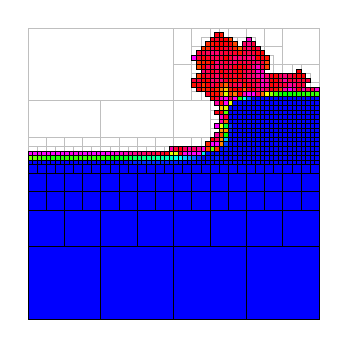
\begin{tikzpicture}[x={(\screenshotunitlength,0)},y={(0,\screenshotunitlength)}]
        \definecolor{fillcolor}{rgb}{0.000000,0.000000,1.000000}
\fill[fillcolor] (0.000000,0.000000) rectangle (0.250000,0.250000);
\definecolor{fillcolor}{rgb}{0.000000,0.000000,1.000000}
\fill[fillcolor] (0.250000,0.000000) rectangle (0.500000,0.250000);
\definecolor{fillcolor}{rgb}{0.000000,0.000000,1.000000}
\fill[fillcolor] (0.000000,0.250000) rectangle (0.125000,0.375000);
\definecolor{fillcolor}{rgb}{0.000000,0.000000,1.000000}
\fill[fillcolor] (0.125000,0.250000) rectangle (0.250000,0.375000);
\definecolor{fillcolor}{rgb}{0.000000,0.000000,1.000000}
\fill[fillcolor] (0.000000,0.375000) rectangle (0.062500,0.437500);
\definecolor{fillcolor}{rgb}{0.000000,0.000000,1.000000}
\fill[fillcolor] (0.062500,0.375000) rectangle (0.125000,0.437500);
\definecolor{fillcolor}{rgb}{0.000000,0.000000,1.000000}
\fill[fillcolor] (0.000000,0.437500) rectangle (0.062500,0.500000);
\definecolor{fillcolor}{rgb}{0.000000,0.000000,1.000000}
\fill[fillcolor] (0.062500,0.437500) rectangle (0.125000,0.500000);
\definecolor{fillcolor}{rgb}{0.000000,0.000000,1.000000}
\fill[fillcolor] (0.125000,0.375000) rectangle (0.187500,0.437500);
\definecolor{fillcolor}{rgb}{0.000000,0.000000,1.000000}
\fill[fillcolor] (0.187500,0.375000) rectangle (0.250000,0.437500);
\definecolor{fillcolor}{rgb}{0.000000,0.000000,1.000000}
\fill[fillcolor] (0.125000,0.437500) rectangle (0.187500,0.500000);
\definecolor{fillcolor}{rgb}{0.000000,0.000000,1.000000}
\fill[fillcolor] (0.187500,0.437500) rectangle (0.250000,0.500000);
\definecolor{fillcolor}{rgb}{0.000000,0.000000,1.000000}
\fill[fillcolor] (0.250000,0.250000) rectangle (0.375000,0.375000);
\definecolor{fillcolor}{rgb}{0.000000,0.000000,1.000000}
\fill[fillcolor] (0.375000,0.250000) rectangle (0.500000,0.375000);
\definecolor{fillcolor}{rgb}{0.000000,0.000000,1.000000}
\fill[fillcolor] (0.250000,0.375000) rectangle (0.312500,0.437500);
\definecolor{fillcolor}{rgb}{0.000000,0.000000,1.000000}
\fill[fillcolor] (0.312500,0.375000) rectangle (0.375000,0.437500);
\definecolor{fillcolor}{rgb}{0.000000,0.000000,1.000000}
\fill[fillcolor] (0.250000,0.437500) rectangle (0.312500,0.500000);
\definecolor{fillcolor}{rgb}{0.000000,0.000000,1.000000}
\fill[fillcolor] (0.312500,0.437500) rectangle (0.375000,0.500000);
\definecolor{fillcolor}{rgb}{0.000000,0.000000,1.000000}
\fill[fillcolor] (0.375000,0.375000) rectangle (0.437500,0.437500);
\definecolor{fillcolor}{rgb}{0.000000,0.000000,1.000000}
\fill[fillcolor] (0.437500,0.375000) rectangle (0.500000,0.437500);
\definecolor{fillcolor}{rgb}{0.000000,0.000000,1.000000}
\fill[fillcolor] (0.375000,0.437500) rectangle (0.437500,0.500000);
\definecolor{fillcolor}{rgb}{0.000000,0.000000,1.000000}
\fill[fillcolor] (0.437500,0.437500) rectangle (0.500000,0.500000);
\definecolor{fillcolor}{rgb}{0.000000,0.000000,1.000000}
\fill[fillcolor] (0.500000,0.000000) rectangle (0.750000,0.250000);
\definecolor{fillcolor}{rgb}{0.000000,0.000000,1.000000}
\fill[fillcolor] (0.750000,0.000000) rectangle (1.000000,0.250000);
\definecolor{fillcolor}{rgb}{0.000000,0.000000,1.000000}
\fill[fillcolor] (0.500000,0.250000) rectangle (0.625000,0.375000);
\definecolor{fillcolor}{rgb}{0.000000,0.000000,1.000000}
\fill[fillcolor] (0.625000,0.250000) rectangle (0.750000,0.375000);
\definecolor{fillcolor}{rgb}{0.000000,0.000000,1.000000}
\fill[fillcolor] (0.500000,0.375000) rectangle (0.562500,0.437500);
\definecolor{fillcolor}{rgb}{0.000000,0.000000,1.000000}
\fill[fillcolor] (0.562500,0.375000) rectangle (0.625000,0.437500);
\definecolor{fillcolor}{rgb}{0.000000,0.000000,1.000000}
\fill[fillcolor] (0.500000,0.437500) rectangle (0.562500,0.500000);
\definecolor{fillcolor}{rgb}{0.000000,0.000000,1.000000}
\fill[fillcolor] (0.562500,0.437500) rectangle (0.625000,0.500000);
\definecolor{fillcolor}{rgb}{0.000000,0.000000,1.000000}
\fill[fillcolor] (0.625000,0.375000) rectangle (0.687500,0.437500);
\definecolor{fillcolor}{rgb}{0.000000,0.000000,1.000000}
\fill[fillcolor] (0.687500,0.375000) rectangle (0.750000,0.437500);
\definecolor{fillcolor}{rgb}{0.000000,0.000000,1.000000}
\fill[fillcolor] (0.625000,0.437500) rectangle (0.687500,0.500000);
\definecolor{fillcolor}{rgb}{0.000000,0.000000,1.000000}
\fill[fillcolor] (0.687500,0.437500) rectangle (0.750000,0.500000);
\definecolor{fillcolor}{rgb}{0.000000,0.000000,1.000000}
\fill[fillcolor] (0.750000,0.250000) rectangle (0.875000,0.375000);
\definecolor{fillcolor}{rgb}{0.000000,0.000000,1.000000}
\fill[fillcolor] (0.875000,0.250000) rectangle (1.000000,0.375000);
\definecolor{fillcolor}{rgb}{0.000000,0.000000,1.000000}
\fill[fillcolor] (0.750000,0.375000) rectangle (0.812500,0.437500);
\definecolor{fillcolor}{rgb}{0.000000,0.000000,1.000000}
\fill[fillcolor] (0.812500,0.375000) rectangle (0.875000,0.437500);
\definecolor{fillcolor}{rgb}{0.000000,0.000000,1.000000}
\fill[fillcolor] (0.750000,0.437500) rectangle (0.812500,0.500000);
\definecolor{fillcolor}{rgb}{0.000000,0.000000,1.000000}
\fill[fillcolor] (0.812500,0.437500) rectangle (0.875000,0.500000);
\definecolor{fillcolor}{rgb}{0.000000,0.000000,1.000000}
\fill[fillcolor] (0.875000,0.375000) rectangle (0.937500,0.437500);
\definecolor{fillcolor}{rgb}{0.000000,0.000000,1.000000}
\fill[fillcolor] (0.937500,0.375000) rectangle (1.000000,0.437500);
\definecolor{fillcolor}{rgb}{0.000000,0.000000,1.000000}
\fill[fillcolor] (0.875000,0.437500) rectangle (0.937500,0.500000);
\definecolor{fillcolor}{rgb}{0.000000,0.000000,1.000000}
\fill[fillcolor] (0.937500,0.437500) rectangle (1.000000,0.500000);
\definecolor{fillcolor}{rgb}{0.000000,0.000000,1.000000}
\fill[fillcolor] (0.000000,0.500000) rectangle (0.031250,0.531250);
\definecolor{fillcolor}{rgb}{0.000000,0.000000,1.000000}
\fill[fillcolor] (0.031250,0.500000) rectangle (0.062500,0.531250);
\definecolor{fillcolor}{rgb}{0.000000,0.000000,1.000000}
\fill[fillcolor] (0.000000,0.531250) rectangle (0.015625,0.546875);
\definecolor{fillcolor}{rgb}{0.000000,0.000000,1.000000}
\fill[fillcolor] (0.015625,0.531250) rectangle (0.031250,0.546875);
\definecolor{fillcolor}{rgb}{0.474771,1.000000,0.000000}
\fill[fillcolor] (0.000000,0.546875) rectangle (0.015625,0.562500);
\definecolor{fillcolor}{rgb}{0.411356,1.000000,0.000000}
\fill[fillcolor] (0.015625,0.546875) rectangle (0.031250,0.562500);
\definecolor{fillcolor}{rgb}{0.000000,0.000000,1.000000}
\fill[fillcolor] (0.031250,0.531250) rectangle (0.046875,0.546875);
\definecolor{fillcolor}{rgb}{0.000000,0.000000,1.000000}
\fill[fillcolor] (0.046875,0.531250) rectangle (0.062500,0.546875);
\definecolor{fillcolor}{rgb}{0.309728,1.000000,0.000000}
\fill[fillcolor] (0.031250,0.546875) rectangle (0.046875,0.562500);
\definecolor{fillcolor}{rgb}{0.210906,1.000000,0.000000}
\fill[fillcolor] (0.046875,0.546875) rectangle (0.062500,0.562500);
\definecolor{fillcolor}{rgb}{0.000000,0.000000,1.000000}
\fill[fillcolor] (0.062500,0.500000) rectangle (0.093750,0.531250);
\definecolor{fillcolor}{rgb}{0.000000,0.000000,1.000000}
\fill[fillcolor] (0.093750,0.500000) rectangle (0.125000,0.531250);
\definecolor{fillcolor}{rgb}{0.000000,0.000000,1.000000}
\fill[fillcolor] (0.062500,0.531250) rectangle (0.078125,0.546875);
\definecolor{fillcolor}{rgb}{0.000000,0.000000,1.000000}
\fill[fillcolor] (0.078125,0.531250) rectangle (0.093750,0.546875);
\definecolor{fillcolor}{rgb}{0.133128,1.000000,0.000000}
\fill[fillcolor] (0.062500,0.546875) rectangle (0.078125,0.562500);
\definecolor{fillcolor}{rgb}{0.104724,1.000000,0.000000}
\fill[fillcolor] (0.078125,0.546875) rectangle (0.093750,0.562500);
\definecolor{fillcolor}{rgb}{0.000000,0.000000,1.000000}
\fill[fillcolor] (0.093750,0.531250) rectangle (0.109375,0.546875);
\definecolor{fillcolor}{rgb}{0.000000,0.000000,1.000000}
\fill[fillcolor] (0.109375,0.531250) rectangle (0.125000,0.546875);
\definecolor{fillcolor}{rgb}{0.115820,1.000000,0.000000}
\fill[fillcolor] (0.093750,0.546875) rectangle (0.109375,0.562500);
\definecolor{fillcolor}{rgb}{0.144728,1.000000,0.000000}
\fill[fillcolor] (0.109375,0.546875) rectangle (0.125000,0.562500);
\definecolor{fillcolor}{rgb}{1.000000,0.000000,1.000000}
\fill[fillcolor] (0.000000,0.562500) rectangle (0.015625,0.578125);
\definecolor{fillcolor}{rgb}{1.000000,0.000000,1.000000}
\fill[fillcolor] (0.015625,0.562500) rectangle (0.031250,0.578125);
\definecolor{fillcolor}{rgb}{1.000000,0.000000,1.000000}
\fill[fillcolor] (0.031250,0.562500) rectangle (0.046875,0.578125);
\definecolor{fillcolor}{rgb}{1.000000,0.000000,1.000000}
\fill[fillcolor] (0.046875,0.562500) rectangle (0.062500,0.578125);
\definecolor{fillcolor}{rgb}{1.000000,0.000000,1.000000}
\fill[fillcolor] (0.062500,0.562500) rectangle (0.078125,0.578125);
\definecolor{fillcolor}{rgb}{1.000000,0.000000,1.000000}
\fill[fillcolor] (0.078125,0.562500) rectangle (0.093750,0.578125);
\definecolor{fillcolor}{rgb}{1.000000,0.000000,1.000000}
\fill[fillcolor] (0.093750,0.562500) rectangle (0.109375,0.578125);
\definecolor{fillcolor}{rgb}{1.000000,0.000000,1.000000}
\fill[fillcolor] (0.109375,0.562500) rectangle (0.125000,0.578125);
\definecolor{fillcolor}{rgb}{0.000000,0.000000,1.000000}
\fill[fillcolor] (0.125000,0.500000) rectangle (0.156250,0.531250);
\definecolor{fillcolor}{rgb}{0.000000,0.000000,1.000000}
\fill[fillcolor] (0.156250,0.500000) rectangle (0.187500,0.531250);
\definecolor{fillcolor}{rgb}{0.000000,0.000000,1.000000}
\fill[fillcolor] (0.125000,0.531250) rectangle (0.140625,0.546875);
\definecolor{fillcolor}{rgb}{0.000000,0.000000,1.000000}
\fill[fillcolor] (0.140625,0.531250) rectangle (0.156250,0.546875);
\definecolor{fillcolor}{rgb}{0.175671,1.000000,0.000000}
\fill[fillcolor] (0.125000,0.546875) rectangle (0.140625,0.562500);
\definecolor{fillcolor}{rgb}{0.203715,1.000000,0.000000}
\fill[fillcolor] (0.140625,0.546875) rectangle (0.156250,0.562500);
\definecolor{fillcolor}{rgb}{0.000000,0.000000,1.000000}
\fill[fillcolor] (0.156250,0.531250) rectangle (0.171875,0.546875);
\definecolor{fillcolor}{rgb}{0.000000,0.000000,1.000000}
\fill[fillcolor] (0.171875,0.531250) rectangle (0.187500,0.546875);
\definecolor{fillcolor}{rgb}{0.221624,1.000000,0.000000}
\fill[fillcolor] (0.156250,0.546875) rectangle (0.171875,0.562500);
\definecolor{fillcolor}{rgb}{0.233223,1.000000,0.000000}
\fill[fillcolor] (0.171875,0.546875) rectangle (0.187500,0.562500);
\definecolor{fillcolor}{rgb}{0.000000,0.000000,1.000000}
\fill[fillcolor] (0.187500,0.500000) rectangle (0.218750,0.531250);
\definecolor{fillcolor}{rgb}{0.000000,0.000000,1.000000}
\fill[fillcolor] (0.218750,0.500000) rectangle (0.250000,0.531250);
\definecolor{fillcolor}{rgb}{0.000000,0.000000,1.000000}
\fill[fillcolor] (0.187500,0.531250) rectangle (0.203125,0.546875);
\definecolor{fillcolor}{rgb}{0.000000,0.000000,1.000000}
\fill[fillcolor] (0.203125,0.531250) rectangle (0.218750,0.546875);
\definecolor{fillcolor}{rgb}{0.230052,1.000000,0.000000}
\fill[fillcolor] (0.187500,0.546875) rectangle (0.203125,0.562500);
\definecolor{fillcolor}{rgb}{0.222921,1.000000,0.000000}
\fill[fillcolor] (0.203125,0.546875) rectangle (0.218750,0.562500);
\definecolor{fillcolor}{rgb}{0.000000,0.000000,1.000000}
\fill[fillcolor] (0.218750,0.531250) rectangle (0.234375,0.546875);
\definecolor{fillcolor}{rgb}{0.000000,0.000000,1.000000}
\fill[fillcolor] (0.234375,0.531250) rectangle (0.250000,0.546875);
\definecolor{fillcolor}{rgb}{0.197698,1.000000,0.000000}
\fill[fillcolor] (0.218750,0.546875) rectangle (0.234375,0.562500);
\definecolor{fillcolor}{rgb}{0.173655,1.000000,0.000000}
\fill[fillcolor] (0.234375,0.546875) rectangle (0.250000,0.562500);
\definecolor{fillcolor}{rgb}{1.000000,0.000000,0.972720}
\fill[fillcolor] (0.125000,0.562500) rectangle (0.140625,0.578125);
\definecolor{fillcolor}{rgb}{1.000000,0.000000,0.894860}
\fill[fillcolor] (0.140625,0.562500) rectangle (0.156250,0.578125);
\definecolor{fillcolor}{rgb}{1.000000,0.000000,0.906797}
\fill[fillcolor] (0.156250,0.562500) rectangle (0.171875,0.578125);
\definecolor{fillcolor}{rgb}{1.000000,0.000000,0.952497}
\fill[fillcolor] (0.171875,0.562500) rectangle (0.187500,0.578125);
\definecolor{fillcolor}{rgb}{1.000000,0.000000,1.000000}
\fill[fillcolor] (0.187500,0.562500) rectangle (0.203125,0.578125);
\definecolor{fillcolor}{rgb}{1.000000,0.000000,1.000000}
\fill[fillcolor] (0.203125,0.562500) rectangle (0.218750,0.578125);
\definecolor{fillcolor}{rgb}{1.000000,0.000000,1.000000}
\fill[fillcolor] (0.218750,0.562500) rectangle (0.234375,0.578125);
\definecolor{fillcolor}{rgb}{1.000000,0.000000,1.000000}
\fill[fillcolor] (0.234375,0.562500) rectangle (0.250000,0.578125);
\definecolor{fillcolor}{rgb}{0.000000,0.000000,1.000000}
\fill[fillcolor] (0.250000,0.500000) rectangle (0.281250,0.531250);
\definecolor{fillcolor}{rgb}{0.000000,0.000000,1.000000}
\fill[fillcolor] (0.281250,0.500000) rectangle (0.312500,0.531250);
\definecolor{fillcolor}{rgb}{0.000000,0.000000,1.000000}
\fill[fillcolor] (0.250000,0.531250) rectangle (0.265625,0.546875);
\definecolor{fillcolor}{rgb}{0.000000,0.000000,1.000000}
\fill[fillcolor] (0.265625,0.531250) rectangle (0.281250,0.546875);
\definecolor{fillcolor}{rgb}{0.128102,1.000000,0.000000}
\fill[fillcolor] (0.250000,0.546875) rectangle (0.265625,0.562500);
\definecolor{fillcolor}{rgb}{0.090915,1.000000,0.000000}
\fill[fillcolor] (0.265625,0.546875) rectangle (0.281250,0.562500);
\definecolor{fillcolor}{rgb}{0.000000,0.000000,1.000000}
\fill[fillcolor] (0.281250,0.531250) rectangle (0.296875,0.546875);
\definecolor{fillcolor}{rgb}{0.000000,0.000000,1.000000}
\fill[fillcolor] (0.296875,0.531250) rectangle (0.312500,0.546875);
\definecolor{fillcolor}{rgb}{0.029272,1.000000,0.000000}
\fill[fillcolor] (0.281250,0.546875) rectangle (0.296875,0.562500);
\definecolor{fillcolor}{rgb}{0.000000,1.000000,0.016654}
\fill[fillcolor] (0.296875,0.546875) rectangle (0.312500,0.562500);
\definecolor{fillcolor}{rgb}{0.000000,0.000000,1.000000}
\fill[fillcolor] (0.312500,0.500000) rectangle (0.343750,0.531250);
\definecolor{fillcolor}{rgb}{0.000000,0.000000,1.000000}
\fill[fillcolor] (0.343750,0.500000) rectangle (0.375000,0.531250);
\definecolor{fillcolor}{rgb}{0.000000,0.000000,1.000000}
\fill[fillcolor] (0.312500,0.531250) rectangle (0.328125,0.546875);
\definecolor{fillcolor}{rgb}{0.000000,0.000000,1.000000}
\fill[fillcolor] (0.328125,0.531250) rectangle (0.343750,0.546875);
\definecolor{fillcolor}{rgb}{0.000000,1.000000,0.090096}
\fill[fillcolor] (0.312500,0.546875) rectangle (0.328125,0.562500);
\definecolor{fillcolor}{rgb}{0.000000,1.000000,0.136915}
\fill[fillcolor] (0.328125,0.546875) rectangle (0.343750,0.562500);
\definecolor{fillcolor}{rgb}{0.000000,0.082668,1.000000}
\fill[fillcolor] (0.343750,0.531250) rectangle (0.359375,0.546875);
\definecolor{fillcolor}{rgb}{0.000000,0.122420,1.000000}
\fill[fillcolor] (0.359375,0.531250) rectangle (0.375000,0.546875);
\definecolor{fillcolor}{rgb}{0.000000,1.000000,0.301836}
\fill[fillcolor] (0.343750,0.546875) rectangle (0.359375,0.562500);
\definecolor{fillcolor}{rgb}{0.000000,1.000000,0.388575}
\fill[fillcolor] (0.359375,0.546875) rectangle (0.375000,0.562500);
\definecolor{fillcolor}{rgb}{1.000000,0.000000,1.000000}
\fill[fillcolor] (0.250000,0.562500) rectangle (0.265625,0.578125);
\definecolor{fillcolor}{rgb}{1.000000,0.000000,0.981235}
\fill[fillcolor] (0.265625,0.562500) rectangle (0.281250,0.578125);
\definecolor{fillcolor}{rgb}{1.000000,0.000000,0.923467}
\fill[fillcolor] (0.281250,0.562500) rectangle (0.296875,0.578125);
\definecolor{fillcolor}{rgb}{1.000000,0.000000,0.854870}
\fill[fillcolor] (0.296875,0.562500) rectangle (0.312500,0.578125);
\definecolor{fillcolor}{rgb}{1.000000,0.000000,0.780036}
\fill[fillcolor] (0.312500,0.562500) rectangle (0.328125,0.578125);
\definecolor{fillcolor}{rgb}{1.000000,0.000000,0.703510}
\fill[fillcolor] (0.328125,0.562500) rectangle (0.343750,0.578125);
\definecolor{fillcolor}{rgb}{1.000000,0.000000,0.628760}
\fill[fillcolor] (0.343750,0.562500) rectangle (0.359375,0.578125);
\definecolor{fillcolor}{rgb}{1.000000,0.000000,0.557814}
\fill[fillcolor] (0.359375,0.562500) rectangle (0.375000,0.578125);
\definecolor{fillcolor}{rgb}{0.000000,0.000000,1.000000}
\fill[fillcolor] (0.375000,0.500000) rectangle (0.406250,0.531250);
\definecolor{fillcolor}{rgb}{0.000000,0.000000,1.000000}
\fill[fillcolor] (0.406250,0.500000) rectangle (0.437500,0.531250);
\definecolor{fillcolor}{rgb}{0.000000,0.142043,1.000000}
\fill[fillcolor] (0.375000,0.531250) rectangle (0.390625,0.546875);
\definecolor{fillcolor}{rgb}{0.000000,0.151447,1.000000}
\fill[fillcolor] (0.390625,0.531250) rectangle (0.406250,0.546875);
\definecolor{fillcolor}{rgb}{0.000000,1.000000,0.482107}
\fill[fillcolor] (0.375000,0.546875) rectangle (0.390625,0.562500);
\definecolor{fillcolor}{rgb}{0.000000,1.000000,0.529438}
\fill[fillcolor] (0.390625,0.546875) rectangle (0.406250,0.562500);
\definecolor{fillcolor}{rgb}{0.000000,0.151269,1.000000}
\fill[fillcolor] (0.406250,0.531250) rectangle (0.421875,0.546875);
\definecolor{fillcolor}{rgb}{0.000000,0.151555,1.000000}
\fill[fillcolor] (0.421875,0.531250) rectangle (0.437500,0.546875);
\definecolor{fillcolor}{rgb}{0.000000,1.000000,0.590714}
\fill[fillcolor] (0.406250,0.546875) rectangle (0.421875,0.562500);
\definecolor{fillcolor}{rgb}{0.000000,1.000000,0.622103}
\fill[fillcolor] (0.421875,0.546875) rectangle (0.437500,0.562500);
\definecolor{fillcolor}{rgb}{0.000000,0.000000,1.000000}
\fill[fillcolor] (0.437500,0.500000) rectangle (0.468750,0.531250);
\definecolor{fillcolor}{rgb}{0.000000,0.000010,1.000000}
\fill[fillcolor] (0.468750,0.500000) rectangle (0.500000,0.531250);
\definecolor{fillcolor}{rgb}{0.000000,0.138605,1.000000}
\fill[fillcolor] (0.437500,0.531250) rectangle (0.453125,0.546875);
\definecolor{fillcolor}{rgb}{0.000000,0.135919,1.000000}
\fill[fillcolor] (0.453125,0.531250) rectangle (0.468750,0.546875);
\definecolor{fillcolor}{rgb}{0.000000,1.000000,0.671694}
\fill[fillcolor] (0.437500,0.546875) rectangle (0.453125,0.562500);
\definecolor{fillcolor}{rgb}{0.000000,1.000000,0.695087}
\fill[fillcolor] (0.453125,0.546875) rectangle (0.468750,0.562500);
\definecolor{fillcolor}{rgb}{0.000000,0.117938,1.000000}
\fill[fillcolor] (0.468750,0.531250) rectangle (0.484375,0.546875);
\definecolor{fillcolor}{rgb}{0.000000,0.112537,1.000000}
\fill[fillcolor] (0.484375,0.531250) rectangle (0.500000,0.546875);
\definecolor{fillcolor}{rgb}{0.000000,1.000000,0.738568}
\fill[fillcolor] (0.468750,0.546875) rectangle (0.484375,0.562500);
\definecolor{fillcolor}{rgb}{0.000000,1.000000,0.786299}
\fill[fillcolor] (0.484375,0.546875) rectangle (0.500000,0.562500);
\definecolor{fillcolor}{rgb}{1.000000,0.000000,0.490060}
\fill[fillcolor] (0.375000,0.562500) rectangle (0.390625,0.578125);
\definecolor{fillcolor}{rgb}{1.000000,0.000000,0.423998}
\fill[fillcolor] (0.390625,0.562500) rectangle (0.406250,0.578125);
\definecolor{fillcolor}{rgb}{1.000000,0.000000,0.358072}
\fill[fillcolor] (0.406250,0.562500) rectangle (0.421875,0.578125);
\definecolor{fillcolor}{rgb}{1.000000,0.000000,0.292024}
\fill[fillcolor] (0.421875,0.562500) rectangle (0.437500,0.578125);
\definecolor{fillcolor}{rgb}{1.000000,0.000000,0.230395}
\fill[fillcolor] (0.437500,0.562500) rectangle (0.453125,0.578125);
\definecolor{fillcolor}{rgb}{1.000000,0.000000,0.173517}
\fill[fillcolor] (0.453125,0.562500) rectangle (0.468750,0.578125);
\definecolor{fillcolor}{rgb}{1.000000,0.000000,0.065480}
\fill[fillcolor] (0.468750,0.562500) rectangle (0.484375,0.578125);
\definecolor{fillcolor}{rgb}{0.939732,1.000000,0.000000}
\fill[fillcolor] (0.484375,0.562500) rectangle (0.500000,0.578125);
\definecolor{fillcolor}{rgb}{1.000000,0.000000,0.657219}
\fill[fillcolor] (0.484375,0.578125) rectangle (0.500000,0.593750);
\definecolor{fillcolor}{rgb}{0.000000,0.000000,1.000000}
\fill[fillcolor] (0.500000,0.500000) rectangle (0.531250,0.531250);
\definecolor{fillcolor}{rgb}{0.000000,0.000000,1.000000}
\fill[fillcolor] (0.531250,0.500000) rectangle (0.562500,0.531250);
\definecolor{fillcolor}{rgb}{0.000000,0.084656,1.000000}
\fill[fillcolor] (0.500000,0.531250) rectangle (0.515625,0.546875);
\definecolor{fillcolor}{rgb}{0.000000,0.065964,1.000000}
\fill[fillcolor] (0.515625,0.531250) rectangle (0.531250,0.546875);
\definecolor{fillcolor}{rgb}{0.000000,1.000000,0.924990}
\fill[fillcolor] (0.500000,0.546875) rectangle (0.515625,0.562500);
\definecolor{fillcolor}{rgb}{0.000000,0.960562,1.000000}
\fill[fillcolor] (0.515625,0.546875) rectangle (0.531250,0.562500);
\definecolor{fillcolor}{rgb}{0.000000,0.013418,1.000000}
\fill[fillcolor] (0.531250,0.531250) rectangle (0.546875,0.546875);
\definecolor{fillcolor}{rgb}{0.000000,0.000001,1.000000}
\fill[fillcolor] (0.546875,0.531250) rectangle (0.562500,0.546875);
\definecolor{fillcolor}{rgb}{0.000000,0.793133,1.000000}
\fill[fillcolor] (0.531250,0.546875) rectangle (0.546875,0.562500);
\definecolor{fillcolor}{rgb}{0.000000,0.631567,1.000000}
\fill[fillcolor] (0.546875,0.546875) rectangle (0.562500,0.562500);
\definecolor{fillcolor}{rgb}{0.000000,0.000001,1.000000}
\fill[fillcolor] (0.562500,0.500000) rectangle (0.593750,0.531250);
\definecolor{fillcolor}{rgb}{0.000000,0.000004,1.000000}
\fill[fillcolor] (0.593750,0.500000) rectangle (0.625000,0.531250);
\definecolor{fillcolor}{rgb}{0.000000,0.000001,1.000000}
\fill[fillcolor] (0.562500,0.531250) rectangle (0.578125,0.546875);
\definecolor{fillcolor}{rgb}{0.000000,0.000001,1.000000}
\fill[fillcolor] (0.578125,0.531250) rectangle (0.593750,0.546875);
\definecolor{fillcolor}{rgb}{0.000000,0.409666,1.000000}
\fill[fillcolor] (0.562500,0.546875) rectangle (0.578125,0.562500);
\definecolor{fillcolor}{rgb}{0.000000,0.214210,1.000000}
\fill[fillcolor] (0.578125,0.546875) rectangle (0.593750,0.562500);
\definecolor{fillcolor}{rgb}{0.000000,0.000003,1.000000}
\fill[fillcolor] (0.593750,0.531250) rectangle (0.609375,0.546875);
\definecolor{fillcolor}{rgb}{0.000000,0.000004,1.000000}
\fill[fillcolor] (0.609375,0.531250) rectangle (0.625000,0.546875);
\definecolor{fillcolor}{rgb}{0.000000,0.012153,1.000000}
\fill[fillcolor] (0.593750,0.546875) rectangle (0.609375,0.562500);
\definecolor{fillcolor}{rgb}{0.000000,0.032427,1.000000}
\fill[fillcolor] (0.609375,0.546875) rectangle (0.625000,0.562500);
\definecolor{fillcolor}{rgb}{0.881179,1.000000,0.000000}
\fill[fillcolor] (0.500000,0.562500) rectangle (0.515625,0.578125);
\definecolor{fillcolor}{rgb}{1.000000,0.000000,0.118501}
\fill[fillcolor] (0.515625,0.562500) rectangle (0.531250,0.578125);
\definecolor{fillcolor}{rgb}{1.000000,0.000000,0.227095}
\fill[fillcolor] (0.500000,0.578125) rectangle (0.515625,0.593750);
\definecolor{fillcolor}{rgb}{1.000000,0.000000,0.083278}
\fill[fillcolor] (0.515625,0.578125) rectangle (0.531250,0.593750);
\definecolor{fillcolor}{rgb}{1.000000,0.000000,0.931133}
\fill[fillcolor] (0.531250,0.562500) rectangle (0.546875,0.578125);
\definecolor{fillcolor}{rgb}{1.000000,0.000000,1.000000}
\fill[fillcolor] (0.546875,0.562500) rectangle (0.562500,0.578125);
\definecolor{fillcolor}{rgb}{1.000000,0.000000,0.379178}
\fill[fillcolor] (0.531250,0.578125) rectangle (0.546875,0.593750);
\definecolor{fillcolor}{rgb}{1.000000,0.000000,0.705842}
\fill[fillcolor] (0.546875,0.578125) rectangle (0.562500,0.593750);
\definecolor{fillcolor}{rgb}{1.000000,0.000000,1.000000}
\fill[fillcolor] (0.562500,0.562500) rectangle (0.578125,0.578125);
\definecolor{fillcolor}{rgb}{1.000000,0.000000,1.000000}
\fill[fillcolor] (0.578125,0.562500) rectangle (0.593750,0.578125);
\definecolor{fillcolor}{rgb}{1.000000,0.000000,0.395832}
\fill[fillcolor] (0.562500,0.578125) rectangle (0.578125,0.593750);
\definecolor{fillcolor}{rgb}{1.000000,0.000000,0.615039}
\fill[fillcolor] (0.578125,0.578125) rectangle (0.593750,0.593750);
\definecolor{fillcolor}{rgb}{0.000000,0.896560,1.000000}
\fill[fillcolor] (0.593750,0.562500) rectangle (0.609375,0.578125);
\definecolor{fillcolor}{rgb}{0.000000,0.015916,1.000000}
\fill[fillcolor] (0.609375,0.562500) rectangle (0.625000,0.578125);
\definecolor{fillcolor}{rgb}{1.000000,0.000000,0.953162}
\fill[fillcolor] (0.593750,0.578125) rectangle (0.609375,0.593750);
\definecolor{fillcolor}{rgb}{1.000000,0.240966,0.000000}
\fill[fillcolor] (0.609375,0.578125) rectangle (0.625000,0.593750);
\definecolor{fillcolor}{rgb}{1.000000,0.150189,0.000000}
\fill[fillcolor] (0.609375,0.593750) rectangle (0.625000,0.609375);
\definecolor{fillcolor}{rgb}{0.000000,0.000006,1.000000}
\fill[fillcolor] (0.625000,0.500000) rectangle (0.656250,0.531250);
\definecolor{fillcolor}{rgb}{0.000000,0.000006,1.000000}
\fill[fillcolor] (0.656250,0.500000) rectangle (0.687500,0.531250);
\definecolor{fillcolor}{rgb}{0.000000,0.000006,1.000000}
\fill[fillcolor] (0.625000,0.531250) rectangle (0.640625,0.546875);
\definecolor{fillcolor}{rgb}{0.000000,0.000005,1.000000}
\fill[fillcolor] (0.640625,0.531250) rectangle (0.656250,0.546875);
\definecolor{fillcolor}{rgb}{0.000000,0.058144,1.000000}
\fill[fillcolor] (0.625000,0.546875) rectangle (0.640625,0.562500);
\definecolor{fillcolor}{rgb}{0.000000,0.103364,1.000000}
\fill[fillcolor] (0.640625,0.546875) rectangle (0.656250,0.562500);
\definecolor{fillcolor}{rgb}{0.000000,0.000004,1.000000}
\fill[fillcolor] (0.656250,0.531250) rectangle (0.671875,0.546875);
\definecolor{fillcolor}{rgb}{0.000000,0.000002,1.000000}
\fill[fillcolor] (0.671875,0.531250) rectangle (0.687500,0.546875);
\definecolor{fillcolor}{rgb}{0.000000,0.062071,1.000000}
\fill[fillcolor] (0.656250,0.546875) rectangle (0.671875,0.562500);
\definecolor{fillcolor}{rgb}{0.000000,0.000001,1.000000}
\fill[fillcolor] (0.671875,0.546875) rectangle (0.687500,0.562500);
\definecolor{fillcolor}{rgb}{0.000000,0.000000,1.000000}
\fill[fillcolor] (0.687500,0.500000) rectangle (0.718750,0.531250);
\definecolor{fillcolor}{rgb}{0.000000,0.000000,1.000000}
\fill[fillcolor] (0.718750,0.500000) rectangle (0.750000,0.531250);
\definecolor{fillcolor}{rgb}{0.000000,0.000000,1.000000}
\fill[fillcolor] (0.687500,0.531250) rectangle (0.703125,0.546875);
\definecolor{fillcolor}{rgb}{0.000000,0.000000,1.000000}
\fill[fillcolor] (0.703125,0.531250) rectangle (0.718750,0.546875);
\definecolor{fillcolor}{rgb}{0.000000,0.000000,1.000000}
\fill[fillcolor] (0.687500,0.546875) rectangle (0.703125,0.562500);
\definecolor{fillcolor}{rgb}{0.000000,0.000000,1.000000}
\fill[fillcolor] (0.703125,0.546875) rectangle (0.718750,0.562500);
\definecolor{fillcolor}{rgb}{0.000000,0.000000,1.000000}
\fill[fillcolor] (0.718750,0.531250) rectangle (0.734375,0.546875);
\definecolor{fillcolor}{rgb}{0.000000,0.000000,1.000000}
\fill[fillcolor] (0.734375,0.531250) rectangle (0.750000,0.546875);
\definecolor{fillcolor}{rgb}{0.000000,0.000000,1.000000}
\fill[fillcolor] (0.718750,0.546875) rectangle (0.734375,0.562500);
\definecolor{fillcolor}{rgb}{0.000000,0.000000,1.000000}
\fill[fillcolor] (0.734375,0.546875) rectangle (0.750000,0.562500);
\definecolor{fillcolor}{rgb}{0.000000,0.022386,1.000000}
\fill[fillcolor] (0.625000,0.562500) rectangle (0.640625,0.578125);
\definecolor{fillcolor}{rgb}{0.000000,0.018971,1.000000}
\fill[fillcolor] (0.640625,0.562500) rectangle (0.656250,0.578125);
\definecolor{fillcolor}{rgb}{0.426686,1.000000,0.000000}
\fill[fillcolor] (0.625000,0.578125) rectangle (0.640625,0.593750);
\definecolor{fillcolor}{rgb}{1.000000,0.189780,0.000000}
\fill[fillcolor] (0.640625,0.578125) rectangle (0.656250,0.593750);
\definecolor{fillcolor}{rgb}{0.000000,0.013392,1.000000}
\fill[fillcolor] (0.656250,0.562500) rectangle (0.671875,0.578125);
\definecolor{fillcolor}{rgb}{0.000000,0.001230,1.000000}
\fill[fillcolor] (0.671875,0.562500) rectangle (0.687500,0.578125);
\definecolor{fillcolor}{rgb}{0.000000,0.065257,1.000000}
\fill[fillcolor] (0.656250,0.578125) rectangle (0.671875,0.593750);
\definecolor{fillcolor}{rgb}{0.000000,0.085966,1.000000}
\fill[fillcolor] (0.671875,0.578125) rectangle (0.687500,0.593750);
\definecolor{fillcolor}{rgb}{1.000000,0.000000,1.000000}
\fill[fillcolor] (0.625000,0.593750) rectangle (0.640625,0.609375);
\definecolor{fillcolor}{rgb}{1.000000,0.000000,1.000000}
\fill[fillcolor] (0.640625,0.593750) rectangle (0.656250,0.609375);
\definecolor{fillcolor}{rgb}{1.000000,0.000000,0.055821}
\fill[fillcolor] (0.625000,0.609375) rectangle (0.640625,0.625000);
\definecolor{fillcolor}{rgb}{1.000000,0.000000,0.324645}
\fill[fillcolor] (0.640625,0.609375) rectangle (0.656250,0.625000);
\definecolor{fillcolor}{rgb}{1.000000,0.529097,0.000000}
\fill[fillcolor] (0.656250,0.593750) rectangle (0.671875,0.609375);
\definecolor{fillcolor}{rgb}{0.000000,0.285094,1.000000}
\fill[fillcolor] (0.671875,0.593750) rectangle (0.687500,0.609375);
\definecolor{fillcolor}{rgb}{1.000000,0.539548,0.000000}
\fill[fillcolor] (0.656250,0.609375) rectangle (0.671875,0.625000);
\definecolor{fillcolor}{rgb}{0.000000,0.757971,1.000000}
\fill[fillcolor] (0.671875,0.609375) rectangle (0.687500,0.625000);
\definecolor{fillcolor}{rgb}{0.000000,0.000000,1.000000}
\fill[fillcolor] (0.687500,0.562500) rectangle (0.703125,0.578125);
\definecolor{fillcolor}{rgb}{0.000000,0.000000,1.000000}
\fill[fillcolor] (0.703125,0.562500) rectangle (0.718750,0.578125);
\definecolor{fillcolor}{rgb}{0.000000,0.000002,1.000000}
\fill[fillcolor] (0.687500,0.578125) rectangle (0.703125,0.593750);
\definecolor{fillcolor}{rgb}{0.000000,0.000000,1.000000}
\fill[fillcolor] (0.703125,0.578125) rectangle (0.718750,0.593750);
\definecolor{fillcolor}{rgb}{0.000000,0.000000,1.000000}
\fill[fillcolor] (0.718750,0.562500) rectangle (0.734375,0.578125);
\definecolor{fillcolor}{rgb}{0.000000,0.000000,1.000000}
\fill[fillcolor] (0.734375,0.562500) rectangle (0.750000,0.578125);
\definecolor{fillcolor}{rgb}{0.000000,0.000000,1.000000}
\fill[fillcolor] (0.718750,0.578125) rectangle (0.734375,0.593750);
\definecolor{fillcolor}{rgb}{0.000000,0.000000,1.000000}
\fill[fillcolor] (0.734375,0.578125) rectangle (0.750000,0.593750);
\definecolor{fillcolor}{rgb}{0.000000,0.002895,1.000000}
\fill[fillcolor] (0.687500,0.593750) rectangle (0.703125,0.609375);
\definecolor{fillcolor}{rgb}{0.000000,0.000000,1.000000}
\fill[fillcolor] (0.703125,0.593750) rectangle (0.718750,0.609375);
\definecolor{fillcolor}{rgb}{0.000000,0.013487,1.000000}
\fill[fillcolor] (0.687500,0.609375) rectangle (0.703125,0.625000);
\definecolor{fillcolor}{rgb}{0.000000,0.000000,1.000000}
\fill[fillcolor] (0.703125,0.609375) rectangle (0.718750,0.625000);
\definecolor{fillcolor}{rgb}{0.000000,0.000000,1.000000}
\fill[fillcolor] (0.718750,0.593750) rectangle (0.734375,0.609375);
\definecolor{fillcolor}{rgb}{0.000000,0.000000,1.000000}
\fill[fillcolor] (0.734375,0.593750) rectangle (0.750000,0.609375);
\definecolor{fillcolor}{rgb}{0.000000,0.000000,1.000000}
\fill[fillcolor] (0.718750,0.609375) rectangle (0.734375,0.625000);
\definecolor{fillcolor}{rgb}{0.000000,0.000000,1.000000}
\fill[fillcolor] (0.734375,0.609375) rectangle (0.750000,0.625000);
\definecolor{fillcolor}{rgb}{1.000000,0.000000,0.617857}
\fill[fillcolor] (0.640625,0.625000) rectangle (0.656250,0.640625);
\definecolor{fillcolor}{rgb}{1.000000,0.283048,0.000000}
\fill[fillcolor] (0.656250,0.625000) rectangle (0.671875,0.640625);
\definecolor{fillcolor}{rgb}{0.000556,1.000000,0.000000}
\fill[fillcolor] (0.671875,0.625000) rectangle (0.687500,0.640625);
\definecolor{fillcolor}{rgb}{1.000000,0.597511,0.000000}
\fill[fillcolor] (0.656250,0.640625) rectangle (0.671875,0.656250);
\definecolor{fillcolor}{rgb}{1.000000,0.589110,0.000000}
\fill[fillcolor] (0.671875,0.640625) rectangle (0.687500,0.656250);
\definecolor{fillcolor}{rgb}{1.000000,0.000000,1.000000}
\fill[fillcolor] (0.640625,0.656250) rectangle (0.656250,0.671875);
\definecolor{fillcolor}{rgb}{0.925308,1.000000,0.000000}
\fill[fillcolor] (0.656250,0.656250) rectangle (0.671875,0.671875);
\definecolor{fillcolor}{rgb}{0.000000,1.000000,0.210891}
\fill[fillcolor] (0.671875,0.656250) rectangle (0.687500,0.671875);
\definecolor{fillcolor}{rgb}{1.000000,0.000000,0.692105}
\fill[fillcolor] (0.656250,0.671875) rectangle (0.671875,0.687500);
\definecolor{fillcolor}{rgb}{1.000000,0.388290,0.000000}
\fill[fillcolor] (0.671875,0.671875) rectangle (0.687500,0.687500);
\definecolor{fillcolor}{rgb}{0.000000,0.041471,1.000000}
\fill[fillcolor] (0.687500,0.625000) rectangle (0.703125,0.640625);
\definecolor{fillcolor}{rgb}{0.000000,0.000000,1.000000}
\fill[fillcolor] (0.703125,0.625000) rectangle (0.718750,0.640625);
\definecolor{fillcolor}{rgb}{0.000000,0.117321,1.000000}
\fill[fillcolor] (0.687500,0.640625) rectangle (0.703125,0.656250);
\definecolor{fillcolor}{rgb}{0.000000,0.000000,1.000000}
\fill[fillcolor] (0.703125,0.640625) rectangle (0.718750,0.656250);
\definecolor{fillcolor}{rgb}{0.000000,0.000000,1.000000}
\fill[fillcolor] (0.718750,0.625000) rectangle (0.734375,0.640625);
\definecolor{fillcolor}{rgb}{0.000000,0.000000,1.000000}
\fill[fillcolor] (0.734375,0.625000) rectangle (0.750000,0.640625);
\definecolor{fillcolor}{rgb}{0.000000,0.000000,1.000000}
\fill[fillcolor] (0.718750,0.640625) rectangle (0.734375,0.656250);
\definecolor{fillcolor}{rgb}{0.000000,0.000000,1.000000}
\fill[fillcolor] (0.734375,0.640625) rectangle (0.750000,0.656250);
\definecolor{fillcolor}{rgb}{0.000000,0.182954,1.000000}
\fill[fillcolor] (0.687500,0.656250) rectangle (0.703125,0.671875);
\definecolor{fillcolor}{rgb}{0.000000,0.000000,1.000000}
\fill[fillcolor] (0.703125,0.656250) rectangle (0.718750,0.671875);
\definecolor{fillcolor}{rgb}{0.000000,0.001825,1.000000}
\fill[fillcolor] (0.687500,0.671875) rectangle (0.703125,0.687500);
\definecolor{fillcolor}{rgb}{0.000000,0.000000,1.000000}
\fill[fillcolor] (0.703125,0.671875) rectangle (0.718750,0.687500);
\definecolor{fillcolor}{rgb}{0.000000,0.000000,1.000000}
\fill[fillcolor] (0.718750,0.656250) rectangle (0.734375,0.671875);
\definecolor{fillcolor}{rgb}{0.000000,0.000000,1.000000}
\fill[fillcolor] (0.734375,0.656250) rectangle (0.750000,0.671875);
\definecolor{fillcolor}{rgb}{0.000000,0.000000,1.000000}
\fill[fillcolor] (0.718750,0.671875) rectangle (0.734375,0.687500);
\definecolor{fillcolor}{rgb}{0.000000,0.000000,1.000000}
\fill[fillcolor] (0.734375,0.671875) rectangle (0.750000,0.687500);
\definecolor{fillcolor}{rgb}{1.000000,0.000000,0.078307}
\fill[fillcolor] (0.640625,0.703125) rectangle (0.656250,0.718750);
\definecolor{fillcolor}{rgb}{1.000000,0.000000,0.812047}
\fill[fillcolor] (0.656250,0.687500) rectangle (0.671875,0.703125);
\definecolor{fillcolor}{rgb}{1.000000,0.000000,0.226477}
\fill[fillcolor] (0.671875,0.687500) rectangle (0.687500,0.703125);
\definecolor{fillcolor}{rgb}{1.000000,0.000000,0.019811}
\fill[fillcolor] (0.656250,0.703125) rectangle (0.671875,0.718750);
\definecolor{fillcolor}{rgb}{0.356472,1.000000,0.000000}
\fill[fillcolor] (0.671875,0.703125) rectangle (0.687500,0.718750);
\definecolor{fillcolor}{rgb}{1.000000,0.000000,0.652056}
\fill[fillcolor] (0.640625,0.734375) rectangle (0.656250,0.750000);
\definecolor{fillcolor}{rgb}{1.000000,0.778675,0.000000}
\fill[fillcolor] (0.656250,0.718750) rectangle (0.671875,0.734375);
\definecolor{fillcolor}{rgb}{0.833164,1.000000,0.000000}
\fill[fillcolor] (0.671875,0.718750) rectangle (0.687500,0.734375);
\definecolor{fillcolor}{rgb}{1.000000,0.064146,0.000000}
\fill[fillcolor] (0.656250,0.734375) rectangle (0.671875,0.750000);
\definecolor{fillcolor}{rgb}{1.000000,0.000000,1.000000}
\fill[fillcolor] (0.671875,0.734375) rectangle (0.687500,0.750000);
\definecolor{fillcolor}{rgb}{0.000000,0.000000,1.000000}
\fill[fillcolor] (0.687500,0.687500) rectangle (0.703125,0.703125);
\definecolor{fillcolor}{rgb}{0.000000,0.000000,1.000000}
\fill[fillcolor] (0.703125,0.687500) rectangle (0.718750,0.703125);
\definecolor{fillcolor}{rgb}{0.000000,0.000000,1.000000}
\fill[fillcolor] (0.687500,0.703125) rectangle (0.703125,0.718750);
\definecolor{fillcolor}{rgb}{0.000000,0.000000,1.000000}
\fill[fillcolor] (0.703125,0.703125) rectangle (0.718750,0.718750);
\definecolor{fillcolor}{rgb}{0.000000,0.000000,1.000000}
\fill[fillcolor] (0.718750,0.687500) rectangle (0.734375,0.703125);
\definecolor{fillcolor}{rgb}{0.000000,0.000000,1.000000}
\fill[fillcolor] (0.734375,0.687500) rectangle (0.750000,0.703125);
\definecolor{fillcolor}{rgb}{0.000000,0.000000,1.000000}
\fill[fillcolor] (0.718750,0.703125) rectangle (0.734375,0.718750);
\definecolor{fillcolor}{rgb}{0.000000,0.000000,1.000000}
\fill[fillcolor] (0.734375,0.703125) rectangle (0.750000,0.718750);
\definecolor{fillcolor}{rgb}{0.000000,0.058459,1.000000}
\fill[fillcolor] (0.687500,0.718750) rectangle (0.703125,0.734375);
\definecolor{fillcolor}{rgb}{0.000000,0.000000,1.000000}
\fill[fillcolor] (0.703125,0.718750) rectangle (0.718750,0.734375);
\definecolor{fillcolor}{rgb}{0.902392,1.000000,0.000000}
\fill[fillcolor] (0.687500,0.734375) rectangle (0.703125,0.750000);
\definecolor{fillcolor}{rgb}{0.000000,0.000000,1.000000}
\fill[fillcolor] (0.703125,0.734375) rectangle (0.718750,0.750000);
\definecolor{fillcolor}{rgb}{0.000000,0.000000,1.000000}
\fill[fillcolor] (0.718750,0.718750) rectangle (0.734375,0.734375);
\definecolor{fillcolor}{rgb}{0.000000,0.000000,1.000000}
\fill[fillcolor] (0.734375,0.718750) rectangle (0.750000,0.734375);
\definecolor{fillcolor}{rgb}{0.000000,0.000000,1.000000}
\fill[fillcolor] (0.718750,0.734375) rectangle (0.734375,0.750000);
\definecolor{fillcolor}{rgb}{0.000000,0.000000,1.000000}
\fill[fillcolor] (0.734375,0.734375) rectangle (0.750000,0.750000);
\definecolor{fillcolor}{rgb}{0.000000,0.000000,1.000000}
\fill[fillcolor] (0.750000,0.500000) rectangle (0.781250,0.531250);
\definecolor{fillcolor}{rgb}{0.000000,0.000000,1.000000}
\fill[fillcolor] (0.781250,0.500000) rectangle (0.812500,0.531250);
\definecolor{fillcolor}{rgb}{0.000000,0.000000,1.000000}
\fill[fillcolor] (0.750000,0.531250) rectangle (0.765625,0.546875);
\definecolor{fillcolor}{rgb}{0.000000,0.000000,1.000000}
\fill[fillcolor] (0.765625,0.531250) rectangle (0.781250,0.546875);
\definecolor{fillcolor}{rgb}{0.000000,0.000000,1.000000}
\fill[fillcolor] (0.750000,0.546875) rectangle (0.765625,0.562500);
\definecolor{fillcolor}{rgb}{0.000000,0.000000,1.000000}
\fill[fillcolor] (0.765625,0.546875) rectangle (0.781250,0.562500);
\definecolor{fillcolor}{rgb}{0.000000,0.000000,1.000000}
\fill[fillcolor] (0.781250,0.531250) rectangle (0.796875,0.546875);
\definecolor{fillcolor}{rgb}{0.000000,0.000000,1.000000}
\fill[fillcolor] (0.796875,0.531250) rectangle (0.812500,0.546875);
\definecolor{fillcolor}{rgb}{0.000000,0.000000,1.000000}
\fill[fillcolor] (0.781250,0.546875) rectangle (0.796875,0.562500);
\definecolor{fillcolor}{rgb}{0.000000,0.000000,1.000000}
\fill[fillcolor] (0.796875,0.546875) rectangle (0.812500,0.562500);
\definecolor{fillcolor}{rgb}{0.000000,0.000000,1.000000}
\fill[fillcolor] (0.812500,0.500000) rectangle (0.843750,0.531250);
\definecolor{fillcolor}{rgb}{0.000000,0.000000,1.000000}
\fill[fillcolor] (0.843750,0.500000) rectangle (0.875000,0.531250);
\definecolor{fillcolor}{rgb}{0.000000,0.000000,1.000000}
\fill[fillcolor] (0.812500,0.531250) rectangle (0.828125,0.546875);
\definecolor{fillcolor}{rgb}{0.000000,0.000000,1.000000}
\fill[fillcolor] (0.828125,0.531250) rectangle (0.843750,0.546875);
\definecolor{fillcolor}{rgb}{0.000000,0.000000,1.000000}
\fill[fillcolor] (0.812500,0.546875) rectangle (0.828125,0.562500);
\definecolor{fillcolor}{rgb}{0.000000,0.000000,1.000000}
\fill[fillcolor] (0.828125,0.546875) rectangle (0.843750,0.562500);
\definecolor{fillcolor}{rgb}{0.000000,0.000000,1.000000}
\fill[fillcolor] (0.843750,0.531250) rectangle (0.859375,0.546875);
\definecolor{fillcolor}{rgb}{0.000000,0.000000,1.000000}
\fill[fillcolor] (0.859375,0.531250) rectangle (0.875000,0.546875);
\definecolor{fillcolor}{rgb}{0.000000,0.000000,1.000000}
\fill[fillcolor] (0.843750,0.546875) rectangle (0.859375,0.562500);
\definecolor{fillcolor}{rgb}{0.000000,0.000000,1.000000}
\fill[fillcolor] (0.859375,0.546875) rectangle (0.875000,0.562500);
\definecolor{fillcolor}{rgb}{0.000000,0.000000,1.000000}
\fill[fillcolor] (0.750000,0.562500) rectangle (0.765625,0.578125);
\definecolor{fillcolor}{rgb}{0.000000,0.000000,1.000000}
\fill[fillcolor] (0.765625,0.562500) rectangle (0.781250,0.578125);
\definecolor{fillcolor}{rgb}{0.000000,0.000000,1.000000}
\fill[fillcolor] (0.750000,0.578125) rectangle (0.765625,0.593750);
\definecolor{fillcolor}{rgb}{0.000000,0.000000,1.000000}
\fill[fillcolor] (0.765625,0.578125) rectangle (0.781250,0.593750);
\definecolor{fillcolor}{rgb}{0.000000,0.000000,1.000000}
\fill[fillcolor] (0.781250,0.562500) rectangle (0.796875,0.578125);
\definecolor{fillcolor}{rgb}{0.000000,0.000000,1.000000}
\fill[fillcolor] (0.796875,0.562500) rectangle (0.812500,0.578125);
\definecolor{fillcolor}{rgb}{0.000000,0.000000,1.000000}
\fill[fillcolor] (0.781250,0.578125) rectangle (0.796875,0.593750);
\definecolor{fillcolor}{rgb}{0.000000,0.000000,1.000000}
\fill[fillcolor] (0.796875,0.578125) rectangle (0.812500,0.593750);
\definecolor{fillcolor}{rgb}{0.000000,0.000000,1.000000}
\fill[fillcolor] (0.750000,0.593750) rectangle (0.765625,0.609375);
\definecolor{fillcolor}{rgb}{0.000000,0.000000,1.000000}
\fill[fillcolor] (0.765625,0.593750) rectangle (0.781250,0.609375);
\definecolor{fillcolor}{rgb}{0.000000,0.000000,1.000000}
\fill[fillcolor] (0.750000,0.609375) rectangle (0.765625,0.625000);
\definecolor{fillcolor}{rgb}{0.000000,0.000000,1.000000}
\fill[fillcolor] (0.765625,0.609375) rectangle (0.781250,0.625000);
\definecolor{fillcolor}{rgb}{0.000000,0.000000,1.000000}
\fill[fillcolor] (0.781250,0.593750) rectangle (0.796875,0.609375);
\definecolor{fillcolor}{rgb}{0.000000,0.000000,1.000000}
\fill[fillcolor] (0.796875,0.593750) rectangle (0.812500,0.609375);
\definecolor{fillcolor}{rgb}{0.000000,0.000000,1.000000}
\fill[fillcolor] (0.781250,0.609375) rectangle (0.796875,0.625000);
\definecolor{fillcolor}{rgb}{0.000000,0.000000,1.000000}
\fill[fillcolor] (0.796875,0.609375) rectangle (0.812500,0.625000);
\definecolor{fillcolor}{rgb}{0.000000,0.000000,1.000000}
\fill[fillcolor] (0.812500,0.562500) rectangle (0.828125,0.578125);
\definecolor{fillcolor}{rgb}{0.000000,0.000000,1.000000}
\fill[fillcolor] (0.828125,0.562500) rectangle (0.843750,0.578125);
\definecolor{fillcolor}{rgb}{0.000000,0.000000,1.000000}
\fill[fillcolor] (0.812500,0.578125) rectangle (0.828125,0.593750);
\definecolor{fillcolor}{rgb}{0.000000,0.000000,1.000000}
\fill[fillcolor] (0.828125,0.578125) rectangle (0.843750,0.593750);
\definecolor{fillcolor}{rgb}{0.000000,0.000000,1.000000}
\fill[fillcolor] (0.843750,0.562500) rectangle (0.859375,0.578125);
\definecolor{fillcolor}{rgb}{0.000000,0.000000,1.000000}
\fill[fillcolor] (0.859375,0.562500) rectangle (0.875000,0.578125);
\definecolor{fillcolor}{rgb}{0.000000,0.000000,1.000000}
\fill[fillcolor] (0.843750,0.578125) rectangle (0.859375,0.593750);
\definecolor{fillcolor}{rgb}{0.000000,0.000000,1.000000}
\fill[fillcolor] (0.859375,0.578125) rectangle (0.875000,0.593750);
\definecolor{fillcolor}{rgb}{0.000000,0.000000,1.000000}
\fill[fillcolor] (0.812500,0.593750) rectangle (0.828125,0.609375);
\definecolor{fillcolor}{rgb}{0.000000,0.000000,1.000000}
\fill[fillcolor] (0.828125,0.593750) rectangle (0.843750,0.609375);
\definecolor{fillcolor}{rgb}{0.000000,0.000000,1.000000}
\fill[fillcolor] (0.812500,0.609375) rectangle (0.828125,0.625000);
\definecolor{fillcolor}{rgb}{0.000000,0.000000,1.000000}
\fill[fillcolor] (0.828125,0.609375) rectangle (0.843750,0.625000);
\definecolor{fillcolor}{rgb}{0.000000,0.000000,1.000000}
\fill[fillcolor] (0.843750,0.593750) rectangle (0.859375,0.609375);
\definecolor{fillcolor}{rgb}{0.000000,0.000000,1.000000}
\fill[fillcolor] (0.859375,0.593750) rectangle (0.875000,0.609375);
\definecolor{fillcolor}{rgb}{0.000000,0.000000,1.000000}
\fill[fillcolor] (0.843750,0.609375) rectangle (0.859375,0.625000);
\definecolor{fillcolor}{rgb}{0.000000,0.000000,1.000000}
\fill[fillcolor] (0.859375,0.609375) rectangle (0.875000,0.625000);
\definecolor{fillcolor}{rgb}{0.000000,0.000000,1.000000}
\fill[fillcolor] (0.875000,0.500000) rectangle (0.906250,0.531250);
\definecolor{fillcolor}{rgb}{0.000000,0.000000,1.000000}
\fill[fillcolor] (0.906250,0.500000) rectangle (0.937500,0.531250);
\definecolor{fillcolor}{rgb}{0.000000,0.000000,1.000000}
\fill[fillcolor] (0.875000,0.531250) rectangle (0.890625,0.546875);
\definecolor{fillcolor}{rgb}{0.000000,0.000000,1.000000}
\fill[fillcolor] (0.890625,0.531250) rectangle (0.906250,0.546875);
\definecolor{fillcolor}{rgb}{0.000000,0.000000,1.000000}
\fill[fillcolor] (0.875000,0.546875) rectangle (0.890625,0.562500);
\definecolor{fillcolor}{rgb}{0.000000,0.000000,1.000000}
\fill[fillcolor] (0.890625,0.546875) rectangle (0.906250,0.562500);
\definecolor{fillcolor}{rgb}{0.000000,0.000000,1.000000}
\fill[fillcolor] (0.906250,0.531250) rectangle (0.921875,0.546875);
\definecolor{fillcolor}{rgb}{0.000000,0.000000,1.000000}
\fill[fillcolor] (0.921875,0.531250) rectangle (0.937500,0.546875);
\definecolor{fillcolor}{rgb}{0.000000,0.000000,1.000000}
\fill[fillcolor] (0.906250,0.546875) rectangle (0.921875,0.562500);
\definecolor{fillcolor}{rgb}{0.000000,0.000000,1.000000}
\fill[fillcolor] (0.921875,0.546875) rectangle (0.937500,0.562500);
\definecolor{fillcolor}{rgb}{0.000000,0.000000,1.000000}
\fill[fillcolor] (0.937500,0.500000) rectangle (0.968750,0.531250);
\definecolor{fillcolor}{rgb}{0.000000,0.000000,1.000000}
\fill[fillcolor] (0.968750,0.500000) rectangle (1.000000,0.531250);
\definecolor{fillcolor}{rgb}{0.000000,0.000000,1.000000}
\fill[fillcolor] (0.937500,0.531250) rectangle (0.953125,0.546875);
\definecolor{fillcolor}{rgb}{0.000000,0.000000,1.000000}
\fill[fillcolor] (0.953125,0.531250) rectangle (0.968750,0.546875);
\definecolor{fillcolor}{rgb}{0.000000,0.000000,1.000000}
\fill[fillcolor] (0.937500,0.546875) rectangle (0.953125,0.562500);
\definecolor{fillcolor}{rgb}{0.000000,0.000000,1.000000}
\fill[fillcolor] (0.953125,0.546875) rectangle (0.968750,0.562500);
\definecolor{fillcolor}{rgb}{0.000000,0.000000,1.000000}
\fill[fillcolor] (0.968750,0.531250) rectangle (0.984375,0.546875);
\definecolor{fillcolor}{rgb}{0.000000,0.000000,1.000000}
\fill[fillcolor] (0.984375,0.531250) rectangle (1.000000,0.546875);
\definecolor{fillcolor}{rgb}{0.000000,0.000000,1.000000}
\fill[fillcolor] (0.968750,0.546875) rectangle (0.984375,0.562500);
\definecolor{fillcolor}{rgb}{0.000000,0.000000,1.000000}
\fill[fillcolor] (0.984375,0.546875) rectangle (1.000000,0.562500);
\definecolor{fillcolor}{rgb}{0.000000,0.000000,1.000000}
\fill[fillcolor] (0.875000,0.562500) rectangle (0.890625,0.578125);
\definecolor{fillcolor}{rgb}{0.000000,0.000000,1.000000}
\fill[fillcolor] (0.890625,0.562500) rectangle (0.906250,0.578125);
\definecolor{fillcolor}{rgb}{0.000000,0.000000,1.000000}
\fill[fillcolor] (0.875000,0.578125) rectangle (0.890625,0.593750);
\definecolor{fillcolor}{rgb}{0.000000,0.000000,1.000000}
\fill[fillcolor] (0.890625,0.578125) rectangle (0.906250,0.593750);
\definecolor{fillcolor}{rgb}{0.000000,0.000000,1.000000}
\fill[fillcolor] (0.906250,0.562500) rectangle (0.921875,0.578125);
\definecolor{fillcolor}{rgb}{0.000000,0.000000,1.000000}
\fill[fillcolor] (0.921875,0.562500) rectangle (0.937500,0.578125);
\definecolor{fillcolor}{rgb}{0.000000,0.000000,1.000000}
\fill[fillcolor] (0.906250,0.578125) rectangle (0.921875,0.593750);
\definecolor{fillcolor}{rgb}{0.000000,0.000000,1.000000}
\fill[fillcolor] (0.921875,0.578125) rectangle (0.937500,0.593750);
\definecolor{fillcolor}{rgb}{0.000000,0.000000,1.000000}
\fill[fillcolor] (0.875000,0.593750) rectangle (0.890625,0.609375);
\definecolor{fillcolor}{rgb}{0.000000,0.000000,1.000000}
\fill[fillcolor] (0.890625,0.593750) rectangle (0.906250,0.609375);
\definecolor{fillcolor}{rgb}{0.000000,0.000000,1.000000}
\fill[fillcolor] (0.875000,0.609375) rectangle (0.890625,0.625000);
\definecolor{fillcolor}{rgb}{0.000000,0.000000,1.000000}
\fill[fillcolor] (0.890625,0.609375) rectangle (0.906250,0.625000);
\definecolor{fillcolor}{rgb}{0.000000,0.000000,1.000000}
\fill[fillcolor] (0.906250,0.593750) rectangle (0.921875,0.609375);
\definecolor{fillcolor}{rgb}{0.000000,0.000000,1.000000}
\fill[fillcolor] (0.921875,0.593750) rectangle (0.937500,0.609375);
\definecolor{fillcolor}{rgb}{0.000000,0.000000,1.000000}
\fill[fillcolor] (0.906250,0.609375) rectangle (0.921875,0.625000);
\definecolor{fillcolor}{rgb}{0.000000,0.000000,1.000000}
\fill[fillcolor] (0.921875,0.609375) rectangle (0.937500,0.625000);
\definecolor{fillcolor}{rgb}{0.000000,0.000000,1.000000}
\fill[fillcolor] (0.937500,0.562500) rectangle (0.953125,0.578125);
\definecolor{fillcolor}{rgb}{0.000000,0.000000,1.000000}
\fill[fillcolor] (0.953125,0.562500) rectangle (0.968750,0.578125);
\definecolor{fillcolor}{rgb}{0.000000,0.000000,1.000000}
\fill[fillcolor] (0.937500,0.578125) rectangle (0.953125,0.593750);
\definecolor{fillcolor}{rgb}{0.000000,0.000000,1.000000}
\fill[fillcolor] (0.953125,0.578125) rectangle (0.968750,0.593750);
\definecolor{fillcolor}{rgb}{0.000000,0.000000,1.000000}
\fill[fillcolor] (0.968750,0.562500) rectangle (0.984375,0.578125);
\definecolor{fillcolor}{rgb}{0.000000,0.000000,1.000000}
\fill[fillcolor] (0.984375,0.562500) rectangle (1.000000,0.578125);
\definecolor{fillcolor}{rgb}{0.000000,0.000000,1.000000}
\fill[fillcolor] (0.968750,0.578125) rectangle (0.984375,0.593750);
\definecolor{fillcolor}{rgb}{0.000000,0.000000,1.000000}
\fill[fillcolor] (0.984375,0.578125) rectangle (1.000000,0.593750);
\definecolor{fillcolor}{rgb}{0.000000,0.000000,1.000000}
\fill[fillcolor] (0.937500,0.593750) rectangle (0.953125,0.609375);
\definecolor{fillcolor}{rgb}{0.000000,0.000000,1.000000}
\fill[fillcolor] (0.953125,0.593750) rectangle (0.968750,0.609375);
\definecolor{fillcolor}{rgb}{0.000000,0.000000,1.000000}
\fill[fillcolor] (0.937500,0.609375) rectangle (0.953125,0.625000);
\definecolor{fillcolor}{rgb}{0.000000,0.000000,1.000000}
\fill[fillcolor] (0.953125,0.609375) rectangle (0.968750,0.625000);
\definecolor{fillcolor}{rgb}{0.000000,0.000000,1.000000}
\fill[fillcolor] (0.968750,0.593750) rectangle (0.984375,0.609375);
\definecolor{fillcolor}{rgb}{0.000000,0.000000,1.000000}
\fill[fillcolor] (0.984375,0.593750) rectangle (1.000000,0.609375);
\definecolor{fillcolor}{rgb}{0.000000,0.000000,1.000000}
\fill[fillcolor] (0.968750,0.609375) rectangle (0.984375,0.625000);
\definecolor{fillcolor}{rgb}{0.000000,0.000000,1.000000}
\fill[fillcolor] (0.984375,0.609375) rectangle (1.000000,0.625000);
\definecolor{fillcolor}{rgb}{0.000000,0.000000,1.000000}
\fill[fillcolor] (0.750000,0.625000) rectangle (0.765625,0.640625);
\definecolor{fillcolor}{rgb}{0.000000,0.000000,1.000000}
\fill[fillcolor] (0.765625,0.625000) rectangle (0.781250,0.640625);
\definecolor{fillcolor}{rgb}{0.000000,0.000000,1.000000}
\fill[fillcolor] (0.750000,0.640625) rectangle (0.765625,0.656250);
\definecolor{fillcolor}{rgb}{0.000000,0.000000,1.000000}
\fill[fillcolor] (0.765625,0.640625) rectangle (0.781250,0.656250);
\definecolor{fillcolor}{rgb}{0.000000,0.000000,1.000000}
\fill[fillcolor] (0.781250,0.625000) rectangle (0.796875,0.640625);
\definecolor{fillcolor}{rgb}{0.000000,0.000000,1.000000}
\fill[fillcolor] (0.796875,0.625000) rectangle (0.812500,0.640625);
\definecolor{fillcolor}{rgb}{0.000000,0.000000,1.000000}
\fill[fillcolor] (0.781250,0.640625) rectangle (0.796875,0.656250);
\definecolor{fillcolor}{rgb}{0.000000,0.000000,1.000000}
\fill[fillcolor] (0.796875,0.640625) rectangle (0.812500,0.656250);
\definecolor{fillcolor}{rgb}{0.000000,0.000000,1.000000}
\fill[fillcolor] (0.750000,0.656250) rectangle (0.765625,0.671875);
\definecolor{fillcolor}{rgb}{0.000000,0.000000,1.000000}
\fill[fillcolor] (0.765625,0.656250) rectangle (0.781250,0.671875);
\definecolor{fillcolor}{rgb}{0.000000,0.000000,1.000000}
\fill[fillcolor] (0.750000,0.671875) rectangle (0.765625,0.687500);
\definecolor{fillcolor}{rgb}{0.000000,0.000000,1.000000}
\fill[fillcolor] (0.765625,0.671875) rectangle (0.781250,0.687500);
\definecolor{fillcolor}{rgb}{0.000000,0.000000,1.000000}
\fill[fillcolor] (0.781250,0.656250) rectangle (0.796875,0.671875);
\definecolor{fillcolor}{rgb}{0.000000,0.000000,1.000000}
\fill[fillcolor] (0.796875,0.656250) rectangle (0.812500,0.671875);
\definecolor{fillcolor}{rgb}{0.000000,0.000000,1.000000}
\fill[fillcolor] (0.781250,0.671875) rectangle (0.796875,0.687500);
\definecolor{fillcolor}{rgb}{0.000000,0.000000,1.000000}
\fill[fillcolor] (0.796875,0.671875) rectangle (0.812500,0.687500);
\definecolor{fillcolor}{rgb}{0.000000,0.000000,1.000000}
\fill[fillcolor] (0.812500,0.625000) rectangle (0.828125,0.640625);
\definecolor{fillcolor}{rgb}{0.000000,0.000000,1.000000}
\fill[fillcolor] (0.828125,0.625000) rectangle (0.843750,0.640625);
\definecolor{fillcolor}{rgb}{0.000000,0.000000,1.000000}
\fill[fillcolor] (0.812500,0.640625) rectangle (0.828125,0.656250);
\definecolor{fillcolor}{rgb}{0.000000,0.000000,1.000000}
\fill[fillcolor] (0.828125,0.640625) rectangle (0.843750,0.656250);
\definecolor{fillcolor}{rgb}{0.000000,0.000000,1.000000}
\fill[fillcolor] (0.843750,0.625000) rectangle (0.859375,0.640625);
\definecolor{fillcolor}{rgb}{0.000000,0.000000,1.000000}
\fill[fillcolor] (0.859375,0.625000) rectangle (0.875000,0.640625);
\definecolor{fillcolor}{rgb}{0.000000,0.000000,1.000000}
\fill[fillcolor] (0.843750,0.640625) rectangle (0.859375,0.656250);
\definecolor{fillcolor}{rgb}{0.000000,0.000000,1.000000}
\fill[fillcolor] (0.859375,0.640625) rectangle (0.875000,0.656250);
\definecolor{fillcolor}{rgb}{0.000000,0.000000,1.000000}
\fill[fillcolor] (0.812500,0.656250) rectangle (0.828125,0.671875);
\definecolor{fillcolor}{rgb}{0.000000,0.000000,1.000000}
\fill[fillcolor] (0.828125,0.656250) rectangle (0.843750,0.671875);
\definecolor{fillcolor}{rgb}{0.000000,0.000000,1.000000}
\fill[fillcolor] (0.812500,0.671875) rectangle (0.828125,0.687500);
\definecolor{fillcolor}{rgb}{0.000000,0.000000,1.000000}
\fill[fillcolor] (0.828125,0.671875) rectangle (0.843750,0.687500);
\definecolor{fillcolor}{rgb}{0.000000,0.000000,1.000000}
\fill[fillcolor] (0.843750,0.656250) rectangle (0.859375,0.671875);
\definecolor{fillcolor}{rgb}{0.000000,0.000000,1.000000}
\fill[fillcolor] (0.859375,0.656250) rectangle (0.875000,0.671875);
\definecolor{fillcolor}{rgb}{0.000000,0.000000,1.000000}
\fill[fillcolor] (0.843750,0.671875) rectangle (0.859375,0.687500);
\definecolor{fillcolor}{rgb}{0.000000,0.000000,1.000000}
\fill[fillcolor] (0.859375,0.671875) rectangle (0.875000,0.687500);
\definecolor{fillcolor}{rgb}{0.000000,0.000000,1.000000}
\fill[fillcolor] (0.750000,0.687500) rectangle (0.765625,0.703125);
\definecolor{fillcolor}{rgb}{0.000000,0.000000,1.000000}
\fill[fillcolor] (0.765625,0.687500) rectangle (0.781250,0.703125);
\definecolor{fillcolor}{rgb}{0.000000,0.000000,1.000000}
\fill[fillcolor] (0.750000,0.703125) rectangle (0.765625,0.718750);
\definecolor{fillcolor}{rgb}{0.000000,0.000000,1.000000}
\fill[fillcolor] (0.765625,0.703125) rectangle (0.781250,0.718750);
\definecolor{fillcolor}{rgb}{0.000000,0.000000,1.000000}
\fill[fillcolor] (0.781250,0.687500) rectangle (0.796875,0.703125);
\definecolor{fillcolor}{rgb}{0.000000,0.000000,1.000000}
\fill[fillcolor] (0.796875,0.687500) rectangle (0.812500,0.703125);
\definecolor{fillcolor}{rgb}{0.000000,0.000000,1.000000}
\fill[fillcolor] (0.781250,0.703125) rectangle (0.796875,0.718750);
\definecolor{fillcolor}{rgb}{0.000000,0.000000,1.000000}
\fill[fillcolor] (0.796875,0.703125) rectangle (0.812500,0.718750);
\definecolor{fillcolor}{rgb}{0.000000,0.000000,1.000000}
\fill[fillcolor] (0.750000,0.718750) rectangle (0.765625,0.734375);
\definecolor{fillcolor}{rgb}{0.000000,0.000000,1.000000}
\fill[fillcolor] (0.765625,0.718750) rectangle (0.781250,0.734375);
\definecolor{fillcolor}{rgb}{0.000000,0.000000,1.000000}
\fill[fillcolor] (0.750000,0.734375) rectangle (0.765625,0.750000);
\definecolor{fillcolor}{rgb}{0.000000,0.000000,1.000000}
\fill[fillcolor] (0.765625,0.734375) rectangle (0.781250,0.750000);
\definecolor{fillcolor}{rgb}{0.000000,0.000000,1.000000}
\fill[fillcolor] (0.781250,0.718750) rectangle (0.796875,0.734375);
\definecolor{fillcolor}{rgb}{0.000000,0.000000,1.000000}
\fill[fillcolor] (0.796875,0.718750) rectangle (0.812500,0.734375);
\definecolor{fillcolor}{rgb}{0.000000,0.000000,1.000000}
\fill[fillcolor] (0.781250,0.734375) rectangle (0.796875,0.750000);
\definecolor{fillcolor}{rgb}{0.000000,0.000000,1.000000}
\fill[fillcolor] (0.796875,0.734375) rectangle (0.812500,0.750000);
\definecolor{fillcolor}{rgb}{0.000000,0.000000,1.000000}
\fill[fillcolor] (0.812500,0.687500) rectangle (0.828125,0.703125);
\definecolor{fillcolor}{rgb}{0.000000,0.000000,1.000000}
\fill[fillcolor] (0.828125,0.687500) rectangle (0.843750,0.703125);
\definecolor{fillcolor}{rgb}{0.000000,0.000000,1.000000}
\fill[fillcolor] (0.812500,0.703125) rectangle (0.828125,0.718750);
\definecolor{fillcolor}{rgb}{0.000000,0.000000,1.000000}
\fill[fillcolor] (0.828125,0.703125) rectangle (0.843750,0.718750);
\definecolor{fillcolor}{rgb}{0.000000,0.000000,1.000000}
\fill[fillcolor] (0.843750,0.687500) rectangle (0.859375,0.703125);
\definecolor{fillcolor}{rgb}{0.000000,0.000000,1.000000}
\fill[fillcolor] (0.859375,0.687500) rectangle (0.875000,0.703125);
\definecolor{fillcolor}{rgb}{0.000000,0.000000,1.000000}
\fill[fillcolor] (0.843750,0.703125) rectangle (0.859375,0.718750);
\definecolor{fillcolor}{rgb}{0.000000,0.000000,1.000000}
\fill[fillcolor] (0.859375,0.703125) rectangle (0.875000,0.718750);
\definecolor{fillcolor}{rgb}{0.000000,0.000000,1.000000}
\fill[fillcolor] (0.812500,0.718750) rectangle (0.828125,0.734375);
\definecolor{fillcolor}{rgb}{0.000000,0.000000,1.000000}
\fill[fillcolor] (0.828125,0.718750) rectangle (0.843750,0.734375);
\definecolor{fillcolor}{rgb}{0.000000,0.000000,1.000000}
\fill[fillcolor] (0.812500,0.734375) rectangle (0.828125,0.750000);
\definecolor{fillcolor}{rgb}{0.000000,0.000000,1.000000}
\fill[fillcolor] (0.828125,0.734375) rectangle (0.843750,0.750000);
\definecolor{fillcolor}{rgb}{0.000000,0.000000,1.000000}
\fill[fillcolor] (0.843750,0.718750) rectangle (0.859375,0.734375);
\definecolor{fillcolor}{rgb}{0.000000,0.000000,1.000000}
\fill[fillcolor] (0.859375,0.718750) rectangle (0.875000,0.734375);
\definecolor{fillcolor}{rgb}{0.000000,0.000000,1.000000}
\fill[fillcolor] (0.843750,0.734375) rectangle (0.859375,0.750000);
\definecolor{fillcolor}{rgb}{0.000000,0.000000,1.000000}
\fill[fillcolor] (0.859375,0.734375) rectangle (0.875000,0.750000);
\definecolor{fillcolor}{rgb}{0.000000,0.000000,1.000000}
\fill[fillcolor] (0.875000,0.625000) rectangle (0.890625,0.640625);
\definecolor{fillcolor}{rgb}{0.000000,0.000000,1.000000}
\fill[fillcolor] (0.890625,0.625000) rectangle (0.906250,0.640625);
\definecolor{fillcolor}{rgb}{0.000000,0.000000,1.000000}
\fill[fillcolor] (0.875000,0.640625) rectangle (0.890625,0.656250);
\definecolor{fillcolor}{rgb}{0.000000,0.000000,1.000000}
\fill[fillcolor] (0.890625,0.640625) rectangle (0.906250,0.656250);
\definecolor{fillcolor}{rgb}{0.000000,0.000000,1.000000}
\fill[fillcolor] (0.906250,0.625000) rectangle (0.921875,0.640625);
\definecolor{fillcolor}{rgb}{0.000000,0.000000,1.000000}
\fill[fillcolor] (0.921875,0.625000) rectangle (0.937500,0.640625);
\definecolor{fillcolor}{rgb}{0.000000,0.000000,1.000000}
\fill[fillcolor] (0.906250,0.640625) rectangle (0.921875,0.656250);
\definecolor{fillcolor}{rgb}{0.000000,0.000000,1.000000}
\fill[fillcolor] (0.921875,0.640625) rectangle (0.937500,0.656250);
\definecolor{fillcolor}{rgb}{0.000000,0.000000,1.000000}
\fill[fillcolor] (0.875000,0.656250) rectangle (0.890625,0.671875);
\definecolor{fillcolor}{rgb}{0.000000,0.000000,1.000000}
\fill[fillcolor] (0.890625,0.656250) rectangle (0.906250,0.671875);
\definecolor{fillcolor}{rgb}{0.000000,0.000000,1.000000}
\fill[fillcolor] (0.875000,0.671875) rectangle (0.890625,0.687500);
\definecolor{fillcolor}{rgb}{0.000000,0.000000,1.000000}
\fill[fillcolor] (0.890625,0.671875) rectangle (0.906250,0.687500);
\definecolor{fillcolor}{rgb}{0.000000,0.000000,1.000000}
\fill[fillcolor] (0.906250,0.656250) rectangle (0.921875,0.671875);
\definecolor{fillcolor}{rgb}{0.000000,0.000000,1.000000}
\fill[fillcolor] (0.921875,0.656250) rectangle (0.937500,0.671875);
\definecolor{fillcolor}{rgb}{0.000000,0.000000,1.000000}
\fill[fillcolor] (0.906250,0.671875) rectangle (0.921875,0.687500);
\definecolor{fillcolor}{rgb}{0.000000,0.000000,1.000000}
\fill[fillcolor] (0.921875,0.671875) rectangle (0.937500,0.687500);
\definecolor{fillcolor}{rgb}{0.000000,0.000000,1.000000}
\fill[fillcolor] (0.937500,0.625000) rectangle (0.953125,0.640625);
\definecolor{fillcolor}{rgb}{0.000000,0.000000,1.000000}
\fill[fillcolor] (0.953125,0.625000) rectangle (0.968750,0.640625);
\definecolor{fillcolor}{rgb}{0.000000,0.000000,1.000000}
\fill[fillcolor] (0.937500,0.640625) rectangle (0.953125,0.656250);
\definecolor{fillcolor}{rgb}{0.000000,0.000000,1.000000}
\fill[fillcolor] (0.953125,0.640625) rectangle (0.968750,0.656250);
\definecolor{fillcolor}{rgb}{0.000000,0.000000,1.000000}
\fill[fillcolor] (0.968750,0.625000) rectangle (0.984375,0.640625);
\definecolor{fillcolor}{rgb}{0.000000,0.000000,1.000000}
\fill[fillcolor] (0.984375,0.625000) rectangle (1.000000,0.640625);
\definecolor{fillcolor}{rgb}{0.000000,0.000000,1.000000}
\fill[fillcolor] (0.968750,0.640625) rectangle (0.984375,0.656250);
\definecolor{fillcolor}{rgb}{0.000000,0.000000,1.000000}
\fill[fillcolor] (0.984375,0.640625) rectangle (1.000000,0.656250);
\definecolor{fillcolor}{rgb}{0.000000,0.000000,1.000000}
\fill[fillcolor] (0.937500,0.656250) rectangle (0.953125,0.671875);
\definecolor{fillcolor}{rgb}{0.000000,0.000000,1.000000}
\fill[fillcolor] (0.953125,0.656250) rectangle (0.968750,0.671875);
\definecolor{fillcolor}{rgb}{0.000000,0.000000,1.000000}
\fill[fillcolor] (0.937500,0.671875) rectangle (0.953125,0.687500);
\definecolor{fillcolor}{rgb}{0.000000,0.000000,1.000000}
\fill[fillcolor] (0.953125,0.671875) rectangle (0.968750,0.687500);
\definecolor{fillcolor}{rgb}{0.000000,0.000000,1.000000}
\fill[fillcolor] (0.968750,0.656250) rectangle (0.984375,0.671875);
\definecolor{fillcolor}{rgb}{0.000000,0.000000,1.000000}
\fill[fillcolor] (0.984375,0.656250) rectangle (1.000000,0.671875);
\definecolor{fillcolor}{rgb}{0.000000,0.000000,1.000000}
\fill[fillcolor] (0.968750,0.671875) rectangle (0.984375,0.687500);
\definecolor{fillcolor}{rgb}{0.000000,0.000000,1.000000}
\fill[fillcolor] (0.984375,0.671875) rectangle (1.000000,0.687500);
\definecolor{fillcolor}{rgb}{0.000000,0.000000,1.000000}
\fill[fillcolor] (0.875000,0.687500) rectangle (0.890625,0.703125);
\definecolor{fillcolor}{rgb}{0.000000,0.000000,1.000000}
\fill[fillcolor] (0.890625,0.687500) rectangle (0.906250,0.703125);
\definecolor{fillcolor}{rgb}{0.000000,0.000000,1.000000}
\fill[fillcolor] (0.875000,0.703125) rectangle (0.890625,0.718750);
\definecolor{fillcolor}{rgb}{0.000000,0.000000,1.000000}
\fill[fillcolor] (0.890625,0.703125) rectangle (0.906250,0.718750);
\definecolor{fillcolor}{rgb}{0.000000,0.000000,1.000000}
\fill[fillcolor] (0.906250,0.687500) rectangle (0.921875,0.703125);
\definecolor{fillcolor}{rgb}{0.000000,0.000000,1.000000}
\fill[fillcolor] (0.921875,0.687500) rectangle (0.937500,0.703125);
\definecolor{fillcolor}{rgb}{0.000000,0.000000,1.000000}
\fill[fillcolor] (0.906250,0.703125) rectangle (0.921875,0.718750);
\definecolor{fillcolor}{rgb}{0.000000,0.000000,1.000000}
\fill[fillcolor] (0.921875,0.703125) rectangle (0.937500,0.718750);
\definecolor{fillcolor}{rgb}{0.000000,0.000000,1.000000}
\fill[fillcolor] (0.875000,0.718750) rectangle (0.890625,0.734375);
\definecolor{fillcolor}{rgb}{0.000000,0.000000,1.000000}
\fill[fillcolor] (0.890625,0.718750) rectangle (0.906250,0.734375);
\definecolor{fillcolor}{rgb}{0.000000,0.000000,1.000000}
\fill[fillcolor] (0.875000,0.734375) rectangle (0.890625,0.750000);
\definecolor{fillcolor}{rgb}{0.000000,0.000000,1.000000}
\fill[fillcolor] (0.890625,0.734375) rectangle (0.906250,0.750000);
\definecolor{fillcolor}{rgb}{0.000000,0.000000,1.000000}
\fill[fillcolor] (0.906250,0.718750) rectangle (0.921875,0.734375);
\definecolor{fillcolor}{rgb}{0.000000,0.000000,1.000000}
\fill[fillcolor] (0.921875,0.718750) rectangle (0.937500,0.734375);
\definecolor{fillcolor}{rgb}{0.000000,0.000000,1.000000}
\fill[fillcolor] (0.906250,0.734375) rectangle (0.921875,0.750000);
\definecolor{fillcolor}{rgb}{0.000000,0.000000,1.000000}
\fill[fillcolor] (0.921875,0.734375) rectangle (0.937500,0.750000);
\definecolor{fillcolor}{rgb}{0.000000,0.000000,1.000000}
\fill[fillcolor] (0.937500,0.687500) rectangle (0.953125,0.703125);
\definecolor{fillcolor}{rgb}{0.000000,0.000000,1.000000}
\fill[fillcolor] (0.953125,0.687500) rectangle (0.968750,0.703125);
\definecolor{fillcolor}{rgb}{0.000000,0.000000,1.000000}
\fill[fillcolor] (0.937500,0.703125) rectangle (0.953125,0.718750);
\definecolor{fillcolor}{rgb}{0.000000,0.000000,1.000000}
\fill[fillcolor] (0.953125,0.703125) rectangle (0.968750,0.718750);
\definecolor{fillcolor}{rgb}{0.000000,0.000000,1.000000}
\fill[fillcolor] (0.968750,0.687500) rectangle (0.984375,0.703125);
\definecolor{fillcolor}{rgb}{0.000000,0.000000,1.000000}
\fill[fillcolor] (0.984375,0.687500) rectangle (1.000000,0.703125);
\definecolor{fillcolor}{rgb}{0.000000,0.000000,1.000000}
\fill[fillcolor] (0.968750,0.703125) rectangle (0.984375,0.718750);
\definecolor{fillcolor}{rgb}{0.000000,0.000000,1.000000}
\fill[fillcolor] (0.984375,0.703125) rectangle (1.000000,0.718750);
\definecolor{fillcolor}{rgb}{0.000000,0.000000,1.000000}
\fill[fillcolor] (0.937500,0.718750) rectangle (0.953125,0.734375);
\definecolor{fillcolor}{rgb}{0.000000,0.000000,1.000000}
\fill[fillcolor] (0.953125,0.718750) rectangle (0.968750,0.734375);
\definecolor{fillcolor}{rgb}{0.000000,0.000000,1.000000}
\fill[fillcolor] (0.937500,0.734375) rectangle (0.953125,0.750000);
\definecolor{fillcolor}{rgb}{0.000000,0.000000,1.000000}
\fill[fillcolor] (0.953125,0.734375) rectangle (0.968750,0.750000);
\definecolor{fillcolor}{rgb}{0.000000,0.000000,1.000000}
\fill[fillcolor] (0.968750,0.718750) rectangle (0.984375,0.734375);
\definecolor{fillcolor}{rgb}{0.000000,0.000000,1.000000}
\fill[fillcolor] (0.984375,0.718750) rectangle (1.000000,0.734375);
\definecolor{fillcolor}{rgb}{0.000000,0.000000,1.000000}
\fill[fillcolor] (0.968750,0.734375) rectangle (0.984375,0.750000);
\definecolor{fillcolor}{rgb}{0.000000,0.000000,1.000000}
\fill[fillcolor] (0.984375,0.734375) rectangle (1.000000,0.750000);
\definecolor{fillcolor}{rgb}{1.000000,0.000000,0.166058}
\fill[fillcolor] (0.609375,0.765625) rectangle (0.625000,0.781250);
\definecolor{fillcolor}{rgb}{1.000000,0.000000,0.020503}
\fill[fillcolor] (0.578125,0.781250) rectangle (0.593750,0.796875);
\definecolor{fillcolor}{rgb}{1.000000,0.059946,0.000000}
\fill[fillcolor] (0.562500,0.796875) rectangle (0.578125,0.812500);
\definecolor{fillcolor}{rgb}{1.000000,0.000000,0.065756}
\fill[fillcolor] (0.578125,0.796875) rectangle (0.593750,0.812500);
\definecolor{fillcolor}{rgb}{1.000000,0.205711,0.000000}
\fill[fillcolor] (0.593750,0.781250) rectangle (0.609375,0.796875);
\definecolor{fillcolor}{rgb}{1.000000,0.110675,0.000000}
\fill[fillcolor] (0.609375,0.781250) rectangle (0.625000,0.796875);
\definecolor{fillcolor}{rgb}{1.000000,0.207766,0.000000}
\fill[fillcolor] (0.593750,0.796875) rectangle (0.609375,0.812500);
\definecolor{fillcolor}{rgb}{1.000000,0.000000,0.039015}
\fill[fillcolor] (0.609375,0.796875) rectangle (0.625000,0.812500);
\definecolor{fillcolor}{rgb}{1.000000,0.000000,0.213819}
\fill[fillcolor] (0.562500,0.812500) rectangle (0.578125,0.828125);
\definecolor{fillcolor}{rgb}{1.000000,0.000000,0.265796}
\fill[fillcolor] (0.578125,0.812500) rectangle (0.593750,0.828125);
\definecolor{fillcolor}{rgb}{1.000000,0.238241,0.000000}
\fill[fillcolor] (0.578125,0.828125) rectangle (0.593750,0.843750);
\definecolor{fillcolor}{rgb}{1.000000,0.000000,0.034084}
\fill[fillcolor] (0.593750,0.812500) rectangle (0.609375,0.828125);
\definecolor{fillcolor}{rgb}{1.000000,0.004492,0.000000}
\fill[fillcolor] (0.609375,0.812500) rectangle (0.625000,0.828125);
\definecolor{fillcolor}{rgb}{1.000000,0.000000,0.095621}
\fill[fillcolor] (0.593750,0.828125) rectangle (0.609375,0.843750);
\definecolor{fillcolor}{rgb}{1.000000,0.000000,0.233361}
\fill[fillcolor] (0.609375,0.828125) rectangle (0.625000,0.843750);
\definecolor{fillcolor}{rgb}{1.000000,0.291055,0.000000}
\fill[fillcolor] (0.578125,0.859375) rectangle (0.593750,0.875000);
\definecolor{fillcolor}{rgb}{1.000000,0.000000,0.445198}
\fill[fillcolor] (0.593750,0.843750) rectangle (0.609375,0.859375);
\definecolor{fillcolor}{rgb}{1.000000,0.000000,0.317584}
\fill[fillcolor] (0.609375,0.843750) rectangle (0.625000,0.859375);
\definecolor{fillcolor}{rgb}{1.000000,0.012386,0.000000}
\fill[fillcolor] (0.593750,0.859375) rectangle (0.609375,0.875000);
\definecolor{fillcolor}{rgb}{1.000000,0.000000,0.323310}
\fill[fillcolor] (0.609375,0.859375) rectangle (0.625000,0.875000);
\definecolor{fillcolor}{rgb}{1.000000,0.043590,0.000000}
\fill[fillcolor] (0.625000,0.750000) rectangle (0.640625,0.765625);
\definecolor{fillcolor}{rgb}{1.000000,0.000000,0.235336}
\fill[fillcolor] (0.640625,0.750000) rectangle (0.656250,0.765625);
\definecolor{fillcolor}{rgb}{1.000000,0.076993,0.000000}
\fill[fillcolor] (0.625000,0.765625) rectangle (0.640625,0.781250);
\definecolor{fillcolor}{rgb}{1.000000,0.043113,0.000000}
\fill[fillcolor] (0.640625,0.765625) rectangle (0.656250,0.781250);
\definecolor{fillcolor}{rgb}{1.000000,0.000000,0.816709}
\fill[fillcolor] (0.656250,0.750000) rectangle (0.671875,0.765625);
\definecolor{fillcolor}{rgb}{1.000000,0.000000,1.000000}
\fill[fillcolor] (0.671875,0.750000) rectangle (0.687500,0.765625);
\definecolor{fillcolor}{rgb}{1.000000,0.389795,0.000000}
\fill[fillcolor] (0.656250,0.765625) rectangle (0.671875,0.781250);
\definecolor{fillcolor}{rgb}{0.874611,1.000000,0.000000}
\fill[fillcolor] (0.671875,0.765625) rectangle (0.687500,0.781250);
\definecolor{fillcolor}{rgb}{1.000000,0.000000,0.035920}
\fill[fillcolor] (0.625000,0.781250) rectangle (0.640625,0.796875);
\definecolor{fillcolor}{rgb}{1.000000,0.141250,0.000000}
\fill[fillcolor] (0.640625,0.781250) rectangle (0.656250,0.796875);
\definecolor{fillcolor}{rgb}{1.000000,0.000000,0.377413}
\fill[fillcolor] (0.625000,0.796875) rectangle (0.640625,0.812500);
\definecolor{fillcolor}{rgb}{1.000000,0.000000,0.147269}
\fill[fillcolor] (0.640625,0.796875) rectangle (0.656250,0.812500);
\definecolor{fillcolor}{rgb}{1.000000,0.463929,0.000000}
\fill[fillcolor] (0.656250,0.781250) rectangle (0.671875,0.796875);
\definecolor{fillcolor}{rgb}{1.000000,0.771278,0.000000}
\fill[fillcolor] (0.671875,0.781250) rectangle (0.687500,0.796875);
\definecolor{fillcolor}{rgb}{1.000000,0.172596,0.000000}
\fill[fillcolor] (0.656250,0.796875) rectangle (0.671875,0.812500);
\definecolor{fillcolor}{rgb}{1.000000,0.382703,0.000000}
\fill[fillcolor] (0.671875,0.796875) rectangle (0.687500,0.812500);
\definecolor{fillcolor}{rgb}{1.000000,0.000000,0.346225}
\fill[fillcolor] (0.687500,0.750000) rectangle (0.703125,0.765625);
\definecolor{fillcolor}{rgb}{1.000000,0.000000,1.000000}
\fill[fillcolor] (0.703125,0.750000) rectangle (0.718750,0.765625);
\definecolor{fillcolor}{rgb}{1.000000,0.252303,0.000000}
\fill[fillcolor] (0.687500,0.765625) rectangle (0.703125,0.781250);
\definecolor{fillcolor}{rgb}{1.000000,0.498637,0.000000}
\fill[fillcolor] (0.703125,0.765625) rectangle (0.718750,0.781250);
\definecolor{fillcolor}{rgb}{0.127729,1.000000,0.000000}
\fill[fillcolor] (0.718750,0.750000) rectangle (0.734375,0.765625);
\definecolor{fillcolor}{rgb}{0.000000,1.000000,0.924235}
\fill[fillcolor] (0.734375,0.750000) rectangle (0.750000,0.765625);
\definecolor{fillcolor}{rgb}{1.000000,0.000000,0.011450}
\fill[fillcolor] (0.718750,0.765625) rectangle (0.734375,0.781250);
\definecolor{fillcolor}{rgb}{1.000000,0.000000,0.772816}
\fill[fillcolor] (0.734375,0.765625) rectangle (0.750000,0.781250);
\definecolor{fillcolor}{rgb}{1.000000,0.118852,0.000000}
\fill[fillcolor] (0.687500,0.781250) rectangle (0.703125,0.796875);
\definecolor{fillcolor}{rgb}{1.000000,0.000000,0.017958}
\fill[fillcolor] (0.703125,0.781250) rectangle (0.718750,0.796875);
\definecolor{fillcolor}{rgb}{1.000000,0.000000,0.248794}
\fill[fillcolor] (0.687500,0.796875) rectangle (0.703125,0.812500);
\definecolor{fillcolor}{rgb}{1.000000,0.000000,0.265145}
\fill[fillcolor] (0.703125,0.796875) rectangle (0.718750,0.812500);
\definecolor{fillcolor}{rgb}{1.000000,0.015138,0.000000}
\fill[fillcolor] (0.718750,0.781250) rectangle (0.734375,0.796875);
\definecolor{fillcolor}{rgb}{1.000000,0.382574,0.000000}
\fill[fillcolor] (0.734375,0.781250) rectangle (0.750000,0.796875);
\definecolor{fillcolor}{rgb}{1.000000,0.000000,0.416400}
\fill[fillcolor] (0.718750,0.796875) rectangle (0.734375,0.812500);
\definecolor{fillcolor}{rgb}{1.000000,0.088459,0.000000}
\fill[fillcolor] (0.734375,0.796875) rectangle (0.750000,0.812500);
\definecolor{fillcolor}{rgb}{1.000000,0.000000,0.460209}
\fill[fillcolor] (0.625000,0.812500) rectangle (0.640625,0.828125);
\definecolor{fillcolor}{rgb}{1.000000,0.000000,0.350287}
\fill[fillcolor] (0.640625,0.812500) rectangle (0.656250,0.828125);
\definecolor{fillcolor}{rgb}{1.000000,0.000000,0.214596}
\fill[fillcolor] (0.625000,0.828125) rectangle (0.640625,0.843750);
\definecolor{fillcolor}{rgb}{1.000000,0.000000,0.397348}
\fill[fillcolor] (0.640625,0.828125) rectangle (0.656250,0.843750);
\definecolor{fillcolor}{rgb}{1.000000,0.000000,0.438895}
\fill[fillcolor] (0.656250,0.812500) rectangle (0.671875,0.828125);
\definecolor{fillcolor}{rgb}{1.000000,0.000000,0.184037}
\fill[fillcolor] (0.671875,0.812500) rectangle (0.687500,0.828125);
\definecolor{fillcolor}{rgb}{1.000000,0.000000,0.153919}
\fill[fillcolor] (0.656250,0.828125) rectangle (0.671875,0.843750);
\definecolor{fillcolor}{rgb}{1.000000,0.000000,0.077031}
\fill[fillcolor] (0.671875,0.828125) rectangle (0.687500,0.843750);
\definecolor{fillcolor}{rgb}{1.000000,0.000000,0.103593}
\fill[fillcolor] (0.625000,0.843750) rectangle (0.640625,0.859375);
\definecolor{fillcolor}{rgb}{1.000000,0.000000,0.303011}
\fill[fillcolor] (0.640625,0.843750) rectangle (0.656250,0.859375);
\definecolor{fillcolor}{rgb}{1.000000,0.000000,0.236218}
\fill[fillcolor] (0.625000,0.859375) rectangle (0.640625,0.875000);
\definecolor{fillcolor}{rgb}{1.000000,0.000000,0.428331}
\fill[fillcolor] (0.640625,0.859375) rectangle (0.656250,0.875000);
\definecolor{fillcolor}{rgb}{1.000000,0.000000,0.016240}
\fill[fillcolor] (0.656250,0.843750) rectangle (0.671875,0.859375);
\definecolor{fillcolor}{rgb}{1.000000,0.000000,0.175481}
\fill[fillcolor] (0.671875,0.843750) rectangle (0.687500,0.859375);
\definecolor{fillcolor}{rgb}{1.000000,0.000000,0.337957}
\fill[fillcolor] (0.656250,0.859375) rectangle (0.671875,0.875000);
\definecolor{fillcolor}{rgb}{1.000000,0.000000,0.241122}
\fill[fillcolor] (0.671875,0.859375) rectangle (0.687500,0.875000);
\definecolor{fillcolor}{rgb}{1.000000,0.065517,0.000000}
\fill[fillcolor] (0.687500,0.812500) rectangle (0.703125,0.828125);
\definecolor{fillcolor}{rgb}{1.000000,0.067514,0.000000}
\fill[fillcolor] (0.703125,0.812500) rectangle (0.718750,0.828125);
\definecolor{fillcolor}{rgb}{1.000000,0.000000,0.113049}
\fill[fillcolor] (0.687500,0.828125) rectangle (0.703125,0.843750);
\definecolor{fillcolor}{rgb}{1.000000,0.000000,0.158891}
\fill[fillcolor] (0.703125,0.828125) rectangle (0.718750,0.843750);
\definecolor{fillcolor}{rgb}{1.000000,0.000000,0.173426}
\fill[fillcolor] (0.718750,0.812500) rectangle (0.734375,0.828125);
\definecolor{fillcolor}{rgb}{1.000000,0.000000,0.125315}
\fill[fillcolor] (0.734375,0.812500) rectangle (0.750000,0.828125);
\definecolor{fillcolor}{rgb}{1.000000,0.016506,0.000000}
\fill[fillcolor] (0.718750,0.828125) rectangle (0.734375,0.843750);
\definecolor{fillcolor}{rgb}{1.000000,0.000000,0.284235}
\fill[fillcolor] (0.734375,0.828125) rectangle (0.750000,0.843750);
\definecolor{fillcolor}{rgb}{1.000000,0.000000,0.298122}
\fill[fillcolor] (0.687500,0.843750) rectangle (0.703125,0.859375);
\definecolor{fillcolor}{rgb}{1.000000,0.000000,0.100609}
\fill[fillcolor] (0.703125,0.843750) rectangle (0.718750,0.859375);
\definecolor{fillcolor}{rgb}{1.000000,0.000000,0.268781}
\fill[fillcolor] (0.687500,0.859375) rectangle (0.703125,0.875000);
\definecolor{fillcolor}{rgb}{1.000000,0.000000,0.083032}
\fill[fillcolor] (0.703125,0.859375) rectangle (0.718750,0.875000);
\definecolor{fillcolor}{rgb}{1.000000,0.047137,0.000000}
\fill[fillcolor] (0.718750,0.843750) rectangle (0.734375,0.859375);
\definecolor{fillcolor}{rgb}{1.000000,0.000000,0.296643}
\fill[fillcolor] (0.734375,0.843750) rectangle (0.750000,0.859375);
\definecolor{fillcolor}{rgb}{1.000000,0.025970,0.000000}
\fill[fillcolor] (0.718750,0.859375) rectangle (0.734375,0.875000);
\definecolor{fillcolor}{rgb}{1.000000,0.000000,0.106682}
\fill[fillcolor] (0.734375,0.859375) rectangle (0.750000,0.875000);
\definecolor{fillcolor}{rgb}{1.000000,0.175293,0.000000}
\fill[fillcolor] (0.578125,0.875000) rectangle (0.593750,0.890625);
\definecolor{fillcolor}{rgb}{1.000000,0.000000,1.000000}
\fill[fillcolor] (0.562500,0.890625) rectangle (0.578125,0.906250);
\definecolor{fillcolor}{rgb}{1.000000,0.000000,0.226307}
\fill[fillcolor] (0.578125,0.890625) rectangle (0.593750,0.906250);
\definecolor{fillcolor}{rgb}{1.000000,0.135533,0.000000}
\fill[fillcolor] (0.593750,0.875000) rectangle (0.609375,0.890625);
\definecolor{fillcolor}{rgb}{1.000000,0.094938,0.000000}
\fill[fillcolor] (0.609375,0.875000) rectangle (0.625000,0.890625);
\definecolor{fillcolor}{rgb}{1.000000,0.000000,0.022228}
\fill[fillcolor] (0.593750,0.890625) rectangle (0.609375,0.906250);
\definecolor{fillcolor}{rgb}{1.000000,0.000000,0.124033}
\fill[fillcolor] (0.609375,0.890625) rectangle (0.625000,0.906250);
\definecolor{fillcolor}{rgb}{1.000000,0.000000,0.218233}
\fill[fillcolor] (0.578125,0.906250) rectangle (0.593750,0.921875);
\definecolor{fillcolor}{rgb}{1.000000,0.000000,0.252132}
\fill[fillcolor] (0.593750,0.906250) rectangle (0.609375,0.921875);
\definecolor{fillcolor}{rgb}{1.000000,0.000000,0.358679}
\fill[fillcolor] (0.609375,0.906250) rectangle (0.625000,0.921875);
\definecolor{fillcolor}{rgb}{1.000000,0.216857,0.000000}
\fill[fillcolor] (0.593750,0.921875) rectangle (0.609375,0.937500);
\definecolor{fillcolor}{rgb}{1.000000,0.172121,0.000000}
\fill[fillcolor] (0.609375,0.921875) rectangle (0.625000,0.937500);
\definecolor{fillcolor}{rgb}{1.000000,0.167805,0.000000}
\fill[fillcolor] (0.609375,0.937500) rectangle (0.625000,0.953125);
\definecolor{fillcolor}{rgb}{1.000000,0.015774,0.000000}
\fill[fillcolor] (0.625000,0.875000) rectangle (0.640625,0.890625);
\definecolor{fillcolor}{rgb}{1.000000,0.000000,0.474390}
\fill[fillcolor] (0.640625,0.875000) rectangle (0.656250,0.890625);
\definecolor{fillcolor}{rgb}{1.000000,0.000000,0.330389}
\fill[fillcolor] (0.625000,0.890625) rectangle (0.640625,0.906250);
\definecolor{fillcolor}{rgb}{1.000000,0.000000,0.291566}
\fill[fillcolor] (0.640625,0.890625) rectangle (0.656250,0.906250);
\definecolor{fillcolor}{rgb}{1.000000,0.000000,0.336228}
\fill[fillcolor] (0.656250,0.875000) rectangle (0.671875,0.890625);
\definecolor{fillcolor}{rgb}{1.000000,0.000000,0.187448}
\fill[fillcolor] (0.671875,0.875000) rectangle (0.687500,0.890625);
\definecolor{fillcolor}{rgb}{1.000000,0.000000,0.230119}
\fill[fillcolor] (0.656250,0.890625) rectangle (0.671875,0.906250);
\definecolor{fillcolor}{rgb}{1.000000,0.000286,0.000000}
\fill[fillcolor] (0.671875,0.890625) rectangle (0.687500,0.906250);
\definecolor{fillcolor}{rgb}{1.000000,0.000000,0.456710}
\fill[fillcolor] (0.625000,0.906250) rectangle (0.640625,0.921875);
\definecolor{fillcolor}{rgb}{1.000000,0.000000,0.413426}
\fill[fillcolor] (0.640625,0.906250) rectangle (0.656250,0.921875);
\definecolor{fillcolor}{rgb}{1.000000,0.000000,0.312870}
\fill[fillcolor] (0.625000,0.921875) rectangle (0.640625,0.937500);
\definecolor{fillcolor}{rgb}{1.000000,0.000000,0.013743}
\fill[fillcolor] (0.640625,0.921875) rectangle (0.656250,0.937500);
\definecolor{fillcolor}{rgb}{1.000000,0.000000,0.274567}
\fill[fillcolor] (0.656250,0.906250) rectangle (0.671875,0.921875);
\definecolor{fillcolor}{rgb}{1.000000,0.000000,0.203561}
\fill[fillcolor] (0.671875,0.906250) rectangle (0.687500,0.921875);
\definecolor{fillcolor}{rgb}{1.000000,0.000000,0.089266}
\fill[fillcolor] (0.656250,0.921875) rectangle (0.671875,0.937500);
\definecolor{fillcolor}{rgb}{1.000000,0.000000,0.178804}
\fill[fillcolor] (0.671875,0.921875) rectangle (0.687500,0.937500);
\definecolor{fillcolor}{rgb}{1.000000,0.000000,0.411140}
\fill[fillcolor] (0.687500,0.875000) rectangle (0.703125,0.890625);
\definecolor{fillcolor}{rgb}{1.000000,0.000000,0.377041}
\fill[fillcolor] (0.703125,0.875000) rectangle (0.718750,0.890625);
\definecolor{fillcolor}{rgb}{1.000000,0.000000,0.228186}
\fill[fillcolor] (0.687500,0.890625) rectangle (0.703125,0.906250);
\definecolor{fillcolor}{rgb}{1.000000,0.000000,0.440674}
\fill[fillcolor] (0.703125,0.890625) rectangle (0.718750,0.906250);
\definecolor{fillcolor}{rgb}{1.000000,0.000000,0.176620}
\fill[fillcolor] (0.718750,0.875000) rectangle (0.734375,0.890625);
\definecolor{fillcolor}{rgb}{1.000000,0.000000,0.297448}
\fill[fillcolor] (0.734375,0.875000) rectangle (0.750000,0.890625);
\definecolor{fillcolor}{rgb}{1.000000,0.000000,0.455583}
\fill[fillcolor] (0.718750,0.890625) rectangle (0.734375,0.906250);
\definecolor{fillcolor}{rgb}{1.000000,0.000000,0.410607}
\fill[fillcolor] (0.734375,0.890625) rectangle (0.750000,0.906250);
\definecolor{fillcolor}{rgb}{1.000000,0.000000,0.231502}
\fill[fillcolor] (0.687500,0.906250) rectangle (0.703125,0.921875);
\definecolor{fillcolor}{rgb}{1.000000,0.000000,0.169102}
\fill[fillcolor] (0.703125,0.906250) rectangle (0.718750,0.921875);
\definecolor{fillcolor}{rgb}{1.000000,0.000000,0.195859}
\fill[fillcolor] (0.687500,0.921875) rectangle (0.703125,0.937500);
\definecolor{fillcolor}{rgb}{1.000000,0.151943,0.000000}
\fill[fillcolor] (0.703125,0.921875) rectangle (0.718750,0.937500);
\definecolor{fillcolor}{rgb}{1.000000,0.084736,0.000000}
\fill[fillcolor] (0.718750,0.906250) rectangle (0.734375,0.921875);
\definecolor{fillcolor}{rgb}{1.000000,0.000000,0.265141}
\fill[fillcolor] (0.734375,0.906250) rectangle (0.750000,0.921875);
\definecolor{fillcolor}{rgb}{1.000000,0.441678,0.000000}
\fill[fillcolor] (0.718750,0.921875) rectangle (0.734375,0.937500);
\definecolor{fillcolor}{rgb}{1.000000,0.000000,0.267859}
\fill[fillcolor] (0.734375,0.921875) rectangle (0.750000,0.937500);
\definecolor{fillcolor}{rgb}{1.000000,0.077352,0.000000}
\fill[fillcolor] (0.625000,0.937500) rectangle (0.640625,0.953125);
\definecolor{fillcolor}{rgb}{1.000000,0.000000,0.001092}
\fill[fillcolor] (0.640625,0.937500) rectangle (0.656250,0.953125);
\definecolor{fillcolor}{rgb}{1.000000,0.000000,0.093926}
\fill[fillcolor] (0.625000,0.953125) rectangle (0.640625,0.968750);
\definecolor{fillcolor}{rgb}{1.000000,0.000000,0.136895}
\fill[fillcolor] (0.640625,0.953125) rectangle (0.656250,0.968750);
\definecolor{fillcolor}{rgb}{1.000000,0.000000,0.003083}
\fill[fillcolor] (0.656250,0.937500) rectangle (0.671875,0.953125);
\definecolor{fillcolor}{rgb}{1.000000,0.000000,0.034709}
\fill[fillcolor] (0.671875,0.937500) rectangle (0.687500,0.953125);
\definecolor{fillcolor}{rgb}{1.000000,0.000000,0.020045}
\fill[fillcolor] (0.656250,0.953125) rectangle (0.671875,0.968750);
\definecolor{fillcolor}{rgb}{1.000000,0.000000,0.008750}
\fill[fillcolor] (0.671875,0.953125) rectangle (0.687500,0.968750);
\definecolor{fillcolor}{rgb}{1.000000,0.000000,0.071442}
\fill[fillcolor] (0.640625,0.968750) rectangle (0.656250,0.984375);
\definecolor{fillcolor}{rgb}{1.000000,0.088385,0.000000}
\fill[fillcolor] (0.656250,0.968750) rectangle (0.671875,0.984375);
\definecolor{fillcolor}{rgb}{1.000000,0.020576,0.000000}
\fill[fillcolor] (0.687500,0.937500) rectangle (0.703125,0.953125);
\definecolor{fillcolor}{rgb}{1.000000,0.277656,0.000000}
\fill[fillcolor] (0.703125,0.937500) rectangle (0.718750,0.953125);
\definecolor{fillcolor}{rgb}{1.000000,0.274580,0.000000}
\fill[fillcolor] (0.687500,0.953125) rectangle (0.703125,0.968750);
\definecolor{fillcolor}{rgb}{1.000000,0.000000,0.407820}
\fill[fillcolor] (0.734375,0.937500) rectangle (0.750000,0.953125);
\definecolor{fillcolor}{rgb}{0.000000,0.406171,1.000000}
\fill[fillcolor] (0.750000,0.750000) rectangle (0.765625,0.765625);
\definecolor{fillcolor}{rgb}{0.000000,0.000000,1.000000}
\fill[fillcolor] (0.765625,0.750000) rectangle (0.781250,0.765625);
\definecolor{fillcolor}{rgb}{1.000000,0.000000,1.000000}
\fill[fillcolor] (0.750000,0.765625) rectangle (0.765625,0.781250);
\definecolor{fillcolor}{rgb}{1.000000,0.000000,1.000000}
\fill[fillcolor] (0.765625,0.765625) rectangle (0.781250,0.781250);
\definecolor{fillcolor}{rgb}{0.000000,0.000000,1.000000}
\fill[fillcolor] (0.781250,0.750000) rectangle (0.796875,0.765625);
\definecolor{fillcolor}{rgb}{0.000000,0.000000,1.000000}
\fill[fillcolor] (0.796875,0.750000) rectangle (0.812500,0.765625);
\definecolor{fillcolor}{rgb}{1.000000,0.000000,0.400039}
\fill[fillcolor] (0.781250,0.765625) rectangle (0.796875,0.781250);
\definecolor{fillcolor}{rgb}{1.000000,0.422295,0.000000}
\fill[fillcolor] (0.796875,0.765625) rectangle (0.812500,0.781250);
\definecolor{fillcolor}{rgb}{1.000000,0.000000,0.171022}
\fill[fillcolor] (0.750000,0.781250) rectangle (0.765625,0.796875);
\definecolor{fillcolor}{rgb}{1.000000,0.027675,0.000000}
\fill[fillcolor] (0.765625,0.781250) rectangle (0.781250,0.796875);
\definecolor{fillcolor}{rgb}{1.000000,0.000000,0.132756}
\fill[fillcolor] (0.750000,0.796875) rectangle (0.765625,0.812500);
\definecolor{fillcolor}{rgb}{1.000000,0.000000,0.256308}
\fill[fillcolor] (0.765625,0.796875) rectangle (0.781250,0.812500);
\definecolor{fillcolor}{rgb}{1.000000,0.000000,0.389773}
\fill[fillcolor] (0.781250,0.781250) rectangle (0.796875,0.796875);
\definecolor{fillcolor}{rgb}{1.000000,0.000000,0.513438}
\fill[fillcolor] (0.796875,0.781250) rectangle (0.812500,0.796875);
\definecolor{fillcolor}{rgb}{1.000000,0.000000,0.381833}
\fill[fillcolor] (0.781250,0.796875) rectangle (0.796875,0.812500);
\definecolor{fillcolor}{rgb}{1.000000,0.000000,0.748262}
\fill[fillcolor] (0.796875,0.796875) rectangle (0.812500,0.812500);
\definecolor{fillcolor}{rgb}{0.000000,0.000000,1.000000}
\fill[fillcolor] (0.812500,0.750000) rectangle (0.828125,0.765625);
\definecolor{fillcolor}{rgb}{0.000000,0.000000,1.000000}
\fill[fillcolor] (0.828125,0.750000) rectangle (0.843750,0.765625);
\definecolor{fillcolor}{rgb}{0.999230,1.000000,0.000000}
\fill[fillcolor] (0.812500,0.765625) rectangle (0.828125,0.781250);
\definecolor{fillcolor}{rgb}{0.597336,1.000000,0.000000}
\fill[fillcolor] (0.828125,0.765625) rectangle (0.843750,0.781250);
\definecolor{fillcolor}{rgb}{0.000000,0.000000,1.000000}
\fill[fillcolor] (0.843750,0.750000) rectangle (0.859375,0.765625);
\definecolor{fillcolor}{rgb}{0.000000,0.000000,1.000000}
\fill[fillcolor] (0.859375,0.750000) rectangle (0.875000,0.765625);
\definecolor{fillcolor}{rgb}{0.275884,1.000000,0.000000}
\fill[fillcolor] (0.843750,0.765625) rectangle (0.859375,0.781250);
\definecolor{fillcolor}{rgb}{0.084992,1.000000,0.000000}
\fill[fillcolor] (0.859375,0.765625) rectangle (0.875000,0.781250);
\definecolor{fillcolor}{rgb}{1.000000,0.000000,0.319259}
\fill[fillcolor] (0.812500,0.781250) rectangle (0.828125,0.796875);
\definecolor{fillcolor}{rgb}{1.000000,0.000000,0.075406}
\fill[fillcolor] (0.828125,0.781250) rectangle (0.843750,0.796875);
\definecolor{fillcolor}{rgb}{1.000000,0.000000,0.627662}
\fill[fillcolor] (0.812500,0.796875) rectangle (0.828125,0.812500);
\definecolor{fillcolor}{rgb}{1.000000,0.023607,0.000000}
\fill[fillcolor] (0.828125,0.796875) rectangle (0.843750,0.812500);
\definecolor{fillcolor}{rgb}{1.000000,0.083505,0.000000}
\fill[fillcolor] (0.843750,0.781250) rectangle (0.859375,0.796875);
\definecolor{fillcolor}{rgb}{1.000000,0.258702,0.000000}
\fill[fillcolor] (0.859375,0.781250) rectangle (0.875000,0.796875);
\definecolor{fillcolor}{rgb}{1.000000,0.000000,0.097067}
\fill[fillcolor] (0.843750,0.796875) rectangle (0.859375,0.812500);
\definecolor{fillcolor}{rgb}{1.000000,0.000000,0.245590}
\fill[fillcolor] (0.859375,0.796875) rectangle (0.875000,0.812500);
\definecolor{fillcolor}{rgb}{1.000000,0.000000,0.315542}
\fill[fillcolor] (0.750000,0.812500) rectangle (0.765625,0.828125);
\definecolor{fillcolor}{rgb}{1.000000,0.000000,0.282731}
\fill[fillcolor] (0.765625,0.812500) rectangle (0.781250,0.828125);
\definecolor{fillcolor}{rgb}{1.000000,0.000000,0.373817}
\fill[fillcolor] (0.750000,0.828125) rectangle (0.765625,0.843750);
\definecolor{fillcolor}{rgb}{1.000000,0.000000,0.437923}
\fill[fillcolor] (0.765625,0.828125) rectangle (0.781250,0.843750);
\definecolor{fillcolor}{rgb}{1.000000,0.000000,0.194488}
\fill[fillcolor] (0.781250,0.812500) rectangle (0.796875,0.828125);
\definecolor{fillcolor}{rgb}{1.000000,0.000000,0.771201}
\fill[fillcolor] (0.796875,0.812500) rectangle (0.812500,0.828125);
\definecolor{fillcolor}{rgb}{1.000000,0.000000,0.596750}
\fill[fillcolor] (0.781250,0.828125) rectangle (0.796875,0.843750);
\definecolor{fillcolor}{rgb}{1.000000,0.000000,0.782509}
\fill[fillcolor] (0.796875,0.828125) rectangle (0.812500,0.843750);
\definecolor{fillcolor}{rgb}{1.000000,0.000000,0.344647}
\fill[fillcolor] (0.750000,0.843750) rectangle (0.765625,0.859375);
\definecolor{fillcolor}{rgb}{1.000000,0.000000,0.376344}
\fill[fillcolor] (0.765625,0.843750) rectangle (0.781250,0.859375);
\definecolor{fillcolor}{rgb}{1.000000,0.000000,0.185300}
\fill[fillcolor] (0.750000,0.859375) rectangle (0.765625,0.875000);
\definecolor{fillcolor}{rgb}{1.000000,0.000000,0.477525}
\fill[fillcolor] (0.765625,0.859375) rectangle (0.781250,0.875000);
\definecolor{fillcolor}{rgb}{1.000000,0.000000,0.759960}
\fill[fillcolor] (0.781250,0.843750) rectangle (0.796875,0.859375);
\definecolor{fillcolor}{rgb}{1.000000,0.000000,0.745745}
\fill[fillcolor] (0.796875,0.843750) rectangle (0.812500,0.859375);
\definecolor{fillcolor}{rgb}{1.000000,0.000000,0.736205}
\fill[fillcolor] (0.781250,0.859375) rectangle (0.796875,0.875000);
\definecolor{fillcolor}{rgb}{1.000000,0.000000,0.234029}
\fill[fillcolor] (0.796875,0.859375) rectangle (0.812500,0.875000);
\definecolor{fillcolor}{rgb}{1.000000,0.000000,0.562104}
\fill[fillcolor] (0.812500,0.812500) rectangle (0.828125,0.828125);
\definecolor{fillcolor}{rgb}{1.000000,0.000000,0.018749}
\fill[fillcolor] (0.828125,0.812500) rectangle (0.843750,0.828125);
\definecolor{fillcolor}{rgb}{1.000000,0.000000,0.433306}
\fill[fillcolor] (0.812500,0.828125) rectangle (0.828125,0.843750);
\definecolor{fillcolor}{rgb}{1.000000,0.000000,0.095865}
\fill[fillcolor] (0.828125,0.828125) rectangle (0.843750,0.843750);
\definecolor{fillcolor}{rgb}{1.000000,0.000000,0.020348}
\fill[fillcolor] (0.843750,0.812500) rectangle (0.859375,0.828125);
\definecolor{fillcolor}{rgb}{1.000000,0.000000,0.250368}
\fill[fillcolor] (0.859375,0.812500) rectangle (0.875000,0.828125);
\definecolor{fillcolor}{rgb}{1.000000,0.018782,0.000000}
\fill[fillcolor] (0.843750,0.828125) rectangle (0.859375,0.843750);
\definecolor{fillcolor}{rgb}{1.000000,0.000000,0.330814}
\fill[fillcolor] (0.859375,0.828125) rectangle (0.875000,0.843750);
\definecolor{fillcolor}{rgb}{1.000000,0.253966,0.000000}
\fill[fillcolor] (0.812500,0.859375) rectangle (0.828125,0.875000);
\definecolor{fillcolor}{rgb}{0.000000,0.000000,1.000000}
\fill[fillcolor] (0.875000,0.750000) rectangle (0.890625,0.765625);
\definecolor{fillcolor}{rgb}{0.000000,0.000000,1.000000}
\fill[fillcolor] (0.890625,0.750000) rectangle (0.906250,0.765625);
\definecolor{fillcolor}{rgb}{0.009409,1.000000,0.000000}
\fill[fillcolor] (0.875000,0.765625) rectangle (0.890625,0.781250);
\definecolor{fillcolor}{rgb}{0.039996,1.000000,0.000000}
\fill[fillcolor] (0.890625,0.765625) rectangle (0.906250,0.781250);
\definecolor{fillcolor}{rgb}{0.000000,0.000000,1.000000}
\fill[fillcolor] (0.906250,0.750000) rectangle (0.921875,0.765625);
\definecolor{fillcolor}{rgb}{0.000000,0.000000,1.000000}
\fill[fillcolor] (0.921875,0.750000) rectangle (0.937500,0.765625);
\definecolor{fillcolor}{rgb}{0.085700,1.000000,0.000000}
\fill[fillcolor] (0.906250,0.765625) rectangle (0.921875,0.781250);
\definecolor{fillcolor}{rgb}{0.116451,1.000000,0.000000}
\fill[fillcolor] (0.921875,0.765625) rectangle (0.937500,0.781250);
\definecolor{fillcolor}{rgb}{1.000000,0.000000,0.686085}
\fill[fillcolor] (0.875000,0.781250) rectangle (0.890625,0.796875);
\definecolor{fillcolor}{rgb}{1.000000,0.000000,0.917524}
\fill[fillcolor] (0.890625,0.781250) rectangle (0.906250,0.796875);
\definecolor{fillcolor}{rgb}{1.000000,0.000000,0.240412}
\fill[fillcolor] (0.875000,0.796875) rectangle (0.890625,0.812500);
\definecolor{fillcolor}{rgb}{1.000000,0.000000,0.625713}
\fill[fillcolor] (0.890625,0.796875) rectangle (0.906250,0.812500);
\definecolor{fillcolor}{rgb}{1.000000,0.000000,0.613290}
\fill[fillcolor] (0.906250,0.781250) rectangle (0.921875,0.796875);
\definecolor{fillcolor}{rgb}{1.000000,0.000000,0.087066}
\fill[fillcolor] (0.921875,0.781250) rectangle (0.937500,0.796875);
\definecolor{fillcolor}{rgb}{1.000000,0.000000,0.508240}
\fill[fillcolor] (0.906250,0.796875) rectangle (0.921875,0.812500);
\definecolor{fillcolor}{rgb}{1.000000,0.000000,0.216661}
\fill[fillcolor] (0.921875,0.796875) rectangle (0.937500,0.812500);
\definecolor{fillcolor}{rgb}{0.000000,0.000000,1.000000}
\fill[fillcolor] (0.937500,0.750000) rectangle (0.953125,0.765625);
\definecolor{fillcolor}{rgb}{0.000000,0.000000,1.000000}
\fill[fillcolor] (0.953125,0.750000) rectangle (0.968750,0.765625);
\definecolor{fillcolor}{rgb}{0.143794,1.000000,0.000000}
\fill[fillcolor] (0.937500,0.765625) rectangle (0.953125,0.781250);
\definecolor{fillcolor}{rgb}{0.172557,1.000000,0.000000}
\fill[fillcolor] (0.953125,0.765625) rectangle (0.968750,0.781250);
\definecolor{fillcolor}{rgb}{0.000000,0.000000,1.000000}
\fill[fillcolor] (0.968750,0.750000) rectangle (0.984375,0.765625);
\definecolor{fillcolor}{rgb}{0.000000,0.000000,1.000000}
\fill[fillcolor] (0.984375,0.750000) rectangle (1.000000,0.765625);
\definecolor{fillcolor}{rgb}{0.208836,1.000000,0.000000}
\fill[fillcolor] (0.968750,0.765625) rectangle (0.984375,0.781250);
\definecolor{fillcolor}{rgb}{0.231550,1.000000,0.000000}
\fill[fillcolor] (0.984375,0.765625) rectangle (1.000000,0.781250);
\definecolor{fillcolor}{rgb}{1.000000,0.000000,0.686618}
\fill[fillcolor] (0.937500,0.781250) rectangle (0.953125,0.796875);
\definecolor{fillcolor}{rgb}{1.000000,0.000000,0.382466}
\fill[fillcolor] (0.953125,0.781250) rectangle (0.968750,0.796875);
\definecolor{fillcolor}{rgb}{1.000000,0.000000,0.245392}
\fill[fillcolor] (0.937500,0.796875) rectangle (0.953125,0.812500);
\definecolor{fillcolor}{rgb}{1.000000,0.000000,0.272779}
\fill[fillcolor] (0.968750,0.781250) rectangle (0.984375,0.796875);
\definecolor{fillcolor}{rgb}{1.000000,0.000000,0.845894}
\fill[fillcolor] (0.984375,0.781250) rectangle (1.000000,0.796875);
\definecolor{fillcolor}{rgb}{1.000000,0.000000,0.633558}
\fill[fillcolor] (0.875000,0.812500) rectangle (0.890625,0.828125);
\definecolor{fillcolor}{rgb}{1.000000,0.000000,0.230853}
\fill[fillcolor] (0.890625,0.812500) rectangle (0.906250,0.828125);
\definecolor{fillcolor}{rgb}{1.000000,0.000000,0.482950}
\fill[fillcolor] (0.875000,0.828125) rectangle (0.890625,0.843750);
\definecolor{fillcolor}{rgb}{1.000000,0.000000,0.251682}
\fill[fillcolor] (0.890625,0.828125) rectangle (0.906250,0.843750);
\definecolor{fillcolor}{rgb}{1.000000,0.000000,0.278866}
\fill[fillcolor] (0.906250,0.812500) rectangle (0.921875,0.828125);
\definecolor{fillcolor}{rgb}{1.000000,0.000000,0.251042}
\fill[fillcolor] (0.921875,0.812500) rectangle (0.937500,0.828125);
\definecolor{fillcolor}{rgb}{1.000000,0.000000,0.126301}
\fill[fillcolor] (0.906250,0.828125) rectangle (0.921875,0.843750);
\definecolor{fillcolor}{rgb}{1.000000,0.000000,0.010594}
\fill[fillcolor] (0.921875,0.828125) rectangle (0.937500,0.843750);
\definecolor{fillcolor}{rgb}{1.000000,0.000000,0.026958}
\fill[fillcolor] (0.921875,0.843750) rectangle (0.937500,0.859375);
\definecolor{fillcolor}{rgb}{1.000000,0.000000,0.203995}
\fill[fillcolor] (0.937500,0.812500) rectangle (0.953125,0.828125);
\definecolor{fillcolor}{rgb}{1.000000,0.000000,0.218738}
\fill[fillcolor] (0.953125,0.812500) rectangle (0.968750,0.828125);
\definecolor{fillcolor}{rgb}{1.000000,0.000000,0.011827}
\fill[fillcolor] (0.937500,0.828125) rectangle (0.953125,0.843750);
\definecolor{fillcolor}{rgb}{1.000000,0.000000,0.244647}
\fill[fillcolor] (0.750000,0.875000) rectangle (0.765625,0.890625);
\definecolor{fillcolor}{rgb}{1.000000,0.000000,0.372532}
\fill[fillcolor] (0.765625,0.875000) rectangle (0.781250,0.890625);
\definecolor{fillcolor}{rgb}{1.000000,0.000000,0.468580}
\fill[fillcolor] (0.750000,0.890625) rectangle (0.765625,0.906250);
\definecolor{fillcolor}{rgb}{1.000000,0.000000,0.480113}
\fill[fillcolor] (0.765625,0.890625) rectangle (0.781250,0.906250);
\definecolor{fillcolor}{rgb}{1.000000,0.000000,0.426760}
\fill[fillcolor] (0.781250,0.875000) rectangle (0.796875,0.890625);
\definecolor{fillcolor}{rgb}{1.000000,0.000000,0.228143}
\fill[fillcolor] (0.796875,0.875000) rectangle (0.812500,0.890625);
\definecolor{fillcolor}{rgb}{1.000000,0.000000,0.016071}
\fill[fillcolor] (0.781250,0.890625) rectangle (0.796875,0.906250);
\definecolor{fillcolor}{rgb}{1.000000,0.000000,0.061504}
\fill[fillcolor] (0.796875,0.890625) rectangle (0.812500,0.906250);
\definecolor{fillcolor}{rgb}{1.000000,0.000000,0.304021}
\fill[fillcolor] (0.750000,0.906250) rectangle (0.765625,0.921875);
\definecolor{fillcolor}{rgb}{1.000000,0.000000,0.226730}
\fill[fillcolor] (0.765625,0.906250) rectangle (0.781250,0.921875);
\definecolor{fillcolor}{rgb}{1.000000,0.000000,0.447674}
\fill[fillcolor] (0.750000,0.921875) rectangle (0.765625,0.937500);
\definecolor{fillcolor}{rgb}{1.000000,0.000000,0.034292}
\fill[fillcolor] (0.765625,0.921875) rectangle (0.781250,0.937500);
\definecolor{fillcolor}{rgb}{1.000000,0.000000,0.081539}
\fill[fillcolor] (0.781250,0.906250) rectangle (0.796875,0.921875);
\definecolor{fillcolor}{rgb}{1.000000,0.000000,0.006764}
\fill[fillcolor] (0.796875,0.906250) rectangle (0.812500,0.921875);
\definecolor{fillcolor}{rgb}{1.000000,0.000000,0.248981}
\fill[fillcolor] (0.781250,0.921875) rectangle (0.796875,0.937500);
\definecolor{fillcolor}{rgb}{1.000000,0.275647,0.000000}
\fill[fillcolor] (0.812500,0.875000) rectangle (0.828125,0.890625);
\definecolor{fillcolor}{rgb}{1.000000,0.075875,0.000000}
\fill[fillcolor] (0.812500,0.890625) rectangle (0.828125,0.906250);
\definecolor{fillcolor}{rgb}{1.000000,0.000000,0.526264}
\fill[fillcolor] (0.750000,0.937500) rectangle (0.765625,0.953125);
\definecolor{fillcolor}{rgb}{1.000000,0.000000,0.214991}
\fill[fillcolor] (0.765625,0.937500) rectangle (0.781250,0.953125);
\definecolor{fillcolor}{rgb}{1.000000,0.000000,0.820945}
\fill[fillcolor] (0.750000,0.953125) rectangle (0.765625,0.968750);
\definecolor{linecolor}{rgb}{0.750000,0.750000,0.750000}
\pgfsetlinewidth{1.000000*\initiallinewidth}
\draw[draw=linecolor,] (0.000000,0.500000) rectangle (0.500000,1.000000);
\draw[draw=linecolor,] (0.000000,0.500000) rectangle (0.250000,0.750000);
\draw[draw=linecolor,] (0.000000,0.562500) rectangle (0.062500,0.625000);
\draw[draw=linecolor,] (0.000000,0.562500) rectangle (0.031250,0.593750);
\draw[draw=linecolor,] (0.031250,0.562500) rectangle (0.062500,0.593750);
\draw[draw=linecolor,] (0.062500,0.562500) rectangle (0.125000,0.625000);
\draw[draw=linecolor,] (0.062500,0.562500) rectangle (0.093750,0.593750);
\draw[draw=linecolor,] (0.093750,0.562500) rectangle (0.125000,0.593750);
\draw[draw=linecolor,] (0.125000,0.562500) rectangle (0.187500,0.625000);
\draw[draw=linecolor,] (0.125000,0.562500) rectangle (0.156250,0.593750);
\draw[draw=linecolor,] (0.156250,0.562500) rectangle (0.187500,0.593750);
\draw[draw=linecolor,] (0.187500,0.562500) rectangle (0.250000,0.625000);
\draw[draw=linecolor,] (0.187500,0.562500) rectangle (0.218750,0.593750);
\draw[draw=linecolor,] (0.218750,0.562500) rectangle (0.250000,0.593750);
\draw[draw=linecolor,] (0.250000,0.500000) rectangle (0.500000,0.750000);
\draw[draw=linecolor,] (0.250000,0.562500) rectangle (0.312500,0.625000);
\draw[draw=linecolor,] (0.250000,0.562500) rectangle (0.281250,0.593750);
\draw[draw=linecolor,] (0.281250,0.562500) rectangle (0.312500,0.593750);
\draw[draw=linecolor,] (0.312500,0.562500) rectangle (0.375000,0.625000);
\draw[draw=linecolor,] (0.312500,0.562500) rectangle (0.343750,0.593750);
\draw[draw=linecolor,] (0.343750,0.562500) rectangle (0.375000,0.593750);
\draw[draw=linecolor,] (0.375000,0.562500) rectangle (0.437500,0.625000);
\draw[draw=linecolor,] (0.375000,0.562500) rectangle (0.406250,0.593750);
\draw[draw=linecolor,] (0.406250,0.562500) rectangle (0.437500,0.593750);
\draw[draw=linecolor,] (0.437500,0.562500) rectangle (0.500000,0.625000);
\draw[draw=linecolor,] (0.437500,0.562500) rectangle (0.468750,0.593750);
\draw[draw=linecolor,] (0.468750,0.562500) rectangle (0.500000,0.593750);
\draw[draw=linecolor,] (0.500000,0.500000) rectangle (0.750000,0.750000);
\draw[draw=linecolor,] (0.500000,0.562500) rectangle (0.562500,0.625000);
\draw[draw=linecolor,] (0.562500,0.562500) rectangle (0.625000,0.625000);
\draw[draw=linecolor,] (0.593750,0.593750) rectangle (0.625000,0.625000);
\draw[draw=linecolor,] (0.625000,0.625000) rectangle (0.656250,0.656250);
\draw[draw=linecolor,] (0.625000,0.656250) rectangle (0.656250,0.687500);
\draw[draw=linecolor,] (0.625000,0.687500) rectangle (0.656250,0.718750);
\draw[draw=linecolor,] (0.625000,0.718750) rectangle (0.656250,0.750000);
\draw[draw=linecolor,] (0.500000,0.750000) rectangle (0.625000,0.875000);
\draw[draw=linecolor,] (0.562500,0.750000) rectangle (0.625000,0.812500);
\draw[draw=linecolor,] (0.593750,0.750000) rectangle (0.625000,0.781250);
\draw[draw=linecolor,] (0.562500,0.781250) rectangle (0.593750,0.812500);
\draw[draw=linecolor,] (0.562500,0.812500) rectangle (0.593750,0.843750);
\draw[draw=linecolor,] (0.562500,0.843750) rectangle (0.593750,0.875000);
\draw[draw=linecolor,] (0.500000,0.875000) rectangle (0.625000,1.000000);
\draw[draw=linecolor,] (0.562500,0.875000) rectangle (0.593750,0.906250);
\draw[draw=linecolor,] (0.562500,0.906250) rectangle (0.593750,0.937500);
\draw[draw=linecolor,] (0.562500,0.937500) rectangle (0.625000,1.000000);
\draw[draw=linecolor,] (0.593750,0.937500) rectangle (0.625000,0.968750);
\draw[draw=linecolor,] (0.625000,0.968750) rectangle (0.656250,1.000000);
\draw[draw=linecolor,] (0.656250,0.968750) rectangle (0.687500,1.000000);
\draw[draw=linecolor,] (0.687500,0.937500) rectangle (0.750000,1.000000);
\draw[draw=linecolor,] (0.687500,0.937500) rectangle (0.718750,0.968750);
\draw[draw=linecolor,] (0.718750,0.937500) rectangle (0.750000,0.968750);
\draw[draw=linecolor,] (0.750000,0.750000) rectangle (1.000000,1.000000);
\draw[draw=linecolor,] (0.812500,0.812500) rectangle (0.875000,0.875000);
\draw[draw=linecolor,] (0.812500,0.843750) rectangle (0.843750,0.875000);
\draw[draw=linecolor,] (0.937500,0.781250) rectangle (0.968750,0.812500);
\draw[draw=linecolor,] (0.968750,0.781250) rectangle (1.000000,0.812500);
\draw[draw=linecolor,] (0.875000,0.812500) rectangle (0.937500,0.875000);
\draw[draw=linecolor,] (0.906250,0.843750) rectangle (0.937500,0.875000);
\draw[draw=linecolor,] (0.937500,0.812500) rectangle (1.000000,0.875000);
\draw[draw=linecolor,] (0.937500,0.812500) rectangle (0.968750,0.843750);
\draw[draw=linecolor,] (0.750000,0.875000) rectangle (0.875000,1.000000);
\draw[draw=linecolor,] (0.781250,0.906250) rectangle (0.812500,0.937500);
\draw[draw=linecolor,] (0.812500,0.875000) rectangle (0.875000,0.937500);
\draw[draw=linecolor,] (0.812500,0.875000) rectangle (0.843750,0.906250);
\draw[draw=linecolor,] (0.750000,0.937500) rectangle (0.812500,1.000000);
\draw[draw=linecolor,] (0.750000,0.937500) rectangle (0.781250,0.968750);
\pgfsetlinewidth{1.000000*\initiallinewidth}
\draw (0.000000,0.000000) rectangle (0.250000,0.250000);
\draw (0.250000,0.000000) rectangle (0.500000,0.250000);
\draw (0.000000,0.250000) rectangle (0.125000,0.375000);
\draw (0.125000,0.250000) rectangle (0.250000,0.375000);
\draw (0.000000,0.375000) rectangle (0.062500,0.437500);
\draw (0.062500,0.375000) rectangle (0.125000,0.437500);
\draw (0.000000,0.437500) rectangle (0.062500,0.500000);
\draw (0.062500,0.437500) rectangle (0.125000,0.500000);
\draw (0.125000,0.375000) rectangle (0.187500,0.437500);
\draw (0.187500,0.375000) rectangle (0.250000,0.437500);
\draw (0.125000,0.437500) rectangle (0.187500,0.500000);
\draw (0.187500,0.437500) rectangle (0.250000,0.500000);
\draw (0.250000,0.250000) rectangle (0.375000,0.375000);
\draw (0.375000,0.250000) rectangle (0.500000,0.375000);
\draw (0.250000,0.375000) rectangle (0.312500,0.437500);
\draw (0.312500,0.375000) rectangle (0.375000,0.437500);
\draw (0.250000,0.437500) rectangle (0.312500,0.500000);
\draw (0.312500,0.437500) rectangle (0.375000,0.500000);
\draw (0.375000,0.375000) rectangle (0.437500,0.437500);
\draw (0.437500,0.375000) rectangle (0.500000,0.437500);
\draw (0.375000,0.437500) rectangle (0.437500,0.500000);
\draw (0.437500,0.437500) rectangle (0.500000,0.500000);
\draw (0.500000,0.000000) rectangle (0.750000,0.250000);
\draw (0.750000,0.000000) rectangle (1.000000,0.250000);
\draw (0.500000,0.250000) rectangle (0.625000,0.375000);
\draw (0.625000,0.250000) rectangle (0.750000,0.375000);
\draw (0.500000,0.375000) rectangle (0.562500,0.437500);
\draw (0.562500,0.375000) rectangle (0.625000,0.437500);
\draw (0.500000,0.437500) rectangle (0.562500,0.500000);
\draw (0.562500,0.437500) rectangle (0.625000,0.500000);
\draw (0.625000,0.375000) rectangle (0.687500,0.437500);
\draw (0.687500,0.375000) rectangle (0.750000,0.437500);
\draw (0.625000,0.437500) rectangle (0.687500,0.500000);
\draw (0.687500,0.437500) rectangle (0.750000,0.500000);
\draw (0.750000,0.250000) rectangle (0.875000,0.375000);
\draw (0.875000,0.250000) rectangle (1.000000,0.375000);
\draw (0.750000,0.375000) rectangle (0.812500,0.437500);
\draw (0.812500,0.375000) rectangle (0.875000,0.437500);
\draw (0.750000,0.437500) rectangle (0.812500,0.500000);
\draw (0.812500,0.437500) rectangle (0.875000,0.500000);
\draw (0.875000,0.375000) rectangle (0.937500,0.437500);
\draw (0.937500,0.375000) rectangle (1.000000,0.437500);
\draw (0.875000,0.437500) rectangle (0.937500,0.500000);
\draw (0.937500,0.437500) rectangle (1.000000,0.500000);
\draw (0.000000,0.500000) rectangle (0.031250,0.531250);
\draw (0.031250,0.500000) rectangle (0.062500,0.531250);
\draw (0.000000,0.531250) rectangle (0.015625,0.546875);
\draw (0.015625,0.531250) rectangle (0.031250,0.546875);
\draw (0.000000,0.546875) rectangle (0.015625,0.562500);
\draw (0.015625,0.546875) rectangle (0.031250,0.562500);
\draw (0.031250,0.531250) rectangle (0.046875,0.546875);
\draw (0.046875,0.531250) rectangle (0.062500,0.546875);
\draw (0.031250,0.546875) rectangle (0.046875,0.562500);
\draw (0.046875,0.546875) rectangle (0.062500,0.562500);
\draw (0.062500,0.500000) rectangle (0.093750,0.531250);
\draw (0.093750,0.500000) rectangle (0.125000,0.531250);
\draw (0.062500,0.531250) rectangle (0.078125,0.546875);
\draw (0.078125,0.531250) rectangle (0.093750,0.546875);
\draw (0.062500,0.546875) rectangle (0.078125,0.562500);
\draw (0.078125,0.546875) rectangle (0.093750,0.562500);
\draw (0.093750,0.531250) rectangle (0.109375,0.546875);
\draw (0.109375,0.531250) rectangle (0.125000,0.546875);
\draw (0.093750,0.546875) rectangle (0.109375,0.562500);
\draw (0.109375,0.546875) rectangle (0.125000,0.562500);
\draw (0.000000,0.562500) rectangle (0.015625,0.578125);
\draw (0.015625,0.562500) rectangle (0.031250,0.578125);
\draw (0.031250,0.562500) rectangle (0.046875,0.578125);
\draw (0.046875,0.562500) rectangle (0.062500,0.578125);
\draw (0.062500,0.562500) rectangle (0.078125,0.578125);
\draw (0.078125,0.562500) rectangle (0.093750,0.578125);
\draw (0.093750,0.562500) rectangle (0.109375,0.578125);
\draw (0.109375,0.562500) rectangle (0.125000,0.578125);
\draw (0.125000,0.500000) rectangle (0.156250,0.531250);
\draw (0.156250,0.500000) rectangle (0.187500,0.531250);
\draw (0.125000,0.531250) rectangle (0.140625,0.546875);
\draw (0.140625,0.531250) rectangle (0.156250,0.546875);
\draw (0.125000,0.546875) rectangle (0.140625,0.562500);
\draw (0.140625,0.546875) rectangle (0.156250,0.562500);
\draw (0.156250,0.531250) rectangle (0.171875,0.546875);
\draw (0.171875,0.531250) rectangle (0.187500,0.546875);
\draw (0.156250,0.546875) rectangle (0.171875,0.562500);
\draw (0.171875,0.546875) rectangle (0.187500,0.562500);
\draw (0.187500,0.500000) rectangle (0.218750,0.531250);
\draw (0.218750,0.500000) rectangle (0.250000,0.531250);
\draw (0.187500,0.531250) rectangle (0.203125,0.546875);
\draw (0.203125,0.531250) rectangle (0.218750,0.546875);
\draw (0.187500,0.546875) rectangle (0.203125,0.562500);
\draw (0.203125,0.546875) rectangle (0.218750,0.562500);
\draw (0.218750,0.531250) rectangle (0.234375,0.546875);
\draw (0.234375,0.531250) rectangle (0.250000,0.546875);
\draw (0.218750,0.546875) rectangle (0.234375,0.562500);
\draw (0.234375,0.546875) rectangle (0.250000,0.562500);
\draw (0.125000,0.562500) rectangle (0.140625,0.578125);
\draw (0.140625,0.562500) rectangle (0.156250,0.578125);
\draw (0.156250,0.562500) rectangle (0.171875,0.578125);
\draw (0.171875,0.562500) rectangle (0.187500,0.578125);
\draw (0.187500,0.562500) rectangle (0.203125,0.578125);
\draw (0.203125,0.562500) rectangle (0.218750,0.578125);
\draw (0.218750,0.562500) rectangle (0.234375,0.578125);
\draw (0.234375,0.562500) rectangle (0.250000,0.578125);
\draw (0.250000,0.500000) rectangle (0.281250,0.531250);
\draw (0.281250,0.500000) rectangle (0.312500,0.531250);
\draw (0.250000,0.531250) rectangle (0.265625,0.546875);
\draw (0.265625,0.531250) rectangle (0.281250,0.546875);
\draw (0.250000,0.546875) rectangle (0.265625,0.562500);
\draw (0.265625,0.546875) rectangle (0.281250,0.562500);
\draw (0.281250,0.531250) rectangle (0.296875,0.546875);
\draw (0.296875,0.531250) rectangle (0.312500,0.546875);
\draw (0.281250,0.546875) rectangle (0.296875,0.562500);
\draw (0.296875,0.546875) rectangle (0.312500,0.562500);
\draw (0.312500,0.500000) rectangle (0.343750,0.531250);
\draw (0.343750,0.500000) rectangle (0.375000,0.531250);
\draw (0.312500,0.531250) rectangle (0.328125,0.546875);
\draw (0.328125,0.531250) rectangle (0.343750,0.546875);
\draw (0.312500,0.546875) rectangle (0.328125,0.562500);
\draw (0.328125,0.546875) rectangle (0.343750,0.562500);
\draw (0.343750,0.531250) rectangle (0.359375,0.546875);
\draw (0.359375,0.531250) rectangle (0.375000,0.546875);
\draw (0.343750,0.546875) rectangle (0.359375,0.562500);
\draw (0.359375,0.546875) rectangle (0.375000,0.562500);
\draw (0.250000,0.562500) rectangle (0.265625,0.578125);
\draw (0.265625,0.562500) rectangle (0.281250,0.578125);
\draw (0.281250,0.562500) rectangle (0.296875,0.578125);
\draw (0.296875,0.562500) rectangle (0.312500,0.578125);
\draw (0.312500,0.562500) rectangle (0.328125,0.578125);
\draw (0.328125,0.562500) rectangle (0.343750,0.578125);
\draw (0.343750,0.562500) rectangle (0.359375,0.578125);
\draw (0.359375,0.562500) rectangle (0.375000,0.578125);
\draw (0.375000,0.500000) rectangle (0.406250,0.531250);
\draw (0.406250,0.500000) rectangle (0.437500,0.531250);
\draw (0.375000,0.531250) rectangle (0.390625,0.546875);
\draw (0.390625,0.531250) rectangle (0.406250,0.546875);
\draw (0.375000,0.546875) rectangle (0.390625,0.562500);
\draw (0.390625,0.546875) rectangle (0.406250,0.562500);
\draw (0.406250,0.531250) rectangle (0.421875,0.546875);
\draw (0.421875,0.531250) rectangle (0.437500,0.546875);
\draw (0.406250,0.546875) rectangle (0.421875,0.562500);
\draw (0.421875,0.546875) rectangle (0.437500,0.562500);
\draw (0.437500,0.500000) rectangle (0.468750,0.531250);
\draw (0.468750,0.500000) rectangle (0.500000,0.531250);
\draw (0.437500,0.531250) rectangle (0.453125,0.546875);
\draw (0.453125,0.531250) rectangle (0.468750,0.546875);
\draw (0.437500,0.546875) rectangle (0.453125,0.562500);
\draw (0.453125,0.546875) rectangle (0.468750,0.562500);
\draw (0.468750,0.531250) rectangle (0.484375,0.546875);
\draw (0.484375,0.531250) rectangle (0.500000,0.546875);
\draw (0.468750,0.546875) rectangle (0.484375,0.562500);
\draw (0.484375,0.546875) rectangle (0.500000,0.562500);
\draw (0.375000,0.562500) rectangle (0.390625,0.578125);
\draw (0.390625,0.562500) rectangle (0.406250,0.578125);
\draw (0.406250,0.562500) rectangle (0.421875,0.578125);
\draw (0.421875,0.562500) rectangle (0.437500,0.578125);
\draw (0.437500,0.562500) rectangle (0.453125,0.578125);
\draw (0.453125,0.562500) rectangle (0.468750,0.578125);
\draw (0.468750,0.562500) rectangle (0.484375,0.578125);
\draw (0.484375,0.562500) rectangle (0.500000,0.578125);
\draw (0.484375,0.578125) rectangle (0.500000,0.593750);
\draw (0.500000,0.500000) rectangle (0.531250,0.531250);
\draw (0.531250,0.500000) rectangle (0.562500,0.531250);
\draw (0.500000,0.531250) rectangle (0.515625,0.546875);
\draw (0.515625,0.531250) rectangle (0.531250,0.546875);
\draw (0.500000,0.546875) rectangle (0.515625,0.562500);
\draw (0.515625,0.546875) rectangle (0.531250,0.562500);
\draw (0.531250,0.531250) rectangle (0.546875,0.546875);
\draw (0.546875,0.531250) rectangle (0.562500,0.546875);
\draw (0.531250,0.546875) rectangle (0.546875,0.562500);
\draw (0.546875,0.546875) rectangle (0.562500,0.562500);
\draw (0.562500,0.500000) rectangle (0.593750,0.531250);
\draw (0.593750,0.500000) rectangle (0.625000,0.531250);
\draw (0.562500,0.531250) rectangle (0.578125,0.546875);
\draw (0.578125,0.531250) rectangle (0.593750,0.546875);
\draw (0.562500,0.546875) rectangle (0.578125,0.562500);
\draw (0.578125,0.546875) rectangle (0.593750,0.562500);
\draw (0.593750,0.531250) rectangle (0.609375,0.546875);
\draw (0.609375,0.531250) rectangle (0.625000,0.546875);
\draw (0.593750,0.546875) rectangle (0.609375,0.562500);
\draw (0.609375,0.546875) rectangle (0.625000,0.562500);
\draw (0.500000,0.562500) rectangle (0.515625,0.578125);
\draw (0.515625,0.562500) rectangle (0.531250,0.578125);
\draw (0.500000,0.578125) rectangle (0.515625,0.593750);
\draw (0.515625,0.578125) rectangle (0.531250,0.593750);
\draw (0.531250,0.562500) rectangle (0.546875,0.578125);
\draw (0.546875,0.562500) rectangle (0.562500,0.578125);
\draw (0.531250,0.578125) rectangle (0.546875,0.593750);
\draw (0.546875,0.578125) rectangle (0.562500,0.593750);
\draw (0.562500,0.562500) rectangle (0.578125,0.578125);
\draw (0.578125,0.562500) rectangle (0.593750,0.578125);
\draw (0.562500,0.578125) rectangle (0.578125,0.593750);
\draw (0.578125,0.578125) rectangle (0.593750,0.593750);
\draw (0.593750,0.562500) rectangle (0.609375,0.578125);
\draw (0.609375,0.562500) rectangle (0.625000,0.578125);
\draw (0.593750,0.578125) rectangle (0.609375,0.593750);
\draw (0.609375,0.578125) rectangle (0.625000,0.593750);
\draw (0.609375,0.593750) rectangle (0.625000,0.609375);
\draw (0.625000,0.500000) rectangle (0.656250,0.531250);
\draw (0.656250,0.500000) rectangle (0.687500,0.531250);
\draw (0.625000,0.531250) rectangle (0.640625,0.546875);
\draw (0.640625,0.531250) rectangle (0.656250,0.546875);
\draw (0.625000,0.546875) rectangle (0.640625,0.562500);
\draw (0.640625,0.546875) rectangle (0.656250,0.562500);
\draw (0.656250,0.531250) rectangle (0.671875,0.546875);
\draw (0.671875,0.531250) rectangle (0.687500,0.546875);
\draw (0.656250,0.546875) rectangle (0.671875,0.562500);
\draw (0.671875,0.546875) rectangle (0.687500,0.562500);
\draw (0.687500,0.500000) rectangle (0.718750,0.531250);
\draw (0.718750,0.500000) rectangle (0.750000,0.531250);
\draw (0.687500,0.531250) rectangle (0.703125,0.546875);
\draw (0.703125,0.531250) rectangle (0.718750,0.546875);
\draw (0.687500,0.546875) rectangle (0.703125,0.562500);
\draw (0.703125,0.546875) rectangle (0.718750,0.562500);
\draw (0.718750,0.531250) rectangle (0.734375,0.546875);
\draw (0.734375,0.531250) rectangle (0.750000,0.546875);
\draw (0.718750,0.546875) rectangle (0.734375,0.562500);
\draw (0.734375,0.546875) rectangle (0.750000,0.562500);
\draw (0.625000,0.562500) rectangle (0.640625,0.578125);
\draw (0.640625,0.562500) rectangle (0.656250,0.578125);
\draw (0.625000,0.578125) rectangle (0.640625,0.593750);
\draw (0.640625,0.578125) rectangle (0.656250,0.593750);
\draw (0.656250,0.562500) rectangle (0.671875,0.578125);
\draw (0.671875,0.562500) rectangle (0.687500,0.578125);
\draw (0.656250,0.578125) rectangle (0.671875,0.593750);
\draw (0.671875,0.578125) rectangle (0.687500,0.593750);
\draw (0.625000,0.593750) rectangle (0.640625,0.609375);
\draw (0.640625,0.593750) rectangle (0.656250,0.609375);
\draw (0.625000,0.609375) rectangle (0.640625,0.625000);
\draw (0.640625,0.609375) rectangle (0.656250,0.625000);
\draw (0.656250,0.593750) rectangle (0.671875,0.609375);
\draw (0.671875,0.593750) rectangle (0.687500,0.609375);
\draw (0.656250,0.609375) rectangle (0.671875,0.625000);
\draw (0.671875,0.609375) rectangle (0.687500,0.625000);
\draw (0.687500,0.562500) rectangle (0.703125,0.578125);
\draw (0.703125,0.562500) rectangle (0.718750,0.578125);
\draw (0.687500,0.578125) rectangle (0.703125,0.593750);
\draw (0.703125,0.578125) rectangle (0.718750,0.593750);
\draw (0.718750,0.562500) rectangle (0.734375,0.578125);
\draw (0.734375,0.562500) rectangle (0.750000,0.578125);
\draw (0.718750,0.578125) rectangle (0.734375,0.593750);
\draw (0.734375,0.578125) rectangle (0.750000,0.593750);
\draw (0.687500,0.593750) rectangle (0.703125,0.609375);
\draw (0.703125,0.593750) rectangle (0.718750,0.609375);
\draw (0.687500,0.609375) rectangle (0.703125,0.625000);
\draw (0.703125,0.609375) rectangle (0.718750,0.625000);
\draw (0.718750,0.593750) rectangle (0.734375,0.609375);
\draw (0.734375,0.593750) rectangle (0.750000,0.609375);
\draw (0.718750,0.609375) rectangle (0.734375,0.625000);
\draw (0.734375,0.609375) rectangle (0.750000,0.625000);
\draw (0.640625,0.625000) rectangle (0.656250,0.640625);
\draw (0.656250,0.625000) rectangle (0.671875,0.640625);
\draw (0.671875,0.625000) rectangle (0.687500,0.640625);
\draw (0.656250,0.640625) rectangle (0.671875,0.656250);
\draw (0.671875,0.640625) rectangle (0.687500,0.656250);
\draw (0.640625,0.656250) rectangle (0.656250,0.671875);
\draw (0.656250,0.656250) rectangle (0.671875,0.671875);
\draw (0.671875,0.656250) rectangle (0.687500,0.671875);
\draw (0.656250,0.671875) rectangle (0.671875,0.687500);
\draw (0.671875,0.671875) rectangle (0.687500,0.687500);
\draw (0.687500,0.625000) rectangle (0.703125,0.640625);
\draw (0.703125,0.625000) rectangle (0.718750,0.640625);
\draw (0.687500,0.640625) rectangle (0.703125,0.656250);
\draw (0.703125,0.640625) rectangle (0.718750,0.656250);
\draw (0.718750,0.625000) rectangle (0.734375,0.640625);
\draw (0.734375,0.625000) rectangle (0.750000,0.640625);
\draw (0.718750,0.640625) rectangle (0.734375,0.656250);
\draw (0.734375,0.640625) rectangle (0.750000,0.656250);
\draw (0.687500,0.656250) rectangle (0.703125,0.671875);
\draw (0.703125,0.656250) rectangle (0.718750,0.671875);
\draw (0.687500,0.671875) rectangle (0.703125,0.687500);
\draw (0.703125,0.671875) rectangle (0.718750,0.687500);
\draw (0.718750,0.656250) rectangle (0.734375,0.671875);
\draw (0.734375,0.656250) rectangle (0.750000,0.671875);
\draw (0.718750,0.671875) rectangle (0.734375,0.687500);
\draw (0.734375,0.671875) rectangle (0.750000,0.687500);
\draw (0.640625,0.703125) rectangle (0.656250,0.718750);
\draw (0.656250,0.687500) rectangle (0.671875,0.703125);
\draw (0.671875,0.687500) rectangle (0.687500,0.703125);
\draw (0.656250,0.703125) rectangle (0.671875,0.718750);
\draw (0.671875,0.703125) rectangle (0.687500,0.718750);
\draw (0.640625,0.734375) rectangle (0.656250,0.750000);
\draw (0.656250,0.718750) rectangle (0.671875,0.734375);
\draw (0.671875,0.718750) rectangle (0.687500,0.734375);
\draw (0.656250,0.734375) rectangle (0.671875,0.750000);
\draw (0.671875,0.734375) rectangle (0.687500,0.750000);
\draw (0.687500,0.687500) rectangle (0.703125,0.703125);
\draw (0.703125,0.687500) rectangle (0.718750,0.703125);
\draw (0.687500,0.703125) rectangle (0.703125,0.718750);
\draw (0.703125,0.703125) rectangle (0.718750,0.718750);
\draw (0.718750,0.687500) rectangle (0.734375,0.703125);
\draw (0.734375,0.687500) rectangle (0.750000,0.703125);
\draw (0.718750,0.703125) rectangle (0.734375,0.718750);
\draw (0.734375,0.703125) rectangle (0.750000,0.718750);
\draw (0.687500,0.718750) rectangle (0.703125,0.734375);
\draw (0.703125,0.718750) rectangle (0.718750,0.734375);
\draw (0.687500,0.734375) rectangle (0.703125,0.750000);
\draw (0.703125,0.734375) rectangle (0.718750,0.750000);
\draw (0.718750,0.718750) rectangle (0.734375,0.734375);
\draw (0.734375,0.718750) rectangle (0.750000,0.734375);
\draw (0.718750,0.734375) rectangle (0.734375,0.750000);
\draw (0.734375,0.734375) rectangle (0.750000,0.750000);
\draw (0.750000,0.500000) rectangle (0.781250,0.531250);
\draw (0.781250,0.500000) rectangle (0.812500,0.531250);
\draw (0.750000,0.531250) rectangle (0.765625,0.546875);
\draw (0.765625,0.531250) rectangle (0.781250,0.546875);
\draw (0.750000,0.546875) rectangle (0.765625,0.562500);
\draw (0.765625,0.546875) rectangle (0.781250,0.562500);
\draw (0.781250,0.531250) rectangle (0.796875,0.546875);
\draw (0.796875,0.531250) rectangle (0.812500,0.546875);
\draw (0.781250,0.546875) rectangle (0.796875,0.562500);
\draw (0.796875,0.546875) rectangle (0.812500,0.562500);
\draw (0.812500,0.500000) rectangle (0.843750,0.531250);
\draw (0.843750,0.500000) rectangle (0.875000,0.531250);
\draw (0.812500,0.531250) rectangle (0.828125,0.546875);
\draw (0.828125,0.531250) rectangle (0.843750,0.546875);
\draw (0.812500,0.546875) rectangle (0.828125,0.562500);
\draw (0.828125,0.546875) rectangle (0.843750,0.562500);
\draw (0.843750,0.531250) rectangle (0.859375,0.546875);
\draw (0.859375,0.531250) rectangle (0.875000,0.546875);
\draw (0.843750,0.546875) rectangle (0.859375,0.562500);
\draw (0.859375,0.546875) rectangle (0.875000,0.562500);
\draw (0.750000,0.562500) rectangle (0.765625,0.578125);
\draw (0.765625,0.562500) rectangle (0.781250,0.578125);
\draw (0.750000,0.578125) rectangle (0.765625,0.593750);
\draw (0.765625,0.578125) rectangle (0.781250,0.593750);
\draw (0.781250,0.562500) rectangle (0.796875,0.578125);
\draw (0.796875,0.562500) rectangle (0.812500,0.578125);
\draw (0.781250,0.578125) rectangle (0.796875,0.593750);
\draw (0.796875,0.578125) rectangle (0.812500,0.593750);
\draw (0.750000,0.593750) rectangle (0.765625,0.609375);
\draw (0.765625,0.593750) rectangle (0.781250,0.609375);
\draw (0.750000,0.609375) rectangle (0.765625,0.625000);
\draw (0.765625,0.609375) rectangle (0.781250,0.625000);
\draw (0.781250,0.593750) rectangle (0.796875,0.609375);
\draw (0.796875,0.593750) rectangle (0.812500,0.609375);
\draw (0.781250,0.609375) rectangle (0.796875,0.625000);
\draw (0.796875,0.609375) rectangle (0.812500,0.625000);
\draw (0.812500,0.562500) rectangle (0.828125,0.578125);
\draw (0.828125,0.562500) rectangle (0.843750,0.578125);
\draw (0.812500,0.578125) rectangle (0.828125,0.593750);
\draw (0.828125,0.578125) rectangle (0.843750,0.593750);
\draw (0.843750,0.562500) rectangle (0.859375,0.578125);
\draw (0.859375,0.562500) rectangle (0.875000,0.578125);
\draw (0.843750,0.578125) rectangle (0.859375,0.593750);
\draw (0.859375,0.578125) rectangle (0.875000,0.593750);
\draw (0.812500,0.593750) rectangle (0.828125,0.609375);
\draw (0.828125,0.593750) rectangle (0.843750,0.609375);
\draw (0.812500,0.609375) rectangle (0.828125,0.625000);
\draw (0.828125,0.609375) rectangle (0.843750,0.625000);
\draw (0.843750,0.593750) rectangle (0.859375,0.609375);
\draw (0.859375,0.593750) rectangle (0.875000,0.609375);
\draw (0.843750,0.609375) rectangle (0.859375,0.625000);
\draw (0.859375,0.609375) rectangle (0.875000,0.625000);
\draw (0.875000,0.500000) rectangle (0.906250,0.531250);
\draw (0.906250,0.500000) rectangle (0.937500,0.531250);
\draw (0.875000,0.531250) rectangle (0.890625,0.546875);
\draw (0.890625,0.531250) rectangle (0.906250,0.546875);
\draw (0.875000,0.546875) rectangle (0.890625,0.562500);
\draw (0.890625,0.546875) rectangle (0.906250,0.562500);
\draw (0.906250,0.531250) rectangle (0.921875,0.546875);
\draw (0.921875,0.531250) rectangle (0.937500,0.546875);
\draw (0.906250,0.546875) rectangle (0.921875,0.562500);
\draw (0.921875,0.546875) rectangle (0.937500,0.562500);
\draw (0.937500,0.500000) rectangle (0.968750,0.531250);
\draw (0.968750,0.500000) rectangle (1.000000,0.531250);
\draw (0.937500,0.531250) rectangle (0.953125,0.546875);
\draw (0.953125,0.531250) rectangle (0.968750,0.546875);
\draw (0.937500,0.546875) rectangle (0.953125,0.562500);
\draw (0.953125,0.546875) rectangle (0.968750,0.562500);
\draw (0.968750,0.531250) rectangle (0.984375,0.546875);
\draw (0.984375,0.531250) rectangle (1.000000,0.546875);
\draw (0.968750,0.546875) rectangle (0.984375,0.562500);
\draw (0.984375,0.546875) rectangle (1.000000,0.562500);
\draw (0.875000,0.562500) rectangle (0.890625,0.578125);
\draw (0.890625,0.562500) rectangle (0.906250,0.578125);
\draw (0.875000,0.578125) rectangle (0.890625,0.593750);
\draw (0.890625,0.578125) rectangle (0.906250,0.593750);
\draw (0.906250,0.562500) rectangle (0.921875,0.578125);
\draw (0.921875,0.562500) rectangle (0.937500,0.578125);
\draw (0.906250,0.578125) rectangle (0.921875,0.593750);
\draw (0.921875,0.578125) rectangle (0.937500,0.593750);
\draw (0.875000,0.593750) rectangle (0.890625,0.609375);
\draw (0.890625,0.593750) rectangle (0.906250,0.609375);
\draw (0.875000,0.609375) rectangle (0.890625,0.625000);
\draw (0.890625,0.609375) rectangle (0.906250,0.625000);
\draw (0.906250,0.593750) rectangle (0.921875,0.609375);
\draw (0.921875,0.593750) rectangle (0.937500,0.609375);
\draw (0.906250,0.609375) rectangle (0.921875,0.625000);
\draw (0.921875,0.609375) rectangle (0.937500,0.625000);
\draw (0.937500,0.562500) rectangle (0.953125,0.578125);
\draw (0.953125,0.562500) rectangle (0.968750,0.578125);
\draw (0.937500,0.578125) rectangle (0.953125,0.593750);
\draw (0.953125,0.578125) rectangle (0.968750,0.593750);
\draw (0.968750,0.562500) rectangle (0.984375,0.578125);
\draw (0.984375,0.562500) rectangle (1.000000,0.578125);
\draw (0.968750,0.578125) rectangle (0.984375,0.593750);
\draw (0.984375,0.578125) rectangle (1.000000,0.593750);
\draw (0.937500,0.593750) rectangle (0.953125,0.609375);
\draw (0.953125,0.593750) rectangle (0.968750,0.609375);
\draw (0.937500,0.609375) rectangle (0.953125,0.625000);
\draw (0.953125,0.609375) rectangle (0.968750,0.625000);
\draw (0.968750,0.593750) rectangle (0.984375,0.609375);
\draw (0.984375,0.593750) rectangle (1.000000,0.609375);
\draw (0.968750,0.609375) rectangle (0.984375,0.625000);
\draw (0.984375,0.609375) rectangle (1.000000,0.625000);
\draw (0.750000,0.625000) rectangle (0.765625,0.640625);
\draw (0.765625,0.625000) rectangle (0.781250,0.640625);
\draw (0.750000,0.640625) rectangle (0.765625,0.656250);
\draw (0.765625,0.640625) rectangle (0.781250,0.656250);
\draw (0.781250,0.625000) rectangle (0.796875,0.640625);
\draw (0.796875,0.625000) rectangle (0.812500,0.640625);
\draw (0.781250,0.640625) rectangle (0.796875,0.656250);
\draw (0.796875,0.640625) rectangle (0.812500,0.656250);
\draw (0.750000,0.656250) rectangle (0.765625,0.671875);
\draw (0.765625,0.656250) rectangle (0.781250,0.671875);
\draw (0.750000,0.671875) rectangle (0.765625,0.687500);
\draw (0.765625,0.671875) rectangle (0.781250,0.687500);
\draw (0.781250,0.656250) rectangle (0.796875,0.671875);
\draw (0.796875,0.656250) rectangle (0.812500,0.671875);
\draw (0.781250,0.671875) rectangle (0.796875,0.687500);
\draw (0.796875,0.671875) rectangle (0.812500,0.687500);
\draw (0.812500,0.625000) rectangle (0.828125,0.640625);
\draw (0.828125,0.625000) rectangle (0.843750,0.640625);
\draw (0.812500,0.640625) rectangle (0.828125,0.656250);
\draw (0.828125,0.640625) rectangle (0.843750,0.656250);
\draw (0.843750,0.625000) rectangle (0.859375,0.640625);
\draw (0.859375,0.625000) rectangle (0.875000,0.640625);
\draw (0.843750,0.640625) rectangle (0.859375,0.656250);
\draw (0.859375,0.640625) rectangle (0.875000,0.656250);
\draw (0.812500,0.656250) rectangle (0.828125,0.671875);
\draw (0.828125,0.656250) rectangle (0.843750,0.671875);
\draw (0.812500,0.671875) rectangle (0.828125,0.687500);
\draw (0.828125,0.671875) rectangle (0.843750,0.687500);
\draw (0.843750,0.656250) rectangle (0.859375,0.671875);
\draw (0.859375,0.656250) rectangle (0.875000,0.671875);
\draw (0.843750,0.671875) rectangle (0.859375,0.687500);
\draw (0.859375,0.671875) rectangle (0.875000,0.687500);
\draw (0.750000,0.687500) rectangle (0.765625,0.703125);
\draw (0.765625,0.687500) rectangle (0.781250,0.703125);
\draw (0.750000,0.703125) rectangle (0.765625,0.718750);
\draw (0.765625,0.703125) rectangle (0.781250,0.718750);
\draw (0.781250,0.687500) rectangle (0.796875,0.703125);
\draw (0.796875,0.687500) rectangle (0.812500,0.703125);
\draw (0.781250,0.703125) rectangle (0.796875,0.718750);
\draw (0.796875,0.703125) rectangle (0.812500,0.718750);
\draw (0.750000,0.718750) rectangle (0.765625,0.734375);
\draw (0.765625,0.718750) rectangle (0.781250,0.734375);
\draw (0.750000,0.734375) rectangle (0.765625,0.750000);
\draw (0.765625,0.734375) rectangle (0.781250,0.750000);
\draw (0.781250,0.718750) rectangle (0.796875,0.734375);
\draw (0.796875,0.718750) rectangle (0.812500,0.734375);
\draw (0.781250,0.734375) rectangle (0.796875,0.750000);
\draw (0.796875,0.734375) rectangle (0.812500,0.750000);
\draw (0.812500,0.687500) rectangle (0.828125,0.703125);
\draw (0.828125,0.687500) rectangle (0.843750,0.703125);
\draw (0.812500,0.703125) rectangle (0.828125,0.718750);
\draw (0.828125,0.703125) rectangle (0.843750,0.718750);
\draw (0.843750,0.687500) rectangle (0.859375,0.703125);
\draw (0.859375,0.687500) rectangle (0.875000,0.703125);
\draw (0.843750,0.703125) rectangle (0.859375,0.718750);
\draw (0.859375,0.703125) rectangle (0.875000,0.718750);
\draw (0.812500,0.718750) rectangle (0.828125,0.734375);
\draw (0.828125,0.718750) rectangle (0.843750,0.734375);
\draw (0.812500,0.734375) rectangle (0.828125,0.750000);
\draw (0.828125,0.734375) rectangle (0.843750,0.750000);
\draw (0.843750,0.718750) rectangle (0.859375,0.734375);
\draw (0.859375,0.718750) rectangle (0.875000,0.734375);
\draw (0.843750,0.734375) rectangle (0.859375,0.750000);
\draw (0.859375,0.734375) rectangle (0.875000,0.750000);
\draw (0.875000,0.625000) rectangle (0.890625,0.640625);
\draw (0.890625,0.625000) rectangle (0.906250,0.640625);
\draw (0.875000,0.640625) rectangle (0.890625,0.656250);
\draw (0.890625,0.640625) rectangle (0.906250,0.656250);
\draw (0.906250,0.625000) rectangle (0.921875,0.640625);
\draw (0.921875,0.625000) rectangle (0.937500,0.640625);
\draw (0.906250,0.640625) rectangle (0.921875,0.656250);
\draw (0.921875,0.640625) rectangle (0.937500,0.656250);
\draw (0.875000,0.656250) rectangle (0.890625,0.671875);
\draw (0.890625,0.656250) rectangle (0.906250,0.671875);
\draw (0.875000,0.671875) rectangle (0.890625,0.687500);
\draw (0.890625,0.671875) rectangle (0.906250,0.687500);
\draw (0.906250,0.656250) rectangle (0.921875,0.671875);
\draw (0.921875,0.656250) rectangle (0.937500,0.671875);
\draw (0.906250,0.671875) rectangle (0.921875,0.687500);
\draw (0.921875,0.671875) rectangle (0.937500,0.687500);
\draw (0.937500,0.625000) rectangle (0.953125,0.640625);
\draw (0.953125,0.625000) rectangle (0.968750,0.640625);
\draw (0.937500,0.640625) rectangle (0.953125,0.656250);
\draw (0.953125,0.640625) rectangle (0.968750,0.656250);
\draw (0.968750,0.625000) rectangle (0.984375,0.640625);
\draw (0.984375,0.625000) rectangle (1.000000,0.640625);
\draw (0.968750,0.640625) rectangle (0.984375,0.656250);
\draw (0.984375,0.640625) rectangle (1.000000,0.656250);
\draw (0.937500,0.656250) rectangle (0.953125,0.671875);
\draw (0.953125,0.656250) rectangle (0.968750,0.671875);
\draw (0.937500,0.671875) rectangle (0.953125,0.687500);
\draw (0.953125,0.671875) rectangle (0.968750,0.687500);
\draw (0.968750,0.656250) rectangle (0.984375,0.671875);
\draw (0.984375,0.656250) rectangle (1.000000,0.671875);
\draw (0.968750,0.671875) rectangle (0.984375,0.687500);
\draw (0.984375,0.671875) rectangle (1.000000,0.687500);
\draw (0.875000,0.687500) rectangle (0.890625,0.703125);
\draw (0.890625,0.687500) rectangle (0.906250,0.703125);
\draw (0.875000,0.703125) rectangle (0.890625,0.718750);
\draw (0.890625,0.703125) rectangle (0.906250,0.718750);
\draw (0.906250,0.687500) rectangle (0.921875,0.703125);
\draw (0.921875,0.687500) rectangle (0.937500,0.703125);
\draw (0.906250,0.703125) rectangle (0.921875,0.718750);
\draw (0.921875,0.703125) rectangle (0.937500,0.718750);
\draw (0.875000,0.718750) rectangle (0.890625,0.734375);
\draw (0.890625,0.718750) rectangle (0.906250,0.734375);
\draw (0.875000,0.734375) rectangle (0.890625,0.750000);
\draw (0.890625,0.734375) rectangle (0.906250,0.750000);
\draw (0.906250,0.718750) rectangle (0.921875,0.734375);
\draw (0.921875,0.718750) rectangle (0.937500,0.734375);
\draw (0.906250,0.734375) rectangle (0.921875,0.750000);
\draw (0.921875,0.734375) rectangle (0.937500,0.750000);
\draw (0.937500,0.687500) rectangle (0.953125,0.703125);
\draw (0.953125,0.687500) rectangle (0.968750,0.703125);
\draw (0.937500,0.703125) rectangle (0.953125,0.718750);
\draw (0.953125,0.703125) rectangle (0.968750,0.718750);
\draw (0.968750,0.687500) rectangle (0.984375,0.703125);
\draw (0.984375,0.687500) rectangle (1.000000,0.703125);
\draw (0.968750,0.703125) rectangle (0.984375,0.718750);
\draw (0.984375,0.703125) rectangle (1.000000,0.718750);
\draw (0.937500,0.718750) rectangle (0.953125,0.734375);
\draw (0.953125,0.718750) rectangle (0.968750,0.734375);
\draw (0.937500,0.734375) rectangle (0.953125,0.750000);
\draw (0.953125,0.734375) rectangle (0.968750,0.750000);
\draw (0.968750,0.718750) rectangle (0.984375,0.734375);
\draw (0.984375,0.718750) rectangle (1.000000,0.734375);
\draw (0.968750,0.734375) rectangle (0.984375,0.750000);
\draw (0.984375,0.734375) rectangle (1.000000,0.750000);
\draw (0.609375,0.765625) rectangle (0.625000,0.781250);
\draw (0.578125,0.781250) rectangle (0.593750,0.796875);
\draw (0.562500,0.796875) rectangle (0.578125,0.812500);
\draw (0.578125,0.796875) rectangle (0.593750,0.812500);
\draw (0.593750,0.781250) rectangle (0.609375,0.796875);
\draw (0.609375,0.781250) rectangle (0.625000,0.796875);
\draw (0.593750,0.796875) rectangle (0.609375,0.812500);
\draw (0.609375,0.796875) rectangle (0.625000,0.812500);
\draw (0.562500,0.812500) rectangle (0.578125,0.828125);
\draw (0.578125,0.812500) rectangle (0.593750,0.828125);
\draw (0.578125,0.828125) rectangle (0.593750,0.843750);
\draw (0.593750,0.812500) rectangle (0.609375,0.828125);
\draw (0.609375,0.812500) rectangle (0.625000,0.828125);
\draw (0.593750,0.828125) rectangle (0.609375,0.843750);
\draw (0.609375,0.828125) rectangle (0.625000,0.843750);
\draw (0.578125,0.859375) rectangle (0.593750,0.875000);
\draw (0.593750,0.843750) rectangle (0.609375,0.859375);
\draw (0.609375,0.843750) rectangle (0.625000,0.859375);
\draw (0.593750,0.859375) rectangle (0.609375,0.875000);
\draw (0.609375,0.859375) rectangle (0.625000,0.875000);
\draw (0.625000,0.750000) rectangle (0.640625,0.765625);
\draw (0.640625,0.750000) rectangle (0.656250,0.765625);
\draw (0.625000,0.765625) rectangle (0.640625,0.781250);
\draw (0.640625,0.765625) rectangle (0.656250,0.781250);
\draw (0.656250,0.750000) rectangle (0.671875,0.765625);
\draw (0.671875,0.750000) rectangle (0.687500,0.765625);
\draw (0.656250,0.765625) rectangle (0.671875,0.781250);
\draw (0.671875,0.765625) rectangle (0.687500,0.781250);
\draw (0.625000,0.781250) rectangle (0.640625,0.796875);
\draw (0.640625,0.781250) rectangle (0.656250,0.796875);
\draw (0.625000,0.796875) rectangle (0.640625,0.812500);
\draw (0.640625,0.796875) rectangle (0.656250,0.812500);
\draw (0.656250,0.781250) rectangle (0.671875,0.796875);
\draw (0.671875,0.781250) rectangle (0.687500,0.796875);
\draw (0.656250,0.796875) rectangle (0.671875,0.812500);
\draw (0.671875,0.796875) rectangle (0.687500,0.812500);
\draw (0.687500,0.750000) rectangle (0.703125,0.765625);
\draw (0.703125,0.750000) rectangle (0.718750,0.765625);
\draw (0.687500,0.765625) rectangle (0.703125,0.781250);
\draw (0.703125,0.765625) rectangle (0.718750,0.781250);
\draw (0.718750,0.750000) rectangle (0.734375,0.765625);
\draw (0.734375,0.750000) rectangle (0.750000,0.765625);
\draw (0.718750,0.765625) rectangle (0.734375,0.781250);
\draw (0.734375,0.765625) rectangle (0.750000,0.781250);
\draw (0.687500,0.781250) rectangle (0.703125,0.796875);
\draw (0.703125,0.781250) rectangle (0.718750,0.796875);
\draw (0.687500,0.796875) rectangle (0.703125,0.812500);
\draw (0.703125,0.796875) rectangle (0.718750,0.812500);
\draw (0.718750,0.781250) rectangle (0.734375,0.796875);
\draw (0.734375,0.781250) rectangle (0.750000,0.796875);
\draw (0.718750,0.796875) rectangle (0.734375,0.812500);
\draw (0.734375,0.796875) rectangle (0.750000,0.812500);
\draw (0.625000,0.812500) rectangle (0.640625,0.828125);
\draw (0.640625,0.812500) rectangle (0.656250,0.828125);
\draw (0.625000,0.828125) rectangle (0.640625,0.843750);
\draw (0.640625,0.828125) rectangle (0.656250,0.843750);
\draw (0.656250,0.812500) rectangle (0.671875,0.828125);
\draw (0.671875,0.812500) rectangle (0.687500,0.828125);
\draw (0.656250,0.828125) rectangle (0.671875,0.843750);
\draw (0.671875,0.828125) rectangle (0.687500,0.843750);
\draw (0.625000,0.843750) rectangle (0.640625,0.859375);
\draw (0.640625,0.843750) rectangle (0.656250,0.859375);
\draw (0.625000,0.859375) rectangle (0.640625,0.875000);
\draw (0.640625,0.859375) rectangle (0.656250,0.875000);
\draw (0.656250,0.843750) rectangle (0.671875,0.859375);
\draw (0.671875,0.843750) rectangle (0.687500,0.859375);
\draw (0.656250,0.859375) rectangle (0.671875,0.875000);
\draw (0.671875,0.859375) rectangle (0.687500,0.875000);
\draw (0.687500,0.812500) rectangle (0.703125,0.828125);
\draw (0.703125,0.812500) rectangle (0.718750,0.828125);
\draw (0.687500,0.828125) rectangle (0.703125,0.843750);
\draw (0.703125,0.828125) rectangle (0.718750,0.843750);
\draw (0.718750,0.812500) rectangle (0.734375,0.828125);
\draw (0.734375,0.812500) rectangle (0.750000,0.828125);
\draw (0.718750,0.828125) rectangle (0.734375,0.843750);
\draw (0.734375,0.828125) rectangle (0.750000,0.843750);
\draw (0.687500,0.843750) rectangle (0.703125,0.859375);
\draw (0.703125,0.843750) rectangle (0.718750,0.859375);
\draw (0.687500,0.859375) rectangle (0.703125,0.875000);
\draw (0.703125,0.859375) rectangle (0.718750,0.875000);
\draw (0.718750,0.843750) rectangle (0.734375,0.859375);
\draw (0.734375,0.843750) rectangle (0.750000,0.859375);
\draw (0.718750,0.859375) rectangle (0.734375,0.875000);
\draw (0.734375,0.859375) rectangle (0.750000,0.875000);
\draw (0.578125,0.875000) rectangle (0.593750,0.890625);
\draw (0.562500,0.890625) rectangle (0.578125,0.906250);
\draw (0.578125,0.890625) rectangle (0.593750,0.906250);
\draw (0.593750,0.875000) rectangle (0.609375,0.890625);
\draw (0.609375,0.875000) rectangle (0.625000,0.890625);
\draw (0.593750,0.890625) rectangle (0.609375,0.906250);
\draw (0.609375,0.890625) rectangle (0.625000,0.906250);
\draw (0.578125,0.906250) rectangle (0.593750,0.921875);
\draw (0.593750,0.906250) rectangle (0.609375,0.921875);
\draw (0.609375,0.906250) rectangle (0.625000,0.921875);
\draw (0.593750,0.921875) rectangle (0.609375,0.937500);
\draw (0.609375,0.921875) rectangle (0.625000,0.937500);
\draw (0.609375,0.937500) rectangle (0.625000,0.953125);
\draw (0.625000,0.875000) rectangle (0.640625,0.890625);
\draw (0.640625,0.875000) rectangle (0.656250,0.890625);
\draw (0.625000,0.890625) rectangle (0.640625,0.906250);
\draw (0.640625,0.890625) rectangle (0.656250,0.906250);
\draw (0.656250,0.875000) rectangle (0.671875,0.890625);
\draw (0.671875,0.875000) rectangle (0.687500,0.890625);
\draw (0.656250,0.890625) rectangle (0.671875,0.906250);
\draw (0.671875,0.890625) rectangle (0.687500,0.906250);
\draw (0.625000,0.906250) rectangle (0.640625,0.921875);
\draw (0.640625,0.906250) rectangle (0.656250,0.921875);
\draw (0.625000,0.921875) rectangle (0.640625,0.937500);
\draw (0.640625,0.921875) rectangle (0.656250,0.937500);
\draw (0.656250,0.906250) rectangle (0.671875,0.921875);
\draw (0.671875,0.906250) rectangle (0.687500,0.921875);
\draw (0.656250,0.921875) rectangle (0.671875,0.937500);
\draw (0.671875,0.921875) rectangle (0.687500,0.937500);
\draw (0.687500,0.875000) rectangle (0.703125,0.890625);
\draw (0.703125,0.875000) rectangle (0.718750,0.890625);
\draw (0.687500,0.890625) rectangle (0.703125,0.906250);
\draw (0.703125,0.890625) rectangle (0.718750,0.906250);
\draw (0.718750,0.875000) rectangle (0.734375,0.890625);
\draw (0.734375,0.875000) rectangle (0.750000,0.890625);
\draw (0.718750,0.890625) rectangle (0.734375,0.906250);
\draw (0.734375,0.890625) rectangle (0.750000,0.906250);
\draw (0.687500,0.906250) rectangle (0.703125,0.921875);
\draw (0.703125,0.906250) rectangle (0.718750,0.921875);
\draw (0.687500,0.921875) rectangle (0.703125,0.937500);
\draw (0.703125,0.921875) rectangle (0.718750,0.937500);
\draw (0.718750,0.906250) rectangle (0.734375,0.921875);
\draw (0.734375,0.906250) rectangle (0.750000,0.921875);
\draw (0.718750,0.921875) rectangle (0.734375,0.937500);
\draw (0.734375,0.921875) rectangle (0.750000,0.937500);
\draw (0.625000,0.937500) rectangle (0.640625,0.953125);
\draw (0.640625,0.937500) rectangle (0.656250,0.953125);
\draw (0.625000,0.953125) rectangle (0.640625,0.968750);
\draw (0.640625,0.953125) rectangle (0.656250,0.968750);
\draw (0.656250,0.937500) rectangle (0.671875,0.953125);
\draw (0.671875,0.937500) rectangle (0.687500,0.953125);
\draw (0.656250,0.953125) rectangle (0.671875,0.968750);
\draw (0.671875,0.953125) rectangle (0.687500,0.968750);
\draw (0.640625,0.968750) rectangle (0.656250,0.984375);
\draw (0.656250,0.968750) rectangle (0.671875,0.984375);
\draw (0.687500,0.937500) rectangle (0.703125,0.953125);
\draw (0.703125,0.937500) rectangle (0.718750,0.953125);
\draw (0.687500,0.953125) rectangle (0.703125,0.968750);
\draw (0.734375,0.937500) rectangle (0.750000,0.953125);
\draw (0.750000,0.750000) rectangle (0.765625,0.765625);
\draw (0.765625,0.750000) rectangle (0.781250,0.765625);
\draw (0.750000,0.765625) rectangle (0.765625,0.781250);
\draw (0.765625,0.765625) rectangle (0.781250,0.781250);
\draw (0.781250,0.750000) rectangle (0.796875,0.765625);
\draw (0.796875,0.750000) rectangle (0.812500,0.765625);
\draw (0.781250,0.765625) rectangle (0.796875,0.781250);
\draw (0.796875,0.765625) rectangle (0.812500,0.781250);
\draw (0.750000,0.781250) rectangle (0.765625,0.796875);
\draw (0.765625,0.781250) rectangle (0.781250,0.796875);
\draw (0.750000,0.796875) rectangle (0.765625,0.812500);
\draw (0.765625,0.796875) rectangle (0.781250,0.812500);
\draw (0.781250,0.781250) rectangle (0.796875,0.796875);
\draw (0.796875,0.781250) rectangle (0.812500,0.796875);
\draw (0.781250,0.796875) rectangle (0.796875,0.812500);
\draw (0.796875,0.796875) rectangle (0.812500,0.812500);
\draw (0.812500,0.750000) rectangle (0.828125,0.765625);
\draw (0.828125,0.750000) rectangle (0.843750,0.765625);
\draw (0.812500,0.765625) rectangle (0.828125,0.781250);
\draw (0.828125,0.765625) rectangle (0.843750,0.781250);
\draw (0.843750,0.750000) rectangle (0.859375,0.765625);
\draw (0.859375,0.750000) rectangle (0.875000,0.765625);
\draw (0.843750,0.765625) rectangle (0.859375,0.781250);
\draw (0.859375,0.765625) rectangle (0.875000,0.781250);
\draw (0.812500,0.781250) rectangle (0.828125,0.796875);
\draw (0.828125,0.781250) rectangle (0.843750,0.796875);
\draw (0.812500,0.796875) rectangle (0.828125,0.812500);
\draw (0.828125,0.796875) rectangle (0.843750,0.812500);
\draw (0.843750,0.781250) rectangle (0.859375,0.796875);
\draw (0.859375,0.781250) rectangle (0.875000,0.796875);
\draw (0.843750,0.796875) rectangle (0.859375,0.812500);
\draw (0.859375,0.796875) rectangle (0.875000,0.812500);
\draw (0.750000,0.812500) rectangle (0.765625,0.828125);
\draw (0.765625,0.812500) rectangle (0.781250,0.828125);
\draw (0.750000,0.828125) rectangle (0.765625,0.843750);
\draw (0.765625,0.828125) rectangle (0.781250,0.843750);
\draw (0.781250,0.812500) rectangle (0.796875,0.828125);
\draw (0.796875,0.812500) rectangle (0.812500,0.828125);
\draw (0.781250,0.828125) rectangle (0.796875,0.843750);
\draw (0.796875,0.828125) rectangle (0.812500,0.843750);
\draw (0.750000,0.843750) rectangle (0.765625,0.859375);
\draw (0.765625,0.843750) rectangle (0.781250,0.859375);
\draw (0.750000,0.859375) rectangle (0.765625,0.875000);
\draw (0.765625,0.859375) rectangle (0.781250,0.875000);
\draw (0.781250,0.843750) rectangle (0.796875,0.859375);
\draw (0.796875,0.843750) rectangle (0.812500,0.859375);
\draw (0.781250,0.859375) rectangle (0.796875,0.875000);
\draw (0.796875,0.859375) rectangle (0.812500,0.875000);
\draw (0.812500,0.812500) rectangle (0.828125,0.828125);
\draw (0.828125,0.812500) rectangle (0.843750,0.828125);
\draw (0.812500,0.828125) rectangle (0.828125,0.843750);
\draw (0.828125,0.828125) rectangle (0.843750,0.843750);
\draw (0.843750,0.812500) rectangle (0.859375,0.828125);
\draw (0.859375,0.812500) rectangle (0.875000,0.828125);
\draw (0.843750,0.828125) rectangle (0.859375,0.843750);
\draw (0.859375,0.828125) rectangle (0.875000,0.843750);
\draw (0.812500,0.859375) rectangle (0.828125,0.875000);
\draw (0.875000,0.750000) rectangle (0.890625,0.765625);
\draw (0.890625,0.750000) rectangle (0.906250,0.765625);
\draw (0.875000,0.765625) rectangle (0.890625,0.781250);
\draw (0.890625,0.765625) rectangle (0.906250,0.781250);
\draw (0.906250,0.750000) rectangle (0.921875,0.765625);
\draw (0.921875,0.750000) rectangle (0.937500,0.765625);
\draw (0.906250,0.765625) rectangle (0.921875,0.781250);
\draw (0.921875,0.765625) rectangle (0.937500,0.781250);
\draw (0.875000,0.781250) rectangle (0.890625,0.796875);
\draw (0.890625,0.781250) rectangle (0.906250,0.796875);
\draw (0.875000,0.796875) rectangle (0.890625,0.812500);
\draw (0.890625,0.796875) rectangle (0.906250,0.812500);
\draw (0.906250,0.781250) rectangle (0.921875,0.796875);
\draw (0.921875,0.781250) rectangle (0.937500,0.796875);
\draw (0.906250,0.796875) rectangle (0.921875,0.812500);
\draw (0.921875,0.796875) rectangle (0.937500,0.812500);
\draw (0.937500,0.750000) rectangle (0.953125,0.765625);
\draw (0.953125,0.750000) rectangle (0.968750,0.765625);
\draw (0.937500,0.765625) rectangle (0.953125,0.781250);
\draw (0.953125,0.765625) rectangle (0.968750,0.781250);
\draw (0.968750,0.750000) rectangle (0.984375,0.765625);
\draw (0.984375,0.750000) rectangle (1.000000,0.765625);
\draw (0.968750,0.765625) rectangle (0.984375,0.781250);
\draw (0.984375,0.765625) rectangle (1.000000,0.781250);
\draw (0.937500,0.781250) rectangle (0.953125,0.796875);
\draw (0.953125,0.781250) rectangle (0.968750,0.796875);
\draw (0.937500,0.796875) rectangle (0.953125,0.812500);
\draw (0.968750,0.781250) rectangle (0.984375,0.796875);
\draw (0.984375,0.781250) rectangle (1.000000,0.796875);
\draw (0.875000,0.812500) rectangle (0.890625,0.828125);
\draw (0.890625,0.812500) rectangle (0.906250,0.828125);
\draw (0.875000,0.828125) rectangle (0.890625,0.843750);
\draw (0.890625,0.828125) rectangle (0.906250,0.843750);
\draw (0.906250,0.812500) rectangle (0.921875,0.828125);
\draw (0.921875,0.812500) rectangle (0.937500,0.828125);
\draw (0.906250,0.828125) rectangle (0.921875,0.843750);
\draw (0.921875,0.828125) rectangle (0.937500,0.843750);
\draw (0.921875,0.843750) rectangle (0.937500,0.859375);
\draw (0.937500,0.812500) rectangle (0.953125,0.828125);
\draw (0.953125,0.812500) rectangle (0.968750,0.828125);
\draw (0.937500,0.828125) rectangle (0.953125,0.843750);
\draw (0.750000,0.875000) rectangle (0.765625,0.890625);
\draw (0.765625,0.875000) rectangle (0.781250,0.890625);
\draw (0.750000,0.890625) rectangle (0.765625,0.906250);
\draw (0.765625,0.890625) rectangle (0.781250,0.906250);
\draw (0.781250,0.875000) rectangle (0.796875,0.890625);
\draw (0.796875,0.875000) rectangle (0.812500,0.890625);
\draw (0.781250,0.890625) rectangle (0.796875,0.906250);
\draw (0.796875,0.890625) rectangle (0.812500,0.906250);
\draw (0.750000,0.906250) rectangle (0.765625,0.921875);
\draw (0.765625,0.906250) rectangle (0.781250,0.921875);
\draw (0.750000,0.921875) rectangle (0.765625,0.937500);
\draw (0.765625,0.921875) rectangle (0.781250,0.937500);
\draw (0.781250,0.906250) rectangle (0.796875,0.921875);
\draw (0.796875,0.906250) rectangle (0.812500,0.921875);
\draw (0.781250,0.921875) rectangle (0.796875,0.937500);
\draw (0.812500,0.875000) rectangle (0.828125,0.890625);
\draw (0.812500,0.890625) rectangle (0.828125,0.906250);
\draw (0.750000,0.937500) rectangle (0.765625,0.953125);
\draw (0.765625,0.937500) rectangle (0.781250,0.953125);
\draw (0.750000,0.953125) rectangle (0.765625,0.968750);

        \end{tikzpicture}
    }
    \subcaptionbox{$t = 0.15 \text{ s}$}[\screenshotwidth]{
       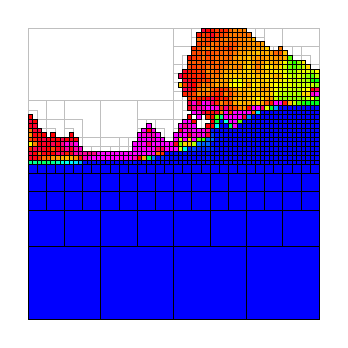
\begin{tikzpicture}[x={(\screenshotunitlength,0)},y={(0,\screenshotunitlength)}]
       \definecolor{fillcolor}{rgb}{0.000000,0.000000,1.000000}
\fill[fillcolor] (0.000000,0.000000) rectangle (0.250000,0.250000);
\definecolor{fillcolor}{rgb}{0.000000,0.000000,1.000000}
\fill[fillcolor] (0.250000,0.000000) rectangle (0.500000,0.250000);
\definecolor{fillcolor}{rgb}{0.000000,0.000000,1.000000}
\fill[fillcolor] (0.000000,0.250000) rectangle (0.125000,0.375000);
\definecolor{fillcolor}{rgb}{0.000000,0.000000,1.000000}
\fill[fillcolor] (0.125000,0.250000) rectangle (0.250000,0.375000);
\definecolor{fillcolor}{rgb}{0.000000,0.000000,1.000000}
\fill[fillcolor] (0.000000,0.375000) rectangle (0.062500,0.437500);
\definecolor{fillcolor}{rgb}{0.000000,0.000000,1.000000}
\fill[fillcolor] (0.062500,0.375000) rectangle (0.125000,0.437500);
\definecolor{fillcolor}{rgb}{0.000000,0.000000,1.000000}
\fill[fillcolor] (0.000000,0.437500) rectangle (0.062500,0.500000);
\definecolor{fillcolor}{rgb}{0.000000,0.000000,1.000000}
\fill[fillcolor] (0.062500,0.437500) rectangle (0.125000,0.500000);
\definecolor{fillcolor}{rgb}{0.000000,0.000000,1.000000}
\fill[fillcolor] (0.125000,0.375000) rectangle (0.187500,0.437500);
\definecolor{fillcolor}{rgb}{0.000000,0.000000,1.000000}
\fill[fillcolor] (0.187500,0.375000) rectangle (0.250000,0.437500);
\definecolor{fillcolor}{rgb}{0.000000,0.000000,1.000000}
\fill[fillcolor] (0.125000,0.437500) rectangle (0.187500,0.500000);
\definecolor{fillcolor}{rgb}{0.000000,0.000000,1.000000}
\fill[fillcolor] (0.187500,0.437500) rectangle (0.250000,0.500000);
\definecolor{fillcolor}{rgb}{0.000000,0.000000,1.000000}
\fill[fillcolor] (0.250000,0.250000) rectangle (0.375000,0.375000);
\definecolor{fillcolor}{rgb}{0.000000,0.000000,1.000000}
\fill[fillcolor] (0.375000,0.250000) rectangle (0.500000,0.375000);
\definecolor{fillcolor}{rgb}{0.000000,0.000000,1.000000}
\fill[fillcolor] (0.250000,0.375000) rectangle (0.312500,0.437500);
\definecolor{fillcolor}{rgb}{0.000000,0.000000,1.000000}
\fill[fillcolor] (0.312500,0.375000) rectangle (0.375000,0.437500);
\definecolor{fillcolor}{rgb}{0.000000,0.000000,1.000000}
\fill[fillcolor] (0.250000,0.437500) rectangle (0.312500,0.500000);
\definecolor{fillcolor}{rgb}{0.000000,0.000000,1.000000}
\fill[fillcolor] (0.312500,0.437500) rectangle (0.375000,0.500000);
\definecolor{fillcolor}{rgb}{0.000000,0.000000,1.000000}
\fill[fillcolor] (0.375000,0.375000) rectangle (0.437500,0.437500);
\definecolor{fillcolor}{rgb}{0.000000,0.000000,1.000000}
\fill[fillcolor] (0.437500,0.375000) rectangle (0.500000,0.437500);
\definecolor{fillcolor}{rgb}{0.000000,0.000001,1.000000}
\fill[fillcolor] (0.375000,0.437500) rectangle (0.437500,0.500000);
\definecolor{fillcolor}{rgb}{0.000000,0.000000,1.000000}
\fill[fillcolor] (0.437500,0.437500) rectangle (0.500000,0.500000);
\definecolor{fillcolor}{rgb}{0.000000,0.000000,1.000000}
\fill[fillcolor] (0.500000,0.000000) rectangle (0.750000,0.250000);
\definecolor{fillcolor}{rgb}{0.000000,0.000000,1.000000}
\fill[fillcolor] (0.750000,0.000000) rectangle (1.000000,0.250000);
\definecolor{fillcolor}{rgb}{0.000000,0.000000,1.000000}
\fill[fillcolor] (0.500000,0.250000) rectangle (0.625000,0.375000);
\definecolor{fillcolor}{rgb}{0.000000,0.000000,1.000000}
\fill[fillcolor] (0.625000,0.250000) rectangle (0.750000,0.375000);
\definecolor{fillcolor}{rgb}{0.000000,0.000000,1.000000}
\fill[fillcolor] (0.500000,0.375000) rectangle (0.562500,0.437500);
\definecolor{fillcolor}{rgb}{0.000000,0.000000,1.000000}
\fill[fillcolor] (0.562500,0.375000) rectangle (0.625000,0.437500);
\definecolor{fillcolor}{rgb}{0.000000,0.000000,1.000000}
\fill[fillcolor] (0.500000,0.437500) rectangle (0.562500,0.500000);
\definecolor{fillcolor}{rgb}{0.000000,0.000000,1.000000}
\fill[fillcolor] (0.562500,0.437500) rectangle (0.625000,0.500000);
\definecolor{fillcolor}{rgb}{0.000000,0.000000,1.000000}
\fill[fillcolor] (0.625000,0.375000) rectangle (0.687500,0.437500);
\definecolor{fillcolor}{rgb}{0.000000,0.000000,1.000000}
\fill[fillcolor] (0.687500,0.375000) rectangle (0.750000,0.437500);
\definecolor{fillcolor}{rgb}{0.000000,0.000000,1.000000}
\fill[fillcolor] (0.625000,0.437500) rectangle (0.687500,0.500000);
\definecolor{fillcolor}{rgb}{0.000000,0.000000,1.000000}
\fill[fillcolor] (0.687500,0.437500) rectangle (0.750000,0.500000);
\definecolor{fillcolor}{rgb}{0.000000,0.000000,1.000000}
\fill[fillcolor] (0.750000,0.250000) rectangle (0.875000,0.375000);
\definecolor{fillcolor}{rgb}{0.000000,0.000000,1.000000}
\fill[fillcolor] (0.875000,0.250000) rectangle (1.000000,0.375000);
\definecolor{fillcolor}{rgb}{0.000000,0.000000,1.000000}
\fill[fillcolor] (0.750000,0.375000) rectangle (0.812500,0.437500);
\definecolor{fillcolor}{rgb}{0.000000,0.000000,1.000000}
\fill[fillcolor] (0.812500,0.375000) rectangle (0.875000,0.437500);
\definecolor{fillcolor}{rgb}{0.000000,0.000000,1.000000}
\fill[fillcolor] (0.750000,0.437500) rectangle (0.812500,0.500000);
\definecolor{fillcolor}{rgb}{0.000000,0.000000,1.000000}
\fill[fillcolor] (0.812500,0.437500) rectangle (0.875000,0.500000);
\definecolor{fillcolor}{rgb}{0.000000,0.000000,1.000000}
\fill[fillcolor] (0.875000,0.375000) rectangle (0.937500,0.437500);
\definecolor{fillcolor}{rgb}{0.000000,0.000000,1.000000}
\fill[fillcolor] (0.937500,0.375000) rectangle (1.000000,0.437500);
\definecolor{fillcolor}{rgb}{0.000000,0.000000,1.000000}
\fill[fillcolor] (0.875000,0.437500) rectangle (0.937500,0.500000);
\definecolor{fillcolor}{rgb}{0.000000,0.000000,1.000000}
\fill[fillcolor] (0.937500,0.437500) rectangle (1.000000,0.500000);
\definecolor{fillcolor}{rgb}{0.000000,0.000000,1.000000}
\fill[fillcolor] (0.000000,0.500000) rectangle (0.031250,0.531250);
\definecolor{fillcolor}{rgb}{0.000000,0.000000,1.000000}
\fill[fillcolor] (0.031250,0.500000) rectangle (0.062500,0.531250);
\definecolor{fillcolor}{rgb}{0.000000,1.000000,0.527969}
\fill[fillcolor] (0.000000,0.531250) rectangle (0.015625,0.546875);
\definecolor{fillcolor}{rgb}{0.000000,1.000000,0.580783}
\fill[fillcolor] (0.015625,0.531250) rectangle (0.031250,0.546875);
\definecolor{fillcolor}{rgb}{1.000000,0.000000,0.138987}
\fill[fillcolor] (0.000000,0.546875) rectangle (0.015625,0.562500);
\definecolor{fillcolor}{rgb}{1.000000,0.000000,0.096982}
\fill[fillcolor] (0.015625,0.546875) rectangle (0.031250,0.562500);
\definecolor{fillcolor}{rgb}{0.000000,1.000000,0.499040}
\fill[fillcolor] (0.031250,0.531250) rectangle (0.046875,0.546875);
\definecolor{fillcolor}{rgb}{0.000000,1.000000,0.387909}
\fill[fillcolor] (0.046875,0.531250) rectangle (0.062500,0.546875);
\definecolor{fillcolor}{rgb}{1.000000,0.158055,0.000000}
\fill[fillcolor] (0.031250,0.546875) rectangle (0.046875,0.562500);
\definecolor{fillcolor}{rgb}{1.000000,0.410624,0.000000}
\fill[fillcolor] (0.046875,0.546875) rectangle (0.062500,0.562500);
\definecolor{fillcolor}{rgb}{0.000000,0.000000,1.000000}
\fill[fillcolor] (0.062500,0.500000) rectangle (0.093750,0.531250);
\definecolor{fillcolor}{rgb}{0.000000,0.000000,1.000000}
\fill[fillcolor] (0.093750,0.500000) rectangle (0.125000,0.531250);
\definecolor{fillcolor}{rgb}{0.000000,1.000000,0.448355}
\fill[fillcolor] (0.062500,0.531250) rectangle (0.078125,0.546875);
\definecolor{fillcolor}{rgb}{0.000000,1.000000,0.571311}
\fill[fillcolor] (0.078125,0.531250) rectangle (0.093750,0.546875);
\definecolor{fillcolor}{rgb}{1.000000,0.395846,0.000000}
\fill[fillcolor] (0.062500,0.546875) rectangle (0.078125,0.562500);
\definecolor{fillcolor}{rgb}{1.000000,0.576563,0.000000}
\fill[fillcolor] (0.078125,0.546875) rectangle (0.093750,0.562500);
\definecolor{fillcolor}{rgb}{0.000000,1.000000,0.729229}
\fill[fillcolor] (0.093750,0.531250) rectangle (0.109375,0.546875);
\definecolor{fillcolor}{rgb}{0.000000,1.000000,0.879589}
\fill[fillcolor] (0.109375,0.531250) rectangle (0.125000,0.546875);
\definecolor{fillcolor}{rgb}{1.000000,0.604676,0.000000}
\fill[fillcolor] (0.093750,0.546875) rectangle (0.109375,0.562500);
\definecolor{fillcolor}{rgb}{1.000000,0.674435,0.000000}
\fill[fillcolor] (0.109375,0.546875) rectangle (0.125000,0.562500);
\definecolor{fillcolor}{rgb}{1.000000,0.000000,0.302971}
\fill[fillcolor] (0.000000,0.562500) rectangle (0.015625,0.578125);
\definecolor{fillcolor}{rgb}{1.000000,0.000000,0.010086}
\fill[fillcolor] (0.015625,0.562500) rectangle (0.031250,0.578125);
\definecolor{fillcolor}{rgb}{1.000000,0.137815,0.000000}
\fill[fillcolor] (0.000000,0.578125) rectangle (0.015625,0.593750);
\definecolor{fillcolor}{rgb}{1.000000,0.000000,0.323519}
\fill[fillcolor] (0.015625,0.578125) rectangle (0.031250,0.593750);
\definecolor{fillcolor}{rgb}{1.000000,0.395870,0.000000}
\fill[fillcolor] (0.031250,0.562500) rectangle (0.046875,0.578125);
\definecolor{fillcolor}{rgb}{1.000000,0.000000,0.084461}
\fill[fillcolor] (0.046875,0.562500) rectangle (0.062500,0.578125);
\definecolor{fillcolor}{rgb}{1.000000,0.000000,0.275160}
\fill[fillcolor] (0.031250,0.578125) rectangle (0.046875,0.593750);
\definecolor{fillcolor}{rgb}{1.000000,0.000000,0.153733}
\fill[fillcolor] (0.046875,0.578125) rectangle (0.062500,0.593750);
\definecolor{fillcolor}{rgb}{0.983921,1.000000,0.000000}
\fill[fillcolor] (0.000000,0.593750) rectangle (0.015625,0.609375);
\definecolor{fillcolor}{rgb}{1.000000,0.515059,0.000000}
\fill[fillcolor] (0.015625,0.593750) rectangle (0.031250,0.609375);
\definecolor{fillcolor}{rgb}{1.000000,0.296901,0.000000}
\fill[fillcolor] (0.000000,0.609375) rectangle (0.015625,0.625000);
\definecolor{fillcolor}{rgb}{1.000000,0.120302,0.000000}
\fill[fillcolor] (0.015625,0.609375) rectangle (0.031250,0.625000);
\definecolor{fillcolor}{rgb}{1.000000,0.000000,0.010083}
\fill[fillcolor] (0.031250,0.593750) rectangle (0.046875,0.609375);
\definecolor{fillcolor}{rgb}{1.000000,0.000000,0.147641}
\fill[fillcolor] (0.046875,0.593750) rectangle (0.062500,0.609375);
\definecolor{fillcolor}{rgb}{1.000000,0.000000,0.122416}
\fill[fillcolor] (0.031250,0.609375) rectangle (0.046875,0.625000);
\definecolor{fillcolor}{rgb}{1.000000,0.000000,0.250308}
\fill[fillcolor] (0.046875,0.609375) rectangle (0.062500,0.625000);
\definecolor{fillcolor}{rgb}{1.000000,0.000000,0.021531}
\fill[fillcolor] (0.062500,0.562500) rectangle (0.078125,0.578125);
\definecolor{fillcolor}{rgb}{1.000000,0.000000,0.016188}
\fill[fillcolor] (0.078125,0.562500) rectangle (0.093750,0.578125);
\definecolor{fillcolor}{rgb}{1.000000,0.016917,0.000000}
\fill[fillcolor] (0.062500,0.578125) rectangle (0.078125,0.593750);
\definecolor{fillcolor}{rgb}{1.000000,0.265589,0.000000}
\fill[fillcolor] (0.078125,0.578125) rectangle (0.093750,0.593750);
\definecolor{fillcolor}{rgb}{1.000000,0.000000,0.388247}
\fill[fillcolor] (0.093750,0.562500) rectangle (0.109375,0.578125);
\definecolor{fillcolor}{rgb}{1.000000,0.000000,0.340510}
\fill[fillcolor] (0.109375,0.562500) rectangle (0.125000,0.578125);
\definecolor{fillcolor}{rgb}{1.000000,0.000000,0.117219}
\fill[fillcolor] (0.093750,0.578125) rectangle (0.109375,0.593750);
\definecolor{fillcolor}{rgb}{1.000000,0.000000,0.194053}
\fill[fillcolor] (0.109375,0.578125) rectangle (0.125000,0.593750);
\definecolor{fillcolor}{rgb}{1.000000,0.000000,0.113895}
\fill[fillcolor] (0.062500,0.593750) rectangle (0.078125,0.609375);
\definecolor{fillcolor}{rgb}{1.000000,0.000000,0.330135}
\fill[fillcolor] (0.078125,0.593750) rectangle (0.093750,0.609375);
\definecolor{fillcolor}{rgb}{1.000000,0.000000,0.097351}
\fill[fillcolor] (0.062500,0.609375) rectangle (0.078125,0.625000);
\definecolor{fillcolor}{rgb}{1.000000,0.000000,0.060908}
\fill[fillcolor] (0.078125,0.609375) rectangle (0.093750,0.625000);
\definecolor{fillcolor}{rgb}{1.000000,0.000000,0.092701}
\fill[fillcolor] (0.093750,0.593750) rectangle (0.109375,0.609375);
\definecolor{fillcolor}{rgb}{1.000000,0.000000,0.508128}
\fill[fillcolor] (0.109375,0.593750) rectangle (0.125000,0.609375);
\definecolor{fillcolor}{rgb}{1.000000,0.000000,0.008714}
\fill[fillcolor] (0.093750,0.609375) rectangle (0.109375,0.625000);
\definecolor{fillcolor}{rgb}{1.000000,0.000000,0.303862}
\fill[fillcolor] (0.109375,0.609375) rectangle (0.125000,0.625000);
\definecolor{fillcolor}{rgb}{0.000000,0.000000,1.000000}
\fill[fillcolor] (0.125000,0.500000) rectangle (0.156250,0.531250);
\definecolor{fillcolor}{rgb}{0.000000,0.000000,1.000000}
\fill[fillcolor] (0.156250,0.500000) rectangle (0.187500,0.531250);
\definecolor{fillcolor}{rgb}{0.000000,1.000000,0.969502}
\fill[fillcolor] (0.125000,0.531250) rectangle (0.140625,0.546875);
\definecolor{fillcolor}{rgb}{0.000000,0.954326,1.000000}
\fill[fillcolor] (0.140625,0.531250) rectangle (0.156250,0.546875);
\definecolor{fillcolor}{rgb}{1.000000,0.697392,0.000000}
\fill[fillcolor] (0.125000,0.546875) rectangle (0.140625,0.562500);
\definecolor{fillcolor}{rgb}{1.000000,0.691640,0.000000}
\fill[fillcolor] (0.140625,0.546875) rectangle (0.156250,0.562500);
\definecolor{fillcolor}{rgb}{0.000000,0.870936,1.000000}
\fill[fillcolor] (0.156250,0.531250) rectangle (0.171875,0.546875);
\definecolor{fillcolor}{rgb}{0.000000,0.665146,1.000000}
\fill[fillcolor] (0.171875,0.531250) rectangle (0.187500,0.546875);
\definecolor{fillcolor}{rgb}{1.000000,0.552335,0.000000}
\fill[fillcolor] (0.156250,0.546875) rectangle (0.171875,0.562500);
\definecolor{fillcolor}{rgb}{1.000000,0.158721,0.000000}
\fill[fillcolor] (0.171875,0.546875) rectangle (0.187500,0.562500);
\definecolor{fillcolor}{rgb}{0.000000,0.000000,1.000000}
\fill[fillcolor] (0.187500,0.500000) rectangle (0.218750,0.531250);
\definecolor{fillcolor}{rgb}{0.000000,0.000000,1.000000}
\fill[fillcolor] (0.218750,0.500000) rectangle (0.250000,0.531250);
\definecolor{fillcolor}{rgb}{0.000000,0.022357,1.000000}
\fill[fillcolor] (0.187500,0.531250) rectangle (0.203125,0.546875);
\definecolor{fillcolor}{rgb}{0.000000,0.036337,1.000000}
\fill[fillcolor] (0.203125,0.531250) rectangle (0.218750,0.546875);
\definecolor{fillcolor}{rgb}{1.000000,0.000000,0.751400}
\fill[fillcolor] (0.187500,0.546875) rectangle (0.203125,0.562500);
\definecolor{fillcolor}{rgb}{1.000000,0.000000,0.887181}
\fill[fillcolor] (0.203125,0.546875) rectangle (0.218750,0.562500);
\definecolor{fillcolor}{rgb}{0.000000,0.024818,1.000000}
\fill[fillcolor] (0.218750,0.531250) rectangle (0.234375,0.546875);
\definecolor{fillcolor}{rgb}{0.000000,0.033455,1.000000}
\fill[fillcolor] (0.234375,0.531250) rectangle (0.250000,0.546875);
\definecolor{fillcolor}{rgb}{1.000000,0.000000,1.000000}
\fill[fillcolor] (0.218750,0.546875) rectangle (0.234375,0.562500);
\definecolor{fillcolor}{rgb}{1.000000,0.000000,1.000000}
\fill[fillcolor] (0.234375,0.546875) rectangle (0.250000,0.562500);
\definecolor{fillcolor}{rgb}{1.000000,0.092819,0.000000}
\fill[fillcolor] (0.125000,0.562500) rectangle (0.140625,0.578125);
\definecolor{fillcolor}{rgb}{1.000000,0.000000,0.149489}
\fill[fillcolor] (0.140625,0.562500) rectangle (0.156250,0.578125);
\definecolor{fillcolor}{rgb}{1.000000,0.000000,0.646969}
\fill[fillcolor] (0.125000,0.578125) rectangle (0.140625,0.593750);
\definecolor{fillcolor}{rgb}{1.000000,0.000000,0.131116}
\fill[fillcolor] (0.140625,0.578125) rectangle (0.156250,0.593750);
\definecolor{fillcolor}{rgb}{1.000000,0.000000,0.654798}
\fill[fillcolor] (0.156250,0.562500) rectangle (0.171875,0.578125);
\definecolor{fillcolor}{rgb}{1.000000,0.000000,0.644191}
\fill[fillcolor] (0.171875,0.562500) rectangle (0.187500,0.578125);
\definecolor{fillcolor}{rgb}{1.000000,0.000000,0.707138}
\fill[fillcolor] (0.156250,0.578125) rectangle (0.171875,0.593750);
\definecolor{fillcolor}{rgb}{1.000000,0.000000,0.793607}
\fill[fillcolor] (0.171875,0.578125) rectangle (0.187500,0.593750);
\definecolor{fillcolor}{rgb}{1.000000,0.000000,0.877018}
\fill[fillcolor] (0.125000,0.593750) rectangle (0.140625,0.609375);
\definecolor{fillcolor}{rgb}{1.000000,0.000000,0.680333}
\fill[fillcolor] (0.140625,0.593750) rectangle (0.156250,0.609375);
\definecolor{fillcolor}{rgb}{1.000000,0.000000,0.027235}
\fill[fillcolor] (0.125000,0.609375) rectangle (0.140625,0.625000);
\definecolor{fillcolor}{rgb}{1.000000,0.000000,0.098066}
\fill[fillcolor] (0.140625,0.609375) rectangle (0.156250,0.625000);
\definecolor{fillcolor}{rgb}{1.000000,0.000000,0.898166}
\fill[fillcolor] (0.156250,0.593750) rectangle (0.171875,0.609375);
\definecolor{fillcolor}{rgb}{1.000000,0.000000,0.021779}
\fill[fillcolor] (0.156250,0.609375) rectangle (0.171875,0.625000);
\definecolor{fillcolor}{rgb}{1.000000,0.000000,0.621650}
\fill[fillcolor] (0.187500,0.562500) rectangle (0.203125,0.578125);
\definecolor{fillcolor}{rgb}{1.000000,0.000000,0.456965}
\fill[fillcolor] (0.203125,0.562500) rectangle (0.218750,0.578125);
\definecolor{fillcolor}{rgb}{1.000000,0.000000,0.532649}
\fill[fillcolor] (0.218750,0.562500) rectangle (0.234375,0.578125);
\definecolor{fillcolor}{rgb}{1.000000,0.000000,0.975996}
\fill[fillcolor] (0.234375,0.562500) rectangle (0.250000,0.578125);
\definecolor{fillcolor}{rgb}{1.000000,0.577266,0.000000}
\fill[fillcolor] (0.000000,0.625000) rectangle (0.015625,0.640625);
\definecolor{fillcolor}{rgb}{1.000000,0.000000,0.079649}
\fill[fillcolor] (0.015625,0.625000) rectangle (0.031250,0.640625);
\definecolor{fillcolor}{rgb}{1.000000,0.428401,0.000000}
\fill[fillcolor] (0.000000,0.640625) rectangle (0.015625,0.656250);
\definecolor{fillcolor}{rgb}{1.000000,0.000000,0.190332}
\fill[fillcolor] (0.015625,0.640625) rectangle (0.031250,0.656250);
\definecolor{fillcolor}{rgb}{1.000000,0.116590,0.000000}
\fill[fillcolor] (0.031250,0.625000) rectangle (0.046875,0.640625);
\definecolor{fillcolor}{rgb}{1.000000,0.000000,0.027002}
\fill[fillcolor] (0.046875,0.625000) rectangle (0.062500,0.640625);
\definecolor{fillcolor}{rgb}{1.000000,0.000000,0.235845}
\fill[fillcolor] (0.031250,0.640625) rectangle (0.046875,0.656250);
\definecolor{fillcolor}{rgb}{1.000000,0.000000,0.120165}
\fill[fillcolor] (0.000000,0.656250) rectangle (0.015625,0.671875);
\definecolor{fillcolor}{rgb}{1.000000,0.000000,0.196137}
\fill[fillcolor] (0.015625,0.656250) rectangle (0.031250,0.671875);
\definecolor{fillcolor}{rgb}{1.000000,0.000000,0.280105}
\fill[fillcolor] (0.000000,0.671875) rectangle (0.015625,0.687500);
\definecolor{fillcolor}{rgb}{1.000000,0.000000,0.000000}
\fill[fillcolor] (0.015625,0.671875) rectangle (0.031250,0.687500);
\definecolor{fillcolor}{rgb}{1.000000,0.000000,0.001843}
\fill[fillcolor] (0.078125,0.625000) rectangle (0.093750,0.640625);
\definecolor{fillcolor}{rgb}{1.000000,0.000000,0.000000}
\fill[fillcolor] (0.000000,0.687500) rectangle (0.015625,0.703125);
\definecolor{fillcolor}{rgb}{1.000000,0.000000,0.050824}
\fill[fillcolor] (0.140625,0.625000) rectangle (0.156250,0.640625);
\definecolor{fillcolor}{rgb}{0.000000,0.000000,1.000000}
\fill[fillcolor] (0.250000,0.500000) rectangle (0.281250,0.531250);
\definecolor{fillcolor}{rgb}{0.000000,0.000000,1.000000}
\fill[fillcolor] (0.281250,0.500000) rectangle (0.312500,0.531250);
\definecolor{fillcolor}{rgb}{0.000000,0.000000,1.000000}
\fill[fillcolor] (0.250000,0.531250) rectangle (0.265625,0.546875);
\definecolor{fillcolor}{rgb}{0.000000,0.000000,1.000000}
\fill[fillcolor] (0.265625,0.531250) rectangle (0.281250,0.546875);
\definecolor{fillcolor}{rgb}{1.000000,0.000000,1.000000}
\fill[fillcolor] (0.250000,0.546875) rectangle (0.265625,0.562500);
\definecolor{fillcolor}{rgb}{1.000000,0.000000,1.000000}
\fill[fillcolor] (0.265625,0.546875) rectangle (0.281250,0.562500);
\definecolor{fillcolor}{rgb}{0.000000,0.000000,1.000000}
\fill[fillcolor] (0.281250,0.531250) rectangle (0.296875,0.546875);
\definecolor{fillcolor}{rgb}{0.000000,0.000000,1.000000}
\fill[fillcolor] (0.296875,0.531250) rectangle (0.312500,0.546875);
\definecolor{fillcolor}{rgb}{1.000000,0.000000,1.000000}
\fill[fillcolor] (0.281250,0.546875) rectangle (0.296875,0.562500);
\definecolor{fillcolor}{rgb}{1.000000,0.000000,1.000000}
\fill[fillcolor] (0.296875,0.546875) rectangle (0.312500,0.562500);
\definecolor{fillcolor}{rgb}{0.000000,0.000000,1.000000}
\fill[fillcolor] (0.312500,0.500000) rectangle (0.343750,0.531250);
\definecolor{fillcolor}{rgb}{0.000000,0.000614,1.000000}
\fill[fillcolor] (0.343750,0.500000) rectangle (0.375000,0.531250);
\definecolor{fillcolor}{rgb}{0.000000,0.000000,1.000000}
\fill[fillcolor] (0.312500,0.531250) rectangle (0.328125,0.546875);
\definecolor{fillcolor}{rgb}{0.000000,0.002890,1.000000}
\fill[fillcolor] (0.328125,0.531250) rectangle (0.343750,0.546875);
\definecolor{fillcolor}{rgb}{1.000000,0.000000,1.000000}
\fill[fillcolor] (0.312500,0.546875) rectangle (0.328125,0.562500);
\definecolor{fillcolor}{rgb}{1.000000,0.000000,1.000000}
\fill[fillcolor] (0.328125,0.546875) rectangle (0.343750,0.562500);
\definecolor{fillcolor}{rgb}{0.000000,0.051289,1.000000}
\fill[fillcolor] (0.343750,0.531250) rectangle (0.359375,0.546875);
\definecolor{fillcolor}{rgb}{0.000000,0.034657,1.000000}
\fill[fillcolor] (0.359375,0.531250) rectangle (0.375000,0.546875);
\definecolor{fillcolor}{rgb}{1.000000,0.000000,1.000000}
\fill[fillcolor] (0.343750,0.546875) rectangle (0.359375,0.562500);
\definecolor{fillcolor}{rgb}{1.000000,0.000000,0.741268}
\fill[fillcolor] (0.359375,0.546875) rectangle (0.375000,0.562500);
\definecolor{fillcolor}{rgb}{1.000000,0.000000,1.000000}
\fill[fillcolor] (0.250000,0.562500) rectangle (0.265625,0.578125);
\definecolor{fillcolor}{rgb}{1.000000,0.000000,1.000000}
\fill[fillcolor] (0.265625,0.562500) rectangle (0.281250,0.578125);
\definecolor{fillcolor}{rgb}{1.000000,0.000000,1.000000}
\fill[fillcolor] (0.281250,0.562500) rectangle (0.296875,0.578125);
\definecolor{fillcolor}{rgb}{1.000000,0.000000,1.000000}
\fill[fillcolor] (0.296875,0.562500) rectangle (0.312500,0.578125);
\definecolor{fillcolor}{rgb}{1.000000,0.000000,1.000000}
\fill[fillcolor] (0.312500,0.562500) rectangle (0.328125,0.578125);
\definecolor{fillcolor}{rgb}{1.000000,0.000000,1.000000}
\fill[fillcolor] (0.328125,0.562500) rectangle (0.343750,0.578125);
\definecolor{fillcolor}{rgb}{1.000000,0.000000,1.000000}
\fill[fillcolor] (0.343750,0.562500) rectangle (0.359375,0.578125);
\definecolor{fillcolor}{rgb}{1.000000,0.000000,1.000000}
\fill[fillcolor] (0.359375,0.562500) rectangle (0.375000,0.578125);
\definecolor{fillcolor}{rgb}{1.000000,0.000000,1.000000}
\fill[fillcolor] (0.359375,0.578125) rectangle (0.375000,0.593750);
\definecolor{fillcolor}{rgb}{1.000000,0.000000,1.000000}
\fill[fillcolor] (0.359375,0.593750) rectangle (0.375000,0.609375);
\definecolor{fillcolor}{rgb}{0.000000,0.000000,1.000000}
\fill[fillcolor] (0.375000,0.500000) rectangle (0.406250,0.531250);
\definecolor{fillcolor}{rgb}{0.000000,0.000000,1.000000}
\fill[fillcolor] (0.406250,0.500000) rectangle (0.437500,0.531250);
\definecolor{fillcolor}{rgb}{0.000000,0.000000,1.000000}
\fill[fillcolor] (0.375000,0.531250) rectangle (0.390625,0.546875);
\definecolor{fillcolor}{rgb}{0.000000,0.000001,1.000000}
\fill[fillcolor] (0.390625,0.531250) rectangle (0.406250,0.546875);
\definecolor{fillcolor}{rgb}{1.000000,0.020477,0.000000}
\fill[fillcolor] (0.375000,0.546875) rectangle (0.390625,0.562500);
\definecolor{fillcolor}{rgb}{1.000000,0.621936,0.000000}
\fill[fillcolor] (0.390625,0.546875) rectangle (0.406250,0.562500);
\definecolor{fillcolor}{rgb}{0.000000,0.000003,1.000000}
\fill[fillcolor] (0.406250,0.531250) rectangle (0.421875,0.546875);
\definecolor{fillcolor}{rgb}{0.000000,0.000000,1.000000}
\fill[fillcolor] (0.421875,0.531250) rectangle (0.437500,0.546875);
\definecolor{fillcolor}{rgb}{0.000000,1.000000,0.325696}
\fill[fillcolor] (0.406250,0.546875) rectangle (0.421875,0.562500);
\definecolor{fillcolor}{rgb}{0.000000,0.457081,1.000000}
\fill[fillcolor] (0.421875,0.546875) rectangle (0.437500,0.562500);
\definecolor{fillcolor}{rgb}{0.000000,0.000000,1.000000}
\fill[fillcolor] (0.437500,0.500000) rectangle (0.468750,0.531250);
\definecolor{fillcolor}{rgb}{0.000000,0.000000,1.000000}
\fill[fillcolor] (0.468750,0.500000) rectangle (0.500000,0.531250);
\definecolor{fillcolor}{rgb}{0.000000,0.000000,1.000000}
\fill[fillcolor] (0.437500,0.531250) rectangle (0.453125,0.546875);
\definecolor{fillcolor}{rgb}{0.000000,0.000000,1.000000}
\fill[fillcolor] (0.453125,0.531250) rectangle (0.468750,0.546875);
\definecolor{fillcolor}{rgb}{0.000000,0.023296,1.000000}
\fill[fillcolor] (0.437500,0.546875) rectangle (0.453125,0.562500);
\definecolor{fillcolor}{rgb}{0.000000,0.168730,1.000000}
\fill[fillcolor] (0.453125,0.546875) rectangle (0.468750,0.562500);
\definecolor{fillcolor}{rgb}{0.000000,0.000000,1.000000}
\fill[fillcolor] (0.468750,0.531250) rectangle (0.484375,0.546875);
\definecolor{fillcolor}{rgb}{0.000000,0.000000,1.000000}
\fill[fillcolor] (0.484375,0.531250) rectangle (0.500000,0.546875);
\definecolor{fillcolor}{rgb}{0.000000,0.050861,1.000000}
\fill[fillcolor] (0.468750,0.546875) rectangle (0.484375,0.562500);
\definecolor{fillcolor}{rgb}{0.000000,0.013669,1.000000}
\fill[fillcolor] (0.484375,0.546875) rectangle (0.500000,0.562500);
\definecolor{fillcolor}{rgb}{1.000000,0.000000,1.000000}
\fill[fillcolor] (0.375000,0.562500) rectangle (0.390625,0.578125);
\definecolor{fillcolor}{rgb}{1.000000,0.000000,1.000000}
\fill[fillcolor] (0.390625,0.562500) rectangle (0.406250,0.578125);
\definecolor{fillcolor}{rgb}{1.000000,0.000000,1.000000}
\fill[fillcolor] (0.375000,0.578125) rectangle (0.390625,0.593750);
\definecolor{fillcolor}{rgb}{1.000000,0.000000,1.000000}
\fill[fillcolor] (0.390625,0.578125) rectangle (0.406250,0.593750);
\definecolor{fillcolor}{rgb}{1.000000,0.000000,1.000000}
\fill[fillcolor] (0.406250,0.562500) rectangle (0.421875,0.578125);
\definecolor{fillcolor}{rgb}{1.000000,0.000000,1.000000}
\fill[fillcolor] (0.421875,0.562500) rectangle (0.437500,0.578125);
\definecolor{fillcolor}{rgb}{1.000000,0.000000,1.000000}
\fill[fillcolor] (0.406250,0.578125) rectangle (0.421875,0.593750);
\definecolor{fillcolor}{rgb}{1.000000,0.000000,1.000000}
\fill[fillcolor] (0.421875,0.578125) rectangle (0.437500,0.593750);
\definecolor{fillcolor}{rgb}{1.000000,0.000000,1.000000}
\fill[fillcolor] (0.375000,0.593750) rectangle (0.390625,0.609375);
\definecolor{fillcolor}{rgb}{1.000000,0.000000,1.000000}
\fill[fillcolor] (0.390625,0.593750) rectangle (0.406250,0.609375);
\definecolor{fillcolor}{rgb}{1.000000,0.000000,1.000000}
\fill[fillcolor] (0.375000,0.609375) rectangle (0.390625,0.625000);
\definecolor{fillcolor}{rgb}{1.000000,0.000000,1.000000}
\fill[fillcolor] (0.390625,0.609375) rectangle (0.406250,0.625000);
\definecolor{fillcolor}{rgb}{1.000000,0.000000,0.425476}
\fill[fillcolor] (0.406250,0.593750) rectangle (0.421875,0.609375);
\definecolor{fillcolor}{rgb}{1.000000,0.000000,1.000000}
\fill[fillcolor] (0.421875,0.593750) rectangle (0.437500,0.609375);
\definecolor{fillcolor}{rgb}{1.000000,0.000000,1.000000}
\fill[fillcolor] (0.406250,0.609375) rectangle (0.421875,0.625000);
\definecolor{fillcolor}{rgb}{1.000000,0.000000,0.786882}
\fill[fillcolor] (0.421875,0.609375) rectangle (0.437500,0.625000);
\definecolor{fillcolor}{rgb}{1.000000,0.389612,0.000000}
\fill[fillcolor] (0.437500,0.562500) rectangle (0.453125,0.578125);
\definecolor{fillcolor}{rgb}{1.000000,0.170152,0.000000}
\fill[fillcolor] (0.453125,0.562500) rectangle (0.468750,0.578125);
\definecolor{fillcolor}{rgb}{1.000000,0.000000,0.452075}
\fill[fillcolor] (0.437500,0.578125) rectangle (0.453125,0.593750);
\definecolor{fillcolor}{rgb}{1.000000,0.000000,0.348214}
\fill[fillcolor] (0.453125,0.578125) rectangle (0.468750,0.593750);
\definecolor{fillcolor}{rgb}{0.000000,0.014783,1.000000}
\fill[fillcolor] (0.468750,0.562500) rectangle (0.484375,0.578125);
\definecolor{fillcolor}{rgb}{0.000000,0.006150,1.000000}
\fill[fillcolor] (0.484375,0.562500) rectangle (0.500000,0.578125);
\definecolor{fillcolor}{rgb}{1.000000,0.000000,1.000000}
\fill[fillcolor] (0.468750,0.578125) rectangle (0.484375,0.593750);
\definecolor{fillcolor}{rgb}{1.000000,0.000000,1.000000}
\fill[fillcolor] (0.484375,0.578125) rectangle (0.500000,0.593750);
\definecolor{fillcolor}{rgb}{1.000000,0.000000,1.000000}
\fill[fillcolor] (0.437500,0.593750) rectangle (0.453125,0.609375);
\definecolor{fillcolor}{rgb}{1.000000,0.000000,1.000000}
\fill[fillcolor] (0.453125,0.593750) rectangle (0.468750,0.609375);
\definecolor{fillcolor}{rgb}{1.000000,0.000000,1.000000}
\fill[fillcolor] (0.437500,0.609375) rectangle (0.453125,0.625000);
\definecolor{fillcolor}{rgb}{1.000000,0.000000,1.000000}
\fill[fillcolor] (0.453125,0.609375) rectangle (0.468750,0.625000);
\definecolor{fillcolor}{rgb}{1.000000,0.000000,1.000000}
\fill[fillcolor] (0.468750,0.593750) rectangle (0.484375,0.609375);
\definecolor{fillcolor}{rgb}{1.000000,0.000000,1.000000}
\fill[fillcolor] (0.484375,0.593750) rectangle (0.500000,0.609375);
\definecolor{fillcolor}{rgb}{1.000000,0.000000,1.000000}
\fill[fillcolor] (0.375000,0.625000) rectangle (0.390625,0.640625);
\definecolor{fillcolor}{rgb}{1.000000,0.000000,0.853295}
\fill[fillcolor] (0.390625,0.625000) rectangle (0.406250,0.640625);
\definecolor{fillcolor}{rgb}{1.000000,0.000000,1.000000}
\fill[fillcolor] (0.390625,0.640625) rectangle (0.406250,0.656250);
\definecolor{fillcolor}{rgb}{1.000000,0.000000,0.741041}
\fill[fillcolor] (0.406250,0.625000) rectangle (0.421875,0.640625);
\definecolor{fillcolor}{rgb}{1.000000,0.000000,0.772305}
\fill[fillcolor] (0.421875,0.625000) rectangle (0.437500,0.640625);
\definecolor{fillcolor}{rgb}{1.000000,0.068573,0.000000}
\fill[fillcolor] (0.406250,0.640625) rectangle (0.421875,0.656250);
\definecolor{fillcolor}{rgb}{1.000000,0.000000,0.911972}
\fill[fillcolor] (0.421875,0.640625) rectangle (0.437500,0.656250);
\definecolor{fillcolor}{rgb}{1.000000,0.000000,1.000000}
\fill[fillcolor] (0.406250,0.656250) rectangle (0.421875,0.671875);
\definecolor{fillcolor}{rgb}{1.000000,0.000000,1.000000}
\fill[fillcolor] (0.437500,0.625000) rectangle (0.453125,0.640625);
\definecolor{fillcolor}{rgb}{0.000000,0.000000,1.000000}
\fill[fillcolor] (0.500000,0.500000) rectangle (0.531250,0.531250);
\definecolor{fillcolor}{rgb}{0.000000,0.000001,1.000000}
\fill[fillcolor] (0.531250,0.500000) rectangle (0.562500,0.531250);
\definecolor{fillcolor}{rgb}{0.000000,0.000000,1.000000}
\fill[fillcolor] (0.500000,0.531250) rectangle (0.515625,0.546875);
\definecolor{fillcolor}{rgb}{0.000000,0.000000,1.000000}
\fill[fillcolor] (0.515625,0.531250) rectangle (0.531250,0.546875);
\definecolor{fillcolor}{rgb}{0.000000,0.006997,1.000000}
\fill[fillcolor] (0.500000,0.546875) rectangle (0.515625,0.562500);
\definecolor{fillcolor}{rgb}{0.000000,0.010140,1.000000}
\fill[fillcolor] (0.515625,0.546875) rectangle (0.531250,0.562500);
\definecolor{fillcolor}{rgb}{0.000000,0.000000,1.000000}
\fill[fillcolor] (0.531250,0.531250) rectangle (0.546875,0.546875);
\definecolor{fillcolor}{rgb}{0.000000,0.000000,1.000000}
\fill[fillcolor] (0.546875,0.531250) rectangle (0.562500,0.546875);
\definecolor{fillcolor}{rgb}{0.000000,0.000000,1.000000}
\fill[fillcolor] (0.531250,0.546875) rectangle (0.546875,0.562500);
\definecolor{fillcolor}{rgb}{0.000000,0.000099,1.000000}
\fill[fillcolor] (0.546875,0.546875) rectangle (0.562500,0.562500);
\definecolor{fillcolor}{rgb}{0.000000,0.000001,1.000000}
\fill[fillcolor] (0.562500,0.500000) rectangle (0.593750,0.531250);
\definecolor{fillcolor}{rgb}{0.000000,0.000012,1.000000}
\fill[fillcolor] (0.593750,0.500000) rectangle (0.625000,0.531250);
\definecolor{fillcolor}{rgb}{0.000000,0.000001,1.000000}
\fill[fillcolor] (0.562500,0.531250) rectangle (0.578125,0.546875);
\definecolor{fillcolor}{rgb}{0.000000,0.000002,1.000000}
\fill[fillcolor] (0.578125,0.531250) rectangle (0.593750,0.546875);
\definecolor{fillcolor}{rgb}{0.000000,0.000942,1.000000}
\fill[fillcolor] (0.562500,0.546875) rectangle (0.578125,0.562500);
\definecolor{fillcolor}{rgb}{0.000000,0.010821,1.000000}
\fill[fillcolor] (0.578125,0.546875) rectangle (0.593750,0.562500);
\definecolor{fillcolor}{rgb}{0.000000,0.000005,1.000000}
\fill[fillcolor] (0.593750,0.531250) rectangle (0.609375,0.546875);
\definecolor{fillcolor}{rgb}{0.000000,0.000040,1.000000}
\fill[fillcolor] (0.609375,0.531250) rectangle (0.625000,0.546875);
\definecolor{fillcolor}{rgb}{0.000000,0.043210,1.000000}
\fill[fillcolor] (0.593750,0.546875) rectangle (0.609375,0.562500);
\definecolor{fillcolor}{rgb}{0.000000,0.053645,1.000000}
\fill[fillcolor] (0.609375,0.546875) rectangle (0.625000,0.562500);
\definecolor{fillcolor}{rgb}{0.000000,0.005802,1.000000}
\fill[fillcolor] (0.500000,0.562500) rectangle (0.515625,0.578125);
\definecolor{fillcolor}{rgb}{0.000000,0.005663,1.000000}
\fill[fillcolor] (0.515625,0.562500) rectangle (0.531250,0.578125);
\definecolor{fillcolor}{rgb}{1.000000,0.000000,1.000000}
\fill[fillcolor] (0.500000,0.578125) rectangle (0.515625,0.593750);
\definecolor{fillcolor}{rgb}{0.827642,1.000000,0.000000}
\fill[fillcolor] (0.515625,0.578125) rectangle (0.531250,0.593750);
\definecolor{fillcolor}{rgb}{0.000000,0.005383,1.000000}
\fill[fillcolor] (0.531250,0.562500) rectangle (0.546875,0.578125);
\definecolor{fillcolor}{rgb}{0.000000,0.005933,1.000000}
\fill[fillcolor] (0.546875,0.562500) rectangle (0.562500,0.578125);
\definecolor{fillcolor}{rgb}{0.000000,1.000000,0.881674}
\fill[fillcolor] (0.531250,0.578125) rectangle (0.546875,0.593750);
\definecolor{fillcolor}{rgb}{0.000000,0.138482,1.000000}
\fill[fillcolor] (0.546875,0.578125) rectangle (0.562500,0.593750);
\definecolor{fillcolor}{rgb}{1.000000,0.000000,0.126084}
\fill[fillcolor] (0.500000,0.593750) rectangle (0.515625,0.609375);
\definecolor{fillcolor}{rgb}{0.456315,1.000000,0.000000}
\fill[fillcolor] (0.515625,0.593750) rectangle (0.531250,0.609375);
\definecolor{fillcolor}{rgb}{1.000000,0.000000,1.000000}
\fill[fillcolor] (0.500000,0.609375) rectangle (0.515625,0.625000);
\definecolor{fillcolor}{rgb}{0.791911,1.000000,0.000000}
\fill[fillcolor] (0.515625,0.609375) rectangle (0.531250,0.625000);
\definecolor{fillcolor}{rgb}{1.000000,0.824903,0.000000}
\fill[fillcolor] (0.531250,0.593750) rectangle (0.546875,0.609375);
\definecolor{fillcolor}{rgb}{1.000000,0.747497,0.000000}
\fill[fillcolor] (0.546875,0.593750) rectangle (0.562500,0.609375);
\definecolor{fillcolor}{rgb}{1.000000,0.000000,1.000000}
\fill[fillcolor] (0.531250,0.609375) rectangle (0.546875,0.625000);
\definecolor{fillcolor}{rgb}{1.000000,0.799934,0.000000}
\fill[fillcolor] (0.546875,0.609375) rectangle (0.562500,0.625000);
\definecolor{fillcolor}{rgb}{0.000000,0.006558,1.000000}
\fill[fillcolor] (0.562500,0.562500) rectangle (0.578125,0.578125);
\definecolor{fillcolor}{rgb}{0.000000,0.006691,1.000000}
\fill[fillcolor] (0.578125,0.562500) rectangle (0.593750,0.578125);
\definecolor{fillcolor}{rgb}{0.000000,0.274338,1.000000}
\fill[fillcolor] (0.562500,0.578125) rectangle (0.578125,0.593750);
\definecolor{fillcolor}{rgb}{0.000000,0.126776,1.000000}
\fill[fillcolor] (0.578125,0.578125) rectangle (0.593750,0.593750);
\definecolor{fillcolor}{rgb}{0.000000,0.006311,1.000000}
\fill[fillcolor] (0.593750,0.562500) rectangle (0.609375,0.578125);
\definecolor{fillcolor}{rgb}{0.000000,0.003760,1.000000}
\fill[fillcolor] (0.609375,0.562500) rectangle (0.625000,0.578125);
\definecolor{fillcolor}{rgb}{0.000000,0.153228,1.000000}
\fill[fillcolor] (0.593750,0.578125) rectangle (0.609375,0.593750);
\definecolor{fillcolor}{rgb}{0.000000,0.176562,1.000000}
\fill[fillcolor] (0.609375,0.578125) rectangle (0.625000,0.593750);
\definecolor{fillcolor}{rgb}{0.743813,1.000000,0.000000}
\fill[fillcolor] (0.562500,0.593750) rectangle (0.578125,0.609375);
\definecolor{fillcolor}{rgb}{0.000000,0.465239,1.000000}
\fill[fillcolor] (0.578125,0.593750) rectangle (0.593750,0.609375);
\definecolor{fillcolor}{rgb}{1.000000,0.000000,1.000000}
\fill[fillcolor] (0.562500,0.609375) rectangle (0.578125,0.625000);
\definecolor{fillcolor}{rgb}{0.402441,1.000000,0.000000}
\fill[fillcolor] (0.578125,0.609375) rectangle (0.593750,0.625000);
\definecolor{fillcolor}{rgb}{0.000000,0.363676,1.000000}
\fill[fillcolor] (0.593750,0.593750) rectangle (0.609375,0.609375);
\definecolor{fillcolor}{rgb}{0.000000,0.408400,1.000000}
\fill[fillcolor] (0.609375,0.593750) rectangle (0.625000,0.609375);
\definecolor{fillcolor}{rgb}{0.270063,1.000000,0.000000}
\fill[fillcolor] (0.593750,0.609375) rectangle (0.609375,0.625000);
\definecolor{fillcolor}{rgb}{0.000000,0.402706,1.000000}
\fill[fillcolor] (0.609375,0.609375) rectangle (0.625000,0.625000);
\definecolor{fillcolor}{rgb}{0.000000,0.000018,1.000000}
\fill[fillcolor] (0.625000,0.500000) rectangle (0.656250,0.531250);
\definecolor{fillcolor}{rgb}{0.000000,0.000000,1.000000}
\fill[fillcolor] (0.656250,0.500000) rectangle (0.687500,0.531250);
\definecolor{fillcolor}{rgb}{0.000000,0.000133,1.000000}
\fill[fillcolor] (0.625000,0.531250) rectangle (0.640625,0.546875);
\definecolor{fillcolor}{rgb}{0.000000,0.000324,1.000000}
\fill[fillcolor] (0.640625,0.531250) rectangle (0.656250,0.546875);
\definecolor{fillcolor}{rgb}{0.000000,0.045403,1.000000}
\fill[fillcolor] (0.625000,0.546875) rectangle (0.640625,0.562500);
\definecolor{fillcolor}{rgb}{0.000000,0.000520,1.000000}
\fill[fillcolor] (0.640625,0.546875) rectangle (0.656250,0.562500);
\definecolor{fillcolor}{rgb}{0.000000,0.000000,1.000000}
\fill[fillcolor] (0.656250,0.531250) rectangle (0.671875,0.546875);
\definecolor{fillcolor}{rgb}{0.000000,0.000000,1.000000}
\fill[fillcolor] (0.671875,0.531250) rectangle (0.687500,0.546875);
\definecolor{fillcolor}{rgb}{0.000000,0.000163,1.000000}
\fill[fillcolor] (0.656250,0.546875) rectangle (0.671875,0.562500);
\definecolor{fillcolor}{rgb}{0.000000,0.000000,1.000000}
\fill[fillcolor] (0.671875,0.546875) rectangle (0.687500,0.562500);
\definecolor{fillcolor}{rgb}{0.000000,0.000000,1.000000}
\fill[fillcolor] (0.687500,0.500000) rectangle (0.718750,0.531250);
\definecolor{fillcolor}{rgb}{0.000000,0.000000,1.000000}
\fill[fillcolor] (0.718750,0.500000) rectangle (0.750000,0.531250);
\definecolor{fillcolor}{rgb}{0.000000,0.000000,1.000000}
\fill[fillcolor] (0.687500,0.531250) rectangle (0.703125,0.546875);
\definecolor{fillcolor}{rgb}{0.000000,0.000000,1.000000}
\fill[fillcolor] (0.703125,0.531250) rectangle (0.718750,0.546875);
\definecolor{fillcolor}{rgb}{0.000000,0.000000,1.000000}
\fill[fillcolor] (0.687500,0.546875) rectangle (0.703125,0.562500);
\definecolor{fillcolor}{rgb}{0.000000,0.000000,1.000000}
\fill[fillcolor] (0.703125,0.546875) rectangle (0.718750,0.562500);
\definecolor{fillcolor}{rgb}{0.000000,0.000000,1.000000}
\fill[fillcolor] (0.718750,0.531250) rectangle (0.734375,0.546875);
\definecolor{fillcolor}{rgb}{0.000000,0.000000,1.000000}
\fill[fillcolor] (0.734375,0.531250) rectangle (0.750000,0.546875);
\definecolor{fillcolor}{rgb}{0.000000,0.000000,1.000000}
\fill[fillcolor] (0.718750,0.546875) rectangle (0.734375,0.562500);
\definecolor{fillcolor}{rgb}{0.000000,0.000000,1.000000}
\fill[fillcolor] (0.734375,0.546875) rectangle (0.750000,0.562500);
\definecolor{fillcolor}{rgb}{0.000000,0.003541,1.000000}
\fill[fillcolor] (0.625000,0.562500) rectangle (0.640625,0.578125);
\definecolor{fillcolor}{rgb}{0.000000,0.002715,1.000000}
\fill[fillcolor] (0.640625,0.562500) rectangle (0.656250,0.578125);
\definecolor{fillcolor}{rgb}{0.000000,0.135409,1.000000}
\fill[fillcolor] (0.625000,0.578125) rectangle (0.640625,0.593750);
\definecolor{fillcolor}{rgb}{0.000000,0.008594,1.000000}
\fill[fillcolor] (0.640625,0.578125) rectangle (0.656250,0.593750);
\definecolor{fillcolor}{rgb}{0.000000,0.001627,1.000000}
\fill[fillcolor] (0.656250,0.562500) rectangle (0.671875,0.578125);
\definecolor{fillcolor}{rgb}{0.000000,0.000056,1.000000}
\fill[fillcolor] (0.671875,0.562500) rectangle (0.687500,0.578125);
\definecolor{fillcolor}{rgb}{0.000000,0.005121,1.000000}
\fill[fillcolor] (0.656250,0.578125) rectangle (0.671875,0.593750);
\definecolor{fillcolor}{rgb}{0.000000,0.000224,1.000000}
\fill[fillcolor] (0.671875,0.578125) rectangle (0.687500,0.593750);
\definecolor{fillcolor}{rgb}{0.000000,0.058462,1.000000}
\fill[fillcolor] (0.625000,0.593750) rectangle (0.640625,0.609375);
\definecolor{fillcolor}{rgb}{0.000000,0.021635,1.000000}
\fill[fillcolor] (0.640625,0.593750) rectangle (0.656250,0.609375);
\definecolor{fillcolor}{rgb}{0.000000,0.396467,1.000000}
\fill[fillcolor] (0.625000,0.609375) rectangle (0.640625,0.625000);
\definecolor{fillcolor}{rgb}{0.000000,0.025478,1.000000}
\fill[fillcolor] (0.640625,0.609375) rectangle (0.656250,0.625000);
\definecolor{fillcolor}{rgb}{0.000000,0.021522,1.000000}
\fill[fillcolor] (0.656250,0.593750) rectangle (0.671875,0.609375);
\definecolor{fillcolor}{rgb}{0.000000,0.000522,1.000000}
\fill[fillcolor] (0.671875,0.593750) rectangle (0.687500,0.609375);
\definecolor{fillcolor}{rgb}{0.000000,0.028209,1.000000}
\fill[fillcolor] (0.656250,0.609375) rectangle (0.671875,0.625000);
\definecolor{fillcolor}{rgb}{0.000000,0.000954,1.000000}
\fill[fillcolor] (0.671875,0.609375) rectangle (0.687500,0.625000);
\definecolor{fillcolor}{rgb}{0.000000,0.000000,1.000000}
\fill[fillcolor] (0.687500,0.562500) rectangle (0.703125,0.578125);
\definecolor{fillcolor}{rgb}{0.000000,0.000000,1.000000}
\fill[fillcolor] (0.703125,0.562500) rectangle (0.718750,0.578125);
\definecolor{fillcolor}{rgb}{0.000000,0.000047,1.000000}
\fill[fillcolor] (0.687500,0.578125) rectangle (0.703125,0.593750);
\definecolor{fillcolor}{rgb}{0.000000,0.000000,1.000000}
\fill[fillcolor] (0.703125,0.578125) rectangle (0.718750,0.593750);
\definecolor{fillcolor}{rgb}{0.000000,0.000000,1.000000}
\fill[fillcolor] (0.718750,0.562500) rectangle (0.734375,0.578125);
\definecolor{fillcolor}{rgb}{0.000000,0.000000,1.000000}
\fill[fillcolor] (0.734375,0.562500) rectangle (0.750000,0.578125);
\definecolor{fillcolor}{rgb}{0.000000,0.000000,1.000000}
\fill[fillcolor] (0.718750,0.578125) rectangle (0.734375,0.593750);
\definecolor{fillcolor}{rgb}{0.000000,0.000000,1.000000}
\fill[fillcolor] (0.734375,0.578125) rectangle (0.750000,0.593750);
\definecolor{fillcolor}{rgb}{0.000000,0.000230,1.000000}
\fill[fillcolor] (0.687500,0.593750) rectangle (0.703125,0.609375);
\definecolor{fillcolor}{rgb}{0.000000,0.000000,1.000000}
\fill[fillcolor] (0.703125,0.593750) rectangle (0.718750,0.609375);
\definecolor{fillcolor}{rgb}{0.000000,0.000602,1.000000}
\fill[fillcolor] (0.687500,0.609375) rectangle (0.703125,0.625000);
\definecolor{fillcolor}{rgb}{0.000000,0.000000,1.000000}
\fill[fillcolor] (0.703125,0.609375) rectangle (0.718750,0.625000);
\definecolor{fillcolor}{rgb}{0.000000,0.000000,1.000000}
\fill[fillcolor] (0.718750,0.593750) rectangle (0.734375,0.609375);
\definecolor{fillcolor}{rgb}{0.000000,0.000000,1.000000}
\fill[fillcolor] (0.734375,0.593750) rectangle (0.750000,0.609375);
\definecolor{fillcolor}{rgb}{0.000000,0.000000,1.000000}
\fill[fillcolor] (0.718750,0.609375) rectangle (0.734375,0.625000);
\definecolor{fillcolor}{rgb}{0.000000,0.000000,1.000000}
\fill[fillcolor] (0.734375,0.609375) rectangle (0.750000,0.625000);
\definecolor{fillcolor}{rgb}{1.000000,0.000000,1.000000}
\fill[fillcolor] (0.500000,0.625000) rectangle (0.515625,0.640625);
\definecolor{fillcolor}{rgb}{1.000000,0.000000,1.000000}
\fill[fillcolor] (0.515625,0.625000) rectangle (0.531250,0.640625);
\definecolor{fillcolor}{rgb}{1.000000,0.000000,0.230148}
\fill[fillcolor] (0.515625,0.640625) rectangle (0.531250,0.656250);
\definecolor{fillcolor}{rgb}{1.000000,0.000000,1.000000}
\fill[fillcolor] (0.531250,0.625000) rectangle (0.546875,0.640625);
\definecolor{fillcolor}{rgb}{1.000000,0.000000,0.213700}
\fill[fillcolor] (0.546875,0.625000) rectangle (0.562500,0.640625);
\definecolor{fillcolor}{rgb}{1.000000,0.000000,1.000000}
\fill[fillcolor] (0.531250,0.640625) rectangle (0.546875,0.656250);
\definecolor{fillcolor}{rgb}{1.000000,0.000000,0.742371}
\fill[fillcolor] (0.546875,0.640625) rectangle (0.562500,0.656250);
\definecolor{fillcolor}{rgb}{1.000000,0.000000,1.000000}
\fill[fillcolor] (0.515625,0.656250) rectangle (0.531250,0.671875);
\definecolor{fillcolor}{rgb}{1.000000,0.000000,0.522409}
\fill[fillcolor] (0.531250,0.656250) rectangle (0.546875,0.671875);
\definecolor{fillcolor}{rgb}{1.000000,0.000000,0.854818}
\fill[fillcolor] (0.546875,0.656250) rectangle (0.562500,0.671875);
\definecolor{fillcolor}{rgb}{1.000000,0.000000,1.000000}
\fill[fillcolor] (0.531250,0.671875) rectangle (0.546875,0.687500);
\definecolor{fillcolor}{rgb}{1.000000,0.000000,1.000000}
\fill[fillcolor] (0.546875,0.671875) rectangle (0.562500,0.687500);
\definecolor{fillcolor}{rgb}{1.000000,0.000000,0.821359}
\fill[fillcolor] (0.562500,0.625000) rectangle (0.578125,0.640625);
\definecolor{fillcolor}{rgb}{1.000000,0.000000,0.779295}
\fill[fillcolor] (0.578125,0.625000) rectangle (0.593750,0.640625);
\definecolor{fillcolor}{rgb}{1.000000,0.000000,1.000000}
\fill[fillcolor] (0.562500,0.640625) rectangle (0.578125,0.656250);
\definecolor{fillcolor}{rgb}{1.000000,0.000000,1.000000}
\fill[fillcolor] (0.578125,0.640625) rectangle (0.593750,0.656250);
\definecolor{fillcolor}{rgb}{1.000000,0.000000,1.000000}
\fill[fillcolor] (0.593750,0.625000) rectangle (0.609375,0.640625);
\definecolor{fillcolor}{rgb}{1.000000,0.000000,0.230169}
\fill[fillcolor] (0.609375,0.625000) rectangle (0.625000,0.640625);
\definecolor{fillcolor}{rgb}{1.000000,0.000000,1.000000}
\fill[fillcolor] (0.593750,0.640625) rectangle (0.609375,0.656250);
\definecolor{fillcolor}{rgb}{1.000000,0.000000,0.661240}
\fill[fillcolor] (0.609375,0.640625) rectangle (0.625000,0.656250);
\definecolor{fillcolor}{rgb}{1.000000,0.000000,1.000000}
\fill[fillcolor] (0.562500,0.656250) rectangle (0.578125,0.671875);
\definecolor{fillcolor}{rgb}{1.000000,0.000000,0.000000}
\fill[fillcolor] (0.562500,0.671875) rectangle (0.578125,0.687500);
\definecolor{fillcolor}{rgb}{1.000000,0.000000,0.024927}
\fill[fillcolor] (0.609375,0.656250) rectangle (0.625000,0.671875);
\definecolor{fillcolor}{rgb}{1.000000,0.000000,0.000000}
\fill[fillcolor] (0.546875,0.687500) rectangle (0.562500,0.703125);
\definecolor{fillcolor}{rgb}{1.000000,0.000000,0.108621}
\fill[fillcolor] (0.546875,0.718750) rectangle (0.562500,0.734375);
\definecolor{fillcolor}{rgb}{1.000000,0.000000,0.249395}
\fill[fillcolor] (0.546875,0.734375) rectangle (0.562500,0.750000);
\definecolor{fillcolor}{rgb}{1.000000,0.000000,1.000000}
\fill[fillcolor] (0.578125,0.687500) rectangle (0.593750,0.703125);
\definecolor{fillcolor}{rgb}{1.000000,0.000000,1.000000}
\fill[fillcolor] (0.562500,0.703125) rectangle (0.578125,0.718750);
\definecolor{fillcolor}{rgb}{1.000000,0.000000,0.884430}
\fill[fillcolor] (0.578125,0.703125) rectangle (0.593750,0.718750);
\definecolor{fillcolor}{rgb}{1.000000,0.216288,0.000000}
\fill[fillcolor] (0.609375,0.687500) rectangle (0.625000,0.703125);
\definecolor{fillcolor}{rgb}{1.000000,0.000000,0.353590}
\fill[fillcolor] (0.593750,0.703125) rectangle (0.609375,0.718750);
\definecolor{fillcolor}{rgb}{1.000000,0.059607,0.000000}
\fill[fillcolor] (0.609375,0.703125) rectangle (0.625000,0.718750);
\definecolor{fillcolor}{rgb}{1.000000,0.000000,0.492996}
\fill[fillcolor] (0.562500,0.718750) rectangle (0.578125,0.734375);
\definecolor{fillcolor}{rgb}{1.000000,0.000000,0.716830}
\fill[fillcolor] (0.578125,0.718750) rectangle (0.593750,0.734375);
\definecolor{fillcolor}{rgb}{1.000000,0.000000,0.806159}
\fill[fillcolor] (0.562500,0.734375) rectangle (0.578125,0.750000);
\definecolor{fillcolor}{rgb}{1.000000,0.000000,0.196633}
\fill[fillcolor] (0.578125,0.734375) rectangle (0.593750,0.750000);
\definecolor{fillcolor}{rgb}{1.000000,0.000000,0.740370}
\fill[fillcolor] (0.593750,0.718750) rectangle (0.609375,0.734375);
\definecolor{fillcolor}{rgb}{1.000000,0.000000,0.987629}
\fill[fillcolor] (0.609375,0.718750) rectangle (0.625000,0.734375);
\definecolor{fillcolor}{rgb}{1.000000,0.000000,1.000000}
\fill[fillcolor] (0.593750,0.734375) rectangle (0.609375,0.750000);
\definecolor{fillcolor}{rgb}{1.000000,0.000000,0.823272}
\fill[fillcolor] (0.609375,0.734375) rectangle (0.625000,0.750000);
\definecolor{fillcolor}{rgb}{0.000000,0.232232,1.000000}
\fill[fillcolor] (0.625000,0.625000) rectangle (0.640625,0.640625);
\definecolor{fillcolor}{rgb}{0.000000,0.048971,1.000000}
\fill[fillcolor] (0.640625,0.625000) rectangle (0.656250,0.640625);
\definecolor{fillcolor}{rgb}{0.000000,0.078047,1.000000}
\fill[fillcolor] (0.625000,0.640625) rectangle (0.640625,0.656250);
\definecolor{fillcolor}{rgb}{0.000000,0.000599,1.000000}
\fill[fillcolor] (0.640625,0.640625) rectangle (0.656250,0.656250);
\definecolor{fillcolor}{rgb}{0.000000,0.045979,1.000000}
\fill[fillcolor] (0.656250,0.625000) rectangle (0.671875,0.640625);
\definecolor{fillcolor}{rgb}{0.000000,0.001434,1.000000}
\fill[fillcolor] (0.671875,0.625000) rectangle (0.687500,0.640625);
\definecolor{fillcolor}{rgb}{0.000000,0.000986,1.000000}
\fill[fillcolor] (0.656250,0.640625) rectangle (0.671875,0.656250);
\definecolor{fillcolor}{rgb}{0.000000,0.001947,1.000000}
\fill[fillcolor] (0.671875,0.640625) rectangle (0.687500,0.656250);
\definecolor{fillcolor}{rgb}{1.000000,0.000000,0.009798}
\fill[fillcolor] (0.625000,0.656250) rectangle (0.640625,0.671875);
\definecolor{fillcolor}{rgb}{0.000000,1.000000,0.902004}
\fill[fillcolor] (0.640625,0.656250) rectangle (0.656250,0.671875);
\definecolor{fillcolor}{rgb}{1.000000,0.016250,0.000000}
\fill[fillcolor] (0.625000,0.671875) rectangle (0.640625,0.687500);
\definecolor{fillcolor}{rgb}{0.000000,1.000000,0.274361}
\fill[fillcolor] (0.640625,0.671875) rectangle (0.656250,0.687500);
\definecolor{fillcolor}{rgb}{0.000000,0.000372,1.000000}
\fill[fillcolor] (0.656250,0.656250) rectangle (0.671875,0.671875);
\definecolor{fillcolor}{rgb}{0.000000,0.000350,1.000000}
\fill[fillcolor] (0.671875,0.656250) rectangle (0.687500,0.671875);
\definecolor{fillcolor}{rgb}{0.000000,0.039091,1.000000}
\fill[fillcolor] (0.656250,0.671875) rectangle (0.671875,0.687500);
\definecolor{fillcolor}{rgb}{0.000000,1.000000,0.909180}
\fill[fillcolor] (0.671875,0.671875) rectangle (0.687500,0.687500);
\definecolor{fillcolor}{rgb}{0.000000,0.000912,1.000000}
\fill[fillcolor] (0.687500,0.625000) rectangle (0.703125,0.640625);
\definecolor{fillcolor}{rgb}{0.000000,0.000000,1.000000}
\fill[fillcolor] (0.703125,0.625000) rectangle (0.718750,0.640625);
\definecolor{fillcolor}{rgb}{0.000000,0.000000,1.000000}
\fill[fillcolor] (0.687500,0.640625) rectangle (0.703125,0.656250);
\definecolor{fillcolor}{rgb}{0.000000,0.000000,1.000000}
\fill[fillcolor] (0.703125,0.640625) rectangle (0.718750,0.656250);
\definecolor{fillcolor}{rgb}{0.000000,0.000000,1.000000}
\fill[fillcolor] (0.718750,0.625000) rectangle (0.734375,0.640625);
\definecolor{fillcolor}{rgb}{0.000000,0.000000,1.000000}
\fill[fillcolor] (0.734375,0.625000) rectangle (0.750000,0.640625);
\definecolor{fillcolor}{rgb}{0.000000,0.000000,1.000000}
\fill[fillcolor] (0.718750,0.640625) rectangle (0.734375,0.656250);
\definecolor{fillcolor}{rgb}{0.000000,0.000000,1.000000}
\fill[fillcolor] (0.734375,0.640625) rectangle (0.750000,0.656250);
\definecolor{fillcolor}{rgb}{0.000000,1.000000,0.326604}
\fill[fillcolor] (0.687500,0.656250) rectangle (0.703125,0.671875);
\definecolor{fillcolor}{rgb}{1.000000,0.000000,0.920141}
\fill[fillcolor] (0.703125,0.656250) rectangle (0.718750,0.671875);
\definecolor{fillcolor}{rgb}{1.000000,0.000000,1.000000}
\fill[fillcolor] (0.687500,0.671875) rectangle (0.703125,0.687500);
\definecolor{fillcolor}{rgb}{1.000000,0.000000,1.000000}
\fill[fillcolor] (0.703125,0.671875) rectangle (0.718750,0.687500);
\definecolor{fillcolor}{rgb}{0.000000,0.000000,1.000000}
\fill[fillcolor] (0.718750,0.656250) rectangle (0.734375,0.671875);
\definecolor{fillcolor}{rgb}{0.000000,0.000000,1.000000}
\fill[fillcolor] (0.734375,0.656250) rectangle (0.750000,0.671875);
\definecolor{fillcolor}{rgb}{0.351027,1.000000,0.000000}
\fill[fillcolor] (0.718750,0.671875) rectangle (0.734375,0.687500);
\definecolor{fillcolor}{rgb}{0.000000,0.000000,1.000000}
\fill[fillcolor] (0.734375,0.671875) rectangle (0.750000,0.687500);
\definecolor{fillcolor}{rgb}{1.000000,0.033849,0.000000}
\fill[fillcolor] (0.625000,0.687500) rectangle (0.640625,0.703125);
\definecolor{fillcolor}{rgb}{0.393748,1.000000,0.000000}
\fill[fillcolor] (0.640625,0.687500) rectangle (0.656250,0.703125);
\definecolor{fillcolor}{rgb}{1.000000,0.081944,0.000000}
\fill[fillcolor] (0.625000,0.703125) rectangle (0.640625,0.718750);
\definecolor{fillcolor}{rgb}{1.000000,0.000000,0.186546}
\fill[fillcolor] (0.640625,0.703125) rectangle (0.656250,0.718750);
\definecolor{fillcolor}{rgb}{0.000000,1.000000,0.537737}
\fill[fillcolor] (0.656250,0.687500) rectangle (0.671875,0.703125);
\definecolor{fillcolor}{rgb}{1.000000,0.000000,1.000000}
\fill[fillcolor] (0.671875,0.687500) rectangle (0.687500,0.703125);
\definecolor{fillcolor}{rgb}{1.000000,0.518437,0.000000}
\fill[fillcolor] (0.656250,0.703125) rectangle (0.671875,0.718750);
\definecolor{fillcolor}{rgb}{1.000000,0.000000,1.000000}
\fill[fillcolor] (0.671875,0.703125) rectangle (0.687500,0.718750);
\definecolor{fillcolor}{rgb}{1.000000,0.000000,1.000000}
\fill[fillcolor] (0.625000,0.718750) rectangle (0.640625,0.734375);
\definecolor{fillcolor}{rgb}{1.000000,0.000000,0.814414}
\fill[fillcolor] (0.640625,0.718750) rectangle (0.656250,0.734375);
\definecolor{fillcolor}{rgb}{1.000000,0.000000,0.396239}
\fill[fillcolor] (0.625000,0.734375) rectangle (0.640625,0.750000);
\definecolor{fillcolor}{rgb}{1.000000,0.183524,0.000000}
\fill[fillcolor] (0.640625,0.734375) rectangle (0.656250,0.750000);
\definecolor{fillcolor}{rgb}{1.000000,0.250160,0.000000}
\fill[fillcolor] (0.656250,0.718750) rectangle (0.671875,0.734375);
\definecolor{fillcolor}{rgb}{1.000000,0.000000,0.472017}
\fill[fillcolor] (0.671875,0.718750) rectangle (0.687500,0.734375);
\definecolor{fillcolor}{rgb}{1.000000,0.509994,0.000000}
\fill[fillcolor] (0.656250,0.734375) rectangle (0.671875,0.750000);
\definecolor{fillcolor}{rgb}{1.000000,0.365172,0.000000}
\fill[fillcolor] (0.671875,0.734375) rectangle (0.687500,0.750000);
\definecolor{fillcolor}{rgb}{1.000000,0.000000,1.000000}
\fill[fillcolor] (0.687500,0.687500) rectangle (0.703125,0.703125);
\definecolor{fillcolor}{rgb}{1.000000,0.000000,1.000000}
\fill[fillcolor] (0.703125,0.687500) rectangle (0.718750,0.703125);
\definecolor{fillcolor}{rgb}{1.000000,0.267001,0.000000}
\fill[fillcolor] (0.687500,0.703125) rectangle (0.703125,0.718750);
\definecolor{fillcolor}{rgb}{1.000000,0.000000,0.999041}
\fill[fillcolor] (0.703125,0.703125) rectangle (0.718750,0.718750);
\definecolor{fillcolor}{rgb}{1.000000,0.000000,1.000000}
\fill[fillcolor] (0.718750,0.687500) rectangle (0.734375,0.703125);
\definecolor{fillcolor}{rgb}{1.000000,0.000000,0.227410}
\fill[fillcolor] (0.734375,0.687500) rectangle (0.750000,0.703125);
\definecolor{fillcolor}{rgb}{1.000000,0.000000,1.000000}
\fill[fillcolor] (0.718750,0.703125) rectangle (0.734375,0.718750);
\definecolor{fillcolor}{rgb}{1.000000,0.000000,1.000000}
\fill[fillcolor] (0.734375,0.703125) rectangle (0.750000,0.718750);
\definecolor{fillcolor}{rgb}{1.000000,0.230938,0.000000}
\fill[fillcolor] (0.687500,0.718750) rectangle (0.703125,0.734375);
\definecolor{fillcolor}{rgb}{1.000000,0.303239,0.000000}
\fill[fillcolor] (0.703125,0.718750) rectangle (0.718750,0.734375);
\definecolor{fillcolor}{rgb}{1.000000,0.310511,0.000000}
\fill[fillcolor] (0.687500,0.734375) rectangle (0.703125,0.750000);
\definecolor{fillcolor}{rgb}{1.000000,0.644562,0.000000}
\fill[fillcolor] (0.703125,0.734375) rectangle (0.718750,0.750000);
\definecolor{fillcolor}{rgb}{1.000000,0.502429,0.000000}
\fill[fillcolor] (0.718750,0.718750) rectangle (0.734375,0.734375);
\definecolor{fillcolor}{rgb}{1.000000,0.594391,0.000000}
\fill[fillcolor] (0.734375,0.718750) rectangle (0.750000,0.734375);
\definecolor{fillcolor}{rgb}{1.000000,0.730267,0.000000}
\fill[fillcolor] (0.718750,0.734375) rectangle (0.734375,0.750000);
\definecolor{fillcolor}{rgb}{1.000000,0.679032,0.000000}
\fill[fillcolor] (0.734375,0.734375) rectangle (0.750000,0.750000);
\definecolor{fillcolor}{rgb}{0.000000,0.000000,1.000000}
\fill[fillcolor] (0.750000,0.500000) rectangle (0.781250,0.531250);
\definecolor{fillcolor}{rgb}{0.000000,0.000000,1.000000}
\fill[fillcolor] (0.781250,0.500000) rectangle (0.812500,0.531250);
\definecolor{fillcolor}{rgb}{0.000000,0.000000,1.000000}
\fill[fillcolor] (0.750000,0.531250) rectangle (0.765625,0.546875);
\definecolor{fillcolor}{rgb}{0.000000,0.000000,1.000000}
\fill[fillcolor] (0.765625,0.531250) rectangle (0.781250,0.546875);
\definecolor{fillcolor}{rgb}{0.000000,0.000000,1.000000}
\fill[fillcolor] (0.750000,0.546875) rectangle (0.765625,0.562500);
\definecolor{fillcolor}{rgb}{0.000000,0.000000,1.000000}
\fill[fillcolor] (0.765625,0.546875) rectangle (0.781250,0.562500);
\definecolor{fillcolor}{rgb}{0.000000,0.000000,1.000000}
\fill[fillcolor] (0.781250,0.531250) rectangle (0.796875,0.546875);
\definecolor{fillcolor}{rgb}{0.000000,0.000000,1.000000}
\fill[fillcolor] (0.796875,0.531250) rectangle (0.812500,0.546875);
\definecolor{fillcolor}{rgb}{0.000000,0.000000,1.000000}
\fill[fillcolor] (0.781250,0.546875) rectangle (0.796875,0.562500);
\definecolor{fillcolor}{rgb}{0.000000,0.000000,1.000000}
\fill[fillcolor] (0.796875,0.546875) rectangle (0.812500,0.562500);
\definecolor{fillcolor}{rgb}{0.000000,0.000000,1.000000}
\fill[fillcolor] (0.812500,0.500000) rectangle (0.843750,0.531250);
\definecolor{fillcolor}{rgb}{0.000000,0.000000,1.000000}
\fill[fillcolor] (0.843750,0.500000) rectangle (0.875000,0.531250);
\definecolor{fillcolor}{rgb}{0.000000,0.000000,1.000000}
\fill[fillcolor] (0.812500,0.531250) rectangle (0.828125,0.546875);
\definecolor{fillcolor}{rgb}{0.000000,0.000000,1.000000}
\fill[fillcolor] (0.828125,0.531250) rectangle (0.843750,0.546875);
\definecolor{fillcolor}{rgb}{0.000000,0.000000,1.000000}
\fill[fillcolor] (0.812500,0.546875) rectangle (0.828125,0.562500);
\definecolor{fillcolor}{rgb}{0.000000,0.000000,1.000000}
\fill[fillcolor] (0.828125,0.546875) rectangle (0.843750,0.562500);
\definecolor{fillcolor}{rgb}{0.000000,0.000000,1.000000}
\fill[fillcolor] (0.843750,0.531250) rectangle (0.859375,0.546875);
\definecolor{fillcolor}{rgb}{0.000000,0.000000,1.000000}
\fill[fillcolor] (0.859375,0.531250) rectangle (0.875000,0.546875);
\definecolor{fillcolor}{rgb}{0.000000,0.000000,1.000000}
\fill[fillcolor] (0.843750,0.546875) rectangle (0.859375,0.562500);
\definecolor{fillcolor}{rgb}{0.000000,0.000000,1.000000}
\fill[fillcolor] (0.859375,0.546875) rectangle (0.875000,0.562500);
\definecolor{fillcolor}{rgb}{0.000000,0.000000,1.000000}
\fill[fillcolor] (0.750000,0.562500) rectangle (0.765625,0.578125);
\definecolor{fillcolor}{rgb}{0.000000,0.000000,1.000000}
\fill[fillcolor] (0.765625,0.562500) rectangle (0.781250,0.578125);
\definecolor{fillcolor}{rgb}{0.000000,0.000000,1.000000}
\fill[fillcolor] (0.750000,0.578125) rectangle (0.765625,0.593750);
\definecolor{fillcolor}{rgb}{0.000000,0.000000,1.000000}
\fill[fillcolor] (0.765625,0.578125) rectangle (0.781250,0.593750);
\definecolor{fillcolor}{rgb}{0.000000,0.000000,1.000000}
\fill[fillcolor] (0.781250,0.562500) rectangle (0.796875,0.578125);
\definecolor{fillcolor}{rgb}{0.000000,0.000000,1.000000}
\fill[fillcolor] (0.796875,0.562500) rectangle (0.812500,0.578125);
\definecolor{fillcolor}{rgb}{0.000000,0.000000,1.000000}
\fill[fillcolor] (0.781250,0.578125) rectangle (0.796875,0.593750);
\definecolor{fillcolor}{rgb}{0.000000,0.000000,1.000000}
\fill[fillcolor] (0.796875,0.578125) rectangle (0.812500,0.593750);
\definecolor{fillcolor}{rgb}{0.000000,0.000000,1.000000}
\fill[fillcolor] (0.750000,0.593750) rectangle (0.765625,0.609375);
\definecolor{fillcolor}{rgb}{0.000000,0.000000,1.000000}
\fill[fillcolor] (0.765625,0.593750) rectangle (0.781250,0.609375);
\definecolor{fillcolor}{rgb}{0.000000,0.000000,1.000000}
\fill[fillcolor] (0.750000,0.609375) rectangle (0.765625,0.625000);
\definecolor{fillcolor}{rgb}{0.000000,0.000000,1.000000}
\fill[fillcolor] (0.765625,0.609375) rectangle (0.781250,0.625000);
\definecolor{fillcolor}{rgb}{0.000000,0.000000,1.000000}
\fill[fillcolor] (0.781250,0.593750) rectangle (0.796875,0.609375);
\definecolor{fillcolor}{rgb}{0.000000,0.000000,1.000000}
\fill[fillcolor] (0.796875,0.593750) rectangle (0.812500,0.609375);
\definecolor{fillcolor}{rgb}{0.000000,0.000000,1.000000}
\fill[fillcolor] (0.781250,0.609375) rectangle (0.796875,0.625000);
\definecolor{fillcolor}{rgb}{0.000000,0.000000,1.000000}
\fill[fillcolor] (0.796875,0.609375) rectangle (0.812500,0.625000);
\definecolor{fillcolor}{rgb}{0.000000,0.000000,1.000000}
\fill[fillcolor] (0.812500,0.562500) rectangle (0.828125,0.578125);
\definecolor{fillcolor}{rgb}{0.000000,0.000000,1.000000}
\fill[fillcolor] (0.828125,0.562500) rectangle (0.843750,0.578125);
\definecolor{fillcolor}{rgb}{0.000000,0.000000,1.000000}
\fill[fillcolor] (0.812500,0.578125) rectangle (0.828125,0.593750);
\definecolor{fillcolor}{rgb}{0.000000,0.000000,1.000000}
\fill[fillcolor] (0.828125,0.578125) rectangle (0.843750,0.593750);
\definecolor{fillcolor}{rgb}{0.000000,0.000000,1.000000}
\fill[fillcolor] (0.843750,0.562500) rectangle (0.859375,0.578125);
\definecolor{fillcolor}{rgb}{0.000000,0.000000,1.000000}
\fill[fillcolor] (0.859375,0.562500) rectangle (0.875000,0.578125);
\definecolor{fillcolor}{rgb}{0.000000,0.000000,1.000000}
\fill[fillcolor] (0.843750,0.578125) rectangle (0.859375,0.593750);
\definecolor{fillcolor}{rgb}{0.000000,0.000000,1.000000}
\fill[fillcolor] (0.859375,0.578125) rectangle (0.875000,0.593750);
\definecolor{fillcolor}{rgb}{0.000000,0.000000,1.000000}
\fill[fillcolor] (0.812500,0.593750) rectangle (0.828125,0.609375);
\definecolor{fillcolor}{rgb}{0.000000,0.000000,1.000000}
\fill[fillcolor] (0.828125,0.593750) rectangle (0.843750,0.609375);
\definecolor{fillcolor}{rgb}{0.000000,0.000000,1.000000}
\fill[fillcolor] (0.812500,0.609375) rectangle (0.828125,0.625000);
\definecolor{fillcolor}{rgb}{0.000000,0.000000,1.000000}
\fill[fillcolor] (0.828125,0.609375) rectangle (0.843750,0.625000);
\definecolor{fillcolor}{rgb}{0.000000,0.000000,1.000000}
\fill[fillcolor] (0.843750,0.593750) rectangle (0.859375,0.609375);
\definecolor{fillcolor}{rgb}{0.000000,0.000000,1.000000}
\fill[fillcolor] (0.859375,0.593750) rectangle (0.875000,0.609375);
\definecolor{fillcolor}{rgb}{0.000000,0.000000,1.000000}
\fill[fillcolor] (0.843750,0.609375) rectangle (0.859375,0.625000);
\definecolor{fillcolor}{rgb}{0.000000,0.000000,1.000000}
\fill[fillcolor] (0.859375,0.609375) rectangle (0.875000,0.625000);
\definecolor{fillcolor}{rgb}{0.000000,0.000000,1.000000}
\fill[fillcolor] (0.875000,0.500000) rectangle (0.906250,0.531250);
\definecolor{fillcolor}{rgb}{0.000000,0.000000,1.000000}
\fill[fillcolor] (0.906250,0.500000) rectangle (0.937500,0.531250);
\definecolor{fillcolor}{rgb}{0.000000,0.000000,1.000000}
\fill[fillcolor] (0.875000,0.531250) rectangle (0.890625,0.546875);
\definecolor{fillcolor}{rgb}{0.000000,0.000000,1.000000}
\fill[fillcolor] (0.890625,0.531250) rectangle (0.906250,0.546875);
\definecolor{fillcolor}{rgb}{0.000000,0.000000,1.000000}
\fill[fillcolor] (0.875000,0.546875) rectangle (0.890625,0.562500);
\definecolor{fillcolor}{rgb}{0.000000,0.000000,1.000000}
\fill[fillcolor] (0.890625,0.546875) rectangle (0.906250,0.562500);
\definecolor{fillcolor}{rgb}{0.000000,0.000000,1.000000}
\fill[fillcolor] (0.906250,0.531250) rectangle (0.921875,0.546875);
\definecolor{fillcolor}{rgb}{0.000000,0.000000,1.000000}
\fill[fillcolor] (0.921875,0.531250) rectangle (0.937500,0.546875);
\definecolor{fillcolor}{rgb}{0.000000,0.000000,1.000000}
\fill[fillcolor] (0.906250,0.546875) rectangle (0.921875,0.562500);
\definecolor{fillcolor}{rgb}{0.000000,0.000000,1.000000}
\fill[fillcolor] (0.921875,0.546875) rectangle (0.937500,0.562500);
\definecolor{fillcolor}{rgb}{0.000000,0.000000,1.000000}
\fill[fillcolor] (0.937500,0.500000) rectangle (0.968750,0.531250);
\definecolor{fillcolor}{rgb}{0.000000,0.000000,1.000000}
\fill[fillcolor] (0.968750,0.500000) rectangle (1.000000,0.531250);
\definecolor{fillcolor}{rgb}{0.000000,0.000000,1.000000}
\fill[fillcolor] (0.937500,0.531250) rectangle (0.953125,0.546875);
\definecolor{fillcolor}{rgb}{0.000000,0.000000,1.000000}
\fill[fillcolor] (0.953125,0.531250) rectangle (0.968750,0.546875);
\definecolor{fillcolor}{rgb}{0.000000,0.000000,1.000000}
\fill[fillcolor] (0.937500,0.546875) rectangle (0.953125,0.562500);
\definecolor{fillcolor}{rgb}{0.000000,0.000000,1.000000}
\fill[fillcolor] (0.953125,0.546875) rectangle (0.968750,0.562500);
\definecolor{fillcolor}{rgb}{0.000000,0.000000,1.000000}
\fill[fillcolor] (0.968750,0.531250) rectangle (0.984375,0.546875);
\definecolor{fillcolor}{rgb}{0.000000,0.000000,1.000000}
\fill[fillcolor] (0.984375,0.531250) rectangle (1.000000,0.546875);
\definecolor{fillcolor}{rgb}{0.000000,0.000000,1.000000}
\fill[fillcolor] (0.968750,0.546875) rectangle (0.984375,0.562500);
\definecolor{fillcolor}{rgb}{0.000000,0.000000,1.000000}
\fill[fillcolor] (0.984375,0.546875) rectangle (1.000000,0.562500);
\definecolor{fillcolor}{rgb}{0.000000,0.000000,1.000000}
\fill[fillcolor] (0.875000,0.562500) rectangle (0.890625,0.578125);
\definecolor{fillcolor}{rgb}{0.000000,0.000000,1.000000}
\fill[fillcolor] (0.890625,0.562500) rectangle (0.906250,0.578125);
\definecolor{fillcolor}{rgb}{0.000000,0.000000,1.000000}
\fill[fillcolor] (0.875000,0.578125) rectangle (0.890625,0.593750);
\definecolor{fillcolor}{rgb}{0.000000,0.000000,1.000000}
\fill[fillcolor] (0.890625,0.578125) rectangle (0.906250,0.593750);
\definecolor{fillcolor}{rgb}{0.000000,0.000000,1.000000}
\fill[fillcolor] (0.906250,0.562500) rectangle (0.921875,0.578125);
\definecolor{fillcolor}{rgb}{0.000000,0.000000,1.000000}
\fill[fillcolor] (0.921875,0.562500) rectangle (0.937500,0.578125);
\definecolor{fillcolor}{rgb}{0.000000,0.000000,1.000000}
\fill[fillcolor] (0.906250,0.578125) rectangle (0.921875,0.593750);
\definecolor{fillcolor}{rgb}{0.000000,0.000000,1.000000}
\fill[fillcolor] (0.921875,0.578125) rectangle (0.937500,0.593750);
\definecolor{fillcolor}{rgb}{0.000000,0.000000,1.000000}
\fill[fillcolor] (0.875000,0.593750) rectangle (0.890625,0.609375);
\definecolor{fillcolor}{rgb}{0.000000,0.000000,1.000000}
\fill[fillcolor] (0.890625,0.593750) rectangle (0.906250,0.609375);
\definecolor{fillcolor}{rgb}{0.000000,0.000000,1.000000}
\fill[fillcolor] (0.875000,0.609375) rectangle (0.890625,0.625000);
\definecolor{fillcolor}{rgb}{0.000000,0.000000,1.000000}
\fill[fillcolor] (0.890625,0.609375) rectangle (0.906250,0.625000);
\definecolor{fillcolor}{rgb}{0.000000,0.000000,1.000000}
\fill[fillcolor] (0.906250,0.593750) rectangle (0.921875,0.609375);
\definecolor{fillcolor}{rgb}{0.000000,0.000000,1.000000}
\fill[fillcolor] (0.921875,0.593750) rectangle (0.937500,0.609375);
\definecolor{fillcolor}{rgb}{0.000000,0.000000,1.000000}
\fill[fillcolor] (0.906250,0.609375) rectangle (0.921875,0.625000);
\definecolor{fillcolor}{rgb}{0.000000,0.000000,1.000000}
\fill[fillcolor] (0.921875,0.609375) rectangle (0.937500,0.625000);
\definecolor{fillcolor}{rgb}{0.000000,0.000000,1.000000}
\fill[fillcolor] (0.937500,0.562500) rectangle (0.953125,0.578125);
\definecolor{fillcolor}{rgb}{0.000000,0.000000,1.000000}
\fill[fillcolor] (0.953125,0.562500) rectangle (0.968750,0.578125);
\definecolor{fillcolor}{rgb}{0.000000,0.000000,1.000000}
\fill[fillcolor] (0.937500,0.578125) rectangle (0.953125,0.593750);
\definecolor{fillcolor}{rgb}{0.000000,0.000000,1.000000}
\fill[fillcolor] (0.953125,0.578125) rectangle (0.968750,0.593750);
\definecolor{fillcolor}{rgb}{0.000000,0.000000,1.000000}
\fill[fillcolor] (0.968750,0.562500) rectangle (0.984375,0.578125);
\definecolor{fillcolor}{rgb}{0.000000,0.000000,1.000000}
\fill[fillcolor] (0.984375,0.562500) rectangle (1.000000,0.578125);
\definecolor{fillcolor}{rgb}{0.000000,0.000000,1.000000}
\fill[fillcolor] (0.968750,0.578125) rectangle (0.984375,0.593750);
\definecolor{fillcolor}{rgb}{0.000000,0.000000,1.000000}
\fill[fillcolor] (0.984375,0.578125) rectangle (1.000000,0.593750);
\definecolor{fillcolor}{rgb}{0.000000,0.000000,1.000000}
\fill[fillcolor] (0.937500,0.593750) rectangle (0.953125,0.609375);
\definecolor{fillcolor}{rgb}{0.000000,0.000000,1.000000}
\fill[fillcolor] (0.953125,0.593750) rectangle (0.968750,0.609375);
\definecolor{fillcolor}{rgb}{0.000000,0.000000,1.000000}
\fill[fillcolor] (0.937500,0.609375) rectangle (0.953125,0.625000);
\definecolor{fillcolor}{rgb}{0.000000,0.000000,1.000000}
\fill[fillcolor] (0.953125,0.609375) rectangle (0.968750,0.625000);
\definecolor{fillcolor}{rgb}{0.000000,0.000000,1.000000}
\fill[fillcolor] (0.968750,0.593750) rectangle (0.984375,0.609375);
\definecolor{fillcolor}{rgb}{0.000000,0.000000,1.000000}
\fill[fillcolor] (0.984375,0.593750) rectangle (1.000000,0.609375);
\definecolor{fillcolor}{rgb}{0.000000,0.000000,1.000000}
\fill[fillcolor] (0.968750,0.609375) rectangle (0.984375,0.625000);
\definecolor{fillcolor}{rgb}{0.000000,0.000000,1.000000}
\fill[fillcolor] (0.984375,0.609375) rectangle (1.000000,0.625000);
\definecolor{fillcolor}{rgb}{0.000000,0.000000,1.000000}
\fill[fillcolor] (0.750000,0.625000) rectangle (0.765625,0.640625);
\definecolor{fillcolor}{rgb}{0.000000,0.000000,1.000000}
\fill[fillcolor] (0.765625,0.625000) rectangle (0.781250,0.640625);
\definecolor{fillcolor}{rgb}{0.000000,0.000000,1.000000}
\fill[fillcolor] (0.750000,0.640625) rectangle (0.765625,0.656250);
\definecolor{fillcolor}{rgb}{0.000000,0.000000,1.000000}
\fill[fillcolor] (0.765625,0.640625) rectangle (0.781250,0.656250);
\definecolor{fillcolor}{rgb}{0.000000,0.000000,1.000000}
\fill[fillcolor] (0.781250,0.625000) rectangle (0.796875,0.640625);
\definecolor{fillcolor}{rgb}{0.000000,0.000000,1.000000}
\fill[fillcolor] (0.796875,0.625000) rectangle (0.812500,0.640625);
\definecolor{fillcolor}{rgb}{0.000000,0.000000,1.000000}
\fill[fillcolor] (0.781250,0.640625) rectangle (0.796875,0.656250);
\definecolor{fillcolor}{rgb}{0.000000,0.000000,1.000000}
\fill[fillcolor] (0.796875,0.640625) rectangle (0.812500,0.656250);
\definecolor{fillcolor}{rgb}{0.000000,0.000000,1.000000}
\fill[fillcolor] (0.750000,0.656250) rectangle (0.765625,0.671875);
\definecolor{fillcolor}{rgb}{0.000000,0.000000,1.000000}
\fill[fillcolor] (0.765625,0.656250) rectangle (0.781250,0.671875);
\definecolor{fillcolor}{rgb}{0.000000,0.000000,1.000000}
\fill[fillcolor] (0.750000,0.671875) rectangle (0.765625,0.687500);
\definecolor{fillcolor}{rgb}{0.000000,0.000000,1.000000}
\fill[fillcolor] (0.765625,0.671875) rectangle (0.781250,0.687500);
\definecolor{fillcolor}{rgb}{0.000000,0.000000,1.000000}
\fill[fillcolor] (0.781250,0.656250) rectangle (0.796875,0.671875);
\definecolor{fillcolor}{rgb}{0.000000,0.000000,1.000000}
\fill[fillcolor] (0.796875,0.656250) rectangle (0.812500,0.671875);
\definecolor{fillcolor}{rgb}{0.000000,0.000000,1.000000}
\fill[fillcolor] (0.781250,0.671875) rectangle (0.796875,0.687500);
\definecolor{fillcolor}{rgb}{0.000000,0.000000,1.000000}
\fill[fillcolor] (0.796875,0.671875) rectangle (0.812500,0.687500);
\definecolor{fillcolor}{rgb}{0.000000,0.000000,1.000000}
\fill[fillcolor] (0.812500,0.625000) rectangle (0.828125,0.640625);
\definecolor{fillcolor}{rgb}{0.000000,0.000000,1.000000}
\fill[fillcolor] (0.828125,0.625000) rectangle (0.843750,0.640625);
\definecolor{fillcolor}{rgb}{0.000000,0.000000,1.000000}
\fill[fillcolor] (0.812500,0.640625) rectangle (0.828125,0.656250);
\definecolor{fillcolor}{rgb}{0.000000,0.000000,1.000000}
\fill[fillcolor] (0.828125,0.640625) rectangle (0.843750,0.656250);
\definecolor{fillcolor}{rgb}{0.000000,0.000000,1.000000}
\fill[fillcolor] (0.843750,0.625000) rectangle (0.859375,0.640625);
\definecolor{fillcolor}{rgb}{0.000000,0.000000,1.000000}
\fill[fillcolor] (0.859375,0.625000) rectangle (0.875000,0.640625);
\definecolor{fillcolor}{rgb}{0.000000,0.000000,1.000000}
\fill[fillcolor] (0.843750,0.640625) rectangle (0.859375,0.656250);
\definecolor{fillcolor}{rgb}{0.000000,0.000000,1.000000}
\fill[fillcolor] (0.859375,0.640625) rectangle (0.875000,0.656250);
\definecolor{fillcolor}{rgb}{0.000000,0.000000,1.000000}
\fill[fillcolor] (0.812500,0.656250) rectangle (0.828125,0.671875);
\definecolor{fillcolor}{rgb}{0.000000,0.000000,1.000000}
\fill[fillcolor] (0.828125,0.656250) rectangle (0.843750,0.671875);
\definecolor{fillcolor}{rgb}{0.000000,0.000000,1.000000}
\fill[fillcolor] (0.812500,0.671875) rectangle (0.828125,0.687500);
\definecolor{fillcolor}{rgb}{0.000000,0.000000,1.000000}
\fill[fillcolor] (0.828125,0.671875) rectangle (0.843750,0.687500);
\definecolor{fillcolor}{rgb}{0.000000,0.000000,1.000000}
\fill[fillcolor] (0.843750,0.656250) rectangle (0.859375,0.671875);
\definecolor{fillcolor}{rgb}{0.000000,0.000000,1.000000}
\fill[fillcolor] (0.859375,0.656250) rectangle (0.875000,0.671875);
\definecolor{fillcolor}{rgb}{0.000000,0.000000,1.000000}
\fill[fillcolor] (0.843750,0.671875) rectangle (0.859375,0.687500);
\definecolor{fillcolor}{rgb}{0.000000,0.000000,1.000000}
\fill[fillcolor] (0.859375,0.671875) rectangle (0.875000,0.687500);
\definecolor{fillcolor}{rgb}{0.000000,0.510866,1.000000}
\fill[fillcolor] (0.750000,0.687500) rectangle (0.765625,0.703125);
\definecolor{fillcolor}{rgb}{0.000000,0.000000,1.000000}
\fill[fillcolor] (0.765625,0.687500) rectangle (0.781250,0.703125);
\definecolor{fillcolor}{rgb}{1.000000,0.000000,1.000000}
\fill[fillcolor] (0.750000,0.703125) rectangle (0.765625,0.718750);
\definecolor{fillcolor}{rgb}{1.000000,0.382547,0.000000}
\fill[fillcolor] (0.765625,0.703125) rectangle (0.781250,0.718750);
\definecolor{fillcolor}{rgb}{0.000000,0.000000,1.000000}
\fill[fillcolor] (0.781250,0.687500) rectangle (0.796875,0.703125);
\definecolor{fillcolor}{rgb}{0.000000,0.000000,1.000000}
\fill[fillcolor] (0.796875,0.687500) rectangle (0.812500,0.703125);
\definecolor{fillcolor}{rgb}{0.000000,0.885272,1.000000}
\fill[fillcolor] (0.781250,0.703125) rectangle (0.796875,0.718750);
\definecolor{fillcolor}{rgb}{0.000000,0.000000,1.000000}
\fill[fillcolor] (0.796875,0.703125) rectangle (0.812500,0.718750);
\definecolor{fillcolor}{rgb}{1.000000,0.087925,0.000000}
\fill[fillcolor] (0.750000,0.718750) rectangle (0.765625,0.734375);
\definecolor{fillcolor}{rgb}{1.000000,0.000000,1.000000}
\fill[fillcolor] (0.765625,0.718750) rectangle (0.781250,0.734375);
\definecolor{fillcolor}{rgb}{1.000000,0.670319,0.000000}
\fill[fillcolor] (0.750000,0.734375) rectangle (0.765625,0.750000);
\definecolor{fillcolor}{rgb}{1.000000,0.723723,0.000000}
\fill[fillcolor] (0.765625,0.734375) rectangle (0.781250,0.750000);
\definecolor{fillcolor}{rgb}{1.000000,0.000000,1.000000}
\fill[fillcolor] (0.781250,0.718750) rectangle (0.796875,0.734375);
\definecolor{fillcolor}{rgb}{1.000000,0.000000,0.418241}
\fill[fillcolor] (0.796875,0.718750) rectangle (0.812500,0.734375);
\definecolor{fillcolor}{rgb}{1.000000,0.804077,0.000000}
\fill[fillcolor] (0.781250,0.734375) rectangle (0.796875,0.750000);
\definecolor{fillcolor}{rgb}{1.000000,0.629701,0.000000}
\fill[fillcolor] (0.796875,0.734375) rectangle (0.812500,0.750000);
\definecolor{fillcolor}{rgb}{0.000000,0.000000,1.000000}
\fill[fillcolor] (0.812500,0.687500) rectangle (0.828125,0.703125);
\definecolor{fillcolor}{rgb}{0.000000,0.000000,1.000000}
\fill[fillcolor] (0.828125,0.687500) rectangle (0.843750,0.703125);
\definecolor{fillcolor}{rgb}{0.000000,0.000000,1.000000}
\fill[fillcolor] (0.812500,0.703125) rectangle (0.828125,0.718750);
\definecolor{fillcolor}{rgb}{0.000000,0.000000,1.000000}
\fill[fillcolor] (0.828125,0.703125) rectangle (0.843750,0.718750);
\definecolor{fillcolor}{rgb}{0.000000,0.000000,1.000000}
\fill[fillcolor] (0.843750,0.687500) rectangle (0.859375,0.703125);
\definecolor{fillcolor}{rgb}{0.000000,0.000000,1.000000}
\fill[fillcolor] (0.859375,0.687500) rectangle (0.875000,0.703125);
\definecolor{fillcolor}{rgb}{0.000000,0.000000,1.000000}
\fill[fillcolor] (0.843750,0.703125) rectangle (0.859375,0.718750);
\definecolor{fillcolor}{rgb}{0.000000,0.000000,1.000000}
\fill[fillcolor] (0.859375,0.703125) rectangle (0.875000,0.718750);
\definecolor{fillcolor}{rgb}{0.864765,1.000000,0.000000}
\fill[fillcolor] (0.812500,0.718750) rectangle (0.828125,0.734375);
\definecolor{fillcolor}{rgb}{0.000000,1.000000,0.204690}
\fill[fillcolor] (0.828125,0.718750) rectangle (0.843750,0.734375);
\definecolor{fillcolor}{rgb}{1.000000,0.347466,0.000000}
\fill[fillcolor] (0.812500,0.734375) rectangle (0.828125,0.750000);
\definecolor{fillcolor}{rgb}{1.000000,0.104646,0.000000}
\fill[fillcolor] (0.828125,0.734375) rectangle (0.843750,0.750000);
\definecolor{fillcolor}{rgb}{0.000000,0.623547,1.000000}
\fill[fillcolor] (0.843750,0.718750) rectangle (0.859375,0.734375);
\definecolor{fillcolor}{rgb}{0.000000,0.000000,1.000000}
\fill[fillcolor] (0.859375,0.718750) rectangle (0.875000,0.734375);
\definecolor{fillcolor}{rgb}{1.000000,0.000000,1.000000}
\fill[fillcolor] (0.843750,0.734375) rectangle (0.859375,0.750000);
\definecolor{fillcolor}{rgb}{1.000000,0.000000,1.000000}
\fill[fillcolor] (0.859375,0.734375) rectangle (0.875000,0.750000);
\definecolor{fillcolor}{rgb}{0.000000,0.000000,1.000000}
\fill[fillcolor] (0.875000,0.625000) rectangle (0.890625,0.640625);
\definecolor{fillcolor}{rgb}{0.000000,0.000000,1.000000}
\fill[fillcolor] (0.890625,0.625000) rectangle (0.906250,0.640625);
\definecolor{fillcolor}{rgb}{0.000000,0.000000,1.000000}
\fill[fillcolor] (0.875000,0.640625) rectangle (0.890625,0.656250);
\definecolor{fillcolor}{rgb}{0.000000,0.000000,1.000000}
\fill[fillcolor] (0.890625,0.640625) rectangle (0.906250,0.656250);
\definecolor{fillcolor}{rgb}{0.000000,0.000000,1.000000}
\fill[fillcolor] (0.906250,0.625000) rectangle (0.921875,0.640625);
\definecolor{fillcolor}{rgb}{0.000000,0.000000,1.000000}
\fill[fillcolor] (0.921875,0.625000) rectangle (0.937500,0.640625);
\definecolor{fillcolor}{rgb}{0.000000,0.000000,1.000000}
\fill[fillcolor] (0.906250,0.640625) rectangle (0.921875,0.656250);
\definecolor{fillcolor}{rgb}{0.000000,0.000000,1.000000}
\fill[fillcolor] (0.921875,0.640625) rectangle (0.937500,0.656250);
\definecolor{fillcolor}{rgb}{0.000000,0.000000,1.000000}
\fill[fillcolor] (0.875000,0.656250) rectangle (0.890625,0.671875);
\definecolor{fillcolor}{rgb}{0.000000,0.000000,1.000000}
\fill[fillcolor] (0.890625,0.656250) rectangle (0.906250,0.671875);
\definecolor{fillcolor}{rgb}{0.000000,0.000000,1.000000}
\fill[fillcolor] (0.875000,0.671875) rectangle (0.890625,0.687500);
\definecolor{fillcolor}{rgb}{0.000000,0.000000,1.000000}
\fill[fillcolor] (0.890625,0.671875) rectangle (0.906250,0.687500);
\definecolor{fillcolor}{rgb}{0.000000,0.000000,1.000000}
\fill[fillcolor] (0.906250,0.656250) rectangle (0.921875,0.671875);
\definecolor{fillcolor}{rgb}{0.000000,0.000000,1.000000}
\fill[fillcolor] (0.921875,0.656250) rectangle (0.937500,0.671875);
\definecolor{fillcolor}{rgb}{0.000000,0.000000,1.000000}
\fill[fillcolor] (0.906250,0.671875) rectangle (0.921875,0.687500);
\definecolor{fillcolor}{rgb}{0.000000,0.000000,1.000000}
\fill[fillcolor] (0.921875,0.671875) rectangle (0.937500,0.687500);
\definecolor{fillcolor}{rgb}{0.000000,0.000000,1.000000}
\fill[fillcolor] (0.937500,0.625000) rectangle (0.953125,0.640625);
\definecolor{fillcolor}{rgb}{0.000000,0.000000,1.000000}
\fill[fillcolor] (0.953125,0.625000) rectangle (0.968750,0.640625);
\definecolor{fillcolor}{rgb}{0.000000,0.000000,1.000000}
\fill[fillcolor] (0.937500,0.640625) rectangle (0.953125,0.656250);
\definecolor{fillcolor}{rgb}{0.000000,0.000000,1.000000}
\fill[fillcolor] (0.953125,0.640625) rectangle (0.968750,0.656250);
\definecolor{fillcolor}{rgb}{0.000000,0.000000,1.000000}
\fill[fillcolor] (0.968750,0.625000) rectangle (0.984375,0.640625);
\definecolor{fillcolor}{rgb}{0.000000,0.000000,1.000000}
\fill[fillcolor] (0.984375,0.625000) rectangle (1.000000,0.640625);
\definecolor{fillcolor}{rgb}{0.000000,0.000000,1.000000}
\fill[fillcolor] (0.968750,0.640625) rectangle (0.984375,0.656250);
\definecolor{fillcolor}{rgb}{0.000000,0.000000,1.000000}
\fill[fillcolor] (0.984375,0.640625) rectangle (1.000000,0.656250);
\definecolor{fillcolor}{rgb}{0.000000,0.000000,1.000000}
\fill[fillcolor] (0.937500,0.656250) rectangle (0.953125,0.671875);
\definecolor{fillcolor}{rgb}{0.000000,0.000000,1.000000}
\fill[fillcolor] (0.953125,0.656250) rectangle (0.968750,0.671875);
\definecolor{fillcolor}{rgb}{0.000000,0.000000,1.000000}
\fill[fillcolor] (0.937500,0.671875) rectangle (0.953125,0.687500);
\definecolor{fillcolor}{rgb}{0.000000,0.000000,1.000000}
\fill[fillcolor] (0.953125,0.671875) rectangle (0.968750,0.687500);
\definecolor{fillcolor}{rgb}{0.000000,0.000000,1.000000}
\fill[fillcolor] (0.968750,0.656250) rectangle (0.984375,0.671875);
\definecolor{fillcolor}{rgb}{0.000000,0.000000,1.000000}
\fill[fillcolor] (0.984375,0.656250) rectangle (1.000000,0.671875);
\definecolor{fillcolor}{rgb}{0.000000,0.000000,1.000000}
\fill[fillcolor] (0.968750,0.671875) rectangle (0.984375,0.687500);
\definecolor{fillcolor}{rgb}{0.000000,0.000000,1.000000}
\fill[fillcolor] (0.984375,0.671875) rectangle (1.000000,0.687500);
\definecolor{fillcolor}{rgb}{0.000000,0.000000,1.000000}
\fill[fillcolor] (0.875000,0.687500) rectangle (0.890625,0.703125);
\definecolor{fillcolor}{rgb}{0.000000,0.000000,1.000000}
\fill[fillcolor] (0.890625,0.687500) rectangle (0.906250,0.703125);
\definecolor{fillcolor}{rgb}{0.000000,0.000000,1.000000}
\fill[fillcolor] (0.875000,0.703125) rectangle (0.890625,0.718750);
\definecolor{fillcolor}{rgb}{0.000000,0.000000,1.000000}
\fill[fillcolor] (0.890625,0.703125) rectangle (0.906250,0.718750);
\definecolor{fillcolor}{rgb}{0.000000,0.000000,1.000000}
\fill[fillcolor] (0.906250,0.687500) rectangle (0.921875,0.703125);
\definecolor{fillcolor}{rgb}{0.000000,0.000000,1.000000}
\fill[fillcolor] (0.921875,0.687500) rectangle (0.937500,0.703125);
\definecolor{fillcolor}{rgb}{0.000000,0.000000,1.000000}
\fill[fillcolor] (0.906250,0.703125) rectangle (0.921875,0.718750);
\definecolor{fillcolor}{rgb}{0.000000,0.000000,1.000000}
\fill[fillcolor] (0.921875,0.703125) rectangle (0.937500,0.718750);
\definecolor{fillcolor}{rgb}{0.000000,0.000000,1.000000}
\fill[fillcolor] (0.875000,0.718750) rectangle (0.890625,0.734375);
\definecolor{fillcolor}{rgb}{0.000000,0.000000,1.000000}
\fill[fillcolor] (0.890625,0.718750) rectangle (0.906250,0.734375);
\definecolor{fillcolor}{rgb}{1.000000,0.106608,0.000000}
\fill[fillcolor] (0.875000,0.734375) rectangle (0.890625,0.750000);
\definecolor{fillcolor}{rgb}{1.000000,0.730281,0.000000}
\fill[fillcolor] (0.890625,0.734375) rectangle (0.906250,0.750000);
\definecolor{fillcolor}{rgb}{0.000000,0.000000,1.000000}
\fill[fillcolor] (0.906250,0.718750) rectangle (0.921875,0.734375);
\definecolor{fillcolor}{rgb}{0.000000,0.000000,1.000000}
\fill[fillcolor] (0.921875,0.718750) rectangle (0.937500,0.734375);
\definecolor{fillcolor}{rgb}{0.743118,1.000000,0.000000}
\fill[fillcolor] (0.906250,0.734375) rectangle (0.921875,0.750000);
\definecolor{fillcolor}{rgb}{0.365264,1.000000,0.000000}
\fill[fillcolor] (0.921875,0.734375) rectangle (0.937500,0.750000);
\definecolor{fillcolor}{rgb}{0.000000,0.000000,1.000000}
\fill[fillcolor] (0.937500,0.687500) rectangle (0.953125,0.703125);
\definecolor{fillcolor}{rgb}{0.000000,0.000000,1.000000}
\fill[fillcolor] (0.953125,0.687500) rectangle (0.968750,0.703125);
\definecolor{fillcolor}{rgb}{0.000000,0.000000,1.000000}
\fill[fillcolor] (0.937500,0.703125) rectangle (0.953125,0.718750);
\definecolor{fillcolor}{rgb}{0.000000,0.000000,1.000000}
\fill[fillcolor] (0.953125,0.703125) rectangle (0.968750,0.718750);
\definecolor{fillcolor}{rgb}{0.000000,0.000000,1.000000}
\fill[fillcolor] (0.968750,0.687500) rectangle (0.984375,0.703125);
\definecolor{fillcolor}{rgb}{0.000000,0.000000,1.000000}
\fill[fillcolor] (0.984375,0.687500) rectangle (1.000000,0.703125);
\definecolor{fillcolor}{rgb}{0.000000,0.000000,1.000000}
\fill[fillcolor] (0.968750,0.703125) rectangle (0.984375,0.718750);
\definecolor{fillcolor}{rgb}{0.000000,0.000000,1.000000}
\fill[fillcolor] (0.984375,0.703125) rectangle (1.000000,0.718750);
\definecolor{fillcolor}{rgb}{0.000000,0.000000,1.000000}
\fill[fillcolor] (0.937500,0.718750) rectangle (0.953125,0.734375);
\definecolor{fillcolor}{rgb}{0.000000,0.000000,1.000000}
\fill[fillcolor] (0.953125,0.718750) rectangle (0.968750,0.734375);
\definecolor{fillcolor}{rgb}{0.104059,1.000000,0.000000}
\fill[fillcolor] (0.937500,0.734375) rectangle (0.953125,0.750000);
\definecolor{fillcolor}{rgb}{0.000000,1.000000,0.104199}
\fill[fillcolor] (0.953125,0.734375) rectangle (0.968750,0.750000);
\definecolor{fillcolor}{rgb}{0.000000,0.000000,1.000000}
\fill[fillcolor] (0.968750,0.718750) rectangle (0.984375,0.734375);
\definecolor{fillcolor}{rgb}{0.000000,0.000000,1.000000}
\fill[fillcolor] (0.984375,0.718750) rectangle (1.000000,0.734375);
\definecolor{fillcolor}{rgb}{0.000000,1.000000,0.169038}
\fill[fillcolor] (0.968750,0.734375) rectangle (0.984375,0.750000);
\definecolor{fillcolor}{rgb}{0.000000,1.000000,0.115234}
\fill[fillcolor] (0.984375,0.734375) rectangle (1.000000,0.750000);
\definecolor{fillcolor}{rgb}{1.000000,0.274623,0.000000}
\fill[fillcolor] (0.546875,0.750000) rectangle (0.562500,0.765625);
\definecolor{fillcolor}{rgb}{1.000000,0.137559,0.000000}
\fill[fillcolor] (0.531250,0.765625) rectangle (0.546875,0.781250);
\definecolor{fillcolor}{rgb}{1.000000,0.150762,0.000000}
\fill[fillcolor] (0.546875,0.765625) rectangle (0.562500,0.781250);
\definecolor{fillcolor}{rgb}{1.000000,0.818045,0.000000}
\fill[fillcolor] (0.515625,0.796875) rectangle (0.531250,0.812500);
\definecolor{fillcolor}{rgb}{1.000000,0.000000,0.332544}
\fill[fillcolor] (0.531250,0.781250) rectangle (0.546875,0.796875);
\definecolor{fillcolor}{rgb}{1.000000,0.000000,0.225789}
\fill[fillcolor] (0.546875,0.781250) rectangle (0.562500,0.796875);
\definecolor{fillcolor}{rgb}{1.000000,0.194885,0.000000}
\fill[fillcolor] (0.531250,0.796875) rectangle (0.546875,0.812500);
\definecolor{fillcolor}{rgb}{1.000000,0.000000,0.201503}
\fill[fillcolor] (0.546875,0.796875) rectangle (0.562500,0.812500);
\definecolor{fillcolor}{rgb}{1.000000,0.309051,0.000000}
\fill[fillcolor] (0.562500,0.750000) rectangle (0.578125,0.765625);
\definecolor{fillcolor}{rgb}{1.000000,0.109506,0.000000}
\fill[fillcolor] (0.578125,0.750000) rectangle (0.593750,0.765625);
\definecolor{fillcolor}{rgb}{1.000000,0.276084,0.000000}
\fill[fillcolor] (0.562500,0.765625) rectangle (0.578125,0.781250);
\definecolor{fillcolor}{rgb}{1.000000,0.536568,0.000000}
\fill[fillcolor] (0.578125,0.765625) rectangle (0.593750,0.781250);
\definecolor{fillcolor}{rgb}{1.000000,0.134772,0.000000}
\fill[fillcolor] (0.593750,0.750000) rectangle (0.609375,0.765625);
\definecolor{fillcolor}{rgb}{1.000000,0.000000,0.084211}
\fill[fillcolor] (0.609375,0.750000) rectangle (0.625000,0.765625);
\definecolor{fillcolor}{rgb}{1.000000,0.466159,0.000000}
\fill[fillcolor] (0.593750,0.765625) rectangle (0.609375,0.781250);
\definecolor{fillcolor}{rgb}{1.000000,0.450811,0.000000}
\fill[fillcolor] (0.609375,0.765625) rectangle (0.625000,0.781250);
\definecolor{fillcolor}{rgb}{1.000000,0.046868,0.000000}
\fill[fillcolor] (0.562500,0.781250) rectangle (0.578125,0.796875);
\definecolor{fillcolor}{rgb}{1.000000,0.452018,0.000000}
\fill[fillcolor] (0.578125,0.781250) rectangle (0.593750,0.796875);
\definecolor{fillcolor}{rgb}{1.000000,0.000000,0.002208}
\fill[fillcolor] (0.562500,0.796875) rectangle (0.578125,0.812500);
\definecolor{fillcolor}{rgb}{1.000000,0.311216,0.000000}
\fill[fillcolor] (0.578125,0.796875) rectangle (0.593750,0.812500);
\definecolor{fillcolor}{rgb}{1.000000,0.572233,0.000000}
\fill[fillcolor] (0.593750,0.781250) rectangle (0.609375,0.796875);
\definecolor{fillcolor}{rgb}{1.000000,0.593781,0.000000}
\fill[fillcolor] (0.609375,0.781250) rectangle (0.625000,0.796875);
\definecolor{fillcolor}{rgb}{1.000000,0.549992,0.000000}
\fill[fillcolor] (0.593750,0.796875) rectangle (0.609375,0.812500);
\definecolor{fillcolor}{rgb}{1.000000,0.436694,0.000000}
\fill[fillcolor] (0.609375,0.796875) rectangle (0.625000,0.812500);
\definecolor{fillcolor}{rgb}{1.000000,0.000000,0.382611}
\fill[fillcolor] (0.515625,0.828125) rectangle (0.531250,0.843750);
\definecolor{fillcolor}{rgb}{1.000000,0.000000,0.202332}
\fill[fillcolor] (0.531250,0.812500) rectangle (0.546875,0.828125);
\definecolor{fillcolor}{rgb}{1.000000,0.000000,0.104173}
\fill[fillcolor] (0.546875,0.812500) rectangle (0.562500,0.828125);
\definecolor{fillcolor}{rgb}{1.000000,0.015629,0.000000}
\fill[fillcolor] (0.531250,0.828125) rectangle (0.546875,0.843750);
\definecolor{fillcolor}{rgb}{1.000000,0.143564,0.000000}
\fill[fillcolor] (0.546875,0.828125) rectangle (0.562500,0.843750);
\definecolor{fillcolor}{rgb}{1.000000,0.000000,0.149041}
\fill[fillcolor] (0.531250,0.843750) rectangle (0.546875,0.859375);
\definecolor{fillcolor}{rgb}{1.000000,0.089424,0.000000}
\fill[fillcolor] (0.546875,0.843750) rectangle (0.562500,0.859375);
\definecolor{fillcolor}{rgb}{1.000000,0.278096,0.000000}
\fill[fillcolor] (0.546875,0.859375) rectangle (0.562500,0.875000);
\definecolor{fillcolor}{rgb}{1.000000,0.059731,0.000000}
\fill[fillcolor] (0.562500,0.812500) rectangle (0.578125,0.828125);
\definecolor{fillcolor}{rgb}{1.000000,0.174199,0.000000}
\fill[fillcolor] (0.578125,0.812500) rectangle (0.593750,0.828125);
\definecolor{fillcolor}{rgb}{1.000000,0.107629,0.000000}
\fill[fillcolor] (0.562500,0.828125) rectangle (0.578125,0.843750);
\definecolor{fillcolor}{rgb}{1.000000,0.190997,0.000000}
\fill[fillcolor] (0.578125,0.828125) rectangle (0.593750,0.843750);
\definecolor{fillcolor}{rgb}{1.000000,0.279678,0.000000}
\fill[fillcolor] (0.593750,0.812500) rectangle (0.609375,0.828125);
\definecolor{fillcolor}{rgb}{1.000000,0.233260,0.000000}
\fill[fillcolor] (0.609375,0.812500) rectangle (0.625000,0.828125);
\definecolor{fillcolor}{rgb}{1.000000,0.180709,0.000000}
\fill[fillcolor] (0.593750,0.828125) rectangle (0.609375,0.843750);
\definecolor{fillcolor}{rgb}{1.000000,0.330863,0.000000}
\fill[fillcolor] (0.609375,0.828125) rectangle (0.625000,0.843750);
\definecolor{fillcolor}{rgb}{1.000000,0.158315,0.000000}
\fill[fillcolor] (0.562500,0.843750) rectangle (0.578125,0.859375);
\definecolor{fillcolor}{rgb}{1.000000,0.220390,0.000000}
\fill[fillcolor] (0.578125,0.843750) rectangle (0.593750,0.859375);
\definecolor{fillcolor}{rgb}{1.000000,0.222536,0.000000}
\fill[fillcolor] (0.562500,0.859375) rectangle (0.578125,0.875000);
\definecolor{fillcolor}{rgb}{1.000000,0.316816,0.000000}
\fill[fillcolor] (0.578125,0.859375) rectangle (0.593750,0.875000);
\definecolor{fillcolor}{rgb}{1.000000,0.274450,0.000000}
\fill[fillcolor] (0.593750,0.843750) rectangle (0.609375,0.859375);
\definecolor{fillcolor}{rgb}{1.000000,0.538408,0.000000}
\fill[fillcolor] (0.609375,0.843750) rectangle (0.625000,0.859375);
\definecolor{fillcolor}{rgb}{1.000000,0.316500,0.000000}
\fill[fillcolor] (0.593750,0.859375) rectangle (0.609375,0.875000);
\definecolor{fillcolor}{rgb}{1.000000,0.435187,0.000000}
\fill[fillcolor] (0.609375,0.859375) rectangle (0.625000,0.875000);
\definecolor{fillcolor}{rgb}{1.000000,0.000000,0.381138}
\fill[fillcolor] (0.625000,0.750000) rectangle (0.640625,0.765625);
\definecolor{fillcolor}{rgb}{1.000000,0.000000,0.003565}
\fill[fillcolor] (0.640625,0.750000) rectangle (0.656250,0.765625);
\definecolor{fillcolor}{rgb}{1.000000,0.271690,0.000000}
\fill[fillcolor] (0.625000,0.765625) rectangle (0.640625,0.781250);
\definecolor{fillcolor}{rgb}{1.000000,0.173395,0.000000}
\fill[fillcolor] (0.640625,0.765625) rectangle (0.656250,0.781250);
\definecolor{fillcolor}{rgb}{1.000000,0.190029,0.000000}
\fill[fillcolor] (0.656250,0.750000) rectangle (0.671875,0.765625);
\definecolor{fillcolor}{rgb}{1.000000,0.115383,0.000000}
\fill[fillcolor] (0.671875,0.750000) rectangle (0.687500,0.765625);
\definecolor{fillcolor}{rgb}{1.000000,0.155543,0.000000}
\fill[fillcolor] (0.656250,0.765625) rectangle (0.671875,0.781250);
\definecolor{fillcolor}{rgb}{1.000000,0.503489,0.000000}
\fill[fillcolor] (0.671875,0.765625) rectangle (0.687500,0.781250);
\definecolor{fillcolor}{rgb}{1.000000,0.357372,0.000000}
\fill[fillcolor] (0.625000,0.781250) rectangle (0.640625,0.796875);
\definecolor{fillcolor}{rgb}{1.000000,0.268386,0.000000}
\fill[fillcolor] (0.640625,0.781250) rectangle (0.656250,0.796875);
\definecolor{fillcolor}{rgb}{1.000000,0.508410,0.000000}
\fill[fillcolor] (0.625000,0.796875) rectangle (0.640625,0.812500);
\definecolor{fillcolor}{rgb}{1.000000,0.641388,0.000000}
\fill[fillcolor] (0.640625,0.796875) rectangle (0.656250,0.812500);
\definecolor{fillcolor}{rgb}{1.000000,0.169204,0.000000}
\fill[fillcolor] (0.656250,0.781250) rectangle (0.671875,0.796875);
\definecolor{fillcolor}{rgb}{1.000000,0.263217,0.000000}
\fill[fillcolor] (0.671875,0.781250) rectangle (0.687500,0.796875);
\definecolor{fillcolor}{rgb}{1.000000,0.619746,0.000000}
\fill[fillcolor] (0.656250,0.796875) rectangle (0.671875,0.812500);
\definecolor{fillcolor}{rgb}{1.000000,0.579278,0.000000}
\fill[fillcolor] (0.671875,0.796875) rectangle (0.687500,0.812500);
\definecolor{fillcolor}{rgb}{1.000000,0.389679,0.000000}
\fill[fillcolor] (0.687500,0.750000) rectangle (0.703125,0.765625);
\definecolor{fillcolor}{rgb}{1.000000,0.613557,0.000000}
\fill[fillcolor] (0.703125,0.750000) rectangle (0.718750,0.765625);
\definecolor{fillcolor}{rgb}{1.000000,0.283870,0.000000}
\fill[fillcolor] (0.687500,0.765625) rectangle (0.703125,0.781250);
\definecolor{fillcolor}{rgb}{1.000000,0.513562,0.000000}
\fill[fillcolor] (0.703125,0.765625) rectangle (0.718750,0.781250);
\definecolor{fillcolor}{rgb}{1.000000,0.708557,0.000000}
\fill[fillcolor] (0.718750,0.750000) rectangle (0.734375,0.765625);
\definecolor{fillcolor}{rgb}{1.000000,0.688877,0.000000}
\fill[fillcolor] (0.734375,0.750000) rectangle (0.750000,0.765625);
\definecolor{fillcolor}{rgb}{1.000000,0.639550,0.000000}
\fill[fillcolor] (0.718750,0.765625) rectangle (0.734375,0.781250);
\definecolor{fillcolor}{rgb}{1.000000,0.633699,0.000000}
\fill[fillcolor] (0.734375,0.765625) rectangle (0.750000,0.781250);
\definecolor{fillcolor}{rgb}{1.000000,0.456197,0.000000}
\fill[fillcolor] (0.687500,0.781250) rectangle (0.703125,0.796875);
\definecolor{fillcolor}{rgb}{1.000000,0.583052,0.000000}
\fill[fillcolor] (0.703125,0.781250) rectangle (0.718750,0.796875);
\definecolor{fillcolor}{rgb}{1.000000,0.949936,0.000000}
\fill[fillcolor] (0.687500,0.796875) rectangle (0.703125,0.812500);
\definecolor{fillcolor}{rgb}{1.000000,0.985584,0.000000}
\fill[fillcolor] (0.703125,0.796875) rectangle (0.718750,0.812500);
\definecolor{fillcolor}{rgb}{1.000000,0.771640,0.000000}
\fill[fillcolor] (0.718750,0.781250) rectangle (0.734375,0.796875);
\definecolor{fillcolor}{rgb}{1.000000,0.681090,0.000000}
\fill[fillcolor] (0.734375,0.781250) rectangle (0.750000,0.796875);
\definecolor{fillcolor}{rgb}{0.995807,1.000000,0.000000}
\fill[fillcolor] (0.718750,0.796875) rectangle (0.734375,0.812500);
\definecolor{fillcolor}{rgb}{1.000000,0.850149,0.000000}
\fill[fillcolor] (0.734375,0.796875) rectangle (0.750000,0.812500);
\definecolor{fillcolor}{rgb}{1.000000,0.527066,0.000000}
\fill[fillcolor] (0.625000,0.812500) rectangle (0.640625,0.828125);
\definecolor{fillcolor}{rgb}{1.000000,0.602586,0.000000}
\fill[fillcolor] (0.640625,0.812500) rectangle (0.656250,0.828125);
\definecolor{fillcolor}{rgb}{1.000000,0.478212,0.000000}
\fill[fillcolor] (0.625000,0.828125) rectangle (0.640625,0.843750);
\definecolor{fillcolor}{rgb}{1.000000,0.435004,0.000000}
\fill[fillcolor] (0.640625,0.828125) rectangle (0.656250,0.843750);
\definecolor{fillcolor}{rgb}{1.000000,0.637277,0.000000}
\fill[fillcolor] (0.656250,0.812500) rectangle (0.671875,0.828125);
\definecolor{fillcolor}{rgb}{1.000000,0.653958,0.000000}
\fill[fillcolor] (0.671875,0.812500) rectangle (0.687500,0.828125);
\definecolor{fillcolor}{rgb}{1.000000,0.580841,0.000000}
\fill[fillcolor] (0.656250,0.828125) rectangle (0.671875,0.843750);
\definecolor{fillcolor}{rgb}{1.000000,0.715269,0.000000}
\fill[fillcolor] (0.671875,0.828125) rectangle (0.687500,0.843750);
\definecolor{fillcolor}{rgb}{1.000000,0.452870,0.000000}
\fill[fillcolor] (0.625000,0.843750) rectangle (0.640625,0.859375);
\definecolor{fillcolor}{rgb}{1.000000,0.369686,0.000000}
\fill[fillcolor] (0.640625,0.843750) rectangle (0.656250,0.859375);
\definecolor{fillcolor}{rgb}{1.000000,0.402426,0.000000}
\fill[fillcolor] (0.625000,0.859375) rectangle (0.640625,0.875000);
\definecolor{fillcolor}{rgb}{1.000000,0.348597,0.000000}
\fill[fillcolor] (0.640625,0.859375) rectangle (0.656250,0.875000);
\definecolor{fillcolor}{rgb}{1.000000,0.535723,0.000000}
\fill[fillcolor] (0.656250,0.843750) rectangle (0.671875,0.859375);
\definecolor{fillcolor}{rgb}{1.000000,0.643440,0.000000}
\fill[fillcolor] (0.671875,0.843750) rectangle (0.687500,0.859375);
\definecolor{fillcolor}{rgb}{1.000000,0.397930,0.000000}
\fill[fillcolor] (0.656250,0.859375) rectangle (0.671875,0.875000);
\definecolor{fillcolor}{rgb}{1.000000,0.485687,0.000000}
\fill[fillcolor] (0.671875,0.859375) rectangle (0.687500,0.875000);
\definecolor{fillcolor}{rgb}{1.000000,0.785175,0.000000}
\fill[fillcolor] (0.687500,0.812500) rectangle (0.703125,0.828125);
\definecolor{fillcolor}{rgb}{0.927595,1.000000,0.000000}
\fill[fillcolor] (0.703125,0.812500) rectangle (0.718750,0.828125);
\definecolor{fillcolor}{rgb}{1.000000,0.772701,0.000000}
\fill[fillcolor] (0.687500,0.828125) rectangle (0.703125,0.843750);
\definecolor{fillcolor}{rgb}{1.000000,0.784105,0.000000}
\fill[fillcolor] (0.703125,0.828125) rectangle (0.718750,0.843750);
\definecolor{fillcolor}{rgb}{0.899587,1.000000,0.000000}
\fill[fillcolor] (0.718750,0.812500) rectangle (0.734375,0.828125);
\definecolor{fillcolor}{rgb}{1.000000,0.785702,0.000000}
\fill[fillcolor] (0.734375,0.812500) rectangle (0.750000,0.828125);
\definecolor{fillcolor}{rgb}{1.000000,0.751649,0.000000}
\fill[fillcolor] (0.718750,0.828125) rectangle (0.734375,0.843750);
\definecolor{fillcolor}{rgb}{1.000000,0.775778,0.000000}
\fill[fillcolor] (0.734375,0.828125) rectangle (0.750000,0.843750);
\definecolor{fillcolor}{rgb}{1.000000,0.668615,0.000000}
\fill[fillcolor] (0.687500,0.843750) rectangle (0.703125,0.859375);
\definecolor{fillcolor}{rgb}{1.000000,0.737627,0.000000}
\fill[fillcolor] (0.703125,0.843750) rectangle (0.718750,0.859375);
\definecolor{fillcolor}{rgb}{1.000000,0.602765,0.000000}
\fill[fillcolor] (0.687500,0.859375) rectangle (0.703125,0.875000);
\definecolor{fillcolor}{rgb}{1.000000,0.550351,0.000000}
\fill[fillcolor] (0.703125,0.859375) rectangle (0.718750,0.875000);
\definecolor{fillcolor}{rgb}{1.000000,0.719835,0.000000}
\fill[fillcolor] (0.718750,0.843750) rectangle (0.734375,0.859375);
\definecolor{fillcolor}{rgb}{1.000000,0.841414,0.000000}
\fill[fillcolor] (0.734375,0.843750) rectangle (0.750000,0.859375);
\definecolor{fillcolor}{rgb}{1.000000,0.500846,0.000000}
\fill[fillcolor] (0.718750,0.859375) rectangle (0.734375,0.875000);
\definecolor{fillcolor}{rgb}{1.000000,0.772038,0.000000}
\fill[fillcolor] (0.734375,0.859375) rectangle (0.750000,0.875000);
\definecolor{fillcolor}{rgb}{1.000000,0.334633,0.000000}
\fill[fillcolor] (0.546875,0.875000) rectangle (0.562500,0.890625);
\definecolor{fillcolor}{rgb}{1.000000,0.059140,0.000000}
\fill[fillcolor] (0.546875,0.890625) rectangle (0.562500,0.906250);
\definecolor{fillcolor}{rgb}{1.000000,0.356147,0.000000}
\fill[fillcolor] (0.562500,0.875000) rectangle (0.578125,0.890625);
\definecolor{fillcolor}{rgb}{1.000000,0.345503,0.000000}
\fill[fillcolor] (0.578125,0.875000) rectangle (0.593750,0.890625);
\definecolor{fillcolor}{rgb}{1.000000,0.224498,0.000000}
\fill[fillcolor] (0.562500,0.890625) rectangle (0.578125,0.906250);
\definecolor{fillcolor}{rgb}{1.000000,0.276770,0.000000}
\fill[fillcolor] (0.578125,0.890625) rectangle (0.593750,0.906250);
\definecolor{fillcolor}{rgb}{1.000000,0.431877,0.000000}
\fill[fillcolor] (0.593750,0.875000) rectangle (0.609375,0.890625);
\definecolor{fillcolor}{rgb}{1.000000,0.333945,0.000000}
\fill[fillcolor] (0.609375,0.875000) rectangle (0.625000,0.890625);
\definecolor{fillcolor}{rgb}{1.000000,0.458652,0.000000}
\fill[fillcolor] (0.593750,0.890625) rectangle (0.609375,0.906250);
\definecolor{fillcolor}{rgb}{1.000000,0.307446,0.000000}
\fill[fillcolor] (0.609375,0.890625) rectangle (0.625000,0.906250);
\definecolor{fillcolor}{rgb}{1.000000,0.280562,0.000000}
\fill[fillcolor] (0.562500,0.906250) rectangle (0.578125,0.921875);
\definecolor{fillcolor}{rgb}{1.000000,0.287977,0.000000}
\fill[fillcolor] (0.578125,0.906250) rectangle (0.593750,0.921875);
\definecolor{fillcolor}{rgb}{1.000000,0.203279,0.000000}
\fill[fillcolor] (0.562500,0.921875) rectangle (0.578125,0.937500);
\definecolor{fillcolor}{rgb}{1.000000,0.313820,0.000000}
\fill[fillcolor] (0.578125,0.921875) rectangle (0.593750,0.937500);
\definecolor{fillcolor}{rgb}{1.000000,0.401498,0.000000}
\fill[fillcolor] (0.593750,0.906250) rectangle (0.609375,0.921875);
\definecolor{fillcolor}{rgb}{1.000000,0.221712,0.000000}
\fill[fillcolor] (0.609375,0.906250) rectangle (0.625000,0.921875);
\definecolor{fillcolor}{rgb}{1.000000,0.514742,0.000000}
\fill[fillcolor] (0.593750,0.921875) rectangle (0.609375,0.937500);
\definecolor{fillcolor}{rgb}{1.000000,0.526211,0.000000}
\fill[fillcolor] (0.609375,0.921875) rectangle (0.625000,0.937500);
\definecolor{fillcolor}{rgb}{1.000000,0.234638,0.000000}
\fill[fillcolor] (0.578125,0.937500) rectangle (0.593750,0.953125);
\definecolor{fillcolor}{rgb}{1.000000,0.467068,0.000000}
\fill[fillcolor] (0.578125,0.953125) rectangle (0.593750,0.968750);
\definecolor{fillcolor}{rgb}{1.000000,0.330623,0.000000}
\fill[fillcolor] (0.593750,0.937500) rectangle (0.609375,0.953125);
\definecolor{fillcolor}{rgb}{1.000000,0.268242,0.000000}
\fill[fillcolor] (0.609375,0.937500) rectangle (0.625000,0.953125);
\definecolor{fillcolor}{rgb}{1.000000,0.317304,0.000000}
\fill[fillcolor] (0.593750,0.953125) rectangle (0.609375,0.968750);
\definecolor{fillcolor}{rgb}{1.000000,0.234052,0.000000}
\fill[fillcolor] (0.609375,0.953125) rectangle (0.625000,0.968750);
\definecolor{fillcolor}{rgb}{1.000000,0.069775,0.000000}
\fill[fillcolor] (0.578125,0.968750) rectangle (0.593750,0.984375);
\definecolor{fillcolor}{rgb}{1.000000,0.252313,0.000000}
\fill[fillcolor] (0.593750,0.968750) rectangle (0.609375,0.984375);
\definecolor{fillcolor}{rgb}{1.000000,0.164604,0.000000}
\fill[fillcolor] (0.609375,0.968750) rectangle (0.625000,0.984375);
\definecolor{fillcolor}{rgb}{1.000000,0.000000,0.228080}
\fill[fillcolor] (0.593750,0.984375) rectangle (0.609375,1.000000);
\definecolor{fillcolor}{rgb}{1.000000,0.002578,0.000000}
\fill[fillcolor] (0.609375,0.984375) rectangle (0.625000,1.000000);
\definecolor{fillcolor}{rgb}{1.000000,0.306579,0.000000}
\fill[fillcolor] (0.625000,0.875000) rectangle (0.640625,0.890625);
\definecolor{fillcolor}{rgb}{1.000000,0.419867,0.000000}
\fill[fillcolor] (0.640625,0.875000) rectangle (0.656250,0.890625);
\definecolor{fillcolor}{rgb}{1.000000,0.353346,0.000000}
\fill[fillcolor] (0.625000,0.890625) rectangle (0.640625,0.906250);
\definecolor{fillcolor}{rgb}{1.000000,0.416610,0.000000}
\fill[fillcolor] (0.640625,0.890625) rectangle (0.656250,0.906250);
\definecolor{fillcolor}{rgb}{1.000000,0.396786,0.000000}
\fill[fillcolor] (0.656250,0.875000) rectangle (0.671875,0.890625);
\definecolor{fillcolor}{rgb}{1.000000,0.376113,0.000000}
\fill[fillcolor] (0.671875,0.875000) rectangle (0.687500,0.890625);
\definecolor{fillcolor}{rgb}{1.000000,0.474712,0.000000}
\fill[fillcolor] (0.656250,0.890625) rectangle (0.671875,0.906250);
\definecolor{fillcolor}{rgb}{1.000000,0.424430,0.000000}
\fill[fillcolor] (0.671875,0.890625) rectangle (0.687500,0.906250);
\definecolor{fillcolor}{rgb}{1.000000,0.320854,0.000000}
\fill[fillcolor] (0.625000,0.906250) rectangle (0.640625,0.921875);
\definecolor{fillcolor}{rgb}{1.000000,0.350754,0.000000}
\fill[fillcolor] (0.640625,0.906250) rectangle (0.656250,0.921875);
\definecolor{fillcolor}{rgb}{1.000000,0.528756,0.000000}
\fill[fillcolor] (0.625000,0.921875) rectangle (0.640625,0.937500);
\definecolor{fillcolor}{rgb}{1.000000,0.360280,0.000000}
\fill[fillcolor] (0.640625,0.921875) rectangle (0.656250,0.937500);
\definecolor{fillcolor}{rgb}{1.000000,0.392665,0.000000}
\fill[fillcolor] (0.656250,0.906250) rectangle (0.671875,0.921875);
\definecolor{fillcolor}{rgb}{1.000000,0.423673,0.000000}
\fill[fillcolor] (0.671875,0.906250) rectangle (0.687500,0.921875);
\definecolor{fillcolor}{rgb}{1.000000,0.332201,0.000000}
\fill[fillcolor] (0.656250,0.921875) rectangle (0.671875,0.937500);
\definecolor{fillcolor}{rgb}{1.000000,0.285622,0.000000}
\fill[fillcolor] (0.671875,0.921875) rectangle (0.687500,0.937500);
\definecolor{fillcolor}{rgb}{1.000000,0.534064,0.000000}
\fill[fillcolor] (0.687500,0.875000) rectangle (0.703125,0.890625);
\definecolor{fillcolor}{rgb}{1.000000,0.580292,0.000000}
\fill[fillcolor] (0.703125,0.875000) rectangle (0.718750,0.890625);
\definecolor{fillcolor}{rgb}{1.000000,0.395500,0.000000}
\fill[fillcolor] (0.687500,0.890625) rectangle (0.703125,0.906250);
\definecolor{fillcolor}{rgb}{1.000000,0.587213,0.000000}
\fill[fillcolor] (0.703125,0.890625) rectangle (0.718750,0.906250);
\definecolor{fillcolor}{rgb}{1.000000,0.635907,0.000000}
\fill[fillcolor] (0.718750,0.875000) rectangle (0.734375,0.890625);
\definecolor{fillcolor}{rgb}{1.000000,0.676864,0.000000}
\fill[fillcolor] (0.734375,0.875000) rectangle (0.750000,0.890625);
\definecolor{fillcolor}{rgb}{1.000000,0.670651,0.000000}
\fill[fillcolor] (0.718750,0.890625) rectangle (0.734375,0.906250);
\definecolor{fillcolor}{rgb}{1.000000,0.687892,0.000000}
\fill[fillcolor] (0.734375,0.890625) rectangle (0.750000,0.906250);
\definecolor{fillcolor}{rgb}{1.000000,0.363553,0.000000}
\fill[fillcolor] (0.687500,0.906250) rectangle (0.703125,0.921875);
\definecolor{fillcolor}{rgb}{1.000000,0.473713,0.000000}
\fill[fillcolor] (0.703125,0.906250) rectangle (0.718750,0.921875);
\definecolor{fillcolor}{rgb}{1.000000,0.166331,0.000000}
\fill[fillcolor] (0.687500,0.921875) rectangle (0.703125,0.937500);
\definecolor{fillcolor}{rgb}{1.000000,0.385418,0.000000}
\fill[fillcolor] (0.703125,0.921875) rectangle (0.718750,0.937500);
\definecolor{fillcolor}{rgb}{1.000000,0.593805,0.000000}
\fill[fillcolor] (0.718750,0.906250) rectangle (0.734375,0.921875);
\definecolor{fillcolor}{rgb}{1.000000,0.624855,0.000000}
\fill[fillcolor] (0.734375,0.906250) rectangle (0.750000,0.921875);
\definecolor{fillcolor}{rgb}{1.000000,0.567565,0.000000}
\fill[fillcolor] (0.718750,0.921875) rectangle (0.734375,0.937500);
\definecolor{fillcolor}{rgb}{1.000000,0.536872,0.000000}
\fill[fillcolor] (0.734375,0.921875) rectangle (0.750000,0.937500);
\definecolor{fillcolor}{rgb}{1.000000,0.449079,0.000000}
\fill[fillcolor] (0.625000,0.937500) rectangle (0.640625,0.953125);
\definecolor{fillcolor}{rgb}{1.000000,0.388561,0.000000}
\fill[fillcolor] (0.640625,0.937500) rectangle (0.656250,0.953125);
\definecolor{fillcolor}{rgb}{1.000000,0.101326,0.000000}
\fill[fillcolor] (0.625000,0.953125) rectangle (0.640625,0.968750);
\definecolor{fillcolor}{rgb}{1.000000,0.286580,0.000000}
\fill[fillcolor] (0.640625,0.953125) rectangle (0.656250,0.968750);
\definecolor{fillcolor}{rgb}{1.000000,0.396362,0.000000}
\fill[fillcolor] (0.656250,0.937500) rectangle (0.671875,0.953125);
\definecolor{fillcolor}{rgb}{1.000000,0.408631,0.000000}
\fill[fillcolor] (0.671875,0.937500) rectangle (0.687500,0.953125);
\definecolor{fillcolor}{rgb}{1.000000,0.408973,0.000000}
\fill[fillcolor] (0.656250,0.953125) rectangle (0.671875,0.968750);
\definecolor{fillcolor}{rgb}{1.000000,0.482367,0.000000}
\fill[fillcolor] (0.671875,0.953125) rectangle (0.687500,0.968750);
\definecolor{fillcolor}{rgb}{1.000000,0.000000,0.134976}
\fill[fillcolor] (0.625000,0.968750) rectangle (0.640625,0.984375);
\definecolor{fillcolor}{rgb}{1.000000,0.223607,0.000000}
\fill[fillcolor] (0.640625,0.968750) rectangle (0.656250,0.984375);
\definecolor{fillcolor}{rgb}{1.000000,0.092465,0.000000}
\fill[fillcolor] (0.625000,0.984375) rectangle (0.640625,1.000000);
\definecolor{fillcolor}{rgb}{1.000000,0.258843,0.000000}
\fill[fillcolor] (0.640625,0.984375) rectangle (0.656250,1.000000);
\definecolor{fillcolor}{rgb}{1.000000,0.261814,0.000000}
\fill[fillcolor] (0.656250,0.968750) rectangle (0.671875,0.984375);
\definecolor{fillcolor}{rgb}{1.000000,0.314508,0.000000}
\fill[fillcolor] (0.671875,0.968750) rectangle (0.687500,0.984375);
\definecolor{fillcolor}{rgb}{1.000000,0.152958,0.000000}
\fill[fillcolor] (0.656250,0.984375) rectangle (0.671875,1.000000);
\definecolor{fillcolor}{rgb}{1.000000,0.175949,0.000000}
\fill[fillcolor] (0.671875,0.984375) rectangle (0.687500,1.000000);
\definecolor{fillcolor}{rgb}{1.000000,0.319663,0.000000}
\fill[fillcolor] (0.687500,0.937500) rectangle (0.703125,0.953125);
\definecolor{fillcolor}{rgb}{1.000000,0.332734,0.000000}
\fill[fillcolor] (0.703125,0.937500) rectangle (0.718750,0.953125);
\definecolor{fillcolor}{rgb}{1.000000,0.447418,0.000000}
\fill[fillcolor] (0.687500,0.953125) rectangle (0.703125,0.968750);
\definecolor{fillcolor}{rgb}{1.000000,0.428958,0.000000}
\fill[fillcolor] (0.703125,0.953125) rectangle (0.718750,0.968750);
\definecolor{fillcolor}{rgb}{1.000000,0.474737,0.000000}
\fill[fillcolor] (0.718750,0.937500) rectangle (0.734375,0.953125);
\definecolor{fillcolor}{rgb}{1.000000,0.513072,0.000000}
\fill[fillcolor] (0.734375,0.937500) rectangle (0.750000,0.953125);
\definecolor{fillcolor}{rgb}{1.000000,0.497851,0.000000}
\fill[fillcolor] (0.718750,0.953125) rectangle (0.734375,0.968750);
\definecolor{fillcolor}{rgb}{1.000000,0.540893,0.000000}
\fill[fillcolor] (0.734375,0.953125) rectangle (0.750000,0.968750);
\definecolor{fillcolor}{rgb}{1.000000,0.487695,0.000000}
\fill[fillcolor] (0.687500,0.968750) rectangle (0.703125,0.984375);
\definecolor{fillcolor}{rgb}{1.000000,0.477195,0.000000}
\fill[fillcolor] (0.703125,0.968750) rectangle (0.718750,0.984375);
\definecolor{fillcolor}{rgb}{1.000000,0.406885,0.000000}
\fill[fillcolor] (0.687500,0.984375) rectangle (0.703125,1.000000);
\definecolor{fillcolor}{rgb}{1.000000,0.522615,0.000000}
\fill[fillcolor] (0.703125,0.984375) rectangle (0.718750,1.000000);
\definecolor{fillcolor}{rgb}{1.000000,0.456257,0.000000}
\fill[fillcolor] (0.718750,0.968750) rectangle (0.734375,0.984375);
\definecolor{fillcolor}{rgb}{1.000000,0.459468,0.000000}
\fill[fillcolor] (0.734375,0.968750) rectangle (0.750000,0.984375);
\definecolor{fillcolor}{rgb}{1.000000,0.494791,0.000000}
\fill[fillcolor] (0.718750,0.984375) rectangle (0.734375,1.000000);
\definecolor{fillcolor}{rgb}{1.000000,0.507453,0.000000}
\fill[fillcolor] (0.734375,0.984375) rectangle (0.750000,1.000000);
\definecolor{fillcolor}{rgb}{1.000000,0.757922,0.000000}
\fill[fillcolor] (0.750000,0.750000) rectangle (0.765625,0.765625);
\definecolor{fillcolor}{rgb}{1.000000,0.865008,0.000000}
\fill[fillcolor] (0.765625,0.750000) rectangle (0.781250,0.765625);
\definecolor{fillcolor}{rgb}{1.000000,0.729492,0.000000}
\fill[fillcolor] (0.750000,0.765625) rectangle (0.765625,0.781250);
\definecolor{fillcolor}{rgb}{1.000000,0.747315,0.000000}
\fill[fillcolor] (0.765625,0.765625) rectangle (0.781250,0.781250);
\definecolor{fillcolor}{rgb}{1.000000,0.937966,0.000000}
\fill[fillcolor] (0.781250,0.750000) rectangle (0.796875,0.765625);
\definecolor{fillcolor}{rgb}{1.000000,0.841235,0.000000}
\fill[fillcolor] (0.796875,0.750000) rectangle (0.812500,0.765625);
\definecolor{fillcolor}{rgb}{1.000000,0.714074,0.000000}
\fill[fillcolor] (0.781250,0.765625) rectangle (0.796875,0.781250);
\definecolor{fillcolor}{rgb}{1.000000,0.701169,0.000000}
\fill[fillcolor] (0.796875,0.765625) rectangle (0.812500,0.781250);
\definecolor{fillcolor}{rgb}{1.000000,0.764491,0.000000}
\fill[fillcolor] (0.750000,0.781250) rectangle (0.765625,0.796875);
\definecolor{fillcolor}{rgb}{1.000000,0.891180,0.000000}
\fill[fillcolor] (0.765625,0.781250) rectangle (0.781250,0.796875);
\definecolor{fillcolor}{rgb}{1.000000,0.635171,0.000000}
\fill[fillcolor] (0.750000,0.796875) rectangle (0.765625,0.812500);
\definecolor{fillcolor}{rgb}{1.000000,0.931347,0.000000}
\fill[fillcolor] (0.765625,0.796875) rectangle (0.781250,0.812500);
\definecolor{fillcolor}{rgb}{1.000000,0.767271,0.000000}
\fill[fillcolor] (0.781250,0.781250) rectangle (0.796875,0.796875);
\definecolor{fillcolor}{rgb}{1.000000,0.585602,0.000000}
\fill[fillcolor] (0.796875,0.781250) rectangle (0.812500,0.796875);
\definecolor{fillcolor}{rgb}{1.000000,0.842456,0.000000}
\fill[fillcolor] (0.781250,0.796875) rectangle (0.796875,0.812500);
\definecolor{fillcolor}{rgb}{1.000000,0.722592,0.000000}
\fill[fillcolor] (0.796875,0.796875) rectangle (0.812500,0.812500);
\definecolor{fillcolor}{rgb}{1.000000,0.626076,0.000000}
\fill[fillcolor] (0.812500,0.750000) rectangle (0.828125,0.765625);
\definecolor{fillcolor}{rgb}{1.000000,0.602795,0.000000}
\fill[fillcolor] (0.828125,0.750000) rectangle (0.843750,0.765625);
\definecolor{fillcolor}{rgb}{1.000000,0.693493,0.000000}
\fill[fillcolor] (0.812500,0.765625) rectangle (0.828125,0.781250);
\definecolor{fillcolor}{rgb}{1.000000,0.789025,0.000000}
\fill[fillcolor] (0.828125,0.765625) rectangle (0.843750,0.781250);
\definecolor{fillcolor}{rgb}{0.770739,1.000000,0.000000}
\fill[fillcolor] (0.843750,0.750000) rectangle (0.859375,0.765625);
\definecolor{fillcolor}{rgb}{0.587099,1.000000,0.000000}
\fill[fillcolor] (0.859375,0.750000) rectangle (0.875000,0.765625);
\definecolor{fillcolor}{rgb}{0.875819,1.000000,0.000000}
\fill[fillcolor] (0.843750,0.765625) rectangle (0.859375,0.781250);
\definecolor{fillcolor}{rgb}{0.746224,1.000000,0.000000}
\fill[fillcolor] (0.859375,0.765625) rectangle (0.875000,0.781250);
\definecolor{fillcolor}{rgb}{1.000000,0.617027,0.000000}
\fill[fillcolor] (0.812500,0.781250) rectangle (0.828125,0.796875);
\definecolor{fillcolor}{rgb}{1.000000,0.782753,0.000000}
\fill[fillcolor] (0.828125,0.781250) rectangle (0.843750,0.796875);
\definecolor{fillcolor}{rgb}{1.000000,0.759921,0.000000}
\fill[fillcolor] (0.812500,0.796875) rectangle (0.828125,0.812500);
\definecolor{fillcolor}{rgb}{1.000000,0.905822,0.000000}
\fill[fillcolor] (0.828125,0.796875) rectangle (0.843750,0.812500);
\definecolor{fillcolor}{rgb}{0.999238,1.000000,0.000000}
\fill[fillcolor] (0.843750,0.781250) rectangle (0.859375,0.796875);
\definecolor{fillcolor}{rgb}{0.850750,1.000000,0.000000}
\fill[fillcolor] (0.859375,0.781250) rectangle (0.875000,0.796875);
\definecolor{fillcolor}{rgb}{1.000000,0.994486,0.000000}
\fill[fillcolor] (0.843750,0.796875) rectangle (0.859375,0.812500);
\definecolor{fillcolor}{rgb}{0.916449,1.000000,0.000000}
\fill[fillcolor] (0.859375,0.796875) rectangle (0.875000,0.812500);
\definecolor{fillcolor}{rgb}{1.000000,0.755676,0.000000}
\fill[fillcolor] (0.750000,0.812500) rectangle (0.765625,0.828125);
\definecolor{fillcolor}{rgb}{1.000000,0.859113,0.000000}
\fill[fillcolor] (0.765625,0.812500) rectangle (0.781250,0.828125);
\definecolor{fillcolor}{rgb}{1.000000,0.800044,0.000000}
\fill[fillcolor] (0.750000,0.828125) rectangle (0.765625,0.843750);
\definecolor{fillcolor}{rgb}{1.000000,0.808571,0.000000}
\fill[fillcolor] (0.765625,0.828125) rectangle (0.781250,0.843750);
\definecolor{fillcolor}{rgb}{1.000000,0.813196,0.000000}
\fill[fillcolor] (0.781250,0.812500) rectangle (0.796875,0.828125);
\definecolor{fillcolor}{rgb}{1.000000,0.755057,0.000000}
\fill[fillcolor] (0.796875,0.812500) rectangle (0.812500,0.828125);
\definecolor{fillcolor}{rgb}{1.000000,0.714072,0.000000}
\fill[fillcolor] (0.781250,0.828125) rectangle (0.796875,0.843750);
\definecolor{fillcolor}{rgb}{1.000000,0.778694,0.000000}
\fill[fillcolor] (0.796875,0.828125) rectangle (0.812500,0.843750);
\definecolor{fillcolor}{rgb}{1.000000,0.815599,0.000000}
\fill[fillcolor] (0.750000,0.843750) rectangle (0.765625,0.859375);
\definecolor{fillcolor}{rgb}{1.000000,0.745364,0.000000}
\fill[fillcolor] (0.765625,0.843750) rectangle (0.781250,0.859375);
\definecolor{fillcolor}{rgb}{1.000000,0.803856,0.000000}
\fill[fillcolor] (0.750000,0.859375) rectangle (0.765625,0.875000);
\definecolor{fillcolor}{rgb}{1.000000,0.639335,0.000000}
\fill[fillcolor] (0.765625,0.859375) rectangle (0.781250,0.875000);
\definecolor{fillcolor}{rgb}{1.000000,0.586228,0.000000}
\fill[fillcolor] (0.781250,0.843750) rectangle (0.796875,0.859375);
\definecolor{fillcolor}{rgb}{1.000000,0.680700,0.000000}
\fill[fillcolor] (0.796875,0.843750) rectangle (0.812500,0.859375);
\definecolor{fillcolor}{rgb}{1.000000,0.459366,0.000000}
\fill[fillcolor] (0.781250,0.859375) rectangle (0.796875,0.875000);
\definecolor{fillcolor}{rgb}{1.000000,0.692003,0.000000}
\fill[fillcolor] (0.796875,0.859375) rectangle (0.812500,0.875000);
\definecolor{fillcolor}{rgb}{1.000000,0.845854,0.000000}
\fill[fillcolor] (0.812500,0.812500) rectangle (0.828125,0.828125);
\definecolor{fillcolor}{rgb}{1.000000,0.904778,0.000000}
\fill[fillcolor] (0.828125,0.812500) rectangle (0.843750,0.828125);
\definecolor{fillcolor}{rgb}{1.000000,0.846235,0.000000}
\fill[fillcolor] (0.812500,0.828125) rectangle (0.828125,0.843750);
\definecolor{fillcolor}{rgb}{1.000000,0.770655,0.000000}
\fill[fillcolor] (0.828125,0.828125) rectangle (0.843750,0.843750);
\definecolor{fillcolor}{rgb}{1.000000,0.844055,0.000000}
\fill[fillcolor] (0.843750,0.812500) rectangle (0.859375,0.828125);
\definecolor{fillcolor}{rgb}{1.000000,0.899919,0.000000}
\fill[fillcolor] (0.859375,0.812500) rectangle (0.875000,0.828125);
\definecolor{fillcolor}{rgb}{1.000000,0.697144,0.000000}
\fill[fillcolor] (0.843750,0.828125) rectangle (0.859375,0.843750);
\definecolor{fillcolor}{rgb}{1.000000,0.739655,0.000000}
\fill[fillcolor] (0.859375,0.828125) rectangle (0.875000,0.843750);
\definecolor{fillcolor}{rgb}{1.000000,0.755669,0.000000}
\fill[fillcolor] (0.812500,0.843750) rectangle (0.828125,0.859375);
\definecolor{fillcolor}{rgb}{1.000000,0.855808,0.000000}
\fill[fillcolor] (0.828125,0.843750) rectangle (0.843750,0.859375);
\definecolor{fillcolor}{rgb}{1.000000,0.864715,0.000000}
\fill[fillcolor] (0.812500,0.859375) rectangle (0.828125,0.875000);
\definecolor{fillcolor}{rgb}{1.000000,0.849627,0.000000}
\fill[fillcolor] (0.828125,0.859375) rectangle (0.843750,0.875000);
\definecolor{fillcolor}{rgb}{1.000000,0.903523,0.000000}
\fill[fillcolor] (0.843750,0.843750) rectangle (0.859375,0.859375);
\definecolor{fillcolor}{rgb}{1.000000,0.934626,0.000000}
\fill[fillcolor] (0.859375,0.843750) rectangle (0.875000,0.859375);
\definecolor{fillcolor}{rgb}{1.000000,0.708737,0.000000}
\fill[fillcolor] (0.843750,0.859375) rectangle (0.859375,0.875000);
\definecolor{fillcolor}{rgb}{1.000000,0.875572,0.000000}
\fill[fillcolor] (0.859375,0.859375) rectangle (0.875000,0.875000);
\definecolor{fillcolor}{rgb}{0.590203,1.000000,0.000000}
\fill[fillcolor] (0.875000,0.750000) rectangle (0.890625,0.765625);
\definecolor{fillcolor}{rgb}{0.587459,1.000000,0.000000}
\fill[fillcolor] (0.890625,0.750000) rectangle (0.906250,0.765625);
\definecolor{fillcolor}{rgb}{0.702631,1.000000,0.000000}
\fill[fillcolor] (0.875000,0.765625) rectangle (0.890625,0.781250);
\definecolor{fillcolor}{rgb}{0.654212,1.000000,0.000000}
\fill[fillcolor] (0.890625,0.765625) rectangle (0.906250,0.781250);
\definecolor{fillcolor}{rgb}{0.560282,1.000000,0.000000}
\fill[fillcolor] (0.906250,0.750000) rectangle (0.921875,0.765625);
\definecolor{fillcolor}{rgb}{0.572823,1.000000,0.000000}
\fill[fillcolor] (0.921875,0.750000) rectangle (0.937500,0.765625);
\definecolor{fillcolor}{rgb}{0.741729,1.000000,0.000000}
\fill[fillcolor] (0.906250,0.765625) rectangle (0.921875,0.781250);
\definecolor{fillcolor}{rgb}{0.626962,1.000000,0.000000}
\fill[fillcolor] (0.921875,0.765625) rectangle (0.937500,0.781250);
\definecolor{fillcolor}{rgb}{0.811926,1.000000,0.000000}
\fill[fillcolor] (0.875000,0.781250) rectangle (0.890625,0.796875);
\definecolor{fillcolor}{rgb}{0.788756,1.000000,0.000000}
\fill[fillcolor] (0.890625,0.781250) rectangle (0.906250,0.796875);
\definecolor{fillcolor}{rgb}{0.863071,1.000000,0.000000}
\fill[fillcolor] (0.875000,0.796875) rectangle (0.890625,0.812500);
\definecolor{fillcolor}{rgb}{0.895990,1.000000,0.000000}
\fill[fillcolor] (0.890625,0.796875) rectangle (0.906250,0.812500);
\definecolor{fillcolor}{rgb}{0.762037,1.000000,0.000000}
\fill[fillcolor] (0.906250,0.781250) rectangle (0.921875,0.796875);
\definecolor{fillcolor}{rgb}{0.720123,1.000000,0.000000}
\fill[fillcolor] (0.921875,0.781250) rectangle (0.937500,0.796875);
\definecolor{fillcolor}{rgb}{0.774863,1.000000,0.000000}
\fill[fillcolor] (0.906250,0.796875) rectangle (0.921875,0.812500);
\definecolor{fillcolor}{rgb}{0.801905,1.000000,0.000000}
\fill[fillcolor] (0.921875,0.796875) rectangle (0.937500,0.812500);
\definecolor{fillcolor}{rgb}{0.658263,1.000000,0.000000}
\fill[fillcolor] (0.937500,0.750000) rectangle (0.953125,0.765625);
\definecolor{fillcolor}{rgb}{0.771010,1.000000,0.000000}
\fill[fillcolor] (0.953125,0.750000) rectangle (0.968750,0.765625);
\definecolor{fillcolor}{rgb}{1.000000,0.843092,0.000000}
\fill[fillcolor] (0.937500,0.765625) rectangle (0.953125,0.781250);
\definecolor{fillcolor}{rgb}{1.000000,0.831067,0.000000}
\fill[fillcolor] (0.953125,0.765625) rectangle (0.968750,0.781250);
\definecolor{fillcolor}{rgb}{0.998984,1.000000,0.000000}
\fill[fillcolor] (0.968750,0.750000) rectangle (0.984375,0.765625);
\definecolor{fillcolor}{rgb}{0.298627,1.000000,0.000000}
\fill[fillcolor] (0.984375,0.750000) rectangle (1.000000,0.765625);
\definecolor{fillcolor}{rgb}{1.000000,0.000000,0.783504}
\fill[fillcolor] (0.968750,0.765625) rectangle (0.984375,0.781250);
\definecolor{fillcolor}{rgb}{1.000000,0.000000,1.000000}
\fill[fillcolor] (0.984375,0.765625) rectangle (1.000000,0.781250);
\definecolor{fillcolor}{rgb}{0.976620,1.000000,0.000000}
\fill[fillcolor] (0.937500,0.781250) rectangle (0.953125,0.796875);
\definecolor{fillcolor}{rgb}{1.000000,0.995808,0.000000}
\fill[fillcolor] (0.953125,0.781250) rectangle (0.968750,0.796875);
\definecolor{fillcolor}{rgb}{0.801133,1.000000,0.000000}
\fill[fillcolor] (0.937500,0.796875) rectangle (0.953125,0.812500);
\definecolor{fillcolor}{rgb}{0.797891,1.000000,0.000000}
\fill[fillcolor] (0.953125,0.796875) rectangle (0.968750,0.812500);
\definecolor{fillcolor}{rgb}{1.000000,0.000000,0.005056}
\fill[fillcolor] (0.968750,0.781250) rectangle (0.984375,0.796875);
\definecolor{fillcolor}{rgb}{1.000000,0.000000,0.307347}
\fill[fillcolor] (0.984375,0.781250) rectangle (1.000000,0.796875);
\definecolor{fillcolor}{rgb}{0.802970,1.000000,0.000000}
\fill[fillcolor] (0.968750,0.796875) rectangle (0.984375,0.812500);
\definecolor{fillcolor}{rgb}{0.538058,1.000000,0.000000}
\fill[fillcolor] (0.984375,0.796875) rectangle (1.000000,0.812500);
\definecolor{fillcolor}{rgb}{0.935127,1.000000,0.000000}
\fill[fillcolor] (0.875000,0.812500) rectangle (0.890625,0.828125);
\definecolor{fillcolor}{rgb}{0.894916,1.000000,0.000000}
\fill[fillcolor] (0.890625,0.812500) rectangle (0.906250,0.828125);
\definecolor{fillcolor}{rgb}{0.969743,1.000000,0.000000}
\fill[fillcolor] (0.875000,0.828125) rectangle (0.890625,0.843750);
\definecolor{fillcolor}{rgb}{0.791879,1.000000,0.000000}
\fill[fillcolor] (0.890625,0.828125) rectangle (0.906250,0.843750);
\definecolor{fillcolor}{rgb}{0.755058,1.000000,0.000000}
\fill[fillcolor] (0.906250,0.812500) rectangle (0.921875,0.828125);
\definecolor{fillcolor}{rgb}{0.789034,1.000000,0.000000}
\fill[fillcolor] (0.921875,0.812500) rectangle (0.937500,0.828125);
\definecolor{fillcolor}{rgb}{0.688514,1.000000,0.000000}
\fill[fillcolor] (0.906250,0.828125) rectangle (0.921875,0.843750);
\definecolor{fillcolor}{rgb}{0.854874,1.000000,0.000000}
\fill[fillcolor] (0.921875,0.828125) rectangle (0.937500,0.843750);
\definecolor{fillcolor}{rgb}{0.893170,1.000000,0.000000}
\fill[fillcolor] (0.875000,0.843750) rectangle (0.890625,0.859375);
\definecolor{fillcolor}{rgb}{0.631685,1.000000,0.000000}
\fill[fillcolor] (0.890625,0.843750) rectangle (0.906250,0.859375);
\definecolor{fillcolor}{rgb}{0.807592,1.000000,0.000000}
\fill[fillcolor] (0.875000,0.859375) rectangle (0.890625,0.875000);
\definecolor{fillcolor}{rgb}{0.448204,1.000000,0.000000}
\fill[fillcolor] (0.890625,0.859375) rectangle (0.906250,0.875000);
\definecolor{fillcolor}{rgb}{0.601116,1.000000,0.000000}
\fill[fillcolor] (0.906250,0.843750) rectangle (0.921875,0.859375);
\definecolor{fillcolor}{rgb}{0.870801,1.000000,0.000000}
\fill[fillcolor] (0.921875,0.843750) rectangle (0.937500,0.859375);
\definecolor{fillcolor}{rgb}{0.348461,1.000000,0.000000}
\fill[fillcolor] (0.906250,0.859375) rectangle (0.921875,0.875000);
\definecolor{fillcolor}{rgb}{0.511347,1.000000,0.000000}
\fill[fillcolor] (0.921875,0.859375) rectangle (0.937500,0.875000);
\definecolor{fillcolor}{rgb}{0.721887,1.000000,0.000000}
\fill[fillcolor] (0.937500,0.812500) rectangle (0.953125,0.828125);
\definecolor{fillcolor}{rgb}{0.607814,1.000000,0.000000}
\fill[fillcolor] (0.953125,0.812500) rectangle (0.968750,0.828125);
\definecolor{fillcolor}{rgb}{0.751842,1.000000,0.000000}
\fill[fillcolor] (0.937500,0.828125) rectangle (0.953125,0.843750);
\definecolor{fillcolor}{rgb}{0.574713,1.000000,0.000000}
\fill[fillcolor] (0.953125,0.828125) rectangle (0.968750,0.843750);
\definecolor{fillcolor}{rgb}{0.083837,1.000000,0.000000}
\fill[fillcolor] (0.968750,0.812500) rectangle (0.984375,0.828125);
\definecolor{fillcolor}{rgb}{0.000000,1.000000,0.058677}
\fill[fillcolor] (0.984375,0.812500) rectangle (1.000000,0.828125);
\definecolor{fillcolor}{rgb}{0.311640,1.000000,0.000000}
\fill[fillcolor] (0.968750,0.828125) rectangle (0.984375,0.843750);
\definecolor{fillcolor}{rgb}{0.711461,1.000000,0.000000}
\fill[fillcolor] (0.984375,0.828125) rectangle (1.000000,0.843750);
\definecolor{fillcolor}{rgb}{0.933937,1.000000,0.000000}
\fill[fillcolor] (0.937500,0.843750) rectangle (0.953125,0.859375);
\definecolor{fillcolor}{rgb}{0.866904,1.000000,0.000000}
\fill[fillcolor] (0.953125,0.843750) rectangle (0.968750,0.859375);
\definecolor{fillcolor}{rgb}{0.788436,1.000000,0.000000}
\fill[fillcolor] (0.937500,0.859375) rectangle (0.953125,0.875000);
\definecolor{fillcolor}{rgb}{1.000000,0.858282,0.000000}
\fill[fillcolor] (0.953125,0.859375) rectangle (0.968750,0.875000);
\definecolor{fillcolor}{rgb}{0.707147,1.000000,0.000000}
\fill[fillcolor] (0.968750,0.843750) rectangle (0.984375,0.859375);
\definecolor{fillcolor}{rgb}{1.000000,0.982172,0.000000}
\fill[fillcolor] (0.984375,0.843750) rectangle (1.000000,0.859375);
\definecolor{fillcolor}{rgb}{1.000000,0.778798,0.000000}
\fill[fillcolor] (0.750000,0.875000) rectangle (0.765625,0.890625);
\definecolor{fillcolor}{rgb}{1.000000,0.642226,0.000000}
\fill[fillcolor] (0.765625,0.875000) rectangle (0.781250,0.890625);
\definecolor{fillcolor}{rgb}{1.000000,0.749847,0.000000}
\fill[fillcolor] (0.750000,0.890625) rectangle (0.765625,0.906250);
\definecolor{fillcolor}{rgb}{1.000000,0.650927,0.000000}
\fill[fillcolor] (0.765625,0.890625) rectangle (0.781250,0.906250);
\definecolor{fillcolor}{rgb}{1.000000,0.499664,0.000000}
\fill[fillcolor] (0.781250,0.875000) rectangle (0.796875,0.890625);
\definecolor{fillcolor}{rgb}{1.000000,0.588841,0.000000}
\fill[fillcolor] (0.796875,0.875000) rectangle (0.812500,0.890625);
\definecolor{fillcolor}{rgb}{1.000000,0.596268,0.000000}
\fill[fillcolor] (0.781250,0.890625) rectangle (0.796875,0.906250);
\definecolor{fillcolor}{rgb}{1.000000,0.569295,0.000000}
\fill[fillcolor] (0.796875,0.890625) rectangle (0.812500,0.906250);
\definecolor{fillcolor}{rgb}{1.000000,0.693067,0.000000}
\fill[fillcolor] (0.750000,0.906250) rectangle (0.765625,0.921875);
\definecolor{fillcolor}{rgb}{1.000000,0.711416,0.000000}
\fill[fillcolor] (0.765625,0.906250) rectangle (0.781250,0.921875);
\definecolor{fillcolor}{rgb}{1.000000,0.559703,0.000000}
\fill[fillcolor] (0.750000,0.921875) rectangle (0.765625,0.937500);
\definecolor{fillcolor}{rgb}{1.000000,0.627237,0.000000}
\fill[fillcolor] (0.765625,0.921875) rectangle (0.781250,0.937500);
\definecolor{fillcolor}{rgb}{1.000000,0.748405,0.000000}
\fill[fillcolor] (0.781250,0.906250) rectangle (0.796875,0.921875);
\definecolor{fillcolor}{rgb}{1.000000,0.648787,0.000000}
\fill[fillcolor] (0.796875,0.906250) rectangle (0.812500,0.921875);
\definecolor{fillcolor}{rgb}{1.000000,0.631995,0.000000}
\fill[fillcolor] (0.781250,0.921875) rectangle (0.796875,0.937500);
\definecolor{fillcolor}{rgb}{1.000000,0.641249,0.000000}
\fill[fillcolor] (0.796875,0.921875) rectangle (0.812500,0.937500);
\definecolor{fillcolor}{rgb}{1.000000,0.747135,0.000000}
\fill[fillcolor] (0.812500,0.875000) rectangle (0.828125,0.890625);
\definecolor{fillcolor}{rgb}{1.000000,0.701982,0.000000}
\fill[fillcolor] (0.828125,0.875000) rectangle (0.843750,0.890625);
\definecolor{fillcolor}{rgb}{1.000000,0.637070,0.000000}
\fill[fillcolor] (0.812500,0.890625) rectangle (0.828125,0.906250);
\definecolor{fillcolor}{rgb}{1.000000,0.657628,0.000000}
\fill[fillcolor] (0.828125,0.890625) rectangle (0.843750,0.906250);
\definecolor{fillcolor}{rgb}{1.000000,0.607470,0.000000}
\fill[fillcolor] (0.843750,0.875000) rectangle (0.859375,0.890625);
\definecolor{fillcolor}{rgb}{1.000000,0.785161,0.000000}
\fill[fillcolor] (0.859375,0.875000) rectangle (0.875000,0.890625);
\definecolor{fillcolor}{rgb}{1.000000,0.587310,0.000000}
\fill[fillcolor] (0.843750,0.890625) rectangle (0.859375,0.906250);
\definecolor{fillcolor}{rgb}{1.000000,0.560153,0.000000}
\fill[fillcolor] (0.859375,0.890625) rectangle (0.875000,0.906250);
\definecolor{fillcolor}{rgb}{1.000000,0.679260,0.000000}
\fill[fillcolor] (0.812500,0.906250) rectangle (0.828125,0.921875);
\definecolor{fillcolor}{rgb}{1.000000,0.592543,0.000000}
\fill[fillcolor] (0.828125,0.906250) rectangle (0.843750,0.921875);
\definecolor{fillcolor}{rgb}{1.000000,0.812354,0.000000}
\fill[fillcolor] (0.812500,0.921875) rectangle (0.828125,0.937500);
\definecolor{fillcolor}{rgb}{1.000000,0.388172,0.000000}
\fill[fillcolor] (0.843750,0.906250) rectangle (0.859375,0.921875);
\definecolor{fillcolor}{rgb}{1.000000,0.360697,0.000000}
\fill[fillcolor] (0.859375,0.906250) rectangle (0.875000,0.921875);
\definecolor{fillcolor}{rgb}{1.000000,0.481519,0.000000}
\fill[fillcolor] (0.859375,0.921875) rectangle (0.875000,0.937500);
\definecolor{fillcolor}{rgb}{1.000000,0.522633,0.000000}
\fill[fillcolor] (0.750000,0.937500) rectangle (0.765625,0.953125);
\definecolor{fillcolor}{rgb}{1.000000,0.598820,0.000000}
\fill[fillcolor] (0.765625,0.937500) rectangle (0.781250,0.953125);
\definecolor{fillcolor}{rgb}{1.000000,0.566031,0.000000}
\fill[fillcolor] (0.750000,0.953125) rectangle (0.765625,0.968750);
\definecolor{fillcolor}{rgb}{1.000000,0.707599,0.000000}
\fill[fillcolor] (0.765625,0.953125) rectangle (0.781250,0.968750);
\definecolor{fillcolor}{rgb}{1.000000,0.532770,0.000000}
\fill[fillcolor] (0.781250,0.937500) rectangle (0.796875,0.953125);
\definecolor{fillcolor}{rgb}{1.000000,0.630940,0.000000}
\fill[fillcolor] (0.796875,0.937500) rectangle (0.812500,0.953125);
\definecolor{fillcolor}{rgb}{1.000000,0.420651,0.000000}
\fill[fillcolor] (0.750000,0.968750) rectangle (0.765625,0.984375);
\definecolor{fillcolor}{rgb}{0.965047,1.000000,0.000000}
\fill[fillcolor] (0.875000,0.875000) rectangle (0.890625,0.890625);
\definecolor{fillcolor}{rgb}{0.450886,1.000000,0.000000}
\fill[fillcolor] (0.890625,0.875000) rectangle (0.906250,0.890625);
\definecolor{fillcolor}{rgb}{1.000000,0.700831,0.000000}
\fill[fillcolor] (0.875000,0.890625) rectangle (0.890625,0.906250);
\definecolor{fillcolor}{rgb}{0.321460,1.000000,0.000000}
\fill[fillcolor] (0.890625,0.890625) rectangle (0.906250,0.906250);
\definecolor{fillcolor}{rgb}{0.153452,1.000000,0.000000}
\fill[fillcolor] (0.906250,0.875000) rectangle (0.921875,0.890625);
\definecolor{fillcolor}{rgb}{0.589655,1.000000,0.000000}
\fill[fillcolor] (0.921875,0.875000) rectangle (0.937500,0.890625);
\definecolor{fillcolor}{rgb}{1.000000,0.772943,0.000000}
\fill[fillcolor] (0.875000,0.906250) rectangle (0.890625,0.921875);
\definecolor{fillcolor}{rgb}{1.000000,0.930030,0.000000}
\fill[fillcolor] (0.937500,0.875000) rectangle (0.953125,0.890625);
\definecolor{linecolor}{rgb}{0.750000,0.750000,0.750000}
\pgfsetlinewidth{1.000000*\initiallinewidth}
\draw[draw=linecolor,] (0.000000,0.500000) rectangle (0.500000,1.000000);
\draw[draw=linecolor,] (0.156250,0.593750) rectangle (0.187500,0.625000);
\draw[draw=linecolor,] (0.187500,0.562500) rectangle (0.250000,0.625000);
\draw[draw=linecolor,] (0.187500,0.562500) rectangle (0.218750,0.593750);
\draw[draw=linecolor,] (0.218750,0.562500) rectangle (0.250000,0.593750);
\draw[draw=linecolor,] (0.000000,0.625000) rectangle (0.125000,0.750000);
\draw[draw=linecolor,] (0.000000,0.625000) rectangle (0.062500,0.687500);
\draw[draw=linecolor,] (0.031250,0.625000) rectangle (0.062500,0.656250);
\draw[draw=linecolor,] (0.062500,0.625000) rectangle (0.125000,0.687500);
\draw[draw=linecolor,] (0.062500,0.625000) rectangle (0.093750,0.656250);
\draw[draw=linecolor,] (0.000000,0.687500) rectangle (0.062500,0.750000);
\draw[draw=linecolor,] (0.000000,0.687500) rectangle (0.031250,0.718750);
\draw[draw=linecolor,] (0.125000,0.625000) rectangle (0.250000,0.750000);
\draw[draw=linecolor,] (0.125000,0.625000) rectangle (0.187500,0.687500);
\draw[draw=linecolor,] (0.125000,0.625000) rectangle (0.156250,0.656250);
\draw[draw=linecolor,] (0.250000,0.500000) rectangle (0.500000,0.750000);
\draw[draw=linecolor,] (0.250000,0.562500) rectangle (0.312500,0.625000);
\draw[draw=linecolor,] (0.250000,0.562500) rectangle (0.281250,0.593750);
\draw[draw=linecolor,] (0.281250,0.562500) rectangle (0.312500,0.593750);
\draw[draw=linecolor,] (0.312500,0.562500) rectangle (0.375000,0.625000);
\draw[draw=linecolor,] (0.312500,0.562500) rectangle (0.343750,0.593750);
\draw[draw=linecolor,] (0.343750,0.562500) rectangle (0.375000,0.593750);
\draw[draw=linecolor,] (0.343750,0.593750) rectangle (0.375000,0.625000);
\draw[draw=linecolor,] (0.468750,0.593750) rectangle (0.500000,0.625000);
\draw[draw=linecolor,] (0.375000,0.625000) rectangle (0.500000,0.750000);
\draw[draw=linecolor,] (0.375000,0.625000) rectangle (0.437500,0.687500);
\draw[draw=linecolor,] (0.375000,0.625000) rectangle (0.406250,0.656250);
\draw[draw=linecolor,] (0.406250,0.656250) rectangle (0.437500,0.687500);
\draw[draw=linecolor,] (0.437500,0.625000) rectangle (0.500000,0.687500);
\draw[draw=linecolor,] (0.437500,0.625000) rectangle (0.468750,0.656250);
\draw[draw=linecolor,] (0.500000,0.625000) rectangle (0.531250,0.656250);
\draw[draw=linecolor,] (0.500000,0.656250) rectangle (0.531250,0.687500);
\draw[draw=linecolor,] (0.562500,0.656250) rectangle (0.593750,0.687500);
\draw[draw=linecolor,] (0.593750,0.656250) rectangle (0.625000,0.687500);
\draw[draw=linecolor,] (0.500000,0.687500) rectangle (0.562500,0.750000);
\draw[draw=linecolor,] (0.531250,0.687500) rectangle (0.562500,0.718750);
\draw[draw=linecolor,] (0.531250,0.718750) rectangle (0.562500,0.750000);
\draw[draw=linecolor,] (0.562500,0.687500) rectangle (0.593750,0.718750);
\draw[draw=linecolor,] (0.593750,0.687500) rectangle (0.625000,0.718750);
\draw[draw=linecolor,] (0.500000,0.750000) rectangle (0.562500,0.812500);
\draw[draw=linecolor,] (0.531250,0.750000) rectangle (0.562500,0.781250);
\draw[draw=linecolor,] (0.500000,0.781250) rectangle (0.531250,0.812500);
\draw[draw=linecolor,] (0.500000,0.812500) rectangle (0.562500,0.875000);
\draw[draw=linecolor,] (0.500000,0.812500) rectangle (0.531250,0.843750);
\draw[draw=linecolor,] (0.531250,0.843750) rectangle (0.562500,0.875000);
\draw[draw=linecolor,] (0.500000,0.875000) rectangle (0.625000,1.000000);
\draw[draw=linecolor,] (0.500000,0.875000) rectangle (0.562500,0.937500);
\draw[draw=linecolor,] (0.531250,0.875000) rectangle (0.562500,0.906250);
\draw[draw=linecolor,] (0.562500,0.937500) rectangle (0.593750,0.968750);
\draw[draw=linecolor,] (0.562500,0.968750) rectangle (0.593750,1.000000);
\draw[draw=linecolor,] (0.968750,0.843750) rectangle (1.000000,0.875000);
\draw[draw=linecolor,] (0.750000,0.875000) rectangle (0.875000,1.000000);
\draw[draw=linecolor,] (0.812500,0.906250) rectangle (0.843750,0.937500);
\draw[draw=linecolor,] (0.843750,0.906250) rectangle (0.875000,0.937500);
\draw[draw=linecolor,] (0.750000,0.937500) rectangle (0.812500,1.000000);
\draw[draw=linecolor,] (0.781250,0.937500) rectangle (0.812500,0.968750);
\draw[draw=linecolor,] (0.750000,0.968750) rectangle (0.781250,1.000000);
\draw[draw=linecolor,] (0.875000,0.875000) rectangle (1.000000,1.000000);
\draw[draw=linecolor,] (0.875000,0.875000) rectangle (0.937500,0.937500);
\draw[draw=linecolor,] (0.906250,0.875000) rectangle (0.937500,0.906250);
\draw[draw=linecolor,] (0.875000,0.906250) rectangle (0.906250,0.937500);
\draw[draw=linecolor,] (0.937500,0.875000) rectangle (1.000000,0.937500);
\draw[draw=linecolor,] (0.937500,0.875000) rectangle (0.968750,0.906250);
\pgfsetlinewidth{1.000000*\initiallinewidth}
\draw (0.000000,0.000000) rectangle (0.250000,0.250000);
\draw (0.250000,0.000000) rectangle (0.500000,0.250000);
\draw (0.000000,0.250000) rectangle (0.125000,0.375000);
\draw (0.125000,0.250000) rectangle (0.250000,0.375000);
\draw (0.000000,0.375000) rectangle (0.062500,0.437500);
\draw (0.062500,0.375000) rectangle (0.125000,0.437500);
\draw (0.000000,0.437500) rectangle (0.062500,0.500000);
\draw (0.062500,0.437500) rectangle (0.125000,0.500000);
\draw (0.125000,0.375000) rectangle (0.187500,0.437500);
\draw (0.187500,0.375000) rectangle (0.250000,0.437500);
\draw (0.125000,0.437500) rectangle (0.187500,0.500000);
\draw (0.187500,0.437500) rectangle (0.250000,0.500000);
\draw (0.250000,0.250000) rectangle (0.375000,0.375000);
\draw (0.375000,0.250000) rectangle (0.500000,0.375000);
\draw (0.250000,0.375000) rectangle (0.312500,0.437500);
\draw (0.312500,0.375000) rectangle (0.375000,0.437500);
\draw (0.250000,0.437500) rectangle (0.312500,0.500000);
\draw (0.312500,0.437500) rectangle (0.375000,0.500000);
\draw (0.375000,0.375000) rectangle (0.437500,0.437500);
\draw (0.437500,0.375000) rectangle (0.500000,0.437500);
\draw (0.375000,0.437500) rectangle (0.437500,0.500000);
\draw (0.437500,0.437500) rectangle (0.500000,0.500000);
\draw (0.500000,0.000000) rectangle (0.750000,0.250000);
\draw (0.750000,0.000000) rectangle (1.000000,0.250000);
\draw (0.500000,0.250000) rectangle (0.625000,0.375000);
\draw (0.625000,0.250000) rectangle (0.750000,0.375000);
\draw (0.500000,0.375000) rectangle (0.562500,0.437500);
\draw (0.562500,0.375000) rectangle (0.625000,0.437500);
\draw (0.500000,0.437500) rectangle (0.562500,0.500000);
\draw (0.562500,0.437500) rectangle (0.625000,0.500000);
\draw (0.625000,0.375000) rectangle (0.687500,0.437500);
\draw (0.687500,0.375000) rectangle (0.750000,0.437500);
\draw (0.625000,0.437500) rectangle (0.687500,0.500000);
\draw (0.687500,0.437500) rectangle (0.750000,0.500000);
\draw (0.750000,0.250000) rectangle (0.875000,0.375000);
\draw (0.875000,0.250000) rectangle (1.000000,0.375000);
\draw (0.750000,0.375000) rectangle (0.812500,0.437500);
\draw (0.812500,0.375000) rectangle (0.875000,0.437500);
\draw (0.750000,0.437500) rectangle (0.812500,0.500000);
\draw (0.812500,0.437500) rectangle (0.875000,0.500000);
\draw (0.875000,0.375000) rectangle (0.937500,0.437500);
\draw (0.937500,0.375000) rectangle (1.000000,0.437500);
\draw (0.875000,0.437500) rectangle (0.937500,0.500000);
\draw (0.937500,0.437500) rectangle (1.000000,0.500000);
\draw (0.000000,0.500000) rectangle (0.031250,0.531250);
\draw (0.031250,0.500000) rectangle (0.062500,0.531250);
\draw (0.000000,0.531250) rectangle (0.015625,0.546875);
\draw (0.015625,0.531250) rectangle (0.031250,0.546875);
\draw (0.000000,0.546875) rectangle (0.015625,0.562500);
\draw (0.015625,0.546875) rectangle (0.031250,0.562500);
\draw (0.031250,0.531250) rectangle (0.046875,0.546875);
\draw (0.046875,0.531250) rectangle (0.062500,0.546875);
\draw (0.031250,0.546875) rectangle (0.046875,0.562500);
\draw (0.046875,0.546875) rectangle (0.062500,0.562500);
\draw (0.062500,0.500000) rectangle (0.093750,0.531250);
\draw (0.093750,0.500000) rectangle (0.125000,0.531250);
\draw (0.062500,0.531250) rectangle (0.078125,0.546875);
\draw (0.078125,0.531250) rectangle (0.093750,0.546875);
\draw (0.062500,0.546875) rectangle (0.078125,0.562500);
\draw (0.078125,0.546875) rectangle (0.093750,0.562500);
\draw (0.093750,0.531250) rectangle (0.109375,0.546875);
\draw (0.109375,0.531250) rectangle (0.125000,0.546875);
\draw (0.093750,0.546875) rectangle (0.109375,0.562500);
\draw (0.109375,0.546875) rectangle (0.125000,0.562500);
\draw (0.000000,0.562500) rectangle (0.015625,0.578125);
\draw (0.015625,0.562500) rectangle (0.031250,0.578125);
\draw (0.000000,0.578125) rectangle (0.015625,0.593750);
\draw (0.015625,0.578125) rectangle (0.031250,0.593750);
\draw (0.031250,0.562500) rectangle (0.046875,0.578125);
\draw (0.046875,0.562500) rectangle (0.062500,0.578125);
\draw (0.031250,0.578125) rectangle (0.046875,0.593750);
\draw (0.046875,0.578125) rectangle (0.062500,0.593750);
\draw (0.000000,0.593750) rectangle (0.015625,0.609375);
\draw (0.015625,0.593750) rectangle (0.031250,0.609375);
\draw (0.000000,0.609375) rectangle (0.015625,0.625000);
\draw (0.015625,0.609375) rectangle (0.031250,0.625000);
\draw (0.031250,0.593750) rectangle (0.046875,0.609375);
\draw (0.046875,0.593750) rectangle (0.062500,0.609375);
\draw (0.031250,0.609375) rectangle (0.046875,0.625000);
\draw (0.046875,0.609375) rectangle (0.062500,0.625000);
\draw (0.062500,0.562500) rectangle (0.078125,0.578125);
\draw (0.078125,0.562500) rectangle (0.093750,0.578125);
\draw (0.062500,0.578125) rectangle (0.078125,0.593750);
\draw (0.078125,0.578125) rectangle (0.093750,0.593750);
\draw (0.093750,0.562500) rectangle (0.109375,0.578125);
\draw (0.109375,0.562500) rectangle (0.125000,0.578125);
\draw (0.093750,0.578125) rectangle (0.109375,0.593750);
\draw (0.109375,0.578125) rectangle (0.125000,0.593750);
\draw (0.062500,0.593750) rectangle (0.078125,0.609375);
\draw (0.078125,0.593750) rectangle (0.093750,0.609375);
\draw (0.062500,0.609375) rectangle (0.078125,0.625000);
\draw (0.078125,0.609375) rectangle (0.093750,0.625000);
\draw (0.093750,0.593750) rectangle (0.109375,0.609375);
\draw (0.109375,0.593750) rectangle (0.125000,0.609375);
\draw (0.093750,0.609375) rectangle (0.109375,0.625000);
\draw (0.109375,0.609375) rectangle (0.125000,0.625000);
\draw (0.125000,0.500000) rectangle (0.156250,0.531250);
\draw (0.156250,0.500000) rectangle (0.187500,0.531250);
\draw (0.125000,0.531250) rectangle (0.140625,0.546875);
\draw (0.140625,0.531250) rectangle (0.156250,0.546875);
\draw (0.125000,0.546875) rectangle (0.140625,0.562500);
\draw (0.140625,0.546875) rectangle (0.156250,0.562500);
\draw (0.156250,0.531250) rectangle (0.171875,0.546875);
\draw (0.171875,0.531250) rectangle (0.187500,0.546875);
\draw (0.156250,0.546875) rectangle (0.171875,0.562500);
\draw (0.171875,0.546875) rectangle (0.187500,0.562500);
\draw (0.187500,0.500000) rectangle (0.218750,0.531250);
\draw (0.218750,0.500000) rectangle (0.250000,0.531250);
\draw (0.187500,0.531250) rectangle (0.203125,0.546875);
\draw (0.203125,0.531250) rectangle (0.218750,0.546875);
\draw (0.187500,0.546875) rectangle (0.203125,0.562500);
\draw (0.203125,0.546875) rectangle (0.218750,0.562500);
\draw (0.218750,0.531250) rectangle (0.234375,0.546875);
\draw (0.234375,0.531250) rectangle (0.250000,0.546875);
\draw (0.218750,0.546875) rectangle (0.234375,0.562500);
\draw (0.234375,0.546875) rectangle (0.250000,0.562500);
\draw (0.125000,0.562500) rectangle (0.140625,0.578125);
\draw (0.140625,0.562500) rectangle (0.156250,0.578125);
\draw (0.125000,0.578125) rectangle (0.140625,0.593750);
\draw (0.140625,0.578125) rectangle (0.156250,0.593750);
\draw (0.156250,0.562500) rectangle (0.171875,0.578125);
\draw (0.171875,0.562500) rectangle (0.187500,0.578125);
\draw (0.156250,0.578125) rectangle (0.171875,0.593750);
\draw (0.171875,0.578125) rectangle (0.187500,0.593750);
\draw (0.125000,0.593750) rectangle (0.140625,0.609375);
\draw (0.140625,0.593750) rectangle (0.156250,0.609375);
\draw (0.125000,0.609375) rectangle (0.140625,0.625000);
\draw (0.140625,0.609375) rectangle (0.156250,0.625000);
\draw (0.156250,0.593750) rectangle (0.171875,0.609375);
\draw (0.156250,0.609375) rectangle (0.171875,0.625000);
\draw (0.187500,0.562500) rectangle (0.203125,0.578125);
\draw (0.203125,0.562500) rectangle (0.218750,0.578125);
\draw (0.218750,0.562500) rectangle (0.234375,0.578125);
\draw (0.234375,0.562500) rectangle (0.250000,0.578125);
\draw (0.000000,0.625000) rectangle (0.015625,0.640625);
\draw (0.015625,0.625000) rectangle (0.031250,0.640625);
\draw (0.000000,0.640625) rectangle (0.015625,0.656250);
\draw (0.015625,0.640625) rectangle (0.031250,0.656250);
\draw (0.031250,0.625000) rectangle (0.046875,0.640625);
\draw (0.046875,0.625000) rectangle (0.062500,0.640625);
\draw (0.031250,0.640625) rectangle (0.046875,0.656250);
\draw (0.000000,0.656250) rectangle (0.015625,0.671875);
\draw (0.015625,0.656250) rectangle (0.031250,0.671875);
\draw (0.000000,0.671875) rectangle (0.015625,0.687500);
\draw (0.015625,0.671875) rectangle (0.031250,0.687500);
\draw (0.078125,0.625000) rectangle (0.093750,0.640625);
\draw (0.000000,0.687500) rectangle (0.015625,0.703125);
\draw (0.140625,0.625000) rectangle (0.156250,0.640625);
\draw (0.250000,0.500000) rectangle (0.281250,0.531250);
\draw (0.281250,0.500000) rectangle (0.312500,0.531250);
\draw (0.250000,0.531250) rectangle (0.265625,0.546875);
\draw (0.265625,0.531250) rectangle (0.281250,0.546875);
\draw (0.250000,0.546875) rectangle (0.265625,0.562500);
\draw (0.265625,0.546875) rectangle (0.281250,0.562500);
\draw (0.281250,0.531250) rectangle (0.296875,0.546875);
\draw (0.296875,0.531250) rectangle (0.312500,0.546875);
\draw (0.281250,0.546875) rectangle (0.296875,0.562500);
\draw (0.296875,0.546875) rectangle (0.312500,0.562500);
\draw (0.312500,0.500000) rectangle (0.343750,0.531250);
\draw (0.343750,0.500000) rectangle (0.375000,0.531250);
\draw (0.312500,0.531250) rectangle (0.328125,0.546875);
\draw (0.328125,0.531250) rectangle (0.343750,0.546875);
\draw (0.312500,0.546875) rectangle (0.328125,0.562500);
\draw (0.328125,0.546875) rectangle (0.343750,0.562500);
\draw (0.343750,0.531250) rectangle (0.359375,0.546875);
\draw (0.359375,0.531250) rectangle (0.375000,0.546875);
\draw (0.343750,0.546875) rectangle (0.359375,0.562500);
\draw (0.359375,0.546875) rectangle (0.375000,0.562500);
\draw (0.250000,0.562500) rectangle (0.265625,0.578125);
\draw (0.265625,0.562500) rectangle (0.281250,0.578125);
\draw (0.281250,0.562500) rectangle (0.296875,0.578125);
\draw (0.296875,0.562500) rectangle (0.312500,0.578125);
\draw (0.312500,0.562500) rectangle (0.328125,0.578125);
\draw (0.328125,0.562500) rectangle (0.343750,0.578125);
\draw (0.343750,0.562500) rectangle (0.359375,0.578125);
\draw (0.359375,0.562500) rectangle (0.375000,0.578125);
\draw (0.359375,0.578125) rectangle (0.375000,0.593750);
\draw (0.359375,0.593750) rectangle (0.375000,0.609375);
\draw (0.375000,0.500000) rectangle (0.406250,0.531250);
\draw (0.406250,0.500000) rectangle (0.437500,0.531250);
\draw (0.375000,0.531250) rectangle (0.390625,0.546875);
\draw (0.390625,0.531250) rectangle (0.406250,0.546875);
\draw (0.375000,0.546875) rectangle (0.390625,0.562500);
\draw (0.390625,0.546875) rectangle (0.406250,0.562500);
\draw (0.406250,0.531250) rectangle (0.421875,0.546875);
\draw (0.421875,0.531250) rectangle (0.437500,0.546875);
\draw (0.406250,0.546875) rectangle (0.421875,0.562500);
\draw (0.421875,0.546875) rectangle (0.437500,0.562500);
\draw (0.437500,0.500000) rectangle (0.468750,0.531250);
\draw (0.468750,0.500000) rectangle (0.500000,0.531250);
\draw (0.437500,0.531250) rectangle (0.453125,0.546875);
\draw (0.453125,0.531250) rectangle (0.468750,0.546875);
\draw (0.437500,0.546875) rectangle (0.453125,0.562500);
\draw (0.453125,0.546875) rectangle (0.468750,0.562500);
\draw (0.468750,0.531250) rectangle (0.484375,0.546875);
\draw (0.484375,0.531250) rectangle (0.500000,0.546875);
\draw (0.468750,0.546875) rectangle (0.484375,0.562500);
\draw (0.484375,0.546875) rectangle (0.500000,0.562500);
\draw (0.375000,0.562500) rectangle (0.390625,0.578125);
\draw (0.390625,0.562500) rectangle (0.406250,0.578125);
\draw (0.375000,0.578125) rectangle (0.390625,0.593750);
\draw (0.390625,0.578125) rectangle (0.406250,0.593750);
\draw (0.406250,0.562500) rectangle (0.421875,0.578125);
\draw (0.421875,0.562500) rectangle (0.437500,0.578125);
\draw (0.406250,0.578125) rectangle (0.421875,0.593750);
\draw (0.421875,0.578125) rectangle (0.437500,0.593750);
\draw (0.375000,0.593750) rectangle (0.390625,0.609375);
\draw (0.390625,0.593750) rectangle (0.406250,0.609375);
\draw (0.375000,0.609375) rectangle (0.390625,0.625000);
\draw (0.390625,0.609375) rectangle (0.406250,0.625000);
\draw (0.406250,0.593750) rectangle (0.421875,0.609375);
\draw (0.421875,0.593750) rectangle (0.437500,0.609375);
\draw (0.406250,0.609375) rectangle (0.421875,0.625000);
\draw (0.421875,0.609375) rectangle (0.437500,0.625000);
\draw (0.437500,0.562500) rectangle (0.453125,0.578125);
\draw (0.453125,0.562500) rectangle (0.468750,0.578125);
\draw (0.437500,0.578125) rectangle (0.453125,0.593750);
\draw (0.453125,0.578125) rectangle (0.468750,0.593750);
\draw (0.468750,0.562500) rectangle (0.484375,0.578125);
\draw (0.484375,0.562500) rectangle (0.500000,0.578125);
\draw (0.468750,0.578125) rectangle (0.484375,0.593750);
\draw (0.484375,0.578125) rectangle (0.500000,0.593750);
\draw (0.437500,0.593750) rectangle (0.453125,0.609375);
\draw (0.453125,0.593750) rectangle (0.468750,0.609375);
\draw (0.437500,0.609375) rectangle (0.453125,0.625000);
\draw (0.453125,0.609375) rectangle (0.468750,0.625000);
\draw (0.468750,0.593750) rectangle (0.484375,0.609375);
\draw (0.484375,0.593750) rectangle (0.500000,0.609375);
\draw (0.375000,0.625000) rectangle (0.390625,0.640625);
\draw (0.390625,0.625000) rectangle (0.406250,0.640625);
\draw (0.390625,0.640625) rectangle (0.406250,0.656250);
\draw (0.406250,0.625000) rectangle (0.421875,0.640625);
\draw (0.421875,0.625000) rectangle (0.437500,0.640625);
\draw (0.406250,0.640625) rectangle (0.421875,0.656250);
\draw (0.421875,0.640625) rectangle (0.437500,0.656250);
\draw (0.406250,0.656250) rectangle (0.421875,0.671875);
\draw (0.437500,0.625000) rectangle (0.453125,0.640625);
\draw (0.500000,0.500000) rectangle (0.531250,0.531250);
\draw (0.531250,0.500000) rectangle (0.562500,0.531250);
\draw (0.500000,0.531250) rectangle (0.515625,0.546875);
\draw (0.515625,0.531250) rectangle (0.531250,0.546875);
\draw (0.500000,0.546875) rectangle (0.515625,0.562500);
\draw (0.515625,0.546875) rectangle (0.531250,0.562500);
\draw (0.531250,0.531250) rectangle (0.546875,0.546875);
\draw (0.546875,0.531250) rectangle (0.562500,0.546875);
\draw (0.531250,0.546875) rectangle (0.546875,0.562500);
\draw (0.546875,0.546875) rectangle (0.562500,0.562500);
\draw (0.562500,0.500000) rectangle (0.593750,0.531250);
\draw (0.593750,0.500000) rectangle (0.625000,0.531250);
\draw (0.562500,0.531250) rectangle (0.578125,0.546875);
\draw (0.578125,0.531250) rectangle (0.593750,0.546875);
\draw (0.562500,0.546875) rectangle (0.578125,0.562500);
\draw (0.578125,0.546875) rectangle (0.593750,0.562500);
\draw (0.593750,0.531250) rectangle (0.609375,0.546875);
\draw (0.609375,0.531250) rectangle (0.625000,0.546875);
\draw (0.593750,0.546875) rectangle (0.609375,0.562500);
\draw (0.609375,0.546875) rectangle (0.625000,0.562500);
\draw (0.500000,0.562500) rectangle (0.515625,0.578125);
\draw (0.515625,0.562500) rectangle (0.531250,0.578125);
\draw (0.500000,0.578125) rectangle (0.515625,0.593750);
\draw (0.515625,0.578125) rectangle (0.531250,0.593750);
\draw (0.531250,0.562500) rectangle (0.546875,0.578125);
\draw (0.546875,0.562500) rectangle (0.562500,0.578125);
\draw (0.531250,0.578125) rectangle (0.546875,0.593750);
\draw (0.546875,0.578125) rectangle (0.562500,0.593750);
\draw (0.500000,0.593750) rectangle (0.515625,0.609375);
\draw (0.515625,0.593750) rectangle (0.531250,0.609375);
\draw (0.500000,0.609375) rectangle (0.515625,0.625000);
\draw (0.515625,0.609375) rectangle (0.531250,0.625000);
\draw (0.531250,0.593750) rectangle (0.546875,0.609375);
\draw (0.546875,0.593750) rectangle (0.562500,0.609375);
\draw (0.531250,0.609375) rectangle (0.546875,0.625000);
\draw (0.546875,0.609375) rectangle (0.562500,0.625000);
\draw (0.562500,0.562500) rectangle (0.578125,0.578125);
\draw (0.578125,0.562500) rectangle (0.593750,0.578125);
\draw (0.562500,0.578125) rectangle (0.578125,0.593750);
\draw (0.578125,0.578125) rectangle (0.593750,0.593750);
\draw (0.593750,0.562500) rectangle (0.609375,0.578125);
\draw (0.609375,0.562500) rectangle (0.625000,0.578125);
\draw (0.593750,0.578125) rectangle (0.609375,0.593750);
\draw (0.609375,0.578125) rectangle (0.625000,0.593750);
\draw (0.562500,0.593750) rectangle (0.578125,0.609375);
\draw (0.578125,0.593750) rectangle (0.593750,0.609375);
\draw (0.562500,0.609375) rectangle (0.578125,0.625000);
\draw (0.578125,0.609375) rectangle (0.593750,0.625000);
\draw (0.593750,0.593750) rectangle (0.609375,0.609375);
\draw (0.609375,0.593750) rectangle (0.625000,0.609375);
\draw (0.593750,0.609375) rectangle (0.609375,0.625000);
\draw (0.609375,0.609375) rectangle (0.625000,0.625000);
\draw (0.625000,0.500000) rectangle (0.656250,0.531250);
\draw (0.656250,0.500000) rectangle (0.687500,0.531250);
\draw (0.625000,0.531250) rectangle (0.640625,0.546875);
\draw (0.640625,0.531250) rectangle (0.656250,0.546875);
\draw (0.625000,0.546875) rectangle (0.640625,0.562500);
\draw (0.640625,0.546875) rectangle (0.656250,0.562500);
\draw (0.656250,0.531250) rectangle (0.671875,0.546875);
\draw (0.671875,0.531250) rectangle (0.687500,0.546875);
\draw (0.656250,0.546875) rectangle (0.671875,0.562500);
\draw (0.671875,0.546875) rectangle (0.687500,0.562500);
\draw (0.687500,0.500000) rectangle (0.718750,0.531250);
\draw (0.718750,0.500000) rectangle (0.750000,0.531250);
\draw (0.687500,0.531250) rectangle (0.703125,0.546875);
\draw (0.703125,0.531250) rectangle (0.718750,0.546875);
\draw (0.687500,0.546875) rectangle (0.703125,0.562500);
\draw (0.703125,0.546875) rectangle (0.718750,0.562500);
\draw (0.718750,0.531250) rectangle (0.734375,0.546875);
\draw (0.734375,0.531250) rectangle (0.750000,0.546875);
\draw (0.718750,0.546875) rectangle (0.734375,0.562500);
\draw (0.734375,0.546875) rectangle (0.750000,0.562500);
\draw (0.625000,0.562500) rectangle (0.640625,0.578125);
\draw (0.640625,0.562500) rectangle (0.656250,0.578125);
\draw (0.625000,0.578125) rectangle (0.640625,0.593750);
\draw (0.640625,0.578125) rectangle (0.656250,0.593750);
\draw (0.656250,0.562500) rectangle (0.671875,0.578125);
\draw (0.671875,0.562500) rectangle (0.687500,0.578125);
\draw (0.656250,0.578125) rectangle (0.671875,0.593750);
\draw (0.671875,0.578125) rectangle (0.687500,0.593750);
\draw (0.625000,0.593750) rectangle (0.640625,0.609375);
\draw (0.640625,0.593750) rectangle (0.656250,0.609375);
\draw (0.625000,0.609375) rectangle (0.640625,0.625000);
\draw (0.640625,0.609375) rectangle (0.656250,0.625000);
\draw (0.656250,0.593750) rectangle (0.671875,0.609375);
\draw (0.671875,0.593750) rectangle (0.687500,0.609375);
\draw (0.656250,0.609375) rectangle (0.671875,0.625000);
\draw (0.671875,0.609375) rectangle (0.687500,0.625000);
\draw (0.687500,0.562500) rectangle (0.703125,0.578125);
\draw (0.703125,0.562500) rectangle (0.718750,0.578125);
\draw (0.687500,0.578125) rectangle (0.703125,0.593750);
\draw (0.703125,0.578125) rectangle (0.718750,0.593750);
\draw (0.718750,0.562500) rectangle (0.734375,0.578125);
\draw (0.734375,0.562500) rectangle (0.750000,0.578125);
\draw (0.718750,0.578125) rectangle (0.734375,0.593750);
\draw (0.734375,0.578125) rectangle (0.750000,0.593750);
\draw (0.687500,0.593750) rectangle (0.703125,0.609375);
\draw (0.703125,0.593750) rectangle (0.718750,0.609375);
\draw (0.687500,0.609375) rectangle (0.703125,0.625000);
\draw (0.703125,0.609375) rectangle (0.718750,0.625000);
\draw (0.718750,0.593750) rectangle (0.734375,0.609375);
\draw (0.734375,0.593750) rectangle (0.750000,0.609375);
\draw (0.718750,0.609375) rectangle (0.734375,0.625000);
\draw (0.734375,0.609375) rectangle (0.750000,0.625000);
\draw (0.500000,0.625000) rectangle (0.515625,0.640625);
\draw (0.515625,0.625000) rectangle (0.531250,0.640625);
\draw (0.515625,0.640625) rectangle (0.531250,0.656250);
\draw (0.531250,0.625000) rectangle (0.546875,0.640625);
\draw (0.546875,0.625000) rectangle (0.562500,0.640625);
\draw (0.531250,0.640625) rectangle (0.546875,0.656250);
\draw (0.546875,0.640625) rectangle (0.562500,0.656250);
\draw (0.515625,0.656250) rectangle (0.531250,0.671875);
\draw (0.531250,0.656250) rectangle (0.546875,0.671875);
\draw (0.546875,0.656250) rectangle (0.562500,0.671875);
\draw (0.531250,0.671875) rectangle (0.546875,0.687500);
\draw (0.546875,0.671875) rectangle (0.562500,0.687500);
\draw (0.562500,0.625000) rectangle (0.578125,0.640625);
\draw (0.578125,0.625000) rectangle (0.593750,0.640625);
\draw (0.562500,0.640625) rectangle (0.578125,0.656250);
\draw (0.578125,0.640625) rectangle (0.593750,0.656250);
\draw (0.593750,0.625000) rectangle (0.609375,0.640625);
\draw (0.609375,0.625000) rectangle (0.625000,0.640625);
\draw (0.593750,0.640625) rectangle (0.609375,0.656250);
\draw (0.609375,0.640625) rectangle (0.625000,0.656250);
\draw (0.562500,0.656250) rectangle (0.578125,0.671875);
\draw (0.562500,0.671875) rectangle (0.578125,0.687500);
\draw (0.609375,0.656250) rectangle (0.625000,0.671875);
\draw (0.546875,0.687500) rectangle (0.562500,0.703125);
\draw (0.546875,0.718750) rectangle (0.562500,0.734375);
\draw (0.546875,0.734375) rectangle (0.562500,0.750000);
\draw (0.578125,0.687500) rectangle (0.593750,0.703125);
\draw (0.562500,0.703125) rectangle (0.578125,0.718750);
\draw (0.578125,0.703125) rectangle (0.593750,0.718750);
\draw (0.609375,0.687500) rectangle (0.625000,0.703125);
\draw (0.593750,0.703125) rectangle (0.609375,0.718750);
\draw (0.609375,0.703125) rectangle (0.625000,0.718750);
\draw (0.562500,0.718750) rectangle (0.578125,0.734375);
\draw (0.578125,0.718750) rectangle (0.593750,0.734375);
\draw (0.562500,0.734375) rectangle (0.578125,0.750000);
\draw (0.578125,0.734375) rectangle (0.593750,0.750000);
\draw (0.593750,0.718750) rectangle (0.609375,0.734375);
\draw (0.609375,0.718750) rectangle (0.625000,0.734375);
\draw (0.593750,0.734375) rectangle (0.609375,0.750000);
\draw (0.609375,0.734375) rectangle (0.625000,0.750000);
\draw (0.625000,0.625000) rectangle (0.640625,0.640625);
\draw (0.640625,0.625000) rectangle (0.656250,0.640625);
\draw (0.625000,0.640625) rectangle (0.640625,0.656250);
\draw (0.640625,0.640625) rectangle (0.656250,0.656250);
\draw (0.656250,0.625000) rectangle (0.671875,0.640625);
\draw (0.671875,0.625000) rectangle (0.687500,0.640625);
\draw (0.656250,0.640625) rectangle (0.671875,0.656250);
\draw (0.671875,0.640625) rectangle (0.687500,0.656250);
\draw (0.625000,0.656250) rectangle (0.640625,0.671875);
\draw (0.640625,0.656250) rectangle (0.656250,0.671875);
\draw (0.625000,0.671875) rectangle (0.640625,0.687500);
\draw (0.640625,0.671875) rectangle (0.656250,0.687500);
\draw (0.656250,0.656250) rectangle (0.671875,0.671875);
\draw (0.671875,0.656250) rectangle (0.687500,0.671875);
\draw (0.656250,0.671875) rectangle (0.671875,0.687500);
\draw (0.671875,0.671875) rectangle (0.687500,0.687500);
\draw (0.687500,0.625000) rectangle (0.703125,0.640625);
\draw (0.703125,0.625000) rectangle (0.718750,0.640625);
\draw (0.687500,0.640625) rectangle (0.703125,0.656250);
\draw (0.703125,0.640625) rectangle (0.718750,0.656250);
\draw (0.718750,0.625000) rectangle (0.734375,0.640625);
\draw (0.734375,0.625000) rectangle (0.750000,0.640625);
\draw (0.718750,0.640625) rectangle (0.734375,0.656250);
\draw (0.734375,0.640625) rectangle (0.750000,0.656250);
\draw (0.687500,0.656250) rectangle (0.703125,0.671875);
\draw (0.703125,0.656250) rectangle (0.718750,0.671875);
\draw (0.687500,0.671875) rectangle (0.703125,0.687500);
\draw (0.703125,0.671875) rectangle (0.718750,0.687500);
\draw (0.718750,0.656250) rectangle (0.734375,0.671875);
\draw (0.734375,0.656250) rectangle (0.750000,0.671875);
\draw (0.718750,0.671875) rectangle (0.734375,0.687500);
\draw (0.734375,0.671875) rectangle (0.750000,0.687500);
\draw (0.625000,0.687500) rectangle (0.640625,0.703125);
\draw (0.640625,0.687500) rectangle (0.656250,0.703125);
\draw (0.625000,0.703125) rectangle (0.640625,0.718750);
\draw (0.640625,0.703125) rectangle (0.656250,0.718750);
\draw (0.656250,0.687500) rectangle (0.671875,0.703125);
\draw (0.671875,0.687500) rectangle (0.687500,0.703125);
\draw (0.656250,0.703125) rectangle (0.671875,0.718750);
\draw (0.671875,0.703125) rectangle (0.687500,0.718750);
\draw (0.625000,0.718750) rectangle (0.640625,0.734375);
\draw (0.640625,0.718750) rectangle (0.656250,0.734375);
\draw (0.625000,0.734375) rectangle (0.640625,0.750000);
\draw (0.640625,0.734375) rectangle (0.656250,0.750000);
\draw (0.656250,0.718750) rectangle (0.671875,0.734375);
\draw (0.671875,0.718750) rectangle (0.687500,0.734375);
\draw (0.656250,0.734375) rectangle (0.671875,0.750000);
\draw (0.671875,0.734375) rectangle (0.687500,0.750000);
\draw (0.687500,0.687500) rectangle (0.703125,0.703125);
\draw (0.703125,0.687500) rectangle (0.718750,0.703125);
\draw (0.687500,0.703125) rectangle (0.703125,0.718750);
\draw (0.703125,0.703125) rectangle (0.718750,0.718750);
\draw (0.718750,0.687500) rectangle (0.734375,0.703125);
\draw (0.734375,0.687500) rectangle (0.750000,0.703125);
\draw (0.718750,0.703125) rectangle (0.734375,0.718750);
\draw (0.734375,0.703125) rectangle (0.750000,0.718750);
\draw (0.687500,0.718750) rectangle (0.703125,0.734375);
\draw (0.703125,0.718750) rectangle (0.718750,0.734375);
\draw (0.687500,0.734375) rectangle (0.703125,0.750000);
\draw (0.703125,0.734375) rectangle (0.718750,0.750000);
\draw (0.718750,0.718750) rectangle (0.734375,0.734375);
\draw (0.734375,0.718750) rectangle (0.750000,0.734375);
\draw (0.718750,0.734375) rectangle (0.734375,0.750000);
\draw (0.734375,0.734375) rectangle (0.750000,0.750000);
\draw (0.750000,0.500000) rectangle (0.781250,0.531250);
\draw (0.781250,0.500000) rectangle (0.812500,0.531250);
\draw (0.750000,0.531250) rectangle (0.765625,0.546875);
\draw (0.765625,0.531250) rectangle (0.781250,0.546875);
\draw (0.750000,0.546875) rectangle (0.765625,0.562500);
\draw (0.765625,0.546875) rectangle (0.781250,0.562500);
\draw (0.781250,0.531250) rectangle (0.796875,0.546875);
\draw (0.796875,0.531250) rectangle (0.812500,0.546875);
\draw (0.781250,0.546875) rectangle (0.796875,0.562500);
\draw (0.796875,0.546875) rectangle (0.812500,0.562500);
\draw (0.812500,0.500000) rectangle (0.843750,0.531250);
\draw (0.843750,0.500000) rectangle (0.875000,0.531250);
\draw (0.812500,0.531250) rectangle (0.828125,0.546875);
\draw (0.828125,0.531250) rectangle (0.843750,0.546875);
\draw (0.812500,0.546875) rectangle (0.828125,0.562500);
\draw (0.828125,0.546875) rectangle (0.843750,0.562500);
\draw (0.843750,0.531250) rectangle (0.859375,0.546875);
\draw (0.859375,0.531250) rectangle (0.875000,0.546875);
\draw (0.843750,0.546875) rectangle (0.859375,0.562500);
\draw (0.859375,0.546875) rectangle (0.875000,0.562500);
\draw (0.750000,0.562500) rectangle (0.765625,0.578125);
\draw (0.765625,0.562500) rectangle (0.781250,0.578125);
\draw (0.750000,0.578125) rectangle (0.765625,0.593750);
\draw (0.765625,0.578125) rectangle (0.781250,0.593750);
\draw (0.781250,0.562500) rectangle (0.796875,0.578125);
\draw (0.796875,0.562500) rectangle (0.812500,0.578125);
\draw (0.781250,0.578125) rectangle (0.796875,0.593750);
\draw (0.796875,0.578125) rectangle (0.812500,0.593750);
\draw (0.750000,0.593750) rectangle (0.765625,0.609375);
\draw (0.765625,0.593750) rectangle (0.781250,0.609375);
\draw (0.750000,0.609375) rectangle (0.765625,0.625000);
\draw (0.765625,0.609375) rectangle (0.781250,0.625000);
\draw (0.781250,0.593750) rectangle (0.796875,0.609375);
\draw (0.796875,0.593750) rectangle (0.812500,0.609375);
\draw (0.781250,0.609375) rectangle (0.796875,0.625000);
\draw (0.796875,0.609375) rectangle (0.812500,0.625000);
\draw (0.812500,0.562500) rectangle (0.828125,0.578125);
\draw (0.828125,0.562500) rectangle (0.843750,0.578125);
\draw (0.812500,0.578125) rectangle (0.828125,0.593750);
\draw (0.828125,0.578125) rectangle (0.843750,0.593750);
\draw (0.843750,0.562500) rectangle (0.859375,0.578125);
\draw (0.859375,0.562500) rectangle (0.875000,0.578125);
\draw (0.843750,0.578125) rectangle (0.859375,0.593750);
\draw (0.859375,0.578125) rectangle (0.875000,0.593750);
\draw (0.812500,0.593750) rectangle (0.828125,0.609375);
\draw (0.828125,0.593750) rectangle (0.843750,0.609375);
\draw (0.812500,0.609375) rectangle (0.828125,0.625000);
\draw (0.828125,0.609375) rectangle (0.843750,0.625000);
\draw (0.843750,0.593750) rectangle (0.859375,0.609375);
\draw (0.859375,0.593750) rectangle (0.875000,0.609375);
\draw (0.843750,0.609375) rectangle (0.859375,0.625000);
\draw (0.859375,0.609375) rectangle (0.875000,0.625000);
\draw (0.875000,0.500000) rectangle (0.906250,0.531250);
\draw (0.906250,0.500000) rectangle (0.937500,0.531250);
\draw (0.875000,0.531250) rectangle (0.890625,0.546875);
\draw (0.890625,0.531250) rectangle (0.906250,0.546875);
\draw (0.875000,0.546875) rectangle (0.890625,0.562500);
\draw (0.890625,0.546875) rectangle (0.906250,0.562500);
\draw (0.906250,0.531250) rectangle (0.921875,0.546875);
\draw (0.921875,0.531250) rectangle (0.937500,0.546875);
\draw (0.906250,0.546875) rectangle (0.921875,0.562500);
\draw (0.921875,0.546875) rectangle (0.937500,0.562500);
\draw (0.937500,0.500000) rectangle (0.968750,0.531250);
\draw (0.968750,0.500000) rectangle (1.000000,0.531250);
\draw (0.937500,0.531250) rectangle (0.953125,0.546875);
\draw (0.953125,0.531250) rectangle (0.968750,0.546875);
\draw (0.937500,0.546875) rectangle (0.953125,0.562500);
\draw (0.953125,0.546875) rectangle (0.968750,0.562500);
\draw (0.968750,0.531250) rectangle (0.984375,0.546875);
\draw (0.984375,0.531250) rectangle (1.000000,0.546875);
\draw (0.968750,0.546875) rectangle (0.984375,0.562500);
\draw (0.984375,0.546875) rectangle (1.000000,0.562500);
\draw (0.875000,0.562500) rectangle (0.890625,0.578125);
\draw (0.890625,0.562500) rectangle (0.906250,0.578125);
\draw (0.875000,0.578125) rectangle (0.890625,0.593750);
\draw (0.890625,0.578125) rectangle (0.906250,0.593750);
\draw (0.906250,0.562500) rectangle (0.921875,0.578125);
\draw (0.921875,0.562500) rectangle (0.937500,0.578125);
\draw (0.906250,0.578125) rectangle (0.921875,0.593750);
\draw (0.921875,0.578125) rectangle (0.937500,0.593750);
\draw (0.875000,0.593750) rectangle (0.890625,0.609375);
\draw (0.890625,0.593750) rectangle (0.906250,0.609375);
\draw (0.875000,0.609375) rectangle (0.890625,0.625000);
\draw (0.890625,0.609375) rectangle (0.906250,0.625000);
\draw (0.906250,0.593750) rectangle (0.921875,0.609375);
\draw (0.921875,0.593750) rectangle (0.937500,0.609375);
\draw (0.906250,0.609375) rectangle (0.921875,0.625000);
\draw (0.921875,0.609375) rectangle (0.937500,0.625000);
\draw (0.937500,0.562500) rectangle (0.953125,0.578125);
\draw (0.953125,0.562500) rectangle (0.968750,0.578125);
\draw (0.937500,0.578125) rectangle (0.953125,0.593750);
\draw (0.953125,0.578125) rectangle (0.968750,0.593750);
\draw (0.968750,0.562500) rectangle (0.984375,0.578125);
\draw (0.984375,0.562500) rectangle (1.000000,0.578125);
\draw (0.968750,0.578125) rectangle (0.984375,0.593750);
\draw (0.984375,0.578125) rectangle (1.000000,0.593750);
\draw (0.937500,0.593750) rectangle (0.953125,0.609375);
\draw (0.953125,0.593750) rectangle (0.968750,0.609375);
\draw (0.937500,0.609375) rectangle (0.953125,0.625000);
\draw (0.953125,0.609375) rectangle (0.968750,0.625000);
\draw (0.968750,0.593750) rectangle (0.984375,0.609375);
\draw (0.984375,0.593750) rectangle (1.000000,0.609375);
\draw (0.968750,0.609375) rectangle (0.984375,0.625000);
\draw (0.984375,0.609375) rectangle (1.000000,0.625000);
\draw (0.750000,0.625000) rectangle (0.765625,0.640625);
\draw (0.765625,0.625000) rectangle (0.781250,0.640625);
\draw (0.750000,0.640625) rectangle (0.765625,0.656250);
\draw (0.765625,0.640625) rectangle (0.781250,0.656250);
\draw (0.781250,0.625000) rectangle (0.796875,0.640625);
\draw (0.796875,0.625000) rectangle (0.812500,0.640625);
\draw (0.781250,0.640625) rectangle (0.796875,0.656250);
\draw (0.796875,0.640625) rectangle (0.812500,0.656250);
\draw (0.750000,0.656250) rectangle (0.765625,0.671875);
\draw (0.765625,0.656250) rectangle (0.781250,0.671875);
\draw (0.750000,0.671875) rectangle (0.765625,0.687500);
\draw (0.765625,0.671875) rectangle (0.781250,0.687500);
\draw (0.781250,0.656250) rectangle (0.796875,0.671875);
\draw (0.796875,0.656250) rectangle (0.812500,0.671875);
\draw (0.781250,0.671875) rectangle (0.796875,0.687500);
\draw (0.796875,0.671875) rectangle (0.812500,0.687500);
\draw (0.812500,0.625000) rectangle (0.828125,0.640625);
\draw (0.828125,0.625000) rectangle (0.843750,0.640625);
\draw (0.812500,0.640625) rectangle (0.828125,0.656250);
\draw (0.828125,0.640625) rectangle (0.843750,0.656250);
\draw (0.843750,0.625000) rectangle (0.859375,0.640625);
\draw (0.859375,0.625000) rectangle (0.875000,0.640625);
\draw (0.843750,0.640625) rectangle (0.859375,0.656250);
\draw (0.859375,0.640625) rectangle (0.875000,0.656250);
\draw (0.812500,0.656250) rectangle (0.828125,0.671875);
\draw (0.828125,0.656250) rectangle (0.843750,0.671875);
\draw (0.812500,0.671875) rectangle (0.828125,0.687500);
\draw (0.828125,0.671875) rectangle (0.843750,0.687500);
\draw (0.843750,0.656250) rectangle (0.859375,0.671875);
\draw (0.859375,0.656250) rectangle (0.875000,0.671875);
\draw (0.843750,0.671875) rectangle (0.859375,0.687500);
\draw (0.859375,0.671875) rectangle (0.875000,0.687500);
\draw (0.750000,0.687500) rectangle (0.765625,0.703125);
\draw (0.765625,0.687500) rectangle (0.781250,0.703125);
\draw (0.750000,0.703125) rectangle (0.765625,0.718750);
\draw (0.765625,0.703125) rectangle (0.781250,0.718750);
\draw (0.781250,0.687500) rectangle (0.796875,0.703125);
\draw (0.796875,0.687500) rectangle (0.812500,0.703125);
\draw (0.781250,0.703125) rectangle (0.796875,0.718750);
\draw (0.796875,0.703125) rectangle (0.812500,0.718750);
\draw (0.750000,0.718750) rectangle (0.765625,0.734375);
\draw (0.765625,0.718750) rectangle (0.781250,0.734375);
\draw (0.750000,0.734375) rectangle (0.765625,0.750000);
\draw (0.765625,0.734375) rectangle (0.781250,0.750000);
\draw (0.781250,0.718750) rectangle (0.796875,0.734375);
\draw (0.796875,0.718750) rectangle (0.812500,0.734375);
\draw (0.781250,0.734375) rectangle (0.796875,0.750000);
\draw (0.796875,0.734375) rectangle (0.812500,0.750000);
\draw (0.812500,0.687500) rectangle (0.828125,0.703125);
\draw (0.828125,0.687500) rectangle (0.843750,0.703125);
\draw (0.812500,0.703125) rectangle (0.828125,0.718750);
\draw (0.828125,0.703125) rectangle (0.843750,0.718750);
\draw (0.843750,0.687500) rectangle (0.859375,0.703125);
\draw (0.859375,0.687500) rectangle (0.875000,0.703125);
\draw (0.843750,0.703125) rectangle (0.859375,0.718750);
\draw (0.859375,0.703125) rectangle (0.875000,0.718750);
\draw (0.812500,0.718750) rectangle (0.828125,0.734375);
\draw (0.828125,0.718750) rectangle (0.843750,0.734375);
\draw (0.812500,0.734375) rectangle (0.828125,0.750000);
\draw (0.828125,0.734375) rectangle (0.843750,0.750000);
\draw (0.843750,0.718750) rectangle (0.859375,0.734375);
\draw (0.859375,0.718750) rectangle (0.875000,0.734375);
\draw (0.843750,0.734375) rectangle (0.859375,0.750000);
\draw (0.859375,0.734375) rectangle (0.875000,0.750000);
\draw (0.875000,0.625000) rectangle (0.890625,0.640625);
\draw (0.890625,0.625000) rectangle (0.906250,0.640625);
\draw (0.875000,0.640625) rectangle (0.890625,0.656250);
\draw (0.890625,0.640625) rectangle (0.906250,0.656250);
\draw (0.906250,0.625000) rectangle (0.921875,0.640625);
\draw (0.921875,0.625000) rectangle (0.937500,0.640625);
\draw (0.906250,0.640625) rectangle (0.921875,0.656250);
\draw (0.921875,0.640625) rectangle (0.937500,0.656250);
\draw (0.875000,0.656250) rectangle (0.890625,0.671875);
\draw (0.890625,0.656250) rectangle (0.906250,0.671875);
\draw (0.875000,0.671875) rectangle (0.890625,0.687500);
\draw (0.890625,0.671875) rectangle (0.906250,0.687500);
\draw (0.906250,0.656250) rectangle (0.921875,0.671875);
\draw (0.921875,0.656250) rectangle (0.937500,0.671875);
\draw (0.906250,0.671875) rectangle (0.921875,0.687500);
\draw (0.921875,0.671875) rectangle (0.937500,0.687500);
\draw (0.937500,0.625000) rectangle (0.953125,0.640625);
\draw (0.953125,0.625000) rectangle (0.968750,0.640625);
\draw (0.937500,0.640625) rectangle (0.953125,0.656250);
\draw (0.953125,0.640625) rectangle (0.968750,0.656250);
\draw (0.968750,0.625000) rectangle (0.984375,0.640625);
\draw (0.984375,0.625000) rectangle (1.000000,0.640625);
\draw (0.968750,0.640625) rectangle (0.984375,0.656250);
\draw (0.984375,0.640625) rectangle (1.000000,0.656250);
\draw (0.937500,0.656250) rectangle (0.953125,0.671875);
\draw (0.953125,0.656250) rectangle (0.968750,0.671875);
\draw (0.937500,0.671875) rectangle (0.953125,0.687500);
\draw (0.953125,0.671875) rectangle (0.968750,0.687500);
\draw (0.968750,0.656250) rectangle (0.984375,0.671875);
\draw (0.984375,0.656250) rectangle (1.000000,0.671875);
\draw (0.968750,0.671875) rectangle (0.984375,0.687500);
\draw (0.984375,0.671875) rectangle (1.000000,0.687500);
\draw (0.875000,0.687500) rectangle (0.890625,0.703125);
\draw (0.890625,0.687500) rectangle (0.906250,0.703125);
\draw (0.875000,0.703125) rectangle (0.890625,0.718750);
\draw (0.890625,0.703125) rectangle (0.906250,0.718750);
\draw (0.906250,0.687500) rectangle (0.921875,0.703125);
\draw (0.921875,0.687500) rectangle (0.937500,0.703125);
\draw (0.906250,0.703125) rectangle (0.921875,0.718750);
\draw (0.921875,0.703125) rectangle (0.937500,0.718750);
\draw (0.875000,0.718750) rectangle (0.890625,0.734375);
\draw (0.890625,0.718750) rectangle (0.906250,0.734375);
\draw (0.875000,0.734375) rectangle (0.890625,0.750000);
\draw (0.890625,0.734375) rectangle (0.906250,0.750000);
\draw (0.906250,0.718750) rectangle (0.921875,0.734375);
\draw (0.921875,0.718750) rectangle (0.937500,0.734375);
\draw (0.906250,0.734375) rectangle (0.921875,0.750000);
\draw (0.921875,0.734375) rectangle (0.937500,0.750000);
\draw (0.937500,0.687500) rectangle (0.953125,0.703125);
\draw (0.953125,0.687500) rectangle (0.968750,0.703125);
\draw (0.937500,0.703125) rectangle (0.953125,0.718750);
\draw (0.953125,0.703125) rectangle (0.968750,0.718750);
\draw (0.968750,0.687500) rectangle (0.984375,0.703125);
\draw (0.984375,0.687500) rectangle (1.000000,0.703125);
\draw (0.968750,0.703125) rectangle (0.984375,0.718750);
\draw (0.984375,0.703125) rectangle (1.000000,0.718750);
\draw (0.937500,0.718750) rectangle (0.953125,0.734375);
\draw (0.953125,0.718750) rectangle (0.968750,0.734375);
\draw (0.937500,0.734375) rectangle (0.953125,0.750000);
\draw (0.953125,0.734375) rectangle (0.968750,0.750000);
\draw (0.968750,0.718750) rectangle (0.984375,0.734375);
\draw (0.984375,0.718750) rectangle (1.000000,0.734375);
\draw (0.968750,0.734375) rectangle (0.984375,0.750000);
\draw (0.984375,0.734375) rectangle (1.000000,0.750000);
\draw (0.546875,0.750000) rectangle (0.562500,0.765625);
\draw (0.531250,0.765625) rectangle (0.546875,0.781250);
\draw (0.546875,0.765625) rectangle (0.562500,0.781250);
\draw (0.515625,0.796875) rectangle (0.531250,0.812500);
\draw (0.531250,0.781250) rectangle (0.546875,0.796875);
\draw (0.546875,0.781250) rectangle (0.562500,0.796875);
\draw (0.531250,0.796875) rectangle (0.546875,0.812500);
\draw (0.546875,0.796875) rectangle (0.562500,0.812500);
\draw (0.562500,0.750000) rectangle (0.578125,0.765625);
\draw (0.578125,0.750000) rectangle (0.593750,0.765625);
\draw (0.562500,0.765625) rectangle (0.578125,0.781250);
\draw (0.578125,0.765625) rectangle (0.593750,0.781250);
\draw (0.593750,0.750000) rectangle (0.609375,0.765625);
\draw (0.609375,0.750000) rectangle (0.625000,0.765625);
\draw (0.593750,0.765625) rectangle (0.609375,0.781250);
\draw (0.609375,0.765625) rectangle (0.625000,0.781250);
\draw (0.562500,0.781250) rectangle (0.578125,0.796875);
\draw (0.578125,0.781250) rectangle (0.593750,0.796875);
\draw (0.562500,0.796875) rectangle (0.578125,0.812500);
\draw (0.578125,0.796875) rectangle (0.593750,0.812500);
\draw (0.593750,0.781250) rectangle (0.609375,0.796875);
\draw (0.609375,0.781250) rectangle (0.625000,0.796875);
\draw (0.593750,0.796875) rectangle (0.609375,0.812500);
\draw (0.609375,0.796875) rectangle (0.625000,0.812500);
\draw (0.515625,0.828125) rectangle (0.531250,0.843750);
\draw (0.531250,0.812500) rectangle (0.546875,0.828125);
\draw (0.546875,0.812500) rectangle (0.562500,0.828125);
\draw (0.531250,0.828125) rectangle (0.546875,0.843750);
\draw (0.546875,0.828125) rectangle (0.562500,0.843750);
\draw (0.531250,0.843750) rectangle (0.546875,0.859375);
\draw (0.546875,0.843750) rectangle (0.562500,0.859375);
\draw (0.546875,0.859375) rectangle (0.562500,0.875000);
\draw (0.562500,0.812500) rectangle (0.578125,0.828125);
\draw (0.578125,0.812500) rectangle (0.593750,0.828125);
\draw (0.562500,0.828125) rectangle (0.578125,0.843750);
\draw (0.578125,0.828125) rectangle (0.593750,0.843750);
\draw (0.593750,0.812500) rectangle (0.609375,0.828125);
\draw (0.609375,0.812500) rectangle (0.625000,0.828125);
\draw (0.593750,0.828125) rectangle (0.609375,0.843750);
\draw (0.609375,0.828125) rectangle (0.625000,0.843750);
\draw (0.562500,0.843750) rectangle (0.578125,0.859375);
\draw (0.578125,0.843750) rectangle (0.593750,0.859375);
\draw (0.562500,0.859375) rectangle (0.578125,0.875000);
\draw (0.578125,0.859375) rectangle (0.593750,0.875000);
\draw (0.593750,0.843750) rectangle (0.609375,0.859375);
\draw (0.609375,0.843750) rectangle (0.625000,0.859375);
\draw (0.593750,0.859375) rectangle (0.609375,0.875000);
\draw (0.609375,0.859375) rectangle (0.625000,0.875000);
\draw (0.625000,0.750000) rectangle (0.640625,0.765625);
\draw (0.640625,0.750000) rectangle (0.656250,0.765625);
\draw (0.625000,0.765625) rectangle (0.640625,0.781250);
\draw (0.640625,0.765625) rectangle (0.656250,0.781250);
\draw (0.656250,0.750000) rectangle (0.671875,0.765625);
\draw (0.671875,0.750000) rectangle (0.687500,0.765625);
\draw (0.656250,0.765625) rectangle (0.671875,0.781250);
\draw (0.671875,0.765625) rectangle (0.687500,0.781250);
\draw (0.625000,0.781250) rectangle (0.640625,0.796875);
\draw (0.640625,0.781250) rectangle (0.656250,0.796875);
\draw (0.625000,0.796875) rectangle (0.640625,0.812500);
\draw (0.640625,0.796875) rectangle (0.656250,0.812500);
\draw (0.656250,0.781250) rectangle (0.671875,0.796875);
\draw (0.671875,0.781250) rectangle (0.687500,0.796875);
\draw (0.656250,0.796875) rectangle (0.671875,0.812500);
\draw (0.671875,0.796875) rectangle (0.687500,0.812500);
\draw (0.687500,0.750000) rectangle (0.703125,0.765625);
\draw (0.703125,0.750000) rectangle (0.718750,0.765625);
\draw (0.687500,0.765625) rectangle (0.703125,0.781250);
\draw (0.703125,0.765625) rectangle (0.718750,0.781250);
\draw (0.718750,0.750000) rectangle (0.734375,0.765625);
\draw (0.734375,0.750000) rectangle (0.750000,0.765625);
\draw (0.718750,0.765625) rectangle (0.734375,0.781250);
\draw (0.734375,0.765625) rectangle (0.750000,0.781250);
\draw (0.687500,0.781250) rectangle (0.703125,0.796875);
\draw (0.703125,0.781250) rectangle (0.718750,0.796875);
\draw (0.687500,0.796875) rectangle (0.703125,0.812500);
\draw (0.703125,0.796875) rectangle (0.718750,0.812500);
\draw (0.718750,0.781250) rectangle (0.734375,0.796875);
\draw (0.734375,0.781250) rectangle (0.750000,0.796875);
\draw (0.718750,0.796875) rectangle (0.734375,0.812500);
\draw (0.734375,0.796875) rectangle (0.750000,0.812500);
\draw (0.625000,0.812500) rectangle (0.640625,0.828125);
\draw (0.640625,0.812500) rectangle (0.656250,0.828125);
\draw (0.625000,0.828125) rectangle (0.640625,0.843750);
\draw (0.640625,0.828125) rectangle (0.656250,0.843750);
\draw (0.656250,0.812500) rectangle (0.671875,0.828125);
\draw (0.671875,0.812500) rectangle (0.687500,0.828125);
\draw (0.656250,0.828125) rectangle (0.671875,0.843750);
\draw (0.671875,0.828125) rectangle (0.687500,0.843750);
\draw (0.625000,0.843750) rectangle (0.640625,0.859375);
\draw (0.640625,0.843750) rectangle (0.656250,0.859375);
\draw (0.625000,0.859375) rectangle (0.640625,0.875000);
\draw (0.640625,0.859375) rectangle (0.656250,0.875000);
\draw (0.656250,0.843750) rectangle (0.671875,0.859375);
\draw (0.671875,0.843750) rectangle (0.687500,0.859375);
\draw (0.656250,0.859375) rectangle (0.671875,0.875000);
\draw (0.671875,0.859375) rectangle (0.687500,0.875000);
\draw (0.687500,0.812500) rectangle (0.703125,0.828125);
\draw (0.703125,0.812500) rectangle (0.718750,0.828125);
\draw (0.687500,0.828125) rectangle (0.703125,0.843750);
\draw (0.703125,0.828125) rectangle (0.718750,0.843750);
\draw (0.718750,0.812500) rectangle (0.734375,0.828125);
\draw (0.734375,0.812500) rectangle (0.750000,0.828125);
\draw (0.718750,0.828125) rectangle (0.734375,0.843750);
\draw (0.734375,0.828125) rectangle (0.750000,0.843750);
\draw (0.687500,0.843750) rectangle (0.703125,0.859375);
\draw (0.703125,0.843750) rectangle (0.718750,0.859375);
\draw (0.687500,0.859375) rectangle (0.703125,0.875000);
\draw (0.703125,0.859375) rectangle (0.718750,0.875000);
\draw (0.718750,0.843750) rectangle (0.734375,0.859375);
\draw (0.734375,0.843750) rectangle (0.750000,0.859375);
\draw (0.718750,0.859375) rectangle (0.734375,0.875000);
\draw (0.734375,0.859375) rectangle (0.750000,0.875000);
\draw (0.546875,0.875000) rectangle (0.562500,0.890625);
\draw (0.546875,0.890625) rectangle (0.562500,0.906250);
\draw (0.562500,0.875000) rectangle (0.578125,0.890625);
\draw (0.578125,0.875000) rectangle (0.593750,0.890625);
\draw (0.562500,0.890625) rectangle (0.578125,0.906250);
\draw (0.578125,0.890625) rectangle (0.593750,0.906250);
\draw (0.593750,0.875000) rectangle (0.609375,0.890625);
\draw (0.609375,0.875000) rectangle (0.625000,0.890625);
\draw (0.593750,0.890625) rectangle (0.609375,0.906250);
\draw (0.609375,0.890625) rectangle (0.625000,0.906250);
\draw (0.562500,0.906250) rectangle (0.578125,0.921875);
\draw (0.578125,0.906250) rectangle (0.593750,0.921875);
\draw (0.562500,0.921875) rectangle (0.578125,0.937500);
\draw (0.578125,0.921875) rectangle (0.593750,0.937500);
\draw (0.593750,0.906250) rectangle (0.609375,0.921875);
\draw (0.609375,0.906250) rectangle (0.625000,0.921875);
\draw (0.593750,0.921875) rectangle (0.609375,0.937500);
\draw (0.609375,0.921875) rectangle (0.625000,0.937500);
\draw (0.578125,0.937500) rectangle (0.593750,0.953125);
\draw (0.578125,0.953125) rectangle (0.593750,0.968750);
\draw (0.593750,0.937500) rectangle (0.609375,0.953125);
\draw (0.609375,0.937500) rectangle (0.625000,0.953125);
\draw (0.593750,0.953125) rectangle (0.609375,0.968750);
\draw (0.609375,0.953125) rectangle (0.625000,0.968750);
\draw (0.578125,0.968750) rectangle (0.593750,0.984375);
\draw (0.593750,0.968750) rectangle (0.609375,0.984375);
\draw (0.609375,0.968750) rectangle (0.625000,0.984375);
\draw (0.593750,0.984375) rectangle (0.609375,1.000000);
\draw (0.609375,0.984375) rectangle (0.625000,1.000000);
\draw (0.625000,0.875000) rectangle (0.640625,0.890625);
\draw (0.640625,0.875000) rectangle (0.656250,0.890625);
\draw (0.625000,0.890625) rectangle (0.640625,0.906250);
\draw (0.640625,0.890625) rectangle (0.656250,0.906250);
\draw (0.656250,0.875000) rectangle (0.671875,0.890625);
\draw (0.671875,0.875000) rectangle (0.687500,0.890625);
\draw (0.656250,0.890625) rectangle (0.671875,0.906250);
\draw (0.671875,0.890625) rectangle (0.687500,0.906250);
\draw (0.625000,0.906250) rectangle (0.640625,0.921875);
\draw (0.640625,0.906250) rectangle (0.656250,0.921875);
\draw (0.625000,0.921875) rectangle (0.640625,0.937500);
\draw (0.640625,0.921875) rectangle (0.656250,0.937500);
\draw (0.656250,0.906250) rectangle (0.671875,0.921875);
\draw (0.671875,0.906250) rectangle (0.687500,0.921875);
\draw (0.656250,0.921875) rectangle (0.671875,0.937500);
\draw (0.671875,0.921875) rectangle (0.687500,0.937500);
\draw (0.687500,0.875000) rectangle (0.703125,0.890625);
\draw (0.703125,0.875000) rectangle (0.718750,0.890625);
\draw (0.687500,0.890625) rectangle (0.703125,0.906250);
\draw (0.703125,0.890625) rectangle (0.718750,0.906250);
\draw (0.718750,0.875000) rectangle (0.734375,0.890625);
\draw (0.734375,0.875000) rectangle (0.750000,0.890625);
\draw (0.718750,0.890625) rectangle (0.734375,0.906250);
\draw (0.734375,0.890625) rectangle (0.750000,0.906250);
\draw (0.687500,0.906250) rectangle (0.703125,0.921875);
\draw (0.703125,0.906250) rectangle (0.718750,0.921875);
\draw (0.687500,0.921875) rectangle (0.703125,0.937500);
\draw (0.703125,0.921875) rectangle (0.718750,0.937500);
\draw (0.718750,0.906250) rectangle (0.734375,0.921875);
\draw (0.734375,0.906250) rectangle (0.750000,0.921875);
\draw (0.718750,0.921875) rectangle (0.734375,0.937500);
\draw (0.734375,0.921875) rectangle (0.750000,0.937500);
\draw (0.625000,0.937500) rectangle (0.640625,0.953125);
\draw (0.640625,0.937500) rectangle (0.656250,0.953125);
\draw (0.625000,0.953125) rectangle (0.640625,0.968750);
\draw (0.640625,0.953125) rectangle (0.656250,0.968750);
\draw (0.656250,0.937500) rectangle (0.671875,0.953125);
\draw (0.671875,0.937500) rectangle (0.687500,0.953125);
\draw (0.656250,0.953125) rectangle (0.671875,0.968750);
\draw (0.671875,0.953125) rectangle (0.687500,0.968750);
\draw (0.625000,0.968750) rectangle (0.640625,0.984375);
\draw (0.640625,0.968750) rectangle (0.656250,0.984375);
\draw (0.625000,0.984375) rectangle (0.640625,1.000000);
\draw (0.640625,0.984375) rectangle (0.656250,1.000000);
\draw (0.656250,0.968750) rectangle (0.671875,0.984375);
\draw (0.671875,0.968750) rectangle (0.687500,0.984375);
\draw (0.656250,0.984375) rectangle (0.671875,1.000000);
\draw (0.671875,0.984375) rectangle (0.687500,1.000000);
\draw (0.687500,0.937500) rectangle (0.703125,0.953125);
\draw (0.703125,0.937500) rectangle (0.718750,0.953125);
\draw (0.687500,0.953125) rectangle (0.703125,0.968750);
\draw (0.703125,0.953125) rectangle (0.718750,0.968750);
\draw (0.718750,0.937500) rectangle (0.734375,0.953125);
\draw (0.734375,0.937500) rectangle (0.750000,0.953125);
\draw (0.718750,0.953125) rectangle (0.734375,0.968750);
\draw (0.734375,0.953125) rectangle (0.750000,0.968750);
\draw (0.687500,0.968750) rectangle (0.703125,0.984375);
\draw (0.703125,0.968750) rectangle (0.718750,0.984375);
\draw (0.687500,0.984375) rectangle (0.703125,1.000000);
\draw (0.703125,0.984375) rectangle (0.718750,1.000000);
\draw (0.718750,0.968750) rectangle (0.734375,0.984375);
\draw (0.734375,0.968750) rectangle (0.750000,0.984375);
\draw (0.718750,0.984375) rectangle (0.734375,1.000000);
\draw (0.734375,0.984375) rectangle (0.750000,1.000000);
\draw (0.750000,0.750000) rectangle (0.765625,0.765625);
\draw (0.765625,0.750000) rectangle (0.781250,0.765625);
\draw (0.750000,0.765625) rectangle (0.765625,0.781250);
\draw (0.765625,0.765625) rectangle (0.781250,0.781250);
\draw (0.781250,0.750000) rectangle (0.796875,0.765625);
\draw (0.796875,0.750000) rectangle (0.812500,0.765625);
\draw (0.781250,0.765625) rectangle (0.796875,0.781250);
\draw (0.796875,0.765625) rectangle (0.812500,0.781250);
\draw (0.750000,0.781250) rectangle (0.765625,0.796875);
\draw (0.765625,0.781250) rectangle (0.781250,0.796875);
\draw (0.750000,0.796875) rectangle (0.765625,0.812500);
\draw (0.765625,0.796875) rectangle (0.781250,0.812500);
\draw (0.781250,0.781250) rectangle (0.796875,0.796875);
\draw (0.796875,0.781250) rectangle (0.812500,0.796875);
\draw (0.781250,0.796875) rectangle (0.796875,0.812500);
\draw (0.796875,0.796875) rectangle (0.812500,0.812500);
\draw (0.812500,0.750000) rectangle (0.828125,0.765625);
\draw (0.828125,0.750000) rectangle (0.843750,0.765625);
\draw (0.812500,0.765625) rectangle (0.828125,0.781250);
\draw (0.828125,0.765625) rectangle (0.843750,0.781250);
\draw (0.843750,0.750000) rectangle (0.859375,0.765625);
\draw (0.859375,0.750000) rectangle (0.875000,0.765625);
\draw (0.843750,0.765625) rectangle (0.859375,0.781250);
\draw (0.859375,0.765625) rectangle (0.875000,0.781250);
\draw (0.812500,0.781250) rectangle (0.828125,0.796875);
\draw (0.828125,0.781250) rectangle (0.843750,0.796875);
\draw (0.812500,0.796875) rectangle (0.828125,0.812500);
\draw (0.828125,0.796875) rectangle (0.843750,0.812500);
\draw (0.843750,0.781250) rectangle (0.859375,0.796875);
\draw (0.859375,0.781250) rectangle (0.875000,0.796875);
\draw (0.843750,0.796875) rectangle (0.859375,0.812500);
\draw (0.859375,0.796875) rectangle (0.875000,0.812500);
\draw (0.750000,0.812500) rectangle (0.765625,0.828125);
\draw (0.765625,0.812500) rectangle (0.781250,0.828125);
\draw (0.750000,0.828125) rectangle (0.765625,0.843750);
\draw (0.765625,0.828125) rectangle (0.781250,0.843750);
\draw (0.781250,0.812500) rectangle (0.796875,0.828125);
\draw (0.796875,0.812500) rectangle (0.812500,0.828125);
\draw (0.781250,0.828125) rectangle (0.796875,0.843750);
\draw (0.796875,0.828125) rectangle (0.812500,0.843750);
\draw (0.750000,0.843750) rectangle (0.765625,0.859375);
\draw (0.765625,0.843750) rectangle (0.781250,0.859375);
\draw (0.750000,0.859375) rectangle (0.765625,0.875000);
\draw (0.765625,0.859375) rectangle (0.781250,0.875000);
\draw (0.781250,0.843750) rectangle (0.796875,0.859375);
\draw (0.796875,0.843750) rectangle (0.812500,0.859375);
\draw (0.781250,0.859375) rectangle (0.796875,0.875000);
\draw (0.796875,0.859375) rectangle (0.812500,0.875000);
\draw (0.812500,0.812500) rectangle (0.828125,0.828125);
\draw (0.828125,0.812500) rectangle (0.843750,0.828125);
\draw (0.812500,0.828125) rectangle (0.828125,0.843750);
\draw (0.828125,0.828125) rectangle (0.843750,0.843750);
\draw (0.843750,0.812500) rectangle (0.859375,0.828125);
\draw (0.859375,0.812500) rectangle (0.875000,0.828125);
\draw (0.843750,0.828125) rectangle (0.859375,0.843750);
\draw (0.859375,0.828125) rectangle (0.875000,0.843750);
\draw (0.812500,0.843750) rectangle (0.828125,0.859375);
\draw (0.828125,0.843750) rectangle (0.843750,0.859375);
\draw (0.812500,0.859375) rectangle (0.828125,0.875000);
\draw (0.828125,0.859375) rectangle (0.843750,0.875000);
\draw (0.843750,0.843750) rectangle (0.859375,0.859375);
\draw (0.859375,0.843750) rectangle (0.875000,0.859375);
\draw (0.843750,0.859375) rectangle (0.859375,0.875000);
\draw (0.859375,0.859375) rectangle (0.875000,0.875000);
\draw (0.875000,0.750000) rectangle (0.890625,0.765625);
\draw (0.890625,0.750000) rectangle (0.906250,0.765625);
\draw (0.875000,0.765625) rectangle (0.890625,0.781250);
\draw (0.890625,0.765625) rectangle (0.906250,0.781250);
\draw (0.906250,0.750000) rectangle (0.921875,0.765625);
\draw (0.921875,0.750000) rectangle (0.937500,0.765625);
\draw (0.906250,0.765625) rectangle (0.921875,0.781250);
\draw (0.921875,0.765625) rectangle (0.937500,0.781250);
\draw (0.875000,0.781250) rectangle (0.890625,0.796875);
\draw (0.890625,0.781250) rectangle (0.906250,0.796875);
\draw (0.875000,0.796875) rectangle (0.890625,0.812500);
\draw (0.890625,0.796875) rectangle (0.906250,0.812500);
\draw (0.906250,0.781250) rectangle (0.921875,0.796875);
\draw (0.921875,0.781250) rectangle (0.937500,0.796875);
\draw (0.906250,0.796875) rectangle (0.921875,0.812500);
\draw (0.921875,0.796875) rectangle (0.937500,0.812500);
\draw (0.937500,0.750000) rectangle (0.953125,0.765625);
\draw (0.953125,0.750000) rectangle (0.968750,0.765625);
\draw (0.937500,0.765625) rectangle (0.953125,0.781250);
\draw (0.953125,0.765625) rectangle (0.968750,0.781250);
\draw (0.968750,0.750000) rectangle (0.984375,0.765625);
\draw (0.984375,0.750000) rectangle (1.000000,0.765625);
\draw (0.968750,0.765625) rectangle (0.984375,0.781250);
\draw (0.984375,0.765625) rectangle (1.000000,0.781250);
\draw (0.937500,0.781250) rectangle (0.953125,0.796875);
\draw (0.953125,0.781250) rectangle (0.968750,0.796875);
\draw (0.937500,0.796875) rectangle (0.953125,0.812500);
\draw (0.953125,0.796875) rectangle (0.968750,0.812500);
\draw (0.968750,0.781250) rectangle (0.984375,0.796875);
\draw (0.984375,0.781250) rectangle (1.000000,0.796875);
\draw (0.968750,0.796875) rectangle (0.984375,0.812500);
\draw (0.984375,0.796875) rectangle (1.000000,0.812500);
\draw (0.875000,0.812500) rectangle (0.890625,0.828125);
\draw (0.890625,0.812500) rectangle (0.906250,0.828125);
\draw (0.875000,0.828125) rectangle (0.890625,0.843750);
\draw (0.890625,0.828125) rectangle (0.906250,0.843750);
\draw (0.906250,0.812500) rectangle (0.921875,0.828125);
\draw (0.921875,0.812500) rectangle (0.937500,0.828125);
\draw (0.906250,0.828125) rectangle (0.921875,0.843750);
\draw (0.921875,0.828125) rectangle (0.937500,0.843750);
\draw (0.875000,0.843750) rectangle (0.890625,0.859375);
\draw (0.890625,0.843750) rectangle (0.906250,0.859375);
\draw (0.875000,0.859375) rectangle (0.890625,0.875000);
\draw (0.890625,0.859375) rectangle (0.906250,0.875000);
\draw (0.906250,0.843750) rectangle (0.921875,0.859375);
\draw (0.921875,0.843750) rectangle (0.937500,0.859375);
\draw (0.906250,0.859375) rectangle (0.921875,0.875000);
\draw (0.921875,0.859375) rectangle (0.937500,0.875000);
\draw (0.937500,0.812500) rectangle (0.953125,0.828125);
\draw (0.953125,0.812500) rectangle (0.968750,0.828125);
\draw (0.937500,0.828125) rectangle (0.953125,0.843750);
\draw (0.953125,0.828125) rectangle (0.968750,0.843750);
\draw (0.968750,0.812500) rectangle (0.984375,0.828125);
\draw (0.984375,0.812500) rectangle (1.000000,0.828125);
\draw (0.968750,0.828125) rectangle (0.984375,0.843750);
\draw (0.984375,0.828125) rectangle (1.000000,0.843750);
\draw (0.937500,0.843750) rectangle (0.953125,0.859375);
\draw (0.953125,0.843750) rectangle (0.968750,0.859375);
\draw (0.937500,0.859375) rectangle (0.953125,0.875000);
\draw (0.953125,0.859375) rectangle (0.968750,0.875000);
\draw (0.968750,0.843750) rectangle (0.984375,0.859375);
\draw (0.984375,0.843750) rectangle (1.000000,0.859375);
\draw (0.750000,0.875000) rectangle (0.765625,0.890625);
\draw (0.765625,0.875000) rectangle (0.781250,0.890625);
\draw (0.750000,0.890625) rectangle (0.765625,0.906250);
\draw (0.765625,0.890625) rectangle (0.781250,0.906250);
\draw (0.781250,0.875000) rectangle (0.796875,0.890625);
\draw (0.796875,0.875000) rectangle (0.812500,0.890625);
\draw (0.781250,0.890625) rectangle (0.796875,0.906250);
\draw (0.796875,0.890625) rectangle (0.812500,0.906250);
\draw (0.750000,0.906250) rectangle (0.765625,0.921875);
\draw (0.765625,0.906250) rectangle (0.781250,0.921875);
\draw (0.750000,0.921875) rectangle (0.765625,0.937500);
\draw (0.765625,0.921875) rectangle (0.781250,0.937500);
\draw (0.781250,0.906250) rectangle (0.796875,0.921875);
\draw (0.796875,0.906250) rectangle (0.812500,0.921875);
\draw (0.781250,0.921875) rectangle (0.796875,0.937500);
\draw (0.796875,0.921875) rectangle (0.812500,0.937500);
\draw (0.812500,0.875000) rectangle (0.828125,0.890625);
\draw (0.828125,0.875000) rectangle (0.843750,0.890625);
\draw (0.812500,0.890625) rectangle (0.828125,0.906250);
\draw (0.828125,0.890625) rectangle (0.843750,0.906250);
\draw (0.843750,0.875000) rectangle (0.859375,0.890625);
\draw (0.859375,0.875000) rectangle (0.875000,0.890625);
\draw (0.843750,0.890625) rectangle (0.859375,0.906250);
\draw (0.859375,0.890625) rectangle (0.875000,0.906250);
\draw (0.812500,0.906250) rectangle (0.828125,0.921875);
\draw (0.828125,0.906250) rectangle (0.843750,0.921875);
\draw (0.812500,0.921875) rectangle (0.828125,0.937500);
\draw (0.843750,0.906250) rectangle (0.859375,0.921875);
\draw (0.859375,0.906250) rectangle (0.875000,0.921875);
\draw (0.859375,0.921875) rectangle (0.875000,0.937500);
\draw (0.750000,0.937500) rectangle (0.765625,0.953125);
\draw (0.765625,0.937500) rectangle (0.781250,0.953125);
\draw (0.750000,0.953125) rectangle (0.765625,0.968750);
\draw (0.765625,0.953125) rectangle (0.781250,0.968750);
\draw (0.781250,0.937500) rectangle (0.796875,0.953125);
\draw (0.796875,0.937500) rectangle (0.812500,0.953125);
\draw (0.750000,0.968750) rectangle (0.765625,0.984375);
\draw (0.875000,0.875000) rectangle (0.890625,0.890625);
\draw (0.890625,0.875000) rectangle (0.906250,0.890625);
\draw (0.875000,0.890625) rectangle (0.890625,0.906250);
\draw (0.890625,0.890625) rectangle (0.906250,0.906250);
\draw (0.906250,0.875000) rectangle (0.921875,0.890625);
\draw (0.921875,0.875000) rectangle (0.937500,0.890625);
\draw (0.875000,0.906250) rectangle (0.890625,0.921875);
\draw (0.937500,0.875000) rectangle (0.953125,0.890625);

       \end{tikzpicture}
    }
    \subcaptionbox{$t = 0.3 \text{ s}$}[\screenshotwidth]{
        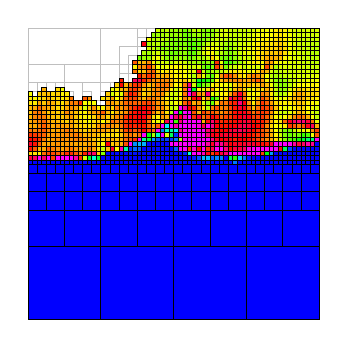
\begin{tikzpicture}[x={(\screenshotunitlength,0)},y={(0,\screenshotunitlength)}]
        \definecolor{fillcolor}{rgb}{0.000000,0.000000,1.000000}
\fill[fillcolor] (0.000000,0.000000) rectangle (0.250000,0.250000);
\definecolor{fillcolor}{rgb}{0.000000,0.000000,1.000000}
\fill[fillcolor] (0.250000,0.000000) rectangle (0.500000,0.250000);
\definecolor{fillcolor}{rgb}{0.000000,0.000000,1.000000}
\fill[fillcolor] (0.000000,0.250000) rectangle (0.125000,0.375000);
\definecolor{fillcolor}{rgb}{0.000000,0.000000,1.000000}
\fill[fillcolor] (0.125000,0.250000) rectangle (0.250000,0.375000);
\definecolor{fillcolor}{rgb}{0.000000,0.000000,1.000000}
\fill[fillcolor] (0.000000,0.375000) rectangle (0.062500,0.437500);
\definecolor{fillcolor}{rgb}{0.000000,0.000000,1.000000}
\fill[fillcolor] (0.062500,0.375000) rectangle (0.125000,0.437500);
\definecolor{fillcolor}{rgb}{0.000000,0.000001,1.000000}
\fill[fillcolor] (0.000000,0.437500) rectangle (0.062500,0.500000);
\definecolor{fillcolor}{rgb}{0.000000,0.000000,1.000000}
\fill[fillcolor] (0.062500,0.437500) rectangle (0.125000,0.500000);
\definecolor{fillcolor}{rgb}{0.000000,0.000000,1.000000}
\fill[fillcolor] (0.125000,0.375000) rectangle (0.187500,0.437500);
\definecolor{fillcolor}{rgb}{0.000000,0.000000,1.000000}
\fill[fillcolor] (0.187500,0.375000) rectangle (0.250000,0.437500);
\definecolor{fillcolor}{rgb}{0.000000,0.000000,1.000000}
\fill[fillcolor] (0.125000,0.437500) rectangle (0.187500,0.500000);
\definecolor{fillcolor}{rgb}{0.000000,0.000000,1.000000}
\fill[fillcolor] (0.187500,0.437500) rectangle (0.250000,0.500000);
\definecolor{fillcolor}{rgb}{0.000000,0.000000,1.000000}
\fill[fillcolor] (0.250000,0.250000) rectangle (0.375000,0.375000);
\definecolor{fillcolor}{rgb}{0.000000,0.000000,1.000000}
\fill[fillcolor] (0.375000,0.250000) rectangle (0.500000,0.375000);
\definecolor{fillcolor}{rgb}{0.000000,0.000000,1.000000}
\fill[fillcolor] (0.250000,0.375000) rectangle (0.312500,0.437500);
\definecolor{fillcolor}{rgb}{0.000000,0.000000,1.000000}
\fill[fillcolor] (0.312500,0.375000) rectangle (0.375000,0.437500);
\definecolor{fillcolor}{rgb}{0.000000,0.000000,1.000000}
\fill[fillcolor] (0.250000,0.437500) rectangle (0.312500,0.500000);
\definecolor{fillcolor}{rgb}{0.000000,0.000000,1.000000}
\fill[fillcolor] (0.312500,0.437500) rectangle (0.375000,0.500000);
\definecolor{fillcolor}{rgb}{0.000000,0.000000,1.000000}
\fill[fillcolor] (0.375000,0.375000) rectangle (0.437500,0.437500);
\definecolor{fillcolor}{rgb}{0.000000,0.000000,1.000000}
\fill[fillcolor] (0.437500,0.375000) rectangle (0.500000,0.437500);
\definecolor{fillcolor}{rgb}{0.000000,0.000000,1.000000}
\fill[fillcolor] (0.375000,0.437500) rectangle (0.437500,0.500000);
\definecolor{fillcolor}{rgb}{0.000000,0.000001,1.000000}
\fill[fillcolor] (0.437500,0.437500) rectangle (0.500000,0.500000);
\definecolor{fillcolor}{rgb}{0.000000,0.000000,1.000000}
\fill[fillcolor] (0.500000,0.000000) rectangle (0.750000,0.250000);
\definecolor{fillcolor}{rgb}{0.000000,0.000000,1.000000}
\fill[fillcolor] (0.750000,0.000000) rectangle (1.000000,0.250000);
\definecolor{fillcolor}{rgb}{0.000000,0.000000,1.000000}
\fill[fillcolor] (0.500000,0.250000) rectangle (0.625000,0.375000);
\definecolor{fillcolor}{rgb}{0.000000,0.000000,1.000000}
\fill[fillcolor] (0.625000,0.250000) rectangle (0.750000,0.375000);
\definecolor{fillcolor}{rgb}{0.000000,0.000000,1.000000}
\fill[fillcolor] (0.500000,0.375000) rectangle (0.562500,0.437500);
\definecolor{fillcolor}{rgb}{0.000000,0.000005,1.000000}
\fill[fillcolor] (0.562500,0.375000) rectangle (0.625000,0.437500);
\definecolor{fillcolor}{rgb}{0.000000,0.000102,1.000000}
\fill[fillcolor] (0.500000,0.437500) rectangle (0.562500,0.500000);
\definecolor{fillcolor}{rgb}{0.000000,0.000149,1.000000}
\fill[fillcolor] (0.562500,0.437500) rectangle (0.625000,0.500000);
\definecolor{fillcolor}{rgb}{0.000000,0.000000,1.000000}
\fill[fillcolor] (0.625000,0.375000) rectangle (0.687500,0.437500);
\definecolor{fillcolor}{rgb}{0.000000,0.000000,1.000000}
\fill[fillcolor] (0.687500,0.375000) rectangle (0.750000,0.437500);
\definecolor{fillcolor}{rgb}{0.000000,0.000058,1.000000}
\fill[fillcolor] (0.625000,0.437500) rectangle (0.687500,0.500000);
\definecolor{fillcolor}{rgb}{0.000000,0.000000,1.000000}
\fill[fillcolor] (0.687500,0.437500) rectangle (0.750000,0.500000);
\definecolor{fillcolor}{rgb}{0.000000,0.000000,1.000000}
\fill[fillcolor] (0.750000,0.250000) rectangle (0.875000,0.375000);
\definecolor{fillcolor}{rgb}{0.000000,0.000000,1.000000}
\fill[fillcolor] (0.875000,0.250000) rectangle (1.000000,0.375000);
\definecolor{fillcolor}{rgb}{0.000000,0.000000,1.000000}
\fill[fillcolor] (0.750000,0.375000) rectangle (0.812500,0.437500);
\definecolor{fillcolor}{rgb}{0.000000,0.000000,1.000000}
\fill[fillcolor] (0.812500,0.375000) rectangle (0.875000,0.437500);
\definecolor{fillcolor}{rgb}{0.000000,0.000000,1.000000}
\fill[fillcolor] (0.750000,0.437500) rectangle (0.812500,0.500000);
\definecolor{fillcolor}{rgb}{0.000000,0.000000,1.000000}
\fill[fillcolor] (0.812500,0.437500) rectangle (0.875000,0.500000);
\definecolor{fillcolor}{rgb}{0.000000,0.000000,1.000000}
\fill[fillcolor] (0.875000,0.375000) rectangle (0.937500,0.437500);
\definecolor{fillcolor}{rgb}{0.000000,0.000000,1.000000}
\fill[fillcolor] (0.937500,0.375000) rectangle (1.000000,0.437500);
\definecolor{fillcolor}{rgb}{0.000000,0.000000,1.000000}
\fill[fillcolor] (0.875000,0.437500) rectangle (0.937500,0.500000);
\definecolor{fillcolor}{rgb}{0.000000,0.000000,1.000000}
\fill[fillcolor] (0.937500,0.437500) rectangle (1.000000,0.500000);
\definecolor{fillcolor}{rgb}{0.000000,0.000001,1.000000}
\fill[fillcolor] (0.000000,0.500000) rectangle (0.031250,0.531250);
\definecolor{fillcolor}{rgb}{0.000000,0.000001,1.000000}
\fill[fillcolor] (0.031250,0.500000) rectangle (0.062500,0.531250);
\definecolor{fillcolor}{rgb}{0.000000,0.000001,1.000000}
\fill[fillcolor] (0.000000,0.531250) rectangle (0.015625,0.546875);
\definecolor{fillcolor}{rgb}{0.000000,0.000001,1.000000}
\fill[fillcolor] (0.015625,0.531250) rectangle (0.031250,0.546875);
\definecolor{fillcolor}{rgb}{1.000000,0.000000,0.219131}
\fill[fillcolor] (0.000000,0.546875) rectangle (0.015625,0.562500);
\definecolor{fillcolor}{rgb}{1.000000,0.000000,0.381638}
\fill[fillcolor] (0.015625,0.546875) rectangle (0.031250,0.562500);
\definecolor{fillcolor}{rgb}{0.000000,0.000001,1.000000}
\fill[fillcolor] (0.031250,0.531250) rectangle (0.046875,0.546875);
\definecolor{fillcolor}{rgb}{0.000000,0.000001,1.000000}
\fill[fillcolor] (0.046875,0.531250) rectangle (0.062500,0.546875);
\definecolor{fillcolor}{rgb}{1.000000,0.000000,1.000000}
\fill[fillcolor] (0.031250,0.546875) rectangle (0.046875,0.562500);
\definecolor{fillcolor}{rgb}{1.000000,0.000000,0.368242}
\fill[fillcolor] (0.046875,0.546875) rectangle (0.062500,0.562500);
\definecolor{fillcolor}{rgb}{0.000000,0.000000,1.000000}
\fill[fillcolor] (0.062500,0.500000) rectangle (0.093750,0.531250);
\definecolor{fillcolor}{rgb}{0.000000,0.000001,1.000000}
\fill[fillcolor] (0.093750,0.500000) rectangle (0.125000,0.531250);
\definecolor{fillcolor}{rgb}{0.000000,0.000000,1.000000}
\fill[fillcolor] (0.062500,0.531250) rectangle (0.078125,0.546875);
\definecolor{fillcolor}{rgb}{0.000000,0.000000,1.000000}
\fill[fillcolor] (0.078125,0.531250) rectangle (0.093750,0.546875);
\definecolor{fillcolor}{rgb}{1.000000,0.000000,1.000000}
\fill[fillcolor] (0.062500,0.546875) rectangle (0.078125,0.562500);
\definecolor{fillcolor}{rgb}{1.000000,0.245339,0.000000}
\fill[fillcolor] (0.078125,0.546875) rectangle (0.093750,0.562500);
\definecolor{fillcolor}{rgb}{0.000000,0.000000,1.000000}
\fill[fillcolor] (0.093750,0.531250) rectangle (0.109375,0.546875);
\definecolor{fillcolor}{rgb}{0.000000,0.000000,1.000000}
\fill[fillcolor] (0.109375,0.531250) rectangle (0.125000,0.546875);
\definecolor{fillcolor}{rgb}{1.000000,0.000000,1.000000}
\fill[fillcolor] (0.093750,0.546875) rectangle (0.109375,0.562500);
\definecolor{fillcolor}{rgb}{1.000000,0.000000,1.000000}
\fill[fillcolor] (0.109375,0.546875) rectangle (0.125000,0.562500);
\definecolor{fillcolor}{rgb}{1.000000,0.836008,0.000000}
\fill[fillcolor] (0.000000,0.562500) rectangle (0.015625,0.578125);
\definecolor{fillcolor}{rgb}{1.000000,0.892098,0.000000}
\fill[fillcolor] (0.015625,0.562500) rectangle (0.031250,0.578125);
\definecolor{fillcolor}{rgb}{1.000000,0.080946,0.000000}
\fill[fillcolor] (0.000000,0.578125) rectangle (0.015625,0.593750);
\definecolor{fillcolor}{rgb}{1.000000,0.352353,0.000000}
\fill[fillcolor] (0.015625,0.578125) rectangle (0.031250,0.593750);
\definecolor{fillcolor}{rgb}{1.000000,0.933972,0.000000}
\fill[fillcolor] (0.031250,0.562500) rectangle (0.046875,0.578125);
\definecolor{fillcolor}{rgb}{1.000000,0.424615,0.000000}
\fill[fillcolor] (0.046875,0.562500) rectangle (0.062500,0.578125);
\definecolor{fillcolor}{rgb}{1.000000,0.708999,0.000000}
\fill[fillcolor] (0.031250,0.578125) rectangle (0.046875,0.593750);
\definecolor{fillcolor}{rgb}{1.000000,0.667996,0.000000}
\fill[fillcolor] (0.046875,0.578125) rectangle (0.062500,0.593750);
\definecolor{fillcolor}{rgb}{1.000000,0.000000,0.165578}
\fill[fillcolor] (0.000000,0.593750) rectangle (0.015625,0.609375);
\definecolor{fillcolor}{rgb}{1.000000,0.070670,0.000000}
\fill[fillcolor] (0.015625,0.593750) rectangle (0.031250,0.609375);
\definecolor{fillcolor}{rgb}{1.000000,0.028723,0.000000}
\fill[fillcolor] (0.000000,0.609375) rectangle (0.015625,0.625000);
\definecolor{fillcolor}{rgb}{1.000000,0.081753,0.000000}
\fill[fillcolor] (0.015625,0.609375) rectangle (0.031250,0.625000);
\definecolor{fillcolor}{rgb}{1.000000,0.394034,0.000000}
\fill[fillcolor] (0.031250,0.593750) rectangle (0.046875,0.609375);
\definecolor{fillcolor}{rgb}{1.000000,0.644212,0.000000}
\fill[fillcolor] (0.046875,0.593750) rectangle (0.062500,0.609375);
\definecolor{fillcolor}{rgb}{1.000000,0.212520,0.000000}
\fill[fillcolor] (0.031250,0.609375) rectangle (0.046875,0.625000);
\definecolor{fillcolor}{rgb}{1.000000,0.489730,0.000000}
\fill[fillcolor] (0.046875,0.609375) rectangle (0.062500,0.625000);
\definecolor{fillcolor}{rgb}{1.000000,0.278435,0.000000}
\fill[fillcolor] (0.062500,0.562500) rectangle (0.078125,0.578125);
\definecolor{fillcolor}{rgb}{1.000000,0.292591,0.000000}
\fill[fillcolor] (0.078125,0.562500) rectangle (0.093750,0.578125);
\definecolor{fillcolor}{rgb}{1.000000,0.385778,0.000000}
\fill[fillcolor] (0.062500,0.578125) rectangle (0.078125,0.593750);
\definecolor{fillcolor}{rgb}{1.000000,0.492934,0.000000}
\fill[fillcolor] (0.078125,0.578125) rectangle (0.093750,0.593750);
\definecolor{fillcolor}{rgb}{1.000000,0.360366,0.000000}
\fill[fillcolor] (0.093750,0.562500) rectangle (0.109375,0.578125);
\definecolor{fillcolor}{rgb}{1.000000,0.398255,0.000000}
\fill[fillcolor] (0.109375,0.562500) rectangle (0.125000,0.578125);
\definecolor{fillcolor}{rgb}{1.000000,0.566569,0.000000}
\fill[fillcolor] (0.093750,0.578125) rectangle (0.109375,0.593750);
\definecolor{fillcolor}{rgb}{1.000000,0.645785,0.000000}
\fill[fillcolor] (0.109375,0.578125) rectangle (0.125000,0.593750);
\definecolor{fillcolor}{rgb}{1.000000,0.674054,0.000000}
\fill[fillcolor] (0.062500,0.593750) rectangle (0.078125,0.609375);
\definecolor{fillcolor}{rgb}{1.000000,0.606185,0.000000}
\fill[fillcolor] (0.078125,0.593750) rectangle (0.093750,0.609375);
\definecolor{fillcolor}{rgb}{1.000000,0.687539,0.000000}
\fill[fillcolor] (0.062500,0.609375) rectangle (0.078125,0.625000);
\definecolor{fillcolor}{rgb}{1.000000,0.610509,0.000000}
\fill[fillcolor] (0.078125,0.609375) rectangle (0.093750,0.625000);
\definecolor{fillcolor}{rgb}{1.000000,0.566314,0.000000}
\fill[fillcolor] (0.093750,0.593750) rectangle (0.109375,0.609375);
\definecolor{fillcolor}{rgb}{1.000000,0.635095,0.000000}
\fill[fillcolor] (0.109375,0.593750) rectangle (0.125000,0.609375);
\definecolor{fillcolor}{rgb}{1.000000,0.559945,0.000000}
\fill[fillcolor] (0.093750,0.609375) rectangle (0.109375,0.625000);
\definecolor{fillcolor}{rgb}{1.000000,0.547588,0.000000}
\fill[fillcolor] (0.109375,0.609375) rectangle (0.125000,0.625000);
\definecolor{fillcolor}{rgb}{0.000000,0.000002,1.000000}
\fill[fillcolor] (0.125000,0.500000) rectangle (0.156250,0.531250);
\definecolor{fillcolor}{rgb}{0.000000,0.000020,1.000000}
\fill[fillcolor] (0.156250,0.500000) rectangle (0.187500,0.531250);
\definecolor{fillcolor}{rgb}{0.000000,0.000002,1.000000}
\fill[fillcolor] (0.125000,0.531250) rectangle (0.140625,0.546875);
\definecolor{fillcolor}{rgb}{0.000000,0.000003,1.000000}
\fill[fillcolor] (0.140625,0.531250) rectangle (0.156250,0.546875);
\definecolor{fillcolor}{rgb}{1.000000,0.000000,1.000000}
\fill[fillcolor] (0.125000,0.546875) rectangle (0.140625,0.562500);
\definecolor{fillcolor}{rgb}{1.000000,0.000000,1.000000}
\fill[fillcolor] (0.140625,0.546875) rectangle (0.156250,0.562500);
\definecolor{fillcolor}{rgb}{0.000000,0.000017,1.000000}
\fill[fillcolor] (0.156250,0.531250) rectangle (0.171875,0.546875);
\definecolor{fillcolor}{rgb}{0.000000,0.000022,1.000000}
\fill[fillcolor] (0.171875,0.531250) rectangle (0.187500,0.546875);
\definecolor{fillcolor}{rgb}{1.000000,0.000000,0.649659}
\fill[fillcolor] (0.156250,0.546875) rectangle (0.171875,0.562500);
\definecolor{fillcolor}{rgb}{1.000000,0.213698,0.000000}
\fill[fillcolor] (0.171875,0.546875) rectangle (0.187500,0.562500);
\definecolor{fillcolor}{rgb}{0.000000,0.000093,1.000000}
\fill[fillcolor] (0.187500,0.500000) rectangle (0.218750,0.531250);
\definecolor{fillcolor}{rgb}{0.000000,0.000256,1.000000}
\fill[fillcolor] (0.218750,0.500000) rectangle (0.250000,0.531250);
\definecolor{fillcolor}{rgb}{0.000000,0.000095,1.000000}
\fill[fillcolor] (0.187500,0.531250) rectangle (0.203125,0.546875);
\definecolor{fillcolor}{rgb}{0.000000,0.000129,1.000000}
\fill[fillcolor] (0.203125,0.531250) rectangle (0.218750,0.546875);
\definecolor{fillcolor}{rgb}{0.852197,1.000000,0.000000}
\fill[fillcolor] (0.187500,0.546875) rectangle (0.203125,0.562500);
\definecolor{fillcolor}{rgb}{0.000000,1.000000,0.156265}
\fill[fillcolor] (0.203125,0.546875) rectangle (0.218750,0.562500);
\definecolor{fillcolor}{rgb}{0.000000,0.000264,1.000000}
\fill[fillcolor] (0.218750,0.531250) rectangle (0.234375,0.546875);
\definecolor{fillcolor}{rgb}{0.000000,0.000349,1.000000}
\fill[fillcolor] (0.234375,0.531250) rectangle (0.250000,0.546875);
\definecolor{fillcolor}{rgb}{0.000000,1.000000,0.829401}
\fill[fillcolor] (0.218750,0.546875) rectangle (0.234375,0.562500);
\definecolor{fillcolor}{rgb}{0.000000,1.000000,0.199123}
\fill[fillcolor] (0.234375,0.546875) rectangle (0.250000,0.562500);
\definecolor{fillcolor}{rgb}{1.000000,0.201584,0.000000}
\fill[fillcolor] (0.125000,0.562500) rectangle (0.140625,0.578125);
\definecolor{fillcolor}{rgb}{1.000000,0.188213,0.000000}
\fill[fillcolor] (0.140625,0.562500) rectangle (0.156250,0.578125);
\definecolor{fillcolor}{rgb}{1.000000,0.538669,0.000000}
\fill[fillcolor] (0.125000,0.578125) rectangle (0.140625,0.593750);
\definecolor{fillcolor}{rgb}{1.000000,0.480497,0.000000}
\fill[fillcolor] (0.140625,0.578125) rectangle (0.156250,0.593750);
\definecolor{fillcolor}{rgb}{1.000000,0.360127,0.000000}
\fill[fillcolor] (0.156250,0.562500) rectangle (0.171875,0.578125);
\definecolor{fillcolor}{rgb}{1.000000,0.499935,0.000000}
\fill[fillcolor] (0.171875,0.562500) rectangle (0.187500,0.578125);
\definecolor{fillcolor}{rgb}{1.000000,0.586888,0.000000}
\fill[fillcolor] (0.156250,0.578125) rectangle (0.171875,0.593750);
\definecolor{fillcolor}{rgb}{1.000000,0.647107,0.000000}
\fill[fillcolor] (0.171875,0.578125) rectangle (0.187500,0.593750);
\definecolor{fillcolor}{rgb}{1.000000,0.610186,0.000000}
\fill[fillcolor] (0.125000,0.593750) rectangle (0.140625,0.609375);
\definecolor{fillcolor}{rgb}{1.000000,0.629213,0.000000}
\fill[fillcolor] (0.140625,0.593750) rectangle (0.156250,0.609375);
\definecolor{fillcolor}{rgb}{1.000000,0.573176,0.000000}
\fill[fillcolor] (0.125000,0.609375) rectangle (0.140625,0.625000);
\definecolor{fillcolor}{rgb}{1.000000,0.570556,0.000000}
\fill[fillcolor] (0.140625,0.609375) rectangle (0.156250,0.625000);
\definecolor{fillcolor}{rgb}{1.000000,0.659143,0.000000}
\fill[fillcolor] (0.156250,0.593750) rectangle (0.171875,0.609375);
\definecolor{fillcolor}{rgb}{1.000000,0.673915,0.000000}
\fill[fillcolor] (0.171875,0.593750) rectangle (0.187500,0.609375);
\definecolor{fillcolor}{rgb}{1.000000,0.517445,0.000000}
\fill[fillcolor] (0.156250,0.609375) rectangle (0.171875,0.625000);
\definecolor{fillcolor}{rgb}{1.000000,0.524427,0.000000}
\fill[fillcolor] (0.171875,0.609375) rectangle (0.187500,0.625000);
\definecolor{fillcolor}{rgb}{1.000000,0.111164,0.000000}
\fill[fillcolor] (0.187500,0.562500) rectangle (0.203125,0.578125);
\definecolor{fillcolor}{rgb}{1.000000,0.000000,0.445039}
\fill[fillcolor] (0.203125,0.562500) rectangle (0.218750,0.578125);
\definecolor{fillcolor}{rgb}{1.000000,0.654227,0.000000}
\fill[fillcolor] (0.187500,0.578125) rectangle (0.203125,0.593750);
\definecolor{fillcolor}{rgb}{1.000000,0.490600,0.000000}
\fill[fillcolor] (0.203125,0.578125) rectangle (0.218750,0.593750);
\definecolor{fillcolor}{rgb}{1.000000,0.000000,0.401821}
\fill[fillcolor] (0.218750,0.562500) rectangle (0.234375,0.578125);
\definecolor{fillcolor}{rgb}{1.000000,0.802424,0.000000}
\fill[fillcolor] (0.234375,0.562500) rectangle (0.250000,0.578125);
\definecolor{fillcolor}{rgb}{1.000000,0.637986,0.000000}
\fill[fillcolor] (0.218750,0.578125) rectangle (0.234375,0.593750);
\definecolor{fillcolor}{rgb}{1.000000,0.884127,0.000000}
\fill[fillcolor] (0.234375,0.578125) rectangle (0.250000,0.593750);
\definecolor{fillcolor}{rgb}{1.000000,0.668110,0.000000}
\fill[fillcolor] (0.187500,0.593750) rectangle (0.203125,0.609375);
\definecolor{fillcolor}{rgb}{1.000000,0.640640,0.000000}
\fill[fillcolor] (0.203125,0.593750) rectangle (0.218750,0.609375);
\definecolor{fillcolor}{rgb}{1.000000,0.594418,0.000000}
\fill[fillcolor] (0.187500,0.609375) rectangle (0.203125,0.625000);
\definecolor{fillcolor}{rgb}{1.000000,0.645948,0.000000}
\fill[fillcolor] (0.203125,0.609375) rectangle (0.218750,0.625000);
\definecolor{fillcolor}{rgb}{1.000000,0.665708,0.000000}
\fill[fillcolor] (0.218750,0.593750) rectangle (0.234375,0.609375);
\definecolor{fillcolor}{rgb}{1.000000,0.862145,0.000000}
\fill[fillcolor] (0.234375,0.593750) rectangle (0.250000,0.609375);
\definecolor{fillcolor}{rgb}{1.000000,0.758946,0.000000}
\fill[fillcolor] (0.218750,0.609375) rectangle (0.234375,0.625000);
\definecolor{fillcolor}{rgb}{1.000000,0.846597,0.000000}
\fill[fillcolor] (0.234375,0.609375) rectangle (0.250000,0.625000);
\definecolor{fillcolor}{rgb}{1.000000,0.193572,0.000000}
\fill[fillcolor] (0.000000,0.625000) rectangle (0.015625,0.640625);
\definecolor{fillcolor}{rgb}{1.000000,0.218017,0.000000}
\fill[fillcolor] (0.015625,0.625000) rectangle (0.031250,0.640625);
\definecolor{fillcolor}{rgb}{1.000000,0.472058,0.000000}
\fill[fillcolor] (0.000000,0.640625) rectangle (0.015625,0.656250);
\definecolor{fillcolor}{rgb}{1.000000,0.511673,0.000000}
\fill[fillcolor] (0.015625,0.640625) rectangle (0.031250,0.656250);
\definecolor{fillcolor}{rgb}{1.000000,0.314173,0.000000}
\fill[fillcolor] (0.031250,0.625000) rectangle (0.046875,0.640625);
\definecolor{fillcolor}{rgb}{1.000000,0.388669,0.000000}
\fill[fillcolor] (0.046875,0.625000) rectangle (0.062500,0.640625);
\definecolor{fillcolor}{rgb}{1.000000,0.455755,0.000000}
\fill[fillcolor] (0.031250,0.640625) rectangle (0.046875,0.656250);
\definecolor{fillcolor}{rgb}{1.000000,0.356967,0.000000}
\fill[fillcolor] (0.046875,0.640625) rectangle (0.062500,0.656250);
\definecolor{fillcolor}{rgb}{1.000000,0.647298,0.000000}
\fill[fillcolor] (0.000000,0.656250) rectangle (0.015625,0.671875);
\definecolor{fillcolor}{rgb}{1.000000,0.656180,0.000000}
\fill[fillcolor] (0.015625,0.656250) rectangle (0.031250,0.671875);
\definecolor{fillcolor}{rgb}{1.000000,0.660396,0.000000}
\fill[fillcolor] (0.000000,0.671875) rectangle (0.015625,0.687500);
\definecolor{fillcolor}{rgb}{1.000000,0.583337,0.000000}
\fill[fillcolor] (0.015625,0.671875) rectangle (0.031250,0.687500);
\definecolor{fillcolor}{rgb}{1.000000,0.517769,0.000000}
\fill[fillcolor] (0.031250,0.656250) rectangle (0.046875,0.671875);
\definecolor{fillcolor}{rgb}{1.000000,0.362067,0.000000}
\fill[fillcolor] (0.046875,0.656250) rectangle (0.062500,0.671875);
\definecolor{fillcolor}{rgb}{1.000000,0.507242,0.000000}
\fill[fillcolor] (0.031250,0.671875) rectangle (0.046875,0.687500);
\definecolor{fillcolor}{rgb}{1.000000,0.414906,0.000000}
\fill[fillcolor] (0.046875,0.671875) rectangle (0.062500,0.687500);
\definecolor{fillcolor}{rgb}{1.000000,0.598207,0.000000}
\fill[fillcolor] (0.062500,0.625000) rectangle (0.078125,0.640625);
\definecolor{fillcolor}{rgb}{1.000000,0.603569,0.000000}
\fill[fillcolor] (0.078125,0.625000) rectangle (0.093750,0.640625);
\definecolor{fillcolor}{rgb}{1.000000,0.534281,0.000000}
\fill[fillcolor] (0.062500,0.640625) rectangle (0.078125,0.656250);
\definecolor{fillcolor}{rgb}{1.000000,0.677268,0.000000}
\fill[fillcolor] (0.078125,0.640625) rectangle (0.093750,0.656250);
\definecolor{fillcolor}{rgb}{1.000000,0.598658,0.000000}
\fill[fillcolor] (0.093750,0.625000) rectangle (0.109375,0.640625);
\definecolor{fillcolor}{rgb}{1.000000,0.583839,0.000000}
\fill[fillcolor] (0.109375,0.625000) rectangle (0.125000,0.640625);
\definecolor{fillcolor}{rgb}{1.000000,0.639968,0.000000}
\fill[fillcolor] (0.093750,0.640625) rectangle (0.109375,0.656250);
\definecolor{fillcolor}{rgb}{1.000000,0.579405,0.000000}
\fill[fillcolor] (0.109375,0.640625) rectangle (0.125000,0.656250);
\definecolor{fillcolor}{rgb}{1.000000,0.523049,0.000000}
\fill[fillcolor] (0.062500,0.656250) rectangle (0.078125,0.671875);
\definecolor{fillcolor}{rgb}{1.000000,0.667266,0.000000}
\fill[fillcolor] (0.078125,0.656250) rectangle (0.093750,0.671875);
\definecolor{fillcolor}{rgb}{1.000000,0.613399,0.000000}
\fill[fillcolor] (0.062500,0.671875) rectangle (0.078125,0.687500);
\definecolor{fillcolor}{rgb}{1.000000,0.707527,0.000000}
\fill[fillcolor] (0.078125,0.671875) rectangle (0.093750,0.687500);
\definecolor{fillcolor}{rgb}{1.000000,0.607736,0.000000}
\fill[fillcolor] (0.093750,0.656250) rectangle (0.109375,0.671875);
\definecolor{fillcolor}{rgb}{1.000000,0.618737,0.000000}
\fill[fillcolor] (0.109375,0.656250) rectangle (0.125000,0.671875);
\definecolor{fillcolor}{rgb}{1.000000,0.708586,0.000000}
\fill[fillcolor] (0.093750,0.671875) rectangle (0.109375,0.687500);
\definecolor{fillcolor}{rgb}{1.000000,0.754536,0.000000}
\fill[fillcolor] (0.109375,0.671875) rectangle (0.125000,0.687500);
\definecolor{fillcolor}{rgb}{1.000000,0.698247,0.000000}
\fill[fillcolor] (0.000000,0.687500) rectangle (0.015625,0.703125);
\definecolor{fillcolor}{rgb}{1.000000,0.522857,0.000000}
\fill[fillcolor] (0.015625,0.687500) rectangle (0.031250,0.703125);
\definecolor{fillcolor}{rgb}{1.000000,0.752393,0.000000}
\fill[fillcolor] (0.000000,0.703125) rectangle (0.015625,0.718750);
\definecolor{fillcolor}{rgb}{1.000000,0.494053,0.000000}
\fill[fillcolor] (0.015625,0.703125) rectangle (0.031250,0.718750);
\definecolor{fillcolor}{rgb}{1.000000,0.469891,0.000000}
\fill[fillcolor] (0.031250,0.687500) rectangle (0.046875,0.703125);
\definecolor{fillcolor}{rgb}{1.000000,0.495648,0.000000}
\fill[fillcolor] (0.046875,0.687500) rectangle (0.062500,0.703125);
\definecolor{fillcolor}{rgb}{1.000000,0.437203,0.000000}
\fill[fillcolor] (0.031250,0.703125) rectangle (0.046875,0.718750);
\definecolor{fillcolor}{rgb}{1.000000,0.613205,0.000000}
\fill[fillcolor] (0.046875,0.703125) rectangle (0.062500,0.718750);
\definecolor{fillcolor}{rgb}{1.000000,0.712977,0.000000}
\fill[fillcolor] (0.000000,0.718750) rectangle (0.015625,0.734375);
\definecolor{fillcolor}{rgb}{1.000000,0.666121,0.000000}
\fill[fillcolor] (0.015625,0.718750) rectangle (0.031250,0.734375);
\definecolor{fillcolor}{rgb}{1.000000,0.887739,0.000000}
\fill[fillcolor] (0.000000,0.734375) rectangle (0.015625,0.750000);
\definecolor{fillcolor}{rgb}{1.000000,0.915844,0.000000}
\fill[fillcolor] (0.015625,0.734375) rectangle (0.031250,0.750000);
\definecolor{fillcolor}{rgb}{1.000000,0.419424,0.000000}
\fill[fillcolor] (0.031250,0.718750) rectangle (0.046875,0.734375);
\definecolor{fillcolor}{rgb}{1.000000,0.591442,0.000000}
\fill[fillcolor] (0.046875,0.718750) rectangle (0.062500,0.734375);
\definecolor{fillcolor}{rgb}{1.000000,0.651444,0.000000}
\fill[fillcolor] (0.031250,0.734375) rectangle (0.046875,0.750000);
\definecolor{fillcolor}{rgb}{1.000000,0.781003,0.000000}
\fill[fillcolor] (0.046875,0.734375) rectangle (0.062500,0.750000);
\definecolor{fillcolor}{rgb}{1.000000,0.689733,0.000000}
\fill[fillcolor] (0.062500,0.687500) rectangle (0.078125,0.703125);
\definecolor{fillcolor}{rgb}{1.000000,0.750013,0.000000}
\fill[fillcolor] (0.078125,0.687500) rectangle (0.093750,0.703125);
\definecolor{fillcolor}{rgb}{1.000000,0.775894,0.000000}
\fill[fillcolor] (0.062500,0.703125) rectangle (0.078125,0.718750);
\definecolor{fillcolor}{rgb}{1.000000,0.740562,0.000000}
\fill[fillcolor] (0.078125,0.703125) rectangle (0.093750,0.718750);
\definecolor{fillcolor}{rgb}{1.000000,0.777064,0.000000}
\fill[fillcolor] (0.093750,0.687500) rectangle (0.109375,0.703125);
\definecolor{fillcolor}{rgb}{1.000000,0.768612,0.000000}
\fill[fillcolor] (0.109375,0.687500) rectangle (0.125000,0.703125);
\definecolor{fillcolor}{rgb}{1.000000,0.799801,0.000000}
\fill[fillcolor] (0.093750,0.703125) rectangle (0.109375,0.718750);
\definecolor{fillcolor}{rgb}{1.000000,0.739728,0.000000}
\fill[fillcolor] (0.109375,0.703125) rectangle (0.125000,0.718750);
\definecolor{fillcolor}{rgb}{1.000000,0.671305,0.000000}
\fill[fillcolor] (0.062500,0.718750) rectangle (0.078125,0.734375);
\definecolor{fillcolor}{rgb}{1.000000,0.729536,0.000000}
\fill[fillcolor] (0.078125,0.718750) rectangle (0.093750,0.734375);
\definecolor{fillcolor}{rgb}{1.000000,0.613456,0.000000}
\fill[fillcolor] (0.062500,0.734375) rectangle (0.078125,0.750000);
\definecolor{fillcolor}{rgb}{1.000000,0.707069,0.000000}
\fill[fillcolor] (0.078125,0.734375) rectangle (0.093750,0.750000);
\definecolor{fillcolor}{rgb}{1.000000,0.842745,0.000000}
\fill[fillcolor] (0.093750,0.718750) rectangle (0.109375,0.734375);
\definecolor{fillcolor}{rgb}{1.000000,0.828820,0.000000}
\fill[fillcolor] (0.109375,0.718750) rectangle (0.125000,0.734375);
\definecolor{fillcolor}{rgb}{1.000000,0.817249,0.000000}
\fill[fillcolor] (0.093750,0.734375) rectangle (0.109375,0.750000);
\definecolor{fillcolor}{rgb}{1.000000,0.879292,0.000000}
\fill[fillcolor] (0.109375,0.734375) rectangle (0.125000,0.750000);
\definecolor{fillcolor}{rgb}{1.000000,0.527901,0.000000}
\fill[fillcolor] (0.125000,0.625000) rectangle (0.140625,0.640625);
\definecolor{fillcolor}{rgb}{1.000000,0.539778,0.000000}
\fill[fillcolor] (0.140625,0.625000) rectangle (0.156250,0.640625);
\definecolor{fillcolor}{rgb}{1.000000,0.479169,0.000000}
\fill[fillcolor] (0.125000,0.640625) rectangle (0.140625,0.656250);
\definecolor{fillcolor}{rgb}{1.000000,0.536556,0.000000}
\fill[fillcolor] (0.140625,0.640625) rectangle (0.156250,0.656250);
\definecolor{fillcolor}{rgb}{1.000000,0.488637,0.000000}
\fill[fillcolor] (0.156250,0.625000) rectangle (0.171875,0.640625);
\definecolor{fillcolor}{rgb}{1.000000,0.579684,0.000000}
\fill[fillcolor] (0.171875,0.625000) rectangle (0.187500,0.640625);
\definecolor{fillcolor}{rgb}{1.000000,0.623312,0.000000}
\fill[fillcolor] (0.156250,0.640625) rectangle (0.171875,0.656250);
\definecolor{fillcolor}{rgb}{1.000000,0.748231,0.000000}
\fill[fillcolor] (0.171875,0.640625) rectangle (0.187500,0.656250);
\definecolor{fillcolor}{rgb}{1.000000,0.639103,0.000000}
\fill[fillcolor] (0.125000,0.656250) rectangle (0.140625,0.671875);
\definecolor{fillcolor}{rgb}{1.000000,0.627835,0.000000}
\fill[fillcolor] (0.140625,0.656250) rectangle (0.156250,0.671875);
\definecolor{fillcolor}{rgb}{1.000000,0.808594,0.000000}
\fill[fillcolor] (0.125000,0.671875) rectangle (0.140625,0.687500);
\definecolor{fillcolor}{rgb}{1.000000,0.665241,0.000000}
\fill[fillcolor] (0.140625,0.671875) rectangle (0.156250,0.687500);
\definecolor{fillcolor}{rgb}{1.000000,0.751422,0.000000}
\fill[fillcolor] (0.156250,0.656250) rectangle (0.171875,0.671875);
\definecolor{fillcolor}{rgb}{1.000000,0.830553,0.000000}
\fill[fillcolor] (0.171875,0.656250) rectangle (0.187500,0.671875);
\definecolor{fillcolor}{rgb}{1.000000,0.772595,0.000000}
\fill[fillcolor] (0.156250,0.671875) rectangle (0.171875,0.687500);
\definecolor{fillcolor}{rgb}{1.000000,0.866930,0.000000}
\fill[fillcolor] (0.171875,0.671875) rectangle (0.187500,0.687500);
\definecolor{fillcolor}{rgb}{1.000000,0.690607,0.000000}
\fill[fillcolor] (0.187500,0.625000) rectangle (0.203125,0.640625);
\definecolor{fillcolor}{rgb}{1.000000,0.691780,0.000000}
\fill[fillcolor] (0.203125,0.625000) rectangle (0.218750,0.640625);
\definecolor{fillcolor}{rgb}{1.000000,0.805911,0.000000}
\fill[fillcolor] (0.187500,0.640625) rectangle (0.203125,0.656250);
\definecolor{fillcolor}{rgb}{1.000000,0.756994,0.000000}
\fill[fillcolor] (0.203125,0.640625) rectangle (0.218750,0.656250);
\definecolor{fillcolor}{rgb}{1.000000,0.702337,0.000000}
\fill[fillcolor] (0.218750,0.625000) rectangle (0.234375,0.640625);
\definecolor{fillcolor}{rgb}{1.000000,0.752330,0.000000}
\fill[fillcolor] (0.234375,0.625000) rectangle (0.250000,0.640625);
\definecolor{fillcolor}{rgb}{1.000000,0.677025,0.000000}
\fill[fillcolor] (0.218750,0.640625) rectangle (0.234375,0.656250);
\definecolor{fillcolor}{rgb}{1.000000,0.615588,0.000000}
\fill[fillcolor] (0.234375,0.640625) rectangle (0.250000,0.656250);
\definecolor{fillcolor}{rgb}{1.000000,0.837909,0.000000}
\fill[fillcolor] (0.187500,0.656250) rectangle (0.203125,0.671875);
\definecolor{fillcolor}{rgb}{1.000000,0.853092,0.000000}
\fill[fillcolor] (0.203125,0.656250) rectangle (0.218750,0.671875);
\definecolor{fillcolor}{rgb}{1.000000,0.931385,0.000000}
\fill[fillcolor] (0.187500,0.671875) rectangle (0.203125,0.687500);
\definecolor{fillcolor}{rgb}{0.958003,1.000000,0.000000}
\fill[fillcolor] (0.203125,0.671875) rectangle (0.218750,0.687500);
\definecolor{fillcolor}{rgb}{1.000000,0.787930,0.000000}
\fill[fillcolor] (0.218750,0.656250) rectangle (0.234375,0.671875);
\definecolor{fillcolor}{rgb}{1.000000,0.602273,0.000000}
\fill[fillcolor] (0.234375,0.656250) rectangle (0.250000,0.671875);
\definecolor{fillcolor}{rgb}{1.000000,0.859036,0.000000}
\fill[fillcolor] (0.218750,0.671875) rectangle (0.234375,0.687500);
\definecolor{fillcolor}{rgb}{1.000000,0.816783,0.000000}
\fill[fillcolor] (0.234375,0.671875) rectangle (0.250000,0.687500);
\definecolor{fillcolor}{rgb}{1.000000,0.654076,0.000000}
\fill[fillcolor] (0.125000,0.687500) rectangle (0.140625,0.703125);
\definecolor{fillcolor}{rgb}{1.000000,0.606536,0.000000}
\fill[fillcolor] (0.140625,0.687500) rectangle (0.156250,0.703125);
\definecolor{fillcolor}{rgb}{1.000000,0.520666,0.000000}
\fill[fillcolor] (0.125000,0.703125) rectangle (0.140625,0.718750);
\definecolor{fillcolor}{rgb}{1.000000,0.665153,0.000000}
\fill[fillcolor] (0.140625,0.703125) rectangle (0.156250,0.718750);
\definecolor{fillcolor}{rgb}{1.000000,0.782254,0.000000}
\fill[fillcolor] (0.156250,0.687500) rectangle (0.171875,0.703125);
\definecolor{fillcolor}{rgb}{1.000000,0.923055,0.000000}
\fill[fillcolor] (0.171875,0.687500) rectangle (0.187500,0.703125);
\definecolor{fillcolor}{rgb}{1.000000,0.751682,0.000000}
\fill[fillcolor] (0.156250,0.703125) rectangle (0.171875,0.718750);
\definecolor{fillcolor}{rgb}{1.000000,0.924848,0.000000}
\fill[fillcolor] (0.171875,0.703125) rectangle (0.187500,0.718750);
\definecolor{fillcolor}{rgb}{1.000000,0.667973,0.000000}
\fill[fillcolor] (0.125000,0.718750) rectangle (0.140625,0.734375);
\definecolor{fillcolor}{rgb}{1.000000,0.554748,0.000000}
\fill[fillcolor] (0.140625,0.718750) rectangle (0.156250,0.734375);
\definecolor{fillcolor}{rgb}{1.000000,0.705689,0.000000}
\fill[fillcolor] (0.125000,0.734375) rectangle (0.140625,0.750000);
\definecolor{fillcolor}{rgb}{1.000000,0.487242,0.000000}
\fill[fillcolor] (0.140625,0.734375) rectangle (0.156250,0.750000);
\definecolor{fillcolor}{rgb}{1.000000,0.632777,0.000000}
\fill[fillcolor] (0.156250,0.718750) rectangle (0.171875,0.734375);
\definecolor{fillcolor}{rgb}{1.000000,0.827986,0.000000}
\fill[fillcolor] (0.171875,0.718750) rectangle (0.187500,0.734375);
\definecolor{fillcolor}{rgb}{1.000000,0.490378,0.000000}
\fill[fillcolor] (0.156250,0.734375) rectangle (0.171875,0.750000);
\definecolor{fillcolor}{rgb}{1.000000,0.202244,0.000000}
\fill[fillcolor] (0.171875,0.734375) rectangle (0.187500,0.750000);
\definecolor{fillcolor}{rgb}{1.000000,0.949588,0.000000}
\fill[fillcolor] (0.187500,0.687500) rectangle (0.203125,0.703125);
\definecolor{fillcolor}{rgb}{1.000000,0.944911,0.000000}
\fill[fillcolor] (0.203125,0.687500) rectangle (0.218750,0.703125);
\definecolor{fillcolor}{rgb}{1.000000,0.957026,0.000000}
\fill[fillcolor] (0.187500,0.703125) rectangle (0.203125,0.718750);
\definecolor{fillcolor}{rgb}{1.000000,0.754356,0.000000}
\fill[fillcolor] (0.203125,0.703125) rectangle (0.218750,0.718750);
\definecolor{fillcolor}{rgb}{1.000000,0.819182,0.000000}
\fill[fillcolor] (0.218750,0.687500) rectangle (0.234375,0.703125);
\definecolor{fillcolor}{rgb}{1.000000,0.606390,0.000000}
\fill[fillcolor] (0.234375,0.687500) rectangle (0.250000,0.703125);
\definecolor{fillcolor}{rgb}{1.000000,0.622750,0.000000}
\fill[fillcolor] (0.218750,0.703125) rectangle (0.234375,0.718750);
\definecolor{fillcolor}{rgb}{1.000000,0.562833,0.000000}
\fill[fillcolor] (0.234375,0.703125) rectangle (0.250000,0.718750);
\definecolor{fillcolor}{rgb}{0.854208,1.000000,0.000000}
\fill[fillcolor] (0.187500,0.718750) rectangle (0.203125,0.734375);
\definecolor{fillcolor}{rgb}{1.000000,0.801879,0.000000}
\fill[fillcolor] (0.203125,0.718750) rectangle (0.218750,0.734375);
\definecolor{fillcolor}{rgb}{0.986354,1.000000,0.000000}
\fill[fillcolor] (0.187500,0.734375) rectangle (0.203125,0.750000);
\definecolor{fillcolor}{rgb}{0.961734,1.000000,0.000000}
\fill[fillcolor] (0.203125,0.734375) rectangle (0.218750,0.750000);
\definecolor{fillcolor}{rgb}{1.000000,0.589372,0.000000}
\fill[fillcolor] (0.218750,0.718750) rectangle (0.234375,0.734375);
\definecolor{fillcolor}{rgb}{1.000000,0.928511,0.000000}
\fill[fillcolor] (0.234375,0.718750) rectangle (0.250000,0.734375);
\definecolor{fillcolor}{rgb}{0.984486,1.000000,0.000000}
\fill[fillcolor] (0.218750,0.734375) rectangle (0.234375,0.750000);
\definecolor{fillcolor}{rgb}{0.000000,0.000396,1.000000}
\fill[fillcolor] (0.250000,0.500000) rectangle (0.281250,0.531250);
\definecolor{fillcolor}{rgb}{0.000000,0.000633,1.000000}
\fill[fillcolor] (0.281250,0.500000) rectangle (0.312500,0.531250);
\definecolor{fillcolor}{rgb}{0.000000,0.000453,1.000000}
\fill[fillcolor] (0.250000,0.531250) rectangle (0.265625,0.546875);
\definecolor{fillcolor}{rgb}{0.000000,0.000621,1.000000}
\fill[fillcolor] (0.265625,0.531250) rectangle (0.281250,0.546875);
\definecolor{fillcolor}{rgb}{0.000000,0.000474,1.000000}
\fill[fillcolor] (0.250000,0.546875) rectangle (0.265625,0.562500);
\definecolor{fillcolor}{rgb}{0.000000,0.000490,1.000000}
\fill[fillcolor] (0.265625,0.546875) rectangle (0.281250,0.562500);
\definecolor{fillcolor}{rgb}{0.000000,0.000611,1.000000}
\fill[fillcolor] (0.281250,0.531250) rectangle (0.296875,0.546875);
\definecolor{fillcolor}{rgb}{0.000000,0.000319,1.000000}
\fill[fillcolor] (0.296875,0.531250) rectangle (0.312500,0.546875);
\definecolor{fillcolor}{rgb}{0.000000,0.000399,1.000000}
\fill[fillcolor] (0.281250,0.546875) rectangle (0.296875,0.562500);
\definecolor{fillcolor}{rgb}{0.000000,0.000239,1.000000}
\fill[fillcolor] (0.296875,0.546875) rectangle (0.312500,0.562500);
\definecolor{fillcolor}{rgb}{0.000000,0.000092,1.000000}
\fill[fillcolor] (0.312500,0.500000) rectangle (0.343750,0.531250);
\definecolor{fillcolor}{rgb}{0.000000,0.000171,1.000000}
\fill[fillcolor] (0.343750,0.500000) rectangle (0.375000,0.531250);
\definecolor{fillcolor}{rgb}{0.000000,0.000120,1.000000}
\fill[fillcolor] (0.312500,0.531250) rectangle (0.328125,0.546875);
\definecolor{fillcolor}{rgb}{0.000000,0.000162,1.000000}
\fill[fillcolor] (0.328125,0.531250) rectangle (0.343750,0.546875);
\definecolor{fillcolor}{rgb}{0.000000,0.000183,1.000000}
\fill[fillcolor] (0.312500,0.546875) rectangle (0.328125,0.562500);
\definecolor{fillcolor}{rgb}{0.000000,0.000234,1.000000}
\fill[fillcolor] (0.328125,0.546875) rectangle (0.343750,0.562500);
\definecolor{fillcolor}{rgb}{0.000000,0.000081,1.000000}
\fill[fillcolor] (0.343750,0.531250) rectangle (0.359375,0.546875);
\definecolor{fillcolor}{rgb}{0.000000,0.000011,1.000000}
\fill[fillcolor] (0.359375,0.531250) rectangle (0.375000,0.546875);
\definecolor{fillcolor}{rgb}{0.000000,0.000296,1.000000}
\fill[fillcolor] (0.343750,0.546875) rectangle (0.359375,0.562500);
\definecolor{fillcolor}{rgb}{0.000000,0.006210,1.000000}
\fill[fillcolor] (0.359375,0.546875) rectangle (0.375000,0.562500);
\definecolor{fillcolor}{rgb}{0.545084,1.000000,0.000000}
\fill[fillcolor] (0.250000,0.562500) rectangle (0.265625,0.578125);
\definecolor{fillcolor}{rgb}{0.000000,0.013615,1.000000}
\fill[fillcolor] (0.265625,0.562500) rectangle (0.281250,0.578125);
\definecolor{fillcolor}{rgb}{0.763609,1.000000,0.000000}
\fill[fillcolor] (0.250000,0.578125) rectangle (0.265625,0.593750);
\definecolor{fillcolor}{rgb}{1.000000,0.725231,0.000000}
\fill[fillcolor] (0.265625,0.578125) rectangle (0.281250,0.593750);
\definecolor{fillcolor}{rgb}{0.000000,0.021448,1.000000}
\fill[fillcolor] (0.281250,0.562500) rectangle (0.296875,0.578125);
\definecolor{fillcolor}{rgb}{0.000000,0.025606,1.000000}
\fill[fillcolor] (0.296875,0.562500) rectangle (0.312500,0.578125);
\definecolor{fillcolor}{rgb}{1.000000,0.000000,0.204760}
\fill[fillcolor] (0.281250,0.578125) rectangle (0.296875,0.593750);
\definecolor{fillcolor}{rgb}{1.000000,0.972722,0.000000}
\fill[fillcolor] (0.296875,0.578125) rectangle (0.312500,0.593750);
\definecolor{fillcolor}{rgb}{0.996525,1.000000,0.000000}
\fill[fillcolor] (0.250000,0.593750) rectangle (0.265625,0.609375);
\definecolor{fillcolor}{rgb}{1.000000,0.000000,0.041992}
\fill[fillcolor] (0.265625,0.593750) rectangle (0.281250,0.609375);
\definecolor{fillcolor}{rgb}{1.000000,0.834697,0.000000}
\fill[fillcolor] (0.250000,0.609375) rectangle (0.265625,0.625000);
\definecolor{fillcolor}{rgb}{1.000000,0.668973,0.000000}
\fill[fillcolor] (0.265625,0.609375) rectangle (0.281250,0.625000);
\definecolor{fillcolor}{rgb}{1.000000,0.782273,0.000000}
\fill[fillcolor] (0.281250,0.593750) rectangle (0.296875,0.609375);
\definecolor{fillcolor}{rgb}{1.000000,0.727770,0.000000}
\fill[fillcolor] (0.296875,0.593750) rectangle (0.312500,0.609375);
\definecolor{fillcolor}{rgb}{1.000000,0.707357,0.000000}
\fill[fillcolor] (0.281250,0.609375) rectangle (0.296875,0.625000);
\definecolor{fillcolor}{rgb}{1.000000,0.762024,0.000000}
\fill[fillcolor] (0.296875,0.609375) rectangle (0.312500,0.625000);
\definecolor{fillcolor}{rgb}{0.000000,0.032011,1.000000}
\fill[fillcolor] (0.312500,0.562500) rectangle (0.328125,0.578125);
\definecolor{fillcolor}{rgb}{0.000000,0.040066,1.000000}
\fill[fillcolor] (0.328125,0.562500) rectangle (0.343750,0.578125);
\definecolor{fillcolor}{rgb}{1.000000,0.000000,0.715336}
\fill[fillcolor] (0.312500,0.578125) rectangle (0.328125,0.593750);
\definecolor{fillcolor}{rgb}{0.000000,1.000000,0.616406}
\fill[fillcolor] (0.328125,0.578125) rectangle (0.343750,0.593750);
\definecolor{fillcolor}{rgb}{0.000000,0.049185,1.000000}
\fill[fillcolor] (0.343750,0.562500) rectangle (0.359375,0.578125);
\definecolor{fillcolor}{rgb}{0.000000,0.063664,1.000000}
\fill[fillcolor] (0.359375,0.562500) rectangle (0.375000,0.578125);
\definecolor{fillcolor}{rgb}{0.000000,0.224184,1.000000}
\fill[fillcolor] (0.343750,0.578125) rectangle (0.359375,0.593750);
\definecolor{fillcolor}{rgb}{0.000000,0.396917,1.000000}
\fill[fillcolor] (0.359375,0.578125) rectangle (0.375000,0.593750);
\definecolor{fillcolor}{rgb}{1.000000,0.690246,0.000000}
\fill[fillcolor] (0.312500,0.593750) rectangle (0.328125,0.609375);
\definecolor{fillcolor}{rgb}{1.000000,0.319433,0.000000}
\fill[fillcolor] (0.328125,0.593750) rectangle (0.343750,0.609375);
\definecolor{fillcolor}{rgb}{1.000000,0.670022,0.000000}
\fill[fillcolor] (0.312500,0.609375) rectangle (0.328125,0.625000);
\definecolor{fillcolor}{rgb}{1.000000,0.433638,0.000000}
\fill[fillcolor] (0.328125,0.609375) rectangle (0.343750,0.625000);
\definecolor{fillcolor}{rgb}{1.000000,0.000000,1.000000}
\fill[fillcolor] (0.343750,0.593750) rectangle (0.359375,0.609375);
\definecolor{fillcolor}{rgb}{0.000000,0.565150,1.000000}
\fill[fillcolor] (0.359375,0.593750) rectangle (0.375000,0.609375);
\definecolor{fillcolor}{rgb}{1.000000,0.346061,0.000000}
\fill[fillcolor] (0.343750,0.609375) rectangle (0.359375,0.625000);
\definecolor{fillcolor}{rgb}{1.000000,0.191518,0.000000}
\fill[fillcolor] (0.359375,0.609375) rectangle (0.375000,0.625000);
\definecolor{fillcolor}{rgb}{0.000000,0.000000,1.000000}
\fill[fillcolor] (0.375000,0.500000) rectangle (0.406250,0.531250);
\definecolor{fillcolor}{rgb}{0.000000,0.000049,1.000000}
\fill[fillcolor] (0.406250,0.500000) rectangle (0.437500,0.531250);
\definecolor{fillcolor}{rgb}{0.000000,0.000000,1.000000}
\fill[fillcolor] (0.375000,0.531250) rectangle (0.390625,0.546875);
\definecolor{fillcolor}{rgb}{0.000000,0.000001,1.000000}
\fill[fillcolor] (0.390625,0.531250) rectangle (0.406250,0.546875);
\definecolor{fillcolor}{rgb}{0.000000,0.008895,1.000000}
\fill[fillcolor] (0.375000,0.546875) rectangle (0.390625,0.562500);
\definecolor{fillcolor}{rgb}{0.000000,0.012187,1.000000}
\fill[fillcolor] (0.390625,0.546875) rectangle (0.406250,0.562500);
\definecolor{fillcolor}{rgb}{0.000000,0.000527,1.000000}
\fill[fillcolor] (0.406250,0.531250) rectangle (0.421875,0.546875);
\definecolor{fillcolor}{rgb}{0.000000,0.000707,1.000000}
\fill[fillcolor] (0.421875,0.531250) rectangle (0.437500,0.546875);
\definecolor{fillcolor}{rgb}{0.000000,0.013993,1.000000}
\fill[fillcolor] (0.406250,0.546875) rectangle (0.421875,0.562500);
\definecolor{fillcolor}{rgb}{0.000000,0.013342,1.000000}
\fill[fillcolor] (0.421875,0.546875) rectangle (0.437500,0.562500);
\definecolor{fillcolor}{rgb}{0.000000,0.000086,1.000000}
\fill[fillcolor] (0.437500,0.500000) rectangle (0.468750,0.531250);
\definecolor{fillcolor}{rgb}{0.000000,0.000060,1.000000}
\fill[fillcolor] (0.468750,0.500000) rectangle (0.500000,0.531250);
\definecolor{fillcolor}{rgb}{0.000000,0.000710,1.000000}
\fill[fillcolor] (0.437500,0.531250) rectangle (0.453125,0.546875);
\definecolor{fillcolor}{rgb}{0.000000,0.000898,1.000000}
\fill[fillcolor] (0.453125,0.531250) rectangle (0.468750,0.546875);
\definecolor{fillcolor}{rgb}{0.000000,0.003343,1.000000}
\fill[fillcolor] (0.437500,0.546875) rectangle (0.453125,0.562500);
\definecolor{fillcolor}{rgb}{0.000000,0.003562,1.000000}
\fill[fillcolor] (0.453125,0.546875) rectangle (0.468750,0.562500);
\definecolor{fillcolor}{rgb}{0.000000,0.000507,1.000000}
\fill[fillcolor] (0.468750,0.531250) rectangle (0.484375,0.546875);
\definecolor{fillcolor}{rgb}{0.000000,0.000483,1.000000}
\fill[fillcolor] (0.484375,0.531250) rectangle (0.500000,0.546875);
\definecolor{fillcolor}{rgb}{0.000000,0.003888,1.000000}
\fill[fillcolor] (0.468750,0.546875) rectangle (0.484375,0.562500);
\definecolor{fillcolor}{rgb}{0.000000,0.007011,1.000000}
\fill[fillcolor] (0.484375,0.546875) rectangle (0.500000,0.562500);
\definecolor{fillcolor}{rgb}{0.000000,0.014794,1.000000}
\fill[fillcolor] (0.375000,0.562500) rectangle (0.390625,0.578125);
\definecolor{fillcolor}{rgb}{0.000000,0.016357,1.000000}
\fill[fillcolor] (0.390625,0.562500) rectangle (0.406250,0.578125);
\definecolor{fillcolor}{rgb}{0.000000,0.357304,1.000000}
\fill[fillcolor] (0.375000,0.578125) rectangle (0.390625,0.593750);
\definecolor{fillcolor}{rgb}{0.000000,0.024752,1.000000}
\fill[fillcolor] (0.390625,0.578125) rectangle (0.406250,0.593750);
\definecolor{fillcolor}{rgb}{0.000000,0.008219,1.000000}
\fill[fillcolor] (0.406250,0.562500) rectangle (0.421875,0.578125);
\definecolor{fillcolor}{rgb}{0.000000,0.007870,1.000000}
\fill[fillcolor] (0.421875,0.562500) rectangle (0.437500,0.578125);
\definecolor{fillcolor}{rgb}{0.000000,0.025997,1.000000}
\fill[fillcolor] (0.406250,0.578125) rectangle (0.421875,0.593750);
\definecolor{fillcolor}{rgb}{0.000000,0.032436,1.000000}
\fill[fillcolor] (0.421875,0.578125) rectangle (0.437500,0.593750);
\definecolor{fillcolor}{rgb}{0.000000,0.727031,1.000000}
\fill[fillcolor] (0.375000,0.593750) rectangle (0.390625,0.609375);
\definecolor{fillcolor}{rgb}{0.000000,0.690750,1.000000}
\fill[fillcolor] (0.390625,0.593750) rectangle (0.406250,0.609375);
\definecolor{fillcolor}{rgb}{1.000000,0.000000,1.000000}
\fill[fillcolor] (0.375000,0.609375) rectangle (0.390625,0.625000);
\definecolor{fillcolor}{rgb}{0.000000,1.000000,0.562938}
\fill[fillcolor] (0.390625,0.609375) rectangle (0.406250,0.625000);
\definecolor{fillcolor}{rgb}{0.000000,0.021008,1.000000}
\fill[fillcolor] (0.406250,0.593750) rectangle (0.421875,0.609375);
\definecolor{fillcolor}{rgb}{0.000000,0.014192,1.000000}
\fill[fillcolor] (0.421875,0.593750) rectangle (0.437500,0.609375);
\definecolor{fillcolor}{rgb}{0.000000,1.000000,0.180938}
\fill[fillcolor] (0.406250,0.609375) rectangle (0.421875,0.625000);
\definecolor{fillcolor}{rgb}{0.000000,0.622347,1.000000}
\fill[fillcolor] (0.421875,0.609375) rectangle (0.437500,0.625000);
\definecolor{fillcolor}{rgb}{0.000000,0.009086,1.000000}
\fill[fillcolor] (0.437500,0.562500) rectangle (0.453125,0.578125);
\definecolor{fillcolor}{rgb}{0.000000,0.008352,1.000000}
\fill[fillcolor] (0.453125,0.562500) rectangle (0.468750,0.578125);
\definecolor{fillcolor}{rgb}{0.000000,0.037730,1.000000}
\fill[fillcolor] (0.437500,0.578125) rectangle (0.453125,0.593750);
\definecolor{fillcolor}{rgb}{0.000000,0.035741,1.000000}
\fill[fillcolor] (0.453125,0.578125) rectangle (0.468750,0.593750);
\definecolor{fillcolor}{rgb}{0.000000,0.009017,1.000000}
\fill[fillcolor] (0.468750,0.562500) rectangle (0.484375,0.578125);
\definecolor{fillcolor}{rgb}{0.000000,0.001650,1.000000}
\fill[fillcolor] (0.484375,0.562500) rectangle (0.500000,0.578125);
\definecolor{fillcolor}{rgb}{0.000000,0.019894,1.000000}
\fill[fillcolor] (0.468750,0.578125) rectangle (0.484375,0.593750);
\definecolor{fillcolor}{rgb}{0.000000,0.009884,1.000000}
\fill[fillcolor] (0.484375,0.578125) rectangle (0.500000,0.593750);
\definecolor{fillcolor}{rgb}{0.000000,0.013398,1.000000}
\fill[fillcolor] (0.437500,0.593750) rectangle (0.453125,0.609375);
\definecolor{fillcolor}{rgb}{0.000000,0.010079,1.000000}
\fill[fillcolor] (0.453125,0.593750) rectangle (0.468750,0.609375);
\definecolor{fillcolor}{rgb}{0.000000,0.335331,1.000000}
\fill[fillcolor] (0.437500,0.609375) rectangle (0.453125,0.625000);
\definecolor{fillcolor}{rgb}{0.000000,0.194253,1.000000}
\fill[fillcolor] (0.453125,0.609375) rectangle (0.468750,0.625000);
\definecolor{fillcolor}{rgb}{0.000000,0.012619,1.000000}
\fill[fillcolor] (0.468750,0.593750) rectangle (0.484375,0.609375);
\definecolor{fillcolor}{rgb}{1.000000,0.000000,1.000000}
\fill[fillcolor] (0.484375,0.593750) rectangle (0.500000,0.609375);
\definecolor{fillcolor}{rgb}{0.000000,0.242635,1.000000}
\fill[fillcolor] (0.468750,0.609375) rectangle (0.484375,0.625000);
\definecolor{fillcolor}{rgb}{0.000000,0.249977,1.000000}
\fill[fillcolor] (0.484375,0.609375) rectangle (0.500000,0.625000);
\definecolor{fillcolor}{rgb}{1.000000,0.821848,0.000000}
\fill[fillcolor] (0.250000,0.625000) rectangle (0.265625,0.640625);
\definecolor{fillcolor}{rgb}{1.000000,0.857810,0.000000}
\fill[fillcolor] (0.265625,0.625000) rectangle (0.281250,0.640625);
\definecolor{fillcolor}{rgb}{1.000000,0.623243,0.000000}
\fill[fillcolor] (0.250000,0.640625) rectangle (0.265625,0.656250);
\definecolor{fillcolor}{rgb}{1.000000,0.670159,0.000000}
\fill[fillcolor] (0.265625,0.640625) rectangle (0.281250,0.656250);
\definecolor{fillcolor}{rgb}{1.000000,0.855242,0.000000}
\fill[fillcolor] (0.281250,0.625000) rectangle (0.296875,0.640625);
\definecolor{fillcolor}{rgb}{1.000000,0.892765,0.000000}
\fill[fillcolor] (0.296875,0.625000) rectangle (0.312500,0.640625);
\definecolor{fillcolor}{rgb}{1.000000,0.774950,0.000000}
\fill[fillcolor] (0.281250,0.640625) rectangle (0.296875,0.656250);
\definecolor{fillcolor}{rgb}{1.000000,0.815600,0.000000}
\fill[fillcolor] (0.296875,0.640625) rectangle (0.312500,0.656250);
\definecolor{fillcolor}{rgb}{1.000000,0.590697,0.000000}
\fill[fillcolor] (0.250000,0.656250) rectangle (0.265625,0.671875);
\definecolor{fillcolor}{rgb}{1.000000,0.503831,0.000000}
\fill[fillcolor] (0.265625,0.656250) rectangle (0.281250,0.671875);
\definecolor{fillcolor}{rgb}{1.000000,0.990683,0.000000}
\fill[fillcolor] (0.250000,0.671875) rectangle (0.265625,0.687500);
\definecolor{fillcolor}{rgb}{1.000000,0.801277,0.000000}
\fill[fillcolor] (0.265625,0.671875) rectangle (0.281250,0.687500);
\definecolor{fillcolor}{rgb}{1.000000,0.579392,0.000000}
\fill[fillcolor] (0.281250,0.656250) rectangle (0.296875,0.671875);
\definecolor{fillcolor}{rgb}{1.000000,0.627136,0.000000}
\fill[fillcolor] (0.296875,0.656250) rectangle (0.312500,0.671875);
\definecolor{fillcolor}{rgb}{1.000000,0.450401,0.000000}
\fill[fillcolor] (0.281250,0.671875) rectangle (0.296875,0.687500);
\definecolor{fillcolor}{rgb}{1.000000,0.508550,0.000000}
\fill[fillcolor] (0.296875,0.671875) rectangle (0.312500,0.687500);
\definecolor{fillcolor}{rgb}{1.000000,0.774483,0.000000}
\fill[fillcolor] (0.312500,0.625000) rectangle (0.328125,0.640625);
\definecolor{fillcolor}{rgb}{1.000000,0.509614,0.000000}
\fill[fillcolor] (0.328125,0.625000) rectangle (0.343750,0.640625);
\definecolor{fillcolor}{rgb}{1.000000,0.615672,0.000000}
\fill[fillcolor] (0.312500,0.640625) rectangle (0.328125,0.656250);
\definecolor{fillcolor}{rgb}{1.000000,0.282198,0.000000}
\fill[fillcolor] (0.328125,0.640625) rectangle (0.343750,0.656250);
\definecolor{fillcolor}{rgb}{1.000000,0.451369,0.000000}
\fill[fillcolor] (0.343750,0.625000) rectangle (0.359375,0.640625);
\definecolor{fillcolor}{rgb}{1.000000,0.554406,0.000000}
\fill[fillcolor] (0.359375,0.625000) rectangle (0.375000,0.640625);
\definecolor{fillcolor}{rgb}{1.000000,0.248117,0.000000}
\fill[fillcolor] (0.343750,0.640625) rectangle (0.359375,0.656250);
\definecolor{fillcolor}{rgb}{1.000000,0.361267,0.000000}
\fill[fillcolor] (0.359375,0.640625) rectangle (0.375000,0.656250);
\definecolor{fillcolor}{rgb}{1.000000,0.487051,0.000000}
\fill[fillcolor] (0.312500,0.656250) rectangle (0.328125,0.671875);
\definecolor{fillcolor}{rgb}{1.000000,0.203115,0.000000}
\fill[fillcolor] (0.328125,0.656250) rectangle (0.343750,0.671875);
\definecolor{fillcolor}{rgb}{1.000000,0.426521,0.000000}
\fill[fillcolor] (0.312500,0.671875) rectangle (0.328125,0.687500);
\definecolor{fillcolor}{rgb}{1.000000,0.213633,0.000000}
\fill[fillcolor] (0.328125,0.671875) rectangle (0.343750,0.687500);
\definecolor{fillcolor}{rgb}{1.000000,0.105243,0.000000}
\fill[fillcolor] (0.343750,0.656250) rectangle (0.359375,0.671875);
\definecolor{fillcolor}{rgb}{1.000000,0.148492,0.000000}
\fill[fillcolor] (0.359375,0.656250) rectangle (0.375000,0.671875);
\definecolor{fillcolor}{rgb}{1.000000,0.104835,0.000000}
\fill[fillcolor] (0.343750,0.671875) rectangle (0.359375,0.687500);
\definecolor{fillcolor}{rgb}{1.000000,0.086045,0.000000}
\fill[fillcolor] (0.359375,0.671875) rectangle (0.375000,0.687500);
\definecolor{fillcolor}{rgb}{1.000000,0.636844,0.000000}
\fill[fillcolor] (0.250000,0.687500) rectangle (0.265625,0.703125);
\definecolor{fillcolor}{rgb}{1.000000,0.821403,0.000000}
\fill[fillcolor] (0.265625,0.687500) rectangle (0.281250,0.703125);
\definecolor{fillcolor}{rgb}{1.000000,0.366728,0.000000}
\fill[fillcolor] (0.250000,0.703125) rectangle (0.265625,0.718750);
\definecolor{fillcolor}{rgb}{1.000000,0.720920,0.000000}
\fill[fillcolor] (0.265625,0.703125) rectangle (0.281250,0.718750);
\definecolor{fillcolor}{rgb}{1.000000,0.700582,0.000000}
\fill[fillcolor] (0.281250,0.687500) rectangle (0.296875,0.703125);
\definecolor{fillcolor}{rgb}{1.000000,0.553574,0.000000}
\fill[fillcolor] (0.296875,0.687500) rectangle (0.312500,0.703125);
\definecolor{fillcolor}{rgb}{1.000000,0.902911,0.000000}
\fill[fillcolor] (0.281250,0.703125) rectangle (0.296875,0.718750);
\definecolor{fillcolor}{rgb}{1.000000,0.702929,0.000000}
\fill[fillcolor] (0.296875,0.703125) rectangle (0.312500,0.718750);
\definecolor{fillcolor}{rgb}{1.000000,0.968520,0.000000}
\fill[fillcolor] (0.250000,0.718750) rectangle (0.265625,0.734375);
\definecolor{fillcolor}{rgb}{1.000000,0.660267,0.000000}
\fill[fillcolor] (0.265625,0.718750) rectangle (0.281250,0.734375);
\definecolor{fillcolor}{rgb}{1.000000,0.593942,0.000000}
\fill[fillcolor] (0.265625,0.734375) rectangle (0.281250,0.750000);
\definecolor{fillcolor}{rgb}{1.000000,0.818977,0.000000}
\fill[fillcolor] (0.281250,0.718750) rectangle (0.296875,0.734375);
\definecolor{fillcolor}{rgb}{1.000000,0.509376,0.000000}
\fill[fillcolor] (0.296875,0.718750) rectangle (0.312500,0.734375);
\definecolor{fillcolor}{rgb}{1.000000,0.625973,0.000000}
\fill[fillcolor] (0.281250,0.734375) rectangle (0.296875,0.750000);
\definecolor{fillcolor}{rgb}{1.000000,0.700969,0.000000}
\fill[fillcolor] (0.296875,0.734375) rectangle (0.312500,0.750000);
\definecolor{fillcolor}{rgb}{1.000000,0.523712,0.000000}
\fill[fillcolor] (0.312500,0.687500) rectangle (0.328125,0.703125);
\definecolor{fillcolor}{rgb}{1.000000,0.220133,0.000000}
\fill[fillcolor] (0.328125,0.687500) rectangle (0.343750,0.703125);
\definecolor{fillcolor}{rgb}{1.000000,0.667764,0.000000}
\fill[fillcolor] (0.312500,0.703125) rectangle (0.328125,0.718750);
\definecolor{fillcolor}{rgb}{1.000000,0.550570,0.000000}
\fill[fillcolor] (0.328125,0.703125) rectangle (0.343750,0.718750);
\definecolor{fillcolor}{rgb}{1.000000,0.038837,0.000000}
\fill[fillcolor] (0.343750,0.687500) rectangle (0.359375,0.703125);
\definecolor{fillcolor}{rgb}{1.000000,0.068397,0.000000}
\fill[fillcolor] (0.359375,0.687500) rectangle (0.375000,0.703125);
\definecolor{fillcolor}{rgb}{1.000000,0.218364,0.000000}
\fill[fillcolor] (0.343750,0.703125) rectangle (0.359375,0.718750);
\definecolor{fillcolor}{rgb}{1.000000,0.061009,0.000000}
\fill[fillcolor] (0.359375,0.703125) rectangle (0.375000,0.718750);
\definecolor{fillcolor}{rgb}{1.000000,0.610876,0.000000}
\fill[fillcolor] (0.312500,0.718750) rectangle (0.328125,0.734375);
\definecolor{fillcolor}{rgb}{1.000000,0.476623,0.000000}
\fill[fillcolor] (0.328125,0.718750) rectangle (0.343750,0.734375);
\definecolor{fillcolor}{rgb}{1.000000,0.579441,0.000000}
\fill[fillcolor] (0.312500,0.734375) rectangle (0.328125,0.750000);
\definecolor{fillcolor}{rgb}{1.000000,0.411472,0.000000}
\fill[fillcolor] (0.328125,0.734375) rectangle (0.343750,0.750000);
\definecolor{fillcolor}{rgb}{1.000000,0.312824,0.000000}
\fill[fillcolor] (0.343750,0.718750) rectangle (0.359375,0.734375);
\definecolor{fillcolor}{rgb}{1.000000,0.154086,0.000000}
\fill[fillcolor] (0.359375,0.718750) rectangle (0.375000,0.734375);
\definecolor{fillcolor}{rgb}{1.000000,0.378244,0.000000}
\fill[fillcolor] (0.343750,0.734375) rectangle (0.359375,0.750000);
\definecolor{fillcolor}{rgb}{1.000000,0.377509,0.000000}
\fill[fillcolor] (0.359375,0.734375) rectangle (0.375000,0.750000);
\definecolor{fillcolor}{rgb}{1.000000,0.441234,0.000000}
\fill[fillcolor] (0.375000,0.625000) rectangle (0.390625,0.640625);
\definecolor{fillcolor}{rgb}{1.000000,0.000000,1.000000}
\fill[fillcolor] (0.390625,0.625000) rectangle (0.406250,0.640625);
\definecolor{fillcolor}{rgb}{1.000000,0.242243,0.000000}
\fill[fillcolor] (0.375000,0.640625) rectangle (0.390625,0.656250);
\definecolor{fillcolor}{rgb}{1.000000,0.000000,0.022492}
\fill[fillcolor] (0.390625,0.640625) rectangle (0.406250,0.656250);
\definecolor{fillcolor}{rgb}{0.028519,1.000000,0.000000}
\fill[fillcolor] (0.406250,0.625000) rectangle (0.421875,0.640625);
\definecolor{fillcolor}{rgb}{0.678217,1.000000,0.000000}
\fill[fillcolor] (0.421875,0.625000) rectangle (0.437500,0.640625);
\definecolor{fillcolor}{rgb}{1.000000,0.284433,0.000000}
\fill[fillcolor] (0.406250,0.640625) rectangle (0.421875,0.656250);
\definecolor{fillcolor}{rgb}{1.000000,0.466688,0.000000}
\fill[fillcolor] (0.421875,0.640625) rectangle (0.437500,0.656250);
\definecolor{fillcolor}{rgb}{1.000000,0.106429,0.000000}
\fill[fillcolor] (0.375000,0.656250) rectangle (0.390625,0.671875);
\definecolor{fillcolor}{rgb}{1.000000,0.081095,0.000000}
\fill[fillcolor] (0.390625,0.656250) rectangle (0.406250,0.671875);
\definecolor{fillcolor}{rgb}{1.000000,0.015222,0.000000}
\fill[fillcolor] (0.375000,0.671875) rectangle (0.390625,0.687500);
\definecolor{fillcolor}{rgb}{1.000000,0.014981,0.000000}
\fill[fillcolor] (0.390625,0.671875) rectangle (0.406250,0.687500);
\definecolor{fillcolor}{rgb}{1.000000,0.331894,0.000000}
\fill[fillcolor] (0.406250,0.656250) rectangle (0.421875,0.671875);
\definecolor{fillcolor}{rgb}{1.000000,0.637980,0.000000}
\fill[fillcolor] (0.421875,0.656250) rectangle (0.437500,0.671875);
\definecolor{fillcolor}{rgb}{1.000000,0.444911,0.000000}
\fill[fillcolor] (0.406250,0.671875) rectangle (0.421875,0.687500);
\definecolor{fillcolor}{rgb}{1.000000,0.939095,0.000000}
\fill[fillcolor] (0.421875,0.671875) rectangle (0.437500,0.687500);
\definecolor{fillcolor}{rgb}{0.000000,1.000000,0.717543}
\fill[fillcolor] (0.437500,0.625000) rectangle (0.453125,0.640625);
\definecolor{fillcolor}{rgb}{1.000000,0.000000,1.000000}
\fill[fillcolor] (0.453125,0.625000) rectangle (0.468750,0.640625);
\definecolor{fillcolor}{rgb}{1.000000,0.000000,1.000000}
\fill[fillcolor] (0.437500,0.640625) rectangle (0.453125,0.656250);
\definecolor{fillcolor}{rgb}{0.000000,0.514248,1.000000}
\fill[fillcolor] (0.453125,0.640625) rectangle (0.468750,0.656250);
\definecolor{fillcolor}{rgb}{0.897892,1.000000,0.000000}
\fill[fillcolor] (0.468750,0.625000) rectangle (0.484375,0.640625);
\definecolor{fillcolor}{rgb}{0.000000,1.000000,0.357534}
\fill[fillcolor] (0.484375,0.625000) rectangle (0.500000,0.640625);
\definecolor{fillcolor}{rgb}{0.000000,1.000000,0.735723}
\fill[fillcolor] (0.468750,0.640625) rectangle (0.484375,0.656250);
\definecolor{fillcolor}{rgb}{0.000000,1.000000,0.600790}
\fill[fillcolor] (0.484375,0.640625) rectangle (0.500000,0.656250);
\definecolor{fillcolor}{rgb}{1.000000,0.365841,0.000000}
\fill[fillcolor] (0.437500,0.656250) rectangle (0.453125,0.671875);
\definecolor{fillcolor}{rgb}{1.000000,0.000000,1.000000}
\fill[fillcolor] (0.453125,0.656250) rectangle (0.468750,0.671875);
\definecolor{fillcolor}{rgb}{0.911316,1.000000,0.000000}
\fill[fillcolor] (0.437500,0.671875) rectangle (0.453125,0.687500);
\definecolor{fillcolor}{rgb}{1.000000,0.960482,0.000000}
\fill[fillcolor] (0.453125,0.671875) rectangle (0.468750,0.687500);
\definecolor{fillcolor}{rgb}{0.000000,0.940823,1.000000}
\fill[fillcolor] (0.468750,0.656250) rectangle (0.484375,0.671875);
\definecolor{fillcolor}{rgb}{1.000000,0.000000,1.000000}
\fill[fillcolor] (0.484375,0.656250) rectangle (0.500000,0.671875);
\definecolor{fillcolor}{rgb}{1.000000,0.000000,0.313915}
\fill[fillcolor] (0.468750,0.671875) rectangle (0.484375,0.687500);
\definecolor{fillcolor}{rgb}{1.000000,0.000000,1.000000}
\fill[fillcolor] (0.484375,0.671875) rectangle (0.500000,0.687500);
\definecolor{fillcolor}{rgb}{1.000000,0.000000,0.019739}
\fill[fillcolor] (0.375000,0.687500) rectangle (0.390625,0.703125);
\definecolor{fillcolor}{rgb}{1.000000,0.000000,0.065658}
\fill[fillcolor] (0.390625,0.687500) rectangle (0.406250,0.703125);
\definecolor{fillcolor}{rgb}{1.000000,0.000000,0.033217}
\fill[fillcolor] (0.375000,0.703125) rectangle (0.390625,0.718750);
\definecolor{fillcolor}{rgb}{1.000000,0.000000,0.099991}
\fill[fillcolor] (0.390625,0.703125) rectangle (0.406250,0.718750);
\definecolor{fillcolor}{rgb}{1.000000,0.288258,0.000000}
\fill[fillcolor] (0.406250,0.687500) rectangle (0.421875,0.703125);
\definecolor{fillcolor}{rgb}{1.000000,0.857352,0.000000}
\fill[fillcolor] (0.421875,0.687500) rectangle (0.437500,0.703125);
\definecolor{fillcolor}{rgb}{1.000000,0.043170,0.000000}
\fill[fillcolor] (0.406250,0.703125) rectangle (0.421875,0.718750);
\definecolor{fillcolor}{rgb}{1.000000,0.488436,0.000000}
\fill[fillcolor] (0.421875,0.703125) rectangle (0.437500,0.718750);
\definecolor{fillcolor}{rgb}{1.000000,0.066221,0.000000}
\fill[fillcolor] (0.375000,0.718750) rectangle (0.390625,0.734375);
\definecolor{fillcolor}{rgb}{1.000000,0.031525,0.000000}
\fill[fillcolor] (0.390625,0.718750) rectangle (0.406250,0.734375);
\definecolor{fillcolor}{rgb}{1.000000,0.410118,0.000000}
\fill[fillcolor] (0.375000,0.734375) rectangle (0.390625,0.750000);
\definecolor{fillcolor}{rgb}{1.000000,0.298640,0.000000}
\fill[fillcolor] (0.390625,0.734375) rectangle (0.406250,0.750000);
\definecolor{fillcolor}{rgb}{1.000000,0.142519,0.000000}
\fill[fillcolor] (0.406250,0.718750) rectangle (0.421875,0.734375);
\definecolor{fillcolor}{rgb}{1.000000,0.306488,0.000000}
\fill[fillcolor] (0.421875,0.718750) rectangle (0.437500,0.734375);
\definecolor{fillcolor}{rgb}{1.000000,0.249824,0.000000}
\fill[fillcolor] (0.406250,0.734375) rectangle (0.421875,0.750000);
\definecolor{fillcolor}{rgb}{1.000000,0.409883,0.000000}
\fill[fillcolor] (0.421875,0.734375) rectangle (0.437500,0.750000);
\definecolor{fillcolor}{rgb}{1.000000,0.950933,0.000000}
\fill[fillcolor] (0.437500,0.687500) rectangle (0.453125,0.703125);
\definecolor{fillcolor}{rgb}{1.000000,0.580033,0.000000}
\fill[fillcolor] (0.453125,0.687500) rectangle (0.468750,0.703125);
\definecolor{fillcolor}{rgb}{1.000000,0.744958,0.000000}
\fill[fillcolor] (0.437500,0.703125) rectangle (0.453125,0.718750);
\definecolor{fillcolor}{rgb}{1.000000,0.550072,0.000000}
\fill[fillcolor] (0.453125,0.703125) rectangle (0.468750,0.718750);
\definecolor{fillcolor}{rgb}{1.000000,0.692208,0.000000}
\fill[fillcolor] (0.468750,0.687500) rectangle (0.484375,0.703125);
\definecolor{fillcolor}{rgb}{1.000000,0.000000,1.000000}
\fill[fillcolor] (0.484375,0.687500) rectangle (0.500000,0.703125);
\definecolor{fillcolor}{rgb}{1.000000,0.880461,0.000000}
\fill[fillcolor] (0.468750,0.703125) rectangle (0.484375,0.718750);
\definecolor{fillcolor}{rgb}{0.698096,1.000000,0.000000}
\fill[fillcolor] (0.484375,0.703125) rectangle (0.500000,0.718750);
\definecolor{fillcolor}{rgb}{1.000000,0.532070,0.000000}
\fill[fillcolor] (0.437500,0.718750) rectangle (0.453125,0.734375);
\definecolor{fillcolor}{rgb}{1.000000,0.530453,0.000000}
\fill[fillcolor] (0.453125,0.718750) rectangle (0.468750,0.734375);
\definecolor{fillcolor}{rgb}{1.000000,0.566011,0.000000}
\fill[fillcolor] (0.437500,0.734375) rectangle (0.453125,0.750000);
\definecolor{fillcolor}{rgb}{1.000000,0.668339,0.000000}
\fill[fillcolor] (0.453125,0.734375) rectangle (0.468750,0.750000);
\definecolor{fillcolor}{rgb}{1.000000,0.772208,0.000000}
\fill[fillcolor] (0.468750,0.718750) rectangle (0.484375,0.734375);
\definecolor{fillcolor}{rgb}{0.743180,1.000000,0.000000}
\fill[fillcolor] (0.484375,0.718750) rectangle (0.500000,0.734375);
\definecolor{fillcolor}{rgb}{1.000000,0.823866,0.000000}
\fill[fillcolor] (0.468750,0.734375) rectangle (0.484375,0.750000);
\definecolor{fillcolor}{rgb}{0.858087,1.000000,0.000000}
\fill[fillcolor] (0.484375,0.734375) rectangle (0.500000,0.750000);
\definecolor{fillcolor}{rgb}{1.000000,0.898864,0.000000}
\fill[fillcolor] (0.000000,0.750000) rectangle (0.015625,0.765625);
\definecolor{fillcolor}{rgb}{1.000000,0.982706,0.000000}
\fill[fillcolor] (0.015625,0.750000) rectangle (0.031250,0.765625);
\definecolor{fillcolor}{rgb}{0.968565,1.000000,0.000000}
\fill[fillcolor] (0.000000,0.765625) rectangle (0.015625,0.781250);
\definecolor{fillcolor}{rgb}{1.000000,0.918028,0.000000}
\fill[fillcolor] (0.031250,0.750000) rectangle (0.046875,0.765625);
\definecolor{fillcolor}{rgb}{1.000000,0.826014,0.000000}
\fill[fillcolor] (0.046875,0.750000) rectangle (0.062500,0.765625);
\definecolor{fillcolor}{rgb}{1.000000,0.813570,0.000000}
\fill[fillcolor] (0.031250,0.765625) rectangle (0.046875,0.781250);
\definecolor{fillcolor}{rgb}{1.000000,0.762325,0.000000}
\fill[fillcolor] (0.046875,0.765625) rectangle (0.062500,0.781250);
\definecolor{fillcolor}{rgb}{1.000000,0.690290,0.000000}
\fill[fillcolor] (0.046875,0.781250) rectangle (0.062500,0.796875);
\definecolor{fillcolor}{rgb}{1.000000,0.702384,0.000000}
\fill[fillcolor] (0.062500,0.750000) rectangle (0.078125,0.765625);
\definecolor{fillcolor}{rgb}{1.000000,0.840536,0.000000}
\fill[fillcolor] (0.078125,0.750000) rectangle (0.093750,0.765625);
\definecolor{fillcolor}{rgb}{1.000000,0.751820,0.000000}
\fill[fillcolor] (0.062500,0.765625) rectangle (0.078125,0.781250);
\definecolor{fillcolor}{rgb}{1.000000,0.857339,0.000000}
\fill[fillcolor] (0.078125,0.765625) rectangle (0.093750,0.781250);
\definecolor{fillcolor}{rgb}{1.000000,0.846795,0.000000}
\fill[fillcolor] (0.093750,0.750000) rectangle (0.109375,0.765625);
\definecolor{fillcolor}{rgb}{1.000000,0.940677,0.000000}
\fill[fillcolor] (0.109375,0.750000) rectangle (0.125000,0.765625);
\definecolor{fillcolor}{rgb}{1.000000,0.801346,0.000000}
\fill[fillcolor] (0.093750,0.765625) rectangle (0.109375,0.781250);
\definecolor{fillcolor}{rgb}{1.000000,0.974441,0.000000}
\fill[fillcolor] (0.109375,0.765625) rectangle (0.125000,0.781250);
\definecolor{fillcolor}{rgb}{1.000000,0.850052,0.000000}
\fill[fillcolor] (0.093750,0.781250) rectangle (0.109375,0.796875);
\definecolor{fillcolor}{rgb}{0.960671,1.000000,0.000000}
\fill[fillcolor] (0.109375,0.781250) rectangle (0.125000,0.796875);
\definecolor{fillcolor}{rgb}{1.000000,0.860236,0.000000}
\fill[fillcolor] (0.125000,0.750000) rectangle (0.140625,0.765625);
\definecolor{fillcolor}{rgb}{1.000000,0.465456,0.000000}
\fill[fillcolor] (0.140625,0.750000) rectangle (0.156250,0.765625);
\definecolor{fillcolor}{rgb}{1.000000,0.923966,0.000000}
\fill[fillcolor] (0.125000,0.765625) rectangle (0.140625,0.781250);
\definecolor{fillcolor}{rgb}{1.000000,0.350978,0.000000}
\fill[fillcolor] (0.187500,0.750000) rectangle (0.203125,0.765625);
\definecolor{fillcolor}{rgb}{1.000000,0.572417,0.000000}
\fill[fillcolor] (0.203125,0.750000) rectangle (0.218750,0.765625);
\definecolor{fillcolor}{rgb}{1.000000,0.912900,0.000000}
\fill[fillcolor] (0.250000,0.750000) rectangle (0.265625,0.765625);
\definecolor{fillcolor}{rgb}{1.000000,0.807311,0.000000}
\fill[fillcolor] (0.265625,0.750000) rectangle (0.281250,0.765625);
\definecolor{fillcolor}{rgb}{1.000000,0.796567,0.000000}
\fill[fillcolor] (0.265625,0.765625) rectangle (0.281250,0.781250);
\definecolor{fillcolor}{rgb}{1.000000,0.622346,0.000000}
\fill[fillcolor] (0.281250,0.750000) rectangle (0.296875,0.765625);
\definecolor{fillcolor}{rgb}{0.999178,1.000000,0.000000}
\fill[fillcolor] (0.296875,0.750000) rectangle (0.312500,0.765625);
\definecolor{fillcolor}{rgb}{0.825904,1.000000,0.000000}
\fill[fillcolor] (0.281250,0.765625) rectangle (0.296875,0.781250);
\definecolor{fillcolor}{rgb}{1.000000,0.955286,0.000000}
\fill[fillcolor] (0.296875,0.765625) rectangle (0.312500,0.781250);
\definecolor{fillcolor}{rgb}{0.941758,1.000000,0.000000}
\fill[fillcolor] (0.281250,0.781250) rectangle (0.296875,0.796875);
\definecolor{fillcolor}{rgb}{1.000000,0.950422,0.000000}
\fill[fillcolor] (0.296875,0.781250) rectangle (0.312500,0.796875);
\definecolor{fillcolor}{rgb}{1.000000,0.823193,0.000000}
\fill[fillcolor] (0.296875,0.796875) rectangle (0.312500,0.812500);
\definecolor{fillcolor}{rgb}{1.000000,0.796203,0.000000}
\fill[fillcolor] (0.312500,0.750000) rectangle (0.328125,0.765625);
\definecolor{fillcolor}{rgb}{1.000000,0.381486,0.000000}
\fill[fillcolor] (0.328125,0.750000) rectangle (0.343750,0.765625);
\definecolor{fillcolor}{rgb}{0.876903,1.000000,0.000000}
\fill[fillcolor] (0.312500,0.765625) rectangle (0.328125,0.781250);
\definecolor{fillcolor}{rgb}{1.000000,0.461210,0.000000}
\fill[fillcolor] (0.328125,0.765625) rectangle (0.343750,0.781250);
\definecolor{fillcolor}{rgb}{1.000000,0.285652,0.000000}
\fill[fillcolor] (0.343750,0.750000) rectangle (0.359375,0.765625);
\definecolor{fillcolor}{rgb}{1.000000,0.279936,0.000000}
\fill[fillcolor] (0.359375,0.750000) rectangle (0.375000,0.765625);
\definecolor{fillcolor}{rgb}{1.000000,0.098630,0.000000}
\fill[fillcolor] (0.343750,0.765625) rectangle (0.359375,0.781250);
\definecolor{fillcolor}{rgb}{1.000000,0.196884,0.000000}
\fill[fillcolor] (0.359375,0.765625) rectangle (0.375000,0.781250);
\definecolor{fillcolor}{rgb}{1.000000,0.731190,0.000000}
\fill[fillcolor] (0.312500,0.781250) rectangle (0.328125,0.796875);
\definecolor{fillcolor}{rgb}{1.000000,0.688429,0.000000}
\fill[fillcolor] (0.328125,0.781250) rectangle (0.343750,0.796875);
\definecolor{fillcolor}{rgb}{1.000000,0.025747,0.000000}
\fill[fillcolor] (0.312500,0.796875) rectangle (0.328125,0.812500);
\definecolor{fillcolor}{rgb}{1.000000,0.725464,0.000000}
\fill[fillcolor] (0.328125,0.796875) rectangle (0.343750,0.812500);
\definecolor{fillcolor}{rgb}{1.000000,0.317388,0.000000}
\fill[fillcolor] (0.343750,0.781250) rectangle (0.359375,0.796875);
\definecolor{fillcolor}{rgb}{1.000000,0.230399,0.000000}
\fill[fillcolor] (0.359375,0.781250) rectangle (0.375000,0.796875);
\definecolor{fillcolor}{rgb}{1.000000,0.456278,0.000000}
\fill[fillcolor] (0.343750,0.796875) rectangle (0.359375,0.812500);
\definecolor{fillcolor}{rgb}{1.000000,0.203440,0.000000}
\fill[fillcolor] (0.359375,0.796875) rectangle (0.375000,0.812500);
\definecolor{fillcolor}{rgb}{1.000000,0.111289,0.000000}
\fill[fillcolor] (0.312500,0.812500) rectangle (0.328125,0.828125);
\definecolor{fillcolor}{rgb}{1.000000,0.000000,0.339035}
\fill[fillcolor] (0.359375,0.812500) rectangle (0.375000,0.828125);
\definecolor{fillcolor}{rgb}{1.000000,0.457127,0.000000}
\fill[fillcolor] (0.359375,0.843750) rectangle (0.375000,0.859375);
\definecolor{fillcolor}{rgb}{1.000000,0.947479,0.000000}
\fill[fillcolor] (0.359375,0.859375) rectangle (0.375000,0.875000);
\definecolor{fillcolor}{rgb}{1.000000,0.594794,0.000000}
\fill[fillcolor] (0.375000,0.750000) rectangle (0.390625,0.765625);
\definecolor{fillcolor}{rgb}{1.000000,0.726151,0.000000}
\fill[fillcolor] (0.390625,0.750000) rectangle (0.406250,0.765625);
\definecolor{fillcolor}{rgb}{1.000000,0.509683,0.000000}
\fill[fillcolor] (0.375000,0.765625) rectangle (0.390625,0.781250);
\definecolor{fillcolor}{rgb}{1.000000,0.828271,0.000000}
\fill[fillcolor] (0.390625,0.765625) rectangle (0.406250,0.781250);
\definecolor{fillcolor}{rgb}{1.000000,0.520991,0.000000}
\fill[fillcolor] (0.406250,0.750000) rectangle (0.421875,0.765625);
\definecolor{fillcolor}{rgb}{1.000000,0.494730,0.000000}
\fill[fillcolor] (0.421875,0.750000) rectangle (0.437500,0.765625);
\definecolor{fillcolor}{rgb}{1.000000,0.733221,0.000000}
\fill[fillcolor] (0.406250,0.765625) rectangle (0.421875,0.781250);
\definecolor{fillcolor}{rgb}{1.000000,0.582870,0.000000}
\fill[fillcolor] (0.421875,0.765625) rectangle (0.437500,0.781250);
\definecolor{fillcolor}{rgb}{1.000000,0.437624,0.000000}
\fill[fillcolor] (0.375000,0.781250) rectangle (0.390625,0.796875);
\definecolor{fillcolor}{rgb}{1.000000,0.774607,0.000000}
\fill[fillcolor] (0.390625,0.781250) rectangle (0.406250,0.796875);
\definecolor{fillcolor}{rgb}{1.000000,0.214746,0.000000}
\fill[fillcolor] (0.375000,0.796875) rectangle (0.390625,0.812500);
\definecolor{fillcolor}{rgb}{1.000000,0.579952,0.000000}
\fill[fillcolor] (0.390625,0.796875) rectangle (0.406250,0.812500);
\definecolor{fillcolor}{rgb}{1.000000,0.748207,0.000000}
\fill[fillcolor] (0.406250,0.781250) rectangle (0.421875,0.796875);
\definecolor{fillcolor}{rgb}{1.000000,0.581834,0.000000}
\fill[fillcolor] (0.421875,0.781250) rectangle (0.437500,0.796875);
\definecolor{fillcolor}{rgb}{1.000000,0.756475,0.000000}
\fill[fillcolor] (0.406250,0.796875) rectangle (0.421875,0.812500);
\definecolor{fillcolor}{rgb}{1.000000,0.625411,0.000000}
\fill[fillcolor] (0.421875,0.796875) rectangle (0.437500,0.812500);
\definecolor{fillcolor}{rgb}{1.000000,0.575486,0.000000}
\fill[fillcolor] (0.437500,0.750000) rectangle (0.453125,0.765625);
\definecolor{fillcolor}{rgb}{1.000000,0.733672,0.000000}
\fill[fillcolor] (0.453125,0.750000) rectangle (0.468750,0.765625);
\definecolor{fillcolor}{rgb}{1.000000,0.518782,0.000000}
\fill[fillcolor] (0.437500,0.765625) rectangle (0.453125,0.781250);
\definecolor{fillcolor}{rgb}{1.000000,0.561033,0.000000}
\fill[fillcolor] (0.453125,0.765625) rectangle (0.468750,0.781250);
\definecolor{fillcolor}{rgb}{1.000000,0.943345,0.000000}
\fill[fillcolor] (0.468750,0.750000) rectangle (0.484375,0.765625);
\definecolor{fillcolor}{rgb}{0.776204,1.000000,0.000000}
\fill[fillcolor] (0.484375,0.750000) rectangle (0.500000,0.765625);
\definecolor{fillcolor}{rgb}{1.000000,0.822519,0.000000}
\fill[fillcolor] (0.468750,0.765625) rectangle (0.484375,0.781250);
\definecolor{fillcolor}{rgb}{0.833310,1.000000,0.000000}
\fill[fillcolor] (0.484375,0.765625) rectangle (0.500000,0.781250);
\definecolor{fillcolor}{rgb}{1.000000,0.525454,0.000000}
\fill[fillcolor] (0.437500,0.781250) rectangle (0.453125,0.796875);
\definecolor{fillcolor}{rgb}{1.000000,0.474124,0.000000}
\fill[fillcolor] (0.453125,0.781250) rectangle (0.468750,0.796875);
\definecolor{fillcolor}{rgb}{1.000000,0.472624,0.000000}
\fill[fillcolor] (0.437500,0.796875) rectangle (0.453125,0.812500);
\definecolor{fillcolor}{rgb}{1.000000,0.481502,0.000000}
\fill[fillcolor] (0.453125,0.796875) rectangle (0.468750,0.812500);
\definecolor{fillcolor}{rgb}{1.000000,0.570168,0.000000}
\fill[fillcolor] (0.468750,0.781250) rectangle (0.484375,0.796875);
\definecolor{fillcolor}{rgb}{1.000000,0.958542,0.000000}
\fill[fillcolor] (0.484375,0.781250) rectangle (0.500000,0.796875);
\definecolor{fillcolor}{rgb}{1.000000,0.460333,0.000000}
\fill[fillcolor] (0.468750,0.796875) rectangle (0.484375,0.812500);
\definecolor{fillcolor}{rgb}{1.000000,0.716232,0.000000}
\fill[fillcolor] (0.484375,0.796875) rectangle (0.500000,0.812500);
\definecolor{fillcolor}{rgb}{1.000000,0.000000,0.337741}
\fill[fillcolor] (0.375000,0.812500) rectangle (0.390625,0.828125);
\definecolor{fillcolor}{rgb}{1.000000,0.135798,0.000000}
\fill[fillcolor] (0.390625,0.812500) rectangle (0.406250,0.828125);
\definecolor{fillcolor}{rgb}{1.000000,0.094583,0.000000}
\fill[fillcolor] (0.375000,0.828125) rectangle (0.390625,0.843750);
\definecolor{fillcolor}{rgb}{1.000000,0.421928,0.000000}
\fill[fillcolor] (0.390625,0.828125) rectangle (0.406250,0.843750);
\definecolor{fillcolor}{rgb}{1.000000,0.372102,0.000000}
\fill[fillcolor] (0.406250,0.812500) rectangle (0.421875,0.828125);
\definecolor{fillcolor}{rgb}{1.000000,0.555375,0.000000}
\fill[fillcolor] (0.421875,0.812500) rectangle (0.437500,0.828125);
\definecolor{fillcolor}{rgb}{1.000000,0.213412,0.000000}
\fill[fillcolor] (0.406250,0.828125) rectangle (0.421875,0.843750);
\definecolor{fillcolor}{rgb}{1.000000,0.379373,0.000000}
\fill[fillcolor] (0.421875,0.828125) rectangle (0.437500,0.843750);
\definecolor{fillcolor}{rgb}{1.000000,0.848130,0.000000}
\fill[fillcolor] (0.375000,0.843750) rectangle (0.390625,0.859375);
\definecolor{fillcolor}{rgb}{1.000000,0.761623,0.000000}
\fill[fillcolor] (0.390625,0.843750) rectangle (0.406250,0.859375);
\definecolor{fillcolor}{rgb}{1.000000,0.557950,0.000000}
\fill[fillcolor] (0.375000,0.859375) rectangle (0.390625,0.875000);
\definecolor{fillcolor}{rgb}{1.000000,0.551956,0.000000}
\fill[fillcolor] (0.390625,0.859375) rectangle (0.406250,0.875000);
\definecolor{fillcolor}{rgb}{1.000000,0.465386,0.000000}
\fill[fillcolor] (0.406250,0.843750) rectangle (0.421875,0.859375);
\definecolor{fillcolor}{rgb}{1.000000,0.378904,0.000000}
\fill[fillcolor] (0.421875,0.843750) rectangle (0.437500,0.859375);
\definecolor{fillcolor}{rgb}{1.000000,0.272125,0.000000}
\fill[fillcolor] (0.406250,0.859375) rectangle (0.421875,0.875000);
\definecolor{fillcolor}{rgb}{1.000000,0.653504,0.000000}
\fill[fillcolor] (0.421875,0.859375) rectangle (0.437500,0.875000);
\definecolor{fillcolor}{rgb}{1.000000,0.548922,0.000000}
\fill[fillcolor] (0.437500,0.812500) rectangle (0.453125,0.828125);
\definecolor{fillcolor}{rgb}{1.000000,0.546001,0.000000}
\fill[fillcolor] (0.453125,0.812500) rectangle (0.468750,0.828125);
\definecolor{fillcolor}{rgb}{1.000000,0.658274,0.000000}
\fill[fillcolor] (0.437500,0.828125) rectangle (0.453125,0.843750);
\definecolor{fillcolor}{rgb}{1.000000,0.700673,0.000000}
\fill[fillcolor] (0.453125,0.828125) rectangle (0.468750,0.843750);
\definecolor{fillcolor}{rgb}{1.000000,0.542490,0.000000}
\fill[fillcolor] (0.468750,0.812500) rectangle (0.484375,0.828125);
\definecolor{fillcolor}{rgb}{1.000000,0.702561,0.000000}
\fill[fillcolor] (0.484375,0.812500) rectangle (0.500000,0.828125);
\definecolor{fillcolor}{rgb}{1.000000,0.677306,0.000000}
\fill[fillcolor] (0.468750,0.828125) rectangle (0.484375,0.843750);
\definecolor{fillcolor}{rgb}{1.000000,0.837485,0.000000}
\fill[fillcolor] (0.484375,0.828125) rectangle (0.500000,0.843750);
\definecolor{fillcolor}{rgb}{1.000000,0.800355,0.000000}
\fill[fillcolor] (0.437500,0.843750) rectangle (0.453125,0.859375);
\definecolor{fillcolor}{rgb}{1.000000,0.971932,0.000000}
\fill[fillcolor] (0.453125,0.843750) rectangle (0.468750,0.859375);
\definecolor{fillcolor}{rgb}{0.958509,1.000000,0.000000}
\fill[fillcolor] (0.437500,0.859375) rectangle (0.453125,0.875000);
\definecolor{fillcolor}{rgb}{0.909269,1.000000,0.000000}
\fill[fillcolor] (0.453125,0.859375) rectangle (0.468750,0.875000);
\definecolor{fillcolor}{rgb}{1.000000,0.893060,0.000000}
\fill[fillcolor] (0.468750,0.843750) rectangle (0.484375,0.859375);
\definecolor{fillcolor}{rgb}{1.000000,0.912605,0.000000}
\fill[fillcolor] (0.484375,0.843750) rectangle (0.500000,0.859375);
\definecolor{fillcolor}{rgb}{0.935481,1.000000,0.000000}
\fill[fillcolor] (0.468750,0.859375) rectangle (0.484375,0.875000);
\definecolor{fillcolor}{rgb}{1.000000,0.964345,0.000000}
\fill[fillcolor] (0.484375,0.859375) rectangle (0.500000,0.875000);
\definecolor{fillcolor}{rgb}{1.000000,0.351060,0.000000}
\fill[fillcolor] (0.359375,0.875000) rectangle (0.375000,0.890625);
\definecolor{fillcolor}{rgb}{1.000000,0.777844,0.000000}
\fill[fillcolor] (0.375000,0.875000) rectangle (0.390625,0.890625);
\definecolor{fillcolor}{rgb}{1.000000,0.715334,0.000000}
\fill[fillcolor] (0.390625,0.875000) rectangle (0.406250,0.890625);
\definecolor{fillcolor}{rgb}{0.483851,1.000000,0.000000}
\fill[fillcolor] (0.375000,0.890625) rectangle (0.390625,0.906250);
\definecolor{fillcolor}{rgb}{0.618972,1.000000,0.000000}
\fill[fillcolor] (0.390625,0.890625) rectangle (0.406250,0.906250);
\definecolor{fillcolor}{rgb}{1.000000,0.548991,0.000000}
\fill[fillcolor] (0.406250,0.875000) rectangle (0.421875,0.890625);
\definecolor{fillcolor}{rgb}{1.000000,0.956546,0.000000}
\fill[fillcolor] (0.421875,0.875000) rectangle (0.437500,0.890625);
\definecolor{fillcolor}{rgb}{0.603231,1.000000,0.000000}
\fill[fillcolor] (0.406250,0.890625) rectangle (0.421875,0.906250);
\definecolor{fillcolor}{rgb}{0.886993,1.000000,0.000000}
\fill[fillcolor] (0.421875,0.890625) rectangle (0.437500,0.906250);
\definecolor{fillcolor}{rgb}{0.694966,1.000000,0.000000}
\fill[fillcolor] (0.390625,0.906250) rectangle (0.406250,0.921875);
\definecolor{fillcolor}{rgb}{0.629791,1.000000,0.000000}
\fill[fillcolor] (0.406250,0.906250) rectangle (0.421875,0.921875);
\definecolor{fillcolor}{rgb}{0.792811,1.000000,0.000000}
\fill[fillcolor] (0.421875,0.906250) rectangle (0.437500,0.921875);
\definecolor{fillcolor}{rgb}{0.814351,1.000000,0.000000}
\fill[fillcolor] (0.406250,0.921875) rectangle (0.421875,0.937500);
\definecolor{fillcolor}{rgb}{0.770148,1.000000,0.000000}
\fill[fillcolor] (0.421875,0.921875) rectangle (0.437500,0.937500);
\definecolor{fillcolor}{rgb}{0.807711,1.000000,0.000000}
\fill[fillcolor] (0.437500,0.875000) rectangle (0.453125,0.890625);
\definecolor{fillcolor}{rgb}{0.867893,1.000000,0.000000}
\fill[fillcolor] (0.453125,0.875000) rectangle (0.468750,0.890625);
\definecolor{fillcolor}{rgb}{0.946466,1.000000,0.000000}
\fill[fillcolor] (0.437500,0.890625) rectangle (0.453125,0.906250);
\definecolor{fillcolor}{rgb}{0.740007,1.000000,0.000000}
\fill[fillcolor] (0.453125,0.890625) rectangle (0.468750,0.906250);
\definecolor{fillcolor}{rgb}{0.780833,1.000000,0.000000}
\fill[fillcolor] (0.468750,0.875000) rectangle (0.484375,0.890625);
\definecolor{fillcolor}{rgb}{0.746303,1.000000,0.000000}
\fill[fillcolor] (0.484375,0.875000) rectangle (0.500000,0.890625);
\definecolor{fillcolor}{rgb}{0.546254,1.000000,0.000000}
\fill[fillcolor] (0.468750,0.890625) rectangle (0.484375,0.906250);
\definecolor{fillcolor}{rgb}{0.495556,1.000000,0.000000}
\fill[fillcolor] (0.484375,0.890625) rectangle (0.500000,0.906250);
\definecolor{fillcolor}{rgb}{0.818159,1.000000,0.000000}
\fill[fillcolor] (0.437500,0.906250) rectangle (0.453125,0.921875);
\definecolor{fillcolor}{rgb}{0.680947,1.000000,0.000000}
\fill[fillcolor] (0.453125,0.906250) rectangle (0.468750,0.921875);
\definecolor{fillcolor}{rgb}{0.636213,1.000000,0.000000}
\fill[fillcolor] (0.437500,0.921875) rectangle (0.453125,0.937500);
\definecolor{fillcolor}{rgb}{0.518650,1.000000,0.000000}
\fill[fillcolor] (0.453125,0.921875) rectangle (0.468750,0.937500);
\definecolor{fillcolor}{rgb}{0.585268,1.000000,0.000000}
\fill[fillcolor] (0.468750,0.906250) rectangle (0.484375,0.921875);
\definecolor{fillcolor}{rgb}{0.435113,1.000000,0.000000}
\fill[fillcolor] (0.484375,0.906250) rectangle (0.500000,0.921875);
\definecolor{fillcolor}{rgb}{0.538035,1.000000,0.000000}
\fill[fillcolor] (0.468750,0.921875) rectangle (0.484375,0.937500);
\definecolor{fillcolor}{rgb}{0.518430,1.000000,0.000000}
\fill[fillcolor] (0.484375,0.921875) rectangle (0.500000,0.937500);
\definecolor{fillcolor}{rgb}{1.000000,0.000000,0.072507}
\fill[fillcolor] (0.390625,0.937500) rectangle (0.406250,0.953125);
\definecolor{fillcolor}{rgb}{0.658614,1.000000,0.000000}
\fill[fillcolor] (0.406250,0.937500) rectangle (0.421875,0.953125);
\definecolor{fillcolor}{rgb}{0.712156,1.000000,0.000000}
\fill[fillcolor] (0.421875,0.937500) rectangle (0.437500,0.953125);
\definecolor{fillcolor}{rgb}{0.958901,1.000000,0.000000}
\fill[fillcolor] (0.406250,0.953125) rectangle (0.421875,0.968750);
\definecolor{fillcolor}{rgb}{0.691652,1.000000,0.000000}
\fill[fillcolor] (0.421875,0.953125) rectangle (0.437500,0.968750);
\definecolor{fillcolor}{rgb}{0.593802,1.000000,0.000000}
\fill[fillcolor] (0.421875,0.968750) rectangle (0.437500,0.984375);
\definecolor{fillcolor}{rgb}{0.724095,1.000000,0.000000}
\fill[fillcolor] (0.437500,0.937500) rectangle (0.453125,0.953125);
\definecolor{fillcolor}{rgb}{0.628266,1.000000,0.000000}
\fill[fillcolor] (0.453125,0.937500) rectangle (0.468750,0.953125);
\definecolor{fillcolor}{rgb}{0.716340,1.000000,0.000000}
\fill[fillcolor] (0.437500,0.953125) rectangle (0.453125,0.968750);
\definecolor{fillcolor}{rgb}{0.764039,1.000000,0.000000}
\fill[fillcolor] (0.453125,0.953125) rectangle (0.468750,0.968750);
\definecolor{fillcolor}{rgb}{0.572849,1.000000,0.000000}
\fill[fillcolor] (0.468750,0.937500) rectangle (0.484375,0.953125);
\definecolor{fillcolor}{rgb}{0.524587,1.000000,0.000000}
\fill[fillcolor] (0.484375,0.937500) rectangle (0.500000,0.953125);
\definecolor{fillcolor}{rgb}{0.671000,1.000000,0.000000}
\fill[fillcolor] (0.468750,0.953125) rectangle (0.484375,0.968750);
\definecolor{fillcolor}{rgb}{0.498616,1.000000,0.000000}
\fill[fillcolor] (0.484375,0.953125) rectangle (0.500000,0.968750);
\definecolor{fillcolor}{rgb}{0.614662,1.000000,0.000000}
\fill[fillcolor] (0.437500,0.968750) rectangle (0.453125,0.984375);
\definecolor{fillcolor}{rgb}{0.644823,1.000000,0.000000}
\fill[fillcolor] (0.453125,0.968750) rectangle (0.468750,0.984375);
\definecolor{fillcolor}{rgb}{0.800885,1.000000,0.000000}
\fill[fillcolor] (0.437500,0.984375) rectangle (0.453125,1.000000);
\definecolor{fillcolor}{rgb}{0.692012,1.000000,0.000000}
\fill[fillcolor] (0.453125,0.984375) rectangle (0.468750,1.000000);
\definecolor{fillcolor}{rgb}{0.684548,1.000000,0.000000}
\fill[fillcolor] (0.468750,0.968750) rectangle (0.484375,0.984375);
\definecolor{fillcolor}{rgb}{0.576419,1.000000,0.000000}
\fill[fillcolor] (0.484375,0.968750) rectangle (0.500000,0.984375);
\definecolor{fillcolor}{rgb}{0.751650,1.000000,0.000000}
\fill[fillcolor] (0.468750,0.984375) rectangle (0.484375,1.000000);
\definecolor{fillcolor}{rgb}{0.612359,1.000000,0.000000}
\fill[fillcolor] (0.484375,0.984375) rectangle (0.500000,1.000000);
\definecolor{fillcolor}{rgb}{0.000000,0.000775,1.000000}
\fill[fillcolor] (0.500000,0.500000) rectangle (0.531250,0.531250);
\definecolor{fillcolor}{rgb}{0.000000,0.010092,1.000000}
\fill[fillcolor] (0.531250,0.500000) rectangle (0.562500,0.531250);
\definecolor{fillcolor}{rgb}{0.000000,0.002552,1.000000}
\fill[fillcolor] (0.500000,0.531250) rectangle (0.515625,0.546875);
\definecolor{fillcolor}{rgb}{0.000000,0.019342,1.000000}
\fill[fillcolor] (0.515625,0.531250) rectangle (0.531250,0.546875);
\definecolor{fillcolor}{rgb}{0.000000,0.009530,1.000000}
\fill[fillcolor] (0.500000,0.546875) rectangle (0.515625,0.562500);
\definecolor{fillcolor}{rgb}{0.000000,0.010881,1.000000}
\fill[fillcolor] (0.515625,0.546875) rectangle (0.531250,0.562500);
\definecolor{fillcolor}{rgb}{0.000000,0.022679,1.000000}
\fill[fillcolor] (0.531250,0.531250) rectangle (0.546875,0.546875);
\definecolor{fillcolor}{rgb}{0.000000,0.020772,1.000000}
\fill[fillcolor] (0.546875,0.531250) rectangle (0.562500,0.546875);
\definecolor{fillcolor}{rgb}{0.000000,0.012003,1.000000}
\fill[fillcolor] (0.531250,0.546875) rectangle (0.546875,0.562500);
\definecolor{fillcolor}{rgb}{0.000000,0.004601,1.000000}
\fill[fillcolor] (0.546875,0.546875) rectangle (0.562500,0.562500);
\definecolor{fillcolor}{rgb}{0.000000,0.000425,1.000000}
\fill[fillcolor] (0.562500,0.500000) rectangle (0.593750,0.531250);
\definecolor{fillcolor}{rgb}{0.000000,0.000008,1.000000}
\fill[fillcolor] (0.593750,0.500000) rectangle (0.625000,0.531250);
\definecolor{fillcolor}{rgb}{0.000000,0.000067,1.000000}
\fill[fillcolor] (0.562500,0.531250) rectangle (0.578125,0.546875);
\definecolor{fillcolor}{rgb}{0.000000,0.000058,1.000000}
\fill[fillcolor] (0.578125,0.531250) rectangle (0.593750,0.546875);
\definecolor{fillcolor}{rgb}{0.000000,0.106857,1.000000}
\fill[fillcolor] (0.562500,0.546875) rectangle (0.578125,0.562500);
\definecolor{fillcolor}{rgb}{0.000000,0.303375,1.000000}
\fill[fillcolor] (0.578125,0.546875) rectangle (0.593750,0.562500);
\definecolor{fillcolor}{rgb}{0.000000,0.000052,1.000000}
\fill[fillcolor] (0.593750,0.531250) rectangle (0.609375,0.546875);
\definecolor{fillcolor}{rgb}{0.000000,0.044663,1.000000}
\fill[fillcolor] (0.609375,0.531250) rectangle (0.625000,0.546875);
\definecolor{fillcolor}{rgb}{0.000000,0.716100,1.000000}
\fill[fillcolor] (0.593750,0.546875) rectangle (0.609375,0.562500);
\definecolor{fillcolor}{rgb}{0.000000,0.736429,1.000000}
\fill[fillcolor] (0.609375,0.546875) rectangle (0.625000,0.562500);
\definecolor{fillcolor}{rgb}{0.000000,0.000715,1.000000}
\fill[fillcolor] (0.500000,0.562500) rectangle (0.515625,0.578125);
\definecolor{fillcolor}{rgb}{0.000000,0.013050,1.000000}
\fill[fillcolor] (0.515625,0.562500) rectangle (0.531250,0.578125);
\definecolor{fillcolor}{rgb}{0.000000,0.385972,1.000000}
\fill[fillcolor] (0.500000,0.578125) rectangle (0.515625,0.593750);
\definecolor{fillcolor}{rgb}{1.000000,0.000000,1.000000}
\fill[fillcolor] (0.515625,0.578125) rectangle (0.531250,0.593750);
\definecolor{fillcolor}{rgb}{0.000000,0.131963,1.000000}
\fill[fillcolor] (0.531250,0.562500) rectangle (0.546875,0.578125);
\definecolor{fillcolor}{rgb}{0.000000,1.000000,0.866224}
\fill[fillcolor] (0.546875,0.562500) rectangle (0.562500,0.578125);
\definecolor{fillcolor}{rgb}{1.000000,0.000000,1.000000}
\fill[fillcolor] (0.531250,0.578125) rectangle (0.546875,0.593750);
\definecolor{fillcolor}{rgb}{1.000000,0.229625,0.000000}
\fill[fillcolor] (0.546875,0.578125) rectangle (0.562500,0.593750);
\definecolor{fillcolor}{rgb}{1.000000,0.000000,1.000000}
\fill[fillcolor] (0.500000,0.593750) rectangle (0.515625,0.609375);
\definecolor{fillcolor}{rgb}{1.000000,0.000000,1.000000}
\fill[fillcolor] (0.515625,0.593750) rectangle (0.531250,0.609375);
\definecolor{fillcolor}{rgb}{0.000000,0.492037,1.000000}
\fill[fillcolor] (0.500000,0.609375) rectangle (0.515625,0.625000);
\definecolor{fillcolor}{rgb}{0.730020,1.000000,0.000000}
\fill[fillcolor] (0.515625,0.609375) rectangle (0.531250,0.625000);
\definecolor{fillcolor}{rgb}{1.000000,0.000000,1.000000}
\fill[fillcolor] (0.531250,0.593750) rectangle (0.546875,0.609375);
\definecolor{fillcolor}{rgb}{1.000000,0.000000,1.000000}
\fill[fillcolor] (0.546875,0.593750) rectangle (0.562500,0.609375);
\definecolor{fillcolor}{rgb}{1.000000,0.000000,1.000000}
\fill[fillcolor] (0.531250,0.609375) rectangle (0.546875,0.625000);
\definecolor{fillcolor}{rgb}{1.000000,0.000000,1.000000}
\fill[fillcolor] (0.546875,0.609375) rectangle (0.562500,0.625000);
\definecolor{fillcolor}{rgb}{1.000000,0.000000,1.000000}
\fill[fillcolor] (0.562500,0.562500) rectangle (0.578125,0.578125);
\definecolor{fillcolor}{rgb}{1.000000,0.000000,1.000000}
\fill[fillcolor] (0.578125,0.562500) rectangle (0.593750,0.578125);
\definecolor{fillcolor}{rgb}{1.000000,0.000000,0.815283}
\fill[fillcolor] (0.562500,0.578125) rectangle (0.578125,0.593750);
\definecolor{fillcolor}{rgb}{1.000000,0.013492,0.000000}
\fill[fillcolor] (0.578125,0.578125) rectangle (0.593750,0.593750);
\definecolor{fillcolor}{rgb}{1.000000,0.000000,0.708198}
\fill[fillcolor] (0.593750,0.562500) rectangle (0.609375,0.578125);
\definecolor{fillcolor}{rgb}{1.000000,0.000000,0.097153}
\fill[fillcolor] (0.609375,0.562500) rectangle (0.625000,0.578125);
\definecolor{fillcolor}{rgb}{1.000000,0.000000,1.000000}
\fill[fillcolor] (0.593750,0.578125) rectangle (0.609375,0.593750);
\definecolor{fillcolor}{rgb}{1.000000,0.170059,0.000000}
\fill[fillcolor] (0.609375,0.578125) rectangle (0.625000,0.593750);
\definecolor{fillcolor}{rgb}{1.000000,0.000000,1.000000}
\fill[fillcolor] (0.562500,0.593750) rectangle (0.578125,0.609375);
\definecolor{fillcolor}{rgb}{1.000000,0.000000,1.000000}
\fill[fillcolor] (0.578125,0.593750) rectangle (0.593750,0.609375);
\definecolor{fillcolor}{rgb}{1.000000,0.000000,1.000000}
\fill[fillcolor] (0.562500,0.609375) rectangle (0.578125,0.625000);
\definecolor{fillcolor}{rgb}{1.000000,0.000000,1.000000}
\fill[fillcolor] (0.578125,0.609375) rectangle (0.593750,0.625000);
\definecolor{fillcolor}{rgb}{1.000000,0.000000,1.000000}
\fill[fillcolor] (0.593750,0.593750) rectangle (0.609375,0.609375);
\definecolor{fillcolor}{rgb}{1.000000,0.000000,0.624804}
\fill[fillcolor] (0.609375,0.593750) rectangle (0.625000,0.609375);
\definecolor{fillcolor}{rgb}{1.000000,0.000000,1.000000}
\fill[fillcolor] (0.593750,0.609375) rectangle (0.609375,0.625000);
\definecolor{fillcolor}{rgb}{1.000000,0.000000,1.000000}
\fill[fillcolor] (0.609375,0.609375) rectangle (0.625000,0.625000);
\definecolor{fillcolor}{rgb}{0.000000,0.000309,1.000000}
\fill[fillcolor] (0.625000,0.500000) rectangle (0.656250,0.531250);
\definecolor{fillcolor}{rgb}{0.000000,0.004217,1.000000}
\fill[fillcolor] (0.656250,0.500000) rectangle (0.687500,0.531250);
\definecolor{fillcolor}{rgb}{0.000000,0.000003,1.000000}
\fill[fillcolor] (0.625000,0.531250) rectangle (0.640625,0.546875);
\definecolor{fillcolor}{rgb}{0.000000,0.003141,1.000000}
\fill[fillcolor] (0.640625,0.531250) rectangle (0.656250,0.546875);
\definecolor{fillcolor}{rgb}{0.000000,0.354258,1.000000}
\fill[fillcolor] (0.625000,0.546875) rectangle (0.640625,0.562500);
\definecolor{fillcolor}{rgb}{0.000000,0.515537,1.000000}
\fill[fillcolor] (0.640625,0.546875) rectangle (0.656250,0.562500);
\definecolor{fillcolor}{rgb}{0.000000,0.044782,1.000000}
\fill[fillcolor] (0.656250,0.531250) rectangle (0.671875,0.546875);
\definecolor{fillcolor}{rgb}{0.000000,0.012048,1.000000}
\fill[fillcolor] (0.671875,0.531250) rectangle (0.687500,0.546875);
\definecolor{fillcolor}{rgb}{0.000000,0.497911,1.000000}
\fill[fillcolor] (0.656250,0.546875) rectangle (0.671875,0.562500);
\definecolor{fillcolor}{rgb}{0.000000,0.000000,1.000000}
\fill[fillcolor] (0.671875,0.546875) rectangle (0.687500,0.562500);
\definecolor{fillcolor}{rgb}{0.000000,0.004239,1.000000}
\fill[fillcolor] (0.687500,0.500000) rectangle (0.718750,0.531250);
\definecolor{fillcolor}{rgb}{0.000000,0.000000,1.000000}
\fill[fillcolor] (0.718750,0.500000) rectangle (0.750000,0.531250);
\definecolor{fillcolor}{rgb}{0.000000,0.031032,1.000000}
\fill[fillcolor] (0.687500,0.531250) rectangle (0.703125,0.546875);
\definecolor{fillcolor}{rgb}{0.000000,0.446034,1.000000}
\fill[fillcolor] (0.703125,0.531250) rectangle (0.718750,0.546875);
\definecolor{fillcolor}{rgb}{0.000000,1.000000,0.300735}
\fill[fillcolor] (0.687500,0.546875) rectangle (0.703125,0.562500);
\definecolor{fillcolor}{rgb}{0.157631,1.000000,0.000000}
\fill[fillcolor] (0.703125,0.546875) rectangle (0.718750,0.562500);
\definecolor{fillcolor}{rgb}{0.000000,0.000000,1.000000}
\fill[fillcolor] (0.718750,0.531250) rectangle (0.734375,0.546875);
\definecolor{fillcolor}{rgb}{0.000000,0.000000,1.000000}
\fill[fillcolor] (0.734375,0.531250) rectangle (0.750000,0.546875);
\definecolor{fillcolor}{rgb}{0.000000,0.799419,1.000000}
\fill[fillcolor] (0.718750,0.546875) rectangle (0.734375,0.562500);
\definecolor{fillcolor}{rgb}{0.000000,0.463939,1.000000}
\fill[fillcolor] (0.734375,0.546875) rectangle (0.750000,0.562500);
\definecolor{fillcolor}{rgb}{1.000000,0.223582,0.000000}
\fill[fillcolor] (0.625000,0.562500) rectangle (0.640625,0.578125);
\definecolor{fillcolor}{rgb}{1.000000,0.042867,0.000000}
\fill[fillcolor] (0.640625,0.562500) rectangle (0.656250,0.578125);
\definecolor{fillcolor}{rgb}{1.000000,0.000000,0.312172}
\fill[fillcolor] (0.625000,0.578125) rectangle (0.640625,0.593750);
\definecolor{fillcolor}{rgb}{1.000000,0.000000,1.000000}
\fill[fillcolor] (0.640625,0.578125) rectangle (0.656250,0.593750);
\definecolor{fillcolor}{rgb}{1.000000,0.000000,0.245226}
\fill[fillcolor] (0.656250,0.562500) rectangle (0.671875,0.578125);
\definecolor{fillcolor}{rgb}{1.000000,0.000000,0.426333}
\fill[fillcolor] (0.671875,0.562500) rectangle (0.687500,0.578125);
\definecolor{fillcolor}{rgb}{1.000000,0.000000,1.000000}
\fill[fillcolor] (0.656250,0.578125) rectangle (0.671875,0.593750);
\definecolor{fillcolor}{rgb}{1.000000,0.000000,0.478210}
\fill[fillcolor] (0.671875,0.578125) rectangle (0.687500,0.593750);
\definecolor{fillcolor}{rgb}{1.000000,0.000000,0.143568}
\fill[fillcolor] (0.625000,0.593750) rectangle (0.640625,0.609375);
\definecolor{fillcolor}{rgb}{1.000000,0.000000,0.668301}
\fill[fillcolor] (0.640625,0.593750) rectangle (0.656250,0.609375);
\definecolor{fillcolor}{rgb}{1.000000,0.000000,0.508079}
\fill[fillcolor] (0.625000,0.609375) rectangle (0.640625,0.625000);
\definecolor{fillcolor}{rgb}{1.000000,0.000000,0.095683}
\fill[fillcolor] (0.640625,0.609375) rectangle (0.656250,0.625000);
\definecolor{fillcolor}{rgb}{1.000000,0.000000,0.551966}
\fill[fillcolor] (0.656250,0.593750) rectangle (0.671875,0.609375);
\definecolor{fillcolor}{rgb}{1.000000,0.000000,0.287016}
\fill[fillcolor] (0.671875,0.593750) rectangle (0.687500,0.609375);
\definecolor{fillcolor}{rgb}{1.000000,0.006201,0.000000}
\fill[fillcolor] (0.656250,0.609375) rectangle (0.671875,0.625000);
\definecolor{fillcolor}{rgb}{1.000000,0.000000,0.044571}
\fill[fillcolor] (0.671875,0.609375) rectangle (0.687500,0.625000);
\definecolor{fillcolor}{rgb}{1.000000,0.000000,1.000000}
\fill[fillcolor] (0.687500,0.562500) rectangle (0.703125,0.578125);
\definecolor{fillcolor}{rgb}{1.000000,0.000000,1.000000}
\fill[fillcolor] (0.703125,0.562500) rectangle (0.718750,0.578125);
\definecolor{fillcolor}{rgb}{1.000000,0.028887,0.000000}
\fill[fillcolor] (0.687500,0.578125) rectangle (0.703125,0.593750);
\definecolor{fillcolor}{rgb}{1.000000,0.000000,0.251787}
\fill[fillcolor] (0.703125,0.578125) rectangle (0.718750,0.593750);
\definecolor{fillcolor}{rgb}{1.000000,0.000000,1.000000}
\fill[fillcolor] (0.718750,0.562500) rectangle (0.734375,0.578125);
\definecolor{fillcolor}{rgb}{1.000000,0.000000,1.000000}
\fill[fillcolor] (0.734375,0.562500) rectangle (0.750000,0.578125);
\definecolor{fillcolor}{rgb}{1.000000,0.000000,0.237857}
\fill[fillcolor] (0.718750,0.578125) rectangle (0.734375,0.593750);
\definecolor{fillcolor}{rgb}{1.000000,0.000000,0.402370}
\fill[fillcolor] (0.734375,0.578125) rectangle (0.750000,0.593750);
\definecolor{fillcolor}{rgb}{1.000000,0.000000,0.023860}
\fill[fillcolor] (0.687500,0.593750) rectangle (0.703125,0.609375);
\definecolor{fillcolor}{rgb}{1.000000,0.000000,0.127359}
\fill[fillcolor] (0.703125,0.593750) rectangle (0.718750,0.609375);
\definecolor{fillcolor}{rgb}{1.000000,0.057038,0.000000}
\fill[fillcolor] (0.687500,0.609375) rectangle (0.703125,0.625000);
\definecolor{fillcolor}{rgb}{1.000000,0.122538,0.000000}
\fill[fillcolor] (0.703125,0.609375) rectangle (0.718750,0.625000);
\definecolor{fillcolor}{rgb}{1.000000,0.000000,0.131645}
\fill[fillcolor] (0.718750,0.593750) rectangle (0.734375,0.609375);
\definecolor{fillcolor}{rgb}{1.000000,0.000000,0.178861}
\fill[fillcolor] (0.734375,0.593750) rectangle (0.750000,0.609375);
\definecolor{fillcolor}{rgb}{1.000000,0.000000,0.006336}
\fill[fillcolor] (0.718750,0.609375) rectangle (0.734375,0.625000);
\definecolor{fillcolor}{rgb}{1.000000,0.000000,0.000529}
\fill[fillcolor] (0.734375,0.609375) rectangle (0.750000,0.625000);
\definecolor{fillcolor}{rgb}{0.000000,0.185089,1.000000}
\fill[fillcolor] (0.500000,0.625000) rectangle (0.515625,0.640625);
\definecolor{fillcolor}{rgb}{1.000000,0.000000,1.000000}
\fill[fillcolor] (0.515625,0.625000) rectangle (0.531250,0.640625);
\definecolor{fillcolor}{rgb}{0.000000,0.914003,1.000000}
\fill[fillcolor] (0.500000,0.640625) rectangle (0.515625,0.656250);
\definecolor{fillcolor}{rgb}{1.000000,0.000000,0.552293}
\fill[fillcolor] (0.515625,0.640625) rectangle (0.531250,0.656250);
\definecolor{fillcolor}{rgb}{1.000000,0.000000,1.000000}
\fill[fillcolor] (0.531250,0.625000) rectangle (0.546875,0.640625);
\definecolor{fillcolor}{rgb}{1.000000,0.000000,1.000000}
\fill[fillcolor] (0.546875,0.625000) rectangle (0.562500,0.640625);
\definecolor{fillcolor}{rgb}{1.000000,0.000000,1.000000}
\fill[fillcolor] (0.531250,0.640625) rectangle (0.546875,0.656250);
\definecolor{fillcolor}{rgb}{1.000000,0.000000,1.000000}
\fill[fillcolor] (0.546875,0.640625) rectangle (0.562500,0.656250);
\definecolor{fillcolor}{rgb}{1.000000,0.000000,0.643282}
\fill[fillcolor] (0.500000,0.656250) rectangle (0.515625,0.671875);
\definecolor{fillcolor}{rgb}{1.000000,0.000000,1.000000}
\fill[fillcolor] (0.515625,0.656250) rectangle (0.531250,0.671875);
\definecolor{fillcolor}{rgb}{0.267405,1.000000,0.000000}
\fill[fillcolor] (0.500000,0.671875) rectangle (0.515625,0.687500);
\definecolor{fillcolor}{rgb}{1.000000,0.000000,0.455854}
\fill[fillcolor] (0.515625,0.671875) rectangle (0.531250,0.687500);
\definecolor{fillcolor}{rgb}{1.000000,0.000000,1.000000}
\fill[fillcolor] (0.531250,0.656250) rectangle (0.546875,0.671875);
\definecolor{fillcolor}{rgb}{1.000000,0.000000,1.000000}
\fill[fillcolor] (0.546875,0.656250) rectangle (0.562500,0.671875);
\definecolor{fillcolor}{rgb}{1.000000,0.000000,1.000000}
\fill[fillcolor] (0.531250,0.671875) rectangle (0.546875,0.687500);
\definecolor{fillcolor}{rgb}{1.000000,0.000000,1.000000}
\fill[fillcolor] (0.546875,0.671875) rectangle (0.562500,0.687500);
\definecolor{fillcolor}{rgb}{1.000000,0.000000,1.000000}
\fill[fillcolor] (0.562500,0.625000) rectangle (0.578125,0.640625);
\definecolor{fillcolor}{rgb}{1.000000,0.000000,1.000000}
\fill[fillcolor] (0.578125,0.625000) rectangle (0.593750,0.640625);
\definecolor{fillcolor}{rgb}{1.000000,0.000000,1.000000}
\fill[fillcolor] (0.562500,0.640625) rectangle (0.578125,0.656250);
\definecolor{fillcolor}{rgb}{1.000000,0.000000,1.000000}
\fill[fillcolor] (0.578125,0.640625) rectangle (0.593750,0.656250);
\definecolor{fillcolor}{rgb}{1.000000,0.000000,1.000000}
\fill[fillcolor] (0.593750,0.625000) rectangle (0.609375,0.640625);
\definecolor{fillcolor}{rgb}{1.000000,0.000000,0.489040}
\fill[fillcolor] (0.609375,0.625000) rectangle (0.625000,0.640625);
\definecolor{fillcolor}{rgb}{1.000000,0.000000,1.000000}
\fill[fillcolor] (0.593750,0.640625) rectangle (0.609375,0.656250);
\definecolor{fillcolor}{rgb}{1.000000,0.000000,0.423491}
\fill[fillcolor] (0.609375,0.640625) rectangle (0.625000,0.656250);
\definecolor{fillcolor}{rgb}{1.000000,0.000000,1.000000}
\fill[fillcolor] (0.562500,0.656250) rectangle (0.578125,0.671875);
\definecolor{fillcolor}{rgb}{1.000000,0.000000,0.861554}
\fill[fillcolor] (0.578125,0.656250) rectangle (0.593750,0.671875);
\definecolor{fillcolor}{rgb}{1.000000,0.000000,1.000000}
\fill[fillcolor] (0.562500,0.671875) rectangle (0.578125,0.687500);
\definecolor{fillcolor}{rgb}{1.000000,0.000000,1.000000}
\fill[fillcolor] (0.578125,0.671875) rectangle (0.593750,0.687500);
\definecolor{fillcolor}{rgb}{1.000000,0.000000,0.305004}
\fill[fillcolor] (0.593750,0.656250) rectangle (0.609375,0.671875);
\definecolor{fillcolor}{rgb}{1.000000,0.000000,1.000000}
\fill[fillcolor] (0.609375,0.656250) rectangle (0.625000,0.671875);
\definecolor{fillcolor}{rgb}{1.000000,0.702204,0.000000}
\fill[fillcolor] (0.593750,0.671875) rectangle (0.609375,0.687500);
\definecolor{fillcolor}{rgb}{1.000000,0.082461,0.000000}
\fill[fillcolor] (0.609375,0.671875) rectangle (0.625000,0.687500);
\definecolor{fillcolor}{rgb}{1.000000,0.000000,0.419061}
\fill[fillcolor] (0.500000,0.687500) rectangle (0.515625,0.703125);
\definecolor{fillcolor}{rgb}{1.000000,0.000000,0.146062}
\fill[fillcolor] (0.515625,0.687500) rectangle (0.531250,0.703125);
\definecolor{fillcolor}{rgb}{1.000000,0.000000,1.000000}
\fill[fillcolor] (0.500000,0.703125) rectangle (0.515625,0.718750);
\definecolor{fillcolor}{rgb}{0.020594,1.000000,0.000000}
\fill[fillcolor] (0.515625,0.703125) rectangle (0.531250,0.718750);
\definecolor{fillcolor}{rgb}{1.000000,0.000000,0.721316}
\fill[fillcolor] (0.531250,0.687500) rectangle (0.546875,0.703125);
\definecolor{fillcolor}{rgb}{1.000000,0.000000,1.000000}
\fill[fillcolor] (0.546875,0.687500) rectangle (0.562500,0.703125);
\definecolor{fillcolor}{rgb}{1.000000,0.000000,1.000000}
\fill[fillcolor] (0.531250,0.703125) rectangle (0.546875,0.718750);
\definecolor{fillcolor}{rgb}{1.000000,0.000000,1.000000}
\fill[fillcolor] (0.546875,0.703125) rectangle (0.562500,0.718750);
\definecolor{fillcolor}{rgb}{0.811523,1.000000,0.000000}
\fill[fillcolor] (0.500000,0.718750) rectangle (0.515625,0.734375);
\definecolor{fillcolor}{rgb}{1.000000,0.000000,1.000000}
\fill[fillcolor] (0.515625,0.718750) rectangle (0.531250,0.734375);
\definecolor{fillcolor}{rgb}{0.957472,1.000000,0.000000}
\fill[fillcolor] (0.500000,0.734375) rectangle (0.515625,0.750000);
\definecolor{fillcolor}{rgb}{1.000000,0.865261,0.000000}
\fill[fillcolor] (0.515625,0.734375) rectangle (0.531250,0.750000);
\definecolor{fillcolor}{rgb}{1.000000,0.000000,0.577558}
\fill[fillcolor] (0.531250,0.718750) rectangle (0.546875,0.734375);
\definecolor{fillcolor}{rgb}{1.000000,0.020096,0.000000}
\fill[fillcolor] (0.546875,0.718750) rectangle (0.562500,0.734375);
\definecolor{fillcolor}{rgb}{1.000000,0.384848,0.000000}
\fill[fillcolor] (0.531250,0.734375) rectangle (0.546875,0.750000);
\definecolor{fillcolor}{rgb}{1.000000,0.151305,0.000000}
\fill[fillcolor] (0.546875,0.734375) rectangle (0.562500,0.750000);
\definecolor{fillcolor}{rgb}{1.000000,0.196801,0.000000}
\fill[fillcolor] (0.562500,0.687500) rectangle (0.578125,0.703125);
\definecolor{fillcolor}{rgb}{1.000000,0.000000,0.220378}
\fill[fillcolor] (0.578125,0.687500) rectangle (0.593750,0.703125);
\definecolor{fillcolor}{rgb}{1.000000,0.322465,0.000000}
\fill[fillcolor] (0.562500,0.703125) rectangle (0.578125,0.718750);
\definecolor{fillcolor}{rgb}{1.000000,0.712288,0.000000}
\fill[fillcolor] (0.578125,0.703125) rectangle (0.593750,0.718750);
\definecolor{fillcolor}{rgb}{1.000000,0.441661,0.000000}
\fill[fillcolor] (0.593750,0.687500) rectangle (0.609375,0.703125);
\definecolor{fillcolor}{rgb}{1.000000,0.300748,0.000000}
\fill[fillcolor] (0.609375,0.687500) rectangle (0.625000,0.703125);
\definecolor{fillcolor}{rgb}{1.000000,0.261427,0.000000}
\fill[fillcolor] (0.593750,0.703125) rectangle (0.609375,0.718750);
\definecolor{fillcolor}{rgb}{1.000000,0.398548,0.000000}
\fill[fillcolor] (0.609375,0.703125) rectangle (0.625000,0.718750);
\definecolor{fillcolor}{rgb}{1.000000,0.161967,0.000000}
\fill[fillcolor] (0.562500,0.718750) rectangle (0.578125,0.734375);
\definecolor{fillcolor}{rgb}{1.000000,0.585146,0.000000}
\fill[fillcolor] (0.578125,0.718750) rectangle (0.593750,0.734375);
\definecolor{fillcolor}{rgb}{1.000000,0.679068,0.000000}
\fill[fillcolor] (0.562500,0.734375) rectangle (0.578125,0.750000);
\definecolor{fillcolor}{rgb}{1.000000,0.587088,0.000000}
\fill[fillcolor] (0.578125,0.734375) rectangle (0.593750,0.750000);
\definecolor{fillcolor}{rgb}{1.000000,0.898295,0.000000}
\fill[fillcolor] (0.593750,0.718750) rectangle (0.609375,0.734375);
\definecolor{fillcolor}{rgb}{0.705125,1.000000,0.000000}
\fill[fillcolor] (0.609375,0.718750) rectangle (0.625000,0.734375);
\definecolor{fillcolor}{rgb}{0.877486,1.000000,0.000000}
\fill[fillcolor] (0.593750,0.734375) rectangle (0.609375,0.750000);
\definecolor{fillcolor}{rgb}{0.621520,1.000000,0.000000}
\fill[fillcolor] (0.609375,0.734375) rectangle (0.625000,0.750000);
\definecolor{fillcolor}{rgb}{1.000000,0.000000,0.103306}
\fill[fillcolor] (0.625000,0.625000) rectangle (0.640625,0.640625);
\definecolor{fillcolor}{rgb}{1.000000,0.000000,0.059666}
\fill[fillcolor] (0.640625,0.625000) rectangle (0.656250,0.640625);
\definecolor{fillcolor}{rgb}{1.000000,0.000000,0.219911}
\fill[fillcolor] (0.625000,0.640625) rectangle (0.640625,0.656250);
\definecolor{fillcolor}{rgb}{1.000000,0.074166,0.000000}
\fill[fillcolor] (0.640625,0.640625) rectangle (0.656250,0.656250);
\definecolor{fillcolor}{rgb}{1.000000,0.000000,0.158396}
\fill[fillcolor] (0.656250,0.625000) rectangle (0.671875,0.640625);
\definecolor{fillcolor}{rgb}{1.000000,0.000000,0.170710}
\fill[fillcolor] (0.671875,0.625000) rectangle (0.687500,0.640625);
\definecolor{fillcolor}{rgb}{1.000000,0.016518,0.000000}
\fill[fillcolor] (0.656250,0.640625) rectangle (0.671875,0.656250);
\definecolor{fillcolor}{rgb}{1.000000,0.000000,0.021187}
\fill[fillcolor] (0.671875,0.640625) rectangle (0.687500,0.656250);
\definecolor{fillcolor}{rgb}{1.000000,0.000000,0.519837}
\fill[fillcolor] (0.625000,0.656250) rectangle (0.640625,0.671875);
\definecolor{fillcolor}{rgb}{1.000000,0.000000,0.031575}
\fill[fillcolor] (0.640625,0.656250) rectangle (0.656250,0.671875);
\definecolor{fillcolor}{rgb}{1.000000,0.000000,0.431060}
\fill[fillcolor] (0.625000,0.671875) rectangle (0.640625,0.687500);
\definecolor{fillcolor}{rgb}{1.000000,0.000000,0.053962}
\fill[fillcolor] (0.640625,0.671875) rectangle (0.656250,0.687500);
\definecolor{fillcolor}{rgb}{1.000000,0.099433,0.000000}
\fill[fillcolor] (0.656250,0.656250) rectangle (0.671875,0.671875);
\definecolor{fillcolor}{rgb}{1.000000,0.087895,0.000000}
\fill[fillcolor] (0.671875,0.656250) rectangle (0.687500,0.671875);
\definecolor{fillcolor}{rgb}{1.000000,0.180891,0.000000}
\fill[fillcolor] (0.656250,0.671875) rectangle (0.671875,0.687500);
\definecolor{fillcolor}{rgb}{1.000000,0.127387,0.000000}
\fill[fillcolor] (0.671875,0.671875) rectangle (0.687500,0.687500);
\definecolor{fillcolor}{rgb}{1.000000,0.000000,0.173249}
\fill[fillcolor] (0.687500,0.625000) rectangle (0.703125,0.640625);
\definecolor{fillcolor}{rgb}{1.000000,0.000000,0.074801}
\fill[fillcolor] (0.703125,0.625000) rectangle (0.718750,0.640625);
\definecolor{fillcolor}{rgb}{1.000000,0.000000,0.206045}
\fill[fillcolor] (0.687500,0.640625) rectangle (0.703125,0.656250);
\definecolor{fillcolor}{rgb}{1.000000,0.000000,0.251131}
\fill[fillcolor] (0.703125,0.640625) rectangle (0.718750,0.656250);
\definecolor{fillcolor}{rgb}{1.000000,0.000000,0.145025}
\fill[fillcolor] (0.718750,0.625000) rectangle (0.734375,0.640625);
\definecolor{fillcolor}{rgb}{1.000000,0.000000,0.068890}
\fill[fillcolor] (0.734375,0.625000) rectangle (0.750000,0.640625);
\definecolor{fillcolor}{rgb}{1.000000,0.000000,0.347185}
\fill[fillcolor] (0.718750,0.640625) rectangle (0.734375,0.656250);
\definecolor{fillcolor}{rgb}{1.000000,0.000000,0.295578}
\fill[fillcolor] (0.734375,0.640625) rectangle (0.750000,0.656250);
\definecolor{fillcolor}{rgb}{1.000000,0.000000,0.053981}
\fill[fillcolor] (0.687500,0.656250) rectangle (0.703125,0.671875);
\definecolor{fillcolor}{rgb}{1.000000,0.000000,0.032365}
\fill[fillcolor] (0.703125,0.656250) rectangle (0.718750,0.671875);
\definecolor{fillcolor}{rgb}{1.000000,0.108835,0.000000}
\fill[fillcolor] (0.687500,0.671875) rectangle (0.703125,0.687500);
\definecolor{fillcolor}{rgb}{1.000000,0.052384,0.000000}
\fill[fillcolor] (0.703125,0.671875) rectangle (0.718750,0.687500);
\definecolor{fillcolor}{rgb}{1.000000,0.000000,0.220201}
\fill[fillcolor] (0.718750,0.656250) rectangle (0.734375,0.671875);
\definecolor{fillcolor}{rgb}{1.000000,0.000000,0.310355}
\fill[fillcolor] (0.734375,0.656250) rectangle (0.750000,0.671875);
\definecolor{fillcolor}{rgb}{1.000000,0.000000,0.110934}
\fill[fillcolor] (0.718750,0.671875) rectangle (0.734375,0.687500);
\definecolor{fillcolor}{rgb}{1.000000,0.000000,0.240487}
\fill[fillcolor] (0.734375,0.671875) rectangle (0.750000,0.687500);
\definecolor{fillcolor}{rgb}{1.000000,0.000000,0.044115}
\fill[fillcolor] (0.625000,0.687500) rectangle (0.640625,0.703125);
\definecolor{fillcolor}{rgb}{1.000000,0.130782,0.000000}
\fill[fillcolor] (0.640625,0.687500) rectangle (0.656250,0.703125);
\definecolor{fillcolor}{rgb}{1.000000,0.332453,0.000000}
\fill[fillcolor] (0.625000,0.703125) rectangle (0.640625,0.718750);
\definecolor{fillcolor}{rgb}{1.000000,0.436630,0.000000}
\fill[fillcolor] (0.640625,0.703125) rectangle (0.656250,0.718750);
\definecolor{fillcolor}{rgb}{1.000000,0.411090,0.000000}
\fill[fillcolor] (0.656250,0.687500) rectangle (0.671875,0.703125);
\definecolor{fillcolor}{rgb}{1.000000,0.286152,0.000000}
\fill[fillcolor] (0.671875,0.687500) rectangle (0.687500,0.703125);
\definecolor{fillcolor}{rgb}{1.000000,0.572083,0.000000}
\fill[fillcolor] (0.656250,0.703125) rectangle (0.671875,0.718750);
\definecolor{fillcolor}{rgb}{1.000000,0.450719,0.000000}
\fill[fillcolor] (0.671875,0.703125) rectangle (0.687500,0.718750);
\definecolor{fillcolor}{rgb}{1.000000,0.509631,0.000000}
\fill[fillcolor] (0.625000,0.718750) rectangle (0.640625,0.734375);
\definecolor{fillcolor}{rgb}{1.000000,0.326373,0.000000}
\fill[fillcolor] (0.640625,0.718750) rectangle (0.656250,0.734375);
\definecolor{fillcolor}{rgb}{0.429764,1.000000,0.000000}
\fill[fillcolor] (0.625000,0.734375) rectangle (0.640625,0.750000);
\definecolor{fillcolor}{rgb}{1.000000,0.863077,0.000000}
\fill[fillcolor] (0.640625,0.734375) rectangle (0.656250,0.750000);
\definecolor{fillcolor}{rgb}{1.000000,0.526883,0.000000}
\fill[fillcolor] (0.656250,0.718750) rectangle (0.671875,0.734375);
\definecolor{fillcolor}{rgb}{1.000000,0.477027,0.000000}
\fill[fillcolor] (0.671875,0.718750) rectangle (0.687500,0.734375);
\definecolor{fillcolor}{rgb}{1.000000,0.449924,0.000000}
\fill[fillcolor] (0.656250,0.734375) rectangle (0.671875,0.750000);
\definecolor{fillcolor}{rgb}{1.000000,0.477469,0.000000}
\fill[fillcolor] (0.671875,0.734375) rectangle (0.687500,0.750000);
\definecolor{fillcolor}{rgb}{1.000000,0.239131,0.000000}
\fill[fillcolor] (0.687500,0.687500) rectangle (0.703125,0.703125);
\definecolor{fillcolor}{rgb}{1.000000,0.074785,0.000000}
\fill[fillcolor] (0.703125,0.687500) rectangle (0.718750,0.703125);
\definecolor{fillcolor}{rgb}{1.000000,0.320132,0.000000}
\fill[fillcolor] (0.687500,0.703125) rectangle (0.703125,0.718750);
\definecolor{fillcolor}{rgb}{1.000000,0.067574,0.000000}
\fill[fillcolor] (0.703125,0.703125) rectangle (0.718750,0.718750);
\definecolor{fillcolor}{rgb}{1.000000,0.000000,0.041817}
\fill[fillcolor] (0.718750,0.687500) rectangle (0.734375,0.703125);
\definecolor{fillcolor}{rgb}{1.000000,0.000000,0.177154}
\fill[fillcolor] (0.734375,0.687500) rectangle (0.750000,0.703125);
\definecolor{fillcolor}{rgb}{1.000000,0.000000,0.075885}
\fill[fillcolor] (0.718750,0.703125) rectangle (0.734375,0.718750);
\definecolor{fillcolor}{rgb}{1.000000,0.000000,0.110819}
\fill[fillcolor] (0.734375,0.703125) rectangle (0.750000,0.718750);
\definecolor{fillcolor}{rgb}{1.000000,0.293343,0.000000}
\fill[fillcolor] (0.687500,0.718750) rectangle (0.703125,0.734375);
\definecolor{fillcolor}{rgb}{1.000000,0.092175,0.000000}
\fill[fillcolor] (0.703125,0.718750) rectangle (0.718750,0.734375);
\definecolor{fillcolor}{rgb}{1.000000,0.199538,0.000000}
\fill[fillcolor] (0.687500,0.734375) rectangle (0.703125,0.750000);
\definecolor{fillcolor}{rgb}{1.000000,0.120878,0.000000}
\fill[fillcolor] (0.703125,0.734375) rectangle (0.718750,0.750000);
\definecolor{fillcolor}{rgb}{1.000000,0.000000,0.154522}
\fill[fillcolor] (0.718750,0.718750) rectangle (0.734375,0.734375);
\definecolor{fillcolor}{rgb}{1.000000,0.000000,0.064196}
\fill[fillcolor] (0.734375,0.718750) rectangle (0.750000,0.734375);
\definecolor{fillcolor}{rgb}{1.000000,0.000000,0.479588}
\fill[fillcolor] (0.718750,0.734375) rectangle (0.734375,0.750000);
\definecolor{fillcolor}{rgb}{1.000000,0.000000,0.026198}
\fill[fillcolor] (0.734375,0.734375) rectangle (0.750000,0.750000);
\definecolor{fillcolor}{rgb}{0.000000,0.000000,1.000000}
\fill[fillcolor] (0.750000,0.500000) rectangle (0.781250,0.531250);
\definecolor{fillcolor}{rgb}{0.000000,0.000000,1.000000}
\fill[fillcolor] (0.781250,0.500000) rectangle (0.812500,0.531250);
\definecolor{fillcolor}{rgb}{0.000000,0.000000,1.000000}
\fill[fillcolor] (0.750000,0.531250) rectangle (0.765625,0.546875);
\definecolor{fillcolor}{rgb}{0.000000,0.000000,1.000000}
\fill[fillcolor] (0.765625,0.531250) rectangle (0.781250,0.546875);
\definecolor{fillcolor}{rgb}{0.000000,0.114411,1.000000}
\fill[fillcolor] (0.750000,0.546875) rectangle (0.765625,0.562500);
\definecolor{fillcolor}{rgb}{0.000000,0.000000,1.000000}
\fill[fillcolor] (0.765625,0.546875) rectangle (0.781250,0.562500);
\definecolor{fillcolor}{rgb}{0.000000,0.000000,1.000000}
\fill[fillcolor] (0.781250,0.531250) rectangle (0.796875,0.546875);
\definecolor{fillcolor}{rgb}{0.000000,0.000000,1.000000}
\fill[fillcolor] (0.796875,0.531250) rectangle (0.812500,0.546875);
\definecolor{fillcolor}{rgb}{0.000000,0.000000,1.000000}
\fill[fillcolor] (0.781250,0.546875) rectangle (0.796875,0.562500);
\definecolor{fillcolor}{rgb}{0.000000,0.000000,1.000000}
\fill[fillcolor] (0.796875,0.546875) rectangle (0.812500,0.562500);
\definecolor{fillcolor}{rgb}{0.000000,0.000000,1.000000}
\fill[fillcolor] (0.812500,0.500000) rectangle (0.843750,0.531250);
\definecolor{fillcolor}{rgb}{0.000000,0.000000,1.000000}
\fill[fillcolor] (0.843750,0.500000) rectangle (0.875000,0.531250);
\definecolor{fillcolor}{rgb}{0.000000,0.000000,1.000000}
\fill[fillcolor] (0.812500,0.531250) rectangle (0.828125,0.546875);
\definecolor{fillcolor}{rgb}{0.000000,0.000000,1.000000}
\fill[fillcolor] (0.828125,0.531250) rectangle (0.843750,0.546875);
\definecolor{fillcolor}{rgb}{0.000000,0.000000,1.000000}
\fill[fillcolor] (0.812500,0.546875) rectangle (0.828125,0.562500);
\definecolor{fillcolor}{rgb}{0.000000,0.000000,1.000000}
\fill[fillcolor] (0.828125,0.546875) rectangle (0.843750,0.562500);
\definecolor{fillcolor}{rgb}{0.000000,0.000000,1.000000}
\fill[fillcolor] (0.843750,0.531250) rectangle (0.859375,0.546875);
\definecolor{fillcolor}{rgb}{0.000000,0.000000,1.000000}
\fill[fillcolor] (0.859375,0.531250) rectangle (0.875000,0.546875);
\definecolor{fillcolor}{rgb}{0.000000,0.000000,1.000000}
\fill[fillcolor] (0.843750,0.546875) rectangle (0.859375,0.562500);
\definecolor{fillcolor}{rgb}{0.000000,0.000000,1.000000}
\fill[fillcolor] (0.859375,0.546875) rectangle (0.875000,0.562500);
\definecolor{fillcolor}{rgb}{1.000000,0.000000,1.000000}
\fill[fillcolor] (0.750000,0.562500) rectangle (0.765625,0.578125);
\definecolor{fillcolor}{rgb}{1.000000,0.000000,1.000000}
\fill[fillcolor] (0.765625,0.562500) rectangle (0.781250,0.578125);
\definecolor{fillcolor}{rgb}{1.000000,0.000000,0.895399}
\fill[fillcolor] (0.750000,0.578125) rectangle (0.765625,0.593750);
\definecolor{fillcolor}{rgb}{1.000000,0.000000,1.000000}
\fill[fillcolor] (0.765625,0.578125) rectangle (0.781250,0.593750);
\definecolor{fillcolor}{rgb}{1.000000,0.000000,1.000000}
\fill[fillcolor] (0.781250,0.562500) rectangle (0.796875,0.578125);
\definecolor{fillcolor}{rgb}{1.000000,0.236499,0.000000}
\fill[fillcolor] (0.796875,0.562500) rectangle (0.812500,0.578125);
\definecolor{fillcolor}{rgb}{1.000000,0.000000,1.000000}
\fill[fillcolor] (0.781250,0.578125) rectangle (0.796875,0.593750);
\definecolor{fillcolor}{rgb}{1.000000,0.000000,1.000000}
\fill[fillcolor] (0.796875,0.578125) rectangle (0.812500,0.593750);
\definecolor{fillcolor}{rgb}{1.000000,0.000000,0.210931}
\fill[fillcolor] (0.750000,0.593750) rectangle (0.765625,0.609375);
\definecolor{fillcolor}{rgb}{1.000000,0.000000,0.189830}
\fill[fillcolor] (0.765625,0.593750) rectangle (0.781250,0.609375);
\definecolor{fillcolor}{rgb}{1.000000,0.063556,0.000000}
\fill[fillcolor] (0.750000,0.609375) rectangle (0.765625,0.625000);
\definecolor{fillcolor}{rgb}{1.000000,0.162011,0.000000}
\fill[fillcolor] (0.765625,0.609375) rectangle (0.781250,0.625000);
\definecolor{fillcolor}{rgb}{1.000000,0.000000,0.094548}
\fill[fillcolor] (0.781250,0.593750) rectangle (0.796875,0.609375);
\definecolor{fillcolor}{rgb}{1.000000,0.042685,0.000000}
\fill[fillcolor] (0.796875,0.593750) rectangle (0.812500,0.609375);
\definecolor{fillcolor}{rgb}{1.000000,0.262444,0.000000}
\fill[fillcolor] (0.781250,0.609375) rectangle (0.796875,0.625000);
\definecolor{fillcolor}{rgb}{1.000000,0.383473,0.000000}
\fill[fillcolor] (0.796875,0.609375) rectangle (0.812500,0.625000);
\definecolor{fillcolor}{rgb}{0.000000,1.000000,0.027642}
\fill[fillcolor] (0.812500,0.562500) rectangle (0.828125,0.578125);
\definecolor{fillcolor}{rgb}{0.000000,0.605167,1.000000}
\fill[fillcolor] (0.828125,0.562500) rectangle (0.843750,0.578125);
\definecolor{fillcolor}{rgb}{1.000000,0.000000,1.000000}
\fill[fillcolor] (0.812500,0.578125) rectangle (0.828125,0.593750);
\definecolor{fillcolor}{rgb}{1.000000,0.000000,1.000000}
\fill[fillcolor] (0.828125,0.578125) rectangle (0.843750,0.593750);
\definecolor{fillcolor}{rgb}{0.000000,0.000000,1.000000}
\fill[fillcolor] (0.843750,0.562500) rectangle (0.859375,0.578125);
\definecolor{fillcolor}{rgb}{0.000000,0.000000,1.000000}
\fill[fillcolor] (0.859375,0.562500) rectangle (0.875000,0.578125);
\definecolor{fillcolor}{rgb}{1.000000,0.000000,1.000000}
\fill[fillcolor] (0.843750,0.578125) rectangle (0.859375,0.593750);
\definecolor{fillcolor}{rgb}{1.000000,0.076871,0.000000}
\fill[fillcolor] (0.859375,0.578125) rectangle (0.875000,0.593750);
\definecolor{fillcolor}{rgb}{1.000000,0.089219,0.000000}
\fill[fillcolor] (0.812500,0.593750) rectangle (0.828125,0.609375);
\definecolor{fillcolor}{rgb}{1.000000,0.000000,0.193595}
\fill[fillcolor] (0.828125,0.593750) rectangle (0.843750,0.609375);
\definecolor{fillcolor}{rgb}{1.000000,0.527363,0.000000}
\fill[fillcolor] (0.812500,0.609375) rectangle (0.828125,0.625000);
\definecolor{fillcolor}{rgb}{1.000000,0.681745,0.000000}
\fill[fillcolor] (0.828125,0.609375) rectangle (0.843750,0.625000);
\definecolor{fillcolor}{rgb}{1.000000,0.000000,1.000000}
\fill[fillcolor] (0.843750,0.593750) rectangle (0.859375,0.609375);
\definecolor{fillcolor}{rgb}{1.000000,0.000000,1.000000}
\fill[fillcolor] (0.859375,0.593750) rectangle (0.875000,0.609375);
\definecolor{fillcolor}{rgb}{1.000000,0.885974,0.000000}
\fill[fillcolor] (0.843750,0.609375) rectangle (0.859375,0.625000);
\definecolor{fillcolor}{rgb}{0.822696,1.000000,0.000000}
\fill[fillcolor] (0.859375,0.609375) rectangle (0.875000,0.625000);
\definecolor{fillcolor}{rgb}{0.000000,0.000000,1.000000}
\fill[fillcolor] (0.875000,0.500000) rectangle (0.906250,0.531250);
\definecolor{fillcolor}{rgb}{0.000000,0.000000,1.000000}
\fill[fillcolor] (0.906250,0.500000) rectangle (0.937500,0.531250);
\definecolor{fillcolor}{rgb}{0.000000,0.000000,1.000000}
\fill[fillcolor] (0.875000,0.531250) rectangle (0.890625,0.546875);
\definecolor{fillcolor}{rgb}{0.000000,0.000000,1.000000}
\fill[fillcolor] (0.890625,0.531250) rectangle (0.906250,0.546875);
\definecolor{fillcolor}{rgb}{0.000000,0.000000,1.000000}
\fill[fillcolor] (0.875000,0.546875) rectangle (0.890625,0.562500);
\definecolor{fillcolor}{rgb}{0.000000,0.000000,1.000000}
\fill[fillcolor] (0.890625,0.546875) rectangle (0.906250,0.562500);
\definecolor{fillcolor}{rgb}{0.000000,0.000000,1.000000}
\fill[fillcolor] (0.906250,0.531250) rectangle (0.921875,0.546875);
\definecolor{fillcolor}{rgb}{0.000000,0.000000,1.000000}
\fill[fillcolor] (0.921875,0.531250) rectangle (0.937500,0.546875);
\definecolor{fillcolor}{rgb}{0.000000,0.000000,1.000000}
\fill[fillcolor] (0.906250,0.546875) rectangle (0.921875,0.562500);
\definecolor{fillcolor}{rgb}{0.000000,0.000000,1.000000}
\fill[fillcolor] (0.921875,0.546875) rectangle (0.937500,0.562500);
\definecolor{fillcolor}{rgb}{0.000000,0.000000,1.000000}
\fill[fillcolor] (0.937500,0.500000) rectangle (0.968750,0.531250);
\definecolor{fillcolor}{rgb}{0.000000,0.000000,1.000000}
\fill[fillcolor] (0.968750,0.500000) rectangle (1.000000,0.531250);
\definecolor{fillcolor}{rgb}{0.000000,0.000000,1.000000}
\fill[fillcolor] (0.937500,0.531250) rectangle (0.953125,0.546875);
\definecolor{fillcolor}{rgb}{0.000000,0.000000,1.000000}
\fill[fillcolor] (0.953125,0.531250) rectangle (0.968750,0.546875);
\definecolor{fillcolor}{rgb}{0.000000,0.000000,1.000000}
\fill[fillcolor] (0.937500,0.546875) rectangle (0.953125,0.562500);
\definecolor{fillcolor}{rgb}{0.000000,0.000000,1.000000}
\fill[fillcolor] (0.953125,0.546875) rectangle (0.968750,0.562500);
\definecolor{fillcolor}{rgb}{0.000000,0.000000,1.000000}
\fill[fillcolor] (0.968750,0.531250) rectangle (0.984375,0.546875);
\definecolor{fillcolor}{rgb}{0.000000,0.000000,1.000000}
\fill[fillcolor] (0.984375,0.531250) rectangle (1.000000,0.546875);
\definecolor{fillcolor}{rgb}{0.000000,0.000000,1.000000}
\fill[fillcolor] (0.968750,0.546875) rectangle (0.984375,0.562500);
\definecolor{fillcolor}{rgb}{0.000000,0.000000,1.000000}
\fill[fillcolor] (0.984375,0.546875) rectangle (1.000000,0.562500);
\definecolor{fillcolor}{rgb}{0.000000,0.000000,1.000000}
\fill[fillcolor] (0.875000,0.562500) rectangle (0.890625,0.578125);
\definecolor{fillcolor}{rgb}{0.000000,0.000000,1.000000}
\fill[fillcolor] (0.890625,0.562500) rectangle (0.906250,0.578125);
\definecolor{fillcolor}{rgb}{0.000000,1.000000,0.313881}
\fill[fillcolor] (0.875000,0.578125) rectangle (0.890625,0.593750);
\definecolor{fillcolor}{rgb}{0.000000,0.271504,1.000000}
\fill[fillcolor] (0.890625,0.578125) rectangle (0.906250,0.593750);
\definecolor{fillcolor}{rgb}{0.000000,0.000000,1.000000}
\fill[fillcolor] (0.906250,0.562500) rectangle (0.921875,0.578125);
\definecolor{fillcolor}{rgb}{0.000000,0.000000,1.000000}
\fill[fillcolor] (0.921875,0.562500) rectangle (0.937500,0.578125);
\definecolor{fillcolor}{rgb}{0.000000,0.000000,1.000000}
\fill[fillcolor] (0.906250,0.578125) rectangle (0.921875,0.593750);
\definecolor{fillcolor}{rgb}{0.000000,0.000000,1.000000}
\fill[fillcolor] (0.921875,0.578125) rectangle (0.937500,0.593750);
\definecolor{fillcolor}{rgb}{1.000000,0.000000,1.000000}
\fill[fillcolor] (0.875000,0.593750) rectangle (0.890625,0.609375);
\definecolor{fillcolor}{rgb}{1.000000,0.000000,1.000000}
\fill[fillcolor] (0.890625,0.593750) rectangle (0.906250,0.609375);
\definecolor{fillcolor}{rgb}{0.526499,1.000000,0.000000}
\fill[fillcolor] (0.875000,0.609375) rectangle (0.890625,0.625000);
\definecolor{fillcolor}{rgb}{0.343589,1.000000,0.000000}
\fill[fillcolor] (0.890625,0.609375) rectangle (0.906250,0.625000);
\definecolor{fillcolor}{rgb}{1.000000,0.000000,0.616108}
\fill[fillcolor] (0.906250,0.593750) rectangle (0.921875,0.609375);
\definecolor{fillcolor}{rgb}{1.000000,0.000000,0.242771}
\fill[fillcolor] (0.921875,0.593750) rectangle (0.937500,0.609375);
\definecolor{fillcolor}{rgb}{0.255682,1.000000,0.000000}
\fill[fillcolor] (0.906250,0.609375) rectangle (0.921875,0.625000);
\definecolor{fillcolor}{rgb}{0.057730,1.000000,0.000000}
\fill[fillcolor] (0.921875,0.609375) rectangle (0.937500,0.625000);
\definecolor{fillcolor}{rgb}{0.000000,0.000000,1.000000}
\fill[fillcolor] (0.937500,0.562500) rectangle (0.953125,0.578125);
\definecolor{fillcolor}{rgb}{0.000000,0.000000,1.000000}
\fill[fillcolor] (0.953125,0.562500) rectangle (0.968750,0.578125);
\definecolor{fillcolor}{rgb}{0.000000,0.000000,1.000000}
\fill[fillcolor] (0.937500,0.578125) rectangle (0.953125,0.593750);
\definecolor{fillcolor}{rgb}{0.000000,0.000000,1.000000}
\fill[fillcolor] (0.953125,0.578125) rectangle (0.968750,0.593750);
\definecolor{fillcolor}{rgb}{0.000000,0.000000,1.000000}
\fill[fillcolor] (0.968750,0.562500) rectangle (0.984375,0.578125);
\definecolor{fillcolor}{rgb}{0.000000,0.000000,1.000000}
\fill[fillcolor] (0.984375,0.562500) rectangle (1.000000,0.578125);
\definecolor{fillcolor}{rgb}{0.000000,0.000000,1.000000}
\fill[fillcolor] (0.968750,0.578125) rectangle (0.984375,0.593750);
\definecolor{fillcolor}{rgb}{0.000000,0.000000,1.000000}
\fill[fillcolor] (0.984375,0.578125) rectangle (1.000000,0.593750);
\definecolor{fillcolor}{rgb}{1.000000,0.000000,0.389576}
\fill[fillcolor] (0.937500,0.593750) rectangle (0.953125,0.609375);
\definecolor{fillcolor}{rgb}{1.000000,0.000000,0.680759}
\fill[fillcolor] (0.953125,0.593750) rectangle (0.968750,0.609375);
\definecolor{fillcolor}{rgb}{0.000000,1.000000,0.182930}
\fill[fillcolor] (0.937500,0.609375) rectangle (0.953125,0.625000);
\definecolor{fillcolor}{rgb}{0.000000,1.000000,0.411024}
\fill[fillcolor] (0.953125,0.609375) rectangle (0.968750,0.625000);
\definecolor{fillcolor}{rgb}{1.000000,0.000000,0.565818}
\fill[fillcolor] (0.968750,0.593750) rectangle (0.984375,0.609375);
\definecolor{fillcolor}{rgb}{0.000000,0.000000,1.000000}
\fill[fillcolor] (0.984375,0.593750) rectangle (1.000000,0.609375);
\definecolor{fillcolor}{rgb}{0.000000,1.000000,0.422864}
\fill[fillcolor] (0.968750,0.609375) rectangle (0.984375,0.625000);
\definecolor{fillcolor}{rgb}{1.000000,0.000000,1.000000}
\fill[fillcolor] (0.984375,0.609375) rectangle (1.000000,0.625000);
\definecolor{fillcolor}{rgb}{1.000000,0.039829,0.000000}
\fill[fillcolor] (0.750000,0.625000) rectangle (0.765625,0.640625);
\definecolor{fillcolor}{rgb}{1.000000,0.140954,0.000000}
\fill[fillcolor] (0.765625,0.625000) rectangle (0.781250,0.640625);
\definecolor{fillcolor}{rgb}{1.000000,0.000000,0.143266}
\fill[fillcolor] (0.750000,0.640625) rectangle (0.765625,0.656250);
\definecolor{fillcolor}{rgb}{1.000000,0.024687,0.000000}
\fill[fillcolor] (0.765625,0.640625) rectangle (0.781250,0.656250);
\definecolor{fillcolor}{rgb}{1.000000,0.207272,0.000000}
\fill[fillcolor] (0.781250,0.625000) rectangle (0.796875,0.640625);
\definecolor{fillcolor}{rgb}{1.000000,0.291163,0.000000}
\fill[fillcolor] (0.796875,0.625000) rectangle (0.812500,0.640625);
\definecolor{fillcolor}{rgb}{1.000000,0.152850,0.000000}
\fill[fillcolor] (0.781250,0.640625) rectangle (0.796875,0.656250);
\definecolor{fillcolor}{rgb}{1.000000,0.317657,0.000000}
\fill[fillcolor] (0.796875,0.640625) rectangle (0.812500,0.656250);
\definecolor{fillcolor}{rgb}{1.000000,0.000000,0.196707}
\fill[fillcolor] (0.750000,0.656250) rectangle (0.765625,0.671875);
\definecolor{fillcolor}{rgb}{1.000000,0.000000,0.009872}
\fill[fillcolor] (0.765625,0.656250) rectangle (0.781250,0.671875);
\definecolor{fillcolor}{rgb}{1.000000,0.000000,0.152767}
\fill[fillcolor] (0.750000,0.671875) rectangle (0.765625,0.687500);
\definecolor{fillcolor}{rgb}{1.000000,0.073107,0.000000}
\fill[fillcolor] (0.765625,0.671875) rectangle (0.781250,0.687500);
\definecolor{fillcolor}{rgb}{1.000000,0.018175,0.000000}
\fill[fillcolor] (0.781250,0.656250) rectangle (0.796875,0.671875);
\definecolor{fillcolor}{rgb}{1.000000,0.164384,0.000000}
\fill[fillcolor] (0.796875,0.656250) rectangle (0.812500,0.671875);
\definecolor{fillcolor}{rgb}{1.000000,0.075969,0.000000}
\fill[fillcolor] (0.781250,0.671875) rectangle (0.796875,0.687500);
\definecolor{fillcolor}{rgb}{1.000000,0.121529,0.000000}
\fill[fillcolor] (0.796875,0.671875) rectangle (0.812500,0.687500);
\definecolor{fillcolor}{rgb}{1.000000,0.454789,0.000000}
\fill[fillcolor] (0.812500,0.625000) rectangle (0.828125,0.640625);
\definecolor{fillcolor}{rgb}{1.000000,0.686719,0.000000}
\fill[fillcolor] (0.828125,0.625000) rectangle (0.843750,0.640625);
\definecolor{fillcolor}{rgb}{1.000000,0.462388,0.000000}
\fill[fillcolor] (0.812500,0.640625) rectangle (0.828125,0.656250);
\definecolor{fillcolor}{rgb}{1.000000,0.748859,0.000000}
\fill[fillcolor] (0.828125,0.640625) rectangle (0.843750,0.656250);
\definecolor{fillcolor}{rgb}{1.000000,0.955355,0.000000}
\fill[fillcolor] (0.843750,0.625000) rectangle (0.859375,0.640625);
\definecolor{fillcolor}{rgb}{0.766167,1.000000,0.000000}
\fill[fillcolor] (0.859375,0.625000) rectangle (0.875000,0.640625);
\definecolor{fillcolor}{rgb}{0.970514,1.000000,0.000000}
\fill[fillcolor] (0.843750,0.640625) rectangle (0.859375,0.656250);
\definecolor{fillcolor}{rgb}{0.721213,1.000000,0.000000}
\fill[fillcolor] (0.859375,0.640625) rectangle (0.875000,0.656250);
\definecolor{fillcolor}{rgb}{1.000000,0.520657,0.000000}
\fill[fillcolor] (0.812500,0.656250) rectangle (0.828125,0.671875);
\definecolor{fillcolor}{rgb}{1.000000,0.829699,0.000000}
\fill[fillcolor] (0.828125,0.656250) rectangle (0.843750,0.671875);
\definecolor{fillcolor}{rgb}{1.000000,0.349867,0.000000}
\fill[fillcolor] (0.812500,0.671875) rectangle (0.828125,0.687500);
\definecolor{fillcolor}{rgb}{1.000000,0.716161,0.000000}
\fill[fillcolor] (0.828125,0.671875) rectangle (0.843750,0.687500);
\definecolor{fillcolor}{rgb}{0.992197,1.000000,0.000000}
\fill[fillcolor] (0.843750,0.656250) rectangle (0.859375,0.671875);
\definecolor{fillcolor}{rgb}{0.934377,1.000000,0.000000}
\fill[fillcolor] (0.859375,0.656250) rectangle (0.875000,0.671875);
\definecolor{fillcolor}{rgb}{1.000000,0.946711,0.000000}
\fill[fillcolor] (0.843750,0.671875) rectangle (0.859375,0.687500);
\definecolor{fillcolor}{rgb}{1.000000,0.894618,0.000000}
\fill[fillcolor] (0.859375,0.671875) rectangle (0.875000,0.687500);
\definecolor{fillcolor}{rgb}{1.000000,0.000000,0.068051}
\fill[fillcolor] (0.750000,0.687500) rectangle (0.765625,0.703125);
\definecolor{fillcolor}{rgb}{1.000000,0.249083,0.000000}
\fill[fillcolor] (0.765625,0.687500) rectangle (0.781250,0.703125);
\definecolor{fillcolor}{rgb}{1.000000,0.150307,0.000000}
\fill[fillcolor] (0.750000,0.703125) rectangle (0.765625,0.718750);
\definecolor{fillcolor}{rgb}{1.000000,0.449599,0.000000}
\fill[fillcolor] (0.765625,0.703125) rectangle (0.781250,0.718750);
\definecolor{fillcolor}{rgb}{1.000000,0.260405,0.000000}
\fill[fillcolor] (0.781250,0.687500) rectangle (0.796875,0.703125);
\definecolor{fillcolor}{rgb}{1.000000,0.207047,0.000000}
\fill[fillcolor] (0.796875,0.687500) rectangle (0.812500,0.703125);
\definecolor{fillcolor}{rgb}{1.000000,0.301221,0.000000}
\fill[fillcolor] (0.781250,0.703125) rectangle (0.796875,0.718750);
\definecolor{fillcolor}{rgb}{1.000000,0.224425,0.000000}
\fill[fillcolor] (0.796875,0.703125) rectangle (0.812500,0.718750);
\definecolor{fillcolor}{rgb}{1.000000,0.406730,0.000000}
\fill[fillcolor] (0.750000,0.718750) rectangle (0.765625,0.734375);
\definecolor{fillcolor}{rgb}{1.000000,0.729937,0.000000}
\fill[fillcolor] (0.765625,0.718750) rectangle (0.781250,0.734375);
\definecolor{fillcolor}{rgb}{1.000000,0.591599,0.000000}
\fill[fillcolor] (0.750000,0.734375) rectangle (0.765625,0.750000);
\definecolor{fillcolor}{rgb}{1.000000,0.929076,0.000000}
\fill[fillcolor] (0.765625,0.734375) rectangle (0.781250,0.750000);
\definecolor{fillcolor}{rgb}{1.000000,0.464389,0.000000}
\fill[fillcolor] (0.781250,0.718750) rectangle (0.796875,0.734375);
\definecolor{fillcolor}{rgb}{1.000000,0.208823,0.000000}
\fill[fillcolor] (0.796875,0.718750) rectangle (0.812500,0.734375);
\definecolor{fillcolor}{rgb}{1.000000,0.597708,0.000000}
\fill[fillcolor] (0.781250,0.734375) rectangle (0.796875,0.750000);
\definecolor{fillcolor}{rgb}{1.000000,0.213422,0.000000}
\fill[fillcolor] (0.796875,0.734375) rectangle (0.812500,0.750000);
\definecolor{fillcolor}{rgb}{1.000000,0.364205,0.000000}
\fill[fillcolor] (0.812500,0.687500) rectangle (0.828125,0.703125);
\definecolor{fillcolor}{rgb}{1.000000,0.699713,0.000000}
\fill[fillcolor] (0.828125,0.687500) rectangle (0.843750,0.703125);
\definecolor{fillcolor}{rgb}{1.000000,0.284654,0.000000}
\fill[fillcolor] (0.812500,0.703125) rectangle (0.828125,0.718750);
\definecolor{fillcolor}{rgb}{1.000000,0.571224,0.000000}
\fill[fillcolor] (0.828125,0.703125) rectangle (0.843750,0.718750);
\definecolor{fillcolor}{rgb}{1.000000,0.979006,0.000000}
\fill[fillcolor] (0.843750,0.687500) rectangle (0.859375,0.703125);
\definecolor{fillcolor}{rgb}{0.891672,1.000000,0.000000}
\fill[fillcolor] (0.859375,0.687500) rectangle (0.875000,0.703125);
\definecolor{fillcolor}{rgb}{1.000000,0.921528,0.000000}
\fill[fillcolor] (0.843750,0.703125) rectangle (0.859375,0.718750);
\definecolor{fillcolor}{rgb}{0.825196,1.000000,0.000000}
\fill[fillcolor] (0.859375,0.703125) rectangle (0.875000,0.718750);
\definecolor{fillcolor}{rgb}{1.000000,0.290606,0.000000}
\fill[fillcolor] (0.812500,0.718750) rectangle (0.828125,0.734375);
\definecolor{fillcolor}{rgb}{1.000000,0.448561,0.000000}
\fill[fillcolor] (0.828125,0.718750) rectangle (0.843750,0.734375);
\definecolor{fillcolor}{rgb}{1.000000,0.378158,0.000000}
\fill[fillcolor] (0.812500,0.734375) rectangle (0.828125,0.750000);
\definecolor{fillcolor}{rgb}{1.000000,0.620046,0.000000}
\fill[fillcolor] (0.828125,0.734375) rectangle (0.843750,0.750000);
\definecolor{fillcolor}{rgb}{1.000000,0.768207,0.000000}
\fill[fillcolor] (0.843750,0.718750) rectangle (0.859375,0.734375);
\definecolor{fillcolor}{rgb}{0.997343,1.000000,0.000000}
\fill[fillcolor] (0.859375,0.718750) rectangle (0.875000,0.734375);
\definecolor{fillcolor}{rgb}{1.000000,0.855292,0.000000}
\fill[fillcolor] (0.843750,0.734375) rectangle (0.859375,0.750000);
\definecolor{fillcolor}{rgb}{1.000000,0.925648,0.000000}
\fill[fillcolor] (0.859375,0.734375) rectangle (0.875000,0.750000);
\definecolor{fillcolor}{rgb}{0.517022,1.000000,0.000000}
\fill[fillcolor] (0.875000,0.625000) rectangle (0.890625,0.640625);
\definecolor{fillcolor}{rgb}{0.407047,1.000000,0.000000}
\fill[fillcolor] (0.890625,0.625000) rectangle (0.906250,0.640625);
\definecolor{fillcolor}{rgb}{0.498248,1.000000,0.000000}
\fill[fillcolor] (0.875000,0.640625) rectangle (0.890625,0.656250);
\definecolor{fillcolor}{rgb}{0.466026,1.000000,0.000000}
\fill[fillcolor] (0.890625,0.640625) rectangle (0.906250,0.656250);
\definecolor{fillcolor}{rgb}{0.534936,1.000000,0.000000}
\fill[fillcolor] (0.906250,0.625000) rectangle (0.921875,0.640625);
\definecolor{fillcolor}{rgb}{0.445535,1.000000,0.000000}
\fill[fillcolor] (0.921875,0.625000) rectangle (0.937500,0.640625);
\definecolor{fillcolor}{rgb}{0.770594,1.000000,0.000000}
\fill[fillcolor] (0.906250,0.640625) rectangle (0.921875,0.656250);
\definecolor{fillcolor}{rgb}{0.888522,1.000000,0.000000}
\fill[fillcolor] (0.921875,0.640625) rectangle (0.937500,0.656250);
\definecolor{fillcolor}{rgb}{1.000000,0.916306,0.000000}
\fill[fillcolor] (0.875000,0.656250) rectangle (0.890625,0.671875);
\definecolor{fillcolor}{rgb}{1.000000,0.214764,0.000000}
\fill[fillcolor] (0.890625,0.656250) rectangle (0.906250,0.671875);
\definecolor{fillcolor}{rgb}{1.000000,0.408844,0.000000}
\fill[fillcolor] (0.875000,0.671875) rectangle (0.890625,0.687500);
\definecolor{fillcolor}{rgb}{1.000000,0.000000,0.096208}
\fill[fillcolor] (0.890625,0.671875) rectangle (0.906250,0.687500);
\definecolor{fillcolor}{rgb}{1.000000,0.346462,0.000000}
\fill[fillcolor] (0.906250,0.656250) rectangle (0.921875,0.671875);
\definecolor{fillcolor}{rgb}{1.000000,0.485557,0.000000}
\fill[fillcolor] (0.921875,0.656250) rectangle (0.937500,0.671875);
\definecolor{fillcolor}{rgb}{1.000000,0.000000,0.393552}
\fill[fillcolor] (0.906250,0.671875) rectangle (0.921875,0.687500);
\definecolor{fillcolor}{rgb}{1.000000,0.000000,0.462396}
\fill[fillcolor] (0.921875,0.671875) rectangle (0.937500,0.687500);
\definecolor{fillcolor}{rgb}{0.213308,1.000000,0.000000}
\fill[fillcolor] (0.937500,0.625000) rectangle (0.953125,0.640625);
\definecolor{fillcolor}{rgb}{0.313904,1.000000,0.000000}
\fill[fillcolor] (0.953125,0.625000) rectangle (0.968750,0.640625);
\definecolor{fillcolor}{rgb}{0.944035,1.000000,0.000000}
\fill[fillcolor] (0.937500,0.640625) rectangle (0.953125,0.656250);
\definecolor{fillcolor}{rgb}{0.954306,1.000000,0.000000}
\fill[fillcolor] (0.953125,0.640625) rectangle (0.968750,0.656250);
\definecolor{fillcolor}{rgb}{0.929753,1.000000,0.000000}
\fill[fillcolor] (0.968750,0.625000) rectangle (0.984375,0.640625);
\definecolor{fillcolor}{rgb}{1.000000,0.333202,0.000000}
\fill[fillcolor] (0.984375,0.625000) rectangle (1.000000,0.640625);
\definecolor{fillcolor}{rgb}{1.000000,0.561011,0.000000}
\fill[fillcolor] (0.968750,0.640625) rectangle (0.984375,0.656250);
\definecolor{fillcolor}{rgb}{1.000000,0.244511,0.000000}
\fill[fillcolor] (0.984375,0.640625) rectangle (1.000000,0.656250);
\definecolor{fillcolor}{rgb}{1.000000,0.324311,0.000000}
\fill[fillcolor] (0.937500,0.656250) rectangle (0.953125,0.671875);
\definecolor{fillcolor}{rgb}{1.000000,0.000000,0.124341}
\fill[fillcolor] (0.953125,0.656250) rectangle (0.968750,0.671875);
\definecolor{fillcolor}{rgb}{1.000000,0.000000,0.474185}
\fill[fillcolor] (0.937500,0.671875) rectangle (0.953125,0.687500);
\definecolor{fillcolor}{rgb}{1.000000,0.000000,0.218384}
\fill[fillcolor] (0.953125,0.671875) rectangle (0.968750,0.687500);
\definecolor{fillcolor}{rgb}{1.000000,0.000000,0.345449}
\fill[fillcolor] (0.968750,0.656250) rectangle (0.984375,0.671875);
\definecolor{fillcolor}{rgb}{1.000000,0.678972,0.000000}
\fill[fillcolor] (0.984375,0.656250) rectangle (1.000000,0.671875);
\definecolor{fillcolor}{rgb}{1.000000,0.445566,0.000000}
\fill[fillcolor] (0.968750,0.671875) rectangle (0.984375,0.687500);
\definecolor{fillcolor}{rgb}{0.915583,1.000000,0.000000}
\fill[fillcolor] (0.984375,0.671875) rectangle (1.000000,0.687500);
\definecolor{fillcolor}{rgb}{1.000000,0.992857,0.000000}
\fill[fillcolor] (0.875000,0.687500) rectangle (0.890625,0.703125);
\definecolor{fillcolor}{rgb}{1.000000,0.797224,0.000000}
\fill[fillcolor] (0.890625,0.687500) rectangle (0.906250,0.703125);
\definecolor{fillcolor}{rgb}{0.794880,1.000000,0.000000}
\fill[fillcolor] (0.875000,0.703125) rectangle (0.890625,0.718750);
\definecolor{fillcolor}{rgb}{0.884383,1.000000,0.000000}
\fill[fillcolor] (0.890625,0.703125) rectangle (0.906250,0.718750);
\definecolor{fillcolor}{rgb}{1.000000,0.535122,0.000000}
\fill[fillcolor] (0.906250,0.687500) rectangle (0.921875,0.703125);
\definecolor{fillcolor}{rgb}{1.000000,0.399990,0.000000}
\fill[fillcolor] (0.921875,0.687500) rectangle (0.937500,0.703125);
\definecolor{fillcolor}{rgb}{1.000000,0.880678,0.000000}
\fill[fillcolor] (0.906250,0.703125) rectangle (0.921875,0.718750);
\definecolor{fillcolor}{rgb}{1.000000,0.704301,0.000000}
\fill[fillcolor] (0.921875,0.703125) rectangle (0.937500,0.718750);
\definecolor{fillcolor}{rgb}{0.929433,1.000000,0.000000}
\fill[fillcolor] (0.875000,0.718750) rectangle (0.890625,0.734375);
\definecolor{fillcolor}{rgb}{0.952571,1.000000,0.000000}
\fill[fillcolor] (0.890625,0.718750) rectangle (0.906250,0.734375);
\definecolor{fillcolor}{rgb}{1.000000,0.951844,0.000000}
\fill[fillcolor] (0.875000,0.734375) rectangle (0.890625,0.750000);
\definecolor{fillcolor}{rgb}{1.000000,0.916206,0.000000}
\fill[fillcolor] (0.890625,0.734375) rectangle (0.906250,0.750000);
\definecolor{fillcolor}{rgb}{1.000000,0.933104,0.000000}
\fill[fillcolor] (0.906250,0.718750) rectangle (0.921875,0.734375);
\definecolor{fillcolor}{rgb}{1.000000,0.806217,0.000000}
\fill[fillcolor] (0.921875,0.718750) rectangle (0.937500,0.734375);
\definecolor{fillcolor}{rgb}{1.000000,0.822297,0.000000}
\fill[fillcolor] (0.906250,0.734375) rectangle (0.921875,0.750000);
\definecolor{fillcolor}{rgb}{1.000000,0.754936,0.000000}
\fill[fillcolor] (0.921875,0.734375) rectangle (0.937500,0.750000);
\definecolor{fillcolor}{rgb}{1.000000,0.493670,0.000000}
\fill[fillcolor] (0.937500,0.687500) rectangle (0.953125,0.703125);
\definecolor{fillcolor}{rgb}{1.000000,0.694547,0.000000}
\fill[fillcolor] (0.953125,0.687500) rectangle (0.968750,0.703125);
\definecolor{fillcolor}{rgb}{1.000000,0.804131,0.000000}
\fill[fillcolor] (0.937500,0.703125) rectangle (0.953125,0.718750);
\definecolor{fillcolor}{rgb}{1.000000,0.984908,0.000000}
\fill[fillcolor] (0.953125,0.703125) rectangle (0.968750,0.718750);
\definecolor{fillcolor}{rgb}{0.968483,1.000000,0.000000}
\fill[fillcolor] (0.968750,0.687500) rectangle (0.984375,0.703125);
\definecolor{fillcolor}{rgb}{0.761757,1.000000,0.000000}
\fill[fillcolor] (0.984375,0.687500) rectangle (1.000000,0.703125);
\definecolor{fillcolor}{rgb}{0.851016,1.000000,0.000000}
\fill[fillcolor] (0.968750,0.703125) rectangle (0.984375,0.718750);
\definecolor{fillcolor}{rgb}{0.764327,1.000000,0.000000}
\fill[fillcolor] (0.984375,0.703125) rectangle (1.000000,0.718750);
\definecolor{fillcolor}{rgb}{1.000000,0.838227,0.000000}
\fill[fillcolor] (0.937500,0.718750) rectangle (0.953125,0.734375);
\definecolor{fillcolor}{rgb}{1.000000,0.982505,0.000000}
\fill[fillcolor] (0.953125,0.718750) rectangle (0.968750,0.734375);
\definecolor{fillcolor}{rgb}{1.000000,0.811796,0.000000}
\fill[fillcolor] (0.937500,0.734375) rectangle (0.953125,0.750000);
\definecolor{fillcolor}{rgb}{1.000000,0.931698,0.000000}
\fill[fillcolor] (0.953125,0.734375) rectangle (0.968750,0.750000);
\definecolor{fillcolor}{rgb}{0.922551,1.000000,0.000000}
\fill[fillcolor] (0.968750,0.718750) rectangle (0.984375,0.734375);
\definecolor{fillcolor}{rgb}{0.835687,1.000000,0.000000}
\fill[fillcolor] (0.984375,0.718750) rectangle (1.000000,0.734375);
\definecolor{fillcolor}{rgb}{1.000000,0.984660,0.000000}
\fill[fillcolor] (0.968750,0.734375) rectangle (0.984375,0.750000);
\definecolor{fillcolor}{rgb}{0.939228,1.000000,0.000000}
\fill[fillcolor] (0.984375,0.734375) rectangle (1.000000,0.750000);
\definecolor{fillcolor}{rgb}{0.852024,1.000000,0.000000}
\fill[fillcolor] (0.500000,0.750000) rectangle (0.515625,0.765625);
\definecolor{fillcolor}{rgb}{1.000000,0.948250,0.000000}
\fill[fillcolor] (0.515625,0.750000) rectangle (0.531250,0.765625);
\definecolor{fillcolor}{rgb}{0.804826,1.000000,0.000000}
\fill[fillcolor] (0.500000,0.765625) rectangle (0.515625,0.781250);
\definecolor{fillcolor}{rgb}{1.000000,0.990792,0.000000}
\fill[fillcolor] (0.515625,0.765625) rectangle (0.531250,0.781250);
\definecolor{fillcolor}{rgb}{1.000000,0.497714,0.000000}
\fill[fillcolor] (0.531250,0.750000) rectangle (0.546875,0.765625);
\definecolor{fillcolor}{rgb}{1.000000,0.637510,0.000000}
\fill[fillcolor] (0.546875,0.750000) rectangle (0.562500,0.765625);
\definecolor{fillcolor}{rgb}{1.000000,0.460922,0.000000}
\fill[fillcolor] (0.531250,0.765625) rectangle (0.546875,0.781250);
\definecolor{fillcolor}{rgb}{1.000000,0.000000,1.000000}
\fill[fillcolor] (0.546875,0.765625) rectangle (0.562500,0.781250);
\definecolor{fillcolor}{rgb}{0.830478,1.000000,0.000000}
\fill[fillcolor] (0.500000,0.781250) rectangle (0.515625,0.796875);
\definecolor{fillcolor}{rgb}{0.979150,1.000000,0.000000}
\fill[fillcolor] (0.515625,0.781250) rectangle (0.531250,0.796875);
\definecolor{fillcolor}{rgb}{1.000000,0.995385,0.000000}
\fill[fillcolor] (0.500000,0.796875) rectangle (0.515625,0.812500);
\definecolor{fillcolor}{rgb}{1.000000,0.926712,0.000000}
\fill[fillcolor] (0.515625,0.796875) rectangle (0.531250,0.812500);
\definecolor{fillcolor}{rgb}{1.000000,0.499480,0.000000}
\fill[fillcolor] (0.531250,0.781250) rectangle (0.546875,0.796875);
\definecolor{fillcolor}{rgb}{1.000000,0.000000,1.000000}
\fill[fillcolor] (0.546875,0.781250) rectangle (0.562500,0.796875);
\definecolor{fillcolor}{rgb}{1.000000,0.505346,0.000000}
\fill[fillcolor] (0.531250,0.796875) rectangle (0.546875,0.812500);
\definecolor{fillcolor}{rgb}{1.000000,0.000000,0.478384}
\fill[fillcolor] (0.546875,0.796875) rectangle (0.562500,0.812500);
\definecolor{fillcolor}{rgb}{1.000000,0.053242,0.000000}
\fill[fillcolor] (0.562500,0.750000) rectangle (0.578125,0.765625);
\definecolor{fillcolor}{rgb}{1.000000,0.000000,0.094459}
\fill[fillcolor] (0.578125,0.750000) rectangle (0.593750,0.765625);
\definecolor{fillcolor}{rgb}{1.000000,0.000000,0.288554}
\fill[fillcolor] (0.562500,0.765625) rectangle (0.578125,0.781250);
\definecolor{fillcolor}{rgb}{1.000000,0.580332,0.000000}
\fill[fillcolor] (0.578125,0.765625) rectangle (0.593750,0.781250);
\definecolor{fillcolor}{rgb}{1.000000,0.876631,0.000000}
\fill[fillcolor] (0.593750,0.750000) rectangle (0.609375,0.765625);
\definecolor{fillcolor}{rgb}{1.000000,0.613732,0.000000}
\fill[fillcolor] (0.609375,0.750000) rectangle (0.625000,0.765625);
\definecolor{fillcolor}{rgb}{1.000000,0.660372,0.000000}
\fill[fillcolor] (0.593750,0.765625) rectangle (0.609375,0.781250);
\definecolor{fillcolor}{rgb}{1.000000,0.000000,0.491039}
\fill[fillcolor] (0.609375,0.765625) rectangle (0.625000,0.781250);
\definecolor{fillcolor}{rgb}{0.000000,1.000000,0.128731}
\fill[fillcolor] (0.562500,0.781250) rectangle (0.578125,0.796875);
\definecolor{fillcolor}{rgb}{0.999043,1.000000,0.000000}
\fill[fillcolor] (0.578125,0.781250) rectangle (0.593750,0.796875);
\definecolor{fillcolor}{rgb}{0.835611,1.000000,0.000000}
\fill[fillcolor] (0.562500,0.796875) rectangle (0.578125,0.812500);
\definecolor{fillcolor}{rgb}{0.139490,1.000000,0.000000}
\fill[fillcolor] (0.578125,0.796875) rectangle (0.593750,0.812500);
\definecolor{fillcolor}{rgb}{0.872932,1.000000,0.000000}
\fill[fillcolor] (0.593750,0.781250) rectangle (0.609375,0.796875);
\definecolor{fillcolor}{rgb}{1.000000,0.869439,0.000000}
\fill[fillcolor] (0.609375,0.781250) rectangle (0.625000,0.796875);
\definecolor{fillcolor}{rgb}{0.486830,1.000000,0.000000}
\fill[fillcolor] (0.593750,0.796875) rectangle (0.609375,0.812500);
\definecolor{fillcolor}{rgb}{0.540295,1.000000,0.000000}
\fill[fillcolor] (0.609375,0.796875) rectangle (0.625000,0.812500);
\definecolor{fillcolor}{rgb}{1.000000,0.877861,0.000000}
\fill[fillcolor] (0.500000,0.812500) rectangle (0.515625,0.828125);
\definecolor{fillcolor}{rgb}{1.000000,0.899171,0.000000}
\fill[fillcolor] (0.515625,0.812500) rectangle (0.531250,0.828125);
\definecolor{fillcolor}{rgb}{1.000000,0.944355,0.000000}
\fill[fillcolor] (0.500000,0.828125) rectangle (0.515625,0.843750);
\definecolor{fillcolor}{rgb}{1.000000,0.932132,0.000000}
\fill[fillcolor] (0.515625,0.828125) rectangle (0.531250,0.843750);
\definecolor{fillcolor}{rgb}{1.000000,0.784027,0.000000}
\fill[fillcolor] (0.531250,0.812500) rectangle (0.546875,0.828125);
\definecolor{fillcolor}{rgb}{1.000000,0.962650,0.000000}
\fill[fillcolor] (0.546875,0.812500) rectangle (0.562500,0.828125);
\definecolor{fillcolor}{rgb}{1.000000,0.971535,0.000000}
\fill[fillcolor] (0.531250,0.828125) rectangle (0.546875,0.843750);
\definecolor{fillcolor}{rgb}{0.880687,1.000000,0.000000}
\fill[fillcolor] (0.546875,0.828125) rectangle (0.562500,0.843750);
\definecolor{fillcolor}{rgb}{0.997396,1.000000,0.000000}
\fill[fillcolor] (0.500000,0.843750) rectangle (0.515625,0.859375);
\definecolor{fillcolor}{rgb}{1.000000,0.940241,0.000000}
\fill[fillcolor] (0.515625,0.843750) rectangle (0.531250,0.859375);
\definecolor{fillcolor}{rgb}{1.000000,0.989003,0.000000}
\fill[fillcolor] (0.500000,0.859375) rectangle (0.515625,0.875000);
\definecolor{fillcolor}{rgb}{1.000000,0.979445,0.000000}
\fill[fillcolor] (0.515625,0.859375) rectangle (0.531250,0.875000);
\definecolor{fillcolor}{rgb}{0.995454,1.000000,0.000000}
\fill[fillcolor] (0.531250,0.843750) rectangle (0.546875,0.859375);
\definecolor{fillcolor}{rgb}{0.901911,1.000000,0.000000}
\fill[fillcolor] (0.546875,0.843750) rectangle (0.562500,0.859375);
\definecolor{fillcolor}{rgb}{0.933753,1.000000,0.000000}
\fill[fillcolor] (0.531250,0.859375) rectangle (0.546875,0.875000);
\definecolor{fillcolor}{rgb}{0.827245,1.000000,0.000000}
\fill[fillcolor] (0.546875,0.859375) rectangle (0.562500,0.875000);
\definecolor{fillcolor}{rgb}{0.714748,1.000000,0.000000}
\fill[fillcolor] (0.562500,0.812500) rectangle (0.578125,0.828125);
\definecolor{fillcolor}{rgb}{0.000000,1.000000,0.144345}
\fill[fillcolor] (0.578125,0.812500) rectangle (0.593750,0.828125);
\definecolor{fillcolor}{rgb}{0.699963,1.000000,0.000000}
\fill[fillcolor] (0.562500,0.828125) rectangle (0.578125,0.843750);
\definecolor{fillcolor}{rgb}{1.000000,0.707460,0.000000}
\fill[fillcolor] (0.578125,0.828125) rectangle (0.593750,0.843750);
\definecolor{fillcolor}{rgb}{0.032698,1.000000,0.000000}
\fill[fillcolor] (0.593750,0.812500) rectangle (0.609375,0.828125);
\definecolor{fillcolor}{rgb}{0.099964,1.000000,0.000000}
\fill[fillcolor] (0.609375,0.812500) rectangle (0.625000,0.828125);
\definecolor{fillcolor}{rgb}{0.874429,1.000000,0.000000}
\fill[fillcolor] (0.593750,0.828125) rectangle (0.609375,0.843750);
\definecolor{fillcolor}{rgb}{0.500672,1.000000,0.000000}
\fill[fillcolor] (0.609375,0.828125) rectangle (0.625000,0.843750);
\definecolor{fillcolor}{rgb}{0.900672,1.000000,0.000000}
\fill[fillcolor] (0.562500,0.843750) rectangle (0.578125,0.859375);
\definecolor{fillcolor}{rgb}{1.000000,0.000000,0.121858}
\fill[fillcolor] (0.578125,0.843750) rectangle (0.593750,0.859375);
\definecolor{fillcolor}{rgb}{0.799554,1.000000,0.000000}
\fill[fillcolor] (0.562500,0.859375) rectangle (0.578125,0.875000);
\definecolor{fillcolor}{rgb}{0.864697,1.000000,0.000000}
\fill[fillcolor] (0.578125,0.859375) rectangle (0.593750,0.875000);
\definecolor{fillcolor}{rgb}{0.808117,1.000000,0.000000}
\fill[fillcolor] (0.593750,0.843750) rectangle (0.609375,0.859375);
\definecolor{fillcolor}{rgb}{0.448088,1.000000,0.000000}
\fill[fillcolor] (0.609375,0.843750) rectangle (0.625000,0.859375);
\definecolor{fillcolor}{rgb}{0.479284,1.000000,0.000000}
\fill[fillcolor] (0.593750,0.859375) rectangle (0.609375,0.875000);
\definecolor{fillcolor}{rgb}{0.360574,1.000000,0.000000}
\fill[fillcolor] (0.609375,0.859375) rectangle (0.625000,0.875000);
\definecolor{fillcolor}{rgb}{0.129441,1.000000,0.000000}
\fill[fillcolor] (0.625000,0.750000) rectangle (0.640625,0.765625);
\definecolor{fillcolor}{rgb}{0.412998,1.000000,0.000000}
\fill[fillcolor] (0.640625,0.750000) rectangle (0.656250,0.765625);
\definecolor{fillcolor}{rgb}{0.894799,1.000000,0.000000}
\fill[fillcolor] (0.625000,0.765625) rectangle (0.640625,0.781250);
\definecolor{fillcolor}{rgb}{0.874903,1.000000,0.000000}
\fill[fillcolor] (0.640625,0.765625) rectangle (0.656250,0.781250);
\definecolor{fillcolor}{rgb}{1.000000,0.911688,0.000000}
\fill[fillcolor] (0.656250,0.750000) rectangle (0.671875,0.765625);
\definecolor{fillcolor}{rgb}{1.000000,0.760045,0.000000}
\fill[fillcolor] (0.671875,0.750000) rectangle (0.687500,0.765625);
\definecolor{fillcolor}{rgb}{1.000000,0.978810,0.000000}
\fill[fillcolor] (0.656250,0.765625) rectangle (0.671875,0.781250);
\definecolor{fillcolor}{rgb}{1.000000,0.960023,0.000000}
\fill[fillcolor] (0.671875,0.765625) rectangle (0.687500,0.781250);
\definecolor{fillcolor}{rgb}{1.000000,0.619415,0.000000}
\fill[fillcolor] (0.625000,0.781250) rectangle (0.640625,0.796875);
\definecolor{fillcolor}{rgb}{0.997637,1.000000,0.000000}
\fill[fillcolor] (0.640625,0.781250) rectangle (0.656250,0.796875);
\definecolor{fillcolor}{rgb}{1.000000,0.987884,0.000000}
\fill[fillcolor] (0.625000,0.796875) rectangle (0.640625,0.812500);
\definecolor{fillcolor}{rgb}{1.000000,0.870327,0.000000}
\fill[fillcolor] (0.640625,0.796875) rectangle (0.656250,0.812500);
\definecolor{fillcolor}{rgb}{0.915824,1.000000,0.000000}
\fill[fillcolor] (0.656250,0.781250) rectangle (0.671875,0.796875);
\definecolor{fillcolor}{rgb}{1.000000,0.868896,0.000000}
\fill[fillcolor] (0.671875,0.781250) rectangle (0.687500,0.796875);
\definecolor{fillcolor}{rgb}{0.998345,1.000000,0.000000}
\fill[fillcolor] (0.656250,0.796875) rectangle (0.671875,0.812500);
\definecolor{fillcolor}{rgb}{0.939411,1.000000,0.000000}
\fill[fillcolor] (0.671875,0.796875) rectangle (0.687500,0.812500);
\definecolor{fillcolor}{rgb}{1.000000,0.000000,0.386523}
\fill[fillcolor] (0.687500,0.750000) rectangle (0.703125,0.765625);
\definecolor{fillcolor}{rgb}{1.000000,0.140868,0.000000}
\fill[fillcolor] (0.703125,0.750000) rectangle (0.718750,0.765625);
\definecolor{fillcolor}{rgb}{1.000000,0.667756,0.000000}
\fill[fillcolor] (0.687500,0.765625) rectangle (0.703125,0.781250);
\definecolor{fillcolor}{rgb}{1.000000,0.327801,0.000000}
\fill[fillcolor] (0.703125,0.765625) rectangle (0.718750,0.781250);
\definecolor{fillcolor}{rgb}{1.000000,0.000000,0.243485}
\fill[fillcolor] (0.718750,0.750000) rectangle (0.734375,0.765625);
\definecolor{fillcolor}{rgb}{1.000000,0.462977,0.000000}
\fill[fillcolor] (0.734375,0.750000) rectangle (0.750000,0.765625);
\definecolor{fillcolor}{rgb}{1.000000,0.000000,0.188227}
\fill[fillcolor] (0.718750,0.765625) rectangle (0.734375,0.781250);
\definecolor{fillcolor}{rgb}{1.000000,0.448509,0.000000}
\fill[fillcolor] (0.734375,0.765625) rectangle (0.750000,0.781250);
\definecolor{fillcolor}{rgb}{0.812115,1.000000,0.000000}
\fill[fillcolor] (0.687500,0.781250) rectangle (0.703125,0.796875);
\definecolor{fillcolor}{rgb}{1.000000,0.739693,0.000000}
\fill[fillcolor] (0.703125,0.781250) rectangle (0.718750,0.796875);
\definecolor{fillcolor}{rgb}{0.897623,1.000000,0.000000}
\fill[fillcolor] (0.687500,0.796875) rectangle (0.703125,0.812500);
\definecolor{fillcolor}{rgb}{1.000000,0.820920,0.000000}
\fill[fillcolor] (0.703125,0.796875) rectangle (0.718750,0.812500);
\definecolor{fillcolor}{rgb}{1.000000,0.621698,0.000000}
\fill[fillcolor] (0.718750,0.781250) rectangle (0.734375,0.796875);
\definecolor{fillcolor}{rgb}{1.000000,0.806298,0.000000}
\fill[fillcolor] (0.734375,0.781250) rectangle (0.750000,0.796875);
\definecolor{fillcolor}{rgb}{1.000000,0.704547,0.000000}
\fill[fillcolor] (0.718750,0.796875) rectangle (0.734375,0.812500);
\definecolor{fillcolor}{rgb}{1.000000,0.795497,0.000000}
\fill[fillcolor] (0.734375,0.796875) rectangle (0.750000,0.812500);
\definecolor{fillcolor}{rgb}{0.416019,1.000000,0.000000}
\fill[fillcolor] (0.625000,0.812500) rectangle (0.640625,0.828125);
\definecolor{fillcolor}{rgb}{1.000000,0.982894,0.000000}
\fill[fillcolor] (0.640625,0.812500) rectangle (0.656250,0.828125);
\definecolor{fillcolor}{rgb}{0.365716,1.000000,0.000000}
\fill[fillcolor] (0.625000,0.828125) rectangle (0.640625,0.843750);
\definecolor{fillcolor}{rgb}{0.852850,1.000000,0.000000}
\fill[fillcolor] (0.640625,0.828125) rectangle (0.656250,0.843750);
\definecolor{fillcolor}{rgb}{1.000000,0.750329,0.000000}
\fill[fillcolor] (0.656250,0.812500) rectangle (0.671875,0.828125);
\definecolor{fillcolor}{rgb}{1.000000,0.620959,0.000000}
\fill[fillcolor] (0.671875,0.812500) rectangle (0.687500,0.828125);
\definecolor{fillcolor}{rgb}{1.000000,0.570620,0.000000}
\fill[fillcolor] (0.656250,0.828125) rectangle (0.671875,0.843750);
\definecolor{fillcolor}{rgb}{1.000000,0.347747,0.000000}
\fill[fillcolor] (0.671875,0.828125) rectangle (0.687500,0.843750);
\definecolor{fillcolor}{rgb}{0.714770,1.000000,0.000000}
\fill[fillcolor] (0.625000,0.843750) rectangle (0.640625,0.859375);
\definecolor{fillcolor}{rgb}{0.686518,1.000000,0.000000}
\fill[fillcolor] (0.640625,0.843750) rectangle (0.656250,0.859375);
\definecolor{fillcolor}{rgb}{0.502173,1.000000,0.000000}
\fill[fillcolor] (0.625000,0.859375) rectangle (0.640625,0.875000);
\definecolor{fillcolor}{rgb}{1.000000,0.260604,0.000000}
\fill[fillcolor] (0.640625,0.859375) rectangle (0.656250,0.875000);
\definecolor{fillcolor}{rgb}{0.784365,1.000000,0.000000}
\fill[fillcolor] (0.656250,0.843750) rectangle (0.671875,0.859375);
\definecolor{fillcolor}{rgb}{0.875528,1.000000,0.000000}
\fill[fillcolor] (0.671875,0.843750) rectangle (0.687500,0.859375);
\definecolor{fillcolor}{rgb}{1.000000,0.747901,0.000000}
\fill[fillcolor] (0.656250,0.859375) rectangle (0.671875,0.875000);
\definecolor{fillcolor}{rgb}{0.516893,1.000000,0.000000}
\fill[fillcolor] (0.671875,0.859375) rectangle (0.687500,0.875000);
\definecolor{fillcolor}{rgb}{1.000000,0.590791,0.000000}
\fill[fillcolor] (0.687500,0.812500) rectangle (0.703125,0.828125);
\definecolor{fillcolor}{rgb}{1.000000,0.535499,0.000000}
\fill[fillcolor] (0.703125,0.812500) rectangle (0.718750,0.828125);
\definecolor{fillcolor}{rgb}{1.000000,0.369101,0.000000}
\fill[fillcolor] (0.687500,0.828125) rectangle (0.703125,0.843750);
\definecolor{fillcolor}{rgb}{1.000000,0.578214,0.000000}
\fill[fillcolor] (0.703125,0.828125) rectangle (0.718750,0.843750);
\definecolor{fillcolor}{rgb}{1.000000,0.556010,0.000000}
\fill[fillcolor] (0.718750,0.812500) rectangle (0.734375,0.828125);
\definecolor{fillcolor}{rgb}{1.000000,0.691275,0.000000}
\fill[fillcolor] (0.734375,0.812500) rectangle (0.750000,0.828125);
\definecolor{fillcolor}{rgb}{1.000000,0.794210,0.000000}
\fill[fillcolor] (0.718750,0.828125) rectangle (0.734375,0.843750);
\definecolor{fillcolor}{rgb}{1.000000,0.937752,0.000000}
\fill[fillcolor] (0.734375,0.828125) rectangle (0.750000,0.843750);
\definecolor{fillcolor}{rgb}{1.000000,0.947521,0.000000}
\fill[fillcolor] (0.687500,0.843750) rectangle (0.703125,0.859375);
\definecolor{fillcolor}{rgb}{1.000000,0.933639,0.000000}
\fill[fillcolor] (0.703125,0.843750) rectangle (0.718750,0.859375);
\definecolor{fillcolor}{rgb}{0.771769,1.000000,0.000000}
\fill[fillcolor] (0.687500,0.859375) rectangle (0.703125,0.875000);
\definecolor{fillcolor}{rgb}{0.817692,1.000000,0.000000}
\fill[fillcolor] (0.703125,0.859375) rectangle (0.718750,0.875000);
\definecolor{fillcolor}{rgb}{1.000000,0.941348,0.000000}
\fill[fillcolor] (0.718750,0.843750) rectangle (0.734375,0.859375);
\definecolor{fillcolor}{rgb}{0.987019,1.000000,0.000000}
\fill[fillcolor] (0.734375,0.843750) rectangle (0.750000,0.859375);
\definecolor{fillcolor}{rgb}{0.922721,1.000000,0.000000}
\fill[fillcolor] (0.718750,0.859375) rectangle (0.734375,0.875000);
\definecolor{fillcolor}{rgb}{0.765326,1.000000,0.000000}
\fill[fillcolor] (0.734375,0.859375) rectangle (0.750000,0.875000);
\definecolor{fillcolor}{rgb}{0.835434,1.000000,0.000000}
\fill[fillcolor] (0.500000,0.875000) rectangle (0.515625,0.890625);
\definecolor{fillcolor}{rgb}{0.873206,1.000000,0.000000}
\fill[fillcolor] (0.515625,0.875000) rectangle (0.531250,0.890625);
\definecolor{fillcolor}{rgb}{0.555222,1.000000,0.000000}
\fill[fillcolor] (0.500000,0.890625) rectangle (0.515625,0.906250);
\definecolor{fillcolor}{rgb}{0.601380,1.000000,0.000000}
\fill[fillcolor] (0.515625,0.890625) rectangle (0.531250,0.906250);
\definecolor{fillcolor}{rgb}{0.803604,1.000000,0.000000}
\fill[fillcolor] (0.531250,0.875000) rectangle (0.546875,0.890625);
\definecolor{fillcolor}{rgb}{0.667346,1.000000,0.000000}
\fill[fillcolor] (0.546875,0.875000) rectangle (0.562500,0.890625);
\definecolor{fillcolor}{rgb}{0.563501,1.000000,0.000000}
\fill[fillcolor] (0.531250,0.890625) rectangle (0.546875,0.906250);
\definecolor{fillcolor}{rgb}{0.465977,1.000000,0.000000}
\fill[fillcolor] (0.546875,0.890625) rectangle (0.562500,0.906250);
\definecolor{fillcolor}{rgb}{0.435108,1.000000,0.000000}
\fill[fillcolor] (0.500000,0.906250) rectangle (0.515625,0.921875);
\definecolor{fillcolor}{rgb}{0.551716,1.000000,0.000000}
\fill[fillcolor] (0.515625,0.906250) rectangle (0.531250,0.921875);
\definecolor{fillcolor}{rgb}{0.491731,1.000000,0.000000}
\fill[fillcolor] (0.500000,0.921875) rectangle (0.515625,0.937500);
\definecolor{fillcolor}{rgb}{0.559724,1.000000,0.000000}
\fill[fillcolor] (0.515625,0.921875) rectangle (0.531250,0.937500);
\definecolor{fillcolor}{rgb}{0.566744,1.000000,0.000000}
\fill[fillcolor] (0.531250,0.906250) rectangle (0.546875,0.921875);
\definecolor{fillcolor}{rgb}{0.401862,1.000000,0.000000}
\fill[fillcolor] (0.546875,0.906250) rectangle (0.562500,0.921875);
\definecolor{fillcolor}{rgb}{0.578168,1.000000,0.000000}
\fill[fillcolor] (0.531250,0.921875) rectangle (0.546875,0.937500);
\definecolor{fillcolor}{rgb}{0.399680,1.000000,0.000000}
\fill[fillcolor] (0.546875,0.921875) rectangle (0.562500,0.937500);
\definecolor{fillcolor}{rgb}{0.656266,1.000000,0.000000}
\fill[fillcolor] (0.562500,0.875000) rectangle (0.578125,0.890625);
\definecolor{fillcolor}{rgb}{0.592646,1.000000,0.000000}
\fill[fillcolor] (0.578125,0.875000) rectangle (0.593750,0.890625);
\definecolor{fillcolor}{rgb}{0.532833,1.000000,0.000000}
\fill[fillcolor] (0.562500,0.890625) rectangle (0.578125,0.906250);
\definecolor{fillcolor}{rgb}{0.653090,1.000000,0.000000}
\fill[fillcolor] (0.578125,0.890625) rectangle (0.593750,0.906250);
\definecolor{fillcolor}{rgb}{0.495593,1.000000,0.000000}
\fill[fillcolor] (0.593750,0.875000) rectangle (0.609375,0.890625);
\definecolor{fillcolor}{rgb}{0.537339,1.000000,0.000000}
\fill[fillcolor] (0.609375,0.875000) rectangle (0.625000,0.890625);
\definecolor{fillcolor}{rgb}{0.677056,1.000000,0.000000}
\fill[fillcolor] (0.593750,0.890625) rectangle (0.609375,0.906250);
\definecolor{fillcolor}{rgb}{0.756637,1.000000,0.000000}
\fill[fillcolor] (0.609375,0.890625) rectangle (0.625000,0.906250);
\definecolor{fillcolor}{rgb}{0.394370,1.000000,0.000000}
\fill[fillcolor] (0.562500,0.906250) rectangle (0.578125,0.921875);
\definecolor{fillcolor}{rgb}{0.614168,1.000000,0.000000}
\fill[fillcolor] (0.578125,0.906250) rectangle (0.593750,0.921875);
\definecolor{fillcolor}{rgb}{0.336922,1.000000,0.000000}
\fill[fillcolor] (0.562500,0.921875) rectangle (0.578125,0.937500);
\definecolor{fillcolor}{rgb}{0.507466,1.000000,0.000000}
\fill[fillcolor] (0.578125,0.921875) rectangle (0.593750,0.937500);
\definecolor{fillcolor}{rgb}{0.837504,1.000000,0.000000}
\fill[fillcolor] (0.593750,0.906250) rectangle (0.609375,0.921875);
\definecolor{fillcolor}{rgb}{0.920058,1.000000,0.000000}
\fill[fillcolor] (0.609375,0.906250) rectangle (0.625000,0.921875);
\definecolor{fillcolor}{rgb}{0.771272,1.000000,0.000000}
\fill[fillcolor] (0.593750,0.921875) rectangle (0.609375,0.937500);
\definecolor{fillcolor}{rgb}{0.932343,1.000000,0.000000}
\fill[fillcolor] (0.609375,0.921875) rectangle (0.625000,0.937500);
\definecolor{fillcolor}{rgb}{0.465366,1.000000,0.000000}
\fill[fillcolor] (0.500000,0.937500) rectangle (0.515625,0.953125);
\definecolor{fillcolor}{rgb}{0.492003,1.000000,0.000000}
\fill[fillcolor] (0.515625,0.937500) rectangle (0.531250,0.953125);
\definecolor{fillcolor}{rgb}{0.517581,1.000000,0.000000}
\fill[fillcolor] (0.500000,0.953125) rectangle (0.515625,0.968750);
\definecolor{fillcolor}{rgb}{0.562683,1.000000,0.000000}
\fill[fillcolor] (0.515625,0.953125) rectangle (0.531250,0.968750);
\definecolor{fillcolor}{rgb}{0.519254,1.000000,0.000000}
\fill[fillcolor] (0.531250,0.937500) rectangle (0.546875,0.953125);
\definecolor{fillcolor}{rgb}{0.393507,1.000000,0.000000}
\fill[fillcolor] (0.546875,0.937500) rectangle (0.562500,0.953125);
\definecolor{fillcolor}{rgb}{0.463663,1.000000,0.000000}
\fill[fillcolor] (0.531250,0.953125) rectangle (0.546875,0.968750);
\definecolor{fillcolor}{rgb}{0.422442,1.000000,0.000000}
\fill[fillcolor] (0.546875,0.953125) rectangle (0.562500,0.968750);
\definecolor{fillcolor}{rgb}{0.592116,1.000000,0.000000}
\fill[fillcolor] (0.500000,0.968750) rectangle (0.515625,0.984375);
\definecolor{fillcolor}{rgb}{0.592311,1.000000,0.000000}
\fill[fillcolor] (0.515625,0.968750) rectangle (0.531250,0.984375);
\definecolor{fillcolor}{rgb}{0.599259,1.000000,0.000000}
\fill[fillcolor] (0.500000,0.984375) rectangle (0.515625,1.000000);
\definecolor{fillcolor}{rgb}{0.609333,1.000000,0.000000}
\fill[fillcolor] (0.515625,0.984375) rectangle (0.531250,1.000000);
\definecolor{fillcolor}{rgb}{0.434128,1.000000,0.000000}
\fill[fillcolor] (0.531250,0.968750) rectangle (0.546875,0.984375);
\definecolor{fillcolor}{rgb}{0.444597,1.000000,0.000000}
\fill[fillcolor] (0.546875,0.968750) rectangle (0.562500,0.984375);
\definecolor{fillcolor}{rgb}{0.444445,1.000000,0.000000}
\fill[fillcolor] (0.531250,0.984375) rectangle (0.546875,1.000000);
\definecolor{fillcolor}{rgb}{0.566407,1.000000,0.000000}
\fill[fillcolor] (0.546875,0.984375) rectangle (0.562500,1.000000);
\definecolor{fillcolor}{rgb}{0.347395,1.000000,0.000000}
\fill[fillcolor] (0.562500,0.937500) rectangle (0.578125,0.953125);
\definecolor{fillcolor}{rgb}{0.419220,1.000000,0.000000}
\fill[fillcolor] (0.578125,0.937500) rectangle (0.593750,0.953125);
\definecolor{fillcolor}{rgb}{0.472132,1.000000,0.000000}
\fill[fillcolor] (0.562500,0.953125) rectangle (0.578125,0.968750);
\definecolor{fillcolor}{rgb}{0.484842,1.000000,0.000000}
\fill[fillcolor] (0.578125,0.953125) rectangle (0.593750,0.968750);
\definecolor{fillcolor}{rgb}{0.590651,1.000000,0.000000}
\fill[fillcolor] (0.593750,0.937500) rectangle (0.609375,0.953125);
\definecolor{fillcolor}{rgb}{0.752567,1.000000,0.000000}
\fill[fillcolor] (0.609375,0.937500) rectangle (0.625000,0.953125);
\definecolor{fillcolor}{rgb}{0.493046,1.000000,0.000000}
\fill[fillcolor] (0.593750,0.953125) rectangle (0.609375,0.968750);
\definecolor{fillcolor}{rgb}{0.575737,1.000000,0.000000}
\fill[fillcolor] (0.609375,0.953125) rectangle (0.625000,0.968750);
\definecolor{fillcolor}{rgb}{0.581746,1.000000,0.000000}
\fill[fillcolor] (0.562500,0.968750) rectangle (0.578125,0.984375);
\definecolor{fillcolor}{rgb}{0.609263,1.000000,0.000000}
\fill[fillcolor] (0.578125,0.968750) rectangle (0.593750,0.984375);
\definecolor{fillcolor}{rgb}{0.720169,1.000000,0.000000}
\fill[fillcolor] (0.562500,0.984375) rectangle (0.578125,1.000000);
\definecolor{fillcolor}{rgb}{0.689807,1.000000,0.000000}
\fill[fillcolor] (0.578125,0.984375) rectangle (0.593750,1.000000);
\definecolor{fillcolor}{rgb}{0.517900,1.000000,0.000000}
\fill[fillcolor] (0.593750,0.968750) rectangle (0.609375,0.984375);
\definecolor{fillcolor}{rgb}{0.505874,1.000000,0.000000}
\fill[fillcolor] (0.609375,0.968750) rectangle (0.625000,0.984375);
\definecolor{fillcolor}{rgb}{0.531045,1.000000,0.000000}
\fill[fillcolor] (0.593750,0.984375) rectangle (0.609375,1.000000);
\definecolor{fillcolor}{rgb}{0.480284,1.000000,0.000000}
\fill[fillcolor] (0.609375,0.984375) rectangle (0.625000,1.000000);
\definecolor{fillcolor}{rgb}{0.558714,1.000000,0.000000}
\fill[fillcolor] (0.625000,0.875000) rectangle (0.640625,0.890625);
\definecolor{fillcolor}{rgb}{1.000000,0.178506,0.000000}
\fill[fillcolor] (0.640625,0.875000) rectangle (0.656250,0.890625);
\definecolor{fillcolor}{rgb}{1.000000,0.826497,0.000000}
\fill[fillcolor] (0.625000,0.890625) rectangle (0.640625,0.906250);
\definecolor{fillcolor}{rgb}{0.918126,1.000000,0.000000}
\fill[fillcolor] (0.640625,0.890625) rectangle (0.656250,0.906250);
\definecolor{fillcolor}{rgb}{0.898628,1.000000,0.000000}
\fill[fillcolor] (0.656250,0.875000) rectangle (0.671875,0.890625);
\definecolor{fillcolor}{rgb}{0.290521,1.000000,0.000000}
\fill[fillcolor] (0.671875,0.875000) rectangle (0.687500,0.890625);
\definecolor{fillcolor}{rgb}{0.500789,1.000000,0.000000}
\fill[fillcolor] (0.656250,0.890625) rectangle (0.671875,0.906250);
\definecolor{fillcolor}{rgb}{0.449511,1.000000,0.000000}
\fill[fillcolor] (0.671875,0.890625) rectangle (0.687500,0.906250);
\definecolor{fillcolor}{rgb}{1.000000,0.972277,0.000000}
\fill[fillcolor] (0.625000,0.906250) rectangle (0.640625,0.921875);
\definecolor{fillcolor}{rgb}{0.788853,1.000000,0.000000}
\fill[fillcolor] (0.640625,0.906250) rectangle (0.656250,0.921875);
\definecolor{fillcolor}{rgb}{0.970005,1.000000,0.000000}
\fill[fillcolor] (0.625000,0.921875) rectangle (0.640625,0.937500);
\definecolor{fillcolor}{rgb}{0.907931,1.000000,0.000000}
\fill[fillcolor] (0.640625,0.921875) rectangle (0.656250,0.937500);
\definecolor{fillcolor}{rgb}{0.717556,1.000000,0.000000}
\fill[fillcolor] (0.656250,0.906250) rectangle (0.671875,0.921875);
\definecolor{fillcolor}{rgb}{0.551054,1.000000,0.000000}
\fill[fillcolor] (0.671875,0.906250) rectangle (0.687500,0.921875);
\definecolor{fillcolor}{rgb}{0.745831,1.000000,0.000000}
\fill[fillcolor] (0.656250,0.921875) rectangle (0.671875,0.937500);
\definecolor{fillcolor}{rgb}{0.588653,1.000000,0.000000}
\fill[fillcolor] (0.671875,0.921875) rectangle (0.687500,0.937500);
\definecolor{fillcolor}{rgb}{0.333350,1.000000,0.000000}
\fill[fillcolor] (0.687500,0.875000) rectangle (0.703125,0.890625);
\definecolor{fillcolor}{rgb}{0.529269,1.000000,0.000000}
\fill[fillcolor] (0.703125,0.875000) rectangle (0.718750,0.890625);
\definecolor{fillcolor}{rgb}{0.448500,1.000000,0.000000}
\fill[fillcolor] (0.687500,0.890625) rectangle (0.703125,0.906250);
\definecolor{fillcolor}{rgb}{0.573342,1.000000,0.000000}
\fill[fillcolor] (0.703125,0.890625) rectangle (0.718750,0.906250);
\definecolor{fillcolor}{rgb}{0.610340,1.000000,0.000000}
\fill[fillcolor] (0.718750,0.875000) rectangle (0.734375,0.890625);
\definecolor{fillcolor}{rgb}{0.834109,1.000000,0.000000}
\fill[fillcolor] (0.734375,0.875000) rectangle (0.750000,0.890625);
\definecolor{fillcolor}{rgb}{0.704348,1.000000,0.000000}
\fill[fillcolor] (0.718750,0.890625) rectangle (0.734375,0.906250);
\definecolor{fillcolor}{rgb}{0.848640,1.000000,0.000000}
\fill[fillcolor] (0.734375,0.890625) rectangle (0.750000,0.906250);
\definecolor{fillcolor}{rgb}{0.503717,1.000000,0.000000}
\fill[fillcolor] (0.687500,0.906250) rectangle (0.703125,0.921875);
\definecolor{fillcolor}{rgb}{0.640822,1.000000,0.000000}
\fill[fillcolor] (0.703125,0.906250) rectangle (0.718750,0.921875);
\definecolor{fillcolor}{rgb}{0.569210,1.000000,0.000000}
\fill[fillcolor] (0.687500,0.921875) rectangle (0.703125,0.937500);
\definecolor{fillcolor}{rgb}{0.705003,1.000000,0.000000}
\fill[fillcolor] (0.703125,0.921875) rectangle (0.718750,0.937500);
\definecolor{fillcolor}{rgb}{0.772434,1.000000,0.000000}
\fill[fillcolor] (0.718750,0.906250) rectangle (0.734375,0.921875);
\definecolor{fillcolor}{rgb}{0.908324,1.000000,0.000000}
\fill[fillcolor] (0.734375,0.906250) rectangle (0.750000,0.921875);
\definecolor{fillcolor}{rgb}{0.820695,1.000000,0.000000}
\fill[fillcolor] (0.718750,0.921875) rectangle (0.734375,0.937500);
\definecolor{fillcolor}{rgb}{0.885893,1.000000,0.000000}
\fill[fillcolor] (0.734375,0.921875) rectangle (0.750000,0.937500);
\definecolor{fillcolor}{rgb}{0.843867,1.000000,0.000000}
\fill[fillcolor] (0.625000,0.937500) rectangle (0.640625,0.953125);
\definecolor{fillcolor}{rgb}{0.834902,1.000000,0.000000}
\fill[fillcolor] (0.640625,0.937500) rectangle (0.656250,0.953125);
\definecolor{fillcolor}{rgb}{0.687941,1.000000,0.000000}
\fill[fillcolor] (0.625000,0.953125) rectangle (0.640625,0.968750);
\definecolor{fillcolor}{rgb}{0.782945,1.000000,0.000000}
\fill[fillcolor] (0.640625,0.953125) rectangle (0.656250,0.968750);
\definecolor{fillcolor}{rgb}{0.741599,1.000000,0.000000}
\fill[fillcolor] (0.656250,0.937500) rectangle (0.671875,0.953125);
\definecolor{fillcolor}{rgb}{0.647809,1.000000,0.000000}
\fill[fillcolor] (0.671875,0.937500) rectangle (0.687500,0.953125);
\definecolor{fillcolor}{rgb}{0.807948,1.000000,0.000000}
\fill[fillcolor] (0.656250,0.953125) rectangle (0.671875,0.968750);
\definecolor{fillcolor}{rgb}{0.764105,1.000000,0.000000}
\fill[fillcolor] (0.671875,0.953125) rectangle (0.687500,0.968750);
\definecolor{fillcolor}{rgb}{0.596723,1.000000,0.000000}
\fill[fillcolor] (0.625000,0.968750) rectangle (0.640625,0.984375);
\definecolor{fillcolor}{rgb}{0.742407,1.000000,0.000000}
\fill[fillcolor] (0.640625,0.968750) rectangle (0.656250,0.984375);
\definecolor{fillcolor}{rgb}{0.556513,1.000000,0.000000}
\fill[fillcolor] (0.625000,0.984375) rectangle (0.640625,1.000000);
\definecolor{fillcolor}{rgb}{0.709120,1.000000,0.000000}
\fill[fillcolor] (0.640625,0.984375) rectangle (0.656250,1.000000);
\definecolor{fillcolor}{rgb}{0.844238,1.000000,0.000000}
\fill[fillcolor] (0.656250,0.968750) rectangle (0.671875,0.984375);
\definecolor{fillcolor}{rgb}{0.836119,1.000000,0.000000}
\fill[fillcolor] (0.671875,0.968750) rectangle (0.687500,0.984375);
\definecolor{fillcolor}{rgb}{0.829314,1.000000,0.000000}
\fill[fillcolor] (0.656250,0.984375) rectangle (0.671875,1.000000);
\definecolor{fillcolor}{rgb}{0.839275,1.000000,0.000000}
\fill[fillcolor] (0.671875,0.984375) rectangle (0.687500,1.000000);
\definecolor{fillcolor}{rgb}{0.640206,1.000000,0.000000}
\fill[fillcolor] (0.687500,0.937500) rectangle (0.703125,0.953125);
\definecolor{fillcolor}{rgb}{0.729342,1.000000,0.000000}
\fill[fillcolor] (0.703125,0.937500) rectangle (0.718750,0.953125);
\definecolor{fillcolor}{rgb}{0.731603,1.000000,0.000000}
\fill[fillcolor] (0.687500,0.953125) rectangle (0.703125,0.968750);
\definecolor{fillcolor}{rgb}{0.749838,1.000000,0.000000}
\fill[fillcolor] (0.703125,0.953125) rectangle (0.718750,0.968750);
\definecolor{fillcolor}{rgb}{0.809945,1.000000,0.000000}
\fill[fillcolor] (0.718750,0.937500) rectangle (0.734375,0.953125);
\definecolor{fillcolor}{rgb}{0.841534,1.000000,0.000000}
\fill[fillcolor] (0.734375,0.937500) rectangle (0.750000,0.953125);
\definecolor{fillcolor}{rgb}{0.789901,1.000000,0.000000}
\fill[fillcolor] (0.718750,0.953125) rectangle (0.734375,0.968750);
\definecolor{fillcolor}{rgb}{0.816470,1.000000,0.000000}
\fill[fillcolor] (0.734375,0.953125) rectangle (0.750000,0.968750);
\definecolor{fillcolor}{rgb}{0.781003,1.000000,0.000000}
\fill[fillcolor] (0.687500,0.968750) rectangle (0.703125,0.984375);
\definecolor{fillcolor}{rgb}{0.760823,1.000000,0.000000}
\fill[fillcolor] (0.703125,0.968750) rectangle (0.718750,0.984375);
\definecolor{fillcolor}{rgb}{0.787204,1.000000,0.000000}
\fill[fillcolor] (0.687500,0.984375) rectangle (0.703125,1.000000);
\definecolor{fillcolor}{rgb}{0.767500,1.000000,0.000000}
\fill[fillcolor] (0.703125,0.984375) rectangle (0.718750,1.000000);
\definecolor{fillcolor}{rgb}{0.781806,1.000000,0.000000}
\fill[fillcolor] (0.718750,0.968750) rectangle (0.734375,0.984375);
\definecolor{fillcolor}{rgb}{0.799706,1.000000,0.000000}
\fill[fillcolor] (0.734375,0.968750) rectangle (0.750000,0.984375);
\definecolor{fillcolor}{rgb}{0.791033,1.000000,0.000000}
\fill[fillcolor] (0.718750,0.984375) rectangle (0.734375,1.000000);
\definecolor{fillcolor}{rgb}{0.801448,1.000000,0.000000}
\fill[fillcolor] (0.734375,0.984375) rectangle (0.750000,1.000000);
\definecolor{fillcolor}{rgb}{1.000000,0.954160,0.000000}
\fill[fillcolor] (0.750000,0.750000) rectangle (0.765625,0.765625);
\definecolor{fillcolor}{rgb}{0.991814,1.000000,0.000000}
\fill[fillcolor] (0.765625,0.750000) rectangle (0.781250,0.765625);
\definecolor{fillcolor}{rgb}{1.000000,0.942630,0.000000}
\fill[fillcolor] (0.750000,0.765625) rectangle (0.765625,0.781250);
\definecolor{fillcolor}{rgb}{1.000000,0.984047,0.000000}
\fill[fillcolor] (0.765625,0.765625) rectangle (0.781250,0.781250);
\definecolor{fillcolor}{rgb}{1.000000,0.718444,0.000000}
\fill[fillcolor] (0.781250,0.750000) rectangle (0.796875,0.765625);
\definecolor{fillcolor}{rgb}{1.000000,0.317241,0.000000}
\fill[fillcolor] (0.796875,0.750000) rectangle (0.812500,0.765625);
\definecolor{fillcolor}{rgb}{1.000000,0.934221,0.000000}
\fill[fillcolor] (0.781250,0.765625) rectangle (0.796875,0.781250);
\definecolor{fillcolor}{rgb}{1.000000,0.506348,0.000000}
\fill[fillcolor] (0.796875,0.765625) rectangle (0.812500,0.781250);
\definecolor{fillcolor}{rgb}{0.867715,1.000000,0.000000}
\fill[fillcolor] (0.750000,0.781250) rectangle (0.765625,0.796875);
\definecolor{fillcolor}{rgb}{1.000000,0.973771,0.000000}
\fill[fillcolor] (0.765625,0.781250) rectangle (0.781250,0.796875);
\definecolor{fillcolor}{rgb}{1.000000,0.737623,0.000000}
\fill[fillcolor] (0.750000,0.796875) rectangle (0.765625,0.812500);
\definecolor{fillcolor}{rgb}{1.000000,0.841031,0.000000}
\fill[fillcolor] (0.765625,0.796875) rectangle (0.781250,0.812500);
\definecolor{fillcolor}{rgb}{1.000000,0.842686,0.000000}
\fill[fillcolor] (0.781250,0.781250) rectangle (0.796875,0.796875);
\definecolor{fillcolor}{rgb}{1.000000,0.867745,0.000000}
\fill[fillcolor] (0.796875,0.781250) rectangle (0.812500,0.796875);
\definecolor{fillcolor}{rgb}{1.000000,0.782015,0.000000}
\fill[fillcolor] (0.781250,0.796875) rectangle (0.796875,0.812500);
\definecolor{fillcolor}{rgb}{1.000000,0.618032,0.000000}
\fill[fillcolor] (0.796875,0.796875) rectangle (0.812500,0.812500);
\definecolor{fillcolor}{rgb}{1.000000,0.492478,0.000000}
\fill[fillcolor] (0.812500,0.750000) rectangle (0.828125,0.765625);
\definecolor{fillcolor}{rgb}{1.000000,0.829583,0.000000}
\fill[fillcolor] (0.828125,0.750000) rectangle (0.843750,0.765625);
\definecolor{fillcolor}{rgb}{1.000000,0.566226,0.000000}
\fill[fillcolor] (0.812500,0.765625) rectangle (0.828125,0.781250);
\definecolor{fillcolor}{rgb}{1.000000,0.927127,0.000000}
\fill[fillcolor] (0.828125,0.765625) rectangle (0.843750,0.781250);
\definecolor{fillcolor}{rgb}{0.943284,1.000000,0.000000}
\fill[fillcolor] (0.843750,0.750000) rectangle (0.859375,0.765625);
\definecolor{fillcolor}{rgb}{0.880802,1.000000,0.000000}
\fill[fillcolor] (0.859375,0.750000) rectangle (0.875000,0.765625);
\definecolor{fillcolor}{rgb}{0.790321,1.000000,0.000000}
\fill[fillcolor] (0.843750,0.765625) rectangle (0.859375,0.781250);
\definecolor{fillcolor}{rgb}{0.686891,1.000000,0.000000}
\fill[fillcolor] (0.859375,0.765625) rectangle (0.875000,0.781250);
\definecolor{fillcolor}{rgb}{1.000000,0.687183,0.000000}
\fill[fillcolor] (0.812500,0.781250) rectangle (0.828125,0.796875);
\definecolor{fillcolor}{rgb}{1.000000,0.888597,0.000000}
\fill[fillcolor] (0.828125,0.781250) rectangle (0.843750,0.796875);
\definecolor{fillcolor}{rgb}{1.000000,0.751277,0.000000}
\fill[fillcolor] (0.812500,0.796875) rectangle (0.828125,0.812500);
\definecolor{fillcolor}{rgb}{0.932857,1.000000,0.000000}
\fill[fillcolor] (0.828125,0.796875) rectangle (0.843750,0.812500);
\definecolor{fillcolor}{rgb}{0.748335,1.000000,0.000000}
\fill[fillcolor] (0.843750,0.781250) rectangle (0.859375,0.796875);
\definecolor{fillcolor}{rgb}{0.575526,1.000000,0.000000}
\fill[fillcolor] (0.859375,0.781250) rectangle (0.875000,0.796875);
\definecolor{fillcolor}{rgb}{0.654629,1.000000,0.000000}
\fill[fillcolor] (0.843750,0.796875) rectangle (0.859375,0.812500);
\definecolor{fillcolor}{rgb}{0.515893,1.000000,0.000000}
\fill[fillcolor] (0.859375,0.796875) rectangle (0.875000,0.812500);
\definecolor{fillcolor}{rgb}{1.000000,0.622781,0.000000}
\fill[fillcolor] (0.750000,0.812500) rectangle (0.765625,0.828125);
\definecolor{fillcolor}{rgb}{1.000000,0.519492,0.000000}
\fill[fillcolor] (0.765625,0.812500) rectangle (0.781250,0.828125);
\definecolor{fillcolor}{rgb}{1.000000,0.654743,0.000000}
\fill[fillcolor] (0.750000,0.828125) rectangle (0.765625,0.843750);
\definecolor{fillcolor}{rgb}{1.000000,0.486600,0.000000}
\fill[fillcolor] (0.765625,0.828125) rectangle (0.781250,0.843750);
\definecolor{fillcolor}{rgb}{1.000000,0.345421,0.000000}
\fill[fillcolor] (0.781250,0.812500) rectangle (0.796875,0.828125);
\definecolor{fillcolor}{rgb}{1.000000,0.611946,0.000000}
\fill[fillcolor] (0.796875,0.812500) rectangle (0.812500,0.828125);
\definecolor{fillcolor}{rgb}{1.000000,0.557592,0.000000}
\fill[fillcolor] (0.781250,0.828125) rectangle (0.796875,0.843750);
\definecolor{fillcolor}{rgb}{1.000000,0.745644,0.000000}
\fill[fillcolor] (0.796875,0.828125) rectangle (0.812500,0.843750);
\definecolor{fillcolor}{rgb}{0.915440,1.000000,0.000000}
\fill[fillcolor] (0.750000,0.843750) rectangle (0.765625,0.859375);
\definecolor{fillcolor}{rgb}{1.000000,0.988114,0.000000}
\fill[fillcolor] (0.765625,0.843750) rectangle (0.781250,0.859375);
\definecolor{fillcolor}{rgb}{0.871899,1.000000,0.000000}
\fill[fillcolor] (0.750000,0.859375) rectangle (0.765625,0.875000);
\definecolor{fillcolor}{rgb}{0.889957,1.000000,0.000000}
\fill[fillcolor] (0.765625,0.859375) rectangle (0.781250,0.875000);
\definecolor{fillcolor}{rgb}{1.000000,0.846168,0.000000}
\fill[fillcolor] (0.781250,0.843750) rectangle (0.796875,0.859375);
\definecolor{fillcolor}{rgb}{1.000000,0.646355,0.000000}
\fill[fillcolor] (0.796875,0.843750) rectangle (0.812500,0.859375);
\definecolor{fillcolor}{rgb}{0.853849,1.000000,0.000000}
\fill[fillcolor] (0.781250,0.859375) rectangle (0.796875,0.875000);
\definecolor{fillcolor}{rgb}{1.000000,0.942474,0.000000}
\fill[fillcolor] (0.796875,0.859375) rectangle (0.812500,0.875000);
\definecolor{fillcolor}{rgb}{1.000000,0.937144,0.000000}
\fill[fillcolor] (0.812500,0.812500) rectangle (0.828125,0.828125);
\definecolor{fillcolor}{rgb}{0.801189,1.000000,0.000000}
\fill[fillcolor] (0.828125,0.812500) rectangle (0.843750,0.828125);
\definecolor{fillcolor}{rgb}{0.959486,1.000000,0.000000}
\fill[fillcolor] (0.812500,0.828125) rectangle (0.828125,0.843750);
\definecolor{fillcolor}{rgb}{0.733363,1.000000,0.000000}
\fill[fillcolor] (0.828125,0.828125) rectangle (0.843750,0.843750);
\definecolor{fillcolor}{rgb}{0.562999,1.000000,0.000000}
\fill[fillcolor] (0.843750,0.812500) rectangle (0.859375,0.828125);
\definecolor{fillcolor}{rgb}{0.527351,1.000000,0.000000}
\fill[fillcolor] (0.859375,0.812500) rectangle (0.875000,0.828125);
\definecolor{fillcolor}{rgb}{0.659455,1.000000,0.000000}
\fill[fillcolor] (0.843750,0.828125) rectangle (0.859375,0.843750);
\definecolor{fillcolor}{rgb}{0.692049,1.000000,0.000000}
\fill[fillcolor] (0.859375,0.828125) rectangle (0.875000,0.843750);
\definecolor{fillcolor}{rgb}{1.000000,0.737887,0.000000}
\fill[fillcolor] (0.812500,0.843750) rectangle (0.828125,0.859375);
\definecolor{fillcolor}{rgb}{0.853420,1.000000,0.000000}
\fill[fillcolor] (0.828125,0.843750) rectangle (0.843750,0.859375);
\definecolor{fillcolor}{rgb}{1.000000,0.303733,0.000000}
\fill[fillcolor] (0.812500,0.859375) rectangle (0.828125,0.875000);
\definecolor{fillcolor}{rgb}{1.000000,0.804663,0.000000}
\fill[fillcolor] (0.828125,0.859375) rectangle (0.843750,0.875000);
\definecolor{fillcolor}{rgb}{0.727441,1.000000,0.000000}
\fill[fillcolor] (0.843750,0.843750) rectangle (0.859375,0.859375);
\definecolor{fillcolor}{rgb}{0.804182,1.000000,0.000000}
\fill[fillcolor] (0.859375,0.843750) rectangle (0.875000,0.859375);
\definecolor{fillcolor}{rgb}{0.696840,1.000000,0.000000}
\fill[fillcolor] (0.843750,0.859375) rectangle (0.859375,0.875000);
\definecolor{fillcolor}{rgb}{0.840615,1.000000,0.000000}
\fill[fillcolor] (0.859375,0.859375) rectangle (0.875000,0.875000);
\definecolor{fillcolor}{rgb}{0.958931,1.000000,0.000000}
\fill[fillcolor] (0.875000,0.750000) rectangle (0.890625,0.765625);
\definecolor{fillcolor}{rgb}{1.000000,0.848444,0.000000}
\fill[fillcolor] (0.890625,0.750000) rectangle (0.906250,0.765625);
\definecolor{fillcolor}{rgb}{0.758454,1.000000,0.000000}
\fill[fillcolor] (0.875000,0.765625) rectangle (0.890625,0.781250);
\definecolor{fillcolor}{rgb}{1.000000,0.997923,0.000000}
\fill[fillcolor] (0.890625,0.765625) rectangle (0.906250,0.781250);
\definecolor{fillcolor}{rgb}{1.000000,0.700374,0.000000}
\fill[fillcolor] (0.906250,0.750000) rectangle (0.921875,0.765625);
\definecolor{fillcolor}{rgb}{1.000000,0.646643,0.000000}
\fill[fillcolor] (0.921875,0.750000) rectangle (0.937500,0.765625);
\definecolor{fillcolor}{rgb}{1.000000,0.768949,0.000000}
\fill[fillcolor] (0.906250,0.765625) rectangle (0.921875,0.781250);
\definecolor{fillcolor}{rgb}{1.000000,0.648062,0.000000}
\fill[fillcolor] (0.921875,0.765625) rectangle (0.937500,0.781250);
\definecolor{fillcolor}{rgb}{0.607937,1.000000,0.000000}
\fill[fillcolor] (0.875000,0.781250) rectangle (0.890625,0.796875);
\definecolor{fillcolor}{rgb}{0.856584,1.000000,0.000000}
\fill[fillcolor] (0.890625,0.781250) rectangle (0.906250,0.796875);
\definecolor{fillcolor}{rgb}{0.549907,1.000000,0.000000}
\fill[fillcolor] (0.875000,0.796875) rectangle (0.890625,0.812500);
\definecolor{fillcolor}{rgb}{0.734788,1.000000,0.000000}
\fill[fillcolor] (0.890625,0.796875) rectangle (0.906250,0.812500);
\definecolor{fillcolor}{rgb}{1.000000,0.941227,0.000000}
\fill[fillcolor] (0.906250,0.781250) rectangle (0.921875,0.796875);
\definecolor{fillcolor}{rgb}{1.000000,0.814271,0.000000}
\fill[fillcolor] (0.921875,0.781250) rectangle (0.937500,0.796875);
\definecolor{fillcolor}{rgb}{0.897888,1.000000,0.000000}
\fill[fillcolor] (0.906250,0.796875) rectangle (0.921875,0.812500);
\definecolor{fillcolor}{rgb}{1.000000,0.988552,0.000000}
\fill[fillcolor] (0.921875,0.796875) rectangle (0.937500,0.812500);
\definecolor{fillcolor}{rgb}{1.000000,0.726954,0.000000}
\fill[fillcolor] (0.937500,0.750000) rectangle (0.953125,0.765625);
\definecolor{fillcolor}{rgb}{1.000000,0.852945,0.000000}
\fill[fillcolor] (0.953125,0.750000) rectangle (0.968750,0.765625);
\definecolor{fillcolor}{rgb}{1.000000,0.731271,0.000000}
\fill[fillcolor] (0.937500,0.765625) rectangle (0.953125,0.781250);
\definecolor{fillcolor}{rgb}{1.000000,0.831024,0.000000}
\fill[fillcolor] (0.953125,0.765625) rectangle (0.968750,0.781250);
\definecolor{fillcolor}{rgb}{1.000000,0.887818,0.000000}
\fill[fillcolor] (0.968750,0.750000) rectangle (0.984375,0.765625);
\definecolor{fillcolor}{rgb}{1.000000,0.931876,0.000000}
\fill[fillcolor] (0.984375,0.750000) rectangle (1.000000,0.765625);
\definecolor{fillcolor}{rgb}{1.000000,0.846918,0.000000}
\fill[fillcolor] (0.968750,0.765625) rectangle (0.984375,0.781250);
\definecolor{fillcolor}{rgb}{1.000000,0.855467,0.000000}
\fill[fillcolor] (0.984375,0.765625) rectangle (1.000000,0.781250);
\definecolor{fillcolor}{rgb}{1.000000,0.865772,0.000000}
\fill[fillcolor] (0.937500,0.781250) rectangle (0.953125,0.796875);
\definecolor{fillcolor}{rgb}{1.000000,0.906923,0.000000}
\fill[fillcolor] (0.953125,0.781250) rectangle (0.968750,0.796875);
\definecolor{fillcolor}{rgb}{1.000000,0.999249,0.000000}
\fill[fillcolor] (0.937500,0.796875) rectangle (0.953125,0.812500);
\definecolor{fillcolor}{rgb}{1.000000,0.990466,0.000000}
\fill[fillcolor] (0.953125,0.796875) rectangle (0.968750,0.812500);
\definecolor{fillcolor}{rgb}{1.000000,0.883338,0.000000}
\fill[fillcolor] (0.968750,0.781250) rectangle (0.984375,0.796875);
\definecolor{fillcolor}{rgb}{1.000000,0.893901,0.000000}
\fill[fillcolor] (0.984375,0.781250) rectangle (1.000000,0.796875);
\definecolor{fillcolor}{rgb}{1.000000,0.957921,0.000000}
\fill[fillcolor] (0.968750,0.796875) rectangle (0.984375,0.812500);
\definecolor{fillcolor}{rgb}{1.000000,0.971965,0.000000}
\fill[fillcolor] (0.984375,0.796875) rectangle (1.000000,0.812500);
\definecolor{fillcolor}{rgb}{0.621346,1.000000,0.000000}
\fill[fillcolor] (0.875000,0.812500) rectangle (0.890625,0.828125);
\definecolor{fillcolor}{rgb}{0.733876,1.000000,0.000000}
\fill[fillcolor] (0.890625,0.812500) rectangle (0.906250,0.828125);
\definecolor{fillcolor}{rgb}{0.766835,1.000000,0.000000}
\fill[fillcolor] (0.875000,0.828125) rectangle (0.890625,0.843750);
\definecolor{fillcolor}{rgb}{0.788441,1.000000,0.000000}
\fill[fillcolor] (0.890625,0.828125) rectangle (0.906250,0.843750);
\definecolor{fillcolor}{rgb}{0.832766,1.000000,0.000000}
\fill[fillcolor] (0.906250,0.812500) rectangle (0.921875,0.828125);
\definecolor{fillcolor}{rgb}{0.902379,1.000000,0.000000}
\fill[fillcolor] (0.921875,0.812500) rectangle (0.937500,0.828125);
\definecolor{fillcolor}{rgb}{0.821403,1.000000,0.000000}
\fill[fillcolor] (0.906250,0.828125) rectangle (0.921875,0.843750);
\definecolor{fillcolor}{rgb}{0.851117,1.000000,0.000000}
\fill[fillcolor] (0.921875,0.828125) rectangle (0.937500,0.843750);
\definecolor{fillcolor}{rgb}{0.822661,1.000000,0.000000}
\fill[fillcolor] (0.875000,0.843750) rectangle (0.890625,0.859375);
\definecolor{fillcolor}{rgb}{0.813359,1.000000,0.000000}
\fill[fillcolor] (0.890625,0.843750) rectangle (0.906250,0.859375);
\definecolor{fillcolor}{rgb}{0.867993,1.000000,0.000000}
\fill[fillcolor] (0.875000,0.859375) rectangle (0.890625,0.875000);
\definecolor{fillcolor}{rgb}{0.848609,1.000000,0.000000}
\fill[fillcolor] (0.890625,0.859375) rectangle (0.906250,0.875000);
\definecolor{fillcolor}{rgb}{0.828620,1.000000,0.000000}
\fill[fillcolor] (0.906250,0.843750) rectangle (0.921875,0.859375);
\definecolor{fillcolor}{rgb}{0.848072,1.000000,0.000000}
\fill[fillcolor] (0.921875,0.843750) rectangle (0.937500,0.859375);
\definecolor{fillcolor}{rgb}{0.850590,1.000000,0.000000}
\fill[fillcolor] (0.906250,0.859375) rectangle (0.921875,0.875000);
\definecolor{fillcolor}{rgb}{0.853105,1.000000,0.000000}
\fill[fillcolor] (0.921875,0.859375) rectangle (0.937500,0.875000);
\definecolor{fillcolor}{rgb}{0.898108,1.000000,0.000000}
\fill[fillcolor] (0.937500,0.812500) rectangle (0.953125,0.828125);
\definecolor{fillcolor}{rgb}{0.925471,1.000000,0.000000}
\fill[fillcolor] (0.953125,0.812500) rectangle (0.968750,0.828125);
\definecolor{fillcolor}{rgb}{0.845027,1.000000,0.000000}
\fill[fillcolor] (0.937500,0.828125) rectangle (0.953125,0.843750);
\definecolor{fillcolor}{rgb}{0.865709,1.000000,0.000000}
\fill[fillcolor] (0.953125,0.828125) rectangle (0.968750,0.843750);
\definecolor{fillcolor}{rgb}{0.958254,1.000000,0.000000}
\fill[fillcolor] (0.968750,0.812500) rectangle (0.984375,0.828125);
\definecolor{fillcolor}{rgb}{0.950552,1.000000,0.000000}
\fill[fillcolor] (0.984375,0.812500) rectangle (1.000000,0.828125);
\definecolor{fillcolor}{rgb}{0.887253,1.000000,0.000000}
\fill[fillcolor] (0.968750,0.828125) rectangle (0.984375,0.843750);
\definecolor{fillcolor}{rgb}{0.884732,1.000000,0.000000}
\fill[fillcolor] (0.984375,0.828125) rectangle (1.000000,0.843750);
\definecolor{fillcolor}{rgb}{0.836741,1.000000,0.000000}
\fill[fillcolor] (0.937500,0.843750) rectangle (0.953125,0.859375);
\definecolor{fillcolor}{rgb}{0.831275,1.000000,0.000000}
\fill[fillcolor] (0.953125,0.843750) rectangle (0.968750,0.859375);
\definecolor{fillcolor}{rgb}{0.824429,1.000000,0.000000}
\fill[fillcolor] (0.937500,0.859375) rectangle (0.953125,0.875000);
\definecolor{fillcolor}{rgb}{0.804304,1.000000,0.000000}
\fill[fillcolor] (0.953125,0.859375) rectangle (0.968750,0.875000);
\definecolor{fillcolor}{rgb}{0.831405,1.000000,0.000000}
\fill[fillcolor] (0.968750,0.843750) rectangle (0.984375,0.859375);
\definecolor{fillcolor}{rgb}{0.823324,1.000000,0.000000}
\fill[fillcolor] (0.984375,0.843750) rectangle (1.000000,0.859375);
\definecolor{fillcolor}{rgb}{0.782646,1.000000,0.000000}
\fill[fillcolor] (0.968750,0.859375) rectangle (0.984375,0.875000);
\definecolor{fillcolor}{rgb}{0.774878,1.000000,0.000000}
\fill[fillcolor] (0.984375,0.859375) rectangle (1.000000,0.875000);
\definecolor{fillcolor}{rgb}{0.927090,1.000000,0.000000}
\fill[fillcolor] (0.750000,0.875000) rectangle (0.765625,0.890625);
\definecolor{fillcolor}{rgb}{1.000000,0.965002,0.000000}
\fill[fillcolor] (0.765625,0.875000) rectangle (0.781250,0.890625);
\definecolor{fillcolor}{rgb}{0.760435,1.000000,0.000000}
\fill[fillcolor] (0.750000,0.890625) rectangle (0.765625,0.906250);
\definecolor{fillcolor}{rgb}{0.947142,1.000000,0.000000}
\fill[fillcolor] (0.765625,0.890625) rectangle (0.781250,0.906250);
\definecolor{fillcolor}{rgb}{1.000000,0.956009,0.000000}
\fill[fillcolor] (0.781250,0.875000) rectangle (0.796875,0.890625);
\definecolor{fillcolor}{rgb}{1.000000,0.992259,0.000000}
\fill[fillcolor] (0.796875,0.875000) rectangle (0.812500,0.890625);
\definecolor{fillcolor}{rgb}{1.000000,0.863966,0.000000}
\fill[fillcolor] (0.781250,0.890625) rectangle (0.796875,0.906250);
\definecolor{fillcolor}{rgb}{1.000000,0.817673,0.000000}
\fill[fillcolor] (0.796875,0.890625) rectangle (0.812500,0.906250);
\definecolor{fillcolor}{rgb}{0.919892,1.000000,0.000000}
\fill[fillcolor] (0.750000,0.906250) rectangle (0.765625,0.921875);
\definecolor{fillcolor}{rgb}{0.951315,1.000000,0.000000}
\fill[fillcolor] (0.765625,0.906250) rectangle (0.781250,0.921875);
\definecolor{fillcolor}{rgb}{0.912007,1.000000,0.000000}
\fill[fillcolor] (0.750000,0.921875) rectangle (0.765625,0.937500);
\definecolor{fillcolor}{rgb}{0.971039,1.000000,0.000000}
\fill[fillcolor] (0.765625,0.921875) rectangle (0.781250,0.937500);
\definecolor{fillcolor}{rgb}{1.000000,0.915949,0.000000}
\fill[fillcolor] (0.781250,0.906250) rectangle (0.796875,0.921875);
\definecolor{fillcolor}{rgb}{1.000000,0.852716,0.000000}
\fill[fillcolor] (0.796875,0.906250) rectangle (0.812500,0.921875);
\definecolor{fillcolor}{rgb}{1.000000,0.913859,0.000000}
\fill[fillcolor] (0.781250,0.921875) rectangle (0.796875,0.937500);
\definecolor{fillcolor}{rgb}{1.000000,0.859323,0.000000}
\fill[fillcolor] (0.796875,0.921875) rectangle (0.812500,0.937500);
\definecolor{fillcolor}{rgb}{1.000000,0.577176,0.000000}
\fill[fillcolor] (0.812500,0.875000) rectangle (0.828125,0.890625);
\definecolor{fillcolor}{rgb}{1.000000,0.624390,0.000000}
\fill[fillcolor] (0.828125,0.875000) rectangle (0.843750,0.890625);
\definecolor{fillcolor}{rgb}{1.000000,0.679390,0.000000}
\fill[fillcolor] (0.812500,0.890625) rectangle (0.828125,0.906250);
\definecolor{fillcolor}{rgb}{1.000000,0.673040,0.000000}
\fill[fillcolor] (0.828125,0.890625) rectangle (0.843750,0.906250);
\definecolor{fillcolor}{rgb}{1.000000,0.923979,0.000000}
\fill[fillcolor] (0.843750,0.875000) rectangle (0.859375,0.890625);
\definecolor{fillcolor}{rgb}{0.959709,1.000000,0.000000}
\fill[fillcolor] (0.859375,0.875000) rectangle (0.875000,0.890625);
\definecolor{fillcolor}{rgb}{1.000000,0.704517,0.000000}
\fill[fillcolor] (0.843750,0.890625) rectangle (0.859375,0.906250);
\definecolor{fillcolor}{rgb}{1.000000,0.759941,0.000000}
\fill[fillcolor] (0.859375,0.890625) rectangle (0.875000,0.906250);
\definecolor{fillcolor}{rgb}{1.000000,0.764277,0.000000}
\fill[fillcolor] (0.812500,0.906250) rectangle (0.828125,0.921875);
\definecolor{fillcolor}{rgb}{1.000000,0.774380,0.000000}
\fill[fillcolor] (0.828125,0.906250) rectangle (0.843750,0.921875);
\definecolor{fillcolor}{rgb}{1.000000,0.812669,0.000000}
\fill[fillcolor] (0.812500,0.921875) rectangle (0.828125,0.937500);
\definecolor{fillcolor}{rgb}{1.000000,0.857238,0.000000}
\fill[fillcolor] (0.828125,0.921875) rectangle (0.843750,0.937500);
\definecolor{fillcolor}{rgb}{1.000000,0.782651,0.000000}
\fill[fillcolor] (0.843750,0.906250) rectangle (0.859375,0.921875);
\definecolor{fillcolor}{rgb}{1.000000,0.713491,0.000000}
\fill[fillcolor] (0.859375,0.906250) rectangle (0.875000,0.921875);
\definecolor{fillcolor}{rgb}{1.000000,0.833601,0.000000}
\fill[fillcolor] (0.843750,0.921875) rectangle (0.859375,0.937500);
\definecolor{fillcolor}{rgb}{1.000000,0.746662,0.000000}
\fill[fillcolor] (0.859375,0.921875) rectangle (0.875000,0.937500);
\definecolor{fillcolor}{rgb}{0.865054,1.000000,0.000000}
\fill[fillcolor] (0.750000,0.937500) rectangle (0.765625,0.953125);
\definecolor{fillcolor}{rgb}{0.953853,1.000000,0.000000}
\fill[fillcolor] (0.765625,0.937500) rectangle (0.781250,0.953125);
\definecolor{fillcolor}{rgb}{0.845554,1.000000,0.000000}
\fill[fillcolor] (0.750000,0.953125) rectangle (0.765625,0.968750);
\definecolor{fillcolor}{rgb}{0.910605,1.000000,0.000000}
\fill[fillcolor] (0.765625,0.953125) rectangle (0.781250,0.968750);
\definecolor{fillcolor}{rgb}{1.000000,0.944501,0.000000}
\fill[fillcolor] (0.781250,0.937500) rectangle (0.796875,0.953125);
\definecolor{fillcolor}{rgb}{1.000000,0.893114,0.000000}
\fill[fillcolor] (0.796875,0.937500) rectangle (0.812500,0.953125);
\definecolor{fillcolor}{rgb}{0.988020,1.000000,0.000000}
\fill[fillcolor] (0.781250,0.953125) rectangle (0.796875,0.968750);
\definecolor{fillcolor}{rgb}{1.000000,0.964869,0.000000}
\fill[fillcolor] (0.796875,0.953125) rectangle (0.812500,0.968750);
\definecolor{fillcolor}{rgb}{0.821441,1.000000,0.000000}
\fill[fillcolor] (0.750000,0.968750) rectangle (0.765625,0.984375);
\definecolor{fillcolor}{rgb}{0.868903,1.000000,0.000000}
\fill[fillcolor] (0.765625,0.968750) rectangle (0.781250,0.984375);
\definecolor{fillcolor}{rgb}{0.796028,1.000000,0.000000}
\fill[fillcolor] (0.750000,0.984375) rectangle (0.765625,1.000000);
\definecolor{fillcolor}{rgb}{0.832303,1.000000,0.000000}
\fill[fillcolor] (0.765625,0.984375) rectangle (0.781250,1.000000);
\definecolor{fillcolor}{rgb}{0.928577,1.000000,0.000000}
\fill[fillcolor] (0.781250,0.968750) rectangle (0.796875,0.984375);
\definecolor{fillcolor}{rgb}{0.980886,1.000000,0.000000}
\fill[fillcolor] (0.796875,0.968750) rectangle (0.812500,0.984375);
\definecolor{fillcolor}{rgb}{0.886920,1.000000,0.000000}
\fill[fillcolor] (0.781250,0.984375) rectangle (0.796875,1.000000);
\definecolor{fillcolor}{rgb}{0.952891,1.000000,0.000000}
\fill[fillcolor] (0.796875,0.984375) rectangle (0.812500,1.000000);
\definecolor{fillcolor}{rgb}{1.000000,0.855331,0.000000}
\fill[fillcolor] (0.812500,0.937500) rectangle (0.828125,0.953125);
\definecolor{fillcolor}{rgb}{1.000000,0.907396,0.000000}
\fill[fillcolor] (0.828125,0.937500) rectangle (0.843750,0.953125);
\definecolor{fillcolor}{rgb}{1.000000,0.941261,0.000000}
\fill[fillcolor] (0.812500,0.953125) rectangle (0.828125,0.968750);
\definecolor{fillcolor}{rgb}{1.000000,0.961082,0.000000}
\fill[fillcolor] (0.828125,0.953125) rectangle (0.843750,0.968750);
\definecolor{fillcolor}{rgb}{1.000000,0.851024,0.000000}
\fill[fillcolor] (0.843750,0.937500) rectangle (0.859375,0.953125);
\definecolor{fillcolor}{rgb}{1.000000,0.796844,0.000000}
\fill[fillcolor] (0.859375,0.937500) rectangle (0.875000,0.953125);
\definecolor{fillcolor}{rgb}{1.000000,0.886705,0.000000}
\fill[fillcolor] (0.843750,0.953125) rectangle (0.859375,0.968750);
\definecolor{fillcolor}{rgb}{1.000000,0.854032,0.000000}
\fill[fillcolor] (0.859375,0.953125) rectangle (0.875000,0.968750);
\definecolor{fillcolor}{rgb}{0.983371,1.000000,0.000000}
\fill[fillcolor] (0.812500,0.968750) rectangle (0.828125,0.984375);
\definecolor{fillcolor}{rgb}{0.998079,1.000000,0.000000}
\fill[fillcolor] (0.828125,0.968750) rectangle (0.843750,0.984375);
\definecolor{fillcolor}{rgb}{0.946132,1.000000,0.000000}
\fill[fillcolor] (0.812500,0.984375) rectangle (0.828125,1.000000);
\definecolor{fillcolor}{rgb}{0.975644,1.000000,0.000000}
\fill[fillcolor] (0.828125,0.984375) rectangle (0.843750,1.000000);
\definecolor{fillcolor}{rgb}{1.000000,0.920913,0.000000}
\fill[fillcolor] (0.843750,0.968750) rectangle (0.859375,0.984375);
\definecolor{fillcolor}{rgb}{1.000000,0.894463,0.000000}
\fill[fillcolor] (0.859375,0.968750) rectangle (0.875000,0.984375);
\definecolor{fillcolor}{rgb}{1.000000,0.936313,0.000000}
\fill[fillcolor] (0.843750,0.984375) rectangle (0.859375,1.000000);
\definecolor{fillcolor}{rgb}{1.000000,0.903540,0.000000}
\fill[fillcolor] (0.859375,0.984375) rectangle (0.875000,1.000000);
\definecolor{fillcolor}{rgb}{0.916065,1.000000,0.000000}
\fill[fillcolor] (0.875000,0.875000) rectangle (0.890625,0.890625);
\definecolor{fillcolor}{rgb}{0.877525,1.000000,0.000000}
\fill[fillcolor] (0.890625,0.875000) rectangle (0.906250,0.890625);
\definecolor{fillcolor}{rgb}{1.000000,0.972408,0.000000}
\fill[fillcolor] (0.875000,0.890625) rectangle (0.890625,0.906250);
\definecolor{fillcolor}{rgb}{0.909221,1.000000,0.000000}
\fill[fillcolor] (0.890625,0.890625) rectangle (0.906250,0.906250);
\definecolor{fillcolor}{rgb}{0.870572,1.000000,0.000000}
\fill[fillcolor] (0.906250,0.875000) rectangle (0.921875,0.890625);
\definecolor{fillcolor}{rgb}{0.855178,1.000000,0.000000}
\fill[fillcolor] (0.921875,0.875000) rectangle (0.937500,0.890625);
\definecolor{fillcolor}{rgb}{0.875162,1.000000,0.000000}
\fill[fillcolor] (0.906250,0.890625) rectangle (0.921875,0.906250);
\definecolor{fillcolor}{rgb}{0.844109,1.000000,0.000000}
\fill[fillcolor] (0.921875,0.890625) rectangle (0.937500,0.906250);
\definecolor{fillcolor}{rgb}{1.000000,0.882994,0.000000}
\fill[fillcolor] (0.875000,0.906250) rectangle (0.890625,0.921875);
\definecolor{fillcolor}{rgb}{0.939923,1.000000,0.000000}
\fill[fillcolor] (0.890625,0.906250) rectangle (0.906250,0.921875);
\definecolor{fillcolor}{rgb}{1.000000,0.854560,0.000000}
\fill[fillcolor] (0.875000,0.921875) rectangle (0.890625,0.937500);
\definecolor{fillcolor}{rgb}{0.955866,1.000000,0.000000}
\fill[fillcolor] (0.890625,0.921875) rectangle (0.906250,0.937500);
\definecolor{fillcolor}{rgb}{0.881689,1.000000,0.000000}
\fill[fillcolor] (0.906250,0.906250) rectangle (0.921875,0.921875);
\definecolor{fillcolor}{rgb}{0.831428,1.000000,0.000000}
\fill[fillcolor] (0.921875,0.906250) rectangle (0.937500,0.921875);
\definecolor{fillcolor}{rgb}{0.878614,1.000000,0.000000}
\fill[fillcolor] (0.906250,0.921875) rectangle (0.921875,0.937500);
\definecolor{fillcolor}{rgb}{0.817243,1.000000,0.000000}
\fill[fillcolor] (0.921875,0.921875) rectangle (0.937500,0.937500);
\definecolor{fillcolor}{rgb}{0.798965,1.000000,0.000000}
\fill[fillcolor] (0.937500,0.875000) rectangle (0.953125,0.890625);
\definecolor{fillcolor}{rgb}{0.781579,1.000000,0.000000}
\fill[fillcolor] (0.953125,0.875000) rectangle (0.968750,0.890625);
\definecolor{fillcolor}{rgb}{0.800935,1.000000,0.000000}
\fill[fillcolor] (0.937500,0.890625) rectangle (0.953125,0.906250);
\definecolor{fillcolor}{rgb}{0.771517,1.000000,0.000000}
\fill[fillcolor] (0.953125,0.890625) rectangle (0.968750,0.906250);
\definecolor{fillcolor}{rgb}{0.748150,1.000000,0.000000}
\fill[fillcolor] (0.968750,0.875000) rectangle (0.984375,0.890625);
\definecolor{fillcolor}{rgb}{0.741664,1.000000,0.000000}
\fill[fillcolor] (0.984375,0.875000) rectangle (1.000000,0.890625);
\definecolor{fillcolor}{rgb}{0.727182,1.000000,0.000000}
\fill[fillcolor] (0.968750,0.890625) rectangle (0.984375,0.906250);
\definecolor{fillcolor}{rgb}{0.725525,1.000000,0.000000}
\fill[fillcolor] (0.984375,0.890625) rectangle (1.000000,0.906250);
\definecolor{fillcolor}{rgb}{0.800484,1.000000,0.000000}
\fill[fillcolor] (0.937500,0.906250) rectangle (0.953125,0.921875);
\definecolor{fillcolor}{rgb}{0.762083,1.000000,0.000000}
\fill[fillcolor] (0.953125,0.906250) rectangle (0.968750,0.921875);
\definecolor{fillcolor}{rgb}{0.790404,1.000000,0.000000}
\fill[fillcolor] (0.937500,0.921875) rectangle (0.953125,0.937500);
\definecolor{fillcolor}{rgb}{0.761936,1.000000,0.000000}
\fill[fillcolor] (0.953125,0.921875) rectangle (0.968750,0.937500);
\definecolor{fillcolor}{rgb}{0.710050,1.000000,0.000000}
\fill[fillcolor] (0.968750,0.906250) rectangle (0.984375,0.921875);
\definecolor{fillcolor}{rgb}{0.696764,1.000000,0.000000}
\fill[fillcolor] (0.984375,0.906250) rectangle (1.000000,0.921875);
\definecolor{fillcolor}{rgb}{0.744835,1.000000,0.000000}
\fill[fillcolor] (0.968750,0.921875) rectangle (0.984375,0.937500);
\definecolor{fillcolor}{rgb}{0.722365,1.000000,0.000000}
\fill[fillcolor] (0.984375,0.921875) rectangle (1.000000,0.937500);
\definecolor{fillcolor}{rgb}{1.000000,0.874904,0.000000}
\fill[fillcolor] (0.875000,0.937500) rectangle (0.890625,0.953125);
\definecolor{fillcolor}{rgb}{0.964903,1.000000,0.000000}
\fill[fillcolor] (0.890625,0.937500) rectangle (0.906250,0.953125);
\definecolor{fillcolor}{rgb}{1.000000,0.923323,0.000000}
\fill[fillcolor] (0.875000,0.953125) rectangle (0.890625,0.968750);
\definecolor{fillcolor}{rgb}{0.951134,1.000000,0.000000}
\fill[fillcolor] (0.890625,0.953125) rectangle (0.906250,0.968750);
\definecolor{fillcolor}{rgb}{0.870548,1.000000,0.000000}
\fill[fillcolor] (0.906250,0.937500) rectangle (0.921875,0.953125);
\definecolor{fillcolor}{rgb}{0.805724,1.000000,0.000000}
\fill[fillcolor] (0.921875,0.937500) rectangle (0.937500,0.953125);
\definecolor{fillcolor}{rgb}{0.861404,1.000000,0.000000}
\fill[fillcolor] (0.906250,0.953125) rectangle (0.921875,0.968750);
\definecolor{fillcolor}{rgb}{0.812445,1.000000,0.000000}
\fill[fillcolor] (0.921875,0.953125) rectangle (0.937500,0.968750);
\definecolor{fillcolor}{rgb}{1.000000,0.952599,0.000000}
\fill[fillcolor] (0.875000,0.968750) rectangle (0.890625,0.984375);
\definecolor{fillcolor}{rgb}{0.937820,1.000000,0.000000}
\fill[fillcolor] (0.890625,0.968750) rectangle (0.906250,0.984375);
\definecolor{fillcolor}{rgb}{1.000000,0.967261,0.000000}
\fill[fillcolor] (0.875000,0.984375) rectangle (0.890625,1.000000);
\definecolor{fillcolor}{rgb}{0.923025,1.000000,0.000000}
\fill[fillcolor] (0.890625,0.984375) rectangle (0.906250,1.000000);
\definecolor{fillcolor}{rgb}{0.856326,1.000000,0.000000}
\fill[fillcolor] (0.906250,0.968750) rectangle (0.921875,0.984375);
\definecolor{fillcolor}{rgb}{0.823280,1.000000,0.000000}
\fill[fillcolor] (0.921875,0.968750) rectangle (0.937500,0.984375);
\definecolor{fillcolor}{rgb}{0.855282,1.000000,0.000000}
\fill[fillcolor] (0.906250,0.984375) rectangle (0.921875,1.000000);
\definecolor{fillcolor}{rgb}{0.825810,1.000000,0.000000}
\fill[fillcolor] (0.921875,0.984375) rectangle (0.937500,1.000000);
\definecolor{fillcolor}{rgb}{0.787677,1.000000,0.000000}
\fill[fillcolor] (0.937500,0.937500) rectangle (0.953125,0.953125);
\definecolor{fillcolor}{rgb}{0.771798,1.000000,0.000000}
\fill[fillcolor] (0.953125,0.937500) rectangle (0.968750,0.953125);
\definecolor{fillcolor}{rgb}{0.797595,1.000000,0.000000}
\fill[fillcolor] (0.937500,0.953125) rectangle (0.953125,0.968750);
\definecolor{fillcolor}{rgb}{0.789411,1.000000,0.000000}
\fill[fillcolor] (0.953125,0.953125) rectangle (0.968750,0.968750);
\definecolor{fillcolor}{rgb}{0.750189,1.000000,0.000000}
\fill[fillcolor] (0.968750,0.937500) rectangle (0.984375,0.953125);
\definecolor{fillcolor}{rgb}{0.735628,1.000000,0.000000}
\fill[fillcolor] (0.984375,0.937500) rectangle (1.000000,0.953125);
\definecolor{fillcolor}{rgb}{0.789459,1.000000,0.000000}
\fill[fillcolor] (0.968750,0.953125) rectangle (0.984375,0.968750);
\definecolor{fillcolor}{rgb}{0.782333,1.000000,0.000000}
\fill[fillcolor] (0.984375,0.953125) rectangle (1.000000,0.968750);
\definecolor{fillcolor}{rgb}{0.811257,1.000000,0.000000}
\fill[fillcolor] (0.937500,0.968750) rectangle (0.953125,0.984375);
\definecolor{fillcolor}{rgb}{0.810489,1.000000,0.000000}
\fill[fillcolor] (0.953125,0.968750) rectangle (0.968750,0.984375);
\definecolor{fillcolor}{rgb}{0.812883,1.000000,0.000000}
\fill[fillcolor] (0.937500,0.984375) rectangle (0.953125,1.000000);
\definecolor{fillcolor}{rgb}{0.823497,1.000000,0.000000}
\fill[fillcolor] (0.953125,0.984375) rectangle (0.968750,1.000000);
\definecolor{fillcolor}{rgb}{0.807984,1.000000,0.000000}
\fill[fillcolor] (0.968750,0.968750) rectangle (0.984375,0.984375);
\definecolor{fillcolor}{rgb}{0.811182,1.000000,0.000000}
\fill[fillcolor] (0.984375,0.968750) rectangle (1.000000,0.984375);
\definecolor{fillcolor}{rgb}{0.835754,1.000000,0.000000}
\fill[fillcolor] (0.968750,0.984375) rectangle (0.984375,1.000000);
\definecolor{fillcolor}{rgb}{0.834978,1.000000,0.000000}
\fill[fillcolor] (0.984375,0.984375) rectangle (1.000000,1.000000);
\definecolor{linecolor}{rgb}{0.750000,0.750000,0.750000}
\pgfsetlinewidth{1.000000*\initiallinewidth}
\draw[draw=linecolor,] (0.218750,0.718750) rectangle (0.250000,0.750000);
\draw[draw=linecolor,] (0.250000,0.718750) rectangle (0.281250,0.750000);
\draw[draw=linecolor,] (0.000000,0.750000) rectangle (0.250000,1.000000);
\draw[draw=linecolor,] (0.000000,0.750000) rectangle (0.125000,0.875000);
\draw[draw=linecolor,] (0.000000,0.750000) rectangle (0.062500,0.812500);
\draw[draw=linecolor,] (0.000000,0.750000) rectangle (0.031250,0.781250);
\draw[draw=linecolor,] (0.031250,0.781250) rectangle (0.062500,0.812500);
\draw[draw=linecolor,] (0.062500,0.750000) rectangle (0.125000,0.812500);
\draw[draw=linecolor,] (0.093750,0.781250) rectangle (0.125000,0.812500);
\draw[draw=linecolor,] (0.125000,0.750000) rectangle (0.250000,0.875000);
\draw[draw=linecolor,] (0.125000,0.750000) rectangle (0.187500,0.812500);
\draw[draw=linecolor,] (0.125000,0.750000) rectangle (0.156250,0.781250);
\draw[draw=linecolor,] (0.187500,0.750000) rectangle (0.250000,0.812500);
\draw[draw=linecolor,] (0.187500,0.750000) rectangle (0.218750,0.781250);
\draw[draw=linecolor,] (0.250000,0.750000) rectangle (0.375000,0.875000);
\draw[draw=linecolor,] (0.250000,0.750000) rectangle (0.312500,0.812500);
\draw[draw=linecolor,] (0.250000,0.750000) rectangle (0.281250,0.781250);
\draw[draw=linecolor,] (0.281250,0.781250) rectangle (0.312500,0.812500);
\draw[draw=linecolor,] (0.312500,0.812500) rectangle (0.375000,0.875000);
\draw[draw=linecolor,] (0.312500,0.812500) rectangle (0.343750,0.843750);
\draw[draw=linecolor,] (0.343750,0.812500) rectangle (0.375000,0.843750);
\draw[draw=linecolor,] (0.343750,0.843750) rectangle (0.375000,0.875000);
\draw[draw=linecolor,] (0.250000,0.875000) rectangle (0.375000,1.000000);
\draw[draw=linecolor,] (0.312500,0.875000) rectangle (0.375000,0.937500);
\draw[draw=linecolor,] (0.343750,0.875000) rectangle (0.375000,0.906250);
\draw[draw=linecolor,] (0.375000,0.906250) rectangle (0.406250,0.937500);
\draw[draw=linecolor,] (0.375000,0.937500) rectangle (0.437500,1.000000);
\draw[draw=linecolor,] (0.375000,0.937500) rectangle (0.406250,0.968750);
\draw[draw=linecolor,] (0.406250,0.968750) rectangle (0.437500,1.000000);
\pgfsetlinewidth{1.000000*\initiallinewidth}
\draw (0.000000,0.000000) rectangle (0.250000,0.250000);
\draw (0.250000,0.000000) rectangle (0.500000,0.250000);
\draw (0.000000,0.250000) rectangle (0.125000,0.375000);
\draw (0.125000,0.250000) rectangle (0.250000,0.375000);
\draw (0.000000,0.375000) rectangle (0.062500,0.437500);
\draw (0.062500,0.375000) rectangle (0.125000,0.437500);
\draw (0.000000,0.437500) rectangle (0.062500,0.500000);
\draw (0.062500,0.437500) rectangle (0.125000,0.500000);
\draw (0.125000,0.375000) rectangle (0.187500,0.437500);
\draw (0.187500,0.375000) rectangle (0.250000,0.437500);
\draw (0.125000,0.437500) rectangle (0.187500,0.500000);
\draw (0.187500,0.437500) rectangle (0.250000,0.500000);
\draw (0.250000,0.250000) rectangle (0.375000,0.375000);
\draw (0.375000,0.250000) rectangle (0.500000,0.375000);
\draw (0.250000,0.375000) rectangle (0.312500,0.437500);
\draw (0.312500,0.375000) rectangle (0.375000,0.437500);
\draw (0.250000,0.437500) rectangle (0.312500,0.500000);
\draw (0.312500,0.437500) rectangle (0.375000,0.500000);
\draw (0.375000,0.375000) rectangle (0.437500,0.437500);
\draw (0.437500,0.375000) rectangle (0.500000,0.437500);
\draw (0.375000,0.437500) rectangle (0.437500,0.500000);
\draw (0.437500,0.437500) rectangle (0.500000,0.500000);
\draw (0.500000,0.000000) rectangle (0.750000,0.250000);
\draw (0.750000,0.000000) rectangle (1.000000,0.250000);
\draw (0.500000,0.250000) rectangle (0.625000,0.375000);
\draw (0.625000,0.250000) rectangle (0.750000,0.375000);
\draw (0.500000,0.375000) rectangle (0.562500,0.437500);
\draw (0.562500,0.375000) rectangle (0.625000,0.437500);
\draw (0.500000,0.437500) rectangle (0.562500,0.500000);
\draw (0.562500,0.437500) rectangle (0.625000,0.500000);
\draw (0.625000,0.375000) rectangle (0.687500,0.437500);
\draw (0.687500,0.375000) rectangle (0.750000,0.437500);
\draw (0.625000,0.437500) rectangle (0.687500,0.500000);
\draw (0.687500,0.437500) rectangle (0.750000,0.500000);
\draw (0.750000,0.250000) rectangle (0.875000,0.375000);
\draw (0.875000,0.250000) rectangle (1.000000,0.375000);
\draw (0.750000,0.375000) rectangle (0.812500,0.437500);
\draw (0.812500,0.375000) rectangle (0.875000,0.437500);
\draw (0.750000,0.437500) rectangle (0.812500,0.500000);
\draw (0.812500,0.437500) rectangle (0.875000,0.500000);
\draw (0.875000,0.375000) rectangle (0.937500,0.437500);
\draw (0.937500,0.375000) rectangle (1.000000,0.437500);
\draw (0.875000,0.437500) rectangle (0.937500,0.500000);
\draw (0.937500,0.437500) rectangle (1.000000,0.500000);
\draw (0.000000,0.500000) rectangle (0.031250,0.531250);
\draw (0.031250,0.500000) rectangle (0.062500,0.531250);
\draw (0.000000,0.531250) rectangle (0.015625,0.546875);
\draw (0.015625,0.531250) rectangle (0.031250,0.546875);
\draw (0.000000,0.546875) rectangle (0.015625,0.562500);
\draw (0.015625,0.546875) rectangle (0.031250,0.562500);
\draw (0.031250,0.531250) rectangle (0.046875,0.546875);
\draw (0.046875,0.531250) rectangle (0.062500,0.546875);
\draw (0.031250,0.546875) rectangle (0.046875,0.562500);
\draw (0.046875,0.546875) rectangle (0.062500,0.562500);
\draw (0.062500,0.500000) rectangle (0.093750,0.531250);
\draw (0.093750,0.500000) rectangle (0.125000,0.531250);
\draw (0.062500,0.531250) rectangle (0.078125,0.546875);
\draw (0.078125,0.531250) rectangle (0.093750,0.546875);
\draw (0.062500,0.546875) rectangle (0.078125,0.562500);
\draw (0.078125,0.546875) rectangle (0.093750,0.562500);
\draw (0.093750,0.531250) rectangle (0.109375,0.546875);
\draw (0.109375,0.531250) rectangle (0.125000,0.546875);
\draw (0.093750,0.546875) rectangle (0.109375,0.562500);
\draw (0.109375,0.546875) rectangle (0.125000,0.562500);
\draw (0.000000,0.562500) rectangle (0.015625,0.578125);
\draw (0.015625,0.562500) rectangle (0.031250,0.578125);
\draw (0.000000,0.578125) rectangle (0.015625,0.593750);
\draw (0.015625,0.578125) rectangle (0.031250,0.593750);
\draw (0.031250,0.562500) rectangle (0.046875,0.578125);
\draw (0.046875,0.562500) rectangle (0.062500,0.578125);
\draw (0.031250,0.578125) rectangle (0.046875,0.593750);
\draw (0.046875,0.578125) rectangle (0.062500,0.593750);
\draw (0.000000,0.593750) rectangle (0.015625,0.609375);
\draw (0.015625,0.593750) rectangle (0.031250,0.609375);
\draw (0.000000,0.609375) rectangle (0.015625,0.625000);
\draw (0.015625,0.609375) rectangle (0.031250,0.625000);
\draw (0.031250,0.593750) rectangle (0.046875,0.609375);
\draw (0.046875,0.593750) rectangle (0.062500,0.609375);
\draw (0.031250,0.609375) rectangle (0.046875,0.625000);
\draw (0.046875,0.609375) rectangle (0.062500,0.625000);
\draw (0.062500,0.562500) rectangle (0.078125,0.578125);
\draw (0.078125,0.562500) rectangle (0.093750,0.578125);
\draw (0.062500,0.578125) rectangle (0.078125,0.593750);
\draw (0.078125,0.578125) rectangle (0.093750,0.593750);
\draw (0.093750,0.562500) rectangle (0.109375,0.578125);
\draw (0.109375,0.562500) rectangle (0.125000,0.578125);
\draw (0.093750,0.578125) rectangle (0.109375,0.593750);
\draw (0.109375,0.578125) rectangle (0.125000,0.593750);
\draw (0.062500,0.593750) rectangle (0.078125,0.609375);
\draw (0.078125,0.593750) rectangle (0.093750,0.609375);
\draw (0.062500,0.609375) rectangle (0.078125,0.625000);
\draw (0.078125,0.609375) rectangle (0.093750,0.625000);
\draw (0.093750,0.593750) rectangle (0.109375,0.609375);
\draw (0.109375,0.593750) rectangle (0.125000,0.609375);
\draw (0.093750,0.609375) rectangle (0.109375,0.625000);
\draw (0.109375,0.609375) rectangle (0.125000,0.625000);
\draw (0.125000,0.500000) rectangle (0.156250,0.531250);
\draw (0.156250,0.500000) rectangle (0.187500,0.531250);
\draw (0.125000,0.531250) rectangle (0.140625,0.546875);
\draw (0.140625,0.531250) rectangle (0.156250,0.546875);
\draw (0.125000,0.546875) rectangle (0.140625,0.562500);
\draw (0.140625,0.546875) rectangle (0.156250,0.562500);
\draw (0.156250,0.531250) rectangle (0.171875,0.546875);
\draw (0.171875,0.531250) rectangle (0.187500,0.546875);
\draw (0.156250,0.546875) rectangle (0.171875,0.562500);
\draw (0.171875,0.546875) rectangle (0.187500,0.562500);
\draw (0.187500,0.500000) rectangle (0.218750,0.531250);
\draw (0.218750,0.500000) rectangle (0.250000,0.531250);
\draw (0.187500,0.531250) rectangle (0.203125,0.546875);
\draw (0.203125,0.531250) rectangle (0.218750,0.546875);
\draw (0.187500,0.546875) rectangle (0.203125,0.562500);
\draw (0.203125,0.546875) rectangle (0.218750,0.562500);
\draw (0.218750,0.531250) rectangle (0.234375,0.546875);
\draw (0.234375,0.531250) rectangle (0.250000,0.546875);
\draw (0.218750,0.546875) rectangle (0.234375,0.562500);
\draw (0.234375,0.546875) rectangle (0.250000,0.562500);
\draw (0.125000,0.562500) rectangle (0.140625,0.578125);
\draw (0.140625,0.562500) rectangle (0.156250,0.578125);
\draw (0.125000,0.578125) rectangle (0.140625,0.593750);
\draw (0.140625,0.578125) rectangle (0.156250,0.593750);
\draw (0.156250,0.562500) rectangle (0.171875,0.578125);
\draw (0.171875,0.562500) rectangle (0.187500,0.578125);
\draw (0.156250,0.578125) rectangle (0.171875,0.593750);
\draw (0.171875,0.578125) rectangle (0.187500,0.593750);
\draw (0.125000,0.593750) rectangle (0.140625,0.609375);
\draw (0.140625,0.593750) rectangle (0.156250,0.609375);
\draw (0.125000,0.609375) rectangle (0.140625,0.625000);
\draw (0.140625,0.609375) rectangle (0.156250,0.625000);
\draw (0.156250,0.593750) rectangle (0.171875,0.609375);
\draw (0.171875,0.593750) rectangle (0.187500,0.609375);
\draw (0.156250,0.609375) rectangle (0.171875,0.625000);
\draw (0.171875,0.609375) rectangle (0.187500,0.625000);
\draw (0.187500,0.562500) rectangle (0.203125,0.578125);
\draw (0.203125,0.562500) rectangle (0.218750,0.578125);
\draw (0.187500,0.578125) rectangle (0.203125,0.593750);
\draw (0.203125,0.578125) rectangle (0.218750,0.593750);
\draw (0.218750,0.562500) rectangle (0.234375,0.578125);
\draw (0.234375,0.562500) rectangle (0.250000,0.578125);
\draw (0.218750,0.578125) rectangle (0.234375,0.593750);
\draw (0.234375,0.578125) rectangle (0.250000,0.593750);
\draw (0.187500,0.593750) rectangle (0.203125,0.609375);
\draw (0.203125,0.593750) rectangle (0.218750,0.609375);
\draw (0.187500,0.609375) rectangle (0.203125,0.625000);
\draw (0.203125,0.609375) rectangle (0.218750,0.625000);
\draw (0.218750,0.593750) rectangle (0.234375,0.609375);
\draw (0.234375,0.593750) rectangle (0.250000,0.609375);
\draw (0.218750,0.609375) rectangle (0.234375,0.625000);
\draw (0.234375,0.609375) rectangle (0.250000,0.625000);
\draw (0.000000,0.625000) rectangle (0.015625,0.640625);
\draw (0.015625,0.625000) rectangle (0.031250,0.640625);
\draw (0.000000,0.640625) rectangle (0.015625,0.656250);
\draw (0.015625,0.640625) rectangle (0.031250,0.656250);
\draw (0.031250,0.625000) rectangle (0.046875,0.640625);
\draw (0.046875,0.625000) rectangle (0.062500,0.640625);
\draw (0.031250,0.640625) rectangle (0.046875,0.656250);
\draw (0.046875,0.640625) rectangle (0.062500,0.656250);
\draw (0.000000,0.656250) rectangle (0.015625,0.671875);
\draw (0.015625,0.656250) rectangle (0.031250,0.671875);
\draw (0.000000,0.671875) rectangle (0.015625,0.687500);
\draw (0.015625,0.671875) rectangle (0.031250,0.687500);
\draw (0.031250,0.656250) rectangle (0.046875,0.671875);
\draw (0.046875,0.656250) rectangle (0.062500,0.671875);
\draw (0.031250,0.671875) rectangle (0.046875,0.687500);
\draw (0.046875,0.671875) rectangle (0.062500,0.687500);
\draw (0.062500,0.625000) rectangle (0.078125,0.640625);
\draw (0.078125,0.625000) rectangle (0.093750,0.640625);
\draw (0.062500,0.640625) rectangle (0.078125,0.656250);
\draw (0.078125,0.640625) rectangle (0.093750,0.656250);
\draw (0.093750,0.625000) rectangle (0.109375,0.640625);
\draw (0.109375,0.625000) rectangle (0.125000,0.640625);
\draw (0.093750,0.640625) rectangle (0.109375,0.656250);
\draw (0.109375,0.640625) rectangle (0.125000,0.656250);
\draw (0.062500,0.656250) rectangle (0.078125,0.671875);
\draw (0.078125,0.656250) rectangle (0.093750,0.671875);
\draw (0.062500,0.671875) rectangle (0.078125,0.687500);
\draw (0.078125,0.671875) rectangle (0.093750,0.687500);
\draw (0.093750,0.656250) rectangle (0.109375,0.671875);
\draw (0.109375,0.656250) rectangle (0.125000,0.671875);
\draw (0.093750,0.671875) rectangle (0.109375,0.687500);
\draw (0.109375,0.671875) rectangle (0.125000,0.687500);
\draw (0.000000,0.687500) rectangle (0.015625,0.703125);
\draw (0.015625,0.687500) rectangle (0.031250,0.703125);
\draw (0.000000,0.703125) rectangle (0.015625,0.718750);
\draw (0.015625,0.703125) rectangle (0.031250,0.718750);
\draw (0.031250,0.687500) rectangle (0.046875,0.703125);
\draw (0.046875,0.687500) rectangle (0.062500,0.703125);
\draw (0.031250,0.703125) rectangle (0.046875,0.718750);
\draw (0.046875,0.703125) rectangle (0.062500,0.718750);
\draw (0.000000,0.718750) rectangle (0.015625,0.734375);
\draw (0.015625,0.718750) rectangle (0.031250,0.734375);
\draw (0.000000,0.734375) rectangle (0.015625,0.750000);
\draw (0.015625,0.734375) rectangle (0.031250,0.750000);
\draw (0.031250,0.718750) rectangle (0.046875,0.734375);
\draw (0.046875,0.718750) rectangle (0.062500,0.734375);
\draw (0.031250,0.734375) rectangle (0.046875,0.750000);
\draw (0.046875,0.734375) rectangle (0.062500,0.750000);
\draw (0.062500,0.687500) rectangle (0.078125,0.703125);
\draw (0.078125,0.687500) rectangle (0.093750,0.703125);
\draw (0.062500,0.703125) rectangle (0.078125,0.718750);
\draw (0.078125,0.703125) rectangle (0.093750,0.718750);
\draw (0.093750,0.687500) rectangle (0.109375,0.703125);
\draw (0.109375,0.687500) rectangle (0.125000,0.703125);
\draw (0.093750,0.703125) rectangle (0.109375,0.718750);
\draw (0.109375,0.703125) rectangle (0.125000,0.718750);
\draw (0.062500,0.718750) rectangle (0.078125,0.734375);
\draw (0.078125,0.718750) rectangle (0.093750,0.734375);
\draw (0.062500,0.734375) rectangle (0.078125,0.750000);
\draw (0.078125,0.734375) rectangle (0.093750,0.750000);
\draw (0.093750,0.718750) rectangle (0.109375,0.734375);
\draw (0.109375,0.718750) rectangle (0.125000,0.734375);
\draw (0.093750,0.734375) rectangle (0.109375,0.750000);
\draw (0.109375,0.734375) rectangle (0.125000,0.750000);
\draw (0.125000,0.625000) rectangle (0.140625,0.640625);
\draw (0.140625,0.625000) rectangle (0.156250,0.640625);
\draw (0.125000,0.640625) rectangle (0.140625,0.656250);
\draw (0.140625,0.640625) rectangle (0.156250,0.656250);
\draw (0.156250,0.625000) rectangle (0.171875,0.640625);
\draw (0.171875,0.625000) rectangle (0.187500,0.640625);
\draw (0.156250,0.640625) rectangle (0.171875,0.656250);
\draw (0.171875,0.640625) rectangle (0.187500,0.656250);
\draw (0.125000,0.656250) rectangle (0.140625,0.671875);
\draw (0.140625,0.656250) rectangle (0.156250,0.671875);
\draw (0.125000,0.671875) rectangle (0.140625,0.687500);
\draw (0.140625,0.671875) rectangle (0.156250,0.687500);
\draw (0.156250,0.656250) rectangle (0.171875,0.671875);
\draw (0.171875,0.656250) rectangle (0.187500,0.671875);
\draw (0.156250,0.671875) rectangle (0.171875,0.687500);
\draw (0.171875,0.671875) rectangle (0.187500,0.687500);
\draw (0.187500,0.625000) rectangle (0.203125,0.640625);
\draw (0.203125,0.625000) rectangle (0.218750,0.640625);
\draw (0.187500,0.640625) rectangle (0.203125,0.656250);
\draw (0.203125,0.640625) rectangle (0.218750,0.656250);
\draw (0.218750,0.625000) rectangle (0.234375,0.640625);
\draw (0.234375,0.625000) rectangle (0.250000,0.640625);
\draw (0.218750,0.640625) rectangle (0.234375,0.656250);
\draw (0.234375,0.640625) rectangle (0.250000,0.656250);
\draw (0.187500,0.656250) rectangle (0.203125,0.671875);
\draw (0.203125,0.656250) rectangle (0.218750,0.671875);
\draw (0.187500,0.671875) rectangle (0.203125,0.687500);
\draw (0.203125,0.671875) rectangle (0.218750,0.687500);
\draw (0.218750,0.656250) rectangle (0.234375,0.671875);
\draw (0.234375,0.656250) rectangle (0.250000,0.671875);
\draw (0.218750,0.671875) rectangle (0.234375,0.687500);
\draw (0.234375,0.671875) rectangle (0.250000,0.687500);
\draw (0.125000,0.687500) rectangle (0.140625,0.703125);
\draw (0.140625,0.687500) rectangle (0.156250,0.703125);
\draw (0.125000,0.703125) rectangle (0.140625,0.718750);
\draw (0.140625,0.703125) rectangle (0.156250,0.718750);
\draw (0.156250,0.687500) rectangle (0.171875,0.703125);
\draw (0.171875,0.687500) rectangle (0.187500,0.703125);
\draw (0.156250,0.703125) rectangle (0.171875,0.718750);
\draw (0.171875,0.703125) rectangle (0.187500,0.718750);
\draw (0.125000,0.718750) rectangle (0.140625,0.734375);
\draw (0.140625,0.718750) rectangle (0.156250,0.734375);
\draw (0.125000,0.734375) rectangle (0.140625,0.750000);
\draw (0.140625,0.734375) rectangle (0.156250,0.750000);
\draw (0.156250,0.718750) rectangle (0.171875,0.734375);
\draw (0.171875,0.718750) rectangle (0.187500,0.734375);
\draw (0.156250,0.734375) rectangle (0.171875,0.750000);
\draw (0.171875,0.734375) rectangle (0.187500,0.750000);
\draw (0.187500,0.687500) rectangle (0.203125,0.703125);
\draw (0.203125,0.687500) rectangle (0.218750,0.703125);
\draw (0.187500,0.703125) rectangle (0.203125,0.718750);
\draw (0.203125,0.703125) rectangle (0.218750,0.718750);
\draw (0.218750,0.687500) rectangle (0.234375,0.703125);
\draw (0.234375,0.687500) rectangle (0.250000,0.703125);
\draw (0.218750,0.703125) rectangle (0.234375,0.718750);
\draw (0.234375,0.703125) rectangle (0.250000,0.718750);
\draw (0.187500,0.718750) rectangle (0.203125,0.734375);
\draw (0.203125,0.718750) rectangle (0.218750,0.734375);
\draw (0.187500,0.734375) rectangle (0.203125,0.750000);
\draw (0.203125,0.734375) rectangle (0.218750,0.750000);
\draw (0.218750,0.718750) rectangle (0.234375,0.734375);
\draw (0.234375,0.718750) rectangle (0.250000,0.734375);
\draw (0.218750,0.734375) rectangle (0.234375,0.750000);
\draw (0.250000,0.500000) rectangle (0.281250,0.531250);
\draw (0.281250,0.500000) rectangle (0.312500,0.531250);
\draw (0.250000,0.531250) rectangle (0.265625,0.546875);
\draw (0.265625,0.531250) rectangle (0.281250,0.546875);
\draw (0.250000,0.546875) rectangle (0.265625,0.562500);
\draw (0.265625,0.546875) rectangle (0.281250,0.562500);
\draw (0.281250,0.531250) rectangle (0.296875,0.546875);
\draw (0.296875,0.531250) rectangle (0.312500,0.546875);
\draw (0.281250,0.546875) rectangle (0.296875,0.562500);
\draw (0.296875,0.546875) rectangle (0.312500,0.562500);
\draw (0.312500,0.500000) rectangle (0.343750,0.531250);
\draw (0.343750,0.500000) rectangle (0.375000,0.531250);
\draw (0.312500,0.531250) rectangle (0.328125,0.546875);
\draw (0.328125,0.531250) rectangle (0.343750,0.546875);
\draw (0.312500,0.546875) rectangle (0.328125,0.562500);
\draw (0.328125,0.546875) rectangle (0.343750,0.562500);
\draw (0.343750,0.531250) rectangle (0.359375,0.546875);
\draw (0.359375,0.531250) rectangle (0.375000,0.546875);
\draw (0.343750,0.546875) rectangle (0.359375,0.562500);
\draw (0.359375,0.546875) rectangle (0.375000,0.562500);
\draw (0.250000,0.562500) rectangle (0.265625,0.578125);
\draw (0.265625,0.562500) rectangle (0.281250,0.578125);
\draw (0.250000,0.578125) rectangle (0.265625,0.593750);
\draw (0.265625,0.578125) rectangle (0.281250,0.593750);
\draw (0.281250,0.562500) rectangle (0.296875,0.578125);
\draw (0.296875,0.562500) rectangle (0.312500,0.578125);
\draw (0.281250,0.578125) rectangle (0.296875,0.593750);
\draw (0.296875,0.578125) rectangle (0.312500,0.593750);
\draw (0.250000,0.593750) rectangle (0.265625,0.609375);
\draw (0.265625,0.593750) rectangle (0.281250,0.609375);
\draw (0.250000,0.609375) rectangle (0.265625,0.625000);
\draw (0.265625,0.609375) rectangle (0.281250,0.625000);
\draw (0.281250,0.593750) rectangle (0.296875,0.609375);
\draw (0.296875,0.593750) rectangle (0.312500,0.609375);
\draw (0.281250,0.609375) rectangle (0.296875,0.625000);
\draw (0.296875,0.609375) rectangle (0.312500,0.625000);
\draw (0.312500,0.562500) rectangle (0.328125,0.578125);
\draw (0.328125,0.562500) rectangle (0.343750,0.578125);
\draw (0.312500,0.578125) rectangle (0.328125,0.593750);
\draw (0.328125,0.578125) rectangle (0.343750,0.593750);
\draw (0.343750,0.562500) rectangle (0.359375,0.578125);
\draw (0.359375,0.562500) rectangle (0.375000,0.578125);
\draw (0.343750,0.578125) rectangle (0.359375,0.593750);
\draw (0.359375,0.578125) rectangle (0.375000,0.593750);
\draw (0.312500,0.593750) rectangle (0.328125,0.609375);
\draw (0.328125,0.593750) rectangle (0.343750,0.609375);
\draw (0.312500,0.609375) rectangle (0.328125,0.625000);
\draw (0.328125,0.609375) rectangle (0.343750,0.625000);
\draw (0.343750,0.593750) rectangle (0.359375,0.609375);
\draw (0.359375,0.593750) rectangle (0.375000,0.609375);
\draw (0.343750,0.609375) rectangle (0.359375,0.625000);
\draw (0.359375,0.609375) rectangle (0.375000,0.625000);
\draw (0.375000,0.500000) rectangle (0.406250,0.531250);
\draw (0.406250,0.500000) rectangle (0.437500,0.531250);
\draw (0.375000,0.531250) rectangle (0.390625,0.546875);
\draw (0.390625,0.531250) rectangle (0.406250,0.546875);
\draw (0.375000,0.546875) rectangle (0.390625,0.562500);
\draw (0.390625,0.546875) rectangle (0.406250,0.562500);
\draw (0.406250,0.531250) rectangle (0.421875,0.546875);
\draw (0.421875,0.531250) rectangle (0.437500,0.546875);
\draw (0.406250,0.546875) rectangle (0.421875,0.562500);
\draw (0.421875,0.546875) rectangle (0.437500,0.562500);
\draw (0.437500,0.500000) rectangle (0.468750,0.531250);
\draw (0.468750,0.500000) rectangle (0.500000,0.531250);
\draw (0.437500,0.531250) rectangle (0.453125,0.546875);
\draw (0.453125,0.531250) rectangle (0.468750,0.546875);
\draw (0.437500,0.546875) rectangle (0.453125,0.562500);
\draw (0.453125,0.546875) rectangle (0.468750,0.562500);
\draw (0.468750,0.531250) rectangle (0.484375,0.546875);
\draw (0.484375,0.531250) rectangle (0.500000,0.546875);
\draw (0.468750,0.546875) rectangle (0.484375,0.562500);
\draw (0.484375,0.546875) rectangle (0.500000,0.562500);
\draw (0.375000,0.562500) rectangle (0.390625,0.578125);
\draw (0.390625,0.562500) rectangle (0.406250,0.578125);
\draw (0.375000,0.578125) rectangle (0.390625,0.593750);
\draw (0.390625,0.578125) rectangle (0.406250,0.593750);
\draw (0.406250,0.562500) rectangle (0.421875,0.578125);
\draw (0.421875,0.562500) rectangle (0.437500,0.578125);
\draw (0.406250,0.578125) rectangle (0.421875,0.593750);
\draw (0.421875,0.578125) rectangle (0.437500,0.593750);
\draw (0.375000,0.593750) rectangle (0.390625,0.609375);
\draw (0.390625,0.593750) rectangle (0.406250,0.609375);
\draw (0.375000,0.609375) rectangle (0.390625,0.625000);
\draw (0.390625,0.609375) rectangle (0.406250,0.625000);
\draw (0.406250,0.593750) rectangle (0.421875,0.609375);
\draw (0.421875,0.593750) rectangle (0.437500,0.609375);
\draw (0.406250,0.609375) rectangle (0.421875,0.625000);
\draw (0.421875,0.609375) rectangle (0.437500,0.625000);
\draw (0.437500,0.562500) rectangle (0.453125,0.578125);
\draw (0.453125,0.562500) rectangle (0.468750,0.578125);
\draw (0.437500,0.578125) rectangle (0.453125,0.593750);
\draw (0.453125,0.578125) rectangle (0.468750,0.593750);
\draw (0.468750,0.562500) rectangle (0.484375,0.578125);
\draw (0.484375,0.562500) rectangle (0.500000,0.578125);
\draw (0.468750,0.578125) rectangle (0.484375,0.593750);
\draw (0.484375,0.578125) rectangle (0.500000,0.593750);
\draw (0.437500,0.593750) rectangle (0.453125,0.609375);
\draw (0.453125,0.593750) rectangle (0.468750,0.609375);
\draw (0.437500,0.609375) rectangle (0.453125,0.625000);
\draw (0.453125,0.609375) rectangle (0.468750,0.625000);
\draw (0.468750,0.593750) rectangle (0.484375,0.609375);
\draw (0.484375,0.593750) rectangle (0.500000,0.609375);
\draw (0.468750,0.609375) rectangle (0.484375,0.625000);
\draw (0.484375,0.609375) rectangle (0.500000,0.625000);
\draw (0.250000,0.625000) rectangle (0.265625,0.640625);
\draw (0.265625,0.625000) rectangle (0.281250,0.640625);
\draw (0.250000,0.640625) rectangle (0.265625,0.656250);
\draw (0.265625,0.640625) rectangle (0.281250,0.656250);
\draw (0.281250,0.625000) rectangle (0.296875,0.640625);
\draw (0.296875,0.625000) rectangle (0.312500,0.640625);
\draw (0.281250,0.640625) rectangle (0.296875,0.656250);
\draw (0.296875,0.640625) rectangle (0.312500,0.656250);
\draw (0.250000,0.656250) rectangle (0.265625,0.671875);
\draw (0.265625,0.656250) rectangle (0.281250,0.671875);
\draw (0.250000,0.671875) rectangle (0.265625,0.687500);
\draw (0.265625,0.671875) rectangle (0.281250,0.687500);
\draw (0.281250,0.656250) rectangle (0.296875,0.671875);
\draw (0.296875,0.656250) rectangle (0.312500,0.671875);
\draw (0.281250,0.671875) rectangle (0.296875,0.687500);
\draw (0.296875,0.671875) rectangle (0.312500,0.687500);
\draw (0.312500,0.625000) rectangle (0.328125,0.640625);
\draw (0.328125,0.625000) rectangle (0.343750,0.640625);
\draw (0.312500,0.640625) rectangle (0.328125,0.656250);
\draw (0.328125,0.640625) rectangle (0.343750,0.656250);
\draw (0.343750,0.625000) rectangle (0.359375,0.640625);
\draw (0.359375,0.625000) rectangle (0.375000,0.640625);
\draw (0.343750,0.640625) rectangle (0.359375,0.656250);
\draw (0.359375,0.640625) rectangle (0.375000,0.656250);
\draw (0.312500,0.656250) rectangle (0.328125,0.671875);
\draw (0.328125,0.656250) rectangle (0.343750,0.671875);
\draw (0.312500,0.671875) rectangle (0.328125,0.687500);
\draw (0.328125,0.671875) rectangle (0.343750,0.687500);
\draw (0.343750,0.656250) rectangle (0.359375,0.671875);
\draw (0.359375,0.656250) rectangle (0.375000,0.671875);
\draw (0.343750,0.671875) rectangle (0.359375,0.687500);
\draw (0.359375,0.671875) rectangle (0.375000,0.687500);
\draw (0.250000,0.687500) rectangle (0.265625,0.703125);
\draw (0.265625,0.687500) rectangle (0.281250,0.703125);
\draw (0.250000,0.703125) rectangle (0.265625,0.718750);
\draw (0.265625,0.703125) rectangle (0.281250,0.718750);
\draw (0.281250,0.687500) rectangle (0.296875,0.703125);
\draw (0.296875,0.687500) rectangle (0.312500,0.703125);
\draw (0.281250,0.703125) rectangle (0.296875,0.718750);
\draw (0.296875,0.703125) rectangle (0.312500,0.718750);
\draw (0.250000,0.718750) rectangle (0.265625,0.734375);
\draw (0.265625,0.718750) rectangle (0.281250,0.734375);
\draw (0.265625,0.734375) rectangle (0.281250,0.750000);
\draw (0.281250,0.718750) rectangle (0.296875,0.734375);
\draw (0.296875,0.718750) rectangle (0.312500,0.734375);
\draw (0.281250,0.734375) rectangle (0.296875,0.750000);
\draw (0.296875,0.734375) rectangle (0.312500,0.750000);
\draw (0.312500,0.687500) rectangle (0.328125,0.703125);
\draw (0.328125,0.687500) rectangle (0.343750,0.703125);
\draw (0.312500,0.703125) rectangle (0.328125,0.718750);
\draw (0.328125,0.703125) rectangle (0.343750,0.718750);
\draw (0.343750,0.687500) rectangle (0.359375,0.703125);
\draw (0.359375,0.687500) rectangle (0.375000,0.703125);
\draw (0.343750,0.703125) rectangle (0.359375,0.718750);
\draw (0.359375,0.703125) rectangle (0.375000,0.718750);
\draw (0.312500,0.718750) rectangle (0.328125,0.734375);
\draw (0.328125,0.718750) rectangle (0.343750,0.734375);
\draw (0.312500,0.734375) rectangle (0.328125,0.750000);
\draw (0.328125,0.734375) rectangle (0.343750,0.750000);
\draw (0.343750,0.718750) rectangle (0.359375,0.734375);
\draw (0.359375,0.718750) rectangle (0.375000,0.734375);
\draw (0.343750,0.734375) rectangle (0.359375,0.750000);
\draw (0.359375,0.734375) rectangle (0.375000,0.750000);
\draw (0.375000,0.625000) rectangle (0.390625,0.640625);
\draw (0.390625,0.625000) rectangle (0.406250,0.640625);
\draw (0.375000,0.640625) rectangle (0.390625,0.656250);
\draw (0.390625,0.640625) rectangle (0.406250,0.656250);
\draw (0.406250,0.625000) rectangle (0.421875,0.640625);
\draw (0.421875,0.625000) rectangle (0.437500,0.640625);
\draw (0.406250,0.640625) rectangle (0.421875,0.656250);
\draw (0.421875,0.640625) rectangle (0.437500,0.656250);
\draw (0.375000,0.656250) rectangle (0.390625,0.671875);
\draw (0.390625,0.656250) rectangle (0.406250,0.671875);
\draw (0.375000,0.671875) rectangle (0.390625,0.687500);
\draw (0.390625,0.671875) rectangle (0.406250,0.687500);
\draw (0.406250,0.656250) rectangle (0.421875,0.671875);
\draw (0.421875,0.656250) rectangle (0.437500,0.671875);
\draw (0.406250,0.671875) rectangle (0.421875,0.687500);
\draw (0.421875,0.671875) rectangle (0.437500,0.687500);
\draw (0.437500,0.625000) rectangle (0.453125,0.640625);
\draw (0.453125,0.625000) rectangle (0.468750,0.640625);
\draw (0.437500,0.640625) rectangle (0.453125,0.656250);
\draw (0.453125,0.640625) rectangle (0.468750,0.656250);
\draw (0.468750,0.625000) rectangle (0.484375,0.640625);
\draw (0.484375,0.625000) rectangle (0.500000,0.640625);
\draw (0.468750,0.640625) rectangle (0.484375,0.656250);
\draw (0.484375,0.640625) rectangle (0.500000,0.656250);
\draw (0.437500,0.656250) rectangle (0.453125,0.671875);
\draw (0.453125,0.656250) rectangle (0.468750,0.671875);
\draw (0.437500,0.671875) rectangle (0.453125,0.687500);
\draw (0.453125,0.671875) rectangle (0.468750,0.687500);
\draw (0.468750,0.656250) rectangle (0.484375,0.671875);
\draw (0.484375,0.656250) rectangle (0.500000,0.671875);
\draw (0.468750,0.671875) rectangle (0.484375,0.687500);
\draw (0.484375,0.671875) rectangle (0.500000,0.687500);
\draw (0.375000,0.687500) rectangle (0.390625,0.703125);
\draw (0.390625,0.687500) rectangle (0.406250,0.703125);
\draw (0.375000,0.703125) rectangle (0.390625,0.718750);
\draw (0.390625,0.703125) rectangle (0.406250,0.718750);
\draw (0.406250,0.687500) rectangle (0.421875,0.703125);
\draw (0.421875,0.687500) rectangle (0.437500,0.703125);
\draw (0.406250,0.703125) rectangle (0.421875,0.718750);
\draw (0.421875,0.703125) rectangle (0.437500,0.718750);
\draw (0.375000,0.718750) rectangle (0.390625,0.734375);
\draw (0.390625,0.718750) rectangle (0.406250,0.734375);
\draw (0.375000,0.734375) rectangle (0.390625,0.750000);
\draw (0.390625,0.734375) rectangle (0.406250,0.750000);
\draw (0.406250,0.718750) rectangle (0.421875,0.734375);
\draw (0.421875,0.718750) rectangle (0.437500,0.734375);
\draw (0.406250,0.734375) rectangle (0.421875,0.750000);
\draw (0.421875,0.734375) rectangle (0.437500,0.750000);
\draw (0.437500,0.687500) rectangle (0.453125,0.703125);
\draw (0.453125,0.687500) rectangle (0.468750,0.703125);
\draw (0.437500,0.703125) rectangle (0.453125,0.718750);
\draw (0.453125,0.703125) rectangle (0.468750,0.718750);
\draw (0.468750,0.687500) rectangle (0.484375,0.703125);
\draw (0.484375,0.687500) rectangle (0.500000,0.703125);
\draw (0.468750,0.703125) rectangle (0.484375,0.718750);
\draw (0.484375,0.703125) rectangle (0.500000,0.718750);
\draw (0.437500,0.718750) rectangle (0.453125,0.734375);
\draw (0.453125,0.718750) rectangle (0.468750,0.734375);
\draw (0.437500,0.734375) rectangle (0.453125,0.750000);
\draw (0.453125,0.734375) rectangle (0.468750,0.750000);
\draw (0.468750,0.718750) rectangle (0.484375,0.734375);
\draw (0.484375,0.718750) rectangle (0.500000,0.734375);
\draw (0.468750,0.734375) rectangle (0.484375,0.750000);
\draw (0.484375,0.734375) rectangle (0.500000,0.750000);
\draw (0.000000,0.750000) rectangle (0.015625,0.765625);
\draw (0.015625,0.750000) rectangle (0.031250,0.765625);
\draw (0.000000,0.765625) rectangle (0.015625,0.781250);
\draw (0.031250,0.750000) rectangle (0.046875,0.765625);
\draw (0.046875,0.750000) rectangle (0.062500,0.765625);
\draw (0.031250,0.765625) rectangle (0.046875,0.781250);
\draw (0.046875,0.765625) rectangle (0.062500,0.781250);
\draw (0.046875,0.781250) rectangle (0.062500,0.796875);
\draw (0.062500,0.750000) rectangle (0.078125,0.765625);
\draw (0.078125,0.750000) rectangle (0.093750,0.765625);
\draw (0.062500,0.765625) rectangle (0.078125,0.781250);
\draw (0.078125,0.765625) rectangle (0.093750,0.781250);
\draw (0.093750,0.750000) rectangle (0.109375,0.765625);
\draw (0.109375,0.750000) rectangle (0.125000,0.765625);
\draw (0.093750,0.765625) rectangle (0.109375,0.781250);
\draw (0.109375,0.765625) rectangle (0.125000,0.781250);
\draw (0.093750,0.781250) rectangle (0.109375,0.796875);
\draw (0.109375,0.781250) rectangle (0.125000,0.796875);
\draw (0.125000,0.750000) rectangle (0.140625,0.765625);
\draw (0.140625,0.750000) rectangle (0.156250,0.765625);
\draw (0.125000,0.765625) rectangle (0.140625,0.781250);
\draw (0.187500,0.750000) rectangle (0.203125,0.765625);
\draw (0.203125,0.750000) rectangle (0.218750,0.765625);
\draw (0.250000,0.750000) rectangle (0.265625,0.765625);
\draw (0.265625,0.750000) rectangle (0.281250,0.765625);
\draw (0.265625,0.765625) rectangle (0.281250,0.781250);
\draw (0.281250,0.750000) rectangle (0.296875,0.765625);
\draw (0.296875,0.750000) rectangle (0.312500,0.765625);
\draw (0.281250,0.765625) rectangle (0.296875,0.781250);
\draw (0.296875,0.765625) rectangle (0.312500,0.781250);
\draw (0.281250,0.781250) rectangle (0.296875,0.796875);
\draw (0.296875,0.781250) rectangle (0.312500,0.796875);
\draw (0.296875,0.796875) rectangle (0.312500,0.812500);
\draw (0.312500,0.750000) rectangle (0.328125,0.765625);
\draw (0.328125,0.750000) rectangle (0.343750,0.765625);
\draw (0.312500,0.765625) rectangle (0.328125,0.781250);
\draw (0.328125,0.765625) rectangle (0.343750,0.781250);
\draw (0.343750,0.750000) rectangle (0.359375,0.765625);
\draw (0.359375,0.750000) rectangle (0.375000,0.765625);
\draw (0.343750,0.765625) rectangle (0.359375,0.781250);
\draw (0.359375,0.765625) rectangle (0.375000,0.781250);
\draw (0.312500,0.781250) rectangle (0.328125,0.796875);
\draw (0.328125,0.781250) rectangle (0.343750,0.796875);
\draw (0.312500,0.796875) rectangle (0.328125,0.812500);
\draw (0.328125,0.796875) rectangle (0.343750,0.812500);
\draw (0.343750,0.781250) rectangle (0.359375,0.796875);
\draw (0.359375,0.781250) rectangle (0.375000,0.796875);
\draw (0.343750,0.796875) rectangle (0.359375,0.812500);
\draw (0.359375,0.796875) rectangle (0.375000,0.812500);
\draw (0.312500,0.812500) rectangle (0.328125,0.828125);
\draw (0.359375,0.812500) rectangle (0.375000,0.828125);
\draw (0.359375,0.843750) rectangle (0.375000,0.859375);
\draw (0.359375,0.859375) rectangle (0.375000,0.875000);
\draw (0.375000,0.750000) rectangle (0.390625,0.765625);
\draw (0.390625,0.750000) rectangle (0.406250,0.765625);
\draw (0.375000,0.765625) rectangle (0.390625,0.781250);
\draw (0.390625,0.765625) rectangle (0.406250,0.781250);
\draw (0.406250,0.750000) rectangle (0.421875,0.765625);
\draw (0.421875,0.750000) rectangle (0.437500,0.765625);
\draw (0.406250,0.765625) rectangle (0.421875,0.781250);
\draw (0.421875,0.765625) rectangle (0.437500,0.781250);
\draw (0.375000,0.781250) rectangle (0.390625,0.796875);
\draw (0.390625,0.781250) rectangle (0.406250,0.796875);
\draw (0.375000,0.796875) rectangle (0.390625,0.812500);
\draw (0.390625,0.796875) rectangle (0.406250,0.812500);
\draw (0.406250,0.781250) rectangle (0.421875,0.796875);
\draw (0.421875,0.781250) rectangle (0.437500,0.796875);
\draw (0.406250,0.796875) rectangle (0.421875,0.812500);
\draw (0.421875,0.796875) rectangle (0.437500,0.812500);
\draw (0.437500,0.750000) rectangle (0.453125,0.765625);
\draw (0.453125,0.750000) rectangle (0.468750,0.765625);
\draw (0.437500,0.765625) rectangle (0.453125,0.781250);
\draw (0.453125,0.765625) rectangle (0.468750,0.781250);
\draw (0.468750,0.750000) rectangle (0.484375,0.765625);
\draw (0.484375,0.750000) rectangle (0.500000,0.765625);
\draw (0.468750,0.765625) rectangle (0.484375,0.781250);
\draw (0.484375,0.765625) rectangle (0.500000,0.781250);
\draw (0.437500,0.781250) rectangle (0.453125,0.796875);
\draw (0.453125,0.781250) rectangle (0.468750,0.796875);
\draw (0.437500,0.796875) rectangle (0.453125,0.812500);
\draw (0.453125,0.796875) rectangle (0.468750,0.812500);
\draw (0.468750,0.781250) rectangle (0.484375,0.796875);
\draw (0.484375,0.781250) rectangle (0.500000,0.796875);
\draw (0.468750,0.796875) rectangle (0.484375,0.812500);
\draw (0.484375,0.796875) rectangle (0.500000,0.812500);
\draw (0.375000,0.812500) rectangle (0.390625,0.828125);
\draw (0.390625,0.812500) rectangle (0.406250,0.828125);
\draw (0.375000,0.828125) rectangle (0.390625,0.843750);
\draw (0.390625,0.828125) rectangle (0.406250,0.843750);
\draw (0.406250,0.812500) rectangle (0.421875,0.828125);
\draw (0.421875,0.812500) rectangle (0.437500,0.828125);
\draw (0.406250,0.828125) rectangle (0.421875,0.843750);
\draw (0.421875,0.828125) rectangle (0.437500,0.843750);
\draw (0.375000,0.843750) rectangle (0.390625,0.859375);
\draw (0.390625,0.843750) rectangle (0.406250,0.859375);
\draw (0.375000,0.859375) rectangle (0.390625,0.875000);
\draw (0.390625,0.859375) rectangle (0.406250,0.875000);
\draw (0.406250,0.843750) rectangle (0.421875,0.859375);
\draw (0.421875,0.843750) rectangle (0.437500,0.859375);
\draw (0.406250,0.859375) rectangle (0.421875,0.875000);
\draw (0.421875,0.859375) rectangle (0.437500,0.875000);
\draw (0.437500,0.812500) rectangle (0.453125,0.828125);
\draw (0.453125,0.812500) rectangle (0.468750,0.828125);
\draw (0.437500,0.828125) rectangle (0.453125,0.843750);
\draw (0.453125,0.828125) rectangle (0.468750,0.843750);
\draw (0.468750,0.812500) rectangle (0.484375,0.828125);
\draw (0.484375,0.812500) rectangle (0.500000,0.828125);
\draw (0.468750,0.828125) rectangle (0.484375,0.843750);
\draw (0.484375,0.828125) rectangle (0.500000,0.843750);
\draw (0.437500,0.843750) rectangle (0.453125,0.859375);
\draw (0.453125,0.843750) rectangle (0.468750,0.859375);
\draw (0.437500,0.859375) rectangle (0.453125,0.875000);
\draw (0.453125,0.859375) rectangle (0.468750,0.875000);
\draw (0.468750,0.843750) rectangle (0.484375,0.859375);
\draw (0.484375,0.843750) rectangle (0.500000,0.859375);
\draw (0.468750,0.859375) rectangle (0.484375,0.875000);
\draw (0.484375,0.859375) rectangle (0.500000,0.875000);
\draw (0.359375,0.875000) rectangle (0.375000,0.890625);
\draw (0.375000,0.875000) rectangle (0.390625,0.890625);
\draw (0.390625,0.875000) rectangle (0.406250,0.890625);
\draw (0.375000,0.890625) rectangle (0.390625,0.906250);
\draw (0.390625,0.890625) rectangle (0.406250,0.906250);
\draw (0.406250,0.875000) rectangle (0.421875,0.890625);
\draw (0.421875,0.875000) rectangle (0.437500,0.890625);
\draw (0.406250,0.890625) rectangle (0.421875,0.906250);
\draw (0.421875,0.890625) rectangle (0.437500,0.906250);
\draw (0.390625,0.906250) rectangle (0.406250,0.921875);
\draw (0.406250,0.906250) rectangle (0.421875,0.921875);
\draw (0.421875,0.906250) rectangle (0.437500,0.921875);
\draw (0.406250,0.921875) rectangle (0.421875,0.937500);
\draw (0.421875,0.921875) rectangle (0.437500,0.937500);
\draw (0.437500,0.875000) rectangle (0.453125,0.890625);
\draw (0.453125,0.875000) rectangle (0.468750,0.890625);
\draw (0.437500,0.890625) rectangle (0.453125,0.906250);
\draw (0.453125,0.890625) rectangle (0.468750,0.906250);
\draw (0.468750,0.875000) rectangle (0.484375,0.890625);
\draw (0.484375,0.875000) rectangle (0.500000,0.890625);
\draw (0.468750,0.890625) rectangle (0.484375,0.906250);
\draw (0.484375,0.890625) rectangle (0.500000,0.906250);
\draw (0.437500,0.906250) rectangle (0.453125,0.921875);
\draw (0.453125,0.906250) rectangle (0.468750,0.921875);
\draw (0.437500,0.921875) rectangle (0.453125,0.937500);
\draw (0.453125,0.921875) rectangle (0.468750,0.937500);
\draw (0.468750,0.906250) rectangle (0.484375,0.921875);
\draw (0.484375,0.906250) rectangle (0.500000,0.921875);
\draw (0.468750,0.921875) rectangle (0.484375,0.937500);
\draw (0.484375,0.921875) rectangle (0.500000,0.937500);
\draw (0.390625,0.937500) rectangle (0.406250,0.953125);
\draw (0.406250,0.937500) rectangle (0.421875,0.953125);
\draw (0.421875,0.937500) rectangle (0.437500,0.953125);
\draw (0.406250,0.953125) rectangle (0.421875,0.968750);
\draw (0.421875,0.953125) rectangle (0.437500,0.968750);
\draw (0.421875,0.968750) rectangle (0.437500,0.984375);
\draw (0.437500,0.937500) rectangle (0.453125,0.953125);
\draw (0.453125,0.937500) rectangle (0.468750,0.953125);
\draw (0.437500,0.953125) rectangle (0.453125,0.968750);
\draw (0.453125,0.953125) rectangle (0.468750,0.968750);
\draw (0.468750,0.937500) rectangle (0.484375,0.953125);
\draw (0.484375,0.937500) rectangle (0.500000,0.953125);
\draw (0.468750,0.953125) rectangle (0.484375,0.968750);
\draw (0.484375,0.953125) rectangle (0.500000,0.968750);
\draw (0.437500,0.968750) rectangle (0.453125,0.984375);
\draw (0.453125,0.968750) rectangle (0.468750,0.984375);
\draw (0.437500,0.984375) rectangle (0.453125,1.000000);
\draw (0.453125,0.984375) rectangle (0.468750,1.000000);
\draw (0.468750,0.968750) rectangle (0.484375,0.984375);
\draw (0.484375,0.968750) rectangle (0.500000,0.984375);
\draw (0.468750,0.984375) rectangle (0.484375,1.000000);
\draw (0.484375,0.984375) rectangle (0.500000,1.000000);
\draw (0.500000,0.500000) rectangle (0.531250,0.531250);
\draw (0.531250,0.500000) rectangle (0.562500,0.531250);
\draw (0.500000,0.531250) rectangle (0.515625,0.546875);
\draw (0.515625,0.531250) rectangle (0.531250,0.546875);
\draw (0.500000,0.546875) rectangle (0.515625,0.562500);
\draw (0.515625,0.546875) rectangle (0.531250,0.562500);
\draw (0.531250,0.531250) rectangle (0.546875,0.546875);
\draw (0.546875,0.531250) rectangle (0.562500,0.546875);
\draw (0.531250,0.546875) rectangle (0.546875,0.562500);
\draw (0.546875,0.546875) rectangle (0.562500,0.562500);
\draw (0.562500,0.500000) rectangle (0.593750,0.531250);
\draw (0.593750,0.500000) rectangle (0.625000,0.531250);
\draw (0.562500,0.531250) rectangle (0.578125,0.546875);
\draw (0.578125,0.531250) rectangle (0.593750,0.546875);
\draw (0.562500,0.546875) rectangle (0.578125,0.562500);
\draw (0.578125,0.546875) rectangle (0.593750,0.562500);
\draw (0.593750,0.531250) rectangle (0.609375,0.546875);
\draw (0.609375,0.531250) rectangle (0.625000,0.546875);
\draw (0.593750,0.546875) rectangle (0.609375,0.562500);
\draw (0.609375,0.546875) rectangle (0.625000,0.562500);
\draw (0.500000,0.562500) rectangle (0.515625,0.578125);
\draw (0.515625,0.562500) rectangle (0.531250,0.578125);
\draw (0.500000,0.578125) rectangle (0.515625,0.593750);
\draw (0.515625,0.578125) rectangle (0.531250,0.593750);
\draw (0.531250,0.562500) rectangle (0.546875,0.578125);
\draw (0.546875,0.562500) rectangle (0.562500,0.578125);
\draw (0.531250,0.578125) rectangle (0.546875,0.593750);
\draw (0.546875,0.578125) rectangle (0.562500,0.593750);
\draw (0.500000,0.593750) rectangle (0.515625,0.609375);
\draw (0.515625,0.593750) rectangle (0.531250,0.609375);
\draw (0.500000,0.609375) rectangle (0.515625,0.625000);
\draw (0.515625,0.609375) rectangle (0.531250,0.625000);
\draw (0.531250,0.593750) rectangle (0.546875,0.609375);
\draw (0.546875,0.593750) rectangle (0.562500,0.609375);
\draw (0.531250,0.609375) rectangle (0.546875,0.625000);
\draw (0.546875,0.609375) rectangle (0.562500,0.625000);
\draw (0.562500,0.562500) rectangle (0.578125,0.578125);
\draw (0.578125,0.562500) rectangle (0.593750,0.578125);
\draw (0.562500,0.578125) rectangle (0.578125,0.593750);
\draw (0.578125,0.578125) rectangle (0.593750,0.593750);
\draw (0.593750,0.562500) rectangle (0.609375,0.578125);
\draw (0.609375,0.562500) rectangle (0.625000,0.578125);
\draw (0.593750,0.578125) rectangle (0.609375,0.593750);
\draw (0.609375,0.578125) rectangle (0.625000,0.593750);
\draw (0.562500,0.593750) rectangle (0.578125,0.609375);
\draw (0.578125,0.593750) rectangle (0.593750,0.609375);
\draw (0.562500,0.609375) rectangle (0.578125,0.625000);
\draw (0.578125,0.609375) rectangle (0.593750,0.625000);
\draw (0.593750,0.593750) rectangle (0.609375,0.609375);
\draw (0.609375,0.593750) rectangle (0.625000,0.609375);
\draw (0.593750,0.609375) rectangle (0.609375,0.625000);
\draw (0.609375,0.609375) rectangle (0.625000,0.625000);
\draw (0.625000,0.500000) rectangle (0.656250,0.531250);
\draw (0.656250,0.500000) rectangle (0.687500,0.531250);
\draw (0.625000,0.531250) rectangle (0.640625,0.546875);
\draw (0.640625,0.531250) rectangle (0.656250,0.546875);
\draw (0.625000,0.546875) rectangle (0.640625,0.562500);
\draw (0.640625,0.546875) rectangle (0.656250,0.562500);
\draw (0.656250,0.531250) rectangle (0.671875,0.546875);
\draw (0.671875,0.531250) rectangle (0.687500,0.546875);
\draw (0.656250,0.546875) rectangle (0.671875,0.562500);
\draw (0.671875,0.546875) rectangle (0.687500,0.562500);
\draw (0.687500,0.500000) rectangle (0.718750,0.531250);
\draw (0.718750,0.500000) rectangle (0.750000,0.531250);
\draw (0.687500,0.531250) rectangle (0.703125,0.546875);
\draw (0.703125,0.531250) rectangle (0.718750,0.546875);
\draw (0.687500,0.546875) rectangle (0.703125,0.562500);
\draw (0.703125,0.546875) rectangle (0.718750,0.562500);
\draw (0.718750,0.531250) rectangle (0.734375,0.546875);
\draw (0.734375,0.531250) rectangle (0.750000,0.546875);
\draw (0.718750,0.546875) rectangle (0.734375,0.562500);
\draw (0.734375,0.546875) rectangle (0.750000,0.562500);
\draw (0.625000,0.562500) rectangle (0.640625,0.578125);
\draw (0.640625,0.562500) rectangle (0.656250,0.578125);
\draw (0.625000,0.578125) rectangle (0.640625,0.593750);
\draw (0.640625,0.578125) rectangle (0.656250,0.593750);
\draw (0.656250,0.562500) rectangle (0.671875,0.578125);
\draw (0.671875,0.562500) rectangle (0.687500,0.578125);
\draw (0.656250,0.578125) rectangle (0.671875,0.593750);
\draw (0.671875,0.578125) rectangle (0.687500,0.593750);
\draw (0.625000,0.593750) rectangle (0.640625,0.609375);
\draw (0.640625,0.593750) rectangle (0.656250,0.609375);
\draw (0.625000,0.609375) rectangle (0.640625,0.625000);
\draw (0.640625,0.609375) rectangle (0.656250,0.625000);
\draw (0.656250,0.593750) rectangle (0.671875,0.609375);
\draw (0.671875,0.593750) rectangle (0.687500,0.609375);
\draw (0.656250,0.609375) rectangle (0.671875,0.625000);
\draw (0.671875,0.609375) rectangle (0.687500,0.625000);
\draw (0.687500,0.562500) rectangle (0.703125,0.578125);
\draw (0.703125,0.562500) rectangle (0.718750,0.578125);
\draw (0.687500,0.578125) rectangle (0.703125,0.593750);
\draw (0.703125,0.578125) rectangle (0.718750,0.593750);
\draw (0.718750,0.562500) rectangle (0.734375,0.578125);
\draw (0.734375,0.562500) rectangle (0.750000,0.578125);
\draw (0.718750,0.578125) rectangle (0.734375,0.593750);
\draw (0.734375,0.578125) rectangle (0.750000,0.593750);
\draw (0.687500,0.593750) rectangle (0.703125,0.609375);
\draw (0.703125,0.593750) rectangle (0.718750,0.609375);
\draw (0.687500,0.609375) rectangle (0.703125,0.625000);
\draw (0.703125,0.609375) rectangle (0.718750,0.625000);
\draw (0.718750,0.593750) rectangle (0.734375,0.609375);
\draw (0.734375,0.593750) rectangle (0.750000,0.609375);
\draw (0.718750,0.609375) rectangle (0.734375,0.625000);
\draw (0.734375,0.609375) rectangle (0.750000,0.625000);
\draw (0.500000,0.625000) rectangle (0.515625,0.640625);
\draw (0.515625,0.625000) rectangle (0.531250,0.640625);
\draw (0.500000,0.640625) rectangle (0.515625,0.656250);
\draw (0.515625,0.640625) rectangle (0.531250,0.656250);
\draw (0.531250,0.625000) rectangle (0.546875,0.640625);
\draw (0.546875,0.625000) rectangle (0.562500,0.640625);
\draw (0.531250,0.640625) rectangle (0.546875,0.656250);
\draw (0.546875,0.640625) rectangle (0.562500,0.656250);
\draw (0.500000,0.656250) rectangle (0.515625,0.671875);
\draw (0.515625,0.656250) rectangle (0.531250,0.671875);
\draw (0.500000,0.671875) rectangle (0.515625,0.687500);
\draw (0.515625,0.671875) rectangle (0.531250,0.687500);
\draw (0.531250,0.656250) rectangle (0.546875,0.671875);
\draw (0.546875,0.656250) rectangle (0.562500,0.671875);
\draw (0.531250,0.671875) rectangle (0.546875,0.687500);
\draw (0.546875,0.671875) rectangle (0.562500,0.687500);
\draw (0.562500,0.625000) rectangle (0.578125,0.640625);
\draw (0.578125,0.625000) rectangle (0.593750,0.640625);
\draw (0.562500,0.640625) rectangle (0.578125,0.656250);
\draw (0.578125,0.640625) rectangle (0.593750,0.656250);
\draw (0.593750,0.625000) rectangle (0.609375,0.640625);
\draw (0.609375,0.625000) rectangle (0.625000,0.640625);
\draw (0.593750,0.640625) rectangle (0.609375,0.656250);
\draw (0.609375,0.640625) rectangle (0.625000,0.656250);
\draw (0.562500,0.656250) rectangle (0.578125,0.671875);
\draw (0.578125,0.656250) rectangle (0.593750,0.671875);
\draw (0.562500,0.671875) rectangle (0.578125,0.687500);
\draw (0.578125,0.671875) rectangle (0.593750,0.687500);
\draw (0.593750,0.656250) rectangle (0.609375,0.671875);
\draw (0.609375,0.656250) rectangle (0.625000,0.671875);
\draw (0.593750,0.671875) rectangle (0.609375,0.687500);
\draw (0.609375,0.671875) rectangle (0.625000,0.687500);
\draw (0.500000,0.687500) rectangle (0.515625,0.703125);
\draw (0.515625,0.687500) rectangle (0.531250,0.703125);
\draw (0.500000,0.703125) rectangle (0.515625,0.718750);
\draw (0.515625,0.703125) rectangle (0.531250,0.718750);
\draw (0.531250,0.687500) rectangle (0.546875,0.703125);
\draw (0.546875,0.687500) rectangle (0.562500,0.703125);
\draw (0.531250,0.703125) rectangle (0.546875,0.718750);
\draw (0.546875,0.703125) rectangle (0.562500,0.718750);
\draw (0.500000,0.718750) rectangle (0.515625,0.734375);
\draw (0.515625,0.718750) rectangle (0.531250,0.734375);
\draw (0.500000,0.734375) rectangle (0.515625,0.750000);
\draw (0.515625,0.734375) rectangle (0.531250,0.750000);
\draw (0.531250,0.718750) rectangle (0.546875,0.734375);
\draw (0.546875,0.718750) rectangle (0.562500,0.734375);
\draw (0.531250,0.734375) rectangle (0.546875,0.750000);
\draw (0.546875,0.734375) rectangle (0.562500,0.750000);
\draw (0.562500,0.687500) rectangle (0.578125,0.703125);
\draw (0.578125,0.687500) rectangle (0.593750,0.703125);
\draw (0.562500,0.703125) rectangle (0.578125,0.718750);
\draw (0.578125,0.703125) rectangle (0.593750,0.718750);
\draw (0.593750,0.687500) rectangle (0.609375,0.703125);
\draw (0.609375,0.687500) rectangle (0.625000,0.703125);
\draw (0.593750,0.703125) rectangle (0.609375,0.718750);
\draw (0.609375,0.703125) rectangle (0.625000,0.718750);
\draw (0.562500,0.718750) rectangle (0.578125,0.734375);
\draw (0.578125,0.718750) rectangle (0.593750,0.734375);
\draw (0.562500,0.734375) rectangle (0.578125,0.750000);
\draw (0.578125,0.734375) rectangle (0.593750,0.750000);
\draw (0.593750,0.718750) rectangle (0.609375,0.734375);
\draw (0.609375,0.718750) rectangle (0.625000,0.734375);
\draw (0.593750,0.734375) rectangle (0.609375,0.750000);
\draw (0.609375,0.734375) rectangle (0.625000,0.750000);
\draw (0.625000,0.625000) rectangle (0.640625,0.640625);
\draw (0.640625,0.625000) rectangle (0.656250,0.640625);
\draw (0.625000,0.640625) rectangle (0.640625,0.656250);
\draw (0.640625,0.640625) rectangle (0.656250,0.656250);
\draw (0.656250,0.625000) rectangle (0.671875,0.640625);
\draw (0.671875,0.625000) rectangle (0.687500,0.640625);
\draw (0.656250,0.640625) rectangle (0.671875,0.656250);
\draw (0.671875,0.640625) rectangle (0.687500,0.656250);
\draw (0.625000,0.656250) rectangle (0.640625,0.671875);
\draw (0.640625,0.656250) rectangle (0.656250,0.671875);
\draw (0.625000,0.671875) rectangle (0.640625,0.687500);
\draw (0.640625,0.671875) rectangle (0.656250,0.687500);
\draw (0.656250,0.656250) rectangle (0.671875,0.671875);
\draw (0.671875,0.656250) rectangle (0.687500,0.671875);
\draw (0.656250,0.671875) rectangle (0.671875,0.687500);
\draw (0.671875,0.671875) rectangle (0.687500,0.687500);
\draw (0.687500,0.625000) rectangle (0.703125,0.640625);
\draw (0.703125,0.625000) rectangle (0.718750,0.640625);
\draw (0.687500,0.640625) rectangle (0.703125,0.656250);
\draw (0.703125,0.640625) rectangle (0.718750,0.656250);
\draw (0.718750,0.625000) rectangle (0.734375,0.640625);
\draw (0.734375,0.625000) rectangle (0.750000,0.640625);
\draw (0.718750,0.640625) rectangle (0.734375,0.656250);
\draw (0.734375,0.640625) rectangle (0.750000,0.656250);
\draw (0.687500,0.656250) rectangle (0.703125,0.671875);
\draw (0.703125,0.656250) rectangle (0.718750,0.671875);
\draw (0.687500,0.671875) rectangle (0.703125,0.687500);
\draw (0.703125,0.671875) rectangle (0.718750,0.687500);
\draw (0.718750,0.656250) rectangle (0.734375,0.671875);
\draw (0.734375,0.656250) rectangle (0.750000,0.671875);
\draw (0.718750,0.671875) rectangle (0.734375,0.687500);
\draw (0.734375,0.671875) rectangle (0.750000,0.687500);
\draw (0.625000,0.687500) rectangle (0.640625,0.703125);
\draw (0.640625,0.687500) rectangle (0.656250,0.703125);
\draw (0.625000,0.703125) rectangle (0.640625,0.718750);
\draw (0.640625,0.703125) rectangle (0.656250,0.718750);
\draw (0.656250,0.687500) rectangle (0.671875,0.703125);
\draw (0.671875,0.687500) rectangle (0.687500,0.703125);
\draw (0.656250,0.703125) rectangle (0.671875,0.718750);
\draw (0.671875,0.703125) rectangle (0.687500,0.718750);
\draw (0.625000,0.718750) rectangle (0.640625,0.734375);
\draw (0.640625,0.718750) rectangle (0.656250,0.734375);
\draw (0.625000,0.734375) rectangle (0.640625,0.750000);
\draw (0.640625,0.734375) rectangle (0.656250,0.750000);
\draw (0.656250,0.718750) rectangle (0.671875,0.734375);
\draw (0.671875,0.718750) rectangle (0.687500,0.734375);
\draw (0.656250,0.734375) rectangle (0.671875,0.750000);
\draw (0.671875,0.734375) rectangle (0.687500,0.750000);
\draw (0.687500,0.687500) rectangle (0.703125,0.703125);
\draw (0.703125,0.687500) rectangle (0.718750,0.703125);
\draw (0.687500,0.703125) rectangle (0.703125,0.718750);
\draw (0.703125,0.703125) rectangle (0.718750,0.718750);
\draw (0.718750,0.687500) rectangle (0.734375,0.703125);
\draw (0.734375,0.687500) rectangle (0.750000,0.703125);
\draw (0.718750,0.703125) rectangle (0.734375,0.718750);
\draw (0.734375,0.703125) rectangle (0.750000,0.718750);
\draw (0.687500,0.718750) rectangle (0.703125,0.734375);
\draw (0.703125,0.718750) rectangle (0.718750,0.734375);
\draw (0.687500,0.734375) rectangle (0.703125,0.750000);
\draw (0.703125,0.734375) rectangle (0.718750,0.750000);
\draw (0.718750,0.718750) rectangle (0.734375,0.734375);
\draw (0.734375,0.718750) rectangle (0.750000,0.734375);
\draw (0.718750,0.734375) rectangle (0.734375,0.750000);
\draw (0.734375,0.734375) rectangle (0.750000,0.750000);
\draw (0.750000,0.500000) rectangle (0.781250,0.531250);
\draw (0.781250,0.500000) rectangle (0.812500,0.531250);
\draw (0.750000,0.531250) rectangle (0.765625,0.546875);
\draw (0.765625,0.531250) rectangle (0.781250,0.546875);
\draw (0.750000,0.546875) rectangle (0.765625,0.562500);
\draw (0.765625,0.546875) rectangle (0.781250,0.562500);
\draw (0.781250,0.531250) rectangle (0.796875,0.546875);
\draw (0.796875,0.531250) rectangle (0.812500,0.546875);
\draw (0.781250,0.546875) rectangle (0.796875,0.562500);
\draw (0.796875,0.546875) rectangle (0.812500,0.562500);
\draw (0.812500,0.500000) rectangle (0.843750,0.531250);
\draw (0.843750,0.500000) rectangle (0.875000,0.531250);
\draw (0.812500,0.531250) rectangle (0.828125,0.546875);
\draw (0.828125,0.531250) rectangle (0.843750,0.546875);
\draw (0.812500,0.546875) rectangle (0.828125,0.562500);
\draw (0.828125,0.546875) rectangle (0.843750,0.562500);
\draw (0.843750,0.531250) rectangle (0.859375,0.546875);
\draw (0.859375,0.531250) rectangle (0.875000,0.546875);
\draw (0.843750,0.546875) rectangle (0.859375,0.562500);
\draw (0.859375,0.546875) rectangle (0.875000,0.562500);
\draw (0.750000,0.562500) rectangle (0.765625,0.578125);
\draw (0.765625,0.562500) rectangle (0.781250,0.578125);
\draw (0.750000,0.578125) rectangle (0.765625,0.593750);
\draw (0.765625,0.578125) rectangle (0.781250,0.593750);
\draw (0.781250,0.562500) rectangle (0.796875,0.578125);
\draw (0.796875,0.562500) rectangle (0.812500,0.578125);
\draw (0.781250,0.578125) rectangle (0.796875,0.593750);
\draw (0.796875,0.578125) rectangle (0.812500,0.593750);
\draw (0.750000,0.593750) rectangle (0.765625,0.609375);
\draw (0.765625,0.593750) rectangle (0.781250,0.609375);
\draw (0.750000,0.609375) rectangle (0.765625,0.625000);
\draw (0.765625,0.609375) rectangle (0.781250,0.625000);
\draw (0.781250,0.593750) rectangle (0.796875,0.609375);
\draw (0.796875,0.593750) rectangle (0.812500,0.609375);
\draw (0.781250,0.609375) rectangle (0.796875,0.625000);
\draw (0.796875,0.609375) rectangle (0.812500,0.625000);
\draw (0.812500,0.562500) rectangle (0.828125,0.578125);
\draw (0.828125,0.562500) rectangle (0.843750,0.578125);
\draw (0.812500,0.578125) rectangle (0.828125,0.593750);
\draw (0.828125,0.578125) rectangle (0.843750,0.593750);
\draw (0.843750,0.562500) rectangle (0.859375,0.578125);
\draw (0.859375,0.562500) rectangle (0.875000,0.578125);
\draw (0.843750,0.578125) rectangle (0.859375,0.593750);
\draw (0.859375,0.578125) rectangle (0.875000,0.593750);
\draw (0.812500,0.593750) rectangle (0.828125,0.609375);
\draw (0.828125,0.593750) rectangle (0.843750,0.609375);
\draw (0.812500,0.609375) rectangle (0.828125,0.625000);
\draw (0.828125,0.609375) rectangle (0.843750,0.625000);
\draw (0.843750,0.593750) rectangle (0.859375,0.609375);
\draw (0.859375,0.593750) rectangle (0.875000,0.609375);
\draw (0.843750,0.609375) rectangle (0.859375,0.625000);
\draw (0.859375,0.609375) rectangle (0.875000,0.625000);
\draw (0.875000,0.500000) rectangle (0.906250,0.531250);
\draw (0.906250,0.500000) rectangle (0.937500,0.531250);
\draw (0.875000,0.531250) rectangle (0.890625,0.546875);
\draw (0.890625,0.531250) rectangle (0.906250,0.546875);
\draw (0.875000,0.546875) rectangle (0.890625,0.562500);
\draw (0.890625,0.546875) rectangle (0.906250,0.562500);
\draw (0.906250,0.531250) rectangle (0.921875,0.546875);
\draw (0.921875,0.531250) rectangle (0.937500,0.546875);
\draw (0.906250,0.546875) rectangle (0.921875,0.562500);
\draw (0.921875,0.546875) rectangle (0.937500,0.562500);
\draw (0.937500,0.500000) rectangle (0.968750,0.531250);
\draw (0.968750,0.500000) rectangle (1.000000,0.531250);
\draw (0.937500,0.531250) rectangle (0.953125,0.546875);
\draw (0.953125,0.531250) rectangle (0.968750,0.546875);
\draw (0.937500,0.546875) rectangle (0.953125,0.562500);
\draw (0.953125,0.546875) rectangle (0.968750,0.562500);
\draw (0.968750,0.531250) rectangle (0.984375,0.546875);
\draw (0.984375,0.531250) rectangle (1.000000,0.546875);
\draw (0.968750,0.546875) rectangle (0.984375,0.562500);
\draw (0.984375,0.546875) rectangle (1.000000,0.562500);
\draw (0.875000,0.562500) rectangle (0.890625,0.578125);
\draw (0.890625,0.562500) rectangle (0.906250,0.578125);
\draw (0.875000,0.578125) rectangle (0.890625,0.593750);
\draw (0.890625,0.578125) rectangle (0.906250,0.593750);
\draw (0.906250,0.562500) rectangle (0.921875,0.578125);
\draw (0.921875,0.562500) rectangle (0.937500,0.578125);
\draw (0.906250,0.578125) rectangle (0.921875,0.593750);
\draw (0.921875,0.578125) rectangle (0.937500,0.593750);
\draw (0.875000,0.593750) rectangle (0.890625,0.609375);
\draw (0.890625,0.593750) rectangle (0.906250,0.609375);
\draw (0.875000,0.609375) rectangle (0.890625,0.625000);
\draw (0.890625,0.609375) rectangle (0.906250,0.625000);
\draw (0.906250,0.593750) rectangle (0.921875,0.609375);
\draw (0.921875,0.593750) rectangle (0.937500,0.609375);
\draw (0.906250,0.609375) rectangle (0.921875,0.625000);
\draw (0.921875,0.609375) rectangle (0.937500,0.625000);
\draw (0.937500,0.562500) rectangle (0.953125,0.578125);
\draw (0.953125,0.562500) rectangle (0.968750,0.578125);
\draw (0.937500,0.578125) rectangle (0.953125,0.593750);
\draw (0.953125,0.578125) rectangle (0.968750,0.593750);
\draw (0.968750,0.562500) rectangle (0.984375,0.578125);
\draw (0.984375,0.562500) rectangle (1.000000,0.578125);
\draw (0.968750,0.578125) rectangle (0.984375,0.593750);
\draw (0.984375,0.578125) rectangle (1.000000,0.593750);
\draw (0.937500,0.593750) rectangle (0.953125,0.609375);
\draw (0.953125,0.593750) rectangle (0.968750,0.609375);
\draw (0.937500,0.609375) rectangle (0.953125,0.625000);
\draw (0.953125,0.609375) rectangle (0.968750,0.625000);
\draw (0.968750,0.593750) rectangle (0.984375,0.609375);
\draw (0.984375,0.593750) rectangle (1.000000,0.609375);
\draw (0.968750,0.609375) rectangle (0.984375,0.625000);
\draw (0.984375,0.609375) rectangle (1.000000,0.625000);
\draw (0.750000,0.625000) rectangle (0.765625,0.640625);
\draw (0.765625,0.625000) rectangle (0.781250,0.640625);
\draw (0.750000,0.640625) rectangle (0.765625,0.656250);
\draw (0.765625,0.640625) rectangle (0.781250,0.656250);
\draw (0.781250,0.625000) rectangle (0.796875,0.640625);
\draw (0.796875,0.625000) rectangle (0.812500,0.640625);
\draw (0.781250,0.640625) rectangle (0.796875,0.656250);
\draw (0.796875,0.640625) rectangle (0.812500,0.656250);
\draw (0.750000,0.656250) rectangle (0.765625,0.671875);
\draw (0.765625,0.656250) rectangle (0.781250,0.671875);
\draw (0.750000,0.671875) rectangle (0.765625,0.687500);
\draw (0.765625,0.671875) rectangle (0.781250,0.687500);
\draw (0.781250,0.656250) rectangle (0.796875,0.671875);
\draw (0.796875,0.656250) rectangle (0.812500,0.671875);
\draw (0.781250,0.671875) rectangle (0.796875,0.687500);
\draw (0.796875,0.671875) rectangle (0.812500,0.687500);
\draw (0.812500,0.625000) rectangle (0.828125,0.640625);
\draw (0.828125,0.625000) rectangle (0.843750,0.640625);
\draw (0.812500,0.640625) rectangle (0.828125,0.656250);
\draw (0.828125,0.640625) rectangle (0.843750,0.656250);
\draw (0.843750,0.625000) rectangle (0.859375,0.640625);
\draw (0.859375,0.625000) rectangle (0.875000,0.640625);
\draw (0.843750,0.640625) rectangle (0.859375,0.656250);
\draw (0.859375,0.640625) rectangle (0.875000,0.656250);
\draw (0.812500,0.656250) rectangle (0.828125,0.671875);
\draw (0.828125,0.656250) rectangle (0.843750,0.671875);
\draw (0.812500,0.671875) rectangle (0.828125,0.687500);
\draw (0.828125,0.671875) rectangle (0.843750,0.687500);
\draw (0.843750,0.656250) rectangle (0.859375,0.671875);
\draw (0.859375,0.656250) rectangle (0.875000,0.671875);
\draw (0.843750,0.671875) rectangle (0.859375,0.687500);
\draw (0.859375,0.671875) rectangle (0.875000,0.687500);
\draw (0.750000,0.687500) rectangle (0.765625,0.703125);
\draw (0.765625,0.687500) rectangle (0.781250,0.703125);
\draw (0.750000,0.703125) rectangle (0.765625,0.718750);
\draw (0.765625,0.703125) rectangle (0.781250,0.718750);
\draw (0.781250,0.687500) rectangle (0.796875,0.703125);
\draw (0.796875,0.687500) rectangle (0.812500,0.703125);
\draw (0.781250,0.703125) rectangle (0.796875,0.718750);
\draw (0.796875,0.703125) rectangle (0.812500,0.718750);
\draw (0.750000,0.718750) rectangle (0.765625,0.734375);
\draw (0.765625,0.718750) rectangle (0.781250,0.734375);
\draw (0.750000,0.734375) rectangle (0.765625,0.750000);
\draw (0.765625,0.734375) rectangle (0.781250,0.750000);
\draw (0.781250,0.718750) rectangle (0.796875,0.734375);
\draw (0.796875,0.718750) rectangle (0.812500,0.734375);
\draw (0.781250,0.734375) rectangle (0.796875,0.750000);
\draw (0.796875,0.734375) rectangle (0.812500,0.750000);
\draw (0.812500,0.687500) rectangle (0.828125,0.703125);
\draw (0.828125,0.687500) rectangle (0.843750,0.703125);
\draw (0.812500,0.703125) rectangle (0.828125,0.718750);
\draw (0.828125,0.703125) rectangle (0.843750,0.718750);
\draw (0.843750,0.687500) rectangle (0.859375,0.703125);
\draw (0.859375,0.687500) rectangle (0.875000,0.703125);
\draw (0.843750,0.703125) rectangle (0.859375,0.718750);
\draw (0.859375,0.703125) rectangle (0.875000,0.718750);
\draw (0.812500,0.718750) rectangle (0.828125,0.734375);
\draw (0.828125,0.718750) rectangle (0.843750,0.734375);
\draw (0.812500,0.734375) rectangle (0.828125,0.750000);
\draw (0.828125,0.734375) rectangle (0.843750,0.750000);
\draw (0.843750,0.718750) rectangle (0.859375,0.734375);
\draw (0.859375,0.718750) rectangle (0.875000,0.734375);
\draw (0.843750,0.734375) rectangle (0.859375,0.750000);
\draw (0.859375,0.734375) rectangle (0.875000,0.750000);
\draw (0.875000,0.625000) rectangle (0.890625,0.640625);
\draw (0.890625,0.625000) rectangle (0.906250,0.640625);
\draw (0.875000,0.640625) rectangle (0.890625,0.656250);
\draw (0.890625,0.640625) rectangle (0.906250,0.656250);
\draw (0.906250,0.625000) rectangle (0.921875,0.640625);
\draw (0.921875,0.625000) rectangle (0.937500,0.640625);
\draw (0.906250,0.640625) rectangle (0.921875,0.656250);
\draw (0.921875,0.640625) rectangle (0.937500,0.656250);
\draw (0.875000,0.656250) rectangle (0.890625,0.671875);
\draw (0.890625,0.656250) rectangle (0.906250,0.671875);
\draw (0.875000,0.671875) rectangle (0.890625,0.687500);
\draw (0.890625,0.671875) rectangle (0.906250,0.687500);
\draw (0.906250,0.656250) rectangle (0.921875,0.671875);
\draw (0.921875,0.656250) rectangle (0.937500,0.671875);
\draw (0.906250,0.671875) rectangle (0.921875,0.687500);
\draw (0.921875,0.671875) rectangle (0.937500,0.687500);
\draw (0.937500,0.625000) rectangle (0.953125,0.640625);
\draw (0.953125,0.625000) rectangle (0.968750,0.640625);
\draw (0.937500,0.640625) rectangle (0.953125,0.656250);
\draw (0.953125,0.640625) rectangle (0.968750,0.656250);
\draw (0.968750,0.625000) rectangle (0.984375,0.640625);
\draw (0.984375,0.625000) rectangle (1.000000,0.640625);
\draw (0.968750,0.640625) rectangle (0.984375,0.656250);
\draw (0.984375,0.640625) rectangle (1.000000,0.656250);
\draw (0.937500,0.656250) rectangle (0.953125,0.671875);
\draw (0.953125,0.656250) rectangle (0.968750,0.671875);
\draw (0.937500,0.671875) rectangle (0.953125,0.687500);
\draw (0.953125,0.671875) rectangle (0.968750,0.687500);
\draw (0.968750,0.656250) rectangle (0.984375,0.671875);
\draw (0.984375,0.656250) rectangle (1.000000,0.671875);
\draw (0.968750,0.671875) rectangle (0.984375,0.687500);
\draw (0.984375,0.671875) rectangle (1.000000,0.687500);
\draw (0.875000,0.687500) rectangle (0.890625,0.703125);
\draw (0.890625,0.687500) rectangle (0.906250,0.703125);
\draw (0.875000,0.703125) rectangle (0.890625,0.718750);
\draw (0.890625,0.703125) rectangle (0.906250,0.718750);
\draw (0.906250,0.687500) rectangle (0.921875,0.703125);
\draw (0.921875,0.687500) rectangle (0.937500,0.703125);
\draw (0.906250,0.703125) rectangle (0.921875,0.718750);
\draw (0.921875,0.703125) rectangle (0.937500,0.718750);
\draw (0.875000,0.718750) rectangle (0.890625,0.734375);
\draw (0.890625,0.718750) rectangle (0.906250,0.734375);
\draw (0.875000,0.734375) rectangle (0.890625,0.750000);
\draw (0.890625,0.734375) rectangle (0.906250,0.750000);
\draw (0.906250,0.718750) rectangle (0.921875,0.734375);
\draw (0.921875,0.718750) rectangle (0.937500,0.734375);
\draw (0.906250,0.734375) rectangle (0.921875,0.750000);
\draw (0.921875,0.734375) rectangle (0.937500,0.750000);
\draw (0.937500,0.687500) rectangle (0.953125,0.703125);
\draw (0.953125,0.687500) rectangle (0.968750,0.703125);
\draw (0.937500,0.703125) rectangle (0.953125,0.718750);
\draw (0.953125,0.703125) rectangle (0.968750,0.718750);
\draw (0.968750,0.687500) rectangle (0.984375,0.703125);
\draw (0.984375,0.687500) rectangle (1.000000,0.703125);
\draw (0.968750,0.703125) rectangle (0.984375,0.718750);
\draw (0.984375,0.703125) rectangle (1.000000,0.718750);
\draw (0.937500,0.718750) rectangle (0.953125,0.734375);
\draw (0.953125,0.718750) rectangle (0.968750,0.734375);
\draw (0.937500,0.734375) rectangle (0.953125,0.750000);
\draw (0.953125,0.734375) rectangle (0.968750,0.750000);
\draw (0.968750,0.718750) rectangle (0.984375,0.734375);
\draw (0.984375,0.718750) rectangle (1.000000,0.734375);
\draw (0.968750,0.734375) rectangle (0.984375,0.750000);
\draw (0.984375,0.734375) rectangle (1.000000,0.750000);
\draw (0.500000,0.750000) rectangle (0.515625,0.765625);
\draw (0.515625,0.750000) rectangle (0.531250,0.765625);
\draw (0.500000,0.765625) rectangle (0.515625,0.781250);
\draw (0.515625,0.765625) rectangle (0.531250,0.781250);
\draw (0.531250,0.750000) rectangle (0.546875,0.765625);
\draw (0.546875,0.750000) rectangle (0.562500,0.765625);
\draw (0.531250,0.765625) rectangle (0.546875,0.781250);
\draw (0.546875,0.765625) rectangle (0.562500,0.781250);
\draw (0.500000,0.781250) rectangle (0.515625,0.796875);
\draw (0.515625,0.781250) rectangle (0.531250,0.796875);
\draw (0.500000,0.796875) rectangle (0.515625,0.812500);
\draw (0.515625,0.796875) rectangle (0.531250,0.812500);
\draw (0.531250,0.781250) rectangle (0.546875,0.796875);
\draw (0.546875,0.781250) rectangle (0.562500,0.796875);
\draw (0.531250,0.796875) rectangle (0.546875,0.812500);
\draw (0.546875,0.796875) rectangle (0.562500,0.812500);
\draw (0.562500,0.750000) rectangle (0.578125,0.765625);
\draw (0.578125,0.750000) rectangle (0.593750,0.765625);
\draw (0.562500,0.765625) rectangle (0.578125,0.781250);
\draw (0.578125,0.765625) rectangle (0.593750,0.781250);
\draw (0.593750,0.750000) rectangle (0.609375,0.765625);
\draw (0.609375,0.750000) rectangle (0.625000,0.765625);
\draw (0.593750,0.765625) rectangle (0.609375,0.781250);
\draw (0.609375,0.765625) rectangle (0.625000,0.781250);
\draw (0.562500,0.781250) rectangle (0.578125,0.796875);
\draw (0.578125,0.781250) rectangle (0.593750,0.796875);
\draw (0.562500,0.796875) rectangle (0.578125,0.812500);
\draw (0.578125,0.796875) rectangle (0.593750,0.812500);
\draw (0.593750,0.781250) rectangle (0.609375,0.796875);
\draw (0.609375,0.781250) rectangle (0.625000,0.796875);
\draw (0.593750,0.796875) rectangle (0.609375,0.812500);
\draw (0.609375,0.796875) rectangle (0.625000,0.812500);
\draw (0.500000,0.812500) rectangle (0.515625,0.828125);
\draw (0.515625,0.812500) rectangle (0.531250,0.828125);
\draw (0.500000,0.828125) rectangle (0.515625,0.843750);
\draw (0.515625,0.828125) rectangle (0.531250,0.843750);
\draw (0.531250,0.812500) rectangle (0.546875,0.828125);
\draw (0.546875,0.812500) rectangle (0.562500,0.828125);
\draw (0.531250,0.828125) rectangle (0.546875,0.843750);
\draw (0.546875,0.828125) rectangle (0.562500,0.843750);
\draw (0.500000,0.843750) rectangle (0.515625,0.859375);
\draw (0.515625,0.843750) rectangle (0.531250,0.859375);
\draw (0.500000,0.859375) rectangle (0.515625,0.875000);
\draw (0.515625,0.859375) rectangle (0.531250,0.875000);
\draw (0.531250,0.843750) rectangle (0.546875,0.859375);
\draw (0.546875,0.843750) rectangle (0.562500,0.859375);
\draw (0.531250,0.859375) rectangle (0.546875,0.875000);
\draw (0.546875,0.859375) rectangle (0.562500,0.875000);
\draw (0.562500,0.812500) rectangle (0.578125,0.828125);
\draw (0.578125,0.812500) rectangle (0.593750,0.828125);
\draw (0.562500,0.828125) rectangle (0.578125,0.843750);
\draw (0.578125,0.828125) rectangle (0.593750,0.843750);
\draw (0.593750,0.812500) rectangle (0.609375,0.828125);
\draw (0.609375,0.812500) rectangle (0.625000,0.828125);
\draw (0.593750,0.828125) rectangle (0.609375,0.843750);
\draw (0.609375,0.828125) rectangle (0.625000,0.843750);
\draw (0.562500,0.843750) rectangle (0.578125,0.859375);
\draw (0.578125,0.843750) rectangle (0.593750,0.859375);
\draw (0.562500,0.859375) rectangle (0.578125,0.875000);
\draw (0.578125,0.859375) rectangle (0.593750,0.875000);
\draw (0.593750,0.843750) rectangle (0.609375,0.859375);
\draw (0.609375,0.843750) rectangle (0.625000,0.859375);
\draw (0.593750,0.859375) rectangle (0.609375,0.875000);
\draw (0.609375,0.859375) rectangle (0.625000,0.875000);
\draw (0.625000,0.750000) rectangle (0.640625,0.765625);
\draw (0.640625,0.750000) rectangle (0.656250,0.765625);
\draw (0.625000,0.765625) rectangle (0.640625,0.781250);
\draw (0.640625,0.765625) rectangle (0.656250,0.781250);
\draw (0.656250,0.750000) rectangle (0.671875,0.765625);
\draw (0.671875,0.750000) rectangle (0.687500,0.765625);
\draw (0.656250,0.765625) rectangle (0.671875,0.781250);
\draw (0.671875,0.765625) rectangle (0.687500,0.781250);
\draw (0.625000,0.781250) rectangle (0.640625,0.796875);
\draw (0.640625,0.781250) rectangle (0.656250,0.796875);
\draw (0.625000,0.796875) rectangle (0.640625,0.812500);
\draw (0.640625,0.796875) rectangle (0.656250,0.812500);
\draw (0.656250,0.781250) rectangle (0.671875,0.796875);
\draw (0.671875,0.781250) rectangle (0.687500,0.796875);
\draw (0.656250,0.796875) rectangle (0.671875,0.812500);
\draw (0.671875,0.796875) rectangle (0.687500,0.812500);
\draw (0.687500,0.750000) rectangle (0.703125,0.765625);
\draw (0.703125,0.750000) rectangle (0.718750,0.765625);
\draw (0.687500,0.765625) rectangle (0.703125,0.781250);
\draw (0.703125,0.765625) rectangle (0.718750,0.781250);
\draw (0.718750,0.750000) rectangle (0.734375,0.765625);
\draw (0.734375,0.750000) rectangle (0.750000,0.765625);
\draw (0.718750,0.765625) rectangle (0.734375,0.781250);
\draw (0.734375,0.765625) rectangle (0.750000,0.781250);
\draw (0.687500,0.781250) rectangle (0.703125,0.796875);
\draw (0.703125,0.781250) rectangle (0.718750,0.796875);
\draw (0.687500,0.796875) rectangle (0.703125,0.812500);
\draw (0.703125,0.796875) rectangle (0.718750,0.812500);
\draw (0.718750,0.781250) rectangle (0.734375,0.796875);
\draw (0.734375,0.781250) rectangle (0.750000,0.796875);
\draw (0.718750,0.796875) rectangle (0.734375,0.812500);
\draw (0.734375,0.796875) rectangle (0.750000,0.812500);
\draw (0.625000,0.812500) rectangle (0.640625,0.828125);
\draw (0.640625,0.812500) rectangle (0.656250,0.828125);
\draw (0.625000,0.828125) rectangle (0.640625,0.843750);
\draw (0.640625,0.828125) rectangle (0.656250,0.843750);
\draw (0.656250,0.812500) rectangle (0.671875,0.828125);
\draw (0.671875,0.812500) rectangle (0.687500,0.828125);
\draw (0.656250,0.828125) rectangle (0.671875,0.843750);
\draw (0.671875,0.828125) rectangle (0.687500,0.843750);
\draw (0.625000,0.843750) rectangle (0.640625,0.859375);
\draw (0.640625,0.843750) rectangle (0.656250,0.859375);
\draw (0.625000,0.859375) rectangle (0.640625,0.875000);
\draw (0.640625,0.859375) rectangle (0.656250,0.875000);
\draw (0.656250,0.843750) rectangle (0.671875,0.859375);
\draw (0.671875,0.843750) rectangle (0.687500,0.859375);
\draw (0.656250,0.859375) rectangle (0.671875,0.875000);
\draw (0.671875,0.859375) rectangle (0.687500,0.875000);
\draw (0.687500,0.812500) rectangle (0.703125,0.828125);
\draw (0.703125,0.812500) rectangle (0.718750,0.828125);
\draw (0.687500,0.828125) rectangle (0.703125,0.843750);
\draw (0.703125,0.828125) rectangle (0.718750,0.843750);
\draw (0.718750,0.812500) rectangle (0.734375,0.828125);
\draw (0.734375,0.812500) rectangle (0.750000,0.828125);
\draw (0.718750,0.828125) rectangle (0.734375,0.843750);
\draw (0.734375,0.828125) rectangle (0.750000,0.843750);
\draw (0.687500,0.843750) rectangle (0.703125,0.859375);
\draw (0.703125,0.843750) rectangle (0.718750,0.859375);
\draw (0.687500,0.859375) rectangle (0.703125,0.875000);
\draw (0.703125,0.859375) rectangle (0.718750,0.875000);
\draw (0.718750,0.843750) rectangle (0.734375,0.859375);
\draw (0.734375,0.843750) rectangle (0.750000,0.859375);
\draw (0.718750,0.859375) rectangle (0.734375,0.875000);
\draw (0.734375,0.859375) rectangle (0.750000,0.875000);
\draw (0.500000,0.875000) rectangle (0.515625,0.890625);
\draw (0.515625,0.875000) rectangle (0.531250,0.890625);
\draw (0.500000,0.890625) rectangle (0.515625,0.906250);
\draw (0.515625,0.890625) rectangle (0.531250,0.906250);
\draw (0.531250,0.875000) rectangle (0.546875,0.890625);
\draw (0.546875,0.875000) rectangle (0.562500,0.890625);
\draw (0.531250,0.890625) rectangle (0.546875,0.906250);
\draw (0.546875,0.890625) rectangle (0.562500,0.906250);
\draw (0.500000,0.906250) rectangle (0.515625,0.921875);
\draw (0.515625,0.906250) rectangle (0.531250,0.921875);
\draw (0.500000,0.921875) rectangle (0.515625,0.937500);
\draw (0.515625,0.921875) rectangle (0.531250,0.937500);
\draw (0.531250,0.906250) rectangle (0.546875,0.921875);
\draw (0.546875,0.906250) rectangle (0.562500,0.921875);
\draw (0.531250,0.921875) rectangle (0.546875,0.937500);
\draw (0.546875,0.921875) rectangle (0.562500,0.937500);
\draw (0.562500,0.875000) rectangle (0.578125,0.890625);
\draw (0.578125,0.875000) rectangle (0.593750,0.890625);
\draw (0.562500,0.890625) rectangle (0.578125,0.906250);
\draw (0.578125,0.890625) rectangle (0.593750,0.906250);
\draw (0.593750,0.875000) rectangle (0.609375,0.890625);
\draw (0.609375,0.875000) rectangle (0.625000,0.890625);
\draw (0.593750,0.890625) rectangle (0.609375,0.906250);
\draw (0.609375,0.890625) rectangle (0.625000,0.906250);
\draw (0.562500,0.906250) rectangle (0.578125,0.921875);
\draw (0.578125,0.906250) rectangle (0.593750,0.921875);
\draw (0.562500,0.921875) rectangle (0.578125,0.937500);
\draw (0.578125,0.921875) rectangle (0.593750,0.937500);
\draw (0.593750,0.906250) rectangle (0.609375,0.921875);
\draw (0.609375,0.906250) rectangle (0.625000,0.921875);
\draw (0.593750,0.921875) rectangle (0.609375,0.937500);
\draw (0.609375,0.921875) rectangle (0.625000,0.937500);
\draw (0.500000,0.937500) rectangle (0.515625,0.953125);
\draw (0.515625,0.937500) rectangle (0.531250,0.953125);
\draw (0.500000,0.953125) rectangle (0.515625,0.968750);
\draw (0.515625,0.953125) rectangle (0.531250,0.968750);
\draw (0.531250,0.937500) rectangle (0.546875,0.953125);
\draw (0.546875,0.937500) rectangle (0.562500,0.953125);
\draw (0.531250,0.953125) rectangle (0.546875,0.968750);
\draw (0.546875,0.953125) rectangle (0.562500,0.968750);
\draw (0.500000,0.968750) rectangle (0.515625,0.984375);
\draw (0.515625,0.968750) rectangle (0.531250,0.984375);
\draw (0.500000,0.984375) rectangle (0.515625,1.000000);
\draw (0.515625,0.984375) rectangle (0.531250,1.000000);
\draw (0.531250,0.968750) rectangle (0.546875,0.984375);
\draw (0.546875,0.968750) rectangle (0.562500,0.984375);
\draw (0.531250,0.984375) rectangle (0.546875,1.000000);
\draw (0.546875,0.984375) rectangle (0.562500,1.000000);
\draw (0.562500,0.937500) rectangle (0.578125,0.953125);
\draw (0.578125,0.937500) rectangle (0.593750,0.953125);
\draw (0.562500,0.953125) rectangle (0.578125,0.968750);
\draw (0.578125,0.953125) rectangle (0.593750,0.968750);
\draw (0.593750,0.937500) rectangle (0.609375,0.953125);
\draw (0.609375,0.937500) rectangle (0.625000,0.953125);
\draw (0.593750,0.953125) rectangle (0.609375,0.968750);
\draw (0.609375,0.953125) rectangle (0.625000,0.968750);
\draw (0.562500,0.968750) rectangle (0.578125,0.984375);
\draw (0.578125,0.968750) rectangle (0.593750,0.984375);
\draw (0.562500,0.984375) rectangle (0.578125,1.000000);
\draw (0.578125,0.984375) rectangle (0.593750,1.000000);
\draw (0.593750,0.968750) rectangle (0.609375,0.984375);
\draw (0.609375,0.968750) rectangle (0.625000,0.984375);
\draw (0.593750,0.984375) rectangle (0.609375,1.000000);
\draw (0.609375,0.984375) rectangle (0.625000,1.000000);
\draw (0.625000,0.875000) rectangle (0.640625,0.890625);
\draw (0.640625,0.875000) rectangle (0.656250,0.890625);
\draw (0.625000,0.890625) rectangle (0.640625,0.906250);
\draw (0.640625,0.890625) rectangle (0.656250,0.906250);
\draw (0.656250,0.875000) rectangle (0.671875,0.890625);
\draw (0.671875,0.875000) rectangle (0.687500,0.890625);
\draw (0.656250,0.890625) rectangle (0.671875,0.906250);
\draw (0.671875,0.890625) rectangle (0.687500,0.906250);
\draw (0.625000,0.906250) rectangle (0.640625,0.921875);
\draw (0.640625,0.906250) rectangle (0.656250,0.921875);
\draw (0.625000,0.921875) rectangle (0.640625,0.937500);
\draw (0.640625,0.921875) rectangle (0.656250,0.937500);
\draw (0.656250,0.906250) rectangle (0.671875,0.921875);
\draw (0.671875,0.906250) rectangle (0.687500,0.921875);
\draw (0.656250,0.921875) rectangle (0.671875,0.937500);
\draw (0.671875,0.921875) rectangle (0.687500,0.937500);
\draw (0.687500,0.875000) rectangle (0.703125,0.890625);
\draw (0.703125,0.875000) rectangle (0.718750,0.890625);
\draw (0.687500,0.890625) rectangle (0.703125,0.906250);
\draw (0.703125,0.890625) rectangle (0.718750,0.906250);
\draw (0.718750,0.875000) rectangle (0.734375,0.890625);
\draw (0.734375,0.875000) rectangle (0.750000,0.890625);
\draw (0.718750,0.890625) rectangle (0.734375,0.906250);
\draw (0.734375,0.890625) rectangle (0.750000,0.906250);
\draw (0.687500,0.906250) rectangle (0.703125,0.921875);
\draw (0.703125,0.906250) rectangle (0.718750,0.921875);
\draw (0.687500,0.921875) rectangle (0.703125,0.937500);
\draw (0.703125,0.921875) rectangle (0.718750,0.937500);
\draw (0.718750,0.906250) rectangle (0.734375,0.921875);
\draw (0.734375,0.906250) rectangle (0.750000,0.921875);
\draw (0.718750,0.921875) rectangle (0.734375,0.937500);
\draw (0.734375,0.921875) rectangle (0.750000,0.937500);
\draw (0.625000,0.937500) rectangle (0.640625,0.953125);
\draw (0.640625,0.937500) rectangle (0.656250,0.953125);
\draw (0.625000,0.953125) rectangle (0.640625,0.968750);
\draw (0.640625,0.953125) rectangle (0.656250,0.968750);
\draw (0.656250,0.937500) rectangle (0.671875,0.953125);
\draw (0.671875,0.937500) rectangle (0.687500,0.953125);
\draw (0.656250,0.953125) rectangle (0.671875,0.968750);
\draw (0.671875,0.953125) rectangle (0.687500,0.968750);
\draw (0.625000,0.968750) rectangle (0.640625,0.984375);
\draw (0.640625,0.968750) rectangle (0.656250,0.984375);
\draw (0.625000,0.984375) rectangle (0.640625,1.000000);
\draw (0.640625,0.984375) rectangle (0.656250,1.000000);
\draw (0.656250,0.968750) rectangle (0.671875,0.984375);
\draw (0.671875,0.968750) rectangle (0.687500,0.984375);
\draw (0.656250,0.984375) rectangle (0.671875,1.000000);
\draw (0.671875,0.984375) rectangle (0.687500,1.000000);
\draw (0.687500,0.937500) rectangle (0.703125,0.953125);
\draw (0.703125,0.937500) rectangle (0.718750,0.953125);
\draw (0.687500,0.953125) rectangle (0.703125,0.968750);
\draw (0.703125,0.953125) rectangle (0.718750,0.968750);
\draw (0.718750,0.937500) rectangle (0.734375,0.953125);
\draw (0.734375,0.937500) rectangle (0.750000,0.953125);
\draw (0.718750,0.953125) rectangle (0.734375,0.968750);
\draw (0.734375,0.953125) rectangle (0.750000,0.968750);
\draw (0.687500,0.968750) rectangle (0.703125,0.984375);
\draw (0.703125,0.968750) rectangle (0.718750,0.984375);
\draw (0.687500,0.984375) rectangle (0.703125,1.000000);
\draw (0.703125,0.984375) rectangle (0.718750,1.000000);
\draw (0.718750,0.968750) rectangle (0.734375,0.984375);
\draw (0.734375,0.968750) rectangle (0.750000,0.984375);
\draw (0.718750,0.984375) rectangle (0.734375,1.000000);
\draw (0.734375,0.984375) rectangle (0.750000,1.000000);
\draw (0.750000,0.750000) rectangle (0.765625,0.765625);
\draw (0.765625,0.750000) rectangle (0.781250,0.765625);
\draw (0.750000,0.765625) rectangle (0.765625,0.781250);
\draw (0.765625,0.765625) rectangle (0.781250,0.781250);
\draw (0.781250,0.750000) rectangle (0.796875,0.765625);
\draw (0.796875,0.750000) rectangle (0.812500,0.765625);
\draw (0.781250,0.765625) rectangle (0.796875,0.781250);
\draw (0.796875,0.765625) rectangle (0.812500,0.781250);
\draw (0.750000,0.781250) rectangle (0.765625,0.796875);
\draw (0.765625,0.781250) rectangle (0.781250,0.796875);
\draw (0.750000,0.796875) rectangle (0.765625,0.812500);
\draw (0.765625,0.796875) rectangle (0.781250,0.812500);
\draw (0.781250,0.781250) rectangle (0.796875,0.796875);
\draw (0.796875,0.781250) rectangle (0.812500,0.796875);
\draw (0.781250,0.796875) rectangle (0.796875,0.812500);
\draw (0.796875,0.796875) rectangle (0.812500,0.812500);
\draw (0.812500,0.750000) rectangle (0.828125,0.765625);
\draw (0.828125,0.750000) rectangle (0.843750,0.765625);
\draw (0.812500,0.765625) rectangle (0.828125,0.781250);
\draw (0.828125,0.765625) rectangle (0.843750,0.781250);
\draw (0.843750,0.750000) rectangle (0.859375,0.765625);
\draw (0.859375,0.750000) rectangle (0.875000,0.765625);
\draw (0.843750,0.765625) rectangle (0.859375,0.781250);
\draw (0.859375,0.765625) rectangle (0.875000,0.781250);
\draw (0.812500,0.781250) rectangle (0.828125,0.796875);
\draw (0.828125,0.781250) rectangle (0.843750,0.796875);
\draw (0.812500,0.796875) rectangle (0.828125,0.812500);
\draw (0.828125,0.796875) rectangle (0.843750,0.812500);
\draw (0.843750,0.781250) rectangle (0.859375,0.796875);
\draw (0.859375,0.781250) rectangle (0.875000,0.796875);
\draw (0.843750,0.796875) rectangle (0.859375,0.812500);
\draw (0.859375,0.796875) rectangle (0.875000,0.812500);
\draw (0.750000,0.812500) rectangle (0.765625,0.828125);
\draw (0.765625,0.812500) rectangle (0.781250,0.828125);
\draw (0.750000,0.828125) rectangle (0.765625,0.843750);
\draw (0.765625,0.828125) rectangle (0.781250,0.843750);
\draw (0.781250,0.812500) rectangle (0.796875,0.828125);
\draw (0.796875,0.812500) rectangle (0.812500,0.828125);
\draw (0.781250,0.828125) rectangle (0.796875,0.843750);
\draw (0.796875,0.828125) rectangle (0.812500,0.843750);
\draw (0.750000,0.843750) rectangle (0.765625,0.859375);
\draw (0.765625,0.843750) rectangle (0.781250,0.859375);
\draw (0.750000,0.859375) rectangle (0.765625,0.875000);
\draw (0.765625,0.859375) rectangle (0.781250,0.875000);
\draw (0.781250,0.843750) rectangle (0.796875,0.859375);
\draw (0.796875,0.843750) rectangle (0.812500,0.859375);
\draw (0.781250,0.859375) rectangle (0.796875,0.875000);
\draw (0.796875,0.859375) rectangle (0.812500,0.875000);
\draw (0.812500,0.812500) rectangle (0.828125,0.828125);
\draw (0.828125,0.812500) rectangle (0.843750,0.828125);
\draw (0.812500,0.828125) rectangle (0.828125,0.843750);
\draw (0.828125,0.828125) rectangle (0.843750,0.843750);
\draw (0.843750,0.812500) rectangle (0.859375,0.828125);
\draw (0.859375,0.812500) rectangle (0.875000,0.828125);
\draw (0.843750,0.828125) rectangle (0.859375,0.843750);
\draw (0.859375,0.828125) rectangle (0.875000,0.843750);
\draw (0.812500,0.843750) rectangle (0.828125,0.859375);
\draw (0.828125,0.843750) rectangle (0.843750,0.859375);
\draw (0.812500,0.859375) rectangle (0.828125,0.875000);
\draw (0.828125,0.859375) rectangle (0.843750,0.875000);
\draw (0.843750,0.843750) rectangle (0.859375,0.859375);
\draw (0.859375,0.843750) rectangle (0.875000,0.859375);
\draw (0.843750,0.859375) rectangle (0.859375,0.875000);
\draw (0.859375,0.859375) rectangle (0.875000,0.875000);
\draw (0.875000,0.750000) rectangle (0.890625,0.765625);
\draw (0.890625,0.750000) rectangle (0.906250,0.765625);
\draw (0.875000,0.765625) rectangle (0.890625,0.781250);
\draw (0.890625,0.765625) rectangle (0.906250,0.781250);
\draw (0.906250,0.750000) rectangle (0.921875,0.765625);
\draw (0.921875,0.750000) rectangle (0.937500,0.765625);
\draw (0.906250,0.765625) rectangle (0.921875,0.781250);
\draw (0.921875,0.765625) rectangle (0.937500,0.781250);
\draw (0.875000,0.781250) rectangle (0.890625,0.796875);
\draw (0.890625,0.781250) rectangle (0.906250,0.796875);
\draw (0.875000,0.796875) rectangle (0.890625,0.812500);
\draw (0.890625,0.796875) rectangle (0.906250,0.812500);
\draw (0.906250,0.781250) rectangle (0.921875,0.796875);
\draw (0.921875,0.781250) rectangle (0.937500,0.796875);
\draw (0.906250,0.796875) rectangle (0.921875,0.812500);
\draw (0.921875,0.796875) rectangle (0.937500,0.812500);
\draw (0.937500,0.750000) rectangle (0.953125,0.765625);
\draw (0.953125,0.750000) rectangle (0.968750,0.765625);
\draw (0.937500,0.765625) rectangle (0.953125,0.781250);
\draw (0.953125,0.765625) rectangle (0.968750,0.781250);
\draw (0.968750,0.750000) rectangle (0.984375,0.765625);
\draw (0.984375,0.750000) rectangle (1.000000,0.765625);
\draw (0.968750,0.765625) rectangle (0.984375,0.781250);
\draw (0.984375,0.765625) rectangle (1.000000,0.781250);
\draw (0.937500,0.781250) rectangle (0.953125,0.796875);
\draw (0.953125,0.781250) rectangle (0.968750,0.796875);
\draw (0.937500,0.796875) rectangle (0.953125,0.812500);
\draw (0.953125,0.796875) rectangle (0.968750,0.812500);
\draw (0.968750,0.781250) rectangle (0.984375,0.796875);
\draw (0.984375,0.781250) rectangle (1.000000,0.796875);
\draw (0.968750,0.796875) rectangle (0.984375,0.812500);
\draw (0.984375,0.796875) rectangle (1.000000,0.812500);
\draw (0.875000,0.812500) rectangle (0.890625,0.828125);
\draw (0.890625,0.812500) rectangle (0.906250,0.828125);
\draw (0.875000,0.828125) rectangle (0.890625,0.843750);
\draw (0.890625,0.828125) rectangle (0.906250,0.843750);
\draw (0.906250,0.812500) rectangle (0.921875,0.828125);
\draw (0.921875,0.812500) rectangle (0.937500,0.828125);
\draw (0.906250,0.828125) rectangle (0.921875,0.843750);
\draw (0.921875,0.828125) rectangle (0.937500,0.843750);
\draw (0.875000,0.843750) rectangle (0.890625,0.859375);
\draw (0.890625,0.843750) rectangle (0.906250,0.859375);
\draw (0.875000,0.859375) rectangle (0.890625,0.875000);
\draw (0.890625,0.859375) rectangle (0.906250,0.875000);
\draw (0.906250,0.843750) rectangle (0.921875,0.859375);
\draw (0.921875,0.843750) rectangle (0.937500,0.859375);
\draw (0.906250,0.859375) rectangle (0.921875,0.875000);
\draw (0.921875,0.859375) rectangle (0.937500,0.875000);
\draw (0.937500,0.812500) rectangle (0.953125,0.828125);
\draw (0.953125,0.812500) rectangle (0.968750,0.828125);
\draw (0.937500,0.828125) rectangle (0.953125,0.843750);
\draw (0.953125,0.828125) rectangle (0.968750,0.843750);
\draw (0.968750,0.812500) rectangle (0.984375,0.828125);
\draw (0.984375,0.812500) rectangle (1.000000,0.828125);
\draw (0.968750,0.828125) rectangle (0.984375,0.843750);
\draw (0.984375,0.828125) rectangle (1.000000,0.843750);
\draw (0.937500,0.843750) rectangle (0.953125,0.859375);
\draw (0.953125,0.843750) rectangle (0.968750,0.859375);
\draw (0.937500,0.859375) rectangle (0.953125,0.875000);
\draw (0.953125,0.859375) rectangle (0.968750,0.875000);
\draw (0.968750,0.843750) rectangle (0.984375,0.859375);
\draw (0.984375,0.843750) rectangle (1.000000,0.859375);
\draw (0.968750,0.859375) rectangle (0.984375,0.875000);
\draw (0.984375,0.859375) rectangle (1.000000,0.875000);
\draw (0.750000,0.875000) rectangle (0.765625,0.890625);
\draw (0.765625,0.875000) rectangle (0.781250,0.890625);
\draw (0.750000,0.890625) rectangle (0.765625,0.906250);
\draw (0.765625,0.890625) rectangle (0.781250,0.906250);
\draw (0.781250,0.875000) rectangle (0.796875,0.890625);
\draw (0.796875,0.875000) rectangle (0.812500,0.890625);
\draw (0.781250,0.890625) rectangle (0.796875,0.906250);
\draw (0.796875,0.890625) rectangle (0.812500,0.906250);
\draw (0.750000,0.906250) rectangle (0.765625,0.921875);
\draw (0.765625,0.906250) rectangle (0.781250,0.921875);
\draw (0.750000,0.921875) rectangle (0.765625,0.937500);
\draw (0.765625,0.921875) rectangle (0.781250,0.937500);
\draw (0.781250,0.906250) rectangle (0.796875,0.921875);
\draw (0.796875,0.906250) rectangle (0.812500,0.921875);
\draw (0.781250,0.921875) rectangle (0.796875,0.937500);
\draw (0.796875,0.921875) rectangle (0.812500,0.937500);
\draw (0.812500,0.875000) rectangle (0.828125,0.890625);
\draw (0.828125,0.875000) rectangle (0.843750,0.890625);
\draw (0.812500,0.890625) rectangle (0.828125,0.906250);
\draw (0.828125,0.890625) rectangle (0.843750,0.906250);
\draw (0.843750,0.875000) rectangle (0.859375,0.890625);
\draw (0.859375,0.875000) rectangle (0.875000,0.890625);
\draw (0.843750,0.890625) rectangle (0.859375,0.906250);
\draw (0.859375,0.890625) rectangle (0.875000,0.906250);
\draw (0.812500,0.906250) rectangle (0.828125,0.921875);
\draw (0.828125,0.906250) rectangle (0.843750,0.921875);
\draw (0.812500,0.921875) rectangle (0.828125,0.937500);
\draw (0.828125,0.921875) rectangle (0.843750,0.937500);
\draw (0.843750,0.906250) rectangle (0.859375,0.921875);
\draw (0.859375,0.906250) rectangle (0.875000,0.921875);
\draw (0.843750,0.921875) rectangle (0.859375,0.937500);
\draw (0.859375,0.921875) rectangle (0.875000,0.937500);
\draw (0.750000,0.937500) rectangle (0.765625,0.953125);
\draw (0.765625,0.937500) rectangle (0.781250,0.953125);
\draw (0.750000,0.953125) rectangle (0.765625,0.968750);
\draw (0.765625,0.953125) rectangle (0.781250,0.968750);
\draw (0.781250,0.937500) rectangle (0.796875,0.953125);
\draw (0.796875,0.937500) rectangle (0.812500,0.953125);
\draw (0.781250,0.953125) rectangle (0.796875,0.968750);
\draw (0.796875,0.953125) rectangle (0.812500,0.968750);
\draw (0.750000,0.968750) rectangle (0.765625,0.984375);
\draw (0.765625,0.968750) rectangle (0.781250,0.984375);
\draw (0.750000,0.984375) rectangle (0.765625,1.000000);
\draw (0.765625,0.984375) rectangle (0.781250,1.000000);
\draw (0.781250,0.968750) rectangle (0.796875,0.984375);
\draw (0.796875,0.968750) rectangle (0.812500,0.984375);
\draw (0.781250,0.984375) rectangle (0.796875,1.000000);
\draw (0.796875,0.984375) rectangle (0.812500,1.000000);
\draw (0.812500,0.937500) rectangle (0.828125,0.953125);
\draw (0.828125,0.937500) rectangle (0.843750,0.953125);
\draw (0.812500,0.953125) rectangle (0.828125,0.968750);
\draw (0.828125,0.953125) rectangle (0.843750,0.968750);
\draw (0.843750,0.937500) rectangle (0.859375,0.953125);
\draw (0.859375,0.937500) rectangle (0.875000,0.953125);
\draw (0.843750,0.953125) rectangle (0.859375,0.968750);
\draw (0.859375,0.953125) rectangle (0.875000,0.968750);
\draw (0.812500,0.968750) rectangle (0.828125,0.984375);
\draw (0.828125,0.968750) rectangle (0.843750,0.984375);
\draw (0.812500,0.984375) rectangle (0.828125,1.000000);
\draw (0.828125,0.984375) rectangle (0.843750,1.000000);
\draw (0.843750,0.968750) rectangle (0.859375,0.984375);
\draw (0.859375,0.968750) rectangle (0.875000,0.984375);
\draw (0.843750,0.984375) rectangle (0.859375,1.000000);
\draw (0.859375,0.984375) rectangle (0.875000,1.000000);
\draw (0.875000,0.875000) rectangle (0.890625,0.890625);
\draw (0.890625,0.875000) rectangle (0.906250,0.890625);
\draw (0.875000,0.890625) rectangle (0.890625,0.906250);
\draw (0.890625,0.890625) rectangle (0.906250,0.906250);
\draw (0.906250,0.875000) rectangle (0.921875,0.890625);
\draw (0.921875,0.875000) rectangle (0.937500,0.890625);
\draw (0.906250,0.890625) rectangle (0.921875,0.906250);
\draw (0.921875,0.890625) rectangle (0.937500,0.906250);
\draw (0.875000,0.906250) rectangle (0.890625,0.921875);
\draw (0.890625,0.906250) rectangle (0.906250,0.921875);
\draw (0.875000,0.921875) rectangle (0.890625,0.937500);
\draw (0.890625,0.921875) rectangle (0.906250,0.937500);
\draw (0.906250,0.906250) rectangle (0.921875,0.921875);
\draw (0.921875,0.906250) rectangle (0.937500,0.921875);
\draw (0.906250,0.921875) rectangle (0.921875,0.937500);
\draw (0.921875,0.921875) rectangle (0.937500,0.937500);
\draw (0.937500,0.875000) rectangle (0.953125,0.890625);
\draw (0.953125,0.875000) rectangle (0.968750,0.890625);
\draw (0.937500,0.890625) rectangle (0.953125,0.906250);
\draw (0.953125,0.890625) rectangle (0.968750,0.906250);
\draw (0.968750,0.875000) rectangle (0.984375,0.890625);
\draw (0.984375,0.875000) rectangle (1.000000,0.890625);
\draw (0.968750,0.890625) rectangle (0.984375,0.906250);
\draw (0.984375,0.890625) rectangle (1.000000,0.906250);
\draw (0.937500,0.906250) rectangle (0.953125,0.921875);
\draw (0.953125,0.906250) rectangle (0.968750,0.921875);
\draw (0.937500,0.921875) rectangle (0.953125,0.937500);
\draw (0.953125,0.921875) rectangle (0.968750,0.937500);
\draw (0.968750,0.906250) rectangle (0.984375,0.921875);
\draw (0.984375,0.906250) rectangle (1.000000,0.921875);
\draw (0.968750,0.921875) rectangle (0.984375,0.937500);
\draw (0.984375,0.921875) rectangle (1.000000,0.937500);
\draw (0.875000,0.937500) rectangle (0.890625,0.953125);
\draw (0.890625,0.937500) rectangle (0.906250,0.953125);
\draw (0.875000,0.953125) rectangle (0.890625,0.968750);
\draw (0.890625,0.953125) rectangle (0.906250,0.968750);
\draw (0.906250,0.937500) rectangle (0.921875,0.953125);
\draw (0.921875,0.937500) rectangle (0.937500,0.953125);
\draw (0.906250,0.953125) rectangle (0.921875,0.968750);
\draw (0.921875,0.953125) rectangle (0.937500,0.968750);
\draw (0.875000,0.968750) rectangle (0.890625,0.984375);
\draw (0.890625,0.968750) rectangle (0.906250,0.984375);
\draw (0.875000,0.984375) rectangle (0.890625,1.000000);
\draw (0.890625,0.984375) rectangle (0.906250,1.000000);
\draw (0.906250,0.968750) rectangle (0.921875,0.984375);
\draw (0.921875,0.968750) rectangle (0.937500,0.984375);
\draw (0.906250,0.984375) rectangle (0.921875,1.000000);
\draw (0.921875,0.984375) rectangle (0.937500,1.000000);
\draw (0.937500,0.937500) rectangle (0.953125,0.953125);
\draw (0.953125,0.937500) rectangle (0.968750,0.953125);
\draw (0.937500,0.953125) rectangle (0.953125,0.968750);
\draw (0.953125,0.953125) rectangle (0.968750,0.968750);
\draw (0.968750,0.937500) rectangle (0.984375,0.953125);
\draw (0.984375,0.937500) rectangle (1.000000,0.953125);
\draw (0.968750,0.953125) rectangle (0.984375,0.968750);
\draw (0.984375,0.953125) rectangle (1.000000,0.968750);
\draw (0.937500,0.968750) rectangle (0.953125,0.984375);
\draw (0.953125,0.968750) rectangle (0.968750,0.984375);
\draw (0.937500,0.984375) rectangle (0.953125,1.000000);
\draw (0.953125,0.984375) rectangle (0.968750,1.000000);
\draw (0.968750,0.968750) rectangle (0.984375,0.984375);
\draw (0.984375,0.968750) rectangle (1.000000,0.984375);
\draw (0.968750,0.984375) rectangle (0.984375,1.000000);
\draw (0.984375,0.984375) rectangle (1.000000,1.000000);

        \end{tikzpicture}
    }
    \subcaptionbox{$t = 0.6 \text{ s}$}[\screenshotwidth]{
        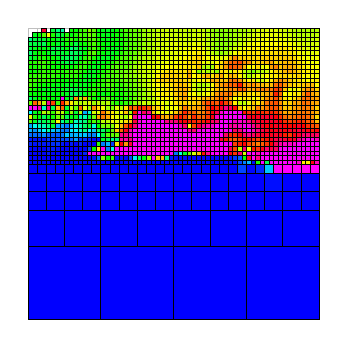
\begin{tikzpicture}[x={(\screenshotunitlength,0)},y={(0,\screenshotunitlength)}]
        \definecolor{fillcolor}{rgb}{0.000000,0.000000,1.000000}
\fill[fillcolor] (0.000000,0.000000) rectangle (0.250000,0.250000);
\definecolor{fillcolor}{rgb}{0.000000,0.000000,1.000000}
\fill[fillcolor] (0.250000,0.000000) rectangle (0.500000,0.250000);
\definecolor{fillcolor}{rgb}{0.000000,0.000000,1.000000}
\fill[fillcolor] (0.000000,0.250000) rectangle (0.125000,0.375000);
\definecolor{fillcolor}{rgb}{0.000000,0.000000,1.000000}
\fill[fillcolor] (0.125000,0.250000) rectangle (0.250000,0.375000);
\definecolor{fillcolor}{rgb}{0.000000,0.000000,1.000000}
\fill[fillcolor] (0.000000,0.375000) rectangle (0.062500,0.437500);
\definecolor{fillcolor}{rgb}{0.000000,0.000000,1.000000}
\fill[fillcolor] (0.062500,0.375000) rectangle (0.125000,0.437500);
\definecolor{fillcolor}{rgb}{0.000000,0.000000,1.000000}
\fill[fillcolor] (0.000000,0.437500) rectangle (0.062500,0.500000);
\definecolor{fillcolor}{rgb}{0.000000,0.000000,1.000000}
\fill[fillcolor] (0.062500,0.437500) rectangle (0.125000,0.500000);
\definecolor{fillcolor}{rgb}{0.000000,0.000000,1.000000}
\fill[fillcolor] (0.125000,0.375000) rectangle (0.187500,0.437500);
\definecolor{fillcolor}{rgb}{0.000000,0.000000,1.000000}
\fill[fillcolor] (0.187500,0.375000) rectangle (0.250000,0.437500);
\definecolor{fillcolor}{rgb}{0.000000,0.000000,1.000000}
\fill[fillcolor] (0.125000,0.437500) rectangle (0.187500,0.500000);
\definecolor{fillcolor}{rgb}{0.000000,0.000000,1.000000}
\fill[fillcolor] (0.187500,0.437500) rectangle (0.250000,0.500000);
\definecolor{fillcolor}{rgb}{0.000000,0.000000,1.000000}
\fill[fillcolor] (0.250000,0.250000) rectangle (0.375000,0.375000);
\definecolor{fillcolor}{rgb}{0.000000,0.000000,1.000000}
\fill[fillcolor] (0.375000,0.250000) rectangle (0.500000,0.375000);
\definecolor{fillcolor}{rgb}{0.000000,0.000000,1.000000}
\fill[fillcolor] (0.250000,0.375000) rectangle (0.312500,0.437500);
\definecolor{fillcolor}{rgb}{0.000000,0.000000,1.000000}
\fill[fillcolor] (0.312500,0.375000) rectangle (0.375000,0.437500);
\definecolor{fillcolor}{rgb}{0.000000,0.000000,1.000000}
\fill[fillcolor] (0.250000,0.437500) rectangle (0.312500,0.500000);
\definecolor{fillcolor}{rgb}{0.000000,0.000000,1.000000}
\fill[fillcolor] (0.312500,0.437500) rectangle (0.375000,0.500000);
\definecolor{fillcolor}{rgb}{0.000000,0.000000,1.000000}
\fill[fillcolor] (0.375000,0.375000) rectangle (0.437500,0.437500);
\definecolor{fillcolor}{rgb}{0.000000,0.000000,1.000000}
\fill[fillcolor] (0.437500,0.375000) rectangle (0.500000,0.437500);
\definecolor{fillcolor}{rgb}{0.000000,0.000000,1.000000}
\fill[fillcolor] (0.375000,0.437500) rectangle (0.437500,0.500000);
\definecolor{fillcolor}{rgb}{0.000000,0.000000,1.000000}
\fill[fillcolor] (0.437500,0.437500) rectangle (0.500000,0.500000);
\definecolor{fillcolor}{rgb}{0.000000,0.000000,1.000000}
\fill[fillcolor] (0.500000,0.000000) rectangle (0.750000,0.250000);
\definecolor{fillcolor}{rgb}{0.000000,0.000000,1.000000}
\fill[fillcolor] (0.750000,0.000000) rectangle (1.000000,0.250000);
\definecolor{fillcolor}{rgb}{0.000000,0.000000,1.000000}
\fill[fillcolor] (0.500000,0.250000) rectangle (0.625000,0.375000);
\definecolor{fillcolor}{rgb}{0.000000,0.000000,1.000000}
\fill[fillcolor] (0.625000,0.250000) rectangle (0.750000,0.375000);
\definecolor{fillcolor}{rgb}{0.000000,0.000000,1.000000}
\fill[fillcolor] (0.500000,0.375000) rectangle (0.562500,0.437500);
\definecolor{fillcolor}{rgb}{0.000000,0.000000,1.000000}
\fill[fillcolor] (0.562500,0.375000) rectangle (0.625000,0.437500);
\definecolor{fillcolor}{rgb}{0.000000,0.000000,1.000000}
\fill[fillcolor] (0.500000,0.437500) rectangle (0.562500,0.500000);
\definecolor{fillcolor}{rgb}{0.000000,0.000000,1.000000}
\fill[fillcolor] (0.562500,0.437500) rectangle (0.625000,0.500000);
\definecolor{fillcolor}{rgb}{0.000000,0.000000,1.000000}
\fill[fillcolor] (0.625000,0.375000) rectangle (0.687500,0.437500);
\definecolor{fillcolor}{rgb}{0.000000,0.000000,1.000000}
\fill[fillcolor] (0.687500,0.375000) rectangle (0.750000,0.437500);
\definecolor{fillcolor}{rgb}{0.000000,0.000000,1.000000}
\fill[fillcolor] (0.625000,0.437500) rectangle (0.687500,0.500000);
\definecolor{fillcolor}{rgb}{0.000000,0.000000,1.000000}
\fill[fillcolor] (0.687500,0.437500) rectangle (0.750000,0.500000);
\definecolor{fillcolor}{rgb}{0.000000,0.000000,1.000000}
\fill[fillcolor] (0.750000,0.250000) rectangle (0.875000,0.375000);
\definecolor{fillcolor}{rgb}{0.000000,0.000000,1.000000}
\fill[fillcolor] (0.875000,0.250000) rectangle (1.000000,0.375000);
\definecolor{fillcolor}{rgb}{0.000000,0.000000,1.000000}
\fill[fillcolor] (0.750000,0.375000) rectangle (0.812500,0.437500);
\definecolor{fillcolor}{rgb}{0.000000,0.000000,1.000000}
\fill[fillcolor] (0.812500,0.375000) rectangle (0.875000,0.437500);
\definecolor{fillcolor}{rgb}{0.000000,0.000080,1.000000}
\fill[fillcolor] (0.750000,0.437500) rectangle (0.812500,0.500000);
\definecolor{fillcolor}{rgb}{0.000000,0.050023,1.000000}
\fill[fillcolor] (0.812500,0.437500) rectangle (0.875000,0.500000);
\definecolor{fillcolor}{rgb}{0.000000,0.000000,1.000000}
\fill[fillcolor] (0.875000,0.375000) rectangle (0.937500,0.437500);
\definecolor{fillcolor}{rgb}{0.000000,0.000000,1.000000}
\fill[fillcolor] (0.937500,0.375000) rectangle (1.000000,0.437500);
\definecolor{fillcolor}{rgb}{0.000000,0.000000,1.000000}
\fill[fillcolor] (0.875000,0.437500) rectangle (0.937500,0.500000);
\definecolor{fillcolor}{rgb}{0.000000,0.000000,1.000000}
\fill[fillcolor] (0.937500,0.437500) rectangle (1.000000,0.500000);
\definecolor{fillcolor}{rgb}{0.000000,0.000000,1.000000}
\fill[fillcolor] (0.000000,0.500000) rectangle (0.031250,0.531250);
\definecolor{fillcolor}{rgb}{0.000000,0.000000,1.000000}
\fill[fillcolor] (0.031250,0.500000) rectangle (0.062500,0.531250);
\definecolor{fillcolor}{rgb}{0.000000,0.000000,1.000000}
\fill[fillcolor] (0.000000,0.531250) rectangle (0.015625,0.546875);
\definecolor{fillcolor}{rgb}{0.000000,0.000000,1.000000}
\fill[fillcolor] (0.015625,0.531250) rectangle (0.031250,0.546875);
\definecolor{fillcolor}{rgb}{0.000000,0.000008,1.000000}
\fill[fillcolor] (0.000000,0.546875) rectangle (0.015625,0.562500);
\definecolor{fillcolor}{rgb}{0.000000,0.000168,1.000000}
\fill[fillcolor] (0.015625,0.546875) rectangle (0.031250,0.562500);
\definecolor{fillcolor}{rgb}{0.000000,0.000000,1.000000}
\fill[fillcolor] (0.031250,0.531250) rectangle (0.046875,0.546875);
\definecolor{fillcolor}{rgb}{0.000000,0.000000,1.000000}
\fill[fillcolor] (0.046875,0.531250) rectangle (0.062500,0.546875);
\definecolor{fillcolor}{rgb}{0.000000,0.000000,1.000000}
\fill[fillcolor] (0.031250,0.546875) rectangle (0.046875,0.562500);
\definecolor{fillcolor}{rgb}{0.000000,0.000000,1.000000}
\fill[fillcolor] (0.046875,0.546875) rectangle (0.062500,0.562500);
\definecolor{fillcolor}{rgb}{0.000000,0.000000,1.000000}
\fill[fillcolor] (0.062500,0.500000) rectangle (0.093750,0.531250);
\definecolor{fillcolor}{rgb}{0.000000,0.000000,1.000000}
\fill[fillcolor] (0.093750,0.500000) rectangle (0.125000,0.531250);
\definecolor{fillcolor}{rgb}{0.000000,0.000000,1.000000}
\fill[fillcolor] (0.062500,0.531250) rectangle (0.078125,0.546875);
\definecolor{fillcolor}{rgb}{0.000000,0.000000,1.000000}
\fill[fillcolor] (0.078125,0.531250) rectangle (0.093750,0.546875);
\definecolor{fillcolor}{rgb}{0.000000,0.000012,1.000000}
\fill[fillcolor] (0.062500,0.546875) rectangle (0.078125,0.562500);
\definecolor{fillcolor}{rgb}{0.000000,0.000000,1.000000}
\fill[fillcolor] (0.078125,0.546875) rectangle (0.093750,0.562500);
\definecolor{fillcolor}{rgb}{0.000000,0.000001,1.000000}
\fill[fillcolor] (0.093750,0.531250) rectangle (0.109375,0.546875);
\definecolor{fillcolor}{rgb}{0.000000,0.000002,1.000000}
\fill[fillcolor] (0.109375,0.531250) rectangle (0.125000,0.546875);
\definecolor{fillcolor}{rgb}{0.000000,0.000000,1.000000}
\fill[fillcolor] (0.093750,0.546875) rectangle (0.109375,0.562500);
\definecolor{fillcolor}{rgb}{0.000000,0.000006,1.000000}
\fill[fillcolor] (0.109375,0.546875) rectangle (0.125000,0.562500);
\definecolor{fillcolor}{rgb}{0.000000,0.000001,1.000000}
\fill[fillcolor] (0.000000,0.562500) rectangle (0.015625,0.578125);
\definecolor{fillcolor}{rgb}{0.000000,0.000776,1.000000}
\fill[fillcolor] (0.015625,0.562500) rectangle (0.031250,0.578125);
\definecolor{fillcolor}{rgb}{0.000000,0.022373,1.000000}
\fill[fillcolor] (0.000000,0.578125) rectangle (0.015625,0.593750);
\definecolor{fillcolor}{rgb}{0.000000,0.000330,1.000000}
\fill[fillcolor] (0.015625,0.578125) rectangle (0.031250,0.593750);
\definecolor{fillcolor}{rgb}{0.000000,0.000491,1.000000}
\fill[fillcolor] (0.031250,0.562500) rectangle (0.046875,0.578125);
\definecolor{fillcolor}{rgb}{0.000000,0.008511,1.000000}
\fill[fillcolor] (0.046875,0.562500) rectangle (0.062500,0.578125);
\definecolor{fillcolor}{rgb}{0.000000,0.001115,1.000000}
\fill[fillcolor] (0.031250,0.578125) rectangle (0.046875,0.593750);
\definecolor{fillcolor}{rgb}{0.000000,0.007682,1.000000}
\fill[fillcolor] (0.046875,0.578125) rectangle (0.062500,0.593750);
\definecolor{fillcolor}{rgb}{0.000000,0.123129,1.000000}
\fill[fillcolor] (0.000000,0.593750) rectangle (0.015625,0.609375);
\definecolor{fillcolor}{rgb}{0.000000,0.067735,1.000000}
\fill[fillcolor] (0.015625,0.593750) rectangle (0.031250,0.609375);
\definecolor{fillcolor}{rgb}{0.000000,0.085375,1.000000}
\fill[fillcolor] (0.000000,0.609375) rectangle (0.015625,0.625000);
\definecolor{fillcolor}{rgb}{0.000000,0.057880,1.000000}
\fill[fillcolor] (0.015625,0.609375) rectangle (0.031250,0.625000);
\definecolor{fillcolor}{rgb}{0.000000,0.097988,1.000000}
\fill[fillcolor] (0.031250,0.593750) rectangle (0.046875,0.609375);
\definecolor{fillcolor}{rgb}{0.000000,0.099094,1.000000}
\fill[fillcolor] (0.046875,0.593750) rectangle (0.062500,0.609375);
\definecolor{fillcolor}{rgb}{0.000000,0.067545,1.000000}
\fill[fillcolor] (0.031250,0.609375) rectangle (0.046875,0.625000);
\definecolor{fillcolor}{rgb}{0.000000,0.068114,1.000000}
\fill[fillcolor] (0.046875,0.609375) rectangle (0.062500,0.625000);
\definecolor{fillcolor}{rgb}{0.000000,0.075217,1.000000}
\fill[fillcolor] (0.062500,0.562500) rectangle (0.078125,0.578125);
\definecolor{fillcolor}{rgb}{0.000000,0.010535,1.000000}
\fill[fillcolor] (0.078125,0.562500) rectangle (0.093750,0.578125);
\definecolor{fillcolor}{rgb}{0.000000,0.074295,1.000000}
\fill[fillcolor] (0.062500,0.578125) rectangle (0.078125,0.593750);
\definecolor{fillcolor}{rgb}{0.000000,0.120768,1.000000}
\fill[fillcolor] (0.078125,0.578125) rectangle (0.093750,0.593750);
\definecolor{fillcolor}{rgb}{0.000000,0.000029,1.000000}
\fill[fillcolor] (0.093750,0.562500) rectangle (0.109375,0.578125);
\definecolor{fillcolor}{rgb}{0.000000,0.000049,1.000000}
\fill[fillcolor] (0.109375,0.562500) rectangle (0.125000,0.578125);
\definecolor{fillcolor}{rgb}{0.000000,0.056447,1.000000}
\fill[fillcolor] (0.093750,0.578125) rectangle (0.109375,0.593750);
\definecolor{fillcolor}{rgb}{0.000000,0.000036,1.000000}
\fill[fillcolor] (0.109375,0.578125) rectangle (0.125000,0.593750);
\definecolor{fillcolor}{rgb}{0.000000,0.099976,1.000000}
\fill[fillcolor] (0.062500,0.593750) rectangle (0.078125,0.609375);
\definecolor{fillcolor}{rgb}{0.000000,0.181046,1.000000}
\fill[fillcolor] (0.078125,0.593750) rectangle (0.093750,0.609375);
\definecolor{fillcolor}{rgb}{0.000000,0.231823,1.000000}
\fill[fillcolor] (0.062500,0.609375) rectangle (0.078125,0.625000);
\definecolor{fillcolor}{rgb}{0.000000,0.240355,1.000000}
\fill[fillcolor] (0.078125,0.609375) rectangle (0.093750,0.625000);
\definecolor{fillcolor}{rgb}{0.000000,0.195287,1.000000}
\fill[fillcolor] (0.093750,0.593750) rectangle (0.109375,0.609375);
\definecolor{fillcolor}{rgb}{0.000000,0.084508,1.000000}
\fill[fillcolor] (0.109375,0.593750) rectangle (0.125000,0.609375);
\definecolor{fillcolor}{rgb}{0.000000,0.274501,1.000000}
\fill[fillcolor] (0.093750,0.609375) rectangle (0.109375,0.625000);
\definecolor{fillcolor}{rgb}{0.000000,0.295888,1.000000}
\fill[fillcolor] (0.109375,0.609375) rectangle (0.125000,0.625000);
\definecolor{fillcolor}{rgb}{0.000000,0.000001,1.000000}
\fill[fillcolor] (0.125000,0.500000) rectangle (0.156250,0.531250);
\definecolor{fillcolor}{rgb}{0.000000,0.000002,1.000000}
\fill[fillcolor] (0.156250,0.500000) rectangle (0.187500,0.531250);
\definecolor{fillcolor}{rgb}{0.000000,0.000003,1.000000}
\fill[fillcolor] (0.125000,0.531250) rectangle (0.140625,0.546875);
\definecolor{fillcolor}{rgb}{0.000000,0.000004,1.000000}
\fill[fillcolor] (0.140625,0.531250) rectangle (0.156250,0.546875);
\definecolor{fillcolor}{rgb}{0.000000,0.000002,1.000000}
\fill[fillcolor] (0.125000,0.546875) rectangle (0.140625,0.562500);
\definecolor{fillcolor}{rgb}{0.000000,0.000002,1.000000}
\fill[fillcolor] (0.140625,0.546875) rectangle (0.156250,0.562500);
\definecolor{fillcolor}{rgb}{0.000000,0.000004,1.000000}
\fill[fillcolor] (0.156250,0.531250) rectangle (0.171875,0.546875);
\definecolor{fillcolor}{rgb}{0.000000,0.000005,1.000000}
\fill[fillcolor] (0.171875,0.531250) rectangle (0.187500,0.546875);
\definecolor{fillcolor}{rgb}{0.000000,0.000008,1.000000}
\fill[fillcolor] (0.156250,0.546875) rectangle (0.171875,0.562500);
\definecolor{fillcolor}{rgb}{0.000000,0.000018,1.000000}
\fill[fillcolor] (0.171875,0.546875) rectangle (0.187500,0.562500);
\definecolor{fillcolor}{rgb}{0.000000,0.000003,1.000000}
\fill[fillcolor] (0.187500,0.500000) rectangle (0.218750,0.531250);
\definecolor{fillcolor}{rgb}{0.000000,0.000016,1.000000}
\fill[fillcolor] (0.218750,0.500000) rectangle (0.250000,0.531250);
\definecolor{fillcolor}{rgb}{0.000000,0.000006,1.000000}
\fill[fillcolor] (0.187500,0.531250) rectangle (0.203125,0.546875);
\definecolor{fillcolor}{rgb}{0.000000,0.000011,1.000000}
\fill[fillcolor] (0.203125,0.531250) rectangle (0.218750,0.546875);
\definecolor{fillcolor}{rgb}{0.000000,0.000029,1.000000}
\fill[fillcolor] (0.187500,0.546875) rectangle (0.203125,0.562500);
\definecolor{fillcolor}{rgb}{0.000000,0.001679,1.000000}
\fill[fillcolor] (0.203125,0.546875) rectangle (0.218750,0.562500);
\definecolor{fillcolor}{rgb}{0.000000,0.000019,1.000000}
\fill[fillcolor] (0.218750,0.531250) rectangle (0.234375,0.546875);
\definecolor{fillcolor}{rgb}{0.000000,0.000025,1.000000}
\fill[fillcolor] (0.234375,0.531250) rectangle (0.250000,0.546875);
\definecolor{fillcolor}{rgb}{0.000000,0.068443,1.000000}
\fill[fillcolor] (0.218750,0.546875) rectangle (0.234375,0.562500);
\definecolor{fillcolor}{rgb}{0.000000,0.415055,1.000000}
\fill[fillcolor] (0.234375,0.546875) rectangle (0.250000,0.562500);
\definecolor{fillcolor}{rgb}{0.000000,0.000029,1.000000}
\fill[fillcolor] (0.125000,0.562500) rectangle (0.140625,0.578125);
\definecolor{fillcolor}{rgb}{0.000000,0.000041,1.000000}
\fill[fillcolor] (0.140625,0.562500) rectangle (0.156250,0.578125);
\definecolor{fillcolor}{rgb}{0.000000,0.000037,1.000000}
\fill[fillcolor] (0.125000,0.578125) rectangle (0.140625,0.593750);
\definecolor{fillcolor}{rgb}{0.000000,0.000057,1.000000}
\fill[fillcolor] (0.140625,0.578125) rectangle (0.156250,0.593750);
\definecolor{fillcolor}{rgb}{0.000000,0.000070,1.000000}
\fill[fillcolor] (0.156250,0.562500) rectangle (0.171875,0.578125);
\definecolor{fillcolor}{rgb}{0.000000,0.000077,1.000000}
\fill[fillcolor] (0.171875,0.562500) rectangle (0.187500,0.578125);
\definecolor{fillcolor}{rgb}{0.000000,0.000076,1.000000}
\fill[fillcolor] (0.156250,0.578125) rectangle (0.171875,0.593750);
\definecolor{fillcolor}{rgb}{0.000000,0.000064,1.000000}
\fill[fillcolor] (0.171875,0.578125) rectangle (0.187500,0.593750);
\definecolor{fillcolor}{rgb}{0.000000,0.009005,1.000000}
\fill[fillcolor] (0.125000,0.593750) rectangle (0.140625,0.609375);
\definecolor{fillcolor}{rgb}{0.000000,0.094293,1.000000}
\fill[fillcolor] (0.140625,0.593750) rectangle (0.156250,0.609375);
\definecolor{fillcolor}{rgb}{0.000000,0.310755,1.000000}
\fill[fillcolor] (0.125000,0.609375) rectangle (0.140625,0.625000);
\definecolor{fillcolor}{rgb}{0.000000,0.395696,1.000000}
\fill[fillcolor] (0.140625,0.609375) rectangle (0.156250,0.625000);
\definecolor{fillcolor}{rgb}{0.000000,0.012458,1.000000}
\fill[fillcolor] (0.156250,0.593750) rectangle (0.171875,0.609375);
\definecolor{fillcolor}{rgb}{0.000000,0.128139,1.000000}
\fill[fillcolor] (0.171875,0.593750) rectangle (0.187500,0.609375);
\definecolor{fillcolor}{rgb}{0.000000,0.615466,1.000000}
\fill[fillcolor] (0.156250,0.609375) rectangle (0.171875,0.625000);
\definecolor{fillcolor}{rgb}{0.000000,0.227569,1.000000}
\fill[fillcolor] (0.171875,0.609375) rectangle (0.187500,0.625000);
\definecolor{fillcolor}{rgb}{0.000000,0.124611,1.000000}
\fill[fillcolor] (0.187500,0.562500) rectangle (0.203125,0.578125);
\definecolor{fillcolor}{rgb}{1.000000,0.000000,1.000000}
\fill[fillcolor] (0.203125,0.562500) rectangle (0.218750,0.578125);
\definecolor{fillcolor}{rgb}{0.000000,0.000042,1.000000}
\fill[fillcolor] (0.187500,0.578125) rectangle (0.203125,0.593750);
\definecolor{fillcolor}{rgb}{0.000000,0.263498,1.000000}
\fill[fillcolor] (0.203125,0.578125) rectangle (0.218750,0.593750);
\definecolor{fillcolor}{rgb}{1.000000,0.000000,1.000000}
\fill[fillcolor] (0.218750,0.562500) rectangle (0.234375,0.578125);
\definecolor{fillcolor}{rgb}{1.000000,0.000000,1.000000}
\fill[fillcolor] (0.234375,0.562500) rectangle (0.250000,0.578125);
\definecolor{fillcolor}{rgb}{0.017767,1.000000,0.000000}
\fill[fillcolor] (0.218750,0.578125) rectangle (0.234375,0.593750);
\definecolor{fillcolor}{rgb}{1.000000,0.929517,0.000000}
\fill[fillcolor] (0.234375,0.578125) rectangle (0.250000,0.593750);
\definecolor{fillcolor}{rgb}{0.000000,0.000062,1.000000}
\fill[fillcolor] (0.187500,0.593750) rectangle (0.203125,0.609375);
\definecolor{fillcolor}{rgb}{0.000000,0.000105,1.000000}
\fill[fillcolor] (0.203125,0.593750) rectangle (0.218750,0.609375);
\definecolor{fillcolor}{rgb}{0.000000,0.209312,1.000000}
\fill[fillcolor] (0.187500,0.609375) rectangle (0.203125,0.625000);
\definecolor{fillcolor}{rgb}{0.000000,0.117551,1.000000}
\fill[fillcolor] (0.203125,0.609375) rectangle (0.218750,0.625000);
\definecolor{fillcolor}{rgb}{0.000000,0.000230,1.000000}
\fill[fillcolor] (0.218750,0.593750) rectangle (0.234375,0.609375);
\definecolor{fillcolor}{rgb}{0.166678,1.000000,0.000000}
\fill[fillcolor] (0.234375,0.593750) rectangle (0.250000,0.609375);
\definecolor{fillcolor}{rgb}{0.000000,0.008647,1.000000}
\fill[fillcolor] (0.218750,0.609375) rectangle (0.234375,0.625000);
\definecolor{fillcolor}{rgb}{0.000000,0.062237,1.000000}
\fill[fillcolor] (0.234375,0.609375) rectangle (0.250000,0.625000);
\definecolor{fillcolor}{rgb}{0.000000,0.435473,1.000000}
\fill[fillcolor] (0.000000,0.625000) rectangle (0.015625,0.640625);
\definecolor{fillcolor}{rgb}{0.000000,0.424658,1.000000}
\fill[fillcolor] (0.015625,0.625000) rectangle (0.031250,0.640625);
\definecolor{fillcolor}{rgb}{0.000000,0.695930,1.000000}
\fill[fillcolor] (0.000000,0.640625) rectangle (0.015625,0.656250);
\definecolor{fillcolor}{rgb}{0.000000,0.581373,1.000000}
\fill[fillcolor] (0.015625,0.640625) rectangle (0.031250,0.656250);
\definecolor{fillcolor}{rgb}{0.000000,0.435526,1.000000}
\fill[fillcolor] (0.031250,0.625000) rectangle (0.046875,0.640625);
\definecolor{fillcolor}{rgb}{0.000000,0.552122,1.000000}
\fill[fillcolor] (0.046875,0.625000) rectangle (0.062500,0.640625);
\definecolor{fillcolor}{rgb}{0.000000,0.815969,1.000000}
\fill[fillcolor] (0.031250,0.640625) rectangle (0.046875,0.656250);
\definecolor{fillcolor}{rgb}{0.000000,0.987393,1.000000}
\fill[fillcolor] (0.046875,0.640625) rectangle (0.062500,0.656250);
\definecolor{fillcolor}{rgb}{0.000000,0.675231,1.000000}
\fill[fillcolor] (0.000000,0.656250) rectangle (0.015625,0.671875);
\definecolor{fillcolor}{rgb}{0.000000,1.000000,0.924949}
\fill[fillcolor] (0.015625,0.656250) rectangle (0.031250,0.671875);
\definecolor{fillcolor}{rgb}{0.326331,1.000000,0.000000}
\fill[fillcolor] (0.000000,0.671875) rectangle (0.015625,0.687500);
\definecolor{fillcolor}{rgb}{0.000000,1.000000,0.124407}
\fill[fillcolor] (0.015625,0.671875) rectangle (0.031250,0.687500);
\definecolor{fillcolor}{rgb}{0.000000,1.000000,0.754400}
\fill[fillcolor] (0.031250,0.656250) rectangle (0.046875,0.671875);
\definecolor{fillcolor}{rgb}{0.000000,1.000000,0.703730}
\fill[fillcolor] (0.046875,0.656250) rectangle (0.062500,0.671875);
\definecolor{fillcolor}{rgb}{0.000000,1.000000,0.496340}
\fill[fillcolor] (0.031250,0.671875) rectangle (0.046875,0.687500);
\definecolor{fillcolor}{rgb}{0.000000,1.000000,0.289491}
\fill[fillcolor] (0.046875,0.671875) rectangle (0.062500,0.687500);
\definecolor{fillcolor}{rgb}{0.000000,0.377264,1.000000}
\fill[fillcolor] (0.062500,0.625000) rectangle (0.078125,0.640625);
\definecolor{fillcolor}{rgb}{0.000000,0.364543,1.000000}
\fill[fillcolor] (0.078125,0.625000) rectangle (0.093750,0.640625);
\definecolor{fillcolor}{rgb}{0.000000,1.000000,0.638147}
\fill[fillcolor] (0.062500,0.640625) rectangle (0.078125,0.656250);
\definecolor{fillcolor}{rgb}{0.000000,0.772181,1.000000}
\fill[fillcolor] (0.078125,0.640625) rectangle (0.093750,0.656250);
\definecolor{fillcolor}{rgb}{0.000000,0.343815,1.000000}
\fill[fillcolor] (0.093750,0.625000) rectangle (0.109375,0.640625);
\definecolor{fillcolor}{rgb}{0.000000,0.477117,1.000000}
\fill[fillcolor] (0.109375,0.625000) rectangle (0.125000,0.640625);
\definecolor{fillcolor}{rgb}{0.000000,0.683248,1.000000}
\fill[fillcolor] (0.093750,0.640625) rectangle (0.109375,0.656250);
\definecolor{fillcolor}{rgb}{0.000000,0.479234,1.000000}
\fill[fillcolor] (0.109375,0.640625) rectangle (0.125000,0.656250);
\definecolor{fillcolor}{rgb}{0.000000,1.000000,0.511901}
\fill[fillcolor] (0.062500,0.656250) rectangle (0.078125,0.671875);
\definecolor{fillcolor}{rgb}{0.000000,1.000000,0.152152}
\fill[fillcolor] (0.078125,0.656250) rectangle (0.093750,0.671875);
\definecolor{fillcolor}{rgb}{0.000000,1.000000,0.295063}
\fill[fillcolor] (0.062500,0.671875) rectangle (0.078125,0.687500);
\definecolor{fillcolor}{rgb}{0.228053,1.000000,0.000000}
\fill[fillcolor] (0.078125,0.671875) rectangle (0.093750,0.687500);
\definecolor{fillcolor}{rgb}{0.000000,0.699708,1.000000}
\fill[fillcolor] (0.093750,0.656250) rectangle (0.109375,0.671875);
\definecolor{fillcolor}{rgb}{0.000000,0.613000,1.000000}
\fill[fillcolor] (0.109375,0.656250) rectangle (0.125000,0.671875);
\definecolor{fillcolor}{rgb}{0.980491,1.000000,0.000000}
\fill[fillcolor] (0.093750,0.671875) rectangle (0.109375,0.687500);
\definecolor{fillcolor}{rgb}{0.000000,1.000000,0.545992}
\fill[fillcolor] (0.109375,0.671875) rectangle (0.125000,0.687500);
\definecolor{fillcolor}{rgb}{0.891181,1.000000,0.000000}
\fill[fillcolor] (0.000000,0.687500) rectangle (0.015625,0.703125);
\definecolor{fillcolor}{rgb}{0.147614,1.000000,0.000000}
\fill[fillcolor] (0.015625,0.687500) rectangle (0.031250,0.703125);
\definecolor{fillcolor}{rgb}{0.000000,0.992118,1.000000}
\fill[fillcolor] (0.000000,0.703125) rectangle (0.015625,0.718750);
\definecolor{fillcolor}{rgb}{0.000000,1.000000,0.112377}
\fill[fillcolor] (0.015625,0.703125) rectangle (0.031250,0.718750);
\definecolor{fillcolor}{rgb}{0.000000,1.000000,0.017057}
\fill[fillcolor] (0.031250,0.687500) rectangle (0.046875,0.703125);
\definecolor{fillcolor}{rgb}{0.000000,1.000000,0.332382}
\fill[fillcolor] (0.046875,0.687500) rectangle (0.062500,0.703125);
\definecolor{fillcolor}{rgb}{0.000000,1.000000,0.002870}
\fill[fillcolor] (0.031250,0.703125) rectangle (0.046875,0.718750);
\definecolor{fillcolor}{rgb}{0.695243,1.000000,0.000000}
\fill[fillcolor] (0.046875,0.703125) rectangle (0.062500,0.718750);
\definecolor{fillcolor}{rgb}{1.000000,0.000000,1.000000}
\fill[fillcolor] (0.000000,0.718750) rectangle (0.015625,0.734375);
\definecolor{fillcolor}{rgb}{1.000000,0.000000,1.000000}
\fill[fillcolor] (0.015625,0.718750) rectangle (0.031250,0.734375);
\definecolor{fillcolor}{rgb}{0.375994,1.000000,0.000000}
\fill[fillcolor] (0.000000,0.734375) rectangle (0.015625,0.750000);
\definecolor{fillcolor}{rgb}{1.000000,0.381800,0.000000}
\fill[fillcolor] (0.015625,0.734375) rectangle (0.031250,0.750000);
\definecolor{fillcolor}{rgb}{1.000000,0.000000,0.667663}
\fill[fillcolor] (0.031250,0.718750) rectangle (0.046875,0.734375);
\definecolor{fillcolor}{rgb}{0.000000,1.000000,0.728492}
\fill[fillcolor] (0.046875,0.718750) rectangle (0.062500,0.734375);
\definecolor{fillcolor}{rgb}{1.000000,0.656221,0.000000}
\fill[fillcolor] (0.031250,0.734375) rectangle (0.046875,0.750000);
\definecolor{fillcolor}{rgb}{0.699929,1.000000,0.000000}
\fill[fillcolor] (0.046875,0.734375) rectangle (0.062500,0.750000);
\definecolor{fillcolor}{rgb}{0.000000,1.000000,0.103560}
\fill[fillcolor] (0.062500,0.687500) rectangle (0.078125,0.703125);
\definecolor{fillcolor}{rgb}{0.069571,1.000000,0.000000}
\fill[fillcolor] (0.078125,0.687500) rectangle (0.093750,0.703125);
\definecolor{fillcolor}{rgb}{0.554008,1.000000,0.000000}
\fill[fillcolor] (0.062500,0.703125) rectangle (0.078125,0.718750);
\definecolor{fillcolor}{rgb}{0.207086,1.000000,0.000000}
\fill[fillcolor] (0.078125,0.703125) rectangle (0.093750,0.718750);
\definecolor{fillcolor}{rgb}{0.432587,1.000000,0.000000}
\fill[fillcolor] (0.093750,0.687500) rectangle (0.109375,0.703125);
\definecolor{fillcolor}{rgb}{0.363678,1.000000,0.000000}
\fill[fillcolor] (0.109375,0.687500) rectangle (0.125000,0.703125);
\definecolor{fillcolor}{rgb}{0.688398,1.000000,0.000000}
\fill[fillcolor] (0.093750,0.703125) rectangle (0.109375,0.718750);
\definecolor{fillcolor}{rgb}{0.724069,1.000000,0.000000}
\fill[fillcolor] (0.109375,0.703125) rectangle (0.125000,0.718750);
\definecolor{fillcolor}{rgb}{1.000000,0.000000,0.474905}
\fill[fillcolor] (0.062500,0.718750) rectangle (0.078125,0.734375);
\definecolor{fillcolor}{rgb}{0.000000,1.000000,0.279617}
\fill[fillcolor] (0.078125,0.718750) rectangle (0.093750,0.734375);
\definecolor{fillcolor}{rgb}{1.000000,0.000000,0.622639}
\fill[fillcolor] (0.062500,0.734375) rectangle (0.078125,0.750000);
\definecolor{fillcolor}{rgb}{1.000000,0.250635,0.000000}
\fill[fillcolor] (0.078125,0.734375) rectangle (0.093750,0.750000);
\definecolor{fillcolor}{rgb}{1.000000,0.716136,0.000000}
\fill[fillcolor] (0.093750,0.718750) rectangle (0.109375,0.734375);
\definecolor{fillcolor}{rgb}{1.000000,0.398637,0.000000}
\fill[fillcolor] (0.109375,0.718750) rectangle (0.125000,0.734375);
\definecolor{fillcolor}{rgb}{0.246240,1.000000,0.000000}
\fill[fillcolor] (0.093750,0.734375) rectangle (0.109375,0.750000);
\definecolor{fillcolor}{rgb}{1.000000,0.142410,0.000000}
\fill[fillcolor] (0.109375,0.734375) rectangle (0.125000,0.750000);
\definecolor{fillcolor}{rgb}{0.000000,0.789802,1.000000}
\fill[fillcolor] (0.125000,0.625000) rectangle (0.140625,0.640625);
\definecolor{fillcolor}{rgb}{0.000000,0.688042,1.000000}
\fill[fillcolor] (0.140625,0.625000) rectangle (0.156250,0.640625);
\definecolor{fillcolor}{rgb}{0.000000,0.477024,1.000000}
\fill[fillcolor] (0.125000,0.640625) rectangle (0.140625,0.656250);
\definecolor{fillcolor}{rgb}{0.000000,0.929467,1.000000}
\fill[fillcolor] (0.140625,0.640625) rectangle (0.156250,0.656250);
\definecolor{fillcolor}{rgb}{0.000000,0.718857,1.000000}
\fill[fillcolor] (0.156250,0.625000) rectangle (0.171875,0.640625);
\definecolor{fillcolor}{rgb}{0.000000,0.765220,1.000000}
\fill[fillcolor] (0.171875,0.625000) rectangle (0.187500,0.640625);
\definecolor{fillcolor}{rgb}{0.000000,0.950920,1.000000}
\fill[fillcolor] (0.156250,0.640625) rectangle (0.171875,0.656250);
\definecolor{fillcolor}{rgb}{0.000000,1.000000,0.744173}
\fill[fillcolor] (0.171875,0.640625) rectangle (0.187500,0.656250);
\definecolor{fillcolor}{rgb}{0.000000,0.477304,1.000000}
\fill[fillcolor] (0.125000,0.656250) rectangle (0.140625,0.671875);
\definecolor{fillcolor}{rgb}{0.000000,0.785777,1.000000}
\fill[fillcolor] (0.140625,0.656250) rectangle (0.156250,0.671875);
\definecolor{fillcolor}{rgb}{0.000000,1.000000,0.261486}
\fill[fillcolor] (0.125000,0.671875) rectangle (0.140625,0.687500);
\definecolor{fillcolor}{rgb}{0.127929,1.000000,0.000000}
\fill[fillcolor] (0.140625,0.671875) rectangle (0.156250,0.687500);
\definecolor{fillcolor}{rgb}{0.000000,1.000000,0.882557}
\fill[fillcolor] (0.156250,0.656250) rectangle (0.171875,0.671875);
\definecolor{fillcolor}{rgb}{0.000000,1.000000,0.692837}
\fill[fillcolor] (0.171875,0.656250) rectangle (0.187500,0.671875);
\definecolor{fillcolor}{rgb}{0.000000,1.000000,0.763746}
\fill[fillcolor] (0.156250,0.671875) rectangle (0.171875,0.687500);
\definecolor{fillcolor}{rgb}{0.000000,1.000000,0.601659}
\fill[fillcolor] (0.171875,0.671875) rectangle (0.187500,0.687500);
\definecolor{fillcolor}{rgb}{0.000000,0.772197,1.000000}
\fill[fillcolor] (0.187500,0.625000) rectangle (0.203125,0.640625);
\definecolor{fillcolor}{rgb}{0.000000,0.547501,1.000000}
\fill[fillcolor] (0.203125,0.625000) rectangle (0.218750,0.640625);
\definecolor{fillcolor}{rgb}{0.000000,1.000000,0.501730}
\fill[fillcolor] (0.187500,0.640625) rectangle (0.203125,0.656250);
\definecolor{fillcolor}{rgb}{0.000000,1.000000,0.981334}
\fill[fillcolor] (0.203125,0.640625) rectangle (0.218750,0.656250);
\definecolor{fillcolor}{rgb}{0.000000,0.514648,1.000000}
\fill[fillcolor] (0.218750,0.625000) rectangle (0.234375,0.640625);
\definecolor{fillcolor}{rgb}{0.000000,1.000000,0.988136}
\fill[fillcolor] (0.234375,0.625000) rectangle (0.250000,0.640625);
\definecolor{fillcolor}{rgb}{0.000000,0.807878,1.000000}
\fill[fillcolor] (0.218750,0.640625) rectangle (0.234375,0.656250);
\definecolor{fillcolor}{rgb}{0.000000,1.000000,0.363667}
\fill[fillcolor] (0.234375,0.640625) rectangle (0.250000,0.656250);
\definecolor{fillcolor}{rgb}{0.000000,1.000000,0.392118}
\fill[fillcolor] (0.187500,0.656250) rectangle (0.203125,0.671875);
\definecolor{fillcolor}{rgb}{0.000000,1.000000,0.208407}
\fill[fillcolor] (0.203125,0.656250) rectangle (0.218750,0.671875);
\definecolor{fillcolor}{rgb}{0.000000,1.000000,0.463885}
\fill[fillcolor] (0.187500,0.671875) rectangle (0.203125,0.687500);
\definecolor{fillcolor}{rgb}{0.064179,1.000000,0.000000}
\fill[fillcolor] (0.203125,0.671875) rectangle (0.218750,0.687500);
\definecolor{fillcolor}{rgb}{0.000000,1.000000,0.835374}
\fill[fillcolor] (0.218750,0.656250) rectangle (0.234375,0.671875);
\definecolor{fillcolor}{rgb}{0.000000,1.000000,0.009360}
\fill[fillcolor] (0.234375,0.656250) rectangle (0.250000,0.671875);
\definecolor{fillcolor}{rgb}{0.285866,1.000000,0.000000}
\fill[fillcolor] (0.218750,0.671875) rectangle (0.234375,0.687500);
\definecolor{fillcolor}{rgb}{0.138069,1.000000,0.000000}
\fill[fillcolor] (0.234375,0.671875) rectangle (0.250000,0.687500);
\definecolor{fillcolor}{rgb}{0.000000,1.000000,0.311341}
\fill[fillcolor] (0.125000,0.687500) rectangle (0.140625,0.703125);
\definecolor{fillcolor}{rgb}{0.000000,1.000000,0.085926}
\fill[fillcolor] (0.140625,0.687500) rectangle (0.156250,0.703125);
\definecolor{fillcolor}{rgb}{0.019278,1.000000,0.000000}
\fill[fillcolor] (0.125000,0.703125) rectangle (0.140625,0.718750);
\definecolor{fillcolor}{rgb}{0.570885,1.000000,0.000000}
\fill[fillcolor] (0.140625,0.703125) rectangle (0.156250,0.718750);
\definecolor{fillcolor}{rgb}{0.000000,1.000000,0.103207}
\fill[fillcolor] (0.156250,0.687500) rectangle (0.171875,0.703125);
\definecolor{fillcolor}{rgb}{0.000000,1.000000,0.635488}
\fill[fillcolor] (0.171875,0.687500) rectangle (0.187500,0.703125);
\definecolor{fillcolor}{rgb}{0.000000,1.000000,0.205123}
\fill[fillcolor] (0.156250,0.703125) rectangle (0.171875,0.718750);
\definecolor{fillcolor}{rgb}{0.671168,1.000000,0.000000}
\fill[fillcolor] (0.171875,0.703125) rectangle (0.187500,0.718750);
\definecolor{fillcolor}{rgb}{0.000000,1.000000,0.210363}
\fill[fillcolor] (0.125000,0.718750) rectangle (0.140625,0.734375);
\definecolor{fillcolor}{rgb}{0.764176,1.000000,0.000000}
\fill[fillcolor] (0.140625,0.718750) rectangle (0.156250,0.734375);
\definecolor{fillcolor}{rgb}{1.000000,0.679496,0.000000}
\fill[fillcolor] (0.125000,0.734375) rectangle (0.140625,0.750000);
\definecolor{fillcolor}{rgb}{1.000000,0.912258,0.000000}
\fill[fillcolor] (0.140625,0.734375) rectangle (0.156250,0.750000);
\definecolor{fillcolor}{rgb}{0.404243,1.000000,0.000000}
\fill[fillcolor] (0.156250,0.718750) rectangle (0.171875,0.734375);
\definecolor{fillcolor}{rgb}{1.000000,0.437651,0.000000}
\fill[fillcolor] (0.171875,0.718750) rectangle (0.187500,0.734375);
\definecolor{fillcolor}{rgb}{0.745695,1.000000,0.000000}
\fill[fillcolor] (0.156250,0.734375) rectangle (0.171875,0.750000);
\definecolor{fillcolor}{rgb}{0.688928,1.000000,0.000000}
\fill[fillcolor] (0.171875,0.734375) rectangle (0.187500,0.750000);
\definecolor{fillcolor}{rgb}{0.000000,1.000000,0.702156}
\fill[fillcolor] (0.187500,0.687500) rectangle (0.203125,0.703125);
\definecolor{fillcolor}{rgb}{0.000000,1.000000,0.239338}
\fill[fillcolor] (0.203125,0.687500) rectangle (0.218750,0.703125);
\definecolor{fillcolor}{rgb}{0.000000,0.654789,1.000000}
\fill[fillcolor] (0.187500,0.703125) rectangle (0.203125,0.718750);
\definecolor{fillcolor}{rgb}{0.000000,1.000000,0.780704}
\fill[fillcolor] (0.203125,0.703125) rectangle (0.218750,0.718750);
\definecolor{fillcolor}{rgb}{0.454806,1.000000,0.000000}
\fill[fillcolor] (0.218750,0.687500) rectangle (0.234375,0.703125);
\definecolor{fillcolor}{rgb}{1.000000,0.616545,0.000000}
\fill[fillcolor] (0.234375,0.687500) rectangle (0.250000,0.703125);
\definecolor{fillcolor}{rgb}{0.840091,1.000000,0.000000}
\fill[fillcolor] (0.218750,0.703125) rectangle (0.234375,0.718750);
\definecolor{fillcolor}{rgb}{0.918433,1.000000,0.000000}
\fill[fillcolor] (0.234375,0.703125) rectangle (0.250000,0.718750);
\definecolor{fillcolor}{rgb}{0.916100,1.000000,0.000000}
\fill[fillcolor] (0.187500,0.718750) rectangle (0.203125,0.734375);
\definecolor{fillcolor}{rgb}{0.614516,1.000000,0.000000}
\fill[fillcolor] (0.203125,0.718750) rectangle (0.218750,0.734375);
\definecolor{fillcolor}{rgb}{0.765662,1.000000,0.000000}
\fill[fillcolor] (0.187500,0.734375) rectangle (0.203125,0.750000);
\definecolor{fillcolor}{rgb}{0.881701,1.000000,0.000000}
\fill[fillcolor] (0.203125,0.734375) rectangle (0.218750,0.750000);
\definecolor{fillcolor}{rgb}{1.000000,0.574972,0.000000}
\fill[fillcolor] (0.218750,0.718750) rectangle (0.234375,0.734375);
\definecolor{fillcolor}{rgb}{1.000000,0.883789,0.000000}
\fill[fillcolor] (0.234375,0.718750) rectangle (0.250000,0.734375);
\definecolor{fillcolor}{rgb}{0.612683,1.000000,0.000000}
\fill[fillcolor] (0.218750,0.734375) rectangle (0.234375,0.750000);
\definecolor{fillcolor}{rgb}{0.745821,1.000000,0.000000}
\fill[fillcolor] (0.234375,0.734375) rectangle (0.250000,0.750000);
\definecolor{fillcolor}{rgb}{0.000000,0.000019,1.000000}
\fill[fillcolor] (0.250000,0.500000) rectangle (0.281250,0.531250);
\definecolor{fillcolor}{rgb}{0.000000,0.000029,1.000000}
\fill[fillcolor] (0.281250,0.500000) rectangle (0.312500,0.531250);
\definecolor{fillcolor}{rgb}{0.000000,0.000025,1.000000}
\fill[fillcolor] (0.250000,0.531250) rectangle (0.265625,0.546875);
\definecolor{fillcolor}{rgb}{0.000000,0.000030,1.000000}
\fill[fillcolor] (0.265625,0.531250) rectangle (0.281250,0.546875);
\definecolor{fillcolor}{rgb}{0.527827,1.000000,0.000000}
\fill[fillcolor] (0.250000,0.546875) rectangle (0.265625,0.562500);
\definecolor{fillcolor}{rgb}{0.000000,1.000000,0.004724}
\fill[fillcolor] (0.265625,0.546875) rectangle (0.281250,0.562500);
\definecolor{fillcolor}{rgb}{0.000000,0.000025,1.000000}
\fill[fillcolor] (0.281250,0.531250) rectangle (0.296875,0.546875);
\definecolor{fillcolor}{rgb}{0.000000,0.000021,1.000000}
\fill[fillcolor] (0.296875,0.531250) rectangle (0.312500,0.546875);
\definecolor{fillcolor}{rgb}{0.247622,1.000000,0.000000}
\fill[fillcolor] (0.281250,0.546875) rectangle (0.296875,0.562500);
\definecolor{fillcolor}{rgb}{0.000000,0.046242,1.000000}
\fill[fillcolor] (0.296875,0.546875) rectangle (0.312500,0.562500);
\definecolor{fillcolor}{rgb}{0.000000,0.000016,1.000000}
\fill[fillcolor] (0.312500,0.500000) rectangle (0.343750,0.531250);
\definecolor{fillcolor}{rgb}{0.000000,0.000104,1.000000}
\fill[fillcolor] (0.343750,0.500000) rectangle (0.375000,0.531250);
\definecolor{fillcolor}{rgb}{0.000000,0.000021,1.000000}
\fill[fillcolor] (0.312500,0.531250) rectangle (0.328125,0.546875);
\definecolor{fillcolor}{rgb}{0.000000,0.000041,1.000000}
\fill[fillcolor] (0.328125,0.531250) rectangle (0.343750,0.546875);
\definecolor{fillcolor}{rgb}{0.000000,0.054097,1.000000}
\fill[fillcolor] (0.312500,0.546875) rectangle (0.328125,0.562500);
\definecolor{fillcolor}{rgb}{0.000000,0.012683,1.000000}
\fill[fillcolor] (0.328125,0.546875) rectangle (0.343750,0.562500);
\definecolor{fillcolor}{rgb}{0.000000,0.000094,1.000000}
\fill[fillcolor] (0.343750,0.531250) rectangle (0.359375,0.546875);
\definecolor{fillcolor}{rgb}{0.000000,0.000078,1.000000}
\fill[fillcolor] (0.359375,0.531250) rectangle (0.375000,0.546875);
\definecolor{fillcolor}{rgb}{0.000000,0.291358,1.000000}
\fill[fillcolor] (0.343750,0.546875) rectangle (0.359375,0.562500);
\definecolor{fillcolor}{rgb}{0.000000,0.912029,1.000000}
\fill[fillcolor] (0.359375,0.546875) rectangle (0.375000,0.562500);
\definecolor{fillcolor}{rgb}{1.000000,0.000000,1.000000}
\fill[fillcolor] (0.250000,0.562500) rectangle (0.265625,0.578125);
\definecolor{fillcolor}{rgb}{1.000000,0.000000,1.000000}
\fill[fillcolor] (0.265625,0.562500) rectangle (0.281250,0.578125);
\definecolor{fillcolor}{rgb}{1.000000,0.000000,0.924403}
\fill[fillcolor] (0.250000,0.578125) rectangle (0.265625,0.593750);
\definecolor{fillcolor}{rgb}{0.000000,0.482697,1.000000}
\fill[fillcolor] (0.265625,0.578125) rectangle (0.281250,0.593750);
\definecolor{fillcolor}{rgb}{1.000000,0.000000,1.000000}
\fill[fillcolor] (0.281250,0.562500) rectangle (0.296875,0.578125);
\definecolor{fillcolor}{rgb}{1.000000,0.000000,1.000000}
\fill[fillcolor] (0.296875,0.562500) rectangle (0.312500,0.578125);
\definecolor{fillcolor}{rgb}{0.000000,1.000000,0.932217}
\fill[fillcolor] (0.281250,0.578125) rectangle (0.296875,0.593750);
\definecolor{fillcolor}{rgb}{1.000000,0.000000,1.000000}
\fill[fillcolor] (0.296875,0.578125) rectangle (0.312500,0.593750);
\definecolor{fillcolor}{rgb}{0.000000,0.490692,1.000000}
\fill[fillcolor] (0.250000,0.593750) rectangle (0.265625,0.609375);
\definecolor{fillcolor}{rgb}{0.000000,0.705997,1.000000}
\fill[fillcolor] (0.265625,0.593750) rectangle (0.281250,0.609375);
\definecolor{fillcolor}{rgb}{0.000000,1.000000,0.155415}
\fill[fillcolor] (0.250000,0.609375) rectangle (0.265625,0.625000);
\definecolor{fillcolor}{rgb}{0.000000,1.000000,0.249209}
\fill[fillcolor] (0.265625,0.609375) rectangle (0.281250,0.625000);
\definecolor{fillcolor}{rgb}{0.000000,0.227672,1.000000}
\fill[fillcolor] (0.281250,0.593750) rectangle (0.296875,0.609375);
\definecolor{fillcolor}{rgb}{1.000000,0.884937,0.000000}
\fill[fillcolor] (0.296875,0.593750) rectangle (0.312500,0.609375);
\definecolor{fillcolor}{rgb}{0.000000,1.000000,0.518922}
\fill[fillcolor] (0.281250,0.609375) rectangle (0.296875,0.625000);
\definecolor{fillcolor}{rgb}{0.000000,1.000000,0.413565}
\fill[fillcolor] (0.296875,0.609375) rectangle (0.312500,0.625000);
\definecolor{fillcolor}{rgb}{1.000000,0.000000,1.000000}
\fill[fillcolor] (0.312500,0.562500) rectangle (0.328125,0.578125);
\definecolor{fillcolor}{rgb}{1.000000,0.000000,1.000000}
\fill[fillcolor] (0.328125,0.562500) rectangle (0.343750,0.578125);
\definecolor{fillcolor}{rgb}{1.000000,0.000000,1.000000}
\fill[fillcolor] (0.312500,0.578125) rectangle (0.328125,0.593750);
\definecolor{fillcolor}{rgb}{1.000000,0.000000,1.000000}
\fill[fillcolor] (0.328125,0.578125) rectangle (0.343750,0.593750);
\definecolor{fillcolor}{rgb}{1.000000,0.000000,1.000000}
\fill[fillcolor] (0.343750,0.562500) rectangle (0.359375,0.578125);
\definecolor{fillcolor}{rgb}{1.000000,0.000000,1.000000}
\fill[fillcolor] (0.359375,0.562500) rectangle (0.375000,0.578125);
\definecolor{fillcolor}{rgb}{1.000000,0.000000,1.000000}
\fill[fillcolor] (0.343750,0.578125) rectangle (0.359375,0.593750);
\definecolor{fillcolor}{rgb}{1.000000,0.000000,1.000000}
\fill[fillcolor] (0.359375,0.578125) rectangle (0.375000,0.593750);
\definecolor{fillcolor}{rgb}{1.000000,0.000000,0.021832}
\fill[fillcolor] (0.312500,0.593750) rectangle (0.328125,0.609375);
\definecolor{fillcolor}{rgb}{1.000000,0.579107,0.000000}
\fill[fillcolor] (0.328125,0.593750) rectangle (0.343750,0.609375);
\definecolor{fillcolor}{rgb}{1.000000,0.000000,0.640292}
\fill[fillcolor] (0.312500,0.609375) rectangle (0.328125,0.625000);
\definecolor{fillcolor}{rgb}{1.000000,0.000000,0.680599}
\fill[fillcolor] (0.328125,0.609375) rectangle (0.343750,0.625000);
\definecolor{fillcolor}{rgb}{1.000000,0.000000,0.227437}
\fill[fillcolor] (0.343750,0.593750) rectangle (0.359375,0.609375);
\definecolor{fillcolor}{rgb}{1.000000,0.000000,1.000000}
\fill[fillcolor] (0.359375,0.593750) rectangle (0.375000,0.609375);
\definecolor{fillcolor}{rgb}{1.000000,0.000000,0.448779}
\fill[fillcolor] (0.343750,0.609375) rectangle (0.359375,0.625000);
\definecolor{fillcolor}{rgb}{1.000000,0.000000,1.000000}
\fill[fillcolor] (0.359375,0.609375) rectangle (0.375000,0.625000);
\definecolor{fillcolor}{rgb}{0.000000,0.000180,1.000000}
\fill[fillcolor] (0.375000,0.500000) rectangle (0.406250,0.531250);
\definecolor{fillcolor}{rgb}{0.000000,0.000000,1.000000}
\fill[fillcolor] (0.406250,0.500000) rectangle (0.437500,0.531250);
\definecolor{fillcolor}{rgb}{0.000000,0.000070,1.000000}
\fill[fillcolor] (0.375000,0.531250) rectangle (0.390625,0.546875);
\definecolor{fillcolor}{rgb}{0.000000,0.000004,1.000000}
\fill[fillcolor] (0.390625,0.531250) rectangle (0.406250,0.546875);
\definecolor{fillcolor}{rgb}{0.000000,1.000000,0.395405}
\fill[fillcolor] (0.375000,0.546875) rectangle (0.390625,0.562500);
\definecolor{fillcolor}{rgb}{0.000000,1.000000,0.032543}
\fill[fillcolor] (0.390625,0.546875) rectangle (0.406250,0.562500);
\definecolor{fillcolor}{rgb}{0.000000,0.007136,1.000000}
\fill[fillcolor] (0.406250,0.531250) rectangle (0.421875,0.546875);
\definecolor{fillcolor}{rgb}{0.000000,0.000000,1.000000}
\fill[fillcolor] (0.421875,0.531250) rectangle (0.437500,0.546875);
\definecolor{fillcolor}{rgb}{0.565735,1.000000,0.000000}
\fill[fillcolor] (0.406250,0.546875) rectangle (0.421875,0.562500);
\definecolor{fillcolor}{rgb}{1.000000,0.000000,1.000000}
\fill[fillcolor] (0.421875,0.546875) rectangle (0.437500,0.562500);
\definecolor{fillcolor}{rgb}{0.000000,0.000005,1.000000}
\fill[fillcolor] (0.437500,0.500000) rectangle (0.468750,0.531250);
\definecolor{fillcolor}{rgb}{0.000000,0.008439,1.000000}
\fill[fillcolor] (0.468750,0.500000) rectangle (0.500000,0.531250);
\definecolor{fillcolor}{rgb}{0.000000,0.000000,1.000000}
\fill[fillcolor] (0.437500,0.531250) rectangle (0.453125,0.546875);
\definecolor{fillcolor}{rgb}{0.000000,0.000000,1.000000}
\fill[fillcolor] (0.453125,0.531250) rectangle (0.468750,0.546875);
\definecolor{fillcolor}{rgb}{1.000000,0.721629,0.000000}
\fill[fillcolor] (0.437500,0.546875) rectangle (0.453125,0.562500);
\definecolor{fillcolor}{rgb}{1.000000,0.720203,0.000000}
\fill[fillcolor] (0.453125,0.546875) rectangle (0.468750,0.562500);
\definecolor{fillcolor}{rgb}{0.000000,0.005443,1.000000}
\fill[fillcolor] (0.468750,0.531250) rectangle (0.484375,0.546875);
\definecolor{fillcolor}{rgb}{0.000000,0.006934,1.000000}
\fill[fillcolor] (0.484375,0.531250) rectangle (0.500000,0.546875);
\definecolor{fillcolor}{rgb}{0.000000,1.000000,0.516190}
\fill[fillcolor] (0.468750,0.546875) rectangle (0.484375,0.562500);
\definecolor{fillcolor}{rgb}{0.000000,0.098697,1.000000}
\fill[fillcolor] (0.484375,0.546875) rectangle (0.500000,0.562500);
\definecolor{fillcolor}{rgb}{1.000000,0.000000,1.000000}
\fill[fillcolor] (0.375000,0.562500) rectangle (0.390625,0.578125);
\definecolor{fillcolor}{rgb}{1.000000,0.000000,1.000000}
\fill[fillcolor] (0.390625,0.562500) rectangle (0.406250,0.578125);
\definecolor{fillcolor}{rgb}{1.000000,0.000000,1.000000}
\fill[fillcolor] (0.375000,0.578125) rectangle (0.390625,0.593750);
\definecolor{fillcolor}{rgb}{1.000000,0.000000,1.000000}
\fill[fillcolor] (0.390625,0.578125) rectangle (0.406250,0.593750);
\definecolor{fillcolor}{rgb}{1.000000,0.000000,1.000000}
\fill[fillcolor] (0.406250,0.562500) rectangle (0.421875,0.578125);
\definecolor{fillcolor}{rgb}{1.000000,0.000000,1.000000}
\fill[fillcolor] (0.421875,0.562500) rectangle (0.437500,0.578125);
\definecolor{fillcolor}{rgb}{1.000000,0.000000,1.000000}
\fill[fillcolor] (0.406250,0.578125) rectangle (0.421875,0.593750);
\definecolor{fillcolor}{rgb}{1.000000,0.000000,1.000000}
\fill[fillcolor] (0.421875,0.578125) rectangle (0.437500,0.593750);
\definecolor{fillcolor}{rgb}{1.000000,0.000000,1.000000}
\fill[fillcolor] (0.375000,0.593750) rectangle (0.390625,0.609375);
\definecolor{fillcolor}{rgb}{1.000000,0.000000,1.000000}
\fill[fillcolor] (0.390625,0.593750) rectangle (0.406250,0.609375);
\definecolor{fillcolor}{rgb}{1.000000,0.000000,1.000000}
\fill[fillcolor] (0.375000,0.609375) rectangle (0.390625,0.625000);
\definecolor{fillcolor}{rgb}{1.000000,0.000000,1.000000}
\fill[fillcolor] (0.390625,0.609375) rectangle (0.406250,0.625000);
\definecolor{fillcolor}{rgb}{1.000000,0.000000,1.000000}
\fill[fillcolor] (0.406250,0.593750) rectangle (0.421875,0.609375);
\definecolor{fillcolor}{rgb}{1.000000,0.000000,1.000000}
\fill[fillcolor] (0.421875,0.593750) rectangle (0.437500,0.609375);
\definecolor{fillcolor}{rgb}{1.000000,0.000000,1.000000}
\fill[fillcolor] (0.406250,0.609375) rectangle (0.421875,0.625000);
\definecolor{fillcolor}{rgb}{1.000000,0.000000,1.000000}
\fill[fillcolor] (0.421875,0.609375) rectangle (0.437500,0.625000);
\definecolor{fillcolor}{rgb}{1.000000,0.000000,1.000000}
\fill[fillcolor] (0.437500,0.562500) rectangle (0.453125,0.578125);
\definecolor{fillcolor}{rgb}{1.000000,0.000000,1.000000}
\fill[fillcolor] (0.453125,0.562500) rectangle (0.468750,0.578125);
\definecolor{fillcolor}{rgb}{1.000000,0.000000,1.000000}
\fill[fillcolor] (0.437500,0.578125) rectangle (0.453125,0.593750);
\definecolor{fillcolor}{rgb}{1.000000,0.000000,1.000000}
\fill[fillcolor] (0.453125,0.578125) rectangle (0.468750,0.593750);
\definecolor{fillcolor}{rgb}{1.000000,0.000000,1.000000}
\fill[fillcolor] (0.468750,0.562500) rectangle (0.484375,0.578125);
\definecolor{fillcolor}{rgb}{1.000000,0.000000,1.000000}
\fill[fillcolor] (0.484375,0.562500) rectangle (0.500000,0.578125);
\definecolor{fillcolor}{rgb}{1.000000,0.000000,1.000000}
\fill[fillcolor] (0.468750,0.578125) rectangle (0.484375,0.593750);
\definecolor{fillcolor}{rgb}{1.000000,0.000000,1.000000}
\fill[fillcolor] (0.484375,0.578125) rectangle (0.500000,0.593750);
\definecolor{fillcolor}{rgb}{1.000000,0.000000,1.000000}
\fill[fillcolor] (0.437500,0.593750) rectangle (0.453125,0.609375);
\definecolor{fillcolor}{rgb}{1.000000,0.000000,1.000000}
\fill[fillcolor] (0.453125,0.593750) rectangle (0.468750,0.609375);
\definecolor{fillcolor}{rgb}{1.000000,0.000000,1.000000}
\fill[fillcolor] (0.437500,0.609375) rectangle (0.453125,0.625000);
\definecolor{fillcolor}{rgb}{1.000000,0.000000,1.000000}
\fill[fillcolor] (0.453125,0.609375) rectangle (0.468750,0.625000);
\definecolor{fillcolor}{rgb}{1.000000,0.000000,1.000000}
\fill[fillcolor] (0.468750,0.593750) rectangle (0.484375,0.609375);
\definecolor{fillcolor}{rgb}{1.000000,0.000000,1.000000}
\fill[fillcolor] (0.484375,0.593750) rectangle (0.500000,0.609375);
\definecolor{fillcolor}{rgb}{1.000000,0.000000,1.000000}
\fill[fillcolor] (0.468750,0.609375) rectangle (0.484375,0.625000);
\definecolor{fillcolor}{rgb}{1.000000,0.000000,1.000000}
\fill[fillcolor] (0.484375,0.609375) rectangle (0.500000,0.625000);
\definecolor{fillcolor}{rgb}{0.000000,1.000000,0.228462}
\fill[fillcolor] (0.250000,0.625000) rectangle (0.265625,0.640625);
\definecolor{fillcolor}{rgb}{0.339875,1.000000,0.000000}
\fill[fillcolor] (0.265625,0.625000) rectangle (0.281250,0.640625);
\definecolor{fillcolor}{rgb}{0.000000,1.000000,0.394941}
\fill[fillcolor] (0.250000,0.640625) rectangle (0.265625,0.656250);
\definecolor{fillcolor}{rgb}{0.000000,1.000000,0.083131}
\fill[fillcolor] (0.265625,0.640625) rectangle (0.281250,0.656250);
\definecolor{fillcolor}{rgb}{0.367615,1.000000,0.000000}
\fill[fillcolor] (0.281250,0.625000) rectangle (0.296875,0.640625);
\definecolor{fillcolor}{rgb}{0.401136,1.000000,0.000000}
\fill[fillcolor] (0.296875,0.625000) rectangle (0.312500,0.640625);
\definecolor{fillcolor}{rgb}{0.388057,1.000000,0.000000}
\fill[fillcolor] (0.281250,0.640625) rectangle (0.296875,0.656250);
\definecolor{fillcolor}{rgb}{1.000000,0.809474,0.000000}
\fill[fillcolor] (0.296875,0.640625) rectangle (0.312500,0.656250);
\definecolor{fillcolor}{rgb}{0.463341,1.000000,0.000000}
\fill[fillcolor] (0.250000,0.656250) rectangle (0.265625,0.671875);
\definecolor{fillcolor}{rgb}{0.500940,1.000000,0.000000}
\fill[fillcolor] (0.265625,0.656250) rectangle (0.281250,0.671875);
\definecolor{fillcolor}{rgb}{0.745527,1.000000,0.000000}
\fill[fillcolor] (0.250000,0.671875) rectangle (0.265625,0.687500);
\definecolor{fillcolor}{rgb}{0.724591,1.000000,0.000000}
\fill[fillcolor] (0.265625,0.671875) rectangle (0.281250,0.687500);
\definecolor{fillcolor}{rgb}{0.517130,1.000000,0.000000}
\fill[fillcolor] (0.281250,0.656250) rectangle (0.296875,0.671875);
\definecolor{fillcolor}{rgb}{0.915480,1.000000,0.000000}
\fill[fillcolor] (0.296875,0.656250) rectangle (0.312500,0.671875);
\definecolor{fillcolor}{rgb}{0.940412,1.000000,0.000000}
\fill[fillcolor] (0.281250,0.671875) rectangle (0.296875,0.687500);
\definecolor{fillcolor}{rgb}{0.886973,1.000000,0.000000}
\fill[fillcolor] (0.296875,0.671875) rectangle (0.312500,0.687500);
\definecolor{fillcolor}{rgb}{1.000000,0.000000,0.561566}
\fill[fillcolor] (0.312500,0.625000) rectangle (0.328125,0.640625);
\definecolor{fillcolor}{rgb}{1.000000,0.000000,0.510726}
\fill[fillcolor] (0.328125,0.625000) rectangle (0.343750,0.640625);
\definecolor{fillcolor}{rgb}{1.000000,0.390959,0.000000}
\fill[fillcolor] (0.312500,0.640625) rectangle (0.328125,0.656250);
\definecolor{fillcolor}{rgb}{1.000000,0.000000,0.124683}
\fill[fillcolor] (0.328125,0.640625) rectangle (0.343750,0.656250);
\definecolor{fillcolor}{rgb}{1.000000,0.000000,0.787349}
\fill[fillcolor] (0.343750,0.625000) rectangle (0.359375,0.640625);
\definecolor{fillcolor}{rgb}{1.000000,0.000000,1.000000}
\fill[fillcolor] (0.359375,0.625000) rectangle (0.375000,0.640625);
\definecolor{fillcolor}{rgb}{1.000000,0.000000,0.708371}
\fill[fillcolor] (0.343750,0.640625) rectangle (0.359375,0.656250);
\definecolor{fillcolor}{rgb}{1.000000,0.000000,1.000000}
\fill[fillcolor] (0.359375,0.640625) rectangle (0.375000,0.656250);
\definecolor{fillcolor}{rgb}{1.000000,0.737488,0.000000}
\fill[fillcolor] (0.312500,0.656250) rectangle (0.328125,0.671875);
\definecolor{fillcolor}{rgb}{1.000000,0.329582,0.000000}
\fill[fillcolor] (0.328125,0.656250) rectangle (0.343750,0.671875);
\definecolor{fillcolor}{rgb}{0.878343,1.000000,0.000000}
\fill[fillcolor] (0.312500,0.671875) rectangle (0.328125,0.687500);
\definecolor{fillcolor}{rgb}{1.000000,0.874641,0.000000}
\fill[fillcolor] (0.328125,0.671875) rectangle (0.343750,0.687500);
\definecolor{fillcolor}{rgb}{1.000000,0.000000,0.007169}
\fill[fillcolor] (0.343750,0.656250) rectangle (0.359375,0.671875);
\definecolor{fillcolor}{rgb}{1.000000,0.000000,0.442952}
\fill[fillcolor] (0.359375,0.656250) rectangle (0.375000,0.671875);
\definecolor{fillcolor}{rgb}{1.000000,0.750589,0.000000}
\fill[fillcolor] (0.343750,0.671875) rectangle (0.359375,0.687500);
\definecolor{fillcolor}{rgb}{1.000000,0.000000,0.225801}
\fill[fillcolor] (0.359375,0.671875) rectangle (0.375000,0.687500);
\definecolor{fillcolor}{rgb}{1.000000,0.482455,0.000000}
\fill[fillcolor] (0.250000,0.687500) rectangle (0.265625,0.703125);
\definecolor{fillcolor}{rgb}{1.000000,0.661714,0.000000}
\fill[fillcolor] (0.265625,0.687500) rectangle (0.281250,0.703125);
\definecolor{fillcolor}{rgb}{1.000000,0.469461,0.000000}
\fill[fillcolor] (0.250000,0.703125) rectangle (0.265625,0.718750);
\definecolor{fillcolor}{rgb}{1.000000,0.779750,0.000000}
\fill[fillcolor] (0.265625,0.703125) rectangle (0.281250,0.718750);
\definecolor{fillcolor}{rgb}{1.000000,0.946541,0.000000}
\fill[fillcolor] (0.281250,0.687500) rectangle (0.296875,0.703125);
\definecolor{fillcolor}{rgb}{0.900170,1.000000,0.000000}
\fill[fillcolor] (0.296875,0.687500) rectangle (0.312500,0.703125);
\definecolor{fillcolor}{rgb}{1.000000,0.905641,0.000000}
\fill[fillcolor] (0.281250,0.703125) rectangle (0.296875,0.718750);
\definecolor{fillcolor}{rgb}{0.857034,1.000000,0.000000}
\fill[fillcolor] (0.296875,0.703125) rectangle (0.312500,0.718750);
\definecolor{fillcolor}{rgb}{0.938575,1.000000,0.000000}
\fill[fillcolor] (0.250000,0.718750) rectangle (0.265625,0.734375);
\definecolor{fillcolor}{rgb}{0.619270,1.000000,0.000000}
\fill[fillcolor] (0.265625,0.718750) rectangle (0.281250,0.734375);
\definecolor{fillcolor}{rgb}{0.647436,1.000000,0.000000}
\fill[fillcolor] (0.250000,0.734375) rectangle (0.265625,0.750000);
\definecolor{fillcolor}{rgb}{0.707948,1.000000,0.000000}
\fill[fillcolor] (0.265625,0.734375) rectangle (0.281250,0.750000);
\definecolor{fillcolor}{rgb}{0.500005,1.000000,0.000000}
\fill[fillcolor] (0.281250,0.718750) rectangle (0.296875,0.734375);
\definecolor{fillcolor}{rgb}{0.842303,1.000000,0.000000}
\fill[fillcolor] (0.296875,0.718750) rectangle (0.312500,0.734375);
\definecolor{fillcolor}{rgb}{0.245034,1.000000,0.000000}
\fill[fillcolor] (0.281250,0.734375) rectangle (0.296875,0.750000);
\definecolor{fillcolor}{rgb}{0.122040,1.000000,0.000000}
\fill[fillcolor] (0.296875,0.734375) rectangle (0.312500,0.750000);
\definecolor{fillcolor}{rgb}{0.759993,1.000000,0.000000}
\fill[fillcolor] (0.312500,0.687500) rectangle (0.328125,0.703125);
\definecolor{fillcolor}{rgb}{0.664864,1.000000,0.000000}
\fill[fillcolor] (0.328125,0.687500) rectangle (0.343750,0.703125);
\definecolor{fillcolor}{rgb}{0.966823,1.000000,0.000000}
\fill[fillcolor] (0.312500,0.703125) rectangle (0.328125,0.718750);
\definecolor{fillcolor}{rgb}{1.000000,0.761155,0.000000}
\fill[fillcolor] (0.328125,0.703125) rectangle (0.343750,0.718750);
\definecolor{fillcolor}{rgb}{0.984362,1.000000,0.000000}
\fill[fillcolor] (0.343750,0.687500) rectangle (0.359375,0.703125);
\definecolor{fillcolor}{rgb}{1.000000,0.000000,0.604300}
\fill[fillcolor] (0.359375,0.687500) rectangle (0.375000,0.703125);
\definecolor{fillcolor}{rgb}{0.586938,1.000000,0.000000}
\fill[fillcolor] (0.343750,0.703125) rectangle (0.359375,0.718750);
\definecolor{fillcolor}{rgb}{1.000000,0.070953,0.000000}
\fill[fillcolor] (0.359375,0.703125) rectangle (0.375000,0.718750);
\definecolor{fillcolor}{rgb}{0.686880,1.000000,0.000000}
\fill[fillcolor] (0.312500,0.718750) rectangle (0.328125,0.734375);
\definecolor{fillcolor}{rgb}{1.000000,0.876926,0.000000}
\fill[fillcolor] (0.328125,0.718750) rectangle (0.343750,0.734375);
\definecolor{fillcolor}{rgb}{0.079863,1.000000,0.000000}
\fill[fillcolor] (0.312500,0.734375) rectangle (0.328125,0.750000);
\definecolor{fillcolor}{rgb}{0.187184,1.000000,0.000000}
\fill[fillcolor] (0.328125,0.734375) rectangle (0.343750,0.750000);
\definecolor{fillcolor}{rgb}{1.000000,0.342138,0.000000}
\fill[fillcolor] (0.343750,0.718750) rectangle (0.359375,0.734375);
\definecolor{fillcolor}{rgb}{1.000000,0.415362,0.000000}
\fill[fillcolor] (0.359375,0.718750) rectangle (0.375000,0.734375);
\definecolor{fillcolor}{rgb}{0.259592,1.000000,0.000000}
\fill[fillcolor] (0.343750,0.734375) rectangle (0.359375,0.750000);
\definecolor{fillcolor}{rgb}{0.536832,1.000000,0.000000}
\fill[fillcolor] (0.359375,0.734375) rectangle (0.375000,0.750000);
\definecolor{fillcolor}{rgb}{1.000000,0.000000,1.000000}
\fill[fillcolor] (0.375000,0.625000) rectangle (0.390625,0.640625);
\definecolor{fillcolor}{rgb}{1.000000,0.000000,1.000000}
\fill[fillcolor] (0.390625,0.625000) rectangle (0.406250,0.640625);
\definecolor{fillcolor}{rgb}{1.000000,0.000000,1.000000}
\fill[fillcolor] (0.375000,0.640625) rectangle (0.390625,0.656250);
\definecolor{fillcolor}{rgb}{1.000000,0.000000,1.000000}
\fill[fillcolor] (0.390625,0.640625) rectangle (0.406250,0.656250);
\definecolor{fillcolor}{rgb}{1.000000,0.000000,1.000000}
\fill[fillcolor] (0.406250,0.625000) rectangle (0.421875,0.640625);
\definecolor{fillcolor}{rgb}{1.000000,0.000000,1.000000}
\fill[fillcolor] (0.421875,0.625000) rectangle (0.437500,0.640625);
\definecolor{fillcolor}{rgb}{1.000000,0.000000,1.000000}
\fill[fillcolor] (0.406250,0.640625) rectangle (0.421875,0.656250);
\definecolor{fillcolor}{rgb}{1.000000,0.000000,1.000000}
\fill[fillcolor] (0.421875,0.640625) rectangle (0.437500,0.656250);
\definecolor{fillcolor}{rgb}{1.000000,0.000000,1.000000}
\fill[fillcolor] (0.375000,0.656250) rectangle (0.390625,0.671875);
\definecolor{fillcolor}{rgb}{1.000000,0.000000,1.000000}
\fill[fillcolor] (0.390625,0.656250) rectangle (0.406250,0.671875);
\definecolor{fillcolor}{rgb}{1.000000,0.000000,0.888230}
\fill[fillcolor] (0.375000,0.671875) rectangle (0.390625,0.687500);
\definecolor{fillcolor}{rgb}{1.000000,0.000000,1.000000}
\fill[fillcolor] (0.390625,0.671875) rectangle (0.406250,0.687500);
\definecolor{fillcolor}{rgb}{1.000000,0.000000,1.000000}
\fill[fillcolor] (0.406250,0.656250) rectangle (0.421875,0.671875);
\definecolor{fillcolor}{rgb}{1.000000,0.000000,1.000000}
\fill[fillcolor] (0.421875,0.656250) rectangle (0.437500,0.671875);
\definecolor{fillcolor}{rgb}{1.000000,0.000000,1.000000}
\fill[fillcolor] (0.406250,0.671875) rectangle (0.421875,0.687500);
\definecolor{fillcolor}{rgb}{1.000000,0.000000,1.000000}
\fill[fillcolor] (0.421875,0.671875) rectangle (0.437500,0.687500);
\definecolor{fillcolor}{rgb}{1.000000,0.000000,1.000000}
\fill[fillcolor] (0.437500,0.625000) rectangle (0.453125,0.640625);
\definecolor{fillcolor}{rgb}{1.000000,0.000000,1.000000}
\fill[fillcolor] (0.453125,0.625000) rectangle (0.468750,0.640625);
\definecolor{fillcolor}{rgb}{1.000000,0.000000,1.000000}
\fill[fillcolor] (0.437500,0.640625) rectangle (0.453125,0.656250);
\definecolor{fillcolor}{rgb}{1.000000,0.000000,1.000000}
\fill[fillcolor] (0.453125,0.640625) rectangle (0.468750,0.656250);
\definecolor{fillcolor}{rgb}{1.000000,0.000000,1.000000}
\fill[fillcolor] (0.468750,0.625000) rectangle (0.484375,0.640625);
\definecolor{fillcolor}{rgb}{1.000000,0.000000,1.000000}
\fill[fillcolor] (0.484375,0.625000) rectangle (0.500000,0.640625);
\definecolor{fillcolor}{rgb}{1.000000,0.000000,1.000000}
\fill[fillcolor] (0.468750,0.640625) rectangle (0.484375,0.656250);
\definecolor{fillcolor}{rgb}{1.000000,0.000000,1.000000}
\fill[fillcolor] (0.484375,0.640625) rectangle (0.500000,0.656250);
\definecolor{fillcolor}{rgb}{1.000000,0.000000,1.000000}
\fill[fillcolor] (0.437500,0.656250) rectangle (0.453125,0.671875);
\definecolor{fillcolor}{rgb}{1.000000,0.000000,1.000000}
\fill[fillcolor] (0.453125,0.656250) rectangle (0.468750,0.671875);
\definecolor{fillcolor}{rgb}{1.000000,0.000000,1.000000}
\fill[fillcolor] (0.437500,0.671875) rectangle (0.453125,0.687500);
\definecolor{fillcolor}{rgb}{1.000000,0.000000,1.000000}
\fill[fillcolor] (0.453125,0.671875) rectangle (0.468750,0.687500);
\definecolor{fillcolor}{rgb}{1.000000,0.000000,1.000000}
\fill[fillcolor] (0.468750,0.656250) rectangle (0.484375,0.671875);
\definecolor{fillcolor}{rgb}{1.000000,0.000000,1.000000}
\fill[fillcolor] (0.484375,0.656250) rectangle (0.500000,0.671875);
\definecolor{fillcolor}{rgb}{1.000000,0.000000,0.504262}
\fill[fillcolor] (0.468750,0.671875) rectangle (0.484375,0.687500);
\definecolor{fillcolor}{rgb}{1.000000,0.000000,0.508258}
\fill[fillcolor] (0.484375,0.671875) rectangle (0.500000,0.687500);
\definecolor{fillcolor}{rgb}{1.000000,0.000000,1.000000}
\fill[fillcolor] (0.375000,0.687500) rectangle (0.390625,0.703125);
\definecolor{fillcolor}{rgb}{1.000000,0.000000,1.000000}
\fill[fillcolor] (0.390625,0.687500) rectangle (0.406250,0.703125);
\definecolor{fillcolor}{rgb}{1.000000,0.000000,1.000000}
\fill[fillcolor] (0.375000,0.703125) rectangle (0.390625,0.718750);
\definecolor{fillcolor}{rgb}{1.000000,0.000000,0.367643}
\fill[fillcolor] (0.390625,0.703125) rectangle (0.406250,0.718750);
\definecolor{fillcolor}{rgb}{1.000000,0.000000,1.000000}
\fill[fillcolor] (0.406250,0.687500) rectangle (0.421875,0.703125);
\definecolor{fillcolor}{rgb}{1.000000,0.007695,0.000000}
\fill[fillcolor] (0.421875,0.687500) rectangle (0.437500,0.703125);
\definecolor{fillcolor}{rgb}{1.000000,0.000000,0.566327}
\fill[fillcolor] (0.406250,0.703125) rectangle (0.421875,0.718750);
\definecolor{fillcolor}{rgb}{1.000000,0.777880,0.000000}
\fill[fillcolor] (0.421875,0.703125) rectangle (0.437500,0.718750);
\definecolor{fillcolor}{rgb}{1.000000,0.129910,0.000000}
\fill[fillcolor] (0.375000,0.718750) rectangle (0.390625,0.734375);
\definecolor{fillcolor}{rgb}{1.000000,0.184258,0.000000}
\fill[fillcolor] (0.390625,0.718750) rectangle (0.406250,0.734375);
\definecolor{fillcolor}{rgb}{0.660847,1.000000,0.000000}
\fill[fillcolor] (0.375000,0.734375) rectangle (0.390625,0.750000);
\definecolor{fillcolor}{rgb}{0.794474,1.000000,0.000000}
\fill[fillcolor] (0.390625,0.734375) rectangle (0.406250,0.750000);
\definecolor{fillcolor}{rgb}{1.000000,0.310141,0.000000}
\fill[fillcolor] (0.406250,0.718750) rectangle (0.421875,0.734375);
\definecolor{fillcolor}{rgb}{1.000000,0.783728,0.000000}
\fill[fillcolor] (0.421875,0.718750) rectangle (0.437500,0.734375);
\definecolor{fillcolor}{rgb}{0.768255,1.000000,0.000000}
\fill[fillcolor] (0.406250,0.734375) rectangle (0.421875,0.750000);
\definecolor{fillcolor}{rgb}{0.786522,1.000000,0.000000}
\fill[fillcolor] (0.421875,0.734375) rectangle (0.437500,0.750000);
\definecolor{fillcolor}{rgb}{1.000000,0.045448,0.000000}
\fill[fillcolor] (0.437500,0.687500) rectangle (0.453125,0.703125);
\definecolor{fillcolor}{rgb}{1.000000,0.645217,0.000000}
\fill[fillcolor] (0.453125,0.687500) rectangle (0.468750,0.703125);
\definecolor{fillcolor}{rgb}{0.945523,1.000000,0.000000}
\fill[fillcolor] (0.437500,0.703125) rectangle (0.453125,0.718750);
\definecolor{fillcolor}{rgb}{0.968265,1.000000,0.000000}
\fill[fillcolor] (0.453125,0.703125) rectangle (0.468750,0.718750);
\definecolor{fillcolor}{rgb}{1.000000,0.708146,0.000000}
\fill[fillcolor] (0.468750,0.687500) rectangle (0.484375,0.703125);
\definecolor{fillcolor}{rgb}{1.000000,0.557435,0.000000}
\fill[fillcolor] (0.484375,0.687500) rectangle (0.500000,0.703125);
\definecolor{fillcolor}{rgb}{0.900019,1.000000,0.000000}
\fill[fillcolor] (0.468750,0.703125) rectangle (0.484375,0.718750);
\definecolor{fillcolor}{rgb}{1.000000,0.947226,0.000000}
\fill[fillcolor] (0.484375,0.703125) rectangle (0.500000,0.718750);
\definecolor{fillcolor}{rgb}{1.000000,0.842334,0.000000}
\fill[fillcolor] (0.437500,0.718750) rectangle (0.453125,0.734375);
\definecolor{fillcolor}{rgb}{1.000000,0.929648,0.000000}
\fill[fillcolor] (0.453125,0.718750) rectangle (0.468750,0.734375);
\definecolor{fillcolor}{rgb}{0.917587,1.000000,0.000000}
\fill[fillcolor] (0.437500,0.734375) rectangle (0.453125,0.750000);
\definecolor{fillcolor}{rgb}{0.964099,1.000000,0.000000}
\fill[fillcolor] (0.453125,0.734375) rectangle (0.468750,0.750000);
\definecolor{fillcolor}{rgb}{0.869744,1.000000,0.000000}
\fill[fillcolor] (0.468750,0.718750) rectangle (0.484375,0.734375);
\definecolor{fillcolor}{rgb}{0.977214,1.000000,0.000000}
\fill[fillcolor] (0.484375,0.718750) rectangle (0.500000,0.734375);
\definecolor{fillcolor}{rgb}{0.852012,1.000000,0.000000}
\fill[fillcolor] (0.468750,0.734375) rectangle (0.484375,0.750000);
\definecolor{fillcolor}{rgb}{0.983653,1.000000,0.000000}
\fill[fillcolor] (0.484375,0.734375) rectangle (0.500000,0.750000);
\definecolor{fillcolor}{rgb}{0.000000,1.000000,0.408014}
\fill[fillcolor] (0.000000,0.750000) rectangle (0.015625,0.765625);
\definecolor{fillcolor}{rgb}{0.000000,1.000000,0.085645}
\fill[fillcolor] (0.015625,0.750000) rectangle (0.031250,0.765625);
\definecolor{fillcolor}{rgb}{0.000000,1.000000,0.016905}
\fill[fillcolor] (0.000000,0.765625) rectangle (0.015625,0.781250);
\definecolor{fillcolor}{rgb}{0.004764,1.000000,0.000000}
\fill[fillcolor] (0.015625,0.765625) rectangle (0.031250,0.781250);
\definecolor{fillcolor}{rgb}{0.000000,1.000000,0.008282}
\fill[fillcolor] (0.031250,0.750000) rectangle (0.046875,0.765625);
\definecolor{fillcolor}{rgb}{0.040594,1.000000,0.000000}
\fill[fillcolor] (0.046875,0.750000) rectangle (0.062500,0.765625);
\definecolor{fillcolor}{rgb}{0.007215,1.000000,0.000000}
\fill[fillcolor] (0.031250,0.765625) rectangle (0.046875,0.781250);
\definecolor{fillcolor}{rgb}{0.000000,1.000000,0.039415}
\fill[fillcolor] (0.046875,0.765625) rectangle (0.062500,0.781250);
\definecolor{fillcolor}{rgb}{0.155872,1.000000,0.000000}
\fill[fillcolor] (0.000000,0.781250) rectangle (0.015625,0.796875);
\definecolor{fillcolor}{rgb}{0.052597,1.000000,0.000000}
\fill[fillcolor] (0.015625,0.781250) rectangle (0.031250,0.796875);
\definecolor{fillcolor}{rgb}{0.253108,1.000000,0.000000}
\fill[fillcolor] (0.000000,0.796875) rectangle (0.015625,0.812500);
\definecolor{fillcolor}{rgb}{0.137277,1.000000,0.000000}
\fill[fillcolor] (0.015625,0.796875) rectangle (0.031250,0.812500);
\definecolor{fillcolor}{rgb}{0.000000,1.000000,0.004514}
\fill[fillcolor] (0.031250,0.781250) rectangle (0.046875,0.796875);
\definecolor{fillcolor}{rgb}{0.000000,1.000000,0.101115}
\fill[fillcolor] (0.046875,0.781250) rectangle (0.062500,0.796875);
\definecolor{fillcolor}{rgb}{0.070290,1.000000,0.000000}
\fill[fillcolor] (0.031250,0.796875) rectangle (0.046875,0.812500);
\definecolor{fillcolor}{rgb}{0.012822,1.000000,0.000000}
\fill[fillcolor] (0.046875,0.796875) rectangle (0.062500,0.812500);
\definecolor{fillcolor}{rgb}{0.016979,1.000000,0.000000}
\fill[fillcolor] (0.062500,0.750000) rectangle (0.078125,0.765625);
\definecolor{fillcolor}{rgb}{0.000000,1.000000,0.018323}
\fill[fillcolor] (0.078125,0.750000) rectangle (0.093750,0.765625);
\definecolor{fillcolor}{rgb}{0.000000,1.000000,0.060097}
\fill[fillcolor] (0.062500,0.765625) rectangle (0.078125,0.781250);
\definecolor{fillcolor}{rgb}{0.000000,1.000000,0.056278}
\fill[fillcolor] (0.078125,0.765625) rectangle (0.093750,0.781250);
\definecolor{fillcolor}{rgb}{0.000000,1.000000,0.024553}
\fill[fillcolor] (0.093750,0.750000) rectangle (0.109375,0.765625);
\definecolor{fillcolor}{rgb}{1.000000,0.000000,1.000000}
\fill[fillcolor] (0.109375,0.750000) rectangle (0.125000,0.765625);
\definecolor{fillcolor}{rgb}{0.000000,1.000000,0.027844}
\fill[fillcolor] (0.093750,0.765625) rectangle (0.109375,0.781250);
\definecolor{fillcolor}{rgb}{0.000000,1.000000,0.057419}
\fill[fillcolor] (0.109375,0.765625) rectangle (0.125000,0.781250);
\definecolor{fillcolor}{rgb}{0.000000,1.000000,0.078011}
\fill[fillcolor] (0.062500,0.781250) rectangle (0.078125,0.796875);
\definecolor{fillcolor}{rgb}{0.000000,1.000000,0.103497}
\fill[fillcolor] (0.078125,0.781250) rectangle (0.093750,0.796875);
\definecolor{fillcolor}{rgb}{0.035499,1.000000,0.000000}
\fill[fillcolor] (0.062500,0.796875) rectangle (0.078125,0.812500);
\definecolor{fillcolor}{rgb}{0.000000,1.000000,0.034717}
\fill[fillcolor] (0.078125,0.796875) rectangle (0.093750,0.812500);
\definecolor{fillcolor}{rgb}{0.000000,1.000000,0.077783}
\fill[fillcolor] (0.093750,0.781250) rectangle (0.109375,0.796875);
\definecolor{fillcolor}{rgb}{0.000000,1.000000,0.059291}
\fill[fillcolor] (0.109375,0.781250) rectangle (0.125000,0.796875);
\definecolor{fillcolor}{rgb}{0.000000,1.000000,0.072542}
\fill[fillcolor] (0.093750,0.796875) rectangle (0.109375,0.812500);
\definecolor{fillcolor}{rgb}{0.000000,1.000000,0.035422}
\fill[fillcolor] (0.109375,0.796875) rectangle (0.125000,0.812500);
\definecolor{fillcolor}{rgb}{0.260887,1.000000,0.000000}
\fill[fillcolor] (0.000000,0.812500) rectangle (0.015625,0.828125);
\definecolor{fillcolor}{rgb}{0.231946,1.000000,0.000000}
\fill[fillcolor] (0.015625,0.812500) rectangle (0.031250,0.828125);
\definecolor{fillcolor}{rgb}{0.157031,1.000000,0.000000}
\fill[fillcolor] (0.000000,0.828125) rectangle (0.015625,0.843750);
\definecolor{fillcolor}{rgb}{0.188468,1.000000,0.000000}
\fill[fillcolor] (0.015625,0.828125) rectangle (0.031250,0.843750);
\definecolor{fillcolor}{rgb}{0.206087,1.000000,0.000000}
\fill[fillcolor] (0.031250,0.812500) rectangle (0.046875,0.828125);
\definecolor{fillcolor}{rgb}{0.181849,1.000000,0.000000}
\fill[fillcolor] (0.046875,0.812500) rectangle (0.062500,0.828125);
\definecolor{fillcolor}{rgb}{0.231803,1.000000,0.000000}
\fill[fillcolor] (0.031250,0.828125) rectangle (0.046875,0.843750);
\definecolor{fillcolor}{rgb}{0.220700,1.000000,0.000000}
\fill[fillcolor] (0.046875,0.828125) rectangle (0.062500,0.843750);
\definecolor{fillcolor}{rgb}{0.025120,1.000000,0.000000}
\fill[fillcolor] (0.000000,0.843750) rectangle (0.015625,0.859375);
\definecolor{fillcolor}{rgb}{0.042548,1.000000,0.000000}
\fill[fillcolor] (0.015625,0.843750) rectangle (0.031250,0.859375);
\definecolor{fillcolor}{rgb}{0.101880,1.000000,0.000000}
\fill[fillcolor] (0.000000,0.859375) rectangle (0.015625,0.875000);
\definecolor{fillcolor}{rgb}{0.095178,1.000000,0.000000}
\fill[fillcolor] (0.015625,0.859375) rectangle (0.031250,0.875000);
\definecolor{fillcolor}{rgb}{0.123702,1.000000,0.000000}
\fill[fillcolor] (0.031250,0.843750) rectangle (0.046875,0.859375);
\definecolor{fillcolor}{rgb}{0.211248,1.000000,0.000000}
\fill[fillcolor] (0.046875,0.843750) rectangle (0.062500,0.859375);
\definecolor{fillcolor}{rgb}{0.137258,1.000000,0.000000}
\fill[fillcolor] (0.031250,0.859375) rectangle (0.046875,0.875000);
\definecolor{fillcolor}{rgb}{0.221352,1.000000,0.000000}
\fill[fillcolor] (0.046875,0.859375) rectangle (0.062500,0.875000);
\definecolor{fillcolor}{rgb}{0.159986,1.000000,0.000000}
\fill[fillcolor] (0.062500,0.812500) rectangle (0.078125,0.828125);
\definecolor{fillcolor}{rgb}{0.101145,1.000000,0.000000}
\fill[fillcolor] (0.078125,0.812500) rectangle (0.093750,0.828125);
\definecolor{fillcolor}{rgb}{0.191950,1.000000,0.000000}
\fill[fillcolor] (0.062500,0.828125) rectangle (0.078125,0.843750);
\definecolor{fillcolor}{rgb}{0.195869,1.000000,0.000000}
\fill[fillcolor] (0.078125,0.828125) rectangle (0.093750,0.843750);
\definecolor{fillcolor}{rgb}{0.026943,1.000000,0.000000}
\fill[fillcolor] (0.093750,0.812500) rectangle (0.109375,0.828125);
\definecolor{fillcolor}{rgb}{0.004753,1.000000,0.000000}
\fill[fillcolor] (0.109375,0.812500) rectangle (0.125000,0.828125);
\definecolor{fillcolor}{rgb}{0.141993,1.000000,0.000000}
\fill[fillcolor] (0.093750,0.828125) rectangle (0.109375,0.843750);
\definecolor{fillcolor}{rgb}{0.045707,1.000000,0.000000}
\fill[fillcolor] (0.109375,0.828125) rectangle (0.125000,0.843750);
\definecolor{fillcolor}{rgb}{0.136022,1.000000,0.000000}
\fill[fillcolor] (0.062500,0.843750) rectangle (0.078125,0.859375);
\definecolor{fillcolor}{rgb}{0.176881,1.000000,0.000000}
\fill[fillcolor] (0.078125,0.843750) rectangle (0.093750,0.859375);
\definecolor{fillcolor}{rgb}{0.113140,1.000000,0.000000}
\fill[fillcolor] (0.062500,0.859375) rectangle (0.078125,0.875000);
\definecolor{fillcolor}{rgb}{0.026311,1.000000,0.000000}
\fill[fillcolor] (0.078125,0.859375) rectangle (0.093750,0.875000);
\definecolor{fillcolor}{rgb}{0.176130,1.000000,0.000000}
\fill[fillcolor] (0.093750,0.843750) rectangle (0.109375,0.859375);
\definecolor{fillcolor}{rgb}{0.116438,1.000000,0.000000}
\fill[fillcolor] (0.109375,0.843750) rectangle (0.125000,0.859375);
\definecolor{fillcolor}{rgb}{0.010899,1.000000,0.000000}
\fill[fillcolor] (0.093750,0.859375) rectangle (0.109375,0.875000);
\definecolor{fillcolor}{rgb}{0.006094,1.000000,0.000000}
\fill[fillcolor] (0.109375,0.859375) rectangle (0.125000,0.875000);
\definecolor{fillcolor}{rgb}{0.000000,1.000000,0.086532}
\fill[fillcolor] (0.125000,0.750000) rectangle (0.140625,0.765625);
\definecolor{fillcolor}{rgb}{0.000000,1.000000,0.259784}
\fill[fillcolor] (0.140625,0.750000) rectangle (0.156250,0.765625);
\definecolor{fillcolor}{rgb}{0.000000,1.000000,0.114283}
\fill[fillcolor] (0.125000,0.765625) rectangle (0.140625,0.781250);
\definecolor{fillcolor}{rgb}{0.000000,1.000000,0.349876}
\fill[fillcolor] (0.140625,0.765625) rectangle (0.156250,0.781250);
\definecolor{fillcolor}{rgb}{1.000000,0.566603,0.000000}
\fill[fillcolor] (0.156250,0.750000) rectangle (0.171875,0.765625);
\definecolor{fillcolor}{rgb}{0.585057,1.000000,0.000000}
\fill[fillcolor] (0.171875,0.750000) rectangle (0.187500,0.765625);
\definecolor{fillcolor}{rgb}{0.000000,1.000000,0.343778}
\fill[fillcolor] (0.156250,0.765625) rectangle (0.171875,0.781250);
\definecolor{fillcolor}{rgb}{0.000000,1.000000,0.258780}
\fill[fillcolor] (0.171875,0.765625) rectangle (0.187500,0.781250);
\definecolor{fillcolor}{rgb}{0.000000,1.000000,0.150711}
\fill[fillcolor] (0.125000,0.781250) rectangle (0.140625,0.796875);
\definecolor{fillcolor}{rgb}{0.000000,1.000000,0.289773}
\fill[fillcolor] (0.140625,0.781250) rectangle (0.156250,0.796875);
\definecolor{fillcolor}{rgb}{0.000000,1.000000,0.108315}
\fill[fillcolor] (0.125000,0.796875) rectangle (0.140625,0.812500);
\definecolor{fillcolor}{rgb}{0.000000,1.000000,0.106430}
\fill[fillcolor] (0.140625,0.796875) rectangle (0.156250,0.812500);
\definecolor{fillcolor}{rgb}{0.000000,1.000000,0.212577}
\fill[fillcolor] (0.156250,0.781250) rectangle (0.171875,0.796875);
\definecolor{fillcolor}{rgb}{0.000000,1.000000,0.172762}
\fill[fillcolor] (0.171875,0.781250) rectangle (0.187500,0.796875);
\definecolor{fillcolor}{rgb}{0.000000,1.000000,0.075542}
\fill[fillcolor] (0.156250,0.796875) rectangle (0.171875,0.812500);
\definecolor{fillcolor}{rgb}{0.000000,1.000000,0.100407}
\fill[fillcolor] (0.171875,0.796875) rectangle (0.187500,0.812500);
\definecolor{fillcolor}{rgb}{1.000000,0.684319,0.000000}
\fill[fillcolor] (0.187500,0.750000) rectangle (0.203125,0.765625);
\definecolor{fillcolor}{rgb}{0.388142,1.000000,0.000000}
\fill[fillcolor] (0.203125,0.750000) rectangle (0.218750,0.765625);
\definecolor{fillcolor}{rgb}{0.000000,1.000000,0.083498}
\fill[fillcolor] (0.187500,0.765625) rectangle (0.203125,0.781250);
\definecolor{fillcolor}{rgb}{0.091393,1.000000,0.000000}
\fill[fillcolor] (0.203125,0.765625) rectangle (0.218750,0.781250);
\definecolor{fillcolor}{rgb}{0.089472,1.000000,0.000000}
\fill[fillcolor] (0.218750,0.750000) rectangle (0.234375,0.765625);
\definecolor{fillcolor}{rgb}{0.000000,1.000000,0.014348}
\fill[fillcolor] (0.234375,0.750000) rectangle (0.250000,0.765625);
\definecolor{fillcolor}{rgb}{0.165251,1.000000,0.000000}
\fill[fillcolor] (0.218750,0.765625) rectangle (0.234375,0.781250);
\definecolor{fillcolor}{rgb}{0.000000,1.000000,0.009669}
\fill[fillcolor] (0.234375,0.765625) rectangle (0.250000,0.781250);
\definecolor{fillcolor}{rgb}{0.000000,1.000000,0.076078}
\fill[fillcolor] (0.187500,0.781250) rectangle (0.203125,0.796875);
\definecolor{fillcolor}{rgb}{0.039872,1.000000,0.000000}
\fill[fillcolor] (0.203125,0.781250) rectangle (0.218750,0.796875);
\definecolor{fillcolor}{rgb}{0.000000,1.000000,0.107100}
\fill[fillcolor] (0.187500,0.796875) rectangle (0.203125,0.812500);
\definecolor{fillcolor}{rgb}{0.000000,1.000000,0.033039}
\fill[fillcolor] (0.203125,0.796875) rectangle (0.218750,0.812500);
\definecolor{fillcolor}{rgb}{0.130320,1.000000,0.000000}
\fill[fillcolor] (0.218750,0.781250) rectangle (0.234375,0.796875);
\definecolor{fillcolor}{rgb}{0.128373,1.000000,0.000000}
\fill[fillcolor] (0.234375,0.781250) rectangle (0.250000,0.796875);
\definecolor{fillcolor}{rgb}{0.070108,1.000000,0.000000}
\fill[fillcolor] (0.218750,0.796875) rectangle (0.234375,0.812500);
\definecolor{fillcolor}{rgb}{0.139279,1.000000,0.000000}
\fill[fillcolor] (0.234375,0.796875) rectangle (0.250000,0.812500);
\definecolor{fillcolor}{rgb}{0.000102,1.000000,0.000000}
\fill[fillcolor] (0.125000,0.812500) rectangle (0.140625,0.828125);
\definecolor{fillcolor}{rgb}{0.048786,1.000000,0.000000}
\fill[fillcolor] (0.140625,0.812500) rectangle (0.156250,0.828125);
\definecolor{fillcolor}{rgb}{0.127562,1.000000,0.000000}
\fill[fillcolor] (0.125000,0.828125) rectangle (0.140625,0.843750);
\definecolor{fillcolor}{rgb}{0.198239,1.000000,0.000000}
\fill[fillcolor] (0.140625,0.828125) rectangle (0.156250,0.843750);
\definecolor{fillcolor}{rgb}{0.033538,1.000000,0.000000}
\fill[fillcolor] (0.156250,0.812500) rectangle (0.171875,0.828125);
\definecolor{fillcolor}{rgb}{0.000000,1.000000,0.050981}
\fill[fillcolor] (0.171875,0.812500) rectangle (0.187500,0.828125);
\definecolor{fillcolor}{rgb}{0.175731,1.000000,0.000000}
\fill[fillcolor] (0.156250,0.828125) rectangle (0.171875,0.843750);
\definecolor{fillcolor}{rgb}{0.052571,1.000000,0.000000}
\fill[fillcolor] (0.171875,0.828125) rectangle (0.187500,0.843750);
\definecolor{fillcolor}{rgb}{0.193476,1.000000,0.000000}
\fill[fillcolor] (0.125000,0.843750) rectangle (0.140625,0.859375);
\definecolor{fillcolor}{rgb}{0.218681,1.000000,0.000000}
\fill[fillcolor] (0.140625,0.843750) rectangle (0.156250,0.859375);
\definecolor{fillcolor}{rgb}{0.022907,1.000000,0.000000}
\fill[fillcolor] (0.125000,0.859375) rectangle (0.140625,0.875000);
\definecolor{fillcolor}{rgb}{0.000000,1.000000,0.019906}
\fill[fillcolor] (0.140625,0.859375) rectangle (0.156250,0.875000);
\definecolor{fillcolor}{rgb}{0.236907,1.000000,0.000000}
\fill[fillcolor] (0.156250,0.843750) rectangle (0.171875,0.859375);
\definecolor{fillcolor}{rgb}{0.210672,1.000000,0.000000}
\fill[fillcolor] (0.171875,0.843750) rectangle (0.187500,0.859375);
\definecolor{fillcolor}{rgb}{0.107030,1.000000,0.000000}
\fill[fillcolor] (0.156250,0.859375) rectangle (0.171875,0.875000);
\definecolor{fillcolor}{rgb}{0.245963,1.000000,0.000000}
\fill[fillcolor] (0.171875,0.859375) rectangle (0.187500,0.875000);
\definecolor{fillcolor}{rgb}{0.000000,1.000000,0.122907}
\fill[fillcolor] (0.187500,0.812500) rectangle (0.203125,0.828125);
\definecolor{fillcolor}{rgb}{0.000000,1.000000,0.119000}
\fill[fillcolor] (0.203125,0.812500) rectangle (0.218750,0.828125);
\definecolor{fillcolor}{rgb}{0.000000,1.000000,0.079297}
\fill[fillcolor] (0.187500,0.828125) rectangle (0.203125,0.843750);
\definecolor{fillcolor}{rgb}{0.000000,1.000000,0.139437}
\fill[fillcolor] (0.203125,0.828125) rectangle (0.218750,0.843750);
\definecolor{fillcolor}{rgb}{0.000000,1.000000,0.034141}
\fill[fillcolor] (0.218750,0.812500) rectangle (0.234375,0.828125);
\definecolor{fillcolor}{rgb}{0.074826,1.000000,0.000000}
\fill[fillcolor] (0.234375,0.812500) rectangle (0.250000,0.828125);
\definecolor{fillcolor}{rgb}{0.000000,1.000000,0.088497}
\fill[fillcolor] (0.218750,0.828125) rectangle (0.234375,0.843750);
\definecolor{fillcolor}{rgb}{0.017004,1.000000,0.000000}
\fill[fillcolor] (0.234375,0.828125) rectangle (0.250000,0.843750);
\definecolor{fillcolor}{rgb}{0.043606,1.000000,0.000000}
\fill[fillcolor] (0.187500,0.843750) rectangle (0.203125,0.859375);
\definecolor{fillcolor}{rgb}{0.000000,1.000000,0.109404}
\fill[fillcolor] (0.203125,0.843750) rectangle (0.218750,0.859375);
\definecolor{fillcolor}{rgb}{0.189824,1.000000,0.000000}
\fill[fillcolor] (0.187500,0.859375) rectangle (0.203125,0.875000);
\definecolor{fillcolor}{rgb}{0.000140,1.000000,0.000000}
\fill[fillcolor] (0.203125,0.859375) rectangle (0.218750,0.875000);
\definecolor{fillcolor}{rgb}{0.000000,1.000000,0.122397}
\fill[fillcolor] (0.218750,0.843750) rectangle (0.234375,0.859375);
\definecolor{fillcolor}{rgb}{0.000000,1.000000,0.033288}
\fill[fillcolor] (0.234375,0.843750) rectangle (0.250000,0.859375);
\definecolor{fillcolor}{rgb}{0.000000,1.000000,0.103531}
\fill[fillcolor] (0.218750,0.859375) rectangle (0.234375,0.875000);
\definecolor{fillcolor}{rgb}{0.000000,1.000000,0.070614}
\fill[fillcolor] (0.234375,0.859375) rectangle (0.250000,0.875000);
\definecolor{fillcolor}{rgb}{0.106537,1.000000,0.000000}
\fill[fillcolor] (0.000000,0.875000) rectangle (0.015625,0.890625);
\definecolor{fillcolor}{rgb}{0.152529,1.000000,0.000000}
\fill[fillcolor] (0.015625,0.875000) rectangle (0.031250,0.890625);
\definecolor{fillcolor}{rgb}{0.000000,1.000000,0.209800}
\fill[fillcolor] (0.000000,0.890625) rectangle (0.015625,0.906250);
\definecolor{fillcolor}{rgb}{0.000000,1.000000,0.083221}
\fill[fillcolor] (0.015625,0.890625) rectangle (0.031250,0.906250);
\definecolor{fillcolor}{rgb}{0.281063,1.000000,0.000000}
\fill[fillcolor] (0.031250,0.875000) rectangle (0.046875,0.890625);
\definecolor{fillcolor}{rgb}{0.259603,1.000000,0.000000}
\fill[fillcolor] (0.046875,0.875000) rectangle (0.062500,0.890625);
\definecolor{fillcolor}{rgb}{0.134806,1.000000,0.000000}
\fill[fillcolor] (0.031250,0.890625) rectangle (0.046875,0.906250);
\definecolor{fillcolor}{rgb}{0.113965,1.000000,0.000000}
\fill[fillcolor] (0.046875,0.890625) rectangle (0.062500,0.906250);
\definecolor{fillcolor}{rgb}{0.000000,1.000000,0.445906}
\fill[fillcolor] (0.000000,0.906250) rectangle (0.015625,0.921875);
\definecolor{fillcolor}{rgb}{0.000000,1.000000,0.062947}
\fill[fillcolor] (0.015625,0.906250) rectangle (0.031250,0.921875);
\definecolor{fillcolor}{rgb}{0.000000,1.000000,0.242417}
\fill[fillcolor] (0.000000,0.921875) rectangle (0.015625,0.937500);
\definecolor{fillcolor}{rgb}{0.000000,1.000000,0.098764}
\fill[fillcolor] (0.015625,0.921875) rectangle (0.031250,0.937500);
\definecolor{fillcolor}{rgb}{0.035765,1.000000,0.000000}
\fill[fillcolor] (0.031250,0.906250) rectangle (0.046875,0.921875);
\definecolor{fillcolor}{rgb}{0.013041,1.000000,0.000000}
\fill[fillcolor] (0.046875,0.906250) rectangle (0.062500,0.921875);
\definecolor{fillcolor}{rgb}{0.000000,1.000000,0.029506}
\fill[fillcolor] (0.031250,0.921875) rectangle (0.046875,0.937500);
\definecolor{fillcolor}{rgb}{0.000000,1.000000,0.072508}
\fill[fillcolor] (0.046875,0.921875) rectangle (0.062500,0.937500);
\definecolor{fillcolor}{rgb}{0.150217,1.000000,0.000000}
\fill[fillcolor] (0.062500,0.875000) rectangle (0.078125,0.890625);
\definecolor{fillcolor}{rgb}{0.075394,1.000000,0.000000}
\fill[fillcolor] (0.078125,0.875000) rectangle (0.093750,0.890625);
\definecolor{fillcolor}{rgb}{0.048611,1.000000,0.000000}
\fill[fillcolor] (0.062500,0.890625) rectangle (0.078125,0.906250);
\definecolor{fillcolor}{rgb}{0.031001,1.000000,0.000000}
\fill[fillcolor] (0.078125,0.890625) rectangle (0.093750,0.906250);
\definecolor{fillcolor}{rgb}{0.000000,1.000000,0.106197}
\fill[fillcolor] (0.093750,0.875000) rectangle (0.109375,0.890625);
\definecolor{fillcolor}{rgb}{0.000000,1.000000,0.176463}
\fill[fillcolor] (0.109375,0.875000) rectangle (0.125000,0.890625);
\definecolor{fillcolor}{rgb}{0.000000,1.000000,0.095429}
\fill[fillcolor] (0.093750,0.890625) rectangle (0.109375,0.906250);
\definecolor{fillcolor}{rgb}{0.000000,1.000000,0.221910}
\fill[fillcolor] (0.109375,0.890625) rectangle (0.125000,0.906250);
\definecolor{fillcolor}{rgb}{0.000000,1.000000,0.096776}
\fill[fillcolor] (0.062500,0.906250) rectangle (0.078125,0.921875);
\definecolor{fillcolor}{rgb}{0.000000,1.000000,0.222444}
\fill[fillcolor] (0.078125,0.906250) rectangle (0.093750,0.921875);
\definecolor{fillcolor}{rgb}{0.000000,1.000000,0.056731}
\fill[fillcolor] (0.062500,0.921875) rectangle (0.078125,0.937500);
\definecolor{fillcolor}{rgb}{0.000000,1.000000,0.254407}
\fill[fillcolor] (0.078125,0.921875) rectangle (0.093750,0.937500);
\definecolor{fillcolor}{rgb}{0.000000,1.000000,0.163089}
\fill[fillcolor] (0.093750,0.906250) rectangle (0.109375,0.921875);
\definecolor{fillcolor}{rgb}{0.000000,1.000000,0.214134}
\fill[fillcolor] (0.109375,0.906250) rectangle (0.125000,0.921875);
\definecolor{fillcolor}{rgb}{0.000000,1.000000,0.255981}
\fill[fillcolor] (0.093750,0.921875) rectangle (0.109375,0.937500);
\definecolor{fillcolor}{rgb}{0.000000,1.000000,0.189229}
\fill[fillcolor] (0.109375,0.921875) rectangle (0.125000,0.937500);
\definecolor{fillcolor}{rgb}{0.000000,1.000000,0.278823}
\fill[fillcolor] (0.000000,0.937500) rectangle (0.015625,0.953125);
\definecolor{fillcolor}{rgb}{0.000000,1.000000,0.233684}
\fill[fillcolor] (0.015625,0.937500) rectangle (0.031250,0.953125);
\definecolor{fillcolor}{rgb}{0.000000,1.000000,0.508881}
\fill[fillcolor] (0.000000,0.953125) rectangle (0.015625,0.968750);
\definecolor{fillcolor}{rgb}{0.000000,1.000000,0.243960}
\fill[fillcolor] (0.015625,0.953125) rectangle (0.031250,0.968750);
\definecolor{fillcolor}{rgb}{0.000000,1.000000,0.246668}
\fill[fillcolor] (0.031250,0.937500) rectangle (0.046875,0.953125);
\definecolor{fillcolor}{rgb}{0.000000,1.000000,0.323213}
\fill[fillcolor] (0.046875,0.937500) rectangle (0.062500,0.953125);
\definecolor{fillcolor}{rgb}{0.000000,1.000000,0.232533}
\fill[fillcolor] (0.031250,0.953125) rectangle (0.046875,0.968750);
\definecolor{fillcolor}{rgb}{0.000000,1.000000,0.175498}
\fill[fillcolor] (0.046875,0.953125) rectangle (0.062500,0.968750);
\definecolor{fillcolor}{rgb}{0.000000,1.000000,0.117776}
\fill[fillcolor] (0.015625,0.968750) rectangle (0.031250,0.984375);
\definecolor{fillcolor}{rgb}{0.002882,1.000000,0.000000}
\fill[fillcolor] (0.031250,0.968750) rectangle (0.046875,0.984375);
\definecolor{fillcolor}{rgb}{0.309405,1.000000,0.000000}
\fill[fillcolor] (0.046875,0.968750) rectangle (0.062500,0.984375);
\definecolor{fillcolor}{rgb}{1.000000,0.000000,0.202873}
\fill[fillcolor] (0.046875,0.984375) rectangle (0.062500,1.000000);
\definecolor{fillcolor}{rgb}{0.009754,1.000000,0.000000}
\fill[fillcolor] (0.062500,0.937500) rectangle (0.078125,0.953125);
\definecolor{fillcolor}{rgb}{0.000000,1.000000,0.029576}
\fill[fillcolor] (0.078125,0.937500) rectangle (0.093750,0.953125);
\definecolor{fillcolor}{rgb}{0.000000,1.000000,0.038891}
\fill[fillcolor] (0.062500,0.953125) rectangle (0.078125,0.968750);
\definecolor{fillcolor}{rgb}{0.013545,1.000000,0.000000}
\fill[fillcolor] (0.078125,0.953125) rectangle (0.093750,0.968750);
\definecolor{fillcolor}{rgb}{0.000000,1.000000,0.138017}
\fill[fillcolor] (0.093750,0.937500) rectangle (0.109375,0.953125);
\definecolor{fillcolor}{rgb}{0.000000,1.000000,0.133924}
\fill[fillcolor] (0.109375,0.937500) rectangle (0.125000,0.953125);
\definecolor{fillcolor}{rgb}{0.000000,1.000000,0.138451}
\fill[fillcolor] (0.093750,0.953125) rectangle (0.109375,0.968750);
\definecolor{fillcolor}{rgb}{0.000000,1.000000,0.058934}
\fill[fillcolor] (0.109375,0.953125) rectangle (0.125000,0.968750);
\definecolor{fillcolor}{rgb}{0.966189,1.000000,0.000000}
\fill[fillcolor] (0.062500,0.968750) rectangle (0.078125,0.984375);
\definecolor{fillcolor}{rgb}{0.105031,1.000000,0.000000}
\fill[fillcolor] (0.078125,0.968750) rectangle (0.093750,0.984375);
\definecolor{fillcolor}{rgb}{0.000000,1.000000,0.232045}
\fill[fillcolor] (0.078125,0.984375) rectangle (0.093750,1.000000);
\definecolor{fillcolor}{rgb}{0.000000,1.000000,0.248411}
\fill[fillcolor] (0.093750,0.968750) rectangle (0.109375,0.984375);
\definecolor{fillcolor}{rgb}{0.000000,1.000000,0.183775}
\fill[fillcolor] (0.109375,0.968750) rectangle (0.125000,0.984375);
\definecolor{fillcolor}{rgb}{0.000000,1.000000,0.475407}
\fill[fillcolor] (0.093750,0.984375) rectangle (0.109375,1.000000);
\definecolor{fillcolor}{rgb}{0.000000,1.000000,0.615798}
\fill[fillcolor] (0.109375,0.984375) rectangle (0.125000,1.000000);
\definecolor{fillcolor}{rgb}{0.000000,1.000000,0.250282}
\fill[fillcolor] (0.125000,0.875000) rectangle (0.140625,0.890625);
\definecolor{fillcolor}{rgb}{0.000000,1.000000,0.296232}
\fill[fillcolor] (0.140625,0.875000) rectangle (0.156250,0.890625);
\definecolor{fillcolor}{rgb}{0.000000,1.000000,0.292644}
\fill[fillcolor] (0.125000,0.890625) rectangle (0.140625,0.906250);
\definecolor{fillcolor}{rgb}{0.000000,1.000000,0.369947}
\fill[fillcolor] (0.140625,0.890625) rectangle (0.156250,0.906250);
\definecolor{fillcolor}{rgb}{0.000000,1.000000,0.147745}
\fill[fillcolor] (0.156250,0.875000) rectangle (0.171875,0.890625);
\definecolor{fillcolor}{rgb}{0.095277,1.000000,0.000000}
\fill[fillcolor] (0.171875,0.875000) rectangle (0.187500,0.890625);
\definecolor{fillcolor}{rgb}{0.000000,1.000000,0.292830}
\fill[fillcolor] (0.156250,0.890625) rectangle (0.171875,0.906250);
\definecolor{fillcolor}{rgb}{0.000000,1.000000,0.125312}
\fill[fillcolor] (0.171875,0.890625) rectangle (0.187500,0.906250);
\definecolor{fillcolor}{rgb}{0.000000,1.000000,0.142220}
\fill[fillcolor] (0.125000,0.906250) rectangle (0.140625,0.921875);
\definecolor{fillcolor}{rgb}{0.000000,1.000000,0.404094}
\fill[fillcolor] (0.140625,0.906250) rectangle (0.156250,0.921875);
\definecolor{fillcolor}{rgb}{0.000000,1.000000,0.040544}
\fill[fillcolor] (0.125000,0.921875) rectangle (0.140625,0.937500);
\definecolor{fillcolor}{rgb}{0.000000,1.000000,0.485381}
\fill[fillcolor] (0.140625,0.921875) rectangle (0.156250,0.937500);
\definecolor{fillcolor}{rgb}{0.000000,1.000000,0.310519}
\fill[fillcolor] (0.156250,0.906250) rectangle (0.171875,0.921875);
\definecolor{fillcolor}{rgb}{0.000000,1.000000,0.283693}
\fill[fillcolor] (0.171875,0.906250) rectangle (0.187500,0.921875);
\definecolor{fillcolor}{rgb}{0.000000,1.000000,0.297456}
\fill[fillcolor] (0.156250,0.921875) rectangle (0.171875,0.937500);
\definecolor{fillcolor}{rgb}{0.000000,1.000000,0.154747}
\fill[fillcolor] (0.171875,0.921875) rectangle (0.187500,0.937500);
\definecolor{fillcolor}{rgb}{0.235824,1.000000,0.000000}
\fill[fillcolor] (0.187500,0.875000) rectangle (0.203125,0.890625);
\definecolor{fillcolor}{rgb}{0.172483,1.000000,0.000000}
\fill[fillcolor] (0.203125,0.875000) rectangle (0.218750,0.890625);
\definecolor{fillcolor}{rgb}{0.132693,1.000000,0.000000}
\fill[fillcolor] (0.187500,0.890625) rectangle (0.203125,0.906250);
\definecolor{fillcolor}{rgb}{0.299591,1.000000,0.000000}
\fill[fillcolor] (0.203125,0.890625) rectangle (0.218750,0.906250);
\definecolor{fillcolor}{rgb}{0.000000,1.000000,0.058690}
\fill[fillcolor] (0.218750,0.875000) rectangle (0.234375,0.890625);
\definecolor{fillcolor}{rgb}{0.000000,1.000000,0.132580}
\fill[fillcolor] (0.234375,0.875000) rectangle (0.250000,0.890625);
\definecolor{fillcolor}{rgb}{0.108161,1.000000,0.000000}
\fill[fillcolor] (0.218750,0.890625) rectangle (0.234375,0.906250);
\definecolor{fillcolor}{rgb}{0.000000,1.000000,0.075510}
\fill[fillcolor] (0.234375,0.890625) rectangle (0.250000,0.906250);
\definecolor{fillcolor}{rgb}{0.000000,1.000000,0.017277}
\fill[fillcolor] (0.187500,0.906250) rectangle (0.203125,0.921875);
\definecolor{fillcolor}{rgb}{0.317218,1.000000,0.000000}
\fill[fillcolor] (0.203125,0.906250) rectangle (0.218750,0.921875);
\definecolor{fillcolor}{rgb}{0.000000,1.000000,0.091410}
\fill[fillcolor] (0.187500,0.921875) rectangle (0.203125,0.937500);
\definecolor{fillcolor}{rgb}{0.189737,1.000000,0.000000}
\fill[fillcolor] (0.203125,0.921875) rectangle (0.218750,0.937500);
\definecolor{fillcolor}{rgb}{0.338264,1.000000,0.000000}
\fill[fillcolor] (0.218750,0.906250) rectangle (0.234375,0.921875);
\definecolor{fillcolor}{rgb}{0.069586,1.000000,0.000000}
\fill[fillcolor] (0.234375,0.906250) rectangle (0.250000,0.921875);
\definecolor{fillcolor}{rgb}{0.271041,1.000000,0.000000}
\fill[fillcolor] (0.218750,0.921875) rectangle (0.234375,0.937500);
\definecolor{fillcolor}{rgb}{0.117919,1.000000,0.000000}
\fill[fillcolor] (0.234375,0.921875) rectangle (0.250000,0.937500);
\definecolor{fillcolor}{rgb}{0.060139,1.000000,0.000000}
\fill[fillcolor] (0.125000,0.937500) rectangle (0.140625,0.953125);
\definecolor{fillcolor}{rgb}{0.000000,1.000000,0.049422}
\fill[fillcolor] (0.140625,0.937500) rectangle (0.156250,0.953125);
\definecolor{fillcolor}{rgb}{0.129366,1.000000,0.000000}
\fill[fillcolor] (0.125000,0.953125) rectangle (0.140625,0.968750);
\definecolor{fillcolor}{rgb}{0.213766,1.000000,0.000000}
\fill[fillcolor] (0.140625,0.953125) rectangle (0.156250,0.968750);
\definecolor{fillcolor}{rgb}{0.000000,1.000000,0.251616}
\fill[fillcolor] (0.156250,0.937500) rectangle (0.171875,0.953125);
\definecolor{fillcolor}{rgb}{0.000000,1.000000,0.022752}
\fill[fillcolor] (0.171875,0.937500) rectangle (0.187500,0.953125);
\definecolor{fillcolor}{rgb}{0.048814,1.000000,0.000000}
\fill[fillcolor] (0.156250,0.953125) rectangle (0.171875,0.968750);
\definecolor{fillcolor}{rgb}{0.210816,1.000000,0.000000}
\fill[fillcolor] (0.171875,0.953125) rectangle (0.187500,0.968750);
\definecolor{fillcolor}{rgb}{0.135997,1.000000,0.000000}
\fill[fillcolor] (0.125000,0.968750) rectangle (0.140625,0.984375);
\definecolor{fillcolor}{rgb}{0.000000,1.000000,0.058008}
\fill[fillcolor] (0.140625,0.968750) rectangle (0.156250,0.984375);
\definecolor{fillcolor}{rgb}{0.030100,1.000000,0.000000}
\fill[fillcolor] (0.140625,0.984375) rectangle (0.156250,1.000000);
\definecolor{fillcolor}{rgb}{0.107636,1.000000,0.000000}
\fill[fillcolor] (0.156250,0.968750) rectangle (0.171875,0.984375);
\definecolor{fillcolor}{rgb}{0.284824,1.000000,0.000000}
\fill[fillcolor] (0.171875,0.968750) rectangle (0.187500,0.984375);
\definecolor{fillcolor}{rgb}{0.000000,1.000000,0.011029}
\fill[fillcolor] (0.156250,0.984375) rectangle (0.171875,1.000000);
\definecolor{fillcolor}{rgb}{0.165138,1.000000,0.000000}
\fill[fillcolor] (0.171875,0.984375) rectangle (0.187500,1.000000);
\definecolor{fillcolor}{rgb}{0.050590,1.000000,0.000000}
\fill[fillcolor] (0.187500,0.937500) rectangle (0.203125,0.953125);
\definecolor{fillcolor}{rgb}{0.231391,1.000000,0.000000}
\fill[fillcolor] (0.203125,0.937500) rectangle (0.218750,0.953125);
\definecolor{fillcolor}{rgb}{0.236825,1.000000,0.000000}
\fill[fillcolor] (0.187500,0.953125) rectangle (0.203125,0.968750);
\definecolor{fillcolor}{rgb}{0.303145,1.000000,0.000000}
\fill[fillcolor] (0.203125,0.953125) rectangle (0.218750,0.968750);
\definecolor{fillcolor}{rgb}{0.289445,1.000000,0.000000}
\fill[fillcolor] (0.218750,0.937500) rectangle (0.234375,0.953125);
\definecolor{fillcolor}{rgb}{0.127006,1.000000,0.000000}
\fill[fillcolor] (0.234375,0.937500) rectangle (0.250000,0.953125);
\definecolor{fillcolor}{rgb}{0.313894,1.000000,0.000000}
\fill[fillcolor] (0.218750,0.953125) rectangle (0.234375,0.968750);
\definecolor{fillcolor}{rgb}{0.124711,1.000000,0.000000}
\fill[fillcolor] (0.234375,0.953125) rectangle (0.250000,0.968750);
\definecolor{fillcolor}{rgb}{0.221288,1.000000,0.000000}
\fill[fillcolor] (0.187500,0.968750) rectangle (0.203125,0.984375);
\definecolor{fillcolor}{rgb}{0.438640,1.000000,0.000000}
\fill[fillcolor] (0.203125,0.968750) rectangle (0.218750,0.984375);
\definecolor{fillcolor}{rgb}{0.277194,1.000000,0.000000}
\fill[fillcolor] (0.187500,0.984375) rectangle (0.203125,1.000000);
\definecolor{fillcolor}{rgb}{0.528755,1.000000,0.000000}
\fill[fillcolor] (0.203125,0.984375) rectangle (0.218750,1.000000);
\definecolor{fillcolor}{rgb}{0.304700,1.000000,0.000000}
\fill[fillcolor] (0.218750,0.968750) rectangle (0.234375,0.984375);
\definecolor{fillcolor}{rgb}{0.046879,1.000000,0.000000}
\fill[fillcolor] (0.234375,0.968750) rectangle (0.250000,0.984375);
\definecolor{fillcolor}{rgb}{0.349182,1.000000,0.000000}
\fill[fillcolor] (0.218750,0.984375) rectangle (0.234375,1.000000);
\definecolor{fillcolor}{rgb}{0.000000,1.000000,0.050791}
\fill[fillcolor] (0.234375,0.984375) rectangle (0.250000,1.000000);
\definecolor{fillcolor}{rgb}{0.274867,1.000000,0.000000}
\fill[fillcolor] (0.250000,0.750000) rectangle (0.265625,0.765625);
\definecolor{fillcolor}{rgb}{0.317376,1.000000,0.000000}
\fill[fillcolor] (0.265625,0.750000) rectangle (0.281250,0.765625);
\definecolor{fillcolor}{rgb}{0.000000,1.000000,0.089575}
\fill[fillcolor] (0.250000,0.765625) rectangle (0.265625,0.781250);
\definecolor{fillcolor}{rgb}{0.038759,1.000000,0.000000}
\fill[fillcolor] (0.265625,0.765625) rectangle (0.281250,0.781250);
\definecolor{fillcolor}{rgb}{0.126257,1.000000,0.000000}
\fill[fillcolor] (0.281250,0.750000) rectangle (0.296875,0.765625);
\definecolor{fillcolor}{rgb}{0.039513,1.000000,0.000000}
\fill[fillcolor] (0.296875,0.750000) rectangle (0.312500,0.765625);
\definecolor{fillcolor}{rgb}{0.064968,1.000000,0.000000}
\fill[fillcolor] (0.281250,0.765625) rectangle (0.296875,0.781250);
\definecolor{fillcolor}{rgb}{0.045353,1.000000,0.000000}
\fill[fillcolor] (0.296875,0.765625) rectangle (0.312500,0.781250);
\definecolor{fillcolor}{rgb}{0.167840,1.000000,0.000000}
\fill[fillcolor] (0.250000,0.781250) rectangle (0.265625,0.796875);
\definecolor{fillcolor}{rgb}{0.133420,1.000000,0.000000}
\fill[fillcolor] (0.265625,0.781250) rectangle (0.281250,0.796875);
\definecolor{fillcolor}{rgb}{0.148910,1.000000,0.000000}
\fill[fillcolor] (0.250000,0.796875) rectangle (0.265625,0.812500);
\definecolor{fillcolor}{rgb}{0.299448,1.000000,0.000000}
\fill[fillcolor] (0.265625,0.796875) rectangle (0.281250,0.812500);
\definecolor{fillcolor}{rgb}{0.253122,1.000000,0.000000}
\fill[fillcolor] (0.281250,0.781250) rectangle (0.296875,0.796875);
\definecolor{fillcolor}{rgb}{0.100500,1.000000,0.000000}
\fill[fillcolor] (0.296875,0.781250) rectangle (0.312500,0.796875);
\definecolor{fillcolor}{rgb}{0.271580,1.000000,0.000000}
\fill[fillcolor] (0.281250,0.796875) rectangle (0.296875,0.812500);
\definecolor{fillcolor}{rgb}{0.174162,1.000000,0.000000}
\fill[fillcolor] (0.296875,0.796875) rectangle (0.312500,0.812500);
\definecolor{fillcolor}{rgb}{0.034160,1.000000,0.000000}
\fill[fillcolor] (0.312500,0.750000) rectangle (0.328125,0.765625);
\definecolor{fillcolor}{rgb}{0.171895,1.000000,0.000000}
\fill[fillcolor] (0.328125,0.750000) rectangle (0.343750,0.765625);
\definecolor{fillcolor}{rgb}{0.058458,1.000000,0.000000}
\fill[fillcolor] (0.312500,0.765625) rectangle (0.328125,0.781250);
\definecolor{fillcolor}{rgb}{0.174014,1.000000,0.000000}
\fill[fillcolor] (0.328125,0.765625) rectangle (0.343750,0.781250);
\definecolor{fillcolor}{rgb}{0.203560,1.000000,0.000000}
\fill[fillcolor] (0.343750,0.750000) rectangle (0.359375,0.765625);
\definecolor{fillcolor}{rgb}{0.388371,1.000000,0.000000}
\fill[fillcolor] (0.359375,0.750000) rectangle (0.375000,0.765625);
\definecolor{fillcolor}{rgb}{0.263599,1.000000,0.000000}
\fill[fillcolor] (0.343750,0.765625) rectangle (0.359375,0.781250);
\definecolor{fillcolor}{rgb}{0.364358,1.000000,0.000000}
\fill[fillcolor] (0.359375,0.765625) rectangle (0.375000,0.781250);
\definecolor{fillcolor}{rgb}{0.129632,1.000000,0.000000}
\fill[fillcolor] (0.312500,0.781250) rectangle (0.328125,0.796875);
\definecolor{fillcolor}{rgb}{0.254174,1.000000,0.000000}
\fill[fillcolor] (0.328125,0.781250) rectangle (0.343750,0.796875);
\definecolor{fillcolor}{rgb}{0.202286,1.000000,0.000000}
\fill[fillcolor] (0.312500,0.796875) rectangle (0.328125,0.812500);
\definecolor{fillcolor}{rgb}{0.310668,1.000000,0.000000}
\fill[fillcolor] (0.328125,0.796875) rectangle (0.343750,0.812500);
\definecolor{fillcolor}{rgb}{0.323799,1.000000,0.000000}
\fill[fillcolor] (0.343750,0.781250) rectangle (0.359375,0.796875);
\definecolor{fillcolor}{rgb}{0.393498,1.000000,0.000000}
\fill[fillcolor] (0.359375,0.781250) rectangle (0.375000,0.796875);
\definecolor{fillcolor}{rgb}{0.361760,1.000000,0.000000}
\fill[fillcolor] (0.343750,0.796875) rectangle (0.359375,0.812500);
\definecolor{fillcolor}{rgb}{0.445525,1.000000,0.000000}
\fill[fillcolor] (0.359375,0.796875) rectangle (0.375000,0.812500);
\definecolor{fillcolor}{rgb}{0.160238,1.000000,0.000000}
\fill[fillcolor] (0.250000,0.812500) rectangle (0.265625,0.828125);
\definecolor{fillcolor}{rgb}{0.289481,1.000000,0.000000}
\fill[fillcolor] (0.265625,0.812500) rectangle (0.281250,0.828125);
\definecolor{fillcolor}{rgb}{0.145043,1.000000,0.000000}
\fill[fillcolor] (0.250000,0.828125) rectangle (0.265625,0.843750);
\definecolor{fillcolor}{rgb}{0.249798,1.000000,0.000000}
\fill[fillcolor] (0.265625,0.828125) rectangle (0.281250,0.843750);
\definecolor{fillcolor}{rgb}{0.264549,1.000000,0.000000}
\fill[fillcolor] (0.281250,0.812500) rectangle (0.296875,0.828125);
\definecolor{fillcolor}{rgb}{0.260055,1.000000,0.000000}
\fill[fillcolor] (0.296875,0.812500) rectangle (0.312500,0.828125);
\definecolor{fillcolor}{rgb}{0.293285,1.000000,0.000000}
\fill[fillcolor] (0.281250,0.828125) rectangle (0.296875,0.843750);
\definecolor{fillcolor}{rgb}{0.332579,1.000000,0.000000}
\fill[fillcolor] (0.296875,0.828125) rectangle (0.312500,0.843750);
\definecolor{fillcolor}{rgb}{0.086927,1.000000,0.000000}
\fill[fillcolor] (0.250000,0.843750) rectangle (0.265625,0.859375);
\definecolor{fillcolor}{rgb}{0.207864,1.000000,0.000000}
\fill[fillcolor] (0.265625,0.843750) rectangle (0.281250,0.859375);
\definecolor{fillcolor}{rgb}{0.008458,1.000000,0.000000}
\fill[fillcolor] (0.250000,0.859375) rectangle (0.265625,0.875000);
\definecolor{fillcolor}{rgb}{0.142411,1.000000,0.000000}
\fill[fillcolor] (0.265625,0.859375) rectangle (0.281250,0.875000);
\definecolor{fillcolor}{rgb}{0.308467,1.000000,0.000000}
\fill[fillcolor] (0.281250,0.843750) rectangle (0.296875,0.859375);
\definecolor{fillcolor}{rgb}{0.353498,1.000000,0.000000}
\fill[fillcolor] (0.296875,0.843750) rectangle (0.312500,0.859375);
\definecolor{fillcolor}{rgb}{0.283645,1.000000,0.000000}
\fill[fillcolor] (0.281250,0.859375) rectangle (0.296875,0.875000);
\definecolor{fillcolor}{rgb}{0.351869,1.000000,0.000000}
\fill[fillcolor] (0.296875,0.859375) rectangle (0.312500,0.875000);
\definecolor{fillcolor}{rgb}{0.318740,1.000000,0.000000}
\fill[fillcolor] (0.312500,0.812500) rectangle (0.328125,0.828125);
\definecolor{fillcolor}{rgb}{0.408502,1.000000,0.000000}
\fill[fillcolor] (0.328125,0.812500) rectangle (0.343750,0.828125);
\definecolor{fillcolor}{rgb}{0.405498,1.000000,0.000000}
\fill[fillcolor] (0.312500,0.828125) rectangle (0.328125,0.843750);
\definecolor{fillcolor}{rgb}{0.488822,1.000000,0.000000}
\fill[fillcolor] (0.328125,0.828125) rectangle (0.343750,0.843750);
\definecolor{fillcolor}{rgb}{0.419111,1.000000,0.000000}
\fill[fillcolor] (0.343750,0.812500) rectangle (0.359375,0.828125);
\definecolor{fillcolor}{rgb}{0.489883,1.000000,0.000000}
\fill[fillcolor] (0.359375,0.812500) rectangle (0.375000,0.828125);
\definecolor{fillcolor}{rgb}{0.511116,1.000000,0.000000}
\fill[fillcolor] (0.343750,0.828125) rectangle (0.359375,0.843750);
\definecolor{fillcolor}{rgb}{0.571267,1.000000,0.000000}
\fill[fillcolor] (0.359375,0.828125) rectangle (0.375000,0.843750);
\definecolor{fillcolor}{rgb}{0.387874,1.000000,0.000000}
\fill[fillcolor] (0.312500,0.843750) rectangle (0.328125,0.859375);
\definecolor{fillcolor}{rgb}{0.462618,1.000000,0.000000}
\fill[fillcolor] (0.328125,0.843750) rectangle (0.343750,0.859375);
\definecolor{fillcolor}{rgb}{0.356045,1.000000,0.000000}
\fill[fillcolor] (0.312500,0.859375) rectangle (0.328125,0.875000);
\definecolor{fillcolor}{rgb}{0.387428,1.000000,0.000000}
\fill[fillcolor] (0.328125,0.859375) rectangle (0.343750,0.875000);
\definecolor{fillcolor}{rgb}{0.546894,1.000000,0.000000}
\fill[fillcolor] (0.343750,0.843750) rectangle (0.359375,0.859375);
\definecolor{fillcolor}{rgb}{0.642825,1.000000,0.000000}
\fill[fillcolor] (0.359375,0.843750) rectangle (0.375000,0.859375);
\definecolor{fillcolor}{rgb}{0.496767,1.000000,0.000000}
\fill[fillcolor] (0.343750,0.859375) rectangle (0.359375,0.875000);
\definecolor{fillcolor}{rgb}{0.627393,1.000000,0.000000}
\fill[fillcolor] (0.359375,0.859375) rectangle (0.375000,0.875000);
\definecolor{fillcolor}{rgb}{0.550994,1.000000,0.000000}
\fill[fillcolor] (0.375000,0.750000) rectangle (0.390625,0.765625);
\definecolor{fillcolor}{rgb}{0.608655,1.000000,0.000000}
\fill[fillcolor] (0.390625,0.750000) rectangle (0.406250,0.765625);
\definecolor{fillcolor}{rgb}{0.516252,1.000000,0.000000}
\fill[fillcolor] (0.375000,0.765625) rectangle (0.390625,0.781250);
\definecolor{fillcolor}{rgb}{0.606098,1.000000,0.000000}
\fill[fillcolor] (0.390625,0.765625) rectangle (0.406250,0.781250);
\definecolor{fillcolor}{rgb}{0.670790,1.000000,0.000000}
\fill[fillcolor] (0.406250,0.750000) rectangle (0.421875,0.765625);
\definecolor{fillcolor}{rgb}{0.756798,1.000000,0.000000}
\fill[fillcolor] (0.421875,0.750000) rectangle (0.437500,0.765625);
\definecolor{fillcolor}{rgb}{0.725640,1.000000,0.000000}
\fill[fillcolor] (0.406250,0.765625) rectangle (0.421875,0.781250);
\definecolor{fillcolor}{rgb}{0.823593,1.000000,0.000000}
\fill[fillcolor] (0.421875,0.765625) rectangle (0.437500,0.781250);
\definecolor{fillcolor}{rgb}{0.524816,1.000000,0.000000}
\fill[fillcolor] (0.375000,0.781250) rectangle (0.390625,0.796875);
\definecolor{fillcolor}{rgb}{0.607365,1.000000,0.000000}
\fill[fillcolor] (0.390625,0.781250) rectangle (0.406250,0.796875);
\definecolor{fillcolor}{rgb}{0.584796,1.000000,0.000000}
\fill[fillcolor] (0.375000,0.796875) rectangle (0.390625,0.812500);
\definecolor{fillcolor}{rgb}{0.679359,1.000000,0.000000}
\fill[fillcolor] (0.390625,0.796875) rectangle (0.406250,0.812500);
\definecolor{fillcolor}{rgb}{0.766942,1.000000,0.000000}
\fill[fillcolor] (0.406250,0.781250) rectangle (0.421875,0.796875);
\definecolor{fillcolor}{rgb}{0.882891,1.000000,0.000000}
\fill[fillcolor] (0.421875,0.781250) rectangle (0.437500,0.796875);
\definecolor{fillcolor}{rgb}{0.779052,1.000000,0.000000}
\fill[fillcolor] (0.406250,0.796875) rectangle (0.421875,0.812500);
\definecolor{fillcolor}{rgb}{0.895047,1.000000,0.000000}
\fill[fillcolor] (0.421875,0.796875) rectangle (0.437500,0.812500);
\definecolor{fillcolor}{rgb}{0.900112,1.000000,0.000000}
\fill[fillcolor] (0.437500,0.750000) rectangle (0.453125,0.765625);
\definecolor{fillcolor}{rgb}{1.000000,0.984090,0.000000}
\fill[fillcolor] (0.453125,0.750000) rectangle (0.468750,0.765625);
\definecolor{fillcolor}{rgb}{0.961267,1.000000,0.000000}
\fill[fillcolor] (0.437500,0.765625) rectangle (0.453125,0.781250);
\definecolor{fillcolor}{rgb}{1.000000,0.957431,0.000000}
\fill[fillcolor] (0.453125,0.765625) rectangle (0.468750,0.781250);
\definecolor{fillcolor}{rgb}{1.000000,0.954510,0.000000}
\fill[fillcolor] (0.468750,0.750000) rectangle (0.484375,0.765625);
\definecolor{fillcolor}{rgb}{0.970117,1.000000,0.000000}
\fill[fillcolor] (0.484375,0.750000) rectangle (0.500000,0.765625);
\definecolor{fillcolor}{rgb}{1.000000,0.910164,0.000000}
\fill[fillcolor] (0.468750,0.765625) rectangle (0.484375,0.781250);
\definecolor{fillcolor}{rgb}{1.000000,0.942956,0.000000}
\fill[fillcolor] (0.484375,0.765625) rectangle (0.500000,0.781250);
\definecolor{fillcolor}{rgb}{0.954860,1.000000,0.000000}
\fill[fillcolor] (0.437500,0.781250) rectangle (0.453125,0.796875);
\definecolor{fillcolor}{rgb}{1.000000,0.978259,0.000000}
\fill[fillcolor] (0.453125,0.781250) rectangle (0.468750,0.796875);
\definecolor{fillcolor}{rgb}{1.000000,0.975658,0.000000}
\fill[fillcolor] (0.437500,0.796875) rectangle (0.453125,0.812500);
\definecolor{fillcolor}{rgb}{1.000000,0.948817,0.000000}
\fill[fillcolor] (0.453125,0.796875) rectangle (0.468750,0.812500);
\definecolor{fillcolor}{rgb}{1.000000,0.886146,0.000000}
\fill[fillcolor] (0.468750,0.781250) rectangle (0.484375,0.796875);
\definecolor{fillcolor}{rgb}{1.000000,0.902020,0.000000}
\fill[fillcolor] (0.484375,0.781250) rectangle (0.500000,0.796875);
\definecolor{fillcolor}{rgb}{1.000000,0.884962,0.000000}
\fill[fillcolor] (0.468750,0.796875) rectangle (0.484375,0.812500);
\definecolor{fillcolor}{rgb}{1.000000,0.897092,0.000000}
\fill[fillcolor] (0.484375,0.796875) rectangle (0.500000,0.812500);
\definecolor{fillcolor}{rgb}{0.650060,1.000000,0.000000}
\fill[fillcolor] (0.375000,0.812500) rectangle (0.390625,0.828125);
\definecolor{fillcolor}{rgb}{0.725325,1.000000,0.000000}
\fill[fillcolor] (0.390625,0.812500) rectangle (0.406250,0.828125);
\definecolor{fillcolor}{rgb}{0.711584,1.000000,0.000000}
\fill[fillcolor] (0.375000,0.828125) rectangle (0.390625,0.843750);
\definecolor{fillcolor}{rgb}{0.761767,1.000000,0.000000}
\fill[fillcolor] (0.390625,0.828125) rectangle (0.406250,0.843750);
\definecolor{fillcolor}{rgb}{0.790997,1.000000,0.000000}
\fill[fillcolor] (0.406250,0.812500) rectangle (0.421875,0.828125);
\definecolor{fillcolor}{rgb}{0.910252,1.000000,0.000000}
\fill[fillcolor] (0.421875,0.812500) rectangle (0.437500,0.828125);
\definecolor{fillcolor}{rgb}{0.783211,1.000000,0.000000}
\fill[fillcolor] (0.406250,0.828125) rectangle (0.421875,0.843750);
\definecolor{fillcolor}{rgb}{0.881953,1.000000,0.000000}
\fill[fillcolor] (0.421875,0.828125) rectangle (0.437500,0.843750);
\definecolor{fillcolor}{rgb}{0.749444,1.000000,0.000000}
\fill[fillcolor] (0.375000,0.843750) rectangle (0.390625,0.859375);
\definecolor{fillcolor}{rgb}{0.791794,1.000000,0.000000}
\fill[fillcolor] (0.390625,0.843750) rectangle (0.406250,0.859375);
\definecolor{fillcolor}{rgb}{0.740261,1.000000,0.000000}
\fill[fillcolor] (0.375000,0.859375) rectangle (0.390625,0.875000);
\definecolor{fillcolor}{rgb}{0.808438,1.000000,0.000000}
\fill[fillcolor] (0.390625,0.859375) rectangle (0.406250,0.875000);
\definecolor{fillcolor}{rgb}{0.796791,1.000000,0.000000}
\fill[fillcolor] (0.406250,0.843750) rectangle (0.421875,0.859375);
\definecolor{fillcolor}{rgb}{0.849634,1.000000,0.000000}
\fill[fillcolor] (0.421875,0.843750) rectangle (0.437500,0.859375);
\definecolor{fillcolor}{rgb}{0.836418,1.000000,0.000000}
\fill[fillcolor] (0.406250,0.859375) rectangle (0.421875,0.875000);
\definecolor{fillcolor}{rgb}{0.858595,1.000000,0.000000}
\fill[fillcolor] (0.421875,0.859375) rectangle (0.437500,0.875000);
\definecolor{fillcolor}{rgb}{1.000000,0.895377,0.000000}
\fill[fillcolor] (0.437500,0.812500) rectangle (0.453125,0.828125);
\definecolor{fillcolor}{rgb}{1.000000,0.809271,0.000000}
\fill[fillcolor] (0.453125,0.812500) rectangle (0.468750,0.828125);
\definecolor{fillcolor}{rgb}{1.000000,0.944978,0.000000}
\fill[fillcolor] (0.437500,0.828125) rectangle (0.453125,0.843750);
\definecolor{fillcolor}{rgb}{1.000000,0.832974,0.000000}
\fill[fillcolor] (0.453125,0.828125) rectangle (0.468750,0.843750);
\definecolor{fillcolor}{rgb}{1.000000,0.803073,0.000000}
\fill[fillcolor] (0.468750,0.812500) rectangle (0.484375,0.828125);
\definecolor{fillcolor}{rgb}{1.000000,0.826850,0.000000}
\fill[fillcolor] (0.484375,0.812500) rectangle (0.500000,0.828125);
\definecolor{fillcolor}{rgb}{1.000000,0.802203,0.000000}
\fill[fillcolor] (0.468750,0.828125) rectangle (0.484375,0.843750);
\definecolor{fillcolor}{rgb}{1.000000,0.823425,0.000000}
\fill[fillcolor] (0.484375,0.828125) rectangle (0.500000,0.843750);
\definecolor{fillcolor}{rgb}{0.955289,1.000000,0.000000}
\fill[fillcolor] (0.437500,0.843750) rectangle (0.453125,0.859375);
\definecolor{fillcolor}{rgb}{1.000000,0.956148,0.000000}
\fill[fillcolor] (0.453125,0.843750) rectangle (0.468750,0.859375);
\definecolor{fillcolor}{rgb}{0.905941,1.000000,0.000000}
\fill[fillcolor] (0.437500,0.859375) rectangle (0.453125,0.875000);
\definecolor{fillcolor}{rgb}{0.954941,1.000000,0.000000}
\fill[fillcolor] (0.453125,0.859375) rectangle (0.468750,0.875000);
\definecolor{fillcolor}{rgb}{1.000000,0.895918,0.000000}
\fill[fillcolor] (0.468750,0.843750) rectangle (0.484375,0.859375);
\definecolor{fillcolor}{rgb}{1.000000,0.884637,0.000000}
\fill[fillcolor] (0.484375,0.843750) rectangle (0.500000,0.859375);
\definecolor{fillcolor}{rgb}{1.000000,0.995976,0.000000}
\fill[fillcolor] (0.468750,0.859375) rectangle (0.484375,0.875000);
\definecolor{fillcolor}{rgb}{1.000000,0.973064,0.000000}
\fill[fillcolor] (0.484375,0.859375) rectangle (0.500000,0.875000);
\definecolor{fillcolor}{rgb}{0.000000,1.000000,0.101472}
\fill[fillcolor] (0.250000,0.875000) rectangle (0.265625,0.890625);
\definecolor{fillcolor}{rgb}{0.000000,1.000000,0.012795}
\fill[fillcolor] (0.265625,0.875000) rectangle (0.281250,0.890625);
\definecolor{fillcolor}{rgb}{0.000000,1.000000,0.111988}
\fill[fillcolor] (0.250000,0.890625) rectangle (0.265625,0.906250);
\definecolor{fillcolor}{rgb}{0.000000,1.000000,0.115848}
\fill[fillcolor] (0.265625,0.890625) rectangle (0.281250,0.906250);
\definecolor{fillcolor}{rgb}{0.111791,1.000000,0.000000}
\fill[fillcolor] (0.281250,0.875000) rectangle (0.296875,0.890625);
\definecolor{fillcolor}{rgb}{0.282032,1.000000,0.000000}
\fill[fillcolor] (0.296875,0.875000) rectangle (0.312500,0.890625);
\definecolor{fillcolor}{rgb}{0.000000,1.000000,0.072329}
\fill[fillcolor] (0.281250,0.890625) rectangle (0.296875,0.906250);
\definecolor{fillcolor}{rgb}{0.114406,1.000000,0.000000}
\fill[fillcolor] (0.296875,0.890625) rectangle (0.312500,0.906250);
\definecolor{fillcolor}{rgb}{0.000000,1.000000,0.033067}
\fill[fillcolor] (0.250000,0.906250) rectangle (0.265625,0.921875);
\definecolor{fillcolor}{rgb}{0.000000,1.000000,0.082873}
\fill[fillcolor] (0.265625,0.906250) rectangle (0.281250,0.921875);
\definecolor{fillcolor}{rgb}{0.009084,1.000000,0.000000}
\fill[fillcolor] (0.250000,0.921875) rectangle (0.265625,0.937500);
\definecolor{fillcolor}{rgb}{0.000000,1.000000,0.036473}
\fill[fillcolor] (0.265625,0.921875) rectangle (0.281250,0.937500);
\definecolor{fillcolor}{rgb}{0.000000,1.000000,0.127599}
\fill[fillcolor] (0.281250,0.906250) rectangle (0.296875,0.921875);
\definecolor{fillcolor}{rgb}{0.000000,1.000000,0.044428}
\fill[fillcolor] (0.296875,0.906250) rectangle (0.312500,0.921875);
\definecolor{fillcolor}{rgb}{0.000000,1.000000,0.088502}
\fill[fillcolor] (0.281250,0.921875) rectangle (0.296875,0.937500);
\definecolor{fillcolor}{rgb}{0.000000,1.000000,0.071034}
\fill[fillcolor] (0.296875,0.921875) rectangle (0.312500,0.937500);
\definecolor{fillcolor}{rgb}{0.344709,1.000000,0.000000}
\fill[fillcolor] (0.312500,0.875000) rectangle (0.328125,0.890625);
\definecolor{fillcolor}{rgb}{0.340404,1.000000,0.000000}
\fill[fillcolor] (0.328125,0.875000) rectangle (0.343750,0.890625);
\definecolor{fillcolor}{rgb}{0.282420,1.000000,0.000000}
\fill[fillcolor] (0.312500,0.890625) rectangle (0.328125,0.906250);
\definecolor{fillcolor}{rgb}{0.327846,1.000000,0.000000}
\fill[fillcolor] (0.328125,0.890625) rectangle (0.343750,0.906250);
\definecolor{fillcolor}{rgb}{0.411488,1.000000,0.000000}
\fill[fillcolor] (0.343750,0.875000) rectangle (0.359375,0.890625);
\definecolor{fillcolor}{rgb}{0.551689,1.000000,0.000000}
\fill[fillcolor] (0.359375,0.875000) rectangle (0.375000,0.890625);
\definecolor{fillcolor}{rgb}{0.359526,1.000000,0.000000}
\fill[fillcolor] (0.343750,0.890625) rectangle (0.359375,0.906250);
\definecolor{fillcolor}{rgb}{0.472282,1.000000,0.000000}
\fill[fillcolor] (0.359375,0.890625) rectangle (0.375000,0.906250);
\definecolor{fillcolor}{rgb}{0.141148,1.000000,0.000000}
\fill[fillcolor] (0.312500,0.906250) rectangle (0.328125,0.921875);
\definecolor{fillcolor}{rgb}{0.283197,1.000000,0.000000}
\fill[fillcolor] (0.328125,0.906250) rectangle (0.343750,0.921875);
\definecolor{fillcolor}{rgb}{0.035600,1.000000,0.000000}
\fill[fillcolor] (0.312500,0.921875) rectangle (0.328125,0.937500);
\definecolor{fillcolor}{rgb}{0.213705,1.000000,0.000000}
\fill[fillcolor] (0.328125,0.921875) rectangle (0.343750,0.937500);
\definecolor{fillcolor}{rgb}{0.329147,1.000000,0.000000}
\fill[fillcolor] (0.343750,0.906250) rectangle (0.359375,0.921875);
\definecolor{fillcolor}{rgb}{0.412017,1.000000,0.000000}
\fill[fillcolor] (0.359375,0.906250) rectangle (0.375000,0.921875);
\definecolor{fillcolor}{rgb}{0.303233,1.000000,0.000000}
\fill[fillcolor] (0.343750,0.921875) rectangle (0.359375,0.937500);
\definecolor{fillcolor}{rgb}{0.364902,1.000000,0.000000}
\fill[fillcolor] (0.359375,0.921875) rectangle (0.375000,0.937500);
\definecolor{fillcolor}{rgb}{0.000000,1.000000,0.004696}
\fill[fillcolor] (0.250000,0.937500) rectangle (0.265625,0.953125);
\definecolor{fillcolor}{rgb}{0.000000,1.000000,0.039328}
\fill[fillcolor] (0.265625,0.937500) rectangle (0.281250,0.953125);
\definecolor{fillcolor}{rgb}{0.000000,1.000000,0.043678}
\fill[fillcolor] (0.250000,0.953125) rectangle (0.265625,0.968750);
\definecolor{fillcolor}{rgb}{0.000000,1.000000,0.066815}
\fill[fillcolor] (0.265625,0.953125) rectangle (0.281250,0.968750);
\definecolor{fillcolor}{rgb}{0.000000,1.000000,0.037559}
\fill[fillcolor] (0.281250,0.937500) rectangle (0.296875,0.953125);
\definecolor{fillcolor}{rgb}{0.000000,1.000000,0.026080}
\fill[fillcolor] (0.296875,0.937500) rectangle (0.312500,0.953125);
\definecolor{fillcolor}{rgb}{0.000000,1.000000,0.019515}
\fill[fillcolor] (0.281250,0.953125) rectangle (0.296875,0.968750);
\definecolor{fillcolor}{rgb}{0.033278,1.000000,0.000000}
\fill[fillcolor] (0.296875,0.953125) rectangle (0.312500,0.968750);
\definecolor{fillcolor}{rgb}{0.000000,1.000000,0.079393}
\fill[fillcolor] (0.250000,0.968750) rectangle (0.265625,0.984375);
\definecolor{fillcolor}{rgb}{0.000000,1.000000,0.096871}
\fill[fillcolor] (0.265625,0.968750) rectangle (0.281250,0.984375);
\definecolor{fillcolor}{rgb}{0.000000,1.000000,0.110803}
\fill[fillcolor] (0.250000,0.984375) rectangle (0.265625,1.000000);
\definecolor{fillcolor}{rgb}{0.000000,1.000000,0.140782}
\fill[fillcolor] (0.265625,0.984375) rectangle (0.281250,1.000000);
\definecolor{fillcolor}{rgb}{0.000000,1.000000,0.037167}
\fill[fillcolor] (0.281250,0.968750) rectangle (0.296875,0.984375);
\definecolor{fillcolor}{rgb}{0.045129,1.000000,0.000000}
\fill[fillcolor] (0.296875,0.968750) rectangle (0.312500,0.984375);
\definecolor{fillcolor}{rgb}{0.000000,1.000000,0.080066}
\fill[fillcolor] (0.281250,0.984375) rectangle (0.296875,1.000000);
\definecolor{fillcolor}{rgb}{0.021443,1.000000,0.000000}
\fill[fillcolor] (0.296875,0.984375) rectangle (0.312500,1.000000);
\definecolor{fillcolor}{rgb}{0.024161,1.000000,0.000000}
\fill[fillcolor] (0.312500,0.937500) rectangle (0.328125,0.953125);
\definecolor{fillcolor}{rgb}{0.203278,1.000000,0.000000}
\fill[fillcolor] (0.328125,0.937500) rectangle (0.343750,0.953125);
\definecolor{fillcolor}{rgb}{0.085571,1.000000,0.000000}
\fill[fillcolor] (0.312500,0.953125) rectangle (0.328125,0.968750);
\definecolor{fillcolor}{rgb}{0.209545,1.000000,0.000000}
\fill[fillcolor] (0.328125,0.953125) rectangle (0.343750,0.968750);
\definecolor{fillcolor}{rgb}{0.310340,1.000000,0.000000}
\fill[fillcolor] (0.343750,0.937500) rectangle (0.359375,0.953125);
\definecolor{fillcolor}{rgb}{0.356719,1.000000,0.000000}
\fill[fillcolor] (0.359375,0.937500) rectangle (0.375000,0.953125);
\definecolor{fillcolor}{rgb}{0.320836,1.000000,0.000000}
\fill[fillcolor] (0.343750,0.953125) rectangle (0.359375,0.968750);
\definecolor{fillcolor}{rgb}{0.381313,1.000000,0.000000}
\fill[fillcolor] (0.359375,0.953125) rectangle (0.375000,0.968750);
\definecolor{fillcolor}{rgb}{0.121734,1.000000,0.000000}
\fill[fillcolor] (0.312500,0.968750) rectangle (0.328125,0.984375);
\definecolor{fillcolor}{rgb}{0.234702,1.000000,0.000000}
\fill[fillcolor] (0.328125,0.968750) rectangle (0.343750,0.984375);
\definecolor{fillcolor}{rgb}{0.149652,1.000000,0.000000}
\fill[fillcolor] (0.312500,0.984375) rectangle (0.328125,1.000000);
\definecolor{fillcolor}{rgb}{0.287456,1.000000,0.000000}
\fill[fillcolor] (0.328125,0.984375) rectangle (0.343750,1.000000);
\definecolor{fillcolor}{rgb}{0.334700,1.000000,0.000000}
\fill[fillcolor] (0.343750,0.968750) rectangle (0.359375,0.984375);
\definecolor{fillcolor}{rgb}{0.375468,1.000000,0.000000}
\fill[fillcolor] (0.359375,0.968750) rectangle (0.375000,0.984375);
\definecolor{fillcolor}{rgb}{0.369660,1.000000,0.000000}
\fill[fillcolor] (0.343750,0.984375) rectangle (0.359375,1.000000);
\definecolor{fillcolor}{rgb}{0.395254,1.000000,0.000000}
\fill[fillcolor] (0.359375,0.984375) rectangle (0.375000,1.000000);
\definecolor{fillcolor}{rgb}{0.689116,1.000000,0.000000}
\fill[fillcolor] (0.375000,0.875000) rectangle (0.390625,0.890625);
\definecolor{fillcolor}{rgb}{0.772168,1.000000,0.000000}
\fill[fillcolor] (0.390625,0.875000) rectangle (0.406250,0.890625);
\definecolor{fillcolor}{rgb}{0.626804,1.000000,0.000000}
\fill[fillcolor] (0.375000,0.890625) rectangle (0.390625,0.906250);
\definecolor{fillcolor}{rgb}{0.708833,1.000000,0.000000}
\fill[fillcolor] (0.390625,0.890625) rectangle (0.406250,0.906250);
\definecolor{fillcolor}{rgb}{0.816099,1.000000,0.000000}
\fill[fillcolor] (0.406250,0.875000) rectangle (0.421875,0.890625);
\definecolor{fillcolor}{rgb}{0.841944,1.000000,0.000000}
\fill[fillcolor] (0.421875,0.875000) rectangle (0.437500,0.890625);
\definecolor{fillcolor}{rgb}{0.738826,1.000000,0.000000}
\fill[fillcolor] (0.406250,0.890625) rectangle (0.421875,0.906250);
\definecolor{fillcolor}{rgb}{0.790814,1.000000,0.000000}
\fill[fillcolor] (0.421875,0.890625) rectangle (0.437500,0.906250);
\definecolor{fillcolor}{rgb}{0.553368,1.000000,0.000000}
\fill[fillcolor] (0.375000,0.906250) rectangle (0.390625,0.921875);
\definecolor{fillcolor}{rgb}{0.649627,1.000000,0.000000}
\fill[fillcolor] (0.390625,0.906250) rectangle (0.406250,0.921875);
\definecolor{fillcolor}{rgb}{0.494362,1.000000,0.000000}
\fill[fillcolor] (0.375000,0.921875) rectangle (0.390625,0.937500);
\definecolor{fillcolor}{rgb}{0.614427,1.000000,0.000000}
\fill[fillcolor] (0.390625,0.921875) rectangle (0.406250,0.937500);
\definecolor{fillcolor}{rgb}{0.691887,1.000000,0.000000}
\fill[fillcolor] (0.406250,0.906250) rectangle (0.421875,0.921875);
\definecolor{fillcolor}{rgb}{0.750400,1.000000,0.000000}
\fill[fillcolor] (0.421875,0.906250) rectangle (0.437500,0.921875);
\definecolor{fillcolor}{rgb}{0.673451,1.000000,0.000000}
\fill[fillcolor] (0.406250,0.921875) rectangle (0.421875,0.937500);
\definecolor{fillcolor}{rgb}{0.728751,1.000000,0.000000}
\fill[fillcolor] (0.421875,0.921875) rectangle (0.437500,0.937500);
\definecolor{fillcolor}{rgb}{0.879810,1.000000,0.000000}
\fill[fillcolor] (0.437500,0.875000) rectangle (0.453125,0.890625);
\definecolor{fillcolor}{rgb}{0.910148,1.000000,0.000000}
\fill[fillcolor] (0.453125,0.875000) rectangle (0.468750,0.890625);
\definecolor{fillcolor}{rgb}{0.850369,1.000000,0.000000}
\fill[fillcolor] (0.437500,0.890625) rectangle (0.453125,0.906250);
\definecolor{fillcolor}{rgb}{0.877295,1.000000,0.000000}
\fill[fillcolor] (0.453125,0.890625) rectangle (0.468750,0.906250);
\definecolor{fillcolor}{rgb}{0.934738,1.000000,0.000000}
\fill[fillcolor] (0.468750,0.875000) rectangle (0.484375,0.890625);
\definecolor{fillcolor}{rgb}{0.947446,1.000000,0.000000}
\fill[fillcolor] (0.484375,0.875000) rectangle (0.500000,0.890625);
\definecolor{fillcolor}{rgb}{0.885018,1.000000,0.000000}
\fill[fillcolor] (0.468750,0.890625) rectangle (0.484375,0.906250);
\definecolor{fillcolor}{rgb}{0.890155,1.000000,0.000000}
\fill[fillcolor] (0.484375,0.890625) rectangle (0.500000,0.906250);
\definecolor{fillcolor}{rgb}{0.818551,1.000000,0.000000}
\fill[fillcolor] (0.437500,0.906250) rectangle (0.453125,0.921875);
\definecolor{fillcolor}{rgb}{0.851793,1.000000,0.000000}
\fill[fillcolor] (0.453125,0.906250) rectangle (0.468750,0.921875);
\definecolor{fillcolor}{rgb}{0.799113,1.000000,0.000000}
\fill[fillcolor] (0.437500,0.921875) rectangle (0.453125,0.937500);
\definecolor{fillcolor}{rgb}{0.832787,1.000000,0.000000}
\fill[fillcolor] (0.453125,0.921875) rectangle (0.468750,0.937500);
\definecolor{fillcolor}{rgb}{0.865598,1.000000,0.000000}
\fill[fillcolor] (0.468750,0.906250) rectangle (0.484375,0.921875);
\definecolor{fillcolor}{rgb}{0.874994,1.000000,0.000000}
\fill[fillcolor] (0.484375,0.906250) rectangle (0.500000,0.921875);
\definecolor{fillcolor}{rgb}{0.852852,1.000000,0.000000}
\fill[fillcolor] (0.468750,0.921875) rectangle (0.484375,0.937500);
\definecolor{fillcolor}{rgb}{0.878666,1.000000,0.000000}
\fill[fillcolor] (0.484375,0.921875) rectangle (0.500000,0.937500);
\definecolor{fillcolor}{rgb}{0.460627,1.000000,0.000000}
\fill[fillcolor] (0.375000,0.937500) rectangle (0.390625,0.953125);
\definecolor{fillcolor}{rgb}{0.587602,1.000000,0.000000}
\fill[fillcolor] (0.390625,0.937500) rectangle (0.406250,0.953125);
\definecolor{fillcolor}{rgb}{0.464912,1.000000,0.000000}
\fill[fillcolor] (0.375000,0.953125) rectangle (0.390625,0.968750);
\definecolor{fillcolor}{rgb}{0.589828,1.000000,0.000000}
\fill[fillcolor] (0.390625,0.953125) rectangle (0.406250,0.968750);
\definecolor{fillcolor}{rgb}{0.653841,1.000000,0.000000}
\fill[fillcolor] (0.406250,0.937500) rectangle (0.421875,0.953125);
\definecolor{fillcolor}{rgb}{0.712748,1.000000,0.000000}
\fill[fillcolor] (0.421875,0.937500) rectangle (0.437500,0.953125);
\definecolor{fillcolor}{rgb}{0.662544,1.000000,0.000000}
\fill[fillcolor] (0.406250,0.953125) rectangle (0.421875,0.968750);
\definecolor{fillcolor}{rgb}{0.715825,1.000000,0.000000}
\fill[fillcolor] (0.421875,0.953125) rectangle (0.437500,0.968750);
\definecolor{fillcolor}{rgb}{0.453443,1.000000,0.000000}
\fill[fillcolor] (0.375000,0.968750) rectangle (0.390625,0.984375);
\definecolor{fillcolor}{rgb}{0.587472,1.000000,0.000000}
\fill[fillcolor] (0.390625,0.968750) rectangle (0.406250,0.984375);
\definecolor{fillcolor}{rgb}{0.466427,1.000000,0.000000}
\fill[fillcolor] (0.375000,0.984375) rectangle (0.390625,1.000000);
\definecolor{fillcolor}{rgb}{0.593703,1.000000,0.000000}
\fill[fillcolor] (0.390625,0.984375) rectangle (0.406250,1.000000);
\definecolor{fillcolor}{rgb}{0.663863,1.000000,0.000000}
\fill[fillcolor] (0.406250,0.968750) rectangle (0.421875,0.984375);
\definecolor{fillcolor}{rgb}{0.692499,1.000000,0.000000}
\fill[fillcolor] (0.421875,0.968750) rectangle (0.437500,0.984375);
\definecolor{fillcolor}{rgb}{0.659398,1.000000,0.000000}
\fill[fillcolor] (0.406250,0.984375) rectangle (0.421875,1.000000);
\definecolor{fillcolor}{rgb}{0.668195,1.000000,0.000000}
\fill[fillcolor] (0.421875,0.984375) rectangle (0.437500,1.000000);
\definecolor{fillcolor}{rgb}{0.790930,1.000000,0.000000}
\fill[fillcolor] (0.437500,0.937500) rectangle (0.453125,0.953125);
\definecolor{fillcolor}{rgb}{0.824414,1.000000,0.000000}
\fill[fillcolor] (0.453125,0.937500) rectangle (0.468750,0.953125);
\definecolor{fillcolor}{rgb}{0.793784,1.000000,0.000000}
\fill[fillcolor] (0.437500,0.953125) rectangle (0.453125,0.968750);
\definecolor{fillcolor}{rgb}{0.824210,1.000000,0.000000}
\fill[fillcolor] (0.453125,0.953125) rectangle (0.468750,0.968750);
\definecolor{fillcolor}{rgb}{0.840143,1.000000,0.000000}
\fill[fillcolor] (0.468750,0.937500) rectangle (0.484375,0.953125);
\definecolor{fillcolor}{rgb}{0.869009,1.000000,0.000000}
\fill[fillcolor] (0.484375,0.937500) rectangle (0.500000,0.953125);
\definecolor{fillcolor}{rgb}{0.823793,1.000000,0.000000}
\fill[fillcolor] (0.468750,0.953125) rectangle (0.484375,0.968750);
\definecolor{fillcolor}{rgb}{0.829264,1.000000,0.000000}
\fill[fillcolor] (0.484375,0.953125) rectangle (0.500000,0.968750);
\definecolor{fillcolor}{rgb}{0.758933,1.000000,0.000000}
\fill[fillcolor] (0.437500,0.968750) rectangle (0.453125,0.984375);
\definecolor{fillcolor}{rgb}{0.806199,1.000000,0.000000}
\fill[fillcolor] (0.453125,0.968750) rectangle (0.468750,0.984375);
\definecolor{fillcolor}{rgb}{0.731197,1.000000,0.000000}
\fill[fillcolor] (0.437500,0.984375) rectangle (0.453125,1.000000);
\definecolor{fillcolor}{rgb}{0.793716,1.000000,0.000000}
\fill[fillcolor] (0.453125,0.984375) rectangle (0.468750,1.000000);
\definecolor{fillcolor}{rgb}{0.807624,1.000000,0.000000}
\fill[fillcolor] (0.468750,0.968750) rectangle (0.484375,0.984375);
\definecolor{fillcolor}{rgb}{0.790173,1.000000,0.000000}
\fill[fillcolor] (0.484375,0.968750) rectangle (0.500000,0.984375);
\definecolor{fillcolor}{rgb}{0.792021,1.000000,0.000000}
\fill[fillcolor] (0.468750,0.984375) rectangle (0.484375,1.000000);
\definecolor{fillcolor}{rgb}{0.755433,1.000000,0.000000}
\fill[fillcolor] (0.484375,0.984375) rectangle (0.500000,1.000000);
\definecolor{fillcolor}{rgb}{0.000000,0.000983,1.000000}
\fill[fillcolor] (0.500000,0.500000) rectangle (0.531250,0.531250);
\definecolor{fillcolor}{rgb}{0.000000,0.004018,1.000000}
\fill[fillcolor] (0.531250,0.500000) rectangle (0.562500,0.531250);
\definecolor{fillcolor}{rgb}{0.000000,0.000656,1.000000}
\fill[fillcolor] (0.500000,0.531250) rectangle (0.515625,0.546875);
\definecolor{fillcolor}{rgb}{0.000000,0.000675,1.000000}
\fill[fillcolor] (0.515625,0.531250) rectangle (0.531250,0.546875);
\definecolor{fillcolor}{rgb}{0.000000,0.025610,1.000000}
\fill[fillcolor] (0.500000,0.546875) rectangle (0.515625,0.562500);
\definecolor{fillcolor}{rgb}{0.000000,0.005014,1.000000}
\fill[fillcolor] (0.515625,0.546875) rectangle (0.531250,0.562500);
\definecolor{fillcolor}{rgb}{0.000000,0.003707,1.000000}
\fill[fillcolor] (0.531250,0.531250) rectangle (0.546875,0.546875);
\definecolor{fillcolor}{rgb}{0.000000,0.004493,1.000000}
\fill[fillcolor] (0.546875,0.531250) rectangle (0.562500,0.546875);
\definecolor{fillcolor}{rgb}{0.000000,0.002512,1.000000}
\fill[fillcolor] (0.531250,0.546875) rectangle (0.546875,0.562500);
\definecolor{fillcolor}{rgb}{0.000000,0.003581,1.000000}
\fill[fillcolor] (0.546875,0.546875) rectangle (0.562500,0.562500);
\definecolor{fillcolor}{rgb}{0.000000,0.000869,1.000000}
\fill[fillcolor] (0.562500,0.500000) rectangle (0.593750,0.531250);
\definecolor{fillcolor}{rgb}{0.000000,0.000094,1.000000}
\fill[fillcolor] (0.593750,0.500000) rectangle (0.625000,0.531250);
\definecolor{fillcolor}{rgb}{0.000000,0.001090,1.000000}
\fill[fillcolor] (0.562500,0.531250) rectangle (0.578125,0.546875);
\definecolor{fillcolor}{rgb}{0.000000,0.000809,1.000000}
\fill[fillcolor] (0.578125,0.531250) rectangle (0.593750,0.546875);
\definecolor{fillcolor}{rgb}{0.000000,0.001114,1.000000}
\fill[fillcolor] (0.562500,0.546875) rectangle (0.578125,0.562500);
\definecolor{fillcolor}{rgb}{0.000000,0.000824,1.000000}
\fill[fillcolor] (0.578125,0.546875) rectangle (0.593750,0.562500);
\definecolor{fillcolor}{rgb}{0.000000,0.000092,1.000000}
\fill[fillcolor] (0.593750,0.531250) rectangle (0.609375,0.546875);
\definecolor{fillcolor}{rgb}{0.000000,0.012305,1.000000}
\fill[fillcolor] (0.609375,0.531250) rectangle (0.625000,0.546875);
\definecolor{fillcolor}{rgb}{0.000000,0.000226,1.000000}
\fill[fillcolor] (0.593750,0.546875) rectangle (0.609375,0.562500);
\definecolor{fillcolor}{rgb}{0.000000,0.007085,1.000000}
\fill[fillcolor] (0.609375,0.546875) rectangle (0.625000,0.562500);
\definecolor{fillcolor}{rgb}{0.000000,0.458576,1.000000}
\fill[fillcolor] (0.500000,0.562500) rectangle (0.515625,0.578125);
\definecolor{fillcolor}{rgb}{0.000000,1.000000,0.857800}
\fill[fillcolor] (0.515625,0.562500) rectangle (0.531250,0.578125);
\definecolor{fillcolor}{rgb}{1.000000,0.000000,1.000000}
\fill[fillcolor] (0.500000,0.578125) rectangle (0.515625,0.593750);
\definecolor{fillcolor}{rgb}{1.000000,0.000000,1.000000}
\fill[fillcolor] (0.515625,0.578125) rectangle (0.531250,0.593750);
\definecolor{fillcolor}{rgb}{0.000000,1.000000,0.177680}
\fill[fillcolor] (0.531250,0.562500) rectangle (0.546875,0.578125);
\definecolor{fillcolor}{rgb}{0.426119,1.000000,0.000000}
\fill[fillcolor] (0.546875,0.562500) rectangle (0.562500,0.578125);
\definecolor{fillcolor}{rgb}{1.000000,0.000000,1.000000}
\fill[fillcolor] (0.531250,0.578125) rectangle (0.546875,0.593750);
\definecolor{fillcolor}{rgb}{1.000000,0.000000,1.000000}
\fill[fillcolor] (0.546875,0.578125) rectangle (0.562500,0.593750);
\definecolor{fillcolor}{rgb}{1.000000,0.000000,1.000000}
\fill[fillcolor] (0.500000,0.593750) rectangle (0.515625,0.609375);
\definecolor{fillcolor}{rgb}{1.000000,0.000000,1.000000}
\fill[fillcolor] (0.515625,0.593750) rectangle (0.531250,0.609375);
\definecolor{fillcolor}{rgb}{1.000000,0.000000,1.000000}
\fill[fillcolor] (0.500000,0.609375) rectangle (0.515625,0.625000);
\definecolor{fillcolor}{rgb}{1.000000,0.000000,1.000000}
\fill[fillcolor] (0.515625,0.609375) rectangle (0.531250,0.625000);
\definecolor{fillcolor}{rgb}{1.000000,0.000000,1.000000}
\fill[fillcolor] (0.531250,0.593750) rectangle (0.546875,0.609375);
\definecolor{fillcolor}{rgb}{1.000000,0.000000,1.000000}
\fill[fillcolor] (0.546875,0.593750) rectangle (0.562500,0.609375);
\definecolor{fillcolor}{rgb}{1.000000,0.000000,1.000000}
\fill[fillcolor] (0.531250,0.609375) rectangle (0.546875,0.625000);
\definecolor{fillcolor}{rgb}{1.000000,0.000000,1.000000}
\fill[fillcolor] (0.546875,0.609375) rectangle (0.562500,0.625000);
\definecolor{fillcolor}{rgb}{0.840878,1.000000,0.000000}
\fill[fillcolor] (0.562500,0.562500) rectangle (0.578125,0.578125);
\definecolor{fillcolor}{rgb}{1.000000,0.729171,0.000000}
\fill[fillcolor] (0.578125,0.562500) rectangle (0.593750,0.578125);
\definecolor{fillcolor}{rgb}{1.000000,0.000000,0.991193}
\fill[fillcolor] (0.562500,0.578125) rectangle (0.578125,0.593750);
\definecolor{fillcolor}{rgb}{1.000000,0.000000,1.000000}
\fill[fillcolor] (0.578125,0.578125) rectangle (0.593750,0.593750);
\definecolor{fillcolor}{rgb}{1.000000,0.075368,0.000000}
\fill[fillcolor] (0.593750,0.562500) rectangle (0.609375,0.578125);
\definecolor{fillcolor}{rgb}{1.000000,0.000000,0.606039}
\fill[fillcolor] (0.609375,0.562500) rectangle (0.625000,0.578125);
\definecolor{fillcolor}{rgb}{1.000000,0.000000,1.000000}
\fill[fillcolor] (0.593750,0.578125) rectangle (0.609375,0.593750);
\definecolor{fillcolor}{rgb}{1.000000,0.000000,1.000000}
\fill[fillcolor] (0.609375,0.578125) rectangle (0.625000,0.593750);
\definecolor{fillcolor}{rgb}{1.000000,0.000000,1.000000}
\fill[fillcolor] (0.562500,0.593750) rectangle (0.578125,0.609375);
\definecolor{fillcolor}{rgb}{1.000000,0.000000,1.000000}
\fill[fillcolor] (0.578125,0.593750) rectangle (0.593750,0.609375);
\definecolor{fillcolor}{rgb}{1.000000,0.000000,1.000000}
\fill[fillcolor] (0.562500,0.609375) rectangle (0.578125,0.625000);
\definecolor{fillcolor}{rgb}{1.000000,0.000000,1.000000}
\fill[fillcolor] (0.578125,0.609375) rectangle (0.593750,0.625000);
\definecolor{fillcolor}{rgb}{1.000000,0.000000,1.000000}
\fill[fillcolor] (0.593750,0.593750) rectangle (0.609375,0.609375);
\definecolor{fillcolor}{rgb}{1.000000,0.000000,1.000000}
\fill[fillcolor] (0.609375,0.593750) rectangle (0.625000,0.609375);
\definecolor{fillcolor}{rgb}{1.000000,0.000000,1.000000}
\fill[fillcolor] (0.593750,0.609375) rectangle (0.609375,0.625000);
\definecolor{fillcolor}{rgb}{1.000000,0.000000,1.000000}
\fill[fillcolor] (0.609375,0.609375) rectangle (0.625000,0.625000);
\definecolor{fillcolor}{rgb}{0.000000,0.002353,1.000000}
\fill[fillcolor] (0.625000,0.500000) rectangle (0.656250,0.531250);
\definecolor{fillcolor}{rgb}{0.000000,0.003025,1.000000}
\fill[fillcolor] (0.656250,0.500000) rectangle (0.687500,0.531250);
\definecolor{fillcolor}{rgb}{0.000000,0.012776,1.000000}
\fill[fillcolor] (0.625000,0.531250) rectangle (0.640625,0.546875);
\definecolor{fillcolor}{rgb}{0.000000,0.006910,1.000000}
\fill[fillcolor] (0.640625,0.531250) rectangle (0.656250,0.546875);
\definecolor{fillcolor}{rgb}{0.000000,0.009777,1.000000}
\fill[fillcolor] (0.625000,0.546875) rectangle (0.640625,0.562500);
\definecolor{fillcolor}{rgb}{0.000000,0.006699,1.000000}
\fill[fillcolor] (0.640625,0.546875) rectangle (0.656250,0.562500);
\definecolor{fillcolor}{rgb}{0.000000,0.005081,1.000000}
\fill[fillcolor] (0.656250,0.531250) rectangle (0.671875,0.546875);
\definecolor{fillcolor}{rgb}{0.000000,0.004589,1.000000}
\fill[fillcolor] (0.671875,0.531250) rectangle (0.687500,0.546875);
\definecolor{fillcolor}{rgb}{0.000000,0.005041,1.000000}
\fill[fillcolor] (0.656250,0.546875) rectangle (0.671875,0.562500);
\definecolor{fillcolor}{rgb}{0.000000,0.004567,1.000000}
\fill[fillcolor] (0.671875,0.546875) rectangle (0.687500,0.562500);
\definecolor{fillcolor}{rgb}{0.000000,0.001250,1.000000}
\fill[fillcolor] (0.687500,0.500000) rectangle (0.718750,0.531250);
\definecolor{fillcolor}{rgb}{0.000000,0.266088,1.000000}
\fill[fillcolor] (0.718750,0.500000) rectangle (0.750000,0.531250);
\definecolor{fillcolor}{rgb}{0.000000,0.002773,1.000000}
\fill[fillcolor] (0.687500,0.531250) rectangle (0.703125,0.546875);
\definecolor{fillcolor}{rgb}{0.000000,0.001293,1.000000}
\fill[fillcolor] (0.703125,0.531250) rectangle (0.718750,0.546875);
\definecolor{fillcolor}{rgb}{0.000000,0.084030,1.000000}
\fill[fillcolor] (0.687500,0.546875) rectangle (0.703125,0.562500);
\definecolor{fillcolor}{rgb}{0.000000,0.202327,1.000000}
\fill[fillcolor] (0.703125,0.546875) rectangle (0.718750,0.562500);
\definecolor{fillcolor}{rgb}{0.000000,0.261068,1.000000}
\fill[fillcolor] (0.718750,0.531250) rectangle (0.734375,0.546875);
\definecolor{fillcolor}{rgb}{0.000000,0.501696,1.000000}
\fill[fillcolor] (0.734375,0.531250) rectangle (0.750000,0.546875);
\definecolor{fillcolor}{rgb}{0.000000,0.381657,1.000000}
\fill[fillcolor] (0.718750,0.546875) rectangle (0.734375,0.562500);
\definecolor{fillcolor}{rgb}{0.013957,1.000000,0.000000}
\fill[fillcolor] (0.734375,0.546875) rectangle (0.750000,0.562500);
\definecolor{fillcolor}{rgb}{1.000000,0.000000,1.000000}
\fill[fillcolor] (0.625000,0.562500) rectangle (0.640625,0.578125);
\definecolor{fillcolor}{rgb}{1.000000,0.000000,1.000000}
\fill[fillcolor] (0.640625,0.562500) rectangle (0.656250,0.578125);
\definecolor{fillcolor}{rgb}{1.000000,0.000000,1.000000}
\fill[fillcolor] (0.625000,0.578125) rectangle (0.640625,0.593750);
\definecolor{fillcolor}{rgb}{1.000000,0.000000,1.000000}
\fill[fillcolor] (0.640625,0.578125) rectangle (0.656250,0.593750);
\definecolor{fillcolor}{rgb}{1.000000,0.000000,1.000000}
\fill[fillcolor] (0.656250,0.562500) rectangle (0.671875,0.578125);
\definecolor{fillcolor}{rgb}{1.000000,0.000000,1.000000}
\fill[fillcolor] (0.671875,0.562500) rectangle (0.687500,0.578125);
\definecolor{fillcolor}{rgb}{1.000000,0.000000,1.000000}
\fill[fillcolor] (0.656250,0.578125) rectangle (0.671875,0.593750);
\definecolor{fillcolor}{rgb}{1.000000,0.000000,1.000000}
\fill[fillcolor] (0.671875,0.578125) rectangle (0.687500,0.593750);
\definecolor{fillcolor}{rgb}{1.000000,0.000000,1.000000}
\fill[fillcolor] (0.625000,0.593750) rectangle (0.640625,0.609375);
\definecolor{fillcolor}{rgb}{1.000000,0.000000,1.000000}
\fill[fillcolor] (0.640625,0.593750) rectangle (0.656250,0.609375);
\definecolor{fillcolor}{rgb}{1.000000,0.000000,1.000000}
\fill[fillcolor] (0.625000,0.609375) rectangle (0.640625,0.625000);
\definecolor{fillcolor}{rgb}{1.000000,0.000000,1.000000}
\fill[fillcolor] (0.640625,0.609375) rectangle (0.656250,0.625000);
\definecolor{fillcolor}{rgb}{1.000000,0.000000,1.000000}
\fill[fillcolor] (0.656250,0.593750) rectangle (0.671875,0.609375);
\definecolor{fillcolor}{rgb}{1.000000,0.000000,0.957742}
\fill[fillcolor] (0.671875,0.593750) rectangle (0.687500,0.609375);
\definecolor{fillcolor}{rgb}{1.000000,0.000000,0.189920}
\fill[fillcolor] (0.656250,0.609375) rectangle (0.671875,0.625000);
\definecolor{fillcolor}{rgb}{1.000000,0.070707,0.000000}
\fill[fillcolor] (0.671875,0.609375) rectangle (0.687500,0.625000);
\definecolor{fillcolor}{rgb}{1.000000,0.000000,0.047528}
\fill[fillcolor] (0.687500,0.562500) rectangle (0.703125,0.578125);
\definecolor{fillcolor}{rgb}{1.000000,0.190796,0.000000}
\fill[fillcolor] (0.703125,0.562500) rectangle (0.718750,0.578125);
\definecolor{fillcolor}{rgb}{1.000000,0.000000,0.333031}
\fill[fillcolor] (0.687500,0.578125) rectangle (0.703125,0.593750);
\definecolor{fillcolor}{rgb}{1.000000,0.260126,0.000000}
\fill[fillcolor] (0.703125,0.578125) rectangle (0.718750,0.593750);
\definecolor{fillcolor}{rgb}{1.000000,0.000000,0.395469}
\fill[fillcolor] (0.718750,0.562500) rectangle (0.734375,0.578125);
\definecolor{fillcolor}{rgb}{0.809783,1.000000,0.000000}
\fill[fillcolor] (0.734375,0.562500) rectangle (0.750000,0.578125);
\definecolor{fillcolor}{rgb}{0.699635,1.000000,0.000000}
\fill[fillcolor] (0.718750,0.578125) rectangle (0.734375,0.593750);
\definecolor{fillcolor}{rgb}{1.000000,0.000000,0.488913}
\fill[fillcolor] (0.734375,0.578125) rectangle (0.750000,0.593750);
\definecolor{fillcolor}{rgb}{1.000000,0.000000,1.000000}
\fill[fillcolor] (0.687500,0.593750) rectangle (0.703125,0.609375);
\definecolor{fillcolor}{rgb}{1.000000,0.239968,0.000000}
\fill[fillcolor] (0.703125,0.593750) rectangle (0.718750,0.609375);
\definecolor{fillcolor}{rgb}{1.000000,0.333482,0.000000}
\fill[fillcolor] (0.687500,0.609375) rectangle (0.703125,0.625000);
\definecolor{fillcolor}{rgb}{1.000000,0.356542,0.000000}
\fill[fillcolor] (0.703125,0.609375) rectangle (0.718750,0.625000);
\definecolor{fillcolor}{rgb}{1.000000,0.107569,0.000000}
\fill[fillcolor] (0.718750,0.593750) rectangle (0.734375,0.609375);
\definecolor{fillcolor}{rgb}{1.000000,0.000000,0.022614}
\fill[fillcolor] (0.734375,0.593750) rectangle (0.750000,0.609375);
\definecolor{fillcolor}{rgb}{1.000000,0.244819,0.000000}
\fill[fillcolor] (0.718750,0.609375) rectangle (0.734375,0.625000);
\definecolor{fillcolor}{rgb}{1.000000,0.056862,0.000000}
\fill[fillcolor] (0.734375,0.609375) rectangle (0.750000,0.625000);
\definecolor{fillcolor}{rgb}{1.000000,0.000000,1.000000}
\fill[fillcolor] (0.500000,0.625000) rectangle (0.515625,0.640625);
\definecolor{fillcolor}{rgb}{1.000000,0.000000,1.000000}
\fill[fillcolor] (0.515625,0.625000) rectangle (0.531250,0.640625);
\definecolor{fillcolor}{rgb}{1.000000,0.000000,1.000000}
\fill[fillcolor] (0.500000,0.640625) rectangle (0.515625,0.656250);
\definecolor{fillcolor}{rgb}{1.000000,0.000000,1.000000}
\fill[fillcolor] (0.515625,0.640625) rectangle (0.531250,0.656250);
\definecolor{fillcolor}{rgb}{1.000000,0.000000,1.000000}
\fill[fillcolor] (0.531250,0.625000) rectangle (0.546875,0.640625);
\definecolor{fillcolor}{rgb}{1.000000,0.000000,1.000000}
\fill[fillcolor] (0.546875,0.625000) rectangle (0.562500,0.640625);
\definecolor{fillcolor}{rgb}{1.000000,0.000000,1.000000}
\fill[fillcolor] (0.531250,0.640625) rectangle (0.546875,0.656250);
\definecolor{fillcolor}{rgb}{1.000000,0.000000,0.567690}
\fill[fillcolor] (0.546875,0.640625) rectangle (0.562500,0.656250);
\definecolor{fillcolor}{rgb}{1.000000,0.000000,1.000000}
\fill[fillcolor] (0.500000,0.656250) rectangle (0.515625,0.671875);
\definecolor{fillcolor}{rgb}{1.000000,0.000000,0.739387}
\fill[fillcolor] (0.515625,0.656250) rectangle (0.531250,0.671875);
\definecolor{fillcolor}{rgb}{1.000000,0.000000,0.483615}
\fill[fillcolor] (0.500000,0.671875) rectangle (0.515625,0.687500);
\definecolor{fillcolor}{rgb}{1.000000,0.000000,0.078584}
\fill[fillcolor] (0.515625,0.671875) rectangle (0.531250,0.687500);
\definecolor{fillcolor}{rgb}{1.000000,0.000000,0.392948}
\fill[fillcolor] (0.531250,0.656250) rectangle (0.546875,0.671875);
\definecolor{fillcolor}{rgb}{1.000000,0.957881,0.000000}
\fill[fillcolor] (0.546875,0.656250) rectangle (0.562500,0.671875);
\definecolor{fillcolor}{rgb}{1.000000,0.000000,0.014704}
\fill[fillcolor] (0.531250,0.671875) rectangle (0.546875,0.687500);
\definecolor{fillcolor}{rgb}{1.000000,0.109458,0.000000}
\fill[fillcolor] (0.546875,0.671875) rectangle (0.562500,0.687500);
\definecolor{fillcolor}{rgb}{1.000000,0.000000,1.000000}
\fill[fillcolor] (0.562500,0.625000) rectangle (0.578125,0.640625);
\definecolor{fillcolor}{rgb}{1.000000,0.000000,1.000000}
\fill[fillcolor] (0.578125,0.625000) rectangle (0.593750,0.640625);
\definecolor{fillcolor}{rgb}{1.000000,0.000000,0.431364}
\fill[fillcolor] (0.562500,0.640625) rectangle (0.578125,0.656250);
\definecolor{fillcolor}{rgb}{1.000000,0.000000,0.918482}
\fill[fillcolor] (0.578125,0.640625) rectangle (0.593750,0.656250);
\definecolor{fillcolor}{rgb}{1.000000,0.000000,1.000000}
\fill[fillcolor] (0.593750,0.625000) rectangle (0.609375,0.640625);
\definecolor{fillcolor}{rgb}{1.000000,0.000000,1.000000}
\fill[fillcolor] (0.609375,0.625000) rectangle (0.625000,0.640625);
\definecolor{fillcolor}{rgb}{1.000000,0.000000,1.000000}
\fill[fillcolor] (0.593750,0.640625) rectangle (0.609375,0.656250);
\definecolor{fillcolor}{rgb}{1.000000,0.000000,1.000000}
\fill[fillcolor] (0.609375,0.640625) rectangle (0.625000,0.656250);
\definecolor{fillcolor}{rgb}{1.000000,0.261025,0.000000}
\fill[fillcolor] (0.562500,0.656250) rectangle (0.578125,0.671875);
\definecolor{fillcolor}{rgb}{1.000000,0.000000,0.238811}
\fill[fillcolor] (0.578125,0.656250) rectangle (0.593750,0.671875);
\definecolor{fillcolor}{rgb}{1.000000,0.132480,0.000000}
\fill[fillcolor] (0.562500,0.671875) rectangle (0.578125,0.687500);
\definecolor{fillcolor}{rgb}{1.000000,0.153782,0.000000}
\fill[fillcolor] (0.578125,0.671875) rectangle (0.593750,0.687500);
\definecolor{fillcolor}{rgb}{1.000000,0.000000,0.536053}
\fill[fillcolor] (0.593750,0.656250) rectangle (0.609375,0.671875);
\definecolor{fillcolor}{rgb}{1.000000,0.000000,0.670319}
\fill[fillcolor] (0.609375,0.656250) rectangle (0.625000,0.671875);
\definecolor{fillcolor}{rgb}{1.000000,0.111315,0.000000}
\fill[fillcolor] (0.593750,0.671875) rectangle (0.609375,0.687500);
\definecolor{fillcolor}{rgb}{1.000000,0.000000,0.045363}
\fill[fillcolor] (0.609375,0.671875) rectangle (0.625000,0.687500);
\definecolor{fillcolor}{rgb}{1.000000,0.231577,0.000000}
\fill[fillcolor] (0.500000,0.687500) rectangle (0.515625,0.703125);
\definecolor{fillcolor}{rgb}{1.000000,0.092101,0.000000}
\fill[fillcolor] (0.515625,0.687500) rectangle (0.531250,0.703125);
\definecolor{fillcolor}{rgb}{1.000000,0.775780,0.000000}
\fill[fillcolor] (0.500000,0.703125) rectangle (0.515625,0.718750);
\definecolor{fillcolor}{rgb}{1.000000,0.501434,0.000000}
\fill[fillcolor] (0.515625,0.703125) rectangle (0.531250,0.718750);
\definecolor{fillcolor}{rgb}{1.000000,0.259967,0.000000}
\fill[fillcolor] (0.531250,0.687500) rectangle (0.546875,0.703125);
\definecolor{fillcolor}{rgb}{1.000000,0.560781,0.000000}
\fill[fillcolor] (0.546875,0.687500) rectangle (0.562500,0.703125);
\definecolor{fillcolor}{rgb}{1.000000,0.160548,0.000000}
\fill[fillcolor] (0.531250,0.703125) rectangle (0.546875,0.718750);
\definecolor{fillcolor}{rgb}{1.000000,0.388761,0.000000}
\fill[fillcolor] (0.546875,0.703125) rectangle (0.562500,0.718750);
\definecolor{fillcolor}{rgb}{0.976501,1.000000,0.000000}
\fill[fillcolor] (0.500000,0.718750) rectangle (0.515625,0.734375);
\definecolor{fillcolor}{rgb}{1.000000,0.779786,0.000000}
\fill[fillcolor] (0.515625,0.718750) rectangle (0.531250,0.734375);
\definecolor{fillcolor}{rgb}{1.000000,0.878054,0.000000}
\fill[fillcolor] (0.500000,0.734375) rectangle (0.515625,0.750000);
\definecolor{fillcolor}{rgb}{1.000000,0.841958,0.000000}
\fill[fillcolor] (0.515625,0.734375) rectangle (0.531250,0.750000);
\definecolor{fillcolor}{rgb}{1.000000,0.471406,0.000000}
\fill[fillcolor] (0.531250,0.718750) rectangle (0.546875,0.734375);
\definecolor{fillcolor}{rgb}{1.000000,0.722739,0.000000}
\fill[fillcolor] (0.546875,0.718750) rectangle (0.562500,0.734375);
\definecolor{fillcolor}{rgb}{1.000000,0.810009,0.000000}
\fill[fillcolor] (0.531250,0.734375) rectangle (0.546875,0.750000);
\definecolor{fillcolor}{rgb}{1.000000,0.913688,0.000000}
\fill[fillcolor] (0.546875,0.734375) rectangle (0.562500,0.750000);
\definecolor{fillcolor}{rgb}{1.000000,0.163356,0.000000}
\fill[fillcolor] (0.562500,0.687500) rectangle (0.578125,0.703125);
\definecolor{fillcolor}{rgb}{1.000000,0.391807,0.000000}
\fill[fillcolor] (0.578125,0.687500) rectangle (0.593750,0.703125);
\definecolor{fillcolor}{rgb}{1.000000,0.404075,0.000000}
\fill[fillcolor] (0.562500,0.703125) rectangle (0.578125,0.718750);
\definecolor{fillcolor}{rgb}{1.000000,0.568555,0.000000}
\fill[fillcolor] (0.578125,0.703125) rectangle (0.593750,0.718750);
\definecolor{fillcolor}{rgb}{1.000000,0.400104,0.000000}
\fill[fillcolor] (0.593750,0.687500) rectangle (0.609375,0.703125);
\definecolor{fillcolor}{rgb}{1.000000,0.233415,0.000000}
\fill[fillcolor] (0.609375,0.687500) rectangle (0.625000,0.703125);
\definecolor{fillcolor}{rgb}{1.000000,0.504581,0.000000}
\fill[fillcolor] (0.593750,0.703125) rectangle (0.609375,0.718750);
\definecolor{fillcolor}{rgb}{1.000000,0.306806,0.000000}
\fill[fillcolor] (0.609375,0.703125) rectangle (0.625000,0.718750);
\definecolor{fillcolor}{rgb}{1.000000,0.672685,0.000000}
\fill[fillcolor] (0.562500,0.718750) rectangle (0.578125,0.734375);
\definecolor{fillcolor}{rgb}{1.000000,0.629934,0.000000}
\fill[fillcolor] (0.578125,0.718750) rectangle (0.593750,0.734375);
\definecolor{fillcolor}{rgb}{1.000000,0.803782,0.000000}
\fill[fillcolor] (0.562500,0.734375) rectangle (0.578125,0.750000);
\definecolor{fillcolor}{rgb}{1.000000,0.752050,0.000000}
\fill[fillcolor] (0.578125,0.734375) rectangle (0.593750,0.750000);
\definecolor{fillcolor}{rgb}{1.000000,0.532042,0.000000}
\fill[fillcolor] (0.593750,0.718750) rectangle (0.609375,0.734375);
\definecolor{fillcolor}{rgb}{1.000000,0.277322,0.000000}
\fill[fillcolor] (0.609375,0.718750) rectangle (0.625000,0.734375);
\definecolor{fillcolor}{rgb}{1.000000,0.471684,0.000000}
\fill[fillcolor] (0.593750,0.734375) rectangle (0.609375,0.750000);
\definecolor{fillcolor}{rgb}{1.000000,0.295157,0.000000}
\fill[fillcolor] (0.609375,0.734375) rectangle (0.625000,0.750000);
\definecolor{fillcolor}{rgb}{1.000000,0.000000,1.000000}
\fill[fillcolor] (0.625000,0.625000) rectangle (0.640625,0.640625);
\definecolor{fillcolor}{rgb}{1.000000,0.000000,1.000000}
\fill[fillcolor] (0.640625,0.625000) rectangle (0.656250,0.640625);
\definecolor{fillcolor}{rgb}{1.000000,0.000000,1.000000}
\fill[fillcolor] (0.625000,0.640625) rectangle (0.640625,0.656250);
\definecolor{fillcolor}{rgb}{1.000000,0.000000,1.000000}
\fill[fillcolor] (0.640625,0.640625) rectangle (0.656250,0.656250);
\definecolor{fillcolor}{rgb}{1.000000,0.000000,1.000000}
\fill[fillcolor] (0.656250,0.625000) rectangle (0.671875,0.640625);
\definecolor{fillcolor}{rgb}{1.000000,0.000000,0.389721}
\fill[fillcolor] (0.671875,0.625000) rectangle (0.687500,0.640625);
\definecolor{fillcolor}{rgb}{1.000000,0.000000,1.000000}
\fill[fillcolor] (0.656250,0.640625) rectangle (0.671875,0.656250);
\definecolor{fillcolor}{rgb}{1.000000,0.000000,1.000000}
\fill[fillcolor] (0.671875,0.640625) rectangle (0.687500,0.656250);
\definecolor{fillcolor}{rgb}{1.000000,0.000000,0.735926}
\fill[fillcolor] (0.625000,0.656250) rectangle (0.640625,0.671875);
\definecolor{fillcolor}{rgb}{1.000000,0.000000,1.000000}
\fill[fillcolor] (0.640625,0.656250) rectangle (0.656250,0.671875);
\definecolor{fillcolor}{rgb}{1.000000,0.000000,0.364017}
\fill[fillcolor] (0.625000,0.671875) rectangle (0.640625,0.687500);
\definecolor{fillcolor}{rgb}{1.000000,0.000000,0.435155}
\fill[fillcolor] (0.640625,0.671875) rectangle (0.656250,0.687500);
\definecolor{fillcolor}{rgb}{1.000000,0.000000,1.000000}
\fill[fillcolor] (0.656250,0.656250) rectangle (0.671875,0.671875);
\definecolor{fillcolor}{rgb}{1.000000,0.000000,1.000000}
\fill[fillcolor] (0.671875,0.656250) rectangle (0.687500,0.671875);
\definecolor{fillcolor}{rgb}{1.000000,0.000000,1.000000}
\fill[fillcolor] (0.656250,0.671875) rectangle (0.671875,0.687500);
\definecolor{fillcolor}{rgb}{1.000000,0.000000,1.000000}
\fill[fillcolor] (0.671875,0.671875) rectangle (0.687500,0.687500);
\definecolor{fillcolor}{rgb}{1.000000,0.150439,0.000000}
\fill[fillcolor] (0.687500,0.625000) rectangle (0.703125,0.640625);
\definecolor{fillcolor}{rgb}{1.000000,0.167837,0.000000}
\fill[fillcolor] (0.703125,0.625000) rectangle (0.718750,0.640625);
\definecolor{fillcolor}{rgb}{1.000000,0.000000,1.000000}
\fill[fillcolor] (0.687500,0.640625) rectangle (0.703125,0.656250);
\definecolor{fillcolor}{rgb}{1.000000,0.000000,0.356525}
\fill[fillcolor] (0.703125,0.640625) rectangle (0.718750,0.656250);
\definecolor{fillcolor}{rgb}{1.000000,0.000000,0.045907}
\fill[fillcolor] (0.718750,0.625000) rectangle (0.734375,0.640625);
\definecolor{fillcolor}{rgb}{1.000000,0.000000,0.424414}
\fill[fillcolor] (0.734375,0.625000) rectangle (0.750000,0.640625);
\definecolor{fillcolor}{rgb}{1.000000,0.000000,0.469544}
\fill[fillcolor] (0.718750,0.640625) rectangle (0.734375,0.656250);
\definecolor{fillcolor}{rgb}{1.000000,0.000000,0.891043}
\fill[fillcolor] (0.734375,0.640625) rectangle (0.750000,0.656250);
\definecolor{fillcolor}{rgb}{1.000000,0.000000,0.570130}
\fill[fillcolor] (0.687500,0.656250) rectangle (0.703125,0.671875);
\definecolor{fillcolor}{rgb}{1.000000,0.000000,0.627578}
\fill[fillcolor] (0.703125,0.656250) rectangle (0.718750,0.671875);
\definecolor{fillcolor}{rgb}{1.000000,0.000000,1.000000}
\fill[fillcolor] (0.687500,0.671875) rectangle (0.703125,0.687500);
\definecolor{fillcolor}{rgb}{1.000000,0.000000,0.692424}
\fill[fillcolor] (0.703125,0.671875) rectangle (0.718750,0.687500);
\definecolor{fillcolor}{rgb}{1.000000,0.000000,0.758169}
\fill[fillcolor] (0.718750,0.656250) rectangle (0.734375,0.671875);
\definecolor{fillcolor}{rgb}{1.000000,0.000000,0.925994}
\fill[fillcolor] (0.734375,0.656250) rectangle (0.750000,0.671875);
\definecolor{fillcolor}{rgb}{1.000000,0.000000,0.792585}
\fill[fillcolor] (0.718750,0.671875) rectangle (0.734375,0.687500);
\definecolor{fillcolor}{rgb}{1.000000,0.000000,0.775525}
\fill[fillcolor] (0.734375,0.671875) rectangle (0.750000,0.687500);
\definecolor{fillcolor}{rgb}{1.000000,0.000000,0.046621}
\fill[fillcolor] (0.625000,0.687500) rectangle (0.640625,0.703125);
\definecolor{fillcolor}{rgb}{1.000000,0.000000,0.750514}
\fill[fillcolor] (0.640625,0.687500) rectangle (0.656250,0.703125);
\definecolor{fillcolor}{rgb}{1.000000,0.000000,0.037991}
\fill[fillcolor] (0.625000,0.703125) rectangle (0.640625,0.718750);
\definecolor{fillcolor}{rgb}{1.000000,0.000000,0.262665}
\fill[fillcolor] (0.640625,0.703125) rectangle (0.656250,0.718750);
\definecolor{fillcolor}{rgb}{1.000000,0.000000,1.000000}
\fill[fillcolor] (0.656250,0.687500) rectangle (0.671875,0.703125);
\definecolor{fillcolor}{rgb}{1.000000,0.000000,1.000000}
\fill[fillcolor] (0.671875,0.687500) rectangle (0.687500,0.703125);
\definecolor{fillcolor}{rgb}{1.000000,0.000000,0.813423}
\fill[fillcolor] (0.656250,0.703125) rectangle (0.671875,0.718750);
\definecolor{fillcolor}{rgb}{1.000000,0.000000,1.000000}
\fill[fillcolor] (0.671875,0.703125) rectangle (0.687500,0.718750);
\definecolor{fillcolor}{rgb}{1.000000,0.004993,0.000000}
\fill[fillcolor] (0.625000,0.718750) rectangle (0.640625,0.734375);
\definecolor{fillcolor}{rgb}{1.000000,0.155629,0.000000}
\fill[fillcolor] (0.640625,0.718750) rectangle (0.656250,0.734375);
\definecolor{fillcolor}{rgb}{1.000000,0.305078,0.000000}
\fill[fillcolor] (0.625000,0.734375) rectangle (0.640625,0.750000);
\definecolor{fillcolor}{rgb}{1.000000,0.355522,0.000000}
\fill[fillcolor] (0.640625,0.734375) rectangle (0.656250,0.750000);
\definecolor{fillcolor}{rgb}{1.000000,0.000000,0.210162}
\fill[fillcolor] (0.656250,0.718750) rectangle (0.671875,0.734375);
\definecolor{fillcolor}{rgb}{1.000000,0.000000,0.502947}
\fill[fillcolor] (0.671875,0.718750) rectangle (0.687500,0.734375);
\definecolor{fillcolor}{rgb}{1.000000,0.032818,0.000000}
\fill[fillcolor] (0.656250,0.734375) rectangle (0.671875,0.750000);
\definecolor{fillcolor}{rgb}{1.000000,0.260052,0.000000}
\fill[fillcolor] (0.671875,0.734375) rectangle (0.687500,0.750000);
\definecolor{fillcolor}{rgb}{1.000000,0.000000,1.000000}
\fill[fillcolor] (0.687500,0.687500) rectangle (0.703125,0.703125);
\definecolor{fillcolor}{rgb}{1.000000,0.000000,1.000000}
\fill[fillcolor] (0.703125,0.687500) rectangle (0.718750,0.703125);
\definecolor{fillcolor}{rgb}{1.000000,0.000000,1.000000}
\fill[fillcolor] (0.687500,0.703125) rectangle (0.703125,0.718750);
\definecolor{fillcolor}{rgb}{1.000000,0.000000,1.000000}
\fill[fillcolor] (0.703125,0.703125) rectangle (0.718750,0.718750);
\definecolor{fillcolor}{rgb}{1.000000,0.000000,1.000000}
\fill[fillcolor] (0.718750,0.687500) rectangle (0.734375,0.703125);
\definecolor{fillcolor}{rgb}{1.000000,0.000000,0.988818}
\fill[fillcolor] (0.734375,0.687500) rectangle (0.750000,0.703125);
\definecolor{fillcolor}{rgb}{1.000000,0.000000,1.000000}
\fill[fillcolor] (0.718750,0.703125) rectangle (0.734375,0.718750);
\definecolor{fillcolor}{rgb}{1.000000,0.088318,0.000000}
\fill[fillcolor] (0.734375,0.703125) rectangle (0.750000,0.718750);
\definecolor{fillcolor}{rgb}{1.000000,0.000000,0.345572}
\fill[fillcolor] (0.687500,0.718750) rectangle (0.703125,0.734375);
\definecolor{fillcolor}{rgb}{1.000000,0.052226,0.000000}
\fill[fillcolor] (0.703125,0.718750) rectangle (0.718750,0.734375);
\definecolor{fillcolor}{rgb}{1.000000,0.460035,0.000000}
\fill[fillcolor] (0.687500,0.734375) rectangle (0.703125,0.750000);
\definecolor{fillcolor}{rgb}{1.000000,0.944326,0.000000}
\fill[fillcolor] (0.703125,0.734375) rectangle (0.718750,0.750000);
\definecolor{fillcolor}{rgb}{1.000000,0.771556,0.000000}
\fill[fillcolor] (0.718750,0.718750) rectangle (0.734375,0.734375);
\definecolor{fillcolor}{rgb}{0.987522,1.000000,0.000000}
\fill[fillcolor] (0.734375,0.718750) rectangle (0.750000,0.734375);
\definecolor{fillcolor}{rgb}{0.743675,1.000000,0.000000}
\fill[fillcolor] (0.718750,0.734375) rectangle (0.734375,0.750000);
\definecolor{fillcolor}{rgb}{0.756853,1.000000,0.000000}
\fill[fillcolor] (0.734375,0.734375) rectangle (0.750000,0.750000);
\definecolor{fillcolor}{rgb}{0.000000,0.024839,1.000000}
\fill[fillcolor] (0.750000,0.500000) rectangle (0.781250,0.531250);
\definecolor{fillcolor}{rgb}{0.000000,0.149518,1.000000}
\fill[fillcolor] (0.781250,0.500000) rectangle (0.812500,0.531250);
\definecolor{fillcolor}{rgb}{0.000000,0.722217,1.000000}
\fill[fillcolor] (0.750000,0.531250) rectangle (0.765625,0.546875);
\definecolor{fillcolor}{rgb}{0.000000,0.042835,1.000000}
\fill[fillcolor] (0.765625,0.531250) rectangle (0.781250,0.546875);
\definecolor{fillcolor}{rgb}{1.000000,0.000000,0.174902}
\fill[fillcolor] (0.750000,0.546875) rectangle (0.765625,0.562500);
\definecolor{fillcolor}{rgb}{1.000000,0.000000,1.000000}
\fill[fillcolor] (0.765625,0.546875) rectangle (0.781250,0.562500);
\definecolor{fillcolor}{rgb}{0.112043,1.000000,0.000000}
\fill[fillcolor] (0.781250,0.531250) rectangle (0.796875,0.546875);
\definecolor{fillcolor}{rgb}{1.000000,0.000000,1.000000}
\fill[fillcolor] (0.796875,0.531250) rectangle (0.812500,0.546875);
\definecolor{fillcolor}{rgb}{1.000000,0.000000,0.517159}
\fill[fillcolor] (0.781250,0.546875) rectangle (0.796875,0.562500);
\definecolor{fillcolor}{rgb}{1.000000,0.000000,1.000000}
\fill[fillcolor] (0.796875,0.546875) rectangle (0.812500,0.562500);
\definecolor{fillcolor}{rgb}{0.000000,0.783398,1.000000}
\fill[fillcolor] (0.812500,0.500000) rectangle (0.843750,0.531250);
\definecolor{fillcolor}{rgb}{1.000000,0.000000,0.996428}
\fill[fillcolor] (0.843750,0.500000) rectangle (0.875000,0.531250);
\definecolor{fillcolor}{rgb}{0.000000,1.000000,0.308855}
\fill[fillcolor] (0.812500,0.531250) rectangle (0.828125,0.546875);
\definecolor{fillcolor}{rgb}{1.000000,0.000000,1.000000}
\fill[fillcolor] (0.828125,0.531250) rectangle (0.843750,0.546875);
\definecolor{fillcolor}{rgb}{1.000000,0.000000,1.000000}
\fill[fillcolor] (0.812500,0.546875) rectangle (0.828125,0.562500);
\definecolor{fillcolor}{rgb}{1.000000,0.000000,1.000000}
\fill[fillcolor] (0.828125,0.546875) rectangle (0.843750,0.562500);
\definecolor{fillcolor}{rgb}{1.000000,0.000000,1.000000}
\fill[fillcolor] (0.843750,0.531250) rectangle (0.859375,0.546875);
\definecolor{fillcolor}{rgb}{1.000000,0.000000,1.000000}
\fill[fillcolor] (0.859375,0.531250) rectangle (0.875000,0.546875);
\definecolor{fillcolor}{rgb}{1.000000,0.000000,1.000000}
\fill[fillcolor] (0.843750,0.546875) rectangle (0.859375,0.562500);
\definecolor{fillcolor}{rgb}{1.000000,0.000000,1.000000}
\fill[fillcolor] (0.859375,0.546875) rectangle (0.875000,0.562500);
\definecolor{fillcolor}{rgb}{1.000000,0.000000,1.000000}
\fill[fillcolor] (0.750000,0.562500) rectangle (0.765625,0.578125);
\definecolor{fillcolor}{rgb}{1.000000,0.000000,1.000000}
\fill[fillcolor] (0.765625,0.562500) rectangle (0.781250,0.578125);
\definecolor{fillcolor}{rgb}{0.976686,1.000000,0.000000}
\fill[fillcolor] (0.750000,0.578125) rectangle (0.765625,0.593750);
\definecolor{fillcolor}{rgb}{1.000000,0.099116,0.000000}
\fill[fillcolor] (0.765625,0.578125) rectangle (0.781250,0.593750);
\definecolor{fillcolor}{rgb}{1.000000,0.000000,0.721131}
\fill[fillcolor] (0.781250,0.562500) rectangle (0.796875,0.578125);
\definecolor{fillcolor}{rgb}{1.000000,0.000000,1.000000}
\fill[fillcolor] (0.796875,0.562500) rectangle (0.812500,0.578125);
\definecolor{fillcolor}{rgb}{1.000000,0.209021,0.000000}
\fill[fillcolor] (0.781250,0.578125) rectangle (0.796875,0.593750);
\definecolor{fillcolor}{rgb}{1.000000,0.000000,0.108050}
\fill[fillcolor] (0.796875,0.578125) rectangle (0.812500,0.593750);
\definecolor{fillcolor}{rgb}{1.000000,0.307174,0.000000}
\fill[fillcolor] (0.750000,0.593750) rectangle (0.765625,0.609375);
\definecolor{fillcolor}{rgb}{1.000000,0.391128,0.000000}
\fill[fillcolor] (0.765625,0.593750) rectangle (0.781250,0.609375);
\definecolor{fillcolor}{rgb}{1.000000,0.065451,0.000000}
\fill[fillcolor] (0.750000,0.609375) rectangle (0.765625,0.625000);
\definecolor{fillcolor}{rgb}{1.000000,0.196560,0.000000}
\fill[fillcolor] (0.765625,0.609375) rectangle (0.781250,0.625000);
\definecolor{fillcolor}{rgb}{1.000000,0.476957,0.000000}
\fill[fillcolor] (0.781250,0.593750) rectangle (0.796875,0.609375);
\definecolor{fillcolor}{rgb}{1.000000,0.361288,0.000000}
\fill[fillcolor] (0.796875,0.593750) rectangle (0.812500,0.609375);
\definecolor{fillcolor}{rgb}{1.000000,0.247587,0.000000}
\fill[fillcolor] (0.781250,0.609375) rectangle (0.796875,0.625000);
\definecolor{fillcolor}{rgb}{1.000000,0.189710,0.000000}
\fill[fillcolor] (0.796875,0.609375) rectangle (0.812500,0.625000);
\definecolor{fillcolor}{rgb}{1.000000,0.000000,1.000000}
\fill[fillcolor] (0.812500,0.562500) rectangle (0.828125,0.578125);
\definecolor{fillcolor}{rgb}{1.000000,0.000000,1.000000}
\fill[fillcolor] (0.828125,0.562500) rectangle (0.843750,0.578125);
\definecolor{fillcolor}{rgb}{1.000000,0.000000,0.460267}
\fill[fillcolor] (0.812500,0.578125) rectangle (0.828125,0.593750);
\definecolor{fillcolor}{rgb}{1.000000,0.000000,0.277277}
\fill[fillcolor] (0.828125,0.578125) rectangle (0.843750,0.593750);
\definecolor{fillcolor}{rgb}{1.000000,0.000000,1.000000}
\fill[fillcolor] (0.843750,0.562500) rectangle (0.859375,0.578125);
\definecolor{fillcolor}{rgb}{1.000000,0.000000,1.000000}
\fill[fillcolor] (0.859375,0.562500) rectangle (0.875000,0.578125);
\definecolor{fillcolor}{rgb}{1.000000,0.000000,0.402579}
\fill[fillcolor] (0.843750,0.578125) rectangle (0.859375,0.593750);
\definecolor{fillcolor}{rgb}{1.000000,0.000000,0.952456}
\fill[fillcolor] (0.859375,0.578125) rectangle (0.875000,0.593750);
\definecolor{fillcolor}{rgb}{1.000000,0.213260,0.000000}
\fill[fillcolor] (0.812500,0.593750) rectangle (0.828125,0.609375);
\definecolor{fillcolor}{rgb}{1.000000,0.000000,0.020497}
\fill[fillcolor] (0.828125,0.593750) rectangle (0.843750,0.609375);
\definecolor{fillcolor}{rgb}{1.000000,0.068775,0.000000}
\fill[fillcolor] (0.812500,0.609375) rectangle (0.828125,0.625000);
\definecolor{fillcolor}{rgb}{1.000000,0.000000,0.107739}
\fill[fillcolor] (0.828125,0.609375) rectangle (0.843750,0.625000);
\definecolor{fillcolor}{rgb}{1.000000,0.000000,0.330778}
\fill[fillcolor] (0.843750,0.593750) rectangle (0.859375,0.609375);
\definecolor{fillcolor}{rgb}{1.000000,0.000000,0.645684}
\fill[fillcolor] (0.859375,0.593750) rectangle (0.875000,0.609375);
\definecolor{fillcolor}{rgb}{1.000000,0.000000,0.286431}
\fill[fillcolor] (0.843750,0.609375) rectangle (0.859375,0.625000);
\definecolor{fillcolor}{rgb}{1.000000,0.000000,0.337739}
\fill[fillcolor] (0.859375,0.609375) rectangle (0.875000,0.625000);
\definecolor{fillcolor}{rgb}{1.000000,0.000000,1.000000}
\fill[fillcolor] (0.875000,0.500000) rectangle (0.906250,0.531250);
\definecolor{fillcolor}{rgb}{1.000000,0.000000,1.000000}
\fill[fillcolor] (0.906250,0.500000) rectangle (0.937500,0.531250);
\definecolor{fillcolor}{rgb}{1.000000,0.000000,1.000000}
\fill[fillcolor] (0.875000,0.531250) rectangle (0.890625,0.546875);
\definecolor{fillcolor}{rgb}{1.000000,0.000000,1.000000}
\fill[fillcolor] (0.890625,0.531250) rectangle (0.906250,0.546875);
\definecolor{fillcolor}{rgb}{1.000000,0.000000,1.000000}
\fill[fillcolor] (0.875000,0.546875) rectangle (0.890625,0.562500);
\definecolor{fillcolor}{rgb}{1.000000,0.000000,1.000000}
\fill[fillcolor] (0.890625,0.546875) rectangle (0.906250,0.562500);
\definecolor{fillcolor}{rgb}{1.000000,0.000000,1.000000}
\fill[fillcolor] (0.906250,0.531250) rectangle (0.921875,0.546875);
\definecolor{fillcolor}{rgb}{1.000000,0.000000,0.812989}
\fill[fillcolor] (0.921875,0.531250) rectangle (0.937500,0.546875);
\definecolor{fillcolor}{rgb}{1.000000,0.000000,1.000000}
\fill[fillcolor] (0.906250,0.546875) rectangle (0.921875,0.562500);
\definecolor{fillcolor}{rgb}{1.000000,0.000000,1.000000}
\fill[fillcolor] (0.921875,0.546875) rectangle (0.937500,0.562500);
\definecolor{fillcolor}{rgb}{1.000000,0.000000,1.000000}
\fill[fillcolor] (0.937500,0.500000) rectangle (0.968750,0.531250);
\definecolor{fillcolor}{rgb}{1.000000,0.000000,1.000000}
\fill[fillcolor] (0.968750,0.500000) rectangle (1.000000,0.531250);
\definecolor{fillcolor}{rgb}{1.000000,0.941019,0.000000}
\fill[fillcolor] (0.937500,0.531250) rectangle (0.953125,0.546875);
\definecolor{fillcolor}{rgb}{1.000000,0.928667,0.000000}
\fill[fillcolor] (0.953125,0.531250) rectangle (0.968750,0.546875);
\definecolor{fillcolor}{rgb}{1.000000,0.000000,0.926455}
\fill[fillcolor] (0.937500,0.546875) rectangle (0.953125,0.562500);
\definecolor{fillcolor}{rgb}{1.000000,0.000000,0.962014}
\fill[fillcolor] (0.953125,0.546875) rectangle (0.968750,0.562500);
\definecolor{fillcolor}{rgb}{1.000000,0.000000,0.089386}
\fill[fillcolor] (0.968750,0.531250) rectangle (0.984375,0.546875);
\definecolor{fillcolor}{rgb}{1.000000,0.000000,0.728774}
\fill[fillcolor] (0.984375,0.531250) rectangle (1.000000,0.546875);
\definecolor{fillcolor}{rgb}{1.000000,0.000000,1.000000}
\fill[fillcolor] (0.968750,0.546875) rectangle (0.984375,0.562500);
\definecolor{fillcolor}{rgb}{1.000000,0.000000,1.000000}
\fill[fillcolor] (0.984375,0.546875) rectangle (1.000000,0.562500);
\definecolor{fillcolor}{rgb}{1.000000,0.000000,1.000000}
\fill[fillcolor] (0.875000,0.562500) rectangle (0.890625,0.578125);
\definecolor{fillcolor}{rgb}{1.000000,0.000000,1.000000}
\fill[fillcolor] (0.890625,0.562500) rectangle (0.906250,0.578125);
\definecolor{fillcolor}{rgb}{1.000000,0.000000,1.000000}
\fill[fillcolor] (0.875000,0.578125) rectangle (0.890625,0.593750);
\definecolor{fillcolor}{rgb}{1.000000,0.000000,1.000000}
\fill[fillcolor] (0.890625,0.578125) rectangle (0.906250,0.593750);
\definecolor{fillcolor}{rgb}{1.000000,0.000000,1.000000}
\fill[fillcolor] (0.906250,0.562500) rectangle (0.921875,0.578125);
\definecolor{fillcolor}{rgb}{1.000000,0.000000,1.000000}
\fill[fillcolor] (0.921875,0.562500) rectangle (0.937500,0.578125);
\definecolor{fillcolor}{rgb}{1.000000,0.000000,1.000000}
\fill[fillcolor] (0.906250,0.578125) rectangle (0.921875,0.593750);
\definecolor{fillcolor}{rgb}{1.000000,0.000000,1.000000}
\fill[fillcolor] (0.921875,0.578125) rectangle (0.937500,0.593750);
\definecolor{fillcolor}{rgb}{1.000000,0.000000,0.775479}
\fill[fillcolor] (0.875000,0.593750) rectangle (0.890625,0.609375);
\definecolor{fillcolor}{rgb}{1.000000,0.000000,0.779957}
\fill[fillcolor] (0.890625,0.593750) rectangle (0.906250,0.609375);
\definecolor{fillcolor}{rgb}{1.000000,0.000000,0.240903}
\fill[fillcolor] (0.875000,0.609375) rectangle (0.890625,0.625000);
\definecolor{fillcolor}{rgb}{1.000000,0.000000,0.124712}
\fill[fillcolor] (0.890625,0.609375) rectangle (0.906250,0.625000);
\definecolor{fillcolor}{rgb}{1.000000,0.000000,0.853054}
\fill[fillcolor] (0.906250,0.593750) rectangle (0.921875,0.609375);
\definecolor{fillcolor}{rgb}{1.000000,0.000000,1.000000}
\fill[fillcolor] (0.921875,0.593750) rectangle (0.937500,0.609375);
\definecolor{fillcolor}{rgb}{1.000000,0.000000,0.174881}
\fill[fillcolor] (0.906250,0.609375) rectangle (0.921875,0.625000);
\definecolor{fillcolor}{rgb}{1.000000,0.000000,0.534923}
\fill[fillcolor] (0.921875,0.609375) rectangle (0.937500,0.625000);
\definecolor{fillcolor}{rgb}{1.000000,0.000000,1.000000}
\fill[fillcolor] (0.937500,0.562500) rectangle (0.953125,0.578125);
\definecolor{fillcolor}{rgb}{1.000000,0.000000,1.000000}
\fill[fillcolor] (0.953125,0.562500) rectangle (0.968750,0.578125);
\definecolor{fillcolor}{rgb}{1.000000,0.000000,1.000000}
\fill[fillcolor] (0.937500,0.578125) rectangle (0.953125,0.593750);
\definecolor{fillcolor}{rgb}{1.000000,0.000000,1.000000}
\fill[fillcolor] (0.953125,0.578125) rectangle (0.968750,0.593750);
\definecolor{fillcolor}{rgb}{1.000000,0.000000,1.000000}
\fill[fillcolor] (0.968750,0.562500) rectangle (0.984375,0.578125);
\definecolor{fillcolor}{rgb}{1.000000,0.000000,1.000000}
\fill[fillcolor] (0.984375,0.562500) rectangle (1.000000,0.578125);
\definecolor{fillcolor}{rgb}{1.000000,0.000000,1.000000}
\fill[fillcolor] (0.968750,0.578125) rectangle (0.984375,0.593750);
\definecolor{fillcolor}{rgb}{1.000000,0.000000,1.000000}
\fill[fillcolor] (0.984375,0.578125) rectangle (1.000000,0.593750);
\definecolor{fillcolor}{rgb}{1.000000,0.000000,1.000000}
\fill[fillcolor] (0.937500,0.593750) rectangle (0.953125,0.609375);
\definecolor{fillcolor}{rgb}{1.000000,0.000000,1.000000}
\fill[fillcolor] (0.953125,0.593750) rectangle (0.968750,0.609375);
\definecolor{fillcolor}{rgb}{1.000000,0.000000,0.714227}
\fill[fillcolor] (0.937500,0.609375) rectangle (0.953125,0.625000);
\definecolor{fillcolor}{rgb}{1.000000,0.000000,0.880091}
\fill[fillcolor] (0.953125,0.609375) rectangle (0.968750,0.625000);
\definecolor{fillcolor}{rgb}{1.000000,0.000000,1.000000}
\fill[fillcolor] (0.968750,0.593750) rectangle (0.984375,0.609375);
\definecolor{fillcolor}{rgb}{1.000000,0.000000,1.000000}
\fill[fillcolor] (0.984375,0.593750) rectangle (1.000000,0.609375);
\definecolor{fillcolor}{rgb}{1.000000,0.000000,0.908402}
\fill[fillcolor] (0.968750,0.609375) rectangle (0.984375,0.625000);
\definecolor{fillcolor}{rgb}{1.000000,0.000000,0.730078}
\fill[fillcolor] (0.984375,0.609375) rectangle (1.000000,0.625000);
\definecolor{fillcolor}{rgb}{1.000000,0.000000,0.525254}
\fill[fillcolor] (0.750000,0.625000) rectangle (0.765625,0.640625);
\definecolor{fillcolor}{rgb}{1.000000,0.000000,0.389544}
\fill[fillcolor] (0.765625,0.625000) rectangle (0.781250,0.640625);
\definecolor{fillcolor}{rgb}{1.000000,0.000000,0.991013}
\fill[fillcolor] (0.750000,0.640625) rectangle (0.765625,0.656250);
\definecolor{fillcolor}{rgb}{1.000000,0.000000,0.766433}
\fill[fillcolor] (0.765625,0.640625) rectangle (0.781250,0.656250);
\definecolor{fillcolor}{rgb}{1.000000,0.000000,0.226931}
\fill[fillcolor] (0.781250,0.625000) rectangle (0.796875,0.640625);
\definecolor{fillcolor}{rgb}{1.000000,0.000000,0.140599}
\fill[fillcolor] (0.796875,0.625000) rectangle (0.812500,0.640625);
\definecolor{fillcolor}{rgb}{1.000000,0.000000,0.497760}
\fill[fillcolor] (0.781250,0.640625) rectangle (0.796875,0.656250);
\definecolor{fillcolor}{rgb}{1.000000,0.000000,0.271579}
\fill[fillcolor] (0.796875,0.640625) rectangle (0.812500,0.656250);
\definecolor{fillcolor}{rgb}{1.000000,0.000000,0.854786}
\fill[fillcolor] (0.750000,0.656250) rectangle (0.765625,0.671875);
\definecolor{fillcolor}{rgb}{1.000000,0.000000,0.576722}
\fill[fillcolor] (0.765625,0.656250) rectangle (0.781250,0.671875);
\definecolor{fillcolor}{rgb}{1.000000,0.000000,0.525300}
\fill[fillcolor] (0.750000,0.671875) rectangle (0.765625,0.687500);
\definecolor{fillcolor}{rgb}{1.000000,0.000000,0.281928}
\fill[fillcolor] (0.765625,0.671875) rectangle (0.781250,0.687500);
\definecolor{fillcolor}{rgb}{1.000000,0.000000,0.340922}
\fill[fillcolor] (0.781250,0.656250) rectangle (0.796875,0.671875);
\definecolor{fillcolor}{rgb}{1.000000,0.000000,0.137545}
\fill[fillcolor] (0.796875,0.656250) rectangle (0.812500,0.671875);
\definecolor{fillcolor}{rgb}{1.000000,0.000000,0.207239}
\fill[fillcolor] (0.781250,0.671875) rectangle (0.796875,0.687500);
\definecolor{fillcolor}{rgb}{1.000000,0.000000,0.138640}
\fill[fillcolor] (0.796875,0.671875) rectangle (0.812500,0.687500);
\definecolor{fillcolor}{rgb}{1.000000,0.000000,0.109096}
\fill[fillcolor] (0.812500,0.625000) rectangle (0.828125,0.640625);
\definecolor{fillcolor}{rgb}{1.000000,0.000000,0.130158}
\fill[fillcolor] (0.828125,0.625000) rectangle (0.843750,0.640625);
\definecolor{fillcolor}{rgb}{1.000000,0.000000,0.128593}
\fill[fillcolor] (0.812500,0.640625) rectangle (0.828125,0.656250);
\definecolor{fillcolor}{rgb}{1.000000,0.000000,0.065882}
\fill[fillcolor] (0.828125,0.640625) rectangle (0.843750,0.656250);
\definecolor{fillcolor}{rgb}{1.000000,0.000000,0.166578}
\fill[fillcolor] (0.843750,0.625000) rectangle (0.859375,0.640625);
\definecolor{fillcolor}{rgb}{1.000000,0.000000,0.091538}
\fill[fillcolor] (0.859375,0.625000) rectangle (0.875000,0.640625);
\definecolor{fillcolor}{rgb}{1.000000,0.000000,0.113146}
\fill[fillcolor] (0.843750,0.640625) rectangle (0.859375,0.656250);
\definecolor{fillcolor}{rgb}{1.000000,0.000000,0.122200}
\fill[fillcolor] (0.859375,0.640625) rectangle (0.875000,0.656250);
\definecolor{fillcolor}{rgb}{1.000000,0.000000,0.048789}
\fill[fillcolor] (0.812500,0.656250) rectangle (0.828125,0.671875);
\definecolor{fillcolor}{rgb}{1.000000,0.000000,0.032918}
\fill[fillcolor] (0.828125,0.656250) rectangle (0.843750,0.671875);
\definecolor{fillcolor}{rgb}{1.000000,0.000000,0.130333}
\fill[fillcolor] (0.812500,0.671875) rectangle (0.828125,0.687500);
\definecolor{fillcolor}{rgb}{1.000000,0.000000,0.171024}
\fill[fillcolor] (0.828125,0.671875) rectangle (0.843750,0.687500);
\definecolor{fillcolor}{rgb}{1.000000,0.000000,0.127740}
\fill[fillcolor] (0.843750,0.656250) rectangle (0.859375,0.671875);
\definecolor{fillcolor}{rgb}{1.000000,0.000000,0.122667}
\fill[fillcolor] (0.859375,0.656250) rectangle (0.875000,0.671875);
\definecolor{fillcolor}{rgb}{1.000000,0.000000,0.143339}
\fill[fillcolor] (0.843750,0.671875) rectangle (0.859375,0.687500);
\definecolor{fillcolor}{rgb}{1.000000,0.000000,0.007269}
\fill[fillcolor] (0.859375,0.671875) rectangle (0.875000,0.687500);
\definecolor{fillcolor}{rgb}{1.000000,0.000000,0.179303}
\fill[fillcolor] (0.750000,0.687500) rectangle (0.765625,0.703125);
\definecolor{fillcolor}{rgb}{1.000000,0.000000,0.074236}
\fill[fillcolor] (0.765625,0.687500) rectangle (0.781250,0.703125);
\definecolor{fillcolor}{rgb}{1.000000,0.201237,0.000000}
\fill[fillcolor] (0.750000,0.703125) rectangle (0.765625,0.718750);
\definecolor{fillcolor}{rgb}{1.000000,0.275382,0.000000}
\fill[fillcolor] (0.765625,0.703125) rectangle (0.781250,0.718750);
\definecolor{fillcolor}{rgb}{1.000000,0.000000,0.113509}
\fill[fillcolor] (0.781250,0.687500) rectangle (0.796875,0.703125);
\definecolor{fillcolor}{rgb}{1.000000,0.000000,0.163217}
\fill[fillcolor] (0.796875,0.687500) rectangle (0.812500,0.703125);
\definecolor{fillcolor}{rgb}{1.000000,0.108329,0.000000}
\fill[fillcolor] (0.781250,0.703125) rectangle (0.796875,0.718750);
\definecolor{fillcolor}{rgb}{1.000000,0.186941,0.000000}
\fill[fillcolor] (0.796875,0.703125) rectangle (0.812500,0.718750);
\definecolor{fillcolor}{rgb}{1.000000,0.792812,0.000000}
\fill[fillcolor] (0.750000,0.718750) rectangle (0.765625,0.734375);
\definecolor{fillcolor}{rgb}{1.000000,0.783746,0.000000}
\fill[fillcolor] (0.765625,0.718750) rectangle (0.781250,0.734375);
\definecolor{fillcolor}{rgb}{0.934216,1.000000,0.000000}
\fill[fillcolor] (0.750000,0.734375) rectangle (0.765625,0.750000);
\definecolor{fillcolor}{rgb}{1.000000,0.778336,0.000000}
\fill[fillcolor] (0.765625,0.734375) rectangle (0.781250,0.750000);
\definecolor{fillcolor}{rgb}{1.000000,0.502724,0.000000}
\fill[fillcolor] (0.781250,0.718750) rectangle (0.796875,0.734375);
\definecolor{fillcolor}{rgb}{1.000000,0.602167,0.000000}
\fill[fillcolor] (0.796875,0.718750) rectangle (0.812500,0.734375);
\definecolor{fillcolor}{rgb}{1.000000,0.899010,0.000000}
\fill[fillcolor] (0.781250,0.734375) rectangle (0.796875,0.750000);
\definecolor{fillcolor}{rgb}{1.000000,0.707776,0.000000}
\fill[fillcolor] (0.796875,0.734375) rectangle (0.812500,0.750000);
\definecolor{fillcolor}{rgb}{1.000000,0.000000,0.172770}
\fill[fillcolor] (0.812500,0.687500) rectangle (0.828125,0.703125);
\definecolor{fillcolor}{rgb}{1.000000,0.000000,0.162320}
\fill[fillcolor] (0.828125,0.687500) rectangle (0.843750,0.703125);
\definecolor{fillcolor}{rgb}{1.000000,0.224093,0.000000}
\fill[fillcolor] (0.812500,0.703125) rectangle (0.828125,0.718750);
\definecolor{fillcolor}{rgb}{1.000000,0.142495,0.000000}
\fill[fillcolor] (0.828125,0.703125) rectangle (0.843750,0.718750);
\definecolor{fillcolor}{rgb}{1.000000,0.000000,0.049980}
\fill[fillcolor] (0.843750,0.687500) rectangle (0.859375,0.703125);
\definecolor{fillcolor}{rgb}{1.000000,0.192238,0.000000}
\fill[fillcolor] (0.859375,0.687500) rectangle (0.875000,0.703125);
\definecolor{fillcolor}{rgb}{1.000000,0.194762,0.000000}
\fill[fillcolor] (0.843750,0.703125) rectangle (0.859375,0.718750);
\definecolor{fillcolor}{rgb}{1.000000,0.432871,0.000000}
\fill[fillcolor] (0.859375,0.703125) rectangle (0.875000,0.718750);
\definecolor{fillcolor}{rgb}{1.000000,0.470186,0.000000}
\fill[fillcolor] (0.812500,0.718750) rectangle (0.828125,0.734375);
\definecolor{fillcolor}{rgb}{1.000000,0.338442,0.000000}
\fill[fillcolor] (0.828125,0.718750) rectangle (0.843750,0.734375);
\definecolor{fillcolor}{rgb}{1.000000,0.464206,0.000000}
\fill[fillcolor] (0.812500,0.734375) rectangle (0.828125,0.750000);
\definecolor{fillcolor}{rgb}{1.000000,0.363265,0.000000}
\fill[fillcolor] (0.828125,0.734375) rectangle (0.843750,0.750000);
\definecolor{fillcolor}{rgb}{1.000000,0.342262,0.000000}
\fill[fillcolor] (0.843750,0.718750) rectangle (0.859375,0.734375);
\definecolor{fillcolor}{rgb}{1.000000,0.566574,0.000000}
\fill[fillcolor] (0.859375,0.718750) rectangle (0.875000,0.734375);
\definecolor{fillcolor}{rgb}{1.000000,0.327062,0.000000}
\fill[fillcolor] (0.843750,0.734375) rectangle (0.859375,0.750000);
\definecolor{fillcolor}{rgb}{1.000000,0.574983,0.000000}
\fill[fillcolor] (0.859375,0.734375) rectangle (0.875000,0.750000);
\definecolor{fillcolor}{rgb}{1.000000,0.102840,0.000000}
\fill[fillcolor] (0.875000,0.625000) rectangle (0.890625,0.640625);
\definecolor{fillcolor}{rgb}{1.000000,0.211827,0.000000}
\fill[fillcolor] (0.890625,0.625000) rectangle (0.906250,0.640625);
\definecolor{fillcolor}{rgb}{1.000000,0.000000,0.054620}
\fill[fillcolor] (0.875000,0.640625) rectangle (0.890625,0.656250);
\definecolor{fillcolor}{rgb}{1.000000,0.000000,0.147825}
\fill[fillcolor] (0.890625,0.640625) rectangle (0.906250,0.656250);
\definecolor{fillcolor}{rgb}{1.000000,0.000000,0.078133}
\fill[fillcolor] (0.906250,0.625000) rectangle (0.921875,0.640625);
\definecolor{fillcolor}{rgb}{1.000000,0.000000,0.160886}
\fill[fillcolor] (0.921875,0.625000) rectangle (0.937500,0.640625);
\definecolor{fillcolor}{rgb}{1.000000,0.000000,0.159814}
\fill[fillcolor] (0.906250,0.640625) rectangle (0.921875,0.656250);
\definecolor{fillcolor}{rgb}{1.000000,0.000000,0.243222}
\fill[fillcolor] (0.921875,0.640625) rectangle (0.937500,0.656250);
\definecolor{fillcolor}{rgb}{1.000000,0.000000,0.010407}
\fill[fillcolor] (0.875000,0.656250) rectangle (0.890625,0.671875);
\definecolor{fillcolor}{rgb}{1.000000,0.024730,0.000000}
\fill[fillcolor] (0.890625,0.656250) rectangle (0.906250,0.671875);
\definecolor{fillcolor}{rgb}{1.000000,0.193885,0.000000}
\fill[fillcolor] (0.875000,0.671875) rectangle (0.890625,0.687500);
\definecolor{fillcolor}{rgb}{1.000000,0.252179,0.000000}
\fill[fillcolor] (0.890625,0.671875) rectangle (0.906250,0.687500);
\definecolor{fillcolor}{rgb}{1.000000,0.000000,0.020705}
\fill[fillcolor] (0.906250,0.656250) rectangle (0.921875,0.671875);
\definecolor{fillcolor}{rgb}{1.000000,0.000000,0.127968}
\fill[fillcolor] (0.921875,0.656250) rectangle (0.937500,0.671875);
\definecolor{fillcolor}{rgb}{1.000000,0.234999,0.000000}
\fill[fillcolor] (0.906250,0.671875) rectangle (0.921875,0.687500);
\definecolor{fillcolor}{rgb}{1.000000,0.142157,0.000000}
\fill[fillcolor] (0.921875,0.671875) rectangle (0.937500,0.687500);
\definecolor{fillcolor}{rgb}{1.000000,0.000000,0.397458}
\fill[fillcolor] (0.937500,0.625000) rectangle (0.953125,0.640625);
\definecolor{fillcolor}{rgb}{1.000000,0.000000,0.410151}
\fill[fillcolor] (0.953125,0.625000) rectangle (0.968750,0.640625);
\definecolor{fillcolor}{rgb}{1.000000,0.000000,0.145612}
\fill[fillcolor] (0.937500,0.640625) rectangle (0.953125,0.656250);
\definecolor{fillcolor}{rgb}{1.000000,0.000000,0.072736}
\fill[fillcolor] (0.953125,0.640625) rectangle (0.968750,0.656250);
\definecolor{fillcolor}{rgb}{1.000000,0.000000,0.337380}
\fill[fillcolor] (0.968750,0.625000) rectangle (0.984375,0.640625);
\definecolor{fillcolor}{rgb}{1.000000,0.000000,0.380924}
\fill[fillcolor] (0.984375,0.625000) rectangle (1.000000,0.640625);
\definecolor{fillcolor}{rgb}{1.000000,0.109115,0.000000}
\fill[fillcolor] (0.968750,0.640625) rectangle (0.984375,0.656250);
\definecolor{fillcolor}{rgb}{1.000000,0.000000,0.040409}
\fill[fillcolor] (0.984375,0.640625) rectangle (1.000000,0.656250);
\definecolor{fillcolor}{rgb}{1.000000,0.003481,0.000000}
\fill[fillcolor] (0.937500,0.656250) rectangle (0.953125,0.671875);
\definecolor{fillcolor}{rgb}{1.000000,0.167317,0.000000}
\fill[fillcolor] (0.953125,0.656250) rectangle (0.968750,0.671875);
\definecolor{fillcolor}{rgb}{1.000000,0.193020,0.000000}
\fill[fillcolor] (0.937500,0.671875) rectangle (0.953125,0.687500);
\definecolor{fillcolor}{rgb}{1.000000,0.350320,0.000000}
\fill[fillcolor] (0.953125,0.671875) rectangle (0.968750,0.687500);
\definecolor{fillcolor}{rgb}{1.000000,0.306808,0.000000}
\fill[fillcolor] (0.968750,0.656250) rectangle (0.984375,0.671875);
\definecolor{fillcolor}{rgb}{1.000000,0.352330,0.000000}
\fill[fillcolor] (0.984375,0.656250) rectangle (1.000000,0.671875);
\definecolor{fillcolor}{rgb}{1.000000,0.423414,0.000000}
\fill[fillcolor] (0.968750,0.671875) rectangle (0.984375,0.687500);
\definecolor{fillcolor}{rgb}{1.000000,0.744013,0.000000}
\fill[fillcolor] (0.984375,0.671875) rectangle (1.000000,0.687500);
\definecolor{fillcolor}{rgb}{1.000000,0.433899,0.000000}
\fill[fillcolor] (0.875000,0.687500) rectangle (0.890625,0.703125);
\definecolor{fillcolor}{rgb}{1.000000,0.496167,0.000000}
\fill[fillcolor] (0.890625,0.687500) rectangle (0.906250,0.703125);
\definecolor{fillcolor}{rgb}{1.000000,0.660113,0.000000}
\fill[fillcolor] (0.875000,0.703125) rectangle (0.890625,0.718750);
\definecolor{fillcolor}{rgb}{1.000000,0.655915,0.000000}
\fill[fillcolor] (0.890625,0.703125) rectangle (0.906250,0.718750);
\definecolor{fillcolor}{rgb}{1.000000,0.462034,0.000000}
\fill[fillcolor] (0.906250,0.687500) rectangle (0.921875,0.703125);
\definecolor{fillcolor}{rgb}{1.000000,0.396179,0.000000}
\fill[fillcolor] (0.921875,0.687500) rectangle (0.937500,0.703125);
\definecolor{fillcolor}{rgb}{1.000000,0.568038,0.000000}
\fill[fillcolor] (0.906250,0.703125) rectangle (0.921875,0.718750);
\definecolor{fillcolor}{rgb}{1.000000,0.511077,0.000000}
\fill[fillcolor] (0.921875,0.703125) rectangle (0.937500,0.718750);
\definecolor{fillcolor}{rgb}{1.000000,0.777513,0.000000}
\fill[fillcolor] (0.875000,0.718750) rectangle (0.890625,0.734375);
\definecolor{fillcolor}{rgb}{1.000000,0.758491,0.000000}
\fill[fillcolor] (0.890625,0.718750) rectangle (0.906250,0.734375);
\definecolor{fillcolor}{rgb}{1.000000,0.810313,0.000000}
\fill[fillcolor] (0.875000,0.734375) rectangle (0.890625,0.750000);
\definecolor{fillcolor}{rgb}{1.000000,0.805761,0.000000}
\fill[fillcolor] (0.890625,0.734375) rectangle (0.906250,0.750000);
\definecolor{fillcolor}{rgb}{1.000000,0.646536,0.000000}
\fill[fillcolor] (0.906250,0.718750) rectangle (0.921875,0.734375);
\definecolor{fillcolor}{rgb}{1.000000,0.596401,0.000000}
\fill[fillcolor] (0.921875,0.718750) rectangle (0.937500,0.734375);
\definecolor{fillcolor}{rgb}{1.000000,0.656879,0.000000}
\fill[fillcolor] (0.906250,0.734375) rectangle (0.921875,0.750000);
\definecolor{fillcolor}{rgb}{1.000000,0.634110,0.000000}
\fill[fillcolor] (0.921875,0.734375) rectangle (0.937500,0.750000);
\definecolor{fillcolor}{rgb}{1.000000,0.371149,0.000000}
\fill[fillcolor] (0.937500,0.687500) rectangle (0.953125,0.703125);
\definecolor{fillcolor}{rgb}{1.000000,0.421533,0.000000}
\fill[fillcolor] (0.953125,0.687500) rectangle (0.968750,0.703125);
\definecolor{fillcolor}{rgb}{1.000000,0.468531,0.000000}
\fill[fillcolor] (0.937500,0.703125) rectangle (0.953125,0.718750);
\definecolor{fillcolor}{rgb}{1.000000,0.478666,0.000000}
\fill[fillcolor] (0.953125,0.703125) rectangle (0.968750,0.718750);
\definecolor{fillcolor}{rgb}{1.000000,0.561543,0.000000}
\fill[fillcolor] (0.968750,0.687500) rectangle (0.984375,0.703125);
\definecolor{fillcolor}{rgb}{1.000000,0.853970,0.000000}
\fill[fillcolor] (0.984375,0.687500) rectangle (1.000000,0.703125);
\definecolor{fillcolor}{rgb}{1.000000,0.594613,0.000000}
\fill[fillcolor] (0.968750,0.703125) rectangle (0.984375,0.718750);
\definecolor{fillcolor}{rgb}{1.000000,0.717460,0.000000}
\fill[fillcolor] (0.984375,0.703125) rectangle (1.000000,0.718750);
\definecolor{fillcolor}{rgb}{1.000000,0.473112,0.000000}
\fill[fillcolor] (0.937500,0.718750) rectangle (0.953125,0.734375);
\definecolor{fillcolor}{rgb}{1.000000,0.503898,0.000000}
\fill[fillcolor] (0.953125,0.718750) rectangle (0.968750,0.734375);
\definecolor{fillcolor}{rgb}{1.000000,0.447602,0.000000}
\fill[fillcolor] (0.937500,0.734375) rectangle (0.953125,0.750000);
\definecolor{fillcolor}{rgb}{1.000000,0.455919,0.000000}
\fill[fillcolor] (0.953125,0.734375) rectangle (0.968750,0.750000);
\definecolor{fillcolor}{rgb}{1.000000,0.598130,0.000000}
\fill[fillcolor] (0.968750,0.718750) rectangle (0.984375,0.734375);
\definecolor{fillcolor}{rgb}{1.000000,0.816275,0.000000}
\fill[fillcolor] (0.984375,0.718750) rectangle (1.000000,0.734375);
\definecolor{fillcolor}{rgb}{1.000000,0.641753,0.000000}
\fill[fillcolor] (0.968750,0.734375) rectangle (0.984375,0.750000);
\definecolor{fillcolor}{rgb}{1.000000,0.676013,0.000000}
\fill[fillcolor] (0.984375,0.734375) rectangle (1.000000,0.750000);
\definecolor{fillcolor}{rgb}{1.000000,0.847178,0.000000}
\fill[fillcolor] (0.500000,0.750000) rectangle (0.515625,0.765625);
\definecolor{fillcolor}{rgb}{1.000000,0.747810,0.000000}
\fill[fillcolor] (0.515625,0.750000) rectangle (0.531250,0.765625);
\definecolor{fillcolor}{rgb}{1.000000,0.799975,0.000000}
\fill[fillcolor] (0.500000,0.765625) rectangle (0.515625,0.781250);
\definecolor{fillcolor}{rgb}{1.000000,0.736234,0.000000}
\fill[fillcolor] (0.515625,0.765625) rectangle (0.531250,0.781250);
\definecolor{fillcolor}{rgb}{1.000000,0.636636,0.000000}
\fill[fillcolor] (0.531250,0.750000) rectangle (0.546875,0.765625);
\definecolor{fillcolor}{rgb}{1.000000,0.934367,0.000000}
\fill[fillcolor] (0.546875,0.750000) rectangle (0.562500,0.765625);
\definecolor{fillcolor}{rgb}{1.000000,0.658832,0.000000}
\fill[fillcolor] (0.531250,0.765625) rectangle (0.546875,0.781250);
\definecolor{fillcolor}{rgb}{0.987096,1.000000,0.000000}
\fill[fillcolor] (0.546875,0.765625) rectangle (0.562500,0.781250);
\definecolor{fillcolor}{rgb}{1.000000,0.787379,0.000000}
\fill[fillcolor] (0.500000,0.781250) rectangle (0.515625,0.796875);
\definecolor{fillcolor}{rgb}{1.000000,0.729037,0.000000}
\fill[fillcolor] (0.515625,0.781250) rectangle (0.531250,0.796875);
\definecolor{fillcolor}{rgb}{1.000000,0.799612,0.000000}
\fill[fillcolor] (0.500000,0.796875) rectangle (0.515625,0.812500);
\definecolor{fillcolor}{rgb}{1.000000,0.733540,0.000000}
\fill[fillcolor] (0.515625,0.796875) rectangle (0.531250,0.812500);
\definecolor{fillcolor}{rgb}{1.000000,0.679665,0.000000}
\fill[fillcolor] (0.531250,0.781250) rectangle (0.546875,0.796875);
\definecolor{fillcolor}{rgb}{1.000000,0.844802,0.000000}
\fill[fillcolor] (0.546875,0.781250) rectangle (0.562500,0.796875);
\definecolor{fillcolor}{rgb}{1.000000,0.765832,0.000000}
\fill[fillcolor] (0.531250,0.796875) rectangle (0.546875,0.812500);
\definecolor{fillcolor}{rgb}{1.000000,0.887187,0.000000}
\fill[fillcolor] (0.546875,0.796875) rectangle (0.562500,0.812500);
\definecolor{fillcolor}{rgb}{1.000000,0.857326,0.000000}
\fill[fillcolor] (0.562500,0.750000) rectangle (0.578125,0.765625);
\definecolor{fillcolor}{rgb}{1.000000,0.881339,0.000000}
\fill[fillcolor] (0.578125,0.750000) rectangle (0.593750,0.765625);
\definecolor{fillcolor}{rgb}{0.970829,1.000000,0.000000}
\fill[fillcolor] (0.562500,0.765625) rectangle (0.578125,0.781250);
\definecolor{fillcolor}{rgb}{0.853370,1.000000,0.000000}
\fill[fillcolor] (0.578125,0.765625) rectangle (0.593750,0.781250);
\definecolor{fillcolor}{rgb}{1.000000,0.751789,0.000000}
\fill[fillcolor] (0.593750,0.750000) rectangle (0.609375,0.765625);
\definecolor{fillcolor}{rgb}{1.000000,0.674333,0.000000}
\fill[fillcolor] (0.609375,0.750000) rectangle (0.625000,0.765625);
\definecolor{fillcolor}{rgb}{0.913851,1.000000,0.000000}
\fill[fillcolor] (0.593750,0.765625) rectangle (0.609375,0.781250);
\definecolor{fillcolor}{rgb}{0.958897,1.000000,0.000000}
\fill[fillcolor] (0.609375,0.765625) rectangle (0.625000,0.781250);
\definecolor{fillcolor}{rgb}{0.863362,1.000000,0.000000}
\fill[fillcolor] (0.562500,0.781250) rectangle (0.578125,0.796875);
\definecolor{fillcolor}{rgb}{0.716549,1.000000,0.000000}
\fill[fillcolor] (0.578125,0.781250) rectangle (0.593750,0.796875);
\definecolor{fillcolor}{rgb}{0.823463,1.000000,0.000000}
\fill[fillcolor] (0.562500,0.796875) rectangle (0.578125,0.812500);
\definecolor{fillcolor}{rgb}{0.696353,1.000000,0.000000}
\fill[fillcolor] (0.578125,0.796875) rectangle (0.593750,0.812500);
\definecolor{fillcolor}{rgb}{0.807345,1.000000,0.000000}
\fill[fillcolor] (0.593750,0.781250) rectangle (0.609375,0.796875);
\definecolor{fillcolor}{rgb}{0.900225,1.000000,0.000000}
\fill[fillcolor] (0.609375,0.781250) rectangle (0.625000,0.796875);
\definecolor{fillcolor}{rgb}{0.661589,1.000000,0.000000}
\fill[fillcolor] (0.593750,0.796875) rectangle (0.609375,0.812500);
\definecolor{fillcolor}{rgb}{0.748667,1.000000,0.000000}
\fill[fillcolor] (0.609375,0.796875) rectangle (0.625000,0.812500);
\definecolor{fillcolor}{rgb}{1.000000,0.812902,0.000000}
\fill[fillcolor] (0.500000,0.812500) rectangle (0.515625,0.828125);
\definecolor{fillcolor}{rgb}{1.000000,0.811204,0.000000}
\fill[fillcolor] (0.515625,0.812500) rectangle (0.531250,0.828125);
\definecolor{fillcolor}{rgb}{1.000000,0.823940,0.000000}
\fill[fillcolor] (0.500000,0.828125) rectangle (0.515625,0.843750);
\definecolor{fillcolor}{rgb}{1.000000,0.869115,0.000000}
\fill[fillcolor] (0.515625,0.828125) rectangle (0.531250,0.843750);
\definecolor{fillcolor}{rgb}{1.000000,0.852125,0.000000}
\fill[fillcolor] (0.531250,0.812500) rectangle (0.546875,0.828125);
\definecolor{fillcolor}{rgb}{1.000000,0.883857,0.000000}
\fill[fillcolor] (0.546875,0.812500) rectangle (0.562500,0.828125);
\definecolor{fillcolor}{rgb}{1.000000,0.867633,0.000000}
\fill[fillcolor] (0.531250,0.828125) rectangle (0.546875,0.843750);
\definecolor{fillcolor}{rgb}{1.000000,0.643516,0.000000}
\fill[fillcolor] (0.546875,0.828125) rectangle (0.562500,0.843750);
\definecolor{fillcolor}{rgb}{1.000000,0.892686,0.000000}
\fill[fillcolor] (0.500000,0.843750) rectangle (0.515625,0.859375);
\definecolor{fillcolor}{rgb}{1.000000,0.908988,0.000000}
\fill[fillcolor] (0.515625,0.843750) rectangle (0.531250,0.859375);
\definecolor{fillcolor}{rgb}{1.000000,0.966231,0.000000}
\fill[fillcolor] (0.500000,0.859375) rectangle (0.515625,0.875000);
\definecolor{fillcolor}{rgb}{1.000000,0.954966,0.000000}
\fill[fillcolor] (0.515625,0.859375) rectangle (0.531250,0.875000);
\definecolor{fillcolor}{rgb}{1.000000,0.889726,0.000000}
\fill[fillcolor] (0.531250,0.843750) rectangle (0.546875,0.859375);
\definecolor{fillcolor}{rgb}{1.000000,0.734176,0.000000}
\fill[fillcolor] (0.546875,0.843750) rectangle (0.562500,0.859375);
\definecolor{fillcolor}{rgb}{1.000000,0.919836,0.000000}
\fill[fillcolor] (0.531250,0.859375) rectangle (0.546875,0.875000);
\definecolor{fillcolor}{rgb}{1.000000,0.890405,0.000000}
\fill[fillcolor] (0.546875,0.859375) rectangle (0.562500,0.875000);
\definecolor{fillcolor}{rgb}{0.921831,1.000000,0.000000}
\fill[fillcolor] (0.562500,0.812500) rectangle (0.578125,0.828125);
\definecolor{fillcolor}{rgb}{1.000000,0.997212,0.000000}
\fill[fillcolor] (0.578125,0.812500) rectangle (0.593750,0.828125);
\definecolor{fillcolor}{rgb}{1.000000,0.992615,0.000000}
\fill[fillcolor] (0.562500,0.828125) rectangle (0.578125,0.843750);
\definecolor{fillcolor}{rgb}{1.000000,0.919526,0.000000}
\fill[fillcolor] (0.578125,0.828125) rectangle (0.593750,0.843750);
\definecolor{fillcolor}{rgb}{0.988255,1.000000,0.000000}
\fill[fillcolor] (0.593750,0.812500) rectangle (0.609375,0.828125);
\definecolor{fillcolor}{rgb}{1.000000,0.917092,0.000000}
\fill[fillcolor] (0.609375,0.812500) rectangle (0.625000,0.828125);
\definecolor{fillcolor}{rgb}{1.000000,0.790525,0.000000}
\fill[fillcolor] (0.593750,0.828125) rectangle (0.609375,0.843750);
\definecolor{fillcolor}{rgb}{1.000000,0.702286,0.000000}
\fill[fillcolor] (0.609375,0.828125) rectangle (0.625000,0.843750);
\definecolor{fillcolor}{rgb}{0.981342,1.000000,0.000000}
\fill[fillcolor] (0.562500,0.843750) rectangle (0.578125,0.859375);
\definecolor{fillcolor}{rgb}{0.538388,1.000000,0.000000}
\fill[fillcolor] (0.578125,0.843750) rectangle (0.593750,0.859375);
\definecolor{fillcolor}{rgb}{1.000000,0.911775,0.000000}
\fill[fillcolor] (0.562500,0.859375) rectangle (0.578125,0.875000);
\definecolor{fillcolor}{rgb}{1.000000,0.780300,0.000000}
\fill[fillcolor] (0.578125,0.859375) rectangle (0.593750,0.875000);
\definecolor{fillcolor}{rgb}{0.770023,1.000000,0.000000}
\fill[fillcolor] (0.593750,0.843750) rectangle (0.609375,0.859375);
\definecolor{fillcolor}{rgb}{0.631162,1.000000,0.000000}
\fill[fillcolor] (0.609375,0.843750) rectangle (0.625000,0.859375);
\definecolor{fillcolor}{rgb}{0.690856,1.000000,0.000000}
\fill[fillcolor] (0.593750,0.859375) rectangle (0.609375,0.875000);
\definecolor{fillcolor}{rgb}{0.692328,1.000000,0.000000}
\fill[fillcolor] (0.609375,0.859375) rectangle (0.625000,0.875000);
\definecolor{fillcolor}{rgb}{1.000000,0.683961,0.000000}
\fill[fillcolor] (0.625000,0.750000) rectangle (0.640625,0.765625);
\definecolor{fillcolor}{rgb}{1.000000,0.531828,0.000000}
\fill[fillcolor] (0.640625,0.750000) rectangle (0.656250,0.765625);
\definecolor{fillcolor}{rgb}{1.000000,0.841267,0.000000}
\fill[fillcolor] (0.625000,0.765625) rectangle (0.640625,0.781250);
\definecolor{fillcolor}{rgb}{1.000000,0.622723,0.000000}
\fill[fillcolor] (0.640625,0.765625) rectangle (0.656250,0.781250);
\definecolor{fillcolor}{rgb}{1.000000,0.372397,0.000000}
\fill[fillcolor] (0.656250,0.750000) rectangle (0.671875,0.765625);
\definecolor{fillcolor}{rgb}{1.000000,0.515767,0.000000}
\fill[fillcolor] (0.671875,0.750000) rectangle (0.687500,0.765625);
\definecolor{fillcolor}{rgb}{1.000000,0.515332,0.000000}
\fill[fillcolor] (0.656250,0.765625) rectangle (0.671875,0.781250);
\definecolor{fillcolor}{rgb}{1.000000,0.488462,0.000000}
\fill[fillcolor] (0.671875,0.765625) rectangle (0.687500,0.781250);
\definecolor{fillcolor}{rgb}{1.000000,0.935091,0.000000}
\fill[fillcolor] (0.625000,0.781250) rectangle (0.640625,0.796875);
\definecolor{fillcolor}{rgb}{1.000000,0.728680,0.000000}
\fill[fillcolor] (0.640625,0.781250) rectangle (0.656250,0.796875);
\definecolor{fillcolor}{rgb}{0.979553,1.000000,0.000000}
\fill[fillcolor] (0.625000,0.796875) rectangle (0.640625,0.812500);
\definecolor{fillcolor}{rgb}{1.000000,0.713783,0.000000}
\fill[fillcolor] (0.640625,0.796875) rectangle (0.656250,0.812500);
\definecolor{fillcolor}{rgb}{1.000000,0.696729,0.000000}
\fill[fillcolor] (0.656250,0.781250) rectangle (0.671875,0.796875);
\definecolor{fillcolor}{rgb}{1.000000,0.633479,0.000000}
\fill[fillcolor] (0.671875,0.781250) rectangle (0.687500,0.796875);
\definecolor{fillcolor}{rgb}{1.000000,0.630937,0.000000}
\fill[fillcolor] (0.656250,0.796875) rectangle (0.671875,0.812500);
\definecolor{fillcolor}{rgb}{1.000000,0.529672,0.000000}
\fill[fillcolor] (0.671875,0.796875) rectangle (0.687500,0.812500);
\definecolor{fillcolor}{rgb}{1.000000,0.722319,0.000000}
\fill[fillcolor] (0.687500,0.750000) rectangle (0.703125,0.765625);
\definecolor{fillcolor}{rgb}{1.000000,0.990934,0.000000}
\fill[fillcolor] (0.703125,0.750000) rectangle (0.718750,0.765625);
\definecolor{fillcolor}{rgb}{1.000000,0.455949,0.000000}
\fill[fillcolor] (0.687500,0.765625) rectangle (0.703125,0.781250);
\definecolor{fillcolor}{rgb}{1.000000,0.732171,0.000000}
\fill[fillcolor] (0.703125,0.765625) rectangle (0.718750,0.781250);
\definecolor{fillcolor}{rgb}{0.952143,1.000000,0.000000}
\fill[fillcolor] (0.718750,0.750000) rectangle (0.734375,0.765625);
\definecolor{fillcolor}{rgb}{1.000000,0.906880,0.000000}
\fill[fillcolor] (0.734375,0.750000) rectangle (0.750000,0.765625);
\definecolor{fillcolor}{rgb}{1.000000,0.802887,0.000000}
\fill[fillcolor] (0.718750,0.765625) rectangle (0.734375,0.781250);
\definecolor{fillcolor}{rgb}{1.000000,0.840653,0.000000}
\fill[fillcolor] (0.734375,0.765625) rectangle (0.750000,0.781250);
\definecolor{fillcolor}{rgb}{1.000000,0.520263,0.000000}
\fill[fillcolor] (0.687500,0.781250) rectangle (0.703125,0.796875);
\definecolor{fillcolor}{rgb}{1.000000,0.570290,0.000000}
\fill[fillcolor] (0.703125,0.781250) rectangle (0.718750,0.796875);
\definecolor{fillcolor}{rgb}{1.000000,0.394695,0.000000}
\fill[fillcolor] (0.687500,0.796875) rectangle (0.703125,0.812500);
\definecolor{fillcolor}{rgb}{1.000000,0.385934,0.000000}
\fill[fillcolor] (0.703125,0.796875) rectangle (0.718750,0.812500);
\definecolor{fillcolor}{rgb}{1.000000,0.358706,0.000000}
\fill[fillcolor] (0.718750,0.781250) rectangle (0.734375,0.796875);
\definecolor{fillcolor}{rgb}{1.000000,0.426360,0.000000}
\fill[fillcolor] (0.734375,0.781250) rectangle (0.750000,0.796875);
\definecolor{fillcolor}{rgb}{1.000000,0.119667,0.000000}
\fill[fillcolor] (0.718750,0.796875) rectangle (0.734375,0.812500);
\definecolor{fillcolor}{rgb}{1.000000,0.598515,0.000000}
\fill[fillcolor] (0.734375,0.796875) rectangle (0.750000,0.812500);
\definecolor{fillcolor}{rgb}{1.000000,0.687292,0.000000}
\fill[fillcolor] (0.625000,0.812500) rectangle (0.640625,0.828125);
\definecolor{fillcolor}{rgb}{1.000000,0.684350,0.000000}
\fill[fillcolor] (0.640625,0.812500) rectangle (0.656250,0.828125);
\definecolor{fillcolor}{rgb}{1.000000,0.894094,0.000000}
\fill[fillcolor] (0.625000,0.828125) rectangle (0.640625,0.843750);
\definecolor{fillcolor}{rgb}{1.000000,0.739851,0.000000}
\fill[fillcolor] (0.640625,0.828125) rectangle (0.656250,0.843750);
\definecolor{fillcolor}{rgb}{1.000000,0.789852,0.000000}
\fill[fillcolor] (0.656250,0.812500) rectangle (0.671875,0.828125);
\definecolor{fillcolor}{rgb}{1.000000,0.771088,0.000000}
\fill[fillcolor] (0.671875,0.812500) rectangle (0.687500,0.828125);
\definecolor{fillcolor}{rgb}{1.000000,0.688703,0.000000}
\fill[fillcolor] (0.656250,0.828125) rectangle (0.671875,0.843750);
\definecolor{fillcolor}{rgb}{1.000000,0.915449,0.000000}
\fill[fillcolor] (0.671875,0.828125) rectangle (0.687500,0.843750);
\definecolor{fillcolor}{rgb}{0.777572,1.000000,0.000000}
\fill[fillcolor] (0.625000,0.843750) rectangle (0.640625,0.859375);
\definecolor{fillcolor}{rgb}{0.580232,1.000000,0.000000}
\fill[fillcolor] (0.640625,0.843750) rectangle (0.656250,0.859375);
\definecolor{fillcolor}{rgb}{0.621667,1.000000,0.000000}
\fill[fillcolor] (0.625000,0.859375) rectangle (0.640625,0.875000);
\definecolor{fillcolor}{rgb}{1.000000,0.883909,0.000000}
\fill[fillcolor] (0.640625,0.859375) rectangle (0.656250,0.875000);
\definecolor{fillcolor}{rgb}{1.000000,0.903647,0.000000}
\fill[fillcolor] (0.656250,0.843750) rectangle (0.671875,0.859375);
\definecolor{fillcolor}{rgb}{1.000000,0.909279,0.000000}
\fill[fillcolor] (0.671875,0.843750) rectangle (0.687500,0.859375);
\definecolor{fillcolor}{rgb}{1.000000,0.828898,0.000000}
\fill[fillcolor] (0.656250,0.859375) rectangle (0.671875,0.875000);
\definecolor{fillcolor}{rgb}{1.000000,0.613447,0.000000}
\fill[fillcolor] (0.671875,0.859375) rectangle (0.687500,0.875000);
\definecolor{fillcolor}{rgb}{1.000000,0.502945,0.000000}
\fill[fillcolor] (0.687500,0.812500) rectangle (0.703125,0.828125);
\definecolor{fillcolor}{rgb}{1.000000,0.440322,0.000000}
\fill[fillcolor] (0.703125,0.812500) rectangle (0.718750,0.828125);
\definecolor{fillcolor}{rgb}{1.000000,0.690333,0.000000}
\fill[fillcolor] (0.687500,0.828125) rectangle (0.703125,0.843750);
\definecolor{fillcolor}{rgb}{1.000000,0.746607,0.000000}
\fill[fillcolor] (0.703125,0.828125) rectangle (0.718750,0.843750);
\definecolor{fillcolor}{rgb}{1.000000,0.614380,0.000000}
\fill[fillcolor] (0.718750,0.812500) rectangle (0.734375,0.828125);
\definecolor{fillcolor}{rgb}{1.000000,0.870931,0.000000}
\fill[fillcolor] (0.734375,0.812500) rectangle (0.750000,0.828125);
\definecolor{fillcolor}{rgb}{1.000000,0.924767,0.000000}
\fill[fillcolor] (0.718750,0.828125) rectangle (0.734375,0.843750);
\definecolor{fillcolor}{rgb}{0.822616,1.000000,0.000000}
\fill[fillcolor] (0.734375,0.828125) rectangle (0.750000,0.843750);
\definecolor{fillcolor}{rgb}{0.873053,1.000000,0.000000}
\fill[fillcolor] (0.687500,0.843750) rectangle (0.703125,0.859375);
\definecolor{fillcolor}{rgb}{1.000000,0.907495,0.000000}
\fill[fillcolor] (0.703125,0.843750) rectangle (0.718750,0.859375);
\definecolor{fillcolor}{rgb}{1.000000,0.324830,0.000000}
\fill[fillcolor] (0.687500,0.859375) rectangle (0.703125,0.875000);
\definecolor{fillcolor}{rgb}{1.000000,0.371245,0.000000}
\fill[fillcolor] (0.703125,0.859375) rectangle (0.718750,0.875000);
\definecolor{fillcolor}{rgb}{1.000000,0.949482,0.000000}
\fill[fillcolor] (0.718750,0.843750) rectangle (0.734375,0.859375);
\definecolor{fillcolor}{rgb}{0.770410,1.000000,0.000000}
\fill[fillcolor] (0.734375,0.843750) rectangle (0.750000,0.859375);
\definecolor{fillcolor}{rgb}{1.000000,0.431485,0.000000}
\fill[fillcolor] (0.718750,0.859375) rectangle (0.734375,0.875000);
\definecolor{fillcolor}{rgb}{1.000000,0.723695,0.000000}
\fill[fillcolor] (0.734375,0.859375) rectangle (0.750000,0.875000);
\definecolor{fillcolor}{rgb}{0.975133,1.000000,0.000000}
\fill[fillcolor] (0.500000,0.875000) rectangle (0.515625,0.890625);
\definecolor{fillcolor}{rgb}{1.000000,0.985954,0.000000}
\fill[fillcolor] (0.515625,0.875000) rectangle (0.531250,0.890625);
\definecolor{fillcolor}{rgb}{0.915778,1.000000,0.000000}
\fill[fillcolor] (0.500000,0.890625) rectangle (0.515625,0.906250);
\definecolor{fillcolor}{rgb}{0.970419,1.000000,0.000000}
\fill[fillcolor] (0.515625,0.890625) rectangle (0.531250,0.906250);
\definecolor{fillcolor}{rgb}{1.000000,0.931467,0.000000}
\fill[fillcolor] (0.531250,0.875000) rectangle (0.546875,0.890625);
\definecolor{fillcolor}{rgb}{1.000000,0.887386,0.000000}
\fill[fillcolor] (0.546875,0.875000) rectangle (0.562500,0.890625);
\definecolor{fillcolor}{rgb}{1.000000,0.977443,0.000000}
\fill[fillcolor] (0.531250,0.890625) rectangle (0.546875,0.906250);
\definecolor{fillcolor}{rgb}{1.000000,0.950147,0.000000}
\fill[fillcolor] (0.546875,0.890625) rectangle (0.562500,0.906250);
\definecolor{fillcolor}{rgb}{0.885197,1.000000,0.000000}
\fill[fillcolor] (0.500000,0.906250) rectangle (0.515625,0.921875);
\definecolor{fillcolor}{rgb}{0.932359,1.000000,0.000000}
\fill[fillcolor] (0.515625,0.906250) rectangle (0.531250,0.921875);
\definecolor{fillcolor}{rgb}{0.890653,1.000000,0.000000}
\fill[fillcolor] (0.500000,0.921875) rectangle (0.515625,0.937500);
\definecolor{fillcolor}{rgb}{0.907035,1.000000,0.000000}
\fill[fillcolor] (0.515625,0.921875) rectangle (0.531250,0.937500);
\definecolor{fillcolor}{rgb}{0.976596,1.000000,0.000000}
\fill[fillcolor] (0.531250,0.906250) rectangle (0.546875,0.921875);
\definecolor{fillcolor}{rgb}{1.000000,0.998530,0.000000}
\fill[fillcolor] (0.546875,0.906250) rectangle (0.562500,0.921875);
\definecolor{fillcolor}{rgb}{0.931550,1.000000,0.000000}
\fill[fillcolor] (0.531250,0.921875) rectangle (0.546875,0.937500);
\definecolor{fillcolor}{rgb}{0.953015,1.000000,0.000000}
\fill[fillcolor] (0.546875,0.921875) rectangle (0.562500,0.937500);
\definecolor{fillcolor}{rgb}{1.000000,0.833679,0.000000}
\fill[fillcolor] (0.562500,0.875000) rectangle (0.578125,0.890625);
\definecolor{fillcolor}{rgb}{1.000000,0.826287,0.000000}
\fill[fillcolor] (0.578125,0.875000) rectangle (0.593750,0.890625);
\definecolor{fillcolor}{rgb}{1.000000,0.890218,0.000000}
\fill[fillcolor] (0.562500,0.890625) rectangle (0.578125,0.906250);
\definecolor{fillcolor}{rgb}{1.000000,0.821468,0.000000}
\fill[fillcolor] (0.578125,0.890625) rectangle (0.593750,0.906250);
\definecolor{fillcolor}{rgb}{0.939051,1.000000,0.000000}
\fill[fillcolor] (0.593750,0.875000) rectangle (0.609375,0.890625);
\definecolor{fillcolor}{rgb}{0.884139,1.000000,0.000000}
\fill[fillcolor] (0.609375,0.875000) rectangle (0.625000,0.890625);
\definecolor{fillcolor}{rgb}{1.000000,0.954763,0.000000}
\fill[fillcolor] (0.593750,0.890625) rectangle (0.609375,0.906250);
\definecolor{fillcolor}{rgb}{0.955018,1.000000,0.000000}
\fill[fillcolor] (0.609375,0.890625) rectangle (0.625000,0.906250);
\definecolor{fillcolor}{rgb}{1.000000,0.954242,0.000000}
\fill[fillcolor] (0.562500,0.906250) rectangle (0.578125,0.921875);
\definecolor{fillcolor}{rgb}{1.000000,0.923992,0.000000}
\fill[fillcolor] (0.578125,0.906250) rectangle (0.593750,0.921875);
\definecolor{fillcolor}{rgb}{0.988029,1.000000,0.000000}
\fill[fillcolor] (0.562500,0.921875) rectangle (0.578125,0.937500);
\definecolor{fillcolor}{rgb}{0.989847,1.000000,0.000000}
\fill[fillcolor] (0.578125,0.921875) rectangle (0.593750,0.937500);
\definecolor{fillcolor}{rgb}{0.978532,1.000000,0.000000}
\fill[fillcolor] (0.593750,0.906250) rectangle (0.609375,0.921875);
\definecolor{fillcolor}{rgb}{0.865122,1.000000,0.000000}
\fill[fillcolor] (0.609375,0.906250) rectangle (0.625000,0.921875);
\definecolor{fillcolor}{rgb}{0.889972,1.000000,0.000000}
\fill[fillcolor] (0.593750,0.921875) rectangle (0.609375,0.937500);
\definecolor{fillcolor}{rgb}{0.779502,1.000000,0.000000}
\fill[fillcolor] (0.609375,0.921875) rectangle (0.625000,0.937500);
\definecolor{fillcolor}{rgb}{0.877984,1.000000,0.000000}
\fill[fillcolor] (0.500000,0.937500) rectangle (0.515625,0.953125);
\definecolor{fillcolor}{rgb}{0.869842,1.000000,0.000000}
\fill[fillcolor] (0.515625,0.937500) rectangle (0.531250,0.953125);
\definecolor{fillcolor}{rgb}{0.830660,1.000000,0.000000}
\fill[fillcolor] (0.500000,0.953125) rectangle (0.515625,0.968750);
\definecolor{fillcolor}{rgb}{0.820041,1.000000,0.000000}
\fill[fillcolor] (0.515625,0.953125) rectangle (0.531250,0.968750);
\definecolor{fillcolor}{rgb}{0.865843,1.000000,0.000000}
\fill[fillcolor] (0.531250,0.937500) rectangle (0.546875,0.953125);
\definecolor{fillcolor}{rgb}{0.873473,1.000000,0.000000}
\fill[fillcolor] (0.546875,0.937500) rectangle (0.562500,0.953125);
\definecolor{fillcolor}{rgb}{0.800719,1.000000,0.000000}
\fill[fillcolor] (0.531250,0.953125) rectangle (0.546875,0.968750);
\definecolor{fillcolor}{rgb}{0.789930,1.000000,0.000000}
\fill[fillcolor] (0.546875,0.953125) rectangle (0.562500,0.968750);
\definecolor{fillcolor}{rgb}{0.781811,1.000000,0.000000}
\fill[fillcolor] (0.500000,0.968750) rectangle (0.515625,0.984375);
\definecolor{fillcolor}{rgb}{0.779424,1.000000,0.000000}
\fill[fillcolor] (0.515625,0.968750) rectangle (0.531250,0.984375);
\definecolor{fillcolor}{rgb}{0.739778,1.000000,0.000000}
\fill[fillcolor] (0.500000,0.984375) rectangle (0.515625,1.000000);
\definecolor{fillcolor}{rgb}{0.757624,1.000000,0.000000}
\fill[fillcolor] (0.515625,0.984375) rectangle (0.531250,1.000000);
\definecolor{fillcolor}{rgb}{0.767527,1.000000,0.000000}
\fill[fillcolor] (0.531250,0.968750) rectangle (0.546875,0.984375);
\definecolor{fillcolor}{rgb}{0.752177,1.000000,0.000000}
\fill[fillcolor] (0.546875,0.968750) rectangle (0.562500,0.984375);
\definecolor{fillcolor}{rgb}{0.759157,1.000000,0.000000}
\fill[fillcolor] (0.531250,0.984375) rectangle (0.546875,1.000000);
\definecolor{fillcolor}{rgb}{0.755120,1.000000,0.000000}
\fill[fillcolor] (0.546875,0.984375) rectangle (0.562500,1.000000);
\definecolor{fillcolor}{rgb}{0.907797,1.000000,0.000000}
\fill[fillcolor] (0.562500,0.937500) rectangle (0.578125,0.953125);
\definecolor{fillcolor}{rgb}{0.911476,1.000000,0.000000}
\fill[fillcolor] (0.578125,0.937500) rectangle (0.593750,0.953125);
\definecolor{fillcolor}{rgb}{0.834721,1.000000,0.000000}
\fill[fillcolor] (0.562500,0.953125) rectangle (0.578125,0.968750);
\definecolor{fillcolor}{rgb}{0.852076,1.000000,0.000000}
\fill[fillcolor] (0.578125,0.953125) rectangle (0.593750,0.968750);
\definecolor{fillcolor}{rgb}{0.836937,1.000000,0.000000}
\fill[fillcolor] (0.593750,0.937500) rectangle (0.609375,0.953125);
\definecolor{fillcolor}{rgb}{0.752652,1.000000,0.000000}
\fill[fillcolor] (0.609375,0.937500) rectangle (0.625000,0.953125);
\definecolor{fillcolor}{rgb}{0.812639,1.000000,0.000000}
\fill[fillcolor] (0.593750,0.953125) rectangle (0.609375,0.968750);
\definecolor{fillcolor}{rgb}{0.733867,1.000000,0.000000}
\fill[fillcolor] (0.609375,0.953125) rectangle (0.625000,0.968750);
\definecolor{fillcolor}{rgb}{0.790991,1.000000,0.000000}
\fill[fillcolor] (0.562500,0.968750) rectangle (0.578125,0.984375);
\definecolor{fillcolor}{rgb}{0.812624,1.000000,0.000000}
\fill[fillcolor] (0.578125,0.968750) rectangle (0.593750,0.984375);
\definecolor{fillcolor}{rgb}{0.780047,1.000000,0.000000}
\fill[fillcolor] (0.562500,0.984375) rectangle (0.578125,1.000000);
\definecolor{fillcolor}{rgb}{0.796894,1.000000,0.000000}
\fill[fillcolor] (0.578125,0.984375) rectangle (0.593750,1.000000);
\definecolor{fillcolor}{rgb}{0.782667,1.000000,0.000000}
\fill[fillcolor] (0.593750,0.968750) rectangle (0.609375,0.984375);
\definecolor{fillcolor}{rgb}{0.697997,1.000000,0.000000}
\fill[fillcolor] (0.609375,0.968750) rectangle (0.625000,0.984375);
\definecolor{fillcolor}{rgb}{0.759927,1.000000,0.000000}
\fill[fillcolor] (0.593750,0.984375) rectangle (0.609375,1.000000);
\definecolor{fillcolor}{rgb}{0.672252,1.000000,0.000000}
\fill[fillcolor] (0.609375,0.984375) rectangle (0.625000,1.000000);
\definecolor{fillcolor}{rgb}{0.902196,1.000000,0.000000}
\fill[fillcolor] (0.625000,0.875000) rectangle (0.640625,0.890625);
\definecolor{fillcolor}{rgb}{0.987129,1.000000,0.000000}
\fill[fillcolor] (0.640625,0.875000) rectangle (0.656250,0.890625);
\definecolor{fillcolor}{rgb}{0.961519,1.000000,0.000000}
\fill[fillcolor] (0.625000,0.890625) rectangle (0.640625,0.906250);
\definecolor{fillcolor}{rgb}{0.868266,1.000000,0.000000}
\fill[fillcolor] (0.640625,0.890625) rectangle (0.656250,0.906250);
\definecolor{fillcolor}{rgb}{1.000000,0.864282,0.000000}
\fill[fillcolor] (0.656250,0.875000) rectangle (0.671875,0.890625);
\definecolor{fillcolor}{rgb}{1.000000,0.655594,0.000000}
\fill[fillcolor] (0.671875,0.875000) rectangle (0.687500,0.890625);
\definecolor{fillcolor}{rgb}{0.876720,1.000000,0.000000}
\fill[fillcolor] (0.656250,0.890625) rectangle (0.671875,0.906250);
\definecolor{fillcolor}{rgb}{0.927140,1.000000,0.000000}
\fill[fillcolor] (0.671875,0.890625) rectangle (0.687500,0.906250);
\definecolor{fillcolor}{rgb}{0.756478,1.000000,0.000000}
\fill[fillcolor] (0.625000,0.906250) rectangle (0.640625,0.921875);
\definecolor{fillcolor}{rgb}{0.641569,1.000000,0.000000}
\fill[fillcolor] (0.640625,0.906250) rectangle (0.656250,0.921875);
\definecolor{fillcolor}{rgb}{0.659640,1.000000,0.000000}
\fill[fillcolor] (0.625000,0.921875) rectangle (0.640625,0.937500);
\definecolor{fillcolor}{rgb}{0.568677,1.000000,0.000000}
\fill[fillcolor] (0.640625,0.921875) rectangle (0.656250,0.937500);
\definecolor{fillcolor}{rgb}{0.566960,1.000000,0.000000}
\fill[fillcolor] (0.656250,0.906250) rectangle (0.671875,0.921875);
\definecolor{fillcolor}{rgb}{0.648409,1.000000,0.000000}
\fill[fillcolor] (0.671875,0.906250) rectangle (0.687500,0.921875);
\definecolor{fillcolor}{rgb}{0.538284,1.000000,0.000000}
\fill[fillcolor] (0.656250,0.921875) rectangle (0.671875,0.937500);
\definecolor{fillcolor}{rgb}{0.565993,1.000000,0.000000}
\fill[fillcolor] (0.671875,0.921875) rectangle (0.687500,0.937500);
\definecolor{fillcolor}{rgb}{1.000000,0.411740,0.000000}
\fill[fillcolor] (0.687500,0.875000) rectangle (0.703125,0.890625);
\definecolor{fillcolor}{rgb}{1.000000,0.389752,0.000000}
\fill[fillcolor] (0.703125,0.875000) rectangle (0.718750,0.890625);
\definecolor{fillcolor}{rgb}{1.000000,0.756128,0.000000}
\fill[fillcolor] (0.687500,0.890625) rectangle (0.703125,0.906250);
\definecolor{fillcolor}{rgb}{1.000000,0.548927,0.000000}
\fill[fillcolor] (0.703125,0.890625) rectangle (0.718750,0.906250);
\definecolor{fillcolor}{rgb}{1.000000,0.304275,0.000000}
\fill[fillcolor] (0.718750,0.875000) rectangle (0.734375,0.890625);
\definecolor{fillcolor}{rgb}{1.000000,0.581646,0.000000}
\fill[fillcolor] (0.734375,0.875000) rectangle (0.750000,0.890625);
\definecolor{fillcolor}{rgb}{1.000000,0.795224,0.000000}
\fill[fillcolor] (0.718750,0.890625) rectangle (0.734375,0.906250);
\definecolor{fillcolor}{rgb}{1.000000,0.830371,0.000000}
\fill[fillcolor] (0.734375,0.890625) rectangle (0.750000,0.906250);
\definecolor{fillcolor}{rgb}{0.818590,1.000000,0.000000}
\fill[fillcolor] (0.687500,0.906250) rectangle (0.703125,0.921875);
\definecolor{fillcolor}{rgb}{0.963436,1.000000,0.000000}
\fill[fillcolor] (0.703125,0.906250) rectangle (0.718750,0.921875);
\definecolor{fillcolor}{rgb}{0.686656,1.000000,0.000000}
\fill[fillcolor] (0.687500,0.921875) rectangle (0.703125,0.937500);
\definecolor{fillcolor}{rgb}{0.795121,1.000000,0.000000}
\fill[fillcolor] (0.703125,0.921875) rectangle (0.718750,0.937500);
\definecolor{fillcolor}{rgb}{1.000000,0.956941,0.000000}
\fill[fillcolor] (0.718750,0.906250) rectangle (0.734375,0.921875);
\definecolor{fillcolor}{rgb}{1.000000,0.922824,0.000000}
\fill[fillcolor] (0.734375,0.906250) rectangle (0.750000,0.921875);
\definecolor{fillcolor}{rgb}{0.878164,1.000000,0.000000}
\fill[fillcolor] (0.718750,0.921875) rectangle (0.734375,0.937500);
\definecolor{fillcolor}{rgb}{0.954445,1.000000,0.000000}
\fill[fillcolor] (0.734375,0.921875) rectangle (0.750000,0.937500);
\definecolor{fillcolor}{rgb}{0.653313,1.000000,0.000000}
\fill[fillcolor] (0.625000,0.937500) rectangle (0.640625,0.953125);
\definecolor{fillcolor}{rgb}{0.561088,1.000000,0.000000}
\fill[fillcolor] (0.640625,0.937500) rectangle (0.656250,0.953125);
\definecolor{fillcolor}{rgb}{0.654580,1.000000,0.000000}
\fill[fillcolor] (0.625000,0.953125) rectangle (0.640625,0.968750);
\definecolor{fillcolor}{rgb}{0.563218,1.000000,0.000000}
\fill[fillcolor] (0.640625,0.953125) rectangle (0.656250,0.968750);
\definecolor{fillcolor}{rgb}{0.534197,1.000000,0.000000}
\fill[fillcolor] (0.656250,0.937500) rectangle (0.671875,0.953125);
\definecolor{fillcolor}{rgb}{0.541205,1.000000,0.000000}
\fill[fillcolor] (0.671875,0.937500) rectangle (0.687500,0.953125);
\definecolor{fillcolor}{rgb}{0.532084,1.000000,0.000000}
\fill[fillcolor] (0.656250,0.953125) rectangle (0.671875,0.968750);
\definecolor{fillcolor}{rgb}{0.533071,1.000000,0.000000}
\fill[fillcolor] (0.671875,0.953125) rectangle (0.687500,0.968750);
\definecolor{fillcolor}{rgb}{0.618099,1.000000,0.000000}
\fill[fillcolor] (0.625000,0.968750) rectangle (0.640625,0.984375);
\definecolor{fillcolor}{rgb}{0.545789,1.000000,0.000000}
\fill[fillcolor] (0.640625,0.968750) rectangle (0.656250,0.984375);
\definecolor{fillcolor}{rgb}{0.590653,1.000000,0.000000}
\fill[fillcolor] (0.625000,0.984375) rectangle (0.640625,1.000000);
\definecolor{fillcolor}{rgb}{0.531735,1.000000,0.000000}
\fill[fillcolor] (0.640625,0.984375) rectangle (0.656250,1.000000);
\definecolor{fillcolor}{rgb}{0.520205,1.000000,0.000000}
\fill[fillcolor] (0.656250,0.968750) rectangle (0.671875,0.984375);
\definecolor{fillcolor}{rgb}{0.527955,1.000000,0.000000}
\fill[fillcolor] (0.671875,0.968750) rectangle (0.687500,0.984375);
\definecolor{fillcolor}{rgb}{0.509335,1.000000,0.000000}
\fill[fillcolor] (0.656250,0.984375) rectangle (0.671875,1.000000);
\definecolor{fillcolor}{rgb}{0.523568,1.000000,0.000000}
\fill[fillcolor] (0.671875,0.984375) rectangle (0.687500,1.000000);
\definecolor{fillcolor}{rgb}{0.607965,1.000000,0.000000}
\fill[fillcolor] (0.687500,0.937500) rectangle (0.703125,0.953125);
\definecolor{fillcolor}{rgb}{0.700288,1.000000,0.000000}
\fill[fillcolor] (0.703125,0.937500) rectangle (0.718750,0.953125);
\definecolor{fillcolor}{rgb}{0.584117,1.000000,0.000000}
\fill[fillcolor] (0.687500,0.953125) rectangle (0.703125,0.968750);
\definecolor{fillcolor}{rgb}{0.655268,1.000000,0.000000}
\fill[fillcolor] (0.703125,0.953125) rectangle (0.718750,0.968750);
\definecolor{fillcolor}{rgb}{0.778727,1.000000,0.000000}
\fill[fillcolor] (0.718750,0.937500) rectangle (0.734375,0.953125);
\definecolor{fillcolor}{rgb}{0.860631,1.000000,0.000000}
\fill[fillcolor] (0.734375,0.937500) rectangle (0.750000,0.953125);
\definecolor{fillcolor}{rgb}{0.717295,1.000000,0.000000}
\fill[fillcolor] (0.718750,0.953125) rectangle (0.734375,0.968750);
\definecolor{fillcolor}{rgb}{0.777530,1.000000,0.000000}
\fill[fillcolor] (0.734375,0.953125) rectangle (0.750000,0.968750);
\definecolor{fillcolor}{rgb}{0.578304,1.000000,0.000000}
\fill[fillcolor] (0.687500,0.968750) rectangle (0.703125,0.984375);
\definecolor{fillcolor}{rgb}{0.634332,1.000000,0.000000}
\fill[fillcolor] (0.703125,0.968750) rectangle (0.718750,0.984375);
\definecolor{fillcolor}{rgb}{0.572545,1.000000,0.000000}
\fill[fillcolor] (0.687500,0.984375) rectangle (0.703125,1.000000);
\definecolor{fillcolor}{rgb}{0.616976,1.000000,0.000000}
\fill[fillcolor] (0.703125,0.984375) rectangle (0.718750,1.000000);
\definecolor{fillcolor}{rgb}{0.677540,1.000000,0.000000}
\fill[fillcolor] (0.718750,0.968750) rectangle (0.734375,0.984375);
\definecolor{fillcolor}{rgb}{0.708396,1.000000,0.000000}
\fill[fillcolor] (0.734375,0.968750) rectangle (0.750000,0.984375);
\definecolor{fillcolor}{rgb}{0.650709,1.000000,0.000000}
\fill[fillcolor] (0.718750,0.984375) rectangle (0.734375,1.000000);
\definecolor{fillcolor}{rgb}{0.669434,1.000000,0.000000}
\fill[fillcolor] (0.734375,0.984375) rectangle (0.750000,1.000000);
\definecolor{fillcolor}{rgb}{1.000000,0.910431,0.000000}
\fill[fillcolor] (0.750000,0.750000) rectangle (0.765625,0.765625);
\definecolor{fillcolor}{rgb}{0.972548,1.000000,0.000000}
\fill[fillcolor] (0.765625,0.750000) rectangle (0.781250,0.765625);
\definecolor{fillcolor}{rgb}{1.000000,0.895064,0.000000}
\fill[fillcolor] (0.750000,0.765625) rectangle (0.765625,0.781250);
\definecolor{fillcolor}{rgb}{1.000000,0.929694,0.000000}
\fill[fillcolor] (0.765625,0.765625) rectangle (0.781250,0.781250);
\definecolor{fillcolor}{rgb}{1.000000,0.938104,0.000000}
\fill[fillcolor] (0.781250,0.750000) rectangle (0.796875,0.765625);
\definecolor{fillcolor}{rgb}{1.000000,0.790931,0.000000}
\fill[fillcolor] (0.796875,0.750000) rectangle (0.812500,0.765625);
\definecolor{fillcolor}{rgb}{1.000000,0.836184,0.000000}
\fill[fillcolor] (0.781250,0.765625) rectangle (0.796875,0.781250);
\definecolor{fillcolor}{rgb}{1.000000,0.753710,0.000000}
\fill[fillcolor] (0.796875,0.765625) rectangle (0.812500,0.781250);
\definecolor{fillcolor}{rgb}{1.000000,0.715369,0.000000}
\fill[fillcolor] (0.750000,0.781250) rectangle (0.765625,0.796875);
\definecolor{fillcolor}{rgb}{1.000000,0.652765,0.000000}
\fill[fillcolor] (0.765625,0.781250) rectangle (0.781250,0.796875);
\definecolor{fillcolor}{rgb}{1.000000,0.633908,0.000000}
\fill[fillcolor] (0.750000,0.796875) rectangle (0.765625,0.812500);
\definecolor{fillcolor}{rgb}{1.000000,0.583601,0.000000}
\fill[fillcolor] (0.765625,0.796875) rectangle (0.781250,0.812500);
\definecolor{fillcolor}{rgb}{1.000000,0.530571,0.000000}
\fill[fillcolor] (0.781250,0.781250) rectangle (0.796875,0.796875);
\definecolor{fillcolor}{rgb}{1.000000,0.516161,0.000000}
\fill[fillcolor] (0.796875,0.781250) rectangle (0.812500,0.796875);
\definecolor{fillcolor}{rgb}{1.000000,0.662031,0.000000}
\fill[fillcolor] (0.781250,0.796875) rectangle (0.796875,0.812500);
\definecolor{fillcolor}{rgb}{1.000000,0.748658,0.000000}
\fill[fillcolor] (0.796875,0.796875) rectangle (0.812500,0.812500);
\definecolor{fillcolor}{rgb}{1.000000,0.592641,0.000000}
\fill[fillcolor] (0.812500,0.750000) rectangle (0.828125,0.765625);
\definecolor{fillcolor}{rgb}{1.000000,0.528667,0.000000}
\fill[fillcolor] (0.828125,0.750000) rectangle (0.843750,0.765625);
\definecolor{fillcolor}{rgb}{1.000000,0.686036,0.000000}
\fill[fillcolor] (0.812500,0.765625) rectangle (0.828125,0.781250);
\definecolor{fillcolor}{rgb}{1.000000,0.539907,0.000000}
\fill[fillcolor] (0.828125,0.765625) rectangle (0.843750,0.781250);
\definecolor{fillcolor}{rgb}{1.000000,0.324265,0.000000}
\fill[fillcolor] (0.843750,0.750000) rectangle (0.859375,0.765625);
\definecolor{fillcolor}{rgb}{1.000000,0.593179,0.000000}
\fill[fillcolor] (0.859375,0.750000) rectangle (0.875000,0.765625);
\definecolor{fillcolor}{rgb}{1.000000,0.135524,0.000000}
\fill[fillcolor] (0.843750,0.765625) rectangle (0.859375,0.781250);
\definecolor{fillcolor}{rgb}{1.000000,0.410295,0.000000}
\fill[fillcolor] (0.859375,0.765625) rectangle (0.875000,0.781250);
\definecolor{fillcolor}{rgb}{1.000000,0.519633,0.000000}
\fill[fillcolor] (0.812500,0.781250) rectangle (0.828125,0.796875);
\definecolor{fillcolor}{rgb}{1.000000,0.491890,0.000000}
\fill[fillcolor] (0.828125,0.781250) rectangle (0.843750,0.796875);
\definecolor{fillcolor}{rgb}{1.000000,0.770506,0.000000}
\fill[fillcolor] (0.812500,0.796875) rectangle (0.828125,0.812500);
\definecolor{fillcolor}{rgb}{1.000000,0.735992,0.000000}
\fill[fillcolor] (0.828125,0.796875) rectangle (0.843750,0.812500);
\definecolor{fillcolor}{rgb}{1.000000,0.264576,0.000000}
\fill[fillcolor] (0.843750,0.781250) rectangle (0.859375,0.796875);
\definecolor{fillcolor}{rgb}{1.000000,0.277044,0.000000}
\fill[fillcolor] (0.859375,0.781250) rectangle (0.875000,0.796875);
\definecolor{fillcolor}{rgb}{1.000000,0.428580,0.000000}
\fill[fillcolor] (0.843750,0.796875) rectangle (0.859375,0.812500);
\definecolor{fillcolor}{rgb}{1.000000,0.375195,0.000000}
\fill[fillcolor] (0.859375,0.796875) rectangle (0.875000,0.812500);
\definecolor{fillcolor}{rgb}{1.000000,0.972867,0.000000}
\fill[fillcolor] (0.750000,0.812500) rectangle (0.765625,0.828125);
\definecolor{fillcolor}{rgb}{1.000000,0.928978,0.000000}
\fill[fillcolor] (0.765625,0.812500) rectangle (0.781250,0.828125);
\definecolor{fillcolor}{rgb}{0.657971,1.000000,0.000000}
\fill[fillcolor] (0.750000,0.828125) rectangle (0.765625,0.843750);
\definecolor{fillcolor}{rgb}{0.820524,1.000000,0.000000}
\fill[fillcolor] (0.765625,0.828125) rectangle (0.781250,0.843750);
\definecolor{fillcolor}{rgb}{0.840917,1.000000,0.000000}
\fill[fillcolor] (0.781250,0.812500) rectangle (0.796875,0.828125);
\definecolor{fillcolor}{rgb}{0.828263,1.000000,0.000000}
\fill[fillcolor] (0.796875,0.812500) rectangle (0.812500,0.828125);
\definecolor{fillcolor}{rgb}{0.928222,1.000000,0.000000}
\fill[fillcolor] (0.781250,0.828125) rectangle (0.796875,0.843750);
\definecolor{fillcolor}{rgb}{0.894296,1.000000,0.000000}
\fill[fillcolor] (0.796875,0.828125) rectangle (0.812500,0.843750);
\definecolor{fillcolor}{rgb}{0.632613,1.000000,0.000000}
\fill[fillcolor] (0.750000,0.843750) rectangle (0.765625,0.859375);
\definecolor{fillcolor}{rgb}{0.486454,1.000000,0.000000}
\fill[fillcolor] (0.765625,0.843750) rectangle (0.781250,0.859375);
\definecolor{fillcolor}{rgb}{0.985567,1.000000,0.000000}
\fill[fillcolor] (0.750000,0.859375) rectangle (0.765625,0.875000);
\definecolor{fillcolor}{rgb}{1.000000,0.978195,0.000000}
\fill[fillcolor] (0.765625,0.859375) rectangle (0.781250,0.875000);
\definecolor{fillcolor}{rgb}{0.652453,1.000000,0.000000}
\fill[fillcolor] (0.781250,0.843750) rectangle (0.796875,0.859375);
\definecolor{fillcolor}{rgb}{0.750277,1.000000,0.000000}
\fill[fillcolor] (0.796875,0.843750) rectangle (0.812500,0.859375);
\definecolor{fillcolor}{rgb}{1.000000,0.847049,0.000000}
\fill[fillcolor] (0.781250,0.859375) rectangle (0.796875,0.875000);
\definecolor{fillcolor}{rgb}{0.925030,1.000000,0.000000}
\fill[fillcolor] (0.796875,0.859375) rectangle (0.812500,0.875000);
\definecolor{fillcolor}{rgb}{1.000000,0.995404,0.000000}
\fill[fillcolor] (0.812500,0.812500) rectangle (0.828125,0.828125);
\definecolor{fillcolor}{rgb}{1.000000,0.919951,0.000000}
\fill[fillcolor] (0.828125,0.812500) rectangle (0.843750,0.828125);
\definecolor{fillcolor}{rgb}{1.000000,0.981205,0.000000}
\fill[fillcolor] (0.812500,0.828125) rectangle (0.828125,0.843750);
\definecolor{fillcolor}{rgb}{1.000000,0.910127,0.000000}
\fill[fillcolor] (0.828125,0.828125) rectangle (0.843750,0.843750);
\definecolor{fillcolor}{rgb}{1.000000,0.687417,0.000000}
\fill[fillcolor] (0.843750,0.812500) rectangle (0.859375,0.828125);
\definecolor{fillcolor}{rgb}{1.000000,0.552919,0.000000}
\fill[fillcolor] (0.859375,0.812500) rectangle (0.875000,0.828125);
\definecolor{fillcolor}{rgb}{1.000000,0.906699,0.000000}
\fill[fillcolor] (0.843750,0.828125) rectangle (0.859375,0.843750);
\definecolor{fillcolor}{rgb}{1.000000,0.831515,0.000000}
\fill[fillcolor] (0.859375,0.828125) rectangle (0.875000,0.843750);
\definecolor{fillcolor}{rgb}{0.824843,1.000000,0.000000}
\fill[fillcolor] (0.812500,0.843750) rectangle (0.828125,0.859375);
\definecolor{fillcolor}{rgb}{1.000000,0.974362,0.000000}
\fill[fillcolor] (0.828125,0.843750) rectangle (0.843750,0.859375);
\definecolor{fillcolor}{rgb}{0.969935,1.000000,0.000000}
\fill[fillcolor] (0.812500,0.859375) rectangle (0.828125,0.875000);
\definecolor{fillcolor}{rgb}{1.000000,0.625361,0.000000}
\fill[fillcolor] (0.828125,0.859375) rectangle (0.843750,0.875000);
\definecolor{fillcolor}{rgb}{1.000000,0.832137,0.000000}
\fill[fillcolor] (0.843750,0.843750) rectangle (0.859375,0.859375);
\definecolor{fillcolor}{rgb}{1.000000,0.849595,0.000000}
\fill[fillcolor] (0.859375,0.843750) rectangle (0.875000,0.859375);
\definecolor{fillcolor}{rgb}{1.000000,0.510875,0.000000}
\fill[fillcolor] (0.843750,0.859375) rectangle (0.859375,0.875000);
\definecolor{fillcolor}{rgb}{1.000000,0.771033,0.000000}
\fill[fillcolor] (0.859375,0.859375) rectangle (0.875000,0.875000);
\definecolor{fillcolor}{rgb}{1.000000,0.894122,0.000000}
\fill[fillcolor] (0.875000,0.750000) rectangle (0.890625,0.765625);
\definecolor{fillcolor}{rgb}{1.000000,0.962968,0.000000}
\fill[fillcolor] (0.890625,0.750000) rectangle (0.906250,0.765625);
\definecolor{fillcolor}{rgb}{1.000000,0.989936,0.000000}
\fill[fillcolor] (0.875000,0.765625) rectangle (0.890625,0.781250);
\definecolor{fillcolor}{rgb}{1.000000,0.989246,0.000000}
\fill[fillcolor] (0.890625,0.765625) rectangle (0.906250,0.781250);
\definecolor{fillcolor}{rgb}{1.000000,0.879491,0.000000}
\fill[fillcolor] (0.906250,0.750000) rectangle (0.921875,0.765625);
\definecolor{fillcolor}{rgb}{1.000000,0.730561,0.000000}
\fill[fillcolor] (0.921875,0.750000) rectangle (0.937500,0.765625);
\definecolor{fillcolor}{rgb}{1.000000,0.916633,0.000000}
\fill[fillcolor] (0.906250,0.765625) rectangle (0.921875,0.781250);
\definecolor{fillcolor}{rgb}{1.000000,0.927771,0.000000}
\fill[fillcolor] (0.921875,0.765625) rectangle (0.937500,0.781250);
\definecolor{fillcolor}{rgb}{1.000000,0.773438,0.000000}
\fill[fillcolor] (0.875000,0.781250) rectangle (0.890625,0.796875);
\definecolor{fillcolor}{rgb}{0.926141,1.000000,0.000000}
\fill[fillcolor] (0.890625,0.781250) rectangle (0.906250,0.796875);
\definecolor{fillcolor}{rgb}{1.000000,0.593469,0.000000}
\fill[fillcolor] (0.875000,0.796875) rectangle (0.890625,0.812500);
\definecolor{fillcolor}{rgb}{1.000000,0.766602,0.000000}
\fill[fillcolor] (0.890625,0.796875) rectangle (0.906250,0.812500);
\definecolor{fillcolor}{rgb}{0.943910,1.000000,0.000000}
\fill[fillcolor] (0.906250,0.781250) rectangle (0.921875,0.796875);
\definecolor{fillcolor}{rgb}{1.000000,0.975434,0.000000}
\fill[fillcolor] (0.921875,0.781250) rectangle (0.937500,0.796875);
\definecolor{fillcolor}{rgb}{1.000000,0.866267,0.000000}
\fill[fillcolor] (0.906250,0.796875) rectangle (0.921875,0.812500);
\definecolor{fillcolor}{rgb}{1.000000,0.849822,0.000000}
\fill[fillcolor] (0.921875,0.796875) rectangle (0.937500,0.812500);
\definecolor{fillcolor}{rgb}{1.000000,0.462233,0.000000}
\fill[fillcolor] (0.937500,0.750000) rectangle (0.953125,0.765625);
\definecolor{fillcolor}{rgb}{1.000000,0.427048,0.000000}
\fill[fillcolor] (0.953125,0.750000) rectangle (0.968750,0.765625);
\definecolor{fillcolor}{rgb}{1.000000,0.596050,0.000000}
\fill[fillcolor] (0.937500,0.765625) rectangle (0.953125,0.781250);
\definecolor{fillcolor}{rgb}{1.000000,0.377990,0.000000}
\fill[fillcolor] (0.953125,0.765625) rectangle (0.968750,0.781250);
\definecolor{fillcolor}{rgb}{1.000000,0.603791,0.000000}
\fill[fillcolor] (0.968750,0.750000) rectangle (0.984375,0.765625);
\definecolor{fillcolor}{rgb}{1.000000,0.643362,0.000000}
\fill[fillcolor] (0.984375,0.750000) rectangle (1.000000,0.765625);
\definecolor{fillcolor}{rgb}{1.000000,0.653028,0.000000}
\fill[fillcolor] (0.968750,0.765625) rectangle (0.984375,0.781250);
\definecolor{fillcolor}{rgb}{1.000000,0.728229,0.000000}
\fill[fillcolor] (0.984375,0.765625) rectangle (1.000000,0.781250);
\definecolor{fillcolor}{rgb}{1.000000,0.714356,0.000000}
\fill[fillcolor] (0.937500,0.781250) rectangle (0.953125,0.796875);
\definecolor{fillcolor}{rgb}{1.000000,0.574498,0.000000}
\fill[fillcolor] (0.953125,0.781250) rectangle (0.968750,0.796875);
\definecolor{fillcolor}{rgb}{1.000000,0.783651,0.000000}
\fill[fillcolor] (0.937500,0.796875) rectangle (0.953125,0.812500);
\definecolor{fillcolor}{rgb}{1.000000,0.730655,0.000000}
\fill[fillcolor] (0.953125,0.796875) rectangle (0.968750,0.812500);
\definecolor{fillcolor}{rgb}{1.000000,0.618669,0.000000}
\fill[fillcolor] (0.968750,0.781250) rectangle (0.984375,0.796875);
\definecolor{fillcolor}{rgb}{1.000000,0.822935,0.000000}
\fill[fillcolor] (0.984375,0.781250) rectangle (1.000000,0.796875);
\definecolor{fillcolor}{rgb}{1.000000,0.727684,0.000000}
\fill[fillcolor] (0.968750,0.796875) rectangle (0.984375,0.812500);
\definecolor{fillcolor}{rgb}{1.000000,0.973322,0.000000}
\fill[fillcolor] (0.984375,0.796875) rectangle (1.000000,0.812500);
\definecolor{fillcolor}{rgb}{1.000000,0.664700,0.000000}
\fill[fillcolor] (0.875000,0.812500) rectangle (0.890625,0.828125);
\definecolor{fillcolor}{rgb}{1.000000,0.783688,0.000000}
\fill[fillcolor] (0.890625,0.812500) rectangle (0.906250,0.828125);
\definecolor{fillcolor}{rgb}{1.000000,0.818861,0.000000}
\fill[fillcolor] (0.875000,0.828125) rectangle (0.890625,0.843750);
\definecolor{fillcolor}{rgb}{1.000000,0.861399,0.000000}
\fill[fillcolor] (0.890625,0.828125) rectangle (0.906250,0.843750);
\definecolor{fillcolor}{rgb}{1.000000,0.909526,0.000000}
\fill[fillcolor] (0.906250,0.812500) rectangle (0.921875,0.828125);
\definecolor{fillcolor}{rgb}{1.000000,0.897333,0.000000}
\fill[fillcolor] (0.921875,0.812500) rectangle (0.937500,0.828125);
\definecolor{fillcolor}{rgb}{1.000000,0.873882,0.000000}
\fill[fillcolor] (0.906250,0.828125) rectangle (0.921875,0.843750);
\definecolor{fillcolor}{rgb}{1.000000,0.805712,0.000000}
\fill[fillcolor] (0.921875,0.828125) rectangle (0.937500,0.843750);
\definecolor{fillcolor}{rgb}{1.000000,0.717993,0.000000}
\fill[fillcolor] (0.875000,0.843750) rectangle (0.890625,0.859375);
\definecolor{fillcolor}{rgb}{1.000000,0.668131,0.000000}
\fill[fillcolor] (0.890625,0.843750) rectangle (0.906250,0.859375);
\definecolor{fillcolor}{rgb}{1.000000,0.682486,0.000000}
\fill[fillcolor] (0.875000,0.859375) rectangle (0.890625,0.875000);
\definecolor{fillcolor}{rgb}{1.000000,0.655128,0.000000}
\fill[fillcolor] (0.890625,0.859375) rectangle (0.906250,0.875000);
\definecolor{fillcolor}{rgb}{1.000000,0.740815,0.000000}
\fill[fillcolor] (0.906250,0.843750) rectangle (0.921875,0.859375);
\definecolor{fillcolor}{rgb}{1.000000,0.846152,0.000000}
\fill[fillcolor] (0.921875,0.843750) rectangle (0.937500,0.859375);
\definecolor{fillcolor}{rgb}{1.000000,0.712197,0.000000}
\fill[fillcolor] (0.906250,0.859375) rectangle (0.921875,0.875000);
\definecolor{fillcolor}{rgb}{1.000000,0.826534,0.000000}
\fill[fillcolor] (0.921875,0.859375) rectangle (0.937500,0.875000);
\definecolor{fillcolor}{rgb}{1.000000,0.970226,0.000000}
\fill[fillcolor] (0.937500,0.812500) rectangle (0.953125,0.828125);
\definecolor{fillcolor}{rgb}{0.998178,1.000000,0.000000}
\fill[fillcolor] (0.953125,0.812500) rectangle (0.968750,0.828125);
\definecolor{fillcolor}{rgb}{1.000000,0.973763,0.000000}
\fill[fillcolor] (0.937500,0.828125) rectangle (0.953125,0.843750);
\definecolor{fillcolor}{rgb}{1.000000,0.970395,0.000000}
\fill[fillcolor] (0.953125,0.828125) rectangle (0.968750,0.843750);
\definecolor{fillcolor}{rgb}{1.000000,0.979365,0.000000}
\fill[fillcolor] (0.968750,0.812500) rectangle (0.984375,0.828125);
\definecolor{fillcolor}{rgb}{1.000000,0.938383,0.000000}
\fill[fillcolor] (0.984375,0.812500) rectangle (1.000000,0.828125);
\definecolor{fillcolor}{rgb}{0.979390,1.000000,0.000000}
\fill[fillcolor] (0.968750,0.828125) rectangle (0.984375,0.843750);
\definecolor{fillcolor}{rgb}{0.931767,1.000000,0.000000}
\fill[fillcolor] (0.984375,0.828125) rectangle (1.000000,0.843750);
\definecolor{fillcolor}{rgb}{1.000000,0.945101,0.000000}
\fill[fillcolor] (0.937500,0.843750) rectangle (0.953125,0.859375);
\definecolor{fillcolor}{rgb}{1.000000,0.920159,0.000000}
\fill[fillcolor] (0.953125,0.843750) rectangle (0.968750,0.859375);
\definecolor{fillcolor}{rgb}{1.000000,0.932846,0.000000}
\fill[fillcolor] (0.937500,0.859375) rectangle (0.953125,0.875000);
\definecolor{fillcolor}{rgb}{1.000000,0.955923,0.000000}
\fill[fillcolor] (0.953125,0.859375) rectangle (0.968750,0.875000);
\definecolor{fillcolor}{rgb}{0.987104,1.000000,0.000000}
\fill[fillcolor] (0.968750,0.843750) rectangle (0.984375,0.859375);
\definecolor{fillcolor}{rgb}{0.945194,1.000000,0.000000}
\fill[fillcolor] (0.984375,0.843750) rectangle (1.000000,0.859375);
\definecolor{fillcolor}{rgb}{1.000000,0.982955,0.000000}
\fill[fillcolor] (0.968750,0.859375) rectangle (0.984375,0.875000);
\definecolor{fillcolor}{rgb}{0.976641,1.000000,0.000000}
\fill[fillcolor] (0.984375,0.859375) rectangle (1.000000,0.875000);
\definecolor{fillcolor}{rgb}{1.000000,0.629405,0.000000}
\fill[fillcolor] (0.750000,0.875000) rectangle (0.765625,0.890625);
\definecolor{fillcolor}{rgb}{1.000000,0.880617,0.000000}
\fill[fillcolor] (0.765625,0.875000) rectangle (0.781250,0.890625);
\definecolor{fillcolor}{rgb}{1.000000,0.844771,0.000000}
\fill[fillcolor] (0.750000,0.890625) rectangle (0.765625,0.906250);
\definecolor{fillcolor}{rgb}{1.000000,0.856546,0.000000}
\fill[fillcolor] (0.765625,0.890625) rectangle (0.781250,0.906250);
\definecolor{fillcolor}{rgb}{1.000000,0.819575,0.000000}
\fill[fillcolor] (0.781250,0.875000) rectangle (0.796875,0.890625);
\definecolor{fillcolor}{rgb}{1.000000,0.815541,0.000000}
\fill[fillcolor] (0.796875,0.875000) rectangle (0.812500,0.890625);
\definecolor{fillcolor}{rgb}{1.000000,0.851973,0.000000}
\fill[fillcolor] (0.781250,0.890625) rectangle (0.796875,0.906250);
\definecolor{fillcolor}{rgb}{1.000000,0.839082,0.000000}
\fill[fillcolor] (0.796875,0.890625) rectangle (0.812500,0.906250);
\definecolor{fillcolor}{rgb}{1.000000,0.904564,0.000000}
\fill[fillcolor] (0.750000,0.906250) rectangle (0.765625,0.921875);
\definecolor{fillcolor}{rgb}{1.000000,0.896476,0.000000}
\fill[fillcolor] (0.765625,0.906250) rectangle (0.781250,0.921875);
\definecolor{fillcolor}{rgb}{1.000000,0.992202,0.000000}
\fill[fillcolor] (0.750000,0.921875) rectangle (0.765625,0.937500);
\definecolor{fillcolor}{rgb}{1.000000,0.964889,0.000000}
\fill[fillcolor] (0.765625,0.921875) rectangle (0.781250,0.937500);
\definecolor{fillcolor}{rgb}{1.000000,0.900505,0.000000}
\fill[fillcolor] (0.781250,0.906250) rectangle (0.796875,0.921875);
\definecolor{fillcolor}{rgb}{1.000000,0.894405,0.000000}
\fill[fillcolor] (0.796875,0.906250) rectangle (0.812500,0.921875);
\definecolor{fillcolor}{rgb}{1.000000,0.959729,0.000000}
\fill[fillcolor] (0.781250,0.921875) rectangle (0.796875,0.937500);
\definecolor{fillcolor}{rgb}{1.000000,0.953344,0.000000}
\fill[fillcolor] (0.796875,0.921875) rectangle (0.812500,0.937500);
\definecolor{fillcolor}{rgb}{1.000000,0.749966,0.000000}
\fill[fillcolor] (0.812500,0.875000) rectangle (0.828125,0.890625);
\definecolor{fillcolor}{rgb}{1.000000,0.647337,0.000000}
\fill[fillcolor] (0.828125,0.875000) rectangle (0.843750,0.890625);
\definecolor{fillcolor}{rgb}{1.000000,0.803190,0.000000}
\fill[fillcolor] (0.812500,0.890625) rectangle (0.828125,0.906250);
\definecolor{fillcolor}{rgb}{1.000000,0.819776,0.000000}
\fill[fillcolor] (0.828125,0.890625) rectangle (0.843750,0.906250);
\definecolor{fillcolor}{rgb}{1.000000,0.824020,0.000000}
\fill[fillcolor] (0.843750,0.875000) rectangle (0.859375,0.890625);
\definecolor{fillcolor}{rgb}{1.000000,0.780228,0.000000}
\fill[fillcolor] (0.859375,0.875000) rectangle (0.875000,0.890625);
\definecolor{fillcolor}{rgb}{1.000000,0.819526,0.000000}
\fill[fillcolor] (0.843750,0.890625) rectangle (0.859375,0.906250);
\definecolor{fillcolor}{rgb}{1.000000,0.804987,0.000000}
\fill[fillcolor] (0.859375,0.890625) rectangle (0.875000,0.906250);
\definecolor{fillcolor}{rgb}{1.000000,0.882175,0.000000}
\fill[fillcolor] (0.812500,0.906250) rectangle (0.828125,0.921875);
\definecolor{fillcolor}{rgb}{1.000000,0.875846,0.000000}
\fill[fillcolor] (0.828125,0.906250) rectangle (0.843750,0.921875);
\definecolor{fillcolor}{rgb}{1.000000,0.946690,0.000000}
\fill[fillcolor] (0.812500,0.921875) rectangle (0.828125,0.937500);
\definecolor{fillcolor}{rgb}{1.000000,0.936253,0.000000}
\fill[fillcolor] (0.828125,0.921875) rectangle (0.843750,0.937500);
\definecolor{fillcolor}{rgb}{1.000000,0.862045,0.000000}
\fill[fillcolor] (0.843750,0.906250) rectangle (0.859375,0.921875);
\definecolor{fillcolor}{rgb}{1.000000,0.845921,0.000000}
\fill[fillcolor] (0.859375,0.906250) rectangle (0.875000,0.921875);
\definecolor{fillcolor}{rgb}{1.000000,0.920694,0.000000}
\fill[fillcolor] (0.843750,0.921875) rectangle (0.859375,0.937500);
\definecolor{fillcolor}{rgb}{1.000000,0.907016,0.000000}
\fill[fillcolor] (0.859375,0.921875) rectangle (0.875000,0.937500);
\definecolor{fillcolor}{rgb}{0.921544,1.000000,0.000000}
\fill[fillcolor] (0.750000,0.937500) rectangle (0.765625,0.953125);
\definecolor{fillcolor}{rgb}{0.959724,1.000000,0.000000}
\fill[fillcolor] (0.765625,0.937500) rectangle (0.781250,0.953125);
\definecolor{fillcolor}{rgb}{0.833649,1.000000,0.000000}
\fill[fillcolor] (0.750000,0.953125) rectangle (0.765625,0.968750);
\definecolor{fillcolor}{rgb}{0.880678,1.000000,0.000000}
\fill[fillcolor] (0.765625,0.953125) rectangle (0.781250,0.968750);
\definecolor{fillcolor}{rgb}{0.977986,1.000000,0.000000}
\fill[fillcolor] (0.781250,0.937500) rectangle (0.796875,0.953125);
\definecolor{fillcolor}{rgb}{0.991298,1.000000,0.000000}
\fill[fillcolor] (0.796875,0.937500) rectangle (0.812500,0.953125);
\definecolor{fillcolor}{rgb}{0.913606,1.000000,0.000000}
\fill[fillcolor] (0.781250,0.953125) rectangle (0.796875,0.968750);
\definecolor{fillcolor}{rgb}{0.938330,1.000000,0.000000}
\fill[fillcolor] (0.796875,0.953125) rectangle (0.812500,0.968750);
\definecolor{fillcolor}{rgb}{0.752053,1.000000,0.000000}
\fill[fillcolor] (0.750000,0.968750) rectangle (0.765625,0.984375);
\definecolor{fillcolor}{rgb}{0.807393,1.000000,0.000000}
\fill[fillcolor] (0.765625,0.968750) rectangle (0.781250,0.984375);
\definecolor{fillcolor}{rgb}{0.700892,1.000000,0.000000}
\fill[fillcolor] (0.750000,0.984375) rectangle (0.765625,1.000000);
\definecolor{fillcolor}{rgb}{0.755739,1.000000,0.000000}
\fill[fillcolor] (0.765625,0.984375) rectangle (0.781250,1.000000);
\definecolor{fillcolor}{rgb}{0.855469,1.000000,0.000000}
\fill[fillcolor] (0.781250,0.968750) rectangle (0.796875,0.984375);
\definecolor{fillcolor}{rgb}{0.887056,1.000000,0.000000}
\fill[fillcolor] (0.796875,0.968750) rectangle (0.812500,0.984375);
\definecolor{fillcolor}{rgb}{0.812568,1.000000,0.000000}
\fill[fillcolor] (0.781250,0.984375) rectangle (0.796875,1.000000);
\definecolor{fillcolor}{rgb}{0.848965,1.000000,0.000000}
\fill[fillcolor] (0.796875,0.984375) rectangle (0.812500,1.000000);
\definecolor{fillcolor}{rgb}{0.997244,1.000000,0.000000}
\fill[fillcolor] (0.812500,0.937500) rectangle (0.828125,0.953125);
\definecolor{fillcolor}{rgb}{1.000000,0.996631,0.000000}
\fill[fillcolor] (0.828125,0.937500) rectangle (0.843750,0.953125);
\definecolor{fillcolor}{rgb}{0.945602,1.000000,0.000000}
\fill[fillcolor] (0.812500,0.953125) rectangle (0.828125,0.968750);
\definecolor{fillcolor}{rgb}{0.943517,1.000000,0.000000}
\fill[fillcolor] (0.828125,0.953125) rectangle (0.843750,0.968750);
\definecolor{fillcolor}{rgb}{1.000000,0.995411,0.000000}
\fill[fillcolor] (0.843750,0.937500) rectangle (0.859375,0.953125);
\definecolor{fillcolor}{rgb}{1.000000,0.997040,0.000000}
\fill[fillcolor] (0.859375,0.937500) rectangle (0.875000,0.953125);
\definecolor{fillcolor}{rgb}{0.934614,1.000000,0.000000}
\fill[fillcolor] (0.843750,0.953125) rectangle (0.859375,0.968750);
\definecolor{fillcolor}{rgb}{0.917092,1.000000,0.000000}
\fill[fillcolor] (0.859375,0.953125) rectangle (0.875000,0.968750);
\definecolor{fillcolor}{rgb}{0.898691,1.000000,0.000000}
\fill[fillcolor] (0.812500,0.968750) rectangle (0.828125,0.984375);
\definecolor{fillcolor}{rgb}{0.895692,1.000000,0.000000}
\fill[fillcolor] (0.828125,0.968750) rectangle (0.843750,0.984375);
\definecolor{fillcolor}{rgb}{0.862769,1.000000,0.000000}
\fill[fillcolor] (0.812500,0.984375) rectangle (0.828125,1.000000);
\definecolor{fillcolor}{rgb}{0.862516,1.000000,0.000000}
\fill[fillcolor] (0.828125,0.984375) rectangle (0.843750,1.000000);
\definecolor{fillcolor}{rgb}{0.882620,1.000000,0.000000}
\fill[fillcolor] (0.843750,0.968750) rectangle (0.859375,0.984375);
\definecolor{fillcolor}{rgb}{0.863160,1.000000,0.000000}
\fill[fillcolor] (0.859375,0.968750) rectangle (0.875000,0.984375);
\definecolor{fillcolor}{rgb}{0.852869,1.000000,0.000000}
\fill[fillcolor] (0.843750,0.984375) rectangle (0.859375,1.000000);
\definecolor{fillcolor}{rgb}{0.829421,1.000000,0.000000}
\fill[fillcolor] (0.859375,0.984375) rectangle (0.875000,1.000000);
\definecolor{fillcolor}{rgb}{1.000000,0.727881,0.000000}
\fill[fillcolor] (0.875000,0.875000) rectangle (0.890625,0.890625);
\definecolor{fillcolor}{rgb}{1.000000,0.733986,0.000000}
\fill[fillcolor] (0.890625,0.875000) rectangle (0.906250,0.890625);
\definecolor{fillcolor}{rgb}{1.000000,0.784595,0.000000}
\fill[fillcolor] (0.875000,0.890625) rectangle (0.890625,0.906250);
\definecolor{fillcolor}{rgb}{1.000000,0.803352,0.000000}
\fill[fillcolor] (0.890625,0.890625) rectangle (0.906250,0.906250);
\definecolor{fillcolor}{rgb}{1.000000,0.791368,0.000000}
\fill[fillcolor] (0.906250,0.875000) rectangle (0.921875,0.890625);
\definecolor{fillcolor}{rgb}{1.000000,0.869166,0.000000}
\fill[fillcolor] (0.921875,0.875000) rectangle (0.937500,0.890625);
\definecolor{fillcolor}{rgb}{1.000000,0.859809,0.000000}
\fill[fillcolor] (0.906250,0.890625) rectangle (0.921875,0.906250);
\definecolor{fillcolor}{rgb}{1.000000,0.935205,0.000000}
\fill[fillcolor] (0.921875,0.890625) rectangle (0.937500,0.906250);
\definecolor{fillcolor}{rgb}{1.000000,0.841769,0.000000}
\fill[fillcolor] (0.875000,0.906250) rectangle (0.890625,0.921875);
\definecolor{fillcolor}{rgb}{1.000000,0.877842,0.000000}
\fill[fillcolor] (0.890625,0.906250) rectangle (0.906250,0.921875);
\definecolor{fillcolor}{rgb}{1.000000,0.915605,0.000000}
\fill[fillcolor] (0.875000,0.921875) rectangle (0.890625,0.937500);
\definecolor{fillcolor}{rgb}{1.000000,0.956587,0.000000}
\fill[fillcolor] (0.890625,0.921875) rectangle (0.906250,0.937500);
\definecolor{fillcolor}{rgb}{1.000000,0.936759,0.000000}
\fill[fillcolor] (0.906250,0.906250) rectangle (0.921875,0.921875);
\definecolor{fillcolor}{rgb}{0.984264,1.000000,0.000000}
\fill[fillcolor] (0.921875,0.906250) rectangle (0.937500,0.921875);
\definecolor{fillcolor}{rgb}{0.985649,1.000000,0.000000}
\fill[fillcolor] (0.906250,0.921875) rectangle (0.921875,0.937500);
\definecolor{fillcolor}{rgb}{0.923155,1.000000,0.000000}
\fill[fillcolor] (0.921875,0.921875) rectangle (0.937500,0.937500);
\definecolor{fillcolor}{rgb}{1.000000,0.961019,0.000000}
\fill[fillcolor] (0.937500,0.875000) rectangle (0.953125,0.890625);
\definecolor{fillcolor}{rgb}{0.991121,1.000000,0.000000}
\fill[fillcolor] (0.953125,0.875000) rectangle (0.968750,0.890625);
\definecolor{fillcolor}{rgb}{0.987848,1.000000,0.000000}
\fill[fillcolor] (0.937500,0.890625) rectangle (0.953125,0.906250);
\definecolor{fillcolor}{rgb}{0.946539,1.000000,0.000000}
\fill[fillcolor] (0.953125,0.890625) rectangle (0.968750,0.906250);
\definecolor{fillcolor}{rgb}{0.954040,1.000000,0.000000}
\fill[fillcolor] (0.968750,0.875000) rectangle (0.984375,0.890625);
\definecolor{fillcolor}{rgb}{0.957498,1.000000,0.000000}
\fill[fillcolor] (0.984375,0.875000) rectangle (1.000000,0.890625);
\definecolor{fillcolor}{rgb}{0.930953,1.000000,0.000000}
\fill[fillcolor] (0.968750,0.890625) rectangle (0.984375,0.906250);
\definecolor{fillcolor}{rgb}{0.943202,1.000000,0.000000}
\fill[fillcolor] (0.984375,0.890625) rectangle (1.000000,0.906250);
\definecolor{fillcolor}{rgb}{0.924711,1.000000,0.000000}
\fill[fillcolor] (0.937500,0.906250) rectangle (0.953125,0.921875);
\definecolor{fillcolor}{rgb}{0.903397,1.000000,0.000000}
\fill[fillcolor] (0.953125,0.906250) rectangle (0.968750,0.921875);
\definecolor{fillcolor}{rgb}{0.871353,1.000000,0.000000}
\fill[fillcolor] (0.937500,0.921875) rectangle (0.953125,0.937500);
\definecolor{fillcolor}{rgb}{0.854727,1.000000,0.000000}
\fill[fillcolor] (0.953125,0.921875) rectangle (0.968750,0.937500);
\definecolor{fillcolor}{rgb}{0.891973,1.000000,0.000000}
\fill[fillcolor] (0.968750,0.906250) rectangle (0.984375,0.921875);
\definecolor{fillcolor}{rgb}{0.909174,1.000000,0.000000}
\fill[fillcolor] (0.984375,0.906250) rectangle (1.000000,0.921875);
\definecolor{fillcolor}{rgb}{0.856374,1.000000,0.000000}
\fill[fillcolor] (0.968750,0.921875) rectangle (0.984375,0.937500);
\definecolor{fillcolor}{rgb}{0.866906,1.000000,0.000000}
\fill[fillcolor] (0.984375,0.921875) rectangle (1.000000,0.937500);
\definecolor{fillcolor}{rgb}{0.984128,1.000000,0.000000}
\fill[fillcolor] (0.875000,0.937500) rectangle (0.890625,0.953125);
\definecolor{fillcolor}{rgb}{0.952038,1.000000,0.000000}
\fill[fillcolor] (0.890625,0.937500) rectangle (0.906250,0.953125);
\definecolor{fillcolor}{rgb}{0.890228,1.000000,0.000000}
\fill[fillcolor] (0.875000,0.953125) rectangle (0.890625,0.968750);
\definecolor{fillcolor}{rgb}{0.856728,1.000000,0.000000}
\fill[fillcolor] (0.890625,0.953125) rectangle (0.906250,0.968750);
\definecolor{fillcolor}{rgb}{0.904465,1.000000,0.000000}
\fill[fillcolor] (0.906250,0.937500) rectangle (0.921875,0.953125);
\definecolor{fillcolor}{rgb}{0.860353,1.000000,0.000000}
\fill[fillcolor] (0.921875,0.937500) rectangle (0.937500,0.953125);
\definecolor{fillcolor}{rgb}{0.808527,1.000000,0.000000}
\fill[fillcolor] (0.906250,0.953125) rectangle (0.921875,0.968750);
\definecolor{fillcolor}{rgb}{0.779205,1.000000,0.000000}
\fill[fillcolor] (0.921875,0.953125) rectangle (0.937500,0.968750);
\definecolor{fillcolor}{rgb}{0.821374,1.000000,0.000000}
\fill[fillcolor] (0.875000,0.968750) rectangle (0.890625,0.984375);
\definecolor{fillcolor}{rgb}{0.788218,1.000000,0.000000}
\fill[fillcolor] (0.890625,0.968750) rectangle (0.906250,0.984375);
\definecolor{fillcolor}{rgb}{0.795965,1.000000,0.000000}
\fill[fillcolor] (0.875000,0.984375) rectangle (0.890625,1.000000);
\definecolor{fillcolor}{rgb}{0.780978,1.000000,0.000000}
\fill[fillcolor] (0.890625,0.984375) rectangle (0.906250,1.000000);
\definecolor{fillcolor}{rgb}{0.737562,1.000000,0.000000}
\fill[fillcolor] (0.906250,0.968750) rectangle (0.921875,0.984375);
\definecolor{fillcolor}{rgb}{0.715026,1.000000,0.000000}
\fill[fillcolor] (0.921875,0.968750) rectangle (0.937500,0.984375);
\definecolor{fillcolor}{rgb}{0.715143,1.000000,0.000000}
\fill[fillcolor] (0.906250,0.984375) rectangle (0.921875,1.000000);
\definecolor{fillcolor}{rgb}{0.682842,1.000000,0.000000}
\fill[fillcolor] (0.921875,0.984375) rectangle (0.937500,1.000000);
\definecolor{fillcolor}{rgb}{0.825154,1.000000,0.000000}
\fill[fillcolor] (0.937500,0.937500) rectangle (0.953125,0.953125);
\definecolor{fillcolor}{rgb}{0.805763,1.000000,0.000000}
\fill[fillcolor] (0.953125,0.937500) rectangle (0.968750,0.953125);
\definecolor{fillcolor}{rgb}{0.762982,1.000000,0.000000}
\fill[fillcolor] (0.937500,0.953125) rectangle (0.953125,0.968750);
\definecolor{fillcolor}{rgb}{0.754704,1.000000,0.000000}
\fill[fillcolor] (0.953125,0.953125) rectangle (0.968750,0.968750);
\definecolor{fillcolor}{rgb}{0.819181,1.000000,0.000000}
\fill[fillcolor] (0.968750,0.937500) rectangle (0.984375,0.953125);
\definecolor{fillcolor}{rgb}{0.833374,1.000000,0.000000}
\fill[fillcolor] (0.984375,0.937500) rectangle (1.000000,0.953125);
\definecolor{fillcolor}{rgb}{0.773134,1.000000,0.000000}
\fill[fillcolor] (0.968750,0.953125) rectangle (0.984375,0.968750);
\definecolor{fillcolor}{rgb}{0.794868,1.000000,0.000000}
\fill[fillcolor] (0.984375,0.953125) rectangle (1.000000,0.968750);
\definecolor{fillcolor}{rgb}{0.707178,1.000000,0.000000}
\fill[fillcolor] (0.937500,0.968750) rectangle (0.953125,0.984375);
\definecolor{fillcolor}{rgb}{0.706882,1.000000,0.000000}
\fill[fillcolor] (0.953125,0.968750) rectangle (0.968750,0.984375);
\definecolor{fillcolor}{rgb}{0.678013,1.000000,0.000000}
\fill[fillcolor] (0.937500,0.984375) rectangle (0.953125,1.000000);
\definecolor{fillcolor}{rgb}{0.675337,1.000000,0.000000}
\fill[fillcolor] (0.953125,0.984375) rectangle (0.968750,1.000000);
\definecolor{fillcolor}{rgb}{0.724192,1.000000,0.000000}
\fill[fillcolor] (0.968750,0.968750) rectangle (0.984375,0.984375);
\definecolor{fillcolor}{rgb}{0.749314,1.000000,0.000000}
\fill[fillcolor] (0.984375,0.968750) rectangle (1.000000,0.984375);
\definecolor{fillcolor}{rgb}{0.686345,1.000000,0.000000}
\fill[fillcolor] (0.968750,0.984375) rectangle (0.984375,1.000000);
\definecolor{fillcolor}{rgb}{0.702489,1.000000,0.000000}
\fill[fillcolor] (0.984375,0.984375) rectangle (1.000000,1.000000);
\definecolor{linecolor}{rgb}{0.750000,0.750000,0.750000}
\pgfsetlinewidth{1.000000*\initiallinewidth}
\draw[draw=linecolor,] (0.000000,0.968750) rectangle (0.031250,1.000000);
\draw[draw=linecolor,] (0.031250,0.968750) rectangle (0.062500,1.000000);
\draw[draw=linecolor,] (0.062500,0.968750) rectangle (0.093750,1.000000);
\draw[draw=linecolor,] (0.125000,0.968750) rectangle (0.156250,1.000000);
\pgfsetlinewidth{1.000000*\initiallinewidth}
\draw (0.000000,0.000000) rectangle (0.250000,0.250000);
\draw (0.250000,0.000000) rectangle (0.500000,0.250000);
\draw (0.000000,0.250000) rectangle (0.125000,0.375000);
\draw (0.125000,0.250000) rectangle (0.250000,0.375000);
\draw (0.000000,0.375000) rectangle (0.062500,0.437500);
\draw (0.062500,0.375000) rectangle (0.125000,0.437500);
\draw (0.000000,0.437500) rectangle (0.062500,0.500000);
\draw (0.062500,0.437500) rectangle (0.125000,0.500000);
\draw (0.125000,0.375000) rectangle (0.187500,0.437500);
\draw (0.187500,0.375000) rectangle (0.250000,0.437500);
\draw (0.125000,0.437500) rectangle (0.187500,0.500000);
\draw (0.187500,0.437500) rectangle (0.250000,0.500000);
\draw (0.250000,0.250000) rectangle (0.375000,0.375000);
\draw (0.375000,0.250000) rectangle (0.500000,0.375000);
\draw (0.250000,0.375000) rectangle (0.312500,0.437500);
\draw (0.312500,0.375000) rectangle (0.375000,0.437500);
\draw (0.250000,0.437500) rectangle (0.312500,0.500000);
\draw (0.312500,0.437500) rectangle (0.375000,0.500000);
\draw (0.375000,0.375000) rectangle (0.437500,0.437500);
\draw (0.437500,0.375000) rectangle (0.500000,0.437500);
\draw (0.375000,0.437500) rectangle (0.437500,0.500000);
\draw (0.437500,0.437500) rectangle (0.500000,0.500000);
\draw (0.500000,0.000000) rectangle (0.750000,0.250000);
\draw (0.750000,0.000000) rectangle (1.000000,0.250000);
\draw (0.500000,0.250000) rectangle (0.625000,0.375000);
\draw (0.625000,0.250000) rectangle (0.750000,0.375000);
\draw (0.500000,0.375000) rectangle (0.562500,0.437500);
\draw (0.562500,0.375000) rectangle (0.625000,0.437500);
\draw (0.500000,0.437500) rectangle (0.562500,0.500000);
\draw (0.562500,0.437500) rectangle (0.625000,0.500000);
\draw (0.625000,0.375000) rectangle (0.687500,0.437500);
\draw (0.687500,0.375000) rectangle (0.750000,0.437500);
\draw (0.625000,0.437500) rectangle (0.687500,0.500000);
\draw (0.687500,0.437500) rectangle (0.750000,0.500000);
\draw (0.750000,0.250000) rectangle (0.875000,0.375000);
\draw (0.875000,0.250000) rectangle (1.000000,0.375000);
\draw (0.750000,0.375000) rectangle (0.812500,0.437500);
\draw (0.812500,0.375000) rectangle (0.875000,0.437500);
\draw (0.750000,0.437500) rectangle (0.812500,0.500000);
\draw (0.812500,0.437500) rectangle (0.875000,0.500000);
\draw (0.875000,0.375000) rectangle (0.937500,0.437500);
\draw (0.937500,0.375000) rectangle (1.000000,0.437500);
\draw (0.875000,0.437500) rectangle (0.937500,0.500000);
\draw (0.937500,0.437500) rectangle (1.000000,0.500000);
\draw (0.000000,0.500000) rectangle (0.031250,0.531250);
\draw (0.031250,0.500000) rectangle (0.062500,0.531250);
\draw (0.000000,0.531250) rectangle (0.015625,0.546875);
\draw (0.015625,0.531250) rectangle (0.031250,0.546875);
\draw (0.000000,0.546875) rectangle (0.015625,0.562500);
\draw (0.015625,0.546875) rectangle (0.031250,0.562500);
\draw (0.031250,0.531250) rectangle (0.046875,0.546875);
\draw (0.046875,0.531250) rectangle (0.062500,0.546875);
\draw (0.031250,0.546875) rectangle (0.046875,0.562500);
\draw (0.046875,0.546875) rectangle (0.062500,0.562500);
\draw (0.062500,0.500000) rectangle (0.093750,0.531250);
\draw (0.093750,0.500000) rectangle (0.125000,0.531250);
\draw (0.062500,0.531250) rectangle (0.078125,0.546875);
\draw (0.078125,0.531250) rectangle (0.093750,0.546875);
\draw (0.062500,0.546875) rectangle (0.078125,0.562500);
\draw (0.078125,0.546875) rectangle (0.093750,0.562500);
\draw (0.093750,0.531250) rectangle (0.109375,0.546875);
\draw (0.109375,0.531250) rectangle (0.125000,0.546875);
\draw (0.093750,0.546875) rectangle (0.109375,0.562500);
\draw (0.109375,0.546875) rectangle (0.125000,0.562500);
\draw (0.000000,0.562500) rectangle (0.015625,0.578125);
\draw (0.015625,0.562500) rectangle (0.031250,0.578125);
\draw (0.000000,0.578125) rectangle (0.015625,0.593750);
\draw (0.015625,0.578125) rectangle (0.031250,0.593750);
\draw (0.031250,0.562500) rectangle (0.046875,0.578125);
\draw (0.046875,0.562500) rectangle (0.062500,0.578125);
\draw (0.031250,0.578125) rectangle (0.046875,0.593750);
\draw (0.046875,0.578125) rectangle (0.062500,0.593750);
\draw (0.000000,0.593750) rectangle (0.015625,0.609375);
\draw (0.015625,0.593750) rectangle (0.031250,0.609375);
\draw (0.000000,0.609375) rectangle (0.015625,0.625000);
\draw (0.015625,0.609375) rectangle (0.031250,0.625000);
\draw (0.031250,0.593750) rectangle (0.046875,0.609375);
\draw (0.046875,0.593750) rectangle (0.062500,0.609375);
\draw (0.031250,0.609375) rectangle (0.046875,0.625000);
\draw (0.046875,0.609375) rectangle (0.062500,0.625000);
\draw (0.062500,0.562500) rectangle (0.078125,0.578125);
\draw (0.078125,0.562500) rectangle (0.093750,0.578125);
\draw (0.062500,0.578125) rectangle (0.078125,0.593750);
\draw (0.078125,0.578125) rectangle (0.093750,0.593750);
\draw (0.093750,0.562500) rectangle (0.109375,0.578125);
\draw (0.109375,0.562500) rectangle (0.125000,0.578125);
\draw (0.093750,0.578125) rectangle (0.109375,0.593750);
\draw (0.109375,0.578125) rectangle (0.125000,0.593750);
\draw (0.062500,0.593750) rectangle (0.078125,0.609375);
\draw (0.078125,0.593750) rectangle (0.093750,0.609375);
\draw (0.062500,0.609375) rectangle (0.078125,0.625000);
\draw (0.078125,0.609375) rectangle (0.093750,0.625000);
\draw (0.093750,0.593750) rectangle (0.109375,0.609375);
\draw (0.109375,0.593750) rectangle (0.125000,0.609375);
\draw (0.093750,0.609375) rectangle (0.109375,0.625000);
\draw (0.109375,0.609375) rectangle (0.125000,0.625000);
\draw (0.125000,0.500000) rectangle (0.156250,0.531250);
\draw (0.156250,0.500000) rectangle (0.187500,0.531250);
\draw (0.125000,0.531250) rectangle (0.140625,0.546875);
\draw (0.140625,0.531250) rectangle (0.156250,0.546875);
\draw (0.125000,0.546875) rectangle (0.140625,0.562500);
\draw (0.140625,0.546875) rectangle (0.156250,0.562500);
\draw (0.156250,0.531250) rectangle (0.171875,0.546875);
\draw (0.171875,0.531250) rectangle (0.187500,0.546875);
\draw (0.156250,0.546875) rectangle (0.171875,0.562500);
\draw (0.171875,0.546875) rectangle (0.187500,0.562500);
\draw (0.187500,0.500000) rectangle (0.218750,0.531250);
\draw (0.218750,0.500000) rectangle (0.250000,0.531250);
\draw (0.187500,0.531250) rectangle (0.203125,0.546875);
\draw (0.203125,0.531250) rectangle (0.218750,0.546875);
\draw (0.187500,0.546875) rectangle (0.203125,0.562500);
\draw (0.203125,0.546875) rectangle (0.218750,0.562500);
\draw (0.218750,0.531250) rectangle (0.234375,0.546875);
\draw (0.234375,0.531250) rectangle (0.250000,0.546875);
\draw (0.218750,0.546875) rectangle (0.234375,0.562500);
\draw (0.234375,0.546875) rectangle (0.250000,0.562500);
\draw (0.125000,0.562500) rectangle (0.140625,0.578125);
\draw (0.140625,0.562500) rectangle (0.156250,0.578125);
\draw (0.125000,0.578125) rectangle (0.140625,0.593750);
\draw (0.140625,0.578125) rectangle (0.156250,0.593750);
\draw (0.156250,0.562500) rectangle (0.171875,0.578125);
\draw (0.171875,0.562500) rectangle (0.187500,0.578125);
\draw (0.156250,0.578125) rectangle (0.171875,0.593750);
\draw (0.171875,0.578125) rectangle (0.187500,0.593750);
\draw (0.125000,0.593750) rectangle (0.140625,0.609375);
\draw (0.140625,0.593750) rectangle (0.156250,0.609375);
\draw (0.125000,0.609375) rectangle (0.140625,0.625000);
\draw (0.140625,0.609375) rectangle (0.156250,0.625000);
\draw (0.156250,0.593750) rectangle (0.171875,0.609375);
\draw (0.171875,0.593750) rectangle (0.187500,0.609375);
\draw (0.156250,0.609375) rectangle (0.171875,0.625000);
\draw (0.171875,0.609375) rectangle (0.187500,0.625000);
\draw (0.187500,0.562500) rectangle (0.203125,0.578125);
\draw (0.203125,0.562500) rectangle (0.218750,0.578125);
\draw (0.187500,0.578125) rectangle (0.203125,0.593750);
\draw (0.203125,0.578125) rectangle (0.218750,0.593750);
\draw (0.218750,0.562500) rectangle (0.234375,0.578125);
\draw (0.234375,0.562500) rectangle (0.250000,0.578125);
\draw (0.218750,0.578125) rectangle (0.234375,0.593750);
\draw (0.234375,0.578125) rectangle (0.250000,0.593750);
\draw (0.187500,0.593750) rectangle (0.203125,0.609375);
\draw (0.203125,0.593750) rectangle (0.218750,0.609375);
\draw (0.187500,0.609375) rectangle (0.203125,0.625000);
\draw (0.203125,0.609375) rectangle (0.218750,0.625000);
\draw (0.218750,0.593750) rectangle (0.234375,0.609375);
\draw (0.234375,0.593750) rectangle (0.250000,0.609375);
\draw (0.218750,0.609375) rectangle (0.234375,0.625000);
\draw (0.234375,0.609375) rectangle (0.250000,0.625000);
\draw (0.000000,0.625000) rectangle (0.015625,0.640625);
\draw (0.015625,0.625000) rectangle (0.031250,0.640625);
\draw (0.000000,0.640625) rectangle (0.015625,0.656250);
\draw (0.015625,0.640625) rectangle (0.031250,0.656250);
\draw (0.031250,0.625000) rectangle (0.046875,0.640625);
\draw (0.046875,0.625000) rectangle (0.062500,0.640625);
\draw (0.031250,0.640625) rectangle (0.046875,0.656250);
\draw (0.046875,0.640625) rectangle (0.062500,0.656250);
\draw (0.000000,0.656250) rectangle (0.015625,0.671875);
\draw (0.015625,0.656250) rectangle (0.031250,0.671875);
\draw (0.000000,0.671875) rectangle (0.015625,0.687500);
\draw (0.015625,0.671875) rectangle (0.031250,0.687500);
\draw (0.031250,0.656250) rectangle (0.046875,0.671875);
\draw (0.046875,0.656250) rectangle (0.062500,0.671875);
\draw (0.031250,0.671875) rectangle (0.046875,0.687500);
\draw (0.046875,0.671875) rectangle (0.062500,0.687500);
\draw (0.062500,0.625000) rectangle (0.078125,0.640625);
\draw (0.078125,0.625000) rectangle (0.093750,0.640625);
\draw (0.062500,0.640625) rectangle (0.078125,0.656250);
\draw (0.078125,0.640625) rectangle (0.093750,0.656250);
\draw (0.093750,0.625000) rectangle (0.109375,0.640625);
\draw (0.109375,0.625000) rectangle (0.125000,0.640625);
\draw (0.093750,0.640625) rectangle (0.109375,0.656250);
\draw (0.109375,0.640625) rectangle (0.125000,0.656250);
\draw (0.062500,0.656250) rectangle (0.078125,0.671875);
\draw (0.078125,0.656250) rectangle (0.093750,0.671875);
\draw (0.062500,0.671875) rectangle (0.078125,0.687500);
\draw (0.078125,0.671875) rectangle (0.093750,0.687500);
\draw (0.093750,0.656250) rectangle (0.109375,0.671875);
\draw (0.109375,0.656250) rectangle (0.125000,0.671875);
\draw (0.093750,0.671875) rectangle (0.109375,0.687500);
\draw (0.109375,0.671875) rectangle (0.125000,0.687500);
\draw (0.000000,0.687500) rectangle (0.015625,0.703125);
\draw (0.015625,0.687500) rectangle (0.031250,0.703125);
\draw (0.000000,0.703125) rectangle (0.015625,0.718750);
\draw (0.015625,0.703125) rectangle (0.031250,0.718750);
\draw (0.031250,0.687500) rectangle (0.046875,0.703125);
\draw (0.046875,0.687500) rectangle (0.062500,0.703125);
\draw (0.031250,0.703125) rectangle (0.046875,0.718750);
\draw (0.046875,0.703125) rectangle (0.062500,0.718750);
\draw (0.000000,0.718750) rectangle (0.015625,0.734375);
\draw (0.015625,0.718750) rectangle (0.031250,0.734375);
\draw (0.000000,0.734375) rectangle (0.015625,0.750000);
\draw (0.015625,0.734375) rectangle (0.031250,0.750000);
\draw (0.031250,0.718750) rectangle (0.046875,0.734375);
\draw (0.046875,0.718750) rectangle (0.062500,0.734375);
\draw (0.031250,0.734375) rectangle (0.046875,0.750000);
\draw (0.046875,0.734375) rectangle (0.062500,0.750000);
\draw (0.062500,0.687500) rectangle (0.078125,0.703125);
\draw (0.078125,0.687500) rectangle (0.093750,0.703125);
\draw (0.062500,0.703125) rectangle (0.078125,0.718750);
\draw (0.078125,0.703125) rectangle (0.093750,0.718750);
\draw (0.093750,0.687500) rectangle (0.109375,0.703125);
\draw (0.109375,0.687500) rectangle (0.125000,0.703125);
\draw (0.093750,0.703125) rectangle (0.109375,0.718750);
\draw (0.109375,0.703125) rectangle (0.125000,0.718750);
\draw (0.062500,0.718750) rectangle (0.078125,0.734375);
\draw (0.078125,0.718750) rectangle (0.093750,0.734375);
\draw (0.062500,0.734375) rectangle (0.078125,0.750000);
\draw (0.078125,0.734375) rectangle (0.093750,0.750000);
\draw (0.093750,0.718750) rectangle (0.109375,0.734375);
\draw (0.109375,0.718750) rectangle (0.125000,0.734375);
\draw (0.093750,0.734375) rectangle (0.109375,0.750000);
\draw (0.109375,0.734375) rectangle (0.125000,0.750000);
\draw (0.125000,0.625000) rectangle (0.140625,0.640625);
\draw (0.140625,0.625000) rectangle (0.156250,0.640625);
\draw (0.125000,0.640625) rectangle (0.140625,0.656250);
\draw (0.140625,0.640625) rectangle (0.156250,0.656250);
\draw (0.156250,0.625000) rectangle (0.171875,0.640625);
\draw (0.171875,0.625000) rectangle (0.187500,0.640625);
\draw (0.156250,0.640625) rectangle (0.171875,0.656250);
\draw (0.171875,0.640625) rectangle (0.187500,0.656250);
\draw (0.125000,0.656250) rectangle (0.140625,0.671875);
\draw (0.140625,0.656250) rectangle (0.156250,0.671875);
\draw (0.125000,0.671875) rectangle (0.140625,0.687500);
\draw (0.140625,0.671875) rectangle (0.156250,0.687500);
\draw (0.156250,0.656250) rectangle (0.171875,0.671875);
\draw (0.171875,0.656250) rectangle (0.187500,0.671875);
\draw (0.156250,0.671875) rectangle (0.171875,0.687500);
\draw (0.171875,0.671875) rectangle (0.187500,0.687500);
\draw (0.187500,0.625000) rectangle (0.203125,0.640625);
\draw (0.203125,0.625000) rectangle (0.218750,0.640625);
\draw (0.187500,0.640625) rectangle (0.203125,0.656250);
\draw (0.203125,0.640625) rectangle (0.218750,0.656250);
\draw (0.218750,0.625000) rectangle (0.234375,0.640625);
\draw (0.234375,0.625000) rectangle (0.250000,0.640625);
\draw (0.218750,0.640625) rectangle (0.234375,0.656250);
\draw (0.234375,0.640625) rectangle (0.250000,0.656250);
\draw (0.187500,0.656250) rectangle (0.203125,0.671875);
\draw (0.203125,0.656250) rectangle (0.218750,0.671875);
\draw (0.187500,0.671875) rectangle (0.203125,0.687500);
\draw (0.203125,0.671875) rectangle (0.218750,0.687500);
\draw (0.218750,0.656250) rectangle (0.234375,0.671875);
\draw (0.234375,0.656250) rectangle (0.250000,0.671875);
\draw (0.218750,0.671875) rectangle (0.234375,0.687500);
\draw (0.234375,0.671875) rectangle (0.250000,0.687500);
\draw (0.125000,0.687500) rectangle (0.140625,0.703125);
\draw (0.140625,0.687500) rectangle (0.156250,0.703125);
\draw (0.125000,0.703125) rectangle (0.140625,0.718750);
\draw (0.140625,0.703125) rectangle (0.156250,0.718750);
\draw (0.156250,0.687500) rectangle (0.171875,0.703125);
\draw (0.171875,0.687500) rectangle (0.187500,0.703125);
\draw (0.156250,0.703125) rectangle (0.171875,0.718750);
\draw (0.171875,0.703125) rectangle (0.187500,0.718750);
\draw (0.125000,0.718750) rectangle (0.140625,0.734375);
\draw (0.140625,0.718750) rectangle (0.156250,0.734375);
\draw (0.125000,0.734375) rectangle (0.140625,0.750000);
\draw (0.140625,0.734375) rectangle (0.156250,0.750000);
\draw (0.156250,0.718750) rectangle (0.171875,0.734375);
\draw (0.171875,0.718750) rectangle (0.187500,0.734375);
\draw (0.156250,0.734375) rectangle (0.171875,0.750000);
\draw (0.171875,0.734375) rectangle (0.187500,0.750000);
\draw (0.187500,0.687500) rectangle (0.203125,0.703125);
\draw (0.203125,0.687500) rectangle (0.218750,0.703125);
\draw (0.187500,0.703125) rectangle (0.203125,0.718750);
\draw (0.203125,0.703125) rectangle (0.218750,0.718750);
\draw (0.218750,0.687500) rectangle (0.234375,0.703125);
\draw (0.234375,0.687500) rectangle (0.250000,0.703125);
\draw (0.218750,0.703125) rectangle (0.234375,0.718750);
\draw (0.234375,0.703125) rectangle (0.250000,0.718750);
\draw (0.187500,0.718750) rectangle (0.203125,0.734375);
\draw (0.203125,0.718750) rectangle (0.218750,0.734375);
\draw (0.187500,0.734375) rectangle (0.203125,0.750000);
\draw (0.203125,0.734375) rectangle (0.218750,0.750000);
\draw (0.218750,0.718750) rectangle (0.234375,0.734375);
\draw (0.234375,0.718750) rectangle (0.250000,0.734375);
\draw (0.218750,0.734375) rectangle (0.234375,0.750000);
\draw (0.234375,0.734375) rectangle (0.250000,0.750000);
\draw (0.250000,0.500000) rectangle (0.281250,0.531250);
\draw (0.281250,0.500000) rectangle (0.312500,0.531250);
\draw (0.250000,0.531250) rectangle (0.265625,0.546875);
\draw (0.265625,0.531250) rectangle (0.281250,0.546875);
\draw (0.250000,0.546875) rectangle (0.265625,0.562500);
\draw (0.265625,0.546875) rectangle (0.281250,0.562500);
\draw (0.281250,0.531250) rectangle (0.296875,0.546875);
\draw (0.296875,0.531250) rectangle (0.312500,0.546875);
\draw (0.281250,0.546875) rectangle (0.296875,0.562500);
\draw (0.296875,0.546875) rectangle (0.312500,0.562500);
\draw (0.312500,0.500000) rectangle (0.343750,0.531250);
\draw (0.343750,0.500000) rectangle (0.375000,0.531250);
\draw (0.312500,0.531250) rectangle (0.328125,0.546875);
\draw (0.328125,0.531250) rectangle (0.343750,0.546875);
\draw (0.312500,0.546875) rectangle (0.328125,0.562500);
\draw (0.328125,0.546875) rectangle (0.343750,0.562500);
\draw (0.343750,0.531250) rectangle (0.359375,0.546875);
\draw (0.359375,0.531250) rectangle (0.375000,0.546875);
\draw (0.343750,0.546875) rectangle (0.359375,0.562500);
\draw (0.359375,0.546875) rectangle (0.375000,0.562500);
\draw (0.250000,0.562500) rectangle (0.265625,0.578125);
\draw (0.265625,0.562500) rectangle (0.281250,0.578125);
\draw (0.250000,0.578125) rectangle (0.265625,0.593750);
\draw (0.265625,0.578125) rectangle (0.281250,0.593750);
\draw (0.281250,0.562500) rectangle (0.296875,0.578125);
\draw (0.296875,0.562500) rectangle (0.312500,0.578125);
\draw (0.281250,0.578125) rectangle (0.296875,0.593750);
\draw (0.296875,0.578125) rectangle (0.312500,0.593750);
\draw (0.250000,0.593750) rectangle (0.265625,0.609375);
\draw (0.265625,0.593750) rectangle (0.281250,0.609375);
\draw (0.250000,0.609375) rectangle (0.265625,0.625000);
\draw (0.265625,0.609375) rectangle (0.281250,0.625000);
\draw (0.281250,0.593750) rectangle (0.296875,0.609375);
\draw (0.296875,0.593750) rectangle (0.312500,0.609375);
\draw (0.281250,0.609375) rectangle (0.296875,0.625000);
\draw (0.296875,0.609375) rectangle (0.312500,0.625000);
\draw (0.312500,0.562500) rectangle (0.328125,0.578125);
\draw (0.328125,0.562500) rectangle (0.343750,0.578125);
\draw (0.312500,0.578125) rectangle (0.328125,0.593750);
\draw (0.328125,0.578125) rectangle (0.343750,0.593750);
\draw (0.343750,0.562500) rectangle (0.359375,0.578125);
\draw (0.359375,0.562500) rectangle (0.375000,0.578125);
\draw (0.343750,0.578125) rectangle (0.359375,0.593750);
\draw (0.359375,0.578125) rectangle (0.375000,0.593750);
\draw (0.312500,0.593750) rectangle (0.328125,0.609375);
\draw (0.328125,0.593750) rectangle (0.343750,0.609375);
\draw (0.312500,0.609375) rectangle (0.328125,0.625000);
\draw (0.328125,0.609375) rectangle (0.343750,0.625000);
\draw (0.343750,0.593750) rectangle (0.359375,0.609375);
\draw (0.359375,0.593750) rectangle (0.375000,0.609375);
\draw (0.343750,0.609375) rectangle (0.359375,0.625000);
\draw (0.359375,0.609375) rectangle (0.375000,0.625000);
\draw (0.375000,0.500000) rectangle (0.406250,0.531250);
\draw (0.406250,0.500000) rectangle (0.437500,0.531250);
\draw (0.375000,0.531250) rectangle (0.390625,0.546875);
\draw (0.390625,0.531250) rectangle (0.406250,0.546875);
\draw (0.375000,0.546875) rectangle (0.390625,0.562500);
\draw (0.390625,0.546875) rectangle (0.406250,0.562500);
\draw (0.406250,0.531250) rectangle (0.421875,0.546875);
\draw (0.421875,0.531250) rectangle (0.437500,0.546875);
\draw (0.406250,0.546875) rectangle (0.421875,0.562500);
\draw (0.421875,0.546875) rectangle (0.437500,0.562500);
\draw (0.437500,0.500000) rectangle (0.468750,0.531250);
\draw (0.468750,0.500000) rectangle (0.500000,0.531250);
\draw (0.437500,0.531250) rectangle (0.453125,0.546875);
\draw (0.453125,0.531250) rectangle (0.468750,0.546875);
\draw (0.437500,0.546875) rectangle (0.453125,0.562500);
\draw (0.453125,0.546875) rectangle (0.468750,0.562500);
\draw (0.468750,0.531250) rectangle (0.484375,0.546875);
\draw (0.484375,0.531250) rectangle (0.500000,0.546875);
\draw (0.468750,0.546875) rectangle (0.484375,0.562500);
\draw (0.484375,0.546875) rectangle (0.500000,0.562500);
\draw (0.375000,0.562500) rectangle (0.390625,0.578125);
\draw (0.390625,0.562500) rectangle (0.406250,0.578125);
\draw (0.375000,0.578125) rectangle (0.390625,0.593750);
\draw (0.390625,0.578125) rectangle (0.406250,0.593750);
\draw (0.406250,0.562500) rectangle (0.421875,0.578125);
\draw (0.421875,0.562500) rectangle (0.437500,0.578125);
\draw (0.406250,0.578125) rectangle (0.421875,0.593750);
\draw (0.421875,0.578125) rectangle (0.437500,0.593750);
\draw (0.375000,0.593750) rectangle (0.390625,0.609375);
\draw (0.390625,0.593750) rectangle (0.406250,0.609375);
\draw (0.375000,0.609375) rectangle (0.390625,0.625000);
\draw (0.390625,0.609375) rectangle (0.406250,0.625000);
\draw (0.406250,0.593750) rectangle (0.421875,0.609375);
\draw (0.421875,0.593750) rectangle (0.437500,0.609375);
\draw (0.406250,0.609375) rectangle (0.421875,0.625000);
\draw (0.421875,0.609375) rectangle (0.437500,0.625000);
\draw (0.437500,0.562500) rectangle (0.453125,0.578125);
\draw (0.453125,0.562500) rectangle (0.468750,0.578125);
\draw (0.437500,0.578125) rectangle (0.453125,0.593750);
\draw (0.453125,0.578125) rectangle (0.468750,0.593750);
\draw (0.468750,0.562500) rectangle (0.484375,0.578125);
\draw (0.484375,0.562500) rectangle (0.500000,0.578125);
\draw (0.468750,0.578125) rectangle (0.484375,0.593750);
\draw (0.484375,0.578125) rectangle (0.500000,0.593750);
\draw (0.437500,0.593750) rectangle (0.453125,0.609375);
\draw (0.453125,0.593750) rectangle (0.468750,0.609375);
\draw (0.437500,0.609375) rectangle (0.453125,0.625000);
\draw (0.453125,0.609375) rectangle (0.468750,0.625000);
\draw (0.468750,0.593750) rectangle (0.484375,0.609375);
\draw (0.484375,0.593750) rectangle (0.500000,0.609375);
\draw (0.468750,0.609375) rectangle (0.484375,0.625000);
\draw (0.484375,0.609375) rectangle (0.500000,0.625000);
\draw (0.250000,0.625000) rectangle (0.265625,0.640625);
\draw (0.265625,0.625000) rectangle (0.281250,0.640625);
\draw (0.250000,0.640625) rectangle (0.265625,0.656250);
\draw (0.265625,0.640625) rectangle (0.281250,0.656250);
\draw (0.281250,0.625000) rectangle (0.296875,0.640625);
\draw (0.296875,0.625000) rectangle (0.312500,0.640625);
\draw (0.281250,0.640625) rectangle (0.296875,0.656250);
\draw (0.296875,0.640625) rectangle (0.312500,0.656250);
\draw (0.250000,0.656250) rectangle (0.265625,0.671875);
\draw (0.265625,0.656250) rectangle (0.281250,0.671875);
\draw (0.250000,0.671875) rectangle (0.265625,0.687500);
\draw (0.265625,0.671875) rectangle (0.281250,0.687500);
\draw (0.281250,0.656250) rectangle (0.296875,0.671875);
\draw (0.296875,0.656250) rectangle (0.312500,0.671875);
\draw (0.281250,0.671875) rectangle (0.296875,0.687500);
\draw (0.296875,0.671875) rectangle (0.312500,0.687500);
\draw (0.312500,0.625000) rectangle (0.328125,0.640625);
\draw (0.328125,0.625000) rectangle (0.343750,0.640625);
\draw (0.312500,0.640625) rectangle (0.328125,0.656250);
\draw (0.328125,0.640625) rectangle (0.343750,0.656250);
\draw (0.343750,0.625000) rectangle (0.359375,0.640625);
\draw (0.359375,0.625000) rectangle (0.375000,0.640625);
\draw (0.343750,0.640625) rectangle (0.359375,0.656250);
\draw (0.359375,0.640625) rectangle (0.375000,0.656250);
\draw (0.312500,0.656250) rectangle (0.328125,0.671875);
\draw (0.328125,0.656250) rectangle (0.343750,0.671875);
\draw (0.312500,0.671875) rectangle (0.328125,0.687500);
\draw (0.328125,0.671875) rectangle (0.343750,0.687500);
\draw (0.343750,0.656250) rectangle (0.359375,0.671875);
\draw (0.359375,0.656250) rectangle (0.375000,0.671875);
\draw (0.343750,0.671875) rectangle (0.359375,0.687500);
\draw (0.359375,0.671875) rectangle (0.375000,0.687500);
\draw (0.250000,0.687500) rectangle (0.265625,0.703125);
\draw (0.265625,0.687500) rectangle (0.281250,0.703125);
\draw (0.250000,0.703125) rectangle (0.265625,0.718750);
\draw (0.265625,0.703125) rectangle (0.281250,0.718750);
\draw (0.281250,0.687500) rectangle (0.296875,0.703125);
\draw (0.296875,0.687500) rectangle (0.312500,0.703125);
\draw (0.281250,0.703125) rectangle (0.296875,0.718750);
\draw (0.296875,0.703125) rectangle (0.312500,0.718750);
\draw (0.250000,0.718750) rectangle (0.265625,0.734375);
\draw (0.265625,0.718750) rectangle (0.281250,0.734375);
\draw (0.250000,0.734375) rectangle (0.265625,0.750000);
\draw (0.265625,0.734375) rectangle (0.281250,0.750000);
\draw (0.281250,0.718750) rectangle (0.296875,0.734375);
\draw (0.296875,0.718750) rectangle (0.312500,0.734375);
\draw (0.281250,0.734375) rectangle (0.296875,0.750000);
\draw (0.296875,0.734375) rectangle (0.312500,0.750000);
\draw (0.312500,0.687500) rectangle (0.328125,0.703125);
\draw (0.328125,0.687500) rectangle (0.343750,0.703125);
\draw (0.312500,0.703125) rectangle (0.328125,0.718750);
\draw (0.328125,0.703125) rectangle (0.343750,0.718750);
\draw (0.343750,0.687500) rectangle (0.359375,0.703125);
\draw (0.359375,0.687500) rectangle (0.375000,0.703125);
\draw (0.343750,0.703125) rectangle (0.359375,0.718750);
\draw (0.359375,0.703125) rectangle (0.375000,0.718750);
\draw (0.312500,0.718750) rectangle (0.328125,0.734375);
\draw (0.328125,0.718750) rectangle (0.343750,0.734375);
\draw (0.312500,0.734375) rectangle (0.328125,0.750000);
\draw (0.328125,0.734375) rectangle (0.343750,0.750000);
\draw (0.343750,0.718750) rectangle (0.359375,0.734375);
\draw (0.359375,0.718750) rectangle (0.375000,0.734375);
\draw (0.343750,0.734375) rectangle (0.359375,0.750000);
\draw (0.359375,0.734375) rectangle (0.375000,0.750000);
\draw (0.375000,0.625000) rectangle (0.390625,0.640625);
\draw (0.390625,0.625000) rectangle (0.406250,0.640625);
\draw (0.375000,0.640625) rectangle (0.390625,0.656250);
\draw (0.390625,0.640625) rectangle (0.406250,0.656250);
\draw (0.406250,0.625000) rectangle (0.421875,0.640625);
\draw (0.421875,0.625000) rectangle (0.437500,0.640625);
\draw (0.406250,0.640625) rectangle (0.421875,0.656250);
\draw (0.421875,0.640625) rectangle (0.437500,0.656250);
\draw (0.375000,0.656250) rectangle (0.390625,0.671875);
\draw (0.390625,0.656250) rectangle (0.406250,0.671875);
\draw (0.375000,0.671875) rectangle (0.390625,0.687500);
\draw (0.390625,0.671875) rectangle (0.406250,0.687500);
\draw (0.406250,0.656250) rectangle (0.421875,0.671875);
\draw (0.421875,0.656250) rectangle (0.437500,0.671875);
\draw (0.406250,0.671875) rectangle (0.421875,0.687500);
\draw (0.421875,0.671875) rectangle (0.437500,0.687500);
\draw (0.437500,0.625000) rectangle (0.453125,0.640625);
\draw (0.453125,0.625000) rectangle (0.468750,0.640625);
\draw (0.437500,0.640625) rectangle (0.453125,0.656250);
\draw (0.453125,0.640625) rectangle (0.468750,0.656250);
\draw (0.468750,0.625000) rectangle (0.484375,0.640625);
\draw (0.484375,0.625000) rectangle (0.500000,0.640625);
\draw (0.468750,0.640625) rectangle (0.484375,0.656250);
\draw (0.484375,0.640625) rectangle (0.500000,0.656250);
\draw (0.437500,0.656250) rectangle (0.453125,0.671875);
\draw (0.453125,0.656250) rectangle (0.468750,0.671875);
\draw (0.437500,0.671875) rectangle (0.453125,0.687500);
\draw (0.453125,0.671875) rectangle (0.468750,0.687500);
\draw (0.468750,0.656250) rectangle (0.484375,0.671875);
\draw (0.484375,0.656250) rectangle (0.500000,0.671875);
\draw (0.468750,0.671875) rectangle (0.484375,0.687500);
\draw (0.484375,0.671875) rectangle (0.500000,0.687500);
\draw (0.375000,0.687500) rectangle (0.390625,0.703125);
\draw (0.390625,0.687500) rectangle (0.406250,0.703125);
\draw (0.375000,0.703125) rectangle (0.390625,0.718750);
\draw (0.390625,0.703125) rectangle (0.406250,0.718750);
\draw (0.406250,0.687500) rectangle (0.421875,0.703125);
\draw (0.421875,0.687500) rectangle (0.437500,0.703125);
\draw (0.406250,0.703125) rectangle (0.421875,0.718750);
\draw (0.421875,0.703125) rectangle (0.437500,0.718750);
\draw (0.375000,0.718750) rectangle (0.390625,0.734375);
\draw (0.390625,0.718750) rectangle (0.406250,0.734375);
\draw (0.375000,0.734375) rectangle (0.390625,0.750000);
\draw (0.390625,0.734375) rectangle (0.406250,0.750000);
\draw (0.406250,0.718750) rectangle (0.421875,0.734375);
\draw (0.421875,0.718750) rectangle (0.437500,0.734375);
\draw (0.406250,0.734375) rectangle (0.421875,0.750000);
\draw (0.421875,0.734375) rectangle (0.437500,0.750000);
\draw (0.437500,0.687500) rectangle (0.453125,0.703125);
\draw (0.453125,0.687500) rectangle (0.468750,0.703125);
\draw (0.437500,0.703125) rectangle (0.453125,0.718750);
\draw (0.453125,0.703125) rectangle (0.468750,0.718750);
\draw (0.468750,0.687500) rectangle (0.484375,0.703125);
\draw (0.484375,0.687500) rectangle (0.500000,0.703125);
\draw (0.468750,0.703125) rectangle (0.484375,0.718750);
\draw (0.484375,0.703125) rectangle (0.500000,0.718750);
\draw (0.437500,0.718750) rectangle (0.453125,0.734375);
\draw (0.453125,0.718750) rectangle (0.468750,0.734375);
\draw (0.437500,0.734375) rectangle (0.453125,0.750000);
\draw (0.453125,0.734375) rectangle (0.468750,0.750000);
\draw (0.468750,0.718750) rectangle (0.484375,0.734375);
\draw (0.484375,0.718750) rectangle (0.500000,0.734375);
\draw (0.468750,0.734375) rectangle (0.484375,0.750000);
\draw (0.484375,0.734375) rectangle (0.500000,0.750000);
\draw (0.000000,0.750000) rectangle (0.015625,0.765625);
\draw (0.015625,0.750000) rectangle (0.031250,0.765625);
\draw (0.000000,0.765625) rectangle (0.015625,0.781250);
\draw (0.015625,0.765625) rectangle (0.031250,0.781250);
\draw (0.031250,0.750000) rectangle (0.046875,0.765625);
\draw (0.046875,0.750000) rectangle (0.062500,0.765625);
\draw (0.031250,0.765625) rectangle (0.046875,0.781250);
\draw (0.046875,0.765625) rectangle (0.062500,0.781250);
\draw (0.000000,0.781250) rectangle (0.015625,0.796875);
\draw (0.015625,0.781250) rectangle (0.031250,0.796875);
\draw (0.000000,0.796875) rectangle (0.015625,0.812500);
\draw (0.015625,0.796875) rectangle (0.031250,0.812500);
\draw (0.031250,0.781250) rectangle (0.046875,0.796875);
\draw (0.046875,0.781250) rectangle (0.062500,0.796875);
\draw (0.031250,0.796875) rectangle (0.046875,0.812500);
\draw (0.046875,0.796875) rectangle (0.062500,0.812500);
\draw (0.062500,0.750000) rectangle (0.078125,0.765625);
\draw (0.078125,0.750000) rectangle (0.093750,0.765625);
\draw (0.062500,0.765625) rectangle (0.078125,0.781250);
\draw (0.078125,0.765625) rectangle (0.093750,0.781250);
\draw (0.093750,0.750000) rectangle (0.109375,0.765625);
\draw (0.109375,0.750000) rectangle (0.125000,0.765625);
\draw (0.093750,0.765625) rectangle (0.109375,0.781250);
\draw (0.109375,0.765625) rectangle (0.125000,0.781250);
\draw (0.062500,0.781250) rectangle (0.078125,0.796875);
\draw (0.078125,0.781250) rectangle (0.093750,0.796875);
\draw (0.062500,0.796875) rectangle (0.078125,0.812500);
\draw (0.078125,0.796875) rectangle (0.093750,0.812500);
\draw (0.093750,0.781250) rectangle (0.109375,0.796875);
\draw (0.109375,0.781250) rectangle (0.125000,0.796875);
\draw (0.093750,0.796875) rectangle (0.109375,0.812500);
\draw (0.109375,0.796875) rectangle (0.125000,0.812500);
\draw (0.000000,0.812500) rectangle (0.015625,0.828125);
\draw (0.015625,0.812500) rectangle (0.031250,0.828125);
\draw (0.000000,0.828125) rectangle (0.015625,0.843750);
\draw (0.015625,0.828125) rectangle (0.031250,0.843750);
\draw (0.031250,0.812500) rectangle (0.046875,0.828125);
\draw (0.046875,0.812500) rectangle (0.062500,0.828125);
\draw (0.031250,0.828125) rectangle (0.046875,0.843750);
\draw (0.046875,0.828125) rectangle (0.062500,0.843750);
\draw (0.000000,0.843750) rectangle (0.015625,0.859375);
\draw (0.015625,0.843750) rectangle (0.031250,0.859375);
\draw (0.000000,0.859375) rectangle (0.015625,0.875000);
\draw (0.015625,0.859375) rectangle (0.031250,0.875000);
\draw (0.031250,0.843750) rectangle (0.046875,0.859375);
\draw (0.046875,0.843750) rectangle (0.062500,0.859375);
\draw (0.031250,0.859375) rectangle (0.046875,0.875000);
\draw (0.046875,0.859375) rectangle (0.062500,0.875000);
\draw (0.062500,0.812500) rectangle (0.078125,0.828125);
\draw (0.078125,0.812500) rectangle (0.093750,0.828125);
\draw (0.062500,0.828125) rectangle (0.078125,0.843750);
\draw (0.078125,0.828125) rectangle (0.093750,0.843750);
\draw (0.093750,0.812500) rectangle (0.109375,0.828125);
\draw (0.109375,0.812500) rectangle (0.125000,0.828125);
\draw (0.093750,0.828125) rectangle (0.109375,0.843750);
\draw (0.109375,0.828125) rectangle (0.125000,0.843750);
\draw (0.062500,0.843750) rectangle (0.078125,0.859375);
\draw (0.078125,0.843750) rectangle (0.093750,0.859375);
\draw (0.062500,0.859375) rectangle (0.078125,0.875000);
\draw (0.078125,0.859375) rectangle (0.093750,0.875000);
\draw (0.093750,0.843750) rectangle (0.109375,0.859375);
\draw (0.109375,0.843750) rectangle (0.125000,0.859375);
\draw (0.093750,0.859375) rectangle (0.109375,0.875000);
\draw (0.109375,0.859375) rectangle (0.125000,0.875000);
\draw (0.125000,0.750000) rectangle (0.140625,0.765625);
\draw (0.140625,0.750000) rectangle (0.156250,0.765625);
\draw (0.125000,0.765625) rectangle (0.140625,0.781250);
\draw (0.140625,0.765625) rectangle (0.156250,0.781250);
\draw (0.156250,0.750000) rectangle (0.171875,0.765625);
\draw (0.171875,0.750000) rectangle (0.187500,0.765625);
\draw (0.156250,0.765625) rectangle (0.171875,0.781250);
\draw (0.171875,0.765625) rectangle (0.187500,0.781250);
\draw (0.125000,0.781250) rectangle (0.140625,0.796875);
\draw (0.140625,0.781250) rectangle (0.156250,0.796875);
\draw (0.125000,0.796875) rectangle (0.140625,0.812500);
\draw (0.140625,0.796875) rectangle (0.156250,0.812500);
\draw (0.156250,0.781250) rectangle (0.171875,0.796875);
\draw (0.171875,0.781250) rectangle (0.187500,0.796875);
\draw (0.156250,0.796875) rectangle (0.171875,0.812500);
\draw (0.171875,0.796875) rectangle (0.187500,0.812500);
\draw (0.187500,0.750000) rectangle (0.203125,0.765625);
\draw (0.203125,0.750000) rectangle (0.218750,0.765625);
\draw (0.187500,0.765625) rectangle (0.203125,0.781250);
\draw (0.203125,0.765625) rectangle (0.218750,0.781250);
\draw (0.218750,0.750000) rectangle (0.234375,0.765625);
\draw (0.234375,0.750000) rectangle (0.250000,0.765625);
\draw (0.218750,0.765625) rectangle (0.234375,0.781250);
\draw (0.234375,0.765625) rectangle (0.250000,0.781250);
\draw (0.187500,0.781250) rectangle (0.203125,0.796875);
\draw (0.203125,0.781250) rectangle (0.218750,0.796875);
\draw (0.187500,0.796875) rectangle (0.203125,0.812500);
\draw (0.203125,0.796875) rectangle (0.218750,0.812500);
\draw (0.218750,0.781250) rectangle (0.234375,0.796875);
\draw (0.234375,0.781250) rectangle (0.250000,0.796875);
\draw (0.218750,0.796875) rectangle (0.234375,0.812500);
\draw (0.234375,0.796875) rectangle (0.250000,0.812500);
\draw (0.125000,0.812500) rectangle (0.140625,0.828125);
\draw (0.140625,0.812500) rectangle (0.156250,0.828125);
\draw (0.125000,0.828125) rectangle (0.140625,0.843750);
\draw (0.140625,0.828125) rectangle (0.156250,0.843750);
\draw (0.156250,0.812500) rectangle (0.171875,0.828125);
\draw (0.171875,0.812500) rectangle (0.187500,0.828125);
\draw (0.156250,0.828125) rectangle (0.171875,0.843750);
\draw (0.171875,0.828125) rectangle (0.187500,0.843750);
\draw (0.125000,0.843750) rectangle (0.140625,0.859375);
\draw (0.140625,0.843750) rectangle (0.156250,0.859375);
\draw (0.125000,0.859375) rectangle (0.140625,0.875000);
\draw (0.140625,0.859375) rectangle (0.156250,0.875000);
\draw (0.156250,0.843750) rectangle (0.171875,0.859375);
\draw (0.171875,0.843750) rectangle (0.187500,0.859375);
\draw (0.156250,0.859375) rectangle (0.171875,0.875000);
\draw (0.171875,0.859375) rectangle (0.187500,0.875000);
\draw (0.187500,0.812500) rectangle (0.203125,0.828125);
\draw (0.203125,0.812500) rectangle (0.218750,0.828125);
\draw (0.187500,0.828125) rectangle (0.203125,0.843750);
\draw (0.203125,0.828125) rectangle (0.218750,0.843750);
\draw (0.218750,0.812500) rectangle (0.234375,0.828125);
\draw (0.234375,0.812500) rectangle (0.250000,0.828125);
\draw (0.218750,0.828125) rectangle (0.234375,0.843750);
\draw (0.234375,0.828125) rectangle (0.250000,0.843750);
\draw (0.187500,0.843750) rectangle (0.203125,0.859375);
\draw (0.203125,0.843750) rectangle (0.218750,0.859375);
\draw (0.187500,0.859375) rectangle (0.203125,0.875000);
\draw (0.203125,0.859375) rectangle (0.218750,0.875000);
\draw (0.218750,0.843750) rectangle (0.234375,0.859375);
\draw (0.234375,0.843750) rectangle (0.250000,0.859375);
\draw (0.218750,0.859375) rectangle (0.234375,0.875000);
\draw (0.234375,0.859375) rectangle (0.250000,0.875000);
\draw (0.000000,0.875000) rectangle (0.015625,0.890625);
\draw (0.015625,0.875000) rectangle (0.031250,0.890625);
\draw (0.000000,0.890625) rectangle (0.015625,0.906250);
\draw (0.015625,0.890625) rectangle (0.031250,0.906250);
\draw (0.031250,0.875000) rectangle (0.046875,0.890625);
\draw (0.046875,0.875000) rectangle (0.062500,0.890625);
\draw (0.031250,0.890625) rectangle (0.046875,0.906250);
\draw (0.046875,0.890625) rectangle (0.062500,0.906250);
\draw (0.000000,0.906250) rectangle (0.015625,0.921875);
\draw (0.015625,0.906250) rectangle (0.031250,0.921875);
\draw (0.000000,0.921875) rectangle (0.015625,0.937500);
\draw (0.015625,0.921875) rectangle (0.031250,0.937500);
\draw (0.031250,0.906250) rectangle (0.046875,0.921875);
\draw (0.046875,0.906250) rectangle (0.062500,0.921875);
\draw (0.031250,0.921875) rectangle (0.046875,0.937500);
\draw (0.046875,0.921875) rectangle (0.062500,0.937500);
\draw (0.062500,0.875000) rectangle (0.078125,0.890625);
\draw (0.078125,0.875000) rectangle (0.093750,0.890625);
\draw (0.062500,0.890625) rectangle (0.078125,0.906250);
\draw (0.078125,0.890625) rectangle (0.093750,0.906250);
\draw (0.093750,0.875000) rectangle (0.109375,0.890625);
\draw (0.109375,0.875000) rectangle (0.125000,0.890625);
\draw (0.093750,0.890625) rectangle (0.109375,0.906250);
\draw (0.109375,0.890625) rectangle (0.125000,0.906250);
\draw (0.062500,0.906250) rectangle (0.078125,0.921875);
\draw (0.078125,0.906250) rectangle (0.093750,0.921875);
\draw (0.062500,0.921875) rectangle (0.078125,0.937500);
\draw (0.078125,0.921875) rectangle (0.093750,0.937500);
\draw (0.093750,0.906250) rectangle (0.109375,0.921875);
\draw (0.109375,0.906250) rectangle (0.125000,0.921875);
\draw (0.093750,0.921875) rectangle (0.109375,0.937500);
\draw (0.109375,0.921875) rectangle (0.125000,0.937500);
\draw (0.000000,0.937500) rectangle (0.015625,0.953125);
\draw (0.015625,0.937500) rectangle (0.031250,0.953125);
\draw (0.000000,0.953125) rectangle (0.015625,0.968750);
\draw (0.015625,0.953125) rectangle (0.031250,0.968750);
\draw (0.031250,0.937500) rectangle (0.046875,0.953125);
\draw (0.046875,0.937500) rectangle (0.062500,0.953125);
\draw (0.031250,0.953125) rectangle (0.046875,0.968750);
\draw (0.046875,0.953125) rectangle (0.062500,0.968750);
\draw (0.015625,0.968750) rectangle (0.031250,0.984375);
\draw (0.031250,0.968750) rectangle (0.046875,0.984375);
\draw (0.046875,0.968750) rectangle (0.062500,0.984375);
\draw (0.046875,0.984375) rectangle (0.062500,1.000000);
\draw (0.062500,0.937500) rectangle (0.078125,0.953125);
\draw (0.078125,0.937500) rectangle (0.093750,0.953125);
\draw (0.062500,0.953125) rectangle (0.078125,0.968750);
\draw (0.078125,0.953125) rectangle (0.093750,0.968750);
\draw (0.093750,0.937500) rectangle (0.109375,0.953125);
\draw (0.109375,0.937500) rectangle (0.125000,0.953125);
\draw (0.093750,0.953125) rectangle (0.109375,0.968750);
\draw (0.109375,0.953125) rectangle (0.125000,0.968750);
\draw (0.062500,0.968750) rectangle (0.078125,0.984375);
\draw (0.078125,0.968750) rectangle (0.093750,0.984375);
\draw (0.078125,0.984375) rectangle (0.093750,1.000000);
\draw (0.093750,0.968750) rectangle (0.109375,0.984375);
\draw (0.109375,0.968750) rectangle (0.125000,0.984375);
\draw (0.093750,0.984375) rectangle (0.109375,1.000000);
\draw (0.109375,0.984375) rectangle (0.125000,1.000000);
\draw (0.125000,0.875000) rectangle (0.140625,0.890625);
\draw (0.140625,0.875000) rectangle (0.156250,0.890625);
\draw (0.125000,0.890625) rectangle (0.140625,0.906250);
\draw (0.140625,0.890625) rectangle (0.156250,0.906250);
\draw (0.156250,0.875000) rectangle (0.171875,0.890625);
\draw (0.171875,0.875000) rectangle (0.187500,0.890625);
\draw (0.156250,0.890625) rectangle (0.171875,0.906250);
\draw (0.171875,0.890625) rectangle (0.187500,0.906250);
\draw (0.125000,0.906250) rectangle (0.140625,0.921875);
\draw (0.140625,0.906250) rectangle (0.156250,0.921875);
\draw (0.125000,0.921875) rectangle (0.140625,0.937500);
\draw (0.140625,0.921875) rectangle (0.156250,0.937500);
\draw (0.156250,0.906250) rectangle (0.171875,0.921875);
\draw (0.171875,0.906250) rectangle (0.187500,0.921875);
\draw (0.156250,0.921875) rectangle (0.171875,0.937500);
\draw (0.171875,0.921875) rectangle (0.187500,0.937500);
\draw (0.187500,0.875000) rectangle (0.203125,0.890625);
\draw (0.203125,0.875000) rectangle (0.218750,0.890625);
\draw (0.187500,0.890625) rectangle (0.203125,0.906250);
\draw (0.203125,0.890625) rectangle (0.218750,0.906250);
\draw (0.218750,0.875000) rectangle (0.234375,0.890625);
\draw (0.234375,0.875000) rectangle (0.250000,0.890625);
\draw (0.218750,0.890625) rectangle (0.234375,0.906250);
\draw (0.234375,0.890625) rectangle (0.250000,0.906250);
\draw (0.187500,0.906250) rectangle (0.203125,0.921875);
\draw (0.203125,0.906250) rectangle (0.218750,0.921875);
\draw (0.187500,0.921875) rectangle (0.203125,0.937500);
\draw (0.203125,0.921875) rectangle (0.218750,0.937500);
\draw (0.218750,0.906250) rectangle (0.234375,0.921875);
\draw (0.234375,0.906250) rectangle (0.250000,0.921875);
\draw (0.218750,0.921875) rectangle (0.234375,0.937500);
\draw (0.234375,0.921875) rectangle (0.250000,0.937500);
\draw (0.125000,0.937500) rectangle (0.140625,0.953125);
\draw (0.140625,0.937500) rectangle (0.156250,0.953125);
\draw (0.125000,0.953125) rectangle (0.140625,0.968750);
\draw (0.140625,0.953125) rectangle (0.156250,0.968750);
\draw (0.156250,0.937500) rectangle (0.171875,0.953125);
\draw (0.171875,0.937500) rectangle (0.187500,0.953125);
\draw (0.156250,0.953125) rectangle (0.171875,0.968750);
\draw (0.171875,0.953125) rectangle (0.187500,0.968750);
\draw (0.125000,0.968750) rectangle (0.140625,0.984375);
\draw (0.140625,0.968750) rectangle (0.156250,0.984375);
\draw (0.140625,0.984375) rectangle (0.156250,1.000000);
\draw (0.156250,0.968750) rectangle (0.171875,0.984375);
\draw (0.171875,0.968750) rectangle (0.187500,0.984375);
\draw (0.156250,0.984375) rectangle (0.171875,1.000000);
\draw (0.171875,0.984375) rectangle (0.187500,1.000000);
\draw (0.187500,0.937500) rectangle (0.203125,0.953125);
\draw (0.203125,0.937500) rectangle (0.218750,0.953125);
\draw (0.187500,0.953125) rectangle (0.203125,0.968750);
\draw (0.203125,0.953125) rectangle (0.218750,0.968750);
\draw (0.218750,0.937500) rectangle (0.234375,0.953125);
\draw (0.234375,0.937500) rectangle (0.250000,0.953125);
\draw (0.218750,0.953125) rectangle (0.234375,0.968750);
\draw (0.234375,0.953125) rectangle (0.250000,0.968750);
\draw (0.187500,0.968750) rectangle (0.203125,0.984375);
\draw (0.203125,0.968750) rectangle (0.218750,0.984375);
\draw (0.187500,0.984375) rectangle (0.203125,1.000000);
\draw (0.203125,0.984375) rectangle (0.218750,1.000000);
\draw (0.218750,0.968750) rectangle (0.234375,0.984375);
\draw (0.234375,0.968750) rectangle (0.250000,0.984375);
\draw (0.218750,0.984375) rectangle (0.234375,1.000000);
\draw (0.234375,0.984375) rectangle (0.250000,1.000000);
\draw (0.250000,0.750000) rectangle (0.265625,0.765625);
\draw (0.265625,0.750000) rectangle (0.281250,0.765625);
\draw (0.250000,0.765625) rectangle (0.265625,0.781250);
\draw (0.265625,0.765625) rectangle (0.281250,0.781250);
\draw (0.281250,0.750000) rectangle (0.296875,0.765625);
\draw (0.296875,0.750000) rectangle (0.312500,0.765625);
\draw (0.281250,0.765625) rectangle (0.296875,0.781250);
\draw (0.296875,0.765625) rectangle (0.312500,0.781250);
\draw (0.250000,0.781250) rectangle (0.265625,0.796875);
\draw (0.265625,0.781250) rectangle (0.281250,0.796875);
\draw (0.250000,0.796875) rectangle (0.265625,0.812500);
\draw (0.265625,0.796875) rectangle (0.281250,0.812500);
\draw (0.281250,0.781250) rectangle (0.296875,0.796875);
\draw (0.296875,0.781250) rectangle (0.312500,0.796875);
\draw (0.281250,0.796875) rectangle (0.296875,0.812500);
\draw (0.296875,0.796875) rectangle (0.312500,0.812500);
\draw (0.312500,0.750000) rectangle (0.328125,0.765625);
\draw (0.328125,0.750000) rectangle (0.343750,0.765625);
\draw (0.312500,0.765625) rectangle (0.328125,0.781250);
\draw (0.328125,0.765625) rectangle (0.343750,0.781250);
\draw (0.343750,0.750000) rectangle (0.359375,0.765625);
\draw (0.359375,0.750000) rectangle (0.375000,0.765625);
\draw (0.343750,0.765625) rectangle (0.359375,0.781250);
\draw (0.359375,0.765625) rectangle (0.375000,0.781250);
\draw (0.312500,0.781250) rectangle (0.328125,0.796875);
\draw (0.328125,0.781250) rectangle (0.343750,0.796875);
\draw (0.312500,0.796875) rectangle (0.328125,0.812500);
\draw (0.328125,0.796875) rectangle (0.343750,0.812500);
\draw (0.343750,0.781250) rectangle (0.359375,0.796875);
\draw (0.359375,0.781250) rectangle (0.375000,0.796875);
\draw (0.343750,0.796875) rectangle (0.359375,0.812500);
\draw (0.359375,0.796875) rectangle (0.375000,0.812500);
\draw (0.250000,0.812500) rectangle (0.265625,0.828125);
\draw (0.265625,0.812500) rectangle (0.281250,0.828125);
\draw (0.250000,0.828125) rectangle (0.265625,0.843750);
\draw (0.265625,0.828125) rectangle (0.281250,0.843750);
\draw (0.281250,0.812500) rectangle (0.296875,0.828125);
\draw (0.296875,0.812500) rectangle (0.312500,0.828125);
\draw (0.281250,0.828125) rectangle (0.296875,0.843750);
\draw (0.296875,0.828125) rectangle (0.312500,0.843750);
\draw (0.250000,0.843750) rectangle (0.265625,0.859375);
\draw (0.265625,0.843750) rectangle (0.281250,0.859375);
\draw (0.250000,0.859375) rectangle (0.265625,0.875000);
\draw (0.265625,0.859375) rectangle (0.281250,0.875000);
\draw (0.281250,0.843750) rectangle (0.296875,0.859375);
\draw (0.296875,0.843750) rectangle (0.312500,0.859375);
\draw (0.281250,0.859375) rectangle (0.296875,0.875000);
\draw (0.296875,0.859375) rectangle (0.312500,0.875000);
\draw (0.312500,0.812500) rectangle (0.328125,0.828125);
\draw (0.328125,0.812500) rectangle (0.343750,0.828125);
\draw (0.312500,0.828125) rectangle (0.328125,0.843750);
\draw (0.328125,0.828125) rectangle (0.343750,0.843750);
\draw (0.343750,0.812500) rectangle (0.359375,0.828125);
\draw (0.359375,0.812500) rectangle (0.375000,0.828125);
\draw (0.343750,0.828125) rectangle (0.359375,0.843750);
\draw (0.359375,0.828125) rectangle (0.375000,0.843750);
\draw (0.312500,0.843750) rectangle (0.328125,0.859375);
\draw (0.328125,0.843750) rectangle (0.343750,0.859375);
\draw (0.312500,0.859375) rectangle (0.328125,0.875000);
\draw (0.328125,0.859375) rectangle (0.343750,0.875000);
\draw (0.343750,0.843750) rectangle (0.359375,0.859375);
\draw (0.359375,0.843750) rectangle (0.375000,0.859375);
\draw (0.343750,0.859375) rectangle (0.359375,0.875000);
\draw (0.359375,0.859375) rectangle (0.375000,0.875000);
\draw (0.375000,0.750000) rectangle (0.390625,0.765625);
\draw (0.390625,0.750000) rectangle (0.406250,0.765625);
\draw (0.375000,0.765625) rectangle (0.390625,0.781250);
\draw (0.390625,0.765625) rectangle (0.406250,0.781250);
\draw (0.406250,0.750000) rectangle (0.421875,0.765625);
\draw (0.421875,0.750000) rectangle (0.437500,0.765625);
\draw (0.406250,0.765625) rectangle (0.421875,0.781250);
\draw (0.421875,0.765625) rectangle (0.437500,0.781250);
\draw (0.375000,0.781250) rectangle (0.390625,0.796875);
\draw (0.390625,0.781250) rectangle (0.406250,0.796875);
\draw (0.375000,0.796875) rectangle (0.390625,0.812500);
\draw (0.390625,0.796875) rectangle (0.406250,0.812500);
\draw (0.406250,0.781250) rectangle (0.421875,0.796875);
\draw (0.421875,0.781250) rectangle (0.437500,0.796875);
\draw (0.406250,0.796875) rectangle (0.421875,0.812500);
\draw (0.421875,0.796875) rectangle (0.437500,0.812500);
\draw (0.437500,0.750000) rectangle (0.453125,0.765625);
\draw (0.453125,0.750000) rectangle (0.468750,0.765625);
\draw (0.437500,0.765625) rectangle (0.453125,0.781250);
\draw (0.453125,0.765625) rectangle (0.468750,0.781250);
\draw (0.468750,0.750000) rectangle (0.484375,0.765625);
\draw (0.484375,0.750000) rectangle (0.500000,0.765625);
\draw (0.468750,0.765625) rectangle (0.484375,0.781250);
\draw (0.484375,0.765625) rectangle (0.500000,0.781250);
\draw (0.437500,0.781250) rectangle (0.453125,0.796875);
\draw (0.453125,0.781250) rectangle (0.468750,0.796875);
\draw (0.437500,0.796875) rectangle (0.453125,0.812500);
\draw (0.453125,0.796875) rectangle (0.468750,0.812500);
\draw (0.468750,0.781250) rectangle (0.484375,0.796875);
\draw (0.484375,0.781250) rectangle (0.500000,0.796875);
\draw (0.468750,0.796875) rectangle (0.484375,0.812500);
\draw (0.484375,0.796875) rectangle (0.500000,0.812500);
\draw (0.375000,0.812500) rectangle (0.390625,0.828125);
\draw (0.390625,0.812500) rectangle (0.406250,0.828125);
\draw (0.375000,0.828125) rectangle (0.390625,0.843750);
\draw (0.390625,0.828125) rectangle (0.406250,0.843750);
\draw (0.406250,0.812500) rectangle (0.421875,0.828125);
\draw (0.421875,0.812500) rectangle (0.437500,0.828125);
\draw (0.406250,0.828125) rectangle (0.421875,0.843750);
\draw (0.421875,0.828125) rectangle (0.437500,0.843750);
\draw (0.375000,0.843750) rectangle (0.390625,0.859375);
\draw (0.390625,0.843750) rectangle (0.406250,0.859375);
\draw (0.375000,0.859375) rectangle (0.390625,0.875000);
\draw (0.390625,0.859375) rectangle (0.406250,0.875000);
\draw (0.406250,0.843750) rectangle (0.421875,0.859375);
\draw (0.421875,0.843750) rectangle (0.437500,0.859375);
\draw (0.406250,0.859375) rectangle (0.421875,0.875000);
\draw (0.421875,0.859375) rectangle (0.437500,0.875000);
\draw (0.437500,0.812500) rectangle (0.453125,0.828125);
\draw (0.453125,0.812500) rectangle (0.468750,0.828125);
\draw (0.437500,0.828125) rectangle (0.453125,0.843750);
\draw (0.453125,0.828125) rectangle (0.468750,0.843750);
\draw (0.468750,0.812500) rectangle (0.484375,0.828125);
\draw (0.484375,0.812500) rectangle (0.500000,0.828125);
\draw (0.468750,0.828125) rectangle (0.484375,0.843750);
\draw (0.484375,0.828125) rectangle (0.500000,0.843750);
\draw (0.437500,0.843750) rectangle (0.453125,0.859375);
\draw (0.453125,0.843750) rectangle (0.468750,0.859375);
\draw (0.437500,0.859375) rectangle (0.453125,0.875000);
\draw (0.453125,0.859375) rectangle (0.468750,0.875000);
\draw (0.468750,0.843750) rectangle (0.484375,0.859375);
\draw (0.484375,0.843750) rectangle (0.500000,0.859375);
\draw (0.468750,0.859375) rectangle (0.484375,0.875000);
\draw (0.484375,0.859375) rectangle (0.500000,0.875000);
\draw (0.250000,0.875000) rectangle (0.265625,0.890625);
\draw (0.265625,0.875000) rectangle (0.281250,0.890625);
\draw (0.250000,0.890625) rectangle (0.265625,0.906250);
\draw (0.265625,0.890625) rectangle (0.281250,0.906250);
\draw (0.281250,0.875000) rectangle (0.296875,0.890625);
\draw (0.296875,0.875000) rectangle (0.312500,0.890625);
\draw (0.281250,0.890625) rectangle (0.296875,0.906250);
\draw (0.296875,0.890625) rectangle (0.312500,0.906250);
\draw (0.250000,0.906250) rectangle (0.265625,0.921875);
\draw (0.265625,0.906250) rectangle (0.281250,0.921875);
\draw (0.250000,0.921875) rectangle (0.265625,0.937500);
\draw (0.265625,0.921875) rectangle (0.281250,0.937500);
\draw (0.281250,0.906250) rectangle (0.296875,0.921875);
\draw (0.296875,0.906250) rectangle (0.312500,0.921875);
\draw (0.281250,0.921875) rectangle (0.296875,0.937500);
\draw (0.296875,0.921875) rectangle (0.312500,0.937500);
\draw (0.312500,0.875000) rectangle (0.328125,0.890625);
\draw (0.328125,0.875000) rectangle (0.343750,0.890625);
\draw (0.312500,0.890625) rectangle (0.328125,0.906250);
\draw (0.328125,0.890625) rectangle (0.343750,0.906250);
\draw (0.343750,0.875000) rectangle (0.359375,0.890625);
\draw (0.359375,0.875000) rectangle (0.375000,0.890625);
\draw (0.343750,0.890625) rectangle (0.359375,0.906250);
\draw (0.359375,0.890625) rectangle (0.375000,0.906250);
\draw (0.312500,0.906250) rectangle (0.328125,0.921875);
\draw (0.328125,0.906250) rectangle (0.343750,0.921875);
\draw (0.312500,0.921875) rectangle (0.328125,0.937500);
\draw (0.328125,0.921875) rectangle (0.343750,0.937500);
\draw (0.343750,0.906250) rectangle (0.359375,0.921875);
\draw (0.359375,0.906250) rectangle (0.375000,0.921875);
\draw (0.343750,0.921875) rectangle (0.359375,0.937500);
\draw (0.359375,0.921875) rectangle (0.375000,0.937500);
\draw (0.250000,0.937500) rectangle (0.265625,0.953125);
\draw (0.265625,0.937500) rectangle (0.281250,0.953125);
\draw (0.250000,0.953125) rectangle (0.265625,0.968750);
\draw (0.265625,0.953125) rectangle (0.281250,0.968750);
\draw (0.281250,0.937500) rectangle (0.296875,0.953125);
\draw (0.296875,0.937500) rectangle (0.312500,0.953125);
\draw (0.281250,0.953125) rectangle (0.296875,0.968750);
\draw (0.296875,0.953125) rectangle (0.312500,0.968750);
\draw (0.250000,0.968750) rectangle (0.265625,0.984375);
\draw (0.265625,0.968750) rectangle (0.281250,0.984375);
\draw (0.250000,0.984375) rectangle (0.265625,1.000000);
\draw (0.265625,0.984375) rectangle (0.281250,1.000000);
\draw (0.281250,0.968750) rectangle (0.296875,0.984375);
\draw (0.296875,0.968750) rectangle (0.312500,0.984375);
\draw (0.281250,0.984375) rectangle (0.296875,1.000000);
\draw (0.296875,0.984375) rectangle (0.312500,1.000000);
\draw (0.312500,0.937500) rectangle (0.328125,0.953125);
\draw (0.328125,0.937500) rectangle (0.343750,0.953125);
\draw (0.312500,0.953125) rectangle (0.328125,0.968750);
\draw (0.328125,0.953125) rectangle (0.343750,0.968750);
\draw (0.343750,0.937500) rectangle (0.359375,0.953125);
\draw (0.359375,0.937500) rectangle (0.375000,0.953125);
\draw (0.343750,0.953125) rectangle (0.359375,0.968750);
\draw (0.359375,0.953125) rectangle (0.375000,0.968750);
\draw (0.312500,0.968750) rectangle (0.328125,0.984375);
\draw (0.328125,0.968750) rectangle (0.343750,0.984375);
\draw (0.312500,0.984375) rectangle (0.328125,1.000000);
\draw (0.328125,0.984375) rectangle (0.343750,1.000000);
\draw (0.343750,0.968750) rectangle (0.359375,0.984375);
\draw (0.359375,0.968750) rectangle (0.375000,0.984375);
\draw (0.343750,0.984375) rectangle (0.359375,1.000000);
\draw (0.359375,0.984375) rectangle (0.375000,1.000000);
\draw (0.375000,0.875000) rectangle (0.390625,0.890625);
\draw (0.390625,0.875000) rectangle (0.406250,0.890625);
\draw (0.375000,0.890625) rectangle (0.390625,0.906250);
\draw (0.390625,0.890625) rectangle (0.406250,0.906250);
\draw (0.406250,0.875000) rectangle (0.421875,0.890625);
\draw (0.421875,0.875000) rectangle (0.437500,0.890625);
\draw (0.406250,0.890625) rectangle (0.421875,0.906250);
\draw (0.421875,0.890625) rectangle (0.437500,0.906250);
\draw (0.375000,0.906250) rectangle (0.390625,0.921875);
\draw (0.390625,0.906250) rectangle (0.406250,0.921875);
\draw (0.375000,0.921875) rectangle (0.390625,0.937500);
\draw (0.390625,0.921875) rectangle (0.406250,0.937500);
\draw (0.406250,0.906250) rectangle (0.421875,0.921875);
\draw (0.421875,0.906250) rectangle (0.437500,0.921875);
\draw (0.406250,0.921875) rectangle (0.421875,0.937500);
\draw (0.421875,0.921875) rectangle (0.437500,0.937500);
\draw (0.437500,0.875000) rectangle (0.453125,0.890625);
\draw (0.453125,0.875000) rectangle (0.468750,0.890625);
\draw (0.437500,0.890625) rectangle (0.453125,0.906250);
\draw (0.453125,0.890625) rectangle (0.468750,0.906250);
\draw (0.468750,0.875000) rectangle (0.484375,0.890625);
\draw (0.484375,0.875000) rectangle (0.500000,0.890625);
\draw (0.468750,0.890625) rectangle (0.484375,0.906250);
\draw (0.484375,0.890625) rectangle (0.500000,0.906250);
\draw (0.437500,0.906250) rectangle (0.453125,0.921875);
\draw (0.453125,0.906250) rectangle (0.468750,0.921875);
\draw (0.437500,0.921875) rectangle (0.453125,0.937500);
\draw (0.453125,0.921875) rectangle (0.468750,0.937500);
\draw (0.468750,0.906250) rectangle (0.484375,0.921875);
\draw (0.484375,0.906250) rectangle (0.500000,0.921875);
\draw (0.468750,0.921875) rectangle (0.484375,0.937500);
\draw (0.484375,0.921875) rectangle (0.500000,0.937500);
\draw (0.375000,0.937500) rectangle (0.390625,0.953125);
\draw (0.390625,0.937500) rectangle (0.406250,0.953125);
\draw (0.375000,0.953125) rectangle (0.390625,0.968750);
\draw (0.390625,0.953125) rectangle (0.406250,0.968750);
\draw (0.406250,0.937500) rectangle (0.421875,0.953125);
\draw (0.421875,0.937500) rectangle (0.437500,0.953125);
\draw (0.406250,0.953125) rectangle (0.421875,0.968750);
\draw (0.421875,0.953125) rectangle (0.437500,0.968750);
\draw (0.375000,0.968750) rectangle (0.390625,0.984375);
\draw (0.390625,0.968750) rectangle (0.406250,0.984375);
\draw (0.375000,0.984375) rectangle (0.390625,1.000000);
\draw (0.390625,0.984375) rectangle (0.406250,1.000000);
\draw (0.406250,0.968750) rectangle (0.421875,0.984375);
\draw (0.421875,0.968750) rectangle (0.437500,0.984375);
\draw (0.406250,0.984375) rectangle (0.421875,1.000000);
\draw (0.421875,0.984375) rectangle (0.437500,1.000000);
\draw (0.437500,0.937500) rectangle (0.453125,0.953125);
\draw (0.453125,0.937500) rectangle (0.468750,0.953125);
\draw (0.437500,0.953125) rectangle (0.453125,0.968750);
\draw (0.453125,0.953125) rectangle (0.468750,0.968750);
\draw (0.468750,0.937500) rectangle (0.484375,0.953125);
\draw (0.484375,0.937500) rectangle (0.500000,0.953125);
\draw (0.468750,0.953125) rectangle (0.484375,0.968750);
\draw (0.484375,0.953125) rectangle (0.500000,0.968750);
\draw (0.437500,0.968750) rectangle (0.453125,0.984375);
\draw (0.453125,0.968750) rectangle (0.468750,0.984375);
\draw (0.437500,0.984375) rectangle (0.453125,1.000000);
\draw (0.453125,0.984375) rectangle (0.468750,1.000000);
\draw (0.468750,0.968750) rectangle (0.484375,0.984375);
\draw (0.484375,0.968750) rectangle (0.500000,0.984375);
\draw (0.468750,0.984375) rectangle (0.484375,1.000000);
\draw (0.484375,0.984375) rectangle (0.500000,1.000000);
\draw (0.500000,0.500000) rectangle (0.531250,0.531250);
\draw (0.531250,0.500000) rectangle (0.562500,0.531250);
\draw (0.500000,0.531250) rectangle (0.515625,0.546875);
\draw (0.515625,0.531250) rectangle (0.531250,0.546875);
\draw (0.500000,0.546875) rectangle (0.515625,0.562500);
\draw (0.515625,0.546875) rectangle (0.531250,0.562500);
\draw (0.531250,0.531250) rectangle (0.546875,0.546875);
\draw (0.546875,0.531250) rectangle (0.562500,0.546875);
\draw (0.531250,0.546875) rectangle (0.546875,0.562500);
\draw (0.546875,0.546875) rectangle (0.562500,0.562500);
\draw (0.562500,0.500000) rectangle (0.593750,0.531250);
\draw (0.593750,0.500000) rectangle (0.625000,0.531250);
\draw (0.562500,0.531250) rectangle (0.578125,0.546875);
\draw (0.578125,0.531250) rectangle (0.593750,0.546875);
\draw (0.562500,0.546875) rectangle (0.578125,0.562500);
\draw (0.578125,0.546875) rectangle (0.593750,0.562500);
\draw (0.593750,0.531250) rectangle (0.609375,0.546875);
\draw (0.609375,0.531250) rectangle (0.625000,0.546875);
\draw (0.593750,0.546875) rectangle (0.609375,0.562500);
\draw (0.609375,0.546875) rectangle (0.625000,0.562500);
\draw (0.500000,0.562500) rectangle (0.515625,0.578125);
\draw (0.515625,0.562500) rectangle (0.531250,0.578125);
\draw (0.500000,0.578125) rectangle (0.515625,0.593750);
\draw (0.515625,0.578125) rectangle (0.531250,0.593750);
\draw (0.531250,0.562500) rectangle (0.546875,0.578125);
\draw (0.546875,0.562500) rectangle (0.562500,0.578125);
\draw (0.531250,0.578125) rectangle (0.546875,0.593750);
\draw (0.546875,0.578125) rectangle (0.562500,0.593750);
\draw (0.500000,0.593750) rectangle (0.515625,0.609375);
\draw (0.515625,0.593750) rectangle (0.531250,0.609375);
\draw (0.500000,0.609375) rectangle (0.515625,0.625000);
\draw (0.515625,0.609375) rectangle (0.531250,0.625000);
\draw (0.531250,0.593750) rectangle (0.546875,0.609375);
\draw (0.546875,0.593750) rectangle (0.562500,0.609375);
\draw (0.531250,0.609375) rectangle (0.546875,0.625000);
\draw (0.546875,0.609375) rectangle (0.562500,0.625000);
\draw (0.562500,0.562500) rectangle (0.578125,0.578125);
\draw (0.578125,0.562500) rectangle (0.593750,0.578125);
\draw (0.562500,0.578125) rectangle (0.578125,0.593750);
\draw (0.578125,0.578125) rectangle (0.593750,0.593750);
\draw (0.593750,0.562500) rectangle (0.609375,0.578125);
\draw (0.609375,0.562500) rectangle (0.625000,0.578125);
\draw (0.593750,0.578125) rectangle (0.609375,0.593750);
\draw (0.609375,0.578125) rectangle (0.625000,0.593750);
\draw (0.562500,0.593750) rectangle (0.578125,0.609375);
\draw (0.578125,0.593750) rectangle (0.593750,0.609375);
\draw (0.562500,0.609375) rectangle (0.578125,0.625000);
\draw (0.578125,0.609375) rectangle (0.593750,0.625000);
\draw (0.593750,0.593750) rectangle (0.609375,0.609375);
\draw (0.609375,0.593750) rectangle (0.625000,0.609375);
\draw (0.593750,0.609375) rectangle (0.609375,0.625000);
\draw (0.609375,0.609375) rectangle (0.625000,0.625000);
\draw (0.625000,0.500000) rectangle (0.656250,0.531250);
\draw (0.656250,0.500000) rectangle (0.687500,0.531250);
\draw (0.625000,0.531250) rectangle (0.640625,0.546875);
\draw (0.640625,0.531250) rectangle (0.656250,0.546875);
\draw (0.625000,0.546875) rectangle (0.640625,0.562500);
\draw (0.640625,0.546875) rectangle (0.656250,0.562500);
\draw (0.656250,0.531250) rectangle (0.671875,0.546875);
\draw (0.671875,0.531250) rectangle (0.687500,0.546875);
\draw (0.656250,0.546875) rectangle (0.671875,0.562500);
\draw (0.671875,0.546875) rectangle (0.687500,0.562500);
\draw (0.687500,0.500000) rectangle (0.718750,0.531250);
\draw (0.718750,0.500000) rectangle (0.750000,0.531250);
\draw (0.687500,0.531250) rectangle (0.703125,0.546875);
\draw (0.703125,0.531250) rectangle (0.718750,0.546875);
\draw (0.687500,0.546875) rectangle (0.703125,0.562500);
\draw (0.703125,0.546875) rectangle (0.718750,0.562500);
\draw (0.718750,0.531250) rectangle (0.734375,0.546875);
\draw (0.734375,0.531250) rectangle (0.750000,0.546875);
\draw (0.718750,0.546875) rectangle (0.734375,0.562500);
\draw (0.734375,0.546875) rectangle (0.750000,0.562500);
\draw (0.625000,0.562500) rectangle (0.640625,0.578125);
\draw (0.640625,0.562500) rectangle (0.656250,0.578125);
\draw (0.625000,0.578125) rectangle (0.640625,0.593750);
\draw (0.640625,0.578125) rectangle (0.656250,0.593750);
\draw (0.656250,0.562500) rectangle (0.671875,0.578125);
\draw (0.671875,0.562500) rectangle (0.687500,0.578125);
\draw (0.656250,0.578125) rectangle (0.671875,0.593750);
\draw (0.671875,0.578125) rectangle (0.687500,0.593750);
\draw (0.625000,0.593750) rectangle (0.640625,0.609375);
\draw (0.640625,0.593750) rectangle (0.656250,0.609375);
\draw (0.625000,0.609375) rectangle (0.640625,0.625000);
\draw (0.640625,0.609375) rectangle (0.656250,0.625000);
\draw (0.656250,0.593750) rectangle (0.671875,0.609375);
\draw (0.671875,0.593750) rectangle (0.687500,0.609375);
\draw (0.656250,0.609375) rectangle (0.671875,0.625000);
\draw (0.671875,0.609375) rectangle (0.687500,0.625000);
\draw (0.687500,0.562500) rectangle (0.703125,0.578125);
\draw (0.703125,0.562500) rectangle (0.718750,0.578125);
\draw (0.687500,0.578125) rectangle (0.703125,0.593750);
\draw (0.703125,0.578125) rectangle (0.718750,0.593750);
\draw (0.718750,0.562500) rectangle (0.734375,0.578125);
\draw (0.734375,0.562500) rectangle (0.750000,0.578125);
\draw (0.718750,0.578125) rectangle (0.734375,0.593750);
\draw (0.734375,0.578125) rectangle (0.750000,0.593750);
\draw (0.687500,0.593750) rectangle (0.703125,0.609375);
\draw (0.703125,0.593750) rectangle (0.718750,0.609375);
\draw (0.687500,0.609375) rectangle (0.703125,0.625000);
\draw (0.703125,0.609375) rectangle (0.718750,0.625000);
\draw (0.718750,0.593750) rectangle (0.734375,0.609375);
\draw (0.734375,0.593750) rectangle (0.750000,0.609375);
\draw (0.718750,0.609375) rectangle (0.734375,0.625000);
\draw (0.734375,0.609375) rectangle (0.750000,0.625000);
\draw (0.500000,0.625000) rectangle (0.515625,0.640625);
\draw (0.515625,0.625000) rectangle (0.531250,0.640625);
\draw (0.500000,0.640625) rectangle (0.515625,0.656250);
\draw (0.515625,0.640625) rectangle (0.531250,0.656250);
\draw (0.531250,0.625000) rectangle (0.546875,0.640625);
\draw (0.546875,0.625000) rectangle (0.562500,0.640625);
\draw (0.531250,0.640625) rectangle (0.546875,0.656250);
\draw (0.546875,0.640625) rectangle (0.562500,0.656250);
\draw (0.500000,0.656250) rectangle (0.515625,0.671875);
\draw (0.515625,0.656250) rectangle (0.531250,0.671875);
\draw (0.500000,0.671875) rectangle (0.515625,0.687500);
\draw (0.515625,0.671875) rectangle (0.531250,0.687500);
\draw (0.531250,0.656250) rectangle (0.546875,0.671875);
\draw (0.546875,0.656250) rectangle (0.562500,0.671875);
\draw (0.531250,0.671875) rectangle (0.546875,0.687500);
\draw (0.546875,0.671875) rectangle (0.562500,0.687500);
\draw (0.562500,0.625000) rectangle (0.578125,0.640625);
\draw (0.578125,0.625000) rectangle (0.593750,0.640625);
\draw (0.562500,0.640625) rectangle (0.578125,0.656250);
\draw (0.578125,0.640625) rectangle (0.593750,0.656250);
\draw (0.593750,0.625000) rectangle (0.609375,0.640625);
\draw (0.609375,0.625000) rectangle (0.625000,0.640625);
\draw (0.593750,0.640625) rectangle (0.609375,0.656250);
\draw (0.609375,0.640625) rectangle (0.625000,0.656250);
\draw (0.562500,0.656250) rectangle (0.578125,0.671875);
\draw (0.578125,0.656250) rectangle (0.593750,0.671875);
\draw (0.562500,0.671875) rectangle (0.578125,0.687500);
\draw (0.578125,0.671875) rectangle (0.593750,0.687500);
\draw (0.593750,0.656250) rectangle (0.609375,0.671875);
\draw (0.609375,0.656250) rectangle (0.625000,0.671875);
\draw (0.593750,0.671875) rectangle (0.609375,0.687500);
\draw (0.609375,0.671875) rectangle (0.625000,0.687500);
\draw (0.500000,0.687500) rectangle (0.515625,0.703125);
\draw (0.515625,0.687500) rectangle (0.531250,0.703125);
\draw (0.500000,0.703125) rectangle (0.515625,0.718750);
\draw (0.515625,0.703125) rectangle (0.531250,0.718750);
\draw (0.531250,0.687500) rectangle (0.546875,0.703125);
\draw (0.546875,0.687500) rectangle (0.562500,0.703125);
\draw (0.531250,0.703125) rectangle (0.546875,0.718750);
\draw (0.546875,0.703125) rectangle (0.562500,0.718750);
\draw (0.500000,0.718750) rectangle (0.515625,0.734375);
\draw (0.515625,0.718750) rectangle (0.531250,0.734375);
\draw (0.500000,0.734375) rectangle (0.515625,0.750000);
\draw (0.515625,0.734375) rectangle (0.531250,0.750000);
\draw (0.531250,0.718750) rectangle (0.546875,0.734375);
\draw (0.546875,0.718750) rectangle (0.562500,0.734375);
\draw (0.531250,0.734375) rectangle (0.546875,0.750000);
\draw (0.546875,0.734375) rectangle (0.562500,0.750000);
\draw (0.562500,0.687500) rectangle (0.578125,0.703125);
\draw (0.578125,0.687500) rectangle (0.593750,0.703125);
\draw (0.562500,0.703125) rectangle (0.578125,0.718750);
\draw (0.578125,0.703125) rectangle (0.593750,0.718750);
\draw (0.593750,0.687500) rectangle (0.609375,0.703125);
\draw (0.609375,0.687500) rectangle (0.625000,0.703125);
\draw (0.593750,0.703125) rectangle (0.609375,0.718750);
\draw (0.609375,0.703125) rectangle (0.625000,0.718750);
\draw (0.562500,0.718750) rectangle (0.578125,0.734375);
\draw (0.578125,0.718750) rectangle (0.593750,0.734375);
\draw (0.562500,0.734375) rectangle (0.578125,0.750000);
\draw (0.578125,0.734375) rectangle (0.593750,0.750000);
\draw (0.593750,0.718750) rectangle (0.609375,0.734375);
\draw (0.609375,0.718750) rectangle (0.625000,0.734375);
\draw (0.593750,0.734375) rectangle (0.609375,0.750000);
\draw (0.609375,0.734375) rectangle (0.625000,0.750000);
\draw (0.625000,0.625000) rectangle (0.640625,0.640625);
\draw (0.640625,0.625000) rectangle (0.656250,0.640625);
\draw (0.625000,0.640625) rectangle (0.640625,0.656250);
\draw (0.640625,0.640625) rectangle (0.656250,0.656250);
\draw (0.656250,0.625000) rectangle (0.671875,0.640625);
\draw (0.671875,0.625000) rectangle (0.687500,0.640625);
\draw (0.656250,0.640625) rectangle (0.671875,0.656250);
\draw (0.671875,0.640625) rectangle (0.687500,0.656250);
\draw (0.625000,0.656250) rectangle (0.640625,0.671875);
\draw (0.640625,0.656250) rectangle (0.656250,0.671875);
\draw (0.625000,0.671875) rectangle (0.640625,0.687500);
\draw (0.640625,0.671875) rectangle (0.656250,0.687500);
\draw (0.656250,0.656250) rectangle (0.671875,0.671875);
\draw (0.671875,0.656250) rectangle (0.687500,0.671875);
\draw (0.656250,0.671875) rectangle (0.671875,0.687500);
\draw (0.671875,0.671875) rectangle (0.687500,0.687500);
\draw (0.687500,0.625000) rectangle (0.703125,0.640625);
\draw (0.703125,0.625000) rectangle (0.718750,0.640625);
\draw (0.687500,0.640625) rectangle (0.703125,0.656250);
\draw (0.703125,0.640625) rectangle (0.718750,0.656250);
\draw (0.718750,0.625000) rectangle (0.734375,0.640625);
\draw (0.734375,0.625000) rectangle (0.750000,0.640625);
\draw (0.718750,0.640625) rectangle (0.734375,0.656250);
\draw (0.734375,0.640625) rectangle (0.750000,0.656250);
\draw (0.687500,0.656250) rectangle (0.703125,0.671875);
\draw (0.703125,0.656250) rectangle (0.718750,0.671875);
\draw (0.687500,0.671875) rectangle (0.703125,0.687500);
\draw (0.703125,0.671875) rectangle (0.718750,0.687500);
\draw (0.718750,0.656250) rectangle (0.734375,0.671875);
\draw (0.734375,0.656250) rectangle (0.750000,0.671875);
\draw (0.718750,0.671875) rectangle (0.734375,0.687500);
\draw (0.734375,0.671875) rectangle (0.750000,0.687500);
\draw (0.625000,0.687500) rectangle (0.640625,0.703125);
\draw (0.640625,0.687500) rectangle (0.656250,0.703125);
\draw (0.625000,0.703125) rectangle (0.640625,0.718750);
\draw (0.640625,0.703125) rectangle (0.656250,0.718750);
\draw (0.656250,0.687500) rectangle (0.671875,0.703125);
\draw (0.671875,0.687500) rectangle (0.687500,0.703125);
\draw (0.656250,0.703125) rectangle (0.671875,0.718750);
\draw (0.671875,0.703125) rectangle (0.687500,0.718750);
\draw (0.625000,0.718750) rectangle (0.640625,0.734375);
\draw (0.640625,0.718750) rectangle (0.656250,0.734375);
\draw (0.625000,0.734375) rectangle (0.640625,0.750000);
\draw (0.640625,0.734375) rectangle (0.656250,0.750000);
\draw (0.656250,0.718750) rectangle (0.671875,0.734375);
\draw (0.671875,0.718750) rectangle (0.687500,0.734375);
\draw (0.656250,0.734375) rectangle (0.671875,0.750000);
\draw (0.671875,0.734375) rectangle (0.687500,0.750000);
\draw (0.687500,0.687500) rectangle (0.703125,0.703125);
\draw (0.703125,0.687500) rectangle (0.718750,0.703125);
\draw (0.687500,0.703125) rectangle (0.703125,0.718750);
\draw (0.703125,0.703125) rectangle (0.718750,0.718750);
\draw (0.718750,0.687500) rectangle (0.734375,0.703125);
\draw (0.734375,0.687500) rectangle (0.750000,0.703125);
\draw (0.718750,0.703125) rectangle (0.734375,0.718750);
\draw (0.734375,0.703125) rectangle (0.750000,0.718750);
\draw (0.687500,0.718750) rectangle (0.703125,0.734375);
\draw (0.703125,0.718750) rectangle (0.718750,0.734375);
\draw (0.687500,0.734375) rectangle (0.703125,0.750000);
\draw (0.703125,0.734375) rectangle (0.718750,0.750000);
\draw (0.718750,0.718750) rectangle (0.734375,0.734375);
\draw (0.734375,0.718750) rectangle (0.750000,0.734375);
\draw (0.718750,0.734375) rectangle (0.734375,0.750000);
\draw (0.734375,0.734375) rectangle (0.750000,0.750000);
\draw (0.750000,0.500000) rectangle (0.781250,0.531250);
\draw (0.781250,0.500000) rectangle (0.812500,0.531250);
\draw (0.750000,0.531250) rectangle (0.765625,0.546875);
\draw (0.765625,0.531250) rectangle (0.781250,0.546875);
\draw (0.750000,0.546875) rectangle (0.765625,0.562500);
\draw (0.765625,0.546875) rectangle (0.781250,0.562500);
\draw (0.781250,0.531250) rectangle (0.796875,0.546875);
\draw (0.796875,0.531250) rectangle (0.812500,0.546875);
\draw (0.781250,0.546875) rectangle (0.796875,0.562500);
\draw (0.796875,0.546875) rectangle (0.812500,0.562500);
\draw (0.812500,0.500000) rectangle (0.843750,0.531250);
\draw (0.843750,0.500000) rectangle (0.875000,0.531250);
\draw (0.812500,0.531250) rectangle (0.828125,0.546875);
\draw (0.828125,0.531250) rectangle (0.843750,0.546875);
\draw (0.812500,0.546875) rectangle (0.828125,0.562500);
\draw (0.828125,0.546875) rectangle (0.843750,0.562500);
\draw (0.843750,0.531250) rectangle (0.859375,0.546875);
\draw (0.859375,0.531250) rectangle (0.875000,0.546875);
\draw (0.843750,0.546875) rectangle (0.859375,0.562500);
\draw (0.859375,0.546875) rectangle (0.875000,0.562500);
\draw (0.750000,0.562500) rectangle (0.765625,0.578125);
\draw (0.765625,0.562500) rectangle (0.781250,0.578125);
\draw (0.750000,0.578125) rectangle (0.765625,0.593750);
\draw (0.765625,0.578125) rectangle (0.781250,0.593750);
\draw (0.781250,0.562500) rectangle (0.796875,0.578125);
\draw (0.796875,0.562500) rectangle (0.812500,0.578125);
\draw (0.781250,0.578125) rectangle (0.796875,0.593750);
\draw (0.796875,0.578125) rectangle (0.812500,0.593750);
\draw (0.750000,0.593750) rectangle (0.765625,0.609375);
\draw (0.765625,0.593750) rectangle (0.781250,0.609375);
\draw (0.750000,0.609375) rectangle (0.765625,0.625000);
\draw (0.765625,0.609375) rectangle (0.781250,0.625000);
\draw (0.781250,0.593750) rectangle (0.796875,0.609375);
\draw (0.796875,0.593750) rectangle (0.812500,0.609375);
\draw (0.781250,0.609375) rectangle (0.796875,0.625000);
\draw (0.796875,0.609375) rectangle (0.812500,0.625000);
\draw (0.812500,0.562500) rectangle (0.828125,0.578125);
\draw (0.828125,0.562500) rectangle (0.843750,0.578125);
\draw (0.812500,0.578125) rectangle (0.828125,0.593750);
\draw (0.828125,0.578125) rectangle (0.843750,0.593750);
\draw (0.843750,0.562500) rectangle (0.859375,0.578125);
\draw (0.859375,0.562500) rectangle (0.875000,0.578125);
\draw (0.843750,0.578125) rectangle (0.859375,0.593750);
\draw (0.859375,0.578125) rectangle (0.875000,0.593750);
\draw (0.812500,0.593750) rectangle (0.828125,0.609375);
\draw (0.828125,0.593750) rectangle (0.843750,0.609375);
\draw (0.812500,0.609375) rectangle (0.828125,0.625000);
\draw (0.828125,0.609375) rectangle (0.843750,0.625000);
\draw (0.843750,0.593750) rectangle (0.859375,0.609375);
\draw (0.859375,0.593750) rectangle (0.875000,0.609375);
\draw (0.843750,0.609375) rectangle (0.859375,0.625000);
\draw (0.859375,0.609375) rectangle (0.875000,0.625000);
\draw (0.875000,0.500000) rectangle (0.906250,0.531250);
\draw (0.906250,0.500000) rectangle (0.937500,0.531250);
\draw (0.875000,0.531250) rectangle (0.890625,0.546875);
\draw (0.890625,0.531250) rectangle (0.906250,0.546875);
\draw (0.875000,0.546875) rectangle (0.890625,0.562500);
\draw (0.890625,0.546875) rectangle (0.906250,0.562500);
\draw (0.906250,0.531250) rectangle (0.921875,0.546875);
\draw (0.921875,0.531250) rectangle (0.937500,0.546875);
\draw (0.906250,0.546875) rectangle (0.921875,0.562500);
\draw (0.921875,0.546875) rectangle (0.937500,0.562500);
\draw (0.937500,0.500000) rectangle (0.968750,0.531250);
\draw (0.968750,0.500000) rectangle (1.000000,0.531250);
\draw (0.937500,0.531250) rectangle (0.953125,0.546875);
\draw (0.953125,0.531250) rectangle (0.968750,0.546875);
\draw (0.937500,0.546875) rectangle (0.953125,0.562500);
\draw (0.953125,0.546875) rectangle (0.968750,0.562500);
\draw (0.968750,0.531250) rectangle (0.984375,0.546875);
\draw (0.984375,0.531250) rectangle (1.000000,0.546875);
\draw (0.968750,0.546875) rectangle (0.984375,0.562500);
\draw (0.984375,0.546875) rectangle (1.000000,0.562500);
\draw (0.875000,0.562500) rectangle (0.890625,0.578125);
\draw (0.890625,0.562500) rectangle (0.906250,0.578125);
\draw (0.875000,0.578125) rectangle (0.890625,0.593750);
\draw (0.890625,0.578125) rectangle (0.906250,0.593750);
\draw (0.906250,0.562500) rectangle (0.921875,0.578125);
\draw (0.921875,0.562500) rectangle (0.937500,0.578125);
\draw (0.906250,0.578125) rectangle (0.921875,0.593750);
\draw (0.921875,0.578125) rectangle (0.937500,0.593750);
\draw (0.875000,0.593750) rectangle (0.890625,0.609375);
\draw (0.890625,0.593750) rectangle (0.906250,0.609375);
\draw (0.875000,0.609375) rectangle (0.890625,0.625000);
\draw (0.890625,0.609375) rectangle (0.906250,0.625000);
\draw (0.906250,0.593750) rectangle (0.921875,0.609375);
\draw (0.921875,0.593750) rectangle (0.937500,0.609375);
\draw (0.906250,0.609375) rectangle (0.921875,0.625000);
\draw (0.921875,0.609375) rectangle (0.937500,0.625000);
\draw (0.937500,0.562500) rectangle (0.953125,0.578125);
\draw (0.953125,0.562500) rectangle (0.968750,0.578125);
\draw (0.937500,0.578125) rectangle (0.953125,0.593750);
\draw (0.953125,0.578125) rectangle (0.968750,0.593750);
\draw (0.968750,0.562500) rectangle (0.984375,0.578125);
\draw (0.984375,0.562500) rectangle (1.000000,0.578125);
\draw (0.968750,0.578125) rectangle (0.984375,0.593750);
\draw (0.984375,0.578125) rectangle (1.000000,0.593750);
\draw (0.937500,0.593750) rectangle (0.953125,0.609375);
\draw (0.953125,0.593750) rectangle (0.968750,0.609375);
\draw (0.937500,0.609375) rectangle (0.953125,0.625000);
\draw (0.953125,0.609375) rectangle (0.968750,0.625000);
\draw (0.968750,0.593750) rectangle (0.984375,0.609375);
\draw (0.984375,0.593750) rectangle (1.000000,0.609375);
\draw (0.968750,0.609375) rectangle (0.984375,0.625000);
\draw (0.984375,0.609375) rectangle (1.000000,0.625000);
\draw (0.750000,0.625000) rectangle (0.765625,0.640625);
\draw (0.765625,0.625000) rectangle (0.781250,0.640625);
\draw (0.750000,0.640625) rectangle (0.765625,0.656250);
\draw (0.765625,0.640625) rectangle (0.781250,0.656250);
\draw (0.781250,0.625000) rectangle (0.796875,0.640625);
\draw (0.796875,0.625000) rectangle (0.812500,0.640625);
\draw (0.781250,0.640625) rectangle (0.796875,0.656250);
\draw (0.796875,0.640625) rectangle (0.812500,0.656250);
\draw (0.750000,0.656250) rectangle (0.765625,0.671875);
\draw (0.765625,0.656250) rectangle (0.781250,0.671875);
\draw (0.750000,0.671875) rectangle (0.765625,0.687500);
\draw (0.765625,0.671875) rectangle (0.781250,0.687500);
\draw (0.781250,0.656250) rectangle (0.796875,0.671875);
\draw (0.796875,0.656250) rectangle (0.812500,0.671875);
\draw (0.781250,0.671875) rectangle (0.796875,0.687500);
\draw (0.796875,0.671875) rectangle (0.812500,0.687500);
\draw (0.812500,0.625000) rectangle (0.828125,0.640625);
\draw (0.828125,0.625000) rectangle (0.843750,0.640625);
\draw (0.812500,0.640625) rectangle (0.828125,0.656250);
\draw (0.828125,0.640625) rectangle (0.843750,0.656250);
\draw (0.843750,0.625000) rectangle (0.859375,0.640625);
\draw (0.859375,0.625000) rectangle (0.875000,0.640625);
\draw (0.843750,0.640625) rectangle (0.859375,0.656250);
\draw (0.859375,0.640625) rectangle (0.875000,0.656250);
\draw (0.812500,0.656250) rectangle (0.828125,0.671875);
\draw (0.828125,0.656250) rectangle (0.843750,0.671875);
\draw (0.812500,0.671875) rectangle (0.828125,0.687500);
\draw (0.828125,0.671875) rectangle (0.843750,0.687500);
\draw (0.843750,0.656250) rectangle (0.859375,0.671875);
\draw (0.859375,0.656250) rectangle (0.875000,0.671875);
\draw (0.843750,0.671875) rectangle (0.859375,0.687500);
\draw (0.859375,0.671875) rectangle (0.875000,0.687500);
\draw (0.750000,0.687500) rectangle (0.765625,0.703125);
\draw (0.765625,0.687500) rectangle (0.781250,0.703125);
\draw (0.750000,0.703125) rectangle (0.765625,0.718750);
\draw (0.765625,0.703125) rectangle (0.781250,0.718750);
\draw (0.781250,0.687500) rectangle (0.796875,0.703125);
\draw (0.796875,0.687500) rectangle (0.812500,0.703125);
\draw (0.781250,0.703125) rectangle (0.796875,0.718750);
\draw (0.796875,0.703125) rectangle (0.812500,0.718750);
\draw (0.750000,0.718750) rectangle (0.765625,0.734375);
\draw (0.765625,0.718750) rectangle (0.781250,0.734375);
\draw (0.750000,0.734375) rectangle (0.765625,0.750000);
\draw (0.765625,0.734375) rectangle (0.781250,0.750000);
\draw (0.781250,0.718750) rectangle (0.796875,0.734375);
\draw (0.796875,0.718750) rectangle (0.812500,0.734375);
\draw (0.781250,0.734375) rectangle (0.796875,0.750000);
\draw (0.796875,0.734375) rectangle (0.812500,0.750000);
\draw (0.812500,0.687500) rectangle (0.828125,0.703125);
\draw (0.828125,0.687500) rectangle (0.843750,0.703125);
\draw (0.812500,0.703125) rectangle (0.828125,0.718750);
\draw (0.828125,0.703125) rectangle (0.843750,0.718750);
\draw (0.843750,0.687500) rectangle (0.859375,0.703125);
\draw (0.859375,0.687500) rectangle (0.875000,0.703125);
\draw (0.843750,0.703125) rectangle (0.859375,0.718750);
\draw (0.859375,0.703125) rectangle (0.875000,0.718750);
\draw (0.812500,0.718750) rectangle (0.828125,0.734375);
\draw (0.828125,0.718750) rectangle (0.843750,0.734375);
\draw (0.812500,0.734375) rectangle (0.828125,0.750000);
\draw (0.828125,0.734375) rectangle (0.843750,0.750000);
\draw (0.843750,0.718750) rectangle (0.859375,0.734375);
\draw (0.859375,0.718750) rectangle (0.875000,0.734375);
\draw (0.843750,0.734375) rectangle (0.859375,0.750000);
\draw (0.859375,0.734375) rectangle (0.875000,0.750000);
\draw (0.875000,0.625000) rectangle (0.890625,0.640625);
\draw (0.890625,0.625000) rectangle (0.906250,0.640625);
\draw (0.875000,0.640625) rectangle (0.890625,0.656250);
\draw (0.890625,0.640625) rectangle (0.906250,0.656250);
\draw (0.906250,0.625000) rectangle (0.921875,0.640625);
\draw (0.921875,0.625000) rectangle (0.937500,0.640625);
\draw (0.906250,0.640625) rectangle (0.921875,0.656250);
\draw (0.921875,0.640625) rectangle (0.937500,0.656250);
\draw (0.875000,0.656250) rectangle (0.890625,0.671875);
\draw (0.890625,0.656250) rectangle (0.906250,0.671875);
\draw (0.875000,0.671875) rectangle (0.890625,0.687500);
\draw (0.890625,0.671875) rectangle (0.906250,0.687500);
\draw (0.906250,0.656250) rectangle (0.921875,0.671875);
\draw (0.921875,0.656250) rectangle (0.937500,0.671875);
\draw (0.906250,0.671875) rectangle (0.921875,0.687500);
\draw (0.921875,0.671875) rectangle (0.937500,0.687500);
\draw (0.937500,0.625000) rectangle (0.953125,0.640625);
\draw (0.953125,0.625000) rectangle (0.968750,0.640625);
\draw (0.937500,0.640625) rectangle (0.953125,0.656250);
\draw (0.953125,0.640625) rectangle (0.968750,0.656250);
\draw (0.968750,0.625000) rectangle (0.984375,0.640625);
\draw (0.984375,0.625000) rectangle (1.000000,0.640625);
\draw (0.968750,0.640625) rectangle (0.984375,0.656250);
\draw (0.984375,0.640625) rectangle (1.000000,0.656250);
\draw (0.937500,0.656250) rectangle (0.953125,0.671875);
\draw (0.953125,0.656250) rectangle (0.968750,0.671875);
\draw (0.937500,0.671875) rectangle (0.953125,0.687500);
\draw (0.953125,0.671875) rectangle (0.968750,0.687500);
\draw (0.968750,0.656250) rectangle (0.984375,0.671875);
\draw (0.984375,0.656250) rectangle (1.000000,0.671875);
\draw (0.968750,0.671875) rectangle (0.984375,0.687500);
\draw (0.984375,0.671875) rectangle (1.000000,0.687500);
\draw (0.875000,0.687500) rectangle (0.890625,0.703125);
\draw (0.890625,0.687500) rectangle (0.906250,0.703125);
\draw (0.875000,0.703125) rectangle (0.890625,0.718750);
\draw (0.890625,0.703125) rectangle (0.906250,0.718750);
\draw (0.906250,0.687500) rectangle (0.921875,0.703125);
\draw (0.921875,0.687500) rectangle (0.937500,0.703125);
\draw (0.906250,0.703125) rectangle (0.921875,0.718750);
\draw (0.921875,0.703125) rectangle (0.937500,0.718750);
\draw (0.875000,0.718750) rectangle (0.890625,0.734375);
\draw (0.890625,0.718750) rectangle (0.906250,0.734375);
\draw (0.875000,0.734375) rectangle (0.890625,0.750000);
\draw (0.890625,0.734375) rectangle (0.906250,0.750000);
\draw (0.906250,0.718750) rectangle (0.921875,0.734375);
\draw (0.921875,0.718750) rectangle (0.937500,0.734375);
\draw (0.906250,0.734375) rectangle (0.921875,0.750000);
\draw (0.921875,0.734375) rectangle (0.937500,0.750000);
\draw (0.937500,0.687500) rectangle (0.953125,0.703125);
\draw (0.953125,0.687500) rectangle (0.968750,0.703125);
\draw (0.937500,0.703125) rectangle (0.953125,0.718750);
\draw (0.953125,0.703125) rectangle (0.968750,0.718750);
\draw (0.968750,0.687500) rectangle (0.984375,0.703125);
\draw (0.984375,0.687500) rectangle (1.000000,0.703125);
\draw (0.968750,0.703125) rectangle (0.984375,0.718750);
\draw (0.984375,0.703125) rectangle (1.000000,0.718750);
\draw (0.937500,0.718750) rectangle (0.953125,0.734375);
\draw (0.953125,0.718750) rectangle (0.968750,0.734375);
\draw (0.937500,0.734375) rectangle (0.953125,0.750000);
\draw (0.953125,0.734375) rectangle (0.968750,0.750000);
\draw (0.968750,0.718750) rectangle (0.984375,0.734375);
\draw (0.984375,0.718750) rectangle (1.000000,0.734375);
\draw (0.968750,0.734375) rectangle (0.984375,0.750000);
\draw (0.984375,0.734375) rectangle (1.000000,0.750000);
\draw (0.500000,0.750000) rectangle (0.515625,0.765625);
\draw (0.515625,0.750000) rectangle (0.531250,0.765625);
\draw (0.500000,0.765625) rectangle (0.515625,0.781250);
\draw (0.515625,0.765625) rectangle (0.531250,0.781250);
\draw (0.531250,0.750000) rectangle (0.546875,0.765625);
\draw (0.546875,0.750000) rectangle (0.562500,0.765625);
\draw (0.531250,0.765625) rectangle (0.546875,0.781250);
\draw (0.546875,0.765625) rectangle (0.562500,0.781250);
\draw (0.500000,0.781250) rectangle (0.515625,0.796875);
\draw (0.515625,0.781250) rectangle (0.531250,0.796875);
\draw (0.500000,0.796875) rectangle (0.515625,0.812500);
\draw (0.515625,0.796875) rectangle (0.531250,0.812500);
\draw (0.531250,0.781250) rectangle (0.546875,0.796875);
\draw (0.546875,0.781250) rectangle (0.562500,0.796875);
\draw (0.531250,0.796875) rectangle (0.546875,0.812500);
\draw (0.546875,0.796875) rectangle (0.562500,0.812500);
\draw (0.562500,0.750000) rectangle (0.578125,0.765625);
\draw (0.578125,0.750000) rectangle (0.593750,0.765625);
\draw (0.562500,0.765625) rectangle (0.578125,0.781250);
\draw (0.578125,0.765625) rectangle (0.593750,0.781250);
\draw (0.593750,0.750000) rectangle (0.609375,0.765625);
\draw (0.609375,0.750000) rectangle (0.625000,0.765625);
\draw (0.593750,0.765625) rectangle (0.609375,0.781250);
\draw (0.609375,0.765625) rectangle (0.625000,0.781250);
\draw (0.562500,0.781250) rectangle (0.578125,0.796875);
\draw (0.578125,0.781250) rectangle (0.593750,0.796875);
\draw (0.562500,0.796875) rectangle (0.578125,0.812500);
\draw (0.578125,0.796875) rectangle (0.593750,0.812500);
\draw (0.593750,0.781250) rectangle (0.609375,0.796875);
\draw (0.609375,0.781250) rectangle (0.625000,0.796875);
\draw (0.593750,0.796875) rectangle (0.609375,0.812500);
\draw (0.609375,0.796875) rectangle (0.625000,0.812500);
\draw (0.500000,0.812500) rectangle (0.515625,0.828125);
\draw (0.515625,0.812500) rectangle (0.531250,0.828125);
\draw (0.500000,0.828125) rectangle (0.515625,0.843750);
\draw (0.515625,0.828125) rectangle (0.531250,0.843750);
\draw (0.531250,0.812500) rectangle (0.546875,0.828125);
\draw (0.546875,0.812500) rectangle (0.562500,0.828125);
\draw (0.531250,0.828125) rectangle (0.546875,0.843750);
\draw (0.546875,0.828125) rectangle (0.562500,0.843750);
\draw (0.500000,0.843750) rectangle (0.515625,0.859375);
\draw (0.515625,0.843750) rectangle (0.531250,0.859375);
\draw (0.500000,0.859375) rectangle (0.515625,0.875000);
\draw (0.515625,0.859375) rectangle (0.531250,0.875000);
\draw (0.531250,0.843750) rectangle (0.546875,0.859375);
\draw (0.546875,0.843750) rectangle (0.562500,0.859375);
\draw (0.531250,0.859375) rectangle (0.546875,0.875000);
\draw (0.546875,0.859375) rectangle (0.562500,0.875000);
\draw (0.562500,0.812500) rectangle (0.578125,0.828125);
\draw (0.578125,0.812500) rectangle (0.593750,0.828125);
\draw (0.562500,0.828125) rectangle (0.578125,0.843750);
\draw (0.578125,0.828125) rectangle (0.593750,0.843750);
\draw (0.593750,0.812500) rectangle (0.609375,0.828125);
\draw (0.609375,0.812500) rectangle (0.625000,0.828125);
\draw (0.593750,0.828125) rectangle (0.609375,0.843750);
\draw (0.609375,0.828125) rectangle (0.625000,0.843750);
\draw (0.562500,0.843750) rectangle (0.578125,0.859375);
\draw (0.578125,0.843750) rectangle (0.593750,0.859375);
\draw (0.562500,0.859375) rectangle (0.578125,0.875000);
\draw (0.578125,0.859375) rectangle (0.593750,0.875000);
\draw (0.593750,0.843750) rectangle (0.609375,0.859375);
\draw (0.609375,0.843750) rectangle (0.625000,0.859375);
\draw (0.593750,0.859375) rectangle (0.609375,0.875000);
\draw (0.609375,0.859375) rectangle (0.625000,0.875000);
\draw (0.625000,0.750000) rectangle (0.640625,0.765625);
\draw (0.640625,0.750000) rectangle (0.656250,0.765625);
\draw (0.625000,0.765625) rectangle (0.640625,0.781250);
\draw (0.640625,0.765625) rectangle (0.656250,0.781250);
\draw (0.656250,0.750000) rectangle (0.671875,0.765625);
\draw (0.671875,0.750000) rectangle (0.687500,0.765625);
\draw (0.656250,0.765625) rectangle (0.671875,0.781250);
\draw (0.671875,0.765625) rectangle (0.687500,0.781250);
\draw (0.625000,0.781250) rectangle (0.640625,0.796875);
\draw (0.640625,0.781250) rectangle (0.656250,0.796875);
\draw (0.625000,0.796875) rectangle (0.640625,0.812500);
\draw (0.640625,0.796875) rectangle (0.656250,0.812500);
\draw (0.656250,0.781250) rectangle (0.671875,0.796875);
\draw (0.671875,0.781250) rectangle (0.687500,0.796875);
\draw (0.656250,0.796875) rectangle (0.671875,0.812500);
\draw (0.671875,0.796875) rectangle (0.687500,0.812500);
\draw (0.687500,0.750000) rectangle (0.703125,0.765625);
\draw (0.703125,0.750000) rectangle (0.718750,0.765625);
\draw (0.687500,0.765625) rectangle (0.703125,0.781250);
\draw (0.703125,0.765625) rectangle (0.718750,0.781250);
\draw (0.718750,0.750000) rectangle (0.734375,0.765625);
\draw (0.734375,0.750000) rectangle (0.750000,0.765625);
\draw (0.718750,0.765625) rectangle (0.734375,0.781250);
\draw (0.734375,0.765625) rectangle (0.750000,0.781250);
\draw (0.687500,0.781250) rectangle (0.703125,0.796875);
\draw (0.703125,0.781250) rectangle (0.718750,0.796875);
\draw (0.687500,0.796875) rectangle (0.703125,0.812500);
\draw (0.703125,0.796875) rectangle (0.718750,0.812500);
\draw (0.718750,0.781250) rectangle (0.734375,0.796875);
\draw (0.734375,0.781250) rectangle (0.750000,0.796875);
\draw (0.718750,0.796875) rectangle (0.734375,0.812500);
\draw (0.734375,0.796875) rectangle (0.750000,0.812500);
\draw (0.625000,0.812500) rectangle (0.640625,0.828125);
\draw (0.640625,0.812500) rectangle (0.656250,0.828125);
\draw (0.625000,0.828125) rectangle (0.640625,0.843750);
\draw (0.640625,0.828125) rectangle (0.656250,0.843750);
\draw (0.656250,0.812500) rectangle (0.671875,0.828125);
\draw (0.671875,0.812500) rectangle (0.687500,0.828125);
\draw (0.656250,0.828125) rectangle (0.671875,0.843750);
\draw (0.671875,0.828125) rectangle (0.687500,0.843750);
\draw (0.625000,0.843750) rectangle (0.640625,0.859375);
\draw (0.640625,0.843750) rectangle (0.656250,0.859375);
\draw (0.625000,0.859375) rectangle (0.640625,0.875000);
\draw (0.640625,0.859375) rectangle (0.656250,0.875000);
\draw (0.656250,0.843750) rectangle (0.671875,0.859375);
\draw (0.671875,0.843750) rectangle (0.687500,0.859375);
\draw (0.656250,0.859375) rectangle (0.671875,0.875000);
\draw (0.671875,0.859375) rectangle (0.687500,0.875000);
\draw (0.687500,0.812500) rectangle (0.703125,0.828125);
\draw (0.703125,0.812500) rectangle (0.718750,0.828125);
\draw (0.687500,0.828125) rectangle (0.703125,0.843750);
\draw (0.703125,0.828125) rectangle (0.718750,0.843750);
\draw (0.718750,0.812500) rectangle (0.734375,0.828125);
\draw (0.734375,0.812500) rectangle (0.750000,0.828125);
\draw (0.718750,0.828125) rectangle (0.734375,0.843750);
\draw (0.734375,0.828125) rectangle (0.750000,0.843750);
\draw (0.687500,0.843750) rectangle (0.703125,0.859375);
\draw (0.703125,0.843750) rectangle (0.718750,0.859375);
\draw (0.687500,0.859375) rectangle (0.703125,0.875000);
\draw (0.703125,0.859375) rectangle (0.718750,0.875000);
\draw (0.718750,0.843750) rectangle (0.734375,0.859375);
\draw (0.734375,0.843750) rectangle (0.750000,0.859375);
\draw (0.718750,0.859375) rectangle (0.734375,0.875000);
\draw (0.734375,0.859375) rectangle (0.750000,0.875000);
\draw (0.500000,0.875000) rectangle (0.515625,0.890625);
\draw (0.515625,0.875000) rectangle (0.531250,0.890625);
\draw (0.500000,0.890625) rectangle (0.515625,0.906250);
\draw (0.515625,0.890625) rectangle (0.531250,0.906250);
\draw (0.531250,0.875000) rectangle (0.546875,0.890625);
\draw (0.546875,0.875000) rectangle (0.562500,0.890625);
\draw (0.531250,0.890625) rectangle (0.546875,0.906250);
\draw (0.546875,0.890625) rectangle (0.562500,0.906250);
\draw (0.500000,0.906250) rectangle (0.515625,0.921875);
\draw (0.515625,0.906250) rectangle (0.531250,0.921875);
\draw (0.500000,0.921875) rectangle (0.515625,0.937500);
\draw (0.515625,0.921875) rectangle (0.531250,0.937500);
\draw (0.531250,0.906250) rectangle (0.546875,0.921875);
\draw (0.546875,0.906250) rectangle (0.562500,0.921875);
\draw (0.531250,0.921875) rectangle (0.546875,0.937500);
\draw (0.546875,0.921875) rectangle (0.562500,0.937500);
\draw (0.562500,0.875000) rectangle (0.578125,0.890625);
\draw (0.578125,0.875000) rectangle (0.593750,0.890625);
\draw (0.562500,0.890625) rectangle (0.578125,0.906250);
\draw (0.578125,0.890625) rectangle (0.593750,0.906250);
\draw (0.593750,0.875000) rectangle (0.609375,0.890625);
\draw (0.609375,0.875000) rectangle (0.625000,0.890625);
\draw (0.593750,0.890625) rectangle (0.609375,0.906250);
\draw (0.609375,0.890625) rectangle (0.625000,0.906250);
\draw (0.562500,0.906250) rectangle (0.578125,0.921875);
\draw (0.578125,0.906250) rectangle (0.593750,0.921875);
\draw (0.562500,0.921875) rectangle (0.578125,0.937500);
\draw (0.578125,0.921875) rectangle (0.593750,0.937500);
\draw (0.593750,0.906250) rectangle (0.609375,0.921875);
\draw (0.609375,0.906250) rectangle (0.625000,0.921875);
\draw (0.593750,0.921875) rectangle (0.609375,0.937500);
\draw (0.609375,0.921875) rectangle (0.625000,0.937500);
\draw (0.500000,0.937500) rectangle (0.515625,0.953125);
\draw (0.515625,0.937500) rectangle (0.531250,0.953125);
\draw (0.500000,0.953125) rectangle (0.515625,0.968750);
\draw (0.515625,0.953125) rectangle (0.531250,0.968750);
\draw (0.531250,0.937500) rectangle (0.546875,0.953125);
\draw (0.546875,0.937500) rectangle (0.562500,0.953125);
\draw (0.531250,0.953125) rectangle (0.546875,0.968750);
\draw (0.546875,0.953125) rectangle (0.562500,0.968750);
\draw (0.500000,0.968750) rectangle (0.515625,0.984375);
\draw (0.515625,0.968750) rectangle (0.531250,0.984375);
\draw (0.500000,0.984375) rectangle (0.515625,1.000000);
\draw (0.515625,0.984375) rectangle (0.531250,1.000000);
\draw (0.531250,0.968750) rectangle (0.546875,0.984375);
\draw (0.546875,0.968750) rectangle (0.562500,0.984375);
\draw (0.531250,0.984375) rectangle (0.546875,1.000000);
\draw (0.546875,0.984375) rectangle (0.562500,1.000000);
\draw (0.562500,0.937500) rectangle (0.578125,0.953125);
\draw (0.578125,0.937500) rectangle (0.593750,0.953125);
\draw (0.562500,0.953125) rectangle (0.578125,0.968750);
\draw (0.578125,0.953125) rectangle (0.593750,0.968750);
\draw (0.593750,0.937500) rectangle (0.609375,0.953125);
\draw (0.609375,0.937500) rectangle (0.625000,0.953125);
\draw (0.593750,0.953125) rectangle (0.609375,0.968750);
\draw (0.609375,0.953125) rectangle (0.625000,0.968750);
\draw (0.562500,0.968750) rectangle (0.578125,0.984375);
\draw (0.578125,0.968750) rectangle (0.593750,0.984375);
\draw (0.562500,0.984375) rectangle (0.578125,1.000000);
\draw (0.578125,0.984375) rectangle (0.593750,1.000000);
\draw (0.593750,0.968750) rectangle (0.609375,0.984375);
\draw (0.609375,0.968750) rectangle (0.625000,0.984375);
\draw (0.593750,0.984375) rectangle (0.609375,1.000000);
\draw (0.609375,0.984375) rectangle (0.625000,1.000000);
\draw (0.625000,0.875000) rectangle (0.640625,0.890625);
\draw (0.640625,0.875000) rectangle (0.656250,0.890625);
\draw (0.625000,0.890625) rectangle (0.640625,0.906250);
\draw (0.640625,0.890625) rectangle (0.656250,0.906250);
\draw (0.656250,0.875000) rectangle (0.671875,0.890625);
\draw (0.671875,0.875000) rectangle (0.687500,0.890625);
\draw (0.656250,0.890625) rectangle (0.671875,0.906250);
\draw (0.671875,0.890625) rectangle (0.687500,0.906250);
\draw (0.625000,0.906250) rectangle (0.640625,0.921875);
\draw (0.640625,0.906250) rectangle (0.656250,0.921875);
\draw (0.625000,0.921875) rectangle (0.640625,0.937500);
\draw (0.640625,0.921875) rectangle (0.656250,0.937500);
\draw (0.656250,0.906250) rectangle (0.671875,0.921875);
\draw (0.671875,0.906250) rectangle (0.687500,0.921875);
\draw (0.656250,0.921875) rectangle (0.671875,0.937500);
\draw (0.671875,0.921875) rectangle (0.687500,0.937500);
\draw (0.687500,0.875000) rectangle (0.703125,0.890625);
\draw (0.703125,0.875000) rectangle (0.718750,0.890625);
\draw (0.687500,0.890625) rectangle (0.703125,0.906250);
\draw (0.703125,0.890625) rectangle (0.718750,0.906250);
\draw (0.718750,0.875000) rectangle (0.734375,0.890625);
\draw (0.734375,0.875000) rectangle (0.750000,0.890625);
\draw (0.718750,0.890625) rectangle (0.734375,0.906250);
\draw (0.734375,0.890625) rectangle (0.750000,0.906250);
\draw (0.687500,0.906250) rectangle (0.703125,0.921875);
\draw (0.703125,0.906250) rectangle (0.718750,0.921875);
\draw (0.687500,0.921875) rectangle (0.703125,0.937500);
\draw (0.703125,0.921875) rectangle (0.718750,0.937500);
\draw (0.718750,0.906250) rectangle (0.734375,0.921875);
\draw (0.734375,0.906250) rectangle (0.750000,0.921875);
\draw (0.718750,0.921875) rectangle (0.734375,0.937500);
\draw (0.734375,0.921875) rectangle (0.750000,0.937500);
\draw (0.625000,0.937500) rectangle (0.640625,0.953125);
\draw (0.640625,0.937500) rectangle (0.656250,0.953125);
\draw (0.625000,0.953125) rectangle (0.640625,0.968750);
\draw (0.640625,0.953125) rectangle (0.656250,0.968750);
\draw (0.656250,0.937500) rectangle (0.671875,0.953125);
\draw (0.671875,0.937500) rectangle (0.687500,0.953125);
\draw (0.656250,0.953125) rectangle (0.671875,0.968750);
\draw (0.671875,0.953125) rectangle (0.687500,0.968750);
\draw (0.625000,0.968750) rectangle (0.640625,0.984375);
\draw (0.640625,0.968750) rectangle (0.656250,0.984375);
\draw (0.625000,0.984375) rectangle (0.640625,1.000000);
\draw (0.640625,0.984375) rectangle (0.656250,1.000000);
\draw (0.656250,0.968750) rectangle (0.671875,0.984375);
\draw (0.671875,0.968750) rectangle (0.687500,0.984375);
\draw (0.656250,0.984375) rectangle (0.671875,1.000000);
\draw (0.671875,0.984375) rectangle (0.687500,1.000000);
\draw (0.687500,0.937500) rectangle (0.703125,0.953125);
\draw (0.703125,0.937500) rectangle (0.718750,0.953125);
\draw (0.687500,0.953125) rectangle (0.703125,0.968750);
\draw (0.703125,0.953125) rectangle (0.718750,0.968750);
\draw (0.718750,0.937500) rectangle (0.734375,0.953125);
\draw (0.734375,0.937500) rectangle (0.750000,0.953125);
\draw (0.718750,0.953125) rectangle (0.734375,0.968750);
\draw (0.734375,0.953125) rectangle (0.750000,0.968750);
\draw (0.687500,0.968750) rectangle (0.703125,0.984375);
\draw (0.703125,0.968750) rectangle (0.718750,0.984375);
\draw (0.687500,0.984375) rectangle (0.703125,1.000000);
\draw (0.703125,0.984375) rectangle (0.718750,1.000000);
\draw (0.718750,0.968750) rectangle (0.734375,0.984375);
\draw (0.734375,0.968750) rectangle (0.750000,0.984375);
\draw (0.718750,0.984375) rectangle (0.734375,1.000000);
\draw (0.734375,0.984375) rectangle (0.750000,1.000000);
\draw (0.750000,0.750000) rectangle (0.765625,0.765625);
\draw (0.765625,0.750000) rectangle (0.781250,0.765625);
\draw (0.750000,0.765625) rectangle (0.765625,0.781250);
\draw (0.765625,0.765625) rectangle (0.781250,0.781250);
\draw (0.781250,0.750000) rectangle (0.796875,0.765625);
\draw (0.796875,0.750000) rectangle (0.812500,0.765625);
\draw (0.781250,0.765625) rectangle (0.796875,0.781250);
\draw (0.796875,0.765625) rectangle (0.812500,0.781250);
\draw (0.750000,0.781250) rectangle (0.765625,0.796875);
\draw (0.765625,0.781250) rectangle (0.781250,0.796875);
\draw (0.750000,0.796875) rectangle (0.765625,0.812500);
\draw (0.765625,0.796875) rectangle (0.781250,0.812500);
\draw (0.781250,0.781250) rectangle (0.796875,0.796875);
\draw (0.796875,0.781250) rectangle (0.812500,0.796875);
\draw (0.781250,0.796875) rectangle (0.796875,0.812500);
\draw (0.796875,0.796875) rectangle (0.812500,0.812500);
\draw (0.812500,0.750000) rectangle (0.828125,0.765625);
\draw (0.828125,0.750000) rectangle (0.843750,0.765625);
\draw (0.812500,0.765625) rectangle (0.828125,0.781250);
\draw (0.828125,0.765625) rectangle (0.843750,0.781250);
\draw (0.843750,0.750000) rectangle (0.859375,0.765625);
\draw (0.859375,0.750000) rectangle (0.875000,0.765625);
\draw (0.843750,0.765625) rectangle (0.859375,0.781250);
\draw (0.859375,0.765625) rectangle (0.875000,0.781250);
\draw (0.812500,0.781250) rectangle (0.828125,0.796875);
\draw (0.828125,0.781250) rectangle (0.843750,0.796875);
\draw (0.812500,0.796875) rectangle (0.828125,0.812500);
\draw (0.828125,0.796875) rectangle (0.843750,0.812500);
\draw (0.843750,0.781250) rectangle (0.859375,0.796875);
\draw (0.859375,0.781250) rectangle (0.875000,0.796875);
\draw (0.843750,0.796875) rectangle (0.859375,0.812500);
\draw (0.859375,0.796875) rectangle (0.875000,0.812500);
\draw (0.750000,0.812500) rectangle (0.765625,0.828125);
\draw (0.765625,0.812500) rectangle (0.781250,0.828125);
\draw (0.750000,0.828125) rectangle (0.765625,0.843750);
\draw (0.765625,0.828125) rectangle (0.781250,0.843750);
\draw (0.781250,0.812500) rectangle (0.796875,0.828125);
\draw (0.796875,0.812500) rectangle (0.812500,0.828125);
\draw (0.781250,0.828125) rectangle (0.796875,0.843750);
\draw (0.796875,0.828125) rectangle (0.812500,0.843750);
\draw (0.750000,0.843750) rectangle (0.765625,0.859375);
\draw (0.765625,0.843750) rectangle (0.781250,0.859375);
\draw (0.750000,0.859375) rectangle (0.765625,0.875000);
\draw (0.765625,0.859375) rectangle (0.781250,0.875000);
\draw (0.781250,0.843750) rectangle (0.796875,0.859375);
\draw (0.796875,0.843750) rectangle (0.812500,0.859375);
\draw (0.781250,0.859375) rectangle (0.796875,0.875000);
\draw (0.796875,0.859375) rectangle (0.812500,0.875000);
\draw (0.812500,0.812500) rectangle (0.828125,0.828125);
\draw (0.828125,0.812500) rectangle (0.843750,0.828125);
\draw (0.812500,0.828125) rectangle (0.828125,0.843750);
\draw (0.828125,0.828125) rectangle (0.843750,0.843750);
\draw (0.843750,0.812500) rectangle (0.859375,0.828125);
\draw (0.859375,0.812500) rectangle (0.875000,0.828125);
\draw (0.843750,0.828125) rectangle (0.859375,0.843750);
\draw (0.859375,0.828125) rectangle (0.875000,0.843750);
\draw (0.812500,0.843750) rectangle (0.828125,0.859375);
\draw (0.828125,0.843750) rectangle (0.843750,0.859375);
\draw (0.812500,0.859375) rectangle (0.828125,0.875000);
\draw (0.828125,0.859375) rectangle (0.843750,0.875000);
\draw (0.843750,0.843750) rectangle (0.859375,0.859375);
\draw (0.859375,0.843750) rectangle (0.875000,0.859375);
\draw (0.843750,0.859375) rectangle (0.859375,0.875000);
\draw (0.859375,0.859375) rectangle (0.875000,0.875000);
\draw (0.875000,0.750000) rectangle (0.890625,0.765625);
\draw (0.890625,0.750000) rectangle (0.906250,0.765625);
\draw (0.875000,0.765625) rectangle (0.890625,0.781250);
\draw (0.890625,0.765625) rectangle (0.906250,0.781250);
\draw (0.906250,0.750000) rectangle (0.921875,0.765625);
\draw (0.921875,0.750000) rectangle (0.937500,0.765625);
\draw (0.906250,0.765625) rectangle (0.921875,0.781250);
\draw (0.921875,0.765625) rectangle (0.937500,0.781250);
\draw (0.875000,0.781250) rectangle (0.890625,0.796875);
\draw (0.890625,0.781250) rectangle (0.906250,0.796875);
\draw (0.875000,0.796875) rectangle (0.890625,0.812500);
\draw (0.890625,0.796875) rectangle (0.906250,0.812500);
\draw (0.906250,0.781250) rectangle (0.921875,0.796875);
\draw (0.921875,0.781250) rectangle (0.937500,0.796875);
\draw (0.906250,0.796875) rectangle (0.921875,0.812500);
\draw (0.921875,0.796875) rectangle (0.937500,0.812500);
\draw (0.937500,0.750000) rectangle (0.953125,0.765625);
\draw (0.953125,0.750000) rectangle (0.968750,0.765625);
\draw (0.937500,0.765625) rectangle (0.953125,0.781250);
\draw (0.953125,0.765625) rectangle (0.968750,0.781250);
\draw (0.968750,0.750000) rectangle (0.984375,0.765625);
\draw (0.984375,0.750000) rectangle (1.000000,0.765625);
\draw (0.968750,0.765625) rectangle (0.984375,0.781250);
\draw (0.984375,0.765625) rectangle (1.000000,0.781250);
\draw (0.937500,0.781250) rectangle (0.953125,0.796875);
\draw (0.953125,0.781250) rectangle (0.968750,0.796875);
\draw (0.937500,0.796875) rectangle (0.953125,0.812500);
\draw (0.953125,0.796875) rectangle (0.968750,0.812500);
\draw (0.968750,0.781250) rectangle (0.984375,0.796875);
\draw (0.984375,0.781250) rectangle (1.000000,0.796875);
\draw (0.968750,0.796875) rectangle (0.984375,0.812500);
\draw (0.984375,0.796875) rectangle (1.000000,0.812500);
\draw (0.875000,0.812500) rectangle (0.890625,0.828125);
\draw (0.890625,0.812500) rectangle (0.906250,0.828125);
\draw (0.875000,0.828125) rectangle (0.890625,0.843750);
\draw (0.890625,0.828125) rectangle (0.906250,0.843750);
\draw (0.906250,0.812500) rectangle (0.921875,0.828125);
\draw (0.921875,0.812500) rectangle (0.937500,0.828125);
\draw (0.906250,0.828125) rectangle (0.921875,0.843750);
\draw (0.921875,0.828125) rectangle (0.937500,0.843750);
\draw (0.875000,0.843750) rectangle (0.890625,0.859375);
\draw (0.890625,0.843750) rectangle (0.906250,0.859375);
\draw (0.875000,0.859375) rectangle (0.890625,0.875000);
\draw (0.890625,0.859375) rectangle (0.906250,0.875000);
\draw (0.906250,0.843750) rectangle (0.921875,0.859375);
\draw (0.921875,0.843750) rectangle (0.937500,0.859375);
\draw (0.906250,0.859375) rectangle (0.921875,0.875000);
\draw (0.921875,0.859375) rectangle (0.937500,0.875000);
\draw (0.937500,0.812500) rectangle (0.953125,0.828125);
\draw (0.953125,0.812500) rectangle (0.968750,0.828125);
\draw (0.937500,0.828125) rectangle (0.953125,0.843750);
\draw (0.953125,0.828125) rectangle (0.968750,0.843750);
\draw (0.968750,0.812500) rectangle (0.984375,0.828125);
\draw (0.984375,0.812500) rectangle (1.000000,0.828125);
\draw (0.968750,0.828125) rectangle (0.984375,0.843750);
\draw (0.984375,0.828125) rectangle (1.000000,0.843750);
\draw (0.937500,0.843750) rectangle (0.953125,0.859375);
\draw (0.953125,0.843750) rectangle (0.968750,0.859375);
\draw (0.937500,0.859375) rectangle (0.953125,0.875000);
\draw (0.953125,0.859375) rectangle (0.968750,0.875000);
\draw (0.968750,0.843750) rectangle (0.984375,0.859375);
\draw (0.984375,0.843750) rectangle (1.000000,0.859375);
\draw (0.968750,0.859375) rectangle (0.984375,0.875000);
\draw (0.984375,0.859375) rectangle (1.000000,0.875000);
\draw (0.750000,0.875000) rectangle (0.765625,0.890625);
\draw (0.765625,0.875000) rectangle (0.781250,0.890625);
\draw (0.750000,0.890625) rectangle (0.765625,0.906250);
\draw (0.765625,0.890625) rectangle (0.781250,0.906250);
\draw (0.781250,0.875000) rectangle (0.796875,0.890625);
\draw (0.796875,0.875000) rectangle (0.812500,0.890625);
\draw (0.781250,0.890625) rectangle (0.796875,0.906250);
\draw (0.796875,0.890625) rectangle (0.812500,0.906250);
\draw (0.750000,0.906250) rectangle (0.765625,0.921875);
\draw (0.765625,0.906250) rectangle (0.781250,0.921875);
\draw (0.750000,0.921875) rectangle (0.765625,0.937500);
\draw (0.765625,0.921875) rectangle (0.781250,0.937500);
\draw (0.781250,0.906250) rectangle (0.796875,0.921875);
\draw (0.796875,0.906250) rectangle (0.812500,0.921875);
\draw (0.781250,0.921875) rectangle (0.796875,0.937500);
\draw (0.796875,0.921875) rectangle (0.812500,0.937500);
\draw (0.812500,0.875000) rectangle (0.828125,0.890625);
\draw (0.828125,0.875000) rectangle (0.843750,0.890625);
\draw (0.812500,0.890625) rectangle (0.828125,0.906250);
\draw (0.828125,0.890625) rectangle (0.843750,0.906250);
\draw (0.843750,0.875000) rectangle (0.859375,0.890625);
\draw (0.859375,0.875000) rectangle (0.875000,0.890625);
\draw (0.843750,0.890625) rectangle (0.859375,0.906250);
\draw (0.859375,0.890625) rectangle (0.875000,0.906250);
\draw (0.812500,0.906250) rectangle (0.828125,0.921875);
\draw (0.828125,0.906250) rectangle (0.843750,0.921875);
\draw (0.812500,0.921875) rectangle (0.828125,0.937500);
\draw (0.828125,0.921875) rectangle (0.843750,0.937500);
\draw (0.843750,0.906250) rectangle (0.859375,0.921875);
\draw (0.859375,0.906250) rectangle (0.875000,0.921875);
\draw (0.843750,0.921875) rectangle (0.859375,0.937500);
\draw (0.859375,0.921875) rectangle (0.875000,0.937500);
\draw (0.750000,0.937500) rectangle (0.765625,0.953125);
\draw (0.765625,0.937500) rectangle (0.781250,0.953125);
\draw (0.750000,0.953125) rectangle (0.765625,0.968750);
\draw (0.765625,0.953125) rectangle (0.781250,0.968750);
\draw (0.781250,0.937500) rectangle (0.796875,0.953125);
\draw (0.796875,0.937500) rectangle (0.812500,0.953125);
\draw (0.781250,0.953125) rectangle (0.796875,0.968750);
\draw (0.796875,0.953125) rectangle (0.812500,0.968750);
\draw (0.750000,0.968750) rectangle (0.765625,0.984375);
\draw (0.765625,0.968750) rectangle (0.781250,0.984375);
\draw (0.750000,0.984375) rectangle (0.765625,1.000000);
\draw (0.765625,0.984375) rectangle (0.781250,1.000000);
\draw (0.781250,0.968750) rectangle (0.796875,0.984375);
\draw (0.796875,0.968750) rectangle (0.812500,0.984375);
\draw (0.781250,0.984375) rectangle (0.796875,1.000000);
\draw (0.796875,0.984375) rectangle (0.812500,1.000000);
\draw (0.812500,0.937500) rectangle (0.828125,0.953125);
\draw (0.828125,0.937500) rectangle (0.843750,0.953125);
\draw (0.812500,0.953125) rectangle (0.828125,0.968750);
\draw (0.828125,0.953125) rectangle (0.843750,0.968750);
\draw (0.843750,0.937500) rectangle (0.859375,0.953125);
\draw (0.859375,0.937500) rectangle (0.875000,0.953125);
\draw (0.843750,0.953125) rectangle (0.859375,0.968750);
\draw (0.859375,0.953125) rectangle (0.875000,0.968750);
\draw (0.812500,0.968750) rectangle (0.828125,0.984375);
\draw (0.828125,0.968750) rectangle (0.843750,0.984375);
\draw (0.812500,0.984375) rectangle (0.828125,1.000000);
\draw (0.828125,0.984375) rectangle (0.843750,1.000000);
\draw (0.843750,0.968750) rectangle (0.859375,0.984375);
\draw (0.859375,0.968750) rectangle (0.875000,0.984375);
\draw (0.843750,0.984375) rectangle (0.859375,1.000000);
\draw (0.859375,0.984375) rectangle (0.875000,1.000000);
\draw (0.875000,0.875000) rectangle (0.890625,0.890625);
\draw (0.890625,0.875000) rectangle (0.906250,0.890625);
\draw (0.875000,0.890625) rectangle (0.890625,0.906250);
\draw (0.890625,0.890625) rectangle (0.906250,0.906250);
\draw (0.906250,0.875000) rectangle (0.921875,0.890625);
\draw (0.921875,0.875000) rectangle (0.937500,0.890625);
\draw (0.906250,0.890625) rectangle (0.921875,0.906250);
\draw (0.921875,0.890625) rectangle (0.937500,0.906250);
\draw (0.875000,0.906250) rectangle (0.890625,0.921875);
\draw (0.890625,0.906250) rectangle (0.906250,0.921875);
\draw (0.875000,0.921875) rectangle (0.890625,0.937500);
\draw (0.890625,0.921875) rectangle (0.906250,0.937500);
\draw (0.906250,0.906250) rectangle (0.921875,0.921875);
\draw (0.921875,0.906250) rectangle (0.937500,0.921875);
\draw (0.906250,0.921875) rectangle (0.921875,0.937500);
\draw (0.921875,0.921875) rectangle (0.937500,0.937500);
\draw (0.937500,0.875000) rectangle (0.953125,0.890625);
\draw (0.953125,0.875000) rectangle (0.968750,0.890625);
\draw (0.937500,0.890625) rectangle (0.953125,0.906250);
\draw (0.953125,0.890625) rectangle (0.968750,0.906250);
\draw (0.968750,0.875000) rectangle (0.984375,0.890625);
\draw (0.984375,0.875000) rectangle (1.000000,0.890625);
\draw (0.968750,0.890625) rectangle (0.984375,0.906250);
\draw (0.984375,0.890625) rectangle (1.000000,0.906250);
\draw (0.937500,0.906250) rectangle (0.953125,0.921875);
\draw (0.953125,0.906250) rectangle (0.968750,0.921875);
\draw (0.937500,0.921875) rectangle (0.953125,0.937500);
\draw (0.953125,0.921875) rectangle (0.968750,0.937500);
\draw (0.968750,0.906250) rectangle (0.984375,0.921875);
\draw (0.984375,0.906250) rectangle (1.000000,0.921875);
\draw (0.968750,0.921875) rectangle (0.984375,0.937500);
\draw (0.984375,0.921875) rectangle (1.000000,0.937500);
\draw (0.875000,0.937500) rectangle (0.890625,0.953125);
\draw (0.890625,0.937500) rectangle (0.906250,0.953125);
\draw (0.875000,0.953125) rectangle (0.890625,0.968750);
\draw (0.890625,0.953125) rectangle (0.906250,0.968750);
\draw (0.906250,0.937500) rectangle (0.921875,0.953125);
\draw (0.921875,0.937500) rectangle (0.937500,0.953125);
\draw (0.906250,0.953125) rectangle (0.921875,0.968750);
\draw (0.921875,0.953125) rectangle (0.937500,0.968750);
\draw (0.875000,0.968750) rectangle (0.890625,0.984375);
\draw (0.890625,0.968750) rectangle (0.906250,0.984375);
\draw (0.875000,0.984375) rectangle (0.890625,1.000000);
\draw (0.890625,0.984375) rectangle (0.906250,1.000000);
\draw (0.906250,0.968750) rectangle (0.921875,0.984375);
\draw (0.921875,0.968750) rectangle (0.937500,0.984375);
\draw (0.906250,0.984375) rectangle (0.921875,1.000000);
\draw (0.921875,0.984375) rectangle (0.937500,1.000000);
\draw (0.937500,0.937500) rectangle (0.953125,0.953125);
\draw (0.953125,0.937500) rectangle (0.968750,0.953125);
\draw (0.937500,0.953125) rectangle (0.953125,0.968750);
\draw (0.953125,0.953125) rectangle (0.968750,0.968750);
\draw (0.968750,0.937500) rectangle (0.984375,0.953125);
\draw (0.984375,0.937500) rectangle (1.000000,0.953125);
\draw (0.968750,0.953125) rectangle (0.984375,0.968750);
\draw (0.984375,0.953125) rectangle (1.000000,0.968750);
\draw (0.937500,0.968750) rectangle (0.953125,0.984375);
\draw (0.953125,0.968750) rectangle (0.968750,0.984375);
\draw (0.937500,0.984375) rectangle (0.953125,1.000000);
\draw (0.953125,0.984375) rectangle (0.968750,1.000000);
\draw (0.968750,0.968750) rectangle (0.984375,0.984375);
\draw (0.984375,0.968750) rectangle (1.000000,0.984375);
\draw (0.968750,0.984375) rectangle (0.984375,1.000000);
\draw (0.984375,0.984375) rectangle (1.000000,1.000000);

        \end{tikzpicture}
    }
    \subcaptionbox{$t = 0.9 \text{ s}$}[\screenshotwidth]{
        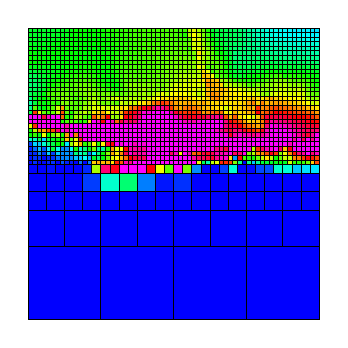
\begin{tikzpicture}[x={(\screenshotunitlength,0)},y={(0,\screenshotunitlength)}]
        \definecolor{fillcolor}{rgb}{0.000000,0.000000,1.000000}
\fill[fillcolor] (0.000000,0.000000) rectangle (0.250000,0.250000);
\definecolor{fillcolor}{rgb}{0.000000,0.000000,1.000000}
\fill[fillcolor] (0.250000,0.000000) rectangle (0.500000,0.250000);
\definecolor{fillcolor}{rgb}{0.000000,0.000000,1.000000}
\fill[fillcolor] (0.000000,0.250000) rectangle (0.125000,0.375000);
\definecolor{fillcolor}{rgb}{0.000000,0.000000,1.000000}
\fill[fillcolor] (0.125000,0.250000) rectangle (0.250000,0.375000);
\definecolor{fillcolor}{rgb}{0.000000,0.000000,1.000000}
\fill[fillcolor] (0.000000,0.375000) rectangle (0.062500,0.437500);
\definecolor{fillcolor}{rgb}{0.000000,0.000000,1.000000}
\fill[fillcolor] (0.062500,0.375000) rectangle (0.125000,0.437500);
\definecolor{fillcolor}{rgb}{0.000000,0.000000,1.000000}
\fill[fillcolor] (0.000000,0.437500) rectangle (0.062500,0.500000);
\definecolor{fillcolor}{rgb}{0.000000,0.000000,1.000000}
\fill[fillcolor] (0.062500,0.437500) rectangle (0.125000,0.500000);
\definecolor{fillcolor}{rgb}{0.000000,0.000000,1.000000}
\fill[fillcolor] (0.125000,0.375000) rectangle (0.187500,0.437500);
\definecolor{fillcolor}{rgb}{0.000000,0.000000,1.000000}
\fill[fillcolor] (0.187500,0.375000) rectangle (0.250000,0.437500);
\definecolor{fillcolor}{rgb}{0.000000,0.000000,1.000000}
\fill[fillcolor] (0.125000,0.437500) rectangle (0.187500,0.500000);
\definecolor{fillcolor}{rgb}{0.000000,0.234481,1.000000}
\fill[fillcolor] (0.187500,0.437500) rectangle (0.250000,0.500000);
\definecolor{fillcolor}{rgb}{0.000000,0.000000,1.000000}
\fill[fillcolor] (0.250000,0.250000) rectangle (0.375000,0.375000);
\definecolor{fillcolor}{rgb}{0.000000,0.000000,1.000000}
\fill[fillcolor] (0.375000,0.250000) rectangle (0.500000,0.375000);
\definecolor{fillcolor}{rgb}{0.000000,0.000000,1.000000}
\fill[fillcolor] (0.250000,0.375000) rectangle (0.312500,0.437500);
\definecolor{fillcolor}{rgb}{0.000000,0.000000,1.000000}
\fill[fillcolor] (0.312500,0.375000) rectangle (0.375000,0.437500);
\definecolor{fillcolor}{rgb}{0.000000,1.000000,0.803046}
\fill[fillcolor] (0.250000,0.437500) rectangle (0.312500,0.500000);
\definecolor{fillcolor}{rgb}{0.000000,1.000000,0.445087}
\fill[fillcolor] (0.312500,0.437500) rectangle (0.375000,0.500000);
\definecolor{fillcolor}{rgb}{0.000000,0.000000,1.000000}
\fill[fillcolor] (0.375000,0.375000) rectangle (0.437500,0.437500);
\definecolor{fillcolor}{rgb}{0.000000,0.000000,1.000000}
\fill[fillcolor] (0.437500,0.375000) rectangle (0.500000,0.437500);
\definecolor{fillcolor}{rgb}{0.000000,0.495433,1.000000}
\fill[fillcolor] (0.375000,0.437500) rectangle (0.437500,0.500000);
\definecolor{fillcolor}{rgb}{0.000000,0.082270,1.000000}
\fill[fillcolor] (0.437500,0.437500) rectangle (0.500000,0.500000);
\definecolor{fillcolor}{rgb}{0.000000,0.000000,1.000000}
\fill[fillcolor] (0.500000,0.000000) rectangle (0.750000,0.250000);
\definecolor{fillcolor}{rgb}{0.000000,0.000000,1.000000}
\fill[fillcolor] (0.750000,0.000000) rectangle (1.000000,0.250000);
\definecolor{fillcolor}{rgb}{0.000000,0.000000,1.000000}
\fill[fillcolor] (0.500000,0.250000) rectangle (0.625000,0.375000);
\definecolor{fillcolor}{rgb}{0.000000,0.000000,1.000000}
\fill[fillcolor] (0.625000,0.250000) rectangle (0.750000,0.375000);
\definecolor{fillcolor}{rgb}{0.000000,0.000000,1.000000}
\fill[fillcolor] (0.500000,0.375000) rectangle (0.562500,0.437500);
\definecolor{fillcolor}{rgb}{0.000000,0.000000,1.000000}
\fill[fillcolor] (0.562500,0.375000) rectangle (0.625000,0.437500);
\definecolor{fillcolor}{rgb}{0.000000,0.186708,1.000000}
\fill[fillcolor] (0.500000,0.437500) rectangle (0.562500,0.500000);
\definecolor{fillcolor}{rgb}{0.000000,0.000000,1.000000}
\fill[fillcolor] (0.562500,0.437500) rectangle (0.625000,0.500000);
\definecolor{fillcolor}{rgb}{0.000000,0.000000,1.000000}
\fill[fillcolor] (0.625000,0.375000) rectangle (0.687500,0.437500);
\definecolor{fillcolor}{rgb}{0.000000,0.000000,1.000000}
\fill[fillcolor] (0.687500,0.375000) rectangle (0.750000,0.437500);
\definecolor{fillcolor}{rgb}{0.000000,0.000000,1.000000}
\fill[fillcolor] (0.625000,0.437500) rectangle (0.687500,0.500000);
\definecolor{fillcolor}{rgb}{0.000000,0.000000,1.000000}
\fill[fillcolor] (0.687500,0.437500) rectangle (0.750000,0.500000);
\definecolor{fillcolor}{rgb}{0.000000,0.000000,1.000000}
\fill[fillcolor] (0.750000,0.250000) rectangle (0.875000,0.375000);
\definecolor{fillcolor}{rgb}{0.000000,0.000011,1.000000}
\fill[fillcolor] (0.875000,0.250000) rectangle (1.000000,0.375000);
\definecolor{fillcolor}{rgb}{0.000000,0.000000,1.000000}
\fill[fillcolor] (0.750000,0.375000) rectangle (0.812500,0.437500);
\definecolor{fillcolor}{rgb}{0.000000,0.000000,1.000000}
\fill[fillcolor] (0.812500,0.375000) rectangle (0.875000,0.437500);
\definecolor{fillcolor}{rgb}{0.000000,0.000118,1.000000}
\fill[fillcolor] (0.750000,0.437500) rectangle (0.812500,0.500000);
\definecolor{fillcolor}{rgb}{0.000000,0.000000,1.000000}
\fill[fillcolor] (0.812500,0.437500) rectangle (0.875000,0.500000);
\definecolor{fillcolor}{rgb}{0.000000,0.000000,1.000000}
\fill[fillcolor] (0.875000,0.375000) rectangle (0.937500,0.437500);
\definecolor{fillcolor}{rgb}{0.000000,0.004592,1.000000}
\fill[fillcolor] (0.937500,0.375000) rectangle (1.000000,0.437500);
\definecolor{fillcolor}{rgb}{0.000000,0.000000,1.000000}
\fill[fillcolor] (0.875000,0.437500) rectangle (0.937500,0.500000);
\definecolor{fillcolor}{rgb}{0.000000,0.000629,1.000000}
\fill[fillcolor] (0.937500,0.437500) rectangle (1.000000,0.500000);
\definecolor{fillcolor}{rgb}{0.000000,0.012151,1.000000}
\fill[fillcolor] (0.000000,0.500000) rectangle (0.031250,0.531250);
\definecolor{fillcolor}{rgb}{0.000000,0.000000,1.000000}
\fill[fillcolor] (0.031250,0.500000) rectangle (0.062500,0.531250);
\definecolor{fillcolor}{rgb}{0.000000,0.000834,1.000000}
\fill[fillcolor] (0.000000,0.531250) rectangle (0.015625,0.546875);
\definecolor{fillcolor}{rgb}{0.000000,0.170846,1.000000}
\fill[fillcolor] (0.015625,0.531250) rectangle (0.031250,0.546875);
\definecolor{fillcolor}{rgb}{0.000000,0.061633,1.000000}
\fill[fillcolor] (0.000000,0.546875) rectangle (0.015625,0.562500);
\definecolor{fillcolor}{rgb}{0.000000,0.179122,1.000000}
\fill[fillcolor] (0.015625,0.546875) rectangle (0.031250,0.562500);
\definecolor{fillcolor}{rgb}{0.000000,0.000000,1.000000}
\fill[fillcolor] (0.031250,0.531250) rectangle (0.046875,0.546875);
\definecolor{fillcolor}{rgb}{0.000000,0.024691,1.000000}
\fill[fillcolor] (0.046875,0.531250) rectangle (0.062500,0.546875);
\definecolor{fillcolor}{rgb}{0.000000,0.204253,1.000000}
\fill[fillcolor] (0.031250,0.546875) rectangle (0.046875,0.562500);
\definecolor{fillcolor}{rgb}{0.000000,0.029279,1.000000}
\fill[fillcolor] (0.046875,0.546875) rectangle (0.062500,0.562500);
\definecolor{fillcolor}{rgb}{0.000000,0.055652,1.000000}
\fill[fillcolor] (0.062500,0.500000) rectangle (0.093750,0.531250);
\definecolor{fillcolor}{rgb}{0.000000,0.000002,1.000000}
\fill[fillcolor] (0.093750,0.500000) rectangle (0.125000,0.531250);
\definecolor{fillcolor}{rgb}{0.000000,0.136753,1.000000}
\fill[fillcolor] (0.062500,0.531250) rectangle (0.078125,0.546875);
\definecolor{fillcolor}{rgb}{0.000000,0.192679,1.000000}
\fill[fillcolor] (0.078125,0.531250) rectangle (0.093750,0.546875);
\definecolor{fillcolor}{rgb}{0.000000,0.136615,1.000000}
\fill[fillcolor] (0.062500,0.546875) rectangle (0.078125,0.562500);
\definecolor{fillcolor}{rgb}{0.000000,0.193205,1.000000}
\fill[fillcolor] (0.078125,0.546875) rectangle (0.093750,0.562500);
\definecolor{fillcolor}{rgb}{0.000000,0.009683,1.000000}
\fill[fillcolor] (0.093750,0.531250) rectangle (0.109375,0.546875);
\definecolor{fillcolor}{rgb}{0.000000,0.338197,1.000000}
\fill[fillcolor] (0.109375,0.531250) rectangle (0.125000,0.546875);
\definecolor{fillcolor}{rgb}{0.000000,0.445310,1.000000}
\fill[fillcolor] (0.093750,0.546875) rectangle (0.109375,0.562500);
\definecolor{fillcolor}{rgb}{0.000000,0.511630,1.000000}
\fill[fillcolor] (0.109375,0.546875) rectangle (0.125000,0.562500);
\definecolor{fillcolor}{rgb}{0.000000,0.131469,1.000000}
\fill[fillcolor] (0.000000,0.562500) rectangle (0.015625,0.578125);
\definecolor{fillcolor}{rgb}{0.000000,0.166465,1.000000}
\fill[fillcolor] (0.015625,0.562500) rectangle (0.031250,0.578125);
\definecolor{fillcolor}{rgb}{0.000000,0.130343,1.000000}
\fill[fillcolor] (0.000000,0.578125) rectangle (0.015625,0.593750);
\definecolor{fillcolor}{rgb}{0.000000,0.399755,1.000000}
\fill[fillcolor] (0.015625,0.578125) rectangle (0.031250,0.593750);
\definecolor{fillcolor}{rgb}{0.000000,0.522596,1.000000}
\fill[fillcolor] (0.031250,0.562500) rectangle (0.046875,0.578125);
\definecolor{fillcolor}{rgb}{0.000000,0.219845,1.000000}
\fill[fillcolor] (0.046875,0.562500) rectangle (0.062500,0.578125);
\definecolor{fillcolor}{rgb}{0.000000,0.747798,1.000000}
\fill[fillcolor] (0.031250,0.578125) rectangle (0.046875,0.593750);
\definecolor{fillcolor}{rgb}{0.000000,0.357662,1.000000}
\fill[fillcolor] (0.046875,0.578125) rectangle (0.062500,0.593750);
\definecolor{fillcolor}{rgb}{0.000000,0.250613,1.000000}
\fill[fillcolor] (0.000000,0.593750) rectangle (0.015625,0.609375);
\definecolor{fillcolor}{rgb}{0.000000,0.836054,1.000000}
\fill[fillcolor] (0.015625,0.593750) rectangle (0.031250,0.609375);
\definecolor{fillcolor}{rgb}{0.000000,1.000000,0.756029}
\fill[fillcolor] (0.000000,0.609375) rectangle (0.015625,0.625000);
\definecolor{fillcolor}{rgb}{0.000000,1.000000,0.739321}
\fill[fillcolor] (0.015625,0.609375) rectangle (0.031250,0.625000);
\definecolor{fillcolor}{rgb}{0.000000,0.775578,1.000000}
\fill[fillcolor] (0.031250,0.593750) rectangle (0.046875,0.609375);
\definecolor{fillcolor}{rgb}{0.000000,1.000000,0.813044}
\fill[fillcolor] (0.046875,0.593750) rectangle (0.062500,0.609375);
\definecolor{fillcolor}{rgb}{0.000000,1.000000,0.333453}
\fill[fillcolor] (0.031250,0.609375) rectangle (0.046875,0.625000);
\definecolor{fillcolor}{rgb}{0.000000,0.846418,1.000000}
\fill[fillcolor] (0.046875,0.609375) rectangle (0.062500,0.625000);
\definecolor{fillcolor}{rgb}{0.000000,0.803838,1.000000}
\fill[fillcolor] (0.062500,0.562500) rectangle (0.078125,0.578125);
\definecolor{fillcolor}{rgb}{0.000000,0.263966,1.000000}
\fill[fillcolor] (0.078125,0.562500) rectangle (0.093750,0.578125);
\definecolor{fillcolor}{rgb}{0.000000,0.923191,1.000000}
\fill[fillcolor] (0.062500,0.578125) rectangle (0.078125,0.593750);
\definecolor{fillcolor}{rgb}{0.000000,1.000000,0.237713}
\fill[fillcolor] (0.078125,0.578125) rectangle (0.093750,0.593750);
\definecolor{fillcolor}{rgb}{0.000000,0.813373,1.000000}
\fill[fillcolor] (0.093750,0.562500) rectangle (0.109375,0.578125);
\definecolor{fillcolor}{rgb}{0.000000,0.553666,1.000000}
\fill[fillcolor] (0.109375,0.562500) rectangle (0.125000,0.578125);
\definecolor{fillcolor}{rgb}{0.000000,1.000000,0.880030}
\fill[fillcolor] (0.093750,0.578125) rectangle (0.109375,0.593750);
\definecolor{fillcolor}{rgb}{0.000000,0.548559,1.000000}
\fill[fillcolor] (0.109375,0.578125) rectangle (0.125000,0.593750);
\definecolor{fillcolor}{rgb}{0.000000,1.000000,0.565254}
\fill[fillcolor] (0.062500,0.593750) rectangle (0.078125,0.609375);
\definecolor{fillcolor}{rgb}{0.000000,1.000000,0.282635}
\fill[fillcolor] (0.078125,0.593750) rectangle (0.093750,0.609375);
\definecolor{fillcolor}{rgb}{0.000000,1.000000,0.265719}
\fill[fillcolor] (0.062500,0.609375) rectangle (0.078125,0.625000);
\definecolor{fillcolor}{rgb}{0.000000,1.000000,0.130271}
\fill[fillcolor] (0.078125,0.609375) rectangle (0.093750,0.625000);
\definecolor{fillcolor}{rgb}{0.000000,1.000000,0.029535}
\fill[fillcolor] (0.093750,0.593750) rectangle (0.109375,0.609375);
\definecolor{fillcolor}{rgb}{0.000000,1.000000,0.050246}
\fill[fillcolor] (0.109375,0.593750) rectangle (0.125000,0.609375);
\definecolor{fillcolor}{rgb}{0.007391,1.000000,0.000000}
\fill[fillcolor] (0.093750,0.609375) rectangle (0.109375,0.625000);
\definecolor{fillcolor}{rgb}{0.116307,1.000000,0.000000}
\fill[fillcolor] (0.109375,0.609375) rectangle (0.125000,0.625000);
\definecolor{fillcolor}{rgb}{0.000000,0.000007,1.000000}
\fill[fillcolor] (0.125000,0.500000) rectangle (0.156250,0.531250);
\definecolor{fillcolor}{rgb}{0.000000,0.005010,1.000000}
\fill[fillcolor] (0.156250,0.500000) rectangle (0.187500,0.531250);
\definecolor{fillcolor}{rgb}{0.000000,0.133086,1.000000}
\fill[fillcolor] (0.125000,0.531250) rectangle (0.140625,0.546875);
\definecolor{fillcolor}{rgb}{0.000000,0.093590,1.000000}
\fill[fillcolor] (0.140625,0.531250) rectangle (0.156250,0.546875);
\definecolor{fillcolor}{rgb}{0.000000,0.544232,1.000000}
\fill[fillcolor] (0.125000,0.546875) rectangle (0.140625,0.562500);
\definecolor{fillcolor}{rgb}{0.000000,0.541664,1.000000}
\fill[fillcolor] (0.140625,0.546875) rectangle (0.156250,0.562500);
\definecolor{fillcolor}{rgb}{0.000000,0.000015,1.000000}
\fill[fillcolor] (0.156250,0.531250) rectangle (0.171875,0.546875);
\definecolor{fillcolor}{rgb}{0.000000,0.456955,1.000000}
\fill[fillcolor] (0.171875,0.531250) rectangle (0.187500,0.546875);
\definecolor{fillcolor}{rgb}{0.000000,0.785920,1.000000}
\fill[fillcolor] (0.156250,0.546875) rectangle (0.171875,0.562500);
\definecolor{fillcolor}{rgb}{0.000000,0.786305,1.000000}
\fill[fillcolor] (0.171875,0.546875) rectangle (0.187500,0.562500);
\definecolor{fillcolor}{rgb}{0.000000,0.151960,1.000000}
\fill[fillcolor] (0.187500,0.500000) rectangle (0.218750,0.531250);
\definecolor{fillcolor}{rgb}{0.652598,1.000000,0.000000}
\fill[fillcolor] (0.218750,0.500000) rectangle (0.250000,0.531250);
\definecolor{fillcolor}{rgb}{0.000000,0.013310,1.000000}
\fill[fillcolor] (0.187500,0.531250) rectangle (0.203125,0.546875);
\definecolor{fillcolor}{rgb}{0.000000,0.485549,1.000000}
\fill[fillcolor] (0.203125,0.531250) rectangle (0.218750,0.546875);
\definecolor{fillcolor}{rgb}{0.000000,1.000000,0.958531}
\fill[fillcolor] (0.187500,0.546875) rectangle (0.203125,0.562500);
\definecolor{fillcolor}{rgb}{0.000000,0.698282,1.000000}
\fill[fillcolor] (0.203125,0.546875) rectangle (0.218750,0.562500);
\definecolor{fillcolor}{rgb}{1.000000,0.808681,0.000000}
\fill[fillcolor] (0.218750,0.531250) rectangle (0.234375,0.546875);
\definecolor{fillcolor}{rgb}{1.000000,0.673819,0.000000}
\fill[fillcolor] (0.234375,0.531250) rectangle (0.250000,0.546875);
\definecolor{fillcolor}{rgb}{0.000000,1.000000,0.142259}
\fill[fillcolor] (0.218750,0.546875) rectangle (0.234375,0.562500);
\definecolor{fillcolor}{rgb}{0.000000,1.000000,0.435314}
\fill[fillcolor] (0.234375,0.546875) rectangle (0.250000,0.562500);
\definecolor{fillcolor}{rgb}{0.000000,0.578713,1.000000}
\fill[fillcolor] (0.125000,0.562500) rectangle (0.140625,0.578125);
\definecolor{fillcolor}{rgb}{0.000000,0.607908,1.000000}
\fill[fillcolor] (0.140625,0.562500) rectangle (0.156250,0.578125);
\definecolor{fillcolor}{rgb}{0.000000,0.548375,1.000000}
\fill[fillcolor] (0.125000,0.578125) rectangle (0.140625,0.593750);
\definecolor{fillcolor}{rgb}{0.000000,1.000000,0.975121}
\fill[fillcolor] (0.140625,0.578125) rectangle (0.156250,0.593750);
\definecolor{fillcolor}{rgb}{0.000000,1.000000,0.474886}
\fill[fillcolor] (0.156250,0.562500) rectangle (0.171875,0.578125);
\definecolor{fillcolor}{rgb}{0.000000,1.000000,0.754924}
\fill[fillcolor] (0.171875,0.562500) rectangle (0.187500,0.578125);
\definecolor{fillcolor}{rgb}{0.064874,1.000000,0.000000}
\fill[fillcolor] (0.156250,0.578125) rectangle (0.171875,0.593750);
\definecolor{fillcolor}{rgb}{0.000000,1.000000,0.796766}
\fill[fillcolor] (0.171875,0.578125) rectangle (0.187500,0.593750);
\definecolor{fillcolor}{rgb}{0.000000,0.925277,1.000000}
\fill[fillcolor] (0.125000,0.593750) rectangle (0.140625,0.609375);
\definecolor{fillcolor}{rgb}{0.612411,1.000000,0.000000}
\fill[fillcolor] (0.140625,0.593750) rectangle (0.156250,0.609375);
\definecolor{fillcolor}{rgb}{1.000000,0.776211,0.000000}
\fill[fillcolor] (0.125000,0.609375) rectangle (0.140625,0.625000);
\definecolor{fillcolor}{rgb}{0.444433,1.000000,0.000000}
\fill[fillcolor] (0.140625,0.609375) rectangle (0.156250,0.625000);
\definecolor{fillcolor}{rgb}{0.976308,1.000000,0.000000}
\fill[fillcolor] (0.156250,0.593750) rectangle (0.171875,0.609375);
\definecolor{fillcolor}{rgb}{1.000000,0.742822,0.000000}
\fill[fillcolor] (0.171875,0.593750) rectangle (0.187500,0.609375);
\definecolor{fillcolor}{rgb}{0.919528,1.000000,0.000000}
\fill[fillcolor] (0.156250,0.609375) rectangle (0.171875,0.625000);
\definecolor{fillcolor}{rgb}{1.000000,0.098519,0.000000}
\fill[fillcolor] (0.171875,0.609375) rectangle (0.187500,0.625000);
\definecolor{fillcolor}{rgb}{0.000000,1.000000,0.526414}
\fill[fillcolor] (0.187500,0.562500) rectangle (0.203125,0.578125);
\definecolor{fillcolor}{rgb}{0.000000,0.505174,1.000000}
\fill[fillcolor] (0.203125,0.562500) rectangle (0.218750,0.578125);
\definecolor{fillcolor}{rgb}{0.000000,1.000000,0.469478}
\fill[fillcolor] (0.187500,0.578125) rectangle (0.203125,0.593750);
\definecolor{fillcolor}{rgb}{0.000000,1.000000,0.099698}
\fill[fillcolor] (0.203125,0.578125) rectangle (0.218750,0.593750);
\definecolor{fillcolor}{rgb}{0.000000,1.000000,0.955032}
\fill[fillcolor] (0.218750,0.562500) rectangle (0.234375,0.578125);
\definecolor{fillcolor}{rgb}{0.000000,1.000000,0.463396}
\fill[fillcolor] (0.234375,0.562500) rectangle (0.250000,0.578125);
\definecolor{fillcolor}{rgb}{0.448554,1.000000,0.000000}
\fill[fillcolor] (0.218750,0.578125) rectangle (0.234375,0.593750);
\definecolor{fillcolor}{rgb}{0.000000,1.000000,0.557936}
\fill[fillcolor] (0.234375,0.578125) rectangle (0.250000,0.593750);
\definecolor{fillcolor}{rgb}{0.165269,1.000000,0.000000}
\fill[fillcolor] (0.187500,0.593750) rectangle (0.203125,0.609375);
\definecolor{fillcolor}{rgb}{0.339977,1.000000,0.000000}
\fill[fillcolor] (0.203125,0.593750) rectangle (0.218750,0.609375);
\definecolor{fillcolor}{rgb}{1.000000,0.000000,1.000000}
\fill[fillcolor] (0.187500,0.609375) rectangle (0.203125,0.625000);
\definecolor{fillcolor}{rgb}{1.000000,0.000000,1.000000}
\fill[fillcolor] (0.203125,0.609375) rectangle (0.218750,0.625000);
\definecolor{fillcolor}{rgb}{0.987884,1.000000,0.000000}
\fill[fillcolor] (0.218750,0.593750) rectangle (0.234375,0.609375);
\definecolor{fillcolor}{rgb}{0.178237,1.000000,0.000000}
\fill[fillcolor] (0.234375,0.593750) rectangle (0.250000,0.609375);
\definecolor{fillcolor}{rgb}{1.000000,0.000000,1.000000}
\fill[fillcolor] (0.218750,0.609375) rectangle (0.234375,0.625000);
\definecolor{fillcolor}{rgb}{1.000000,0.000000,1.000000}
\fill[fillcolor] (0.234375,0.609375) rectangle (0.250000,0.625000);
\definecolor{fillcolor}{rgb}{0.012100,1.000000,0.000000}
\fill[fillcolor] (0.000000,0.625000) rectangle (0.015625,0.640625);
\definecolor{fillcolor}{rgb}{0.187890,1.000000,0.000000}
\fill[fillcolor] (0.015625,0.625000) rectangle (0.031250,0.640625);
\definecolor{fillcolor}{rgb}{0.000000,1.000000,0.035556}
\fill[fillcolor] (0.000000,0.640625) rectangle (0.015625,0.656250);
\definecolor{fillcolor}{rgb}{0.709998,1.000000,0.000000}
\fill[fillcolor] (0.015625,0.640625) rectangle (0.031250,0.656250);
\definecolor{fillcolor}{rgb}{0.000000,1.000000,0.089384}
\fill[fillcolor] (0.031250,0.625000) rectangle (0.046875,0.640625);
\definecolor{fillcolor}{rgb}{0.936703,1.000000,0.000000}
\fill[fillcolor] (0.046875,0.625000) rectangle (0.062500,0.640625);
\definecolor{fillcolor}{rgb}{1.000000,0.609751,0.000000}
\fill[fillcolor] (0.031250,0.640625) rectangle (0.046875,0.656250);
\definecolor{fillcolor}{rgb}{1.000000,0.669311,0.000000}
\fill[fillcolor] (0.046875,0.640625) rectangle (0.062500,0.656250);
\definecolor{fillcolor}{rgb}{0.869229,1.000000,0.000000}
\fill[fillcolor] (0.000000,0.656250) rectangle (0.015625,0.671875);
\definecolor{fillcolor}{rgb}{1.000000,0.168789,0.000000}
\fill[fillcolor] (0.015625,0.656250) rectangle (0.031250,0.671875);
\definecolor{fillcolor}{rgb}{1.000000,0.000000,1.000000}
\fill[fillcolor] (0.000000,0.671875) rectangle (0.015625,0.687500);
\definecolor{fillcolor}{rgb}{1.000000,0.000000,1.000000}
\fill[fillcolor] (0.015625,0.671875) rectangle (0.031250,0.687500);
\definecolor{fillcolor}{rgb}{1.000000,0.000000,1.000000}
\fill[fillcolor] (0.031250,0.656250) rectangle (0.046875,0.671875);
\definecolor{fillcolor}{rgb}{1.000000,0.000000,1.000000}
\fill[fillcolor] (0.046875,0.656250) rectangle (0.062500,0.671875);
\definecolor{fillcolor}{rgb}{1.000000,0.000000,0.898023}
\fill[fillcolor] (0.031250,0.671875) rectangle (0.046875,0.687500);
\definecolor{fillcolor}{rgb}{1.000000,0.000000,1.000000}
\fill[fillcolor] (0.046875,0.671875) rectangle (0.062500,0.687500);
\definecolor{fillcolor}{rgb}{0.000000,1.000000,0.001628}
\fill[fillcolor] (0.062500,0.625000) rectangle (0.078125,0.640625);
\definecolor{fillcolor}{rgb}{0.393536,1.000000,0.000000}
\fill[fillcolor] (0.078125,0.625000) rectangle (0.093750,0.640625);
\definecolor{fillcolor}{rgb}{1.000000,0.299394,0.000000}
\fill[fillcolor] (0.062500,0.640625) rectangle (0.078125,0.656250);
\definecolor{fillcolor}{rgb}{1.000000,0.298561,0.000000}
\fill[fillcolor] (0.078125,0.640625) rectangle (0.093750,0.656250);
\definecolor{fillcolor}{rgb}{0.646447,1.000000,0.000000}
\fill[fillcolor] (0.093750,0.625000) rectangle (0.109375,0.640625);
\definecolor{fillcolor}{rgb}{0.086842,1.000000,0.000000}
\fill[fillcolor] (0.109375,0.625000) rectangle (0.125000,0.640625);
\definecolor{fillcolor}{rgb}{1.000000,0.000000,0.423448}
\fill[fillcolor] (0.093750,0.640625) rectangle (0.109375,0.656250);
\definecolor{fillcolor}{rgb}{1.000000,0.000000,1.000000}
\fill[fillcolor] (0.109375,0.640625) rectangle (0.125000,0.656250);
\definecolor{fillcolor}{rgb}{1.000000,0.000000,1.000000}
\fill[fillcolor] (0.062500,0.656250) rectangle (0.078125,0.671875);
\definecolor{fillcolor}{rgb}{1.000000,0.000000,1.000000}
\fill[fillcolor] (0.078125,0.656250) rectangle (0.093750,0.671875);
\definecolor{fillcolor}{rgb}{1.000000,0.000000,1.000000}
\fill[fillcolor] (0.062500,0.671875) rectangle (0.078125,0.687500);
\definecolor{fillcolor}{rgb}{1.000000,0.000000,1.000000}
\fill[fillcolor] (0.078125,0.671875) rectangle (0.093750,0.687500);
\definecolor{fillcolor}{rgb}{1.000000,0.000000,1.000000}
\fill[fillcolor] (0.093750,0.656250) rectangle (0.109375,0.671875);
\definecolor{fillcolor}{rgb}{1.000000,0.000000,1.000000}
\fill[fillcolor] (0.109375,0.656250) rectangle (0.125000,0.671875);
\definecolor{fillcolor}{rgb}{1.000000,0.000000,1.000000}
\fill[fillcolor] (0.093750,0.671875) rectangle (0.109375,0.687500);
\definecolor{fillcolor}{rgb}{0.115830,1.000000,0.000000}
\fill[fillcolor] (0.109375,0.671875) rectangle (0.125000,0.687500);
\definecolor{fillcolor}{rgb}{1.000000,0.000000,1.000000}
\fill[fillcolor] (0.000000,0.687500) rectangle (0.015625,0.703125);
\definecolor{fillcolor}{rgb}{1.000000,0.000000,1.000000}
\fill[fillcolor] (0.015625,0.687500) rectangle (0.031250,0.703125);
\definecolor{fillcolor}{rgb}{0.000000,1.000000,0.299999}
\fill[fillcolor] (0.000000,0.703125) rectangle (0.015625,0.718750);
\definecolor{fillcolor}{rgb}{1.000000,0.212042,0.000000}
\fill[fillcolor] (0.015625,0.703125) rectangle (0.031250,0.718750);
\definecolor{fillcolor}{rgb}{1.000000,0.000000,1.000000}
\fill[fillcolor] (0.031250,0.687500) rectangle (0.046875,0.703125);
\definecolor{fillcolor}{rgb}{1.000000,0.000000,0.233516}
\fill[fillcolor] (0.046875,0.687500) rectangle (0.062500,0.703125);
\definecolor{fillcolor}{rgb}{0.982906,1.000000,0.000000}
\fill[fillcolor] (0.031250,0.703125) rectangle (0.046875,0.718750);
\definecolor{fillcolor}{rgb}{0.388906,1.000000,0.000000}
\fill[fillcolor] (0.046875,0.703125) rectangle (0.062500,0.718750);
\definecolor{fillcolor}{rgb}{0.000000,1.000000,0.563762}
\fill[fillcolor] (0.000000,0.718750) rectangle (0.015625,0.734375);
\definecolor{fillcolor}{rgb}{0.339957,1.000000,0.000000}
\fill[fillcolor] (0.015625,0.718750) rectangle (0.031250,0.734375);
\definecolor{fillcolor}{rgb}{0.000000,1.000000,0.640882}
\fill[fillcolor] (0.000000,0.734375) rectangle (0.015625,0.750000);
\definecolor{fillcolor}{rgb}{0.000000,1.000000,0.223876}
\fill[fillcolor] (0.015625,0.734375) rectangle (0.031250,0.750000);
\definecolor{fillcolor}{rgb}{0.000000,1.000000,0.150201}
\fill[fillcolor] (0.031250,0.718750) rectangle (0.046875,0.734375);
\definecolor{fillcolor}{rgb}{0.000000,1.000000,0.018630}
\fill[fillcolor] (0.046875,0.718750) rectangle (0.062500,0.734375);
\definecolor{fillcolor}{rgb}{0.049798,1.000000,0.000000}
\fill[fillcolor] (0.031250,0.734375) rectangle (0.046875,0.750000);
\definecolor{fillcolor}{rgb}{0.000000,1.000000,0.066186}
\fill[fillcolor] (0.046875,0.734375) rectangle (0.062500,0.750000);
\definecolor{fillcolor}{rgb}{1.000000,0.000000,0.775619}
\fill[fillcolor] (0.062500,0.687500) rectangle (0.078125,0.703125);
\definecolor{fillcolor}{rgb}{1.000000,0.000000,1.000000}
\fill[fillcolor] (0.078125,0.687500) rectangle (0.093750,0.703125);
\definecolor{fillcolor}{rgb}{0.250432,1.000000,0.000000}
\fill[fillcolor] (0.062500,0.703125) rectangle (0.078125,0.718750);
\definecolor{fillcolor}{rgb}{0.399841,1.000000,0.000000}
\fill[fillcolor] (0.078125,0.703125) rectangle (0.093750,0.718750);
\definecolor{fillcolor}{rgb}{1.000000,0.000000,1.000000}
\fill[fillcolor] (0.093750,0.687500) rectangle (0.109375,0.703125);
\definecolor{fillcolor}{rgb}{1.000000,0.400280,0.000000}
\fill[fillcolor] (0.109375,0.687500) rectangle (0.125000,0.703125);
\definecolor{fillcolor}{rgb}{0.795429,1.000000,0.000000}
\fill[fillcolor] (0.093750,0.703125) rectangle (0.109375,0.718750);
\definecolor{fillcolor}{rgb}{1.000000,0.314583,0.000000}
\fill[fillcolor] (0.109375,0.703125) rectangle (0.125000,0.718750);
\definecolor{fillcolor}{rgb}{0.161778,1.000000,0.000000}
\fill[fillcolor] (0.062500,0.718750) rectangle (0.078125,0.734375);
\definecolor{fillcolor}{rgb}{0.357716,1.000000,0.000000}
\fill[fillcolor] (0.078125,0.718750) rectangle (0.093750,0.734375);
\definecolor{fillcolor}{rgb}{0.046961,1.000000,0.000000}
\fill[fillcolor] (0.062500,0.734375) rectangle (0.078125,0.750000);
\definecolor{fillcolor}{rgb}{0.207804,1.000000,0.000000}
\fill[fillcolor] (0.078125,0.734375) rectangle (0.093750,0.750000);
\definecolor{fillcolor}{rgb}{0.755447,1.000000,0.000000}
\fill[fillcolor] (0.093750,0.718750) rectangle (0.109375,0.734375);
\definecolor{fillcolor}{rgb}{1.000000,0.632148,0.000000}
\fill[fillcolor] (0.109375,0.718750) rectangle (0.125000,0.734375);
\definecolor{fillcolor}{rgb}{0.178053,1.000000,0.000000}
\fill[fillcolor] (0.093750,0.734375) rectangle (0.109375,0.750000);
\definecolor{fillcolor}{rgb}{0.506448,1.000000,0.000000}
\fill[fillcolor] (0.109375,0.734375) rectangle (0.125000,0.750000);
\definecolor{fillcolor}{rgb}{1.000000,0.631000,0.000000}
\fill[fillcolor] (0.125000,0.625000) rectangle (0.140625,0.640625);
\definecolor{fillcolor}{rgb}{1.000000,0.000000,1.000000}
\fill[fillcolor] (0.140625,0.625000) rectangle (0.156250,0.640625);
\definecolor{fillcolor}{rgb}{1.000000,0.000000,0.687368}
\fill[fillcolor] (0.125000,0.640625) rectangle (0.140625,0.656250);
\definecolor{fillcolor}{rgb}{1.000000,0.000000,1.000000}
\fill[fillcolor] (0.140625,0.640625) rectangle (0.156250,0.656250);
\definecolor{fillcolor}{rgb}{1.000000,0.493063,0.000000}
\fill[fillcolor] (0.156250,0.625000) rectangle (0.171875,0.640625);
\definecolor{fillcolor}{rgb}{1.000000,0.000000,0.874596}
\fill[fillcolor] (0.171875,0.625000) rectangle (0.187500,0.640625);
\definecolor{fillcolor}{rgb}{1.000000,0.000000,1.000000}
\fill[fillcolor] (0.156250,0.640625) rectangle (0.171875,0.656250);
\definecolor{fillcolor}{rgb}{1.000000,0.000000,1.000000}
\fill[fillcolor] (0.171875,0.640625) rectangle (0.187500,0.656250);
\definecolor{fillcolor}{rgb}{1.000000,0.000000,0.684348}
\fill[fillcolor] (0.125000,0.656250) rectangle (0.140625,0.671875);
\definecolor{fillcolor}{rgb}{1.000000,0.000000,1.000000}
\fill[fillcolor] (0.140625,0.656250) rectangle (0.156250,0.671875);
\definecolor{fillcolor}{rgb}{0.291700,1.000000,0.000000}
\fill[fillcolor] (0.125000,0.671875) rectangle (0.140625,0.687500);
\definecolor{fillcolor}{rgb}{0.315508,1.000000,0.000000}
\fill[fillcolor] (0.140625,0.671875) rectangle (0.156250,0.687500);
\definecolor{fillcolor}{rgb}{1.000000,0.000000,1.000000}
\fill[fillcolor] (0.156250,0.656250) rectangle (0.171875,0.671875);
\definecolor{fillcolor}{rgb}{1.000000,0.000000,1.000000}
\fill[fillcolor] (0.171875,0.656250) rectangle (0.187500,0.671875);
\definecolor{fillcolor}{rgb}{0.284626,1.000000,0.000000}
\fill[fillcolor] (0.156250,0.671875) rectangle (0.171875,0.687500);
\definecolor{fillcolor}{rgb}{0.150944,1.000000,0.000000}
\fill[fillcolor] (0.171875,0.671875) rectangle (0.187500,0.687500);
\definecolor{fillcolor}{rgb}{1.000000,0.000000,1.000000}
\fill[fillcolor] (0.187500,0.625000) rectangle (0.203125,0.640625);
\definecolor{fillcolor}{rgb}{1.000000,0.000000,1.000000}
\fill[fillcolor] (0.203125,0.625000) rectangle (0.218750,0.640625);
\definecolor{fillcolor}{rgb}{1.000000,0.000000,1.000000}
\fill[fillcolor] (0.187500,0.640625) rectangle (0.203125,0.656250);
\definecolor{fillcolor}{rgb}{1.000000,0.000000,1.000000}
\fill[fillcolor] (0.203125,0.640625) rectangle (0.218750,0.656250);
\definecolor{fillcolor}{rgb}{1.000000,0.000000,1.000000}
\fill[fillcolor] (0.218750,0.625000) rectangle (0.234375,0.640625);
\definecolor{fillcolor}{rgb}{1.000000,0.000000,1.000000}
\fill[fillcolor] (0.234375,0.625000) rectangle (0.250000,0.640625);
\definecolor{fillcolor}{rgb}{1.000000,0.000000,1.000000}
\fill[fillcolor] (0.218750,0.640625) rectangle (0.234375,0.656250);
\definecolor{fillcolor}{rgb}{1.000000,0.000000,1.000000}
\fill[fillcolor] (0.234375,0.640625) rectangle (0.250000,0.656250);
\definecolor{fillcolor}{rgb}{1.000000,0.000000,1.000000}
\fill[fillcolor] (0.187500,0.656250) rectangle (0.203125,0.671875);
\definecolor{fillcolor}{rgb}{1.000000,0.000000,1.000000}
\fill[fillcolor] (0.203125,0.656250) rectangle (0.218750,0.671875);
\definecolor{fillcolor}{rgb}{0.183165,1.000000,0.000000}
\fill[fillcolor] (0.187500,0.671875) rectangle (0.203125,0.687500);
\definecolor{fillcolor}{rgb}{1.000000,0.910945,0.000000}
\fill[fillcolor] (0.203125,0.671875) rectangle (0.218750,0.687500);
\definecolor{fillcolor}{rgb}{1.000000,0.000000,1.000000}
\fill[fillcolor] (0.218750,0.656250) rectangle (0.234375,0.671875);
\definecolor{fillcolor}{rgb}{1.000000,0.000000,1.000000}
\fill[fillcolor] (0.234375,0.656250) rectangle (0.250000,0.671875);
\definecolor{fillcolor}{rgb}{1.000000,0.000000,1.000000}
\fill[fillcolor] (0.218750,0.671875) rectangle (0.234375,0.687500);
\definecolor{fillcolor}{rgb}{1.000000,0.000000,0.841106}
\fill[fillcolor] (0.234375,0.671875) rectangle (0.250000,0.687500);
\definecolor{fillcolor}{rgb}{0.129412,1.000000,0.000000}
\fill[fillcolor] (0.125000,0.687500) rectangle (0.140625,0.703125);
\definecolor{fillcolor}{rgb}{0.173422,1.000000,0.000000}
\fill[fillcolor] (0.140625,0.687500) rectangle (0.156250,0.703125);
\definecolor{fillcolor}{rgb}{0.379507,1.000000,0.000000}
\fill[fillcolor] (0.125000,0.703125) rectangle (0.140625,0.718750);
\definecolor{fillcolor}{rgb}{0.113128,1.000000,0.000000}
\fill[fillcolor] (0.140625,0.703125) rectangle (0.156250,0.718750);
\definecolor{fillcolor}{rgb}{0.602039,1.000000,0.000000}
\fill[fillcolor] (0.156250,0.687500) rectangle (0.171875,0.703125);
\definecolor{fillcolor}{rgb}{0.621226,1.000000,0.000000}
\fill[fillcolor] (0.171875,0.687500) rectangle (0.187500,0.703125);
\definecolor{fillcolor}{rgb}{0.492286,1.000000,0.000000}
\fill[fillcolor] (0.156250,0.703125) rectangle (0.171875,0.718750);
\definecolor{fillcolor}{rgb}{0.611139,1.000000,0.000000}
\fill[fillcolor] (0.171875,0.703125) rectangle (0.187500,0.718750);
\definecolor{fillcolor}{rgb}{0.395118,1.000000,0.000000}
\fill[fillcolor] (0.125000,0.718750) rectangle (0.140625,0.734375);
\definecolor{fillcolor}{rgb}{0.333508,1.000000,0.000000}
\fill[fillcolor] (0.140625,0.718750) rectangle (0.156250,0.734375);
\definecolor{fillcolor}{rgb}{0.478444,1.000000,0.000000}
\fill[fillcolor] (0.125000,0.734375) rectangle (0.140625,0.750000);
\definecolor{fillcolor}{rgb}{0.359836,1.000000,0.000000}
\fill[fillcolor] (0.140625,0.734375) rectangle (0.156250,0.750000);
\definecolor{fillcolor}{rgb}{0.360153,1.000000,0.000000}
\fill[fillcolor] (0.156250,0.718750) rectangle (0.171875,0.734375);
\definecolor{fillcolor}{rgb}{0.408931,1.000000,0.000000}
\fill[fillcolor] (0.171875,0.718750) rectangle (0.187500,0.734375);
\definecolor{fillcolor}{rgb}{0.317469,1.000000,0.000000}
\fill[fillcolor] (0.156250,0.734375) rectangle (0.171875,0.750000);
\definecolor{fillcolor}{rgb}{0.360061,1.000000,0.000000}
\fill[fillcolor] (0.171875,0.734375) rectangle (0.187500,0.750000);
\definecolor{fillcolor}{rgb}{0.393964,1.000000,0.000000}
\fill[fillcolor] (0.187500,0.687500) rectangle (0.203125,0.703125);
\definecolor{fillcolor}{rgb}{0.258989,1.000000,0.000000}
\fill[fillcolor] (0.203125,0.687500) rectangle (0.218750,0.703125);
\definecolor{fillcolor}{rgb}{0.754797,1.000000,0.000000}
\fill[fillcolor] (0.187500,0.703125) rectangle (0.203125,0.718750);
\definecolor{fillcolor}{rgb}{0.552525,1.000000,0.000000}
\fill[fillcolor] (0.203125,0.703125) rectangle (0.218750,0.718750);
\definecolor{fillcolor}{rgb}{1.000000,0.320496,0.000000}
\fill[fillcolor] (0.218750,0.687500) rectangle (0.234375,0.703125);
\definecolor{fillcolor}{rgb}{1.000000,0.698632,0.000000}
\fill[fillcolor] (0.234375,0.687500) rectangle (0.250000,0.703125);
\definecolor{fillcolor}{rgb}{1.000000,0.903329,0.000000}
\fill[fillcolor] (0.218750,0.703125) rectangle (0.234375,0.718750);
\definecolor{fillcolor}{rgb}{1.000000,0.825377,0.000000}
\fill[fillcolor] (0.234375,0.703125) rectangle (0.250000,0.718750);
\definecolor{fillcolor}{rgb}{0.634518,1.000000,0.000000}
\fill[fillcolor] (0.187500,0.718750) rectangle (0.203125,0.734375);
\definecolor{fillcolor}{rgb}{0.668005,1.000000,0.000000}
\fill[fillcolor] (0.203125,0.718750) rectangle (0.218750,0.734375);
\definecolor{fillcolor}{rgb}{0.494284,1.000000,0.000000}
\fill[fillcolor] (0.187500,0.734375) rectangle (0.203125,0.750000);
\definecolor{fillcolor}{rgb}{0.600692,1.000000,0.000000}
\fill[fillcolor] (0.203125,0.734375) rectangle (0.218750,0.750000);
\definecolor{fillcolor}{rgb}{0.864723,1.000000,0.000000}
\fill[fillcolor] (0.218750,0.718750) rectangle (0.234375,0.734375);
\definecolor{fillcolor}{rgb}{0.850597,1.000000,0.000000}
\fill[fillcolor] (0.234375,0.718750) rectangle (0.250000,0.734375);
\definecolor{fillcolor}{rgb}{0.785598,1.000000,0.000000}
\fill[fillcolor] (0.218750,0.734375) rectangle (0.234375,0.750000);
\definecolor{fillcolor}{rgb}{0.584821,1.000000,0.000000}
\fill[fillcolor] (0.234375,0.734375) rectangle (0.250000,0.750000);
\definecolor{fillcolor}{rgb}{1.000000,0.000000,0.458279}
\fill[fillcolor] (0.250000,0.500000) rectangle (0.281250,0.531250);
\definecolor{fillcolor}{rgb}{1.000000,0.000000,0.099092}
\fill[fillcolor] (0.281250,0.500000) rectangle (0.312500,0.531250);
\definecolor{fillcolor}{rgb}{1.000000,0.714038,0.000000}
\fill[fillcolor] (0.250000,0.531250) rectangle (0.265625,0.546875);
\definecolor{fillcolor}{rgb}{1.000000,0.679629,0.000000}
\fill[fillcolor] (0.265625,0.531250) rectangle (0.281250,0.546875);
\definecolor{fillcolor}{rgb}{0.000000,1.000000,0.041671}
\fill[fillcolor] (0.250000,0.546875) rectangle (0.265625,0.562500);
\definecolor{fillcolor}{rgb}{0.354775,1.000000,0.000000}
\fill[fillcolor] (0.265625,0.546875) rectangle (0.281250,0.562500);
\definecolor{fillcolor}{rgb}{1.000000,0.876678,0.000000}
\fill[fillcolor] (0.281250,0.531250) rectangle (0.296875,0.546875);
\definecolor{fillcolor}{rgb}{1.000000,0.115504,0.000000}
\fill[fillcolor] (0.296875,0.531250) rectangle (0.312500,0.546875);
\definecolor{fillcolor}{rgb}{0.887244,1.000000,0.000000}
\fill[fillcolor] (0.281250,0.546875) rectangle (0.296875,0.562500);
\definecolor{fillcolor}{rgb}{1.000000,0.983236,0.000000}
\fill[fillcolor] (0.296875,0.546875) rectangle (0.312500,0.562500);
\definecolor{fillcolor}{rgb}{1.000000,0.000000,1.000000}
\fill[fillcolor] (0.312500,0.500000) rectangle (0.343750,0.531250);
\definecolor{fillcolor}{rgb}{1.000000,0.000000,1.000000}
\fill[fillcolor] (0.343750,0.500000) rectangle (0.375000,0.531250);
\definecolor{fillcolor}{rgb}{1.000000,0.331448,0.000000}
\fill[fillcolor] (0.312500,0.531250) rectangle (0.328125,0.546875);
\definecolor{fillcolor}{rgb}{1.000000,0.000000,0.714349}
\fill[fillcolor] (0.328125,0.531250) rectangle (0.343750,0.546875);
\definecolor{fillcolor}{rgb}{1.000000,0.720576,0.000000}
\fill[fillcolor] (0.312500,0.546875) rectangle (0.328125,0.562500);
\definecolor{fillcolor}{rgb}{1.000000,0.437569,0.000000}
\fill[fillcolor] (0.328125,0.546875) rectangle (0.343750,0.562500);
\definecolor{fillcolor}{rgb}{1.000000,0.000000,0.493757}
\fill[fillcolor] (0.343750,0.531250) rectangle (0.359375,0.546875);
\definecolor{fillcolor}{rgb}{1.000000,0.000000,1.000000}
\fill[fillcolor] (0.359375,0.531250) rectangle (0.375000,0.546875);
\definecolor{fillcolor}{rgb}{1.000000,0.000630,0.000000}
\fill[fillcolor] (0.343750,0.546875) rectangle (0.359375,0.562500);
\definecolor{fillcolor}{rgb}{1.000000,0.000000,0.237600}
\fill[fillcolor] (0.359375,0.546875) rectangle (0.375000,0.562500);
\definecolor{fillcolor}{rgb}{0.023368,1.000000,0.000000}
\fill[fillcolor] (0.250000,0.562500) rectangle (0.265625,0.578125);
\definecolor{fillcolor}{rgb}{0.518902,1.000000,0.000000}
\fill[fillcolor] (0.265625,0.562500) rectangle (0.281250,0.578125);
\definecolor{fillcolor}{rgb}{0.000000,1.000000,0.591069}
\fill[fillcolor] (0.250000,0.578125) rectangle (0.265625,0.593750);
\definecolor{fillcolor}{rgb}{0.096114,1.000000,0.000000}
\fill[fillcolor] (0.265625,0.578125) rectangle (0.281250,0.593750);
\definecolor{fillcolor}{rgb}{1.000000,0.651546,0.000000}
\fill[fillcolor] (0.281250,0.562500) rectangle (0.296875,0.578125);
\definecolor{fillcolor}{rgb}{1.000000,0.942341,0.000000}
\fill[fillcolor] (0.296875,0.562500) rectangle (0.312500,0.578125);
\definecolor{fillcolor}{rgb}{1.000000,0.603288,0.000000}
\fill[fillcolor] (0.281250,0.578125) rectangle (0.296875,0.593750);
\definecolor{fillcolor}{rgb}{0.869504,1.000000,0.000000}
\fill[fillcolor] (0.296875,0.578125) rectangle (0.312500,0.593750);
\definecolor{fillcolor}{rgb}{1.000000,0.987399,0.000000}
\fill[fillcolor] (0.250000,0.593750) rectangle (0.265625,0.609375);
\definecolor{fillcolor}{rgb}{1.000000,0.000000,0.226984}
\fill[fillcolor] (0.265625,0.593750) rectangle (0.281250,0.609375);
\definecolor{fillcolor}{rgb}{1.000000,0.000000,1.000000}
\fill[fillcolor] (0.250000,0.609375) rectangle (0.265625,0.625000);
\definecolor{fillcolor}{rgb}{1.000000,0.000000,1.000000}
\fill[fillcolor] (0.265625,0.609375) rectangle (0.281250,0.625000);
\definecolor{fillcolor}{rgb}{1.000000,0.000000,0.006240}
\fill[fillcolor] (0.281250,0.593750) rectangle (0.296875,0.609375);
\definecolor{fillcolor}{rgb}{1.000000,0.000000,1.000000}
\fill[fillcolor] (0.296875,0.593750) rectangle (0.312500,0.609375);
\definecolor{fillcolor}{rgb}{1.000000,0.000000,1.000000}
\fill[fillcolor] (0.281250,0.609375) rectangle (0.296875,0.625000);
\definecolor{fillcolor}{rgb}{1.000000,0.000000,1.000000}
\fill[fillcolor] (0.296875,0.609375) rectangle (0.312500,0.625000);
\definecolor{fillcolor}{rgb}{1.000000,0.551584,0.000000}
\fill[fillcolor] (0.312500,0.562500) rectangle (0.328125,0.578125);
\definecolor{fillcolor}{rgb}{1.000000,0.000000,0.302405}
\fill[fillcolor] (0.328125,0.562500) rectangle (0.343750,0.578125);
\definecolor{fillcolor}{rgb}{0.999496,1.000000,0.000000}
\fill[fillcolor] (0.312500,0.578125) rectangle (0.328125,0.593750);
\definecolor{fillcolor}{rgb}{1.000000,0.045185,0.000000}
\fill[fillcolor] (0.328125,0.578125) rectangle (0.343750,0.593750);
\definecolor{fillcolor}{rgb}{1.000000,0.000000,0.915382}
\fill[fillcolor] (0.343750,0.562500) rectangle (0.359375,0.578125);
\definecolor{fillcolor}{rgb}{1.000000,0.000000,0.560218}
\fill[fillcolor] (0.359375,0.562500) rectangle (0.375000,0.578125);
\definecolor{fillcolor}{rgb}{1.000000,0.000000,0.706556}
\fill[fillcolor] (0.343750,0.578125) rectangle (0.359375,0.593750);
\definecolor{fillcolor}{rgb}{1.000000,0.000000,0.658465}
\fill[fillcolor] (0.359375,0.578125) rectangle (0.375000,0.593750);
\definecolor{fillcolor}{rgb}{1.000000,0.000000,0.868428}
\fill[fillcolor] (0.312500,0.593750) rectangle (0.328125,0.609375);
\definecolor{fillcolor}{rgb}{1.000000,0.000000,1.000000}
\fill[fillcolor] (0.328125,0.593750) rectangle (0.343750,0.609375);
\definecolor{fillcolor}{rgb}{1.000000,0.000000,1.000000}
\fill[fillcolor] (0.312500,0.609375) rectangle (0.328125,0.625000);
\definecolor{fillcolor}{rgb}{1.000000,0.000000,1.000000}
\fill[fillcolor] (0.328125,0.609375) rectangle (0.343750,0.625000);
\definecolor{fillcolor}{rgb}{1.000000,0.000000,1.000000}
\fill[fillcolor] (0.343750,0.593750) rectangle (0.359375,0.609375);
\definecolor{fillcolor}{rgb}{1.000000,0.000000,0.737236}
\fill[fillcolor] (0.359375,0.593750) rectangle (0.375000,0.609375);
\definecolor{fillcolor}{rgb}{1.000000,0.000000,1.000000}
\fill[fillcolor] (0.343750,0.609375) rectangle (0.359375,0.625000);
\definecolor{fillcolor}{rgb}{1.000000,0.000000,1.000000}
\fill[fillcolor] (0.359375,0.609375) rectangle (0.375000,0.625000);
\definecolor{fillcolor}{rgb}{1.000000,0.000000,1.000000}
\fill[fillcolor] (0.375000,0.500000) rectangle (0.406250,0.531250);
\definecolor{fillcolor}{rgb}{1.000000,0.000000,0.001347}
\fill[fillcolor] (0.406250,0.500000) rectangle (0.437500,0.531250);
\definecolor{fillcolor}{rgb}{1.000000,0.000000,1.000000}
\fill[fillcolor] (0.375000,0.531250) rectangle (0.390625,0.546875);
\definecolor{fillcolor}{rgb}{1.000000,0.000000,1.000000}
\fill[fillcolor] (0.390625,0.531250) rectangle (0.406250,0.546875);
\definecolor{fillcolor}{rgb}{1.000000,0.000000,0.375769}
\fill[fillcolor] (0.375000,0.546875) rectangle (0.390625,0.562500);
\definecolor{fillcolor}{rgb}{1.000000,0.000000,0.348572}
\fill[fillcolor] (0.390625,0.546875) rectangle (0.406250,0.562500);
\definecolor{fillcolor}{rgb}{1.000000,0.000000,1.000000}
\fill[fillcolor] (0.406250,0.531250) rectangle (0.421875,0.546875);
\definecolor{fillcolor}{rgb}{1.000000,0.000000,1.000000}
\fill[fillcolor] (0.421875,0.531250) rectangle (0.437500,0.546875);
\definecolor{fillcolor}{rgb}{1.000000,0.000000,1.000000}
\fill[fillcolor] (0.406250,0.546875) rectangle (0.421875,0.562500);
\definecolor{fillcolor}{rgb}{1.000000,0.000000,1.000000}
\fill[fillcolor] (0.421875,0.546875) rectangle (0.437500,0.562500);
\definecolor{fillcolor}{rgb}{0.944088,1.000000,0.000000}
\fill[fillcolor] (0.437500,0.500000) rectangle (0.468750,0.531250);
\definecolor{fillcolor}{rgb}{0.365763,1.000000,0.000000}
\fill[fillcolor] (0.468750,0.500000) rectangle (0.500000,0.531250);
\definecolor{fillcolor}{rgb}{1.000000,0.000000,1.000000}
\fill[fillcolor] (0.437500,0.531250) rectangle (0.453125,0.546875);
\definecolor{fillcolor}{rgb}{1.000000,0.000000,1.000000}
\fill[fillcolor] (0.453125,0.531250) rectangle (0.468750,0.546875);
\definecolor{fillcolor}{rgb}{1.000000,0.000000,1.000000}
\fill[fillcolor] (0.437500,0.546875) rectangle (0.453125,0.562500);
\definecolor{fillcolor}{rgb}{1.000000,0.000000,1.000000}
\fill[fillcolor] (0.453125,0.546875) rectangle (0.468750,0.562500);
\definecolor{fillcolor}{rgb}{1.000000,0.000000,1.000000}
\fill[fillcolor] (0.468750,0.531250) rectangle (0.484375,0.546875);
\definecolor{fillcolor}{rgb}{1.000000,0.000000,1.000000}
\fill[fillcolor] (0.484375,0.531250) rectangle (0.500000,0.546875);
\definecolor{fillcolor}{rgb}{1.000000,0.000000,1.000000}
\fill[fillcolor] (0.468750,0.546875) rectangle (0.484375,0.562500);
\definecolor{fillcolor}{rgb}{1.000000,0.000000,1.000000}
\fill[fillcolor] (0.484375,0.546875) rectangle (0.500000,0.562500);
\definecolor{fillcolor}{rgb}{1.000000,0.000000,0.698586}
\fill[fillcolor] (0.375000,0.562500) rectangle (0.390625,0.578125);
\definecolor{fillcolor}{rgb}{1.000000,0.000000,0.677776}
\fill[fillcolor] (0.390625,0.562500) rectangle (0.406250,0.578125);
\definecolor{fillcolor}{rgb}{1.000000,0.000000,0.614826}
\fill[fillcolor] (0.375000,0.578125) rectangle (0.390625,0.593750);
\definecolor{fillcolor}{rgb}{1.000000,0.000000,0.613230}
\fill[fillcolor] (0.390625,0.578125) rectangle (0.406250,0.593750);
\definecolor{fillcolor}{rgb}{1.000000,0.000000,1.000000}
\fill[fillcolor] (0.406250,0.562500) rectangle (0.421875,0.578125);
\definecolor{fillcolor}{rgb}{1.000000,0.000000,1.000000}
\fill[fillcolor] (0.421875,0.562500) rectangle (0.437500,0.578125);
\definecolor{fillcolor}{rgb}{1.000000,0.000000,1.000000}
\fill[fillcolor] (0.406250,0.578125) rectangle (0.421875,0.593750);
\definecolor{fillcolor}{rgb}{1.000000,0.000000,1.000000}
\fill[fillcolor] (0.421875,0.578125) rectangle (0.437500,0.593750);
\definecolor{fillcolor}{rgb}{1.000000,0.000000,1.000000}
\fill[fillcolor] (0.375000,0.593750) rectangle (0.390625,0.609375);
\definecolor{fillcolor}{rgb}{1.000000,0.000000,0.844131}
\fill[fillcolor] (0.390625,0.593750) rectangle (0.406250,0.609375);
\definecolor{fillcolor}{rgb}{1.000000,0.000000,1.000000}
\fill[fillcolor] (0.375000,0.609375) rectangle (0.390625,0.625000);
\definecolor{fillcolor}{rgb}{1.000000,0.000000,1.000000}
\fill[fillcolor] (0.390625,0.609375) rectangle (0.406250,0.625000);
\definecolor{fillcolor}{rgb}{1.000000,0.000000,0.999161}
\fill[fillcolor] (0.406250,0.593750) rectangle (0.421875,0.609375);
\definecolor{fillcolor}{rgb}{1.000000,0.000000,1.000000}
\fill[fillcolor] (0.421875,0.593750) rectangle (0.437500,0.609375);
\definecolor{fillcolor}{rgb}{1.000000,0.000000,1.000000}
\fill[fillcolor] (0.406250,0.609375) rectangle (0.421875,0.625000);
\definecolor{fillcolor}{rgb}{1.000000,0.000000,1.000000}
\fill[fillcolor] (0.421875,0.609375) rectangle (0.437500,0.625000);
\definecolor{fillcolor}{rgb}{1.000000,0.000000,1.000000}
\fill[fillcolor] (0.437500,0.562500) rectangle (0.453125,0.578125);
\definecolor{fillcolor}{rgb}{1.000000,0.000000,1.000000}
\fill[fillcolor] (0.453125,0.562500) rectangle (0.468750,0.578125);
\definecolor{fillcolor}{rgb}{1.000000,0.000000,1.000000}
\fill[fillcolor] (0.437500,0.578125) rectangle (0.453125,0.593750);
\definecolor{fillcolor}{rgb}{1.000000,0.000000,1.000000}
\fill[fillcolor] (0.453125,0.578125) rectangle (0.468750,0.593750);
\definecolor{fillcolor}{rgb}{1.000000,0.000000,1.000000}
\fill[fillcolor] (0.468750,0.562500) rectangle (0.484375,0.578125);
\definecolor{fillcolor}{rgb}{1.000000,0.000000,0.378844}
\fill[fillcolor] (0.484375,0.562500) rectangle (0.500000,0.578125);
\definecolor{fillcolor}{rgb}{1.000000,0.000000,1.000000}
\fill[fillcolor] (0.468750,0.578125) rectangle (0.484375,0.593750);
\definecolor{fillcolor}{rgb}{1.000000,0.000000,1.000000}
\fill[fillcolor] (0.484375,0.578125) rectangle (0.500000,0.593750);
\definecolor{fillcolor}{rgb}{1.000000,0.000000,1.000000}
\fill[fillcolor] (0.437500,0.593750) rectangle (0.453125,0.609375);
\definecolor{fillcolor}{rgb}{1.000000,0.000000,1.000000}
\fill[fillcolor] (0.453125,0.593750) rectangle (0.468750,0.609375);
\definecolor{fillcolor}{rgb}{1.000000,0.000000,1.000000}
\fill[fillcolor] (0.437500,0.609375) rectangle (0.453125,0.625000);
\definecolor{fillcolor}{rgb}{1.000000,0.000000,1.000000}
\fill[fillcolor] (0.453125,0.609375) rectangle (0.468750,0.625000);
\definecolor{fillcolor}{rgb}{1.000000,0.000000,1.000000}
\fill[fillcolor] (0.468750,0.593750) rectangle (0.484375,0.609375);
\definecolor{fillcolor}{rgb}{1.000000,0.000000,1.000000}
\fill[fillcolor] (0.484375,0.593750) rectangle (0.500000,0.609375);
\definecolor{fillcolor}{rgb}{1.000000,0.000000,1.000000}
\fill[fillcolor] (0.468750,0.609375) rectangle (0.484375,0.625000);
\definecolor{fillcolor}{rgb}{1.000000,0.000000,1.000000}
\fill[fillcolor] (0.484375,0.609375) rectangle (0.500000,0.625000);
\definecolor{fillcolor}{rgb}{1.000000,0.000000,1.000000}
\fill[fillcolor] (0.250000,0.625000) rectangle (0.265625,0.640625);
\definecolor{fillcolor}{rgb}{1.000000,0.000000,1.000000}
\fill[fillcolor] (0.265625,0.625000) rectangle (0.281250,0.640625);
\definecolor{fillcolor}{rgb}{1.000000,0.000000,1.000000}
\fill[fillcolor] (0.250000,0.640625) rectangle (0.265625,0.656250);
\definecolor{fillcolor}{rgb}{1.000000,0.000000,1.000000}
\fill[fillcolor] (0.265625,0.640625) rectangle (0.281250,0.656250);
\definecolor{fillcolor}{rgb}{1.000000,0.000000,1.000000}
\fill[fillcolor] (0.281250,0.625000) rectangle (0.296875,0.640625);
\definecolor{fillcolor}{rgb}{1.000000,0.000000,1.000000}
\fill[fillcolor] (0.296875,0.625000) rectangle (0.312500,0.640625);
\definecolor{fillcolor}{rgb}{1.000000,0.000000,1.000000}
\fill[fillcolor] (0.281250,0.640625) rectangle (0.296875,0.656250);
\definecolor{fillcolor}{rgb}{1.000000,0.000000,1.000000}
\fill[fillcolor] (0.296875,0.640625) rectangle (0.312500,0.656250);
\definecolor{fillcolor}{rgb}{1.000000,0.000000,1.000000}
\fill[fillcolor] (0.250000,0.656250) rectangle (0.265625,0.671875);
\definecolor{fillcolor}{rgb}{1.000000,0.000000,1.000000}
\fill[fillcolor] (0.265625,0.656250) rectangle (0.281250,0.671875);
\definecolor{fillcolor}{rgb}{1.000000,0.000000,0.009244}
\fill[fillcolor] (0.250000,0.671875) rectangle (0.265625,0.687500);
\definecolor{fillcolor}{rgb}{1.000000,0.000000,1.000000}
\fill[fillcolor] (0.265625,0.671875) rectangle (0.281250,0.687500);
\definecolor{fillcolor}{rgb}{1.000000,0.000000,1.000000}
\fill[fillcolor] (0.281250,0.656250) rectangle (0.296875,0.671875);
\definecolor{fillcolor}{rgb}{1.000000,0.000000,1.000000}
\fill[fillcolor] (0.296875,0.656250) rectangle (0.312500,0.671875);
\definecolor{fillcolor}{rgb}{1.000000,0.000000,0.694871}
\fill[fillcolor] (0.281250,0.671875) rectangle (0.296875,0.687500);
\definecolor{fillcolor}{rgb}{1.000000,0.425090,0.000000}
\fill[fillcolor] (0.296875,0.671875) rectangle (0.312500,0.687500);
\definecolor{fillcolor}{rgb}{1.000000,0.000000,1.000000}
\fill[fillcolor] (0.312500,0.625000) rectangle (0.328125,0.640625);
\definecolor{fillcolor}{rgb}{1.000000,0.000000,1.000000}
\fill[fillcolor] (0.328125,0.625000) rectangle (0.343750,0.640625);
\definecolor{fillcolor}{rgb}{1.000000,0.000000,1.000000}
\fill[fillcolor] (0.312500,0.640625) rectangle (0.328125,0.656250);
\definecolor{fillcolor}{rgb}{1.000000,0.000000,1.000000}
\fill[fillcolor] (0.328125,0.640625) rectangle (0.343750,0.656250);
\definecolor{fillcolor}{rgb}{1.000000,0.000000,1.000000}
\fill[fillcolor] (0.343750,0.625000) rectangle (0.359375,0.640625);
\definecolor{fillcolor}{rgb}{1.000000,0.000000,1.000000}
\fill[fillcolor] (0.359375,0.625000) rectangle (0.375000,0.640625);
\definecolor{fillcolor}{rgb}{1.000000,0.000000,1.000000}
\fill[fillcolor] (0.343750,0.640625) rectangle (0.359375,0.656250);
\definecolor{fillcolor}{rgb}{1.000000,0.000000,1.000000}
\fill[fillcolor] (0.359375,0.640625) rectangle (0.375000,0.656250);
\definecolor{fillcolor}{rgb}{1.000000,0.000000,1.000000}
\fill[fillcolor] (0.312500,0.656250) rectangle (0.328125,0.671875);
\definecolor{fillcolor}{rgb}{1.000000,0.000000,1.000000}
\fill[fillcolor] (0.328125,0.656250) rectangle (0.343750,0.671875);
\definecolor{fillcolor}{rgb}{1.000000,0.000000,0.272199}
\fill[fillcolor] (0.312500,0.671875) rectangle (0.328125,0.687500);
\definecolor{fillcolor}{rgb}{1.000000,0.000000,0.598605}
\fill[fillcolor] (0.328125,0.671875) rectangle (0.343750,0.687500);
\definecolor{fillcolor}{rgb}{1.000000,0.000000,1.000000}
\fill[fillcolor] (0.343750,0.656250) rectangle (0.359375,0.671875);
\definecolor{fillcolor}{rgb}{1.000000,0.000000,1.000000}
\fill[fillcolor] (0.359375,0.656250) rectangle (0.375000,0.671875);
\definecolor{fillcolor}{rgb}{1.000000,0.000000,0.346102}
\fill[fillcolor] (0.343750,0.671875) rectangle (0.359375,0.687500);
\definecolor{fillcolor}{rgb}{1.000000,0.000000,0.432249}
\fill[fillcolor] (0.359375,0.671875) rectangle (0.375000,0.687500);
\definecolor{fillcolor}{rgb}{1.000000,0.442332,0.000000}
\fill[fillcolor] (0.250000,0.687500) rectangle (0.265625,0.703125);
\definecolor{fillcolor}{rgb}{1.000000,0.008463,0.000000}
\fill[fillcolor] (0.265625,0.687500) rectangle (0.281250,0.703125);
\definecolor{fillcolor}{rgb}{1.000000,0.682719,0.000000}
\fill[fillcolor] (0.250000,0.703125) rectangle (0.265625,0.718750);
\definecolor{fillcolor}{rgb}{1.000000,0.986749,0.000000}
\fill[fillcolor] (0.265625,0.703125) rectangle (0.281250,0.718750);
\definecolor{fillcolor}{rgb}{0.595273,1.000000,0.000000}
\fill[fillcolor] (0.281250,0.687500) rectangle (0.296875,0.703125);
\definecolor{fillcolor}{rgb}{0.552762,1.000000,0.000000}
\fill[fillcolor] (0.296875,0.687500) rectangle (0.312500,0.703125);
\definecolor{fillcolor}{rgb}{0.757931,1.000000,0.000000}
\fill[fillcolor] (0.281250,0.703125) rectangle (0.296875,0.718750);
\definecolor{fillcolor}{rgb}{0.745631,1.000000,0.000000}
\fill[fillcolor] (0.296875,0.703125) rectangle (0.312500,0.718750);
\definecolor{fillcolor}{rgb}{0.873179,1.000000,0.000000}
\fill[fillcolor] (0.250000,0.718750) rectangle (0.265625,0.734375);
\definecolor{fillcolor}{rgb}{0.750530,1.000000,0.000000}
\fill[fillcolor] (0.265625,0.718750) rectangle (0.281250,0.734375);
\definecolor{fillcolor}{rgb}{0.414722,1.000000,0.000000}
\fill[fillcolor] (0.250000,0.734375) rectangle (0.265625,0.750000);
\definecolor{fillcolor}{rgb}{0.426035,1.000000,0.000000}
\fill[fillcolor] (0.265625,0.734375) rectangle (0.281250,0.750000);
\definecolor{fillcolor}{rgb}{0.876712,1.000000,0.000000}
\fill[fillcolor] (0.281250,0.718750) rectangle (0.296875,0.734375);
\definecolor{fillcolor}{rgb}{0.785741,1.000000,0.000000}
\fill[fillcolor] (0.296875,0.718750) rectangle (0.312500,0.734375);
\definecolor{fillcolor}{rgb}{0.437465,1.000000,0.000000}
\fill[fillcolor] (0.281250,0.734375) rectangle (0.296875,0.750000);
\definecolor{fillcolor}{rgb}{0.334779,1.000000,0.000000}
\fill[fillcolor] (0.296875,0.734375) rectangle (0.312500,0.750000);
\definecolor{fillcolor}{rgb}{1.000000,0.880123,0.000000}
\fill[fillcolor] (0.312500,0.687500) rectangle (0.328125,0.703125);
\definecolor{fillcolor}{rgb}{1.000000,0.000000,0.066948}
\fill[fillcolor] (0.328125,0.687500) rectangle (0.343750,0.703125);
\definecolor{fillcolor}{rgb}{1.000000,0.715376,0.000000}
\fill[fillcolor] (0.312500,0.703125) rectangle (0.328125,0.718750);
\definecolor{fillcolor}{rgb}{1.000000,0.184136,0.000000}
\fill[fillcolor] (0.328125,0.703125) rectangle (0.343750,0.718750);
\definecolor{fillcolor}{rgb}{1.000000,0.000000,0.067173}
\fill[fillcolor] (0.343750,0.687500) rectangle (0.359375,0.703125);
\definecolor{fillcolor}{rgb}{1.000000,0.000000,0.291973}
\fill[fillcolor] (0.359375,0.687500) rectangle (0.375000,0.703125);
\definecolor{fillcolor}{rgb}{1.000000,0.041563,0.000000}
\fill[fillcolor] (0.343750,0.703125) rectangle (0.359375,0.718750);
\definecolor{fillcolor}{rgb}{1.000000,0.000000,0.101082}
\fill[fillcolor] (0.359375,0.703125) rectangle (0.375000,0.718750);
\definecolor{fillcolor}{rgb}{1.000000,0.855832,0.000000}
\fill[fillcolor] (0.312500,0.718750) rectangle (0.328125,0.734375);
\definecolor{fillcolor}{rgb}{1.000000,0.906602,0.000000}
\fill[fillcolor] (0.328125,0.718750) rectangle (0.343750,0.734375);
\definecolor{fillcolor}{rgb}{0.802833,1.000000,0.000000}
\fill[fillcolor] (0.312500,0.734375) rectangle (0.328125,0.750000);
\definecolor{fillcolor}{rgb}{0.691334,1.000000,0.000000}
\fill[fillcolor] (0.328125,0.734375) rectangle (0.343750,0.750000);
\definecolor{fillcolor}{rgb}{1.000000,0.505239,0.000000}
\fill[fillcolor] (0.343750,0.718750) rectangle (0.359375,0.734375);
\definecolor{fillcolor}{rgb}{1.000000,0.430856,0.000000}
\fill[fillcolor] (0.359375,0.718750) rectangle (0.375000,0.734375);
\definecolor{fillcolor}{rgb}{0.804427,1.000000,0.000000}
\fill[fillcolor] (0.343750,0.734375) rectangle (0.359375,0.750000);
\definecolor{fillcolor}{rgb}{0.773431,1.000000,0.000000}
\fill[fillcolor] (0.359375,0.734375) rectangle (0.375000,0.750000);
\definecolor{fillcolor}{rgb}{1.000000,0.000000,1.000000}
\fill[fillcolor] (0.375000,0.625000) rectangle (0.390625,0.640625);
\definecolor{fillcolor}{rgb}{1.000000,0.000000,1.000000}
\fill[fillcolor] (0.390625,0.625000) rectangle (0.406250,0.640625);
\definecolor{fillcolor}{rgb}{1.000000,0.000000,1.000000}
\fill[fillcolor] (0.375000,0.640625) rectangle (0.390625,0.656250);
\definecolor{fillcolor}{rgb}{1.000000,0.000000,1.000000}
\fill[fillcolor] (0.390625,0.640625) rectangle (0.406250,0.656250);
\definecolor{fillcolor}{rgb}{1.000000,0.000000,1.000000}
\fill[fillcolor] (0.406250,0.625000) rectangle (0.421875,0.640625);
\definecolor{fillcolor}{rgb}{1.000000,0.000000,1.000000}
\fill[fillcolor] (0.421875,0.625000) rectangle (0.437500,0.640625);
\definecolor{fillcolor}{rgb}{1.000000,0.000000,1.000000}
\fill[fillcolor] (0.406250,0.640625) rectangle (0.421875,0.656250);
\definecolor{fillcolor}{rgb}{1.000000,0.000000,1.000000}
\fill[fillcolor] (0.421875,0.640625) rectangle (0.437500,0.656250);
\definecolor{fillcolor}{rgb}{1.000000,0.000000,1.000000}
\fill[fillcolor] (0.375000,0.656250) rectangle (0.390625,0.671875);
\definecolor{fillcolor}{rgb}{1.000000,0.000000,1.000000}
\fill[fillcolor] (0.390625,0.656250) rectangle (0.406250,0.671875);
\definecolor{fillcolor}{rgb}{1.000000,0.000000,0.867834}
\fill[fillcolor] (0.375000,0.671875) rectangle (0.390625,0.687500);
\definecolor{fillcolor}{rgb}{1.000000,0.000000,1.000000}
\fill[fillcolor] (0.390625,0.671875) rectangle (0.406250,0.687500);
\definecolor{fillcolor}{rgb}{1.000000,0.000000,1.000000}
\fill[fillcolor] (0.406250,0.656250) rectangle (0.421875,0.671875);
\definecolor{fillcolor}{rgb}{1.000000,0.000000,1.000000}
\fill[fillcolor] (0.421875,0.656250) rectangle (0.437500,0.671875);
\definecolor{fillcolor}{rgb}{1.000000,0.000000,1.000000}
\fill[fillcolor] (0.406250,0.671875) rectangle (0.421875,0.687500);
\definecolor{fillcolor}{rgb}{1.000000,0.000000,1.000000}
\fill[fillcolor] (0.421875,0.671875) rectangle (0.437500,0.687500);
\definecolor{fillcolor}{rgb}{1.000000,0.000000,1.000000}
\fill[fillcolor] (0.437500,0.625000) rectangle (0.453125,0.640625);
\definecolor{fillcolor}{rgb}{1.000000,0.000000,1.000000}
\fill[fillcolor] (0.453125,0.625000) rectangle (0.468750,0.640625);
\definecolor{fillcolor}{rgb}{1.000000,0.000000,1.000000}
\fill[fillcolor] (0.437500,0.640625) rectangle (0.453125,0.656250);
\definecolor{fillcolor}{rgb}{1.000000,0.000000,1.000000}
\fill[fillcolor] (0.453125,0.640625) rectangle (0.468750,0.656250);
\definecolor{fillcolor}{rgb}{1.000000,0.000000,1.000000}
\fill[fillcolor] (0.468750,0.625000) rectangle (0.484375,0.640625);
\definecolor{fillcolor}{rgb}{1.000000,0.000000,1.000000}
\fill[fillcolor] (0.484375,0.625000) rectangle (0.500000,0.640625);
\definecolor{fillcolor}{rgb}{1.000000,0.000000,1.000000}
\fill[fillcolor] (0.468750,0.640625) rectangle (0.484375,0.656250);
\definecolor{fillcolor}{rgb}{1.000000,0.000000,1.000000}
\fill[fillcolor] (0.484375,0.640625) rectangle (0.500000,0.656250);
\definecolor{fillcolor}{rgb}{1.000000,0.000000,1.000000}
\fill[fillcolor] (0.437500,0.656250) rectangle (0.453125,0.671875);
\definecolor{fillcolor}{rgb}{1.000000,0.000000,1.000000}
\fill[fillcolor] (0.453125,0.656250) rectangle (0.468750,0.671875);
\definecolor{fillcolor}{rgb}{1.000000,0.000000,1.000000}
\fill[fillcolor] (0.437500,0.671875) rectangle (0.453125,0.687500);
\definecolor{fillcolor}{rgb}{1.000000,0.000000,1.000000}
\fill[fillcolor] (0.453125,0.671875) rectangle (0.468750,0.687500);
\definecolor{fillcolor}{rgb}{1.000000,0.000000,1.000000}
\fill[fillcolor] (0.468750,0.656250) rectangle (0.484375,0.671875);
\definecolor{fillcolor}{rgb}{1.000000,0.000000,1.000000}
\fill[fillcolor] (0.484375,0.656250) rectangle (0.500000,0.671875);
\definecolor{fillcolor}{rgb}{1.000000,0.000000,1.000000}
\fill[fillcolor] (0.468750,0.671875) rectangle (0.484375,0.687500);
\definecolor{fillcolor}{rgb}{1.000000,0.000000,1.000000}
\fill[fillcolor] (0.484375,0.671875) rectangle (0.500000,0.687500);
\definecolor{fillcolor}{rgb}{1.000000,0.000000,0.458108}
\fill[fillcolor] (0.375000,0.687500) rectangle (0.390625,0.703125);
\definecolor{fillcolor}{rgb}{1.000000,0.000000,0.976583}
\fill[fillcolor] (0.390625,0.687500) rectangle (0.406250,0.703125);
\definecolor{fillcolor}{rgb}{1.000000,0.000000,0.363889}
\fill[fillcolor] (0.375000,0.703125) rectangle (0.390625,0.718750);
\definecolor{fillcolor}{rgb}{1.000000,0.000000,0.833761}
\fill[fillcolor] (0.390625,0.703125) rectangle (0.406250,0.718750);
\definecolor{fillcolor}{rgb}{1.000000,0.000000,1.000000}
\fill[fillcolor] (0.406250,0.687500) rectangle (0.421875,0.703125);
\definecolor{fillcolor}{rgb}{1.000000,0.000000,1.000000}
\fill[fillcolor] (0.421875,0.687500) rectangle (0.437500,0.703125);
\definecolor{fillcolor}{rgb}{1.000000,0.000000,0.860765}
\fill[fillcolor] (0.406250,0.703125) rectangle (0.421875,0.718750);
\definecolor{fillcolor}{rgb}{1.000000,0.000000,0.985719}
\fill[fillcolor] (0.421875,0.703125) rectangle (0.437500,0.718750);
\definecolor{fillcolor}{rgb}{1.000000,0.193286,0.000000}
\fill[fillcolor] (0.375000,0.718750) rectangle (0.390625,0.734375);
\definecolor{fillcolor}{rgb}{1.000000,0.000000,0.098024}
\fill[fillcolor] (0.390625,0.718750) rectangle (0.406250,0.734375);
\definecolor{fillcolor}{rgb}{0.984955,1.000000,0.000000}
\fill[fillcolor] (0.375000,0.734375) rectangle (0.390625,0.750000);
\definecolor{fillcolor}{rgb}{1.000000,0.875667,0.000000}
\fill[fillcolor] (0.390625,0.734375) rectangle (0.406250,0.750000);
\definecolor{fillcolor}{rgb}{1.000000,0.000000,0.105552}
\fill[fillcolor] (0.406250,0.718750) rectangle (0.421875,0.734375);
\definecolor{fillcolor}{rgb}{1.000000,0.000000,0.417618}
\fill[fillcolor] (0.421875,0.718750) rectangle (0.437500,0.734375);
\definecolor{fillcolor}{rgb}{1.000000,0.745118,0.000000}
\fill[fillcolor] (0.406250,0.734375) rectangle (0.421875,0.750000);
\definecolor{fillcolor}{rgb}{1.000000,0.501825,0.000000}
\fill[fillcolor] (0.421875,0.734375) rectangle (0.437500,0.750000);
\definecolor{fillcolor}{rgb}{1.000000,0.000000,1.000000}
\fill[fillcolor] (0.437500,0.687500) rectangle (0.453125,0.703125);
\definecolor{fillcolor}{rgb}{1.000000,0.000000,1.000000}
\fill[fillcolor] (0.453125,0.687500) rectangle (0.468750,0.703125);
\definecolor{fillcolor}{rgb}{1.000000,0.000000,1.000000}
\fill[fillcolor] (0.437500,0.703125) rectangle (0.453125,0.718750);
\definecolor{fillcolor}{rgb}{1.000000,0.000000,1.000000}
\fill[fillcolor] (0.453125,0.703125) rectangle (0.468750,0.718750);
\definecolor{fillcolor}{rgb}{1.000000,0.000000,1.000000}
\fill[fillcolor] (0.468750,0.687500) rectangle (0.484375,0.703125);
\definecolor{fillcolor}{rgb}{1.000000,0.000000,1.000000}
\fill[fillcolor] (0.484375,0.687500) rectangle (0.500000,0.703125);
\definecolor{fillcolor}{rgb}{1.000000,0.000000,1.000000}
\fill[fillcolor] (0.468750,0.703125) rectangle (0.484375,0.718750);
\definecolor{fillcolor}{rgb}{1.000000,0.000000,0.647516}
\fill[fillcolor] (0.484375,0.703125) rectangle (0.500000,0.718750);
\definecolor{fillcolor}{rgb}{1.000000,0.000000,0.640987}
\fill[fillcolor] (0.437500,0.718750) rectangle (0.453125,0.734375);
\definecolor{fillcolor}{rgb}{1.000000,0.000000,0.576747}
\fill[fillcolor] (0.453125,0.718750) rectangle (0.468750,0.734375);
\definecolor{fillcolor}{rgb}{1.000000,0.378531,0.000000}
\fill[fillcolor] (0.437500,0.734375) rectangle (0.453125,0.750000);
\definecolor{fillcolor}{rgb}{1.000000,0.215486,0.000000}
\fill[fillcolor] (0.453125,0.734375) rectangle (0.468750,0.750000);
\definecolor{fillcolor}{rgb}{1.000000,0.000000,0.308497}
\fill[fillcolor] (0.468750,0.718750) rectangle (0.484375,0.734375);
\definecolor{fillcolor}{rgb}{1.000000,0.263356,0.000000}
\fill[fillcolor] (0.484375,0.718750) rectangle (0.500000,0.734375);
\definecolor{fillcolor}{rgb}{1.000000,0.302517,0.000000}
\fill[fillcolor] (0.468750,0.734375) rectangle (0.484375,0.750000);
\definecolor{fillcolor}{rgb}{1.000000,0.499583,0.000000}
\fill[fillcolor] (0.484375,0.734375) rectangle (0.500000,0.750000);
\definecolor{fillcolor}{rgb}{0.000000,1.000000,0.503166}
\fill[fillcolor] (0.000000,0.750000) rectangle (0.015625,0.765625);
\definecolor{fillcolor}{rgb}{0.000000,1.000000,0.137891}
\fill[fillcolor] (0.015625,0.750000) rectangle (0.031250,0.765625);
\definecolor{fillcolor}{rgb}{0.000000,1.000000,0.323038}
\fill[fillcolor] (0.000000,0.765625) rectangle (0.015625,0.781250);
\definecolor{fillcolor}{rgb}{0.000000,1.000000,0.209438}
\fill[fillcolor] (0.015625,0.765625) rectangle (0.031250,0.781250);
\definecolor{fillcolor}{rgb}{0.000000,1.000000,0.064975}
\fill[fillcolor] (0.031250,0.750000) rectangle (0.046875,0.765625);
\definecolor{fillcolor}{rgb}{0.000421,1.000000,0.000000}
\fill[fillcolor] (0.046875,0.750000) rectangle (0.062500,0.765625);
\definecolor{fillcolor}{rgb}{0.000000,1.000000,0.199227}
\fill[fillcolor] (0.031250,0.765625) rectangle (0.046875,0.781250);
\definecolor{fillcolor}{rgb}{0.000000,1.000000,0.059229}
\fill[fillcolor] (0.046875,0.765625) rectangle (0.062500,0.781250);
\definecolor{fillcolor}{rgb}{0.000000,1.000000,0.365465}
\fill[fillcolor] (0.000000,0.781250) rectangle (0.015625,0.796875);
\definecolor{fillcolor}{rgb}{0.000000,1.000000,0.334003}
\fill[fillcolor] (0.015625,0.781250) rectangle (0.031250,0.796875);
\definecolor{fillcolor}{rgb}{0.000000,1.000000,0.437294}
\fill[fillcolor] (0.000000,0.796875) rectangle (0.015625,0.812500);
\definecolor{fillcolor}{rgb}{0.000000,1.000000,0.401971}
\fill[fillcolor] (0.015625,0.796875) rectangle (0.031250,0.812500);
\definecolor{fillcolor}{rgb}{0.000000,1.000000,0.291341}
\fill[fillcolor] (0.031250,0.781250) rectangle (0.046875,0.796875);
\definecolor{fillcolor}{rgb}{0.000000,1.000000,0.147442}
\fill[fillcolor] (0.046875,0.781250) rectangle (0.062500,0.796875);
\definecolor{fillcolor}{rgb}{0.000000,1.000000,0.321370}
\fill[fillcolor] (0.031250,0.796875) rectangle (0.046875,0.812500);
\definecolor{fillcolor}{rgb}{0.000000,1.000000,0.198614}
\fill[fillcolor] (0.046875,0.796875) rectangle (0.062500,0.812500);
\definecolor{fillcolor}{rgb}{0.117435,1.000000,0.000000}
\fill[fillcolor] (0.062500,0.750000) rectangle (0.078125,0.765625);
\definecolor{fillcolor}{rgb}{0.317069,1.000000,0.000000}
\fill[fillcolor] (0.078125,0.750000) rectangle (0.093750,0.765625);
\definecolor{fillcolor}{rgb}{0.280646,1.000000,0.000000}
\fill[fillcolor] (0.062500,0.765625) rectangle (0.078125,0.781250);
\definecolor{fillcolor}{rgb}{0.305730,1.000000,0.000000}
\fill[fillcolor] (0.078125,0.765625) rectangle (0.093750,0.781250);
\definecolor{fillcolor}{rgb}{0.357070,1.000000,0.000000}
\fill[fillcolor] (0.093750,0.750000) rectangle (0.109375,0.765625);
\definecolor{fillcolor}{rgb}{0.537614,1.000000,0.000000}
\fill[fillcolor] (0.109375,0.750000) rectangle (0.125000,0.765625);
\definecolor{fillcolor}{rgb}{0.360387,1.000000,0.000000}
\fill[fillcolor] (0.093750,0.765625) rectangle (0.109375,0.781250);
\definecolor{fillcolor}{rgb}{0.446848,1.000000,0.000000}
\fill[fillcolor] (0.109375,0.765625) rectangle (0.125000,0.781250);
\definecolor{fillcolor}{rgb}{0.071036,1.000000,0.000000}
\fill[fillcolor] (0.062500,0.781250) rectangle (0.078125,0.796875);
\definecolor{fillcolor}{rgb}{0.206682,1.000000,0.000000}
\fill[fillcolor] (0.078125,0.781250) rectangle (0.093750,0.796875);
\definecolor{fillcolor}{rgb}{0.000000,1.000000,0.047988}
\fill[fillcolor] (0.062500,0.796875) rectangle (0.078125,0.812500);
\definecolor{fillcolor}{rgb}{0.056004,1.000000,0.000000}
\fill[fillcolor] (0.078125,0.796875) rectangle (0.093750,0.812500);
\definecolor{fillcolor}{rgb}{0.275960,1.000000,0.000000}
\fill[fillcolor] (0.093750,0.781250) rectangle (0.109375,0.796875);
\definecolor{fillcolor}{rgb}{0.345139,1.000000,0.000000}
\fill[fillcolor] (0.109375,0.781250) rectangle (0.125000,0.796875);
\definecolor{fillcolor}{rgb}{0.149451,1.000000,0.000000}
\fill[fillcolor] (0.093750,0.796875) rectangle (0.109375,0.812500);
\definecolor{fillcolor}{rgb}{0.229823,1.000000,0.000000}
\fill[fillcolor] (0.109375,0.796875) rectangle (0.125000,0.812500);
\definecolor{fillcolor}{rgb}{0.000000,1.000000,0.418157}
\fill[fillcolor] (0.000000,0.812500) rectangle (0.015625,0.828125);
\definecolor{fillcolor}{rgb}{0.000000,1.000000,0.379827}
\fill[fillcolor] (0.015625,0.812500) rectangle (0.031250,0.828125);
\definecolor{fillcolor}{rgb}{0.000000,1.000000,0.342845}
\fill[fillcolor] (0.000000,0.828125) rectangle (0.015625,0.843750);
\definecolor{fillcolor}{rgb}{0.000000,1.000000,0.309329}
\fill[fillcolor] (0.015625,0.828125) rectangle (0.031250,0.843750);
\definecolor{fillcolor}{rgb}{0.000000,1.000000,0.285074}
\fill[fillcolor] (0.031250,0.812500) rectangle (0.046875,0.828125);
\definecolor{fillcolor}{rgb}{0.000000,1.000000,0.199479}
\fill[fillcolor] (0.046875,0.812500) rectangle (0.062500,0.828125);
\definecolor{fillcolor}{rgb}{0.000000,1.000000,0.234221}
\fill[fillcolor] (0.031250,0.828125) rectangle (0.046875,0.843750);
\definecolor{fillcolor}{rgb}{0.000000,1.000000,0.179439}
\fill[fillcolor] (0.046875,0.828125) rectangle (0.062500,0.843750);
\definecolor{fillcolor}{rgb}{0.000000,1.000000,0.234378}
\fill[fillcolor] (0.000000,0.843750) rectangle (0.015625,0.859375);
\definecolor{fillcolor}{rgb}{0.000000,1.000000,0.204024}
\fill[fillcolor] (0.015625,0.843750) rectangle (0.031250,0.859375);
\definecolor{fillcolor}{rgb}{0.000000,1.000000,0.097249}
\fill[fillcolor] (0.000000,0.859375) rectangle (0.015625,0.875000);
\definecolor{fillcolor}{rgb}{0.000000,1.000000,0.088549}
\fill[fillcolor] (0.015625,0.859375) rectangle (0.031250,0.875000);
\definecolor{fillcolor}{rgb}{0.000000,1.000000,0.158434}
\fill[fillcolor] (0.031250,0.843750) rectangle (0.046875,0.859375);
\definecolor{fillcolor}{rgb}{0.000000,1.000000,0.137978}
\fill[fillcolor] (0.046875,0.843750) rectangle (0.062500,0.859375);
\definecolor{fillcolor}{rgb}{0.000000,1.000000,0.077810}
\fill[fillcolor] (0.031250,0.859375) rectangle (0.046875,0.875000);
\definecolor{fillcolor}{rgb}{0.000000,1.000000,0.084981}
\fill[fillcolor] (0.046875,0.859375) rectangle (0.062500,0.875000);
\definecolor{fillcolor}{rgb}{0.000000,1.000000,0.100782}
\fill[fillcolor] (0.062500,0.812500) rectangle (0.078125,0.828125);
\definecolor{fillcolor}{rgb}{0.000000,1.000000,0.036226}
\fill[fillcolor] (0.078125,0.812500) rectangle (0.093750,0.828125);
\definecolor{fillcolor}{rgb}{0.000000,1.000000,0.124633}
\fill[fillcolor] (0.062500,0.828125) rectangle (0.078125,0.843750);
\definecolor{fillcolor}{rgb}{0.000000,1.000000,0.086389}
\fill[fillcolor] (0.078125,0.828125) rectangle (0.093750,0.843750);
\definecolor{fillcolor}{rgb}{0.037662,1.000000,0.000000}
\fill[fillcolor] (0.093750,0.812500) rectangle (0.109375,0.828125);
\definecolor{fillcolor}{rgb}{0.115782,1.000000,0.000000}
\fill[fillcolor] (0.109375,0.812500) rectangle (0.125000,0.828125);
\definecolor{fillcolor}{rgb}{0.000000,1.000000,0.034576}
\fill[fillcolor] (0.093750,0.828125) rectangle (0.109375,0.843750);
\definecolor{fillcolor}{rgb}{0.025368,1.000000,0.000000}
\fill[fillcolor] (0.109375,0.828125) rectangle (0.125000,0.843750);
\definecolor{fillcolor}{rgb}{0.000000,1.000000,0.118760}
\fill[fillcolor] (0.062500,0.843750) rectangle (0.078125,0.859375);
\definecolor{fillcolor}{rgb}{0.000000,1.000000,0.100886}
\fill[fillcolor] (0.078125,0.843750) rectangle (0.093750,0.859375);
\definecolor{fillcolor}{rgb}{0.000000,1.000000,0.089057}
\fill[fillcolor] (0.062500,0.859375) rectangle (0.078125,0.875000);
\definecolor{fillcolor}{rgb}{0.000000,1.000000,0.081015}
\fill[fillcolor] (0.078125,0.859375) rectangle (0.093750,0.875000);
\definecolor{fillcolor}{rgb}{0.000000,1.000000,0.066030}
\fill[fillcolor] (0.093750,0.843750) rectangle (0.109375,0.859375);
\definecolor{fillcolor}{rgb}{0.000000,1.000000,0.021906}
\fill[fillcolor] (0.109375,0.843750) rectangle (0.125000,0.859375);
\definecolor{fillcolor}{rgb}{0.000000,1.000000,0.064067}
\fill[fillcolor] (0.093750,0.859375) rectangle (0.109375,0.875000);
\definecolor{fillcolor}{rgb}{0.000000,1.000000,0.034949}
\fill[fillcolor] (0.109375,0.859375) rectangle (0.125000,0.875000);
\definecolor{fillcolor}{rgb}{0.518904,1.000000,0.000000}
\fill[fillcolor] (0.125000,0.750000) rectangle (0.140625,0.765625);
\definecolor{fillcolor}{rgb}{0.350970,1.000000,0.000000}
\fill[fillcolor] (0.140625,0.750000) rectangle (0.156250,0.765625);
\definecolor{fillcolor}{rgb}{0.423814,1.000000,0.000000}
\fill[fillcolor] (0.125000,0.765625) rectangle (0.140625,0.781250);
\definecolor{fillcolor}{rgb}{0.306432,1.000000,0.000000}
\fill[fillcolor] (0.140625,0.765625) rectangle (0.156250,0.781250);
\definecolor{fillcolor}{rgb}{0.284716,1.000000,0.000000}
\fill[fillcolor] (0.156250,0.750000) rectangle (0.171875,0.765625);
\definecolor{fillcolor}{rgb}{0.355958,1.000000,0.000000}
\fill[fillcolor] (0.171875,0.750000) rectangle (0.187500,0.765625);
\definecolor{fillcolor}{rgb}{0.330227,1.000000,0.000000}
\fill[fillcolor] (0.156250,0.765625) rectangle (0.171875,0.781250);
\definecolor{fillcolor}{rgb}{0.428478,1.000000,0.000000}
\fill[fillcolor] (0.171875,0.765625) rectangle (0.187500,0.781250);
\definecolor{fillcolor}{rgb}{0.328507,1.000000,0.000000}
\fill[fillcolor] (0.125000,0.781250) rectangle (0.140625,0.796875);
\definecolor{fillcolor}{rgb}{0.308468,1.000000,0.000000}
\fill[fillcolor] (0.140625,0.781250) rectangle (0.156250,0.796875);
\definecolor{fillcolor}{rgb}{0.260738,1.000000,0.000000}
\fill[fillcolor] (0.125000,0.796875) rectangle (0.140625,0.812500);
\definecolor{fillcolor}{rgb}{0.288713,1.000000,0.000000}
\fill[fillcolor] (0.140625,0.796875) rectangle (0.156250,0.812500);
\definecolor{fillcolor}{rgb}{0.371936,1.000000,0.000000}
\fill[fillcolor] (0.156250,0.781250) rectangle (0.171875,0.796875);
\definecolor{fillcolor}{rgb}{0.456105,1.000000,0.000000}
\fill[fillcolor] (0.171875,0.781250) rectangle (0.187500,0.796875);
\definecolor{fillcolor}{rgb}{0.351201,1.000000,0.000000}
\fill[fillcolor] (0.156250,0.796875) rectangle (0.171875,0.812500);
\definecolor{fillcolor}{rgb}{0.394615,1.000000,0.000000}
\fill[fillcolor] (0.171875,0.796875) rectangle (0.187500,0.812500);
\definecolor{fillcolor}{rgb}{0.457407,1.000000,0.000000}
\fill[fillcolor] (0.187500,0.750000) rectangle (0.203125,0.765625);
\definecolor{fillcolor}{rgb}{0.609657,1.000000,0.000000}
\fill[fillcolor] (0.203125,0.750000) rectangle (0.218750,0.765625);
\definecolor{fillcolor}{rgb}{0.486735,1.000000,0.000000}
\fill[fillcolor] (0.187500,0.765625) rectangle (0.203125,0.781250);
\definecolor{fillcolor}{rgb}{0.566476,1.000000,0.000000}
\fill[fillcolor] (0.203125,0.765625) rectangle (0.218750,0.781250);
\definecolor{fillcolor}{rgb}{0.672298,1.000000,0.000000}
\fill[fillcolor] (0.218750,0.750000) rectangle (0.234375,0.765625);
\definecolor{fillcolor}{rgb}{0.531129,1.000000,0.000000}
\fill[fillcolor] (0.234375,0.750000) rectangle (0.250000,0.765625);
\definecolor{fillcolor}{rgb}{0.537213,1.000000,0.000000}
\fill[fillcolor] (0.218750,0.765625) rectangle (0.234375,0.781250);
\definecolor{fillcolor}{rgb}{0.469554,1.000000,0.000000}
\fill[fillcolor] (0.234375,0.765625) rectangle (0.250000,0.781250);
\definecolor{fillcolor}{rgb}{0.484764,1.000000,0.000000}
\fill[fillcolor] (0.187500,0.781250) rectangle (0.203125,0.796875);
\definecolor{fillcolor}{rgb}{0.499184,1.000000,0.000000}
\fill[fillcolor] (0.203125,0.781250) rectangle (0.218750,0.796875);
\definecolor{fillcolor}{rgb}{0.413304,1.000000,0.000000}
\fill[fillcolor] (0.187500,0.796875) rectangle (0.203125,0.812500);
\definecolor{fillcolor}{rgb}{0.396222,1.000000,0.000000}
\fill[fillcolor] (0.203125,0.796875) rectangle (0.218750,0.812500);
\definecolor{fillcolor}{rgb}{0.432060,1.000000,0.000000}
\fill[fillcolor] (0.218750,0.781250) rectangle (0.234375,0.796875);
\definecolor{fillcolor}{rgb}{0.333936,1.000000,0.000000}
\fill[fillcolor] (0.234375,0.781250) rectangle (0.250000,0.796875);
\definecolor{fillcolor}{rgb}{0.309990,1.000000,0.000000}
\fill[fillcolor] (0.218750,0.796875) rectangle (0.234375,0.812500);
\definecolor{fillcolor}{rgb}{0.197464,1.000000,0.000000}
\fill[fillcolor] (0.234375,0.796875) rectangle (0.250000,0.812500);
\definecolor{fillcolor}{rgb}{0.170016,1.000000,0.000000}
\fill[fillcolor] (0.125000,0.812500) rectangle (0.140625,0.828125);
\definecolor{fillcolor}{rgb}{0.217071,1.000000,0.000000}
\fill[fillcolor] (0.140625,0.812500) rectangle (0.156250,0.828125);
\definecolor{fillcolor}{rgb}{0.081306,1.000000,0.000000}
\fill[fillcolor] (0.125000,0.828125) rectangle (0.140625,0.843750);
\definecolor{fillcolor}{rgb}{0.127384,1.000000,0.000000}
\fill[fillcolor] (0.140625,0.828125) rectangle (0.156250,0.843750);
\definecolor{fillcolor}{rgb}{0.263169,1.000000,0.000000}
\fill[fillcolor] (0.156250,0.812500) rectangle (0.171875,0.828125);
\definecolor{fillcolor}{rgb}{0.291104,1.000000,0.000000}
\fill[fillcolor] (0.171875,0.812500) rectangle (0.187500,0.828125);
\definecolor{fillcolor}{rgb}{0.166371,1.000000,0.000000}
\fill[fillcolor] (0.156250,0.828125) rectangle (0.171875,0.843750);
\definecolor{fillcolor}{rgb}{0.196493,1.000000,0.000000}
\fill[fillcolor] (0.171875,0.828125) rectangle (0.187500,0.843750);
\definecolor{fillcolor}{rgb}{0.023486,1.000000,0.000000}
\fill[fillcolor] (0.125000,0.843750) rectangle (0.140625,0.859375);
\definecolor{fillcolor}{rgb}{0.056836,1.000000,0.000000}
\fill[fillcolor] (0.140625,0.843750) rectangle (0.156250,0.859375);
\definecolor{fillcolor}{rgb}{0.000000,1.000000,0.003964}
\fill[fillcolor] (0.125000,0.859375) rectangle (0.140625,0.875000);
\definecolor{fillcolor}{rgb}{0.019416,1.000000,0.000000}
\fill[fillcolor] (0.140625,0.859375) rectangle (0.156250,0.875000);
\definecolor{fillcolor}{rgb}{0.083571,1.000000,0.000000}
\fill[fillcolor] (0.156250,0.843750) rectangle (0.171875,0.859375);
\definecolor{fillcolor}{rgb}{0.111351,1.000000,0.000000}
\fill[fillcolor] (0.171875,0.843750) rectangle (0.187500,0.859375);
\definecolor{fillcolor}{rgb}{0.033090,1.000000,0.000000}
\fill[fillcolor] (0.156250,0.859375) rectangle (0.171875,0.875000);
\definecolor{fillcolor}{rgb}{0.050636,1.000000,0.000000}
\fill[fillcolor] (0.171875,0.859375) rectangle (0.187500,0.875000);
\definecolor{fillcolor}{rgb}{0.304587,1.000000,0.000000}
\fill[fillcolor] (0.187500,0.812500) rectangle (0.203125,0.828125);
\definecolor{fillcolor}{rgb}{0.290445,1.000000,0.000000}
\fill[fillcolor] (0.203125,0.812500) rectangle (0.218750,0.828125);
\definecolor{fillcolor}{rgb}{0.207008,1.000000,0.000000}
\fill[fillcolor] (0.187500,0.828125) rectangle (0.203125,0.843750);
\definecolor{fillcolor}{rgb}{0.191839,1.000000,0.000000}
\fill[fillcolor] (0.203125,0.828125) rectangle (0.218750,0.843750);
\definecolor{fillcolor}{rgb}{0.211739,1.000000,0.000000}
\fill[fillcolor] (0.218750,0.812500) rectangle (0.234375,0.828125);
\definecolor{fillcolor}{rgb}{0.104781,1.000000,0.000000}
\fill[fillcolor] (0.234375,0.812500) rectangle (0.250000,0.828125);
\definecolor{fillcolor}{rgb}{0.130868,1.000000,0.000000}
\fill[fillcolor] (0.218750,0.828125) rectangle (0.234375,0.843750);
\definecolor{fillcolor}{rgb}{0.045566,1.000000,0.000000}
\fill[fillcolor] (0.234375,0.828125) rectangle (0.250000,0.843750);
\definecolor{fillcolor}{rgb}{0.131492,1.000000,0.000000}
\fill[fillcolor] (0.187500,0.843750) rectangle (0.203125,0.859375);
\definecolor{fillcolor}{rgb}{0.113851,1.000000,0.000000}
\fill[fillcolor] (0.203125,0.843750) rectangle (0.218750,0.859375);
\definecolor{fillcolor}{rgb}{0.070829,1.000000,0.000000}
\fill[fillcolor] (0.187500,0.859375) rectangle (0.203125,0.875000);
\definecolor{fillcolor}{rgb}{0.059098,1.000000,0.000000}
\fill[fillcolor] (0.203125,0.859375) rectangle (0.218750,0.875000);
\definecolor{fillcolor}{rgb}{0.064939,1.000000,0.000000}
\fill[fillcolor] (0.218750,0.843750) rectangle (0.234375,0.859375);
\definecolor{fillcolor}{rgb}{0.000000,1.000000,0.000970}
\fill[fillcolor] (0.234375,0.843750) rectangle (0.250000,0.859375);
\definecolor{fillcolor}{rgb}{0.026132,1.000000,0.000000}
\fill[fillcolor] (0.218750,0.859375) rectangle (0.234375,0.875000);
\definecolor{fillcolor}{rgb}{0.000000,1.000000,0.016449}
\fill[fillcolor] (0.234375,0.859375) rectangle (0.250000,0.875000);
\definecolor{fillcolor}{rgb}{0.002199,1.000000,0.000000}
\fill[fillcolor] (0.000000,0.875000) rectangle (0.015625,0.890625);
\definecolor{fillcolor}{rgb}{0.000000,1.000000,0.010328}
\fill[fillcolor] (0.015625,0.875000) rectangle (0.031250,0.890625);
\definecolor{fillcolor}{rgb}{0.014618,1.000000,0.000000}
\fill[fillcolor] (0.000000,0.890625) rectangle (0.015625,0.906250);
\definecolor{fillcolor}{rgb}{0.005249,1.000000,0.000000}
\fill[fillcolor] (0.015625,0.890625) rectangle (0.031250,0.906250);
\definecolor{fillcolor}{rgb}{0.000000,1.000000,0.028800}
\fill[fillcolor] (0.031250,0.875000) rectangle (0.046875,0.890625);
\definecolor{fillcolor}{rgb}{0.000000,1.000000,0.044596}
\fill[fillcolor] (0.046875,0.875000) rectangle (0.062500,0.890625);
\definecolor{fillcolor}{rgb}{0.000000,1.000000,0.013821}
\fill[fillcolor] (0.031250,0.890625) rectangle (0.046875,0.906250);
\definecolor{fillcolor}{rgb}{0.000000,1.000000,0.025439}
\fill[fillcolor] (0.046875,0.890625) rectangle (0.062500,0.906250);
\definecolor{fillcolor}{rgb}{0.000000,1.000000,0.023701}
\fill[fillcolor] (0.000000,0.906250) rectangle (0.015625,0.921875);
\definecolor{fillcolor}{rgb}{0.000000,1.000000,0.028763}
\fill[fillcolor] (0.015625,0.906250) rectangle (0.031250,0.921875);
\definecolor{fillcolor}{rgb}{0.000000,1.000000,0.072530}
\fill[fillcolor] (0.000000,0.921875) rectangle (0.015625,0.937500);
\definecolor{fillcolor}{rgb}{0.000000,1.000000,0.075017}
\fill[fillcolor] (0.015625,0.921875) rectangle (0.031250,0.937500);
\definecolor{fillcolor}{rgb}{0.000000,1.000000,0.035048}
\fill[fillcolor] (0.031250,0.906250) rectangle (0.046875,0.921875);
\definecolor{fillcolor}{rgb}{0.000000,1.000000,0.034706}
\fill[fillcolor] (0.046875,0.906250) rectangle (0.062500,0.921875);
\definecolor{fillcolor}{rgb}{0.000000,1.000000,0.074102}
\fill[fillcolor] (0.031250,0.921875) rectangle (0.046875,0.937500);
\definecolor{fillcolor}{rgb}{0.000000,1.000000,0.065278}
\fill[fillcolor] (0.046875,0.921875) rectangle (0.062500,0.937500);
\definecolor{fillcolor}{rgb}{0.000000,1.000000,0.053596}
\fill[fillcolor] (0.062500,0.875000) rectangle (0.078125,0.890625);
\definecolor{fillcolor}{rgb}{0.000000,1.000000,0.048546}
\fill[fillcolor] (0.078125,0.875000) rectangle (0.093750,0.890625);
\definecolor{fillcolor}{rgb}{0.000000,1.000000,0.027183}
\fill[fillcolor] (0.062500,0.890625) rectangle (0.078125,0.906250);
\definecolor{fillcolor}{rgb}{0.000000,1.000000,0.019897}
\fill[fillcolor] (0.078125,0.890625) rectangle (0.093750,0.906250);
\definecolor{fillcolor}{rgb}{0.000000,1.000000,0.039906}
\fill[fillcolor] (0.093750,0.875000) rectangle (0.109375,0.890625);
\definecolor{fillcolor}{rgb}{0.000000,1.000000,0.024277}
\fill[fillcolor] (0.109375,0.875000) rectangle (0.125000,0.890625);
\definecolor{fillcolor}{rgb}{0.000000,1.000000,0.010780}
\fill[fillcolor] (0.093750,0.890625) rectangle (0.109375,0.906250);
\definecolor{fillcolor}{rgb}{0.000000,1.000000,0.001434}
\fill[fillcolor] (0.109375,0.890625) rectangle (0.125000,0.906250);
\definecolor{fillcolor}{rgb}{0.000000,1.000000,0.026754}
\fill[fillcolor] (0.062500,0.906250) rectangle (0.078125,0.921875);
\definecolor{fillcolor}{rgb}{0.000000,1.000000,0.009940}
\fill[fillcolor] (0.078125,0.906250) rectangle (0.093750,0.921875);
\definecolor{fillcolor}{rgb}{0.000000,1.000000,0.049719}
\fill[fillcolor] (0.062500,0.921875) rectangle (0.078125,0.937500);
\definecolor{fillcolor}{rgb}{0.000000,1.000000,0.024602}
\fill[fillcolor] (0.078125,0.921875) rectangle (0.093750,0.937500);
\definecolor{fillcolor}{rgb}{0.004820,1.000000,0.000000}
\fill[fillcolor] (0.093750,0.906250) rectangle (0.109375,0.921875);
\definecolor{fillcolor}{rgb}{0.017358,1.000000,0.000000}
\fill[fillcolor] (0.109375,0.906250) rectangle (0.125000,0.921875);
\definecolor{fillcolor}{rgb}{0.002143,1.000000,0.000000}
\fill[fillcolor] (0.093750,0.921875) rectangle (0.109375,0.937500);
\definecolor{fillcolor}{rgb}{0.016249,1.000000,0.000000}
\fill[fillcolor] (0.109375,0.921875) rectangle (0.125000,0.937500);
\definecolor{fillcolor}{rgb}{0.000000,1.000000,0.112528}
\fill[fillcolor] (0.000000,0.937500) rectangle (0.015625,0.953125);
\definecolor{fillcolor}{rgb}{0.000000,1.000000,0.112384}
\fill[fillcolor] (0.015625,0.937500) rectangle (0.031250,0.953125);
\definecolor{fillcolor}{rgb}{0.000000,1.000000,0.136907}
\fill[fillcolor] (0.000000,0.953125) rectangle (0.015625,0.968750);
\definecolor{fillcolor}{rgb}{0.000000,1.000000,0.137438}
\fill[fillcolor] (0.015625,0.953125) rectangle (0.031250,0.968750);
\definecolor{fillcolor}{rgb}{0.000000,1.000000,0.110617}
\fill[fillcolor] (0.031250,0.937500) rectangle (0.046875,0.953125);
\definecolor{fillcolor}{rgb}{0.000000,1.000000,0.101371}
\fill[fillcolor] (0.046875,0.937500) rectangle (0.062500,0.953125);
\definecolor{fillcolor}{rgb}{0.000000,1.000000,0.136228}
\fill[fillcolor] (0.031250,0.953125) rectangle (0.046875,0.968750);
\definecolor{fillcolor}{rgb}{0.000000,1.000000,0.132620}
\fill[fillcolor] (0.046875,0.953125) rectangle (0.062500,0.968750);
\definecolor{fillcolor}{rgb}{0.000000,1.000000,0.151184}
\fill[fillcolor] (0.000000,0.968750) rectangle (0.015625,0.984375);
\definecolor{fillcolor}{rgb}{0.000000,1.000000,0.151602}
\fill[fillcolor] (0.015625,0.968750) rectangle (0.031250,0.984375);
\definecolor{fillcolor}{rgb}{0.000000,1.000000,0.163467}
\fill[fillcolor] (0.000000,0.984375) rectangle (0.015625,1.000000);
\definecolor{fillcolor}{rgb}{0.000000,1.000000,0.162136}
\fill[fillcolor] (0.015625,0.984375) rectangle (0.031250,1.000000);
\definecolor{fillcolor}{rgb}{0.000000,1.000000,0.151358}
\fill[fillcolor] (0.031250,0.968750) rectangle (0.046875,0.984375);
\definecolor{fillcolor}{rgb}{0.000000,1.000000,0.150930}
\fill[fillcolor] (0.046875,0.968750) rectangle (0.062500,0.984375);
\definecolor{fillcolor}{rgb}{0.000000,1.000000,0.157828}
\fill[fillcolor] (0.031250,0.984375) rectangle (0.046875,1.000000);
\definecolor{fillcolor}{rgb}{0.000000,1.000000,0.162969}
\fill[fillcolor] (0.046875,0.984375) rectangle (0.062500,1.000000);
\definecolor{fillcolor}{rgb}{0.000000,1.000000,0.085677}
\fill[fillcolor] (0.062500,0.937500) rectangle (0.078125,0.953125);
\definecolor{fillcolor}{rgb}{0.000000,1.000000,0.056921}
\fill[fillcolor] (0.078125,0.937500) rectangle (0.093750,0.953125);
\definecolor{fillcolor}{rgb}{0.000000,1.000000,0.122718}
\fill[fillcolor] (0.062500,0.953125) rectangle (0.078125,0.968750);
\definecolor{fillcolor}{rgb}{0.000000,1.000000,0.102134}
\fill[fillcolor] (0.078125,0.953125) rectangle (0.093750,0.968750);
\definecolor{fillcolor}{rgb}{0.000000,1.000000,0.025645}
\fill[fillcolor] (0.093750,0.937500) rectangle (0.109375,0.953125);
\definecolor{fillcolor}{rgb}{0.000000,1.000000,0.010471}
\fill[fillcolor] (0.109375,0.937500) rectangle (0.125000,0.953125);
\definecolor{fillcolor}{rgb}{0.000000,1.000000,0.080081}
\fill[fillcolor] (0.093750,0.953125) rectangle (0.109375,0.968750);
\definecolor{fillcolor}{rgb}{0.000000,1.000000,0.055078}
\fill[fillcolor] (0.109375,0.953125) rectangle (0.125000,0.968750);
\definecolor{fillcolor}{rgb}{0.000000,1.000000,0.150443}
\fill[fillcolor] (0.062500,0.968750) rectangle (0.078125,0.984375);
\definecolor{fillcolor}{rgb}{0.000000,1.000000,0.139427}
\fill[fillcolor] (0.078125,0.968750) rectangle (0.093750,0.984375);
\definecolor{fillcolor}{rgb}{0.000000,1.000000,0.170004}
\fill[fillcolor] (0.062500,0.984375) rectangle (0.078125,1.000000);
\definecolor{fillcolor}{rgb}{0.000000,1.000000,0.176850}
\fill[fillcolor] (0.078125,0.984375) rectangle (0.093750,1.000000);
\definecolor{fillcolor}{rgb}{0.000000,1.000000,0.127237}
\fill[fillcolor] (0.093750,0.968750) rectangle (0.109375,0.984375);
\definecolor{fillcolor}{rgb}{0.000000,1.000000,0.108645}
\fill[fillcolor] (0.109375,0.968750) rectangle (0.125000,0.984375);
\definecolor{fillcolor}{rgb}{0.000000,1.000000,0.166388}
\fill[fillcolor] (0.093750,0.984375) rectangle (0.109375,1.000000);
\definecolor{fillcolor}{rgb}{0.000000,1.000000,0.137337}
\fill[fillcolor] (0.109375,0.984375) rectangle (0.125000,1.000000);
\definecolor{fillcolor}{rgb}{0.000000,1.000000,0.007060}
\fill[fillcolor] (0.125000,0.875000) rectangle (0.140625,0.890625);
\definecolor{fillcolor}{rgb}{0.004679,1.000000,0.000000}
\fill[fillcolor] (0.140625,0.875000) rectangle (0.156250,0.890625);
\definecolor{fillcolor}{rgb}{0.003674,1.000000,0.000000}
\fill[fillcolor] (0.125000,0.890625) rectangle (0.140625,0.906250);
\definecolor{fillcolor}{rgb}{0.001859,1.000000,0.000000}
\fill[fillcolor] (0.140625,0.890625) rectangle (0.156250,0.906250);
\definecolor{fillcolor}{rgb}{0.006764,1.000000,0.000000}
\fill[fillcolor] (0.156250,0.875000) rectangle (0.171875,0.890625);
\definecolor{fillcolor}{rgb}{0.015657,1.000000,0.000000}
\fill[fillcolor] (0.171875,0.875000) rectangle (0.187500,0.890625);
\definecolor{fillcolor}{rgb}{0.000000,1.000000,0.006577}
\fill[fillcolor] (0.156250,0.890625) rectangle (0.171875,0.906250);
\definecolor{fillcolor}{rgb}{0.000000,1.000000,0.010456}
\fill[fillcolor] (0.171875,0.890625) rectangle (0.187500,0.906250);
\definecolor{fillcolor}{rgb}{0.014173,1.000000,0.000000}
\fill[fillcolor] (0.125000,0.906250) rectangle (0.140625,0.921875);
\definecolor{fillcolor}{rgb}{0.002448,1.000000,0.000000}
\fill[fillcolor] (0.140625,0.906250) rectangle (0.156250,0.921875);
\definecolor{fillcolor}{rgb}{0.008503,1.000000,0.000000}
\fill[fillcolor] (0.125000,0.921875) rectangle (0.140625,0.937500);
\definecolor{fillcolor}{rgb}{0.000032,1.000000,0.000000}
\fill[fillcolor] (0.140625,0.921875) rectangle (0.156250,0.937500);
\definecolor{fillcolor}{rgb}{0.000000,1.000000,0.009336}
\fill[fillcolor] (0.156250,0.906250) rectangle (0.171875,0.921875);
\definecolor{fillcolor}{rgb}{0.000000,1.000000,0.015288}
\fill[fillcolor] (0.171875,0.906250) rectangle (0.187500,0.921875);
\definecolor{fillcolor}{rgb}{0.000000,1.000000,0.008680}
\fill[fillcolor] (0.156250,0.921875) rectangle (0.171875,0.937500);
\definecolor{fillcolor}{rgb}{0.000000,1.000000,0.013150}
\fill[fillcolor] (0.171875,0.921875) rectangle (0.187500,0.937500);
\definecolor{fillcolor}{rgb}{0.023156,1.000000,0.000000}
\fill[fillcolor] (0.187500,0.875000) rectangle (0.203125,0.890625);
\definecolor{fillcolor}{rgb}{0.014804,1.000000,0.000000}
\fill[fillcolor] (0.203125,0.875000) rectangle (0.218750,0.890625);
\definecolor{fillcolor}{rgb}{0.000000,1.000000,0.011492}
\fill[fillcolor] (0.187500,0.890625) rectangle (0.203125,0.906250);
\definecolor{fillcolor}{rgb}{0.000000,1.000000,0.013819}
\fill[fillcolor] (0.203125,0.890625) rectangle (0.218750,0.906250);
\definecolor{fillcolor}{rgb}{0.000000,1.000000,0.003371}
\fill[fillcolor] (0.218750,0.875000) rectangle (0.234375,0.890625);
\definecolor{fillcolor}{rgb}{0.000000,1.000000,0.018640}
\fill[fillcolor] (0.234375,0.875000) rectangle (0.250000,0.890625);
\definecolor{fillcolor}{rgb}{0.000000,1.000000,0.022433}
\fill[fillcolor] (0.218750,0.890625) rectangle (0.234375,0.906250);
\definecolor{fillcolor}{rgb}{0.000000,1.000000,0.024787}
\fill[fillcolor] (0.234375,0.890625) rectangle (0.250000,0.906250);
\definecolor{fillcolor}{rgb}{0.000000,1.000000,0.021721}
\fill[fillcolor] (0.187500,0.906250) rectangle (0.203125,0.921875);
\definecolor{fillcolor}{rgb}{0.000000,1.000000,0.027528}
\fill[fillcolor] (0.203125,0.906250) rectangle (0.218750,0.921875);
\definecolor{fillcolor}{rgb}{0.000000,1.000000,0.020760}
\fill[fillcolor] (0.187500,0.921875) rectangle (0.203125,0.937500);
\definecolor{fillcolor}{rgb}{0.000000,1.000000,0.024931}
\fill[fillcolor] (0.203125,0.921875) rectangle (0.218750,0.937500);
\definecolor{fillcolor}{rgb}{0.000000,1.000000,0.031081}
\fill[fillcolor] (0.218750,0.906250) rectangle (0.234375,0.921875);
\definecolor{fillcolor}{rgb}{0.000000,1.000000,0.025288}
\fill[fillcolor] (0.234375,0.906250) rectangle (0.250000,0.921875);
\definecolor{fillcolor}{rgb}{0.000000,1.000000,0.021944}
\fill[fillcolor] (0.218750,0.921875) rectangle (0.234375,0.937500);
\definecolor{fillcolor}{rgb}{0.000000,1.000000,0.011610}
\fill[fillcolor] (0.234375,0.921875) rectangle (0.250000,0.937500);
\definecolor{fillcolor}{rgb}{0.000000,1.000000,0.013051}
\fill[fillcolor] (0.125000,0.937500) rectangle (0.140625,0.953125);
\definecolor{fillcolor}{rgb}{0.000000,1.000000,0.008451}
\fill[fillcolor] (0.140625,0.937500) rectangle (0.156250,0.953125);
\definecolor{fillcolor}{rgb}{0.000000,1.000000,0.044181}
\fill[fillcolor] (0.125000,0.953125) rectangle (0.140625,0.968750);
\definecolor{fillcolor}{rgb}{0.000000,1.000000,0.017343}
\fill[fillcolor] (0.140625,0.953125) rectangle (0.156250,0.968750);
\definecolor{fillcolor}{rgb}{0.000000,1.000000,0.006841}
\fill[fillcolor] (0.156250,0.937500) rectangle (0.171875,0.953125);
\definecolor{fillcolor}{rgb}{0.000000,1.000000,0.006285}
\fill[fillcolor] (0.171875,0.937500) rectangle (0.187500,0.953125);
\definecolor{fillcolor}{rgb}{0.000000,1.000000,0.001343}
\fill[fillcolor] (0.156250,0.953125) rectangle (0.171875,0.968750);
\definecolor{fillcolor}{rgb}{0.005065,1.000000,0.000000}
\fill[fillcolor] (0.171875,0.953125) rectangle (0.187500,0.968750);
\definecolor{fillcolor}{rgb}{0.000000,1.000000,0.088325}
\fill[fillcolor] (0.125000,0.968750) rectangle (0.140625,0.984375);
\definecolor{fillcolor}{rgb}{0.000000,1.000000,0.020254}
\fill[fillcolor] (0.140625,0.968750) rectangle (0.156250,0.984375);
\definecolor{fillcolor}{rgb}{0.000000,1.000000,0.093276}
\fill[fillcolor] (0.125000,0.984375) rectangle (0.140625,1.000000);
\definecolor{fillcolor}{rgb}{0.000000,1.000000,0.044944}
\fill[fillcolor] (0.140625,0.984375) rectangle (0.156250,1.000000);
\definecolor{fillcolor}{rgb}{0.004064,1.000000,0.000000}
\fill[fillcolor] (0.156250,0.968750) rectangle (0.171875,0.984375);
\definecolor{fillcolor}{rgb}{0.006068,1.000000,0.000000}
\fill[fillcolor] (0.171875,0.968750) rectangle (0.187500,0.984375);
\definecolor{fillcolor}{rgb}{0.008282,1.000000,0.000000}
\fill[fillcolor] (0.156250,0.984375) rectangle (0.171875,1.000000);
\definecolor{fillcolor}{rgb}{0.010366,1.000000,0.000000}
\fill[fillcolor] (0.171875,0.984375) rectangle (0.187500,1.000000);
\definecolor{fillcolor}{rgb}{0.000000,1.000000,0.004606}
\fill[fillcolor] (0.187500,0.937500) rectangle (0.203125,0.953125);
\definecolor{fillcolor}{rgb}{0.000000,1.000000,0.012964}
\fill[fillcolor] (0.203125,0.937500) rectangle (0.218750,0.953125);
\definecolor{fillcolor}{rgb}{0.000000,1.000000,0.001545}
\fill[fillcolor] (0.187500,0.953125) rectangle (0.203125,0.968750);
\definecolor{fillcolor}{rgb}{0.000000,1.000000,0.006341}
\fill[fillcolor] (0.203125,0.953125) rectangle (0.218750,0.968750);
\definecolor{fillcolor}{rgb}{0.000000,1.000000,0.013225}
\fill[fillcolor] (0.218750,0.937500) rectangle (0.234375,0.953125);
\definecolor{fillcolor}{rgb}{0.000000,1.000000,0.000746}
\fill[fillcolor] (0.234375,0.937500) rectangle (0.250000,0.953125);
\definecolor{fillcolor}{rgb}{0.000000,1.000000,0.004950}
\fill[fillcolor] (0.218750,0.953125) rectangle (0.234375,0.968750);
\definecolor{fillcolor}{rgb}{0.006843,1.000000,0.000000}
\fill[fillcolor] (0.234375,0.953125) rectangle (0.250000,0.968750);
\definecolor{fillcolor}{rgb}{0.001940,1.000000,0.000000}
\fill[fillcolor] (0.187500,0.968750) rectangle (0.203125,0.984375);
\definecolor{fillcolor}{rgb}{0.000000,1.000000,0.002902}
\fill[fillcolor] (0.203125,0.968750) rectangle (0.218750,0.984375);
\definecolor{fillcolor}{rgb}{0.003177,1.000000,0.000000}
\fill[fillcolor] (0.187500,0.984375) rectangle (0.203125,1.000000);
\definecolor{fillcolor}{rgb}{0.000000,1.000000,0.006274}
\fill[fillcolor] (0.203125,0.984375) rectangle (0.218750,1.000000);
\definecolor{fillcolor}{rgb}{0.000000,1.000000,0.003419}
\fill[fillcolor] (0.218750,0.968750) rectangle (0.234375,0.984375);
\definecolor{fillcolor}{rgb}{0.008600,1.000000,0.000000}
\fill[fillcolor] (0.234375,0.968750) rectangle (0.250000,0.984375);
\definecolor{fillcolor}{rgb}{0.000000,1.000000,0.008939}
\fill[fillcolor] (0.218750,0.984375) rectangle (0.234375,1.000000);
\definecolor{fillcolor}{rgb}{0.000000,1.000000,0.000903}
\fill[fillcolor] (0.234375,0.984375) rectangle (0.250000,1.000000);
\definecolor{fillcolor}{rgb}{0.485449,1.000000,0.000000}
\fill[fillcolor] (0.250000,0.750000) rectangle (0.265625,0.765625);
\definecolor{fillcolor}{rgb}{0.597534,1.000000,0.000000}
\fill[fillcolor] (0.265625,0.750000) rectangle (0.281250,0.765625);
\definecolor{fillcolor}{rgb}{0.417529,1.000000,0.000000}
\fill[fillcolor] (0.250000,0.765625) rectangle (0.265625,0.781250);
\definecolor{fillcolor}{rgb}{0.436277,1.000000,0.000000}
\fill[fillcolor] (0.265625,0.765625) rectangle (0.281250,0.781250);
\definecolor{fillcolor}{rgb}{0.765872,1.000000,0.000000}
\fill[fillcolor] (0.281250,0.750000) rectangle (0.296875,0.765625);
\definecolor{fillcolor}{rgb}{0.860809,1.000000,0.000000}
\fill[fillcolor] (0.296875,0.750000) rectangle (0.312500,0.765625);
\definecolor{fillcolor}{rgb}{0.449016,1.000000,0.000000}
\fill[fillcolor] (0.281250,0.765625) rectangle (0.296875,0.781250);
\definecolor{fillcolor}{rgb}{0.369764,1.000000,0.000000}
\fill[fillcolor] (0.296875,0.765625) rectangle (0.312500,0.781250);
\definecolor{fillcolor}{rgb}{0.254084,1.000000,0.000000}
\fill[fillcolor] (0.250000,0.781250) rectangle (0.265625,0.796875);
\definecolor{fillcolor}{rgb}{0.180758,1.000000,0.000000}
\fill[fillcolor] (0.265625,0.781250) rectangle (0.281250,0.796875);
\definecolor{fillcolor}{rgb}{0.104267,1.000000,0.000000}
\fill[fillcolor] (0.250000,0.796875) rectangle (0.265625,0.812500);
\definecolor{fillcolor}{rgb}{0.044866,1.000000,0.000000}
\fill[fillcolor] (0.265625,0.796875) rectangle (0.281250,0.812500);
\definecolor{fillcolor}{rgb}{0.107998,1.000000,0.000000}
\fill[fillcolor] (0.281250,0.781250) rectangle (0.296875,0.796875);
\definecolor{fillcolor}{rgb}{0.035756,1.000000,0.000000}
\fill[fillcolor] (0.296875,0.781250) rectangle (0.312500,0.796875);
\definecolor{fillcolor}{rgb}{0.004239,1.000000,0.000000}
\fill[fillcolor] (0.281250,0.796875) rectangle (0.296875,0.812500);
\definecolor{fillcolor}{rgb}{0.000000,1.000000,0.039997}
\fill[fillcolor] (0.296875,0.796875) rectangle (0.312500,0.812500);
\definecolor{fillcolor}{rgb}{0.611415,1.000000,0.000000}
\fill[fillcolor] (0.312500,0.750000) rectangle (0.328125,0.765625);
\definecolor{fillcolor}{rgb}{0.599230,1.000000,0.000000}
\fill[fillcolor] (0.328125,0.750000) rectangle (0.343750,0.765625);
\definecolor{fillcolor}{rgb}{0.350102,1.000000,0.000000}
\fill[fillcolor] (0.312500,0.765625) rectangle (0.328125,0.781250);
\definecolor{fillcolor}{rgb}{0.399187,1.000000,0.000000}
\fill[fillcolor] (0.328125,0.765625) rectangle (0.343750,0.781250);
\definecolor{fillcolor}{rgb}{0.719765,1.000000,0.000000}
\fill[fillcolor] (0.343750,0.750000) rectangle (0.359375,0.765625);
\definecolor{fillcolor}{rgb}{0.688378,1.000000,0.000000}
\fill[fillcolor] (0.359375,0.750000) rectangle (0.375000,0.765625);
\definecolor{fillcolor}{rgb}{0.519863,1.000000,0.000000}
\fill[fillcolor] (0.343750,0.765625) rectangle (0.359375,0.781250);
\definecolor{fillcolor}{rgb}{0.574265,1.000000,0.000000}
\fill[fillcolor] (0.359375,0.765625) rectangle (0.375000,0.781250);
\definecolor{fillcolor}{rgb}{0.260638,1.000000,0.000000}
\fill[fillcolor] (0.312500,0.781250) rectangle (0.328125,0.796875);
\definecolor{fillcolor}{rgb}{0.384342,1.000000,0.000000}
\fill[fillcolor] (0.328125,0.781250) rectangle (0.343750,0.796875);
\definecolor{fillcolor}{rgb}{0.251082,1.000000,0.000000}
\fill[fillcolor] (0.312500,0.796875) rectangle (0.328125,0.812500);
\definecolor{fillcolor}{rgb}{0.400876,1.000000,0.000000}
\fill[fillcolor] (0.328125,0.796875) rectangle (0.343750,0.812500);
\definecolor{fillcolor}{rgb}{0.518550,1.000000,0.000000}
\fill[fillcolor] (0.343750,0.781250) rectangle (0.359375,0.796875);
\definecolor{fillcolor}{rgb}{0.538044,1.000000,0.000000}
\fill[fillcolor] (0.359375,0.781250) rectangle (0.375000,0.796875);
\definecolor{fillcolor}{rgb}{0.539232,1.000000,0.000000}
\fill[fillcolor] (0.343750,0.796875) rectangle (0.359375,0.812500);
\definecolor{fillcolor}{rgb}{0.526911,1.000000,0.000000}
\fill[fillcolor] (0.359375,0.796875) rectangle (0.375000,0.812500);
\definecolor{fillcolor}{rgb}{0.017244,1.000000,0.000000}
\fill[fillcolor] (0.250000,0.812500) rectangle (0.265625,0.828125);
\definecolor{fillcolor}{rgb}{0.000000,1.000000,0.049304}
\fill[fillcolor] (0.265625,0.812500) rectangle (0.281250,0.828125);
\definecolor{fillcolor}{rgb}{0.000000,1.000000,0.017280}
\fill[fillcolor] (0.250000,0.828125) rectangle (0.265625,0.843750);
\definecolor{fillcolor}{rgb}{0.000000,1.000000,0.028860}
\fill[fillcolor] (0.265625,0.828125) rectangle (0.281250,0.843750);
\definecolor{fillcolor}{rgb}{0.000000,1.000000,0.029079}
\fill[fillcolor] (0.281250,0.812500) rectangle (0.296875,0.828125);
\definecolor{fillcolor}{rgb}{0.083819,1.000000,0.000000}
\fill[fillcolor] (0.296875,0.812500) rectangle (0.312500,0.828125);
\definecolor{fillcolor}{rgb}{0.009910,1.000000,0.000000}
\fill[fillcolor] (0.281250,0.828125) rectangle (0.296875,0.843750);
\definecolor{fillcolor}{rgb}{0.099888,1.000000,0.000000}
\fill[fillcolor] (0.296875,0.828125) rectangle (0.312500,0.843750);
\definecolor{fillcolor}{rgb}{0.000000,1.000000,0.040565}
\fill[fillcolor] (0.250000,0.843750) rectangle (0.265625,0.859375);
\definecolor{fillcolor}{rgb}{0.000000,1.000000,0.017358}
\fill[fillcolor] (0.265625,0.843750) rectangle (0.281250,0.859375);
\definecolor{fillcolor}{rgb}{0.000000,1.000000,0.040010}
\fill[fillcolor] (0.250000,0.859375) rectangle (0.265625,0.875000);
\definecolor{fillcolor}{rgb}{0.003482,1.000000,0.000000}
\fill[fillcolor] (0.265625,0.859375) rectangle (0.281250,0.875000);
\definecolor{fillcolor}{rgb}{0.047190,1.000000,0.000000}
\fill[fillcolor] (0.281250,0.843750) rectangle (0.296875,0.859375);
\definecolor{fillcolor}{rgb}{0.130915,1.000000,0.000000}
\fill[fillcolor] (0.296875,0.843750) rectangle (0.312500,0.859375);
\definecolor{fillcolor}{rgb}{0.071756,1.000000,0.000000}
\fill[fillcolor] (0.281250,0.859375) rectangle (0.296875,0.875000);
\definecolor{fillcolor}{rgb}{0.150670,1.000000,0.000000}
\fill[fillcolor] (0.296875,0.859375) rectangle (0.312500,0.875000);
\definecolor{fillcolor}{rgb}{0.241414,1.000000,0.000000}
\fill[fillcolor] (0.312500,0.812500) rectangle (0.328125,0.828125);
\definecolor{fillcolor}{rgb}{0.339974,1.000000,0.000000}
\fill[fillcolor] (0.328125,0.812500) rectangle (0.343750,0.828125);
\definecolor{fillcolor}{rgb}{0.244896,1.000000,0.000000}
\fill[fillcolor] (0.312500,0.828125) rectangle (0.328125,0.843750);
\definecolor{fillcolor}{rgb}{0.312916,1.000000,0.000000}
\fill[fillcolor] (0.328125,0.828125) rectangle (0.343750,0.843750);
\definecolor{fillcolor}{rgb}{0.389262,1.000000,0.000000}
\fill[fillcolor] (0.343750,0.812500) rectangle (0.359375,0.828125);
\definecolor{fillcolor}{rgb}{0.397756,1.000000,0.000000}
\fill[fillcolor] (0.359375,0.812500) rectangle (0.375000,0.828125);
\definecolor{fillcolor}{rgb}{0.324635,1.000000,0.000000}
\fill[fillcolor] (0.343750,0.828125) rectangle (0.359375,0.843750);
\definecolor{fillcolor}{rgb}{0.317200,1.000000,0.000000}
\fill[fillcolor] (0.359375,0.828125) rectangle (0.375000,0.843750);
\definecolor{fillcolor}{rgb}{0.256391,1.000000,0.000000}
\fill[fillcolor] (0.312500,0.843750) rectangle (0.328125,0.859375);
\definecolor{fillcolor}{rgb}{0.310795,1.000000,0.000000}
\fill[fillcolor] (0.328125,0.843750) rectangle (0.343750,0.859375);
\definecolor{fillcolor}{rgb}{0.244988,1.000000,0.000000}
\fill[fillcolor] (0.312500,0.859375) rectangle (0.328125,0.875000);
\definecolor{fillcolor}{rgb}{0.292047,1.000000,0.000000}
\fill[fillcolor] (0.328125,0.859375) rectangle (0.343750,0.875000);
\definecolor{fillcolor}{rgb}{0.305942,1.000000,0.000000}
\fill[fillcolor] (0.343750,0.843750) rectangle (0.359375,0.859375);
\definecolor{fillcolor}{rgb}{0.298289,1.000000,0.000000}
\fill[fillcolor] (0.359375,0.843750) rectangle (0.375000,0.859375);
\definecolor{fillcolor}{rgb}{0.283704,1.000000,0.000000}
\fill[fillcolor] (0.343750,0.859375) rectangle (0.359375,0.875000);
\definecolor{fillcolor}{rgb}{0.280802,1.000000,0.000000}
\fill[fillcolor] (0.359375,0.859375) rectangle (0.375000,0.875000);
\definecolor{fillcolor}{rgb}{0.645061,1.000000,0.000000}
\fill[fillcolor] (0.375000,0.750000) rectangle (0.390625,0.765625);
\definecolor{fillcolor}{rgb}{0.670576,1.000000,0.000000}
\fill[fillcolor] (0.390625,0.750000) rectangle (0.406250,0.765625);
\definecolor{fillcolor}{rgb}{0.601671,1.000000,0.000000}
\fill[fillcolor] (0.375000,0.765625) rectangle (0.390625,0.781250);
\definecolor{fillcolor}{rgb}{0.625534,1.000000,0.000000}
\fill[fillcolor] (0.390625,0.765625) rectangle (0.406250,0.781250);
\definecolor{fillcolor}{rgb}{0.803657,1.000000,0.000000}
\fill[fillcolor] (0.406250,0.750000) rectangle (0.421875,0.765625);
\definecolor{fillcolor}{rgb}{0.910494,1.000000,0.000000}
\fill[fillcolor] (0.421875,0.750000) rectangle (0.437500,0.765625);
\definecolor{fillcolor}{rgb}{0.570436,1.000000,0.000000}
\fill[fillcolor] (0.406250,0.765625) rectangle (0.421875,0.781250);
\definecolor{fillcolor}{rgb}{0.665782,1.000000,0.000000}
\fill[fillcolor] (0.421875,0.765625) rectangle (0.437500,0.781250);
\definecolor{fillcolor}{rgb}{0.541877,1.000000,0.000000}
\fill[fillcolor] (0.375000,0.781250) rectangle (0.390625,0.796875);
\definecolor{fillcolor}{rgb}{0.619581,1.000000,0.000000}
\fill[fillcolor] (0.390625,0.781250) rectangle (0.406250,0.796875);
\definecolor{fillcolor}{rgb}{0.499362,1.000000,0.000000}
\fill[fillcolor] (0.375000,0.796875) rectangle (0.390625,0.812500);
\definecolor{fillcolor}{rgb}{0.497468,1.000000,0.000000}
\fill[fillcolor] (0.390625,0.796875) rectangle (0.406250,0.812500);
\definecolor{fillcolor}{rgb}{0.483181,1.000000,0.000000}
\fill[fillcolor] (0.406250,0.781250) rectangle (0.421875,0.796875);
\definecolor{fillcolor}{rgb}{0.520688,1.000000,0.000000}
\fill[fillcolor] (0.421875,0.781250) rectangle (0.437500,0.796875);
\definecolor{fillcolor}{rgb}{0.489035,1.000000,0.000000}
\fill[fillcolor] (0.406250,0.796875) rectangle (0.421875,0.812500);
\definecolor{fillcolor}{rgb}{0.486587,1.000000,0.000000}
\fill[fillcolor] (0.421875,0.796875) rectangle (0.437500,0.812500);
\definecolor{fillcolor}{rgb}{0.982161,1.000000,0.000000}
\fill[fillcolor] (0.437500,0.750000) rectangle (0.453125,0.765625);
\definecolor{fillcolor}{rgb}{1.000000,0.865382,0.000000}
\fill[fillcolor] (0.453125,0.750000) rectangle (0.468750,0.765625);
\definecolor{fillcolor}{rgb}{0.758080,1.000000,0.000000}
\fill[fillcolor] (0.437500,0.765625) rectangle (0.453125,0.781250);
\definecolor{fillcolor}{rgb}{0.927362,1.000000,0.000000}
\fill[fillcolor] (0.453125,0.765625) rectangle (0.468750,0.781250);
\definecolor{fillcolor}{rgb}{1.000000,0.859614,0.000000}
\fill[fillcolor] (0.468750,0.750000) rectangle (0.484375,0.765625);
\definecolor{fillcolor}{rgb}{1.000000,0.808786,0.000000}
\fill[fillcolor] (0.484375,0.750000) rectangle (0.500000,0.765625);
\definecolor{fillcolor}{rgb}{0.758681,1.000000,0.000000}
\fill[fillcolor] (0.468750,0.765625) rectangle (0.484375,0.781250);
\definecolor{fillcolor}{rgb}{0.990594,1.000000,0.000000}
\fill[fillcolor] (0.484375,0.765625) rectangle (0.500000,0.781250);
\definecolor{fillcolor}{rgb}{0.506939,1.000000,0.000000}
\fill[fillcolor] (0.437500,0.781250) rectangle (0.453125,0.796875);
\definecolor{fillcolor}{rgb}{0.469235,1.000000,0.000000}
\fill[fillcolor] (0.453125,0.781250) rectangle (0.468750,0.796875);
\definecolor{fillcolor}{rgb}{0.442520,1.000000,0.000000}
\fill[fillcolor] (0.437500,0.796875) rectangle (0.453125,0.812500);
\definecolor{fillcolor}{rgb}{0.459643,1.000000,0.000000}
\fill[fillcolor] (0.453125,0.796875) rectangle (0.468750,0.812500);
\definecolor{fillcolor}{rgb}{0.586589,1.000000,0.000000}
\fill[fillcolor] (0.468750,0.781250) rectangle (0.484375,0.796875);
\definecolor{fillcolor}{rgb}{0.817128,1.000000,0.000000}
\fill[fillcolor] (0.484375,0.781250) rectangle (0.500000,0.796875);
\definecolor{fillcolor}{rgb}{0.535433,1.000000,0.000000}
\fill[fillcolor] (0.468750,0.796875) rectangle (0.484375,0.812500);
\definecolor{fillcolor}{rgb}{0.722364,1.000000,0.000000}
\fill[fillcolor] (0.484375,0.796875) rectangle (0.500000,0.812500);
\definecolor{fillcolor}{rgb}{0.409652,1.000000,0.000000}
\fill[fillcolor] (0.375000,0.812500) rectangle (0.390625,0.828125);
\definecolor{fillcolor}{rgb}{0.373473,1.000000,0.000000}
\fill[fillcolor] (0.390625,0.812500) rectangle (0.406250,0.828125);
\definecolor{fillcolor}{rgb}{0.316193,1.000000,0.000000}
\fill[fillcolor] (0.375000,0.828125) rectangle (0.390625,0.843750);
\definecolor{fillcolor}{rgb}{0.319320,1.000000,0.000000}
\fill[fillcolor] (0.390625,0.828125) rectangle (0.406250,0.843750);
\definecolor{fillcolor}{rgb}{0.387438,1.000000,0.000000}
\fill[fillcolor] (0.406250,0.812500) rectangle (0.421875,0.828125);
\definecolor{fillcolor}{rgb}{0.443130,1.000000,0.000000}
\fill[fillcolor] (0.421875,0.812500) rectangle (0.437500,0.828125);
\definecolor{fillcolor}{rgb}{0.327110,1.000000,0.000000}
\fill[fillcolor] (0.406250,0.828125) rectangle (0.421875,0.843750);
\definecolor{fillcolor}{rgb}{0.339786,1.000000,0.000000}
\fill[fillcolor] (0.421875,0.828125) rectangle (0.437500,0.843750);
\definecolor{fillcolor}{rgb}{0.292132,1.000000,0.000000}
\fill[fillcolor] (0.375000,0.843750) rectangle (0.390625,0.859375);
\definecolor{fillcolor}{rgb}{0.303502,1.000000,0.000000}
\fill[fillcolor] (0.390625,0.843750) rectangle (0.406250,0.859375);
\definecolor{fillcolor}{rgb}{0.278292,1.000000,0.000000}
\fill[fillcolor] (0.375000,0.859375) rectangle (0.390625,0.875000);
\definecolor{fillcolor}{rgb}{0.286013,1.000000,0.000000}
\fill[fillcolor] (0.390625,0.859375) rectangle (0.406250,0.875000);
\definecolor{fillcolor}{rgb}{0.310364,1.000000,0.000000}
\fill[fillcolor] (0.406250,0.843750) rectangle (0.421875,0.859375);
\definecolor{fillcolor}{rgb}{0.333876,1.000000,0.000000}
\fill[fillcolor] (0.421875,0.843750) rectangle (0.437500,0.859375);
\definecolor{fillcolor}{rgb}{0.295498,1.000000,0.000000}
\fill[fillcolor] (0.406250,0.859375) rectangle (0.421875,0.875000);
\definecolor{fillcolor}{rgb}{0.310586,1.000000,0.000000}
\fill[fillcolor] (0.421875,0.859375) rectangle (0.437500,0.875000);
\definecolor{fillcolor}{rgb}{0.400764,1.000000,0.000000}
\fill[fillcolor] (0.437500,0.812500) rectangle (0.453125,0.828125);
\definecolor{fillcolor}{rgb}{0.451696,1.000000,0.000000}
\fill[fillcolor] (0.453125,0.812500) rectangle (0.468750,0.828125);
\definecolor{fillcolor}{rgb}{0.373869,1.000000,0.000000}
\fill[fillcolor] (0.437500,0.828125) rectangle (0.453125,0.843750);
\definecolor{fillcolor}{rgb}{0.407718,1.000000,0.000000}
\fill[fillcolor] (0.453125,0.828125) rectangle (0.468750,0.843750);
\definecolor{fillcolor}{rgb}{0.483071,1.000000,0.000000}
\fill[fillcolor] (0.468750,0.812500) rectangle (0.484375,0.828125);
\definecolor{fillcolor}{rgb}{0.547864,1.000000,0.000000}
\fill[fillcolor] (0.484375,0.812500) rectangle (0.500000,0.828125);
\definecolor{fillcolor}{rgb}{0.451140,1.000000,0.000000}
\fill[fillcolor] (0.468750,0.828125) rectangle (0.484375,0.843750);
\definecolor{fillcolor}{rgb}{0.507942,1.000000,0.000000}
\fill[fillcolor] (0.484375,0.828125) rectangle (0.500000,0.843750);
\definecolor{fillcolor}{rgb}{0.344849,1.000000,0.000000}
\fill[fillcolor] (0.437500,0.843750) rectangle (0.453125,0.859375);
\definecolor{fillcolor}{rgb}{0.386003,1.000000,0.000000}
\fill[fillcolor] (0.453125,0.843750) rectangle (0.468750,0.859375);
\definecolor{fillcolor}{rgb}{0.336812,1.000000,0.000000}
\fill[fillcolor] (0.437500,0.859375) rectangle (0.453125,0.875000);
\definecolor{fillcolor}{rgb}{0.383656,1.000000,0.000000}
\fill[fillcolor] (0.453125,0.859375) rectangle (0.468750,0.875000);
\definecolor{fillcolor}{rgb}{0.438324,1.000000,0.000000}
\fill[fillcolor] (0.468750,0.843750) rectangle (0.484375,0.859375);
\definecolor{fillcolor}{rgb}{0.487984,1.000000,0.000000}
\fill[fillcolor] (0.484375,0.843750) rectangle (0.500000,0.859375);
\definecolor{fillcolor}{rgb}{0.419758,1.000000,0.000000}
\fill[fillcolor] (0.468750,0.859375) rectangle (0.484375,0.875000);
\definecolor{fillcolor}{rgb}{0.454657,1.000000,0.000000}
\fill[fillcolor] (0.484375,0.859375) rectangle (0.500000,0.875000);
\definecolor{fillcolor}{rgb}{0.000000,1.000000,0.010364}
\fill[fillcolor] (0.250000,0.875000) rectangle (0.265625,0.890625);
\definecolor{fillcolor}{rgb}{0.025701,1.000000,0.000000}
\fill[fillcolor] (0.265625,0.875000) rectangle (0.281250,0.890625);
\definecolor{fillcolor}{rgb}{0.000000,1.000000,0.006096}
\fill[fillcolor] (0.250000,0.890625) rectangle (0.265625,0.906250);
\definecolor{fillcolor}{rgb}{0.034749,1.000000,0.000000}
\fill[fillcolor] (0.265625,0.890625) rectangle (0.281250,0.906250);
\definecolor{fillcolor}{rgb}{0.080816,1.000000,0.000000}
\fill[fillcolor] (0.281250,0.875000) rectangle (0.296875,0.890625);
\definecolor{fillcolor}{rgb}{0.153868,1.000000,0.000000}
\fill[fillcolor] (0.296875,0.875000) rectangle (0.312500,0.890625);
\definecolor{fillcolor}{rgb}{0.085853,1.000000,0.000000}
\fill[fillcolor] (0.281250,0.890625) rectangle (0.296875,0.906250);
\definecolor{fillcolor}{rgb}{0.149752,1.000000,0.000000}
\fill[fillcolor] (0.296875,0.890625) rectangle (0.312500,0.906250);
\definecolor{fillcolor}{rgb}{0.005125,1.000000,0.000000}
\fill[fillcolor] (0.250000,0.906250) rectangle (0.265625,0.921875);
\definecolor{fillcolor}{rgb}{0.043778,1.000000,0.000000}
\fill[fillcolor] (0.265625,0.906250) rectangle (0.281250,0.921875);
\definecolor{fillcolor}{rgb}{0.015110,1.000000,0.000000}
\fill[fillcolor] (0.250000,0.921875) rectangle (0.265625,0.937500);
\definecolor{fillcolor}{rgb}{0.045702,1.000000,0.000000}
\fill[fillcolor] (0.265625,0.921875) rectangle (0.281250,0.937500);
\definecolor{fillcolor}{rgb}{0.080196,1.000000,0.000000}
\fill[fillcolor] (0.281250,0.906250) rectangle (0.296875,0.921875);
\definecolor{fillcolor}{rgb}{0.126994,1.000000,0.000000}
\fill[fillcolor] (0.296875,0.906250) rectangle (0.312500,0.921875);
\definecolor{fillcolor}{rgb}{0.081757,1.000000,0.000000}
\fill[fillcolor] (0.281250,0.921875) rectangle (0.296875,0.937500);
\definecolor{fillcolor}{rgb}{0.116084,1.000000,0.000000}
\fill[fillcolor] (0.296875,0.921875) rectangle (0.312500,0.937500);
\definecolor{fillcolor}{rgb}{0.226388,1.000000,0.000000}
\fill[fillcolor] (0.312500,0.875000) rectangle (0.328125,0.890625);
\definecolor{fillcolor}{rgb}{0.256241,1.000000,0.000000}
\fill[fillcolor] (0.328125,0.875000) rectangle (0.343750,0.890625);
\definecolor{fillcolor}{rgb}{0.205873,1.000000,0.000000}
\fill[fillcolor] (0.312500,0.890625) rectangle (0.328125,0.906250);
\definecolor{fillcolor}{rgb}{0.221270,1.000000,0.000000}
\fill[fillcolor] (0.328125,0.890625) rectangle (0.343750,0.906250);
\definecolor{fillcolor}{rgb}{0.245863,1.000000,0.000000}
\fill[fillcolor] (0.343750,0.875000) rectangle (0.359375,0.890625);
\definecolor{fillcolor}{rgb}{0.267371,1.000000,0.000000}
\fill[fillcolor] (0.359375,0.875000) rectangle (0.375000,0.890625);
\definecolor{fillcolor}{rgb}{0.217668,1.000000,0.000000}
\fill[fillcolor] (0.343750,0.890625) rectangle (0.359375,0.906250);
\definecolor{fillcolor}{rgb}{0.238459,1.000000,0.000000}
\fill[fillcolor] (0.359375,0.890625) rectangle (0.375000,0.906250);
\definecolor{fillcolor}{rgb}{0.179791,1.000000,0.000000}
\fill[fillcolor] (0.312500,0.906250) rectangle (0.328125,0.921875);
\definecolor{fillcolor}{rgb}{0.199212,1.000000,0.000000}
\fill[fillcolor] (0.328125,0.906250) rectangle (0.343750,0.921875);
\definecolor{fillcolor}{rgb}{0.171077,1.000000,0.000000}
\fill[fillcolor] (0.312500,0.921875) rectangle (0.328125,0.937500);
\definecolor{fillcolor}{rgb}{0.188458,1.000000,0.000000}
\fill[fillcolor] (0.328125,0.921875) rectangle (0.343750,0.937500);
\definecolor{fillcolor}{rgb}{0.205432,1.000000,0.000000}
\fill[fillcolor] (0.343750,0.906250) rectangle (0.359375,0.921875);
\definecolor{fillcolor}{rgb}{0.232723,1.000000,0.000000}
\fill[fillcolor] (0.359375,0.906250) rectangle (0.375000,0.921875);
\definecolor{fillcolor}{rgb}{0.204545,1.000000,0.000000}
\fill[fillcolor] (0.343750,0.921875) rectangle (0.359375,0.937500);
\definecolor{fillcolor}{rgb}{0.235012,1.000000,0.000000}
\fill[fillcolor] (0.359375,0.921875) rectangle (0.375000,0.937500);
\definecolor{fillcolor}{rgb}{0.023209,1.000000,0.000000}
\fill[fillcolor] (0.250000,0.937500) rectangle (0.265625,0.953125);
\definecolor{fillcolor}{rgb}{0.053770,1.000000,0.000000}
\fill[fillcolor] (0.265625,0.937500) rectangle (0.281250,0.953125);
\definecolor{fillcolor}{rgb}{0.031844,1.000000,0.000000}
\fill[fillcolor] (0.250000,0.953125) rectangle (0.265625,0.968750);
\definecolor{fillcolor}{rgb}{0.064515,1.000000,0.000000}
\fill[fillcolor] (0.265625,0.953125) rectangle (0.281250,0.968750);
\definecolor{fillcolor}{rgb}{0.089453,1.000000,0.000000}
\fill[fillcolor] (0.281250,0.937500) rectangle (0.296875,0.953125);
\definecolor{fillcolor}{rgb}{0.127463,1.000000,0.000000}
\fill[fillcolor] (0.296875,0.937500) rectangle (0.312500,0.953125);
\definecolor{fillcolor}{rgb}{0.099976,1.000000,0.000000}
\fill[fillcolor] (0.281250,0.953125) rectangle (0.296875,0.968750);
\definecolor{fillcolor}{rgb}{0.132557,1.000000,0.000000}
\fill[fillcolor] (0.296875,0.953125) rectangle (0.312500,0.968750);
\definecolor{fillcolor}{rgb}{0.035231,1.000000,0.000000}
\fill[fillcolor] (0.250000,0.968750) rectangle (0.265625,0.984375);
\definecolor{fillcolor}{rgb}{0.077898,1.000000,0.000000}
\fill[fillcolor] (0.265625,0.968750) rectangle (0.281250,0.984375);
\definecolor{fillcolor}{rgb}{0.030168,1.000000,0.000000}
\fill[fillcolor] (0.250000,0.984375) rectangle (0.265625,1.000000);
\definecolor{fillcolor}{rgb}{0.098709,1.000000,0.000000}
\fill[fillcolor] (0.265625,0.984375) rectangle (0.281250,1.000000);
\definecolor{fillcolor}{rgb}{0.107248,1.000000,0.000000}
\fill[fillcolor] (0.281250,0.968750) rectangle (0.296875,0.984375);
\definecolor{fillcolor}{rgb}{0.140689,1.000000,0.000000}
\fill[fillcolor] (0.296875,0.968750) rectangle (0.312500,0.984375);
\definecolor{fillcolor}{rgb}{0.115085,1.000000,0.000000}
\fill[fillcolor] (0.281250,0.984375) rectangle (0.296875,1.000000);
\definecolor{fillcolor}{rgb}{0.143457,1.000000,0.000000}
\fill[fillcolor] (0.296875,0.984375) rectangle (0.312500,1.000000);
\definecolor{fillcolor}{rgb}{0.158965,1.000000,0.000000}
\fill[fillcolor] (0.312500,0.937500) rectangle (0.328125,0.953125);
\definecolor{fillcolor}{rgb}{0.184185,1.000000,0.000000}
\fill[fillcolor] (0.328125,0.937500) rectangle (0.343750,0.953125);
\definecolor{fillcolor}{rgb}{0.160824,1.000000,0.000000}
\fill[fillcolor] (0.312500,0.953125) rectangle (0.328125,0.968750);
\definecolor{fillcolor}{rgb}{0.183589,1.000000,0.000000}
\fill[fillcolor] (0.328125,0.953125) rectangle (0.343750,0.968750);
\definecolor{fillcolor}{rgb}{0.202005,1.000000,0.000000}
\fill[fillcolor] (0.343750,0.937500) rectangle (0.359375,0.953125);
\definecolor{fillcolor}{rgb}{0.244403,1.000000,0.000000}
\fill[fillcolor] (0.359375,0.937500) rectangle (0.375000,0.953125);
\definecolor{fillcolor}{rgb}{0.199166,1.000000,0.000000}
\fill[fillcolor] (0.343750,0.953125) rectangle (0.359375,0.968750);
\definecolor{fillcolor}{rgb}{0.273058,1.000000,0.000000}
\fill[fillcolor] (0.359375,0.953125) rectangle (0.375000,0.968750);
\definecolor{fillcolor}{rgb}{0.166723,1.000000,0.000000}
\fill[fillcolor] (0.312500,0.968750) rectangle (0.328125,0.984375);
\definecolor{fillcolor}{rgb}{0.190384,1.000000,0.000000}
\fill[fillcolor] (0.328125,0.968750) rectangle (0.343750,0.984375);
\definecolor{fillcolor}{rgb}{0.165896,1.000000,0.000000}
\fill[fillcolor] (0.312500,0.984375) rectangle (0.328125,1.000000);
\definecolor{fillcolor}{rgb}{0.187261,1.000000,0.000000}
\fill[fillcolor] (0.328125,0.984375) rectangle (0.343750,1.000000);
\definecolor{fillcolor}{rgb}{0.214186,1.000000,0.000000}
\fill[fillcolor] (0.343750,0.968750) rectangle (0.359375,0.984375);
\definecolor{fillcolor}{rgb}{0.260421,1.000000,0.000000}
\fill[fillcolor] (0.359375,0.968750) rectangle (0.375000,0.984375);
\definecolor{fillcolor}{rgb}{0.219384,1.000000,0.000000}
\fill[fillcolor] (0.343750,0.984375) rectangle (0.359375,1.000000);
\definecolor{fillcolor}{rgb}{0.254257,1.000000,0.000000}
\fill[fillcolor] (0.359375,0.984375) rectangle (0.375000,1.000000);
\definecolor{fillcolor}{rgb}{0.274663,1.000000,0.000000}
\fill[fillcolor] (0.375000,0.875000) rectangle (0.390625,0.890625);
\definecolor{fillcolor}{rgb}{0.281792,1.000000,0.000000}
\fill[fillcolor] (0.390625,0.875000) rectangle (0.406250,0.890625);
\definecolor{fillcolor}{rgb}{0.267102,1.000000,0.000000}
\fill[fillcolor] (0.375000,0.890625) rectangle (0.390625,0.906250);
\definecolor{fillcolor}{rgb}{0.286553,1.000000,0.000000}
\fill[fillcolor] (0.390625,0.890625) rectangle (0.406250,0.906250);
\definecolor{fillcolor}{rgb}{0.298886,1.000000,0.000000}
\fill[fillcolor] (0.406250,0.875000) rectangle (0.421875,0.890625);
\definecolor{fillcolor}{rgb}{0.312960,1.000000,0.000000}
\fill[fillcolor] (0.421875,0.875000) rectangle (0.437500,0.890625);
\definecolor{fillcolor}{rgb}{0.306488,1.000000,0.000000}
\fill[fillcolor] (0.406250,0.890625) rectangle (0.421875,0.906250);
\definecolor{fillcolor}{rgb}{0.320939,1.000000,0.000000}
\fill[fillcolor] (0.421875,0.890625) rectangle (0.437500,0.906250);
\definecolor{fillcolor}{rgb}{0.264597,1.000000,0.000000}
\fill[fillcolor] (0.375000,0.906250) rectangle (0.390625,0.921875);
\definecolor{fillcolor}{rgb}{0.285795,1.000000,0.000000}
\fill[fillcolor] (0.390625,0.906250) rectangle (0.406250,0.921875);
\definecolor{fillcolor}{rgb}{0.265296,1.000000,0.000000}
\fill[fillcolor] (0.375000,0.921875) rectangle (0.390625,0.937500);
\definecolor{fillcolor}{rgb}{0.284927,1.000000,0.000000}
\fill[fillcolor] (0.390625,0.921875) rectangle (0.406250,0.937500);
\definecolor{fillcolor}{rgb}{0.304104,1.000000,0.000000}
\fill[fillcolor] (0.406250,0.906250) rectangle (0.421875,0.921875);
\definecolor{fillcolor}{rgb}{0.315232,1.000000,0.000000}
\fill[fillcolor] (0.421875,0.906250) rectangle (0.437500,0.921875);
\definecolor{fillcolor}{rgb}{0.297215,1.000000,0.000000}
\fill[fillcolor] (0.406250,0.921875) rectangle (0.421875,0.937500);
\definecolor{fillcolor}{rgb}{0.305742,1.000000,0.000000}
\fill[fillcolor] (0.421875,0.921875) rectangle (0.437500,0.937500);
\definecolor{fillcolor}{rgb}{0.343316,1.000000,0.000000}
\fill[fillcolor] (0.437500,0.875000) rectangle (0.453125,0.890625);
\definecolor{fillcolor}{rgb}{0.377388,1.000000,0.000000}
\fill[fillcolor] (0.453125,0.875000) rectangle (0.468750,0.890625);
\definecolor{fillcolor}{rgb}{0.340592,1.000000,0.000000}
\fill[fillcolor] (0.437500,0.890625) rectangle (0.453125,0.906250);
\definecolor{fillcolor}{rgb}{0.362699,1.000000,0.000000}
\fill[fillcolor] (0.453125,0.890625) rectangle (0.468750,0.906250);
\definecolor{fillcolor}{rgb}{0.404707,1.000000,0.000000}
\fill[fillcolor] (0.468750,0.875000) rectangle (0.484375,0.890625);
\definecolor{fillcolor}{rgb}{0.428623,1.000000,0.000000}
\fill[fillcolor] (0.484375,0.875000) rectangle (0.500000,0.890625);
\definecolor{fillcolor}{rgb}{0.380581,1.000000,0.000000}
\fill[fillcolor] (0.468750,0.890625) rectangle (0.484375,0.906250);
\definecolor{fillcolor}{rgb}{0.400647,1.000000,0.000000}
\fill[fillcolor] (0.484375,0.890625) rectangle (0.500000,0.906250);
\definecolor{fillcolor}{rgb}{0.329335,1.000000,0.000000}
\fill[fillcolor] (0.437500,0.906250) rectangle (0.453125,0.921875);
\definecolor{fillcolor}{rgb}{0.344964,1.000000,0.000000}
\fill[fillcolor] (0.453125,0.906250) rectangle (0.468750,0.921875);
\definecolor{fillcolor}{rgb}{0.316899,1.000000,0.000000}
\fill[fillcolor] (0.437500,0.921875) rectangle (0.453125,0.937500);
\definecolor{fillcolor}{rgb}{0.326181,1.000000,0.000000}
\fill[fillcolor] (0.453125,0.921875) rectangle (0.468750,0.937500);
\definecolor{fillcolor}{rgb}{0.355658,1.000000,0.000000}
\fill[fillcolor] (0.468750,0.906250) rectangle (0.484375,0.921875);
\definecolor{fillcolor}{rgb}{0.369298,1.000000,0.000000}
\fill[fillcolor] (0.484375,0.906250) rectangle (0.500000,0.921875);
\definecolor{fillcolor}{rgb}{0.332716,1.000000,0.000000}
\fill[fillcolor] (0.468750,0.921875) rectangle (0.484375,0.937500);
\definecolor{fillcolor}{rgb}{0.344794,1.000000,0.000000}
\fill[fillcolor] (0.484375,0.921875) rectangle (0.500000,0.937500);
\definecolor{fillcolor}{rgb}{0.259681,1.000000,0.000000}
\fill[fillcolor] (0.375000,0.937500) rectangle (0.390625,0.953125);
\definecolor{fillcolor}{rgb}{0.276967,1.000000,0.000000}
\fill[fillcolor] (0.390625,0.937500) rectangle (0.406250,0.953125);
\definecolor{fillcolor}{rgb}{0.256629,1.000000,0.000000}
\fill[fillcolor] (0.375000,0.953125) rectangle (0.390625,0.968750);
\definecolor{fillcolor}{rgb}{0.264091,1.000000,0.000000}
\fill[fillcolor] (0.390625,0.953125) rectangle (0.406250,0.968750);
\definecolor{fillcolor}{rgb}{0.285528,1.000000,0.000000}
\fill[fillcolor] (0.406250,0.937500) rectangle (0.421875,0.953125);
\definecolor{fillcolor}{rgb}{0.287213,1.000000,0.000000}
\fill[fillcolor] (0.421875,0.937500) rectangle (0.437500,0.953125);
\definecolor{fillcolor}{rgb}{0.269500,1.000000,0.000000}
\fill[fillcolor] (0.406250,0.953125) rectangle (0.421875,0.968750);
\definecolor{fillcolor}{rgb}{0.269251,1.000000,0.000000}
\fill[fillcolor] (0.421875,0.953125) rectangle (0.437500,0.968750);
\definecolor{fillcolor}{rgb}{0.265184,1.000000,0.000000}
\fill[fillcolor] (0.375000,0.968750) rectangle (0.390625,0.984375);
\definecolor{fillcolor}{rgb}{0.266351,1.000000,0.000000}
\fill[fillcolor] (0.390625,0.968750) rectangle (0.406250,0.984375);
\definecolor{fillcolor}{rgb}{0.262740,1.000000,0.000000}
\fill[fillcolor] (0.375000,0.984375) rectangle (0.390625,1.000000);
\definecolor{fillcolor}{rgb}{0.264780,1.000000,0.000000}
\fill[fillcolor] (0.390625,0.984375) rectangle (0.406250,1.000000);
\definecolor{fillcolor}{rgb}{0.263766,1.000000,0.000000}
\fill[fillcolor] (0.406250,0.968750) rectangle (0.421875,0.984375);
\definecolor{fillcolor}{rgb}{0.259903,1.000000,0.000000}
\fill[fillcolor] (0.421875,0.968750) rectangle (0.437500,0.984375);
\definecolor{fillcolor}{rgb}{0.259920,1.000000,0.000000}
\fill[fillcolor] (0.406250,0.984375) rectangle (0.421875,1.000000);
\definecolor{fillcolor}{rgb}{0.257430,1.000000,0.000000}
\fill[fillcolor] (0.421875,0.984375) rectangle (0.437500,1.000000);
\definecolor{fillcolor}{rgb}{0.295009,1.000000,0.000000}
\fill[fillcolor] (0.437500,0.937500) rectangle (0.453125,0.953125);
\definecolor{fillcolor}{rgb}{0.299998,1.000000,0.000000}
\fill[fillcolor] (0.453125,0.937500) rectangle (0.468750,0.953125);
\definecolor{fillcolor}{rgb}{0.269259,1.000000,0.000000}
\fill[fillcolor] (0.437500,0.953125) rectangle (0.453125,0.968750);
\definecolor{fillcolor}{rgb}{0.285160,1.000000,0.000000}
\fill[fillcolor] (0.453125,0.953125) rectangle (0.468750,0.968750);
\definecolor{fillcolor}{rgb}{0.307534,1.000000,0.000000}
\fill[fillcolor] (0.468750,0.937500) rectangle (0.484375,0.953125);
\definecolor{fillcolor}{rgb}{0.329019,1.000000,0.000000}
\fill[fillcolor] (0.484375,0.937500) rectangle (0.500000,0.953125);
\definecolor{fillcolor}{rgb}{0.300076,1.000000,0.000000}
\fill[fillcolor] (0.468750,0.953125) rectangle (0.484375,0.968750);
\definecolor{fillcolor}{rgb}{0.306451,1.000000,0.000000}
\fill[fillcolor] (0.484375,0.953125) rectangle (0.500000,0.968750);
\definecolor{fillcolor}{rgb}{0.254248,1.000000,0.000000}
\fill[fillcolor] (0.437500,0.968750) rectangle (0.453125,0.984375);
\definecolor{fillcolor}{rgb}{0.294747,1.000000,0.000000}
\fill[fillcolor] (0.453125,0.968750) rectangle (0.468750,0.984375);
\definecolor{fillcolor}{rgb}{0.257551,1.000000,0.000000}
\fill[fillcolor] (0.437500,0.984375) rectangle (0.453125,1.000000);
\definecolor{fillcolor}{rgb}{0.270054,1.000000,0.000000}
\fill[fillcolor] (0.453125,0.984375) rectangle (0.468750,1.000000);
\definecolor{fillcolor}{rgb}{0.288408,1.000000,0.000000}
\fill[fillcolor] (0.468750,0.968750) rectangle (0.484375,0.984375);
\definecolor{fillcolor}{rgb}{0.288836,1.000000,0.000000}
\fill[fillcolor] (0.484375,0.968750) rectangle (0.500000,0.984375);
\definecolor{fillcolor}{rgb}{0.275031,1.000000,0.000000}
\fill[fillcolor] (0.468750,0.984375) rectangle (0.484375,1.000000);
\definecolor{fillcolor}{rgb}{0.283463,1.000000,0.000000}
\fill[fillcolor] (0.484375,0.984375) rectangle (0.500000,1.000000);
\definecolor{fillcolor}{rgb}{1.000000,0.000000,0.995422}
\fill[fillcolor] (0.500000,0.500000) rectangle (0.531250,0.531250);
\definecolor{fillcolor}{rgb}{0.467097,1.000000,0.000000}
\fill[fillcolor] (0.531250,0.500000) rectangle (0.562500,0.531250);
\definecolor{fillcolor}{rgb}{1.000000,0.000000,1.000000}
\fill[fillcolor] (0.500000,0.531250) rectangle (0.515625,0.546875);
\definecolor{fillcolor}{rgb}{1.000000,0.000000,1.000000}
\fill[fillcolor] (0.515625,0.531250) rectangle (0.531250,0.546875);
\definecolor{fillcolor}{rgb}{1.000000,0.000000,1.000000}
\fill[fillcolor] (0.500000,0.546875) rectangle (0.515625,0.562500);
\definecolor{fillcolor}{rgb}{1.000000,0.000000,1.000000}
\fill[fillcolor] (0.515625,0.546875) rectangle (0.531250,0.562500);
\definecolor{fillcolor}{rgb}{1.000000,0.000000,1.000000}
\fill[fillcolor] (0.531250,0.531250) rectangle (0.546875,0.546875);
\definecolor{fillcolor}{rgb}{1.000000,0.000000,1.000000}
\fill[fillcolor] (0.546875,0.531250) rectangle (0.562500,0.546875);
\definecolor{fillcolor}{rgb}{1.000000,0.000000,1.000000}
\fill[fillcolor] (0.531250,0.546875) rectangle (0.546875,0.562500);
\definecolor{fillcolor}{rgb}{1.000000,0.000000,1.000000}
\fill[fillcolor] (0.546875,0.546875) rectangle (0.562500,0.562500);
\definecolor{fillcolor}{rgb}{0.000000,0.543976,1.000000}
\fill[fillcolor] (0.562500,0.500000) rectangle (0.593750,0.531250);
\definecolor{fillcolor}{rgb}{0.000000,0.000094,1.000000}
\fill[fillcolor] (0.593750,0.500000) rectangle (0.625000,0.531250);
\definecolor{fillcolor}{rgb}{1.000000,0.000000,1.000000}
\fill[fillcolor] (0.562500,0.531250) rectangle (0.578125,0.546875);
\definecolor{fillcolor}{rgb}{0.910136,1.000000,0.000000}
\fill[fillcolor] (0.578125,0.531250) rectangle (0.593750,0.546875);
\definecolor{fillcolor}{rgb}{1.000000,0.000000,0.619398}
\fill[fillcolor] (0.562500,0.546875) rectangle (0.578125,0.562500);
\definecolor{fillcolor}{rgb}{1.000000,0.000000,0.401212}
\fill[fillcolor] (0.578125,0.546875) rectangle (0.593750,0.562500);
\definecolor{fillcolor}{rgb}{0.000000,1.000000,0.340476}
\fill[fillcolor] (0.593750,0.531250) rectangle (0.609375,0.546875);
\definecolor{fillcolor}{rgb}{0.000000,1.000000,0.715311}
\fill[fillcolor] (0.609375,0.531250) rectangle (0.625000,0.546875);
\definecolor{fillcolor}{rgb}{1.000000,0.000000,0.353569}
\fill[fillcolor] (0.593750,0.546875) rectangle (0.609375,0.562500);
\definecolor{fillcolor}{rgb}{1.000000,0.000000,0.252650}
\fill[fillcolor] (0.609375,0.546875) rectangle (0.625000,0.562500);
\definecolor{fillcolor}{rgb}{1.000000,0.000000,0.785927}
\fill[fillcolor] (0.500000,0.562500) rectangle (0.515625,0.578125);
\definecolor{fillcolor}{rgb}{1.000000,0.947436,0.000000}
\fill[fillcolor] (0.515625,0.562500) rectangle (0.531250,0.578125);
\definecolor{fillcolor}{rgb}{1.000000,0.000000,1.000000}
\fill[fillcolor] (0.500000,0.578125) rectangle (0.515625,0.593750);
\definecolor{fillcolor}{rgb}{1.000000,0.000000,1.000000}
\fill[fillcolor] (0.515625,0.578125) rectangle (0.531250,0.593750);
\definecolor{fillcolor}{rgb}{1.000000,0.000000,1.000000}
\fill[fillcolor] (0.531250,0.562500) rectangle (0.546875,0.578125);
\definecolor{fillcolor}{rgb}{1.000000,0.000000,0.715414}
\fill[fillcolor] (0.546875,0.562500) rectangle (0.562500,0.578125);
\definecolor{fillcolor}{rgb}{1.000000,0.000000,1.000000}
\fill[fillcolor] (0.531250,0.578125) rectangle (0.546875,0.593750);
\definecolor{fillcolor}{rgb}{1.000000,0.000000,1.000000}
\fill[fillcolor] (0.546875,0.578125) rectangle (0.562500,0.593750);
\definecolor{fillcolor}{rgb}{1.000000,0.000000,1.000000}
\fill[fillcolor] (0.500000,0.593750) rectangle (0.515625,0.609375);
\definecolor{fillcolor}{rgb}{1.000000,0.000000,1.000000}
\fill[fillcolor] (0.515625,0.593750) rectangle (0.531250,0.609375);
\definecolor{fillcolor}{rgb}{1.000000,0.000000,1.000000}
\fill[fillcolor] (0.500000,0.609375) rectangle (0.515625,0.625000);
\definecolor{fillcolor}{rgb}{1.000000,0.000000,1.000000}
\fill[fillcolor] (0.515625,0.609375) rectangle (0.531250,0.625000);
\definecolor{fillcolor}{rgb}{1.000000,0.000000,1.000000}
\fill[fillcolor] (0.531250,0.593750) rectangle (0.546875,0.609375);
\definecolor{fillcolor}{rgb}{1.000000,0.000000,1.000000}
\fill[fillcolor] (0.546875,0.593750) rectangle (0.562500,0.609375);
\definecolor{fillcolor}{rgb}{1.000000,0.000000,1.000000}
\fill[fillcolor] (0.531250,0.609375) rectangle (0.546875,0.625000);
\definecolor{fillcolor}{rgb}{1.000000,0.000000,1.000000}
\fill[fillcolor] (0.546875,0.609375) rectangle (0.562500,0.625000);
\definecolor{fillcolor}{rgb}{1.000000,0.386609,0.000000}
\fill[fillcolor] (0.562500,0.562500) rectangle (0.578125,0.578125);
\definecolor{fillcolor}{rgb}{1.000000,0.283917,0.000000}
\fill[fillcolor] (0.578125,0.562500) rectangle (0.593750,0.578125);
\definecolor{fillcolor}{rgb}{1.000000,0.000000,1.000000}
\fill[fillcolor] (0.562500,0.578125) rectangle (0.578125,0.593750);
\definecolor{fillcolor}{rgb}{1.000000,0.000000,1.000000}
\fill[fillcolor] (0.578125,0.578125) rectangle (0.593750,0.593750);
\definecolor{fillcolor}{rgb}{1.000000,0.000000,0.284310}
\fill[fillcolor] (0.593750,0.562500) rectangle (0.609375,0.578125);
\definecolor{fillcolor}{rgb}{1.000000,0.000000,0.145299}
\fill[fillcolor] (0.609375,0.562500) rectangle (0.625000,0.578125);
\definecolor{fillcolor}{rgb}{1.000000,0.000000,1.000000}
\fill[fillcolor] (0.593750,0.578125) rectangle (0.609375,0.593750);
\definecolor{fillcolor}{rgb}{1.000000,0.000000,1.000000}
\fill[fillcolor] (0.609375,0.578125) rectangle (0.625000,0.593750);
\definecolor{fillcolor}{rgb}{1.000000,0.000000,1.000000}
\fill[fillcolor] (0.562500,0.593750) rectangle (0.578125,0.609375);
\definecolor{fillcolor}{rgb}{1.000000,0.000000,1.000000}
\fill[fillcolor] (0.578125,0.593750) rectangle (0.593750,0.609375);
\definecolor{fillcolor}{rgb}{1.000000,0.000000,1.000000}
\fill[fillcolor] (0.562500,0.609375) rectangle (0.578125,0.625000);
\definecolor{fillcolor}{rgb}{1.000000,0.000000,1.000000}
\fill[fillcolor] (0.578125,0.609375) rectangle (0.593750,0.625000);
\definecolor{fillcolor}{rgb}{1.000000,0.000000,1.000000}
\fill[fillcolor] (0.593750,0.593750) rectangle (0.609375,0.609375);
\definecolor{fillcolor}{rgb}{1.000000,0.000000,1.000000}
\fill[fillcolor] (0.609375,0.593750) rectangle (0.625000,0.609375);
\definecolor{fillcolor}{rgb}{1.000000,0.000000,1.000000}
\fill[fillcolor] (0.593750,0.609375) rectangle (0.609375,0.625000);
\definecolor{fillcolor}{rgb}{1.000000,0.000000,1.000000}
\fill[fillcolor] (0.609375,0.609375) rectangle (0.625000,0.625000);
\definecolor{fillcolor}{rgb}{0.000000,0.000345,1.000000}
\fill[fillcolor] (0.625000,0.500000) rectangle (0.656250,0.531250);
\definecolor{fillcolor}{rgb}{0.000000,0.248290,1.000000}
\fill[fillcolor] (0.656250,0.500000) rectangle (0.687500,0.531250);
\definecolor{fillcolor}{rgb}{0.736763,1.000000,0.000000}
\fill[fillcolor] (0.625000,0.531250) rectangle (0.640625,0.546875);
\definecolor{fillcolor}{rgb}{0.897498,1.000000,0.000000}
\fill[fillcolor] (0.640625,0.531250) rectangle (0.656250,0.546875);
\definecolor{fillcolor}{rgb}{1.000000,0.000000,0.193212}
\fill[fillcolor] (0.625000,0.546875) rectangle (0.640625,0.562500);
\definecolor{fillcolor}{rgb}{1.000000,0.000000,0.561161}
\fill[fillcolor] (0.640625,0.546875) rectangle (0.656250,0.562500);
\definecolor{fillcolor}{rgb}{1.000000,0.138102,0.000000}
\fill[fillcolor] (0.656250,0.531250) rectangle (0.671875,0.546875);
\definecolor{fillcolor}{rgb}{1.000000,0.148177,0.000000}
\fill[fillcolor] (0.671875,0.531250) rectangle (0.687500,0.546875);
\definecolor{fillcolor}{rgb}{1.000000,0.000000,0.779785}
\fill[fillcolor] (0.656250,0.546875) rectangle (0.671875,0.562500);
\definecolor{fillcolor}{rgb}{1.000000,0.000000,0.811823}
\fill[fillcolor] (0.671875,0.546875) rectangle (0.687500,0.562500);
\definecolor{fillcolor}{rgb}{0.000000,1.000000,0.826927}
\fill[fillcolor] (0.687500,0.500000) rectangle (0.718750,0.531250);
\definecolor{fillcolor}{rgb}{0.000000,0.006670,1.000000}
\fill[fillcolor] (0.718750,0.500000) rectangle (0.750000,0.531250);
\definecolor{fillcolor}{rgb}{1.000000,0.264553,0.000000}
\fill[fillcolor] (0.687500,0.531250) rectangle (0.703125,0.546875);
\definecolor{fillcolor}{rgb}{0.490435,1.000000,0.000000}
\fill[fillcolor] (0.703125,0.531250) rectangle (0.718750,0.546875);
\definecolor{fillcolor}{rgb}{1.000000,0.844632,0.000000}
\fill[fillcolor] (0.687500,0.546875) rectangle (0.703125,0.562500);
\definecolor{fillcolor}{rgb}{0.000000,0.590305,1.000000}
\fill[fillcolor] (0.703125,0.546875) rectangle (0.718750,0.562500);
\definecolor{fillcolor}{rgb}{0.000000,1.000000,0.504046}
\fill[fillcolor] (0.718750,0.531250) rectangle (0.734375,0.546875);
\definecolor{fillcolor}{rgb}{0.000000,0.000840,1.000000}
\fill[fillcolor] (0.734375,0.531250) rectangle (0.750000,0.546875);
\definecolor{fillcolor}{rgb}{1.000000,0.054785,0.000000}
\fill[fillcolor] (0.718750,0.546875) rectangle (0.734375,0.562500);
\definecolor{fillcolor}{rgb}{0.261419,1.000000,0.000000}
\fill[fillcolor] (0.734375,0.546875) rectangle (0.750000,0.562500);
\definecolor{fillcolor}{rgb}{1.000000,0.000000,0.328663}
\fill[fillcolor] (0.625000,0.562500) rectangle (0.640625,0.578125);
\definecolor{fillcolor}{rgb}{1.000000,0.000000,0.677521}
\fill[fillcolor] (0.640625,0.562500) rectangle (0.656250,0.578125);
\definecolor{fillcolor}{rgb}{1.000000,0.000000,1.000000}
\fill[fillcolor] (0.625000,0.578125) rectangle (0.640625,0.593750);
\definecolor{fillcolor}{rgb}{1.000000,0.000000,0.528512}
\fill[fillcolor] (0.640625,0.578125) rectangle (0.656250,0.593750);
\definecolor{fillcolor}{rgb}{1.000000,0.000000,0.671974}
\fill[fillcolor] (0.656250,0.562500) rectangle (0.671875,0.578125);
\definecolor{fillcolor}{rgb}{1.000000,0.000000,0.762685}
\fill[fillcolor] (0.671875,0.562500) rectangle (0.687500,0.578125);
\definecolor{fillcolor}{rgb}{1.000000,0.000000,0.527402}
\fill[fillcolor] (0.656250,0.578125) rectangle (0.671875,0.593750);
\definecolor{fillcolor}{rgb}{1.000000,0.000000,0.257588}
\fill[fillcolor] (0.671875,0.578125) rectangle (0.687500,0.593750);
\definecolor{fillcolor}{rgb}{1.000000,0.000000,1.000000}
\fill[fillcolor] (0.625000,0.593750) rectangle (0.640625,0.609375);
\definecolor{fillcolor}{rgb}{1.000000,0.000000,1.000000}
\fill[fillcolor] (0.640625,0.593750) rectangle (0.656250,0.609375);
\definecolor{fillcolor}{rgb}{1.000000,0.000000,1.000000}
\fill[fillcolor] (0.625000,0.609375) rectangle (0.640625,0.625000);
\definecolor{fillcolor}{rgb}{1.000000,0.000000,1.000000}
\fill[fillcolor] (0.640625,0.609375) rectangle (0.656250,0.625000);
\definecolor{fillcolor}{rgb}{1.000000,0.000000,1.000000}
\fill[fillcolor] (0.656250,0.593750) rectangle (0.671875,0.609375);
\definecolor{fillcolor}{rgb}{1.000000,0.000000,1.000000}
\fill[fillcolor] (0.671875,0.593750) rectangle (0.687500,0.609375);
\definecolor{fillcolor}{rgb}{1.000000,0.000000,1.000000}
\fill[fillcolor] (0.656250,0.609375) rectangle (0.671875,0.625000);
\definecolor{fillcolor}{rgb}{1.000000,0.000000,1.000000}
\fill[fillcolor] (0.671875,0.609375) rectangle (0.687500,0.625000);
\definecolor{fillcolor}{rgb}{1.000000,0.000000,1.000000}
\fill[fillcolor] (0.687500,0.562500) rectangle (0.703125,0.578125);
\definecolor{fillcolor}{rgb}{1.000000,0.000000,0.367346}
\fill[fillcolor] (0.703125,0.562500) rectangle (0.718750,0.578125);
\definecolor{fillcolor}{rgb}{1.000000,0.000000,1.000000}
\fill[fillcolor] (0.687500,0.578125) rectangle (0.703125,0.593750);
\definecolor{fillcolor}{rgb}{1.000000,0.000000,1.000000}
\fill[fillcolor] (0.703125,0.578125) rectangle (0.718750,0.593750);
\definecolor{fillcolor}{rgb}{1.000000,0.000000,0.451022}
\fill[fillcolor] (0.718750,0.562500) rectangle (0.734375,0.578125);
\definecolor{fillcolor}{rgb}{1.000000,0.000000,0.941098}
\fill[fillcolor] (0.734375,0.562500) rectangle (0.750000,0.578125);
\definecolor{fillcolor}{rgb}{1.000000,0.000000,1.000000}
\fill[fillcolor] (0.718750,0.578125) rectangle (0.734375,0.593750);
\definecolor{fillcolor}{rgb}{1.000000,0.000000,1.000000}
\fill[fillcolor] (0.734375,0.578125) rectangle (0.750000,0.593750);
\definecolor{fillcolor}{rgb}{1.000000,0.000000,1.000000}
\fill[fillcolor] (0.687500,0.593750) rectangle (0.703125,0.609375);
\definecolor{fillcolor}{rgb}{1.000000,0.000000,1.000000}
\fill[fillcolor] (0.703125,0.593750) rectangle (0.718750,0.609375);
\definecolor{fillcolor}{rgb}{1.000000,0.000000,1.000000}
\fill[fillcolor] (0.687500,0.609375) rectangle (0.703125,0.625000);
\definecolor{fillcolor}{rgb}{1.000000,0.000000,1.000000}
\fill[fillcolor] (0.703125,0.609375) rectangle (0.718750,0.625000);
\definecolor{fillcolor}{rgb}{1.000000,0.000000,1.000000}
\fill[fillcolor] (0.718750,0.593750) rectangle (0.734375,0.609375);
\definecolor{fillcolor}{rgb}{1.000000,0.000000,1.000000}
\fill[fillcolor] (0.734375,0.593750) rectangle (0.750000,0.609375);
\definecolor{fillcolor}{rgb}{1.000000,0.000000,1.000000}
\fill[fillcolor] (0.718750,0.609375) rectangle (0.734375,0.625000);
\definecolor{fillcolor}{rgb}{1.000000,0.000000,1.000000}
\fill[fillcolor] (0.734375,0.609375) rectangle (0.750000,0.625000);
\definecolor{fillcolor}{rgb}{1.000000,0.000000,1.000000}
\fill[fillcolor] (0.500000,0.625000) rectangle (0.515625,0.640625);
\definecolor{fillcolor}{rgb}{1.000000,0.000000,1.000000}
\fill[fillcolor] (0.515625,0.625000) rectangle (0.531250,0.640625);
\definecolor{fillcolor}{rgb}{1.000000,0.000000,1.000000}
\fill[fillcolor] (0.500000,0.640625) rectangle (0.515625,0.656250);
\definecolor{fillcolor}{rgb}{1.000000,0.000000,1.000000}
\fill[fillcolor] (0.515625,0.640625) rectangle (0.531250,0.656250);
\definecolor{fillcolor}{rgb}{1.000000,0.000000,1.000000}
\fill[fillcolor] (0.531250,0.625000) rectangle (0.546875,0.640625);
\definecolor{fillcolor}{rgb}{1.000000,0.000000,1.000000}
\fill[fillcolor] (0.546875,0.625000) rectangle (0.562500,0.640625);
\definecolor{fillcolor}{rgb}{1.000000,0.000000,1.000000}
\fill[fillcolor] (0.531250,0.640625) rectangle (0.546875,0.656250);
\definecolor{fillcolor}{rgb}{1.000000,0.000000,1.000000}
\fill[fillcolor] (0.546875,0.640625) rectangle (0.562500,0.656250);
\definecolor{fillcolor}{rgb}{1.000000,0.000000,1.000000}
\fill[fillcolor] (0.500000,0.656250) rectangle (0.515625,0.671875);
\definecolor{fillcolor}{rgb}{1.000000,0.000000,1.000000}
\fill[fillcolor] (0.515625,0.656250) rectangle (0.531250,0.671875);
\definecolor{fillcolor}{rgb}{1.000000,0.000000,1.000000}
\fill[fillcolor] (0.500000,0.671875) rectangle (0.515625,0.687500);
\definecolor{fillcolor}{rgb}{1.000000,0.000000,0.948128}
\fill[fillcolor] (0.515625,0.671875) rectangle (0.531250,0.687500);
\definecolor{fillcolor}{rgb}{1.000000,0.000000,1.000000}
\fill[fillcolor] (0.531250,0.656250) rectangle (0.546875,0.671875);
\definecolor{fillcolor}{rgb}{1.000000,0.000000,1.000000}
\fill[fillcolor] (0.546875,0.656250) rectangle (0.562500,0.671875);
\definecolor{fillcolor}{rgb}{1.000000,0.000000,0.715599}
\fill[fillcolor] (0.531250,0.671875) rectangle (0.546875,0.687500);
\definecolor{fillcolor}{rgb}{1.000000,0.000000,0.775714}
\fill[fillcolor] (0.546875,0.671875) rectangle (0.562500,0.687500);
\definecolor{fillcolor}{rgb}{1.000000,0.000000,1.000000}
\fill[fillcolor] (0.562500,0.625000) rectangle (0.578125,0.640625);
\definecolor{fillcolor}{rgb}{1.000000,0.000000,1.000000}
\fill[fillcolor] (0.578125,0.625000) rectangle (0.593750,0.640625);
\definecolor{fillcolor}{rgb}{1.000000,0.000000,1.000000}
\fill[fillcolor] (0.562500,0.640625) rectangle (0.578125,0.656250);
\definecolor{fillcolor}{rgb}{1.000000,0.000000,1.000000}
\fill[fillcolor] (0.578125,0.640625) rectangle (0.593750,0.656250);
\definecolor{fillcolor}{rgb}{1.000000,0.000000,1.000000}
\fill[fillcolor] (0.593750,0.625000) rectangle (0.609375,0.640625);
\definecolor{fillcolor}{rgb}{1.000000,0.000000,1.000000}
\fill[fillcolor] (0.609375,0.625000) rectangle (0.625000,0.640625);
\definecolor{fillcolor}{rgb}{1.000000,0.000000,1.000000}
\fill[fillcolor] (0.593750,0.640625) rectangle (0.609375,0.656250);
\definecolor{fillcolor}{rgb}{1.000000,0.000000,1.000000}
\fill[fillcolor] (0.609375,0.640625) rectangle (0.625000,0.656250);
\definecolor{fillcolor}{rgb}{1.000000,0.000000,1.000000}
\fill[fillcolor] (0.562500,0.656250) rectangle (0.578125,0.671875);
\definecolor{fillcolor}{rgb}{1.000000,0.000000,1.000000}
\fill[fillcolor] (0.578125,0.656250) rectangle (0.593750,0.671875);
\definecolor{fillcolor}{rgb}{1.000000,0.000000,0.677078}
\fill[fillcolor] (0.562500,0.671875) rectangle (0.578125,0.687500);
\definecolor{fillcolor}{rgb}{1.000000,0.000000,0.893367}
\fill[fillcolor] (0.578125,0.671875) rectangle (0.593750,0.687500);
\definecolor{fillcolor}{rgb}{1.000000,0.000000,1.000000}
\fill[fillcolor] (0.593750,0.656250) rectangle (0.609375,0.671875);
\definecolor{fillcolor}{rgb}{1.000000,0.000000,1.000000}
\fill[fillcolor] (0.609375,0.656250) rectangle (0.625000,0.671875);
\definecolor{fillcolor}{rgb}{1.000000,0.000000,1.000000}
\fill[fillcolor] (0.593750,0.671875) rectangle (0.609375,0.687500);
\definecolor{fillcolor}{rgb}{1.000000,0.000000,1.000000}
\fill[fillcolor] (0.609375,0.671875) rectangle (0.625000,0.687500);
\definecolor{fillcolor}{rgb}{1.000000,0.000000,0.786393}
\fill[fillcolor] (0.500000,0.687500) rectangle (0.515625,0.703125);
\definecolor{fillcolor}{rgb}{1.000000,0.000000,0.417020}
\fill[fillcolor] (0.515625,0.687500) rectangle (0.531250,0.703125);
\definecolor{fillcolor}{rgb}{1.000000,0.000000,0.194437}
\fill[fillcolor] (0.500000,0.703125) rectangle (0.515625,0.718750);
\definecolor{fillcolor}{rgb}{1.000000,0.188042,0.000000}
\fill[fillcolor] (0.515625,0.703125) rectangle (0.531250,0.718750);
\definecolor{fillcolor}{rgb}{1.000000,0.000000,0.179414}
\fill[fillcolor] (0.531250,0.687500) rectangle (0.546875,0.703125);
\definecolor{fillcolor}{rgb}{1.000000,0.000000,0.133683}
\fill[fillcolor] (0.546875,0.687500) rectangle (0.562500,0.703125);
\definecolor{fillcolor}{rgb}{1.000000,0.213605,0.000000}
\fill[fillcolor] (0.531250,0.703125) rectangle (0.546875,0.718750);
\definecolor{fillcolor}{rgb}{1.000000,0.204936,0.000000}
\fill[fillcolor] (0.546875,0.703125) rectangle (0.562500,0.718750);
\definecolor{fillcolor}{rgb}{1.000000,0.560714,0.000000}
\fill[fillcolor] (0.500000,0.718750) rectangle (0.515625,0.734375);
\definecolor{fillcolor}{rgb}{1.000000,0.667439,0.000000}
\fill[fillcolor] (0.515625,0.718750) rectangle (0.531250,0.734375);
\definecolor{fillcolor}{rgb}{1.000000,0.655564,0.000000}
\fill[fillcolor] (0.500000,0.734375) rectangle (0.515625,0.750000);
\definecolor{fillcolor}{rgb}{1.000000,0.743061,0.000000}
\fill[fillcolor] (0.515625,0.734375) rectangle (0.531250,0.750000);
\definecolor{fillcolor}{rgb}{1.000000,0.492092,0.000000}
\fill[fillcolor] (0.531250,0.718750) rectangle (0.546875,0.734375);
\definecolor{fillcolor}{rgb}{1.000000,0.447570,0.000000}
\fill[fillcolor] (0.546875,0.718750) rectangle (0.562500,0.734375);
\definecolor{fillcolor}{rgb}{1.000000,0.681512,0.000000}
\fill[fillcolor] (0.531250,0.734375) rectangle (0.546875,0.750000);
\definecolor{fillcolor}{rgb}{1.000000,0.663017,0.000000}
\fill[fillcolor] (0.546875,0.734375) rectangle (0.562500,0.750000);
\definecolor{fillcolor}{rgb}{1.000000,0.000000,0.106438}
\fill[fillcolor] (0.562500,0.687500) rectangle (0.578125,0.703125);
\definecolor{fillcolor}{rgb}{1.000000,0.000000,0.246186}
\fill[fillcolor] (0.578125,0.687500) rectangle (0.593750,0.703125);
\definecolor{fillcolor}{rgb}{1.000000,0.194544,0.000000}
\fill[fillcolor] (0.562500,0.703125) rectangle (0.578125,0.718750);
\definecolor{fillcolor}{rgb}{1.000000,0.236463,0.000000}
\fill[fillcolor] (0.578125,0.703125) rectangle (0.593750,0.718750);
\definecolor{fillcolor}{rgb}{1.000000,0.000000,0.160087}
\fill[fillcolor] (0.593750,0.687500) rectangle (0.609375,0.703125);
\definecolor{fillcolor}{rgb}{1.000000,0.000000,0.321678}
\fill[fillcolor] (0.609375,0.687500) rectangle (0.625000,0.703125);
\definecolor{fillcolor}{rgb}{1.000000,0.613029,0.000000}
\fill[fillcolor] (0.593750,0.703125) rectangle (0.609375,0.718750);
\definecolor{fillcolor}{rgb}{1.000000,0.531592,0.000000}
\fill[fillcolor] (0.609375,0.703125) rectangle (0.625000,0.718750);
\definecolor{fillcolor}{rgb}{1.000000,0.469222,0.000000}
\fill[fillcolor] (0.562500,0.718750) rectangle (0.578125,0.734375);
\definecolor{fillcolor}{rgb}{1.000000,0.569023,0.000000}
\fill[fillcolor] (0.578125,0.718750) rectangle (0.593750,0.734375);
\definecolor{fillcolor}{rgb}{1.000000,0.704961,0.000000}
\fill[fillcolor] (0.562500,0.734375) rectangle (0.578125,0.750000);
\definecolor{fillcolor}{rgb}{1.000000,0.763129,0.000000}
\fill[fillcolor] (0.578125,0.734375) rectangle (0.593750,0.750000);
\definecolor{fillcolor}{rgb}{1.000000,0.742861,0.000000}
\fill[fillcolor] (0.593750,0.718750) rectangle (0.609375,0.734375);
\definecolor{fillcolor}{rgb}{1.000000,0.728487,0.000000}
\fill[fillcolor] (0.609375,0.718750) rectangle (0.625000,0.734375);
\definecolor{fillcolor}{rgb}{1.000000,0.666766,0.000000}
\fill[fillcolor] (0.593750,0.734375) rectangle (0.609375,0.750000);
\definecolor{fillcolor}{rgb}{1.000000,0.783864,0.000000}
\fill[fillcolor] (0.609375,0.734375) rectangle (0.625000,0.750000);
\definecolor{fillcolor}{rgb}{1.000000,0.000000,1.000000}
\fill[fillcolor] (0.625000,0.625000) rectangle (0.640625,0.640625);
\definecolor{fillcolor}{rgb}{1.000000,0.000000,1.000000}
\fill[fillcolor] (0.640625,0.625000) rectangle (0.656250,0.640625);
\definecolor{fillcolor}{rgb}{1.000000,0.000000,1.000000}
\fill[fillcolor] (0.625000,0.640625) rectangle (0.640625,0.656250);
\definecolor{fillcolor}{rgb}{1.000000,0.000000,0.779990}
\fill[fillcolor] (0.640625,0.640625) rectangle (0.656250,0.656250);
\definecolor{fillcolor}{rgb}{1.000000,0.000000,0.947876}
\fill[fillcolor] (0.656250,0.625000) rectangle (0.671875,0.640625);
\definecolor{fillcolor}{rgb}{1.000000,0.000000,0.908647}
\fill[fillcolor] (0.671875,0.625000) rectangle (0.687500,0.640625);
\definecolor{fillcolor}{rgb}{1.000000,0.000000,0.625724}
\fill[fillcolor] (0.656250,0.640625) rectangle (0.671875,0.656250);
\definecolor{fillcolor}{rgb}{1.000000,0.000000,0.409744}
\fill[fillcolor] (0.671875,0.640625) rectangle (0.687500,0.656250);
\definecolor{fillcolor}{rgb}{1.000000,0.000000,1.000000}
\fill[fillcolor] (0.625000,0.656250) rectangle (0.640625,0.671875);
\definecolor{fillcolor}{rgb}{1.000000,0.000000,1.000000}
\fill[fillcolor] (0.640625,0.656250) rectangle (0.656250,0.671875);
\definecolor{fillcolor}{rgb}{1.000000,0.000000,1.000000}
\fill[fillcolor] (0.625000,0.671875) rectangle (0.640625,0.687500);
\definecolor{fillcolor}{rgb}{1.000000,0.000000,1.000000}
\fill[fillcolor] (0.640625,0.671875) rectangle (0.656250,0.687500);
\definecolor{fillcolor}{rgb}{1.000000,0.000000,0.988479}
\fill[fillcolor] (0.656250,0.656250) rectangle (0.671875,0.671875);
\definecolor{fillcolor}{rgb}{1.000000,0.000000,0.476361}
\fill[fillcolor] (0.671875,0.656250) rectangle (0.687500,0.671875);
\definecolor{fillcolor}{rgb}{1.000000,0.000000,1.000000}
\fill[fillcolor] (0.656250,0.671875) rectangle (0.671875,0.687500);
\definecolor{fillcolor}{rgb}{1.000000,0.000000,0.504858}
\fill[fillcolor] (0.671875,0.671875) rectangle (0.687500,0.687500);
\definecolor{fillcolor}{rgb}{1.000000,0.000000,0.130431}
\fill[fillcolor] (0.687500,0.625000) rectangle (0.703125,0.640625);
\definecolor{fillcolor}{rgb}{1.000000,0.000000,0.637614}
\fill[fillcolor] (0.703125,0.625000) rectangle (0.718750,0.640625);
\definecolor{fillcolor}{rgb}{1.000000,0.000000,0.195028}
\fill[fillcolor] (0.687500,0.640625) rectangle (0.703125,0.656250);
\definecolor{fillcolor}{rgb}{1.000000,0.000000,0.515550}
\fill[fillcolor] (0.703125,0.640625) rectangle (0.718750,0.656250);
\definecolor{fillcolor}{rgb}{1.000000,0.000000,0.833642}
\fill[fillcolor] (0.718750,0.625000) rectangle (0.734375,0.640625);
\definecolor{fillcolor}{rgb}{1.000000,0.000000,0.718736}
\fill[fillcolor] (0.734375,0.625000) rectangle (0.750000,0.640625);
\definecolor{fillcolor}{rgb}{1.000000,0.000000,0.430293}
\fill[fillcolor] (0.718750,0.640625) rectangle (0.734375,0.656250);
\definecolor{fillcolor}{rgb}{1.000000,0.000000,0.172852}
\fill[fillcolor] (0.734375,0.640625) rectangle (0.750000,0.656250);
\definecolor{fillcolor}{rgb}{1.000000,0.000000,0.227497}
\fill[fillcolor] (0.687500,0.656250) rectangle (0.703125,0.671875);
\definecolor{fillcolor}{rgb}{1.000000,0.000000,0.204825}
\fill[fillcolor] (0.703125,0.656250) rectangle (0.718750,0.671875);
\definecolor{fillcolor}{rgb}{1.000000,0.000000,0.041024}
\fill[fillcolor] (0.687500,0.671875) rectangle (0.703125,0.687500);
\definecolor{fillcolor}{rgb}{1.000000,0.149682,0.000000}
\fill[fillcolor] (0.703125,0.671875) rectangle (0.718750,0.687500);
\definecolor{fillcolor}{rgb}{1.000000,0.000000,0.050131}
\fill[fillcolor] (0.718750,0.656250) rectangle (0.734375,0.671875);
\definecolor{fillcolor}{rgb}{1.000000,0.349204,0.000000}
\fill[fillcolor] (0.734375,0.656250) rectangle (0.750000,0.671875);
\definecolor{fillcolor}{rgb}{1.000000,0.331058,0.000000}
\fill[fillcolor] (0.718750,0.671875) rectangle (0.734375,0.687500);
\definecolor{fillcolor}{rgb}{1.000000,0.660570,0.000000}
\fill[fillcolor] (0.734375,0.671875) rectangle (0.750000,0.687500);
\definecolor{fillcolor}{rgb}{1.000000,0.000000,0.500997}
\fill[fillcolor] (0.625000,0.687500) rectangle (0.640625,0.703125);
\definecolor{fillcolor}{rgb}{1.000000,0.000000,0.561277}
\fill[fillcolor] (0.640625,0.687500) rectangle (0.656250,0.703125);
\definecolor{fillcolor}{rgb}{1.000000,0.471389,0.000000}
\fill[fillcolor] (0.625000,0.703125) rectangle (0.640625,0.718750);
\definecolor{fillcolor}{rgb}{1.000000,0.355372,0.000000}
\fill[fillcolor] (0.640625,0.703125) rectangle (0.656250,0.718750);
\definecolor{fillcolor}{rgb}{1.000000,0.000000,0.477955}
\fill[fillcolor] (0.656250,0.687500) rectangle (0.671875,0.703125);
\definecolor{fillcolor}{rgb}{1.000000,0.308999,0.000000}
\fill[fillcolor] (0.671875,0.687500) rectangle (0.687500,0.703125);
\definecolor{fillcolor}{rgb}{1.000000,0.428262,0.000000}
\fill[fillcolor] (0.656250,0.703125) rectangle (0.671875,0.718750);
\definecolor{fillcolor}{rgb}{1.000000,0.898452,0.000000}
\fill[fillcolor] (0.671875,0.703125) rectangle (0.687500,0.718750);
\definecolor{fillcolor}{rgb}{1.000000,0.790621,0.000000}
\fill[fillcolor] (0.625000,0.718750) rectangle (0.640625,0.734375);
\definecolor{fillcolor}{rgb}{1.000000,0.831955,0.000000}
\fill[fillcolor] (0.640625,0.718750) rectangle (0.656250,0.734375);
\definecolor{fillcolor}{rgb}{1.000000,0.856464,0.000000}
\fill[fillcolor] (0.625000,0.734375) rectangle (0.640625,0.750000);
\definecolor{fillcolor}{rgb}{1.000000,0.823459,0.000000}
\fill[fillcolor] (0.640625,0.734375) rectangle (0.656250,0.750000);
\definecolor{fillcolor}{rgb}{1.000000,0.952903,0.000000}
\fill[fillcolor] (0.656250,0.718750) rectangle (0.671875,0.734375);
\definecolor{fillcolor}{rgb}{0.844434,1.000000,0.000000}
\fill[fillcolor] (0.671875,0.718750) rectangle (0.687500,0.734375);
\definecolor{fillcolor}{rgb}{1.000000,0.860192,0.000000}
\fill[fillcolor] (0.656250,0.734375) rectangle (0.671875,0.750000);
\definecolor{fillcolor}{rgb}{1.000000,0.893988,0.000000}
\fill[fillcolor] (0.671875,0.734375) rectangle (0.687500,0.750000);
\definecolor{fillcolor}{rgb}{1.000000,0.718901,0.000000}
\fill[fillcolor] (0.687500,0.687500) rectangle (0.703125,0.703125);
\definecolor{fillcolor}{rgb}{1.000000,0.360828,0.000000}
\fill[fillcolor] (0.703125,0.687500) rectangle (0.718750,0.703125);
\definecolor{fillcolor}{rgb}{0.999203,1.000000,0.000000}
\fill[fillcolor] (0.687500,0.703125) rectangle (0.703125,0.718750);
\definecolor{fillcolor}{rgb}{1.000000,0.722889,0.000000}
\fill[fillcolor] (0.703125,0.703125) rectangle (0.718750,0.718750);
\definecolor{fillcolor}{rgb}{1.000000,0.832013,0.000000}
\fill[fillcolor] (0.718750,0.687500) rectangle (0.734375,0.703125);
\definecolor{fillcolor}{rgb}{1.000000,0.972251,0.000000}
\fill[fillcolor] (0.734375,0.687500) rectangle (0.750000,0.703125);
\definecolor{fillcolor}{rgb}{1.000000,0.866548,0.000000}
\fill[fillcolor] (0.718750,0.703125) rectangle (0.734375,0.718750);
\definecolor{fillcolor}{rgb}{1.000000,0.816976,0.000000}
\fill[fillcolor] (0.734375,0.703125) rectangle (0.750000,0.718750);
\definecolor{fillcolor}{rgb}{1.000000,0.929425,0.000000}
\fill[fillcolor] (0.687500,0.718750) rectangle (0.703125,0.734375);
\definecolor{fillcolor}{rgb}{1.000000,0.819437,0.000000}
\fill[fillcolor] (0.703125,0.718750) rectangle (0.718750,0.734375);
\definecolor{fillcolor}{rgb}{1.000000,0.906738,0.000000}
\fill[fillcolor] (0.687500,0.734375) rectangle (0.703125,0.750000);
\definecolor{fillcolor}{rgb}{1.000000,0.859064,0.000000}
\fill[fillcolor] (0.703125,0.734375) rectangle (0.718750,0.750000);
\definecolor{fillcolor}{rgb}{1.000000,0.808392,0.000000}
\fill[fillcolor] (0.718750,0.718750) rectangle (0.734375,0.734375);
\definecolor{fillcolor}{rgb}{1.000000,0.759215,0.000000}
\fill[fillcolor] (0.734375,0.718750) rectangle (0.750000,0.734375);
\definecolor{fillcolor}{rgb}{1.000000,0.862966,0.000000}
\fill[fillcolor] (0.718750,0.734375) rectangle (0.734375,0.750000);
\definecolor{fillcolor}{rgb}{1.000000,0.787741,0.000000}
\fill[fillcolor] (0.734375,0.734375) rectangle (0.750000,0.750000);
\definecolor{fillcolor}{rgb}{0.000000,0.036773,1.000000}
\fill[fillcolor] (0.750000,0.500000) rectangle (0.781250,0.531250);
\definecolor{fillcolor}{rgb}{0.000000,0.279498,1.000000}
\fill[fillcolor] (0.781250,0.500000) rectangle (0.812500,0.531250);
\definecolor{fillcolor}{rgb}{0.000000,1.000000,0.508760}
\fill[fillcolor] (0.750000,0.531250) rectangle (0.765625,0.546875);
\definecolor{fillcolor}{rgb}{0.000000,0.774285,1.000000}
\fill[fillcolor] (0.765625,0.531250) rectangle (0.781250,0.546875);
\definecolor{fillcolor}{rgb}{0.151279,1.000000,0.000000}
\fill[fillcolor] (0.750000,0.546875) rectangle (0.765625,0.562500);
\definecolor{fillcolor}{rgb}{0.082006,1.000000,0.000000}
\fill[fillcolor] (0.765625,0.546875) rectangle (0.781250,0.562500);
\definecolor{fillcolor}{rgb}{0.000000,1.000000,0.562558}
\fill[fillcolor] (0.781250,0.531250) rectangle (0.796875,0.546875);
\definecolor{fillcolor}{rgb}{0.000000,1.000000,0.204625}
\fill[fillcolor] (0.796875,0.531250) rectangle (0.812500,0.546875);
\definecolor{fillcolor}{rgb}{0.415522,1.000000,0.000000}
\fill[fillcolor] (0.781250,0.546875) rectangle (0.796875,0.562500);
\definecolor{fillcolor}{rgb}{0.725588,1.000000,0.000000}
\fill[fillcolor] (0.796875,0.546875) rectangle (0.812500,0.562500);
\definecolor{fillcolor}{rgb}{0.000000,0.302367,1.000000}
\fill[fillcolor] (0.812500,0.500000) rectangle (0.843750,0.531250);
\definecolor{fillcolor}{rgb}{0.000000,1.000000,0.808424}
\fill[fillcolor] (0.843750,0.500000) rectangle (0.875000,0.531250);
\definecolor{fillcolor}{rgb}{0.000000,1.000000,0.205282}
\fill[fillcolor] (0.812500,0.531250) rectangle (0.828125,0.546875);
\definecolor{fillcolor}{rgb}{0.000000,1.000000,0.181962}
\fill[fillcolor] (0.828125,0.531250) rectangle (0.843750,0.546875);
\definecolor{fillcolor}{rgb}{1.000000,0.884097,0.000000}
\fill[fillcolor] (0.812500,0.546875) rectangle (0.828125,0.562500);
\definecolor{fillcolor}{rgb}{0.730655,1.000000,0.000000}
\fill[fillcolor] (0.828125,0.546875) rectangle (0.843750,0.562500);
\definecolor{fillcolor}{rgb}{0.000000,1.000000,0.083099}
\fill[fillcolor] (0.843750,0.531250) rectangle (0.859375,0.546875);
\definecolor{fillcolor}{rgb}{0.004148,1.000000,0.000000}
\fill[fillcolor] (0.859375,0.531250) rectangle (0.875000,0.546875);
\definecolor{fillcolor}{rgb}{0.045892,1.000000,0.000000}
\fill[fillcolor] (0.843750,0.546875) rectangle (0.859375,0.562500);
\definecolor{fillcolor}{rgb}{0.418729,1.000000,0.000000}
\fill[fillcolor] (0.859375,0.546875) rectangle (0.875000,0.562500);
\definecolor{fillcolor}{rgb}{0.462623,1.000000,0.000000}
\fill[fillcolor] (0.750000,0.562500) rectangle (0.765625,0.578125);
\definecolor{fillcolor}{rgb}{0.684296,1.000000,0.000000}
\fill[fillcolor] (0.765625,0.562500) rectangle (0.781250,0.578125);
\definecolor{fillcolor}{rgb}{1.000000,0.000000,1.000000}
\fill[fillcolor] (0.750000,0.578125) rectangle (0.765625,0.593750);
\definecolor{fillcolor}{rgb}{0.679814,1.000000,0.000000}
\fill[fillcolor] (0.765625,0.578125) rectangle (0.781250,0.593750);
\definecolor{fillcolor}{rgb}{1.000000,0.564266,0.000000}
\fill[fillcolor] (0.781250,0.562500) rectangle (0.796875,0.578125);
\definecolor{fillcolor}{rgb}{1.000000,0.557816,0.000000}
\fill[fillcolor] (0.796875,0.562500) rectangle (0.812500,0.578125);
\definecolor{fillcolor}{rgb}{1.000000,0.174964,0.000000}
\fill[fillcolor] (0.781250,0.578125) rectangle (0.796875,0.593750);
\definecolor{fillcolor}{rgb}{1.000000,0.000000,0.430757}
\fill[fillcolor] (0.796875,0.578125) rectangle (0.812500,0.593750);
\definecolor{fillcolor}{rgb}{1.000000,0.000000,1.000000}
\fill[fillcolor] (0.750000,0.593750) rectangle (0.765625,0.609375);
\definecolor{fillcolor}{rgb}{1.000000,0.000000,1.000000}
\fill[fillcolor] (0.765625,0.593750) rectangle (0.781250,0.609375);
\definecolor{fillcolor}{rgb}{1.000000,0.000000,1.000000}
\fill[fillcolor] (0.750000,0.609375) rectangle (0.765625,0.625000);
\definecolor{fillcolor}{rgb}{1.000000,0.000000,1.000000}
\fill[fillcolor] (0.765625,0.609375) rectangle (0.781250,0.625000);
\definecolor{fillcolor}{rgb}{1.000000,0.000000,1.000000}
\fill[fillcolor] (0.781250,0.593750) rectangle (0.796875,0.609375);
\definecolor{fillcolor}{rgb}{1.000000,0.000000,1.000000}
\fill[fillcolor] (0.796875,0.593750) rectangle (0.812500,0.609375);
\definecolor{fillcolor}{rgb}{1.000000,0.000000,1.000000}
\fill[fillcolor] (0.781250,0.609375) rectangle (0.796875,0.625000);
\definecolor{fillcolor}{rgb}{1.000000,0.000000,1.000000}
\fill[fillcolor] (0.796875,0.609375) rectangle (0.812500,0.625000);
\definecolor{fillcolor}{rgb}{1.000000,0.295910,0.000000}
\fill[fillcolor] (0.812500,0.562500) rectangle (0.828125,0.578125);
\definecolor{fillcolor}{rgb}{1.000000,0.000000,0.101505}
\fill[fillcolor] (0.828125,0.562500) rectangle (0.843750,0.578125);
\definecolor{fillcolor}{rgb}{1.000000,0.000000,0.772663}
\fill[fillcolor] (0.812500,0.578125) rectangle (0.828125,0.593750);
\definecolor{fillcolor}{rgb}{1.000000,0.000000,0.893468}
\fill[fillcolor] (0.828125,0.578125) rectangle (0.843750,0.593750);
\definecolor{fillcolor}{rgb}{1.000000,0.195390,0.000000}
\fill[fillcolor] (0.843750,0.562500) rectangle (0.859375,0.578125);
\definecolor{fillcolor}{rgb}{0.517727,1.000000,0.000000}
\fill[fillcolor] (0.859375,0.562500) rectangle (0.875000,0.578125);
\definecolor{fillcolor}{rgb}{1.000000,0.000000,1.000000}
\fill[fillcolor] (0.843750,0.578125) rectangle (0.859375,0.593750);
\definecolor{fillcolor}{rgb}{1.000000,0.000000,0.400298}
\fill[fillcolor] (0.859375,0.578125) rectangle (0.875000,0.593750);
\definecolor{fillcolor}{rgb}{1.000000,0.000000,1.000000}
\fill[fillcolor] (0.812500,0.593750) rectangle (0.828125,0.609375);
\definecolor{fillcolor}{rgb}{1.000000,0.000000,1.000000}
\fill[fillcolor] (0.828125,0.593750) rectangle (0.843750,0.609375);
\definecolor{fillcolor}{rgb}{1.000000,0.000000,1.000000}
\fill[fillcolor] (0.812500,0.609375) rectangle (0.828125,0.625000);
\definecolor{fillcolor}{rgb}{1.000000,0.000000,1.000000}
\fill[fillcolor] (0.828125,0.609375) rectangle (0.843750,0.625000);
\definecolor{fillcolor}{rgb}{1.000000,0.000000,1.000000}
\fill[fillcolor] (0.843750,0.593750) rectangle (0.859375,0.609375);
\definecolor{fillcolor}{rgb}{1.000000,0.000000,1.000000}
\fill[fillcolor] (0.859375,0.593750) rectangle (0.875000,0.609375);
\definecolor{fillcolor}{rgb}{1.000000,0.000000,1.000000}
\fill[fillcolor] (0.843750,0.609375) rectangle (0.859375,0.625000);
\definecolor{fillcolor}{rgb}{1.000000,0.000000,1.000000}
\fill[fillcolor] (0.859375,0.609375) rectangle (0.875000,0.625000);
\definecolor{fillcolor}{rgb}{0.000000,1.000000,0.844953}
\fill[fillcolor] (0.875000,0.500000) rectangle (0.906250,0.531250);
\definecolor{fillcolor}{rgb}{0.000000,0.770646,1.000000}
\fill[fillcolor] (0.906250,0.500000) rectangle (0.937500,0.531250);
\definecolor{fillcolor}{rgb}{0.000000,1.000000,0.140764}
\fill[fillcolor] (0.875000,0.531250) rectangle (0.890625,0.546875);
\definecolor{fillcolor}{rgb}{0.780415,1.000000,0.000000}
\fill[fillcolor] (0.890625,0.531250) rectangle (0.906250,0.546875);
\definecolor{fillcolor}{rgb}{0.772846,1.000000,0.000000}
\fill[fillcolor] (0.875000,0.546875) rectangle (0.890625,0.562500);
\definecolor{fillcolor}{rgb}{0.762391,1.000000,0.000000}
\fill[fillcolor] (0.890625,0.546875) rectangle (0.906250,0.562500);
\definecolor{fillcolor}{rgb}{0.202786,1.000000,0.000000}
\fill[fillcolor] (0.906250,0.531250) rectangle (0.921875,0.546875);
\definecolor{fillcolor}{rgb}{0.142654,1.000000,0.000000}
\fill[fillcolor] (0.921875,0.531250) rectangle (0.937500,0.546875);
\definecolor{fillcolor}{rgb}{1.000000,0.512618,0.000000}
\fill[fillcolor] (0.906250,0.546875) rectangle (0.921875,0.562500);
\definecolor{fillcolor}{rgb}{1.000000,0.475994,0.000000}
\fill[fillcolor] (0.921875,0.546875) rectangle (0.937500,0.562500);
\definecolor{fillcolor}{rgb}{0.000000,0.889519,1.000000}
\fill[fillcolor] (0.937500,0.500000) rectangle (0.968750,0.531250);
\definecolor{fillcolor}{rgb}{0.000000,0.907262,1.000000}
\fill[fillcolor] (0.968750,0.500000) rectangle (1.000000,0.531250);
\definecolor{fillcolor}{rgb}{0.247104,1.000000,0.000000}
\fill[fillcolor] (0.937500,0.531250) rectangle (0.953125,0.546875);
\definecolor{fillcolor}{rgb}{0.417196,1.000000,0.000000}
\fill[fillcolor] (0.953125,0.531250) rectangle (0.968750,0.546875);
\definecolor{fillcolor}{rgb}{1.000000,0.206216,0.000000}
\fill[fillcolor] (0.937500,0.546875) rectangle (0.953125,0.562500);
\definecolor{fillcolor}{rgb}{1.000000,0.000000,0.043038}
\fill[fillcolor] (0.953125,0.546875) rectangle (0.968750,0.562500);
\definecolor{fillcolor}{rgb}{1.000000,0.797969,0.000000}
\fill[fillcolor] (0.968750,0.531250) rectangle (0.984375,0.546875);
\definecolor{fillcolor}{rgb}{1.000000,0.294432,0.000000}
\fill[fillcolor] (0.984375,0.531250) rectangle (1.000000,0.546875);
\definecolor{fillcolor}{rgb}{1.000000,0.096730,0.000000}
\fill[fillcolor] (0.968750,0.546875) rectangle (0.984375,0.562500);
\definecolor{fillcolor}{rgb}{1.000000,0.277562,0.000000}
\fill[fillcolor] (0.984375,0.546875) rectangle (1.000000,0.562500);
\definecolor{fillcolor}{rgb}{0.934690,1.000000,0.000000}
\fill[fillcolor] (0.875000,0.562500) rectangle (0.890625,0.578125);
\definecolor{fillcolor}{rgb}{1.000000,0.523266,0.000000}
\fill[fillcolor] (0.890625,0.562500) rectangle (0.906250,0.578125);
\definecolor{fillcolor}{rgb}{1.000000,0.746808,0.000000}
\fill[fillcolor] (0.875000,0.578125) rectangle (0.890625,0.593750);
\definecolor{fillcolor}{rgb}{1.000000,0.000000,0.058219}
\fill[fillcolor] (0.890625,0.578125) rectangle (0.906250,0.593750);
\definecolor{fillcolor}{rgb}{1.000000,0.064631,0.000000}
\fill[fillcolor] (0.906250,0.562500) rectangle (0.921875,0.578125);
\definecolor{fillcolor}{rgb}{1.000000,0.000000,0.447110}
\fill[fillcolor] (0.921875,0.562500) rectangle (0.937500,0.578125);
\definecolor{fillcolor}{rgb}{1.000000,0.000000,1.000000}
\fill[fillcolor] (0.906250,0.578125) rectangle (0.921875,0.593750);
\definecolor{fillcolor}{rgb}{1.000000,0.000000,1.000000}
\fill[fillcolor] (0.921875,0.578125) rectangle (0.937500,0.593750);
\definecolor{fillcolor}{rgb}{1.000000,0.000000,1.000000}
\fill[fillcolor] (0.875000,0.593750) rectangle (0.890625,0.609375);
\definecolor{fillcolor}{rgb}{1.000000,0.000000,0.752485}
\fill[fillcolor] (0.890625,0.593750) rectangle (0.906250,0.609375);
\definecolor{fillcolor}{rgb}{1.000000,0.000000,1.000000}
\fill[fillcolor] (0.875000,0.609375) rectangle (0.890625,0.625000);
\definecolor{fillcolor}{rgb}{1.000000,0.000000,1.000000}
\fill[fillcolor] (0.890625,0.609375) rectangle (0.906250,0.625000);
\definecolor{fillcolor}{rgb}{1.000000,0.000000,1.000000}
\fill[fillcolor] (0.906250,0.593750) rectangle (0.921875,0.609375);
\definecolor{fillcolor}{rgb}{1.000000,0.000000,1.000000}
\fill[fillcolor] (0.921875,0.593750) rectangle (0.937500,0.609375);
\definecolor{fillcolor}{rgb}{1.000000,0.000000,0.630090}
\fill[fillcolor] (0.906250,0.609375) rectangle (0.921875,0.625000);
\definecolor{fillcolor}{rgb}{1.000000,0.000000,1.000000}
\fill[fillcolor] (0.921875,0.609375) rectangle (0.937500,0.625000);
\definecolor{fillcolor}{rgb}{1.000000,0.000000,0.621840}
\fill[fillcolor] (0.937500,0.562500) rectangle (0.953125,0.578125);
\definecolor{fillcolor}{rgb}{1.000000,0.000000,1.000000}
\fill[fillcolor] (0.953125,0.562500) rectangle (0.968750,0.578125);
\definecolor{fillcolor}{rgb}{1.000000,0.000000,1.000000}
\fill[fillcolor] (0.937500,0.578125) rectangle (0.953125,0.593750);
\definecolor{fillcolor}{rgb}{1.000000,0.000000,1.000000}
\fill[fillcolor] (0.953125,0.578125) rectangle (0.968750,0.593750);
\definecolor{fillcolor}{rgb}{1.000000,0.000000,0.475513}
\fill[fillcolor] (0.968750,0.562500) rectangle (0.984375,0.578125);
\definecolor{fillcolor}{rgb}{1.000000,0.000000,0.762153}
\fill[fillcolor] (0.984375,0.562500) rectangle (1.000000,0.578125);
\definecolor{fillcolor}{rgb}{1.000000,0.000000,1.000000}
\fill[fillcolor] (0.968750,0.578125) rectangle (0.984375,0.593750);
\definecolor{fillcolor}{rgb}{1.000000,0.000000,1.000000}
\fill[fillcolor] (0.984375,0.578125) rectangle (1.000000,0.593750);
\definecolor{fillcolor}{rgb}{1.000000,0.000000,1.000000}
\fill[fillcolor] (0.937500,0.593750) rectangle (0.953125,0.609375);
\definecolor{fillcolor}{rgb}{1.000000,0.000000,1.000000}
\fill[fillcolor] (0.953125,0.593750) rectangle (0.968750,0.609375);
\definecolor{fillcolor}{rgb}{1.000000,0.000000,0.346177}
\fill[fillcolor] (0.937500,0.609375) rectangle (0.953125,0.625000);
\definecolor{fillcolor}{rgb}{1.000000,0.000000,1.000000}
\fill[fillcolor] (0.953125,0.609375) rectangle (0.968750,0.625000);
\definecolor{fillcolor}{rgb}{1.000000,0.000000,1.000000}
\fill[fillcolor] (0.968750,0.593750) rectangle (0.984375,0.609375);
\definecolor{fillcolor}{rgb}{1.000000,0.000000,1.000000}
\fill[fillcolor] (0.984375,0.593750) rectangle (1.000000,0.609375);
\definecolor{fillcolor}{rgb}{1.000000,0.000000,0.547867}
\fill[fillcolor] (0.968750,0.609375) rectangle (0.984375,0.625000);
\definecolor{fillcolor}{rgb}{1.000000,0.000000,1.000000}
\fill[fillcolor] (0.984375,0.609375) rectangle (1.000000,0.625000);
\definecolor{fillcolor}{rgb}{1.000000,0.000000,0.640723}
\fill[fillcolor] (0.750000,0.625000) rectangle (0.765625,0.640625);
\definecolor{fillcolor}{rgb}{1.000000,0.000000,0.518398}
\fill[fillcolor] (0.765625,0.625000) rectangle (0.781250,0.640625);
\definecolor{fillcolor}{rgb}{1.000000,0.105939,0.000000}
\fill[fillcolor] (0.750000,0.640625) rectangle (0.765625,0.656250);
\definecolor{fillcolor}{rgb}{1.000000,0.156585,0.000000}
\fill[fillcolor] (0.765625,0.640625) rectangle (0.781250,0.656250);
\definecolor{fillcolor}{rgb}{1.000000,0.000000,0.630215}
\fill[fillcolor] (0.781250,0.625000) rectangle (0.796875,0.640625);
\definecolor{fillcolor}{rgb}{1.000000,0.000000,0.571916}
\fill[fillcolor] (0.796875,0.625000) rectangle (0.812500,0.640625);
\definecolor{fillcolor}{rgb}{1.000000,0.271047,0.000000}
\fill[fillcolor] (0.781250,0.640625) rectangle (0.796875,0.656250);
\definecolor{fillcolor}{rgb}{1.000000,0.000000,0.100823}
\fill[fillcolor] (0.796875,0.640625) rectangle (0.812500,0.656250);
\definecolor{fillcolor}{rgb}{1.000000,0.440817,0.000000}
\fill[fillcolor] (0.750000,0.656250) rectangle (0.765625,0.671875);
\definecolor{fillcolor}{rgb}{1.000000,0.573122,0.000000}
\fill[fillcolor] (0.765625,0.656250) rectangle (0.781250,0.671875);
\definecolor{fillcolor}{rgb}{1.000000,0.848525,0.000000}
\fill[fillcolor] (0.750000,0.671875) rectangle (0.765625,0.687500);
\definecolor{fillcolor}{rgb}{1.000000,0.780574,0.000000}
\fill[fillcolor] (0.765625,0.671875) rectangle (0.781250,0.687500);
\definecolor{fillcolor}{rgb}{1.000000,0.659985,0.000000}
\fill[fillcolor] (0.781250,0.656250) rectangle (0.796875,0.671875);
\definecolor{fillcolor}{rgb}{1.000000,0.466416,0.000000}
\fill[fillcolor] (0.796875,0.656250) rectangle (0.812500,0.671875);
\definecolor{fillcolor}{rgb}{1.000000,0.751327,0.000000}
\fill[fillcolor] (0.781250,0.671875) rectangle (0.796875,0.687500);
\definecolor{fillcolor}{rgb}{1.000000,0.499892,0.000000}
\fill[fillcolor] (0.796875,0.671875) rectangle (0.812500,0.687500);
\definecolor{fillcolor}{rgb}{1.000000,0.000000,0.785491}
\fill[fillcolor] (0.812500,0.625000) rectangle (0.828125,0.640625);
\definecolor{fillcolor}{rgb}{1.000000,0.000000,1.000000}
\fill[fillcolor] (0.828125,0.625000) rectangle (0.843750,0.640625);
\definecolor{fillcolor}{rgb}{1.000000,0.000000,0.736462}
\fill[fillcolor] (0.812500,0.640625) rectangle (0.828125,0.656250);
\definecolor{fillcolor}{rgb}{1.000000,0.000000,1.000000}
\fill[fillcolor] (0.828125,0.640625) rectangle (0.843750,0.656250);
\definecolor{fillcolor}{rgb}{1.000000,0.000000,1.000000}
\fill[fillcolor] (0.843750,0.625000) rectangle (0.859375,0.640625);
\definecolor{fillcolor}{rgb}{1.000000,0.000000,1.000000}
\fill[fillcolor] (0.859375,0.625000) rectangle (0.875000,0.640625);
\definecolor{fillcolor}{rgb}{1.000000,0.000000,1.000000}
\fill[fillcolor] (0.843750,0.640625) rectangle (0.859375,0.656250);
\definecolor{fillcolor}{rgb}{1.000000,0.000000,1.000000}
\fill[fillcolor] (0.859375,0.640625) rectangle (0.875000,0.656250);
\definecolor{fillcolor}{rgb}{1.000000,0.000000,0.467292}
\fill[fillcolor] (0.812500,0.656250) rectangle (0.828125,0.671875);
\definecolor{fillcolor}{rgb}{1.000000,0.000000,0.959377}
\fill[fillcolor] (0.828125,0.656250) rectangle (0.843750,0.671875);
\definecolor{fillcolor}{rgb}{1.000000,0.000000,0.126093}
\fill[fillcolor] (0.812500,0.671875) rectangle (0.828125,0.687500);
\definecolor{fillcolor}{rgb}{1.000000,0.000000,0.646215}
\fill[fillcolor] (0.828125,0.671875) rectangle (0.843750,0.687500);
\definecolor{fillcolor}{rgb}{1.000000,0.000000,0.845197}
\fill[fillcolor] (0.843750,0.656250) rectangle (0.859375,0.671875);
\definecolor{fillcolor}{rgb}{1.000000,0.000000,0.825329}
\fill[fillcolor] (0.859375,0.656250) rectangle (0.875000,0.671875);
\definecolor{fillcolor}{rgb}{1.000000,0.000000,0.560625}
\fill[fillcolor] (0.843750,0.671875) rectangle (0.859375,0.687500);
\definecolor{fillcolor}{rgb}{1.000000,0.000000,0.517888}
\fill[fillcolor] (0.859375,0.671875) rectangle (0.875000,0.687500);
\definecolor{fillcolor}{rgb}{0.997568,1.000000,0.000000}
\fill[fillcolor] (0.750000,0.687500) rectangle (0.765625,0.703125);
\definecolor{fillcolor}{rgb}{0.843647,1.000000,0.000000}
\fill[fillcolor] (0.765625,0.687500) rectangle (0.781250,0.703125);
\definecolor{fillcolor}{rgb}{1.000000,0.699954,0.000000}
\fill[fillcolor] (0.750000,0.703125) rectangle (0.765625,0.718750);
\definecolor{fillcolor}{rgb}{1.000000,0.636395,0.000000}
\fill[fillcolor] (0.765625,0.703125) rectangle (0.781250,0.718750);
\definecolor{fillcolor}{rgb}{1.000000,0.777041,0.000000}
\fill[fillcolor] (0.781250,0.687500) rectangle (0.796875,0.703125);
\definecolor{fillcolor}{rgb}{1.000000,0.268752,0.000000}
\fill[fillcolor] (0.796875,0.687500) rectangle (0.812500,0.703125);
\definecolor{fillcolor}{rgb}{1.000000,0.000000,0.016362}
\fill[fillcolor] (0.781250,0.703125) rectangle (0.796875,0.718750);
\definecolor{fillcolor}{rgb}{1.000000,0.440364,0.000000}
\fill[fillcolor] (0.796875,0.703125) rectangle (0.812500,0.718750);
\definecolor{fillcolor}{rgb}{1.000000,0.648117,0.000000}
\fill[fillcolor] (0.750000,0.718750) rectangle (0.765625,0.734375);
\definecolor{fillcolor}{rgb}{1.000000,0.729326,0.000000}
\fill[fillcolor] (0.765625,0.718750) rectangle (0.781250,0.734375);
\definecolor{fillcolor}{rgb}{1.000000,0.658540,0.000000}
\fill[fillcolor] (0.750000,0.734375) rectangle (0.765625,0.750000);
\definecolor{fillcolor}{rgb}{1.000000,0.521482,0.000000}
\fill[fillcolor] (0.765625,0.734375) rectangle (0.781250,0.750000);
\definecolor{fillcolor}{rgb}{1.000000,0.178235,0.000000}
\fill[fillcolor] (0.781250,0.718750) rectangle (0.796875,0.734375);
\definecolor{fillcolor}{rgb}{1.000000,0.570574,0.000000}
\fill[fillcolor] (0.796875,0.718750) rectangle (0.812500,0.734375);
\definecolor{fillcolor}{rgb}{1.000000,0.816194,0.000000}
\fill[fillcolor] (0.781250,0.734375) rectangle (0.796875,0.750000);
\definecolor{fillcolor}{rgb}{1.000000,0.516952,0.000000}
\fill[fillcolor] (0.796875,0.734375) rectangle (0.812500,0.750000);
\definecolor{fillcolor}{rgb}{1.000000,0.000000,0.238584}
\fill[fillcolor] (0.812500,0.687500) rectangle (0.828125,0.703125);
\definecolor{fillcolor}{rgb}{1.000000,0.000000,0.227789}
\fill[fillcolor] (0.828125,0.687500) rectangle (0.843750,0.703125);
\definecolor{fillcolor}{rgb}{1.000000,0.318848,0.000000}
\fill[fillcolor] (0.812500,0.703125) rectangle (0.828125,0.718750);
\definecolor{fillcolor}{rgb}{1.000000,0.215035,0.000000}
\fill[fillcolor] (0.828125,0.703125) rectangle (0.843750,0.718750);
\definecolor{fillcolor}{rgb}{1.000000,0.000000,0.290129}
\fill[fillcolor] (0.843750,0.687500) rectangle (0.859375,0.703125);
\definecolor{fillcolor}{rgb}{1.000000,0.000000,0.279592}
\fill[fillcolor] (0.859375,0.687500) rectangle (0.875000,0.703125);
\definecolor{fillcolor}{rgb}{1.000000,0.000000,0.004236}
\fill[fillcolor] (0.843750,0.703125) rectangle (0.859375,0.718750);
\definecolor{fillcolor}{rgb}{1.000000,0.052824,0.000000}
\fill[fillcolor] (0.859375,0.703125) rectangle (0.875000,0.718750);
\definecolor{fillcolor}{rgb}{1.000000,0.513062,0.000000}
\fill[fillcolor] (0.812500,0.718750) rectangle (0.828125,0.734375);
\definecolor{fillcolor}{rgb}{1.000000,0.363168,0.000000}
\fill[fillcolor] (0.828125,0.718750) rectangle (0.843750,0.734375);
\definecolor{fillcolor}{rgb}{1.000000,0.734485,0.000000}
\fill[fillcolor] (0.812500,0.734375) rectangle (0.828125,0.750000);
\definecolor{fillcolor}{rgb}{1.000000,0.675393,0.000000}
\fill[fillcolor] (0.828125,0.734375) rectangle (0.843750,0.750000);
\definecolor{fillcolor}{rgb}{1.000000,0.302251,0.000000}
\fill[fillcolor] (0.843750,0.718750) rectangle (0.859375,0.734375);
\definecolor{fillcolor}{rgb}{1.000000,0.401718,0.000000}
\fill[fillcolor] (0.859375,0.718750) rectangle (0.875000,0.734375);
\definecolor{fillcolor}{rgb}{1.000000,0.636009,0.000000}
\fill[fillcolor] (0.843750,0.734375) rectangle (0.859375,0.750000);
\definecolor{fillcolor}{rgb}{1.000000,0.652450,0.000000}
\fill[fillcolor] (0.859375,0.734375) rectangle (0.875000,0.750000);
\definecolor{fillcolor}{rgb}{1.000000,0.000000,1.000000}
\fill[fillcolor] (0.875000,0.625000) rectangle (0.890625,0.640625);
\definecolor{fillcolor}{rgb}{1.000000,0.000000,1.000000}
\fill[fillcolor] (0.890625,0.625000) rectangle (0.906250,0.640625);
\definecolor{fillcolor}{rgb}{1.000000,0.000000,1.000000}
\fill[fillcolor] (0.875000,0.640625) rectangle (0.890625,0.656250);
\definecolor{fillcolor}{rgb}{1.000000,0.000000,0.850095}
\fill[fillcolor] (0.890625,0.640625) rectangle (0.906250,0.656250);
\definecolor{fillcolor}{rgb}{1.000000,0.000000,0.846879}
\fill[fillcolor] (0.906250,0.625000) rectangle (0.921875,0.640625);
\definecolor{fillcolor}{rgb}{1.000000,0.000000,0.599530}
\fill[fillcolor] (0.921875,0.625000) rectangle (0.937500,0.640625);
\definecolor{fillcolor}{rgb}{1.000000,0.000000,0.688581}
\fill[fillcolor] (0.906250,0.640625) rectangle (0.921875,0.656250);
\definecolor{fillcolor}{rgb}{1.000000,0.000000,0.545015}
\fill[fillcolor] (0.921875,0.640625) rectangle (0.937500,0.656250);
\definecolor{fillcolor}{rgb}{1.000000,0.000000,0.764152}
\fill[fillcolor] (0.875000,0.656250) rectangle (0.890625,0.671875);
\definecolor{fillcolor}{rgb}{1.000000,0.000000,0.640256}
\fill[fillcolor] (0.890625,0.656250) rectangle (0.906250,0.671875);
\definecolor{fillcolor}{rgb}{1.000000,0.000000,0.459708}
\fill[fillcolor] (0.875000,0.671875) rectangle (0.890625,0.687500);
\definecolor{fillcolor}{rgb}{1.000000,0.000000,0.398468}
\fill[fillcolor] (0.890625,0.671875) rectangle (0.906250,0.687500);
\definecolor{fillcolor}{rgb}{1.000000,0.000000,0.502672}
\fill[fillcolor] (0.906250,0.656250) rectangle (0.921875,0.671875);
\definecolor{fillcolor}{rgb}{1.000000,0.000000,0.403111}
\fill[fillcolor] (0.921875,0.656250) rectangle (0.937500,0.671875);
\definecolor{fillcolor}{rgb}{1.000000,0.000000,0.308865}
\fill[fillcolor] (0.906250,0.671875) rectangle (0.921875,0.687500);
\definecolor{fillcolor}{rgb}{1.000000,0.000000,0.237966}
\fill[fillcolor] (0.921875,0.671875) rectangle (0.937500,0.687500);
\definecolor{fillcolor}{rgb}{1.000000,0.000000,0.362597}
\fill[fillcolor] (0.937500,0.625000) rectangle (0.953125,0.640625);
\definecolor{fillcolor}{rgb}{1.000000,0.000000,0.189604}
\fill[fillcolor] (0.953125,0.625000) rectangle (0.968750,0.640625);
\definecolor{fillcolor}{rgb}{1.000000,0.000000,0.420485}
\fill[fillcolor] (0.937500,0.640625) rectangle (0.953125,0.656250);
\definecolor{fillcolor}{rgb}{1.000000,0.000000,0.347048}
\fill[fillcolor] (0.953125,0.640625) rectangle (0.968750,0.656250);
\definecolor{fillcolor}{rgb}{1.000000,0.000000,0.574309}
\fill[fillcolor] (0.968750,0.625000) rectangle (0.984375,0.640625);
\definecolor{fillcolor}{rgb}{1.000000,0.000000,0.962458}
\fill[fillcolor] (0.984375,0.625000) rectangle (1.000000,0.640625);
\definecolor{fillcolor}{rgb}{1.000000,0.000000,0.385944}
\fill[fillcolor] (0.968750,0.640625) rectangle (0.984375,0.656250);
\definecolor{fillcolor}{rgb}{1.000000,0.000000,0.476016}
\fill[fillcolor] (0.984375,0.640625) rectangle (1.000000,0.656250);
\definecolor{fillcolor}{rgb}{1.000000,0.000000,0.317923}
\fill[fillcolor] (0.937500,0.656250) rectangle (0.953125,0.671875);
\definecolor{fillcolor}{rgb}{1.000000,0.000000,0.236133}
\fill[fillcolor] (0.953125,0.656250) rectangle (0.968750,0.671875);
\definecolor{fillcolor}{rgb}{1.000000,0.000000,0.207423}
\fill[fillcolor] (0.937500,0.671875) rectangle (0.953125,0.687500);
\definecolor{fillcolor}{rgb}{1.000000,0.000000,0.103963}
\fill[fillcolor] (0.953125,0.671875) rectangle (0.968750,0.687500);
\definecolor{fillcolor}{rgb}{1.000000,0.000000,0.193976}
\fill[fillcolor] (0.968750,0.656250) rectangle (0.984375,0.671875);
\definecolor{fillcolor}{rgb}{1.000000,0.000000,0.212967}
\fill[fillcolor] (0.984375,0.656250) rectangle (1.000000,0.671875);
\definecolor{fillcolor}{rgb}{1.000000,0.000000,0.008820}
\fill[fillcolor] (0.968750,0.671875) rectangle (0.984375,0.687500);
\definecolor{fillcolor}{rgb}{1.000000,0.057965,0.000000}
\fill[fillcolor] (0.984375,0.671875) rectangle (1.000000,0.687500);
\definecolor{fillcolor}{rgb}{1.000000,0.000000,0.195973}
\fill[fillcolor] (0.875000,0.687500) rectangle (0.890625,0.703125);
\definecolor{fillcolor}{rgb}{1.000000,0.000000,0.122188}
\fill[fillcolor] (0.890625,0.687500) rectangle (0.906250,0.703125);
\definecolor{fillcolor}{rgb}{1.000000,0.094718,0.000000}
\fill[fillcolor] (0.875000,0.703125) rectangle (0.890625,0.718750);
\definecolor{fillcolor}{rgb}{1.000000,0.164517,0.000000}
\fill[fillcolor] (0.890625,0.703125) rectangle (0.906250,0.718750);
\definecolor{fillcolor}{rgb}{1.000000,0.000000,0.037573}
\fill[fillcolor] (0.906250,0.687500) rectangle (0.921875,0.703125);
\definecolor{fillcolor}{rgb}{1.000000,0.000689,0.000000}
\fill[fillcolor] (0.921875,0.687500) rectangle (0.937500,0.703125);
\definecolor{fillcolor}{rgb}{1.000000,0.264072,0.000000}
\fill[fillcolor] (0.906250,0.703125) rectangle (0.921875,0.718750);
\definecolor{fillcolor}{rgb}{1.000000,0.305081,0.000000}
\fill[fillcolor] (0.921875,0.703125) rectangle (0.937500,0.718750);
\definecolor{fillcolor}{rgb}{1.000000,0.426517,0.000000}
\fill[fillcolor] (0.875000,0.718750) rectangle (0.890625,0.734375);
\definecolor{fillcolor}{rgb}{1.000000,0.473543,0.000000}
\fill[fillcolor] (0.890625,0.718750) rectangle (0.906250,0.734375);
\definecolor{fillcolor}{rgb}{1.000000,0.675179,0.000000}
\fill[fillcolor] (0.875000,0.734375) rectangle (0.890625,0.750000);
\definecolor{fillcolor}{rgb}{1.000000,0.746222,0.000000}
\fill[fillcolor] (0.890625,0.734375) rectangle (0.906250,0.750000);
\definecolor{fillcolor}{rgb}{1.000000,0.557742,0.000000}
\fill[fillcolor] (0.906250,0.718750) rectangle (0.921875,0.734375);
\definecolor{fillcolor}{rgb}{1.000000,0.600436,0.000000}
\fill[fillcolor] (0.921875,0.718750) rectangle (0.937500,0.734375);
\definecolor{fillcolor}{rgb}{1.000000,0.815036,0.000000}
\fill[fillcolor] (0.906250,0.734375) rectangle (0.921875,0.750000);
\definecolor{fillcolor}{rgb}{1.000000,0.853810,0.000000}
\fill[fillcolor] (0.921875,0.734375) rectangle (0.937500,0.750000);
\definecolor{fillcolor}{rgb}{1.000000,0.012744,0.000000}
\fill[fillcolor] (0.937500,0.687500) rectangle (0.953125,0.703125);
\definecolor{fillcolor}{rgb}{1.000000,0.071732,0.000000}
\fill[fillcolor] (0.953125,0.687500) rectangle (0.968750,0.703125);
\definecolor{fillcolor}{rgb}{1.000000,0.306879,0.000000}
\fill[fillcolor] (0.937500,0.703125) rectangle (0.953125,0.718750);
\definecolor{fillcolor}{rgb}{1.000000,0.399763,0.000000}
\fill[fillcolor] (0.953125,0.703125) rectangle (0.968750,0.718750);
\definecolor{fillcolor}{rgb}{1.000000,0.168251,0.000000}
\fill[fillcolor] (0.968750,0.687500) rectangle (0.984375,0.703125);
\definecolor{fillcolor}{rgb}{1.000000,0.344886,0.000000}
\fill[fillcolor] (0.984375,0.687500) rectangle (1.000000,0.703125);
\definecolor{fillcolor}{rgb}{1.000000,0.442477,0.000000}
\fill[fillcolor] (0.968750,0.703125) rectangle (0.984375,0.718750);
\definecolor{fillcolor}{rgb}{1.000000,0.617184,0.000000}
\fill[fillcolor] (0.984375,0.703125) rectangle (1.000000,0.718750);
\definecolor{fillcolor}{rgb}{1.000000,0.620721,0.000000}
\fill[fillcolor] (0.937500,0.718750) rectangle (0.953125,0.734375);
\definecolor{fillcolor}{rgb}{1.000000,0.729811,0.000000}
\fill[fillcolor] (0.953125,0.718750) rectangle (0.968750,0.734375);
\definecolor{fillcolor}{rgb}{1.000000,0.904563,0.000000}
\fill[fillcolor] (0.937500,0.734375) rectangle (0.953125,0.750000);
\definecolor{fillcolor}{rgb}{0.954089,1.000000,0.000000}
\fill[fillcolor] (0.953125,0.734375) rectangle (0.968750,0.750000);
\definecolor{fillcolor}{rgb}{1.000000,0.832234,0.000000}
\fill[fillcolor] (0.968750,0.718750) rectangle (0.984375,0.734375);
\definecolor{fillcolor}{rgb}{1.000000,0.898055,0.000000}
\fill[fillcolor] (0.984375,0.718750) rectangle (1.000000,0.734375);
\definecolor{fillcolor}{rgb}{0.777441,1.000000,0.000000}
\fill[fillcolor] (0.968750,0.734375) rectangle (0.984375,0.750000);
\definecolor{fillcolor}{rgb}{0.823272,1.000000,0.000000}
\fill[fillcolor] (0.984375,0.734375) rectangle (1.000000,0.750000);
\definecolor{fillcolor}{rgb}{1.000000,0.793725,0.000000}
\fill[fillcolor] (0.500000,0.750000) rectangle (0.515625,0.765625);
\definecolor{fillcolor}{rgb}{1.000000,0.782652,0.000000}
\fill[fillcolor] (0.515625,0.750000) rectangle (0.531250,0.765625);
\definecolor{fillcolor}{rgb}{1.000000,0.969653,0.000000}
\fill[fillcolor] (0.500000,0.765625) rectangle (0.515625,0.781250);
\definecolor{fillcolor}{rgb}{1.000000,0.995041,0.000000}
\fill[fillcolor] (0.515625,0.765625) rectangle (0.531250,0.781250);
\definecolor{fillcolor}{rgb}{1.000000,0.819983,0.000000}
\fill[fillcolor] (0.531250,0.750000) rectangle (0.546875,0.765625);
\definecolor{fillcolor}{rgb}{1.000000,0.864252,0.000000}
\fill[fillcolor] (0.546875,0.750000) rectangle (0.562500,0.765625);
\definecolor{fillcolor}{rgb}{0.988702,1.000000,0.000000}
\fill[fillcolor] (0.531250,0.765625) rectangle (0.546875,0.781250);
\definecolor{fillcolor}{rgb}{0.917306,1.000000,0.000000}
\fill[fillcolor] (0.546875,0.765625) rectangle (0.562500,0.781250);
\definecolor{fillcolor}{rgb}{0.938707,1.000000,0.000000}
\fill[fillcolor] (0.500000,0.781250) rectangle (0.515625,0.796875);
\definecolor{fillcolor}{rgb}{0.892376,1.000000,0.000000}
\fill[fillcolor] (0.515625,0.781250) rectangle (0.531250,0.796875);
\definecolor{fillcolor}{rgb}{0.811285,1.000000,0.000000}
\fill[fillcolor] (0.500000,0.796875) rectangle (0.515625,0.812500);
\definecolor{fillcolor}{rgb}{0.787813,1.000000,0.000000}
\fill[fillcolor] (0.515625,0.796875) rectangle (0.531250,0.812500);
\definecolor{fillcolor}{rgb}{0.894708,1.000000,0.000000}
\fill[fillcolor] (0.531250,0.781250) rectangle (0.546875,0.796875);
\definecolor{fillcolor}{rgb}{0.894869,1.000000,0.000000}
\fill[fillcolor] (0.546875,0.781250) rectangle (0.562500,0.796875);
\definecolor{fillcolor}{rgb}{0.864902,1.000000,0.000000}
\fill[fillcolor] (0.531250,0.796875) rectangle (0.546875,0.812500);
\definecolor{fillcolor}{rgb}{0.832133,1.000000,0.000000}
\fill[fillcolor] (0.546875,0.796875) rectangle (0.562500,0.812500);
\definecolor{fillcolor}{rgb}{1.000000,0.932174,0.000000}
\fill[fillcolor] (0.562500,0.750000) rectangle (0.578125,0.765625);
\definecolor{fillcolor}{rgb}{0.958962,1.000000,0.000000}
\fill[fillcolor] (0.578125,0.750000) rectangle (0.593750,0.765625);
\definecolor{fillcolor}{rgb}{0.891519,1.000000,0.000000}
\fill[fillcolor] (0.562500,0.765625) rectangle (0.578125,0.781250);
\definecolor{fillcolor}{rgb}{0.735307,1.000000,0.000000}
\fill[fillcolor] (0.578125,0.765625) rectangle (0.593750,0.781250);
\definecolor{fillcolor}{rgb}{1.000000,0.951773,0.000000}
\fill[fillcolor] (0.593750,0.750000) rectangle (0.609375,0.765625);
\definecolor{fillcolor}{rgb}{1.000000,0.815172,0.000000}
\fill[fillcolor] (0.609375,0.750000) rectangle (0.625000,0.765625);
\definecolor{fillcolor}{rgb}{0.892830,1.000000,0.000000}
\fill[fillcolor] (0.593750,0.765625) rectangle (0.609375,0.781250);
\definecolor{fillcolor}{rgb}{1.000000,0.735951,0.000000}
\fill[fillcolor] (0.609375,0.765625) rectangle (0.625000,0.781250);
\definecolor{fillcolor}{rgb}{0.879522,1.000000,0.000000}
\fill[fillcolor] (0.562500,0.781250) rectangle (0.578125,0.796875);
\definecolor{fillcolor}{rgb}{0.776386,1.000000,0.000000}
\fill[fillcolor] (0.578125,0.781250) rectangle (0.593750,0.796875);
\definecolor{fillcolor}{rgb}{0.856085,1.000000,0.000000}
\fill[fillcolor] (0.562500,0.796875) rectangle (0.578125,0.812500);
\definecolor{fillcolor}{rgb}{0.868778,1.000000,0.000000}
\fill[fillcolor] (0.578125,0.796875) rectangle (0.593750,0.812500);
\definecolor{fillcolor}{rgb}{0.846304,1.000000,0.000000}
\fill[fillcolor] (0.593750,0.781250) rectangle (0.609375,0.796875);
\definecolor{fillcolor}{rgb}{1.000000,0.743493,0.000000}
\fill[fillcolor] (0.609375,0.781250) rectangle (0.625000,0.796875);
\definecolor{fillcolor}{rgb}{0.836490,1.000000,0.000000}
\fill[fillcolor] (0.593750,0.796875) rectangle (0.609375,0.812500);
\definecolor{fillcolor}{rgb}{1.000000,0.587073,0.000000}
\fill[fillcolor] (0.609375,0.796875) rectangle (0.625000,0.812500);
\definecolor{fillcolor}{rgb}{0.624820,1.000000,0.000000}
\fill[fillcolor] (0.500000,0.812500) rectangle (0.515625,0.828125);
\definecolor{fillcolor}{rgb}{0.704725,1.000000,0.000000}
\fill[fillcolor] (0.515625,0.812500) rectangle (0.531250,0.828125);
\definecolor{fillcolor}{rgb}{0.563893,1.000000,0.000000}
\fill[fillcolor] (0.500000,0.828125) rectangle (0.515625,0.843750);
\definecolor{fillcolor}{rgb}{0.659721,1.000000,0.000000}
\fill[fillcolor] (0.515625,0.828125) rectangle (0.531250,0.843750);
\definecolor{fillcolor}{rgb}{0.784938,1.000000,0.000000}
\fill[fillcolor] (0.531250,0.812500) rectangle (0.546875,0.828125);
\definecolor{fillcolor}{rgb}{0.755202,1.000000,0.000000}
\fill[fillcolor] (0.546875,0.812500) rectangle (0.562500,0.828125);
\definecolor{fillcolor}{rgb}{0.675770,1.000000,0.000000}
\fill[fillcolor] (0.531250,0.828125) rectangle (0.546875,0.843750);
\definecolor{fillcolor}{rgb}{0.691912,1.000000,0.000000}
\fill[fillcolor] (0.546875,0.828125) rectangle (0.562500,0.843750);
\definecolor{fillcolor}{rgb}{0.526899,1.000000,0.000000}
\fill[fillcolor] (0.500000,0.843750) rectangle (0.515625,0.859375);
\definecolor{fillcolor}{rgb}{0.573436,1.000000,0.000000}
\fill[fillcolor] (0.515625,0.843750) rectangle (0.531250,0.859375);
\definecolor{fillcolor}{rgb}{0.478955,1.000000,0.000000}
\fill[fillcolor] (0.500000,0.859375) rectangle (0.515625,0.875000);
\definecolor{fillcolor}{rgb}{0.499111,1.000000,0.000000}
\fill[fillcolor] (0.515625,0.859375) rectangle (0.531250,0.875000);
\definecolor{fillcolor}{rgb}{0.567754,1.000000,0.000000}
\fill[fillcolor] (0.531250,0.843750) rectangle (0.546875,0.859375);
\definecolor{fillcolor}{rgb}{0.588528,1.000000,0.000000}
\fill[fillcolor] (0.546875,0.843750) rectangle (0.562500,0.859375);
\definecolor{fillcolor}{rgb}{0.530786,1.000000,0.000000}
\fill[fillcolor] (0.531250,0.859375) rectangle (0.546875,0.875000);
\definecolor{fillcolor}{rgb}{0.521488,1.000000,0.000000}
\fill[fillcolor] (0.546875,0.859375) rectangle (0.562500,0.875000);
\definecolor{fillcolor}{rgb}{0.807692,1.000000,0.000000}
\fill[fillcolor] (0.562500,0.812500) rectangle (0.578125,0.828125);
\definecolor{fillcolor}{rgb}{0.844191,1.000000,0.000000}
\fill[fillcolor] (0.578125,0.812500) rectangle (0.593750,0.828125);
\definecolor{fillcolor}{rgb}{0.688069,1.000000,0.000000}
\fill[fillcolor] (0.562500,0.828125) rectangle (0.578125,0.843750);
\definecolor{fillcolor}{rgb}{0.701526,1.000000,0.000000}
\fill[fillcolor] (0.578125,0.828125) rectangle (0.593750,0.843750);
\definecolor{fillcolor}{rgb}{1.000000,0.961292,0.000000}
\fill[fillcolor] (0.593750,0.812500) rectangle (0.609375,0.828125);
\definecolor{fillcolor}{rgb}{1.000000,0.614160,0.000000}
\fill[fillcolor] (0.609375,0.812500) rectangle (0.625000,0.828125);
\definecolor{fillcolor}{rgb}{1.000000,0.762173,0.000000}
\fill[fillcolor] (0.593750,0.828125) rectangle (0.609375,0.843750);
\definecolor{fillcolor}{rgb}{1.000000,0.784812,0.000000}
\fill[fillcolor] (0.609375,0.828125) rectangle (0.625000,0.843750);
\definecolor{fillcolor}{rgb}{0.606304,1.000000,0.000000}
\fill[fillcolor] (0.562500,0.843750) rectangle (0.578125,0.859375);
\definecolor{fillcolor}{rgb}{0.709825,1.000000,0.000000}
\fill[fillcolor] (0.578125,0.843750) rectangle (0.593750,0.859375);
\definecolor{fillcolor}{rgb}{0.522619,1.000000,0.000000}
\fill[fillcolor] (0.562500,0.859375) rectangle (0.578125,0.875000);
\definecolor{fillcolor}{rgb}{0.925037,1.000000,0.000000}
\fill[fillcolor] (0.578125,0.859375) rectangle (0.593750,0.875000);
\definecolor{fillcolor}{rgb}{1.000000,0.854922,0.000000}
\fill[fillcolor] (0.593750,0.843750) rectangle (0.609375,0.859375);
\definecolor{fillcolor}{rgb}{0.920683,1.000000,0.000000}
\fill[fillcolor] (0.609375,0.843750) rectangle (0.625000,0.859375);
\definecolor{fillcolor}{rgb}{0.796799,1.000000,0.000000}
\fill[fillcolor] (0.593750,0.859375) rectangle (0.609375,0.875000);
\definecolor{fillcolor}{rgb}{0.345075,1.000000,0.000000}
\fill[fillcolor] (0.609375,0.859375) rectangle (0.625000,0.875000);
\definecolor{fillcolor}{rgb}{1.000000,0.584103,0.000000}
\fill[fillcolor] (0.625000,0.750000) rectangle (0.640625,0.765625);
\definecolor{fillcolor}{rgb}{1.000000,0.520135,0.000000}
\fill[fillcolor] (0.640625,0.750000) rectangle (0.656250,0.765625);
\definecolor{fillcolor}{rgb}{1.000000,0.562116,0.000000}
\fill[fillcolor] (0.625000,0.765625) rectangle (0.640625,0.781250);
\definecolor{fillcolor}{rgb}{1.000000,0.604033,0.000000}
\fill[fillcolor] (0.640625,0.765625) rectangle (0.656250,0.781250);
\definecolor{fillcolor}{rgb}{1.000000,0.762775,0.000000}
\fill[fillcolor] (0.656250,0.750000) rectangle (0.671875,0.765625);
\definecolor{fillcolor}{rgb}{1.000000,0.811960,0.000000}
\fill[fillcolor] (0.671875,0.750000) rectangle (0.687500,0.765625);
\definecolor{fillcolor}{rgb}{1.000000,0.783709,0.000000}
\fill[fillcolor] (0.656250,0.765625) rectangle (0.671875,0.781250);
\definecolor{fillcolor}{rgb}{1.000000,0.858762,0.000000}
\fill[fillcolor] (0.671875,0.765625) rectangle (0.687500,0.781250);
\definecolor{fillcolor}{rgb}{1.000000,0.703380,0.000000}
\fill[fillcolor] (0.625000,0.781250) rectangle (0.640625,0.796875);
\definecolor{fillcolor}{rgb}{1.000000,0.721464,0.000000}
\fill[fillcolor] (0.640625,0.781250) rectangle (0.656250,0.796875);
\definecolor{fillcolor}{rgb}{1.000000,0.688339,0.000000}
\fill[fillcolor] (0.625000,0.796875) rectangle (0.640625,0.812500);
\definecolor{fillcolor}{rgb}{1.000000,0.716052,0.000000}
\fill[fillcolor] (0.640625,0.796875) rectangle (0.656250,0.812500);
\definecolor{fillcolor}{rgb}{1.000000,0.713103,0.000000}
\fill[fillcolor] (0.656250,0.781250) rectangle (0.671875,0.796875);
\definecolor{fillcolor}{rgb}{1.000000,0.816058,0.000000}
\fill[fillcolor] (0.671875,0.781250) rectangle (0.687500,0.796875);
\definecolor{fillcolor}{rgb}{1.000000,0.859421,0.000000}
\fill[fillcolor] (0.656250,0.796875) rectangle (0.671875,0.812500);
\definecolor{fillcolor}{rgb}{0.699476,1.000000,0.000000}
\fill[fillcolor] (0.671875,0.796875) rectangle (0.687500,0.812500);
\definecolor{fillcolor}{rgb}{1.000000,0.872632,0.000000}
\fill[fillcolor] (0.687500,0.750000) rectangle (0.703125,0.765625);
\definecolor{fillcolor}{rgb}{1.000000,0.891183,0.000000}
\fill[fillcolor] (0.703125,0.750000) rectangle (0.718750,0.765625);
\definecolor{fillcolor}{rgb}{1.000000,0.911265,0.000000}
\fill[fillcolor] (0.687500,0.765625) rectangle (0.703125,0.781250);
\definecolor{fillcolor}{rgb}{1.000000,0.929112,0.000000}
\fill[fillcolor] (0.703125,0.765625) rectangle (0.718750,0.781250);
\definecolor{fillcolor}{rgb}{1.000000,0.915868,0.000000}
\fill[fillcolor] (0.718750,0.750000) rectangle (0.734375,0.765625);
\definecolor{fillcolor}{rgb}{1.000000,0.946252,0.000000}
\fill[fillcolor] (0.734375,0.750000) rectangle (0.750000,0.765625);
\definecolor{fillcolor}{rgb}{1.000000,0.972648,0.000000}
\fill[fillcolor] (0.718750,0.765625) rectangle (0.734375,0.781250);
\definecolor{fillcolor}{rgb}{0.984242,1.000000,0.000000}
\fill[fillcolor] (0.734375,0.765625) rectangle (0.750000,0.781250);
\definecolor{fillcolor}{rgb}{1.000000,0.967032,0.000000}
\fill[fillcolor] (0.687500,0.781250) rectangle (0.703125,0.796875);
\definecolor{fillcolor}{rgb}{0.934072,1.000000,0.000000}
\fill[fillcolor] (0.703125,0.781250) rectangle (0.718750,0.796875);
\definecolor{fillcolor}{rgb}{0.721438,1.000000,0.000000}
\fill[fillcolor] (0.687500,0.796875) rectangle (0.703125,0.812500);
\definecolor{fillcolor}{rgb}{0.607292,1.000000,0.000000}
\fill[fillcolor] (0.703125,0.796875) rectangle (0.718750,0.812500);
\definecolor{fillcolor}{rgb}{0.879715,1.000000,0.000000}
\fill[fillcolor] (0.718750,0.781250) rectangle (0.734375,0.796875);
\definecolor{fillcolor}{rgb}{0.780677,1.000000,0.000000}
\fill[fillcolor] (0.734375,0.781250) rectangle (0.750000,0.796875);
\definecolor{fillcolor}{rgb}{0.537217,1.000000,0.000000}
\fill[fillcolor] (0.718750,0.796875) rectangle (0.734375,0.812500);
\definecolor{fillcolor}{rgb}{0.490404,1.000000,0.000000}
\fill[fillcolor] (0.734375,0.796875) rectangle (0.750000,0.812500);
\definecolor{fillcolor}{rgb}{1.000000,0.760229,0.000000}
\fill[fillcolor] (0.625000,0.812500) rectangle (0.640625,0.828125);
\definecolor{fillcolor}{rgb}{1.000000,0.775188,0.000000}
\fill[fillcolor] (0.640625,0.812500) rectangle (0.656250,0.828125);
\definecolor{fillcolor}{rgb}{0.957100,1.000000,0.000000}
\fill[fillcolor] (0.625000,0.828125) rectangle (0.640625,0.843750);
\definecolor{fillcolor}{rgb}{0.324551,1.000000,0.000000}
\fill[fillcolor] (0.640625,0.828125) rectangle (0.656250,0.843750);
\definecolor{fillcolor}{rgb}{0.615702,1.000000,0.000000}
\fill[fillcolor] (0.656250,0.812500) rectangle (0.671875,0.828125);
\definecolor{fillcolor}{rgb}{0.565934,1.000000,0.000000}
\fill[fillcolor] (0.671875,0.812500) rectangle (0.687500,0.828125);
\definecolor{fillcolor}{rgb}{0.280732,1.000000,0.000000}
\fill[fillcolor] (0.656250,0.828125) rectangle (0.671875,0.843750);
\definecolor{fillcolor}{rgb}{0.190125,1.000000,0.000000}
\fill[fillcolor] (0.671875,0.828125) rectangle (0.687500,0.843750);
\definecolor{fillcolor}{rgb}{0.258996,1.000000,0.000000}
\fill[fillcolor] (0.625000,0.843750) rectangle (0.640625,0.859375);
\definecolor{fillcolor}{rgb}{0.340452,1.000000,0.000000}
\fill[fillcolor] (0.640625,0.843750) rectangle (0.656250,0.859375);
\definecolor{fillcolor}{rgb}{0.312533,1.000000,0.000000}
\fill[fillcolor] (0.625000,0.859375) rectangle (0.640625,0.875000);
\definecolor{fillcolor}{rgb}{0.355491,1.000000,0.000000}
\fill[fillcolor] (0.640625,0.859375) rectangle (0.656250,0.875000);
\definecolor{fillcolor}{rgb}{0.167539,1.000000,0.000000}
\fill[fillcolor] (0.656250,0.843750) rectangle (0.671875,0.859375);
\definecolor{fillcolor}{rgb}{0.110808,1.000000,0.000000}
\fill[fillcolor] (0.671875,0.843750) rectangle (0.687500,0.859375);
\definecolor{fillcolor}{rgb}{0.293060,1.000000,0.000000}
\fill[fillcolor] (0.656250,0.859375) rectangle (0.671875,0.875000);
\definecolor{fillcolor}{rgb}{0.093574,1.000000,0.000000}
\fill[fillcolor] (0.671875,0.859375) rectangle (0.687500,0.875000);
\definecolor{fillcolor}{rgb}{0.398901,1.000000,0.000000}
\fill[fillcolor] (0.687500,0.812500) rectangle (0.703125,0.828125);
\definecolor{fillcolor}{rgb}{0.211975,1.000000,0.000000}
\fill[fillcolor] (0.703125,0.812500) rectangle (0.718750,0.828125);
\definecolor{fillcolor}{rgb}{0.000000,1.000000,0.016815}
\fill[fillcolor] (0.687500,0.828125) rectangle (0.703125,0.843750);
\definecolor{fillcolor}{rgb}{0.000000,1.000000,0.134503}
\fill[fillcolor] (0.703125,0.828125) rectangle (0.718750,0.843750);
\definecolor{fillcolor}{rgb}{0.135070,1.000000,0.000000}
\fill[fillcolor] (0.718750,0.812500) rectangle (0.734375,0.828125);
\definecolor{fillcolor}{rgb}{0.112058,1.000000,0.000000}
\fill[fillcolor] (0.734375,0.812500) rectangle (0.750000,0.828125);
\definecolor{fillcolor}{rgb}{0.000000,1.000000,0.176991}
\fill[fillcolor] (0.718750,0.828125) rectangle (0.734375,0.843750);
\definecolor{fillcolor}{rgb}{0.000000,1.000000,0.114679}
\fill[fillcolor] (0.734375,0.828125) rectangle (0.750000,0.843750);
\definecolor{fillcolor}{rgb}{0.000000,1.000000,0.102111}
\fill[fillcolor] (0.687500,0.843750) rectangle (0.703125,0.859375);
\definecolor{fillcolor}{rgb}{0.000000,1.000000,0.213402}
\fill[fillcolor] (0.703125,0.843750) rectangle (0.718750,0.859375);
\definecolor{fillcolor}{rgb}{0.000000,1.000000,0.151156}
\fill[fillcolor] (0.687500,0.859375) rectangle (0.703125,0.875000);
\definecolor{fillcolor}{rgb}{0.000000,1.000000,0.289369}
\fill[fillcolor] (0.703125,0.859375) rectangle (0.718750,0.875000);
\definecolor{fillcolor}{rgb}{0.000000,1.000000,0.251859}
\fill[fillcolor] (0.718750,0.843750) rectangle (0.734375,0.859375);
\definecolor{fillcolor}{rgb}{0.000000,1.000000,0.225266}
\fill[fillcolor] (0.734375,0.843750) rectangle (0.750000,0.859375);
\definecolor{fillcolor}{rgb}{0.000000,1.000000,0.316223}
\fill[fillcolor] (0.718750,0.859375) rectangle (0.734375,0.875000);
\definecolor{fillcolor}{rgb}{0.000000,1.000000,0.365039}
\fill[fillcolor] (0.734375,0.859375) rectangle (0.750000,0.875000);
\definecolor{fillcolor}{rgb}{0.447476,1.000000,0.000000}
\fill[fillcolor] (0.500000,0.875000) rectangle (0.515625,0.890625);
\definecolor{fillcolor}{rgb}{0.460704,1.000000,0.000000}
\fill[fillcolor] (0.515625,0.875000) rectangle (0.531250,0.890625);
\definecolor{fillcolor}{rgb}{0.414738,1.000000,0.000000}
\fill[fillcolor] (0.500000,0.890625) rectangle (0.515625,0.906250);
\definecolor{fillcolor}{rgb}{0.423413,1.000000,0.000000}
\fill[fillcolor] (0.515625,0.890625) rectangle (0.531250,0.906250);
\definecolor{fillcolor}{rgb}{0.483124,1.000000,0.000000}
\fill[fillcolor] (0.531250,0.875000) rectangle (0.546875,0.890625);
\definecolor{fillcolor}{rgb}{0.491740,1.000000,0.000000}
\fill[fillcolor] (0.546875,0.875000) rectangle (0.562500,0.890625);
\definecolor{fillcolor}{rgb}{0.432908,1.000000,0.000000}
\fill[fillcolor] (0.531250,0.890625) rectangle (0.546875,0.906250);
\definecolor{fillcolor}{rgb}{0.447617,1.000000,0.000000}
\fill[fillcolor] (0.546875,0.890625) rectangle (0.562500,0.906250);
\definecolor{fillcolor}{rgb}{0.376141,1.000000,0.000000}
\fill[fillcolor] (0.500000,0.906250) rectangle (0.515625,0.921875);
\definecolor{fillcolor}{rgb}{0.377610,1.000000,0.000000}
\fill[fillcolor] (0.515625,0.906250) rectangle (0.531250,0.921875);
\definecolor{fillcolor}{rgb}{0.343571,1.000000,0.000000}
\fill[fillcolor] (0.500000,0.921875) rectangle (0.515625,0.937500);
\definecolor{fillcolor}{rgb}{0.343658,1.000000,0.000000}
\fill[fillcolor] (0.515625,0.921875) rectangle (0.531250,0.937500);
\definecolor{fillcolor}{rgb}{0.376765,1.000000,0.000000}
\fill[fillcolor] (0.531250,0.906250) rectangle (0.546875,0.921875);
\definecolor{fillcolor}{rgb}{0.370977,1.000000,0.000000}
\fill[fillcolor] (0.546875,0.906250) rectangle (0.562500,0.921875);
\definecolor{fillcolor}{rgb}{0.337666,1.000000,0.000000}
\fill[fillcolor] (0.531250,0.921875) rectangle (0.546875,0.937500);
\definecolor{fillcolor}{rgb}{0.230049,1.000000,0.000000}
\fill[fillcolor] (0.546875,0.921875) rectangle (0.562500,0.937500);
\definecolor{fillcolor}{rgb}{0.571873,1.000000,0.000000}
\fill[fillcolor] (0.562500,0.875000) rectangle (0.578125,0.890625);
\definecolor{fillcolor}{rgb}{0.744611,1.000000,0.000000}
\fill[fillcolor] (0.578125,0.875000) rectangle (0.593750,0.890625);
\definecolor{fillcolor}{rgb}{0.450415,1.000000,0.000000}
\fill[fillcolor] (0.562500,0.890625) rectangle (0.578125,0.906250);
\definecolor{fillcolor}{rgb}{0.974186,1.000000,0.000000}
\fill[fillcolor] (0.578125,0.890625) rectangle (0.593750,0.906250);
\definecolor{fillcolor}{rgb}{0.635235,1.000000,0.000000}
\fill[fillcolor] (0.593750,0.875000) rectangle (0.609375,0.890625);
\definecolor{fillcolor}{rgb}{0.472867,1.000000,0.000000}
\fill[fillcolor] (0.609375,0.875000) rectangle (0.625000,0.890625);
\definecolor{fillcolor}{rgb}{0.689449,1.000000,0.000000}
\fill[fillcolor] (0.593750,0.890625) rectangle (0.609375,0.906250);
\definecolor{fillcolor}{rgb}{0.523702,1.000000,0.000000}
\fill[fillcolor] (0.609375,0.890625) rectangle (0.625000,0.906250);
\definecolor{fillcolor}{rgb}{0.485195,1.000000,0.000000}
\fill[fillcolor] (0.562500,0.906250) rectangle (0.578125,0.921875);
\definecolor{fillcolor}{rgb}{1.000000,0.900126,0.000000}
\fill[fillcolor] (0.578125,0.906250) rectangle (0.593750,0.921875);
\definecolor{fillcolor}{rgb}{0.839732,1.000000,0.000000}
\fill[fillcolor] (0.562500,0.921875) rectangle (0.578125,0.937500);
\definecolor{fillcolor}{rgb}{0.888096,1.000000,0.000000}
\fill[fillcolor] (0.578125,0.921875) rectangle (0.593750,0.937500);
\definecolor{fillcolor}{rgb}{0.736359,1.000000,0.000000}
\fill[fillcolor] (0.593750,0.906250) rectangle (0.609375,0.921875);
\definecolor{fillcolor}{rgb}{0.556411,1.000000,0.000000}
\fill[fillcolor] (0.609375,0.906250) rectangle (0.625000,0.921875);
\definecolor{fillcolor}{rgb}{0.720783,1.000000,0.000000}
\fill[fillcolor] (0.593750,0.921875) rectangle (0.609375,0.937500);
\definecolor{fillcolor}{rgb}{0.485448,1.000000,0.000000}
\fill[fillcolor] (0.609375,0.921875) rectangle (0.625000,0.937500);
\definecolor{fillcolor}{rgb}{0.320544,1.000000,0.000000}
\fill[fillcolor] (0.500000,0.937500) rectangle (0.515625,0.953125);
\definecolor{fillcolor}{rgb}{0.320478,1.000000,0.000000}
\fill[fillcolor] (0.515625,0.937500) rectangle (0.531250,0.953125);
\definecolor{fillcolor}{rgb}{0.294197,1.000000,0.000000}
\fill[fillcolor] (0.500000,0.953125) rectangle (0.515625,0.968750);
\definecolor{fillcolor}{rgb}{0.275762,1.000000,0.000000}
\fill[fillcolor] (0.515625,0.953125) rectangle (0.531250,0.968750);
\definecolor{fillcolor}{rgb}{0.324273,1.000000,0.000000}
\fill[fillcolor] (0.531250,0.937500) rectangle (0.546875,0.953125);
\definecolor{fillcolor}{rgb}{0.451810,1.000000,0.000000}
\fill[fillcolor] (0.546875,0.937500) rectangle (0.562500,0.953125);
\definecolor{fillcolor}{rgb}{0.266284,1.000000,0.000000}
\fill[fillcolor] (0.531250,0.953125) rectangle (0.546875,0.968750);
\definecolor{fillcolor}{rgb}{0.280401,1.000000,0.000000}
\fill[fillcolor] (0.546875,0.953125) rectangle (0.562500,0.968750);
\definecolor{fillcolor}{rgb}{0.264730,1.000000,0.000000}
\fill[fillcolor] (0.500000,0.968750) rectangle (0.515625,0.984375);
\definecolor{fillcolor}{rgb}{0.215539,1.000000,0.000000}
\fill[fillcolor] (0.515625,0.968750) rectangle (0.531250,0.984375);
\definecolor{fillcolor}{rgb}{0.253125,1.000000,0.000000}
\fill[fillcolor] (0.500000,0.984375) rectangle (0.515625,1.000000);
\definecolor{fillcolor}{rgb}{0.219584,1.000000,0.000000}
\fill[fillcolor] (0.515625,0.984375) rectangle (0.531250,1.000000);
\definecolor{fillcolor}{rgb}{0.108616,1.000000,0.000000}
\fill[fillcolor] (0.531250,0.968750) rectangle (0.546875,0.984375);
\definecolor{fillcolor}{rgb}{0.673909,1.000000,0.000000}
\fill[fillcolor] (0.546875,0.968750) rectangle (0.562500,0.984375);
\definecolor{fillcolor}{rgb}{0.225473,1.000000,0.000000}
\fill[fillcolor] (0.531250,0.984375) rectangle (0.546875,1.000000);
\definecolor{fillcolor}{rgb}{0.727796,1.000000,0.000000}
\fill[fillcolor] (0.546875,0.984375) rectangle (0.562500,1.000000);
\definecolor{fillcolor}{rgb}{0.801995,1.000000,0.000000}
\fill[fillcolor] (0.562500,0.937500) rectangle (0.578125,0.953125);
\definecolor{fillcolor}{rgb}{0.829075,1.000000,0.000000}
\fill[fillcolor] (0.578125,0.937500) rectangle (0.593750,0.953125);
\definecolor{fillcolor}{rgb}{0.940496,1.000000,0.000000}
\fill[fillcolor] (0.562500,0.953125) rectangle (0.578125,0.968750);
\definecolor{fillcolor}{rgb}{0.868218,1.000000,0.000000}
\fill[fillcolor] (0.578125,0.953125) rectangle (0.593750,0.968750);
\definecolor{fillcolor}{rgb}{0.606495,1.000000,0.000000}
\fill[fillcolor] (0.593750,0.937500) rectangle (0.609375,0.953125);
\definecolor{fillcolor}{rgb}{0.354208,1.000000,0.000000}
\fill[fillcolor] (0.609375,0.937500) rectangle (0.625000,0.953125);
\definecolor{fillcolor}{rgb}{0.538167,1.000000,0.000000}
\fill[fillcolor] (0.593750,0.953125) rectangle (0.609375,0.968750);
\definecolor{fillcolor}{rgb}{0.265296,1.000000,0.000000}
\fill[fillcolor] (0.609375,0.953125) rectangle (0.625000,0.968750);
\definecolor{fillcolor}{rgb}{0.982698,1.000000,0.000000}
\fill[fillcolor] (0.562500,0.968750) rectangle (0.578125,0.984375);
\definecolor{fillcolor}{rgb}{0.768545,1.000000,0.000000}
\fill[fillcolor] (0.578125,0.968750) rectangle (0.593750,0.984375);
\definecolor{fillcolor}{rgb}{0.842937,1.000000,0.000000}
\fill[fillcolor] (0.562500,0.984375) rectangle (0.578125,1.000000);
\definecolor{fillcolor}{rgb}{0.631300,1.000000,0.000000}
\fill[fillcolor] (0.578125,0.984375) rectangle (0.593750,1.000000);
\definecolor{fillcolor}{rgb}{0.470453,1.000000,0.000000}
\fill[fillcolor] (0.593750,0.968750) rectangle (0.609375,0.984375);
\definecolor{fillcolor}{rgb}{0.227070,1.000000,0.000000}
\fill[fillcolor] (0.609375,0.968750) rectangle (0.625000,0.984375);
\definecolor{fillcolor}{rgb}{0.399901,1.000000,0.000000}
\fill[fillcolor] (0.593750,0.984375) rectangle (0.609375,1.000000);
\definecolor{fillcolor}{rgb}{0.092231,1.000000,0.000000}
\fill[fillcolor] (0.609375,0.984375) rectangle (0.625000,1.000000);
\definecolor{fillcolor}{rgb}{0.438444,1.000000,0.000000}
\fill[fillcolor] (0.625000,0.875000) rectangle (0.640625,0.890625);
\definecolor{fillcolor}{rgb}{0.351183,1.000000,0.000000}
\fill[fillcolor] (0.640625,0.875000) rectangle (0.656250,0.890625);
\definecolor{fillcolor}{rgb}{0.387342,1.000000,0.000000}
\fill[fillcolor] (0.625000,0.890625) rectangle (0.640625,0.906250);
\definecolor{fillcolor}{rgb}{0.236135,1.000000,0.000000}
\fill[fillcolor] (0.640625,0.890625) rectangle (0.656250,0.906250);
\definecolor{fillcolor}{rgb}{0.251135,1.000000,0.000000}
\fill[fillcolor] (0.656250,0.875000) rectangle (0.671875,0.890625);
\definecolor{fillcolor}{rgb}{0.041677,1.000000,0.000000}
\fill[fillcolor] (0.671875,0.875000) rectangle (0.687500,0.890625);
\definecolor{fillcolor}{rgb}{0.106814,1.000000,0.000000}
\fill[fillcolor] (0.656250,0.890625) rectangle (0.671875,0.906250);
\definecolor{fillcolor}{rgb}{0.000000,1.000000,0.061127}
\fill[fillcolor] (0.671875,0.890625) rectangle (0.687500,0.906250);
\definecolor{fillcolor}{rgb}{0.377169,1.000000,0.000000}
\fill[fillcolor] (0.625000,0.906250) rectangle (0.640625,0.921875);
\definecolor{fillcolor}{rgb}{0.107143,1.000000,0.000000}
\fill[fillcolor] (0.640625,0.906250) rectangle (0.656250,0.921875);
\definecolor{fillcolor}{rgb}{0.277979,1.000000,0.000000}
\fill[fillcolor] (0.625000,0.921875) rectangle (0.640625,0.937500);
\definecolor{fillcolor}{rgb}{0.000000,1.000000,0.001209}
\fill[fillcolor] (0.640625,0.921875) rectangle (0.656250,0.937500);
\definecolor{fillcolor}{rgb}{0.000449,1.000000,0.000000}
\fill[fillcolor] (0.656250,0.906250) rectangle (0.671875,0.921875);
\definecolor{fillcolor}{rgb}{0.000000,1.000000,0.133925}
\fill[fillcolor] (0.671875,0.906250) rectangle (0.687500,0.921875);
\definecolor{fillcolor}{rgb}{0.000000,1.000000,0.092004}
\fill[fillcolor] (0.656250,0.921875) rectangle (0.671875,0.937500);
\definecolor{fillcolor}{rgb}{0.000000,1.000000,0.206850}
\fill[fillcolor] (0.671875,0.921875) rectangle (0.687500,0.937500);
\definecolor{fillcolor}{rgb}{0.000000,1.000000,0.165990}
\fill[fillcolor] (0.687500,0.875000) rectangle (0.703125,0.890625);
\definecolor{fillcolor}{rgb}{0.000000,1.000000,0.371096}
\fill[fillcolor] (0.703125,0.875000) rectangle (0.718750,0.890625);
\definecolor{fillcolor}{rgb}{0.000000,1.000000,0.217467}
\fill[fillcolor] (0.687500,0.890625) rectangle (0.703125,0.906250);
\definecolor{fillcolor}{rgb}{0.000000,1.000000,0.443282}
\fill[fillcolor] (0.703125,0.890625) rectangle (0.718750,0.906250);
\definecolor{fillcolor}{rgb}{0.000000,1.000000,0.390951}
\fill[fillcolor] (0.718750,0.875000) rectangle (0.734375,0.890625);
\definecolor{fillcolor}{rgb}{0.000000,1.000000,0.447941}
\fill[fillcolor] (0.734375,0.875000) rectangle (0.750000,0.890625);
\definecolor{fillcolor}{rgb}{0.000000,1.000000,0.419031}
\fill[fillcolor] (0.718750,0.890625) rectangle (0.734375,0.906250);
\definecolor{fillcolor}{rgb}{0.000000,1.000000,0.460068}
\fill[fillcolor] (0.734375,0.890625) rectangle (0.750000,0.906250);
\definecolor{fillcolor}{rgb}{0.000000,1.000000,0.267867}
\fill[fillcolor] (0.687500,0.906250) rectangle (0.703125,0.921875);
\definecolor{fillcolor}{rgb}{0.000000,1.000000,0.451912}
\fill[fillcolor] (0.703125,0.906250) rectangle (0.718750,0.921875);
\definecolor{fillcolor}{rgb}{0.000000,1.000000,0.365176}
\fill[fillcolor] (0.687500,0.921875) rectangle (0.703125,0.937500);
\definecolor{fillcolor}{rgb}{0.000000,1.000000,0.403101}
\fill[fillcolor] (0.703125,0.921875) rectangle (0.718750,0.937500);
\definecolor{fillcolor}{rgb}{0.000000,1.000000,0.428372}
\fill[fillcolor] (0.718750,0.906250) rectangle (0.734375,0.921875);
\definecolor{fillcolor}{rgb}{0.000000,1.000000,0.454396}
\fill[fillcolor] (0.734375,0.906250) rectangle (0.750000,0.921875);
\definecolor{fillcolor}{rgb}{0.000000,1.000000,0.417449}
\fill[fillcolor] (0.718750,0.921875) rectangle (0.734375,0.937500);
\definecolor{fillcolor}{rgb}{0.000000,1.000000,0.451680}
\fill[fillcolor] (0.734375,0.921875) rectangle (0.750000,0.937500);
\definecolor{fillcolor}{rgb}{0.122465,1.000000,0.000000}
\fill[fillcolor] (0.625000,0.937500) rectangle (0.640625,0.953125);
\definecolor{fillcolor}{rgb}{0.000000,1.000000,0.095145}
\fill[fillcolor] (0.640625,0.937500) rectangle (0.656250,0.953125);
\definecolor{fillcolor}{rgb}{0.025541,1.000000,0.000000}
\fill[fillcolor] (0.625000,0.953125) rectangle (0.640625,0.968750);
\definecolor{fillcolor}{rgb}{0.000000,1.000000,0.158491}
\fill[fillcolor] (0.640625,0.953125) rectangle (0.656250,0.968750);
\definecolor{fillcolor}{rgb}{0.000000,1.000000,0.191948}
\fill[fillcolor] (0.656250,0.937500) rectangle (0.671875,0.953125);
\definecolor{fillcolor}{rgb}{0.000000,1.000000,0.277429}
\fill[fillcolor] (0.671875,0.937500) rectangle (0.687500,0.953125);
\definecolor{fillcolor}{rgb}{0.000000,1.000000,0.228183}
\fill[fillcolor] (0.656250,0.953125) rectangle (0.671875,0.968750);
\definecolor{fillcolor}{rgb}{0.000000,1.000000,0.294746}
\fill[fillcolor] (0.671875,0.953125) rectangle (0.687500,0.968750);
\definecolor{fillcolor}{rgb}{0.000000,1.000000,0.087233}
\fill[fillcolor] (0.625000,0.968750) rectangle (0.640625,0.984375);
\definecolor{fillcolor}{rgb}{0.000000,1.000000,0.209326}
\fill[fillcolor] (0.640625,0.968750) rectangle (0.656250,0.984375);
\definecolor{fillcolor}{rgb}{0.000000,1.000000,0.172473}
\fill[fillcolor] (0.625000,0.984375) rectangle (0.640625,1.000000);
\definecolor{fillcolor}{rgb}{0.000000,1.000000,0.240783}
\fill[fillcolor] (0.640625,0.984375) rectangle (0.656250,1.000000);
\definecolor{fillcolor}{rgb}{0.000000,1.000000,0.261663}
\fill[fillcolor] (0.656250,0.968750) rectangle (0.671875,0.984375);
\definecolor{fillcolor}{rgb}{0.000000,1.000000,0.288078}
\fill[fillcolor] (0.671875,0.968750) rectangle (0.687500,0.984375);
\definecolor{fillcolor}{rgb}{0.000000,1.000000,0.270592}
\fill[fillcolor] (0.656250,0.984375) rectangle (0.671875,1.000000);
\definecolor{fillcolor}{rgb}{0.000000,1.000000,0.324057}
\fill[fillcolor] (0.671875,0.984375) rectangle (0.687500,1.000000);
\definecolor{fillcolor}{rgb}{0.000000,1.000000,0.346413}
\fill[fillcolor] (0.687500,0.937500) rectangle (0.703125,0.953125);
\definecolor{fillcolor}{rgb}{0.000000,1.000000,0.376735}
\fill[fillcolor] (0.703125,0.937500) rectangle (0.718750,0.953125);
\definecolor{fillcolor}{rgb}{0.000000,1.000000,0.343577}
\fill[fillcolor] (0.687500,0.953125) rectangle (0.703125,0.968750);
\definecolor{fillcolor}{rgb}{0.000000,1.000000,0.347046}
\fill[fillcolor] (0.703125,0.953125) rectangle (0.718750,0.968750);
\definecolor{fillcolor}{rgb}{0.000000,1.000000,0.401711}
\fill[fillcolor] (0.718750,0.937500) rectangle (0.734375,0.953125);
\definecolor{fillcolor}{rgb}{0.000000,1.000000,0.465397}
\fill[fillcolor] (0.734375,0.937500) rectangle (0.750000,0.953125);
\definecolor{fillcolor}{rgb}{0.000000,1.000000,0.385310}
\fill[fillcolor] (0.718750,0.953125) rectangle (0.734375,0.968750);
\definecolor{fillcolor}{rgb}{0.000000,1.000000,0.475861}
\fill[fillcolor] (0.734375,0.953125) rectangle (0.750000,0.968750);
\definecolor{fillcolor}{rgb}{0.000000,1.000000,0.312034}
\fill[fillcolor] (0.687500,0.968750) rectangle (0.703125,0.984375);
\definecolor{fillcolor}{rgb}{0.000000,1.000000,0.343940}
\fill[fillcolor] (0.703125,0.968750) rectangle (0.718750,0.984375);
\definecolor{fillcolor}{rgb}{0.000000,1.000000,0.362584}
\fill[fillcolor] (0.687500,0.984375) rectangle (0.703125,1.000000);
\definecolor{fillcolor}{rgb}{0.000000,1.000000,0.361498}
\fill[fillcolor] (0.703125,0.984375) rectangle (0.718750,1.000000);
\definecolor{fillcolor}{rgb}{0.000000,1.000000,0.392617}
\fill[fillcolor] (0.718750,0.968750) rectangle (0.734375,0.984375);
\definecolor{fillcolor}{rgb}{0.000000,1.000000,0.478734}
\fill[fillcolor] (0.734375,0.968750) rectangle (0.750000,0.984375);
\definecolor{fillcolor}{rgb}{0.000000,1.000000,0.432940}
\fill[fillcolor] (0.718750,0.984375) rectangle (0.734375,1.000000);
\definecolor{fillcolor}{rgb}{0.000000,1.000000,0.501130}
\fill[fillcolor] (0.734375,0.984375) rectangle (0.750000,1.000000);
\definecolor{fillcolor}{rgb}{1.000000,0.839388,0.000000}
\fill[fillcolor] (0.750000,0.750000) rectangle (0.765625,0.765625);
\definecolor{fillcolor}{rgb}{1.000000,0.769697,0.000000}
\fill[fillcolor] (0.765625,0.750000) rectangle (0.781250,0.765625);
\definecolor{fillcolor}{rgb}{0.937664,1.000000,0.000000}
\fill[fillcolor] (0.750000,0.765625) rectangle (0.765625,0.781250);
\definecolor{fillcolor}{rgb}{0.918294,1.000000,0.000000}
\fill[fillcolor] (0.765625,0.765625) rectangle (0.781250,0.781250);
\definecolor{fillcolor}{rgb}{1.000000,0.864204,0.000000}
\fill[fillcolor] (0.781250,0.750000) rectangle (0.796875,0.765625);
\definecolor{fillcolor}{rgb}{1.000000,0.904156,0.000000}
\fill[fillcolor] (0.796875,0.750000) rectangle (0.812500,0.765625);
\definecolor{fillcolor}{rgb}{0.794039,1.000000,0.000000}
\fill[fillcolor] (0.781250,0.765625) rectangle (0.796875,0.781250);
\definecolor{fillcolor}{rgb}{0.593565,1.000000,0.000000}
\fill[fillcolor] (0.796875,0.765625) rectangle (0.812500,0.781250);
\definecolor{fillcolor}{rgb}{0.694610,1.000000,0.000000}
\fill[fillcolor] (0.750000,0.781250) rectangle (0.765625,0.796875);
\definecolor{fillcolor}{rgb}{0.685257,1.000000,0.000000}
\fill[fillcolor] (0.765625,0.781250) rectangle (0.781250,0.796875);
\definecolor{fillcolor}{rgb}{0.301939,1.000000,0.000000}
\fill[fillcolor] (0.750000,0.796875) rectangle (0.765625,0.812500);
\definecolor{fillcolor}{rgb}{0.325958,1.000000,0.000000}
\fill[fillcolor] (0.765625,0.796875) rectangle (0.781250,0.812500);
\definecolor{fillcolor}{rgb}{0.618825,1.000000,0.000000}
\fill[fillcolor] (0.781250,0.781250) rectangle (0.796875,0.796875);
\definecolor{fillcolor}{rgb}{0.551770,1.000000,0.000000}
\fill[fillcolor] (0.796875,0.781250) rectangle (0.812500,0.796875);
\definecolor{fillcolor}{rgb}{0.460261,1.000000,0.000000}
\fill[fillcolor] (0.781250,0.796875) rectangle (0.796875,0.812500);
\definecolor{fillcolor}{rgb}{0.439808,1.000000,0.000000}
\fill[fillcolor] (0.796875,0.796875) rectangle (0.812500,0.812500);
\definecolor{fillcolor}{rgb}{1.000000,0.760960,0.000000}
\fill[fillcolor] (0.812500,0.750000) rectangle (0.828125,0.765625);
\definecolor{fillcolor}{rgb}{1.000000,0.655467,0.000000}
\fill[fillcolor] (0.828125,0.750000) rectangle (0.843750,0.765625);
\definecolor{fillcolor}{rgb}{0.530402,1.000000,0.000000}
\fill[fillcolor] (0.812500,0.765625) rectangle (0.828125,0.781250);
\definecolor{fillcolor}{rgb}{0.788056,1.000000,0.000000}
\fill[fillcolor] (0.828125,0.765625) rectangle (0.843750,0.781250);
\definecolor{fillcolor}{rgb}{1.000000,0.801013,0.000000}
\fill[fillcolor] (0.843750,0.750000) rectangle (0.859375,0.765625);
\definecolor{fillcolor}{rgb}{1.000000,0.864118,0.000000}
\fill[fillcolor] (0.859375,0.750000) rectangle (0.875000,0.765625);
\definecolor{fillcolor}{rgb}{0.866042,1.000000,0.000000}
\fill[fillcolor] (0.843750,0.765625) rectangle (0.859375,0.781250);
\definecolor{fillcolor}{rgb}{0.927543,1.000000,0.000000}
\fill[fillcolor] (0.859375,0.765625) rectangle (0.875000,0.781250);
\definecolor{fillcolor}{rgb}{0.502863,1.000000,0.000000}
\fill[fillcolor] (0.812500,0.781250) rectangle (0.828125,0.796875);
\definecolor{fillcolor}{rgb}{0.598601,1.000000,0.000000}
\fill[fillcolor] (0.828125,0.781250) rectangle (0.843750,0.796875);
\definecolor{fillcolor}{rgb}{0.532422,1.000000,0.000000}
\fill[fillcolor] (0.812500,0.796875) rectangle (0.828125,0.812500);
\definecolor{fillcolor}{rgb}{0.564302,1.000000,0.000000}
\fill[fillcolor] (0.828125,0.796875) rectangle (0.843750,0.812500);
\definecolor{fillcolor}{rgb}{0.681900,1.000000,0.000000}
\fill[fillcolor] (0.843750,0.781250) rectangle (0.859375,0.796875);
\definecolor{fillcolor}{rgb}{0.797847,1.000000,0.000000}
\fill[fillcolor] (0.859375,0.781250) rectangle (0.875000,0.796875);
\definecolor{fillcolor}{rgb}{0.627586,1.000000,0.000000}
\fill[fillcolor] (0.843750,0.796875) rectangle (0.859375,0.812500);
\definecolor{fillcolor}{rgb}{0.655085,1.000000,0.000000}
\fill[fillcolor] (0.859375,0.796875) rectangle (0.875000,0.812500);
\definecolor{fillcolor}{rgb}{0.090019,1.000000,0.000000}
\fill[fillcolor] (0.750000,0.812500) rectangle (0.765625,0.828125);
\definecolor{fillcolor}{rgb}{0.083942,1.000000,0.000000}
\fill[fillcolor] (0.765625,0.812500) rectangle (0.781250,0.828125);
\definecolor{fillcolor}{rgb}{0.000000,1.000000,0.029383}
\fill[fillcolor] (0.750000,0.828125) rectangle (0.765625,0.843750);
\definecolor{fillcolor}{rgb}{0.000000,1.000000,0.047661}
\fill[fillcolor] (0.765625,0.828125) rectangle (0.781250,0.843750);
\definecolor{fillcolor}{rgb}{0.077769,1.000000,0.000000}
\fill[fillcolor] (0.781250,0.812500) rectangle (0.796875,0.828125);
\definecolor{fillcolor}{rgb}{0.229572,1.000000,0.000000}
\fill[fillcolor] (0.796875,0.812500) rectangle (0.812500,0.828125);
\definecolor{fillcolor}{rgb}{0.014813,1.000000,0.000000}
\fill[fillcolor] (0.781250,0.828125) rectangle (0.796875,0.843750);
\definecolor{fillcolor}{rgb}{0.057599,1.000000,0.000000}
\fill[fillcolor] (0.796875,0.828125) rectangle (0.812500,0.843750);
\definecolor{fillcolor}{rgb}{0.000000,1.000000,0.187558}
\fill[fillcolor] (0.750000,0.843750) rectangle (0.765625,0.859375);
\definecolor{fillcolor}{rgb}{0.000000,1.000000,0.168550}
\fill[fillcolor] (0.765625,0.843750) rectangle (0.781250,0.859375);
\definecolor{fillcolor}{rgb}{0.000000,1.000000,0.315353}
\fill[fillcolor] (0.750000,0.859375) rectangle (0.765625,0.875000);
\definecolor{fillcolor}{rgb}{0.000000,1.000000,0.287905}
\fill[fillcolor] (0.765625,0.859375) rectangle (0.781250,0.875000);
\definecolor{fillcolor}{rgb}{0.000000,1.000000,0.171601}
\fill[fillcolor] (0.781250,0.843750) rectangle (0.796875,0.859375);
\definecolor{fillcolor}{rgb}{0.000000,1.000000,0.115146}
\fill[fillcolor] (0.796875,0.843750) rectangle (0.812500,0.859375);
\definecolor{fillcolor}{rgb}{0.000000,1.000000,0.263590}
\fill[fillcolor] (0.781250,0.859375) rectangle (0.796875,0.875000);
\definecolor{fillcolor}{rgb}{0.000000,1.000000,0.220207}
\fill[fillcolor] (0.796875,0.859375) rectangle (0.812500,0.875000);
\definecolor{fillcolor}{rgb}{0.334371,1.000000,0.000000}
\fill[fillcolor] (0.812500,0.812500) rectangle (0.828125,0.828125);
\definecolor{fillcolor}{rgb}{0.389469,1.000000,0.000000}
\fill[fillcolor] (0.828125,0.812500) rectangle (0.843750,0.828125);
\definecolor{fillcolor}{rgb}{0.124604,1.000000,0.000000}
\fill[fillcolor] (0.812500,0.828125) rectangle (0.828125,0.843750);
\definecolor{fillcolor}{rgb}{0.192660,1.000000,0.000000}
\fill[fillcolor] (0.828125,0.828125) rectangle (0.843750,0.843750);
\definecolor{fillcolor}{rgb}{0.492574,1.000000,0.000000}
\fill[fillcolor] (0.843750,0.812500) rectangle (0.859375,0.828125);
\definecolor{fillcolor}{rgb}{0.527147,1.000000,0.000000}
\fill[fillcolor] (0.859375,0.812500) rectangle (0.875000,0.828125);
\definecolor{fillcolor}{rgb}{0.242338,1.000000,0.000000}
\fill[fillcolor] (0.843750,0.828125) rectangle (0.859375,0.843750);
\definecolor{fillcolor}{rgb}{0.291510,1.000000,0.000000}
\fill[fillcolor] (0.859375,0.828125) rectangle (0.875000,0.843750);
\definecolor{fillcolor}{rgb}{0.000000,1.000000,0.055374}
\fill[fillcolor] (0.812500,0.843750) rectangle (0.828125,0.859375);
\definecolor{fillcolor}{rgb}{0.000000,1.000000,0.004405}
\fill[fillcolor] (0.828125,0.843750) rectangle (0.843750,0.859375);
\definecolor{fillcolor}{rgb}{0.000000,1.000000,0.191651}
\fill[fillcolor] (0.812500,0.859375) rectangle (0.828125,0.875000);
\definecolor{fillcolor}{rgb}{0.000000,1.000000,0.185397}
\fill[fillcolor] (0.828125,0.859375) rectangle (0.843750,0.875000);
\definecolor{fillcolor}{rgb}{0.023360,1.000000,0.000000}
\fill[fillcolor] (0.843750,0.843750) rectangle (0.859375,0.859375);
\definecolor{fillcolor}{rgb}{0.000000,1.000000,0.075356}
\fill[fillcolor] (0.859375,0.843750) rectangle (0.875000,0.859375);
\definecolor{fillcolor}{rgb}{0.000000,1.000000,0.185694}
\fill[fillcolor] (0.843750,0.859375) rectangle (0.859375,0.875000);
\definecolor{fillcolor}{rgb}{0.000000,1.000000,0.216383}
\fill[fillcolor] (0.859375,0.859375) rectangle (0.875000,0.875000);
\definecolor{fillcolor}{rgb}{1.000000,0.915013,0.000000}
\fill[fillcolor] (0.875000,0.750000) rectangle (0.890625,0.765625);
\definecolor{fillcolor}{rgb}{1.000000,0.955767,0.000000}
\fill[fillcolor] (0.890625,0.750000) rectangle (0.906250,0.765625);
\definecolor{fillcolor}{rgb}{0.900562,1.000000,0.000000}
\fill[fillcolor] (0.875000,0.765625) rectangle (0.890625,0.781250);
\definecolor{fillcolor}{rgb}{0.847935,1.000000,0.000000}
\fill[fillcolor] (0.890625,0.765625) rectangle (0.906250,0.781250);
\definecolor{fillcolor}{rgb}{1.000000,0.997854,0.000000}
\fill[fillcolor] (0.906250,0.750000) rectangle (0.921875,0.765625);
\definecolor{fillcolor}{rgb}{0.992258,1.000000,0.000000}
\fill[fillcolor] (0.921875,0.750000) rectangle (0.937500,0.765625);
\definecolor{fillcolor}{rgb}{0.862106,1.000000,0.000000}
\fill[fillcolor] (0.906250,0.765625) rectangle (0.921875,0.781250);
\definecolor{fillcolor}{rgb}{0.899860,1.000000,0.000000}
\fill[fillcolor] (0.921875,0.765625) rectangle (0.937500,0.781250);
\definecolor{fillcolor}{rgb}{0.789106,1.000000,0.000000}
\fill[fillcolor] (0.875000,0.781250) rectangle (0.890625,0.796875);
\definecolor{fillcolor}{rgb}{0.697141,1.000000,0.000000}
\fill[fillcolor] (0.890625,0.781250) rectangle (0.906250,0.796875);
\definecolor{fillcolor}{rgb}{0.705343,1.000000,0.000000}
\fill[fillcolor] (0.875000,0.796875) rectangle (0.890625,0.812500);
\definecolor{fillcolor}{rgb}{0.566880,1.000000,0.000000}
\fill[fillcolor] (0.890625,0.796875) rectangle (0.906250,0.812500);
\definecolor{fillcolor}{rgb}{0.731627,1.000000,0.000000}
\fill[fillcolor] (0.906250,0.781250) rectangle (0.921875,0.796875);
\definecolor{fillcolor}{rgb}{0.771358,1.000000,0.000000}
\fill[fillcolor] (0.921875,0.781250) rectangle (0.937500,0.796875);
\definecolor{fillcolor}{rgb}{0.576556,1.000000,0.000000}
\fill[fillcolor] (0.906250,0.796875) rectangle (0.921875,0.812500);
\definecolor{fillcolor}{rgb}{0.561263,1.000000,0.000000}
\fill[fillcolor] (0.921875,0.796875) rectangle (0.937500,0.812500);
\definecolor{fillcolor}{rgb}{0.913680,1.000000,0.000000}
\fill[fillcolor] (0.937500,0.750000) rectangle (0.953125,0.765625);
\definecolor{fillcolor}{rgb}{0.726157,1.000000,0.000000}
\fill[fillcolor] (0.953125,0.750000) rectangle (0.968750,0.765625);
\definecolor{fillcolor}{rgb}{0.815100,1.000000,0.000000}
\fill[fillcolor] (0.937500,0.765625) rectangle (0.953125,0.781250);
\definecolor{fillcolor}{rgb}{0.556446,1.000000,0.000000}
\fill[fillcolor] (0.953125,0.765625) rectangle (0.968750,0.781250);
\definecolor{fillcolor}{rgb}{0.532727,1.000000,0.000000}
\fill[fillcolor] (0.968750,0.750000) rectangle (0.984375,0.765625);
\definecolor{fillcolor}{rgb}{0.554337,1.000000,0.000000}
\fill[fillcolor] (0.984375,0.750000) rectangle (1.000000,0.765625);
\definecolor{fillcolor}{rgb}{0.370702,1.000000,0.000000}
\fill[fillcolor] (0.968750,0.765625) rectangle (0.984375,0.781250);
\definecolor{fillcolor}{rgb}{0.345449,1.000000,0.000000}
\fill[fillcolor] (0.984375,0.765625) rectangle (1.000000,0.781250);
\definecolor{fillcolor}{rgb}{0.671583,1.000000,0.000000}
\fill[fillcolor] (0.937500,0.781250) rectangle (0.953125,0.796875);
\definecolor{fillcolor}{rgb}{0.431579,1.000000,0.000000}
\fill[fillcolor] (0.953125,0.781250) rectangle (0.968750,0.796875);
\definecolor{fillcolor}{rgb}{0.481032,1.000000,0.000000}
\fill[fillcolor] (0.937500,0.796875) rectangle (0.953125,0.812500);
\definecolor{fillcolor}{rgb}{0.321948,1.000000,0.000000}
\fill[fillcolor] (0.953125,0.796875) rectangle (0.968750,0.812500);
\definecolor{fillcolor}{rgb}{0.251905,1.000000,0.000000}
\fill[fillcolor] (0.968750,0.781250) rectangle (0.984375,0.796875);
\definecolor{fillcolor}{rgb}{0.182743,1.000000,0.000000}
\fill[fillcolor] (0.984375,0.781250) rectangle (1.000000,0.796875);
\definecolor{fillcolor}{rgb}{0.185372,1.000000,0.000000}
\fill[fillcolor] (0.968750,0.796875) rectangle (0.984375,0.812500);
\definecolor{fillcolor}{rgb}{0.082778,1.000000,0.000000}
\fill[fillcolor] (0.984375,0.796875) rectangle (1.000000,0.812500);
\definecolor{fillcolor}{rgb}{0.512594,1.000000,0.000000}
\fill[fillcolor] (0.875000,0.812500) rectangle (0.890625,0.828125);
\definecolor{fillcolor}{rgb}{0.403829,1.000000,0.000000}
\fill[fillcolor] (0.890625,0.812500) rectangle (0.906250,0.828125);
\definecolor{fillcolor}{rgb}{0.073318,1.000000,0.000000}
\fill[fillcolor] (0.875000,0.828125) rectangle (0.890625,0.843750);
\definecolor{fillcolor}{rgb}{0.136197,1.000000,0.000000}
\fill[fillcolor] (0.890625,0.828125) rectangle (0.906250,0.843750);
\definecolor{fillcolor}{rgb}{0.325066,1.000000,0.000000}
\fill[fillcolor] (0.906250,0.812500) rectangle (0.921875,0.828125);
\definecolor{fillcolor}{rgb}{0.302704,1.000000,0.000000}
\fill[fillcolor] (0.921875,0.812500) rectangle (0.937500,0.828125);
\definecolor{fillcolor}{rgb}{0.144593,1.000000,0.000000}
\fill[fillcolor] (0.906250,0.828125) rectangle (0.921875,0.843750);
\definecolor{fillcolor}{rgb}{0.113184,1.000000,0.000000}
\fill[fillcolor] (0.921875,0.828125) rectangle (0.937500,0.843750);
\definecolor{fillcolor}{rgb}{0.000000,1.000000,0.073024}
\fill[fillcolor] (0.875000,0.843750) rectangle (0.890625,0.859375);
\definecolor{fillcolor}{rgb}{0.000000,1.000000,0.064958}
\fill[fillcolor] (0.890625,0.843750) rectangle (0.906250,0.859375);
\definecolor{fillcolor}{rgb}{0.000000,1.000000,0.227308}
\fill[fillcolor] (0.875000,0.859375) rectangle (0.890625,0.875000);
\definecolor{fillcolor}{rgb}{0.000000,1.000000,0.223402}
\fill[fillcolor] (0.890625,0.859375) rectangle (0.906250,0.875000);
\definecolor{fillcolor}{rgb}{0.000000,1.000000,0.041477}
\fill[fillcolor] (0.906250,0.843750) rectangle (0.921875,0.859375);
\definecolor{fillcolor}{rgb}{0.000000,1.000000,0.053605}
\fill[fillcolor] (0.921875,0.843750) rectangle (0.937500,0.859375);
\definecolor{fillcolor}{rgb}{0.000000,1.000000,0.207697}
\fill[fillcolor] (0.906250,0.859375) rectangle (0.921875,0.875000);
\definecolor{fillcolor}{rgb}{0.000000,1.000000,0.216797}
\fill[fillcolor] (0.921875,0.859375) rectangle (0.937500,0.875000);
\definecolor{fillcolor}{rgb}{0.280749,1.000000,0.000000}
\fill[fillcolor] (0.937500,0.812500) rectangle (0.953125,0.828125);
\definecolor{fillcolor}{rgb}{0.205205,1.000000,0.000000}
\fill[fillcolor] (0.953125,0.812500) rectangle (0.968750,0.828125);
\definecolor{fillcolor}{rgb}{0.091654,1.000000,0.000000}
\fill[fillcolor] (0.937500,0.828125) rectangle (0.953125,0.843750);
\definecolor{fillcolor}{rgb}{0.046020,1.000000,0.000000}
\fill[fillcolor] (0.953125,0.828125) rectangle (0.968750,0.843750);
\definecolor{fillcolor}{rgb}{0.093668,1.000000,0.000000}
\fill[fillcolor] (0.968750,0.812500) rectangle (0.984375,0.828125);
\definecolor{fillcolor}{rgb}{0.030195,1.000000,0.000000}
\fill[fillcolor] (0.984375,0.812500) rectangle (1.000000,0.828125);
\definecolor{fillcolor}{rgb}{0.000000,1.000000,0.013925}
\fill[fillcolor] (0.968750,0.828125) rectangle (0.984375,0.843750);
\definecolor{fillcolor}{rgb}{0.000000,1.000000,0.044307}
\fill[fillcolor] (0.984375,0.828125) rectangle (1.000000,0.843750);
\definecolor{fillcolor}{rgb}{0.000000,1.000000,0.077149}
\fill[fillcolor] (0.937500,0.843750) rectangle (0.953125,0.859375);
\definecolor{fillcolor}{rgb}{0.000000,1.000000,0.093708}
\fill[fillcolor] (0.953125,0.843750) rectangle (0.968750,0.859375);
\definecolor{fillcolor}{rgb}{0.000000,1.000000,0.238149}
\fill[fillcolor] (0.937500,0.859375) rectangle (0.953125,0.875000);
\definecolor{fillcolor}{rgb}{0.000000,1.000000,0.245647}
\fill[fillcolor] (0.953125,0.859375) rectangle (0.968750,0.875000);
\definecolor{fillcolor}{rgb}{0.000000,1.000000,0.123571}
\fill[fillcolor] (0.968750,0.843750) rectangle (0.984375,0.859375);
\definecolor{fillcolor}{rgb}{0.000000,1.000000,0.139930}
\fill[fillcolor] (0.984375,0.843750) rectangle (1.000000,0.859375);
\definecolor{fillcolor}{rgb}{0.000000,1.000000,0.260076}
\fill[fillcolor] (0.968750,0.859375) rectangle (0.984375,0.875000);
\definecolor{fillcolor}{rgb}{0.000000,1.000000,0.275414}
\fill[fillcolor] (0.984375,0.859375) rectangle (1.000000,0.875000);
\definecolor{fillcolor}{rgb}{0.000000,1.000000,0.395664}
\fill[fillcolor] (0.750000,0.875000) rectangle (0.765625,0.890625);
\definecolor{fillcolor}{rgb}{0.000000,1.000000,0.366231}
\fill[fillcolor] (0.765625,0.875000) rectangle (0.781250,0.890625);
\definecolor{fillcolor}{rgb}{0.000000,1.000000,0.431449}
\fill[fillcolor] (0.750000,0.890625) rectangle (0.765625,0.906250);
\definecolor{fillcolor}{rgb}{0.000000,1.000000,0.428665}
\fill[fillcolor] (0.765625,0.890625) rectangle (0.781250,0.906250);
\definecolor{fillcolor}{rgb}{0.000000,1.000000,0.347211}
\fill[fillcolor] (0.781250,0.875000) rectangle (0.796875,0.890625);
\definecolor{fillcolor}{rgb}{0.000000,1.000000,0.319199}
\fill[fillcolor] (0.796875,0.875000) rectangle (0.812500,0.890625);
\definecolor{fillcolor}{rgb}{0.000000,1.000000,0.419310}
\fill[fillcolor] (0.781250,0.890625) rectangle (0.796875,0.906250);
\definecolor{fillcolor}{rgb}{0.000000,1.000000,0.412794}
\fill[fillcolor] (0.796875,0.890625) rectangle (0.812500,0.906250);
\definecolor{fillcolor}{rgb}{0.000000,1.000000,0.456908}
\fill[fillcolor] (0.750000,0.906250) rectangle (0.765625,0.921875);
\definecolor{fillcolor}{rgb}{0.000000,1.000000,0.468746}
\fill[fillcolor] (0.765625,0.906250) rectangle (0.781250,0.921875);
\definecolor{fillcolor}{rgb}{0.000000,1.000000,0.481278}
\fill[fillcolor] (0.750000,0.921875) rectangle (0.765625,0.937500);
\definecolor{fillcolor}{rgb}{0.000000,1.000000,0.516501}
\fill[fillcolor] (0.765625,0.921875) rectangle (0.781250,0.937500);
\definecolor{fillcolor}{rgb}{0.000000,1.000000,0.480233}
\fill[fillcolor] (0.781250,0.906250) rectangle (0.796875,0.921875);
\definecolor{fillcolor}{rgb}{0.000000,1.000000,0.494158}
\fill[fillcolor] (0.796875,0.906250) rectangle (0.812500,0.921875);
\definecolor{fillcolor}{rgb}{0.000000,1.000000,0.543989}
\fill[fillcolor] (0.781250,0.921875) rectangle (0.796875,0.937500);
\definecolor{fillcolor}{rgb}{0.000000,1.000000,0.570207}
\fill[fillcolor] (0.796875,0.921875) rectangle (0.812500,0.937500);
\definecolor{fillcolor}{rgb}{0.000000,1.000000,0.309402}
\fill[fillcolor] (0.812500,0.875000) rectangle (0.828125,0.890625);
\definecolor{fillcolor}{rgb}{0.000000,1.000000,0.322124}
\fill[fillcolor] (0.828125,0.875000) rectangle (0.843750,0.890625);
\definecolor{fillcolor}{rgb}{0.000000,1.000000,0.420177}
\fill[fillcolor] (0.812500,0.890625) rectangle (0.828125,0.906250);
\definecolor{fillcolor}{rgb}{0.000000,1.000000,0.429842}
\fill[fillcolor] (0.828125,0.890625) rectangle (0.843750,0.906250);
\definecolor{fillcolor}{rgb}{0.000000,1.000000,0.329827}
\fill[fillcolor] (0.843750,0.875000) rectangle (0.859375,0.890625);
\definecolor{fillcolor}{rgb}{0.000000,1.000000,0.347399}
\fill[fillcolor] (0.859375,0.875000) rectangle (0.875000,0.890625);
\definecolor{fillcolor}{rgb}{0.000000,1.000000,0.437299}
\fill[fillcolor] (0.843750,0.890625) rectangle (0.859375,0.906250);
\definecolor{fillcolor}{rgb}{0.000000,1.000000,0.468126}
\fill[fillcolor] (0.859375,0.890625) rectangle (0.875000,0.906250);
\definecolor{fillcolor}{rgb}{0.000000,1.000000,0.515155}
\fill[fillcolor] (0.812500,0.906250) rectangle (0.828125,0.921875);
\definecolor{fillcolor}{rgb}{0.000000,1.000000,0.529681}
\fill[fillcolor] (0.828125,0.906250) rectangle (0.843750,0.921875);
\definecolor{fillcolor}{rgb}{0.000000,1.000000,0.599531}
\fill[fillcolor] (0.812500,0.921875) rectangle (0.828125,0.937500);
\definecolor{fillcolor}{rgb}{0.000000,1.000000,0.624575}
\fill[fillcolor] (0.828125,0.921875) rectangle (0.843750,0.937500);
\definecolor{fillcolor}{rgb}{0.000000,1.000000,0.540177}
\fill[fillcolor] (0.843750,0.906250) rectangle (0.859375,0.921875);
\definecolor{fillcolor}{rgb}{0.000000,1.000000,0.571218}
\fill[fillcolor] (0.859375,0.906250) rectangle (0.875000,0.921875);
\definecolor{fillcolor}{rgb}{0.000000,1.000000,0.641440}
\fill[fillcolor] (0.843750,0.921875) rectangle (0.859375,0.937500);
\definecolor{fillcolor}{rgb}{0.000000,1.000000,0.660574}
\fill[fillcolor] (0.859375,0.921875) rectangle (0.875000,0.937500);
\definecolor{fillcolor}{rgb}{0.000000,1.000000,0.511751}
\fill[fillcolor] (0.750000,0.937500) rectangle (0.765625,0.953125);
\definecolor{fillcolor}{rgb}{0.000000,1.000000,0.560202}
\fill[fillcolor] (0.765625,0.937500) rectangle (0.781250,0.953125);
\definecolor{fillcolor}{rgb}{0.000000,1.000000,0.534261}
\fill[fillcolor] (0.750000,0.953125) rectangle (0.765625,0.968750);
\definecolor{fillcolor}{rgb}{0.000000,1.000000,0.597253}
\fill[fillcolor] (0.765625,0.953125) rectangle (0.781250,0.968750);
\definecolor{fillcolor}{rgb}{0.000000,1.000000,0.602580}
\fill[fillcolor] (0.781250,0.937500) rectangle (0.796875,0.953125);
\definecolor{fillcolor}{rgb}{0.000000,1.000000,0.645612}
\fill[fillcolor] (0.796875,0.937500) rectangle (0.812500,0.953125);
\definecolor{fillcolor}{rgb}{0.000000,1.000000,0.655575}
\fill[fillcolor] (0.781250,0.953125) rectangle (0.796875,0.968750);
\definecolor{fillcolor}{rgb}{0.000000,1.000000,0.710676}
\fill[fillcolor] (0.796875,0.953125) rectangle (0.812500,0.968750);
\definecolor{fillcolor}{rgb}{0.000000,1.000000,0.552286}
\fill[fillcolor] (0.750000,0.968750) rectangle (0.765625,0.984375);
\definecolor{fillcolor}{rgb}{0.000000,1.000000,0.639319}
\fill[fillcolor] (0.765625,0.968750) rectangle (0.781250,0.984375);
\definecolor{fillcolor}{rgb}{0.000000,1.000000,0.598732}
\fill[fillcolor] (0.750000,0.984375) rectangle (0.765625,1.000000);
\definecolor{fillcolor}{rgb}{0.000000,1.000000,0.686915}
\fill[fillcolor] (0.765625,0.984375) rectangle (0.781250,1.000000);
\definecolor{fillcolor}{rgb}{0.000000,1.000000,0.706176}
\fill[fillcolor] (0.781250,0.968750) rectangle (0.796875,0.984375);
\definecolor{fillcolor}{rgb}{0.000000,1.000000,0.763290}
\fill[fillcolor] (0.796875,0.968750) rectangle (0.812500,0.984375);
\definecolor{fillcolor}{rgb}{0.000000,1.000000,0.741656}
\fill[fillcolor] (0.781250,0.984375) rectangle (0.796875,1.000000);
\definecolor{fillcolor}{rgb}{0.000000,1.000000,0.804665}
\fill[fillcolor] (0.796875,0.984375) rectangle (0.812500,1.000000);
\definecolor{fillcolor}{rgb}{0.000000,1.000000,0.685780}
\fill[fillcolor] (0.812500,0.937500) rectangle (0.828125,0.953125);
\definecolor{fillcolor}{rgb}{0.000000,1.000000,0.720201}
\fill[fillcolor] (0.828125,0.937500) rectangle (0.843750,0.953125);
\definecolor{fillcolor}{rgb}{0.000000,1.000000,0.762736}
\fill[fillcolor] (0.812500,0.953125) rectangle (0.828125,0.968750);
\definecolor{fillcolor}{rgb}{0.000000,1.000000,0.806273}
\fill[fillcolor] (0.828125,0.953125) rectangle (0.843750,0.968750);
\definecolor{fillcolor}{rgb}{0.000000,1.000000,0.744104}
\fill[fillcolor] (0.843750,0.937500) rectangle (0.859375,0.953125);
\definecolor{fillcolor}{rgb}{0.000000,1.000000,0.757108}
\fill[fillcolor] (0.859375,0.937500) rectangle (0.875000,0.953125);
\definecolor{fillcolor}{rgb}{0.000000,1.000000,0.840556}
\fill[fillcolor] (0.843750,0.953125) rectangle (0.859375,0.968750);
\definecolor{fillcolor}{rgb}{0.000000,1.000000,0.860476}
\fill[fillcolor] (0.859375,0.953125) rectangle (0.875000,0.968750);
\definecolor{fillcolor}{rgb}{0.000000,1.000000,0.825114}
\fill[fillcolor] (0.812500,0.968750) rectangle (0.828125,0.984375);
\definecolor{fillcolor}{rgb}{0.000000,1.000000,0.869925}
\fill[fillcolor] (0.828125,0.968750) rectangle (0.843750,0.984375);
\definecolor{fillcolor}{rgb}{0.000000,1.000000,0.871141}
\fill[fillcolor] (0.812500,0.984375) rectangle (0.828125,1.000000);
\definecolor{fillcolor}{rgb}{0.000000,1.000000,0.913753}
\fill[fillcolor] (0.828125,0.984375) rectangle (0.843750,1.000000);
\definecolor{fillcolor}{rgb}{0.000000,1.000000,0.902649}
\fill[fillcolor] (0.843750,0.968750) rectangle (0.859375,0.984375);
\definecolor{fillcolor}{rgb}{0.000000,1.000000,0.932793}
\fill[fillcolor] (0.859375,0.968750) rectangle (0.875000,0.984375);
\definecolor{fillcolor}{rgb}{0.000000,1.000000,0.946430}
\fill[fillcolor] (0.843750,0.984375) rectangle (0.859375,1.000000);
\definecolor{fillcolor}{rgb}{0.000000,1.000000,0.981664}
\fill[fillcolor] (0.859375,0.984375) rectangle (0.875000,1.000000);
\definecolor{fillcolor}{rgb}{0.000000,1.000000,0.362103}
\fill[fillcolor] (0.875000,0.875000) rectangle (0.890625,0.890625);
\definecolor{fillcolor}{rgb}{0.000000,1.000000,0.362376}
\fill[fillcolor] (0.890625,0.875000) rectangle (0.906250,0.890625);
\definecolor{fillcolor}{rgb}{0.000000,1.000000,0.488389}
\fill[fillcolor] (0.875000,0.890625) rectangle (0.890625,0.906250);
\definecolor{fillcolor}{rgb}{0.000000,1.000000,0.493152}
\fill[fillcolor] (0.890625,0.890625) rectangle (0.906250,0.906250);
\definecolor{fillcolor}{rgb}{0.000000,1.000000,0.371299}
\fill[fillcolor] (0.906250,0.875000) rectangle (0.921875,0.890625);
\definecolor{fillcolor}{rgb}{0.000000,1.000000,0.372915}
\fill[fillcolor] (0.921875,0.875000) rectangle (0.937500,0.890625);
\definecolor{fillcolor}{rgb}{0.000000,1.000000,0.494176}
\fill[fillcolor] (0.906250,0.890625) rectangle (0.921875,0.906250);
\definecolor{fillcolor}{rgb}{0.000000,1.000000,0.491465}
\fill[fillcolor] (0.921875,0.890625) rectangle (0.937500,0.906250);
\definecolor{fillcolor}{rgb}{0.000000,1.000000,0.595434}
\fill[fillcolor] (0.875000,0.906250) rectangle (0.890625,0.921875);
\definecolor{fillcolor}{rgb}{0.000000,1.000000,0.608548}
\fill[fillcolor] (0.890625,0.906250) rectangle (0.906250,0.921875);
\definecolor{fillcolor}{rgb}{0.000000,1.000000,0.695872}
\fill[fillcolor] (0.875000,0.921875) rectangle (0.890625,0.937500);
\definecolor{fillcolor}{rgb}{0.000000,1.000000,0.724481}
\fill[fillcolor] (0.890625,0.921875) rectangle (0.906250,0.937500);
\definecolor{fillcolor}{rgb}{0.000000,1.000000,0.606678}
\fill[fillcolor] (0.906250,0.906250) rectangle (0.921875,0.921875);
\definecolor{fillcolor}{rgb}{0.000000,1.000000,0.606785}
\fill[fillcolor] (0.921875,0.906250) rectangle (0.937500,0.921875);
\definecolor{fillcolor}{rgb}{0.000000,1.000000,0.719568}
\fill[fillcolor] (0.906250,0.921875) rectangle (0.921875,0.937500);
\definecolor{fillcolor}{rgb}{0.000000,1.000000,0.718062}
\fill[fillcolor] (0.921875,0.921875) rectangle (0.937500,0.937500);
\definecolor{fillcolor}{rgb}{0.000000,1.000000,0.399185}
\fill[fillcolor] (0.937500,0.875000) rectangle (0.953125,0.890625);
\definecolor{fillcolor}{rgb}{0.000000,1.000000,0.403551}
\fill[fillcolor] (0.953125,0.875000) rectangle (0.968750,0.890625);
\definecolor{fillcolor}{rgb}{0.000000,1.000000,0.505121}
\fill[fillcolor] (0.937500,0.890625) rectangle (0.953125,0.906250);
\definecolor{fillcolor}{rgb}{0.000000,1.000000,0.530450}
\fill[fillcolor] (0.953125,0.890625) rectangle (0.968750,0.906250);
\definecolor{fillcolor}{rgb}{0.000000,1.000000,0.406525}
\fill[fillcolor] (0.968750,0.875000) rectangle (0.984375,0.890625);
\definecolor{fillcolor}{rgb}{0.000000,1.000000,0.428132}
\fill[fillcolor] (0.984375,0.875000) rectangle (1.000000,0.890625);
\definecolor{fillcolor}{rgb}{0.000000,1.000000,0.551722}
\fill[fillcolor] (0.968750,0.890625) rectangle (0.984375,0.906250);
\definecolor{fillcolor}{rgb}{0.000000,1.000000,0.572008}
\fill[fillcolor] (0.984375,0.890625) rectangle (1.000000,0.906250);
\definecolor{fillcolor}{rgb}{0.000000,1.000000,0.611311}
\fill[fillcolor] (0.937500,0.906250) rectangle (0.953125,0.921875);
\definecolor{fillcolor}{rgb}{0.000000,1.000000,0.627755}
\fill[fillcolor] (0.953125,0.906250) rectangle (0.968750,0.921875);
\definecolor{fillcolor}{rgb}{0.000000,1.000000,0.718412}
\fill[fillcolor] (0.937500,0.921875) rectangle (0.953125,0.937500);
\definecolor{fillcolor}{rgb}{0.000000,1.000000,0.725935}
\fill[fillcolor] (0.953125,0.921875) rectangle (0.968750,0.937500);
\definecolor{fillcolor}{rgb}{0.000000,1.000000,0.648530}
\fill[fillcolor] (0.968750,0.906250) rectangle (0.984375,0.921875);
\definecolor{fillcolor}{rgb}{0.000000,1.000000,0.654618}
\fill[fillcolor] (0.984375,0.906250) rectangle (1.000000,0.921875);
\definecolor{fillcolor}{rgb}{0.000000,1.000000,0.734900}
\fill[fillcolor] (0.968750,0.921875) rectangle (0.984375,0.937500);
\definecolor{fillcolor}{rgb}{0.000000,1.000000,0.734561}
\fill[fillcolor] (0.984375,0.921875) rectangle (1.000000,0.937500);
\definecolor{fillcolor}{rgb}{0.000000,1.000000,0.778347}
\fill[fillcolor] (0.875000,0.937500) rectangle (0.890625,0.953125);
\definecolor{fillcolor}{rgb}{0.000000,1.000000,0.815792}
\fill[fillcolor] (0.890625,0.937500) rectangle (0.906250,0.953125);
\definecolor{fillcolor}{rgb}{0.000000,1.000000,0.875892}
\fill[fillcolor] (0.875000,0.953125) rectangle (0.890625,0.968750);
\definecolor{fillcolor}{rgb}{0.000000,1.000000,0.897666}
\fill[fillcolor] (0.890625,0.953125) rectangle (0.906250,0.968750);
\definecolor{fillcolor}{rgb}{0.000000,1.000000,0.829134}
\fill[fillcolor] (0.906250,0.937500) rectangle (0.921875,0.953125);
\definecolor{fillcolor}{rgb}{0.000000,1.000000,0.826684}
\fill[fillcolor] (0.921875,0.937500) rectangle (0.937500,0.953125);
\definecolor{fillcolor}{rgb}{0.000000,1.000000,0.914007}
\fill[fillcolor] (0.906250,0.953125) rectangle (0.921875,0.968750);
\definecolor{fillcolor}{rgb}{0.000000,1.000000,0.906789}
\fill[fillcolor] (0.921875,0.953125) rectangle (0.937500,0.968750);
\definecolor{fillcolor}{rgb}{0.000000,1.000000,0.957796}
\fill[fillcolor] (0.875000,0.968750) rectangle (0.890625,0.984375);
\definecolor{fillcolor}{rgb}{0.000000,1.000000,0.983200}
\fill[fillcolor] (0.890625,0.968750) rectangle (0.906250,0.984375);
\definecolor{fillcolor}{rgb}{0.000000,0.990807,1.000000}
\fill[fillcolor] (0.875000,0.984375) rectangle (0.890625,1.000000);
\definecolor{fillcolor}{rgb}{0.000000,0.971668,1.000000}
\fill[fillcolor] (0.890625,0.984375) rectangle (0.906250,1.000000);
\definecolor{fillcolor}{rgb}{0.000000,1.000000,0.991387}
\fill[fillcolor] (0.906250,0.968750) rectangle (0.921875,0.984375);
\definecolor{fillcolor}{rgb}{0.000000,1.000000,0.996558}
\fill[fillcolor] (0.921875,0.968750) rectangle (0.937500,0.984375);
\definecolor{fillcolor}{rgb}{0.000000,0.957685,1.000000}
\fill[fillcolor] (0.906250,0.984375) rectangle (0.921875,1.000000);
\definecolor{fillcolor}{rgb}{0.000000,0.945860,1.000000}
\fill[fillcolor] (0.921875,0.984375) rectangle (0.937500,1.000000);
\definecolor{fillcolor}{rgb}{0.000000,1.000000,0.830344}
\fill[fillcolor] (0.937500,0.937500) rectangle (0.953125,0.953125);
\definecolor{fillcolor}{rgb}{0.000000,1.000000,0.832101}
\fill[fillcolor] (0.953125,0.937500) rectangle (0.968750,0.953125);
\definecolor{fillcolor}{rgb}{0.000000,1.000000,0.917691}
\fill[fillcolor] (0.937500,0.953125) rectangle (0.953125,0.968750);
\definecolor{fillcolor}{rgb}{0.000000,1.000000,0.934696}
\fill[fillcolor] (0.953125,0.953125) rectangle (0.968750,0.968750);
\definecolor{fillcolor}{rgb}{0.000000,1.000000,0.833979}
\fill[fillcolor] (0.968750,0.937500) rectangle (0.984375,0.953125);
\definecolor{fillcolor}{rgb}{0.000000,1.000000,0.837446}
\fill[fillcolor] (0.984375,0.937500) rectangle (1.000000,0.953125);
\definecolor{fillcolor}{rgb}{0.000000,1.000000,0.942293}
\fill[fillcolor] (0.968750,0.953125) rectangle (0.984375,0.968750);
\definecolor{fillcolor}{rgb}{0.000000,1.000000,0.940758}
\fill[fillcolor] (0.984375,0.953125) rectangle (1.000000,0.968750);
\definecolor{fillcolor}{rgb}{0.000000,0.996143,1.000000}
\fill[fillcolor] (0.937500,0.968750) rectangle (0.953125,0.984375);
\definecolor{fillcolor}{rgb}{0.000000,0.987668,1.000000}
\fill[fillcolor] (0.953125,0.968750) rectangle (0.968750,0.984375);
\definecolor{fillcolor}{rgb}{0.000000,0.936359,1.000000}
\fill[fillcolor] (0.937500,0.984375) rectangle (0.953125,1.000000);
\definecolor{fillcolor}{rgb}{0.000000,0.928110,1.000000}
\fill[fillcolor] (0.953125,0.984375) rectangle (0.968750,1.000000);
\definecolor{fillcolor}{rgb}{0.000000,0.968019,1.000000}
\fill[fillcolor] (0.968750,0.968750) rectangle (0.984375,0.984375);
\definecolor{fillcolor}{rgb}{0.000000,0.960653,1.000000}
\fill[fillcolor] (0.984375,0.968750) rectangle (1.000000,0.984375);
\definecolor{fillcolor}{rgb}{0.000000,0.905147,1.000000}
\fill[fillcolor] (0.968750,0.984375) rectangle (0.984375,1.000000);
\definecolor{fillcolor}{rgb}{0.000000,0.893508,1.000000}
\fill[fillcolor] (0.984375,0.984375) rectangle (1.000000,1.000000);
\definecolor{linecolor}{rgb}{0.750000,0.750000,0.750000}
\pgfsetlinewidth{1.000000*\initiallinewidth}
\pgfsetlinewidth{1.000000*\initiallinewidth}
\draw (0.000000,0.000000) rectangle (0.250000,0.250000);
\draw (0.250000,0.000000) rectangle (0.500000,0.250000);
\draw (0.000000,0.250000) rectangle (0.125000,0.375000);
\draw (0.125000,0.250000) rectangle (0.250000,0.375000);
\draw (0.000000,0.375000) rectangle (0.062500,0.437500);
\draw (0.062500,0.375000) rectangle (0.125000,0.437500);
\draw (0.000000,0.437500) rectangle (0.062500,0.500000);
\draw (0.062500,0.437500) rectangle (0.125000,0.500000);
\draw (0.125000,0.375000) rectangle (0.187500,0.437500);
\draw (0.187500,0.375000) rectangle (0.250000,0.437500);
\draw (0.125000,0.437500) rectangle (0.187500,0.500000);
\draw (0.187500,0.437500) rectangle (0.250000,0.500000);
\draw (0.250000,0.250000) rectangle (0.375000,0.375000);
\draw (0.375000,0.250000) rectangle (0.500000,0.375000);
\draw (0.250000,0.375000) rectangle (0.312500,0.437500);
\draw (0.312500,0.375000) rectangle (0.375000,0.437500);
\draw (0.250000,0.437500) rectangle (0.312500,0.500000);
\draw (0.312500,0.437500) rectangle (0.375000,0.500000);
\draw (0.375000,0.375000) rectangle (0.437500,0.437500);
\draw (0.437500,0.375000) rectangle (0.500000,0.437500);
\draw (0.375000,0.437500) rectangle (0.437500,0.500000);
\draw (0.437500,0.437500) rectangle (0.500000,0.500000);
\draw (0.500000,0.000000) rectangle (0.750000,0.250000);
\draw (0.750000,0.000000) rectangle (1.000000,0.250000);
\draw (0.500000,0.250000) rectangle (0.625000,0.375000);
\draw (0.625000,0.250000) rectangle (0.750000,0.375000);
\draw (0.500000,0.375000) rectangle (0.562500,0.437500);
\draw (0.562500,0.375000) rectangle (0.625000,0.437500);
\draw (0.500000,0.437500) rectangle (0.562500,0.500000);
\draw (0.562500,0.437500) rectangle (0.625000,0.500000);
\draw (0.625000,0.375000) rectangle (0.687500,0.437500);
\draw (0.687500,0.375000) rectangle (0.750000,0.437500);
\draw (0.625000,0.437500) rectangle (0.687500,0.500000);
\draw (0.687500,0.437500) rectangle (0.750000,0.500000);
\draw (0.750000,0.250000) rectangle (0.875000,0.375000);
\draw (0.875000,0.250000) rectangle (1.000000,0.375000);
\draw (0.750000,0.375000) rectangle (0.812500,0.437500);
\draw (0.812500,0.375000) rectangle (0.875000,0.437500);
\draw (0.750000,0.437500) rectangle (0.812500,0.500000);
\draw (0.812500,0.437500) rectangle (0.875000,0.500000);
\draw (0.875000,0.375000) rectangle (0.937500,0.437500);
\draw (0.937500,0.375000) rectangle (1.000000,0.437500);
\draw (0.875000,0.437500) rectangle (0.937500,0.500000);
\draw (0.937500,0.437500) rectangle (1.000000,0.500000);
\draw (0.000000,0.500000) rectangle (0.031250,0.531250);
\draw (0.031250,0.500000) rectangle (0.062500,0.531250);
\draw (0.000000,0.531250) rectangle (0.015625,0.546875);
\draw (0.015625,0.531250) rectangle (0.031250,0.546875);
\draw (0.000000,0.546875) rectangle (0.015625,0.562500);
\draw (0.015625,0.546875) rectangle (0.031250,0.562500);
\draw (0.031250,0.531250) rectangle (0.046875,0.546875);
\draw (0.046875,0.531250) rectangle (0.062500,0.546875);
\draw (0.031250,0.546875) rectangle (0.046875,0.562500);
\draw (0.046875,0.546875) rectangle (0.062500,0.562500);
\draw (0.062500,0.500000) rectangle (0.093750,0.531250);
\draw (0.093750,0.500000) rectangle (0.125000,0.531250);
\draw (0.062500,0.531250) rectangle (0.078125,0.546875);
\draw (0.078125,0.531250) rectangle (0.093750,0.546875);
\draw (0.062500,0.546875) rectangle (0.078125,0.562500);
\draw (0.078125,0.546875) rectangle (0.093750,0.562500);
\draw (0.093750,0.531250) rectangle (0.109375,0.546875);
\draw (0.109375,0.531250) rectangle (0.125000,0.546875);
\draw (0.093750,0.546875) rectangle (0.109375,0.562500);
\draw (0.109375,0.546875) rectangle (0.125000,0.562500);
\draw (0.000000,0.562500) rectangle (0.015625,0.578125);
\draw (0.015625,0.562500) rectangle (0.031250,0.578125);
\draw (0.000000,0.578125) rectangle (0.015625,0.593750);
\draw (0.015625,0.578125) rectangle (0.031250,0.593750);
\draw (0.031250,0.562500) rectangle (0.046875,0.578125);
\draw (0.046875,0.562500) rectangle (0.062500,0.578125);
\draw (0.031250,0.578125) rectangle (0.046875,0.593750);
\draw (0.046875,0.578125) rectangle (0.062500,0.593750);
\draw (0.000000,0.593750) rectangle (0.015625,0.609375);
\draw (0.015625,0.593750) rectangle (0.031250,0.609375);
\draw (0.000000,0.609375) rectangle (0.015625,0.625000);
\draw (0.015625,0.609375) rectangle (0.031250,0.625000);
\draw (0.031250,0.593750) rectangle (0.046875,0.609375);
\draw (0.046875,0.593750) rectangle (0.062500,0.609375);
\draw (0.031250,0.609375) rectangle (0.046875,0.625000);
\draw (0.046875,0.609375) rectangle (0.062500,0.625000);
\draw (0.062500,0.562500) rectangle (0.078125,0.578125);
\draw (0.078125,0.562500) rectangle (0.093750,0.578125);
\draw (0.062500,0.578125) rectangle (0.078125,0.593750);
\draw (0.078125,0.578125) rectangle (0.093750,0.593750);
\draw (0.093750,0.562500) rectangle (0.109375,0.578125);
\draw (0.109375,0.562500) rectangle (0.125000,0.578125);
\draw (0.093750,0.578125) rectangle (0.109375,0.593750);
\draw (0.109375,0.578125) rectangle (0.125000,0.593750);
\draw (0.062500,0.593750) rectangle (0.078125,0.609375);
\draw (0.078125,0.593750) rectangle (0.093750,0.609375);
\draw (0.062500,0.609375) rectangle (0.078125,0.625000);
\draw (0.078125,0.609375) rectangle (0.093750,0.625000);
\draw (0.093750,0.593750) rectangle (0.109375,0.609375);
\draw (0.109375,0.593750) rectangle (0.125000,0.609375);
\draw (0.093750,0.609375) rectangle (0.109375,0.625000);
\draw (0.109375,0.609375) rectangle (0.125000,0.625000);
\draw (0.125000,0.500000) rectangle (0.156250,0.531250);
\draw (0.156250,0.500000) rectangle (0.187500,0.531250);
\draw (0.125000,0.531250) rectangle (0.140625,0.546875);
\draw (0.140625,0.531250) rectangle (0.156250,0.546875);
\draw (0.125000,0.546875) rectangle (0.140625,0.562500);
\draw (0.140625,0.546875) rectangle (0.156250,0.562500);
\draw (0.156250,0.531250) rectangle (0.171875,0.546875);
\draw (0.171875,0.531250) rectangle (0.187500,0.546875);
\draw (0.156250,0.546875) rectangle (0.171875,0.562500);
\draw (0.171875,0.546875) rectangle (0.187500,0.562500);
\draw (0.187500,0.500000) rectangle (0.218750,0.531250);
\draw (0.218750,0.500000) rectangle (0.250000,0.531250);
\draw (0.187500,0.531250) rectangle (0.203125,0.546875);
\draw (0.203125,0.531250) rectangle (0.218750,0.546875);
\draw (0.187500,0.546875) rectangle (0.203125,0.562500);
\draw (0.203125,0.546875) rectangle (0.218750,0.562500);
\draw (0.218750,0.531250) rectangle (0.234375,0.546875);
\draw (0.234375,0.531250) rectangle (0.250000,0.546875);
\draw (0.218750,0.546875) rectangle (0.234375,0.562500);
\draw (0.234375,0.546875) rectangle (0.250000,0.562500);
\draw (0.125000,0.562500) rectangle (0.140625,0.578125);
\draw (0.140625,0.562500) rectangle (0.156250,0.578125);
\draw (0.125000,0.578125) rectangle (0.140625,0.593750);
\draw (0.140625,0.578125) rectangle (0.156250,0.593750);
\draw (0.156250,0.562500) rectangle (0.171875,0.578125);
\draw (0.171875,0.562500) rectangle (0.187500,0.578125);
\draw (0.156250,0.578125) rectangle (0.171875,0.593750);
\draw (0.171875,0.578125) rectangle (0.187500,0.593750);
\draw (0.125000,0.593750) rectangle (0.140625,0.609375);
\draw (0.140625,0.593750) rectangle (0.156250,0.609375);
\draw (0.125000,0.609375) rectangle (0.140625,0.625000);
\draw (0.140625,0.609375) rectangle (0.156250,0.625000);
\draw (0.156250,0.593750) rectangle (0.171875,0.609375);
\draw (0.171875,0.593750) rectangle (0.187500,0.609375);
\draw (0.156250,0.609375) rectangle (0.171875,0.625000);
\draw (0.171875,0.609375) rectangle (0.187500,0.625000);
\draw (0.187500,0.562500) rectangle (0.203125,0.578125);
\draw (0.203125,0.562500) rectangle (0.218750,0.578125);
\draw (0.187500,0.578125) rectangle (0.203125,0.593750);
\draw (0.203125,0.578125) rectangle (0.218750,0.593750);
\draw (0.218750,0.562500) rectangle (0.234375,0.578125);
\draw (0.234375,0.562500) rectangle (0.250000,0.578125);
\draw (0.218750,0.578125) rectangle (0.234375,0.593750);
\draw (0.234375,0.578125) rectangle (0.250000,0.593750);
\draw (0.187500,0.593750) rectangle (0.203125,0.609375);
\draw (0.203125,0.593750) rectangle (0.218750,0.609375);
\draw (0.187500,0.609375) rectangle (0.203125,0.625000);
\draw (0.203125,0.609375) rectangle (0.218750,0.625000);
\draw (0.218750,0.593750) rectangle (0.234375,0.609375);
\draw (0.234375,0.593750) rectangle (0.250000,0.609375);
\draw (0.218750,0.609375) rectangle (0.234375,0.625000);
\draw (0.234375,0.609375) rectangle (0.250000,0.625000);
\draw (0.000000,0.625000) rectangle (0.015625,0.640625);
\draw (0.015625,0.625000) rectangle (0.031250,0.640625);
\draw (0.000000,0.640625) rectangle (0.015625,0.656250);
\draw (0.015625,0.640625) rectangle (0.031250,0.656250);
\draw (0.031250,0.625000) rectangle (0.046875,0.640625);
\draw (0.046875,0.625000) rectangle (0.062500,0.640625);
\draw (0.031250,0.640625) rectangle (0.046875,0.656250);
\draw (0.046875,0.640625) rectangle (0.062500,0.656250);
\draw (0.000000,0.656250) rectangle (0.015625,0.671875);
\draw (0.015625,0.656250) rectangle (0.031250,0.671875);
\draw (0.000000,0.671875) rectangle (0.015625,0.687500);
\draw (0.015625,0.671875) rectangle (0.031250,0.687500);
\draw (0.031250,0.656250) rectangle (0.046875,0.671875);
\draw (0.046875,0.656250) rectangle (0.062500,0.671875);
\draw (0.031250,0.671875) rectangle (0.046875,0.687500);
\draw (0.046875,0.671875) rectangle (0.062500,0.687500);
\draw (0.062500,0.625000) rectangle (0.078125,0.640625);
\draw (0.078125,0.625000) rectangle (0.093750,0.640625);
\draw (0.062500,0.640625) rectangle (0.078125,0.656250);
\draw (0.078125,0.640625) rectangle (0.093750,0.656250);
\draw (0.093750,0.625000) rectangle (0.109375,0.640625);
\draw (0.109375,0.625000) rectangle (0.125000,0.640625);
\draw (0.093750,0.640625) rectangle (0.109375,0.656250);
\draw (0.109375,0.640625) rectangle (0.125000,0.656250);
\draw (0.062500,0.656250) rectangle (0.078125,0.671875);
\draw (0.078125,0.656250) rectangle (0.093750,0.671875);
\draw (0.062500,0.671875) rectangle (0.078125,0.687500);
\draw (0.078125,0.671875) rectangle (0.093750,0.687500);
\draw (0.093750,0.656250) rectangle (0.109375,0.671875);
\draw (0.109375,0.656250) rectangle (0.125000,0.671875);
\draw (0.093750,0.671875) rectangle (0.109375,0.687500);
\draw (0.109375,0.671875) rectangle (0.125000,0.687500);
\draw (0.000000,0.687500) rectangle (0.015625,0.703125);
\draw (0.015625,0.687500) rectangle (0.031250,0.703125);
\draw (0.000000,0.703125) rectangle (0.015625,0.718750);
\draw (0.015625,0.703125) rectangle (0.031250,0.718750);
\draw (0.031250,0.687500) rectangle (0.046875,0.703125);
\draw (0.046875,0.687500) rectangle (0.062500,0.703125);
\draw (0.031250,0.703125) rectangle (0.046875,0.718750);
\draw (0.046875,0.703125) rectangle (0.062500,0.718750);
\draw (0.000000,0.718750) rectangle (0.015625,0.734375);
\draw (0.015625,0.718750) rectangle (0.031250,0.734375);
\draw (0.000000,0.734375) rectangle (0.015625,0.750000);
\draw (0.015625,0.734375) rectangle (0.031250,0.750000);
\draw (0.031250,0.718750) rectangle (0.046875,0.734375);
\draw (0.046875,0.718750) rectangle (0.062500,0.734375);
\draw (0.031250,0.734375) rectangle (0.046875,0.750000);
\draw (0.046875,0.734375) rectangle (0.062500,0.750000);
\draw (0.062500,0.687500) rectangle (0.078125,0.703125);
\draw (0.078125,0.687500) rectangle (0.093750,0.703125);
\draw (0.062500,0.703125) rectangle (0.078125,0.718750);
\draw (0.078125,0.703125) rectangle (0.093750,0.718750);
\draw (0.093750,0.687500) rectangle (0.109375,0.703125);
\draw (0.109375,0.687500) rectangle (0.125000,0.703125);
\draw (0.093750,0.703125) rectangle (0.109375,0.718750);
\draw (0.109375,0.703125) rectangle (0.125000,0.718750);
\draw (0.062500,0.718750) rectangle (0.078125,0.734375);
\draw (0.078125,0.718750) rectangle (0.093750,0.734375);
\draw (0.062500,0.734375) rectangle (0.078125,0.750000);
\draw (0.078125,0.734375) rectangle (0.093750,0.750000);
\draw (0.093750,0.718750) rectangle (0.109375,0.734375);
\draw (0.109375,0.718750) rectangle (0.125000,0.734375);
\draw (0.093750,0.734375) rectangle (0.109375,0.750000);
\draw (0.109375,0.734375) rectangle (0.125000,0.750000);
\draw (0.125000,0.625000) rectangle (0.140625,0.640625);
\draw (0.140625,0.625000) rectangle (0.156250,0.640625);
\draw (0.125000,0.640625) rectangle (0.140625,0.656250);
\draw (0.140625,0.640625) rectangle (0.156250,0.656250);
\draw (0.156250,0.625000) rectangle (0.171875,0.640625);
\draw (0.171875,0.625000) rectangle (0.187500,0.640625);
\draw (0.156250,0.640625) rectangle (0.171875,0.656250);
\draw (0.171875,0.640625) rectangle (0.187500,0.656250);
\draw (0.125000,0.656250) rectangle (0.140625,0.671875);
\draw (0.140625,0.656250) rectangle (0.156250,0.671875);
\draw (0.125000,0.671875) rectangle (0.140625,0.687500);
\draw (0.140625,0.671875) rectangle (0.156250,0.687500);
\draw (0.156250,0.656250) rectangle (0.171875,0.671875);
\draw (0.171875,0.656250) rectangle (0.187500,0.671875);
\draw (0.156250,0.671875) rectangle (0.171875,0.687500);
\draw (0.171875,0.671875) rectangle (0.187500,0.687500);
\draw (0.187500,0.625000) rectangle (0.203125,0.640625);
\draw (0.203125,0.625000) rectangle (0.218750,0.640625);
\draw (0.187500,0.640625) rectangle (0.203125,0.656250);
\draw (0.203125,0.640625) rectangle (0.218750,0.656250);
\draw (0.218750,0.625000) rectangle (0.234375,0.640625);
\draw (0.234375,0.625000) rectangle (0.250000,0.640625);
\draw (0.218750,0.640625) rectangle (0.234375,0.656250);
\draw (0.234375,0.640625) rectangle (0.250000,0.656250);
\draw (0.187500,0.656250) rectangle (0.203125,0.671875);
\draw (0.203125,0.656250) rectangle (0.218750,0.671875);
\draw (0.187500,0.671875) rectangle (0.203125,0.687500);
\draw (0.203125,0.671875) rectangle (0.218750,0.687500);
\draw (0.218750,0.656250) rectangle (0.234375,0.671875);
\draw (0.234375,0.656250) rectangle (0.250000,0.671875);
\draw (0.218750,0.671875) rectangle (0.234375,0.687500);
\draw (0.234375,0.671875) rectangle (0.250000,0.687500);
\draw (0.125000,0.687500) rectangle (0.140625,0.703125);
\draw (0.140625,0.687500) rectangle (0.156250,0.703125);
\draw (0.125000,0.703125) rectangle (0.140625,0.718750);
\draw (0.140625,0.703125) rectangle (0.156250,0.718750);
\draw (0.156250,0.687500) rectangle (0.171875,0.703125);
\draw (0.171875,0.687500) rectangle (0.187500,0.703125);
\draw (0.156250,0.703125) rectangle (0.171875,0.718750);
\draw (0.171875,0.703125) rectangle (0.187500,0.718750);
\draw (0.125000,0.718750) rectangle (0.140625,0.734375);
\draw (0.140625,0.718750) rectangle (0.156250,0.734375);
\draw (0.125000,0.734375) rectangle (0.140625,0.750000);
\draw (0.140625,0.734375) rectangle (0.156250,0.750000);
\draw (0.156250,0.718750) rectangle (0.171875,0.734375);
\draw (0.171875,0.718750) rectangle (0.187500,0.734375);
\draw (0.156250,0.734375) rectangle (0.171875,0.750000);
\draw (0.171875,0.734375) rectangle (0.187500,0.750000);
\draw (0.187500,0.687500) rectangle (0.203125,0.703125);
\draw (0.203125,0.687500) rectangle (0.218750,0.703125);
\draw (0.187500,0.703125) rectangle (0.203125,0.718750);
\draw (0.203125,0.703125) rectangle (0.218750,0.718750);
\draw (0.218750,0.687500) rectangle (0.234375,0.703125);
\draw (0.234375,0.687500) rectangle (0.250000,0.703125);
\draw (0.218750,0.703125) rectangle (0.234375,0.718750);
\draw (0.234375,0.703125) rectangle (0.250000,0.718750);
\draw (0.187500,0.718750) rectangle (0.203125,0.734375);
\draw (0.203125,0.718750) rectangle (0.218750,0.734375);
\draw (0.187500,0.734375) rectangle (0.203125,0.750000);
\draw (0.203125,0.734375) rectangle (0.218750,0.750000);
\draw (0.218750,0.718750) rectangle (0.234375,0.734375);
\draw (0.234375,0.718750) rectangle (0.250000,0.734375);
\draw (0.218750,0.734375) rectangle (0.234375,0.750000);
\draw (0.234375,0.734375) rectangle (0.250000,0.750000);
\draw (0.250000,0.500000) rectangle (0.281250,0.531250);
\draw (0.281250,0.500000) rectangle (0.312500,0.531250);
\draw (0.250000,0.531250) rectangle (0.265625,0.546875);
\draw (0.265625,0.531250) rectangle (0.281250,0.546875);
\draw (0.250000,0.546875) rectangle (0.265625,0.562500);
\draw (0.265625,0.546875) rectangle (0.281250,0.562500);
\draw (0.281250,0.531250) rectangle (0.296875,0.546875);
\draw (0.296875,0.531250) rectangle (0.312500,0.546875);
\draw (0.281250,0.546875) rectangle (0.296875,0.562500);
\draw (0.296875,0.546875) rectangle (0.312500,0.562500);
\draw (0.312500,0.500000) rectangle (0.343750,0.531250);
\draw (0.343750,0.500000) rectangle (0.375000,0.531250);
\draw (0.312500,0.531250) rectangle (0.328125,0.546875);
\draw (0.328125,0.531250) rectangle (0.343750,0.546875);
\draw (0.312500,0.546875) rectangle (0.328125,0.562500);
\draw (0.328125,0.546875) rectangle (0.343750,0.562500);
\draw (0.343750,0.531250) rectangle (0.359375,0.546875);
\draw (0.359375,0.531250) rectangle (0.375000,0.546875);
\draw (0.343750,0.546875) rectangle (0.359375,0.562500);
\draw (0.359375,0.546875) rectangle (0.375000,0.562500);
\draw (0.250000,0.562500) rectangle (0.265625,0.578125);
\draw (0.265625,0.562500) rectangle (0.281250,0.578125);
\draw (0.250000,0.578125) rectangle (0.265625,0.593750);
\draw (0.265625,0.578125) rectangle (0.281250,0.593750);
\draw (0.281250,0.562500) rectangle (0.296875,0.578125);
\draw (0.296875,0.562500) rectangle (0.312500,0.578125);
\draw (0.281250,0.578125) rectangle (0.296875,0.593750);
\draw (0.296875,0.578125) rectangle (0.312500,0.593750);
\draw (0.250000,0.593750) rectangle (0.265625,0.609375);
\draw (0.265625,0.593750) rectangle (0.281250,0.609375);
\draw (0.250000,0.609375) rectangle (0.265625,0.625000);
\draw (0.265625,0.609375) rectangle (0.281250,0.625000);
\draw (0.281250,0.593750) rectangle (0.296875,0.609375);
\draw (0.296875,0.593750) rectangle (0.312500,0.609375);
\draw (0.281250,0.609375) rectangle (0.296875,0.625000);
\draw (0.296875,0.609375) rectangle (0.312500,0.625000);
\draw (0.312500,0.562500) rectangle (0.328125,0.578125);
\draw (0.328125,0.562500) rectangle (0.343750,0.578125);
\draw (0.312500,0.578125) rectangle (0.328125,0.593750);
\draw (0.328125,0.578125) rectangle (0.343750,0.593750);
\draw (0.343750,0.562500) rectangle (0.359375,0.578125);
\draw (0.359375,0.562500) rectangle (0.375000,0.578125);
\draw (0.343750,0.578125) rectangle (0.359375,0.593750);
\draw (0.359375,0.578125) rectangle (0.375000,0.593750);
\draw (0.312500,0.593750) rectangle (0.328125,0.609375);
\draw (0.328125,0.593750) rectangle (0.343750,0.609375);
\draw (0.312500,0.609375) rectangle (0.328125,0.625000);
\draw (0.328125,0.609375) rectangle (0.343750,0.625000);
\draw (0.343750,0.593750) rectangle (0.359375,0.609375);
\draw (0.359375,0.593750) rectangle (0.375000,0.609375);
\draw (0.343750,0.609375) rectangle (0.359375,0.625000);
\draw (0.359375,0.609375) rectangle (0.375000,0.625000);
\draw (0.375000,0.500000) rectangle (0.406250,0.531250);
\draw (0.406250,0.500000) rectangle (0.437500,0.531250);
\draw (0.375000,0.531250) rectangle (0.390625,0.546875);
\draw (0.390625,0.531250) rectangle (0.406250,0.546875);
\draw (0.375000,0.546875) rectangle (0.390625,0.562500);
\draw (0.390625,0.546875) rectangle (0.406250,0.562500);
\draw (0.406250,0.531250) rectangle (0.421875,0.546875);
\draw (0.421875,0.531250) rectangle (0.437500,0.546875);
\draw (0.406250,0.546875) rectangle (0.421875,0.562500);
\draw (0.421875,0.546875) rectangle (0.437500,0.562500);
\draw (0.437500,0.500000) rectangle (0.468750,0.531250);
\draw (0.468750,0.500000) rectangle (0.500000,0.531250);
\draw (0.437500,0.531250) rectangle (0.453125,0.546875);
\draw (0.453125,0.531250) rectangle (0.468750,0.546875);
\draw (0.437500,0.546875) rectangle (0.453125,0.562500);
\draw (0.453125,0.546875) rectangle (0.468750,0.562500);
\draw (0.468750,0.531250) rectangle (0.484375,0.546875);
\draw (0.484375,0.531250) rectangle (0.500000,0.546875);
\draw (0.468750,0.546875) rectangle (0.484375,0.562500);
\draw (0.484375,0.546875) rectangle (0.500000,0.562500);
\draw (0.375000,0.562500) rectangle (0.390625,0.578125);
\draw (0.390625,0.562500) rectangle (0.406250,0.578125);
\draw (0.375000,0.578125) rectangle (0.390625,0.593750);
\draw (0.390625,0.578125) rectangle (0.406250,0.593750);
\draw (0.406250,0.562500) rectangle (0.421875,0.578125);
\draw (0.421875,0.562500) rectangle (0.437500,0.578125);
\draw (0.406250,0.578125) rectangle (0.421875,0.593750);
\draw (0.421875,0.578125) rectangle (0.437500,0.593750);
\draw (0.375000,0.593750) rectangle (0.390625,0.609375);
\draw (0.390625,0.593750) rectangle (0.406250,0.609375);
\draw (0.375000,0.609375) rectangle (0.390625,0.625000);
\draw (0.390625,0.609375) rectangle (0.406250,0.625000);
\draw (0.406250,0.593750) rectangle (0.421875,0.609375);
\draw (0.421875,0.593750) rectangle (0.437500,0.609375);
\draw (0.406250,0.609375) rectangle (0.421875,0.625000);
\draw (0.421875,0.609375) rectangle (0.437500,0.625000);
\draw (0.437500,0.562500) rectangle (0.453125,0.578125);
\draw (0.453125,0.562500) rectangle (0.468750,0.578125);
\draw (0.437500,0.578125) rectangle (0.453125,0.593750);
\draw (0.453125,0.578125) rectangle (0.468750,0.593750);
\draw (0.468750,0.562500) rectangle (0.484375,0.578125);
\draw (0.484375,0.562500) rectangle (0.500000,0.578125);
\draw (0.468750,0.578125) rectangle (0.484375,0.593750);
\draw (0.484375,0.578125) rectangle (0.500000,0.593750);
\draw (0.437500,0.593750) rectangle (0.453125,0.609375);
\draw (0.453125,0.593750) rectangle (0.468750,0.609375);
\draw (0.437500,0.609375) rectangle (0.453125,0.625000);
\draw (0.453125,0.609375) rectangle (0.468750,0.625000);
\draw (0.468750,0.593750) rectangle (0.484375,0.609375);
\draw (0.484375,0.593750) rectangle (0.500000,0.609375);
\draw (0.468750,0.609375) rectangle (0.484375,0.625000);
\draw (0.484375,0.609375) rectangle (0.500000,0.625000);
\draw (0.250000,0.625000) rectangle (0.265625,0.640625);
\draw (0.265625,0.625000) rectangle (0.281250,0.640625);
\draw (0.250000,0.640625) rectangle (0.265625,0.656250);
\draw (0.265625,0.640625) rectangle (0.281250,0.656250);
\draw (0.281250,0.625000) rectangle (0.296875,0.640625);
\draw (0.296875,0.625000) rectangle (0.312500,0.640625);
\draw (0.281250,0.640625) rectangle (0.296875,0.656250);
\draw (0.296875,0.640625) rectangle (0.312500,0.656250);
\draw (0.250000,0.656250) rectangle (0.265625,0.671875);
\draw (0.265625,0.656250) rectangle (0.281250,0.671875);
\draw (0.250000,0.671875) rectangle (0.265625,0.687500);
\draw (0.265625,0.671875) rectangle (0.281250,0.687500);
\draw (0.281250,0.656250) rectangle (0.296875,0.671875);
\draw (0.296875,0.656250) rectangle (0.312500,0.671875);
\draw (0.281250,0.671875) rectangle (0.296875,0.687500);
\draw (0.296875,0.671875) rectangle (0.312500,0.687500);
\draw (0.312500,0.625000) rectangle (0.328125,0.640625);
\draw (0.328125,0.625000) rectangle (0.343750,0.640625);
\draw (0.312500,0.640625) rectangle (0.328125,0.656250);
\draw (0.328125,0.640625) rectangle (0.343750,0.656250);
\draw (0.343750,0.625000) rectangle (0.359375,0.640625);
\draw (0.359375,0.625000) rectangle (0.375000,0.640625);
\draw (0.343750,0.640625) rectangle (0.359375,0.656250);
\draw (0.359375,0.640625) rectangle (0.375000,0.656250);
\draw (0.312500,0.656250) rectangle (0.328125,0.671875);
\draw (0.328125,0.656250) rectangle (0.343750,0.671875);
\draw (0.312500,0.671875) rectangle (0.328125,0.687500);
\draw (0.328125,0.671875) rectangle (0.343750,0.687500);
\draw (0.343750,0.656250) rectangle (0.359375,0.671875);
\draw (0.359375,0.656250) rectangle (0.375000,0.671875);
\draw (0.343750,0.671875) rectangle (0.359375,0.687500);
\draw (0.359375,0.671875) rectangle (0.375000,0.687500);
\draw (0.250000,0.687500) rectangle (0.265625,0.703125);
\draw (0.265625,0.687500) rectangle (0.281250,0.703125);
\draw (0.250000,0.703125) rectangle (0.265625,0.718750);
\draw (0.265625,0.703125) rectangle (0.281250,0.718750);
\draw (0.281250,0.687500) rectangle (0.296875,0.703125);
\draw (0.296875,0.687500) rectangle (0.312500,0.703125);
\draw (0.281250,0.703125) rectangle (0.296875,0.718750);
\draw (0.296875,0.703125) rectangle (0.312500,0.718750);
\draw (0.250000,0.718750) rectangle (0.265625,0.734375);
\draw (0.265625,0.718750) rectangle (0.281250,0.734375);
\draw (0.250000,0.734375) rectangle (0.265625,0.750000);
\draw (0.265625,0.734375) rectangle (0.281250,0.750000);
\draw (0.281250,0.718750) rectangle (0.296875,0.734375);
\draw (0.296875,0.718750) rectangle (0.312500,0.734375);
\draw (0.281250,0.734375) rectangle (0.296875,0.750000);
\draw (0.296875,0.734375) rectangle (0.312500,0.750000);
\draw (0.312500,0.687500) rectangle (0.328125,0.703125);
\draw (0.328125,0.687500) rectangle (0.343750,0.703125);
\draw (0.312500,0.703125) rectangle (0.328125,0.718750);
\draw (0.328125,0.703125) rectangle (0.343750,0.718750);
\draw (0.343750,0.687500) rectangle (0.359375,0.703125);
\draw (0.359375,0.687500) rectangle (0.375000,0.703125);
\draw (0.343750,0.703125) rectangle (0.359375,0.718750);
\draw (0.359375,0.703125) rectangle (0.375000,0.718750);
\draw (0.312500,0.718750) rectangle (0.328125,0.734375);
\draw (0.328125,0.718750) rectangle (0.343750,0.734375);
\draw (0.312500,0.734375) rectangle (0.328125,0.750000);
\draw (0.328125,0.734375) rectangle (0.343750,0.750000);
\draw (0.343750,0.718750) rectangle (0.359375,0.734375);
\draw (0.359375,0.718750) rectangle (0.375000,0.734375);
\draw (0.343750,0.734375) rectangle (0.359375,0.750000);
\draw (0.359375,0.734375) rectangle (0.375000,0.750000);
\draw (0.375000,0.625000) rectangle (0.390625,0.640625);
\draw (0.390625,0.625000) rectangle (0.406250,0.640625);
\draw (0.375000,0.640625) rectangle (0.390625,0.656250);
\draw (0.390625,0.640625) rectangle (0.406250,0.656250);
\draw (0.406250,0.625000) rectangle (0.421875,0.640625);
\draw (0.421875,0.625000) rectangle (0.437500,0.640625);
\draw (0.406250,0.640625) rectangle (0.421875,0.656250);
\draw (0.421875,0.640625) rectangle (0.437500,0.656250);
\draw (0.375000,0.656250) rectangle (0.390625,0.671875);
\draw (0.390625,0.656250) rectangle (0.406250,0.671875);
\draw (0.375000,0.671875) rectangle (0.390625,0.687500);
\draw (0.390625,0.671875) rectangle (0.406250,0.687500);
\draw (0.406250,0.656250) rectangle (0.421875,0.671875);
\draw (0.421875,0.656250) rectangle (0.437500,0.671875);
\draw (0.406250,0.671875) rectangle (0.421875,0.687500);
\draw (0.421875,0.671875) rectangle (0.437500,0.687500);
\draw (0.437500,0.625000) rectangle (0.453125,0.640625);
\draw (0.453125,0.625000) rectangle (0.468750,0.640625);
\draw (0.437500,0.640625) rectangle (0.453125,0.656250);
\draw (0.453125,0.640625) rectangle (0.468750,0.656250);
\draw (0.468750,0.625000) rectangle (0.484375,0.640625);
\draw (0.484375,0.625000) rectangle (0.500000,0.640625);
\draw (0.468750,0.640625) rectangle (0.484375,0.656250);
\draw (0.484375,0.640625) rectangle (0.500000,0.656250);
\draw (0.437500,0.656250) rectangle (0.453125,0.671875);
\draw (0.453125,0.656250) rectangle (0.468750,0.671875);
\draw (0.437500,0.671875) rectangle (0.453125,0.687500);
\draw (0.453125,0.671875) rectangle (0.468750,0.687500);
\draw (0.468750,0.656250) rectangle (0.484375,0.671875);
\draw (0.484375,0.656250) rectangle (0.500000,0.671875);
\draw (0.468750,0.671875) rectangle (0.484375,0.687500);
\draw (0.484375,0.671875) rectangle (0.500000,0.687500);
\draw (0.375000,0.687500) rectangle (0.390625,0.703125);
\draw (0.390625,0.687500) rectangle (0.406250,0.703125);
\draw (0.375000,0.703125) rectangle (0.390625,0.718750);
\draw (0.390625,0.703125) rectangle (0.406250,0.718750);
\draw (0.406250,0.687500) rectangle (0.421875,0.703125);
\draw (0.421875,0.687500) rectangle (0.437500,0.703125);
\draw (0.406250,0.703125) rectangle (0.421875,0.718750);
\draw (0.421875,0.703125) rectangle (0.437500,0.718750);
\draw (0.375000,0.718750) rectangle (0.390625,0.734375);
\draw (0.390625,0.718750) rectangle (0.406250,0.734375);
\draw (0.375000,0.734375) rectangle (0.390625,0.750000);
\draw (0.390625,0.734375) rectangle (0.406250,0.750000);
\draw (0.406250,0.718750) rectangle (0.421875,0.734375);
\draw (0.421875,0.718750) rectangle (0.437500,0.734375);
\draw (0.406250,0.734375) rectangle (0.421875,0.750000);
\draw (0.421875,0.734375) rectangle (0.437500,0.750000);
\draw (0.437500,0.687500) rectangle (0.453125,0.703125);
\draw (0.453125,0.687500) rectangle (0.468750,0.703125);
\draw (0.437500,0.703125) rectangle (0.453125,0.718750);
\draw (0.453125,0.703125) rectangle (0.468750,0.718750);
\draw (0.468750,0.687500) rectangle (0.484375,0.703125);
\draw (0.484375,0.687500) rectangle (0.500000,0.703125);
\draw (0.468750,0.703125) rectangle (0.484375,0.718750);
\draw (0.484375,0.703125) rectangle (0.500000,0.718750);
\draw (0.437500,0.718750) rectangle (0.453125,0.734375);
\draw (0.453125,0.718750) rectangle (0.468750,0.734375);
\draw (0.437500,0.734375) rectangle (0.453125,0.750000);
\draw (0.453125,0.734375) rectangle (0.468750,0.750000);
\draw (0.468750,0.718750) rectangle (0.484375,0.734375);
\draw (0.484375,0.718750) rectangle (0.500000,0.734375);
\draw (0.468750,0.734375) rectangle (0.484375,0.750000);
\draw (0.484375,0.734375) rectangle (0.500000,0.750000);
\draw (0.000000,0.750000) rectangle (0.015625,0.765625);
\draw (0.015625,0.750000) rectangle (0.031250,0.765625);
\draw (0.000000,0.765625) rectangle (0.015625,0.781250);
\draw (0.015625,0.765625) rectangle (0.031250,0.781250);
\draw (0.031250,0.750000) rectangle (0.046875,0.765625);
\draw (0.046875,0.750000) rectangle (0.062500,0.765625);
\draw (0.031250,0.765625) rectangle (0.046875,0.781250);
\draw (0.046875,0.765625) rectangle (0.062500,0.781250);
\draw (0.000000,0.781250) rectangle (0.015625,0.796875);
\draw (0.015625,0.781250) rectangle (0.031250,0.796875);
\draw (0.000000,0.796875) rectangle (0.015625,0.812500);
\draw (0.015625,0.796875) rectangle (0.031250,0.812500);
\draw (0.031250,0.781250) rectangle (0.046875,0.796875);
\draw (0.046875,0.781250) rectangle (0.062500,0.796875);
\draw (0.031250,0.796875) rectangle (0.046875,0.812500);
\draw (0.046875,0.796875) rectangle (0.062500,0.812500);
\draw (0.062500,0.750000) rectangle (0.078125,0.765625);
\draw (0.078125,0.750000) rectangle (0.093750,0.765625);
\draw (0.062500,0.765625) rectangle (0.078125,0.781250);
\draw (0.078125,0.765625) rectangle (0.093750,0.781250);
\draw (0.093750,0.750000) rectangle (0.109375,0.765625);
\draw (0.109375,0.750000) rectangle (0.125000,0.765625);
\draw (0.093750,0.765625) rectangle (0.109375,0.781250);
\draw (0.109375,0.765625) rectangle (0.125000,0.781250);
\draw (0.062500,0.781250) rectangle (0.078125,0.796875);
\draw (0.078125,0.781250) rectangle (0.093750,0.796875);
\draw (0.062500,0.796875) rectangle (0.078125,0.812500);
\draw (0.078125,0.796875) rectangle (0.093750,0.812500);
\draw (0.093750,0.781250) rectangle (0.109375,0.796875);
\draw (0.109375,0.781250) rectangle (0.125000,0.796875);
\draw (0.093750,0.796875) rectangle (0.109375,0.812500);
\draw (0.109375,0.796875) rectangle (0.125000,0.812500);
\draw (0.000000,0.812500) rectangle (0.015625,0.828125);
\draw (0.015625,0.812500) rectangle (0.031250,0.828125);
\draw (0.000000,0.828125) rectangle (0.015625,0.843750);
\draw (0.015625,0.828125) rectangle (0.031250,0.843750);
\draw (0.031250,0.812500) rectangle (0.046875,0.828125);
\draw (0.046875,0.812500) rectangle (0.062500,0.828125);
\draw (0.031250,0.828125) rectangle (0.046875,0.843750);
\draw (0.046875,0.828125) rectangle (0.062500,0.843750);
\draw (0.000000,0.843750) rectangle (0.015625,0.859375);
\draw (0.015625,0.843750) rectangle (0.031250,0.859375);
\draw (0.000000,0.859375) rectangle (0.015625,0.875000);
\draw (0.015625,0.859375) rectangle (0.031250,0.875000);
\draw (0.031250,0.843750) rectangle (0.046875,0.859375);
\draw (0.046875,0.843750) rectangle (0.062500,0.859375);
\draw (0.031250,0.859375) rectangle (0.046875,0.875000);
\draw (0.046875,0.859375) rectangle (0.062500,0.875000);
\draw (0.062500,0.812500) rectangle (0.078125,0.828125);
\draw (0.078125,0.812500) rectangle (0.093750,0.828125);
\draw (0.062500,0.828125) rectangle (0.078125,0.843750);
\draw (0.078125,0.828125) rectangle (0.093750,0.843750);
\draw (0.093750,0.812500) rectangle (0.109375,0.828125);
\draw (0.109375,0.812500) rectangle (0.125000,0.828125);
\draw (0.093750,0.828125) rectangle (0.109375,0.843750);
\draw (0.109375,0.828125) rectangle (0.125000,0.843750);
\draw (0.062500,0.843750) rectangle (0.078125,0.859375);
\draw (0.078125,0.843750) rectangle (0.093750,0.859375);
\draw (0.062500,0.859375) rectangle (0.078125,0.875000);
\draw (0.078125,0.859375) rectangle (0.093750,0.875000);
\draw (0.093750,0.843750) rectangle (0.109375,0.859375);
\draw (0.109375,0.843750) rectangle (0.125000,0.859375);
\draw (0.093750,0.859375) rectangle (0.109375,0.875000);
\draw (0.109375,0.859375) rectangle (0.125000,0.875000);
\draw (0.125000,0.750000) rectangle (0.140625,0.765625);
\draw (0.140625,0.750000) rectangle (0.156250,0.765625);
\draw (0.125000,0.765625) rectangle (0.140625,0.781250);
\draw (0.140625,0.765625) rectangle (0.156250,0.781250);
\draw (0.156250,0.750000) rectangle (0.171875,0.765625);
\draw (0.171875,0.750000) rectangle (0.187500,0.765625);
\draw (0.156250,0.765625) rectangle (0.171875,0.781250);
\draw (0.171875,0.765625) rectangle (0.187500,0.781250);
\draw (0.125000,0.781250) rectangle (0.140625,0.796875);
\draw (0.140625,0.781250) rectangle (0.156250,0.796875);
\draw (0.125000,0.796875) rectangle (0.140625,0.812500);
\draw (0.140625,0.796875) rectangle (0.156250,0.812500);
\draw (0.156250,0.781250) rectangle (0.171875,0.796875);
\draw (0.171875,0.781250) rectangle (0.187500,0.796875);
\draw (0.156250,0.796875) rectangle (0.171875,0.812500);
\draw (0.171875,0.796875) rectangle (0.187500,0.812500);
\draw (0.187500,0.750000) rectangle (0.203125,0.765625);
\draw (0.203125,0.750000) rectangle (0.218750,0.765625);
\draw (0.187500,0.765625) rectangle (0.203125,0.781250);
\draw (0.203125,0.765625) rectangle (0.218750,0.781250);
\draw (0.218750,0.750000) rectangle (0.234375,0.765625);
\draw (0.234375,0.750000) rectangle (0.250000,0.765625);
\draw (0.218750,0.765625) rectangle (0.234375,0.781250);
\draw (0.234375,0.765625) rectangle (0.250000,0.781250);
\draw (0.187500,0.781250) rectangle (0.203125,0.796875);
\draw (0.203125,0.781250) rectangle (0.218750,0.796875);
\draw (0.187500,0.796875) rectangle (0.203125,0.812500);
\draw (0.203125,0.796875) rectangle (0.218750,0.812500);
\draw (0.218750,0.781250) rectangle (0.234375,0.796875);
\draw (0.234375,0.781250) rectangle (0.250000,0.796875);
\draw (0.218750,0.796875) rectangle (0.234375,0.812500);
\draw (0.234375,0.796875) rectangle (0.250000,0.812500);
\draw (0.125000,0.812500) rectangle (0.140625,0.828125);
\draw (0.140625,0.812500) rectangle (0.156250,0.828125);
\draw (0.125000,0.828125) rectangle (0.140625,0.843750);
\draw (0.140625,0.828125) rectangle (0.156250,0.843750);
\draw (0.156250,0.812500) rectangle (0.171875,0.828125);
\draw (0.171875,0.812500) rectangle (0.187500,0.828125);
\draw (0.156250,0.828125) rectangle (0.171875,0.843750);
\draw (0.171875,0.828125) rectangle (0.187500,0.843750);
\draw (0.125000,0.843750) rectangle (0.140625,0.859375);
\draw (0.140625,0.843750) rectangle (0.156250,0.859375);
\draw (0.125000,0.859375) rectangle (0.140625,0.875000);
\draw (0.140625,0.859375) rectangle (0.156250,0.875000);
\draw (0.156250,0.843750) rectangle (0.171875,0.859375);
\draw (0.171875,0.843750) rectangle (0.187500,0.859375);
\draw (0.156250,0.859375) rectangle (0.171875,0.875000);
\draw (0.171875,0.859375) rectangle (0.187500,0.875000);
\draw (0.187500,0.812500) rectangle (0.203125,0.828125);
\draw (0.203125,0.812500) rectangle (0.218750,0.828125);
\draw (0.187500,0.828125) rectangle (0.203125,0.843750);
\draw (0.203125,0.828125) rectangle (0.218750,0.843750);
\draw (0.218750,0.812500) rectangle (0.234375,0.828125);
\draw (0.234375,0.812500) rectangle (0.250000,0.828125);
\draw (0.218750,0.828125) rectangle (0.234375,0.843750);
\draw (0.234375,0.828125) rectangle (0.250000,0.843750);
\draw (0.187500,0.843750) rectangle (0.203125,0.859375);
\draw (0.203125,0.843750) rectangle (0.218750,0.859375);
\draw (0.187500,0.859375) rectangle (0.203125,0.875000);
\draw (0.203125,0.859375) rectangle (0.218750,0.875000);
\draw (0.218750,0.843750) rectangle (0.234375,0.859375);
\draw (0.234375,0.843750) rectangle (0.250000,0.859375);
\draw (0.218750,0.859375) rectangle (0.234375,0.875000);
\draw (0.234375,0.859375) rectangle (0.250000,0.875000);
\draw (0.000000,0.875000) rectangle (0.015625,0.890625);
\draw (0.015625,0.875000) rectangle (0.031250,0.890625);
\draw (0.000000,0.890625) rectangle (0.015625,0.906250);
\draw (0.015625,0.890625) rectangle (0.031250,0.906250);
\draw (0.031250,0.875000) rectangle (0.046875,0.890625);
\draw (0.046875,0.875000) rectangle (0.062500,0.890625);
\draw (0.031250,0.890625) rectangle (0.046875,0.906250);
\draw (0.046875,0.890625) rectangle (0.062500,0.906250);
\draw (0.000000,0.906250) rectangle (0.015625,0.921875);
\draw (0.015625,0.906250) rectangle (0.031250,0.921875);
\draw (0.000000,0.921875) rectangle (0.015625,0.937500);
\draw (0.015625,0.921875) rectangle (0.031250,0.937500);
\draw (0.031250,0.906250) rectangle (0.046875,0.921875);
\draw (0.046875,0.906250) rectangle (0.062500,0.921875);
\draw (0.031250,0.921875) rectangle (0.046875,0.937500);
\draw (0.046875,0.921875) rectangle (0.062500,0.937500);
\draw (0.062500,0.875000) rectangle (0.078125,0.890625);
\draw (0.078125,0.875000) rectangle (0.093750,0.890625);
\draw (0.062500,0.890625) rectangle (0.078125,0.906250);
\draw (0.078125,0.890625) rectangle (0.093750,0.906250);
\draw (0.093750,0.875000) rectangle (0.109375,0.890625);
\draw (0.109375,0.875000) rectangle (0.125000,0.890625);
\draw (0.093750,0.890625) rectangle (0.109375,0.906250);
\draw (0.109375,0.890625) rectangle (0.125000,0.906250);
\draw (0.062500,0.906250) rectangle (0.078125,0.921875);
\draw (0.078125,0.906250) rectangle (0.093750,0.921875);
\draw (0.062500,0.921875) rectangle (0.078125,0.937500);
\draw (0.078125,0.921875) rectangle (0.093750,0.937500);
\draw (0.093750,0.906250) rectangle (0.109375,0.921875);
\draw (0.109375,0.906250) rectangle (0.125000,0.921875);
\draw (0.093750,0.921875) rectangle (0.109375,0.937500);
\draw (0.109375,0.921875) rectangle (0.125000,0.937500);
\draw (0.000000,0.937500) rectangle (0.015625,0.953125);
\draw (0.015625,0.937500) rectangle (0.031250,0.953125);
\draw (0.000000,0.953125) rectangle (0.015625,0.968750);
\draw (0.015625,0.953125) rectangle (0.031250,0.968750);
\draw (0.031250,0.937500) rectangle (0.046875,0.953125);
\draw (0.046875,0.937500) rectangle (0.062500,0.953125);
\draw (0.031250,0.953125) rectangle (0.046875,0.968750);
\draw (0.046875,0.953125) rectangle (0.062500,0.968750);
\draw (0.000000,0.968750) rectangle (0.015625,0.984375);
\draw (0.015625,0.968750) rectangle (0.031250,0.984375);
\draw (0.000000,0.984375) rectangle (0.015625,1.000000);
\draw (0.015625,0.984375) rectangle (0.031250,1.000000);
\draw (0.031250,0.968750) rectangle (0.046875,0.984375);
\draw (0.046875,0.968750) rectangle (0.062500,0.984375);
\draw (0.031250,0.984375) rectangle (0.046875,1.000000);
\draw (0.046875,0.984375) rectangle (0.062500,1.000000);
\draw (0.062500,0.937500) rectangle (0.078125,0.953125);
\draw (0.078125,0.937500) rectangle (0.093750,0.953125);
\draw (0.062500,0.953125) rectangle (0.078125,0.968750);
\draw (0.078125,0.953125) rectangle (0.093750,0.968750);
\draw (0.093750,0.937500) rectangle (0.109375,0.953125);
\draw (0.109375,0.937500) rectangle (0.125000,0.953125);
\draw (0.093750,0.953125) rectangle (0.109375,0.968750);
\draw (0.109375,0.953125) rectangle (0.125000,0.968750);
\draw (0.062500,0.968750) rectangle (0.078125,0.984375);
\draw (0.078125,0.968750) rectangle (0.093750,0.984375);
\draw (0.062500,0.984375) rectangle (0.078125,1.000000);
\draw (0.078125,0.984375) rectangle (0.093750,1.000000);
\draw (0.093750,0.968750) rectangle (0.109375,0.984375);
\draw (0.109375,0.968750) rectangle (0.125000,0.984375);
\draw (0.093750,0.984375) rectangle (0.109375,1.000000);
\draw (0.109375,0.984375) rectangle (0.125000,1.000000);
\draw (0.125000,0.875000) rectangle (0.140625,0.890625);
\draw (0.140625,0.875000) rectangle (0.156250,0.890625);
\draw (0.125000,0.890625) rectangle (0.140625,0.906250);
\draw (0.140625,0.890625) rectangle (0.156250,0.906250);
\draw (0.156250,0.875000) rectangle (0.171875,0.890625);
\draw (0.171875,0.875000) rectangle (0.187500,0.890625);
\draw (0.156250,0.890625) rectangle (0.171875,0.906250);
\draw (0.171875,0.890625) rectangle (0.187500,0.906250);
\draw (0.125000,0.906250) rectangle (0.140625,0.921875);
\draw (0.140625,0.906250) rectangle (0.156250,0.921875);
\draw (0.125000,0.921875) rectangle (0.140625,0.937500);
\draw (0.140625,0.921875) rectangle (0.156250,0.937500);
\draw (0.156250,0.906250) rectangle (0.171875,0.921875);
\draw (0.171875,0.906250) rectangle (0.187500,0.921875);
\draw (0.156250,0.921875) rectangle (0.171875,0.937500);
\draw (0.171875,0.921875) rectangle (0.187500,0.937500);
\draw (0.187500,0.875000) rectangle (0.203125,0.890625);
\draw (0.203125,0.875000) rectangle (0.218750,0.890625);
\draw (0.187500,0.890625) rectangle (0.203125,0.906250);
\draw (0.203125,0.890625) rectangle (0.218750,0.906250);
\draw (0.218750,0.875000) rectangle (0.234375,0.890625);
\draw (0.234375,0.875000) rectangle (0.250000,0.890625);
\draw (0.218750,0.890625) rectangle (0.234375,0.906250);
\draw (0.234375,0.890625) rectangle (0.250000,0.906250);
\draw (0.187500,0.906250) rectangle (0.203125,0.921875);
\draw (0.203125,0.906250) rectangle (0.218750,0.921875);
\draw (0.187500,0.921875) rectangle (0.203125,0.937500);
\draw (0.203125,0.921875) rectangle (0.218750,0.937500);
\draw (0.218750,0.906250) rectangle (0.234375,0.921875);
\draw (0.234375,0.906250) rectangle (0.250000,0.921875);
\draw (0.218750,0.921875) rectangle (0.234375,0.937500);
\draw (0.234375,0.921875) rectangle (0.250000,0.937500);
\draw (0.125000,0.937500) rectangle (0.140625,0.953125);
\draw (0.140625,0.937500) rectangle (0.156250,0.953125);
\draw (0.125000,0.953125) rectangle (0.140625,0.968750);
\draw (0.140625,0.953125) rectangle (0.156250,0.968750);
\draw (0.156250,0.937500) rectangle (0.171875,0.953125);
\draw (0.171875,0.937500) rectangle (0.187500,0.953125);
\draw (0.156250,0.953125) rectangle (0.171875,0.968750);
\draw (0.171875,0.953125) rectangle (0.187500,0.968750);
\draw (0.125000,0.968750) rectangle (0.140625,0.984375);
\draw (0.140625,0.968750) rectangle (0.156250,0.984375);
\draw (0.125000,0.984375) rectangle (0.140625,1.000000);
\draw (0.140625,0.984375) rectangle (0.156250,1.000000);
\draw (0.156250,0.968750) rectangle (0.171875,0.984375);
\draw (0.171875,0.968750) rectangle (0.187500,0.984375);
\draw (0.156250,0.984375) rectangle (0.171875,1.000000);
\draw (0.171875,0.984375) rectangle (0.187500,1.000000);
\draw (0.187500,0.937500) rectangle (0.203125,0.953125);
\draw (0.203125,0.937500) rectangle (0.218750,0.953125);
\draw (0.187500,0.953125) rectangle (0.203125,0.968750);
\draw (0.203125,0.953125) rectangle (0.218750,0.968750);
\draw (0.218750,0.937500) rectangle (0.234375,0.953125);
\draw (0.234375,0.937500) rectangle (0.250000,0.953125);
\draw (0.218750,0.953125) rectangle (0.234375,0.968750);
\draw (0.234375,0.953125) rectangle (0.250000,0.968750);
\draw (0.187500,0.968750) rectangle (0.203125,0.984375);
\draw (0.203125,0.968750) rectangle (0.218750,0.984375);
\draw (0.187500,0.984375) rectangle (0.203125,1.000000);
\draw (0.203125,0.984375) rectangle (0.218750,1.000000);
\draw (0.218750,0.968750) rectangle (0.234375,0.984375);
\draw (0.234375,0.968750) rectangle (0.250000,0.984375);
\draw (0.218750,0.984375) rectangle (0.234375,1.000000);
\draw (0.234375,0.984375) rectangle (0.250000,1.000000);
\draw (0.250000,0.750000) rectangle (0.265625,0.765625);
\draw (0.265625,0.750000) rectangle (0.281250,0.765625);
\draw (0.250000,0.765625) rectangle (0.265625,0.781250);
\draw (0.265625,0.765625) rectangle (0.281250,0.781250);
\draw (0.281250,0.750000) rectangle (0.296875,0.765625);
\draw (0.296875,0.750000) rectangle (0.312500,0.765625);
\draw (0.281250,0.765625) rectangle (0.296875,0.781250);
\draw (0.296875,0.765625) rectangle (0.312500,0.781250);
\draw (0.250000,0.781250) rectangle (0.265625,0.796875);
\draw (0.265625,0.781250) rectangle (0.281250,0.796875);
\draw (0.250000,0.796875) rectangle (0.265625,0.812500);
\draw (0.265625,0.796875) rectangle (0.281250,0.812500);
\draw (0.281250,0.781250) rectangle (0.296875,0.796875);
\draw (0.296875,0.781250) rectangle (0.312500,0.796875);
\draw (0.281250,0.796875) rectangle (0.296875,0.812500);
\draw (0.296875,0.796875) rectangle (0.312500,0.812500);
\draw (0.312500,0.750000) rectangle (0.328125,0.765625);
\draw (0.328125,0.750000) rectangle (0.343750,0.765625);
\draw (0.312500,0.765625) rectangle (0.328125,0.781250);
\draw (0.328125,0.765625) rectangle (0.343750,0.781250);
\draw (0.343750,0.750000) rectangle (0.359375,0.765625);
\draw (0.359375,0.750000) rectangle (0.375000,0.765625);
\draw (0.343750,0.765625) rectangle (0.359375,0.781250);
\draw (0.359375,0.765625) rectangle (0.375000,0.781250);
\draw (0.312500,0.781250) rectangle (0.328125,0.796875);
\draw (0.328125,0.781250) rectangle (0.343750,0.796875);
\draw (0.312500,0.796875) rectangle (0.328125,0.812500);
\draw (0.328125,0.796875) rectangle (0.343750,0.812500);
\draw (0.343750,0.781250) rectangle (0.359375,0.796875);
\draw (0.359375,0.781250) rectangle (0.375000,0.796875);
\draw (0.343750,0.796875) rectangle (0.359375,0.812500);
\draw (0.359375,0.796875) rectangle (0.375000,0.812500);
\draw (0.250000,0.812500) rectangle (0.265625,0.828125);
\draw (0.265625,0.812500) rectangle (0.281250,0.828125);
\draw (0.250000,0.828125) rectangle (0.265625,0.843750);
\draw (0.265625,0.828125) rectangle (0.281250,0.843750);
\draw (0.281250,0.812500) rectangle (0.296875,0.828125);
\draw (0.296875,0.812500) rectangle (0.312500,0.828125);
\draw (0.281250,0.828125) rectangle (0.296875,0.843750);
\draw (0.296875,0.828125) rectangle (0.312500,0.843750);
\draw (0.250000,0.843750) rectangle (0.265625,0.859375);
\draw (0.265625,0.843750) rectangle (0.281250,0.859375);
\draw (0.250000,0.859375) rectangle (0.265625,0.875000);
\draw (0.265625,0.859375) rectangle (0.281250,0.875000);
\draw (0.281250,0.843750) rectangle (0.296875,0.859375);
\draw (0.296875,0.843750) rectangle (0.312500,0.859375);
\draw (0.281250,0.859375) rectangle (0.296875,0.875000);
\draw (0.296875,0.859375) rectangle (0.312500,0.875000);
\draw (0.312500,0.812500) rectangle (0.328125,0.828125);
\draw (0.328125,0.812500) rectangle (0.343750,0.828125);
\draw (0.312500,0.828125) rectangle (0.328125,0.843750);
\draw (0.328125,0.828125) rectangle (0.343750,0.843750);
\draw (0.343750,0.812500) rectangle (0.359375,0.828125);
\draw (0.359375,0.812500) rectangle (0.375000,0.828125);
\draw (0.343750,0.828125) rectangle (0.359375,0.843750);
\draw (0.359375,0.828125) rectangle (0.375000,0.843750);
\draw (0.312500,0.843750) rectangle (0.328125,0.859375);
\draw (0.328125,0.843750) rectangle (0.343750,0.859375);
\draw (0.312500,0.859375) rectangle (0.328125,0.875000);
\draw (0.328125,0.859375) rectangle (0.343750,0.875000);
\draw (0.343750,0.843750) rectangle (0.359375,0.859375);
\draw (0.359375,0.843750) rectangle (0.375000,0.859375);
\draw (0.343750,0.859375) rectangle (0.359375,0.875000);
\draw (0.359375,0.859375) rectangle (0.375000,0.875000);
\draw (0.375000,0.750000) rectangle (0.390625,0.765625);
\draw (0.390625,0.750000) rectangle (0.406250,0.765625);
\draw (0.375000,0.765625) rectangle (0.390625,0.781250);
\draw (0.390625,0.765625) rectangle (0.406250,0.781250);
\draw (0.406250,0.750000) rectangle (0.421875,0.765625);
\draw (0.421875,0.750000) rectangle (0.437500,0.765625);
\draw (0.406250,0.765625) rectangle (0.421875,0.781250);
\draw (0.421875,0.765625) rectangle (0.437500,0.781250);
\draw (0.375000,0.781250) rectangle (0.390625,0.796875);
\draw (0.390625,0.781250) rectangle (0.406250,0.796875);
\draw (0.375000,0.796875) rectangle (0.390625,0.812500);
\draw (0.390625,0.796875) rectangle (0.406250,0.812500);
\draw (0.406250,0.781250) rectangle (0.421875,0.796875);
\draw (0.421875,0.781250) rectangle (0.437500,0.796875);
\draw (0.406250,0.796875) rectangle (0.421875,0.812500);
\draw (0.421875,0.796875) rectangle (0.437500,0.812500);
\draw (0.437500,0.750000) rectangle (0.453125,0.765625);
\draw (0.453125,0.750000) rectangle (0.468750,0.765625);
\draw (0.437500,0.765625) rectangle (0.453125,0.781250);
\draw (0.453125,0.765625) rectangle (0.468750,0.781250);
\draw (0.468750,0.750000) rectangle (0.484375,0.765625);
\draw (0.484375,0.750000) rectangle (0.500000,0.765625);
\draw (0.468750,0.765625) rectangle (0.484375,0.781250);
\draw (0.484375,0.765625) rectangle (0.500000,0.781250);
\draw (0.437500,0.781250) rectangle (0.453125,0.796875);
\draw (0.453125,0.781250) rectangle (0.468750,0.796875);
\draw (0.437500,0.796875) rectangle (0.453125,0.812500);
\draw (0.453125,0.796875) rectangle (0.468750,0.812500);
\draw (0.468750,0.781250) rectangle (0.484375,0.796875);
\draw (0.484375,0.781250) rectangle (0.500000,0.796875);
\draw (0.468750,0.796875) rectangle (0.484375,0.812500);
\draw (0.484375,0.796875) rectangle (0.500000,0.812500);
\draw (0.375000,0.812500) rectangle (0.390625,0.828125);
\draw (0.390625,0.812500) rectangle (0.406250,0.828125);
\draw (0.375000,0.828125) rectangle (0.390625,0.843750);
\draw (0.390625,0.828125) rectangle (0.406250,0.843750);
\draw (0.406250,0.812500) rectangle (0.421875,0.828125);
\draw (0.421875,0.812500) rectangle (0.437500,0.828125);
\draw (0.406250,0.828125) rectangle (0.421875,0.843750);
\draw (0.421875,0.828125) rectangle (0.437500,0.843750);
\draw (0.375000,0.843750) rectangle (0.390625,0.859375);
\draw (0.390625,0.843750) rectangle (0.406250,0.859375);
\draw (0.375000,0.859375) rectangle (0.390625,0.875000);
\draw (0.390625,0.859375) rectangle (0.406250,0.875000);
\draw (0.406250,0.843750) rectangle (0.421875,0.859375);
\draw (0.421875,0.843750) rectangle (0.437500,0.859375);
\draw (0.406250,0.859375) rectangle (0.421875,0.875000);
\draw (0.421875,0.859375) rectangle (0.437500,0.875000);
\draw (0.437500,0.812500) rectangle (0.453125,0.828125);
\draw (0.453125,0.812500) rectangle (0.468750,0.828125);
\draw (0.437500,0.828125) rectangle (0.453125,0.843750);
\draw (0.453125,0.828125) rectangle (0.468750,0.843750);
\draw (0.468750,0.812500) rectangle (0.484375,0.828125);
\draw (0.484375,0.812500) rectangle (0.500000,0.828125);
\draw (0.468750,0.828125) rectangle (0.484375,0.843750);
\draw (0.484375,0.828125) rectangle (0.500000,0.843750);
\draw (0.437500,0.843750) rectangle (0.453125,0.859375);
\draw (0.453125,0.843750) rectangle (0.468750,0.859375);
\draw (0.437500,0.859375) rectangle (0.453125,0.875000);
\draw (0.453125,0.859375) rectangle (0.468750,0.875000);
\draw (0.468750,0.843750) rectangle (0.484375,0.859375);
\draw (0.484375,0.843750) rectangle (0.500000,0.859375);
\draw (0.468750,0.859375) rectangle (0.484375,0.875000);
\draw (0.484375,0.859375) rectangle (0.500000,0.875000);
\draw (0.250000,0.875000) rectangle (0.265625,0.890625);
\draw (0.265625,0.875000) rectangle (0.281250,0.890625);
\draw (0.250000,0.890625) rectangle (0.265625,0.906250);
\draw (0.265625,0.890625) rectangle (0.281250,0.906250);
\draw (0.281250,0.875000) rectangle (0.296875,0.890625);
\draw (0.296875,0.875000) rectangle (0.312500,0.890625);
\draw (0.281250,0.890625) rectangle (0.296875,0.906250);
\draw (0.296875,0.890625) rectangle (0.312500,0.906250);
\draw (0.250000,0.906250) rectangle (0.265625,0.921875);
\draw (0.265625,0.906250) rectangle (0.281250,0.921875);
\draw (0.250000,0.921875) rectangle (0.265625,0.937500);
\draw (0.265625,0.921875) rectangle (0.281250,0.937500);
\draw (0.281250,0.906250) rectangle (0.296875,0.921875);
\draw (0.296875,0.906250) rectangle (0.312500,0.921875);
\draw (0.281250,0.921875) rectangle (0.296875,0.937500);
\draw (0.296875,0.921875) rectangle (0.312500,0.937500);
\draw (0.312500,0.875000) rectangle (0.328125,0.890625);
\draw (0.328125,0.875000) rectangle (0.343750,0.890625);
\draw (0.312500,0.890625) rectangle (0.328125,0.906250);
\draw (0.328125,0.890625) rectangle (0.343750,0.906250);
\draw (0.343750,0.875000) rectangle (0.359375,0.890625);
\draw (0.359375,0.875000) rectangle (0.375000,0.890625);
\draw (0.343750,0.890625) rectangle (0.359375,0.906250);
\draw (0.359375,0.890625) rectangle (0.375000,0.906250);
\draw (0.312500,0.906250) rectangle (0.328125,0.921875);
\draw (0.328125,0.906250) rectangle (0.343750,0.921875);
\draw (0.312500,0.921875) rectangle (0.328125,0.937500);
\draw (0.328125,0.921875) rectangle (0.343750,0.937500);
\draw (0.343750,0.906250) rectangle (0.359375,0.921875);
\draw (0.359375,0.906250) rectangle (0.375000,0.921875);
\draw (0.343750,0.921875) rectangle (0.359375,0.937500);
\draw (0.359375,0.921875) rectangle (0.375000,0.937500);
\draw (0.250000,0.937500) rectangle (0.265625,0.953125);
\draw (0.265625,0.937500) rectangle (0.281250,0.953125);
\draw (0.250000,0.953125) rectangle (0.265625,0.968750);
\draw (0.265625,0.953125) rectangle (0.281250,0.968750);
\draw (0.281250,0.937500) rectangle (0.296875,0.953125);
\draw (0.296875,0.937500) rectangle (0.312500,0.953125);
\draw (0.281250,0.953125) rectangle (0.296875,0.968750);
\draw (0.296875,0.953125) rectangle (0.312500,0.968750);
\draw (0.250000,0.968750) rectangle (0.265625,0.984375);
\draw (0.265625,0.968750) rectangle (0.281250,0.984375);
\draw (0.250000,0.984375) rectangle (0.265625,1.000000);
\draw (0.265625,0.984375) rectangle (0.281250,1.000000);
\draw (0.281250,0.968750) rectangle (0.296875,0.984375);
\draw (0.296875,0.968750) rectangle (0.312500,0.984375);
\draw (0.281250,0.984375) rectangle (0.296875,1.000000);
\draw (0.296875,0.984375) rectangle (0.312500,1.000000);
\draw (0.312500,0.937500) rectangle (0.328125,0.953125);
\draw (0.328125,0.937500) rectangle (0.343750,0.953125);
\draw (0.312500,0.953125) rectangle (0.328125,0.968750);
\draw (0.328125,0.953125) rectangle (0.343750,0.968750);
\draw (0.343750,0.937500) rectangle (0.359375,0.953125);
\draw (0.359375,0.937500) rectangle (0.375000,0.953125);
\draw (0.343750,0.953125) rectangle (0.359375,0.968750);
\draw (0.359375,0.953125) rectangle (0.375000,0.968750);
\draw (0.312500,0.968750) rectangle (0.328125,0.984375);
\draw (0.328125,0.968750) rectangle (0.343750,0.984375);
\draw (0.312500,0.984375) rectangle (0.328125,1.000000);
\draw (0.328125,0.984375) rectangle (0.343750,1.000000);
\draw (0.343750,0.968750) rectangle (0.359375,0.984375);
\draw (0.359375,0.968750) rectangle (0.375000,0.984375);
\draw (0.343750,0.984375) rectangle (0.359375,1.000000);
\draw (0.359375,0.984375) rectangle (0.375000,1.000000);
\draw (0.375000,0.875000) rectangle (0.390625,0.890625);
\draw (0.390625,0.875000) rectangle (0.406250,0.890625);
\draw (0.375000,0.890625) rectangle (0.390625,0.906250);
\draw (0.390625,0.890625) rectangle (0.406250,0.906250);
\draw (0.406250,0.875000) rectangle (0.421875,0.890625);
\draw (0.421875,0.875000) rectangle (0.437500,0.890625);
\draw (0.406250,0.890625) rectangle (0.421875,0.906250);
\draw (0.421875,0.890625) rectangle (0.437500,0.906250);
\draw (0.375000,0.906250) rectangle (0.390625,0.921875);
\draw (0.390625,0.906250) rectangle (0.406250,0.921875);
\draw (0.375000,0.921875) rectangle (0.390625,0.937500);
\draw (0.390625,0.921875) rectangle (0.406250,0.937500);
\draw (0.406250,0.906250) rectangle (0.421875,0.921875);
\draw (0.421875,0.906250) rectangle (0.437500,0.921875);
\draw (0.406250,0.921875) rectangle (0.421875,0.937500);
\draw (0.421875,0.921875) rectangle (0.437500,0.937500);
\draw (0.437500,0.875000) rectangle (0.453125,0.890625);
\draw (0.453125,0.875000) rectangle (0.468750,0.890625);
\draw (0.437500,0.890625) rectangle (0.453125,0.906250);
\draw (0.453125,0.890625) rectangle (0.468750,0.906250);
\draw (0.468750,0.875000) rectangle (0.484375,0.890625);
\draw (0.484375,0.875000) rectangle (0.500000,0.890625);
\draw (0.468750,0.890625) rectangle (0.484375,0.906250);
\draw (0.484375,0.890625) rectangle (0.500000,0.906250);
\draw (0.437500,0.906250) rectangle (0.453125,0.921875);
\draw (0.453125,0.906250) rectangle (0.468750,0.921875);
\draw (0.437500,0.921875) rectangle (0.453125,0.937500);
\draw (0.453125,0.921875) rectangle (0.468750,0.937500);
\draw (0.468750,0.906250) rectangle (0.484375,0.921875);
\draw (0.484375,0.906250) rectangle (0.500000,0.921875);
\draw (0.468750,0.921875) rectangle (0.484375,0.937500);
\draw (0.484375,0.921875) rectangle (0.500000,0.937500);
\draw (0.375000,0.937500) rectangle (0.390625,0.953125);
\draw (0.390625,0.937500) rectangle (0.406250,0.953125);
\draw (0.375000,0.953125) rectangle (0.390625,0.968750);
\draw (0.390625,0.953125) rectangle (0.406250,0.968750);
\draw (0.406250,0.937500) rectangle (0.421875,0.953125);
\draw (0.421875,0.937500) rectangle (0.437500,0.953125);
\draw (0.406250,0.953125) rectangle (0.421875,0.968750);
\draw (0.421875,0.953125) rectangle (0.437500,0.968750);
\draw (0.375000,0.968750) rectangle (0.390625,0.984375);
\draw (0.390625,0.968750) rectangle (0.406250,0.984375);
\draw (0.375000,0.984375) rectangle (0.390625,1.000000);
\draw (0.390625,0.984375) rectangle (0.406250,1.000000);
\draw (0.406250,0.968750) rectangle (0.421875,0.984375);
\draw (0.421875,0.968750) rectangle (0.437500,0.984375);
\draw (0.406250,0.984375) rectangle (0.421875,1.000000);
\draw (0.421875,0.984375) rectangle (0.437500,1.000000);
\draw (0.437500,0.937500) rectangle (0.453125,0.953125);
\draw (0.453125,0.937500) rectangle (0.468750,0.953125);
\draw (0.437500,0.953125) rectangle (0.453125,0.968750);
\draw (0.453125,0.953125) rectangle (0.468750,0.968750);
\draw (0.468750,0.937500) rectangle (0.484375,0.953125);
\draw (0.484375,0.937500) rectangle (0.500000,0.953125);
\draw (0.468750,0.953125) rectangle (0.484375,0.968750);
\draw (0.484375,0.953125) rectangle (0.500000,0.968750);
\draw (0.437500,0.968750) rectangle (0.453125,0.984375);
\draw (0.453125,0.968750) rectangle (0.468750,0.984375);
\draw (0.437500,0.984375) rectangle (0.453125,1.000000);
\draw (0.453125,0.984375) rectangle (0.468750,1.000000);
\draw (0.468750,0.968750) rectangle (0.484375,0.984375);
\draw (0.484375,0.968750) rectangle (0.500000,0.984375);
\draw (0.468750,0.984375) rectangle (0.484375,1.000000);
\draw (0.484375,0.984375) rectangle (0.500000,1.000000);
\draw (0.500000,0.500000) rectangle (0.531250,0.531250);
\draw (0.531250,0.500000) rectangle (0.562500,0.531250);
\draw (0.500000,0.531250) rectangle (0.515625,0.546875);
\draw (0.515625,0.531250) rectangle (0.531250,0.546875);
\draw (0.500000,0.546875) rectangle (0.515625,0.562500);
\draw (0.515625,0.546875) rectangle (0.531250,0.562500);
\draw (0.531250,0.531250) rectangle (0.546875,0.546875);
\draw (0.546875,0.531250) rectangle (0.562500,0.546875);
\draw (0.531250,0.546875) rectangle (0.546875,0.562500);
\draw (0.546875,0.546875) rectangle (0.562500,0.562500);
\draw (0.562500,0.500000) rectangle (0.593750,0.531250);
\draw (0.593750,0.500000) rectangle (0.625000,0.531250);
\draw (0.562500,0.531250) rectangle (0.578125,0.546875);
\draw (0.578125,0.531250) rectangle (0.593750,0.546875);
\draw (0.562500,0.546875) rectangle (0.578125,0.562500);
\draw (0.578125,0.546875) rectangle (0.593750,0.562500);
\draw (0.593750,0.531250) rectangle (0.609375,0.546875);
\draw (0.609375,0.531250) rectangle (0.625000,0.546875);
\draw (0.593750,0.546875) rectangle (0.609375,0.562500);
\draw (0.609375,0.546875) rectangle (0.625000,0.562500);
\draw (0.500000,0.562500) rectangle (0.515625,0.578125);
\draw (0.515625,0.562500) rectangle (0.531250,0.578125);
\draw (0.500000,0.578125) rectangle (0.515625,0.593750);
\draw (0.515625,0.578125) rectangle (0.531250,0.593750);
\draw (0.531250,0.562500) rectangle (0.546875,0.578125);
\draw (0.546875,0.562500) rectangle (0.562500,0.578125);
\draw (0.531250,0.578125) rectangle (0.546875,0.593750);
\draw (0.546875,0.578125) rectangle (0.562500,0.593750);
\draw (0.500000,0.593750) rectangle (0.515625,0.609375);
\draw (0.515625,0.593750) rectangle (0.531250,0.609375);
\draw (0.500000,0.609375) rectangle (0.515625,0.625000);
\draw (0.515625,0.609375) rectangle (0.531250,0.625000);
\draw (0.531250,0.593750) rectangle (0.546875,0.609375);
\draw (0.546875,0.593750) rectangle (0.562500,0.609375);
\draw (0.531250,0.609375) rectangle (0.546875,0.625000);
\draw (0.546875,0.609375) rectangle (0.562500,0.625000);
\draw (0.562500,0.562500) rectangle (0.578125,0.578125);
\draw (0.578125,0.562500) rectangle (0.593750,0.578125);
\draw (0.562500,0.578125) rectangle (0.578125,0.593750);
\draw (0.578125,0.578125) rectangle (0.593750,0.593750);
\draw (0.593750,0.562500) rectangle (0.609375,0.578125);
\draw (0.609375,0.562500) rectangle (0.625000,0.578125);
\draw (0.593750,0.578125) rectangle (0.609375,0.593750);
\draw (0.609375,0.578125) rectangle (0.625000,0.593750);
\draw (0.562500,0.593750) rectangle (0.578125,0.609375);
\draw (0.578125,0.593750) rectangle (0.593750,0.609375);
\draw (0.562500,0.609375) rectangle (0.578125,0.625000);
\draw (0.578125,0.609375) rectangle (0.593750,0.625000);
\draw (0.593750,0.593750) rectangle (0.609375,0.609375);
\draw (0.609375,0.593750) rectangle (0.625000,0.609375);
\draw (0.593750,0.609375) rectangle (0.609375,0.625000);
\draw (0.609375,0.609375) rectangle (0.625000,0.625000);
\draw (0.625000,0.500000) rectangle (0.656250,0.531250);
\draw (0.656250,0.500000) rectangle (0.687500,0.531250);
\draw (0.625000,0.531250) rectangle (0.640625,0.546875);
\draw (0.640625,0.531250) rectangle (0.656250,0.546875);
\draw (0.625000,0.546875) rectangle (0.640625,0.562500);
\draw (0.640625,0.546875) rectangle (0.656250,0.562500);
\draw (0.656250,0.531250) rectangle (0.671875,0.546875);
\draw (0.671875,0.531250) rectangle (0.687500,0.546875);
\draw (0.656250,0.546875) rectangle (0.671875,0.562500);
\draw (0.671875,0.546875) rectangle (0.687500,0.562500);
\draw (0.687500,0.500000) rectangle (0.718750,0.531250);
\draw (0.718750,0.500000) rectangle (0.750000,0.531250);
\draw (0.687500,0.531250) rectangle (0.703125,0.546875);
\draw (0.703125,0.531250) rectangle (0.718750,0.546875);
\draw (0.687500,0.546875) rectangle (0.703125,0.562500);
\draw (0.703125,0.546875) rectangle (0.718750,0.562500);
\draw (0.718750,0.531250) rectangle (0.734375,0.546875);
\draw (0.734375,0.531250) rectangle (0.750000,0.546875);
\draw (0.718750,0.546875) rectangle (0.734375,0.562500);
\draw (0.734375,0.546875) rectangle (0.750000,0.562500);
\draw (0.625000,0.562500) rectangle (0.640625,0.578125);
\draw (0.640625,0.562500) rectangle (0.656250,0.578125);
\draw (0.625000,0.578125) rectangle (0.640625,0.593750);
\draw (0.640625,0.578125) rectangle (0.656250,0.593750);
\draw (0.656250,0.562500) rectangle (0.671875,0.578125);
\draw (0.671875,0.562500) rectangle (0.687500,0.578125);
\draw (0.656250,0.578125) rectangle (0.671875,0.593750);
\draw (0.671875,0.578125) rectangle (0.687500,0.593750);
\draw (0.625000,0.593750) rectangle (0.640625,0.609375);
\draw (0.640625,0.593750) rectangle (0.656250,0.609375);
\draw (0.625000,0.609375) rectangle (0.640625,0.625000);
\draw (0.640625,0.609375) rectangle (0.656250,0.625000);
\draw (0.656250,0.593750) rectangle (0.671875,0.609375);
\draw (0.671875,0.593750) rectangle (0.687500,0.609375);
\draw (0.656250,0.609375) rectangle (0.671875,0.625000);
\draw (0.671875,0.609375) rectangle (0.687500,0.625000);
\draw (0.687500,0.562500) rectangle (0.703125,0.578125);
\draw (0.703125,0.562500) rectangle (0.718750,0.578125);
\draw (0.687500,0.578125) rectangle (0.703125,0.593750);
\draw (0.703125,0.578125) rectangle (0.718750,0.593750);
\draw (0.718750,0.562500) rectangle (0.734375,0.578125);
\draw (0.734375,0.562500) rectangle (0.750000,0.578125);
\draw (0.718750,0.578125) rectangle (0.734375,0.593750);
\draw (0.734375,0.578125) rectangle (0.750000,0.593750);
\draw (0.687500,0.593750) rectangle (0.703125,0.609375);
\draw (0.703125,0.593750) rectangle (0.718750,0.609375);
\draw (0.687500,0.609375) rectangle (0.703125,0.625000);
\draw (0.703125,0.609375) rectangle (0.718750,0.625000);
\draw (0.718750,0.593750) rectangle (0.734375,0.609375);
\draw (0.734375,0.593750) rectangle (0.750000,0.609375);
\draw (0.718750,0.609375) rectangle (0.734375,0.625000);
\draw (0.734375,0.609375) rectangle (0.750000,0.625000);
\draw (0.500000,0.625000) rectangle (0.515625,0.640625);
\draw (0.515625,0.625000) rectangle (0.531250,0.640625);
\draw (0.500000,0.640625) rectangle (0.515625,0.656250);
\draw (0.515625,0.640625) rectangle (0.531250,0.656250);
\draw (0.531250,0.625000) rectangle (0.546875,0.640625);
\draw (0.546875,0.625000) rectangle (0.562500,0.640625);
\draw (0.531250,0.640625) rectangle (0.546875,0.656250);
\draw (0.546875,0.640625) rectangle (0.562500,0.656250);
\draw (0.500000,0.656250) rectangle (0.515625,0.671875);
\draw (0.515625,0.656250) rectangle (0.531250,0.671875);
\draw (0.500000,0.671875) rectangle (0.515625,0.687500);
\draw (0.515625,0.671875) rectangle (0.531250,0.687500);
\draw (0.531250,0.656250) rectangle (0.546875,0.671875);
\draw (0.546875,0.656250) rectangle (0.562500,0.671875);
\draw (0.531250,0.671875) rectangle (0.546875,0.687500);
\draw (0.546875,0.671875) rectangle (0.562500,0.687500);
\draw (0.562500,0.625000) rectangle (0.578125,0.640625);
\draw (0.578125,0.625000) rectangle (0.593750,0.640625);
\draw (0.562500,0.640625) rectangle (0.578125,0.656250);
\draw (0.578125,0.640625) rectangle (0.593750,0.656250);
\draw (0.593750,0.625000) rectangle (0.609375,0.640625);
\draw (0.609375,0.625000) rectangle (0.625000,0.640625);
\draw (0.593750,0.640625) rectangle (0.609375,0.656250);
\draw (0.609375,0.640625) rectangle (0.625000,0.656250);
\draw (0.562500,0.656250) rectangle (0.578125,0.671875);
\draw (0.578125,0.656250) rectangle (0.593750,0.671875);
\draw (0.562500,0.671875) rectangle (0.578125,0.687500);
\draw (0.578125,0.671875) rectangle (0.593750,0.687500);
\draw (0.593750,0.656250) rectangle (0.609375,0.671875);
\draw (0.609375,0.656250) rectangle (0.625000,0.671875);
\draw (0.593750,0.671875) rectangle (0.609375,0.687500);
\draw (0.609375,0.671875) rectangle (0.625000,0.687500);
\draw (0.500000,0.687500) rectangle (0.515625,0.703125);
\draw (0.515625,0.687500) rectangle (0.531250,0.703125);
\draw (0.500000,0.703125) rectangle (0.515625,0.718750);
\draw (0.515625,0.703125) rectangle (0.531250,0.718750);
\draw (0.531250,0.687500) rectangle (0.546875,0.703125);
\draw (0.546875,0.687500) rectangle (0.562500,0.703125);
\draw (0.531250,0.703125) rectangle (0.546875,0.718750);
\draw (0.546875,0.703125) rectangle (0.562500,0.718750);
\draw (0.500000,0.718750) rectangle (0.515625,0.734375);
\draw (0.515625,0.718750) rectangle (0.531250,0.734375);
\draw (0.500000,0.734375) rectangle (0.515625,0.750000);
\draw (0.515625,0.734375) rectangle (0.531250,0.750000);
\draw (0.531250,0.718750) rectangle (0.546875,0.734375);
\draw (0.546875,0.718750) rectangle (0.562500,0.734375);
\draw (0.531250,0.734375) rectangle (0.546875,0.750000);
\draw (0.546875,0.734375) rectangle (0.562500,0.750000);
\draw (0.562500,0.687500) rectangle (0.578125,0.703125);
\draw (0.578125,0.687500) rectangle (0.593750,0.703125);
\draw (0.562500,0.703125) rectangle (0.578125,0.718750);
\draw (0.578125,0.703125) rectangle (0.593750,0.718750);
\draw (0.593750,0.687500) rectangle (0.609375,0.703125);
\draw (0.609375,0.687500) rectangle (0.625000,0.703125);
\draw (0.593750,0.703125) rectangle (0.609375,0.718750);
\draw (0.609375,0.703125) rectangle (0.625000,0.718750);
\draw (0.562500,0.718750) rectangle (0.578125,0.734375);
\draw (0.578125,0.718750) rectangle (0.593750,0.734375);
\draw (0.562500,0.734375) rectangle (0.578125,0.750000);
\draw (0.578125,0.734375) rectangle (0.593750,0.750000);
\draw (0.593750,0.718750) rectangle (0.609375,0.734375);
\draw (0.609375,0.718750) rectangle (0.625000,0.734375);
\draw (0.593750,0.734375) rectangle (0.609375,0.750000);
\draw (0.609375,0.734375) rectangle (0.625000,0.750000);
\draw (0.625000,0.625000) rectangle (0.640625,0.640625);
\draw (0.640625,0.625000) rectangle (0.656250,0.640625);
\draw (0.625000,0.640625) rectangle (0.640625,0.656250);
\draw (0.640625,0.640625) rectangle (0.656250,0.656250);
\draw (0.656250,0.625000) rectangle (0.671875,0.640625);
\draw (0.671875,0.625000) rectangle (0.687500,0.640625);
\draw (0.656250,0.640625) rectangle (0.671875,0.656250);
\draw (0.671875,0.640625) rectangle (0.687500,0.656250);
\draw (0.625000,0.656250) rectangle (0.640625,0.671875);
\draw (0.640625,0.656250) rectangle (0.656250,0.671875);
\draw (0.625000,0.671875) rectangle (0.640625,0.687500);
\draw (0.640625,0.671875) rectangle (0.656250,0.687500);
\draw (0.656250,0.656250) rectangle (0.671875,0.671875);
\draw (0.671875,0.656250) rectangle (0.687500,0.671875);
\draw (0.656250,0.671875) rectangle (0.671875,0.687500);
\draw (0.671875,0.671875) rectangle (0.687500,0.687500);
\draw (0.687500,0.625000) rectangle (0.703125,0.640625);
\draw (0.703125,0.625000) rectangle (0.718750,0.640625);
\draw (0.687500,0.640625) rectangle (0.703125,0.656250);
\draw (0.703125,0.640625) rectangle (0.718750,0.656250);
\draw (0.718750,0.625000) rectangle (0.734375,0.640625);
\draw (0.734375,0.625000) rectangle (0.750000,0.640625);
\draw (0.718750,0.640625) rectangle (0.734375,0.656250);
\draw (0.734375,0.640625) rectangle (0.750000,0.656250);
\draw (0.687500,0.656250) rectangle (0.703125,0.671875);
\draw (0.703125,0.656250) rectangle (0.718750,0.671875);
\draw (0.687500,0.671875) rectangle (0.703125,0.687500);
\draw (0.703125,0.671875) rectangle (0.718750,0.687500);
\draw (0.718750,0.656250) rectangle (0.734375,0.671875);
\draw (0.734375,0.656250) rectangle (0.750000,0.671875);
\draw (0.718750,0.671875) rectangle (0.734375,0.687500);
\draw (0.734375,0.671875) rectangle (0.750000,0.687500);
\draw (0.625000,0.687500) rectangle (0.640625,0.703125);
\draw (0.640625,0.687500) rectangle (0.656250,0.703125);
\draw (0.625000,0.703125) rectangle (0.640625,0.718750);
\draw (0.640625,0.703125) rectangle (0.656250,0.718750);
\draw (0.656250,0.687500) rectangle (0.671875,0.703125);
\draw (0.671875,0.687500) rectangle (0.687500,0.703125);
\draw (0.656250,0.703125) rectangle (0.671875,0.718750);
\draw (0.671875,0.703125) rectangle (0.687500,0.718750);
\draw (0.625000,0.718750) rectangle (0.640625,0.734375);
\draw (0.640625,0.718750) rectangle (0.656250,0.734375);
\draw (0.625000,0.734375) rectangle (0.640625,0.750000);
\draw (0.640625,0.734375) rectangle (0.656250,0.750000);
\draw (0.656250,0.718750) rectangle (0.671875,0.734375);
\draw (0.671875,0.718750) rectangle (0.687500,0.734375);
\draw (0.656250,0.734375) rectangle (0.671875,0.750000);
\draw (0.671875,0.734375) rectangle (0.687500,0.750000);
\draw (0.687500,0.687500) rectangle (0.703125,0.703125);
\draw (0.703125,0.687500) rectangle (0.718750,0.703125);
\draw (0.687500,0.703125) rectangle (0.703125,0.718750);
\draw (0.703125,0.703125) rectangle (0.718750,0.718750);
\draw (0.718750,0.687500) rectangle (0.734375,0.703125);
\draw (0.734375,0.687500) rectangle (0.750000,0.703125);
\draw (0.718750,0.703125) rectangle (0.734375,0.718750);
\draw (0.734375,0.703125) rectangle (0.750000,0.718750);
\draw (0.687500,0.718750) rectangle (0.703125,0.734375);
\draw (0.703125,0.718750) rectangle (0.718750,0.734375);
\draw (0.687500,0.734375) rectangle (0.703125,0.750000);
\draw (0.703125,0.734375) rectangle (0.718750,0.750000);
\draw (0.718750,0.718750) rectangle (0.734375,0.734375);
\draw (0.734375,0.718750) rectangle (0.750000,0.734375);
\draw (0.718750,0.734375) rectangle (0.734375,0.750000);
\draw (0.734375,0.734375) rectangle (0.750000,0.750000);
\draw (0.750000,0.500000) rectangle (0.781250,0.531250);
\draw (0.781250,0.500000) rectangle (0.812500,0.531250);
\draw (0.750000,0.531250) rectangle (0.765625,0.546875);
\draw (0.765625,0.531250) rectangle (0.781250,0.546875);
\draw (0.750000,0.546875) rectangle (0.765625,0.562500);
\draw (0.765625,0.546875) rectangle (0.781250,0.562500);
\draw (0.781250,0.531250) rectangle (0.796875,0.546875);
\draw (0.796875,0.531250) rectangle (0.812500,0.546875);
\draw (0.781250,0.546875) rectangle (0.796875,0.562500);
\draw (0.796875,0.546875) rectangle (0.812500,0.562500);
\draw (0.812500,0.500000) rectangle (0.843750,0.531250);
\draw (0.843750,0.500000) rectangle (0.875000,0.531250);
\draw (0.812500,0.531250) rectangle (0.828125,0.546875);
\draw (0.828125,0.531250) rectangle (0.843750,0.546875);
\draw (0.812500,0.546875) rectangle (0.828125,0.562500);
\draw (0.828125,0.546875) rectangle (0.843750,0.562500);
\draw (0.843750,0.531250) rectangle (0.859375,0.546875);
\draw (0.859375,0.531250) rectangle (0.875000,0.546875);
\draw (0.843750,0.546875) rectangle (0.859375,0.562500);
\draw (0.859375,0.546875) rectangle (0.875000,0.562500);
\draw (0.750000,0.562500) rectangle (0.765625,0.578125);
\draw (0.765625,0.562500) rectangle (0.781250,0.578125);
\draw (0.750000,0.578125) rectangle (0.765625,0.593750);
\draw (0.765625,0.578125) rectangle (0.781250,0.593750);
\draw (0.781250,0.562500) rectangle (0.796875,0.578125);
\draw (0.796875,0.562500) rectangle (0.812500,0.578125);
\draw (0.781250,0.578125) rectangle (0.796875,0.593750);
\draw (0.796875,0.578125) rectangle (0.812500,0.593750);
\draw (0.750000,0.593750) rectangle (0.765625,0.609375);
\draw (0.765625,0.593750) rectangle (0.781250,0.609375);
\draw (0.750000,0.609375) rectangle (0.765625,0.625000);
\draw (0.765625,0.609375) rectangle (0.781250,0.625000);
\draw (0.781250,0.593750) rectangle (0.796875,0.609375);
\draw (0.796875,0.593750) rectangle (0.812500,0.609375);
\draw (0.781250,0.609375) rectangle (0.796875,0.625000);
\draw (0.796875,0.609375) rectangle (0.812500,0.625000);
\draw (0.812500,0.562500) rectangle (0.828125,0.578125);
\draw (0.828125,0.562500) rectangle (0.843750,0.578125);
\draw (0.812500,0.578125) rectangle (0.828125,0.593750);
\draw (0.828125,0.578125) rectangle (0.843750,0.593750);
\draw (0.843750,0.562500) rectangle (0.859375,0.578125);
\draw (0.859375,0.562500) rectangle (0.875000,0.578125);
\draw (0.843750,0.578125) rectangle (0.859375,0.593750);
\draw (0.859375,0.578125) rectangle (0.875000,0.593750);
\draw (0.812500,0.593750) rectangle (0.828125,0.609375);
\draw (0.828125,0.593750) rectangle (0.843750,0.609375);
\draw (0.812500,0.609375) rectangle (0.828125,0.625000);
\draw (0.828125,0.609375) rectangle (0.843750,0.625000);
\draw (0.843750,0.593750) rectangle (0.859375,0.609375);
\draw (0.859375,0.593750) rectangle (0.875000,0.609375);
\draw (0.843750,0.609375) rectangle (0.859375,0.625000);
\draw (0.859375,0.609375) rectangle (0.875000,0.625000);
\draw (0.875000,0.500000) rectangle (0.906250,0.531250);
\draw (0.906250,0.500000) rectangle (0.937500,0.531250);
\draw (0.875000,0.531250) rectangle (0.890625,0.546875);
\draw (0.890625,0.531250) rectangle (0.906250,0.546875);
\draw (0.875000,0.546875) rectangle (0.890625,0.562500);
\draw (0.890625,0.546875) rectangle (0.906250,0.562500);
\draw (0.906250,0.531250) rectangle (0.921875,0.546875);
\draw (0.921875,0.531250) rectangle (0.937500,0.546875);
\draw (0.906250,0.546875) rectangle (0.921875,0.562500);
\draw (0.921875,0.546875) rectangle (0.937500,0.562500);
\draw (0.937500,0.500000) rectangle (0.968750,0.531250);
\draw (0.968750,0.500000) rectangle (1.000000,0.531250);
\draw (0.937500,0.531250) rectangle (0.953125,0.546875);
\draw (0.953125,0.531250) rectangle (0.968750,0.546875);
\draw (0.937500,0.546875) rectangle (0.953125,0.562500);
\draw (0.953125,0.546875) rectangle (0.968750,0.562500);
\draw (0.968750,0.531250) rectangle (0.984375,0.546875);
\draw (0.984375,0.531250) rectangle (1.000000,0.546875);
\draw (0.968750,0.546875) rectangle (0.984375,0.562500);
\draw (0.984375,0.546875) rectangle (1.000000,0.562500);
\draw (0.875000,0.562500) rectangle (0.890625,0.578125);
\draw (0.890625,0.562500) rectangle (0.906250,0.578125);
\draw (0.875000,0.578125) rectangle (0.890625,0.593750);
\draw (0.890625,0.578125) rectangle (0.906250,0.593750);
\draw (0.906250,0.562500) rectangle (0.921875,0.578125);
\draw (0.921875,0.562500) rectangle (0.937500,0.578125);
\draw (0.906250,0.578125) rectangle (0.921875,0.593750);
\draw (0.921875,0.578125) rectangle (0.937500,0.593750);
\draw (0.875000,0.593750) rectangle (0.890625,0.609375);
\draw (0.890625,0.593750) rectangle (0.906250,0.609375);
\draw (0.875000,0.609375) rectangle (0.890625,0.625000);
\draw (0.890625,0.609375) rectangle (0.906250,0.625000);
\draw (0.906250,0.593750) rectangle (0.921875,0.609375);
\draw (0.921875,0.593750) rectangle (0.937500,0.609375);
\draw (0.906250,0.609375) rectangle (0.921875,0.625000);
\draw (0.921875,0.609375) rectangle (0.937500,0.625000);
\draw (0.937500,0.562500) rectangle (0.953125,0.578125);
\draw (0.953125,0.562500) rectangle (0.968750,0.578125);
\draw (0.937500,0.578125) rectangle (0.953125,0.593750);
\draw (0.953125,0.578125) rectangle (0.968750,0.593750);
\draw (0.968750,0.562500) rectangle (0.984375,0.578125);
\draw (0.984375,0.562500) rectangle (1.000000,0.578125);
\draw (0.968750,0.578125) rectangle (0.984375,0.593750);
\draw (0.984375,0.578125) rectangle (1.000000,0.593750);
\draw (0.937500,0.593750) rectangle (0.953125,0.609375);
\draw (0.953125,0.593750) rectangle (0.968750,0.609375);
\draw (0.937500,0.609375) rectangle (0.953125,0.625000);
\draw (0.953125,0.609375) rectangle (0.968750,0.625000);
\draw (0.968750,0.593750) rectangle (0.984375,0.609375);
\draw (0.984375,0.593750) rectangle (1.000000,0.609375);
\draw (0.968750,0.609375) rectangle (0.984375,0.625000);
\draw (0.984375,0.609375) rectangle (1.000000,0.625000);
\draw (0.750000,0.625000) rectangle (0.765625,0.640625);
\draw (0.765625,0.625000) rectangle (0.781250,0.640625);
\draw (0.750000,0.640625) rectangle (0.765625,0.656250);
\draw (0.765625,0.640625) rectangle (0.781250,0.656250);
\draw (0.781250,0.625000) rectangle (0.796875,0.640625);
\draw (0.796875,0.625000) rectangle (0.812500,0.640625);
\draw (0.781250,0.640625) rectangle (0.796875,0.656250);
\draw (0.796875,0.640625) rectangle (0.812500,0.656250);
\draw (0.750000,0.656250) rectangle (0.765625,0.671875);
\draw (0.765625,0.656250) rectangle (0.781250,0.671875);
\draw (0.750000,0.671875) rectangle (0.765625,0.687500);
\draw (0.765625,0.671875) rectangle (0.781250,0.687500);
\draw (0.781250,0.656250) rectangle (0.796875,0.671875);
\draw (0.796875,0.656250) rectangle (0.812500,0.671875);
\draw (0.781250,0.671875) rectangle (0.796875,0.687500);
\draw (0.796875,0.671875) rectangle (0.812500,0.687500);
\draw (0.812500,0.625000) rectangle (0.828125,0.640625);
\draw (0.828125,0.625000) rectangle (0.843750,0.640625);
\draw (0.812500,0.640625) rectangle (0.828125,0.656250);
\draw (0.828125,0.640625) rectangle (0.843750,0.656250);
\draw (0.843750,0.625000) rectangle (0.859375,0.640625);
\draw (0.859375,0.625000) rectangle (0.875000,0.640625);
\draw (0.843750,0.640625) rectangle (0.859375,0.656250);
\draw (0.859375,0.640625) rectangle (0.875000,0.656250);
\draw (0.812500,0.656250) rectangle (0.828125,0.671875);
\draw (0.828125,0.656250) rectangle (0.843750,0.671875);
\draw (0.812500,0.671875) rectangle (0.828125,0.687500);
\draw (0.828125,0.671875) rectangle (0.843750,0.687500);
\draw (0.843750,0.656250) rectangle (0.859375,0.671875);
\draw (0.859375,0.656250) rectangle (0.875000,0.671875);
\draw (0.843750,0.671875) rectangle (0.859375,0.687500);
\draw (0.859375,0.671875) rectangle (0.875000,0.687500);
\draw (0.750000,0.687500) rectangle (0.765625,0.703125);
\draw (0.765625,0.687500) rectangle (0.781250,0.703125);
\draw (0.750000,0.703125) rectangle (0.765625,0.718750);
\draw (0.765625,0.703125) rectangle (0.781250,0.718750);
\draw (0.781250,0.687500) rectangle (0.796875,0.703125);
\draw (0.796875,0.687500) rectangle (0.812500,0.703125);
\draw (0.781250,0.703125) rectangle (0.796875,0.718750);
\draw (0.796875,0.703125) rectangle (0.812500,0.718750);
\draw (0.750000,0.718750) rectangle (0.765625,0.734375);
\draw (0.765625,0.718750) rectangle (0.781250,0.734375);
\draw (0.750000,0.734375) rectangle (0.765625,0.750000);
\draw (0.765625,0.734375) rectangle (0.781250,0.750000);
\draw (0.781250,0.718750) rectangle (0.796875,0.734375);
\draw (0.796875,0.718750) rectangle (0.812500,0.734375);
\draw (0.781250,0.734375) rectangle (0.796875,0.750000);
\draw (0.796875,0.734375) rectangle (0.812500,0.750000);
\draw (0.812500,0.687500) rectangle (0.828125,0.703125);
\draw (0.828125,0.687500) rectangle (0.843750,0.703125);
\draw (0.812500,0.703125) rectangle (0.828125,0.718750);
\draw (0.828125,0.703125) rectangle (0.843750,0.718750);
\draw (0.843750,0.687500) rectangle (0.859375,0.703125);
\draw (0.859375,0.687500) rectangle (0.875000,0.703125);
\draw (0.843750,0.703125) rectangle (0.859375,0.718750);
\draw (0.859375,0.703125) rectangle (0.875000,0.718750);
\draw (0.812500,0.718750) rectangle (0.828125,0.734375);
\draw (0.828125,0.718750) rectangle (0.843750,0.734375);
\draw (0.812500,0.734375) rectangle (0.828125,0.750000);
\draw (0.828125,0.734375) rectangle (0.843750,0.750000);
\draw (0.843750,0.718750) rectangle (0.859375,0.734375);
\draw (0.859375,0.718750) rectangle (0.875000,0.734375);
\draw (0.843750,0.734375) rectangle (0.859375,0.750000);
\draw (0.859375,0.734375) rectangle (0.875000,0.750000);
\draw (0.875000,0.625000) rectangle (0.890625,0.640625);
\draw (0.890625,0.625000) rectangle (0.906250,0.640625);
\draw (0.875000,0.640625) rectangle (0.890625,0.656250);
\draw (0.890625,0.640625) rectangle (0.906250,0.656250);
\draw (0.906250,0.625000) rectangle (0.921875,0.640625);
\draw (0.921875,0.625000) rectangle (0.937500,0.640625);
\draw (0.906250,0.640625) rectangle (0.921875,0.656250);
\draw (0.921875,0.640625) rectangle (0.937500,0.656250);
\draw (0.875000,0.656250) rectangle (0.890625,0.671875);
\draw (0.890625,0.656250) rectangle (0.906250,0.671875);
\draw (0.875000,0.671875) rectangle (0.890625,0.687500);
\draw (0.890625,0.671875) rectangle (0.906250,0.687500);
\draw (0.906250,0.656250) rectangle (0.921875,0.671875);
\draw (0.921875,0.656250) rectangle (0.937500,0.671875);
\draw (0.906250,0.671875) rectangle (0.921875,0.687500);
\draw (0.921875,0.671875) rectangle (0.937500,0.687500);
\draw (0.937500,0.625000) rectangle (0.953125,0.640625);
\draw (0.953125,0.625000) rectangle (0.968750,0.640625);
\draw (0.937500,0.640625) rectangle (0.953125,0.656250);
\draw (0.953125,0.640625) rectangle (0.968750,0.656250);
\draw (0.968750,0.625000) rectangle (0.984375,0.640625);
\draw (0.984375,0.625000) rectangle (1.000000,0.640625);
\draw (0.968750,0.640625) rectangle (0.984375,0.656250);
\draw (0.984375,0.640625) rectangle (1.000000,0.656250);
\draw (0.937500,0.656250) rectangle (0.953125,0.671875);
\draw (0.953125,0.656250) rectangle (0.968750,0.671875);
\draw (0.937500,0.671875) rectangle (0.953125,0.687500);
\draw (0.953125,0.671875) rectangle (0.968750,0.687500);
\draw (0.968750,0.656250) rectangle (0.984375,0.671875);
\draw (0.984375,0.656250) rectangle (1.000000,0.671875);
\draw (0.968750,0.671875) rectangle (0.984375,0.687500);
\draw (0.984375,0.671875) rectangle (1.000000,0.687500);
\draw (0.875000,0.687500) rectangle (0.890625,0.703125);
\draw (0.890625,0.687500) rectangle (0.906250,0.703125);
\draw (0.875000,0.703125) rectangle (0.890625,0.718750);
\draw (0.890625,0.703125) rectangle (0.906250,0.718750);
\draw (0.906250,0.687500) rectangle (0.921875,0.703125);
\draw (0.921875,0.687500) rectangle (0.937500,0.703125);
\draw (0.906250,0.703125) rectangle (0.921875,0.718750);
\draw (0.921875,0.703125) rectangle (0.937500,0.718750);
\draw (0.875000,0.718750) rectangle (0.890625,0.734375);
\draw (0.890625,0.718750) rectangle (0.906250,0.734375);
\draw (0.875000,0.734375) rectangle (0.890625,0.750000);
\draw (0.890625,0.734375) rectangle (0.906250,0.750000);
\draw (0.906250,0.718750) rectangle (0.921875,0.734375);
\draw (0.921875,0.718750) rectangle (0.937500,0.734375);
\draw (0.906250,0.734375) rectangle (0.921875,0.750000);
\draw (0.921875,0.734375) rectangle (0.937500,0.750000);
\draw (0.937500,0.687500) rectangle (0.953125,0.703125);
\draw (0.953125,0.687500) rectangle (0.968750,0.703125);
\draw (0.937500,0.703125) rectangle (0.953125,0.718750);
\draw (0.953125,0.703125) rectangle (0.968750,0.718750);
\draw (0.968750,0.687500) rectangle (0.984375,0.703125);
\draw (0.984375,0.687500) rectangle (1.000000,0.703125);
\draw (0.968750,0.703125) rectangle (0.984375,0.718750);
\draw (0.984375,0.703125) rectangle (1.000000,0.718750);
\draw (0.937500,0.718750) rectangle (0.953125,0.734375);
\draw (0.953125,0.718750) rectangle (0.968750,0.734375);
\draw (0.937500,0.734375) rectangle (0.953125,0.750000);
\draw (0.953125,0.734375) rectangle (0.968750,0.750000);
\draw (0.968750,0.718750) rectangle (0.984375,0.734375);
\draw (0.984375,0.718750) rectangle (1.000000,0.734375);
\draw (0.968750,0.734375) rectangle (0.984375,0.750000);
\draw (0.984375,0.734375) rectangle (1.000000,0.750000);
\draw (0.500000,0.750000) rectangle (0.515625,0.765625);
\draw (0.515625,0.750000) rectangle (0.531250,0.765625);
\draw (0.500000,0.765625) rectangle (0.515625,0.781250);
\draw (0.515625,0.765625) rectangle (0.531250,0.781250);
\draw (0.531250,0.750000) rectangle (0.546875,0.765625);
\draw (0.546875,0.750000) rectangle (0.562500,0.765625);
\draw (0.531250,0.765625) rectangle (0.546875,0.781250);
\draw (0.546875,0.765625) rectangle (0.562500,0.781250);
\draw (0.500000,0.781250) rectangle (0.515625,0.796875);
\draw (0.515625,0.781250) rectangle (0.531250,0.796875);
\draw (0.500000,0.796875) rectangle (0.515625,0.812500);
\draw (0.515625,0.796875) rectangle (0.531250,0.812500);
\draw (0.531250,0.781250) rectangle (0.546875,0.796875);
\draw (0.546875,0.781250) rectangle (0.562500,0.796875);
\draw (0.531250,0.796875) rectangle (0.546875,0.812500);
\draw (0.546875,0.796875) rectangle (0.562500,0.812500);
\draw (0.562500,0.750000) rectangle (0.578125,0.765625);
\draw (0.578125,0.750000) rectangle (0.593750,0.765625);
\draw (0.562500,0.765625) rectangle (0.578125,0.781250);
\draw (0.578125,0.765625) rectangle (0.593750,0.781250);
\draw (0.593750,0.750000) rectangle (0.609375,0.765625);
\draw (0.609375,0.750000) rectangle (0.625000,0.765625);
\draw (0.593750,0.765625) rectangle (0.609375,0.781250);
\draw (0.609375,0.765625) rectangle (0.625000,0.781250);
\draw (0.562500,0.781250) rectangle (0.578125,0.796875);
\draw (0.578125,0.781250) rectangle (0.593750,0.796875);
\draw (0.562500,0.796875) rectangle (0.578125,0.812500);
\draw (0.578125,0.796875) rectangle (0.593750,0.812500);
\draw (0.593750,0.781250) rectangle (0.609375,0.796875);
\draw (0.609375,0.781250) rectangle (0.625000,0.796875);
\draw (0.593750,0.796875) rectangle (0.609375,0.812500);
\draw (0.609375,0.796875) rectangle (0.625000,0.812500);
\draw (0.500000,0.812500) rectangle (0.515625,0.828125);
\draw (0.515625,0.812500) rectangle (0.531250,0.828125);
\draw (0.500000,0.828125) rectangle (0.515625,0.843750);
\draw (0.515625,0.828125) rectangle (0.531250,0.843750);
\draw (0.531250,0.812500) rectangle (0.546875,0.828125);
\draw (0.546875,0.812500) rectangle (0.562500,0.828125);
\draw (0.531250,0.828125) rectangle (0.546875,0.843750);
\draw (0.546875,0.828125) rectangle (0.562500,0.843750);
\draw (0.500000,0.843750) rectangle (0.515625,0.859375);
\draw (0.515625,0.843750) rectangle (0.531250,0.859375);
\draw (0.500000,0.859375) rectangle (0.515625,0.875000);
\draw (0.515625,0.859375) rectangle (0.531250,0.875000);
\draw (0.531250,0.843750) rectangle (0.546875,0.859375);
\draw (0.546875,0.843750) rectangle (0.562500,0.859375);
\draw (0.531250,0.859375) rectangle (0.546875,0.875000);
\draw (0.546875,0.859375) rectangle (0.562500,0.875000);
\draw (0.562500,0.812500) rectangle (0.578125,0.828125);
\draw (0.578125,0.812500) rectangle (0.593750,0.828125);
\draw (0.562500,0.828125) rectangle (0.578125,0.843750);
\draw (0.578125,0.828125) rectangle (0.593750,0.843750);
\draw (0.593750,0.812500) rectangle (0.609375,0.828125);
\draw (0.609375,0.812500) rectangle (0.625000,0.828125);
\draw (0.593750,0.828125) rectangle (0.609375,0.843750);
\draw (0.609375,0.828125) rectangle (0.625000,0.843750);
\draw (0.562500,0.843750) rectangle (0.578125,0.859375);
\draw (0.578125,0.843750) rectangle (0.593750,0.859375);
\draw (0.562500,0.859375) rectangle (0.578125,0.875000);
\draw (0.578125,0.859375) rectangle (0.593750,0.875000);
\draw (0.593750,0.843750) rectangle (0.609375,0.859375);
\draw (0.609375,0.843750) rectangle (0.625000,0.859375);
\draw (0.593750,0.859375) rectangle (0.609375,0.875000);
\draw (0.609375,0.859375) rectangle (0.625000,0.875000);
\draw (0.625000,0.750000) rectangle (0.640625,0.765625);
\draw (0.640625,0.750000) rectangle (0.656250,0.765625);
\draw (0.625000,0.765625) rectangle (0.640625,0.781250);
\draw (0.640625,0.765625) rectangle (0.656250,0.781250);
\draw (0.656250,0.750000) rectangle (0.671875,0.765625);
\draw (0.671875,0.750000) rectangle (0.687500,0.765625);
\draw (0.656250,0.765625) rectangle (0.671875,0.781250);
\draw (0.671875,0.765625) rectangle (0.687500,0.781250);
\draw (0.625000,0.781250) rectangle (0.640625,0.796875);
\draw (0.640625,0.781250) rectangle (0.656250,0.796875);
\draw (0.625000,0.796875) rectangle (0.640625,0.812500);
\draw (0.640625,0.796875) rectangle (0.656250,0.812500);
\draw (0.656250,0.781250) rectangle (0.671875,0.796875);
\draw (0.671875,0.781250) rectangle (0.687500,0.796875);
\draw (0.656250,0.796875) rectangle (0.671875,0.812500);
\draw (0.671875,0.796875) rectangle (0.687500,0.812500);
\draw (0.687500,0.750000) rectangle (0.703125,0.765625);
\draw (0.703125,0.750000) rectangle (0.718750,0.765625);
\draw (0.687500,0.765625) rectangle (0.703125,0.781250);
\draw (0.703125,0.765625) rectangle (0.718750,0.781250);
\draw (0.718750,0.750000) rectangle (0.734375,0.765625);
\draw (0.734375,0.750000) rectangle (0.750000,0.765625);
\draw (0.718750,0.765625) rectangle (0.734375,0.781250);
\draw (0.734375,0.765625) rectangle (0.750000,0.781250);
\draw (0.687500,0.781250) rectangle (0.703125,0.796875);
\draw (0.703125,0.781250) rectangle (0.718750,0.796875);
\draw (0.687500,0.796875) rectangle (0.703125,0.812500);
\draw (0.703125,0.796875) rectangle (0.718750,0.812500);
\draw (0.718750,0.781250) rectangle (0.734375,0.796875);
\draw (0.734375,0.781250) rectangle (0.750000,0.796875);
\draw (0.718750,0.796875) rectangle (0.734375,0.812500);
\draw (0.734375,0.796875) rectangle (0.750000,0.812500);
\draw (0.625000,0.812500) rectangle (0.640625,0.828125);
\draw (0.640625,0.812500) rectangle (0.656250,0.828125);
\draw (0.625000,0.828125) rectangle (0.640625,0.843750);
\draw (0.640625,0.828125) rectangle (0.656250,0.843750);
\draw (0.656250,0.812500) rectangle (0.671875,0.828125);
\draw (0.671875,0.812500) rectangle (0.687500,0.828125);
\draw (0.656250,0.828125) rectangle (0.671875,0.843750);
\draw (0.671875,0.828125) rectangle (0.687500,0.843750);
\draw (0.625000,0.843750) rectangle (0.640625,0.859375);
\draw (0.640625,0.843750) rectangle (0.656250,0.859375);
\draw (0.625000,0.859375) rectangle (0.640625,0.875000);
\draw (0.640625,0.859375) rectangle (0.656250,0.875000);
\draw (0.656250,0.843750) rectangle (0.671875,0.859375);
\draw (0.671875,0.843750) rectangle (0.687500,0.859375);
\draw (0.656250,0.859375) rectangle (0.671875,0.875000);
\draw (0.671875,0.859375) rectangle (0.687500,0.875000);
\draw (0.687500,0.812500) rectangle (0.703125,0.828125);
\draw (0.703125,0.812500) rectangle (0.718750,0.828125);
\draw (0.687500,0.828125) rectangle (0.703125,0.843750);
\draw (0.703125,0.828125) rectangle (0.718750,0.843750);
\draw (0.718750,0.812500) rectangle (0.734375,0.828125);
\draw (0.734375,0.812500) rectangle (0.750000,0.828125);
\draw (0.718750,0.828125) rectangle (0.734375,0.843750);
\draw (0.734375,0.828125) rectangle (0.750000,0.843750);
\draw (0.687500,0.843750) rectangle (0.703125,0.859375);
\draw (0.703125,0.843750) rectangle (0.718750,0.859375);
\draw (0.687500,0.859375) rectangle (0.703125,0.875000);
\draw (0.703125,0.859375) rectangle (0.718750,0.875000);
\draw (0.718750,0.843750) rectangle (0.734375,0.859375);
\draw (0.734375,0.843750) rectangle (0.750000,0.859375);
\draw (0.718750,0.859375) rectangle (0.734375,0.875000);
\draw (0.734375,0.859375) rectangle (0.750000,0.875000);
\draw (0.500000,0.875000) rectangle (0.515625,0.890625);
\draw (0.515625,0.875000) rectangle (0.531250,0.890625);
\draw (0.500000,0.890625) rectangle (0.515625,0.906250);
\draw (0.515625,0.890625) rectangle (0.531250,0.906250);
\draw (0.531250,0.875000) rectangle (0.546875,0.890625);
\draw (0.546875,0.875000) rectangle (0.562500,0.890625);
\draw (0.531250,0.890625) rectangle (0.546875,0.906250);
\draw (0.546875,0.890625) rectangle (0.562500,0.906250);
\draw (0.500000,0.906250) rectangle (0.515625,0.921875);
\draw (0.515625,0.906250) rectangle (0.531250,0.921875);
\draw (0.500000,0.921875) rectangle (0.515625,0.937500);
\draw (0.515625,0.921875) rectangle (0.531250,0.937500);
\draw (0.531250,0.906250) rectangle (0.546875,0.921875);
\draw (0.546875,0.906250) rectangle (0.562500,0.921875);
\draw (0.531250,0.921875) rectangle (0.546875,0.937500);
\draw (0.546875,0.921875) rectangle (0.562500,0.937500);
\draw (0.562500,0.875000) rectangle (0.578125,0.890625);
\draw (0.578125,0.875000) rectangle (0.593750,0.890625);
\draw (0.562500,0.890625) rectangle (0.578125,0.906250);
\draw (0.578125,0.890625) rectangle (0.593750,0.906250);
\draw (0.593750,0.875000) rectangle (0.609375,0.890625);
\draw (0.609375,0.875000) rectangle (0.625000,0.890625);
\draw (0.593750,0.890625) rectangle (0.609375,0.906250);
\draw (0.609375,0.890625) rectangle (0.625000,0.906250);
\draw (0.562500,0.906250) rectangle (0.578125,0.921875);
\draw (0.578125,0.906250) rectangle (0.593750,0.921875);
\draw (0.562500,0.921875) rectangle (0.578125,0.937500);
\draw (0.578125,0.921875) rectangle (0.593750,0.937500);
\draw (0.593750,0.906250) rectangle (0.609375,0.921875);
\draw (0.609375,0.906250) rectangle (0.625000,0.921875);
\draw (0.593750,0.921875) rectangle (0.609375,0.937500);
\draw (0.609375,0.921875) rectangle (0.625000,0.937500);
\draw (0.500000,0.937500) rectangle (0.515625,0.953125);
\draw (0.515625,0.937500) rectangle (0.531250,0.953125);
\draw (0.500000,0.953125) rectangle (0.515625,0.968750);
\draw (0.515625,0.953125) rectangle (0.531250,0.968750);
\draw (0.531250,0.937500) rectangle (0.546875,0.953125);
\draw (0.546875,0.937500) rectangle (0.562500,0.953125);
\draw (0.531250,0.953125) rectangle (0.546875,0.968750);
\draw (0.546875,0.953125) rectangle (0.562500,0.968750);
\draw (0.500000,0.968750) rectangle (0.515625,0.984375);
\draw (0.515625,0.968750) rectangle (0.531250,0.984375);
\draw (0.500000,0.984375) rectangle (0.515625,1.000000);
\draw (0.515625,0.984375) rectangle (0.531250,1.000000);
\draw (0.531250,0.968750) rectangle (0.546875,0.984375);
\draw (0.546875,0.968750) rectangle (0.562500,0.984375);
\draw (0.531250,0.984375) rectangle (0.546875,1.000000);
\draw (0.546875,0.984375) rectangle (0.562500,1.000000);
\draw (0.562500,0.937500) rectangle (0.578125,0.953125);
\draw (0.578125,0.937500) rectangle (0.593750,0.953125);
\draw (0.562500,0.953125) rectangle (0.578125,0.968750);
\draw (0.578125,0.953125) rectangle (0.593750,0.968750);
\draw (0.593750,0.937500) rectangle (0.609375,0.953125);
\draw (0.609375,0.937500) rectangle (0.625000,0.953125);
\draw (0.593750,0.953125) rectangle (0.609375,0.968750);
\draw (0.609375,0.953125) rectangle (0.625000,0.968750);
\draw (0.562500,0.968750) rectangle (0.578125,0.984375);
\draw (0.578125,0.968750) rectangle (0.593750,0.984375);
\draw (0.562500,0.984375) rectangle (0.578125,1.000000);
\draw (0.578125,0.984375) rectangle (0.593750,1.000000);
\draw (0.593750,0.968750) rectangle (0.609375,0.984375);
\draw (0.609375,0.968750) rectangle (0.625000,0.984375);
\draw (0.593750,0.984375) rectangle (0.609375,1.000000);
\draw (0.609375,0.984375) rectangle (0.625000,1.000000);
\draw (0.625000,0.875000) rectangle (0.640625,0.890625);
\draw (0.640625,0.875000) rectangle (0.656250,0.890625);
\draw (0.625000,0.890625) rectangle (0.640625,0.906250);
\draw (0.640625,0.890625) rectangle (0.656250,0.906250);
\draw (0.656250,0.875000) rectangle (0.671875,0.890625);
\draw (0.671875,0.875000) rectangle (0.687500,0.890625);
\draw (0.656250,0.890625) rectangle (0.671875,0.906250);
\draw (0.671875,0.890625) rectangle (0.687500,0.906250);
\draw (0.625000,0.906250) rectangle (0.640625,0.921875);
\draw (0.640625,0.906250) rectangle (0.656250,0.921875);
\draw (0.625000,0.921875) rectangle (0.640625,0.937500);
\draw (0.640625,0.921875) rectangle (0.656250,0.937500);
\draw (0.656250,0.906250) rectangle (0.671875,0.921875);
\draw (0.671875,0.906250) rectangle (0.687500,0.921875);
\draw (0.656250,0.921875) rectangle (0.671875,0.937500);
\draw (0.671875,0.921875) rectangle (0.687500,0.937500);
\draw (0.687500,0.875000) rectangle (0.703125,0.890625);
\draw (0.703125,0.875000) rectangle (0.718750,0.890625);
\draw (0.687500,0.890625) rectangle (0.703125,0.906250);
\draw (0.703125,0.890625) rectangle (0.718750,0.906250);
\draw (0.718750,0.875000) rectangle (0.734375,0.890625);
\draw (0.734375,0.875000) rectangle (0.750000,0.890625);
\draw (0.718750,0.890625) rectangle (0.734375,0.906250);
\draw (0.734375,0.890625) rectangle (0.750000,0.906250);
\draw (0.687500,0.906250) rectangle (0.703125,0.921875);
\draw (0.703125,0.906250) rectangle (0.718750,0.921875);
\draw (0.687500,0.921875) rectangle (0.703125,0.937500);
\draw (0.703125,0.921875) rectangle (0.718750,0.937500);
\draw (0.718750,0.906250) rectangle (0.734375,0.921875);
\draw (0.734375,0.906250) rectangle (0.750000,0.921875);
\draw (0.718750,0.921875) rectangle (0.734375,0.937500);
\draw (0.734375,0.921875) rectangle (0.750000,0.937500);
\draw (0.625000,0.937500) rectangle (0.640625,0.953125);
\draw (0.640625,0.937500) rectangle (0.656250,0.953125);
\draw (0.625000,0.953125) rectangle (0.640625,0.968750);
\draw (0.640625,0.953125) rectangle (0.656250,0.968750);
\draw (0.656250,0.937500) rectangle (0.671875,0.953125);
\draw (0.671875,0.937500) rectangle (0.687500,0.953125);
\draw (0.656250,0.953125) rectangle (0.671875,0.968750);
\draw (0.671875,0.953125) rectangle (0.687500,0.968750);
\draw (0.625000,0.968750) rectangle (0.640625,0.984375);
\draw (0.640625,0.968750) rectangle (0.656250,0.984375);
\draw (0.625000,0.984375) rectangle (0.640625,1.000000);
\draw (0.640625,0.984375) rectangle (0.656250,1.000000);
\draw (0.656250,0.968750) rectangle (0.671875,0.984375);
\draw (0.671875,0.968750) rectangle (0.687500,0.984375);
\draw (0.656250,0.984375) rectangle (0.671875,1.000000);
\draw (0.671875,0.984375) rectangle (0.687500,1.000000);
\draw (0.687500,0.937500) rectangle (0.703125,0.953125);
\draw (0.703125,0.937500) rectangle (0.718750,0.953125);
\draw (0.687500,0.953125) rectangle (0.703125,0.968750);
\draw (0.703125,0.953125) rectangle (0.718750,0.968750);
\draw (0.718750,0.937500) rectangle (0.734375,0.953125);
\draw (0.734375,0.937500) rectangle (0.750000,0.953125);
\draw (0.718750,0.953125) rectangle (0.734375,0.968750);
\draw (0.734375,0.953125) rectangle (0.750000,0.968750);
\draw (0.687500,0.968750) rectangle (0.703125,0.984375);
\draw (0.703125,0.968750) rectangle (0.718750,0.984375);
\draw (0.687500,0.984375) rectangle (0.703125,1.000000);
\draw (0.703125,0.984375) rectangle (0.718750,1.000000);
\draw (0.718750,0.968750) rectangle (0.734375,0.984375);
\draw (0.734375,0.968750) rectangle (0.750000,0.984375);
\draw (0.718750,0.984375) rectangle (0.734375,1.000000);
\draw (0.734375,0.984375) rectangle (0.750000,1.000000);
\draw (0.750000,0.750000) rectangle (0.765625,0.765625);
\draw (0.765625,0.750000) rectangle (0.781250,0.765625);
\draw (0.750000,0.765625) rectangle (0.765625,0.781250);
\draw (0.765625,0.765625) rectangle (0.781250,0.781250);
\draw (0.781250,0.750000) rectangle (0.796875,0.765625);
\draw (0.796875,0.750000) rectangle (0.812500,0.765625);
\draw (0.781250,0.765625) rectangle (0.796875,0.781250);
\draw (0.796875,0.765625) rectangle (0.812500,0.781250);
\draw (0.750000,0.781250) rectangle (0.765625,0.796875);
\draw (0.765625,0.781250) rectangle (0.781250,0.796875);
\draw (0.750000,0.796875) rectangle (0.765625,0.812500);
\draw (0.765625,0.796875) rectangle (0.781250,0.812500);
\draw (0.781250,0.781250) rectangle (0.796875,0.796875);
\draw (0.796875,0.781250) rectangle (0.812500,0.796875);
\draw (0.781250,0.796875) rectangle (0.796875,0.812500);
\draw (0.796875,0.796875) rectangle (0.812500,0.812500);
\draw (0.812500,0.750000) rectangle (0.828125,0.765625);
\draw (0.828125,0.750000) rectangle (0.843750,0.765625);
\draw (0.812500,0.765625) rectangle (0.828125,0.781250);
\draw (0.828125,0.765625) rectangle (0.843750,0.781250);
\draw (0.843750,0.750000) rectangle (0.859375,0.765625);
\draw (0.859375,0.750000) rectangle (0.875000,0.765625);
\draw (0.843750,0.765625) rectangle (0.859375,0.781250);
\draw (0.859375,0.765625) rectangle (0.875000,0.781250);
\draw (0.812500,0.781250) rectangle (0.828125,0.796875);
\draw (0.828125,0.781250) rectangle (0.843750,0.796875);
\draw (0.812500,0.796875) rectangle (0.828125,0.812500);
\draw (0.828125,0.796875) rectangle (0.843750,0.812500);
\draw (0.843750,0.781250) rectangle (0.859375,0.796875);
\draw (0.859375,0.781250) rectangle (0.875000,0.796875);
\draw (0.843750,0.796875) rectangle (0.859375,0.812500);
\draw (0.859375,0.796875) rectangle (0.875000,0.812500);
\draw (0.750000,0.812500) rectangle (0.765625,0.828125);
\draw (0.765625,0.812500) rectangle (0.781250,0.828125);
\draw (0.750000,0.828125) rectangle (0.765625,0.843750);
\draw (0.765625,0.828125) rectangle (0.781250,0.843750);
\draw (0.781250,0.812500) rectangle (0.796875,0.828125);
\draw (0.796875,0.812500) rectangle (0.812500,0.828125);
\draw (0.781250,0.828125) rectangle (0.796875,0.843750);
\draw (0.796875,0.828125) rectangle (0.812500,0.843750);
\draw (0.750000,0.843750) rectangle (0.765625,0.859375);
\draw (0.765625,0.843750) rectangle (0.781250,0.859375);
\draw (0.750000,0.859375) rectangle (0.765625,0.875000);
\draw (0.765625,0.859375) rectangle (0.781250,0.875000);
\draw (0.781250,0.843750) rectangle (0.796875,0.859375);
\draw (0.796875,0.843750) rectangle (0.812500,0.859375);
\draw (0.781250,0.859375) rectangle (0.796875,0.875000);
\draw (0.796875,0.859375) rectangle (0.812500,0.875000);
\draw (0.812500,0.812500) rectangle (0.828125,0.828125);
\draw (0.828125,0.812500) rectangle (0.843750,0.828125);
\draw (0.812500,0.828125) rectangle (0.828125,0.843750);
\draw (0.828125,0.828125) rectangle (0.843750,0.843750);
\draw (0.843750,0.812500) rectangle (0.859375,0.828125);
\draw (0.859375,0.812500) rectangle (0.875000,0.828125);
\draw (0.843750,0.828125) rectangle (0.859375,0.843750);
\draw (0.859375,0.828125) rectangle (0.875000,0.843750);
\draw (0.812500,0.843750) rectangle (0.828125,0.859375);
\draw (0.828125,0.843750) rectangle (0.843750,0.859375);
\draw (0.812500,0.859375) rectangle (0.828125,0.875000);
\draw (0.828125,0.859375) rectangle (0.843750,0.875000);
\draw (0.843750,0.843750) rectangle (0.859375,0.859375);
\draw (0.859375,0.843750) rectangle (0.875000,0.859375);
\draw (0.843750,0.859375) rectangle (0.859375,0.875000);
\draw (0.859375,0.859375) rectangle (0.875000,0.875000);
\draw (0.875000,0.750000) rectangle (0.890625,0.765625);
\draw (0.890625,0.750000) rectangle (0.906250,0.765625);
\draw (0.875000,0.765625) rectangle (0.890625,0.781250);
\draw (0.890625,0.765625) rectangle (0.906250,0.781250);
\draw (0.906250,0.750000) rectangle (0.921875,0.765625);
\draw (0.921875,0.750000) rectangle (0.937500,0.765625);
\draw (0.906250,0.765625) rectangle (0.921875,0.781250);
\draw (0.921875,0.765625) rectangle (0.937500,0.781250);
\draw (0.875000,0.781250) rectangle (0.890625,0.796875);
\draw (0.890625,0.781250) rectangle (0.906250,0.796875);
\draw (0.875000,0.796875) rectangle (0.890625,0.812500);
\draw (0.890625,0.796875) rectangle (0.906250,0.812500);
\draw (0.906250,0.781250) rectangle (0.921875,0.796875);
\draw (0.921875,0.781250) rectangle (0.937500,0.796875);
\draw (0.906250,0.796875) rectangle (0.921875,0.812500);
\draw (0.921875,0.796875) rectangle (0.937500,0.812500);
\draw (0.937500,0.750000) rectangle (0.953125,0.765625);
\draw (0.953125,0.750000) rectangle (0.968750,0.765625);
\draw (0.937500,0.765625) rectangle (0.953125,0.781250);
\draw (0.953125,0.765625) rectangle (0.968750,0.781250);
\draw (0.968750,0.750000) rectangle (0.984375,0.765625);
\draw (0.984375,0.750000) rectangle (1.000000,0.765625);
\draw (0.968750,0.765625) rectangle (0.984375,0.781250);
\draw (0.984375,0.765625) rectangle (1.000000,0.781250);
\draw (0.937500,0.781250) rectangle (0.953125,0.796875);
\draw (0.953125,0.781250) rectangle (0.968750,0.796875);
\draw (0.937500,0.796875) rectangle (0.953125,0.812500);
\draw (0.953125,0.796875) rectangle (0.968750,0.812500);
\draw (0.968750,0.781250) rectangle (0.984375,0.796875);
\draw (0.984375,0.781250) rectangle (1.000000,0.796875);
\draw (0.968750,0.796875) rectangle (0.984375,0.812500);
\draw (0.984375,0.796875) rectangle (1.000000,0.812500);
\draw (0.875000,0.812500) rectangle (0.890625,0.828125);
\draw (0.890625,0.812500) rectangle (0.906250,0.828125);
\draw (0.875000,0.828125) rectangle (0.890625,0.843750);
\draw (0.890625,0.828125) rectangle (0.906250,0.843750);
\draw (0.906250,0.812500) rectangle (0.921875,0.828125);
\draw (0.921875,0.812500) rectangle (0.937500,0.828125);
\draw (0.906250,0.828125) rectangle (0.921875,0.843750);
\draw (0.921875,0.828125) rectangle (0.937500,0.843750);
\draw (0.875000,0.843750) rectangle (0.890625,0.859375);
\draw (0.890625,0.843750) rectangle (0.906250,0.859375);
\draw (0.875000,0.859375) rectangle (0.890625,0.875000);
\draw (0.890625,0.859375) rectangle (0.906250,0.875000);
\draw (0.906250,0.843750) rectangle (0.921875,0.859375);
\draw (0.921875,0.843750) rectangle (0.937500,0.859375);
\draw (0.906250,0.859375) rectangle (0.921875,0.875000);
\draw (0.921875,0.859375) rectangle (0.937500,0.875000);
\draw (0.937500,0.812500) rectangle (0.953125,0.828125);
\draw (0.953125,0.812500) rectangle (0.968750,0.828125);
\draw (0.937500,0.828125) rectangle (0.953125,0.843750);
\draw (0.953125,0.828125) rectangle (0.968750,0.843750);
\draw (0.968750,0.812500) rectangle (0.984375,0.828125);
\draw (0.984375,0.812500) rectangle (1.000000,0.828125);
\draw (0.968750,0.828125) rectangle (0.984375,0.843750);
\draw (0.984375,0.828125) rectangle (1.000000,0.843750);
\draw (0.937500,0.843750) rectangle (0.953125,0.859375);
\draw (0.953125,0.843750) rectangle (0.968750,0.859375);
\draw (0.937500,0.859375) rectangle (0.953125,0.875000);
\draw (0.953125,0.859375) rectangle (0.968750,0.875000);
\draw (0.968750,0.843750) rectangle (0.984375,0.859375);
\draw (0.984375,0.843750) rectangle (1.000000,0.859375);
\draw (0.968750,0.859375) rectangle (0.984375,0.875000);
\draw (0.984375,0.859375) rectangle (1.000000,0.875000);
\draw (0.750000,0.875000) rectangle (0.765625,0.890625);
\draw (0.765625,0.875000) rectangle (0.781250,0.890625);
\draw (0.750000,0.890625) rectangle (0.765625,0.906250);
\draw (0.765625,0.890625) rectangle (0.781250,0.906250);
\draw (0.781250,0.875000) rectangle (0.796875,0.890625);
\draw (0.796875,0.875000) rectangle (0.812500,0.890625);
\draw (0.781250,0.890625) rectangle (0.796875,0.906250);
\draw (0.796875,0.890625) rectangle (0.812500,0.906250);
\draw (0.750000,0.906250) rectangle (0.765625,0.921875);
\draw (0.765625,0.906250) rectangle (0.781250,0.921875);
\draw (0.750000,0.921875) rectangle (0.765625,0.937500);
\draw (0.765625,0.921875) rectangle (0.781250,0.937500);
\draw (0.781250,0.906250) rectangle (0.796875,0.921875);
\draw (0.796875,0.906250) rectangle (0.812500,0.921875);
\draw (0.781250,0.921875) rectangle (0.796875,0.937500);
\draw (0.796875,0.921875) rectangle (0.812500,0.937500);
\draw (0.812500,0.875000) rectangle (0.828125,0.890625);
\draw (0.828125,0.875000) rectangle (0.843750,0.890625);
\draw (0.812500,0.890625) rectangle (0.828125,0.906250);
\draw (0.828125,0.890625) rectangle (0.843750,0.906250);
\draw (0.843750,0.875000) rectangle (0.859375,0.890625);
\draw (0.859375,0.875000) rectangle (0.875000,0.890625);
\draw (0.843750,0.890625) rectangle (0.859375,0.906250);
\draw (0.859375,0.890625) rectangle (0.875000,0.906250);
\draw (0.812500,0.906250) rectangle (0.828125,0.921875);
\draw (0.828125,0.906250) rectangle (0.843750,0.921875);
\draw (0.812500,0.921875) rectangle (0.828125,0.937500);
\draw (0.828125,0.921875) rectangle (0.843750,0.937500);
\draw (0.843750,0.906250) rectangle (0.859375,0.921875);
\draw (0.859375,0.906250) rectangle (0.875000,0.921875);
\draw (0.843750,0.921875) rectangle (0.859375,0.937500);
\draw (0.859375,0.921875) rectangle (0.875000,0.937500);
\draw (0.750000,0.937500) rectangle (0.765625,0.953125);
\draw (0.765625,0.937500) rectangle (0.781250,0.953125);
\draw (0.750000,0.953125) rectangle (0.765625,0.968750);
\draw (0.765625,0.953125) rectangle (0.781250,0.968750);
\draw (0.781250,0.937500) rectangle (0.796875,0.953125);
\draw (0.796875,0.937500) rectangle (0.812500,0.953125);
\draw (0.781250,0.953125) rectangle (0.796875,0.968750);
\draw (0.796875,0.953125) rectangle (0.812500,0.968750);
\draw (0.750000,0.968750) rectangle (0.765625,0.984375);
\draw (0.765625,0.968750) rectangle (0.781250,0.984375);
\draw (0.750000,0.984375) rectangle (0.765625,1.000000);
\draw (0.765625,0.984375) rectangle (0.781250,1.000000);
\draw (0.781250,0.968750) rectangle (0.796875,0.984375);
\draw (0.796875,0.968750) rectangle (0.812500,0.984375);
\draw (0.781250,0.984375) rectangle (0.796875,1.000000);
\draw (0.796875,0.984375) rectangle (0.812500,1.000000);
\draw (0.812500,0.937500) rectangle (0.828125,0.953125);
\draw (0.828125,0.937500) rectangle (0.843750,0.953125);
\draw (0.812500,0.953125) rectangle (0.828125,0.968750);
\draw (0.828125,0.953125) rectangle (0.843750,0.968750);
\draw (0.843750,0.937500) rectangle (0.859375,0.953125);
\draw (0.859375,0.937500) rectangle (0.875000,0.953125);
\draw (0.843750,0.953125) rectangle (0.859375,0.968750);
\draw (0.859375,0.953125) rectangle (0.875000,0.968750);
\draw (0.812500,0.968750) rectangle (0.828125,0.984375);
\draw (0.828125,0.968750) rectangle (0.843750,0.984375);
\draw (0.812500,0.984375) rectangle (0.828125,1.000000);
\draw (0.828125,0.984375) rectangle (0.843750,1.000000);
\draw (0.843750,0.968750) rectangle (0.859375,0.984375);
\draw (0.859375,0.968750) rectangle (0.875000,0.984375);
\draw (0.843750,0.984375) rectangle (0.859375,1.000000);
\draw (0.859375,0.984375) rectangle (0.875000,1.000000);
\draw (0.875000,0.875000) rectangle (0.890625,0.890625);
\draw (0.890625,0.875000) rectangle (0.906250,0.890625);
\draw (0.875000,0.890625) rectangle (0.890625,0.906250);
\draw (0.890625,0.890625) rectangle (0.906250,0.906250);
\draw (0.906250,0.875000) rectangle (0.921875,0.890625);
\draw (0.921875,0.875000) rectangle (0.937500,0.890625);
\draw (0.906250,0.890625) rectangle (0.921875,0.906250);
\draw (0.921875,0.890625) rectangle (0.937500,0.906250);
\draw (0.875000,0.906250) rectangle (0.890625,0.921875);
\draw (0.890625,0.906250) rectangle (0.906250,0.921875);
\draw (0.875000,0.921875) rectangle (0.890625,0.937500);
\draw (0.890625,0.921875) rectangle (0.906250,0.937500);
\draw (0.906250,0.906250) rectangle (0.921875,0.921875);
\draw (0.921875,0.906250) rectangle (0.937500,0.921875);
\draw (0.906250,0.921875) rectangle (0.921875,0.937500);
\draw (0.921875,0.921875) rectangle (0.937500,0.937500);
\draw (0.937500,0.875000) rectangle (0.953125,0.890625);
\draw (0.953125,0.875000) rectangle (0.968750,0.890625);
\draw (0.937500,0.890625) rectangle (0.953125,0.906250);
\draw (0.953125,0.890625) rectangle (0.968750,0.906250);
\draw (0.968750,0.875000) rectangle (0.984375,0.890625);
\draw (0.984375,0.875000) rectangle (1.000000,0.890625);
\draw (0.968750,0.890625) rectangle (0.984375,0.906250);
\draw (0.984375,0.890625) rectangle (1.000000,0.906250);
\draw (0.937500,0.906250) rectangle (0.953125,0.921875);
\draw (0.953125,0.906250) rectangle (0.968750,0.921875);
\draw (0.937500,0.921875) rectangle (0.953125,0.937500);
\draw (0.953125,0.921875) rectangle (0.968750,0.937500);
\draw (0.968750,0.906250) rectangle (0.984375,0.921875);
\draw (0.984375,0.906250) rectangle (1.000000,0.921875);
\draw (0.968750,0.921875) rectangle (0.984375,0.937500);
\draw (0.984375,0.921875) rectangle (1.000000,0.937500);
\draw (0.875000,0.937500) rectangle (0.890625,0.953125);
\draw (0.890625,0.937500) rectangle (0.906250,0.953125);
\draw (0.875000,0.953125) rectangle (0.890625,0.968750);
\draw (0.890625,0.953125) rectangle (0.906250,0.968750);
\draw (0.906250,0.937500) rectangle (0.921875,0.953125);
\draw (0.921875,0.937500) rectangle (0.937500,0.953125);
\draw (0.906250,0.953125) rectangle (0.921875,0.968750);
\draw (0.921875,0.953125) rectangle (0.937500,0.968750);
\draw (0.875000,0.968750) rectangle (0.890625,0.984375);
\draw (0.890625,0.968750) rectangle (0.906250,0.984375);
\draw (0.875000,0.984375) rectangle (0.890625,1.000000);
\draw (0.890625,0.984375) rectangle (0.906250,1.000000);
\draw (0.906250,0.968750) rectangle (0.921875,0.984375);
\draw (0.921875,0.968750) rectangle (0.937500,0.984375);
\draw (0.906250,0.984375) rectangle (0.921875,1.000000);
\draw (0.921875,0.984375) rectangle (0.937500,1.000000);
\draw (0.937500,0.937500) rectangle (0.953125,0.953125);
\draw (0.953125,0.937500) rectangle (0.968750,0.953125);
\draw (0.937500,0.953125) rectangle (0.953125,0.968750);
\draw (0.953125,0.953125) rectangle (0.968750,0.968750);
\draw (0.968750,0.937500) rectangle (0.984375,0.953125);
\draw (0.984375,0.937500) rectangle (1.000000,0.953125);
\draw (0.968750,0.953125) rectangle (0.984375,0.968750);
\draw (0.984375,0.953125) rectangle (1.000000,0.968750);
\draw (0.937500,0.968750) rectangle (0.953125,0.984375);
\draw (0.953125,0.968750) rectangle (0.968750,0.984375);
\draw (0.937500,0.984375) rectangle (0.953125,1.000000);
\draw (0.953125,0.984375) rectangle (0.968750,1.000000);
\draw (0.968750,0.968750) rectangle (0.984375,0.984375);
\draw (0.984375,0.968750) rectangle (1.000000,0.984375);
\draw (0.968750,0.984375) rectangle (0.984375,1.000000);
\draw (0.984375,0.984375) rectangle (1.000000,1.000000);

        \end{tikzpicture}
    }
    \subcaptionbox{$t = 1.25 \text{ s}$}[\screenshotwidth]{
        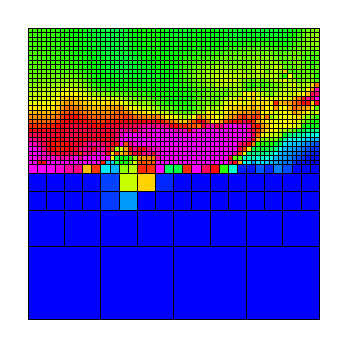
\begin{tikzpicture}[x={(\screenshotunitlength,0)},y={(0,\screenshotunitlength)}]
        \definecolor{fillcolor}{rgb}{0.000000,0.000000,1.000000}
\fill[fillcolor] (0.000000,0.000000) rectangle (0.250000,0.250000);
\definecolor{fillcolor}{rgb}{0.000000,0.000000,1.000000}
\fill[fillcolor] (0.250000,0.000000) rectangle (0.500000,0.250000);
\definecolor{fillcolor}{rgb}{0.000000,0.000000,1.000000}
\fill[fillcolor] (0.000000,0.250000) rectangle (0.125000,0.375000);
\definecolor{fillcolor}{rgb}{0.000000,0.000000,1.000000}
\fill[fillcolor] (0.125000,0.250000) rectangle (0.250000,0.375000);
\definecolor{fillcolor}{rgb}{0.000000,0.000000,1.000000}
\fill[fillcolor] (0.000000,0.375000) rectangle (0.062500,0.437500);
\definecolor{fillcolor}{rgb}{0.000000,0.000000,1.000000}
\fill[fillcolor] (0.062500,0.375000) rectangle (0.125000,0.437500);
\definecolor{fillcolor}{rgb}{0.000000,0.000000,1.000000}
\fill[fillcolor] (0.000000,0.437500) rectangle (0.062500,0.500000);
\definecolor{fillcolor}{rgb}{0.000000,0.000000,1.000000}
\fill[fillcolor] (0.062500,0.437500) rectangle (0.125000,0.500000);
\definecolor{fillcolor}{rgb}{0.000000,0.000063,1.000000}
\fill[fillcolor] (0.125000,0.375000) rectangle (0.187500,0.437500);
\definecolor{fillcolor}{rgb}{0.000000,0.006495,1.000000}
\fill[fillcolor] (0.187500,0.375000) rectangle (0.250000,0.437500);
\definecolor{fillcolor}{rgb}{0.000000,0.000938,1.000000}
\fill[fillcolor] (0.125000,0.437500) rectangle (0.187500,0.500000);
\definecolor{fillcolor}{rgb}{0.000000,0.020625,1.000000}
\fill[fillcolor] (0.187500,0.437500) rectangle (0.250000,0.500000);
\definecolor{fillcolor}{rgb}{0.000000,0.000000,1.000000}
\fill[fillcolor] (0.250000,0.250000) rectangle (0.375000,0.375000);
\definecolor{fillcolor}{rgb}{0.000000,0.000000,1.000000}
\fill[fillcolor] (0.375000,0.250000) rectangle (0.500000,0.375000);
\definecolor{fillcolor}{rgb}{0.000000,0.231200,1.000000}
\fill[fillcolor] (0.250000,0.375000) rectangle (0.312500,0.437500);
\definecolor{fillcolor}{rgb}{0.000000,0.604574,1.000000}
\fill[fillcolor] (0.312500,0.375000) rectangle (0.375000,0.437500);
\definecolor{fillcolor}{rgb}{0.000000,0.259565,1.000000}
\fill[fillcolor] (0.250000,0.437500) rectangle (0.312500,0.500000);
\definecolor{fillcolor}{rgb}{0.783352,1.000000,0.000000}
\fill[fillcolor] (0.312500,0.437500) rectangle (0.375000,0.500000);
\definecolor{fillcolor}{rgb}{0.000000,0.000000,1.000000}
\fill[fillcolor] (0.375000,0.375000) rectangle (0.437500,0.437500);
\definecolor{fillcolor}{rgb}{0.000000,0.000000,1.000000}
\fill[fillcolor] (0.437500,0.375000) rectangle (0.500000,0.437500);
\definecolor{fillcolor}{rgb}{1.000000,0.826471,0.000000}
\fill[fillcolor] (0.375000,0.437500) rectangle (0.437500,0.500000);
\definecolor{fillcolor}{rgb}{0.000000,0.145266,1.000000}
\fill[fillcolor] (0.437500,0.437500) rectangle (0.500000,0.500000);
\definecolor{fillcolor}{rgb}{0.000000,0.000000,1.000000}
\fill[fillcolor] (0.500000,0.000000) rectangle (0.750000,0.250000);
\definecolor{fillcolor}{rgb}{0.000000,0.000000,1.000000}
\fill[fillcolor] (0.750000,0.000000) rectangle (1.000000,0.250000);
\definecolor{fillcolor}{rgb}{0.000000,0.000002,1.000000}
\fill[fillcolor] (0.500000,0.250000) rectangle (0.625000,0.375000);
\definecolor{fillcolor}{rgb}{0.000000,0.000000,1.000000}
\fill[fillcolor] (0.625000,0.250000) rectangle (0.750000,0.375000);
\definecolor{fillcolor}{rgb}{0.000000,0.000002,1.000000}
\fill[fillcolor] (0.500000,0.375000) rectangle (0.562500,0.437500);
\definecolor{fillcolor}{rgb}{0.000000,0.000000,1.000000}
\fill[fillcolor] (0.562500,0.375000) rectangle (0.625000,0.437500);
\definecolor{fillcolor}{rgb}{0.000000,0.000776,1.000000}
\fill[fillcolor] (0.500000,0.437500) rectangle (0.562500,0.500000);
\definecolor{fillcolor}{rgb}{0.000000,0.000000,1.000000}
\fill[fillcolor] (0.562500,0.437500) rectangle (0.625000,0.500000);
\definecolor{fillcolor}{rgb}{0.000000,0.000000,1.000000}
\fill[fillcolor] (0.625000,0.375000) rectangle (0.687500,0.437500);
\definecolor{fillcolor}{rgb}{0.000000,0.000000,1.000000}
\fill[fillcolor] (0.687500,0.375000) rectangle (0.750000,0.437500);
\definecolor{fillcolor}{rgb}{0.000000,0.000000,1.000000}
\fill[fillcolor] (0.625000,0.437500) rectangle (0.687500,0.500000);
\definecolor{fillcolor}{rgb}{0.000000,0.000000,1.000000}
\fill[fillcolor] (0.687500,0.437500) rectangle (0.750000,0.500000);
\definecolor{fillcolor}{rgb}{0.000000,0.000000,1.000000}
\fill[fillcolor] (0.750000,0.250000) rectangle (0.875000,0.375000);
\definecolor{fillcolor}{rgb}{0.000000,0.000000,1.000000}
\fill[fillcolor] (0.875000,0.250000) rectangle (1.000000,0.375000);
\definecolor{fillcolor}{rgb}{0.000000,0.000000,1.000000}
\fill[fillcolor] (0.750000,0.375000) rectangle (0.812500,0.437500);
\definecolor{fillcolor}{rgb}{0.000000,0.000000,1.000000}
\fill[fillcolor] (0.812500,0.375000) rectangle (0.875000,0.437500);
\definecolor{fillcolor}{rgb}{0.000000,0.000000,1.000000}
\fill[fillcolor] (0.750000,0.437500) rectangle (0.812500,0.500000);
\definecolor{fillcolor}{rgb}{0.000000,0.000000,1.000000}
\fill[fillcolor] (0.812500,0.437500) rectangle (0.875000,0.500000);
\definecolor{fillcolor}{rgb}{0.000000,0.000000,1.000000}
\fill[fillcolor] (0.875000,0.375000) rectangle (0.937500,0.437500);
\definecolor{fillcolor}{rgb}{0.000000,0.001272,1.000000}
\fill[fillcolor] (0.937500,0.375000) rectangle (1.000000,0.437500);
\definecolor{fillcolor}{rgb}{0.000000,0.000000,1.000000}
\fill[fillcolor] (0.875000,0.437500) rectangle (0.937500,0.500000);
\definecolor{fillcolor}{rgb}{0.000000,0.000791,1.000000}
\fill[fillcolor] (0.937500,0.437500) rectangle (1.000000,0.500000);
\definecolor{fillcolor}{rgb}{1.000000,0.000000,1.000000}
\fill[fillcolor] (0.000000,0.500000) rectangle (0.031250,0.531250);
\definecolor{fillcolor}{rgb}{1.000000,0.000000,1.000000}
\fill[fillcolor] (0.031250,0.500000) rectangle (0.062500,0.531250);
\definecolor{fillcolor}{rgb}{1.000000,0.000000,1.000000}
\fill[fillcolor] (0.000000,0.531250) rectangle (0.015625,0.546875);
\definecolor{fillcolor}{rgb}{1.000000,0.000000,0.902982}
\fill[fillcolor] (0.015625,0.531250) rectangle (0.031250,0.546875);
\definecolor{fillcolor}{rgb}{1.000000,0.000000,1.000000}
\fill[fillcolor] (0.000000,0.546875) rectangle (0.015625,0.562500);
\definecolor{fillcolor}{rgb}{1.000000,0.000000,1.000000}
\fill[fillcolor] (0.015625,0.546875) rectangle (0.031250,0.562500);
\definecolor{fillcolor}{rgb}{1.000000,0.000000,0.106697}
\fill[fillcolor] (0.031250,0.531250) rectangle (0.046875,0.546875);
\definecolor{fillcolor}{rgb}{1.000000,0.000000,0.100655}
\fill[fillcolor] (0.046875,0.531250) rectangle (0.062500,0.546875);
\definecolor{fillcolor}{rgb}{1.000000,0.000000,0.763437}
\fill[fillcolor] (0.031250,0.546875) rectangle (0.046875,0.562500);
\definecolor{fillcolor}{rgb}{1.000000,0.000000,0.771207}
\fill[fillcolor] (0.046875,0.546875) rectangle (0.062500,0.562500);
\definecolor{fillcolor}{rgb}{1.000000,0.000000,1.000000}
\fill[fillcolor] (0.062500,0.500000) rectangle (0.093750,0.531250);
\definecolor{fillcolor}{rgb}{1.000000,0.000000,0.830453}
\fill[fillcolor] (0.093750,0.500000) rectangle (0.125000,0.531250);
\definecolor{fillcolor}{rgb}{1.000000,0.000000,0.948585}
\fill[fillcolor] (0.062500,0.531250) rectangle (0.078125,0.546875);
\definecolor{fillcolor}{rgb}{1.000000,0.000000,1.000000}
\fill[fillcolor] (0.078125,0.531250) rectangle (0.093750,0.546875);
\definecolor{fillcolor}{rgb}{1.000000,0.000000,0.887297}
\fill[fillcolor] (0.062500,0.546875) rectangle (0.078125,0.562500);
\definecolor{fillcolor}{rgb}{1.000000,0.000000,0.821057}
\fill[fillcolor] (0.078125,0.546875) rectangle (0.093750,0.562500);
\definecolor{fillcolor}{rgb}{1.000000,0.000000,1.000000}
\fill[fillcolor] (0.093750,0.531250) rectangle (0.109375,0.546875);
\definecolor{fillcolor}{rgb}{1.000000,0.000000,0.907313}
\fill[fillcolor] (0.109375,0.531250) rectangle (0.125000,0.546875);
\definecolor{fillcolor}{rgb}{1.000000,0.000000,0.699230}
\fill[fillcolor] (0.093750,0.546875) rectangle (0.109375,0.562500);
\definecolor{fillcolor}{rgb}{1.000000,0.000000,0.655828}
\fill[fillcolor] (0.109375,0.546875) rectangle (0.125000,0.562500);
\definecolor{fillcolor}{rgb}{1.000000,0.000000,1.000000}
\fill[fillcolor] (0.000000,0.562500) rectangle (0.015625,0.578125);
\definecolor{fillcolor}{rgb}{1.000000,0.000000,1.000000}
\fill[fillcolor] (0.015625,0.562500) rectangle (0.031250,0.578125);
\definecolor{fillcolor}{rgb}{1.000000,0.000000,1.000000}
\fill[fillcolor] (0.000000,0.578125) rectangle (0.015625,0.593750);
\definecolor{fillcolor}{rgb}{1.000000,0.000000,1.000000}
\fill[fillcolor] (0.015625,0.578125) rectangle (0.031250,0.593750);
\definecolor{fillcolor}{rgb}{1.000000,0.000000,0.996898}
\fill[fillcolor] (0.031250,0.562500) rectangle (0.046875,0.578125);
\definecolor{fillcolor}{rgb}{1.000000,0.000000,0.743593}
\fill[fillcolor] (0.046875,0.562500) rectangle (0.062500,0.578125);
\definecolor{fillcolor}{rgb}{1.000000,0.000000,0.783029}
\fill[fillcolor] (0.031250,0.578125) rectangle (0.046875,0.593750);
\definecolor{fillcolor}{rgb}{1.000000,0.000000,0.489856}
\fill[fillcolor] (0.046875,0.578125) rectangle (0.062500,0.593750);
\definecolor{fillcolor}{rgb}{1.000000,0.000000,0.811986}
\fill[fillcolor] (0.000000,0.593750) rectangle (0.015625,0.609375);
\definecolor{fillcolor}{rgb}{1.000000,0.000000,0.716906}
\fill[fillcolor] (0.015625,0.593750) rectangle (0.031250,0.609375);
\definecolor{fillcolor}{rgb}{1.000000,0.000000,0.583664}
\fill[fillcolor] (0.000000,0.609375) rectangle (0.015625,0.625000);
\definecolor{fillcolor}{rgb}{1.000000,0.000000,0.530592}
\fill[fillcolor] (0.015625,0.609375) rectangle (0.031250,0.625000);
\definecolor{fillcolor}{rgb}{1.000000,0.000000,0.517530}
\fill[fillcolor] (0.031250,0.593750) rectangle (0.046875,0.609375);
\definecolor{fillcolor}{rgb}{1.000000,0.000000,0.315564}
\fill[fillcolor] (0.046875,0.593750) rectangle (0.062500,0.609375);
\definecolor{fillcolor}{rgb}{1.000000,0.000000,0.438429}
\fill[fillcolor] (0.031250,0.609375) rectangle (0.046875,0.625000);
\definecolor{fillcolor}{rgb}{1.000000,0.000000,0.299397}
\fill[fillcolor] (0.046875,0.609375) rectangle (0.062500,0.625000);
\definecolor{fillcolor}{rgb}{1.000000,0.000000,0.444957}
\fill[fillcolor] (0.062500,0.562500) rectangle (0.078125,0.578125);
\definecolor{fillcolor}{rgb}{1.000000,0.000000,0.300266}
\fill[fillcolor] (0.078125,0.562500) rectangle (0.093750,0.578125);
\definecolor{fillcolor}{rgb}{1.000000,0.000000,0.178020}
\fill[fillcolor] (0.062500,0.578125) rectangle (0.078125,0.593750);
\definecolor{fillcolor}{rgb}{1.000000,0.000000,0.004590}
\fill[fillcolor] (0.078125,0.578125) rectangle (0.093750,0.593750);
\definecolor{fillcolor}{rgb}{1.000000,0.000000,0.198728}
\fill[fillcolor] (0.093750,0.562500) rectangle (0.109375,0.578125);
\definecolor{fillcolor}{rgb}{1.000000,0.000000,0.180621}
\fill[fillcolor] (0.109375,0.562500) rectangle (0.125000,0.578125);
\definecolor{fillcolor}{rgb}{1.000000,0.089516,0.000000}
\fill[fillcolor] (0.093750,0.578125) rectangle (0.109375,0.593750);
\definecolor{fillcolor}{rgb}{1.000000,0.119542,0.000000}
\fill[fillcolor] (0.109375,0.578125) rectangle (0.125000,0.593750);
\definecolor{fillcolor}{rgb}{1.000000,0.000000,0.085490}
\fill[fillcolor] (0.062500,0.593750) rectangle (0.078125,0.609375);
\definecolor{fillcolor}{rgb}{1.000000,0.054308,0.000000}
\fill[fillcolor] (0.078125,0.593750) rectangle (0.093750,0.609375);
\definecolor{fillcolor}{rgb}{1.000000,0.000000,0.170613}
\fill[fillcolor] (0.062500,0.609375) rectangle (0.078125,0.625000);
\definecolor{fillcolor}{rgb}{1.000000,0.000000,0.083371}
\fill[fillcolor] (0.078125,0.609375) rectangle (0.093750,0.625000);
\definecolor{fillcolor}{rgb}{1.000000,0.110941,0.000000}
\fill[fillcolor] (0.093750,0.593750) rectangle (0.109375,0.609375);
\definecolor{fillcolor}{rgb}{1.000000,0.093463,0.000000}
\fill[fillcolor] (0.109375,0.593750) rectangle (0.125000,0.609375);
\definecolor{fillcolor}{rgb}{1.000000,0.000000,0.024531}
\fill[fillcolor] (0.093750,0.609375) rectangle (0.109375,0.625000);
\definecolor{fillcolor}{rgb}{1.000000,0.000000,0.049613}
\fill[fillcolor] (0.109375,0.609375) rectangle (0.125000,0.625000);
\definecolor{fillcolor}{rgb}{1.000000,0.000000,0.633862}
\fill[fillcolor] (0.125000,0.500000) rectangle (0.156250,0.531250);
\definecolor{fillcolor}{rgb}{1.000000,0.000000,0.525126}
\fill[fillcolor] (0.156250,0.500000) rectangle (0.187500,0.531250);
\definecolor{fillcolor}{rgb}{1.000000,0.000000,1.000000}
\fill[fillcolor] (0.125000,0.531250) rectangle (0.140625,0.546875);
\definecolor{fillcolor}{rgb}{1.000000,0.000000,1.000000}
\fill[fillcolor] (0.140625,0.531250) rectangle (0.156250,0.546875);
\definecolor{fillcolor}{rgb}{1.000000,0.000000,0.721521}
\fill[fillcolor] (0.125000,0.546875) rectangle (0.140625,0.562500);
\definecolor{fillcolor}{rgb}{1.000000,0.000000,0.762617}
\fill[fillcolor] (0.140625,0.546875) rectangle (0.156250,0.562500);
\definecolor{fillcolor}{rgb}{1.000000,0.000000,1.000000}
\fill[fillcolor] (0.156250,0.531250) rectangle (0.171875,0.546875);
\definecolor{fillcolor}{rgb}{1.000000,0.000000,1.000000}
\fill[fillcolor] (0.171875,0.531250) rectangle (0.187500,0.546875);
\definecolor{fillcolor}{rgb}{1.000000,0.000000,0.988223}
\fill[fillcolor] (0.156250,0.546875) rectangle (0.171875,0.562500);
\definecolor{fillcolor}{rgb}{1.000000,0.000000,0.534241}
\fill[fillcolor] (0.171875,0.546875) rectangle (0.187500,0.562500);
\definecolor{fillcolor}{rgb}{1.000000,0.748143,0.000000}
\fill[fillcolor] (0.187500,0.500000) rectangle (0.218750,0.531250);
\definecolor{fillcolor}{rgb}{1.000000,0.213529,0.000000}
\fill[fillcolor] (0.218750,0.500000) rectangle (0.250000,0.531250);
\definecolor{fillcolor}{rgb}{1.000000,0.000000,1.000000}
\fill[fillcolor] (0.187500,0.531250) rectangle (0.203125,0.546875);
\definecolor{fillcolor}{rgb}{1.000000,0.000000,1.000000}
\fill[fillcolor] (0.203125,0.531250) rectangle (0.218750,0.546875);
\definecolor{fillcolor}{rgb}{1.000000,0.000000,1.000000}
\fill[fillcolor] (0.187500,0.546875) rectangle (0.203125,0.562500);
\definecolor{fillcolor}{rgb}{1.000000,0.000000,1.000000}
\fill[fillcolor] (0.203125,0.546875) rectangle (0.218750,0.562500);
\definecolor{fillcolor}{rgb}{1.000000,0.000000,1.000000}
\fill[fillcolor] (0.218750,0.531250) rectangle (0.234375,0.546875);
\definecolor{fillcolor}{rgb}{1.000000,0.000000,1.000000}
\fill[fillcolor] (0.234375,0.531250) rectangle (0.250000,0.546875);
\definecolor{fillcolor}{rgb}{1.000000,0.000000,1.000000}
\fill[fillcolor] (0.218750,0.546875) rectangle (0.234375,0.562500);
\definecolor{fillcolor}{rgb}{1.000000,0.000000,1.000000}
\fill[fillcolor] (0.234375,0.546875) rectangle (0.250000,0.562500);
\definecolor{fillcolor}{rgb}{1.000000,0.000000,0.273629}
\fill[fillcolor] (0.125000,0.562500) rectangle (0.140625,0.578125);
\definecolor{fillcolor}{rgb}{1.000000,0.000000,0.335718}
\fill[fillcolor] (0.140625,0.562500) rectangle (0.156250,0.578125);
\definecolor{fillcolor}{rgb}{1.000000,0.000000,0.016461}
\fill[fillcolor] (0.125000,0.578125) rectangle (0.140625,0.593750);
\definecolor{fillcolor}{rgb}{1.000000,0.000000,0.104381}
\fill[fillcolor] (0.140625,0.578125) rectangle (0.156250,0.593750);
\definecolor{fillcolor}{rgb}{1.000000,0.000000,0.272082}
\fill[fillcolor] (0.156250,0.562500) rectangle (0.171875,0.578125);
\definecolor{fillcolor}{rgb}{1.000000,0.218166,0.000000}
\fill[fillcolor] (0.171875,0.562500) rectangle (0.187500,0.578125);
\definecolor{fillcolor}{rgb}{1.000000,0.000000,0.204878}
\fill[fillcolor] (0.156250,0.578125) rectangle (0.171875,0.593750);
\definecolor{fillcolor}{rgb}{1.000000,0.000000,0.536112}
\fill[fillcolor] (0.171875,0.578125) rectangle (0.187500,0.593750);
\definecolor{fillcolor}{rgb}{1.000000,0.000000,0.003555}
\fill[fillcolor] (0.125000,0.593750) rectangle (0.140625,0.609375);
\definecolor{fillcolor}{rgb}{1.000000,0.000000,0.166149}
\fill[fillcolor] (0.140625,0.593750) rectangle (0.156250,0.609375);
\definecolor{fillcolor}{rgb}{1.000000,0.000000,0.195252}
\fill[fillcolor] (0.125000,0.609375) rectangle (0.140625,0.625000);
\definecolor{fillcolor}{rgb}{1.000000,0.000000,0.309108}
\fill[fillcolor] (0.140625,0.609375) rectangle (0.156250,0.625000);
\definecolor{fillcolor}{rgb}{1.000000,0.000000,0.159854}
\fill[fillcolor] (0.156250,0.593750) rectangle (0.171875,0.609375);
\definecolor{fillcolor}{rgb}{1.000000,0.000000,0.182620}
\fill[fillcolor] (0.171875,0.593750) rectangle (0.187500,0.609375);
\definecolor{fillcolor}{rgb}{1.000000,0.000000,0.105728}
\fill[fillcolor] (0.156250,0.609375) rectangle (0.171875,0.625000);
\definecolor{fillcolor}{rgb}{1.000000,0.000000,0.078665}
\fill[fillcolor] (0.171875,0.609375) rectangle (0.187500,0.625000);
\definecolor{fillcolor}{rgb}{1.000000,0.000000,0.519106}
\fill[fillcolor] (0.187500,0.562500) rectangle (0.203125,0.578125);
\definecolor{fillcolor}{rgb}{1.000000,0.000000,0.458986}
\fill[fillcolor] (0.203125,0.562500) rectangle (0.218750,0.578125);
\definecolor{fillcolor}{rgb}{1.000000,0.000000,0.513732}
\fill[fillcolor] (0.187500,0.578125) rectangle (0.203125,0.593750);
\definecolor{fillcolor}{rgb}{1.000000,0.000000,0.538622}
\fill[fillcolor] (0.203125,0.578125) rectangle (0.218750,0.593750);
\definecolor{fillcolor}{rgb}{1.000000,0.000000,0.701191}
\fill[fillcolor] (0.218750,0.562500) rectangle (0.234375,0.578125);
\definecolor{fillcolor}{rgb}{1.000000,0.000000,0.957828}
\fill[fillcolor] (0.234375,0.562500) rectangle (0.250000,0.578125);
\definecolor{fillcolor}{rgb}{1.000000,0.000000,0.167272}
\fill[fillcolor] (0.218750,0.578125) rectangle (0.234375,0.593750);
\definecolor{fillcolor}{rgb}{1.000000,0.000000,0.606524}
\fill[fillcolor] (0.234375,0.578125) rectangle (0.250000,0.593750);
\definecolor{fillcolor}{rgb}{1.000000,0.000000,0.339870}
\fill[fillcolor] (0.187500,0.593750) rectangle (0.203125,0.609375);
\definecolor{fillcolor}{rgb}{1.000000,0.000000,0.633279}
\fill[fillcolor] (0.203125,0.593750) rectangle (0.218750,0.609375);
\definecolor{fillcolor}{rgb}{1.000000,0.000000,0.112577}
\fill[fillcolor] (0.187500,0.609375) rectangle (0.203125,0.625000);
\definecolor{fillcolor}{rgb}{1.000000,0.000000,0.220093}
\fill[fillcolor] (0.203125,0.609375) rectangle (0.218750,0.625000);
\definecolor{fillcolor}{rgb}{1.000000,0.000000,0.639359}
\fill[fillcolor] (0.218750,0.593750) rectangle (0.234375,0.609375);
\definecolor{fillcolor}{rgb}{1.000000,0.000000,0.587436}
\fill[fillcolor] (0.234375,0.593750) rectangle (0.250000,0.609375);
\definecolor{fillcolor}{rgb}{1.000000,0.000000,0.086558}
\fill[fillcolor] (0.218750,0.609375) rectangle (0.234375,0.625000);
\definecolor{fillcolor}{rgb}{1.000000,0.000000,0.182593}
\fill[fillcolor] (0.234375,0.609375) rectangle (0.250000,0.625000);
\definecolor{fillcolor}{rgb}{1.000000,0.000000,0.320768}
\fill[fillcolor] (0.000000,0.625000) rectangle (0.015625,0.640625);
\definecolor{fillcolor}{rgb}{1.000000,0.000000,0.302872}
\fill[fillcolor] (0.015625,0.625000) rectangle (0.031250,0.640625);
\definecolor{fillcolor}{rgb}{1.000000,0.010003,0.000000}
\fill[fillcolor] (0.000000,0.640625) rectangle (0.015625,0.656250);
\definecolor{fillcolor}{rgb}{1.000000,0.000000,0.061881}
\fill[fillcolor] (0.015625,0.640625) rectangle (0.031250,0.656250);
\definecolor{fillcolor}{rgb}{1.000000,0.000000,0.260336}
\fill[fillcolor] (0.031250,0.625000) rectangle (0.046875,0.640625);
\definecolor{fillcolor}{rgb}{1.000000,0.000000,0.228362}
\fill[fillcolor] (0.046875,0.625000) rectangle (0.062500,0.640625);
\definecolor{fillcolor}{rgb}{1.000000,0.000000,0.078620}
\fill[fillcolor] (0.031250,0.640625) rectangle (0.046875,0.656250);
\definecolor{fillcolor}{rgb}{1.000000,0.000000,0.087280}
\fill[fillcolor] (0.046875,0.640625) rectangle (0.062500,0.656250);
\definecolor{fillcolor}{rgb}{1.000000,0.147311,0.000000}
\fill[fillcolor] (0.000000,0.656250) rectangle (0.015625,0.671875);
\definecolor{fillcolor}{rgb}{1.000000,0.174510,0.000000}
\fill[fillcolor] (0.015625,0.656250) rectangle (0.031250,0.671875);
\definecolor{fillcolor}{rgb}{1.000000,0.353063,0.000000}
\fill[fillcolor] (0.000000,0.671875) rectangle (0.015625,0.687500);
\definecolor{fillcolor}{rgb}{1.000000,0.378253,0.000000}
\fill[fillcolor] (0.015625,0.671875) rectangle (0.031250,0.687500);
\definecolor{fillcolor}{rgb}{1.000000,0.220806,0.000000}
\fill[fillcolor] (0.031250,0.656250) rectangle (0.046875,0.671875);
\definecolor{fillcolor}{rgb}{1.000000,0.172560,0.000000}
\fill[fillcolor] (0.046875,0.656250) rectangle (0.062500,0.671875);
\definecolor{fillcolor}{rgb}{1.000000,0.396462,0.000000}
\fill[fillcolor] (0.031250,0.671875) rectangle (0.046875,0.687500);
\definecolor{fillcolor}{rgb}{1.000000,0.408198,0.000000}
\fill[fillcolor] (0.046875,0.671875) rectangle (0.062500,0.687500);
\definecolor{fillcolor}{rgb}{1.000000,0.000000,0.208835}
\fill[fillcolor] (0.062500,0.625000) rectangle (0.078125,0.640625);
\definecolor{fillcolor}{rgb}{1.000000,0.000000,0.191335}
\fill[fillcolor] (0.078125,0.625000) rectangle (0.093750,0.640625);
\definecolor{fillcolor}{rgb}{1.000000,0.000000,0.046085}
\fill[fillcolor] (0.062500,0.640625) rectangle (0.078125,0.656250);
\definecolor{fillcolor}{rgb}{1.000000,0.000000,0.115812}
\fill[fillcolor] (0.078125,0.640625) rectangle (0.093750,0.656250);
\definecolor{fillcolor}{rgb}{1.000000,0.000000,0.160495}
\fill[fillcolor] (0.093750,0.625000) rectangle (0.109375,0.640625);
\definecolor{fillcolor}{rgb}{1.000000,0.000000,0.173137}
\fill[fillcolor] (0.109375,0.625000) rectangle (0.125000,0.640625);
\definecolor{fillcolor}{rgb}{1.000000,0.000000,0.152080}
\fill[fillcolor] (0.093750,0.640625) rectangle (0.109375,0.656250);
\definecolor{fillcolor}{rgb}{1.000000,0.000000,0.148914}
\fill[fillcolor] (0.109375,0.640625) rectangle (0.125000,0.656250);
\definecolor{fillcolor}{rgb}{1.000000,0.136090,0.000000}
\fill[fillcolor] (0.062500,0.656250) rectangle (0.078125,0.671875);
\definecolor{fillcolor}{rgb}{1.000000,0.095018,0.000000}
\fill[fillcolor] (0.078125,0.656250) rectangle (0.093750,0.671875);
\definecolor{fillcolor}{rgb}{1.000000,0.396080,0.000000}
\fill[fillcolor] (0.062500,0.671875) rectangle (0.078125,0.687500);
\definecolor{fillcolor}{rgb}{1.000000,0.337461,0.000000}
\fill[fillcolor] (0.078125,0.671875) rectangle (0.093750,0.687500);
\definecolor{fillcolor}{rgb}{1.000000,0.000000,0.026491}
\fill[fillcolor] (0.093750,0.656250) rectangle (0.109375,0.671875);
\definecolor{fillcolor}{rgb}{1.000000,0.000000,0.099015}
\fill[fillcolor] (0.109375,0.656250) rectangle (0.125000,0.671875);
\definecolor{fillcolor}{rgb}{1.000000,0.216517,0.000000}
\fill[fillcolor] (0.093750,0.671875) rectangle (0.109375,0.687500);
\definecolor{fillcolor}{rgb}{1.000000,0.084936,0.000000}
\fill[fillcolor] (0.109375,0.671875) rectangle (0.125000,0.687500);
\definecolor{fillcolor}{rgb}{1.000000,0.558807,0.000000}
\fill[fillcolor] (0.000000,0.687500) rectangle (0.015625,0.703125);
\definecolor{fillcolor}{rgb}{1.000000,0.554143,0.000000}
\fill[fillcolor] (0.015625,0.687500) rectangle (0.031250,0.703125);
\definecolor{fillcolor}{rgb}{1.000000,0.749803,0.000000}
\fill[fillcolor] (0.000000,0.703125) rectangle (0.015625,0.718750);
\definecolor{fillcolor}{rgb}{1.000000,0.714361,0.000000}
\fill[fillcolor] (0.015625,0.703125) rectangle (0.031250,0.718750);
\definecolor{fillcolor}{rgb}{1.000000,0.557655,0.000000}
\fill[fillcolor] (0.031250,0.687500) rectangle (0.046875,0.703125);
\definecolor{fillcolor}{rgb}{1.000000,0.560368,0.000000}
\fill[fillcolor] (0.046875,0.687500) rectangle (0.062500,0.703125);
\definecolor{fillcolor}{rgb}{1.000000,0.727322,0.000000}
\fill[fillcolor] (0.031250,0.703125) rectangle (0.046875,0.718750);
\definecolor{fillcolor}{rgb}{1.000000,0.718437,0.000000}
\fill[fillcolor] (0.046875,0.703125) rectangle (0.062500,0.718750);
\definecolor{fillcolor}{rgb}{1.000000,0.911132,0.000000}
\fill[fillcolor] (0.000000,0.718750) rectangle (0.015625,0.734375);
\definecolor{fillcolor}{rgb}{1.000000,0.911569,0.000000}
\fill[fillcolor] (0.015625,0.718750) rectangle (0.031250,0.734375);
\definecolor{fillcolor}{rgb}{0.920743,1.000000,0.000000}
\fill[fillcolor] (0.000000,0.734375) rectangle (0.015625,0.750000);
\definecolor{fillcolor}{rgb}{0.897979,1.000000,0.000000}
\fill[fillcolor] (0.015625,0.734375) rectangle (0.031250,0.750000);
\definecolor{fillcolor}{rgb}{1.000000,0.899687,0.000000}
\fill[fillcolor] (0.031250,0.718750) rectangle (0.046875,0.734375);
\definecolor{fillcolor}{rgb}{1.000000,0.904821,0.000000}
\fill[fillcolor] (0.046875,0.718750) rectangle (0.062500,0.734375);
\definecolor{fillcolor}{rgb}{0.956117,1.000000,0.000000}
\fill[fillcolor] (0.031250,0.734375) rectangle (0.046875,0.750000);
\definecolor{fillcolor}{rgb}{0.926101,1.000000,0.000000}
\fill[fillcolor] (0.046875,0.734375) rectangle (0.062500,0.750000);
\definecolor{fillcolor}{rgb}{1.000000,0.577872,0.000000}
\fill[fillcolor] (0.062500,0.687500) rectangle (0.078125,0.703125);
\definecolor{fillcolor}{rgb}{1.000000,0.535223,0.000000}
\fill[fillcolor] (0.078125,0.687500) rectangle (0.093750,0.703125);
\definecolor{fillcolor}{rgb}{1.000000,0.739507,0.000000}
\fill[fillcolor] (0.062500,0.703125) rectangle (0.078125,0.718750);
\definecolor{fillcolor}{rgb}{1.000000,0.691798,0.000000}
\fill[fillcolor] (0.078125,0.703125) rectangle (0.093750,0.718750);
\definecolor{fillcolor}{rgb}{1.000000,0.444663,0.000000}
\fill[fillcolor] (0.093750,0.687500) rectangle (0.109375,0.703125);
\definecolor{fillcolor}{rgb}{1.000000,0.233413,0.000000}
\fill[fillcolor] (0.109375,0.687500) rectangle (0.125000,0.703125);
\definecolor{fillcolor}{rgb}{1.000000,0.567515,0.000000}
\fill[fillcolor] (0.093750,0.703125) rectangle (0.109375,0.718750);
\definecolor{fillcolor}{rgb}{1.000000,0.388544,0.000000}
\fill[fillcolor] (0.109375,0.703125) rectangle (0.125000,0.718750);
\definecolor{fillcolor}{rgb}{1.000000,0.938919,0.000000}
\fill[fillcolor] (0.062500,0.718750) rectangle (0.078125,0.734375);
\definecolor{fillcolor}{rgb}{1.000000,0.883034,0.000000}
\fill[fillcolor] (0.078125,0.718750) rectangle (0.093750,0.734375);
\definecolor{fillcolor}{rgb}{0.937165,1.000000,0.000000}
\fill[fillcolor] (0.062500,0.734375) rectangle (0.078125,0.750000);
\definecolor{fillcolor}{rgb}{0.984668,1.000000,0.000000}
\fill[fillcolor] (0.078125,0.734375) rectangle (0.093750,0.750000);
\definecolor{fillcolor}{rgb}{1.000000,0.780151,0.000000}
\fill[fillcolor] (0.093750,0.718750) rectangle (0.109375,0.734375);
\definecolor{fillcolor}{rgb}{1.000000,0.586690,0.000000}
\fill[fillcolor] (0.109375,0.718750) rectangle (0.125000,0.734375);
\definecolor{fillcolor}{rgb}{1.000000,0.847737,0.000000}
\fill[fillcolor] (0.093750,0.734375) rectangle (0.109375,0.750000);
\definecolor{fillcolor}{rgb}{1.000000,0.709957,0.000000}
\fill[fillcolor] (0.109375,0.734375) rectangle (0.125000,0.750000);
\definecolor{fillcolor}{rgb}{1.000000,0.000000,0.224689}
\fill[fillcolor] (0.125000,0.625000) rectangle (0.140625,0.640625);
\definecolor{fillcolor}{rgb}{1.000000,0.000000,0.281288}
\fill[fillcolor] (0.140625,0.625000) rectangle (0.156250,0.640625);
\definecolor{fillcolor}{rgb}{1.000000,0.000000,0.171005}
\fill[fillcolor] (0.125000,0.640625) rectangle (0.140625,0.656250);
\definecolor{fillcolor}{rgb}{1.000000,0.000000,0.248870}
\fill[fillcolor] (0.140625,0.640625) rectangle (0.156250,0.656250);
\definecolor{fillcolor}{rgb}{1.000000,0.000000,0.225729}
\fill[fillcolor] (0.156250,0.625000) rectangle (0.171875,0.640625);
\definecolor{fillcolor}{rgb}{1.000000,0.000000,0.157823}
\fill[fillcolor] (0.171875,0.625000) rectangle (0.187500,0.640625);
\definecolor{fillcolor}{rgb}{1.000000,0.000000,0.290717}
\fill[fillcolor] (0.156250,0.640625) rectangle (0.171875,0.656250);
\definecolor{fillcolor}{rgb}{1.000000,0.000000,0.239819}
\fill[fillcolor] (0.171875,0.640625) rectangle (0.187500,0.656250);
\definecolor{fillcolor}{rgb}{1.000000,0.000000,0.150686}
\fill[fillcolor] (0.125000,0.656250) rectangle (0.140625,0.671875);
\definecolor{fillcolor}{rgb}{1.000000,0.000000,0.246356}
\fill[fillcolor] (0.140625,0.656250) rectangle (0.156250,0.671875);
\definecolor{fillcolor}{rgb}{1.000000,0.000000,0.015953}
\fill[fillcolor] (0.125000,0.671875) rectangle (0.140625,0.687500);
\definecolor{fillcolor}{rgb}{1.000000,0.000000,0.079383}
\fill[fillcolor] (0.140625,0.671875) rectangle (0.156250,0.687500);
\definecolor{fillcolor}{rgb}{1.000000,0.000000,0.226672}
\fill[fillcolor] (0.156250,0.656250) rectangle (0.171875,0.671875);
\definecolor{fillcolor}{rgb}{1.000000,0.000000,0.194390}
\fill[fillcolor] (0.171875,0.656250) rectangle (0.187500,0.671875);
\definecolor{fillcolor}{rgb}{1.000000,0.000000,0.066076}
\fill[fillcolor] (0.156250,0.671875) rectangle (0.171875,0.687500);
\definecolor{fillcolor}{rgb}{1.000000,0.000000,0.003093}
\fill[fillcolor] (0.171875,0.671875) rectangle (0.187500,0.687500);
\definecolor{fillcolor}{rgb}{1.000000,0.000000,0.146388}
\fill[fillcolor] (0.187500,0.625000) rectangle (0.203125,0.640625);
\definecolor{fillcolor}{rgb}{1.000000,0.000000,0.210646}
\fill[fillcolor] (0.203125,0.625000) rectangle (0.218750,0.640625);
\definecolor{fillcolor}{rgb}{1.000000,0.000000,0.227070}
\fill[fillcolor] (0.187500,0.640625) rectangle (0.203125,0.656250);
\definecolor{fillcolor}{rgb}{1.000000,0.000000,0.258740}
\fill[fillcolor] (0.203125,0.640625) rectangle (0.218750,0.656250);
\definecolor{fillcolor}{rgb}{1.000000,0.000000,0.212757}
\fill[fillcolor] (0.218750,0.625000) rectangle (0.234375,0.640625);
\definecolor{fillcolor}{rgb}{1.000000,0.000000,0.079720}
\fill[fillcolor] (0.234375,0.625000) rectangle (0.250000,0.640625);
\definecolor{fillcolor}{rgb}{1.000000,0.000000,0.229316}
\fill[fillcolor] (0.218750,0.640625) rectangle (0.234375,0.656250);
\definecolor{fillcolor}{rgb}{1.000000,0.000000,0.169916}
\fill[fillcolor] (0.234375,0.640625) rectangle (0.250000,0.656250);
\definecolor{fillcolor}{rgb}{1.000000,0.000000,0.185973}
\fill[fillcolor] (0.187500,0.656250) rectangle (0.203125,0.671875);
\definecolor{fillcolor}{rgb}{1.000000,0.000000,0.137875}
\fill[fillcolor] (0.203125,0.656250) rectangle (0.218750,0.671875);
\definecolor{fillcolor}{rgb}{1.000000,0.021662,0.000000}
\fill[fillcolor] (0.187500,0.671875) rectangle (0.203125,0.687500);
\definecolor{fillcolor}{rgb}{1.000000,0.144510,0.000000}
\fill[fillcolor] (0.203125,0.671875) rectangle (0.218750,0.687500);
\definecolor{fillcolor}{rgb}{1.000000,0.000000,0.057011}
\fill[fillcolor] (0.218750,0.656250) rectangle (0.234375,0.671875);
\definecolor{fillcolor}{rgb}{1.000000,0.097019,0.000000}
\fill[fillcolor] (0.234375,0.656250) rectangle (0.250000,0.671875);
\definecolor{fillcolor}{rgb}{1.000000,0.118433,0.000000}
\fill[fillcolor] (0.218750,0.671875) rectangle (0.234375,0.687500);
\definecolor{fillcolor}{rgb}{1.000000,0.242793,0.000000}
\fill[fillcolor] (0.234375,0.671875) rectangle (0.250000,0.687500);
\definecolor{fillcolor}{rgb}{1.000000,0.111647,0.000000}
\fill[fillcolor] (0.125000,0.687500) rectangle (0.140625,0.703125);
\definecolor{fillcolor}{rgb}{1.000000,0.086449,0.000000}
\fill[fillcolor] (0.140625,0.687500) rectangle (0.156250,0.703125);
\definecolor{fillcolor}{rgb}{1.000000,0.310590,0.000000}
\fill[fillcolor] (0.125000,0.703125) rectangle (0.140625,0.718750);
\definecolor{fillcolor}{rgb}{1.000000,0.257303,0.000000}
\fill[fillcolor] (0.140625,0.703125) rectangle (0.156250,0.718750);
\definecolor{fillcolor}{rgb}{1.000000,0.062529,0.000000}
\fill[fillcolor] (0.156250,0.687500) rectangle (0.171875,0.703125);
\definecolor{fillcolor}{rgb}{1.000000,0.222488,0.000000}
\fill[fillcolor] (0.171875,0.687500) rectangle (0.187500,0.703125);
\definecolor{fillcolor}{rgb}{1.000000,0.306041,0.000000}
\fill[fillcolor] (0.156250,0.703125) rectangle (0.171875,0.718750);
\definecolor{fillcolor}{rgb}{1.000000,0.414985,0.000000}
\fill[fillcolor] (0.171875,0.703125) rectangle (0.187500,0.718750);
\definecolor{fillcolor}{rgb}{1.000000,0.422779,0.000000}
\fill[fillcolor] (0.125000,0.718750) rectangle (0.140625,0.734375);
\definecolor{fillcolor}{rgb}{1.000000,0.447480,0.000000}
\fill[fillcolor] (0.140625,0.718750) rectangle (0.156250,0.734375);
\definecolor{fillcolor}{rgb}{1.000000,0.607273,0.000000}
\fill[fillcolor] (0.125000,0.734375) rectangle (0.140625,0.750000);
\definecolor{fillcolor}{rgb}{1.000000,0.604086,0.000000}
\fill[fillcolor] (0.140625,0.734375) rectangle (0.156250,0.750000);
\definecolor{fillcolor}{rgb}{1.000000,0.477127,0.000000}
\fill[fillcolor] (0.156250,0.718750) rectangle (0.171875,0.734375);
\definecolor{fillcolor}{rgb}{1.000000,0.592397,0.000000}
\fill[fillcolor] (0.171875,0.718750) rectangle (0.187500,0.734375);
\definecolor{fillcolor}{rgb}{1.000000,0.694772,0.000000}
\fill[fillcolor] (0.156250,0.734375) rectangle (0.171875,0.750000);
\definecolor{fillcolor}{rgb}{1.000000,0.750142,0.000000}
\fill[fillcolor] (0.171875,0.734375) rectangle (0.187500,0.750000);
\definecolor{fillcolor}{rgb}{1.000000,0.217288,0.000000}
\fill[fillcolor] (0.187500,0.687500) rectangle (0.203125,0.703125);
\definecolor{fillcolor}{rgb}{1.000000,0.370177,0.000000}
\fill[fillcolor] (0.203125,0.687500) rectangle (0.218750,0.703125);
\definecolor{fillcolor}{rgb}{1.000000,0.482023,0.000000}
\fill[fillcolor] (0.187500,0.703125) rectangle (0.203125,0.718750);
\definecolor{fillcolor}{rgb}{1.000000,0.522354,0.000000}
\fill[fillcolor] (0.203125,0.703125) rectangle (0.218750,0.718750);
\definecolor{fillcolor}{rgb}{1.000000,0.395401,0.000000}
\fill[fillcolor] (0.218750,0.687500) rectangle (0.234375,0.703125);
\definecolor{fillcolor}{rgb}{1.000000,0.374951,0.000000}
\fill[fillcolor] (0.234375,0.687500) rectangle (0.250000,0.703125);
\definecolor{fillcolor}{rgb}{1.000000,0.597723,0.000000}
\fill[fillcolor] (0.218750,0.703125) rectangle (0.234375,0.718750);
\definecolor{fillcolor}{rgb}{1.000000,0.569573,0.000000}
\fill[fillcolor] (0.234375,0.703125) rectangle (0.250000,0.718750);
\definecolor{fillcolor}{rgb}{1.000000,0.653596,0.000000}
\fill[fillcolor] (0.187500,0.718750) rectangle (0.203125,0.734375);
\definecolor{fillcolor}{rgb}{1.000000,0.713144,0.000000}
\fill[fillcolor] (0.203125,0.718750) rectangle (0.218750,0.734375);
\definecolor{fillcolor}{rgb}{1.000000,0.805339,0.000000}
\fill[fillcolor] (0.187500,0.734375) rectangle (0.203125,0.750000);
\definecolor{fillcolor}{rgb}{1.000000,0.846740,0.000000}
\fill[fillcolor] (0.203125,0.734375) rectangle (0.218750,0.750000);
\definecolor{fillcolor}{rgb}{1.000000,0.717965,0.000000}
\fill[fillcolor] (0.218750,0.718750) rectangle (0.234375,0.734375);
\definecolor{fillcolor}{rgb}{1.000000,0.742564,0.000000}
\fill[fillcolor] (0.234375,0.718750) rectangle (0.250000,0.734375);
\definecolor{fillcolor}{rgb}{1.000000,0.886495,0.000000}
\fill[fillcolor] (0.218750,0.734375) rectangle (0.234375,0.750000);
\definecolor{fillcolor}{rgb}{1.000000,0.900992,0.000000}
\fill[fillcolor] (0.234375,0.734375) rectangle (0.250000,0.750000);
\definecolor{fillcolor}{rgb}{0.000000,0.914743,1.000000}
\fill[fillcolor] (0.250000,0.500000) rectangle (0.281250,0.531250);
\definecolor{fillcolor}{rgb}{0.000000,0.706269,1.000000}
\fill[fillcolor] (0.281250,0.500000) rectangle (0.312500,0.531250);
\definecolor{fillcolor}{rgb}{1.000000,0.118518,0.000000}
\fill[fillcolor] (0.250000,0.531250) rectangle (0.265625,0.546875);
\definecolor{fillcolor}{rgb}{0.000000,0.784827,1.000000}
\fill[fillcolor] (0.265625,0.531250) rectangle (0.281250,0.546875);
\definecolor{fillcolor}{rgb}{1.000000,0.000000,1.000000}
\fill[fillcolor] (0.250000,0.546875) rectangle (0.265625,0.562500);
\definecolor{fillcolor}{rgb}{1.000000,0.000000,1.000000}
\fill[fillcolor] (0.265625,0.546875) rectangle (0.281250,0.562500);
\definecolor{fillcolor}{rgb}{0.000000,0.834401,1.000000}
\fill[fillcolor] (0.281250,0.531250) rectangle (0.296875,0.546875);
\definecolor{fillcolor}{rgb}{0.000000,1.000000,0.357340}
\fill[fillcolor] (0.296875,0.531250) rectangle (0.312500,0.546875);
\definecolor{fillcolor}{rgb}{1.000000,0.987128,0.000000}
\fill[fillcolor] (0.281250,0.546875) rectangle (0.296875,0.562500);
\definecolor{fillcolor}{rgb}{0.000000,1.000000,0.311649}
\fill[fillcolor] (0.296875,0.546875) rectangle (0.312500,0.562500);
\definecolor{fillcolor}{rgb}{0.556034,1.000000,0.000000}
\fill[fillcolor] (0.312500,0.500000) rectangle (0.343750,0.531250);
\definecolor{fillcolor}{rgb}{0.718988,1.000000,0.000000}
\fill[fillcolor] (0.343750,0.500000) rectangle (0.375000,0.531250);
\definecolor{fillcolor}{rgb}{0.000000,1.000000,0.003686}
\fill[fillcolor] (0.312500,0.531250) rectangle (0.328125,0.546875);
\definecolor{fillcolor}{rgb}{0.044343,1.000000,0.000000}
\fill[fillcolor] (0.328125,0.531250) rectangle (0.343750,0.546875);
\definecolor{fillcolor}{rgb}{0.000000,1.000000,0.044167}
\fill[fillcolor] (0.312500,0.546875) rectangle (0.328125,0.562500);
\definecolor{fillcolor}{rgb}{0.000000,1.000000,0.127489}
\fill[fillcolor] (0.328125,0.546875) rectangle (0.343750,0.562500);
\definecolor{fillcolor}{rgb}{0.396828,1.000000,0.000000}
\fill[fillcolor] (0.343750,0.531250) rectangle (0.359375,0.546875);
\definecolor{fillcolor}{rgb}{0.814612,1.000000,0.000000}
\fill[fillcolor] (0.359375,0.531250) rectangle (0.375000,0.546875);
\definecolor{fillcolor}{rgb}{0.132898,1.000000,0.000000}
\fill[fillcolor] (0.343750,0.546875) rectangle (0.359375,0.562500);
\definecolor{fillcolor}{rgb}{0.532792,1.000000,0.000000}
\fill[fillcolor] (0.359375,0.546875) rectangle (0.375000,0.562500);
\definecolor{fillcolor}{rgb}{1.000000,0.000000,0.670940}
\fill[fillcolor] (0.250000,0.562500) rectangle (0.265625,0.578125);
\definecolor{fillcolor}{rgb}{1.000000,0.000000,0.179849}
\fill[fillcolor] (0.265625,0.562500) rectangle (0.281250,0.578125);
\definecolor{fillcolor}{rgb}{1.000000,0.000000,0.607073}
\fill[fillcolor] (0.250000,0.578125) rectangle (0.265625,0.593750);
\definecolor{fillcolor}{rgb}{1.000000,0.000000,0.203526}
\fill[fillcolor] (0.265625,0.578125) rectangle (0.281250,0.593750);
\definecolor{fillcolor}{rgb}{1.000000,0.913901,0.000000}
\fill[fillcolor] (0.281250,0.562500) rectangle (0.296875,0.578125);
\definecolor{fillcolor}{rgb}{1.000000,0.309659,0.000000}
\fill[fillcolor] (0.296875,0.562500) rectangle (0.312500,0.578125);
\definecolor{fillcolor}{rgb}{1.000000,0.257511,0.000000}
\fill[fillcolor] (0.281250,0.578125) rectangle (0.296875,0.593750);
\definecolor{fillcolor}{rgb}{0.595646,1.000000,0.000000}
\fill[fillcolor] (0.296875,0.578125) rectangle (0.312500,0.593750);
\definecolor{fillcolor}{rgb}{1.000000,0.000000,0.372326}
\fill[fillcolor] (0.250000,0.593750) rectangle (0.265625,0.609375);
\definecolor{fillcolor}{rgb}{1.000000,0.000000,0.294097}
\fill[fillcolor] (0.265625,0.593750) rectangle (0.281250,0.609375);
\definecolor{fillcolor}{rgb}{1.000000,0.000000,0.047231}
\fill[fillcolor] (0.250000,0.609375) rectangle (0.265625,0.625000);
\definecolor{fillcolor}{rgb}{1.000000,0.000000,0.078323}
\fill[fillcolor] (0.265625,0.609375) rectangle (0.281250,0.625000);
\definecolor{fillcolor}{rgb}{1.000000,0.000000,0.118961}
\fill[fillcolor] (0.281250,0.593750) rectangle (0.296875,0.609375);
\definecolor{fillcolor}{rgb}{1.000000,0.000000,0.049698}
\fill[fillcolor] (0.296875,0.593750) rectangle (0.312500,0.609375);
\definecolor{fillcolor}{rgb}{1.000000,0.000000,0.128562}
\fill[fillcolor] (0.281250,0.609375) rectangle (0.296875,0.625000);
\definecolor{fillcolor}{rgb}{1.000000,0.000000,0.388529}
\fill[fillcolor] (0.296875,0.609375) rectangle (0.312500,0.625000);
\definecolor{fillcolor}{rgb}{1.000000,0.794646,0.000000}
\fill[fillcolor] (0.312500,0.562500) rectangle (0.328125,0.578125);
\definecolor{fillcolor}{rgb}{1.000000,0.590967,0.000000}
\fill[fillcolor] (0.328125,0.562500) rectangle (0.343750,0.578125);
\definecolor{fillcolor}{rgb}{0.822532,1.000000,0.000000}
\fill[fillcolor] (0.312500,0.578125) rectangle (0.328125,0.593750);
\definecolor{fillcolor}{rgb}{1.000000,0.624353,0.000000}
\fill[fillcolor] (0.328125,0.578125) rectangle (0.343750,0.593750);
\definecolor{fillcolor}{rgb}{1.000000,0.265453,0.000000}
\fill[fillcolor] (0.343750,0.562500) rectangle (0.359375,0.578125);
\definecolor{fillcolor}{rgb}{1.000000,0.000000,0.246299}
\fill[fillcolor] (0.359375,0.562500) rectangle (0.375000,0.578125);
\definecolor{fillcolor}{rgb}{1.000000,0.005688,0.000000}
\fill[fillcolor] (0.343750,0.578125) rectangle (0.359375,0.593750);
\definecolor{fillcolor}{rgb}{1.000000,0.000000,0.540661}
\fill[fillcolor] (0.359375,0.578125) rectangle (0.375000,0.593750);
\definecolor{fillcolor}{rgb}{1.000000,0.000000,1.000000}
\fill[fillcolor] (0.312500,0.593750) rectangle (0.328125,0.609375);
\definecolor{fillcolor}{rgb}{1.000000,0.298367,0.000000}
\fill[fillcolor] (0.328125,0.593750) rectangle (0.343750,0.609375);
\definecolor{fillcolor}{rgb}{1.000000,0.000000,1.000000}
\fill[fillcolor] (0.312500,0.609375) rectangle (0.328125,0.625000);
\definecolor{fillcolor}{rgb}{1.000000,0.000000,1.000000}
\fill[fillcolor] (0.328125,0.609375) rectangle (0.343750,0.625000);
\definecolor{fillcolor}{rgb}{1.000000,0.000000,0.587186}
\fill[fillcolor] (0.343750,0.593750) rectangle (0.359375,0.609375);
\definecolor{fillcolor}{rgb}{1.000000,0.000000,0.837356}
\fill[fillcolor] (0.359375,0.593750) rectangle (0.375000,0.609375);
\definecolor{fillcolor}{rgb}{1.000000,0.000000,1.000000}
\fill[fillcolor] (0.343750,0.609375) rectangle (0.359375,0.625000);
\definecolor{fillcolor}{rgb}{1.000000,0.000000,1.000000}
\fill[fillcolor] (0.359375,0.609375) rectangle (0.375000,0.625000);
\definecolor{fillcolor}{rgb}{1.000000,0.149617,0.000000}
\fill[fillcolor] (0.375000,0.500000) rectangle (0.406250,0.531250);
\definecolor{fillcolor}{rgb}{1.000000,0.207252,0.000000}
\fill[fillcolor] (0.406250,0.500000) rectangle (0.437500,0.531250);
\definecolor{fillcolor}{rgb}{1.000000,0.341922,0.000000}
\fill[fillcolor] (0.375000,0.531250) rectangle (0.390625,0.546875);
\definecolor{fillcolor}{rgb}{1.000000,0.304338,0.000000}
\fill[fillcolor] (0.390625,0.531250) rectangle (0.406250,0.546875);
\definecolor{fillcolor}{rgb}{1.000000,0.537434,0.000000}
\fill[fillcolor] (0.375000,0.546875) rectangle (0.390625,0.562500);
\definecolor{fillcolor}{rgb}{1.000000,0.572815,0.000000}
\fill[fillcolor] (0.390625,0.546875) rectangle (0.406250,0.562500);
\definecolor{fillcolor}{rgb}{1.000000,0.374548,0.000000}
\fill[fillcolor] (0.406250,0.531250) rectangle (0.421875,0.546875);
\definecolor{fillcolor}{rgb}{1.000000,0.317549,0.000000}
\fill[fillcolor] (0.421875,0.531250) rectangle (0.437500,0.546875);
\definecolor{fillcolor}{rgb}{1.000000,0.518460,0.000000}
\fill[fillcolor] (0.406250,0.546875) rectangle (0.421875,0.562500);
\definecolor{fillcolor}{rgb}{1.000000,0.466788,0.000000}
\fill[fillcolor] (0.421875,0.546875) rectangle (0.437500,0.562500);
\definecolor{fillcolor}{rgb}{1.000000,0.000000,1.000000}
\fill[fillcolor] (0.437500,0.500000) rectangle (0.468750,0.531250);
\definecolor{fillcolor}{rgb}{0.000000,1.000000,0.368445}
\fill[fillcolor] (0.468750,0.500000) rectangle (0.500000,0.531250);
\definecolor{fillcolor}{rgb}{1.000000,0.000000,1.000000}
\fill[fillcolor] (0.437500,0.531250) rectangle (0.453125,0.546875);
\definecolor{fillcolor}{rgb}{1.000000,0.000000,1.000000}
\fill[fillcolor] (0.453125,0.531250) rectangle (0.468750,0.546875);
\definecolor{fillcolor}{rgb}{1.000000,0.000000,0.679988}
\fill[fillcolor] (0.437500,0.546875) rectangle (0.453125,0.562500);
\definecolor{fillcolor}{rgb}{1.000000,0.000000,1.000000}
\fill[fillcolor] (0.453125,0.546875) rectangle (0.468750,0.562500);
\definecolor{fillcolor}{rgb}{1.000000,0.000000,1.000000}
\fill[fillcolor] (0.468750,0.531250) rectangle (0.484375,0.546875);
\definecolor{fillcolor}{rgb}{1.000000,0.000000,1.000000}
\fill[fillcolor] (0.484375,0.531250) rectangle (0.500000,0.546875);
\definecolor{fillcolor}{rgb}{1.000000,0.000000,1.000000}
\fill[fillcolor] (0.468750,0.546875) rectangle (0.484375,0.562500);
\definecolor{fillcolor}{rgb}{1.000000,0.000000,1.000000}
\fill[fillcolor] (0.484375,0.546875) rectangle (0.500000,0.562500);
\definecolor{fillcolor}{rgb}{1.000000,0.000000,0.083990}
\fill[fillcolor] (0.375000,0.562500) rectangle (0.390625,0.578125);
\definecolor{fillcolor}{rgb}{1.000000,0.000000,0.510076}
\fill[fillcolor] (0.390625,0.562500) rectangle (0.406250,0.578125);
\definecolor{fillcolor}{rgb}{1.000000,0.091638,0.000000}
\fill[fillcolor] (0.375000,0.578125) rectangle (0.390625,0.593750);
\definecolor{fillcolor}{rgb}{1.000000,0.000000,0.128984}
\fill[fillcolor] (0.390625,0.578125) rectangle (0.406250,0.593750);
\definecolor{fillcolor}{rgb}{1.000000,0.000000,0.590364}
\fill[fillcolor] (0.406250,0.562500) rectangle (0.421875,0.578125);
\definecolor{fillcolor}{rgb}{1.000000,0.000000,0.247493}
\fill[fillcolor] (0.421875,0.562500) rectangle (0.437500,0.578125);
\definecolor{fillcolor}{rgb}{1.000000,0.000000,0.548459}
\fill[fillcolor] (0.406250,0.578125) rectangle (0.421875,0.593750);
\definecolor{fillcolor}{rgb}{1.000000,0.000000,0.768416}
\fill[fillcolor] (0.421875,0.578125) rectangle (0.437500,0.593750);
\definecolor{fillcolor}{rgb}{1.000000,0.000000,1.000000}
\fill[fillcolor] (0.375000,0.593750) rectangle (0.390625,0.609375);
\definecolor{fillcolor}{rgb}{1.000000,0.000000,1.000000}
\fill[fillcolor] (0.390625,0.593750) rectangle (0.406250,0.609375);
\definecolor{fillcolor}{rgb}{1.000000,0.000000,0.991604}
\fill[fillcolor] (0.375000,0.609375) rectangle (0.390625,0.625000);
\definecolor{fillcolor}{rgb}{1.000000,0.000000,1.000000}
\fill[fillcolor] (0.390625,0.609375) rectangle (0.406250,0.625000);
\definecolor{fillcolor}{rgb}{1.000000,0.000000,1.000000}
\fill[fillcolor] (0.406250,0.593750) rectangle (0.421875,0.609375);
\definecolor{fillcolor}{rgb}{1.000000,0.000000,1.000000}
\fill[fillcolor] (0.421875,0.593750) rectangle (0.437500,0.609375);
\definecolor{fillcolor}{rgb}{1.000000,0.000000,1.000000}
\fill[fillcolor] (0.406250,0.609375) rectangle (0.421875,0.625000);
\definecolor{fillcolor}{rgb}{1.000000,0.000000,1.000000}
\fill[fillcolor] (0.421875,0.609375) rectangle (0.437500,0.625000);
\definecolor{fillcolor}{rgb}{1.000000,0.000000,0.811625}
\fill[fillcolor] (0.437500,0.562500) rectangle (0.453125,0.578125);
\definecolor{fillcolor}{rgb}{1.000000,0.000000,1.000000}
\fill[fillcolor] (0.453125,0.562500) rectangle (0.468750,0.578125);
\definecolor{fillcolor}{rgb}{1.000000,0.000000,0.704791}
\fill[fillcolor] (0.437500,0.578125) rectangle (0.453125,0.593750);
\definecolor{fillcolor}{rgb}{1.000000,0.000000,1.000000}
\fill[fillcolor] (0.453125,0.578125) rectangle (0.468750,0.593750);
\definecolor{fillcolor}{rgb}{1.000000,0.000000,1.000000}
\fill[fillcolor] (0.468750,0.562500) rectangle (0.484375,0.578125);
\definecolor{fillcolor}{rgb}{1.000000,0.000000,1.000000}
\fill[fillcolor] (0.484375,0.562500) rectangle (0.500000,0.578125);
\definecolor{fillcolor}{rgb}{1.000000,0.000000,1.000000}
\fill[fillcolor] (0.468750,0.578125) rectangle (0.484375,0.593750);
\definecolor{fillcolor}{rgb}{1.000000,0.000000,1.000000}
\fill[fillcolor] (0.484375,0.578125) rectangle (0.500000,0.593750);
\definecolor{fillcolor}{rgb}{1.000000,0.000000,1.000000}
\fill[fillcolor] (0.437500,0.593750) rectangle (0.453125,0.609375);
\definecolor{fillcolor}{rgb}{1.000000,0.000000,1.000000}
\fill[fillcolor] (0.453125,0.593750) rectangle (0.468750,0.609375);
\definecolor{fillcolor}{rgb}{1.000000,0.000000,1.000000}
\fill[fillcolor] (0.437500,0.609375) rectangle (0.453125,0.625000);
\definecolor{fillcolor}{rgb}{1.000000,0.000000,1.000000}
\fill[fillcolor] (0.453125,0.609375) rectangle (0.468750,0.625000);
\definecolor{fillcolor}{rgb}{1.000000,0.000000,1.000000}
\fill[fillcolor] (0.468750,0.593750) rectangle (0.484375,0.609375);
\definecolor{fillcolor}{rgb}{1.000000,0.000000,1.000000}
\fill[fillcolor] (0.484375,0.593750) rectangle (0.500000,0.609375);
\definecolor{fillcolor}{rgb}{1.000000,0.000000,1.000000}
\fill[fillcolor] (0.468750,0.609375) rectangle (0.484375,0.625000);
\definecolor{fillcolor}{rgb}{1.000000,0.000000,1.000000}
\fill[fillcolor] (0.484375,0.609375) rectangle (0.500000,0.625000);
\definecolor{fillcolor}{rgb}{1.000000,0.000000,0.112414}
\fill[fillcolor] (0.250000,0.625000) rectangle (0.265625,0.640625);
\definecolor{fillcolor}{rgb}{1.000000,0.000000,0.133985}
\fill[fillcolor] (0.265625,0.625000) rectangle (0.281250,0.640625);
\definecolor{fillcolor}{rgb}{1.000000,0.000000,0.240612}
\fill[fillcolor] (0.250000,0.640625) rectangle (0.265625,0.656250);
\definecolor{fillcolor}{rgb}{1.000000,0.000000,0.145151}
\fill[fillcolor] (0.265625,0.640625) rectangle (0.281250,0.656250);
\definecolor{fillcolor}{rgb}{1.000000,0.000000,0.178593}
\fill[fillcolor] (0.281250,0.625000) rectangle (0.296875,0.640625);
\definecolor{fillcolor}{rgb}{1.000000,0.000000,0.386470}
\fill[fillcolor] (0.296875,0.625000) rectangle (0.312500,0.640625);
\definecolor{fillcolor}{rgb}{1.000000,0.000000,0.274214}
\fill[fillcolor] (0.281250,0.640625) rectangle (0.296875,0.656250);
\definecolor{fillcolor}{rgb}{1.000000,0.000000,0.302755}
\fill[fillcolor] (0.296875,0.640625) rectangle (0.312500,0.656250);
\definecolor{fillcolor}{rgb}{1.000000,0.000000,0.031451}
\fill[fillcolor] (0.250000,0.656250) rectangle (0.265625,0.671875);
\definecolor{fillcolor}{rgb}{1.000000,0.000000,0.184601}
\fill[fillcolor] (0.265625,0.656250) rectangle (0.281250,0.671875);
\definecolor{fillcolor}{rgb}{1.000000,0.220952,0.000000}
\fill[fillcolor] (0.250000,0.671875) rectangle (0.265625,0.687500);
\definecolor{fillcolor}{rgb}{1.000000,0.120420,0.000000}
\fill[fillcolor] (0.265625,0.671875) rectangle (0.281250,0.687500);
\definecolor{fillcolor}{rgb}{1.000000,0.000000,0.207531}
\fill[fillcolor] (0.281250,0.656250) rectangle (0.296875,0.671875);
\definecolor{fillcolor}{rgb}{1.000000,0.000000,0.150927}
\fill[fillcolor] (0.296875,0.656250) rectangle (0.312500,0.671875);
\definecolor{fillcolor}{rgb}{1.000000,0.136548,0.000000}
\fill[fillcolor] (0.281250,0.671875) rectangle (0.296875,0.687500);
\definecolor{fillcolor}{rgb}{1.000000,0.075244,0.000000}
\fill[fillcolor] (0.296875,0.671875) rectangle (0.312500,0.687500);
\definecolor{fillcolor}{rgb}{1.000000,0.000000,0.760048}
\fill[fillcolor] (0.312500,0.625000) rectangle (0.328125,0.640625);
\definecolor{fillcolor}{rgb}{1.000000,0.000000,1.000000}
\fill[fillcolor] (0.328125,0.625000) rectangle (0.343750,0.640625);
\definecolor{fillcolor}{rgb}{1.000000,0.000000,0.701391}
\fill[fillcolor] (0.312500,0.640625) rectangle (0.328125,0.656250);
\definecolor{fillcolor}{rgb}{1.000000,0.000000,0.541882}
\fill[fillcolor] (0.328125,0.640625) rectangle (0.343750,0.656250);
\definecolor{fillcolor}{rgb}{1.000000,0.000000,1.000000}
\fill[fillcolor] (0.343750,0.625000) rectangle (0.359375,0.640625);
\definecolor{fillcolor}{rgb}{1.000000,0.000000,1.000000}
\fill[fillcolor] (0.359375,0.625000) rectangle (0.375000,0.640625);
\definecolor{fillcolor}{rgb}{1.000000,0.000000,0.602204}
\fill[fillcolor] (0.343750,0.640625) rectangle (0.359375,0.656250);
\definecolor{fillcolor}{rgb}{1.000000,0.000000,0.261224}
\fill[fillcolor] (0.359375,0.640625) rectangle (0.375000,0.656250);
\definecolor{fillcolor}{rgb}{1.000000,0.000000,0.257701}
\fill[fillcolor] (0.312500,0.656250) rectangle (0.328125,0.671875);
\definecolor{fillcolor}{rgb}{1.000000,0.000000,0.299531}
\fill[fillcolor] (0.328125,0.656250) rectangle (0.343750,0.671875);
\definecolor{fillcolor}{rgb}{1.000000,0.069633,0.000000}
\fill[fillcolor] (0.312500,0.671875) rectangle (0.328125,0.687500);
\definecolor{fillcolor}{rgb}{1.000000,0.000000,0.062867}
\fill[fillcolor] (0.328125,0.671875) rectangle (0.343750,0.687500);
\definecolor{fillcolor}{rgb}{1.000000,0.000000,0.280443}
\fill[fillcolor] (0.343750,0.656250) rectangle (0.359375,0.671875);
\definecolor{fillcolor}{rgb}{1.000000,0.000000,0.335771}
\fill[fillcolor] (0.359375,0.656250) rectangle (0.375000,0.671875);
\definecolor{fillcolor}{rgb}{1.000000,0.086195,0.000000}
\fill[fillcolor] (0.343750,0.671875) rectangle (0.359375,0.687500);
\definecolor{fillcolor}{rgb}{1.000000,0.000000,0.001082}
\fill[fillcolor] (0.359375,0.671875) rectangle (0.375000,0.687500);
\definecolor{fillcolor}{rgb}{1.000000,0.406670,0.000000}
\fill[fillcolor] (0.250000,0.687500) rectangle (0.265625,0.703125);
\definecolor{fillcolor}{rgb}{1.000000,0.385748,0.000000}
\fill[fillcolor] (0.265625,0.687500) rectangle (0.281250,0.703125);
\definecolor{fillcolor}{rgb}{1.000000,0.561778,0.000000}
\fill[fillcolor] (0.250000,0.703125) rectangle (0.265625,0.718750);
\definecolor{fillcolor}{rgb}{1.000000,0.544943,0.000000}
\fill[fillcolor] (0.265625,0.703125) rectangle (0.281250,0.718750);
\definecolor{fillcolor}{rgb}{1.000000,0.348683,0.000000}
\fill[fillcolor] (0.281250,0.687500) rectangle (0.296875,0.703125);
\definecolor{fillcolor}{rgb}{1.000000,0.312164,0.000000}
\fill[fillcolor] (0.296875,0.687500) rectangle (0.312500,0.703125);
\definecolor{fillcolor}{rgb}{1.000000,0.523403,0.000000}
\fill[fillcolor] (0.281250,0.703125) rectangle (0.296875,0.718750);
\definecolor{fillcolor}{rgb}{1.000000,0.394801,0.000000}
\fill[fillcolor] (0.296875,0.703125) rectangle (0.312500,0.718750);
\definecolor{fillcolor}{rgb}{1.000000,0.721478,0.000000}
\fill[fillcolor] (0.250000,0.718750) rectangle (0.265625,0.734375);
\definecolor{fillcolor}{rgb}{1.000000,0.654435,0.000000}
\fill[fillcolor] (0.265625,0.718750) rectangle (0.281250,0.734375);
\definecolor{fillcolor}{rgb}{1.000000,0.918290,0.000000}
\fill[fillcolor] (0.250000,0.734375) rectangle (0.265625,0.750000);
\definecolor{fillcolor}{rgb}{1.000000,0.876647,0.000000}
\fill[fillcolor] (0.265625,0.734375) rectangle (0.281250,0.750000);
\definecolor{fillcolor}{rgb}{1.000000,0.629318,0.000000}
\fill[fillcolor] (0.281250,0.718750) rectangle (0.296875,0.734375);
\definecolor{fillcolor}{rgb}{1.000000,0.601776,0.000000}
\fill[fillcolor] (0.296875,0.718750) rectangle (0.312500,0.734375);
\definecolor{fillcolor}{rgb}{1.000000,0.831891,0.000000}
\fill[fillcolor] (0.281250,0.734375) rectangle (0.296875,0.750000);
\definecolor{fillcolor}{rgb}{1.000000,0.846268,0.000000}
\fill[fillcolor] (0.296875,0.734375) rectangle (0.312500,0.750000);
\definecolor{fillcolor}{rgb}{1.000000,0.321118,0.000000}
\fill[fillcolor] (0.312500,0.687500) rectangle (0.328125,0.703125);
\definecolor{fillcolor}{rgb}{1.000000,0.223927,0.000000}
\fill[fillcolor] (0.328125,0.687500) rectangle (0.343750,0.703125);
\definecolor{fillcolor}{rgb}{1.000000,0.413187,0.000000}
\fill[fillcolor] (0.312500,0.703125) rectangle (0.328125,0.718750);
\definecolor{fillcolor}{rgb}{1.000000,0.495727,0.000000}
\fill[fillcolor] (0.328125,0.703125) rectangle (0.343750,0.718750);
\definecolor{fillcolor}{rgb}{1.000000,0.277438,0.000000}
\fill[fillcolor] (0.343750,0.687500) rectangle (0.359375,0.703125);
\definecolor{fillcolor}{rgb}{1.000000,0.385179,0.000000}
\fill[fillcolor] (0.359375,0.687500) rectangle (0.375000,0.703125);
\definecolor{fillcolor}{rgb}{1.000000,0.572722,0.000000}
\fill[fillcolor] (0.343750,0.703125) rectangle (0.359375,0.718750);
\definecolor{fillcolor}{rgb}{1.000000,0.784347,0.000000}
\fill[fillcolor] (0.359375,0.703125) rectangle (0.375000,0.718750);
\definecolor{fillcolor}{rgb}{1.000000,0.552973,0.000000}
\fill[fillcolor] (0.312500,0.718750) rectangle (0.328125,0.734375);
\definecolor{fillcolor}{rgb}{1.000000,0.771737,0.000000}
\fill[fillcolor] (0.328125,0.718750) rectangle (0.343750,0.734375);
\definecolor{fillcolor}{rgb}{0.931984,1.000000,0.000000}
\fill[fillcolor] (0.312500,0.734375) rectangle (0.328125,0.750000);
\definecolor{fillcolor}{rgb}{0.849444,1.000000,0.000000}
\fill[fillcolor] (0.328125,0.734375) rectangle (0.343750,0.750000);
\definecolor{fillcolor}{rgb}{1.000000,0.986942,0.000000}
\fill[fillcolor] (0.343750,0.718750) rectangle (0.359375,0.734375);
\definecolor{fillcolor}{rgb}{0.923682,1.000000,0.000000}
\fill[fillcolor] (0.359375,0.718750) rectangle (0.375000,0.734375);
\definecolor{fillcolor}{rgb}{0.746477,1.000000,0.000000}
\fill[fillcolor] (0.343750,0.734375) rectangle (0.359375,0.750000);
\definecolor{fillcolor}{rgb}{0.650790,1.000000,0.000000}
\fill[fillcolor] (0.359375,0.734375) rectangle (0.375000,0.750000);
\definecolor{fillcolor}{rgb}{1.000000,0.000000,0.858709}
\fill[fillcolor] (0.375000,0.625000) rectangle (0.390625,0.640625);
\definecolor{fillcolor}{rgb}{1.000000,0.000000,0.914804}
\fill[fillcolor] (0.390625,0.625000) rectangle (0.406250,0.640625);
\definecolor{fillcolor}{rgb}{1.000000,0.000000,0.669001}
\fill[fillcolor] (0.375000,0.640625) rectangle (0.390625,0.656250);
\definecolor{fillcolor}{rgb}{1.000000,0.000000,0.781196}
\fill[fillcolor] (0.390625,0.640625) rectangle (0.406250,0.656250);
\definecolor{fillcolor}{rgb}{1.000000,0.000000,0.720569}
\fill[fillcolor] (0.406250,0.625000) rectangle (0.421875,0.640625);
\definecolor{fillcolor}{rgb}{1.000000,0.000000,1.000000}
\fill[fillcolor] (0.421875,0.625000) rectangle (0.437500,0.640625);
\definecolor{fillcolor}{rgb}{1.000000,0.000000,0.894420}
\fill[fillcolor] (0.406250,0.640625) rectangle (0.421875,0.656250);
\definecolor{fillcolor}{rgb}{1.000000,0.000000,1.000000}
\fill[fillcolor] (0.421875,0.640625) rectangle (0.437500,0.656250);
\definecolor{fillcolor}{rgb}{1.000000,0.000000,0.362948}
\fill[fillcolor] (0.375000,0.656250) rectangle (0.390625,0.671875);
\definecolor{fillcolor}{rgb}{1.000000,0.000000,0.548488}
\fill[fillcolor] (0.390625,0.656250) rectangle (0.406250,0.671875);
\definecolor{fillcolor}{rgb}{1.000000,0.000000,0.021372}
\fill[fillcolor] (0.375000,0.671875) rectangle (0.390625,0.687500);
\definecolor{fillcolor}{rgb}{1.000000,0.000000,0.059210}
\fill[fillcolor] (0.390625,0.671875) rectangle (0.406250,0.687500);
\definecolor{fillcolor}{rgb}{1.000000,0.000000,0.609770}
\fill[fillcolor] (0.406250,0.656250) rectangle (0.421875,0.671875);
\definecolor{fillcolor}{rgb}{1.000000,0.000000,0.510834}
\fill[fillcolor] (0.421875,0.656250) rectangle (0.437500,0.671875);
\definecolor{fillcolor}{rgb}{1.000000,0.000000,0.112348}
\fill[fillcolor] (0.406250,0.671875) rectangle (0.421875,0.687500);
\definecolor{fillcolor}{rgb}{1.000000,0.000000,0.193682}
\fill[fillcolor] (0.421875,0.671875) rectangle (0.437500,0.687500);
\definecolor{fillcolor}{rgb}{1.000000,0.000000,1.000000}
\fill[fillcolor] (0.437500,0.625000) rectangle (0.453125,0.640625);
\definecolor{fillcolor}{rgb}{1.000000,0.000000,1.000000}
\fill[fillcolor] (0.453125,0.625000) rectangle (0.468750,0.640625);
\definecolor{fillcolor}{rgb}{1.000000,0.000000,1.000000}
\fill[fillcolor] (0.437500,0.640625) rectangle (0.453125,0.656250);
\definecolor{fillcolor}{rgb}{1.000000,0.000000,1.000000}
\fill[fillcolor] (0.453125,0.640625) rectangle (0.468750,0.656250);
\definecolor{fillcolor}{rgb}{1.000000,0.000000,1.000000}
\fill[fillcolor] (0.468750,0.625000) rectangle (0.484375,0.640625);
\definecolor{fillcolor}{rgb}{1.000000,0.000000,1.000000}
\fill[fillcolor] (0.484375,0.625000) rectangle (0.500000,0.640625);
\definecolor{fillcolor}{rgb}{1.000000,0.000000,0.951297}
\fill[fillcolor] (0.468750,0.640625) rectangle (0.484375,0.656250);
\definecolor{fillcolor}{rgb}{1.000000,0.000000,0.989730}
\fill[fillcolor] (0.484375,0.640625) rectangle (0.500000,0.656250);
\definecolor{fillcolor}{rgb}{1.000000,0.000000,0.532502}
\fill[fillcolor] (0.437500,0.656250) rectangle (0.453125,0.671875);
\definecolor{fillcolor}{rgb}{1.000000,0.000000,0.551303}
\fill[fillcolor] (0.453125,0.656250) rectangle (0.468750,0.671875);
\definecolor{fillcolor}{rgb}{1.000000,0.000000,0.047921}
\fill[fillcolor] (0.437500,0.671875) rectangle (0.453125,0.687500);
\definecolor{fillcolor}{rgb}{1.000000,0.137489,0.000000}
\fill[fillcolor] (0.453125,0.671875) rectangle (0.468750,0.687500);
\definecolor{fillcolor}{rgb}{1.000000,0.000000,0.473420}
\fill[fillcolor] (0.468750,0.656250) rectangle (0.484375,0.671875);
\definecolor{fillcolor}{rgb}{1.000000,0.000000,0.099727}
\fill[fillcolor] (0.484375,0.656250) rectangle (0.500000,0.671875);
\definecolor{fillcolor}{rgb}{1.000000,0.322748,0.000000}
\fill[fillcolor] (0.468750,0.671875) rectangle (0.484375,0.687500);
\definecolor{fillcolor}{rgb}{1.000000,0.427301,0.000000}
\fill[fillcolor] (0.484375,0.671875) rectangle (0.500000,0.687500);
\definecolor{fillcolor}{rgb}{1.000000,0.439169,0.000000}
\fill[fillcolor] (0.375000,0.687500) rectangle (0.390625,0.703125);
\definecolor{fillcolor}{rgb}{1.000000,0.481697,0.000000}
\fill[fillcolor] (0.390625,0.687500) rectangle (0.406250,0.703125);
\definecolor{fillcolor}{rgb}{1.000000,0.862477,0.000000}
\fill[fillcolor] (0.375000,0.703125) rectangle (0.390625,0.718750);
\definecolor{fillcolor}{rgb}{1.000000,0.890933,0.000000}
\fill[fillcolor] (0.390625,0.703125) rectangle (0.406250,0.718750);
\definecolor{fillcolor}{rgb}{1.000000,0.535879,0.000000}
\fill[fillcolor] (0.406250,0.687500) rectangle (0.421875,0.703125);
\definecolor{fillcolor}{rgb}{1.000000,0.501598,0.000000}
\fill[fillcolor] (0.421875,0.687500) rectangle (0.437500,0.703125);
\definecolor{fillcolor}{rgb}{0.999104,1.000000,0.000000}
\fill[fillcolor] (0.406250,0.703125) rectangle (0.421875,0.718750);
\definecolor{fillcolor}{rgb}{0.915125,1.000000,0.000000}
\fill[fillcolor] (0.421875,0.703125) rectangle (0.437500,0.718750);
\definecolor{fillcolor}{rgb}{0.821571,1.000000,0.000000}
\fill[fillcolor] (0.375000,0.718750) rectangle (0.390625,0.734375);
\definecolor{fillcolor}{rgb}{0.734742,1.000000,0.000000}
\fill[fillcolor] (0.390625,0.718750) rectangle (0.406250,0.734375);
\definecolor{fillcolor}{rgb}{0.562208,1.000000,0.000000}
\fill[fillcolor] (0.375000,0.734375) rectangle (0.390625,0.750000);
\definecolor{fillcolor}{rgb}{0.546365,1.000000,0.000000}
\fill[fillcolor] (0.390625,0.734375) rectangle (0.406250,0.750000);
\definecolor{fillcolor}{rgb}{0.710229,1.000000,0.000000}
\fill[fillcolor] (0.406250,0.718750) rectangle (0.421875,0.734375);
\definecolor{fillcolor}{rgb}{0.646276,1.000000,0.000000}
\fill[fillcolor] (0.421875,0.718750) rectangle (0.437500,0.734375);
\definecolor{fillcolor}{rgb}{0.534795,1.000000,0.000000}
\fill[fillcolor] (0.406250,0.734375) rectangle (0.421875,0.750000);
\definecolor{fillcolor}{rgb}{0.405794,1.000000,0.000000}
\fill[fillcolor] (0.421875,0.734375) rectangle (0.437500,0.750000);
\definecolor{fillcolor}{rgb}{1.000000,0.508954,0.000000}
\fill[fillcolor] (0.437500,0.687500) rectangle (0.453125,0.703125);
\definecolor{fillcolor}{rgb}{1.000000,0.732054,0.000000}
\fill[fillcolor] (0.453125,0.687500) rectangle (0.468750,0.703125);
\definecolor{fillcolor}{rgb}{0.818723,1.000000,0.000000}
\fill[fillcolor] (0.437500,0.703125) rectangle (0.453125,0.718750);
\definecolor{fillcolor}{rgb}{0.770281,1.000000,0.000000}
\fill[fillcolor] (0.453125,0.703125) rectangle (0.468750,0.718750);
\definecolor{fillcolor}{rgb}{1.000000,0.932755,0.000000}
\fill[fillcolor] (0.468750,0.687500) rectangle (0.484375,0.703125);
\definecolor{fillcolor}{rgb}{1.000000,0.927724,0.000000}
\fill[fillcolor] (0.484375,0.687500) rectangle (0.500000,0.703125);
\definecolor{fillcolor}{rgb}{0.730860,1.000000,0.000000}
\fill[fillcolor] (0.468750,0.703125) rectangle (0.484375,0.718750);
\definecolor{fillcolor}{rgb}{0.551036,1.000000,0.000000}
\fill[fillcolor] (0.484375,0.703125) rectangle (0.500000,0.718750);
\definecolor{fillcolor}{rgb}{0.509049,1.000000,0.000000}
\fill[fillcolor] (0.437500,0.718750) rectangle (0.453125,0.734375);
\definecolor{fillcolor}{rgb}{0.353705,1.000000,0.000000}
\fill[fillcolor] (0.453125,0.718750) rectangle (0.468750,0.734375);
\definecolor{fillcolor}{rgb}{0.313882,1.000000,0.000000}
\fill[fillcolor] (0.437500,0.734375) rectangle (0.453125,0.750000);
\definecolor{fillcolor}{rgb}{0.198081,1.000000,0.000000}
\fill[fillcolor] (0.453125,0.734375) rectangle (0.468750,0.750000);
\definecolor{fillcolor}{rgb}{0.319517,1.000000,0.000000}
\fill[fillcolor] (0.468750,0.718750) rectangle (0.484375,0.734375);
\definecolor{fillcolor}{rgb}{0.352766,1.000000,0.000000}
\fill[fillcolor] (0.484375,0.718750) rectangle (0.500000,0.734375);
\definecolor{fillcolor}{rgb}{0.096949,1.000000,0.000000}
\fill[fillcolor] (0.468750,0.734375) rectangle (0.484375,0.750000);
\definecolor{fillcolor}{rgb}{0.077290,1.000000,0.000000}
\fill[fillcolor] (0.484375,0.734375) rectangle (0.500000,0.750000);
\definecolor{fillcolor}{rgb}{0.760807,1.000000,0.000000}
\fill[fillcolor] (0.000000,0.750000) rectangle (0.015625,0.765625);
\definecolor{fillcolor}{rgb}{0.802562,1.000000,0.000000}
\fill[fillcolor] (0.015625,0.750000) rectangle (0.031250,0.765625);
\definecolor{fillcolor}{rgb}{0.657560,1.000000,0.000000}
\fill[fillcolor] (0.000000,0.765625) rectangle (0.015625,0.781250);
\definecolor{fillcolor}{rgb}{0.732172,1.000000,0.000000}
\fill[fillcolor] (0.015625,0.765625) rectangle (0.031250,0.781250);
\definecolor{fillcolor}{rgb}{0.824018,1.000000,0.000000}
\fill[fillcolor] (0.031250,0.750000) rectangle (0.046875,0.765625);
\definecolor{fillcolor}{rgb}{0.841237,1.000000,0.000000}
\fill[fillcolor] (0.046875,0.750000) rectangle (0.062500,0.765625);
\definecolor{fillcolor}{rgb}{0.727879,1.000000,0.000000}
\fill[fillcolor] (0.031250,0.765625) rectangle (0.046875,0.781250);
\definecolor{fillcolor}{rgb}{0.770863,1.000000,0.000000}
\fill[fillcolor] (0.046875,0.765625) rectangle (0.062500,0.781250);
\definecolor{fillcolor}{rgb}{0.575966,1.000000,0.000000}
\fill[fillcolor] (0.000000,0.781250) rectangle (0.015625,0.796875);
\definecolor{fillcolor}{rgb}{0.655347,1.000000,0.000000}
\fill[fillcolor] (0.015625,0.781250) rectangle (0.031250,0.796875);
\definecolor{fillcolor}{rgb}{0.493038,1.000000,0.000000}
\fill[fillcolor] (0.000000,0.796875) rectangle (0.015625,0.812500);
\definecolor{fillcolor}{rgb}{0.496958,1.000000,0.000000}
\fill[fillcolor] (0.015625,0.796875) rectangle (0.031250,0.812500);
\definecolor{fillcolor}{rgb}{0.629305,1.000000,0.000000}
\fill[fillcolor] (0.031250,0.781250) rectangle (0.046875,0.796875);
\definecolor{fillcolor}{rgb}{0.648906,1.000000,0.000000}
\fill[fillcolor] (0.046875,0.781250) rectangle (0.062500,0.796875);
\definecolor{fillcolor}{rgb}{0.574223,1.000000,0.000000}
\fill[fillcolor] (0.031250,0.796875) rectangle (0.046875,0.812500);
\definecolor{fillcolor}{rgb}{0.575604,1.000000,0.000000}
\fill[fillcolor] (0.046875,0.796875) rectangle (0.062500,0.812500);
\definecolor{fillcolor}{rgb}{0.864450,1.000000,0.000000}
\fill[fillcolor] (0.062500,0.750000) rectangle (0.078125,0.765625);
\definecolor{fillcolor}{rgb}{0.909397,1.000000,0.000000}
\fill[fillcolor] (0.078125,0.750000) rectangle (0.093750,0.765625);
\definecolor{fillcolor}{rgb}{0.771742,1.000000,0.000000}
\fill[fillcolor] (0.062500,0.765625) rectangle (0.078125,0.781250);
\definecolor{fillcolor}{rgb}{0.799825,1.000000,0.000000}
\fill[fillcolor] (0.078125,0.765625) rectangle (0.093750,0.781250);
\definecolor{fillcolor}{rgb}{1.000000,0.991669,0.000000}
\fill[fillcolor] (0.093750,0.750000) rectangle (0.109375,0.765625);
\definecolor{fillcolor}{rgb}{1.000000,0.813621,0.000000}
\fill[fillcolor] (0.109375,0.750000) rectangle (0.125000,0.765625);
\definecolor{fillcolor}{rgb}{0.858916,1.000000,0.000000}
\fill[fillcolor] (0.093750,0.765625) rectangle (0.109375,0.781250);
\definecolor{fillcolor}{rgb}{1.000000,0.995642,0.000000}
\fill[fillcolor] (0.109375,0.765625) rectangle (0.125000,0.781250);
\definecolor{fillcolor}{rgb}{0.673348,1.000000,0.000000}
\fill[fillcolor] (0.062500,0.781250) rectangle (0.078125,0.796875);
\definecolor{fillcolor}{rgb}{0.699096,1.000000,0.000000}
\fill[fillcolor] (0.078125,0.781250) rectangle (0.093750,0.796875);
\definecolor{fillcolor}{rgb}{0.581663,1.000000,0.000000}
\fill[fillcolor] (0.062500,0.796875) rectangle (0.078125,0.812500);
\definecolor{fillcolor}{rgb}{0.580069,1.000000,0.000000}
\fill[fillcolor] (0.078125,0.796875) rectangle (0.093750,0.812500);
\definecolor{fillcolor}{rgb}{0.731567,1.000000,0.000000}
\fill[fillcolor] (0.093750,0.781250) rectangle (0.109375,0.796875);
\definecolor{fillcolor}{rgb}{0.786133,1.000000,0.000000}
\fill[fillcolor] (0.109375,0.781250) rectangle (0.125000,0.796875);
\definecolor{fillcolor}{rgb}{0.611837,1.000000,0.000000}
\fill[fillcolor] (0.093750,0.796875) rectangle (0.109375,0.812500);
\definecolor{fillcolor}{rgb}{0.620374,1.000000,0.000000}
\fill[fillcolor] (0.109375,0.796875) rectangle (0.125000,0.812500);
\definecolor{fillcolor}{rgb}{0.453802,1.000000,0.000000}
\fill[fillcolor] (0.000000,0.812500) rectangle (0.015625,0.828125);
\definecolor{fillcolor}{rgb}{0.423993,1.000000,0.000000}
\fill[fillcolor] (0.015625,0.812500) rectangle (0.031250,0.828125);
\definecolor{fillcolor}{rgb}{0.382417,1.000000,0.000000}
\fill[fillcolor] (0.000000,0.828125) rectangle (0.015625,0.843750);
\definecolor{fillcolor}{rgb}{0.384868,1.000000,0.000000}
\fill[fillcolor] (0.015625,0.828125) rectangle (0.031250,0.843750);
\definecolor{fillcolor}{rgb}{0.464884,1.000000,0.000000}
\fill[fillcolor] (0.031250,0.812500) rectangle (0.046875,0.828125);
\definecolor{fillcolor}{rgb}{0.482095,1.000000,0.000000}
\fill[fillcolor] (0.046875,0.812500) rectangle (0.062500,0.828125);
\definecolor{fillcolor}{rgb}{0.382427,1.000000,0.000000}
\fill[fillcolor] (0.031250,0.828125) rectangle (0.046875,0.843750);
\definecolor{fillcolor}{rgb}{0.390902,1.000000,0.000000}
\fill[fillcolor] (0.046875,0.828125) rectangle (0.062500,0.843750);
\definecolor{fillcolor}{rgb}{0.372560,1.000000,0.000000}
\fill[fillcolor] (0.000000,0.843750) rectangle (0.015625,0.859375);
\definecolor{fillcolor}{rgb}{0.360228,1.000000,0.000000}
\fill[fillcolor] (0.015625,0.843750) rectangle (0.031250,0.859375);
\definecolor{fillcolor}{rgb}{0.344506,1.000000,0.000000}
\fill[fillcolor] (0.000000,0.859375) rectangle (0.015625,0.875000);
\definecolor{fillcolor}{rgb}{0.333858,1.000000,0.000000}
\fill[fillcolor] (0.015625,0.859375) rectangle (0.031250,0.875000);
\definecolor{fillcolor}{rgb}{0.367814,1.000000,0.000000}
\fill[fillcolor] (0.031250,0.843750) rectangle (0.046875,0.859375);
\definecolor{fillcolor}{rgb}{0.356271,1.000000,0.000000}
\fill[fillcolor] (0.046875,0.843750) rectangle (0.062500,0.859375);
\definecolor{fillcolor}{rgb}{0.338054,1.000000,0.000000}
\fill[fillcolor] (0.031250,0.859375) rectangle (0.046875,0.875000);
\definecolor{fillcolor}{rgb}{0.324165,1.000000,0.000000}
\fill[fillcolor] (0.046875,0.859375) rectangle (0.062500,0.875000);
\definecolor{fillcolor}{rgb}{0.471278,1.000000,0.000000}
\fill[fillcolor] (0.062500,0.812500) rectangle (0.078125,0.828125);
\definecolor{fillcolor}{rgb}{0.466303,1.000000,0.000000}
\fill[fillcolor] (0.078125,0.812500) rectangle (0.093750,0.828125);
\definecolor{fillcolor}{rgb}{0.397135,1.000000,0.000000}
\fill[fillcolor] (0.062500,0.828125) rectangle (0.078125,0.843750);
\definecolor{fillcolor}{rgb}{0.406089,1.000000,0.000000}
\fill[fillcolor] (0.078125,0.828125) rectangle (0.093750,0.843750);
\definecolor{fillcolor}{rgb}{0.490181,1.000000,0.000000}
\fill[fillcolor] (0.093750,0.812500) rectangle (0.109375,0.828125);
\definecolor{fillcolor}{rgb}{0.507195,1.000000,0.000000}
\fill[fillcolor] (0.109375,0.812500) rectangle (0.125000,0.828125);
\definecolor{fillcolor}{rgb}{0.416527,1.000000,0.000000}
\fill[fillcolor] (0.093750,0.828125) rectangle (0.109375,0.843750);
\definecolor{fillcolor}{rgb}{0.431347,1.000000,0.000000}
\fill[fillcolor] (0.109375,0.828125) rectangle (0.125000,0.843750);
\definecolor{fillcolor}{rgb}{0.350022,1.000000,0.000000}
\fill[fillcolor] (0.062500,0.843750) rectangle (0.078125,0.859375);
\definecolor{fillcolor}{rgb}{0.359571,1.000000,0.000000}
\fill[fillcolor] (0.078125,0.843750) rectangle (0.093750,0.859375);
\definecolor{fillcolor}{rgb}{0.311244,1.000000,0.000000}
\fill[fillcolor] (0.062500,0.859375) rectangle (0.078125,0.875000);
\definecolor{fillcolor}{rgb}{0.311982,1.000000,0.000000}
\fill[fillcolor] (0.078125,0.859375) rectangle (0.093750,0.875000);
\definecolor{fillcolor}{rgb}{0.350414,1.000000,0.000000}
\fill[fillcolor] (0.093750,0.843750) rectangle (0.109375,0.859375);
\definecolor{fillcolor}{rgb}{0.342340,1.000000,0.000000}
\fill[fillcolor] (0.109375,0.843750) rectangle (0.125000,0.859375);
\definecolor{fillcolor}{rgb}{0.297737,1.000000,0.000000}
\fill[fillcolor] (0.093750,0.859375) rectangle (0.109375,0.875000);
\definecolor{fillcolor}{rgb}{0.303739,1.000000,0.000000}
\fill[fillcolor] (0.109375,0.859375) rectangle (0.125000,0.875000);
\definecolor{fillcolor}{rgb}{1.000000,0.777041,0.000000}
\fill[fillcolor] (0.125000,0.750000) rectangle (0.140625,0.765625);
\definecolor{fillcolor}{rgb}{1.000000,0.787922,0.000000}
\fill[fillcolor] (0.140625,0.750000) rectangle (0.156250,0.765625);
\definecolor{fillcolor}{rgb}{1.000000,0.950089,0.000000}
\fill[fillcolor] (0.125000,0.765625) rectangle (0.140625,0.781250);
\definecolor{fillcolor}{rgb}{1.000000,0.955984,0.000000}
\fill[fillcolor] (0.140625,0.765625) rectangle (0.156250,0.781250);
\definecolor{fillcolor}{rgb}{1.000000,0.848939,0.000000}
\fill[fillcolor] (0.156250,0.750000) rectangle (0.171875,0.765625);
\definecolor{fillcolor}{rgb}{1.000000,0.910811,0.000000}
\fill[fillcolor] (0.171875,0.750000) rectangle (0.187500,0.765625);
\definecolor{fillcolor}{rgb}{0.979088,1.000000,0.000000}
\fill[fillcolor] (0.156250,0.765625) rectangle (0.171875,0.781250);
\definecolor{fillcolor}{rgb}{0.915032,1.000000,0.000000}
\fill[fillcolor] (0.171875,0.765625) rectangle (0.187500,0.781250);
\definecolor{fillcolor}{rgb}{0.845513,1.000000,0.000000}
\fill[fillcolor] (0.125000,0.781250) rectangle (0.140625,0.796875);
\definecolor{fillcolor}{rgb}{0.842536,1.000000,0.000000}
\fill[fillcolor] (0.140625,0.781250) rectangle (0.156250,0.796875);
\definecolor{fillcolor}{rgb}{0.652635,1.000000,0.000000}
\fill[fillcolor] (0.125000,0.796875) rectangle (0.140625,0.812500);
\definecolor{fillcolor}{rgb}{0.647756,1.000000,0.000000}
\fill[fillcolor] (0.140625,0.796875) rectangle (0.156250,0.812500);
\definecolor{fillcolor}{rgb}{0.799263,1.000000,0.000000}
\fill[fillcolor] (0.156250,0.781250) rectangle (0.171875,0.796875);
\definecolor{fillcolor}{rgb}{0.729380,1.000000,0.000000}
\fill[fillcolor] (0.171875,0.781250) rectangle (0.187500,0.796875);
\definecolor{fillcolor}{rgb}{0.617702,1.000000,0.000000}
\fill[fillcolor] (0.156250,0.796875) rectangle (0.171875,0.812500);
\definecolor{fillcolor}{rgb}{0.563780,1.000000,0.000000}
\fill[fillcolor] (0.171875,0.796875) rectangle (0.187500,0.812500);
\definecolor{fillcolor}{rgb}{1.000000,0.969354,0.000000}
\fill[fillcolor] (0.187500,0.750000) rectangle (0.203125,0.765625);
\definecolor{fillcolor}{rgb}{0.971654,1.000000,0.000000}
\fill[fillcolor] (0.203125,0.750000) rectangle (0.218750,0.765625);
\definecolor{fillcolor}{rgb}{0.819704,1.000000,0.000000}
\fill[fillcolor] (0.187500,0.765625) rectangle (0.203125,0.781250);
\definecolor{fillcolor}{rgb}{0.739943,1.000000,0.000000}
\fill[fillcolor] (0.203125,0.765625) rectangle (0.218750,0.781250);
\definecolor{fillcolor}{rgb}{0.891112,1.000000,0.000000}
\fill[fillcolor] (0.218750,0.750000) rectangle (0.234375,0.765625);
\definecolor{fillcolor}{rgb}{0.854544,1.000000,0.000000}
\fill[fillcolor] (0.234375,0.750000) rectangle (0.250000,0.765625);
\definecolor{fillcolor}{rgb}{0.620062,1.000000,0.000000}
\fill[fillcolor] (0.218750,0.765625) rectangle (0.234375,0.781250);
\definecolor{fillcolor}{rgb}{0.552323,1.000000,0.000000}
\fill[fillcolor] (0.234375,0.765625) rectangle (0.250000,0.781250);
\definecolor{fillcolor}{rgb}{0.621231,1.000000,0.000000}
\fill[fillcolor] (0.187500,0.781250) rectangle (0.203125,0.796875);
\definecolor{fillcolor}{rgb}{0.516877,1.000000,0.000000}
\fill[fillcolor] (0.203125,0.781250) rectangle (0.218750,0.796875);
\definecolor{fillcolor}{rgb}{0.445922,1.000000,0.000000}
\fill[fillcolor] (0.187500,0.796875) rectangle (0.203125,0.812500);
\definecolor{fillcolor}{rgb}{0.301412,1.000000,0.000000}
\fill[fillcolor] (0.203125,0.796875) rectangle (0.218750,0.812500);
\definecolor{fillcolor}{rgb}{0.332360,1.000000,0.000000}
\fill[fillcolor] (0.218750,0.781250) rectangle (0.234375,0.796875);
\definecolor{fillcolor}{rgb}{0.264765,1.000000,0.000000}
\fill[fillcolor] (0.234375,0.781250) rectangle (0.250000,0.796875);
\definecolor{fillcolor}{rgb}{0.191062,1.000000,0.000000}
\fill[fillcolor] (0.218750,0.796875) rectangle (0.234375,0.812500);
\definecolor{fillcolor}{rgb}{0.148333,1.000000,0.000000}
\fill[fillcolor] (0.234375,0.796875) rectangle (0.250000,0.812500);
\definecolor{fillcolor}{rgb}{0.523392,1.000000,0.000000}
\fill[fillcolor] (0.125000,0.812500) rectangle (0.140625,0.828125);
\definecolor{fillcolor}{rgb}{0.514417,1.000000,0.000000}
\fill[fillcolor] (0.140625,0.812500) rectangle (0.156250,0.828125);
\definecolor{fillcolor}{rgb}{0.426753,1.000000,0.000000}
\fill[fillcolor] (0.125000,0.828125) rectangle (0.140625,0.843750);
\definecolor{fillcolor}{rgb}{0.400306,1.000000,0.000000}
\fill[fillcolor] (0.140625,0.828125) rectangle (0.156250,0.843750);
\definecolor{fillcolor}{rgb}{0.485728,1.000000,0.000000}
\fill[fillcolor] (0.156250,0.812500) rectangle (0.171875,0.828125);
\definecolor{fillcolor}{rgb}{0.441037,1.000000,0.000000}
\fill[fillcolor] (0.171875,0.812500) rectangle (0.187500,0.828125);
\definecolor{fillcolor}{rgb}{0.359980,1.000000,0.000000}
\fill[fillcolor] (0.156250,0.828125) rectangle (0.171875,0.843750);
\definecolor{fillcolor}{rgb}{0.308856,1.000000,0.000000}
\fill[fillcolor] (0.171875,0.828125) rectangle (0.187500,0.843750);
\definecolor{fillcolor}{rgb}{0.336137,1.000000,0.000000}
\fill[fillcolor] (0.125000,0.843750) rectangle (0.140625,0.859375);
\definecolor{fillcolor}{rgb}{0.294683,1.000000,0.000000}
\fill[fillcolor] (0.140625,0.843750) rectangle (0.156250,0.859375);
\definecolor{fillcolor}{rgb}{0.257145,1.000000,0.000000}
\fill[fillcolor] (0.125000,0.859375) rectangle (0.140625,0.875000);
\definecolor{fillcolor}{rgb}{0.226747,1.000000,0.000000}
\fill[fillcolor] (0.140625,0.859375) rectangle (0.156250,0.875000);
\definecolor{fillcolor}{rgb}{0.253125,1.000000,0.000000}
\fill[fillcolor] (0.156250,0.843750) rectangle (0.171875,0.859375);
\definecolor{fillcolor}{rgb}{0.207773,1.000000,0.000000}
\fill[fillcolor] (0.171875,0.843750) rectangle (0.187500,0.859375);
\definecolor{fillcolor}{rgb}{0.192993,1.000000,0.000000}
\fill[fillcolor] (0.156250,0.859375) rectangle (0.171875,0.875000);
\definecolor{fillcolor}{rgb}{0.151108,1.000000,0.000000}
\fill[fillcolor] (0.171875,0.859375) rectangle (0.187500,0.875000);
\definecolor{fillcolor}{rgb}{0.333504,1.000000,0.000000}
\fill[fillcolor] (0.187500,0.812500) rectangle (0.203125,0.828125);
\definecolor{fillcolor}{rgb}{0.213173,1.000000,0.000000}
\fill[fillcolor] (0.203125,0.812500) rectangle (0.218750,0.828125);
\definecolor{fillcolor}{rgb}{0.224984,1.000000,0.000000}
\fill[fillcolor] (0.187500,0.828125) rectangle (0.203125,0.843750);
\definecolor{fillcolor}{rgb}{0.140890,1.000000,0.000000}
\fill[fillcolor] (0.203125,0.828125) rectangle (0.218750,0.843750);
\definecolor{fillcolor}{rgb}{0.088612,1.000000,0.000000}
\fill[fillcolor] (0.218750,0.812500) rectangle (0.234375,0.828125);
\definecolor{fillcolor}{rgb}{0.058183,1.000000,0.000000}
\fill[fillcolor] (0.234375,0.812500) rectangle (0.250000,0.828125);
\definecolor{fillcolor}{rgb}{0.057924,1.000000,0.000000}
\fill[fillcolor] (0.218750,0.828125) rectangle (0.234375,0.843750);
\definecolor{fillcolor}{rgb}{0.007018,1.000000,0.000000}
\fill[fillcolor] (0.234375,0.828125) rectangle (0.250000,0.843750);
\definecolor{fillcolor}{rgb}{0.156650,1.000000,0.000000}
\fill[fillcolor] (0.187500,0.843750) rectangle (0.203125,0.859375);
\definecolor{fillcolor}{rgb}{0.096309,1.000000,0.000000}
\fill[fillcolor] (0.203125,0.843750) rectangle (0.218750,0.859375);
\definecolor{fillcolor}{rgb}{0.111673,1.000000,0.000000}
\fill[fillcolor] (0.187500,0.859375) rectangle (0.203125,0.875000);
\definecolor{fillcolor}{rgb}{0.059610,1.000000,0.000000}
\fill[fillcolor] (0.203125,0.859375) rectangle (0.218750,0.875000);
\definecolor{fillcolor}{rgb}{0.025870,1.000000,0.000000}
\fill[fillcolor] (0.218750,0.843750) rectangle (0.234375,0.859375);
\definecolor{fillcolor}{rgb}{0.000000,1.000000,0.033529}
\fill[fillcolor] (0.234375,0.843750) rectangle (0.250000,0.859375);
\definecolor{fillcolor}{rgb}{0.000000,1.000000,0.005430}
\fill[fillcolor] (0.218750,0.859375) rectangle (0.234375,0.875000);
\definecolor{fillcolor}{rgb}{0.000000,1.000000,0.062546}
\fill[fillcolor] (0.234375,0.859375) rectangle (0.250000,0.875000);
\definecolor{fillcolor}{rgb}{0.330679,1.000000,0.000000}
\fill[fillcolor] (0.000000,0.875000) rectangle (0.015625,0.890625);
\definecolor{fillcolor}{rgb}{0.342564,1.000000,0.000000}
\fill[fillcolor] (0.015625,0.875000) rectangle (0.031250,0.890625);
\definecolor{fillcolor}{rgb}{0.299702,1.000000,0.000000}
\fill[fillcolor] (0.000000,0.890625) rectangle (0.015625,0.906250);
\definecolor{fillcolor}{rgb}{0.291032,1.000000,0.000000}
\fill[fillcolor] (0.015625,0.890625) rectangle (0.031250,0.906250);
\definecolor{fillcolor}{rgb}{0.344456,1.000000,0.000000}
\fill[fillcolor] (0.031250,0.875000) rectangle (0.046875,0.890625);
\definecolor{fillcolor}{rgb}{0.309426,1.000000,0.000000}
\fill[fillcolor] (0.046875,0.875000) rectangle (0.062500,0.890625);
\definecolor{fillcolor}{rgb}{0.290321,1.000000,0.000000}
\fill[fillcolor] (0.031250,0.890625) rectangle (0.046875,0.906250);
\definecolor{fillcolor}{rgb}{0.269745,1.000000,0.000000}
\fill[fillcolor] (0.046875,0.890625) rectangle (0.062500,0.906250);
\definecolor{fillcolor}{rgb}{0.306280,1.000000,0.000000}
\fill[fillcolor] (0.000000,0.906250) rectangle (0.015625,0.921875);
\definecolor{fillcolor}{rgb}{0.287952,1.000000,0.000000}
\fill[fillcolor] (0.015625,0.906250) rectangle (0.031250,0.921875);
\definecolor{fillcolor}{rgb}{0.288619,1.000000,0.000000}
\fill[fillcolor] (0.000000,0.921875) rectangle (0.015625,0.937500);
\definecolor{fillcolor}{rgb}{0.280385,1.000000,0.000000}
\fill[fillcolor] (0.015625,0.921875) rectangle (0.031250,0.937500);
\definecolor{fillcolor}{rgb}{0.288561,1.000000,0.000000}
\fill[fillcolor] (0.031250,0.906250) rectangle (0.046875,0.921875);
\definecolor{fillcolor}{rgb}{0.263041,1.000000,0.000000}
\fill[fillcolor] (0.046875,0.906250) rectangle (0.062500,0.921875);
\definecolor{fillcolor}{rgb}{0.270054,1.000000,0.000000}
\fill[fillcolor] (0.031250,0.921875) rectangle (0.046875,0.937500);
\definecolor{fillcolor}{rgb}{0.251012,1.000000,0.000000}
\fill[fillcolor] (0.046875,0.921875) rectangle (0.062500,0.937500);
\definecolor{fillcolor}{rgb}{0.270211,1.000000,0.000000}
\fill[fillcolor] (0.062500,0.875000) rectangle (0.078125,0.890625);
\definecolor{fillcolor}{rgb}{0.262860,1.000000,0.000000}
\fill[fillcolor] (0.078125,0.875000) rectangle (0.093750,0.890625);
\definecolor{fillcolor}{rgb}{0.252377,1.000000,0.000000}
\fill[fillcolor] (0.062500,0.890625) rectangle (0.078125,0.906250);
\definecolor{fillcolor}{rgb}{0.242543,1.000000,0.000000}
\fill[fillcolor] (0.078125,0.890625) rectangle (0.093750,0.906250);
\definecolor{fillcolor}{rgb}{0.249167,1.000000,0.000000}
\fill[fillcolor] (0.093750,0.875000) rectangle (0.109375,0.890625);
\definecolor{fillcolor}{rgb}{0.235796,1.000000,0.000000}
\fill[fillcolor] (0.109375,0.875000) rectangle (0.125000,0.890625);
\definecolor{fillcolor}{rgb}{0.229196,1.000000,0.000000}
\fill[fillcolor] (0.093750,0.890625) rectangle (0.109375,0.906250);
\definecolor{fillcolor}{rgb}{0.211441,1.000000,0.000000}
\fill[fillcolor] (0.109375,0.890625) rectangle (0.125000,0.906250);
\definecolor{fillcolor}{rgb}{0.249641,1.000000,0.000000}
\fill[fillcolor] (0.062500,0.906250) rectangle (0.078125,0.921875);
\definecolor{fillcolor}{rgb}{0.233622,1.000000,0.000000}
\fill[fillcolor] (0.078125,0.906250) rectangle (0.093750,0.921875);
\definecolor{fillcolor}{rgb}{0.231967,1.000000,0.000000}
\fill[fillcolor] (0.062500,0.921875) rectangle (0.078125,0.937500);
\definecolor{fillcolor}{rgb}{0.210741,1.000000,0.000000}
\fill[fillcolor] (0.078125,0.921875) rectangle (0.093750,0.937500);
\definecolor{fillcolor}{rgb}{0.212063,1.000000,0.000000}
\fill[fillcolor] (0.093750,0.906250) rectangle (0.109375,0.921875);
\definecolor{fillcolor}{rgb}{0.187013,1.000000,0.000000}
\fill[fillcolor] (0.109375,0.906250) rectangle (0.125000,0.921875);
\definecolor{fillcolor}{rgb}{0.188949,1.000000,0.000000}
\fill[fillcolor] (0.093750,0.921875) rectangle (0.109375,0.937500);
\definecolor{fillcolor}{rgb}{0.164927,1.000000,0.000000}
\fill[fillcolor] (0.109375,0.921875) rectangle (0.125000,0.937500);
\definecolor{fillcolor}{rgb}{0.259144,1.000000,0.000000}
\fill[fillcolor] (0.000000,0.937500) rectangle (0.015625,0.953125);
\definecolor{fillcolor}{rgb}{0.253115,1.000000,0.000000}
\fill[fillcolor] (0.015625,0.937500) rectangle (0.031250,0.953125);
\definecolor{fillcolor}{rgb}{0.244880,1.000000,0.000000}
\fill[fillcolor] (0.000000,0.953125) rectangle (0.015625,0.968750);
\definecolor{fillcolor}{rgb}{0.240492,1.000000,0.000000}
\fill[fillcolor] (0.015625,0.953125) rectangle (0.031250,0.968750);
\definecolor{fillcolor}{rgb}{0.244844,1.000000,0.000000}
\fill[fillcolor] (0.031250,0.937500) rectangle (0.046875,0.953125);
\definecolor{fillcolor}{rgb}{0.231430,1.000000,0.000000}
\fill[fillcolor] (0.046875,0.937500) rectangle (0.062500,0.953125);
\definecolor{fillcolor}{rgb}{0.234824,1.000000,0.000000}
\fill[fillcolor] (0.031250,0.953125) rectangle (0.046875,0.968750);
\definecolor{fillcolor}{rgb}{0.224301,1.000000,0.000000}
\fill[fillcolor] (0.046875,0.953125) rectangle (0.062500,0.968750);
\definecolor{fillcolor}{rgb}{0.248747,1.000000,0.000000}
\fill[fillcolor] (0.000000,0.968750) rectangle (0.015625,0.984375);
\definecolor{fillcolor}{rgb}{0.244654,1.000000,0.000000}
\fill[fillcolor] (0.015625,0.968750) rectangle (0.031250,0.984375);
\definecolor{fillcolor}{rgb}{0.253115,1.000000,0.000000}
\fill[fillcolor] (0.000000,0.984375) rectangle (0.015625,1.000000);
\definecolor{fillcolor}{rgb}{0.247941,1.000000,0.000000}
\fill[fillcolor] (0.015625,0.984375) rectangle (0.031250,1.000000);
\definecolor{fillcolor}{rgb}{0.238050,1.000000,0.000000}
\fill[fillcolor] (0.031250,0.968750) rectangle (0.046875,0.984375);
\definecolor{fillcolor}{rgb}{0.227315,1.000000,0.000000}
\fill[fillcolor] (0.046875,0.968750) rectangle (0.062500,0.984375);
\definecolor{fillcolor}{rgb}{0.240558,1.000000,0.000000}
\fill[fillcolor] (0.031250,0.984375) rectangle (0.046875,1.000000);
\definecolor{fillcolor}{rgb}{0.229359,1.000000,0.000000}
\fill[fillcolor] (0.046875,0.984375) rectangle (0.062500,1.000000);
\definecolor{fillcolor}{rgb}{0.215053,1.000000,0.000000}
\fill[fillcolor] (0.062500,0.937500) rectangle (0.078125,0.953125);
\definecolor{fillcolor}{rgb}{0.198441,1.000000,0.000000}
\fill[fillcolor] (0.078125,0.937500) rectangle (0.093750,0.953125);
\definecolor{fillcolor}{rgb}{0.210324,1.000000,0.000000}
\fill[fillcolor] (0.062500,0.953125) rectangle (0.078125,0.968750);
\definecolor{fillcolor}{rgb}{0.196562,1.000000,0.000000}
\fill[fillcolor] (0.078125,0.953125) rectangle (0.093750,0.968750);
\definecolor{fillcolor}{rgb}{0.178045,1.000000,0.000000}
\fill[fillcolor] (0.093750,0.937500) rectangle (0.109375,0.953125);
\definecolor{fillcolor}{rgb}{0.155477,1.000000,0.000000}
\fill[fillcolor] (0.109375,0.937500) rectangle (0.125000,0.953125);
\definecolor{fillcolor}{rgb}{0.172772,1.000000,0.000000}
\fill[fillcolor] (0.093750,0.953125) rectangle (0.109375,0.968750);
\definecolor{fillcolor}{rgb}{0.145131,1.000000,0.000000}
\fill[fillcolor] (0.109375,0.953125) rectangle (0.125000,0.968750);
\definecolor{fillcolor}{rgb}{0.214156,1.000000,0.000000}
\fill[fillcolor] (0.062500,0.968750) rectangle (0.078125,0.984375);
\definecolor{fillcolor}{rgb}{0.198124,1.000000,0.000000}
\fill[fillcolor] (0.078125,0.968750) rectangle (0.093750,0.984375);
\definecolor{fillcolor}{rgb}{0.214652,1.000000,0.000000}
\fill[fillcolor] (0.062500,0.984375) rectangle (0.078125,1.000000);
\definecolor{fillcolor}{rgb}{0.194804,1.000000,0.000000}
\fill[fillcolor] (0.078125,0.984375) rectangle (0.093750,1.000000);
\definecolor{fillcolor}{rgb}{0.169622,1.000000,0.000000}
\fill[fillcolor] (0.093750,0.968750) rectangle (0.109375,0.984375);
\definecolor{fillcolor}{rgb}{0.135418,1.000000,0.000000}
\fill[fillcolor] (0.109375,0.968750) rectangle (0.125000,0.984375);
\definecolor{fillcolor}{rgb}{0.162391,1.000000,0.000000}
\fill[fillcolor] (0.093750,0.984375) rectangle (0.109375,1.000000);
\definecolor{fillcolor}{rgb}{0.125336,1.000000,0.000000}
\fill[fillcolor] (0.109375,0.984375) rectangle (0.125000,1.000000);
\definecolor{fillcolor}{rgb}{0.209444,1.000000,0.000000}
\fill[fillcolor] (0.125000,0.875000) rectangle (0.140625,0.890625);
\definecolor{fillcolor}{rgb}{0.183228,1.000000,0.000000}
\fill[fillcolor] (0.140625,0.875000) rectangle (0.156250,0.890625);
\definecolor{fillcolor}{rgb}{0.181567,1.000000,0.000000}
\fill[fillcolor] (0.125000,0.890625) rectangle (0.140625,0.906250);
\definecolor{fillcolor}{rgb}{0.148316,1.000000,0.000000}
\fill[fillcolor] (0.140625,0.890625) rectangle (0.156250,0.906250);
\definecolor{fillcolor}{rgb}{0.149444,1.000000,0.000000}
\fill[fillcolor] (0.156250,0.875000) rectangle (0.171875,0.890625);
\definecolor{fillcolor}{rgb}{0.109744,1.000000,0.000000}
\fill[fillcolor] (0.171875,0.875000) rectangle (0.187500,0.890625);
\definecolor{fillcolor}{rgb}{0.110474,1.000000,0.000000}
\fill[fillcolor] (0.156250,0.890625) rectangle (0.171875,0.906250);
\definecolor{fillcolor}{rgb}{0.074202,1.000000,0.000000}
\fill[fillcolor] (0.171875,0.890625) rectangle (0.187500,0.906250);
\definecolor{fillcolor}{rgb}{0.156198,1.000000,0.000000}
\fill[fillcolor] (0.125000,0.906250) rectangle (0.140625,0.921875);
\definecolor{fillcolor}{rgb}{0.120711,1.000000,0.000000}
\fill[fillcolor] (0.140625,0.906250) rectangle (0.156250,0.921875);
\definecolor{fillcolor}{rgb}{0.137943,1.000000,0.000000}
\fill[fillcolor] (0.125000,0.921875) rectangle (0.140625,0.937500);
\definecolor{fillcolor}{rgb}{0.100387,1.000000,0.000000}
\fill[fillcolor] (0.140625,0.921875) rectangle (0.156250,0.937500);
\definecolor{fillcolor}{rgb}{0.085071,1.000000,0.000000}
\fill[fillcolor] (0.156250,0.906250) rectangle (0.171875,0.921875);
\definecolor{fillcolor}{rgb}{0.041511,1.000000,0.000000}
\fill[fillcolor] (0.171875,0.906250) rectangle (0.187500,0.921875);
\definecolor{fillcolor}{rgb}{0.061035,1.000000,0.000000}
\fill[fillcolor] (0.156250,0.921875) rectangle (0.171875,0.937500);
\definecolor{fillcolor}{rgb}{0.027378,1.000000,0.000000}
\fill[fillcolor] (0.171875,0.921875) rectangle (0.187500,0.937500);
\definecolor{fillcolor}{rgb}{0.072700,1.000000,0.000000}
\fill[fillcolor] (0.187500,0.875000) rectangle (0.203125,0.890625);
\definecolor{fillcolor}{rgb}{0.024933,1.000000,0.000000}
\fill[fillcolor] (0.203125,0.875000) rectangle (0.218750,0.890625);
\definecolor{fillcolor}{rgb}{0.031545,1.000000,0.000000}
\fill[fillcolor] (0.187500,0.890625) rectangle (0.203125,0.906250);
\definecolor{fillcolor}{rgb}{0.000000,1.000000,0.019941}
\fill[fillcolor] (0.203125,0.890625) rectangle (0.218750,0.906250);
\definecolor{fillcolor}{rgb}{0.000000,1.000000,0.038361}
\fill[fillcolor] (0.218750,0.875000) rectangle (0.234375,0.890625);
\definecolor{fillcolor}{rgb}{0.000000,1.000000,0.096445}
\fill[fillcolor] (0.234375,0.875000) rectangle (0.250000,0.890625);
\definecolor{fillcolor}{rgb}{0.000000,1.000000,0.078154}
\fill[fillcolor] (0.218750,0.890625) rectangle (0.234375,0.906250);
\definecolor{fillcolor}{rgb}{0.000000,1.000000,0.124964}
\fill[fillcolor] (0.234375,0.890625) rectangle (0.250000,0.906250);
\definecolor{fillcolor}{rgb}{0.002680,1.000000,0.000000}
\fill[fillcolor] (0.187500,0.906250) rectangle (0.203125,0.921875);
\definecolor{fillcolor}{rgb}{0.000000,1.000000,0.045100}
\fill[fillcolor] (0.203125,0.906250) rectangle (0.218750,0.921875);
\definecolor{fillcolor}{rgb}{0.000000,1.000000,0.023899}
\fill[fillcolor] (0.187500,0.921875) rectangle (0.203125,0.937500);
\definecolor{fillcolor}{rgb}{0.000000,1.000000,0.071494}
\fill[fillcolor] (0.203125,0.921875) rectangle (0.218750,0.937500);
\definecolor{fillcolor}{rgb}{0.000000,1.000000,0.096488}
\fill[fillcolor] (0.218750,0.906250) rectangle (0.234375,0.921875);
\definecolor{fillcolor}{rgb}{0.000000,1.000000,0.143724}
\fill[fillcolor] (0.234375,0.906250) rectangle (0.250000,0.921875);
\definecolor{fillcolor}{rgb}{0.000000,1.000000,0.120695}
\fill[fillcolor] (0.218750,0.921875) rectangle (0.234375,0.937500);
\definecolor{fillcolor}{rgb}{0.000000,1.000000,0.165287}
\fill[fillcolor] (0.234375,0.921875) rectangle (0.250000,0.937500);
\definecolor{fillcolor}{rgb}{0.124291,1.000000,0.000000}
\fill[fillcolor] (0.125000,0.937500) rectangle (0.140625,0.953125);
\definecolor{fillcolor}{rgb}{0.083582,1.000000,0.000000}
\fill[fillcolor] (0.140625,0.937500) rectangle (0.156250,0.953125);
\definecolor{fillcolor}{rgb}{0.110770,1.000000,0.000000}
\fill[fillcolor] (0.125000,0.953125) rectangle (0.140625,0.968750);
\definecolor{fillcolor}{rgb}{0.071938,1.000000,0.000000}
\fill[fillcolor] (0.140625,0.953125) rectangle (0.156250,0.968750);
\definecolor{fillcolor}{rgb}{0.040393,1.000000,0.000000}
\fill[fillcolor] (0.156250,0.937500) rectangle (0.171875,0.953125);
\definecolor{fillcolor}{rgb}{0.004926,1.000000,0.000000}
\fill[fillcolor] (0.171875,0.937500) rectangle (0.187500,0.953125);
\definecolor{fillcolor}{rgb}{0.025770,1.000000,0.000000}
\fill[fillcolor] (0.156250,0.953125) rectangle (0.171875,0.968750);
\definecolor{fillcolor}{rgb}{0.000000,1.000000,0.014243}
\fill[fillcolor] (0.171875,0.953125) rectangle (0.187500,0.968750);
\definecolor{fillcolor}{rgb}{0.099093,1.000000,0.000000}
\fill[fillcolor] (0.125000,0.968750) rectangle (0.140625,0.984375);
\definecolor{fillcolor}{rgb}{0.058765,1.000000,0.000000}
\fill[fillcolor] (0.140625,0.968750) rectangle (0.156250,0.984375);
\definecolor{fillcolor}{rgb}{0.085149,1.000000,0.000000}
\fill[fillcolor] (0.125000,0.984375) rectangle (0.140625,1.000000);
\definecolor{fillcolor}{rgb}{0.048660,1.000000,0.000000}
\fill[fillcolor] (0.140625,0.984375) rectangle (0.156250,1.000000);
\definecolor{fillcolor}{rgb}{0.012967,1.000000,0.000000}
\fill[fillcolor] (0.156250,0.968750) rectangle (0.171875,0.984375);
\definecolor{fillcolor}{rgb}{0.000000,1.000000,0.034614}
\fill[fillcolor] (0.171875,0.968750) rectangle (0.187500,0.984375);
\definecolor{fillcolor}{rgb}{0.004323,1.000000,0.000000}
\fill[fillcolor] (0.156250,0.984375) rectangle (0.171875,1.000000);
\definecolor{fillcolor}{rgb}{0.000000,1.000000,0.042352}
\fill[fillcolor] (0.171875,0.984375) rectangle (0.187500,1.000000);
\definecolor{fillcolor}{rgb}{0.000000,1.000000,0.047238}
\fill[fillcolor] (0.187500,0.937500) rectangle (0.203125,0.953125);
\definecolor{fillcolor}{rgb}{0.000000,1.000000,0.098402}
\fill[fillcolor] (0.203125,0.937500) rectangle (0.218750,0.953125);
\definecolor{fillcolor}{rgb}{0.000000,1.000000,0.065173}
\fill[fillcolor] (0.187500,0.953125) rectangle (0.203125,0.968750);
\definecolor{fillcolor}{rgb}{0.000000,1.000000,0.116796}
\fill[fillcolor] (0.203125,0.953125) rectangle (0.218750,0.968750);
\definecolor{fillcolor}{rgb}{0.000000,1.000000,0.143674}
\fill[fillcolor] (0.218750,0.937500) rectangle (0.234375,0.953125);
\definecolor{fillcolor}{rgb}{0.000000,1.000000,0.180783}
\fill[fillcolor] (0.234375,0.937500) rectangle (0.250000,0.953125);
\definecolor{fillcolor}{rgb}{0.000000,1.000000,0.159947}
\fill[fillcolor] (0.218750,0.953125) rectangle (0.234375,0.968750);
\definecolor{fillcolor}{rgb}{0.000000,1.000000,0.191666}
\fill[fillcolor] (0.234375,0.953125) rectangle (0.250000,0.968750);
\definecolor{fillcolor}{rgb}{0.000000,1.000000,0.083491}
\fill[fillcolor] (0.187500,0.968750) rectangle (0.203125,0.984375);
\definecolor{fillcolor}{rgb}{0.000000,1.000000,0.133915}
\fill[fillcolor] (0.203125,0.968750) rectangle (0.218750,0.984375);
\definecolor{fillcolor}{rgb}{0.000000,1.000000,0.096443}
\fill[fillcolor] (0.187500,0.984375) rectangle (0.203125,1.000000);
\definecolor{fillcolor}{rgb}{0.000000,1.000000,0.144575}
\fill[fillcolor] (0.203125,0.984375) rectangle (0.218750,1.000000);
\definecolor{fillcolor}{rgb}{0.000000,1.000000,0.176002}
\fill[fillcolor] (0.218750,0.968750) rectangle (0.234375,0.984375);
\definecolor{fillcolor}{rgb}{0.000000,1.000000,0.208482}
\fill[fillcolor] (0.234375,0.968750) rectangle (0.250000,0.984375);
\definecolor{fillcolor}{rgb}{0.000000,1.000000,0.185182}
\fill[fillcolor] (0.218750,0.984375) rectangle (0.234375,1.000000);
\definecolor{fillcolor}{rgb}{0.000000,1.000000,0.230399}
\fill[fillcolor] (0.234375,0.984375) rectangle (0.250000,1.000000);
\definecolor{fillcolor}{rgb}{0.816142,1.000000,0.000000}
\fill[fillcolor] (0.250000,0.750000) rectangle (0.265625,0.765625);
\definecolor{fillcolor}{rgb}{0.796565,1.000000,0.000000}
\fill[fillcolor] (0.265625,0.750000) rectangle (0.281250,0.765625);
\definecolor{fillcolor}{rgb}{0.504688,1.000000,0.000000}
\fill[fillcolor] (0.250000,0.765625) rectangle (0.265625,0.781250);
\definecolor{fillcolor}{rgb}{0.464750,1.000000,0.000000}
\fill[fillcolor] (0.265625,0.765625) rectangle (0.281250,0.781250);
\definecolor{fillcolor}{rgb}{0.833319,1.000000,0.000000}
\fill[fillcolor] (0.281250,0.750000) rectangle (0.296875,0.765625);
\definecolor{fillcolor}{rgb}{0.764102,1.000000,0.000000}
\fill[fillcolor] (0.296875,0.750000) rectangle (0.312500,0.765625);
\definecolor{fillcolor}{rgb}{0.412761,1.000000,0.000000}
\fill[fillcolor] (0.281250,0.765625) rectangle (0.296875,0.781250);
\definecolor{fillcolor}{rgb}{0.389543,1.000000,0.000000}
\fill[fillcolor] (0.296875,0.765625) rectangle (0.312500,0.781250);
\definecolor{fillcolor}{rgb}{0.224756,1.000000,0.000000}
\fill[fillcolor] (0.250000,0.781250) rectangle (0.265625,0.796875);
\definecolor{fillcolor}{rgb}{0.180986,1.000000,0.000000}
\fill[fillcolor] (0.265625,0.781250) rectangle (0.281250,0.796875);
\definecolor{fillcolor}{rgb}{0.096238,1.000000,0.000000}
\fill[fillcolor] (0.250000,0.796875) rectangle (0.265625,0.812500);
\definecolor{fillcolor}{rgb}{0.046034,1.000000,0.000000}
\fill[fillcolor] (0.265625,0.796875) rectangle (0.281250,0.812500);
\definecolor{fillcolor}{rgb}{0.150676,1.000000,0.000000}
\fill[fillcolor] (0.281250,0.781250) rectangle (0.296875,0.796875);
\definecolor{fillcolor}{rgb}{0.138838,1.000000,0.000000}
\fill[fillcolor] (0.296875,0.781250) rectangle (0.312500,0.796875);
\definecolor{fillcolor}{rgb}{0.030436,1.000000,0.000000}
\fill[fillcolor] (0.281250,0.796875) rectangle (0.296875,0.812500);
\definecolor{fillcolor}{rgb}{0.017555,1.000000,0.000000}
\fill[fillcolor] (0.296875,0.796875) rectangle (0.312500,0.812500);
\definecolor{fillcolor}{rgb}{0.626494,1.000000,0.000000}
\fill[fillcolor] (0.312500,0.750000) rectangle (0.328125,0.765625);
\definecolor{fillcolor}{rgb}{0.540836,1.000000,0.000000}
\fill[fillcolor] (0.328125,0.750000) rectangle (0.343750,0.765625);
\definecolor{fillcolor}{rgb}{0.344527,1.000000,0.000000}
\fill[fillcolor] (0.312500,0.765625) rectangle (0.328125,0.781250);
\definecolor{fillcolor}{rgb}{0.312781,1.000000,0.000000}
\fill[fillcolor] (0.328125,0.765625) rectangle (0.343750,0.781250);
\definecolor{fillcolor}{rgb}{0.489214,1.000000,0.000000}
\fill[fillcolor] (0.343750,0.750000) rectangle (0.359375,0.765625);
\definecolor{fillcolor}{rgb}{0.427584,1.000000,0.000000}
\fill[fillcolor] (0.359375,0.750000) rectangle (0.375000,0.765625);
\definecolor{fillcolor}{rgb}{0.268921,1.000000,0.000000}
\fill[fillcolor] (0.343750,0.765625) rectangle (0.359375,0.781250);
\definecolor{fillcolor}{rgb}{0.246694,1.000000,0.000000}
\fill[fillcolor] (0.359375,0.765625) rectangle (0.375000,0.781250);
\definecolor{fillcolor}{rgb}{0.137638,1.000000,0.000000}
\fill[fillcolor] (0.312500,0.781250) rectangle (0.328125,0.796875);
\definecolor{fillcolor}{rgb}{0.134253,1.000000,0.000000}
\fill[fillcolor] (0.328125,0.781250) rectangle (0.343750,0.796875);
\definecolor{fillcolor}{rgb}{0.000000,1.000000,0.001416}
\fill[fillcolor] (0.312500,0.796875) rectangle (0.328125,0.812500);
\definecolor{fillcolor}{rgb}{0.040273,1.000000,0.000000}
\fill[fillcolor] (0.328125,0.796875) rectangle (0.343750,0.812500);
\definecolor{fillcolor}{rgb}{0.120191,1.000000,0.000000}
\fill[fillcolor] (0.343750,0.781250) rectangle (0.359375,0.796875);
\definecolor{fillcolor}{rgb}{0.089686,1.000000,0.000000}
\fill[fillcolor] (0.359375,0.781250) rectangle (0.375000,0.796875);
\definecolor{fillcolor}{rgb}{0.020478,1.000000,0.000000}
\fill[fillcolor] (0.343750,0.796875) rectangle (0.359375,0.812500);
\definecolor{fillcolor}{rgb}{0.008014,1.000000,0.000000}
\fill[fillcolor] (0.359375,0.796875) rectangle (0.375000,0.812500);
\definecolor{fillcolor}{rgb}{0.007011,1.000000,0.000000}
\fill[fillcolor] (0.250000,0.812500) rectangle (0.265625,0.828125);
\definecolor{fillcolor}{rgb}{0.000000,1.000000,0.045201}
\fill[fillcolor] (0.265625,0.812500) rectangle (0.281250,0.828125);
\definecolor{fillcolor}{rgb}{0.000000,1.000000,0.042406}
\fill[fillcolor] (0.250000,0.828125) rectangle (0.265625,0.843750);
\definecolor{fillcolor}{rgb}{0.000000,1.000000,0.097730}
\fill[fillcolor] (0.265625,0.828125) rectangle (0.281250,0.843750);
\definecolor{fillcolor}{rgb}{0.000000,1.000000,0.073630}
\fill[fillcolor] (0.281250,0.812500) rectangle (0.296875,0.828125);
\definecolor{fillcolor}{rgb}{0.000000,1.000000,0.096463}
\fill[fillcolor] (0.296875,0.812500) rectangle (0.312500,0.828125);
\definecolor{fillcolor}{rgb}{0.000000,1.000000,0.134923}
\fill[fillcolor] (0.281250,0.828125) rectangle (0.296875,0.843750);
\definecolor{fillcolor}{rgb}{0.000000,1.000000,0.159620}
\fill[fillcolor] (0.296875,0.828125) rectangle (0.312500,0.843750);
\definecolor{fillcolor}{rgb}{0.000000,1.000000,0.090408}
\fill[fillcolor] (0.250000,0.843750) rectangle (0.265625,0.859375);
\definecolor{fillcolor}{rgb}{0.000000,1.000000,0.145276}
\fill[fillcolor] (0.265625,0.843750) rectangle (0.281250,0.859375);
\definecolor{fillcolor}{rgb}{0.000000,1.000000,0.129057}
\fill[fillcolor] (0.250000,0.859375) rectangle (0.265625,0.875000);
\definecolor{fillcolor}{rgb}{0.000000,1.000000,0.176184}
\fill[fillcolor] (0.265625,0.859375) rectangle (0.281250,0.875000);
\definecolor{fillcolor}{rgb}{0.000000,1.000000,0.186502}
\fill[fillcolor] (0.281250,0.843750) rectangle (0.296875,0.859375);
\definecolor{fillcolor}{rgb}{0.000000,1.000000,0.216701}
\fill[fillcolor] (0.296875,0.843750) rectangle (0.312500,0.859375);
\definecolor{fillcolor}{rgb}{0.000000,1.000000,0.207296}
\fill[fillcolor] (0.281250,0.859375) rectangle (0.296875,0.875000);
\definecolor{fillcolor}{rgb}{0.000000,1.000000,0.243018}
\fill[fillcolor] (0.296875,0.859375) rectangle (0.312500,0.875000);
\definecolor{fillcolor}{rgb}{0.000000,1.000000,0.104770}
\fill[fillcolor] (0.312500,0.812500) rectangle (0.328125,0.828125);
\definecolor{fillcolor}{rgb}{0.000000,1.000000,0.071231}
\fill[fillcolor] (0.328125,0.812500) rectangle (0.343750,0.828125);
\definecolor{fillcolor}{rgb}{0.000000,1.000000,0.171835}
\fill[fillcolor] (0.312500,0.828125) rectangle (0.328125,0.843750);
\definecolor{fillcolor}{rgb}{0.000000,1.000000,0.166488}
\fill[fillcolor] (0.328125,0.828125) rectangle (0.343750,0.843750);
\definecolor{fillcolor}{rgb}{0.000000,1.000000,0.075782}
\fill[fillcolor] (0.343750,0.812500) rectangle (0.359375,0.828125);
\definecolor{fillcolor}{rgb}{0.000000,1.000000,0.064964}
\fill[fillcolor] (0.359375,0.812500) rectangle (0.375000,0.828125);
\definecolor{fillcolor}{rgb}{0.000000,1.000000,0.138619}
\fill[fillcolor] (0.343750,0.828125) rectangle (0.359375,0.843750);
\definecolor{fillcolor}{rgb}{0.000000,1.000000,0.120544}
\fill[fillcolor] (0.359375,0.828125) rectangle (0.375000,0.843750);
\definecolor{fillcolor}{rgb}{0.000000,1.000000,0.227893}
\fill[fillcolor] (0.312500,0.843750) rectangle (0.328125,0.859375);
\definecolor{fillcolor}{rgb}{0.000000,1.000000,0.212716}
\fill[fillcolor] (0.328125,0.843750) rectangle (0.343750,0.859375);
\definecolor{fillcolor}{rgb}{0.000000,1.000000,0.258874}
\fill[fillcolor] (0.312500,0.859375) rectangle (0.328125,0.875000);
\definecolor{fillcolor}{rgb}{0.000000,1.000000,0.246841}
\fill[fillcolor] (0.328125,0.859375) rectangle (0.343750,0.875000);
\definecolor{fillcolor}{rgb}{0.000000,1.000000,0.187059}
\fill[fillcolor] (0.343750,0.843750) rectangle (0.359375,0.859375);
\definecolor{fillcolor}{rgb}{0.000000,1.000000,0.159839}
\fill[fillcolor] (0.359375,0.843750) rectangle (0.375000,0.859375);
\definecolor{fillcolor}{rgb}{0.000000,1.000000,0.218191}
\fill[fillcolor] (0.343750,0.859375) rectangle (0.359375,0.875000);
\definecolor{fillcolor}{rgb}{0.000000,1.000000,0.172180}
\fill[fillcolor] (0.359375,0.859375) rectangle (0.375000,0.875000);
\definecolor{fillcolor}{rgb}{0.405996,1.000000,0.000000}
\fill[fillcolor] (0.375000,0.750000) rectangle (0.390625,0.765625);
\definecolor{fillcolor}{rgb}{0.380614,1.000000,0.000000}
\fill[fillcolor] (0.390625,0.750000) rectangle (0.406250,0.765625);
\definecolor{fillcolor}{rgb}{0.209900,1.000000,0.000000}
\fill[fillcolor] (0.375000,0.765625) rectangle (0.390625,0.781250);
\definecolor{fillcolor}{rgb}{0.167619,1.000000,0.000000}
\fill[fillcolor] (0.390625,0.765625) rectangle (0.406250,0.781250);
\definecolor{fillcolor}{rgb}{0.358093,1.000000,0.000000}
\fill[fillcolor] (0.406250,0.750000) rectangle (0.421875,0.765625);
\definecolor{fillcolor}{rgb}{0.246693,1.000000,0.000000}
\fill[fillcolor] (0.421875,0.750000) rectangle (0.437500,0.765625);
\definecolor{fillcolor}{rgb}{0.141826,1.000000,0.000000}
\fill[fillcolor] (0.406250,0.765625) rectangle (0.421875,0.781250);
\definecolor{fillcolor}{rgb}{0.117227,1.000000,0.000000}
\fill[fillcolor] (0.421875,0.765625) rectangle (0.437500,0.781250);
\definecolor{fillcolor}{rgb}{0.098746,1.000000,0.000000}
\fill[fillcolor] (0.375000,0.781250) rectangle (0.390625,0.796875);
\definecolor{fillcolor}{rgb}{0.066958,1.000000,0.000000}
\fill[fillcolor] (0.390625,0.781250) rectangle (0.406250,0.796875);
\definecolor{fillcolor}{rgb}{0.000000,1.000000,0.003351}
\fill[fillcolor] (0.375000,0.796875) rectangle (0.390625,0.812500);
\definecolor{fillcolor}{rgb}{0.000000,1.000000,0.016043}
\fill[fillcolor] (0.390625,0.796875) rectangle (0.406250,0.812500);
\definecolor{fillcolor}{rgb}{0.034857,1.000000,0.000000}
\fill[fillcolor] (0.406250,0.781250) rectangle (0.421875,0.796875);
\definecolor{fillcolor}{rgb}{0.002968,1.000000,0.000000}
\fill[fillcolor] (0.421875,0.781250) rectangle (0.437500,0.796875);
\definecolor{fillcolor}{rgb}{0.000000,1.000000,0.042328}
\fill[fillcolor] (0.406250,0.796875) rectangle (0.421875,0.812500);
\definecolor{fillcolor}{rgb}{0.000000,1.000000,0.052542}
\fill[fillcolor] (0.421875,0.796875) rectangle (0.437500,0.812500);
\definecolor{fillcolor}{rgb}{0.202517,1.000000,0.000000}
\fill[fillcolor] (0.437500,0.750000) rectangle (0.453125,0.765625);
\definecolor{fillcolor}{rgb}{0.166224,1.000000,0.000000}
\fill[fillcolor] (0.453125,0.750000) rectangle (0.468750,0.765625);
\definecolor{fillcolor}{rgb}{0.106361,1.000000,0.000000}
\fill[fillcolor] (0.437500,0.765625) rectangle (0.453125,0.781250);
\definecolor{fillcolor}{rgb}{0.082061,1.000000,0.000000}
\fill[fillcolor] (0.453125,0.765625) rectangle (0.468750,0.781250);
\definecolor{fillcolor}{rgb}{0.076402,1.000000,0.000000}
\fill[fillcolor] (0.468750,0.750000) rectangle (0.484375,0.765625);
\definecolor{fillcolor}{rgb}{0.028432,1.000000,0.000000}
\fill[fillcolor] (0.484375,0.750000) rectangle (0.500000,0.765625);
\definecolor{fillcolor}{rgb}{0.027469,1.000000,0.000000}
\fill[fillcolor] (0.468750,0.765625) rectangle (0.484375,0.781250);
\definecolor{fillcolor}{rgb}{0.014088,1.000000,0.000000}
\fill[fillcolor] (0.484375,0.765625) rectangle (0.500000,0.781250);
\definecolor{fillcolor}{rgb}{0.000000,1.000000,0.001830}
\fill[fillcolor] (0.437500,0.781250) rectangle (0.453125,0.796875);
\definecolor{fillcolor}{rgb}{0.000000,1.000000,0.014451}
\fill[fillcolor] (0.453125,0.781250) rectangle (0.468750,0.796875);
\definecolor{fillcolor}{rgb}{0.000000,1.000000,0.053101}
\fill[fillcolor] (0.437500,0.796875) rectangle (0.453125,0.812500);
\definecolor{fillcolor}{rgb}{0.000000,1.000000,0.043302}
\fill[fillcolor] (0.453125,0.796875) rectangle (0.468750,0.812500);
\definecolor{fillcolor}{rgb}{0.000000,1.000000,0.014432}
\fill[fillcolor] (0.468750,0.781250) rectangle (0.484375,0.796875);
\definecolor{fillcolor}{rgb}{0.000000,1.000000,0.018324}
\fill[fillcolor] (0.484375,0.781250) rectangle (0.500000,0.796875);
\definecolor{fillcolor}{rgb}{0.000000,1.000000,0.045228}
\fill[fillcolor] (0.468750,0.796875) rectangle (0.484375,0.812500);
\definecolor{fillcolor}{rgb}{0.000000,1.000000,0.023792}
\fill[fillcolor] (0.484375,0.796875) rectangle (0.500000,0.812500);
\definecolor{fillcolor}{rgb}{0.000000,1.000000,0.063877}
\fill[fillcolor] (0.375000,0.812500) rectangle (0.390625,0.828125);
\definecolor{fillcolor}{rgb}{0.000000,1.000000,0.078914}
\fill[fillcolor] (0.390625,0.812500) rectangle (0.406250,0.828125);
\definecolor{fillcolor}{rgb}{0.000000,1.000000,0.115722}
\fill[fillcolor] (0.375000,0.828125) rectangle (0.390625,0.843750);
\definecolor{fillcolor}{rgb}{0.000000,1.000000,0.125614}
\fill[fillcolor] (0.390625,0.828125) rectangle (0.406250,0.843750);
\definecolor{fillcolor}{rgb}{0.000000,1.000000,0.098687}
\fill[fillcolor] (0.406250,0.812500) rectangle (0.421875,0.828125);
\definecolor{fillcolor}{rgb}{0.000000,1.000000,0.097291}
\fill[fillcolor] (0.421875,0.812500) rectangle (0.437500,0.828125);
\definecolor{fillcolor}{rgb}{0.000000,1.000000,0.133952}
\fill[fillcolor] (0.406250,0.828125) rectangle (0.421875,0.843750);
\definecolor{fillcolor}{rgb}{0.000000,1.000000,0.122780}
\fill[fillcolor] (0.421875,0.828125) rectangle (0.437500,0.843750);
\definecolor{fillcolor}{rgb}{0.000000,1.000000,0.142530}
\fill[fillcolor] (0.375000,0.843750) rectangle (0.390625,0.859375);
\definecolor{fillcolor}{rgb}{0.000000,1.000000,0.140826}
\fill[fillcolor] (0.390625,0.843750) rectangle (0.406250,0.859375);
\definecolor{fillcolor}{rgb}{0.000000,1.000000,0.146390}
\fill[fillcolor] (0.375000,0.859375) rectangle (0.390625,0.875000);
\definecolor{fillcolor}{rgb}{0.000000,1.000000,0.133877}
\fill[fillcolor] (0.390625,0.859375) rectangle (0.406250,0.875000);
\definecolor{fillcolor}{rgb}{0.000000,1.000000,0.137222}
\fill[fillcolor] (0.406250,0.843750) rectangle (0.421875,0.859375);
\definecolor{fillcolor}{rgb}{0.000000,1.000000,0.120392}
\fill[fillcolor] (0.421875,0.843750) rectangle (0.437500,0.859375);
\definecolor{fillcolor}{rgb}{0.000000,1.000000,0.121989}
\fill[fillcolor] (0.406250,0.859375) rectangle (0.421875,0.875000);
\definecolor{fillcolor}{rgb}{0.000000,1.000000,0.092210}
\fill[fillcolor] (0.421875,0.859375) rectangle (0.437500,0.875000);
\definecolor{fillcolor}{rgb}{0.000000,1.000000,0.088989}
\fill[fillcolor] (0.437500,0.812500) rectangle (0.453125,0.828125);
\definecolor{fillcolor}{rgb}{0.000000,1.000000,0.061599}
\fill[fillcolor] (0.453125,0.812500) rectangle (0.468750,0.828125);
\definecolor{fillcolor}{rgb}{0.000000,1.000000,0.095954}
\fill[fillcolor] (0.437500,0.828125) rectangle (0.453125,0.843750);
\definecolor{fillcolor}{rgb}{0.000000,1.000000,0.071568}
\fill[fillcolor] (0.453125,0.828125) rectangle (0.468750,0.843750);
\definecolor{fillcolor}{rgb}{0.000000,1.000000,0.048480}
\fill[fillcolor] (0.468750,0.812500) rectangle (0.484375,0.828125);
\definecolor{fillcolor}{rgb}{0.000000,1.000000,0.018787}
\fill[fillcolor] (0.484375,0.812500) rectangle (0.500000,0.828125);
\definecolor{fillcolor}{rgb}{0.000000,1.000000,0.044291}
\fill[fillcolor] (0.468750,0.828125) rectangle (0.484375,0.843750);
\definecolor{fillcolor}{rgb}{0.000000,1.000000,0.003360}
\fill[fillcolor] (0.484375,0.828125) rectangle (0.500000,0.843750);
\definecolor{fillcolor}{rgb}{0.000000,1.000000,0.081072}
\fill[fillcolor] (0.437500,0.843750) rectangle (0.453125,0.859375);
\definecolor{fillcolor}{rgb}{0.000000,1.000000,0.053385}
\fill[fillcolor] (0.453125,0.843750) rectangle (0.468750,0.859375);
\definecolor{fillcolor}{rgb}{0.000000,1.000000,0.037459}
\fill[fillcolor] (0.437500,0.859375) rectangle (0.453125,0.875000);
\definecolor{fillcolor}{rgb}{0.000000,1.000000,0.032183}
\fill[fillcolor] (0.453125,0.859375) rectangle (0.468750,0.875000);
\definecolor{fillcolor}{rgb}{0.000000,1.000000,0.031083}
\fill[fillcolor] (0.468750,0.843750) rectangle (0.484375,0.859375);
\definecolor{fillcolor}{rgb}{0.013648,1.000000,0.000000}
\fill[fillcolor] (0.484375,0.843750) rectangle (0.500000,0.859375);
\definecolor{fillcolor}{rgb}{0.000000,1.000000,0.010992}
\fill[fillcolor] (0.468750,0.859375) rectangle (0.484375,0.875000);
\definecolor{fillcolor}{rgb}{0.027956,1.000000,0.000000}
\fill[fillcolor] (0.484375,0.859375) rectangle (0.500000,0.875000);
\definecolor{fillcolor}{rgb}{0.000000,1.000000,0.144536}
\fill[fillcolor] (0.250000,0.875000) rectangle (0.265625,0.890625);
\definecolor{fillcolor}{rgb}{0.000000,1.000000,0.196054}
\fill[fillcolor] (0.265625,0.875000) rectangle (0.281250,0.890625);
\definecolor{fillcolor}{rgb}{0.000000,1.000000,0.159448}
\fill[fillcolor] (0.250000,0.890625) rectangle (0.265625,0.906250);
\definecolor{fillcolor}{rgb}{0.000000,1.000000,0.203074}
\fill[fillcolor] (0.265625,0.890625) rectangle (0.281250,0.906250);
\definecolor{fillcolor}{rgb}{0.000000,1.000000,0.215291}
\fill[fillcolor] (0.281250,0.875000) rectangle (0.296875,0.890625);
\definecolor{fillcolor}{rgb}{0.000000,1.000000,0.241401}
\fill[fillcolor] (0.296875,0.875000) rectangle (0.312500,0.890625);
\definecolor{fillcolor}{rgb}{0.000000,1.000000,0.229656}
\fill[fillcolor] (0.281250,0.890625) rectangle (0.296875,0.906250);
\definecolor{fillcolor}{rgb}{0.000000,1.000000,0.242608}
\fill[fillcolor] (0.296875,0.890625) rectangle (0.312500,0.906250);
\definecolor{fillcolor}{rgb}{0.000000,1.000000,0.182348}
\fill[fillcolor] (0.250000,0.906250) rectangle (0.265625,0.921875);
\definecolor{fillcolor}{rgb}{0.000000,1.000000,0.217731}
\fill[fillcolor] (0.265625,0.906250) rectangle (0.281250,0.921875);
\definecolor{fillcolor}{rgb}{0.000000,1.000000,0.195816}
\fill[fillcolor] (0.250000,0.921875) rectangle (0.265625,0.937500);
\definecolor{fillcolor}{rgb}{0.000000,1.000000,0.216984}
\fill[fillcolor] (0.265625,0.921875) rectangle (0.281250,0.937500);
\definecolor{fillcolor}{rgb}{0.000000,1.000000,0.242334}
\fill[fillcolor] (0.281250,0.906250) rectangle (0.296875,0.921875);
\definecolor{fillcolor}{rgb}{0.000000,1.000000,0.230696}
\fill[fillcolor] (0.296875,0.906250) rectangle (0.312500,0.921875);
\definecolor{fillcolor}{rgb}{0.000000,1.000000,0.228170}
\fill[fillcolor] (0.281250,0.921875) rectangle (0.296875,0.937500);
\definecolor{fillcolor}{rgb}{0.000000,1.000000,0.239732}
\fill[fillcolor] (0.296875,0.921875) rectangle (0.312500,0.937500);
\definecolor{fillcolor}{rgb}{0.000000,1.000000,0.259307}
\fill[fillcolor] (0.312500,0.875000) rectangle (0.328125,0.890625);
\definecolor{fillcolor}{rgb}{0.000000,1.000000,0.258002}
\fill[fillcolor] (0.328125,0.875000) rectangle (0.343750,0.890625);
\definecolor{fillcolor}{rgb}{0.000000,1.000000,0.251168}
\fill[fillcolor] (0.312500,0.890625) rectangle (0.328125,0.906250);
\definecolor{fillcolor}{rgb}{0.000000,1.000000,0.246226}
\fill[fillcolor] (0.328125,0.890625) rectangle (0.343750,0.906250);
\definecolor{fillcolor}{rgb}{0.000000,1.000000,0.221291}
\fill[fillcolor] (0.343750,0.875000) rectangle (0.359375,0.890625);
\definecolor{fillcolor}{rgb}{0.000000,1.000000,0.171944}
\fill[fillcolor] (0.359375,0.875000) rectangle (0.375000,0.890625);
\definecolor{fillcolor}{rgb}{0.000000,1.000000,0.206605}
\fill[fillcolor] (0.343750,0.890625) rectangle (0.359375,0.906250);
\definecolor{fillcolor}{rgb}{0.000000,1.000000,0.161797}
\fill[fillcolor] (0.359375,0.890625) rectangle (0.375000,0.906250);
\definecolor{fillcolor}{rgb}{0.000000,1.000000,0.235904}
\fill[fillcolor] (0.312500,0.906250) rectangle (0.328125,0.921875);
\definecolor{fillcolor}{rgb}{0.000000,1.000000,0.212435}
\fill[fillcolor] (0.328125,0.906250) rectangle (0.343750,0.921875);
\definecolor{fillcolor}{rgb}{0.000000,1.000000,0.233047}
\fill[fillcolor] (0.312500,0.921875) rectangle (0.328125,0.937500);
\definecolor{fillcolor}{rgb}{0.000000,1.000000,0.193778}
\fill[fillcolor] (0.328125,0.921875) rectangle (0.343750,0.937500);
\definecolor{fillcolor}{rgb}{0.000000,1.000000,0.152062}
\fill[fillcolor] (0.343750,0.906250) rectangle (0.359375,0.921875);
\definecolor{fillcolor}{rgb}{0.000000,1.000000,0.111011}
\fill[fillcolor] (0.359375,0.906250) rectangle (0.375000,0.921875);
\definecolor{fillcolor}{rgb}{0.000000,1.000000,0.135293}
\fill[fillcolor] (0.343750,0.921875) rectangle (0.359375,0.937500);
\definecolor{fillcolor}{rgb}{0.000000,1.000000,0.046782}
\fill[fillcolor] (0.359375,0.921875) rectangle (0.375000,0.937500);
\definecolor{fillcolor}{rgb}{0.000000,1.000000,0.210255}
\fill[fillcolor] (0.250000,0.937500) rectangle (0.265625,0.953125);
\definecolor{fillcolor}{rgb}{0.000000,1.000000,0.227495}
\fill[fillcolor] (0.265625,0.937500) rectangle (0.281250,0.953125);
\definecolor{fillcolor}{rgb}{0.000000,1.000000,0.216736}
\fill[fillcolor] (0.250000,0.953125) rectangle (0.265625,0.968750);
\definecolor{fillcolor}{rgb}{0.000000,1.000000,0.251131}
\fill[fillcolor] (0.265625,0.953125) rectangle (0.281250,0.968750);
\definecolor{fillcolor}{rgb}{0.000000,1.000000,0.236613}
\fill[fillcolor] (0.281250,0.937500) rectangle (0.296875,0.953125);
\definecolor{fillcolor}{rgb}{0.000000,1.000000,0.228330}
\fill[fillcolor] (0.296875,0.937500) rectangle (0.312500,0.953125);
\definecolor{fillcolor}{rgb}{0.000000,1.000000,0.248024}
\fill[fillcolor] (0.281250,0.953125) rectangle (0.296875,0.968750);
\definecolor{fillcolor}{rgb}{0.000000,1.000000,0.239145}
\fill[fillcolor] (0.296875,0.953125) rectangle (0.312500,0.968750);
\definecolor{fillcolor}{rgb}{0.000000,1.000000,0.240670}
\fill[fillcolor] (0.250000,0.968750) rectangle (0.265625,0.984375);
\definecolor{fillcolor}{rgb}{0.000000,1.000000,0.261484}
\fill[fillcolor] (0.265625,0.968750) rectangle (0.281250,0.984375);
\definecolor{fillcolor}{rgb}{0.000000,1.000000,0.266783}
\fill[fillcolor] (0.250000,0.984375) rectangle (0.265625,1.000000);
\definecolor{fillcolor}{rgb}{0.000000,1.000000,0.282532}
\fill[fillcolor] (0.265625,0.984375) rectangle (0.281250,1.000000);
\definecolor{fillcolor}{rgb}{0.000000,1.000000,0.265414}
\fill[fillcolor] (0.281250,0.968750) rectangle (0.296875,0.984375);
\definecolor{fillcolor}{rgb}{0.000000,1.000000,0.262379}
\fill[fillcolor] (0.296875,0.968750) rectangle (0.312500,0.984375);
\definecolor{fillcolor}{rgb}{0.000000,1.000000,0.294594}
\fill[fillcolor] (0.281250,0.984375) rectangle (0.296875,1.000000);
\definecolor{fillcolor}{rgb}{0.000000,1.000000,0.288316}
\fill[fillcolor] (0.296875,0.984375) rectangle (0.312500,1.000000);
\definecolor{fillcolor}{rgb}{0.000000,1.000000,0.210205}
\fill[fillcolor] (0.312500,0.937500) rectangle (0.328125,0.953125);
\definecolor{fillcolor}{rgb}{0.000000,1.000000,0.178153}
\fill[fillcolor] (0.328125,0.937500) rectangle (0.343750,0.953125);
\definecolor{fillcolor}{rgb}{0.000000,1.000000,0.236717}
\fill[fillcolor] (0.312500,0.953125) rectangle (0.328125,0.968750);
\definecolor{fillcolor}{rgb}{0.000000,1.000000,0.166064}
\fill[fillcolor] (0.328125,0.953125) rectangle (0.343750,0.968750);
\definecolor{fillcolor}{rgb}{0.000000,1.000000,0.116848}
\fill[fillcolor] (0.343750,0.937500) rectangle (0.359375,0.953125);
\definecolor{fillcolor}{rgb}{0.000000,1.000000,0.033832}
\fill[fillcolor] (0.359375,0.937500) rectangle (0.375000,0.953125);
\definecolor{fillcolor}{rgb}{0.000000,1.000000,0.091145}
\fill[fillcolor] (0.343750,0.953125) rectangle (0.359375,0.968750);
\definecolor{fillcolor}{rgb}{0.000000,1.000000,0.014890}
\fill[fillcolor] (0.359375,0.953125) rectangle (0.375000,0.968750);
\definecolor{fillcolor}{rgb}{0.000000,1.000000,0.248189}
\fill[fillcolor] (0.312500,0.968750) rectangle (0.328125,0.984375);
\definecolor{fillcolor}{rgb}{0.000000,1.000000,0.166034}
\fill[fillcolor] (0.328125,0.968750) rectangle (0.343750,0.984375);
\definecolor{fillcolor}{rgb}{0.000000,1.000000,0.239584}
\fill[fillcolor] (0.312500,0.984375) rectangle (0.328125,1.000000);
\definecolor{fillcolor}{rgb}{0.000000,1.000000,0.185317}
\fill[fillcolor] (0.328125,0.984375) rectangle (0.343750,1.000000);
\definecolor{fillcolor}{rgb}{0.000000,1.000000,0.094949}
\fill[fillcolor] (0.343750,0.968750) rectangle (0.359375,0.984375);
\definecolor{fillcolor}{rgb}{0.000000,1.000000,0.014182}
\fill[fillcolor] (0.359375,0.968750) rectangle (0.375000,0.984375);
\definecolor{fillcolor}{rgb}{0.000000,1.000000,0.103417}
\fill[fillcolor] (0.343750,0.984375) rectangle (0.359375,1.000000);
\definecolor{fillcolor}{rgb}{0.000000,1.000000,0.027960}
\fill[fillcolor] (0.359375,0.984375) rectangle (0.375000,1.000000);
\definecolor{fillcolor}{rgb}{0.000000,1.000000,0.131977}
\fill[fillcolor] (0.375000,0.875000) rectangle (0.390625,0.890625);
\definecolor{fillcolor}{rgb}{0.000000,1.000000,0.106843}
\fill[fillcolor] (0.390625,0.875000) rectangle (0.406250,0.890625);
\definecolor{fillcolor}{rgb}{0.000000,1.000000,0.101264}
\fill[fillcolor] (0.375000,0.890625) rectangle (0.390625,0.906250);
\definecolor{fillcolor}{rgb}{0.000000,1.000000,0.057191}
\fill[fillcolor] (0.390625,0.890625) rectangle (0.406250,0.906250);
\definecolor{fillcolor}{rgb}{0.000000,1.000000,0.074923}
\fill[fillcolor] (0.406250,0.875000) rectangle (0.421875,0.890625);
\definecolor{fillcolor}{rgb}{0.000000,1.000000,0.043029}
\fill[fillcolor] (0.421875,0.875000) rectangle (0.437500,0.890625);
\definecolor{fillcolor}{rgb}{0.000000,1.000000,0.030000}
\fill[fillcolor] (0.406250,0.890625) rectangle (0.421875,0.906250);
\definecolor{fillcolor}{rgb}{0.004736,1.000000,0.000000}
\fill[fillcolor] (0.421875,0.890625) rectangle (0.437500,0.906250);
\definecolor{fillcolor}{rgb}{0.000000,1.000000,0.076940}
\fill[fillcolor] (0.375000,0.906250) rectangle (0.390625,0.921875);
\definecolor{fillcolor}{rgb}{0.000000,1.000000,0.018487}
\fill[fillcolor] (0.390625,0.906250) rectangle (0.406250,0.921875);
\definecolor{fillcolor}{rgb}{0.000000,1.000000,0.022686}
\fill[fillcolor] (0.375000,0.921875) rectangle (0.390625,0.937500);
\definecolor{fillcolor}{rgb}{0.014302,1.000000,0.000000}
\fill[fillcolor] (0.390625,0.921875) rectangle (0.406250,0.937500);
\definecolor{fillcolor}{rgb}{0.020231,1.000000,0.000000}
\fill[fillcolor] (0.406250,0.906250) rectangle (0.421875,0.921875);
\definecolor{fillcolor}{rgb}{0.044174,1.000000,0.000000}
\fill[fillcolor] (0.421875,0.906250) rectangle (0.437500,0.921875);
\definecolor{fillcolor}{rgb}{0.058725,1.000000,0.000000}
\fill[fillcolor] (0.406250,0.921875) rectangle (0.421875,0.937500);
\definecolor{fillcolor}{rgb}{0.089697,1.000000,0.000000}
\fill[fillcolor] (0.421875,0.921875) rectangle (0.437500,0.937500);
\definecolor{fillcolor}{rgb}{0.000000,1.000000,0.008556}
\fill[fillcolor] (0.437500,0.875000) rectangle (0.453125,0.890625);
\definecolor{fillcolor}{rgb}{0.000000,1.000000,0.001680}
\fill[fillcolor] (0.453125,0.875000) rectangle (0.468750,0.890625);
\definecolor{fillcolor}{rgb}{0.004942,1.000000,0.000000}
\fill[fillcolor] (0.437500,0.890625) rectangle (0.453125,0.906250);
\definecolor{fillcolor}{rgb}{0.002480,1.000000,0.000000}
\fill[fillcolor] (0.453125,0.890625) rectangle (0.468750,0.906250);
\definecolor{fillcolor}{rgb}{0.004367,1.000000,0.000000}
\fill[fillcolor] (0.468750,0.875000) rectangle (0.484375,0.890625);
\definecolor{fillcolor}{rgb}{0.029844,1.000000,0.000000}
\fill[fillcolor] (0.484375,0.875000) rectangle (0.500000,0.890625);
\definecolor{fillcolor}{rgb}{0.013298,1.000000,0.000000}
\fill[fillcolor] (0.468750,0.890625) rectangle (0.484375,0.906250);
\definecolor{fillcolor}{rgb}{0.019829,1.000000,0.000000}
\fill[fillcolor] (0.484375,0.890625) rectangle (0.500000,0.906250);
\definecolor{fillcolor}{rgb}{0.043150,1.000000,0.000000}
\fill[fillcolor] (0.437500,0.906250) rectangle (0.453125,0.921875);
\definecolor{fillcolor}{rgb}{0.017482,1.000000,0.000000}
\fill[fillcolor] (0.453125,0.906250) rectangle (0.468750,0.921875);
\definecolor{fillcolor}{rgb}{0.064908,1.000000,0.000000}
\fill[fillcolor] (0.437500,0.921875) rectangle (0.453125,0.937500);
\definecolor{fillcolor}{rgb}{0.022078,1.000000,0.000000}
\fill[fillcolor] (0.453125,0.921875) rectangle (0.468750,0.937500);
\definecolor{fillcolor}{rgb}{0.016266,1.000000,0.000000}
\fill[fillcolor] (0.468750,0.906250) rectangle (0.484375,0.921875);
\definecolor{fillcolor}{rgb}{0.000000,1.000000,0.001211}
\fill[fillcolor] (0.484375,0.906250) rectangle (0.500000,0.921875);
\definecolor{fillcolor}{rgb}{0.000000,1.000000,0.008134}
\fill[fillcolor] (0.468750,0.921875) rectangle (0.484375,0.937500);
\definecolor{fillcolor}{rgb}{0.000000,1.000000,0.029842}
\fill[fillcolor] (0.484375,0.921875) rectangle (0.500000,0.937500);
\definecolor{fillcolor}{rgb}{0.028701,1.000000,0.000000}
\fill[fillcolor] (0.375000,0.937500) rectangle (0.390625,0.953125);
\definecolor{fillcolor}{rgb}{0.061613,1.000000,0.000000}
\fill[fillcolor] (0.390625,0.937500) rectangle (0.406250,0.953125);
\definecolor{fillcolor}{rgb}{0.034676,1.000000,0.000000}
\fill[fillcolor] (0.375000,0.953125) rectangle (0.390625,0.968750);
\definecolor{fillcolor}{rgb}{0.078144,1.000000,0.000000}
\fill[fillcolor] (0.390625,0.953125) rectangle (0.406250,0.968750);
\definecolor{fillcolor}{rgb}{0.086239,1.000000,0.000000}
\fill[fillcolor] (0.406250,0.937500) rectangle (0.421875,0.953125);
\definecolor{fillcolor}{rgb}{0.101198,1.000000,0.000000}
\fill[fillcolor] (0.421875,0.937500) rectangle (0.437500,0.953125);
\definecolor{fillcolor}{rgb}{0.078673,1.000000,0.000000}
\fill[fillcolor] (0.406250,0.953125) rectangle (0.421875,0.968750);
\definecolor{fillcolor}{rgb}{0.076022,1.000000,0.000000}
\fill[fillcolor] (0.421875,0.953125) rectangle (0.437500,0.968750);
\definecolor{fillcolor}{rgb}{0.037541,1.000000,0.000000}
\fill[fillcolor] (0.375000,0.968750) rectangle (0.390625,0.984375);
\definecolor{fillcolor}{rgb}{0.068028,1.000000,0.000000}
\fill[fillcolor] (0.390625,0.968750) rectangle (0.406250,0.984375);
\definecolor{fillcolor}{rgb}{0.014113,1.000000,0.000000}
\fill[fillcolor] (0.375000,0.984375) rectangle (0.390625,1.000000);
\definecolor{fillcolor}{rgb}{0.044826,1.000000,0.000000}
\fill[fillcolor] (0.390625,0.984375) rectangle (0.406250,1.000000);
\definecolor{fillcolor}{rgb}{0.059238,1.000000,0.000000}
\fill[fillcolor] (0.406250,0.968750) rectangle (0.421875,0.984375);
\definecolor{fillcolor}{rgb}{0.067934,1.000000,0.000000}
\fill[fillcolor] (0.421875,0.968750) rectangle (0.437500,0.984375);
\definecolor{fillcolor}{rgb}{0.042571,1.000000,0.000000}
\fill[fillcolor] (0.406250,0.984375) rectangle (0.421875,1.000000);
\definecolor{fillcolor}{rgb}{0.045503,1.000000,0.000000}
\fill[fillcolor] (0.421875,0.984375) rectangle (0.437500,1.000000);
\definecolor{fillcolor}{rgb}{0.060647,1.000000,0.000000}
\fill[fillcolor] (0.437500,0.937500) rectangle (0.453125,0.953125);
\definecolor{fillcolor}{rgb}{0.000000,1.000000,0.018308}
\fill[fillcolor] (0.453125,0.937500) rectangle (0.468750,0.953125);
\definecolor{fillcolor}{rgb}{0.031109,1.000000,0.000000}
\fill[fillcolor] (0.437500,0.953125) rectangle (0.453125,0.968750);
\definecolor{fillcolor}{rgb}{0.000000,1.000000,0.040965}
\fill[fillcolor] (0.453125,0.953125) rectangle (0.468750,0.968750);
\definecolor{fillcolor}{rgb}{0.000000,1.000000,0.059152}
\fill[fillcolor] (0.468750,0.937500) rectangle (0.484375,0.953125);
\definecolor{fillcolor}{rgb}{0.000000,1.000000,0.063761}
\fill[fillcolor] (0.484375,0.937500) rectangle (0.500000,0.953125);
\definecolor{fillcolor}{rgb}{0.000000,1.000000,0.061296}
\fill[fillcolor] (0.468750,0.953125) rectangle (0.484375,0.968750);
\definecolor{fillcolor}{rgb}{0.000000,1.000000,0.094010}
\fill[fillcolor] (0.484375,0.953125) rectangle (0.500000,0.968750);
\definecolor{fillcolor}{rgb}{0.025865,1.000000,0.000000}
\fill[fillcolor] (0.437500,0.968750) rectangle (0.453125,0.984375);
\definecolor{fillcolor}{rgb}{0.000000,1.000000,0.051773}
\fill[fillcolor] (0.453125,0.968750) rectangle (0.468750,0.984375);
\definecolor{fillcolor}{rgb}{0.013408,1.000000,0.000000}
\fill[fillcolor] (0.437500,0.984375) rectangle (0.453125,1.000000);
\definecolor{fillcolor}{rgb}{0.000000,1.000000,0.050738}
\fill[fillcolor] (0.453125,0.984375) rectangle (0.468750,1.000000);
\definecolor{fillcolor}{rgb}{0.000000,1.000000,0.092951}
\fill[fillcolor] (0.468750,0.968750) rectangle (0.484375,0.984375);
\definecolor{fillcolor}{rgb}{0.000000,1.000000,0.122743}
\fill[fillcolor] (0.484375,0.968750) rectangle (0.500000,0.984375);
\definecolor{fillcolor}{rgb}{0.000000,1.000000,0.118774}
\fill[fillcolor] (0.468750,0.984375) rectangle (0.484375,1.000000);
\definecolor{fillcolor}{rgb}{0.000000,1.000000,0.165148}
\fill[fillcolor] (0.484375,0.984375) rectangle (0.500000,1.000000);
\definecolor{fillcolor}{rgb}{0.000000,1.000000,0.251279}
\fill[fillcolor] (0.500000,0.500000) rectangle (0.531250,0.531250);
\definecolor{fillcolor}{rgb}{1.000000,0.168321,0.000000}
\fill[fillcolor] (0.531250,0.500000) rectangle (0.562500,0.531250);
\definecolor{fillcolor}{rgb}{1.000000,0.000000,1.000000}
\fill[fillcolor] (0.500000,0.531250) rectangle (0.515625,0.546875);
\definecolor{fillcolor}{rgb}{1.000000,0.000000,1.000000}
\fill[fillcolor] (0.515625,0.531250) rectangle (0.531250,0.546875);
\definecolor{fillcolor}{rgb}{1.000000,0.000000,1.000000}
\fill[fillcolor] (0.500000,0.546875) rectangle (0.515625,0.562500);
\definecolor{fillcolor}{rgb}{1.000000,0.000000,1.000000}
\fill[fillcolor] (0.515625,0.546875) rectangle (0.531250,0.562500);
\definecolor{fillcolor}{rgb}{1.000000,0.000000,1.000000}
\fill[fillcolor] (0.531250,0.531250) rectangle (0.546875,0.546875);
\definecolor{fillcolor}{rgb}{1.000000,0.000000,1.000000}
\fill[fillcolor] (0.546875,0.531250) rectangle (0.562500,0.546875);
\definecolor{fillcolor}{rgb}{1.000000,0.000000,1.000000}
\fill[fillcolor] (0.531250,0.546875) rectangle (0.546875,0.562500);
\definecolor{fillcolor}{rgb}{1.000000,0.000000,1.000000}
\fill[fillcolor] (0.546875,0.546875) rectangle (0.562500,0.562500);
\definecolor{fillcolor}{rgb}{1.000000,0.000000,1.000000}
\fill[fillcolor] (0.562500,0.500000) rectangle (0.593750,0.531250);
\definecolor{fillcolor}{rgb}{1.000000,0.000000,0.392852}
\fill[fillcolor] (0.593750,0.500000) rectangle (0.625000,0.531250);
\definecolor{fillcolor}{rgb}{1.000000,0.000000,1.000000}
\fill[fillcolor] (0.562500,0.531250) rectangle (0.578125,0.546875);
\definecolor{fillcolor}{rgb}{1.000000,0.000000,1.000000}
\fill[fillcolor] (0.578125,0.531250) rectangle (0.593750,0.546875);
\definecolor{fillcolor}{rgb}{1.000000,0.000000,1.000000}
\fill[fillcolor] (0.562500,0.546875) rectangle (0.578125,0.562500);
\definecolor{fillcolor}{rgb}{1.000000,0.000000,1.000000}
\fill[fillcolor] (0.578125,0.546875) rectangle (0.593750,0.562500);
\definecolor{fillcolor}{rgb}{1.000000,0.000000,1.000000}
\fill[fillcolor] (0.593750,0.531250) rectangle (0.609375,0.546875);
\definecolor{fillcolor}{rgb}{1.000000,0.000000,1.000000}
\fill[fillcolor] (0.609375,0.531250) rectangle (0.625000,0.546875);
\definecolor{fillcolor}{rgb}{1.000000,0.000000,1.000000}
\fill[fillcolor] (0.593750,0.546875) rectangle (0.609375,0.562500);
\definecolor{fillcolor}{rgb}{1.000000,0.000000,1.000000}
\fill[fillcolor] (0.609375,0.546875) rectangle (0.625000,0.562500);
\definecolor{fillcolor}{rgb}{1.000000,0.000000,1.000000}
\fill[fillcolor] (0.500000,0.562500) rectangle (0.515625,0.578125);
\definecolor{fillcolor}{rgb}{1.000000,0.000000,1.000000}
\fill[fillcolor] (0.515625,0.562500) rectangle (0.531250,0.578125);
\definecolor{fillcolor}{rgb}{1.000000,0.000000,1.000000}
\fill[fillcolor] (0.500000,0.578125) rectangle (0.515625,0.593750);
\definecolor{fillcolor}{rgb}{1.000000,0.000000,1.000000}
\fill[fillcolor] (0.515625,0.578125) rectangle (0.531250,0.593750);
\definecolor{fillcolor}{rgb}{1.000000,0.000000,1.000000}
\fill[fillcolor] (0.531250,0.562500) rectangle (0.546875,0.578125);
\definecolor{fillcolor}{rgb}{1.000000,0.000000,1.000000}
\fill[fillcolor] (0.546875,0.562500) rectangle (0.562500,0.578125);
\definecolor{fillcolor}{rgb}{1.000000,0.000000,1.000000}
\fill[fillcolor] (0.531250,0.578125) rectangle (0.546875,0.593750);
\definecolor{fillcolor}{rgb}{1.000000,0.000000,1.000000}
\fill[fillcolor] (0.546875,0.578125) rectangle (0.562500,0.593750);
\definecolor{fillcolor}{rgb}{1.000000,0.000000,1.000000}
\fill[fillcolor] (0.500000,0.593750) rectangle (0.515625,0.609375);
\definecolor{fillcolor}{rgb}{1.000000,0.000000,1.000000}
\fill[fillcolor] (0.515625,0.593750) rectangle (0.531250,0.609375);
\definecolor{fillcolor}{rgb}{1.000000,0.000000,1.000000}
\fill[fillcolor] (0.500000,0.609375) rectangle (0.515625,0.625000);
\definecolor{fillcolor}{rgb}{1.000000,0.000000,1.000000}
\fill[fillcolor] (0.515625,0.609375) rectangle (0.531250,0.625000);
\definecolor{fillcolor}{rgb}{1.000000,0.000000,1.000000}
\fill[fillcolor] (0.531250,0.593750) rectangle (0.546875,0.609375);
\definecolor{fillcolor}{rgb}{1.000000,0.000000,1.000000}
\fill[fillcolor] (0.546875,0.593750) rectangle (0.562500,0.609375);
\definecolor{fillcolor}{rgb}{1.000000,0.000000,1.000000}
\fill[fillcolor] (0.531250,0.609375) rectangle (0.546875,0.625000);
\definecolor{fillcolor}{rgb}{1.000000,0.000000,1.000000}
\fill[fillcolor] (0.546875,0.609375) rectangle (0.562500,0.625000);
\definecolor{fillcolor}{rgb}{1.000000,0.000000,1.000000}
\fill[fillcolor] (0.562500,0.562500) rectangle (0.578125,0.578125);
\definecolor{fillcolor}{rgb}{1.000000,0.000000,1.000000}
\fill[fillcolor] (0.578125,0.562500) rectangle (0.593750,0.578125);
\definecolor{fillcolor}{rgb}{1.000000,0.000000,1.000000}
\fill[fillcolor] (0.562500,0.578125) rectangle (0.578125,0.593750);
\definecolor{fillcolor}{rgb}{1.000000,0.000000,1.000000}
\fill[fillcolor] (0.578125,0.578125) rectangle (0.593750,0.593750);
\definecolor{fillcolor}{rgb}{1.000000,0.000000,1.000000}
\fill[fillcolor] (0.593750,0.562500) rectangle (0.609375,0.578125);
\definecolor{fillcolor}{rgb}{1.000000,0.000000,1.000000}
\fill[fillcolor] (0.609375,0.562500) rectangle (0.625000,0.578125);
\definecolor{fillcolor}{rgb}{1.000000,0.000000,1.000000}
\fill[fillcolor] (0.593750,0.578125) rectangle (0.609375,0.593750);
\definecolor{fillcolor}{rgb}{1.000000,0.000000,1.000000}
\fill[fillcolor] (0.609375,0.578125) rectangle (0.625000,0.593750);
\definecolor{fillcolor}{rgb}{1.000000,0.000000,1.000000}
\fill[fillcolor] (0.562500,0.593750) rectangle (0.578125,0.609375);
\definecolor{fillcolor}{rgb}{1.000000,0.000000,1.000000}
\fill[fillcolor] (0.578125,0.593750) rectangle (0.593750,0.609375);
\definecolor{fillcolor}{rgb}{1.000000,0.000000,1.000000}
\fill[fillcolor] (0.562500,0.609375) rectangle (0.578125,0.625000);
\definecolor{fillcolor}{rgb}{1.000000,0.000000,1.000000}
\fill[fillcolor] (0.578125,0.609375) rectangle (0.593750,0.625000);
\definecolor{fillcolor}{rgb}{1.000000,0.000000,1.000000}
\fill[fillcolor] (0.593750,0.593750) rectangle (0.609375,0.609375);
\definecolor{fillcolor}{rgb}{1.000000,0.000000,1.000000}
\fill[fillcolor] (0.609375,0.593750) rectangle (0.625000,0.609375);
\definecolor{fillcolor}{rgb}{1.000000,0.000000,1.000000}
\fill[fillcolor] (0.593750,0.609375) rectangle (0.609375,0.625000);
\definecolor{fillcolor}{rgb}{1.000000,0.000000,1.000000}
\fill[fillcolor] (0.609375,0.609375) rectangle (0.625000,0.625000);
\definecolor{fillcolor}{rgb}{1.000000,0.026478,0.000000}
\fill[fillcolor] (0.625000,0.500000) rectangle (0.656250,0.531250);
\definecolor{fillcolor}{rgb}{0.164841,1.000000,0.000000}
\fill[fillcolor] (0.656250,0.500000) rectangle (0.687500,0.531250);
\definecolor{fillcolor}{rgb}{1.000000,0.000000,1.000000}
\fill[fillcolor] (0.625000,0.531250) rectangle (0.640625,0.546875);
\definecolor{fillcolor}{rgb}{1.000000,0.000000,1.000000}
\fill[fillcolor] (0.640625,0.531250) rectangle (0.656250,0.546875);
\definecolor{fillcolor}{rgb}{1.000000,0.000000,1.000000}
\fill[fillcolor] (0.625000,0.546875) rectangle (0.640625,0.562500);
\definecolor{fillcolor}{rgb}{1.000000,0.000000,1.000000}
\fill[fillcolor] (0.640625,0.546875) rectangle (0.656250,0.562500);
\definecolor{fillcolor}{rgb}{1.000000,0.000000,1.000000}
\fill[fillcolor] (0.656250,0.531250) rectangle (0.671875,0.546875);
\definecolor{fillcolor}{rgb}{1.000000,0.000000,1.000000}
\fill[fillcolor] (0.671875,0.531250) rectangle (0.687500,0.546875);
\definecolor{fillcolor}{rgb}{1.000000,0.000000,1.000000}
\fill[fillcolor] (0.656250,0.546875) rectangle (0.671875,0.562500);
\definecolor{fillcolor}{rgb}{1.000000,0.000000,1.000000}
\fill[fillcolor] (0.671875,0.546875) rectangle (0.687500,0.562500);
\definecolor{fillcolor}{rgb}{0.000000,1.000000,0.813812}
\fill[fillcolor] (0.687500,0.500000) rectangle (0.718750,0.531250);
\definecolor{fillcolor}{rgb}{0.000000,0.110012,1.000000}
\fill[fillcolor] (0.718750,0.500000) rectangle (0.750000,0.531250);
\definecolor{fillcolor}{rgb}{1.000000,0.000000,0.443252}
\fill[fillcolor] (0.687500,0.531250) rectangle (0.703125,0.546875);
\definecolor{fillcolor}{rgb}{1.000000,0.000000,0.125692}
\fill[fillcolor] (0.703125,0.531250) rectangle (0.718750,0.546875);
\definecolor{fillcolor}{rgb}{1.000000,0.000000,0.219484}
\fill[fillcolor] (0.687500,0.546875) rectangle (0.703125,0.562500);
\definecolor{fillcolor}{rgb}{0.363859,1.000000,0.000000}
\fill[fillcolor] (0.703125,0.546875) rectangle (0.718750,0.562500);
\definecolor{fillcolor}{rgb}{1.000000,0.670109,0.000000}
\fill[fillcolor] (0.718750,0.531250) rectangle (0.734375,0.546875);
\definecolor{fillcolor}{rgb}{0.000000,1.000000,0.947398}
\fill[fillcolor] (0.734375,0.531250) rectangle (0.750000,0.546875);
\definecolor{fillcolor}{rgb}{0.266043,1.000000,0.000000}
\fill[fillcolor] (0.718750,0.546875) rectangle (0.734375,0.562500);
\definecolor{fillcolor}{rgb}{0.000000,1.000000,0.793540}
\fill[fillcolor] (0.734375,0.546875) rectangle (0.750000,0.562500);
\definecolor{fillcolor}{rgb}{1.000000,0.000000,1.000000}
\fill[fillcolor] (0.625000,0.562500) rectangle (0.640625,0.578125);
\definecolor{fillcolor}{rgb}{1.000000,0.000000,1.000000}
\fill[fillcolor] (0.640625,0.562500) rectangle (0.656250,0.578125);
\definecolor{fillcolor}{rgb}{1.000000,0.000000,1.000000}
\fill[fillcolor] (0.625000,0.578125) rectangle (0.640625,0.593750);
\definecolor{fillcolor}{rgb}{1.000000,0.000000,1.000000}
\fill[fillcolor] (0.640625,0.578125) rectangle (0.656250,0.593750);
\definecolor{fillcolor}{rgb}{1.000000,0.000000,1.000000}
\fill[fillcolor] (0.656250,0.562500) rectangle (0.671875,0.578125);
\definecolor{fillcolor}{rgb}{1.000000,0.000000,1.000000}
\fill[fillcolor] (0.671875,0.562500) rectangle (0.687500,0.578125);
\definecolor{fillcolor}{rgb}{1.000000,0.000000,1.000000}
\fill[fillcolor] (0.656250,0.578125) rectangle (0.671875,0.593750);
\definecolor{fillcolor}{rgb}{1.000000,0.000000,1.000000}
\fill[fillcolor] (0.671875,0.578125) rectangle (0.687500,0.593750);
\definecolor{fillcolor}{rgb}{1.000000,0.000000,1.000000}
\fill[fillcolor] (0.625000,0.593750) rectangle (0.640625,0.609375);
\definecolor{fillcolor}{rgb}{1.000000,0.000000,1.000000}
\fill[fillcolor] (0.640625,0.593750) rectangle (0.656250,0.609375);
\definecolor{fillcolor}{rgb}{1.000000,0.000000,1.000000}
\fill[fillcolor] (0.625000,0.609375) rectangle (0.640625,0.625000);
\definecolor{fillcolor}{rgb}{1.000000,0.000000,1.000000}
\fill[fillcolor] (0.640625,0.609375) rectangle (0.656250,0.625000);
\definecolor{fillcolor}{rgb}{1.000000,0.000000,1.000000}
\fill[fillcolor] (0.656250,0.593750) rectangle (0.671875,0.609375);
\definecolor{fillcolor}{rgb}{1.000000,0.000000,1.000000}
\fill[fillcolor] (0.671875,0.593750) rectangle (0.687500,0.609375);
\definecolor{fillcolor}{rgb}{1.000000,0.000000,1.000000}
\fill[fillcolor] (0.656250,0.609375) rectangle (0.671875,0.625000);
\definecolor{fillcolor}{rgb}{1.000000,0.000000,1.000000}
\fill[fillcolor] (0.671875,0.609375) rectangle (0.687500,0.625000);
\definecolor{fillcolor}{rgb}{1.000000,0.000000,0.987716}
\fill[fillcolor] (0.687500,0.562500) rectangle (0.703125,0.578125);
\definecolor{fillcolor}{rgb}{1.000000,0.000000,0.672541}
\fill[fillcolor] (0.703125,0.562500) rectangle (0.718750,0.578125);
\definecolor{fillcolor}{rgb}{1.000000,0.000000,1.000000}
\fill[fillcolor] (0.687500,0.578125) rectangle (0.703125,0.593750);
\definecolor{fillcolor}{rgb}{1.000000,0.000000,1.000000}
\fill[fillcolor] (0.703125,0.578125) rectangle (0.718750,0.593750);
\definecolor{fillcolor}{rgb}{1.000000,0.275774,0.000000}
\fill[fillcolor] (0.718750,0.562500) rectangle (0.734375,0.578125);
\definecolor{fillcolor}{rgb}{0.970888,1.000000,0.000000}
\fill[fillcolor] (0.734375,0.562500) rectangle (0.750000,0.578125);
\definecolor{fillcolor}{rgb}{1.000000,0.000000,0.276972}
\fill[fillcolor] (0.718750,0.578125) rectangle (0.734375,0.593750);
\definecolor{fillcolor}{rgb}{1.000000,0.247278,0.000000}
\fill[fillcolor] (0.734375,0.578125) rectangle (0.750000,0.593750);
\definecolor{fillcolor}{rgb}{1.000000,0.000000,1.000000}
\fill[fillcolor] (0.687500,0.593750) rectangle (0.703125,0.609375);
\definecolor{fillcolor}{rgb}{1.000000,0.000000,1.000000}
\fill[fillcolor] (0.703125,0.593750) rectangle (0.718750,0.609375);
\definecolor{fillcolor}{rgb}{1.000000,0.000000,1.000000}
\fill[fillcolor] (0.687500,0.609375) rectangle (0.703125,0.625000);
\definecolor{fillcolor}{rgb}{1.000000,0.000000,1.000000}
\fill[fillcolor] (0.703125,0.609375) rectangle (0.718750,0.625000);
\definecolor{fillcolor}{rgb}{1.000000,0.000000,0.456768}
\fill[fillcolor] (0.718750,0.593750) rectangle (0.734375,0.609375);
\definecolor{fillcolor}{rgb}{1.000000,0.000000,0.374365}
\fill[fillcolor] (0.734375,0.593750) rectangle (0.750000,0.609375);
\definecolor{fillcolor}{rgb}{1.000000,0.000000,1.000000}
\fill[fillcolor] (0.718750,0.609375) rectangle (0.734375,0.625000);
\definecolor{fillcolor}{rgb}{1.000000,0.000000,0.924259}
\fill[fillcolor] (0.734375,0.609375) rectangle (0.750000,0.625000);
\definecolor{fillcolor}{rgb}{1.000000,0.000000,1.000000}
\fill[fillcolor] (0.500000,0.625000) rectangle (0.515625,0.640625);
\definecolor{fillcolor}{rgb}{1.000000,0.000000,0.948089}
\fill[fillcolor] (0.515625,0.625000) rectangle (0.531250,0.640625);
\definecolor{fillcolor}{rgb}{1.000000,0.000000,0.717882}
\fill[fillcolor] (0.500000,0.640625) rectangle (0.515625,0.656250);
\definecolor{fillcolor}{rgb}{1.000000,0.000000,0.745164}
\fill[fillcolor] (0.515625,0.640625) rectangle (0.531250,0.656250);
\definecolor{fillcolor}{rgb}{1.000000,0.000000,1.000000}
\fill[fillcolor] (0.531250,0.625000) rectangle (0.546875,0.640625);
\definecolor{fillcolor}{rgb}{1.000000,0.000000,1.000000}
\fill[fillcolor] (0.546875,0.625000) rectangle (0.562500,0.640625);
\definecolor{fillcolor}{rgb}{1.000000,0.000000,0.705260}
\fill[fillcolor] (0.531250,0.640625) rectangle (0.546875,0.656250);
\definecolor{fillcolor}{rgb}{1.000000,0.000000,0.130559}
\fill[fillcolor] (0.546875,0.640625) rectangle (0.562500,0.656250);
\definecolor{fillcolor}{rgb}{1.000000,0.000000,0.034297}
\fill[fillcolor] (0.500000,0.656250) rectangle (0.515625,0.671875);
\definecolor{fillcolor}{rgb}{1.000000,0.148130,0.000000}
\fill[fillcolor] (0.515625,0.656250) rectangle (0.531250,0.671875);
\definecolor{fillcolor}{rgb}{1.000000,0.551331,0.000000}
\fill[fillcolor] (0.500000,0.671875) rectangle (0.515625,0.687500);
\definecolor{fillcolor}{rgb}{1.000000,0.815520,0.000000}
\fill[fillcolor] (0.515625,0.671875) rectangle (0.531250,0.687500);
\definecolor{fillcolor}{rgb}{1.000000,0.144574,0.000000}
\fill[fillcolor] (0.531250,0.656250) rectangle (0.546875,0.671875);
\definecolor{fillcolor}{rgb}{1.000000,0.261212,0.000000}
\fill[fillcolor] (0.546875,0.656250) rectangle (0.562500,0.671875);
\definecolor{fillcolor}{rgb}{1.000000,0.801960,0.000000}
\fill[fillcolor] (0.531250,0.671875) rectangle (0.546875,0.687500);
\definecolor{fillcolor}{rgb}{1.000000,0.520464,0.000000}
\fill[fillcolor] (0.546875,0.671875) rectangle (0.562500,0.687500);
\definecolor{fillcolor}{rgb}{1.000000,0.000000,1.000000}
\fill[fillcolor] (0.562500,0.625000) rectangle (0.578125,0.640625);
\definecolor{fillcolor}{rgb}{1.000000,0.000000,1.000000}
\fill[fillcolor] (0.578125,0.625000) rectangle (0.593750,0.640625);
\definecolor{fillcolor}{rgb}{1.000000,0.000000,0.775998}
\fill[fillcolor] (0.562500,0.640625) rectangle (0.578125,0.656250);
\definecolor{fillcolor}{rgb}{1.000000,0.000000,1.000000}
\fill[fillcolor] (0.578125,0.640625) rectangle (0.593750,0.656250);
\definecolor{fillcolor}{rgb}{1.000000,0.000000,1.000000}
\fill[fillcolor] (0.593750,0.625000) rectangle (0.609375,0.640625);
\definecolor{fillcolor}{rgb}{1.000000,0.000000,1.000000}
\fill[fillcolor] (0.609375,0.625000) rectangle (0.625000,0.640625);
\definecolor{fillcolor}{rgb}{1.000000,0.000000,1.000000}
\fill[fillcolor] (0.593750,0.640625) rectangle (0.609375,0.656250);
\definecolor{fillcolor}{rgb}{1.000000,0.000000,1.000000}
\fill[fillcolor] (0.609375,0.640625) rectangle (0.625000,0.656250);
\definecolor{fillcolor}{rgb}{1.000000,0.311435,0.000000}
\fill[fillcolor] (0.562500,0.656250) rectangle (0.578125,0.671875);
\definecolor{fillcolor}{rgb}{1.000000,0.440939,0.000000}
\fill[fillcolor] (0.578125,0.656250) rectangle (0.593750,0.671875);
\definecolor{fillcolor}{rgb}{1.000000,0.295195,0.000000}
\fill[fillcolor] (0.562500,0.671875) rectangle (0.578125,0.687500);
\definecolor{fillcolor}{rgb}{1.000000,0.000000,0.009158}
\fill[fillcolor] (0.578125,0.671875) rectangle (0.593750,0.687500);
\definecolor{fillcolor}{rgb}{1.000000,0.000000,0.187771}
\fill[fillcolor] (0.593750,0.656250) rectangle (0.609375,0.671875);
\definecolor{fillcolor}{rgb}{1.000000,0.000000,0.559620}
\fill[fillcolor] (0.609375,0.656250) rectangle (0.625000,0.671875);
\definecolor{fillcolor}{rgb}{1.000000,0.000000,0.078971}
\fill[fillcolor] (0.593750,0.671875) rectangle (0.609375,0.687500);
\definecolor{fillcolor}{rgb}{1.000000,0.337360,0.000000}
\fill[fillcolor] (0.609375,0.671875) rectangle (0.625000,0.687500);
\definecolor{fillcolor}{rgb}{0.926481,1.000000,0.000000}
\fill[fillcolor] (0.500000,0.687500) rectangle (0.515625,0.703125);
\definecolor{fillcolor}{rgb}{0.764111,1.000000,0.000000}
\fill[fillcolor] (0.515625,0.687500) rectangle (0.531250,0.703125);
\definecolor{fillcolor}{rgb}{0.416570,1.000000,0.000000}
\fill[fillcolor] (0.500000,0.703125) rectangle (0.515625,0.718750);
\definecolor{fillcolor}{rgb}{0.394802,1.000000,0.000000}
\fill[fillcolor] (0.515625,0.703125) rectangle (0.531250,0.718750);
\definecolor{fillcolor}{rgb}{0.665352,1.000000,0.000000}
\fill[fillcolor] (0.531250,0.687500) rectangle (0.546875,0.703125);
\definecolor{fillcolor}{rgb}{0.793790,1.000000,0.000000}
\fill[fillcolor] (0.546875,0.687500) rectangle (0.562500,0.703125);
\definecolor{fillcolor}{rgb}{0.318899,1.000000,0.000000}
\fill[fillcolor] (0.531250,0.703125) rectangle (0.546875,0.718750);
\definecolor{fillcolor}{rgb}{0.307724,1.000000,0.000000}
\fill[fillcolor] (0.546875,0.703125) rectangle (0.562500,0.718750);
\definecolor{fillcolor}{rgb}{0.212280,1.000000,0.000000}
\fill[fillcolor] (0.500000,0.718750) rectangle (0.515625,0.734375);
\definecolor{fillcolor}{rgb}{0.202077,1.000000,0.000000}
\fill[fillcolor] (0.515625,0.718750) rectangle (0.531250,0.734375);
\definecolor{fillcolor}{rgb}{0.080806,1.000000,0.000000}
\fill[fillcolor] (0.500000,0.734375) rectangle (0.515625,0.750000);
\definecolor{fillcolor}{rgb}{0.087431,1.000000,0.000000}
\fill[fillcolor] (0.515625,0.734375) rectangle (0.531250,0.750000);
\definecolor{fillcolor}{rgb}{0.189149,1.000000,0.000000}
\fill[fillcolor] (0.531250,0.718750) rectangle (0.546875,0.734375);
\definecolor{fillcolor}{rgb}{0.173346,1.000000,0.000000}
\fill[fillcolor] (0.546875,0.718750) rectangle (0.562500,0.734375);
\definecolor{fillcolor}{rgb}{0.079849,1.000000,0.000000}
\fill[fillcolor] (0.531250,0.734375) rectangle (0.546875,0.750000);
\definecolor{fillcolor}{rgb}{0.159334,1.000000,0.000000}
\fill[fillcolor] (0.546875,0.734375) rectangle (0.562500,0.750000);
\definecolor{fillcolor}{rgb}{1.000000,0.956062,0.000000}
\fill[fillcolor] (0.562500,0.687500) rectangle (0.578125,0.703125);
\definecolor{fillcolor}{rgb}{1.000000,0.475787,0.000000}
\fill[fillcolor] (0.578125,0.687500) rectangle (0.593750,0.703125);
\definecolor{fillcolor}{rgb}{0.435748,1.000000,0.000000}
\fill[fillcolor] (0.562500,0.703125) rectangle (0.578125,0.718750);
\definecolor{fillcolor}{rgb}{0.664044,1.000000,0.000000}
\fill[fillcolor] (0.578125,0.703125) rectangle (0.593750,0.718750);
\definecolor{fillcolor}{rgb}{1.000000,0.726176,0.000000}
\fill[fillcolor] (0.593750,0.687500) rectangle (0.609375,0.703125);
\definecolor{fillcolor}{rgb}{1.000000,0.787733,0.000000}
\fill[fillcolor] (0.609375,0.687500) rectangle (0.625000,0.703125);
\definecolor{fillcolor}{rgb}{0.701810,1.000000,0.000000}
\fill[fillcolor] (0.593750,0.703125) rectangle (0.609375,0.718750);
\definecolor{fillcolor}{rgb}{0.996667,1.000000,0.000000}
\fill[fillcolor] (0.609375,0.703125) rectangle (0.625000,0.718750);
\definecolor{fillcolor}{rgb}{0.268806,1.000000,0.000000}
\fill[fillcolor] (0.562500,0.718750) rectangle (0.578125,0.734375);
\definecolor{fillcolor}{rgb}{0.387619,1.000000,0.000000}
\fill[fillcolor] (0.578125,0.718750) rectangle (0.593750,0.734375);
\definecolor{fillcolor}{rgb}{0.229007,1.000000,0.000000}
\fill[fillcolor] (0.562500,0.734375) rectangle (0.578125,0.750000);
\definecolor{fillcolor}{rgb}{0.365030,1.000000,0.000000}
\fill[fillcolor] (0.578125,0.734375) rectangle (0.593750,0.750000);
\definecolor{fillcolor}{rgb}{0.451263,1.000000,0.000000}
\fill[fillcolor] (0.593750,0.718750) rectangle (0.609375,0.734375);
\definecolor{fillcolor}{rgb}{0.727243,1.000000,0.000000}
\fill[fillcolor] (0.609375,0.718750) rectangle (0.625000,0.734375);
\definecolor{fillcolor}{rgb}{0.424115,1.000000,0.000000}
\fill[fillcolor] (0.593750,0.734375) rectangle (0.609375,0.750000);
\definecolor{fillcolor}{rgb}{0.433968,1.000000,0.000000}
\fill[fillcolor] (0.609375,0.734375) rectangle (0.625000,0.750000);
\definecolor{fillcolor}{rgb}{1.000000,0.000000,1.000000}
\fill[fillcolor] (0.625000,0.625000) rectangle (0.640625,0.640625);
\definecolor{fillcolor}{rgb}{1.000000,0.000000,1.000000}
\fill[fillcolor] (0.640625,0.625000) rectangle (0.656250,0.640625);
\definecolor{fillcolor}{rgb}{1.000000,0.000000,1.000000}
\fill[fillcolor] (0.625000,0.640625) rectangle (0.640625,0.656250);
\definecolor{fillcolor}{rgb}{1.000000,0.000000,1.000000}
\fill[fillcolor] (0.640625,0.640625) rectangle (0.656250,0.656250);
\definecolor{fillcolor}{rgb}{1.000000,0.000000,1.000000}
\fill[fillcolor] (0.656250,0.625000) rectangle (0.671875,0.640625);
\definecolor{fillcolor}{rgb}{1.000000,0.000000,1.000000}
\fill[fillcolor] (0.671875,0.625000) rectangle (0.687500,0.640625);
\definecolor{fillcolor}{rgb}{1.000000,0.000000,1.000000}
\fill[fillcolor] (0.656250,0.640625) rectangle (0.671875,0.656250);
\definecolor{fillcolor}{rgb}{1.000000,0.000000,1.000000}
\fill[fillcolor] (0.671875,0.640625) rectangle (0.687500,0.656250);
\definecolor{fillcolor}{rgb}{1.000000,0.000000,0.729131}
\fill[fillcolor] (0.625000,0.656250) rectangle (0.640625,0.671875);
\definecolor{fillcolor}{rgb}{1.000000,0.000000,0.333233}
\fill[fillcolor] (0.640625,0.656250) rectangle (0.656250,0.671875);
\definecolor{fillcolor}{rgb}{1.000000,0.958953,0.000000}
\fill[fillcolor] (0.625000,0.671875) rectangle (0.640625,0.687500);
\definecolor{fillcolor}{rgb}{1.000000,0.852555,0.000000}
\fill[fillcolor] (0.640625,0.671875) rectangle (0.656250,0.687500);
\definecolor{fillcolor}{rgb}{1.000000,0.000000,0.478211}
\fill[fillcolor] (0.656250,0.656250) rectangle (0.671875,0.671875);
\definecolor{fillcolor}{rgb}{1.000000,0.000000,0.823834}
\fill[fillcolor] (0.671875,0.656250) rectangle (0.687500,0.671875);
\definecolor{fillcolor}{rgb}{1.000000,0.601746,0.000000}
\fill[fillcolor] (0.656250,0.671875) rectangle (0.671875,0.687500);
\definecolor{fillcolor}{rgb}{1.000000,0.291399,0.000000}
\fill[fillcolor] (0.671875,0.671875) rectangle (0.687500,0.687500);
\definecolor{fillcolor}{rgb}{1.000000,0.000000,1.000000}
\fill[fillcolor] (0.687500,0.625000) rectangle (0.703125,0.640625);
\definecolor{fillcolor}{rgb}{1.000000,0.000000,1.000000}
\fill[fillcolor] (0.703125,0.625000) rectangle (0.718750,0.640625);
\definecolor{fillcolor}{rgb}{1.000000,0.000000,1.000000}
\fill[fillcolor] (0.687500,0.640625) rectangle (0.703125,0.656250);
\definecolor{fillcolor}{rgb}{1.000000,0.000000,1.000000}
\fill[fillcolor] (0.703125,0.640625) rectangle (0.718750,0.656250);
\definecolor{fillcolor}{rgb}{1.000000,0.000000,1.000000}
\fill[fillcolor] (0.718750,0.625000) rectangle (0.734375,0.640625);
\definecolor{fillcolor}{rgb}{1.000000,0.000000,1.000000}
\fill[fillcolor] (0.734375,0.625000) rectangle (0.750000,0.640625);
\definecolor{fillcolor}{rgb}{1.000000,0.000000,1.000000}
\fill[fillcolor] (0.718750,0.640625) rectangle (0.734375,0.656250);
\definecolor{fillcolor}{rgb}{1.000000,0.000000,1.000000}
\fill[fillcolor] (0.734375,0.640625) rectangle (0.750000,0.656250);
\definecolor{fillcolor}{rgb}{1.000000,0.000000,1.000000}
\fill[fillcolor] (0.687500,0.656250) rectangle (0.703125,0.671875);
\definecolor{fillcolor}{rgb}{1.000000,0.000000,0.999498}
\fill[fillcolor] (0.703125,0.656250) rectangle (0.718750,0.671875);
\definecolor{fillcolor}{rgb}{1.000000,0.131713,0.000000}
\fill[fillcolor] (0.687500,0.671875) rectangle (0.703125,0.687500);
\definecolor{fillcolor}{rgb}{1.000000,0.045068,0.000000}
\fill[fillcolor] (0.703125,0.671875) rectangle (0.718750,0.687500);
\definecolor{fillcolor}{rgb}{1.000000,0.000000,0.736558}
\fill[fillcolor] (0.718750,0.656250) rectangle (0.734375,0.671875);
\definecolor{fillcolor}{rgb}{1.000000,0.000000,1.000000}
\fill[fillcolor] (0.734375,0.656250) rectangle (0.750000,0.671875);
\definecolor{fillcolor}{rgb}{1.000000,0.115165,0.000000}
\fill[fillcolor] (0.718750,0.671875) rectangle (0.734375,0.687500);
\definecolor{fillcolor}{rgb}{1.000000,0.000000,0.401383}
\fill[fillcolor] (0.734375,0.671875) rectangle (0.750000,0.687500);
\definecolor{fillcolor}{rgb}{1.000000,0.855950,0.000000}
\fill[fillcolor] (0.625000,0.687500) rectangle (0.640625,0.703125);
\definecolor{fillcolor}{rgb}{0.946297,1.000000,0.000000}
\fill[fillcolor] (0.640625,0.687500) rectangle (0.656250,0.703125);
\definecolor{fillcolor}{rgb}{0.935477,1.000000,0.000000}
\fill[fillcolor] (0.625000,0.703125) rectangle (0.640625,0.718750);
\definecolor{fillcolor}{rgb}{0.782149,1.000000,0.000000}
\fill[fillcolor] (0.640625,0.703125) rectangle (0.656250,0.718750);
\definecolor{fillcolor}{rgb}{1.000000,0.964802,0.000000}
\fill[fillcolor] (0.656250,0.687500) rectangle (0.671875,0.703125);
\definecolor{fillcolor}{rgb}{1.000000,0.766538,0.000000}
\fill[fillcolor] (0.671875,0.687500) rectangle (0.687500,0.703125);
\definecolor{fillcolor}{rgb}{0.778685,1.000000,0.000000}
\fill[fillcolor] (0.656250,0.703125) rectangle (0.671875,0.718750);
\definecolor{fillcolor}{rgb}{1.000000,0.907742,0.000000}
\fill[fillcolor] (0.671875,0.703125) rectangle (0.687500,0.718750);
\definecolor{fillcolor}{rgb}{0.546113,1.000000,0.000000}
\fill[fillcolor] (0.625000,0.718750) rectangle (0.640625,0.734375);
\definecolor{fillcolor}{rgb}{0.582816,1.000000,0.000000}
\fill[fillcolor] (0.640625,0.718750) rectangle (0.656250,0.734375);
\definecolor{fillcolor}{rgb}{0.349004,1.000000,0.000000}
\fill[fillcolor] (0.625000,0.734375) rectangle (0.640625,0.750000);
\definecolor{fillcolor}{rgb}{0.374235,1.000000,0.000000}
\fill[fillcolor] (0.640625,0.734375) rectangle (0.656250,0.750000);
\definecolor{fillcolor}{rgb}{0.797947,1.000000,0.000000}
\fill[fillcolor] (0.656250,0.718750) rectangle (0.671875,0.734375);
\definecolor{fillcolor}{rgb}{1.000000,0.946095,0.000000}
\fill[fillcolor] (0.671875,0.718750) rectangle (0.687500,0.734375);
\definecolor{fillcolor}{rgb}{0.664048,1.000000,0.000000}
\fill[fillcolor] (0.656250,0.734375) rectangle (0.671875,0.750000);
\definecolor{fillcolor}{rgb}{0.825217,1.000000,0.000000}
\fill[fillcolor] (0.671875,0.734375) rectangle (0.687500,0.750000);
\definecolor{fillcolor}{rgb}{1.000000,0.643059,0.000000}
\fill[fillcolor] (0.687500,0.687500) rectangle (0.703125,0.703125);
\definecolor{fillcolor}{rgb}{1.000000,0.515130,0.000000}
\fill[fillcolor] (0.703125,0.687500) rectangle (0.718750,0.703125);
\definecolor{fillcolor}{rgb}{1.000000,0.784808,0.000000}
\fill[fillcolor] (0.687500,0.703125) rectangle (0.703125,0.718750);
\definecolor{fillcolor}{rgb}{1.000000,0.769877,0.000000}
\fill[fillcolor] (0.703125,0.703125) rectangle (0.718750,0.718750);
\definecolor{fillcolor}{rgb}{1.000000,0.278528,0.000000}
\fill[fillcolor] (0.718750,0.687500) rectangle (0.734375,0.703125);
\definecolor{fillcolor}{rgb}{1.000000,0.116766,0.000000}
\fill[fillcolor] (0.734375,0.687500) rectangle (0.750000,0.703125);
\definecolor{fillcolor}{rgb}{1.000000,0.649454,0.000000}
\fill[fillcolor] (0.718750,0.703125) rectangle (0.734375,0.718750);
\definecolor{fillcolor}{rgb}{1.000000,0.584361,0.000000}
\fill[fillcolor] (0.734375,0.703125) rectangle (0.750000,0.718750);
\definecolor{fillcolor}{rgb}{1.000000,0.845237,0.000000}
\fill[fillcolor] (0.687500,0.718750) rectangle (0.703125,0.734375);
\definecolor{fillcolor}{rgb}{1.000000,0.810682,0.000000}
\fill[fillcolor] (0.703125,0.718750) rectangle (0.718750,0.734375);
\definecolor{fillcolor}{rgb}{1.000000,0.926100,0.000000}
\fill[fillcolor] (0.687500,0.734375) rectangle (0.703125,0.750000);
\definecolor{fillcolor}{rgb}{0.937746,1.000000,0.000000}
\fill[fillcolor] (0.703125,0.734375) rectangle (0.718750,0.750000);
\definecolor{fillcolor}{rgb}{1.000000,0.775002,0.000000}
\fill[fillcolor] (0.718750,0.718750) rectangle (0.734375,0.734375);
\definecolor{fillcolor}{rgb}{1.000000,0.842063,0.000000}
\fill[fillcolor] (0.734375,0.718750) rectangle (0.750000,0.734375);
\definecolor{fillcolor}{rgb}{1.000000,0.944673,0.000000}
\fill[fillcolor] (0.718750,0.734375) rectangle (0.734375,0.750000);
\definecolor{fillcolor}{rgb}{0.845769,1.000000,0.000000}
\fill[fillcolor] (0.734375,0.734375) rectangle (0.750000,0.750000);
\definecolor{fillcolor}{rgb}{0.000000,0.087247,1.000000}
\fill[fillcolor] (0.750000,0.500000) rectangle (0.781250,0.531250);
\definecolor{fillcolor}{rgb}{0.000000,0.334519,1.000000}
\fill[fillcolor] (0.781250,0.500000) rectangle (0.812500,0.531250);
\definecolor{fillcolor}{rgb}{0.000000,0.924748,1.000000}
\fill[fillcolor] (0.750000,0.531250) rectangle (0.765625,0.546875);
\definecolor{fillcolor}{rgb}{0.000000,0.575000,1.000000}
\fill[fillcolor] (0.765625,0.531250) rectangle (0.781250,0.546875);
\definecolor{fillcolor}{rgb}{0.000000,1.000000,0.738025}
\fill[fillcolor] (0.750000,0.546875) rectangle (0.765625,0.562500);
\definecolor{fillcolor}{rgb}{0.000000,1.000000,0.737791}
\fill[fillcolor] (0.765625,0.546875) rectangle (0.781250,0.562500);
\definecolor{fillcolor}{rgb}{0.000000,0.872098,1.000000}
\fill[fillcolor] (0.781250,0.531250) rectangle (0.796875,0.546875);
\definecolor{fillcolor}{rgb}{0.000000,0.884939,1.000000}
\fill[fillcolor] (0.796875,0.531250) rectangle (0.812500,0.546875);
\definecolor{fillcolor}{rgb}{0.000000,1.000000,0.856896}
\fill[fillcolor] (0.781250,0.546875) rectangle (0.796875,0.562500);
\definecolor{fillcolor}{rgb}{0.000000,1.000000,0.830655}
\fill[fillcolor] (0.796875,0.546875) rectangle (0.812500,0.562500);
\definecolor{fillcolor}{rgb}{0.000000,0.148533,1.000000}
\fill[fillcolor] (0.812500,0.500000) rectangle (0.843750,0.531250);
\definecolor{fillcolor}{rgb}{0.000000,0.487943,1.000000}
\fill[fillcolor] (0.843750,0.500000) rectangle (0.875000,0.531250);
\definecolor{fillcolor}{rgb}{0.000000,0.803978,1.000000}
\fill[fillcolor] (0.812500,0.531250) rectangle (0.828125,0.546875);
\definecolor{fillcolor}{rgb}{0.000000,0.744589,1.000000}
\fill[fillcolor] (0.828125,0.531250) rectangle (0.843750,0.546875);
\definecolor{fillcolor}{rgb}{0.000000,1.000000,0.809919}
\fill[fillcolor] (0.812500,0.546875) rectangle (0.828125,0.562500);
\definecolor{fillcolor}{rgb}{0.000000,0.958809,1.000000}
\fill[fillcolor] (0.828125,0.546875) rectangle (0.843750,0.562500);
\definecolor{fillcolor}{rgb}{0.000000,0.648149,1.000000}
\fill[fillcolor] (0.843750,0.531250) rectangle (0.859375,0.546875);
\definecolor{fillcolor}{rgb}{0.000000,0.576323,1.000000}
\fill[fillcolor] (0.859375,0.531250) rectangle (0.875000,0.546875);
\definecolor{fillcolor}{rgb}{0.000000,0.727141,1.000000}
\fill[fillcolor] (0.843750,0.546875) rectangle (0.859375,0.562500);
\definecolor{fillcolor}{rgb}{0.000000,0.632971,1.000000}
\fill[fillcolor] (0.859375,0.546875) rectangle (0.875000,0.562500);
\definecolor{fillcolor}{rgb}{0.000000,1.000000,0.392219}
\fill[fillcolor] (0.750000,0.562500) rectangle (0.765625,0.578125);
\definecolor{fillcolor}{rgb}{0.000000,1.000000,0.487668}
\fill[fillcolor] (0.765625,0.562500) rectangle (0.781250,0.578125);
\definecolor{fillcolor}{rgb}{1.000000,0.920996,0.000000}
\fill[fillcolor] (0.750000,0.578125) rectangle (0.765625,0.593750);
\definecolor{fillcolor}{rgb}{0.000000,1.000000,0.379460}
\fill[fillcolor] (0.765625,0.578125) rectangle (0.781250,0.593750);
\definecolor{fillcolor}{rgb}{0.000000,1.000000,0.543277}
\fill[fillcolor] (0.781250,0.562500) rectangle (0.796875,0.578125);
\definecolor{fillcolor}{rgb}{0.000000,1.000000,0.530273}
\fill[fillcolor] (0.796875,0.562500) rectangle (0.812500,0.578125);
\definecolor{fillcolor}{rgb}{0.000000,1.000000,0.234698}
\fill[fillcolor] (0.781250,0.578125) rectangle (0.796875,0.593750);
\definecolor{fillcolor}{rgb}{0.000000,1.000000,0.244070}
\fill[fillcolor] (0.796875,0.578125) rectangle (0.812500,0.593750);
\definecolor{fillcolor}{rgb}{1.000000,0.000000,0.073379}
\fill[fillcolor] (0.750000,0.593750) rectangle (0.765625,0.609375);
\definecolor{fillcolor}{rgb}{1.000000,0.529451,0.000000}
\fill[fillcolor] (0.765625,0.593750) rectangle (0.781250,0.609375);
\definecolor{fillcolor}{rgb}{1.000000,0.000000,0.590723}
\fill[fillcolor] (0.750000,0.609375) rectangle (0.765625,0.625000);
\definecolor{fillcolor}{rgb}{1.000000,0.000000,0.177543}
\fill[fillcolor] (0.765625,0.609375) rectangle (0.781250,0.625000);
\definecolor{fillcolor}{rgb}{0.141006,1.000000,0.000000}
\fill[fillcolor] (0.781250,0.593750) rectangle (0.796875,0.609375);
\definecolor{fillcolor}{rgb}{0.151486,1.000000,0.000000}
\fill[fillcolor] (0.796875,0.593750) rectangle (0.812500,0.609375);
\definecolor{fillcolor}{rgb}{1.000000,0.697653,0.000000}
\fill[fillcolor] (0.781250,0.609375) rectangle (0.796875,0.625000);
\definecolor{fillcolor}{rgb}{0.500273,1.000000,0.000000}
\fill[fillcolor] (0.796875,0.609375) rectangle (0.812500,0.625000);
\definecolor{fillcolor}{rgb}{0.000000,1.000000,0.587982}
\fill[fillcolor] (0.812500,0.562500) rectangle (0.828125,0.578125);
\definecolor{fillcolor}{rgb}{0.000000,1.000000,0.646378}
\fill[fillcolor] (0.828125,0.562500) rectangle (0.843750,0.578125);
\definecolor{fillcolor}{rgb}{0.000000,1.000000,0.245663}
\fill[fillcolor] (0.812500,0.578125) rectangle (0.828125,0.593750);
\definecolor{fillcolor}{rgb}{0.000000,1.000000,0.357553}
\fill[fillcolor] (0.828125,0.578125) rectangle (0.843750,0.593750);
\definecolor{fillcolor}{rgb}{0.000000,1.000000,0.954608}
\fill[fillcolor] (0.843750,0.562500) rectangle (0.859375,0.578125);
\definecolor{fillcolor}{rgb}{0.000000,0.707156,1.000000}
\fill[fillcolor] (0.859375,0.562500) rectangle (0.875000,0.578125);
\definecolor{fillcolor}{rgb}{0.000000,1.000000,0.482878}
\fill[fillcolor] (0.843750,0.578125) rectangle (0.859375,0.593750);
\definecolor{fillcolor}{rgb}{0.000000,0.975561,1.000000}
\fill[fillcolor] (0.859375,0.578125) rectangle (0.875000,0.593750);
\definecolor{fillcolor}{rgb}{0.111761,1.000000,0.000000}
\fill[fillcolor] (0.812500,0.593750) rectangle (0.828125,0.609375);
\definecolor{fillcolor}{rgb}{0.094632,1.000000,0.000000}
\fill[fillcolor] (0.828125,0.593750) rectangle (0.843750,0.609375);
\definecolor{fillcolor}{rgb}{0.494142,1.000000,0.000000}
\fill[fillcolor] (0.812500,0.609375) rectangle (0.828125,0.625000);
\definecolor{fillcolor}{rgb}{0.446299,1.000000,0.000000}
\fill[fillcolor] (0.828125,0.609375) rectangle (0.843750,0.625000);
\definecolor{fillcolor}{rgb}{0.000000,1.000000,0.183170}
\fill[fillcolor] (0.843750,0.593750) rectangle (0.859375,0.609375);
\definecolor{fillcolor}{rgb}{0.000000,1.000000,0.405274}
\fill[fillcolor] (0.859375,0.593750) rectangle (0.875000,0.609375);
\definecolor{fillcolor}{rgb}{0.424296,1.000000,0.000000}
\fill[fillcolor] (0.843750,0.609375) rectangle (0.859375,0.625000);
\definecolor{fillcolor}{rgb}{0.000000,1.000000,0.108332}
\fill[fillcolor] (0.859375,0.609375) rectangle (0.875000,0.625000);
\definecolor{fillcolor}{rgb}{0.000000,0.294236,1.000000}
\fill[fillcolor] (0.875000,0.500000) rectangle (0.906250,0.531250);
\definecolor{fillcolor}{rgb}{0.000000,0.022923,1.000000}
\fill[fillcolor] (0.906250,0.500000) rectangle (0.937500,0.531250);
\definecolor{fillcolor}{rgb}{0.000000,0.428835,1.000000}
\fill[fillcolor] (0.875000,0.531250) rectangle (0.890625,0.546875);
\definecolor{fillcolor}{rgb}{0.000000,0.478164,1.000000}
\fill[fillcolor] (0.890625,0.531250) rectangle (0.906250,0.546875);
\definecolor{fillcolor}{rgb}{0.000000,0.580778,1.000000}
\fill[fillcolor] (0.875000,0.546875) rectangle (0.890625,0.562500);
\definecolor{fillcolor}{rgb}{0.000000,0.511607,1.000000}
\fill[fillcolor] (0.890625,0.546875) rectangle (0.906250,0.562500);
\definecolor{fillcolor}{rgb}{0.000000,0.200131,1.000000}
\fill[fillcolor] (0.906250,0.531250) rectangle (0.921875,0.546875);
\definecolor{fillcolor}{rgb}{0.000000,0.072562,1.000000}
\fill[fillcolor] (0.921875,0.531250) rectangle (0.937500,0.546875);
\definecolor{fillcolor}{rgb}{0.000000,0.367878,1.000000}
\fill[fillcolor] (0.906250,0.546875) rectangle (0.921875,0.562500);
\definecolor{fillcolor}{rgb}{0.000000,0.274816,1.000000}
\fill[fillcolor] (0.921875,0.546875) rectangle (0.937500,0.562500);
\definecolor{fillcolor}{rgb}{0.000000,0.020936,1.000000}
\fill[fillcolor] (0.937500,0.500000) rectangle (0.968750,0.531250);
\definecolor{fillcolor}{rgb}{0.000000,0.003909,1.000000}
\fill[fillcolor] (0.968750,0.500000) rectangle (1.000000,0.531250);
\definecolor{fillcolor}{rgb}{0.000000,0.064366,1.000000}
\fill[fillcolor] (0.937500,0.531250) rectangle (0.953125,0.546875);
\definecolor{fillcolor}{rgb}{0.000000,0.029270,1.000000}
\fill[fillcolor] (0.953125,0.531250) rectangle (0.968750,0.546875);
\definecolor{fillcolor}{rgb}{0.000000,0.190872,1.000000}
\fill[fillcolor] (0.937500,0.546875) rectangle (0.953125,0.562500);
\definecolor{fillcolor}{rgb}{0.000000,0.077434,1.000000}
\fill[fillcolor] (0.953125,0.546875) rectangle (0.968750,0.562500);
\definecolor{fillcolor}{rgb}{0.000000,0.019072,1.000000}
\fill[fillcolor] (0.968750,0.531250) rectangle (0.984375,0.546875);
\definecolor{fillcolor}{rgb}{0.000000,0.011948,1.000000}
\fill[fillcolor] (0.984375,0.531250) rectangle (1.000000,0.546875);
\definecolor{fillcolor}{rgb}{0.000000,0.030363,1.000000}
\fill[fillcolor] (0.968750,0.546875) rectangle (0.984375,0.562500);
\definecolor{fillcolor}{rgb}{0.000000,0.028790,1.000000}
\fill[fillcolor] (0.984375,0.546875) rectangle (1.000000,0.562500);
\definecolor{fillcolor}{rgb}{0.000000,0.646075,1.000000}
\fill[fillcolor] (0.875000,0.562500) rectangle (0.890625,0.578125);
\definecolor{fillcolor}{rgb}{0.000000,0.602118,1.000000}
\fill[fillcolor] (0.890625,0.562500) rectangle (0.906250,0.578125);
\definecolor{fillcolor}{rgb}{0.000000,0.717370,1.000000}
\fill[fillcolor] (0.875000,0.578125) rectangle (0.890625,0.593750);
\definecolor{fillcolor}{rgb}{0.000000,0.657276,1.000000}
\fill[fillcolor] (0.890625,0.578125) rectangle (0.906250,0.593750);
\definecolor{fillcolor}{rgb}{0.000000,0.486399,1.000000}
\fill[fillcolor] (0.906250,0.562500) rectangle (0.921875,0.578125);
\definecolor{fillcolor}{rgb}{0.000000,0.408538,1.000000}
\fill[fillcolor] (0.921875,0.562500) rectangle (0.937500,0.578125);
\definecolor{fillcolor}{rgb}{0.000000,0.616206,1.000000}
\fill[fillcolor] (0.906250,0.578125) rectangle (0.921875,0.593750);
\definecolor{fillcolor}{rgb}{0.000000,0.511561,1.000000}
\fill[fillcolor] (0.921875,0.578125) rectangle (0.937500,0.593750);
\definecolor{fillcolor}{rgb}{0.000000,0.902741,1.000000}
\fill[fillcolor] (0.875000,0.593750) rectangle (0.890625,0.609375);
\definecolor{fillcolor}{rgb}{0.000000,0.829015,1.000000}
\fill[fillcolor] (0.890625,0.593750) rectangle (0.906250,0.609375);
\definecolor{fillcolor}{rgb}{0.000000,1.000000,0.589578}
\fill[fillcolor] (0.875000,0.609375) rectangle (0.890625,0.625000);
\definecolor{fillcolor}{rgb}{0.000000,1.000000,0.929949}
\fill[fillcolor] (0.890625,0.609375) rectangle (0.906250,0.625000);
\definecolor{fillcolor}{rgb}{0.000000,0.759312,1.000000}
\fill[fillcolor] (0.906250,0.593750) rectangle (0.921875,0.609375);
\definecolor{fillcolor}{rgb}{0.000000,0.721582,1.000000}
\fill[fillcolor] (0.921875,0.593750) rectangle (0.937500,0.609375);
\definecolor{fillcolor}{rgb}{0.000000,1.000000,0.929696}
\fill[fillcolor] (0.906250,0.609375) rectangle (0.921875,0.625000);
\definecolor{fillcolor}{rgb}{0.000000,0.990650,1.000000}
\fill[fillcolor] (0.921875,0.609375) rectangle (0.937500,0.625000);
\definecolor{fillcolor}{rgb}{0.000000,0.302397,1.000000}
\fill[fillcolor] (0.937500,0.562500) rectangle (0.953125,0.578125);
\definecolor{fillcolor}{rgb}{0.000000,0.211765,1.000000}
\fill[fillcolor] (0.953125,0.562500) rectangle (0.968750,0.578125);
\definecolor{fillcolor}{rgb}{0.000000,0.433703,1.000000}
\fill[fillcolor] (0.937500,0.578125) rectangle (0.953125,0.593750);
\definecolor{fillcolor}{rgb}{0.000000,0.311671,1.000000}
\fill[fillcolor] (0.953125,0.578125) rectangle (0.968750,0.593750);
\definecolor{fillcolor}{rgb}{0.000000,0.138893,1.000000}
\fill[fillcolor] (0.968750,0.562500) rectangle (0.984375,0.578125);
\definecolor{fillcolor}{rgb}{0.000000,0.078082,1.000000}
\fill[fillcolor] (0.984375,0.562500) rectangle (1.000000,0.578125);
\definecolor{fillcolor}{rgb}{0.000000,0.194248,1.000000}
\fill[fillcolor] (0.968750,0.578125) rectangle (0.984375,0.593750);
\definecolor{fillcolor}{rgb}{0.000000,0.194235,1.000000}
\fill[fillcolor] (0.984375,0.578125) rectangle (1.000000,0.593750);
\definecolor{fillcolor}{rgb}{0.000000,0.591811,1.000000}
\fill[fillcolor] (0.937500,0.593750) rectangle (0.953125,0.609375);
\definecolor{fillcolor}{rgb}{0.000000,0.485246,1.000000}
\fill[fillcolor] (0.953125,0.593750) rectangle (0.968750,0.609375);
\definecolor{fillcolor}{rgb}{0.000000,0.947268,1.000000}
\fill[fillcolor] (0.937500,0.609375) rectangle (0.953125,0.625000);
\definecolor{fillcolor}{rgb}{0.000000,0.787585,1.000000}
\fill[fillcolor] (0.953125,0.609375) rectangle (0.968750,0.625000);
\definecolor{fillcolor}{rgb}{0.000000,0.398061,1.000000}
\fill[fillcolor] (0.968750,0.593750) rectangle (0.984375,0.609375);
\definecolor{fillcolor}{rgb}{0.000000,0.290093,1.000000}
\fill[fillcolor] (0.984375,0.593750) rectangle (1.000000,0.609375);
\definecolor{fillcolor}{rgb}{0.000000,0.690455,1.000000}
\fill[fillcolor] (0.968750,0.609375) rectangle (0.984375,0.625000);
\definecolor{fillcolor}{rgb}{0.000000,0.689433,1.000000}
\fill[fillcolor] (0.984375,0.609375) rectangle (1.000000,0.625000);
\definecolor{fillcolor}{rgb}{1.000000,0.000000,0.879270}
\fill[fillcolor] (0.750000,0.625000) rectangle (0.765625,0.640625);
\definecolor{fillcolor}{rgb}{1.000000,0.000000,0.342811}
\fill[fillcolor] (0.765625,0.625000) rectangle (0.781250,0.640625);
\definecolor{fillcolor}{rgb}{1.000000,0.000000,0.582316}
\fill[fillcolor] (0.750000,0.640625) rectangle (0.765625,0.656250);
\definecolor{fillcolor}{rgb}{1.000000,0.000000,0.357721}
\fill[fillcolor] (0.765625,0.640625) rectangle (0.781250,0.656250);
\definecolor{fillcolor}{rgb}{1.000000,0.386476,0.000000}
\fill[fillcolor] (0.781250,0.625000) rectangle (0.796875,0.640625);
\definecolor{fillcolor}{rgb}{1.000000,0.937891,0.000000}
\fill[fillcolor] (0.796875,0.625000) rectangle (0.812500,0.640625);
\definecolor{fillcolor}{rgb}{1.000000,0.240784,0.000000}
\fill[fillcolor] (0.781250,0.640625) rectangle (0.796875,0.656250);
\definecolor{fillcolor}{rgb}{1.000000,0.606389,0.000000}
\fill[fillcolor] (0.796875,0.640625) rectangle (0.812500,0.656250);
\definecolor{fillcolor}{rgb}{1.000000,0.000000,0.734334}
\fill[fillcolor] (0.750000,0.656250) rectangle (0.765625,0.671875);
\definecolor{fillcolor}{rgb}{1.000000,0.131935,0.000000}
\fill[fillcolor] (0.765625,0.656250) rectangle (0.781250,0.671875);
\definecolor{fillcolor}{rgb}{1.000000,0.000000,0.037186}
\fill[fillcolor] (0.750000,0.671875) rectangle (0.765625,0.687500);
\definecolor{fillcolor}{rgb}{1.000000,0.177375,0.000000}
\fill[fillcolor] (0.765625,0.671875) rectangle (0.781250,0.687500);
\definecolor{fillcolor}{rgb}{1.000000,0.058351,0.000000}
\fill[fillcolor] (0.781250,0.656250) rectangle (0.796875,0.671875);
\definecolor{fillcolor}{rgb}{1.000000,0.608997,0.000000}
\fill[fillcolor] (0.796875,0.656250) rectangle (0.812500,0.671875);
\definecolor{fillcolor}{rgb}{1.000000,0.621516,0.000000}
\fill[fillcolor] (0.781250,0.671875) rectangle (0.796875,0.687500);
\definecolor{fillcolor}{rgb}{1.000000,0.805406,0.000000}
\fill[fillcolor] (0.796875,0.671875) rectangle (0.812500,0.687500);
\definecolor{fillcolor}{rgb}{0.810535,1.000000,0.000000}
\fill[fillcolor] (0.812500,0.625000) rectangle (0.828125,0.640625);
\definecolor{fillcolor}{rgb}{0.768499,1.000000,0.000000}
\fill[fillcolor] (0.828125,0.625000) rectangle (0.843750,0.640625);
\definecolor{fillcolor}{rgb}{1.000000,0.888242,0.000000}
\fill[fillcolor] (0.812500,0.640625) rectangle (0.828125,0.656250);
\definecolor{fillcolor}{rgb}{1.000000,0.981739,0.000000}
\fill[fillcolor] (0.828125,0.640625) rectangle (0.843750,0.656250);
\definecolor{fillcolor}{rgb}{0.693639,1.000000,0.000000}
\fill[fillcolor] (0.843750,0.625000) rectangle (0.859375,0.640625);
\definecolor{fillcolor}{rgb}{0.652789,1.000000,0.000000}
\fill[fillcolor] (0.859375,0.625000) rectangle (0.875000,0.640625);
\definecolor{fillcolor}{rgb}{0.973714,1.000000,0.000000}
\fill[fillcolor] (0.843750,0.640625) rectangle (0.859375,0.656250);
\definecolor{fillcolor}{rgb}{0.718357,1.000000,0.000000}
\fill[fillcolor] (0.859375,0.640625) rectangle (0.875000,0.656250);
\definecolor{fillcolor}{rgb}{1.000000,0.723012,0.000000}
\fill[fillcolor] (0.812500,0.656250) rectangle (0.828125,0.671875);
\definecolor{fillcolor}{rgb}{1.000000,0.974266,0.000000}
\fill[fillcolor] (0.828125,0.656250) rectangle (0.843750,0.671875);
\definecolor{fillcolor}{rgb}{1.000000,0.949261,0.000000}
\fill[fillcolor] (0.812500,0.671875) rectangle (0.828125,0.687500);
\definecolor{fillcolor}{rgb}{1.000000,0.923583,0.000000}
\fill[fillcolor] (0.828125,0.671875) rectangle (0.843750,0.687500);
\definecolor{fillcolor}{rgb}{1.000000,0.990753,0.000000}
\fill[fillcolor] (0.843750,0.656250) rectangle (0.859375,0.671875);
\definecolor{fillcolor}{rgb}{0.950300,1.000000,0.000000}
\fill[fillcolor] (0.859375,0.656250) rectangle (0.875000,0.671875);
\definecolor{fillcolor}{rgb}{0.910395,1.000000,0.000000}
\fill[fillcolor] (0.843750,0.671875) rectangle (0.859375,0.687500);
\definecolor{fillcolor}{rgb}{0.973544,1.000000,0.000000}
\fill[fillcolor] (0.859375,0.671875) rectangle (0.875000,0.687500);
\definecolor{fillcolor}{rgb}{1.000000,0.381322,0.000000}
\fill[fillcolor] (0.750000,0.687500) rectangle (0.765625,0.703125);
\definecolor{fillcolor}{rgb}{1.000000,0.216190,0.000000}
\fill[fillcolor] (0.765625,0.687500) rectangle (0.781250,0.703125);
\definecolor{fillcolor}{rgb}{1.000000,0.596016,0.000000}
\fill[fillcolor] (0.750000,0.703125) rectangle (0.765625,0.718750);
\definecolor{fillcolor}{rgb}{1.000000,0.550447,0.000000}
\fill[fillcolor] (0.765625,0.703125) rectangle (0.781250,0.718750);
\definecolor{fillcolor}{rgb}{1.000000,0.246618,0.000000}
\fill[fillcolor] (0.781250,0.687500) rectangle (0.796875,0.703125);
\definecolor{fillcolor}{rgb}{1.000000,0.793396,0.000000}
\fill[fillcolor] (0.796875,0.687500) rectangle (0.812500,0.703125);
\definecolor{fillcolor}{rgb}{1.000000,0.409901,0.000000}
\fill[fillcolor] (0.781250,0.703125) rectangle (0.796875,0.718750);
\definecolor{fillcolor}{rgb}{0.990111,1.000000,0.000000}
\fill[fillcolor] (0.796875,0.703125) rectangle (0.812500,0.718750);
\definecolor{fillcolor}{rgb}{1.000000,0.779218,0.000000}
\fill[fillcolor] (0.750000,0.718750) rectangle (0.765625,0.734375);
\definecolor{fillcolor}{rgb}{1.000000,0.628077,0.000000}
\fill[fillcolor] (0.765625,0.718750) rectangle (0.781250,0.734375);
\definecolor{fillcolor}{rgb}{1.000000,0.920226,0.000000}
\fill[fillcolor] (0.750000,0.734375) rectangle (0.765625,0.750000);
\definecolor{fillcolor}{rgb}{1.000000,0.769391,0.000000}
\fill[fillcolor] (0.765625,0.734375) rectangle (0.781250,0.750000);
\definecolor{fillcolor}{rgb}{1.000000,0.791612,0.000000}
\fill[fillcolor] (0.781250,0.718750) rectangle (0.796875,0.734375);
\definecolor{fillcolor}{rgb}{1.000000,0.731487,0.000000}
\fill[fillcolor] (0.796875,0.718750) rectangle (0.812500,0.734375);
\definecolor{fillcolor}{rgb}{1.000000,0.878773,0.000000}
\fill[fillcolor] (0.781250,0.734375) rectangle (0.796875,0.750000);
\definecolor{fillcolor}{rgb}{1.000000,0.840121,0.000000}
\fill[fillcolor] (0.796875,0.734375) rectangle (0.812500,0.750000);
\definecolor{fillcolor}{rgb}{1.000000,0.461679,0.000000}
\fill[fillcolor] (0.812500,0.687500) rectangle (0.828125,0.703125);
\definecolor{fillcolor}{rgb}{0.566874,1.000000,0.000000}
\fill[fillcolor] (0.828125,0.687500) rectangle (0.843750,0.703125);
\definecolor{fillcolor}{rgb}{1.000000,0.991676,0.000000}
\fill[fillcolor] (0.812500,0.703125) rectangle (0.828125,0.718750);
\definecolor{fillcolor}{rgb}{1.000000,0.937793,0.000000}
\fill[fillcolor] (0.828125,0.703125) rectangle (0.843750,0.718750);
\definecolor{fillcolor}{rgb}{0.763080,1.000000,0.000000}
\fill[fillcolor] (0.843750,0.687500) rectangle (0.859375,0.703125);
\definecolor{fillcolor}{rgb}{0.902582,1.000000,0.000000}
\fill[fillcolor] (0.859375,0.687500) rectangle (0.875000,0.703125);
\definecolor{fillcolor}{rgb}{0.818852,1.000000,0.000000}
\fill[fillcolor] (0.843750,0.703125) rectangle (0.859375,0.718750);
\definecolor{fillcolor}{rgb}{0.928710,1.000000,0.000000}
\fill[fillcolor] (0.859375,0.703125) rectangle (0.875000,0.718750);
\definecolor{fillcolor}{rgb}{1.000000,0.922959,0.000000}
\fill[fillcolor] (0.812500,0.718750) rectangle (0.828125,0.734375);
\definecolor{fillcolor}{rgb}{1.000000,0.985804,0.000000}
\fill[fillcolor] (0.828125,0.718750) rectangle (0.843750,0.734375);
\definecolor{fillcolor}{rgb}{1.000000,0.870617,0.000000}
\fill[fillcolor] (0.812500,0.734375) rectangle (0.828125,0.750000);
\definecolor{fillcolor}{rgb}{1.000000,0.954900,0.000000}
\fill[fillcolor] (0.828125,0.734375) rectangle (0.843750,0.750000);
\definecolor{fillcolor}{rgb}{1.000000,0.617886,0.000000}
\fill[fillcolor] (0.843750,0.718750) rectangle (0.859375,0.734375);
\definecolor{fillcolor}{rgb}{1.000000,0.992965,0.000000}
\fill[fillcolor] (0.859375,0.718750) rectangle (0.875000,0.734375);
\definecolor{fillcolor}{rgb}{1.000000,0.155453,0.000000}
\fill[fillcolor] (0.843750,0.734375) rectangle (0.859375,0.750000);
\definecolor{fillcolor}{rgb}{1.000000,0.752412,0.000000}
\fill[fillcolor] (0.859375,0.734375) rectangle (0.875000,0.750000);
\definecolor{fillcolor}{rgb}{0.000000,1.000000,0.136850}
\fill[fillcolor] (0.875000,0.625000) rectangle (0.890625,0.640625);
\definecolor{fillcolor}{rgb}{0.000000,1.000000,0.458828}
\fill[fillcolor] (0.890625,0.625000) rectangle (0.906250,0.640625);
\definecolor{fillcolor}{rgb}{0.623158,1.000000,0.000000}
\fill[fillcolor] (0.875000,0.640625) rectangle (0.890625,0.656250);
\definecolor{fillcolor}{rgb}{0.426516,1.000000,0.000000}
\fill[fillcolor] (0.890625,0.640625) rectangle (0.906250,0.656250);
\definecolor{fillcolor}{rgb}{0.000000,1.000000,0.605926}
\fill[fillcolor] (0.906250,0.625000) rectangle (0.921875,0.640625);
\definecolor{fillcolor}{rgb}{0.000000,1.000000,0.604424}
\fill[fillcolor] (0.921875,0.625000) rectangle (0.937500,0.640625);
\definecolor{fillcolor}{rgb}{0.368214,1.000000,0.000000}
\fill[fillcolor] (0.906250,0.640625) rectangle (0.921875,0.656250);
\definecolor{fillcolor}{rgb}{0.000000,1.000000,0.257976}
\fill[fillcolor] (0.921875,0.640625) rectangle (0.937500,0.656250);
\definecolor{fillcolor}{rgb}{0.995247,1.000000,0.000000}
\fill[fillcolor] (0.875000,0.656250) rectangle (0.890625,0.671875);
\definecolor{fillcolor}{rgb}{1.000000,0.996196,0.000000}
\fill[fillcolor] (0.890625,0.656250) rectangle (0.906250,0.671875);
\definecolor{fillcolor}{rgb}{0.976521,1.000000,0.000000}
\fill[fillcolor] (0.875000,0.671875) rectangle (0.890625,0.687500);
\definecolor{fillcolor}{rgb}{1.000000,0.969862,0.000000}
\fill[fillcolor] (0.890625,0.671875) rectangle (0.906250,0.687500);
\definecolor{fillcolor}{rgb}{0.908374,1.000000,0.000000}
\fill[fillcolor] (0.906250,0.656250) rectangle (0.921875,0.671875);
\definecolor{fillcolor}{rgb}{0.808965,1.000000,0.000000}
\fill[fillcolor] (0.921875,0.656250) rectangle (0.937500,0.671875);
\definecolor{fillcolor}{rgb}{1.000000,0.880276,0.000000}
\fill[fillcolor] (0.906250,0.671875) rectangle (0.921875,0.687500);
\definecolor{fillcolor}{rgb}{0.837468,1.000000,0.000000}
\fill[fillcolor] (0.921875,0.671875) rectangle (0.937500,0.687500);
\definecolor{fillcolor}{rgb}{0.000000,1.000000,0.715417}
\fill[fillcolor] (0.937500,0.625000) rectangle (0.953125,0.640625);
\definecolor{fillcolor}{rgb}{0.000000,1.000000,0.788009}
\fill[fillcolor] (0.953125,0.625000) rectangle (0.968750,0.640625);
\definecolor{fillcolor}{rgb}{0.000000,1.000000,0.252318}
\fill[fillcolor] (0.937500,0.640625) rectangle (0.953125,0.656250);
\definecolor{fillcolor}{rgb}{0.000000,1.000000,0.398686}
\fill[fillcolor] (0.953125,0.640625) rectangle (0.968750,0.656250);
\definecolor{fillcolor}{rgb}{0.000000,1.000000,0.872780}
\fill[fillcolor] (0.968750,0.625000) rectangle (0.984375,0.640625);
\definecolor{fillcolor}{rgb}{0.000000,1.000000,0.947262}
\fill[fillcolor] (0.984375,0.625000) rectangle (1.000000,0.640625);
\definecolor{fillcolor}{rgb}{0.000000,1.000000,0.534617}
\fill[fillcolor] (0.968750,0.640625) rectangle (0.984375,0.656250);
\definecolor{fillcolor}{rgb}{0.000000,1.000000,0.533089}
\fill[fillcolor] (0.984375,0.640625) rectangle (1.000000,0.656250);
\definecolor{fillcolor}{rgb}{0.110408,1.000000,0.000000}
\fill[fillcolor] (0.937500,0.656250) rectangle (0.953125,0.671875);
\definecolor{fillcolor}{rgb}{0.000000,1.000000,0.088883}
\fill[fillcolor] (0.953125,0.656250) rectangle (0.968750,0.671875);
\definecolor{fillcolor}{rgb}{0.568596,1.000000,0.000000}
\fill[fillcolor] (0.937500,0.671875) rectangle (0.953125,0.687500);
\definecolor{fillcolor}{rgb}{0.263069,1.000000,0.000000}
\fill[fillcolor] (0.953125,0.671875) rectangle (0.968750,0.687500);
\definecolor{fillcolor}{rgb}{0.000000,1.000000,0.081283}
\fill[fillcolor] (0.968750,0.656250) rectangle (0.984375,0.671875);
\definecolor{fillcolor}{rgb}{0.000000,1.000000,0.096893}
\fill[fillcolor] (0.984375,0.656250) rectangle (1.000000,0.671875);
\definecolor{fillcolor}{rgb}{0.095634,1.000000,0.000000}
\fill[fillcolor] (0.968750,0.671875) rectangle (0.984375,0.687500);
\definecolor{fillcolor}{rgb}{0.096376,1.000000,0.000000}
\fill[fillcolor] (0.984375,0.671875) rectangle (1.000000,0.687500);
\definecolor{fillcolor}{rgb}{0.972345,1.000000,0.000000}
\fill[fillcolor] (0.875000,0.687500) rectangle (0.890625,0.703125);
\definecolor{fillcolor}{rgb}{1.000000,0.966151,0.000000}
\fill[fillcolor] (0.890625,0.687500) rectangle (0.906250,0.703125);
\definecolor{fillcolor}{rgb}{0.953210,1.000000,0.000000}
\fill[fillcolor] (0.875000,0.703125) rectangle (0.890625,0.718750);
\definecolor{fillcolor}{rgb}{1.000000,0.910357,0.000000}
\fill[fillcolor] (0.890625,0.703125) rectangle (0.906250,0.718750);
\definecolor{fillcolor}{rgb}{1.000000,0.945505,0.000000}
\fill[fillcolor] (0.906250,0.687500) rectangle (0.921875,0.703125);
\definecolor{fillcolor}{rgb}{1.000000,0.809823,0.000000}
\fill[fillcolor] (0.921875,0.687500) rectangle (0.937500,0.703125);
\definecolor{fillcolor}{rgb}{1.000000,0.627964,0.000000}
\fill[fillcolor] (0.906250,0.703125) rectangle (0.921875,0.718750);
\definecolor{fillcolor}{rgb}{1.000000,0.746502,0.000000}
\fill[fillcolor] (0.921875,0.703125) rectangle (0.937500,0.718750);
\definecolor{fillcolor}{rgb}{1.000000,0.963268,0.000000}
\fill[fillcolor] (0.875000,0.718750) rectangle (0.890625,0.734375);
\definecolor{fillcolor}{rgb}{1.000000,0.729033,0.000000}
\fill[fillcolor] (0.890625,0.718750) rectangle (0.906250,0.734375);
\definecolor{fillcolor}{rgb}{1.000000,0.661410,0.000000}
\fill[fillcolor] (0.875000,0.734375) rectangle (0.890625,0.750000);
\definecolor{fillcolor}{rgb}{1.000000,0.611997,0.000000}
\fill[fillcolor] (0.890625,0.734375) rectangle (0.906250,0.750000);
\definecolor{fillcolor}{rgb}{1.000000,0.357736,0.000000}
\fill[fillcolor] (0.906250,0.718750) rectangle (0.921875,0.734375);
\definecolor{fillcolor}{rgb}{1.000000,0.532624,0.000000}
\fill[fillcolor] (0.921875,0.718750) rectangle (0.937500,0.734375);
\definecolor{fillcolor}{rgb}{1.000000,0.435755,0.000000}
\fill[fillcolor] (0.906250,0.734375) rectangle (0.921875,0.750000);
\definecolor{fillcolor}{rgb}{1.000000,0.273208,0.000000}
\fill[fillcolor] (0.921875,0.734375) rectangle (0.937500,0.750000);
\definecolor{fillcolor}{rgb}{0.734342,1.000000,0.000000}
\fill[fillcolor] (0.937500,0.687500) rectangle (0.953125,0.703125);
\definecolor{fillcolor}{rgb}{0.525457,1.000000,0.000000}
\fill[fillcolor] (0.953125,0.687500) rectangle (0.968750,0.703125);
\definecolor{fillcolor}{rgb}{1.000000,0.891681,0.000000}
\fill[fillcolor] (0.937500,0.703125) rectangle (0.953125,0.718750);
\definecolor{fillcolor}{rgb}{0.897242,1.000000,0.000000}
\fill[fillcolor] (0.953125,0.703125) rectangle (0.968750,0.718750);
\definecolor{fillcolor}{rgb}{0.416300,1.000000,0.000000}
\fill[fillcolor] (0.968750,0.687500) rectangle (0.984375,0.703125);
\definecolor{fillcolor}{rgb}{0.207143,1.000000,0.000000}
\fill[fillcolor] (0.984375,0.687500) rectangle (1.000000,0.703125);
\definecolor{fillcolor}{rgb}{0.641614,1.000000,0.000000}
\fill[fillcolor] (0.968750,0.703125) rectangle (0.984375,0.718750);
\definecolor{fillcolor}{rgb}{0.835022,1.000000,0.000000}
\fill[fillcolor] (0.984375,0.703125) rectangle (1.000000,0.718750);
\definecolor{fillcolor}{rgb}{1.000000,0.629125,0.000000}
\fill[fillcolor] (0.937500,0.718750) rectangle (0.953125,0.734375);
\definecolor{fillcolor}{rgb}{1.000000,0.654211,0.000000}
\fill[fillcolor] (0.953125,0.718750) rectangle (0.968750,0.734375);
\definecolor{fillcolor}{rgb}{1.000000,0.000000,0.029342}
\fill[fillcolor] (0.937500,0.734375) rectangle (0.953125,0.750000);
\definecolor{fillcolor}{rgb}{1.000000,0.055315,0.000000}
\fill[fillcolor] (0.953125,0.734375) rectangle (0.968750,0.750000);
\definecolor{fillcolor}{rgb}{0.868200,1.000000,0.000000}
\fill[fillcolor] (0.968750,0.718750) rectangle (0.984375,0.734375);
\definecolor{fillcolor}{rgb}{0.350832,1.000000,0.000000}
\fill[fillcolor] (0.984375,0.718750) rectangle (1.000000,0.734375);
\definecolor{fillcolor}{rgb}{1.000000,0.819676,0.000000}
\fill[fillcolor] (0.968750,0.734375) rectangle (0.984375,0.750000);
\definecolor{fillcolor}{rgb}{1.000000,0.000000,0.160396}
\fill[fillcolor] (0.984375,0.734375) rectangle (1.000000,0.750000);
\definecolor{fillcolor}{rgb}{0.045269,1.000000,0.000000}
\fill[fillcolor] (0.500000,0.750000) rectangle (0.515625,0.765625);
\definecolor{fillcolor}{rgb}{0.036419,1.000000,0.000000}
\fill[fillcolor] (0.515625,0.750000) rectangle (0.531250,0.765625);
\definecolor{fillcolor}{rgb}{0.013721,1.000000,0.000000}
\fill[fillcolor] (0.500000,0.765625) rectangle (0.515625,0.781250);
\definecolor{fillcolor}{rgb}{0.028379,1.000000,0.000000}
\fill[fillcolor] (0.515625,0.765625) rectangle (0.531250,0.781250);
\definecolor{fillcolor}{rgb}{0.039344,1.000000,0.000000}
\fill[fillcolor] (0.531250,0.750000) rectangle (0.546875,0.765625);
\definecolor{fillcolor}{rgb}{0.075592,1.000000,0.000000}
\fill[fillcolor] (0.546875,0.750000) rectangle (0.562500,0.765625);
\definecolor{fillcolor}{rgb}{0.066411,1.000000,0.000000}
\fill[fillcolor] (0.531250,0.765625) rectangle (0.546875,0.781250);
\definecolor{fillcolor}{rgb}{0.053159,1.000000,0.000000}
\fill[fillcolor] (0.546875,0.765625) rectangle (0.562500,0.781250);
\definecolor{fillcolor}{rgb}{0.023492,1.000000,0.000000}
\fill[fillcolor] (0.500000,0.781250) rectangle (0.515625,0.796875);
\definecolor{fillcolor}{rgb}{0.055972,1.000000,0.000000}
\fill[fillcolor] (0.515625,0.781250) rectangle (0.531250,0.796875);
\definecolor{fillcolor}{rgb}{0.045387,1.000000,0.000000}
\fill[fillcolor] (0.500000,0.796875) rectangle (0.515625,0.812500);
\definecolor{fillcolor}{rgb}{0.096373,1.000000,0.000000}
\fill[fillcolor] (0.515625,0.796875) rectangle (0.531250,0.812500);
\definecolor{fillcolor}{rgb}{0.074796,1.000000,0.000000}
\fill[fillcolor] (0.531250,0.781250) rectangle (0.546875,0.796875);
\definecolor{fillcolor}{rgb}{0.058643,1.000000,0.000000}
\fill[fillcolor] (0.546875,0.781250) rectangle (0.562500,0.796875);
\definecolor{fillcolor}{rgb}{0.160911,1.000000,0.000000}
\fill[fillcolor] (0.531250,0.796875) rectangle (0.546875,0.812500);
\definecolor{fillcolor}{rgb}{0.196052,1.000000,0.000000}
\fill[fillcolor] (0.546875,0.796875) rectangle (0.562500,0.812500);
\definecolor{fillcolor}{rgb}{0.193178,1.000000,0.000000}
\fill[fillcolor] (0.562500,0.750000) rectangle (0.578125,0.765625);
\definecolor{fillcolor}{rgb}{0.330396,1.000000,0.000000}
\fill[fillcolor] (0.578125,0.750000) rectangle (0.593750,0.765625);
\definecolor{fillcolor}{rgb}{0.207328,1.000000,0.000000}
\fill[fillcolor] (0.562500,0.765625) rectangle (0.578125,0.781250);
\definecolor{fillcolor}{rgb}{0.246939,1.000000,0.000000}
\fill[fillcolor] (0.578125,0.765625) rectangle (0.593750,0.781250);
\definecolor{fillcolor}{rgb}{0.356335,1.000000,0.000000}
\fill[fillcolor] (0.593750,0.750000) rectangle (0.609375,0.765625);
\definecolor{fillcolor}{rgb}{0.419548,1.000000,0.000000}
\fill[fillcolor] (0.609375,0.750000) rectangle (0.625000,0.765625);
\definecolor{fillcolor}{rgb}{0.320197,1.000000,0.000000}
\fill[fillcolor] (0.593750,0.765625) rectangle (0.609375,0.781250);
\definecolor{fillcolor}{rgb}{0.400652,1.000000,0.000000}
\fill[fillcolor] (0.609375,0.765625) rectangle (0.625000,0.781250);
\definecolor{fillcolor}{rgb}{0.254228,1.000000,0.000000}
\fill[fillcolor] (0.562500,0.781250) rectangle (0.578125,0.796875);
\definecolor{fillcolor}{rgb}{0.319280,1.000000,0.000000}
\fill[fillcolor] (0.578125,0.781250) rectangle (0.593750,0.796875);
\definecolor{fillcolor}{rgb}{0.297338,1.000000,0.000000}
\fill[fillcolor] (0.562500,0.796875) rectangle (0.578125,0.812500);
\definecolor{fillcolor}{rgb}{0.373242,1.000000,0.000000}
\fill[fillcolor] (0.578125,0.796875) rectangle (0.593750,0.812500);
\definecolor{fillcolor}{rgb}{0.255599,1.000000,0.000000}
\fill[fillcolor] (0.593750,0.781250) rectangle (0.609375,0.796875);
\definecolor{fillcolor}{rgb}{0.352766,1.000000,0.000000}
\fill[fillcolor] (0.609375,0.781250) rectangle (0.625000,0.796875);
\definecolor{fillcolor}{rgb}{0.417587,1.000000,0.000000}
\fill[fillcolor] (0.593750,0.796875) rectangle (0.609375,0.812500);
\definecolor{fillcolor}{rgb}{0.514364,1.000000,0.000000}
\fill[fillcolor] (0.609375,0.796875) rectangle (0.625000,0.812500);
\definecolor{fillcolor}{rgb}{0.028177,1.000000,0.000000}
\fill[fillcolor] (0.500000,0.812500) rectangle (0.515625,0.828125);
\definecolor{fillcolor}{rgb}{0.119852,1.000000,0.000000}
\fill[fillcolor] (0.515625,0.812500) rectangle (0.531250,0.828125);
\definecolor{fillcolor}{rgb}{0.064386,1.000000,0.000000}
\fill[fillcolor] (0.500000,0.828125) rectangle (0.515625,0.843750);
\definecolor{fillcolor}{rgb}{0.148823,1.000000,0.000000}
\fill[fillcolor] (0.515625,0.828125) rectangle (0.531250,0.843750);
\definecolor{fillcolor}{rgb}{0.219268,1.000000,0.000000}
\fill[fillcolor] (0.531250,0.812500) rectangle (0.546875,0.828125);
\definecolor{fillcolor}{rgb}{0.321650,1.000000,0.000000}
\fill[fillcolor] (0.546875,0.812500) rectangle (0.562500,0.828125);
\definecolor{fillcolor}{rgb}{0.258898,1.000000,0.000000}
\fill[fillcolor] (0.531250,0.828125) rectangle (0.546875,0.843750);
\definecolor{fillcolor}{rgb}{0.371271,1.000000,0.000000}
\fill[fillcolor] (0.546875,0.828125) rectangle (0.562500,0.843750);
\definecolor{fillcolor}{rgb}{0.078697,1.000000,0.000000}
\fill[fillcolor] (0.500000,0.843750) rectangle (0.515625,0.859375);
\definecolor{fillcolor}{rgb}{0.160072,1.000000,0.000000}
\fill[fillcolor] (0.515625,0.843750) rectangle (0.531250,0.859375);
\definecolor{fillcolor}{rgb}{0.090466,1.000000,0.000000}
\fill[fillcolor] (0.500000,0.859375) rectangle (0.515625,0.875000);
\definecolor{fillcolor}{rgb}{0.171175,1.000000,0.000000}
\fill[fillcolor] (0.515625,0.859375) rectangle (0.531250,0.875000);
\definecolor{fillcolor}{rgb}{0.240851,1.000000,0.000000}
\fill[fillcolor] (0.531250,0.843750) rectangle (0.546875,0.859375);
\definecolor{fillcolor}{rgb}{0.314720,1.000000,0.000000}
\fill[fillcolor] (0.546875,0.843750) rectangle (0.562500,0.859375);
\definecolor{fillcolor}{rgb}{0.245164,1.000000,0.000000}
\fill[fillcolor] (0.531250,0.859375) rectangle (0.546875,0.875000);
\definecolor{fillcolor}{rgb}{0.279659,1.000000,0.000000}
\fill[fillcolor] (0.546875,0.859375) rectangle (0.562500,0.875000);
\definecolor{fillcolor}{rgb}{0.390915,1.000000,0.000000}
\fill[fillcolor] (0.562500,0.812500) rectangle (0.578125,0.828125);
\definecolor{fillcolor}{rgb}{0.453778,1.000000,0.000000}
\fill[fillcolor] (0.578125,0.812500) rectangle (0.593750,0.828125);
\definecolor{fillcolor}{rgb}{0.435911,1.000000,0.000000}
\fill[fillcolor] (0.562500,0.828125) rectangle (0.578125,0.843750);
\definecolor{fillcolor}{rgb}{0.524517,1.000000,0.000000}
\fill[fillcolor] (0.578125,0.828125) rectangle (0.593750,0.843750);
\definecolor{fillcolor}{rgb}{0.488399,1.000000,0.000000}
\fill[fillcolor] (0.593750,0.812500) rectangle (0.609375,0.828125);
\definecolor{fillcolor}{rgb}{0.576688,1.000000,0.000000}
\fill[fillcolor] (0.609375,0.812500) rectangle (0.625000,0.828125);
\definecolor{fillcolor}{rgb}{0.545476,1.000000,0.000000}
\fill[fillcolor] (0.593750,0.828125) rectangle (0.609375,0.843750);
\definecolor{fillcolor}{rgb}{0.603378,1.000000,0.000000}
\fill[fillcolor] (0.609375,0.828125) rectangle (0.625000,0.843750);
\definecolor{fillcolor}{rgb}{0.404291,1.000000,0.000000}
\fill[fillcolor] (0.562500,0.843750) rectangle (0.578125,0.859375);
\definecolor{fillcolor}{rgb}{0.496917,1.000000,0.000000}
\fill[fillcolor] (0.578125,0.843750) rectangle (0.593750,0.859375);
\definecolor{fillcolor}{rgb}{0.340187,1.000000,0.000000}
\fill[fillcolor] (0.562500,0.859375) rectangle (0.578125,0.875000);
\definecolor{fillcolor}{rgb}{0.425648,1.000000,0.000000}
\fill[fillcolor] (0.578125,0.859375) rectangle (0.593750,0.875000);
\definecolor{fillcolor}{rgb}{0.538999,1.000000,0.000000}
\fill[fillcolor] (0.593750,0.843750) rectangle (0.609375,0.859375);
\definecolor{fillcolor}{rgb}{0.591968,1.000000,0.000000}
\fill[fillcolor] (0.609375,0.843750) rectangle (0.625000,0.859375);
\definecolor{fillcolor}{rgb}{0.471140,1.000000,0.000000}
\fill[fillcolor] (0.593750,0.859375) rectangle (0.609375,0.875000);
\definecolor{fillcolor}{rgb}{0.512271,1.000000,0.000000}
\fill[fillcolor] (0.609375,0.859375) rectangle (0.625000,0.875000);
\definecolor{fillcolor}{rgb}{0.359938,1.000000,0.000000}
\fill[fillcolor] (0.625000,0.750000) rectangle (0.640625,0.765625);
\definecolor{fillcolor}{rgb}{0.282995,1.000000,0.000000}
\fill[fillcolor] (0.640625,0.750000) rectangle (0.656250,0.765625);
\definecolor{fillcolor}{rgb}{0.363325,1.000000,0.000000}
\fill[fillcolor] (0.625000,0.765625) rectangle (0.640625,0.781250);
\definecolor{fillcolor}{rgb}{0.351108,1.000000,0.000000}
\fill[fillcolor] (0.640625,0.765625) rectangle (0.656250,0.781250);
\definecolor{fillcolor}{rgb}{0.482093,1.000000,0.000000}
\fill[fillcolor] (0.656250,0.750000) rectangle (0.671875,0.765625);
\definecolor{fillcolor}{rgb}{0.657338,1.000000,0.000000}
\fill[fillcolor] (0.671875,0.750000) rectangle (0.687500,0.765625);
\definecolor{fillcolor}{rgb}{0.362603,1.000000,0.000000}
\fill[fillcolor] (0.656250,0.765625) rectangle (0.671875,0.781250);
\definecolor{fillcolor}{rgb}{0.304485,1.000000,0.000000}
\fill[fillcolor] (0.671875,0.765625) rectangle (0.687500,0.781250);
\definecolor{fillcolor}{rgb}{0.415520,1.000000,0.000000}
\fill[fillcolor] (0.625000,0.781250) rectangle (0.640625,0.796875);
\definecolor{fillcolor}{rgb}{0.475810,1.000000,0.000000}
\fill[fillcolor] (0.640625,0.781250) rectangle (0.656250,0.796875);
\definecolor{fillcolor}{rgb}{0.499565,1.000000,0.000000}
\fill[fillcolor] (0.625000,0.796875) rectangle (0.640625,0.812500);
\definecolor{fillcolor}{rgb}{0.682139,1.000000,0.000000}
\fill[fillcolor] (0.640625,0.796875) rectangle (0.656250,0.812500);
\definecolor{fillcolor}{rgb}{0.466606,1.000000,0.000000}
\fill[fillcolor] (0.656250,0.781250) rectangle (0.671875,0.796875);
\definecolor{fillcolor}{rgb}{0.389997,1.000000,0.000000}
\fill[fillcolor] (0.671875,0.781250) rectangle (0.687500,0.796875);
\definecolor{fillcolor}{rgb}{0.702717,1.000000,0.000000}
\fill[fillcolor] (0.656250,0.796875) rectangle (0.671875,0.812500);
\definecolor{fillcolor}{rgb}{0.662838,1.000000,0.000000}
\fill[fillcolor] (0.671875,0.796875) rectangle (0.687500,0.812500);
\definecolor{fillcolor}{rgb}{0.839481,1.000000,0.000000}
\fill[fillcolor] (0.687500,0.750000) rectangle (0.703125,0.765625);
\definecolor{fillcolor}{rgb}{0.773341,1.000000,0.000000}
\fill[fillcolor] (0.703125,0.750000) rectangle (0.718750,0.765625);
\definecolor{fillcolor}{rgb}{0.579489,1.000000,0.000000}
\fill[fillcolor] (0.687500,0.765625) rectangle (0.703125,0.781250);
\definecolor{fillcolor}{rgb}{0.635297,1.000000,0.000000}
\fill[fillcolor] (0.703125,0.765625) rectangle (0.718750,0.781250);
\definecolor{fillcolor}{rgb}{1.000000,0.773207,0.000000}
\fill[fillcolor] (0.718750,0.750000) rectangle (0.734375,0.765625);
\definecolor{fillcolor}{rgb}{0.840351,1.000000,0.000000}
\fill[fillcolor] (0.734375,0.750000) rectangle (0.750000,0.765625);
\definecolor{fillcolor}{rgb}{0.575589,1.000000,0.000000}
\fill[fillcolor] (0.718750,0.765625) rectangle (0.734375,0.781250);
\definecolor{fillcolor}{rgb}{0.978088,1.000000,0.000000}
\fill[fillcolor] (0.734375,0.765625) rectangle (0.750000,0.781250);
\definecolor{fillcolor}{rgb}{0.490658,1.000000,0.000000}
\fill[fillcolor] (0.687500,0.781250) rectangle (0.703125,0.796875);
\definecolor{fillcolor}{rgb}{0.604524,1.000000,0.000000}
\fill[fillcolor] (0.703125,0.781250) rectangle (0.718750,0.796875);
\definecolor{fillcolor}{rgb}{0.644011,1.000000,0.000000}
\fill[fillcolor] (0.687500,0.796875) rectangle (0.703125,0.812500);
\definecolor{fillcolor}{rgb}{0.587947,1.000000,0.000000}
\fill[fillcolor] (0.703125,0.796875) rectangle (0.718750,0.812500);
\definecolor{fillcolor}{rgb}{0.537798,1.000000,0.000000}
\fill[fillcolor] (0.718750,0.781250) rectangle (0.734375,0.796875);
\definecolor{fillcolor}{rgb}{0.427174,1.000000,0.000000}
\fill[fillcolor] (0.734375,0.781250) rectangle (0.750000,0.796875);
\definecolor{fillcolor}{rgb}{0.590026,1.000000,0.000000}
\fill[fillcolor] (0.718750,0.796875) rectangle (0.734375,0.812500);
\definecolor{fillcolor}{rgb}{0.331349,1.000000,0.000000}
\fill[fillcolor] (0.734375,0.796875) rectangle (0.750000,0.812500);
\definecolor{fillcolor}{rgb}{0.650525,1.000000,0.000000}
\fill[fillcolor] (0.625000,0.812500) rectangle (0.640625,0.828125);
\definecolor{fillcolor}{rgb}{0.702492,1.000000,0.000000}
\fill[fillcolor] (0.640625,0.812500) rectangle (0.656250,0.828125);
\definecolor{fillcolor}{rgb}{0.656162,1.000000,0.000000}
\fill[fillcolor] (0.625000,0.828125) rectangle (0.640625,0.843750);
\definecolor{fillcolor}{rgb}{0.705544,1.000000,0.000000}
\fill[fillcolor] (0.640625,0.828125) rectangle (0.656250,0.843750);
\definecolor{fillcolor}{rgb}{0.762914,1.000000,0.000000}
\fill[fillcolor] (0.656250,0.812500) rectangle (0.671875,0.828125);
\definecolor{fillcolor}{rgb}{0.804721,1.000000,0.000000}
\fill[fillcolor] (0.671875,0.812500) rectangle (0.687500,0.828125);
\definecolor{fillcolor}{rgb}{0.741787,1.000000,0.000000}
\fill[fillcolor] (0.656250,0.828125) rectangle (0.671875,0.843750);
\definecolor{fillcolor}{rgb}{0.743526,1.000000,0.000000}
\fill[fillcolor] (0.671875,0.828125) rectangle (0.687500,0.843750);
\definecolor{fillcolor}{rgb}{0.627822,1.000000,0.000000}
\fill[fillcolor] (0.625000,0.843750) rectangle (0.640625,0.859375);
\definecolor{fillcolor}{rgb}{0.657397,1.000000,0.000000}
\fill[fillcolor] (0.640625,0.843750) rectangle (0.656250,0.859375);
\definecolor{fillcolor}{rgb}{0.539647,1.000000,0.000000}
\fill[fillcolor] (0.625000,0.859375) rectangle (0.640625,0.875000);
\definecolor{fillcolor}{rgb}{0.579993,1.000000,0.000000}
\fill[fillcolor] (0.640625,0.859375) rectangle (0.656250,0.875000);
\definecolor{fillcolor}{rgb}{0.687749,1.000000,0.000000}
\fill[fillcolor] (0.656250,0.843750) rectangle (0.671875,0.859375);
\definecolor{fillcolor}{rgb}{0.685331,1.000000,0.000000}
\fill[fillcolor] (0.671875,0.843750) rectangle (0.687500,0.859375);
\definecolor{fillcolor}{rgb}{0.602694,1.000000,0.000000}
\fill[fillcolor] (0.656250,0.859375) rectangle (0.671875,0.875000);
\definecolor{fillcolor}{rgb}{0.585791,1.000000,0.000000}
\fill[fillcolor] (0.671875,0.859375) rectangle (0.687500,0.875000);
\definecolor{fillcolor}{rgb}{0.854512,1.000000,0.000000}
\fill[fillcolor] (0.687500,0.812500) rectangle (0.703125,0.828125);
\definecolor{fillcolor}{rgb}{0.810413,1.000000,0.000000}
\fill[fillcolor] (0.703125,0.812500) rectangle (0.718750,0.828125);
\definecolor{fillcolor}{rgb}{0.749962,1.000000,0.000000}
\fill[fillcolor] (0.687500,0.828125) rectangle (0.703125,0.843750);
\definecolor{fillcolor}{rgb}{0.680680,1.000000,0.000000}
\fill[fillcolor] (0.703125,0.828125) rectangle (0.718750,0.843750);
\definecolor{fillcolor}{rgb}{0.604165,1.000000,0.000000}
\fill[fillcolor] (0.718750,0.812500) rectangle (0.734375,0.828125);
\definecolor{fillcolor}{rgb}{0.508285,1.000000,0.000000}
\fill[fillcolor] (0.734375,0.812500) rectangle (0.750000,0.828125);
\definecolor{fillcolor}{rgb}{0.672152,1.000000,0.000000}
\fill[fillcolor] (0.718750,0.828125) rectangle (0.734375,0.843750);
\definecolor{fillcolor}{rgb}{0.721040,1.000000,0.000000}
\fill[fillcolor] (0.734375,0.828125) rectangle (0.750000,0.843750);
\definecolor{fillcolor}{rgb}{0.636985,1.000000,0.000000}
\fill[fillcolor] (0.687500,0.843750) rectangle (0.703125,0.859375);
\definecolor{fillcolor}{rgb}{0.608894,1.000000,0.000000}
\fill[fillcolor] (0.703125,0.843750) rectangle (0.718750,0.859375);
\definecolor{fillcolor}{rgb}{0.553583,1.000000,0.000000}
\fill[fillcolor] (0.687500,0.859375) rectangle (0.703125,0.875000);
\definecolor{fillcolor}{rgb}{0.509288,1.000000,0.000000}
\fill[fillcolor] (0.703125,0.859375) rectangle (0.718750,0.875000);
\definecolor{fillcolor}{rgb}{0.706667,1.000000,0.000000}
\fill[fillcolor] (0.718750,0.843750) rectangle (0.734375,0.859375);
\definecolor{fillcolor}{rgb}{0.564524,1.000000,0.000000}
\fill[fillcolor] (0.734375,0.843750) rectangle (0.750000,0.859375);
\definecolor{fillcolor}{rgb}{0.528773,1.000000,0.000000}
\fill[fillcolor] (0.718750,0.859375) rectangle (0.734375,0.875000);
\definecolor{fillcolor}{rgb}{0.482760,1.000000,0.000000}
\fill[fillcolor] (0.734375,0.859375) rectangle (0.750000,0.875000);
\definecolor{fillcolor}{rgb}{0.073750,1.000000,0.000000}
\fill[fillcolor] (0.500000,0.875000) rectangle (0.515625,0.890625);
\definecolor{fillcolor}{rgb}{0.138107,1.000000,0.000000}
\fill[fillcolor] (0.515625,0.875000) rectangle (0.531250,0.890625);
\definecolor{fillcolor}{rgb}{0.051233,1.000000,0.000000}
\fill[fillcolor] (0.500000,0.890625) rectangle (0.515625,0.906250);
\definecolor{fillcolor}{rgb}{0.096045,1.000000,0.000000}
\fill[fillcolor] (0.515625,0.890625) rectangle (0.531250,0.906250);
\definecolor{fillcolor}{rgb}{0.206580,1.000000,0.000000}
\fill[fillcolor] (0.531250,0.875000) rectangle (0.546875,0.890625);
\definecolor{fillcolor}{rgb}{0.228229,1.000000,0.000000}
\fill[fillcolor] (0.546875,0.875000) rectangle (0.562500,0.890625);
\definecolor{fillcolor}{rgb}{0.142343,1.000000,0.000000}
\fill[fillcolor] (0.531250,0.890625) rectangle (0.546875,0.906250);
\definecolor{fillcolor}{rgb}{0.177341,1.000000,0.000000}
\fill[fillcolor] (0.546875,0.890625) rectangle (0.562500,0.906250);
\definecolor{fillcolor}{rgb}{0.018512,1.000000,0.000000}
\fill[fillcolor] (0.500000,0.906250) rectangle (0.515625,0.921875);
\definecolor{fillcolor}{rgb}{0.049903,1.000000,0.000000}
\fill[fillcolor] (0.515625,0.906250) rectangle (0.531250,0.921875);
\definecolor{fillcolor}{rgb}{0.000000,1.000000,0.015464}
\fill[fillcolor] (0.500000,0.921875) rectangle (0.515625,0.937500);
\definecolor{fillcolor}{rgb}{0.006293,1.000000,0.000000}
\fill[fillcolor] (0.515625,0.921875) rectangle (0.531250,0.937500);
\definecolor{fillcolor}{rgb}{0.087906,1.000000,0.000000}
\fill[fillcolor] (0.531250,0.906250) rectangle (0.546875,0.921875);
\definecolor{fillcolor}{rgb}{0.122099,1.000000,0.000000}
\fill[fillcolor] (0.546875,0.906250) rectangle (0.562500,0.921875);
\definecolor{fillcolor}{rgb}{0.030948,1.000000,0.000000}
\fill[fillcolor] (0.531250,0.921875) rectangle (0.546875,0.937500);
\definecolor{fillcolor}{rgb}{0.057873,1.000000,0.000000}
\fill[fillcolor] (0.546875,0.921875) rectangle (0.562500,0.937500);
\definecolor{fillcolor}{rgb}{0.259930,1.000000,0.000000}
\fill[fillcolor] (0.562500,0.875000) rectangle (0.578125,0.890625);
\definecolor{fillcolor}{rgb}{0.321491,1.000000,0.000000}
\fill[fillcolor] (0.578125,0.875000) rectangle (0.593750,0.890625);
\definecolor{fillcolor}{rgb}{0.197321,1.000000,0.000000}
\fill[fillcolor] (0.562500,0.890625) rectangle (0.578125,0.906250);
\definecolor{fillcolor}{rgb}{0.224044,1.000000,0.000000}
\fill[fillcolor] (0.578125,0.890625) rectangle (0.593750,0.906250);
\definecolor{fillcolor}{rgb}{0.352980,1.000000,0.000000}
\fill[fillcolor] (0.593750,0.875000) rectangle (0.609375,0.890625);
\definecolor{fillcolor}{rgb}{0.375446,1.000000,0.000000}
\fill[fillcolor] (0.609375,0.875000) rectangle (0.625000,0.890625);
\definecolor{fillcolor}{rgb}{0.254824,1.000000,0.000000}
\fill[fillcolor] (0.593750,0.890625) rectangle (0.609375,0.906250);
\definecolor{fillcolor}{rgb}{0.270911,1.000000,0.000000}
\fill[fillcolor] (0.609375,0.890625) rectangle (0.625000,0.906250);
\definecolor{fillcolor}{rgb}{0.143810,1.000000,0.000000}
\fill[fillcolor] (0.562500,0.906250) rectangle (0.578125,0.921875);
\definecolor{fillcolor}{rgb}{0.158010,1.000000,0.000000}
\fill[fillcolor] (0.578125,0.906250) rectangle (0.593750,0.921875);
\definecolor{fillcolor}{rgb}{0.081203,1.000000,0.000000}
\fill[fillcolor] (0.562500,0.921875) rectangle (0.578125,0.937500);
\definecolor{fillcolor}{rgb}{0.097430,1.000000,0.000000}
\fill[fillcolor] (0.578125,0.921875) rectangle (0.593750,0.937500);
\definecolor{fillcolor}{rgb}{0.176348,1.000000,0.000000}
\fill[fillcolor] (0.593750,0.906250) rectangle (0.609375,0.921875);
\definecolor{fillcolor}{rgb}{0.189826,1.000000,0.000000}
\fill[fillcolor] (0.609375,0.906250) rectangle (0.625000,0.921875);
\definecolor{fillcolor}{rgb}{0.114860,1.000000,0.000000}
\fill[fillcolor] (0.593750,0.921875) rectangle (0.609375,0.937500);
\definecolor{fillcolor}{rgb}{0.116899,1.000000,0.000000}
\fill[fillcolor] (0.609375,0.921875) rectangle (0.625000,0.937500);
\definecolor{fillcolor}{rgb}{0.000000,1.000000,0.054808}
\fill[fillcolor] (0.500000,0.937500) rectangle (0.515625,0.953125);
\definecolor{fillcolor}{rgb}{0.000000,1.000000,0.039956}
\fill[fillcolor] (0.515625,0.937500) rectangle (0.531250,0.953125);
\definecolor{fillcolor}{rgb}{0.000000,1.000000,0.097571}
\fill[fillcolor] (0.500000,0.953125) rectangle (0.515625,0.968750);
\definecolor{fillcolor}{rgb}{0.000000,1.000000,0.089460}
\fill[fillcolor] (0.515625,0.953125) rectangle (0.531250,0.968750);
\definecolor{fillcolor}{rgb}{0.000000,1.000000,0.019020}
\fill[fillcolor] (0.531250,0.937500) rectangle (0.546875,0.953125);
\definecolor{fillcolor}{rgb}{0.001971,1.000000,0.000000}
\fill[fillcolor] (0.546875,0.937500) rectangle (0.562500,0.953125);
\definecolor{fillcolor}{rgb}{0.000000,1.000000,0.078774}
\fill[fillcolor] (0.531250,0.953125) rectangle (0.546875,0.968750);
\definecolor{fillcolor}{rgb}{0.000000,1.000000,0.059844}
\fill[fillcolor] (0.546875,0.953125) rectangle (0.562500,0.968750);
\definecolor{fillcolor}{rgb}{0.000000,1.000000,0.132128}
\fill[fillcolor] (0.500000,0.968750) rectangle (0.515625,0.984375);
\definecolor{fillcolor}{rgb}{0.000000,1.000000,0.138729}
\fill[fillcolor] (0.515625,0.968750) rectangle (0.531250,0.984375);
\definecolor{fillcolor}{rgb}{0.000000,1.000000,0.173057}
\fill[fillcolor] (0.500000,0.984375) rectangle (0.515625,1.000000);
\definecolor{fillcolor}{rgb}{0.000000,1.000000,0.176237}
\fill[fillcolor] (0.515625,0.984375) rectangle (0.531250,1.000000);
\definecolor{fillcolor}{rgb}{0.000000,1.000000,0.133760}
\fill[fillcolor] (0.531250,0.968750) rectangle (0.546875,0.984375);
\definecolor{fillcolor}{rgb}{0.000000,1.000000,0.117702}
\fill[fillcolor] (0.546875,0.968750) rectangle (0.562500,0.984375);
\definecolor{fillcolor}{rgb}{0.000000,1.000000,0.169480}
\fill[fillcolor] (0.531250,0.984375) rectangle (0.546875,1.000000);
\definecolor{fillcolor}{rgb}{0.000000,1.000000,0.155281}
\fill[fillcolor] (0.546875,0.984375) rectangle (0.562500,1.000000);
\definecolor{fillcolor}{rgb}{0.032841,1.000000,0.000000}
\fill[fillcolor] (0.562500,0.937500) rectangle (0.578125,0.953125);
\definecolor{fillcolor}{rgb}{0.039019,1.000000,0.000000}
\fill[fillcolor] (0.578125,0.937500) rectangle (0.593750,0.953125);
\definecolor{fillcolor}{rgb}{0.000000,1.000000,0.023648}
\fill[fillcolor] (0.562500,0.953125) rectangle (0.578125,0.968750);
\definecolor{fillcolor}{rgb}{0.000223,1.000000,0.000000}
\fill[fillcolor] (0.578125,0.953125) rectangle (0.593750,0.968750);
\definecolor{fillcolor}{rgb}{0.046982,1.000000,0.000000}
\fill[fillcolor] (0.593750,0.937500) rectangle (0.609375,0.953125);
\definecolor{fillcolor}{rgb}{0.054724,1.000000,0.000000}
\fill[fillcolor] (0.609375,0.937500) rectangle (0.625000,0.953125);
\definecolor{fillcolor}{rgb}{0.010024,1.000000,0.000000}
\fill[fillcolor] (0.593750,0.953125) rectangle (0.609375,0.968750);
\definecolor{fillcolor}{rgb}{0.006422,1.000000,0.000000}
\fill[fillcolor] (0.609375,0.953125) rectangle (0.625000,0.968750);
\definecolor{fillcolor}{rgb}{0.000000,1.000000,0.074800}
\fill[fillcolor] (0.562500,0.968750) rectangle (0.578125,0.984375);
\definecolor{fillcolor}{rgb}{0.000000,1.000000,0.042382}
\fill[fillcolor] (0.578125,0.968750) rectangle (0.593750,0.984375);
\definecolor{fillcolor}{rgb}{0.000000,1.000000,0.119998}
\fill[fillcolor] (0.562500,0.984375) rectangle (0.578125,1.000000);
\definecolor{fillcolor}{rgb}{0.000000,1.000000,0.084891}
\fill[fillcolor] (0.578125,0.984375) rectangle (0.593750,1.000000);
\definecolor{fillcolor}{rgb}{0.000000,1.000000,0.024476}
\fill[fillcolor] (0.593750,0.968750) rectangle (0.609375,0.984375);
\definecolor{fillcolor}{rgb}{0.000000,1.000000,0.021771}
\fill[fillcolor] (0.609375,0.968750) rectangle (0.625000,0.984375);
\definecolor{fillcolor}{rgb}{0.000000,1.000000,0.057766}
\fill[fillcolor] (0.593750,0.984375) rectangle (0.609375,1.000000);
\definecolor{fillcolor}{rgb}{0.000000,1.000000,0.043612}
\fill[fillcolor] (0.609375,0.984375) rectangle (0.625000,1.000000);
\definecolor{fillcolor}{rgb}{0.392582,1.000000,0.000000}
\fill[fillcolor] (0.625000,0.875000) rectangle (0.640625,0.890625);
\definecolor{fillcolor}{rgb}{0.448237,1.000000,0.000000}
\fill[fillcolor] (0.640625,0.875000) rectangle (0.656250,0.890625);
\definecolor{fillcolor}{rgb}{0.275585,1.000000,0.000000}
\fill[fillcolor] (0.625000,0.890625) rectangle (0.640625,0.906250);
\definecolor{fillcolor}{rgb}{0.327450,1.000000,0.000000}
\fill[fillcolor] (0.640625,0.890625) rectangle (0.656250,0.906250);
\definecolor{fillcolor}{rgb}{0.496548,1.000000,0.000000}
\fill[fillcolor] (0.656250,0.875000) rectangle (0.671875,0.890625);
\definecolor{fillcolor}{rgb}{0.496716,1.000000,0.000000}
\fill[fillcolor] (0.671875,0.875000) rectangle (0.687500,0.890625);
\definecolor{fillcolor}{rgb}{0.401235,1.000000,0.000000}
\fill[fillcolor] (0.656250,0.890625) rectangle (0.671875,0.906250);
\definecolor{fillcolor}{rgb}{0.436213,1.000000,0.000000}
\fill[fillcolor] (0.671875,0.890625) rectangle (0.687500,0.906250);
\definecolor{fillcolor}{rgb}{0.194730,1.000000,0.000000}
\fill[fillcolor] (0.625000,0.906250) rectangle (0.640625,0.921875);
\definecolor{fillcolor}{rgb}{0.220306,1.000000,0.000000}
\fill[fillcolor] (0.640625,0.906250) rectangle (0.656250,0.921875);
\definecolor{fillcolor}{rgb}{0.112896,1.000000,0.000000}
\fill[fillcolor] (0.625000,0.921875) rectangle (0.640625,0.937500);
\definecolor{fillcolor}{rgb}{0.113910,1.000000,0.000000}
\fill[fillcolor] (0.640625,0.921875) rectangle (0.656250,0.937500);
\definecolor{fillcolor}{rgb}{0.267124,1.000000,0.000000}
\fill[fillcolor] (0.656250,0.906250) rectangle (0.671875,0.921875);
\definecolor{fillcolor}{rgb}{0.318543,1.000000,0.000000}
\fill[fillcolor] (0.671875,0.906250) rectangle (0.687500,0.921875);
\definecolor{fillcolor}{rgb}{0.133999,1.000000,0.000000}
\fill[fillcolor] (0.656250,0.921875) rectangle (0.671875,0.937500);
\definecolor{fillcolor}{rgb}{0.168465,1.000000,0.000000}
\fill[fillcolor] (0.671875,0.921875) rectangle (0.687500,0.937500);
\definecolor{fillcolor}{rgb}{0.450718,1.000000,0.000000}
\fill[fillcolor] (0.687500,0.875000) rectangle (0.703125,0.890625);
\definecolor{fillcolor}{rgb}{0.427616,1.000000,0.000000}
\fill[fillcolor] (0.703125,0.875000) rectangle (0.718750,0.890625);
\definecolor{fillcolor}{rgb}{0.411151,1.000000,0.000000}
\fill[fillcolor] (0.687500,0.890625) rectangle (0.703125,0.906250);
\definecolor{fillcolor}{rgb}{0.388893,1.000000,0.000000}
\fill[fillcolor] (0.703125,0.890625) rectangle (0.718750,0.906250);
\definecolor{fillcolor}{rgb}{0.447788,1.000000,0.000000}
\fill[fillcolor] (0.718750,0.875000) rectangle (0.734375,0.890625);
\definecolor{fillcolor}{rgb}{0.440367,1.000000,0.000000}
\fill[fillcolor] (0.734375,0.875000) rectangle (0.750000,0.890625);
\definecolor{fillcolor}{rgb}{0.418060,1.000000,0.000000}
\fill[fillcolor] (0.718750,0.890625) rectangle (0.734375,0.906250);
\definecolor{fillcolor}{rgb}{0.443494,1.000000,0.000000}
\fill[fillcolor] (0.734375,0.890625) rectangle (0.750000,0.906250);
\definecolor{fillcolor}{rgb}{0.343783,1.000000,0.000000}
\fill[fillcolor] (0.687500,0.906250) rectangle (0.703125,0.921875);
\definecolor{fillcolor}{rgb}{0.342464,1.000000,0.000000}
\fill[fillcolor] (0.703125,0.906250) rectangle (0.718750,0.921875);
\definecolor{fillcolor}{rgb}{0.194617,1.000000,0.000000}
\fill[fillcolor] (0.687500,0.921875) rectangle (0.703125,0.937500);
\definecolor{fillcolor}{rgb}{0.209754,1.000000,0.000000}
\fill[fillcolor] (0.703125,0.921875) rectangle (0.718750,0.937500);
\definecolor{fillcolor}{rgb}{0.360280,1.000000,0.000000}
\fill[fillcolor] (0.718750,0.906250) rectangle (0.734375,0.921875);
\definecolor{fillcolor}{rgb}{0.403368,1.000000,0.000000}
\fill[fillcolor] (0.734375,0.906250) rectangle (0.750000,0.921875);
\definecolor{fillcolor}{rgb}{0.227747,1.000000,0.000000}
\fill[fillcolor] (0.718750,0.921875) rectangle (0.734375,0.937500);
\definecolor{fillcolor}{rgb}{0.301581,1.000000,0.000000}
\fill[fillcolor] (0.734375,0.921875) rectangle (0.750000,0.937500);
\definecolor{fillcolor}{rgb}{0.042376,1.000000,0.000000}
\fill[fillcolor] (0.625000,0.937500) rectangle (0.640625,0.953125);
\definecolor{fillcolor}{rgb}{0.029106,1.000000,0.000000}
\fill[fillcolor] (0.640625,0.937500) rectangle (0.656250,0.953125);
\definecolor{fillcolor}{rgb}{0.000000,1.000000,0.004155}
\fill[fillcolor] (0.625000,0.953125) rectangle (0.640625,0.968750);
\definecolor{fillcolor}{rgb}{0.000000,1.000000,0.028912}
\fill[fillcolor] (0.640625,0.953125) rectangle (0.656250,0.968750);
\definecolor{fillcolor}{rgb}{0.022329,1.000000,0.000000}
\fill[fillcolor] (0.656250,0.937500) rectangle (0.671875,0.953125);
\definecolor{fillcolor}{rgb}{0.020818,1.000000,0.000000}
\fill[fillcolor] (0.671875,0.937500) rectangle (0.687500,0.953125);
\definecolor{fillcolor}{rgb}{0.000000,1.000000,0.059582}
\fill[fillcolor] (0.656250,0.953125) rectangle (0.671875,0.968750);
\definecolor{fillcolor}{rgb}{0.000000,1.000000,0.072531}
\fill[fillcolor] (0.671875,0.953125) rectangle (0.687500,0.968750);
\definecolor{fillcolor}{rgb}{0.000000,1.000000,0.036658}
\fill[fillcolor] (0.625000,0.968750) rectangle (0.640625,0.984375);
\definecolor{fillcolor}{rgb}{0.000000,1.000000,0.066724}
\fill[fillcolor] (0.640625,0.968750) rectangle (0.656250,0.984375);
\definecolor{fillcolor}{rgb}{0.000000,1.000000,0.064778}
\fill[fillcolor] (0.625000,0.984375) rectangle (0.640625,1.000000);
\definecolor{fillcolor}{rgb}{0.000000,1.000000,0.089867}
\fill[fillcolor] (0.640625,0.984375) rectangle (0.656250,1.000000);
\definecolor{fillcolor}{rgb}{0.000000,1.000000,0.103233}
\fill[fillcolor] (0.656250,0.968750) rectangle (0.671875,0.984375);
\definecolor{fillcolor}{rgb}{0.000000,1.000000,0.128724}
\fill[fillcolor] (0.671875,0.968750) rectangle (0.687500,0.984375);
\definecolor{fillcolor}{rgb}{0.000000,1.000000,0.124820}
\fill[fillcolor] (0.656250,0.984375) rectangle (0.671875,1.000000);
\definecolor{fillcolor}{rgb}{0.000000,1.000000,0.153257}
\fill[fillcolor] (0.671875,0.984375) rectangle (0.687500,1.000000);
\definecolor{fillcolor}{rgb}{0.014967,1.000000,0.000000}
\fill[fillcolor] (0.687500,0.937500) rectangle (0.703125,0.953125);
\definecolor{fillcolor}{rgb}{0.048370,1.000000,0.000000}
\fill[fillcolor] (0.703125,0.937500) rectangle (0.718750,0.953125);
\definecolor{fillcolor}{rgb}{0.000000,1.000000,0.103406}
\fill[fillcolor] (0.687500,0.953125) rectangle (0.703125,0.968750);
\definecolor{fillcolor}{rgb}{0.000000,1.000000,0.113181}
\fill[fillcolor] (0.703125,0.953125) rectangle (0.718750,0.968750);
\definecolor{fillcolor}{rgb}{0.044059,1.000000,0.000000}
\fill[fillcolor] (0.718750,0.937500) rectangle (0.734375,0.953125);
\definecolor{fillcolor}{rgb}{0.090711,1.000000,0.000000}
\fill[fillcolor] (0.734375,0.937500) rectangle (0.750000,0.953125);
\definecolor{fillcolor}{rgb}{0.000000,1.000000,0.115486}
\fill[fillcolor] (0.718750,0.953125) rectangle (0.734375,0.968750);
\definecolor{fillcolor}{rgb}{0.000000,1.000000,0.055753}
\fill[fillcolor] (0.734375,0.953125) rectangle (0.750000,0.968750);
\definecolor{fillcolor}{rgb}{0.000000,1.000000,0.159246}
\fill[fillcolor] (0.687500,0.968750) rectangle (0.703125,0.984375);
\definecolor{fillcolor}{rgb}{0.000000,1.000000,0.187761}
\fill[fillcolor] (0.703125,0.968750) rectangle (0.718750,0.984375);
\definecolor{fillcolor}{rgb}{0.000000,1.000000,0.175616}
\fill[fillcolor] (0.687500,0.984375) rectangle (0.703125,1.000000);
\definecolor{fillcolor}{rgb}{0.000000,1.000000,0.191450}
\fill[fillcolor] (0.703125,0.984375) rectangle (0.718750,1.000000);
\definecolor{fillcolor}{rgb}{0.000000,1.000000,0.161730}
\fill[fillcolor] (0.718750,0.968750) rectangle (0.734375,0.984375);
\definecolor{fillcolor}{rgb}{0.000000,1.000000,0.132980}
\fill[fillcolor] (0.734375,0.968750) rectangle (0.750000,0.984375);
\definecolor{fillcolor}{rgb}{0.000000,1.000000,0.201455}
\fill[fillcolor] (0.718750,0.984375) rectangle (0.734375,1.000000);
\definecolor{fillcolor}{rgb}{0.000000,1.000000,0.168507}
\fill[fillcolor] (0.734375,0.984375) rectangle (0.750000,1.000000);
\definecolor{fillcolor}{rgb}{0.900537,1.000000,0.000000}
\fill[fillcolor] (0.750000,0.750000) rectangle (0.765625,0.765625);
\definecolor{fillcolor}{rgb}{1.000000,0.789383,0.000000}
\fill[fillcolor] (0.765625,0.750000) rectangle (0.781250,0.765625);
\definecolor{fillcolor}{rgb}{0.975389,1.000000,0.000000}
\fill[fillcolor] (0.750000,0.765625) rectangle (0.765625,0.781250);
\definecolor{fillcolor}{rgb}{1.000000,0.851917,0.000000}
\fill[fillcolor] (0.765625,0.765625) rectangle (0.781250,0.781250);
\definecolor{fillcolor}{rgb}{0.928849,1.000000,0.000000}
\fill[fillcolor] (0.781250,0.750000) rectangle (0.796875,0.765625);
\definecolor{fillcolor}{rgb}{0.918145,1.000000,0.000000}
\fill[fillcolor] (0.796875,0.750000) rectangle (0.812500,0.765625);
\definecolor{fillcolor}{rgb}{0.772374,1.000000,0.000000}
\fill[fillcolor] (0.781250,0.765625) rectangle (0.796875,0.781250);
\definecolor{fillcolor}{rgb}{0.719588,1.000000,0.000000}
\fill[fillcolor] (0.796875,0.765625) rectangle (0.812500,0.781250);
\definecolor{fillcolor}{rgb}{0.172093,1.000000,0.000000}
\fill[fillcolor] (0.750000,0.781250) rectangle (0.765625,0.796875);
\definecolor{fillcolor}{rgb}{0.393819,1.000000,0.000000}
\fill[fillcolor] (0.765625,0.781250) rectangle (0.781250,0.796875);
\definecolor{fillcolor}{rgb}{0.222299,1.000000,0.000000}
\fill[fillcolor] (0.750000,0.796875) rectangle (0.765625,0.812500);
\definecolor{fillcolor}{rgb}{0.116810,1.000000,0.000000}
\fill[fillcolor] (0.765625,0.796875) rectangle (0.781250,0.812500);
\definecolor{fillcolor}{rgb}{0.549218,1.000000,0.000000}
\fill[fillcolor] (0.781250,0.781250) rectangle (0.796875,0.796875);
\definecolor{fillcolor}{rgb}{0.322318,1.000000,0.000000}
\fill[fillcolor] (0.796875,0.781250) rectangle (0.812500,0.796875);
\definecolor{fillcolor}{rgb}{0.327828,1.000000,0.000000}
\fill[fillcolor] (0.781250,0.796875) rectangle (0.796875,0.812500);
\definecolor{fillcolor}{rgb}{0.224219,1.000000,0.000000}
\fill[fillcolor] (0.796875,0.796875) rectangle (0.812500,0.812500);
\definecolor{fillcolor}{rgb}{0.856547,1.000000,0.000000}
\fill[fillcolor] (0.812500,0.750000) rectangle (0.828125,0.765625);
\definecolor{fillcolor}{rgb}{0.887289,1.000000,0.000000}
\fill[fillcolor] (0.828125,0.750000) rectangle (0.843750,0.765625);
\definecolor{fillcolor}{rgb}{0.594979,1.000000,0.000000}
\fill[fillcolor] (0.812500,0.765625) rectangle (0.828125,0.781250);
\definecolor{fillcolor}{rgb}{0.405184,1.000000,0.000000}
\fill[fillcolor] (0.828125,0.765625) rectangle (0.843750,0.781250);
\definecolor{fillcolor}{rgb}{0.822792,1.000000,0.000000}
\fill[fillcolor] (0.843750,0.750000) rectangle (0.859375,0.765625);
\definecolor{fillcolor}{rgb}{0.922747,1.000000,0.000000}
\fill[fillcolor] (0.859375,0.750000) rectangle (0.875000,0.765625);
\definecolor{fillcolor}{rgb}{0.623995,1.000000,0.000000}
\fill[fillcolor] (0.843750,0.765625) rectangle (0.859375,0.781250);
\definecolor{fillcolor}{rgb}{0.753811,1.000000,0.000000}
\fill[fillcolor] (0.859375,0.765625) rectangle (0.875000,0.781250);
\definecolor{fillcolor}{rgb}{0.392412,1.000000,0.000000}
\fill[fillcolor] (0.812500,0.781250) rectangle (0.828125,0.796875);
\definecolor{fillcolor}{rgb}{0.395490,1.000000,0.000000}
\fill[fillcolor] (0.828125,0.781250) rectangle (0.843750,0.796875);
\definecolor{fillcolor}{rgb}{0.254301,1.000000,0.000000}
\fill[fillcolor] (0.812500,0.796875) rectangle (0.828125,0.812500);
\definecolor{fillcolor}{rgb}{0.361679,1.000000,0.000000}
\fill[fillcolor] (0.828125,0.796875) rectangle (0.843750,0.812500);
\definecolor{fillcolor}{rgb}{0.481405,1.000000,0.000000}
\fill[fillcolor] (0.843750,0.781250) rectangle (0.859375,0.796875);
\definecolor{fillcolor}{rgb}{0.606745,1.000000,0.000000}
\fill[fillcolor] (0.859375,0.781250) rectangle (0.875000,0.796875);
\definecolor{fillcolor}{rgb}{0.422883,1.000000,0.000000}
\fill[fillcolor] (0.843750,0.796875) rectangle (0.859375,0.812500);
\definecolor{fillcolor}{rgb}{0.520268,1.000000,0.000000}
\fill[fillcolor] (0.859375,0.796875) rectangle (0.875000,0.812500);
\definecolor{fillcolor}{rgb}{0.442972,1.000000,0.000000}
\fill[fillcolor] (0.750000,0.812500) rectangle (0.765625,0.828125);
\definecolor{fillcolor}{rgb}{0.382921,1.000000,0.000000}
\fill[fillcolor] (0.765625,0.812500) rectangle (0.781250,0.828125);
\definecolor{fillcolor}{rgb}{0.619031,1.000000,0.000000}
\fill[fillcolor] (0.750000,0.828125) rectangle (0.765625,0.843750);
\definecolor{fillcolor}{rgb}{0.637835,1.000000,0.000000}
\fill[fillcolor] (0.765625,0.828125) rectangle (0.781250,0.843750);
\definecolor{fillcolor}{rgb}{0.496515,1.000000,0.000000}
\fill[fillcolor] (0.781250,0.812500) rectangle (0.796875,0.828125);
\definecolor{fillcolor}{rgb}{0.317830,1.000000,0.000000}
\fill[fillcolor] (0.796875,0.812500) rectangle (0.812500,0.828125);
\definecolor{fillcolor}{rgb}{0.666975,1.000000,0.000000}
\fill[fillcolor] (0.781250,0.828125) rectangle (0.796875,0.843750);
\definecolor{fillcolor}{rgb}{0.599288,1.000000,0.000000}
\fill[fillcolor] (0.796875,0.828125) rectangle (0.812500,0.843750);
\definecolor{fillcolor}{rgb}{0.548407,1.000000,0.000000}
\fill[fillcolor] (0.750000,0.843750) rectangle (0.765625,0.859375);
\definecolor{fillcolor}{rgb}{0.622282,1.000000,0.000000}
\fill[fillcolor] (0.765625,0.843750) rectangle (0.781250,0.859375);
\definecolor{fillcolor}{rgb}{0.515599,1.000000,0.000000}
\fill[fillcolor] (0.750000,0.859375) rectangle (0.765625,0.875000);
\definecolor{fillcolor}{rgb}{0.621092,1.000000,0.000000}
\fill[fillcolor] (0.765625,0.859375) rectangle (0.781250,0.875000);
\definecolor{fillcolor}{rgb}{0.719927,1.000000,0.000000}
\fill[fillcolor] (0.781250,0.843750) rectangle (0.796875,0.859375);
\definecolor{fillcolor}{rgb}{0.744641,1.000000,0.000000}
\fill[fillcolor] (0.796875,0.843750) rectangle (0.812500,0.859375);
\definecolor{fillcolor}{rgb}{0.723283,1.000000,0.000000}
\fill[fillcolor] (0.781250,0.859375) rectangle (0.796875,0.875000);
\definecolor{fillcolor}{rgb}{0.619146,1.000000,0.000000}
\fill[fillcolor] (0.796875,0.859375) rectangle (0.812500,0.875000);
\definecolor{fillcolor}{rgb}{0.430697,1.000000,0.000000}
\fill[fillcolor] (0.812500,0.812500) rectangle (0.828125,0.828125);
\definecolor{fillcolor}{rgb}{0.551691,1.000000,0.000000}
\fill[fillcolor] (0.828125,0.812500) rectangle (0.843750,0.828125);
\definecolor{fillcolor}{rgb}{0.651574,1.000000,0.000000}
\fill[fillcolor] (0.812500,0.828125) rectangle (0.828125,0.843750);
\definecolor{fillcolor}{rgb}{0.774353,1.000000,0.000000}
\fill[fillcolor] (0.828125,0.828125) rectangle (0.843750,0.843750);
\definecolor{fillcolor}{rgb}{0.714948,1.000000,0.000000}
\fill[fillcolor] (0.843750,0.812500) rectangle (0.859375,0.828125);
\definecolor{fillcolor}{rgb}{0.732131,1.000000,0.000000}
\fill[fillcolor] (0.859375,0.812500) rectangle (0.875000,0.828125);
\definecolor{fillcolor}{rgb}{0.663920,1.000000,0.000000}
\fill[fillcolor] (0.843750,0.828125) rectangle (0.859375,0.843750);
\definecolor{fillcolor}{rgb}{0.407432,1.000000,0.000000}
\fill[fillcolor] (0.859375,0.828125) rectangle (0.875000,0.843750);
\definecolor{fillcolor}{rgb}{0.430253,1.000000,0.000000}
\fill[fillcolor] (0.812500,0.843750) rectangle (0.828125,0.859375);
\definecolor{fillcolor}{rgb}{0.635413,1.000000,0.000000}
\fill[fillcolor] (0.828125,0.843750) rectangle (0.843750,0.859375);
\definecolor{fillcolor}{rgb}{0.476839,1.000000,0.000000}
\fill[fillcolor] (0.812500,0.859375) rectangle (0.828125,0.875000);
\definecolor{fillcolor}{rgb}{0.616075,1.000000,0.000000}
\fill[fillcolor] (0.828125,0.859375) rectangle (0.843750,0.875000);
\definecolor{fillcolor}{rgb}{0.720525,1.000000,0.000000}
\fill[fillcolor] (0.843750,0.843750) rectangle (0.859375,0.859375);
\definecolor{fillcolor}{rgb}{0.492988,1.000000,0.000000}
\fill[fillcolor] (0.859375,0.843750) rectangle (0.875000,0.859375);
\definecolor{fillcolor}{rgb}{0.730650,1.000000,0.000000}
\fill[fillcolor] (0.843750,0.859375) rectangle (0.859375,0.875000);
\definecolor{fillcolor}{rgb}{0.724637,1.000000,0.000000}
\fill[fillcolor] (0.859375,0.859375) rectangle (0.875000,0.875000);
\definecolor{fillcolor}{rgb}{0.934256,1.000000,0.000000}
\fill[fillcolor] (0.875000,0.750000) rectangle (0.890625,0.765625);
\definecolor{fillcolor}{rgb}{0.812831,1.000000,0.000000}
\fill[fillcolor] (0.890625,0.750000) rectangle (0.906250,0.765625);
\definecolor{fillcolor}{rgb}{0.799023,1.000000,0.000000}
\fill[fillcolor] (0.875000,0.765625) rectangle (0.890625,0.781250);
\definecolor{fillcolor}{rgb}{0.707467,1.000000,0.000000}
\fill[fillcolor] (0.890625,0.765625) rectangle (0.906250,0.781250);
\definecolor{fillcolor}{rgb}{1.000000,0.734690,0.000000}
\fill[fillcolor] (0.906250,0.750000) rectangle (0.921875,0.765625);
\definecolor{fillcolor}{rgb}{1.000000,0.502697,0.000000}
\fill[fillcolor] (0.921875,0.750000) rectangle (0.937500,0.765625);
\definecolor{fillcolor}{rgb}{0.833049,1.000000,0.000000}
\fill[fillcolor] (0.906250,0.765625) rectangle (0.921875,0.781250);
\definecolor{fillcolor}{rgb}{0.891431,1.000000,0.000000}
\fill[fillcolor] (0.921875,0.765625) rectangle (0.937500,0.781250);
\definecolor{fillcolor}{rgb}{0.735993,1.000000,0.000000}
\fill[fillcolor] (0.875000,0.781250) rectangle (0.890625,0.796875);
\definecolor{fillcolor}{rgb}{0.695997,1.000000,0.000000}
\fill[fillcolor] (0.890625,0.781250) rectangle (0.906250,0.796875);
\definecolor{fillcolor}{rgb}{0.548955,1.000000,0.000000}
\fill[fillcolor] (0.875000,0.796875) rectangle (0.890625,0.812500);
\definecolor{fillcolor}{rgb}{0.729137,1.000000,0.000000}
\fill[fillcolor] (0.890625,0.796875) rectangle (0.906250,0.812500);
\definecolor{fillcolor}{rgb}{0.704297,1.000000,0.000000}
\fill[fillcolor] (0.906250,0.781250) rectangle (0.921875,0.796875);
\definecolor{fillcolor}{rgb}{0.727684,1.000000,0.000000}
\fill[fillcolor] (0.921875,0.781250) rectangle (0.937500,0.796875);
\definecolor{fillcolor}{rgb}{0.807252,1.000000,0.000000}
\fill[fillcolor] (0.906250,0.796875) rectangle (0.921875,0.812500);
\definecolor{fillcolor}{rgb}{0.578983,1.000000,0.000000}
\fill[fillcolor] (0.921875,0.796875) rectangle (0.937500,0.812500);
\definecolor{fillcolor}{rgb}{1.000000,0.144954,0.000000}
\fill[fillcolor] (0.937500,0.750000) rectangle (0.953125,0.765625);
\definecolor{fillcolor}{rgb}{1.000000,0.000000,0.529238}
\fill[fillcolor] (0.953125,0.750000) rectangle (0.968750,0.765625);
\definecolor{fillcolor}{rgb}{1.000000,0.990719,0.000000}
\fill[fillcolor] (0.937500,0.765625) rectangle (0.953125,0.781250);
\definecolor{fillcolor}{rgb}{1.000000,0.757742,0.000000}
\fill[fillcolor] (0.953125,0.765625) rectangle (0.968750,0.781250);
\definecolor{fillcolor}{rgb}{1.000000,0.000000,0.377572}
\fill[fillcolor] (0.968750,0.750000) rectangle (0.984375,0.765625);
\definecolor{fillcolor}{rgb}{1.000000,0.000000,1.000000}
\fill[fillcolor] (0.984375,0.750000) rectangle (1.000000,0.765625);
\definecolor{fillcolor}{rgb}{1.000000,0.000000,0.348228}
\fill[fillcolor] (0.968750,0.765625) rectangle (0.984375,0.781250);
\definecolor{fillcolor}{rgb}{1.000000,0.000000,0.425962}
\fill[fillcolor] (0.984375,0.765625) rectangle (1.000000,0.781250);
\definecolor{fillcolor}{rgb}{0.558437,1.000000,0.000000}
\fill[fillcolor] (0.937500,0.781250) rectangle (0.953125,0.796875);
\definecolor{fillcolor}{rgb}{1.000000,0.945195,0.000000}
\fill[fillcolor] (0.953125,0.781250) rectangle (0.968750,0.796875);
\definecolor{fillcolor}{rgb}{0.659150,1.000000,0.000000}
\fill[fillcolor] (0.937500,0.796875) rectangle (0.953125,0.812500);
\definecolor{fillcolor}{rgb}{0.674119,1.000000,0.000000}
\fill[fillcolor] (0.953125,0.796875) rectangle (0.968750,0.812500);
\definecolor{fillcolor}{rgb}{1.000000,0.578797,0.000000}
\fill[fillcolor] (0.968750,0.781250) rectangle (0.984375,0.796875);
\definecolor{fillcolor}{rgb}{1.000000,0.000000,0.733012}
\fill[fillcolor] (0.984375,0.781250) rectangle (1.000000,0.796875);
\definecolor{fillcolor}{rgb}{1.000000,0.855228,0.000000}
\fill[fillcolor] (0.968750,0.796875) rectangle (0.984375,0.812500);
\definecolor{fillcolor}{rgb}{1.000000,0.454959,0.000000}
\fill[fillcolor] (0.984375,0.796875) rectangle (1.000000,0.812500);
\definecolor{fillcolor}{rgb}{0.901172,1.000000,0.000000}
\fill[fillcolor] (0.875000,0.812500) rectangle (0.890625,0.828125);
\definecolor{fillcolor}{rgb}{0.608849,1.000000,0.000000}
\fill[fillcolor] (0.890625,0.812500) rectangle (0.906250,0.828125);
\definecolor{fillcolor}{rgb}{0.149397,1.000000,0.000000}
\fill[fillcolor] (0.875000,0.828125) rectangle (0.890625,0.843750);
\definecolor{fillcolor}{rgb}{0.995615,1.000000,0.000000}
\fill[fillcolor] (0.890625,0.828125) rectangle (0.906250,0.843750);
\definecolor{fillcolor}{rgb}{0.668688,1.000000,0.000000}
\fill[fillcolor] (0.906250,0.812500) rectangle (0.921875,0.828125);
\definecolor{fillcolor}{rgb}{0.362593,1.000000,0.000000}
\fill[fillcolor] (0.921875,0.812500) rectangle (0.937500,0.828125);
\definecolor{fillcolor}{rgb}{0.372326,1.000000,0.000000}
\fill[fillcolor] (0.906250,0.828125) rectangle (0.921875,0.843750);
\definecolor{fillcolor}{rgb}{0.339073,1.000000,0.000000}
\fill[fillcolor] (0.921875,0.828125) rectangle (0.937500,0.843750);
\definecolor{fillcolor}{rgb}{1.000000,0.768075,0.000000}
\fill[fillcolor] (0.875000,0.843750) rectangle (0.890625,0.859375);
\definecolor{fillcolor}{rgb}{0.331342,1.000000,0.000000}
\fill[fillcolor] (0.890625,0.843750) rectangle (0.906250,0.859375);
\definecolor{fillcolor}{rgb}{0.405065,1.000000,0.000000}
\fill[fillcolor] (0.875000,0.859375) rectangle (0.890625,0.875000);
\definecolor{fillcolor}{rgb}{0.322618,1.000000,0.000000}
\fill[fillcolor] (0.890625,0.859375) rectangle (0.906250,0.875000);
\definecolor{fillcolor}{rgb}{0.314597,1.000000,0.000000}
\fill[fillcolor] (0.906250,0.843750) rectangle (0.921875,0.859375);
\definecolor{fillcolor}{rgb}{0.376500,1.000000,0.000000}
\fill[fillcolor] (0.921875,0.843750) rectangle (0.937500,0.859375);
\definecolor{fillcolor}{rgb}{0.415801,1.000000,0.000000}
\fill[fillcolor] (0.906250,0.859375) rectangle (0.921875,0.875000);
\definecolor{fillcolor}{rgb}{0.477007,1.000000,0.000000}
\fill[fillcolor] (0.921875,0.859375) rectangle (0.937500,0.875000);
\definecolor{fillcolor}{rgb}{0.429508,1.000000,0.000000}
\fill[fillcolor] (0.937500,0.812500) rectangle (0.953125,0.828125);
\definecolor{fillcolor}{rgb}{0.432468,1.000000,0.000000}
\fill[fillcolor] (0.953125,0.812500) rectangle (0.968750,0.828125);
\definecolor{fillcolor}{rgb}{0.398405,1.000000,0.000000}
\fill[fillcolor] (0.937500,0.828125) rectangle (0.953125,0.843750);
\definecolor{fillcolor}{rgb}{0.371507,1.000000,0.000000}
\fill[fillcolor] (0.953125,0.828125) rectangle (0.968750,0.843750);
\definecolor{fillcolor}{rgb}{0.506470,1.000000,0.000000}
\fill[fillcolor] (0.968750,0.812500) rectangle (0.984375,0.828125);
\definecolor{fillcolor}{rgb}{0.271462,1.000000,0.000000}
\fill[fillcolor] (0.984375,0.812500) rectangle (1.000000,0.828125);
\definecolor{fillcolor}{rgb}{0.458779,1.000000,0.000000}
\fill[fillcolor] (0.968750,0.828125) rectangle (0.984375,0.843750);
\definecolor{fillcolor}{rgb}{0.143252,1.000000,0.000000}
\fill[fillcolor] (0.984375,0.828125) rectangle (1.000000,0.843750);
\definecolor{fillcolor}{rgb}{0.389352,1.000000,0.000000}
\fill[fillcolor] (0.937500,0.843750) rectangle (0.953125,0.859375);
\definecolor{fillcolor}{rgb}{0.363948,1.000000,0.000000}
\fill[fillcolor] (0.953125,0.843750) rectangle (0.968750,0.859375);
\definecolor{fillcolor}{rgb}{0.379041,1.000000,0.000000}
\fill[fillcolor] (0.937500,0.859375) rectangle (0.953125,0.875000);
\definecolor{fillcolor}{rgb}{0.344639,1.000000,0.000000}
\fill[fillcolor] (0.953125,0.859375) rectangle (0.968750,0.875000);
\definecolor{fillcolor}{rgb}{0.329094,1.000000,0.000000}
\fill[fillcolor] (0.968750,0.843750) rectangle (0.984375,0.859375);
\definecolor{fillcolor}{rgb}{0.301455,1.000000,0.000000}
\fill[fillcolor] (0.984375,0.843750) rectangle (1.000000,0.859375);
\definecolor{fillcolor}{rgb}{0.264033,1.000000,0.000000}
\fill[fillcolor] (0.968750,0.859375) rectangle (0.984375,0.875000);
\definecolor{fillcolor}{rgb}{0.328296,1.000000,0.000000}
\fill[fillcolor] (0.984375,0.859375) rectangle (1.000000,0.875000);
\definecolor{fillcolor}{rgb}{0.443457,1.000000,0.000000}
\fill[fillcolor] (0.750000,0.875000) rectangle (0.765625,0.890625);
\definecolor{fillcolor}{rgb}{0.585260,1.000000,0.000000}
\fill[fillcolor] (0.765625,0.875000) rectangle (0.781250,0.890625);
\definecolor{fillcolor}{rgb}{0.444115,1.000000,0.000000}
\fill[fillcolor] (0.750000,0.890625) rectangle (0.765625,0.906250);
\definecolor{fillcolor}{rgb}{0.514372,1.000000,0.000000}
\fill[fillcolor] (0.765625,0.890625) rectangle (0.781250,0.906250);
\definecolor{fillcolor}{rgb}{0.566228,1.000000,0.000000}
\fill[fillcolor] (0.781250,0.875000) rectangle (0.796875,0.890625);
\definecolor{fillcolor}{rgb}{0.604174,1.000000,0.000000}
\fill[fillcolor] (0.796875,0.875000) rectangle (0.812500,0.890625);
\definecolor{fillcolor}{rgb}{0.505890,1.000000,0.000000}
\fill[fillcolor] (0.781250,0.890625) rectangle (0.796875,0.906250);
\definecolor{fillcolor}{rgb}{0.510874,1.000000,0.000000}
\fill[fillcolor] (0.796875,0.890625) rectangle (0.812500,0.906250);
\definecolor{fillcolor}{rgb}{0.417781,1.000000,0.000000}
\fill[fillcolor] (0.750000,0.906250) rectangle (0.765625,0.921875);
\definecolor{fillcolor}{rgb}{0.429957,1.000000,0.000000}
\fill[fillcolor] (0.765625,0.906250) rectangle (0.781250,0.921875);
\definecolor{fillcolor}{rgb}{0.324182,1.000000,0.000000}
\fill[fillcolor] (0.750000,0.921875) rectangle (0.765625,0.937500);
\definecolor{fillcolor}{rgb}{0.313937,1.000000,0.000000}
\fill[fillcolor] (0.765625,0.921875) rectangle (0.781250,0.937500);
\definecolor{fillcolor}{rgb}{0.431711,1.000000,0.000000}
\fill[fillcolor] (0.781250,0.906250) rectangle (0.796875,0.921875);
\definecolor{fillcolor}{rgb}{0.441109,1.000000,0.000000}
\fill[fillcolor] (0.796875,0.906250) rectangle (0.812500,0.921875);
\definecolor{fillcolor}{rgb}{0.322937,1.000000,0.000000}
\fill[fillcolor] (0.781250,0.921875) rectangle (0.796875,0.937500);
\definecolor{fillcolor}{rgb}{0.341927,1.000000,0.000000}
\fill[fillcolor] (0.796875,0.921875) rectangle (0.812500,0.937500);
\definecolor{fillcolor}{rgb}{0.506124,1.000000,0.000000}
\fill[fillcolor] (0.812500,0.875000) rectangle (0.828125,0.890625);
\definecolor{fillcolor}{rgb}{0.615867,1.000000,0.000000}
\fill[fillcolor] (0.828125,0.875000) rectangle (0.843750,0.890625);
\definecolor{fillcolor}{rgb}{0.500388,1.000000,0.000000}
\fill[fillcolor] (0.812500,0.890625) rectangle (0.828125,0.906250);
\definecolor{fillcolor}{rgb}{0.519709,1.000000,0.000000}
\fill[fillcolor] (0.828125,0.890625) rectangle (0.843750,0.906250);
\definecolor{fillcolor}{rgb}{0.599537,1.000000,0.000000}
\fill[fillcolor] (0.843750,0.875000) rectangle (0.859375,0.890625);
\definecolor{fillcolor}{rgb}{0.489978,1.000000,0.000000}
\fill[fillcolor] (0.859375,0.875000) rectangle (0.875000,0.890625);
\definecolor{fillcolor}{rgb}{0.425048,1.000000,0.000000}
\fill[fillcolor] (0.843750,0.890625) rectangle (0.859375,0.906250);
\definecolor{fillcolor}{rgb}{0.351180,1.000000,0.000000}
\fill[fillcolor] (0.859375,0.890625) rectangle (0.875000,0.906250);
\definecolor{fillcolor}{rgb}{0.458234,1.000000,0.000000}
\fill[fillcolor] (0.812500,0.906250) rectangle (0.828125,0.921875);
\definecolor{fillcolor}{rgb}{0.418368,1.000000,0.000000}
\fill[fillcolor] (0.828125,0.906250) rectangle (0.843750,0.921875);
\definecolor{fillcolor}{rgb}{0.342075,1.000000,0.000000}
\fill[fillcolor] (0.812500,0.921875) rectangle (0.828125,0.937500);
\definecolor{fillcolor}{rgb}{0.278381,1.000000,0.000000}
\fill[fillcolor] (0.828125,0.921875) rectangle (0.843750,0.937500);
\definecolor{fillcolor}{rgb}{0.310953,1.000000,0.000000}
\fill[fillcolor] (0.843750,0.906250) rectangle (0.859375,0.921875);
\definecolor{fillcolor}{rgb}{0.306318,1.000000,0.000000}
\fill[fillcolor] (0.859375,0.906250) rectangle (0.875000,0.921875);
\definecolor{fillcolor}{rgb}{0.218235,1.000000,0.000000}
\fill[fillcolor] (0.843750,0.921875) rectangle (0.859375,0.937500);
\definecolor{fillcolor}{rgb}{0.209588,1.000000,0.000000}
\fill[fillcolor] (0.859375,0.921875) rectangle (0.875000,0.937500);
\definecolor{fillcolor}{rgb}{0.142414,1.000000,0.000000}
\fill[fillcolor] (0.750000,0.937500) rectangle (0.765625,0.953125);
\definecolor{fillcolor}{rgb}{0.141052,1.000000,0.000000}
\fill[fillcolor] (0.765625,0.937500) rectangle (0.781250,0.953125);
\definecolor{fillcolor}{rgb}{0.000000,1.000000,0.030307}
\fill[fillcolor] (0.750000,0.953125) rectangle (0.765625,0.968750);
\definecolor{fillcolor}{rgb}{0.000000,1.000000,0.026631}
\fill[fillcolor] (0.765625,0.953125) rectangle (0.781250,0.968750);
\definecolor{fillcolor}{rgb}{0.148960,1.000000,0.000000}
\fill[fillcolor] (0.781250,0.937500) rectangle (0.796875,0.953125);
\definecolor{fillcolor}{rgb}{0.164015,1.000000,0.000000}
\fill[fillcolor] (0.796875,0.937500) rectangle (0.812500,0.953125);
\definecolor{fillcolor}{rgb}{0.000000,1.000000,0.025126}
\fill[fillcolor] (0.781250,0.953125) rectangle (0.796875,0.968750);
\definecolor{fillcolor}{rgb}{0.000000,1.000000,0.029368}
\fill[fillcolor] (0.796875,0.953125) rectangle (0.812500,0.968750);
\definecolor{fillcolor}{rgb}{0.000000,1.000000,0.114364}
\fill[fillcolor] (0.750000,0.968750) rectangle (0.765625,0.984375);
\definecolor{fillcolor}{rgb}{0.000000,1.000000,0.129559}
\fill[fillcolor] (0.765625,0.968750) rectangle (0.781250,0.984375);
\definecolor{fillcolor}{rgb}{0.000000,1.000000,0.131486}
\fill[fillcolor] (0.750000,0.984375) rectangle (0.765625,1.000000);
\definecolor{fillcolor}{rgb}{0.000000,1.000000,0.160679}
\fill[fillcolor] (0.765625,0.984375) rectangle (0.781250,1.000000);
\definecolor{fillcolor}{rgb}{0.000000,1.000000,0.129627}
\fill[fillcolor] (0.781250,0.968750) rectangle (0.796875,0.984375);
\definecolor{fillcolor}{rgb}{0.000000,1.000000,0.174754}
\fill[fillcolor] (0.796875,0.968750) rectangle (0.812500,0.984375);
\definecolor{fillcolor}{rgb}{0.000000,1.000000,0.183043}
\fill[fillcolor] (0.781250,0.984375) rectangle (0.796875,1.000000);
\definecolor{fillcolor}{rgb}{0.000000,1.000000,0.209778}
\fill[fillcolor] (0.796875,0.984375) rectangle (0.812500,1.000000);
\definecolor{fillcolor}{rgb}{0.169023,1.000000,0.000000}
\fill[fillcolor] (0.812500,0.937500) rectangle (0.828125,0.953125);
\definecolor{fillcolor}{rgb}{0.098046,1.000000,0.000000}
\fill[fillcolor] (0.828125,0.937500) rectangle (0.843750,0.953125);
\definecolor{fillcolor}{rgb}{0.000000,1.000000,0.025133}
\fill[fillcolor] (0.812500,0.953125) rectangle (0.828125,0.968750);
\definecolor{fillcolor}{rgb}{0.000000,1.000000,0.096042}
\fill[fillcolor] (0.828125,0.953125) rectangle (0.843750,0.968750);
\definecolor{fillcolor}{rgb}{0.080396,1.000000,0.000000}
\fill[fillcolor] (0.843750,0.937500) rectangle (0.859375,0.953125);
\definecolor{fillcolor}{rgb}{0.049215,1.000000,0.000000}
\fill[fillcolor] (0.859375,0.937500) rectangle (0.875000,0.953125);
\definecolor{fillcolor}{rgb}{0.000000,1.000000,0.070042}
\fill[fillcolor] (0.843750,0.953125) rectangle (0.859375,0.968750);
\definecolor{fillcolor}{rgb}{0.000000,1.000000,0.057321}
\fill[fillcolor] (0.859375,0.953125) rectangle (0.875000,0.968750);
\definecolor{fillcolor}{rgb}{0.000000,1.000000,0.193012}
\fill[fillcolor] (0.812500,0.968750) rectangle (0.828125,0.984375);
\definecolor{fillcolor}{rgb}{0.000000,1.000000,0.178658}
\fill[fillcolor] (0.828125,0.968750) rectangle (0.843750,0.984375);
\definecolor{fillcolor}{rgb}{0.000000,1.000000,0.233916}
\fill[fillcolor] (0.812500,0.984375) rectangle (0.828125,1.000000);
\definecolor{fillcolor}{rgb}{0.000000,1.000000,0.228476}
\fill[fillcolor] (0.828125,0.984375) rectangle (0.843750,1.000000);
\definecolor{fillcolor}{rgb}{0.000000,1.000000,0.164738}
\fill[fillcolor] (0.843750,0.968750) rectangle (0.859375,0.984375);
\definecolor{fillcolor}{rgb}{0.000000,1.000000,0.150536}
\fill[fillcolor] (0.859375,0.968750) rectangle (0.875000,0.984375);
\definecolor{fillcolor}{rgb}{0.000000,1.000000,0.239369}
\fill[fillcolor] (0.843750,0.984375) rectangle (0.859375,1.000000);
\definecolor{fillcolor}{rgb}{0.000000,1.000000,0.212542}
\fill[fillcolor] (0.859375,0.984375) rectangle (0.875000,1.000000);
\definecolor{fillcolor}{rgb}{0.351173,1.000000,0.000000}
\fill[fillcolor] (0.875000,0.875000) rectangle (0.890625,0.890625);
\definecolor{fillcolor}{rgb}{0.369165,1.000000,0.000000}
\fill[fillcolor] (0.890625,0.875000) rectangle (0.906250,0.890625);
\definecolor{fillcolor}{rgb}{0.388878,1.000000,0.000000}
\fill[fillcolor] (0.875000,0.890625) rectangle (0.890625,0.906250);
\definecolor{fillcolor}{rgb}{0.456280,1.000000,0.000000}
\fill[fillcolor] (0.890625,0.890625) rectangle (0.906250,0.906250);
\definecolor{fillcolor}{rgb}{0.526951,1.000000,0.000000}
\fill[fillcolor] (0.906250,0.875000) rectangle (0.921875,0.890625);
\definecolor{fillcolor}{rgb}{0.534321,1.000000,0.000000}
\fill[fillcolor] (0.921875,0.875000) rectangle (0.937500,0.890625);
\definecolor{fillcolor}{rgb}{0.532643,1.000000,0.000000}
\fill[fillcolor] (0.906250,0.890625) rectangle (0.921875,0.906250);
\definecolor{fillcolor}{rgb}{0.443898,1.000000,0.000000}
\fill[fillcolor] (0.921875,0.890625) rectangle (0.937500,0.906250);
\definecolor{fillcolor}{rgb}{0.329629,1.000000,0.000000}
\fill[fillcolor] (0.875000,0.906250) rectangle (0.890625,0.921875);
\definecolor{fillcolor}{rgb}{0.384119,1.000000,0.000000}
\fill[fillcolor] (0.890625,0.906250) rectangle (0.906250,0.921875);
\definecolor{fillcolor}{rgb}{0.186632,1.000000,0.000000}
\fill[fillcolor] (0.875000,0.921875) rectangle (0.890625,0.937500);
\definecolor{fillcolor}{rgb}{0.211264,1.000000,0.000000}
\fill[fillcolor] (0.890625,0.921875) rectangle (0.906250,0.937500);
\definecolor{fillcolor}{rgb}{0.463782,1.000000,0.000000}
\fill[fillcolor] (0.906250,0.906250) rectangle (0.921875,0.921875);
\definecolor{fillcolor}{rgb}{0.414204,1.000000,0.000000}
\fill[fillcolor] (0.921875,0.906250) rectangle (0.937500,0.921875);
\definecolor{fillcolor}{rgb}{0.333080,1.000000,0.000000}
\fill[fillcolor] (0.906250,0.921875) rectangle (0.921875,0.937500);
\definecolor{fillcolor}{rgb}{0.419215,1.000000,0.000000}
\fill[fillcolor] (0.921875,0.921875) rectangle (0.937500,0.937500);
\definecolor{fillcolor}{rgb}{0.376400,1.000000,0.000000}
\fill[fillcolor] (0.937500,0.875000) rectangle (0.953125,0.890625);
\definecolor{fillcolor}{rgb}{0.265633,1.000000,0.000000}
\fill[fillcolor] (0.953125,0.875000) rectangle (0.968750,0.890625);
\definecolor{fillcolor}{rgb}{0.344113,1.000000,0.000000}
\fill[fillcolor] (0.937500,0.890625) rectangle (0.953125,0.906250);
\definecolor{fillcolor}{rgb}{0.336297,1.000000,0.000000}
\fill[fillcolor] (0.953125,0.890625) rectangle (0.968750,0.906250);
\definecolor{fillcolor}{rgb}{0.160595,1.000000,0.000000}
\fill[fillcolor] (0.968750,0.875000) rectangle (0.984375,0.890625);
\definecolor{fillcolor}{rgb}{0.277833,1.000000,0.000000}
\fill[fillcolor] (0.984375,0.875000) rectangle (1.000000,0.890625);
\definecolor{fillcolor}{rgb}{0.254063,1.000000,0.000000}
\fill[fillcolor] (0.968750,0.890625) rectangle (0.984375,0.906250);
\definecolor{fillcolor}{rgb}{0.291151,1.000000,0.000000}
\fill[fillcolor] (0.984375,0.890625) rectangle (1.000000,0.906250);
\definecolor{fillcolor}{rgb}{0.376122,1.000000,0.000000}
\fill[fillcolor] (0.937500,0.906250) rectangle (0.953125,0.921875);
\definecolor{fillcolor}{rgb}{0.337315,1.000000,0.000000}
\fill[fillcolor] (0.953125,0.906250) rectangle (0.968750,0.921875);
\definecolor{fillcolor}{rgb}{0.458493,1.000000,0.000000}
\fill[fillcolor] (0.937500,0.921875) rectangle (0.953125,0.937500);
\definecolor{fillcolor}{rgb}{0.434945,1.000000,0.000000}
\fill[fillcolor] (0.953125,0.921875) rectangle (0.968750,0.937500);
\definecolor{fillcolor}{rgb}{0.345023,1.000000,0.000000}
\fill[fillcolor] (0.968750,0.906250) rectangle (0.984375,0.921875);
\definecolor{fillcolor}{rgb}{0.322296,1.000000,0.000000}
\fill[fillcolor] (0.984375,0.906250) rectangle (1.000000,0.921875);
\definecolor{fillcolor}{rgb}{0.416903,1.000000,0.000000}
\fill[fillcolor] (0.968750,0.921875) rectangle (0.984375,0.937500);
\definecolor{fillcolor}{rgb}{0.491937,1.000000,0.000000}
\fill[fillcolor] (0.984375,0.921875) rectangle (1.000000,0.937500);
\definecolor{fillcolor}{rgb}{0.028429,1.000000,0.000000}
\fill[fillcolor] (0.875000,0.937500) rectangle (0.890625,0.953125);
\definecolor{fillcolor}{rgb}{0.099765,1.000000,0.000000}
\fill[fillcolor] (0.890625,0.937500) rectangle (0.906250,0.953125);
\definecolor{fillcolor}{rgb}{0.000000,1.000000,0.041323}
\fill[fillcolor] (0.875000,0.953125) rectangle (0.890625,0.968750);
\definecolor{fillcolor}{rgb}{0.037470,1.000000,0.000000}
\fill[fillcolor] (0.890625,0.953125) rectangle (0.906250,0.968750);
\definecolor{fillcolor}{rgb}{0.212351,1.000000,0.000000}
\fill[fillcolor] (0.906250,0.937500) rectangle (0.921875,0.953125);
\definecolor{fillcolor}{rgb}{0.331551,1.000000,0.000000}
\fill[fillcolor] (0.921875,0.937500) rectangle (0.937500,0.953125);
\definecolor{fillcolor}{rgb}{0.139420,1.000000,0.000000}
\fill[fillcolor] (0.906250,0.953125) rectangle (0.921875,0.968750);
\definecolor{fillcolor}{rgb}{0.260452,1.000000,0.000000}
\fill[fillcolor] (0.921875,0.953125) rectangle (0.937500,0.968750);
\definecolor{fillcolor}{rgb}{0.000000,1.000000,0.115507}
\fill[fillcolor] (0.875000,0.968750) rectangle (0.890625,0.984375);
\definecolor{fillcolor}{rgb}{0.000000,1.000000,0.035899}
\fill[fillcolor] (0.890625,0.968750) rectangle (0.906250,0.984375);
\definecolor{fillcolor}{rgb}{0.000000,1.000000,0.167745}
\fill[fillcolor] (0.875000,0.984375) rectangle (0.890625,1.000000);
\definecolor{fillcolor}{rgb}{0.000000,1.000000,0.092188}
\fill[fillcolor] (0.890625,0.984375) rectangle (0.906250,1.000000);
\definecolor{fillcolor}{rgb}{0.070087,1.000000,0.000000}
\fill[fillcolor] (0.906250,0.968750) rectangle (0.921875,0.984375);
\definecolor{fillcolor}{rgb}{0.212504,1.000000,0.000000}
\fill[fillcolor] (0.921875,0.968750) rectangle (0.937500,0.984375);
\definecolor{fillcolor}{rgb}{0.023001,1.000000,0.000000}
\fill[fillcolor] (0.906250,0.984375) rectangle (0.921875,1.000000);
\definecolor{fillcolor}{rgb}{0.167381,1.000000,0.000000}
\fill[fillcolor] (0.921875,0.984375) rectangle (0.937500,1.000000);
\definecolor{fillcolor}{rgb}{0.447172,1.000000,0.000000}
\fill[fillcolor] (0.937500,0.937500) rectangle (0.953125,0.953125);
\definecolor{fillcolor}{rgb}{0.493663,1.000000,0.000000}
\fill[fillcolor] (0.953125,0.937500) rectangle (0.968750,0.953125);
\definecolor{fillcolor}{rgb}{0.386688,1.000000,0.000000}
\fill[fillcolor] (0.937500,0.953125) rectangle (0.953125,0.968750);
\definecolor{fillcolor}{rgb}{0.487341,1.000000,0.000000}
\fill[fillcolor] (0.953125,0.953125) rectangle (0.968750,0.968750);
\definecolor{fillcolor}{rgb}{0.538405,1.000000,0.000000}
\fill[fillcolor] (0.968750,0.937500) rectangle (0.984375,0.953125);
\definecolor{fillcolor}{rgb}{0.523809,1.000000,0.000000}
\fill[fillcolor] (0.984375,0.937500) rectangle (1.000000,0.953125);
\definecolor{fillcolor}{rgb}{0.576035,1.000000,0.000000}
\fill[fillcolor] (0.968750,0.953125) rectangle (0.984375,0.968750);
\definecolor{fillcolor}{rgb}{0.620456,1.000000,0.000000}
\fill[fillcolor] (0.984375,0.953125) rectangle (1.000000,0.968750);
\definecolor{fillcolor}{rgb}{0.353935,1.000000,0.000000}
\fill[fillcolor] (0.937500,0.968750) rectangle (0.953125,0.984375);
\definecolor{fillcolor}{rgb}{0.466211,1.000000,0.000000}
\fill[fillcolor] (0.953125,0.968750) rectangle (0.968750,0.984375);
\definecolor{fillcolor}{rgb}{0.315424,1.000000,0.000000}
\fill[fillcolor] (0.937500,0.984375) rectangle (0.953125,1.000000);
\definecolor{fillcolor}{rgb}{0.418790,1.000000,0.000000}
\fill[fillcolor] (0.953125,0.984375) rectangle (0.968750,1.000000);
\definecolor{fillcolor}{rgb}{0.549733,1.000000,0.000000}
\fill[fillcolor] (0.968750,0.968750) rectangle (0.984375,0.984375);
\definecolor{fillcolor}{rgb}{0.580666,1.000000,0.000000}
\fill[fillcolor] (0.984375,0.968750) rectangle (1.000000,0.984375);
\definecolor{fillcolor}{rgb}{0.466043,1.000000,0.000000}
\fill[fillcolor] (0.968750,0.984375) rectangle (0.984375,1.000000);
\definecolor{fillcolor}{rgb}{0.477631,1.000000,0.000000}
\fill[fillcolor] (0.984375,0.984375) rectangle (1.000000,1.000000);
\definecolor{linecolor}{rgb}{0.750000,0.750000,0.750000}
\pgfsetlinewidth{1.000000*\initiallinewidth}
\pgfsetlinewidth{1.000000*\initiallinewidth}
\draw (0.000000,0.000000) rectangle (0.250000,0.250000);
\draw (0.250000,0.000000) rectangle (0.500000,0.250000);
\draw (0.000000,0.250000) rectangle (0.125000,0.375000);
\draw (0.125000,0.250000) rectangle (0.250000,0.375000);
\draw (0.000000,0.375000) rectangle (0.062500,0.437500);
\draw (0.062500,0.375000) rectangle (0.125000,0.437500);
\draw (0.000000,0.437500) rectangle (0.062500,0.500000);
\draw (0.062500,0.437500) rectangle (0.125000,0.500000);
\draw (0.125000,0.375000) rectangle (0.187500,0.437500);
\draw (0.187500,0.375000) rectangle (0.250000,0.437500);
\draw (0.125000,0.437500) rectangle (0.187500,0.500000);
\draw (0.187500,0.437500) rectangle (0.250000,0.500000);
\draw (0.250000,0.250000) rectangle (0.375000,0.375000);
\draw (0.375000,0.250000) rectangle (0.500000,0.375000);
\draw (0.250000,0.375000) rectangle (0.312500,0.437500);
\draw (0.312500,0.375000) rectangle (0.375000,0.437500);
\draw (0.250000,0.437500) rectangle (0.312500,0.500000);
\draw (0.312500,0.437500) rectangle (0.375000,0.500000);
\draw (0.375000,0.375000) rectangle (0.437500,0.437500);
\draw (0.437500,0.375000) rectangle (0.500000,0.437500);
\draw (0.375000,0.437500) rectangle (0.437500,0.500000);
\draw (0.437500,0.437500) rectangle (0.500000,0.500000);
\draw (0.500000,0.000000) rectangle (0.750000,0.250000);
\draw (0.750000,0.000000) rectangle (1.000000,0.250000);
\draw (0.500000,0.250000) rectangle (0.625000,0.375000);
\draw (0.625000,0.250000) rectangle (0.750000,0.375000);
\draw (0.500000,0.375000) rectangle (0.562500,0.437500);
\draw (0.562500,0.375000) rectangle (0.625000,0.437500);
\draw (0.500000,0.437500) rectangle (0.562500,0.500000);
\draw (0.562500,0.437500) rectangle (0.625000,0.500000);
\draw (0.625000,0.375000) rectangle (0.687500,0.437500);
\draw (0.687500,0.375000) rectangle (0.750000,0.437500);
\draw (0.625000,0.437500) rectangle (0.687500,0.500000);
\draw (0.687500,0.437500) rectangle (0.750000,0.500000);
\draw (0.750000,0.250000) rectangle (0.875000,0.375000);
\draw (0.875000,0.250000) rectangle (1.000000,0.375000);
\draw (0.750000,0.375000) rectangle (0.812500,0.437500);
\draw (0.812500,0.375000) rectangle (0.875000,0.437500);
\draw (0.750000,0.437500) rectangle (0.812500,0.500000);
\draw (0.812500,0.437500) rectangle (0.875000,0.500000);
\draw (0.875000,0.375000) rectangle (0.937500,0.437500);
\draw (0.937500,0.375000) rectangle (1.000000,0.437500);
\draw (0.875000,0.437500) rectangle (0.937500,0.500000);
\draw (0.937500,0.437500) rectangle (1.000000,0.500000);
\draw (0.000000,0.500000) rectangle (0.031250,0.531250);
\draw (0.031250,0.500000) rectangle (0.062500,0.531250);
\draw (0.000000,0.531250) rectangle (0.015625,0.546875);
\draw (0.015625,0.531250) rectangle (0.031250,0.546875);
\draw (0.000000,0.546875) rectangle (0.015625,0.562500);
\draw (0.015625,0.546875) rectangle (0.031250,0.562500);
\draw (0.031250,0.531250) rectangle (0.046875,0.546875);
\draw (0.046875,0.531250) rectangle (0.062500,0.546875);
\draw (0.031250,0.546875) rectangle (0.046875,0.562500);
\draw (0.046875,0.546875) rectangle (0.062500,0.562500);
\draw (0.062500,0.500000) rectangle (0.093750,0.531250);
\draw (0.093750,0.500000) rectangle (0.125000,0.531250);
\draw (0.062500,0.531250) rectangle (0.078125,0.546875);
\draw (0.078125,0.531250) rectangle (0.093750,0.546875);
\draw (0.062500,0.546875) rectangle (0.078125,0.562500);
\draw (0.078125,0.546875) rectangle (0.093750,0.562500);
\draw (0.093750,0.531250) rectangle (0.109375,0.546875);
\draw (0.109375,0.531250) rectangle (0.125000,0.546875);
\draw (0.093750,0.546875) rectangle (0.109375,0.562500);
\draw (0.109375,0.546875) rectangle (0.125000,0.562500);
\draw (0.000000,0.562500) rectangle (0.015625,0.578125);
\draw (0.015625,0.562500) rectangle (0.031250,0.578125);
\draw (0.000000,0.578125) rectangle (0.015625,0.593750);
\draw (0.015625,0.578125) rectangle (0.031250,0.593750);
\draw (0.031250,0.562500) rectangle (0.046875,0.578125);
\draw (0.046875,0.562500) rectangle (0.062500,0.578125);
\draw (0.031250,0.578125) rectangle (0.046875,0.593750);
\draw (0.046875,0.578125) rectangle (0.062500,0.593750);
\draw (0.000000,0.593750) rectangle (0.015625,0.609375);
\draw (0.015625,0.593750) rectangle (0.031250,0.609375);
\draw (0.000000,0.609375) rectangle (0.015625,0.625000);
\draw (0.015625,0.609375) rectangle (0.031250,0.625000);
\draw (0.031250,0.593750) rectangle (0.046875,0.609375);
\draw (0.046875,0.593750) rectangle (0.062500,0.609375);
\draw (0.031250,0.609375) rectangle (0.046875,0.625000);
\draw (0.046875,0.609375) rectangle (0.062500,0.625000);
\draw (0.062500,0.562500) rectangle (0.078125,0.578125);
\draw (0.078125,0.562500) rectangle (0.093750,0.578125);
\draw (0.062500,0.578125) rectangle (0.078125,0.593750);
\draw (0.078125,0.578125) rectangle (0.093750,0.593750);
\draw (0.093750,0.562500) rectangle (0.109375,0.578125);
\draw (0.109375,0.562500) rectangle (0.125000,0.578125);
\draw (0.093750,0.578125) rectangle (0.109375,0.593750);
\draw (0.109375,0.578125) rectangle (0.125000,0.593750);
\draw (0.062500,0.593750) rectangle (0.078125,0.609375);
\draw (0.078125,0.593750) rectangle (0.093750,0.609375);
\draw (0.062500,0.609375) rectangle (0.078125,0.625000);
\draw (0.078125,0.609375) rectangle (0.093750,0.625000);
\draw (0.093750,0.593750) rectangle (0.109375,0.609375);
\draw (0.109375,0.593750) rectangle (0.125000,0.609375);
\draw (0.093750,0.609375) rectangle (0.109375,0.625000);
\draw (0.109375,0.609375) rectangle (0.125000,0.625000);
\draw (0.125000,0.500000) rectangle (0.156250,0.531250);
\draw (0.156250,0.500000) rectangle (0.187500,0.531250);
\draw (0.125000,0.531250) rectangle (0.140625,0.546875);
\draw (0.140625,0.531250) rectangle (0.156250,0.546875);
\draw (0.125000,0.546875) rectangle (0.140625,0.562500);
\draw (0.140625,0.546875) rectangle (0.156250,0.562500);
\draw (0.156250,0.531250) rectangle (0.171875,0.546875);
\draw (0.171875,0.531250) rectangle (0.187500,0.546875);
\draw (0.156250,0.546875) rectangle (0.171875,0.562500);
\draw (0.171875,0.546875) rectangle (0.187500,0.562500);
\draw (0.187500,0.500000) rectangle (0.218750,0.531250);
\draw (0.218750,0.500000) rectangle (0.250000,0.531250);
\draw (0.187500,0.531250) rectangle (0.203125,0.546875);
\draw (0.203125,0.531250) rectangle (0.218750,0.546875);
\draw (0.187500,0.546875) rectangle (0.203125,0.562500);
\draw (0.203125,0.546875) rectangle (0.218750,0.562500);
\draw (0.218750,0.531250) rectangle (0.234375,0.546875);
\draw (0.234375,0.531250) rectangle (0.250000,0.546875);
\draw (0.218750,0.546875) rectangle (0.234375,0.562500);
\draw (0.234375,0.546875) rectangle (0.250000,0.562500);
\draw (0.125000,0.562500) rectangle (0.140625,0.578125);
\draw (0.140625,0.562500) rectangle (0.156250,0.578125);
\draw (0.125000,0.578125) rectangle (0.140625,0.593750);
\draw (0.140625,0.578125) rectangle (0.156250,0.593750);
\draw (0.156250,0.562500) rectangle (0.171875,0.578125);
\draw (0.171875,0.562500) rectangle (0.187500,0.578125);
\draw (0.156250,0.578125) rectangle (0.171875,0.593750);
\draw (0.171875,0.578125) rectangle (0.187500,0.593750);
\draw (0.125000,0.593750) rectangle (0.140625,0.609375);
\draw (0.140625,0.593750) rectangle (0.156250,0.609375);
\draw (0.125000,0.609375) rectangle (0.140625,0.625000);
\draw (0.140625,0.609375) rectangle (0.156250,0.625000);
\draw (0.156250,0.593750) rectangle (0.171875,0.609375);
\draw (0.171875,0.593750) rectangle (0.187500,0.609375);
\draw (0.156250,0.609375) rectangle (0.171875,0.625000);
\draw (0.171875,0.609375) rectangle (0.187500,0.625000);
\draw (0.187500,0.562500) rectangle (0.203125,0.578125);
\draw (0.203125,0.562500) rectangle (0.218750,0.578125);
\draw (0.187500,0.578125) rectangle (0.203125,0.593750);
\draw (0.203125,0.578125) rectangle (0.218750,0.593750);
\draw (0.218750,0.562500) rectangle (0.234375,0.578125);
\draw (0.234375,0.562500) rectangle (0.250000,0.578125);
\draw (0.218750,0.578125) rectangle (0.234375,0.593750);
\draw (0.234375,0.578125) rectangle (0.250000,0.593750);
\draw (0.187500,0.593750) rectangle (0.203125,0.609375);
\draw (0.203125,0.593750) rectangle (0.218750,0.609375);
\draw (0.187500,0.609375) rectangle (0.203125,0.625000);
\draw (0.203125,0.609375) rectangle (0.218750,0.625000);
\draw (0.218750,0.593750) rectangle (0.234375,0.609375);
\draw (0.234375,0.593750) rectangle (0.250000,0.609375);
\draw (0.218750,0.609375) rectangle (0.234375,0.625000);
\draw (0.234375,0.609375) rectangle (0.250000,0.625000);
\draw (0.000000,0.625000) rectangle (0.015625,0.640625);
\draw (0.015625,0.625000) rectangle (0.031250,0.640625);
\draw (0.000000,0.640625) rectangle (0.015625,0.656250);
\draw (0.015625,0.640625) rectangle (0.031250,0.656250);
\draw (0.031250,0.625000) rectangle (0.046875,0.640625);
\draw (0.046875,0.625000) rectangle (0.062500,0.640625);
\draw (0.031250,0.640625) rectangle (0.046875,0.656250);
\draw (0.046875,0.640625) rectangle (0.062500,0.656250);
\draw (0.000000,0.656250) rectangle (0.015625,0.671875);
\draw (0.015625,0.656250) rectangle (0.031250,0.671875);
\draw (0.000000,0.671875) rectangle (0.015625,0.687500);
\draw (0.015625,0.671875) rectangle (0.031250,0.687500);
\draw (0.031250,0.656250) rectangle (0.046875,0.671875);
\draw (0.046875,0.656250) rectangle (0.062500,0.671875);
\draw (0.031250,0.671875) rectangle (0.046875,0.687500);
\draw (0.046875,0.671875) rectangle (0.062500,0.687500);
\draw (0.062500,0.625000) rectangle (0.078125,0.640625);
\draw (0.078125,0.625000) rectangle (0.093750,0.640625);
\draw (0.062500,0.640625) rectangle (0.078125,0.656250);
\draw (0.078125,0.640625) rectangle (0.093750,0.656250);
\draw (0.093750,0.625000) rectangle (0.109375,0.640625);
\draw (0.109375,0.625000) rectangle (0.125000,0.640625);
\draw (0.093750,0.640625) rectangle (0.109375,0.656250);
\draw (0.109375,0.640625) rectangle (0.125000,0.656250);
\draw (0.062500,0.656250) rectangle (0.078125,0.671875);
\draw (0.078125,0.656250) rectangle (0.093750,0.671875);
\draw (0.062500,0.671875) rectangle (0.078125,0.687500);
\draw (0.078125,0.671875) rectangle (0.093750,0.687500);
\draw (0.093750,0.656250) rectangle (0.109375,0.671875);
\draw (0.109375,0.656250) rectangle (0.125000,0.671875);
\draw (0.093750,0.671875) rectangle (0.109375,0.687500);
\draw (0.109375,0.671875) rectangle (0.125000,0.687500);
\draw (0.000000,0.687500) rectangle (0.015625,0.703125);
\draw (0.015625,0.687500) rectangle (0.031250,0.703125);
\draw (0.000000,0.703125) rectangle (0.015625,0.718750);
\draw (0.015625,0.703125) rectangle (0.031250,0.718750);
\draw (0.031250,0.687500) rectangle (0.046875,0.703125);
\draw (0.046875,0.687500) rectangle (0.062500,0.703125);
\draw (0.031250,0.703125) rectangle (0.046875,0.718750);
\draw (0.046875,0.703125) rectangle (0.062500,0.718750);
\draw (0.000000,0.718750) rectangle (0.015625,0.734375);
\draw (0.015625,0.718750) rectangle (0.031250,0.734375);
\draw (0.000000,0.734375) rectangle (0.015625,0.750000);
\draw (0.015625,0.734375) rectangle (0.031250,0.750000);
\draw (0.031250,0.718750) rectangle (0.046875,0.734375);
\draw (0.046875,0.718750) rectangle (0.062500,0.734375);
\draw (0.031250,0.734375) rectangle (0.046875,0.750000);
\draw (0.046875,0.734375) rectangle (0.062500,0.750000);
\draw (0.062500,0.687500) rectangle (0.078125,0.703125);
\draw (0.078125,0.687500) rectangle (0.093750,0.703125);
\draw (0.062500,0.703125) rectangle (0.078125,0.718750);
\draw (0.078125,0.703125) rectangle (0.093750,0.718750);
\draw (0.093750,0.687500) rectangle (0.109375,0.703125);
\draw (0.109375,0.687500) rectangle (0.125000,0.703125);
\draw (0.093750,0.703125) rectangle (0.109375,0.718750);
\draw (0.109375,0.703125) rectangle (0.125000,0.718750);
\draw (0.062500,0.718750) rectangle (0.078125,0.734375);
\draw (0.078125,0.718750) rectangle (0.093750,0.734375);
\draw (0.062500,0.734375) rectangle (0.078125,0.750000);
\draw (0.078125,0.734375) rectangle (0.093750,0.750000);
\draw (0.093750,0.718750) rectangle (0.109375,0.734375);
\draw (0.109375,0.718750) rectangle (0.125000,0.734375);
\draw (0.093750,0.734375) rectangle (0.109375,0.750000);
\draw (0.109375,0.734375) rectangle (0.125000,0.750000);
\draw (0.125000,0.625000) rectangle (0.140625,0.640625);
\draw (0.140625,0.625000) rectangle (0.156250,0.640625);
\draw (0.125000,0.640625) rectangle (0.140625,0.656250);
\draw (0.140625,0.640625) rectangle (0.156250,0.656250);
\draw (0.156250,0.625000) rectangle (0.171875,0.640625);
\draw (0.171875,0.625000) rectangle (0.187500,0.640625);
\draw (0.156250,0.640625) rectangle (0.171875,0.656250);
\draw (0.171875,0.640625) rectangle (0.187500,0.656250);
\draw (0.125000,0.656250) rectangle (0.140625,0.671875);
\draw (0.140625,0.656250) rectangle (0.156250,0.671875);
\draw (0.125000,0.671875) rectangle (0.140625,0.687500);
\draw (0.140625,0.671875) rectangle (0.156250,0.687500);
\draw (0.156250,0.656250) rectangle (0.171875,0.671875);
\draw (0.171875,0.656250) rectangle (0.187500,0.671875);
\draw (0.156250,0.671875) rectangle (0.171875,0.687500);
\draw (0.171875,0.671875) rectangle (0.187500,0.687500);
\draw (0.187500,0.625000) rectangle (0.203125,0.640625);
\draw (0.203125,0.625000) rectangle (0.218750,0.640625);
\draw (0.187500,0.640625) rectangle (0.203125,0.656250);
\draw (0.203125,0.640625) rectangle (0.218750,0.656250);
\draw (0.218750,0.625000) rectangle (0.234375,0.640625);
\draw (0.234375,0.625000) rectangle (0.250000,0.640625);
\draw (0.218750,0.640625) rectangle (0.234375,0.656250);
\draw (0.234375,0.640625) rectangle (0.250000,0.656250);
\draw (0.187500,0.656250) rectangle (0.203125,0.671875);
\draw (0.203125,0.656250) rectangle (0.218750,0.671875);
\draw (0.187500,0.671875) rectangle (0.203125,0.687500);
\draw (0.203125,0.671875) rectangle (0.218750,0.687500);
\draw (0.218750,0.656250) rectangle (0.234375,0.671875);
\draw (0.234375,0.656250) rectangle (0.250000,0.671875);
\draw (0.218750,0.671875) rectangle (0.234375,0.687500);
\draw (0.234375,0.671875) rectangle (0.250000,0.687500);
\draw (0.125000,0.687500) rectangle (0.140625,0.703125);
\draw (0.140625,0.687500) rectangle (0.156250,0.703125);
\draw (0.125000,0.703125) rectangle (0.140625,0.718750);
\draw (0.140625,0.703125) rectangle (0.156250,0.718750);
\draw (0.156250,0.687500) rectangle (0.171875,0.703125);
\draw (0.171875,0.687500) rectangle (0.187500,0.703125);
\draw (0.156250,0.703125) rectangle (0.171875,0.718750);
\draw (0.171875,0.703125) rectangle (0.187500,0.718750);
\draw (0.125000,0.718750) rectangle (0.140625,0.734375);
\draw (0.140625,0.718750) rectangle (0.156250,0.734375);
\draw (0.125000,0.734375) rectangle (0.140625,0.750000);
\draw (0.140625,0.734375) rectangle (0.156250,0.750000);
\draw (0.156250,0.718750) rectangle (0.171875,0.734375);
\draw (0.171875,0.718750) rectangle (0.187500,0.734375);
\draw (0.156250,0.734375) rectangle (0.171875,0.750000);
\draw (0.171875,0.734375) rectangle (0.187500,0.750000);
\draw (0.187500,0.687500) rectangle (0.203125,0.703125);
\draw (0.203125,0.687500) rectangle (0.218750,0.703125);
\draw (0.187500,0.703125) rectangle (0.203125,0.718750);
\draw (0.203125,0.703125) rectangle (0.218750,0.718750);
\draw (0.218750,0.687500) rectangle (0.234375,0.703125);
\draw (0.234375,0.687500) rectangle (0.250000,0.703125);
\draw (0.218750,0.703125) rectangle (0.234375,0.718750);
\draw (0.234375,0.703125) rectangle (0.250000,0.718750);
\draw (0.187500,0.718750) rectangle (0.203125,0.734375);
\draw (0.203125,0.718750) rectangle (0.218750,0.734375);
\draw (0.187500,0.734375) rectangle (0.203125,0.750000);
\draw (0.203125,0.734375) rectangle (0.218750,0.750000);
\draw (0.218750,0.718750) rectangle (0.234375,0.734375);
\draw (0.234375,0.718750) rectangle (0.250000,0.734375);
\draw (0.218750,0.734375) rectangle (0.234375,0.750000);
\draw (0.234375,0.734375) rectangle (0.250000,0.750000);
\draw (0.250000,0.500000) rectangle (0.281250,0.531250);
\draw (0.281250,0.500000) rectangle (0.312500,0.531250);
\draw (0.250000,0.531250) rectangle (0.265625,0.546875);
\draw (0.265625,0.531250) rectangle (0.281250,0.546875);
\draw (0.250000,0.546875) rectangle (0.265625,0.562500);
\draw (0.265625,0.546875) rectangle (0.281250,0.562500);
\draw (0.281250,0.531250) rectangle (0.296875,0.546875);
\draw (0.296875,0.531250) rectangle (0.312500,0.546875);
\draw (0.281250,0.546875) rectangle (0.296875,0.562500);
\draw (0.296875,0.546875) rectangle (0.312500,0.562500);
\draw (0.312500,0.500000) rectangle (0.343750,0.531250);
\draw (0.343750,0.500000) rectangle (0.375000,0.531250);
\draw (0.312500,0.531250) rectangle (0.328125,0.546875);
\draw (0.328125,0.531250) rectangle (0.343750,0.546875);
\draw (0.312500,0.546875) rectangle (0.328125,0.562500);
\draw (0.328125,0.546875) rectangle (0.343750,0.562500);
\draw (0.343750,0.531250) rectangle (0.359375,0.546875);
\draw (0.359375,0.531250) rectangle (0.375000,0.546875);
\draw (0.343750,0.546875) rectangle (0.359375,0.562500);
\draw (0.359375,0.546875) rectangle (0.375000,0.562500);
\draw (0.250000,0.562500) rectangle (0.265625,0.578125);
\draw (0.265625,0.562500) rectangle (0.281250,0.578125);
\draw (0.250000,0.578125) rectangle (0.265625,0.593750);
\draw (0.265625,0.578125) rectangle (0.281250,0.593750);
\draw (0.281250,0.562500) rectangle (0.296875,0.578125);
\draw (0.296875,0.562500) rectangle (0.312500,0.578125);
\draw (0.281250,0.578125) rectangle (0.296875,0.593750);
\draw (0.296875,0.578125) rectangle (0.312500,0.593750);
\draw (0.250000,0.593750) rectangle (0.265625,0.609375);
\draw (0.265625,0.593750) rectangle (0.281250,0.609375);
\draw (0.250000,0.609375) rectangle (0.265625,0.625000);
\draw (0.265625,0.609375) rectangle (0.281250,0.625000);
\draw (0.281250,0.593750) rectangle (0.296875,0.609375);
\draw (0.296875,0.593750) rectangle (0.312500,0.609375);
\draw (0.281250,0.609375) rectangle (0.296875,0.625000);
\draw (0.296875,0.609375) rectangle (0.312500,0.625000);
\draw (0.312500,0.562500) rectangle (0.328125,0.578125);
\draw (0.328125,0.562500) rectangle (0.343750,0.578125);
\draw (0.312500,0.578125) rectangle (0.328125,0.593750);
\draw (0.328125,0.578125) rectangle (0.343750,0.593750);
\draw (0.343750,0.562500) rectangle (0.359375,0.578125);
\draw (0.359375,0.562500) rectangle (0.375000,0.578125);
\draw (0.343750,0.578125) rectangle (0.359375,0.593750);
\draw (0.359375,0.578125) rectangle (0.375000,0.593750);
\draw (0.312500,0.593750) rectangle (0.328125,0.609375);
\draw (0.328125,0.593750) rectangle (0.343750,0.609375);
\draw (0.312500,0.609375) rectangle (0.328125,0.625000);
\draw (0.328125,0.609375) rectangle (0.343750,0.625000);
\draw (0.343750,0.593750) rectangle (0.359375,0.609375);
\draw (0.359375,0.593750) rectangle (0.375000,0.609375);
\draw (0.343750,0.609375) rectangle (0.359375,0.625000);
\draw (0.359375,0.609375) rectangle (0.375000,0.625000);
\draw (0.375000,0.500000) rectangle (0.406250,0.531250);
\draw (0.406250,0.500000) rectangle (0.437500,0.531250);
\draw (0.375000,0.531250) rectangle (0.390625,0.546875);
\draw (0.390625,0.531250) rectangle (0.406250,0.546875);
\draw (0.375000,0.546875) rectangle (0.390625,0.562500);
\draw (0.390625,0.546875) rectangle (0.406250,0.562500);
\draw (0.406250,0.531250) rectangle (0.421875,0.546875);
\draw (0.421875,0.531250) rectangle (0.437500,0.546875);
\draw (0.406250,0.546875) rectangle (0.421875,0.562500);
\draw (0.421875,0.546875) rectangle (0.437500,0.562500);
\draw (0.437500,0.500000) rectangle (0.468750,0.531250);
\draw (0.468750,0.500000) rectangle (0.500000,0.531250);
\draw (0.437500,0.531250) rectangle (0.453125,0.546875);
\draw (0.453125,0.531250) rectangle (0.468750,0.546875);
\draw (0.437500,0.546875) rectangle (0.453125,0.562500);
\draw (0.453125,0.546875) rectangle (0.468750,0.562500);
\draw (0.468750,0.531250) rectangle (0.484375,0.546875);
\draw (0.484375,0.531250) rectangle (0.500000,0.546875);
\draw (0.468750,0.546875) rectangle (0.484375,0.562500);
\draw (0.484375,0.546875) rectangle (0.500000,0.562500);
\draw (0.375000,0.562500) rectangle (0.390625,0.578125);
\draw (0.390625,0.562500) rectangle (0.406250,0.578125);
\draw (0.375000,0.578125) rectangle (0.390625,0.593750);
\draw (0.390625,0.578125) rectangle (0.406250,0.593750);
\draw (0.406250,0.562500) rectangle (0.421875,0.578125);
\draw (0.421875,0.562500) rectangle (0.437500,0.578125);
\draw (0.406250,0.578125) rectangle (0.421875,0.593750);
\draw (0.421875,0.578125) rectangle (0.437500,0.593750);
\draw (0.375000,0.593750) rectangle (0.390625,0.609375);
\draw (0.390625,0.593750) rectangle (0.406250,0.609375);
\draw (0.375000,0.609375) rectangle (0.390625,0.625000);
\draw (0.390625,0.609375) rectangle (0.406250,0.625000);
\draw (0.406250,0.593750) rectangle (0.421875,0.609375);
\draw (0.421875,0.593750) rectangle (0.437500,0.609375);
\draw (0.406250,0.609375) rectangle (0.421875,0.625000);
\draw (0.421875,0.609375) rectangle (0.437500,0.625000);
\draw (0.437500,0.562500) rectangle (0.453125,0.578125);
\draw (0.453125,0.562500) rectangle (0.468750,0.578125);
\draw (0.437500,0.578125) rectangle (0.453125,0.593750);
\draw (0.453125,0.578125) rectangle (0.468750,0.593750);
\draw (0.468750,0.562500) rectangle (0.484375,0.578125);
\draw (0.484375,0.562500) rectangle (0.500000,0.578125);
\draw (0.468750,0.578125) rectangle (0.484375,0.593750);
\draw (0.484375,0.578125) rectangle (0.500000,0.593750);
\draw (0.437500,0.593750) rectangle (0.453125,0.609375);
\draw (0.453125,0.593750) rectangle (0.468750,0.609375);
\draw (0.437500,0.609375) rectangle (0.453125,0.625000);
\draw (0.453125,0.609375) rectangle (0.468750,0.625000);
\draw (0.468750,0.593750) rectangle (0.484375,0.609375);
\draw (0.484375,0.593750) rectangle (0.500000,0.609375);
\draw (0.468750,0.609375) rectangle (0.484375,0.625000);
\draw (0.484375,0.609375) rectangle (0.500000,0.625000);
\draw (0.250000,0.625000) rectangle (0.265625,0.640625);
\draw (0.265625,0.625000) rectangle (0.281250,0.640625);
\draw (0.250000,0.640625) rectangle (0.265625,0.656250);
\draw (0.265625,0.640625) rectangle (0.281250,0.656250);
\draw (0.281250,0.625000) rectangle (0.296875,0.640625);
\draw (0.296875,0.625000) rectangle (0.312500,0.640625);
\draw (0.281250,0.640625) rectangle (0.296875,0.656250);
\draw (0.296875,0.640625) rectangle (0.312500,0.656250);
\draw (0.250000,0.656250) rectangle (0.265625,0.671875);
\draw (0.265625,0.656250) rectangle (0.281250,0.671875);
\draw (0.250000,0.671875) rectangle (0.265625,0.687500);
\draw (0.265625,0.671875) rectangle (0.281250,0.687500);
\draw (0.281250,0.656250) rectangle (0.296875,0.671875);
\draw (0.296875,0.656250) rectangle (0.312500,0.671875);
\draw (0.281250,0.671875) rectangle (0.296875,0.687500);
\draw (0.296875,0.671875) rectangle (0.312500,0.687500);
\draw (0.312500,0.625000) rectangle (0.328125,0.640625);
\draw (0.328125,0.625000) rectangle (0.343750,0.640625);
\draw (0.312500,0.640625) rectangle (0.328125,0.656250);
\draw (0.328125,0.640625) rectangle (0.343750,0.656250);
\draw (0.343750,0.625000) rectangle (0.359375,0.640625);
\draw (0.359375,0.625000) rectangle (0.375000,0.640625);
\draw (0.343750,0.640625) rectangle (0.359375,0.656250);
\draw (0.359375,0.640625) rectangle (0.375000,0.656250);
\draw (0.312500,0.656250) rectangle (0.328125,0.671875);
\draw (0.328125,0.656250) rectangle (0.343750,0.671875);
\draw (0.312500,0.671875) rectangle (0.328125,0.687500);
\draw (0.328125,0.671875) rectangle (0.343750,0.687500);
\draw (0.343750,0.656250) rectangle (0.359375,0.671875);
\draw (0.359375,0.656250) rectangle (0.375000,0.671875);
\draw (0.343750,0.671875) rectangle (0.359375,0.687500);
\draw (0.359375,0.671875) rectangle (0.375000,0.687500);
\draw (0.250000,0.687500) rectangle (0.265625,0.703125);
\draw (0.265625,0.687500) rectangle (0.281250,0.703125);
\draw (0.250000,0.703125) rectangle (0.265625,0.718750);
\draw (0.265625,0.703125) rectangle (0.281250,0.718750);
\draw (0.281250,0.687500) rectangle (0.296875,0.703125);
\draw (0.296875,0.687500) rectangle (0.312500,0.703125);
\draw (0.281250,0.703125) rectangle (0.296875,0.718750);
\draw (0.296875,0.703125) rectangle (0.312500,0.718750);
\draw (0.250000,0.718750) rectangle (0.265625,0.734375);
\draw (0.265625,0.718750) rectangle (0.281250,0.734375);
\draw (0.250000,0.734375) rectangle (0.265625,0.750000);
\draw (0.265625,0.734375) rectangle (0.281250,0.750000);
\draw (0.281250,0.718750) rectangle (0.296875,0.734375);
\draw (0.296875,0.718750) rectangle (0.312500,0.734375);
\draw (0.281250,0.734375) rectangle (0.296875,0.750000);
\draw (0.296875,0.734375) rectangle (0.312500,0.750000);
\draw (0.312500,0.687500) rectangle (0.328125,0.703125);
\draw (0.328125,0.687500) rectangle (0.343750,0.703125);
\draw (0.312500,0.703125) rectangle (0.328125,0.718750);
\draw (0.328125,0.703125) rectangle (0.343750,0.718750);
\draw (0.343750,0.687500) rectangle (0.359375,0.703125);
\draw (0.359375,0.687500) rectangle (0.375000,0.703125);
\draw (0.343750,0.703125) rectangle (0.359375,0.718750);
\draw (0.359375,0.703125) rectangle (0.375000,0.718750);
\draw (0.312500,0.718750) rectangle (0.328125,0.734375);
\draw (0.328125,0.718750) rectangle (0.343750,0.734375);
\draw (0.312500,0.734375) rectangle (0.328125,0.750000);
\draw (0.328125,0.734375) rectangle (0.343750,0.750000);
\draw (0.343750,0.718750) rectangle (0.359375,0.734375);
\draw (0.359375,0.718750) rectangle (0.375000,0.734375);
\draw (0.343750,0.734375) rectangle (0.359375,0.750000);
\draw (0.359375,0.734375) rectangle (0.375000,0.750000);
\draw (0.375000,0.625000) rectangle (0.390625,0.640625);
\draw (0.390625,0.625000) rectangle (0.406250,0.640625);
\draw (0.375000,0.640625) rectangle (0.390625,0.656250);
\draw (0.390625,0.640625) rectangle (0.406250,0.656250);
\draw (0.406250,0.625000) rectangle (0.421875,0.640625);
\draw (0.421875,0.625000) rectangle (0.437500,0.640625);
\draw (0.406250,0.640625) rectangle (0.421875,0.656250);
\draw (0.421875,0.640625) rectangle (0.437500,0.656250);
\draw (0.375000,0.656250) rectangle (0.390625,0.671875);
\draw (0.390625,0.656250) rectangle (0.406250,0.671875);
\draw (0.375000,0.671875) rectangle (0.390625,0.687500);
\draw (0.390625,0.671875) rectangle (0.406250,0.687500);
\draw (0.406250,0.656250) rectangle (0.421875,0.671875);
\draw (0.421875,0.656250) rectangle (0.437500,0.671875);
\draw (0.406250,0.671875) rectangle (0.421875,0.687500);
\draw (0.421875,0.671875) rectangle (0.437500,0.687500);
\draw (0.437500,0.625000) rectangle (0.453125,0.640625);
\draw (0.453125,0.625000) rectangle (0.468750,0.640625);
\draw (0.437500,0.640625) rectangle (0.453125,0.656250);
\draw (0.453125,0.640625) rectangle (0.468750,0.656250);
\draw (0.468750,0.625000) rectangle (0.484375,0.640625);
\draw (0.484375,0.625000) rectangle (0.500000,0.640625);
\draw (0.468750,0.640625) rectangle (0.484375,0.656250);
\draw (0.484375,0.640625) rectangle (0.500000,0.656250);
\draw (0.437500,0.656250) rectangle (0.453125,0.671875);
\draw (0.453125,0.656250) rectangle (0.468750,0.671875);
\draw (0.437500,0.671875) rectangle (0.453125,0.687500);
\draw (0.453125,0.671875) rectangle (0.468750,0.687500);
\draw (0.468750,0.656250) rectangle (0.484375,0.671875);
\draw (0.484375,0.656250) rectangle (0.500000,0.671875);
\draw (0.468750,0.671875) rectangle (0.484375,0.687500);
\draw (0.484375,0.671875) rectangle (0.500000,0.687500);
\draw (0.375000,0.687500) rectangle (0.390625,0.703125);
\draw (0.390625,0.687500) rectangle (0.406250,0.703125);
\draw (0.375000,0.703125) rectangle (0.390625,0.718750);
\draw (0.390625,0.703125) rectangle (0.406250,0.718750);
\draw (0.406250,0.687500) rectangle (0.421875,0.703125);
\draw (0.421875,0.687500) rectangle (0.437500,0.703125);
\draw (0.406250,0.703125) rectangle (0.421875,0.718750);
\draw (0.421875,0.703125) rectangle (0.437500,0.718750);
\draw (0.375000,0.718750) rectangle (0.390625,0.734375);
\draw (0.390625,0.718750) rectangle (0.406250,0.734375);
\draw (0.375000,0.734375) rectangle (0.390625,0.750000);
\draw (0.390625,0.734375) rectangle (0.406250,0.750000);
\draw (0.406250,0.718750) rectangle (0.421875,0.734375);
\draw (0.421875,0.718750) rectangle (0.437500,0.734375);
\draw (0.406250,0.734375) rectangle (0.421875,0.750000);
\draw (0.421875,0.734375) rectangle (0.437500,0.750000);
\draw (0.437500,0.687500) rectangle (0.453125,0.703125);
\draw (0.453125,0.687500) rectangle (0.468750,0.703125);
\draw (0.437500,0.703125) rectangle (0.453125,0.718750);
\draw (0.453125,0.703125) rectangle (0.468750,0.718750);
\draw (0.468750,0.687500) rectangle (0.484375,0.703125);
\draw (0.484375,0.687500) rectangle (0.500000,0.703125);
\draw (0.468750,0.703125) rectangle (0.484375,0.718750);
\draw (0.484375,0.703125) rectangle (0.500000,0.718750);
\draw (0.437500,0.718750) rectangle (0.453125,0.734375);
\draw (0.453125,0.718750) rectangle (0.468750,0.734375);
\draw (0.437500,0.734375) rectangle (0.453125,0.750000);
\draw (0.453125,0.734375) rectangle (0.468750,0.750000);
\draw (0.468750,0.718750) rectangle (0.484375,0.734375);
\draw (0.484375,0.718750) rectangle (0.500000,0.734375);
\draw (0.468750,0.734375) rectangle (0.484375,0.750000);
\draw (0.484375,0.734375) rectangle (0.500000,0.750000);
\draw (0.000000,0.750000) rectangle (0.015625,0.765625);
\draw (0.015625,0.750000) rectangle (0.031250,0.765625);
\draw (0.000000,0.765625) rectangle (0.015625,0.781250);
\draw (0.015625,0.765625) rectangle (0.031250,0.781250);
\draw (0.031250,0.750000) rectangle (0.046875,0.765625);
\draw (0.046875,0.750000) rectangle (0.062500,0.765625);
\draw (0.031250,0.765625) rectangle (0.046875,0.781250);
\draw (0.046875,0.765625) rectangle (0.062500,0.781250);
\draw (0.000000,0.781250) rectangle (0.015625,0.796875);
\draw (0.015625,0.781250) rectangle (0.031250,0.796875);
\draw (0.000000,0.796875) rectangle (0.015625,0.812500);
\draw (0.015625,0.796875) rectangle (0.031250,0.812500);
\draw (0.031250,0.781250) rectangle (0.046875,0.796875);
\draw (0.046875,0.781250) rectangle (0.062500,0.796875);
\draw (0.031250,0.796875) rectangle (0.046875,0.812500);
\draw (0.046875,0.796875) rectangle (0.062500,0.812500);
\draw (0.062500,0.750000) rectangle (0.078125,0.765625);
\draw (0.078125,0.750000) rectangle (0.093750,0.765625);
\draw (0.062500,0.765625) rectangle (0.078125,0.781250);
\draw (0.078125,0.765625) rectangle (0.093750,0.781250);
\draw (0.093750,0.750000) rectangle (0.109375,0.765625);
\draw (0.109375,0.750000) rectangle (0.125000,0.765625);
\draw (0.093750,0.765625) rectangle (0.109375,0.781250);
\draw (0.109375,0.765625) rectangle (0.125000,0.781250);
\draw (0.062500,0.781250) rectangle (0.078125,0.796875);
\draw (0.078125,0.781250) rectangle (0.093750,0.796875);
\draw (0.062500,0.796875) rectangle (0.078125,0.812500);
\draw (0.078125,0.796875) rectangle (0.093750,0.812500);
\draw (0.093750,0.781250) rectangle (0.109375,0.796875);
\draw (0.109375,0.781250) rectangle (0.125000,0.796875);
\draw (0.093750,0.796875) rectangle (0.109375,0.812500);
\draw (0.109375,0.796875) rectangle (0.125000,0.812500);
\draw (0.000000,0.812500) rectangle (0.015625,0.828125);
\draw (0.015625,0.812500) rectangle (0.031250,0.828125);
\draw (0.000000,0.828125) rectangle (0.015625,0.843750);
\draw (0.015625,0.828125) rectangle (0.031250,0.843750);
\draw (0.031250,0.812500) rectangle (0.046875,0.828125);
\draw (0.046875,0.812500) rectangle (0.062500,0.828125);
\draw (0.031250,0.828125) rectangle (0.046875,0.843750);
\draw (0.046875,0.828125) rectangle (0.062500,0.843750);
\draw (0.000000,0.843750) rectangle (0.015625,0.859375);
\draw (0.015625,0.843750) rectangle (0.031250,0.859375);
\draw (0.000000,0.859375) rectangle (0.015625,0.875000);
\draw (0.015625,0.859375) rectangle (0.031250,0.875000);
\draw (0.031250,0.843750) rectangle (0.046875,0.859375);
\draw (0.046875,0.843750) rectangle (0.062500,0.859375);
\draw (0.031250,0.859375) rectangle (0.046875,0.875000);
\draw (0.046875,0.859375) rectangle (0.062500,0.875000);
\draw (0.062500,0.812500) rectangle (0.078125,0.828125);
\draw (0.078125,0.812500) rectangle (0.093750,0.828125);
\draw (0.062500,0.828125) rectangle (0.078125,0.843750);
\draw (0.078125,0.828125) rectangle (0.093750,0.843750);
\draw (0.093750,0.812500) rectangle (0.109375,0.828125);
\draw (0.109375,0.812500) rectangle (0.125000,0.828125);
\draw (0.093750,0.828125) rectangle (0.109375,0.843750);
\draw (0.109375,0.828125) rectangle (0.125000,0.843750);
\draw (0.062500,0.843750) rectangle (0.078125,0.859375);
\draw (0.078125,0.843750) rectangle (0.093750,0.859375);
\draw (0.062500,0.859375) rectangle (0.078125,0.875000);
\draw (0.078125,0.859375) rectangle (0.093750,0.875000);
\draw (0.093750,0.843750) rectangle (0.109375,0.859375);
\draw (0.109375,0.843750) rectangle (0.125000,0.859375);
\draw (0.093750,0.859375) rectangle (0.109375,0.875000);
\draw (0.109375,0.859375) rectangle (0.125000,0.875000);
\draw (0.125000,0.750000) rectangle (0.140625,0.765625);
\draw (0.140625,0.750000) rectangle (0.156250,0.765625);
\draw (0.125000,0.765625) rectangle (0.140625,0.781250);
\draw (0.140625,0.765625) rectangle (0.156250,0.781250);
\draw (0.156250,0.750000) rectangle (0.171875,0.765625);
\draw (0.171875,0.750000) rectangle (0.187500,0.765625);
\draw (0.156250,0.765625) rectangle (0.171875,0.781250);
\draw (0.171875,0.765625) rectangle (0.187500,0.781250);
\draw (0.125000,0.781250) rectangle (0.140625,0.796875);
\draw (0.140625,0.781250) rectangle (0.156250,0.796875);
\draw (0.125000,0.796875) rectangle (0.140625,0.812500);
\draw (0.140625,0.796875) rectangle (0.156250,0.812500);
\draw (0.156250,0.781250) rectangle (0.171875,0.796875);
\draw (0.171875,0.781250) rectangle (0.187500,0.796875);
\draw (0.156250,0.796875) rectangle (0.171875,0.812500);
\draw (0.171875,0.796875) rectangle (0.187500,0.812500);
\draw (0.187500,0.750000) rectangle (0.203125,0.765625);
\draw (0.203125,0.750000) rectangle (0.218750,0.765625);
\draw (0.187500,0.765625) rectangle (0.203125,0.781250);
\draw (0.203125,0.765625) rectangle (0.218750,0.781250);
\draw (0.218750,0.750000) rectangle (0.234375,0.765625);
\draw (0.234375,0.750000) rectangle (0.250000,0.765625);
\draw (0.218750,0.765625) rectangle (0.234375,0.781250);
\draw (0.234375,0.765625) rectangle (0.250000,0.781250);
\draw (0.187500,0.781250) rectangle (0.203125,0.796875);
\draw (0.203125,0.781250) rectangle (0.218750,0.796875);
\draw (0.187500,0.796875) rectangle (0.203125,0.812500);
\draw (0.203125,0.796875) rectangle (0.218750,0.812500);
\draw (0.218750,0.781250) rectangle (0.234375,0.796875);
\draw (0.234375,0.781250) rectangle (0.250000,0.796875);
\draw (0.218750,0.796875) rectangle (0.234375,0.812500);
\draw (0.234375,0.796875) rectangle (0.250000,0.812500);
\draw (0.125000,0.812500) rectangle (0.140625,0.828125);
\draw (0.140625,0.812500) rectangle (0.156250,0.828125);
\draw (0.125000,0.828125) rectangle (0.140625,0.843750);
\draw (0.140625,0.828125) rectangle (0.156250,0.843750);
\draw (0.156250,0.812500) rectangle (0.171875,0.828125);
\draw (0.171875,0.812500) rectangle (0.187500,0.828125);
\draw (0.156250,0.828125) rectangle (0.171875,0.843750);
\draw (0.171875,0.828125) rectangle (0.187500,0.843750);
\draw (0.125000,0.843750) rectangle (0.140625,0.859375);
\draw (0.140625,0.843750) rectangle (0.156250,0.859375);
\draw (0.125000,0.859375) rectangle (0.140625,0.875000);
\draw (0.140625,0.859375) rectangle (0.156250,0.875000);
\draw (0.156250,0.843750) rectangle (0.171875,0.859375);
\draw (0.171875,0.843750) rectangle (0.187500,0.859375);
\draw (0.156250,0.859375) rectangle (0.171875,0.875000);
\draw (0.171875,0.859375) rectangle (0.187500,0.875000);
\draw (0.187500,0.812500) rectangle (0.203125,0.828125);
\draw (0.203125,0.812500) rectangle (0.218750,0.828125);
\draw (0.187500,0.828125) rectangle (0.203125,0.843750);
\draw (0.203125,0.828125) rectangle (0.218750,0.843750);
\draw (0.218750,0.812500) rectangle (0.234375,0.828125);
\draw (0.234375,0.812500) rectangle (0.250000,0.828125);
\draw (0.218750,0.828125) rectangle (0.234375,0.843750);
\draw (0.234375,0.828125) rectangle (0.250000,0.843750);
\draw (0.187500,0.843750) rectangle (0.203125,0.859375);
\draw (0.203125,0.843750) rectangle (0.218750,0.859375);
\draw (0.187500,0.859375) rectangle (0.203125,0.875000);
\draw (0.203125,0.859375) rectangle (0.218750,0.875000);
\draw (0.218750,0.843750) rectangle (0.234375,0.859375);
\draw (0.234375,0.843750) rectangle (0.250000,0.859375);
\draw (0.218750,0.859375) rectangle (0.234375,0.875000);
\draw (0.234375,0.859375) rectangle (0.250000,0.875000);
\draw (0.000000,0.875000) rectangle (0.015625,0.890625);
\draw (0.015625,0.875000) rectangle (0.031250,0.890625);
\draw (0.000000,0.890625) rectangle (0.015625,0.906250);
\draw (0.015625,0.890625) rectangle (0.031250,0.906250);
\draw (0.031250,0.875000) rectangle (0.046875,0.890625);
\draw (0.046875,0.875000) rectangle (0.062500,0.890625);
\draw (0.031250,0.890625) rectangle (0.046875,0.906250);
\draw (0.046875,0.890625) rectangle (0.062500,0.906250);
\draw (0.000000,0.906250) rectangle (0.015625,0.921875);
\draw (0.015625,0.906250) rectangle (0.031250,0.921875);
\draw (0.000000,0.921875) rectangle (0.015625,0.937500);
\draw (0.015625,0.921875) rectangle (0.031250,0.937500);
\draw (0.031250,0.906250) rectangle (0.046875,0.921875);
\draw (0.046875,0.906250) rectangle (0.062500,0.921875);
\draw (0.031250,0.921875) rectangle (0.046875,0.937500);
\draw (0.046875,0.921875) rectangle (0.062500,0.937500);
\draw (0.062500,0.875000) rectangle (0.078125,0.890625);
\draw (0.078125,0.875000) rectangle (0.093750,0.890625);
\draw (0.062500,0.890625) rectangle (0.078125,0.906250);
\draw (0.078125,0.890625) rectangle (0.093750,0.906250);
\draw (0.093750,0.875000) rectangle (0.109375,0.890625);
\draw (0.109375,0.875000) rectangle (0.125000,0.890625);
\draw (0.093750,0.890625) rectangle (0.109375,0.906250);
\draw (0.109375,0.890625) rectangle (0.125000,0.906250);
\draw (0.062500,0.906250) rectangle (0.078125,0.921875);
\draw (0.078125,0.906250) rectangle (0.093750,0.921875);
\draw (0.062500,0.921875) rectangle (0.078125,0.937500);
\draw (0.078125,0.921875) rectangle (0.093750,0.937500);
\draw (0.093750,0.906250) rectangle (0.109375,0.921875);
\draw (0.109375,0.906250) rectangle (0.125000,0.921875);
\draw (0.093750,0.921875) rectangle (0.109375,0.937500);
\draw (0.109375,0.921875) rectangle (0.125000,0.937500);
\draw (0.000000,0.937500) rectangle (0.015625,0.953125);
\draw (0.015625,0.937500) rectangle (0.031250,0.953125);
\draw (0.000000,0.953125) rectangle (0.015625,0.968750);
\draw (0.015625,0.953125) rectangle (0.031250,0.968750);
\draw (0.031250,0.937500) rectangle (0.046875,0.953125);
\draw (0.046875,0.937500) rectangle (0.062500,0.953125);
\draw (0.031250,0.953125) rectangle (0.046875,0.968750);
\draw (0.046875,0.953125) rectangle (0.062500,0.968750);
\draw (0.000000,0.968750) rectangle (0.015625,0.984375);
\draw (0.015625,0.968750) rectangle (0.031250,0.984375);
\draw (0.000000,0.984375) rectangle (0.015625,1.000000);
\draw (0.015625,0.984375) rectangle (0.031250,1.000000);
\draw (0.031250,0.968750) rectangle (0.046875,0.984375);
\draw (0.046875,0.968750) rectangle (0.062500,0.984375);
\draw (0.031250,0.984375) rectangle (0.046875,1.000000);
\draw (0.046875,0.984375) rectangle (0.062500,1.000000);
\draw (0.062500,0.937500) rectangle (0.078125,0.953125);
\draw (0.078125,0.937500) rectangle (0.093750,0.953125);
\draw (0.062500,0.953125) rectangle (0.078125,0.968750);
\draw (0.078125,0.953125) rectangle (0.093750,0.968750);
\draw (0.093750,0.937500) rectangle (0.109375,0.953125);
\draw (0.109375,0.937500) rectangle (0.125000,0.953125);
\draw (0.093750,0.953125) rectangle (0.109375,0.968750);
\draw (0.109375,0.953125) rectangle (0.125000,0.968750);
\draw (0.062500,0.968750) rectangle (0.078125,0.984375);
\draw (0.078125,0.968750) rectangle (0.093750,0.984375);
\draw (0.062500,0.984375) rectangle (0.078125,1.000000);
\draw (0.078125,0.984375) rectangle (0.093750,1.000000);
\draw (0.093750,0.968750) rectangle (0.109375,0.984375);
\draw (0.109375,0.968750) rectangle (0.125000,0.984375);
\draw (0.093750,0.984375) rectangle (0.109375,1.000000);
\draw (0.109375,0.984375) rectangle (0.125000,1.000000);
\draw (0.125000,0.875000) rectangle (0.140625,0.890625);
\draw (0.140625,0.875000) rectangle (0.156250,0.890625);
\draw (0.125000,0.890625) rectangle (0.140625,0.906250);
\draw (0.140625,0.890625) rectangle (0.156250,0.906250);
\draw (0.156250,0.875000) rectangle (0.171875,0.890625);
\draw (0.171875,0.875000) rectangle (0.187500,0.890625);
\draw (0.156250,0.890625) rectangle (0.171875,0.906250);
\draw (0.171875,0.890625) rectangle (0.187500,0.906250);
\draw (0.125000,0.906250) rectangle (0.140625,0.921875);
\draw (0.140625,0.906250) rectangle (0.156250,0.921875);
\draw (0.125000,0.921875) rectangle (0.140625,0.937500);
\draw (0.140625,0.921875) rectangle (0.156250,0.937500);
\draw (0.156250,0.906250) rectangle (0.171875,0.921875);
\draw (0.171875,0.906250) rectangle (0.187500,0.921875);
\draw (0.156250,0.921875) rectangle (0.171875,0.937500);
\draw (0.171875,0.921875) rectangle (0.187500,0.937500);
\draw (0.187500,0.875000) rectangle (0.203125,0.890625);
\draw (0.203125,0.875000) rectangle (0.218750,0.890625);
\draw (0.187500,0.890625) rectangle (0.203125,0.906250);
\draw (0.203125,0.890625) rectangle (0.218750,0.906250);
\draw (0.218750,0.875000) rectangle (0.234375,0.890625);
\draw (0.234375,0.875000) rectangle (0.250000,0.890625);
\draw (0.218750,0.890625) rectangle (0.234375,0.906250);
\draw (0.234375,0.890625) rectangle (0.250000,0.906250);
\draw (0.187500,0.906250) rectangle (0.203125,0.921875);
\draw (0.203125,0.906250) rectangle (0.218750,0.921875);
\draw (0.187500,0.921875) rectangle (0.203125,0.937500);
\draw (0.203125,0.921875) rectangle (0.218750,0.937500);
\draw (0.218750,0.906250) rectangle (0.234375,0.921875);
\draw (0.234375,0.906250) rectangle (0.250000,0.921875);
\draw (0.218750,0.921875) rectangle (0.234375,0.937500);
\draw (0.234375,0.921875) rectangle (0.250000,0.937500);
\draw (0.125000,0.937500) rectangle (0.140625,0.953125);
\draw (0.140625,0.937500) rectangle (0.156250,0.953125);
\draw (0.125000,0.953125) rectangle (0.140625,0.968750);
\draw (0.140625,0.953125) rectangle (0.156250,0.968750);
\draw (0.156250,0.937500) rectangle (0.171875,0.953125);
\draw (0.171875,0.937500) rectangle (0.187500,0.953125);
\draw (0.156250,0.953125) rectangle (0.171875,0.968750);
\draw (0.171875,0.953125) rectangle (0.187500,0.968750);
\draw (0.125000,0.968750) rectangle (0.140625,0.984375);
\draw (0.140625,0.968750) rectangle (0.156250,0.984375);
\draw (0.125000,0.984375) rectangle (0.140625,1.000000);
\draw (0.140625,0.984375) rectangle (0.156250,1.000000);
\draw (0.156250,0.968750) rectangle (0.171875,0.984375);
\draw (0.171875,0.968750) rectangle (0.187500,0.984375);
\draw (0.156250,0.984375) rectangle (0.171875,1.000000);
\draw (0.171875,0.984375) rectangle (0.187500,1.000000);
\draw (0.187500,0.937500) rectangle (0.203125,0.953125);
\draw (0.203125,0.937500) rectangle (0.218750,0.953125);
\draw (0.187500,0.953125) rectangle (0.203125,0.968750);
\draw (0.203125,0.953125) rectangle (0.218750,0.968750);
\draw (0.218750,0.937500) rectangle (0.234375,0.953125);
\draw (0.234375,0.937500) rectangle (0.250000,0.953125);
\draw (0.218750,0.953125) rectangle (0.234375,0.968750);
\draw (0.234375,0.953125) rectangle (0.250000,0.968750);
\draw (0.187500,0.968750) rectangle (0.203125,0.984375);
\draw (0.203125,0.968750) rectangle (0.218750,0.984375);
\draw (0.187500,0.984375) rectangle (0.203125,1.000000);
\draw (0.203125,0.984375) rectangle (0.218750,1.000000);
\draw (0.218750,0.968750) rectangle (0.234375,0.984375);
\draw (0.234375,0.968750) rectangle (0.250000,0.984375);
\draw (0.218750,0.984375) rectangle (0.234375,1.000000);
\draw (0.234375,0.984375) rectangle (0.250000,1.000000);
\draw (0.250000,0.750000) rectangle (0.265625,0.765625);
\draw (0.265625,0.750000) rectangle (0.281250,0.765625);
\draw (0.250000,0.765625) rectangle (0.265625,0.781250);
\draw (0.265625,0.765625) rectangle (0.281250,0.781250);
\draw (0.281250,0.750000) rectangle (0.296875,0.765625);
\draw (0.296875,0.750000) rectangle (0.312500,0.765625);
\draw (0.281250,0.765625) rectangle (0.296875,0.781250);
\draw (0.296875,0.765625) rectangle (0.312500,0.781250);
\draw (0.250000,0.781250) rectangle (0.265625,0.796875);
\draw (0.265625,0.781250) rectangle (0.281250,0.796875);
\draw (0.250000,0.796875) rectangle (0.265625,0.812500);
\draw (0.265625,0.796875) rectangle (0.281250,0.812500);
\draw (0.281250,0.781250) rectangle (0.296875,0.796875);
\draw (0.296875,0.781250) rectangle (0.312500,0.796875);
\draw (0.281250,0.796875) rectangle (0.296875,0.812500);
\draw (0.296875,0.796875) rectangle (0.312500,0.812500);
\draw (0.312500,0.750000) rectangle (0.328125,0.765625);
\draw (0.328125,0.750000) rectangle (0.343750,0.765625);
\draw (0.312500,0.765625) rectangle (0.328125,0.781250);
\draw (0.328125,0.765625) rectangle (0.343750,0.781250);
\draw (0.343750,0.750000) rectangle (0.359375,0.765625);
\draw (0.359375,0.750000) rectangle (0.375000,0.765625);
\draw (0.343750,0.765625) rectangle (0.359375,0.781250);
\draw (0.359375,0.765625) rectangle (0.375000,0.781250);
\draw (0.312500,0.781250) rectangle (0.328125,0.796875);
\draw (0.328125,0.781250) rectangle (0.343750,0.796875);
\draw (0.312500,0.796875) rectangle (0.328125,0.812500);
\draw (0.328125,0.796875) rectangle (0.343750,0.812500);
\draw (0.343750,0.781250) rectangle (0.359375,0.796875);
\draw (0.359375,0.781250) rectangle (0.375000,0.796875);
\draw (0.343750,0.796875) rectangle (0.359375,0.812500);
\draw (0.359375,0.796875) rectangle (0.375000,0.812500);
\draw (0.250000,0.812500) rectangle (0.265625,0.828125);
\draw (0.265625,0.812500) rectangle (0.281250,0.828125);
\draw (0.250000,0.828125) rectangle (0.265625,0.843750);
\draw (0.265625,0.828125) rectangle (0.281250,0.843750);
\draw (0.281250,0.812500) rectangle (0.296875,0.828125);
\draw (0.296875,0.812500) rectangle (0.312500,0.828125);
\draw (0.281250,0.828125) rectangle (0.296875,0.843750);
\draw (0.296875,0.828125) rectangle (0.312500,0.843750);
\draw (0.250000,0.843750) rectangle (0.265625,0.859375);
\draw (0.265625,0.843750) rectangle (0.281250,0.859375);
\draw (0.250000,0.859375) rectangle (0.265625,0.875000);
\draw (0.265625,0.859375) rectangle (0.281250,0.875000);
\draw (0.281250,0.843750) rectangle (0.296875,0.859375);
\draw (0.296875,0.843750) rectangle (0.312500,0.859375);
\draw (0.281250,0.859375) rectangle (0.296875,0.875000);
\draw (0.296875,0.859375) rectangle (0.312500,0.875000);
\draw (0.312500,0.812500) rectangle (0.328125,0.828125);
\draw (0.328125,0.812500) rectangle (0.343750,0.828125);
\draw (0.312500,0.828125) rectangle (0.328125,0.843750);
\draw (0.328125,0.828125) rectangle (0.343750,0.843750);
\draw (0.343750,0.812500) rectangle (0.359375,0.828125);
\draw (0.359375,0.812500) rectangle (0.375000,0.828125);
\draw (0.343750,0.828125) rectangle (0.359375,0.843750);
\draw (0.359375,0.828125) rectangle (0.375000,0.843750);
\draw (0.312500,0.843750) rectangle (0.328125,0.859375);
\draw (0.328125,0.843750) rectangle (0.343750,0.859375);
\draw (0.312500,0.859375) rectangle (0.328125,0.875000);
\draw (0.328125,0.859375) rectangle (0.343750,0.875000);
\draw (0.343750,0.843750) rectangle (0.359375,0.859375);
\draw (0.359375,0.843750) rectangle (0.375000,0.859375);
\draw (0.343750,0.859375) rectangle (0.359375,0.875000);
\draw (0.359375,0.859375) rectangle (0.375000,0.875000);
\draw (0.375000,0.750000) rectangle (0.390625,0.765625);
\draw (0.390625,0.750000) rectangle (0.406250,0.765625);
\draw (0.375000,0.765625) rectangle (0.390625,0.781250);
\draw (0.390625,0.765625) rectangle (0.406250,0.781250);
\draw (0.406250,0.750000) rectangle (0.421875,0.765625);
\draw (0.421875,0.750000) rectangle (0.437500,0.765625);
\draw (0.406250,0.765625) rectangle (0.421875,0.781250);
\draw (0.421875,0.765625) rectangle (0.437500,0.781250);
\draw (0.375000,0.781250) rectangle (0.390625,0.796875);
\draw (0.390625,0.781250) rectangle (0.406250,0.796875);
\draw (0.375000,0.796875) rectangle (0.390625,0.812500);
\draw (0.390625,0.796875) rectangle (0.406250,0.812500);
\draw (0.406250,0.781250) rectangle (0.421875,0.796875);
\draw (0.421875,0.781250) rectangle (0.437500,0.796875);
\draw (0.406250,0.796875) rectangle (0.421875,0.812500);
\draw (0.421875,0.796875) rectangle (0.437500,0.812500);
\draw (0.437500,0.750000) rectangle (0.453125,0.765625);
\draw (0.453125,0.750000) rectangle (0.468750,0.765625);
\draw (0.437500,0.765625) rectangle (0.453125,0.781250);
\draw (0.453125,0.765625) rectangle (0.468750,0.781250);
\draw (0.468750,0.750000) rectangle (0.484375,0.765625);
\draw (0.484375,0.750000) rectangle (0.500000,0.765625);
\draw (0.468750,0.765625) rectangle (0.484375,0.781250);
\draw (0.484375,0.765625) rectangle (0.500000,0.781250);
\draw (0.437500,0.781250) rectangle (0.453125,0.796875);
\draw (0.453125,0.781250) rectangle (0.468750,0.796875);
\draw (0.437500,0.796875) rectangle (0.453125,0.812500);
\draw (0.453125,0.796875) rectangle (0.468750,0.812500);
\draw (0.468750,0.781250) rectangle (0.484375,0.796875);
\draw (0.484375,0.781250) rectangle (0.500000,0.796875);
\draw (0.468750,0.796875) rectangle (0.484375,0.812500);
\draw (0.484375,0.796875) rectangle (0.500000,0.812500);
\draw (0.375000,0.812500) rectangle (0.390625,0.828125);
\draw (0.390625,0.812500) rectangle (0.406250,0.828125);
\draw (0.375000,0.828125) rectangle (0.390625,0.843750);
\draw (0.390625,0.828125) rectangle (0.406250,0.843750);
\draw (0.406250,0.812500) rectangle (0.421875,0.828125);
\draw (0.421875,0.812500) rectangle (0.437500,0.828125);
\draw (0.406250,0.828125) rectangle (0.421875,0.843750);
\draw (0.421875,0.828125) rectangle (0.437500,0.843750);
\draw (0.375000,0.843750) rectangle (0.390625,0.859375);
\draw (0.390625,0.843750) rectangle (0.406250,0.859375);
\draw (0.375000,0.859375) rectangle (0.390625,0.875000);
\draw (0.390625,0.859375) rectangle (0.406250,0.875000);
\draw (0.406250,0.843750) rectangle (0.421875,0.859375);
\draw (0.421875,0.843750) rectangle (0.437500,0.859375);
\draw (0.406250,0.859375) rectangle (0.421875,0.875000);
\draw (0.421875,0.859375) rectangle (0.437500,0.875000);
\draw (0.437500,0.812500) rectangle (0.453125,0.828125);
\draw (0.453125,0.812500) rectangle (0.468750,0.828125);
\draw (0.437500,0.828125) rectangle (0.453125,0.843750);
\draw (0.453125,0.828125) rectangle (0.468750,0.843750);
\draw (0.468750,0.812500) rectangle (0.484375,0.828125);
\draw (0.484375,0.812500) rectangle (0.500000,0.828125);
\draw (0.468750,0.828125) rectangle (0.484375,0.843750);
\draw (0.484375,0.828125) rectangle (0.500000,0.843750);
\draw (0.437500,0.843750) rectangle (0.453125,0.859375);
\draw (0.453125,0.843750) rectangle (0.468750,0.859375);
\draw (0.437500,0.859375) rectangle (0.453125,0.875000);
\draw (0.453125,0.859375) rectangle (0.468750,0.875000);
\draw (0.468750,0.843750) rectangle (0.484375,0.859375);
\draw (0.484375,0.843750) rectangle (0.500000,0.859375);
\draw (0.468750,0.859375) rectangle (0.484375,0.875000);
\draw (0.484375,0.859375) rectangle (0.500000,0.875000);
\draw (0.250000,0.875000) rectangle (0.265625,0.890625);
\draw (0.265625,0.875000) rectangle (0.281250,0.890625);
\draw (0.250000,0.890625) rectangle (0.265625,0.906250);
\draw (0.265625,0.890625) rectangle (0.281250,0.906250);
\draw (0.281250,0.875000) rectangle (0.296875,0.890625);
\draw (0.296875,0.875000) rectangle (0.312500,0.890625);
\draw (0.281250,0.890625) rectangle (0.296875,0.906250);
\draw (0.296875,0.890625) rectangle (0.312500,0.906250);
\draw (0.250000,0.906250) rectangle (0.265625,0.921875);
\draw (0.265625,0.906250) rectangle (0.281250,0.921875);
\draw (0.250000,0.921875) rectangle (0.265625,0.937500);
\draw (0.265625,0.921875) rectangle (0.281250,0.937500);
\draw (0.281250,0.906250) rectangle (0.296875,0.921875);
\draw (0.296875,0.906250) rectangle (0.312500,0.921875);
\draw (0.281250,0.921875) rectangle (0.296875,0.937500);
\draw (0.296875,0.921875) rectangle (0.312500,0.937500);
\draw (0.312500,0.875000) rectangle (0.328125,0.890625);
\draw (0.328125,0.875000) rectangle (0.343750,0.890625);
\draw (0.312500,0.890625) rectangle (0.328125,0.906250);
\draw (0.328125,0.890625) rectangle (0.343750,0.906250);
\draw (0.343750,0.875000) rectangle (0.359375,0.890625);
\draw (0.359375,0.875000) rectangle (0.375000,0.890625);
\draw (0.343750,0.890625) rectangle (0.359375,0.906250);
\draw (0.359375,0.890625) rectangle (0.375000,0.906250);
\draw (0.312500,0.906250) rectangle (0.328125,0.921875);
\draw (0.328125,0.906250) rectangle (0.343750,0.921875);
\draw (0.312500,0.921875) rectangle (0.328125,0.937500);
\draw (0.328125,0.921875) rectangle (0.343750,0.937500);
\draw (0.343750,0.906250) rectangle (0.359375,0.921875);
\draw (0.359375,0.906250) rectangle (0.375000,0.921875);
\draw (0.343750,0.921875) rectangle (0.359375,0.937500);
\draw (0.359375,0.921875) rectangle (0.375000,0.937500);
\draw (0.250000,0.937500) rectangle (0.265625,0.953125);
\draw (0.265625,0.937500) rectangle (0.281250,0.953125);
\draw (0.250000,0.953125) rectangle (0.265625,0.968750);
\draw (0.265625,0.953125) rectangle (0.281250,0.968750);
\draw (0.281250,0.937500) rectangle (0.296875,0.953125);
\draw (0.296875,0.937500) rectangle (0.312500,0.953125);
\draw (0.281250,0.953125) rectangle (0.296875,0.968750);
\draw (0.296875,0.953125) rectangle (0.312500,0.968750);
\draw (0.250000,0.968750) rectangle (0.265625,0.984375);
\draw (0.265625,0.968750) rectangle (0.281250,0.984375);
\draw (0.250000,0.984375) rectangle (0.265625,1.000000);
\draw (0.265625,0.984375) rectangle (0.281250,1.000000);
\draw (0.281250,0.968750) rectangle (0.296875,0.984375);
\draw (0.296875,0.968750) rectangle (0.312500,0.984375);
\draw (0.281250,0.984375) rectangle (0.296875,1.000000);
\draw (0.296875,0.984375) rectangle (0.312500,1.000000);
\draw (0.312500,0.937500) rectangle (0.328125,0.953125);
\draw (0.328125,0.937500) rectangle (0.343750,0.953125);
\draw (0.312500,0.953125) rectangle (0.328125,0.968750);
\draw (0.328125,0.953125) rectangle (0.343750,0.968750);
\draw (0.343750,0.937500) rectangle (0.359375,0.953125);
\draw (0.359375,0.937500) rectangle (0.375000,0.953125);
\draw (0.343750,0.953125) rectangle (0.359375,0.968750);
\draw (0.359375,0.953125) rectangle (0.375000,0.968750);
\draw (0.312500,0.968750) rectangle (0.328125,0.984375);
\draw (0.328125,0.968750) rectangle (0.343750,0.984375);
\draw (0.312500,0.984375) rectangle (0.328125,1.000000);
\draw (0.328125,0.984375) rectangle (0.343750,1.000000);
\draw (0.343750,0.968750) rectangle (0.359375,0.984375);
\draw (0.359375,0.968750) rectangle (0.375000,0.984375);
\draw (0.343750,0.984375) rectangle (0.359375,1.000000);
\draw (0.359375,0.984375) rectangle (0.375000,1.000000);
\draw (0.375000,0.875000) rectangle (0.390625,0.890625);
\draw (0.390625,0.875000) rectangle (0.406250,0.890625);
\draw (0.375000,0.890625) rectangle (0.390625,0.906250);
\draw (0.390625,0.890625) rectangle (0.406250,0.906250);
\draw (0.406250,0.875000) rectangle (0.421875,0.890625);
\draw (0.421875,0.875000) rectangle (0.437500,0.890625);
\draw (0.406250,0.890625) rectangle (0.421875,0.906250);
\draw (0.421875,0.890625) rectangle (0.437500,0.906250);
\draw (0.375000,0.906250) rectangle (0.390625,0.921875);
\draw (0.390625,0.906250) rectangle (0.406250,0.921875);
\draw (0.375000,0.921875) rectangle (0.390625,0.937500);
\draw (0.390625,0.921875) rectangle (0.406250,0.937500);
\draw (0.406250,0.906250) rectangle (0.421875,0.921875);
\draw (0.421875,0.906250) rectangle (0.437500,0.921875);
\draw (0.406250,0.921875) rectangle (0.421875,0.937500);
\draw (0.421875,0.921875) rectangle (0.437500,0.937500);
\draw (0.437500,0.875000) rectangle (0.453125,0.890625);
\draw (0.453125,0.875000) rectangle (0.468750,0.890625);
\draw (0.437500,0.890625) rectangle (0.453125,0.906250);
\draw (0.453125,0.890625) rectangle (0.468750,0.906250);
\draw (0.468750,0.875000) rectangle (0.484375,0.890625);
\draw (0.484375,0.875000) rectangle (0.500000,0.890625);
\draw (0.468750,0.890625) rectangle (0.484375,0.906250);
\draw (0.484375,0.890625) rectangle (0.500000,0.906250);
\draw (0.437500,0.906250) rectangle (0.453125,0.921875);
\draw (0.453125,0.906250) rectangle (0.468750,0.921875);
\draw (0.437500,0.921875) rectangle (0.453125,0.937500);
\draw (0.453125,0.921875) rectangle (0.468750,0.937500);
\draw (0.468750,0.906250) rectangle (0.484375,0.921875);
\draw (0.484375,0.906250) rectangle (0.500000,0.921875);
\draw (0.468750,0.921875) rectangle (0.484375,0.937500);
\draw (0.484375,0.921875) rectangle (0.500000,0.937500);
\draw (0.375000,0.937500) rectangle (0.390625,0.953125);
\draw (0.390625,0.937500) rectangle (0.406250,0.953125);
\draw (0.375000,0.953125) rectangle (0.390625,0.968750);
\draw (0.390625,0.953125) rectangle (0.406250,0.968750);
\draw (0.406250,0.937500) rectangle (0.421875,0.953125);
\draw (0.421875,0.937500) rectangle (0.437500,0.953125);
\draw (0.406250,0.953125) rectangle (0.421875,0.968750);
\draw (0.421875,0.953125) rectangle (0.437500,0.968750);
\draw (0.375000,0.968750) rectangle (0.390625,0.984375);
\draw (0.390625,0.968750) rectangle (0.406250,0.984375);
\draw (0.375000,0.984375) rectangle (0.390625,1.000000);
\draw (0.390625,0.984375) rectangle (0.406250,1.000000);
\draw (0.406250,0.968750) rectangle (0.421875,0.984375);
\draw (0.421875,0.968750) rectangle (0.437500,0.984375);
\draw (0.406250,0.984375) rectangle (0.421875,1.000000);
\draw (0.421875,0.984375) rectangle (0.437500,1.000000);
\draw (0.437500,0.937500) rectangle (0.453125,0.953125);
\draw (0.453125,0.937500) rectangle (0.468750,0.953125);
\draw (0.437500,0.953125) rectangle (0.453125,0.968750);
\draw (0.453125,0.953125) rectangle (0.468750,0.968750);
\draw (0.468750,0.937500) rectangle (0.484375,0.953125);
\draw (0.484375,0.937500) rectangle (0.500000,0.953125);
\draw (0.468750,0.953125) rectangle (0.484375,0.968750);
\draw (0.484375,0.953125) rectangle (0.500000,0.968750);
\draw (0.437500,0.968750) rectangle (0.453125,0.984375);
\draw (0.453125,0.968750) rectangle (0.468750,0.984375);
\draw (0.437500,0.984375) rectangle (0.453125,1.000000);
\draw (0.453125,0.984375) rectangle (0.468750,1.000000);
\draw (0.468750,0.968750) rectangle (0.484375,0.984375);
\draw (0.484375,0.968750) rectangle (0.500000,0.984375);
\draw (0.468750,0.984375) rectangle (0.484375,1.000000);
\draw (0.484375,0.984375) rectangle (0.500000,1.000000);
\draw (0.500000,0.500000) rectangle (0.531250,0.531250);
\draw (0.531250,0.500000) rectangle (0.562500,0.531250);
\draw (0.500000,0.531250) rectangle (0.515625,0.546875);
\draw (0.515625,0.531250) rectangle (0.531250,0.546875);
\draw (0.500000,0.546875) rectangle (0.515625,0.562500);
\draw (0.515625,0.546875) rectangle (0.531250,0.562500);
\draw (0.531250,0.531250) rectangle (0.546875,0.546875);
\draw (0.546875,0.531250) rectangle (0.562500,0.546875);
\draw (0.531250,0.546875) rectangle (0.546875,0.562500);
\draw (0.546875,0.546875) rectangle (0.562500,0.562500);
\draw (0.562500,0.500000) rectangle (0.593750,0.531250);
\draw (0.593750,0.500000) rectangle (0.625000,0.531250);
\draw (0.562500,0.531250) rectangle (0.578125,0.546875);
\draw (0.578125,0.531250) rectangle (0.593750,0.546875);
\draw (0.562500,0.546875) rectangle (0.578125,0.562500);
\draw (0.578125,0.546875) rectangle (0.593750,0.562500);
\draw (0.593750,0.531250) rectangle (0.609375,0.546875);
\draw (0.609375,0.531250) rectangle (0.625000,0.546875);
\draw (0.593750,0.546875) rectangle (0.609375,0.562500);
\draw (0.609375,0.546875) rectangle (0.625000,0.562500);
\draw (0.500000,0.562500) rectangle (0.515625,0.578125);
\draw (0.515625,0.562500) rectangle (0.531250,0.578125);
\draw (0.500000,0.578125) rectangle (0.515625,0.593750);
\draw (0.515625,0.578125) rectangle (0.531250,0.593750);
\draw (0.531250,0.562500) rectangle (0.546875,0.578125);
\draw (0.546875,0.562500) rectangle (0.562500,0.578125);
\draw (0.531250,0.578125) rectangle (0.546875,0.593750);
\draw (0.546875,0.578125) rectangle (0.562500,0.593750);
\draw (0.500000,0.593750) rectangle (0.515625,0.609375);
\draw (0.515625,0.593750) rectangle (0.531250,0.609375);
\draw (0.500000,0.609375) rectangle (0.515625,0.625000);
\draw (0.515625,0.609375) rectangle (0.531250,0.625000);
\draw (0.531250,0.593750) rectangle (0.546875,0.609375);
\draw (0.546875,0.593750) rectangle (0.562500,0.609375);
\draw (0.531250,0.609375) rectangle (0.546875,0.625000);
\draw (0.546875,0.609375) rectangle (0.562500,0.625000);
\draw (0.562500,0.562500) rectangle (0.578125,0.578125);
\draw (0.578125,0.562500) rectangle (0.593750,0.578125);
\draw (0.562500,0.578125) rectangle (0.578125,0.593750);
\draw (0.578125,0.578125) rectangle (0.593750,0.593750);
\draw (0.593750,0.562500) rectangle (0.609375,0.578125);
\draw (0.609375,0.562500) rectangle (0.625000,0.578125);
\draw (0.593750,0.578125) rectangle (0.609375,0.593750);
\draw (0.609375,0.578125) rectangle (0.625000,0.593750);
\draw (0.562500,0.593750) rectangle (0.578125,0.609375);
\draw (0.578125,0.593750) rectangle (0.593750,0.609375);
\draw (0.562500,0.609375) rectangle (0.578125,0.625000);
\draw (0.578125,0.609375) rectangle (0.593750,0.625000);
\draw (0.593750,0.593750) rectangle (0.609375,0.609375);
\draw (0.609375,0.593750) rectangle (0.625000,0.609375);
\draw (0.593750,0.609375) rectangle (0.609375,0.625000);
\draw (0.609375,0.609375) rectangle (0.625000,0.625000);
\draw (0.625000,0.500000) rectangle (0.656250,0.531250);
\draw (0.656250,0.500000) rectangle (0.687500,0.531250);
\draw (0.625000,0.531250) rectangle (0.640625,0.546875);
\draw (0.640625,0.531250) rectangle (0.656250,0.546875);
\draw (0.625000,0.546875) rectangle (0.640625,0.562500);
\draw (0.640625,0.546875) rectangle (0.656250,0.562500);
\draw (0.656250,0.531250) rectangle (0.671875,0.546875);
\draw (0.671875,0.531250) rectangle (0.687500,0.546875);
\draw (0.656250,0.546875) rectangle (0.671875,0.562500);
\draw (0.671875,0.546875) rectangle (0.687500,0.562500);
\draw (0.687500,0.500000) rectangle (0.718750,0.531250);
\draw (0.718750,0.500000) rectangle (0.750000,0.531250);
\draw (0.687500,0.531250) rectangle (0.703125,0.546875);
\draw (0.703125,0.531250) rectangle (0.718750,0.546875);
\draw (0.687500,0.546875) rectangle (0.703125,0.562500);
\draw (0.703125,0.546875) rectangle (0.718750,0.562500);
\draw (0.718750,0.531250) rectangle (0.734375,0.546875);
\draw (0.734375,0.531250) rectangle (0.750000,0.546875);
\draw (0.718750,0.546875) rectangle (0.734375,0.562500);
\draw (0.734375,0.546875) rectangle (0.750000,0.562500);
\draw (0.625000,0.562500) rectangle (0.640625,0.578125);
\draw (0.640625,0.562500) rectangle (0.656250,0.578125);
\draw (0.625000,0.578125) rectangle (0.640625,0.593750);
\draw (0.640625,0.578125) rectangle (0.656250,0.593750);
\draw (0.656250,0.562500) rectangle (0.671875,0.578125);
\draw (0.671875,0.562500) rectangle (0.687500,0.578125);
\draw (0.656250,0.578125) rectangle (0.671875,0.593750);
\draw (0.671875,0.578125) rectangle (0.687500,0.593750);
\draw (0.625000,0.593750) rectangle (0.640625,0.609375);
\draw (0.640625,0.593750) rectangle (0.656250,0.609375);
\draw (0.625000,0.609375) rectangle (0.640625,0.625000);
\draw (0.640625,0.609375) rectangle (0.656250,0.625000);
\draw (0.656250,0.593750) rectangle (0.671875,0.609375);
\draw (0.671875,0.593750) rectangle (0.687500,0.609375);
\draw (0.656250,0.609375) rectangle (0.671875,0.625000);
\draw (0.671875,0.609375) rectangle (0.687500,0.625000);
\draw (0.687500,0.562500) rectangle (0.703125,0.578125);
\draw (0.703125,0.562500) rectangle (0.718750,0.578125);
\draw (0.687500,0.578125) rectangle (0.703125,0.593750);
\draw (0.703125,0.578125) rectangle (0.718750,0.593750);
\draw (0.718750,0.562500) rectangle (0.734375,0.578125);
\draw (0.734375,0.562500) rectangle (0.750000,0.578125);
\draw (0.718750,0.578125) rectangle (0.734375,0.593750);
\draw (0.734375,0.578125) rectangle (0.750000,0.593750);
\draw (0.687500,0.593750) rectangle (0.703125,0.609375);
\draw (0.703125,0.593750) rectangle (0.718750,0.609375);
\draw (0.687500,0.609375) rectangle (0.703125,0.625000);
\draw (0.703125,0.609375) rectangle (0.718750,0.625000);
\draw (0.718750,0.593750) rectangle (0.734375,0.609375);
\draw (0.734375,0.593750) rectangle (0.750000,0.609375);
\draw (0.718750,0.609375) rectangle (0.734375,0.625000);
\draw (0.734375,0.609375) rectangle (0.750000,0.625000);
\draw (0.500000,0.625000) rectangle (0.515625,0.640625);
\draw (0.515625,0.625000) rectangle (0.531250,0.640625);
\draw (0.500000,0.640625) rectangle (0.515625,0.656250);
\draw (0.515625,0.640625) rectangle (0.531250,0.656250);
\draw (0.531250,0.625000) rectangle (0.546875,0.640625);
\draw (0.546875,0.625000) rectangle (0.562500,0.640625);
\draw (0.531250,0.640625) rectangle (0.546875,0.656250);
\draw (0.546875,0.640625) rectangle (0.562500,0.656250);
\draw (0.500000,0.656250) rectangle (0.515625,0.671875);
\draw (0.515625,0.656250) rectangle (0.531250,0.671875);
\draw (0.500000,0.671875) rectangle (0.515625,0.687500);
\draw (0.515625,0.671875) rectangle (0.531250,0.687500);
\draw (0.531250,0.656250) rectangle (0.546875,0.671875);
\draw (0.546875,0.656250) rectangle (0.562500,0.671875);
\draw (0.531250,0.671875) rectangle (0.546875,0.687500);
\draw (0.546875,0.671875) rectangle (0.562500,0.687500);
\draw (0.562500,0.625000) rectangle (0.578125,0.640625);
\draw (0.578125,0.625000) rectangle (0.593750,0.640625);
\draw (0.562500,0.640625) rectangle (0.578125,0.656250);
\draw (0.578125,0.640625) rectangle (0.593750,0.656250);
\draw (0.593750,0.625000) rectangle (0.609375,0.640625);
\draw (0.609375,0.625000) rectangle (0.625000,0.640625);
\draw (0.593750,0.640625) rectangle (0.609375,0.656250);
\draw (0.609375,0.640625) rectangle (0.625000,0.656250);
\draw (0.562500,0.656250) rectangle (0.578125,0.671875);
\draw (0.578125,0.656250) rectangle (0.593750,0.671875);
\draw (0.562500,0.671875) rectangle (0.578125,0.687500);
\draw (0.578125,0.671875) rectangle (0.593750,0.687500);
\draw (0.593750,0.656250) rectangle (0.609375,0.671875);
\draw (0.609375,0.656250) rectangle (0.625000,0.671875);
\draw (0.593750,0.671875) rectangle (0.609375,0.687500);
\draw (0.609375,0.671875) rectangle (0.625000,0.687500);
\draw (0.500000,0.687500) rectangle (0.515625,0.703125);
\draw (0.515625,0.687500) rectangle (0.531250,0.703125);
\draw (0.500000,0.703125) rectangle (0.515625,0.718750);
\draw (0.515625,0.703125) rectangle (0.531250,0.718750);
\draw (0.531250,0.687500) rectangle (0.546875,0.703125);
\draw (0.546875,0.687500) rectangle (0.562500,0.703125);
\draw (0.531250,0.703125) rectangle (0.546875,0.718750);
\draw (0.546875,0.703125) rectangle (0.562500,0.718750);
\draw (0.500000,0.718750) rectangle (0.515625,0.734375);
\draw (0.515625,0.718750) rectangle (0.531250,0.734375);
\draw (0.500000,0.734375) rectangle (0.515625,0.750000);
\draw (0.515625,0.734375) rectangle (0.531250,0.750000);
\draw (0.531250,0.718750) rectangle (0.546875,0.734375);
\draw (0.546875,0.718750) rectangle (0.562500,0.734375);
\draw (0.531250,0.734375) rectangle (0.546875,0.750000);
\draw (0.546875,0.734375) rectangle (0.562500,0.750000);
\draw (0.562500,0.687500) rectangle (0.578125,0.703125);
\draw (0.578125,0.687500) rectangle (0.593750,0.703125);
\draw (0.562500,0.703125) rectangle (0.578125,0.718750);
\draw (0.578125,0.703125) rectangle (0.593750,0.718750);
\draw (0.593750,0.687500) rectangle (0.609375,0.703125);
\draw (0.609375,0.687500) rectangle (0.625000,0.703125);
\draw (0.593750,0.703125) rectangle (0.609375,0.718750);
\draw (0.609375,0.703125) rectangle (0.625000,0.718750);
\draw (0.562500,0.718750) rectangle (0.578125,0.734375);
\draw (0.578125,0.718750) rectangle (0.593750,0.734375);
\draw (0.562500,0.734375) rectangle (0.578125,0.750000);
\draw (0.578125,0.734375) rectangle (0.593750,0.750000);
\draw (0.593750,0.718750) rectangle (0.609375,0.734375);
\draw (0.609375,0.718750) rectangle (0.625000,0.734375);
\draw (0.593750,0.734375) rectangle (0.609375,0.750000);
\draw (0.609375,0.734375) rectangle (0.625000,0.750000);
\draw (0.625000,0.625000) rectangle (0.640625,0.640625);
\draw (0.640625,0.625000) rectangle (0.656250,0.640625);
\draw (0.625000,0.640625) rectangle (0.640625,0.656250);
\draw (0.640625,0.640625) rectangle (0.656250,0.656250);
\draw (0.656250,0.625000) rectangle (0.671875,0.640625);
\draw (0.671875,0.625000) rectangle (0.687500,0.640625);
\draw (0.656250,0.640625) rectangle (0.671875,0.656250);
\draw (0.671875,0.640625) rectangle (0.687500,0.656250);
\draw (0.625000,0.656250) rectangle (0.640625,0.671875);
\draw (0.640625,0.656250) rectangle (0.656250,0.671875);
\draw (0.625000,0.671875) rectangle (0.640625,0.687500);
\draw (0.640625,0.671875) rectangle (0.656250,0.687500);
\draw (0.656250,0.656250) rectangle (0.671875,0.671875);
\draw (0.671875,0.656250) rectangle (0.687500,0.671875);
\draw (0.656250,0.671875) rectangle (0.671875,0.687500);
\draw (0.671875,0.671875) rectangle (0.687500,0.687500);
\draw (0.687500,0.625000) rectangle (0.703125,0.640625);
\draw (0.703125,0.625000) rectangle (0.718750,0.640625);
\draw (0.687500,0.640625) rectangle (0.703125,0.656250);
\draw (0.703125,0.640625) rectangle (0.718750,0.656250);
\draw (0.718750,0.625000) rectangle (0.734375,0.640625);
\draw (0.734375,0.625000) rectangle (0.750000,0.640625);
\draw (0.718750,0.640625) rectangle (0.734375,0.656250);
\draw (0.734375,0.640625) rectangle (0.750000,0.656250);
\draw (0.687500,0.656250) rectangle (0.703125,0.671875);
\draw (0.703125,0.656250) rectangle (0.718750,0.671875);
\draw (0.687500,0.671875) rectangle (0.703125,0.687500);
\draw (0.703125,0.671875) rectangle (0.718750,0.687500);
\draw (0.718750,0.656250) rectangle (0.734375,0.671875);
\draw (0.734375,0.656250) rectangle (0.750000,0.671875);
\draw (0.718750,0.671875) rectangle (0.734375,0.687500);
\draw (0.734375,0.671875) rectangle (0.750000,0.687500);
\draw (0.625000,0.687500) rectangle (0.640625,0.703125);
\draw (0.640625,0.687500) rectangle (0.656250,0.703125);
\draw (0.625000,0.703125) rectangle (0.640625,0.718750);
\draw (0.640625,0.703125) rectangle (0.656250,0.718750);
\draw (0.656250,0.687500) rectangle (0.671875,0.703125);
\draw (0.671875,0.687500) rectangle (0.687500,0.703125);
\draw (0.656250,0.703125) rectangle (0.671875,0.718750);
\draw (0.671875,0.703125) rectangle (0.687500,0.718750);
\draw (0.625000,0.718750) rectangle (0.640625,0.734375);
\draw (0.640625,0.718750) rectangle (0.656250,0.734375);
\draw (0.625000,0.734375) rectangle (0.640625,0.750000);
\draw (0.640625,0.734375) rectangle (0.656250,0.750000);
\draw (0.656250,0.718750) rectangle (0.671875,0.734375);
\draw (0.671875,0.718750) rectangle (0.687500,0.734375);
\draw (0.656250,0.734375) rectangle (0.671875,0.750000);
\draw (0.671875,0.734375) rectangle (0.687500,0.750000);
\draw (0.687500,0.687500) rectangle (0.703125,0.703125);
\draw (0.703125,0.687500) rectangle (0.718750,0.703125);
\draw (0.687500,0.703125) rectangle (0.703125,0.718750);
\draw (0.703125,0.703125) rectangle (0.718750,0.718750);
\draw (0.718750,0.687500) rectangle (0.734375,0.703125);
\draw (0.734375,0.687500) rectangle (0.750000,0.703125);
\draw (0.718750,0.703125) rectangle (0.734375,0.718750);
\draw (0.734375,0.703125) rectangle (0.750000,0.718750);
\draw (0.687500,0.718750) rectangle (0.703125,0.734375);
\draw (0.703125,0.718750) rectangle (0.718750,0.734375);
\draw (0.687500,0.734375) rectangle (0.703125,0.750000);
\draw (0.703125,0.734375) rectangle (0.718750,0.750000);
\draw (0.718750,0.718750) rectangle (0.734375,0.734375);
\draw (0.734375,0.718750) rectangle (0.750000,0.734375);
\draw (0.718750,0.734375) rectangle (0.734375,0.750000);
\draw (0.734375,0.734375) rectangle (0.750000,0.750000);
\draw (0.750000,0.500000) rectangle (0.781250,0.531250);
\draw (0.781250,0.500000) rectangle (0.812500,0.531250);
\draw (0.750000,0.531250) rectangle (0.765625,0.546875);
\draw (0.765625,0.531250) rectangle (0.781250,0.546875);
\draw (0.750000,0.546875) rectangle (0.765625,0.562500);
\draw (0.765625,0.546875) rectangle (0.781250,0.562500);
\draw (0.781250,0.531250) rectangle (0.796875,0.546875);
\draw (0.796875,0.531250) rectangle (0.812500,0.546875);
\draw (0.781250,0.546875) rectangle (0.796875,0.562500);
\draw (0.796875,0.546875) rectangle (0.812500,0.562500);
\draw (0.812500,0.500000) rectangle (0.843750,0.531250);
\draw (0.843750,0.500000) rectangle (0.875000,0.531250);
\draw (0.812500,0.531250) rectangle (0.828125,0.546875);
\draw (0.828125,0.531250) rectangle (0.843750,0.546875);
\draw (0.812500,0.546875) rectangle (0.828125,0.562500);
\draw (0.828125,0.546875) rectangle (0.843750,0.562500);
\draw (0.843750,0.531250) rectangle (0.859375,0.546875);
\draw (0.859375,0.531250) rectangle (0.875000,0.546875);
\draw (0.843750,0.546875) rectangle (0.859375,0.562500);
\draw (0.859375,0.546875) rectangle (0.875000,0.562500);
\draw (0.750000,0.562500) rectangle (0.765625,0.578125);
\draw (0.765625,0.562500) rectangle (0.781250,0.578125);
\draw (0.750000,0.578125) rectangle (0.765625,0.593750);
\draw (0.765625,0.578125) rectangle (0.781250,0.593750);
\draw (0.781250,0.562500) rectangle (0.796875,0.578125);
\draw (0.796875,0.562500) rectangle (0.812500,0.578125);
\draw (0.781250,0.578125) rectangle (0.796875,0.593750);
\draw (0.796875,0.578125) rectangle (0.812500,0.593750);
\draw (0.750000,0.593750) rectangle (0.765625,0.609375);
\draw (0.765625,0.593750) rectangle (0.781250,0.609375);
\draw (0.750000,0.609375) rectangle (0.765625,0.625000);
\draw (0.765625,0.609375) rectangle (0.781250,0.625000);
\draw (0.781250,0.593750) rectangle (0.796875,0.609375);
\draw (0.796875,0.593750) rectangle (0.812500,0.609375);
\draw (0.781250,0.609375) rectangle (0.796875,0.625000);
\draw (0.796875,0.609375) rectangle (0.812500,0.625000);
\draw (0.812500,0.562500) rectangle (0.828125,0.578125);
\draw (0.828125,0.562500) rectangle (0.843750,0.578125);
\draw (0.812500,0.578125) rectangle (0.828125,0.593750);
\draw (0.828125,0.578125) rectangle (0.843750,0.593750);
\draw (0.843750,0.562500) rectangle (0.859375,0.578125);
\draw (0.859375,0.562500) rectangle (0.875000,0.578125);
\draw (0.843750,0.578125) rectangle (0.859375,0.593750);
\draw (0.859375,0.578125) rectangle (0.875000,0.593750);
\draw (0.812500,0.593750) rectangle (0.828125,0.609375);
\draw (0.828125,0.593750) rectangle (0.843750,0.609375);
\draw (0.812500,0.609375) rectangle (0.828125,0.625000);
\draw (0.828125,0.609375) rectangle (0.843750,0.625000);
\draw (0.843750,0.593750) rectangle (0.859375,0.609375);
\draw (0.859375,0.593750) rectangle (0.875000,0.609375);
\draw (0.843750,0.609375) rectangle (0.859375,0.625000);
\draw (0.859375,0.609375) rectangle (0.875000,0.625000);
\draw (0.875000,0.500000) rectangle (0.906250,0.531250);
\draw (0.906250,0.500000) rectangle (0.937500,0.531250);
\draw (0.875000,0.531250) rectangle (0.890625,0.546875);
\draw (0.890625,0.531250) rectangle (0.906250,0.546875);
\draw (0.875000,0.546875) rectangle (0.890625,0.562500);
\draw (0.890625,0.546875) rectangle (0.906250,0.562500);
\draw (0.906250,0.531250) rectangle (0.921875,0.546875);
\draw (0.921875,0.531250) rectangle (0.937500,0.546875);
\draw (0.906250,0.546875) rectangle (0.921875,0.562500);
\draw (0.921875,0.546875) rectangle (0.937500,0.562500);
\draw (0.937500,0.500000) rectangle (0.968750,0.531250);
\draw (0.968750,0.500000) rectangle (1.000000,0.531250);
\draw (0.937500,0.531250) rectangle (0.953125,0.546875);
\draw (0.953125,0.531250) rectangle (0.968750,0.546875);
\draw (0.937500,0.546875) rectangle (0.953125,0.562500);
\draw (0.953125,0.546875) rectangle (0.968750,0.562500);
\draw (0.968750,0.531250) rectangle (0.984375,0.546875);
\draw (0.984375,0.531250) rectangle (1.000000,0.546875);
\draw (0.968750,0.546875) rectangle (0.984375,0.562500);
\draw (0.984375,0.546875) rectangle (1.000000,0.562500);
\draw (0.875000,0.562500) rectangle (0.890625,0.578125);
\draw (0.890625,0.562500) rectangle (0.906250,0.578125);
\draw (0.875000,0.578125) rectangle (0.890625,0.593750);
\draw (0.890625,0.578125) rectangle (0.906250,0.593750);
\draw (0.906250,0.562500) rectangle (0.921875,0.578125);
\draw (0.921875,0.562500) rectangle (0.937500,0.578125);
\draw (0.906250,0.578125) rectangle (0.921875,0.593750);
\draw (0.921875,0.578125) rectangle (0.937500,0.593750);
\draw (0.875000,0.593750) rectangle (0.890625,0.609375);
\draw (0.890625,0.593750) rectangle (0.906250,0.609375);
\draw (0.875000,0.609375) rectangle (0.890625,0.625000);
\draw (0.890625,0.609375) rectangle (0.906250,0.625000);
\draw (0.906250,0.593750) rectangle (0.921875,0.609375);
\draw (0.921875,0.593750) rectangle (0.937500,0.609375);
\draw (0.906250,0.609375) rectangle (0.921875,0.625000);
\draw (0.921875,0.609375) rectangle (0.937500,0.625000);
\draw (0.937500,0.562500) rectangle (0.953125,0.578125);
\draw (0.953125,0.562500) rectangle (0.968750,0.578125);
\draw (0.937500,0.578125) rectangle (0.953125,0.593750);
\draw (0.953125,0.578125) rectangle (0.968750,0.593750);
\draw (0.968750,0.562500) rectangle (0.984375,0.578125);
\draw (0.984375,0.562500) rectangle (1.000000,0.578125);
\draw (0.968750,0.578125) rectangle (0.984375,0.593750);
\draw (0.984375,0.578125) rectangle (1.000000,0.593750);
\draw (0.937500,0.593750) rectangle (0.953125,0.609375);
\draw (0.953125,0.593750) rectangle (0.968750,0.609375);
\draw (0.937500,0.609375) rectangle (0.953125,0.625000);
\draw (0.953125,0.609375) rectangle (0.968750,0.625000);
\draw (0.968750,0.593750) rectangle (0.984375,0.609375);
\draw (0.984375,0.593750) rectangle (1.000000,0.609375);
\draw (0.968750,0.609375) rectangle (0.984375,0.625000);
\draw (0.984375,0.609375) rectangle (1.000000,0.625000);
\draw (0.750000,0.625000) rectangle (0.765625,0.640625);
\draw (0.765625,0.625000) rectangle (0.781250,0.640625);
\draw (0.750000,0.640625) rectangle (0.765625,0.656250);
\draw (0.765625,0.640625) rectangle (0.781250,0.656250);
\draw (0.781250,0.625000) rectangle (0.796875,0.640625);
\draw (0.796875,0.625000) rectangle (0.812500,0.640625);
\draw (0.781250,0.640625) rectangle (0.796875,0.656250);
\draw (0.796875,0.640625) rectangle (0.812500,0.656250);
\draw (0.750000,0.656250) rectangle (0.765625,0.671875);
\draw (0.765625,0.656250) rectangle (0.781250,0.671875);
\draw (0.750000,0.671875) rectangle (0.765625,0.687500);
\draw (0.765625,0.671875) rectangle (0.781250,0.687500);
\draw (0.781250,0.656250) rectangle (0.796875,0.671875);
\draw (0.796875,0.656250) rectangle (0.812500,0.671875);
\draw (0.781250,0.671875) rectangle (0.796875,0.687500);
\draw (0.796875,0.671875) rectangle (0.812500,0.687500);
\draw (0.812500,0.625000) rectangle (0.828125,0.640625);
\draw (0.828125,0.625000) rectangle (0.843750,0.640625);
\draw (0.812500,0.640625) rectangle (0.828125,0.656250);
\draw (0.828125,0.640625) rectangle (0.843750,0.656250);
\draw (0.843750,0.625000) rectangle (0.859375,0.640625);
\draw (0.859375,0.625000) rectangle (0.875000,0.640625);
\draw (0.843750,0.640625) rectangle (0.859375,0.656250);
\draw (0.859375,0.640625) rectangle (0.875000,0.656250);
\draw (0.812500,0.656250) rectangle (0.828125,0.671875);
\draw (0.828125,0.656250) rectangle (0.843750,0.671875);
\draw (0.812500,0.671875) rectangle (0.828125,0.687500);
\draw (0.828125,0.671875) rectangle (0.843750,0.687500);
\draw (0.843750,0.656250) rectangle (0.859375,0.671875);
\draw (0.859375,0.656250) rectangle (0.875000,0.671875);
\draw (0.843750,0.671875) rectangle (0.859375,0.687500);
\draw (0.859375,0.671875) rectangle (0.875000,0.687500);
\draw (0.750000,0.687500) rectangle (0.765625,0.703125);
\draw (0.765625,0.687500) rectangle (0.781250,0.703125);
\draw (0.750000,0.703125) rectangle (0.765625,0.718750);
\draw (0.765625,0.703125) rectangle (0.781250,0.718750);
\draw (0.781250,0.687500) rectangle (0.796875,0.703125);
\draw (0.796875,0.687500) rectangle (0.812500,0.703125);
\draw (0.781250,0.703125) rectangle (0.796875,0.718750);
\draw (0.796875,0.703125) rectangle (0.812500,0.718750);
\draw (0.750000,0.718750) rectangle (0.765625,0.734375);
\draw (0.765625,0.718750) rectangle (0.781250,0.734375);
\draw (0.750000,0.734375) rectangle (0.765625,0.750000);
\draw (0.765625,0.734375) rectangle (0.781250,0.750000);
\draw (0.781250,0.718750) rectangle (0.796875,0.734375);
\draw (0.796875,0.718750) rectangle (0.812500,0.734375);
\draw (0.781250,0.734375) rectangle (0.796875,0.750000);
\draw (0.796875,0.734375) rectangle (0.812500,0.750000);
\draw (0.812500,0.687500) rectangle (0.828125,0.703125);
\draw (0.828125,0.687500) rectangle (0.843750,0.703125);
\draw (0.812500,0.703125) rectangle (0.828125,0.718750);
\draw (0.828125,0.703125) rectangle (0.843750,0.718750);
\draw (0.843750,0.687500) rectangle (0.859375,0.703125);
\draw (0.859375,0.687500) rectangle (0.875000,0.703125);
\draw (0.843750,0.703125) rectangle (0.859375,0.718750);
\draw (0.859375,0.703125) rectangle (0.875000,0.718750);
\draw (0.812500,0.718750) rectangle (0.828125,0.734375);
\draw (0.828125,0.718750) rectangle (0.843750,0.734375);
\draw (0.812500,0.734375) rectangle (0.828125,0.750000);
\draw (0.828125,0.734375) rectangle (0.843750,0.750000);
\draw (0.843750,0.718750) rectangle (0.859375,0.734375);
\draw (0.859375,0.718750) rectangle (0.875000,0.734375);
\draw (0.843750,0.734375) rectangle (0.859375,0.750000);
\draw (0.859375,0.734375) rectangle (0.875000,0.750000);
\draw (0.875000,0.625000) rectangle (0.890625,0.640625);
\draw (0.890625,0.625000) rectangle (0.906250,0.640625);
\draw (0.875000,0.640625) rectangle (0.890625,0.656250);
\draw (0.890625,0.640625) rectangle (0.906250,0.656250);
\draw (0.906250,0.625000) rectangle (0.921875,0.640625);
\draw (0.921875,0.625000) rectangle (0.937500,0.640625);
\draw (0.906250,0.640625) rectangle (0.921875,0.656250);
\draw (0.921875,0.640625) rectangle (0.937500,0.656250);
\draw (0.875000,0.656250) rectangle (0.890625,0.671875);
\draw (0.890625,0.656250) rectangle (0.906250,0.671875);
\draw (0.875000,0.671875) rectangle (0.890625,0.687500);
\draw (0.890625,0.671875) rectangle (0.906250,0.687500);
\draw (0.906250,0.656250) rectangle (0.921875,0.671875);
\draw (0.921875,0.656250) rectangle (0.937500,0.671875);
\draw (0.906250,0.671875) rectangle (0.921875,0.687500);
\draw (0.921875,0.671875) rectangle (0.937500,0.687500);
\draw (0.937500,0.625000) rectangle (0.953125,0.640625);
\draw (0.953125,0.625000) rectangle (0.968750,0.640625);
\draw (0.937500,0.640625) rectangle (0.953125,0.656250);
\draw (0.953125,0.640625) rectangle (0.968750,0.656250);
\draw (0.968750,0.625000) rectangle (0.984375,0.640625);
\draw (0.984375,0.625000) rectangle (1.000000,0.640625);
\draw (0.968750,0.640625) rectangle (0.984375,0.656250);
\draw (0.984375,0.640625) rectangle (1.000000,0.656250);
\draw (0.937500,0.656250) rectangle (0.953125,0.671875);
\draw (0.953125,0.656250) rectangle (0.968750,0.671875);
\draw (0.937500,0.671875) rectangle (0.953125,0.687500);
\draw (0.953125,0.671875) rectangle (0.968750,0.687500);
\draw (0.968750,0.656250) rectangle (0.984375,0.671875);
\draw (0.984375,0.656250) rectangle (1.000000,0.671875);
\draw (0.968750,0.671875) rectangle (0.984375,0.687500);
\draw (0.984375,0.671875) rectangle (1.000000,0.687500);
\draw (0.875000,0.687500) rectangle (0.890625,0.703125);
\draw (0.890625,0.687500) rectangle (0.906250,0.703125);
\draw (0.875000,0.703125) rectangle (0.890625,0.718750);
\draw (0.890625,0.703125) rectangle (0.906250,0.718750);
\draw (0.906250,0.687500) rectangle (0.921875,0.703125);
\draw (0.921875,0.687500) rectangle (0.937500,0.703125);
\draw (0.906250,0.703125) rectangle (0.921875,0.718750);
\draw (0.921875,0.703125) rectangle (0.937500,0.718750);
\draw (0.875000,0.718750) rectangle (0.890625,0.734375);
\draw (0.890625,0.718750) rectangle (0.906250,0.734375);
\draw (0.875000,0.734375) rectangle (0.890625,0.750000);
\draw (0.890625,0.734375) rectangle (0.906250,0.750000);
\draw (0.906250,0.718750) rectangle (0.921875,0.734375);
\draw (0.921875,0.718750) rectangle (0.937500,0.734375);
\draw (0.906250,0.734375) rectangle (0.921875,0.750000);
\draw (0.921875,0.734375) rectangle (0.937500,0.750000);
\draw (0.937500,0.687500) rectangle (0.953125,0.703125);
\draw (0.953125,0.687500) rectangle (0.968750,0.703125);
\draw (0.937500,0.703125) rectangle (0.953125,0.718750);
\draw (0.953125,0.703125) rectangle (0.968750,0.718750);
\draw (0.968750,0.687500) rectangle (0.984375,0.703125);
\draw (0.984375,0.687500) rectangle (1.000000,0.703125);
\draw (0.968750,0.703125) rectangle (0.984375,0.718750);
\draw (0.984375,0.703125) rectangle (1.000000,0.718750);
\draw (0.937500,0.718750) rectangle (0.953125,0.734375);
\draw (0.953125,0.718750) rectangle (0.968750,0.734375);
\draw (0.937500,0.734375) rectangle (0.953125,0.750000);
\draw (0.953125,0.734375) rectangle (0.968750,0.750000);
\draw (0.968750,0.718750) rectangle (0.984375,0.734375);
\draw (0.984375,0.718750) rectangle (1.000000,0.734375);
\draw (0.968750,0.734375) rectangle (0.984375,0.750000);
\draw (0.984375,0.734375) rectangle (1.000000,0.750000);
\draw (0.500000,0.750000) rectangle (0.515625,0.765625);
\draw (0.515625,0.750000) rectangle (0.531250,0.765625);
\draw (0.500000,0.765625) rectangle (0.515625,0.781250);
\draw (0.515625,0.765625) rectangle (0.531250,0.781250);
\draw (0.531250,0.750000) rectangle (0.546875,0.765625);
\draw (0.546875,0.750000) rectangle (0.562500,0.765625);
\draw (0.531250,0.765625) rectangle (0.546875,0.781250);
\draw (0.546875,0.765625) rectangle (0.562500,0.781250);
\draw (0.500000,0.781250) rectangle (0.515625,0.796875);
\draw (0.515625,0.781250) rectangle (0.531250,0.796875);
\draw (0.500000,0.796875) rectangle (0.515625,0.812500);
\draw (0.515625,0.796875) rectangle (0.531250,0.812500);
\draw (0.531250,0.781250) rectangle (0.546875,0.796875);
\draw (0.546875,0.781250) rectangle (0.562500,0.796875);
\draw (0.531250,0.796875) rectangle (0.546875,0.812500);
\draw (0.546875,0.796875) rectangle (0.562500,0.812500);
\draw (0.562500,0.750000) rectangle (0.578125,0.765625);
\draw (0.578125,0.750000) rectangle (0.593750,0.765625);
\draw (0.562500,0.765625) rectangle (0.578125,0.781250);
\draw (0.578125,0.765625) rectangle (0.593750,0.781250);
\draw (0.593750,0.750000) rectangle (0.609375,0.765625);
\draw (0.609375,0.750000) rectangle (0.625000,0.765625);
\draw (0.593750,0.765625) rectangle (0.609375,0.781250);
\draw (0.609375,0.765625) rectangle (0.625000,0.781250);
\draw (0.562500,0.781250) rectangle (0.578125,0.796875);
\draw (0.578125,0.781250) rectangle (0.593750,0.796875);
\draw (0.562500,0.796875) rectangle (0.578125,0.812500);
\draw (0.578125,0.796875) rectangle (0.593750,0.812500);
\draw (0.593750,0.781250) rectangle (0.609375,0.796875);
\draw (0.609375,0.781250) rectangle (0.625000,0.796875);
\draw (0.593750,0.796875) rectangle (0.609375,0.812500);
\draw (0.609375,0.796875) rectangle (0.625000,0.812500);
\draw (0.500000,0.812500) rectangle (0.515625,0.828125);
\draw (0.515625,0.812500) rectangle (0.531250,0.828125);
\draw (0.500000,0.828125) rectangle (0.515625,0.843750);
\draw (0.515625,0.828125) rectangle (0.531250,0.843750);
\draw (0.531250,0.812500) rectangle (0.546875,0.828125);
\draw (0.546875,0.812500) rectangle (0.562500,0.828125);
\draw (0.531250,0.828125) rectangle (0.546875,0.843750);
\draw (0.546875,0.828125) rectangle (0.562500,0.843750);
\draw (0.500000,0.843750) rectangle (0.515625,0.859375);
\draw (0.515625,0.843750) rectangle (0.531250,0.859375);
\draw (0.500000,0.859375) rectangle (0.515625,0.875000);
\draw (0.515625,0.859375) rectangle (0.531250,0.875000);
\draw (0.531250,0.843750) rectangle (0.546875,0.859375);
\draw (0.546875,0.843750) rectangle (0.562500,0.859375);
\draw (0.531250,0.859375) rectangle (0.546875,0.875000);
\draw (0.546875,0.859375) rectangle (0.562500,0.875000);
\draw (0.562500,0.812500) rectangle (0.578125,0.828125);
\draw (0.578125,0.812500) rectangle (0.593750,0.828125);
\draw (0.562500,0.828125) rectangle (0.578125,0.843750);
\draw (0.578125,0.828125) rectangle (0.593750,0.843750);
\draw (0.593750,0.812500) rectangle (0.609375,0.828125);
\draw (0.609375,0.812500) rectangle (0.625000,0.828125);
\draw (0.593750,0.828125) rectangle (0.609375,0.843750);
\draw (0.609375,0.828125) rectangle (0.625000,0.843750);
\draw (0.562500,0.843750) rectangle (0.578125,0.859375);
\draw (0.578125,0.843750) rectangle (0.593750,0.859375);
\draw (0.562500,0.859375) rectangle (0.578125,0.875000);
\draw (0.578125,0.859375) rectangle (0.593750,0.875000);
\draw (0.593750,0.843750) rectangle (0.609375,0.859375);
\draw (0.609375,0.843750) rectangle (0.625000,0.859375);
\draw (0.593750,0.859375) rectangle (0.609375,0.875000);
\draw (0.609375,0.859375) rectangle (0.625000,0.875000);
\draw (0.625000,0.750000) rectangle (0.640625,0.765625);
\draw (0.640625,0.750000) rectangle (0.656250,0.765625);
\draw (0.625000,0.765625) rectangle (0.640625,0.781250);
\draw (0.640625,0.765625) rectangle (0.656250,0.781250);
\draw (0.656250,0.750000) rectangle (0.671875,0.765625);
\draw (0.671875,0.750000) rectangle (0.687500,0.765625);
\draw (0.656250,0.765625) rectangle (0.671875,0.781250);
\draw (0.671875,0.765625) rectangle (0.687500,0.781250);
\draw (0.625000,0.781250) rectangle (0.640625,0.796875);
\draw (0.640625,0.781250) rectangle (0.656250,0.796875);
\draw (0.625000,0.796875) rectangle (0.640625,0.812500);
\draw (0.640625,0.796875) rectangle (0.656250,0.812500);
\draw (0.656250,0.781250) rectangle (0.671875,0.796875);
\draw (0.671875,0.781250) rectangle (0.687500,0.796875);
\draw (0.656250,0.796875) rectangle (0.671875,0.812500);
\draw (0.671875,0.796875) rectangle (0.687500,0.812500);
\draw (0.687500,0.750000) rectangle (0.703125,0.765625);
\draw (0.703125,0.750000) rectangle (0.718750,0.765625);
\draw (0.687500,0.765625) rectangle (0.703125,0.781250);
\draw (0.703125,0.765625) rectangle (0.718750,0.781250);
\draw (0.718750,0.750000) rectangle (0.734375,0.765625);
\draw (0.734375,0.750000) rectangle (0.750000,0.765625);
\draw (0.718750,0.765625) rectangle (0.734375,0.781250);
\draw (0.734375,0.765625) rectangle (0.750000,0.781250);
\draw (0.687500,0.781250) rectangle (0.703125,0.796875);
\draw (0.703125,0.781250) rectangle (0.718750,0.796875);
\draw (0.687500,0.796875) rectangle (0.703125,0.812500);
\draw (0.703125,0.796875) rectangle (0.718750,0.812500);
\draw (0.718750,0.781250) rectangle (0.734375,0.796875);
\draw (0.734375,0.781250) rectangle (0.750000,0.796875);
\draw (0.718750,0.796875) rectangle (0.734375,0.812500);
\draw (0.734375,0.796875) rectangle (0.750000,0.812500);
\draw (0.625000,0.812500) rectangle (0.640625,0.828125);
\draw (0.640625,0.812500) rectangle (0.656250,0.828125);
\draw (0.625000,0.828125) rectangle (0.640625,0.843750);
\draw (0.640625,0.828125) rectangle (0.656250,0.843750);
\draw (0.656250,0.812500) rectangle (0.671875,0.828125);
\draw (0.671875,0.812500) rectangle (0.687500,0.828125);
\draw (0.656250,0.828125) rectangle (0.671875,0.843750);
\draw (0.671875,0.828125) rectangle (0.687500,0.843750);
\draw (0.625000,0.843750) rectangle (0.640625,0.859375);
\draw (0.640625,0.843750) rectangle (0.656250,0.859375);
\draw (0.625000,0.859375) rectangle (0.640625,0.875000);
\draw (0.640625,0.859375) rectangle (0.656250,0.875000);
\draw (0.656250,0.843750) rectangle (0.671875,0.859375);
\draw (0.671875,0.843750) rectangle (0.687500,0.859375);
\draw (0.656250,0.859375) rectangle (0.671875,0.875000);
\draw (0.671875,0.859375) rectangle (0.687500,0.875000);
\draw (0.687500,0.812500) rectangle (0.703125,0.828125);
\draw (0.703125,0.812500) rectangle (0.718750,0.828125);
\draw (0.687500,0.828125) rectangle (0.703125,0.843750);
\draw (0.703125,0.828125) rectangle (0.718750,0.843750);
\draw (0.718750,0.812500) rectangle (0.734375,0.828125);
\draw (0.734375,0.812500) rectangle (0.750000,0.828125);
\draw (0.718750,0.828125) rectangle (0.734375,0.843750);
\draw (0.734375,0.828125) rectangle (0.750000,0.843750);
\draw (0.687500,0.843750) rectangle (0.703125,0.859375);
\draw (0.703125,0.843750) rectangle (0.718750,0.859375);
\draw (0.687500,0.859375) rectangle (0.703125,0.875000);
\draw (0.703125,0.859375) rectangle (0.718750,0.875000);
\draw (0.718750,0.843750) rectangle (0.734375,0.859375);
\draw (0.734375,0.843750) rectangle (0.750000,0.859375);
\draw (0.718750,0.859375) rectangle (0.734375,0.875000);
\draw (0.734375,0.859375) rectangle (0.750000,0.875000);
\draw (0.500000,0.875000) rectangle (0.515625,0.890625);
\draw (0.515625,0.875000) rectangle (0.531250,0.890625);
\draw (0.500000,0.890625) rectangle (0.515625,0.906250);
\draw (0.515625,0.890625) rectangle (0.531250,0.906250);
\draw (0.531250,0.875000) rectangle (0.546875,0.890625);
\draw (0.546875,0.875000) rectangle (0.562500,0.890625);
\draw (0.531250,0.890625) rectangle (0.546875,0.906250);
\draw (0.546875,0.890625) rectangle (0.562500,0.906250);
\draw (0.500000,0.906250) rectangle (0.515625,0.921875);
\draw (0.515625,0.906250) rectangle (0.531250,0.921875);
\draw (0.500000,0.921875) rectangle (0.515625,0.937500);
\draw (0.515625,0.921875) rectangle (0.531250,0.937500);
\draw (0.531250,0.906250) rectangle (0.546875,0.921875);
\draw (0.546875,0.906250) rectangle (0.562500,0.921875);
\draw (0.531250,0.921875) rectangle (0.546875,0.937500);
\draw (0.546875,0.921875) rectangle (0.562500,0.937500);
\draw (0.562500,0.875000) rectangle (0.578125,0.890625);
\draw (0.578125,0.875000) rectangle (0.593750,0.890625);
\draw (0.562500,0.890625) rectangle (0.578125,0.906250);
\draw (0.578125,0.890625) rectangle (0.593750,0.906250);
\draw (0.593750,0.875000) rectangle (0.609375,0.890625);
\draw (0.609375,0.875000) rectangle (0.625000,0.890625);
\draw (0.593750,0.890625) rectangle (0.609375,0.906250);
\draw (0.609375,0.890625) rectangle (0.625000,0.906250);
\draw (0.562500,0.906250) rectangle (0.578125,0.921875);
\draw (0.578125,0.906250) rectangle (0.593750,0.921875);
\draw (0.562500,0.921875) rectangle (0.578125,0.937500);
\draw (0.578125,0.921875) rectangle (0.593750,0.937500);
\draw (0.593750,0.906250) rectangle (0.609375,0.921875);
\draw (0.609375,0.906250) rectangle (0.625000,0.921875);
\draw (0.593750,0.921875) rectangle (0.609375,0.937500);
\draw (0.609375,0.921875) rectangle (0.625000,0.937500);
\draw (0.500000,0.937500) rectangle (0.515625,0.953125);
\draw (0.515625,0.937500) rectangle (0.531250,0.953125);
\draw (0.500000,0.953125) rectangle (0.515625,0.968750);
\draw (0.515625,0.953125) rectangle (0.531250,0.968750);
\draw (0.531250,0.937500) rectangle (0.546875,0.953125);
\draw (0.546875,0.937500) rectangle (0.562500,0.953125);
\draw (0.531250,0.953125) rectangle (0.546875,0.968750);
\draw (0.546875,0.953125) rectangle (0.562500,0.968750);
\draw (0.500000,0.968750) rectangle (0.515625,0.984375);
\draw (0.515625,0.968750) rectangle (0.531250,0.984375);
\draw (0.500000,0.984375) rectangle (0.515625,1.000000);
\draw (0.515625,0.984375) rectangle (0.531250,1.000000);
\draw (0.531250,0.968750) rectangle (0.546875,0.984375);
\draw (0.546875,0.968750) rectangle (0.562500,0.984375);
\draw (0.531250,0.984375) rectangle (0.546875,1.000000);
\draw (0.546875,0.984375) rectangle (0.562500,1.000000);
\draw (0.562500,0.937500) rectangle (0.578125,0.953125);
\draw (0.578125,0.937500) rectangle (0.593750,0.953125);
\draw (0.562500,0.953125) rectangle (0.578125,0.968750);
\draw (0.578125,0.953125) rectangle (0.593750,0.968750);
\draw (0.593750,0.937500) rectangle (0.609375,0.953125);
\draw (0.609375,0.937500) rectangle (0.625000,0.953125);
\draw (0.593750,0.953125) rectangle (0.609375,0.968750);
\draw (0.609375,0.953125) rectangle (0.625000,0.968750);
\draw (0.562500,0.968750) rectangle (0.578125,0.984375);
\draw (0.578125,0.968750) rectangle (0.593750,0.984375);
\draw (0.562500,0.984375) rectangle (0.578125,1.000000);
\draw (0.578125,0.984375) rectangle (0.593750,1.000000);
\draw (0.593750,0.968750) rectangle (0.609375,0.984375);
\draw (0.609375,0.968750) rectangle (0.625000,0.984375);
\draw (0.593750,0.984375) rectangle (0.609375,1.000000);
\draw (0.609375,0.984375) rectangle (0.625000,1.000000);
\draw (0.625000,0.875000) rectangle (0.640625,0.890625);
\draw (0.640625,0.875000) rectangle (0.656250,0.890625);
\draw (0.625000,0.890625) rectangle (0.640625,0.906250);
\draw (0.640625,0.890625) rectangle (0.656250,0.906250);
\draw (0.656250,0.875000) rectangle (0.671875,0.890625);
\draw (0.671875,0.875000) rectangle (0.687500,0.890625);
\draw (0.656250,0.890625) rectangle (0.671875,0.906250);
\draw (0.671875,0.890625) rectangle (0.687500,0.906250);
\draw (0.625000,0.906250) rectangle (0.640625,0.921875);
\draw (0.640625,0.906250) rectangle (0.656250,0.921875);
\draw (0.625000,0.921875) rectangle (0.640625,0.937500);
\draw (0.640625,0.921875) rectangle (0.656250,0.937500);
\draw (0.656250,0.906250) rectangle (0.671875,0.921875);
\draw (0.671875,0.906250) rectangle (0.687500,0.921875);
\draw (0.656250,0.921875) rectangle (0.671875,0.937500);
\draw (0.671875,0.921875) rectangle (0.687500,0.937500);
\draw (0.687500,0.875000) rectangle (0.703125,0.890625);
\draw (0.703125,0.875000) rectangle (0.718750,0.890625);
\draw (0.687500,0.890625) rectangle (0.703125,0.906250);
\draw (0.703125,0.890625) rectangle (0.718750,0.906250);
\draw (0.718750,0.875000) rectangle (0.734375,0.890625);
\draw (0.734375,0.875000) rectangle (0.750000,0.890625);
\draw (0.718750,0.890625) rectangle (0.734375,0.906250);
\draw (0.734375,0.890625) rectangle (0.750000,0.906250);
\draw (0.687500,0.906250) rectangle (0.703125,0.921875);
\draw (0.703125,0.906250) rectangle (0.718750,0.921875);
\draw (0.687500,0.921875) rectangle (0.703125,0.937500);
\draw (0.703125,0.921875) rectangle (0.718750,0.937500);
\draw (0.718750,0.906250) rectangle (0.734375,0.921875);
\draw (0.734375,0.906250) rectangle (0.750000,0.921875);
\draw (0.718750,0.921875) rectangle (0.734375,0.937500);
\draw (0.734375,0.921875) rectangle (0.750000,0.937500);
\draw (0.625000,0.937500) rectangle (0.640625,0.953125);
\draw (0.640625,0.937500) rectangle (0.656250,0.953125);
\draw (0.625000,0.953125) rectangle (0.640625,0.968750);
\draw (0.640625,0.953125) rectangle (0.656250,0.968750);
\draw (0.656250,0.937500) rectangle (0.671875,0.953125);
\draw (0.671875,0.937500) rectangle (0.687500,0.953125);
\draw (0.656250,0.953125) rectangle (0.671875,0.968750);
\draw (0.671875,0.953125) rectangle (0.687500,0.968750);
\draw (0.625000,0.968750) rectangle (0.640625,0.984375);
\draw (0.640625,0.968750) rectangle (0.656250,0.984375);
\draw (0.625000,0.984375) rectangle (0.640625,1.000000);
\draw (0.640625,0.984375) rectangle (0.656250,1.000000);
\draw (0.656250,0.968750) rectangle (0.671875,0.984375);
\draw (0.671875,0.968750) rectangle (0.687500,0.984375);
\draw (0.656250,0.984375) rectangle (0.671875,1.000000);
\draw (0.671875,0.984375) rectangle (0.687500,1.000000);
\draw (0.687500,0.937500) rectangle (0.703125,0.953125);
\draw (0.703125,0.937500) rectangle (0.718750,0.953125);
\draw (0.687500,0.953125) rectangle (0.703125,0.968750);
\draw (0.703125,0.953125) rectangle (0.718750,0.968750);
\draw (0.718750,0.937500) rectangle (0.734375,0.953125);
\draw (0.734375,0.937500) rectangle (0.750000,0.953125);
\draw (0.718750,0.953125) rectangle (0.734375,0.968750);
\draw (0.734375,0.953125) rectangle (0.750000,0.968750);
\draw (0.687500,0.968750) rectangle (0.703125,0.984375);
\draw (0.703125,0.968750) rectangle (0.718750,0.984375);
\draw (0.687500,0.984375) rectangle (0.703125,1.000000);
\draw (0.703125,0.984375) rectangle (0.718750,1.000000);
\draw (0.718750,0.968750) rectangle (0.734375,0.984375);
\draw (0.734375,0.968750) rectangle (0.750000,0.984375);
\draw (0.718750,0.984375) rectangle (0.734375,1.000000);
\draw (0.734375,0.984375) rectangle (0.750000,1.000000);
\draw (0.750000,0.750000) rectangle (0.765625,0.765625);
\draw (0.765625,0.750000) rectangle (0.781250,0.765625);
\draw (0.750000,0.765625) rectangle (0.765625,0.781250);
\draw (0.765625,0.765625) rectangle (0.781250,0.781250);
\draw (0.781250,0.750000) rectangle (0.796875,0.765625);
\draw (0.796875,0.750000) rectangle (0.812500,0.765625);
\draw (0.781250,0.765625) rectangle (0.796875,0.781250);
\draw (0.796875,0.765625) rectangle (0.812500,0.781250);
\draw (0.750000,0.781250) rectangle (0.765625,0.796875);
\draw (0.765625,0.781250) rectangle (0.781250,0.796875);
\draw (0.750000,0.796875) rectangle (0.765625,0.812500);
\draw (0.765625,0.796875) rectangle (0.781250,0.812500);
\draw (0.781250,0.781250) rectangle (0.796875,0.796875);
\draw (0.796875,0.781250) rectangle (0.812500,0.796875);
\draw (0.781250,0.796875) rectangle (0.796875,0.812500);
\draw (0.796875,0.796875) rectangle (0.812500,0.812500);
\draw (0.812500,0.750000) rectangle (0.828125,0.765625);
\draw (0.828125,0.750000) rectangle (0.843750,0.765625);
\draw (0.812500,0.765625) rectangle (0.828125,0.781250);
\draw (0.828125,0.765625) rectangle (0.843750,0.781250);
\draw (0.843750,0.750000) rectangle (0.859375,0.765625);
\draw (0.859375,0.750000) rectangle (0.875000,0.765625);
\draw (0.843750,0.765625) rectangle (0.859375,0.781250);
\draw (0.859375,0.765625) rectangle (0.875000,0.781250);
\draw (0.812500,0.781250) rectangle (0.828125,0.796875);
\draw (0.828125,0.781250) rectangle (0.843750,0.796875);
\draw (0.812500,0.796875) rectangle (0.828125,0.812500);
\draw (0.828125,0.796875) rectangle (0.843750,0.812500);
\draw (0.843750,0.781250) rectangle (0.859375,0.796875);
\draw (0.859375,0.781250) rectangle (0.875000,0.796875);
\draw (0.843750,0.796875) rectangle (0.859375,0.812500);
\draw (0.859375,0.796875) rectangle (0.875000,0.812500);
\draw (0.750000,0.812500) rectangle (0.765625,0.828125);
\draw (0.765625,0.812500) rectangle (0.781250,0.828125);
\draw (0.750000,0.828125) rectangle (0.765625,0.843750);
\draw (0.765625,0.828125) rectangle (0.781250,0.843750);
\draw (0.781250,0.812500) rectangle (0.796875,0.828125);
\draw (0.796875,0.812500) rectangle (0.812500,0.828125);
\draw (0.781250,0.828125) rectangle (0.796875,0.843750);
\draw (0.796875,0.828125) rectangle (0.812500,0.843750);
\draw (0.750000,0.843750) rectangle (0.765625,0.859375);
\draw (0.765625,0.843750) rectangle (0.781250,0.859375);
\draw (0.750000,0.859375) rectangle (0.765625,0.875000);
\draw (0.765625,0.859375) rectangle (0.781250,0.875000);
\draw (0.781250,0.843750) rectangle (0.796875,0.859375);
\draw (0.796875,0.843750) rectangle (0.812500,0.859375);
\draw (0.781250,0.859375) rectangle (0.796875,0.875000);
\draw (0.796875,0.859375) rectangle (0.812500,0.875000);
\draw (0.812500,0.812500) rectangle (0.828125,0.828125);
\draw (0.828125,0.812500) rectangle (0.843750,0.828125);
\draw (0.812500,0.828125) rectangle (0.828125,0.843750);
\draw (0.828125,0.828125) rectangle (0.843750,0.843750);
\draw (0.843750,0.812500) rectangle (0.859375,0.828125);
\draw (0.859375,0.812500) rectangle (0.875000,0.828125);
\draw (0.843750,0.828125) rectangle (0.859375,0.843750);
\draw (0.859375,0.828125) rectangle (0.875000,0.843750);
\draw (0.812500,0.843750) rectangle (0.828125,0.859375);
\draw (0.828125,0.843750) rectangle (0.843750,0.859375);
\draw (0.812500,0.859375) rectangle (0.828125,0.875000);
\draw (0.828125,0.859375) rectangle (0.843750,0.875000);
\draw (0.843750,0.843750) rectangle (0.859375,0.859375);
\draw (0.859375,0.843750) rectangle (0.875000,0.859375);
\draw (0.843750,0.859375) rectangle (0.859375,0.875000);
\draw (0.859375,0.859375) rectangle (0.875000,0.875000);
\draw (0.875000,0.750000) rectangle (0.890625,0.765625);
\draw (0.890625,0.750000) rectangle (0.906250,0.765625);
\draw (0.875000,0.765625) rectangle (0.890625,0.781250);
\draw (0.890625,0.765625) rectangle (0.906250,0.781250);
\draw (0.906250,0.750000) rectangle (0.921875,0.765625);
\draw (0.921875,0.750000) rectangle (0.937500,0.765625);
\draw (0.906250,0.765625) rectangle (0.921875,0.781250);
\draw (0.921875,0.765625) rectangle (0.937500,0.781250);
\draw (0.875000,0.781250) rectangle (0.890625,0.796875);
\draw (0.890625,0.781250) rectangle (0.906250,0.796875);
\draw (0.875000,0.796875) rectangle (0.890625,0.812500);
\draw (0.890625,0.796875) rectangle (0.906250,0.812500);
\draw (0.906250,0.781250) rectangle (0.921875,0.796875);
\draw (0.921875,0.781250) rectangle (0.937500,0.796875);
\draw (0.906250,0.796875) rectangle (0.921875,0.812500);
\draw (0.921875,0.796875) rectangle (0.937500,0.812500);
\draw (0.937500,0.750000) rectangle (0.953125,0.765625);
\draw (0.953125,0.750000) rectangle (0.968750,0.765625);
\draw (0.937500,0.765625) rectangle (0.953125,0.781250);
\draw (0.953125,0.765625) rectangle (0.968750,0.781250);
\draw (0.968750,0.750000) rectangle (0.984375,0.765625);
\draw (0.984375,0.750000) rectangle (1.000000,0.765625);
\draw (0.968750,0.765625) rectangle (0.984375,0.781250);
\draw (0.984375,0.765625) rectangle (1.000000,0.781250);
\draw (0.937500,0.781250) rectangle (0.953125,0.796875);
\draw (0.953125,0.781250) rectangle (0.968750,0.796875);
\draw (0.937500,0.796875) rectangle (0.953125,0.812500);
\draw (0.953125,0.796875) rectangle (0.968750,0.812500);
\draw (0.968750,0.781250) rectangle (0.984375,0.796875);
\draw (0.984375,0.781250) rectangle (1.000000,0.796875);
\draw (0.968750,0.796875) rectangle (0.984375,0.812500);
\draw (0.984375,0.796875) rectangle (1.000000,0.812500);
\draw (0.875000,0.812500) rectangle (0.890625,0.828125);
\draw (0.890625,0.812500) rectangle (0.906250,0.828125);
\draw (0.875000,0.828125) rectangle (0.890625,0.843750);
\draw (0.890625,0.828125) rectangle (0.906250,0.843750);
\draw (0.906250,0.812500) rectangle (0.921875,0.828125);
\draw (0.921875,0.812500) rectangle (0.937500,0.828125);
\draw (0.906250,0.828125) rectangle (0.921875,0.843750);
\draw (0.921875,0.828125) rectangle (0.937500,0.843750);
\draw (0.875000,0.843750) rectangle (0.890625,0.859375);
\draw (0.890625,0.843750) rectangle (0.906250,0.859375);
\draw (0.875000,0.859375) rectangle (0.890625,0.875000);
\draw (0.890625,0.859375) rectangle (0.906250,0.875000);
\draw (0.906250,0.843750) rectangle (0.921875,0.859375);
\draw (0.921875,0.843750) rectangle (0.937500,0.859375);
\draw (0.906250,0.859375) rectangle (0.921875,0.875000);
\draw (0.921875,0.859375) rectangle (0.937500,0.875000);
\draw (0.937500,0.812500) rectangle (0.953125,0.828125);
\draw (0.953125,0.812500) rectangle (0.968750,0.828125);
\draw (0.937500,0.828125) rectangle (0.953125,0.843750);
\draw (0.953125,0.828125) rectangle (0.968750,0.843750);
\draw (0.968750,0.812500) rectangle (0.984375,0.828125);
\draw (0.984375,0.812500) rectangle (1.000000,0.828125);
\draw (0.968750,0.828125) rectangle (0.984375,0.843750);
\draw (0.984375,0.828125) rectangle (1.000000,0.843750);
\draw (0.937500,0.843750) rectangle (0.953125,0.859375);
\draw (0.953125,0.843750) rectangle (0.968750,0.859375);
\draw (0.937500,0.859375) rectangle (0.953125,0.875000);
\draw (0.953125,0.859375) rectangle (0.968750,0.875000);
\draw (0.968750,0.843750) rectangle (0.984375,0.859375);
\draw (0.984375,0.843750) rectangle (1.000000,0.859375);
\draw (0.968750,0.859375) rectangle (0.984375,0.875000);
\draw (0.984375,0.859375) rectangle (1.000000,0.875000);
\draw (0.750000,0.875000) rectangle (0.765625,0.890625);
\draw (0.765625,0.875000) rectangle (0.781250,0.890625);
\draw (0.750000,0.890625) rectangle (0.765625,0.906250);
\draw (0.765625,0.890625) rectangle (0.781250,0.906250);
\draw (0.781250,0.875000) rectangle (0.796875,0.890625);
\draw (0.796875,0.875000) rectangle (0.812500,0.890625);
\draw (0.781250,0.890625) rectangle (0.796875,0.906250);
\draw (0.796875,0.890625) rectangle (0.812500,0.906250);
\draw (0.750000,0.906250) rectangle (0.765625,0.921875);
\draw (0.765625,0.906250) rectangle (0.781250,0.921875);
\draw (0.750000,0.921875) rectangle (0.765625,0.937500);
\draw (0.765625,0.921875) rectangle (0.781250,0.937500);
\draw (0.781250,0.906250) rectangle (0.796875,0.921875);
\draw (0.796875,0.906250) rectangle (0.812500,0.921875);
\draw (0.781250,0.921875) rectangle (0.796875,0.937500);
\draw (0.796875,0.921875) rectangle (0.812500,0.937500);
\draw (0.812500,0.875000) rectangle (0.828125,0.890625);
\draw (0.828125,0.875000) rectangle (0.843750,0.890625);
\draw (0.812500,0.890625) rectangle (0.828125,0.906250);
\draw (0.828125,0.890625) rectangle (0.843750,0.906250);
\draw (0.843750,0.875000) rectangle (0.859375,0.890625);
\draw (0.859375,0.875000) rectangle (0.875000,0.890625);
\draw (0.843750,0.890625) rectangle (0.859375,0.906250);
\draw (0.859375,0.890625) rectangle (0.875000,0.906250);
\draw (0.812500,0.906250) rectangle (0.828125,0.921875);
\draw (0.828125,0.906250) rectangle (0.843750,0.921875);
\draw (0.812500,0.921875) rectangle (0.828125,0.937500);
\draw (0.828125,0.921875) rectangle (0.843750,0.937500);
\draw (0.843750,0.906250) rectangle (0.859375,0.921875);
\draw (0.859375,0.906250) rectangle (0.875000,0.921875);
\draw (0.843750,0.921875) rectangle (0.859375,0.937500);
\draw (0.859375,0.921875) rectangle (0.875000,0.937500);
\draw (0.750000,0.937500) rectangle (0.765625,0.953125);
\draw (0.765625,0.937500) rectangle (0.781250,0.953125);
\draw (0.750000,0.953125) rectangle (0.765625,0.968750);
\draw (0.765625,0.953125) rectangle (0.781250,0.968750);
\draw (0.781250,0.937500) rectangle (0.796875,0.953125);
\draw (0.796875,0.937500) rectangle (0.812500,0.953125);
\draw (0.781250,0.953125) rectangle (0.796875,0.968750);
\draw (0.796875,0.953125) rectangle (0.812500,0.968750);
\draw (0.750000,0.968750) rectangle (0.765625,0.984375);
\draw (0.765625,0.968750) rectangle (0.781250,0.984375);
\draw (0.750000,0.984375) rectangle (0.765625,1.000000);
\draw (0.765625,0.984375) rectangle (0.781250,1.000000);
\draw (0.781250,0.968750) rectangle (0.796875,0.984375);
\draw (0.796875,0.968750) rectangle (0.812500,0.984375);
\draw (0.781250,0.984375) rectangle (0.796875,1.000000);
\draw (0.796875,0.984375) rectangle (0.812500,1.000000);
\draw (0.812500,0.937500) rectangle (0.828125,0.953125);
\draw (0.828125,0.937500) rectangle (0.843750,0.953125);
\draw (0.812500,0.953125) rectangle (0.828125,0.968750);
\draw (0.828125,0.953125) rectangle (0.843750,0.968750);
\draw (0.843750,0.937500) rectangle (0.859375,0.953125);
\draw (0.859375,0.937500) rectangle (0.875000,0.953125);
\draw (0.843750,0.953125) rectangle (0.859375,0.968750);
\draw (0.859375,0.953125) rectangle (0.875000,0.968750);
\draw (0.812500,0.968750) rectangle (0.828125,0.984375);
\draw (0.828125,0.968750) rectangle (0.843750,0.984375);
\draw (0.812500,0.984375) rectangle (0.828125,1.000000);
\draw (0.828125,0.984375) rectangle (0.843750,1.000000);
\draw (0.843750,0.968750) rectangle (0.859375,0.984375);
\draw (0.859375,0.968750) rectangle (0.875000,0.984375);
\draw (0.843750,0.984375) rectangle (0.859375,1.000000);
\draw (0.859375,0.984375) rectangle (0.875000,1.000000);
\draw (0.875000,0.875000) rectangle (0.890625,0.890625);
\draw (0.890625,0.875000) rectangle (0.906250,0.890625);
\draw (0.875000,0.890625) rectangle (0.890625,0.906250);
\draw (0.890625,0.890625) rectangle (0.906250,0.906250);
\draw (0.906250,0.875000) rectangle (0.921875,0.890625);
\draw (0.921875,0.875000) rectangle (0.937500,0.890625);
\draw (0.906250,0.890625) rectangle (0.921875,0.906250);
\draw (0.921875,0.890625) rectangle (0.937500,0.906250);
\draw (0.875000,0.906250) rectangle (0.890625,0.921875);
\draw (0.890625,0.906250) rectangle (0.906250,0.921875);
\draw (0.875000,0.921875) rectangle (0.890625,0.937500);
\draw (0.890625,0.921875) rectangle (0.906250,0.937500);
\draw (0.906250,0.906250) rectangle (0.921875,0.921875);
\draw (0.921875,0.906250) rectangle (0.937500,0.921875);
\draw (0.906250,0.921875) rectangle (0.921875,0.937500);
\draw (0.921875,0.921875) rectangle (0.937500,0.937500);
\draw (0.937500,0.875000) rectangle (0.953125,0.890625);
\draw (0.953125,0.875000) rectangle (0.968750,0.890625);
\draw (0.937500,0.890625) rectangle (0.953125,0.906250);
\draw (0.953125,0.890625) rectangle (0.968750,0.906250);
\draw (0.968750,0.875000) rectangle (0.984375,0.890625);
\draw (0.984375,0.875000) rectangle (1.000000,0.890625);
\draw (0.968750,0.890625) rectangle (0.984375,0.906250);
\draw (0.984375,0.890625) rectangle (1.000000,0.906250);
\draw (0.937500,0.906250) rectangle (0.953125,0.921875);
\draw (0.953125,0.906250) rectangle (0.968750,0.921875);
\draw (0.937500,0.921875) rectangle (0.953125,0.937500);
\draw (0.953125,0.921875) rectangle (0.968750,0.937500);
\draw (0.968750,0.906250) rectangle (0.984375,0.921875);
\draw (0.984375,0.906250) rectangle (1.000000,0.921875);
\draw (0.968750,0.921875) rectangle (0.984375,0.937500);
\draw (0.984375,0.921875) rectangle (1.000000,0.937500);
\draw (0.875000,0.937500) rectangle (0.890625,0.953125);
\draw (0.890625,0.937500) rectangle (0.906250,0.953125);
\draw (0.875000,0.953125) rectangle (0.890625,0.968750);
\draw (0.890625,0.953125) rectangle (0.906250,0.968750);
\draw (0.906250,0.937500) rectangle (0.921875,0.953125);
\draw (0.921875,0.937500) rectangle (0.937500,0.953125);
\draw (0.906250,0.953125) rectangle (0.921875,0.968750);
\draw (0.921875,0.953125) rectangle (0.937500,0.968750);
\draw (0.875000,0.968750) rectangle (0.890625,0.984375);
\draw (0.890625,0.968750) rectangle (0.906250,0.984375);
\draw (0.875000,0.984375) rectangle (0.890625,1.000000);
\draw (0.890625,0.984375) rectangle (0.906250,1.000000);
\draw (0.906250,0.968750) rectangle (0.921875,0.984375);
\draw (0.921875,0.968750) rectangle (0.937500,0.984375);
\draw (0.906250,0.984375) rectangle (0.921875,1.000000);
\draw (0.921875,0.984375) rectangle (0.937500,1.000000);
\draw (0.937500,0.937500) rectangle (0.953125,0.953125);
\draw (0.953125,0.937500) rectangle (0.968750,0.953125);
\draw (0.937500,0.953125) rectangle (0.953125,0.968750);
\draw (0.953125,0.953125) rectangle (0.968750,0.968750);
\draw (0.968750,0.937500) rectangle (0.984375,0.953125);
\draw (0.984375,0.937500) rectangle (1.000000,0.953125);
\draw (0.968750,0.953125) rectangle (0.984375,0.968750);
\draw (0.984375,0.953125) rectangle (1.000000,0.968750);
\draw (0.937500,0.968750) rectangle (0.953125,0.984375);
\draw (0.953125,0.968750) rectangle (0.968750,0.984375);
\draw (0.937500,0.984375) rectangle (0.953125,1.000000);
\draw (0.953125,0.984375) rectangle (0.968750,1.000000);
\draw (0.968750,0.968750) rectangle (0.984375,0.984375);
\draw (0.984375,0.968750) rectangle (1.000000,0.984375);
\draw (0.968750,0.984375) rectangle (0.984375,1.000000);
\draw (0.984375,0.984375) rectangle (1.000000,1.000000);

        \end{tikzpicture}
    }
    \subcaptionbox{$t = 1.75 \text{ s}$}[\screenshotwidth]{
        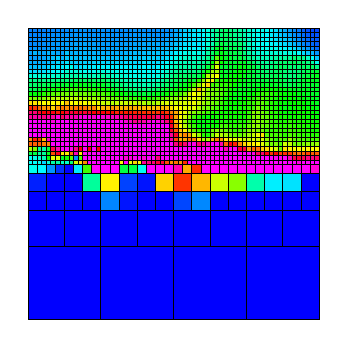
\begin{tikzpicture}[x={(\screenshotunitlength,0)},y={(0,\screenshotunitlength)}]
        \definecolor{fillcolor}{rgb}{0.000000,0.000000,1.000000}
\fill[fillcolor] (0.000000,0.000000) rectangle (0.250000,0.250000);
\definecolor{fillcolor}{rgb}{0.000000,0.000000,1.000000}
\fill[fillcolor] (0.250000,0.000000) rectangle (0.500000,0.250000);
\definecolor{fillcolor}{rgb}{0.000000,0.000001,1.000000}
\fill[fillcolor] (0.000000,0.250000) rectangle (0.125000,0.375000);
\definecolor{fillcolor}{rgb}{0.000000,0.000036,1.000000}
\fill[fillcolor] (0.125000,0.250000) rectangle (0.250000,0.375000);
\definecolor{fillcolor}{rgb}{0.000000,0.000000,1.000000}
\fill[fillcolor] (0.000000,0.375000) rectangle (0.062500,0.437500);
\definecolor{fillcolor}{rgb}{0.000000,0.000012,1.000000}
\fill[fillcolor] (0.062500,0.375000) rectangle (0.125000,0.437500);
\definecolor{fillcolor}{rgb}{0.000000,0.122688,1.000000}
\fill[fillcolor] (0.000000,0.437500) rectangle (0.062500,0.500000);
\definecolor{fillcolor}{rgb}{0.000000,0.000004,1.000000}
\fill[fillcolor] (0.062500,0.437500) rectangle (0.125000,0.500000);
\definecolor{fillcolor}{rgb}{0.000000,0.002288,1.000000}
\fill[fillcolor] (0.125000,0.375000) rectangle (0.187500,0.437500);
\definecolor{fillcolor}{rgb}{0.000000,0.005232,1.000000}
\fill[fillcolor] (0.187500,0.375000) rectangle (0.250000,0.437500);
\definecolor{fillcolor}{rgb}{0.000000,0.001281,1.000000}
\fill[fillcolor] (0.125000,0.437500) rectangle (0.187500,0.500000);
\definecolor{fillcolor}{rgb}{0.000000,1.000000,0.607760}
\fill[fillcolor] (0.187500,0.437500) rectangle (0.250000,0.500000);
\definecolor{fillcolor}{rgb}{0.000000,0.000030,1.000000}
\fill[fillcolor] (0.250000,0.250000) rectangle (0.375000,0.375000);
\definecolor{fillcolor}{rgb}{0.000000,0.000001,1.000000}
\fill[fillcolor] (0.375000,0.250000) rectangle (0.500000,0.375000);
\definecolor{fillcolor}{rgb}{0.000000,0.521022,1.000000}
\fill[fillcolor] (0.250000,0.375000) rectangle (0.312500,0.437500);
\definecolor{fillcolor}{rgb}{0.000000,0.079951,1.000000}
\fill[fillcolor] (0.312500,0.375000) rectangle (0.375000,0.437500);
\definecolor{fillcolor}{rgb}{1.000000,0.944282,0.000000}
\fill[fillcolor] (0.250000,0.437500) rectangle (0.312500,0.500000);
\definecolor{fillcolor}{rgb}{0.000000,0.260231,1.000000}
\fill[fillcolor] (0.312500,0.437500) rectangle (0.375000,0.500000);
\definecolor{fillcolor}{rgb}{0.000000,0.000000,1.000000}
\fill[fillcolor] (0.375000,0.375000) rectangle (0.437500,0.437500);
\definecolor{fillcolor}{rgb}{0.000000,0.000001,1.000000}
\fill[fillcolor] (0.437500,0.375000) rectangle (0.500000,0.437500);
\definecolor{fillcolor}{rgb}{0.000000,0.073835,1.000000}
\fill[fillcolor] (0.375000,0.437500) rectangle (0.437500,0.500000);
\definecolor{fillcolor}{rgb}{1.000000,0.825471,0.000000}
\fill[fillcolor] (0.437500,0.437500) rectangle (0.500000,0.500000);
\definecolor{fillcolor}{rgb}{0.000000,0.000000,1.000000}
\fill[fillcolor] (0.500000,0.000000) rectangle (0.750000,0.250000);
\definecolor{fillcolor}{rgb}{0.000000,0.000000,1.000000}
\fill[fillcolor] (0.750000,0.000000) rectangle (1.000000,0.250000);
\definecolor{fillcolor}{rgb}{0.000000,0.000002,1.000000}
\fill[fillcolor] (0.500000,0.250000) rectangle (0.625000,0.375000);
\definecolor{fillcolor}{rgb}{0.000000,0.000000,1.000000}
\fill[fillcolor] (0.625000,0.250000) rectangle (0.750000,0.375000);
\definecolor{fillcolor}{rgb}{0.000000,0.275273,1.000000}
\fill[fillcolor] (0.500000,0.375000) rectangle (0.562500,0.437500);
\definecolor{fillcolor}{rgb}{0.000000,0.533676,1.000000}
\fill[fillcolor] (0.562500,0.375000) rectangle (0.625000,0.437500);
\definecolor{fillcolor}{rgb}{1.000000,0.202067,0.000000}
\fill[fillcolor] (0.500000,0.437500) rectangle (0.562500,0.500000);
\definecolor{fillcolor}{rgb}{1.000000,0.716109,0.000000}
\fill[fillcolor] (0.562500,0.437500) rectangle (0.625000,0.500000);
\definecolor{fillcolor}{rgb}{0.000000,0.000000,1.000000}
\fill[fillcolor] (0.625000,0.375000) rectangle (0.687500,0.437500);
\definecolor{fillcolor}{rgb}{0.000000,0.000000,1.000000}
\fill[fillcolor] (0.687500,0.375000) rectangle (0.750000,0.437500);
\definecolor{fillcolor}{rgb}{0.797413,1.000000,0.000000}
\fill[fillcolor] (0.625000,0.437500) rectangle (0.687500,0.500000);
\definecolor{fillcolor}{rgb}{0.539113,1.000000,0.000000}
\fill[fillcolor] (0.687500,0.437500) rectangle (0.750000,0.500000);
\definecolor{fillcolor}{rgb}{0.000000,0.000000,1.000000}
\fill[fillcolor] (0.750000,0.250000) rectangle (0.875000,0.375000);
\definecolor{fillcolor}{rgb}{0.000000,0.000201,1.000000}
\fill[fillcolor] (0.875000,0.250000) rectangle (1.000000,0.375000);
\definecolor{fillcolor}{rgb}{0.000000,0.000000,1.000000}
\fill[fillcolor] (0.750000,0.375000) rectangle (0.812500,0.437500);
\definecolor{fillcolor}{rgb}{0.000000,0.000000,1.000000}
\fill[fillcolor] (0.812500,0.375000) rectangle (0.875000,0.437500);
\definecolor{fillcolor}{rgb}{0.000000,1.000000,0.671470}
\fill[fillcolor] (0.750000,0.437500) rectangle (0.812500,0.500000);
\definecolor{fillcolor}{rgb}{0.000000,0.935851,1.000000}
\fill[fillcolor] (0.812500,0.437500) rectangle (0.875000,0.500000);
\definecolor{fillcolor}{rgb}{0.000000,0.000078,1.000000}
\fill[fillcolor] (0.875000,0.375000) rectangle (0.937500,0.437500);
\definecolor{fillcolor}{rgb}{0.000000,0.000279,1.000000}
\fill[fillcolor] (0.937500,0.375000) rectangle (1.000000,0.437500);
\definecolor{fillcolor}{rgb}{0.000000,0.885875,1.000000}
\fill[fillcolor] (0.875000,0.437500) rectangle (0.937500,0.500000);
\definecolor{fillcolor}{rgb}{0.000000,0.000000,1.000000}
\fill[fillcolor] (0.937500,0.437500) rectangle (1.000000,0.500000);
\definecolor{fillcolor}{rgb}{0.000000,1.000000,0.926003}
\fill[fillcolor] (0.000000,0.500000) rectangle (0.031250,0.531250);
\definecolor{fillcolor}{rgb}{0.000000,0.980376,1.000000}
\fill[fillcolor] (0.031250,0.500000) rectangle (0.062500,0.531250);
\definecolor{fillcolor}{rgb}{0.000000,1.000000,0.977016}
\fill[fillcolor] (0.000000,0.531250) rectangle (0.015625,0.546875);
\definecolor{fillcolor}{rgb}{0.000000,1.000000,0.974008}
\fill[fillcolor] (0.015625,0.531250) rectangle (0.031250,0.546875);
\definecolor{fillcolor}{rgb}{0.000000,1.000000,0.973487}
\fill[fillcolor] (0.000000,0.546875) rectangle (0.015625,0.562500);
\definecolor{fillcolor}{rgb}{0.000000,1.000000,0.907276}
\fill[fillcolor] (0.015625,0.546875) rectangle (0.031250,0.562500);
\definecolor{fillcolor}{rgb}{0.000000,1.000000,0.941639}
\fill[fillcolor] (0.031250,0.531250) rectangle (0.046875,0.546875);
\definecolor{fillcolor}{rgb}{0.000000,0.832855,1.000000}
\fill[fillcolor] (0.046875,0.531250) rectangle (0.062500,0.546875);
\definecolor{fillcolor}{rgb}{0.000000,1.000000,0.837655}
\fill[fillcolor] (0.031250,0.546875) rectangle (0.046875,0.562500);
\definecolor{fillcolor}{rgb}{0.000000,1.000000,0.706352}
\fill[fillcolor] (0.046875,0.546875) rectangle (0.062500,0.562500);
\definecolor{fillcolor}{rgb}{0.000000,0.582229,1.000000}
\fill[fillcolor] (0.062500,0.500000) rectangle (0.093750,0.531250);
\definecolor{fillcolor}{rgb}{0.000000,0.191324,1.000000}
\fill[fillcolor] (0.093750,0.500000) rectangle (0.125000,0.531250);
\definecolor{fillcolor}{rgb}{0.000000,1.000000,0.830267}
\fill[fillcolor] (0.062500,0.531250) rectangle (0.078125,0.546875);
\definecolor{fillcolor}{rgb}{0.000000,1.000000,0.660128}
\fill[fillcolor] (0.078125,0.531250) rectangle (0.093750,0.546875);
\definecolor{fillcolor}{rgb}{0.000000,1.000000,0.057774}
\fill[fillcolor] (0.062500,0.546875) rectangle (0.078125,0.562500);
\definecolor{fillcolor}{rgb}{0.896082,1.000000,0.000000}
\fill[fillcolor] (0.078125,0.546875) rectangle (0.093750,0.562500);
\definecolor{fillcolor}{rgb}{0.000000,1.000000,0.660896}
\fill[fillcolor] (0.093750,0.531250) rectangle (0.109375,0.546875);
\definecolor{fillcolor}{rgb}{0.000000,1.000000,0.777392}
\fill[fillcolor] (0.109375,0.531250) rectangle (0.125000,0.546875);
\definecolor{fillcolor}{rgb}{0.886395,1.000000,0.000000}
\fill[fillcolor] (0.093750,0.546875) rectangle (0.109375,0.562500);
\definecolor{fillcolor}{rgb}{0.000000,1.000000,0.147599}
\fill[fillcolor] (0.109375,0.546875) rectangle (0.125000,0.562500);
\definecolor{fillcolor}{rgb}{0.000000,1.000000,0.276332}
\fill[fillcolor] (0.000000,0.562500) rectangle (0.015625,0.578125);
\definecolor{fillcolor}{rgb}{0.000000,1.000000,0.271085}
\fill[fillcolor] (0.015625,0.562500) rectangle (0.031250,0.578125);
\definecolor{fillcolor}{rgb}{0.669878,1.000000,0.000000}
\fill[fillcolor] (0.000000,0.578125) rectangle (0.015625,0.593750);
\definecolor{fillcolor}{rgb}{0.473235,1.000000,0.000000}
\fill[fillcolor] (0.015625,0.578125) rectangle (0.031250,0.593750);
\definecolor{fillcolor}{rgb}{0.000000,1.000000,0.617143}
\fill[fillcolor] (0.031250,0.562500) rectangle (0.046875,0.578125);
\definecolor{fillcolor}{rgb}{0.000000,1.000000,0.578473}
\fill[fillcolor] (0.046875,0.562500) rectangle (0.062500,0.578125);
\definecolor{fillcolor}{rgb}{0.000000,1.000000,0.588717}
\fill[fillcolor] (0.031250,0.578125) rectangle (0.046875,0.593750);
\definecolor{fillcolor}{rgb}{0.000000,1.000000,0.655292}
\fill[fillcolor] (0.046875,0.578125) rectangle (0.062500,0.593750);
\definecolor{fillcolor}{rgb}{1.000000,0.383206,0.000000}
\fill[fillcolor] (0.000000,0.593750) rectangle (0.015625,0.609375);
\definecolor{fillcolor}{rgb}{1.000000,0.367907,0.000000}
\fill[fillcolor] (0.015625,0.593750) rectangle (0.031250,0.609375);
\definecolor{fillcolor}{rgb}{1.000000,0.548240,0.000000}
\fill[fillcolor] (0.000000,0.609375) rectangle (0.015625,0.625000);
\definecolor{fillcolor}{rgb}{1.000000,0.150367,0.000000}
\fill[fillcolor] (0.015625,0.609375) rectangle (0.031250,0.625000);
\definecolor{fillcolor}{rgb}{1.000000,0.380159,0.000000}
\fill[fillcolor] (0.031250,0.593750) rectangle (0.046875,0.609375);
\definecolor{fillcolor}{rgb}{1.000000,0.470043,0.000000}
\fill[fillcolor] (0.046875,0.593750) rectangle (0.062500,0.609375);
\definecolor{fillcolor}{rgb}{1.000000,0.215243,0.000000}
\fill[fillcolor] (0.031250,0.609375) rectangle (0.046875,0.625000);
\definecolor{fillcolor}{rgb}{1.000000,0.742591,0.000000}
\fill[fillcolor] (0.046875,0.609375) rectangle (0.062500,0.625000);
\definecolor{fillcolor}{rgb}{0.000000,1.000000,0.116529}
\fill[fillcolor] (0.062500,0.562500) rectangle (0.078125,0.578125);
\definecolor{fillcolor}{rgb}{1.000000,0.293400,0.000000}
\fill[fillcolor] (0.078125,0.562500) rectangle (0.093750,0.578125);
\definecolor{fillcolor}{rgb}{0.000000,1.000000,0.225006}
\fill[fillcolor] (0.062500,0.578125) rectangle (0.078125,0.593750);
\definecolor{fillcolor}{rgb}{1.000000,0.000000,0.320551}
\fill[fillcolor] (0.078125,0.578125) rectangle (0.093750,0.593750);
\definecolor{fillcolor}{rgb}{1.000000,0.000000,0.114320}
\fill[fillcolor] (0.093750,0.562500) rectangle (0.109375,0.578125);
\definecolor{fillcolor}{rgb}{1.000000,0.918071,0.000000}
\fill[fillcolor] (0.109375,0.562500) rectangle (0.125000,0.578125);
\definecolor{fillcolor}{rgb}{1.000000,0.000000,0.703169}
\fill[fillcolor] (0.093750,0.578125) rectangle (0.109375,0.593750);
\definecolor{fillcolor}{rgb}{1.000000,0.000000,1.000000}
\fill[fillcolor] (0.109375,0.578125) rectangle (0.125000,0.593750);
\definecolor{fillcolor}{rgb}{1.000000,0.504168,0.000000}
\fill[fillcolor] (0.062500,0.593750) rectangle (0.078125,0.609375);
\definecolor{fillcolor}{rgb}{1.000000,0.000000,1.000000}
\fill[fillcolor] (0.078125,0.593750) rectangle (0.093750,0.609375);
\definecolor{fillcolor}{rgb}{1.000000,0.000000,0.785132}
\fill[fillcolor] (0.062500,0.609375) rectangle (0.078125,0.625000);
\definecolor{fillcolor}{rgb}{1.000000,0.000000,1.000000}
\fill[fillcolor] (0.078125,0.609375) rectangle (0.093750,0.625000);
\definecolor{fillcolor}{rgb}{1.000000,0.000000,1.000000}
\fill[fillcolor] (0.093750,0.593750) rectangle (0.109375,0.609375);
\definecolor{fillcolor}{rgb}{1.000000,0.000000,1.000000}
\fill[fillcolor] (0.109375,0.593750) rectangle (0.125000,0.609375);
\definecolor{fillcolor}{rgb}{1.000000,0.000000,1.000000}
\fill[fillcolor] (0.093750,0.609375) rectangle (0.109375,0.625000);
\definecolor{fillcolor}{rgb}{1.000000,0.000000,1.000000}
\fill[fillcolor] (0.109375,0.609375) rectangle (0.125000,0.625000);
\definecolor{fillcolor}{rgb}{0.000000,0.000930,1.000000}
\fill[fillcolor] (0.125000,0.500000) rectangle (0.156250,0.531250);
\definecolor{fillcolor}{rgb}{0.000000,0.924896,1.000000}
\fill[fillcolor] (0.156250,0.500000) rectangle (0.187500,0.531250);
\definecolor{fillcolor}{rgb}{0.000000,1.000000,0.809268}
\fill[fillcolor] (0.125000,0.531250) rectangle (0.140625,0.546875);
\definecolor{fillcolor}{rgb}{0.000000,1.000000,0.475066}
\fill[fillcolor] (0.140625,0.531250) rectangle (0.156250,0.546875);
\definecolor{fillcolor}{rgb}{0.070463,1.000000,0.000000}
\fill[fillcolor] (0.125000,0.546875) rectangle (0.140625,0.562500);
\definecolor{fillcolor}{rgb}{0.327973,1.000000,0.000000}
\fill[fillcolor] (0.140625,0.546875) rectangle (0.156250,0.562500);
\definecolor{fillcolor}{rgb}{0.799172,1.000000,0.000000}
\fill[fillcolor] (0.156250,0.531250) rectangle (0.171875,0.546875);
\definecolor{fillcolor}{rgb}{1.000000,0.910316,0.000000}
\fill[fillcolor] (0.171875,0.531250) rectangle (0.187500,0.546875);
\definecolor{fillcolor}{rgb}{0.000000,0.569968,1.000000}
\fill[fillcolor] (0.156250,0.546875) rectangle (0.171875,0.562500);
\definecolor{fillcolor}{rgb}{0.306226,1.000000,0.000000}
\fill[fillcolor] (0.171875,0.546875) rectangle (0.187500,0.562500);
\definecolor{fillcolor}{rgb}{0.244155,1.000000,0.000000}
\fill[fillcolor] (0.187500,0.500000) rectangle (0.218750,0.531250);
\definecolor{fillcolor}{rgb}{1.000000,0.000000,1.000000}
\fill[fillcolor] (0.218750,0.500000) rectangle (0.250000,0.531250);
\definecolor{fillcolor}{rgb}{1.000000,0.546101,0.000000}
\fill[fillcolor] (0.187500,0.531250) rectangle (0.203125,0.546875);
\definecolor{fillcolor}{rgb}{1.000000,0.000000,1.000000}
\fill[fillcolor] (0.203125,0.531250) rectangle (0.218750,0.546875);
\definecolor{fillcolor}{rgb}{1.000000,0.000000,1.000000}
\fill[fillcolor] (0.187500,0.546875) rectangle (0.203125,0.562500);
\definecolor{fillcolor}{rgb}{1.000000,0.000000,1.000000}
\fill[fillcolor] (0.203125,0.546875) rectangle (0.218750,0.562500);
\definecolor{fillcolor}{rgb}{1.000000,0.000000,1.000000}
\fill[fillcolor] (0.218750,0.531250) rectangle (0.234375,0.546875);
\definecolor{fillcolor}{rgb}{1.000000,0.000000,1.000000}
\fill[fillcolor] (0.234375,0.531250) rectangle (0.250000,0.546875);
\definecolor{fillcolor}{rgb}{1.000000,0.000000,1.000000}
\fill[fillcolor] (0.218750,0.546875) rectangle (0.234375,0.562500);
\definecolor{fillcolor}{rgb}{1.000000,0.000000,1.000000}
\fill[fillcolor] (0.234375,0.546875) rectangle (0.250000,0.562500);
\definecolor{fillcolor}{rgb}{1.000000,0.920497,0.000000}
\fill[fillcolor] (0.125000,0.562500) rectangle (0.140625,0.578125);
\definecolor{fillcolor}{rgb}{1.000000,0.445763,0.000000}
\fill[fillcolor] (0.140625,0.562500) rectangle (0.156250,0.578125);
\definecolor{fillcolor}{rgb}{1.000000,0.000000,1.000000}
\fill[fillcolor] (0.125000,0.578125) rectangle (0.140625,0.593750);
\definecolor{fillcolor}{rgb}{1.000000,0.000000,0.936766}
\fill[fillcolor] (0.140625,0.578125) rectangle (0.156250,0.593750);
\definecolor{fillcolor}{rgb}{1.000000,0.000000,0.729485}
\fill[fillcolor] (0.156250,0.562500) rectangle (0.171875,0.578125);
\definecolor{fillcolor}{rgb}{1.000000,0.926187,0.000000}
\fill[fillcolor] (0.171875,0.562500) rectangle (0.187500,0.578125);
\definecolor{fillcolor}{rgb}{1.000000,0.000000,0.559413}
\fill[fillcolor] (0.156250,0.578125) rectangle (0.171875,0.593750);
\definecolor{fillcolor}{rgb}{1.000000,0.000000,0.014768}
\fill[fillcolor] (0.171875,0.578125) rectangle (0.187500,0.593750);
\definecolor{fillcolor}{rgb}{1.000000,0.000000,1.000000}
\fill[fillcolor] (0.125000,0.593750) rectangle (0.140625,0.609375);
\definecolor{fillcolor}{rgb}{1.000000,0.000000,1.000000}
\fill[fillcolor] (0.140625,0.593750) rectangle (0.156250,0.609375);
\definecolor{fillcolor}{rgb}{1.000000,0.000000,1.000000}
\fill[fillcolor] (0.125000,0.609375) rectangle (0.140625,0.625000);
\definecolor{fillcolor}{rgb}{1.000000,0.000000,1.000000}
\fill[fillcolor] (0.140625,0.609375) rectangle (0.156250,0.625000);
\definecolor{fillcolor}{rgb}{1.000000,0.000000,1.000000}
\fill[fillcolor] (0.156250,0.593750) rectangle (0.171875,0.609375);
\definecolor{fillcolor}{rgb}{1.000000,0.000000,1.000000}
\fill[fillcolor] (0.171875,0.593750) rectangle (0.187500,0.609375);
\definecolor{fillcolor}{rgb}{1.000000,0.000000,1.000000}
\fill[fillcolor] (0.156250,0.609375) rectangle (0.171875,0.625000);
\definecolor{fillcolor}{rgb}{1.000000,0.000000,1.000000}
\fill[fillcolor] (0.171875,0.609375) rectangle (0.187500,0.625000);
\definecolor{fillcolor}{rgb}{1.000000,0.000000,1.000000}
\fill[fillcolor] (0.187500,0.562500) rectangle (0.203125,0.578125);
\definecolor{fillcolor}{rgb}{1.000000,0.000000,1.000000}
\fill[fillcolor] (0.203125,0.562500) rectangle (0.218750,0.578125);
\definecolor{fillcolor}{rgb}{1.000000,0.000000,0.975623}
\fill[fillcolor] (0.187500,0.578125) rectangle (0.203125,0.593750);
\definecolor{fillcolor}{rgb}{1.000000,0.000000,0.051706}
\fill[fillcolor] (0.203125,0.578125) rectangle (0.218750,0.593750);
\definecolor{fillcolor}{rgb}{1.000000,0.000000,1.000000}
\fill[fillcolor] (0.218750,0.562500) rectangle (0.234375,0.578125);
\definecolor{fillcolor}{rgb}{1.000000,0.000000,1.000000}
\fill[fillcolor] (0.234375,0.562500) rectangle (0.250000,0.578125);
\definecolor{fillcolor}{rgb}{1.000000,0.000000,1.000000}
\fill[fillcolor] (0.218750,0.578125) rectangle (0.234375,0.593750);
\definecolor{fillcolor}{rgb}{1.000000,0.028828,0.000000}
\fill[fillcolor] (0.234375,0.578125) rectangle (0.250000,0.593750);
\definecolor{fillcolor}{rgb}{1.000000,0.000000,1.000000}
\fill[fillcolor] (0.187500,0.593750) rectangle (0.203125,0.609375);
\definecolor{fillcolor}{rgb}{1.000000,0.000000,1.000000}
\fill[fillcolor] (0.203125,0.593750) rectangle (0.218750,0.609375);
\definecolor{fillcolor}{rgb}{1.000000,0.000000,1.000000}
\fill[fillcolor] (0.187500,0.609375) rectangle (0.203125,0.625000);
\definecolor{fillcolor}{rgb}{1.000000,0.000000,1.000000}
\fill[fillcolor] (0.203125,0.609375) rectangle (0.218750,0.625000);
\definecolor{fillcolor}{rgb}{1.000000,0.000000,1.000000}
\fill[fillcolor] (0.218750,0.593750) rectangle (0.234375,0.609375);
\definecolor{fillcolor}{rgb}{1.000000,0.000000,1.000000}
\fill[fillcolor] (0.234375,0.593750) rectangle (0.250000,0.609375);
\definecolor{fillcolor}{rgb}{1.000000,0.000000,1.000000}
\fill[fillcolor] (0.218750,0.609375) rectangle (0.234375,0.625000);
\definecolor{fillcolor}{rgb}{1.000000,0.000000,1.000000}
\fill[fillcolor] (0.234375,0.609375) rectangle (0.250000,0.625000);
\definecolor{fillcolor}{rgb}{1.000000,0.000000,1.000000}
\fill[fillcolor] (0.000000,0.625000) rectangle (0.015625,0.640625);
\definecolor{fillcolor}{rgb}{1.000000,0.000000,1.000000}
\fill[fillcolor] (0.015625,0.625000) rectangle (0.031250,0.640625);
\definecolor{fillcolor}{rgb}{1.000000,0.000000,1.000000}
\fill[fillcolor] (0.000000,0.640625) rectangle (0.015625,0.656250);
\definecolor{fillcolor}{rgb}{1.000000,0.000000,1.000000}
\fill[fillcolor] (0.015625,0.640625) rectangle (0.031250,0.656250);
\definecolor{fillcolor}{rgb}{1.000000,0.000000,1.000000}
\fill[fillcolor] (0.031250,0.625000) rectangle (0.046875,0.640625);
\definecolor{fillcolor}{rgb}{1.000000,0.000000,1.000000}
\fill[fillcolor] (0.046875,0.625000) rectangle (0.062500,0.640625);
\definecolor{fillcolor}{rgb}{1.000000,0.000000,1.000000}
\fill[fillcolor] (0.031250,0.640625) rectangle (0.046875,0.656250);
\definecolor{fillcolor}{rgb}{1.000000,0.000000,1.000000}
\fill[fillcolor] (0.046875,0.640625) rectangle (0.062500,0.656250);
\definecolor{fillcolor}{rgb}{1.000000,0.000000,1.000000}
\fill[fillcolor] (0.000000,0.656250) rectangle (0.015625,0.671875);
\definecolor{fillcolor}{rgb}{1.000000,0.000000,1.000000}
\fill[fillcolor] (0.015625,0.656250) rectangle (0.031250,0.671875);
\definecolor{fillcolor}{rgb}{1.000000,0.000000,1.000000}
\fill[fillcolor] (0.000000,0.671875) rectangle (0.015625,0.687500);
\definecolor{fillcolor}{rgb}{1.000000,0.000000,1.000000}
\fill[fillcolor] (0.015625,0.671875) rectangle (0.031250,0.687500);
\definecolor{fillcolor}{rgb}{1.000000,0.000000,1.000000}
\fill[fillcolor] (0.031250,0.656250) rectangle (0.046875,0.671875);
\definecolor{fillcolor}{rgb}{1.000000,0.000000,1.000000}
\fill[fillcolor] (0.046875,0.656250) rectangle (0.062500,0.671875);
\definecolor{fillcolor}{rgb}{1.000000,0.000000,1.000000}
\fill[fillcolor] (0.031250,0.671875) rectangle (0.046875,0.687500);
\definecolor{fillcolor}{rgb}{1.000000,0.000000,1.000000}
\fill[fillcolor] (0.046875,0.671875) rectangle (0.062500,0.687500);
\definecolor{fillcolor}{rgb}{1.000000,0.000000,1.000000}
\fill[fillcolor] (0.062500,0.625000) rectangle (0.078125,0.640625);
\definecolor{fillcolor}{rgb}{1.000000,0.000000,1.000000}
\fill[fillcolor] (0.078125,0.625000) rectangle (0.093750,0.640625);
\definecolor{fillcolor}{rgb}{1.000000,0.000000,1.000000}
\fill[fillcolor] (0.062500,0.640625) rectangle (0.078125,0.656250);
\definecolor{fillcolor}{rgb}{1.000000,0.000000,1.000000}
\fill[fillcolor] (0.078125,0.640625) rectangle (0.093750,0.656250);
\definecolor{fillcolor}{rgb}{1.000000,0.000000,1.000000}
\fill[fillcolor] (0.093750,0.625000) rectangle (0.109375,0.640625);
\definecolor{fillcolor}{rgb}{1.000000,0.000000,1.000000}
\fill[fillcolor] (0.109375,0.625000) rectangle (0.125000,0.640625);
\definecolor{fillcolor}{rgb}{1.000000,0.000000,1.000000}
\fill[fillcolor] (0.093750,0.640625) rectangle (0.109375,0.656250);
\definecolor{fillcolor}{rgb}{1.000000,0.000000,1.000000}
\fill[fillcolor] (0.109375,0.640625) rectangle (0.125000,0.656250);
\definecolor{fillcolor}{rgb}{1.000000,0.000000,1.000000}
\fill[fillcolor] (0.062500,0.656250) rectangle (0.078125,0.671875);
\definecolor{fillcolor}{rgb}{1.000000,0.000000,1.000000}
\fill[fillcolor] (0.078125,0.656250) rectangle (0.093750,0.671875);
\definecolor{fillcolor}{rgb}{1.000000,0.000000,1.000000}
\fill[fillcolor] (0.062500,0.671875) rectangle (0.078125,0.687500);
\definecolor{fillcolor}{rgb}{1.000000,0.000000,0.863746}
\fill[fillcolor] (0.078125,0.671875) rectangle (0.093750,0.687500);
\definecolor{fillcolor}{rgb}{1.000000,0.000000,0.919675}
\fill[fillcolor] (0.093750,0.656250) rectangle (0.109375,0.671875);
\definecolor{fillcolor}{rgb}{1.000000,0.000000,0.973565}
\fill[fillcolor] (0.109375,0.656250) rectangle (0.125000,0.671875);
\definecolor{fillcolor}{rgb}{1.000000,0.000000,1.000000}
\fill[fillcolor] (0.093750,0.671875) rectangle (0.109375,0.687500);
\definecolor{fillcolor}{rgb}{1.000000,0.000000,1.000000}
\fill[fillcolor] (0.109375,0.671875) rectangle (0.125000,0.687500);
\definecolor{fillcolor}{rgb}{1.000000,0.000000,0.605926}
\fill[fillcolor] (0.000000,0.687500) rectangle (0.015625,0.703125);
\definecolor{fillcolor}{rgb}{1.000000,0.000000,0.668451}
\fill[fillcolor] (0.015625,0.687500) rectangle (0.031250,0.703125);
\definecolor{fillcolor}{rgb}{1.000000,0.000000,0.418991}
\fill[fillcolor] (0.000000,0.703125) rectangle (0.015625,0.718750);
\definecolor{fillcolor}{rgb}{1.000000,0.000000,0.468309}
\fill[fillcolor] (0.015625,0.703125) rectangle (0.031250,0.718750);
\definecolor{fillcolor}{rgb}{1.000000,0.000000,0.633583}
\fill[fillcolor] (0.031250,0.687500) rectangle (0.046875,0.703125);
\definecolor{fillcolor}{rgb}{1.000000,0.000000,0.500657}
\fill[fillcolor] (0.046875,0.687500) rectangle (0.062500,0.703125);
\definecolor{fillcolor}{rgb}{1.000000,0.000000,0.164482}
\fill[fillcolor] (0.031250,0.703125) rectangle (0.046875,0.718750);
\definecolor{fillcolor}{rgb}{1.000000,0.000000,0.007309}
\fill[fillcolor] (0.046875,0.703125) rectangle (0.062500,0.718750);
\definecolor{fillcolor}{rgb}{1.000000,0.141176,0.000000}
\fill[fillcolor] (0.000000,0.718750) rectangle (0.015625,0.734375);
\definecolor{fillcolor}{rgb}{1.000000,0.209985,0.000000}
\fill[fillcolor] (0.015625,0.718750) rectangle (0.031250,0.734375);
\definecolor{fillcolor}{rgb}{1.000000,0.882566,0.000000}
\fill[fillcolor] (0.000000,0.734375) rectangle (0.015625,0.750000);
\definecolor{fillcolor}{rgb}{1.000000,0.898434,0.000000}
\fill[fillcolor] (0.015625,0.734375) rectangle (0.031250,0.750000);
\definecolor{fillcolor}{rgb}{1.000000,0.423072,0.000000}
\fill[fillcolor] (0.031250,0.718750) rectangle (0.046875,0.734375);
\definecolor{fillcolor}{rgb}{1.000000,0.589105,0.000000}
\fill[fillcolor] (0.046875,0.718750) rectangle (0.062500,0.734375);
\definecolor{fillcolor}{rgb}{1.000000,0.989398,0.000000}
\fill[fillcolor] (0.031250,0.734375) rectangle (0.046875,0.750000);
\definecolor{fillcolor}{rgb}{0.975179,1.000000,0.000000}
\fill[fillcolor] (0.046875,0.734375) rectangle (0.062500,0.750000);
\definecolor{fillcolor}{rgb}{1.000000,0.000000,0.632869}
\fill[fillcolor] (0.062500,0.687500) rectangle (0.078125,0.703125);
\definecolor{fillcolor}{rgb}{1.000000,0.000000,0.610541}
\fill[fillcolor] (0.078125,0.687500) rectangle (0.093750,0.703125);
\definecolor{fillcolor}{rgb}{1.000000,0.000000,0.025815}
\fill[fillcolor] (0.062500,0.703125) rectangle (0.078125,0.718750);
\definecolor{fillcolor}{rgb}{1.000000,0.000000,0.081810}
\fill[fillcolor] (0.078125,0.703125) rectangle (0.093750,0.718750);
\definecolor{fillcolor}{rgb}{1.000000,0.000000,0.869687}
\fill[fillcolor] (0.093750,0.687500) rectangle (0.109375,0.703125);
\definecolor{fillcolor}{rgb}{1.000000,0.000000,0.362009}
\fill[fillcolor] (0.109375,0.687500) rectangle (0.125000,0.703125);
\definecolor{fillcolor}{rgb}{1.000000,0.101334,0.000000}
\fill[fillcolor] (0.093750,0.703125) rectangle (0.109375,0.718750);
\definecolor{fillcolor}{rgb}{1.000000,0.035298,0.000000}
\fill[fillcolor] (0.109375,0.703125) rectangle (0.125000,0.718750);
\definecolor{fillcolor}{rgb}{1.000000,0.591022,0.000000}
\fill[fillcolor] (0.062500,0.718750) rectangle (0.078125,0.734375);
\definecolor{fillcolor}{rgb}{1.000000,0.832202,0.000000}
\fill[fillcolor] (0.078125,0.718750) rectangle (0.093750,0.734375);
\definecolor{fillcolor}{rgb}{1.000000,0.989785,0.000000}
\fill[fillcolor] (0.062500,0.734375) rectangle (0.078125,0.750000);
\definecolor{fillcolor}{rgb}{0.995933,1.000000,0.000000}
\fill[fillcolor] (0.078125,0.734375) rectangle (0.093750,0.750000);
\definecolor{fillcolor}{rgb}{1.000000,0.591817,0.000000}
\fill[fillcolor] (0.093750,0.718750) rectangle (0.109375,0.734375);
\definecolor{fillcolor}{rgb}{1.000000,0.453766,0.000000}
\fill[fillcolor] (0.109375,0.718750) rectangle (0.125000,0.734375);
\definecolor{fillcolor}{rgb}{1.000000,0.968161,0.000000}
\fill[fillcolor] (0.093750,0.734375) rectangle (0.109375,0.750000);
\definecolor{fillcolor}{rgb}{0.968309,1.000000,0.000000}
\fill[fillcolor] (0.109375,0.734375) rectangle (0.125000,0.750000);
\definecolor{fillcolor}{rgb}{1.000000,0.000000,1.000000}
\fill[fillcolor] (0.125000,0.625000) rectangle (0.140625,0.640625);
\definecolor{fillcolor}{rgb}{1.000000,0.000000,1.000000}
\fill[fillcolor] (0.140625,0.625000) rectangle (0.156250,0.640625);
\definecolor{fillcolor}{rgb}{1.000000,0.000000,1.000000}
\fill[fillcolor] (0.125000,0.640625) rectangle (0.140625,0.656250);
\definecolor{fillcolor}{rgb}{1.000000,0.000000,1.000000}
\fill[fillcolor] (0.140625,0.640625) rectangle (0.156250,0.656250);
\definecolor{fillcolor}{rgb}{1.000000,0.000000,1.000000}
\fill[fillcolor] (0.156250,0.625000) rectangle (0.171875,0.640625);
\definecolor{fillcolor}{rgb}{1.000000,0.000000,1.000000}
\fill[fillcolor] (0.171875,0.625000) rectangle (0.187500,0.640625);
\definecolor{fillcolor}{rgb}{1.000000,0.000000,1.000000}
\fill[fillcolor] (0.156250,0.640625) rectangle (0.171875,0.656250);
\definecolor{fillcolor}{rgb}{1.000000,0.000000,1.000000}
\fill[fillcolor] (0.171875,0.640625) rectangle (0.187500,0.656250);
\definecolor{fillcolor}{rgb}{1.000000,0.000000,1.000000}
\fill[fillcolor] (0.125000,0.656250) rectangle (0.140625,0.671875);
\definecolor{fillcolor}{rgb}{1.000000,0.000000,1.000000}
\fill[fillcolor] (0.140625,0.656250) rectangle (0.156250,0.671875);
\definecolor{fillcolor}{rgb}{1.000000,0.000000,1.000000}
\fill[fillcolor] (0.125000,0.671875) rectangle (0.140625,0.687500);
\definecolor{fillcolor}{rgb}{1.000000,0.000000,1.000000}
\fill[fillcolor] (0.140625,0.671875) rectangle (0.156250,0.687500);
\definecolor{fillcolor}{rgb}{1.000000,0.000000,1.000000}
\fill[fillcolor] (0.156250,0.656250) rectangle (0.171875,0.671875);
\definecolor{fillcolor}{rgb}{1.000000,0.000000,1.000000}
\fill[fillcolor] (0.171875,0.656250) rectangle (0.187500,0.671875);
\definecolor{fillcolor}{rgb}{1.000000,0.000000,1.000000}
\fill[fillcolor] (0.156250,0.671875) rectangle (0.171875,0.687500);
\definecolor{fillcolor}{rgb}{1.000000,0.000000,1.000000}
\fill[fillcolor] (0.171875,0.671875) rectangle (0.187500,0.687500);
\definecolor{fillcolor}{rgb}{1.000000,0.000000,1.000000}
\fill[fillcolor] (0.187500,0.625000) rectangle (0.203125,0.640625);
\definecolor{fillcolor}{rgb}{1.000000,0.000000,1.000000}
\fill[fillcolor] (0.203125,0.625000) rectangle (0.218750,0.640625);
\definecolor{fillcolor}{rgb}{1.000000,0.000000,1.000000}
\fill[fillcolor] (0.187500,0.640625) rectangle (0.203125,0.656250);
\definecolor{fillcolor}{rgb}{1.000000,0.000000,1.000000}
\fill[fillcolor] (0.203125,0.640625) rectangle (0.218750,0.656250);
\definecolor{fillcolor}{rgb}{1.000000,0.000000,1.000000}
\fill[fillcolor] (0.218750,0.625000) rectangle (0.234375,0.640625);
\definecolor{fillcolor}{rgb}{1.000000,0.000000,1.000000}
\fill[fillcolor] (0.234375,0.625000) rectangle (0.250000,0.640625);
\definecolor{fillcolor}{rgb}{1.000000,0.000000,1.000000}
\fill[fillcolor] (0.218750,0.640625) rectangle (0.234375,0.656250);
\definecolor{fillcolor}{rgb}{1.000000,0.000000,1.000000}
\fill[fillcolor] (0.234375,0.640625) rectangle (0.250000,0.656250);
\definecolor{fillcolor}{rgb}{1.000000,0.000000,1.000000}
\fill[fillcolor] (0.187500,0.656250) rectangle (0.203125,0.671875);
\definecolor{fillcolor}{rgb}{1.000000,0.000000,1.000000}
\fill[fillcolor] (0.203125,0.656250) rectangle (0.218750,0.671875);
\definecolor{fillcolor}{rgb}{1.000000,0.000000,1.000000}
\fill[fillcolor] (0.187500,0.671875) rectangle (0.203125,0.687500);
\definecolor{fillcolor}{rgb}{1.000000,0.000000,1.000000}
\fill[fillcolor] (0.203125,0.671875) rectangle (0.218750,0.687500);
\definecolor{fillcolor}{rgb}{1.000000,0.000000,1.000000}
\fill[fillcolor] (0.218750,0.656250) rectangle (0.234375,0.671875);
\definecolor{fillcolor}{rgb}{1.000000,0.000000,1.000000}
\fill[fillcolor] (0.234375,0.656250) rectangle (0.250000,0.671875);
\definecolor{fillcolor}{rgb}{1.000000,0.000000,1.000000}
\fill[fillcolor] (0.218750,0.671875) rectangle (0.234375,0.687500);
\definecolor{fillcolor}{rgb}{1.000000,0.000000,1.000000}
\fill[fillcolor] (0.234375,0.671875) rectangle (0.250000,0.687500);
\definecolor{fillcolor}{rgb}{1.000000,0.000000,0.594234}
\fill[fillcolor] (0.125000,0.687500) rectangle (0.140625,0.703125);
\definecolor{fillcolor}{rgb}{1.000000,0.000000,0.673204}
\fill[fillcolor] (0.140625,0.687500) rectangle (0.156250,0.703125);
\definecolor{fillcolor}{rgb}{1.000000,0.000000,0.184223}
\fill[fillcolor] (0.125000,0.703125) rectangle (0.140625,0.718750);
\definecolor{fillcolor}{rgb}{1.000000,0.000000,0.238293}
\fill[fillcolor] (0.140625,0.703125) rectangle (0.156250,0.718750);
\definecolor{fillcolor}{rgb}{1.000000,0.000000,0.699542}
\fill[fillcolor] (0.156250,0.687500) rectangle (0.171875,0.703125);
\definecolor{fillcolor}{rgb}{1.000000,0.000000,0.833468}
\fill[fillcolor] (0.171875,0.687500) rectangle (0.187500,0.703125);
\definecolor{fillcolor}{rgb}{1.000000,0.000000,0.175726}
\fill[fillcolor] (0.156250,0.703125) rectangle (0.171875,0.718750);
\definecolor{fillcolor}{rgb}{1.000000,0.000000,0.153244}
\fill[fillcolor] (0.171875,0.703125) rectangle (0.187500,0.718750);
\definecolor{fillcolor}{rgb}{1.000000,0.549529,0.000000}
\fill[fillcolor] (0.125000,0.718750) rectangle (0.140625,0.734375);
\definecolor{fillcolor}{rgb}{1.000000,0.500955,0.000000}
\fill[fillcolor] (0.140625,0.718750) rectangle (0.156250,0.734375);
\definecolor{fillcolor}{rgb}{1.000000,0.760822,0.000000}
\fill[fillcolor] (0.125000,0.734375) rectangle (0.140625,0.750000);
\definecolor{fillcolor}{rgb}{1.000000,0.979393,0.000000}
\fill[fillcolor] (0.140625,0.734375) rectangle (0.156250,0.750000);
\definecolor{fillcolor}{rgb}{1.000000,0.442532,0.000000}
\fill[fillcolor] (0.156250,0.718750) rectangle (0.171875,0.734375);
\definecolor{fillcolor}{rgb}{1.000000,0.430832,0.000000}
\fill[fillcolor] (0.171875,0.718750) rectangle (0.187500,0.734375);
\definecolor{fillcolor}{rgb}{0.954781,1.000000,0.000000}
\fill[fillcolor] (0.156250,0.734375) rectangle (0.171875,0.750000);
\definecolor{fillcolor}{rgb}{1.000000,0.945126,0.000000}
\fill[fillcolor] (0.171875,0.734375) rectangle (0.187500,0.750000);
\definecolor{fillcolor}{rgb}{1.000000,0.000000,0.890206}
\fill[fillcolor] (0.187500,0.687500) rectangle (0.203125,0.703125);
\definecolor{fillcolor}{rgb}{1.000000,0.000000,0.869548}
\fill[fillcolor] (0.203125,0.687500) rectangle (0.218750,0.703125);
\definecolor{fillcolor}{rgb}{1.000000,0.000000,0.182837}
\fill[fillcolor] (0.187500,0.703125) rectangle (0.203125,0.718750);
\definecolor{fillcolor}{rgb}{1.000000,0.000000,0.159362}
\fill[fillcolor] (0.203125,0.703125) rectangle (0.218750,0.718750);
\definecolor{fillcolor}{rgb}{1.000000,0.000000,0.776047}
\fill[fillcolor] (0.218750,0.687500) rectangle (0.234375,0.703125);
\definecolor{fillcolor}{rgb}{1.000000,0.000000,0.999270}
\fill[fillcolor] (0.234375,0.687500) rectangle (0.250000,0.703125);
\definecolor{fillcolor}{rgb}{1.000000,0.000000,0.012075}
\fill[fillcolor] (0.218750,0.703125) rectangle (0.234375,0.718750);
\definecolor{fillcolor}{rgb}{1.000000,0.000000,0.030219}
\fill[fillcolor] (0.234375,0.703125) rectangle (0.250000,0.718750);
\definecolor{fillcolor}{rgb}{1.000000,0.450246,0.000000}
\fill[fillcolor] (0.187500,0.718750) rectangle (0.203125,0.734375);
\definecolor{fillcolor}{rgb}{1.000000,0.604223,0.000000}
\fill[fillcolor] (0.203125,0.718750) rectangle (0.218750,0.734375);
\definecolor{fillcolor}{rgb}{0.963388,1.000000,0.000000}
\fill[fillcolor] (0.187500,0.734375) rectangle (0.203125,0.750000);
\definecolor{fillcolor}{rgb}{0.964904,1.000000,0.000000}
\fill[fillcolor] (0.203125,0.734375) rectangle (0.218750,0.750000);
\definecolor{fillcolor}{rgb}{1.000000,0.532920,0.000000}
\fill[fillcolor] (0.218750,0.718750) rectangle (0.234375,0.734375);
\definecolor{fillcolor}{rgb}{1.000000,0.832541,0.000000}
\fill[fillcolor] (0.234375,0.718750) rectangle (0.250000,0.734375);
\definecolor{fillcolor}{rgb}{0.913178,1.000000,0.000000}
\fill[fillcolor] (0.218750,0.734375) rectangle (0.234375,0.750000);
\definecolor{fillcolor}{rgb}{0.885567,1.000000,0.000000}
\fill[fillcolor] (0.234375,0.734375) rectangle (0.250000,0.750000);
\definecolor{fillcolor}{rgb}{1.000000,0.000000,1.000000}
\fill[fillcolor] (0.250000,0.500000) rectangle (0.281250,0.531250);
\definecolor{fillcolor}{rgb}{1.000000,0.000000,1.000000}
\fill[fillcolor] (0.281250,0.500000) rectangle (0.312500,0.531250);
\definecolor{fillcolor}{rgb}{1.000000,0.000000,1.000000}
\fill[fillcolor] (0.250000,0.531250) rectangle (0.265625,0.546875);
\definecolor{fillcolor}{rgb}{1.000000,0.000000,1.000000}
\fill[fillcolor] (0.265625,0.531250) rectangle (0.281250,0.546875);
\definecolor{fillcolor}{rgb}{1.000000,0.000000,1.000000}
\fill[fillcolor] (0.250000,0.546875) rectangle (0.265625,0.562500);
\definecolor{fillcolor}{rgb}{1.000000,0.000000,1.000000}
\fill[fillcolor] (0.265625,0.546875) rectangle (0.281250,0.562500);
\definecolor{fillcolor}{rgb}{1.000000,0.000000,1.000000}
\fill[fillcolor] (0.281250,0.531250) rectangle (0.296875,0.546875);
\definecolor{fillcolor}{rgb}{1.000000,0.000000,1.000000}
\fill[fillcolor] (0.296875,0.531250) rectangle (0.312500,0.546875);
\definecolor{fillcolor}{rgb}{1.000000,0.000000,1.000000}
\fill[fillcolor] (0.281250,0.546875) rectangle (0.296875,0.562500);
\definecolor{fillcolor}{rgb}{1.000000,0.000000,1.000000}
\fill[fillcolor] (0.296875,0.546875) rectangle (0.312500,0.562500);
\definecolor{fillcolor}{rgb}{0.000000,1.000000,0.270466}
\fill[fillcolor] (0.312500,0.500000) rectangle (0.343750,0.531250);
\definecolor{fillcolor}{rgb}{0.000000,1.000000,0.264856}
\fill[fillcolor] (0.343750,0.500000) rectangle (0.375000,0.531250);
\definecolor{fillcolor}{rgb}{1.000000,0.972292,0.000000}
\fill[fillcolor] (0.312500,0.531250) rectangle (0.328125,0.546875);
\definecolor{fillcolor}{rgb}{1.000000,0.000000,1.000000}
\fill[fillcolor] (0.328125,0.531250) rectangle (0.343750,0.546875);
\definecolor{fillcolor}{rgb}{1.000000,0.000000,1.000000}
\fill[fillcolor] (0.312500,0.546875) rectangle (0.328125,0.562500);
\definecolor{fillcolor}{rgb}{1.000000,0.000000,0.828212}
\fill[fillcolor] (0.328125,0.546875) rectangle (0.343750,0.562500);
\definecolor{fillcolor}{rgb}{0.922808,1.000000,0.000000}
\fill[fillcolor] (0.343750,0.531250) rectangle (0.359375,0.546875);
\definecolor{fillcolor}{rgb}{1.000000,0.828875,0.000000}
\fill[fillcolor] (0.359375,0.531250) rectangle (0.375000,0.546875);
\definecolor{fillcolor}{rgb}{1.000000,0.000000,0.866753}
\fill[fillcolor] (0.343750,0.546875) rectangle (0.359375,0.562500);
\definecolor{fillcolor}{rgb}{1.000000,0.000000,0.951049}
\fill[fillcolor] (0.359375,0.546875) rectangle (0.375000,0.562500);
\definecolor{fillcolor}{rgb}{1.000000,0.000000,1.000000}
\fill[fillcolor] (0.250000,0.562500) rectangle (0.265625,0.578125);
\definecolor{fillcolor}{rgb}{1.000000,0.000000,1.000000}
\fill[fillcolor] (0.265625,0.562500) rectangle (0.281250,0.578125);
\definecolor{fillcolor}{rgb}{1.000000,0.000000,1.000000}
\fill[fillcolor] (0.250000,0.578125) rectangle (0.265625,0.593750);
\definecolor{fillcolor}{rgb}{1.000000,0.000000,1.000000}
\fill[fillcolor] (0.265625,0.578125) rectangle (0.281250,0.593750);
\definecolor{fillcolor}{rgb}{1.000000,0.000000,1.000000}
\fill[fillcolor] (0.281250,0.562500) rectangle (0.296875,0.578125);
\definecolor{fillcolor}{rgb}{1.000000,0.000000,1.000000}
\fill[fillcolor] (0.296875,0.562500) rectangle (0.312500,0.578125);
\definecolor{fillcolor}{rgb}{1.000000,0.000000,1.000000}
\fill[fillcolor] (0.281250,0.578125) rectangle (0.296875,0.593750);
\definecolor{fillcolor}{rgb}{1.000000,0.000000,1.000000}
\fill[fillcolor] (0.296875,0.578125) rectangle (0.312500,0.593750);
\definecolor{fillcolor}{rgb}{1.000000,0.000000,1.000000}
\fill[fillcolor] (0.250000,0.593750) rectangle (0.265625,0.609375);
\definecolor{fillcolor}{rgb}{1.000000,0.000000,1.000000}
\fill[fillcolor] (0.265625,0.593750) rectangle (0.281250,0.609375);
\definecolor{fillcolor}{rgb}{1.000000,0.000000,1.000000}
\fill[fillcolor] (0.250000,0.609375) rectangle (0.265625,0.625000);
\definecolor{fillcolor}{rgb}{1.000000,0.000000,1.000000}
\fill[fillcolor] (0.265625,0.609375) rectangle (0.281250,0.625000);
\definecolor{fillcolor}{rgb}{1.000000,0.000000,1.000000}
\fill[fillcolor] (0.281250,0.593750) rectangle (0.296875,0.609375);
\definecolor{fillcolor}{rgb}{1.000000,0.000000,1.000000}
\fill[fillcolor] (0.296875,0.593750) rectangle (0.312500,0.609375);
\definecolor{fillcolor}{rgb}{1.000000,0.000000,1.000000}
\fill[fillcolor] (0.281250,0.609375) rectangle (0.296875,0.625000);
\definecolor{fillcolor}{rgb}{1.000000,0.000000,1.000000}
\fill[fillcolor] (0.296875,0.609375) rectangle (0.312500,0.625000);
\definecolor{fillcolor}{rgb}{1.000000,0.000000,1.000000}
\fill[fillcolor] (0.312500,0.562500) rectangle (0.328125,0.578125);
\definecolor{fillcolor}{rgb}{1.000000,0.000000,1.000000}
\fill[fillcolor] (0.328125,0.562500) rectangle (0.343750,0.578125);
\definecolor{fillcolor}{rgb}{1.000000,0.000000,1.000000}
\fill[fillcolor] (0.312500,0.578125) rectangle (0.328125,0.593750);
\definecolor{fillcolor}{rgb}{1.000000,0.000000,1.000000}
\fill[fillcolor] (0.328125,0.578125) rectangle (0.343750,0.593750);
\definecolor{fillcolor}{rgb}{1.000000,0.000000,1.000000}
\fill[fillcolor] (0.343750,0.562500) rectangle (0.359375,0.578125);
\definecolor{fillcolor}{rgb}{1.000000,0.000000,1.000000}
\fill[fillcolor] (0.359375,0.562500) rectangle (0.375000,0.578125);
\definecolor{fillcolor}{rgb}{1.000000,0.000000,1.000000}
\fill[fillcolor] (0.343750,0.578125) rectangle (0.359375,0.593750);
\definecolor{fillcolor}{rgb}{1.000000,0.000000,1.000000}
\fill[fillcolor] (0.359375,0.578125) rectangle (0.375000,0.593750);
\definecolor{fillcolor}{rgb}{1.000000,0.000000,1.000000}
\fill[fillcolor] (0.312500,0.593750) rectangle (0.328125,0.609375);
\definecolor{fillcolor}{rgb}{1.000000,0.000000,1.000000}
\fill[fillcolor] (0.328125,0.593750) rectangle (0.343750,0.609375);
\definecolor{fillcolor}{rgb}{1.000000,0.000000,1.000000}
\fill[fillcolor] (0.312500,0.609375) rectangle (0.328125,0.625000);
\definecolor{fillcolor}{rgb}{1.000000,0.000000,1.000000}
\fill[fillcolor] (0.328125,0.609375) rectangle (0.343750,0.625000);
\definecolor{fillcolor}{rgb}{1.000000,0.000000,1.000000}
\fill[fillcolor] (0.343750,0.593750) rectangle (0.359375,0.609375);
\definecolor{fillcolor}{rgb}{1.000000,0.000000,1.000000}
\fill[fillcolor] (0.359375,0.593750) rectangle (0.375000,0.609375);
\definecolor{fillcolor}{rgb}{1.000000,0.000000,1.000000}
\fill[fillcolor] (0.343750,0.609375) rectangle (0.359375,0.625000);
\definecolor{fillcolor}{rgb}{1.000000,0.000000,1.000000}
\fill[fillcolor] (0.359375,0.609375) rectangle (0.375000,0.625000);
\definecolor{fillcolor}{rgb}{0.000000,1.000000,0.954132}
\fill[fillcolor] (0.375000,0.500000) rectangle (0.406250,0.531250);
\definecolor{fillcolor}{rgb}{1.000000,0.000000,1.000000}
\fill[fillcolor] (0.406250,0.500000) rectangle (0.437500,0.531250);
\definecolor{fillcolor}{rgb}{0.979110,1.000000,0.000000}
\fill[fillcolor] (0.375000,0.531250) rectangle (0.390625,0.546875);
\definecolor{fillcolor}{rgb}{1.000000,0.000000,0.595061}
\fill[fillcolor] (0.390625,0.531250) rectangle (0.406250,0.546875);
\definecolor{fillcolor}{rgb}{1.000000,0.000000,1.000000}
\fill[fillcolor] (0.375000,0.546875) rectangle (0.390625,0.562500);
\definecolor{fillcolor}{rgb}{1.000000,0.000000,0.850751}
\fill[fillcolor] (0.390625,0.546875) rectangle (0.406250,0.562500);
\definecolor{fillcolor}{rgb}{1.000000,0.000000,0.501418}
\fill[fillcolor] (0.406250,0.531250) rectangle (0.421875,0.546875);
\definecolor{fillcolor}{rgb}{1.000000,0.000000,0.475016}
\fill[fillcolor] (0.421875,0.531250) rectangle (0.437500,0.546875);
\definecolor{fillcolor}{rgb}{1.000000,0.000000,1.000000}
\fill[fillcolor] (0.406250,0.546875) rectangle (0.421875,0.562500);
\definecolor{fillcolor}{rgb}{1.000000,0.000000,1.000000}
\fill[fillcolor] (0.421875,0.546875) rectangle (0.437500,0.562500);
\definecolor{fillcolor}{rgb}{1.000000,0.000000,1.000000}
\fill[fillcolor] (0.437500,0.500000) rectangle (0.468750,0.531250);
\definecolor{fillcolor}{rgb}{1.000000,0.000000,1.000000}
\fill[fillcolor] (0.468750,0.500000) rectangle (0.500000,0.531250);
\definecolor{fillcolor}{rgb}{1.000000,0.000000,0.205463}
\fill[fillcolor] (0.437500,0.531250) rectangle (0.453125,0.546875);
\definecolor{fillcolor}{rgb}{1.000000,0.000000,0.238950}
\fill[fillcolor] (0.453125,0.531250) rectangle (0.468750,0.546875);
\definecolor{fillcolor}{rgb}{1.000000,0.000000,0.489712}
\fill[fillcolor] (0.437500,0.546875) rectangle (0.453125,0.562500);
\definecolor{fillcolor}{rgb}{1.000000,0.000000,1.000000}
\fill[fillcolor] (0.453125,0.546875) rectangle (0.468750,0.562500);
\definecolor{fillcolor}{rgb}{1.000000,0.308375,0.000000}
\fill[fillcolor] (0.468750,0.531250) rectangle (0.484375,0.546875);
\definecolor{fillcolor}{rgb}{1.000000,0.531764,0.000000}
\fill[fillcolor] (0.484375,0.531250) rectangle (0.500000,0.546875);
\definecolor{fillcolor}{rgb}{1.000000,0.000000,1.000000}
\fill[fillcolor] (0.468750,0.546875) rectangle (0.484375,0.562500);
\definecolor{fillcolor}{rgb}{1.000000,0.000000,1.000000}
\fill[fillcolor] (0.484375,0.546875) rectangle (0.500000,0.562500);
\definecolor{fillcolor}{rgb}{1.000000,0.000000,1.000000}
\fill[fillcolor] (0.375000,0.562500) rectangle (0.390625,0.578125);
\definecolor{fillcolor}{rgb}{1.000000,0.000000,1.000000}
\fill[fillcolor] (0.390625,0.562500) rectangle (0.406250,0.578125);
\definecolor{fillcolor}{rgb}{1.000000,0.000000,1.000000}
\fill[fillcolor] (0.375000,0.578125) rectangle (0.390625,0.593750);
\definecolor{fillcolor}{rgb}{1.000000,0.000000,1.000000}
\fill[fillcolor] (0.390625,0.578125) rectangle (0.406250,0.593750);
\definecolor{fillcolor}{rgb}{1.000000,0.000000,1.000000}
\fill[fillcolor] (0.406250,0.562500) rectangle (0.421875,0.578125);
\definecolor{fillcolor}{rgb}{1.000000,0.000000,1.000000}
\fill[fillcolor] (0.421875,0.562500) rectangle (0.437500,0.578125);
\definecolor{fillcolor}{rgb}{1.000000,0.000000,1.000000}
\fill[fillcolor] (0.406250,0.578125) rectangle (0.421875,0.593750);
\definecolor{fillcolor}{rgb}{1.000000,0.000000,1.000000}
\fill[fillcolor] (0.421875,0.578125) rectangle (0.437500,0.593750);
\definecolor{fillcolor}{rgb}{1.000000,0.000000,1.000000}
\fill[fillcolor] (0.375000,0.593750) rectangle (0.390625,0.609375);
\definecolor{fillcolor}{rgb}{1.000000,0.000000,1.000000}
\fill[fillcolor] (0.390625,0.593750) rectangle (0.406250,0.609375);
\definecolor{fillcolor}{rgb}{1.000000,0.000000,1.000000}
\fill[fillcolor] (0.375000,0.609375) rectangle (0.390625,0.625000);
\definecolor{fillcolor}{rgb}{1.000000,0.000000,1.000000}
\fill[fillcolor] (0.390625,0.609375) rectangle (0.406250,0.625000);
\definecolor{fillcolor}{rgb}{1.000000,0.000000,1.000000}
\fill[fillcolor] (0.406250,0.593750) rectangle (0.421875,0.609375);
\definecolor{fillcolor}{rgb}{1.000000,0.000000,1.000000}
\fill[fillcolor] (0.421875,0.593750) rectangle (0.437500,0.609375);
\definecolor{fillcolor}{rgb}{1.000000,0.000000,1.000000}
\fill[fillcolor] (0.406250,0.609375) rectangle (0.421875,0.625000);
\definecolor{fillcolor}{rgb}{1.000000,0.000000,1.000000}
\fill[fillcolor] (0.421875,0.609375) rectangle (0.437500,0.625000);
\definecolor{fillcolor}{rgb}{1.000000,0.000000,1.000000}
\fill[fillcolor] (0.437500,0.562500) rectangle (0.453125,0.578125);
\definecolor{fillcolor}{rgb}{1.000000,0.000000,1.000000}
\fill[fillcolor] (0.453125,0.562500) rectangle (0.468750,0.578125);
\definecolor{fillcolor}{rgb}{1.000000,0.000000,1.000000}
\fill[fillcolor] (0.437500,0.578125) rectangle (0.453125,0.593750);
\definecolor{fillcolor}{rgb}{1.000000,0.000000,1.000000}
\fill[fillcolor] (0.453125,0.578125) rectangle (0.468750,0.593750);
\definecolor{fillcolor}{rgb}{1.000000,0.000000,1.000000}
\fill[fillcolor] (0.468750,0.562500) rectangle (0.484375,0.578125);
\definecolor{fillcolor}{rgb}{1.000000,0.000000,1.000000}
\fill[fillcolor] (0.484375,0.562500) rectangle (0.500000,0.578125);
\definecolor{fillcolor}{rgb}{1.000000,0.000000,1.000000}
\fill[fillcolor] (0.468750,0.578125) rectangle (0.484375,0.593750);
\definecolor{fillcolor}{rgb}{1.000000,0.000000,1.000000}
\fill[fillcolor] (0.484375,0.578125) rectangle (0.500000,0.593750);
\definecolor{fillcolor}{rgb}{1.000000,0.000000,1.000000}
\fill[fillcolor] (0.437500,0.593750) rectangle (0.453125,0.609375);
\definecolor{fillcolor}{rgb}{1.000000,0.000000,1.000000}
\fill[fillcolor] (0.453125,0.593750) rectangle (0.468750,0.609375);
\definecolor{fillcolor}{rgb}{1.000000,0.000000,1.000000}
\fill[fillcolor] (0.437500,0.609375) rectangle (0.453125,0.625000);
\definecolor{fillcolor}{rgb}{1.000000,0.000000,1.000000}
\fill[fillcolor] (0.453125,0.609375) rectangle (0.468750,0.625000);
\definecolor{fillcolor}{rgb}{1.000000,0.000000,1.000000}
\fill[fillcolor] (0.468750,0.593750) rectangle (0.484375,0.609375);
\definecolor{fillcolor}{rgb}{1.000000,0.000000,0.986537}
\fill[fillcolor] (0.484375,0.593750) rectangle (0.500000,0.609375);
\definecolor{fillcolor}{rgb}{1.000000,0.000000,1.000000}
\fill[fillcolor] (0.468750,0.609375) rectangle (0.484375,0.625000);
\definecolor{fillcolor}{rgb}{1.000000,0.000000,0.648738}
\fill[fillcolor] (0.484375,0.609375) rectangle (0.500000,0.625000);
\definecolor{fillcolor}{rgb}{1.000000,0.000000,1.000000}
\fill[fillcolor] (0.250000,0.625000) rectangle (0.265625,0.640625);
\definecolor{fillcolor}{rgb}{1.000000,0.000000,1.000000}
\fill[fillcolor] (0.265625,0.625000) rectangle (0.281250,0.640625);
\definecolor{fillcolor}{rgb}{1.000000,0.000000,1.000000}
\fill[fillcolor] (0.250000,0.640625) rectangle (0.265625,0.656250);
\definecolor{fillcolor}{rgb}{1.000000,0.000000,1.000000}
\fill[fillcolor] (0.265625,0.640625) rectangle (0.281250,0.656250);
\definecolor{fillcolor}{rgb}{1.000000,0.000000,1.000000}
\fill[fillcolor] (0.281250,0.625000) rectangle (0.296875,0.640625);
\definecolor{fillcolor}{rgb}{1.000000,0.000000,1.000000}
\fill[fillcolor] (0.296875,0.625000) rectangle (0.312500,0.640625);
\definecolor{fillcolor}{rgb}{1.000000,0.000000,1.000000}
\fill[fillcolor] (0.281250,0.640625) rectangle (0.296875,0.656250);
\definecolor{fillcolor}{rgb}{1.000000,0.000000,1.000000}
\fill[fillcolor] (0.296875,0.640625) rectangle (0.312500,0.656250);
\definecolor{fillcolor}{rgb}{1.000000,0.000000,1.000000}
\fill[fillcolor] (0.250000,0.656250) rectangle (0.265625,0.671875);
\definecolor{fillcolor}{rgb}{1.000000,0.000000,1.000000}
\fill[fillcolor] (0.265625,0.656250) rectangle (0.281250,0.671875);
\definecolor{fillcolor}{rgb}{1.000000,0.000000,1.000000}
\fill[fillcolor] (0.250000,0.671875) rectangle (0.265625,0.687500);
\definecolor{fillcolor}{rgb}{1.000000,0.000000,1.000000}
\fill[fillcolor] (0.265625,0.671875) rectangle (0.281250,0.687500);
\definecolor{fillcolor}{rgb}{1.000000,0.000000,1.000000}
\fill[fillcolor] (0.281250,0.656250) rectangle (0.296875,0.671875);
\definecolor{fillcolor}{rgb}{1.000000,0.000000,1.000000}
\fill[fillcolor] (0.296875,0.656250) rectangle (0.312500,0.671875);
\definecolor{fillcolor}{rgb}{1.000000,0.000000,1.000000}
\fill[fillcolor] (0.281250,0.671875) rectangle (0.296875,0.687500);
\definecolor{fillcolor}{rgb}{1.000000,0.000000,1.000000}
\fill[fillcolor] (0.296875,0.671875) rectangle (0.312500,0.687500);
\definecolor{fillcolor}{rgb}{1.000000,0.000000,1.000000}
\fill[fillcolor] (0.312500,0.625000) rectangle (0.328125,0.640625);
\definecolor{fillcolor}{rgb}{1.000000,0.000000,1.000000}
\fill[fillcolor] (0.328125,0.625000) rectangle (0.343750,0.640625);
\definecolor{fillcolor}{rgb}{1.000000,0.000000,1.000000}
\fill[fillcolor] (0.312500,0.640625) rectangle (0.328125,0.656250);
\definecolor{fillcolor}{rgb}{1.000000,0.000000,1.000000}
\fill[fillcolor] (0.328125,0.640625) rectangle (0.343750,0.656250);
\definecolor{fillcolor}{rgb}{1.000000,0.000000,1.000000}
\fill[fillcolor] (0.343750,0.625000) rectangle (0.359375,0.640625);
\definecolor{fillcolor}{rgb}{1.000000,0.000000,1.000000}
\fill[fillcolor] (0.359375,0.625000) rectangle (0.375000,0.640625);
\definecolor{fillcolor}{rgb}{1.000000,0.000000,1.000000}
\fill[fillcolor] (0.343750,0.640625) rectangle (0.359375,0.656250);
\definecolor{fillcolor}{rgb}{1.000000,0.000000,1.000000}
\fill[fillcolor] (0.359375,0.640625) rectangle (0.375000,0.656250);
\definecolor{fillcolor}{rgb}{1.000000,0.000000,1.000000}
\fill[fillcolor] (0.312500,0.656250) rectangle (0.328125,0.671875);
\definecolor{fillcolor}{rgb}{1.000000,0.000000,1.000000}
\fill[fillcolor] (0.328125,0.656250) rectangle (0.343750,0.671875);
\definecolor{fillcolor}{rgb}{1.000000,0.000000,1.000000}
\fill[fillcolor] (0.312500,0.671875) rectangle (0.328125,0.687500);
\definecolor{fillcolor}{rgb}{1.000000,0.000000,0.861689}
\fill[fillcolor] (0.328125,0.671875) rectangle (0.343750,0.687500);
\definecolor{fillcolor}{rgb}{1.000000,0.000000,1.000000}
\fill[fillcolor] (0.343750,0.656250) rectangle (0.359375,0.671875);
\definecolor{fillcolor}{rgb}{1.000000,0.000000,1.000000}
\fill[fillcolor] (0.359375,0.656250) rectangle (0.375000,0.671875);
\definecolor{fillcolor}{rgb}{1.000000,0.000000,0.786555}
\fill[fillcolor] (0.343750,0.671875) rectangle (0.359375,0.687500);
\definecolor{fillcolor}{rgb}{1.000000,0.000000,0.564807}
\fill[fillcolor] (0.359375,0.671875) rectangle (0.375000,0.687500);
\definecolor{fillcolor}{rgb}{1.000000,0.000000,0.804673}
\fill[fillcolor] (0.250000,0.687500) rectangle (0.265625,0.703125);
\definecolor{fillcolor}{rgb}{1.000000,0.000000,0.777888}
\fill[fillcolor] (0.265625,0.687500) rectangle (0.281250,0.703125);
\definecolor{fillcolor}{rgb}{1.000000,0.000000,0.040335}
\fill[fillcolor] (0.250000,0.703125) rectangle (0.265625,0.718750);
\definecolor{fillcolor}{rgb}{1.000000,0.033074,0.000000}
\fill[fillcolor] (0.265625,0.703125) rectangle (0.281250,0.718750);
\definecolor{fillcolor}{rgb}{1.000000,0.000000,0.732213}
\fill[fillcolor] (0.281250,0.687500) rectangle (0.296875,0.703125);
\definecolor{fillcolor}{rgb}{1.000000,0.000000,0.697271}
\fill[fillcolor] (0.296875,0.687500) rectangle (0.312500,0.703125);
\definecolor{fillcolor}{rgb}{1.000000,0.034547,0.000000}
\fill[fillcolor] (0.281250,0.703125) rectangle (0.296875,0.718750);
\definecolor{fillcolor}{rgb}{1.000000,0.153386,0.000000}
\fill[fillcolor] (0.296875,0.703125) rectangle (0.312500,0.718750);
\definecolor{fillcolor}{rgb}{1.000000,0.698418,0.000000}
\fill[fillcolor] (0.250000,0.718750) rectangle (0.265625,0.734375);
\definecolor{fillcolor}{rgb}{1.000000,0.683502,0.000000}
\fill[fillcolor] (0.265625,0.718750) rectangle (0.281250,0.734375);
\definecolor{fillcolor}{rgb}{0.779352,1.000000,0.000000}
\fill[fillcolor] (0.250000,0.734375) rectangle (0.265625,0.750000);
\definecolor{fillcolor}{rgb}{0.760951,1.000000,0.000000}
\fill[fillcolor] (0.265625,0.734375) rectangle (0.281250,0.750000);
\definecolor{fillcolor}{rgb}{1.000000,0.575037,0.000000}
\fill[fillcolor] (0.281250,0.718750) rectangle (0.296875,0.734375);
\definecolor{fillcolor}{rgb}{1.000000,0.640519,0.000000}
\fill[fillcolor] (0.296875,0.718750) rectangle (0.312500,0.734375);
\definecolor{fillcolor}{rgb}{0.704068,1.000000,0.000000}
\fill[fillcolor] (0.281250,0.734375) rectangle (0.296875,0.750000);
\definecolor{fillcolor}{rgb}{0.757714,1.000000,0.000000}
\fill[fillcolor] (0.296875,0.734375) rectangle (0.312500,0.750000);
\definecolor{fillcolor}{rgb}{1.000000,0.000000,0.595639}
\fill[fillcolor] (0.312500,0.687500) rectangle (0.328125,0.703125);
\definecolor{fillcolor}{rgb}{1.000000,0.000000,0.431979}
\fill[fillcolor] (0.328125,0.687500) rectangle (0.343750,0.703125);
\definecolor{fillcolor}{rgb}{1.000000,0.119184,0.000000}
\fill[fillcolor] (0.312500,0.703125) rectangle (0.328125,0.718750);
\definecolor{fillcolor}{rgb}{1.000000,0.106966,0.000000}
\fill[fillcolor] (0.328125,0.703125) rectangle (0.343750,0.718750);
\definecolor{fillcolor}{rgb}{1.000000,0.000000,0.358263}
\fill[fillcolor] (0.343750,0.687500) rectangle (0.359375,0.703125);
\definecolor{fillcolor}{rgb}{1.000000,0.000000,0.280498}
\fill[fillcolor] (0.359375,0.687500) rectangle (0.375000,0.703125);
\definecolor{fillcolor}{rgb}{1.000000,0.114498,0.000000}
\fill[fillcolor] (0.343750,0.703125) rectangle (0.359375,0.718750);
\definecolor{fillcolor}{rgb}{1.000000,0.131784,0.000000}
\fill[fillcolor] (0.359375,0.703125) rectangle (0.375000,0.718750);
\definecolor{fillcolor}{rgb}{1.000000,0.717601,0.000000}
\fill[fillcolor] (0.312500,0.718750) rectangle (0.328125,0.734375);
\definecolor{fillcolor}{rgb}{1.000000,0.678009,0.000000}
\fill[fillcolor] (0.328125,0.718750) rectangle (0.343750,0.734375);
\definecolor{fillcolor}{rgb}{0.799517,1.000000,0.000000}
\fill[fillcolor] (0.312500,0.734375) rectangle (0.328125,0.750000);
\definecolor{fillcolor}{rgb}{0.793582,1.000000,0.000000}
\fill[fillcolor] (0.328125,0.734375) rectangle (0.343750,0.750000);
\definecolor{fillcolor}{rgb}{1.000000,0.650824,0.000000}
\fill[fillcolor] (0.343750,0.718750) rectangle (0.359375,0.734375);
\definecolor{fillcolor}{rgb}{1.000000,0.657508,0.000000}
\fill[fillcolor] (0.359375,0.718750) rectangle (0.375000,0.734375);
\definecolor{fillcolor}{rgb}{0.808238,1.000000,0.000000}
\fill[fillcolor] (0.343750,0.734375) rectangle (0.359375,0.750000);
\definecolor{fillcolor}{rgb}{0.752659,1.000000,0.000000}
\fill[fillcolor] (0.359375,0.734375) rectangle (0.375000,0.750000);
\definecolor{fillcolor}{rgb}{1.000000,0.000000,1.000000}
\fill[fillcolor] (0.375000,0.625000) rectangle (0.390625,0.640625);
\definecolor{fillcolor}{rgb}{1.000000,0.000000,1.000000}
\fill[fillcolor] (0.390625,0.625000) rectangle (0.406250,0.640625);
\definecolor{fillcolor}{rgb}{1.000000,0.000000,1.000000}
\fill[fillcolor] (0.375000,0.640625) rectangle (0.390625,0.656250);
\definecolor{fillcolor}{rgb}{1.000000,0.000000,1.000000}
\fill[fillcolor] (0.390625,0.640625) rectangle (0.406250,0.656250);
\definecolor{fillcolor}{rgb}{1.000000,0.000000,1.000000}
\fill[fillcolor] (0.406250,0.625000) rectangle (0.421875,0.640625);
\definecolor{fillcolor}{rgb}{1.000000,0.000000,1.000000}
\fill[fillcolor] (0.421875,0.625000) rectangle (0.437500,0.640625);
\definecolor{fillcolor}{rgb}{1.000000,0.000000,1.000000}
\fill[fillcolor] (0.406250,0.640625) rectangle (0.421875,0.656250);
\definecolor{fillcolor}{rgb}{1.000000,0.000000,1.000000}
\fill[fillcolor] (0.421875,0.640625) rectangle (0.437500,0.656250);
\definecolor{fillcolor}{rgb}{1.000000,0.000000,1.000000}
\fill[fillcolor] (0.375000,0.656250) rectangle (0.390625,0.671875);
\definecolor{fillcolor}{rgb}{1.000000,0.000000,0.936688}
\fill[fillcolor] (0.390625,0.656250) rectangle (0.406250,0.671875);
\definecolor{fillcolor}{rgb}{1.000000,0.000000,0.646774}
\fill[fillcolor] (0.375000,0.671875) rectangle (0.390625,0.687500);
\definecolor{fillcolor}{rgb}{1.000000,0.000000,0.668345}
\fill[fillcolor] (0.390625,0.671875) rectangle (0.406250,0.687500);
\definecolor{fillcolor}{rgb}{1.000000,0.000000,1.000000}
\fill[fillcolor] (0.406250,0.656250) rectangle (0.421875,0.671875);
\definecolor{fillcolor}{rgb}{1.000000,0.000000,1.000000}
\fill[fillcolor] (0.421875,0.656250) rectangle (0.437500,0.671875);
\definecolor{fillcolor}{rgb}{1.000000,0.000000,0.869093}
\fill[fillcolor] (0.406250,0.671875) rectangle (0.421875,0.687500);
\definecolor{fillcolor}{rgb}{1.000000,0.000000,0.993338}
\fill[fillcolor] (0.421875,0.671875) rectangle (0.437500,0.687500);
\definecolor{fillcolor}{rgb}{1.000000,0.000000,1.000000}
\fill[fillcolor] (0.437500,0.625000) rectangle (0.453125,0.640625);
\definecolor{fillcolor}{rgb}{1.000000,0.000000,0.966911}
\fill[fillcolor] (0.453125,0.625000) rectangle (0.468750,0.640625);
\definecolor{fillcolor}{rgb}{1.000000,0.000000,1.000000}
\fill[fillcolor] (0.437500,0.640625) rectangle (0.453125,0.656250);
\definecolor{fillcolor}{rgb}{1.000000,0.000000,1.000000}
\fill[fillcolor] (0.453125,0.640625) rectangle (0.468750,0.656250);
\definecolor{fillcolor}{rgb}{1.000000,0.000000,1.000000}
\fill[fillcolor] (0.468750,0.625000) rectangle (0.484375,0.640625);
\definecolor{fillcolor}{rgb}{1.000000,0.000000,0.597918}
\fill[fillcolor] (0.484375,0.625000) rectangle (0.500000,0.640625);
\definecolor{fillcolor}{rgb}{1.000000,0.000000,0.972493}
\fill[fillcolor] (0.468750,0.640625) rectangle (0.484375,0.656250);
\definecolor{fillcolor}{rgb}{1.000000,0.000000,0.186517}
\fill[fillcolor] (0.484375,0.640625) rectangle (0.500000,0.656250);
\definecolor{fillcolor}{rgb}{1.000000,0.000000,1.000000}
\fill[fillcolor] (0.437500,0.656250) rectangle (0.453125,0.671875);
\definecolor{fillcolor}{rgb}{1.000000,0.000000,1.000000}
\fill[fillcolor] (0.453125,0.656250) rectangle (0.468750,0.671875);
\definecolor{fillcolor}{rgb}{1.000000,0.000000,0.888225}
\fill[fillcolor] (0.437500,0.671875) rectangle (0.453125,0.687500);
\definecolor{fillcolor}{rgb}{1.000000,0.000000,0.760807}
\fill[fillcolor] (0.453125,0.671875) rectangle (0.468750,0.687500);
\definecolor{fillcolor}{rgb}{1.000000,0.000000,1.000000}
\fill[fillcolor] (0.468750,0.656250) rectangle (0.484375,0.671875);
\definecolor{fillcolor}{rgb}{1.000000,0.000000,0.155556}
\fill[fillcolor] (0.484375,0.656250) rectangle (0.500000,0.671875);
\definecolor{fillcolor}{rgb}{1.000000,0.000000,0.488009}
\fill[fillcolor] (0.468750,0.671875) rectangle (0.484375,0.687500);
\definecolor{fillcolor}{rgb}{1.000000,0.003343,0.000000}
\fill[fillcolor] (0.484375,0.671875) rectangle (0.500000,0.687500);
\definecolor{fillcolor}{rgb}{1.000000,0.000000,0.246507}
\fill[fillcolor] (0.375000,0.687500) rectangle (0.390625,0.703125);
\definecolor{fillcolor}{rgb}{1.000000,0.000000,0.294393}
\fill[fillcolor] (0.390625,0.687500) rectangle (0.406250,0.703125);
\definecolor{fillcolor}{rgb}{1.000000,0.186057,0.000000}
\fill[fillcolor] (0.375000,0.703125) rectangle (0.390625,0.718750);
\definecolor{fillcolor}{rgb}{1.000000,0.187364,0.000000}
\fill[fillcolor] (0.390625,0.703125) rectangle (0.406250,0.718750);
\definecolor{fillcolor}{rgb}{1.000000,0.000000,0.220471}
\fill[fillcolor] (0.406250,0.687500) rectangle (0.421875,0.703125);
\definecolor{fillcolor}{rgb}{1.000000,0.000000,0.287161}
\fill[fillcolor] (0.421875,0.687500) rectangle (0.437500,0.703125);
\definecolor{fillcolor}{rgb}{1.000000,0.204237,0.000000}
\fill[fillcolor] (0.406250,0.703125) rectangle (0.421875,0.718750);
\definecolor{fillcolor}{rgb}{1.000000,0.232634,0.000000}
\fill[fillcolor] (0.421875,0.703125) rectangle (0.437500,0.718750);
\definecolor{fillcolor}{rgb}{1.000000,0.740612,0.000000}
\fill[fillcolor] (0.375000,0.718750) rectangle (0.390625,0.734375);
\definecolor{fillcolor}{rgb}{1.000000,0.722038,0.000000}
\fill[fillcolor] (0.390625,0.718750) rectangle (0.406250,0.734375);
\definecolor{fillcolor}{rgb}{0.710218,1.000000,0.000000}
\fill[fillcolor] (0.375000,0.734375) rectangle (0.390625,0.750000);
\definecolor{fillcolor}{rgb}{0.679160,1.000000,0.000000}
\fill[fillcolor] (0.390625,0.734375) rectangle (0.406250,0.750000);
\definecolor{fillcolor}{rgb}{1.000000,0.750101,0.000000}
\fill[fillcolor] (0.406250,0.718750) rectangle (0.421875,0.734375);
\definecolor{fillcolor}{rgb}{1.000000,0.774288,0.000000}
\fill[fillcolor] (0.421875,0.718750) rectangle (0.437500,0.734375);
\definecolor{fillcolor}{rgb}{0.606282,1.000000,0.000000}
\fill[fillcolor] (0.406250,0.734375) rectangle (0.421875,0.750000);
\definecolor{fillcolor}{rgb}{0.622060,1.000000,0.000000}
\fill[fillcolor] (0.421875,0.734375) rectangle (0.437500,0.750000);
\definecolor{fillcolor}{rgb}{1.000000,0.000000,0.495083}
\fill[fillcolor] (0.437500,0.687500) rectangle (0.453125,0.703125);
\definecolor{fillcolor}{rgb}{1.000000,0.000000,0.350176}
\fill[fillcolor] (0.453125,0.687500) rectangle (0.468750,0.703125);
\definecolor{fillcolor}{rgb}{1.000000,0.199405,0.000000}
\fill[fillcolor] (0.437500,0.703125) rectangle (0.453125,0.718750);
\definecolor{fillcolor}{rgb}{1.000000,0.118778,0.000000}
\fill[fillcolor] (0.453125,0.703125) rectangle (0.468750,0.718750);
\definecolor{fillcolor}{rgb}{1.000000,0.000000,0.148872}
\fill[fillcolor] (0.468750,0.687500) rectangle (0.484375,0.703125);
\definecolor{fillcolor}{rgb}{1.000000,0.186805,0.000000}
\fill[fillcolor] (0.484375,0.687500) rectangle (0.500000,0.703125);
\definecolor{fillcolor}{rgb}{1.000000,0.235727,0.000000}
\fill[fillcolor] (0.468750,0.703125) rectangle (0.484375,0.718750);
\definecolor{fillcolor}{rgb}{1.000000,0.483320,0.000000}
\fill[fillcolor] (0.484375,0.703125) rectangle (0.500000,0.718750);
\definecolor{fillcolor}{rgb}{1.000000,0.733725,0.000000}
\fill[fillcolor] (0.437500,0.718750) rectangle (0.453125,0.734375);
\definecolor{fillcolor}{rgb}{1.000000,0.712279,0.000000}
\fill[fillcolor] (0.453125,0.718750) rectangle (0.468750,0.734375);
\definecolor{fillcolor}{rgb}{0.706774,1.000000,0.000000}
\fill[fillcolor] (0.437500,0.734375) rectangle (0.453125,0.750000);
\definecolor{fillcolor}{rgb}{0.816360,1.000000,0.000000}
\fill[fillcolor] (0.453125,0.734375) rectangle (0.468750,0.750000);
\definecolor{fillcolor}{rgb}{1.000000,0.724451,0.000000}
\fill[fillcolor] (0.468750,0.718750) rectangle (0.484375,0.734375);
\definecolor{fillcolor}{rgb}{1.000000,0.870914,0.000000}
\fill[fillcolor] (0.484375,0.718750) rectangle (0.500000,0.734375);
\definecolor{fillcolor}{rgb}{0.861073,1.000000,0.000000}
\fill[fillcolor] (0.468750,0.734375) rectangle (0.484375,0.750000);
\definecolor{fillcolor}{rgb}{0.849131,1.000000,0.000000}
\fill[fillcolor] (0.484375,0.734375) rectangle (0.500000,0.750000);
\definecolor{fillcolor}{rgb}{0.469850,1.000000,0.000000}
\fill[fillcolor] (0.000000,0.750000) rectangle (0.015625,0.765625);
\definecolor{fillcolor}{rgb}{0.450451,1.000000,0.000000}
\fill[fillcolor] (0.015625,0.750000) rectangle (0.031250,0.765625);
\definecolor{fillcolor}{rgb}{0.000000,1.000000,0.046728}
\fill[fillcolor] (0.000000,0.765625) rectangle (0.015625,0.781250);
\definecolor{fillcolor}{rgb}{0.000000,1.000000,0.027568}
\fill[fillcolor] (0.015625,0.765625) rectangle (0.031250,0.781250);
\definecolor{fillcolor}{rgb}{0.427896,1.000000,0.000000}
\fill[fillcolor] (0.031250,0.750000) rectangle (0.046875,0.765625);
\definecolor{fillcolor}{rgb}{0.496408,1.000000,0.000000}
\fill[fillcolor] (0.046875,0.750000) rectangle (0.062500,0.765625);
\definecolor{fillcolor}{rgb}{0.044229,1.000000,0.000000}
\fill[fillcolor] (0.031250,0.765625) rectangle (0.046875,0.781250);
\definecolor{fillcolor}{rgb}{0.129678,1.000000,0.000000}
\fill[fillcolor] (0.046875,0.765625) rectangle (0.062500,0.781250);
\definecolor{fillcolor}{rgb}{0.000000,1.000000,0.316399}
\fill[fillcolor] (0.000000,0.781250) rectangle (0.015625,0.796875);
\definecolor{fillcolor}{rgb}{0.000000,1.000000,0.296596}
\fill[fillcolor] (0.015625,0.781250) rectangle (0.031250,0.796875);
\definecolor{fillcolor}{rgb}{0.000000,1.000000,0.434565}
\fill[fillcolor] (0.000000,0.796875) rectangle (0.015625,0.812500);
\definecolor{fillcolor}{rgb}{0.000000,1.000000,0.407928}
\fill[fillcolor] (0.015625,0.796875) rectangle (0.031250,0.812500);
\definecolor{fillcolor}{rgb}{0.000000,1.000000,0.230489}
\fill[fillcolor] (0.031250,0.781250) rectangle (0.046875,0.796875);
\definecolor{fillcolor}{rgb}{0.000000,1.000000,0.138558}
\fill[fillcolor] (0.046875,0.781250) rectangle (0.062500,0.796875);
\definecolor{fillcolor}{rgb}{0.000000,1.000000,0.356512}
\fill[fillcolor] (0.031250,0.796875) rectangle (0.046875,0.812500);
\definecolor{fillcolor}{rgb}{0.000000,1.000000,0.328266}
\fill[fillcolor] (0.046875,0.796875) rectangle (0.062500,0.812500);
\definecolor{fillcolor}{rgb}{0.607694,1.000000,0.000000}
\fill[fillcolor] (0.062500,0.750000) rectangle (0.078125,0.765625);
\definecolor{fillcolor}{rgb}{0.682941,1.000000,0.000000}
\fill[fillcolor] (0.078125,0.750000) rectangle (0.093750,0.765625);
\definecolor{fillcolor}{rgb}{0.230992,1.000000,0.000000}
\fill[fillcolor] (0.062500,0.765625) rectangle (0.078125,0.781250);
\definecolor{fillcolor}{rgb}{0.327769,1.000000,0.000000}
\fill[fillcolor] (0.078125,0.765625) rectangle (0.093750,0.781250);
\definecolor{fillcolor}{rgb}{0.727011,1.000000,0.000000}
\fill[fillcolor] (0.093750,0.750000) rectangle (0.109375,0.765625);
\definecolor{fillcolor}{rgb}{0.715483,1.000000,0.000000}
\fill[fillcolor] (0.109375,0.750000) rectangle (0.125000,0.765625);
\definecolor{fillcolor}{rgb}{0.383375,1.000000,0.000000}
\fill[fillcolor] (0.093750,0.765625) rectangle (0.109375,0.781250);
\definecolor{fillcolor}{rgb}{0.444841,1.000000,0.000000}
\fill[fillcolor] (0.109375,0.765625) rectangle (0.125000,0.781250);
\definecolor{fillcolor}{rgb}{0.000000,1.000000,0.069542}
\fill[fillcolor] (0.062500,0.781250) rectangle (0.078125,0.796875);
\definecolor{fillcolor}{rgb}{0.038096,1.000000,0.000000}
\fill[fillcolor] (0.078125,0.781250) rectangle (0.093750,0.796875);
\definecolor{fillcolor}{rgb}{0.000000,1.000000,0.302666}
\fill[fillcolor] (0.062500,0.796875) rectangle (0.078125,0.812500);
\definecolor{fillcolor}{rgb}{0.000000,1.000000,0.260619}
\fill[fillcolor] (0.078125,0.796875) rectangle (0.093750,0.812500);
\definecolor{fillcolor}{rgb}{0.068903,1.000000,0.000000}
\fill[fillcolor] (0.093750,0.781250) rectangle (0.109375,0.796875);
\definecolor{fillcolor}{rgb}{0.123368,1.000000,0.000000}
\fill[fillcolor] (0.109375,0.781250) rectangle (0.125000,0.796875);
\definecolor{fillcolor}{rgb}{0.000000,1.000000,0.201228}
\fill[fillcolor] (0.093750,0.796875) rectangle (0.109375,0.812500);
\definecolor{fillcolor}{rgb}{0.000000,1.000000,0.202869}
\fill[fillcolor] (0.109375,0.796875) rectangle (0.125000,0.812500);
\definecolor{fillcolor}{rgb}{0.000000,1.000000,0.519853}
\fill[fillcolor] (0.000000,0.812500) rectangle (0.015625,0.828125);
\definecolor{fillcolor}{rgb}{0.000000,1.000000,0.563644}
\fill[fillcolor] (0.015625,0.812500) rectangle (0.031250,0.828125);
\definecolor{fillcolor}{rgb}{0.000000,1.000000,0.836192}
\fill[fillcolor] (0.000000,0.828125) rectangle (0.015625,0.843750);
\definecolor{fillcolor}{rgb}{0.000000,1.000000,0.849685}
\fill[fillcolor] (0.015625,0.828125) rectangle (0.031250,0.843750);
\definecolor{fillcolor}{rgb}{0.000000,1.000000,0.532214}
\fill[fillcolor] (0.031250,0.812500) rectangle (0.046875,0.828125);
\definecolor{fillcolor}{rgb}{0.000000,1.000000,0.564048}
\fill[fillcolor] (0.046875,0.812500) rectangle (0.062500,0.828125);
\definecolor{fillcolor}{rgb}{0.000000,1.000000,0.856435}
\fill[fillcolor] (0.031250,0.828125) rectangle (0.046875,0.843750);
\definecolor{fillcolor}{rgb}{0.000000,1.000000,0.844051}
\fill[fillcolor] (0.046875,0.828125) rectangle (0.062500,0.843750);
\definecolor{fillcolor}{rgb}{0.000000,0.866053,1.000000}
\fill[fillcolor] (0.000000,0.843750) rectangle (0.015625,0.859375);
\definecolor{fillcolor}{rgb}{0.000000,0.855821,1.000000}
\fill[fillcolor] (0.015625,0.843750) rectangle (0.031250,0.859375);
\definecolor{fillcolor}{rgb}{0.000000,0.738069,1.000000}
\fill[fillcolor] (0.000000,0.859375) rectangle (0.015625,0.875000);
\definecolor{fillcolor}{rgb}{0.000000,0.740897,1.000000}
\fill[fillcolor] (0.015625,0.859375) rectangle (0.031250,0.875000);
\definecolor{fillcolor}{rgb}{0.000000,0.870378,1.000000}
\fill[fillcolor] (0.031250,0.843750) rectangle (0.046875,0.859375);
\definecolor{fillcolor}{rgb}{0.000000,0.876660,1.000000}
\fill[fillcolor] (0.046875,0.843750) rectangle (0.062500,0.859375);
\definecolor{fillcolor}{rgb}{0.000000,0.759900,1.000000}
\fill[fillcolor] (0.031250,0.859375) rectangle (0.046875,0.875000);
\definecolor{fillcolor}{rgb}{0.000000,0.760157,1.000000}
\fill[fillcolor] (0.046875,0.859375) rectangle (0.062500,0.875000);
\definecolor{fillcolor}{rgb}{0.000000,1.000000,0.538797}
\fill[fillcolor] (0.062500,0.812500) rectangle (0.078125,0.828125);
\definecolor{fillcolor}{rgb}{0.000000,1.000000,0.537625}
\fill[fillcolor] (0.078125,0.812500) rectangle (0.093750,0.828125);
\definecolor{fillcolor}{rgb}{0.000000,1.000000,0.849578}
\fill[fillcolor] (0.062500,0.828125) rectangle (0.078125,0.843750);
\definecolor{fillcolor}{rgb}{0.000000,1.000000,0.816544}
\fill[fillcolor] (0.078125,0.828125) rectangle (0.093750,0.843750);
\definecolor{fillcolor}{rgb}{0.000000,1.000000,0.501460}
\fill[fillcolor] (0.093750,0.812500) rectangle (0.109375,0.828125);
\definecolor{fillcolor}{rgb}{0.000000,1.000000,0.473311}
\fill[fillcolor] (0.109375,0.812500) rectangle (0.125000,0.828125);
\definecolor{fillcolor}{rgb}{0.000000,1.000000,0.777556}
\fill[fillcolor] (0.093750,0.828125) rectangle (0.109375,0.843750);
\definecolor{fillcolor}{rgb}{0.000000,1.000000,0.734090}
\fill[fillcolor] (0.109375,0.828125) rectangle (0.125000,0.843750);
\definecolor{fillcolor}{rgb}{0.000000,0.912585,1.000000}
\fill[fillcolor] (0.062500,0.843750) rectangle (0.078125,0.859375);
\definecolor{fillcolor}{rgb}{0.000000,0.974607,1.000000}
\fill[fillcolor] (0.078125,0.843750) rectangle (0.093750,0.859375);
\definecolor{fillcolor}{rgb}{0.000000,0.811320,1.000000}
\fill[fillcolor] (0.062500,0.859375) rectangle (0.078125,0.875000);
\definecolor{fillcolor}{rgb}{0.000000,0.874934,1.000000}
\fill[fillcolor] (0.078125,0.859375) rectangle (0.093750,0.875000);
\definecolor{fillcolor}{rgb}{0.000000,1.000000,0.980581}
\fill[fillcolor] (0.093750,0.843750) rectangle (0.109375,0.859375);
\definecolor{fillcolor}{rgb}{0.000000,1.000000,0.969030}
\fill[fillcolor] (0.109375,0.843750) rectangle (0.125000,0.859375);
\definecolor{fillcolor}{rgb}{0.000000,0.899001,1.000000}
\fill[fillcolor] (0.093750,0.859375) rectangle (0.109375,0.875000);
\definecolor{fillcolor}{rgb}{0.000000,0.916694,1.000000}
\fill[fillcolor] (0.109375,0.859375) rectangle (0.125000,0.875000);
\definecolor{fillcolor}{rgb}{0.663282,1.000000,0.000000}
\fill[fillcolor] (0.125000,0.750000) rectangle (0.140625,0.765625);
\definecolor{fillcolor}{rgb}{0.751177,1.000000,0.000000}
\fill[fillcolor] (0.140625,0.750000) rectangle (0.156250,0.765625);
\definecolor{fillcolor}{rgb}{0.417945,1.000000,0.000000}
\fill[fillcolor] (0.125000,0.765625) rectangle (0.140625,0.781250);
\definecolor{fillcolor}{rgb}{0.474901,1.000000,0.000000}
\fill[fillcolor] (0.140625,0.765625) rectangle (0.156250,0.781250);
\definecolor{fillcolor}{rgb}{0.727839,1.000000,0.000000}
\fill[fillcolor] (0.156250,0.750000) rectangle (0.171875,0.765625);
\definecolor{fillcolor}{rgb}{0.707753,1.000000,0.000000}
\fill[fillcolor] (0.171875,0.750000) rectangle (0.187500,0.765625);
\definecolor{fillcolor}{rgb}{0.455744,1.000000,0.000000}
\fill[fillcolor] (0.156250,0.765625) rectangle (0.171875,0.781250);
\definecolor{fillcolor}{rgb}{0.392027,1.000000,0.000000}
\fill[fillcolor] (0.171875,0.765625) rectangle (0.187500,0.781250);
\definecolor{fillcolor}{rgb}{0.155591,1.000000,0.000000}
\fill[fillcolor] (0.125000,0.781250) rectangle (0.140625,0.796875);
\definecolor{fillcolor}{rgb}{0.192336,1.000000,0.000000}
\fill[fillcolor] (0.140625,0.781250) rectangle (0.156250,0.796875);
\definecolor{fillcolor}{rgb}{0.000000,1.000000,0.168675}
\fill[fillcolor] (0.125000,0.796875) rectangle (0.140625,0.812500);
\definecolor{fillcolor}{rgb}{0.000000,1.000000,0.118929}
\fill[fillcolor] (0.140625,0.796875) rectangle (0.156250,0.812500);
\definecolor{fillcolor}{rgb}{0.214363,1.000000,0.000000}
\fill[fillcolor] (0.156250,0.781250) rectangle (0.171875,0.796875);
\definecolor{fillcolor}{rgb}{0.165563,1.000000,0.000000}
\fill[fillcolor] (0.171875,0.781250) rectangle (0.187500,0.796875);
\definecolor{fillcolor}{rgb}{0.000000,1.000000,0.109233}
\fill[fillcolor] (0.156250,0.796875) rectangle (0.171875,0.812500);
\definecolor{fillcolor}{rgb}{0.000000,1.000000,0.093658}
\fill[fillcolor] (0.171875,0.796875) rectangle (0.187500,0.812500);
\definecolor{fillcolor}{rgb}{0.647074,1.000000,0.000000}
\fill[fillcolor] (0.187500,0.750000) rectangle (0.203125,0.765625);
\definecolor{fillcolor}{rgb}{0.653100,1.000000,0.000000}
\fill[fillcolor] (0.203125,0.750000) rectangle (0.218750,0.765625);
\definecolor{fillcolor}{rgb}{0.444534,1.000000,0.000000}
\fill[fillcolor] (0.187500,0.765625) rectangle (0.203125,0.781250);
\definecolor{fillcolor}{rgb}{0.391749,1.000000,0.000000}
\fill[fillcolor] (0.203125,0.765625) rectangle (0.218750,0.781250);
\definecolor{fillcolor}{rgb}{0.600289,1.000000,0.000000}
\fill[fillcolor] (0.218750,0.750000) rectangle (0.234375,0.765625);
\definecolor{fillcolor}{rgb}{0.574282,1.000000,0.000000}
\fill[fillcolor] (0.234375,0.750000) rectangle (0.250000,0.765625);
\definecolor{fillcolor}{rgb}{0.364792,1.000000,0.000000}
\fill[fillcolor] (0.218750,0.765625) rectangle (0.234375,0.781250);
\definecolor{fillcolor}{rgb}{0.342070,1.000000,0.000000}
\fill[fillcolor] (0.234375,0.765625) rectangle (0.250000,0.781250);
\definecolor{fillcolor}{rgb}{0.171010,1.000000,0.000000}
\fill[fillcolor] (0.187500,0.781250) rectangle (0.203125,0.796875);
\definecolor{fillcolor}{rgb}{0.159375,1.000000,0.000000}
\fill[fillcolor] (0.203125,0.781250) rectangle (0.218750,0.796875);
\definecolor{fillcolor}{rgb}{0.000000,1.000000,0.123141}
\fill[fillcolor] (0.187500,0.796875) rectangle (0.203125,0.812500);
\definecolor{fillcolor}{rgb}{0.000000,1.000000,0.136284}
\fill[fillcolor] (0.203125,0.796875) rectangle (0.218750,0.812500);
\definecolor{fillcolor}{rgb}{0.088568,1.000000,0.000000}
\fill[fillcolor] (0.218750,0.781250) rectangle (0.234375,0.796875);
\definecolor{fillcolor}{rgb}{0.096190,1.000000,0.000000}
\fill[fillcolor] (0.234375,0.781250) rectangle (0.250000,0.796875);
\definecolor{fillcolor}{rgb}{0.000000,1.000000,0.190668}
\fill[fillcolor] (0.218750,0.796875) rectangle (0.234375,0.812500);
\definecolor{fillcolor}{rgb}{0.000000,1.000000,0.163464}
\fill[fillcolor] (0.234375,0.796875) rectangle (0.250000,0.812500);
\definecolor{fillcolor}{rgb}{0.000000,1.000000,0.477545}
\fill[fillcolor] (0.125000,0.812500) rectangle (0.140625,0.828125);
\definecolor{fillcolor}{rgb}{0.000000,1.000000,0.427473}
\fill[fillcolor] (0.140625,0.812500) rectangle (0.156250,0.828125);
\definecolor{fillcolor}{rgb}{0.000000,1.000000,0.672476}
\fill[fillcolor] (0.125000,0.828125) rectangle (0.140625,0.843750);
\definecolor{fillcolor}{rgb}{0.000000,1.000000,0.684369}
\fill[fillcolor] (0.140625,0.828125) rectangle (0.156250,0.843750);
\definecolor{fillcolor}{rgb}{0.000000,1.000000,0.380826}
\fill[fillcolor] (0.156250,0.812500) rectangle (0.171875,0.828125);
\definecolor{fillcolor}{rgb}{0.000000,1.000000,0.381757}
\fill[fillcolor] (0.171875,0.812500) rectangle (0.187500,0.828125);
\definecolor{fillcolor}{rgb}{0.000000,1.000000,0.662754}
\fill[fillcolor] (0.156250,0.828125) rectangle (0.171875,0.843750);
\definecolor{fillcolor}{rgb}{0.000000,1.000000,0.700441}
\fill[fillcolor] (0.171875,0.828125) rectangle (0.187500,0.843750);
\definecolor{fillcolor}{rgb}{0.000000,1.000000,0.824658}
\fill[fillcolor] (0.125000,0.843750) rectangle (0.140625,0.859375);
\definecolor{fillcolor}{rgb}{0.000000,1.000000,0.889074}
\fill[fillcolor] (0.140625,0.843750) rectangle (0.156250,0.859375);
\definecolor{fillcolor}{rgb}{0.000000,0.969520,1.000000}
\fill[fillcolor] (0.125000,0.859375) rectangle (0.140625,0.875000);
\definecolor{fillcolor}{rgb}{0.000000,1.000000,0.885404}
\fill[fillcolor] (0.140625,0.859375) rectangle (0.156250,0.875000);
\definecolor{fillcolor}{rgb}{0.000000,1.000000,0.855693}
\fill[fillcolor] (0.156250,0.843750) rectangle (0.171875,0.859375);
\definecolor{fillcolor}{rgb}{0.000000,1.000000,0.932584}
\fill[fillcolor] (0.171875,0.843750) rectangle (0.187500,0.859375);
\definecolor{fillcolor}{rgb}{0.000000,0.854829,1.000000}
\fill[fillcolor] (0.156250,0.859375) rectangle (0.171875,0.875000);
\definecolor{fillcolor}{rgb}{0.000000,0.872356,1.000000}
\fill[fillcolor] (0.171875,0.859375) rectangle (0.187500,0.875000);
\definecolor{fillcolor}{rgb}{0.000000,1.000000,0.401020}
\fill[fillcolor] (0.187500,0.812500) rectangle (0.203125,0.828125);
\definecolor{fillcolor}{rgb}{0.000000,1.000000,0.394368}
\fill[fillcolor] (0.203125,0.812500) rectangle (0.218750,0.828125);
\definecolor{fillcolor}{rgb}{0.000000,1.000000,0.740864}
\fill[fillcolor] (0.187500,0.828125) rectangle (0.203125,0.843750);
\definecolor{fillcolor}{rgb}{0.000000,1.000000,0.732008}
\fill[fillcolor] (0.203125,0.828125) rectangle (0.218750,0.843750);
\definecolor{fillcolor}{rgb}{0.000000,1.000000,0.409211}
\fill[fillcolor] (0.218750,0.812500) rectangle (0.234375,0.828125);
\definecolor{fillcolor}{rgb}{0.000000,1.000000,0.454401}
\fill[fillcolor] (0.234375,0.812500) rectangle (0.250000,0.828125);
\definecolor{fillcolor}{rgb}{0.000000,1.000000,0.751109}
\fill[fillcolor] (0.218750,0.828125) rectangle (0.234375,0.843750);
\definecolor{fillcolor}{rgb}{0.000000,1.000000,0.733750}
\fill[fillcolor] (0.234375,0.828125) rectangle (0.250000,0.843750);
\definecolor{fillcolor}{rgb}{0.000000,1.000000,0.953223}
\fill[fillcolor] (0.187500,0.843750) rectangle (0.203125,0.859375);
\definecolor{fillcolor}{rgb}{0.000000,1.000000,0.995858}
\fill[fillcolor] (0.203125,0.843750) rectangle (0.218750,0.859375);
\definecolor{fillcolor}{rgb}{0.000000,0.903813,1.000000}
\fill[fillcolor] (0.187500,0.859375) rectangle (0.203125,0.875000);
\definecolor{fillcolor}{rgb}{0.000000,0.912481,1.000000}
\fill[fillcolor] (0.203125,0.859375) rectangle (0.218750,0.875000);
\definecolor{fillcolor}{rgb}{0.000000,1.000000,0.953906}
\fill[fillcolor] (0.218750,0.843750) rectangle (0.234375,0.859375);
\definecolor{fillcolor}{rgb}{0.000000,1.000000,0.901600}
\fill[fillcolor] (0.234375,0.843750) rectangle (0.250000,0.859375);
\definecolor{fillcolor}{rgb}{0.000000,0.931027,1.000000}
\fill[fillcolor] (0.218750,0.859375) rectangle (0.234375,0.875000);
\definecolor{fillcolor}{rgb}{0.000000,0.945857,1.000000}
\fill[fillcolor] (0.234375,0.859375) rectangle (0.250000,0.875000);
\definecolor{fillcolor}{rgb}{0.000000,0.672275,1.000000}
\fill[fillcolor] (0.000000,0.875000) rectangle (0.015625,0.890625);
\definecolor{fillcolor}{rgb}{0.000000,0.673988,1.000000}
\fill[fillcolor] (0.015625,0.875000) rectangle (0.031250,0.890625);
\definecolor{fillcolor}{rgb}{0.000000,0.615125,1.000000}
\fill[fillcolor] (0.000000,0.890625) rectangle (0.015625,0.906250);
\definecolor{fillcolor}{rgb}{0.000000,0.610875,1.000000}
\fill[fillcolor] (0.015625,0.890625) rectangle (0.031250,0.906250);
\definecolor{fillcolor}{rgb}{0.000000,0.685172,1.000000}
\fill[fillcolor] (0.031250,0.875000) rectangle (0.046875,0.890625);
\definecolor{fillcolor}{rgb}{0.000000,0.693405,1.000000}
\fill[fillcolor] (0.046875,0.875000) rectangle (0.062500,0.890625);
\definecolor{fillcolor}{rgb}{0.000000,0.641768,1.000000}
\fill[fillcolor] (0.031250,0.890625) rectangle (0.046875,0.906250);
\definecolor{fillcolor}{rgb}{0.000000,0.646251,1.000000}
\fill[fillcolor] (0.046875,0.890625) rectangle (0.062500,0.906250);
\definecolor{fillcolor}{rgb}{0.000000,0.632383,1.000000}
\fill[fillcolor] (0.000000,0.906250) rectangle (0.015625,0.921875);
\definecolor{fillcolor}{rgb}{0.000000,0.704970,1.000000}
\fill[fillcolor] (0.015625,0.906250) rectangle (0.031250,0.921875);
\definecolor{fillcolor}{rgb}{0.000000,0.563567,1.000000}
\fill[fillcolor] (0.000000,0.921875) rectangle (0.015625,0.937500);
\definecolor{fillcolor}{rgb}{0.000000,0.578850,1.000000}
\fill[fillcolor] (0.015625,0.921875) rectangle (0.031250,0.937500);
\definecolor{fillcolor}{rgb}{0.000000,0.672980,1.000000}
\fill[fillcolor] (0.031250,0.906250) rectangle (0.046875,0.921875);
\definecolor{fillcolor}{rgb}{0.000000,0.646855,1.000000}
\fill[fillcolor] (0.046875,0.906250) rectangle (0.062500,0.921875);
\definecolor{fillcolor}{rgb}{0.000000,0.574943,1.000000}
\fill[fillcolor] (0.031250,0.921875) rectangle (0.046875,0.937500);
\definecolor{fillcolor}{rgb}{0.000000,0.582258,1.000000}
\fill[fillcolor] (0.046875,0.921875) rectangle (0.062500,0.937500);
\definecolor{fillcolor}{rgb}{0.000000,0.724562,1.000000}
\fill[fillcolor] (0.062500,0.875000) rectangle (0.078125,0.890625);
\definecolor{fillcolor}{rgb}{0.000000,0.766180,1.000000}
\fill[fillcolor] (0.078125,0.875000) rectangle (0.093750,0.890625);
\definecolor{fillcolor}{rgb}{0.000000,0.700367,1.000000}
\fill[fillcolor] (0.062500,0.890625) rectangle (0.078125,0.906250);
\definecolor{fillcolor}{rgb}{0.000000,0.749621,1.000000}
\fill[fillcolor] (0.078125,0.890625) rectangle (0.093750,0.906250);
\definecolor{fillcolor}{rgb}{0.000000,0.842987,1.000000}
\fill[fillcolor] (0.093750,0.875000) rectangle (0.109375,0.890625);
\definecolor{fillcolor}{rgb}{0.000000,0.801240,1.000000}
\fill[fillcolor] (0.109375,0.875000) rectangle (0.125000,0.890625);
\definecolor{fillcolor}{rgb}{0.000000,0.808016,1.000000}
\fill[fillcolor] (0.093750,0.890625) rectangle (0.109375,0.906250);
\definecolor{fillcolor}{rgb}{0.000000,0.708711,1.000000}
\fill[fillcolor] (0.109375,0.890625) rectangle (0.125000,0.906250);
\definecolor{fillcolor}{rgb}{0.000000,0.700099,1.000000}
\fill[fillcolor] (0.062500,0.906250) rectangle (0.078125,0.921875);
\definecolor{fillcolor}{rgb}{0.000000,0.685495,1.000000}
\fill[fillcolor] (0.078125,0.906250) rectangle (0.093750,0.921875);
\definecolor{fillcolor}{rgb}{0.000000,0.602468,1.000000}
\fill[fillcolor] (0.062500,0.921875) rectangle (0.078125,0.937500);
\definecolor{fillcolor}{rgb}{0.000000,0.603997,1.000000}
\fill[fillcolor] (0.078125,0.921875) rectangle (0.093750,0.937500);
\definecolor{fillcolor}{rgb}{0.000000,0.662470,1.000000}
\fill[fillcolor] (0.093750,0.906250) rectangle (0.109375,0.921875);
\definecolor{fillcolor}{rgb}{0.000000,0.640526,1.000000}
\fill[fillcolor] (0.109375,0.906250) rectangle (0.125000,0.921875);
\definecolor{fillcolor}{rgb}{0.000000,0.615671,1.000000}
\fill[fillcolor] (0.093750,0.921875) rectangle (0.109375,0.937500);
\definecolor{fillcolor}{rgb}{0.000000,0.644586,1.000000}
\fill[fillcolor] (0.109375,0.921875) rectangle (0.125000,0.937500);
\definecolor{fillcolor}{rgb}{0.000000,0.517169,1.000000}
\fill[fillcolor] (0.000000,0.937500) rectangle (0.015625,0.953125);
\definecolor{fillcolor}{rgb}{0.000000,0.541883,1.000000}
\fill[fillcolor] (0.015625,0.937500) rectangle (0.031250,0.953125);
\definecolor{fillcolor}{rgb}{0.000000,0.531529,1.000000}
\fill[fillcolor] (0.000000,0.953125) rectangle (0.015625,0.968750);
\definecolor{fillcolor}{rgb}{0.000000,0.536039,1.000000}
\fill[fillcolor] (0.015625,0.953125) rectangle (0.031250,0.968750);
\definecolor{fillcolor}{rgb}{0.000000,0.549589,1.000000}
\fill[fillcolor] (0.031250,0.937500) rectangle (0.046875,0.953125);
\definecolor{fillcolor}{rgb}{0.000000,0.556987,1.000000}
\fill[fillcolor] (0.046875,0.937500) rectangle (0.062500,0.953125);
\definecolor{fillcolor}{rgb}{0.000000,0.533428,1.000000}
\fill[fillcolor] (0.031250,0.953125) rectangle (0.046875,0.968750);
\definecolor{fillcolor}{rgb}{0.000000,0.539338,1.000000}
\fill[fillcolor] (0.046875,0.953125) rectangle (0.062500,0.968750);
\definecolor{fillcolor}{rgb}{0.000000,0.510971,1.000000}
\fill[fillcolor] (0.000000,0.968750) rectangle (0.015625,0.984375);
\definecolor{fillcolor}{rgb}{0.000000,0.508366,1.000000}
\fill[fillcolor] (0.015625,0.968750) rectangle (0.031250,0.984375);
\definecolor{fillcolor}{rgb}{0.000000,0.492035,1.000000}
\fill[fillcolor] (0.000000,0.984375) rectangle (0.015625,1.000000);
\definecolor{fillcolor}{rgb}{0.000000,0.492592,1.000000}
\fill[fillcolor] (0.015625,0.984375) rectangle (0.031250,1.000000);
\definecolor{fillcolor}{rgb}{0.000000,0.511175,1.000000}
\fill[fillcolor] (0.031250,0.968750) rectangle (0.046875,0.984375);
\definecolor{fillcolor}{rgb}{0.000000,0.523372,1.000000}
\fill[fillcolor] (0.046875,0.968750) rectangle (0.062500,0.984375);
\definecolor{fillcolor}{rgb}{0.000000,0.493386,1.000000}
\fill[fillcolor] (0.031250,0.984375) rectangle (0.046875,1.000000);
\definecolor{fillcolor}{rgb}{0.000000,0.502587,1.000000}
\fill[fillcolor] (0.046875,0.984375) rectangle (0.062500,1.000000);
\definecolor{fillcolor}{rgb}{0.000000,0.577741,1.000000}
\fill[fillcolor] (0.062500,0.937500) rectangle (0.078125,0.953125);
\definecolor{fillcolor}{rgb}{0.000000,0.583776,1.000000}
\fill[fillcolor] (0.078125,0.937500) rectangle (0.093750,0.953125);
\definecolor{fillcolor}{rgb}{0.000000,0.554678,1.000000}
\fill[fillcolor] (0.062500,0.953125) rectangle (0.078125,0.968750);
\definecolor{fillcolor}{rgb}{0.000000,0.567666,1.000000}
\fill[fillcolor] (0.078125,0.953125) rectangle (0.093750,0.968750);
\definecolor{fillcolor}{rgb}{0.000000,0.603399,1.000000}
\fill[fillcolor] (0.093750,0.937500) rectangle (0.109375,0.953125);
\definecolor{fillcolor}{rgb}{0.000000,0.624834,1.000000}
\fill[fillcolor] (0.109375,0.937500) rectangle (0.125000,0.953125);
\definecolor{fillcolor}{rgb}{0.000000,0.586806,1.000000}
\fill[fillcolor] (0.093750,0.953125) rectangle (0.109375,0.968750);
\definecolor{fillcolor}{rgb}{0.000000,0.595790,1.000000}
\fill[fillcolor] (0.109375,0.953125) rectangle (0.125000,0.968750);
\definecolor{fillcolor}{rgb}{0.000000,0.538008,1.000000}
\fill[fillcolor] (0.062500,0.968750) rectangle (0.078125,0.984375);
\definecolor{fillcolor}{rgb}{0.000000,0.549811,1.000000}
\fill[fillcolor] (0.078125,0.968750) rectangle (0.093750,0.984375);
\definecolor{fillcolor}{rgb}{0.000000,0.512210,1.000000}
\fill[fillcolor] (0.062500,0.984375) rectangle (0.078125,1.000000);
\definecolor{fillcolor}{rgb}{0.000000,0.522596,1.000000}
\fill[fillcolor] (0.078125,0.984375) rectangle (0.093750,1.000000);
\definecolor{fillcolor}{rgb}{0.000000,0.558098,1.000000}
\fill[fillcolor] (0.093750,0.968750) rectangle (0.109375,0.984375);
\definecolor{fillcolor}{rgb}{0.000000,0.564851,1.000000}
\fill[fillcolor] (0.109375,0.968750) rectangle (0.125000,0.984375);
\definecolor{fillcolor}{rgb}{0.000000,0.529299,1.000000}
\fill[fillcolor] (0.093750,0.984375) rectangle (0.109375,1.000000);
\definecolor{fillcolor}{rgb}{0.000000,0.537227,1.000000}
\fill[fillcolor] (0.109375,0.984375) rectangle (0.125000,1.000000);
\definecolor{fillcolor}{rgb}{0.000000,0.889136,1.000000}
\fill[fillcolor] (0.125000,0.875000) rectangle (0.140625,0.890625);
\definecolor{fillcolor}{rgb}{0.000000,0.818343,1.000000}
\fill[fillcolor] (0.140625,0.875000) rectangle (0.156250,0.890625);
\definecolor{fillcolor}{rgb}{0.000000,0.786702,1.000000}
\fill[fillcolor] (0.125000,0.890625) rectangle (0.140625,0.906250);
\definecolor{fillcolor}{rgb}{0.000000,0.783529,1.000000}
\fill[fillcolor] (0.140625,0.890625) rectangle (0.156250,0.906250);
\definecolor{fillcolor}{rgb}{0.000000,0.801220,1.000000}
\fill[fillcolor] (0.156250,0.875000) rectangle (0.171875,0.890625);
\definecolor{fillcolor}{rgb}{0.000000,0.803377,1.000000}
\fill[fillcolor] (0.171875,0.875000) rectangle (0.187500,0.890625);
\definecolor{fillcolor}{rgb}{0.000000,0.748832,1.000000}
\fill[fillcolor] (0.156250,0.890625) rectangle (0.171875,0.906250);
\definecolor{fillcolor}{rgb}{0.000000,0.753216,1.000000}
\fill[fillcolor] (0.171875,0.890625) rectangle (0.187500,0.906250);
\definecolor{fillcolor}{rgb}{0.000000,0.767021,1.000000}
\fill[fillcolor] (0.125000,0.906250) rectangle (0.140625,0.921875);
\definecolor{fillcolor}{rgb}{0.000000,0.694256,1.000000}
\fill[fillcolor] (0.140625,0.906250) rectangle (0.156250,0.921875);
\definecolor{fillcolor}{rgb}{0.000000,0.648826,1.000000}
\fill[fillcolor] (0.125000,0.921875) rectangle (0.140625,0.937500);
\definecolor{fillcolor}{rgb}{0.000000,0.658489,1.000000}
\fill[fillcolor] (0.140625,0.921875) rectangle (0.156250,0.937500);
\definecolor{fillcolor}{rgb}{0.000000,0.705363,1.000000}
\fill[fillcolor] (0.156250,0.906250) rectangle (0.171875,0.921875);
\definecolor{fillcolor}{rgb}{0.000000,0.711577,1.000000}
\fill[fillcolor] (0.171875,0.906250) rectangle (0.187500,0.921875);
\definecolor{fillcolor}{rgb}{0.000000,0.669328,1.000000}
\fill[fillcolor] (0.156250,0.921875) rectangle (0.171875,0.937500);
\definecolor{fillcolor}{rgb}{0.000000,0.676041,1.000000}
\fill[fillcolor] (0.171875,0.921875) rectangle (0.187500,0.937500);
\definecolor{fillcolor}{rgb}{0.000000,0.809447,1.000000}
\fill[fillcolor] (0.187500,0.875000) rectangle (0.203125,0.890625);
\definecolor{fillcolor}{rgb}{0.000000,0.816545,1.000000}
\fill[fillcolor] (0.203125,0.875000) rectangle (0.218750,0.890625);
\definecolor{fillcolor}{rgb}{0.000000,0.755747,1.000000}
\fill[fillcolor] (0.187500,0.890625) rectangle (0.203125,0.906250);
\definecolor{fillcolor}{rgb}{0.000000,0.757312,1.000000}
\fill[fillcolor] (0.203125,0.890625) rectangle (0.218750,0.906250);
\definecolor{fillcolor}{rgb}{0.000000,0.825536,1.000000}
\fill[fillcolor] (0.218750,0.875000) rectangle (0.234375,0.890625);
\definecolor{fillcolor}{rgb}{0.000000,0.837820,1.000000}
\fill[fillcolor] (0.234375,0.875000) rectangle (0.250000,0.890625);
\definecolor{fillcolor}{rgb}{0.000000,0.762697,1.000000}
\fill[fillcolor] (0.218750,0.890625) rectangle (0.234375,0.906250);
\definecolor{fillcolor}{rgb}{0.000000,0.765207,1.000000}
\fill[fillcolor] (0.234375,0.890625) rectangle (0.250000,0.906250);
\definecolor{fillcolor}{rgb}{0.000000,0.715143,1.000000}
\fill[fillcolor] (0.187500,0.906250) rectangle (0.203125,0.921875);
\definecolor{fillcolor}{rgb}{0.000000,0.708133,1.000000}
\fill[fillcolor] (0.203125,0.906250) rectangle (0.218750,0.921875);
\definecolor{fillcolor}{rgb}{0.000000,0.682367,1.000000}
\fill[fillcolor] (0.187500,0.921875) rectangle (0.203125,0.937500);
\definecolor{fillcolor}{rgb}{0.000000,0.667482,1.000000}
\fill[fillcolor] (0.203125,0.921875) rectangle (0.218750,0.937500);
\definecolor{fillcolor}{rgb}{0.000000,0.704473,1.000000}
\fill[fillcolor] (0.218750,0.906250) rectangle (0.234375,0.921875);
\definecolor{fillcolor}{rgb}{0.000000,0.697333,1.000000}
\fill[fillcolor] (0.234375,0.906250) rectangle (0.250000,0.921875);
\definecolor{fillcolor}{rgb}{0.000000,0.661997,1.000000}
\fill[fillcolor] (0.218750,0.921875) rectangle (0.234375,0.937500);
\definecolor{fillcolor}{rgb}{0.000000,0.648409,1.000000}
\fill[fillcolor] (0.234375,0.921875) rectangle (0.250000,0.937500);
\definecolor{fillcolor}{rgb}{0.000000,0.627489,1.000000}
\fill[fillcolor] (0.125000,0.937500) rectangle (0.140625,0.953125);
\definecolor{fillcolor}{rgb}{0.000000,0.630781,1.000000}
\fill[fillcolor] (0.140625,0.937500) rectangle (0.156250,0.953125);
\definecolor{fillcolor}{rgb}{0.000000,0.595075,1.000000}
\fill[fillcolor] (0.125000,0.953125) rectangle (0.140625,0.968750);
\definecolor{fillcolor}{rgb}{0.000000,0.597874,1.000000}
\fill[fillcolor] (0.140625,0.953125) rectangle (0.156250,0.968750);
\definecolor{fillcolor}{rgb}{0.000000,0.640457,1.000000}
\fill[fillcolor] (0.156250,0.937500) rectangle (0.171875,0.953125);
\definecolor{fillcolor}{rgb}{0.000000,0.639467,1.000000}
\fill[fillcolor] (0.171875,0.937500) rectangle (0.187500,0.953125);
\definecolor{fillcolor}{rgb}{0.000000,0.607598,1.000000}
\fill[fillcolor] (0.156250,0.953125) rectangle (0.171875,0.968750);
\definecolor{fillcolor}{rgb}{0.000000,0.613991,1.000000}
\fill[fillcolor] (0.171875,0.953125) rectangle (0.187500,0.968750);
\definecolor{fillcolor}{rgb}{0.000000,0.568165,1.000000}
\fill[fillcolor] (0.125000,0.968750) rectangle (0.140625,0.984375);
\definecolor{fillcolor}{rgb}{0.000000,0.576075,1.000000}
\fill[fillcolor] (0.140625,0.968750) rectangle (0.156250,0.984375);
\definecolor{fillcolor}{rgb}{0.000000,0.543997,1.000000}
\fill[fillcolor] (0.125000,0.984375) rectangle (0.140625,1.000000);
\definecolor{fillcolor}{rgb}{0.000000,0.560003,1.000000}
\fill[fillcolor] (0.140625,0.984375) rectangle (0.156250,1.000000);
\definecolor{fillcolor}{rgb}{0.000000,0.583990,1.000000}
\fill[fillcolor] (0.156250,0.968750) rectangle (0.171875,0.984375);
\definecolor{fillcolor}{rgb}{0.000000,0.589837,1.000000}
\fill[fillcolor] (0.171875,0.968750) rectangle (0.187500,0.984375);
\definecolor{fillcolor}{rgb}{0.000000,0.567649,1.000000}
\fill[fillcolor] (0.156250,0.984375) rectangle (0.171875,1.000000);
\definecolor{fillcolor}{rgb}{0.000000,0.571837,1.000000}
\fill[fillcolor] (0.171875,0.984375) rectangle (0.187500,1.000000);
\definecolor{fillcolor}{rgb}{0.000000,0.647499,1.000000}
\fill[fillcolor] (0.187500,0.937500) rectangle (0.203125,0.953125);
\definecolor{fillcolor}{rgb}{0.000000,0.632382,1.000000}
\fill[fillcolor] (0.203125,0.937500) rectangle (0.218750,0.953125);
\definecolor{fillcolor}{rgb}{0.000000,0.613335,1.000000}
\fill[fillcolor] (0.187500,0.953125) rectangle (0.203125,0.968750);
\definecolor{fillcolor}{rgb}{0.000000,0.600602,1.000000}
\fill[fillcolor] (0.203125,0.953125) rectangle (0.218750,0.968750);
\definecolor{fillcolor}{rgb}{0.000000,0.615466,1.000000}
\fill[fillcolor] (0.218750,0.937500) rectangle (0.234375,0.953125);
\definecolor{fillcolor}{rgb}{0.000000,0.606559,1.000000}
\fill[fillcolor] (0.234375,0.937500) rectangle (0.250000,0.953125);
\definecolor{fillcolor}{rgb}{0.000000,0.594388,1.000000}
\fill[fillcolor] (0.218750,0.953125) rectangle (0.234375,0.968750);
\definecolor{fillcolor}{rgb}{0.000000,0.585941,1.000000}
\fill[fillcolor] (0.234375,0.953125) rectangle (0.250000,0.968750);
\definecolor{fillcolor}{rgb}{0.000000,0.587361,1.000000}
\fill[fillcolor] (0.187500,0.968750) rectangle (0.203125,0.984375);
\definecolor{fillcolor}{rgb}{0.000000,0.576435,1.000000}
\fill[fillcolor] (0.203125,0.968750) rectangle (0.218750,0.984375);
\definecolor{fillcolor}{rgb}{0.000000,0.570095,1.000000}
\fill[fillcolor] (0.187500,0.984375) rectangle (0.203125,1.000000);
\definecolor{fillcolor}{rgb}{0.000000,0.556009,1.000000}
\fill[fillcolor] (0.203125,0.984375) rectangle (0.218750,1.000000);
\definecolor{fillcolor}{rgb}{0.000000,0.572428,1.000000}
\fill[fillcolor] (0.218750,0.968750) rectangle (0.234375,0.984375);
\definecolor{fillcolor}{rgb}{0.000000,0.572742,1.000000}
\fill[fillcolor] (0.234375,0.968750) rectangle (0.250000,0.984375);
\definecolor{fillcolor}{rgb}{0.000000,0.556709,1.000000}
\fill[fillcolor] (0.218750,0.984375) rectangle (0.234375,1.000000);
\definecolor{fillcolor}{rgb}{0.000000,0.559776,1.000000}
\fill[fillcolor] (0.234375,0.984375) rectangle (0.250000,1.000000);
\definecolor{fillcolor}{rgb}{0.536610,1.000000,0.000000}
\fill[fillcolor] (0.250000,0.750000) rectangle (0.265625,0.765625);
\definecolor{fillcolor}{rgb}{0.468804,1.000000,0.000000}
\fill[fillcolor] (0.265625,0.750000) rectangle (0.281250,0.765625);
\definecolor{fillcolor}{rgb}{0.293731,1.000000,0.000000}
\fill[fillcolor] (0.250000,0.765625) rectangle (0.265625,0.781250);
\definecolor{fillcolor}{rgb}{0.221371,1.000000,0.000000}
\fill[fillcolor] (0.265625,0.765625) rectangle (0.281250,0.781250);
\definecolor{fillcolor}{rgb}{0.413869,1.000000,0.000000}
\fill[fillcolor] (0.281250,0.750000) rectangle (0.296875,0.765625);
\definecolor{fillcolor}{rgb}{0.386088,1.000000,0.000000}
\fill[fillcolor] (0.296875,0.750000) rectangle (0.312500,0.765625);
\definecolor{fillcolor}{rgb}{0.159176,1.000000,0.000000}
\fill[fillcolor] (0.281250,0.765625) rectangle (0.296875,0.781250);
\definecolor{fillcolor}{rgb}{0.052017,1.000000,0.000000}
\fill[fillcolor] (0.296875,0.765625) rectangle (0.312500,0.781250);
\definecolor{fillcolor}{rgb}{0.057513,1.000000,0.000000}
\fill[fillcolor] (0.250000,0.781250) rectangle (0.265625,0.796875);
\definecolor{fillcolor}{rgb}{0.000000,1.000000,0.032566}
\fill[fillcolor] (0.265625,0.781250) rectangle (0.281250,0.796875);
\definecolor{fillcolor}{rgb}{0.000000,1.000000,0.160947}
\fill[fillcolor] (0.250000,0.796875) rectangle (0.265625,0.812500);
\definecolor{fillcolor}{rgb}{0.000000,1.000000,0.254435}
\fill[fillcolor] (0.265625,0.796875) rectangle (0.281250,0.812500);
\definecolor{fillcolor}{rgb}{0.000000,1.000000,0.114116}
\fill[fillcolor] (0.281250,0.781250) rectangle (0.296875,0.796875);
\definecolor{fillcolor}{rgb}{0.000000,1.000000,0.196214}
\fill[fillcolor] (0.296875,0.781250) rectangle (0.312500,0.796875);
\definecolor{fillcolor}{rgb}{0.000000,1.000000,0.354925}
\fill[fillcolor] (0.281250,0.796875) rectangle (0.296875,0.812500);
\definecolor{fillcolor}{rgb}{0.000000,1.000000,0.407910}
\fill[fillcolor] (0.296875,0.796875) rectangle (0.312500,0.812500);
\definecolor{fillcolor}{rgb}{0.345252,1.000000,0.000000}
\fill[fillcolor] (0.312500,0.750000) rectangle (0.328125,0.765625);
\definecolor{fillcolor}{rgb}{0.253842,1.000000,0.000000}
\fill[fillcolor] (0.328125,0.750000) rectangle (0.343750,0.765625);
\definecolor{fillcolor}{rgb}{0.000000,1.000000,0.005744}
\fill[fillcolor] (0.312500,0.765625) rectangle (0.328125,0.781250);
\definecolor{fillcolor}{rgb}{0.000000,1.000000,0.080473}
\fill[fillcolor] (0.328125,0.765625) rectangle (0.343750,0.781250);
\definecolor{fillcolor}{rgb}{0.209010,1.000000,0.000000}
\fill[fillcolor] (0.343750,0.750000) rectangle (0.359375,0.765625);
\definecolor{fillcolor}{rgb}{0.216744,1.000000,0.000000}
\fill[fillcolor] (0.359375,0.750000) rectangle (0.375000,0.765625);
\definecolor{fillcolor}{rgb}{0.000000,1.000000,0.149192}
\fill[fillcolor] (0.343750,0.765625) rectangle (0.359375,0.781250);
\definecolor{fillcolor}{rgb}{0.000000,1.000000,0.205881}
\fill[fillcolor] (0.359375,0.765625) rectangle (0.375000,0.781250);
\definecolor{fillcolor}{rgb}{0.000000,1.000000,0.263578}
\fill[fillcolor] (0.312500,0.781250) rectangle (0.328125,0.796875);
\definecolor{fillcolor}{rgb}{0.000000,1.000000,0.351928}
\fill[fillcolor] (0.328125,0.781250) rectangle (0.343750,0.796875);
\definecolor{fillcolor}{rgb}{0.000000,1.000000,0.469389}
\fill[fillcolor] (0.312500,0.796875) rectangle (0.328125,0.812500);
\definecolor{fillcolor}{rgb}{0.000000,1.000000,0.546566}
\fill[fillcolor] (0.328125,0.796875) rectangle (0.343750,0.812500);
\definecolor{fillcolor}{rgb}{0.000000,1.000000,0.426757}
\fill[fillcolor] (0.343750,0.781250) rectangle (0.359375,0.796875);
\definecolor{fillcolor}{rgb}{0.000000,1.000000,0.470741}
\fill[fillcolor] (0.359375,0.781250) rectangle (0.375000,0.796875);
\definecolor{fillcolor}{rgb}{0.000000,1.000000,0.617419}
\fill[fillcolor] (0.343750,0.796875) rectangle (0.359375,0.812500);
\definecolor{fillcolor}{rgb}{0.000000,1.000000,0.650618}
\fill[fillcolor] (0.359375,0.796875) rectangle (0.375000,0.812500);
\definecolor{fillcolor}{rgb}{0.000000,1.000000,0.365143}
\fill[fillcolor] (0.250000,0.812500) rectangle (0.265625,0.828125);
\definecolor{fillcolor}{rgb}{0.000000,1.000000,0.450452}
\fill[fillcolor] (0.265625,0.812500) rectangle (0.281250,0.828125);
\definecolor{fillcolor}{rgb}{0.000000,1.000000,0.622918}
\fill[fillcolor] (0.250000,0.828125) rectangle (0.265625,0.843750);
\definecolor{fillcolor}{rgb}{0.000000,1.000000,0.685294}
\fill[fillcolor] (0.265625,0.828125) rectangle (0.281250,0.843750);
\definecolor{fillcolor}{rgb}{0.000000,1.000000,0.547549}
\fill[fillcolor] (0.281250,0.812500) rectangle (0.296875,0.828125);
\definecolor{fillcolor}{rgb}{0.000000,1.000000,0.610041}
\fill[fillcolor] (0.296875,0.812500) rectangle (0.312500,0.828125);
\definecolor{fillcolor}{rgb}{0.000000,1.000000,0.765181}
\fill[fillcolor] (0.281250,0.828125) rectangle (0.296875,0.843750);
\definecolor{fillcolor}{rgb}{0.000000,1.000000,0.784382}
\fill[fillcolor] (0.296875,0.828125) rectangle (0.312500,0.843750);
\definecolor{fillcolor}{rgb}{0.000000,1.000000,0.861598}
\fill[fillcolor] (0.250000,0.843750) rectangle (0.265625,0.859375);
\definecolor{fillcolor}{rgb}{0.000000,1.000000,0.904815}
\fill[fillcolor] (0.265625,0.843750) rectangle (0.281250,0.859375);
\definecolor{fillcolor}{rgb}{0.000000,0.953292,1.000000}
\fill[fillcolor] (0.250000,0.859375) rectangle (0.265625,0.875000);
\definecolor{fillcolor}{rgb}{0.000000,0.940831,1.000000}
\fill[fillcolor] (0.265625,0.859375) rectangle (0.281250,0.875000);
\definecolor{fillcolor}{rgb}{0.000000,1.000000,0.926903}
\fill[fillcolor] (0.281250,0.843750) rectangle (0.296875,0.859375);
\definecolor{fillcolor}{rgb}{0.000000,1.000000,0.935674}
\fill[fillcolor] (0.296875,0.843750) rectangle (0.312500,0.859375);
\definecolor{fillcolor}{rgb}{0.000000,0.931216,1.000000}
\fill[fillcolor] (0.281250,0.859375) rectangle (0.296875,0.875000);
\definecolor{fillcolor}{rgb}{0.000000,0.933832,1.000000}
\fill[fillcolor] (0.296875,0.859375) rectangle (0.312500,0.875000);
\definecolor{fillcolor}{rgb}{0.000000,1.000000,0.654026}
\fill[fillcolor] (0.312500,0.812500) rectangle (0.328125,0.828125);
\definecolor{fillcolor}{rgb}{0.000000,1.000000,0.723844}
\fill[fillcolor] (0.328125,0.812500) rectangle (0.343750,0.828125);
\definecolor{fillcolor}{rgb}{0.000000,1.000000,0.802613}
\fill[fillcolor] (0.312500,0.828125) rectangle (0.328125,0.843750);
\definecolor{fillcolor}{rgb}{0.000000,1.000000,0.843187}
\fill[fillcolor] (0.328125,0.828125) rectangle (0.343750,0.843750);
\definecolor{fillcolor}{rgb}{0.000000,1.000000,0.762177}
\fill[fillcolor] (0.343750,0.812500) rectangle (0.359375,0.828125);
\definecolor{fillcolor}{rgb}{0.000000,1.000000,0.791883}
\fill[fillcolor] (0.359375,0.812500) rectangle (0.375000,0.828125);
\definecolor{fillcolor}{rgb}{0.000000,1.000000,0.894028}
\fill[fillcolor] (0.343750,0.828125) rectangle (0.359375,0.843750);
\definecolor{fillcolor}{rgb}{0.000000,1.000000,0.908022}
\fill[fillcolor] (0.359375,0.828125) rectangle (0.375000,0.843750);
\definecolor{fillcolor}{rgb}{0.000000,1.000000,0.935567}
\fill[fillcolor] (0.312500,0.843750) rectangle (0.328125,0.859375);
\definecolor{fillcolor}{rgb}{0.000000,1.000000,0.945048}
\fill[fillcolor] (0.328125,0.843750) rectangle (0.343750,0.859375);
\definecolor{fillcolor}{rgb}{0.000000,0.944052,1.000000}
\fill[fillcolor] (0.312500,0.859375) rectangle (0.328125,0.875000);
\definecolor{fillcolor}{rgb}{0.000000,0.957081,1.000000}
\fill[fillcolor] (0.328125,0.859375) rectangle (0.343750,0.875000);
\definecolor{fillcolor}{rgb}{0.000000,1.000000,0.990044}
\fill[fillcolor] (0.343750,0.843750) rectangle (0.359375,0.859375);
\definecolor{fillcolor}{rgb}{0.000000,1.000000,0.998327}
\fill[fillcolor] (0.359375,0.843750) rectangle (0.375000,0.859375);
\definecolor{fillcolor}{rgb}{0.000000,0.937766,1.000000}
\fill[fillcolor] (0.343750,0.859375) rectangle (0.359375,0.875000);
\definecolor{fillcolor}{rgb}{0.000000,0.927316,1.000000}
\fill[fillcolor] (0.359375,0.859375) rectangle (0.375000,0.875000);
\definecolor{fillcolor}{rgb}{0.157724,1.000000,0.000000}
\fill[fillcolor] (0.375000,0.750000) rectangle (0.390625,0.765625);
\definecolor{fillcolor}{rgb}{0.107997,1.000000,0.000000}
\fill[fillcolor] (0.390625,0.750000) rectangle (0.406250,0.765625);
\definecolor{fillcolor}{rgb}{0.000000,1.000000,0.236547}
\fill[fillcolor] (0.375000,0.765625) rectangle (0.390625,0.781250);
\definecolor{fillcolor}{rgb}{0.000000,1.000000,0.240482}
\fill[fillcolor] (0.390625,0.765625) rectangle (0.406250,0.781250);
\definecolor{fillcolor}{rgb}{0.138168,1.000000,0.000000}
\fill[fillcolor] (0.406250,0.750000) rectangle (0.421875,0.765625);
\definecolor{fillcolor}{rgb}{0.209943,1.000000,0.000000}
\fill[fillcolor] (0.421875,0.750000) rectangle (0.437500,0.765625);
\definecolor{fillcolor}{rgb}{0.000000,1.000000,0.223230}
\fill[fillcolor] (0.406250,0.765625) rectangle (0.421875,0.781250);
\definecolor{fillcolor}{rgb}{0.000000,1.000000,0.159970}
\fill[fillcolor] (0.421875,0.765625) rectangle (0.437500,0.781250);
\definecolor{fillcolor}{rgb}{0.000000,1.000000,0.522642}
\fill[fillcolor] (0.375000,0.781250) rectangle (0.390625,0.796875);
\definecolor{fillcolor}{rgb}{0.000000,1.000000,0.527001}
\fill[fillcolor] (0.390625,0.781250) rectangle (0.406250,0.796875);
\definecolor{fillcolor}{rgb}{0.000000,1.000000,0.687535}
\fill[fillcolor] (0.375000,0.796875) rectangle (0.390625,0.812500);
\definecolor{fillcolor}{rgb}{0.000000,1.000000,0.701639}
\fill[fillcolor] (0.390625,0.796875) rectangle (0.406250,0.812500);
\definecolor{fillcolor}{rgb}{0.000000,1.000000,0.507259}
\fill[fillcolor] (0.406250,0.781250) rectangle (0.421875,0.796875);
\definecolor{fillcolor}{rgb}{0.000000,1.000000,0.442534}
\fill[fillcolor] (0.421875,0.781250) rectangle (0.437500,0.796875);
\definecolor{fillcolor}{rgb}{0.000000,1.000000,0.687396}
\fill[fillcolor] (0.406250,0.796875) rectangle (0.421875,0.812500);
\definecolor{fillcolor}{rgb}{0.000000,1.000000,0.646891}
\fill[fillcolor] (0.421875,0.796875) rectangle (0.437500,0.812500);
\definecolor{fillcolor}{rgb}{0.255351,1.000000,0.000000}
\fill[fillcolor] (0.437500,0.750000) rectangle (0.453125,0.765625);
\definecolor{fillcolor}{rgb}{0.313845,1.000000,0.000000}
\fill[fillcolor] (0.453125,0.750000) rectangle (0.468750,0.765625);
\definecolor{fillcolor}{rgb}{0.000000,1.000000,0.100205}
\fill[fillcolor] (0.437500,0.765625) rectangle (0.453125,0.781250);
\definecolor{fillcolor}{rgb}{0.000000,1.000000,0.107046}
\fill[fillcolor] (0.453125,0.765625) rectangle (0.468750,0.781250);
\definecolor{fillcolor}{rgb}{0.424469,1.000000,0.000000}
\fill[fillcolor] (0.468750,0.750000) rectangle (0.484375,0.765625);
\definecolor{fillcolor}{rgb}{0.516562,1.000000,0.000000}
\fill[fillcolor] (0.484375,0.750000) rectangle (0.500000,0.765625);
\definecolor{fillcolor}{rgb}{0.000000,1.000000,0.009440}
\fill[fillcolor] (0.468750,0.765625) rectangle (0.484375,0.781250);
\definecolor{fillcolor}{rgb}{0.213042,1.000000,0.000000}
\fill[fillcolor] (0.484375,0.765625) rectangle (0.500000,0.781250);
\definecolor{fillcolor}{rgb}{0.000000,1.000000,0.372324}
\fill[fillcolor] (0.437500,0.781250) rectangle (0.453125,0.796875);
\definecolor{fillcolor}{rgb}{0.000000,1.000000,0.284130}
\fill[fillcolor] (0.453125,0.781250) rectangle (0.468750,0.796875);
\definecolor{fillcolor}{rgb}{0.000000,1.000000,0.579084}
\fill[fillcolor] (0.437500,0.796875) rectangle (0.453125,0.812500);
\definecolor{fillcolor}{rgb}{0.000000,1.000000,0.483328}
\fill[fillcolor] (0.453125,0.796875) rectangle (0.468750,0.812500);
\definecolor{fillcolor}{rgb}{0.000000,1.000000,0.164400}
\fill[fillcolor] (0.468750,0.781250) rectangle (0.484375,0.796875);
\definecolor{fillcolor}{rgb}{0.000000,1.000000,0.141935}
\fill[fillcolor] (0.484375,0.781250) rectangle (0.500000,0.796875);
\definecolor{fillcolor}{rgb}{0.000000,1.000000,0.385060}
\fill[fillcolor] (0.468750,0.796875) rectangle (0.484375,0.812500);
\definecolor{fillcolor}{rgb}{0.000000,1.000000,0.356203}
\fill[fillcolor] (0.484375,0.796875) rectangle (0.500000,0.812500);
\definecolor{fillcolor}{rgb}{0.000000,1.000000,0.809274}
\fill[fillcolor] (0.375000,0.812500) rectangle (0.390625,0.828125);
\definecolor{fillcolor}{rgb}{0.000000,1.000000,0.817722}
\fill[fillcolor] (0.390625,0.812500) rectangle (0.406250,0.828125);
\definecolor{fillcolor}{rgb}{0.000000,1.000000,0.913163}
\fill[fillcolor] (0.375000,0.828125) rectangle (0.390625,0.843750);
\definecolor{fillcolor}{rgb}{0.000000,1.000000,0.913059}
\fill[fillcolor] (0.390625,0.828125) rectangle (0.406250,0.843750);
\definecolor{fillcolor}{rgb}{0.000000,1.000000,0.811014}
\fill[fillcolor] (0.406250,0.812500) rectangle (0.421875,0.828125);
\definecolor{fillcolor}{rgb}{0.000000,1.000000,0.790922}
\fill[fillcolor] (0.421875,0.812500) rectangle (0.437500,0.828125);
\definecolor{fillcolor}{rgb}{0.000000,1.000000,0.909770}
\fill[fillcolor] (0.406250,0.828125) rectangle (0.421875,0.843750);
\definecolor{fillcolor}{rgb}{0.000000,1.000000,0.916096}
\fill[fillcolor] (0.421875,0.828125) rectangle (0.437500,0.843750);
\definecolor{fillcolor}{rgb}{0.000000,1.000000,0.995502}
\fill[fillcolor] (0.375000,0.843750) rectangle (0.390625,0.859375);
\definecolor{fillcolor}{rgb}{0.000000,1.000000,0.981131}
\fill[fillcolor] (0.390625,0.843750) rectangle (0.406250,0.859375);
\definecolor{fillcolor}{rgb}{0.000000,0.934947,1.000000}
\fill[fillcolor] (0.375000,0.859375) rectangle (0.390625,0.875000);
\definecolor{fillcolor}{rgb}{0.000000,0.969085,1.000000}
\fill[fillcolor] (0.390625,0.859375) rectangle (0.406250,0.875000);
\definecolor{fillcolor}{rgb}{0.000000,1.000000,0.990067}
\fill[fillcolor] (0.406250,0.843750) rectangle (0.421875,0.859375);
\definecolor{fillcolor}{rgb}{0.000000,0.980468,1.000000}
\fill[fillcolor] (0.421875,0.843750) rectangle (0.437500,0.859375);
\definecolor{fillcolor}{rgb}{0.000000,0.938555,1.000000}
\fill[fillcolor] (0.406250,0.859375) rectangle (0.421875,0.875000);
\definecolor{fillcolor}{rgb}{0.000000,0.908952,1.000000}
\fill[fillcolor] (0.421875,0.859375) rectangle (0.437500,0.875000);
\definecolor{fillcolor}{rgb}{0.000000,1.000000,0.746333}
\fill[fillcolor] (0.437500,0.812500) rectangle (0.453125,0.828125);
\definecolor{fillcolor}{rgb}{0.000000,1.000000,0.644707}
\fill[fillcolor] (0.453125,0.812500) rectangle (0.468750,0.828125);
\definecolor{fillcolor}{rgb}{0.000000,1.000000,0.880781}
\fill[fillcolor] (0.437500,0.828125) rectangle (0.453125,0.843750);
\definecolor{fillcolor}{rgb}{0.000000,1.000000,0.783953}
\fill[fillcolor] (0.453125,0.828125) rectangle (0.468750,0.843750);
\definecolor{fillcolor}{rgb}{0.000000,1.000000,0.498933}
\fill[fillcolor] (0.468750,0.812500) rectangle (0.484375,0.828125);
\definecolor{fillcolor}{rgb}{0.000000,1.000000,0.390945}
\fill[fillcolor] (0.484375,0.812500) rectangle (0.500000,0.828125);
\definecolor{fillcolor}{rgb}{0.000000,1.000000,0.680171}
\fill[fillcolor] (0.468750,0.828125) rectangle (0.484375,0.843750);
\definecolor{fillcolor}{rgb}{0.000000,1.000000,0.555249}
\fill[fillcolor] (0.484375,0.828125) rectangle (0.500000,0.843750);
\definecolor{fillcolor}{rgb}{0.000000,1.000000,0.976634}
\fill[fillcolor] (0.437500,0.843750) rectangle (0.453125,0.859375);
\definecolor{fillcolor}{rgb}{0.000000,1.000000,0.905868}
\fill[fillcolor] (0.453125,0.843750) rectangle (0.468750,0.859375);
\definecolor{fillcolor}{rgb}{0.000000,0.939806,1.000000}
\fill[fillcolor] (0.437500,0.859375) rectangle (0.453125,0.875000);
\definecolor{fillcolor}{rgb}{0.000000,1.000000,0.994058}
\fill[fillcolor] (0.453125,0.859375) rectangle (0.468750,0.875000);
\definecolor{fillcolor}{rgb}{0.000000,1.000000,0.818584}
\fill[fillcolor] (0.468750,0.843750) rectangle (0.484375,0.859375);
\definecolor{fillcolor}{rgb}{0.000000,1.000000,0.688014}
\fill[fillcolor] (0.484375,0.843750) rectangle (0.500000,0.859375);
\definecolor{fillcolor}{rgb}{0.000000,1.000000,0.906655}
\fill[fillcolor] (0.468750,0.859375) rectangle (0.484375,0.875000);
\definecolor{fillcolor}{rgb}{0.000000,1.000000,0.791676}
\fill[fillcolor] (0.484375,0.859375) rectangle (0.500000,0.875000);
\definecolor{fillcolor}{rgb}{0.000000,0.842384,1.000000}
\fill[fillcolor] (0.250000,0.875000) rectangle (0.265625,0.890625);
\definecolor{fillcolor}{rgb}{0.000000,0.832722,1.000000}
\fill[fillcolor] (0.265625,0.875000) rectangle (0.281250,0.890625);
\definecolor{fillcolor}{rgb}{0.000000,0.755688,1.000000}
\fill[fillcolor] (0.250000,0.890625) rectangle (0.265625,0.906250);
\definecolor{fillcolor}{rgb}{0.000000,0.743810,1.000000}
\fill[fillcolor] (0.265625,0.890625) rectangle (0.281250,0.906250);
\definecolor{fillcolor}{rgb}{0.000000,0.824756,1.000000}
\fill[fillcolor] (0.281250,0.875000) rectangle (0.296875,0.890625);
\definecolor{fillcolor}{rgb}{0.000000,0.830294,1.000000}
\fill[fillcolor] (0.296875,0.875000) rectangle (0.312500,0.890625);
\definecolor{fillcolor}{rgb}{0.000000,0.738980,1.000000}
\fill[fillcolor] (0.281250,0.890625) rectangle (0.296875,0.906250);
\definecolor{fillcolor}{rgb}{0.000000,0.743273,1.000000}
\fill[fillcolor] (0.296875,0.890625) rectangle (0.312500,0.906250);
\definecolor{fillcolor}{rgb}{0.000000,0.684753,1.000000}
\fill[fillcolor] (0.250000,0.906250) rectangle (0.265625,0.921875);
\definecolor{fillcolor}{rgb}{0.000000,0.677110,1.000000}
\fill[fillcolor] (0.265625,0.906250) rectangle (0.281250,0.921875);
\definecolor{fillcolor}{rgb}{0.000000,0.625964,1.000000}
\fill[fillcolor] (0.250000,0.921875) rectangle (0.265625,0.937500);
\definecolor{fillcolor}{rgb}{0.000000,0.632386,1.000000}
\fill[fillcolor] (0.265625,0.921875) rectangle (0.281250,0.937500);
\definecolor{fillcolor}{rgb}{0.000000,0.678202,1.000000}
\fill[fillcolor] (0.281250,0.906250) rectangle (0.296875,0.921875);
\definecolor{fillcolor}{rgb}{0.000000,0.677690,1.000000}
\fill[fillcolor] (0.296875,0.906250) rectangle (0.312500,0.921875);
\definecolor{fillcolor}{rgb}{0.000000,0.636234,1.000000}
\fill[fillcolor] (0.281250,0.921875) rectangle (0.296875,0.937500);
\definecolor{fillcolor}{rgb}{0.000000,0.640953,1.000000}
\fill[fillcolor] (0.296875,0.921875) rectangle (0.312500,0.937500);
\definecolor{fillcolor}{rgb}{0.000000,0.842488,1.000000}
\fill[fillcolor] (0.312500,0.875000) rectangle (0.328125,0.890625);
\definecolor{fillcolor}{rgb}{0.000000,0.858685,1.000000}
\fill[fillcolor] (0.328125,0.875000) rectangle (0.343750,0.890625);
\definecolor{fillcolor}{rgb}{0.000000,0.754703,1.000000}
\fill[fillcolor] (0.312500,0.890625) rectangle (0.328125,0.906250);
\definecolor{fillcolor}{rgb}{0.000000,0.775106,1.000000}
\fill[fillcolor] (0.328125,0.890625) rectangle (0.343750,0.906250);
\definecolor{fillcolor}{rgb}{0.000000,0.865472,1.000000}
\fill[fillcolor] (0.343750,0.875000) rectangle (0.359375,0.890625);
\definecolor{fillcolor}{rgb}{0.000000,0.852001,1.000000}
\fill[fillcolor] (0.359375,0.875000) rectangle (0.375000,0.890625);
\definecolor{fillcolor}{rgb}{0.000000,0.790690,1.000000}
\fill[fillcolor] (0.343750,0.890625) rectangle (0.359375,0.906250);
\definecolor{fillcolor}{rgb}{0.000000,0.785701,1.000000}
\fill[fillcolor] (0.359375,0.890625) rectangle (0.375000,0.906250);
\definecolor{fillcolor}{rgb}{0.000000,0.689194,1.000000}
\fill[fillcolor] (0.312500,0.906250) rectangle (0.328125,0.921875);
\definecolor{fillcolor}{rgb}{0.000000,0.707790,1.000000}
\fill[fillcolor] (0.328125,0.906250) rectangle (0.343750,0.921875);
\definecolor{fillcolor}{rgb}{0.000000,0.647862,1.000000}
\fill[fillcolor] (0.312500,0.921875) rectangle (0.328125,0.937500);
\definecolor{fillcolor}{rgb}{0.000000,0.656670,1.000000}
\fill[fillcolor] (0.328125,0.921875) rectangle (0.343750,0.937500);
\definecolor{fillcolor}{rgb}{0.000000,0.721377,1.000000}
\fill[fillcolor] (0.343750,0.906250) rectangle (0.359375,0.921875);
\definecolor{fillcolor}{rgb}{0.000000,0.734391,1.000000}
\fill[fillcolor] (0.359375,0.906250) rectangle (0.375000,0.921875);
\definecolor{fillcolor}{rgb}{0.000000,0.668054,1.000000}
\fill[fillcolor] (0.343750,0.921875) rectangle (0.359375,0.937500);
\definecolor{fillcolor}{rgb}{0.000000,0.680902,1.000000}
\fill[fillcolor] (0.359375,0.921875) rectangle (0.375000,0.937500);
\definecolor{fillcolor}{rgb}{0.000000,0.602888,1.000000}
\fill[fillcolor] (0.250000,0.937500) rectangle (0.265625,0.953125);
\definecolor{fillcolor}{rgb}{0.000000,0.604078,1.000000}
\fill[fillcolor] (0.265625,0.937500) rectangle (0.281250,0.953125);
\definecolor{fillcolor}{rgb}{0.000000,0.583834,1.000000}
\fill[fillcolor] (0.250000,0.953125) rectangle (0.265625,0.968750);
\definecolor{fillcolor}{rgb}{0.000000,0.584929,1.000000}
\fill[fillcolor] (0.265625,0.953125) rectangle (0.281250,0.968750);
\definecolor{fillcolor}{rgb}{0.000000,0.606510,1.000000}
\fill[fillcolor] (0.281250,0.937500) rectangle (0.296875,0.953125);
\definecolor{fillcolor}{rgb}{0.000000,0.609502,1.000000}
\fill[fillcolor] (0.296875,0.937500) rectangle (0.312500,0.953125);
\definecolor{fillcolor}{rgb}{0.000000,0.584466,1.000000}
\fill[fillcolor] (0.281250,0.953125) rectangle (0.296875,0.968750);
\definecolor{fillcolor}{rgb}{0.000000,0.584963,1.000000}
\fill[fillcolor] (0.296875,0.953125) rectangle (0.312500,0.968750);
\definecolor{fillcolor}{rgb}{0.000000,0.572179,1.000000}
\fill[fillcolor] (0.250000,0.968750) rectangle (0.265625,0.984375);
\definecolor{fillcolor}{rgb}{0.000000,0.568869,1.000000}
\fill[fillcolor] (0.265625,0.968750) rectangle (0.281250,0.984375);
\definecolor{fillcolor}{rgb}{0.000000,0.562097,1.000000}
\fill[fillcolor] (0.250000,0.984375) rectangle (0.265625,1.000000);
\definecolor{fillcolor}{rgb}{0.000000,0.555227,1.000000}
\fill[fillcolor] (0.265625,0.984375) rectangle (0.281250,1.000000);
\definecolor{fillcolor}{rgb}{0.000000,0.567022,1.000000}
\fill[fillcolor] (0.281250,0.968750) rectangle (0.296875,0.984375);
\definecolor{fillcolor}{rgb}{0.000000,0.565413,1.000000}
\fill[fillcolor] (0.296875,0.968750) rectangle (0.312500,0.984375);
\definecolor{fillcolor}{rgb}{0.000000,0.551526,1.000000}
\fill[fillcolor] (0.281250,0.984375) rectangle (0.296875,1.000000);
\definecolor{fillcolor}{rgb}{0.000000,0.549787,1.000000}
\fill[fillcolor] (0.296875,0.984375) rectangle (0.312500,1.000000);
\definecolor{fillcolor}{rgb}{0.000000,0.613583,1.000000}
\fill[fillcolor] (0.312500,0.937500) rectangle (0.328125,0.953125);
\definecolor{fillcolor}{rgb}{0.000000,0.619494,1.000000}
\fill[fillcolor] (0.328125,0.937500) rectangle (0.343750,0.953125);
\definecolor{fillcolor}{rgb}{0.000000,0.585789,1.000000}
\fill[fillcolor] (0.312500,0.953125) rectangle (0.328125,0.968750);
\definecolor{fillcolor}{rgb}{0.000000,0.589599,1.000000}
\fill[fillcolor] (0.328125,0.953125) rectangle (0.343750,0.968750);
\definecolor{fillcolor}{rgb}{0.000000,0.626237,1.000000}
\fill[fillcolor] (0.343750,0.937500) rectangle (0.359375,0.953125);
\definecolor{fillcolor}{rgb}{0.000000,0.637651,1.000000}
\fill[fillcolor] (0.359375,0.937500) rectangle (0.375000,0.953125);
\definecolor{fillcolor}{rgb}{0.000000,0.597490,1.000000}
\fill[fillcolor] (0.343750,0.953125) rectangle (0.359375,0.968750);
\definecolor{fillcolor}{rgb}{0.000000,0.606813,1.000000}
\fill[fillcolor] (0.359375,0.953125) rectangle (0.375000,0.968750);
\definecolor{fillcolor}{rgb}{0.000000,0.566685,1.000000}
\fill[fillcolor] (0.312500,0.968750) rectangle (0.328125,0.984375);
\definecolor{fillcolor}{rgb}{0.000000,0.570719,1.000000}
\fill[fillcolor] (0.328125,0.968750) rectangle (0.343750,0.984375);
\definecolor{fillcolor}{rgb}{0.000000,0.551366,1.000000}
\fill[fillcolor] (0.312500,0.984375) rectangle (0.328125,1.000000);
\definecolor{fillcolor}{rgb}{0.000000,0.556783,1.000000}
\fill[fillcolor] (0.328125,0.984375) rectangle (0.343750,1.000000);
\definecolor{fillcolor}{rgb}{0.000000,0.575463,1.000000}
\fill[fillcolor] (0.343750,0.968750) rectangle (0.359375,0.984375);
\definecolor{fillcolor}{rgb}{0.000000,0.583462,1.000000}
\fill[fillcolor] (0.359375,0.968750) rectangle (0.375000,0.984375);
\definecolor{fillcolor}{rgb}{0.000000,0.559376,1.000000}
\fill[fillcolor] (0.343750,0.984375) rectangle (0.359375,1.000000);
\definecolor{fillcolor}{rgb}{0.000000,0.567904,1.000000}
\fill[fillcolor] (0.359375,0.984375) rectangle (0.375000,1.000000);
\definecolor{fillcolor}{rgb}{0.000000,0.853051,1.000000}
\fill[fillcolor] (0.375000,0.875000) rectangle (0.390625,0.890625);
\definecolor{fillcolor}{rgb}{0.000000,0.897751,1.000000}
\fill[fillcolor] (0.390625,0.875000) rectangle (0.406250,0.890625);
\definecolor{fillcolor}{rgb}{0.000000,0.800577,1.000000}
\fill[fillcolor] (0.375000,0.890625) rectangle (0.390625,0.906250);
\definecolor{fillcolor}{rgb}{0.000000,0.816999,1.000000}
\fill[fillcolor] (0.390625,0.890625) rectangle (0.406250,0.906250);
\definecolor{fillcolor}{rgb}{0.000000,0.893198,1.000000}
\fill[fillcolor] (0.406250,0.875000) rectangle (0.421875,0.890625);
\definecolor{fillcolor}{rgb}{0.000000,0.863939,1.000000}
\fill[fillcolor] (0.421875,0.875000) rectangle (0.437500,0.890625);
\definecolor{fillcolor}{rgb}{0.000000,0.817316,1.000000}
\fill[fillcolor] (0.406250,0.890625) rectangle (0.421875,0.906250);
\definecolor{fillcolor}{rgb}{0.000000,0.837687,1.000000}
\fill[fillcolor] (0.421875,0.890625) rectangle (0.437500,0.906250);
\definecolor{fillcolor}{rgb}{0.000000,0.745157,1.000000}
\fill[fillcolor] (0.375000,0.906250) rectangle (0.390625,0.921875);
\definecolor{fillcolor}{rgb}{0.000000,0.749014,1.000000}
\fill[fillcolor] (0.390625,0.906250) rectangle (0.406250,0.921875);
\definecolor{fillcolor}{rgb}{0.000000,0.691629,1.000000}
\fill[fillcolor] (0.375000,0.921875) rectangle (0.390625,0.937500);
\definecolor{fillcolor}{rgb}{0.000000,0.696259,1.000000}
\fill[fillcolor] (0.390625,0.921875) rectangle (0.406250,0.937500);
\definecolor{fillcolor}{rgb}{0.000000,0.757090,1.000000}
\fill[fillcolor] (0.406250,0.906250) rectangle (0.421875,0.921875);
\definecolor{fillcolor}{rgb}{0.000000,0.772786,1.000000}
\fill[fillcolor] (0.421875,0.906250) rectangle (0.437500,0.921875);
\definecolor{fillcolor}{rgb}{0.000000,0.695726,1.000000}
\fill[fillcolor] (0.406250,0.921875) rectangle (0.421875,0.937500);
\definecolor{fillcolor}{rgb}{0.000000,0.700345,1.000000}
\fill[fillcolor] (0.421875,0.921875) rectangle (0.437500,0.937500);
\definecolor{fillcolor}{rgb}{0.000000,0.857838,1.000000}
\fill[fillcolor] (0.437500,0.875000) rectangle (0.453125,0.890625);
\definecolor{fillcolor}{rgb}{0.000000,0.901931,1.000000}
\fill[fillcolor] (0.453125,0.875000) rectangle (0.468750,0.890625);
\definecolor{fillcolor}{rgb}{0.000000,0.798770,1.000000}
\fill[fillcolor] (0.437500,0.890625) rectangle (0.453125,0.906250);
\definecolor{fillcolor}{rgb}{0.000000,0.808472,1.000000}
\fill[fillcolor] (0.453125,0.890625) rectangle (0.468750,0.906250);
\definecolor{fillcolor}{rgb}{0.000000,0.978440,1.000000}
\fill[fillcolor] (0.468750,0.875000) rectangle (0.484375,0.890625);
\definecolor{fillcolor}{rgb}{0.000000,1.000000,0.917569}
\fill[fillcolor] (0.484375,0.875000) rectangle (0.500000,0.890625);
\definecolor{fillcolor}{rgb}{0.000000,0.872318,1.000000}
\fill[fillcolor] (0.468750,0.890625) rectangle (0.484375,0.906250);
\definecolor{fillcolor}{rgb}{0.000000,0.968676,1.000000}
\fill[fillcolor] (0.484375,0.890625) rectangle (0.500000,0.906250);
\definecolor{fillcolor}{rgb}{0.000000,0.770783,1.000000}
\fill[fillcolor] (0.437500,0.906250) rectangle (0.453125,0.921875);
\definecolor{fillcolor}{rgb}{0.000000,0.747201,1.000000}
\fill[fillcolor] (0.453125,0.906250) rectangle (0.468750,0.921875);
\definecolor{fillcolor}{rgb}{0.000000,0.705175,1.000000}
\fill[fillcolor] (0.437500,0.921875) rectangle (0.453125,0.937500);
\definecolor{fillcolor}{rgb}{0.000000,0.708563,1.000000}
\fill[fillcolor] (0.453125,0.921875) rectangle (0.468750,0.937500);
\definecolor{fillcolor}{rgb}{0.000000,0.787494,1.000000}
\fill[fillcolor] (0.468750,0.906250) rectangle (0.484375,0.921875);
\definecolor{fillcolor}{rgb}{0.000000,0.861937,1.000000}
\fill[fillcolor] (0.484375,0.906250) rectangle (0.500000,0.921875);
\definecolor{fillcolor}{rgb}{0.000000,0.716819,1.000000}
\fill[fillcolor] (0.468750,0.921875) rectangle (0.484375,0.937500);
\definecolor{fillcolor}{rgb}{0.000000,0.772124,1.000000}
\fill[fillcolor] (0.484375,0.921875) rectangle (0.500000,0.937500);
\definecolor{fillcolor}{rgb}{0.000000,0.649080,1.000000}
\fill[fillcolor] (0.375000,0.937500) rectangle (0.390625,0.953125);
\definecolor{fillcolor}{rgb}{0.000000,0.655200,1.000000}
\fill[fillcolor] (0.390625,0.937500) rectangle (0.406250,0.953125);
\definecolor{fillcolor}{rgb}{0.000000,0.613680,1.000000}
\fill[fillcolor] (0.375000,0.953125) rectangle (0.390625,0.968750);
\definecolor{fillcolor}{rgb}{0.000000,0.615116,1.000000}
\fill[fillcolor] (0.390625,0.953125) rectangle (0.406250,0.968750);
\definecolor{fillcolor}{rgb}{0.000000,0.660105,1.000000}
\fill[fillcolor] (0.406250,0.937500) rectangle (0.421875,0.953125);
\definecolor{fillcolor}{rgb}{0.000000,0.666318,1.000000}
\fill[fillcolor] (0.421875,0.937500) rectangle (0.437500,0.953125);
\definecolor{fillcolor}{rgb}{0.000000,0.615131,1.000000}
\fill[fillcolor] (0.406250,0.953125) rectangle (0.421875,0.968750);
\definecolor{fillcolor}{rgb}{0.000000,0.622695,1.000000}
\fill[fillcolor] (0.421875,0.953125) rectangle (0.437500,0.968750);
\definecolor{fillcolor}{rgb}{0.000000,0.588236,1.000000}
\fill[fillcolor] (0.375000,0.968750) rectangle (0.390625,0.984375);
\definecolor{fillcolor}{rgb}{0.000000,0.600514,1.000000}
\fill[fillcolor] (0.390625,0.968750) rectangle (0.406250,0.984375);
\definecolor{fillcolor}{rgb}{0.000000,0.578255,1.000000}
\fill[fillcolor] (0.375000,0.984375) rectangle (0.390625,1.000000);
\definecolor{fillcolor}{rgb}{0.000000,0.569510,1.000000}
\fill[fillcolor] (0.390625,0.984375) rectangle (0.406250,1.000000);
\definecolor{fillcolor}{rgb}{0.000000,0.585852,1.000000}
\fill[fillcolor] (0.406250,0.968750) rectangle (0.421875,0.984375);
\definecolor{fillcolor}{rgb}{0.000000,0.566672,1.000000}
\fill[fillcolor] (0.421875,0.968750) rectangle (0.437500,0.984375);
\definecolor{fillcolor}{rgb}{0.000000,0.553603,1.000000}
\fill[fillcolor] (0.406250,0.984375) rectangle (0.421875,1.000000);
\definecolor{fillcolor}{rgb}{0.000000,0.547504,1.000000}
\fill[fillcolor] (0.421875,0.984375) rectangle (0.437500,1.000000);
\definecolor{fillcolor}{rgb}{0.000000,0.660482,1.000000}
\fill[fillcolor] (0.437500,0.937500) rectangle (0.453125,0.953125);
\definecolor{fillcolor}{rgb}{0.000000,0.634650,1.000000}
\fill[fillcolor] (0.453125,0.937500) rectangle (0.468750,0.953125);
\definecolor{fillcolor}{rgb}{0.000000,0.594791,1.000000}
\fill[fillcolor] (0.437500,0.953125) rectangle (0.453125,0.968750);
\definecolor{fillcolor}{rgb}{0.000000,0.585887,1.000000}
\fill[fillcolor] (0.453125,0.953125) rectangle (0.468750,0.968750);
\definecolor{fillcolor}{rgb}{0.000000,0.664260,1.000000}
\fill[fillcolor] (0.468750,0.937500) rectangle (0.484375,0.953125);
\definecolor{fillcolor}{rgb}{0.000000,0.709354,1.000000}
\fill[fillcolor] (0.484375,0.937500) rectangle (0.500000,0.953125);
\definecolor{fillcolor}{rgb}{0.000000,0.621689,1.000000}
\fill[fillcolor] (0.468750,0.953125) rectangle (0.484375,0.968750);
\definecolor{fillcolor}{rgb}{0.000000,0.664196,1.000000}
\fill[fillcolor] (0.484375,0.953125) rectangle (0.500000,0.968750);
\definecolor{fillcolor}{rgb}{0.000000,0.563779,1.000000}
\fill[fillcolor] (0.437500,0.968750) rectangle (0.453125,0.984375);
\definecolor{fillcolor}{rgb}{0.000000,0.565625,1.000000}
\fill[fillcolor] (0.453125,0.968750) rectangle (0.468750,0.984375);
\definecolor{fillcolor}{rgb}{0.000000,0.560985,1.000000}
\fill[fillcolor] (0.437500,0.984375) rectangle (0.453125,1.000000);
\definecolor{fillcolor}{rgb}{0.000000,0.568550,1.000000}
\fill[fillcolor] (0.453125,0.984375) rectangle (0.468750,1.000000);
\definecolor{fillcolor}{rgb}{0.000000,0.586569,1.000000}
\fill[fillcolor] (0.468750,0.968750) rectangle (0.484375,0.984375);
\definecolor{fillcolor}{rgb}{0.000000,0.621967,1.000000}
\fill[fillcolor] (0.484375,0.968750) rectangle (0.500000,0.984375);
\definecolor{fillcolor}{rgb}{0.000000,0.555678,1.000000}
\fill[fillcolor] (0.468750,0.984375) rectangle (0.484375,1.000000);
\definecolor{fillcolor}{rgb}{0.000000,0.593130,1.000000}
\fill[fillcolor] (0.484375,0.984375) rectangle (0.500000,1.000000);
\definecolor{fillcolor}{rgb}{1.000000,0.000000,0.676160}
\fill[fillcolor] (0.500000,0.500000) rectangle (0.531250,0.531250);
\definecolor{fillcolor}{rgb}{1.000000,0.676231,0.000000}
\fill[fillcolor] (0.531250,0.500000) rectangle (0.562500,0.531250);
\definecolor{fillcolor}{rgb}{1.000000,0.436137,0.000000}
\fill[fillcolor] (0.500000,0.531250) rectangle (0.515625,0.546875);
\definecolor{fillcolor}{rgb}{1.000000,0.589548,0.000000}
\fill[fillcolor] (0.515625,0.531250) rectangle (0.531250,0.546875);
\definecolor{fillcolor}{rgb}{1.000000,0.000000,1.000000}
\fill[fillcolor] (0.500000,0.546875) rectangle (0.515625,0.562500);
\definecolor{fillcolor}{rgb}{1.000000,0.000000,1.000000}
\fill[fillcolor] (0.515625,0.546875) rectangle (0.531250,0.562500);
\definecolor{fillcolor}{rgb}{1.000000,0.163249,0.000000}
\fill[fillcolor] (0.531250,0.531250) rectangle (0.546875,0.546875);
\definecolor{fillcolor}{rgb}{1.000000,0.000000,1.000000}
\fill[fillcolor] (0.546875,0.531250) rectangle (0.562500,0.546875);
\definecolor{fillcolor}{rgb}{1.000000,0.000000,1.000000}
\fill[fillcolor] (0.531250,0.546875) rectangle (0.546875,0.562500);
\definecolor{fillcolor}{rgb}{1.000000,0.000000,1.000000}
\fill[fillcolor] (0.546875,0.546875) rectangle (0.562500,0.562500);
\definecolor{fillcolor}{rgb}{1.000000,0.164020,0.000000}
\fill[fillcolor] (0.562500,0.500000) rectangle (0.593750,0.531250);
\definecolor{fillcolor}{rgb}{1.000000,0.000000,1.000000}
\fill[fillcolor] (0.593750,0.500000) rectangle (0.625000,0.531250);
\definecolor{fillcolor}{rgb}{1.000000,0.000000,1.000000}
\fill[fillcolor] (0.562500,0.531250) rectangle (0.578125,0.546875);
\definecolor{fillcolor}{rgb}{1.000000,0.000000,1.000000}
\fill[fillcolor] (0.578125,0.531250) rectangle (0.593750,0.546875);
\definecolor{fillcolor}{rgb}{1.000000,0.000000,1.000000}
\fill[fillcolor] (0.562500,0.546875) rectangle (0.578125,0.562500);
\definecolor{fillcolor}{rgb}{1.000000,0.000000,1.000000}
\fill[fillcolor] (0.578125,0.546875) rectangle (0.593750,0.562500);
\definecolor{fillcolor}{rgb}{1.000000,0.000000,1.000000}
\fill[fillcolor] (0.593750,0.531250) rectangle (0.609375,0.546875);
\definecolor{fillcolor}{rgb}{1.000000,0.000000,1.000000}
\fill[fillcolor] (0.609375,0.531250) rectangle (0.625000,0.546875);
\definecolor{fillcolor}{rgb}{1.000000,0.000000,1.000000}
\fill[fillcolor] (0.593750,0.546875) rectangle (0.609375,0.562500);
\definecolor{fillcolor}{rgb}{1.000000,0.000000,1.000000}
\fill[fillcolor] (0.609375,0.546875) rectangle (0.625000,0.562500);
\definecolor{fillcolor}{rgb}{1.000000,0.000000,1.000000}
\fill[fillcolor] (0.500000,0.562500) rectangle (0.515625,0.578125);
\definecolor{fillcolor}{rgb}{1.000000,0.000000,1.000000}
\fill[fillcolor] (0.515625,0.562500) rectangle (0.531250,0.578125);
\definecolor{fillcolor}{rgb}{1.000000,0.000000,1.000000}
\fill[fillcolor] (0.500000,0.578125) rectangle (0.515625,0.593750);
\definecolor{fillcolor}{rgb}{1.000000,0.000000,1.000000}
\fill[fillcolor] (0.515625,0.578125) rectangle (0.531250,0.593750);
\definecolor{fillcolor}{rgb}{1.000000,0.000000,1.000000}
\fill[fillcolor] (0.531250,0.562500) rectangle (0.546875,0.578125);
\definecolor{fillcolor}{rgb}{1.000000,0.000000,1.000000}
\fill[fillcolor] (0.546875,0.562500) rectangle (0.562500,0.578125);
\definecolor{fillcolor}{rgb}{1.000000,0.000000,1.000000}
\fill[fillcolor] (0.531250,0.578125) rectangle (0.546875,0.593750);
\definecolor{fillcolor}{rgb}{1.000000,0.000000,1.000000}
\fill[fillcolor] (0.546875,0.578125) rectangle (0.562500,0.593750);
\definecolor{fillcolor}{rgb}{1.000000,0.000000,0.495609}
\fill[fillcolor] (0.500000,0.593750) rectangle (0.515625,0.609375);
\definecolor{fillcolor}{rgb}{1.000000,0.000000,0.191160}
\fill[fillcolor] (0.515625,0.593750) rectangle (0.531250,0.609375);
\definecolor{fillcolor}{rgb}{1.000000,0.295617,0.000000}
\fill[fillcolor] (0.500000,0.609375) rectangle (0.515625,0.625000);
\definecolor{fillcolor}{rgb}{1.000000,0.684719,0.000000}
\fill[fillcolor] (0.515625,0.609375) rectangle (0.531250,0.625000);
\definecolor{fillcolor}{rgb}{1.000000,0.000000,0.442647}
\fill[fillcolor] (0.531250,0.593750) rectangle (0.546875,0.609375);
\definecolor{fillcolor}{rgb}{1.000000,0.000000,0.893952}
\fill[fillcolor] (0.546875,0.593750) rectangle (0.562500,0.609375);
\definecolor{fillcolor}{rgb}{1.000000,0.644884,0.000000}
\fill[fillcolor] (0.531250,0.609375) rectangle (0.546875,0.625000);
\definecolor{fillcolor}{rgb}{1.000000,0.477979,0.000000}
\fill[fillcolor] (0.546875,0.609375) rectangle (0.562500,0.625000);
\definecolor{fillcolor}{rgb}{1.000000,0.000000,1.000000}
\fill[fillcolor] (0.562500,0.562500) rectangle (0.578125,0.578125);
\definecolor{fillcolor}{rgb}{1.000000,0.000000,1.000000}
\fill[fillcolor] (0.578125,0.562500) rectangle (0.593750,0.578125);
\definecolor{fillcolor}{rgb}{1.000000,0.000000,1.000000}
\fill[fillcolor] (0.562500,0.578125) rectangle (0.578125,0.593750);
\definecolor{fillcolor}{rgb}{1.000000,0.000000,1.000000}
\fill[fillcolor] (0.578125,0.578125) rectangle (0.593750,0.593750);
\definecolor{fillcolor}{rgb}{1.000000,0.000000,1.000000}
\fill[fillcolor] (0.593750,0.562500) rectangle (0.609375,0.578125);
\definecolor{fillcolor}{rgb}{1.000000,0.000000,1.000000}
\fill[fillcolor] (0.609375,0.562500) rectangle (0.625000,0.578125);
\definecolor{fillcolor}{rgb}{1.000000,0.000000,1.000000}
\fill[fillcolor] (0.593750,0.578125) rectangle (0.609375,0.593750);
\definecolor{fillcolor}{rgb}{1.000000,0.000000,1.000000}
\fill[fillcolor] (0.609375,0.578125) rectangle (0.625000,0.593750);
\definecolor{fillcolor}{rgb}{1.000000,0.000000,0.916282}
\fill[fillcolor] (0.562500,0.593750) rectangle (0.578125,0.609375);
\definecolor{fillcolor}{rgb}{1.000000,0.000000,0.443673}
\fill[fillcolor] (0.578125,0.593750) rectangle (0.593750,0.609375);
\definecolor{fillcolor}{rgb}{1.000000,0.520901,0.000000}
\fill[fillcolor] (0.562500,0.609375) rectangle (0.578125,0.625000);
\definecolor{fillcolor}{rgb}{1.000000,0.891703,0.000000}
\fill[fillcolor] (0.578125,0.609375) rectangle (0.593750,0.625000);
\definecolor{fillcolor}{rgb}{1.000000,0.000000,0.565769}
\fill[fillcolor] (0.593750,0.593750) rectangle (0.609375,0.609375);
\definecolor{fillcolor}{rgb}{1.000000,0.000000,0.767274}
\fill[fillcolor] (0.609375,0.593750) rectangle (0.625000,0.609375);
\definecolor{fillcolor}{rgb}{0.666296,1.000000,0.000000}
\fill[fillcolor] (0.593750,0.609375) rectangle (0.609375,0.625000);
\definecolor{fillcolor}{rgb}{0.657016,1.000000,0.000000}
\fill[fillcolor] (0.609375,0.609375) rectangle (0.625000,0.625000);
\definecolor{fillcolor}{rgb}{1.000000,0.000000,1.000000}
\fill[fillcolor] (0.625000,0.500000) rectangle (0.656250,0.531250);
\definecolor{fillcolor}{rgb}{1.000000,0.000000,1.000000}
\fill[fillcolor] (0.656250,0.500000) rectangle (0.687500,0.531250);
\definecolor{fillcolor}{rgb}{1.000000,0.000000,1.000000}
\fill[fillcolor] (0.625000,0.531250) rectangle (0.640625,0.546875);
\definecolor{fillcolor}{rgb}{1.000000,0.000000,1.000000}
\fill[fillcolor] (0.640625,0.531250) rectangle (0.656250,0.546875);
\definecolor{fillcolor}{rgb}{1.000000,0.000000,1.000000}
\fill[fillcolor] (0.625000,0.546875) rectangle (0.640625,0.562500);
\definecolor{fillcolor}{rgb}{1.000000,0.000000,1.000000}
\fill[fillcolor] (0.640625,0.546875) rectangle (0.656250,0.562500);
\definecolor{fillcolor}{rgb}{1.000000,0.000000,1.000000}
\fill[fillcolor] (0.656250,0.531250) rectangle (0.671875,0.546875);
\definecolor{fillcolor}{rgb}{1.000000,0.000000,1.000000}
\fill[fillcolor] (0.671875,0.531250) rectangle (0.687500,0.546875);
\definecolor{fillcolor}{rgb}{1.000000,0.000000,1.000000}
\fill[fillcolor] (0.656250,0.546875) rectangle (0.671875,0.562500);
\definecolor{fillcolor}{rgb}{1.000000,0.000000,1.000000}
\fill[fillcolor] (0.671875,0.546875) rectangle (0.687500,0.562500);
\definecolor{fillcolor}{rgb}{1.000000,0.000000,1.000000}
\fill[fillcolor] (0.687500,0.500000) rectangle (0.718750,0.531250);
\definecolor{fillcolor}{rgb}{1.000000,0.000000,1.000000}
\fill[fillcolor] (0.718750,0.500000) rectangle (0.750000,0.531250);
\definecolor{fillcolor}{rgb}{1.000000,0.000000,1.000000}
\fill[fillcolor] (0.687500,0.531250) rectangle (0.703125,0.546875);
\definecolor{fillcolor}{rgb}{1.000000,0.000000,1.000000}
\fill[fillcolor] (0.703125,0.531250) rectangle (0.718750,0.546875);
\definecolor{fillcolor}{rgb}{1.000000,0.000000,1.000000}
\fill[fillcolor] (0.687500,0.546875) rectangle (0.703125,0.562500);
\definecolor{fillcolor}{rgb}{1.000000,0.000000,1.000000}
\fill[fillcolor] (0.703125,0.546875) rectangle (0.718750,0.562500);
\definecolor{fillcolor}{rgb}{1.000000,0.000000,1.000000}
\fill[fillcolor] (0.718750,0.531250) rectangle (0.734375,0.546875);
\definecolor{fillcolor}{rgb}{1.000000,0.000000,1.000000}
\fill[fillcolor] (0.734375,0.531250) rectangle (0.750000,0.546875);
\definecolor{fillcolor}{rgb}{1.000000,0.000000,1.000000}
\fill[fillcolor] (0.718750,0.546875) rectangle (0.734375,0.562500);
\definecolor{fillcolor}{rgb}{1.000000,0.000000,1.000000}
\fill[fillcolor] (0.734375,0.546875) rectangle (0.750000,0.562500);
\definecolor{fillcolor}{rgb}{1.000000,0.000000,1.000000}
\fill[fillcolor] (0.625000,0.562500) rectangle (0.640625,0.578125);
\definecolor{fillcolor}{rgb}{1.000000,0.000000,1.000000}
\fill[fillcolor] (0.640625,0.562500) rectangle (0.656250,0.578125);
\definecolor{fillcolor}{rgb}{1.000000,0.000000,1.000000}
\fill[fillcolor] (0.625000,0.578125) rectangle (0.640625,0.593750);
\definecolor{fillcolor}{rgb}{1.000000,0.000000,1.000000}
\fill[fillcolor] (0.640625,0.578125) rectangle (0.656250,0.593750);
\definecolor{fillcolor}{rgb}{1.000000,0.000000,1.000000}
\fill[fillcolor] (0.656250,0.562500) rectangle (0.671875,0.578125);
\definecolor{fillcolor}{rgb}{1.000000,0.000000,1.000000}
\fill[fillcolor] (0.671875,0.562500) rectangle (0.687500,0.578125);
\definecolor{fillcolor}{rgb}{1.000000,0.000000,1.000000}
\fill[fillcolor] (0.656250,0.578125) rectangle (0.671875,0.593750);
\definecolor{fillcolor}{rgb}{1.000000,0.000000,0.704382}
\fill[fillcolor] (0.671875,0.578125) rectangle (0.687500,0.593750);
\definecolor{fillcolor}{rgb}{1.000000,0.000000,1.000000}
\fill[fillcolor] (0.625000,0.593750) rectangle (0.640625,0.609375);
\definecolor{fillcolor}{rgb}{1.000000,0.000000,1.000000}
\fill[fillcolor] (0.640625,0.593750) rectangle (0.656250,0.609375);
\definecolor{fillcolor}{rgb}{1.000000,0.734870,0.000000}
\fill[fillcolor] (0.625000,0.609375) rectangle (0.640625,0.625000);
\definecolor{fillcolor}{rgb}{1.000000,0.476194,0.000000}
\fill[fillcolor] (0.640625,0.609375) rectangle (0.656250,0.625000);
\definecolor{fillcolor}{rgb}{1.000000,0.000000,0.653454}
\fill[fillcolor] (0.656250,0.593750) rectangle (0.671875,0.609375);
\definecolor{fillcolor}{rgb}{1.000000,0.402655,0.000000}
\fill[fillcolor] (0.671875,0.593750) rectangle (0.687500,0.609375);
\definecolor{fillcolor}{rgb}{1.000000,0.616067,0.000000}
\fill[fillcolor] (0.656250,0.609375) rectangle (0.671875,0.625000);
\definecolor{fillcolor}{rgb}{1.000000,0.949639,0.000000}
\fill[fillcolor] (0.671875,0.609375) rectangle (0.687500,0.625000);
\definecolor{fillcolor}{rgb}{1.000000,0.000000,1.000000}
\fill[fillcolor] (0.687500,0.562500) rectangle (0.703125,0.578125);
\definecolor{fillcolor}{rgb}{1.000000,0.000000,1.000000}
\fill[fillcolor] (0.703125,0.562500) rectangle (0.718750,0.578125);
\definecolor{fillcolor}{rgb}{1.000000,0.000000,1.000000}
\fill[fillcolor] (0.687500,0.578125) rectangle (0.703125,0.593750);
\definecolor{fillcolor}{rgb}{1.000000,0.000000,1.000000}
\fill[fillcolor] (0.703125,0.578125) rectangle (0.718750,0.593750);
\definecolor{fillcolor}{rgb}{1.000000,0.000000,1.000000}
\fill[fillcolor] (0.718750,0.562500) rectangle (0.734375,0.578125);
\definecolor{fillcolor}{rgb}{1.000000,0.000000,1.000000}
\fill[fillcolor] (0.734375,0.562500) rectangle (0.750000,0.578125);
\definecolor{fillcolor}{rgb}{1.000000,0.000000,0.183095}
\fill[fillcolor] (0.718750,0.578125) rectangle (0.734375,0.593750);
\definecolor{fillcolor}{rgb}{1.000000,0.000000,0.254799}
\fill[fillcolor] (0.734375,0.578125) rectangle (0.750000,0.593750);
\definecolor{fillcolor}{rgb}{1.000000,0.000000,0.056747}
\fill[fillcolor] (0.687500,0.593750) rectangle (0.703125,0.609375);
\definecolor{fillcolor}{rgb}{1.000000,0.124151,0.000000}
\fill[fillcolor] (0.703125,0.593750) rectangle (0.718750,0.609375);
\definecolor{fillcolor}{rgb}{0.958744,1.000000,0.000000}
\fill[fillcolor] (0.687500,0.609375) rectangle (0.703125,0.625000);
\definecolor{fillcolor}{rgb}{0.880622,1.000000,0.000000}
\fill[fillcolor] (0.703125,0.609375) rectangle (0.718750,0.625000);
\definecolor{fillcolor}{rgb}{1.000000,0.536719,0.000000}
\fill[fillcolor] (0.718750,0.593750) rectangle (0.734375,0.609375);
\definecolor{fillcolor}{rgb}{1.000000,0.856722,0.000000}
\fill[fillcolor] (0.734375,0.593750) rectangle (0.750000,0.609375);
\definecolor{fillcolor}{rgb}{0.895627,1.000000,0.000000}
\fill[fillcolor] (0.718750,0.609375) rectangle (0.734375,0.625000);
\definecolor{fillcolor}{rgb}{0.766968,1.000000,0.000000}
\fill[fillcolor] (0.734375,0.609375) rectangle (0.750000,0.625000);
\definecolor{fillcolor}{rgb}{1.000000,0.000000,0.164467}
\fill[fillcolor] (0.500000,0.625000) rectangle (0.515625,0.640625);
\definecolor{fillcolor}{rgb}{1.000000,0.657014,0.000000}
\fill[fillcolor] (0.515625,0.625000) rectangle (0.531250,0.640625);
\definecolor{fillcolor}{rgb}{1.000000,0.363883,0.000000}
\fill[fillcolor] (0.500000,0.640625) rectangle (0.515625,0.656250);
\definecolor{fillcolor}{rgb}{1.000000,0.778702,0.000000}
\fill[fillcolor] (0.515625,0.640625) rectangle (0.531250,0.656250);
\definecolor{fillcolor}{rgb}{1.000000,0.526386,0.000000}
\fill[fillcolor] (0.531250,0.625000) rectangle (0.546875,0.640625);
\definecolor{fillcolor}{rgb}{1.000000,0.646942,0.000000}
\fill[fillcolor] (0.546875,0.625000) rectangle (0.562500,0.640625);
\definecolor{fillcolor}{rgb}{1.000000,0.956535,0.000000}
\fill[fillcolor] (0.531250,0.640625) rectangle (0.546875,0.656250);
\definecolor{fillcolor}{rgb}{0.655739,1.000000,0.000000}
\fill[fillcolor] (0.546875,0.640625) rectangle (0.562500,0.656250);
\definecolor{fillcolor}{rgb}{1.000000,0.534550,0.000000}
\fill[fillcolor] (0.500000,0.656250) rectangle (0.515625,0.671875);
\definecolor{fillcolor}{rgb}{0.984351,1.000000,0.000000}
\fill[fillcolor] (0.515625,0.656250) rectangle (0.531250,0.671875);
\definecolor{fillcolor}{rgb}{1.000000,0.748733,0.000000}
\fill[fillcolor] (0.500000,0.671875) rectangle (0.515625,0.687500);
\definecolor{fillcolor}{rgb}{0.934755,1.000000,0.000000}
\fill[fillcolor] (0.515625,0.671875) rectangle (0.531250,0.687500);
\definecolor{fillcolor}{rgb}{0.712291,1.000000,0.000000}
\fill[fillcolor] (0.531250,0.656250) rectangle (0.546875,0.671875);
\definecolor{fillcolor}{rgb}{0.390210,1.000000,0.000000}
\fill[fillcolor] (0.546875,0.656250) rectangle (0.562500,0.671875);
\definecolor{fillcolor}{rgb}{0.577963,1.000000,0.000000}
\fill[fillcolor] (0.531250,0.671875) rectangle (0.546875,0.687500);
\definecolor{fillcolor}{rgb}{0.257602,1.000000,0.000000}
\fill[fillcolor] (0.546875,0.671875) rectangle (0.562500,0.687500);
\definecolor{fillcolor}{rgb}{0.824352,1.000000,0.000000}
\fill[fillcolor] (0.562500,0.625000) rectangle (0.578125,0.640625);
\definecolor{fillcolor}{rgb}{0.609372,1.000000,0.000000}
\fill[fillcolor] (0.578125,0.625000) rectangle (0.593750,0.640625);
\definecolor{fillcolor}{rgb}{0.327284,1.000000,0.000000}
\fill[fillcolor] (0.562500,0.640625) rectangle (0.578125,0.656250);
\definecolor{fillcolor}{rgb}{0.145231,1.000000,0.000000}
\fill[fillcolor] (0.578125,0.640625) rectangle (0.593750,0.656250);
\definecolor{fillcolor}{rgb}{0.147816,1.000000,0.000000}
\fill[fillcolor] (0.593750,0.625000) rectangle (0.609375,0.640625);
\definecolor{fillcolor}{rgb}{0.101819,1.000000,0.000000}
\fill[fillcolor] (0.609375,0.625000) rectangle (0.625000,0.640625);
\definecolor{fillcolor}{rgb}{0.080523,1.000000,0.000000}
\fill[fillcolor] (0.593750,0.640625) rectangle (0.609375,0.656250);
\definecolor{fillcolor}{rgb}{0.000000,1.000000,0.102122}
\fill[fillcolor] (0.609375,0.640625) rectangle (0.625000,0.656250);
\definecolor{fillcolor}{rgb}{0.194010,1.000000,0.000000}
\fill[fillcolor] (0.562500,0.656250) rectangle (0.578125,0.671875);
\definecolor{fillcolor}{rgb}{0.000000,1.000000,0.013261}
\fill[fillcolor] (0.578125,0.656250) rectangle (0.593750,0.671875);
\definecolor{fillcolor}{rgb}{0.074913,1.000000,0.000000}
\fill[fillcolor] (0.562500,0.671875) rectangle (0.578125,0.687500);
\definecolor{fillcolor}{rgb}{0.000000,1.000000,0.062596}
\fill[fillcolor] (0.578125,0.671875) rectangle (0.593750,0.687500);
\definecolor{fillcolor}{rgb}{0.000000,1.000000,0.115057}
\fill[fillcolor] (0.593750,0.656250) rectangle (0.609375,0.671875);
\definecolor{fillcolor}{rgb}{0.000000,1.000000,0.021578}
\fill[fillcolor] (0.609375,0.656250) rectangle (0.625000,0.671875);
\definecolor{fillcolor}{rgb}{0.000000,1.000000,0.084444}
\fill[fillcolor] (0.593750,0.671875) rectangle (0.609375,0.687500);
\definecolor{fillcolor}{rgb}{0.000000,1.000000,0.050292}
\fill[fillcolor] (0.609375,0.671875) rectangle (0.625000,0.687500);
\definecolor{fillcolor}{rgb}{1.000000,0.635486,0.000000}
\fill[fillcolor] (0.500000,0.687500) rectangle (0.515625,0.703125);
\definecolor{fillcolor}{rgb}{1.000000,0.995761,0.000000}
\fill[fillcolor] (0.515625,0.687500) rectangle (0.531250,0.703125);
\definecolor{fillcolor}{rgb}{1.000000,0.645393,0.000000}
\fill[fillcolor] (0.500000,0.703125) rectangle (0.515625,0.718750);
\definecolor{fillcolor}{rgb}{1.000000,0.956743,0.000000}
\fill[fillcolor] (0.515625,0.703125) rectangle (0.531250,0.718750);
\definecolor{fillcolor}{rgb}{0.802459,1.000000,0.000000}
\fill[fillcolor] (0.531250,0.687500) rectangle (0.546875,0.703125);
\definecolor{fillcolor}{rgb}{0.551741,1.000000,0.000000}
\fill[fillcolor] (0.546875,0.687500) rectangle (0.562500,0.703125);
\definecolor{fillcolor}{rgb}{0.893663,1.000000,0.000000}
\fill[fillcolor] (0.531250,0.703125) rectangle (0.546875,0.718750);
\definecolor{fillcolor}{rgb}{0.659076,1.000000,0.000000}
\fill[fillcolor] (0.546875,0.703125) rectangle (0.562500,0.718750);
\definecolor{fillcolor}{rgb}{1.000000,0.972774,0.000000}
\fill[fillcolor] (0.500000,0.718750) rectangle (0.515625,0.734375);
\definecolor{fillcolor}{rgb}{1.000000,0.992821,0.000000}
\fill[fillcolor] (0.515625,0.718750) rectangle (0.531250,0.734375);
\definecolor{fillcolor}{rgb}{0.810846,1.000000,0.000000}
\fill[fillcolor] (0.500000,0.734375) rectangle (0.515625,0.750000);
\definecolor{fillcolor}{rgb}{0.873469,1.000000,0.000000}
\fill[fillcolor] (0.515625,0.734375) rectangle (0.531250,0.750000);
\definecolor{fillcolor}{rgb}{0.894125,1.000000,0.000000}
\fill[fillcolor] (0.531250,0.718750) rectangle (0.546875,0.734375);
\definecolor{fillcolor}{rgb}{0.886075,1.000000,0.000000}
\fill[fillcolor] (0.546875,0.718750) rectangle (0.562500,0.734375);
\definecolor{fillcolor}{rgb}{0.844041,1.000000,0.000000}
\fill[fillcolor] (0.531250,0.734375) rectangle (0.546875,0.750000);
\definecolor{fillcolor}{rgb}{0.898125,1.000000,0.000000}
\fill[fillcolor] (0.546875,0.734375) rectangle (0.562500,0.750000);
\definecolor{fillcolor}{rgb}{0.247984,1.000000,0.000000}
\fill[fillcolor] (0.562500,0.687500) rectangle (0.578125,0.703125);
\definecolor{fillcolor}{rgb}{0.118510,1.000000,0.000000}
\fill[fillcolor] (0.578125,0.687500) rectangle (0.593750,0.703125);
\definecolor{fillcolor}{rgb}{0.521377,1.000000,0.000000}
\fill[fillcolor] (0.562500,0.703125) rectangle (0.578125,0.718750);
\definecolor{fillcolor}{rgb}{0.406584,1.000000,0.000000}
\fill[fillcolor] (0.578125,0.703125) rectangle (0.593750,0.718750);
\definecolor{fillcolor}{rgb}{0.017782,1.000000,0.000000}
\fill[fillcolor] (0.593750,0.687500) rectangle (0.609375,0.703125);
\definecolor{fillcolor}{rgb}{0.000000,1.000000,0.010215}
\fill[fillcolor] (0.609375,0.687500) rectangle (0.625000,0.703125);
\definecolor{fillcolor}{rgb}{0.338820,1.000000,0.000000}
\fill[fillcolor] (0.593750,0.703125) rectangle (0.609375,0.718750);
\definecolor{fillcolor}{rgb}{0.215363,1.000000,0.000000}
\fill[fillcolor] (0.609375,0.703125) rectangle (0.625000,0.718750);
\definecolor{fillcolor}{rgb}{0.881949,1.000000,0.000000}
\fill[fillcolor] (0.562500,0.718750) rectangle (0.578125,0.734375);
\definecolor{fillcolor}{rgb}{0.675252,1.000000,0.000000}
\fill[fillcolor] (0.578125,0.718750) rectangle (0.593750,0.734375);
\definecolor{fillcolor}{rgb}{0.913978,1.000000,0.000000}
\fill[fillcolor] (0.562500,0.734375) rectangle (0.578125,0.750000);
\definecolor{fillcolor}{rgb}{0.786691,1.000000,0.000000}
\fill[fillcolor] (0.578125,0.734375) rectangle (0.593750,0.750000);
\definecolor{fillcolor}{rgb}{0.510501,1.000000,0.000000}
\fill[fillcolor] (0.593750,0.718750) rectangle (0.609375,0.734375);
\definecolor{fillcolor}{rgb}{0.445714,1.000000,0.000000}
\fill[fillcolor] (0.609375,0.718750) rectangle (0.625000,0.734375);
\definecolor{fillcolor}{rgb}{0.615207,1.000000,0.000000}
\fill[fillcolor] (0.593750,0.734375) rectangle (0.609375,0.750000);
\definecolor{fillcolor}{rgb}{0.505045,1.000000,0.000000}
\fill[fillcolor] (0.609375,0.734375) rectangle (0.625000,0.750000);
\definecolor{fillcolor}{rgb}{0.475294,1.000000,0.000000}
\fill[fillcolor] (0.625000,0.625000) rectangle (0.640625,0.640625);
\definecolor{fillcolor}{rgb}{0.768947,1.000000,0.000000}
\fill[fillcolor] (0.640625,0.625000) rectangle (0.656250,0.640625);
\definecolor{fillcolor}{rgb}{0.442201,1.000000,0.000000}
\fill[fillcolor] (0.625000,0.640625) rectangle (0.640625,0.656250);
\definecolor{fillcolor}{rgb}{0.540114,1.000000,0.000000}
\fill[fillcolor] (0.640625,0.640625) rectangle (0.656250,0.656250);
\definecolor{fillcolor}{rgb}{0.682736,1.000000,0.000000}
\fill[fillcolor] (0.656250,0.625000) rectangle (0.671875,0.640625);
\definecolor{fillcolor}{rgb}{0.628789,1.000000,0.000000}
\fill[fillcolor] (0.671875,0.625000) rectangle (0.687500,0.640625);
\definecolor{fillcolor}{rgb}{0.446157,1.000000,0.000000}
\fill[fillcolor] (0.656250,0.640625) rectangle (0.671875,0.656250);
\definecolor{fillcolor}{rgb}{0.379518,1.000000,0.000000}
\fill[fillcolor] (0.671875,0.640625) rectangle (0.687500,0.656250);
\definecolor{fillcolor}{rgb}{0.044870,1.000000,0.000000}
\fill[fillcolor] (0.625000,0.656250) rectangle (0.640625,0.671875);
\definecolor{fillcolor}{rgb}{0.039714,1.000000,0.000000}
\fill[fillcolor] (0.640625,0.656250) rectangle (0.656250,0.671875);
\definecolor{fillcolor}{rgb}{0.000000,1.000000,0.019464}
\fill[fillcolor] (0.625000,0.671875) rectangle (0.640625,0.687500);
\definecolor{fillcolor}{rgb}{0.007068,1.000000,0.000000}
\fill[fillcolor] (0.640625,0.671875) rectangle (0.656250,0.687500);
\definecolor{fillcolor}{rgb}{0.274450,1.000000,0.000000}
\fill[fillcolor] (0.656250,0.656250) rectangle (0.671875,0.671875);
\definecolor{fillcolor}{rgb}{0.241686,1.000000,0.000000}
\fill[fillcolor] (0.671875,0.656250) rectangle (0.687500,0.671875);
\definecolor{fillcolor}{rgb}{0.105129,1.000000,0.000000}
\fill[fillcolor] (0.656250,0.671875) rectangle (0.671875,0.687500);
\definecolor{fillcolor}{rgb}{0.119126,1.000000,0.000000}
\fill[fillcolor] (0.671875,0.671875) rectangle (0.687500,0.687500);
\definecolor{fillcolor}{rgb}{0.483908,1.000000,0.000000}
\fill[fillcolor] (0.687500,0.625000) rectangle (0.703125,0.640625);
\definecolor{fillcolor}{rgb}{0.403651,1.000000,0.000000}
\fill[fillcolor] (0.703125,0.625000) rectangle (0.718750,0.640625);
\definecolor{fillcolor}{rgb}{0.286549,1.000000,0.000000}
\fill[fillcolor] (0.687500,0.640625) rectangle (0.703125,0.656250);
\definecolor{fillcolor}{rgb}{0.187416,1.000000,0.000000}
\fill[fillcolor] (0.703125,0.640625) rectangle (0.718750,0.656250);
\definecolor{fillcolor}{rgb}{0.382823,1.000000,0.000000}
\fill[fillcolor] (0.718750,0.625000) rectangle (0.734375,0.640625);
\definecolor{fillcolor}{rgb}{0.465816,1.000000,0.000000}
\fill[fillcolor] (0.734375,0.625000) rectangle (0.750000,0.640625);
\definecolor{fillcolor}{rgb}{0.221621,1.000000,0.000000}
\fill[fillcolor] (0.718750,0.640625) rectangle (0.734375,0.656250);
\definecolor{fillcolor}{rgb}{0.345157,1.000000,0.000000}
\fill[fillcolor] (0.734375,0.640625) rectangle (0.750000,0.656250);
\definecolor{fillcolor}{rgb}{0.166344,1.000000,0.000000}
\fill[fillcolor] (0.687500,0.656250) rectangle (0.703125,0.671875);
\definecolor{fillcolor}{rgb}{0.157821,1.000000,0.000000}
\fill[fillcolor] (0.703125,0.656250) rectangle (0.718750,0.671875);
\definecolor{fillcolor}{rgb}{0.109709,1.000000,0.000000}
\fill[fillcolor] (0.687500,0.671875) rectangle (0.703125,0.687500);
\definecolor{fillcolor}{rgb}{0.100543,1.000000,0.000000}
\fill[fillcolor] (0.703125,0.671875) rectangle (0.718750,0.687500);
\definecolor{fillcolor}{rgb}{0.192524,1.000000,0.000000}
\fill[fillcolor] (0.718750,0.656250) rectangle (0.734375,0.671875);
\definecolor{fillcolor}{rgb}{0.211133,1.000000,0.000000}
\fill[fillcolor] (0.734375,0.656250) rectangle (0.750000,0.671875);
\definecolor{fillcolor}{rgb}{0.129731,1.000000,0.000000}
\fill[fillcolor] (0.718750,0.671875) rectangle (0.734375,0.687500);
\definecolor{fillcolor}{rgb}{0.093478,1.000000,0.000000}
\fill[fillcolor] (0.734375,0.671875) rectangle (0.750000,0.687500);
\definecolor{fillcolor}{rgb}{0.014797,1.000000,0.000000}
\fill[fillcolor] (0.625000,0.687500) rectangle (0.640625,0.703125);
\definecolor{fillcolor}{rgb}{0.064790,1.000000,0.000000}
\fill[fillcolor] (0.640625,0.687500) rectangle (0.656250,0.703125);
\definecolor{fillcolor}{rgb}{0.146852,1.000000,0.000000}
\fill[fillcolor] (0.625000,0.703125) rectangle (0.640625,0.718750);
\definecolor{fillcolor}{rgb}{0.113535,1.000000,0.000000}
\fill[fillcolor] (0.640625,0.703125) rectangle (0.656250,0.718750);
\definecolor{fillcolor}{rgb}{0.073616,1.000000,0.000000}
\fill[fillcolor] (0.656250,0.687500) rectangle (0.671875,0.703125);
\definecolor{fillcolor}{rgb}{0.093621,1.000000,0.000000}
\fill[fillcolor] (0.671875,0.687500) rectangle (0.687500,0.703125);
\definecolor{fillcolor}{rgb}{0.070137,1.000000,0.000000}
\fill[fillcolor] (0.656250,0.703125) rectangle (0.671875,0.718750);
\definecolor{fillcolor}{rgb}{0.049878,1.000000,0.000000}
\fill[fillcolor] (0.671875,0.703125) rectangle (0.687500,0.718750);
\definecolor{fillcolor}{rgb}{0.375462,1.000000,0.000000}
\fill[fillcolor] (0.625000,0.718750) rectangle (0.640625,0.734375);
\definecolor{fillcolor}{rgb}{0.256725,1.000000,0.000000}
\fill[fillcolor] (0.640625,0.718750) rectangle (0.656250,0.734375);
\definecolor{fillcolor}{rgb}{0.453919,1.000000,0.000000}
\fill[fillcolor] (0.625000,0.734375) rectangle (0.640625,0.750000);
\definecolor{fillcolor}{rgb}{0.360372,1.000000,0.000000}
\fill[fillcolor] (0.640625,0.734375) rectangle (0.656250,0.750000);
\definecolor{fillcolor}{rgb}{0.138120,1.000000,0.000000}
\fill[fillcolor] (0.656250,0.718750) rectangle (0.671875,0.734375);
\definecolor{fillcolor}{rgb}{0.051825,1.000000,0.000000}
\fill[fillcolor] (0.671875,0.718750) rectangle (0.687500,0.734375);
\definecolor{fillcolor}{rgb}{0.194422,1.000000,0.000000}
\fill[fillcolor] (0.656250,0.734375) rectangle (0.671875,0.750000);
\definecolor{fillcolor}{rgb}{0.075396,1.000000,0.000000}
\fill[fillcolor] (0.671875,0.734375) rectangle (0.687500,0.750000);
\definecolor{fillcolor}{rgb}{0.061226,1.000000,0.000000}
\fill[fillcolor] (0.687500,0.687500) rectangle (0.703125,0.703125);
\definecolor{fillcolor}{rgb}{0.056973,1.000000,0.000000}
\fill[fillcolor] (0.703125,0.687500) rectangle (0.718750,0.703125);
\definecolor{fillcolor}{rgb}{0.033050,1.000000,0.000000}
\fill[fillcolor] (0.687500,0.703125) rectangle (0.703125,0.718750);
\definecolor{fillcolor}{rgb}{0.056728,1.000000,0.000000}
\fill[fillcolor] (0.703125,0.703125) rectangle (0.718750,0.718750);
\definecolor{fillcolor}{rgb}{0.048555,1.000000,0.000000}
\fill[fillcolor] (0.718750,0.687500) rectangle (0.734375,0.703125);
\definecolor{fillcolor}{rgb}{0.065673,1.000000,0.000000}
\fill[fillcolor] (0.734375,0.687500) rectangle (0.750000,0.703125);
\definecolor{fillcolor}{rgb}{0.058149,1.000000,0.000000}
\fill[fillcolor] (0.718750,0.703125) rectangle (0.734375,0.718750);
\definecolor{fillcolor}{rgb}{0.057615,1.000000,0.000000}
\fill[fillcolor] (0.734375,0.703125) rectangle (0.750000,0.718750);
\definecolor{fillcolor}{rgb}{0.033900,1.000000,0.000000}
\fill[fillcolor] (0.687500,0.718750) rectangle (0.703125,0.734375);
\definecolor{fillcolor}{rgb}{0.051421,1.000000,0.000000}
\fill[fillcolor] (0.703125,0.718750) rectangle (0.718750,0.734375);
\definecolor{fillcolor}{rgb}{0.029663,1.000000,0.000000}
\fill[fillcolor] (0.687500,0.734375) rectangle (0.703125,0.750000);
\definecolor{fillcolor}{rgb}{0.006038,1.000000,0.000000}
\fill[fillcolor] (0.703125,0.734375) rectangle (0.718750,0.750000);
\definecolor{fillcolor}{rgb}{0.075221,1.000000,0.000000}
\fill[fillcolor] (0.718750,0.718750) rectangle (0.734375,0.734375);
\definecolor{fillcolor}{rgb}{0.103887,1.000000,0.000000}
\fill[fillcolor] (0.734375,0.718750) rectangle (0.750000,0.734375);
\definecolor{fillcolor}{rgb}{0.032273,1.000000,0.000000}
\fill[fillcolor] (0.718750,0.734375) rectangle (0.734375,0.750000);
\definecolor{fillcolor}{rgb}{0.074875,1.000000,0.000000}
\fill[fillcolor] (0.734375,0.734375) rectangle (0.750000,0.750000);
\definecolor{fillcolor}{rgb}{1.000000,0.000000,1.000000}
\fill[fillcolor] (0.750000,0.500000) rectangle (0.781250,0.531250);
\definecolor{fillcolor}{rgb}{1.000000,0.000000,1.000000}
\fill[fillcolor] (0.781250,0.500000) rectangle (0.812500,0.531250);
\definecolor{fillcolor}{rgb}{1.000000,0.000000,1.000000}
\fill[fillcolor] (0.750000,0.531250) rectangle (0.765625,0.546875);
\definecolor{fillcolor}{rgb}{1.000000,0.000000,1.000000}
\fill[fillcolor] (0.765625,0.531250) rectangle (0.781250,0.546875);
\definecolor{fillcolor}{rgb}{1.000000,0.000000,1.000000}
\fill[fillcolor] (0.750000,0.546875) rectangle (0.765625,0.562500);
\definecolor{fillcolor}{rgb}{1.000000,0.000000,1.000000}
\fill[fillcolor] (0.765625,0.546875) rectangle (0.781250,0.562500);
\definecolor{fillcolor}{rgb}{1.000000,0.000000,1.000000}
\fill[fillcolor] (0.781250,0.531250) rectangle (0.796875,0.546875);
\definecolor{fillcolor}{rgb}{1.000000,0.000000,1.000000}
\fill[fillcolor] (0.796875,0.531250) rectangle (0.812500,0.546875);
\definecolor{fillcolor}{rgb}{1.000000,0.000000,1.000000}
\fill[fillcolor] (0.781250,0.546875) rectangle (0.796875,0.562500);
\definecolor{fillcolor}{rgb}{1.000000,0.000000,1.000000}
\fill[fillcolor] (0.796875,0.546875) rectangle (0.812500,0.562500);
\definecolor{fillcolor}{rgb}{1.000000,0.000000,1.000000}
\fill[fillcolor] (0.812500,0.500000) rectangle (0.843750,0.531250);
\definecolor{fillcolor}{rgb}{1.000000,0.000000,1.000000}
\fill[fillcolor] (0.843750,0.500000) rectangle (0.875000,0.531250);
\definecolor{fillcolor}{rgb}{1.000000,0.000000,1.000000}
\fill[fillcolor] (0.812500,0.531250) rectangle (0.828125,0.546875);
\definecolor{fillcolor}{rgb}{1.000000,0.000000,1.000000}
\fill[fillcolor] (0.828125,0.531250) rectangle (0.843750,0.546875);
\definecolor{fillcolor}{rgb}{1.000000,0.000000,1.000000}
\fill[fillcolor] (0.812500,0.546875) rectangle (0.828125,0.562500);
\definecolor{fillcolor}{rgb}{1.000000,0.000000,1.000000}
\fill[fillcolor] (0.828125,0.546875) rectangle (0.843750,0.562500);
\definecolor{fillcolor}{rgb}{1.000000,0.000000,1.000000}
\fill[fillcolor] (0.843750,0.531250) rectangle (0.859375,0.546875);
\definecolor{fillcolor}{rgb}{1.000000,0.000000,1.000000}
\fill[fillcolor] (0.859375,0.531250) rectangle (0.875000,0.546875);
\definecolor{fillcolor}{rgb}{1.000000,0.000000,0.937211}
\fill[fillcolor] (0.843750,0.546875) rectangle (0.859375,0.562500);
\definecolor{fillcolor}{rgb}{1.000000,0.000000,0.947647}
\fill[fillcolor] (0.859375,0.546875) rectangle (0.875000,0.562500);
\definecolor{fillcolor}{rgb}{1.000000,0.000000,1.000000}
\fill[fillcolor] (0.750000,0.562500) rectangle (0.765625,0.578125);
\definecolor{fillcolor}{rgb}{1.000000,0.000000,0.912187}
\fill[fillcolor] (0.765625,0.562500) rectangle (0.781250,0.578125);
\definecolor{fillcolor}{rgb}{1.000000,0.619037,0.000000}
\fill[fillcolor] (0.750000,0.578125) rectangle (0.765625,0.593750);
\definecolor{fillcolor}{rgb}{1.000000,0.398324,0.000000}
\fill[fillcolor] (0.765625,0.578125) rectangle (0.781250,0.593750);
\definecolor{fillcolor}{rgb}{1.000000,0.000000,0.384283}
\fill[fillcolor] (0.781250,0.562500) rectangle (0.796875,0.578125);
\definecolor{fillcolor}{rgb}{1.000000,0.000000,0.388885}
\fill[fillcolor] (0.796875,0.562500) rectangle (0.812500,0.578125);
\definecolor{fillcolor}{rgb}{1.000000,0.441652,0.000000}
\fill[fillcolor] (0.781250,0.578125) rectangle (0.796875,0.593750);
\definecolor{fillcolor}{rgb}{1.000000,0.807796,0.000000}
\fill[fillcolor] (0.796875,0.578125) rectangle (0.812500,0.593750);
\definecolor{fillcolor}{rgb}{1.000000,0.928115,0.000000}
\fill[fillcolor] (0.750000,0.593750) rectangle (0.765625,0.609375);
\definecolor{fillcolor}{rgb}{1.000000,0.943752,0.000000}
\fill[fillcolor] (0.765625,0.593750) rectangle (0.781250,0.609375);
\definecolor{fillcolor}{rgb}{0.785275,1.000000,0.000000}
\fill[fillcolor] (0.750000,0.609375) rectangle (0.765625,0.625000);
\definecolor{fillcolor}{rgb}{0.864468,1.000000,0.000000}
\fill[fillcolor] (0.765625,0.609375) rectangle (0.781250,0.625000);
\definecolor{fillcolor}{rgb}{1.000000,0.996535,0.000000}
\fill[fillcolor] (0.781250,0.593750) rectangle (0.796875,0.609375);
\definecolor{fillcolor}{rgb}{0.879844,1.000000,0.000000}
\fill[fillcolor] (0.796875,0.593750) rectangle (0.812500,0.609375);
\definecolor{fillcolor}{rgb}{0.778681,1.000000,0.000000}
\fill[fillcolor] (0.781250,0.609375) rectangle (0.796875,0.625000);
\definecolor{fillcolor}{rgb}{0.843111,1.000000,0.000000}
\fill[fillcolor] (0.796875,0.609375) rectangle (0.812500,0.625000);
\definecolor{fillcolor}{rgb}{1.000000,0.000000,0.042960}
\fill[fillcolor] (0.812500,0.562500) rectangle (0.828125,0.578125);
\definecolor{fillcolor}{rgb}{1.000000,0.217354,0.000000}
\fill[fillcolor] (0.828125,0.562500) rectangle (0.843750,0.578125);
\definecolor{fillcolor}{rgb}{1.000000,0.857906,0.000000}
\fill[fillcolor] (0.812500,0.578125) rectangle (0.828125,0.593750);
\definecolor{fillcolor}{rgb}{0.946185,1.000000,0.000000}
\fill[fillcolor] (0.828125,0.578125) rectangle (0.843750,0.593750);
\definecolor{fillcolor}{rgb}{1.000000,0.011129,0.000000}
\fill[fillcolor] (0.843750,0.562500) rectangle (0.859375,0.578125);
\definecolor{fillcolor}{rgb}{1.000000,0.240143,0.000000}
\fill[fillcolor] (0.859375,0.562500) rectangle (0.875000,0.578125);
\definecolor{fillcolor}{rgb}{0.824852,1.000000,0.000000}
\fill[fillcolor] (0.843750,0.578125) rectangle (0.859375,0.593750);
\definecolor{fillcolor}{rgb}{0.408828,1.000000,0.000000}
\fill[fillcolor] (0.859375,0.578125) rectangle (0.875000,0.593750);
\definecolor{fillcolor}{rgb}{0.629575,1.000000,0.000000}
\fill[fillcolor] (0.812500,0.593750) rectangle (0.828125,0.609375);
\definecolor{fillcolor}{rgb}{0.432947,1.000000,0.000000}
\fill[fillcolor] (0.828125,0.593750) rectangle (0.843750,0.609375);
\definecolor{fillcolor}{rgb}{0.543250,1.000000,0.000000}
\fill[fillcolor] (0.812500,0.609375) rectangle (0.828125,0.625000);
\definecolor{fillcolor}{rgb}{0.369541,1.000000,0.000000}
\fill[fillcolor] (0.828125,0.609375) rectangle (0.843750,0.625000);
\definecolor{fillcolor}{rgb}{0.477312,1.000000,0.000000}
\fill[fillcolor] (0.843750,0.593750) rectangle (0.859375,0.609375);
\definecolor{fillcolor}{rgb}{0.313720,1.000000,0.000000}
\fill[fillcolor] (0.859375,0.593750) rectangle (0.875000,0.609375);
\definecolor{fillcolor}{rgb}{0.211624,1.000000,0.000000}
\fill[fillcolor] (0.843750,0.609375) rectangle (0.859375,0.625000);
\definecolor{fillcolor}{rgb}{0.369658,1.000000,0.000000}
\fill[fillcolor] (0.859375,0.609375) rectangle (0.875000,0.625000);
\definecolor{fillcolor}{rgb}{1.000000,0.000000,1.000000}
\fill[fillcolor] (0.875000,0.500000) rectangle (0.906250,0.531250);
\definecolor{fillcolor}{rgb}{1.000000,0.000000,1.000000}
\fill[fillcolor] (0.906250,0.500000) rectangle (0.937500,0.531250);
\definecolor{fillcolor}{rgb}{1.000000,0.000000,1.000000}
\fill[fillcolor] (0.875000,0.531250) rectangle (0.890625,0.546875);
\definecolor{fillcolor}{rgb}{1.000000,0.000000,1.000000}
\fill[fillcolor] (0.890625,0.531250) rectangle (0.906250,0.546875);
\definecolor{fillcolor}{rgb}{1.000000,0.000000,1.000000}
\fill[fillcolor] (0.875000,0.546875) rectangle (0.890625,0.562500);
\definecolor{fillcolor}{rgb}{1.000000,0.000000,0.752155}
\fill[fillcolor] (0.890625,0.546875) rectangle (0.906250,0.562500);
\definecolor{fillcolor}{rgb}{1.000000,0.000000,1.000000}
\fill[fillcolor] (0.906250,0.531250) rectangle (0.921875,0.546875);
\definecolor{fillcolor}{rgb}{1.000000,0.000000,0.903590}
\fill[fillcolor] (0.921875,0.531250) rectangle (0.937500,0.546875);
\definecolor{fillcolor}{rgb}{1.000000,0.000000,0.288160}
\fill[fillcolor] (0.906250,0.546875) rectangle (0.921875,0.562500);
\definecolor{fillcolor}{rgb}{1.000000,0.000000,0.208411}
\fill[fillcolor] (0.921875,0.546875) rectangle (0.937500,0.562500);
\definecolor{fillcolor}{rgb}{1.000000,0.000000,1.000000}
\fill[fillcolor] (0.937500,0.500000) rectangle (0.968750,0.531250);
\definecolor{fillcolor}{rgb}{1.000000,0.000000,0.842468}
\fill[fillcolor] (0.968750,0.500000) rectangle (1.000000,0.531250);
\definecolor{fillcolor}{rgb}{1.000000,0.000000,0.995766}
\fill[fillcolor] (0.937500,0.531250) rectangle (0.953125,0.546875);
\definecolor{fillcolor}{rgb}{1.000000,0.000000,1.000000}
\fill[fillcolor] (0.953125,0.531250) rectangle (0.968750,0.546875);
\definecolor{fillcolor}{rgb}{1.000000,0.000000,0.318895}
\fill[fillcolor] (0.937500,0.546875) rectangle (0.953125,0.562500);
\definecolor{fillcolor}{rgb}{1.000000,0.000000,0.488683}
\fill[fillcolor] (0.953125,0.546875) rectangle (0.968750,0.562500);
\definecolor{fillcolor}{rgb}{1.000000,0.000000,1.000000}
\fill[fillcolor] (0.968750,0.531250) rectangle (0.984375,0.546875);
\definecolor{fillcolor}{rgb}{1.000000,0.000000,1.000000}
\fill[fillcolor] (0.984375,0.531250) rectangle (1.000000,0.546875);
\definecolor{fillcolor}{rgb}{1.000000,0.000000,0.511260}
\fill[fillcolor] (0.968750,0.546875) rectangle (0.984375,0.562500);
\definecolor{fillcolor}{rgb}{1.000000,0.000000,0.389239}
\fill[fillcolor] (0.984375,0.546875) rectangle (1.000000,0.562500);
\definecolor{fillcolor}{rgb}{1.000000,0.182082,0.000000}
\fill[fillcolor] (0.875000,0.562500) rectangle (0.890625,0.578125);
\definecolor{fillcolor}{rgb}{1.000000,0.225931,0.000000}
\fill[fillcolor] (0.890625,0.562500) rectangle (0.906250,0.578125);
\definecolor{fillcolor}{rgb}{1.000000,0.886371,0.000000}
\fill[fillcolor] (0.875000,0.578125) rectangle (0.890625,0.593750);
\definecolor{fillcolor}{rgb}{1.000000,0.955035,0.000000}
\fill[fillcolor] (0.890625,0.578125) rectangle (0.906250,0.593750);
\definecolor{fillcolor}{rgb}{1.000000,0.429148,0.000000}
\fill[fillcolor] (0.906250,0.562500) rectangle (0.921875,0.578125);
\definecolor{fillcolor}{rgb}{1.000000,0.437675,0.000000}
\fill[fillcolor] (0.921875,0.562500) rectangle (0.937500,0.578125);
\definecolor{fillcolor}{rgb}{0.967107,1.000000,0.000000}
\fill[fillcolor] (0.906250,0.578125) rectangle (0.921875,0.593750);
\definecolor{fillcolor}{rgb}{0.980800,1.000000,0.000000}
\fill[fillcolor] (0.921875,0.578125) rectangle (0.937500,0.593750);
\definecolor{fillcolor}{rgb}{0.824507,1.000000,0.000000}
\fill[fillcolor] (0.875000,0.593750) rectangle (0.890625,0.609375);
\definecolor{fillcolor}{rgb}{0.744765,1.000000,0.000000}
\fill[fillcolor] (0.890625,0.593750) rectangle (0.906250,0.609375);
\definecolor{fillcolor}{rgb}{0.313993,1.000000,0.000000}
\fill[fillcolor] (0.875000,0.609375) rectangle (0.890625,0.625000);
\definecolor{fillcolor}{rgb}{0.605881,1.000000,0.000000}
\fill[fillcolor] (0.890625,0.609375) rectangle (0.906250,0.625000);
\definecolor{fillcolor}{rgb}{0.461247,1.000000,0.000000}
\fill[fillcolor] (0.906250,0.593750) rectangle (0.921875,0.609375);
\definecolor{fillcolor}{rgb}{0.457954,1.000000,0.000000}
\fill[fillcolor] (0.921875,0.593750) rectangle (0.937500,0.609375);
\definecolor{fillcolor}{rgb}{0.380090,1.000000,0.000000}
\fill[fillcolor] (0.906250,0.609375) rectangle (0.921875,0.625000);
\definecolor{fillcolor}{rgb}{0.331534,1.000000,0.000000}
\fill[fillcolor] (0.921875,0.609375) rectangle (0.937500,0.625000);
\definecolor{fillcolor}{rgb}{1.000000,0.398356,0.000000}
\fill[fillcolor] (0.937500,0.562500) rectangle (0.953125,0.578125);
\definecolor{fillcolor}{rgb}{1.000000,0.257030,0.000000}
\fill[fillcolor] (0.953125,0.562500) rectangle (0.968750,0.578125);
\definecolor{fillcolor}{rgb}{0.977225,1.000000,0.000000}
\fill[fillcolor] (0.937500,0.578125) rectangle (0.953125,0.593750);
\definecolor{fillcolor}{rgb}{1.000000,0.970153,0.000000}
\fill[fillcolor] (0.953125,0.578125) rectangle (0.968750,0.593750);
\definecolor{fillcolor}{rgb}{1.000000,0.367130,0.000000}
\fill[fillcolor] (0.968750,0.562500) rectangle (0.984375,0.578125);
\definecolor{fillcolor}{rgb}{1.000000,0.367730,0.000000}
\fill[fillcolor] (0.984375,0.562500) rectangle (1.000000,0.578125);
\definecolor{fillcolor}{rgb}{1.000000,0.993608,0.000000}
\fill[fillcolor] (0.968750,0.578125) rectangle (0.984375,0.593750);
\definecolor{fillcolor}{rgb}{1.000000,0.977155,0.000000}
\fill[fillcolor] (0.984375,0.578125) rectangle (1.000000,0.593750);
\definecolor{fillcolor}{rgb}{0.479638,1.000000,0.000000}
\fill[fillcolor] (0.937500,0.593750) rectangle (0.953125,0.609375);
\definecolor{fillcolor}{rgb}{0.550956,1.000000,0.000000}
\fill[fillcolor] (0.953125,0.593750) rectangle (0.968750,0.609375);
\definecolor{fillcolor}{rgb}{0.332460,1.000000,0.000000}
\fill[fillcolor] (0.937500,0.609375) rectangle (0.953125,0.625000);
\definecolor{fillcolor}{rgb}{0.281319,1.000000,0.000000}
\fill[fillcolor] (0.953125,0.609375) rectangle (0.968750,0.625000);
\definecolor{fillcolor}{rgb}{0.525379,1.000000,0.000000}
\fill[fillcolor] (0.968750,0.593750) rectangle (0.984375,0.609375);
\definecolor{fillcolor}{rgb}{0.594321,1.000000,0.000000}
\fill[fillcolor] (0.984375,0.593750) rectangle (1.000000,0.609375);
\definecolor{fillcolor}{rgb}{0.281811,1.000000,0.000000}
\fill[fillcolor] (0.968750,0.609375) rectangle (0.984375,0.625000);
\definecolor{fillcolor}{rgb}{0.295076,1.000000,0.000000}
\fill[fillcolor] (0.984375,0.609375) rectangle (1.000000,0.625000);
\definecolor{fillcolor}{rgb}{0.615056,1.000000,0.000000}
\fill[fillcolor] (0.750000,0.625000) rectangle (0.765625,0.640625);
\definecolor{fillcolor}{rgb}{0.748286,1.000000,0.000000}
\fill[fillcolor] (0.765625,0.625000) rectangle (0.781250,0.640625);
\definecolor{fillcolor}{rgb}{0.492943,1.000000,0.000000}
\fill[fillcolor] (0.750000,0.640625) rectangle (0.765625,0.656250);
\definecolor{fillcolor}{rgb}{0.605840,1.000000,0.000000}
\fill[fillcolor] (0.765625,0.640625) rectangle (0.781250,0.656250);
\definecolor{fillcolor}{rgb}{0.901322,1.000000,0.000000}
\fill[fillcolor] (0.781250,0.625000) rectangle (0.796875,0.640625);
\definecolor{fillcolor}{rgb}{1.000000,0.911187,0.000000}
\fill[fillcolor] (0.796875,0.625000) rectangle (0.812500,0.640625);
\definecolor{fillcolor}{rgb}{0.487414,1.000000,0.000000}
\fill[fillcolor] (0.781250,0.640625) rectangle (0.796875,0.656250);
\definecolor{fillcolor}{rgb}{0.450898,1.000000,0.000000}
\fill[fillcolor] (0.796875,0.640625) rectangle (0.812500,0.656250);
\definecolor{fillcolor}{rgb}{0.378930,1.000000,0.000000}
\fill[fillcolor] (0.750000,0.656250) rectangle (0.765625,0.671875);
\definecolor{fillcolor}{rgb}{0.546878,1.000000,0.000000}
\fill[fillcolor] (0.765625,0.656250) rectangle (0.781250,0.671875);
\definecolor{fillcolor}{rgb}{0.253225,1.000000,0.000000}
\fill[fillcolor] (0.750000,0.671875) rectangle (0.765625,0.687500);
\definecolor{fillcolor}{rgb}{0.485224,1.000000,0.000000}
\fill[fillcolor] (0.765625,0.671875) rectangle (0.781250,0.687500);
\definecolor{fillcolor}{rgb}{0.555145,1.000000,0.000000}
\fill[fillcolor] (0.781250,0.656250) rectangle (0.796875,0.671875);
\definecolor{fillcolor}{rgb}{0.416597,1.000000,0.000000}
\fill[fillcolor] (0.796875,0.656250) rectangle (0.812500,0.671875);
\definecolor{fillcolor}{rgb}{0.551482,1.000000,0.000000}
\fill[fillcolor] (0.781250,0.671875) rectangle (0.796875,0.687500);
\definecolor{fillcolor}{rgb}{0.448880,1.000000,0.000000}
\fill[fillcolor] (0.796875,0.671875) rectangle (0.812500,0.687500);
\definecolor{fillcolor}{rgb}{0.325384,1.000000,0.000000}
\fill[fillcolor] (0.812500,0.625000) rectangle (0.828125,0.640625);
\definecolor{fillcolor}{rgb}{0.270723,1.000000,0.000000}
\fill[fillcolor] (0.828125,0.625000) rectangle (0.843750,0.640625);
\definecolor{fillcolor}{rgb}{0.257880,1.000000,0.000000}
\fill[fillcolor] (0.812500,0.640625) rectangle (0.828125,0.656250);
\definecolor{fillcolor}{rgb}{0.164518,1.000000,0.000000}
\fill[fillcolor] (0.828125,0.640625) rectangle (0.843750,0.656250);
\definecolor{fillcolor}{rgb}{0.257905,1.000000,0.000000}
\fill[fillcolor] (0.843750,0.625000) rectangle (0.859375,0.640625);
\definecolor{fillcolor}{rgb}{0.257544,1.000000,0.000000}
\fill[fillcolor] (0.859375,0.625000) rectangle (0.875000,0.640625);
\definecolor{fillcolor}{rgb}{0.198954,1.000000,0.000000}
\fill[fillcolor] (0.843750,0.640625) rectangle (0.859375,0.656250);
\definecolor{fillcolor}{rgb}{0.201300,1.000000,0.000000}
\fill[fillcolor] (0.859375,0.640625) rectangle (0.875000,0.656250);
\definecolor{fillcolor}{rgb}{0.343801,1.000000,0.000000}
\fill[fillcolor] (0.812500,0.656250) rectangle (0.828125,0.671875);
\definecolor{fillcolor}{rgb}{0.231293,1.000000,0.000000}
\fill[fillcolor] (0.828125,0.656250) rectangle (0.843750,0.671875);
\definecolor{fillcolor}{rgb}{0.388982,1.000000,0.000000}
\fill[fillcolor] (0.812500,0.671875) rectangle (0.828125,0.687500);
\definecolor{fillcolor}{rgb}{0.207443,1.000000,0.000000}
\fill[fillcolor] (0.828125,0.671875) rectangle (0.843750,0.687500);
\definecolor{fillcolor}{rgb}{0.190656,1.000000,0.000000}
\fill[fillcolor] (0.843750,0.656250) rectangle (0.859375,0.671875);
\definecolor{fillcolor}{rgb}{0.140637,1.000000,0.000000}
\fill[fillcolor] (0.859375,0.656250) rectangle (0.875000,0.671875);
\definecolor{fillcolor}{rgb}{0.172392,1.000000,0.000000}
\fill[fillcolor] (0.843750,0.671875) rectangle (0.859375,0.687500);
\definecolor{fillcolor}{rgb}{0.130495,1.000000,0.000000}
\fill[fillcolor] (0.859375,0.671875) rectangle (0.875000,0.687500);
\definecolor{fillcolor}{rgb}{0.229339,1.000000,0.000000}
\fill[fillcolor] (0.750000,0.687500) rectangle (0.765625,0.703125);
\definecolor{fillcolor}{rgb}{0.476607,1.000000,0.000000}
\fill[fillcolor] (0.765625,0.687500) rectangle (0.781250,0.703125);
\definecolor{fillcolor}{rgb}{0.164672,1.000000,0.000000}
\fill[fillcolor] (0.750000,0.703125) rectangle (0.765625,0.718750);
\definecolor{fillcolor}{rgb}{0.514279,1.000000,0.000000}
\fill[fillcolor] (0.765625,0.703125) rectangle (0.781250,0.718750);
\definecolor{fillcolor}{rgb}{0.518266,1.000000,0.000000}
\fill[fillcolor] (0.781250,0.687500) rectangle (0.796875,0.703125);
\definecolor{fillcolor}{rgb}{0.440346,1.000000,0.000000}
\fill[fillcolor] (0.796875,0.687500) rectangle (0.812500,0.703125);
\definecolor{fillcolor}{rgb}{0.507264,1.000000,0.000000}
\fill[fillcolor] (0.781250,0.703125) rectangle (0.796875,0.718750);
\definecolor{fillcolor}{rgb}{0.444768,1.000000,0.000000}
\fill[fillcolor] (0.796875,0.703125) rectangle (0.812500,0.718750);
\definecolor{fillcolor}{rgb}{0.155926,1.000000,0.000000}
\fill[fillcolor] (0.750000,0.718750) rectangle (0.765625,0.734375);
\definecolor{fillcolor}{rgb}{0.272211,1.000000,0.000000}
\fill[fillcolor] (0.765625,0.718750) rectangle (0.781250,0.734375);
\definecolor{fillcolor}{rgb}{0.144054,1.000000,0.000000}
\fill[fillcolor] (0.750000,0.734375) rectangle (0.765625,0.750000);
\definecolor{fillcolor}{rgb}{0.219210,1.000000,0.000000}
\fill[fillcolor] (0.765625,0.734375) rectangle (0.781250,0.750000);
\definecolor{fillcolor}{rgb}{0.449713,1.000000,0.000000}
\fill[fillcolor] (0.781250,0.718750) rectangle (0.796875,0.734375);
\definecolor{fillcolor}{rgb}{0.343486,1.000000,0.000000}
\fill[fillcolor] (0.796875,0.718750) rectangle (0.812500,0.734375);
\definecolor{fillcolor}{rgb}{0.323212,1.000000,0.000000}
\fill[fillcolor] (0.781250,0.734375) rectangle (0.796875,0.750000);
\definecolor{fillcolor}{rgb}{0.368146,1.000000,0.000000}
\fill[fillcolor] (0.796875,0.734375) rectangle (0.812500,0.750000);
\definecolor{fillcolor}{rgb}{0.364847,1.000000,0.000000}
\fill[fillcolor] (0.812500,0.687500) rectangle (0.828125,0.703125);
\definecolor{fillcolor}{rgb}{0.193344,1.000000,0.000000}
\fill[fillcolor] (0.828125,0.687500) rectangle (0.843750,0.703125);
\definecolor{fillcolor}{rgb}{0.335831,1.000000,0.000000}
\fill[fillcolor] (0.812500,0.703125) rectangle (0.828125,0.718750);
\definecolor{fillcolor}{rgb}{0.177356,1.000000,0.000000}
\fill[fillcolor] (0.828125,0.703125) rectangle (0.843750,0.718750);
\definecolor{fillcolor}{rgb}{0.151820,1.000000,0.000000}
\fill[fillcolor] (0.843750,0.687500) rectangle (0.859375,0.703125);
\definecolor{fillcolor}{rgb}{0.056612,1.000000,0.000000}
\fill[fillcolor] (0.859375,0.687500) rectangle (0.875000,0.703125);
\definecolor{fillcolor}{rgb}{0.146538,1.000000,0.000000}
\fill[fillcolor] (0.843750,0.703125) rectangle (0.859375,0.718750);
\definecolor{fillcolor}{rgb}{0.032552,1.000000,0.000000}
\fill[fillcolor] (0.859375,0.703125) rectangle (0.875000,0.718750);
\definecolor{fillcolor}{rgb}{0.228876,1.000000,0.000000}
\fill[fillcolor] (0.812500,0.718750) rectangle (0.828125,0.734375);
\definecolor{fillcolor}{rgb}{0.134580,1.000000,0.000000}
\fill[fillcolor] (0.828125,0.718750) rectangle (0.843750,0.734375);
\definecolor{fillcolor}{rgb}{0.233436,1.000000,0.000000}
\fill[fillcolor] (0.812500,0.734375) rectangle (0.828125,0.750000);
\definecolor{fillcolor}{rgb}{0.134266,1.000000,0.000000}
\fill[fillcolor] (0.828125,0.734375) rectangle (0.843750,0.750000);
\definecolor{fillcolor}{rgb}{0.094675,1.000000,0.000000}
\fill[fillcolor] (0.843750,0.718750) rectangle (0.859375,0.734375);
\definecolor{fillcolor}{rgb}{0.000000,1.000000,0.002436}
\fill[fillcolor] (0.859375,0.718750) rectangle (0.875000,0.734375);
\definecolor{fillcolor}{rgb}{0.074065,1.000000,0.000000}
\fill[fillcolor] (0.843750,0.734375) rectangle (0.859375,0.750000);
\definecolor{fillcolor}{rgb}{0.000000,1.000000,0.006099}
\fill[fillcolor] (0.859375,0.734375) rectangle (0.875000,0.750000);
\definecolor{fillcolor}{rgb}{0.161754,1.000000,0.000000}
\fill[fillcolor] (0.875000,0.625000) rectangle (0.890625,0.640625);
\definecolor{fillcolor}{rgb}{0.300584,1.000000,0.000000}
\fill[fillcolor] (0.890625,0.625000) rectangle (0.906250,0.640625);
\definecolor{fillcolor}{rgb}{0.195774,1.000000,0.000000}
\fill[fillcolor] (0.875000,0.640625) rectangle (0.890625,0.656250);
\definecolor{fillcolor}{rgb}{0.247342,1.000000,0.000000}
\fill[fillcolor] (0.890625,0.640625) rectangle (0.906250,0.656250);
\definecolor{fillcolor}{rgb}{0.273446,1.000000,0.000000}
\fill[fillcolor] (0.906250,0.625000) rectangle (0.921875,0.640625);
\definecolor{fillcolor}{rgb}{0.221563,1.000000,0.000000}
\fill[fillcolor] (0.921875,0.625000) rectangle (0.937500,0.640625);
\definecolor{fillcolor}{rgb}{0.229763,1.000000,0.000000}
\fill[fillcolor] (0.906250,0.640625) rectangle (0.921875,0.656250);
\definecolor{fillcolor}{rgb}{0.195504,1.000000,0.000000}
\fill[fillcolor] (0.921875,0.640625) rectangle (0.937500,0.656250);
\definecolor{fillcolor}{rgb}{0.168132,1.000000,0.000000}
\fill[fillcolor] (0.875000,0.656250) rectangle (0.890625,0.671875);
\definecolor{fillcolor}{rgb}{0.209497,1.000000,0.000000}
\fill[fillcolor] (0.890625,0.656250) rectangle (0.906250,0.671875);
\definecolor{fillcolor}{rgb}{0.106630,1.000000,0.000000}
\fill[fillcolor] (0.875000,0.671875) rectangle (0.890625,0.687500);
\definecolor{fillcolor}{rgb}{0.198973,1.000000,0.000000}
\fill[fillcolor] (0.890625,0.671875) rectangle (0.906250,0.687500);
\definecolor{fillcolor}{rgb}{0.177333,1.000000,0.000000}
\fill[fillcolor] (0.906250,0.656250) rectangle (0.921875,0.671875);
\definecolor{fillcolor}{rgb}{0.157855,1.000000,0.000000}
\fill[fillcolor] (0.921875,0.656250) rectangle (0.937500,0.671875);
\definecolor{fillcolor}{rgb}{0.106956,1.000000,0.000000}
\fill[fillcolor] (0.906250,0.671875) rectangle (0.921875,0.687500);
\definecolor{fillcolor}{rgb}{0.107316,1.000000,0.000000}
\fill[fillcolor] (0.921875,0.671875) rectangle (0.937500,0.687500);
\definecolor{fillcolor}{rgb}{0.186771,1.000000,0.000000}
\fill[fillcolor] (0.937500,0.625000) rectangle (0.953125,0.640625);
\definecolor{fillcolor}{rgb}{0.180183,1.000000,0.000000}
\fill[fillcolor] (0.953125,0.625000) rectangle (0.968750,0.640625);
\definecolor{fillcolor}{rgb}{0.155848,1.000000,0.000000}
\fill[fillcolor] (0.937500,0.640625) rectangle (0.953125,0.656250);
\definecolor{fillcolor}{rgb}{0.119802,1.000000,0.000000}
\fill[fillcolor] (0.953125,0.640625) rectangle (0.968750,0.656250);
\definecolor{fillcolor}{rgb}{0.138637,1.000000,0.000000}
\fill[fillcolor] (0.968750,0.625000) rectangle (0.984375,0.640625);
\definecolor{fillcolor}{rgb}{0.149934,1.000000,0.000000}
\fill[fillcolor] (0.984375,0.625000) rectangle (1.000000,0.640625);
\definecolor{fillcolor}{rgb}{0.064712,1.000000,0.000000}
\fill[fillcolor] (0.968750,0.640625) rectangle (0.984375,0.656250);
\definecolor{fillcolor}{rgb}{0.076318,1.000000,0.000000}
\fill[fillcolor] (0.984375,0.640625) rectangle (1.000000,0.656250);
\definecolor{fillcolor}{rgb}{0.123694,1.000000,0.000000}
\fill[fillcolor] (0.937500,0.656250) rectangle (0.953125,0.671875);
\definecolor{fillcolor}{rgb}{0.085254,1.000000,0.000000}
\fill[fillcolor] (0.953125,0.656250) rectangle (0.968750,0.671875);
\definecolor{fillcolor}{rgb}{0.092803,1.000000,0.000000}
\fill[fillcolor] (0.937500,0.671875) rectangle (0.953125,0.687500);
\definecolor{fillcolor}{rgb}{0.066985,1.000000,0.000000}
\fill[fillcolor] (0.953125,0.671875) rectangle (0.968750,0.687500);
\definecolor{fillcolor}{rgb}{0.066748,1.000000,0.000000}
\fill[fillcolor] (0.968750,0.656250) rectangle (0.984375,0.671875);
\definecolor{fillcolor}{rgb}{0.071690,1.000000,0.000000}
\fill[fillcolor] (0.984375,0.656250) rectangle (1.000000,0.671875);
\definecolor{fillcolor}{rgb}{0.047823,1.000000,0.000000}
\fill[fillcolor] (0.968750,0.671875) rectangle (0.984375,0.687500);
\definecolor{fillcolor}{rgb}{0.045574,1.000000,0.000000}
\fill[fillcolor] (0.984375,0.671875) rectangle (1.000000,0.687500);
\definecolor{fillcolor}{rgb}{0.089175,1.000000,0.000000}
\fill[fillcolor] (0.875000,0.687500) rectangle (0.890625,0.703125);
\definecolor{fillcolor}{rgb}{0.021432,1.000000,0.000000}
\fill[fillcolor] (0.890625,0.687500) rectangle (0.906250,0.703125);
\definecolor{fillcolor}{rgb}{0.000000,1.000000,0.041181}
\fill[fillcolor] (0.875000,0.703125) rectangle (0.890625,0.718750);
\definecolor{fillcolor}{rgb}{0.000000,1.000000,0.019180}
\fill[fillcolor] (0.890625,0.703125) rectangle (0.906250,0.718750);
\definecolor{fillcolor}{rgb}{0.057735,1.000000,0.000000}
\fill[fillcolor] (0.906250,0.687500) rectangle (0.921875,0.703125);
\definecolor{fillcolor}{rgb}{0.068133,1.000000,0.000000}
\fill[fillcolor] (0.921875,0.687500) rectangle (0.937500,0.703125);
\definecolor{fillcolor}{rgb}{0.038859,1.000000,0.000000}
\fill[fillcolor] (0.906250,0.703125) rectangle (0.921875,0.718750);
\definecolor{fillcolor}{rgb}{0.046395,1.000000,0.000000}
\fill[fillcolor] (0.921875,0.703125) rectangle (0.937500,0.718750);
\definecolor{fillcolor}{rgb}{0.000000,1.000000,0.063043}
\fill[fillcolor] (0.875000,0.718750) rectangle (0.890625,0.734375);
\definecolor{fillcolor}{rgb}{0.000000,1.000000,0.019465}
\fill[fillcolor] (0.890625,0.718750) rectangle (0.906250,0.734375);
\definecolor{fillcolor}{rgb}{0.000000,1.000000,0.041441}
\fill[fillcolor] (0.875000,0.734375) rectangle (0.890625,0.750000);
\definecolor{fillcolor}{rgb}{0.000000,1.000000,0.002161}
\fill[fillcolor] (0.890625,0.734375) rectangle (0.906250,0.750000);
\definecolor{fillcolor}{rgb}{0.022353,1.000000,0.000000}
\fill[fillcolor] (0.906250,0.718750) rectangle (0.921875,0.734375);
\definecolor{fillcolor}{rgb}{0.033679,1.000000,0.000000}
\fill[fillcolor] (0.921875,0.718750) rectangle (0.937500,0.734375);
\definecolor{fillcolor}{rgb}{0.025484,1.000000,0.000000}
\fill[fillcolor] (0.906250,0.734375) rectangle (0.921875,0.750000);
\definecolor{fillcolor}{rgb}{0.025096,1.000000,0.000000}
\fill[fillcolor] (0.921875,0.734375) rectangle (0.937500,0.750000);
\definecolor{fillcolor}{rgb}{0.065560,1.000000,0.000000}
\fill[fillcolor] (0.937500,0.687500) rectangle (0.953125,0.703125);
\definecolor{fillcolor}{rgb}{0.044836,1.000000,0.000000}
\fill[fillcolor] (0.953125,0.687500) rectangle (0.968750,0.703125);
\definecolor{fillcolor}{rgb}{0.041578,1.000000,0.000000}
\fill[fillcolor] (0.937500,0.703125) rectangle (0.953125,0.718750);
\definecolor{fillcolor}{rgb}{0.018897,1.000000,0.000000}
\fill[fillcolor] (0.953125,0.703125) rectangle (0.968750,0.718750);
\definecolor{fillcolor}{rgb}{0.023176,1.000000,0.000000}
\fill[fillcolor] (0.968750,0.687500) rectangle (0.984375,0.703125);
\definecolor{fillcolor}{rgb}{0.007920,1.000000,0.000000}
\fill[fillcolor] (0.984375,0.687500) rectangle (1.000000,0.703125);
\definecolor{fillcolor}{rgb}{0.000000,1.000000,0.000777}
\fill[fillcolor] (0.968750,0.703125) rectangle (0.984375,0.718750);
\definecolor{fillcolor}{rgb}{0.000000,1.000000,0.035180}
\fill[fillcolor] (0.984375,0.703125) rectangle (1.000000,0.718750);
\definecolor{fillcolor}{rgb}{0.029330,1.000000,0.000000}
\fill[fillcolor] (0.937500,0.718750) rectangle (0.953125,0.734375);
\definecolor{fillcolor}{rgb}{0.000000,1.000000,0.013073}
\fill[fillcolor] (0.953125,0.718750) rectangle (0.968750,0.734375);
\definecolor{fillcolor}{rgb}{0.000000,1.000000,0.002540}
\fill[fillcolor] (0.937500,0.734375) rectangle (0.953125,0.750000);
\definecolor{fillcolor}{rgb}{0.000000,1.000000,0.060706}
\fill[fillcolor] (0.953125,0.734375) rectangle (0.968750,0.750000);
\definecolor{fillcolor}{rgb}{0.000000,1.000000,0.022936}
\fill[fillcolor] (0.968750,0.718750) rectangle (0.984375,0.734375);
\definecolor{fillcolor}{rgb}{0.000000,1.000000,0.075237}
\fill[fillcolor] (0.984375,0.718750) rectangle (1.000000,0.734375);
\definecolor{fillcolor}{rgb}{0.000000,1.000000,0.065764}
\fill[fillcolor] (0.968750,0.734375) rectangle (0.984375,0.750000);
\definecolor{fillcolor}{rgb}{0.000000,1.000000,0.114182}
\fill[fillcolor] (0.984375,0.734375) rectangle (1.000000,0.750000);
\definecolor{fillcolor}{rgb}{0.532469,1.000000,0.000000}
\fill[fillcolor] (0.500000,0.750000) rectangle (0.515625,0.765625);
\definecolor{fillcolor}{rgb}{0.654686,1.000000,0.000000}
\fill[fillcolor] (0.515625,0.750000) rectangle (0.531250,0.765625);
\definecolor{fillcolor}{rgb}{0.211490,1.000000,0.000000}
\fill[fillcolor] (0.500000,0.765625) rectangle (0.515625,0.781250);
\definecolor{fillcolor}{rgb}{0.282407,1.000000,0.000000}
\fill[fillcolor] (0.515625,0.765625) rectangle (0.531250,0.781250);
\definecolor{fillcolor}{rgb}{0.715839,1.000000,0.000000}
\fill[fillcolor] (0.531250,0.750000) rectangle (0.546875,0.765625);
\definecolor{fillcolor}{rgb}{0.887377,1.000000,0.000000}
\fill[fillcolor] (0.546875,0.750000) rectangle (0.562500,0.765625);
\definecolor{fillcolor}{rgb}{0.433709,1.000000,0.000000}
\fill[fillcolor] (0.531250,0.765625) rectangle (0.546875,0.781250);
\definecolor{fillcolor}{rgb}{0.800097,1.000000,0.000000}
\fill[fillcolor] (0.546875,0.765625) rectangle (0.562500,0.781250);
\definecolor{fillcolor}{rgb}{0.000000,1.000000,0.046596}
\fill[fillcolor] (0.500000,0.781250) rectangle (0.515625,0.796875);
\definecolor{fillcolor}{rgb}{0.018573,1.000000,0.000000}
\fill[fillcolor] (0.515625,0.781250) rectangle (0.531250,0.796875);
\definecolor{fillcolor}{rgb}{0.000000,1.000000,0.245211}
\fill[fillcolor] (0.500000,0.796875) rectangle (0.515625,0.812500);
\definecolor{fillcolor}{rgb}{0.000000,1.000000,0.156439}
\fill[fillcolor] (0.515625,0.796875) rectangle (0.531250,0.812500);
\definecolor{fillcolor}{rgb}{0.000000,1.000000,0.002699}
\fill[fillcolor] (0.531250,0.781250) rectangle (0.546875,0.796875);
\definecolor{fillcolor}{rgb}{0.271427,1.000000,0.000000}
\fill[fillcolor] (0.546875,0.781250) rectangle (0.562500,0.796875);
\definecolor{fillcolor}{rgb}{0.000000,1.000000,0.124243}
\fill[fillcolor] (0.531250,0.796875) rectangle (0.546875,0.812500);
\definecolor{fillcolor}{rgb}{0.027866,1.000000,0.000000}
\fill[fillcolor] (0.546875,0.796875) rectangle (0.562500,0.812500);
\definecolor{fillcolor}{rgb}{0.926617,1.000000,0.000000}
\fill[fillcolor] (0.562500,0.750000) rectangle (0.578125,0.765625);
\definecolor{fillcolor}{rgb}{0.827650,1.000000,0.000000}
\fill[fillcolor] (0.578125,0.750000) rectangle (0.593750,0.765625);
\definecolor{fillcolor}{rgb}{0.986245,1.000000,0.000000}
\fill[fillcolor] (0.562500,0.765625) rectangle (0.578125,0.781250);
\definecolor{fillcolor}{rgb}{0.889670,1.000000,0.000000}
\fill[fillcolor] (0.578125,0.765625) rectangle (0.593750,0.781250);
\definecolor{fillcolor}{rgb}{0.684056,1.000000,0.000000}
\fill[fillcolor] (0.593750,0.750000) rectangle (0.609375,0.765625);
\definecolor{fillcolor}{rgb}{0.548425,1.000000,0.000000}
\fill[fillcolor] (0.609375,0.750000) rectangle (0.625000,0.765625);
\definecolor{fillcolor}{rgb}{0.732798,1.000000,0.000000}
\fill[fillcolor] (0.593750,0.765625) rectangle (0.609375,0.781250);
\definecolor{fillcolor}{rgb}{0.541234,1.000000,0.000000}
\fill[fillcolor] (0.609375,0.765625) rectangle (0.625000,0.781250);
\definecolor{fillcolor}{rgb}{0.685609,1.000000,0.000000}
\fill[fillcolor] (0.562500,0.781250) rectangle (0.578125,0.796875);
\definecolor{fillcolor}{rgb}{1.000000,0.689640,0.000000}
\fill[fillcolor] (0.578125,0.781250) rectangle (0.593750,0.796875);
\definecolor{fillcolor}{rgb}{0.260509,1.000000,0.000000}
\fill[fillcolor] (0.562500,0.796875) rectangle (0.578125,0.812500);
\definecolor{fillcolor}{rgb}{0.566525,1.000000,0.000000}
\fill[fillcolor] (0.578125,0.796875) rectangle (0.593750,0.812500);
\definecolor{fillcolor}{rgb}{0.806496,1.000000,0.000000}
\fill[fillcolor] (0.593750,0.781250) rectangle (0.609375,0.796875);
\definecolor{fillcolor}{rgb}{0.535017,1.000000,0.000000}
\fill[fillcolor] (0.609375,0.781250) rectangle (0.625000,0.796875);
\definecolor{fillcolor}{rgb}{0.864740,1.000000,0.000000}
\fill[fillcolor] (0.593750,0.796875) rectangle (0.609375,0.812500);
\definecolor{fillcolor}{rgb}{1.000000,0.847735,0.000000}
\fill[fillcolor] (0.609375,0.796875) rectangle (0.625000,0.812500);
\definecolor{fillcolor}{rgb}{0.000000,1.000000,0.354778}
\fill[fillcolor] (0.500000,0.812500) rectangle (0.515625,0.828125);
\definecolor{fillcolor}{rgb}{0.000000,1.000000,0.373323}
\fill[fillcolor] (0.515625,0.812500) rectangle (0.531250,0.828125);
\definecolor{fillcolor}{rgb}{0.000000,1.000000,0.437031}
\fill[fillcolor] (0.500000,0.828125) rectangle (0.515625,0.843750);
\definecolor{fillcolor}{rgb}{0.000000,1.000000,0.397928}
\fill[fillcolor] (0.515625,0.828125) rectangle (0.531250,0.843750);
\definecolor{fillcolor}{rgb}{0.000000,1.000000,0.281023}
\fill[fillcolor] (0.531250,0.812500) rectangle (0.546875,0.828125);
\definecolor{fillcolor}{rgb}{0.000000,1.000000,0.111188}
\fill[fillcolor] (0.546875,0.812500) rectangle (0.562500,0.828125);
\definecolor{fillcolor}{rgb}{0.000000,1.000000,0.397660}
\fill[fillcolor] (0.531250,0.828125) rectangle (0.546875,0.843750);
\definecolor{fillcolor}{rgb}{0.000000,1.000000,0.379153}
\fill[fillcolor] (0.546875,0.828125) rectangle (0.562500,0.843750);
\definecolor{fillcolor}{rgb}{0.000000,1.000000,0.602670}
\fill[fillcolor] (0.500000,0.843750) rectangle (0.515625,0.859375);
\definecolor{fillcolor}{rgb}{0.000000,1.000000,0.546319}
\fill[fillcolor] (0.515625,0.843750) rectangle (0.531250,0.859375);
\definecolor{fillcolor}{rgb}{0.000000,1.000000,0.702746}
\fill[fillcolor] (0.500000,0.859375) rectangle (0.515625,0.875000);
\definecolor{fillcolor}{rgb}{0.000000,1.000000,0.657518}
\fill[fillcolor] (0.515625,0.859375) rectangle (0.531250,0.875000);
\definecolor{fillcolor}{rgb}{0.000000,1.000000,0.568438}
\fill[fillcolor] (0.531250,0.843750) rectangle (0.546875,0.859375);
\definecolor{fillcolor}{rgb}{0.000000,1.000000,0.525823}
\fill[fillcolor] (0.546875,0.843750) rectangle (0.562500,0.859375);
\definecolor{fillcolor}{rgb}{0.000000,1.000000,0.634605}
\fill[fillcolor] (0.531250,0.859375) rectangle (0.546875,0.875000);
\definecolor{fillcolor}{rgb}{0.000000,1.000000,0.671817}
\fill[fillcolor] (0.546875,0.859375) rectangle (0.562500,0.875000);
\definecolor{fillcolor}{rgb}{0.000000,1.000000,0.223593}
\fill[fillcolor] (0.562500,0.812500) rectangle (0.578125,0.828125);
\definecolor{fillcolor}{rgb}{0.120054,1.000000,0.000000}
\fill[fillcolor] (0.578125,0.812500) rectangle (0.593750,0.828125);
\definecolor{fillcolor}{rgb}{0.000000,1.000000,0.342636}
\fill[fillcolor] (0.562500,0.828125) rectangle (0.578125,0.843750);
\definecolor{fillcolor}{rgb}{0.000000,1.000000,0.349011}
\fill[fillcolor] (0.578125,0.828125) rectangle (0.593750,0.843750);
\definecolor{fillcolor}{rgb}{0.512819,1.000000,0.000000}
\fill[fillcolor] (0.593750,0.812500) rectangle (0.609375,0.828125);
\definecolor{fillcolor}{rgb}{0.870286,1.000000,0.000000}
\fill[fillcolor] (0.609375,0.812500) rectangle (0.625000,0.828125);
\definecolor{fillcolor}{rgb}{0.045814,1.000000,0.000000}
\fill[fillcolor] (0.593750,0.828125) rectangle (0.609375,0.843750);
\definecolor{fillcolor}{rgb}{0.686002,1.000000,0.000000}
\fill[fillcolor] (0.609375,0.828125) rectangle (0.625000,0.843750);
\definecolor{fillcolor}{rgb}{0.000000,1.000000,0.529381}
\fill[fillcolor] (0.562500,0.843750) rectangle (0.578125,0.859375);
\definecolor{fillcolor}{rgb}{0.000000,1.000000,0.447708}
\fill[fillcolor] (0.578125,0.843750) rectangle (0.593750,0.859375);
\definecolor{fillcolor}{rgb}{0.000000,1.000000,0.616947}
\fill[fillcolor] (0.562500,0.859375) rectangle (0.578125,0.875000);
\definecolor{fillcolor}{rgb}{0.000000,1.000000,0.571323}
\fill[fillcolor] (0.578125,0.859375) rectangle (0.593750,0.875000);
\definecolor{fillcolor}{rgb}{0.000000,1.000000,0.232577}
\fill[fillcolor] (0.593750,0.843750) rectangle (0.609375,0.859375);
\definecolor{fillcolor}{rgb}{0.092252,1.000000,0.000000}
\fill[fillcolor] (0.609375,0.843750) rectangle (0.625000,0.859375);
\definecolor{fillcolor}{rgb}{0.000000,1.000000,0.464209}
\fill[fillcolor] (0.593750,0.859375) rectangle (0.609375,0.875000);
\definecolor{fillcolor}{rgb}{0.000000,1.000000,0.240981}
\fill[fillcolor] (0.609375,0.859375) rectangle (0.625000,0.875000);
\definecolor{fillcolor}{rgb}{0.463581,1.000000,0.000000}
\fill[fillcolor] (0.625000,0.750000) rectangle (0.640625,0.765625);
\definecolor{fillcolor}{rgb}{0.405711,1.000000,0.000000}
\fill[fillcolor] (0.640625,0.750000) rectangle (0.656250,0.765625);
\definecolor{fillcolor}{rgb}{0.478002,1.000000,0.000000}
\fill[fillcolor] (0.625000,0.765625) rectangle (0.640625,0.781250);
\definecolor{fillcolor}{rgb}{0.407711,1.000000,0.000000}
\fill[fillcolor] (0.640625,0.765625) rectangle (0.656250,0.781250);
\definecolor{fillcolor}{rgb}{0.230926,1.000000,0.000000}
\fill[fillcolor] (0.656250,0.750000) rectangle (0.671875,0.765625);
\definecolor{fillcolor}{rgb}{0.081886,1.000000,0.000000}
\fill[fillcolor] (0.671875,0.750000) rectangle (0.687500,0.765625);
\definecolor{fillcolor}{rgb}{0.297071,1.000000,0.000000}
\fill[fillcolor] (0.656250,0.765625) rectangle (0.671875,0.781250);
\definecolor{fillcolor}{rgb}{0.134595,1.000000,0.000000}
\fill[fillcolor] (0.671875,0.765625) rectangle (0.687500,0.781250);
\definecolor{fillcolor}{rgb}{0.431483,1.000000,0.000000}
\fill[fillcolor] (0.625000,0.781250) rectangle (0.640625,0.796875);
\definecolor{fillcolor}{rgb}{0.384774,1.000000,0.000000}
\fill[fillcolor] (0.640625,0.781250) rectangle (0.656250,0.796875);
\definecolor{fillcolor}{rgb}{0.266203,1.000000,0.000000}
\fill[fillcolor] (0.625000,0.796875) rectangle (0.640625,0.812500);
\definecolor{fillcolor}{rgb}{0.262011,1.000000,0.000000}
\fill[fillcolor] (0.640625,0.796875) rectangle (0.656250,0.812500);
\definecolor{fillcolor}{rgb}{0.272462,1.000000,0.000000}
\fill[fillcolor] (0.656250,0.781250) rectangle (0.671875,0.796875);
\definecolor{fillcolor}{rgb}{0.155236,1.000000,0.000000}
\fill[fillcolor] (0.671875,0.781250) rectangle (0.687500,0.796875);
\definecolor{fillcolor}{rgb}{0.181092,1.000000,0.000000}
\fill[fillcolor] (0.656250,0.796875) rectangle (0.671875,0.812500);
\definecolor{fillcolor}{rgb}{0.159907,1.000000,0.000000}
\fill[fillcolor] (0.671875,0.796875) rectangle (0.687500,0.812500);
\definecolor{fillcolor}{rgb}{0.000000,1.000000,0.010845}
\fill[fillcolor] (0.687500,0.750000) rectangle (0.703125,0.765625);
\definecolor{fillcolor}{rgb}{0.000000,1.000000,0.051962}
\fill[fillcolor] (0.703125,0.750000) rectangle (0.718750,0.765625);
\definecolor{fillcolor}{rgb}{0.014431,1.000000,0.000000}
\fill[fillcolor] (0.687500,0.765625) rectangle (0.703125,0.781250);
\definecolor{fillcolor}{rgb}{0.000000,1.000000,0.085315}
\fill[fillcolor] (0.703125,0.765625) rectangle (0.718750,0.781250);
\definecolor{fillcolor}{rgb}{0.000000,1.000000,0.057261}
\fill[fillcolor] (0.718750,0.750000) rectangle (0.734375,0.765625);
\definecolor{fillcolor}{rgb}{0.000000,1.000000,0.015498}
\fill[fillcolor] (0.734375,0.750000) rectangle (0.750000,0.765625);
\definecolor{fillcolor}{rgb}{0.000000,1.000000,0.088714}
\fill[fillcolor] (0.718750,0.765625) rectangle (0.734375,0.781250);
\definecolor{fillcolor}{rgb}{0.000000,1.000000,0.089252}
\fill[fillcolor] (0.734375,0.765625) rectangle (0.750000,0.781250);
\definecolor{fillcolor}{rgb}{0.055510,1.000000,0.000000}
\fill[fillcolor] (0.687500,0.781250) rectangle (0.703125,0.796875);
\definecolor{fillcolor}{rgb}{0.000000,1.000000,0.049214}
\fill[fillcolor] (0.703125,0.781250) rectangle (0.718750,0.796875);
\definecolor{fillcolor}{rgb}{0.106234,1.000000,0.000000}
\fill[fillcolor] (0.687500,0.796875) rectangle (0.703125,0.812500);
\definecolor{fillcolor}{rgb}{0.003163,1.000000,0.000000}
\fill[fillcolor] (0.703125,0.796875) rectangle (0.718750,0.812500);
\definecolor{fillcolor}{rgb}{0.000000,1.000000,0.122110}
\fill[fillcolor] (0.718750,0.781250) rectangle (0.734375,0.796875);
\definecolor{fillcolor}{rgb}{0.000000,1.000000,0.135561}
\fill[fillcolor] (0.734375,0.781250) rectangle (0.750000,0.796875);
\definecolor{fillcolor}{rgb}{0.000000,1.000000,0.107872}
\fill[fillcolor] (0.718750,0.796875) rectangle (0.734375,0.812500);
\definecolor{fillcolor}{rgb}{0.000000,1.000000,0.136397}
\fill[fillcolor] (0.734375,0.796875) rectangle (0.750000,0.812500);
\definecolor{fillcolor}{rgb}{1.000000,0.970210,0.000000}
\fill[fillcolor] (0.625000,0.812500) rectangle (0.640625,0.828125);
\definecolor{fillcolor}{rgb}{0.258154,1.000000,0.000000}
\fill[fillcolor] (0.640625,0.812500) rectangle (0.656250,0.828125);
\definecolor{fillcolor}{rgb}{0.846617,1.000000,0.000000}
\fill[fillcolor] (0.625000,0.828125) rectangle (0.640625,0.843750);
\definecolor{fillcolor}{rgb}{0.990325,1.000000,0.000000}
\fill[fillcolor] (0.640625,0.828125) rectangle (0.656250,0.843750);
\definecolor{fillcolor}{rgb}{0.051618,1.000000,0.000000}
\fill[fillcolor] (0.656250,0.812500) rectangle (0.671875,0.828125);
\definecolor{fillcolor}{rgb}{0.029657,1.000000,0.000000}
\fill[fillcolor] (0.671875,0.812500) rectangle (0.687500,0.828125);
\definecolor{fillcolor}{rgb}{0.000000,1.000000,0.123378}
\fill[fillcolor] (0.656250,0.828125) rectangle (0.671875,0.843750);
\definecolor{fillcolor}{rgb}{0.000000,1.000000,0.121737}
\fill[fillcolor] (0.671875,0.828125) rectangle (0.687500,0.843750);
\definecolor{fillcolor}{rgb}{0.622078,1.000000,0.000000}
\fill[fillcolor] (0.625000,0.843750) rectangle (0.640625,0.859375);
\definecolor{fillcolor}{rgb}{0.657736,1.000000,0.000000}
\fill[fillcolor] (0.640625,0.843750) rectangle (0.656250,0.859375);
\definecolor{fillcolor}{rgb}{0.293764,1.000000,0.000000}
\fill[fillcolor] (0.625000,0.859375) rectangle (0.640625,0.875000);
\definecolor{fillcolor}{rgb}{0.858079,1.000000,0.000000}
\fill[fillcolor] (0.640625,0.859375) rectangle (0.656250,0.875000);
\definecolor{fillcolor}{rgb}{0.000000,1.000000,0.091333}
\fill[fillcolor] (0.656250,0.843750) rectangle (0.671875,0.859375);
\definecolor{fillcolor}{rgb}{0.000000,1.000000,0.216639}
\fill[fillcolor] (0.671875,0.843750) rectangle (0.687500,0.859375);
\definecolor{fillcolor}{rgb}{0.000000,1.000000,0.195246}
\fill[fillcolor] (0.656250,0.859375) rectangle (0.671875,0.875000);
\definecolor{fillcolor}{rgb}{0.000000,1.000000,0.211187}
\fill[fillcolor] (0.671875,0.859375) rectangle (0.687500,0.875000);
\definecolor{fillcolor}{rgb}{0.072573,1.000000,0.000000}
\fill[fillcolor] (0.687500,0.812500) rectangle (0.703125,0.828125);
\definecolor{fillcolor}{rgb}{0.042806,1.000000,0.000000}
\fill[fillcolor] (0.703125,0.812500) rectangle (0.718750,0.828125);
\definecolor{fillcolor}{rgb}{0.000000,1.000000,0.048845}
\fill[fillcolor] (0.687500,0.828125) rectangle (0.703125,0.843750);
\definecolor{fillcolor}{rgb}{0.000000,1.000000,0.013976}
\fill[fillcolor] (0.703125,0.828125) rectangle (0.718750,0.843750);
\definecolor{fillcolor}{rgb}{0.000000,1.000000,0.060176}
\fill[fillcolor] (0.718750,0.812500) rectangle (0.734375,0.828125);
\definecolor{fillcolor}{rgb}{0.000000,1.000000,0.131297}
\fill[fillcolor] (0.734375,0.812500) rectangle (0.750000,0.828125);
\definecolor{fillcolor}{rgb}{0.000000,1.000000,0.013416}
\fill[fillcolor] (0.718750,0.828125) rectangle (0.734375,0.843750);
\definecolor{fillcolor}{rgb}{0.000000,1.000000,0.107368}
\fill[fillcolor] (0.734375,0.828125) rectangle (0.750000,0.843750);
\definecolor{fillcolor}{rgb}{0.000000,1.000000,0.131104}
\fill[fillcolor] (0.687500,0.843750) rectangle (0.703125,0.859375);
\definecolor{fillcolor}{rgb}{0.000000,1.000000,0.082092}
\fill[fillcolor] (0.703125,0.843750) rectangle (0.718750,0.859375);
\definecolor{fillcolor}{rgb}{0.000000,1.000000,0.177458}
\fill[fillcolor] (0.687500,0.859375) rectangle (0.703125,0.875000);
\definecolor{fillcolor}{rgb}{0.000000,1.000000,0.138888}
\fill[fillcolor] (0.703125,0.859375) rectangle (0.718750,0.875000);
\definecolor{fillcolor}{rgb}{0.000000,1.000000,0.025096}
\fill[fillcolor] (0.718750,0.843750) rectangle (0.734375,0.859375);
\definecolor{fillcolor}{rgb}{0.000000,1.000000,0.080302}
\fill[fillcolor] (0.734375,0.843750) rectangle (0.750000,0.859375);
\definecolor{fillcolor}{rgb}{0.000000,1.000000,0.069188}
\fill[fillcolor] (0.718750,0.859375) rectangle (0.734375,0.875000);
\definecolor{fillcolor}{rgb}{0.000000,1.000000,0.076603}
\fill[fillcolor] (0.734375,0.859375) rectangle (0.750000,0.875000);
\definecolor{fillcolor}{rgb}{0.000000,1.000000,0.818728}
\fill[fillcolor] (0.500000,0.875000) rectangle (0.515625,0.890625);
\definecolor{fillcolor}{rgb}{0.000000,1.000000,0.757842}
\fill[fillcolor] (0.515625,0.875000) rectangle (0.531250,0.890625);
\definecolor{fillcolor}{rgb}{0.000000,1.000000,0.942239}
\fill[fillcolor] (0.500000,0.890625) rectangle (0.515625,0.906250);
\definecolor{fillcolor}{rgb}{0.000000,1.000000,0.843421}
\fill[fillcolor] (0.515625,0.890625) rectangle (0.531250,0.906250);
\definecolor{fillcolor}{rgb}{0.000000,1.000000,0.714334}
\fill[fillcolor] (0.531250,0.875000) rectangle (0.546875,0.890625);
\definecolor{fillcolor}{rgb}{0.000000,1.000000,0.732184}
\fill[fillcolor] (0.546875,0.875000) rectangle (0.562500,0.890625);
\definecolor{fillcolor}{rgb}{0.000000,1.000000,0.775432}
\fill[fillcolor] (0.531250,0.890625) rectangle (0.546875,0.906250);
\definecolor{fillcolor}{rgb}{0.000000,1.000000,0.785978}
\fill[fillcolor] (0.546875,0.890625) rectangle (0.562500,0.906250);
\definecolor{fillcolor}{rgb}{0.000000,0.938246,1.000000}
\fill[fillcolor] (0.500000,0.906250) rectangle (0.515625,0.921875);
\definecolor{fillcolor}{rgb}{0.000000,1.000000,0.972677}
\fill[fillcolor] (0.515625,0.906250) rectangle (0.531250,0.921875);
\definecolor{fillcolor}{rgb}{0.000000,0.834135,1.000000}
\fill[fillcolor] (0.500000,0.921875) rectangle (0.515625,0.937500);
\definecolor{fillcolor}{rgb}{0.000000,0.915663,1.000000}
\fill[fillcolor] (0.515625,0.921875) rectangle (0.531250,0.937500);
\definecolor{fillcolor}{rgb}{0.000000,1.000000,0.905883}
\fill[fillcolor] (0.531250,0.906250) rectangle (0.546875,0.921875);
\definecolor{fillcolor}{rgb}{0.000000,1.000000,0.884227}
\fill[fillcolor] (0.546875,0.906250) rectangle (0.562500,0.921875);
\definecolor{fillcolor}{rgb}{0.000000,0.958454,1.000000}
\fill[fillcolor] (0.531250,0.921875) rectangle (0.546875,0.937500);
\definecolor{fillcolor}{rgb}{0.000000,1.000000,0.990522}
\fill[fillcolor] (0.546875,0.921875) rectangle (0.562500,0.937500);
\definecolor{fillcolor}{rgb}{0.000000,1.000000,0.707898}
\fill[fillcolor] (0.562500,0.875000) rectangle (0.578125,0.890625);
\definecolor{fillcolor}{rgb}{0.000000,1.000000,0.659244}
\fill[fillcolor] (0.578125,0.875000) rectangle (0.593750,0.890625);
\definecolor{fillcolor}{rgb}{0.000000,1.000000,0.805469}
\fill[fillcolor] (0.562500,0.890625) rectangle (0.578125,0.906250);
\definecolor{fillcolor}{rgb}{0.000000,1.000000,0.784856}
\fill[fillcolor] (0.578125,0.890625) rectangle (0.593750,0.906250);
\definecolor{fillcolor}{rgb}{0.000000,1.000000,0.603626}
\fill[fillcolor] (0.593750,0.875000) rectangle (0.609375,0.890625);
\definecolor{fillcolor}{rgb}{0.000000,1.000000,0.458914}
\fill[fillcolor] (0.609375,0.875000) rectangle (0.625000,0.890625);
\definecolor{fillcolor}{rgb}{0.000000,1.000000,0.711078}
\fill[fillcolor] (0.593750,0.890625) rectangle (0.609375,0.906250);
\definecolor{fillcolor}{rgb}{0.000000,1.000000,0.540410}
\fill[fillcolor] (0.609375,0.890625) rectangle (0.625000,0.906250);
\definecolor{fillcolor}{rgb}{0.000000,1.000000,0.892928}
\fill[fillcolor] (0.562500,0.906250) rectangle (0.578125,0.921875);
\definecolor{fillcolor}{rgb}{0.000000,1.000000,0.913599}
\fill[fillcolor] (0.578125,0.906250) rectangle (0.593750,0.921875);
\definecolor{fillcolor}{rgb}{0.000000,0.984358,1.000000}
\fill[fillcolor] (0.562500,0.921875) rectangle (0.578125,0.937500);
\definecolor{fillcolor}{rgb}{0.000000,0.987618,1.000000}
\fill[fillcolor] (0.578125,0.921875) rectangle (0.593750,0.937500);
\definecolor{fillcolor}{rgb}{0.000000,1.000000,0.870443}
\fill[fillcolor] (0.593750,0.906250) rectangle (0.609375,0.921875);
\definecolor{fillcolor}{rgb}{0.000000,1.000000,0.645218}
\fill[fillcolor] (0.609375,0.906250) rectangle (0.625000,0.921875);
\definecolor{fillcolor}{rgb}{0.000000,1.000000,0.981708}
\fill[fillcolor] (0.593750,0.921875) rectangle (0.609375,0.937500);
\definecolor{fillcolor}{rgb}{0.000000,1.000000,0.750842}
\fill[fillcolor] (0.609375,0.921875) rectangle (0.625000,0.937500);
\definecolor{fillcolor}{rgb}{0.000000,0.758747,1.000000}
\fill[fillcolor] (0.500000,0.937500) rectangle (0.515625,0.953125);
\definecolor{fillcolor}{rgb}{0.000000,0.822940,1.000000}
\fill[fillcolor] (0.515625,0.937500) rectangle (0.531250,0.953125);
\definecolor{fillcolor}{rgb}{0.000000,0.716348,1.000000}
\fill[fillcolor] (0.500000,0.953125) rectangle (0.515625,0.968750);
\definecolor{fillcolor}{rgb}{0.000000,0.788644,1.000000}
\fill[fillcolor] (0.515625,0.953125) rectangle (0.531250,0.968750);
\definecolor{fillcolor}{rgb}{0.000000,0.886886,1.000000}
\fill[fillcolor] (0.531250,0.937500) rectangle (0.546875,0.953125);
\definecolor{fillcolor}{rgb}{0.000000,0.924267,1.000000}
\fill[fillcolor] (0.546875,0.937500) rectangle (0.562500,0.953125);
\definecolor{fillcolor}{rgb}{0.000000,0.853259,1.000000}
\fill[fillcolor] (0.531250,0.953125) rectangle (0.546875,0.968750);
\definecolor{fillcolor}{rgb}{0.000000,0.891642,1.000000}
\fill[fillcolor] (0.546875,0.953125) rectangle (0.562500,0.968750);
\definecolor{fillcolor}{rgb}{0.000000,0.672084,1.000000}
\fill[fillcolor] (0.500000,0.968750) rectangle (0.515625,0.984375);
\definecolor{fillcolor}{rgb}{0.000000,0.757347,1.000000}
\fill[fillcolor] (0.515625,0.968750) rectangle (0.531250,0.984375);
\definecolor{fillcolor}{rgb}{0.000000,0.656281,1.000000}
\fill[fillcolor] (0.500000,0.984375) rectangle (0.515625,1.000000);
\definecolor{fillcolor}{rgb}{0.000000,0.736087,1.000000}
\fill[fillcolor] (0.515625,0.984375) rectangle (0.531250,1.000000);
\definecolor{fillcolor}{rgb}{0.000000,0.838368,1.000000}
\fill[fillcolor] (0.531250,0.968750) rectangle (0.546875,0.984375);
\definecolor{fillcolor}{rgb}{0.000000,0.870948,1.000000}
\fill[fillcolor] (0.546875,0.968750) rectangle (0.562500,0.984375);
\definecolor{fillcolor}{rgb}{0.000000,0.806698,1.000000}
\fill[fillcolor] (0.531250,0.984375) rectangle (0.546875,1.000000);
\definecolor{fillcolor}{rgb}{0.000000,0.846838,1.000000}
\fill[fillcolor] (0.546875,0.984375) rectangle (0.562500,1.000000);
\definecolor{fillcolor}{rgb}{0.000000,0.917240,1.000000}
\fill[fillcolor] (0.562500,0.937500) rectangle (0.578125,0.953125);
\definecolor{fillcolor}{rgb}{0.000000,0.923508,1.000000}
\fill[fillcolor] (0.578125,0.937500) rectangle (0.593750,0.953125);
\definecolor{fillcolor}{rgb}{0.000000,0.908759,1.000000}
\fill[fillcolor] (0.562500,0.953125) rectangle (0.578125,0.968750);
\definecolor{fillcolor}{rgb}{0.000000,0.914971,1.000000}
\fill[fillcolor] (0.578125,0.953125) rectangle (0.593750,0.968750);
\definecolor{fillcolor}{rgb}{0.000000,0.943965,1.000000}
\fill[fillcolor] (0.593750,0.937500) rectangle (0.609375,0.953125);
\definecolor{fillcolor}{rgb}{0.000000,1.000000,0.851073}
\fill[fillcolor] (0.609375,0.937500) rectangle (0.625000,0.953125);
\definecolor{fillcolor}{rgb}{0.000000,0.961437,1.000000}
\fill[fillcolor] (0.593750,0.953125) rectangle (0.609375,0.968750);
\definecolor{fillcolor}{rgb}{0.000000,1.000000,0.876264}
\fill[fillcolor] (0.609375,0.953125) rectangle (0.625000,0.968750);
\definecolor{fillcolor}{rgb}{0.000000,0.896371,1.000000}
\fill[fillcolor] (0.562500,0.968750) rectangle (0.578125,0.984375);
\definecolor{fillcolor}{rgb}{0.000000,0.922762,1.000000}
\fill[fillcolor] (0.578125,0.968750) rectangle (0.593750,0.984375);
\definecolor{fillcolor}{rgb}{0.000000,0.881449,1.000000}
\fill[fillcolor] (0.562500,0.984375) rectangle (0.578125,1.000000);
\definecolor{fillcolor}{rgb}{0.000000,0.919671,1.000000}
\fill[fillcolor] (0.578125,0.984375) rectangle (0.593750,1.000000);
\definecolor{fillcolor}{rgb}{0.000000,0.977911,1.000000}
\fill[fillcolor] (0.593750,0.968750) rectangle (0.609375,0.984375);
\definecolor{fillcolor}{rgb}{0.000000,1.000000,0.885810}
\fill[fillcolor] (0.609375,0.968750) rectangle (0.625000,0.984375);
\definecolor{fillcolor}{rgb}{0.000000,0.978443,1.000000}
\fill[fillcolor] (0.593750,0.984375) rectangle (0.609375,1.000000);
\definecolor{fillcolor}{rgb}{0.000000,1.000000,0.887699}
\fill[fillcolor] (0.609375,0.984375) rectangle (0.625000,1.000000);
\definecolor{fillcolor}{rgb}{0.000000,1.000000,0.034415}
\fill[fillcolor] (0.625000,0.875000) rectangle (0.640625,0.890625);
\definecolor{fillcolor}{rgb}{0.643774,1.000000,0.000000}
\fill[fillcolor] (0.640625,0.875000) rectangle (0.656250,0.890625);
\definecolor{fillcolor}{rgb}{0.000000,1.000000,0.372493}
\fill[fillcolor] (0.625000,0.890625) rectangle (0.640625,0.906250);
\definecolor{fillcolor}{rgb}{0.349826,1.000000,0.000000}
\fill[fillcolor] (0.640625,0.890625) rectangle (0.656250,0.906250);
\definecolor{fillcolor}{rgb}{0.018231,1.000000,0.000000}
\fill[fillcolor] (0.656250,0.875000) rectangle (0.671875,0.890625);
\definecolor{fillcolor}{rgb}{0.000000,1.000000,0.156105}
\fill[fillcolor] (0.671875,0.875000) rectangle (0.687500,0.890625);
\definecolor{fillcolor}{rgb}{0.000000,1.000000,0.019719}
\fill[fillcolor] (0.656250,0.890625) rectangle (0.671875,0.906250);
\definecolor{fillcolor}{rgb}{0.000000,1.000000,0.148010}
\fill[fillcolor] (0.671875,0.890625) rectangle (0.687500,0.906250);
\definecolor{fillcolor}{rgb}{0.000000,1.000000,0.390902}
\fill[fillcolor] (0.625000,0.906250) rectangle (0.640625,0.921875);
\definecolor{fillcolor}{rgb}{0.000000,1.000000,0.166558}
\fill[fillcolor] (0.640625,0.906250) rectangle (0.656250,0.921875);
\definecolor{fillcolor}{rgb}{0.000000,1.000000,0.521602}
\fill[fillcolor] (0.625000,0.921875) rectangle (0.640625,0.937500);
\definecolor{fillcolor}{rgb}{0.000000,1.000000,0.145338}
\fill[fillcolor] (0.640625,0.921875) rectangle (0.656250,0.937500);
\definecolor{fillcolor}{rgb}{0.000000,1.000000,0.094444}
\fill[fillcolor] (0.656250,0.906250) rectangle (0.671875,0.921875);
\definecolor{fillcolor}{rgb}{0.000000,1.000000,0.178442}
\fill[fillcolor] (0.671875,0.906250) rectangle (0.687500,0.921875);
\definecolor{fillcolor}{rgb}{0.000000,1.000000,0.073545}
\fill[fillcolor] (0.656250,0.921875) rectangle (0.671875,0.937500);
\definecolor{fillcolor}{rgb}{0.000000,1.000000,0.287974}
\fill[fillcolor] (0.671875,0.921875) rectangle (0.687500,0.937500);
\definecolor{fillcolor}{rgb}{0.000000,1.000000,0.198581}
\fill[fillcolor] (0.687500,0.875000) rectangle (0.703125,0.890625);
\definecolor{fillcolor}{rgb}{0.000000,1.000000,0.210371}
\fill[fillcolor] (0.703125,0.875000) rectangle (0.718750,0.890625);
\definecolor{fillcolor}{rgb}{0.000000,1.000000,0.204037}
\fill[fillcolor] (0.687500,0.890625) rectangle (0.703125,0.906250);
\definecolor{fillcolor}{rgb}{0.000000,1.000000,0.265581}
\fill[fillcolor] (0.703125,0.890625) rectangle (0.718750,0.906250);
\definecolor{fillcolor}{rgb}{0.000000,1.000000,0.155310}
\fill[fillcolor] (0.718750,0.875000) rectangle (0.734375,0.890625);
\definecolor{fillcolor}{rgb}{0.000000,1.000000,0.168762}
\fill[fillcolor] (0.734375,0.875000) rectangle (0.750000,0.890625);
\definecolor{fillcolor}{rgb}{0.000000,1.000000,0.247091}
\fill[fillcolor] (0.718750,0.890625) rectangle (0.734375,0.906250);
\definecolor{fillcolor}{rgb}{0.000000,1.000000,0.344185}
\fill[fillcolor] (0.734375,0.890625) rectangle (0.750000,0.906250);
\definecolor{fillcolor}{rgb}{0.000000,1.000000,0.298942}
\fill[fillcolor] (0.687500,0.906250) rectangle (0.703125,0.921875);
\definecolor{fillcolor}{rgb}{0.000000,1.000000,0.276339}
\fill[fillcolor] (0.703125,0.906250) rectangle (0.718750,0.921875);
\definecolor{fillcolor}{rgb}{0.000000,1.000000,0.312392}
\fill[fillcolor] (0.687500,0.921875) rectangle (0.703125,0.937500);
\definecolor{fillcolor}{rgb}{0.000000,1.000000,0.312104}
\fill[fillcolor] (0.703125,0.921875) rectangle (0.718750,0.937500);
\definecolor{fillcolor}{rgb}{0.000000,1.000000,0.327679}
\fill[fillcolor] (0.718750,0.906250) rectangle (0.734375,0.921875);
\definecolor{fillcolor}{rgb}{0.000000,1.000000,0.476707}
\fill[fillcolor] (0.734375,0.906250) rectangle (0.750000,0.921875);
\definecolor{fillcolor}{rgb}{0.000000,1.000000,0.363721}
\fill[fillcolor] (0.718750,0.921875) rectangle (0.734375,0.937500);
\definecolor{fillcolor}{rgb}{0.000000,1.000000,0.563876}
\fill[fillcolor] (0.734375,0.921875) rectangle (0.750000,0.937500);
\definecolor{fillcolor}{rgb}{0.000000,1.000000,0.709248}
\fill[fillcolor] (0.625000,0.937500) rectangle (0.640625,0.953125);
\definecolor{fillcolor}{rgb}{0.000000,1.000000,0.367032}
\fill[fillcolor] (0.640625,0.937500) rectangle (0.656250,0.953125);
\definecolor{fillcolor}{rgb}{0.000000,1.000000,0.724245}
\fill[fillcolor] (0.625000,0.953125) rectangle (0.640625,0.968750);
\definecolor{fillcolor}{rgb}{0.000000,1.000000,0.491547}
\fill[fillcolor] (0.640625,0.953125) rectangle (0.656250,0.968750);
\definecolor{fillcolor}{rgb}{0.000000,1.000000,0.253013}
\fill[fillcolor] (0.656250,0.937500) rectangle (0.671875,0.953125);
\definecolor{fillcolor}{rgb}{0.000000,1.000000,0.324381}
\fill[fillcolor] (0.671875,0.937500) rectangle (0.687500,0.953125);
\definecolor{fillcolor}{rgb}{0.000000,1.000000,0.403610}
\fill[fillcolor] (0.656250,0.953125) rectangle (0.671875,0.968750);
\definecolor{fillcolor}{rgb}{0.000000,1.000000,0.389560}
\fill[fillcolor] (0.671875,0.953125) rectangle (0.687500,0.968750);
\definecolor{fillcolor}{rgb}{0.000000,1.000000,0.710340}
\fill[fillcolor] (0.625000,0.968750) rectangle (0.640625,0.984375);
\definecolor{fillcolor}{rgb}{0.000000,1.000000,0.539304}
\fill[fillcolor] (0.640625,0.968750) rectangle (0.656250,0.984375);
\definecolor{fillcolor}{rgb}{0.000000,1.000000,0.707998}
\fill[fillcolor] (0.625000,0.984375) rectangle (0.640625,1.000000);
\definecolor{fillcolor}{rgb}{0.000000,1.000000,0.570301}
\fill[fillcolor] (0.640625,0.984375) rectangle (0.656250,1.000000);
\definecolor{fillcolor}{rgb}{0.000000,1.000000,0.447361}
\fill[fillcolor] (0.656250,0.968750) rectangle (0.671875,0.984375);
\definecolor{fillcolor}{rgb}{0.000000,1.000000,0.375192}
\fill[fillcolor] (0.671875,0.968750) rectangle (0.687500,0.984375);
\definecolor{fillcolor}{rgb}{0.000000,1.000000,0.440788}
\fill[fillcolor] (0.656250,0.984375) rectangle (0.671875,1.000000);
\definecolor{fillcolor}{rgb}{0.000000,1.000000,0.413113}
\fill[fillcolor] (0.671875,0.984375) rectangle (0.687500,1.000000);
\definecolor{fillcolor}{rgb}{0.000000,1.000000,0.380306}
\fill[fillcolor] (0.687500,0.937500) rectangle (0.703125,0.953125);
\definecolor{fillcolor}{rgb}{0.000000,1.000000,0.385370}
\fill[fillcolor] (0.703125,0.937500) rectangle (0.718750,0.953125);
\definecolor{fillcolor}{rgb}{0.000000,1.000000,0.445883}
\fill[fillcolor] (0.687500,0.953125) rectangle (0.703125,0.968750);
\definecolor{fillcolor}{rgb}{0.000000,1.000000,0.520497}
\fill[fillcolor] (0.703125,0.953125) rectangle (0.718750,0.968750);
\definecolor{fillcolor}{rgb}{0.000000,1.000000,0.428836}
\fill[fillcolor] (0.718750,0.937500) rectangle (0.734375,0.953125);
\definecolor{fillcolor}{rgb}{0.000000,1.000000,0.580530}
\fill[fillcolor] (0.734375,0.937500) rectangle (0.750000,0.953125);
\definecolor{fillcolor}{rgb}{0.000000,1.000000,0.591548}
\fill[fillcolor] (0.718750,0.953125) rectangle (0.734375,0.968750);
\definecolor{fillcolor}{rgb}{0.000000,1.000000,0.649118}
\fill[fillcolor] (0.734375,0.953125) rectangle (0.750000,0.968750);
\definecolor{fillcolor}{rgb}{0.000000,1.000000,0.479441}
\fill[fillcolor] (0.687500,0.968750) rectangle (0.703125,0.984375);
\definecolor{fillcolor}{rgb}{0.000000,1.000000,0.544987}
\fill[fillcolor] (0.703125,0.968750) rectangle (0.718750,0.984375);
\definecolor{fillcolor}{rgb}{0.000000,1.000000,0.521248}
\fill[fillcolor] (0.687500,0.984375) rectangle (0.703125,1.000000);
\definecolor{fillcolor}{rgb}{0.000000,1.000000,0.570682}
\fill[fillcolor] (0.703125,0.984375) rectangle (0.718750,1.000000);
\definecolor{fillcolor}{rgb}{0.000000,1.000000,0.612655}
\fill[fillcolor] (0.718750,0.968750) rectangle (0.734375,0.984375);
\definecolor{fillcolor}{rgb}{0.000000,1.000000,0.681134}
\fill[fillcolor] (0.734375,0.968750) rectangle (0.750000,0.984375);
\definecolor{fillcolor}{rgb}{0.000000,1.000000,0.641167}
\fill[fillcolor] (0.718750,0.984375) rectangle (0.734375,1.000000);
\definecolor{fillcolor}{rgb}{0.000000,1.000000,0.723045}
\fill[fillcolor] (0.734375,0.984375) rectangle (0.750000,1.000000);
\definecolor{fillcolor}{rgb}{0.072860,1.000000,0.000000}
\fill[fillcolor] (0.750000,0.750000) rectangle (0.765625,0.765625);
\definecolor{fillcolor}{rgb}{0.150470,1.000000,0.000000}
\fill[fillcolor] (0.765625,0.750000) rectangle (0.781250,0.765625);
\definecolor{fillcolor}{rgb}{0.000000,1.000000,0.057284}
\fill[fillcolor] (0.750000,0.765625) rectangle (0.765625,0.781250);
\definecolor{fillcolor}{rgb}{0.009607,1.000000,0.000000}
\fill[fillcolor] (0.765625,0.765625) rectangle (0.781250,0.781250);
\definecolor{fillcolor}{rgb}{0.247765,1.000000,0.000000}
\fill[fillcolor] (0.781250,0.750000) rectangle (0.796875,0.765625);
\definecolor{fillcolor}{rgb}{0.333589,1.000000,0.000000}
\fill[fillcolor] (0.796875,0.750000) rectangle (0.812500,0.765625);
\definecolor{fillcolor}{rgb}{0.121298,1.000000,0.000000}
\fill[fillcolor] (0.781250,0.765625) rectangle (0.796875,0.781250);
\definecolor{fillcolor}{rgb}{0.215406,1.000000,0.000000}
\fill[fillcolor] (0.796875,0.765625) rectangle (0.812500,0.781250);
\definecolor{fillcolor}{rgb}{0.000000,1.000000,0.101974}
\fill[fillcolor] (0.750000,0.781250) rectangle (0.765625,0.796875);
\definecolor{fillcolor}{rgb}{0.000000,1.000000,0.088116}
\fill[fillcolor] (0.765625,0.781250) rectangle (0.781250,0.796875);
\definecolor{fillcolor}{rgb}{0.000000,1.000000,0.136209}
\fill[fillcolor] (0.750000,0.796875) rectangle (0.765625,0.812500);
\definecolor{fillcolor}{rgb}{0.000000,1.000000,0.140399}
\fill[fillcolor] (0.765625,0.796875) rectangle (0.781250,0.812500);
\definecolor{fillcolor}{rgb}{0.000000,1.000000,0.043915}
\fill[fillcolor] (0.781250,0.781250) rectangle (0.796875,0.796875);
\definecolor{fillcolor}{rgb}{0.036600,1.000000,0.000000}
\fill[fillcolor] (0.796875,0.781250) rectangle (0.812500,0.796875);
\definecolor{fillcolor}{rgb}{0.000000,1.000000,0.141662}
\fill[fillcolor] (0.781250,0.796875) rectangle (0.796875,0.812500);
\definecolor{fillcolor}{rgb}{0.000000,1.000000,0.124453}
\fill[fillcolor] (0.796875,0.796875) rectangle (0.812500,0.812500);
\definecolor{fillcolor}{rgb}{0.205544,1.000000,0.000000}
\fill[fillcolor] (0.812500,0.750000) rectangle (0.828125,0.765625);
\definecolor{fillcolor}{rgb}{0.149629,1.000000,0.000000}
\fill[fillcolor] (0.828125,0.750000) rectangle (0.843750,0.765625);
\definecolor{fillcolor}{rgb}{0.206132,1.000000,0.000000}
\fill[fillcolor] (0.812500,0.765625) rectangle (0.828125,0.781250);
\definecolor{fillcolor}{rgb}{0.157070,1.000000,0.000000}
\fill[fillcolor] (0.828125,0.765625) rectangle (0.843750,0.781250);
\definecolor{fillcolor}{rgb}{0.069589,1.000000,0.000000}
\fill[fillcolor] (0.843750,0.750000) rectangle (0.859375,0.765625);
\definecolor{fillcolor}{rgb}{0.017542,1.000000,0.000000}
\fill[fillcolor] (0.859375,0.750000) rectangle (0.875000,0.765625);
\definecolor{fillcolor}{rgb}{0.084212,1.000000,0.000000}
\fill[fillcolor] (0.843750,0.765625) rectangle (0.859375,0.781250);
\definecolor{fillcolor}{rgb}{0.025446,1.000000,0.000000}
\fill[fillcolor] (0.859375,0.765625) rectangle (0.875000,0.781250);
\definecolor{fillcolor}{rgb}{0.054202,1.000000,0.000000}
\fill[fillcolor] (0.812500,0.781250) rectangle (0.828125,0.796875);
\definecolor{fillcolor}{rgb}{0.023593,1.000000,0.000000}
\fill[fillcolor] (0.828125,0.781250) rectangle (0.843750,0.796875);
\definecolor{fillcolor}{rgb}{0.000000,1.000000,0.121232}
\fill[fillcolor] (0.812500,0.796875) rectangle (0.828125,0.812500);
\definecolor{fillcolor}{rgb}{0.000000,1.000000,0.139406}
\fill[fillcolor] (0.828125,0.796875) rectangle (0.843750,0.812500);
\definecolor{fillcolor}{rgb}{0.000000,1.000000,0.000148}
\fill[fillcolor] (0.843750,0.781250) rectangle (0.859375,0.796875);
\definecolor{fillcolor}{rgb}{0.000000,1.000000,0.049647}
\fill[fillcolor] (0.859375,0.781250) rectangle (0.875000,0.796875);
\definecolor{fillcolor}{rgb}{0.000000,1.000000,0.146494}
\fill[fillcolor] (0.843750,0.796875) rectangle (0.859375,0.812500);
\definecolor{fillcolor}{rgb}{0.000000,1.000000,0.211787}
\fill[fillcolor] (0.859375,0.796875) rectangle (0.875000,0.812500);
\definecolor{fillcolor}{rgb}{0.000000,1.000000,0.175920}
\fill[fillcolor] (0.750000,0.812500) rectangle (0.765625,0.828125);
\definecolor{fillcolor}{rgb}{0.000000,1.000000,0.197454}
\fill[fillcolor] (0.765625,0.812500) rectangle (0.781250,0.828125);
\definecolor{fillcolor}{rgb}{0.000000,1.000000,0.192510}
\fill[fillcolor] (0.750000,0.828125) rectangle (0.765625,0.843750);
\definecolor{fillcolor}{rgb}{0.000000,1.000000,0.234644}
\fill[fillcolor] (0.765625,0.828125) rectangle (0.781250,0.843750);
\definecolor{fillcolor}{rgb}{0.000000,1.000000,0.232929}
\fill[fillcolor] (0.781250,0.812500) rectangle (0.796875,0.828125);
\definecolor{fillcolor}{rgb}{0.000000,1.000000,0.250581}
\fill[fillcolor] (0.796875,0.812500) rectangle (0.812500,0.828125);
\definecolor{fillcolor}{rgb}{0.000000,1.000000,0.305418}
\fill[fillcolor] (0.781250,0.828125) rectangle (0.796875,0.843750);
\definecolor{fillcolor}{rgb}{0.000000,1.000000,0.345142}
\fill[fillcolor] (0.796875,0.828125) rectangle (0.812500,0.843750);
\definecolor{fillcolor}{rgb}{0.000000,1.000000,0.178724}
\fill[fillcolor] (0.750000,0.843750) rectangle (0.765625,0.859375);
\definecolor{fillcolor}{rgb}{0.000000,1.000000,0.254129}
\fill[fillcolor] (0.765625,0.843750) rectangle (0.781250,0.859375);
\definecolor{fillcolor}{rgb}{0.000000,1.000000,0.177721}
\fill[fillcolor] (0.750000,0.859375) rectangle (0.765625,0.875000);
\definecolor{fillcolor}{rgb}{0.000000,1.000000,0.255411}
\fill[fillcolor] (0.765625,0.859375) rectangle (0.781250,0.875000);
\definecolor{fillcolor}{rgb}{0.000000,1.000000,0.338524}
\fill[fillcolor] (0.781250,0.843750) rectangle (0.796875,0.859375);
\definecolor{fillcolor}{rgb}{0.000000,1.000000,0.400685}
\fill[fillcolor] (0.796875,0.843750) rectangle (0.812500,0.859375);
\definecolor{fillcolor}{rgb}{0.000000,1.000000,0.370640}
\fill[fillcolor] (0.781250,0.859375) rectangle (0.796875,0.875000);
\definecolor{fillcolor}{rgb}{0.000000,1.000000,0.465694}
\fill[fillcolor] (0.796875,0.859375) rectangle (0.812500,0.875000);
\definecolor{fillcolor}{rgb}{0.000000,1.000000,0.248986}
\fill[fillcolor] (0.812500,0.812500) rectangle (0.828125,0.828125);
\definecolor{fillcolor}{rgb}{0.000000,1.000000,0.250676}
\fill[fillcolor] (0.828125,0.812500) rectangle (0.843750,0.828125);
\definecolor{fillcolor}{rgb}{0.000000,1.000000,0.358541}
\fill[fillcolor] (0.812500,0.828125) rectangle (0.828125,0.843750);
\definecolor{fillcolor}{rgb}{0.000000,1.000000,0.339562}
\fill[fillcolor] (0.828125,0.828125) rectangle (0.843750,0.843750);
\definecolor{fillcolor}{rgb}{0.000000,1.000000,0.240401}
\fill[fillcolor] (0.843750,0.812500) rectangle (0.859375,0.828125);
\definecolor{fillcolor}{rgb}{0.000000,1.000000,0.279450}
\fill[fillcolor] (0.859375,0.812500) rectangle (0.875000,0.828125);
\definecolor{fillcolor}{rgb}{0.000000,1.000000,0.305681}
\fill[fillcolor] (0.843750,0.828125) rectangle (0.859375,0.843750);
\definecolor{fillcolor}{rgb}{0.000000,1.000000,0.362817}
\fill[fillcolor] (0.859375,0.828125) rectangle (0.875000,0.843750);
\definecolor{fillcolor}{rgb}{0.000000,1.000000,0.440609}
\fill[fillcolor] (0.812500,0.843750) rectangle (0.828125,0.859375);
\definecolor{fillcolor}{rgb}{0.000000,1.000000,0.407961}
\fill[fillcolor] (0.828125,0.843750) rectangle (0.843750,0.859375);
\definecolor{fillcolor}{rgb}{0.000000,1.000000,0.509896}
\fill[fillcolor] (0.812500,0.859375) rectangle (0.828125,0.875000);
\definecolor{fillcolor}{rgb}{0.000000,1.000000,0.473596}
\fill[fillcolor] (0.828125,0.859375) rectangle (0.843750,0.875000);
\definecolor{fillcolor}{rgb}{0.000000,1.000000,0.371303}
\fill[fillcolor] (0.843750,0.843750) rectangle (0.859375,0.859375);
\definecolor{fillcolor}{rgb}{0.000000,1.000000,0.378167}
\fill[fillcolor] (0.859375,0.843750) rectangle (0.875000,0.859375);
\definecolor{fillcolor}{rgb}{0.000000,1.000000,0.418279}
\fill[fillcolor] (0.843750,0.859375) rectangle (0.859375,0.875000);
\definecolor{fillcolor}{rgb}{0.000000,1.000000,0.361926}
\fill[fillcolor] (0.859375,0.859375) rectangle (0.875000,0.875000);
\definecolor{fillcolor}{rgb}{0.001732,1.000000,0.000000}
\fill[fillcolor] (0.875000,0.750000) rectangle (0.890625,0.765625);
\definecolor{fillcolor}{rgb}{0.009801,1.000000,0.000000}
\fill[fillcolor] (0.890625,0.750000) rectangle (0.906250,0.765625);
\definecolor{fillcolor}{rgb}{0.000000,1.000000,0.011176}
\fill[fillcolor] (0.875000,0.765625) rectangle (0.890625,0.781250);
\definecolor{fillcolor}{rgb}{0.000000,1.000000,0.020390}
\fill[fillcolor] (0.890625,0.765625) rectangle (0.906250,0.781250);
\definecolor{fillcolor}{rgb}{0.000000,1.000000,0.004076}
\fill[fillcolor] (0.906250,0.750000) rectangle (0.921875,0.765625);
\definecolor{fillcolor}{rgb}{0.000000,1.000000,0.029256}
\fill[fillcolor] (0.921875,0.750000) rectangle (0.937500,0.765625);
\definecolor{fillcolor}{rgb}{0.000000,1.000000,0.030882}
\fill[fillcolor] (0.906250,0.765625) rectangle (0.921875,0.781250);
\definecolor{fillcolor}{rgb}{0.000000,1.000000,0.070393}
\fill[fillcolor] (0.921875,0.765625) rectangle (0.937500,0.781250);
\definecolor{fillcolor}{rgb}{0.000000,1.000000,0.091740}
\fill[fillcolor] (0.875000,0.781250) rectangle (0.890625,0.796875);
\definecolor{fillcolor}{rgb}{0.000000,1.000000,0.128491}
\fill[fillcolor] (0.890625,0.781250) rectangle (0.906250,0.796875);
\definecolor{fillcolor}{rgb}{0.000000,1.000000,0.284507}
\fill[fillcolor] (0.875000,0.796875) rectangle (0.890625,0.812500);
\definecolor{fillcolor}{rgb}{0.000000,1.000000,0.316479}
\fill[fillcolor] (0.890625,0.796875) rectangle (0.906250,0.812500);
\definecolor{fillcolor}{rgb}{0.000000,1.000000,0.145290}
\fill[fillcolor] (0.906250,0.781250) rectangle (0.921875,0.796875);
\definecolor{fillcolor}{rgb}{0.000000,1.000000,0.145749}
\fill[fillcolor] (0.921875,0.781250) rectangle (0.937500,0.796875);
\definecolor{fillcolor}{rgb}{0.000000,1.000000,0.295712}
\fill[fillcolor] (0.906250,0.796875) rectangle (0.921875,0.812500);
\definecolor{fillcolor}{rgb}{0.000000,1.000000,0.237473}
\fill[fillcolor] (0.921875,0.796875) rectangle (0.937500,0.812500);
\definecolor{fillcolor}{rgb}{0.000000,1.000000,0.043716}
\fill[fillcolor] (0.937500,0.750000) rectangle (0.953125,0.765625);
\definecolor{fillcolor}{rgb}{0.000000,1.000000,0.082167}
\fill[fillcolor] (0.953125,0.750000) rectangle (0.968750,0.765625);
\definecolor{fillcolor}{rgb}{0.000000,1.000000,0.113135}
\fill[fillcolor] (0.937500,0.765625) rectangle (0.953125,0.781250);
\definecolor{fillcolor}{rgb}{0.000000,1.000000,0.112621}
\fill[fillcolor] (0.953125,0.765625) rectangle (0.968750,0.781250);
\definecolor{fillcolor}{rgb}{0.000000,1.000000,0.118715}
\fill[fillcolor] (0.968750,0.750000) rectangle (0.984375,0.765625);
\definecolor{fillcolor}{rgb}{0.000000,1.000000,0.140814}
\fill[fillcolor] (0.984375,0.750000) rectangle (1.000000,0.765625);
\definecolor{fillcolor}{rgb}{0.000000,1.000000,0.155745}
\fill[fillcolor] (0.968750,0.765625) rectangle (0.984375,0.781250);
\definecolor{fillcolor}{rgb}{0.000000,1.000000,0.145902}
\fill[fillcolor] (0.984375,0.765625) rectangle (1.000000,0.781250);
\definecolor{fillcolor}{rgb}{0.000000,1.000000,0.134275}
\fill[fillcolor] (0.937500,0.781250) rectangle (0.953125,0.796875);
\definecolor{fillcolor}{rgb}{0.000000,1.000000,0.108213}
\fill[fillcolor] (0.953125,0.781250) rectangle (0.968750,0.796875);
\definecolor{fillcolor}{rgb}{0.000000,1.000000,0.196384}
\fill[fillcolor] (0.937500,0.796875) rectangle (0.953125,0.812500);
\definecolor{fillcolor}{rgb}{0.000000,1.000000,0.205851}
\fill[fillcolor] (0.953125,0.796875) rectangle (0.968750,0.812500);
\definecolor{fillcolor}{rgb}{0.000000,1.000000,0.168832}
\fill[fillcolor] (0.968750,0.781250) rectangle (0.984375,0.796875);
\definecolor{fillcolor}{rgb}{0.000000,1.000000,0.134358}
\fill[fillcolor] (0.984375,0.781250) rectangle (1.000000,0.796875);
\definecolor{fillcolor}{rgb}{0.000000,1.000000,0.181382}
\fill[fillcolor] (0.968750,0.796875) rectangle (0.984375,0.812500);
\definecolor{fillcolor}{rgb}{0.000000,1.000000,0.147438}
\fill[fillcolor] (0.984375,0.796875) rectangle (1.000000,0.812500);
\definecolor{fillcolor}{rgb}{0.000000,1.000000,0.343664}
\fill[fillcolor] (0.875000,0.812500) rectangle (0.890625,0.828125);
\definecolor{fillcolor}{rgb}{0.000000,1.000000,0.408890}
\fill[fillcolor] (0.890625,0.812500) rectangle (0.906250,0.828125);
\definecolor{fillcolor}{rgb}{0.000000,1.000000,0.435653}
\fill[fillcolor] (0.875000,0.828125) rectangle (0.890625,0.843750);
\definecolor{fillcolor}{rgb}{0.000000,1.000000,0.480514}
\fill[fillcolor] (0.890625,0.828125) rectangle (0.906250,0.843750);
\definecolor{fillcolor}{rgb}{0.000000,1.000000,0.383725}
\fill[fillcolor] (0.906250,0.812500) rectangle (0.921875,0.828125);
\definecolor{fillcolor}{rgb}{0.000000,1.000000,0.300837}
\fill[fillcolor] (0.921875,0.812500) rectangle (0.937500,0.828125);
\definecolor{fillcolor}{rgb}{0.000000,1.000000,0.476197}
\fill[fillcolor] (0.906250,0.828125) rectangle (0.921875,0.843750);
\definecolor{fillcolor}{rgb}{0.000000,1.000000,0.399831}
\fill[fillcolor] (0.921875,0.828125) rectangle (0.937500,0.843750);
\definecolor{fillcolor}{rgb}{0.000000,1.000000,0.448085}
\fill[fillcolor] (0.875000,0.843750) rectangle (0.890625,0.859375);
\definecolor{fillcolor}{rgb}{0.000000,1.000000,0.502338}
\fill[fillcolor] (0.890625,0.843750) rectangle (0.906250,0.859375);
\definecolor{fillcolor}{rgb}{0.000000,1.000000,0.379879}
\fill[fillcolor] (0.875000,0.859375) rectangle (0.890625,0.875000);
\definecolor{fillcolor}{rgb}{0.000000,1.000000,0.431822}
\fill[fillcolor] (0.890625,0.859375) rectangle (0.906250,0.875000);
\definecolor{fillcolor}{rgb}{0.000000,1.000000,0.494671}
\fill[fillcolor] (0.906250,0.843750) rectangle (0.921875,0.859375);
\definecolor{fillcolor}{rgb}{0.000000,1.000000,0.450765}
\fill[fillcolor] (0.921875,0.843750) rectangle (0.937500,0.859375);
\definecolor{fillcolor}{rgb}{0.000000,1.000000,0.455813}
\fill[fillcolor] (0.906250,0.859375) rectangle (0.921875,0.875000);
\definecolor{fillcolor}{rgb}{0.000000,1.000000,0.451969}
\fill[fillcolor] (0.921875,0.859375) rectangle (0.937500,0.875000);
\definecolor{fillcolor}{rgb}{0.000000,1.000000,0.211527}
\fill[fillcolor] (0.937500,0.812500) rectangle (0.953125,0.828125);
\definecolor{fillcolor}{rgb}{0.000000,1.000000,0.162004}
\fill[fillcolor] (0.953125,0.812500) rectangle (0.968750,0.828125);
\definecolor{fillcolor}{rgb}{0.000000,1.000000,0.311658}
\fill[fillcolor] (0.937500,0.828125) rectangle (0.953125,0.843750);
\definecolor{fillcolor}{rgb}{0.000000,1.000000,0.244631}
\fill[fillcolor] (0.953125,0.828125) rectangle (0.968750,0.843750);
\definecolor{fillcolor}{rgb}{0.000000,1.000000,0.147168}
\fill[fillcolor] (0.968750,0.812500) rectangle (0.984375,0.828125);
\definecolor{fillcolor}{rgb}{0.000000,1.000000,0.130008}
\fill[fillcolor] (0.984375,0.812500) rectangle (1.000000,0.828125);
\definecolor{fillcolor}{rgb}{0.000000,1.000000,0.176626}
\fill[fillcolor] (0.968750,0.828125) rectangle (0.984375,0.843750);
\definecolor{fillcolor}{rgb}{0.000000,1.000000,0.099125}
\fill[fillcolor] (0.984375,0.828125) rectangle (1.000000,0.843750);
\definecolor{fillcolor}{rgb}{0.000000,1.000000,0.363041}
\fill[fillcolor] (0.937500,0.843750) rectangle (0.953125,0.859375);
\definecolor{fillcolor}{rgb}{0.000000,1.000000,0.313627}
\fill[fillcolor] (0.953125,0.843750) rectangle (0.968750,0.859375);
\definecolor{fillcolor}{rgb}{0.000000,1.000000,0.386505}
\fill[fillcolor] (0.937500,0.859375) rectangle (0.953125,0.875000);
\definecolor{fillcolor}{rgb}{0.000000,1.000000,0.398085}
\fill[fillcolor] (0.953125,0.859375) rectangle (0.968750,0.875000);
\definecolor{fillcolor}{rgb}{0.000000,1.000000,0.219884}
\fill[fillcolor] (0.968750,0.843750) rectangle (0.984375,0.859375);
\definecolor{fillcolor}{rgb}{0.000000,1.000000,0.201384}
\fill[fillcolor] (0.984375,0.843750) rectangle (1.000000,0.859375);
\definecolor{fillcolor}{rgb}{0.000000,1.000000,0.379859}
\fill[fillcolor] (0.968750,0.859375) rectangle (0.984375,0.875000);
\definecolor{fillcolor}{rgb}{0.000000,1.000000,0.528074}
\fill[fillcolor] (0.984375,0.859375) rectangle (1.000000,0.875000);
\definecolor{fillcolor}{rgb}{0.000000,1.000000,0.299078}
\fill[fillcolor] (0.750000,0.875000) rectangle (0.765625,0.890625);
\definecolor{fillcolor}{rgb}{0.000000,1.000000,0.422167}
\fill[fillcolor] (0.765625,0.875000) rectangle (0.781250,0.890625);
\definecolor{fillcolor}{rgb}{0.000000,1.000000,0.503510}
\fill[fillcolor] (0.750000,0.890625) rectangle (0.765625,0.906250);
\definecolor{fillcolor}{rgb}{0.000000,1.000000,0.626874}
\fill[fillcolor] (0.765625,0.890625) rectangle (0.781250,0.906250);
\definecolor{fillcolor}{rgb}{0.000000,1.000000,0.519784}
\fill[fillcolor] (0.781250,0.875000) rectangle (0.796875,0.890625);
\definecolor{fillcolor}{rgb}{0.000000,1.000000,0.586104}
\fill[fillcolor] (0.796875,0.875000) rectangle (0.812500,0.890625);
\definecolor{fillcolor}{rgb}{0.000000,1.000000,0.700517}
\fill[fillcolor] (0.781250,0.890625) rectangle (0.796875,0.906250);
\definecolor{fillcolor}{rgb}{0.000000,1.000000,0.733600}
\fill[fillcolor] (0.796875,0.890625) rectangle (0.812500,0.906250);
\definecolor{fillcolor}{rgb}{0.000000,1.000000,0.634938}
\fill[fillcolor] (0.750000,0.906250) rectangle (0.765625,0.921875);
\definecolor{fillcolor}{rgb}{0.000000,1.000000,0.763861}
\fill[fillcolor] (0.765625,0.906250) rectangle (0.781250,0.921875);
\definecolor{fillcolor}{rgb}{0.000000,1.000000,0.738007}
\fill[fillcolor] (0.750000,0.921875) rectangle (0.765625,0.937500);
\definecolor{fillcolor}{rgb}{0.000000,1.000000,0.846536}
\fill[fillcolor] (0.765625,0.921875) rectangle (0.781250,0.937500);
\definecolor{fillcolor}{rgb}{0.000000,1.000000,0.835516}
\fill[fillcolor] (0.781250,0.906250) rectangle (0.796875,0.921875);
\definecolor{fillcolor}{rgb}{0.000000,1.000000,0.860913}
\fill[fillcolor] (0.796875,0.906250) rectangle (0.812500,0.921875);
\definecolor{fillcolor}{rgb}{0.000000,1.000000,0.914835}
\fill[fillcolor] (0.781250,0.921875) rectangle (0.796875,0.937500);
\definecolor{fillcolor}{rgb}{0.000000,1.000000,0.941385}
\fill[fillcolor] (0.796875,0.921875) rectangle (0.812500,0.937500);
\definecolor{fillcolor}{rgb}{0.000000,1.000000,0.591056}
\fill[fillcolor] (0.812500,0.875000) rectangle (0.828125,0.890625);
\definecolor{fillcolor}{rgb}{0.000000,1.000000,0.554017}
\fill[fillcolor] (0.828125,0.875000) rectangle (0.843750,0.890625);
\definecolor{fillcolor}{rgb}{0.000000,1.000000,0.723454}
\fill[fillcolor] (0.812500,0.890625) rectangle (0.828125,0.906250);
\definecolor{fillcolor}{rgb}{0.000000,1.000000,0.691195}
\fill[fillcolor] (0.828125,0.890625) rectangle (0.843750,0.906250);
\definecolor{fillcolor}{rgb}{0.000000,1.000000,0.490389}
\fill[fillcolor] (0.843750,0.875000) rectangle (0.859375,0.890625);
\definecolor{fillcolor}{rgb}{0.000000,1.000000,0.418659}
\fill[fillcolor] (0.859375,0.875000) rectangle (0.875000,0.890625);
\definecolor{fillcolor}{rgb}{0.000000,1.000000,0.652222}
\fill[fillcolor] (0.843750,0.890625) rectangle (0.859375,0.906250);
\definecolor{fillcolor}{rgb}{0.000000,1.000000,0.633358}
\fill[fillcolor] (0.859375,0.890625) rectangle (0.875000,0.906250);
\definecolor{fillcolor}{rgb}{0.000000,1.000000,0.841624}
\fill[fillcolor] (0.812500,0.906250) rectangle (0.828125,0.921875);
\definecolor{fillcolor}{rgb}{0.000000,1.000000,0.821380}
\fill[fillcolor] (0.828125,0.906250) rectangle (0.843750,0.921875);
\definecolor{fillcolor}{rgb}{0.000000,1.000000,0.933743}
\fill[fillcolor] (0.812500,0.921875) rectangle (0.828125,0.937500);
\definecolor{fillcolor}{rgb}{0.000000,1.000000,0.932409}
\fill[fillcolor] (0.828125,0.921875) rectangle (0.843750,0.937500);
\definecolor{fillcolor}{rgb}{0.000000,1.000000,0.821209}
\fill[fillcolor] (0.843750,0.906250) rectangle (0.859375,0.921875);
\definecolor{fillcolor}{rgb}{0.000000,1.000000,0.838203}
\fill[fillcolor] (0.859375,0.906250) rectangle (0.875000,0.921875);
\definecolor{fillcolor}{rgb}{0.000000,1.000000,0.950032}
\fill[fillcolor] (0.843750,0.921875) rectangle (0.859375,0.937500);
\definecolor{fillcolor}{rgb}{0.000000,1.000000,0.983428}
\fill[fillcolor] (0.859375,0.921875) rectangle (0.875000,0.937500);
\definecolor{fillcolor}{rgb}{0.000000,1.000000,0.773849}
\fill[fillcolor] (0.750000,0.937500) rectangle (0.765625,0.953125);
\definecolor{fillcolor}{rgb}{0.000000,1.000000,0.885205}
\fill[fillcolor] (0.765625,0.937500) rectangle (0.781250,0.953125);
\definecolor{fillcolor}{rgb}{0.000000,1.000000,0.784140}
\fill[fillcolor] (0.750000,0.953125) rectangle (0.765625,0.968750);
\definecolor{fillcolor}{rgb}{0.000000,1.000000,0.876135}
\fill[fillcolor] (0.765625,0.953125) rectangle (0.781250,0.968750);
\definecolor{fillcolor}{rgb}{0.000000,1.000000,0.955837}
\fill[fillcolor] (0.781250,0.937500) rectangle (0.796875,0.953125);
\definecolor{fillcolor}{rgb}{0.000000,1.000000,0.983982}
\fill[fillcolor] (0.796875,0.937500) rectangle (0.812500,0.953125);
\definecolor{fillcolor}{rgb}{0.000000,1.000000,0.956562}
\fill[fillcolor] (0.781250,0.953125) rectangle (0.796875,0.968750);
\definecolor{fillcolor}{rgb}{0.000000,1.000000,0.991263}
\fill[fillcolor] (0.796875,0.953125) rectangle (0.812500,0.968750);
\definecolor{fillcolor}{rgb}{0.000000,1.000000,0.821919}
\fill[fillcolor] (0.750000,0.968750) rectangle (0.765625,0.984375);
\definecolor{fillcolor}{rgb}{0.000000,1.000000,0.892560}
\fill[fillcolor] (0.765625,0.968750) rectangle (0.781250,0.984375);
\definecolor{fillcolor}{rgb}{0.000000,1.000000,0.805391}
\fill[fillcolor] (0.750000,0.984375) rectangle (0.765625,1.000000);
\definecolor{fillcolor}{rgb}{0.000000,1.000000,0.912006}
\fill[fillcolor] (0.765625,0.984375) rectangle (0.781250,1.000000);
\definecolor{fillcolor}{rgb}{0.000000,1.000000,0.951331}
\fill[fillcolor] (0.781250,0.968750) rectangle (0.796875,0.984375);
\definecolor{fillcolor}{rgb}{0.000000,1.000000,0.962571}
\fill[fillcolor] (0.796875,0.968750) rectangle (0.812500,0.984375);
\definecolor{fillcolor}{rgb}{0.000000,1.000000,0.949791}
\fill[fillcolor] (0.781250,0.984375) rectangle (0.796875,1.000000);
\definecolor{fillcolor}{rgb}{0.000000,1.000000,0.926599}
\fill[fillcolor] (0.796875,0.984375) rectangle (0.812500,1.000000);
\definecolor{fillcolor}{rgb}{0.000000,1.000000,0.990169}
\fill[fillcolor] (0.812500,0.937500) rectangle (0.828125,0.953125);
\definecolor{fillcolor}{rgb}{0.000000,0.989758,1.000000}
\fill[fillcolor] (0.828125,0.937500) rectangle (0.843750,0.953125);
\definecolor{fillcolor}{rgb}{0.000000,0.991322,1.000000}
\fill[fillcolor] (0.812500,0.953125) rectangle (0.828125,0.968750);
\definecolor{fillcolor}{rgb}{0.000000,0.944320,1.000000}
\fill[fillcolor] (0.828125,0.953125) rectangle (0.843750,0.968750);
\definecolor{fillcolor}{rgb}{0.000000,0.947942,1.000000}
\fill[fillcolor] (0.843750,0.937500) rectangle (0.859375,0.953125);
\definecolor{fillcolor}{rgb}{0.000000,0.906902,1.000000}
\fill[fillcolor] (0.859375,0.937500) rectangle (0.875000,0.953125);
\definecolor{fillcolor}{rgb}{0.000000,0.889733,1.000000}
\fill[fillcolor] (0.843750,0.953125) rectangle (0.859375,0.968750);
\definecolor{fillcolor}{rgb}{0.000000,0.834605,1.000000}
\fill[fillcolor] (0.859375,0.953125) rectangle (0.875000,0.968750);
\definecolor{fillcolor}{rgb}{0.000000,0.993306,1.000000}
\fill[fillcolor] (0.812500,0.968750) rectangle (0.828125,0.984375);
\definecolor{fillcolor}{rgb}{0.000000,0.930368,1.000000}
\fill[fillcolor] (0.828125,0.968750) rectangle (0.843750,0.984375);
\definecolor{fillcolor}{rgb}{0.000000,1.000000,0.974232}
\fill[fillcolor] (0.812500,0.984375) rectangle (0.828125,1.000000);
\definecolor{fillcolor}{rgb}{0.000000,0.955540,1.000000}
\fill[fillcolor] (0.828125,0.984375) rectangle (0.843750,1.000000);
\definecolor{fillcolor}{rgb}{0.000000,0.860901,1.000000}
\fill[fillcolor] (0.843750,0.968750) rectangle (0.859375,0.984375);
\definecolor{fillcolor}{rgb}{0.000000,0.790872,1.000000}
\fill[fillcolor] (0.859375,0.968750) rectangle (0.875000,0.984375);
\definecolor{fillcolor}{rgb}{0.000000,0.869504,1.000000}
\fill[fillcolor] (0.843750,0.984375) rectangle (0.859375,1.000000);
\definecolor{fillcolor}{rgb}{0.000000,0.771084,1.000000}
\fill[fillcolor] (0.859375,0.984375) rectangle (0.875000,1.000000);
\definecolor{fillcolor}{rgb}{0.000000,1.000000,0.405658}
\fill[fillcolor] (0.875000,0.875000) rectangle (0.890625,0.890625);
\definecolor{fillcolor}{rgb}{0.000000,1.000000,0.403136}
\fill[fillcolor] (0.890625,0.875000) rectangle (0.906250,0.890625);
\definecolor{fillcolor}{rgb}{0.000000,1.000000,0.621403}
\fill[fillcolor] (0.875000,0.890625) rectangle (0.890625,0.906250);
\definecolor{fillcolor}{rgb}{0.000000,1.000000,0.575934}
\fill[fillcolor] (0.890625,0.890625) rectangle (0.906250,0.906250);
\definecolor{fillcolor}{rgb}{0.000000,1.000000,0.322806}
\fill[fillcolor] (0.906250,0.875000) rectangle (0.921875,0.890625);
\definecolor{fillcolor}{rgb}{0.000000,1.000000,0.413148}
\fill[fillcolor] (0.921875,0.875000) rectangle (0.937500,0.890625);
\definecolor{fillcolor}{rgb}{0.000000,1.000000,0.453495}
\fill[fillcolor] (0.906250,0.890625) rectangle (0.921875,0.906250);
\definecolor{fillcolor}{rgb}{0.000000,1.000000,0.488935}
\fill[fillcolor] (0.921875,0.890625) rectangle (0.937500,0.906250);
\definecolor{fillcolor}{rgb}{0.000000,1.000000,0.856568}
\fill[fillcolor] (0.875000,0.906250) rectangle (0.890625,0.921875);
\definecolor{fillcolor}{rgb}{0.000000,1.000000,0.864834}
\fill[fillcolor] (0.890625,0.906250) rectangle (0.906250,0.921875);
\definecolor{fillcolor}{rgb}{0.000000,0.978030,1.000000}
\fill[fillcolor] (0.875000,0.921875) rectangle (0.890625,0.937500);
\definecolor{fillcolor}{rgb}{0.000000,0.928243,1.000000}
\fill[fillcolor] (0.890625,0.921875) rectangle (0.906250,0.937500);
\definecolor{fillcolor}{rgb}{0.000000,1.000000,0.852781}
\fill[fillcolor] (0.906250,0.906250) rectangle (0.921875,0.921875);
\definecolor{fillcolor}{rgb}{0.000000,0.993482,1.000000}
\fill[fillcolor] (0.921875,0.906250) rectangle (0.937500,0.921875);
\definecolor{fillcolor}{rgb}{0.000000,0.883203,1.000000}
\fill[fillcolor] (0.906250,0.921875) rectangle (0.921875,0.937500);
\definecolor{fillcolor}{rgb}{0.000000,0.783916,1.000000}
\fill[fillcolor] (0.921875,0.921875) rectangle (0.937500,0.937500);
\definecolor{fillcolor}{rgb}{0.000000,1.000000,0.439780}
\fill[fillcolor] (0.937500,0.875000) rectangle (0.953125,0.890625);
\definecolor{fillcolor}{rgb}{0.000000,1.000000,0.498871}
\fill[fillcolor] (0.953125,0.875000) rectangle (0.968750,0.890625);
\definecolor{fillcolor}{rgb}{0.000000,1.000000,0.583800}
\fill[fillcolor] (0.937500,0.890625) rectangle (0.953125,0.906250);
\definecolor{fillcolor}{rgb}{0.000000,1.000000,0.763941}
\fill[fillcolor] (0.953125,0.890625) rectangle (0.968750,0.906250);
\definecolor{fillcolor}{rgb}{0.000000,1.000000,0.626471}
\fill[fillcolor] (0.968750,0.875000) rectangle (0.984375,0.890625);
\definecolor{fillcolor}{rgb}{0.000000,1.000000,0.924526}
\fill[fillcolor] (0.984375,0.875000) rectangle (1.000000,0.890625);
\definecolor{fillcolor}{rgb}{0.000000,1.000000,0.969895}
\fill[fillcolor] (0.968750,0.890625) rectangle (0.984375,0.906250);
\definecolor{fillcolor}{rgb}{0.000000,0.775466,1.000000}
\fill[fillcolor] (0.984375,0.890625) rectangle (1.000000,0.906250);
\definecolor{fillcolor}{rgb}{0.000000,0.869974,1.000000}
\fill[fillcolor] (0.937500,0.906250) rectangle (0.953125,0.921875);
\definecolor{fillcolor}{rgb}{0.000000,0.782595,1.000000}
\fill[fillcolor] (0.953125,0.906250) rectangle (0.968750,0.921875);
\definecolor{fillcolor}{rgb}{0.000000,0.661586,1.000000}
\fill[fillcolor] (0.937500,0.921875) rectangle (0.953125,0.937500);
\definecolor{fillcolor}{rgb}{0.000000,0.590962,1.000000}
\fill[fillcolor] (0.953125,0.921875) rectangle (0.968750,0.937500);
\definecolor{fillcolor}{rgb}{0.000000,0.709782,1.000000}
\fill[fillcolor] (0.968750,0.906250) rectangle (0.984375,0.921875);
\definecolor{fillcolor}{rgb}{0.000000,0.583606,1.000000}
\fill[fillcolor] (0.984375,0.906250) rectangle (1.000000,0.921875);
\definecolor{fillcolor}{rgb}{0.000000,0.512401,1.000000}
\fill[fillcolor] (0.968750,0.921875) rectangle (0.984375,0.937500);
\definecolor{fillcolor}{rgb}{0.000000,0.426722,1.000000}
\fill[fillcolor] (0.984375,0.921875) rectangle (1.000000,0.937500);
\definecolor{fillcolor}{rgb}{0.000000,0.867243,1.000000}
\fill[fillcolor] (0.875000,0.937500) rectangle (0.890625,0.953125);
\definecolor{fillcolor}{rgb}{0.000000,0.795452,1.000000}
\fill[fillcolor] (0.890625,0.937500) rectangle (0.906250,0.953125);
\definecolor{fillcolor}{rgb}{0.000000,0.786878,1.000000}
\fill[fillcolor] (0.875000,0.953125) rectangle (0.890625,0.968750);
\definecolor{fillcolor}{rgb}{0.000000,0.728933,1.000000}
\fill[fillcolor] (0.890625,0.953125) rectangle (0.906250,0.968750);
\definecolor{fillcolor}{rgb}{0.000000,0.720627,1.000000}
\fill[fillcolor] (0.906250,0.937500) rectangle (0.921875,0.953125);
\definecolor{fillcolor}{rgb}{0.000000,0.634485,1.000000}
\fill[fillcolor] (0.921875,0.937500) rectangle (0.937500,0.953125);
\definecolor{fillcolor}{rgb}{0.000000,0.643727,1.000000}
\fill[fillcolor] (0.906250,0.953125) rectangle (0.921875,0.968750);
\definecolor{fillcolor}{rgb}{0.000000,0.549365,1.000000}
\fill[fillcolor] (0.921875,0.953125) rectangle (0.937500,0.968750);
\definecolor{fillcolor}{rgb}{0.000000,0.727252,1.000000}
\fill[fillcolor] (0.875000,0.968750) rectangle (0.890625,0.984375);
\definecolor{fillcolor}{rgb}{0.000000,0.664257,1.000000}
\fill[fillcolor] (0.890625,0.968750) rectangle (0.906250,0.984375);
\definecolor{fillcolor}{rgb}{0.000000,0.681714,1.000000}
\fill[fillcolor] (0.875000,0.984375) rectangle (0.890625,1.000000);
\definecolor{fillcolor}{rgb}{0.000000,0.613059,1.000000}
\fill[fillcolor] (0.890625,0.984375) rectangle (0.906250,1.000000);
\definecolor{fillcolor}{rgb}{0.000000,0.576455,1.000000}
\fill[fillcolor] (0.906250,0.968750) rectangle (0.921875,0.984375);
\definecolor{fillcolor}{rgb}{0.000000,0.512519,1.000000}
\fill[fillcolor] (0.921875,0.968750) rectangle (0.937500,0.984375);
\definecolor{fillcolor}{rgb}{0.000000,0.552959,1.000000}
\fill[fillcolor] (0.906250,0.984375) rectangle (0.921875,1.000000);
\definecolor{fillcolor}{rgb}{0.000000,0.480209,1.000000}
\fill[fillcolor] (0.921875,0.984375) rectangle (0.937500,1.000000);
\definecolor{fillcolor}{rgb}{0.000000,0.540982,1.000000}
\fill[fillcolor] (0.937500,0.937500) rectangle (0.953125,0.953125);
\definecolor{fillcolor}{rgb}{0.000000,0.478076,1.000000}
\fill[fillcolor] (0.953125,0.937500) rectangle (0.968750,0.953125);
\definecolor{fillcolor}{rgb}{0.000000,0.474503,1.000000}
\fill[fillcolor] (0.937500,0.953125) rectangle (0.953125,0.968750);
\definecolor{fillcolor}{rgb}{0.000000,0.407966,1.000000}
\fill[fillcolor] (0.953125,0.953125) rectangle (0.968750,0.968750);
\definecolor{fillcolor}{rgb}{0.000000,0.417744,1.000000}
\fill[fillcolor] (0.968750,0.937500) rectangle (0.984375,0.953125);
\definecolor{fillcolor}{rgb}{0.000000,0.368383,1.000000}
\fill[fillcolor] (0.984375,0.937500) rectangle (1.000000,0.953125);
\definecolor{fillcolor}{rgb}{0.000000,0.372347,1.000000}
\fill[fillcolor] (0.968750,0.953125) rectangle (0.984375,0.968750);
\definecolor{fillcolor}{rgb}{0.000000,0.353760,1.000000}
\fill[fillcolor] (0.984375,0.953125) rectangle (1.000000,0.968750);
\definecolor{fillcolor}{rgb}{0.000000,0.423766,1.000000}
\fill[fillcolor] (0.937500,0.968750) rectangle (0.953125,0.984375);
\definecolor{fillcolor}{rgb}{0.000000,0.351035,1.000000}
\fill[fillcolor] (0.953125,0.968750) rectangle (0.968750,0.984375);
\definecolor{fillcolor}{rgb}{0.000000,0.373893,1.000000}
\fill[fillcolor] (0.937500,0.984375) rectangle (0.953125,1.000000);
\definecolor{fillcolor}{rgb}{0.000000,0.313913,1.000000}
\fill[fillcolor] (0.953125,0.984375) rectangle (0.968750,1.000000);
\definecolor{fillcolor}{rgb}{0.000000,0.318949,1.000000}
\fill[fillcolor] (0.968750,0.968750) rectangle (0.984375,0.984375);
\definecolor{fillcolor}{rgb}{0.000000,0.324531,1.000000}
\fill[fillcolor] (0.984375,0.968750) rectangle (1.000000,0.984375);
\definecolor{fillcolor}{rgb}{0.000000,0.279210,1.000000}
\fill[fillcolor] (0.968750,0.984375) rectangle (0.984375,1.000000);
\definecolor{fillcolor}{rgb}{0.000000,0.270091,1.000000}
\fill[fillcolor] (0.984375,0.984375) rectangle (1.000000,1.000000);
\definecolor{linecolor}{rgb}{0.750000,0.750000,0.750000}
\pgfsetlinewidth{1.000000*\initiallinewidth}
\pgfsetlinewidth{1.000000*\initiallinewidth}
\draw (0.000000,0.000000) rectangle (0.250000,0.250000);
\draw (0.250000,0.000000) rectangle (0.500000,0.250000);
\draw (0.000000,0.250000) rectangle (0.125000,0.375000);
\draw (0.125000,0.250000) rectangle (0.250000,0.375000);
\draw (0.000000,0.375000) rectangle (0.062500,0.437500);
\draw (0.062500,0.375000) rectangle (0.125000,0.437500);
\draw (0.000000,0.437500) rectangle (0.062500,0.500000);
\draw (0.062500,0.437500) rectangle (0.125000,0.500000);
\draw (0.125000,0.375000) rectangle (0.187500,0.437500);
\draw (0.187500,0.375000) rectangle (0.250000,0.437500);
\draw (0.125000,0.437500) rectangle (0.187500,0.500000);
\draw (0.187500,0.437500) rectangle (0.250000,0.500000);
\draw (0.250000,0.250000) rectangle (0.375000,0.375000);
\draw (0.375000,0.250000) rectangle (0.500000,0.375000);
\draw (0.250000,0.375000) rectangle (0.312500,0.437500);
\draw (0.312500,0.375000) rectangle (0.375000,0.437500);
\draw (0.250000,0.437500) rectangle (0.312500,0.500000);
\draw (0.312500,0.437500) rectangle (0.375000,0.500000);
\draw (0.375000,0.375000) rectangle (0.437500,0.437500);
\draw (0.437500,0.375000) rectangle (0.500000,0.437500);
\draw (0.375000,0.437500) rectangle (0.437500,0.500000);
\draw (0.437500,0.437500) rectangle (0.500000,0.500000);
\draw (0.500000,0.000000) rectangle (0.750000,0.250000);
\draw (0.750000,0.000000) rectangle (1.000000,0.250000);
\draw (0.500000,0.250000) rectangle (0.625000,0.375000);
\draw (0.625000,0.250000) rectangle (0.750000,0.375000);
\draw (0.500000,0.375000) rectangle (0.562500,0.437500);
\draw (0.562500,0.375000) rectangle (0.625000,0.437500);
\draw (0.500000,0.437500) rectangle (0.562500,0.500000);
\draw (0.562500,0.437500) rectangle (0.625000,0.500000);
\draw (0.625000,0.375000) rectangle (0.687500,0.437500);
\draw (0.687500,0.375000) rectangle (0.750000,0.437500);
\draw (0.625000,0.437500) rectangle (0.687500,0.500000);
\draw (0.687500,0.437500) rectangle (0.750000,0.500000);
\draw (0.750000,0.250000) rectangle (0.875000,0.375000);
\draw (0.875000,0.250000) rectangle (1.000000,0.375000);
\draw (0.750000,0.375000) rectangle (0.812500,0.437500);
\draw (0.812500,0.375000) rectangle (0.875000,0.437500);
\draw (0.750000,0.437500) rectangle (0.812500,0.500000);
\draw (0.812500,0.437500) rectangle (0.875000,0.500000);
\draw (0.875000,0.375000) rectangle (0.937500,0.437500);
\draw (0.937500,0.375000) rectangle (1.000000,0.437500);
\draw (0.875000,0.437500) rectangle (0.937500,0.500000);
\draw (0.937500,0.437500) rectangle (1.000000,0.500000);
\draw (0.000000,0.500000) rectangle (0.031250,0.531250);
\draw (0.031250,0.500000) rectangle (0.062500,0.531250);
\draw (0.000000,0.531250) rectangle (0.015625,0.546875);
\draw (0.015625,0.531250) rectangle (0.031250,0.546875);
\draw (0.000000,0.546875) rectangle (0.015625,0.562500);
\draw (0.015625,0.546875) rectangle (0.031250,0.562500);
\draw (0.031250,0.531250) rectangle (0.046875,0.546875);
\draw (0.046875,0.531250) rectangle (0.062500,0.546875);
\draw (0.031250,0.546875) rectangle (0.046875,0.562500);
\draw (0.046875,0.546875) rectangle (0.062500,0.562500);
\draw (0.062500,0.500000) rectangle (0.093750,0.531250);
\draw (0.093750,0.500000) rectangle (0.125000,0.531250);
\draw (0.062500,0.531250) rectangle (0.078125,0.546875);
\draw (0.078125,0.531250) rectangle (0.093750,0.546875);
\draw (0.062500,0.546875) rectangle (0.078125,0.562500);
\draw (0.078125,0.546875) rectangle (0.093750,0.562500);
\draw (0.093750,0.531250) rectangle (0.109375,0.546875);
\draw (0.109375,0.531250) rectangle (0.125000,0.546875);
\draw (0.093750,0.546875) rectangle (0.109375,0.562500);
\draw (0.109375,0.546875) rectangle (0.125000,0.562500);
\draw (0.000000,0.562500) rectangle (0.015625,0.578125);
\draw (0.015625,0.562500) rectangle (0.031250,0.578125);
\draw (0.000000,0.578125) rectangle (0.015625,0.593750);
\draw (0.015625,0.578125) rectangle (0.031250,0.593750);
\draw (0.031250,0.562500) rectangle (0.046875,0.578125);
\draw (0.046875,0.562500) rectangle (0.062500,0.578125);
\draw (0.031250,0.578125) rectangle (0.046875,0.593750);
\draw (0.046875,0.578125) rectangle (0.062500,0.593750);
\draw (0.000000,0.593750) rectangle (0.015625,0.609375);
\draw (0.015625,0.593750) rectangle (0.031250,0.609375);
\draw (0.000000,0.609375) rectangle (0.015625,0.625000);
\draw (0.015625,0.609375) rectangle (0.031250,0.625000);
\draw (0.031250,0.593750) rectangle (0.046875,0.609375);
\draw (0.046875,0.593750) rectangle (0.062500,0.609375);
\draw (0.031250,0.609375) rectangle (0.046875,0.625000);
\draw (0.046875,0.609375) rectangle (0.062500,0.625000);
\draw (0.062500,0.562500) rectangle (0.078125,0.578125);
\draw (0.078125,0.562500) rectangle (0.093750,0.578125);
\draw (0.062500,0.578125) rectangle (0.078125,0.593750);
\draw (0.078125,0.578125) rectangle (0.093750,0.593750);
\draw (0.093750,0.562500) rectangle (0.109375,0.578125);
\draw (0.109375,0.562500) rectangle (0.125000,0.578125);
\draw (0.093750,0.578125) rectangle (0.109375,0.593750);
\draw (0.109375,0.578125) rectangle (0.125000,0.593750);
\draw (0.062500,0.593750) rectangle (0.078125,0.609375);
\draw (0.078125,0.593750) rectangle (0.093750,0.609375);
\draw (0.062500,0.609375) rectangle (0.078125,0.625000);
\draw (0.078125,0.609375) rectangle (0.093750,0.625000);
\draw (0.093750,0.593750) rectangle (0.109375,0.609375);
\draw (0.109375,0.593750) rectangle (0.125000,0.609375);
\draw (0.093750,0.609375) rectangle (0.109375,0.625000);
\draw (0.109375,0.609375) rectangle (0.125000,0.625000);
\draw (0.125000,0.500000) rectangle (0.156250,0.531250);
\draw (0.156250,0.500000) rectangle (0.187500,0.531250);
\draw (0.125000,0.531250) rectangle (0.140625,0.546875);
\draw (0.140625,0.531250) rectangle (0.156250,0.546875);
\draw (0.125000,0.546875) rectangle (0.140625,0.562500);
\draw (0.140625,0.546875) rectangle (0.156250,0.562500);
\draw (0.156250,0.531250) rectangle (0.171875,0.546875);
\draw (0.171875,0.531250) rectangle (0.187500,0.546875);
\draw (0.156250,0.546875) rectangle (0.171875,0.562500);
\draw (0.171875,0.546875) rectangle (0.187500,0.562500);
\draw (0.187500,0.500000) rectangle (0.218750,0.531250);
\draw (0.218750,0.500000) rectangle (0.250000,0.531250);
\draw (0.187500,0.531250) rectangle (0.203125,0.546875);
\draw (0.203125,0.531250) rectangle (0.218750,0.546875);
\draw (0.187500,0.546875) rectangle (0.203125,0.562500);
\draw (0.203125,0.546875) rectangle (0.218750,0.562500);
\draw (0.218750,0.531250) rectangle (0.234375,0.546875);
\draw (0.234375,0.531250) rectangle (0.250000,0.546875);
\draw (0.218750,0.546875) rectangle (0.234375,0.562500);
\draw (0.234375,0.546875) rectangle (0.250000,0.562500);
\draw (0.125000,0.562500) rectangle (0.140625,0.578125);
\draw (0.140625,0.562500) rectangle (0.156250,0.578125);
\draw (0.125000,0.578125) rectangle (0.140625,0.593750);
\draw (0.140625,0.578125) rectangle (0.156250,0.593750);
\draw (0.156250,0.562500) rectangle (0.171875,0.578125);
\draw (0.171875,0.562500) rectangle (0.187500,0.578125);
\draw (0.156250,0.578125) rectangle (0.171875,0.593750);
\draw (0.171875,0.578125) rectangle (0.187500,0.593750);
\draw (0.125000,0.593750) rectangle (0.140625,0.609375);
\draw (0.140625,0.593750) rectangle (0.156250,0.609375);
\draw (0.125000,0.609375) rectangle (0.140625,0.625000);
\draw (0.140625,0.609375) rectangle (0.156250,0.625000);
\draw (0.156250,0.593750) rectangle (0.171875,0.609375);
\draw (0.171875,0.593750) rectangle (0.187500,0.609375);
\draw (0.156250,0.609375) rectangle (0.171875,0.625000);
\draw (0.171875,0.609375) rectangle (0.187500,0.625000);
\draw (0.187500,0.562500) rectangle (0.203125,0.578125);
\draw (0.203125,0.562500) rectangle (0.218750,0.578125);
\draw (0.187500,0.578125) rectangle (0.203125,0.593750);
\draw (0.203125,0.578125) rectangle (0.218750,0.593750);
\draw (0.218750,0.562500) rectangle (0.234375,0.578125);
\draw (0.234375,0.562500) rectangle (0.250000,0.578125);
\draw (0.218750,0.578125) rectangle (0.234375,0.593750);
\draw (0.234375,0.578125) rectangle (0.250000,0.593750);
\draw (0.187500,0.593750) rectangle (0.203125,0.609375);
\draw (0.203125,0.593750) rectangle (0.218750,0.609375);
\draw (0.187500,0.609375) rectangle (0.203125,0.625000);
\draw (0.203125,0.609375) rectangle (0.218750,0.625000);
\draw (0.218750,0.593750) rectangle (0.234375,0.609375);
\draw (0.234375,0.593750) rectangle (0.250000,0.609375);
\draw (0.218750,0.609375) rectangle (0.234375,0.625000);
\draw (0.234375,0.609375) rectangle (0.250000,0.625000);
\draw (0.000000,0.625000) rectangle (0.015625,0.640625);
\draw (0.015625,0.625000) rectangle (0.031250,0.640625);
\draw (0.000000,0.640625) rectangle (0.015625,0.656250);
\draw (0.015625,0.640625) rectangle (0.031250,0.656250);
\draw (0.031250,0.625000) rectangle (0.046875,0.640625);
\draw (0.046875,0.625000) rectangle (0.062500,0.640625);
\draw (0.031250,0.640625) rectangle (0.046875,0.656250);
\draw (0.046875,0.640625) rectangle (0.062500,0.656250);
\draw (0.000000,0.656250) rectangle (0.015625,0.671875);
\draw (0.015625,0.656250) rectangle (0.031250,0.671875);
\draw (0.000000,0.671875) rectangle (0.015625,0.687500);
\draw (0.015625,0.671875) rectangle (0.031250,0.687500);
\draw (0.031250,0.656250) rectangle (0.046875,0.671875);
\draw (0.046875,0.656250) rectangle (0.062500,0.671875);
\draw (0.031250,0.671875) rectangle (0.046875,0.687500);
\draw (0.046875,0.671875) rectangle (0.062500,0.687500);
\draw (0.062500,0.625000) rectangle (0.078125,0.640625);
\draw (0.078125,0.625000) rectangle (0.093750,0.640625);
\draw (0.062500,0.640625) rectangle (0.078125,0.656250);
\draw (0.078125,0.640625) rectangle (0.093750,0.656250);
\draw (0.093750,0.625000) rectangle (0.109375,0.640625);
\draw (0.109375,0.625000) rectangle (0.125000,0.640625);
\draw (0.093750,0.640625) rectangle (0.109375,0.656250);
\draw (0.109375,0.640625) rectangle (0.125000,0.656250);
\draw (0.062500,0.656250) rectangle (0.078125,0.671875);
\draw (0.078125,0.656250) rectangle (0.093750,0.671875);
\draw (0.062500,0.671875) rectangle (0.078125,0.687500);
\draw (0.078125,0.671875) rectangle (0.093750,0.687500);
\draw (0.093750,0.656250) rectangle (0.109375,0.671875);
\draw (0.109375,0.656250) rectangle (0.125000,0.671875);
\draw (0.093750,0.671875) rectangle (0.109375,0.687500);
\draw (0.109375,0.671875) rectangle (0.125000,0.687500);
\draw (0.000000,0.687500) rectangle (0.015625,0.703125);
\draw (0.015625,0.687500) rectangle (0.031250,0.703125);
\draw (0.000000,0.703125) rectangle (0.015625,0.718750);
\draw (0.015625,0.703125) rectangle (0.031250,0.718750);
\draw (0.031250,0.687500) rectangle (0.046875,0.703125);
\draw (0.046875,0.687500) rectangle (0.062500,0.703125);
\draw (0.031250,0.703125) rectangle (0.046875,0.718750);
\draw (0.046875,0.703125) rectangle (0.062500,0.718750);
\draw (0.000000,0.718750) rectangle (0.015625,0.734375);
\draw (0.015625,0.718750) rectangle (0.031250,0.734375);
\draw (0.000000,0.734375) rectangle (0.015625,0.750000);
\draw (0.015625,0.734375) rectangle (0.031250,0.750000);
\draw (0.031250,0.718750) rectangle (0.046875,0.734375);
\draw (0.046875,0.718750) rectangle (0.062500,0.734375);
\draw (0.031250,0.734375) rectangle (0.046875,0.750000);
\draw (0.046875,0.734375) rectangle (0.062500,0.750000);
\draw (0.062500,0.687500) rectangle (0.078125,0.703125);
\draw (0.078125,0.687500) rectangle (0.093750,0.703125);
\draw (0.062500,0.703125) rectangle (0.078125,0.718750);
\draw (0.078125,0.703125) rectangle (0.093750,0.718750);
\draw (0.093750,0.687500) rectangle (0.109375,0.703125);
\draw (0.109375,0.687500) rectangle (0.125000,0.703125);
\draw (0.093750,0.703125) rectangle (0.109375,0.718750);
\draw (0.109375,0.703125) rectangle (0.125000,0.718750);
\draw (0.062500,0.718750) rectangle (0.078125,0.734375);
\draw (0.078125,0.718750) rectangle (0.093750,0.734375);
\draw (0.062500,0.734375) rectangle (0.078125,0.750000);
\draw (0.078125,0.734375) rectangle (0.093750,0.750000);
\draw (0.093750,0.718750) rectangle (0.109375,0.734375);
\draw (0.109375,0.718750) rectangle (0.125000,0.734375);
\draw (0.093750,0.734375) rectangle (0.109375,0.750000);
\draw (0.109375,0.734375) rectangle (0.125000,0.750000);
\draw (0.125000,0.625000) rectangle (0.140625,0.640625);
\draw (0.140625,0.625000) rectangle (0.156250,0.640625);
\draw (0.125000,0.640625) rectangle (0.140625,0.656250);
\draw (0.140625,0.640625) rectangle (0.156250,0.656250);
\draw (0.156250,0.625000) rectangle (0.171875,0.640625);
\draw (0.171875,0.625000) rectangle (0.187500,0.640625);
\draw (0.156250,0.640625) rectangle (0.171875,0.656250);
\draw (0.171875,0.640625) rectangle (0.187500,0.656250);
\draw (0.125000,0.656250) rectangle (0.140625,0.671875);
\draw (0.140625,0.656250) rectangle (0.156250,0.671875);
\draw (0.125000,0.671875) rectangle (0.140625,0.687500);
\draw (0.140625,0.671875) rectangle (0.156250,0.687500);
\draw (0.156250,0.656250) rectangle (0.171875,0.671875);
\draw (0.171875,0.656250) rectangle (0.187500,0.671875);
\draw (0.156250,0.671875) rectangle (0.171875,0.687500);
\draw (0.171875,0.671875) rectangle (0.187500,0.687500);
\draw (0.187500,0.625000) rectangle (0.203125,0.640625);
\draw (0.203125,0.625000) rectangle (0.218750,0.640625);
\draw (0.187500,0.640625) rectangle (0.203125,0.656250);
\draw (0.203125,0.640625) rectangle (0.218750,0.656250);
\draw (0.218750,0.625000) rectangle (0.234375,0.640625);
\draw (0.234375,0.625000) rectangle (0.250000,0.640625);
\draw (0.218750,0.640625) rectangle (0.234375,0.656250);
\draw (0.234375,0.640625) rectangle (0.250000,0.656250);
\draw (0.187500,0.656250) rectangle (0.203125,0.671875);
\draw (0.203125,0.656250) rectangle (0.218750,0.671875);
\draw (0.187500,0.671875) rectangle (0.203125,0.687500);
\draw (0.203125,0.671875) rectangle (0.218750,0.687500);
\draw (0.218750,0.656250) rectangle (0.234375,0.671875);
\draw (0.234375,0.656250) rectangle (0.250000,0.671875);
\draw (0.218750,0.671875) rectangle (0.234375,0.687500);
\draw (0.234375,0.671875) rectangle (0.250000,0.687500);
\draw (0.125000,0.687500) rectangle (0.140625,0.703125);
\draw (0.140625,0.687500) rectangle (0.156250,0.703125);
\draw (0.125000,0.703125) rectangle (0.140625,0.718750);
\draw (0.140625,0.703125) rectangle (0.156250,0.718750);
\draw (0.156250,0.687500) rectangle (0.171875,0.703125);
\draw (0.171875,0.687500) rectangle (0.187500,0.703125);
\draw (0.156250,0.703125) rectangle (0.171875,0.718750);
\draw (0.171875,0.703125) rectangle (0.187500,0.718750);
\draw (0.125000,0.718750) rectangle (0.140625,0.734375);
\draw (0.140625,0.718750) rectangle (0.156250,0.734375);
\draw (0.125000,0.734375) rectangle (0.140625,0.750000);
\draw (0.140625,0.734375) rectangle (0.156250,0.750000);
\draw (0.156250,0.718750) rectangle (0.171875,0.734375);
\draw (0.171875,0.718750) rectangle (0.187500,0.734375);
\draw (0.156250,0.734375) rectangle (0.171875,0.750000);
\draw (0.171875,0.734375) rectangle (0.187500,0.750000);
\draw (0.187500,0.687500) rectangle (0.203125,0.703125);
\draw (0.203125,0.687500) rectangle (0.218750,0.703125);
\draw (0.187500,0.703125) rectangle (0.203125,0.718750);
\draw (0.203125,0.703125) rectangle (0.218750,0.718750);
\draw (0.218750,0.687500) rectangle (0.234375,0.703125);
\draw (0.234375,0.687500) rectangle (0.250000,0.703125);
\draw (0.218750,0.703125) rectangle (0.234375,0.718750);
\draw (0.234375,0.703125) rectangle (0.250000,0.718750);
\draw (0.187500,0.718750) rectangle (0.203125,0.734375);
\draw (0.203125,0.718750) rectangle (0.218750,0.734375);
\draw (0.187500,0.734375) rectangle (0.203125,0.750000);
\draw (0.203125,0.734375) rectangle (0.218750,0.750000);
\draw (0.218750,0.718750) rectangle (0.234375,0.734375);
\draw (0.234375,0.718750) rectangle (0.250000,0.734375);
\draw (0.218750,0.734375) rectangle (0.234375,0.750000);
\draw (0.234375,0.734375) rectangle (0.250000,0.750000);
\draw (0.250000,0.500000) rectangle (0.281250,0.531250);
\draw (0.281250,0.500000) rectangle (0.312500,0.531250);
\draw (0.250000,0.531250) rectangle (0.265625,0.546875);
\draw (0.265625,0.531250) rectangle (0.281250,0.546875);
\draw (0.250000,0.546875) rectangle (0.265625,0.562500);
\draw (0.265625,0.546875) rectangle (0.281250,0.562500);
\draw (0.281250,0.531250) rectangle (0.296875,0.546875);
\draw (0.296875,0.531250) rectangle (0.312500,0.546875);
\draw (0.281250,0.546875) rectangle (0.296875,0.562500);
\draw (0.296875,0.546875) rectangle (0.312500,0.562500);
\draw (0.312500,0.500000) rectangle (0.343750,0.531250);
\draw (0.343750,0.500000) rectangle (0.375000,0.531250);
\draw (0.312500,0.531250) rectangle (0.328125,0.546875);
\draw (0.328125,0.531250) rectangle (0.343750,0.546875);
\draw (0.312500,0.546875) rectangle (0.328125,0.562500);
\draw (0.328125,0.546875) rectangle (0.343750,0.562500);
\draw (0.343750,0.531250) rectangle (0.359375,0.546875);
\draw (0.359375,0.531250) rectangle (0.375000,0.546875);
\draw (0.343750,0.546875) rectangle (0.359375,0.562500);
\draw (0.359375,0.546875) rectangle (0.375000,0.562500);
\draw (0.250000,0.562500) rectangle (0.265625,0.578125);
\draw (0.265625,0.562500) rectangle (0.281250,0.578125);
\draw (0.250000,0.578125) rectangle (0.265625,0.593750);
\draw (0.265625,0.578125) rectangle (0.281250,0.593750);
\draw (0.281250,0.562500) rectangle (0.296875,0.578125);
\draw (0.296875,0.562500) rectangle (0.312500,0.578125);
\draw (0.281250,0.578125) rectangle (0.296875,0.593750);
\draw (0.296875,0.578125) rectangle (0.312500,0.593750);
\draw (0.250000,0.593750) rectangle (0.265625,0.609375);
\draw (0.265625,0.593750) rectangle (0.281250,0.609375);
\draw (0.250000,0.609375) rectangle (0.265625,0.625000);
\draw (0.265625,0.609375) rectangle (0.281250,0.625000);
\draw (0.281250,0.593750) rectangle (0.296875,0.609375);
\draw (0.296875,0.593750) rectangle (0.312500,0.609375);
\draw (0.281250,0.609375) rectangle (0.296875,0.625000);
\draw (0.296875,0.609375) rectangle (0.312500,0.625000);
\draw (0.312500,0.562500) rectangle (0.328125,0.578125);
\draw (0.328125,0.562500) rectangle (0.343750,0.578125);
\draw (0.312500,0.578125) rectangle (0.328125,0.593750);
\draw (0.328125,0.578125) rectangle (0.343750,0.593750);
\draw (0.343750,0.562500) rectangle (0.359375,0.578125);
\draw (0.359375,0.562500) rectangle (0.375000,0.578125);
\draw (0.343750,0.578125) rectangle (0.359375,0.593750);
\draw (0.359375,0.578125) rectangle (0.375000,0.593750);
\draw (0.312500,0.593750) rectangle (0.328125,0.609375);
\draw (0.328125,0.593750) rectangle (0.343750,0.609375);
\draw (0.312500,0.609375) rectangle (0.328125,0.625000);
\draw (0.328125,0.609375) rectangle (0.343750,0.625000);
\draw (0.343750,0.593750) rectangle (0.359375,0.609375);
\draw (0.359375,0.593750) rectangle (0.375000,0.609375);
\draw (0.343750,0.609375) rectangle (0.359375,0.625000);
\draw (0.359375,0.609375) rectangle (0.375000,0.625000);
\draw (0.375000,0.500000) rectangle (0.406250,0.531250);
\draw (0.406250,0.500000) rectangle (0.437500,0.531250);
\draw (0.375000,0.531250) rectangle (0.390625,0.546875);
\draw (0.390625,0.531250) rectangle (0.406250,0.546875);
\draw (0.375000,0.546875) rectangle (0.390625,0.562500);
\draw (0.390625,0.546875) rectangle (0.406250,0.562500);
\draw (0.406250,0.531250) rectangle (0.421875,0.546875);
\draw (0.421875,0.531250) rectangle (0.437500,0.546875);
\draw (0.406250,0.546875) rectangle (0.421875,0.562500);
\draw (0.421875,0.546875) rectangle (0.437500,0.562500);
\draw (0.437500,0.500000) rectangle (0.468750,0.531250);
\draw (0.468750,0.500000) rectangle (0.500000,0.531250);
\draw (0.437500,0.531250) rectangle (0.453125,0.546875);
\draw (0.453125,0.531250) rectangle (0.468750,0.546875);
\draw (0.437500,0.546875) rectangle (0.453125,0.562500);
\draw (0.453125,0.546875) rectangle (0.468750,0.562500);
\draw (0.468750,0.531250) rectangle (0.484375,0.546875);
\draw (0.484375,0.531250) rectangle (0.500000,0.546875);
\draw (0.468750,0.546875) rectangle (0.484375,0.562500);
\draw (0.484375,0.546875) rectangle (0.500000,0.562500);
\draw (0.375000,0.562500) rectangle (0.390625,0.578125);
\draw (0.390625,0.562500) rectangle (0.406250,0.578125);
\draw (0.375000,0.578125) rectangle (0.390625,0.593750);
\draw (0.390625,0.578125) rectangle (0.406250,0.593750);
\draw (0.406250,0.562500) rectangle (0.421875,0.578125);
\draw (0.421875,0.562500) rectangle (0.437500,0.578125);
\draw (0.406250,0.578125) rectangle (0.421875,0.593750);
\draw (0.421875,0.578125) rectangle (0.437500,0.593750);
\draw (0.375000,0.593750) rectangle (0.390625,0.609375);
\draw (0.390625,0.593750) rectangle (0.406250,0.609375);
\draw (0.375000,0.609375) rectangle (0.390625,0.625000);
\draw (0.390625,0.609375) rectangle (0.406250,0.625000);
\draw (0.406250,0.593750) rectangle (0.421875,0.609375);
\draw (0.421875,0.593750) rectangle (0.437500,0.609375);
\draw (0.406250,0.609375) rectangle (0.421875,0.625000);
\draw (0.421875,0.609375) rectangle (0.437500,0.625000);
\draw (0.437500,0.562500) rectangle (0.453125,0.578125);
\draw (0.453125,0.562500) rectangle (0.468750,0.578125);
\draw (0.437500,0.578125) rectangle (0.453125,0.593750);
\draw (0.453125,0.578125) rectangle (0.468750,0.593750);
\draw (0.468750,0.562500) rectangle (0.484375,0.578125);
\draw (0.484375,0.562500) rectangle (0.500000,0.578125);
\draw (0.468750,0.578125) rectangle (0.484375,0.593750);
\draw (0.484375,0.578125) rectangle (0.500000,0.593750);
\draw (0.437500,0.593750) rectangle (0.453125,0.609375);
\draw (0.453125,0.593750) rectangle (0.468750,0.609375);
\draw (0.437500,0.609375) rectangle (0.453125,0.625000);
\draw (0.453125,0.609375) rectangle (0.468750,0.625000);
\draw (0.468750,0.593750) rectangle (0.484375,0.609375);
\draw (0.484375,0.593750) rectangle (0.500000,0.609375);
\draw (0.468750,0.609375) rectangle (0.484375,0.625000);
\draw (0.484375,0.609375) rectangle (0.500000,0.625000);
\draw (0.250000,0.625000) rectangle (0.265625,0.640625);
\draw (0.265625,0.625000) rectangle (0.281250,0.640625);
\draw (0.250000,0.640625) rectangle (0.265625,0.656250);
\draw (0.265625,0.640625) rectangle (0.281250,0.656250);
\draw (0.281250,0.625000) rectangle (0.296875,0.640625);
\draw (0.296875,0.625000) rectangle (0.312500,0.640625);
\draw (0.281250,0.640625) rectangle (0.296875,0.656250);
\draw (0.296875,0.640625) rectangle (0.312500,0.656250);
\draw (0.250000,0.656250) rectangle (0.265625,0.671875);
\draw (0.265625,0.656250) rectangle (0.281250,0.671875);
\draw (0.250000,0.671875) rectangle (0.265625,0.687500);
\draw (0.265625,0.671875) rectangle (0.281250,0.687500);
\draw (0.281250,0.656250) rectangle (0.296875,0.671875);
\draw (0.296875,0.656250) rectangle (0.312500,0.671875);
\draw (0.281250,0.671875) rectangle (0.296875,0.687500);
\draw (0.296875,0.671875) rectangle (0.312500,0.687500);
\draw (0.312500,0.625000) rectangle (0.328125,0.640625);
\draw (0.328125,0.625000) rectangle (0.343750,0.640625);
\draw (0.312500,0.640625) rectangle (0.328125,0.656250);
\draw (0.328125,0.640625) rectangle (0.343750,0.656250);
\draw (0.343750,0.625000) rectangle (0.359375,0.640625);
\draw (0.359375,0.625000) rectangle (0.375000,0.640625);
\draw (0.343750,0.640625) rectangle (0.359375,0.656250);
\draw (0.359375,0.640625) rectangle (0.375000,0.656250);
\draw (0.312500,0.656250) rectangle (0.328125,0.671875);
\draw (0.328125,0.656250) rectangle (0.343750,0.671875);
\draw (0.312500,0.671875) rectangle (0.328125,0.687500);
\draw (0.328125,0.671875) rectangle (0.343750,0.687500);
\draw (0.343750,0.656250) rectangle (0.359375,0.671875);
\draw (0.359375,0.656250) rectangle (0.375000,0.671875);
\draw (0.343750,0.671875) rectangle (0.359375,0.687500);
\draw (0.359375,0.671875) rectangle (0.375000,0.687500);
\draw (0.250000,0.687500) rectangle (0.265625,0.703125);
\draw (0.265625,0.687500) rectangle (0.281250,0.703125);
\draw (0.250000,0.703125) rectangle (0.265625,0.718750);
\draw (0.265625,0.703125) rectangle (0.281250,0.718750);
\draw (0.281250,0.687500) rectangle (0.296875,0.703125);
\draw (0.296875,0.687500) rectangle (0.312500,0.703125);
\draw (0.281250,0.703125) rectangle (0.296875,0.718750);
\draw (0.296875,0.703125) rectangle (0.312500,0.718750);
\draw (0.250000,0.718750) rectangle (0.265625,0.734375);
\draw (0.265625,0.718750) rectangle (0.281250,0.734375);
\draw (0.250000,0.734375) rectangle (0.265625,0.750000);
\draw (0.265625,0.734375) rectangle (0.281250,0.750000);
\draw (0.281250,0.718750) rectangle (0.296875,0.734375);
\draw (0.296875,0.718750) rectangle (0.312500,0.734375);
\draw (0.281250,0.734375) rectangle (0.296875,0.750000);
\draw (0.296875,0.734375) rectangle (0.312500,0.750000);
\draw (0.312500,0.687500) rectangle (0.328125,0.703125);
\draw (0.328125,0.687500) rectangle (0.343750,0.703125);
\draw (0.312500,0.703125) rectangle (0.328125,0.718750);
\draw (0.328125,0.703125) rectangle (0.343750,0.718750);
\draw (0.343750,0.687500) rectangle (0.359375,0.703125);
\draw (0.359375,0.687500) rectangle (0.375000,0.703125);
\draw (0.343750,0.703125) rectangle (0.359375,0.718750);
\draw (0.359375,0.703125) rectangle (0.375000,0.718750);
\draw (0.312500,0.718750) rectangle (0.328125,0.734375);
\draw (0.328125,0.718750) rectangle (0.343750,0.734375);
\draw (0.312500,0.734375) rectangle (0.328125,0.750000);
\draw (0.328125,0.734375) rectangle (0.343750,0.750000);
\draw (0.343750,0.718750) rectangle (0.359375,0.734375);
\draw (0.359375,0.718750) rectangle (0.375000,0.734375);
\draw (0.343750,0.734375) rectangle (0.359375,0.750000);
\draw (0.359375,0.734375) rectangle (0.375000,0.750000);
\draw (0.375000,0.625000) rectangle (0.390625,0.640625);
\draw (0.390625,0.625000) rectangle (0.406250,0.640625);
\draw (0.375000,0.640625) rectangle (0.390625,0.656250);
\draw (0.390625,0.640625) rectangle (0.406250,0.656250);
\draw (0.406250,0.625000) rectangle (0.421875,0.640625);
\draw (0.421875,0.625000) rectangle (0.437500,0.640625);
\draw (0.406250,0.640625) rectangle (0.421875,0.656250);
\draw (0.421875,0.640625) rectangle (0.437500,0.656250);
\draw (0.375000,0.656250) rectangle (0.390625,0.671875);
\draw (0.390625,0.656250) rectangle (0.406250,0.671875);
\draw (0.375000,0.671875) rectangle (0.390625,0.687500);
\draw (0.390625,0.671875) rectangle (0.406250,0.687500);
\draw (0.406250,0.656250) rectangle (0.421875,0.671875);
\draw (0.421875,0.656250) rectangle (0.437500,0.671875);
\draw (0.406250,0.671875) rectangle (0.421875,0.687500);
\draw (0.421875,0.671875) rectangle (0.437500,0.687500);
\draw (0.437500,0.625000) rectangle (0.453125,0.640625);
\draw (0.453125,0.625000) rectangle (0.468750,0.640625);
\draw (0.437500,0.640625) rectangle (0.453125,0.656250);
\draw (0.453125,0.640625) rectangle (0.468750,0.656250);
\draw (0.468750,0.625000) rectangle (0.484375,0.640625);
\draw (0.484375,0.625000) rectangle (0.500000,0.640625);
\draw (0.468750,0.640625) rectangle (0.484375,0.656250);
\draw (0.484375,0.640625) rectangle (0.500000,0.656250);
\draw (0.437500,0.656250) rectangle (0.453125,0.671875);
\draw (0.453125,0.656250) rectangle (0.468750,0.671875);
\draw (0.437500,0.671875) rectangle (0.453125,0.687500);
\draw (0.453125,0.671875) rectangle (0.468750,0.687500);
\draw (0.468750,0.656250) rectangle (0.484375,0.671875);
\draw (0.484375,0.656250) rectangle (0.500000,0.671875);
\draw (0.468750,0.671875) rectangle (0.484375,0.687500);
\draw (0.484375,0.671875) rectangle (0.500000,0.687500);
\draw (0.375000,0.687500) rectangle (0.390625,0.703125);
\draw (0.390625,0.687500) rectangle (0.406250,0.703125);
\draw (0.375000,0.703125) rectangle (0.390625,0.718750);
\draw (0.390625,0.703125) rectangle (0.406250,0.718750);
\draw (0.406250,0.687500) rectangle (0.421875,0.703125);
\draw (0.421875,0.687500) rectangle (0.437500,0.703125);
\draw (0.406250,0.703125) rectangle (0.421875,0.718750);
\draw (0.421875,0.703125) rectangle (0.437500,0.718750);
\draw (0.375000,0.718750) rectangle (0.390625,0.734375);
\draw (0.390625,0.718750) rectangle (0.406250,0.734375);
\draw (0.375000,0.734375) rectangle (0.390625,0.750000);
\draw (0.390625,0.734375) rectangle (0.406250,0.750000);
\draw (0.406250,0.718750) rectangle (0.421875,0.734375);
\draw (0.421875,0.718750) rectangle (0.437500,0.734375);
\draw (0.406250,0.734375) rectangle (0.421875,0.750000);
\draw (0.421875,0.734375) rectangle (0.437500,0.750000);
\draw (0.437500,0.687500) rectangle (0.453125,0.703125);
\draw (0.453125,0.687500) rectangle (0.468750,0.703125);
\draw (0.437500,0.703125) rectangle (0.453125,0.718750);
\draw (0.453125,0.703125) rectangle (0.468750,0.718750);
\draw (0.468750,0.687500) rectangle (0.484375,0.703125);
\draw (0.484375,0.687500) rectangle (0.500000,0.703125);
\draw (0.468750,0.703125) rectangle (0.484375,0.718750);
\draw (0.484375,0.703125) rectangle (0.500000,0.718750);
\draw (0.437500,0.718750) rectangle (0.453125,0.734375);
\draw (0.453125,0.718750) rectangle (0.468750,0.734375);
\draw (0.437500,0.734375) rectangle (0.453125,0.750000);
\draw (0.453125,0.734375) rectangle (0.468750,0.750000);
\draw (0.468750,0.718750) rectangle (0.484375,0.734375);
\draw (0.484375,0.718750) rectangle (0.500000,0.734375);
\draw (0.468750,0.734375) rectangle (0.484375,0.750000);
\draw (0.484375,0.734375) rectangle (0.500000,0.750000);
\draw (0.000000,0.750000) rectangle (0.015625,0.765625);
\draw (0.015625,0.750000) rectangle (0.031250,0.765625);
\draw (0.000000,0.765625) rectangle (0.015625,0.781250);
\draw (0.015625,0.765625) rectangle (0.031250,0.781250);
\draw (0.031250,0.750000) rectangle (0.046875,0.765625);
\draw (0.046875,0.750000) rectangle (0.062500,0.765625);
\draw (0.031250,0.765625) rectangle (0.046875,0.781250);
\draw (0.046875,0.765625) rectangle (0.062500,0.781250);
\draw (0.000000,0.781250) rectangle (0.015625,0.796875);
\draw (0.015625,0.781250) rectangle (0.031250,0.796875);
\draw (0.000000,0.796875) rectangle (0.015625,0.812500);
\draw (0.015625,0.796875) rectangle (0.031250,0.812500);
\draw (0.031250,0.781250) rectangle (0.046875,0.796875);
\draw (0.046875,0.781250) rectangle (0.062500,0.796875);
\draw (0.031250,0.796875) rectangle (0.046875,0.812500);
\draw (0.046875,0.796875) rectangle (0.062500,0.812500);
\draw (0.062500,0.750000) rectangle (0.078125,0.765625);
\draw (0.078125,0.750000) rectangle (0.093750,0.765625);
\draw (0.062500,0.765625) rectangle (0.078125,0.781250);
\draw (0.078125,0.765625) rectangle (0.093750,0.781250);
\draw (0.093750,0.750000) rectangle (0.109375,0.765625);
\draw (0.109375,0.750000) rectangle (0.125000,0.765625);
\draw (0.093750,0.765625) rectangle (0.109375,0.781250);
\draw (0.109375,0.765625) rectangle (0.125000,0.781250);
\draw (0.062500,0.781250) rectangle (0.078125,0.796875);
\draw (0.078125,0.781250) rectangle (0.093750,0.796875);
\draw (0.062500,0.796875) rectangle (0.078125,0.812500);
\draw (0.078125,0.796875) rectangle (0.093750,0.812500);
\draw (0.093750,0.781250) rectangle (0.109375,0.796875);
\draw (0.109375,0.781250) rectangle (0.125000,0.796875);
\draw (0.093750,0.796875) rectangle (0.109375,0.812500);
\draw (0.109375,0.796875) rectangle (0.125000,0.812500);
\draw (0.000000,0.812500) rectangle (0.015625,0.828125);
\draw (0.015625,0.812500) rectangle (0.031250,0.828125);
\draw (0.000000,0.828125) rectangle (0.015625,0.843750);
\draw (0.015625,0.828125) rectangle (0.031250,0.843750);
\draw (0.031250,0.812500) rectangle (0.046875,0.828125);
\draw (0.046875,0.812500) rectangle (0.062500,0.828125);
\draw (0.031250,0.828125) rectangle (0.046875,0.843750);
\draw (0.046875,0.828125) rectangle (0.062500,0.843750);
\draw (0.000000,0.843750) rectangle (0.015625,0.859375);
\draw (0.015625,0.843750) rectangle (0.031250,0.859375);
\draw (0.000000,0.859375) rectangle (0.015625,0.875000);
\draw (0.015625,0.859375) rectangle (0.031250,0.875000);
\draw (0.031250,0.843750) rectangle (0.046875,0.859375);
\draw (0.046875,0.843750) rectangle (0.062500,0.859375);
\draw (0.031250,0.859375) rectangle (0.046875,0.875000);
\draw (0.046875,0.859375) rectangle (0.062500,0.875000);
\draw (0.062500,0.812500) rectangle (0.078125,0.828125);
\draw (0.078125,0.812500) rectangle (0.093750,0.828125);
\draw (0.062500,0.828125) rectangle (0.078125,0.843750);
\draw (0.078125,0.828125) rectangle (0.093750,0.843750);
\draw (0.093750,0.812500) rectangle (0.109375,0.828125);
\draw (0.109375,0.812500) rectangle (0.125000,0.828125);
\draw (0.093750,0.828125) rectangle (0.109375,0.843750);
\draw (0.109375,0.828125) rectangle (0.125000,0.843750);
\draw (0.062500,0.843750) rectangle (0.078125,0.859375);
\draw (0.078125,0.843750) rectangle (0.093750,0.859375);
\draw (0.062500,0.859375) rectangle (0.078125,0.875000);
\draw (0.078125,0.859375) rectangle (0.093750,0.875000);
\draw (0.093750,0.843750) rectangle (0.109375,0.859375);
\draw (0.109375,0.843750) rectangle (0.125000,0.859375);
\draw (0.093750,0.859375) rectangle (0.109375,0.875000);
\draw (0.109375,0.859375) rectangle (0.125000,0.875000);
\draw (0.125000,0.750000) rectangle (0.140625,0.765625);
\draw (0.140625,0.750000) rectangle (0.156250,0.765625);
\draw (0.125000,0.765625) rectangle (0.140625,0.781250);
\draw (0.140625,0.765625) rectangle (0.156250,0.781250);
\draw (0.156250,0.750000) rectangle (0.171875,0.765625);
\draw (0.171875,0.750000) rectangle (0.187500,0.765625);
\draw (0.156250,0.765625) rectangle (0.171875,0.781250);
\draw (0.171875,0.765625) rectangle (0.187500,0.781250);
\draw (0.125000,0.781250) rectangle (0.140625,0.796875);
\draw (0.140625,0.781250) rectangle (0.156250,0.796875);
\draw (0.125000,0.796875) rectangle (0.140625,0.812500);
\draw (0.140625,0.796875) rectangle (0.156250,0.812500);
\draw (0.156250,0.781250) rectangle (0.171875,0.796875);
\draw (0.171875,0.781250) rectangle (0.187500,0.796875);
\draw (0.156250,0.796875) rectangle (0.171875,0.812500);
\draw (0.171875,0.796875) rectangle (0.187500,0.812500);
\draw (0.187500,0.750000) rectangle (0.203125,0.765625);
\draw (0.203125,0.750000) rectangle (0.218750,0.765625);
\draw (0.187500,0.765625) rectangle (0.203125,0.781250);
\draw (0.203125,0.765625) rectangle (0.218750,0.781250);
\draw (0.218750,0.750000) rectangle (0.234375,0.765625);
\draw (0.234375,0.750000) rectangle (0.250000,0.765625);
\draw (0.218750,0.765625) rectangle (0.234375,0.781250);
\draw (0.234375,0.765625) rectangle (0.250000,0.781250);
\draw (0.187500,0.781250) rectangle (0.203125,0.796875);
\draw (0.203125,0.781250) rectangle (0.218750,0.796875);
\draw (0.187500,0.796875) rectangle (0.203125,0.812500);
\draw (0.203125,0.796875) rectangle (0.218750,0.812500);
\draw (0.218750,0.781250) rectangle (0.234375,0.796875);
\draw (0.234375,0.781250) rectangle (0.250000,0.796875);
\draw (0.218750,0.796875) rectangle (0.234375,0.812500);
\draw (0.234375,0.796875) rectangle (0.250000,0.812500);
\draw (0.125000,0.812500) rectangle (0.140625,0.828125);
\draw (0.140625,0.812500) rectangle (0.156250,0.828125);
\draw (0.125000,0.828125) rectangle (0.140625,0.843750);
\draw (0.140625,0.828125) rectangle (0.156250,0.843750);
\draw (0.156250,0.812500) rectangle (0.171875,0.828125);
\draw (0.171875,0.812500) rectangle (0.187500,0.828125);
\draw (0.156250,0.828125) rectangle (0.171875,0.843750);
\draw (0.171875,0.828125) rectangle (0.187500,0.843750);
\draw (0.125000,0.843750) rectangle (0.140625,0.859375);
\draw (0.140625,0.843750) rectangle (0.156250,0.859375);
\draw (0.125000,0.859375) rectangle (0.140625,0.875000);
\draw (0.140625,0.859375) rectangle (0.156250,0.875000);
\draw (0.156250,0.843750) rectangle (0.171875,0.859375);
\draw (0.171875,0.843750) rectangle (0.187500,0.859375);
\draw (0.156250,0.859375) rectangle (0.171875,0.875000);
\draw (0.171875,0.859375) rectangle (0.187500,0.875000);
\draw (0.187500,0.812500) rectangle (0.203125,0.828125);
\draw (0.203125,0.812500) rectangle (0.218750,0.828125);
\draw (0.187500,0.828125) rectangle (0.203125,0.843750);
\draw (0.203125,0.828125) rectangle (0.218750,0.843750);
\draw (0.218750,0.812500) rectangle (0.234375,0.828125);
\draw (0.234375,0.812500) rectangle (0.250000,0.828125);
\draw (0.218750,0.828125) rectangle (0.234375,0.843750);
\draw (0.234375,0.828125) rectangle (0.250000,0.843750);
\draw (0.187500,0.843750) rectangle (0.203125,0.859375);
\draw (0.203125,0.843750) rectangle (0.218750,0.859375);
\draw (0.187500,0.859375) rectangle (0.203125,0.875000);
\draw (0.203125,0.859375) rectangle (0.218750,0.875000);
\draw (0.218750,0.843750) rectangle (0.234375,0.859375);
\draw (0.234375,0.843750) rectangle (0.250000,0.859375);
\draw (0.218750,0.859375) rectangle (0.234375,0.875000);
\draw (0.234375,0.859375) rectangle (0.250000,0.875000);
\draw (0.000000,0.875000) rectangle (0.015625,0.890625);
\draw (0.015625,0.875000) rectangle (0.031250,0.890625);
\draw (0.000000,0.890625) rectangle (0.015625,0.906250);
\draw (0.015625,0.890625) rectangle (0.031250,0.906250);
\draw (0.031250,0.875000) rectangle (0.046875,0.890625);
\draw (0.046875,0.875000) rectangle (0.062500,0.890625);
\draw (0.031250,0.890625) rectangle (0.046875,0.906250);
\draw (0.046875,0.890625) rectangle (0.062500,0.906250);
\draw (0.000000,0.906250) rectangle (0.015625,0.921875);
\draw (0.015625,0.906250) rectangle (0.031250,0.921875);
\draw (0.000000,0.921875) rectangle (0.015625,0.937500);
\draw (0.015625,0.921875) rectangle (0.031250,0.937500);
\draw (0.031250,0.906250) rectangle (0.046875,0.921875);
\draw (0.046875,0.906250) rectangle (0.062500,0.921875);
\draw (0.031250,0.921875) rectangle (0.046875,0.937500);
\draw (0.046875,0.921875) rectangle (0.062500,0.937500);
\draw (0.062500,0.875000) rectangle (0.078125,0.890625);
\draw (0.078125,0.875000) rectangle (0.093750,0.890625);
\draw (0.062500,0.890625) rectangle (0.078125,0.906250);
\draw (0.078125,0.890625) rectangle (0.093750,0.906250);
\draw (0.093750,0.875000) rectangle (0.109375,0.890625);
\draw (0.109375,0.875000) rectangle (0.125000,0.890625);
\draw (0.093750,0.890625) rectangle (0.109375,0.906250);
\draw (0.109375,0.890625) rectangle (0.125000,0.906250);
\draw (0.062500,0.906250) rectangle (0.078125,0.921875);
\draw (0.078125,0.906250) rectangle (0.093750,0.921875);
\draw (0.062500,0.921875) rectangle (0.078125,0.937500);
\draw (0.078125,0.921875) rectangle (0.093750,0.937500);
\draw (0.093750,0.906250) rectangle (0.109375,0.921875);
\draw (0.109375,0.906250) rectangle (0.125000,0.921875);
\draw (0.093750,0.921875) rectangle (0.109375,0.937500);
\draw (0.109375,0.921875) rectangle (0.125000,0.937500);
\draw (0.000000,0.937500) rectangle (0.015625,0.953125);
\draw (0.015625,0.937500) rectangle (0.031250,0.953125);
\draw (0.000000,0.953125) rectangle (0.015625,0.968750);
\draw (0.015625,0.953125) rectangle (0.031250,0.968750);
\draw (0.031250,0.937500) rectangle (0.046875,0.953125);
\draw (0.046875,0.937500) rectangle (0.062500,0.953125);
\draw (0.031250,0.953125) rectangle (0.046875,0.968750);
\draw (0.046875,0.953125) rectangle (0.062500,0.968750);
\draw (0.000000,0.968750) rectangle (0.015625,0.984375);
\draw (0.015625,0.968750) rectangle (0.031250,0.984375);
\draw (0.000000,0.984375) rectangle (0.015625,1.000000);
\draw (0.015625,0.984375) rectangle (0.031250,1.000000);
\draw (0.031250,0.968750) rectangle (0.046875,0.984375);
\draw (0.046875,0.968750) rectangle (0.062500,0.984375);
\draw (0.031250,0.984375) rectangle (0.046875,1.000000);
\draw (0.046875,0.984375) rectangle (0.062500,1.000000);
\draw (0.062500,0.937500) rectangle (0.078125,0.953125);
\draw (0.078125,0.937500) rectangle (0.093750,0.953125);
\draw (0.062500,0.953125) rectangle (0.078125,0.968750);
\draw (0.078125,0.953125) rectangle (0.093750,0.968750);
\draw (0.093750,0.937500) rectangle (0.109375,0.953125);
\draw (0.109375,0.937500) rectangle (0.125000,0.953125);
\draw (0.093750,0.953125) rectangle (0.109375,0.968750);
\draw (0.109375,0.953125) rectangle (0.125000,0.968750);
\draw (0.062500,0.968750) rectangle (0.078125,0.984375);
\draw (0.078125,0.968750) rectangle (0.093750,0.984375);
\draw (0.062500,0.984375) rectangle (0.078125,1.000000);
\draw (0.078125,0.984375) rectangle (0.093750,1.000000);
\draw (0.093750,0.968750) rectangle (0.109375,0.984375);
\draw (0.109375,0.968750) rectangle (0.125000,0.984375);
\draw (0.093750,0.984375) rectangle (0.109375,1.000000);
\draw (0.109375,0.984375) rectangle (0.125000,1.000000);
\draw (0.125000,0.875000) rectangle (0.140625,0.890625);
\draw (0.140625,0.875000) rectangle (0.156250,0.890625);
\draw (0.125000,0.890625) rectangle (0.140625,0.906250);
\draw (0.140625,0.890625) rectangle (0.156250,0.906250);
\draw (0.156250,0.875000) rectangle (0.171875,0.890625);
\draw (0.171875,0.875000) rectangle (0.187500,0.890625);
\draw (0.156250,0.890625) rectangle (0.171875,0.906250);
\draw (0.171875,0.890625) rectangle (0.187500,0.906250);
\draw (0.125000,0.906250) rectangle (0.140625,0.921875);
\draw (0.140625,0.906250) rectangle (0.156250,0.921875);
\draw (0.125000,0.921875) rectangle (0.140625,0.937500);
\draw (0.140625,0.921875) rectangle (0.156250,0.937500);
\draw (0.156250,0.906250) rectangle (0.171875,0.921875);
\draw (0.171875,0.906250) rectangle (0.187500,0.921875);
\draw (0.156250,0.921875) rectangle (0.171875,0.937500);
\draw (0.171875,0.921875) rectangle (0.187500,0.937500);
\draw (0.187500,0.875000) rectangle (0.203125,0.890625);
\draw (0.203125,0.875000) rectangle (0.218750,0.890625);
\draw (0.187500,0.890625) rectangle (0.203125,0.906250);
\draw (0.203125,0.890625) rectangle (0.218750,0.906250);
\draw (0.218750,0.875000) rectangle (0.234375,0.890625);
\draw (0.234375,0.875000) rectangle (0.250000,0.890625);
\draw (0.218750,0.890625) rectangle (0.234375,0.906250);
\draw (0.234375,0.890625) rectangle (0.250000,0.906250);
\draw (0.187500,0.906250) rectangle (0.203125,0.921875);
\draw (0.203125,0.906250) rectangle (0.218750,0.921875);
\draw (0.187500,0.921875) rectangle (0.203125,0.937500);
\draw (0.203125,0.921875) rectangle (0.218750,0.937500);
\draw (0.218750,0.906250) rectangle (0.234375,0.921875);
\draw (0.234375,0.906250) rectangle (0.250000,0.921875);
\draw (0.218750,0.921875) rectangle (0.234375,0.937500);
\draw (0.234375,0.921875) rectangle (0.250000,0.937500);
\draw (0.125000,0.937500) rectangle (0.140625,0.953125);
\draw (0.140625,0.937500) rectangle (0.156250,0.953125);
\draw (0.125000,0.953125) rectangle (0.140625,0.968750);
\draw (0.140625,0.953125) rectangle (0.156250,0.968750);
\draw (0.156250,0.937500) rectangle (0.171875,0.953125);
\draw (0.171875,0.937500) rectangle (0.187500,0.953125);
\draw (0.156250,0.953125) rectangle (0.171875,0.968750);
\draw (0.171875,0.953125) rectangle (0.187500,0.968750);
\draw (0.125000,0.968750) rectangle (0.140625,0.984375);
\draw (0.140625,0.968750) rectangle (0.156250,0.984375);
\draw (0.125000,0.984375) rectangle (0.140625,1.000000);
\draw (0.140625,0.984375) rectangle (0.156250,1.000000);
\draw (0.156250,0.968750) rectangle (0.171875,0.984375);
\draw (0.171875,0.968750) rectangle (0.187500,0.984375);
\draw (0.156250,0.984375) rectangle (0.171875,1.000000);
\draw (0.171875,0.984375) rectangle (0.187500,1.000000);
\draw (0.187500,0.937500) rectangle (0.203125,0.953125);
\draw (0.203125,0.937500) rectangle (0.218750,0.953125);
\draw (0.187500,0.953125) rectangle (0.203125,0.968750);
\draw (0.203125,0.953125) rectangle (0.218750,0.968750);
\draw (0.218750,0.937500) rectangle (0.234375,0.953125);
\draw (0.234375,0.937500) rectangle (0.250000,0.953125);
\draw (0.218750,0.953125) rectangle (0.234375,0.968750);
\draw (0.234375,0.953125) rectangle (0.250000,0.968750);
\draw (0.187500,0.968750) rectangle (0.203125,0.984375);
\draw (0.203125,0.968750) rectangle (0.218750,0.984375);
\draw (0.187500,0.984375) rectangle (0.203125,1.000000);
\draw (0.203125,0.984375) rectangle (0.218750,1.000000);
\draw (0.218750,0.968750) rectangle (0.234375,0.984375);
\draw (0.234375,0.968750) rectangle (0.250000,0.984375);
\draw (0.218750,0.984375) rectangle (0.234375,1.000000);
\draw (0.234375,0.984375) rectangle (0.250000,1.000000);
\draw (0.250000,0.750000) rectangle (0.265625,0.765625);
\draw (0.265625,0.750000) rectangle (0.281250,0.765625);
\draw (0.250000,0.765625) rectangle (0.265625,0.781250);
\draw (0.265625,0.765625) rectangle (0.281250,0.781250);
\draw (0.281250,0.750000) rectangle (0.296875,0.765625);
\draw (0.296875,0.750000) rectangle (0.312500,0.765625);
\draw (0.281250,0.765625) rectangle (0.296875,0.781250);
\draw (0.296875,0.765625) rectangle (0.312500,0.781250);
\draw (0.250000,0.781250) rectangle (0.265625,0.796875);
\draw (0.265625,0.781250) rectangle (0.281250,0.796875);
\draw (0.250000,0.796875) rectangle (0.265625,0.812500);
\draw (0.265625,0.796875) rectangle (0.281250,0.812500);
\draw (0.281250,0.781250) rectangle (0.296875,0.796875);
\draw (0.296875,0.781250) rectangle (0.312500,0.796875);
\draw (0.281250,0.796875) rectangle (0.296875,0.812500);
\draw (0.296875,0.796875) rectangle (0.312500,0.812500);
\draw (0.312500,0.750000) rectangle (0.328125,0.765625);
\draw (0.328125,0.750000) rectangle (0.343750,0.765625);
\draw (0.312500,0.765625) rectangle (0.328125,0.781250);
\draw (0.328125,0.765625) rectangle (0.343750,0.781250);
\draw (0.343750,0.750000) rectangle (0.359375,0.765625);
\draw (0.359375,0.750000) rectangle (0.375000,0.765625);
\draw (0.343750,0.765625) rectangle (0.359375,0.781250);
\draw (0.359375,0.765625) rectangle (0.375000,0.781250);
\draw (0.312500,0.781250) rectangle (0.328125,0.796875);
\draw (0.328125,0.781250) rectangle (0.343750,0.796875);
\draw (0.312500,0.796875) rectangle (0.328125,0.812500);
\draw (0.328125,0.796875) rectangle (0.343750,0.812500);
\draw (0.343750,0.781250) rectangle (0.359375,0.796875);
\draw (0.359375,0.781250) rectangle (0.375000,0.796875);
\draw (0.343750,0.796875) rectangle (0.359375,0.812500);
\draw (0.359375,0.796875) rectangle (0.375000,0.812500);
\draw (0.250000,0.812500) rectangle (0.265625,0.828125);
\draw (0.265625,0.812500) rectangle (0.281250,0.828125);
\draw (0.250000,0.828125) rectangle (0.265625,0.843750);
\draw (0.265625,0.828125) rectangle (0.281250,0.843750);
\draw (0.281250,0.812500) rectangle (0.296875,0.828125);
\draw (0.296875,0.812500) rectangle (0.312500,0.828125);
\draw (0.281250,0.828125) rectangle (0.296875,0.843750);
\draw (0.296875,0.828125) rectangle (0.312500,0.843750);
\draw (0.250000,0.843750) rectangle (0.265625,0.859375);
\draw (0.265625,0.843750) rectangle (0.281250,0.859375);
\draw (0.250000,0.859375) rectangle (0.265625,0.875000);
\draw (0.265625,0.859375) rectangle (0.281250,0.875000);
\draw (0.281250,0.843750) rectangle (0.296875,0.859375);
\draw (0.296875,0.843750) rectangle (0.312500,0.859375);
\draw (0.281250,0.859375) rectangle (0.296875,0.875000);
\draw (0.296875,0.859375) rectangle (0.312500,0.875000);
\draw (0.312500,0.812500) rectangle (0.328125,0.828125);
\draw (0.328125,0.812500) rectangle (0.343750,0.828125);
\draw (0.312500,0.828125) rectangle (0.328125,0.843750);
\draw (0.328125,0.828125) rectangle (0.343750,0.843750);
\draw (0.343750,0.812500) rectangle (0.359375,0.828125);
\draw (0.359375,0.812500) rectangle (0.375000,0.828125);
\draw (0.343750,0.828125) rectangle (0.359375,0.843750);
\draw (0.359375,0.828125) rectangle (0.375000,0.843750);
\draw (0.312500,0.843750) rectangle (0.328125,0.859375);
\draw (0.328125,0.843750) rectangle (0.343750,0.859375);
\draw (0.312500,0.859375) rectangle (0.328125,0.875000);
\draw (0.328125,0.859375) rectangle (0.343750,0.875000);
\draw (0.343750,0.843750) rectangle (0.359375,0.859375);
\draw (0.359375,0.843750) rectangle (0.375000,0.859375);
\draw (0.343750,0.859375) rectangle (0.359375,0.875000);
\draw (0.359375,0.859375) rectangle (0.375000,0.875000);
\draw (0.375000,0.750000) rectangle (0.390625,0.765625);
\draw (0.390625,0.750000) rectangle (0.406250,0.765625);
\draw (0.375000,0.765625) rectangle (0.390625,0.781250);
\draw (0.390625,0.765625) rectangle (0.406250,0.781250);
\draw (0.406250,0.750000) rectangle (0.421875,0.765625);
\draw (0.421875,0.750000) rectangle (0.437500,0.765625);
\draw (0.406250,0.765625) rectangle (0.421875,0.781250);
\draw (0.421875,0.765625) rectangle (0.437500,0.781250);
\draw (0.375000,0.781250) rectangle (0.390625,0.796875);
\draw (0.390625,0.781250) rectangle (0.406250,0.796875);
\draw (0.375000,0.796875) rectangle (0.390625,0.812500);
\draw (0.390625,0.796875) rectangle (0.406250,0.812500);
\draw (0.406250,0.781250) rectangle (0.421875,0.796875);
\draw (0.421875,0.781250) rectangle (0.437500,0.796875);
\draw (0.406250,0.796875) rectangle (0.421875,0.812500);
\draw (0.421875,0.796875) rectangle (0.437500,0.812500);
\draw (0.437500,0.750000) rectangle (0.453125,0.765625);
\draw (0.453125,0.750000) rectangle (0.468750,0.765625);
\draw (0.437500,0.765625) rectangle (0.453125,0.781250);
\draw (0.453125,0.765625) rectangle (0.468750,0.781250);
\draw (0.468750,0.750000) rectangle (0.484375,0.765625);
\draw (0.484375,0.750000) rectangle (0.500000,0.765625);
\draw (0.468750,0.765625) rectangle (0.484375,0.781250);
\draw (0.484375,0.765625) rectangle (0.500000,0.781250);
\draw (0.437500,0.781250) rectangle (0.453125,0.796875);
\draw (0.453125,0.781250) rectangle (0.468750,0.796875);
\draw (0.437500,0.796875) rectangle (0.453125,0.812500);
\draw (0.453125,0.796875) rectangle (0.468750,0.812500);
\draw (0.468750,0.781250) rectangle (0.484375,0.796875);
\draw (0.484375,0.781250) rectangle (0.500000,0.796875);
\draw (0.468750,0.796875) rectangle (0.484375,0.812500);
\draw (0.484375,0.796875) rectangle (0.500000,0.812500);
\draw (0.375000,0.812500) rectangle (0.390625,0.828125);
\draw (0.390625,0.812500) rectangle (0.406250,0.828125);
\draw (0.375000,0.828125) rectangle (0.390625,0.843750);
\draw (0.390625,0.828125) rectangle (0.406250,0.843750);
\draw (0.406250,0.812500) rectangle (0.421875,0.828125);
\draw (0.421875,0.812500) rectangle (0.437500,0.828125);
\draw (0.406250,0.828125) rectangle (0.421875,0.843750);
\draw (0.421875,0.828125) rectangle (0.437500,0.843750);
\draw (0.375000,0.843750) rectangle (0.390625,0.859375);
\draw (0.390625,0.843750) rectangle (0.406250,0.859375);
\draw (0.375000,0.859375) rectangle (0.390625,0.875000);
\draw (0.390625,0.859375) rectangle (0.406250,0.875000);
\draw (0.406250,0.843750) rectangle (0.421875,0.859375);
\draw (0.421875,0.843750) rectangle (0.437500,0.859375);
\draw (0.406250,0.859375) rectangle (0.421875,0.875000);
\draw (0.421875,0.859375) rectangle (0.437500,0.875000);
\draw (0.437500,0.812500) rectangle (0.453125,0.828125);
\draw (0.453125,0.812500) rectangle (0.468750,0.828125);
\draw (0.437500,0.828125) rectangle (0.453125,0.843750);
\draw (0.453125,0.828125) rectangle (0.468750,0.843750);
\draw (0.468750,0.812500) rectangle (0.484375,0.828125);
\draw (0.484375,0.812500) rectangle (0.500000,0.828125);
\draw (0.468750,0.828125) rectangle (0.484375,0.843750);
\draw (0.484375,0.828125) rectangle (0.500000,0.843750);
\draw (0.437500,0.843750) rectangle (0.453125,0.859375);
\draw (0.453125,0.843750) rectangle (0.468750,0.859375);
\draw (0.437500,0.859375) rectangle (0.453125,0.875000);
\draw (0.453125,0.859375) rectangle (0.468750,0.875000);
\draw (0.468750,0.843750) rectangle (0.484375,0.859375);
\draw (0.484375,0.843750) rectangle (0.500000,0.859375);
\draw (0.468750,0.859375) rectangle (0.484375,0.875000);
\draw (0.484375,0.859375) rectangle (0.500000,0.875000);
\draw (0.250000,0.875000) rectangle (0.265625,0.890625);
\draw (0.265625,0.875000) rectangle (0.281250,0.890625);
\draw (0.250000,0.890625) rectangle (0.265625,0.906250);
\draw (0.265625,0.890625) rectangle (0.281250,0.906250);
\draw (0.281250,0.875000) rectangle (0.296875,0.890625);
\draw (0.296875,0.875000) rectangle (0.312500,0.890625);
\draw (0.281250,0.890625) rectangle (0.296875,0.906250);
\draw (0.296875,0.890625) rectangle (0.312500,0.906250);
\draw (0.250000,0.906250) rectangle (0.265625,0.921875);
\draw (0.265625,0.906250) rectangle (0.281250,0.921875);
\draw (0.250000,0.921875) rectangle (0.265625,0.937500);
\draw (0.265625,0.921875) rectangle (0.281250,0.937500);
\draw (0.281250,0.906250) rectangle (0.296875,0.921875);
\draw (0.296875,0.906250) rectangle (0.312500,0.921875);
\draw (0.281250,0.921875) rectangle (0.296875,0.937500);
\draw (0.296875,0.921875) rectangle (0.312500,0.937500);
\draw (0.312500,0.875000) rectangle (0.328125,0.890625);
\draw (0.328125,0.875000) rectangle (0.343750,0.890625);
\draw (0.312500,0.890625) rectangle (0.328125,0.906250);
\draw (0.328125,0.890625) rectangle (0.343750,0.906250);
\draw (0.343750,0.875000) rectangle (0.359375,0.890625);
\draw (0.359375,0.875000) rectangle (0.375000,0.890625);
\draw (0.343750,0.890625) rectangle (0.359375,0.906250);
\draw (0.359375,0.890625) rectangle (0.375000,0.906250);
\draw (0.312500,0.906250) rectangle (0.328125,0.921875);
\draw (0.328125,0.906250) rectangle (0.343750,0.921875);
\draw (0.312500,0.921875) rectangle (0.328125,0.937500);
\draw (0.328125,0.921875) rectangle (0.343750,0.937500);
\draw (0.343750,0.906250) rectangle (0.359375,0.921875);
\draw (0.359375,0.906250) rectangle (0.375000,0.921875);
\draw (0.343750,0.921875) rectangle (0.359375,0.937500);
\draw (0.359375,0.921875) rectangle (0.375000,0.937500);
\draw (0.250000,0.937500) rectangle (0.265625,0.953125);
\draw (0.265625,0.937500) rectangle (0.281250,0.953125);
\draw (0.250000,0.953125) rectangle (0.265625,0.968750);
\draw (0.265625,0.953125) rectangle (0.281250,0.968750);
\draw (0.281250,0.937500) rectangle (0.296875,0.953125);
\draw (0.296875,0.937500) rectangle (0.312500,0.953125);
\draw (0.281250,0.953125) rectangle (0.296875,0.968750);
\draw (0.296875,0.953125) rectangle (0.312500,0.968750);
\draw (0.250000,0.968750) rectangle (0.265625,0.984375);
\draw (0.265625,0.968750) rectangle (0.281250,0.984375);
\draw (0.250000,0.984375) rectangle (0.265625,1.000000);
\draw (0.265625,0.984375) rectangle (0.281250,1.000000);
\draw (0.281250,0.968750) rectangle (0.296875,0.984375);
\draw (0.296875,0.968750) rectangle (0.312500,0.984375);
\draw (0.281250,0.984375) rectangle (0.296875,1.000000);
\draw (0.296875,0.984375) rectangle (0.312500,1.000000);
\draw (0.312500,0.937500) rectangle (0.328125,0.953125);
\draw (0.328125,0.937500) rectangle (0.343750,0.953125);
\draw (0.312500,0.953125) rectangle (0.328125,0.968750);
\draw (0.328125,0.953125) rectangle (0.343750,0.968750);
\draw (0.343750,0.937500) rectangle (0.359375,0.953125);
\draw (0.359375,0.937500) rectangle (0.375000,0.953125);
\draw (0.343750,0.953125) rectangle (0.359375,0.968750);
\draw (0.359375,0.953125) rectangle (0.375000,0.968750);
\draw (0.312500,0.968750) rectangle (0.328125,0.984375);
\draw (0.328125,0.968750) rectangle (0.343750,0.984375);
\draw (0.312500,0.984375) rectangle (0.328125,1.000000);
\draw (0.328125,0.984375) rectangle (0.343750,1.000000);
\draw (0.343750,0.968750) rectangle (0.359375,0.984375);
\draw (0.359375,0.968750) rectangle (0.375000,0.984375);
\draw (0.343750,0.984375) rectangle (0.359375,1.000000);
\draw (0.359375,0.984375) rectangle (0.375000,1.000000);
\draw (0.375000,0.875000) rectangle (0.390625,0.890625);
\draw (0.390625,0.875000) rectangle (0.406250,0.890625);
\draw (0.375000,0.890625) rectangle (0.390625,0.906250);
\draw (0.390625,0.890625) rectangle (0.406250,0.906250);
\draw (0.406250,0.875000) rectangle (0.421875,0.890625);
\draw (0.421875,0.875000) rectangle (0.437500,0.890625);
\draw (0.406250,0.890625) rectangle (0.421875,0.906250);
\draw (0.421875,0.890625) rectangle (0.437500,0.906250);
\draw (0.375000,0.906250) rectangle (0.390625,0.921875);
\draw (0.390625,0.906250) rectangle (0.406250,0.921875);
\draw (0.375000,0.921875) rectangle (0.390625,0.937500);
\draw (0.390625,0.921875) rectangle (0.406250,0.937500);
\draw (0.406250,0.906250) rectangle (0.421875,0.921875);
\draw (0.421875,0.906250) rectangle (0.437500,0.921875);
\draw (0.406250,0.921875) rectangle (0.421875,0.937500);
\draw (0.421875,0.921875) rectangle (0.437500,0.937500);
\draw (0.437500,0.875000) rectangle (0.453125,0.890625);
\draw (0.453125,0.875000) rectangle (0.468750,0.890625);
\draw (0.437500,0.890625) rectangle (0.453125,0.906250);
\draw (0.453125,0.890625) rectangle (0.468750,0.906250);
\draw (0.468750,0.875000) rectangle (0.484375,0.890625);
\draw (0.484375,0.875000) rectangle (0.500000,0.890625);
\draw (0.468750,0.890625) rectangle (0.484375,0.906250);
\draw (0.484375,0.890625) rectangle (0.500000,0.906250);
\draw (0.437500,0.906250) rectangle (0.453125,0.921875);
\draw (0.453125,0.906250) rectangle (0.468750,0.921875);
\draw (0.437500,0.921875) rectangle (0.453125,0.937500);
\draw (0.453125,0.921875) rectangle (0.468750,0.937500);
\draw (0.468750,0.906250) rectangle (0.484375,0.921875);
\draw (0.484375,0.906250) rectangle (0.500000,0.921875);
\draw (0.468750,0.921875) rectangle (0.484375,0.937500);
\draw (0.484375,0.921875) rectangle (0.500000,0.937500);
\draw (0.375000,0.937500) rectangle (0.390625,0.953125);
\draw (0.390625,0.937500) rectangle (0.406250,0.953125);
\draw (0.375000,0.953125) rectangle (0.390625,0.968750);
\draw (0.390625,0.953125) rectangle (0.406250,0.968750);
\draw (0.406250,0.937500) rectangle (0.421875,0.953125);
\draw (0.421875,0.937500) rectangle (0.437500,0.953125);
\draw (0.406250,0.953125) rectangle (0.421875,0.968750);
\draw (0.421875,0.953125) rectangle (0.437500,0.968750);
\draw (0.375000,0.968750) rectangle (0.390625,0.984375);
\draw (0.390625,0.968750) rectangle (0.406250,0.984375);
\draw (0.375000,0.984375) rectangle (0.390625,1.000000);
\draw (0.390625,0.984375) rectangle (0.406250,1.000000);
\draw (0.406250,0.968750) rectangle (0.421875,0.984375);
\draw (0.421875,0.968750) rectangle (0.437500,0.984375);
\draw (0.406250,0.984375) rectangle (0.421875,1.000000);
\draw (0.421875,0.984375) rectangle (0.437500,1.000000);
\draw (0.437500,0.937500) rectangle (0.453125,0.953125);
\draw (0.453125,0.937500) rectangle (0.468750,0.953125);
\draw (0.437500,0.953125) rectangle (0.453125,0.968750);
\draw (0.453125,0.953125) rectangle (0.468750,0.968750);
\draw (0.468750,0.937500) rectangle (0.484375,0.953125);
\draw (0.484375,0.937500) rectangle (0.500000,0.953125);
\draw (0.468750,0.953125) rectangle (0.484375,0.968750);
\draw (0.484375,0.953125) rectangle (0.500000,0.968750);
\draw (0.437500,0.968750) rectangle (0.453125,0.984375);
\draw (0.453125,0.968750) rectangle (0.468750,0.984375);
\draw (0.437500,0.984375) rectangle (0.453125,1.000000);
\draw (0.453125,0.984375) rectangle (0.468750,1.000000);
\draw (0.468750,0.968750) rectangle (0.484375,0.984375);
\draw (0.484375,0.968750) rectangle (0.500000,0.984375);
\draw (0.468750,0.984375) rectangle (0.484375,1.000000);
\draw (0.484375,0.984375) rectangle (0.500000,1.000000);
\draw (0.500000,0.500000) rectangle (0.531250,0.531250);
\draw (0.531250,0.500000) rectangle (0.562500,0.531250);
\draw (0.500000,0.531250) rectangle (0.515625,0.546875);
\draw (0.515625,0.531250) rectangle (0.531250,0.546875);
\draw (0.500000,0.546875) rectangle (0.515625,0.562500);
\draw (0.515625,0.546875) rectangle (0.531250,0.562500);
\draw (0.531250,0.531250) rectangle (0.546875,0.546875);
\draw (0.546875,0.531250) rectangle (0.562500,0.546875);
\draw (0.531250,0.546875) rectangle (0.546875,0.562500);
\draw (0.546875,0.546875) rectangle (0.562500,0.562500);
\draw (0.562500,0.500000) rectangle (0.593750,0.531250);
\draw (0.593750,0.500000) rectangle (0.625000,0.531250);
\draw (0.562500,0.531250) rectangle (0.578125,0.546875);
\draw (0.578125,0.531250) rectangle (0.593750,0.546875);
\draw (0.562500,0.546875) rectangle (0.578125,0.562500);
\draw (0.578125,0.546875) rectangle (0.593750,0.562500);
\draw (0.593750,0.531250) rectangle (0.609375,0.546875);
\draw (0.609375,0.531250) rectangle (0.625000,0.546875);
\draw (0.593750,0.546875) rectangle (0.609375,0.562500);
\draw (0.609375,0.546875) rectangle (0.625000,0.562500);
\draw (0.500000,0.562500) rectangle (0.515625,0.578125);
\draw (0.515625,0.562500) rectangle (0.531250,0.578125);
\draw (0.500000,0.578125) rectangle (0.515625,0.593750);
\draw (0.515625,0.578125) rectangle (0.531250,0.593750);
\draw (0.531250,0.562500) rectangle (0.546875,0.578125);
\draw (0.546875,0.562500) rectangle (0.562500,0.578125);
\draw (0.531250,0.578125) rectangle (0.546875,0.593750);
\draw (0.546875,0.578125) rectangle (0.562500,0.593750);
\draw (0.500000,0.593750) rectangle (0.515625,0.609375);
\draw (0.515625,0.593750) rectangle (0.531250,0.609375);
\draw (0.500000,0.609375) rectangle (0.515625,0.625000);
\draw (0.515625,0.609375) rectangle (0.531250,0.625000);
\draw (0.531250,0.593750) rectangle (0.546875,0.609375);
\draw (0.546875,0.593750) rectangle (0.562500,0.609375);
\draw (0.531250,0.609375) rectangle (0.546875,0.625000);
\draw (0.546875,0.609375) rectangle (0.562500,0.625000);
\draw (0.562500,0.562500) rectangle (0.578125,0.578125);
\draw (0.578125,0.562500) rectangle (0.593750,0.578125);
\draw (0.562500,0.578125) rectangle (0.578125,0.593750);
\draw (0.578125,0.578125) rectangle (0.593750,0.593750);
\draw (0.593750,0.562500) rectangle (0.609375,0.578125);
\draw (0.609375,0.562500) rectangle (0.625000,0.578125);
\draw (0.593750,0.578125) rectangle (0.609375,0.593750);
\draw (0.609375,0.578125) rectangle (0.625000,0.593750);
\draw (0.562500,0.593750) rectangle (0.578125,0.609375);
\draw (0.578125,0.593750) rectangle (0.593750,0.609375);
\draw (0.562500,0.609375) rectangle (0.578125,0.625000);
\draw (0.578125,0.609375) rectangle (0.593750,0.625000);
\draw (0.593750,0.593750) rectangle (0.609375,0.609375);
\draw (0.609375,0.593750) rectangle (0.625000,0.609375);
\draw (0.593750,0.609375) rectangle (0.609375,0.625000);
\draw (0.609375,0.609375) rectangle (0.625000,0.625000);
\draw (0.625000,0.500000) rectangle (0.656250,0.531250);
\draw (0.656250,0.500000) rectangle (0.687500,0.531250);
\draw (0.625000,0.531250) rectangle (0.640625,0.546875);
\draw (0.640625,0.531250) rectangle (0.656250,0.546875);
\draw (0.625000,0.546875) rectangle (0.640625,0.562500);
\draw (0.640625,0.546875) rectangle (0.656250,0.562500);
\draw (0.656250,0.531250) rectangle (0.671875,0.546875);
\draw (0.671875,0.531250) rectangle (0.687500,0.546875);
\draw (0.656250,0.546875) rectangle (0.671875,0.562500);
\draw (0.671875,0.546875) rectangle (0.687500,0.562500);
\draw (0.687500,0.500000) rectangle (0.718750,0.531250);
\draw (0.718750,0.500000) rectangle (0.750000,0.531250);
\draw (0.687500,0.531250) rectangle (0.703125,0.546875);
\draw (0.703125,0.531250) rectangle (0.718750,0.546875);
\draw (0.687500,0.546875) rectangle (0.703125,0.562500);
\draw (0.703125,0.546875) rectangle (0.718750,0.562500);
\draw (0.718750,0.531250) rectangle (0.734375,0.546875);
\draw (0.734375,0.531250) rectangle (0.750000,0.546875);
\draw (0.718750,0.546875) rectangle (0.734375,0.562500);
\draw (0.734375,0.546875) rectangle (0.750000,0.562500);
\draw (0.625000,0.562500) rectangle (0.640625,0.578125);
\draw (0.640625,0.562500) rectangle (0.656250,0.578125);
\draw (0.625000,0.578125) rectangle (0.640625,0.593750);
\draw (0.640625,0.578125) rectangle (0.656250,0.593750);
\draw (0.656250,0.562500) rectangle (0.671875,0.578125);
\draw (0.671875,0.562500) rectangle (0.687500,0.578125);
\draw (0.656250,0.578125) rectangle (0.671875,0.593750);
\draw (0.671875,0.578125) rectangle (0.687500,0.593750);
\draw (0.625000,0.593750) rectangle (0.640625,0.609375);
\draw (0.640625,0.593750) rectangle (0.656250,0.609375);
\draw (0.625000,0.609375) rectangle (0.640625,0.625000);
\draw (0.640625,0.609375) rectangle (0.656250,0.625000);
\draw (0.656250,0.593750) rectangle (0.671875,0.609375);
\draw (0.671875,0.593750) rectangle (0.687500,0.609375);
\draw (0.656250,0.609375) rectangle (0.671875,0.625000);
\draw (0.671875,0.609375) rectangle (0.687500,0.625000);
\draw (0.687500,0.562500) rectangle (0.703125,0.578125);
\draw (0.703125,0.562500) rectangle (0.718750,0.578125);
\draw (0.687500,0.578125) rectangle (0.703125,0.593750);
\draw (0.703125,0.578125) rectangle (0.718750,0.593750);
\draw (0.718750,0.562500) rectangle (0.734375,0.578125);
\draw (0.734375,0.562500) rectangle (0.750000,0.578125);
\draw (0.718750,0.578125) rectangle (0.734375,0.593750);
\draw (0.734375,0.578125) rectangle (0.750000,0.593750);
\draw (0.687500,0.593750) rectangle (0.703125,0.609375);
\draw (0.703125,0.593750) rectangle (0.718750,0.609375);
\draw (0.687500,0.609375) rectangle (0.703125,0.625000);
\draw (0.703125,0.609375) rectangle (0.718750,0.625000);
\draw (0.718750,0.593750) rectangle (0.734375,0.609375);
\draw (0.734375,0.593750) rectangle (0.750000,0.609375);
\draw (0.718750,0.609375) rectangle (0.734375,0.625000);
\draw (0.734375,0.609375) rectangle (0.750000,0.625000);
\draw (0.500000,0.625000) rectangle (0.515625,0.640625);
\draw (0.515625,0.625000) rectangle (0.531250,0.640625);
\draw (0.500000,0.640625) rectangle (0.515625,0.656250);
\draw (0.515625,0.640625) rectangle (0.531250,0.656250);
\draw (0.531250,0.625000) rectangle (0.546875,0.640625);
\draw (0.546875,0.625000) rectangle (0.562500,0.640625);
\draw (0.531250,0.640625) rectangle (0.546875,0.656250);
\draw (0.546875,0.640625) rectangle (0.562500,0.656250);
\draw (0.500000,0.656250) rectangle (0.515625,0.671875);
\draw (0.515625,0.656250) rectangle (0.531250,0.671875);
\draw (0.500000,0.671875) rectangle (0.515625,0.687500);
\draw (0.515625,0.671875) rectangle (0.531250,0.687500);
\draw (0.531250,0.656250) rectangle (0.546875,0.671875);
\draw (0.546875,0.656250) rectangle (0.562500,0.671875);
\draw (0.531250,0.671875) rectangle (0.546875,0.687500);
\draw (0.546875,0.671875) rectangle (0.562500,0.687500);
\draw (0.562500,0.625000) rectangle (0.578125,0.640625);
\draw (0.578125,0.625000) rectangle (0.593750,0.640625);
\draw (0.562500,0.640625) rectangle (0.578125,0.656250);
\draw (0.578125,0.640625) rectangle (0.593750,0.656250);
\draw (0.593750,0.625000) rectangle (0.609375,0.640625);
\draw (0.609375,0.625000) rectangle (0.625000,0.640625);
\draw (0.593750,0.640625) rectangle (0.609375,0.656250);
\draw (0.609375,0.640625) rectangle (0.625000,0.656250);
\draw (0.562500,0.656250) rectangle (0.578125,0.671875);
\draw (0.578125,0.656250) rectangle (0.593750,0.671875);
\draw (0.562500,0.671875) rectangle (0.578125,0.687500);
\draw (0.578125,0.671875) rectangle (0.593750,0.687500);
\draw (0.593750,0.656250) rectangle (0.609375,0.671875);
\draw (0.609375,0.656250) rectangle (0.625000,0.671875);
\draw (0.593750,0.671875) rectangle (0.609375,0.687500);
\draw (0.609375,0.671875) rectangle (0.625000,0.687500);
\draw (0.500000,0.687500) rectangle (0.515625,0.703125);
\draw (0.515625,0.687500) rectangle (0.531250,0.703125);
\draw (0.500000,0.703125) rectangle (0.515625,0.718750);
\draw (0.515625,0.703125) rectangle (0.531250,0.718750);
\draw (0.531250,0.687500) rectangle (0.546875,0.703125);
\draw (0.546875,0.687500) rectangle (0.562500,0.703125);
\draw (0.531250,0.703125) rectangle (0.546875,0.718750);
\draw (0.546875,0.703125) rectangle (0.562500,0.718750);
\draw (0.500000,0.718750) rectangle (0.515625,0.734375);
\draw (0.515625,0.718750) rectangle (0.531250,0.734375);
\draw (0.500000,0.734375) rectangle (0.515625,0.750000);
\draw (0.515625,0.734375) rectangle (0.531250,0.750000);
\draw (0.531250,0.718750) rectangle (0.546875,0.734375);
\draw (0.546875,0.718750) rectangle (0.562500,0.734375);
\draw (0.531250,0.734375) rectangle (0.546875,0.750000);
\draw (0.546875,0.734375) rectangle (0.562500,0.750000);
\draw (0.562500,0.687500) rectangle (0.578125,0.703125);
\draw (0.578125,0.687500) rectangle (0.593750,0.703125);
\draw (0.562500,0.703125) rectangle (0.578125,0.718750);
\draw (0.578125,0.703125) rectangle (0.593750,0.718750);
\draw (0.593750,0.687500) rectangle (0.609375,0.703125);
\draw (0.609375,0.687500) rectangle (0.625000,0.703125);
\draw (0.593750,0.703125) rectangle (0.609375,0.718750);
\draw (0.609375,0.703125) rectangle (0.625000,0.718750);
\draw (0.562500,0.718750) rectangle (0.578125,0.734375);
\draw (0.578125,0.718750) rectangle (0.593750,0.734375);
\draw (0.562500,0.734375) rectangle (0.578125,0.750000);
\draw (0.578125,0.734375) rectangle (0.593750,0.750000);
\draw (0.593750,0.718750) rectangle (0.609375,0.734375);
\draw (0.609375,0.718750) rectangle (0.625000,0.734375);
\draw (0.593750,0.734375) rectangle (0.609375,0.750000);
\draw (0.609375,0.734375) rectangle (0.625000,0.750000);
\draw (0.625000,0.625000) rectangle (0.640625,0.640625);
\draw (0.640625,0.625000) rectangle (0.656250,0.640625);
\draw (0.625000,0.640625) rectangle (0.640625,0.656250);
\draw (0.640625,0.640625) rectangle (0.656250,0.656250);
\draw (0.656250,0.625000) rectangle (0.671875,0.640625);
\draw (0.671875,0.625000) rectangle (0.687500,0.640625);
\draw (0.656250,0.640625) rectangle (0.671875,0.656250);
\draw (0.671875,0.640625) rectangle (0.687500,0.656250);
\draw (0.625000,0.656250) rectangle (0.640625,0.671875);
\draw (0.640625,0.656250) rectangle (0.656250,0.671875);
\draw (0.625000,0.671875) rectangle (0.640625,0.687500);
\draw (0.640625,0.671875) rectangle (0.656250,0.687500);
\draw (0.656250,0.656250) rectangle (0.671875,0.671875);
\draw (0.671875,0.656250) rectangle (0.687500,0.671875);
\draw (0.656250,0.671875) rectangle (0.671875,0.687500);
\draw (0.671875,0.671875) rectangle (0.687500,0.687500);
\draw (0.687500,0.625000) rectangle (0.703125,0.640625);
\draw (0.703125,0.625000) rectangle (0.718750,0.640625);
\draw (0.687500,0.640625) rectangle (0.703125,0.656250);
\draw (0.703125,0.640625) rectangle (0.718750,0.656250);
\draw (0.718750,0.625000) rectangle (0.734375,0.640625);
\draw (0.734375,0.625000) rectangle (0.750000,0.640625);
\draw (0.718750,0.640625) rectangle (0.734375,0.656250);
\draw (0.734375,0.640625) rectangle (0.750000,0.656250);
\draw (0.687500,0.656250) rectangle (0.703125,0.671875);
\draw (0.703125,0.656250) rectangle (0.718750,0.671875);
\draw (0.687500,0.671875) rectangle (0.703125,0.687500);
\draw (0.703125,0.671875) rectangle (0.718750,0.687500);
\draw (0.718750,0.656250) rectangle (0.734375,0.671875);
\draw (0.734375,0.656250) rectangle (0.750000,0.671875);
\draw (0.718750,0.671875) rectangle (0.734375,0.687500);
\draw (0.734375,0.671875) rectangle (0.750000,0.687500);
\draw (0.625000,0.687500) rectangle (0.640625,0.703125);
\draw (0.640625,0.687500) rectangle (0.656250,0.703125);
\draw (0.625000,0.703125) rectangle (0.640625,0.718750);
\draw (0.640625,0.703125) rectangle (0.656250,0.718750);
\draw (0.656250,0.687500) rectangle (0.671875,0.703125);
\draw (0.671875,0.687500) rectangle (0.687500,0.703125);
\draw (0.656250,0.703125) rectangle (0.671875,0.718750);
\draw (0.671875,0.703125) rectangle (0.687500,0.718750);
\draw (0.625000,0.718750) rectangle (0.640625,0.734375);
\draw (0.640625,0.718750) rectangle (0.656250,0.734375);
\draw (0.625000,0.734375) rectangle (0.640625,0.750000);
\draw (0.640625,0.734375) rectangle (0.656250,0.750000);
\draw (0.656250,0.718750) rectangle (0.671875,0.734375);
\draw (0.671875,0.718750) rectangle (0.687500,0.734375);
\draw (0.656250,0.734375) rectangle (0.671875,0.750000);
\draw (0.671875,0.734375) rectangle (0.687500,0.750000);
\draw (0.687500,0.687500) rectangle (0.703125,0.703125);
\draw (0.703125,0.687500) rectangle (0.718750,0.703125);
\draw (0.687500,0.703125) rectangle (0.703125,0.718750);
\draw (0.703125,0.703125) rectangle (0.718750,0.718750);
\draw (0.718750,0.687500) rectangle (0.734375,0.703125);
\draw (0.734375,0.687500) rectangle (0.750000,0.703125);
\draw (0.718750,0.703125) rectangle (0.734375,0.718750);
\draw (0.734375,0.703125) rectangle (0.750000,0.718750);
\draw (0.687500,0.718750) rectangle (0.703125,0.734375);
\draw (0.703125,0.718750) rectangle (0.718750,0.734375);
\draw (0.687500,0.734375) rectangle (0.703125,0.750000);
\draw (0.703125,0.734375) rectangle (0.718750,0.750000);
\draw (0.718750,0.718750) rectangle (0.734375,0.734375);
\draw (0.734375,0.718750) rectangle (0.750000,0.734375);
\draw (0.718750,0.734375) rectangle (0.734375,0.750000);
\draw (0.734375,0.734375) rectangle (0.750000,0.750000);
\draw (0.750000,0.500000) rectangle (0.781250,0.531250);
\draw (0.781250,0.500000) rectangle (0.812500,0.531250);
\draw (0.750000,0.531250) rectangle (0.765625,0.546875);
\draw (0.765625,0.531250) rectangle (0.781250,0.546875);
\draw (0.750000,0.546875) rectangle (0.765625,0.562500);
\draw (0.765625,0.546875) rectangle (0.781250,0.562500);
\draw (0.781250,0.531250) rectangle (0.796875,0.546875);
\draw (0.796875,0.531250) rectangle (0.812500,0.546875);
\draw (0.781250,0.546875) rectangle (0.796875,0.562500);
\draw (0.796875,0.546875) rectangle (0.812500,0.562500);
\draw (0.812500,0.500000) rectangle (0.843750,0.531250);
\draw (0.843750,0.500000) rectangle (0.875000,0.531250);
\draw (0.812500,0.531250) rectangle (0.828125,0.546875);
\draw (0.828125,0.531250) rectangle (0.843750,0.546875);
\draw (0.812500,0.546875) rectangle (0.828125,0.562500);
\draw (0.828125,0.546875) rectangle (0.843750,0.562500);
\draw (0.843750,0.531250) rectangle (0.859375,0.546875);
\draw (0.859375,0.531250) rectangle (0.875000,0.546875);
\draw (0.843750,0.546875) rectangle (0.859375,0.562500);
\draw (0.859375,0.546875) rectangle (0.875000,0.562500);
\draw (0.750000,0.562500) rectangle (0.765625,0.578125);
\draw (0.765625,0.562500) rectangle (0.781250,0.578125);
\draw (0.750000,0.578125) rectangle (0.765625,0.593750);
\draw (0.765625,0.578125) rectangle (0.781250,0.593750);
\draw (0.781250,0.562500) rectangle (0.796875,0.578125);
\draw (0.796875,0.562500) rectangle (0.812500,0.578125);
\draw (0.781250,0.578125) rectangle (0.796875,0.593750);
\draw (0.796875,0.578125) rectangle (0.812500,0.593750);
\draw (0.750000,0.593750) rectangle (0.765625,0.609375);
\draw (0.765625,0.593750) rectangle (0.781250,0.609375);
\draw (0.750000,0.609375) rectangle (0.765625,0.625000);
\draw (0.765625,0.609375) rectangle (0.781250,0.625000);
\draw (0.781250,0.593750) rectangle (0.796875,0.609375);
\draw (0.796875,0.593750) rectangle (0.812500,0.609375);
\draw (0.781250,0.609375) rectangle (0.796875,0.625000);
\draw (0.796875,0.609375) rectangle (0.812500,0.625000);
\draw (0.812500,0.562500) rectangle (0.828125,0.578125);
\draw (0.828125,0.562500) rectangle (0.843750,0.578125);
\draw (0.812500,0.578125) rectangle (0.828125,0.593750);
\draw (0.828125,0.578125) rectangle (0.843750,0.593750);
\draw (0.843750,0.562500) rectangle (0.859375,0.578125);
\draw (0.859375,0.562500) rectangle (0.875000,0.578125);
\draw (0.843750,0.578125) rectangle (0.859375,0.593750);
\draw (0.859375,0.578125) rectangle (0.875000,0.593750);
\draw (0.812500,0.593750) rectangle (0.828125,0.609375);
\draw (0.828125,0.593750) rectangle (0.843750,0.609375);
\draw (0.812500,0.609375) rectangle (0.828125,0.625000);
\draw (0.828125,0.609375) rectangle (0.843750,0.625000);
\draw (0.843750,0.593750) rectangle (0.859375,0.609375);
\draw (0.859375,0.593750) rectangle (0.875000,0.609375);
\draw (0.843750,0.609375) rectangle (0.859375,0.625000);
\draw (0.859375,0.609375) rectangle (0.875000,0.625000);
\draw (0.875000,0.500000) rectangle (0.906250,0.531250);
\draw (0.906250,0.500000) rectangle (0.937500,0.531250);
\draw (0.875000,0.531250) rectangle (0.890625,0.546875);
\draw (0.890625,0.531250) rectangle (0.906250,0.546875);
\draw (0.875000,0.546875) rectangle (0.890625,0.562500);
\draw (0.890625,0.546875) rectangle (0.906250,0.562500);
\draw (0.906250,0.531250) rectangle (0.921875,0.546875);
\draw (0.921875,0.531250) rectangle (0.937500,0.546875);
\draw (0.906250,0.546875) rectangle (0.921875,0.562500);
\draw (0.921875,0.546875) rectangle (0.937500,0.562500);
\draw (0.937500,0.500000) rectangle (0.968750,0.531250);
\draw (0.968750,0.500000) rectangle (1.000000,0.531250);
\draw (0.937500,0.531250) rectangle (0.953125,0.546875);
\draw (0.953125,0.531250) rectangle (0.968750,0.546875);
\draw (0.937500,0.546875) rectangle (0.953125,0.562500);
\draw (0.953125,0.546875) rectangle (0.968750,0.562500);
\draw (0.968750,0.531250) rectangle (0.984375,0.546875);
\draw (0.984375,0.531250) rectangle (1.000000,0.546875);
\draw (0.968750,0.546875) rectangle (0.984375,0.562500);
\draw (0.984375,0.546875) rectangle (1.000000,0.562500);
\draw (0.875000,0.562500) rectangle (0.890625,0.578125);
\draw (0.890625,0.562500) rectangle (0.906250,0.578125);
\draw (0.875000,0.578125) rectangle (0.890625,0.593750);
\draw (0.890625,0.578125) rectangle (0.906250,0.593750);
\draw (0.906250,0.562500) rectangle (0.921875,0.578125);
\draw (0.921875,0.562500) rectangle (0.937500,0.578125);
\draw (0.906250,0.578125) rectangle (0.921875,0.593750);
\draw (0.921875,0.578125) rectangle (0.937500,0.593750);
\draw (0.875000,0.593750) rectangle (0.890625,0.609375);
\draw (0.890625,0.593750) rectangle (0.906250,0.609375);
\draw (0.875000,0.609375) rectangle (0.890625,0.625000);
\draw (0.890625,0.609375) rectangle (0.906250,0.625000);
\draw (0.906250,0.593750) rectangle (0.921875,0.609375);
\draw (0.921875,0.593750) rectangle (0.937500,0.609375);
\draw (0.906250,0.609375) rectangle (0.921875,0.625000);
\draw (0.921875,0.609375) rectangle (0.937500,0.625000);
\draw (0.937500,0.562500) rectangle (0.953125,0.578125);
\draw (0.953125,0.562500) rectangle (0.968750,0.578125);
\draw (0.937500,0.578125) rectangle (0.953125,0.593750);
\draw (0.953125,0.578125) rectangle (0.968750,0.593750);
\draw (0.968750,0.562500) rectangle (0.984375,0.578125);
\draw (0.984375,0.562500) rectangle (1.000000,0.578125);
\draw (0.968750,0.578125) rectangle (0.984375,0.593750);
\draw (0.984375,0.578125) rectangle (1.000000,0.593750);
\draw (0.937500,0.593750) rectangle (0.953125,0.609375);
\draw (0.953125,0.593750) rectangle (0.968750,0.609375);
\draw (0.937500,0.609375) rectangle (0.953125,0.625000);
\draw (0.953125,0.609375) rectangle (0.968750,0.625000);
\draw (0.968750,0.593750) rectangle (0.984375,0.609375);
\draw (0.984375,0.593750) rectangle (1.000000,0.609375);
\draw (0.968750,0.609375) rectangle (0.984375,0.625000);
\draw (0.984375,0.609375) rectangle (1.000000,0.625000);
\draw (0.750000,0.625000) rectangle (0.765625,0.640625);
\draw (0.765625,0.625000) rectangle (0.781250,0.640625);
\draw (0.750000,0.640625) rectangle (0.765625,0.656250);
\draw (0.765625,0.640625) rectangle (0.781250,0.656250);
\draw (0.781250,0.625000) rectangle (0.796875,0.640625);
\draw (0.796875,0.625000) rectangle (0.812500,0.640625);
\draw (0.781250,0.640625) rectangle (0.796875,0.656250);
\draw (0.796875,0.640625) rectangle (0.812500,0.656250);
\draw (0.750000,0.656250) rectangle (0.765625,0.671875);
\draw (0.765625,0.656250) rectangle (0.781250,0.671875);
\draw (0.750000,0.671875) rectangle (0.765625,0.687500);
\draw (0.765625,0.671875) rectangle (0.781250,0.687500);
\draw (0.781250,0.656250) rectangle (0.796875,0.671875);
\draw (0.796875,0.656250) rectangle (0.812500,0.671875);
\draw (0.781250,0.671875) rectangle (0.796875,0.687500);
\draw (0.796875,0.671875) rectangle (0.812500,0.687500);
\draw (0.812500,0.625000) rectangle (0.828125,0.640625);
\draw (0.828125,0.625000) rectangle (0.843750,0.640625);
\draw (0.812500,0.640625) rectangle (0.828125,0.656250);
\draw (0.828125,0.640625) rectangle (0.843750,0.656250);
\draw (0.843750,0.625000) rectangle (0.859375,0.640625);
\draw (0.859375,0.625000) rectangle (0.875000,0.640625);
\draw (0.843750,0.640625) rectangle (0.859375,0.656250);
\draw (0.859375,0.640625) rectangle (0.875000,0.656250);
\draw (0.812500,0.656250) rectangle (0.828125,0.671875);
\draw (0.828125,0.656250) rectangle (0.843750,0.671875);
\draw (0.812500,0.671875) rectangle (0.828125,0.687500);
\draw (0.828125,0.671875) rectangle (0.843750,0.687500);
\draw (0.843750,0.656250) rectangle (0.859375,0.671875);
\draw (0.859375,0.656250) rectangle (0.875000,0.671875);
\draw (0.843750,0.671875) rectangle (0.859375,0.687500);
\draw (0.859375,0.671875) rectangle (0.875000,0.687500);
\draw (0.750000,0.687500) rectangle (0.765625,0.703125);
\draw (0.765625,0.687500) rectangle (0.781250,0.703125);
\draw (0.750000,0.703125) rectangle (0.765625,0.718750);
\draw (0.765625,0.703125) rectangle (0.781250,0.718750);
\draw (0.781250,0.687500) rectangle (0.796875,0.703125);
\draw (0.796875,0.687500) rectangle (0.812500,0.703125);
\draw (0.781250,0.703125) rectangle (0.796875,0.718750);
\draw (0.796875,0.703125) rectangle (0.812500,0.718750);
\draw (0.750000,0.718750) rectangle (0.765625,0.734375);
\draw (0.765625,0.718750) rectangle (0.781250,0.734375);
\draw (0.750000,0.734375) rectangle (0.765625,0.750000);
\draw (0.765625,0.734375) rectangle (0.781250,0.750000);
\draw (0.781250,0.718750) rectangle (0.796875,0.734375);
\draw (0.796875,0.718750) rectangle (0.812500,0.734375);
\draw (0.781250,0.734375) rectangle (0.796875,0.750000);
\draw (0.796875,0.734375) rectangle (0.812500,0.750000);
\draw (0.812500,0.687500) rectangle (0.828125,0.703125);
\draw (0.828125,0.687500) rectangle (0.843750,0.703125);
\draw (0.812500,0.703125) rectangle (0.828125,0.718750);
\draw (0.828125,0.703125) rectangle (0.843750,0.718750);
\draw (0.843750,0.687500) rectangle (0.859375,0.703125);
\draw (0.859375,0.687500) rectangle (0.875000,0.703125);
\draw (0.843750,0.703125) rectangle (0.859375,0.718750);
\draw (0.859375,0.703125) rectangle (0.875000,0.718750);
\draw (0.812500,0.718750) rectangle (0.828125,0.734375);
\draw (0.828125,0.718750) rectangle (0.843750,0.734375);
\draw (0.812500,0.734375) rectangle (0.828125,0.750000);
\draw (0.828125,0.734375) rectangle (0.843750,0.750000);
\draw (0.843750,0.718750) rectangle (0.859375,0.734375);
\draw (0.859375,0.718750) rectangle (0.875000,0.734375);
\draw (0.843750,0.734375) rectangle (0.859375,0.750000);
\draw (0.859375,0.734375) rectangle (0.875000,0.750000);
\draw (0.875000,0.625000) rectangle (0.890625,0.640625);
\draw (0.890625,0.625000) rectangle (0.906250,0.640625);
\draw (0.875000,0.640625) rectangle (0.890625,0.656250);
\draw (0.890625,0.640625) rectangle (0.906250,0.656250);
\draw (0.906250,0.625000) rectangle (0.921875,0.640625);
\draw (0.921875,0.625000) rectangle (0.937500,0.640625);
\draw (0.906250,0.640625) rectangle (0.921875,0.656250);
\draw (0.921875,0.640625) rectangle (0.937500,0.656250);
\draw (0.875000,0.656250) rectangle (0.890625,0.671875);
\draw (0.890625,0.656250) rectangle (0.906250,0.671875);
\draw (0.875000,0.671875) rectangle (0.890625,0.687500);
\draw (0.890625,0.671875) rectangle (0.906250,0.687500);
\draw (0.906250,0.656250) rectangle (0.921875,0.671875);
\draw (0.921875,0.656250) rectangle (0.937500,0.671875);
\draw (0.906250,0.671875) rectangle (0.921875,0.687500);
\draw (0.921875,0.671875) rectangle (0.937500,0.687500);
\draw (0.937500,0.625000) rectangle (0.953125,0.640625);
\draw (0.953125,0.625000) rectangle (0.968750,0.640625);
\draw (0.937500,0.640625) rectangle (0.953125,0.656250);
\draw (0.953125,0.640625) rectangle (0.968750,0.656250);
\draw (0.968750,0.625000) rectangle (0.984375,0.640625);
\draw (0.984375,0.625000) rectangle (1.000000,0.640625);
\draw (0.968750,0.640625) rectangle (0.984375,0.656250);
\draw (0.984375,0.640625) rectangle (1.000000,0.656250);
\draw (0.937500,0.656250) rectangle (0.953125,0.671875);
\draw (0.953125,0.656250) rectangle (0.968750,0.671875);
\draw (0.937500,0.671875) rectangle (0.953125,0.687500);
\draw (0.953125,0.671875) rectangle (0.968750,0.687500);
\draw (0.968750,0.656250) rectangle (0.984375,0.671875);
\draw (0.984375,0.656250) rectangle (1.000000,0.671875);
\draw (0.968750,0.671875) rectangle (0.984375,0.687500);
\draw (0.984375,0.671875) rectangle (1.000000,0.687500);
\draw (0.875000,0.687500) rectangle (0.890625,0.703125);
\draw (0.890625,0.687500) rectangle (0.906250,0.703125);
\draw (0.875000,0.703125) rectangle (0.890625,0.718750);
\draw (0.890625,0.703125) rectangle (0.906250,0.718750);
\draw (0.906250,0.687500) rectangle (0.921875,0.703125);
\draw (0.921875,0.687500) rectangle (0.937500,0.703125);
\draw (0.906250,0.703125) rectangle (0.921875,0.718750);
\draw (0.921875,0.703125) rectangle (0.937500,0.718750);
\draw (0.875000,0.718750) rectangle (0.890625,0.734375);
\draw (0.890625,0.718750) rectangle (0.906250,0.734375);
\draw (0.875000,0.734375) rectangle (0.890625,0.750000);
\draw (0.890625,0.734375) rectangle (0.906250,0.750000);
\draw (0.906250,0.718750) rectangle (0.921875,0.734375);
\draw (0.921875,0.718750) rectangle (0.937500,0.734375);
\draw (0.906250,0.734375) rectangle (0.921875,0.750000);
\draw (0.921875,0.734375) rectangle (0.937500,0.750000);
\draw (0.937500,0.687500) rectangle (0.953125,0.703125);
\draw (0.953125,0.687500) rectangle (0.968750,0.703125);
\draw (0.937500,0.703125) rectangle (0.953125,0.718750);
\draw (0.953125,0.703125) rectangle (0.968750,0.718750);
\draw (0.968750,0.687500) rectangle (0.984375,0.703125);
\draw (0.984375,0.687500) rectangle (1.000000,0.703125);
\draw (0.968750,0.703125) rectangle (0.984375,0.718750);
\draw (0.984375,0.703125) rectangle (1.000000,0.718750);
\draw (0.937500,0.718750) rectangle (0.953125,0.734375);
\draw (0.953125,0.718750) rectangle (0.968750,0.734375);
\draw (0.937500,0.734375) rectangle (0.953125,0.750000);
\draw (0.953125,0.734375) rectangle (0.968750,0.750000);
\draw (0.968750,0.718750) rectangle (0.984375,0.734375);
\draw (0.984375,0.718750) rectangle (1.000000,0.734375);
\draw (0.968750,0.734375) rectangle (0.984375,0.750000);
\draw (0.984375,0.734375) rectangle (1.000000,0.750000);
\draw (0.500000,0.750000) rectangle (0.515625,0.765625);
\draw (0.515625,0.750000) rectangle (0.531250,0.765625);
\draw (0.500000,0.765625) rectangle (0.515625,0.781250);
\draw (0.515625,0.765625) rectangle (0.531250,0.781250);
\draw (0.531250,0.750000) rectangle (0.546875,0.765625);
\draw (0.546875,0.750000) rectangle (0.562500,0.765625);
\draw (0.531250,0.765625) rectangle (0.546875,0.781250);
\draw (0.546875,0.765625) rectangle (0.562500,0.781250);
\draw (0.500000,0.781250) rectangle (0.515625,0.796875);
\draw (0.515625,0.781250) rectangle (0.531250,0.796875);
\draw (0.500000,0.796875) rectangle (0.515625,0.812500);
\draw (0.515625,0.796875) rectangle (0.531250,0.812500);
\draw (0.531250,0.781250) rectangle (0.546875,0.796875);
\draw (0.546875,0.781250) rectangle (0.562500,0.796875);
\draw (0.531250,0.796875) rectangle (0.546875,0.812500);
\draw (0.546875,0.796875) rectangle (0.562500,0.812500);
\draw (0.562500,0.750000) rectangle (0.578125,0.765625);
\draw (0.578125,0.750000) rectangle (0.593750,0.765625);
\draw (0.562500,0.765625) rectangle (0.578125,0.781250);
\draw (0.578125,0.765625) rectangle (0.593750,0.781250);
\draw (0.593750,0.750000) rectangle (0.609375,0.765625);
\draw (0.609375,0.750000) rectangle (0.625000,0.765625);
\draw (0.593750,0.765625) rectangle (0.609375,0.781250);
\draw (0.609375,0.765625) rectangle (0.625000,0.781250);
\draw (0.562500,0.781250) rectangle (0.578125,0.796875);
\draw (0.578125,0.781250) rectangle (0.593750,0.796875);
\draw (0.562500,0.796875) rectangle (0.578125,0.812500);
\draw (0.578125,0.796875) rectangle (0.593750,0.812500);
\draw (0.593750,0.781250) rectangle (0.609375,0.796875);
\draw (0.609375,0.781250) rectangle (0.625000,0.796875);
\draw (0.593750,0.796875) rectangle (0.609375,0.812500);
\draw (0.609375,0.796875) rectangle (0.625000,0.812500);
\draw (0.500000,0.812500) rectangle (0.515625,0.828125);
\draw (0.515625,0.812500) rectangle (0.531250,0.828125);
\draw (0.500000,0.828125) rectangle (0.515625,0.843750);
\draw (0.515625,0.828125) rectangle (0.531250,0.843750);
\draw (0.531250,0.812500) rectangle (0.546875,0.828125);
\draw (0.546875,0.812500) rectangle (0.562500,0.828125);
\draw (0.531250,0.828125) rectangle (0.546875,0.843750);
\draw (0.546875,0.828125) rectangle (0.562500,0.843750);
\draw (0.500000,0.843750) rectangle (0.515625,0.859375);
\draw (0.515625,0.843750) rectangle (0.531250,0.859375);
\draw (0.500000,0.859375) rectangle (0.515625,0.875000);
\draw (0.515625,0.859375) rectangle (0.531250,0.875000);
\draw (0.531250,0.843750) rectangle (0.546875,0.859375);
\draw (0.546875,0.843750) rectangle (0.562500,0.859375);
\draw (0.531250,0.859375) rectangle (0.546875,0.875000);
\draw (0.546875,0.859375) rectangle (0.562500,0.875000);
\draw (0.562500,0.812500) rectangle (0.578125,0.828125);
\draw (0.578125,0.812500) rectangle (0.593750,0.828125);
\draw (0.562500,0.828125) rectangle (0.578125,0.843750);
\draw (0.578125,0.828125) rectangle (0.593750,0.843750);
\draw (0.593750,0.812500) rectangle (0.609375,0.828125);
\draw (0.609375,0.812500) rectangle (0.625000,0.828125);
\draw (0.593750,0.828125) rectangle (0.609375,0.843750);
\draw (0.609375,0.828125) rectangle (0.625000,0.843750);
\draw (0.562500,0.843750) rectangle (0.578125,0.859375);
\draw (0.578125,0.843750) rectangle (0.593750,0.859375);
\draw (0.562500,0.859375) rectangle (0.578125,0.875000);
\draw (0.578125,0.859375) rectangle (0.593750,0.875000);
\draw (0.593750,0.843750) rectangle (0.609375,0.859375);
\draw (0.609375,0.843750) rectangle (0.625000,0.859375);
\draw (0.593750,0.859375) rectangle (0.609375,0.875000);
\draw (0.609375,0.859375) rectangle (0.625000,0.875000);
\draw (0.625000,0.750000) rectangle (0.640625,0.765625);
\draw (0.640625,0.750000) rectangle (0.656250,0.765625);
\draw (0.625000,0.765625) rectangle (0.640625,0.781250);
\draw (0.640625,0.765625) rectangle (0.656250,0.781250);
\draw (0.656250,0.750000) rectangle (0.671875,0.765625);
\draw (0.671875,0.750000) rectangle (0.687500,0.765625);
\draw (0.656250,0.765625) rectangle (0.671875,0.781250);
\draw (0.671875,0.765625) rectangle (0.687500,0.781250);
\draw (0.625000,0.781250) rectangle (0.640625,0.796875);
\draw (0.640625,0.781250) rectangle (0.656250,0.796875);
\draw (0.625000,0.796875) rectangle (0.640625,0.812500);
\draw (0.640625,0.796875) rectangle (0.656250,0.812500);
\draw (0.656250,0.781250) rectangle (0.671875,0.796875);
\draw (0.671875,0.781250) rectangle (0.687500,0.796875);
\draw (0.656250,0.796875) rectangle (0.671875,0.812500);
\draw (0.671875,0.796875) rectangle (0.687500,0.812500);
\draw (0.687500,0.750000) rectangle (0.703125,0.765625);
\draw (0.703125,0.750000) rectangle (0.718750,0.765625);
\draw (0.687500,0.765625) rectangle (0.703125,0.781250);
\draw (0.703125,0.765625) rectangle (0.718750,0.781250);
\draw (0.718750,0.750000) rectangle (0.734375,0.765625);
\draw (0.734375,0.750000) rectangle (0.750000,0.765625);
\draw (0.718750,0.765625) rectangle (0.734375,0.781250);
\draw (0.734375,0.765625) rectangle (0.750000,0.781250);
\draw (0.687500,0.781250) rectangle (0.703125,0.796875);
\draw (0.703125,0.781250) rectangle (0.718750,0.796875);
\draw (0.687500,0.796875) rectangle (0.703125,0.812500);
\draw (0.703125,0.796875) rectangle (0.718750,0.812500);
\draw (0.718750,0.781250) rectangle (0.734375,0.796875);
\draw (0.734375,0.781250) rectangle (0.750000,0.796875);
\draw (0.718750,0.796875) rectangle (0.734375,0.812500);
\draw (0.734375,0.796875) rectangle (0.750000,0.812500);
\draw (0.625000,0.812500) rectangle (0.640625,0.828125);
\draw (0.640625,0.812500) rectangle (0.656250,0.828125);
\draw (0.625000,0.828125) rectangle (0.640625,0.843750);
\draw (0.640625,0.828125) rectangle (0.656250,0.843750);
\draw (0.656250,0.812500) rectangle (0.671875,0.828125);
\draw (0.671875,0.812500) rectangle (0.687500,0.828125);
\draw (0.656250,0.828125) rectangle (0.671875,0.843750);
\draw (0.671875,0.828125) rectangle (0.687500,0.843750);
\draw (0.625000,0.843750) rectangle (0.640625,0.859375);
\draw (0.640625,0.843750) rectangle (0.656250,0.859375);
\draw (0.625000,0.859375) rectangle (0.640625,0.875000);
\draw (0.640625,0.859375) rectangle (0.656250,0.875000);
\draw (0.656250,0.843750) rectangle (0.671875,0.859375);
\draw (0.671875,0.843750) rectangle (0.687500,0.859375);
\draw (0.656250,0.859375) rectangle (0.671875,0.875000);
\draw (0.671875,0.859375) rectangle (0.687500,0.875000);
\draw (0.687500,0.812500) rectangle (0.703125,0.828125);
\draw (0.703125,0.812500) rectangle (0.718750,0.828125);
\draw (0.687500,0.828125) rectangle (0.703125,0.843750);
\draw (0.703125,0.828125) rectangle (0.718750,0.843750);
\draw (0.718750,0.812500) rectangle (0.734375,0.828125);
\draw (0.734375,0.812500) rectangle (0.750000,0.828125);
\draw (0.718750,0.828125) rectangle (0.734375,0.843750);
\draw (0.734375,0.828125) rectangle (0.750000,0.843750);
\draw (0.687500,0.843750) rectangle (0.703125,0.859375);
\draw (0.703125,0.843750) rectangle (0.718750,0.859375);
\draw (0.687500,0.859375) rectangle (0.703125,0.875000);
\draw (0.703125,0.859375) rectangle (0.718750,0.875000);
\draw (0.718750,0.843750) rectangle (0.734375,0.859375);
\draw (0.734375,0.843750) rectangle (0.750000,0.859375);
\draw (0.718750,0.859375) rectangle (0.734375,0.875000);
\draw (0.734375,0.859375) rectangle (0.750000,0.875000);
\draw (0.500000,0.875000) rectangle (0.515625,0.890625);
\draw (0.515625,0.875000) rectangle (0.531250,0.890625);
\draw (0.500000,0.890625) rectangle (0.515625,0.906250);
\draw (0.515625,0.890625) rectangle (0.531250,0.906250);
\draw (0.531250,0.875000) rectangle (0.546875,0.890625);
\draw (0.546875,0.875000) rectangle (0.562500,0.890625);
\draw (0.531250,0.890625) rectangle (0.546875,0.906250);
\draw (0.546875,0.890625) rectangle (0.562500,0.906250);
\draw (0.500000,0.906250) rectangle (0.515625,0.921875);
\draw (0.515625,0.906250) rectangle (0.531250,0.921875);
\draw (0.500000,0.921875) rectangle (0.515625,0.937500);
\draw (0.515625,0.921875) rectangle (0.531250,0.937500);
\draw (0.531250,0.906250) rectangle (0.546875,0.921875);
\draw (0.546875,0.906250) rectangle (0.562500,0.921875);
\draw (0.531250,0.921875) rectangle (0.546875,0.937500);
\draw (0.546875,0.921875) rectangle (0.562500,0.937500);
\draw (0.562500,0.875000) rectangle (0.578125,0.890625);
\draw (0.578125,0.875000) rectangle (0.593750,0.890625);
\draw (0.562500,0.890625) rectangle (0.578125,0.906250);
\draw (0.578125,0.890625) rectangle (0.593750,0.906250);
\draw (0.593750,0.875000) rectangle (0.609375,0.890625);
\draw (0.609375,0.875000) rectangle (0.625000,0.890625);
\draw (0.593750,0.890625) rectangle (0.609375,0.906250);
\draw (0.609375,0.890625) rectangle (0.625000,0.906250);
\draw (0.562500,0.906250) rectangle (0.578125,0.921875);
\draw (0.578125,0.906250) rectangle (0.593750,0.921875);
\draw (0.562500,0.921875) rectangle (0.578125,0.937500);
\draw (0.578125,0.921875) rectangle (0.593750,0.937500);
\draw (0.593750,0.906250) rectangle (0.609375,0.921875);
\draw (0.609375,0.906250) rectangle (0.625000,0.921875);
\draw (0.593750,0.921875) rectangle (0.609375,0.937500);
\draw (0.609375,0.921875) rectangle (0.625000,0.937500);
\draw (0.500000,0.937500) rectangle (0.515625,0.953125);
\draw (0.515625,0.937500) rectangle (0.531250,0.953125);
\draw (0.500000,0.953125) rectangle (0.515625,0.968750);
\draw (0.515625,0.953125) rectangle (0.531250,0.968750);
\draw (0.531250,0.937500) rectangle (0.546875,0.953125);
\draw (0.546875,0.937500) rectangle (0.562500,0.953125);
\draw (0.531250,0.953125) rectangle (0.546875,0.968750);
\draw (0.546875,0.953125) rectangle (0.562500,0.968750);
\draw (0.500000,0.968750) rectangle (0.515625,0.984375);
\draw (0.515625,0.968750) rectangle (0.531250,0.984375);
\draw (0.500000,0.984375) rectangle (0.515625,1.000000);
\draw (0.515625,0.984375) rectangle (0.531250,1.000000);
\draw (0.531250,0.968750) rectangle (0.546875,0.984375);
\draw (0.546875,0.968750) rectangle (0.562500,0.984375);
\draw (0.531250,0.984375) rectangle (0.546875,1.000000);
\draw (0.546875,0.984375) rectangle (0.562500,1.000000);
\draw (0.562500,0.937500) rectangle (0.578125,0.953125);
\draw (0.578125,0.937500) rectangle (0.593750,0.953125);
\draw (0.562500,0.953125) rectangle (0.578125,0.968750);
\draw (0.578125,0.953125) rectangle (0.593750,0.968750);
\draw (0.593750,0.937500) rectangle (0.609375,0.953125);
\draw (0.609375,0.937500) rectangle (0.625000,0.953125);
\draw (0.593750,0.953125) rectangle (0.609375,0.968750);
\draw (0.609375,0.953125) rectangle (0.625000,0.968750);
\draw (0.562500,0.968750) rectangle (0.578125,0.984375);
\draw (0.578125,0.968750) rectangle (0.593750,0.984375);
\draw (0.562500,0.984375) rectangle (0.578125,1.000000);
\draw (0.578125,0.984375) rectangle (0.593750,1.000000);
\draw (0.593750,0.968750) rectangle (0.609375,0.984375);
\draw (0.609375,0.968750) rectangle (0.625000,0.984375);
\draw (0.593750,0.984375) rectangle (0.609375,1.000000);
\draw (0.609375,0.984375) rectangle (0.625000,1.000000);
\draw (0.625000,0.875000) rectangle (0.640625,0.890625);
\draw (0.640625,0.875000) rectangle (0.656250,0.890625);
\draw (0.625000,0.890625) rectangle (0.640625,0.906250);
\draw (0.640625,0.890625) rectangle (0.656250,0.906250);
\draw (0.656250,0.875000) rectangle (0.671875,0.890625);
\draw (0.671875,0.875000) rectangle (0.687500,0.890625);
\draw (0.656250,0.890625) rectangle (0.671875,0.906250);
\draw (0.671875,0.890625) rectangle (0.687500,0.906250);
\draw (0.625000,0.906250) rectangle (0.640625,0.921875);
\draw (0.640625,0.906250) rectangle (0.656250,0.921875);
\draw (0.625000,0.921875) rectangle (0.640625,0.937500);
\draw (0.640625,0.921875) rectangle (0.656250,0.937500);
\draw (0.656250,0.906250) rectangle (0.671875,0.921875);
\draw (0.671875,0.906250) rectangle (0.687500,0.921875);
\draw (0.656250,0.921875) rectangle (0.671875,0.937500);
\draw (0.671875,0.921875) rectangle (0.687500,0.937500);
\draw (0.687500,0.875000) rectangle (0.703125,0.890625);
\draw (0.703125,0.875000) rectangle (0.718750,0.890625);
\draw (0.687500,0.890625) rectangle (0.703125,0.906250);
\draw (0.703125,0.890625) rectangle (0.718750,0.906250);
\draw (0.718750,0.875000) rectangle (0.734375,0.890625);
\draw (0.734375,0.875000) rectangle (0.750000,0.890625);
\draw (0.718750,0.890625) rectangle (0.734375,0.906250);
\draw (0.734375,0.890625) rectangle (0.750000,0.906250);
\draw (0.687500,0.906250) rectangle (0.703125,0.921875);
\draw (0.703125,0.906250) rectangle (0.718750,0.921875);
\draw (0.687500,0.921875) rectangle (0.703125,0.937500);
\draw (0.703125,0.921875) rectangle (0.718750,0.937500);
\draw (0.718750,0.906250) rectangle (0.734375,0.921875);
\draw (0.734375,0.906250) rectangle (0.750000,0.921875);
\draw (0.718750,0.921875) rectangle (0.734375,0.937500);
\draw (0.734375,0.921875) rectangle (0.750000,0.937500);
\draw (0.625000,0.937500) rectangle (0.640625,0.953125);
\draw (0.640625,0.937500) rectangle (0.656250,0.953125);
\draw (0.625000,0.953125) rectangle (0.640625,0.968750);
\draw (0.640625,0.953125) rectangle (0.656250,0.968750);
\draw (0.656250,0.937500) rectangle (0.671875,0.953125);
\draw (0.671875,0.937500) rectangle (0.687500,0.953125);
\draw (0.656250,0.953125) rectangle (0.671875,0.968750);
\draw (0.671875,0.953125) rectangle (0.687500,0.968750);
\draw (0.625000,0.968750) rectangle (0.640625,0.984375);
\draw (0.640625,0.968750) rectangle (0.656250,0.984375);
\draw (0.625000,0.984375) rectangle (0.640625,1.000000);
\draw (0.640625,0.984375) rectangle (0.656250,1.000000);
\draw (0.656250,0.968750) rectangle (0.671875,0.984375);
\draw (0.671875,0.968750) rectangle (0.687500,0.984375);
\draw (0.656250,0.984375) rectangle (0.671875,1.000000);
\draw (0.671875,0.984375) rectangle (0.687500,1.000000);
\draw (0.687500,0.937500) rectangle (0.703125,0.953125);
\draw (0.703125,0.937500) rectangle (0.718750,0.953125);
\draw (0.687500,0.953125) rectangle (0.703125,0.968750);
\draw (0.703125,0.953125) rectangle (0.718750,0.968750);
\draw (0.718750,0.937500) rectangle (0.734375,0.953125);
\draw (0.734375,0.937500) rectangle (0.750000,0.953125);
\draw (0.718750,0.953125) rectangle (0.734375,0.968750);
\draw (0.734375,0.953125) rectangle (0.750000,0.968750);
\draw (0.687500,0.968750) rectangle (0.703125,0.984375);
\draw (0.703125,0.968750) rectangle (0.718750,0.984375);
\draw (0.687500,0.984375) rectangle (0.703125,1.000000);
\draw (0.703125,0.984375) rectangle (0.718750,1.000000);
\draw (0.718750,0.968750) rectangle (0.734375,0.984375);
\draw (0.734375,0.968750) rectangle (0.750000,0.984375);
\draw (0.718750,0.984375) rectangle (0.734375,1.000000);
\draw (0.734375,0.984375) rectangle (0.750000,1.000000);
\draw (0.750000,0.750000) rectangle (0.765625,0.765625);
\draw (0.765625,0.750000) rectangle (0.781250,0.765625);
\draw (0.750000,0.765625) rectangle (0.765625,0.781250);
\draw (0.765625,0.765625) rectangle (0.781250,0.781250);
\draw (0.781250,0.750000) rectangle (0.796875,0.765625);
\draw (0.796875,0.750000) rectangle (0.812500,0.765625);
\draw (0.781250,0.765625) rectangle (0.796875,0.781250);
\draw (0.796875,0.765625) rectangle (0.812500,0.781250);
\draw (0.750000,0.781250) rectangle (0.765625,0.796875);
\draw (0.765625,0.781250) rectangle (0.781250,0.796875);
\draw (0.750000,0.796875) rectangle (0.765625,0.812500);
\draw (0.765625,0.796875) rectangle (0.781250,0.812500);
\draw (0.781250,0.781250) rectangle (0.796875,0.796875);
\draw (0.796875,0.781250) rectangle (0.812500,0.796875);
\draw (0.781250,0.796875) rectangle (0.796875,0.812500);
\draw (0.796875,0.796875) rectangle (0.812500,0.812500);
\draw (0.812500,0.750000) rectangle (0.828125,0.765625);
\draw (0.828125,0.750000) rectangle (0.843750,0.765625);
\draw (0.812500,0.765625) rectangle (0.828125,0.781250);
\draw (0.828125,0.765625) rectangle (0.843750,0.781250);
\draw (0.843750,0.750000) rectangle (0.859375,0.765625);
\draw (0.859375,0.750000) rectangle (0.875000,0.765625);
\draw (0.843750,0.765625) rectangle (0.859375,0.781250);
\draw (0.859375,0.765625) rectangle (0.875000,0.781250);
\draw (0.812500,0.781250) rectangle (0.828125,0.796875);
\draw (0.828125,0.781250) rectangle (0.843750,0.796875);
\draw (0.812500,0.796875) rectangle (0.828125,0.812500);
\draw (0.828125,0.796875) rectangle (0.843750,0.812500);
\draw (0.843750,0.781250) rectangle (0.859375,0.796875);
\draw (0.859375,0.781250) rectangle (0.875000,0.796875);
\draw (0.843750,0.796875) rectangle (0.859375,0.812500);
\draw (0.859375,0.796875) rectangle (0.875000,0.812500);
\draw (0.750000,0.812500) rectangle (0.765625,0.828125);
\draw (0.765625,0.812500) rectangle (0.781250,0.828125);
\draw (0.750000,0.828125) rectangle (0.765625,0.843750);
\draw (0.765625,0.828125) rectangle (0.781250,0.843750);
\draw (0.781250,0.812500) rectangle (0.796875,0.828125);
\draw (0.796875,0.812500) rectangle (0.812500,0.828125);
\draw (0.781250,0.828125) rectangle (0.796875,0.843750);
\draw (0.796875,0.828125) rectangle (0.812500,0.843750);
\draw (0.750000,0.843750) rectangle (0.765625,0.859375);
\draw (0.765625,0.843750) rectangle (0.781250,0.859375);
\draw (0.750000,0.859375) rectangle (0.765625,0.875000);
\draw (0.765625,0.859375) rectangle (0.781250,0.875000);
\draw (0.781250,0.843750) rectangle (0.796875,0.859375);
\draw (0.796875,0.843750) rectangle (0.812500,0.859375);
\draw (0.781250,0.859375) rectangle (0.796875,0.875000);
\draw (0.796875,0.859375) rectangle (0.812500,0.875000);
\draw (0.812500,0.812500) rectangle (0.828125,0.828125);
\draw (0.828125,0.812500) rectangle (0.843750,0.828125);
\draw (0.812500,0.828125) rectangle (0.828125,0.843750);
\draw (0.828125,0.828125) rectangle (0.843750,0.843750);
\draw (0.843750,0.812500) rectangle (0.859375,0.828125);
\draw (0.859375,0.812500) rectangle (0.875000,0.828125);
\draw (0.843750,0.828125) rectangle (0.859375,0.843750);
\draw (0.859375,0.828125) rectangle (0.875000,0.843750);
\draw (0.812500,0.843750) rectangle (0.828125,0.859375);
\draw (0.828125,0.843750) rectangle (0.843750,0.859375);
\draw (0.812500,0.859375) rectangle (0.828125,0.875000);
\draw (0.828125,0.859375) rectangle (0.843750,0.875000);
\draw (0.843750,0.843750) rectangle (0.859375,0.859375);
\draw (0.859375,0.843750) rectangle (0.875000,0.859375);
\draw (0.843750,0.859375) rectangle (0.859375,0.875000);
\draw (0.859375,0.859375) rectangle (0.875000,0.875000);
\draw (0.875000,0.750000) rectangle (0.890625,0.765625);
\draw (0.890625,0.750000) rectangle (0.906250,0.765625);
\draw (0.875000,0.765625) rectangle (0.890625,0.781250);
\draw (0.890625,0.765625) rectangle (0.906250,0.781250);
\draw (0.906250,0.750000) rectangle (0.921875,0.765625);
\draw (0.921875,0.750000) rectangle (0.937500,0.765625);
\draw (0.906250,0.765625) rectangle (0.921875,0.781250);
\draw (0.921875,0.765625) rectangle (0.937500,0.781250);
\draw (0.875000,0.781250) rectangle (0.890625,0.796875);
\draw (0.890625,0.781250) rectangle (0.906250,0.796875);
\draw (0.875000,0.796875) rectangle (0.890625,0.812500);
\draw (0.890625,0.796875) rectangle (0.906250,0.812500);
\draw (0.906250,0.781250) rectangle (0.921875,0.796875);
\draw (0.921875,0.781250) rectangle (0.937500,0.796875);
\draw (0.906250,0.796875) rectangle (0.921875,0.812500);
\draw (0.921875,0.796875) rectangle (0.937500,0.812500);
\draw (0.937500,0.750000) rectangle (0.953125,0.765625);
\draw (0.953125,0.750000) rectangle (0.968750,0.765625);
\draw (0.937500,0.765625) rectangle (0.953125,0.781250);
\draw (0.953125,0.765625) rectangle (0.968750,0.781250);
\draw (0.968750,0.750000) rectangle (0.984375,0.765625);
\draw (0.984375,0.750000) rectangle (1.000000,0.765625);
\draw (0.968750,0.765625) rectangle (0.984375,0.781250);
\draw (0.984375,0.765625) rectangle (1.000000,0.781250);
\draw (0.937500,0.781250) rectangle (0.953125,0.796875);
\draw (0.953125,0.781250) rectangle (0.968750,0.796875);
\draw (0.937500,0.796875) rectangle (0.953125,0.812500);
\draw (0.953125,0.796875) rectangle (0.968750,0.812500);
\draw (0.968750,0.781250) rectangle (0.984375,0.796875);
\draw (0.984375,0.781250) rectangle (1.000000,0.796875);
\draw (0.968750,0.796875) rectangle (0.984375,0.812500);
\draw (0.984375,0.796875) rectangle (1.000000,0.812500);
\draw (0.875000,0.812500) rectangle (0.890625,0.828125);
\draw (0.890625,0.812500) rectangle (0.906250,0.828125);
\draw (0.875000,0.828125) rectangle (0.890625,0.843750);
\draw (0.890625,0.828125) rectangle (0.906250,0.843750);
\draw (0.906250,0.812500) rectangle (0.921875,0.828125);
\draw (0.921875,0.812500) rectangle (0.937500,0.828125);
\draw (0.906250,0.828125) rectangle (0.921875,0.843750);
\draw (0.921875,0.828125) rectangle (0.937500,0.843750);
\draw (0.875000,0.843750) rectangle (0.890625,0.859375);
\draw (0.890625,0.843750) rectangle (0.906250,0.859375);
\draw (0.875000,0.859375) rectangle (0.890625,0.875000);
\draw (0.890625,0.859375) rectangle (0.906250,0.875000);
\draw (0.906250,0.843750) rectangle (0.921875,0.859375);
\draw (0.921875,0.843750) rectangle (0.937500,0.859375);
\draw (0.906250,0.859375) rectangle (0.921875,0.875000);
\draw (0.921875,0.859375) rectangle (0.937500,0.875000);
\draw (0.937500,0.812500) rectangle (0.953125,0.828125);
\draw (0.953125,0.812500) rectangle (0.968750,0.828125);
\draw (0.937500,0.828125) rectangle (0.953125,0.843750);
\draw (0.953125,0.828125) rectangle (0.968750,0.843750);
\draw (0.968750,0.812500) rectangle (0.984375,0.828125);
\draw (0.984375,0.812500) rectangle (1.000000,0.828125);
\draw (0.968750,0.828125) rectangle (0.984375,0.843750);
\draw (0.984375,0.828125) rectangle (1.000000,0.843750);
\draw (0.937500,0.843750) rectangle (0.953125,0.859375);
\draw (0.953125,0.843750) rectangle (0.968750,0.859375);
\draw (0.937500,0.859375) rectangle (0.953125,0.875000);
\draw (0.953125,0.859375) rectangle (0.968750,0.875000);
\draw (0.968750,0.843750) rectangle (0.984375,0.859375);
\draw (0.984375,0.843750) rectangle (1.000000,0.859375);
\draw (0.968750,0.859375) rectangle (0.984375,0.875000);
\draw (0.984375,0.859375) rectangle (1.000000,0.875000);
\draw (0.750000,0.875000) rectangle (0.765625,0.890625);
\draw (0.765625,0.875000) rectangle (0.781250,0.890625);
\draw (0.750000,0.890625) rectangle (0.765625,0.906250);
\draw (0.765625,0.890625) rectangle (0.781250,0.906250);
\draw (0.781250,0.875000) rectangle (0.796875,0.890625);
\draw (0.796875,0.875000) rectangle (0.812500,0.890625);
\draw (0.781250,0.890625) rectangle (0.796875,0.906250);
\draw (0.796875,0.890625) rectangle (0.812500,0.906250);
\draw (0.750000,0.906250) rectangle (0.765625,0.921875);
\draw (0.765625,0.906250) rectangle (0.781250,0.921875);
\draw (0.750000,0.921875) rectangle (0.765625,0.937500);
\draw (0.765625,0.921875) rectangle (0.781250,0.937500);
\draw (0.781250,0.906250) rectangle (0.796875,0.921875);
\draw (0.796875,0.906250) rectangle (0.812500,0.921875);
\draw (0.781250,0.921875) rectangle (0.796875,0.937500);
\draw (0.796875,0.921875) rectangle (0.812500,0.937500);
\draw (0.812500,0.875000) rectangle (0.828125,0.890625);
\draw (0.828125,0.875000) rectangle (0.843750,0.890625);
\draw (0.812500,0.890625) rectangle (0.828125,0.906250);
\draw (0.828125,0.890625) rectangle (0.843750,0.906250);
\draw (0.843750,0.875000) rectangle (0.859375,0.890625);
\draw (0.859375,0.875000) rectangle (0.875000,0.890625);
\draw (0.843750,0.890625) rectangle (0.859375,0.906250);
\draw (0.859375,0.890625) rectangle (0.875000,0.906250);
\draw (0.812500,0.906250) rectangle (0.828125,0.921875);
\draw (0.828125,0.906250) rectangle (0.843750,0.921875);
\draw (0.812500,0.921875) rectangle (0.828125,0.937500);
\draw (0.828125,0.921875) rectangle (0.843750,0.937500);
\draw (0.843750,0.906250) rectangle (0.859375,0.921875);
\draw (0.859375,0.906250) rectangle (0.875000,0.921875);
\draw (0.843750,0.921875) rectangle (0.859375,0.937500);
\draw (0.859375,0.921875) rectangle (0.875000,0.937500);
\draw (0.750000,0.937500) rectangle (0.765625,0.953125);
\draw (0.765625,0.937500) rectangle (0.781250,0.953125);
\draw (0.750000,0.953125) rectangle (0.765625,0.968750);
\draw (0.765625,0.953125) rectangle (0.781250,0.968750);
\draw (0.781250,0.937500) rectangle (0.796875,0.953125);
\draw (0.796875,0.937500) rectangle (0.812500,0.953125);
\draw (0.781250,0.953125) rectangle (0.796875,0.968750);
\draw (0.796875,0.953125) rectangle (0.812500,0.968750);
\draw (0.750000,0.968750) rectangle (0.765625,0.984375);
\draw (0.765625,0.968750) rectangle (0.781250,0.984375);
\draw (0.750000,0.984375) rectangle (0.765625,1.000000);
\draw (0.765625,0.984375) rectangle (0.781250,1.000000);
\draw (0.781250,0.968750) rectangle (0.796875,0.984375);
\draw (0.796875,0.968750) rectangle (0.812500,0.984375);
\draw (0.781250,0.984375) rectangle (0.796875,1.000000);
\draw (0.796875,0.984375) rectangle (0.812500,1.000000);
\draw (0.812500,0.937500) rectangle (0.828125,0.953125);
\draw (0.828125,0.937500) rectangle (0.843750,0.953125);
\draw (0.812500,0.953125) rectangle (0.828125,0.968750);
\draw (0.828125,0.953125) rectangle (0.843750,0.968750);
\draw (0.843750,0.937500) rectangle (0.859375,0.953125);
\draw (0.859375,0.937500) rectangle (0.875000,0.953125);
\draw (0.843750,0.953125) rectangle (0.859375,0.968750);
\draw (0.859375,0.953125) rectangle (0.875000,0.968750);
\draw (0.812500,0.968750) rectangle (0.828125,0.984375);
\draw (0.828125,0.968750) rectangle (0.843750,0.984375);
\draw (0.812500,0.984375) rectangle (0.828125,1.000000);
\draw (0.828125,0.984375) rectangle (0.843750,1.000000);
\draw (0.843750,0.968750) rectangle (0.859375,0.984375);
\draw (0.859375,0.968750) rectangle (0.875000,0.984375);
\draw (0.843750,0.984375) rectangle (0.859375,1.000000);
\draw (0.859375,0.984375) rectangle (0.875000,1.000000);
\draw (0.875000,0.875000) rectangle (0.890625,0.890625);
\draw (0.890625,0.875000) rectangle (0.906250,0.890625);
\draw (0.875000,0.890625) rectangle (0.890625,0.906250);
\draw (0.890625,0.890625) rectangle (0.906250,0.906250);
\draw (0.906250,0.875000) rectangle (0.921875,0.890625);
\draw (0.921875,0.875000) rectangle (0.937500,0.890625);
\draw (0.906250,0.890625) rectangle (0.921875,0.906250);
\draw (0.921875,0.890625) rectangle (0.937500,0.906250);
\draw (0.875000,0.906250) rectangle (0.890625,0.921875);
\draw (0.890625,0.906250) rectangle (0.906250,0.921875);
\draw (0.875000,0.921875) rectangle (0.890625,0.937500);
\draw (0.890625,0.921875) rectangle (0.906250,0.937500);
\draw (0.906250,0.906250) rectangle (0.921875,0.921875);
\draw (0.921875,0.906250) rectangle (0.937500,0.921875);
\draw (0.906250,0.921875) rectangle (0.921875,0.937500);
\draw (0.921875,0.921875) rectangle (0.937500,0.937500);
\draw (0.937500,0.875000) rectangle (0.953125,0.890625);
\draw (0.953125,0.875000) rectangle (0.968750,0.890625);
\draw (0.937500,0.890625) rectangle (0.953125,0.906250);
\draw (0.953125,0.890625) rectangle (0.968750,0.906250);
\draw (0.968750,0.875000) rectangle (0.984375,0.890625);
\draw (0.984375,0.875000) rectangle (1.000000,0.890625);
\draw (0.968750,0.890625) rectangle (0.984375,0.906250);
\draw (0.984375,0.890625) rectangle (1.000000,0.906250);
\draw (0.937500,0.906250) rectangle (0.953125,0.921875);
\draw (0.953125,0.906250) rectangle (0.968750,0.921875);
\draw (0.937500,0.921875) rectangle (0.953125,0.937500);
\draw (0.953125,0.921875) rectangle (0.968750,0.937500);
\draw (0.968750,0.906250) rectangle (0.984375,0.921875);
\draw (0.984375,0.906250) rectangle (1.000000,0.921875);
\draw (0.968750,0.921875) rectangle (0.984375,0.937500);
\draw (0.984375,0.921875) rectangle (1.000000,0.937500);
\draw (0.875000,0.937500) rectangle (0.890625,0.953125);
\draw (0.890625,0.937500) rectangle (0.906250,0.953125);
\draw (0.875000,0.953125) rectangle (0.890625,0.968750);
\draw (0.890625,0.953125) rectangle (0.906250,0.968750);
\draw (0.906250,0.937500) rectangle (0.921875,0.953125);
\draw (0.921875,0.937500) rectangle (0.937500,0.953125);
\draw (0.906250,0.953125) rectangle (0.921875,0.968750);
\draw (0.921875,0.953125) rectangle (0.937500,0.968750);
\draw (0.875000,0.968750) rectangle (0.890625,0.984375);
\draw (0.890625,0.968750) rectangle (0.906250,0.984375);
\draw (0.875000,0.984375) rectangle (0.890625,1.000000);
\draw (0.890625,0.984375) rectangle (0.906250,1.000000);
\draw (0.906250,0.968750) rectangle (0.921875,0.984375);
\draw (0.921875,0.968750) rectangle (0.937500,0.984375);
\draw (0.906250,0.984375) rectangle (0.921875,1.000000);
\draw (0.921875,0.984375) rectangle (0.937500,1.000000);
\draw (0.937500,0.937500) rectangle (0.953125,0.953125);
\draw (0.953125,0.937500) rectangle (0.968750,0.953125);
\draw (0.937500,0.953125) rectangle (0.953125,0.968750);
\draw (0.953125,0.953125) rectangle (0.968750,0.968750);
\draw (0.968750,0.937500) rectangle (0.984375,0.953125);
\draw (0.984375,0.937500) rectangle (1.000000,0.953125);
\draw (0.968750,0.953125) rectangle (0.984375,0.968750);
\draw (0.984375,0.953125) rectangle (1.000000,0.968750);
\draw (0.937500,0.968750) rectangle (0.953125,0.984375);
\draw (0.953125,0.968750) rectangle (0.968750,0.984375);
\draw (0.937500,0.984375) rectangle (0.953125,1.000000);
\draw (0.953125,0.984375) rectangle (0.968750,1.000000);
\draw (0.968750,0.968750) rectangle (0.984375,0.984375);
\draw (0.984375,0.968750) rectangle (1.000000,0.984375);
\draw (0.968750,0.984375) rectangle (0.984375,1.000000);
\draw (0.984375,0.984375) rectangle (1.000000,1.000000);

        \end{tikzpicture}
    }
    \caption{Air density coefficient. Red indicates the air density that is required to get atmospheric pressure if no water is mixed with the air; a shift against purple indicates a higher air density and a shift against blue indicates a lower air density. Blue indicates no air. White indicates cells that have not been brought into the simulation yet.}
    \label{fig:screenshots_air_volume_coefficient}
\end{figure}

% Pros:

The program that was created could successfully simulate water and air and keep the two phases separated, with a region of cells containing a mix of both water and air in between the two phases. Pressure waves, or acoustic waves, within the fluids as well as gravity waves, or surface waves, on the surface in the interface between the water and the air were successfully simulated.

% Cons:

However, the method that was chosen, which was the \FVM on an \octree data structure together with the \VOF method, proved to be quite advanced and difficult to implemented properly within the time frame for \thismasterthesiswork. The simulations suffered from numerous problems for which there wasn't enough time to implement any remedy. Here is a list over those issues:

%The limitation of the Courant number is a big problem, as it prevents the simulation from taking as large time steps as it would have to; this could maybe be remedied by switching from explicit to implicit methods. On the other hand, it can now manage to propagate surface waves.

\begin{itemize}
    \item Vacuum could suddenly occur in the air regions, causing a numerical instability that would spread as a wildfire through the entire simulation domain and "eat up" the contents of all other cells.
    
    Specifically, the problem was that the vacuum cells caused velocities to go to infinity. With constant time step, this would lead to numerical instabilities, while with an adaptive time step, it would lead to that the \timestep would go to zero as the cell density went to zero, and the simulation would eventually freeze completely. No matter which case, one of the cells would eventually lose all its content, starting a numerical instability that quickly would spread through all other cells and "eat up" all air and water.
    
    \item The simulation speed was extremely low. Even though the tests carried out during the development of the program were only held in two dimensions, which heavily reduced the number of cells that had to be processed every time step, the simulation still went many times slower than real-time speed. This was partly due to the fact that no optimization, including parallelization of the code, ever was made, and partly due to the fact that the time step was restricted by the \CFL condition, which forced the time step to be as low as 0.3~ms for which more than \mbox{3,000} time steps per second would have been necessary in order to obtain a real-time speed.
    
    \item There were problems with keeping the interface intact (see \figrefs \mbox{\ref{fig:screenshots_alpha_O_E}--\subref{fig:screenshots_alpha_l_TS}}). The variant of the \idx{Hyper-C} advection scheme that was implemented did not keep the interface compressed and water was churned up in the air and formed something that most closely resembled a kind of mist, which is very non-ideal for several reasons. First, visualization becomes more difficult since it becomes more difficult to determine where the surface is located. Second, since all cells that are at least partially filled with water have to be processed, a thick interface will require more processing each frame than a thin interface, which decreases the simulation speed significantly since it is in the interface the majority of cells are located. Third, the quality of the simulation will suffer, since a thick interface is a bad approximation of a real interface between two immiscible fluids, which practically has no thickness. This naturally leads to numerical errors in the simulation, for example incorrect wave speeds for short wavelengths.
    
    It is unknown whether the fact that the interface grew so thick is a property of the Hyper-C advection scheme, if it was because the advection scheme was implemented incorrectly, or if it is a complication that easily arises when trying to generalize these kinds of interface compressing advection schemes from only \idxsp{incompressible}{flow}{s} to \idxsp{compressible}{flow}{s}. % It is also unknown whether the thickness of the interface would grow arbitrarily large if the simulation would continue to go on without suffering from numerical instability, or if the thickness would eventually stabilize at a certain level.
\end{itemize}

Any measurements of the performance of the program, or of the simulation accuracy, were never really taken, since the program went so slow anyway, and suffered from so many problems that needed to be fixed, which made the program practically unusable for real-time simulations. Hence, such measurements just felt irrelevant and unnecessary.

\section{Study of other methods}

Parallel to implementing the program that was the topic of last section, a great deal of literature was studied in order to acquire the knowledge required to develop the technology necessary for the method to work, this naturally also lead to reading literature that was related to the objective of \thismasterthesiswork, but not completely related to the method used in the program.

As was discovered, the majority of today's existing implementations for real-time simulation of water surface waves use \idxs{Fourier}{synthesis}, and probably the vast majority of the rest of the implementations use methods that are \idx{two-dimensional} in nature, such as the \LPD method or the shallow water equations. It was noted that \LPD would perhaps fit best for this problem of all methods studied, since it is capable of simulating \FSI, as well as dispersion and wave shoaling. If wave shoaling is not a requirement, the Fourier synthesis method could perhaps be used, assuming it can simulate \FSI, which tentatively can be achieved with some of the methods covered in \secref{sec:illumination_model_derivation}.